\documentclass[a4paper]{book}
\usepackage{makeidx}
\usepackage{graphicx}
\usepackage{multicol}
\usepackage{float}
\usepackage{listings}
\usepackage{color}
\usepackage{textcomp}
\usepackage{alltt}
\usepackage{times}
\usepackage{ifpdf}
\ifpdf
\usepackage[pdftex,
            pagebackref=true,
            colorlinks=true,
            linkcolor=blue,
            unicode
           ]{hyperref}
\else
\usepackage[ps2pdf,
            pagebackref=true,
            colorlinks=true,
            linkcolor=blue,
            unicode
           ]{hyperref}
\usepackage{pspicture}
\fi
\usepackage[utf8]{inputenc}
\usepackage{doxygen}
\lstset{language=C++,inputencoding=utf8,basicstyle=\footnotesize,breaklines=true,breakatwhitespace=true,tabsize=4,numbers=left }
\makeindex
\setcounter{tocdepth}{3}
\renewcommand{\footrulewidth}{0.4pt}
\begin{document}
\hypersetup{pageanchor=false}
\begin{titlepage}
\vspace*{7cm}
\begin{center}
{\Large Cat }\\
\vspace*{1cm}
{\large Generated by Doxygen 1.6.1}\\
\vspace*{0.5cm}
{\small Thu Jan 25 17:52:56 2018}\\
\end{center}
\end{titlepage}
\clearemptydoublepage
\pagenumbering{roman}
\tableofcontents
\clearemptydoublepage
\pagenumbering{arabic}
\hypersetup{pageanchor=true}
\chapter{Module Index}
\section{Modules}
Here is a list of all modules:\begin{DoxyCompactList}
\item \contentsline{section}{Core Package of CAT}{\pageref{group__CATCore}}{}
\end{DoxyCompactList}

\chapter{Namespace Index}
\section{Namespace List}
Here is a list of all namespaces with brief descriptions\+:\begin{DoxyCompactList}
\item\contentsline{section}{\hyperlink{namespaceA3PE__BitFlip}{A3\+P\+E\+\_\+\+Bit\+Flip} }{\pageref{namespaceA3PE__BitFlip}}{}
\item\contentsline{section}{\hyperlink{namespaceAcquisition}{Acquisition} }{\pageref{namespaceAcquisition}}{}
\item\contentsline{section}{\hyperlink{namespaceADCMeasurement}{A\+D\+C\+Measurement} }{\pageref{namespaceADCMeasurement}}{}
\item\contentsline{section}{\hyperlink{namespaceAppFrame}{App\+Frame} }{\pageref{namespaceAppFrame}}{}
\item\contentsline{section}{\hyperlink{namespacearguments}{arguments} }{\pageref{namespacearguments}}{}
\item\contentsline{section}{\hyperlink{namespacecat}{cat} }{\pageref{namespacecat}}{}
\item\contentsline{section}{\hyperlink{namespaceCATApp}{C\+A\+T\+App} }{\pageref{namespaceCATApp}}{}
\item\contentsline{section}{\hyperlink{namespaceCfgFrame}{Cfg\+Frame} }{\pageref{namespaceCfgFrame}}{}
\item\contentsline{section}{\hyperlink{namespaceComputer}{Computer} }{\pageref{namespaceComputer}}{}
\item\contentsline{section}{\hyperlink{namespaceConfFrame}{Conf\+Frame} }{\pageref{namespaceConfFrame}}{}
\item\contentsline{section}{\hyperlink{namespaceCroc}{Croc} }{\pageref{namespaceCroc}}{}
\item\contentsline{section}{\hyperlink{namespaceCurrentMeasurement}{Current\+Measurement} }{\pageref{namespaceCurrentMeasurement}}{}
\item\contentsline{section}{\hyperlink{namespaceelement}{element} }{\pageref{namespaceelement}}{}
\item\contentsline{section}{\hyperlink{namespaceEmulateFE}{Emulate\+FE} }{\pageref{namespaceEmulateFE}}{}
\item\contentsline{section}{\hyperlink{namespaceGraphFrame}{Graph\+Frame} }{\pageref{namespaceGraphFrame}}{}
\item\contentsline{section}{\hyperlink{namespacegui}{gui} }{\pageref{namespacegui}}{}
\item\contentsline{section}{\hyperlink{namespaceimages}{images} }{\pageref{namespaceimages}}{}
\item\contentsline{section}{\hyperlink{namespaceLogFrame}{Log\+Frame} }{\pageref{namespaceLogFrame}}{}
\item\contentsline{section}{\hyperlink{namespaceobject}{object} }{\pageref{namespaceobject}}{}
\item\contentsline{section}{\hyperlink{namespaceplotter}{plotter} }{\pageref{namespaceplotter}}{}
\item\contentsline{section}{\hyperlink{namespaceproc}{proc} }{\pageref{namespaceproc}}{}
\item\contentsline{section}{\hyperlink{namespaceprogressbar}{progressbar} }{\pageref{namespaceprogressbar}}{}
\item\contentsline{section}{\hyperlink{namespaceProto40MHz__v1}{Proto40\+M\+Hz\+\_\+v1} }{\pageref{namespaceProto40MHz__v1}}{}
\item\contentsline{section}{\hyperlink{namespaceProtoFEB__v1}{Proto\+F\+E\+B\+\_\+v1} }{\pageref{namespaceProtoFEB__v1}}{}
\item\contentsline{section}{\hyperlink{namespaceshell}{shell} }{\pageref{namespaceshell}}{}
\item\contentsline{section}{\hyperlink{namespaceStorageFifo}{Storage\+Fifo} }{\pageref{namespaceStorageFifo}}{}
\item\contentsline{section}{\hyperlink{namespaceStorageFifoAcquisition}{Storage\+Fifo\+Acquisition} }{\pageref{namespaceStorageFifoAcquisition}}{}
\item\contentsline{section}{\hyperlink{namespaceSystem}{System} }{\pageref{namespaceSystem}}{}
\item\contentsline{section}{\hyperlink{namespaceTestI2C}{Test\+I2C} }{\pageref{namespaceTestI2C}}{}
\item\contentsline{section}{\hyperlink{namespaceTestSPI}{Test\+S\+PI} }{\pageref{namespaceTestSPI}}{}
\item\contentsline{section}{\hyperlink{namespaceTestSuite}{Test\+Suite} }{\pageref{namespaceTestSuite}}{}
\item\contentsline{section}{\hyperlink{namespaceTestUSB}{Test\+U\+SB} }{\pageref{namespaceTestUSB}}{}
\item\contentsline{section}{\hyperlink{namespacetools}{tools} }{\pageref{namespacetools}}{}
\item\contentsline{section}{\hyperlink{namespacetree}{tree} }{\pageref{namespacetree}}{}
\item\contentsline{section}{\hyperlink{namespaceUsbFTInterfaceTest}{Usb\+F\+T\+Interface\+Test} }{\pageref{namespaceUsbFTInterfaceTest}}{}
\item\contentsline{section}{\hyperlink{namespaceversion}{version} }{\pageref{namespaceversion}}{}
\item\contentsline{section}{\hyperlink{namespacewrapper}{wrapper} }{\pageref{namespacewrapper}}{}
\end{DoxyCompactList}

\chapter{Class Index}
\section{Class Hierarchy}
This inheritance list is sorted roughly, but not completely, alphabetically:\begin{DoxyCompactList}
\item \contentsline{section}{\_\-\_\-longlong}{\pageref{struct____longlong}}{}
\item \contentsline{section}{\_\-EVENT\_\-HANDLE}{\pageref{struct__EVENT__HANDLE}}{}
\item \contentsline{section}{\_\-ft\_\-device\_\-list\_\-info\_\-node}{\pageref{struct__ft__device__list__info__node}}{}
\item \contentsline{section}{\_\-FTCOMSTAT}{\pageref{struct__FTCOMSTAT}}{}
\item \contentsline{section}{\_\-FTDCB}{\pageref{struct__FTDCB}}{}
\item \contentsline{section}{\_\-FTTIMEOUTS}{\pageref{struct__FTTIMEOUTS}}{}
\item \contentsline{section}{\_\-int\_\-frame\_\-info}{\pageref{struct__int__frame__info}}{}
\item \contentsline{section}{\_\-ml\_\-frame}{\pageref{struct__ml__frame}}{}
\item \contentsline{section}{\_\-OVERLAPPED}{\pageref{struct__OVERLAPPED}}{}
\item \contentsline{section}{\_\-SECURITY\_\-ATTRIBUTES}{\pageref{struct__SECURITY__ATTRIBUTES}}{}
\item \contentsline{section}{A3PE\_\-BitFlip::A3PE\_\-BitFlip}{\pageref{classA3PE__BitFlip_1_1A3PE__BitFlip}}{}
\item \contentsline{section}{Acquisition::Acquisition}{\pageref{classAcquisition_1_1Acquisition}}{}
\item \contentsline{section}{AppFrame::AppFrame}{\pageref{classAppFrame_1_1AppFrame}}{}
\item \contentsline{section}{arguments::arguments}{\pageref{classarguments_1_1arguments}}{}
\item \contentsline{section}{Attrib}{\pageref{classAttrib}}{}
\begin{DoxyCompactList}
\item \contentsline{section}{Object}{\pageref{classObject}}{}
\begin{DoxyCompactList}
\item \contentsline{section}{Application}{\pageref{classApplication}}{}
\item \contentsline{section}{Data}{\pageref{classData}}{}
\item \contentsline{section}{Hierarchy}{\pageref{classHierarchy}}{}
\begin{DoxyCompactList}
\item \contentsline{section}{Element}{\pageref{classElement}}{}
\begin{DoxyCompactList}
\item \contentsline{section}{A3PE}{\pageref{classA3PE}}{}
\item \contentsline{section}{Computer}{\pageref{classComputer}}{}
\item \contentsline{section}{Croc}{\pageref{classCroc}}{}
\item \contentsline{section}{CU\_\-v1}{\pageref{classCU__v1}}{}
\item \contentsline{section}{DCU}{\pageref{classDCU}}{}
\item \contentsline{section}{ElementWrap}{\pageref{structElementWrap}}{}
\item \contentsline{section}{FEB\_\-v1}{\pageref{classFEB__v1}}{}
\item \contentsline{section}{FePGA}{\pageref{classFePGA}}{}
\item \contentsline{section}{ICECALv3}{\pageref{classICECALv3}}{}
\item \contentsline{section}{ICPhaser}{\pageref{classICPhaser}}{}
\item \contentsline{section}{Interface}{\pageref{classInterface}}{}
\begin{DoxyCompactList}
\item \contentsline{section}{InterfaceWrap}{\pageref{structInterfaceWrap}}{}
\item \contentsline{section}{SpecsInterface}{\pageref{classSpecsInterface}}{}
\item \contentsline{section}{SpecsBus}{\pageref{classSpecsBus}}{}
\item \contentsline{section}{SpecsI2c}{\pageref{classSpecsI2c}}{}
\item \contentsline{section}{SpecsParallelBus}{\pageref{classSpecsParallelBus}}{}
\item \contentsline{section}{SpecsSlave}{\pageref{classSpecsSlave}}{}
\item \contentsline{section}{SpecsGlue}{\pageref{classSpecsGlue}}{}
\item \contentsline{section}{SpecsMezzanine}{\pageref{classSpecsMezzanine}}{}
\item \contentsline{section}{UsbFTInterface}{\pageref{classUsbFTInterface}}{}
\item \contentsline{section}{UsbFTMLInterface}{\pageref{classUsbFTMLInterface}}{}
\item \contentsline{section}{UsbI2cBus}{\pageref{classUsbI2cBus}}{}
\item \contentsline{section}{UsbSpiBus}{\pageref{classUsbSpiBus}}{}
\end{DoxyCompactList}
\item \contentsline{section}{IOobject}{\pageref{classIOobject}}{}
\begin{DoxyCompactList}
\item \contentsline{section}{RAM}{\pageref{classRAM}}{}
\item \contentsline{section}{Register}{\pageref{classRegister}}{}
\end{DoxyCompactList}
\item \contentsline{section}{LSDelayChipV1}{\pageref{classLSDelayChipV1}}{}
\item \contentsline{section}{MSOxxxx}{\pageref{classMSOxxxx}}{}
\item \contentsline{section}{NI6008}{\pageref{classNI6008}}{}
\item \contentsline{section}{Phaser}{\pageref{classPhaser}}{}
\item \contentsline{section}{Proto40MHz\_\-v1}{\pageref{classProto40MHz__v1}}{}
\item \contentsline{section}{SeqPGA}{\pageref{classSeqPGA}}{}
\item \contentsline{section}{SpecsMaster}{\pageref{classSpecsMaster}}{}
\item \contentsline{section}{UsbMLI2cBus}{\pageref{classUsbMLI2cBus}}{}
\item \contentsline{section}{UsbMLSpiBus}{\pageref{classUsbMLSpiBus}}{}
\end{DoxyCompactList}
\end{DoxyCompactList}
\item \contentsline{section}{Histo1D}{\pageref{classHisto1D}}{}
\item \contentsline{section}{Histo2D}{\pageref{classHisto2D}}{}
\item \contentsline{section}{IOdata}{\pageref{classIOdata}}{}
\item \contentsline{section}{Plot}{\pageref{classPlot}}{}
\item \contentsline{section}{Processus}{\pageref{classProcessus}}{}
\begin{DoxyCompactList}
\item \contentsline{section}{A3PE\_\-BitFlip}{\pageref{classA3PE__BitFlip}}{}
\item \contentsline{section}{Acquisition}{\pageref{classAcquisition}}{}
\item \contentsline{section}{ADCMeasurement}{\pageref{classADCMeasurement}}{}
\item \contentsline{section}{CurrentMeasurement}{\pageref{classCurrentMeasurement}}{}
\item \contentsline{section}{EmulateFE}{\pageref{classEmulateFE}}{}
\item \contentsline{section}{PhaserRampExec}{\pageref{classPhaserRampExec}}{}
\item \contentsline{section}{PhaserScan}{\pageref{classPhaserScan}}{}
\item \contentsline{section}{ProcessusWrap}{\pageref{structProcessusWrap}}{}
\item \contentsline{section}{RegisterTest}{\pageref{classRegisterTest}}{}
\item \contentsline{section}{StorageFifo}{\pageref{classStorageFifo}}{}
\item \contentsline{section}{StorageFifoAcquisition}{\pageref{classStorageFifoAcquisition}}{}
\item \contentsline{section}{TestI2C}{\pageref{classTestI2C}}{}
\item \contentsline{section}{TestSPI}{\pageref{classTestSPI}}{}
\item \contentsline{section}{TestSuite}{\pageref{classTestSuite}}{}
\item \contentsline{section}{TestUSB}{\pageref{classTestUSB}}{}
\item \contentsline{section}{UsbFTInterfaceTest}{\pageref{classUsbFTInterfaceTest}}{}
\end{DoxyCompactList}
\end{DoxyCompactList}
\end{DoxyCompactList}
\item \contentsline{section}{CfgFrame::CfgFrame}{\pageref{classCfgFrame_1_1CfgFrame}}{}
\item \contentsline{section}{Computer::Computer}{\pageref{classComputer_1_1Computer}}{}
\item \contentsline{section}{ConfFrame::ConfFrame}{\pageref{classConfFrame_1_1ConfFrame}}{}
\item \contentsline{section}{Config}{\pageref{classConfig}}{}
\item \contentsline{section}{confRegData}{\pageref{structconfRegData}}{}
\item \contentsline{section}{Croc::Croc}{\pageref{classCroc_1_1Croc}}{}
\item \contentsline{section}{ADCMeasurement::CurrentMeasurement}{\pageref{classADCMeasurement_1_1CurrentMeasurement}}{}
\item \contentsline{section}{CurrentMeasurement::CurrentMeasurement}{\pageref{classCurrentMeasurement_1_1CurrentMeasurement}}{}
\item \contentsline{section}{DLL}{\pageref{classDLL}}{}
\item \contentsline{section}{DLLMgr}{\pageref{classDLLMgr}}{}
\item \contentsline{section}{Event}{\pageref{classEvent}}{}
\item \contentsline{section}{EventHeader}{\pageref{classEventHeader}}{}
\item \contentsline{section}{Factory}{\pageref{classFactory}}{}
\item \contentsline{section}{ft\_\-eeprom\_\-2232}{\pageref{structft__eeprom__2232}}{}
\item \contentsline{section}{ft\_\-eeprom\_\-2232h}{\pageref{structft__eeprom__2232h}}{}
\item \contentsline{section}{ft\_\-eeprom\_\-232b}{\pageref{structft__eeprom__232b}}{}
\item \contentsline{section}{ft\_\-eeprom\_\-232h}{\pageref{structft__eeprom__232h}}{}
\item \contentsline{section}{ft\_\-eeprom\_\-232r}{\pageref{structft__eeprom__232r}}{}
\item \contentsline{section}{ft\_\-eeprom\_\-4232h}{\pageref{structft__eeprom__4232h}}{}
\item \contentsline{section}{ft\_\-eeprom\_\-header}{\pageref{structft__eeprom__header}}{}
\item \contentsline{section}{ft\_\-eeprom\_\-x\_\-series}{\pageref{structft__eeprom__x__series}}{}
\item \contentsline{section}{ft\_\-program\_\-data}{\pageref{structft__program__data}}{}
\item \contentsline{section}{GraphFrame::GraphFrame}{\pageref{classGraphFrame_1_1GraphFrame}}{}
\item \contentsline{section}{gui::Gui}{\pageref{classgui_1_1Gui}}{}
\item \contentsline{section}{images::ImageClass}{\pageref{classimages_1_1ImageClass}}{}
\item \contentsline{section}{LogFrame::LogFrame}{\pageref{classLogFrame_1_1LogFrame}}{}
\item \contentsline{section}{wrapper::ModuleDictWrapper}{\pageref{classwrapper_1_1ModuleDictWrapper}}{}
\item \contentsline{section}{MsgSvc}{\pageref{classMsgSvc}}{}
\item \contentsline{section}{tree::MyTreeCtrl}{\pageref{classtree_1_1MyTreeCtrl}}{}
\item \contentsline{section}{object::object}{\pageref{classobject_1_1object}}{}
\begin{DoxyCompactList}
\item \contentsline{section}{element::element}{\pageref{classelement_1_1element}}{}
\begin{DoxyCompactList}
\item \contentsline{section}{ProtoFEB\_\-v1::ProtoFEB\_\-v1}{\pageref{classProtoFEB__v1_1_1ProtoFEB__v1}}{}
\end{DoxyCompactList}
\item \contentsline{section}{proc::proc}{\pageref{classproc_1_1proc}}{}
\begin{DoxyCompactList}
\item \contentsline{section}{EmulateFE::EmulateFE}{\pageref{classEmulateFE_1_1EmulateFE}}{}
\end{DoxyCompactList}
\end{DoxyCompactList}
\item \contentsline{section}{Options}{\pageref{classOptions}}{}
\item \contentsline{section}{plotter::plotter}{\pageref{classplotter_1_1plotter}}{}
\item \contentsline{section}{ProcDataBase}{\pageref{classProcDataBase}}{}
\item \contentsline{section}{ProcState}{\pageref{structProcState}}{}
\item \contentsline{section}{progressbar::ProgressBar}{\pageref{classprogressbar_1_1ProgressBar}}{}
\begin{DoxyCompactList}
\item \contentsline{section}{progressbar::AnimatedProgressBar}{\pageref{classprogressbar_1_1AnimatedProgressBar}}{}
\end{DoxyCompactList}
\item \contentsline{section}{Proto40MHz\_\-v1::Proto40MHz\_\-v1}{\pageref{classProto40MHz__v1_1_1Proto40MHz__v1}}{}
\item \contentsline{section}{Run}{\pageref{classRun}}{}
\item \contentsline{section}{Server}{\pageref{classServer}}{}
\item \contentsline{section}{Server\_\-NI6008}{\pageref{classServer__NI6008}}{}
\item \contentsline{section}{gui::SplashScreen}{\pageref{classgui_1_1SplashScreen}}{}
\item \contentsline{section}{State}{\pageref{classState}}{}
\item \contentsline{section}{statRegData}{\pageref{structstatRegData}}{}
\item \contentsline{section}{StatusCode}{\pageref{classStatusCode}}{}
\item \contentsline{section}{StorageFifo::StorageFifo}{\pageref{classStorageFifo_1_1StorageFifo}}{}
\item \contentsline{section}{StorageFifoAcquisition::StorageFifoAcquisition}{\pageref{classStorageFifoAcquisition_1_1StorageFifoAcquisition}}{}
\item \contentsline{section}{TestI2C::TestI2C}{\pageref{classTestI2C_1_1TestI2C}}{}
\item \contentsline{section}{TestSPI::TestSPI}{\pageref{classTestSPI_1_1TestSPI}}{}
\item \contentsline{section}{TestSuite::TestSuite}{\pageref{classTestSuite_1_1TestSuite}}{}
\item \contentsline{section}{TestUSB::TestUSB}{\pageref{classTestUSB_1_1TestUSB}}{}
\item \contentsline{section}{tree::TreeCtrlPanel}{\pageref{classtree_1_1TreeCtrlPanel}}{}
\item \contentsline{section}{arguments::Usage}{\pageref{classarguments_1_1Usage}}{}
\item \contentsline{section}{UsbFTInterfaceTest::UsbFTInterfaceTest}{\pageref{classUsbFTInterfaceTest_1_1UsbFTInterfaceTest}}{}
\item \contentsline{section}{var}{\pageref{classvar}}{}
\item \contentsline{section}{version::version}{\pageref{classversion_1_1version}}{}
\item \contentsline{section}{wrapper::wrapper}{\pageref{classwrapper_1_1wrapper}}{}
\end{DoxyCompactList}

\chapter{Class Index}
\section{Class List}
Here are the classes, structs, unions and interfaces with brief descriptions\+:\begin{DoxyCompactList}
\item\contentsline{section}{\hyperlink{struct____longlong}{\+\_\+\+\_\+longlong} }{\pageref{struct____longlong}}{}
\item\contentsline{section}{\hyperlink{struct__EVENT__HANDLE}{\+\_\+\+E\+V\+E\+N\+T\+\_\+\+H\+A\+N\+D\+LE} }{\pageref{struct__EVENT__HANDLE}}{}
\item\contentsline{section}{\hyperlink{struct__ft__device__list__info__node}{\+\_\+ft\+\_\+device\+\_\+list\+\_\+info\+\_\+node} }{\pageref{struct__ft__device__list__info__node}}{}
\item\contentsline{section}{\hyperlink{struct__FTCOMSTAT}{\+\_\+\+F\+T\+C\+O\+M\+S\+T\+AT} }{\pageref{struct__FTCOMSTAT}}{}
\item\contentsline{section}{\hyperlink{struct__FTDCB}{\+\_\+\+F\+T\+D\+CB} }{\pageref{struct__FTDCB}}{}
\item\contentsline{section}{\hyperlink{struct__FTTIMEOUTS}{\+\_\+\+F\+T\+T\+I\+M\+E\+O\+U\+TS} }{\pageref{struct__FTTIMEOUTS}}{}
\item\contentsline{section}{\hyperlink{struct__int__frame__info}{\+\_\+int\+\_\+frame\+\_\+info} }{\pageref{struct__int__frame__info}}{}
\item\contentsline{section}{\hyperlink{struct__ml__frame}{\+\_\+ml\+\_\+frame} }{\pageref{struct__ml__frame}}{}
\item\contentsline{section}{\hyperlink{struct__OVERLAPPED}{\+\_\+\+O\+V\+E\+R\+L\+A\+P\+P\+ED} }{\pageref{struct__OVERLAPPED}}{}
\item\contentsline{section}{\hyperlink{struct__SECURITY__ATTRIBUTES}{\+\_\+\+S\+E\+C\+U\+R\+I\+T\+Y\+\_\+\+A\+T\+T\+R\+I\+B\+U\+T\+ES} }{\pageref{struct__SECURITY__ATTRIBUTES}}{}
\item\contentsline{section}{\hyperlink{classA3PE}{A3\+PE} }{\pageref{classA3PE}}{}
\item\contentsline{section}{\hyperlink{classA3PE__BitFlip}{A3\+P\+E\+\_\+\+Bit\+Flip} }{\pageref{classA3PE__BitFlip}}{}
\item\contentsline{section}{\hyperlink{classA3PE__BitFlip_1_1A3PE__BitFlip}{A3\+P\+E\+\_\+\+Bit\+Flip.\+A3\+P\+E\+\_\+\+Bit\+Flip} }{\pageref{classA3PE__BitFlip_1_1A3PE__BitFlip}}{}
\item\contentsline{section}{\hyperlink{classAcquisition}{Acquisition} }{\pageref{classAcquisition}}{}
\item\contentsline{section}{\hyperlink{classAcquisition_1_1Acquisition}{Acquisition.\+Acquisition} }{\pageref{classAcquisition_1_1Acquisition}}{}
\item\contentsline{section}{\hyperlink{classADCMeasurement}{A\+D\+C\+Measurement} }{\pageref{classADCMeasurement}}{}
\item\contentsline{section}{\hyperlink{classprogressbar_1_1AnimatedProgressBar}{progressbar.\+Animated\+Progress\+Bar} }{\pageref{classprogressbar_1_1AnimatedProgressBar}}{}
\item\contentsline{section}{\hyperlink{classAppFrame_1_1AppFrame}{App\+Frame.\+App\+Frame} }{\pageref{classAppFrame_1_1AppFrame}}{}
\item\contentsline{section}{\hyperlink{classApplication}{Application} }{\pageref{classApplication}}{}
\item\contentsline{section}{\hyperlink{classarguments_1_1arguments}{arguments.\+arguments} }{\pageref{classarguments_1_1arguments}}{}
\item\contentsline{section}{\hyperlink{classAttrib}{Attrib} }{\pageref{classAttrib}}{}
\item\contentsline{section}{\hyperlink{classCfgFrame_1_1CfgFrame}{Cfg\+Frame.\+Cfg\+Frame} }{\pageref{classCfgFrame_1_1CfgFrame}}{}
\item\contentsline{section}{\hyperlink{classComputer_1_1Computer}{Computer.\+Computer} }{\pageref{classComputer_1_1Computer}}{}
\item\contentsline{section}{\hyperlink{classComputer}{Computer} }{\pageref{classComputer}}{}
\item\contentsline{section}{\hyperlink{classConfFrame_1_1ConfFrame}{Conf\+Frame.\+Conf\+Frame} }{\pageref{classConfFrame_1_1ConfFrame}}{}
\item\contentsline{section}{\hyperlink{classConfig}{Config} }{\pageref{classConfig}}{}
\item\contentsline{section}{\hyperlink{structconfRegData}{conf\+Reg\+Data} }{\pageref{structconfRegData}}{}
\item\contentsline{section}{\hyperlink{classCroc_1_1Croc}{Croc.\+Croc} }{\pageref{classCroc_1_1Croc}}{}
\item\contentsline{section}{\hyperlink{classCroc}{Croc} }{\pageref{classCroc}}{}
\item\contentsline{section}{\hyperlink{classCU__v1}{C\+U\+\_\+v1} }{\pageref{classCU__v1}}{}
\item\contentsline{section}{\hyperlink{classCurrentMeasurement}{Current\+Measurement} }{\pageref{classCurrentMeasurement}}{}
\item\contentsline{section}{\hyperlink{classADCMeasurement_1_1CurrentMeasurement}{A\+D\+C\+Measurement.\+Current\+Measurement} }{\pageref{classADCMeasurement_1_1CurrentMeasurement}}{}
\item\contentsline{section}{\hyperlink{classCurrentMeasurement_1_1CurrentMeasurement}{Current\+Measurement.\+Current\+Measurement} }{\pageref{classCurrentMeasurement_1_1CurrentMeasurement}}{}
\item\contentsline{section}{\hyperlink{classData}{Data} }{\pageref{classData}}{}
\item\contentsline{section}{\hyperlink{classDCU}{D\+CU} }{\pageref{classDCU}}{}
\item\contentsline{section}{\hyperlink{classDLL}{D\+LL} }{\pageref{classDLL}}{}
\item\contentsline{section}{\hyperlink{classDLLMgr}{D\+L\+L\+Mgr} }{\pageref{classDLLMgr}}{}
\item\contentsline{section}{\hyperlink{classElement}{Element} }{\pageref{classElement}}{}
\item\contentsline{section}{\hyperlink{classelement_1_1element}{element.\+element} }{\pageref{classelement_1_1element}}{}
\item\contentsline{section}{\hyperlink{structElementWrap}{Element\+Wrap} }{\pageref{structElementWrap}}{}
\item\contentsline{section}{\hyperlink{classEmulateFE}{Emulate\+FE} }{\pageref{classEmulateFE}}{}
\item\contentsline{section}{\hyperlink{classEmulateFE_1_1EmulateFE}{Emulate\+F\+E.\+Emulate\+FE} }{\pageref{classEmulateFE_1_1EmulateFE}}{}
\item\contentsline{section}{\hyperlink{classEvent}{Event} }{\pageref{classEvent}}{}
\item\contentsline{section}{\hyperlink{classEventHeader}{Event\+Header} }{\pageref{classEventHeader}}{}
\item\contentsline{section}{\hyperlink{classFactory}{Factory} }{\pageref{classFactory}}{}
\item\contentsline{section}{\hyperlink{classFEB__v1}{F\+E\+B\+\_\+v1} }{\pageref{classFEB__v1}}{}
\item\contentsline{section}{\hyperlink{classFePGA}{Fe\+P\+GA} }{\pageref{classFePGA}}{}
\item\contentsline{section}{\hyperlink{structft__eeprom__2232}{ft\+\_\+eeprom\+\_\+2232} }{\pageref{structft__eeprom__2232}}{}
\item\contentsline{section}{\hyperlink{structft__eeprom__2232h}{ft\+\_\+eeprom\+\_\+2232h} }{\pageref{structft__eeprom__2232h}}{}
\item\contentsline{section}{\hyperlink{structft__eeprom__232b}{ft\+\_\+eeprom\+\_\+232b} }{\pageref{structft__eeprom__232b}}{}
\item\contentsline{section}{\hyperlink{structft__eeprom__232h}{ft\+\_\+eeprom\+\_\+232h} }{\pageref{structft__eeprom__232h}}{}
\item\contentsline{section}{\hyperlink{structft__eeprom__232r}{ft\+\_\+eeprom\+\_\+232r} }{\pageref{structft__eeprom__232r}}{}
\item\contentsline{section}{\hyperlink{structft__eeprom__4232h}{ft\+\_\+eeprom\+\_\+4232h} }{\pageref{structft__eeprom__4232h}}{}
\item\contentsline{section}{\hyperlink{structft__eeprom__header}{ft\+\_\+eeprom\+\_\+header} }{\pageref{structft__eeprom__header}}{}
\item\contentsline{section}{\hyperlink{structft__eeprom__x__series}{ft\+\_\+eeprom\+\_\+x\+\_\+series} }{\pageref{structft__eeprom__x__series}}{}
\item\contentsline{section}{\hyperlink{structft__program__data}{ft\+\_\+program\+\_\+data} }{\pageref{structft__program__data}}{}
\item\contentsline{section}{\hyperlink{classGraphFrame_1_1GraphFrame}{Graph\+Frame.\+Graph\+Frame} }{\pageref{classGraphFrame_1_1GraphFrame}}{}
\item\contentsline{section}{\hyperlink{classgui_1_1Gui}{gui.\+Gui} }{\pageref{classgui_1_1Gui}}{}
\item\contentsline{section}{\hyperlink{classHierarchy}{Hierarchy} }{\pageref{classHierarchy}}{}
\item\contentsline{section}{\hyperlink{classHisto1D}{Histo1D} }{\pageref{classHisto1D}}{}
\item\contentsline{section}{\hyperlink{classHisto2D}{Histo2D} }{\pageref{classHisto2D}}{}
\item\contentsline{section}{\hyperlink{classICECALv3}{I\+C\+E\+C\+A\+Lv3} }{\pageref{classICECALv3}}{}
\item\contentsline{section}{\hyperlink{classICPhaser}{I\+C\+Phaser} }{\pageref{classICPhaser}}{}
\item\contentsline{section}{\hyperlink{classimages_1_1ImageClass}{images.\+Image\+Class} }{\pageref{classimages_1_1ImageClass}}{}
\item\contentsline{section}{\hyperlink{classInterface}{Interface} }{\pageref{classInterface}}{}
\item\contentsline{section}{\hyperlink{structInterfaceWrap}{Interface\+Wrap} }{\pageref{structInterfaceWrap}}{}
\item\contentsline{section}{\hyperlink{classIOdata}{I\+Odata} }{\pageref{classIOdata}}{}
\item\contentsline{section}{\hyperlink{classIOobject}{I\+Oobject} }{\pageref{classIOobject}}{}
\item\contentsline{section}{\hyperlink{classLogFrame_1_1LogFrame}{Log\+Frame.\+Log\+Frame} }{\pageref{classLogFrame_1_1LogFrame}}{}
\item\contentsline{section}{\hyperlink{classLSDelayChipV1}{L\+S\+Delay\+Chip\+V1} }{\pageref{classLSDelayChipV1}}{}
\item\contentsline{section}{\hyperlink{classwrapper_1_1ModuleDictWrapper}{wrapper.\+Module\+Dict\+Wrapper} }{\pageref{classwrapper_1_1ModuleDictWrapper}}{}
\item\contentsline{section}{\hyperlink{classMsgSvc}{Msg\+Svc} }{\pageref{classMsgSvc}}{}
\item\contentsline{section}{\hyperlink{classMSOxxxx}{M\+S\+Oxxxx} }{\pageref{classMSOxxxx}}{}
\item\contentsline{section}{\hyperlink{classtree_1_1MyTreeCtrl}{tree.\+My\+Tree\+Ctrl} }{\pageref{classtree_1_1MyTreeCtrl}}{}
\item\contentsline{section}{\hyperlink{classNI6008}{N\+I6008} }{\pageref{classNI6008}}{}
\item\contentsline{section}{\hyperlink{classObject}{Object} }{\pageref{classObject}}{}
\item\contentsline{section}{\hyperlink{classobject_1_1object}{object.\+object} }{\pageref{classobject_1_1object}}{}
\item\contentsline{section}{\hyperlink{classOptions}{Options} }{\pageref{classOptions}}{}
\item\contentsline{section}{\hyperlink{classPhaser}{Phaser} }{\pageref{classPhaser}}{}
\item\contentsline{section}{\hyperlink{classPhaserRampExec}{Phaser\+Ramp\+Exec} }{\pageref{classPhaserRampExec}}{}
\item\contentsline{section}{\hyperlink{classPhaserScan}{Phaser\+Scan} }{\pageref{classPhaserScan}}{}
\item\contentsline{section}{\hyperlink{classPlot}{Plot} }{\pageref{classPlot}}{}
\item\contentsline{section}{\hyperlink{classplotter_1_1plotter}{plotter.\+plotter} }{\pageref{classplotter_1_1plotter}}{}
\item\contentsline{section}{\hyperlink{classproc_1_1proc}{proc.\+proc} }{\pageref{classproc_1_1proc}}{}
\item\contentsline{section}{\hyperlink{classProcDataBase}{Proc\+Data\+Base} }{\pageref{classProcDataBase}}{}
\item\contentsline{section}{\hyperlink{classProcessus}{Processus} }{\pageref{classProcessus}}{}
\item\contentsline{section}{\hyperlink{structProcessusWrap}{Processus\+Wrap} }{\pageref{structProcessusWrap}}{}
\item\contentsline{section}{\hyperlink{structProcState}{Proc\+State} }{\pageref{structProcState}}{}
\item\contentsline{section}{\hyperlink{classprogressbar_1_1ProgressBar}{progressbar.\+Progress\+Bar} }{\pageref{classprogressbar_1_1ProgressBar}}{}
\item\contentsline{section}{\hyperlink{classProto40MHz__v1}{Proto40\+M\+Hz\+\_\+v1} }{\pageref{classProto40MHz__v1}}{}
\item\contentsline{section}{\hyperlink{classProto40MHz__v1_1_1Proto40MHz__v1}{Proto40\+M\+Hz\+\_\+v1.\+Proto40\+M\+Hz\+\_\+v1} }{\pageref{classProto40MHz__v1_1_1Proto40MHz__v1}}{}
\item\contentsline{section}{\hyperlink{classProtoFEB__v1_1_1ProtoFEB__v1}{Proto\+F\+E\+B\+\_\+v1.\+Proto\+F\+E\+B\+\_\+v1} }{\pageref{classProtoFEB__v1_1_1ProtoFEB__v1}}{}
\item\contentsline{section}{\hyperlink{classRAM}{R\+AM} }{\pageref{classRAM}}{}
\item\contentsline{section}{\hyperlink{classRegister}{Register} }{\pageref{classRegister}}{}
\item\contentsline{section}{\hyperlink{classRegisterTest}{Register\+Test} }{\pageref{classRegisterTest}}{}
\item\contentsline{section}{\hyperlink{classRun}{Run} }{\pageref{classRun}}{}
\item\contentsline{section}{\hyperlink{classSeqPGA}{Seq\+P\+GA} }{\pageref{classSeqPGA}}{}
\item\contentsline{section}{\hyperlink{classServer}{Server} }{\pageref{classServer}}{}
\item\contentsline{section}{\hyperlink{classServer__NI6008}{Server\+\_\+\+N\+I6008} }{\pageref{classServer__NI6008}}{}
\item\contentsline{section}{\hyperlink{classSpecsBus}{Specs\+Bus} }{\pageref{classSpecsBus}}{}
\item\contentsline{section}{\hyperlink{classSpecsGlue}{Specs\+Glue} }{\pageref{classSpecsGlue}}{}
\item\contentsline{section}{\hyperlink{classSpecsI2c}{Specs\+I2c} }{\pageref{classSpecsI2c}}{}
\item\contentsline{section}{\hyperlink{classSpecsInterface}{Specs\+Interface} }{\pageref{classSpecsInterface}}{}
\item\contentsline{section}{\hyperlink{classSpecsMaster}{Specs\+Master} }{\pageref{classSpecsMaster}}{}
\item\contentsline{section}{\hyperlink{classSpecsMezzanine}{Specs\+Mezzanine} }{\pageref{classSpecsMezzanine}}{}
\item\contentsline{section}{\hyperlink{classSpecsParallelBus}{Specs\+Parallel\+Bus} }{\pageref{classSpecsParallelBus}}{}
\item\contentsline{section}{\hyperlink{classSpecsSlave}{Specs\+Slave} }{\pageref{classSpecsSlave}}{}
\item\contentsline{section}{\hyperlink{classgui_1_1SplashScreen}{gui.\+Splash\+Screen} }{\pageref{classgui_1_1SplashScreen}}{}
\item\contentsline{section}{\hyperlink{classState}{State} }{\pageref{classState}}{}
\item\contentsline{section}{\hyperlink{structstatRegData}{stat\+Reg\+Data} }{\pageref{structstatRegData}}{}
\item\contentsline{section}{\hyperlink{classStatusCode}{Status\+Code} }{\pageref{classStatusCode}}{}
\item\contentsline{section}{\hyperlink{classStorageFifo_1_1StorageFifo}{Storage\+Fifo.\+Storage\+Fifo} }{\pageref{classStorageFifo_1_1StorageFifo}}{}
\item\contentsline{section}{\hyperlink{classStorageFifo}{Storage\+Fifo} }{\pageref{classStorageFifo}}{}
\item\contentsline{section}{\hyperlink{classStorageFifoAcquisition}{Storage\+Fifo\+Acquisition} }{\pageref{classStorageFifoAcquisition}}{}
\item\contentsline{section}{\hyperlink{classStorageFifoAcquisition_1_1StorageFifoAcquisition}{Storage\+Fifo\+Acquisition.\+Storage\+Fifo\+Acquisition} }{\pageref{classStorageFifoAcquisition_1_1StorageFifoAcquisition}}{}
\item\contentsline{section}{\hyperlink{classTestI2C_1_1TestI2C}{Test\+I2\+C.\+Test\+I2C} }{\pageref{classTestI2C_1_1TestI2C}}{}
\item\contentsline{section}{\hyperlink{classTestI2C}{Test\+I2C} }{\pageref{classTestI2C}}{}
\item\contentsline{section}{\hyperlink{classTestSPI_1_1TestSPI}{Test\+S\+P\+I.\+Test\+S\+PI} }{\pageref{classTestSPI_1_1TestSPI}}{}
\item\contentsline{section}{\hyperlink{classTestSPI}{Test\+S\+PI} }{\pageref{classTestSPI}}{}
\item\contentsline{section}{\hyperlink{classTestSuite_1_1TestSuite}{Test\+Suite.\+Test\+Suite} }{\pageref{classTestSuite_1_1TestSuite}}{}
\item\contentsline{section}{\hyperlink{classTestSuite}{Test\+Suite} }{\pageref{classTestSuite}}{}
\item\contentsline{section}{\hyperlink{classTestUSB}{Test\+U\+SB} }{\pageref{classTestUSB}}{}
\item\contentsline{section}{\hyperlink{classTestUSB_1_1TestUSB}{Test\+U\+S\+B.\+Test\+U\+SB} }{\pageref{classTestUSB_1_1TestUSB}}{}
\item\contentsline{section}{\hyperlink{classtree_1_1TreeCtrlPanel}{tree.\+Tree\+Ctrl\+Panel} }{\pageref{classtree_1_1TreeCtrlPanel}}{}
\item\contentsline{section}{\hyperlink{classarguments_1_1Usage}{arguments.\+Usage} }{\pageref{classarguments_1_1Usage}}{}
\item\contentsline{section}{\hyperlink{classUsbFTInterface}{Usb\+F\+T\+Interface} }{\pageref{classUsbFTInterface}}{}
\item\contentsline{section}{\hyperlink{classUsbFTInterfaceTest_1_1UsbFTInterfaceTest}{Usb\+F\+T\+Interface\+Test.\+Usb\+F\+T\+Interface\+Test} }{\pageref{classUsbFTInterfaceTest_1_1UsbFTInterfaceTest}}{}
\item\contentsline{section}{\hyperlink{classUsbFTInterfaceTest}{Usb\+F\+T\+Interface\+Test} }{\pageref{classUsbFTInterfaceTest}}{}
\item\contentsline{section}{\hyperlink{classUsbFTMLInterface}{Usb\+F\+T\+M\+L\+Interface} }{\pageref{classUsbFTMLInterface}}{}
\item\contentsline{section}{\hyperlink{classUsbI2cBus}{Usb\+I2c\+Bus} }{\pageref{classUsbI2cBus}}{}
\item\contentsline{section}{\hyperlink{classUsbMLI2cBus}{Usb\+M\+L\+I2c\+Bus} }{\pageref{classUsbMLI2cBus}}{}
\item\contentsline{section}{\hyperlink{classUsbMLSpiBus}{Usb\+M\+L\+Spi\+Bus} }{\pageref{classUsbMLSpiBus}}{}
\item\contentsline{section}{\hyperlink{classUsbSpiBus}{Usb\+Spi\+Bus} }{\pageref{classUsbSpiBus}}{}
\item\contentsline{section}{\hyperlink{classvar}{var} }{\pageref{classvar}}{}
\item\contentsline{section}{\hyperlink{classversion_1_1version}{version.\+version} }{\pageref{classversion_1_1version}}{}
\item\contentsline{section}{\hyperlink{classwrapper_1_1wrapper}{wrapper.\+wrapper} }{\pageref{classwrapper_1_1wrapper}}{}
\end{DoxyCompactList}

\chapter{File Index}
\section{File List}
Here is a list of all files with brief descriptions:\begin{DoxyCompactList}
\item\contentsline{section}{/home/eleclhcb/LHCb/lbcat-\/cmake/CatBcn/inc/\hyperlink{ICECALv3_8h}{ICECALv3.h} }{\pageref{ICECALv3_8h}}{}
\item\contentsline{section}{/home/eleclhcb/LHCb/lbcat-\/cmake/CatBcn/inc/\hyperlink{LSDelayChipV1_8h}{LSDelayChipV1.h} }{\pageref{LSDelayChipV1_8h}}{}
\item\contentsline{section}{/home/eleclhcb/LHCb/lbcat-\/cmake/CatBcn/inc/\hyperlink{MSOxxxx_8h}{MSOxxxx.h} }{\pageref{MSOxxxx_8h}}{}
\item\contentsline{section}{/home/eleclhcb/LHCb/lbcat-\/cmake/CatBcn/src/\hyperlink{CatBcn__load_8cpp}{CatBcn\_\-load.cpp} }{\pageref{CatBcn__load_8cpp}}{}
\item\contentsline{section}{/home/eleclhcb/LHCb/lbcat-\/cmake/CatBcn/src/\hyperlink{ICECALv3_8cpp}{ICECALv3.cpp} }{\pageref{ICECALv3_8cpp}}{}
\item\contentsline{section}{/home/eleclhcb/LHCb/lbcat-\/cmake/CatBcn/src/\hyperlink{LSDelayChipV1_8cpp}{LSDelayChipV1.cpp} }{\pageref{LSDelayChipV1_8cpp}}{}
\item\contentsline{section}{/home/eleclhcb/LHCb/lbcat-\/cmake/CatBcn/src/\hyperlink{MSOxxxx_8cpp}{MSOxxxx.cpp} }{\pageref{MSOxxxx_8cpp}}{}
\item\contentsline{section}{/home/eleclhcb/LHCb/lbcat-\/cmake/CatBcn/src/\hyperlink{CatBcn_2src_2Python_8cpp}{Python.cpp} }{\pageref{CatBcn_2src_2Python_8cpp}}{}
\item\contentsline{section}{/home/eleclhcb/LHCb/lbcat-\/cmake/CatCalo/inc/\hyperlink{Croc_8h}{Croc.h} }{\pageref{Croc_8h}}{}
\item\contentsline{section}{/home/eleclhcb/LHCb/lbcat-\/cmake/CatCalo/inc/\hyperlink{Phaser_8h}{Phaser.h} }{\pageref{Phaser_8h}}{}
\item\contentsline{section}{/home/eleclhcb/LHCb/lbcat-\/cmake/CatCalo/inc/proc/\hyperlink{PhaserRampExec_8h}{PhaserRampExec.h} }{\pageref{PhaserRampExec_8h}}{}
\item\contentsline{section}{/home/eleclhcb/LHCb/lbcat-\/cmake/CatCalo/inc/proc/\hyperlink{PhaserScan_8h}{PhaserScan.h} }{\pageref{PhaserScan_8h}}{}
\item\contentsline{section}{/home/eleclhcb/LHCb/lbcat-\/cmake/CatCalo/python/element/\hyperlink{Croc_8py}{Croc.py} }{\pageref{Croc_8py}}{}
\item\contentsline{section}{/home/eleclhcb/LHCb/lbcat-\/cmake/CatCalo/src/\hyperlink{CatCalo__load_8cpp}{CatCalo\_\-load.cpp} }{\pageref{CatCalo__load_8cpp}}{}
\item\contentsline{section}{/home/eleclhcb/LHCb/lbcat-\/cmake/CatCalo/src/\hyperlink{Croc_8cpp}{Croc.cpp} }{\pageref{Croc_8cpp}}{}
\item\contentsline{section}{/home/eleclhcb/LHCb/lbcat-\/cmake/CatCalo/src/\hyperlink{Phaser_8cpp}{Phaser.cpp} }{\pageref{Phaser_8cpp}}{}
\item\contentsline{section}{/home/eleclhcb/LHCb/lbcat-\/cmake/CatCalo/src/\hyperlink{CatCalo_2src_2Python_8cpp}{Python.cpp} }{\pageref{CatCalo_2src_2Python_8cpp}}{}
\item\contentsline{section}{/home/eleclhcb/LHCb/lbcat-\/cmake/CatCalo/src/proc/\hyperlink{PhaserRampExec_8cpp}{PhaserRampExec.cpp} }{\pageref{PhaserRampExec_8cpp}}{}
\item\contentsline{section}{/home/eleclhcb/LHCb/lbcat-\/cmake/CatCaloEvent/inc/\hyperlink{CatCaloEvent_2inc_2Data_8h}{Data.h} }{\pageref{CatCaloEvent_2inc_2Data_8h}}{}
\item\contentsline{section}{/home/eleclhcb/LHCb/lbcat-\/cmake/CatCaloEvent/inc/\hyperlink{DataLinkDef_8h}{DataLinkDef.h} }{\pageref{DataLinkDef_8h}}{}
\item\contentsline{section}{/home/eleclhcb/LHCb/lbcat-\/cmake/CatCaloEvent/inc/\hyperlink{Event_8h}{Event.h} }{\pageref{Event_8h}}{}
\item\contentsline{section}{/home/eleclhcb/LHCb/lbcat-\/cmake/CatCaloEvent/inc/\hyperlink{EventHeader_8h}{EventHeader.h} }{\pageref{EventHeader_8h}}{}
\item\contentsline{section}{/home/eleclhcb/LHCb/lbcat-\/cmake/CatCaloEvent/inc/\hyperlink{EventHeaderLinkDef_8h}{EventHeaderLinkDef.h} }{\pageref{EventHeaderLinkDef_8h}}{}
\item\contentsline{section}{/home/eleclhcb/LHCb/lbcat-\/cmake/CatCaloEvent/inc/\hyperlink{EventLinkDef_8h}{EventLinkDef.h} }{\pageref{EventLinkDef_8h}}{}
\item\contentsline{section}{/home/eleclhcb/LHCb/lbcat-\/cmake/CatCaloEvent/inc/\hyperlink{Run_8h}{Run.h} }{\pageref{Run_8h}}{}
\item\contentsline{section}{/home/eleclhcb/LHCb/lbcat-\/cmake/CatCaloEvent/inc/\hyperlink{RunLinkDef_8h}{RunLinkDef.h} }{\pageref{RunLinkDef_8h}}{}
\item\contentsline{section}{/home/eleclhcb/LHCb/lbcat-\/cmake/CatCaloEvent/src/\hyperlink{CatCaloEvent_2src_2Data_8cpp}{Data.cpp} }{\pageref{CatCaloEvent_2src_2Data_8cpp}}{}
\item\contentsline{section}{/home/eleclhcb/LHCb/lbcat-\/cmake/CatCaloEvent/src/\hyperlink{Event_8cpp}{Event.cpp} }{\pageref{Event_8cpp}}{}
\item\contentsline{section}{/home/eleclhcb/LHCb/lbcat-\/cmake/CatCaloEvent/src/\hyperlink{EventHeader_8cpp}{EventHeader.cpp} }{\pageref{EventHeader_8cpp}}{}
\item\contentsline{section}{/home/eleclhcb/LHCb/lbcat-\/cmake/CatCaloEvent/src/\hyperlink{Run_8cpp}{Run.cpp} }{\pageref{Run_8cpp}}{}
\item\contentsline{section}{/home/eleclhcb/LHCb/lbcat-\/cmake/CatCaloProto40MHz/inc/\hyperlink{A3PE_8h}{A3PE.h} }{\pageref{A3PE_8h}}{}
\item\contentsline{section}{/home/eleclhcb/LHCb/lbcat-\/cmake/CatCaloProto40MHz/inc/\hyperlink{Proto40MHz__v1_8h}{Proto40MHz\_\-v1.h} }{\pageref{Proto40MHz__v1_8h}}{}
\item\contentsline{section}{/home/eleclhcb/LHCb/lbcat-\/cmake/CatCaloProto40MHz/inc/\hyperlink{UsbFTInterface_8h}{UsbFTInterface.h} }{\pageref{UsbFTInterface_8h}}{}
\item\contentsline{section}{/home/eleclhcb/LHCb/lbcat-\/cmake/CatCaloProto40MHz/inc/\hyperlink{CatCaloProto40MHz_2inc_2WinTypes_8h}{WinTypes.h} }{\pageref{CatCaloProto40MHz_2inc_2WinTypes_8h}}{}
\item\contentsline{section}{/home/eleclhcb/LHCb/lbcat-\/cmake/CatCaloProto40MHz/inc/proc/\hyperlink{A3PE__BitFlip_8h}{A3PE\_\-BitFlip.h} }{\pageref{A3PE__BitFlip_8h}}{}
\item\contentsline{section}{/home/eleclhcb/LHCb/lbcat-\/cmake/CatCaloProto40MHz/inc/proc/\hyperlink{CatCaloProto40MHz_2inc_2proc_2Acquisition_8h}{Acquisition.h} }{\pageref{CatCaloProto40MHz_2inc_2proc_2Acquisition_8h}}{}
\item\contentsline{section}{/home/eleclhcb/LHCb/lbcat-\/cmake/CatCaloProto40MHz/inc/proc/\hyperlink{RegisterTest_8h}{RegisterTest.h} }{\pageref{RegisterTest_8h}}{}
\item\contentsline{section}{/home/eleclhcb/LHCb/lbcat-\/cmake/CatCaloProto40MHz/inc/proc/\hyperlink{StorageFifo_8h}{StorageFifo.h} }{\pageref{StorageFifo_8h}}{}
\item\contentsline{section}{/home/eleclhcb/LHCb/lbcat-\/cmake/CatCaloProto40MHz/inc/proc/\hyperlink{StorageFifoAcquisition_8h}{StorageFifoAcquisition.h} }{\pageref{StorageFifoAcquisition_8h}}{}
\item\contentsline{section}{/home/eleclhcb/LHCb/lbcat-\/cmake/CatCaloProto40MHz/inc/proc/\hyperlink{UsbFTInterfaceTest_8h}{UsbFTInterfaceTest.h} }{\pageref{UsbFTInterfaceTest_8h}}{}
\item\contentsline{section}{/home/eleclhcb/LHCb/lbcat-\/cmake/CatCaloProto40MHz/python/element/\hyperlink{Proto40MHz__v1_8py}{Proto40MHz\_\-v1.py} }{\pageref{Proto40MHz__v1_8py}}{}
\item\contentsline{section}{/home/eleclhcb/LHCb/lbcat-\/cmake/CatCaloProto40MHz/python/element/\hyperlink{ProtoFEB__v1_8py}{ProtoFEB\_\-v1.py} }{\pageref{ProtoFEB__v1_8py}}{}
\item\contentsline{section}{/home/eleclhcb/LHCb/lbcat-\/cmake/CatCaloProto40MHz/python/proc/\hyperlink{A3PE__BitFlip_8py}{A3PE\_\-BitFlip.py} }{\pageref{A3PE__BitFlip_8py}}{}
\item\contentsline{section}{/home/eleclhcb/LHCb/lbcat-\/cmake/CatCaloProto40MHz/python/proc/\hyperlink{Acquisition_8py}{Acquisition.py} }{\pageref{Acquisition_8py}}{}
\item\contentsline{section}{/home/eleclhcb/LHCb/lbcat-\/cmake/CatCaloProto40MHz/python/proc/\hyperlink{EmulateFE_8py}{EmulateFE.py} }{\pageref{EmulateFE_8py}}{}
\item\contentsline{section}{/home/eleclhcb/LHCb/lbcat-\/cmake/CatCaloProto40MHz/python/proc/\hyperlink{StorageFifo_8py}{StorageFifo.py} }{\pageref{StorageFifo_8py}}{}
\item\contentsline{section}{/home/eleclhcb/LHCb/lbcat-\/cmake/CatCaloProto40MHz/python/proc/\hyperlink{StorageFifoAcquisition_8py}{StorageFifoAcquisition.py} }{\pageref{StorageFifoAcquisition_8py}}{}
\item\contentsline{section}{/home/eleclhcb/LHCb/lbcat-\/cmake/CatCaloProto40MHz/src/\hyperlink{A3PE_8cpp}{A3PE.cpp} }{\pageref{A3PE_8cpp}}{}
\item\contentsline{section}{/home/eleclhcb/LHCb/lbcat-\/cmake/CatCaloProto40MHz/src/\hyperlink{CatCaloProto40MHz__load_8cpp}{CatCaloProto40MHz\_\-load.cpp} }{\pageref{CatCaloProto40MHz__load_8cpp}}{}
\item\contentsline{section}{/home/eleclhcb/LHCb/lbcat-\/cmake/CatCaloProto40MHz/src/\hyperlink{Proto40MHz__v1_8cpp}{Proto40MHz\_\-v1.cpp} }{\pageref{Proto40MHz__v1_8cpp}}{}
\item\contentsline{section}{/home/eleclhcb/LHCb/lbcat-\/cmake/CatCaloProto40MHz/src/\hyperlink{CatCaloProto40MHz_2src_2Python_8cpp}{Python.cpp} }{\pageref{CatCaloProto40MHz_2src_2Python_8cpp}}{}
\item\contentsline{section}{/home/eleclhcb/LHCb/lbcat-\/cmake/CatCaloProto40MHz/src/\hyperlink{UsbFTInterface_8cpp}{UsbFTInterface.cpp} }{\pageref{UsbFTInterface_8cpp}}{}
\item\contentsline{section}{/home/eleclhcb/LHCb/lbcat-\/cmake/CatCaloProto40MHz/src/proc/\hyperlink{A3PE__BitFlip_8cpp}{A3PE\_\-BitFlip.cpp} }{\pageref{A3PE__BitFlip_8cpp}}{}
\item\contentsline{section}{/home/eleclhcb/LHCb/lbcat-\/cmake/CatCaloProto40MHz/src/proc/\hyperlink{CatCaloProto40MHz_2src_2proc_2Acquisition_8cpp}{Acquisition.cpp} }{\pageref{CatCaloProto40MHz_2src_2proc_2Acquisition_8cpp}}{}
\item\contentsline{section}{/home/eleclhcb/LHCb/lbcat-\/cmake/CatCaloProto40MHz/src/proc/\hyperlink{RegisterTest_8cpp}{RegisterTest.cpp} }{\pageref{RegisterTest_8cpp}}{}
\item\contentsline{section}{/home/eleclhcb/LHCb/lbcat-\/cmake/CatCaloProto40MHz/src/proc/\hyperlink{StorageFifo_8cpp}{StorageFifo.cpp} }{\pageref{StorageFifo_8cpp}}{}
\item\contentsline{section}{/home/eleclhcb/LHCb/lbcat-\/cmake/CatCaloProto40MHz/src/proc/\hyperlink{StorageFifoAcquisition_8cpp}{StorageFifoAcquisition.cpp} }{\pageref{StorageFifoAcquisition_8cpp}}{}
\item\contentsline{section}{/home/eleclhcb/LHCb/lbcat-\/cmake/CatCaloProto40MHz/src/proc/\hyperlink{UsbFTInterfaceTest_8cpp}{UsbFTInterfaceTest.cpp} }{\pageref{UsbFTInterfaceTest_8cpp}}{}
\item\contentsline{section}{/home/eleclhcb/LHCb/lbcat-\/cmake/CatCaloUpgrade/inc/\hyperlink{CU__v1_8h}{CU\_\-v1.h} }{\pageref{CU__v1_8h}}{}
\item\contentsline{section}{/home/eleclhcb/LHCb/lbcat-\/cmake/CatCaloUpgrade/inc/\hyperlink{FEB__v1_8h}{FEB\_\-v1.h} }{\pageref{FEB__v1_8h}}{}
\item\contentsline{section}{/home/eleclhcb/LHCb/lbcat-\/cmake/CatCaloUpgrade/inc/\hyperlink{FePGA_8h}{FePGA.h} }{\pageref{FePGA_8h}}{}
\item\contentsline{section}{/home/eleclhcb/LHCb/lbcat-\/cmake/CatCaloUpgrade/inc/\hyperlink{ICPhaser_8h}{ICPhaser.h} }{\pageref{ICPhaser_8h}}{}
\item\contentsline{section}{/home/eleclhcb/LHCb/lbcat-\/cmake/CatCaloUpgrade/inc/\hyperlink{SeqPGA_8h}{SeqPGA.h} }{\pageref{SeqPGA_8h}}{}
\item\contentsline{section}{/home/eleclhcb/LHCb/lbcat-\/cmake/CatCaloUpgrade/inc/\hyperlink{UsbFTMLInterface_8h}{UsbFTMLInterface.h} }{\pageref{UsbFTMLInterface_8h}}{}
\item\contentsline{section}{/home/eleclhcb/LHCb/lbcat-\/cmake/CatCaloUpgrade/inc/\hyperlink{UsbMLI2cBus_8h}{UsbMLI2cBus.h} }{\pageref{UsbMLI2cBus_8h}}{}
\item\contentsline{section}{/home/eleclhcb/LHCb/lbcat-\/cmake/CatCaloUpgrade/inc/\hyperlink{UsbMLSpiBus_8h}{UsbMLSpiBus.h} }{\pageref{UsbMLSpiBus_8h}}{}
\item\contentsline{section}{/home/eleclhcb/LHCb/lbcat-\/cmake/CatCaloUpgrade/inc/proc/\hyperlink{CatCaloUpgrade_2inc_2proc_2Acquisition_8h}{Acquisition.h} }{\pageref{CatCaloUpgrade_2inc_2proc_2Acquisition_8h}}{}
\item\contentsline{section}{/home/eleclhcb/LHCb/lbcat-\/cmake/CatCaloUpgrade/inc/proc/\hyperlink{EmulateFE_8h}{EmulateFE.h} }{\pageref{EmulateFE_8h}}{}
\item\contentsline{section}{/home/eleclhcb/LHCb/lbcat-\/cmake/CatCaloUpgrade/inc/proc/\hyperlink{TestI2C_8h}{TestI2C.h} }{\pageref{TestI2C_8h}}{}
\item\contentsline{section}{/home/eleclhcb/LHCb/lbcat-\/cmake/CatCaloUpgrade/inc/proc/\hyperlink{TestSPI_8h}{TestSPI.h} }{\pageref{TestSPI_8h}}{}
\item\contentsline{section}{/home/eleclhcb/LHCb/lbcat-\/cmake/CatCaloUpgrade/inc/proc/\hyperlink{TestUSB_8h}{TestUSB.h} }{\pageref{TestUSB_8h}}{}
\item\contentsline{section}{/home/eleclhcb/LHCb/lbcat-\/cmake/CatCaloUpgrade/python/proc/\hyperlink{TestI2C_8py}{TestI2C.py} }{\pageref{TestI2C_8py}}{}
\item\contentsline{section}{/home/eleclhcb/LHCb/lbcat-\/cmake/CatCaloUpgrade/python/proc/\hyperlink{TestSPI_8py}{TestSPI.py} }{\pageref{TestSPI_8py}}{}
\item\contentsline{section}{/home/eleclhcb/LHCb/lbcat-\/cmake/CatCaloUpgrade/python/proc/\hyperlink{TestUSB_8py}{TestUSB.py} }{\pageref{TestUSB_8py}}{}
\item\contentsline{section}{/home/eleclhcb/LHCb/lbcat-\/cmake/CatCaloUpgrade/src/\hyperlink{CatCaloUpgrade__load_8cpp}{CatCaloUpgrade\_\-load.cpp} }{\pageref{CatCaloUpgrade__load_8cpp}}{}
\item\contentsline{section}{/home/eleclhcb/LHCb/lbcat-\/cmake/CatCaloUpgrade/src/\hyperlink{CU__v1_8cpp}{CU\_\-v1.cpp} }{\pageref{CU__v1_8cpp}}{}
\item\contentsline{section}{/home/eleclhcb/LHCb/lbcat-\/cmake/CatCaloUpgrade/src/\hyperlink{FEB__v1_8cpp}{FEB\_\-v1.cpp} }{\pageref{FEB__v1_8cpp}}{}
\item\contentsline{section}{/home/eleclhcb/LHCb/lbcat-\/cmake/CatCaloUpgrade/src/\hyperlink{FePGA_8cpp}{FePGA.cpp} }{\pageref{FePGA_8cpp}}{}
\item\contentsline{section}{/home/eleclhcb/LHCb/lbcat-\/cmake/CatCaloUpgrade/src/\hyperlink{ICPhaser_8cpp}{ICPhaser.cpp} }{\pageref{ICPhaser_8cpp}}{}
\item\contentsline{section}{/home/eleclhcb/LHCb/lbcat-\/cmake/CatCaloUpgrade/src/\hyperlink{CatCaloUpgrade_2src_2Python_8cpp}{Python.cpp} }{\pageref{CatCaloUpgrade_2src_2Python_8cpp}}{}
\item\contentsline{section}{/home/eleclhcb/LHCb/lbcat-\/cmake/CatCaloUpgrade/src/\hyperlink{SeqPGA_8cpp}{SeqPGA.cpp} }{\pageref{SeqPGA_8cpp}}{}
\item\contentsline{section}{/home/eleclhcb/LHCb/lbcat-\/cmake/CatCaloUpgrade/src/\hyperlink{UsbFTMLInterface_8cpp}{UsbFTMLInterface.cpp} }{\pageref{UsbFTMLInterface_8cpp}}{}
\item\contentsline{section}{/home/eleclhcb/LHCb/lbcat-\/cmake/CatCaloUpgrade/src/\hyperlink{UsbMLI2cBus_8cpp}{UsbMLI2cBus.cpp} }{\pageref{UsbMLI2cBus_8cpp}}{}
\item\contentsline{section}{/home/eleclhcb/LHCb/lbcat-\/cmake/CatCaloUpgrade/src/\hyperlink{UsbMLSpiBus_8cpp}{UsbMLSpiBus.cpp} }{\pageref{UsbMLSpiBus_8cpp}}{}
\item\contentsline{section}{/home/eleclhcb/LHCb/lbcat-\/cmake/CatCaloUpgrade/src/proc/\hyperlink{CatCaloUpgrade_2src_2proc_2Acquisition_8cpp}{Acquisition.cpp} }{\pageref{CatCaloUpgrade_2src_2proc_2Acquisition_8cpp}}{}
\item\contentsline{section}{/home/eleclhcb/LHCb/lbcat-\/cmake/CatCaloUpgrade/src/proc/\hyperlink{EmulateFE_8cpp}{EmulateFE.cpp} }{\pageref{EmulateFE_8cpp}}{}
\item\contentsline{section}{/home/eleclhcb/LHCb/lbcat-\/cmake/CatCaloUpgrade/src/proc/\hyperlink{TestI2C_8cpp}{TestI2C.cpp} }{\pageref{TestI2C_8cpp}}{}
\item\contentsline{section}{/home/eleclhcb/LHCb/lbcat-\/cmake/CatCaloUpgrade/src/proc/\hyperlink{TestSPI_8cpp}{TestSPI.cpp} }{\pageref{TestSPI_8cpp}}{}
\item\contentsline{section}{/home/eleclhcb/LHCb/lbcat-\/cmake/CatCaloUpgrade/src/proc/\hyperlink{TestUSB_8cpp}{TestUSB.cpp} }{\pageref{TestUSB_8cpp}}{}
\item\contentsline{section}{/home/eleclhcb/LHCb/lbcat-\/cmake/CatCore/inc/\hyperlink{Interface_8h}{Interface.h} }{\pageref{Interface_8h}}{}
\item\contentsline{section}{/home/eleclhcb/LHCb/lbcat-\/cmake/CatCore/inc/\hyperlink{IOdata_8h}{IOdata.h} }{\pageref{IOdata_8h}}{}
\item\contentsline{section}{/home/eleclhcb/LHCb/lbcat-\/cmake/CatCore/inc/\hyperlink{IOobject_8h}{IOobject.h} }{\pageref{IOobject_8h}}{}
\item\contentsline{section}{/home/eleclhcb/LHCb/lbcat-\/cmake/CatCore/inc/\hyperlink{RAM_8h}{RAM.h} }{\pageref{RAM_8h}}{}
\item\contentsline{section}{/home/eleclhcb/LHCb/lbcat-\/cmake/CatCore/inc/\hyperlink{Register_8h}{Register.h} }{\pageref{Register_8h}}{}
\item\contentsline{section}{/home/eleclhcb/LHCb/lbcat-\/cmake/CatCore/inc/\hyperlink{UsbI2cBus_8h}{UsbI2cBus.h} }{\pageref{UsbI2cBus_8h}}{}
\item\contentsline{section}{/home/eleclhcb/LHCb/lbcat-\/cmake/CatCore/inc/\hyperlink{UsbSpiBus_8h}{UsbSpiBus.h} }{\pageref{UsbSpiBus_8h}}{}
\item\contentsline{section}{/home/eleclhcb/LHCb/lbcat-\/cmake/CatCore/python/proc/\hyperlink{UsbFTInterfaceTest_8py}{UsbFTInterfaceTest.py} }{\pageref{UsbFTInterfaceTest_8py}}{}
\item\contentsline{section}{/home/eleclhcb/LHCb/lbcat-\/cmake/CatCore/src/\hyperlink{CatCore__load_8cpp}{CatCore\_\-load.cpp} }{\pageref{CatCore__load_8cpp}}{}
\item\contentsline{section}{/home/eleclhcb/LHCb/lbcat-\/cmake/CatCore/src/\hyperlink{Interface_8cpp}{Interface.cpp} }{\pageref{Interface_8cpp}}{}
\item\contentsline{section}{/home/eleclhcb/LHCb/lbcat-\/cmake/CatCore/src/\hyperlink{IOdata_8cpp}{IOdata.cpp} }{\pageref{IOdata_8cpp}}{}
\item\contentsline{section}{/home/eleclhcb/LHCb/lbcat-\/cmake/CatCore/src/\hyperlink{IOobject_8cpp}{IOobject.cpp} }{\pageref{IOobject_8cpp}}{}
\item\contentsline{section}{/home/eleclhcb/LHCb/lbcat-\/cmake/CatCore/src/\hyperlink{CatCore_2src_2Python_8cpp}{Python.cpp} }{\pageref{CatCore_2src_2Python_8cpp}}{}
\item\contentsline{section}{/home/eleclhcb/LHCb/lbcat-\/cmake/CatCore/src/\hyperlink{RAM_8cpp}{RAM.cpp} }{\pageref{RAM_8cpp}}{}
\item\contentsline{section}{/home/eleclhcb/LHCb/lbcat-\/cmake/CatCore/src/\hyperlink{Register_8cpp}{Register.cpp} }{\pageref{Register_8cpp}}{}
\item\contentsline{section}{/home/eleclhcb/LHCb/lbcat-\/cmake/CatCore/src/\hyperlink{UsbI2cBus_8cpp}{UsbI2cBus.cpp} }{\pageref{UsbI2cBus_8cpp}}{}
\item\contentsline{section}{/home/eleclhcb/LHCb/lbcat-\/cmake/CatCore/src/\hyperlink{UsbSpiBus_8cpp}{UsbSpiBus.cpp} }{\pageref{UsbSpiBus_8cpp}}{}
\item\contentsline{section}{/home/eleclhcb/LHCb/lbcat-\/cmake/CatDoc/\hyperlink{README_8md}{README.md} }{\pageref{README_8md}}{}
\item\contentsline{section}{/home/eleclhcb/LHCb/lbcat-\/cmake/CatDoc/\hyperlink{Tutorial_8md}{Tutorial.md} }{\pageref{Tutorial_8md}}{}
\item\contentsline{section}{/home/eleclhcb/LHCb/lbcat-\/cmake/CatKernel/inc/\hyperlink{Application_8h}{Application.h} }{\pageref{Application_8h}}{}
\item\contentsline{section}{/home/eleclhcb/LHCb/lbcat-\/cmake/CatKernel/inc/\hyperlink{Attrib_8h}{Attrib.h} }{\pageref{Attrib_8h}}{}
\item\contentsline{section}{/home/eleclhcb/LHCb/lbcat-\/cmake/CatKernel/inc/\hyperlink{Computer_8h}{Computer.h} }{\pageref{Computer_8h}}{}
\item\contentsline{section}{/home/eleclhcb/LHCb/lbcat-\/cmake/CatKernel/inc/\hyperlink{CatKernel_2inc_2Data_8h}{Data.h} }{\pageref{CatKernel_2inc_2Data_8h}}{}
\item\contentsline{section}{/home/eleclhcb/LHCb/lbcat-\/cmake/CatKernel/inc/\hyperlink{DLL_8h}{DLL.h} }{\pageref{DLL_8h}}{}
\item\contentsline{section}{/home/eleclhcb/LHCb/lbcat-\/cmake/CatKernel/inc/\hyperlink{DLLMgr_8h}{DLLMgr.h} }{\pageref{DLLMgr_8h}}{}
\item\contentsline{section}{/home/eleclhcb/LHCb/lbcat-\/cmake/CatKernel/inc/\hyperlink{Element_8h}{Element.h} }{\pageref{Element_8h}}{}
\item\contentsline{section}{/home/eleclhcb/LHCb/lbcat-\/cmake/CatKernel/inc/\hyperlink{Factory_8h}{Factory.h} }{\pageref{Factory_8h}}{}
\item\contentsline{section}{/home/eleclhcb/LHCb/lbcat-\/cmake/CatKernel/inc/\hyperlink{Hierarchy_8h}{Hierarchy.h} }{\pageref{Hierarchy_8h}}{}
\item\contentsline{section}{/home/eleclhcb/LHCb/lbcat-\/cmake/CatKernel/inc/\hyperlink{Histo1D_8h}{Histo1D.h} }{\pageref{Histo1D_8h}}{}
\item\contentsline{section}{/home/eleclhcb/LHCb/lbcat-\/cmake/CatKernel/inc/\hyperlink{Histo2D_8h}{Histo2D.h} }{\pageref{Histo2D_8h}}{}
\item\contentsline{section}{/home/eleclhcb/LHCb/lbcat-\/cmake/CatKernel/inc/\hyperlink{Kernel_8h}{Kernel.h} }{\pageref{Kernel_8h}}{}
\item\contentsline{section}{/home/eleclhcb/LHCb/lbcat-\/cmake/CatKernel/inc/\hyperlink{ModuleInfo_8h}{ModuleInfo.h} }{\pageref{ModuleInfo_8h}}{}
\item\contentsline{section}{/home/eleclhcb/LHCb/lbcat-\/cmake/CatKernel/inc/\hyperlink{MsgSvc_8h}{MsgSvc.h} }{\pageref{MsgSvc_8h}}{}
\item\contentsline{section}{/home/eleclhcb/LHCb/lbcat-\/cmake/CatKernel/inc/\hyperlink{Object_8h}{Object.h} }{\pageref{Object_8h}}{}
\item\contentsline{section}{/home/eleclhcb/LHCb/lbcat-\/cmake/CatKernel/inc/\hyperlink{Options_8h}{Options.h} }{\pageref{Options_8h}}{}
\item\contentsline{section}{/home/eleclhcb/LHCb/lbcat-\/cmake/CatKernel/inc/\hyperlink{Plot_8h}{Plot.h} }{\pageref{Plot_8h}}{}
\item\contentsline{section}{/home/eleclhcb/LHCb/lbcat-\/cmake/CatKernel/inc/\hyperlink{ProcDataBase_8h}{ProcDataBase.h} }{\pageref{ProcDataBase_8h}}{}
\item\contentsline{section}{/home/eleclhcb/LHCb/lbcat-\/cmake/CatKernel/inc/\hyperlink{Processus_8h}{Processus.h} }{\pageref{Processus_8h}}{}
\item\contentsline{section}{/home/eleclhcb/LHCb/lbcat-\/cmake/CatKernel/inc/\hyperlink{ProcTimer_8h}{ProcTimer.h} }{\pageref{ProcTimer_8h}}{}
\item\contentsline{section}{/home/eleclhcb/LHCb/lbcat-\/cmake/CatKernel/inc/\hyperlink{Server_8h}{Server.h} }{\pageref{Server_8h}}{}
\item\contentsline{section}{/home/eleclhcb/LHCb/lbcat-\/cmake/CatKernel/inc/\hyperlink{ServerDim_8h}{ServerDim.h} }{\pageref{ServerDim_8h}}{}
\item\contentsline{section}{/home/eleclhcb/LHCb/lbcat-\/cmake/CatKernel/inc/\hyperlink{StatusCode_8h}{StatusCode.h} }{\pageref{StatusCode_8h}}{}
\item\contentsline{section}{/home/eleclhcb/LHCb/lbcat-\/cmake/CatKernel/inc/\hyperlink{System_8h}{System.h} }{\pageref{System_8h}}{}
\item\contentsline{section}{/home/eleclhcb/LHCb/lbcat-\/cmake/CatKernel/inc/\hyperlink{SystemBase_8h}{SystemBase.h} }{\pageref{SystemBase_8h}}{}
\item\contentsline{section}{/home/eleclhcb/LHCb/lbcat-\/cmake/CatKernel/inc/\hyperlink{Timing_8h}{Timing.h} }{\pageref{Timing_8h}}{}
\item\contentsline{section}{/home/eleclhcb/LHCb/lbcat-\/cmake/CatKernel/inc/\hyperlink{Tools_8h}{Tools.h} }{\pageref{Tools_8h}}{}
\item\contentsline{section}{/home/eleclhcb/LHCb/lbcat-\/cmake/CatKernel/inc/\hyperlink{var_8h}{var.h} }{\pageref{var_8h}}{}
\item\contentsline{section}{/home/eleclhcb/LHCb/lbcat-\/cmake/CatKernel/inc/\hyperlink{Win32PsApi_8h}{Win32PsApi.h} }{\pageref{Win32PsApi_8h}}{}
\item\contentsline{section}{/home/eleclhcb/LHCb/lbcat-\/cmake/CatKernel/inc/proc/\hyperlink{TestSuite_8h}{TestSuite.h} }{\pageref{TestSuite_8h}}{}
\item\contentsline{section}{/home/eleclhcb/LHCb/lbcat-\/cmake/CatKernel/python/element/\hyperlink{Computer_8py}{Computer.py} }{\pageref{Computer_8py}}{}
\item\contentsline{section}{/home/eleclhcb/LHCb/lbcat-\/cmake/CatKernel/python/proc/\hyperlink{TestSuite_8py}{TestSuite.py} }{\pageref{TestSuite_8py}}{}
\item\contentsline{section}{/home/eleclhcb/LHCb/lbcat-\/cmake/CatKernel/src/\hyperlink{Application_8cpp}{Application.cpp} }{\pageref{Application_8cpp}}{}
\item\contentsline{section}{/home/eleclhcb/LHCb/lbcat-\/cmake/CatKernel/src/\hyperlink{Attrib_8cpp}{Attrib.cpp} }{\pageref{Attrib_8cpp}}{}
\item\contentsline{section}{/home/eleclhcb/LHCb/lbcat-\/cmake/CatKernel/src/\hyperlink{Computer_8cpp}{Computer.cpp} }{\pageref{Computer_8cpp}}{}
\item\contentsline{section}{/home/eleclhcb/LHCb/lbcat-\/cmake/CatKernel/src/\hyperlink{CatKernel_2src_2Data_8cpp}{Data.cpp} }{\pageref{CatKernel_2src_2Data_8cpp}}{}
\item\contentsline{section}{/home/eleclhcb/LHCb/lbcat-\/cmake/CatKernel/src/\hyperlink{DLL_8cpp}{DLL.cpp} }{\pageref{DLL_8cpp}}{}
\item\contentsline{section}{/home/eleclhcb/LHCb/lbcat-\/cmake/CatKernel/src/\hyperlink{DLLMgr_8cpp}{DLLMgr.cpp} }{\pageref{DLLMgr_8cpp}}{}
\item\contentsline{section}{/home/eleclhcb/LHCb/lbcat-\/cmake/CatKernel/src/\hyperlink{Element_8cpp}{Element.cpp} }{\pageref{Element_8cpp}}{}
\item\contentsline{section}{/home/eleclhcb/LHCb/lbcat-\/cmake/CatKernel/src/\hyperlink{Hierarchy_8cpp}{Hierarchy.cpp} }{\pageref{Hierarchy_8cpp}}{}
\item\contentsline{section}{/home/eleclhcb/LHCb/lbcat-\/cmake/CatKernel/src/\hyperlink{Histo1D_8cpp}{Histo1D.cpp} }{\pageref{Histo1D_8cpp}}{}
\item\contentsline{section}{/home/eleclhcb/LHCb/lbcat-\/cmake/CatKernel/src/\hyperlink{Histo2D_8cpp}{Histo2D.cpp} }{\pageref{Histo2D_8cpp}}{}
\item\contentsline{section}{/home/eleclhcb/LHCb/lbcat-\/cmake/CatKernel/src/\hyperlink{ModuleInfo_8cpp}{ModuleInfo.cpp} }{\pageref{ModuleInfo_8cpp}}{}
\item\contentsline{section}{/home/eleclhcb/LHCb/lbcat-\/cmake/CatKernel/src/\hyperlink{MsgSvc_8cpp}{MsgSvc.cpp} }{\pageref{MsgSvc_8cpp}}{}
\item\contentsline{section}{/home/eleclhcb/LHCb/lbcat-\/cmake/CatKernel/src/\hyperlink{Object_8cpp}{Object.cpp} }{\pageref{Object_8cpp}}{}
\item\contentsline{section}{/home/eleclhcb/LHCb/lbcat-\/cmake/CatKernel/src/\hyperlink{Options_8cpp}{Options.cpp} }{\pageref{Options_8cpp}}{}
\item\contentsline{section}{/home/eleclhcb/LHCb/lbcat-\/cmake/CatKernel/src/\hyperlink{Plot_8cpp}{Plot.cpp} }{\pageref{Plot_8cpp}}{}
\item\contentsline{section}{/home/eleclhcb/LHCb/lbcat-\/cmake/CatKernel/src/\hyperlink{ProcDataBase_8cpp}{ProcDataBase.cpp} }{\pageref{ProcDataBase_8cpp}}{}
\item\contentsline{section}{/home/eleclhcb/LHCb/lbcat-\/cmake/CatKernel/src/\hyperlink{Processus_8cpp}{Processus.cpp} }{\pageref{Processus_8cpp}}{}
\item\contentsline{section}{/home/eleclhcb/LHCb/lbcat-\/cmake/CatKernel/src/\hyperlink{ProcTimer_8cpp}{ProcTimer.cpp} }{\pageref{ProcTimer_8cpp}}{}
\item\contentsline{section}{/home/eleclhcb/LHCb/lbcat-\/cmake/CatKernel/src/\hyperlink{CatKernel_2src_2Python_8cpp}{Python.cpp} }{\pageref{CatKernel_2src_2Python_8cpp}}{}
\item\contentsline{section}{/home/eleclhcb/LHCb/lbcat-\/cmake/CatKernel/src/\hyperlink{Python__Base_8cpp}{Python\_\-Base.cpp} }{\pageref{Python__Base_8cpp}}{}
\item\contentsline{section}{/home/eleclhcb/LHCb/lbcat-\/cmake/CatKernel/src/\hyperlink{Python__Obj_8cpp}{Python\_\-Obj.cpp} }{\pageref{Python__Obj_8cpp}}{}
\item\contentsline{section}{/home/eleclhcb/LHCb/lbcat-\/cmake/CatKernel/src/\hyperlink{Python__Proc_8cpp}{Python\_\-Proc.cpp} }{\pageref{Python__Proc_8cpp}}{}
\item\contentsline{section}{/home/eleclhcb/LHCb/lbcat-\/cmake/CatKernel/src/\hyperlink{Server_8cpp}{Server.cpp} }{\pageref{Server_8cpp}}{}
\item\contentsline{section}{/home/eleclhcb/LHCb/lbcat-\/cmake/CatKernel/src/\hyperlink{serverDim_8cpp}{serverDim.cpp} }{\pageref{serverDim_8cpp}}{}
\item\contentsline{section}{/home/eleclhcb/LHCb/lbcat-\/cmake/CatKernel/src/\hyperlink{System_8cpp}{System.cpp} }{\pageref{System_8cpp}}{}
\item\contentsline{section}{/home/eleclhcb/LHCb/lbcat-\/cmake/CatKernel/src/\hyperlink{Tools_8cpp}{Tools.cpp} }{\pageref{Tools_8cpp}}{}
\item\contentsline{section}{/home/eleclhcb/LHCb/lbcat-\/cmake/CatKernel/src/\hyperlink{var_8cpp}{var.cpp} }{\pageref{var_8cpp}}{}
\item\contentsline{section}{/home/eleclhcb/LHCb/lbcat-\/cmake/CatKernel/src/proc/\hyperlink{TestSuite_8cpp}{TestSuite.cpp} }{\pageref{TestSuite_8cpp}}{}
\item\contentsline{section}{/home/eleclhcb/LHCb/lbcat-\/cmake/CatNI/inc/\hyperlink{NI6008_8h}{NI6008.h} }{\pageref{NI6008_8h}}{}
\item\contentsline{section}{/home/eleclhcb/LHCb/lbcat-\/cmake/CatNI/inc/\hyperlink{Server__NI6008_8h}{Server\_\-NI6008.h} }{\pageref{Server__NI6008_8h}}{}
\item\contentsline{section}{/home/eleclhcb/LHCb/lbcat-\/cmake/CatNI/inc/proc/\hyperlink{ADCMeasurement_8h}{ADCMeasurement.h} }{\pageref{ADCMeasurement_8h}}{}
\item\contentsline{section}{/home/eleclhcb/LHCb/lbcat-\/cmake/CatNI/inc/proc/\hyperlink{CurrentMeasurement_8h}{CurrentMeasurement.h} }{\pageref{CurrentMeasurement_8h}}{}
\item\contentsline{section}{/home/eleclhcb/LHCb/lbcat-\/cmake/CatNI/python/proc/\hyperlink{ADCMeasurement_8py}{ADCMeasurement.py} }{\pageref{ADCMeasurement_8py}}{}
\item\contentsline{section}{/home/eleclhcb/LHCb/lbcat-\/cmake/CatNI/python/proc/\hyperlink{CurrentMeasurement_8py}{CurrentMeasurement.py} }{\pageref{CurrentMeasurement_8py}}{}
\item\contentsline{section}{/home/eleclhcb/LHCb/lbcat-\/cmake/CatNI/src/\hyperlink{CatNI__load_8cpp}{CatNI\_\-load.cpp} }{\pageref{CatNI__load_8cpp}}{}
\item\contentsline{section}{/home/eleclhcb/LHCb/lbcat-\/cmake/CatNI/src/\hyperlink{NI6008_8cpp}{NI6008.cpp} }{\pageref{NI6008_8cpp}}{}
\item\contentsline{section}{/home/eleclhcb/LHCb/lbcat-\/cmake/CatNI/src/\hyperlink{CatNI_2src_2Python_8cpp}{Python.cpp} }{\pageref{CatNI_2src_2Python_8cpp}}{}
\item\contentsline{section}{/home/eleclhcb/LHCb/lbcat-\/cmake/CatNI/src/\hyperlink{Server__NI6008_8cpp}{Server\_\-NI6008.cpp} }{\pageref{Server__NI6008_8cpp}}{}
\item\contentsline{section}{/home/eleclhcb/LHCb/lbcat-\/cmake/CatNI/src/proc/\hyperlink{ADCMeasurement_8cpp}{ADCMeasurement.cpp} }{\pageref{ADCMeasurement_8cpp}}{}
\item\contentsline{section}{/home/eleclhcb/LHCb/lbcat-\/cmake/CatNI/src/proc/\hyperlink{CurrentMeasurement_8cpp}{CurrentMeasurement.cpp} }{\pageref{CurrentMeasurement_8cpp}}{}
\item\contentsline{section}{/home/eleclhcb/LHCb/lbcat-\/cmake/CatPython/python/\hyperlink{AppFrame_8py}{AppFrame.py} }{\pageref{AppFrame_8py}}{}
\item\contentsline{section}{/home/eleclhcb/LHCb/lbcat-\/cmake/CatPython/python/\hyperlink{arguments_8py}{arguments.py} }{\pageref{arguments_8py}}{}
\item\contentsline{section}{/home/eleclhcb/LHCb/lbcat-\/cmake/CatPython/python/\hyperlink{cat_8py}{cat.py} }{\pageref{cat_8py}}{}
\item\contentsline{section}{/home/eleclhcb/LHCb/lbcat-\/cmake/CatPython/python/\hyperlink{CfgFrame_8py}{CfgFrame.py} }{\pageref{CfgFrame_8py}}{}
\item\contentsline{section}{/home/eleclhcb/LHCb/lbcat-\/cmake/CatPython/python/\hyperlink{ConfFrame_8py}{ConfFrame.py} }{\pageref{ConfFrame_8py}}{}
\item\contentsline{section}{/home/eleclhcb/LHCb/lbcat-\/cmake/CatPython/python/\hyperlink{element_8py}{element.py} }{\pageref{element_8py}}{}
\item\contentsline{section}{/home/eleclhcb/LHCb/lbcat-\/cmake/CatPython/python/\hyperlink{GraphFrame_8py}{GraphFrame.py} }{\pageref{GraphFrame_8py}}{}
\item\contentsline{section}{/home/eleclhcb/LHCb/lbcat-\/cmake/CatPython/python/\hyperlink{gui_8py}{gui.py} }{\pageref{gui_8py}}{}
\item\contentsline{section}{/home/eleclhcb/LHCb/lbcat-\/cmake/CatPython/python/\hyperlink{images_8py}{images.py} }{\pageref{images_8py}}{}
\item\contentsline{section}{/home/eleclhcb/LHCb/lbcat-\/cmake/CatPython/python/\hyperlink{LogFrame_8py}{LogFrame.py} }{\pageref{LogFrame_8py}}{}
\item\contentsline{section}{/home/eleclhcb/LHCb/lbcat-\/cmake/CatPython/python/\hyperlink{object_8py}{object.py} }{\pageref{object_8py}}{}
\item\contentsline{section}{/home/eleclhcb/LHCb/lbcat-\/cmake/CatPython/python/\hyperlink{plotter_8py}{plotter.py} }{\pageref{plotter_8py}}{}
\item\contentsline{section}{/home/eleclhcb/LHCb/lbcat-\/cmake/CatPython/python/\hyperlink{proc_8py}{proc.py} }{\pageref{proc_8py}}{}
\item\contentsline{section}{/home/eleclhcb/LHCb/lbcat-\/cmake/CatPython/python/\hyperlink{progressbar_8py}{progressbar.py} }{\pageref{progressbar_8py}}{}
\item\contentsline{section}{/home/eleclhcb/LHCb/lbcat-\/cmake/CatPython/python/\hyperlink{shell_8py}{shell.py} }{\pageref{shell_8py}}{}
\item\contentsline{section}{/home/eleclhcb/LHCb/lbcat-\/cmake/CatPython/python/\hyperlink{tools_8py}{tools.py} }{\pageref{tools_8py}}{}
\item\contentsline{section}{/home/eleclhcb/LHCb/lbcat-\/cmake/CatPython/python/\hyperlink{tree_8py}{tree.py} }{\pageref{tree_8py}}{}
\item\contentsline{section}{/home/eleclhcb/LHCb/lbcat-\/cmake/CatPython/python/\hyperlink{version_8py}{version.py} }{\pageref{version_8py}}{}
\item\contentsline{section}{/home/eleclhcb/LHCb/lbcat-\/cmake/CatPython/python/\hyperlink{wrapper_8py}{wrapper.py} }{\pageref{wrapper_8py}}{}
\item\contentsline{section}{/home/eleclhcb/LHCb/lbcat-\/cmake/CatSpecs/inc/\hyperlink{DCU_8h}{DCU.h} }{\pageref{DCU_8h}}{}
\item\contentsline{section}{/home/eleclhcb/LHCb/lbcat-\/cmake/CatSpecs/inc/\hyperlink{SpecsBus_8h}{SpecsBus.h} }{\pageref{SpecsBus_8h}}{}
\item\contentsline{section}{/home/eleclhcb/LHCb/lbcat-\/cmake/CatSpecs/inc/\hyperlink{SpecsGlue_8h}{SpecsGlue.h} }{\pageref{SpecsGlue_8h}}{}
\item\contentsline{section}{/home/eleclhcb/LHCb/lbcat-\/cmake/CatSpecs/inc/\hyperlink{SpecsI2c_8h}{SpecsI2c.h} }{\pageref{SpecsI2c_8h}}{}
\item\contentsline{section}{/home/eleclhcb/LHCb/lbcat-\/cmake/CatSpecs/inc/\hyperlink{SpecsInterface_8h}{SpecsInterface.h} }{\pageref{SpecsInterface_8h}}{}
\item\contentsline{section}{/home/eleclhcb/LHCb/lbcat-\/cmake/CatSpecs/inc/\hyperlink{SpecsMaster_8h}{SpecsMaster.h} }{\pageref{SpecsMaster_8h}}{}
\item\contentsline{section}{/home/eleclhcb/LHCb/lbcat-\/cmake/CatSpecs/inc/\hyperlink{SpecsMezzanine_8h}{SpecsMezzanine.h} }{\pageref{SpecsMezzanine_8h}}{}
\item\contentsline{section}{/home/eleclhcb/LHCb/lbcat-\/cmake/CatSpecs/inc/\hyperlink{SpecsParallelBus_8h}{SpecsParallelBus.h} }{\pageref{SpecsParallelBus_8h}}{}
\item\contentsline{section}{/home/eleclhcb/LHCb/lbcat-\/cmake/CatSpecs/inc/\hyperlink{SpecsSlave_8h}{SpecsSlave.h} }{\pageref{SpecsSlave_8h}}{}
\item\contentsline{section}{/home/eleclhcb/LHCb/lbcat-\/cmake/CatSpecs/src/\hyperlink{CatSpecs__load_8cpp}{CatSpecs\_\-load.cpp} }{\pageref{CatSpecs__load_8cpp}}{}
\item\contentsline{section}{/home/eleclhcb/LHCb/lbcat-\/cmake/CatSpecs/src/\hyperlink{DCU_8cpp}{DCU.cpp} }{\pageref{DCU_8cpp}}{}
\item\contentsline{section}{/home/eleclhcb/LHCb/lbcat-\/cmake/CatSpecs/src/\hyperlink{CatSpecs_2src_2Python_8cpp}{Python.cpp} }{\pageref{CatSpecs_2src_2Python_8cpp}}{}
\item\contentsline{section}{/home/eleclhcb/LHCb/lbcat-\/cmake/CatSpecs/src/\hyperlink{SpecsBus_8cpp}{SpecsBus.cpp} }{\pageref{SpecsBus_8cpp}}{}
\item\contentsline{section}{/home/eleclhcb/LHCb/lbcat-\/cmake/CatSpecs/src/\hyperlink{SpecsGlue_8cpp}{SpecsGlue.cpp} }{\pageref{SpecsGlue_8cpp}}{}
\item\contentsline{section}{/home/eleclhcb/LHCb/lbcat-\/cmake/CatSpecs/src/\hyperlink{SpecsI2c_8cpp}{SpecsI2c.cpp} }{\pageref{SpecsI2c_8cpp}}{}
\item\contentsline{section}{/home/eleclhcb/LHCb/lbcat-\/cmake/CatSpecs/src/\hyperlink{SpecsInterface_8cpp}{SpecsInterface.cpp} }{\pageref{SpecsInterface_8cpp}}{}
\item\contentsline{section}{/home/eleclhcb/LHCb/lbcat-\/cmake/CatSpecs/src/\hyperlink{SpecsMaster_8cpp}{SpecsMaster.cpp} }{\pageref{SpecsMaster_8cpp}}{}
\item\contentsline{section}{/home/eleclhcb/LHCb/lbcat-\/cmake/CatSpecs/src/\hyperlink{SpecsMezzanine_8cpp}{SpecsMezzanine.cpp} }{\pageref{SpecsMezzanine_8cpp}}{}
\item\contentsline{section}{/home/eleclhcb/LHCb/lbcat-\/cmake/CatSpecs/src/\hyperlink{SpecsParallelBus_8cpp}{SpecsParallelBus.cpp} }{\pageref{SpecsParallelBus_8cpp}}{}
\item\contentsline{section}{/home/eleclhcb/LHCb/lbcat-\/cmake/CatSpecs/src/\hyperlink{SpecsSlave_8cpp}{SpecsSlave.cpp} }{\pageref{SpecsSlave_8cpp}}{}
\item\contentsline{section}{/home/eleclhcb/LHCb/lbcat-\/cmake/LALUsbMLx64/include/\hyperlink{LALUsbMLx64_2include_2ftd2xx_8h}{ftd2xx.h} }{\pageref{LALUsbMLx64_2include_2ftd2xx_8h}}{}
\item\contentsline{section}{/home/eleclhcb/LHCb/lbcat-\/cmake/LALUsbMLx64/include/\hyperlink{LALUsbML_8h}{LALUsbML.h} }{\pageref{LALUsbML_8h}}{}
\item\contentsline{section}{/home/eleclhcb/LHCb/lbcat-\/cmake/LALUsbMLx64/include/\hyperlink{LALUsbMLx64_2include_2WinTypes_8h}{WinTypes.h} }{\pageref{LALUsbMLx64_2include_2WinTypes_8h}}{}
\item\contentsline{section}{/home/eleclhcb/LHCb/lbcat-\/cmake/LALUsbx64/include/\hyperlink{LALUsbx64_2include_2ftd2xx_8h}{ftd2xx.h} }{\pageref{LALUsbx64_2include_2ftd2xx_8h}}{}
\item\contentsline{section}{/home/eleclhcb/LHCb/lbcat-\/cmake/LALUsbx64/include/\hyperlink{LALUsb_8h}{LALUsb.h} }{\pageref{LALUsb_8h}}{}
\item\contentsline{section}{/home/eleclhcb/LHCb/lbcat-\/cmake/LALUsbx64/include/\hyperlink{LALUsbx64_2include_2WinTypes_8h}{WinTypes.h} }{\pageref{LALUsbx64_2include_2WinTypes_8h}}{}
\end{DoxyCompactList}

\chapter{Module Documentation}
\hypertarget{group__CATCore}{}\section{Core Package of C\+AT}
\label{group__CATCore}\index{Core Package of C\+AT@{Core Package of C\+AT}}
\subsection*{Files}
\begin{DoxyCompactItemize}
\item 
file \hyperlink{Tools_8h}{Tools.\+h}
\end{DoxyCompactItemize}
\subsection*{Classes}
\begin{DoxyCompactItemize}
\item 
class \hyperlink{classUsbFTInterface}{Usb\+F\+T\+Interface}
\item 
class \hyperlink{classUsbFTMLInterface}{Usb\+F\+T\+M\+L\+Interface}
\item 
class \hyperlink{classSpecsBus}{Specs\+Bus}
\item 
class \hyperlink{classSpecsI2c}{Specs\+I2c}
\item 
class \hyperlink{classSpecsInterface}{Specs\+Interface}
\item 
class \hyperlink{classSpecsParallelBus}{Specs\+Parallel\+Bus}
\end{DoxyCompactItemize}


\subsection{Detailed Description}

\chapter{Namespace Documentation}
\hypertarget{namespaceA3PE__BitFlip}{
\section{A3PE\_\-BitFlip Namespace Reference}
\label{namespaceA3PE__BitFlip}\index{A3PE\_\-BitFlip@{A3PE\_\-BitFlip}}
}
\subsection*{Functions}
\begin{DoxyCompactItemize}
\item 
def \hyperlink{namespaceA3PE__BitFlip_affa2550d72dbb6f0e77797514a3ad3ec}{Edit}
\item 
def \hyperlink{namespaceA3PE__BitFlip_a9a0ff72425d94852dc8376b1575bb1be}{Plot}
\end{DoxyCompactItemize}


\subsection{Function Documentation}
\hypertarget{namespaceA3PE__BitFlip_affa2550d72dbb6f0e77797514a3ad3ec}{
\index{A3PE\_\-BitFlip@{A3PE\_\-BitFlip}!Edit@{Edit}}
\index{Edit@{Edit}!A3PE_BitFlip@{A3PE\_\-BitFlip}}
\subsubsection[{Edit}]{\setlength{\rightskip}{0pt plus 5cm}def A3PE\_\-BitFlip::Edit ( {\em cat}, \/   {\em obj}, \/   {\em panel}, \/   {\em path})}}
\label{namespaceA3PE__BitFlip_affa2550d72dbb6f0e77797514a3ad3ec}


Definition at line 20 of file A3PE\_\-BitFlip.py.


\begin{DoxyCode}
20                                 :
21     return A3PE_BitFlip(cat, obj, panel, path)
22 
23 #----------------------------------------------------------------------
24 
def Plot(cat, obj, parent, id):
\end{DoxyCode}
\hypertarget{namespaceA3PE__BitFlip_a9a0ff72425d94852dc8376b1575bb1be}{
\index{A3PE\_\-BitFlip@{A3PE\_\-BitFlip}!Plot@{Plot}}
\index{Plot@{Plot}!A3PE_BitFlip@{A3PE\_\-BitFlip}}
\subsubsection[{Plot}]{\setlength{\rightskip}{0pt plus 5cm}def A3PE\_\-BitFlip::Plot ( {\em cat}, \/   {\em obj}, \/   {\em parent}, \/   {\em id})}}
\label{namespaceA3PE__BitFlip_a9a0ff72425d94852dc8376b1575bb1be}


Definition at line 25 of file A3PE\_\-BitFlip.py.


\begin{DoxyCode}
25                               :
26     from mpl_toolkits.mplot3d import Axes3D
27     from matplotlib import cm
28     import matplotlib as mpl
29     import matplotlib.pyplot as plt
30     import numpy as np
31 
32     plot=plotter(parent,id)
33     fig=plot.current()
34     fig.suptitle('A3PE Bit Flip - Results', fontsize=14, fontweight='bold')
35 
36     # plot histo root
37     p1=fig.add_subplot(3,1,1)
38     h1=h1d(p1, obj.hist1d(0), facecolor='green',linestyle='dashed')
39     p1.set_title(obj.hist1d(0).title())
40     p1.grid(True)
41 
42     # plot histo root
43     p2=fig.add_subplot(3,1,2)
44     h2=obj.hist1d(1)
45     print h2.xbins()
46     p2.plot(h2.xbins(),h2.bins(),'ro',color='red')
47     p2.set_title(obj.hist1d(1).title())
48     p2.grid(False)
49 
50     # plot histo root
51     p3=fig.add_subplot(3,1,3)
52     h3=h1d(p3, obj.hist1d(2))
53     p3.set_title(obj.hist1d(2).title())
54     p3.grid(True)
55 
56     # return the plot that must be plotted
57     return plot
    return plot
\end{DoxyCode}

\hypertarget{namespaceAcquisition}{
\section{Acquisition Namespace Reference}
\label{namespaceAcquisition}\index{Acquisition@{Acquisition}}
}
\subsection*{Functions}
\begin{DoxyCompactItemize}
\item 
def \hyperlink{namespaceAcquisition_a301faa6c22f2040780a48b501e4c6869}{Edit}
\item 
def \hyperlink{namespaceAcquisition_af35d4f9df19b1fe5aadcc3076e43c59b}{Plot}
\end{DoxyCompactItemize}


\subsection{Function Documentation}
\hypertarget{namespaceAcquisition_a301faa6c22f2040780a48b501e4c6869}{
\index{Acquisition@{Acquisition}!Edit@{Edit}}
\index{Edit@{Edit}!Acquisition@{Acquisition}}
\subsubsection[{Edit}]{\setlength{\rightskip}{0pt plus 5cm}def Acquisition::Edit ( {\em cat}, \/   {\em obj}, \/   {\em panel}, \/   {\em path})}}
\label{namespaceAcquisition_a301faa6c22f2040780a48b501e4c6869}


Definition at line 119 of file Acquisition.py.


\begin{DoxyCode}
119                                 :
120     return Acquisition(cat, obj, panel, path)
121 
122 #----------------------------------------------------------------------
123 
def Plot(cat, obj, parent, id):
\end{DoxyCode}
\hypertarget{namespaceAcquisition_af35d4f9df19b1fe5aadcc3076e43c59b}{
\index{Acquisition@{Acquisition}!Plot@{Plot}}
\index{Plot@{Plot}!Acquisition@{Acquisition}}
\subsubsection[{Plot}]{\setlength{\rightskip}{0pt plus 5cm}def Acquisition::Plot ( {\em cat}, \/   {\em obj}, \/   {\em parent}, \/   {\em id})}}
\label{namespaceAcquisition_af35d4f9df19b1fe5aadcc3076e43c59b}


Definition at line 124 of file Acquisition.py.


\begin{DoxyCode}
124                               :
125     
126     if (not obj.storeTrend() and not obj.storeSample):
127         return None
128     
129     from mpl_toolkits.mplot3d import Axes3D
130     import matplotlib.ticker as ticker
131     from matplotlib import cm
132     import matplotlib as mpl
133     import matplotlib.pyplot as plt
134     import numpy as np
135 
136     plot=plotter(parent,id)
137     fig=plot.current()
138 
139     title = 'Acquisition - Channel(s) '
140 
141     channels=obj.channels()
142     nch=0
143     for i in range(0,8): 
144         if (channels>>i&1): 
145             nch+=1
146             title+=' '+str(i)
147 
148     fig.suptitle(title, fontsize=14, fontweight='bold')
149     
150     col=nch
151     row=0
152     if obj.storeSample() : row+=1
153     if obj.storeTrend() : row+=2
154 
155     index=0
156 
157     if obj.storeTrend() : 
158         for c in range(0,col):
159             pl=fig.add_subplot(row,col,c+1)     
160 #            h=h1d(pl,obj.hist1d(index), facecolor='blue',linestyle='dashed')
161             pl.plot(obj.hist1d(index).xbins(),obj.hist1d(index).bins(),'ro',color
      ='blue')
162             pl.xaxis.set_ticks([0,obj.depth()/2,obj.depth()-1])
163             pl.grid(True)
164             index+=1
165             pl=fig.add_subplot(row,col,c+col+1)     
166 #            h=h1d(pl,obj.hist1d(index), facecolor='green',linestyle='dashed')
167             pl.plot(obj.hist1d(index).xbins(),obj.hist1d(index).bins(),'ro',color
      ='green')
168             pl.xaxis.set_ticks([0,obj.depth()/2,obj.depth()-1])
169             pl.grid(True)
170             index+=1
171             if (row==3): index+=1
172 
173     if obj.storeSample() : 
174         if (row==3): index=2
175         for c in range(0,col):
176             pl=fig.add_subplot(row,col,c+(row-1)*col+1)     
177             h=h1d(pl,obj.hist1d(index), facecolor='red',linestyle='dashed')
178             pl.xaxis.set_ticks([obj.hist1d(index).minX(),(obj.hist1d(index).maxX(
      )+obj.hist1d(index).minX())/2.,obj.hist1d(index).maxX()])
179             pl.grid(True)
180             index+=1
181             if (row==3): index+=2
182 
183     return plot
    return plot
\end{DoxyCode}

\hypertarget{namespaceADCMeasurement}{
\section{ADCMeasurement Namespace Reference}
\label{namespaceADCMeasurement}\index{ADCMeasurement@{ADCMeasurement}}
}
\subsection*{Functions}
\begin{DoxyCompactItemize}
\item 
def \hyperlink{namespaceADCMeasurement_a201fc534845b6f266457f888b7544a42}{Edit}
\item 
def \hyperlink{namespaceADCMeasurement_acb07f4f2b43333a8ed4c95bf33d6a4b0}{createPlot}
\item 
def \hyperlink{namespaceADCMeasurement_a711a07185db6732546b49e91a07bfc3f}{updatePlot}
\end{DoxyCompactItemize}


\subsection{Function Documentation}
\hypertarget{namespaceADCMeasurement_acb07f4f2b43333a8ed4c95bf33d6a4b0}{
\index{ADCMeasurement@{ADCMeasurement}!createPlot@{createPlot}}
\index{createPlot@{createPlot}!ADCMeasurement@{ADCMeasurement}}
\subsubsection[{createPlot}]{\setlength{\rightskip}{0pt plus 5cm}def ADCMeasurement::createPlot ( {\em cat}, \/   {\em obj}, \/   {\em run})}}
\label{namespaceADCMeasurement_acb07f4f2b43333a8ed4c95bf33d6a4b0}


Definition at line 47 of file ADCMeasurement.py.


\begin{DoxyCode}
47                              :
48     fig = plt.figure(figsize=(10,10))
49     fig.suptitle("Run "+str(run), fontsize=14, fontweight='bold')
50     print "create plot", obj
51 
52     ax = fig.add_subplot(2,2,1)
53     plt.ylabel("voltage (V)")
54     ax.set_autoscaley_on(False)
55     ax.grid()
56 
57     ax = fig.add_subplot(2,2,3)
58     plt.ylabel("Ramp Setting")
59     plt.xlabel("time (s)")
60 #    ax.set_autoscaley_on(False)
61     ax.grid()
62 
63     ax = fig.add_subplot(2,2,2)
64     plt.ylabel("Ramp Measurement")
65 #    ax.set_autoscaley_on(False)
66     ax.grid()        
67 
68     ax = fig.add_subplot(2,2,4)
69     plt.ylabel("Ramp Ratio")
70     plt.xlabel("time (s)")
71  #   ax.set_autoscaley_on(False)
72     ax.grid()        
73 
74     fig.show()    
75     return fig
76 
def updatePlot(fig, obj):
\end{DoxyCode}
\hypertarget{namespaceADCMeasurement_a201fc534845b6f266457f888b7544a42}{
\index{ADCMeasurement@{ADCMeasurement}!Edit@{Edit}}
\index{Edit@{Edit}!ADCMeasurement@{ADCMeasurement}}
\subsubsection[{Edit}]{\setlength{\rightskip}{0pt plus 5cm}def ADCMeasurement::Edit ( {\em cat}, \/   {\em obj}, \/   {\em panel}, \/   {\em path})}}
\label{namespaceADCMeasurement_a201fc534845b6f266457f888b7544a42}


Definition at line 42 of file ADCMeasurement.py.


\begin{DoxyCode}
42                                 :
43     return ADCMeasurement(cat, obj, panel, path)
44 
45 #----------------------------------------------------------------------
46 
def createPlot(cat, obj, run):
\end{DoxyCode}
\hypertarget{namespaceADCMeasurement_a711a07185db6732546b49e91a07bfc3f}{
\index{ADCMeasurement@{ADCMeasurement}!updatePlot@{updatePlot}}
\index{updatePlot@{updatePlot}!ADCMeasurement@{ADCMeasurement}}
\subsubsection[{updatePlot}]{\setlength{\rightskip}{0pt plus 5cm}def ADCMeasurement::updatePlot ( {\em fig}, \/   {\em obj})}}
\label{namespaceADCMeasurement_a711a07185db6732546b49e91a07bfc3f}


Definition at line 77 of file ADCMeasurement.py.


\begin{DoxyCode}
77                         :
78     ax = fig.add_subplot(2, 2, 1)
79     l = ax.plot([], [], 'co-', [], [], 'g^-')
80     l[0].set_xdata(obj.data(0))
81     l[0].set_ydata(obj.data(1))
82     l[1].set_xdata(obj.data(0))
83     l[1].set_ydata(obj.data(2))
84     ax.relim()
85     ax.autoscale_view()
86     ax.set_ylim(0.,0.2)
87 
88     ax = fig.add_subplot(2, 2, 3)
89     l, = ax.plot([], [], 'co-' )
90     l.set_xdata(obj.data(0))
91     l.set_ydata(obj.data(3))
92     ax.relim()
93     ax.autoscale_view()
94 
95     ax = fig.add_subplot(2, 2, 2)
96     l = ax.plot([], [], 'ro-', [], [], 'b^-')
97     l[0].set_xdata(obj.data(0))
98     l[0].set_ydata(obj.data(4))
99     l[1].set_xdata(obj.data(0))
100     l[1].set_ydata(obj.data(5))
101     ax.relim()
102     ax.autoscale_view()
103 #    ax.set_ylim(2000.,4096)
104 
105     ax = fig.add_subplot(2, 2, 4)
106     l = ax.plot([], [], 'ro-', [], [], 'b^-')
107     l[0].set_xdata(obj.data(0))
108     l[0].set_ydata(obj.data(6))
109     l[1].set_xdata(obj.data(0))
110     l[1].set_ydata(obj.data(7))
111     ax.relim()
112     ax.autoscale_view()
113 #    ax.set_ylim(0.,0.001)
114 
115     fig.canvas.draw()
116 #    fig.canvas.flush_events()
117 
118 #----------------------------------------------------------------------
#----------------------------------------------------------------------
\end{DoxyCode}

\hypertarget{namespaceAppFrame}{}\section{App\+Frame Namespace Reference}
\label{namespaceAppFrame}\index{App\+Frame@{App\+Frame}}
\subsection*{Classes}
\begin{DoxyCompactItemize}
\item 
class \hyperlink{classAppFrame_1_1AppFrame}{App\+Frame}
\end{DoxyCompactItemize}
\subsection*{Variables}
\begin{DoxyCompactItemize}
\item 
list \hyperlink{namespaceAppFrame_a921dc579fcc14d88b97555c36d7ab2f6}{\+\_\+object\+Types} = \mbox{[}\char`\"{}Overview\char`\"{}, \char`\"{}demo\char`\"{}, \char`\"{}\hyperlink{classProcessus}{Processus}\char`\"{},\char`\"{}Doc\char`\"{}, \char`\"{}\hyperlink{classData}{Data}\char`\"{},\char`\"{}Doc\char`\"{}\mbox{]}
\item 
list \hyperlink{namespaceAppFrame_a8925d0dfd02fc868328ba29c830445db}{\+\_\+tree\+List}
\item 
list \hyperlink{namespaceAppFrame_a027b5aeacdf457fd7ca6f3303fe51985}{\+\_\+windows}
\end{DoxyCompactItemize}


\subsection{Variable Documentation}
\mbox{\Hypertarget{namespaceAppFrame_a921dc579fcc14d88b97555c36d7ab2f6}\label{namespaceAppFrame_a921dc579fcc14d88b97555c36d7ab2f6}} 
\index{App\+Frame@{App\+Frame}!\+\_\+object\+Types@{\+\_\+object\+Types}}
\index{\+\_\+object\+Types@{\+\_\+object\+Types}!App\+Frame@{App\+Frame}}
\subsubsection{\texorpdfstring{\+\_\+object\+Types}{\_objectTypes}}
{\footnotesize\ttfamily list App\+Frame.\+\_\+object\+Types = \mbox{[}\char`\"{}Overview\char`\"{}, \char`\"{}demo\char`\"{}, \char`\"{}\hyperlink{classProcessus}{Processus}\char`\"{},\char`\"{}Doc\char`\"{}, \char`\"{}\hyperlink{classData}{Data}\char`\"{},\char`\"{}Doc\char`\"{}\mbox{]}\hspace{0.3cm}{\ttfamily [private]}}



Definition at line 36 of file App\+Frame.\+py.

\mbox{\Hypertarget{namespaceAppFrame_a8925d0dfd02fc868328ba29c830445db}\label{namespaceAppFrame_a8925d0dfd02fc868328ba29c830445db}} 
\index{App\+Frame@{App\+Frame}!\+\_\+tree\+List@{\+\_\+tree\+List}}
\index{\+\_\+tree\+List@{\+\_\+tree\+List}!App\+Frame@{App\+Frame}}
\subsubsection{\texorpdfstring{\+\_\+tree\+List}{\_treeList}}
{\footnotesize\ttfamily list App\+Frame.\+\_\+tree\+List\hspace{0.3cm}{\ttfamily [private]}}

{\bfseries Initial value\+:}
\begin{DoxyCode}
1 =  [
2     (\textcolor{stringliteral}{'Elements'},  []),
3     (\textcolor{stringliteral}{'Processus'}, []),
4     (\textcolor{stringliteral}{'Data'},      []),
5     (\textcolor{stringliteral}{'Documents'}, []),
6     (\textcolor{stringliteral}{'Libraries'}, []),
7 ]
\end{DoxyCode}


Definition at line 38 of file App\+Frame.\+py.

\mbox{\Hypertarget{namespaceAppFrame_a027b5aeacdf457fd7ca6f3303fe51985}\label{namespaceAppFrame_a027b5aeacdf457fd7ca6f3303fe51985}} 
\index{App\+Frame@{App\+Frame}!\+\_\+windows@{\+\_\+windows}}
\index{\+\_\+windows@{\+\_\+windows}!App\+Frame@{App\+Frame}}
\subsubsection{\texorpdfstring{\+\_\+windows}{\_windows}}
{\footnotesize\ttfamily list App\+Frame.\+\_\+windows\hspace{0.3cm}{\ttfamily [private]}}

{\bfseries Initial value\+:}
\begin{DoxyCode}
1 =  [
2             (\textcolor{stringliteral}{'App'},[\textcolor{keyword}{True},[0.01,0.04],[0.30,0.60]]),
3 \textcolor{comment}{#            ('Log',[False,[0.03,0.45],[0.90,0.50]]),}
4 \textcolor{comment}{#            ('Cfg',[False,[0.41,0.01],[0.58,0.90]]),}
5             (\textcolor{stringliteral}{'Gph'},[\textcolor{keyword}{False},[0.13,0.13],[0.75,0.75]])
6             ]
\end{DoxyCode}


Definition at line 46 of file App\+Frame.\+py.


\hypertarget{namespacearguments}{
\section{arguments Namespace Reference}
\label{namespacearguments}\index{arguments@{arguments}}
}
\subsection*{Classes}
\begin{DoxyCompactItemize}
\item 
class \hyperlink{classarguments_1_1arguments}{arguments}
\item 
class \hyperlink{classarguments_1_1Usage}{Usage}
\end{DoxyCompactItemize}


\subsection{Detailed Description}
\begin{DoxyVerb}
CAT usage :

cat.py [-o <...> --options<=...>] <script>

  -b / --banner [True]   : no banner at startup
  -i / --file   <file>   : load a python initialisation script file <filename>
  -q / --quit   [False]  : stop after script execution
  -h / --help            : print out this message
  -g / --gui             : starts cat in gui mode
  -o / --output <level>  : set the requested output level
          level=VERBOSE, DEBUG, INFO, WARNING, FATAL
  -s / --shell  [True]  : starts cat shell session
  -v / --version         : print out version number
\end{DoxyVerb}
 
\hypertarget{namespacecat}{
\section{cat Namespace Reference}
\label{namespacecat}\index{cat@{cat}}
}
\subsection*{Functions}
\begin{DoxyCompactItemize}
\item 
def \hyperlink{namespacecat_a3278eaa551763fdc75174bf1765a1518}{reset\_\-file}
\item 
def \hyperlink{namespacecat_ac6a71fb01aa157ac108135cd05a52f50}{safe\_\-getsize}
\item 
def \hyperlink{namespacecat_a14cb7ae4fbe638a32d68dfd78c876d01}{main}
\end{DoxyCompactItemize}
\subsection*{Variables}
\begin{DoxyCompactItemize}
\item 
tuple \hyperlink{namespacecat_a1831d88841943766deffd7e36aea5d5e}{hist\_\-file} = os.path.expandvars(\char`\"{}\$CATPATH/.cathistory\char`\"{})
\item 
int \hyperlink{namespacecat_a4834511904f5301f0e7e630b905f41f4}{max\_\-size\_\-bytes} = 10000
\item 
int \hyperlink{namespacecat_ae978903cc863912f5726d4cc88f7468d}{max\_\-size\_\-lines} = 100
\item 
int \hyperlink{namespacecat_a9ac0227214d191647fb3a27229333ec3}{lines} = 0
\item 
tuple \hyperlink{namespacecat_a9299435c5156f5bdf06840adae40901c}{size} = safe\_\-getsize(\hyperlink{namespacecat_a1831d88841943766deffd7e36aea5d5e}{hist\_\-file})
\item 
tuple \hyperlink{namespacecat_a745fdeb4b562b7efdbfd1d05ee5db903}{f} = open(\hyperlink{namespacecat_a1831d88841943766deffd7e36aea5d5e}{hist\_\-file},'a')
\end{DoxyCompactItemize}


\subsection{Function Documentation}
\hypertarget{namespacecat_a14cb7ae4fbe638a32d68dfd78c876d01}{
\index{cat@{cat}!main@{main}}
\index{main@{main}!cat@{cat}}
\subsubsection[{main}]{\setlength{\rightskip}{0pt plus 5cm}def cat::main ( {\em argv} = {\ttfamily None})}}
\label{namespacecat_a14cb7ae4fbe638a32d68dfd78c876d01}


Definition at line 67 of file cat.py.


\begin{DoxyCode}
67                    :
68   if argv is None:
69     argv = sys.argv
70     args=arguments(argv)
71 
72   if (args.shellMode):
73     print 'starting shell...'
74     cat=Application()
75     shell(cat,args)
76   else:
77     import gui
78     print 'starting gui...'
79     gui.main(args)
80 
if __name__ == "__main__":
\end{DoxyCode}
\hypertarget{namespacecat_a3278eaa551763fdc75174bf1765a1518}{
\index{cat@{cat}!reset\_\-file@{reset\_\-file}}
\index{reset\_\-file@{reset\_\-file}!cat@{cat}}
\subsubsection[{reset\_\-file}]{\setlength{\rightskip}{0pt plus 5cm}def cat::reset\_\-file ( {\em size}, \/   {\em max\_\-size}, \/   {\em reason})}}
\label{namespacecat_a3278eaa551763fdc75174bf1765a1518}


Definition at line 22 of file cat.py.


\begin{DoxyCode}
22                                     :
23         try:
24                 print "Resetting history file %s because it exceeded %s %s; it ha
      s %s." % (hist_file,max_size,reason,size,)
25                 f = open(hist_file,'w')
26                 f.close()
27         except IOError, e:
28                 print "Couldn't reset history file %s [%s]." % (hist_file,e,)
29 
def safe_getsize(hist_file):
\end{DoxyCode}
\hypertarget{namespacecat_ac6a71fb01aa157ac108135cd05a52f50}{
\index{cat@{cat}!safe\_\-getsize@{safe\_\-getsize}}
\index{safe\_\-getsize@{safe\_\-getsize}!cat@{cat}}
\subsubsection[{safe\_\-getsize}]{\setlength{\rightskip}{0pt plus 5cm}def cat::safe\_\-getsize ( {\em hist\_\-file})}}
\label{namespacecat_ac6a71fb01aa157ac108135cd05a52f50}


Definition at line 30 of file cat.py.


\begin{DoxyCode}
30                            :
31         try:
32                 size = getsize(hist_file)
33         except OSError:
34                 size = 0
35         return size
36 
lines = 0
\end{DoxyCode}


\subsection{Variable Documentation}
\hypertarget{namespacecat_a745fdeb4b562b7efdbfd1d05ee5db903}{
\index{cat@{cat}!f@{f}}
\index{f@{f}!cat@{cat}}
\subsubsection[{f}]{\setlength{\rightskip}{0pt plus 5cm}tuple {\bf cat::f} = open({\bf hist\_\-file},'a')}}
\label{namespacecat_a745fdeb4b562b7efdbfd1d05ee5db903}


Definition at line 54 of file cat.py.\hypertarget{namespacecat_a1831d88841943766deffd7e36aea5d5e}{
\index{cat@{cat}!hist\_\-file@{hist\_\-file}}
\index{hist\_\-file@{hist\_\-file}!cat@{cat}}
\subsubsection[{hist\_\-file}]{\setlength{\rightskip}{0pt plus 5cm}tuple {\bf cat::hist\_\-file} = os.path.expandvars(\char`\"{}\$CATPATH/.cathistory\char`\"{})}}
\label{namespacecat_a1831d88841943766deffd7e36aea5d5e}


Definition at line 11 of file cat.py.\hypertarget{namespacecat_a9ac0227214d191647fb3a27229333ec3}{
\index{cat@{cat}!lines@{lines}}
\index{lines@{lines}!cat@{cat}}
\subsubsection[{lines}]{\setlength{\rightskip}{0pt plus 5cm}tuple {\bf cat::lines} = 0}}
\label{namespacecat_a9ac0227214d191647fb3a27229333ec3}


Definition at line 37 of file cat.py.\hypertarget{namespacecat_a4834511904f5301f0e7e630b905f41f4}{
\index{cat@{cat}!max\_\-size\_\-bytes@{max\_\-size\_\-bytes}}
\index{max\_\-size\_\-bytes@{max\_\-size\_\-bytes}!cat@{cat}}
\subsubsection[{max\_\-size\_\-bytes}]{\setlength{\rightskip}{0pt plus 5cm}int {\bf cat::max\_\-size\_\-bytes} = 10000}}
\label{namespacecat_a4834511904f5301f0e7e630b905f41f4}


Definition at line 12 of file cat.py.\hypertarget{namespacecat_ae978903cc863912f5726d4cc88f7468d}{
\index{cat@{cat}!max\_\-size\_\-lines@{max\_\-size\_\-lines}}
\index{max\_\-size\_\-lines@{max\_\-size\_\-lines}!cat@{cat}}
\subsubsection[{max\_\-size\_\-lines}]{\setlength{\rightskip}{0pt plus 5cm}int {\bf cat::max\_\-size\_\-lines} = 100}}
\label{namespacecat_ae978903cc863912f5726d4cc88f7468d}


Definition at line 13 of file cat.py.\hypertarget{namespacecat_a9299435c5156f5bdf06840adae40901c}{
\index{cat@{cat}!size@{size}}
\index{size@{size}!cat@{cat}}
\subsubsection[{size}]{\setlength{\rightskip}{0pt plus 5cm}tuple {\bf cat::size} = safe\_\-getsize({\bf hist\_\-file})}}
\label{namespacecat_a9299435c5156f5bdf06840adae40901c}


Definition at line 38 of file cat.py.

Referenced by checkCmd(), Server\_\-NI6008::cmd(), and stoi().
\hypertarget{namespaceCATApp}{
\section{CATApp Namespace Reference}
\label{namespaceCATApp}\index{CATApp@{CATApp}}
}
\subsection*{Typedefs}
\begin{DoxyCompactItemize}
\item 
typedef std::pair$<$ \hyperlink{LSDelayChipV1_8h_a811024d35b9b8a41095b1f583b649e56}{U32}, \hyperlink{namespaceCATApp_a10d106f6dbef9da3b1ba48892278b9c4}{Quality} $>$ \hyperlink{namespaceCATApp_abdd559c4b60ffcd177a8aabe5b7e4d38}{IntWQuality}
\end{DoxyCompactItemize}
\subsection*{Enumerations}
\begin{DoxyCompactItemize}
\item 
enum \hyperlink{namespaceCATApp_a10d106f6dbef9da3b1ba48892278b9c4}{Quality} \{ \hyperlink{namespaceCATApp_a10d106f6dbef9da3b1ba48892278b9c4acd3ed67aaacefc43a8086122a4b2ff11}{BAD}, 
\hyperlink{namespaceCATApp_a10d106f6dbef9da3b1ba48892278b9c4a38777cb47f97b9703919e12ca841f9a3}{GOOD}
 \}
\item 
enum \hyperlink{namespaceCATApp_addde02095b318dd29aad22bf91fbf5c7}{Mode} \{ \hyperlink{namespaceCATApp_addde02095b318dd29aad22bf91fbf5c7aa5eeb9b5908cf99ffe6cd93cf235579d}{BUS}, 
\hyperlink{namespaceCATApp_addde02095b318dd29aad22bf91fbf5c7af0a8d8add7a4fb23e99e6ea6e09e5a59}{I2C}
 \}
\end{DoxyCompactItemize}


\subsection{Typedef Documentation}
\hypertarget{namespaceCATApp_abdd559c4b60ffcd177a8aabe5b7e4d38}{
\index{CATApp@{CATApp}!IntWQuality@{IntWQuality}}
\index{IntWQuality@{IntWQuality}!CATApp@{CATApp}}
\subsubsection[{IntWQuality}]{\setlength{\rightskip}{0pt plus 5cm}typedef std::pair$<$ {\bf U32} , {\bf Quality} $>$ {\bf CATApp::IntWQuality}}}
\label{namespaceCATApp_abdd559c4b60ffcd177a8aabe5b7e4d38}


Definition at line 42 of file SpecsInterface.h.

\subsection{Enumeration Type Documentation}
\hypertarget{namespaceCATApp_addde02095b318dd29aad22bf91fbf5c7}{
\index{CATApp@{CATApp}!Mode@{Mode}}
\index{Mode@{Mode}!CATApp@{CATApp}}
\subsubsection[{Mode}]{\setlength{\rightskip}{0pt plus 5cm}enum {\bf CATApp::Mode}}}
\label{namespaceCATApp_addde02095b318dd29aad22bf91fbf5c7}
\begin{Desc}
\item[Enumerator: ]\par
\begin{description}
\index{BUS@{BUS}!CATApp@{CATApp}}\index{CATApp@{CATApp}!BUS@{BUS}}\item[{\em 
\hypertarget{namespaceCATApp_addde02095b318dd29aad22bf91fbf5c7aa5eeb9b5908cf99ffe6cd93cf235579d}{
BUS}
\label{namespaceCATApp_addde02095b318dd29aad22bf91fbf5c7aa5eeb9b5908cf99ffe6cd93cf235579d}
}]\index{I2C@{I2C}!CATApp@{CATApp}}\index{CATApp@{CATApp}!I2C@{I2C}}\item[{\em 
\hypertarget{namespaceCATApp_addde02095b318dd29aad22bf91fbf5c7af0a8d8add7a4fb23e99e6ea6e09e5a59}{
I2C}
\label{namespaceCATApp_addde02095b318dd29aad22bf91fbf5c7af0a8d8add7a4fb23e99e6ea6e09e5a59}
}]\end{description}
\end{Desc}



Definition at line 41 of file SpecsInterface.h.


\begin{DoxyCode}
41 { BUS , I2C } ;
\end{DoxyCode}
\hypertarget{namespaceCATApp_a10d106f6dbef9da3b1ba48892278b9c4}{
\index{CATApp@{CATApp}!Quality@{Quality}}
\index{Quality@{Quality}!CATApp@{CATApp}}
\subsubsection[{Quality}]{\setlength{\rightskip}{0pt plus 5cm}enum {\bf CATApp::Quality}}}
\label{namespaceCATApp_a10d106f6dbef9da3b1ba48892278b9c4}
\begin{Desc}
\item[Enumerator: ]\par
\begin{description}
\index{BAD@{BAD}!CATApp@{CATApp}}\index{CATApp@{CATApp}!BAD@{BAD}}\item[{\em 
\hypertarget{namespaceCATApp_a10d106f6dbef9da3b1ba48892278b9c4acd3ed67aaacefc43a8086122a4b2ff11}{
BAD}
\label{namespaceCATApp_a10d106f6dbef9da3b1ba48892278b9c4acd3ed67aaacefc43a8086122a4b2ff11}
}]\index{GOOD@{GOOD}!CATApp@{CATApp}}\index{CATApp@{CATApp}!GOOD@{GOOD}}\item[{\em 
\hypertarget{namespaceCATApp_a10d106f6dbef9da3b1ba48892278b9c4a38777cb47f97b9703919e12ca841f9a3}{
GOOD}
\label{namespaceCATApp_a10d106f6dbef9da3b1ba48892278b9c4a38777cb47f97b9703919e12ca841f9a3}
}]\end{description}
\end{Desc}



Definition at line 40 of file SpecsInterface.h.


\begin{DoxyCode}
40 { BAD , GOOD } ;
\end{DoxyCode}

\hypertarget{namespaceCfgFrame}{}\section{Cfg\+Frame Namespace Reference}
\label{namespaceCfgFrame}\index{Cfg\+Frame@{Cfg\+Frame}}
\subsection*{Classes}
\begin{DoxyCompactItemize}
\item 
class \hyperlink{classCfgFrame_1_1CfgFrame}{Cfg\+Frame}
\end{DoxyCompactItemize}

\hypertarget{namespaceComputer}{}\section{Computer Namespace Reference}
\label{namespaceComputer}\index{Computer@{Computer}}
\subsection*{Functions}
\begin{DoxyCompactItemize}
\item 
def \hyperlink{namespaceComputer_a910967bcdac232df0acc922c1fe63270}{Edit} (cat, obj, panel, \hyperlink{classHierarchy_aa7990fa7caf132d83e361ce033c6c65a}{path})
\begin{DoxyCompactList}\small\item\em choicebook.\+Append(\char`\"{}\+Hello1\char`\"{}) choicebook.\+Append(\char`\"{}\+Hello2\char`\"{}) choicebook.\+Append(\char`\"{}\+Hello3\char`\"{}) \end{DoxyCompactList}\end{DoxyCompactItemize}


\subsection{Function Documentation}
\mbox{\Hypertarget{namespaceComputer_a910967bcdac232df0acc922c1fe63270}\label{namespaceComputer_a910967bcdac232df0acc922c1fe63270}} 
\index{Computer@{Computer}!Edit@{Edit}}
\index{Edit@{Edit}!Computer@{Computer}}
\subsubsection{\texorpdfstring{Edit()}{Edit()}}
{\footnotesize\ttfamily def Computer.\+Edit (\begin{DoxyParamCaption}\item[{}]{cat,  }\item[{}]{obj,  }\item[{}]{panel,  }\item[{}]{path }\end{DoxyParamCaption})}



choicebook.\+Append(\char`\"{}\+Hello1\char`\"{}) choicebook.\+Append(\char`\"{}\+Hello2\char`\"{}) choicebook.\+Append(\char`\"{}\+Hello3\char`\"{}) 



Definition at line 22 of file Computer.\+py.


\begin{DoxyCode}
22 \textcolor{keyword}{def }\hyperlink{namespaceComputer_a910967bcdac232df0acc922c1fe63270}{Edit} (cat, obj, panel, path):
23     \textcolor{keywordflow}{return} \hyperlink{classComputer}{Computer}(cat, obj, panel, path)
24 
25 \textcolor{comment}{#----------------------------------------------------------------------}
26 
27 \end{DoxyCode}

\hypertarget{namespaceConfFrame}{}\section{Conf\+Frame Namespace Reference}
\label{namespaceConfFrame}\index{Conf\+Frame@{Conf\+Frame}}
\subsection*{Classes}
\begin{DoxyCompactItemize}
\item 
class \hyperlink{classConfFrame_1_1ConfFrame}{Conf\+Frame}
\end{DoxyCompactItemize}

\hypertarget{namespaceCroc}{}\section{Croc Namespace Reference}
\label{namespaceCroc}\index{Croc@{Croc}}
\subsection*{Functions}
\begin{DoxyCompactItemize}
\item 
def \hyperlink{namespaceCroc_ac1007cd977e479210af9ec4c28eba462}{Edit} (cat, obj, panel, \hyperlink{classHierarchy_aa7990fa7caf132d83e361ce033c6c65a}{path})
\end{DoxyCompactItemize}


\subsection{Function Documentation}
\mbox{\Hypertarget{namespaceCroc_ac1007cd977e479210af9ec4c28eba462}\label{namespaceCroc_ac1007cd977e479210af9ec4c28eba462}} 
\index{Croc@{Croc}!Edit@{Edit}}
\index{Edit@{Edit}!Croc@{Croc}}
\subsubsection{\texorpdfstring{Edit()}{Edit()}}
{\footnotesize\ttfamily def Croc.\+Edit (\begin{DoxyParamCaption}\item[{}]{cat,  }\item[{}]{obj,  }\item[{}]{panel,  }\item[{}]{path }\end{DoxyParamCaption})}



Definition at line 15 of file Croc.\+py.


\begin{DoxyCode}
15 \textcolor{keyword}{def }\hyperlink{namespaceCroc_ac1007cd977e479210af9ec4c28eba462}{Edit} (cat, obj, panel, path):
16     \textcolor{keywordflow}{return} \hyperlink{classCroc}{Croc}(cat, obj, panel, path)
17 
18 \textcolor{comment}{#----------------------------------------------------------------------}
19 
20 \end{DoxyCode}

\hypertarget{namespaceCurrentMeasurement}{}\section{Current\+Measurement Namespace Reference}
\label{namespaceCurrentMeasurement}\index{Current\+Measurement@{Current\+Measurement}}
\subsection*{Functions}
\begin{DoxyCompactItemize}
\item 
def \hyperlink{namespaceCurrentMeasurement_a7057dd96433e4643ae9a6d3b924378a0}{Edit} (cat, obj, panel, path)
\item 
def \hyperlink{namespaceCurrentMeasurement_abb4e5049746f99263fabbdb1e62b35df}{create\+Plot} (cat, obj, run)
\item 
def \hyperlink{namespaceCurrentMeasurement_a7de64b4b34fccae5633afcb56d04363f}{update\+Plot} (fig, obj)
\end{DoxyCompactItemize}


\subsection{Function Documentation}
\mbox{\Hypertarget{namespaceCurrentMeasurement_abb4e5049746f99263fabbdb1e62b35df}\label{namespaceCurrentMeasurement_abb4e5049746f99263fabbdb1e62b35df}} 
\index{Current\+Measurement@{Current\+Measurement}!create\+Plot@{create\+Plot}}
\index{create\+Plot@{create\+Plot}!Current\+Measurement@{Current\+Measurement}}
\subsubsection{\texorpdfstring{create\+Plot()}{createPlot()}}
{\footnotesize\ttfamily def Current\+Measurement.\+create\+Plot (\begin{DoxyParamCaption}\item[{}]{cat,  }\item[{}]{obj,  }\item[{}]{run }\end{DoxyParamCaption})}



Definition at line 47 of file Current\+Measurement.\+py.



References number\+Of\+Devices().


\begin{DoxyCode}
47 \textcolor{keyword}{def }\hyperlink{namespaceCurrentMeasurement_abb4e5049746f99263fabbdb1e62b35df}{createPlot}(cat, obj, run):
48     fig = plt.figure(figsize=(10,10))
49     fig.suptitle(\textcolor{stringliteral}{"Run "}+str(run), fontsize=14, fontweight=\textcolor{stringliteral}{'bold'})
50     ndevices = obj.element().numberOfDevices()
51     c=[\textcolor{stringliteral}{'r','}b','g','c']
52     \textcolor{keywordflow}{for} i \textcolor{keywordflow}{in} range(ndevices):
53         \textcolor{keywordflow}{for} ch \textcolor{keywordflow}{in} range(4):
54             ax = fig.add\_subplot(4,ndevices,ndevices*ch+1+i)
55             lines, = ax.plot([],[], color = c[ch], marker=\textcolor{stringliteral}{'^'})
56             \textcolor{keywordflow}{if} ch==0: plt.title(\textcolor{stringliteral}{"Dev "}+str(i+1))
57             \textcolor{keywordflow}{if} i==0: plt.ylabel(\textcolor{stringliteral}{"voltage (V)"})
58             \textcolor{keywordflow}{if} ch==3: plt.xlabel(\textcolor{stringliteral}{"time (s)"})
59             ax.set\_autoscaley\_on(\textcolor{keyword}{False})
60             ax.set\_ylim(0.,0.25)
61             ax.grid()        
62     fig.show()    
63     \textcolor{keywordflow}{return} fig
64 
\end{DoxyCode}
\mbox{\Hypertarget{namespaceCurrentMeasurement_a7057dd96433e4643ae9a6d3b924378a0}\label{namespaceCurrentMeasurement_a7057dd96433e4643ae9a6d3b924378a0}} 
\index{Current\+Measurement@{Current\+Measurement}!Edit@{Edit}}
\index{Edit@{Edit}!Current\+Measurement@{Current\+Measurement}}
\subsubsection{\texorpdfstring{Edit()}{Edit()}}
{\footnotesize\ttfamily def Current\+Measurement.\+Edit (\begin{DoxyParamCaption}\item[{}]{cat,  }\item[{}]{obj,  }\item[{}]{panel,  }\item[{}]{path }\end{DoxyParamCaption})}



Definition at line 42 of file Current\+Measurement.\+py.


\begin{DoxyCode}
42 \textcolor{keyword}{def }\hyperlink{namespaceCurrentMeasurement_a7057dd96433e4643ae9a6d3b924378a0}{Edit} (cat, obj, panel, path):
43     \textcolor{keywordflow}{return} \hyperlink{classCurrentMeasurement}{CurrentMeasurement}(cat, obj, panel, path)
44 
45 \textcolor{comment}{#----------------------------------------------------------------------}
46 
\end{DoxyCode}
\mbox{\Hypertarget{namespaceCurrentMeasurement_a7de64b4b34fccae5633afcb56d04363f}\label{namespaceCurrentMeasurement_a7de64b4b34fccae5633afcb56d04363f}} 
\index{Current\+Measurement@{Current\+Measurement}!update\+Plot@{update\+Plot}}
\index{update\+Plot@{update\+Plot}!Current\+Measurement@{Current\+Measurement}}
\subsubsection{\texorpdfstring{update\+Plot()}{updatePlot()}}
{\footnotesize\ttfamily def Current\+Measurement.\+update\+Plot (\begin{DoxyParamCaption}\item[{}]{fig,  }\item[{}]{obj }\end{DoxyParamCaption})}



Definition at line 65 of file Current\+Measurement.\+py.



References number\+Of\+Devices().


\begin{DoxyCode}
65 \textcolor{keyword}{def }\hyperlink{namespaceCurrentMeasurement_a7de64b4b34fccae5633afcb56d04363f}{updatePlot}(fig, obj):
66     ndevices = obj.element().numberOfDevices()
67     c=[\textcolor{stringliteral}{'r','}b','g','c']
68     \textcolor{keywordflow}{for} i \textcolor{keywordflow}{in} range(ndevices):
69         \textcolor{keywordflow}{for} ch \textcolor{keywordflow}{in} range(4):
70             ax = fig.add\_subplot(4,ndevices,ndevices*ch+1+i)
71             lines, = ax.plot([],[], color = c[ch], marker=\textcolor{stringliteral}{'^'})
72             lines.set\_xdata(obj.data(0+5*i))
73             lines.set\_ydata(obj.data(ch+1+5*i))
74             ax.relim()
75             ax.autoscale\_view()
76             ax.set\_ylim(bottom=0.)
77 
78     fig.canvas.draw()
79     fig.canvas.flush\_events()
80 
81 \textcolor{comment}{#----------------------------------------------------------------------}
82 \end{DoxyCode}

\hypertarget{namespaceelement}{
\section{element Namespace Reference}
\label{namespaceelement}\index{element@{element}}
}
\subsection*{Classes}
\begin{DoxyCompactItemize}
\item 
class \hyperlink{classelement_1_1element}{element}
\end{DoxyCompactItemize}

\hypertarget{namespaceEmulateFE}{
\section{EmulateFE Namespace Reference}
\label{namespaceEmulateFE}\index{EmulateFE@{EmulateFE}}
}
\subsection*{Classes}
\begin{DoxyCompactItemize}
\item 
class \hyperlink{classEmulateFE_1_1EmulateFE}{EmulateFE}
\end{DoxyCompactItemize}
\subsection*{Functions}
\begin{DoxyCompactItemize}
\item 
def \hyperlink{namespaceEmulateFE_a474afc4046b6c35815aefb9c8d9e5646}{Edit}
\item 
def \hyperlink{namespaceEmulateFE_ac977ea020313c363c6737f44f2ed0eb3}{Plot}
\end{DoxyCompactItemize}


\subsection{Function Documentation}
\hypertarget{namespaceEmulateFE_a474afc4046b6c35815aefb9c8d9e5646}{
\index{EmulateFE@{EmulateFE}!Edit@{Edit}}
\index{Edit@{Edit}!EmulateFE@{EmulateFE}}
\subsubsection[{Edit}]{\setlength{\rightskip}{0pt plus 5cm}def EmulateFE::Edit ( {\em cat}, \/   {\em obj}, \/   {\em panel}, \/   {\em path})}}
\label{namespaceEmulateFE_a474afc4046b6c35815aefb9c8d9e5646}


Definition at line 20 of file EmulateFE.py.


\begin{DoxyCode}
20                                 :
21     return EmulateFE(cat, obj, panel, path)
22 
23 #----------------------------------------------------------------------
24 
def Plot(cat, obj, parent, id):
\end{DoxyCode}
\hypertarget{namespaceEmulateFE_ac977ea020313c363c6737f44f2ed0eb3}{
\index{EmulateFE@{EmulateFE}!Plot@{Plot}}
\index{Plot@{Plot}!EmulateFE@{EmulateFE}}
\subsubsection[{Plot}]{\setlength{\rightskip}{0pt plus 5cm}def EmulateFE::Plot ( {\em cat}, \/   {\em obj}, \/   {\em parent}, \/   {\em id})}}
\label{namespaceEmulateFE_ac977ea020313c363c6737f44f2ed0eb3}


Definition at line 25 of file EmulateFE.py.


\begin{DoxyCode}
25                               :
26     return None
    return None
\end{DoxyCode}

\hypertarget{namespaceGraphFrame}{
\section{GraphFrame Namespace Reference}
\label{namespaceGraphFrame}\index{GraphFrame@{GraphFrame}}
}
\subsection*{Classes}
\begin{DoxyCompactItemize}
\item 
class \hyperlink{classGraphFrame_1_1GraphFrame}{GraphFrame}
\end{DoxyCompactItemize}

\hypertarget{namespacegui}{}\section{gui Namespace Reference}
\label{namespacegui}\index{gui@{gui}}
\subsection*{Classes}
\begin{DoxyCompactItemize}
\item 
class \hyperlink{classgui_1_1Gui}{Gui}
\item 
class \hyperlink{classgui_1_1SplashScreen}{Splash\+Screen}
\end{DoxyCompactItemize}
\subsection*{Functions}
\begin{DoxyCompactItemize}
\item 
def \hyperlink{namespacegui_a24d9f88c60ee52fd5381ea6f83ca2adb}{main} (args\+Cat=None)
\end{DoxyCompactItemize}
\subsection*{Variables}
\begin{DoxyCompactItemize}
\item 
\hyperlink{namespacegui_ad76e7b18f23e1dbbdee8133fc097dbc9}{args} = args\+Cat
\begin{DoxyCompactList}\small\item\em try\+: cat\+Path = os.\+path.\+dirname({\bfseries file}) os.\+chdir(os.\+path.\+join(cat\+Path, \char`\"{}..\char`\"{})) except\+: pass \end{DoxyCompactList}\item 
\hyperlink{namespacegui_a3a26ff3a3c51b7dea987a548f1ca8109}{cat} = \hyperlink{classApplication}{Application}()
\item 
\hyperlink{namespacegui_a6de765688c7629408f05477a6ffa24b7}{gui} = \hyperlink{classgui_1_1Gui}{Gui}()
\item 
string \hyperlink{namespacegui_ab89eb8f7c2d459b1cde0cd06cdc5cfd3}{main\+Overview}
\item 
string \hyperlink{namespacegui_af1dfb6646e7fc2148ca23c3900a8b5e3}{\+\_\+\+\_\+name\+\_\+\+\_\+} = \textquotesingle{}Main\textquotesingle{}
\end{DoxyCompactItemize}


\subsection{Function Documentation}
\mbox{\Hypertarget{namespacegui_a24d9f88c60ee52fd5381ea6f83ca2adb}\label{namespacegui_a24d9f88c60ee52fd5381ea6f83ca2adb}} 
\index{gui@{gui}!main@{main}}
\index{main@{main}!gui@{gui}}
\subsubsection{\texorpdfstring{main()}{main()}}
{\footnotesize\ttfamily def gui.\+main (\begin{DoxyParamCaption}\item[{}]{args\+Cat = {\ttfamily None} }\end{DoxyParamCaption})}



Definition at line 93 of file gui.\+py.



Referenced by cat.\+main().


\begin{DoxyCode}
93 \textcolor{keyword}{def }\hyperlink{Server__NI6008_8cpp_a0ddf1224851353fc92bfbff6f499fa97}{main}( argsCat=None ):
\end{DoxyCode}


\subsection{Variable Documentation}
\mbox{\Hypertarget{namespacegui_af1dfb6646e7fc2148ca23c3900a8b5e3}\label{namespacegui_af1dfb6646e7fc2148ca23c3900a8b5e3}} 
\index{gui@{gui}!\+\_\+\+\_\+name\+\_\+\+\_\+@{\+\_\+\+\_\+name\+\_\+\+\_\+}}
\index{\+\_\+\+\_\+name\+\_\+\+\_\+@{\+\_\+\+\_\+name\+\_\+\+\_\+}!gui@{gui}}
\subsubsection{\texorpdfstring{\+\_\+\+\_\+name\+\_\+\+\_\+}{\_\_name\_\_}}
{\footnotesize\ttfamily string gui.\+\_\+\+\_\+name\+\_\+\+\_\+ = \textquotesingle{}Main\textquotesingle{}\hspace{0.3cm}{\ttfamily [private]}}



Definition at line 120 of file gui.\+py.

\mbox{\Hypertarget{namespacegui_ad76e7b18f23e1dbbdee8133fc097dbc9}\label{namespacegui_ad76e7b18f23e1dbbdee8133fc097dbc9}} 
\index{gui@{gui}!args@{args}}
\index{args@{args}!gui@{gui}}
\subsubsection{\texorpdfstring{args}{args}}
{\footnotesize\ttfamily gui.\+args = args\+Cat}



try\+: cat\+Path = os.\+path.\+dirname({\bfseries file}) os.\+chdir(os.\+path.\+join(cat\+Path, \char`\"{}..\char`\"{})) except\+: pass 



Definition at line 103 of file gui.\+py.

\mbox{\Hypertarget{namespacegui_a3a26ff3a3c51b7dea987a548f1ca8109}\label{namespacegui_a3a26ff3a3c51b7dea987a548f1ca8109}} 
\index{gui@{gui}!cat@{cat}}
\index{cat@{cat}!gui@{gui}}
\subsubsection{\texorpdfstring{cat}{cat}}
{\footnotesize\ttfamily gui.\+cat = \hyperlink{classApplication}{Application}()}



Definition at line 104 of file gui.\+py.



Referenced by set\+Application().

\mbox{\Hypertarget{namespacegui_a6de765688c7629408f05477a6ffa24b7}\label{namespacegui_a6de765688c7629408f05477a6ffa24b7}} 
\index{gui@{gui}!gui@{gui}}
\index{gui@{gui}!gui@{gui}}
\subsubsection{\texorpdfstring{gui}{gui}}
{\footnotesize\ttfamily gui.\+gui = \hyperlink{classgui_1_1Gui}{Gui}()}



Definition at line 107 of file gui.\+py.

\mbox{\Hypertarget{namespacegui_ab89eb8f7c2d459b1cde0cd06cdc5cfd3}\label{namespacegui_ab89eb8f7c2d459b1cde0cd06cdc5cfd3}} 
\index{gui@{gui}!main\+Overview@{main\+Overview}}
\index{main\+Overview@{main\+Overview}!gui@{gui}}
\subsubsection{\texorpdfstring{main\+Overview}{mainOverview}}
{\footnotesize\ttfamily string gui.\+main\+Overview}

{\bfseries Initial value\+:}
\begin{DoxyCode}
1 =  \textcolor{stringliteral}{"""<html><body>}
2 \textcolor{stringliteral}{<h2>CAT Application</h2>}
3 \textcolor{stringliteral}{}
4 \textcolor{stringliteral}{<p> CAT is an application to perform}
5 \textcolor{stringliteral}{"""}
\end{DoxyCode}


Definition at line 112 of file gui.\+py.


\hypertarget{namespaceimages}{}\section{images Namespace Reference}
\label{namespaceimages}\index{images@{images}}
\subsection*{Classes}
\begin{DoxyCompactItemize}
\item 
class \hyperlink{classimages_1_1ImageClass}{Image\+Class}
\end{DoxyCompactItemize}
\subsection*{Functions}
\begin{DoxyCompactItemize}
\item 
def \hyperlink{namespaceimages_aecec2b84a11430cc4d1eac8aa019d74a}{get\+Mondrian\+Data} ()
\item 
def \hyperlink{namespaceimages_a3ae00d30a729f478de891d5d97fb7608}{get\+Mondrian\+Bitmap} ()
\item 
def \hyperlink{namespaceimages_a02fd56f1e295f6d744c8e3ce0a34fdb9}{get\+Mondrian\+Image} ()
\item 
def \hyperlink{namespaceimages_a95681a3eaa29e37a999d212c55b552f3}{get\+Mondrian\+Icon} ()
\item 
def \hyperlink{namespaceimages_a2522e9e21e8cfb2a4f7473e90710926a}{get\+Small\+Up\+Arrow\+Data} ()
\item 
def \hyperlink{namespaceimages_adb1d05ff2a2ba4e149e4251039682631}{get\+Small\+Up\+Arrow\+Bitmap} ()
\item 
def \hyperlink{namespaceimages_a54f4855e6e5fab39abeede5398a86eb0}{get\+Small\+Up\+Arrow\+Image} ()
\item 
def \hyperlink{namespaceimages_a091ab95dfeb4f06de7c2eb0bab3a6278}{get\+Small\+Dn\+Arrow\+Data} ()
\item 
def \hyperlink{namespaceimages_a5aa232215269c0c30d855391625bfd12}{get\+Small\+Dn\+Arrow\+Bitmap} ()
\item 
def \hyperlink{namespaceimages_abf96ea60e0ea4e77a1f9a76391236a32}{get\+Small\+Dn\+Arrow\+Image} ()
\item 
def \hyperlink{namespaceimages_a7b9770da476a15556498ad493df6abb4}{get\+No\+Icon\+Data} ()
\item 
def \hyperlink{namespaceimages_a442970b306ddb75c881a7d99eacfd7ed}{get\+No\+Icon\+Bitmap} ()
\item 
def \hyperlink{namespaceimages_ade43d1cef58e60dc22e5fe7728b200e6}{get\+No\+Icon\+Image} ()
\item 
def \hyperlink{namespaceimages_a0c5ea40e98df45c2f313e28639a2b321}{get\+Carrot\+Data} ()
\item 
def \hyperlink{namespaceimages_a1f0f3db4c047cc2a3a3f1de039b9cbd2}{get\+Carrot\+Bitmap} ()
\item 
def \hyperlink{namespaceimages_ac43eb979d7c688296c5da9ff3d0ae5bc}{get\+Carrot\+Image} ()
\item 
def \hyperlink{namespaceimages_a79b62e36e634b9e6d8a72ea625ebc585}{get\+Pointy\+Data} ()
\item 
def \hyperlink{namespaceimages_a827147fb0444cc320cf9ad0b7ea76d68}{get\+Pointy\+Bitmap} ()
\item 
def \hyperlink{namespaceimages_a38998e5e6aca706b4ea435db9d73ebcf}{get\+Pointy\+Image} ()
\item 
def \hyperlink{namespaceimages_a5d8df1140a3cfdc7bd201547c9bba93d}{get\+Pencil\+Data} ()
\item 
def \hyperlink{namespaceimages_ac5d1d4cd99b3fdfe8e4dd3d52b393aed}{get\+Pencil\+Bitmap} ()
\item 
def \hyperlink{namespaceimages_a695877c0a720a45d82a271c8fdeb1887}{get\+Pencil\+Image} ()
\item 
def \hyperlink{namespaceimages_aca3df35d167083df9d30d2d01cb284d9}{get\+\_\+rt\+\_\+alignleft\+Data} ()
\item 
def \hyperlink{namespaceimages_a0b99c798ef63b6b70e955821166a880e}{get\+\_\+rt\+\_\+alignleft\+Bitmap} ()
\item 
def \hyperlink{namespaceimages_ac5bb51ed178a2b8654577b5a450c2a95}{get\+\_\+rt\+\_\+alignleft\+Image} ()
\item 
def \hyperlink{namespaceimages_acf000e07da367236ad5320674525c7a5}{get\+\_\+rt\+\_\+alignright\+Data} ()
\item 
def \hyperlink{namespaceimages_a36985a57da68387cd9ab178b51b2a516}{get\+\_\+rt\+\_\+alignright\+Bitmap} ()
\item 
def \hyperlink{namespaceimages_a30f98db321746be49e7494a4468df4ea}{get\+\_\+rt\+\_\+alignright\+Image} ()
\item 
def \hyperlink{namespaceimages_a1cee3c739bbfc2c6dceb14468f703c75}{get\+\_\+rt\+\_\+bold\+Data} ()
\item 
def \hyperlink{namespaceimages_abc139a525ee8924fc0ec23529db44bc3}{get\+\_\+rt\+\_\+bold\+Bitmap} ()
\item 
def \hyperlink{namespaceimages_a8feaea0f04eb5f48edbdd759828ba0ee}{get\+\_\+rt\+\_\+bold\+Image} ()
\item 
def \hyperlink{namespaceimages_a80588d0b3c45479bb59dc2e48c1023f4}{get\+\_\+rt\+\_\+centre\+Data} ()
\item 
def \hyperlink{namespaceimages_a8ab9e3f1594f32159c320cfefd9438cc}{get\+\_\+rt\+\_\+centre\+Bitmap} ()
\item 
def \hyperlink{namespaceimages_ad0a504a5948c2d661187be424a907f77}{get\+\_\+rt\+\_\+centre\+Image} ()
\item 
def \hyperlink{namespaceimages_a8a0eb599a4907ce7cf32360e976a092f}{get\+\_\+rt\+\_\+colour\+Data} ()
\item 
def \hyperlink{namespaceimages_a1b30859f9da34672b1a80b985153cec1}{get\+\_\+rt\+\_\+colour\+Bitmap} ()
\item 
def \hyperlink{namespaceimages_ab64671d6d1511c9f58621501f4a9c0eb}{get\+\_\+rt\+\_\+colour\+Image} ()
\item 
def \hyperlink{namespaceimages_ab5eacef04318a348f0c9e295ce5f6a64}{get\+\_\+rt\+\_\+copy\+Data} ()
\item 
def \hyperlink{namespaceimages_a8c9dc9f544537b5cc82cd4b2d139f90d}{get\+\_\+rt\+\_\+copy\+Bitmap} ()
\item 
def \hyperlink{namespaceimages_a969422c25196c4c9142996c542c8e20c}{get\+\_\+rt\+\_\+copy\+Image} ()
\item 
def \hyperlink{namespaceimages_a88736560f7eb544aa69442ba704cffd6}{get\+\_\+rt\+\_\+cut\+Data} ()
\item 
def \hyperlink{namespaceimages_abf3deb680d420f30bc46ab3d8eb77dd9}{get\+\_\+rt\+\_\+cut\+Bitmap} ()
\item 
def \hyperlink{namespaceimages_afb08afa7f129f5a1687116c72ff11b35}{get\+\_\+rt\+\_\+cut\+Image} ()
\item 
def \hyperlink{namespaceimages_a1b911d4fa04b4af968ec1adc8d82e9f1}{get\+\_\+rt\+\_\+font\+Data} ()
\item 
def \hyperlink{namespaceimages_a8fabb5570ed966b2dd46d7e154c1ee16}{get\+\_\+rt\+\_\+font\+Bitmap} ()
\item 
def \hyperlink{namespaceimages_a934c1076ea7244d3996bb80131c3ad3c}{get\+\_\+rt\+\_\+font\+Image} ()
\item 
def \hyperlink{namespaceimages_a37c278ef96ae60271be822aa05328780}{get\+\_\+rt\+\_\+idea\+Data} ()
\item 
def \hyperlink{namespaceimages_a3da1175f8c1f38ab38d6f68b3355bd50}{get\+\_\+rt\+\_\+idea\+Bitmap} ()
\item 
def \hyperlink{namespaceimages_a476483666934d1a89f0b20cc805d5ed7}{get\+\_\+rt\+\_\+idea\+Image} ()
\item 
def \hyperlink{namespaceimages_afe77e2f882a006343c9553de97d91360}{get\+\_\+rt\+\_\+indentless\+Data} ()
\item 
def \hyperlink{namespaceimages_a32bd9d50c996f821dad7aec8a88b1f28}{get\+\_\+rt\+\_\+indentless\+Bitmap} ()
\item 
def \hyperlink{namespaceimages_a56a4748435e020106beb32db21000723}{get\+\_\+rt\+\_\+indentless\+Image} ()
\item 
def \hyperlink{namespaceimages_a9f00d442ac6533725d70f75e8a0e7bde}{get\+\_\+rt\+\_\+indentmore\+Data} ()
\item 
def \hyperlink{namespaceimages_ae925d38b26aed70dce5b33f1c5d440cf}{get\+\_\+rt\+\_\+indentmore\+Bitmap} ()
\item 
def \hyperlink{namespaceimages_a8bfc6d18301fb3b884715866edaac635}{get\+\_\+rt\+\_\+indentmore\+Image} ()
\item 
def \hyperlink{namespaceimages_a912618bf10b2cb0da48f4e793c51fad0}{get\+\_\+rt\+\_\+italic\+Data} ()
\item 
def \hyperlink{namespaceimages_accbbafcb62b12112266d9912021c8bac}{get\+\_\+rt\+\_\+italic\+Bitmap} ()
\item 
def \hyperlink{namespaceimages_abb24502023e84e99516d15059c26371d}{get\+\_\+rt\+\_\+italic\+Image} ()
\item 
def \hyperlink{namespaceimages_addfd58d6ab4de5a4b3eca7b6f057d234}{get\+\_\+rt\+\_\+open\+Data} ()
\item 
def \hyperlink{namespaceimages_a81c594953339efc7f92c04aa49ba9d37}{get\+\_\+rt\+\_\+open\+Bitmap} ()
\item 
def \hyperlink{namespaceimages_a82d1ce2172b3d643c512f8711182e732}{get\+\_\+rt\+\_\+open\+Image} ()
\item 
def \hyperlink{namespaceimages_add410f080839e1241e8a9c07e2d46490}{get\+\_\+rt\+\_\+paste\+Data} ()
\item 
def \hyperlink{namespaceimages_a4c113665b231ff3ffc57a7e599235225}{get\+\_\+rt\+\_\+paste\+Bitmap} ()
\item 
def \hyperlink{namespaceimages_aafce09d643eafa16868d813270beb9e3}{get\+\_\+rt\+\_\+paste\+Image} ()
\item 
def \hyperlink{namespaceimages_a556fd7418509ce5167c7298675f08f76}{get\+\_\+rt\+\_\+redo\+Data} ()
\item 
def \hyperlink{namespaceimages_a94ee2c1c9ec4237ce584c034da68d6ea}{get\+\_\+rt\+\_\+redo\+Bitmap} ()
\item 
def \hyperlink{namespaceimages_ae6da2122e70516d8aa6ff0f4e4141ade}{get\+\_\+rt\+\_\+redo\+Image} ()
\item 
def \hyperlink{namespaceimages_aad3c19cd4a044581a21b4b44a2d51f64}{get\+\_\+rt\+\_\+sample\+Data} ()
\item 
def \hyperlink{namespaceimages_a2c3d2873dd88908c562257fc622df4c8}{get\+\_\+rt\+\_\+sample\+Bitmap} ()
\item 
def \hyperlink{namespaceimages_a6adda47fb7faee6db520b6b0e6fbdac1}{get\+\_\+rt\+\_\+sample\+Image} ()
\item 
def \hyperlink{namespaceimages_ab57eaafe3165ec3e04e68b392b4e32af}{get\+\_\+rt\+\_\+save\+Data} ()
\item 
def \hyperlink{namespaceimages_aad395629cb6cf3619cbf6d101bd71240}{get\+\_\+rt\+\_\+save\+Bitmap} ()
\item 
def \hyperlink{namespaceimages_ac74de0ec00f14235b98b1398783e6f5f}{get\+\_\+rt\+\_\+save\+Image} ()
\item 
def \hyperlink{namespaceimages_ab452e2b655beaf7b1c1f5d07e28913ad}{get\+\_\+rt\+\_\+smiley\+Data} ()
\item 
def \hyperlink{namespaceimages_ac352cdc1b61543c7ee9b2b9b8819c34c}{get\+\_\+rt\+\_\+smiley\+Bitmap} ()
\item 
def \hyperlink{namespaceimages_a80f5f18c45716de64354e8a3cd06e245}{get\+\_\+rt\+\_\+smiley\+Image} ()
\item 
def \hyperlink{namespaceimages_a016500491499878fd6993077288fadc0}{get\+\_\+rt\+\_\+underline\+Data} ()
\item 
def \hyperlink{namespaceimages_a4bac511a6eeeb2127ebac98d0dcd14e0}{get\+\_\+rt\+\_\+underline\+Bitmap} ()
\item 
def \hyperlink{namespaceimages_ac79f659a15f37cc800164b1aa57da45a}{get\+\_\+rt\+\_\+underline\+Image} ()
\item 
def \hyperlink{namespaceimages_a9c965a0dce12c259b4545a995e0c4b73}{get\+\_\+rt\+\_\+undo\+Data} ()
\item 
def \hyperlink{namespaceimages_add871bca6a3a5a6fca4e6be7a078e0db}{get\+\_\+rt\+\_\+undo\+Bitmap} ()
\item 
def \hyperlink{namespaceimages_a7aac75ffcce6d5a3ebe9637e743169c7}{get\+\_\+rt\+\_\+undo\+Image} ()
\item 
def \hyperlink{namespaceimages_a1abc60ad61025fe5c4e73413d2d60281}{get\+\_\+bp\+\_\+btn1\+Data} ()
\item 
def \hyperlink{namespaceimages_a8ad1325727a339e62cd7c2c882c6bb55}{get\+\_\+bp\+\_\+btn1\+Bitmap} ()
\item 
def \hyperlink{namespaceimages_a6ad3dea5ab1384aff783408f19431425}{get\+\_\+bp\+\_\+btn1\+Image} ()
\item 
def \hyperlink{namespaceimages_a2ce23ab5c8c0b632222e3dc118dbd0af}{get\+\_\+bp\+\_\+btn2\+Data} ()
\item 
def \hyperlink{namespaceimages_a8b7d328c57d8752b5d6a5a65a60da1f4}{get\+\_\+bp\+\_\+btn2\+Bitmap} ()
\item 
def \hyperlink{namespaceimages_ada672f222565a1316fb9e187f9647f6a}{get\+\_\+bp\+\_\+btn2\+Image} ()
\item 
def \hyperlink{namespaceimages_ab1f0d8c363fbca669998deb88699c3d6}{get\+\_\+bp\+\_\+btn3\+Data} ()
\item 
def \hyperlink{namespaceimages_a4f4cb6eb620070ef37c962ae6c43c418}{get\+\_\+bp\+\_\+btn3\+Bitmap} ()
\item 
def \hyperlink{namespaceimages_a4a775bb497640194045625f016d30596}{get\+\_\+bp\+\_\+btn3\+Image} ()
\item 
def \hyperlink{namespaceimages_aabed8c0b0b17b674f4da05e431d02b0e}{get\+\_\+bp\+\_\+btn4\+Data} ()
\item 
def \hyperlink{namespaceimages_aab3dcebc8b03f07f787b4d0edc66f559}{get\+\_\+bp\+\_\+btn4\+Bitmap} ()
\item 
def \hyperlink{namespaceimages_a62db2969eb50a2642e6e0f418bdb0ccc}{get\+\_\+bp\+\_\+btn4\+Image} ()
\item 
def \hyperlink{namespaceimages_a1d69045b3511549861c0100d3448f9a6}{get\+\_\+book\+\_\+red\+Data} ()
\item 
def \hyperlink{namespaceimages_a0bedc3472fa89f335bdcd8607d77edf9}{get\+\_\+book\+\_\+red\+Bitmap} ()
\item 
def \hyperlink{namespaceimages_a0e1759b6e5c78ef3b1f0b39fc7348e80}{get\+\_\+book\+\_\+red\+Image} ()
\item 
def \hyperlink{namespaceimages_abfee1f116e5f3604f71862b5a039049b}{get\+\_\+book\+\_\+green\+Data} ()
\item 
def \hyperlink{namespaceimages_a74775151671cf449130b4633d98fd269}{get\+\_\+book\+\_\+green\+Bitmap} ()
\item 
def \hyperlink{namespaceimages_a2b9a8cbc20f7bf72e18cac42aff4dca7}{get\+\_\+book\+\_\+green\+Image} ()
\item 
def \hyperlink{namespaceimages_a9bec51464c6a49d85543696895516451}{get\+\_\+book\+\_\+blue\+Data} ()
\item 
def \hyperlink{namespaceimages_a5e3e22e08960039b29ff55566be4691c}{get\+\_\+book\+\_\+blue\+Bitmap} ()
\item 
def \hyperlink{namespaceimages_aec387bcd60dd97d588c6c8e1d8fc636a}{get\+\_\+book\+\_\+blue\+Image} ()
\item 
def \hyperlink{namespaceimages_a1e1aebcf5b98a65f95e4511e03d9f631}{get\+Doc\+Data} ()
\item 
def \hyperlink{namespaceimages_a633a6f08f408fa61efd87082b30a729b}{get\+Doc\+Bitmap} ()
\item 
def \hyperlink{namespaceimages_a3f894481ce4bf93e759ae2435f904776}{get\+Doc\+Image} ()
\item 
def \hyperlink{namespaceimages_ab1c77e22e2c32cd1bf3bb8fe77f8298d}{get\+Data\+Data} ()
\item 
def \hyperlink{namespaceimages_ac5e2fd592a34c8a0a281d5a6744c81e0}{get\+Data\+Bitmap} ()
\item 
def \hyperlink{namespaceimages_a2e4a6f1439de847a5ce440e0ea37edaa}{get\+Data\+Image} ()
\item 
def \hyperlink{namespaceimages_ac431d64f5cb525f4d569389b880983b9}{get\+Overview\+Data} ()
\item 
def \hyperlink{namespaceimages_a92263497d1b03c4d370a88e7cf5f38d0}{get\+Overview\+Bitmap} ()
\item 
def \hyperlink{namespaceimages_a3f687e69d4a1d3e3557513c673a4a91c}{get\+Overview\+Image} ()
\item 
def \hyperlink{namespaceimages_add9d06810f66b7f5621d259a3a02df09}{get\+Processus\+Data} ()
\item 
def \hyperlink{namespaceimages_a0b31f0081ba1ffc239df9e1b29d4c02e}{get\+Processus\+Bitmap} ()
\item 
def \hyperlink{namespaceimages_a6c329db2429a821439f24528acc6ad29}{get\+Processus\+Image} ()
\item 
def \hyperlink{namespaceimages_a67ab05f76d8ee82ee207e9313f1452b1}{get\+Main\+Data} ()
\item 
def \hyperlink{namespaceimages_a13b0b106848f0bb45083014d906d9c93}{get\+Main\+Bitmap} ()
\item 
def \hyperlink{namespaceimages_a64d996854da6403c27adf405ded8ec7e}{get\+Main\+Image} ()
\item 
def \hyperlink{namespaceimages_adf4a80b7f1fe515d188f8edc76ad9f8c}{getdeleteperspective\+Data} ()
\item 
def \hyperlink{namespaceimages_aa5a811e2cd617bf0f033ba016f65e71b}{getdeleteperspective\+Bitmap} ()
\item 
def \hyperlink{namespaceimages_a6f233689e4bb013dc7be2b86300ce54e}{getdeleteperspective\+Image} ()
\item 
def \hyperlink{namespaceimages_aefe2e85aaaee18eb0ec08f7a35451037}{getdemo\+Data} ()
\item 
def \hyperlink{namespaceimages_aceba80a531ffd0e0ce56747f172bf6b2}{getdemo\+Bitmap} ()
\item 
def \hyperlink{namespaceimages_a28056879b7958528bee6430c85d879e2}{getdemo\+Image} ()
\item 
def \hyperlink{namespaceimages_a7e5bdbd335598e57701536741f4d8997}{getexit\+Data} ()
\item 
def \hyperlink{namespaceimages_abd9fcc57cc491312e7481b88c766a011}{getexit\+Bitmap} ()
\item 
def \hyperlink{namespaceimages_aae00a8f5f5671e8fd7ed806f7f729f9f}{getexit\+Image} ()
\item 
def \hyperlink{namespaceimages_ac8cc40b8acd6eebb42a77ab79cc39b24}{getexpansion\+Data} ()
\item 
def \hyperlink{namespaceimages_a88a6c64335e300a1b0af78ae78cffb41}{getexpansion\+Bitmap} ()
\item 
def \hyperlink{namespaceimages_aecaae36574467d350121a9514607aaa0}{getexpansion\+Image} ()
\item 
def \hyperlink{namespaceimages_a6a60138ccf8d2891b14779cc5e54c1bd}{getfind\+Data} ()
\item 
def \hyperlink{namespaceimages_ada26a62bbc12c4a9c2f32e893ced1842}{getfind\+Bitmap} ()
\item 
def \hyperlink{namespaceimages_a826840371cb79df70eac1eba3add721d}{getfind\+Image} ()
\item 
def \hyperlink{namespaceimages_abb3065c822065fe636d42835fa80b3b5}{getfindnext\+Data} ()
\item 
def \hyperlink{namespaceimages_a3fda326344336dedf2589b44ed009507}{getfindnext\+Bitmap} ()
\item 
def \hyperlink{namespaceimages_a1999c628386d92b6a1b50f61cfe4e534}{getfindnext\+Image} ()
\item 
def \hyperlink{namespaceimages_aa0295fd7df9df8a8c36dbf45957ebe34}{getinspect\+Data} ()
\item 
def \hyperlink{namespaceimages_a3b8808244fec6d009105a9172e9dce7a}{getinspect\+Bitmap} ()
\item 
def \hyperlink{namespaceimages_a94ab13bbfd0d57bd0543469f7f8a003f}{getinspect\+Image} ()
\item 
def \hyperlink{namespaceimages_aea5b717eed65e55064d892d751ee42a9}{getmodifiedexists\+Data} ()
\item 
def \hyperlink{namespaceimages_afba6dcd82696865e7718eb113495e9f5}{getmodifiedexists\+Bitmap} ()
\item 
def \hyperlink{namespaceimages_ae65babb8d1bc2e6da9a094b09555867c}{getmodifiedexists\+Image} ()
\item 
def \hyperlink{namespaceimages_a78cb338a47bd555e7036963d52cd7412}{getmoredialog\+Data} ()
\item 
def \hyperlink{namespaceimages_add10ebe4b5b0704d2b1672509e931db3}{getmoredialog\+Bitmap} ()
\item 
def \hyperlink{namespaceimages_a6470d924bdc02d97c2371afebd4c5d62}{getmoredialog\+Image} ()
\item 
def \hyperlink{namespaceimages_a93fd0751fa8042ffd073aea24eb2dec0}{getpyshell\+Data} ()
\item 
def \hyperlink{namespaceimages_a09ec6a51e2a48611d87400f71f606d42}{getpyshell\+Bitmap} ()
\item 
def \hyperlink{namespaceimages_a9ea41392546f608f23ba3f4674061fa3}{getpyshell\+Image} ()
\item 
def \hyperlink{namespaceimages_a9d897eaa85415fba9658c4642f1f2152}{getrecent\+Data} ()
\item 
def \hyperlink{namespaceimages_ae7e23a7d49c169647126d3c9e2b3eb0f}{getrecent\+Bitmap} ()
\item 
def \hyperlink{namespaceimages_aee17f3301429c42b24577517bb7a12bd}{getrecent\+Image} ()
\item 
def \hyperlink{namespaceimages_a5c65b00e1312b2ea05eefb933a4b0b05}{getsaveperspective\+Data} ()
\item 
def \hyperlink{namespaceimages_a1837442bb3b6afc1d9c2bf47de0212d6}{getsaveperspective\+Bitmap} ()
\item 
def \hyperlink{namespaceimages_a59a28f3572347d6753c73514a00bb81e}{getsaveperspective\+Image} ()
\item 
def \hyperlink{namespaceimages_a24e2aa03f0ee46b3385dfd337dbc2d1c}{getcustomcontrol\+Data} ()
\item 
def \hyperlink{namespaceimages_ac979c6e876c096c46103c6bbcd0792f6}{getcustomcontrol\+Bitmap} ()
\item 
def \hyperlink{namespaceimages_a25901646c16edc9965eeb7352b5442ac}{getcustomcontrol\+Image} ()
\end{DoxyCompactItemize}
\subsection*{Variables}
\begin{DoxyCompactItemize}
\item 
dictionary \hyperlink{namespaceimages_a284ad62ca886e6f99cb88faae84382f7}{catalog} = \{\}
\item 
list \hyperlink{namespaceimages_a54407fd574970b3178647ae096321a57}{index} = \mbox{[}$\,$\mbox{]}
\end{DoxyCompactItemize}


\subsection{Function Documentation}
\mbox{\Hypertarget{namespaceimages_a5e3e22e08960039b29ff55566be4691c}\label{namespaceimages_a5e3e22e08960039b29ff55566be4691c}} 
\index{images@{images}!get\+\_\+book\+\_\+blue\+Bitmap@{get\+\_\+book\+\_\+blue\+Bitmap}}
\index{get\+\_\+book\+\_\+blue\+Bitmap@{get\+\_\+book\+\_\+blue\+Bitmap}!images@{images}}
\subsubsection{\texorpdfstring{get\+\_\+book\+\_\+blue\+Bitmap()}{get\_book\_blueBitmap()}}
{\footnotesize\ttfamily def images.\+get\+\_\+book\+\_\+blue\+Bitmap (\begin{DoxyParamCaption}{ }\end{DoxyParamCaption})}



Definition at line 1010 of file images.\+py.



References get\+\_\+book\+\_\+blue\+Image().


\begin{DoxyCode}
1010 \textcolor{keyword}{def }\hyperlink{namespaceimages_a5e3e22e08960039b29ff55566be4691c}{get\_book\_blueBitmap}():
1011     \textcolor{keywordflow}{return} BitmapFromImage(\hyperlink{namespaceimages_aec387bcd60dd97d588c6c8e1d8fc636a}{get\_book\_blueImage}())
1012 
\end{DoxyCode}
\mbox{\Hypertarget{namespaceimages_a9bec51464c6a49d85543696895516451}\label{namespaceimages_a9bec51464c6a49d85543696895516451}} 
\index{images@{images}!get\+\_\+book\+\_\+blue\+Data@{get\+\_\+book\+\_\+blue\+Data}}
\index{get\+\_\+book\+\_\+blue\+Data@{get\+\_\+book\+\_\+blue\+Data}!images@{images}}
\subsubsection{\texorpdfstring{get\+\_\+book\+\_\+blue\+Data()}{get\_book\_blueData()}}
{\footnotesize\ttfamily def images.\+get\+\_\+book\+\_\+blue\+Data (\begin{DoxyParamCaption}{ }\end{DoxyParamCaption})}



Definition at line 979 of file images.\+py.



Referenced by get\+\_\+book\+\_\+blue\+Image().


\begin{DoxyCode}
979 \textcolor{keyword}{def }\hyperlink{namespaceimages_a9bec51464c6a49d85543696895516451}{get\_book\_blueData}():
980     \textcolor{keywordflow}{return} \(\backslash\)
981 \textcolor{stringliteral}{'\(\backslash\)x89PNG\(\backslash\)r\(\backslash\)n\(\backslash\)x1a\(\backslash\)n\(\backslash\)x00\(\backslash\)x00\(\backslash\)x00\(\backslash\)rIHDR\(\backslash\)x00\(\backslash\)x00\(\backslash\)x00\(\backslash\)x10\(\backslash\)x00\(\backslash\)x00\(\backslash\)x00\(\backslash\)x10\(\backslash\)x08\(\backslash\)x06\(\backslash\)}
982 \textcolor{stringliteral}{\(\backslash\)x00\(\backslash\)x00\(\backslash\)x00\(\backslash\)x1f\(\backslash\)xf3\(\backslash\)xffa\(\backslash\)x00\(\backslash\)x00\(\backslash\)x00\(\backslash\)x04sBIT\(\backslash\)x08\(\backslash\)x08\(\backslash\)x08\(\backslash\)x08|\(\backslash\)x08d\(\backslash\)x88\(\backslash\)x00\(\backslash\)}
983 \textcolor{stringliteral}{\(\backslash\)x00\(\backslash\)x02\(\backslash\)x82IDAT8\(\backslash\)x8d\(\backslash\)x8d\(\backslash\)x93KHTa\(\backslash\)x14\(\backslash\)xc7\(\backslash\)x7f\(\backslash\)xf7\(\backslash\)xce\(\backslash\)x1d\(\backslash\)xc7y\(\backslash\)xdc\(\backslash\)x19G\(\backslash\)xd4L\(\backslash\)}
984 \textcolor{stringliteral}{\(\backslash\)x1bS\(\backslash\)xc7Wi\(\backslash\)x90\(\backslash\)xe4\(\backslash\)xa3\(\backslash\)x87A\(\backslash\)xb6\(\backslash\)x88H\(\backslash\)x08\(\backslash\)xb2U\(\backslash\)x11\(\backslash\)xd4\(\backslash\)xae\(\backslash\)x16\(\backslash\)xed\(\backslash\)x8a\(\backslash\)x16-j\(\backslash\)}
985 \textcolor{stringliteral}{\(\backslash\)xdb\(\backslash\)xa6u\(\backslash\)xd0\(\backslash\)xaeE\(\backslash\)x9b\(\backslash\)xa2\(\backslash\)x16\(\backslash\)x82\(\backslash\)xf6 #\(\backslash\)x12E"\(\backslash\)xf1\(\backslash\)x85`\(\backslash\)xf8`\(\backslash\)xd4&\(\backslash\)x1cu\(\backslash\)xd4q\(\backslash\)}
986 \textcolor{stringliteral}{\(\backslash\)xee\(\backslash\)xdc\(\backslash\)x87w\(\backslash\)xe6\(\backslash\)xde\(\backslash\)x16\(\backslash\)x8dbJ\(\backslash\)x8f\(\backslash\)xff\(\backslash\)xea\(\backslash\)x1c\(\backslash\)xce9?\(\backslash\)xce\(\backslash\)xf9\(\backslash\)xbes\(\backslash\)x04\(\backslash\)xfe.a\(\backslash\)}
987 \textcolor{stringliteral}{\(\backslash\)x87m\(\backslash\)xff+A\(\backslash\)x80\(\backslash\)x17"W\(\backslash\)x1cu$\(\backslash\)x85\(\backslash\)x16\(\backslash\)xdc\(\backslash\)xdefd\(\backslash\)xff1\(\backslash\)xb4\(\backslash\)r\(\backslash\)x95\(\backslash\)x9e\(\backslash\)xfb\(\backslash\)xd7I\(\backslash\)}
988 \textcolor{stringliteral}{\(\backslash\)x0c\(\backslash\)xc5\(\backslash\)x00c/\(\backslash\)xe0\(\backslash\)xf6\(\backslash\)xc2Y\(\backslash\)x04\(\backslash\)xf3\(\backslash\)x02rn\(\backslash\)x13.\(\backslash\)xb5\(\backslash\)x11\(\backslash\)xdc~D7\(\backslash\)xa8\(\backslash\)x1a":\(\backslash\)x96-\(\backslash\)}
989 \textcolor{stringliteral}{\(\backslash\)xc1\(\backslash\)xf8\(\backslash\)xc77t\(\backslash\)xdf\(\backslash\)xba\(\backslash\)x07\(\backslash\)xc6\(\backslash\)xd4n\(\backslash\)x88#t\(\backslash\)xe9\(\backslash\)xceH\(\backslash\)xb1l\(\backslash\)xb7\(\backslash\)'C\(\backslash\)x07\(\backslash\)xca=K+\(\backslash\)}
990 \textcolor{stringliteral}{\(\backslash\)xae#>\(\backslash\)x83\(\backslash\)x16\(\backslash\)x7f\(\backslash\)x8a\(\backslash\)x8eCN:\(\backslash\)xeb=,&\(\backslash\)x0cb\(\backslash\)x14U\(\backslash\)xe3\(\backslash\)x0e\(\backslash\)xcb\(\backslash\)xcc\(\backslash\)xbd\(\backslash\)x1d\(\backslash\)x05\(\backslash\)}
991 \textcolor{stringliteral}{\(\backslash\)x92\(\backslash\)x80\(\backslash\)xb5\(\backslash\)x05\(\backslash\)x10\(\backslash\)x17\(\backslash\)xd65\(\backslash\)xc1\(\backslash\)x99\(\backslash\)x9fO\(\backslash\)xd1J\(\backslash\)x14=#\(\backslash\)xd0^\(\backslash\)xef\(\backslash\)xa5\(\backslash\)xae\(\backslash\)\(\backslash\)&\(\backslash\)}
992 \textcolor{stringliteral}{\(\backslash\)xcf-\(\backslash\)xb1\(\backslash\)xa6\(\backslash\)xc1\(\backslash\)xd12\(\backslash\)x1fH\(\backslash\)x12T\(\backslash\)x9d\(\backslash\)xbaF\(\backslash\)xe3\(\backslash\)x83\(\backslash\)x9b@\(\backslash\)t mw@\(\backslash\)xd1\(\backslash\)xf93fkC\(\backslash\)xd8\(\backslash\)}
993 \textcolor{stringliteral}{53O\(\backslash\)xca\(\backslash\)x1b`1\(\backslash\)xa60\(\backslash\)x11\(\backslash\)xcb\(\backslash\)xf0z,E\(\backslash\)xdfH\(\backslash\)x82\(\backslash\)xd1oq\(\backslash\)xd0S`g\(\backslash\)x04\(\backslash\)xe4P\(\backslash\)x0b\(\backslash\)xa6\(\backslash\)xb4\(\backslash\)}
994 \textcolor{stringliteral}{\(\backslash\)xcc\(\backslash\)xea\(\backslash\)xf04\(\backslash\)xa0\(\backslash\)x02\(\backslash\)xb6\(\backslash\)x03gm\(\backslash\)\(\backslash\)\(\backslash\)xf7\(\backslash\)x85\(\backslash\)xaf\(\backslash\)xe6\(\backslash\)xd6V\(\backslash\)n\(\backslash\)xf2\(\backslash\)xf7\(\backslash\)x19"\(\backslash\)x8a\(\backslash\)}
995 \textcolor{stringliteral}{\(\backslash\)xc4Z\(\backslash\)xc2\(\backslash\)x00\(\backslash\)xc3\(\backslash\)x00\{\(\backslash\)x132&\(\backslash\)xa4\(\backslash\)xd3\(\backslash\)xbf|\(\backslash\)xcb\(\backslash\)x12qW\(\backslash\)x9c@K\(\backslash\)xcc\(\backslash\)xa2LG\(\backslash\)x00Md\(\backslash\)}
996 \textcolor{stringliteral}{\(\backslash\)xfca\(\backslash\)x1f\(\backslash\)x83\(\backslash\)x9fz\(\backslash\)x96,\(\backslash\)x11]t\(\backslash\)x12\(\backslash\)x946\(\backslash\)xc14\(\backslash\)xc0L\(\backslash\)x83a\(\backslash\)x82\(\backslash\)x91\(\backslash\)x01\(\backslash\)xc5\(\backslash\)x84%\(\backslash\)}
997 \textcolor{stringliteral}{\(\backslash\)x15\(\backslash\)xa2q\(\backslash\)x1aK4\(\backslash\)x8f d\(\backslash\)x1a\(\backslash\)x80\(\backslash\)n G\(\backslash\)x02T\(\backslash\)xa6\(\backslash\)x06\(\backslash\)x1e\(\backslash\)xd1W\}.\(\backslash\)xd1\(\backslash\)xde\(\backslash\)xea\(\backslash\)x0c\(\backslash\)}
998 \textcolor{stringliteral}{\(\backslash\)xf6\(\backslash\)x0f\(\backslash\)x80\(\backslash\)xe9\(\backslash\)x865\(\backslash\)r\(\backslash\)x94$\(\backslash\)xfb\(\backslash\)xfck\(\backslash\)x1c/Mq\(\backslash\)xb2\(\backslash\)xddAk\(\backslash\)x8d\(\backslash\)x87P\(\backslash\)xa8X\(\backslash\)r?\{\(\backslash\)xef\(\backslash\)}
999 \textcolor{stringliteral}{\(\backslash\)x02\(\backslash\)xbc\(\backslash\)x80(\(\backslash\)x01\(\backslash\)x16\(\backslash\)xd1\(\backslash\)'C\(\backslash\)x8c\(\backslash\)x1f~\(\backslash\)x9e\(\backslash\)x0e\(\backslash\)xd7\(\backslash\)xde\(\backslash\)xd0f\(\backslash\)x87i)\(\backslash\)xd2ik\(\backslash\)x80\(\backslash\)}
1000 \textcolor{stringliteral}{\(\backslash\)xa6\(\backslash\)x83"\(\backslash\)x81\(\backslash\)x80\(\backslash\)x0f9\(\backslash\)x10\(\backslash\)xc0\(\backslash\)xe7\(\backslash\)xf5\(\backslash\)x11\(\backslash\)xcc\(\backslash\)x93Q=\(\backslash\)xfb=\(\backslash\)x94^\(\backslash\)xce!\(\backslash\)xfaJ\(\backslash\)x03\(\backslash\)}
1001 \textcolor{stringliteral}{\(\backslash\)xac\(\backslash\)xad\(\backslash\)xd7\(\backslash\)xd4\(\backslash\)xf9\(\backslash\)xf1\(\backslash\)xf91\(\backslash\)xdd\(\backslash\)x85\(\backslash\)x9d\(\backslash\)x1d\(\backslash\)xc5]\(\backslash\)xfe\(\backslash\)xe6\(\backslash\)xbaz*\(\backslash\)xabk\(\backslash\)xf0\(\backslash\)}
1002 \textcolor{stringliteral}{\(\backslash\)xcb^t\(\backslash\)xdb\(\backslash\)xc3\(\backslash\)x87\(\backslash\)x88\(\backslash\)x9b\(\backslash\)xfe\(\backslash\)x88\(\backslash\)x83\(\backslash\)xde\(\backslash\)xc9\(\backslash\)x94\(\backslash\)xc6\(\backslash\)xdc\(\backslash\)xbb1,\(\backslash\)x04 \(\backslash\)x08\(\backslash\)}
1003 \textcolor{stringliteral}{\(\backslash\)xb8\(\backslash\)xb6\(\backslash\)x006\(\backslash\)x8b/\(\backslash\)xa7(8\(\backslash\)xfdT\(\backslash\)x15\(\backslash\)n\(\backslash\)xeeN,\(\backslash\)xf9\(\backslash\)xe8\(\backslash\)x9e\(\backslash\)x11\(\backslash\)xf8\(\backslash\)x1a\(\backslash\)xb1\(\backslash\)xacdly\(\backslash\)}
1004 \textcolor{stringliteral}{\(\backslash\)x8a\(\backslash\)xe4\(\backslash\)x97I6\(\backslash\)x06WIM\(\backslash\)x9b\(\backslash\)xd8f\(\backslash\)x12\(\backslash\)x98\(\backslash\)x07R\(\backslash\)x80\(\backslash\)xfd\(\backslash\)xfb*\(\backslash\)x07\(\backslash\)x9b\(\backslash\)xcb(\(\backslash\)xbc\(\backslash\)}
1005 \textcolor{stringliteral}{\(\backslash\)xd8\(\backslash\)x85\(\backslash\)xa9$\(\backslash\)x89\(\backslash\)xf7\(\backslash\)xce\(\backslash\)xa2N\(\backslash\)x1a\(\backslash\)xa4\(\backslash\)x15\(\backslash\)rX\(\backslash\)x06\(\backslash\)xa2\(\backslash\)xc0\(\backslash\)x02\(\backslash\)xb0\(\backslash\)x08\(\backslash\)xacg\(\backslash\)}
1006 \textcolor{stringliteral}{\(\backslash\)x17J\(\backslash\)xd9\(\backslash\)t\(\backslash\)x00p\(\backslash\)x02U@\(\backslash\)x1b\(\backslash\)x90\(\backslash\)x9b-\(\backslash\)x88\(\backslash\)x02q@\(\backslash\)xc9\(\backslash\)xfe\(\backslash\)xbd\(\backslash\)x0ed\(\backslash\)xc8\(\backslash\)x1e\(\backslash\)xd7n\(\backslash\)}
1007 \textcolor{stringliteral}{\(\backslash\)x00\(\backslash\)xd9\(\backslash\)xc2`6\(\backslash\)xa6\(\backslash\)x02\(\backslash\)x1a\(\backslash\)xb0\(\backslash\)xb9=\(\backslash\)xea\(\backslash\)x7fJ\(\backslash\)xf8\(\backslash\)x03|\(\backslash\)x8f~\(\backslash\)x02x\(\backslash\)xb0\(\backslash\)xfe\(\backslash\)xe3\(\backslash\)}
1008 \textcolor{stringliteral}{\(\backslash\)xe93\(\backslash\)x0e\(\backslash\)xf5\(\backslash\)x00\(\backslash\)x00\(\backslash\)x00\(\backslash\)x00IEND\(\backslash\)xaeB`\(\backslash\)x82'}
1009 
\end{DoxyCode}
\mbox{\Hypertarget{namespaceimages_aec387bcd60dd97d588c6c8e1d8fc636a}\label{namespaceimages_aec387bcd60dd97d588c6c8e1d8fc636a}} 
\index{images@{images}!get\+\_\+book\+\_\+blue\+Image@{get\+\_\+book\+\_\+blue\+Image}}
\index{get\+\_\+book\+\_\+blue\+Image@{get\+\_\+book\+\_\+blue\+Image}!images@{images}}
\subsubsection{\texorpdfstring{get\+\_\+book\+\_\+blue\+Image()}{get\_book\_blueImage()}}
{\footnotesize\ttfamily def images.\+get\+\_\+book\+\_\+blue\+Image (\begin{DoxyParamCaption}{ }\end{DoxyParamCaption})}



Definition at line 1013 of file images.\+py.



References get\+\_\+book\+\_\+blue\+Data().



Referenced by get\+\_\+book\+\_\+blue\+Bitmap().


\begin{DoxyCode}
1013 \textcolor{keyword}{def }\hyperlink{namespaceimages_aec387bcd60dd97d588c6c8e1d8fc636a}{get\_book\_blueImage}():
1014     stream = cStringIO.StringIO(\hyperlink{namespaceimages_a9bec51464c6a49d85543696895516451}{get\_book\_blueData}())
1015     \textcolor{keywordflow}{return} ImageFromStream(stream)
1016 
1017 
1018 \textcolor{comment}{# ***************** Catalog starts here *******************}
1019 
\end{DoxyCode}
\mbox{\Hypertarget{namespaceimages_a74775151671cf449130b4633d98fd269}\label{namespaceimages_a74775151671cf449130b4633d98fd269}} 
\index{images@{images}!get\+\_\+book\+\_\+green\+Bitmap@{get\+\_\+book\+\_\+green\+Bitmap}}
\index{get\+\_\+book\+\_\+green\+Bitmap@{get\+\_\+book\+\_\+green\+Bitmap}!images@{images}}
\subsubsection{\texorpdfstring{get\+\_\+book\+\_\+green\+Bitmap()}{get\_book\_greenBitmap()}}
{\footnotesize\ttfamily def images.\+get\+\_\+book\+\_\+green\+Bitmap (\begin{DoxyParamCaption}{ }\end{DoxyParamCaption})}



Definition at line 971 of file images.\+py.



References get\+\_\+book\+\_\+green\+Image().


\begin{DoxyCode}
971 \textcolor{keyword}{def }\hyperlink{namespaceimages_a74775151671cf449130b4633d98fd269}{get\_book\_greenBitmap}():
972     \textcolor{keywordflow}{return} BitmapFromImage(\hyperlink{namespaceimages_a2b9a8cbc20f7bf72e18cac42aff4dca7}{get\_book\_greenImage}())
973 
\end{DoxyCode}
\mbox{\Hypertarget{namespaceimages_abfee1f116e5f3604f71862b5a039049b}\label{namespaceimages_abfee1f116e5f3604f71862b5a039049b}} 
\index{images@{images}!get\+\_\+book\+\_\+green\+Data@{get\+\_\+book\+\_\+green\+Data}}
\index{get\+\_\+book\+\_\+green\+Data@{get\+\_\+book\+\_\+green\+Data}!images@{images}}
\subsubsection{\texorpdfstring{get\+\_\+book\+\_\+green\+Data()}{get\_book\_greenData()}}
{\footnotesize\ttfamily def images.\+get\+\_\+book\+\_\+green\+Data (\begin{DoxyParamCaption}{ }\end{DoxyParamCaption})}



Definition at line 940 of file images.\+py.



Referenced by get\+\_\+book\+\_\+green\+Image().


\begin{DoxyCode}
940 \textcolor{keyword}{def }\hyperlink{namespaceimages_abfee1f116e5f3604f71862b5a039049b}{get\_book\_greenData}():
941     \textcolor{keywordflow}{return} \(\backslash\)
942 \textcolor{stringliteral}{'\(\backslash\)x89PNG\(\backslash\)r\(\backslash\)n\(\backslash\)x1a\(\backslash\)n\(\backslash\)x00\(\backslash\)x00\(\backslash\)x00\(\backslash\)rIHDR\(\backslash\)x00\(\backslash\)x00\(\backslash\)x00\(\backslash\)x10\(\backslash\)x00\(\backslash\)x00\(\backslash\)x00\(\backslash\)x10\(\backslash\)x08\(\backslash\)x06\(\backslash\)}
943 \textcolor{stringliteral}{\(\backslash\)x00\(\backslash\)x00\(\backslash\)x00\(\backslash\)x1f\(\backslash\)xf3\(\backslash\)xffa\(\backslash\)x00\(\backslash\)x00\(\backslash\)x00\(\backslash\)x04sBIT\(\backslash\)x08\(\backslash\)x08\(\backslash\)x08\(\backslash\)x08|\(\backslash\)x08d\(\backslash\)x88\(\backslash\)x00\(\backslash\)}
944 \textcolor{stringliteral}{\(\backslash\)x00\(\backslash\)x02\(\backslash\)x86IDAT8\(\backslash\)x8d\(\backslash\)x8d\(\backslash\)x93KO\(\backslash\)x13\(\backslash\)x01\(\backslash\)x14\(\backslash\)x85\(\backslash\)xbf\(\backslash\)x99\(\backslash\)xd2\(\backslash\)x16;\}\(\backslash\)xd2\(\backslash\)xa0\(\backslash\)}
945 \textcolor{stringliteral}{\(\backslash\)x04\(\backslash\)xca\(\backslash\)xa3\(\backslash\)x14\(\backslash\)x14\(\backslash\)x8d\(\backslash\)x90\(\backslash\)xa0<\(\backslash\)x95\(\backslash\)x88\(\backslash\)xba\(\backslash\)xc0\(\backslash\)x84\(\backslash\)xc4\(\backslash\)xc4\(\backslash\)x10W\(\backslash\)xb8\(\backslash\)xd0\(\backslash\)}
946 \textcolor{stringliteral}{\(\backslash\)x95\(\backslash\)xbf@]\(\backslash\)xf8\(\backslash\)x0b\(\backslash\)xdc\(\backslash\)xb81\(\backslash\)xae\(\backslash\)xdc\(\backslash\)x1b\(\backslash\)xf6\(\backslash\)x1a\(\backslash\)x90\(\backslash\)x95\(\backslash\)x90\(\backslash\)x08\(\backslash\)xf8\(\backslash\)x08\(\backslash\)x04$\(\backslash\)}
947 \textcolor{stringliteral}{\(\backslash\)x014\(\backslash\)x95RD\(\backslash\)x9em\(\backslash\)xa1\(\backslash\)xf41\(\backslash\)xd3i;3nF\(\backslash\)x82\(\backslash\)x10\(\backslash\)x1fgu\(\backslash\)x93\{\(\backslash\)xef\(\backslash\)x97\(\backslash\)xdc\(\backslash\)x9cs\(\backslash\)x05\(\backslash\)}
948 \textcolor{stringliteral}{\(\backslash\)xfe.\(\backslash\)xe1Pm\(\backslash\)xfck@`\(\backslash\)x10\(\backslash\)x91f\(\backslash\)x9a\(\backslash\)xc8\(\backslash\)xd0!:h?\(\backslash\)xe5w^\(\backslash\)xcc\(\backslash\)xc8\(\backslash\)x059\(\backslash\)xfdL\(\backslash\)xbdK\(\backslash\)x94\(\backslash\)}
949 \textcolor{stringliteral}{m@=\(\backslash\)x0e\(\backslash\)x18\(\backslash\)xe2:\(\backslash\)x1a\(\backslash\)xfd\(\backslash\)x95\(\backslash\)x92\(\backslash\)xa7\(\backslash\)xcd\(\backslash\)'Z[\(\backslash\)xfd6\(\backslash\)xbb\(\backslash\)xdb\(\backslash\)xeb\(\backslash\)xb4\(\backslash\)xa1\(\backslash\)xcay,y\(\backslash\)}
950 \textcolor{stringliteral}{\(\backslash\)'\(\backslash\)x05)\(\backslash\)xc7\(\backslash\)xf8\(\backslash\)xf0\(\backslash\)xea\(\backslash\)x9b\(\backslash\)xc2s\(\backslash\)x1e\(\backslash\)xa1\(\backslash\)x12>\(\backslash\)n\(\backslash\)xb1\(\backslash\)xf4\(\backslash\)xde\(\backslash\)xaf\(\backslash\)x9f\(\backslash\)x0b\(\backslash\)x9d\(\backslash\)}
951 \textcolor{stringliteral}{\(\backslash\)xa8\(\backslash\)xbd\(\backslash\)xd6W\_S\(\backslash\)xa7\(\backslash\)xc5\(\backslash\)xad\(\backslash\)xf6ZK\(\backslash\)x13U\(\backslash\)xfa9:+\(\backslash\)xfa\(\backslash\)xb8T\(\backslash\)xd5Gb?\(\backslash\)x0e\(\backslash\)x81T\(\backslash\)xe3\(\backslash\)}
952 \textcolor{stringliteral}{\(\backslash\)xa6-\(\backslash\)xebb\(\backslash\)x96\(\backslash\)xcf@\(\backslash\)x1a\(\backslash\)xd0\(\backslash\)x0f\(\backslash\)x00\(\backslash\)xe57\(\backslash\)x1d\(\backslash\)x8f\(\backslash\)xeb\(\backslash\)x02n\{"!\(\backslash\)xa0\(\backslash\)xe4S\(\backslash\)xdc\(\backslash\)}
953 \textcolor{stringliteral}{\(\backslash\)xa8\(\backslash\)xbb\(\backslash\)x85\(\backslash\)xdfS\(\backslash\)x8edw\(\backslash\)xa2\(\backslash\)x14\(\backslash\)xb3H6\(\backslash\)x89Hf\(\backslash\)x11)X\(\backslash\)xda\(\backslash\)x12C.\(\backslash\)xb0\(\backslash\)xc0\(\backslash\)x12\(\backslash\)x90\(\backslash\)}
954 \textcolor{stringliteral}{\(\backslash\)xfd\(\backslash\)x05\(\backslash\)xb1d[\(\backslash\)xf2W\(\backslash\)xfb\(\backslash\)xbb\(\backslash\)x1aB\(\backslash\)x13\(\backslash\)xe1\(\backslash\)x1fTT8X\(\backslash\)xddZ#*\(\backslash\)x87\(\backslash\)x19\(\backslash\)xdf\(\backslash\)x1aa<6\(\backslash\)}
955 \textcolor{stringliteral}{\(\backslash\)xcalr\(\backslash\)x16U3\(\backslash\)x10\(\backslash\)xad\(\backslash\)xa2`\(\backslash\)xad\(\backslash\)xb1t\(\backslash\)xa4\(\backslash\)xf7\(\backslash\)xd5\(\backslash\)x18+|\(\backslash\)x03d\(\backslash\)xc0\(\backslash\)xb0\(\backslash\)xa8\(\backslash\)x15ZB\(\backslash\)}
956 \textcolor{stringliteral}{\(\backslash\)xf4\(\backslash\)x19\(\backslash\)x83\(\backslash\)xcd\(\backslash\)x8d\(\backslash\)xe5\(\backslash\)xc2r4GZ\(\backslash\)xda$^\(\backslash\)x88\(\backslash\)xa1\(\backslash\)x1a\(\backslash\)x1a\(\backslash\)x026tD\(\backslash\)x8a\(\backslash\)xba\(\backslash\)x81Z,"\(\backslash\)}
957 \textcolor{stringliteral}{:\(\backslash\)x0c\(\backslash\)xb1X]\(\backslash\)xec\(\backslash\)xce\(\backslash\)xaf\(\backslash\)x19\(\backslash\)x11\(\backslash\)xb6\(\backslash\)x89\(\backslash\)x02\(\backslash\)x8a\(\backslash\)xc8\(\backslash\)x10\(\backslash\)xef\(\backslash\)xa6&\(\backslash\)xd7G\(\backslash\)xec\(\backslash\)}
958 \textcolor{stringliteral}{\(\backslash\)x86\(\backslash\)x81\(\backslash\)xaaeq\(\backslash\)ne\(\backslash\)x14u\(\backslash\)x01\(\backslash\)r\(\backslash\)x03U\(\backslash\)xd0PD\(\backslash\)x95=\}\(\backslash\)x9f\(\backslash\)xc8N\(\backslash\)x92\(\backslash\)x95\(\backslash\)xf9\(\backslash\)x14g\(\backslash\)xb3\(\backslash\)}
959 \textcolor{stringliteral}{\(\backslash\)xad\(\backslash\)x0e\(\backslash\)x04\(\backslash\)xce\(\backslash\)x03A\(\backslash\)xc0V\(\backslash\)x02\(\backslash\)xc8\(\backslash\)xea\(\backslash\)\(\backslash\)\(\backslash\)xf1\(\backslash\)xc9X0\(\backslash\)xda\(\backslash\)xd7\(\backslash\)xdb\(\backslash\)x1b\(\backslash\)xb4\(\backslash\)x8e\(\backslash\)}
960 \textcolor{stringliteral}{\(\backslash\)xcd\(\backslash\)xed`9\(\backslash\)xa9\(\backslash\)xb2\(\backslash\)x11\(\backslash\)xdbco\(\backslash\)x07\(\backslash\)x02\(\backslash\)xe9J\(\backslash\)xda\(\backslash\)xf4+\(\backslash\)\(\backslash\)\(\backslash\)xf6\(\backslash\)xf7\(\backslash\)xd0\}\(\backslash\)xa6\(\backslash\)x8b\(\backslash\)}
961 \textcolor{stringliteral}{\(\backslash\)xda@\(\backslash\)xb5\(\backslash\)x1cz\(\backslash\)x18\(\backslash\)xb2\(\backslash\)x03\(\backslash\)x12 \(\backslash\)x96\(\backslash\)x00:o\(\backslash\)x99\(\backslash\)xf9\(\backslash\)x1a\(\backslash\)x8c\(\backslash\)xbf\(\backslash\)x0c5\(\backslash\)xb8\(\backslash\)xefm~\(\backslash\)}
962 \textcolor{stringliteral}{\(\backslash\)xd8\(\backslash\)xa5\(\backslash\)xdev\(\backslash\)x9a;\(\backslash\)xde\(\backslash\)x1e:\(\backslash\)xca\(\backslash\)xda\(\backslash\)xf1\(\backslash\)xd5yqy\(\backslash\)\(\backslash\)8\(\backslash\)x9d\(\backslash\)x12^\(\backslash\)x8f\(\backslash\)x0f\(\backslash\)xd1\(\backslash\)xa7;\(\backslash\)}
963 \textcolor{stringliteral}{\(\backslash\)xe8\(\backslash\)xc4\(\backslash\)xc6G\(\backslash\)x14@/1\(\backslash\)xdd\(\backslash\)xc8iK<\}=\(\backslash\)x1a\(\backslash\)x19\(\backslash\)x18X\(\backslash\)xbd\(\backslash\)xed\(\backslash\)xeen\(\backslash\)xe9"TS\(\backslash\)x8f\(\backslash\)xcb\(\backslash\)}
964 \textcolor{stringliteral}{\(\backslash\)xe5\(\backslash\)xa6`Q\(\backslash\)xf9\(\backslash\)x94\(\backslash\)x9b`z\(\backslash\)xeb=\(\backslash\)x93\(\backslash\)xf1\(\backslash\)te#\(\backslash\)x9a\(\backslash\)x9c7\(\backslash\)x03\(\backslash\)xe8\(\backslash\)x03\(\backslash\)xec\(\backslash\)xbf\(\backslash\)x00\(\backslash\)}
965 \textcolor{stringliteral}{\(\backslash\)x06S\(\backslash\)x84i\(\backslash\)xe4E^\(\backslash\)xca=X\(\backslash\)xcc/0\(\backslash\)xb2<\(\backslash\)xcc\(\backslash\)x8c<\(\backslash\)xad\(\backslash\)xa7v\(\backslash\)xd3a"|a\(\backslash\)x99]\(\backslash\)xb6)\(\backslash\)xa0\(\backslash\)}
966 \textcolor{stringliteral}{\(\backslash\)x91\(\backslash\)x06\(\backslash\)xbe\(\backslash\)x9bV\(\backslash\)x1a\(\backslash\)xbfG9D\(\backslash\)r\(\backslash\)x17x\(\backslash\)x85B\(\backslash\)x9aE"l\(\backslash\)xa0\(\backslash\)x92C\(\backslash\)x01b\(\backslash\)xc0:\(\backslash\)xb0\(\backslash\)x06l\(\backslash\)}
967 \textcolor{stringliteral}{\(\backslash\)x01I3P\(\backslash\)x99\(\backslash\)xc3\(\backslash\)x00\(\backslash\)x00+\(\backslash\)xd0\(\backslash\)x00\(\backslash\)xf4\(\backslash\)x00\(\backslash\)xa5\(\backslash\)xe6\(\backslash\)xc2:\(\backslash\)x90\(\backslash\)x002\(\backslash\)xa6\(\backslash\)xf79@\(\backslash\)xc3\(\backslash\)}
968 \textcolor{stringliteral}{|\(\backslash\)xae\(\backslash\)xa3\(\backslash\)x00\(\backslash\)xccE\(\backslash\)x9f\(\backslash\)xd9\(\backslash\)x93\(\backslash\)x01\(\backslash\)x05\(\backslash\)xc8\(\backslash\)x1f\(\backslash\)x9c\(\backslash\)xfa\(\backslash\)x9f\(\backslash\)x12\(\backslash\)xfe\(\backslash\)x00?\(\backslash\)xa6\(\backslash\)}
969 \textcolor{stringliteral}{\(\backslash\)x9f\(\backslash\)x16\(\backslash\)xa0\(\backslash\)x0c\(\backslash\)xe8\(\backslash\)xa4\(\backslash\)xc9\(\backslash\)xa8\(\backslash\)x14\(\backslash\)x00\(\backslash\)x00\(\backslash\)x00\(\backslash\)x00IEND\(\backslash\)xaeB`\(\backslash\)x82'}
970 
\end{DoxyCode}
\mbox{\Hypertarget{namespaceimages_a2b9a8cbc20f7bf72e18cac42aff4dca7}\label{namespaceimages_a2b9a8cbc20f7bf72e18cac42aff4dca7}} 
\index{images@{images}!get\+\_\+book\+\_\+green\+Image@{get\+\_\+book\+\_\+green\+Image}}
\index{get\+\_\+book\+\_\+green\+Image@{get\+\_\+book\+\_\+green\+Image}!images@{images}}
\subsubsection{\texorpdfstring{get\+\_\+book\+\_\+green\+Image()}{get\_book\_greenImage()}}
{\footnotesize\ttfamily def images.\+get\+\_\+book\+\_\+green\+Image (\begin{DoxyParamCaption}{ }\end{DoxyParamCaption})}



Definition at line 974 of file images.\+py.



References get\+\_\+book\+\_\+green\+Data().



Referenced by get\+\_\+book\+\_\+green\+Bitmap().


\begin{DoxyCode}
974 \textcolor{keyword}{def }\hyperlink{namespaceimages_a2b9a8cbc20f7bf72e18cac42aff4dca7}{get\_book\_greenImage}():
975     stream = cStringIO.StringIO(\hyperlink{namespaceimages_abfee1f116e5f3604f71862b5a039049b}{get\_book\_greenData}())
976     \textcolor{keywordflow}{return} ImageFromStream(stream)
977 
978 \textcolor{comment}{#----------------------------------------------------------------------}
\end{DoxyCode}
\mbox{\Hypertarget{namespaceimages_a0bedc3472fa89f335bdcd8607d77edf9}\label{namespaceimages_a0bedc3472fa89f335bdcd8607d77edf9}} 
\index{images@{images}!get\+\_\+book\+\_\+red\+Bitmap@{get\+\_\+book\+\_\+red\+Bitmap}}
\index{get\+\_\+book\+\_\+red\+Bitmap@{get\+\_\+book\+\_\+red\+Bitmap}!images@{images}}
\subsubsection{\texorpdfstring{get\+\_\+book\+\_\+red\+Bitmap()}{get\_book\_redBitmap()}}
{\footnotesize\ttfamily def images.\+get\+\_\+book\+\_\+red\+Bitmap (\begin{DoxyParamCaption}{ }\end{DoxyParamCaption})}



Definition at line 932 of file images.\+py.



References get\+\_\+book\+\_\+red\+Image().


\begin{DoxyCode}
932 \textcolor{keyword}{def }\hyperlink{namespaceimages_a0bedc3472fa89f335bdcd8607d77edf9}{get\_book\_redBitmap}():
933     \textcolor{keywordflow}{return} BitmapFromImage(\hyperlink{namespaceimages_a0e1759b6e5c78ef3b1f0b39fc7348e80}{get\_book\_redImage}())
934 
\end{DoxyCode}
\mbox{\Hypertarget{namespaceimages_a1d69045b3511549861c0100d3448f9a6}\label{namespaceimages_a1d69045b3511549861c0100d3448f9a6}} 
\index{images@{images}!get\+\_\+book\+\_\+red\+Data@{get\+\_\+book\+\_\+red\+Data}}
\index{get\+\_\+book\+\_\+red\+Data@{get\+\_\+book\+\_\+red\+Data}!images@{images}}
\subsubsection{\texorpdfstring{get\+\_\+book\+\_\+red\+Data()}{get\_book\_redData()}}
{\footnotesize\ttfamily def images.\+get\+\_\+book\+\_\+red\+Data (\begin{DoxyParamCaption}{ }\end{DoxyParamCaption})}



Definition at line 901 of file images.\+py.



Referenced by get\+\_\+book\+\_\+red\+Image().


\begin{DoxyCode}
901 \textcolor{keyword}{def }\hyperlink{namespaceimages_a1d69045b3511549861c0100d3448f9a6}{get\_book\_redData}():
902     \textcolor{keywordflow}{return} \(\backslash\)
903 \textcolor{stringliteral}{'\(\backslash\)x89PNG\(\backslash\)r\(\backslash\)n\(\backslash\)x1a\(\backslash\)n\(\backslash\)x00\(\backslash\)x00\(\backslash\)x00\(\backslash\)rIHDR\(\backslash\)x00\(\backslash\)x00\(\backslash\)x00\(\backslash\)x10\(\backslash\)x00\(\backslash\)x00\(\backslash\)x00\(\backslash\)x10\(\backslash\)x08\(\backslash\)x06\(\backslash\)}
904 \textcolor{stringliteral}{\(\backslash\)x00\(\backslash\)x00\(\backslash\)x00\(\backslash\)x1f\(\backslash\)xf3\(\backslash\)xffa\(\backslash\)x00\(\backslash\)x00\(\backslash\)x00\(\backslash\)x04sBIT\(\backslash\)x08\(\backslash\)x08\(\backslash\)x08\(\backslash\)x08|\(\backslash\)x08d\(\backslash\)x88\(\backslash\)x00\(\backslash\)}
905 \textcolor{stringliteral}{\(\backslash\)x00\(\backslash\)x02\(\backslash\)x93IDAT8\(\backslash\)x8d\(\backslash\)x85\(\backslash\)x93IL\(\backslash\)x13\(\backslash\)x01\(\backslash\)x14\(\backslash\)x86\(\backslash\)xbf\(\backslash\)x99i;]hiA\(\backslash\)x10\(\backslash\)xa4\(\backslash\)xac\(\backslash\)}
906 \textcolor{stringliteral}{\(\backslash\)x01!F\(\backslash\)xa0\(\backslash\)x88V0\(\backslash\)xe8\(\backslash\)x81\(\backslash\)x8b&x0&xr\(\backslash\)xbb\(\backslash\)xe8\(\backslash\)xd9\(\backslash\)x03^8\(\backslash\)x18\(\backslash\)xaf&\(\backslash\)xc6\(\backslash\)xab\(\backslash\)x07o\(\backslash\)\(\backslash\)\(\backslash\)}
907 \textcolor{stringliteral}{\(\backslash\)x8d1j\(\backslash\)x0c\(\backslash\)xd1\(\backslash\)xb8DM\(\backslash\)x10\(\backslash\)x8d\(\backslash\)xa0\(\backslash\)x18\(\backslash\)x16\(\backslash\)x03H*K(e\(\backslash\)x11\(\backslash\)xbaMg\(\backslash\)xa63\(\backslash\)xe3\(\backslash\)xc1bPP\(\backslash\)}
908 \textcolor{stringliteral}{\(\backslash\)xff\(\backslash\)xe4%\(\backslash\)xef\(\backslash\)xf0\(\backslash\)xde\(\backslash\)x97\(\backslash\)xbc\(\backslash\)xf7\(\backslash\)xbf\(\backslash\)'\(\backslash\)xf0o\(\backslash\)t[r\(\backslash\)xeb\(\backslash\)x7f\(\backslash\)x05\(\backslash\)xc2u\(\backslash\)x10\(\backslash\)xba\(\backslash\)}
909 \textcolor{stringliteral}{\(\backslash\)x83\(\backslash\)xd4\(\backslash\)x9b\(\backslash\)x1aa\(\backslash\)xc1\(\backslash\)xcd!\(\backslash\)xf7\(\backslash\)xae@kZQ\(\backslash\)xb5Kc\(\backslash\)xe9\(\backslash\)xf3o!\(\backslash\)n\(\backslash\)xa8\(\backslash\)xdb\(\backslash\)x00J\(\backslash\)x88\(\backslash\)}
910 \textcolor{stringliteral}{\(\backslash\)xa3\(\backslash\)x96C\(\backslash\)xec\(\backslash\)x12\(\backslash\)xf3\(\backslash\)xfd\(\backslash\)x07E\(\backslash\)xa7\(\backslash\)xbb\(\backslash\)xd5t\(\backslash\)xb9\(\backslash\)xfdr\(\backslash\)x9e\(\backslash\)x0bL\(\backslash\)x13\(\backslash\)x1c2d\(\backslash\)x15\(\backslash\)}
911 \textcolor{stringliteral}{\(\backslash\)xfa\(\backslash\)x9fM<95k^\(\backslash\)xd5`\(\backslash\)xf2O\(\backslash\)x88t\(\backslash\)xad%8h+\(\backslash\)xad<\(\backslash\)xe1h9P#\(\backslash\)x19\(\backslash\)xa63[V\(\backslash\)x8b^Z\(\backslash\)x8b\(\backslash\)xd1t\(\backslash\)}
912 \textcolor{stringliteral}{\(\backslash\)x0c#\(\backslash\)xd4\(\backslash\)x89M\(\backslash\)xcbP\(\backslash\)'&k\(\backslash\)xcb\(\backslash\)x97\(\backslash\)xd6\}\(\backslash\)x0f\(\backslash\)x14F\(\backslash\)x808`\(\backslash\)xfe\(\backslash\)x02\(\backslash\)xf4\(\backslash\)x04\(\backslash\)xed=r\(\backslash\)}
913 \textcolor{stringliteral}{\(\backslash\)xbe7/\(\backslash\)xab\(\backslash\)x0bHj\(\backslash\)x82D\(\backslash\)xb8\(\backslash\)x0b\(\backslash\)xb1p7\(\backslash\)xa2+\(\backslash\)x0f\(\backslash\)x9b\(\backslash\)xa1#\(\backslash\)xcaNX\(\backslash\)x9c\(\backslash\)xa2)`o\(\backslash\)xb4\(\backslash\)}
914 \textcolor{stringliteral}{\(\backslash\)xcf\(\backslash\)xc6\(\backslash\)xf5\(\backslash\)x97\(\backslash\)x06\(\backslash\)xe3@j\(\backslash\)x13"]t\(\backslash\)xa8\(\backslash\)x1dE\(\backslash\)xf5\(\backslash\)xe5\(\backslash\)r\(\backslash\)x89\(\backslash\)xaf\(\backslash\)xb38KK\(\backslash\)xb0E#H\(\backslash\)}
915 \textcolor{stringliteral}{\(\backslash\)xd1o\(\backslash\)xc8\(\backslash\)xc3\(\backslash\)xcf\(\backslash\)x11\(\backslash\)x07\(\backslash\)xfba\(\backslash\)xfc\(\backslash\)x03\(\backslash\)xe8*\(\backslash\)x82\(\backslash\)xc3&\(\backslash\)x84\(\backslash\)xf2\(\backslash\)xed\(\backslash\)xe1\(\backslash\)xb5\(\backslash\)xf9\(\backslash\)}
916 \textcolor{stringliteral}{\(\backslash\)xf4\(\backslash\)xf2\(\backslash\)x90\(\backslash\)xc54\(\backslash\)x90\(\backslash\)x06,\(\backslash\)xa9M\(\backslash\)xb7\(\backslash\)x96\(\backslash\)xf7\(\backslash\)xc9\(\backslash\)xda9W\(\backslash\)xb0XH\(\backslash\)xac\(\backslash\)xa5qgV\(\backslash\)x91V\(\backslash\)}
917 \textcolor{stringliteral}{\(\backslash\)x97@\(\backslash\)xd7@\(\backslash\)x94~\(\backslash\)xee\(\backslash\)xd94\(\backslash\)xc1\(\backslash\)xd0\(\backslash\)x91=\(\backslash\)x82xX\(\backslash\)xca\(\backslash\)xb6\(\backslash\)x8f-\(\backslash\)x1b3\(\backslash\)xd3\(\backslash\)x10\(\backslash\)x01\(\backslash\)}
918 \textcolor{stringliteral}{\(\backslash\)x14\(\backslash\)xf1l\(\backslash\)x9cw\(\backslash\)xe3S+\(\backslash\)xf7\(\backslash\)x05K%\(\backslash\)xb3\(\backslash\)xf2\(\backslash\)x1d<\(\backslash\)x01\(\backslash\)xb0L0\(\backslash\)x0c0t\(\backslash\)xc8*\(\backslash\)x90Z\(\backslash\)'9\(\backslash\)xb9\(\backslash\)}
919 \textcolor{stringliteral}{\(\backslash\)xc4\(\backslash\)xd8@\(\backslash\)x8c\(\backslash\)x91\(\backslash\)x92f\(\backslash\)xb7!\(\backslash\)x8a\(\backslash\)xfb\(\backslash\)x81j\(\backslash\)xc0a\(\backslash\)x03\(\backslash\)x94\(\backslash\)xc7\(\backslash\)xcb\(\backslash\)xdc\(\backslash\)xa8\(\backslash\)x18\(\backslash\)}
920 \textcolor{stringliteral}{\(\backslash\)x9d\(\backslash\)xef*n\(\backslash\)xaev\(\backslash\)xaeGb\(\backslash\)xf8\(\backslash\)xbd\(\backslash\)x1a,\(\backslash\)xae\(\backslash\)x10\(\backslash\)x8d\(\backslash\)x1a\(\backslash\)x8c\(\backslash\)x17\(\backslash\)x941S\(\backslash\)xd9\(\backslash\)x8e~\(\backslash\)}
921 \textcolor{stringliteral}{\(\backslash\)xa1\(\backslash\)x03g\(\backslash\)xb8\(\backslash\)x9d`e\(\backslash\)x85\(\backslash\)xf2to\(\backslash\)xb5\(\backslash\)x0cx\(\backslash\)x00\(\backslash\)xd1\(\backslash\)x06\(\backslash\)x98\(\backslash\)xbd*\(\backslash\)xa3\(\backslash\)x8d3\(\backslash\)xa9\(\backslash\)xbe\(\backslash\)}
922 \textcolor{stringliteral}{\(\backslash\)x93\(\backslash\)xe5\(\backslash\)xb1\(\backslash\)xcb\(\backslash\)xaf")V\(\backslash\)x82\(\backslash\)r\(\backslash\)xac\(\backslash\)xb7\(\backslash\)x9dAk\(\backslash\)t\(\backslash\)xe3\(\backslash\)xf3\(\backslash\)xfb\(\backslash\)xf1y\(\backslash\)xbd\(\backslash\)x14x<\(\backslash\)xb8\(\backslash\)}
923 \textcolor{stringliteral}{\(\backslash\)xbd~\(\backslash\)x8a%\(\backslash\)xcb\(\backslash\)xd5S\(\backslash\)x8c\(\backslash\)xe3f\(\backslash\)x0c\(\backslash\)x050m972w7\(\backslash\)xb8U\(\backslash\)xf6"\(\backslash\)xd6\}\(\backslash\)xe7\(\backslash\)xf8\(\backslash\)xe9@y\(\backslash\)xeb\(\backslash\)}
924 \textcolor{stringliteral}{\(\backslash\)x11\(\backslash\)xea\(\backslash\)xaa*)\(\backslash\)xf4\(\backslash\)xe5\(\backslash\)x13\(\backslash\)x10\(\backslash\)xb2\(\backslash\)xd4.|\(\backslash\)xa4h\(\backslash\)xe2=\(\backslash\)xfe\(\backslash\)xa1\(\backslash\)xd7\(\backslash\)xca\(\backslash\)xd0\(\backslash\)xec\(\backslash\)}
925 \textcolor{stringliteral}{\(\backslash\)xc2\(\backslash\)'\(\backslash\)xd1\(\backslash\)x00\(\backslash\)xc0\(\backslash\)x0f\(\backslash\)xc8\(\backslash\)x9b\(\backslash\)x00\(\backslash\)xab\(\backslash\)x0f"\(\backslash\)x9d)nWY\(\backslash\)x99\(\backslash\)xdeP|\(\backslash\)x8a\(\backslash\)xb6\(\backslash\)x817\(\backslash\)}
926 \textcolor{stringliteral}{\(\backslash\)x14\(\backslash\)x8c\(\backslash\)x0e[\(\backslash\)xc9\(\backslash\)xa9\(\backslash\)xb9\(\backslash\)xc9\{k|y\(\backslash\)xa4\(\backslash\)xb3:d`h\(\backslash\)x16\(\backslash\)x1b\(\backslash\)xc0\(\backslash\)\(\backslash\)\(\backslash\)xceJ\(\backslash\)xeb\(\backslash\)xb7S\(\backslash\)}
927 \textcolor{stringliteral}{\(\backslash\)x0e\(\backslash\)xc1\(\backslash\)x9e+.\(\backslash\)x1ej\(\backslash\)xa0\(\backslash\)xf6)L\(\backslash\)x7f\(\backslash\)x065\(\backslash\)x0e\(\backslash\)x19 \(\backslash\)x06\(\backslash\)xcc\(\backslash\)xe7b\(\backslash\)x11\(\backslash\)xd8\(\backslash\)x00\(\backslash\)x12\(\backslash\)}
928 \textcolor{stringliteral}{@r+\(\backslash\)x00\(\backslash\)xc0\(\backslash\)x0e\(\backslash\)xd4\(\backslash\)x00\(\backslash\)x1d\(\backslash\)x80\{K\(\backslash\)xd3*\(\backslash\)x90\(\backslash\)xccy\(\backslash\)x9f\(\backslash\)x01\(\backslash\)x0cr\(\backslash\)xcf\(\backslash\)xf5\(\backslash\)'\(\backslash\)x00@\(\backslash\)}
929 \textcolor{stringliteral}{\(\backslash\)x06\(\backslash\)x02\(\backslash\)x80\(\backslash\)x98kP\(\backslash\)x00ms\(\backslash\)xd4\(\backslash\)x1d\(\backslash\)xeaw\(\backslash\)x94\(\backslash\)xf0\(\backslash\)x17\(\backslash\)xf86\(\backslash\)xfd\(\backslash\)x00\(\backslash\)x8a\(\backslash\)x84\(\backslash\)x08\(\backslash\)}
930 \textcolor{stringliteral}{\(\backslash\)xee\(\backslash\)xfb\(\backslash\)x9c!f\(\backslash\)x00\(\backslash\)x00\(\backslash\)x00\(\backslash\)x00IEND\(\backslash\)xaeB`\(\backslash\)x82'}
931 
\end{DoxyCode}
\mbox{\Hypertarget{namespaceimages_a0e1759b6e5c78ef3b1f0b39fc7348e80}\label{namespaceimages_a0e1759b6e5c78ef3b1f0b39fc7348e80}} 
\index{images@{images}!get\+\_\+book\+\_\+red\+Image@{get\+\_\+book\+\_\+red\+Image}}
\index{get\+\_\+book\+\_\+red\+Image@{get\+\_\+book\+\_\+red\+Image}!images@{images}}
\subsubsection{\texorpdfstring{get\+\_\+book\+\_\+red\+Image()}{get\_book\_redImage()}}
{\footnotesize\ttfamily def images.\+get\+\_\+book\+\_\+red\+Image (\begin{DoxyParamCaption}{ }\end{DoxyParamCaption})}



Definition at line 935 of file images.\+py.



References get\+\_\+book\+\_\+red\+Data().



Referenced by get\+\_\+book\+\_\+red\+Bitmap().


\begin{DoxyCode}
935 \textcolor{keyword}{def }\hyperlink{namespaceimages_a0e1759b6e5c78ef3b1f0b39fc7348e80}{get\_book\_redImage}():
936     stream = cStringIO.StringIO(\hyperlink{namespaceimages_a1d69045b3511549861c0100d3448f9a6}{get\_book\_redData}())
937     \textcolor{keywordflow}{return} ImageFromStream(stream)
938 
939 \textcolor{comment}{#----------------------------------------------------------------------}
\end{DoxyCode}
\mbox{\Hypertarget{namespaceimages_a8ad1325727a339e62cd7c2c882c6bb55}\label{namespaceimages_a8ad1325727a339e62cd7c2c882c6bb55}} 
\index{images@{images}!get\+\_\+bp\+\_\+btn1\+Bitmap@{get\+\_\+bp\+\_\+btn1\+Bitmap}}
\index{get\+\_\+bp\+\_\+btn1\+Bitmap@{get\+\_\+bp\+\_\+btn1\+Bitmap}!images@{images}}
\subsubsection{\texorpdfstring{get\+\_\+bp\+\_\+btn1\+Bitmap()}{get\_bp\_btn1Bitmap()}}
{\footnotesize\ttfamily def images.\+get\+\_\+bp\+\_\+btn1\+Bitmap (\begin{DoxyParamCaption}{ }\end{DoxyParamCaption})}



Definition at line 714 of file images.\+py.



References get\+\_\+bp\+\_\+btn1\+Image().


\begin{DoxyCode}
714 \textcolor{keyword}{def }\hyperlink{namespaceimages_a8ad1325727a339e62cd7c2c882c6bb55}{get\_bp\_btn1Bitmap}():
715     \textcolor{keywordflow}{return} BitmapFromImage(\hyperlink{namespaceimages_a6ad3dea5ab1384aff783408f19431425}{get\_bp\_btn1Image}())
716 
\end{DoxyCode}
\mbox{\Hypertarget{namespaceimages_a1abc60ad61025fe5c4e73413d2d60281}\label{namespaceimages_a1abc60ad61025fe5c4e73413d2d60281}} 
\index{images@{images}!get\+\_\+bp\+\_\+btn1\+Data@{get\+\_\+bp\+\_\+btn1\+Data}}
\index{get\+\_\+bp\+\_\+btn1\+Data@{get\+\_\+bp\+\_\+btn1\+Data}!images@{images}}
\subsubsection{\texorpdfstring{get\+\_\+bp\+\_\+btn1\+Data()}{get\_bp\_btn1Data()}}
{\footnotesize\ttfamily def images.\+get\+\_\+bp\+\_\+btn1\+Data (\begin{DoxyParamCaption}{ }\end{DoxyParamCaption})}



Definition at line 661 of file images.\+py.



Referenced by get\+\_\+bp\+\_\+btn1\+Image().


\begin{DoxyCode}
661 \textcolor{keyword}{def }\hyperlink{namespaceimages_a1abc60ad61025fe5c4e73413d2d60281}{get\_bp\_btn1Data}():
662     \textcolor{keywordflow}{return} \(\backslash\)
663 \textcolor{stringliteral}{'\(\backslash\)x89PNG\(\backslash\)r\(\backslash\)n\(\backslash\)x1a\(\backslash\)n\(\backslash\)x00\(\backslash\)x00\(\backslash\)x00\(\backslash\)rIHDR\(\backslash\)x00\(\backslash\)x00\(\backslash\)x00\(\backslash\)x16\(\backslash\)x00\(\backslash\)x00\(\backslash\)x00\(\backslash\)x16\(\backslash\)x08\(\backslash\)x06\(\backslash\)}
664 \textcolor{stringliteral}{\(\backslash\)x00\(\backslash\)x00\(\backslash\)x00\(\backslash\)xc4\(\backslash\)xb4l;\(\backslash\)x00\(\backslash\)x00\(\backslash\)x00\(\backslash\)x04sBIT\(\backslash\)x08\(\backslash\)x08\(\backslash\)x08\(\backslash\)x08|\(\backslash\)x08d\(\backslash\)x88\(\backslash\)x00\(\backslash\)x00\(\backslash\)}
665 \textcolor{stringliteral}{\(\backslash\)x04\(\backslash\)xb9IDAT8\(\backslash\)x8d\(\backslash\)x8d\(\backslash\)x95[l\(\backslash\)x14U\(\backslash\)x18\(\backslash\)xc7\(\backslash\)x7fgn;;\(\backslash\)xbb\(\backslash\)xdbv/\(\backslash\)x14[J\(\backslash\)xa1\(\backslash\)\(\backslash\)*\(\backslash\)xb7\(\backslash\)}
666 \textcolor{stringliteral}{\(\backslash\)x16\(\backslash\)xe5"E@\(\backslash\)xd2\(\backslash\)x82\(\backslash\)x12!\(\backslash\)r\(\backslash\)x12\(\backslash\)x02\(\backslash\)xc6H\(\backslash\)x82D\(\backslash\)x8d\(\backslash\)x89\(\backslash\)x89\(\backslash\)x89\(\backslash\)xf8 \(\backslash\)x89\(\backslash\)x89\(\backslash\)}
667 \textcolor{stringliteral}{\(\backslash\)xf0\(\backslash\)x82\(\backslash\)x0f\(\backslash\)xea\(\backslash\)x8b\(\backslash\)x86\(\backslash\)x07/\(\backslash\)x81\(\backslash\)x17\(\backslash\)x13#JH$"P\(\backslash\)xc1\(\backslash\)xa8\(\backslash\)x14\(\backslash\)x11)5`\(\backslash\)xb17*mi\(\backslash\)}
668 \textcolor{stringliteral}{\(\backslash\)xa1\(\backslash\)xf4\(\backslash\)xc2\(\backslash\)x96vw\(\backslash\)xbb;\(\backslash\)xbb\(\backslash\)xb33>\(\backslash\)x0ctA.z\(\backslash\)x92\(\backslash\)xefe\(\backslash\)xce\(\backslash\)x9c\(\backslash\)xdf\(\backslash\)xf9\(\backslash\)xce\(\backslash\)xf7\(\backslash\)}
669 \textcolor{stringliteral}{\(\backslash\)xff\(\backslash\)x9f\(\backslash\)xf3\(\backslash\)t\(\backslash\)xfesl\(\backslash\)xf7\(\backslash\)xa2\(\backslash\)xa7"\(\backslash\)xd8\(\backslash\)x9a\(\backslash\)x01\(\backslash\)x96\(\backslash\)x83l%HjC\(\backslash\)xb0\(\backslash\)xc7|\(\backslash\)xd8*\(\backslash\)xf1\(\backslash\)}
670 \textcolor{stringliteral}{\(\backslash\)xc0\(\backslash\)x19\(\backslash\)xcf\(\backslash\)xf6j\(\backslash\)x1c^F\(\backslash\)xd6\(\backslash\)x9f\(\backslash\)xc2\(\backslash\)x93W\(\backslash\)x84\(\backslash\)xe6U\(\backslash\)x00H\(\backslash\)'\(\backslash\)xd2\(\backslash\)x98\(\backslash\)xb1\(\backslash\)x1e\(\backslash\)xb2\(\backslash\)}
671 \textcolor{stringliteral}{\(\backslash\)xa9\(\backslash\)x13\(\backslash\)xc8\(\backslash\)xec%\(\backslash\)xf9\(\backslash\)xd1\(\backslash\)xb9\(\backslash\)xff\(\backslash\)x076\(\backslash\)xde)"\(\backslash\)x9b\(\backslash\)xfa\(\backslash\)x18\(\backslash\)xa3pSx\(\backslash\)xce\(\backslash\)x12\(\backslash\)x16U\(\backslash\)}
672 \textcolor{stringliteral}{\(\backslash\)x95S1;\(\backslash\)xc4\(\backslash\)x84\(\backslash\)xa0\(\backslash\)x86\(\backslash\)x95\(\backslash\)x85\(\backslash\)xab\(\backslash\)x03&\(\backslash\)xe7/\(\backslash\)x0e\(\backslash\)xd1\(\backslash\)xd4\(\backslash\)xd0B\(\backslash\)xac\(\backslash\)xe3w\(\backslash\)x9b\(\backslash\)}
673 \textcolor{stringliteral}{\(\backslash\)xe4\(\backslash\)xf0\(\backslash\)xe7\(\backslash\)xf8\(\backslash\)xad\(\backslash\)x1dD\(\backslash\)xf7\(\backslash\)x8c>\(\backslash\)x18\(\backslash\)xec\(\backslash\)xdbQA\(\backslash\)xd6>d\(\backslash\)x94//\{~\(\backslash\)xeb*^Z\(\backslash\)xe7\(\backslash\)}
674 \textcolor{stringliteral}{\(\backslash\)xa3l\(\backslash\)x02X\(\backslash\)x16\(\backslash\)xa4\(\backslash\)xd2\(\backslash\)x90\(\backslash\)xb5\(\backslash\)xdd\(\backslash\)xdf\(\backslash\)xcc,\(\backslash\)\(\backslash\)\(\backslash\)xec\(\backslash\)x81/\(\backslash\)x0e\(\backslash\)x0fs\(\backslash\)xf2\(\backslash\)xdb:\(\backslash\)xac\(\backslash\)}
675 \textcolor{stringliteral}{\(\backslash\)x9es\(\backslash\)x8d\(\backslash\)x08\(\backslash\)xf99\(\backslash\)x92\(\backslash\)x1f\(\backslash\)xf4\(\backslash\)xde\(\backslash\)x0b\(\backslash\)xd6\(\backslash\)xdf\(\backslash\)x9a\(\backslash\)x8c\(\backslash\)x90\(\backslash\)xeb#\(\backslash\)x8bk\(\backslash\)xa7\(\backslash\)xec\(\backslash\)}
676 \textcolor{stringliteral}{~w\(\backslash\)x05\(\backslash\)x1b\(\backslash\)x97\(\backslash\)xc0\(\backslash\)xf5a\(\backslash\)xe8\(\backslash\)xec\(\backslash\)x87\(\backslash\)x84\(\backslash\)xe9B%\(\backslash\)x01\(\backslash\)xb2\(\backslash\)x04\(\backslash\)x92\(\backslash\)x04>\(\backslash\)x0f \(\backslash\)xc1\(\backslash\)}
677 \textcolor{stringliteral}{\(\backslash\)x81S\(\backslash\)xb0\(\backslash\)x7f\(\backslash\)xdfQ\(\backslash\)x92\(\backslash\)xad?6b\(\backslash\)xa4kng.\(\backslash\)x8f\(\backslash\)x83\(\backslash\)xe5\(\backslash\)xaa/\(\backslash\)xfd\(\backslash\)xb3k\(\backslash\)x9ex\(\backslash\)x7f\(\backslash\)xf7\(\backslash\)}
678 \textcolor{stringliteral}{j\(\backslash\)xd6/\(\backslash\)x82\(\backslash\)xd6^\(\backslash\)x18\(\backslash\)x8aA&\(\backslash\)x0b\(\backslash\)xaa\(\backslash\)x02s&\(\backslash\)xbb\(\backslash\)x1bD\(\backslash\)xe3\(\backslash\)x90\(\backslash\)xb6 \(\backslash\)x96\(\backslash\)x82\(\backslash\)xb1\(\backslash\)}
679 \textcolor{stringliteral}{\(\backslash\)x14\(\backslash\)x94O\(\backslash\)x02+8\(\backslash\)x93\(\backslash\)x8e\(\backslash\)x8eh\(\backslash\)xb1=\(\backslash\)xd8\(\backslash\)x17$\{\(\backslash\)xe6\(\backslash\)xfb\(\backslash\)x1cX\{s=y\(\backslash\)xa5;\(\backslash\)xb7m\(\backslash\)xdf\(\backslash\)}
680 \textcolor{stringliteral}{\(\backslash\)xcc\(\backslash\)xd6U\(\backslash\)n\(\backslash\)x17\(\backslash\)xba`d\(\backslash\)x0c\(\backslash\)xcc\(\backslash\)x0ch\(\backslash\)n\(\backslash\)xd4TBI\(\backslash\)x18\(\backslash\)xf2\(\backslash\)r\(\backslash\)xf8\(\backslash\)xe3\(\backslash\)xb2\(\backslash\)x0bN[\(\backslash\)xee|\(\backslash\)}
681 \textcolor{stringliteral}{\(\backslash\)xd2\(\backslash\)x84\(\backslash\)xe20\(\backslash\)\(\backslash\)1\(\backslash\)'1\(\backslash\)xd8\(\backslash\)xd1\(\backslash\)xb4\(\backslash\)x001\(\backslash\)xff\(\backslash\)x08\(\backslash\)xd6\(\backslash\)x99k\(\backslash\)x12\(\backslash\)x00\(\backslash\)x92\(\backslash\)xf2Z\(\backslash\)xc9\(\backslash\)}
682 \textcolor{stringliteral}{\(\backslash\)x82\(\backslash\)'\(\backslash\)xd9\(\backslash\)\(\backslash\)\(\backslash\)xa3\(\backslash\)xd3\(\backslash\)xda\(\backslash\)x0b\(\backslash\)x83\(\backslash\)xa3\(\backslash\)x10K\(\backslash\)x82*Cu\(\backslash\)x05\(\backslash\)xf8u\(\backslash\)xf7P\(\backslash\)xcd\(\backslash\)xdd\(\backslash\)x16#\(\backslash\)}
683 \textcolor{stringliteral}{\(\backslash\)t\(\backslash\)x88\(\backslash\)xa7r1\(\backslash\)x9a\(\backslash\)x84\(\backslash\)xac\(\backslash\)x05\(\backslash\)x15s\(\backslash\)x83\(\backslash\)x18eU\(\backslash\)x12B\(\backslash\)xbc\(\backslash\)n\(\backslash\)xa0\(\backslash\)x90\(\backslash\)xb7+\(\backslash\)x84\(\backslash\)xaa-\(\backslash\)}
684 \textcolor{stringliteral}{\(\backslash\)xadZV\(\backslash\)x8e\(\backslash\)xae@\{\(\backslash\)x8f\(\backslash\)x9b\(\backslash\)xcd\(\backslash\)xa4\(\backslash\)x10<\(\backslash\)xf3\(\backslash\)xf8\(\backslash\)xadZ\(\backslash\)x02G\(\backslash\)xcf\(\backslash\)x9a\(\backslash\)xd4\(\backslash\)xfd\(\backslash\)xa9\(\backslash\)}
685 \textcolor{stringliteral}{\(\backslash\)xa0( DN !\(\backslash\)xb9\(\backslash\)xb5\(\backslash\)x8f\(\backslash\)x04 8\}6\(\backslash\)xa9\(\backslash\)xaeS\(\backslash\)xab\(\backslash\)xed\(\backslash\)xfc]\(\backslash\)x86\(\backslash\)x84\(\backslash\)x9c-\(\backslash\)x92\(\backslash\)x0b\(\backslash\)}
686 \textcolor{stringliteral}{\(\backslash\)x1e)\(\backslash\)x985=\(\backslash\)x9f\(\backslash\)xe6+\(\backslash\)xd0\(\backslash\)xd2\(\backslash\)x0b\(\backslash\)xb2\(\backslash\)x80\(\backslash\)xb5\(\backslash\)x0bs\(\backslash\)xd0\(\backslash\)x86\(\backslash\)xb64\(\backslash\)xbf]R\(\backslash\)x08\(\backslash\)xe5\(\backslash\)}
687 \textcolor{stringliteral}{\(\backslash\)xc9\(\backslash\)xe4\(\backslash\)xfb\(\backslash\)xdc\(\backslash\)xef\(\backslash\)x86\(\backslash\)xc7\(\backslash\)x15q$\(\backslash\)x01\(\backslash\)xa3cn\(\backslash\)xd6y\(\backslash\)xe1\(\backslash\)x08J T\(\backslash\)x82\(\backslash\)x99\(\backslash\)x9d\(\backslash\)xa2\(\backslash\)}
688 \textcolor{stringliteral}{(\(\backslash\)xaa\(\backslash\)xc8\(\backslash\)xf3\(\backslash\)x04\(\backslash\)x82\(\backslash\)x08Y\(\backslash\)xe2|\(\backslash\)xa7\(\backslash\)x9b\(\backslash\)xcd\(\backslash\)x96\(\backslash\)x95\(\backslash\)xe0\(\backslash\)xd5r.\(\backslash\)xac\(\backslash\)x9c\(\backslash\)xa6\(\backslash\)}
689 \textcolor{stringliteral}{\(\backslash\)xf1\(\backslash\)xd8\(\backslash\)x8c\(\backslash\)x9c\(\backslash\)x85l\(\backslash\)x07\(\backslash\)x1c\(\backslash\)xc7u\(\backslash\)xca\(\backslash\)'u\(\backslash\)xd0\(\backslash\)xd8\(\backslash\)xe1\(\backslash\)n,\(\backslash\)xab\(\backslash\)x1a\(\backslash\)xb2\(\backslash\)x91\(\backslash\)xaf\(\backslash\)}
690 \textcolor{stringliteral}{)\(\backslash\)xe9\(\backslash\)x1b\(\backslash\)x11\(\backslash\)x05\(\backslash\)xc5\(\backslash\)x8b\(\backslash\)xeaQH\(\backslash\)xa4\(\backslash\)xe1\(\backslash\)xea0\(\backslash\)x94\(\backslash\)x84\(\backslash\)x9c[5\(\backslash\)xcd9\(\backslash\)xd1\(\backslash\)xa3\(\backslash\)xdes\(\backslash\)}
691 \textcolor{stringliteral}{\(\backslash\)x8d\(\backslash\)xc6G\(\backslash\)xd8\(\backslash\)xef0\(\backslash\)x14\(\backslash\)x17\(\backslash\)x8ce \(\backslash\)xed\(\backslash\)x80\(\backslash\)xeaQqdM(B\(\backslash\)xf7\(\backslash\)xc4!\(\backslash\)xcdX\(\backslash\)xc6\(\backslash\)xe1FR\(\backslash\)}
692 \textcolor{stringliteral}{\(\backslash\)xd0\(\backslash\)xd9\(\backslash\)x01\(\backslash\)xef\(\backslash\)x1d\(\backslash\)xcc\(\backslash\)xb0s\(\backslash\)xb3:\(\backslash\)x0e\(\backslash\)xafo\(\backslash\)xcep\(\backslash\)xa6\(\backslash\)xdd&\(\backslash\)xe0u3\(\backslash\)xb5\(\backslash\)x1d\(\backslash\)xb0m\(\backslash\)}
693 \textcolor{stringliteral}{\(\backslash\)xd79\(\backslash\)xc7\(\backslash\)x9b\(\backslash\)x15F\(\backslash\)x922\(\backslash\)x08\(\backslash\)xd0=\(\backslash\)x16\(\backslash\)x02+#k\(\backslash\)xc6\(\backslash\)xb0\(\backslash\)xe2\(\backslash\)x91\(\backslash\)x94\(\backslash\)xeb\(\backslash\)x96\(\backslash\)x19\(\backslash\)}
694 \textcolor{stringliteral}{\(\backslash\)x8b\(\backslash\)xdf\(\backslash\)x8c\(\backslash\)x8d\(\backslash\)xf9#!\(\backslash\)x1f\(\backslash\)xe9a\(\backslash\)xc1\(\backslash\)xa1\(\backslash\)x8b*\(\backslash\)xba\(\backslash\)xd7\(\backslash\)xe2\(\backslash\)xedZ\(\backslash\)x05\(\backslash\)x10TNU\(\backslash\)xf9\(\backslash\)}
695 \textcolor{stringliteral}{\(\backslash\)xba\(\backslash\)xc1\(\backslash\)xe1d\(\backslash\)x03x\(\backslash\)x14\(\backslash\)x17|[>\(\backslash\)x8f\(\backslash\)n>?h*\(\backslash\)x8c\(\backslash\)x0e\(\backslash\)xc6\(\backslash\)xb0m\(\backslash\)xf3zBR\(\backslash\)xba\(\backslash\)xe5t\(\backslash\)xf4\(\backslash\)}
696 \textcolor{stringliteral}{\(\backslash\)xd8\(\backslash\)x98Z\(\backslash\)xb8n\(\backslash\)x8d\(\backslash\)x11\(\backslash\)x998u\(\backslash\)xda\(\backslash\)x8c \(\backslash\)x89\(\backslash\)x0c\(\backslash\)x18\(\backslash\)x86\(\backslash\)xa0\(\backslash\)xa5\_b4aQ5]BW\(\backslash\)x05\(\backslash\)}
697 \textcolor{stringliteral}{\(\backslash\)xd5s\(\backslash\)x05\(\backslash\)xdd\(\backslash\)xc3\(\backslash\)x82aS\(\backslash\)xe0\(\backslash\)xf7\(\backslash\)t\(\backslash\)x0c\(\backslash\)xaf\(\backslash\)xc0\(\backslash\)xf0\(\backslash\)x82\(\backslash\)xc7\(\backslash\)xe3F\(\backslash\)xc0\(\backslash\)x0f\(\backslash\)xfd\(\backslash\)}
698 \textcolor{stringliteral}{\(\backslash\)x1d\(\backslash\)x9d\(\backslash\)x8c\(\backslash\)\(\backslash\)\(\backslash\)xeb:\(\backslash\)x9cn\}\(\backslash\)xe3+\(\backslash\)t@\(\backslash\)x92\(\backslash\)xe5\(\backslash\)xbdW\(\backslash\)xda:\(\backslash\)xc8:6\(\backslash\)xc5\(\backslash\)x110|\(\backslash\)x10\(\backslash\)n\(\backslash\)n\(\backslash\)}
699 \textcolor{stringliteral}{\(\backslash\)xea\(\backslash\)xfeV\(\backslash\)xd8\{\(\backslash\)xca\(\backslash\)x02\(\backslash\)x1c\(\backslash\)xbc*\(\backslash\)xbc\(\backslash\)xb8\(\backslash\)x14\(\backslash\)xbc>\(\backslash\)xf0\(\backslash\)xdd\(\backslash\)x11\(\backslash\)x86\(\backslash\)x0f&\(\backslash\)x86\(\backslash\)}
700 \textcolor{stringliteral}{\(\backslash\)x01\(\backslash\)xcb$\(\backslash\)xda\}\(\backslash\)tY\(\backslash\)xd3\(\backslash\)xf6\(\backslash\)x8d\(\backslash\)xdf\(\backslash\)xbc\(\backslash\)xf4\(\backslash\)x8a-\(\backslash\)x7fI\}\(\backslash\)xb1Uh\(\backslash\)xde\(\backslash\)xd2Ys\(\backslash\)xc3\(\backslash\)xa8\(\backslash\)}
701 \textcolor{stringliteral}{282\(\backslash\)x18\(\backslash\)xba\(\backslash\)xa0\(\backslash\)xfd\(\backslash\)x86D<i\(\backslash\)x111\(\backslash\)xe0x\(\backslash\)xbb\(\backslash\)xc3@RB\(\backslash\)xd7AUA\(\backslash\)xd5 \(\backslash\)x92\(\backslash\)x07\(\backslash\)xba\(\backslash\)x0eM\(\backslash\)}
702 \textcolor{stringliteral}{\(\backslash\)xbf63\(\backslash\)xd4\(\backslash\)xd3s`\(\backslash\)xa4a\(\backslash\)xdb\(\backslash\)x87wI\(\backslash\)x1f\(\backslash\)\(\backslash\)\(\backslash\)xb9\(\backslash\)x7f\(\backslash\)x9e"+\(\backslash\)xf5\(\backslash\)x8b\(\backslash\)xd7,-X\(\backslash\)xb4\(\backslash\)xa4\(\backslash\)}
703 \textcolor{stringliteral}{\(\backslash\)x98t\(\backslash\)x06FR`\(\backslash\)xd9`e\(\backslash\)x1ddll!\(\backslash\)xa1H\(\backslash\)x02\(\backslash\)x07P%(\(\backslash\)xf0\(\backslash\)xba\(\backslash\)x0f\(\backslash\)xd1\(\backslash\)xe9\(\backslash\)x9f;i\(\backslash\)xfa\(\backslash\)xa5\(\backslash\)}
704 \textcolor{stringliteral}{\(\backslash\)xf1\(\backslash\)xb2\(\backslash\)xb0\(\backslash\)xa5\(\backslash\)xe5C\(\backslash\)xf5\(\backslash\)x1b\(\backslash\)xfb\(\backslash\)xee\(\backslash\)xf6\(\backslash\)x14\(\backslash\)x10\(\backslash\)xae\(\backslash\)xf9\(\backslash\)xb6ZQ\(\backslash\)xa5\(\backslash\)x83\(\backslash\)x95\(\backslash\)}
705 \textcolor{stringliteral}{\(\backslash\)xcb+\(\backslash\)x82\(\backslash\)xcbV\(\backslash\)x94R\(\backslash\)x10\(\backslash\)x90\(\backslash\)x183!\(\backslash\)x99\(\backslash\)xc9=\(\backslash\)x99\(\backslash\)x8a\(\backslash\)x04\(\backslash\)x86\(\backslash\)x06\(\backslash\)xba\(\backslash\)x06\(\backslash\)x83Q\(\backslash\)}
706 \textcolor{stringliteral}{\(\backslash\)x8b\(\backslash\)x93?u\(\backslash\)xd2z\(\backslash\)xb6\(\backslash\)xb9[\(\backslash\)xe0\(\backslash\)xd4\(\backslash\)x0e\(\backslash\)x9c\(\backslash\)xd8\(\backslash\)xd0\(\backslash\)x94\(\backslash\)x93\(\backslash\)xf5\_c\(\backslash\)xe2\(\backslash\)xd3\(\backslash\)xdf\(\backslash\)}
707 \textcolor{stringliteral}{\(\backslash\)xcds$>-,-Z6\(\backslash\)x7f\(\backslash\)xe1d\(\backslash\)x1e\(\backslash\)x9dY@8\_Cu\(\backslash\)xfb\(\backslash\)x07f\(\backslash\)xc6a(j\(\backslash\)xd2\(\backslash\)xd2v\(\backslash\)x93\(\backslash\)x0b\(\backslash\)xe7\(\backslash\)xba\(\backslash\)}
708 \textcolor{stringliteral}{\(\backslash\)x88\(\backslash\)xf6\(\backslash\)r\(\backslash\)x1dV\(\backslash\)x85\(\backslash\)xf5\(\backslash\)xfa\(\backslash\)xb5\(\backslash\)x1f6\(\backslash\)xf4\(\backslash\)xdc\(\backslash\)xc9\(\backslash\)xb9\(\backslash\)x7fk\(\backslash\)xda\(\backslash\)xf4\(\backslash\)x8d\(\backslash\)\(\backslash\)\(\backslash\)x98\(\backslash\)}
709 \textcolor{stringliteral}{\(\backslash\)xf0\(\backslash\)xbf \(\backslash\)x84\(\backslash\)xf4\(\backslash\)x8a\(\backslash\)x11\(\backslash\)xf0.,\(\backslash\)x08\(\backslash\)x05\(\backslash\)xfc\(\backslash\)x86O\(\backslash\)xc7q\(\backslash\)x1c\(\backslash\)x12\(\backslash\)xf1$7\(\backslash\)xa3\(\backslash\)xb1\(\backslash\)}
710 \textcolor{stringliteral}{\(\backslash\)x91d<u\(\backslash\)x1a\(\backslash\)xf8l\(\backslash\)xe0\(\backslash\)xc8\(\backslash\)xb3\(\backslash\)x87\(\backslash\)xee\(\backslash\)x87xp\(\backslash\)xcf\(\backslash\)xbb\}\(\backslash\)x82\(\backslash\)xda\(\backslash\)xba2\(\backslash\)xdb\(\backslash\)x16\(\backslash\)xe5\(\backslash\)}
711 \textcolor{stringliteral}{6v\(\backslash\)x04[vd\(\backslash\)xd9\(\backslash\)xe9W-\(\backslash\)xab\(\backslash\)xed\(\backslash\)xea\(\backslash\)xb1\(\backslash\)xb5\(\backslash\)xbd\(\backslash\)x0f[\(\backslash\)xf7\(\backslash\)x0f@\(\backslash\)x01\(\backslash\)xd7\(\backslash\)x0c\(\backslash\)xb0\(\backslash\)}
712 \textcolor{stringliteral}{\(\backslash\)xdfs2\(\backslash\)x00\(\backslash\)x00\(\backslash\)x00\(\backslash\)x00IEND\(\backslash\)xaeB`\(\backslash\)x82'}
713 
\end{DoxyCode}
\mbox{\Hypertarget{namespaceimages_a6ad3dea5ab1384aff783408f19431425}\label{namespaceimages_a6ad3dea5ab1384aff783408f19431425}} 
\index{images@{images}!get\+\_\+bp\+\_\+btn1\+Image@{get\+\_\+bp\+\_\+btn1\+Image}}
\index{get\+\_\+bp\+\_\+btn1\+Image@{get\+\_\+bp\+\_\+btn1\+Image}!images@{images}}
\subsubsection{\texorpdfstring{get\+\_\+bp\+\_\+btn1\+Image()}{get\_bp\_btn1Image()}}
{\footnotesize\ttfamily def images.\+get\+\_\+bp\+\_\+btn1\+Image (\begin{DoxyParamCaption}{ }\end{DoxyParamCaption})}



Definition at line 717 of file images.\+py.



References get\+\_\+bp\+\_\+btn1\+Data().



Referenced by get\+\_\+bp\+\_\+btn1\+Bitmap().


\begin{DoxyCode}
717 \textcolor{keyword}{def }\hyperlink{namespaceimages_a6ad3dea5ab1384aff783408f19431425}{get\_bp\_btn1Image}():
718     stream = cStringIO.StringIO(\hyperlink{namespaceimages_a1abc60ad61025fe5c4e73413d2d60281}{get\_bp\_btn1Data}())
719     \textcolor{keywordflow}{return} ImageFromStream(stream)
720 
721 \textcolor{comment}{#----------------------------------------------------------------------}
\end{DoxyCode}
\mbox{\Hypertarget{namespaceimages_a8b7d328c57d8752b5d6a5a65a60da1f4}\label{namespaceimages_a8b7d328c57d8752b5d6a5a65a60da1f4}} 
\index{images@{images}!get\+\_\+bp\+\_\+btn2\+Bitmap@{get\+\_\+bp\+\_\+btn2\+Bitmap}}
\index{get\+\_\+bp\+\_\+btn2\+Bitmap@{get\+\_\+bp\+\_\+btn2\+Bitmap}!images@{images}}
\subsubsection{\texorpdfstring{get\+\_\+bp\+\_\+btn2\+Bitmap()}{get\_bp\_btn2Bitmap()}}
{\footnotesize\ttfamily def images.\+get\+\_\+bp\+\_\+btn2\+Bitmap (\begin{DoxyParamCaption}{ }\end{DoxyParamCaption})}



Definition at line 775 of file images.\+py.



References get\+\_\+bp\+\_\+btn2\+Image().


\begin{DoxyCode}
775 \textcolor{keyword}{def }\hyperlink{namespaceimages_a8b7d328c57d8752b5d6a5a65a60da1f4}{get\_bp\_btn2Bitmap}():
776     \textcolor{keywordflow}{return} BitmapFromImage(\hyperlink{namespaceimages_ada672f222565a1316fb9e187f9647f6a}{get\_bp\_btn2Image}())
777 
\end{DoxyCode}
\mbox{\Hypertarget{namespaceimages_a2ce23ab5c8c0b632222e3dc118dbd0af}\label{namespaceimages_a2ce23ab5c8c0b632222e3dc118dbd0af}} 
\index{images@{images}!get\+\_\+bp\+\_\+btn2\+Data@{get\+\_\+bp\+\_\+btn2\+Data}}
\index{get\+\_\+bp\+\_\+btn2\+Data@{get\+\_\+bp\+\_\+btn2\+Data}!images@{images}}
\subsubsection{\texorpdfstring{get\+\_\+bp\+\_\+btn2\+Data()}{get\_bp\_btn2Data()}}
{\footnotesize\ttfamily def images.\+get\+\_\+bp\+\_\+btn2\+Data (\begin{DoxyParamCaption}{ }\end{DoxyParamCaption})}



Definition at line 722 of file images.\+py.



Referenced by get\+\_\+bp\+\_\+btn2\+Image().


\begin{DoxyCode}
722 \textcolor{keyword}{def }\hyperlink{namespaceimages_a2ce23ab5c8c0b632222e3dc118dbd0af}{get\_bp\_btn2Data}():
723     \textcolor{keywordflow}{return} \(\backslash\)
724 \textcolor{stringliteral}{'\(\backslash\)x89PNG\(\backslash\)r\(\backslash\)n\(\backslash\)x1a\(\backslash\)n\(\backslash\)x00\(\backslash\)x00\(\backslash\)x00\(\backslash\)rIHDR\(\backslash\)x00\(\backslash\)x00\(\backslash\)x00\(\backslash\)x16\(\backslash\)x00\(\backslash\)x00\(\backslash\)x00\(\backslash\)x16\(\backslash\)x08\(\backslash\)x06\(\backslash\)}
725 \textcolor{stringliteral}{\(\backslash\)x00\(\backslash\)x00\(\backslash\)x00\(\backslash\)xc4\(\backslash\)xb4l;\(\backslash\)x00\(\backslash\)x00\(\backslash\)x00\(\backslash\)x04sBIT\(\backslash\)x08\(\backslash\)x08\(\backslash\)x08\(\backslash\)x08|\(\backslash\)x08d\(\backslash\)x88\(\backslash\)x00\(\backslash\)x00\(\backslash\)}
726 \textcolor{stringliteral}{\(\backslash\)x04\(\backslash\)xb8IDAT8\(\backslash\)x8d\(\backslash\)x8d\(\backslash\)x94Yl\(\backslash\)x94U\(\backslash\)x18\(\backslash\)x86\(\backslash\)x9f\(\backslash\)xf3\(\backslash\)xaf\(\backslash\)xb3\(\backslash\)xb43\(\backslash\)x9d\(\backslash\)xa5\(\backslash\)xed\(\backslash\)}
727 \textcolor{stringliteral}{\(\backslash\)xb4\(\backslash\)x82-X\(\backslash\)xdaR\(\backslash\)xa0\(\backslash\)x0b["!\(\backslash\)r\(\backslash\)x18\(\backslash\)x13 \(\backslash\)xc1\(\backslash\)xe2B\(\backslash\)x04\(\backslash\)x12\(\backslash\)x83 7\(\backslash\)xb8\(\backslash\)x05\(\backslash\)x134\(\backslash\)}
728 \textcolor{stringliteral}{\(\backslash\)x1a/$\(\backslash\)x90\(\backslash\)x10\(\backslash\)xe3\(\backslash\)x85\(\backslash\)x17.Qbb\(\backslash\)xc0h\(\backslash\)x0c7"\(\backslash\)x11\(\backslash\)x13$QjP\(\backslash\)xa4\(\backslash\)x91U@\(\backslash\)xec\(\backslash\)x02-]\(\backslash\)}
729 \textcolor{stringliteral}{\(\backslash\)xe8:3\(\backslash\)xedl\(\backslash\)x9d\(\backslash\)xce?\(\backslash\)xf3\(\backslash\)xff\(\backslash\)xbf\(\backslash\)x17\(\backslash\)x83\(\backslash\)x05\(\backslash\)xd4\(\backslash\)x8aor\(\backslash\)x92\(\backslash\)x93\(\backslash\)x9c|\(\backslash\)xef\(\backslash\)xf7\(\backslash\)}
730 \textcolor{stringliteral}{\(\backslash\)xe6=\(\backslash\)xef\(\backslash\)xf7\(\backslash\)t\(\backslash\)xfe\(\backslash\)x17\(\backslash\)xf6(0\(\backslash\)xa4\(\backslash\)xe5\(\backslash\)xefe\(\backslash\)x06\(\backslash\)xec\(\backslash\)xcd\(\backslash\)xdd\(\backslash\)xafB\(\backslash\)xcc\(\backslash\)xf8\(\backslash\)xe2\(\backslash\)}
731 \textcolor{stringliteral}{\(\backslash\)xdf\(\backslash\)xe3!1\(\backslash\)xfe\(\backslash\)x04\(\backslash\)xc8\(\backslash\)xeb\(\backslash\)x91\(\backslash\)xf5\(\backslash\)x05\(\backslash\)xc8\(\backslash\)xaa\(\backslash\)x17\(\backslash\)x003\(\backslash\)x1b\(\backslash\)xc3\(\backslash\)xcc\(\backslash\)xfc\(\backslash\)x0e\(\backslash\)}
732 \textcolor{stringliteral}{\(\backslash\)xd61\(\backslash\)n\(\backslash\)xad\(\backslash\)xa3D?\(\backslash\)x88\(\backslash\)xff\(\backslash\)x7fb\}\(\backslash\)xd76\(\backslash\)x84\(\backslash\)xe3-QR=\(\backslash\)xe7\(\backslash\)xc1\(\backslash\)xba\(\backslash\)x85\(\backslash\)xcc\(\backslash\)xab-\(\backslash\)}
733 \textcolor{stringliteral}{\(\backslash\)xa7\(\backslash\)xb4\(\backslash\)xd8\(\backslash\)x85e\(\backslash\)xc3\(\backslash\)xf0\(\backslash\)xc8$]\(\backslash\)x1d\(\backslash\)x83\(\backslash\)xdcj\(\backslash\)xbf\(\backslash\)x8a=\(\backslash\)xd6\(\backslash\)xd1\(\backslash\)x83\(\backslash\)x95\(\backslash\)xd9G\(\backslash\)}
734 \textcolor{stringliteral}{\(\backslash\)xe6\(\backslash\)xbdC\(\backslash\)xf7!\(\backslash\)xde\(\backslash\)xa3\(\backslash\)xe0\(\backslash\)x88\(\backslash\)x1d\(\backslash\)xa0\(\backslash\)xb0rG\(\backslash\)xe3\(\backslash\)xbau\(\backslash\)xec\(\backslash\)xd8TM\(\backslash\)xf3"\(\backslash\)xf0\(\backslash\)xba\(\backslash\)}
735 \textcolor{stringliteral}{\(\backslash\)xc04!g\(\backslash\)x82a\(\backslash\)xc2h\(\backslash\)x1cN]\(\backslash\)x81\(\backslash\)xc3\_w\(\backslash\)xd2\(\backslash\)xd1z\(\backslash\)x1c\(\backslash\)xe27?e\(\backslash\)xca\(\backslash\)xbb\(\backslash\)xf3n\(\backslash\)x8b\(\backslash\)xe4\{\(\backslash\)}
736 \textcolor{stringliteral}{\(\backslash\)x956\(\backslash\)x1d\(\backslash\)x94B\(\backslash\)r\(\backslash\)xdb\(\backslash\)xb7\(\backslash\)xed\(\backslash\)xde\(\backslash\)xca\(\backslash\)xfb\(\backslash\)xbbC,\(\backslash\)x9c\(\backslash\)r\(\backslash\)x83\(\backslash\)x11\(\backslash\)xe8\(\backslash\)x1d\(\backslash\)x85\(\backslash\)xfe\(\backslash\)}
737 \textcolor{stringliteral}{0\(\backslash\)x8cL\(\backslash\)xc0D\(\backslash\)x12,\(\backslash\)x13\(\backslash\)xaa\(\backslash\)xcba\(\backslash\)xc5\(\backslash\)xb2\(\backslash\)x00\(\backslash\)x13\(\backslash\)xeezzz"\(\backslash\)x8b\(\backslash\)xedto%f\(\backslash\)xdb\(\backslash\)xd1\(\backslash\)}
738 \textcolor{stringliteral}{\(\backslash\)x7f\(\backslash\)x12\(\backslash\)xeb\(\backslash\)xaf\(\backslash\)xbc\(\backslash\)x8co\(\backslash\)xde\(\backslash\)x1b;^\{\(\backslash\)x86\}\(\backslash\)xdb\(\backslash\)\(\backslash\)\(\backslash\)xc4\(\backslash\)x92ps\(\backslash\)x14R\(\backslash\)x19HNAY\(\backslash\)x11\(\backslash\)}
739 \textcolor{stringliteral}{\(\backslash\)xd86\(\backslash\)x84\(\backslash\)xe30\(\backslash\)x95\(\backslash\)x85\(\backslash\)xf1\(\backslash\)x14\(\backslash\)xd8\(\backslash\)x16\(\backslash\)xd4W\(\backslash\)xa9D\(\backslash\)xb4\(\backslash\)x1a\(\backslash\)xfa\(\backslash\)xba\(\backslash\)xfa\(\backslash\)x1a0\(\backslash\)}
740 \textcolor{stringliteral}{\(\backslash\)xaa\(\backslash\)xa3\(\backslash\)x98m\(\backslash\)xbf\(\backslash\)xde!v\(\backslash\)xbeX\(\backslash\)x8e(8\(\backslash\)xfc\(\backslash\)xf0\(\backslash\)xa6-\(\backslash\)xae\(\backslash\)xb7\_\(\backslash\)x082\(\backslash\)x14\(\backslash\)x81\(\backslash\)xfe\(\backslash\)}
741 \textcolor{stringliteral}{\(\backslash\)x08X\(\backslash\)x16\(\backslash\)xc4\(\backslash\)'!\(\backslash\)xe4\(\backslash\)x83G\(\backslash\)x16\(\backslash\)xc1\(\backslash\)xdcR\(\backslash\)x18\(\backslash\)x89\(\backslash\)xc1\(\backslash\)xad0\(\backslash\)xe4,H\(\backslash\)x1b\(\backslash\)x90\(\backslash\)xcb\(\backslash\)}
742 \textcolor{stringliteral}{\(\backslash\)xc1\(\backslash\)x03\(\backslash\)xa5*]\(\backslash\)xb1\(\backslash\)x12b7./E]\(\backslash\)xf2\(\backslash\)x05\(\backslash\)xd9\(\backslash\)xb6\(\backslash\)xa4\(\backslash\)x04\(\backslash\)x80\(\backslash\)xadn\(\backslash\)xd5+\(\backslash\)x9a\(\backslash\)x82\(\backslash\)}
743 \textcolor{stringliteral}{\(\backslash\)xcf=]A"\(\backslash\)x05\(\backslash\)xdd#0e@8\(\backslash\)x01\(\backslash\)xbda\(\backslash\)x18\(\backslash\)x0c\(\backslash\)x9b\(\backslash\)xd8\(\backslash\)x96\(\backslash\)x8d"\(\backslash\)xc3\(\backslash\)xda&\(\backslash\)xa8(\(\backslash\)x81h\(\backslash\)}
744 \textcolor{stringliteral}{\(\backslash\)x02\(\backslash\)x92i\(\backslash\)x98H\(\backslash\)x81*A\(\backslash\)xc3\(\backslash\)xe2\(\backslash\)n\(\backslash\)xb4Y\(\backslash\)r\(\backslash\)xc5Xb+@\(\backslash\)x9eXq\(\backslash\)xb5\(\backslash\)xd4.k\(\backslash\)xa0v\(\backslash\)x16\(\backslash\)xb4\(\backslash\)}
745 \textcolor{stringliteral}{\(\backslash\)x0f\(\backslash\)xe4\(\backslash\)x95\(\backslash\)xc4\(\backslash\)xd3y+\(\backslash\)x12i\(\backslash\)xf8\(\backslash\)xadW\(\backslash\)xe2\(\backslash\)xf3\(\backslash\)x1f\(\backslash\)x0cL\(\backslash\)xd3F\(\backslash\)x96`\(\backslash\)xc3r\(\backslash\)x98W\(\backslash\)}
746 \textcolor{stringliteral}{\(\backslash\)x9eo\(\backslash\)x1cOC,\(\backslash\)x05\(\backslash\)xe5~(\(\backslash\)xaajD8\(\backslash\)x9c\(\backslash\)x1b\(\backslash\)x00\(\backslash\)x14|\(\backslash\)xaf\{\(\backslash\)xd1\(\backslash\)xbc5\(\backslash\)x0b\(\backslash\)xeaB\(\backslash\)x8c\(\backslash\)}
747 \textcolor{stringliteral}{\(\backslash\)x8e\(\backslash\)xc3\(\backslash\)x1f\(\backslash\)x03y\(\backslash\)xcbU%\(\backslash\)xafZ\(\backslash\)x92@Q\(\backslash\)x04\(\backslash\)x17\(\backslash\)xfb5\(\backslash\)x94SY6\(\backslash\)xafR\(\backslash\)x91%\(\backslash\)xc1\(\backslash\)xe6\(\backslash\)x95\(\backslash\)}
748 \textcolor{stringliteral}{`\(\backslash\)xe4\(\backslash\)xe0L\(\backslash\)x07hJ\(\backslash\)xbe\(\backslash\)xa6\(\backslash\)xb04\(\backslash\)xc4\(\backslash\)xb8\(\backslash\)xcb[\(\backslash\)x93U\_\(\backslash\)r)\(\backslash\)xb8\(\backslash\)xe5\(\backslash\)x02E\(\backslash\)xf5\(\backslash\)x14x<\(\backslash\)}
749 \textcolor{stringliteral}{\(\backslash\)x0e.v\(\backslash\)xc3`\(\backslash\)x14\(\backslash\)x9e\_\(\backslash\)x0b\(\backslash\)xf3g\(\backslash\)xdd\(\backslash\)xfe]\(\backslash\)xe9N2MK\(\backslash\)x03;\(\backslash\)x1fRI\(\backslash\)xc0\(\backslash\)xb3\(\backslash\)xab`,\(\backslash\)x06\(\backslash\)}
750 \textcolor{stringliteral}{\(\backslash\)x97z@Q@\(\backslash\)xd5\(\backslash\)x1d\(\backslash\)xc8nO\(\backslash\)x01\(\backslash\)xf1D@q\(\backslash\)xda\(\backslash\)x1ea\(\backslash\)xe9\(\backslash\)xba0\(\backslash\)x91\(\backslash\)xe8\(\backslash\)x8b\(\backslash\)x80$\(\backslash\)xdb,\(\backslash\)}
751 \textcolor{stringliteral}{\(\backslash\)x99\(\backslash\)x0b\(\backslash\)x9a:\(\backslash\)xf3PN\(\backslash\)xb7\(\backslash\)x12\(\backslash\)x10(\(\backslash\)xb4\(\backslash\)x89\(\backslash\)xa6\(\backslash\)x04\(\backslash\)x93Y0\(\backslash\)x85\(\backslash\)x84\(\backslash\)xa2\(\backslash\)xe9\(\backslash\)xc2T5\(\backslash\)}
752 \textcolor{stringliteral}{I\(\backslash\)x91\(\backslash\)xdd\(\backslash\)xca\(\backslash\)x14\(\backslash\)xb2\(\backslash\)x95\(\backslash\)x994\(\backslash\)xb2j\(\backslash\)xd4P\(\backslash\)x18\(\backslash\)x1e\(\backslash\)x17\(\backslash\)xbc\(\backslash\)xf9\(\backslash\)xa5Ac\(\backslash\)xa5\(\backslash\)r\(\backslash\)xe4\(\backslash\)}
753 \textcolor{stringliteral}{\(\backslash\)x95IB\(\backslash\)x90\(\backslash\)xc9\(\backslash\)xd9\(\backslash\)xb8uhY\(\backslash\)xae\(\backslash\)xa1)\(\backslash\)xf9\(\backslash\)xa6\(\backslash\)xadWr\(\backslash\)x1c\(\backslash\)xfcI\(\backslash\)x90\(\backslash\)x98\(\backslash\)x92\(\backslash\)xb1\(\backslash\)}
754 \textcolor{stringliteral}{\(\backslash\)x01]\(\backslash\)xcb"\(\backslash\)xc9VF\(\backslash\)x92\(\backslash\)xd5\(\backslash\)x84\(\backslash\)x92,\(\backslash\)xec\(\backslash\)x8c9\(\backslash\)xd3M\(\backslash\)x03\(\backslash\)xd1\(\backslash\)x89d\(\backslash\)xad\(\backslash\)xbf\(\backslash\)xdcI$\(\backslash\)r\(\backslash\)}
755 \textcolor{stringliteral}{?\(\backslash\)xde\(\backslash\)xd08\(\backslash\)xd9e#D^\(\backslash\)x95m\(\backslash\)x83K\(\backslash\)x87\(\backslash\)xfd\(\backslash\)x1b\(\backslash\)x99&=\(\backslash\)xdd\(\backslash\)x9ec\(\backslash\)xef7\(\backslash\)x02C\(\backslash\)xc8\(\backslash\)xb8\(\backslash\)}
756 \textcolor{stringliteral}{\(\backslash\)xdd\(\backslash\)xa0\(\backslash\)xaa\(\backslash\)x10\(\backslash\)x1bNb\(\backslash\)xdb\(\backslash\)xd9\(\backslash\)x81\(\backslash\)x8c\(\backslash\)xea\(\backslash\)x1a\(\backslash\)x928\(\backslash\)xffIV\(\backslash\)x92h\(\backslash\)x1d\(\backslash\)xe8\(\backslash\)x1b\(\backslash\)}
757 \textcolor{stringliteral}{\(\backslash\)xc4\(\backslash\)xeb\(\backslash\)x01\(\backslash\)xaf\(\backslash\)x07\(\backslash\)xfc>\(\backslash\)x08\(\backslash\)x06\(\backslash\)x04\(\backslash\)x01\(\backslash\)xbf\(\backslash\)xc0\(\backslash\)xe7\(\backslash\)x13\(\backslash\)x94\(\backslash\)x95\(\backslash\)x08\(\backslash\)xde\(\backslash\)}
758 \textcolor{stringliteral}{\(\backslash\)xd9"h\(\backslash\)xae\(\backslash\)xcd\(\backslash\)x93\(\backslash\)x9e\(\backslash\)xed\(\backslash\)xce\(\backslash\)xb1\(\backslash\)xff;\(\backslash\)x81\(\backslash\)xec\(\backslash\)x90\(\backslash\)xf1z\(\backslash\)xa0\(\backslash\)xb0\(\backslash\)x10\(\backslash\)x8a\(\backslash\)x8a\(\backslash\)}
759 \textcolor{stringliteral}{`j|\(\backslash\)x10\(\backslash\)xcb\(\backslash\)xa6\(\backslash\)x95\(\backslash\)xeb\(\backslash\)xbb2\(\backslash\)x12\(\backslash\)x80\(\backslash\)xac+\(\backslash\)x87\(\backslash\)x86\(\backslash\)xbb;\(\backslash\)xedx2\(\backslash\)xcd\(\backslash\)xecRp\(\backslash\)xb9\(\backslash\)}
760 \textcolor{stringliteral}{\(\backslash\)xc1]\(\backslash\)x90?\(\backslash\)x9a\(\backslash\)x03\(\backslash\)x9aka\(\backslash\)xc5Cy\_/\(\backslash\)xf5\(\backslash\)xe5x\(\backslash\)xb7U\(\backslash\)xa08e<\(\backslash\)x1ep\(\backslash\)x15@I\(\backslash\)x00\(\backslash\)xecl\(\backslash\)}
761 \textcolor{stringliteral}{\(\backslash\)x9aho\(\backslash\)xa7-\(\backslash\)xcb\(\backslash\)xca\(\backslash\)xa1\(\backslash\)xe9\(\backslash\)xc9\(\backslash\)xcb\(\backslash\)x0c\(\backslash\)x1d\(\backslash\)xbb\(\backslash\)xa5\(\backslash\)x95\(\backslash\)xb6TfL\(\backslash\)xa5q~\}\(\backslash\)x08\(\backslash\)}
762 \textcolor{stringliteral}{\(\backslash\)x87\(\backslash\)x0e\(\backslash\)x96\(\backslash\)x04\(\backslash\)x9a\(\backslash\)x06\(\backslash\)xba\(\backslash\)x0e&\(\backslash\)x16\(\backslash\)x95^\(\backslash\)x8b\(\backslash\)x1ba\(\backslash\)x8b\(\backslash\)x8f\(\backslash\)xdb\(\backslash\)x049Y\(\backslash\)xc6\(\backslash\)}
763 \textcolor{stringliteral}{\(\backslash\)xa9\(\backslash\)x83\(\backslash\)xaaA\(\backslash\)xd0\(\backslash\)x03\(\backslash\)x0e\(\backslash\)x07\(\backslash\)\(\backslash\)>\}\(\backslash\)x8d\(\backslash\)xe8\(\backslash\)xc0\(\backslash\)xe0g\(\backslash\)xb1\(\backslash\)x0b\(\backslash\)xdb?\(\backslash\)xbagW(U\(\backslash\)x1bO\(\backslash\)}
764 \textcolor{stringliteral}{\(\backslash\)xa7\(\backslash\)xc2\(\backslash\)x13-\(\backslash\)x96\(\backslash\)xe2\(\backslash\)x0c\(\backslash\)xd6\(\backslash\)xce\(\backslash\)xf7Q\(\backslash\)xe4\(\backslash\)x06[\(\backslash\)x06E\(\backslash\)x03\(\backslash\)x03\(\backslash\)xc1\(\backslash\)x99~\(\backslash\)x9b\(\backslash\)}
765 \textcolor{stringliteral}{\(\backslash\)xf3\(\backslash\)xc3\(\backslash\)x12\(\backslash\)x92&\(\backslash\)xa3\(\backslash\)xeb\(\backslash\)xe0r@\(\backslash\)xa8\(\backslash\)x08\(\backslash\)x9cN8\(\backslash\)xf7K7\(\backslash\)xdd\(\backslash\)x17\(\backslash\)xae\(\backslash\)xb6\(\backslash\)x1b\(\backslash\)xaa\(\backslash\)}
766 \textcolor{stringliteral}{\(\backslash\)xbd\(\backslash\)xc5\(\backslash\)xe8=2\(\backslash\)x99\(\backslash\)x0f\(\backslash\)xe7]\(\backslash\)x08\(\backslash\)xac>Z#\(\backslash\)xcb|[\(\backslash\)xbd\(\backslash\)xac\(\backslash\)xae\(\backslash\)xaayu%%\(\backslash\)x01\(\backslash\)x95\(\backslash\)xb4\(\backslash\)}
767 \textcolor{stringliteral}{q\{\(\backslash\)'X\(\backslash\)xb7\(\backslash\)x05H\(\backslash\)xe0\(\backslash\)xd2\(\backslash\)xc0\(\backslash\)xa1\(\backslash\)xc1h4\(\backslash\)xcb\(\backslash\)xa9\(\backslash\)x937\(\backslash\)xe9<\{\(\backslash\)xed\(\backslash\)xbai\(\backslash\)xb2>\(\backslash\)xd2\(\backslash\)}
768 \textcolor{stringliteral}{\(\backslash\)xfax\(\backslash\)xc7\(\backslash\)x9d\(\backslash\)xd4\(\backslash\)xff\(\backslash\)r\(\backslash\)xc15\_\(\backslash\)x95ai\(\backslash\)x1f\(\backslash\)xfaC\(\backslash\)xfe\(\backslash\)'\(\backslash\)xeb\(\backslash\)x97\(\backslash\)xce\(\backslash\)xa1\(\backslash\)xae\(\backslash\)xc6G\(\backslash\)}
769 \textcolor{stringliteral}{\(\backslash\)xd0\(\backslash\)xafO\(\backslash\)xe7\(\backslash\)xda\(\backslash\)xc8\(\backslash\)xda\(\backslash\)x84\(\backslash\)xa3\(\backslash\)x19\(\backslash\)xaeu\(\backslash\)x8cs\(\backslash\)xf9\(\backslash\)\(\backslash\)\(\backslash\)x0f\(\backslash\)xd1\(\backslash\)xe1\(\backslash\)xe8\(\backslash\)x11$\(\backslash\)}
770 \textcolor{stringliteral}{\(\backslash\)xe3\(\backslash\)xa5\(\backslash\)xf0\(\backslash\)x89\(\backslash\)xa7\(\backslash\)x86\(\backslash\)xee\(\backslash\)xc9\(\backslash\)xf8L\(\backslash\)xe1/^s|\(\backslash\)r\(\backslash\)xb2\(\backslash\)xb4\(\backslash\)xd3\(\backslash\)xe5VWz|\(\backslash\)x05Aw\(\backslash\)}
771 \textcolor{stringliteral}{\(\backslash\)x81\(\backslash\)x13\(\backslash\)x80T2M|<\(\backslash\)x19\(\backslash\)x9eLe~\(\backslash\)xc6\(\backslash\)xe4\(\backslash\)xc0\(\backslash\)xd8\(\backslash\)x89u\(\backslash\)'\(\backslash\)xfeuxf"\(\backslash\)xfe\(\backslash\)x0b%\(\backslash\)x8f\}\_j\(\backslash\)}
772 \textcolor{stringliteral}{\(\backslash\)xe7\(\backslash\)xcc*\(\backslash\)x0b\(\backslash\)xbb\(\backslash\)x18@B\(\backslash\)x8c\(\backslash\)tE\(\backslash\)xbe>z\(\backslash\)xec\(\backslash\)xd1\(\backslash\)x91\(\backslash\)xff\(\backslash\)xaa\(\backslash\)xfb\(\backslash\)x13)\}\(\backslash\)xd4EY\(\backslash\)xc6\(\backslash\)}
773 \textcolor{stringliteral}{\(\backslash\)xa7X\(\backslash\)x00\(\backslash\)x00\(\backslash\)x00\(\backslash\)x00IEND\(\backslash\)xaeB`\(\backslash\)x82'}
774 
\end{DoxyCode}
\mbox{\Hypertarget{namespaceimages_ada672f222565a1316fb9e187f9647f6a}\label{namespaceimages_ada672f222565a1316fb9e187f9647f6a}} 
\index{images@{images}!get\+\_\+bp\+\_\+btn2\+Image@{get\+\_\+bp\+\_\+btn2\+Image}}
\index{get\+\_\+bp\+\_\+btn2\+Image@{get\+\_\+bp\+\_\+btn2\+Image}!images@{images}}
\subsubsection{\texorpdfstring{get\+\_\+bp\+\_\+btn2\+Image()}{get\_bp\_btn2Image()}}
{\footnotesize\ttfamily def images.\+get\+\_\+bp\+\_\+btn2\+Image (\begin{DoxyParamCaption}{ }\end{DoxyParamCaption})}



Definition at line 778 of file images.\+py.



References get\+\_\+bp\+\_\+btn2\+Data().



Referenced by get\+\_\+bp\+\_\+btn2\+Bitmap().


\begin{DoxyCode}
778 \textcolor{keyword}{def }\hyperlink{namespaceimages_ada672f222565a1316fb9e187f9647f6a}{get\_bp\_btn2Image}():
779     stream = cStringIO.StringIO(\hyperlink{namespaceimages_a2ce23ab5c8c0b632222e3dc118dbd0af}{get\_bp\_btn2Data}())
780     \textcolor{keywordflow}{return} ImageFromStream(stream)
781 
782 \textcolor{comment}{#----------------------------------------------------------------------}
\end{DoxyCode}
\mbox{\Hypertarget{namespaceimages_a4f4cb6eb620070ef37c962ae6c43c418}\label{namespaceimages_a4f4cb6eb620070ef37c962ae6c43c418}} 
\index{images@{images}!get\+\_\+bp\+\_\+btn3\+Bitmap@{get\+\_\+bp\+\_\+btn3\+Bitmap}}
\index{get\+\_\+bp\+\_\+btn3\+Bitmap@{get\+\_\+bp\+\_\+btn3\+Bitmap}!images@{images}}
\subsubsection{\texorpdfstring{get\+\_\+bp\+\_\+btn3\+Bitmap()}{get\_bp\_btn3Bitmap()}}
{\footnotesize\ttfamily def images.\+get\+\_\+bp\+\_\+btn3\+Bitmap (\begin{DoxyParamCaption}{ }\end{DoxyParamCaption})}



Definition at line 832 of file images.\+py.



References get\+\_\+bp\+\_\+btn3\+Image().


\begin{DoxyCode}
832 \textcolor{keyword}{def }\hyperlink{namespaceimages_a4f4cb6eb620070ef37c962ae6c43c418}{get\_bp\_btn3Bitmap}():
833     \textcolor{keywordflow}{return} BitmapFromImage(\hyperlink{namespaceimages_a4a775bb497640194045625f016d30596}{get\_bp\_btn3Image}())
834 
\end{DoxyCode}
\mbox{\Hypertarget{namespaceimages_ab1f0d8c363fbca669998deb88699c3d6}\label{namespaceimages_ab1f0d8c363fbca669998deb88699c3d6}} 
\index{images@{images}!get\+\_\+bp\+\_\+btn3\+Data@{get\+\_\+bp\+\_\+btn3\+Data}}
\index{get\+\_\+bp\+\_\+btn3\+Data@{get\+\_\+bp\+\_\+btn3\+Data}!images@{images}}
\subsubsection{\texorpdfstring{get\+\_\+bp\+\_\+btn3\+Data()}{get\_bp\_btn3Data()}}
{\footnotesize\ttfamily def images.\+get\+\_\+bp\+\_\+btn3\+Data (\begin{DoxyParamCaption}{ }\end{DoxyParamCaption})}



Definition at line 783 of file images.\+py.



Referenced by get\+\_\+bp\+\_\+btn3\+Image().


\begin{DoxyCode}
783 \textcolor{keyword}{def }\hyperlink{namespaceimages_ab1f0d8c363fbca669998deb88699c3d6}{get\_bp\_btn3Data}():
784     \textcolor{keywordflow}{return} \(\backslash\)
785 \textcolor{stringliteral}{'\(\backslash\)x89PNG\(\backslash\)r\(\backslash\)n\(\backslash\)x1a\(\backslash\)n\(\backslash\)x00\(\backslash\)x00\(\backslash\)x00\(\backslash\)rIHDR\(\backslash\)x00\(\backslash\)x00\(\backslash\)x00\(\backslash\)x16\(\backslash\)x00\(\backslash\)x00\(\backslash\)x00\(\backslash\)x16\(\backslash\)x08\(\backslash\)x06\(\backslash\)}
786 \textcolor{stringliteral}{\(\backslash\)x00\(\backslash\)x00\(\backslash\)x00\(\backslash\)xc4\(\backslash\)xb4l;\(\backslash\)x00\(\backslash\)x00\(\backslash\)x00\(\backslash\)x04sBIT\(\backslash\)x08\(\backslash\)x08\(\backslash\)x08\(\backslash\)x08|\(\backslash\)x08d\(\backslash\)x88\(\backslash\)x00\(\backslash\)x00\(\backslash\)}
787 \textcolor{stringliteral}{\(\backslash\)x04\(\backslash\)\(\backslash\)IDAT8\(\backslash\)x8d\(\backslash\)xb5\(\backslash\)x95[lTU\(\backslash\)x14\(\backslash\)x86\(\backslash\)xbf\}93\(\backslash\)xd3a\(\backslash\)x98V\(\backslash\)x18-\(\backslash\)x97^(\(\backslash\)x08\(\backslash\)x8a\(\backslash\)xe1R\(\backslash\)}
788 \textcolor{stringliteral}{n&-\(\backslash\)xb1@\(\backslash\)x94\(\backslash\)x07\(\backslash\)x05#%&j4&*\(\backslash\)xc6\(\backslash\)x07\(\backslash\)x85\(\backslash\)xc4HT0\(\backslash\)x88\(\backslash\)x08\(\backslash\)x0f\(\backslash\)x92\(\backslash\)x90\(\backslash\)xa8\(\backslash\)xc8\(\backslash\)}
789 \textcolor{stringliteral}{\(\backslash\)x83\(\backslash\)x11\(\backslash\)x13\(\backslash\)xf1\(\backslash\)x82\(\backslash\)xc6\(\backslash\)x10\(\backslash\)xf0\(\backslash\)x16\(\backslash\)x08\(\backslash\)xb1&\(\backslash\)x16\(\backslash\)x1f*$\(\backslash\)x96T\(\backslash\)xaa\(\backslash\)xa8\(\backslash\)xc5\(\backslash\)x96\(\backslash\)}
790 \textcolor{stringliteral}{\(\backslash\)xd2N[:\(\backslash\)x9d\(\backslash\)x9evf:\(\backslash\)xd39\(\backslash\)xd3\(\backslash\)x99\(\backslash\)xb3\}\(\backslash\)x18JhK\}c%;\(\backslash\)xd9\(\backslash\)xc9\(\backslash\)xca\(\backslash\)xfa\(\backslash\)xf6\(\backslash\)x9f\(\backslash\)x7f\(\backslash\)}
791 \textcolor{stringliteral}{\(\backslash\)xad\(\backslash\)xec%\(\backslash\)x8c1\(\backslash\)xdc\(\backslash\)x8a\(\backslash\)xd0\(\backslash\)xa3\(\backslash\)x17\(\backslash\)xef\(\backslash\)xc63u\(\backslash\)xa1\(\backslash\)xa9\(\backslash\)xbe\(\backslash\)xfb\(\backslash\)x1c\(\backslash\)xa3\(\backslash\)rJ\(\backslash\)xc9\(\backslash\)}
792 \textcolor{stringliteral}{\(\backslash\)xa4#\(\backslash\)x87\(\backslash\)xd3X\(\backslash\)xfb\(\backslash\)xf0\(\backslash\)x15\(\backslash\)x1c\(\backslash\)xc0*\(\backslash\)x00\(\backslash\)xcb\(\backslash\)x07\(\backslash\)xd2\(\backslash\)x02!\(\backslash\)xf2\(\backslash\)x059\(\backslash\)xf1\(\backslash\)x0cZ\(\backslash\)}
793 \textcolor{stringliteral}{\(\backslash\)x1d@\(\backslash\)xe9\(\backslash\)xa0\(\backslash\)x14\(\backslash\)xc2h\(\backslash\)x85\(\backslash\)xc9\(\backslash\)xba\(\backslash\)x9c\(\backslash\)xcf\(\backslash\)xbdO\(\backslash\)xd5\(\backslash\)x18\(\backslash\)xb0%t\(\backslash\)xf5\(\backslash\)xebO\(\backslash\)xcd\(\backslash\)}
794 \textcolor{stringliteral}{\(\backslash\)xf1\(\backslash\)xde\(\backslash\)xb3h\(\backslash\)x1a\(\backslash\)x7f\(\backslash\)xdb.\(\backslash\)x17\(\backslash\)xdb\(\backslash\)x1c\(\backslash\)xcf\(\backslash\)xd1\(\backslash\)x1f\(\backslash\)xfa\(\backslash\)xf6\(\backslash\)xc7\(\backslash\)x92\(\backslash\)xb92,\(\backslash\)xb6\(\backslash\)}
795 \textcolor{stringliteral}{\(\backslash\)x01p\(\backslash\)x8dI\(\backslash\)x96]EA\(\backslash\)xf9\(\backslash\)xa6\(\backslash\)xd1Z;9A\(\backslash\)xe9\(\backslash\)x1d\(\backslash\)xf9T[7\(\backslash\)xcbGyr\(\backslash\)xf4\(\backslash\)x92t\(\backslash\)xe5\(\backslash\)x9eC\(\backslash\)}
796 \textcolor{stringliteral}{\(\backslash\)xc7#\(\backslash\)xd9x$\(\backslash\)xcd\(\backslash\)xda\(\backslash\)xf9^\(\backslash\)x96\(\backslash\)xdc\(\backslash\)x15\(\backslash\)xa4\(\backslash\)xf6\(\backslash\)xc1\(\backslash\)xd9rz\(\backslash\)xc8\(\backslash\)xbf\(\backslash\)x95\(\backslash\)x11\(\backslash\)xf7\(\backslash\)}
797 \textcolor{stringliteral}{\(\backslash\)x04\(\backslash\)x00\(\backslash\)x06\(\backslash\)x18\(\backslash\)xe1\(\backslash\)xc3\(\backslash\)xb9\(\backslash\)xc5jO\(\backslash\)xf9\(\backslash\)x0cK\(\backslash\)x0b%\(\backslash\)x98S\(\backslash\)x0c\(\backslash\)x1e\(\backslash\)r]\(\backslash\)x11\(\backslash\)xdcl\(\backslash\)}
798 \textcolor{stringliteral}{\(\backslash\)x8ewGyb\(\backslash\)xd4cQ\{\(\backslash\)x0e\(\backslash\)x1c\(\backslash\)xfdX0Ppd\(\backslash\)xd7\(\backslash\)xd3\(\backslash\)xb3|+\(\backslash\)x96\(\backslash\)x16\(\backslash\)xf1S+4\(\backslash\)xb5\(\backslash\)xe58\(\backslash\)xdb\(\backslash\)}
799 \textcolor{stringliteral}{\(\backslash\)x94\(\backslash\)xc0\(\backslash\)x1e\(\backslash\)xa2\(\backslash\)x0e\(\backslash\)xedI,+\(\backslash\)xb7j\(\backslash\)xfdS,\(\backslash\)xd1|\(\backslash\)x15\(\backslash\)x8ao\(\backslash\)x03c\(\backslash\)xa0\(\backslash\)xa3\(\backslash\)x87\(\backslash\)x91L\(\backslash\)}
800 \textcolor{stringliteral}{\(\backslash\)x8e\(\backslash\)xedH\(\backslash\)x0e\(\backslash\)x9a\(\backslash\)x83\(\backslash\)xe3<\(\backslash\)xc6\(\backslash\)x00~\(\backslash\)xf5u<+\(\backslash\)x86\(\backslash\)xde\(\backslash\)xf8\(\backslash\)xcc>\(\backslash\)xfa\(\backslash\)xf2\(\backslash\)xa3\(\backslash\)xb2p\(\backslash\)}
801 \textcolor{stringliteral}{\(\backslash\)xed\(\backslash\)xca \(\backslash\)xd1\(\backslash\)xb8bfi\(\backslash\)x10\(\backslash\)xa7+\(\backslash\)xb3\(\backslash\)xde\(\backslash\)xa0H\(\backslash\)xb8\(\backslash\)x16\(\backslash\)x97\{!T\(\backslash\)x04\(\backslash\)x99\(\backslash\)x11\(\backslash\)xe8\(\backslash\)}
802 \textcolor{stringliteral}{\(\backslash\)x8c\(\backslash\)x90r]^@\(\backslash\)xf2\(\backslash\)xc5M\(\backslash\)x9b\(\backslash\)x87\(\backslash\)x94y\(\backslash\)x13\(\backslash\)xbd\(\backslash\)xf2d\(\backslash\)x06u\(\backslash\)xef\(\backslash\)xfe\(\backslash\)xe3\(\backslash\)xc9z;\(\backslash\)xa5fn\(\backslash\)}
803 \textcolor{stringliteral}{X\(\backslash\)xed\(\backslash\)'\(\backslash\)x1a\(\backslash\)x97\(\backslash\)x84m\(\backslash\)x1f\(\backslash\)xa94t\(\backslash\)x0e\(\backslash\)xc2\(\backslash\)xec\(\backslash\)x10\(\backslash\)xa4\(\backslash\)x1d\(\backslash\)xe8\(\backslash\)xe9c\(\backslash\)xc0\(\backslash\)xc0F$\(\backslash\)r\(\backslash\)}
804 \textcolor{stringliteral}{\(\backslash\)xd7\(\backslash\)xfd\(\backslash\)x1f\(\backslash\)xef1\(\backslash\)x89~p\(\backslash\)x92 \(\backslash\)x14xd\(\backslash\)x0b\(\backslash\)x05\(\backslash\)xba\(\backslash\)xeap\(\backslash\)xddH\(\backslash\)xcbG\(\backslash\)xa73<\(\backslash\)xbe\(\backslash\)xdc\(\backslash\)}
805 \textcolor{stringliteral}{\(\backslash\)xb0\(\backslash\)xaa\(\backslash\)x02r&\(\backslash\)x0f\(\backslash\)x8d\(\backslash\)'\(\backslash\)xa1\(\backslash\)xbb\(\backslash\)x8f.#\(\backslash\)xa9A\(\backslash\)xd1\(\backslash\)x80$\_\(\backslash\)x1b\(\backslash\)xef\(\backslash\)xbb\(\backslash\)x89\(\backslash\)xe2\(\backslash\)}
806 \textcolor{stringliteral}{\(\backslash\)xd1D\(\backslash\)x7f;\(\backslash\)x94,\(\backslash\)x01\(\backslash\)x9d\(\backslash\)xbd\(\backslash\)x82w\(\backslash\)xfa\(\backslash\)xb2S\(\backslash\)x8d\(\backslash\)xa2n\(\backslash\)xd0\(\backslash\)xa1\(\backslash\)xfa\(\backslash\)xb9\(\backslash\)xfb!T\(\backslash\)x08\(\backslash\)}
807 \textcolor{stringliteral}{\(\backslash\)xdf\(\backslash\)xff\(\backslash\)x06\(\backslash\)xa9\(\backslash\)x14\(\backslash\)x17P\(\backslash\)xac\(\backslash\)x83\(\backslash\)x9c\(\backslash\)x8d\(\backslash\)xe3@\(\backslash\)xbc\(\backslash\)x1b\(\backslash\)xdc\(\backslash\)xec\(\backslash\)xb5Q\(\backslash\)xbc\}\(\backslash\)xbc\(\backslash\)}
808 \textcolor{stringliteral}{\(\backslash\)x15\(\backslash\)x1a\(\backslash\)x8c\(\backslash\)x0b\(\backslash\)xc3\(\backslash\)th\(\backslash\)xfd5o\(\backslash\)xcd\(\backslash\)xcc\(\backslash\)xc5)JV\(\backslash\)xadih\(\backslash\)x11\(\backslash\)'\(\backslash\)xe2\(\backslash\)x0e\(\backslash\)x0f[\(\backslash\)x1eH%9\(\backslash\)}
809 \textcolor{stringliteral}{\(\backslash\)x83r\(\backslash\)x1f"i\(\backslash\)xa7H\(\backslash\)xf6\(\backslash\)xc3p\(\backslash\)x1c\(\backslash\)xb4\(\backslash\)x07\(\backslash\)x94\(\backslash\)x07\(\backslash\)xb4u\(\backslash\)x13\(\backslash\)xc5\(\backslash\)x98\(\backslash\)xfc\(\backslash\)x8bB\(\backslash\)xe6\(\backslash\)}
810 \textcolor{stringliteral}{\(\backslash\)x8f\(\backslash\)xb2 z\(\backslash\)t\(\backslash\)x94\(\backslash\)'KY\(\backslash\)xe5\(\backslash\)xa6?\(\backslash\)xba\(\backslash\)xd8\(\backslash\)t\(\backslash\)xf8\(\backslash\)xb1x\(\backslash\)x9bhG\(\backslash\)x9aX8/F\{\(\backslash\)xaf\(\backslash\)xd5\(\backslash\)x8c\(\backslash\)}
811 \textcolor{stringliteral}{\(\backslash\)xf5\(\backslash\)xf8\(\backslash\)x0605$3\(\backslash\)xb5d2\(\backslash\)x02\(\backslash\)x8d\(\backslash\)xc2+\(\backslash\)xc3\(\backslash\)x04\(\backslash\)xbc\(\backslash\)x87\(\backslash\)xb1[m\(\backslash\)x94v)Y\(\backslash\)xb4\(\backslash\)x0f\(\backslash\)x80\(\backslash\)}
812 \textcolor{stringliteral}{\(\backslash\)xdeVH\(\backslash\)xf4\(\backslash\)x80\(\backslash\)xd4\(\backslash\)x01\(\backslash\)x10\(\backslash\)xcf\(\backslash\)xe2\(\backslash\)xe6\(\backslash\)xe6cd\(\backslash\)x0e\(\backslash\)x0c(N\(\backslash\)x01?\(\backslash\)x8e\(\backslash\)x01\(\backslash\)xfbq\(\backslash\)xbe\(\backslash\)}
813 \textcolor{stringliteral}{[\(\backslash\)xbfi^\(\backslash\)x91\(\backslash\)xb2<\(\backslash\)x0c\(\backslash\)xa5\(\backslash\)x05\(\backslash\)xed\(\backslash\)x9dqZ\(\backslash\)xfe\(\backslash\)xb1\(\backslash\)x9f\(\backslash\)xc0\(\backslash\)xef\}\(\backslash\)x80\(\backslash\)xc1\(\backslash\)xce(R\(\backslash\)}
814 \textcolor{stringliteral}{\(\backslash\)x81\(\backslash\)xd2\(\backslash\)x90\(\backslash\)xe8\(\backslash\)x05\(\backslash\)xa1\(\backslash\)xa5p\(\backslash\)xcdI\(\backslash\)x11\(\backslash\)x08\(\backslash\)xd6\(\backslash\)x18o\(\backslash\)x90\(\backslash\)x80\_Q\(\backslash\)xe0\(\backslash\)x15\(\backslash\)xd8vz\(\backslash\)}
815 \textcolor{stringliteral}{\(\backslash\)x0b\(\backslash\)x10\(\backslash\)x18\(\backslash\)x03N\(\backslash\)x0f\(\backslash\)x0e\(\backslash\)xf4\(\backslash\)x97\(\backslash\)x17W\(\backslash\)x14m\}q\(\backslash\)x15\(\backslash\)xe1!A\(\backslash\)xe3\_\(\backslash\)x19\(\backslash\)xbe\(\backslash\)xfa\(\backslash\)xf2\(\backslash\)}
816 \textcolor{stringliteral}{\(\backslash\)xc2\(\backslash\)xd2\(\backslash\)xc6sW\(\backslash\)x9a\(\backslash\)xd0r#C\(\backslash\)x91&\(\backslash\)x94\(\backslash\)x06WUx\(\backslash\)xa4\{\(\backslash\)xba\(\backslash\)xec\(\backslash\)xce\(\backslash\)xe2\(\backslash\)x05\(\backslash\)xfd\(\backslash\)x05\(\backslash\)}
817 \textcolor{stringliteral}{\(\backslash\)xe5h\(\backslash\)x9f\(\backslash\)xa64\(\backslash\)x04v\(\backslash\)xcf \}v6>a\(\backslash\)xdc\(\backslash\)\(\backslash\)\(\backslash\)xa8>x\(\backslash\)xe8\(\backslash\)xfc\(\backslash\)xc5\(\backslash\)x9d\{\(\backslash\)x1b\(\backslash\)xf0\(\backslash\)x99\(\backslash\)x0c\(\backslash\)}
818 \textcolor{stringliteral}{\(\backslash\)xb3\(\backslash\)x8a=\(\backslash\)xd4lXI\(\backslash\)xe5\(\backslash\)x9aE\(\backslash\)xb3\(\backslash\)x05\(\backslash\)xa6\(\backslash\)x1e\(\backslash\)xc42\(\backslash\)x8c,\(\backslash\)rxiX\(\backslash\)xb1\(\backslash\)xbcd\(\backslash\)x81\(\backslash\)t\(\backslash\)xcdE\(\backslash\)}
819 \textcolor{stringliteral}{y5\(\backslash\)xb3\(\backslash\)n]\(\backslash\)xae\(\backslash\)xb6Gio\(\backslash\)x8bu\(\backslash\)x18\(\backslash\)xc4\(\backslash\)xea\(\backslash\)x89sl\(\backslash\)xe9\(\backslash\)x08ES\(\backslash\)xaa\(\backslash\)x8e\(\backslash\)x1dk=\(\backslash\)xbbc\(\backslash\)xf7\(\backslash\)}
820 \textcolor{stringliteral}{YBV\(\backslash\)x8a\(\backslash\)xbbK\(\backslash\)xa1b\(\backslash\)xe9\(\backslash\)x02**\(\backslash\)x17\(\backslash\)x16b\(\backslash\)xc4/\(\backslash\)n\(\backslash\)xd3\(\backslash\)\(\backslash\)YY>\(\backslash\)xc3\(\backslash\)xf6\(\backslash\)x95\(\backslash\)xd1\(\backslash\)xef\(\backslash\)x08\(\backslash\)}
821 \textcolor{stringliteral}{\(\backslash\)x8a\(\backslash\)x03Y\(\backslash\)xc2m\}t\(\backslash\)x87\(\backslash\)x87\(\backslash\)xfeD\(\backslash\)xabj\(\backslash\)x84\(\backslash\)xb8<\(\backslash\)xb1yR\(\backslash\)x80W\(\backslash\)xc7\(\backslash\)x81\(\backslash\)xaa\(\backslash\)xfa\(\backslash\)x9f\{\(\backslash\)}
822 \textcolor{stringliteral}{\(\backslash\)xbf\(\backslash\)x1d\(\backslash\)x18n|d\(\backslash\)xcf\(\backslash\)xab\(\backslash\)x95\(\backslash\)xac]<\(\backslash\)x95\(\backslash\)x8eh9\(\backslash\)xd3r\(\backslash\)x81\(\backslash\)x80\(\backslash\)x9314%C\(\backslash\)xf8\(\backslash\)xfc0#\(\backslash\)}
823 \textcolor{stringliteral}{\(\backslash\)x90!\(\backslash\)xdc\(\backslash\)x1a%60R\(\backslash\)x8fV\(\backslash\)xeb\(\backslash\)xae\(\backslash\)x7f\(\backslash\)xa7\(\backslash\)x13\(\backslash\)x14C\(\backslash\)xfeG\(\backslash\)x11@\(\backslash\)xd0\(\backslash\)xda\(\backslash\)xf4\{s\(\backslash\)xe2\(\backslash\)}
824 \textcolor{stringliteral}{\(\backslash\)xe3\(\backslash\)xedo5\(\backslash\)x9b"\(\backslash\)x13\(\backslash\)xe3\(\backslash\)xc9\(\backslash\)x1a\(\backslash\)x10S\(\backslash\)xa7\(\backslash\)x93T!\(\backslash\)xfc~(\(\backslash\)xb4\(\backslash\)xd2t^\(\backslash\)x8a\(\backslash\)x10\(\backslash\)x8be\(\backslash\)}
825 \textcolor{stringliteral}{\(\backslash\)xbe\(\backslash\)xc1\(\backslash\)xa3\(\backslash\)xd6!\(\backslash\)xc7\(\backslash\)xcd\(\backslash\)xda\(\backslash\)x04\(\backslash\)xf0\(\backslash\)x8d\(\backslash\)xe1\(\backslash\)xd7\(\backslash\)xcf\(\backslash\)xff\{\(\backslash\)xc5\(\backslash\)xd9\(\backslash\)xfd\(\backslash\)xca\(\backslash\)}
826 \textcolor{stringliteral}{\(\backslash\)xbe\(\backslash\)x96\(\backslash\)xacL\(\backslash\)x0c\(\backslash\)xb0c3,,\(\backslash\)x07O6I\(\backslash\)xb8%\(\backslash\)xe2&\(\backslash\)x93\(\backslash\)xd9\(\backslash\)x0fPj3\(\backslash\)x93,\(\backslash\)xa0\(\backslash\)xc9\(\backslash\)xc1\(\backslash\)}
827 \textcolor{stringliteral}{\(\backslash\)x00\(\backslash\)x01\(\backslash\)xbd7\(\backslash\)x1aw\(\backslash\)xb7\(\backslash\)xec~\(\backslash\)xaf\(\backslash\)xd3\(\backslash\)x89\(\backslash\)xf7\(\backslash\)x0e\(\backslash\)xb0f^\(\backslash\)x92pk\_\(\backslash\)xd6\(\backslash\)xc9\(\backslash\)xb8\(\backslash\)xaf\(\backslash\)}
828 \textcolor{stringliteral}{\(\backslash\)xa1\(\backslash\)xe56\(\backslash\)xfeg\(\backslash\)xad\(\backslash\)xe9I3\(\backslash\)x90\(\backslash\)xb7\(\backslash\)xc6\(\backslash\)'?\(\backslash\)x8d\(\backslash\)xb9\(\backslash\)xd2~\(\backslash\)xe7H\(\backslash\)xf4\(\backslash\)x13\(\backslash\)x8f\(\backslash\)xcf\(\backslash\)}
829 \textcolor{stringliteral}{\(\backslash\)xb2\(\backslash\)x10\(\backslash\)xe2%\(\backslash\)xa4\(\backslash\)xf8|2\(\backslash\)xa5\(\backslash\)xa3!n\(\backslash\)xd52\(\backslash\)xfd\(\backslash\)x0f\(\backslash\)xde]\(\backslash\)xc0!W\(\backslash\)x86\(\backslash\)x86C\(\backslash\)x00\(\backslash\)x00\(\backslash\)}
830 \textcolor{stringliteral}{\(\backslash\)x00\(\backslash\)x00IEND\(\backslash\)xaeB`\(\backslash\)x82'}
831 
\end{DoxyCode}
\mbox{\Hypertarget{namespaceimages_a4a775bb497640194045625f016d30596}\label{namespaceimages_a4a775bb497640194045625f016d30596}} 
\index{images@{images}!get\+\_\+bp\+\_\+btn3\+Image@{get\+\_\+bp\+\_\+btn3\+Image}}
\index{get\+\_\+bp\+\_\+btn3\+Image@{get\+\_\+bp\+\_\+btn3\+Image}!images@{images}}
\subsubsection{\texorpdfstring{get\+\_\+bp\+\_\+btn3\+Image()}{get\_bp\_btn3Image()}}
{\footnotesize\ttfamily def images.\+get\+\_\+bp\+\_\+btn3\+Image (\begin{DoxyParamCaption}{ }\end{DoxyParamCaption})}



Definition at line 835 of file images.\+py.



References get\+\_\+bp\+\_\+btn3\+Data().



Referenced by get\+\_\+bp\+\_\+btn3\+Bitmap().


\begin{DoxyCode}
835 \textcolor{keyword}{def }\hyperlink{namespaceimages_a4a775bb497640194045625f016d30596}{get\_bp\_btn3Image}():
836     stream = cStringIO.StringIO(\hyperlink{namespaceimages_ab1f0d8c363fbca669998deb88699c3d6}{get\_bp\_btn3Data}())
837     \textcolor{keywordflow}{return} ImageFromStream(stream)
838 
839 \textcolor{comment}{#----------------------------------------------------------------------}
\end{DoxyCode}
\mbox{\Hypertarget{namespaceimages_aab3dcebc8b03f07f787b4d0edc66f559}\label{namespaceimages_aab3dcebc8b03f07f787b4d0edc66f559}} 
\index{images@{images}!get\+\_\+bp\+\_\+btn4\+Bitmap@{get\+\_\+bp\+\_\+btn4\+Bitmap}}
\index{get\+\_\+bp\+\_\+btn4\+Bitmap@{get\+\_\+bp\+\_\+btn4\+Bitmap}!images@{images}}
\subsubsection{\texorpdfstring{get\+\_\+bp\+\_\+btn4\+Bitmap()}{get\_bp\_btn4Bitmap()}}
{\footnotesize\ttfamily def images.\+get\+\_\+bp\+\_\+btn4\+Bitmap (\begin{DoxyParamCaption}{ }\end{DoxyParamCaption})}



Definition at line 893 of file images.\+py.



References get\+\_\+bp\+\_\+btn4\+Image().


\begin{DoxyCode}
893 \textcolor{keyword}{def }\hyperlink{namespaceimages_aab3dcebc8b03f07f787b4d0edc66f559}{get\_bp\_btn4Bitmap}():
894     \textcolor{keywordflow}{return} BitmapFromImage(\hyperlink{namespaceimages_a62db2969eb50a2642e6e0f418bdb0ccc}{get\_bp\_btn4Image}())
895 
\end{DoxyCode}
\mbox{\Hypertarget{namespaceimages_aabed8c0b0b17b674f4da05e431d02b0e}\label{namespaceimages_aabed8c0b0b17b674f4da05e431d02b0e}} 
\index{images@{images}!get\+\_\+bp\+\_\+btn4\+Data@{get\+\_\+bp\+\_\+btn4\+Data}}
\index{get\+\_\+bp\+\_\+btn4\+Data@{get\+\_\+bp\+\_\+btn4\+Data}!images@{images}}
\subsubsection{\texorpdfstring{get\+\_\+bp\+\_\+btn4\+Data()}{get\_bp\_btn4Data()}}
{\footnotesize\ttfamily def images.\+get\+\_\+bp\+\_\+btn4\+Data (\begin{DoxyParamCaption}{ }\end{DoxyParamCaption})}



Definition at line 840 of file images.\+py.



Referenced by get\+\_\+bp\+\_\+btn4\+Image().


\begin{DoxyCode}
840 \textcolor{keyword}{def }\hyperlink{namespaceimages_aabed8c0b0b17b674f4da05e431d02b0e}{get\_bp\_btn4Data}():
841     \textcolor{keywordflow}{return} \(\backslash\)
842 \textcolor{stringliteral}{'\(\backslash\)x89PNG\(\backslash\)r\(\backslash\)n\(\backslash\)x1a\(\backslash\)n\(\backslash\)x00\(\backslash\)x00\(\backslash\)x00\(\backslash\)rIHDR\(\backslash\)x00\(\backslash\)x00\(\backslash\)x00\(\backslash\)x16\(\backslash\)x00\(\backslash\)x00\(\backslash\)x00\(\backslash\)x16\(\backslash\)x08\(\backslash\)x06\(\backslash\)}
843 \textcolor{stringliteral}{\(\backslash\)x00\(\backslash\)x00\(\backslash\)x00\(\backslash\)xc4\(\backslash\)xb4l;\(\backslash\)x00\(\backslash\)x00\(\backslash\)x00\(\backslash\)x04sBIT\(\backslash\)x08\(\backslash\)x08\(\backslash\)x08\(\backslash\)x08|\(\backslash\)x08d\(\backslash\)x88\(\backslash\)x00\(\backslash\)x00\(\backslash\)}
844 \textcolor{stringliteral}{\(\backslash\)x04\(\backslash\)xb5IDAT8\(\backslash\)x8du\(\backslash\)x95[l\(\backslash\)x15U\(\backslash\)x18\(\backslash\)x85\(\backslash\)xbf\(\backslash\)xbdg\(\backslash\)xcf\(\backslash\)xcc\(\backslash\)xe99\(\backslash\)x96Rl\(\backslash\)x01+\(\backslash\)xa5\(\backslash\)}
845 \textcolor{stringliteral}{\(\backslash\)x08\(\backslash\)x14\(\backslash\)n\(\backslash\)xa5\(\backslash\)xb55@\(\backslash\)xaa4\(\backslash\)xd6\(\backslash\)x98H\(\backslash\)x1411\(\backslash\)xc4\(\backslash\)x18M\(\backslash\)x94\(\backslash\)xa8\(\backslash\)x18%>\(\backslash\)xa8\(\backslash\)xf1\(\backslash\)x12c\(\backslash\)}
846 \textcolor{stringliteral}{4\(\backslash\)x9a\(\backslash\)xa81\(\backslash\)x06\}0\(\backslash\)x9ahD\(\backslash\)xc3\(\backslash\)x9bAn\(\backslash\)x89\(\backslash\)x06\(\backslash\)xbc\(\backslash\)xa1&4\(\backslash\)x12\(\backslash\)n(Bi\(\backslash\)x83\(\backslash\)x15\(\backslash\)xb0b\(\backslash\)xa9\(\backslash\)}
847 \textcolor{stringliteral}{\(\backslash\)xf6B\(\backslash\)xaf\(\backslash\)xf4\(\backslash\)x9c\(\backslash\)xd3sff\(\backslash\)xef\(\backslash\)xed\(\backslash\)xc3T\(\backslash\)x0b\(\backslash\)xb4\(\backslash\)xfeO3\(\backslash\)x93\(\backslash\)xd9+k\(\backslash\)xad\(\backslash\)x7f\(\backslash\)xad\(\backslash\)}
848 \textcolor{stringliteral}{\(\backslash\)x19a\(\backslash\)xad\(\backslash\)x05@\(\backslash\)xac\(\backslash\)xdc\(\backslash\)n\(\backslash\)x00\(\backslash\)xda\(\backslash\)x82\(\backslash\)x14 \(\backslash\)x01cA\(\backslash\)x08\(\backslash\)xb0\(\backslash\)xa0\(\backslash\)x948\(\backslash\)x94\(\backslash\)x90\(\backslash\)xb2\(\backslash\)}
849 \textcolor{stringliteral}{.=2\(\backslash\)xfe.\(\backslash\)xae|\(\backslash\)x05)"\(\backslash\)xb0 \(\backslash\)x9d\(\backslash\)xf8\(\backslash\)xdd\(\backslash\)x9c\(\backslash\)x06Wb\(\backslash\)x8fo\(\backslash\)x06\(\backslash\)xe2G\(\backslash\)xff?\(\backslash\)x16\(\backslash\)x88\(\backslash\)}
850 \textcolor{stringliteral}{\(\backslash\)x0cD\(\backslash\)xda\(\backslash\)xf3|\(\backslash\)xb5\(\backslash\)xf4\(\backslash\)xed-k\(\backslash\)x0b6\(\backslash\)xdc\(\backslash\)xb3\(\backslash\)xe2E\(\backslash\)xb4\(\backslash\)xed&\(\backslash\)x1f=\(\backslash\)x8c\(\backslash\)xb1\(\backslash\)xff\{tz`\(\backslash\)}
851 \textcolor{stringliteral}{\(\backslash\)x01\(\backslash\)x08$\(\backslash\)xc6\(\backslash\)xce!2\(\backslash\)xe5D\(\backslash\)xb6"\(\backslash\)xc8FvFi\(\backslash\)x11\(\backslash\)x9b\(\backslash\)x9e\(\backslash\)xbf\(\backslash\)x85\(\backslash\)x97\(\backslash\)xb7l\(\backslash\)x98\(\backslash\)xb3\(\backslash\)}
852 \textcolor{stringliteral}{\(\backslash\)xb8v\(\backslash\)xfe6B\{\(\backslash\)x92 lD\(\backslash\)x88\(\backslash\)xf8\(\backslash\)xcc%\(\backslash\)xa3\(\backslash\)xa6\(\backslash\)xa1\(\backslash\)xa9\(\backslash\)xc8\(\backslash\)xe9\(\backslash\)x97\(\backslash\)xc0<\(\backslash\)x94,\(\backslash\)xf4\(\backslash\)}
853 \textcolor{stringliteral}{\(\backslash\)xae.H\(\backslash\)xb8\(\backslash\)x8e\(\backslash\)xd1\(\backslash\)x16\(\backslash\)xdfU\(\backslash\)x05\(\backslash\)xa7\{,&\(\backslash\)x0b\(\backslash\)xc9\(\backslash\)x05\(\backslash\)xd7\(\backslash\)xb0\(\backslash\)xf1\(\backslash\)x85\(\backslash\)xf5\(\backslash\)xfcr\(\backslash\)}
854 \textcolor{stringliteral}{\(\backslash\)xf0\(\backslash\)x8f\(\backslash\)x9a\(\backslash\)xc3\_\(\backslash\)x1fk\(\backslash\)xee=\(\backslash\)xd7w\(\backslash\)x00+\(\backslash\)x1e\(\backslash\)xc5\(\backslash\)x91\(\backslash\)x7f\(\backslash\)xfc\(\backslash\)xc7\(\backslash\)xed2\(\backslash\)x8f-\(\backslash\)xb3\(\backslash\)}
855 \textcolor{stringliteral}{\(\backslash\)xc9\(\backslash\)xe5\(\backslash\)x9b+W\(\backslash\)x94U\(\backslash\)xad\(\backslash\)xbe\(\backslash\)xad\(\backslash\)x86\(\backslash\)x19sJQ\(\backslash\)xae\(\backslash\)x8b\(\backslash\)x9d\(\backslash\)x90&\(\backslash\)xbd$\}Y\(\backslash\)x19\{\(\backslash\)xeeB\(\backslash\)}
856 \textcolor{stringliteral}{A\(\backslash\)x12t&O\_k\(\backslash\)x07\(\backslash\)'\(\backslash\)x9a\(\backslash\)xdb\(\backslash\)xf2\(\backslash\)x7f\(\backslash\)xf5\(\backslash\)xa5\(\backslash\)xb7\(\backslash\)x9a\_6?y%cE>\(\backslash\)xdf\(\backslash\)xbcdMMU\(\backslash\)xf5\(\backslash\)xba\(\backslash\)}
857 \textcolor{stringliteral}{5\(\backslash\)xf4\(\backslash\)x87.]\(\backslash\)x17AN\(\backslash\)x98%\(\backslash\)x04\(\backslash\)x14\(\backslash\)x02\(\backslash\)x83\(\backslash\)xe3\(\backslash\)xf1n\(\backslash\)'\(\backslash\)xf8\(\backslash\)xe0\(\backslash\)xf8>%\(\backslash\)xf5\(\backslash\)xd7S\(\backslash\)x93\(\backslash\)}
858 \textcolor{stringliteral}{H\(\backslash\)xf8\(\backslash\)x03\(\backslash\)x9f5?\(\backslash\)x0e\(\backslash\)\(\backslash\)\(\backslash\)x01\(\backslash\)x9c\(\backslash\)x0f^\(\backslash\)x9b\(\backslash\)xb5`^U\(\backslash\)xf5\(\backslash\)xba\(\backslash\)x9b\(\backslash\)xc9E\(\backslash\)x92\(\backslash\)x84\(\backslash\)x03\(\backslash\)}
859 \textcolor{stringliteral}{\(\backslash\)xb9\(\backslash\)xd1!\(\backslash\)xc6\(\backslash\)x86\(\backslash\)xc7@\(\backslash\)x80#\(\backslash\)x05%\(\backslash\)x0b\(\backslash\)xcb\(\backslash\)x98\(\backslash\)x91T`\(\backslash\)xc0K\(\backslash\)x80\(\backslash\)xf2`\(\backslash\)xb0\{\(\backslash\)x98\(\backslash\)}
860 \textcolor{stringliteral}{\(\backslash\)x1f\(\backslash\)xf7\(\backslash\)x1e\(\backslash\)xe7B\(\backslash\)xc7\(\backslash\)xd9^\(\backslash\)xe1\(\backslash\)xd8g\(\backslash\)xa7z,\(\backslash\)xe4\(\backslash\)xfd\(\backslash\)rkkYV!1\(\backslash\)x06Z\(\backslash\)xf6\(\backslash\)xb5\(\backslash\)xd2\(\backslash\)}
861 \textcolor{stringliteral}{\(\backslash\)xf2yK\(\backslash\)x10i\(\backslash\)xdd\(\backslash\)x8fE*\_\(\backslash\)xcd]\(\backslash\)xf9\(\backslash\)xea\(\backslash\)xbdr\(\backslash\)xe1\(\backslash\)xdcb|\(\backslash\)x17\(\backslash\)x86\(\backslash\)x07\(\backslash\)xb2\(\backslash\)x1c\(\backslash\)xfd\(\backslash\)}
862 \textcolor{stringliteral}{\(\backslash\)xbe\(\backslash\)x9d\(\backslash\)xd6\(\backslash\)x03m\(\backslash\)x99\(\backslash\)xfc\(\backslash\)xc5\(\backslash\)xf4\(\backslash\)x87\(\backslash\)xb8\(\backslash\)xee\(\backslash\)xf3VNf\(\backslash\)xe1?\(\backslash\)xe0\(\backslash\)xc2\(\backslash\)xc2DY\(\backslash\)xc3\(\backslash\)}
863 \textcolor{stringliteral}{\(\backslash\)xca\(\backslash\)x99,\(\backslash\)x9a\(\backslash\)x07\(\backslash\)x9dg\(\backslash\)x87\(\backslash\)xf8\(\backslash\)xe9\(\backslash\)xcb\(\backslash\)xa3&\(\backslash\)x8a\(\backslash\)xccz\(\backslash\)x12\(\backslash\)xeewh\(\backslash\)xeb\(\backslash\)t\(\backslash\)xa5\(\backslash\)xba\(\backslash\)}
864 \textcolor{stringliteral}{\(\backslash\)x97T\(\backslash\)xb8\(\backslash\)xa5\(\backslash\)xc5%\(\backslash\)x86o\(\backslash\)xbf\(\backslash\)xf8\(\backslash\)x95\(\backslash\)xfd\(\backslash\)xbb\(\backslash\)x8fG\(\backslash\)x83\(\backslash\)xdd\(\backslash\)x83\(\backslash\)xbb\(\backslash\)xf0\(\backslash\)xdd\(\backslash\)xa7\(\backslash\)}
865 \textcolor{stringliteral}{\(\backslash\)xf1\(\backslash\)xbd\(\backslash\)xfe\(\backslash\)xc98]\(\backslash\)x01<\(\backslash\)x1ej\(\backslash\)xfd\(\backslash\)xc9\(\backslash\)x96\(\backslash\)xef\(\backslash\)xf1<e\(\backslash\)xd3\(\backslash\)x99\(\backslash\)xbc\(\backslash\)xc8\(\backslash\)x86\(\backslash\)xa6\(\backslash\)}
866 \textcolor{stringliteral}{\(\backslash\)x1f\_\}\(\backslash\)x87\(\backslash\)x05\(\backslash\)x8c\(\backslash\)xc5\(\backslash\)xf5\(\backslash\)xa4\(\backslash\)xf3\(\backslash\)xe7\(\backslash\)xa9\(\backslash\)xf3l\(\backslash\)xfb\(\backslash\)xea7\(\backslash\)xdbv\(\backslash\)xb8\(\backslash\)xeb(\(\backslash\)xbez\(\backslash\)}
867 \textcolor{stringliteral}{\(\backslash\)x94\(\backslash\)xa4\(\backslash\)xdf\(\backslash\)x8e1\(\backslash\)x93\(\backslash\)xa5\(\backslash\)xba$r\(\backslash\)x97\(\backslash\)xa4\(\backslash\)xe2\(\backslash\)xa3&\(\backslash\)xd2\(\backslash\)xc1lB\(\backslash\)xa3\(\backslash\)xf1\(\backslash\)x94K\(\backslash\)xca=\(\backslash\)}
868 \textcolor{stringliteral}{\(\backslash\)x87\(\backslash\)xe0\(\backslash\)x089\(\backslash\)rJ\(\backslash\)x82\(\backslash\)x12\(\backslash\)xef:\(\backslash\)x81n\(\backslash\)xd2\(\backslash\)xb9\(\backslash\)xe8-R\(\backslash\)xee\(\backslash\)x0e\(\backslash\)x98hg`@\(\backslash\)x9b\(\backslash\)x18\(\backslash\)xd8\(\backslash\)}
869 \textcolor{stringliteral}{w\(\backslash\)xb0??>%\(\backslash\)xc7\(\backslash\)xcd82\(\backslash\)x8e\(\backslash\)x81\(\backslash\)x92\(\backslash\)xf1\(\backslash\)xdaM\(\backslash\)xcc\(\backslash\)x96 \(\backslash\)xaa\(\backslash\)'\(\backslash\)xa0J\(\backslash\)xfb\(\backslash\)xaa\(\backslash\)x99\(\backslash\)x94\(\backslash\)}
870 \textcolor{stringliteral}{\(\backslash\)xbf\(\backslash\)x031QuX\(\backslash\)x821\(\backslash\)x15h\(\backslash\)x13a\(\backslash\)xa5\(\backslash\)xc22\(\backslash\)x04\(\backslash\)x1c\(\backslash\)xbb\(\backslash\)x1c\(\backslash\)xd8\(\backslash\)x02\(\backslash\)xae\(\backslash\)x13\_H\(\backslash\)x11\(\backslash\)}
871 \textcolor{stringliteral}{\(\backslash\)xb3\(\backslash\)x08\(\backslash\)xa2\(\backslash\)x99\(\backslash\)x04\(\backslash\)xe6\(\backslash\)xfdy\(\backslash\)x95%\(\backslash\)xf7\(\backslash\)xddvW\(\backslash\)x95\(\backslash\)xda\(\backslash\)xb5\(\backslash\)xb3\(\backslash\)xbd1=<\(\backslash\)xfe\(\backslash\)x06J\(\backslash\)}
872 \textcolor{stringliteral}{\(\backslash\)x0e\(\backslash\)x00`\(\backslash\)xec\(\backslash\)xde\(\backslash\)xa2\(\backslash\)xd2\(\backslash\)xd4\(\backslash\)xe2T\(\backslash\)xca\(\backslash\)xb7\(\backslash\)x916bh0\(\backslash\)x9b%N\(\backslash\)xe5\(\backslash\)xa5\(\backslash\)x8cE|g\(\backslash\)x00C\(\backslash\)}
873 \textcolor{stringliteral}{\(\backslash\)x82\(\backslash\)\(\backslash\)\(\backslash\)xf8\(\backslash\)xa2\_\(\backslash\)x94|\(\backslash\)xb6\(\backslash\)xe9\(\backslash\)x8e\(\backslash\)xea\(\backslash\)xd4\(\backslash\)x86\(\backslash\)x07\(\backslash\)xea1\(\backslash\)x06\(\backslash\)xb6\(\backslash\)x7fz\(\backslash\)xd2\(\backslash\)xe0`\(\backslash\)}
874 \textcolor{stringliteral}{\(\backslash\)x90@\(\backslash\)xa8\(\backslash\)xafq\(\backslash\)xb5\(\backslash\)x99\(\backslash\)xbf\(\backslash\)xe9\(\backslash\)x99u\(\backslash\)xb2nU9\(\backslash\)x7f\(\backslash\)x9f\(\backslash\)x1f\(\backslash\)xe1\(\backslash\)x9d\(\backslash\)x17\(\backslash\)xf6\(\backslash\)x16L\(\backslash\)}
875 \textcolor{stringliteral}{\(\backslash\)x8d\(\backslash\)x1b\(\backslash\)xff\(\backslash\)xca\(\backslash\)x0e\(\backslash\)x1e\(\backslash\)x91J\(\backslash\)xbd\(\backslash\)xbe\(\backslash\)xb4\(\backslash\)xa9\(\backslash\)xba\(\backslash\)xac\(\backslash\)xf1\(\backslash\)xce\(\backslash\)x1b(\(\backslash\)xbf\(\backslash\)xae\(\backslash\)}
876 \textcolor{stringliteral}{\(\backslash\)x98\(\backslash\)xbf\(\backslash\)xd20\(\backslash\)xdas\(\backslash\)x11\(\backslash\)x9d\(\backslash\)x0bR\(\backslash\)xe4\(\backslash\)xc3\(\backslash\)xc3H\(\backslash\)x11b(\(\backslash\)xafY\{\}"YVN\(\backslash\)xe7\(\backslash\)x058\}f\(\backslash\)x9c\(\backslash\)}
877 \textcolor{stringliteral}{\(\backslash\)xe1\(\backslash\)xd1\(\backslash\)xec\(\backslash\)xe84\(\backslash\)xc0\(\backslash\)xf6&B\(\backslash\)xfb\(\backslash\)xe1\(\backslash\)x8c\(\backslash\)x8a\(\backslash\)x8a\(\backslash\)xda\(\backslash\)xea[WR\(\backslash\)xbe\(\backslash\)xecZF\(\backslash\)x0c\(\backslash\)xf4\(\backslash\)}
878 \textcolor{stringliteral}{v\(\backslash\)xc4b\(\backslash\)x92\(\backslash\)xa2\(\backslash\)x80\(\backslash\)xba\(\backslash\)xbbo\(\backslash\)x95Qd+\(\backslash\)xad\(\backslash\)xb5\(\backslash\)x14\(\backslash\)x14]\(\backslash\)xc5\(\backslash\)xdc\(\backslash\)x85e\(\backslash\)xb4\(\backslash\)x9e\(\backslash\)x83\(\backslash\)}
879 \textcolor{stringliteral}{D\(\backslash\)x12Z\(\backslash\)xbelG\(\backslash\)xe7\(\backslash\)xc3\(\backslash\)x1f\(\backslash\)xa6\(\backslash\)x00\{\(\backslash\)x8e\(\backslash\)xfd\(\backslash\)xa6\(\backslash\)xf1\(\backslash\)xbe\(\backslash\)x1b\(\backslash\)x0bS\(\backslash\)xb5u\(\backslash\)x8c\(\backslash\)x8eA\(\backslash\)}
880 \textcolor{stringliteral}{w\(\backslash\)xdf\(\backslash\)x84\(\backslash\)xef"\(\backslash\)x162\(\backslash\)xab\(\backslash\)xc0%UY\(\backslash\)x896\(\backslash\)x13\(\backslash\)xe2L\(\backslash\)\(\backslash\)\(\backslash\)xef\(\backslash\)xe2\(\backslash\)x94\(\backslash\)xe5\(\backslash\)xcc\(\backslash\)x81\(\backslash\)x13t\(\backslash\)}
881 \textcolor{stringliteral}{\(\backslash\)xb7\(\backslash\)x9f\(\backslash\)x19\(\backslash\)xc0w\(\backslash\)x9f\(\backslash\)x9a\(\backslash\)x02\(\backslash\)x1c\(\backslash\)x86bg\(\backslash\)xe7\(\backslash\)x91\(\backslash\)x8e\(\backslash\)x8d\(\backslash\)xf5I\(\backslash\)xe5VV-\(\backslash\)xc5&\(\backslash\)\(\backslash\)\(\backslash\)}
882 \textcolor{stringliteral}{\(\backslash\)xb2\(\backslash\)x190:\(\backslash\)xb6\}n\(\backslash\)xd2\(\backslash\)xe2\(\backslash\)xba\(\backslash\)x01\(\backslash\)xdaX\(\backslash\)x84\(\backslash\)x00\(\backslash\)x13Y\(\backslash\)xc6.\(\backslash\)x0c\(\backslash\)xd2\(\backslash\)xf6u;\(\backslash\)'\(\backslash\)x0f\(\backslash\)}
883 \textcolor{stringliteral}{\(\backslash\)xfd>\(\backslash\)x88r\(\backslash\)xd6#D\(\backslash\)xcf\(\backslash\)xd4\(\backslash\)x1c\(\backslash\)xd7\(\backslash\)x7f\(\backslash\)x04\(\backslash\)xb9p9\(\backslash\)xc2|<\(\backslash\)xaf\(\backslash\)xb2\(\backslash\)xac\(\backslash\)xa1\(\backslash\)xe1\(\backslash\)x8e\(\backslash\)}
884 \textcolor{stringliteral}{Ur\(\backslash\)xc5\(\backslash\)xear\(\backslash\)xa4\(\backslash\)x92dr\(\backslash\)xe0\(\backslash\)x8f\(\backslash\)xa7\(\backslash\)xd9\(\backslash\)xf3\(\backslash\)xde>r\(\backslash\)xf90\(\backslash\)x90\(\backslash\)x8e$3\(\backslash\)x1e\(\backslash\)xd9\(\backslash\)x9e\(\backslash\)}
885 \textcolor{stringliteral}{\(\backslash\)xfeL\(\backslash\)xda\(\backslash\)x06z?\(\backslash\)t\(\backslash\)xef\(\backslash\)t\(\backslash\)x1c1\(\backslash\)x82\(\backslash\)x05\(\backslash\)xfb\(\backslash\)xf3c\(\backslash\)xd3,\(\backslash\)xcf\(\backslash\)x95\(\backslash\)xa7\(\backslash\)xf0\(\backslash\)xbc5\(\backslash\)xddg\(\backslash\)}
886 \textcolor{stringliteral}{\{\(\backslash\)xd7\(\backslash\)xee~o\(\backslash\)xdf\(\backslash\)x07\(\backslash\)xed7,Xt\(\backslash\)xef\(\backslash\)x83\(\backslash\)xabhX=\(\backslash\)x9b\(\backslash\)xb1>8\(\backslash\)xdd5\(\backslash\)x96\(\backslash\)tGr\(\backslash\)xb7c\(\backslash\)xec\(\backslash\)}
887 \textcolor{stringliteral}{\(\backslash\)x00\(\backslash\)x9e\(\backslash\)x03)\(\backslash\)xb7\(\backslash\)x0b\(\backslash\)xc7\(\backslash\)xc92\(\backslash\)xcd\(\backslash\)\(\backslash\)\(\backslash\)xfe\(\backslash\)x07\(\backslash\)xb1\(\backslash\)xc4\(\backslash\)xc5\(\backslash\)xf0\(\backslash\)xd5~\(\backslash\)x1c\(\backslash\)x16w\(\backslash\)}
888 \textcolor{stringliteral}{\(\backslash\)x1c\(\backslash\)xeb|\(\backslash\)xf2\(\backslash\)xf5\(\backslash\)xe7\(\backslash\)xf6\(\backslash\)x0cm\(\backslash\)x7f\(\backslash\)xff v,M"\(\backslash\)xe5BRu\(\backslash\)x90P\(\backslash\)x1d8\(\backslash\)xa2\(\backslash\)x03\(\backslash\)x98\(\backslash\)x16\(\backslash\)}
889 \textcolor{stringliteral}{t\(\backslash\)xaa\(\backslash\)x15\(\backslash\)x91\(\backslash\)x06\(\backslash\)xcf\(\backslash\)x89\(\backslash\)xb7eL\(\backslash\)xdc.m\(\backslash\)x92D\(\backslash\)xf6\(\backslash\)xcd\(\backslash\)x99%\(\backslash\)xa9\(\backslash\)xcd\(\backslash\)x99Pw\(\backslash\)x87\(\backslash\)}
890 \textcolor{stringliteral}{\(\backslash\)xa1^\(\backslash\)x0e"@\(\backslash\)x9b\(\backslash\)xc9\(\backslash\)x86\(\backslash\)xc2\(\backslash\)xc4Gz\(\backslash\)xd2\(\backslash\)x8a\(\backslash\)x7f\(\backslash\)x00E\(\backslash\)xb8\(\backslash\)x1e\(\backslash\)xc0\(\backslash\)xd9\(\backslash\)xc98\(\backslash\)xaa\(\backslash\)}
891 \textcolor{stringliteral}{\(\backslash\)x00\(\backslash\)x00\(\backslash\)x00\(\backslash\)x00IEND\(\backslash\)xaeB`\(\backslash\)x82'}
892 
\end{DoxyCode}
\mbox{\Hypertarget{namespaceimages_a62db2969eb50a2642e6e0f418bdb0ccc}\label{namespaceimages_a62db2969eb50a2642e6e0f418bdb0ccc}} 
\index{images@{images}!get\+\_\+bp\+\_\+btn4\+Image@{get\+\_\+bp\+\_\+btn4\+Image}}
\index{get\+\_\+bp\+\_\+btn4\+Image@{get\+\_\+bp\+\_\+btn4\+Image}!images@{images}}
\subsubsection{\texorpdfstring{get\+\_\+bp\+\_\+btn4\+Image()}{get\_bp\_btn4Image()}}
{\footnotesize\ttfamily def images.\+get\+\_\+bp\+\_\+btn4\+Image (\begin{DoxyParamCaption}{ }\end{DoxyParamCaption})}



Definition at line 896 of file images.\+py.



References get\+\_\+bp\+\_\+btn4\+Data().



Referenced by get\+\_\+bp\+\_\+btn4\+Bitmap().


\begin{DoxyCode}
896 \textcolor{keyword}{def }\hyperlink{namespaceimages_a62db2969eb50a2642e6e0f418bdb0ccc}{get\_bp\_btn4Image}():
897     stream = cStringIO.StringIO(\hyperlink{namespaceimages_aabed8c0b0b17b674f4da05e431d02b0e}{get\_bp\_btn4Data}())
898     \textcolor{keywordflow}{return} ImageFromStream(stream)
899 
900 \textcolor{comment}{#----------------------------------------------------------------------}
\end{DoxyCode}
\mbox{\Hypertarget{namespaceimages_a0b99c798ef63b6b70e955821166a880e}\label{namespaceimages_a0b99c798ef63b6b70e955821166a880e}} 
\index{images@{images}!get\+\_\+rt\+\_\+alignleft\+Bitmap@{get\+\_\+rt\+\_\+alignleft\+Bitmap}}
\index{get\+\_\+rt\+\_\+alignleft\+Bitmap@{get\+\_\+rt\+\_\+alignleft\+Bitmap}!images@{images}}
\subsubsection{\texorpdfstring{get\+\_\+rt\+\_\+alignleft\+Bitmap()}{get\_rt\_alignleftBitmap()}}
{\footnotesize\ttfamily def images.\+get\+\_\+rt\+\_\+alignleft\+Bitmap (\begin{DoxyParamCaption}{ }\end{DoxyParamCaption})}



Definition at line 200 of file images.\+py.



References get\+\_\+rt\+\_\+alignleft\+Image().


\begin{DoxyCode}
200 \textcolor{keyword}{def }\hyperlink{namespaceimages_a0b99c798ef63b6b70e955821166a880e}{get\_rt\_alignleftBitmap}():
201     \textcolor{keywordflow}{return} BitmapFromImage(\hyperlink{namespaceimages_ac5bb51ed178a2b8654577b5a450c2a95}{get\_rt\_alignleftImage}())
202 
\end{DoxyCode}
\mbox{\Hypertarget{namespaceimages_aca3df35d167083df9d30d2d01cb284d9}\label{namespaceimages_aca3df35d167083df9d30d2d01cb284d9}} 
\index{images@{images}!get\+\_\+rt\+\_\+alignleft\+Data@{get\+\_\+rt\+\_\+alignleft\+Data}}
\index{get\+\_\+rt\+\_\+alignleft\+Data@{get\+\_\+rt\+\_\+alignleft\+Data}!images@{images}}
\subsubsection{\texorpdfstring{get\+\_\+rt\+\_\+alignleft\+Data()}{get\_rt\_alignleftData()}}
{\footnotesize\ttfamily def images.\+get\+\_\+rt\+\_\+alignleft\+Data (\begin{DoxyParamCaption}{ }\end{DoxyParamCaption})}



Definition at line 191 of file images.\+py.



Referenced by get\+\_\+rt\+\_\+alignleft\+Image().


\begin{DoxyCode}
191 \textcolor{keyword}{def }\hyperlink{namespaceimages_aca3df35d167083df9d30d2d01cb284d9}{get\_rt\_alignleftData}():
192     \textcolor{keywordflow}{return} \(\backslash\)
193 \textcolor{stringliteral}{'\(\backslash\)x89PNG\(\backslash\)r\(\backslash\)n\(\backslash\)x1a\(\backslash\)n\(\backslash\)x00\(\backslash\)x00\(\backslash\)x00\(\backslash\)rIHDR\(\backslash\)x00\(\backslash\)x00\(\backslash\)x00\(\backslash\)x10\(\backslash\)x00\(\backslash\)x00\(\backslash\)x00\(\backslash\)x10\(\backslash\)x08\(\backslash\)x06\(\backslash\)}
194 \textcolor{stringliteral}{\(\backslash\)x00\(\backslash\)x00\(\backslash\)x00\(\backslash\)x1f\(\backslash\)xf3\(\backslash\)xffa\(\backslash\)x00\(\backslash\)x00\(\backslash\)x00\(\backslash\)x04sBIT\(\backslash\)x08\(\backslash\)x08\(\backslash\)x08\(\backslash\)x08|\(\backslash\)x08d\(\backslash\)x88\(\backslash\)x00\(\backslash\)}
195 \textcolor{stringliteral}{\(\backslash\)x00\(\backslash\)x00BIDAT8\(\backslash\)x8dcddbf\(\backslash\)xa0\(\backslash\)x040Q\(\backslash\)xa4\(\backslash\)x9b\(\backslash\)x81\(\backslash\)x81\(\backslash\)x81\(\backslash\)x85\(\backslash\)x81\(\backslash\)x81\(\backslash\)x81\(\backslash\)xc1\(\backslash\)}
196 \textcolor{stringliteral}{\(\backslash\)xc7\(\backslash\)xdb\(\backslash\)xeb?9\(\backslash\)x9a\(\backslash\)xb7l\(\backslash\)xdd\(\backslash\)xc6\(\backslash\)xc8H\(\backslash\)xa9\(\backslash\)x17Hr\(\backslash\)xc1\(\backslash\)x96\(\backslash\)xad\(\backslash\)xdb\(\backslash\)x18\(\backslash\)xd1\(\backslash\)xc5\(\backslash\)}
197 \textcolor{stringliteral}{\(\backslash\)xe8\(\backslash\)xeb\(\backslash\)x02l.\(\backslash\)x1a\(\backslash\)r\(\backslash\)x83a\(\backslash\)x11\(\backslash\)x06\(\backslash\)x14g&\(\backslash\)x8a\(\backslash\)r\(\backslash\)x00\(\backslash\)x00\(\backslash\)x90v\(\backslash\)x18Pe\(\backslash\)xb5\(\backslash\)xde\(\backslash\)x18\(\backslash\)}
198 \textcolor{stringliteral}{\(\backslash\)x00\(\backslash\)x00\(\backslash\)x00\(\backslash\)x00IEND\(\backslash\)xaeB`\(\backslash\)x82'}
199 
\end{DoxyCode}
\mbox{\Hypertarget{namespaceimages_ac5bb51ed178a2b8654577b5a450c2a95}\label{namespaceimages_ac5bb51ed178a2b8654577b5a450c2a95}} 
\index{images@{images}!get\+\_\+rt\+\_\+alignleft\+Image@{get\+\_\+rt\+\_\+alignleft\+Image}}
\index{get\+\_\+rt\+\_\+alignleft\+Image@{get\+\_\+rt\+\_\+alignleft\+Image}!images@{images}}
\subsubsection{\texorpdfstring{get\+\_\+rt\+\_\+alignleft\+Image()}{get\_rt\_alignleftImage()}}
{\footnotesize\ttfamily def images.\+get\+\_\+rt\+\_\+alignleft\+Image (\begin{DoxyParamCaption}{ }\end{DoxyParamCaption})}



Definition at line 203 of file images.\+py.



References get\+\_\+rt\+\_\+alignleft\+Data().



Referenced by get\+\_\+rt\+\_\+alignleft\+Bitmap().


\begin{DoxyCode}
203 \textcolor{keyword}{def }\hyperlink{namespaceimages_ac5bb51ed178a2b8654577b5a450c2a95}{get\_rt\_alignleftImage}():
204     stream = cStringIO.StringIO(\hyperlink{namespaceimages_aca3df35d167083df9d30d2d01cb284d9}{get\_rt\_alignleftData}())
205     \textcolor{keywordflow}{return} ImageFromStream(stream)
206 
207 \textcolor{comment}{#----------------------------------------------------------------------}
\end{DoxyCode}
\mbox{\Hypertarget{namespaceimages_a36985a57da68387cd9ab178b51b2a516}\label{namespaceimages_a36985a57da68387cd9ab178b51b2a516}} 
\index{images@{images}!get\+\_\+rt\+\_\+alignright\+Bitmap@{get\+\_\+rt\+\_\+alignright\+Bitmap}}
\index{get\+\_\+rt\+\_\+alignright\+Bitmap@{get\+\_\+rt\+\_\+alignright\+Bitmap}!images@{images}}
\subsubsection{\texorpdfstring{get\+\_\+rt\+\_\+alignright\+Bitmap()}{get\_rt\_alignrightBitmap()}}
{\footnotesize\ttfamily def images.\+get\+\_\+rt\+\_\+alignright\+Bitmap (\begin{DoxyParamCaption}{ }\end{DoxyParamCaption})}



Definition at line 216 of file images.\+py.



References get\+\_\+rt\+\_\+alignright\+Image().


\begin{DoxyCode}
216 \textcolor{keyword}{def }\hyperlink{namespaceimages_a36985a57da68387cd9ab178b51b2a516}{get\_rt\_alignrightBitmap}():
217     \textcolor{keywordflow}{return} BitmapFromImage(\hyperlink{namespaceimages_a30f98db321746be49e7494a4468df4ea}{get\_rt\_alignrightImage}())
218 
\end{DoxyCode}
\mbox{\Hypertarget{namespaceimages_acf000e07da367236ad5320674525c7a5}\label{namespaceimages_acf000e07da367236ad5320674525c7a5}} 
\index{images@{images}!get\+\_\+rt\+\_\+alignright\+Data@{get\+\_\+rt\+\_\+alignright\+Data}}
\index{get\+\_\+rt\+\_\+alignright\+Data@{get\+\_\+rt\+\_\+alignright\+Data}!images@{images}}
\subsubsection{\texorpdfstring{get\+\_\+rt\+\_\+alignright\+Data()}{get\_rt\_alignrightData()}}
{\footnotesize\ttfamily def images.\+get\+\_\+rt\+\_\+alignright\+Data (\begin{DoxyParamCaption}{ }\end{DoxyParamCaption})}



Definition at line 208 of file images.\+py.



Referenced by get\+\_\+rt\+\_\+alignright\+Image().


\begin{DoxyCode}
208 \textcolor{keyword}{def }\hyperlink{namespaceimages_acf000e07da367236ad5320674525c7a5}{get\_rt\_alignrightData}():
209     \textcolor{keywordflow}{return} \(\backslash\)
210 \textcolor{stringliteral}{'\(\backslash\)x89PNG\(\backslash\)r\(\backslash\)n\(\backslash\)x1a\(\backslash\)n\(\backslash\)x00\(\backslash\)x00\(\backslash\)x00\(\backslash\)rIHDR\(\backslash\)x00\(\backslash\)x00\(\backslash\)x00\(\backslash\)x10\(\backslash\)x00\(\backslash\)x00\(\backslash\)x00\(\backslash\)x10\(\backslash\)x08\(\backslash\)x06\(\backslash\)}
211 \textcolor{stringliteral}{\(\backslash\)x00\(\backslash\)x00\(\backslash\)x00\(\backslash\)x1f\(\backslash\)xf3\(\backslash\)xffa\(\backslash\)x00\(\backslash\)x00\(\backslash\)x00\(\backslash\)x04sBIT\(\backslash\)x08\(\backslash\)x08\(\backslash\)x08\(\backslash\)x08|\(\backslash\)x08d\(\backslash\)x88\(\backslash\)x00\(\backslash\)}
212 \textcolor{stringliteral}{\(\backslash\)x00\(\backslash\)x00<IDAT8\(\backslash\)x8dcddbf\(\backslash\)xa0\(\backslash\)x040Q\(\backslash\)xa4\(\backslash\)x9b\(\backslash\)x81\(\backslash\)x81\(\backslash\)x81\(\backslash\)x85\(\backslash\)x81\(\backslash\)x81\(\backslash\)x81\(\backslash\)xc1\(\backslash\)}
213 \textcolor{stringliteral}{\(\backslash\)xc7\(\backslash\)xdb\(\backslash\)xeb?9\(\backslash\)x9a\(\backslash\)xb7l\(\backslash\)xdd\(\backslash\)xc6\(\backslash\)xc8H\(\backslash\)xa9\(\backslash\)x17X\(\backslash\)xb0\(\backslash\)t\(\backslash\)x12\(\backslash\)xeb"\(\backslash\)xea\(\backslash\)xb9`4\(\backslash\)x0cF|\(\backslash\)}
214 \textcolor{stringliteral}{\(\backslash\)x18P\(\backslash\)x9c\(\backslash\)x99(6\(\backslash\)x00\(\backslash\)x00\(\backslash\)xd0g\(\backslash\)x18P\(\backslash\)x14m1\(\backslash\)xc6\(\backslash\)x00\(\backslash\)x00\(\backslash\)x00\(\backslash\)x00IEND\(\backslash\)xaeB`\(\backslash\)x82'}
215 
\end{DoxyCode}
\mbox{\Hypertarget{namespaceimages_a30f98db321746be49e7494a4468df4ea}\label{namespaceimages_a30f98db321746be49e7494a4468df4ea}} 
\index{images@{images}!get\+\_\+rt\+\_\+alignright\+Image@{get\+\_\+rt\+\_\+alignright\+Image}}
\index{get\+\_\+rt\+\_\+alignright\+Image@{get\+\_\+rt\+\_\+alignright\+Image}!images@{images}}
\subsubsection{\texorpdfstring{get\+\_\+rt\+\_\+alignright\+Image()}{get\_rt\_alignrightImage()}}
{\footnotesize\ttfamily def images.\+get\+\_\+rt\+\_\+alignright\+Image (\begin{DoxyParamCaption}{ }\end{DoxyParamCaption})}



Definition at line 219 of file images.\+py.



References get\+\_\+rt\+\_\+alignright\+Data().



Referenced by get\+\_\+rt\+\_\+alignright\+Bitmap().


\begin{DoxyCode}
219 \textcolor{keyword}{def }\hyperlink{namespaceimages_a30f98db321746be49e7494a4468df4ea}{get\_rt\_alignrightImage}():
220     stream = cStringIO.StringIO(\hyperlink{namespaceimages_acf000e07da367236ad5320674525c7a5}{get\_rt\_alignrightData}())
221     \textcolor{keywordflow}{return} ImageFromStream(stream)
222 
223 \textcolor{comment}{#----------------------------------------------------------------------}
\end{DoxyCode}
\mbox{\Hypertarget{namespaceimages_abc139a525ee8924fc0ec23529db44bc3}\label{namespaceimages_abc139a525ee8924fc0ec23529db44bc3}} 
\index{images@{images}!get\+\_\+rt\+\_\+bold\+Bitmap@{get\+\_\+rt\+\_\+bold\+Bitmap}}
\index{get\+\_\+rt\+\_\+bold\+Bitmap@{get\+\_\+rt\+\_\+bold\+Bitmap}!images@{images}}
\subsubsection{\texorpdfstring{get\+\_\+rt\+\_\+bold\+Bitmap()}{get\_rt\_boldBitmap()}}
{\footnotesize\ttfamily def images.\+get\+\_\+rt\+\_\+bold\+Bitmap (\begin{DoxyParamCaption}{ }\end{DoxyParamCaption})}



Definition at line 233 of file images.\+py.



References get\+\_\+rt\+\_\+bold\+Image().


\begin{DoxyCode}
233 \textcolor{keyword}{def }\hyperlink{namespaceimages_abc139a525ee8924fc0ec23529db44bc3}{get\_rt\_boldBitmap}():
234     \textcolor{keywordflow}{return} BitmapFromImage(\hyperlink{namespaceimages_a8feaea0f04eb5f48edbdd759828ba0ee}{get\_rt\_boldImage}())
235 
\end{DoxyCode}
\mbox{\Hypertarget{namespaceimages_a1cee3c739bbfc2c6dceb14468f703c75}\label{namespaceimages_a1cee3c739bbfc2c6dceb14468f703c75}} 
\index{images@{images}!get\+\_\+rt\+\_\+bold\+Data@{get\+\_\+rt\+\_\+bold\+Data}}
\index{get\+\_\+rt\+\_\+bold\+Data@{get\+\_\+rt\+\_\+bold\+Data}!images@{images}}
\subsubsection{\texorpdfstring{get\+\_\+rt\+\_\+bold\+Data()}{get\_rt\_boldData()}}
{\footnotesize\ttfamily def images.\+get\+\_\+rt\+\_\+bold\+Data (\begin{DoxyParamCaption}{ }\end{DoxyParamCaption})}



Definition at line 224 of file images.\+py.



Referenced by get\+\_\+rt\+\_\+bold\+Image().


\begin{DoxyCode}
224 \textcolor{keyword}{def }\hyperlink{namespaceimages_a1cee3c739bbfc2c6dceb14468f703c75}{get\_rt\_boldData}():
225     \textcolor{keywordflow}{return} \(\backslash\)
226 \textcolor{stringliteral}{'\(\backslash\)x89PNG\(\backslash\)r\(\backslash\)n\(\backslash\)x1a\(\backslash\)n\(\backslash\)x00\(\backslash\)x00\(\backslash\)x00\(\backslash\)rIHDR\(\backslash\)x00\(\backslash\)x00\(\backslash\)x00\(\backslash\)x10\(\backslash\)x00\(\backslash\)x00\(\backslash\)x00\(\backslash\)x10\(\backslash\)x08\(\backslash\)x06\(\backslash\)}
227 \textcolor{stringliteral}{\(\backslash\)x00\(\backslash\)x00\(\backslash\)x00\(\backslash\)x1f\(\backslash\)xf3\(\backslash\)xffa\(\backslash\)x00\(\backslash\)x00\(\backslash\)x00\(\backslash\)x04sBIT\(\backslash\)x08\(\backslash\)x08\(\backslash\)x08\(\backslash\)x08|\(\backslash\)x08d\(\backslash\)x88\(\backslash\)x00\(\backslash\)}
228 \textcolor{stringliteral}{\(\backslash\)x00\(\backslash\)x00KIDAT8\(\backslash\)x8d\(\backslash\)xcdRA\(\backslash\)n\(\backslash\)x00 \(\backslash\)x0c\(\backslash\)xca\(\backslash\)xad\(\backslash\)xff\(\backslash\)xff\(\backslash\)xb8\(\backslash\)xd65\(\backslash\)x0c\(\backslash\)x16cA\(\backslash\)xf3(\(\backslash\)}
229 \textcolor{stringliteral}{\(\backslash\)xd3\(\backslash\)x89\(\backslash\)x08\(\backslash\)x88\(\backslash\)xb6\(\backslash\)x0c$\(\backslash\)xa5~a\(\backslash\)xd0\(\backslash\)x99\(\backslash\)xb09\(\backslash\)xcc\(\backslash\)x13@\(\backslash\)x14n\(\backslash\)x02>\(\backslash\)x80(v\(\backslash\)x8e\(\backslash\)}
230 \textcolor{stringliteral}{\(\backslash\)x1f\(\backslash\)x14\(\backslash\)xec\(\backslash\)x80\(\backslash\)xc1\(\backslash\)x91\(\backslash\)xaf\(\backslash\)x1d0\(\backslash\)xeaw\(\backslash\)x00\(\backslash\)x9ert\(\backslash\)x07\(\backslash\)x87A\(\backslash\)x14\(\backslash\)xff;H\(\backslash\)x1b,\(\backslash\)xb5\(\backslash\)}
231 \textcolor{stringliteral}{t\(\backslash\)x14I\(\backslash\)xb8\(\backslash\)x7f\(\backslash\)xfd3\(\backslash\)x00\(\backslash\)x00\(\backslash\)x00\(\backslash\)x00IEND\(\backslash\)xaeB`\(\backslash\)x82'}
232 
\end{DoxyCode}
\mbox{\Hypertarget{namespaceimages_a8feaea0f04eb5f48edbdd759828ba0ee}\label{namespaceimages_a8feaea0f04eb5f48edbdd759828ba0ee}} 
\index{images@{images}!get\+\_\+rt\+\_\+bold\+Image@{get\+\_\+rt\+\_\+bold\+Image}}
\index{get\+\_\+rt\+\_\+bold\+Image@{get\+\_\+rt\+\_\+bold\+Image}!images@{images}}
\subsubsection{\texorpdfstring{get\+\_\+rt\+\_\+bold\+Image()}{get\_rt\_boldImage()}}
{\footnotesize\ttfamily def images.\+get\+\_\+rt\+\_\+bold\+Image (\begin{DoxyParamCaption}{ }\end{DoxyParamCaption})}



Definition at line 236 of file images.\+py.



References get\+\_\+rt\+\_\+bold\+Data().



Referenced by get\+\_\+rt\+\_\+bold\+Bitmap().


\begin{DoxyCode}
236 \textcolor{keyword}{def }\hyperlink{namespaceimages_a8feaea0f04eb5f48edbdd759828ba0ee}{get\_rt\_boldImage}():
237     stream = cStringIO.StringIO(\hyperlink{namespaceimages_a1cee3c739bbfc2c6dceb14468f703c75}{get\_rt\_boldData}())
238     \textcolor{keywordflow}{return} ImageFromStream(stream)
239 
240 \textcolor{comment}{#----------------------------------------------------------------------}
\end{DoxyCode}
\mbox{\Hypertarget{namespaceimages_a8ab9e3f1594f32159c320cfefd9438cc}\label{namespaceimages_a8ab9e3f1594f32159c320cfefd9438cc}} 
\index{images@{images}!get\+\_\+rt\+\_\+centre\+Bitmap@{get\+\_\+rt\+\_\+centre\+Bitmap}}
\index{get\+\_\+rt\+\_\+centre\+Bitmap@{get\+\_\+rt\+\_\+centre\+Bitmap}!images@{images}}
\subsubsection{\texorpdfstring{get\+\_\+rt\+\_\+centre\+Bitmap()}{get\_rt\_centreBitmap()}}
{\footnotesize\ttfamily def images.\+get\+\_\+rt\+\_\+centre\+Bitmap (\begin{DoxyParamCaption}{ }\end{DoxyParamCaption})}



Definition at line 250 of file images.\+py.



References get\+\_\+rt\+\_\+centre\+Image().


\begin{DoxyCode}
250 \textcolor{keyword}{def }\hyperlink{namespaceimages_a8ab9e3f1594f32159c320cfefd9438cc}{get\_rt\_centreBitmap}():
251     \textcolor{keywordflow}{return} BitmapFromImage(\hyperlink{namespaceimages_ad0a504a5948c2d661187be424a907f77}{get\_rt\_centreImage}())
252 
\end{DoxyCode}
\mbox{\Hypertarget{namespaceimages_a80588d0b3c45479bb59dc2e48c1023f4}\label{namespaceimages_a80588d0b3c45479bb59dc2e48c1023f4}} 
\index{images@{images}!get\+\_\+rt\+\_\+centre\+Data@{get\+\_\+rt\+\_\+centre\+Data}}
\index{get\+\_\+rt\+\_\+centre\+Data@{get\+\_\+rt\+\_\+centre\+Data}!images@{images}}
\subsubsection{\texorpdfstring{get\+\_\+rt\+\_\+centre\+Data()}{get\_rt\_centreData()}}
{\footnotesize\ttfamily def images.\+get\+\_\+rt\+\_\+centre\+Data (\begin{DoxyParamCaption}{ }\end{DoxyParamCaption})}



Definition at line 241 of file images.\+py.



Referenced by get\+\_\+rt\+\_\+centre\+Image().


\begin{DoxyCode}
241 \textcolor{keyword}{def }\hyperlink{namespaceimages_a80588d0b3c45479bb59dc2e48c1023f4}{get\_rt\_centreData}():
242     \textcolor{keywordflow}{return} \(\backslash\)
243 \textcolor{stringliteral}{'\(\backslash\)x89PNG\(\backslash\)r\(\backslash\)n\(\backslash\)x1a\(\backslash\)n\(\backslash\)x00\(\backslash\)x00\(\backslash\)x00\(\backslash\)rIHDR\(\backslash\)x00\(\backslash\)x00\(\backslash\)x00\(\backslash\)x10\(\backslash\)x00\(\backslash\)x00\(\backslash\)x00\(\backslash\)x10\(\backslash\)x08\(\backslash\)x06\(\backslash\)}
244 \textcolor{stringliteral}{\(\backslash\)x00\(\backslash\)x00\(\backslash\)x00\(\backslash\)x1f\(\backslash\)xf3\(\backslash\)xffa\(\backslash\)x00\(\backslash\)x00\(\backslash\)x00\(\backslash\)x04sBIT\(\backslash\)x08\(\backslash\)x08\(\backslash\)x08\(\backslash\)x08|\(\backslash\)x08d\(\backslash\)x88\(\backslash\)x00\(\backslash\)}
245 \textcolor{stringliteral}{\(\backslash\)x00\(\backslash\)x00BIDAT8\(\backslash\)x8dcddbf\(\backslash\)xa0\(\backslash\)x040Q\(\backslash\)xa4\(\backslash\)x9b\(\backslash\)x81\(\backslash\)x81\(\backslash\)x81\(\backslash\)x85\(\backslash\)x81\(\backslash\)x81\(\backslash\)x81\(\backslash\)xc1\(\backslash\)}
246 \textcolor{stringliteral}{\(\backslash\)xc7\(\backslash\)xdb\(\backslash\)xeb?9\(\backslash\)x9a\(\backslash\)xb7l\(\backslash\)xdd\(\backslash\)xc6\(\backslash\)xc8H\(\backslash\)xa9\(\backslash\)x17X\(\backslash\)x909\(\backslash\)xc4\(\backslash\)xbad\(\backslash\)xcb\(\backslash\)xd6m\(\backslash\)x8c06u\(\backslash\)}
247 \textcolor{stringliteral}{\(\backslash\)\(\backslash\)0\(\backslash\)x1a\(\backslash\)x06#>\(\backslash\)x0c(\(\backslash\)xceL\(\backslash\)x14\(\backslash\)x1b\(\backslash\)x00\(\backslash\)x000v\(\backslash\)x18P\(\backslash\)x0f8\(\backslash\)x82\(\backslash\)xa8\(\backslash\)x00\(\backslash\)x00\(\backslash\)x00\(\backslash\)x00I\(\backslash\)}
248 \textcolor{stringliteral}{END\(\backslash\)xaeB`\(\backslash\)x82'}
249 
\end{DoxyCode}
\mbox{\Hypertarget{namespaceimages_ad0a504a5948c2d661187be424a907f77}\label{namespaceimages_ad0a504a5948c2d661187be424a907f77}} 
\index{images@{images}!get\+\_\+rt\+\_\+centre\+Image@{get\+\_\+rt\+\_\+centre\+Image}}
\index{get\+\_\+rt\+\_\+centre\+Image@{get\+\_\+rt\+\_\+centre\+Image}!images@{images}}
\subsubsection{\texorpdfstring{get\+\_\+rt\+\_\+centre\+Image()}{get\_rt\_centreImage()}}
{\footnotesize\ttfamily def images.\+get\+\_\+rt\+\_\+centre\+Image (\begin{DoxyParamCaption}{ }\end{DoxyParamCaption})}



Definition at line 253 of file images.\+py.



References get\+\_\+rt\+\_\+centre\+Data().



Referenced by get\+\_\+rt\+\_\+centre\+Bitmap().


\begin{DoxyCode}
253 \textcolor{keyword}{def }\hyperlink{namespaceimages_ad0a504a5948c2d661187be424a907f77}{get\_rt\_centreImage}():
254     stream = cStringIO.StringIO(\hyperlink{namespaceimages_a80588d0b3c45479bb59dc2e48c1023f4}{get\_rt\_centreData}())
255     \textcolor{keywordflow}{return} ImageFromStream(stream)
256 
257 \textcolor{comment}{#----------------------------------------------------------------------}
\end{DoxyCode}
\mbox{\Hypertarget{namespaceimages_a1b30859f9da34672b1a80b985153cec1}\label{namespaceimages_a1b30859f9da34672b1a80b985153cec1}} 
\index{images@{images}!get\+\_\+rt\+\_\+colour\+Bitmap@{get\+\_\+rt\+\_\+colour\+Bitmap}}
\index{get\+\_\+rt\+\_\+colour\+Bitmap@{get\+\_\+rt\+\_\+colour\+Bitmap}!images@{images}}
\subsubsection{\texorpdfstring{get\+\_\+rt\+\_\+colour\+Bitmap()}{get\_rt\_colourBitmap()}}
{\footnotesize\ttfamily def images.\+get\+\_\+rt\+\_\+colour\+Bitmap (\begin{DoxyParamCaption}{ }\end{DoxyParamCaption})}



Definition at line 274 of file images.\+py.



References get\+\_\+rt\+\_\+colour\+Image().


\begin{DoxyCode}
274 \textcolor{keyword}{def }\hyperlink{namespaceimages_a1b30859f9da34672b1a80b985153cec1}{get\_rt\_colourBitmap}():
275     \textcolor{keywordflow}{return} BitmapFromImage(\hyperlink{namespaceimages_ab64671d6d1511c9f58621501f4a9c0eb}{get\_rt\_colourImage}())
276 
\end{DoxyCode}
\mbox{\Hypertarget{namespaceimages_a8a0eb599a4907ce7cf32360e976a092f}\label{namespaceimages_a8a0eb599a4907ce7cf32360e976a092f}} 
\index{images@{images}!get\+\_\+rt\+\_\+colour\+Data@{get\+\_\+rt\+\_\+colour\+Data}}
\index{get\+\_\+rt\+\_\+colour\+Data@{get\+\_\+rt\+\_\+colour\+Data}!images@{images}}
\subsubsection{\texorpdfstring{get\+\_\+rt\+\_\+colour\+Data()}{get\_rt\_colourData()}}
{\footnotesize\ttfamily def images.\+get\+\_\+rt\+\_\+colour\+Data (\begin{DoxyParamCaption}{ }\end{DoxyParamCaption})}



Definition at line 258 of file images.\+py.



Referenced by get\+\_\+rt\+\_\+colour\+Image().


\begin{DoxyCode}
258 \textcolor{keyword}{def }\hyperlink{namespaceimages_a8a0eb599a4907ce7cf32360e976a092f}{get\_rt\_colourData}():
259     \textcolor{keywordflow}{return} \(\backslash\)
260 \textcolor{stringliteral}{'\(\backslash\)x89PNG\(\backslash\)r\(\backslash\)n\(\backslash\)x1a\(\backslash\)n\(\backslash\)x00\(\backslash\)x00\(\backslash\)x00\(\backslash\)rIHDR\(\backslash\)x00\(\backslash\)x00\(\backslash\)x00\(\backslash\)x10\(\backslash\)x00\(\backslash\)x00\(\backslash\)x00\(\backslash\)x10\(\backslash\)x08\(\backslash\)x06\(\backslash\)}
261 \textcolor{stringliteral}{\(\backslash\)x00\(\backslash\)x00\(\backslash\)x00\(\backslash\)x1f\(\backslash\)xf3\(\backslash\)xffa\(\backslash\)x00\(\backslash\)x00\(\backslash\)x00\(\backslash\)x04sBIT\(\backslash\)x08\(\backslash\)x08\(\backslash\)x08\(\backslash\)x08|\(\backslash\)x08d\(\backslash\)x88\(\backslash\)x00\(\backslash\)}
262 \textcolor{stringliteral}{\(\backslash\)x00\(\backslash\)x00\(\backslash\)xf6IDAT8\(\backslash\)x8dcddbf\(\backslash\)xa0\(\backslash\)x04\(\backslash\)xb0\(\backslash\)xe0\(\backslash\)x92\(\backslash\)xf8\(\backslash\)xc7.\(\backslash\)xf6\(\backslash\)x1f\(\backslash\)x9b8\(\backslash\)xd3\(\backslash\)xcf\(\backslash\)}
263 \textcolor{stringliteral}{W\(\backslash\)x8c(|B\(\backslash\)x9a\(\backslash\)xdf\(\backslash\)xb2\(\backslash\)xf3\(\backslash\)xe35\(\backslash\)x98\(\backslash\)x11\(\backslash\)xdd\(\backslash\)x0b\(\backslash\)xb8l\(\backslash\)xc6\(\backslash\)xe5\(\backslash\)x12\(\backslash\)xac. \(\backslash\)x05\(\backslash\)x0c\(\backslash\)}
264 \textcolor{stringliteral}{B\(\backslash\)x03\(\backslash\)x96T\(\backslash\)xf31lm\(\backslash\)xc8bx\(\backslash\)xca%\(\backslash\)x8a\(\backslash\)xa1\(\backslash\)xf8\(\backslash\)x1f\(\backslash\)x0b$\(\backslash\)xd2\(\backslash\)x90c\(\backslash\)x02%\(\backslash\)x10\(\backslash\)xdd\(\backslash\)xfe\(\backslash\)}
265 \textcolor{stringliteral}{\(\backslash\)x1a\(\backslash\)xffg````\(\backslash\)x99\(\backslash\)xe5\(\backslash\)xc0 \(\backslash\)xf2\(\backslash\)xfd#\(\backslash\)x83\(\backslash\)xef\(\backslash\)x82\(\backslash\)xf7\(\backslash\)x0c\(\backslash\)xba\(\backslash\)xcf\(\backslash\)x1f2\(\backslash\)xb0\(\backslash\)xfd\(\backslash\)}
266 \textcolor{stringliteral}{\(\backslash\)xfb\(\backslash\)xcd\(\backslash\)xf0\(\backslash\)x98]\(\backslash\)x81a\(\backslash\)x83X0\(\backslash\)xc3\(\backslash\)xe5\_Q(\(\backslash\)x86\(\backslash\)xc2\(\backslash\)r\(\backslash\)x80i\(\backslash\)x16\(\backslash\)x7f%\(\backslash\)xc3\(\backslash\)xf0\(\backslash\)xea\(\backslash\)}
267 \textcolor{stringliteral}{\(\backslash\)xfd\(\backslash\)x1f\(\backslash\)x86\(\backslash\)xff\(\backslash\)xea/\(\backslash\)x188\(\backslash\)xbe\(\backslash\)xfdc\(\backslash\)x08\(\backslash\)xeb\(\backslash\)xf9\(\backslash\)xcc\(\backslash\)xf0of\(\backslash\)n\(\backslash\)xc3J\(\backslash\)xe9 \(\backslash\)x86\(\backslash\)}
268 \textcolor{stringliteral}{\(\backslash\)x9f?e\(\backslash\)x19\(\backslash\)x18\(\backslash\)xfe\(\backslash\)xb1b\(\backslash\)x1a\(\backslash\)x00\(\backslash\)xd3\(\backslash\)x8c\(\backslash\)x15|\(\backslash\)xe2e\(\backslash\)xf8\(\backslash\)xe7\(\backslash\)xbd\(\backslash\)x96\(\backslash\)x81\(\backslash\)xe93/\(\backslash\)}
269 \textcolor{stringliteral}{\(\backslash\)xc3\(\backslash\)xbf\(\backslash\)xbf\(\backslash\)x98A\(\backslash\)xc6\(\backslash\)x84W3\(\backslash\)x03\(\backslash\)x03\(\backslash\)xc3\(\backslash\)xff\(\backslash\)xb7B\(\backslash\)x0c\(\backslash\)x0c\(\backslash\)xffp\(\backslash\)x875\(\backslash\)xe1X\(\backslash\)xf8\(\backslash\)}
270 \textcolor{stringliteral}{\(\backslash\)xcb\(\backslash\)xcc\(\backslash\)xc0\(\backslash\)xc0\(\backslash\)xf2\(\backslash\)x13\(\backslash\)xab\(\backslash\)xedD\(\backslash\)x19\(\backslash\)xc0(\(\backslash\)xfa\(\backslash\)x96\(\backslash\)x81A\(\backslash\)xf69\(\backslash\)x05.\(\backslash\)xe0\(\backslash\)xff\(\backslash\)}
271 \textcolor{stringliteral}{\(\backslash\)xc8\(\backslash\)xc0h|\(\backslash\)x1e\(\backslash\)xb7\(\backslash\)x05\(\backslash\)x04\(\backslash\)x03\(\backslash\)x91\(\backslash\)x81\(\backslash\)x81a\(\backslash\)x17\(\backslash\)xf3YF\(\backslash\)x17\(\backslash\)xad?X\(\backslash\)xd5\(\backslash\)x00\(\backslash\)x00\(\backslash\)}
272 \textcolor{stringliteral}{\(\backslash\)xac\(\backslash\)x08RO\(\backslash\)x1e0;\(\backslash\)xef\(\backslash\)x00\(\backslash\)x00\(\backslash\)x00\(\backslash\)x00IEND\(\backslash\)xaeB`\(\backslash\)x82'}
273 
\end{DoxyCode}
\mbox{\Hypertarget{namespaceimages_ab64671d6d1511c9f58621501f4a9c0eb}\label{namespaceimages_ab64671d6d1511c9f58621501f4a9c0eb}} 
\index{images@{images}!get\+\_\+rt\+\_\+colour\+Image@{get\+\_\+rt\+\_\+colour\+Image}}
\index{get\+\_\+rt\+\_\+colour\+Image@{get\+\_\+rt\+\_\+colour\+Image}!images@{images}}
\subsubsection{\texorpdfstring{get\+\_\+rt\+\_\+colour\+Image()}{get\_rt\_colourImage()}}
{\footnotesize\ttfamily def images.\+get\+\_\+rt\+\_\+colour\+Image (\begin{DoxyParamCaption}{ }\end{DoxyParamCaption})}



Definition at line 277 of file images.\+py.



References get\+\_\+rt\+\_\+colour\+Data().



Referenced by get\+\_\+rt\+\_\+colour\+Bitmap().


\begin{DoxyCode}
277 \textcolor{keyword}{def }\hyperlink{namespaceimages_ab64671d6d1511c9f58621501f4a9c0eb}{get\_rt\_colourImage}():
278     stream = cStringIO.StringIO(\hyperlink{namespaceimages_a8a0eb599a4907ce7cf32360e976a092f}{get\_rt\_colourData}())
279     \textcolor{keywordflow}{return} ImageFromStream(stream)
280 
281 \textcolor{comment}{#----------------------------------------------------------------------}
\end{DoxyCode}
\mbox{\Hypertarget{namespaceimages_a8c9dc9f544537b5cc82cd4b2d139f90d}\label{namespaceimages_a8c9dc9f544537b5cc82cd4b2d139f90d}} 
\index{images@{images}!get\+\_\+rt\+\_\+copy\+Bitmap@{get\+\_\+rt\+\_\+copy\+Bitmap}}
\index{get\+\_\+rt\+\_\+copy\+Bitmap@{get\+\_\+rt\+\_\+copy\+Bitmap}!images@{images}}
\subsubsection{\texorpdfstring{get\+\_\+rt\+\_\+copy\+Bitmap()}{get\_rt\_copyBitmap()}}
{\footnotesize\ttfamily def images.\+get\+\_\+rt\+\_\+copy\+Bitmap (\begin{DoxyParamCaption}{ }\end{DoxyParamCaption})}



Definition at line 300 of file images.\+py.



References get\+\_\+rt\+\_\+copy\+Image().


\begin{DoxyCode}
300 \textcolor{keyword}{def }\hyperlink{namespaceimages_a8c9dc9f544537b5cc82cd4b2d139f90d}{get\_rt\_copyBitmap}():
301     \textcolor{keywordflow}{return} BitmapFromImage(\hyperlink{namespaceimages_a969422c25196c4c9142996c542c8e20c}{get\_rt\_copyImage}())
302 
\end{DoxyCode}
\mbox{\Hypertarget{namespaceimages_ab5eacef04318a348f0c9e295ce5f6a64}\label{namespaceimages_ab5eacef04318a348f0c9e295ce5f6a64}} 
\index{images@{images}!get\+\_\+rt\+\_\+copy\+Data@{get\+\_\+rt\+\_\+copy\+Data}}
\index{get\+\_\+rt\+\_\+copy\+Data@{get\+\_\+rt\+\_\+copy\+Data}!images@{images}}
\subsubsection{\texorpdfstring{get\+\_\+rt\+\_\+copy\+Data()}{get\_rt\_copyData()}}
{\footnotesize\ttfamily def images.\+get\+\_\+rt\+\_\+copy\+Data (\begin{DoxyParamCaption}{ }\end{DoxyParamCaption})}



Definition at line 282 of file images.\+py.



Referenced by get\+\_\+rt\+\_\+copy\+Image().


\begin{DoxyCode}
282 \textcolor{keyword}{def }\hyperlink{namespaceimages_ab5eacef04318a348f0c9e295ce5f6a64}{get\_rt\_copyData}():
283     \textcolor{keywordflow}{return} \(\backslash\)
284 \textcolor{stringliteral}{'\(\backslash\)x89PNG\(\backslash\)r\(\backslash\)n\(\backslash\)x1a\(\backslash\)n\(\backslash\)x00\(\backslash\)x00\(\backslash\)x00\(\backslash\)rIHDR\(\backslash\)x00\(\backslash\)x00\(\backslash\)x00\(\backslash\)x10\(\backslash\)x00\(\backslash\)x00\(\backslash\)x00\(\backslash\)x0f\(\backslash\)x08\(\backslash\)x06\(\backslash\)}
285 \textcolor{stringliteral}{\(\backslash\)x00\(\backslash\)x00\(\backslash\)x00\(\backslash\)xedsO/\(\backslash\)x00\(\backslash\)x00\(\backslash\)x00\(\backslash\)x04sBIT\(\backslash\)x08\(\backslash\)x08\(\backslash\)x08\(\backslash\)x08|\(\backslash\)x08d\(\backslash\)x88\(\backslash\)x00\(\backslash\)x00\(\backslash\)}
286 \textcolor{stringliteral}{\(\backslash\)x019IDAT(\(\backslash\)x91\(\backslash\)x85\(\backslash\)x93\(\backslash\)xbdN\(\backslash\)xc30\(\backslash\)x14F\(\backslash\)x8f\(\backslash\)xed\(\backslash\)xa4M\(\backslash\)x80v(b\(\backslash\)x00\(\backslash\)t\(\backslash\)x90X\(\backslash\)xd8\(\backslash\)x8a\(\backslash\)}
287 \textcolor{stringliteral}{X\(\backslash\)x80\(\backslash\)xa9\(\backslash\)x0c\(\backslash\)x88g@H\(\backslash\)xbc\(\backslash\)x03O\(\backslash\)x80J\(\backslash\)xc5\(\backslash\)xc0\(\backslash\)xcc; !\(\backslash\)xc4\(\backslash\)xc4\(\backslash\)x03t\(\backslash\)x006\(\backslash\)xc6n]3\(\backslash\)}
288 \textcolor{stringliteral}{\(\backslash\)x10\(\backslash\)x06*\(\backslash\)xa4RAE\(\backslash\)xd3\(\backslash\)x86\(\backslash\)x81\(\backslash\)xda\(\backslash\)xc4IH\(\backslash\)xeftm\_\(\backslash\)x9f\(\backslash\)xfb\}\(\backslash\)xfe\(\backslash\)x11B*\(\backslash\)xce\(\backslash\)xae\(\backslash\)xdb\(\backslash\)}
289 \textcolor{stringliteral}{1\(\backslash\)xa9\(\backslash\)xb8\(\backslash\)xefU\(\backslash\)x00\(\backslash\)xe8\(\backslash\)x9c\(\backslash\)xee\(\backslash\)x88\(\backslash\)xf4Z2\(\backslash\)xa4N\(\backslash\)x96\(\backslash\)xd76)/m0XX%P+\(\backslash\)x00\(\backslash\)x9c7\(\backslash\)xd6\(\backslash\)}
290 \textcolor{stringliteral}{\(\backslash\)xa9\_=g\(\backslash\)xe0\(\backslash\)xb9\(\backslash\)x80\(\backslash\)xaa\(\backslash\)xa7\(\backslash\)xa8\(\backslash\)xf9.\(\backslash\)x8b\(\backslash\)xbeK\(\backslash\)xcdW\(\backslash\)xa6`\(\backslash\)x16Dh\(\backslash\)x0b\{[u\(\backslash\)xde\(\backslash\)xbf\(\backslash\)}
291 \textcolor{stringliteral}{"\(\backslash\)xfa\(\backslash\)xc31a\(\backslash\)xd0-j\(\backslash\)xca\(\backslash\)xc5\(\backslash\)xc9\(\backslash\)x81\(\backslash\)xb1\(\backslash\)xe5\(\backslash\)xe8\(\backslash\)xa4\(\backslash\)xe2\(\backslash\)xfdu\(\backslash\)r\(\backslash\)x81\(\backslash\)xd6\(\backslash\)xf1>\(\backslash\)}
292 \textcolor{stringliteral}{\(\backslash\)x9d\(\backslash\)x97O\(\backslash\)xfa\(\backslash\)xc3\(\backslash\)x88\(\backslash\)xb7\(\backslash\)xc1\(\backslash\)x88\(\backslash\)xd7\(\backslash\)x8f\(\backslash\)x11a\(\backslash\)xd0\(\backslash\)xa5y\(\backslash\)xd4\(\backslash\)x00\(\backslash\)xda\(\backslash\)xb1\(\backslash\)x86\(\backslash\)}
293 \textcolor{stringliteral}{\(\backslash\)x18@\(\backslash\)xd53)yP\(\backslash\)r\(\backslash\)x06,\(\backslash\)x88\(\backslash\)xd9\(\backslash\)xe5\(\backslash\)xbb2\(\backslash\)xc9\(\backslash\)x03\(\backslash\)xa0\(\backslash\)xac\(\backslash\)x04\(\backslash\)xa4 \(\backslash\)xad\(\backslash\)xdbGklv\(\backslash\)}
294 \textcolor{stringliteral}{\(\backslash\)xcc\(\backslash\)x97dz\(\backslash\)x8a\(\backslash\)xb9\(\backslash\)x92\(\backslash\)x82\(\backslash\)xef\(\backslash\)xb1\(\backslash\)x81\(\backslash\)x1c\(\backslash\)xeen[v\(\backslash\)xacjG\(\backslash\)t<W\(\backslash\)x90\(\backslash\)xb8\(\backslash\)x18\(\backslash\)\(\backslash\)%\(\backslash\)}
295 \textcolor{stringliteral}{\(\backslash\)x0c$J)\(\backslash\)xd4v\(\backslash\)x12\(\backslash\)n\(\backslash\)xb4\(\backslash\)xd4\(\backslash\)x89)R\(\backslash\)x12`\(\backslash\)n\(\backslash\)xc9\(\backslash\)x8a\(\backslash\)xb6GJ&!\(\backslash\)xd39!@\(\backslash\)xc6\(\backslash\)x85\(\backslash\)x90\(\backslash\)}
296 \textcolor{stringliteral}{\(\backslash\)xec\(\backslash\)xd1[\(\backslash\)x80\_\(\backslash\)x05\(\backslash\)xf9\(\backslash\)x90\(\backslash\)x14\(\backslash\)xe0\(\backslash\)xf2\(\backslash\)xee)\(\backslash\)xb3(\(\backslash\)xa5\(\backslash\)x80I\(\backslash\)\(\backslash\)\(\backslash\)x08q\(\backslash\)xc0~Y\(\backslash\)x80\(\backslash\)}
297 \textcolor{stringliteral}{\(\backslash\)xf5\(\backslash\)xb9fA\(\backslash\)xfe\(\backslash\)xb5\(\backslash\)xd0\(\backslash\)xbcy(rg\(\backslash\)xe2\(\backslash\)x07P\(\backslash\)xd3Y\(\backslash\)x1e\(\backslash\)x1a\(\backslash\)xf3j]\(\backslash\)x00\(\backslash\)x00\(\backslash\)x00\(\backslash\)x00IE\(\backslash\)}
298 \textcolor{stringliteral}{ND\(\backslash\)xaeB`\(\backslash\)x82'}
299 
\end{DoxyCode}
\mbox{\Hypertarget{namespaceimages_a969422c25196c4c9142996c542c8e20c}\label{namespaceimages_a969422c25196c4c9142996c542c8e20c}} 
\index{images@{images}!get\+\_\+rt\+\_\+copy\+Image@{get\+\_\+rt\+\_\+copy\+Image}}
\index{get\+\_\+rt\+\_\+copy\+Image@{get\+\_\+rt\+\_\+copy\+Image}!images@{images}}
\subsubsection{\texorpdfstring{get\+\_\+rt\+\_\+copy\+Image()}{get\_rt\_copyImage()}}
{\footnotesize\ttfamily def images.\+get\+\_\+rt\+\_\+copy\+Image (\begin{DoxyParamCaption}{ }\end{DoxyParamCaption})}



Definition at line 303 of file images.\+py.



References get\+\_\+rt\+\_\+copy\+Data().



Referenced by get\+\_\+rt\+\_\+copy\+Bitmap().


\begin{DoxyCode}
303 \textcolor{keyword}{def }\hyperlink{namespaceimages_a969422c25196c4c9142996c542c8e20c}{get\_rt\_copyImage}():
304     stream = cStringIO.StringIO(\hyperlink{namespaceimages_ab5eacef04318a348f0c9e295ce5f6a64}{get\_rt\_copyData}())
305     \textcolor{keywordflow}{return} ImageFromStream(stream)
306 
307 \textcolor{comment}{#----------------------------------------------------------------------}
\end{DoxyCode}
\mbox{\Hypertarget{namespaceimages_abf3deb680d420f30bc46ab3d8eb77dd9}\label{namespaceimages_abf3deb680d420f30bc46ab3d8eb77dd9}} 
\index{images@{images}!get\+\_\+rt\+\_\+cut\+Bitmap@{get\+\_\+rt\+\_\+cut\+Bitmap}}
\index{get\+\_\+rt\+\_\+cut\+Bitmap@{get\+\_\+rt\+\_\+cut\+Bitmap}!images@{images}}
\subsubsection{\texorpdfstring{get\+\_\+rt\+\_\+cut\+Bitmap()}{get\_rt\_cutBitmap()}}
{\footnotesize\ttfamily def images.\+get\+\_\+rt\+\_\+cut\+Bitmap (\begin{DoxyParamCaption}{ }\end{DoxyParamCaption})}



Definition at line 331 of file images.\+py.



References get\+\_\+rt\+\_\+cut\+Image().


\begin{DoxyCode}
331 \textcolor{keyword}{def }\hyperlink{namespaceimages_abf3deb680d420f30bc46ab3d8eb77dd9}{get\_rt\_cutBitmap}():
332     \textcolor{keywordflow}{return} BitmapFromImage(\hyperlink{namespaceimages_afb08afa7f129f5a1687116c72ff11b35}{get\_rt\_cutImage}())
333 
\end{DoxyCode}
\mbox{\Hypertarget{namespaceimages_a88736560f7eb544aa69442ba704cffd6}\label{namespaceimages_a88736560f7eb544aa69442ba704cffd6}} 
\index{images@{images}!get\+\_\+rt\+\_\+cut\+Data@{get\+\_\+rt\+\_\+cut\+Data}}
\index{get\+\_\+rt\+\_\+cut\+Data@{get\+\_\+rt\+\_\+cut\+Data}!images@{images}}
\subsubsection{\texorpdfstring{get\+\_\+rt\+\_\+cut\+Data()}{get\_rt\_cutData()}}
{\footnotesize\ttfamily def images.\+get\+\_\+rt\+\_\+cut\+Data (\begin{DoxyParamCaption}{ }\end{DoxyParamCaption})}



Definition at line 308 of file images.\+py.



Referenced by get\+\_\+rt\+\_\+cut\+Image().


\begin{DoxyCode}
308 \textcolor{keyword}{def }\hyperlink{namespaceimages_a88736560f7eb544aa69442ba704cffd6}{get\_rt\_cutData}():
309     \textcolor{keywordflow}{return} \(\backslash\)
310 \textcolor{stringliteral}{'\(\backslash\)x89PNG\(\backslash\)r\(\backslash\)n\(\backslash\)x1a\(\backslash\)n\(\backslash\)x00\(\backslash\)x00\(\backslash\)x00\(\backslash\)rIHDR\(\backslash\)x00\(\backslash\)x00\(\backslash\)x00\(\backslash\)x10\(\backslash\)x00\(\backslash\)x00\(\backslash\)x00\(\backslash\)x0f\(\backslash\)x08\(\backslash\)x06\(\backslash\)}
311 \textcolor{stringliteral}{\(\backslash\)x00\(\backslash\)x00\(\backslash\)x00\(\backslash\)xedsO/\(\backslash\)x00\(\backslash\)x00\(\backslash\)x00\(\backslash\)x04sBIT\(\backslash\)x08\(\backslash\)x08\(\backslash\)x08\(\backslash\)x08|\(\backslash\)x08d\(\backslash\)x88\(\backslash\)x00\(\backslash\)x00\(\backslash\)}
312 \textcolor{stringliteral}{\(\backslash\)x01\(\backslash\)xb0IDAT(\(\backslash\)x91\(\backslash\)x9d\(\backslash\)x93AK\(\backslash\)x1bQ\(\backslash\)x10\(\backslash\)xc7\(\backslash\)x7f\(\backslash\)xef\(\backslash\)xa5\(\backslash\)x17o\(\backslash\)xee\(\backslash\)xc1\(\backslash\)xb8\(\backslash\)xf4"\(\backslash\)}
313 \textcolor{stringliteral}{\(\backslash\)x98\(\backslash\)xc6\(\backslash\)xf4\(\backslash\)xa6T<$\(\backslash\)xa5\(\backslash\)xde\(\backslash\)xfc\(\backslash\)x00\(\backslash\)xb6\(\backslash\)xd2J\(\backslash\)x14$mO5\(\backslash\)x82\(\backslash\)xe0\(\backslash\)x07\(\backslash\)xf0\(\backslash\)x13x\(\backslash\)}
314 \textcolor{stringliteral}{\(\backslash\)x10M\(\backslash\)n\(\backslash\)x1aP\(\backslash\)x90\(\backslash\)xe6 \(\backslash\)x08\(\backslash\)xa2&\(\backslash\)x88\(\backslash\)xc1`\(\backslash\)x0f\(\backslash\)xdd\(\backslash\)xb8\(\backslash\)xb4YvK[Z\(\backslash\)xb6Y\(\backslash\)xf1\(\backslash\)xa6\(\backslash\)'\(\backslash\)}
315 \textcolor{stringliteral}{\(\backslash\)xc9\(\backslash\)xa1W\_O\(\backslash\)xbb\(\backslash\)xecjZ\(\backslash\)xc4\(\backslash\)x81\(\backslash\)xc7\(\backslash\)xf0f\(\backslash\)xfe\(\backslash\)xf3\(\backslash\)x9b\(\backslash\)x99\(\backslash\)x07\(\backslash\)x0f!c\(\backslash\)xf8\(\backslash\)'?7\(\backslash\)xaf\(\backslash\)}
316 \textcolor{stringliteral}{\(\backslash\)xde\(\backslash\)xafo\(\backslash\)xaap,\(\backslash\)x9cs]\(\backslash\)xf7VN\(\backslash\)x12\(\backslash\)xb2\(\backslash\)xb8\(\backslash\)x94|\(\backslash\)xffj\(\backslash\)xe38\(\backslash\)x8e\(\backslash\)n\(\backslash\)xc7?\(\backslash\)x19\(\backslash\)r\(\backslash\)x050\(\backslash\)}
317 \textcolor{stringliteral}{\(\backslash\)x90z,\(\backslash\)xb8a\(\backslash\)x11\(\backslash\)xc0\(\backslash\)xe2\(\backslash\)xca\(\backslash\)xb2\(\backslash\)x88K\(\backslash\)xc9\(\backslash\)xdaZ)"*\(\backslash\)x7f(\(\backslash\)xdf\(\backslash\)xac\(\backslash\)xeb\(\backslash\)x0c\(\backslash\)xf0-\(\backslash\)}
318 \textcolor{stringliteral}{\(\backslash\)x95JR\(\backslash\)xab\(\backslash\)xd5\(\backslash\)x14@\(\backslash\)xb5RQ\(\backslash\)x00\(\backslash\)xaf&\(\backslash\)'\(\backslash\)xef\(\backslash\)x06X\(\backslash\)\(\backslash\)Y\(\backslash\)x16Wn\(\backslash\)x8b\(\backslash\)xdd\(\backslash\)xdd=<\(\backslash\)xefLU\(\backslash\)}
319 \textcolor{stringliteral}{\(\backslash\)xaa\(\backslash\)x87\(\backslash\)x00\(\backslash\)x8c>\{zk|\(\backslash\)x80\(\backslash\)x07\(\backslash\)x9d\(\backslash\)x82Z2\(\backslash\)xc1H"\(\backslash\)xc1\(\backslash\)xc1\(\backslash\)xc1\(\backslash\)xfe?G\(\backslash\)xff\(\backslash\)xef\(\backslash\)nWn\(\backslash\)}
320 \textcolor{stringliteral}{\(\backslash\)x8b\(\backslash\)x8b\(\backslash\)xcb\(\backslash\)x0b\(\backslash\)xf2\(\backslash\)xb3\(\backslash\)xef\(\backslash\)xee\(\backslash\)x07\(\backslash\)xd0\(\backslash\)x92\(\backslash\)t\(\backslash\)xf4^\(\backslash\)x9d\(\backslash\)xd5B\(\backslash\)x91\(\backslash\)xec\(\backslash\)xcc\(\backslash\)x9b\(\backslash\)}
321 \textcolor{stringliteral}{\(\backslash\)xfbM\(\backslash\)xf0\(\backslash\)xf9\(\backslash\)xf0\(\backslash\)x88\(\backslash\)xa1\(\backslash\)xc1A~\}k\(\backslash\)x12\(\backslash\)x97\(\backslash\)x1de\(\backslash\)x00\(\backslash\)x08!c\(\backslash\)x00|\(\backslash\)xa9\(\backslash\)xd7\(\backslash\)x95W\(\backslash\)}
322 \textcolor{stringliteral}{\(\backslash\)xda\(\backslash\)x02 m\(\backslash\)xd842C\(\backslash\)xbc,o\(\backslash\)x88\(\backslash\)xedlN\(\backslash\)xf9w\(\backslash\)x80G\(\backslash\)x0by\(\backslash\)x9e\(\backslash\)x0c\(\backslash\)x0f\(\backslash\)x07\(\backslash\)x0f*\(\backslash\)xfd\(\backslash\)}
323 \textcolor{stringliteral}{\(\backslash\)xe2\(\backslash\)xde\(\backslash\)xd7\(\backslash\)x0bH\(\backslash\)xef\(\backslash\)x9c\(\backslash\)xb6\(\backslash\)xe5\(\backslash\)x04\(\backslash\)xc2\(\backslash\)xb0o[\(\backslash\)x0e\(\backslash\)xd2;\(\backslash\)xa7\(\backslash\)xe7\(\backslash\)xc5[\(\backslash\)xacfSE\(\backslash\)}
324 \textcolor{stringliteral}{\(\backslash\)x00^i\(\backslash\)x0bS\(\backslash\)xd7\(\backslash\)x988\(\backslash\)xad\(\backslash\)x0b5\(\backslash\)xfd\(\backslash\)x1c \(\backslash\)xe8\(\backslash\)xe2\(\backslash\)xfb\(\backslash\)x87\(\backslash\)xb39&N\(\backslash\)xeb\(\backslash\)xc2\(\backslash\)xd45~/\(\backslash\)}
325 \textcolor{stringliteral}{\(\backslash\)xadF\(\backslash\)xdf m\(\backslash\)xd8\(\backslash\)\(\backslash\)\(\backslash\)xf7\(\backslash\)xf7\(\backslash\)x01\(\backslash\)xd0\(\backslash\)xfd\(\backslash\)xa3\(\backslash\)x85\(\backslash\)xa9k\(\backslash\)x91=M]\(\backslash\)xe3O\(\backslash\)xc3\(\backslash\)x02\(\backslash\)xe0\(\backslash\)}
326 \textcolor{stringliteral}{\(\backslash\)xba\(\backslash\)xbf\(\backslash\)x8f\(\backslash\)xb4aG\(\backslash\)x01\(\backslash\)xa6\(\backslash\)xae\(\backslash\)xd1\(\backslash\)xb6\(\backslash\)x1c\(\backslash\)xfc\}\(\backslash\)xbb\(\backslash\)xa6\(\backslash\)xc6#\(\backslash\)x80\(\backslash\)xae\(\backslash\)xa9q\(\backslash\)}
327 \textcolor{stringliteral}{\(\backslash\)xd2\(\backslash\)x86\(\backslash\)xcdv6\(\backslash\)xa7\(\backslash\)xda\(\backslash\)x96\(\backslash\)x13m d\(\backslash\)x8c\(\backslash\)x9f\(\backslash\)xc7\(\backslash\)'j\(\backslash\)'3\(\backslash\)xa6v2c\(\backslash\)xaaZ(v\(\backslash\)xfc\(\backslash\)x8d\(\backslash\)}
328 \textcolor{stringliteral}{\(\backslash\)xd5B1\(\backslash\)xd04O>\(\backslash\)x06\(\backslash\)x9a\(\backslash\)xbfO\(\backslash\)xcc\(\backslash\)xa84\(\backslash\)xa1\(\backslash\)x9d\(\backslash\)xc6\(\backslash\)x7f\(\backslash\)x00\(\backslash\)x00\(\backslash\)x00\(\backslash\)x00IEND\(\backslash\)xaeB\(\backslash\)}
329 \textcolor{stringliteral}{`\(\backslash\)x82'}
330 
\end{DoxyCode}
\mbox{\Hypertarget{namespaceimages_afb08afa7f129f5a1687116c72ff11b35}\label{namespaceimages_afb08afa7f129f5a1687116c72ff11b35}} 
\index{images@{images}!get\+\_\+rt\+\_\+cut\+Image@{get\+\_\+rt\+\_\+cut\+Image}}
\index{get\+\_\+rt\+\_\+cut\+Image@{get\+\_\+rt\+\_\+cut\+Image}!images@{images}}
\subsubsection{\texorpdfstring{get\+\_\+rt\+\_\+cut\+Image()}{get\_rt\_cutImage()}}
{\footnotesize\ttfamily def images.\+get\+\_\+rt\+\_\+cut\+Image (\begin{DoxyParamCaption}{ }\end{DoxyParamCaption})}



Definition at line 334 of file images.\+py.



References get\+\_\+rt\+\_\+cut\+Data().



Referenced by get\+\_\+rt\+\_\+cut\+Bitmap().


\begin{DoxyCode}
334 \textcolor{keyword}{def }\hyperlink{namespaceimages_afb08afa7f129f5a1687116c72ff11b35}{get\_rt\_cutImage}():
335     stream = cStringIO.StringIO(\hyperlink{namespaceimages_a88736560f7eb544aa69442ba704cffd6}{get\_rt\_cutData}())
336     \textcolor{keywordflow}{return} ImageFromStream(stream)
337 
338 \textcolor{comment}{#----------------------------------------------------------------------}
\end{DoxyCode}
\mbox{\Hypertarget{namespaceimages_a8fabb5570ed966b2dd46d7e154c1ee16}\label{namespaceimages_a8fabb5570ed966b2dd46d7e154c1ee16}} 
\index{images@{images}!get\+\_\+rt\+\_\+font\+Bitmap@{get\+\_\+rt\+\_\+font\+Bitmap}}
\index{get\+\_\+rt\+\_\+font\+Bitmap@{get\+\_\+rt\+\_\+font\+Bitmap}!images@{images}}
\subsubsection{\texorpdfstring{get\+\_\+rt\+\_\+font\+Bitmap()}{get\_rt\_fontBitmap()}}
{\footnotesize\ttfamily def images.\+get\+\_\+rt\+\_\+font\+Bitmap (\begin{DoxyParamCaption}{ }\end{DoxyParamCaption})}



Definition at line 351 of file images.\+py.



References get\+\_\+rt\+\_\+font\+Image().


\begin{DoxyCode}
351 \textcolor{keyword}{def }\hyperlink{namespaceimages_a8fabb5570ed966b2dd46d7e154c1ee16}{get\_rt\_fontBitmap}():
352     \textcolor{keywordflow}{return} BitmapFromImage(\hyperlink{namespaceimages_a934c1076ea7244d3996bb80131c3ad3c}{get\_rt\_fontImage}())
353 
\end{DoxyCode}
\mbox{\Hypertarget{namespaceimages_a1b911d4fa04b4af968ec1adc8d82e9f1}\label{namespaceimages_a1b911d4fa04b4af968ec1adc8d82e9f1}} 
\index{images@{images}!get\+\_\+rt\+\_\+font\+Data@{get\+\_\+rt\+\_\+font\+Data}}
\index{get\+\_\+rt\+\_\+font\+Data@{get\+\_\+rt\+\_\+font\+Data}!images@{images}}
\subsubsection{\texorpdfstring{get\+\_\+rt\+\_\+font\+Data()}{get\_rt\_fontData()}}
{\footnotesize\ttfamily def images.\+get\+\_\+rt\+\_\+font\+Data (\begin{DoxyParamCaption}{ }\end{DoxyParamCaption})}



Definition at line 339 of file images.\+py.



Referenced by get\+\_\+rt\+\_\+font\+Image().


\begin{DoxyCode}
339 \textcolor{keyword}{def }\hyperlink{namespaceimages_a1b911d4fa04b4af968ec1adc8d82e9f1}{get\_rt\_fontData}():
340     \textcolor{keywordflow}{return} \(\backslash\)
341 \textcolor{stringliteral}{'\(\backslash\)x89PNG\(\backslash\)r\(\backslash\)n\(\backslash\)x1a\(\backslash\)n\(\backslash\)x00\(\backslash\)x00\(\backslash\)x00\(\backslash\)rIHDR\(\backslash\)x00\(\backslash\)x00\(\backslash\)x00\(\backslash\)x10\(\backslash\)x00\(\backslash\)x00\(\backslash\)x00\(\backslash\)x10\(\backslash\)x08\(\backslash\)x06\(\backslash\)}
342 \textcolor{stringliteral}{\(\backslash\)x00\(\backslash\)x00\(\backslash\)x00\(\backslash\)x1f\(\backslash\)xf3\(\backslash\)xffa\(\backslash\)x00\(\backslash\)x00\(\backslash\)x00\(\backslash\)x04sBIT\(\backslash\)x08\(\backslash\)x08\(\backslash\)x08\(\backslash\)x08|\(\backslash\)x08d\(\backslash\)x88\(\backslash\)x00\(\backslash\)}
343 \textcolor{stringliteral}{\(\backslash\)x00\(\backslash\)x00\(\backslash\)x8aIDAT8\(\backslash\)x8d\(\backslash\)xb5\(\backslash\)x93\(\backslash\)xc1\(\backslash\)r\(\backslash\)x80 \(\backslash\)x0cE)\(\backslash\)x8c\(\backslash\)xa7\(\backslash\)x0c\(\backslash\)xc0\(\backslash\)x81\(\backslash\)xe9\(\backslash\)xd4\(\backslash\)}
344 \textcolor{stringliteral}{\(\backslash\)xb2\(\backslash\)x00\(\backslash\)xcc\(\backslash\)x87\(\backslash\)x07\(\backslash\)x82\(\backslash\)x81JQ$6!$m\(\backslash\)xfa\(\backslash\)xda\(\backslash\)xff\(\backslash\)x03\(\backslash\)x00R\(\backslash\)x89\(\backslash\)x99\(\backslash\)x90S\(\backslash\)xddo\(\backslash\)}
345 \textcolor{stringliteral}{\(\backslash\)x00\(\backslash\)xeb\(\backslash\)xb2\(\backslash\)xc5\(\backslash\)xcf\(\backslash\)x80cO\(\backslash\)xcd\(\backslash\)xf9\(\backslash\)x1e\(\backslash\)x068W\(\backslash\)xdfC\(\backslash\)x00:\(\backslash\)x95\(\backslash\)xdb\(\backslash\)x82\(\backslash\)x05\(\backslash\)xe4\(\backslash\)}
346 \textcolor{stringliteral}{\(\backslash\)xa9>X\(\backslash\)xe8m\(\backslash\)xd1\(\backslash\)x04\(\backslash\)xe4i\(\backslash\)xb9\(\backslash\)xb9\(\backslash\)xb7\(\backslash\)x05\(\backslash\)xb4\(\backslash\)xdeA\(\backslash\)xcfy\(\backslash\)n\(\backslash\)x15 Uu\(\backslash\)x101j\(\backslash\)x8d\(\backslash\)}
347 \textcolor{stringliteral}{\(\backslash\)x91\(\backslash\)xe6\(\backslash\)xb5Ny\(\backslash\)xc4\(\backslash\)xbav\(\backslash\)x93\(\backslash\)xc0i5\(\backslash\)xa6]\(\backslash\)xaf\(\backslash\)x00\(\backslash\)x9cv\(\backslash\)x1a\(\backslash\)xa5\(\backslash\)x17\(\backslash\)x97\(\backslash\)x07Tw\(\backslash\)t\(\backslash\)}
348 \textcolor{stringliteral}{\(\backslash\)xe1<\(\backslash\)xf1\(\backslash\)xc1B\(\backslash\)xd3\(\backslash\)xc4\(\backslash\)x91\(\backslash\)xf8\(\backslash\)xff3=\(\backslash\)xc5\(\backslash\)t\(\backslash\)xa2\(\backslash\)xed@\(\backslash\)x80\(\backslash\)nB\(\backslash\)x85Z\(\backslash\)x00\(\backslash\)x00\(\backslash\)x00\(\backslash\)}
349 \textcolor{stringliteral}{\(\backslash\)x00IEND\(\backslash\)xaeB`\(\backslash\)x82'}
350 
\end{DoxyCode}
\mbox{\Hypertarget{namespaceimages_a934c1076ea7244d3996bb80131c3ad3c}\label{namespaceimages_a934c1076ea7244d3996bb80131c3ad3c}} 
\index{images@{images}!get\+\_\+rt\+\_\+font\+Image@{get\+\_\+rt\+\_\+font\+Image}}
\index{get\+\_\+rt\+\_\+font\+Image@{get\+\_\+rt\+\_\+font\+Image}!images@{images}}
\subsubsection{\texorpdfstring{get\+\_\+rt\+\_\+font\+Image()}{get\_rt\_fontImage()}}
{\footnotesize\ttfamily def images.\+get\+\_\+rt\+\_\+font\+Image (\begin{DoxyParamCaption}{ }\end{DoxyParamCaption})}



Definition at line 354 of file images.\+py.



References get\+\_\+rt\+\_\+font\+Data().



Referenced by get\+\_\+rt\+\_\+font\+Bitmap().


\begin{DoxyCode}
354 \textcolor{keyword}{def }\hyperlink{namespaceimages_a934c1076ea7244d3996bb80131c3ad3c}{get\_rt\_fontImage}():
355     stream = cStringIO.StringIO(\hyperlink{namespaceimages_a1b911d4fa04b4af968ec1adc8d82e9f1}{get\_rt\_fontData}())
356     \textcolor{keywordflow}{return} ImageFromStream(stream)
357 
358 \textcolor{comment}{#----------------------------------------------------------------------}
\end{DoxyCode}
\mbox{\Hypertarget{namespaceimages_a3da1175f8c1f38ab38d6f68b3355bd50}\label{namespaceimages_a3da1175f8c1f38ab38d6f68b3355bd50}} 
\index{images@{images}!get\+\_\+rt\+\_\+idea\+Bitmap@{get\+\_\+rt\+\_\+idea\+Bitmap}}
\index{get\+\_\+rt\+\_\+idea\+Bitmap@{get\+\_\+rt\+\_\+idea\+Bitmap}!images@{images}}
\subsubsection{\texorpdfstring{get\+\_\+rt\+\_\+idea\+Bitmap()}{get\_rt\_ideaBitmap()}}
{\footnotesize\ttfamily def images.\+get\+\_\+rt\+\_\+idea\+Bitmap (\begin{DoxyParamCaption}{ }\end{DoxyParamCaption})}



Definition at line 378 of file images.\+py.



References get\+\_\+rt\+\_\+idea\+Image().


\begin{DoxyCode}
378 \textcolor{keyword}{def }\hyperlink{namespaceimages_a3da1175f8c1f38ab38d6f68b3355bd50}{get\_rt\_ideaBitmap}():
379     \textcolor{keywordflow}{return} BitmapFromImage(\hyperlink{namespaceimages_a476483666934d1a89f0b20cc805d5ed7}{get\_rt\_ideaImage}())
380 
\end{DoxyCode}
\mbox{\Hypertarget{namespaceimages_a37c278ef96ae60271be822aa05328780}\label{namespaceimages_a37c278ef96ae60271be822aa05328780}} 
\index{images@{images}!get\+\_\+rt\+\_\+idea\+Data@{get\+\_\+rt\+\_\+idea\+Data}}
\index{get\+\_\+rt\+\_\+idea\+Data@{get\+\_\+rt\+\_\+idea\+Data}!images@{images}}
\subsubsection{\texorpdfstring{get\+\_\+rt\+\_\+idea\+Data()}{get\_rt\_ideaData()}}
{\footnotesize\ttfamily def images.\+get\+\_\+rt\+\_\+idea\+Data (\begin{DoxyParamCaption}{ }\end{DoxyParamCaption})}



Definition at line 359 of file images.\+py.



Referenced by get\+\_\+rt\+\_\+idea\+Image().


\begin{DoxyCode}
359 \textcolor{keyword}{def }\hyperlink{namespaceimages_a37c278ef96ae60271be822aa05328780}{get\_rt\_ideaData}():
360     \textcolor{keywordflow}{return} \(\backslash\)
361 \textcolor{stringliteral}{'\(\backslash\)x89PNG\(\backslash\)r\(\backslash\)n\(\backslash\)x1a\(\backslash\)n\(\backslash\)x00\(\backslash\)x00\(\backslash\)x00\(\backslash\)rIHDR\(\backslash\)x00\(\backslash\)x00\(\backslash\)x00 \(\backslash\)x00\(\backslash\)x00\(\backslash\)x00 \(\backslash\)x08\(\backslash\)x06\(\backslash\)x00\(\backslash\)}
362 \textcolor{stringliteral}{\(\backslash\)x00\(\backslash\)x00szz\(\backslash\)xf4\(\backslash\)x00\(\backslash\)x00\(\backslash\)x00\(\backslash\)x04sBIT\(\backslash\)x08\(\backslash\)x08\(\backslash\)x08\(\backslash\)x08|\(\backslash\)x08d\(\backslash\)x88\(\backslash\)x00\(\backslash\)x00\(\backslash\)x01[ID\(\backslash\)}
363 \textcolor{stringliteral}{ATX\(\backslash\)x85\(\backslash\)xed\(\backslash\)x97aN\(\backslash\)xc2@\(\backslash\)x10\(\backslash\)x85\(\backslash\)xdf.\(\backslash\)xde\(\backslash\)x00\(\backslash\)t\(\backslash\)xa7Q\(\backslash\)x17\(\backslash\)xb9\(\backslash\)x01\(\backslash\)x01\(\backslash\)xaec\(\backslash\)x94\(\backslash\)}
364 \textcolor{stringliteral}{\(\backslash\)xdb\(\backslash\)x80\(\backslash\)xf1\(\backslash\)x06\(\backslash\)xda\(\backslash\)x16\(\backslash\)x8e`<\(\backslash\)x04\(\backslash\)tW\(\backslash\)xb0\(\backslash\)xeb\(\backslash\)x0f\(\backslash\)\(\backslash\)\(\backslash\)xd8\(\backslash\)xdav;oD\(\backslash\)x89\(\backslash\)x89\(\backslash\)xefO\(\backslash\)}
365 \textcolor{stringliteral}{\(\backslash\)x13\(\backslash\)xa6t\(\backslash\)xbe\};\(\backslash\)x9d\(\backslash\)x9d\(\backslash\)x1ac\{8\(\backslash\)xa7.4\(\backslash\)x7fZ\(\backslash\)xaeJ\(\backslash\)xff\(\backslash\)xf5\(\backslash\)xb7\(\backslash\)xf9\(\backslash\)xcc\(\backslash\)x1a\(\backslash\)xcd\(\backslash\)}
366 \textcolor{stringliteral}{\(\backslash\)xb3\(\backslash\)x0c\(\backslash\)xe3@H<\(\backslash\)x9d\(\backslash\)xdc\(\backslash\)xd4b\(\backslash\)x8fO\(\backslash\)x85\(\backslash\)nD\(\backslash\)x04\(\backslash\)x90J\(\backslash\)x1ck\(\backslash\)xbb+\(\backslash\)xb0Y\(\backslash\)x83\(\backslash\)x02\(\backslash\)xe9\(\backslash\)}
367 \textcolor{stringliteral}{\(\backslash\)x04X\(\backslash\)xaeJ\_M\(\backslash\)x9c\(\backslash\)x01\(\backslash\)x18%!\(\backslash\)x00`\(\backslash\)xb3\(\backslash\)x96AX\(\backslash\)t\(\backslash\)xe51q5\(\backslash\)xb91\(\backslash\)xaev\(\backslash\)xd7\(\backslash\)xf02\(\backslash\)xed\(\backslash\)}
368 \textcolor{stringliteral}{\(\backslash\)x12\(\backslash\)x05p\(\backslash\)\(\backslash\)\}V\(\backslash\)x8b\(\backslash\)x85\(\backslash\)xe4M\(\backslash\)x10\(\backslash\)x00pu\(\backslash\)xdd\(\backslash\)\(\backslash\)\(\backslash\)xac\(\backslash\)x14@]\(\backslash\)xed\(\backslash\)xd6\(\backslash\)xc7b\(\backslash\)\(\backslash\)h\(\backslash\)x05H\(\backslash\)}
369 \textcolor{stringliteral}{\(\backslash\)xad^\(\backslash\)n!q\(\backslash\)x81p@\(\backslash\)xb6zV\(\backslash\)x82F\(\backslash\)xa4O\(\backslash\)xbc\(\backslash\)xdf\(\backslash\)x8a"y\(\backslash\)x0fY\(\backslash\)x03\(\backslash\)x9c\(\backslash\)xc2+y\(\backslash\)x16\(\backslash\)x00I\(\backslash\)}
370 \textcolor{stringliteral}{\(\backslash\)xf2$\(\backslash\)xc0|fMh\(\backslash\)xafZI\(\backslash\)x9a\(\backslash\)x91\(\backslash\)xda\(\backslash\)x01\(\backslash\)xef\(\backslash\)xf3\(\backslash\)xcaU+E+\(\backslash\)xeeV8\(\backslash\)x13$\(\backslash\)xadXu\(\backslash\)x1c\(\backslash\)x03\(\backslash\)}
371 \textcolor{stringliteral}{\(\backslash\)xd5\(\backslash\)x0e\(\backslash\)x18\(\backslash\)xbb \(\backslash\)xdd\(\backslash\)xfb\(\backslash\)xa0\(\backslash\)xce-`j\(\backslash\)x81=\(\backslash\)x88\(\backslash\)x00b\(\backslash\)x1e\(\backslash\)x90l\(\backslash\)x05c\}\(\backslash\)x10U\(\backslash\)x84)\(\backslash\)}
372 \textcolor{stringliteral}{\(\backslash\)'\(\backslash\)xe2Y\(\backslash\)x80\(\backslash\)x91\(\backslash\)x18 \(\backslash\)xb5*\(\backslash\)xcd \(\backslash\)x12D\(\backslash\)x15\(\backslash\)xe1\(\backslash\)xdb\(\backslash\)xeb\(\backslash\)x1d\(\backslash\)x06\}\(\backslash\)xd7\(\backslash\)x18\(\backslash\)x1b\(\backslash\)xf4\(\backslash\)}
373 \textcolor{stringliteral}{\(\backslash\)x81<\(\backslash\)xcf\(\backslash\)x01,\(\backslash\)x98G\(\backslash\)xf2o\(\backslash\)xc1>\(\backslash\)xc9\(\backslash\)xe9D\(\backslash\)x038\(\backslash\)xe7Zc\(\backslash\)x1a\(\backslash\)xb8\(\backslash\)x7f\(\backslash\)x07(\(\backslash\)x80\(\backslash\)xfb\(\backslash\)}
374 \textcolor{stringliteral}{\(\backslash\)x87\(\backslash\)x85\(\backslash\)x01\(\backslash\)xd0:\(\backslash\)xe1|\(\backslash\)xc6)Q\(\backslash\)x1f&\(\backslash\)xb1\(\backslash\)xb2\(\backslash\)x97\(\backslash\)xe7\(\backslash\)x03\(\backslash\)xc8\(\backslash\)xe8v\(\backslash\)xac\(\backslash\)xfa*\(\backslash\)xfa\(\backslash\)}
375 \textcolor{stringliteral}{\(\backslash\)x16\(\backslash\)x80/\(\backslash\)xdf\(\backslash\)x0f\(\backslash\)x00\(\backslash\)xc6\(\backslash\)xf6~\(\backslash\)x1f\(\backslash\)xe0T\(\backslash\)xfa\(\backslash\)xd1\(\backslash\)x91\(\backslash\)xecO\(\backslash\)x00|\(\backslash\)x00\(\backslash\)x0e\(\backslash\)x85\(\backslash\)}
376 \textcolor{stringliteral}{\(\backslash\)x8c7\(\backslash\)xc5\(\backslash\)x108|\(\backslash\)x00\(\backslash\)x00\(\backslash\)x00\(\backslash\)x00IEND\(\backslash\)xaeB`\(\backslash\)x82'}
377 
\end{DoxyCode}
\mbox{\Hypertarget{namespaceimages_a476483666934d1a89f0b20cc805d5ed7}\label{namespaceimages_a476483666934d1a89f0b20cc805d5ed7}} 
\index{images@{images}!get\+\_\+rt\+\_\+idea\+Image@{get\+\_\+rt\+\_\+idea\+Image}}
\index{get\+\_\+rt\+\_\+idea\+Image@{get\+\_\+rt\+\_\+idea\+Image}!images@{images}}
\subsubsection{\texorpdfstring{get\+\_\+rt\+\_\+idea\+Image()}{get\_rt\_ideaImage()}}
{\footnotesize\ttfamily def images.\+get\+\_\+rt\+\_\+idea\+Image (\begin{DoxyParamCaption}{ }\end{DoxyParamCaption})}



Definition at line 381 of file images.\+py.



References get\+\_\+rt\+\_\+idea\+Data().



Referenced by get\+\_\+rt\+\_\+idea\+Bitmap().


\begin{DoxyCode}
381 \textcolor{keyword}{def }\hyperlink{namespaceimages_a476483666934d1a89f0b20cc805d5ed7}{get\_rt\_ideaImage}():
382     stream = cStringIO.StringIO(\hyperlink{namespaceimages_a37c278ef96ae60271be822aa05328780}{get\_rt\_ideaData}())
383     \textcolor{keywordflow}{return} ImageFromStream(stream)
384 
385 \textcolor{comment}{#----------------------------------------------------------------------}
\end{DoxyCode}
\mbox{\Hypertarget{namespaceimages_a32bd9d50c996f821dad7aec8a88b1f28}\label{namespaceimages_a32bd9d50c996f821dad7aec8a88b1f28}} 
\index{images@{images}!get\+\_\+rt\+\_\+indentless\+Bitmap@{get\+\_\+rt\+\_\+indentless\+Bitmap}}
\index{get\+\_\+rt\+\_\+indentless\+Bitmap@{get\+\_\+rt\+\_\+indentless\+Bitmap}!images@{images}}
\subsubsection{\texorpdfstring{get\+\_\+rt\+\_\+indentless\+Bitmap()}{get\_rt\_indentlessBitmap()}}
{\footnotesize\ttfamily def images.\+get\+\_\+rt\+\_\+indentless\+Bitmap (\begin{DoxyParamCaption}{ }\end{DoxyParamCaption})}



Definition at line 397 of file images.\+py.



References get\+\_\+rt\+\_\+indentless\+Image().


\begin{DoxyCode}
397 \textcolor{keyword}{def }\hyperlink{namespaceimages_a32bd9d50c996f821dad7aec8a88b1f28}{get\_rt\_indentlessBitmap}():
398     \textcolor{keywordflow}{return} BitmapFromImage(\hyperlink{namespaceimages_a56a4748435e020106beb32db21000723}{get\_rt\_indentlessImage}())
399 
\end{DoxyCode}
\mbox{\Hypertarget{namespaceimages_afe77e2f882a006343c9553de97d91360}\label{namespaceimages_afe77e2f882a006343c9553de97d91360}} 
\index{images@{images}!get\+\_\+rt\+\_\+indentless\+Data@{get\+\_\+rt\+\_\+indentless\+Data}}
\index{get\+\_\+rt\+\_\+indentless\+Data@{get\+\_\+rt\+\_\+indentless\+Data}!images@{images}}
\subsubsection{\texorpdfstring{get\+\_\+rt\+\_\+indentless\+Data()}{get\_rt\_indentlessData()}}
{\footnotesize\ttfamily def images.\+get\+\_\+rt\+\_\+indentless\+Data (\begin{DoxyParamCaption}{ }\end{DoxyParamCaption})}



Definition at line 386 of file images.\+py.



Referenced by get\+\_\+rt\+\_\+indentless\+Image().


\begin{DoxyCode}
386 \textcolor{keyword}{def }\hyperlink{namespaceimages_afe77e2f882a006343c9553de97d91360}{get\_rt\_indentlessData}():
387     \textcolor{keywordflow}{return} \(\backslash\)
388 \textcolor{stringliteral}{'\(\backslash\)x89PNG\(\backslash\)r\(\backslash\)n\(\backslash\)x1a\(\backslash\)n\(\backslash\)x00\(\backslash\)x00\(\backslash\)x00\(\backslash\)rIHDR\(\backslash\)x00\(\backslash\)x00\(\backslash\)x00\(\backslash\)x10\(\backslash\)x00\(\backslash\)x00\(\backslash\)x00\(\backslash\)x10\(\backslash\)x08\(\backslash\)x06\(\backslash\)}
389 \textcolor{stringliteral}{\(\backslash\)x00\(\backslash\)x00\(\backslash\)x00\(\backslash\)x1f\(\backslash\)xf3\(\backslash\)xffa\(\backslash\)x00\(\backslash\)x00\(\backslash\)x00\(\backslash\)x04sBIT\(\backslash\)x08\(\backslash\)x08\(\backslash\)x08\(\backslash\)x08|\(\backslash\)x08d\(\backslash\)x88\(\backslash\)x00\(\backslash\)}
390 \textcolor{stringliteral}{\(\backslash\)x00\(\backslash\)x00tIDAT8\(\backslash\)x8d\(\backslash\)xcd\(\backslash\)x92o\(\backslash\)n\(\backslash\)x80 \(\backslash\)x0c\(\backslash\)xc5\(\backslash\)xf7\(\backslash\)xb6NW\(\backslash\)xed\(\backslash\)x08\(\backslash\)x9d.\(\backslash\)xe8\(\backslash\)x04\(\backslash\)}
391 \textcolor{stringliteral}{\(\backslash\)xda\(\backslash\)xf5\(\backslash\)xec\(\backslash\)x93"\(\backslash\)xa6b)\(\backslash\)xd1\(\backslash\)x03a\(\backslash\)xf8\(\backslash\)xf6\(\backslash\)xe7\(\backslash\)xe7\(\backslash\)x90\(\backslash\)xc0B\(\backslash\)xa5\(\backslash\)xa3\(\backslash\)xaa\(\backslash\)xae\(\backslash\)}
392 \textcolor{stringliteral}{\(\backslash\)xe6\(\backslash\)x83\(\backslash\)x85\(\backslash\)x00\(\backslash\)x16\(\backslash\)xea\(\backslash\)xd1\(\backslash\)xe4\(\backslash\)x83u\(\backslash\)x99]l\(\backslash\)x18\{"\(\backslash\)xbd\(\backslash\)xcbi$\(\backslash\)xc1\(\backslash\)xee\(\backslash\)x8c\(\backslash\)xdd\(\backslash\)}
393 \textcolor{stringliteral}{\(\backslash\)x10\(\backslash\)x9b-\(\backslash\)x04\(\backslash\)xec\(\backslash\)x8b\(\backslash\)xdf\(\backslash\)x12@\(\backslash\)xf5\(\backslash\)xb8\(\backslash\)x15\(\backslash\)xa7$\(\backslash\)xd5\(\backslash\)x06`\(\backslash\)t\(\backslash\)x04\(\backslash\)xadO0\(\backslash\)xf6\(\backslash\)x0c\(\backslash\)}
394 \textcolor{stringliteral}{y\(\backslash\)xfctb\(\backslash\)x96\(\backslash\)xa0G\(\backslash\)xbf\(\backslash\)xfa\(\backslash\)x07e\(\backslash\)x82xi\(\backslash\)xc3\(\backslash\)t\(\backslash\)xb8f~\(\backslash\)xb2\(\backslash\)x83\(\backslash\)x0b\(\backslash\)xf1\(\backslash\)xae.\(\backslash\)x0fLGF\(\backslash\)}
395 \textcolor{stringliteral}{\(\backslash\)xad\(\backslash\)x00\(\backslash\)x00\(\backslash\)x00\(\backslash\)x00IEND\(\backslash\)xaeB`\(\backslash\)x82'}
396 
\end{DoxyCode}
\mbox{\Hypertarget{namespaceimages_a56a4748435e020106beb32db21000723}\label{namespaceimages_a56a4748435e020106beb32db21000723}} 
\index{images@{images}!get\+\_\+rt\+\_\+indentless\+Image@{get\+\_\+rt\+\_\+indentless\+Image}}
\index{get\+\_\+rt\+\_\+indentless\+Image@{get\+\_\+rt\+\_\+indentless\+Image}!images@{images}}
\subsubsection{\texorpdfstring{get\+\_\+rt\+\_\+indentless\+Image()}{get\_rt\_indentlessImage()}}
{\footnotesize\ttfamily def images.\+get\+\_\+rt\+\_\+indentless\+Image (\begin{DoxyParamCaption}{ }\end{DoxyParamCaption})}



Definition at line 400 of file images.\+py.



References get\+\_\+rt\+\_\+indentless\+Data().



Referenced by get\+\_\+rt\+\_\+indentless\+Bitmap().


\begin{DoxyCode}
400 \textcolor{keyword}{def }\hyperlink{namespaceimages_a56a4748435e020106beb32db21000723}{get\_rt\_indentlessImage}():
401     stream = cStringIO.StringIO(\hyperlink{namespaceimages_afe77e2f882a006343c9553de97d91360}{get\_rt\_indentlessData}())
402     \textcolor{keywordflow}{return} ImageFromStream(stream)
403 
404 \textcolor{comment}{#----------------------------------------------------------------------}
\end{DoxyCode}
\mbox{\Hypertarget{namespaceimages_ae925d38b26aed70dce5b33f1c5d440cf}\label{namespaceimages_ae925d38b26aed70dce5b33f1c5d440cf}} 
\index{images@{images}!get\+\_\+rt\+\_\+indentmore\+Bitmap@{get\+\_\+rt\+\_\+indentmore\+Bitmap}}
\index{get\+\_\+rt\+\_\+indentmore\+Bitmap@{get\+\_\+rt\+\_\+indentmore\+Bitmap}!images@{images}}
\subsubsection{\texorpdfstring{get\+\_\+rt\+\_\+indentmore\+Bitmap()}{get\_rt\_indentmoreBitmap()}}
{\footnotesize\ttfamily def images.\+get\+\_\+rt\+\_\+indentmore\+Bitmap (\begin{DoxyParamCaption}{ }\end{DoxyParamCaption})}



Definition at line 416 of file images.\+py.



References get\+\_\+rt\+\_\+indentmore\+Image().


\begin{DoxyCode}
416 \textcolor{keyword}{def }\hyperlink{namespaceimages_ae925d38b26aed70dce5b33f1c5d440cf}{get\_rt\_indentmoreBitmap}():
417     \textcolor{keywordflow}{return} BitmapFromImage(\hyperlink{namespaceimages_a8bfc6d18301fb3b884715866edaac635}{get\_rt\_indentmoreImage}())
418 
\end{DoxyCode}
\mbox{\Hypertarget{namespaceimages_a9f00d442ac6533725d70f75e8a0e7bde}\label{namespaceimages_a9f00d442ac6533725d70f75e8a0e7bde}} 
\index{images@{images}!get\+\_\+rt\+\_\+indentmore\+Data@{get\+\_\+rt\+\_\+indentmore\+Data}}
\index{get\+\_\+rt\+\_\+indentmore\+Data@{get\+\_\+rt\+\_\+indentmore\+Data}!images@{images}}
\subsubsection{\texorpdfstring{get\+\_\+rt\+\_\+indentmore\+Data()}{get\_rt\_indentmoreData()}}
{\footnotesize\ttfamily def images.\+get\+\_\+rt\+\_\+indentmore\+Data (\begin{DoxyParamCaption}{ }\end{DoxyParamCaption})}



Definition at line 405 of file images.\+py.



Referenced by get\+\_\+rt\+\_\+indentmore\+Image().


\begin{DoxyCode}
405 \textcolor{keyword}{def }\hyperlink{namespaceimages_a9f00d442ac6533725d70f75e8a0e7bde}{get\_rt\_indentmoreData}():
406     \textcolor{keywordflow}{return} \(\backslash\)
407 \textcolor{stringliteral}{"\(\backslash\)x89PNG\(\backslash\)r\(\backslash\)n\(\backslash\)x1a\(\backslash\)n\(\backslash\)x00\(\backslash\)x00\(\backslash\)x00\(\backslash\)rIHDR\(\backslash\)x00\(\backslash\)x00\(\backslash\)x00\(\backslash\)x10\(\backslash\)x00\(\backslash\)x00\(\backslash\)x00\(\backslash\)x10\(\backslash\)x08\(\backslash\)x06\(\backslash\)}
408 \textcolor{stringliteral}{\(\backslash\)x00\(\backslash\)x00\(\backslash\)x00\(\backslash\)x1f\(\backslash\)xf3\(\backslash\)xffa\(\backslash\)x00\(\backslash\)x00\(\backslash\)x00\(\backslash\)x04sBIT\(\backslash\)x08\(\backslash\)x08\(\backslash\)x08\(\backslash\)x08|\(\backslash\)x08d\(\backslash\)x88\(\backslash\)x00\(\backslash\)}
409 \textcolor{stringliteral}{\(\backslash\)x00\(\backslash\)x00yIDAT8\(\backslash\)x8d\(\backslash\)xcd\(\backslash\)x92a\(\backslash\)n\(\backslash\)x80 \(\backslash\)x0c\(\backslash\)x85\(\backslash\)xb7\(\backslash\)xd9\(\backslash\)xe9\(\backslash\)xaa\(\backslash\)x1d\(\backslash\)xa1\(\backslash\)xd3\(\backslash\)t\(\backslash\)x9d\(\backslash\)}
410 \textcolor{stringliteral}{\(\backslash\)xc0y=\(\backslash\)xfbeLM\(\backslash\)x93\(\backslash\)x92\(\backslash\)xe8\(\backslash\)x81 >\(\backslash\)xdf\(\backslash\)xf69\(\backslash\)x04$\(\backslash\)x03\(\backslash\)xb5\(\backslash\)xc5\(\backslash\)xcc\(\backslash\)xa1\(\backslash\)xe5#\(\backslash\)x19@$\(\backslash\)}
411 \textcolor{stringliteral}{\(\backslash\)x03o4\(\backslash\)xc5\(\backslash\)xcd\(\backslash\)xba\(\backslash\)xccA\(\backslash\)x1bN<\(\backslash\)xe6gW\(\backslash\)x1aI`\(\backslash\)x83\(\backslash\)x93\(\backslash\)r\(\backslash\)xb5\(\backslash\)xd9C@i\(\backslash\)xc0\(\backslash\)xde\(\backslash\)x06r!\(\backslash\)}
412 \textcolor{stringliteral}{\(\backslash\)xf3^\(\backslash\)x84r\(\backslash\)x92f\(\backslash\)x818\(\backslash\)x83\(\backslash\)xd8]\(\backslash\)x87kOp\(\backslash\)xe2\(\backslash\)xcf;\(\backslash\)x94\(\backslash\)x1a\(\backslash\)xfd\(\backslash\)x9d\(\backslash\)x0b\(\backslash\)x82\(\backslash\)xa7\(\backslash\)}
413 \textcolor{stringliteral}{\(\backslash\)xfa\(\backslash\)xd5?\(\backslash\)xa8\(\backslash\)x13\(\backslash\)xe8\(\backslash\)xa1\(\backslash\)r'\(\backslash\)xa0\(\backslash\)x96\(\backslash\)xf9\(\backslash\)xc9\(\backslash\)x0c\(\backslash\)x0e\(\backslash\)xc1\(\backslash\)xae.\(\backslash\)x0f\(\backslash\)xf2\(\backslash\)xb3\(\backslash\)}
414 \textcolor{stringliteral}{\(\backslash\)x80G\(\backslash\)x00\(\backslash\)x00\(\backslash\)x00\(\backslash\)x00IEND\(\backslash\)xaeB`\(\backslash\)x82"}
415 
\end{DoxyCode}
\mbox{\Hypertarget{namespaceimages_a8bfc6d18301fb3b884715866edaac635}\label{namespaceimages_a8bfc6d18301fb3b884715866edaac635}} 
\index{images@{images}!get\+\_\+rt\+\_\+indentmore\+Image@{get\+\_\+rt\+\_\+indentmore\+Image}}
\index{get\+\_\+rt\+\_\+indentmore\+Image@{get\+\_\+rt\+\_\+indentmore\+Image}!images@{images}}
\subsubsection{\texorpdfstring{get\+\_\+rt\+\_\+indentmore\+Image()}{get\_rt\_indentmoreImage()}}
{\footnotesize\ttfamily def images.\+get\+\_\+rt\+\_\+indentmore\+Image (\begin{DoxyParamCaption}{ }\end{DoxyParamCaption})}



Definition at line 419 of file images.\+py.



References get\+\_\+rt\+\_\+indentmore\+Data().



Referenced by get\+\_\+rt\+\_\+indentmore\+Bitmap().


\begin{DoxyCode}
419 \textcolor{keyword}{def }\hyperlink{namespaceimages_a8bfc6d18301fb3b884715866edaac635}{get\_rt\_indentmoreImage}():
420     stream = cStringIO.StringIO(\hyperlink{namespaceimages_a9f00d442ac6533725d70f75e8a0e7bde}{get\_rt\_indentmoreData}())
421     \textcolor{keywordflow}{return} ImageFromStream(stream)
422 
423 \textcolor{comment}{#----------------------------------------------------------------------}
\end{DoxyCode}
\mbox{\Hypertarget{namespaceimages_accbbafcb62b12112266d9912021c8bac}\label{namespaceimages_accbbafcb62b12112266d9912021c8bac}} 
\index{images@{images}!get\+\_\+rt\+\_\+italic\+Bitmap@{get\+\_\+rt\+\_\+italic\+Bitmap}}
\index{get\+\_\+rt\+\_\+italic\+Bitmap@{get\+\_\+rt\+\_\+italic\+Bitmap}!images@{images}}
\subsubsection{\texorpdfstring{get\+\_\+rt\+\_\+italic\+Bitmap()}{get\_rt\_italicBitmap()}}
{\footnotesize\ttfamily def images.\+get\+\_\+rt\+\_\+italic\+Bitmap (\begin{DoxyParamCaption}{ }\end{DoxyParamCaption})}



Definition at line 434 of file images.\+py.



References get\+\_\+rt\+\_\+italic\+Image().


\begin{DoxyCode}
434 \textcolor{keyword}{def }\hyperlink{namespaceimages_accbbafcb62b12112266d9912021c8bac}{get\_rt\_italicBitmap}():
435     \textcolor{keywordflow}{return} BitmapFromImage(\hyperlink{namespaceimages_abb24502023e84e99516d15059c26371d}{get\_rt\_italicImage}())
436 
\end{DoxyCode}
\mbox{\Hypertarget{namespaceimages_a912618bf10b2cb0da48f4e793c51fad0}\label{namespaceimages_a912618bf10b2cb0da48f4e793c51fad0}} 
\index{images@{images}!get\+\_\+rt\+\_\+italic\+Data@{get\+\_\+rt\+\_\+italic\+Data}}
\index{get\+\_\+rt\+\_\+italic\+Data@{get\+\_\+rt\+\_\+italic\+Data}!images@{images}}
\subsubsection{\texorpdfstring{get\+\_\+rt\+\_\+italic\+Data()}{get\_rt\_italicData()}}
{\footnotesize\ttfamily def images.\+get\+\_\+rt\+\_\+italic\+Data (\begin{DoxyParamCaption}{ }\end{DoxyParamCaption})}



Definition at line 424 of file images.\+py.



Referenced by get\+\_\+rt\+\_\+italic\+Image().


\begin{DoxyCode}
424 \textcolor{keyword}{def }\hyperlink{namespaceimages_a912618bf10b2cb0da48f4e793c51fad0}{get\_rt\_italicData}():
425     \textcolor{keywordflow}{return} \(\backslash\)
426 \textcolor{stringliteral}{'\(\backslash\)x89PNG\(\backslash\)r\(\backslash\)n\(\backslash\)x1a\(\backslash\)n\(\backslash\)x00\(\backslash\)x00\(\backslash\)x00\(\backslash\)rIHDR\(\backslash\)x00\(\backslash\)x00\(\backslash\)x00\(\backslash\)x10\(\backslash\)x00\(\backslash\)x00\(\backslash\)x00\(\backslash\)x10\(\backslash\)x08\(\backslash\)x06\(\backslash\)}
427 \textcolor{stringliteral}{\(\backslash\)x00\(\backslash\)x00\(\backslash\)x00\(\backslash\)x1f\(\backslash\)xf3\(\backslash\)xffa\(\backslash\)x00\(\backslash\)x00\(\backslash\)x00\(\backslash\)x04sBIT\(\backslash\)x08\(\backslash\)x08\(\backslash\)x08\(\backslash\)x08|\(\backslash\)x08d\(\backslash\)x88\(\backslash\)x00\(\backslash\)}
428 \textcolor{stringliteral}{\(\backslash\)x00\(\backslash\)x00gIDAT8\(\backslash\)x8d\(\backslash\)xd5\(\backslash\)x93Q\(\backslash\)x0e\(\backslash\)x800\(\backslash\)x08C\(\backslash\)x0bx\(\backslash\)xffc\(\backslash\)xf4\(\backslash\)x96\(\backslash\)x8a\_K\(\backslash\)xa6\(\backslash\)x0e\(\backslash\)}
429 \textcolor{stringliteral}{\(\backslash\)x82\(\backslash\)xc1\(\backslash\)x1f\(\backslash\)x97\(\backslash\)xecg\(\backslash\)xb4\(\backslash\)xaf$0\(\backslash\)x115t\(\backslash\)x8e\(\backslash\)xb6\(\backslash\)xdc\_\(\backslash\)x00\(\backslash\)xb6\(\backslash\)xac\(\backslash\)xe8\(\backslash\)xc7\(\backslash\)xee\(\backslash\)}
430 \textcolor{stringliteral}{\(\backslash\)xf77Q\(\backslash\)x93r\(\backslash\)x07\(\backslash\)xb3\(\backslash\)x98\(\backslash\)xe4\(\backslash\)xc3<D\(\backslash\)xe1%\(\backslash\)xe9\(\backslash\)x00\(\backslash\)x1c\(\backslash\)x80G\(\backslash\)x9a\(\backslash\)x140\(\backslash\)xcc$\(\backslash\)xdf\(\backslash\)}
431 \textcolor{stringliteral}{\(\backslash\)x03*\(\backslash\)xe9)\(\backslash\)xa0\(\backslash\)x92\(\backslash\)x1e\(\backslash\)x02\(\backslash\)xaa\(\backslash\)xe9!\(\backslash\)xa0\(\backslash\)x9a.j\(\backslash\)x90y\(\backslash\)x95Ws\_\(\backslash\)xcd\(\backslash\)xfeR\(\backslash\)xfb\(\backslash\)xff\_h\(\backslash\)}
432 \textcolor{stringliteral}{\(\backslash\)x03N\(\backslash\)xae\(\backslash\)x87)\(\backslash\)x94\(\backslash\)x8d\(\backslash\)x1e\(\backslash\)xc5*\(\backslash\)x00\(\backslash\)x00\(\backslash\)x00\(\backslash\)x00IEND\(\backslash\)xaeB`\(\backslash\)x82'}
433 
\end{DoxyCode}
\mbox{\Hypertarget{namespaceimages_abb24502023e84e99516d15059c26371d}\label{namespaceimages_abb24502023e84e99516d15059c26371d}} 
\index{images@{images}!get\+\_\+rt\+\_\+italic\+Image@{get\+\_\+rt\+\_\+italic\+Image}}
\index{get\+\_\+rt\+\_\+italic\+Image@{get\+\_\+rt\+\_\+italic\+Image}!images@{images}}
\subsubsection{\texorpdfstring{get\+\_\+rt\+\_\+italic\+Image()}{get\_rt\_italicImage()}}
{\footnotesize\ttfamily def images.\+get\+\_\+rt\+\_\+italic\+Image (\begin{DoxyParamCaption}{ }\end{DoxyParamCaption})}



Definition at line 437 of file images.\+py.



References get\+\_\+rt\+\_\+italic\+Data().



Referenced by get\+\_\+rt\+\_\+italic\+Bitmap().


\begin{DoxyCode}
437 \textcolor{keyword}{def }\hyperlink{namespaceimages_abb24502023e84e99516d15059c26371d}{get\_rt\_italicImage}():
438     stream = cStringIO.StringIO(\hyperlink{namespaceimages_a912618bf10b2cb0da48f4e793c51fad0}{get\_rt\_italicData}())
439     \textcolor{keywordflow}{return} ImageFromStream(stream)
440 
441 \textcolor{comment}{#----------------------------------------------------------------------}
\end{DoxyCode}
\mbox{\Hypertarget{namespaceimages_a81c594953339efc7f92c04aa49ba9d37}\label{namespaceimages_a81c594953339efc7f92c04aa49ba9d37}} 
\index{images@{images}!get\+\_\+rt\+\_\+open\+Bitmap@{get\+\_\+rt\+\_\+open\+Bitmap}}
\index{get\+\_\+rt\+\_\+open\+Bitmap@{get\+\_\+rt\+\_\+open\+Bitmap}!images@{images}}
\subsubsection{\texorpdfstring{get\+\_\+rt\+\_\+open\+Bitmap()}{get\_rt\_openBitmap()}}
{\footnotesize\ttfamily def images.\+get\+\_\+rt\+\_\+open\+Bitmap (\begin{DoxyParamCaption}{ }\end{DoxyParamCaption})}



Definition at line 466 of file images.\+py.



References get\+\_\+rt\+\_\+open\+Image().


\begin{DoxyCode}
466 \textcolor{keyword}{def }\hyperlink{namespaceimages_a81c594953339efc7f92c04aa49ba9d37}{get\_rt\_openBitmap}():
467     \textcolor{keywordflow}{return} BitmapFromImage(\hyperlink{namespaceimages_a82d1ce2172b3d643c512f8711182e732}{get\_rt\_openImage}())
468 
\end{DoxyCode}
\mbox{\Hypertarget{namespaceimages_addfd58d6ab4de5a4b3eca7b6f057d234}\label{namespaceimages_addfd58d6ab4de5a4b3eca7b6f057d234}} 
\index{images@{images}!get\+\_\+rt\+\_\+open\+Data@{get\+\_\+rt\+\_\+open\+Data}}
\index{get\+\_\+rt\+\_\+open\+Data@{get\+\_\+rt\+\_\+open\+Data}!images@{images}}
\subsubsection{\texorpdfstring{get\+\_\+rt\+\_\+open\+Data()}{get\_rt\_openData()}}
{\footnotesize\ttfamily def images.\+get\+\_\+rt\+\_\+open\+Data (\begin{DoxyParamCaption}{ }\end{DoxyParamCaption})}



Definition at line 442 of file images.\+py.



Referenced by get\+\_\+rt\+\_\+open\+Image().


\begin{DoxyCode}
442 \textcolor{keyword}{def }\hyperlink{namespaceimages_addfd58d6ab4de5a4b3eca7b6f057d234}{get\_rt\_openData}():
443     \textcolor{keywordflow}{return} \(\backslash\)
444 \textcolor{stringliteral}{"\(\backslash\)x89PNG\(\backslash\)r\(\backslash\)n\(\backslash\)x1a\(\backslash\)n\(\backslash\)x00\(\backslash\)x00\(\backslash\)x00\(\backslash\)rIHDR\(\backslash\)x00\(\backslash\)x00\(\backslash\)x00\(\backslash\)x10\(\backslash\)x00\(\backslash\)x00\(\backslash\)x00\(\backslash\)x0f\(\backslash\)x08\(\backslash\)x06\(\backslash\)}
445 \textcolor{stringliteral}{\(\backslash\)x00\(\backslash\)x00\(\backslash\)x00\(\backslash\)xedsO/\(\backslash\)x00\(\backslash\)x00\(\backslash\)x00\(\backslash\)x04sBIT\(\backslash\)x08\(\backslash\)x08\(\backslash\)x08\(\backslash\)x08|\(\backslash\)x08d\(\backslash\)x88\(\backslash\)x00\(\backslash\)x00\(\backslash\)}
446 \textcolor{stringliteral}{\(\backslash\)x01\(\backslash\)xbaIDAT(\(\backslash\)x91\(\backslash\)xa5\(\backslash\)x93=H[Q\(\backslash\)x14\(\backslash\)xc7\(\backslash\)x7fW\(\backslash\)xdf3Q\(\backslash\)x83\(\backslash\)x01A1\(\backslash\)xa0\(\backslash\)xa8CK\(\backslash\)x05'\(\backslash\)}
447 \textcolor{stringliteral}{\(\backslash\)x07\(\backslash\)xe9 (\(\backslash\)x01q\(\backslash\)xc8$A\(\backslash\)tN!E\(\backslash\)x84\(\backslash\)xd2RBU4\(\backslash\)xb4)hT\(\backslash\)xd0\(\backslash\)xa8X-\(\backslash\)xe8\(\backslash\)xa0\(\backslash\)xa0\(\backslash\)x83\(\backslash\)x1aA\(\backslash\)}
448 \textcolor{stringliteral}{p\(\backslash\)xb0\(\backslash\)x83\(\backslash\)x1fXGu\(\backslash\)xe8 -\(\backslash\)xa5\(\backslash\)xa5\(\backslash\)x83.\(\backslash\)xe2\(\backslash\)xe2\(\backslash\)xe0\(\backslash\)xd3\(\backslash\)xf8\(\backslash\)xf2\(\backslash\)xf2\(\backslash\)x02\(\backslash\)xcfA\(\backslash\)xf2\(\backslash\)}
449 \textcolor{stringliteral}{\(\backslash\)xf0\(\backslash\)x19\(\backslash\)xe3\(\backslash\)xe2\(\backslash\)x99\(\backslash\)xce\(\backslash\)xfd\(\backslash\)x9f\{~\(\backslash\)xe7\(\backslash\)xe3r\(\backslash\)x85\(\backslash\)xc8\(\backslash\)xc9\(\backslash\)xe59&=&\(\backslash\)xd6\(\backslash\)x07\(\backslash\)x06\(\backslash\)}
450 \textcolor{stringliteral}{\(\backslash\)x8c\(\backslash\)xfb\(\backslash\)xe7\(\backslash\)xa3\(\backslash\)x85\(\backslash\)xb0\(\backslash\)xc8\(\backslash\)n\(\backslash\)xa8\(\backslash\)xf2\(\backslash\)xf6\(\backslash\)x1a\(\backslash\)x0f\(\backslash\)xc5\(\backslash\)xa3\(\backslash\)x85\(\backslash\)xb0\(\backslash\)xa8\(\backslash\)x0f\(\backslash\)}
451 \textcolor{stringliteral}{\(\backslash\)x0c\(\backslash\)x18\(\backslash\)xabQ\(\backslash\)x0f\(\backslash\)x00>0\(\backslash\)xb2A$\(\backslash\)x80w\(\backslash\)x9e&\(\backslash\)x8b\(\backslash\)xb8UQfD\(\backslash\)xfc\(\backslash\)x1e|\(\backslash\)xdd1\(\backslash\)xa6\(\backslash\)xc3/X\(\backslash\)}
452 \textcolor{stringliteral}{\(\backslash\)x8dz\(\backslash\)xb2BDu[\(\backslash\)xbf\(\backslash\)xf1\(\backslash\)x10\(\backslash\)xa0h:\(\backslash\)x8ar\(\backslash\)xc5u\(\backslash\)xe2\(\backslash\)x86\(\backslash\)xe3\(\backslash\)xd3s\(\backslash\)xbe|tP\(\backslash\)xe3j\(\backslash\)xc4\(\backslash\)}
453 \textcolor{stringliteral}{\(\backslash\)xdd\(\backslash\)x193\(\backslash\)xef\(\backslash\)x9c\(\backslash\)xac\(\backslash\)x8f\(\backslash\)n\(\backslash\)x80\(\backslash\)x9c\(\backslash\)xc7\(\backslash\)xda*\(\backslash\)xb2\(\backslash\)xc9\(\backslash\)x94\(\backslash\)x97\(\backslash\)x14\(\backslash\)xf3\(\backslash\)xaa\(\backslash\)xa2\(\backslash\)}
454 \textcolor{stringliteral}{<#6\(\backslash\)xfd\(\backslash\)xa1#s\(\backslash\)x04\(\backslash\)x80\(\backslash\)x99\(\backslash\)xef\(\backslash\)xfb\(\backslash\)x96@\(\backslash\)xa9\(\backslash\)xd3a\(\backslash\)xfa\(\backslash\)xaa\(\backslash\)xf1\(\backslash\)x07h\(\backslash\)x04\(\backslash\)xe0\(\backslash\)xfd\(\backslash\)}
455 \textcolor{stringliteral}{\(\backslash\)xd42\(\backslash\)x00U\(\backslash\)xde^\(\backslash\)xa3\(\backslash\)xb6\(\backslash\)xd2e\}\(\backslash\)x85\(\backslash\)xafo\}\(\backslash\)xd8e\(\backslash\)x19\(\backslash\)x9bM\(\backslash\)xa6gn\(\backslash\)x8d7\(\backslash\)xc3?\(\backslash\)x01\(\backslash\)}
456 \textcolor{stringliteral}{\(\backslash\)xb8\(\backslash\)x00v\(\backslash\)x92\(\backslash\)x83\(\backslash\)xf4\(\backslash\)x7f\(\backslash\)x83\(\backslash\)xe6\(\backslash\)xbc\(\backslash\)xcf\(\backslash\)xb8;c\(\backslash\)xfc]\(\backslash\)x19\(\backslash\)xc2\(\backslash\)xdb7s7\(\backslash\)x82\(\backslash\)xa2\(\backslash\)}
457 \textcolor{stringliteral}{\(\backslash\)xaa\(\backslash\)x00\(\backslash\)xc4U\(\backslash\)x8d\(\backslash\)x84\(\backslash\)xae\(\backslash\)xa3i:c]\(\backslash\)xed\(\backslash\)xcc\(\backslash\)x87\(\backslash\)xea,]\(\backslash\)xa5\(\backslash\)x93\(\backslash\)x7f-\(\backslash\)x86\(\backslash\)xd9>\(\backslash\)}
458 \textcolor{stringliteral}{\(\backslash\)xf8\(\backslash\)x8d\(\backslash\)xb9\(\backslash\)x83\(\backslash\)xa5\(\backslash\)xbdC\(\backslash\)x02-\(\backslash\)r\(\backslash\)\(\backslash\)\(\backslash\)xdd$,\(\backslash\)x90\(\backslash\)x88\(\backslash\)xbf\(\backslash\)xd5\(\backslash\)x84\(\backslash\)xa4\(\backslash\)x93\(\backslash\)x0fgChz\(\backslash\)}
459 \textcolor{stringliteral}{\(\backslash\)x8a\(\backslash\)xb9\(\backslash\)x8d\(\backslash\)x1flN\(\backslash\)x04\(\backslash\)x859B\(\backslash\)x81$\(\backslash\)xa1i\(\backslash\)xba\(\backslash\)xa5\(\backslash\)xa2]\(\backslash\)x96\(\backslash\)x89\(\backslash\)xf8[\(\backslash\)xf9\(\backslash\)x14\(\backslash\)x82\(\backslash\)}
460 \textcolor{stringliteral}{\(\backslash\)x91\(\backslash\)xcb\(\backslash\)x18;\(\backslash\)xe3A\(\backslash\)x92\(\backslash\)xa9$\(\backslash\)x90g]\(\backslash\)xe2\(\backslash\)xeb\(\backslash\)x97\(\backslash\)xd5(\(\backslash\)xaaJ\(\backslash\)x11\(\backslash\)xf9\(\backslash\)x19[OC\(\backslash\)x9c\(\backslash\)}
461 \textcolor{stringliteral}{\(\backslash\)xc5\(\backslash\)x85\(\backslash\)xc4\(\backslash\)xd5\(\backslash\)xbb\(\backslash\)x02\(\backslash\)xffN\(\backslash\)xcf\(\backslash\)xac\(\backslash\)x00\(\backslash\)x87=\(\backslash\)x17]K\(\backslash\)xa1\(\backslash\)x90\(\backslash\)x1d\(\backslash\)x92\(\backslash\)x88'\(\backslash\)}
462 \textcolor{stringliteral}{\(\backslash\)xa1\(\backslash\)x10Parm\(\backslash\)x8b\(\backslash\)xcd\(\backslash\)x89\(\backslash\)xa0\(\backslash\)x00\(\backslash\)x90\(\backslash\)x9c\(\backslash\)x05vv\(\backslash\)x8f\(\backslash\)xffg$=e\(\backslash\)xb5\(\backslash\)x95.\(\backslash\)xd3\(\backslash\)x17\(\backslash\)}
463 \textcolor{stringliteral}{\(\backslash\)xcf\(\backslash\)xfd\(\backslash\)x8d\(\backslash\)xb7\(\backslash\)xd2\(\backslash\)xb4\(\backslash\)x9d\(\backslash\)xba\(\backslash\)x05\(\backslash\)xf7F\(\backslash\)xcb\(\backslash\)x00\(\backslash\)x00\(\backslash\)x00\(\backslash\)x00IEND\(\backslash\)xaeB`\(\backslash\)x82"}\(\backslash\)
464 
465 
\end{DoxyCode}
\mbox{\Hypertarget{namespaceimages_a82d1ce2172b3d643c512f8711182e732}\label{namespaceimages_a82d1ce2172b3d643c512f8711182e732}} 
\index{images@{images}!get\+\_\+rt\+\_\+open\+Image@{get\+\_\+rt\+\_\+open\+Image}}
\index{get\+\_\+rt\+\_\+open\+Image@{get\+\_\+rt\+\_\+open\+Image}!images@{images}}
\subsubsection{\texorpdfstring{get\+\_\+rt\+\_\+open\+Image()}{get\_rt\_openImage()}}
{\footnotesize\ttfamily def images.\+get\+\_\+rt\+\_\+open\+Image (\begin{DoxyParamCaption}{ }\end{DoxyParamCaption})}



Definition at line 469 of file images.\+py.



References get\+\_\+rt\+\_\+open\+Data().



Referenced by get\+\_\+rt\+\_\+open\+Bitmap().


\begin{DoxyCode}
469 \textcolor{keyword}{def }\hyperlink{namespaceimages_a82d1ce2172b3d643c512f8711182e732}{get\_rt\_openImage}():
470     stream = cStringIO.StringIO(\hyperlink{namespaceimages_addfd58d6ab4de5a4b3eca7b6f057d234}{get\_rt\_openData}())
471     \textcolor{keywordflow}{return} ImageFromStream(stream)
472 
473 \textcolor{comment}{#----------------------------------------------------------------------}
\end{DoxyCode}
\mbox{\Hypertarget{namespaceimages_a4c113665b231ff3ffc57a7e599235225}\label{namespaceimages_a4c113665b231ff3ffc57a7e599235225}} 
\index{images@{images}!get\+\_\+rt\+\_\+paste\+Bitmap@{get\+\_\+rt\+\_\+paste\+Bitmap}}
\index{get\+\_\+rt\+\_\+paste\+Bitmap@{get\+\_\+rt\+\_\+paste\+Bitmap}!images@{images}}
\subsubsection{\texorpdfstring{get\+\_\+rt\+\_\+paste\+Bitmap()}{get\_rt\_pasteBitmap()}}
{\footnotesize\ttfamily def images.\+get\+\_\+rt\+\_\+paste\+Bitmap (\begin{DoxyParamCaption}{ }\end{DoxyParamCaption})}



Definition at line 494 of file images.\+py.



References get\+\_\+rt\+\_\+paste\+Image().


\begin{DoxyCode}
494 \textcolor{keyword}{def }\hyperlink{namespaceimages_a4c113665b231ff3ffc57a7e599235225}{get\_rt\_pasteBitmap}():
495     \textcolor{keywordflow}{return} BitmapFromImage(\hyperlink{namespaceimages_aafce09d643eafa16868d813270beb9e3}{get\_rt\_pasteImage}())
496 
\end{DoxyCode}
\mbox{\Hypertarget{namespaceimages_add410f080839e1241e8a9c07e2d46490}\label{namespaceimages_add410f080839e1241e8a9c07e2d46490}} 
\index{images@{images}!get\+\_\+rt\+\_\+paste\+Data@{get\+\_\+rt\+\_\+paste\+Data}}
\index{get\+\_\+rt\+\_\+paste\+Data@{get\+\_\+rt\+\_\+paste\+Data}!images@{images}}
\subsubsection{\texorpdfstring{get\+\_\+rt\+\_\+paste\+Data()}{get\_rt\_pasteData()}}
{\footnotesize\ttfamily def images.\+get\+\_\+rt\+\_\+paste\+Data (\begin{DoxyParamCaption}{ }\end{DoxyParamCaption})}



Definition at line 474 of file images.\+py.



Referenced by get\+\_\+rt\+\_\+paste\+Image().


\begin{DoxyCode}
474 \textcolor{keyword}{def }\hyperlink{namespaceimages_add410f080839e1241e8a9c07e2d46490}{get\_rt\_pasteData}():
475     \textcolor{keywordflow}{return} \(\backslash\)
476 \textcolor{stringliteral}{'\(\backslash\)x89PNG\(\backslash\)r\(\backslash\)n\(\backslash\)x1a\(\backslash\)n\(\backslash\)x00\(\backslash\)x00\(\backslash\)x00\(\backslash\)rIHDR\(\backslash\)x00\(\backslash\)x00\(\backslash\)x00\(\backslash\)x10\(\backslash\)x00\(\backslash\)x00\(\backslash\)x00\(\backslash\)x0f\(\backslash\)x08\(\backslash\)x06\(\backslash\)}
477 \textcolor{stringliteral}{\(\backslash\)x00\(\backslash\)x00\(\backslash\)x00\(\backslash\)xedsO/\(\backslash\)x00\(\backslash\)x00\(\backslash\)x00\(\backslash\)x04sBIT\(\backslash\)x08\(\backslash\)x08\(\backslash\)x08\(\backslash\)x08|\(\backslash\)x08d\(\backslash\)x88\(\backslash\)x00\(\backslash\)x00\(\backslash\)}
478 \textcolor{stringliteral}{\(\backslash\)x01sIDAT(\(\backslash\)x91\(\backslash\)x85\(\backslash\)x93;/DA\(\backslash\)x18\(\backslash\)x86\(\backslash\)x9f\(\backslash\)xef\(\backslash\)xcc9\(\backslash\)xd6X\{\(\backslash\)xb1v\{\(\backslash\)t\(\backslash\)x8d\(\backslash\)xdf\(\backslash\)xb0D\(\backslash\)}
479 \textcolor{stringliteral}{\(\backslash\)xa3\(\backslash\)xd8\(\backslash\)x82B\(\backslash\)x14*\(\backslash\)xa1\(\backslash\)xd5*\(\backslash\)xd6%B\(\backslash\)x88\(\backslash\)xb8\(\backslash\)x15~\(\backslash\)x81\(\backslash\)x88d\(\backslash\)x13\(\backslash\)xa2Q)\(\backslash\)x14\(\backslash\)x12\(\backslash\)}
480 \textcolor{stringliteral}{\(\backslash\)x14\(\backslash\)xfe\(\backslash\)x05\(\backslash\)t\(\backslash\)xb5\(\backslash\)xb5\(\backslash\)xd6u#.\(\backslash\)xa3X\(\backslash\)xc6\(\backslash\)x1e\(\backslash\)xe7\(\backslash\)x9cx\(\backslash\)x9b\(\backslash\)xc97\(\backslash\)x99\(\backslash\)xef\(\backslash\)x99\(\backslash\)xf7\(\backslash\)}
481 \textcolor{stringliteral}{\(\backslash\)xfd&#\(\backslash\)xe2(~\(\backslash\)x94/\(\backslash\)x96\(\backslash\)x0c!:\(\backslash\)xdf\(\backslash\)x18\(\backslash\)x95\(\backslash\)xb0\}\(\backslash\)x00\(\backslash\)x11G\(\backslash\)x91/\(\backslash\)x96\(\backslash\)xccX\(\backslash\)xf2\(\backslash\)x9a\(\backslash\)}
482 \textcolor{stringliteral}{\(\backslash\)xab\(\backslash\)xea\(\backslash\)x0b\(\backslash\)xcb\(\backslash\)xebK\(\backslash\)xbe\(\backslash\)x03sS\(\backslash\)xf3\(\backslash\)x00\(\backslash\)x9c9\(\backslash\)xdd\(\backslash\)xa1 \(\backslash\)'\_,\(\backslash\)x99\(\backslash\)x93\(\backslash\)xfeO\(\backslash\)x80@\(\backslash\)}
483 \textcolor{stringliteral}{\(\backslash\)xf3\(\backslash\)xcf^G\(\backslash\)xba\(\backslash\)x85\(\backslash\)xc3\(\backslash\)xf6\(\backslash\)xe3P\(\backslash\)x87nc\(\backslash\)xb1\(\backslash\)xb5\(\backslash\)xba\(\backslash\)x16\(\backslash\)xe54R\(\backslash\)xd23\(\backslash\)xbdkN\(\backslash\)x873\(\backslash\)}
484 \textcolor{stringliteral}{\(\backslash\)x98\(\backslash\)xfb2\(\backslash\)x00\(\backslash\)x1f\(\backslash\)x95\(\backslash\)x1b\(\backslash\)x00\(\backslash\)xccM\(\backslash\)x8d\(\backslash\)xd7\(\backslash\)x97\(\backslash\)x0b\(\backslash\)x06n\(\backslash\)xfb\(\backslash\)x03M\(\backslash\)x8dQ\(\backslash\)x1cKJe\(\backslash\)}
485 \textcolor{stringliteral}{\(\backslash\)x01P\(\backslash\)x99\(\backslash\)\(\backslash\)\(\backslash\)xbd\(\backslash\)xceib-]\(\backslash\)x00lN\(\backslash\)x0c2;Z\(\backslash\)x00\(\backslash\)xe0hq\(\backslash\)xc4\(\backslash\)x17\(\backslash\)xc5\(\backslash\)x01\(\backslash\)x90D[$\(\backslash\)x04 \(\backslash\)}
486 \textcolor{stringliteral}{\(\backslash\)xad]\(\backslash\)xb2\(\backslash\)xad\(\backslash\)x9eu\(\backslash\)xd0\(\backslash\)x08\(\backslash\)xb13\(\backslash\)x90D\(\backslash\)x1b\(\backslash\)xe6\(\backslash\)xf1\(\backslash\)x0eIe1\(\backslash\)xf7eT&g\(\backslash\)xe3\(\backslash\)xa4\(\backslash\)xf4\(\backslash\)}
487 \textcolor{stringliteral}{\(\backslash\)xefS\(\backslash\)x17\(\backslash\)x16\(\backslash\)xf6\}q\(\backslash\)\(\backslash\)\(\backslash\)x00\(\backslash\)x89\(\backslash\)'1\(\backslash\)xcf\(\backslash\)x0f\(\backslash\)xa1\(\backslash\)x10\(\backslash\)x80&\(\backslash\)xe5\(\backslash\)x90\(\backslash\)xd2\(\backslash\)xb0=9D\(\backslash\)xb5\(\backslash\)}
488 \textcolor{stringliteral}{\(\backslash\)xf6N\(\backslash\)xf9\(\backslash\)xe9\(\backslash\)x8d\(\backslash\)x95\(\backslash\)xd2\(\backslash\)xd1/\(\backslash\)x00\(\backslash\)x9d@ \(\backslash\)x14\(\backslash\)x02\(\backslash\)xd0\(\backslash\)xec\(\backslash\)tP\(\backslash\)x87\(\backslash\)xfc\(\backslash\)x95\(\backslash\)x1d"\(\backslash\)}
489 \textcolor{stringliteral}{:\(\backslash\)x81\(\backslash\)xc4\(\backslash\)x936\(\backslash\)x8eo&"4\{\(\backslash\)xf2\(\backslash\)xedD\(\backslash\)x91\(\backslash\)xd6\(\backslash\)xae\(\backslash\)x1f \(\backslash\)x9e\(\backslash\)x8e\(\backslash\)x84\(\backslash\)x00xJ,$\(\backslash\)xde\(\backslash\)}
490 \textcolor{stringliteral}{\(\backslash\)xa4|3\(\backslash\)xa9\(\backslash\)xa3b1\(\backslash\)xc4U\(\backslash\)x98\(\backslash\)xdaS \(\backslash\)x0eT\(\backslash\)xe8\(\backslash\)x9d\(\backslash\)xd9\(\backslash\)x0bz\(\backslash\)xf7\(\backslash\)x01\(\backslash\)x9c\(\backslash\)xfa"\(\backslash\)xba\(\backslash\)}
491 \textcolor{stringliteral}{\(\backslash\)x15\(\backslash\)xde?0`!g\(\backslash\)xe3\(\backslash\)x9d\(\backslash\)xf6p\(\backslash\)xdf\(\backslash\)xcee\(\backslash\)xe0?\(\backslash\)xb8\(\backslash\)x00\(\backslash\)xbd\(\backslash\)xf3\(\backslash\)x07\(\backslash\)x917\(\backslash\)xfc\(\backslash\)xa7/\(\backslash\)}
492 \textcolor{stringliteral}{\(\backslash\)xbf\(\backslash\)rv\(\backslash\)xe9ib\(\backslash\)xe3\(\backslash\)x0c\(\backslash\)x00\(\backslash\)x00\(\backslash\)x00\(\backslash\)x00IEND\(\backslash\)xaeB`\(\backslash\)x82'}
493 
\end{DoxyCode}
\mbox{\Hypertarget{namespaceimages_aafce09d643eafa16868d813270beb9e3}\label{namespaceimages_aafce09d643eafa16868d813270beb9e3}} 
\index{images@{images}!get\+\_\+rt\+\_\+paste\+Image@{get\+\_\+rt\+\_\+paste\+Image}}
\index{get\+\_\+rt\+\_\+paste\+Image@{get\+\_\+rt\+\_\+paste\+Image}!images@{images}}
\subsubsection{\texorpdfstring{get\+\_\+rt\+\_\+paste\+Image()}{get\_rt\_pasteImage()}}
{\footnotesize\ttfamily def images.\+get\+\_\+rt\+\_\+paste\+Image (\begin{DoxyParamCaption}{ }\end{DoxyParamCaption})}



Definition at line 497 of file images.\+py.



References get\+\_\+rt\+\_\+paste\+Data().



Referenced by get\+\_\+rt\+\_\+paste\+Bitmap().


\begin{DoxyCode}
497 \textcolor{keyword}{def }\hyperlink{namespaceimages_aafce09d643eafa16868d813270beb9e3}{get\_rt\_pasteImage}():
498     stream = cStringIO.StringIO(\hyperlink{namespaceimages_add410f080839e1241e8a9c07e2d46490}{get\_rt\_pasteData}())
499     \textcolor{keywordflow}{return} ImageFromStream(stream)
500 
501 \textcolor{comment}{#----------------------------------------------------------------------}
\end{DoxyCode}
\mbox{\Hypertarget{namespaceimages_a94ee2c1c9ec4237ce584c034da68d6ea}\label{namespaceimages_a94ee2c1c9ec4237ce584c034da68d6ea}} 
\index{images@{images}!get\+\_\+rt\+\_\+redo\+Bitmap@{get\+\_\+rt\+\_\+redo\+Bitmap}}
\index{get\+\_\+rt\+\_\+redo\+Bitmap@{get\+\_\+rt\+\_\+redo\+Bitmap}!images@{images}}
\subsubsection{\texorpdfstring{get\+\_\+rt\+\_\+redo\+Bitmap()}{get\_rt\_redoBitmap()}}
{\footnotesize\ttfamily def images.\+get\+\_\+rt\+\_\+redo\+Bitmap (\begin{DoxyParamCaption}{ }\end{DoxyParamCaption})}



Definition at line 528 of file images.\+py.



References get\+\_\+rt\+\_\+redo\+Image().


\begin{DoxyCode}
528 \textcolor{keyword}{def }\hyperlink{namespaceimages_a94ee2c1c9ec4237ce584c034da68d6ea}{get\_rt\_redoBitmap}():
529     \textcolor{keywordflow}{return} BitmapFromImage(\hyperlink{namespaceimages_ae6da2122e70516d8aa6ff0f4e4141ade}{get\_rt\_redoImage}())
530 
\end{DoxyCode}
\mbox{\Hypertarget{namespaceimages_a556fd7418509ce5167c7298675f08f76}\label{namespaceimages_a556fd7418509ce5167c7298675f08f76}} 
\index{images@{images}!get\+\_\+rt\+\_\+redo\+Data@{get\+\_\+rt\+\_\+redo\+Data}}
\index{get\+\_\+rt\+\_\+redo\+Data@{get\+\_\+rt\+\_\+redo\+Data}!images@{images}}
\subsubsection{\texorpdfstring{get\+\_\+rt\+\_\+redo\+Data()}{get\_rt\_redoData()}}
{\footnotesize\ttfamily def images.\+get\+\_\+rt\+\_\+redo\+Data (\begin{DoxyParamCaption}{ }\end{DoxyParamCaption})}



Definition at line 502 of file images.\+py.



Referenced by get\+\_\+rt\+\_\+redo\+Image().


\begin{DoxyCode}
502 \textcolor{keyword}{def }\hyperlink{namespaceimages_a556fd7418509ce5167c7298675f08f76}{get\_rt\_redoData}():
503     \textcolor{keywordflow}{return} \(\backslash\)
504 \textcolor{stringliteral}{'\(\backslash\)x89PNG\(\backslash\)r\(\backslash\)n\(\backslash\)x1a\(\backslash\)n\(\backslash\)x00\(\backslash\)x00\(\backslash\)x00\(\backslash\)rIHDR\(\backslash\)x00\(\backslash\)x00\(\backslash\)x00\(\backslash\)x10\(\backslash\)x00\(\backslash\)x00\(\backslash\)x00\(\backslash\)x0f\(\backslash\)x08\(\backslash\)x06\(\backslash\)}
505 \textcolor{stringliteral}{\(\backslash\)x00\(\backslash\)x00\(\backslash\)x00\(\backslash\)xedsO/\(\backslash\)x00\(\backslash\)x00\(\backslash\)x00\(\backslash\)x04sBIT\(\backslash\)x08\(\backslash\)x08\(\backslash\)x08\(\backslash\)x08|\(\backslash\)x08d\(\backslash\)x88\(\backslash\)x00\(\backslash\)x00\(\backslash\)}
506 \textcolor{stringliteral}{\(\backslash\)x02\(\backslash\)x0eIDAT(\(\backslash\)x91\(\backslash\)x9d\(\backslash\)x92\(\backslash\)xbfkSQ\(\backslash\)x1c\(\backslash\)xc5?\(\backslash\)xf7\(\backslash\)xbd\(\backslash\)xbc\(\backslash\)xf6\(\backslash\)xbd\(\backslash\)xf4\(\backslash\)xbd\(\backslash\)xdb\(\backslash\)}
507 \textcolor{stringliteral}{\(\backslash\)x8a\(\backslash\)x91\(\backslash\)xa6j)Vb,\(\backslash\)x14%\(\backslash\)x83\(\backslash\)x88Y\(\backslash\)x02\(\backslash\)x01q\(\backslash\)xec\(\backslash\)xe4 \(\backslash\)xe8&\(\backslash\)xa4\(\backslash\)xab$\(\backslash\)x83\(\backslash\)xfe\(\backslash\)x05.\(\backslash\)}
508 \textcolor{stringliteral}{m\(\backslash\)\(\backslash\),4\(\backslash\)x10p\(\backslash\)xe8\(\backslash\)xe0PT\(\backslash\)x82\(\backslash\)xe0\(\backslash\)xe0P\(\backslash\)xb5P"bI-\(\backslash\)xed\(\backslash\)x10\(\backslash\)xbbhj["\(\backslash\)x8d1?j\(\backslash\)xd2\(\backslash\)x9f\(\backslash\)}
509 \textcolor{stringliteral}{\(\backslash\)xd7\(\backslash\)xa1\(\backslash\)xf4G\(\backslash\)x9a\(\backslash\)xda\(\backslash\)xc1\(\backslash\)x03\(\backslash\)xdf\(\backslash\)xe5\(\backslash\)xdcs\(\backslash\)xcf=\(\backslash\)xf7\(\backslash\)xdc+\(\backslash\)x84\(\backslash\)xa6\(\backslash\)xb3\(\backslash\)x87\(\backslash\)xf1\(\backslash\)}
510 \textcolor{stringliteral}{\(\backslash\)xc9\(\backslash\)x19\(\backslash\)xf545\(\backslash\)xc5b\(\backslash\)xa1\(\backslash\)xb4\(\backslash\)xcf\(\backslash\)x85\(\backslash\)xaf\(\backslash\)xfaH>\(\backslash\)xb8-\(\backslash\)xf8\(\backslash\)x07\(\backslash\)xc4\(\backslash\)x9eA4\(\backslash\)x91R\(\backslash\)}
511 \textcolor{stringliteral}{\(\backslash\)xaf\(\backslash\)xd2\(\backslash\)xf3\(\backslash\)xb4\(\backslash\)x9b-M\(\backslash\)xa2R\}\(\backslash\)x83\(\backslash\)xeb\(\backslash\)xfen\(\backslash\)x9e?\(\backslash\)xba\(\backslash\)xd7`\(\backslash\)x14M\(\backslash\)xa4\(\backslash\)x94\(\backslash\)x10\(\backslash\)x9a\(\backslash\)}
512 \textcolor{stringliteral}{N\(\backslash\)xfc\(\backslash\)xe5\{5\(\backslash\)xf6\(\backslash\)xf63\(\backslash\)x1eS\(\backslash\)x03`\}[\(\backslash\)xa3\(\backslash\)xb2\(\backslash\)xb9\(\backslash\)x85c\(\backslash\)xb8h\(\backslash\)xd5w\(\backslash\)x1a\(\backslash\)xb8\(\backslash\)xcchL\(\backslash\)}
513 \textcolor{stringliteral}{\(\backslash\)x1c>P\(\backslash\)x08M\(\backslash\)'\(\backslash\)x14\(\backslash\)x1dQ\(\backslash\)x1e]a\(\backslash\)xe8:\(\backslash\)xd9\(\backslash\)xe2\(\backslash\)x1a\(\backslash\)xe1\(\backslash\)x80\(\backslash\)x8f\(\backslash\)xfe\(\backslash\)x9eN\(\backslash\)xe6\(\backslash\)xbe\(\backslash\)}
514 \textcolor{stringliteral}{\(\backslash\)xe7\(\backslash\)x99\(\backslash\)xc8,\(\backslash\)xd0+M\(\backslash\)x0c]\(\backslash\)xa7R\(\backslash\)xdfa\(\backslash\)xb9V\(\backslash\)xe3rO\(\backslash\)'K\(\backslash\)xcb\(\backslash\)x05*\(\backslash\)x9b[\(\backslash\)xb8\(\backslash\)x00\(\backslash\)xcak5\(\backslash\)}
515 \textcolor{stringliteral}{|]\(\backslash\)x92j\}\(\backslash\)x9bp\(\backslash\)xc0\(\backslash\)xc7pd\(\backslash\)xa0\(\backslash\)xf1\(\backslash\)xce\(\backslash\)x83C\(\backslash\)xca\(\backslash\)x7f\(\backslash\)xaa\(\backslash\)x8d\(\backslash\)xae\(\backslash\)x0e\(\backslash\)x03\(\backslash\)xc7\(\backslash\)xd4\(\backslash\)}
516 \textcolor{stringliteral}{\(\backslash\)xd8(\(\backslash\)x96\(\backslash\)xb8\(\backslash\)xe4q3\(\backslash\)xbdRF\(\backslash\)x03p\(\backslash\)x0c\(\backslash\)x17\(\backslash\)xb6\(\backslash\)xe9\(\backslash\)xc66u\(\backslash\)xce\(\backslash\)x9dio\(\backslash\)xea 3\(\backslash\)x1a\(\backslash\)x13\(\backslash\)}
517 \textcolor{stringliteral}{\(\backslash\)xd9\(\backslash\)xe2\(\backslash\)x1a\(\backslash\)x00\(\backslash\)xde\(\backslash\)x0e\(\backslash\)x87\(\backslash\)xee\(\backslash\)xd3\(\backslash\)x1d\(\backslash\)xd8\(\backslash\)xa6\(\backslash\)x1b`7\(\backslash\)x01\(\backslash\)x80\(\backslash\)x94\(\backslash\)x0e\(\backslash\)xd2\(\backslash\)}
518 \textcolor{stringliteral}{\(\backslash\)xb6HM\(\backslash\)xcd\(\backslash\)x1f\(\backslash\)xdb\(\backslash\)xb6l\(\backslash\)xb3\(\backslash\)xb0M7R:\(\backslash\)xfb\(\backslash\)x9cc\(\backslash\)xac\(\backslash\)xee\(\backslash\)x1a\(\backslash\)\(\backslash\)\(\backslash\)xeb\(\backslash\)xbf@\(\backslash\)xb5^\(\backslash\)xe3\(\backslash\)}
519 \textcolor{stringliteral}{\(\backslash\)xac#\(\backslash\)xf1\(\backslash\)xb44\(\backslash\)xbfX`pH\(\backslash\)x85z\(\backslash\)xbdH\(\backslash\)xcbjZ\(\backslash\)xd3\(\backslash\)x00\(\backslash\)x86#\(\backslash\)x03b:W@\(\backslash\)xda\(\backslash\)x16\(\backslash\)xb7\(\backslash\)x02\}\(\backslash\)}
520 \textcolor{stringliteral}{\(\backslash\)x84\(\backslash\)xa2#jOp\(\backslash\)xe7\(\backslash\)xf1\(\backslash\)x98\(\backslash\)x02X\(\backslash\)xc8\(\backslash\)xaf\(\backslash\)x92\(\backslash\)xfb]\(\backslash\)xa0\(\backslash\)\(\backslash\)\(\backslash\)xab!m\(\backslash\)x0bi[\(\backslash\)x88\(\backslash\)x16\(\backslash\)xe3\(\backslash\)}
521 \textcolor{stringliteral}{\(\backslash\)xe0\(\backslash\)x1f\(\backslash\)xdc\(\backslash\)x7f2\(\backslash\)xae\(\backslash\)xa4\(\backslash\)xb6M\(\backslash\)xd0\(\backslash\)x7f\(\backslash\)x91\_\(\backslash\)xe5*\(\backslash\)xcf>~%\(\backslash\)x1d\(\backslash\)x8f4\(\backslash\)xc4\(\backslash\)x19\(\backslash\)x9f\(\backslash\)}
522 \textcolor{stringliteral}{\(\backslash\)x9cQ\(\backslash\)xd9\(\backslash\)xc5<\(\backslash\)xf3\(\backslash\)xb9\(\backslash\)x9f,-\(\backslash\)x17\(\backslash\)xf8Q\(\backslash\)xf9s`\(\backslash\)x00p\(\backslash\)xf3aB\(\backslash\)xdd\(\backslash\)xbd\(\backslash\)xd1\(\backslash\)xc7\(\backslash\)xf9N\(\backslash\)}
523 \textcolor{stringliteral}{\(\backslash\)x0f+\(\backslash\)xf9"#\(\backslash\)x1f\(\backslash\)xe6\(\backslash\)x9aL\(\backslash\)x9a 4\(\backslash\)xbda\(\backslash\)x82\(\backslash\)xb1\(\backslash\)xa4z11\(\backslash\)xabf\(\backslash\)xb3\(\backslash\)xdf\(\backslash\)xd4\(\backslash\)xebw\_T0\(\backslash\)}
524 \textcolor{stringliteral}{\(\backslash\)x96TG5\(\backslash\)x87G;j\(\backslash\)x98\(\backslash\)x8eG\(\backslash\)xc4\(\backslash\)xf0\(\backslash\)x9bO\(\backslash\)xac\(\backslash\)x96\(\backslash\)xd6\(\backslash\)xb9\(\backslash\)xe2\(\backslash\)xef&\(\backslash\)xe8\(\backslash\)xf7\(\backslash\)x9e\(\backslash\)}
525 \textcolor{stringliteral}{\(\backslash\)x18\(\backslash\)xc0u\(\backslash\)x1c\(\backslash\)x99\(\backslash\)x8eGD\(\backslash\)xdcN*i\(\backslash\)xb5\(\backslash\)x9e\(\backslash\)xb8\(\backslash\)x19h\(\backslash\)xec\(\backslash\)xe0\(\backslash\)x7f\(\backslash\)xf0\(\backslash\)x17QL\(\backslash\)xb6\(\backslash\)}
526 \textcolor{stringliteral}{\(\backslash\)x0e:\(\backslash\)xc2\(\backslash\)x0cm\(\backslash\)x00\(\backslash\)x00\(\backslash\)x00\(\backslash\)x00IEND\(\backslash\)xaeB`\(\backslash\)x82'}
527 
\end{DoxyCode}
\mbox{\Hypertarget{namespaceimages_ae6da2122e70516d8aa6ff0f4e4141ade}\label{namespaceimages_ae6da2122e70516d8aa6ff0f4e4141ade}} 
\index{images@{images}!get\+\_\+rt\+\_\+redo\+Image@{get\+\_\+rt\+\_\+redo\+Image}}
\index{get\+\_\+rt\+\_\+redo\+Image@{get\+\_\+rt\+\_\+redo\+Image}!images@{images}}
\subsubsection{\texorpdfstring{get\+\_\+rt\+\_\+redo\+Image()}{get\_rt\_redoImage()}}
{\footnotesize\ttfamily def images.\+get\+\_\+rt\+\_\+redo\+Image (\begin{DoxyParamCaption}{ }\end{DoxyParamCaption})}



Definition at line 531 of file images.\+py.



References get\+\_\+rt\+\_\+redo\+Data().



Referenced by get\+\_\+rt\+\_\+redo\+Bitmap().


\begin{DoxyCode}
531 \textcolor{keyword}{def }\hyperlink{namespaceimages_ae6da2122e70516d8aa6ff0f4e4141ade}{get\_rt\_redoImage}():
532     stream = cStringIO.StringIO(\hyperlink{namespaceimages_a556fd7418509ce5167c7298675f08f76}{get\_rt\_redoData}())
533     \textcolor{keywordflow}{return} ImageFromStream(stream)
534 
535 \textcolor{comment}{#----------------------------------------------------------------------}
\end{DoxyCode}
\mbox{\Hypertarget{namespaceimages_a2c3d2873dd88908c562257fc622df4c8}\label{namespaceimages_a2c3d2873dd88908c562257fc622df4c8}} 
\index{images@{images}!get\+\_\+rt\+\_\+sample\+Bitmap@{get\+\_\+rt\+\_\+sample\+Bitmap}}
\index{get\+\_\+rt\+\_\+sample\+Bitmap@{get\+\_\+rt\+\_\+sample\+Bitmap}!images@{images}}
\subsubsection{\texorpdfstring{get\+\_\+rt\+\_\+sample\+Bitmap()}{get\_rt\_sampleBitmap()}}
{\footnotesize\ttfamily def images.\+get\+\_\+rt\+\_\+sample\+Bitmap (\begin{DoxyParamCaption}{ }\end{DoxyParamCaption})}



Definition at line 550 of file images.\+py.



References get\+\_\+rt\+\_\+sample\+Image().


\begin{DoxyCode}
550 \textcolor{keyword}{def }\hyperlink{namespaceimages_a2c3d2873dd88908c562257fc622df4c8}{get\_rt\_sampleBitmap}():
551     \textcolor{keywordflow}{return} BitmapFromImage(\hyperlink{namespaceimages_a6adda47fb7faee6db520b6b0e6fbdac1}{get\_rt\_sampleImage}())
552 
\end{DoxyCode}
\mbox{\Hypertarget{namespaceimages_aad3c19cd4a044581a21b4b44a2d51f64}\label{namespaceimages_aad3c19cd4a044581a21b4b44a2d51f64}} 
\index{images@{images}!get\+\_\+rt\+\_\+sample\+Data@{get\+\_\+rt\+\_\+sample\+Data}}
\index{get\+\_\+rt\+\_\+sample\+Data@{get\+\_\+rt\+\_\+sample\+Data}!images@{images}}
\subsubsection{\texorpdfstring{get\+\_\+rt\+\_\+sample\+Data()}{get\_rt\_sampleData()}}
{\footnotesize\ttfamily def images.\+get\+\_\+rt\+\_\+sample\+Data (\begin{DoxyParamCaption}{ }\end{DoxyParamCaption})}



Definition at line 536 of file images.\+py.



Referenced by get\+\_\+rt\+\_\+sample\+Image().


\begin{DoxyCode}
536 \textcolor{keyword}{def }\hyperlink{namespaceimages_aad3c19cd4a044581a21b4b44a2d51f64}{get\_rt\_sampleData}():
537     \textcolor{keywordflow}{return} \(\backslash\)
538 \textcolor{stringliteral}{'\(\backslash\)x89PNG\(\backslash\)r\(\backslash\)n\(\backslash\)x1a\(\backslash\)n\(\backslash\)x00\(\backslash\)x00\(\backslash\)x00\(\backslash\)rIHDR\(\backslash\)x00\(\backslash\)x00\(\backslash\)x00 \(\backslash\)x00\(\backslash\)x00\(\backslash\)x00 \(\backslash\)x08\(\backslash\)x06\(\backslash\)x00\(\backslash\)}
539 \textcolor{stringliteral}{\(\backslash\)x00\(\backslash\)x00szz\(\backslash\)xf4\(\backslash\)x00\(\backslash\)x00\(\backslash\)x00\(\backslash\)x04sBIT\(\backslash\)x08\(\backslash\)x08\(\backslash\)x08\(\backslash\)x08|\(\backslash\)x08d\(\backslash\)x88\(\backslash\)x00\(\backslash\)x00\(\backslash\)x00\(\backslash\)}
540 \textcolor{stringliteral}{\(\backslash\)xc3IDATX\(\backslash\)x85\(\backslash\)xed\(\backslash\)x97K\(\backslash\)x1a\(\backslash\)xc2 \(\backslash\)x0c\(\backslash\)x84g(7i\(\backslash\)xaf\(\backslash\)xa8\(\backslash\)x87\(\backslash\)xa8W\(\backslash\)xa4GQ\(\backslash\)\(\backslash\)(\(\backslash\)x0b\(\backslash\)}
541 \textcolor{stringliteral}{\(\backslash\)x95j\(\backslash\)x88\(\backslash\)xe9\(\backslash\)x17\(\backslash\)x16\(\backslash\)xcc\(\backslash\)x9a\(\backslash\)x84\(\backslash\)x9f\(\backslash\)xbc\(\backslash\)x002L\(\backslash\)xf0Tp\(\backslash\)xdd\}\(\backslash\)x00\(\backslash\)xf4\(\backslash\)x00\(\backslash\)x10\(\backslash\)}
542 \textcolor{stringliteral}{\(\backslash\)x7f-\(\backslash\)xc8\(\backslash\)xb7k\(\backslash\)xd68f\(\backslash\)x98h\(\backslash\)x02\(\backslash\)x00\(\backslash\)x00\(\backslash\)xf3|j\(\backslash\)xda|\(\backslash\)xdb.\(\backslash\)xe2\(\backslash\)xb5\(\backslash\)xee)\(\backslash\)x10\(\backslash\)x03\(\backslash\)}
543 \textcolor{stringliteral}{\(\backslash\)xa4\(\backslash\)xb4"\(\backslash\)xa5\(\backslash\)xd5\(\backslash\)x0f\(\backslash\)xe0(\(\backslash\)xb9\(\backslash\)x03\(\backslash\)x88\(\backslash\)x8aP\(\backslash\)xa2\(\backslash\)xf7\(\backslash\)xc2\(\backslash\)x93v\(\backslash\)x8f\(\backslash\)x19\(\backslash\)x00\(\backslash\)x00\(\backslash\)}
544 \textcolor{stringliteral}{\(\backslash\)xe4\(\backslash\)xc6\(\backslash\)x86%\(\backslash\)x81\(\backslash\)xa8\(\backslash\)xeds+E\(\backslash\)x00\(\backslash\)xf8F \(\backslash\)x9a&/*\(\backslash\)xded\(\backslash\)x96\(\backslash\)x1d\(\backslash\)x15aI \(\backslash\)xeb\(\backslash\)xe4\(\backslash\)}
545 \textcolor{stringliteral}{\(\backslash\)xcbr>\(\backslash\)x04\(\backslash\)xc0=\(\backslash\)x02D9\(\backslash\)xfbN\(\backslash\)x04Zj\(\backslash\)xe0\(\backslash\)xe9HlIJn\(\backslash\)xc3\(\backslash\)x9a!>o;m7\(\backslash\)xb9\(\backslash\)xa7\(\backslash\)xc0\(\backslash\)x1d\(\backslash\)}
546 \textcolor{stringliteral}{\(\backslash\)xc0t\(\backslash\)x12>\(\backslash\)xd469:\(\backslash\)x8a\(\backslash\)xc0N\(\backslash\)xff\(\backslash\)xb7H\(\backslash\)xe3\(\backslash\)xc2,\(\backslash\)x05\(\backslash\)xd27`\(\backslash\)x15\(\backslash\)xe0\(\backslash\)xff\(\backslash\)xb3\(\backslash\)xeb\(\backslash\)}
547 \textcolor{stringliteral}{\(\backslash\)xc5\(\backslash\)xf15\(\backslash\)x1b\(\backslash\)x00\(\backslash\)xde\(\backslash\)x00w\(\backslash\)xa7\(\backslash\)xdb(\(\backslash\)xe7d\(\backslash\)x95\(\backslash\)xec\(\backslash\)xc5\(\backslash\)x00\(\backslash\)x00\(\backslash\)x00\(\backslash\)x00IEND\(\backslash\)xae\(\backslash\)}
548 \textcolor{stringliteral}{B`\(\backslash\)x82'}
549 
\end{DoxyCode}
\mbox{\Hypertarget{namespaceimages_a6adda47fb7faee6db520b6b0e6fbdac1}\label{namespaceimages_a6adda47fb7faee6db520b6b0e6fbdac1}} 
\index{images@{images}!get\+\_\+rt\+\_\+sample\+Image@{get\+\_\+rt\+\_\+sample\+Image}}
\index{get\+\_\+rt\+\_\+sample\+Image@{get\+\_\+rt\+\_\+sample\+Image}!images@{images}}
\subsubsection{\texorpdfstring{get\+\_\+rt\+\_\+sample\+Image()}{get\_rt\_sampleImage()}}
{\footnotesize\ttfamily def images.\+get\+\_\+rt\+\_\+sample\+Image (\begin{DoxyParamCaption}{ }\end{DoxyParamCaption})}



Definition at line 553 of file images.\+py.



References get\+\_\+rt\+\_\+sample\+Data().



Referenced by get\+\_\+rt\+\_\+sample\+Bitmap().


\begin{DoxyCode}
553 \textcolor{keyword}{def }\hyperlink{namespaceimages_a6adda47fb7faee6db520b6b0e6fbdac1}{get\_rt\_sampleImage}():
554     stream = cStringIO.StringIO(\hyperlink{namespaceimages_aad3c19cd4a044581a21b4b44a2d51f64}{get\_rt\_sampleData}())
555     \textcolor{keywordflow}{return} ImageFromStream(stream)
556 
557 \textcolor{comment}{#----------------------------------------------------------------------}
\end{DoxyCode}
\mbox{\Hypertarget{namespaceimages_aad395629cb6cf3619cbf6d101bd71240}\label{namespaceimages_aad395629cb6cf3619cbf6d101bd71240}} 
\index{images@{images}!get\+\_\+rt\+\_\+save\+Bitmap@{get\+\_\+rt\+\_\+save\+Bitmap}}
\index{get\+\_\+rt\+\_\+save\+Bitmap@{get\+\_\+rt\+\_\+save\+Bitmap}!images@{images}}
\subsubsection{\texorpdfstring{get\+\_\+rt\+\_\+save\+Bitmap()}{get\_rt\_saveBitmap()}}
{\footnotesize\ttfamily def images.\+get\+\_\+rt\+\_\+save\+Bitmap (\begin{DoxyParamCaption}{ }\end{DoxyParamCaption})}



Definition at line 575 of file images.\+py.



References get\+\_\+rt\+\_\+save\+Image().


\begin{DoxyCode}
575 \textcolor{keyword}{def }\hyperlink{namespaceimages_aad395629cb6cf3619cbf6d101bd71240}{get\_rt\_saveBitmap}():
576     \textcolor{keywordflow}{return} BitmapFromImage(\hyperlink{namespaceimages_ac74de0ec00f14235b98b1398783e6f5f}{get\_rt\_saveImage}())
577 
\end{DoxyCode}
\mbox{\Hypertarget{namespaceimages_ab57eaafe3165ec3e04e68b392b4e32af}\label{namespaceimages_ab57eaafe3165ec3e04e68b392b4e32af}} 
\index{images@{images}!get\+\_\+rt\+\_\+save\+Data@{get\+\_\+rt\+\_\+save\+Data}}
\index{get\+\_\+rt\+\_\+save\+Data@{get\+\_\+rt\+\_\+save\+Data}!images@{images}}
\subsubsection{\texorpdfstring{get\+\_\+rt\+\_\+save\+Data()}{get\_rt\_saveData()}}
{\footnotesize\ttfamily def images.\+get\+\_\+rt\+\_\+save\+Data (\begin{DoxyParamCaption}{ }\end{DoxyParamCaption})}



Definition at line 558 of file images.\+py.



Referenced by get\+\_\+rt\+\_\+save\+Image().


\begin{DoxyCode}
558 \textcolor{keyword}{def }\hyperlink{namespaceimages_ab57eaafe3165ec3e04e68b392b4e32af}{get\_rt\_saveData}():
559     \textcolor{keywordflow}{return} \(\backslash\)
560 \textcolor{stringliteral}{'\(\backslash\)x89PNG\(\backslash\)r\(\backslash\)n\(\backslash\)x1a\(\backslash\)n\(\backslash\)x00\(\backslash\)x00\(\backslash\)x00\(\backslash\)rIHDR\(\backslash\)x00\(\backslash\)x00\(\backslash\)x00\(\backslash\)x10\(\backslash\)x00\(\backslash\)x00\(\backslash\)x00\(\backslash\)x0f\(\backslash\)x08\(\backslash\)x06\(\backslash\)}
561 \textcolor{stringliteral}{\(\backslash\)x00\(\backslash\)x00\(\backslash\)x00\(\backslash\)xedsO/\(\backslash\)x00\(\backslash\)x00\(\backslash\)x00\(\backslash\)x04sBIT\(\backslash\)x08\(\backslash\)x08\(\backslash\)x08\(\backslash\)x08|\(\backslash\)x08d\(\backslash\)x88\(\backslash\)x00\(\backslash\)x00\(\backslash\)}
562 \textcolor{stringliteral}{\(\backslash\)x01\(\backslash\)rIDAT(\(\backslash\)x91c\(\backslash\)x8cO\(\backslash\)xcb\(\backslash\)xfd\(\backslash\)xcf@&X4g\(\backslash\)x1a#\(\backslash\)x0b\(\backslash\)x03\(\backslash\)x03\(\backslash\)x03\(\backslash\)xc3\(\backslash\)x9e\{\(\backslash\)xbf\(\backslash\)x18\(\backslash\)}
563 \textcolor{stringliteral}{\(\backslash\)xbc\(\backslash\)xec\(\backslash\)xcd\(\backslash\)x18f\(\backslash\)xd5$\(\backslash\)x11\(\backslash\)xd4\(\backslash\)x14W;\(\backslash\)x85a\(\backslash\)xdf\(\backslash\)x89+\(\backslash\)x0c.Jl\(\backslash\)x0c\(\backslash\)x0c\(\backslash\)x0c\(\backslash\)x0c\(\backslash\)}
564 \textcolor{stringliteral}{\(\backslash\)x0c,\(\backslash\)x0c\(\backslash\)x0c\(\backslash\)x0c\(\backslash\)x0c\(\backslash\)xf1>\(\backslash\)xae\(\backslash\)x0c\(\backslash\)xaf?\(\backslash\)x7fd````\(\backslash\)xd8\(\backslash\)xbbo?N\(\backslash\)xcd\(\backslash\)xceN\(\backslash\)x8e\(\backslash\)x0c\(\backslash\)}
565 \textcolor{stringliteral}{0\(\backslash\)xf5O\(\backslash\)xaf\(\backslash\)x1dD\(\backslash\)x18\(\backslash\)x80M\(\backslash\)x11\(\backslash\)xb1\(\backslash\)x00\(\backslash\)xc3\(\backslash\)x00b\(\backslash\)\(\backslash\)\(\backslash\)x80\(\backslash\)xd7\(\backslash\)x00\(\backslash\)xb2] \(\backslash\)xca\(\backslash\)xcb\(\backslash\)}
566 \textcolor{stringliteral}{\(\backslash\)xcf\(\backslash\)x10W;\(\backslash\)x85\(\backslash\)xa0\(\backslash\)x06Y\(\backslash\)x11I\(\backslash\)xdc.@\(\backslash\)x97$\(\backslash\)xc9\(\backslash\)x050\(\backslash\)xb0\(\backslash\)xed\(\backslash\)xfcU\(\backslash\)xbc\(\backslash\)x1a\(\backslash\)xbc\(\backslash\)}
567 \textcolor{stringliteral}{\(\backslash\)x0c\(\backslash\)xb5q\(\backslash\)x1b\(\backslash\)xb0\(\backslash\)xed\(\backslash\)xfcU\(\backslash\)x86\(\backslash\)xd2@K8\_\(\backslash\)x88\(\backslash\)x9f\(\backslash\)x97\(\backslash\)x81\(\backslash\)x9f\(\backslash\)x97\(\backslash\)x87\(\backslash\)x81\(\backslash\)x87\(\backslash\)}
568 \textcolor{stringliteral}{\(\backslash\)x97\(\backslash\)x97\(\backslash\)x81\(\backslash\)x9f\(\backslash\)x97\(\backslash\)x8fANR\(\backslash\)x90\(\backslash\)xc10\(\backslash\)xa1\(\backslash\)t\(\backslash\)xc5\(\backslash\)x10\(\backslash\)x0c\(\backslash\)x170000\(\backslash\)x94MY\(\backslash\)xcb\(\backslash\)xa0\(\backslash\)}
569 \textcolor{stringliteral}{\(\backslash\)xa9\(\backslash\)xa6\(\backslash\)xca\(\backslash\)xc0\(\backslash\)xc0\(\backslash\)xc0\(\backslash\)xc0\(\backslash\)xd0\(\backslash\)x94\(\backslash\)xe4\(\backslash\)x8e\(\backslash\)xd7ELxe\(\backslash\)x19\(\backslash\)x18\(\backslash\)x18~\(\backslash\)xfd\(\backslash\)xfe\(\backslash\)}
570 \textcolor{stringliteral}{\(\backslash\)xc7\(\backslash\)xc0\(\backslash\)xfc\(\backslash\)xf7\(\backslash\)x07\(\backslash\)xc3\(\backslash\)xef?\(\backslash\)x7f\(\backslash\)xc83\(\backslash\)x80\(\backslash\)xf9\(\backslash\)xdfw\(\backslash\)x86\(\backslash\)xaf\(\backslash\)x7fX\(\backslash\)x18~\(\backslash\)xfd\(\backslash\)}
571 \textcolor{stringliteral}{\(\backslash\)xfd\(\backslash\)x8bU\(\backslash\)x1e\(\backslash\)xc3\(\backslash\)x0br\(\backslash\)xa2|\(\backslash\)x0c+\(\backslash\)x1a\(\backslash\)x13\(\backslash\)x19\(\backslash\)x84\(\backslash\)xa5\(\backslash\)xe4\(\backslash\)x194\(\backslash\)x15$\(\backslash\)x08\(\backslash\)x99\(\backslash\)}
572 \textcolor{stringliteral}{\(\backslash\)xcf\(\backslash\)xc0\(\backslash\)xc8\(\backslash\)xc8\(\backslash\)xc4\(\backslash\)xcc\(\backslash\)x10\(\backslash\)x97\(\backslash\)x92Er\(\backslash\)x8e\(\backslash\)\(\backslash\)4g\(\backslash\)x1a#\(\backslash\)x03\(\backslash\)x03\(\backslash\)x03\(\backslash\)x03\(\backslash\)x00\(\backslash\)xb7\(\backslash\)}
573 \textcolor{stringliteral}{\(\backslash\)xa8?\(\backslash\)xb7)\(\backslash\)xf6\(\backslash\)xbb\(\backslash\)xdc\(\backslash\)x00\(\backslash\)x00\(\backslash\)x00\(\backslash\)x00IEND\(\backslash\)xaeB`\(\backslash\)x82'}
574 
\end{DoxyCode}
\mbox{\Hypertarget{namespaceimages_ac74de0ec00f14235b98b1398783e6f5f}\label{namespaceimages_ac74de0ec00f14235b98b1398783e6f5f}} 
\index{images@{images}!get\+\_\+rt\+\_\+save\+Image@{get\+\_\+rt\+\_\+save\+Image}}
\index{get\+\_\+rt\+\_\+save\+Image@{get\+\_\+rt\+\_\+save\+Image}!images@{images}}
\subsubsection{\texorpdfstring{get\+\_\+rt\+\_\+save\+Image()}{get\_rt\_saveImage()}}
{\footnotesize\ttfamily def images.\+get\+\_\+rt\+\_\+save\+Image (\begin{DoxyParamCaption}{ }\end{DoxyParamCaption})}



Definition at line 578 of file images.\+py.



References get\+\_\+rt\+\_\+save\+Data().



Referenced by get\+\_\+rt\+\_\+save\+Bitmap().


\begin{DoxyCode}
578 \textcolor{keyword}{def }\hyperlink{namespaceimages_ac74de0ec00f14235b98b1398783e6f5f}{get\_rt\_saveImage}():
579     stream = cStringIO.StringIO(\hyperlink{namespaceimages_ab57eaafe3165ec3e04e68b392b4e32af}{get\_rt\_saveData}())
580     \textcolor{keywordflow}{return} ImageFromStream(stream)
581 
582 \textcolor{comment}{#----------------------------------------------------------------------}
\end{DoxyCode}
\mbox{\Hypertarget{namespaceimages_ac352cdc1b61543c7ee9b2b9b8819c34c}\label{namespaceimages_ac352cdc1b61543c7ee9b2b9b8819c34c}} 
\index{images@{images}!get\+\_\+rt\+\_\+smiley\+Bitmap@{get\+\_\+rt\+\_\+smiley\+Bitmap}}
\index{get\+\_\+rt\+\_\+smiley\+Bitmap@{get\+\_\+rt\+\_\+smiley\+Bitmap}!images@{images}}
\subsubsection{\texorpdfstring{get\+\_\+rt\+\_\+smiley\+Bitmap()}{get\_rt\_smileyBitmap()}}
{\footnotesize\ttfamily def images.\+get\+\_\+rt\+\_\+smiley\+Bitmap (\begin{DoxyParamCaption}{ }\end{DoxyParamCaption})}



Definition at line 601 of file images.\+py.



References get\+\_\+rt\+\_\+smiley\+Image().


\begin{DoxyCode}
601 \textcolor{keyword}{def }\hyperlink{namespaceimages_ac352cdc1b61543c7ee9b2b9b8819c34c}{get\_rt\_smileyBitmap}():
602     \textcolor{keywordflow}{return} BitmapFromImage(\hyperlink{namespaceimages_a80f5f18c45716de64354e8a3cd06e245}{get\_rt\_smileyImage}())
603 
\end{DoxyCode}
\mbox{\Hypertarget{namespaceimages_ab452e2b655beaf7b1c1f5d07e28913ad}\label{namespaceimages_ab452e2b655beaf7b1c1f5d07e28913ad}} 
\index{images@{images}!get\+\_\+rt\+\_\+smiley\+Data@{get\+\_\+rt\+\_\+smiley\+Data}}
\index{get\+\_\+rt\+\_\+smiley\+Data@{get\+\_\+rt\+\_\+smiley\+Data}!images@{images}}
\subsubsection{\texorpdfstring{get\+\_\+rt\+\_\+smiley\+Data()}{get\_rt\_smileyData()}}
{\footnotesize\ttfamily def images.\+get\+\_\+rt\+\_\+smiley\+Data (\begin{DoxyParamCaption}{ }\end{DoxyParamCaption})}



Definition at line 583 of file images.\+py.



Referenced by get\+\_\+rt\+\_\+smiley\+Image().


\begin{DoxyCode}
583 \textcolor{keyword}{def }\hyperlink{namespaceimages_ab452e2b655beaf7b1c1f5d07e28913ad}{get\_rt\_smileyData}():
584     \textcolor{keywordflow}{return} \(\backslash\)
585 \textcolor{stringliteral}{'\(\backslash\)x89PNG\(\backslash\)r\(\backslash\)n\(\backslash\)x1a\(\backslash\)n\(\backslash\)x00\(\backslash\)x00\(\backslash\)x00\(\backslash\)rIHDR\(\backslash\)x00\(\backslash\)x00\(\backslash\)x00 \(\backslash\)x00\(\backslash\)x00\(\backslash\)x00 \(\backslash\)x08\(\backslash\)x06\(\backslash\)x00\(\backslash\)}
586 \textcolor{stringliteral}{\(\backslash\)x00\(\backslash\)x00szz\(\backslash\)xf4\(\backslash\)x00\(\backslash\)x00\(\backslash\)x00\(\backslash\)x04sBIT\(\backslash\)x08\(\backslash\)x08\(\backslash\)x08\(\backslash\)x08|\(\backslash\)x08d\(\backslash\)x88\(\backslash\)x00\(\backslash\)x00\(\backslash\)x01:ID\(\backslash\)}
587 \textcolor{stringliteral}{ATX\(\backslash\)x85\(\backslash\)xedW\(\backslash\)xd1\(\backslash\)x16\(\backslash\)xc2 \(\backslash\)x08E\(\backslash\)xd7\(\backslash\)x87\(\backslash\)xed\(\backslash\)xd3\(\backslash\)xf7cE\(\backslash\)x0f\(\backslash\)xc6"\(\backslash\)x07^4w\(\backslash\)xd6C\(\backslash\)}
588 \textcolor{stringliteral}{\(\backslash\)xbcT\(\backslash\)x83\(\backslash\)xee\(\backslash\)xbd\(\backslash\)x03EL)/t\(\backslash\)xa5\(\backslash\)xddF\(\backslash\)xfe\(\backslash\)xc4\(\backslash\)x8f;\(\backslash\)xd7\(\backslash\)xcfR^\(\backslash\)xd2\(\backslash\)xa9\(\backslash\)x024)\(\backslash\)x1f\(\backslash\)}
589 \textcolor{stringliteral}{\(\backslash\)xe8\(\backslash\)x89Rz\(\backslash\)xfb\{\(\backslash\)xc4$T\(\backslash\)x02!\(\backslash\)xb6H\}\(\backslash\)xd0\(\backslash\)xb8\(\backslash\)x90\(\backslash\)x8c\(\backslash\)xc8\(\backslash\)x99\(\backslash\)xfb\(\backslash\)xc8\(\backslash\)x89J<\(\backslash\)xb3]\(\backslash\)}
590 \textcolor{stringliteral}{\(\backslash\)xaa\(\backslash\)xda\(\backslash\)xcc\(\backslash\)x0c\(\backslash\)x8c\(\backslash\)xbc\(\backslash\)xb5O\(\backslash\)xf0\(\backslash\)xfat\(\backslash\)xb2\(\backslash\)xe1f`\(\backslash\)x06\(\backslash\)xb9\(\backslash\)xe0\(\backslash\)xb4\(\backslash\)xb2q\(\backslash\)x10 i\(\backslash\)}
591 \textcolor{stringliteral}{\(\backslash\)xb7,\(\backslash\)x81\(\backslash\)x8a"?\(\backslash\)x14\(\backslash\)x80\(\backslash\)xc8\(\backslash\)x99\}\(\backslash\)x12\(\backslash\)xe4\(\backslash\)xf7\(\backslash\)xb2\(\backslash\)xd0\(\backslash\)\(\backslash\)\(\backslash\)x845\(\backslash\)xb8\(\backslash\)x00\(\backslash\)xd5$\(\backslash\)xc8\(\backslash\)}
592 \textcolor{stringliteral}{\(\backslash\)xdf\(\backslash\)x12\(\backslash\)xb1\(\backslash\)x0b\(\backslash\)xf0\(\backslash\)xde^\(\backslash\)x83k \(\backslash\)xf4;Z\(\backslash\)x0e\(\backslash\)x98\(\backslash\)x01\(\backslash\)r\(\backslash\)xde\(\backslash\)xb3\(\backslash\)x06\(\backslash\)xa2\(\backslash\)x8b8T\(\backslash\)}
593 \textcolor{stringliteral}{\(\backslash\)x823-\(\backslash\)x13\(\backslash\)xb5\(\backslash\)x17\(\backslash\)x9f6\(\backslash\)x14\(\backslash\)x13\(\backslash\)xc5\(\backslash\)xd0\(\backslash\)xeb\(\backslash\)xe072\(\backslash\)xf0\(\backslash\)x17\(\backslash\)x80\(\backslash\)xac\(\backslash\)xb7\(\backslash\)xc3\(\backslash\)}
594 \textcolor{stringliteral}{\(\backslash\)xf5\(\backslash\)xc4g\(\backslash\)xa2rPD\(\backslash\)xb6\(\backslash\)xd8\(\backslash\)xb4\(\backslash\)x18u0\(\backslash\)x85\(\backslash\)x07\(\backslash\)x92M\(\backslash\)x01\(\backslash\)x10\(\backslash\)xd9\(\backslash\)xfdAb\(\backslash\)xd6(hT\(\backslash\)x80\(\backslash\)}
595 \textcolor{stringliteral}{t\(\backslash\)xb6\(\backslash\)xcd\(\backslash\)x10\(\backslash\)xa2\(\backslash\)x89\(\backslash\)x85\(\backslash\)xbcoxQ\(\backslash\)xf3\(\backslash\)x00\(\backslash\)xea\(\backslash\)x07"\(\backslash\)xc2\(\backslash\)xb3\(\backslash\)x08\(\backslash\)xf9p\(\backslash\)t\(\backslash\)x88>\{\(\backslash\)}
596 \textcolor{stringliteral}{\(\backslash\)xbc\(\backslash\)x16\(\backslash\)xb2*\(\backslash\)x7f\(\backslash\)x0fyyVMD\(\backslash\)xd1\(\backslash\)xae\(\backslash\)xd8\(\backslash\)xdb\(\backslash\)xf7-r"c\(\backslash\)x1bFv\(\backslash\)x84\(\backslash\)x90\(\backslash\)x8e\(\backslash\)xcc\(\backslash\)x8b\(\backslash\)}
597 \textcolor{stringliteral}{P\(\backslash\)xc0.dh\(\backslash\)xca\(\backslash\)xb7q\(\backslash\)xbc\(\backslash\)xb7/\(\backslash\)xfe\(\backslash\)xc6X\(\backslash\)x1e-G\(\backslash\)x93\(\backslash\)x1c\(\backslash\)x8c\(\backslash\)xe6\(\backslash\)xcdN(\(\backslash\)xe5\(\backslash\)x18\(\backslash\)xe9\(\backslash\)}
598 \textcolor{stringliteral}{\(\backslash\)x84\(\backslash\)x11\(\backslash\)xf2\(\backslash\)x12\(\backslash\)x1b\(\backslash\)xbc\(\backslash\)x1b\(\backslash\)xe2\(\backslash\)x9b\(\backslash\)x91\(\backslash\)xfa>\(\backslash\)xf3f\(\backslash\)x84\(\backslash\)xc4\(\backslash\)x8c\(\backslash\)x90~-`\(\backslash\)xa6]~\(\backslash\)}
599 \textcolor{stringliteral}{\(\backslash\)x1c?\(\backslash\)x01\(\backslash\)xdf=\(\backslash\)xae\(\backslash\)x9f\(\backslash\)xe1\(\backslash\)xb5v\(\backslash\)x06\(\backslash\)x00\(\backslash\)x00\(\backslash\)x00\(\backslash\)x00IEND\(\backslash\)xaeB`\(\backslash\)x82'}
600 
\end{DoxyCode}
\mbox{\Hypertarget{namespaceimages_a80f5f18c45716de64354e8a3cd06e245}\label{namespaceimages_a80f5f18c45716de64354e8a3cd06e245}} 
\index{images@{images}!get\+\_\+rt\+\_\+smiley\+Image@{get\+\_\+rt\+\_\+smiley\+Image}}
\index{get\+\_\+rt\+\_\+smiley\+Image@{get\+\_\+rt\+\_\+smiley\+Image}!images@{images}}
\subsubsection{\texorpdfstring{get\+\_\+rt\+\_\+smiley\+Image()}{get\_rt\_smileyImage()}}
{\footnotesize\ttfamily def images.\+get\+\_\+rt\+\_\+smiley\+Image (\begin{DoxyParamCaption}{ }\end{DoxyParamCaption})}



Definition at line 604 of file images.\+py.



References get\+\_\+rt\+\_\+smiley\+Data().



Referenced by get\+\_\+rt\+\_\+smiley\+Bitmap().


\begin{DoxyCode}
604 \textcolor{keyword}{def }\hyperlink{namespaceimages_a80f5f18c45716de64354e8a3cd06e245}{get\_rt\_smileyImage}():
605     stream = cStringIO.StringIO(\hyperlink{namespaceimages_ab452e2b655beaf7b1c1f5d07e28913ad}{get\_rt\_smileyData}())
606     \textcolor{keywordflow}{return} ImageFromStream(stream)
607 
608 \textcolor{comment}{#----------------------------------------------------------------------}
\end{DoxyCode}
\mbox{\Hypertarget{namespaceimages_a4bac511a6eeeb2127ebac98d0dcd14e0}\label{namespaceimages_a4bac511a6eeeb2127ebac98d0dcd14e0}} 
\index{images@{images}!get\+\_\+rt\+\_\+underline\+Bitmap@{get\+\_\+rt\+\_\+underline\+Bitmap}}
\index{get\+\_\+rt\+\_\+underline\+Bitmap@{get\+\_\+rt\+\_\+underline\+Bitmap}!images@{images}}
\subsubsection{\texorpdfstring{get\+\_\+rt\+\_\+underline\+Bitmap()}{get\_rt\_underlineBitmap()}}
{\footnotesize\ttfamily def images.\+get\+\_\+rt\+\_\+underline\+Bitmap (\begin{DoxyParamCaption}{ }\end{DoxyParamCaption})}



Definition at line 619 of file images.\+py.



References get\+\_\+rt\+\_\+underline\+Image().


\begin{DoxyCode}
619 \textcolor{keyword}{def }\hyperlink{namespaceimages_a4bac511a6eeeb2127ebac98d0dcd14e0}{get\_rt\_underlineBitmap}():
620     \textcolor{keywordflow}{return} BitmapFromImage(\hyperlink{namespaceimages_ac79f659a15f37cc800164b1aa57da45a}{get\_rt\_underlineImage}())
621 
\end{DoxyCode}
\mbox{\Hypertarget{namespaceimages_a016500491499878fd6993077288fadc0}\label{namespaceimages_a016500491499878fd6993077288fadc0}} 
\index{images@{images}!get\+\_\+rt\+\_\+underline\+Data@{get\+\_\+rt\+\_\+underline\+Data}}
\index{get\+\_\+rt\+\_\+underline\+Data@{get\+\_\+rt\+\_\+underline\+Data}!images@{images}}
\subsubsection{\texorpdfstring{get\+\_\+rt\+\_\+underline\+Data()}{get\_rt\_underlineData()}}
{\footnotesize\ttfamily def images.\+get\+\_\+rt\+\_\+underline\+Data (\begin{DoxyParamCaption}{ }\end{DoxyParamCaption})}



Definition at line 609 of file images.\+py.



Referenced by get\+\_\+rt\+\_\+underline\+Image().


\begin{DoxyCode}
609 \textcolor{keyword}{def }\hyperlink{namespaceimages_a016500491499878fd6993077288fadc0}{get\_rt\_underlineData}():
610     \textcolor{keywordflow}{return} \(\backslash\)
611 \textcolor{stringliteral}{'\(\backslash\)x89PNG\(\backslash\)r\(\backslash\)n\(\backslash\)x1a\(\backslash\)n\(\backslash\)x00\(\backslash\)x00\(\backslash\)x00\(\backslash\)rIHDR\(\backslash\)x00\(\backslash\)x00\(\backslash\)x00\(\backslash\)x10\(\backslash\)x00\(\backslash\)x00\(\backslash\)x00\(\backslash\)x10\(\backslash\)x08\(\backslash\)x06\(\backslash\)}
612 \textcolor{stringliteral}{\(\backslash\)x00\(\backslash\)x00\(\backslash\)x00\(\backslash\)x1f\(\backslash\)xf3\(\backslash\)xffa\(\backslash\)x00\(\backslash\)x00\(\backslash\)x00\(\backslash\)x04sBIT\(\backslash\)x08\(\backslash\)x08\(\backslash\)x08\(\backslash\)x08|\(\backslash\)x08d\(\backslash\)x88\(\backslash\)x00\(\backslash\)}
613 \textcolor{stringliteral}{\(\backslash\)x00\(\backslash\)x00WIDAT8\(\backslash\)x8dcddbf\(\backslash\)xa0\(\backslash\)x040Q\(\backslash\)xa4\(\backslash\)x9b\(\backslash\)x1a\(\backslash\)x06\(\backslash\)xb0\(\backslash\)xa0\(\backslash\)x0b\(\backslash\)xfc\(\backslash\)xff\(\backslash\)xf7\(\backslash\)}
614 \textcolor{stringliteral}{\(\backslash\)xf7?2\(\backslash\)x9f\(\backslash\)x91\(\backslash\)x89\(\backslash\)x99\(\backslash\)x11\(\backslash\)x9b\(\backslash\)x18N\(\backslash\)x17 K\(\backslash\)xc2\(\backslash\)xd8\(\backslash\)xd8\(\backslash\)xc4p\(\backslash\)x1a@*\(\backslash\)x185\(\backslash\)x80\(\backslash\)}
615 \textcolor{stringliteral}{\(\backslash\)x80\(\backslash\)x01K\(\backslash\)x97,\(\backslash\)xfe\(\backslash\)x8fLc\(\backslash\)x03\(\backslash\)x8c\(\backslash\)xb8\(\backslash\)x922z\(\backslash\)xdc30`F!^\(\backslash\)x03\(\backslash\)x88\(\backslash\)x05\(\backslash\)x04S"6\(\backslash\)x80\(\backslash\)}
616 \textcolor{stringliteral}{\(\backslash\)x92\(\backslash\)xb0\(\backslash\)x06<7\(\backslash\)x02\(\backslash\)x00\(\backslash\)xcev\(\backslash\)x16+\(\backslash\)x82\(\backslash\)x11y\(\backslash\)x82\(\backslash\)x00\(\backslash\)x00\(\backslash\)x00\(\backslash\)x00IEND\(\backslash\)xaeB`\(\backslash\)x82'}\(\backslash\)
617 
618 
\end{DoxyCode}
\mbox{\Hypertarget{namespaceimages_ac79f659a15f37cc800164b1aa57da45a}\label{namespaceimages_ac79f659a15f37cc800164b1aa57da45a}} 
\index{images@{images}!get\+\_\+rt\+\_\+underline\+Image@{get\+\_\+rt\+\_\+underline\+Image}}
\index{get\+\_\+rt\+\_\+underline\+Image@{get\+\_\+rt\+\_\+underline\+Image}!images@{images}}
\subsubsection{\texorpdfstring{get\+\_\+rt\+\_\+underline\+Image()}{get\_rt\_underlineImage()}}
{\footnotesize\ttfamily def images.\+get\+\_\+rt\+\_\+underline\+Image (\begin{DoxyParamCaption}{ }\end{DoxyParamCaption})}



Definition at line 622 of file images.\+py.



References get\+\_\+rt\+\_\+underline\+Data().



Referenced by get\+\_\+rt\+\_\+underline\+Bitmap().


\begin{DoxyCode}
622 \textcolor{keyword}{def }\hyperlink{namespaceimages_ac79f659a15f37cc800164b1aa57da45a}{get\_rt\_underlineImage}():
623     stream = cStringIO.StringIO(\hyperlink{namespaceimages_a016500491499878fd6993077288fadc0}{get\_rt\_underlineData}())
624     \textcolor{keywordflow}{return} ImageFromStream(stream)
625 
626 \textcolor{comment}{#----------------------------------------------------------------------}
\end{DoxyCode}
\mbox{\Hypertarget{namespaceimages_add871bca6a3a5a6fca4e6be7a078e0db}\label{namespaceimages_add871bca6a3a5a6fca4e6be7a078e0db}} 
\index{images@{images}!get\+\_\+rt\+\_\+undo\+Bitmap@{get\+\_\+rt\+\_\+undo\+Bitmap}}
\index{get\+\_\+rt\+\_\+undo\+Bitmap@{get\+\_\+rt\+\_\+undo\+Bitmap}!images@{images}}
\subsubsection{\texorpdfstring{get\+\_\+rt\+\_\+undo\+Bitmap()}{get\_rt\_undoBitmap()}}
{\footnotesize\ttfamily def images.\+get\+\_\+rt\+\_\+undo\+Bitmap (\begin{DoxyParamCaption}{ }\end{DoxyParamCaption})}



Definition at line 653 of file images.\+py.



References get\+\_\+rt\+\_\+undo\+Image().


\begin{DoxyCode}
653 \textcolor{keyword}{def }\hyperlink{namespaceimages_add871bca6a3a5a6fca4e6be7a078e0db}{get\_rt\_undoBitmap}():
654     \textcolor{keywordflow}{return} BitmapFromImage(\hyperlink{namespaceimages_a7aac75ffcce6d5a3ebe9637e743169c7}{get\_rt\_undoImage}())
655 
\end{DoxyCode}
\mbox{\Hypertarget{namespaceimages_a9c965a0dce12c259b4545a995e0c4b73}\label{namespaceimages_a9c965a0dce12c259b4545a995e0c4b73}} 
\index{images@{images}!get\+\_\+rt\+\_\+undo\+Data@{get\+\_\+rt\+\_\+undo\+Data}}
\index{get\+\_\+rt\+\_\+undo\+Data@{get\+\_\+rt\+\_\+undo\+Data}!images@{images}}
\subsubsection{\texorpdfstring{get\+\_\+rt\+\_\+undo\+Data()}{get\_rt\_undoData()}}
{\footnotesize\ttfamily def images.\+get\+\_\+rt\+\_\+undo\+Data (\begin{DoxyParamCaption}{ }\end{DoxyParamCaption})}



Definition at line 627 of file images.\+py.



Referenced by get\+\_\+rt\+\_\+undo\+Image().


\begin{DoxyCode}
627 \textcolor{keyword}{def }\hyperlink{namespaceimages_a9c965a0dce12c259b4545a995e0c4b73}{get\_rt\_undoData}():
628     \textcolor{keywordflow}{return} \(\backslash\)
629 \textcolor{stringliteral}{'\(\backslash\)x89PNG\(\backslash\)r\(\backslash\)n\(\backslash\)x1a\(\backslash\)n\(\backslash\)x00\(\backslash\)x00\(\backslash\)x00\(\backslash\)rIHDR\(\backslash\)x00\(\backslash\)x00\(\backslash\)x00\(\backslash\)x10\(\backslash\)x00\(\backslash\)x00\(\backslash\)x00\(\backslash\)x0f\(\backslash\)x08\(\backslash\)x06\(\backslash\)}
630 \textcolor{stringliteral}{\(\backslash\)x00\(\backslash\)x00\(\backslash\)x00\(\backslash\)xedsO/\(\backslash\)x00\(\backslash\)x00\(\backslash\)x00\(\backslash\)x04sBIT\(\backslash\)x08\(\backslash\)x08\(\backslash\)x08\(\backslash\)x08|\(\backslash\)x08d\(\backslash\)x88\(\backslash\)x00\(\backslash\)x00\(\backslash\)}
631 \textcolor{stringliteral}{\(\backslash\)x02\(\backslash\)x15IDAT(\(\backslash\)x91\(\backslash\)x8d\(\backslash\)x92\(\backslash\)xcbk\(\backslash\)x13Q\(\backslash\)x18\(\backslash\)xc5\(\backslash\)x7f3\(\backslash\)x99\(\backslash\)xc4\(\backslash\)x99d2i\(\backslash\)xda\(\backslash\)xb4\(\backslash\)x8d\}\(\backslash\)}
632 \textcolor{stringliteral}{(6\(\backslash\)xd8 \(\backslash\)rb\(\backslash\)x16"\(\backslash\)x8dh\(\backslash\)xc0\(\backslash\)x8d\(\backslash\)xcb\(\backslash\)xe2\(\backslash\)xc2Eq[hAW&\(\backslash\)x7f\(\backslash\)x81\(\backslash\)x9b\(\backslash\)xbah\(\backslash\)xebJh\(\backslash\)xb0\(\backslash\)}
633 \textcolor{stringliteral}{\(\backslash\)xbbv\(\backslash\)'*\(\backslash\)xc1\(\backslash\)xc7F\(\backslash\)x88\(\backslash\)x8a\(\backslash\)xd4\(\backslash\)xa0"!\(\backslash\)xa5EC\(\backslash\)xb0\(\backslash\)xf6a\(\backslash\)xab\(\backslash\)x81\(\backslash\)x846\(\backslash\)xa16iK\(\backslash\)xb9.\(\backslash\)}
634 \textcolor{stringliteral}{\(\backslash\)xea\(\backslash\)xa4/\(\backslash\)x1b\(\backslash\)xfd\(\backslash\)xe0[\(\backslash\)xdc\{\(\backslash\)xcf9\(\backslash\)xf7\(\backslash\)xdes>I\(\backslash\)x92-\(\backslash\)x1cU\}\(\backslash\)xf7\(\backslash\)x1e\(\backslash\)x8aD:[]\(\backslash\)xb77\(\backslash\)}
635 \textcolor{stringliteral}{\(\backslash\)xb8\(\backslash\)xb8\(\backslash\)xd5s\(\backslash\)x91\(\backslash\)xeb\(\backslash\)x97\(\backslash\)xcfI\(\backslash\)xe6\(\backslash\)x9e\(\backslash\)x14\}\(\backslash\)xf0L\(\backslash\)x0c\(\backslash\)xf7\(\backslash\)xf7H\{\(\backslash\)x89\(\backslash\)xbd\(\backslash\)x83\(\backslash\)}
636 \textcolor{stringliteral}{\(\backslash\)xe3\(\backslash\)xe2\}f\(\backslash\)x11\(\backslash\)x97j;$Z\(\backslash\)xaclr\(\backslash\)xad\(\backslash\)xbb\(\backslash\)x0b\(\backslash\)x93#?I\(\backslash\)xce\(\backslash\)x10\(\backslash\)x89\(\backslash\)xc5\(\backslash\)x85\(\backslash\)t\(\backslash\)x08\(\backslash\)}
637 \textcolor{stringliteral}{\(\backslash\)x0e\(\backslash\)x0c\(\backslash\)x89\(\backslash\)xa5\(\backslash\)xe5\(\backslash\)x02\(\backslash\)xbe:\(\backslash\)x15\(\backslash\)x8f*\(\backslash\)xe3\(\backslash\)xb4*\(\backslash\)x008\(\backslash\)xad\(\backslash\)n\(\backslash\)x1eU\(\backslash\)xc6W\(\backslash\)xa7\(\backslash\)x92\(\backslash\)}
638 \textcolor{stringliteral}{He\(\backslash\)x19y\(\backslash\)xfcZ\(\backslash\)x00(.\(\backslash\)xd5\(\backslash\)xc6\(\backslash\)xc7\(\backslash\)xe9o\(\backslash\)xf4\(\backslash\)x0e\(\backslash\)x8e\(\backslash\)x8b/\(\backslash\)xf39Z4\(\backslash\)r\(\backslash\)xa7*\(\backslash\)xb3\(\backslash\)xb5\(\backslash\)}
639 \textcolor{stringliteral}{\(\backslash\)xbd\(\backslash\)xcdl\(\backslash\)xa9\(\backslash\)xc2\(\backslash\)x95\(\backslash\)xa0\(\backslash\)x8f\(\backslash\)xc0\(\backslash\)xc9f\(\backslash\)xa6\(\backslash\)xe7s$RY\(\backslash\)xfcn\(\backslash\)x07\(\backslash\)x86m\(\backslash\)x9b\(\backslash\)xf8\(\backslash\)xe4\(\backslash\)}
640 \textcolor{stringliteral}{\(\backslash\)x0c\(\backslash\)x00\(\backslash\)n@\(\backslash\)xa7\(\backslash\)xc7\(\backslash\)xce\(\backslash\)xcaJ\(\backslash\)x11\(\backslash\)xbf\(\backslash\)xdb\(\backslash\)x81\(\backslash\)xaeZX\(\backslash\)xab\(\backslash\)xec\(\backslash\)x90S\(\backslash\)xa3Q)\(\backslash\)xb5\(\backslash\)}
641 \textcolor{stringliteral}{\(\backslash\)xe7\(\backslash\)xf9\(\backslash\)x91X\(\backslash\)\(\backslash\),\(\backslash\)xcd-\(\backslash\)xe3v\(\backslash\)xd8\(\backslash\)x98\(\backslash\)xfdQ\(\backslash\)xda\(\backslash\)x15\(\backslash\)xd0U;\(\backslash\)xbaj\(\backslash\)x07`\(\backslash\)xad\(\backslash\)xb2Nf\(\backslash\)}
642 \textcolor{stringliteral}{\(\backslash\)xe5\(\backslash\)x17\(\backslash\)xa9\(\backslash\)xd1\(\backslash\)xe8>\_\(\backslash\)x00Z\(\backslash\)x1b]\(\backslash\)x14\(\backslash\)x7f\(\backslash\)xe6\(\backslash\)xd0U;N\(\backslash\)xeb\(\backslash\)xfa\(\backslash\)x8e\(\backslash\)x80\(\backslash\)xd3\(\backslash\)xaa`\(\backslash\)}
643 \textcolor{stringliteral}{\(\backslash\)x18\(\backslash\)xce\}@\(\backslash\)xc3\(\backslash\)xb1\(\backslash\)xf5\(\backslash\)xd7T\(\backslash\)xe2\(\backslash\)x933\(\backslash\)x84;\(\backslash\)xbc +@\(\backslash\)x1e\(\backslash\)x00\(\backslash\)x19\(\backslash\)xc08f\(\backslash\)xadv[c=\(\backslash\)}
644 \textcolor{stringliteral}{\(\backslash\)xe1\(\backslash\)x0e/\(\backslash\)xc1\(\backslash\)x81!qP\(\backslash\)xc0c\(\backslash\)x9304\(\backslash\)x8d\(\backslash\)xb5\(\backslash\)xcd2\(\backslash\)xe7\(\backslash\)x03\(\backslash\)xa7v\(\backslash\)x04$\(\backslash\)x9b\(\backslash\)x15C\(\backslash\)xd70\(\backslash\)}
645 \textcolor{stringliteral}{t\(\backslash\)x8dR\(\backslash\)xb9\(\backslash\)xcc\(\backslash\)xc2j\(\backslash\)x81l.\_\(\backslash\)x8d\(\backslash\)xd3$\(\backslash\)x87#\(\backslash\)xf7\(\backslash\)xc5\(\backslash\)xd5\(\backslash\)xe0\(\backslash\)x19\(\backslash\)x0c]\(\backslash\)xe3\(\backslash\)xd3B\(\backslash\)}
646 \textcolor{stringliteral}{\(\backslash\)xa1\(\backslash\)x1a\(\backslash\)xa3\(\backslash\)xb2X(2\(\backslash\)xf16MkK\(\backslash\)x03]\(\backslash\)'\(\backslash\)x9a\(\backslash\)xb8\(\backslash\)xd4\(\backslash\)xee\(\backslash\)xab\(\backslash\)x0e\(\backslash\)x8ai`\(\backslash\)xf7\(\backslash\)xed\(\backslash\)x98\(\backslash\)}
647 \textcolor{stringliteral}{\(\backslash\)xb8q\(\backslash\)xa1\(\backslash\)x93zC\(\backslash\)xe7]\(\backslash\)xe6+\(\backslash\)xa7\(\backslash\)xdb\(\backslash\)x9ax\(\backslash\)xf3\(\backslash\)xe7L\(\backslash\)xaa5\(\backslash\)x89&\(\backslash\)xf9f8\(\backslash\)xc0\(\backslash\)xf1f7\(\backslash\)}
648 \textcolor{stringliteral}{\(\backslash\)xdfsy&\(\backslash\)x92\(\backslash\)x9fyy\(\backslash\)xb7\(\backslash\)x7f\(\backslash\)xd7`I\(\backslash\)xb6\(\backslash\)x1c\(\backslash\)xd9\(\backslash\)xa1\(\backslash\)xe8\(\backslash\)x98x\(\backslash\)xfa*-\(\backslash\)xa62s\(\backslash\)xe2QbJ\(\backslash\)}
649 \textcolor{stringliteral}{\(\backslash\)x84\(\backslash\)xa2c\(\backslash\)xe2 F\(\backslash\)xaeu\{\(\backslash\)xc8\(\backslash\)xef\(\backslash\)xe5\(\backslash\)xac\(\backslash\)xbf\(\backslash\)x9d|q\(\backslash\)x83\(\backslash\)xe1\(\backslash\)x17\(\backslash\)x1fH\(\backslash\)x8e\(\backslash\)xf4\(\backslash\)x1f\(\backslash\)}
650 \textcolor{stringliteral}{\(\backslash\)x8a\(\backslash\)xb6\(\backslash\)xe6\(\backslash\)x17L\(\backslash\)x13K\(\backslash\)xe5\(\backslash\)r\(\backslash\)x9e\(\backslash\)xdf\(\backslash\)xe9;D\(\backslash\)xfe/\(\backslash\)x0f\(\backslash\)xfeU\(\backslash\)xbf\(\backslash\)x01\(\backslash\)xf6\(\backslash\)t\(\backslash\)xb0\_\}\(\backslash\)}
651 \textcolor{stringliteral}{e\(\backslash\)xc8\(\backslash\)x99\(\backslash\)x00\(\backslash\)x00\(\backslash\)x00\(\backslash\)x00IEND\(\backslash\)xaeB`\(\backslash\)x82'}
652 
\end{DoxyCode}
\mbox{\Hypertarget{namespaceimages_a7aac75ffcce6d5a3ebe9637e743169c7}\label{namespaceimages_a7aac75ffcce6d5a3ebe9637e743169c7}} 
\index{images@{images}!get\+\_\+rt\+\_\+undo\+Image@{get\+\_\+rt\+\_\+undo\+Image}}
\index{get\+\_\+rt\+\_\+undo\+Image@{get\+\_\+rt\+\_\+undo\+Image}!images@{images}}
\subsubsection{\texorpdfstring{get\+\_\+rt\+\_\+undo\+Image()}{get\_rt\_undoImage()}}
{\footnotesize\ttfamily def images.\+get\+\_\+rt\+\_\+undo\+Image (\begin{DoxyParamCaption}{ }\end{DoxyParamCaption})}



Definition at line 656 of file images.\+py.



References get\+\_\+rt\+\_\+undo\+Data().



Referenced by get\+\_\+rt\+\_\+undo\+Bitmap().


\begin{DoxyCode}
656 \textcolor{keyword}{def }\hyperlink{namespaceimages_a7aac75ffcce6d5a3ebe9637e743169c7}{get\_rt\_undoImage}():
657     stream = cStringIO.StringIO(\hyperlink{namespaceimages_a9c965a0dce12c259b4545a995e0c4b73}{get\_rt\_undoData}())
658     \textcolor{keywordflow}{return} ImageFromStream(stream)
659 
660 \textcolor{comment}{#----------------------------------------------------------------------}
\end{DoxyCode}
\mbox{\Hypertarget{namespaceimages_a1f0f3db4c047cc2a3a3f1de039b9cbd2}\label{namespaceimages_a1f0f3db4c047cc2a3a3f1de039b9cbd2}} 
\index{images@{images}!get\+Carrot\+Bitmap@{get\+Carrot\+Bitmap}}
\index{get\+Carrot\+Bitmap@{get\+Carrot\+Bitmap}!images@{images}}
\subsubsection{\texorpdfstring{get\+Carrot\+Bitmap()}{getCarrotBitmap()}}
{\footnotesize\ttfamily def images.\+get\+Carrot\+Bitmap (\begin{DoxyParamCaption}{ }\end{DoxyParamCaption})}



Definition at line 111 of file images.\+py.



References get\+Carrot\+Image().


\begin{DoxyCode}
111 \textcolor{keyword}{def }\hyperlink{namespaceimages_a1f0f3db4c047cc2a3a3f1de039b9cbd2}{getCarrotBitmap}():
112     \textcolor{keywordflow}{return} BitmapFromImage(\hyperlink{namespaceimages_ac43eb979d7c688296c5da9ff3d0ae5bc}{getCarrotImage}())
113 
\end{DoxyCode}
\mbox{\Hypertarget{namespaceimages_a0c5ea40e98df45c2f313e28639a2b321}\label{namespaceimages_a0c5ea40e98df45c2f313e28639a2b321}} 
\index{images@{images}!get\+Carrot\+Data@{get\+Carrot\+Data}}
\index{get\+Carrot\+Data@{get\+Carrot\+Data}!images@{images}}
\subsubsection{\texorpdfstring{get\+Carrot\+Data()}{getCarrotData()}}
{\footnotesize\ttfamily def images.\+get\+Carrot\+Data (\begin{DoxyParamCaption}{ }\end{DoxyParamCaption})}



Definition at line 85 of file images.\+py.



Referenced by get\+Carrot\+Image().


\begin{DoxyCode}
85 \textcolor{keyword}{def }\hyperlink{namespaceimages_a0c5ea40e98df45c2f313e28639a2b321}{getCarrotData}():
86     \textcolor{keywordflow}{return} \(\backslash\)
87 \textcolor{stringliteral}{'\(\backslash\)x89PNG\(\backslash\)r\(\backslash\)n\(\backslash\)x1a\(\backslash\)n\(\backslash\)x00\(\backslash\)x00\(\backslash\)x00\(\backslash\)rIHDR\(\backslash\)x00\(\backslash\)x00\(\backslash\)x00 \(\backslash\)x00\(\backslash\)x00\(\backslash\)x00 \(\backslash\)x08\(\backslash\)x06\(\backslash\)x00\(\backslash\)}
88 \textcolor{stringliteral}{\(\backslash\)x00\(\backslash\)x00szz\(\backslash\)xf4\(\backslash\)x00\(\backslash\)x00\(\backslash\)x00\(\backslash\)x04sBIT\(\backslash\)x08\(\backslash\)x08\(\backslash\)x08\(\backslash\)x08|\(\backslash\)x08d\(\backslash\)x88\(\backslash\)x00\(\backslash\)x00\(\backslash\)x01\(\backslash\)}
89 \textcolor{stringliteral}{\(\backslash\)xf4IDATX\(\backslash\)x85\(\backslash\)xc5W\(\backslash\)xdb\(\backslash\)x91\(\backslash\)x830\(\backslash\)x0c\(\backslash\)\(\backslash\)\(\backslash\)xd9\(\backslash\)xd7\(\backslash\)x11\(\backslash\)xa9%%\(\backslash\)xd0\(\backslash\)x025\(\backslash\)xd0\(\backslash\)x02%P\(\backslash\)}
90 \textcolor{stringliteral}{\(\backslash\)x0b\(\backslash\)x94\(\backslash\)x94\(\backslash\)xf8>@f\(\backslash\)xfd\(\backslash\)x0c\(\backslash\)xaf\(\backslash\)xcb\(\backslash\)xed\(\backslash\)x0c\(\backslash\)x13\(\backslash\)x93\(\backslash\)x18v%\(\backslash\)xad\(\backslash\)x04\(\backslash\)x111\(\backslash\)x16w\(\backslash\)}
91 \textcolor{stringliteral}{\(\backslash\)xc1\(\backslash\)xbd\_N\(\backslash\)xd7b\(\backslash\)xac\(\backslash\)xf09C\(\backslash\)x8c\(\backslash\)x15\(\backslash\)xbf\(\backslash\)xbeK\(\backslash\)x80\{\(\backslash\)xbf\(\backslash\)x9ck\(\backslash\)x89d\(\backslash\)x000f6\(\backslash\)xce\(\backslash\)x00\(\backslash\)}
92 \textcolor{stringliteral}{\(\backslash\)xfaM\(\backslash\)xc4\(\backslash\)xcf\_\(\backslash\)x90\(\backslash\)'\(\backslash\)x841:\(\backslash\)xc0\(\backslash\)xf5/\(\backslash\)'\(\backslash\)xc6\(\backslash\)xcae\(\backslash\)x01J.\(\backslash\)x03\(\backslash\)xc0"\(\backslash\)\(\backslash\)\(\backslash\)x0b\(\backslash\)xc8s!C\(\backslash\)}
93 \textcolor{stringliteral}{\(\backslash\)x9f\(\backslash\)nP\(\backslash\)\(\backslash\)\(\backslash\)x12\(\backslash\)xa0\(\backslash\)xe4\(\backslash\)xb9 \(\backslash\)xbd\(\backslash\)x88\(\backslash\)x1ei)\(\backslash\)x9e\(\backslash\)xdb\(\backslash\)xf2\(\backslash\)x92\(\backslash\)x078\(\backslash\)xf53\(\backslash\)x80G\(\backslash\)x94\(\backslash\)}
94 \textcolor{stringliteral}{\(\backslash\)x05O2D\_\(\backslash\)x8c\(\backslash\)x8b\(\backslash\)x081VN\(\backslash\)x0b\(\backslash\)xa8\(\backslash\)xd6=\(\backslash\)xc2\(\backslash\)x0c\(\backslash\)xa0\(\backslash\)xc1\(\backslash\)x96\(\backslash\)xa9\(\backslash\)xc7*H\(\backslash\)x8c\(\backslash\)x15s\(\backslash\)}
95 \textcolor{stringliteral}{\(\backslash\)x8a\(\backslash\)xfd\(\backslash\)x038b%\(\backslash\)x07\}2N\(\backslash\)t`\(\backslash\)xe3\(\backslash\)xe50\(\backslash\)xd1oJ:#\(\backslash\)xef\(\backslash\)x95\(\backslash\)xc3\(\backslash\)x02J\(\backslash\)xa9g1\(\backslash\)r\(\backslash\)x16/(\(\backslash\)}
96 \textcolor{stringliteral}{\(\backslash\)xa1\(\backslash\)xfa\(\backslash\)x03\(\backslash\)xfaI\(\backslash\)xa6\(\backslash\)xbcT\(\backslash\)x02\(\backslash\)x8e\(\backslash\)x94\(\backslash\)xd7\(\backslash\)xf3*H\(\backslash\)xeb\(\backslash\)xde\(\backslash\)xac\(\backslash\)xbf?\(\backslash\)x06,-H\(\backslash\)xa9\(\backslash\)}
97 \textcolor{stringliteral}{8$ \(\backslash\)x8e^o\(\backslash\)xacd\(\backslash\)xa5\(\backslash\)xb5\(\backslash\)xcf@G\(\backslash\)x17\(\backslash\)xae\(\backslash\)xd8\(\backslash\)xdd\(\backslash\)x05\(\backslash\)xa5\(\backslash\)x81\(\backslash\)xc3\(\backslash\)xd0\(\backslash\)xc0\(\backslash\)xb8\(\backslash\)xee\(\backslash\)}
98 \textcolor{stringliteral}{\(\backslash\)x9azt\(\backslash\)x08[\(\backslash\)xa1?\(\backslash\)xd9\(\backslash\)x05S\(\backslash\)xc5|J\(\backslash\)xae\(\backslash\)x86\(\backslash\)x0b\(\backslash\)xc8y\(\backslash\)x03a\(\backslash\)x97\(\backslash\)x00\(\backslash\)x8e^\(\backslash\)r\(\backslash\)xc6`\(\backslash\)}
99 \textcolor{stringliteral}{\(\backslash\)xc7\(\backslash\)x07\(\backslash\)xbd\(\backslash\)xde\(\backslash\)x85\(\backslash\)xfbx\(\backslash\)x02*\(\backslash\)x0e\(\backslash\)x8d\(\backslash\)xe2R\(\backslash\)xea\(\backslash\)xb3Y\(\backslash\)xe1g\(\backslash\)x00+\(\backslash\)x8b\(\backslash\)xf01\(\backslash\)x03\(\backslash\)}
100 \textcolor{stringliteral}{\(\backslash\)xb9\(\backslash\)xb6\(\backslash\)x8b\(\backslash\)xc9\(\backslash\)xd4t\(\backslash\)x9ex%\(\backslash\)xe7\(\backslash\)xe7~\(\backslash\)tU\(\backslash\)x01\(\backslash\)xa5\(\backslash\)x81\(\backslash\)xa3\(\backslash\)x11s\(\backslash\)xdb=x\(\backslash\)xcfNr`g\(\backslash\)t\(\backslash\)}
101 \textcolor{stringliteral}{\(\backslash\)xa6\(\backslash\)xc8\(\backslash\)xfd\(\backslash\)x1c\(\backslash\)xb1\(\backslash\)xd0\(\backslash\)\(\backslash\)/\(\backslash\)xbd\(\backslash\)x01\(\backslash\)xd5P\(\backslash\)xcc@\(\backslash\)xcdxBSM\(\backslash\)x8c\(\backslash\)x95 \(\backslash\)xda&\(\backslash\)xbc\(\backslash\)x07F\(\backslash\)}
102 \textcolor{stringliteral}{\(\backslash\)xa4\(\backslash\)xf5\(\backslash\)xa7=\(\backslash\)xd5\(\backslash\)x12\(\backslash\)xccH\(\backslash\)x8d7c\(\backslash\)x9bj\{\(\backslash\)xd3\(\backslash\)x0c |)yn\(\backslash\)xd7f\(\backslash\)x05h\(\backslash\)xf4\(\backslash\)xdc\(\backslash\)xb2\(\backslash\)}
103 \textcolor{stringliteral}{\(\backslash\)xec\(\backslash\)x83\(\backslash\)xc3\(\backslash\)xe4\(\backslash\)x15$\(\backslash\)x1e\(\backslash\)xc8M<\(\backslash\)x8d\(\backslash\)x9a\(\backslash\)xeb\}\(\backslash\)x079P\(\backslash\)xc8\(\backslash\)x00\(\backslash\)xa7\(\backslash\)xbeZ\(\backslash\)xef\(\backslash\)xd2\(\backslash\)}
104 \textcolor{stringliteral}{\(\backslash\)xc5G \(\backslash\)xc6\(\backslash\)xfa\(\backslash\)x03\(\backslash\)x80s\(\backslash\)xedr\(\backslash\)x00pS\(\backslash\)xbb\(\backslash\)x1c\(\backslash\)x00\(\backslash\)x1c\(\backslash\)xef\(\backslash\)xab\(\backslash\)x1d\(\backslash\)xbc\(\backslash\)x17\(\backslash\)x80\(\backslash\)}
105 \textcolor{stringliteral}{\(\backslash\)xc3\(\backslash\)xb8]\(\backslash\)x1f\(\backslash\)x9f\(\backslash\)x8b\(\backslash\)xb1[\(\backslash\)t\(\backslash\)xe2\(\backslash\)xf7;\(\backslash\)xff\(\backslash\)xf8\(\backslash\)xc4\(\backslash\)xbd)\(\backslash\)x8f\(\backslash\)x91\(\backslash\)x94\(\backslash\)xe0p\(\backslash\)xca/\(\backslash\)}
106 \textcolor{stringliteral}{B\(\backslash\)xc4\(\backslash\)xd8\(\backslash\)xe4\(\backslash\)xf5\(\backslash\)xfa\(\backslash\)x8a\(\backslash\)xcb\(\backslash\)xdd\{\(\backslash\)xf9\(\backslash\)xc3\(\backslash\)x11\(\backslash\)xcc\(\backslash\)x80>\(\backslash\)x1cT|\(\backslash\)xef\(\backslash\)xa0\(\backslash\)x0b\(\backslash\)}
107 \textcolor{stringliteral}{\(\backslash\)xbe\(\backslash\)x91\(\backslash\)xf2\(\backslash\)x1c\(\backslash\)xbc\(\backslash\)xe9\(\backslash\)xf6\(\backslash\)x1am\(\backslash\)xaf\(\backslash\)x19c\(\backslash\)x03\(\backslash\)xc6&\(\backslash\)x15ca\(\backslash\)xb4\(\backslash\)xe7\(\backslash\)xbf\(\backslash\)x1d\(\backslash\)}
108 \textcolor{stringliteral}{\(\backslash\)xb5\(\backslash\)xc2\(\backslash\)xfc\(\backslash\)'9\(\backslash\)x00\(\backslash\)xfc\(\backslash\)x026\(\backslash\)x8c\(\backslash\)x17\(\backslash\)xf6I\(\backslash\)x95Du\(\backslash\)x00\(\backslash\)x00\(\backslash\)x00\(\backslash\)x00IEND\(\backslash\)xaeB`\(\backslash\)}
109 \textcolor{stringliteral}{\(\backslash\)x82'}
110 
\end{DoxyCode}
\mbox{\Hypertarget{namespaceimages_ac43eb979d7c688296c5da9ff3d0ae5bc}\label{namespaceimages_ac43eb979d7c688296c5da9ff3d0ae5bc}} 
\index{images@{images}!get\+Carrot\+Image@{get\+Carrot\+Image}}
\index{get\+Carrot\+Image@{get\+Carrot\+Image}!images@{images}}
\subsubsection{\texorpdfstring{get\+Carrot\+Image()}{getCarrotImage()}}
{\footnotesize\ttfamily def images.\+get\+Carrot\+Image (\begin{DoxyParamCaption}{ }\end{DoxyParamCaption})}



Definition at line 114 of file images.\+py.



References get\+Carrot\+Data().



Referenced by get\+Carrot\+Bitmap().


\begin{DoxyCode}
114 \textcolor{keyword}{def }\hyperlink{namespaceimages_ac43eb979d7c688296c5da9ff3d0ae5bc}{getCarrotImage}():
115     stream = cStringIO.StringIO(\hyperlink{namespaceimages_a0c5ea40e98df45c2f313e28639a2b321}{getCarrotData}())
116     \textcolor{keywordflow}{return} ImageFromStream(stream)
117 
118 \textcolor{comment}{#----------------------------------------------------------------------}
\end{DoxyCode}
\mbox{\Hypertarget{namespaceimages_ac979c6e876c096c46103c6bbcd0792f6}\label{namespaceimages_ac979c6e876c096c46103c6bbcd0792f6}} 
\index{images@{images}!getcustomcontrol\+Bitmap@{getcustomcontrol\+Bitmap}}
\index{getcustomcontrol\+Bitmap@{getcustomcontrol\+Bitmap}!images@{images}}
\subsubsection{\texorpdfstring{getcustomcontrol\+Bitmap()}{getcustomcontrolBitmap()}}
{\footnotesize\ttfamily def images.\+getcustomcontrol\+Bitmap (\begin{DoxyParamCaption}{ }\end{DoxyParamCaption})}



Definition at line 1857 of file images.\+py.



References getcustomcontrol\+Image().


\begin{DoxyCode}
1857 \textcolor{keyword}{def }\hyperlink{namespaceimages_ac979c6e876c096c46103c6bbcd0792f6}{getcustomcontrolBitmap}():
1858     \textcolor{keywordflow}{return} BitmapFromImage(\hyperlink{namespaceimages_a25901646c16edc9965eeb7352b5442ac}{getcustomcontrolImage}())
1859 
\end{DoxyCode}
\mbox{\Hypertarget{namespaceimages_a24e2aa03f0ee46b3385dfd337dbc2d1c}\label{namespaceimages_a24e2aa03f0ee46b3385dfd337dbc2d1c}} 
\index{images@{images}!getcustomcontrol\+Data@{getcustomcontrol\+Data}}
\index{getcustomcontrol\+Data@{getcustomcontrol\+Data}!images@{images}}
\subsubsection{\texorpdfstring{getcustomcontrol\+Data()}{getcustomcontrolData()}}
{\footnotesize\ttfamily def images.\+getcustomcontrol\+Data (\begin{DoxyParamCaption}{ }\end{DoxyParamCaption})}



Definition at line 1826 of file images.\+py.



Referenced by getcustomcontrol\+Image().


\begin{DoxyCode}
1826 \textcolor{keyword}{def }\hyperlink{namespaceimages_a24e2aa03f0ee46b3385dfd337dbc2d1c}{getcustomcontrolData}():
1827     \textcolor{keywordflow}{return} \(\backslash\)
1828 \textcolor{stringliteral}{'\(\backslash\)x89PNG\(\backslash\)r\(\backslash\)n\(\backslash\)x1a\(\backslash\)n\(\backslash\)x00\(\backslash\)x00\(\backslash\)x00\(\backslash\)rIHDR\(\backslash\)x00\(\backslash\)x00\(\backslash\)x00\(\backslash\)x10\(\backslash\)x00\(\backslash\)x00\(\backslash\)x00\(\backslash\)x10\(\backslash\)x08\(\backslash\)x06\(\backslash\)}
1829 \textcolor{stringliteral}{\(\backslash\)x00\(\backslash\)x00\(\backslash\)x00\(\backslash\)x1f\(\backslash\)xf3\(\backslash\)xffa\(\backslash\)x00\(\backslash\)x00\(\backslash\)x00\(\backslash\)x04sBIT\(\backslash\)x08\(\backslash\)x08\(\backslash\)x08\(\backslash\)x08|\(\backslash\)x08d\(\backslash\)x88\(\backslash\)x00\(\backslash\)}
1830 \textcolor{stringliteral}{\(\backslash\)x00\(\backslash\)x02tIDAT8\(\backslash\)x8d\(\backslash\)xa5\(\backslash\)x93OoTe\(\backslash\)x14\(\backslash\)xc6\(\backslash\)x7f\(\backslash\)xe7\}\(\backslash\)xef\(\backslash\)xcc\(\backslash\)xb4\(\backslash\)xd3\(\backslash\)x99\(\backslash\)xb6\(\backslash\)x8c\(\backslash\)}
1831 \textcolor{stringliteral}{\(\backslash\)xb4\(\backslash\)xa6-\(\backslash\)xd04\(\backslash\)x91\(\backslash\)xc0BL\(\backslash\)nD\(\backslash\)xd0\(\backslash\)x8d\(\backslash\)xb8"nH`c\(\backslash\)xdc\(\backslash\)xb90!a\(\backslash\)xc3\(\backslash\)'0\(\backslash\)xee\(\backslash\)xdc`\(\backslash\)xa2\(\backslash\)}
1832 \textcolor{stringliteral}{\(\backslash\)x89\(\backslash\)x9f\(\backslash\)xc0\(\backslash\)x95n\(\backslash\)xfc\(\backslash\)x00\(\backslash\)x86\(\backslash\)xc0\(\backslash\)nea4F\(\backslash\)x8db\(\backslash\)x90\(\backslash\)x90\(\backslash\)x0c0@\(\backslash\)x85\(\backslash\)xc20\(\backslash\)x93\(\backslash\)xb9s\(\backslash\)}
1833 \textcolor{stringliteral}{\(\backslash\)xef\}\(\backslash\)xcf9.n\(\backslash\)xf9\(\backslash\)x13\(\backslash\)xe3\(\backslash\)xc6\(\backslash\)xf8lNr\(\backslash\)x92\(\backslash\)xf3\(\backslash\)xe4\(\backslash\)xfcN\(\backslash\)x9e\(\backslash\)x03\(\backslash\)xffS\(\backslash\)xb2\(\backslash\)xb6y\(\backslash\)}
1834 \textcolor{stringliteral}{\(\backslash\)xe1\(\backslash\)xc2\(\backslash\)xf1c\(\backslash\)xaf\(\backslash\)x7f\(\backslash\)xe0\(\backslash\)x96$)$\(\backslash\)x15TA\(\backslash\)x15\(\backslash\)x92\(\backslash\)xed\(\backslash\)xd4\(\backslash\)x04j\(\backslash\)xcf\{\(\backslash\)xa6\(\backslash\)x81\(\backslash\)xbc\(\backslash\)}
1835 \textcolor{stringliteral}{4\(\backslash\)xef\(\backslash\)xff\(\backslash\)xfa\(\backslash\)xd9\(\backslash\)xc7\(\backslash\)xd9\(\backslash\)xc1\(\backslash\)x8d]\(\backslash\)xef\(\backslash\)x9c\{wcq<)\(\backslash\)xc9\(\backslash\)x0b\(\backslash\)x98\(\backslash\)x16\(\backslash\)xb2S\(\backslash\)xa1\(\backslash\)}
1836 \textcolor{stringliteral}{\(\backslash\)xa8`:\(\backslash\)x85\(\backslash\)xbc\(\backslash\)x80\(\backslash\)xa2\(\backslash\)x84|*\(\backslash\)xe4\(\backslash\)x15TU`\{d\(\backslash\)xdc\(\backslash\)xbb\(\backslash\)xb9\(\backslash\)xfaV\(\backslash\)xd6]h\(\backslash\)x16k+-\(\backslash\)xd4\(\backslash\)}
1837 \textcolor{stringliteral}{\(\backslash\)x9a\(\backslash\)x98\(\backslash\)x81\(\backslash\)x19 B\(\backslash\)x04\(\backslash\)xca\(\backslash\)xe4\(\backslash\)xb8\(\backslash\)t\(\backslash\)xd3\(\backslash\)xe4\(\backslash\)xa8\(\backslash\)x05\(\backslash\)xcc\(\backslash\)x1c5\(\backslash\)xc1=Pj\(\backslash\)xc6\(\backslash\)xad\(\backslash\)}
1838 \textcolor{stringliteral}{\(\backslash\)xdfc\(\backslash\)xca\(\backslash\)x1a\(\backslash\)x8d\(\backslash\)xc0\(\backslash\)xeaJ\(\backslash\)x87\(\backslash\)xee|\(\backslash\)xfb\(\backslash\)x19\(\backslash\)xd7\(\backslash\)xfd\(\backslash\)xc7\(\backslash\)x15\(\backslash\)xdf\(\backslash\)xf6+\(\backslash\)x8e\(\backslash\)xae\(\backslash\)}
1839 \textcolor{stringliteral}{\(\backslash\)xb7\(\backslash\)x98T\(\backslash\)xce\(\backslash\)xe1\(\backslash\)xe5\(\backslash\)x0cpp\(\backslash\)xc3\(\backslash\)xdd\(\backslash\)x01(\(\backslash\)xab\(\backslash\)xc8\(\backslash\)xc2\(\backslash\)x9c\(\backslash\)x90\(\backslash\)x01\(\backslash\)xec\(\backslash\)xf4\(\backslash\)x00\(\backslash\)}
1840 \textcolor{stringliteral}{\(\backslash\)xb8rc\(\backslash\)xca\(\backslash\)x0f\(\backslash\)x03\(\backslash\)xe5\(\backslash\)xa1\(\backslash\)n\(\backslash\)x97\(\backslash\)xaem\(\backslash\)xd1\(\backslash\)x9c\(\backslash\)x99\(\backslash\)xe1\(\backslash\)x8d\(\backslash\)xf56\(\backslash\)xaf-\(\backslash\)t\(\backslash\)xfb\(\backslash\)}
1841 \textcolor{stringliteral}{\(\backslash\)x97\(\backslash\)x03ee\(\backslash\)xb8\(\backslash\)xd7xI\(\backslash\)xb56xQ\(\backslash\)x97\(\backslash\)x7f\(\backslash\)x1b\(\backslash\)xb2\(\backslash\)xd5\(\backslash\)xea\(\backslash\)xd0\(\backslash\)xdc~\(\backslash\)xc8\(\backslash\)x83?\(\backslash\)xfa\(\backslash\)}
1842 \textcolor{stringliteral}{\(\backslash\)xdc\(\backslash\)x1a&\(\backslash\)xae\(\backslash\)xae\(\backslash\)xed\(\backslash\)xe3\(\backslash\)xc8\(\backslash\)x81\(\backslash\)x97\(\backslash\)xf9\(\backslash\)xf4D\(\backslash\)xc4\(\backslash\)x05\(\backslash\)xd4\(\backslash\)xbcFu%\(\backslash\)xbc8\(\backslash\)xbc=V\(\backslash\)}
1843 \textcolor{stringliteral}{\(\backslash\)xfaE\(\backslash\)x8b=/\(\backslash\)xcdr\(\backslash\)xe6\(\backslash\)xd82\_~\(\backslash\)xf8&\(\backslash\)x9f\(\backslash\)x9f;\(\backslash\)xccj\(\backslash\)xcb\(\backslash\)xb92P>\(\backslash\)xf9>\(\backslash\)xa1I\(\backslash\)xc1\(\backslash\)x1dS\(\backslash\)}
1844 \textcolor{stringliteral}{\(\backslash\)xc3\(\backslash\)xed\(\backslash\)x1f\(\backslash\)x06A\(\backslash\)xe0\(\backslash\)xf2\(\backslash\)xcf\(\backslash\)x03\(\backslash\)xae^\(\backslash\)x7fD\(\backslash\)xdeh\(\backslash\)x11\(\backslash\)xc49\(\backslash\)xf2J\(\backslash\)x9b\(\backslash\)xf3\(\backslash\)'\(\backslash\)xf7\(\backslash\)}
1845 \textcolor{stringliteral}{\(\backslash\)xb2\{W\(\backslash\)x87\(\backslash\)x9bCC\(\backslash\)x93aV\(\backslash\)x1b\(\backslash\)x98[m "\(\backslash\)x00,\(\backslash\)xb4#\_\(\backslash\)xbc\(\backslash\)xb7\(\backslash\)x87^#\(\backslash\)xf0\(\backslash\)xe7\(\backslash\)x18.\(\backslash\)xde\(\backslash\)}
1846 \textcolor{stringliteral}{\(\backslash\)x0e\(\backslash\)xf4\(\backslash\)x1f9ss\(\backslash\)x81\(\backslash\)x03K\(\backslash\)x8252\(\backslash\)xb6\(\backslash\)xc6^o\(\backslash\)xe0\(\backslash\)x0e\(\backslash\)xa6d\(\backslash\)x01!\(\backslash\)xc6X\(\backslash\)xa7J\(\backslash\)xa07\(\backslash\)}
1847 \textcolor{stringliteral}{\(\backslash\)xdf\(\backslash\)xe0\(\backslash\)xda`\(\backslash\)xc8\(\backslash\)x8d\(\backslash\)x07\(\backslash\)x13\(\backslash\)x8enty\(\backslash\)xb2\(\backslash\)x7f\(\backslash\)x9eQ\(\backslash\)xe1\(\backslash\)xcc\(\backslash\)x87\(\backslash\)x82\(\backslash\)xef\(\backslash\)xae\(\backslash\)}
1848 \textcolor{stringliteral}{\(\backslash\)xdf%\(\backslash\)x1e\(\backslash\)xda\(\backslash\)x8d\(\backslash\)xaa\(\backslash\)xed\(\backslash\)x1c\(\backslash\)xde\(\backslash\)xea#\(\backslash\)x86X\(\backslash\)x93\(\backslash\)xb8;\(\backslash\)xeb\(\backslash\)xbd&\(\backslash\)xef\(\backslash\)x1f\(\backslash\)x9a\(\backslash\)}
1849 \textcolor{stringliteral}{\(\backslash\)x01U\(\backslash\)xee\(\backslash\)x149m\(\backslash\)x9b\(\backslash\)xe1\(\backslash\)x9b\(\backslash\)x9f\(\backslash\)xb6X\(\backslash\)\(\backslash\)\(\backslash\)xec\(\backslash\)xf2\(\backslash\)xd1\(\backslash\)xdb=zm\(\backslash\)x98V\(\backslash\)x86\(\backslash\)x99\(\backslash\)x00J\(\backslash\)}
1850 \textcolor{stringliteral}{\(\backslash\)x16\(\backslash\)xb3(\(\backslash\)xad\(\backslash\)xe6\(\backslash\)xd3\(\backslash\)r\(\backslash\)x84\(\backslash\)xcel\(\backslash\)xe0\(\backslash\)xec\(\backslash\)x89%0\(\backslash\)xe5\(\backslash\)xab\(\backslash\)x1f\(\backslash\)xc7\(\backslash\)x84i\(\backslash\)xc9\(\backslash\)xa9\(\backslash\)}
1851 \textcolor{stringliteral}{\(\backslash\)x83]\(\backslash\)x86ybs\(\backslash\)xef,fF\(\backslash\)x16\(\backslash\)x9d\(\backslash\)x10\(\backslash\)x02\(\backslash\)x12D\(\backslash\)xb2\(\backslash\)xe1\(\backslash\)xa8\(\backslash\)x92\(\backslash\)xed\(\backslash\)x91\(\backslash\)x10#h\(\backslash\)xaa\(\backslash\)}
1852 \textcolor{stringliteral}{\(\backslash\)x93h\(\backslash\)xaa\(\backslash\)x98;\(\backslash\)xc7W\(\backslash\)xda5\(\backslash\)xa7\(\backslash\)x04\(\backslash\)xdc#\(\backslash\)xc3Q\(\backslash\)xc2\(\backslash\)xcc\(\backslash\)x10\(\backslash\)x81I^0\(\backslash\)x1eM\(\backslash\)xa2\(\backslash\)xc4\(\backslash\)}
1853 \textcolor{stringliteral}{\(\backslash\)xce\(\backslash\)xab\(\backslash\)xa7W\(\backslash\)xf7m\(\backslash\)x9e\(\backslash\)tbb\(\backslash\)xf64Q\(\backslash\)x86\(\backslash\)x01\(\backslash\)x010\(\backslash\)xad\(\backslash\)xc0\(\backslash\)x15Lq\(\backslash\)x12xBP\(\backslash\)xca\(\backslash\)xaa\(\backslash\)}
1854 \textcolor{stringliteral}{\(\backslash\)xe4\(\backslash\)xaf\(\backslash\)xc1/\_\(\backslash\)xff\(\backslash\)xb7\(\backslash\)xdf\(\backslash\)xfd\(\backslash\)x17\(\backslash\)xfd\(\backslash\)r*\(\backslash\)xb1L*W\(\backslash\)n\(\backslash\)xe5H\(\backslash\)x00\(\backslash\)x00\(\backslash\)x00\(\backslash\)x00IEND\(\backslash\)}
1855 \textcolor{stringliteral}{\(\backslash\)xaeB`\(\backslash\)x82'}
1856 
\end{DoxyCode}
\mbox{\Hypertarget{namespaceimages_a25901646c16edc9965eeb7352b5442ac}\label{namespaceimages_a25901646c16edc9965eeb7352b5442ac}} 
\index{images@{images}!getcustomcontrol\+Image@{getcustomcontrol\+Image}}
\index{getcustomcontrol\+Image@{getcustomcontrol\+Image}!images@{images}}
\subsubsection{\texorpdfstring{getcustomcontrol\+Image()}{getcustomcontrolImage()}}
{\footnotesize\ttfamily def images.\+getcustomcontrol\+Image (\begin{DoxyParamCaption}{ }\end{DoxyParamCaption})}



Definition at line 1860 of file images.\+py.



References getcustomcontrol\+Data().



Referenced by getcustomcontrol\+Bitmap().


\begin{DoxyCode}
1860 \textcolor{keyword}{def }\hyperlink{namespaceimages_a25901646c16edc9965eeb7352b5442ac}{getcustomcontrolImage}():
1861     stream = cStringIO.StringIO(\hyperlink{namespaceimages_a24e2aa03f0ee46b3385dfd337dbc2d1c}{getcustomcontrolData}())
1862     \textcolor{keywordflow}{return} ImageFromStream(stream)
1863 
1864 index.append(\textcolor{stringliteral}{'customcontrol'})
1865 catalog[\textcolor{stringliteral}{'customcontrol'}] = ImageClass()
1866 catalog[\textcolor{stringliteral}{'customcontrol'}].getData = getcustomcontrolData
1867 catalog[\textcolor{stringliteral}{'customcontrol'}].getImage = getcustomcontrolImage
1868 catalog[\textcolor{stringliteral}{'customcontrol'}].getBitmap = getcustomcontrolBitmap
1869 
1870 
1871 \end{DoxyCode}
\mbox{\Hypertarget{namespaceimages_ac5e2fd592a34c8a0a281d5a6744c81e0}\label{namespaceimages_ac5e2fd592a34c8a0a281d5a6744c81e0}} 
\index{images@{images}!get\+Data\+Bitmap@{get\+Data\+Bitmap}}
\index{get\+Data\+Bitmap@{get\+Data\+Bitmap}!images@{images}}
\subsubsection{\texorpdfstring{get\+Data\+Bitmap()}{getDataBitmap()}}
{\footnotesize\ttfamily def images.\+get\+Data\+Bitmap (\begin{DoxyParamCaption}{ }\end{DoxyParamCaption})}



Definition at line 1096 of file images.\+py.



References get\+Data\+Image().


\begin{DoxyCode}
1096 \textcolor{keyword}{def }\hyperlink{namespaceimages_ac5e2fd592a34c8a0a281d5a6744c81e0}{getDataBitmap}():
1097     \textcolor{keywordflow}{return} BitmapFromImage(\hyperlink{namespaceimages_a2e4a6f1439de847a5ce440e0ea37edaa}{getDataImage}())
1098 
\end{DoxyCode}
\mbox{\Hypertarget{namespaceimages_ab1c77e22e2c32cd1bf3bb8fe77f8298d}\label{namespaceimages_ab1c77e22e2c32cd1bf3bb8fe77f8298d}} 
\index{images@{images}!get\+Data\+Data@{get\+Data\+Data}}
\index{get\+Data\+Data@{get\+Data\+Data}!images@{images}}
\subsubsection{\texorpdfstring{get\+Data\+Data()}{getDataData()}}
{\footnotesize\ttfamily def images.\+get\+Data\+Data (\begin{DoxyParamCaption}{ }\end{DoxyParamCaption})}



Definition at line 1066 of file images.\+py.



Referenced by get\+Data\+Image().


\begin{DoxyCode}
1066 \textcolor{keyword}{def }\hyperlink{namespaceimages_ab1c77e22e2c32cd1bf3bb8fe77f8298d}{getDataData}():
1067     \textcolor{keywordflow}{return} \(\backslash\)
1068 \textcolor{stringliteral}{'\(\backslash\)x89PNG\(\backslash\)r\(\backslash\)n\(\backslash\)x1a\(\backslash\)n\(\backslash\)x00\(\backslash\)x00\(\backslash\)x00\(\backslash\)rIHDR\(\backslash\)x00\(\backslash\)x00\(\backslash\)x00\(\backslash\)x10\(\backslash\)x00\(\backslash\)x00\(\backslash\)x00\(\backslash\)x10\(\backslash\)x08\(\backslash\)x06\(\backslash\)}
1069 \textcolor{stringliteral}{\(\backslash\)x00\(\backslash\)x00\(\backslash\)x00\(\backslash\)x1f\(\backslash\)xf3\(\backslash\)xffa\(\backslash\)x00\(\backslash\)x00\(\backslash\)x00\(\backslash\)x04sBIT\(\backslash\)x08\(\backslash\)x08\(\backslash\)x08\(\backslash\)x08|\(\backslash\)x08d\(\backslash\)x88\(\backslash\)x00\(\backslash\)}
1070 \textcolor{stringliteral}{\(\backslash\)x00\(\backslash\)x02VIDAT8\(\backslash\)x8d\(\backslash\)xa5\(\backslash\)x93MHTa\(\backslash\)x14\(\backslash\)x86\(\backslash\)x9f\(\backslash\)xef\(\backslash\)xce\(\backslash\)x1du\(\backslash\)x9c\(\backslash\)xd44Mq\(\backslash\)xd0\(\backslash\)n5mc\(\backslash\)}
1071 \textcolor{stringliteral}{\(\backslash\)xe5\(\backslash\)xa2\(\backslash\)xc0\(\backslash\)xd0~p\(\backslash\)x91n\(\backslash\)xfa\(\backslash\)x816%b\(\backslash\)x89\(\backslash\)x14\(\backslash\)xb9Q\(\backslash\)x83"(\(\backslash\)x97\(\backslash\)xd1"pS\(\backslash\)x81N\(\backslash\)x7f\(\backslash\)}
1072 \textcolor{stringliteral}{\(\backslash\)x12\(\backslash\)x04A\(\backslash\)x9b\(\backslash\)x88\(\backslash\)x82\(\backslash\)xca\(\backslash\)n\(\backslash\)xd4\(\backslash\)x8a\(\backslash\)x10\(\backslash\)x89\(\backslash\)x12khB-\(\backslash\)xb5)E\(\backslash\)xa7\(\backslash\)x99\(\backslash\)xb93\(\backslash\)xa3\(\backslash\)}
1073 \textcolor{stringliteral}{\(\backslash\)x8e\(\backslash\)xf7\(\backslash\)x9e\(\backslash\)x16\(\backslash\)x85\(\backslash\)x84\(\backslash\)x8d\(\backslash\)xb4\(\backslash\)xf0\(\backslash\)xc0\(\backslash\)xbb9\(\backslash\)xe7=pxx\(\backslash\)x8f\(\backslash\)x12\(\backslash\)x11VR\(\backslash\)xda\(\backslash\)xff\(\backslash\)}
1074 \textcolor{stringliteral}{\(\backslash\)x0cI\(\backslash\)r\(\backslash\)xbem\(\backslash\)x8e\(\backslash\)xfa\(\backslash\)xc13\(\backslash\)xcb\(\backslash\)x1aD$\(\backslash\)xae\(\backslash\)xb4\(\backslash\)xc6\(\backslash\)x85\(\backslash\)xbc\(\backslash\)xa6W\(\backslash\)xb3\(\backslash\)xd2\(\backslash\)x19\(\backslash\)x12\(\backslash\)}
1075 \textcolor{stringliteral}{q\(\backslash\)x1b"i\(\backslash\)x87\(\backslash\)x07\(\backslash\)xba\(\backslash\)xe2\(\backslash\)xf9\(\backslash\)xe2.g\(\backslash\)x1c\(\backslash\)xbc~\(\backslash\)xac\(\backslash\)xca+rdX\(\backslash\)xa4\(\backslash\)xf6\(\backslash\)x8f\(\backslash\)xeaFE2\(\backslash\)}
1076 \textcolor{stringliteral}{\(\backslash\)x1a\(\backslash\)xc6\{\(\backslash\)x96z\(\backslash\)xf5xW\(\backslash\)xd9-\(\backslash\)xbb\(\backslash\)xde\(\backslash\)x9d\(\backslash\)x08\(\backslash\)xa9\(\backslash\)x1f!\(\backslash\)xb8\(\backslash\)x00\(\backslash\)x08\(\backslash\)x14\(\backslash\)xa5C\(\backslash\)xe5E\(\backslash\)}
1077 \textcolor{stringliteral}{W\(\backslash\)x85J\(\backslash\)xdc\(\backslash\)xec\(\backslash\)x90\(\backslash\)xb9w\(\backslash\)xd1\(\backslash\)xf8\(\backslash\)x0c\(\backslash\)xf6\(\backslash\)xab]\(\backslash\)xe1\(\backslash\)xd3\(\backslash\)x1bF\(\backslash\)xf4\(\backslash\)x98\(\backslash\)xc4\(\backslash\)x08B\(\backslash\)}
1078 \textcolor{stringliteral}{\(\backslash\)xd0\(\backslash\)x05e:\(\backslash\)xec(\(\backslash\)x01W.\(\backslash\)xdc\(\backslash\)xff\(\backslash\)x0e\(\backslash\)xdc\(\backslash\)xf9T\(\backslash\)xf1\(\backslash\)x0f\(\backslash\)x03\(\backslash\)xb3\(\backslash\)x8aT\(\backslash\)xcb\}\(\backslash\)xc0\(\backslash\)x90\(\backslash\)}
1079 \textcolor{stringliteral}{\(\backslash\)xe1\(\backslash\)xa7"\(\backslash\)xde\(\backslash\)'\(\backslash\)xd2u\(\backslash\)xaa\(\backslash\)xd5\(\backslash\)xe2\(\backslash\)xa5\(\backslash\)x08\}"\(\backslash\)xa5\(\backslash\)xfd"\(\backslash\)xb6>\(\backslash\)x11\(\backslash\)xd5+\(\backslash\)xc2\(\backslash\)x0b\(\backslash\)}
1080 \textcolor{stringliteral}{\(\backslash\)x91\(\backslash\)x0e\(\backslash\)xb9,\(\backslash\)xf6\(\backslash\)xaby\(\backslash\)xcd\(\backslash\)x8b\(\backslash\)xac\(\backslash\)xe6\(\backslash\)x1b\(\backslash\)xd3\(\backslash\)xefim\(\backslash\)x97\(\backslash\)x02\(\backslash\)xaa`\(\backslash\)xbb\(\backslash\)x93\(\backslash\)}
1081 \textcolor{stringliteral}{\(\backslash\)xcf\(\backslash\)xfd\(\backslash\)xe0\}C\(\backslash\)xdd\(\backslash\)xee4u\(\backslash\)xf2\(\backslash\)xf6\(\backslash\)r\(\backslash\)xf0\(\backslash\)x83\(\backslash\)x15\(\backslash\)x02\(\backslash\)xd3\(\backslash\)x0f\(\backslash\)x12\(\backslash\)x82uw\{\(\backslash\)x99\(\backslash\)}
1082 \textcolor{stringliteral}{\(\backslash\)x8a\(\backslash\)x04h\(\backslash\)xa9\(\backslash\)xabm\_\(\backslash\)xd5\(\backslash\)x99\(\backslash\)x7f\(\backslash\)r@7\(\backslash\)xf5\(\backslash\)x04\(\backslash\)x07#\(\backslash\)x0f\(\backslash\)xe1\(\backslash\)xc30\(\backslash\)xe8\(\backslash\)xab\(\backslash\)xc0\(\backslash\)}
1083 \textcolor{stringliteral}{\(\backslash\)x14\(\backslash\)x08\(\backslash\)xf8\(\backslash\)xb9\(\backslash\)x92\(\backslash\)x93\(\backslash\)xc3\(\backslash\)xcc\(\backslash\)x85\(\backslash\)xc1\(\backslash\)xe8\(\backslash\)xfb\(\backslash\)xb3\(\backslash\)xed\(\backslash\)x8e\(\backslash\)xf4n\(\backslash\)x0f[N\(\backslash\)xb4\(\backslash\)}
1084 \textcolor{stringliteral}{\(\backslash\)xe0hv\(\backslash\)xf2z\(\backslash\)x02,eQ\(\backslash\)xb8\(\backslash\)xd3\(\backslash\)xd5\(\backslash\)xa0\(\backslash\)xd7\(\backslash\)xa7x\(\backslash\)xb4p\(\backslash\)xd4\(\backslash\)x82\(\backslash\)xa9\(\backslash\)x00\(\backslash\)xac\(\backslash\)xcd\(\backslash\)x82\(\backslash\)}
1085 \textcolor{stringliteral}{\(\backslash\)xb1\(\backslash\)xaf`\(\backslash\)x18P\}\(\backslash\)x14\(\backslash\)xb6\(\backslash\)xec\(\backslash\)xa5x\(\backslash\)xd2=`O\(\backslash\)xad\(\backslash\)x19\(\backslash\)xf57m\(\backslash\)xc5g~\(\backslash\)xe3\(\backslash\)xd1\(\backslash\)xd0s\(\backslash\)x1e\(\backslash\)}
1086 \textcolor{stringliteral}{\{z0\(\backslash\)xf4 \{2*\(\backslash\)xd1\(\backslash\)xfc\(\backslash\)x92\(\backslash\)xad\(\backslash\)x1b\(\backslash\)xb3\(\backslash\)x16\(\backslash\)x99\(\backslash\)xd3\(\backslash\)xe1\(\backslash\)xdf@6\(\backslash\)x96\(\backslash\)x808a\(\backslash\)xb0\(\backslash\)x1f\(\backslash\)}
1087 \textcolor{stringliteral}{\(\backslash\)xa6\(\backslash\)xbf\(\backslash\)x10\(\backslash\)x8dZ`\(\backslash\)x9b\(\backslash\)x9fc\(\backslash\)xca\(\backslash\)x8e\(\backslash\)x87\(\backslash\)x11\(\backslash\)xca\(\backslash\)x8b\(\backslash\)xca0\(\backslash\)xccy\(\backslash\)x8c\(\backslash\)x9fst\(\backslash\)xf8n\(\backslash\)}
1088 \textcolor{stringliteral}{A\(\backslash\)xccDoz6\(\backslash\)xd3\(\backslash\)xf6`MJ\(\backslash\)x8d\(\backslash\)x16\(\backslash\)x8bA\(\backslash\)x14\(\backslash\)x98\(\backslash\)x9e\(\backslash\)x00\(\backslash\)x11P\(\backslash\)x8ap\(\backslash\)xc4\(\backslash\)xd4F\(\backslash\)xbdcoYm\(\backslash\)}
1089 \textcolor{stringliteral}{+Fi\(\backslash\)x8c\(\backslash\)x87\(\backslash\)xa7\(\backslash\)x19\(\backslash\)x8b\(\backslash\)xf8\(\backslash\)x10\(\backslash\)xb1@\(\backslash\)x81\(\backslash\)xdd4Q"B~\(\backslash\)x82*\(\backslash\)x1c:\(\backslash\)x94\(\backslash\)xebM\(\backslash\)xb1+\(\backslash\)}
1090 \textcolor{stringliteral}{\(\backslash\)xf0\(\backslash\)x05\(\backslash\)x99\(\backslash\)x8ciT\(\backslash\)xf5\(\backslash\)x04\(\backslash\)xef\(\backslash\)x0c\(\backslash\)x9ar\(\backslash\)\(\backslash\)D\(\backslash\)x0cgk\(\backslash\)xf6\(\backslash\)xcd\(\backslash\)xe8&U\(\backslash\)xefJ\(\backslash\)xc9f<\(\backslash\)}
1091 \textcolor{stringliteral}{\(\backslash\)xf4\(\backslash\)x03\(\backslash\)xa5\(\backslash\)x14\(\backslash\)xb6\(\backslash\)x81\(\backslash\)xe0\(\backslash\)xd8\(\backslash\)x82;R\(\backslash\)xbd\(\backslash\)x98(\(\backslash\)'dz\(\backslash\)x0e\(\backslash\)xac\(\backslash\)x97\(\backslash\)xfdN\(\backslash\)xad\(\backslash\)x17\(\backslash\)}
1092 \textcolor{stringliteral}{\(\backslash\)xc8Y\(\backslash\)x9a\(\backslash\)xb8\(\backslash\)x84\}\(\backslash\)xc9\(\backslash\)xe7\(\backslash\)n\(\backslash\)xdc\(\backslash\)xe5\(\backslash\)x92|>+B\(\backslash\)x12\(\backslash\)xd5q\(\backslash\)xa3\(\backslash\)x0c\(\backslash\)xd8\(\backslash\)x96\(\backslash\)xfb\(\backslash\)}
1093 \textcolor{stringliteral}{\(\backslash\)x8d?\(\backslash\)xf3R@\(\backslash\)xfb\(\backslash\)xbb\(\backslash\)xa7V\(\backslash\)xfa\(\backslash\)xce\(\backslash\)xbf\(\backslash\)x00\(\backslash\)xbe\(\backslash\)xd8\(\backslash\)x909\(\backslash\)xec\(\backslash\)xce\(\backslash\)xb6\(\backslash\)xb3\(\backslash\)x00\(\backslash\)}
1094 \textcolor{stringliteral}{\(\backslash\)x00\(\backslash\)x00\(\backslash\)x00IEND\(\backslash\)xaeB`\(\backslash\)x82'}
1095 
\end{DoxyCode}
\mbox{\Hypertarget{namespaceimages_a2e4a6f1439de847a5ce440e0ea37edaa}\label{namespaceimages_a2e4a6f1439de847a5ce440e0ea37edaa}} 
\index{images@{images}!get\+Data\+Image@{get\+Data\+Image}}
\index{get\+Data\+Image@{get\+Data\+Image}!images@{images}}
\subsubsection{\texorpdfstring{get\+Data\+Image()}{getDataImage()}}
{\footnotesize\ttfamily def images.\+get\+Data\+Image (\begin{DoxyParamCaption}{ }\end{DoxyParamCaption})}



Definition at line 1099 of file images.\+py.



References get\+Data\+Data().



Referenced by get\+Data\+Bitmap().


\begin{DoxyCode}
1099 \textcolor{keyword}{def }\hyperlink{namespaceimages_a2e4a6f1439de847a5ce440e0ea37edaa}{getDataImage}():
1100     stream = cStringIO.StringIO(\hyperlink{namespaceimages_ab1c77e22e2c32cd1bf3bb8fe77f8298d}{getDataData}())
1101     \textcolor{keywordflow}{return} ImageFromStream(stream)
1102 
1103 index.append(\textcolor{stringliteral}{'Data'})
1104 catalog[\textcolor{stringliteral}{'Data'}] = ImageClass()
1105 catalog[\textcolor{stringliteral}{'Data'}].getData = getDataData
1106 catalog[\textcolor{stringliteral}{'Data'}].getImage = getDataImage
1107 catalog[\textcolor{stringliteral}{'Data'}].getBitmap = getDataBitmap
1108 
1109 \textcolor{comment}{#----------------------------------------------------------------------}
\end{DoxyCode}
\mbox{\Hypertarget{namespaceimages_aa5a811e2cd617bf0f033ba016f65e71b}\label{namespaceimages_aa5a811e2cd617bf0f033ba016f65e71b}} 
\index{images@{images}!getdeleteperspective\+Bitmap@{getdeleteperspective\+Bitmap}}
\index{getdeleteperspective\+Bitmap@{getdeleteperspective\+Bitmap}!images@{images}}
\subsubsection{\texorpdfstring{getdeleteperspective\+Bitmap()}{getdeleteperspectiveBitmap()}}
{\footnotesize\ttfamily def images.\+getdeleteperspective\+Bitmap (\begin{DoxyParamCaption}{ }\end{DoxyParamCaption})}



Definition at line 1308 of file images.\+py.



References getdeleteperspective\+Image().


\begin{DoxyCode}
1308 \textcolor{keyword}{def }\hyperlink{namespaceimages_aa5a811e2cd617bf0f033ba016f65e71b}{getdeleteperspectiveBitmap}():
1309     \textcolor{keywordflow}{return} BitmapFromImage(\hyperlink{namespaceimages_a6f233689e4bb013dc7be2b86300ce54e}{getdeleteperspectiveImage}())
1310 
\end{DoxyCode}
\mbox{\Hypertarget{namespaceimages_adf4a80b7f1fe515d188f8edc76ad9f8c}\label{namespaceimages_adf4a80b7f1fe515d188f8edc76ad9f8c}} 
\index{images@{images}!getdeleteperspective\+Data@{getdeleteperspective\+Data}}
\index{getdeleteperspective\+Data@{getdeleteperspective\+Data}!images@{images}}
\subsubsection{\texorpdfstring{getdeleteperspective\+Data()}{getdeleteperspectiveData()}}
{\footnotesize\ttfamily def images.\+getdeleteperspective\+Data (\begin{DoxyParamCaption}{ }\end{DoxyParamCaption})}



Definition at line 1278 of file images.\+py.



Referenced by getdeleteperspective\+Image().


\begin{DoxyCode}
1278 \textcolor{keyword}{def }\hyperlink{namespaceimages_adf4a80b7f1fe515d188f8edc76ad9f8c}{getdeleteperspectiveData}():
1279     \textcolor{keywordflow}{return} \(\backslash\)
1280 \textcolor{stringliteral}{'\(\backslash\)x89PNG\(\backslash\)r\(\backslash\)n\(\backslash\)x1a\(\backslash\)n\(\backslash\)x00\(\backslash\)x00\(\backslash\)x00\(\backslash\)rIHDR\(\backslash\)x00\(\backslash\)x00\(\backslash\)x00\(\backslash\)x10\(\backslash\)x00\(\backslash\)x00\(\backslash\)x00\(\backslash\)x10\(\backslash\)x08\(\backslash\)x06\(\backslash\)}
1281 \textcolor{stringliteral}{\(\backslash\)x00\(\backslash\)x00\(\backslash\)x00\(\backslash\)x1f\(\backslash\)xf3\(\backslash\)xffa\(\backslash\)x00\(\backslash\)x00\(\backslash\)x00\(\backslash\)x04sBIT\(\backslash\)x08\(\backslash\)x08\(\backslash\)x08\(\backslash\)x08|\(\backslash\)x08d\(\backslash\)x88\(\backslash\)x00\(\backslash\)}
1282 \textcolor{stringliteral}{\(\backslash\)x00\(\backslash\)x02~IDAT8\(\backslash\)x8d\}\(\backslash\)x93KHTQ\(\backslash\)x1c\(\backslash\)xc6\(\backslash\)x7f\(\backslash\)xe7\(\backslash\)xdc\{\(\backslash\)xee\(\backslash\)xd5\(\backslash\)x19\(\backslash\)xf3\(\backslash\)x91\(\backslash\)xf6\(\backslash\)xb0\(\backslash\)}
1283 \textcolor{stringliteral}{\(\backslash\)xa4\(\backslash\)xe8m\(\backslash\)x85 -$($\(\backslash\)xa4\(\backslash\)xa0E\(\backslash\)xb5\(\backslash\)xb2E\(\backslash\)xeb\(\backslash\)x82"\(\backslash\)n\(\backslash\)xca \(\backslash\)xa2 jc\(\backslash\)x0f\(\backslash\)x88 \(\backslash\)x91\(\backslash\)xa2\(\backslash\)}
1284 \textcolor{stringliteral}{MD\(\backslash\)x9b@\(\backslash\)x08"\(\backslash\)x08\(\backslash\)x85\(\backslash\)xa4\(\backslash\)xa2\(\backslash\)xac\(\backslash\)x90\(\backslash\)x1e\(\backslash\)x9b^\(\backslash\)x9a\(\backslash\)xaf\(\backslash\)xf2=\(\backslash\)x9a:\(\backslash\)xceL\(\backslash\)x8c\(\backslash\)xf7\(\backslash\)}
1285 \textcolor{stringliteral}{\(\backslash\)xde9\(\backslash\)xa7E3\(\backslash\)xa90\(\backslash\)xf5\_\(\backslash\)x9d\(\backslash\)xc5\(\backslash\)xe1;\(\backslash\)xdf\(\backslash\)xf7\(\backslash\)xfb\(\backslash\)xfeG\(\backslash\)xb4\(\backslash\)xb5\(\backslash\)x7f\(\backslash\)x1e/\(\backslash\)xcc\(\backslash\)xcf\(\backslash\)}
1286 \textcolor{stringliteral}{s\(\backslash\)xb51dF\(\backslash\)x1bH&g\(\backslash\)xf0=\(\backslash\)x9f\(\backslash\)xf1\(\backslash\)x89\(\backslash\)xa8\(\backslash\)x0c|=\(\backslash\)x19\(\backslash\)x8b\(\backslash\)xc5w[\(\backslash\)xb6\(\backslash\)xfdQJ\(\backslash\)xc9\(\backslash\)xb7\(\backslash\)}
1287 \textcolor{stringliteral}{\(\backslash\)xce\(\backslash\)x0e.\(\backslash\)x9c;\(\backslash\)x02\(\backslash\)x80\(\backslash\)xed:Nx\(\backslash\)xe3\(\backslash\)xfa\(\backslash\)xb2\(\backslash\)x1c\(\backslash\)xe6\(\backslash\)x8c1\(\backslash\)x86\(\backslash\)xa4\(\backslash\)xa7I\(\backslash\)x05\(\backslash\)xd0\(\backslash\)}
1288 \textcolor{stringliteral}{\(\backslash\)xdd\(\backslash\)xdbO^87\(\backslash\)xd4\(\backslash\)xdd7\(\backslash\)xfct`ht\(\backslash\)xbf\(\backslash\)xeb\(\backslash\)xba\(\backslash\)xcf\(\backslash\)xe6\(\backslash\)xde\(\backslash\)x95d\(\backslash\)x19!\(\backslash\)x04R\(\backslash\)x82\(\backslash\)x90\(\backslash\)}
1289 \textcolor{stringliteral}{\(\backslash\)x1aiI\(\backslash\)x96\(\backslash\)x96\(\backslash\)x96\(\backslash\)xb0c[E\(\backslash\)xc9\(\backslash\)x86u+[\(\backslash\)x94m\(\backslash\)xd7\(\backslash\)xeaY\(\backslash\)xb3\(\backslash\)xd8\(\backslash\)xd9\(\backslash\)x04\(\backslash\)x0c \(\backslash\)x00\(\backslash\)}
1290 \textcolor{stringliteral}{\(\backslash\)xc7\(\backslash\)xb1\(\backslash\)xe9\(\backslash\)xed\(\backslash\)xeb\(\backslash\)'2:J(\(\backslash\)x9cC\(\backslash\)xe0\(\backslash\)xa7\(\backslash\)x9c\(\backslash\)xe9\(\backslash\)xe8T\(\backslash\)x93\(\backslash\)xd6\(\backslash\)xba\(\backslash\)x0e\(\backslash\)xb8\(\backslash\)xfe\(\backslash\)}
1291 \textcolor{stringliteral}{O\(\backslash\)x07\(\backslash\)x00B\(\backslash\)n\(\backslash\)xa4\(\backslash\)x80E%\(\backslash\)x0b\(\backslash\)xf1\(\backslash\)xb4`t$JWw?N\(\backslash\)x8eC<>U\(\backslash\)xff\_\(\backslash\)x07\(\backslash\)x02\(\backslash\)x90B\(\backslash\)x10\(\backslash\)xf8\(\backslash\)}
1292 \textcolor{stringliteral}{\(\backslash\)x01\(\backslash\)x15\(\backslash\)x95\(\backslash\)xe5xI\(\backslash\)x9f\(\backslash\)xf1\(\backslash\)xd8\(\backslash\)x0c\(\backslash\)x13\(\backslash\)xc3\(\backslash\)xc3(\(\backslash\)xe5\(\backslash\)xd0\(\backslash\)xfe\(\backslash\)xa6-\(\backslash\)x0b\(\backslash\)x03\(\backslash\)x9d\(\backslash\)}
1293 \textcolor{stringliteral}{\(\backslash\)x82/\(\backslash\)xed\(\backslash\)xd0\(\backslash\)xf1\(\backslash\)x0e\(\backslash\)r\(\backslash\)x04\(\backslash\)x06\(\backslash\)x02\(\backslash\)xa5\(\backslash\)x88\(\backslash\)xf7\(\backslash\)xf4 \(\backslash\)xaf\(\backslash\)xd6\(\backslash\)xa1Z\(\backslash\)x1f\(\backslash\)xa0Ba\(\backslash\)}
1294 \textcolor{stringliteral}{\(\backslash\)x1cGaYV\(\backslash\)x16\(\backslash\)x06\(\backslash\)x03\(\backslash\)x9d\(\backslash\)xf0\(\backslash\)xba\(\backslash\)x19\(\backslash\)x12S\(\backslash\)x98\(\backslash\)x1f=$\(\backslash\)xb6\(\backslash\)xd7b\(\backslash\)xbewPt\(\backslash\)xe3,nk3\(\backslash\)}
1295 \textcolor{stringliteral}{\(\backslash\)xb9+^\(\backslash\)xe1o\(\backslash\)xaeB.^\(\backslash\)x8e\(\backslash\)x10\(\backslash\)xd9 \(\backslash\)x96\(\backslash\)xae\(\backslash\)x81\(\backslash\)x95\(\backslash\)x1b\(\backslash\)xe0\(\backslash\)xc9\(\backslash\)x03\(\backslash\)xac\(\backslash\)x8e;\(\backslash\)x84\(\backslash\)}
1296 \textcolor{stringliteral}{\(\backslash\)xdf\(\backslash\)xb6!\(\backslash\)xbb\(\backslash\)xbaP/\(\backslash\)x9e\(\backslash\)xe3/[\(\backslash\)xcd\(\backslash\)xe4\(\backslash\)xb1\(\backslash\)x8bX%KPB\(\backslash\)xa7Cf\(\backslash\)x04\(\backslash\)xd2\(\backslash\)xe7\(\backslash\)xa4\(\backslash\)xb4\(\backslash\)}
1297 \textcolor{stringliteral}{\(\backslash\)x11\(\backslash\)xd5\(\backslash\)xb5\(\backslash\)x88\_3\(\backslash\)xa8\(\backslash\)xfb\(\backslash\)xb7p?=\(\backslash\)x82\(\backslash\)xc8$\(\backslash\)xfe\(\backslash\)xa6J&\(\backslash\)xce7\(\backslash\)xe2\(\backslash\)xaf*\(\backslash\)xc7\(\backslash\)x8a\(\backslash\)}
1298 \textcolor{stringliteral}{\(\backslash\)xc7\(\backslash\)xb1l\(\backslash\)x1b1\(\backslash\)xc7\(\backslash\)x82\(\backslash\)x9d\(\backslash\)x81\(\backslash\)x10\(\backslash\)xa4@(\(\backslash\)x0b[\(\backslash\)xe6 \(\backslash\)x06#04\(\backslash\)x06\(\backslash\)xb1$\(\backslash\)x0c\(\backslash\)xfeDh\(\backslash\)}
1299 \textcolor{stringliteral}{\(\backslash\)x81p\(\backslash\)x14\(\backslash\)x96\(\backslash\)x00Kd\(\backslash\)x8aNC\(\backslash\)xd4\(\backslash\)x19\(\backslash\)xf2\(\backslash\)xbe\(\backslash\)x87s\(\backslash\)xaf\(\backslash\)x01\(\backslash\)xf7\(\backslash\)xca\(\backslash\)x19\(\backslash\)x18\(\backslash\)x8b\(\backslash\)}
1300 \textcolor{stringliteral}{\(\backslash\)x92\(\backslash\)xda\(\backslash\)xb2\(\backslash\)x15\(\backslash\)x1d.F\(\backslash\)xbd\(\backslash\)xfbJ\(\backslash\)xf1\(\backslash\)x9e]\(\backslash\)xb8\(\backslash\)x8f\(\backslash\)x1fAn(\(\backslash\)xfd\(\backslash\)xfa\(\backslash\)xac\(\backslash\)x83\(\backslash\)xbf-\(\backslash\)}
1301 \textcolor{stringliteral}{\(\backslash\)xd8/\(\backslash\)x9bQ\(\backslash\)x8d\(\backslash\)x97ad\(\backslash\)x1c\(\backslash\)xef\(\backslash\)xc0Abw[H\(\backslash\)\(\backslash\)\(\backslash\)xbb\(\backslash\)x8d\(\backslash\)xc9/\(\backslash\)xc0\(\backslash\)x8aD(<u\(\backslash\)x1c\(\backslash\)x19\(\backslash\)x19\(\backslash\)}
1302 \textcolor{stringliteral}{\(\backslash\)xc1(g^\(\backslash\)xe5\(\backslash\)xb3\(\backslash\)x11\(\backslash\)xaaj\(\backslash\)x105\(\backslash\)xfb0ek\(\backslash\)xf1\(\backslash\)x0e\(\backslash\)x9d\(\backslash\)xc4\(\backslash\)x18\(\backslash\)x83\(\backslash\)xbfw/SM\(\backslash\)x0f\(\backslash\)t\(\backslash\)}
1303 \textcolor{stringliteral}{\(\backslash\)x9d>A\(\backslash\)xe2\(\backslash\)xf0Q\(\backslash\)xf4\(\backslash\)x82\(\backslash\)x02,?\(\backslash\)x98\(\backslash\)x17\(\backslash\)xc1\(\backslash\)xce\(\backslash\)xecu\(\backslash\)xb8(\(\backslash\)x1f.\(\backslash\)xdd\(\backslash\)xc4\(\backslash\)x00\(\backslash\)nH\(\backslash\)}
1304 \textcolor{stringliteral}{\(\backslash\)xa5\(\backslash\)xc0\(\backslash\)x18H\(\backslash\)xed\(\backslash\)xac\(\backslash\)xc6\(\backslash\)xfb\(\backslash\)xf0\(\backslash\)x1e\(\backslash\)xe1\(\backslash\)x1b\(\backslash\)xc2\(\backslash\)t\(\backslash\)x0f\(\backslash\)xdbV\(\backslash\)xf3!F\(\backslash\)xa7\(\backslash\)xa7\(\backslash\)}
1305 \textcolor{stringliteral}{\(\backslash\)x13\(\backslash\)xf5W\(\backslash\)x1a\(\backslash\)x02)\(\backslash\)xff4j\(\backslash\)xd0\(\backslash\)x08$\(\backslash\)xc6h\(\backslash\)x8c\(\backslash\)x01\(\backslash\)x93\(\backslash\)xfe\(\backslash\)x19\(\backslash\)xc6\(\backslash\)x180\(\backslash\)x06!$\(\backslash\)}
1306 \textcolor{stringliteral}{\(\backslash\)xf1\(\backslash\)xe9\(\backslash\)xd8LF\(\backslash\)xe07^\(\backslash\)x86\(\backslash\)x00n~\(\backslash\)xcd\(\backslash\)x9b\(\backslash\)x1b\(\backslash\)x00\(\backslash\)x00\(\backslash\)x00\(\backslash\)x00IEND\(\backslash\)xaeB`\(\backslash\)x82'}
1307 
\end{DoxyCode}
\mbox{\Hypertarget{namespaceimages_a6f233689e4bb013dc7be2b86300ce54e}\label{namespaceimages_a6f233689e4bb013dc7be2b86300ce54e}} 
\index{images@{images}!getdeleteperspective\+Image@{getdeleteperspective\+Image}}
\index{getdeleteperspective\+Image@{getdeleteperspective\+Image}!images@{images}}
\subsubsection{\texorpdfstring{getdeleteperspective\+Image()}{getdeleteperspectiveImage()}}
{\footnotesize\ttfamily def images.\+getdeleteperspective\+Image (\begin{DoxyParamCaption}{ }\end{DoxyParamCaption})}



Definition at line 1311 of file images.\+py.



References getdeleteperspective\+Data().



Referenced by getdeleteperspective\+Bitmap().


\begin{DoxyCode}
1311 \textcolor{keyword}{def }\hyperlink{namespaceimages_a6f233689e4bb013dc7be2b86300ce54e}{getdeleteperspectiveImage}():
1312     stream = cStringIO.StringIO(\hyperlink{namespaceimages_adf4a80b7f1fe515d188f8edc76ad9f8c}{getdeleteperspectiveData}())
1313     \textcolor{keywordflow}{return} ImageFromStream(stream)
1314 
1315 index.append(\textcolor{stringliteral}{'deleteperspective'})
1316 catalog[\textcolor{stringliteral}{'deleteperspective'}] = ImageClass()
1317 catalog[\textcolor{stringliteral}{'deleteperspective'}].getData = getdeleteperspectiveData
1318 catalog[\textcolor{stringliteral}{'deleteperspective'}].getImage = getdeleteperspectiveImage
1319 catalog[\textcolor{stringliteral}{'deleteperspective'}].getBitmap = getdeleteperspectiveBitmap
1320 
1321 
1322 \textcolor{comment}{#----------------------------------------------------------------------}
\end{DoxyCode}
\mbox{\Hypertarget{namespaceimages_aceba80a531ffd0e0ce56747f172bf6b2}\label{namespaceimages_aceba80a531ffd0e0ce56747f172bf6b2}} 
\index{images@{images}!getdemo\+Bitmap@{getdemo\+Bitmap}}
\index{getdemo\+Bitmap@{getdemo\+Bitmap}!images@{images}}
\subsubsection{\texorpdfstring{getdemo\+Bitmap()}{getdemoBitmap()}}
{\footnotesize\ttfamily def images.\+getdemo\+Bitmap (\begin{DoxyParamCaption}{ }\end{DoxyParamCaption})}



Definition at line 1358 of file images.\+py.



References getdemo\+Image().


\begin{DoxyCode}
1358 \textcolor{keyword}{def }\hyperlink{namespaceimages_aceba80a531ffd0e0ce56747f172bf6b2}{getdemoBitmap}():
1359     \textcolor{keywordflow}{return} BitmapFromImage(\hyperlink{namespaceimages_a28056879b7958528bee6430c85d879e2}{getdemoImage}())
1360 
\end{DoxyCode}
\mbox{\Hypertarget{namespaceimages_aefe2e85aaaee18eb0ec08f7a35451037}\label{namespaceimages_aefe2e85aaaee18eb0ec08f7a35451037}} 
\index{images@{images}!getdemo\+Data@{getdemo\+Data}}
\index{getdemo\+Data@{getdemo\+Data}!images@{images}}
\subsubsection{\texorpdfstring{getdemo\+Data()}{getdemoData()}}
{\footnotesize\ttfamily def images.\+getdemo\+Data (\begin{DoxyParamCaption}{ }\end{DoxyParamCaption})}



Definition at line 1323 of file images.\+py.



Referenced by getdemo\+Image().


\begin{DoxyCode}
1323 \textcolor{keyword}{def }\hyperlink{namespaceimages_aefe2e85aaaee18eb0ec08f7a35451037}{getdemoData}():
1324     \textcolor{keywordflow}{return} \(\backslash\)
1325 \textcolor{stringliteral}{'\(\backslash\)x89PNG\(\backslash\)r\(\backslash\)n\(\backslash\)x1a\(\backslash\)n\(\backslash\)x00\(\backslash\)x00\(\backslash\)x00\(\backslash\)rIHDR\(\backslash\)x00\(\backslash\)x00\(\backslash\)x00\(\backslash\)x10\(\backslash\)x00\(\backslash\)x00\(\backslash\)x00\(\backslash\)x10\(\backslash\)x08\(\backslash\)x06\(\backslash\)}
1326 \textcolor{stringliteral}{\(\backslash\)x00\(\backslash\)x00\(\backslash\)x00\(\backslash\)x1f\(\backslash\)xf3\(\backslash\)xffa\(\backslash\)x00\(\backslash\)x00\(\backslash\)x00\(\backslash\)x04sBIT\(\backslash\)x08\(\backslash\)x08\(\backslash\)x08\(\backslash\)x08|\(\backslash\)x08d\(\backslash\)x88\(\backslash\)x00\(\backslash\)}
1327 \textcolor{stringliteral}{\(\backslash\)x00\(\backslash\)x02\(\backslash\)xe8IDAT8\(\backslash\)x8d\(\backslash\)xad\(\backslash\)x93\(\backslash\)xcdO\(\backslash\)x9b\(\backslash\)x05\(\backslash\)x00\(\backslash\)x87\(\backslash\)x9f\(\backslash\)xb7\(\backslash\)xed\(\backslash\)xcb\(\backslash\)xdb\(\backslash\)x8f\(\backslash\)}
1328 \textcolor{stringliteral}{\(\backslash\)x14F\(\backslash\)xe8\(\backslash\)x07lL\(\backslash\)n\(\backslash\)x1d-/k\(\backslash\)xb72\(\backslash\)xdan\(\backslash\)x0b\(\backslash\)xb8\(\backslash\)xc4lx\(\backslash\)xd8\(\backslash\)x8c\(\backslash\)x01\(\backslash\)x13\(\backslash\)x13c\(\backslash\)xdc\(\backslash\)}
1329 \textcolor{stringliteral}{\(\backslash\)xc1\(\backslash\)xc4\(\backslash\)x7f\(\backslash\)x80\(\backslash\)xf3\(\backslash\)xfe\(\backslash\)x00\(\backslash\)xb9x\(\backslash\)xd6\(\backslash\)xc3\(\backslash\)xa2x\(\backslash\)x14\(\backslash\)x8d\(\backslash\)x1e\(\backslash\)x14\(\backslash\)xb3\(\backslash\)x83\(\backslash\)xd9e\(\backslash\)}
1330 \textcolor{stringliteral}{\(\backslash\)xc8\(\backslash\)xd6I\(\backslash\)x0blmRR\(\backslash\)x9b\(\backslash\)xdab\(\backslash\)xbf?^k)\(\backslash\)xed\(\backslash\)xdb/\(\backslash\)xbc\(\backslash\)xee\(\backslash\)xe0a\(\backslash\)x89>\(\backslash\)xe7\_~\(\backslash\)xa7\(\backslash\)xe7\(\backslash\)}
1331 \textcolor{stringliteral}{\(\backslash\)x81\(\backslash\)xff\(\backslash\)x88\(\backslash\)xf0\(\backslash\)x1a\(\backslash\)x1b\(\backslash\)xbd\(\backslash\)xcf\(\backslash\)xe7\(\backslash\)x9b\(\backslash\)xf1\(\backslash\)xfb\(\backslash\)xfdWo\(\backslash\)xddZ\(\backslash\)xbeY\(\backslash\)xad*\(\backslash\)xcd\(\backslash\)}
1332 \textcolor{stringliteral}{\(\backslash\)xf5\(\backslash\)xf5\(\backslash\)xf5\(\backslash\)x07\(\backslash\)xc0\(\backslash\)xe0\_\(\backslash\)x0f&\(\backslash\)'\(\backslash\)'/\(\backslash\)x04\(\backslash\)x02\(\backslash\)x81\(\backslash\)xf9`\(\backslash\)xd0\(\backslash\)x1fXX\(\backslash\)xb8\(\backslash\)xe6\(\backslash\)x9f\(\backslash\)}
1333 \textcolor{stringliteral}{\(\backslash\)x9arxM&\(\backslash\)xf3\(\backslash\)x94\(\backslash\)xda9\(\backslash\)x13;\(\backslash\)x1d\(\backslash\)x95y\(\backslash\)xd9\(\backslash\)x89,\(\backslash\)xcb\(\backslash\)xdex<\(\backslash\)x1e\(\backslash\)x05\(\backslash\)xd0\(\backslash\)xcd\(\backslash\)xce\(\backslash\)}
1334 \textcolor{stringliteral}{\(\backslash\)xce\(\backslash\)xce\(\backslash\)xac\(\backslash\)xac\(\backslash\)xac\(\backslash\)xdc^^\(\backslash\)xbe\(\backslash\)x11\(\backslash\)xf4z./\(\backslash\)xd8l\(\backslash\)xe3\(\backslash\)x97z\(\backslash\)x03\(\backslash\)xddH\(\backslash\)xa1\(\backslash\)xdc\(\backslash\)xe2\(\backslash\)}
1335 \textcolor{stringliteral}{\(\backslash\)xa4^ \(\backslash\)x97\(\backslash\)xcb\(\backslash\)xd3l\(\backslash\)x15\(\backslash\)xa85M\(\backslash\)xe4rE&\(\backslash\)xc6\(\backslash\)xc7X]]\(\backslash\)xbd\(\backslash\)xb7\(\backslash\)xb1\(\backslash\)xb1\(\backslash\)x11\(\backslash\)x05\(\backslash\)x10\(\backslash\)}
1336 \textcolor{stringliteral}{\(\backslash\)xb6\(\backslash\)xb6\(\backslash\)xb6~\(\backslash\)xb9\{\(\backslash\)xef\(\backslash\)x9d\(\backslash\)xdb?=\(\backslash\)xda#\(\backslash\)x1a/\(\backslash\)x93-\(\backslash\)xaa\(\backslash\)x08\(\backslash\)xa2\(\backslash\)x85\(\backslash\)xc5\(\backslash\)xcb&\(\backslash\)xde\(\backslash\)}
1337 \textcolor{stringliteral}{\(\backslash\)x0c\(\backslash\)xda\(\backslash\)xb0\(\backslash\)xda. \(\backslash\)xea4\(\backslash\)xb4\(\backslash\)xdb\(\backslash\)xa7<\(\backslash\)t\(\backslash\)xa5\(\backslash\)xb1\(\backslash\)x9e\(\backslash\)xeb3b\(\backslash\)xea>\(\backslash\)x0b\(\backslash\)x04o.\(\backslash\)x01\(\backslash\)}
1338 \textcolor{stringliteral}{\(\backslash\)x03M2\(\backslash\)x99(d\(\backslash\)xb3\(\backslash\)x05\(\backslash\)x1e|\(\backslash\)xfa\(\backslash\)x98\(\backslash\)xcdoS\(\backslash\)x1c\(\backslash\)xc4\{\(\backslash\)x88\(\backslash\)xa2\(\backslash\)x1e\(\backslash\)xafl\(\backslash\)xa1=\(\backslash\)xb0\(\backslash\)}
1339 \textcolor{stringliteral}{\(\backslash\)x93\(\backslash\)xce\(\backslash\)xf7H\(\backslash\)xfd\(\backslash\)xa9RV@v\(\backslash\)xbdA\(\backslash\)xbe\(\backslash\)xd4dN\(\backslash\)x96\(\backslash\)x17\(\backslash\)x9dN\(\backslash\)xa7\(\backslash\)x0c\(\backslash\)xa05\(\backslash\)x18\(\backslash\)x8c\(\backslash\)}
1340 \textcolor{stringliteral}{\(\backslash\)x13\(\backslash\)x1f\}\(\backslash\)xf8\(\backslash\)xfe\(\backslash\)xdd\(\backslash\)xdf\(\backslash\)x0e\(\backslash\)xf2T\(\backslash\)x94\(\backslash\)x1e\(\backslash\)xfdA\(\backslash\)x1f\(\backslash\)xfb\(\backslash\)xe8)&\(\backslash\)xf38\(\backslash\)x99\(\backslash\)xc2\(\backslash\)}
1341 \textcolor{stringliteral}{\(\backslash\)x19\(\backslash\)x85b\(\backslash\)x95z\(\backslash\)xa3MUQ\(\backslash\)xa9T\(\backslash\)x15\(\backslash\)xca\(\backslash\)x95\(\backslash\)x06\(\backslash\)xcei\(\backslash\)x8b\(\backslash\)xf6\(\backslash\)xefz\(\backslash\)xf5\(\backslash\)x8f\(\backslash\)xdd\(\backslash\)xdd\(\backslash\)}
1342 \textcolor{stringliteral}{\(\backslash\)xa7\(\backslash\)xbb\(\backslash\)xdav\(\backslash\)xbb-\(\backslash\)xde\(\backslash\)xbf\(\backslash\)xff\(\backslash\)xc1\(\backslash\)xc7\(\backslash\)xd9BS8\(\backslash\)x88)\(\backslash\)xf4\{\(\backslash\)x1d$m\(\backslash\)x9d\(\backslash\)x93S\(\backslash\)x1d\(\backslash\)}
1343 \textcolor{stringliteral}{\(\backslash\)x85\(\backslash\)xca\(\backslash\)x19\(\backslash\)xc3f=\(\backslash\)xad\(\backslash\)xd6\(\backslash\)t\(\backslash\)xb9\(\backslash\)x82B\(\backslash\)xb1X\(\backslash\)xe1\(\backslash\)xc7G\(\backslash\)x87\(\backslash\)xe8\(\backslash\)x87\(\backslash\)x06\(\backslash\)xdcy\(\backslash\)xeb\(\backslash\)}
1344 \textcolor{stringliteral}{\(\backslash\)xaa\(\backslash\)xe9\(\backslash\)xe1\(\backslash\)xc3/\(\backslash\)xbf\(\backslash\)xd2d2\(\backslash\)x99\(\backslash\)xa3d2\(\backslash\)x95\(\backslash\)xbf2oG/\(\backslash\)x19\(\backslash\)xb9x\(\backslash\)xd1I\{`g\(\backslash\)xdcj\(\backslash\)xe0\(\backslash\)}
1345 \textcolor{stringliteral}{\(\backslash\)xbcM\(\backslash\)x87\(\backslash\)xddb\(\backslash\)xc0\(\backslash\)xe7\(\backslash\)x9dAvM \(\backslash\)n\(\backslash\)'4NE\(\backslash\)x9e\(\backslash\)xefgq\(\backslash\)xbb\(\backslash\)xe7\(\backslash\)xfc.\(\backslash\)x97\(\backslash\)xcb\(\backslash\)xad\(\backslash\)x01\(\backslash\)}
1346 \textcolor{stringliteral}{\(\backslash\)xaa\(\backslash\)xe1\(\backslash\)xc8al\(\backslash\)xd6ae\(\backslash\)xcc\(\backslash\)xd1\(\backslash\)xe0Ll0v\(\backslash\)xceC\(\backslash\)xb6:\(\backslash\)x8ce\(\backslash\)xd4\(\backslash\)xc8y\(\backslash\)x9b\(\backslash\)x8eQs\(\backslash\)x87^+\(\backslash\)}
1347 \textcolor{stringliteral}{G\(\backslash\)xbf\(\backslash\)x95\(\backslash\)xe0\(\backslash\)xed%\(\backslash\)x91\(\backslash\)xeb\(\backslash\)x8b\(\backslash\)x93\(\backslash\)x18\(\backslash\)x8d\(\backslash\)xc3Ckkk\(\backslash\)xefi\(\backslash\)x00\(\backslash\)xc2\(\backslash\)xe1\(\backslash\)xc8\(\backslash\)xde\(\backslash\)}
1348 \textcolor{stringliteral}{\(\backslash\)xa8YD\(\backslash\)xf69\(\backslash\)xf9k\(\backslash\)xe9Wj\(\backslash\)x8emF\(\backslash\)x8c\(\backslash\)x1a\(\backslash\)x1a\(\backslash\)xcd\(\backslash\)x16\(\backslash\)x89\(\backslash\)xdf\(\backslash\)xd3\(\backslash\)x84\(\backslash\)xc3\(\backslash\)x11\(\backslash\)xcc\(\backslash\)}
1349 \textcolor{stringliteral}{\(\backslash\)xc6\(\backslash\)x017\(\backslash\)xae\_\(\backslash\)xa3|\(\backslash\)xfc\(\backslash\)x04]?E6\(\backslash\)x9bUJ\(\backslash\)xa5\(\backslash\)x92 \(\backslash\)x00x<\(\backslash\)x9e\(\backslash\)xd5\(\backslash\)xef\(\backslash\)xbf\(\backslash\)xfb\(\backslash\)xe6\(\backslash\)}
1350 \textcolor{stringliteral}{\(\backslash\)x87\(\backslash\)x97GZv\(\backslash\)xcc?s\(\backslash\)xc5\(\backslash\)xec\(\backslash\)xc0\(\backslash\)xdd\(\backslash\)xf5`\(\backslash\)xb5I\(\backslash\)x0c\(\backslash\)x9b%4\(\backslash\)x1aP\(\backslash\)x14\(\backslash\)xa5\(\backslash\)xb7\(\backslash\)xbf\(\backslash\)}
1351 \textcolor{stringliteral}{\(\backslash\)x7f\(\backslash\)x98\(\backslash\)xda\(\backslash\)xdc\(\backslash\)xfc:\(\backslash\)x99H$\(\backslash\)xeet\(\backslash\)xbb\(\backslash\)xdd\(\backslash\)xc7\(\backslash\)xe9t\(\backslash\)xfa]\(\backslash\)x01@\(\backslash\)x92\(\backslash\)xa4K\(\backslash\)xdb\(\backslash\)xdb\(\backslash\)}
1352 \textcolor{stringliteral}{\(\backslash\)xdb/\(\backslash\)xa6\(\backslash\)xa7\(\backslash\)x1d\(\backslash\)x06\(\backslash\)t#\(\backslash\)x08=\(\backslash\)xca\(\backslash\)xf5"GG\(\backslash\)x89\(\backslash\)xe3\(\backslash\)xbd\(\backslash\)xbd\(\backslash\)xc8\(\backslash\)xcbP(\(\backslash\)xf44\(\backslash\)x16\(\backslash\)}
1353 \textcolor{stringliteral}{\(\backslash\)x8b\(\backslash\)x85j\(\backslash\)xb5Z\(\backslash\)x14(K\(\backslash\)x92\(\backslash\)xf4\(\backslash\)x89^\(\backslash\)xaf\(\backslash\)xff\(\backslash\)xbc^\(\backslash\)xaf\(\backslash\)x7f\(\backslash\)xa6\(\backslash\)x03PU5\(\backslash\)xb3\(\backslash\)xb3\(\backslash\)}
1354 \textcolor{stringliteral}{\(\backslash\)xb3\(\backslash\)xb3\(\backslash\)xaf(\(\backslash\)xb5\(\backslash\)xb9P\(\backslash\)xe8\(\backslash\)xf9a$\(\backslash\)x12\(\backslash\)tE\(\backslash\)xa3\(\backslash\)xd1g\(\backslash\)xa5R\(\backslash\)xe9\(\backslash\)x05p\(\backslash\)x0c\(\backslash\)xf4^\(\backslash\)xd5]\(\backslash\)}
1355 \textcolor{stringliteral}{U\(\backslash\)xd5/\(\backslash\)xba\(\backslash\)xdd\(\backslash\)xee\(\backslash\)x90 \(\backslash\)x08\(\backslash\)x96W[p\(\backslash\)x03C@\(\backslash\)x02h\(\backslash\)xbf^\(\backslash\)x8b\(\backslash\)xff\(\backslash\)x03\(\backslash\)xff\(\backslash\)x00|\(\backslash\)xf0C\(\backslash\)}
1356 \textcolor{stringliteral}{\(\backslash\)xbc\(\backslash\)xa9\(\backslash\)xb6yV\(\backslash\)x00\(\backslash\)x00\(\backslash\)x00\(\backslash\)x00IEND\(\backslash\)xaeB`\(\backslash\)x82'}
1357 
\end{DoxyCode}
\mbox{\Hypertarget{namespaceimages_a28056879b7958528bee6430c85d879e2}\label{namespaceimages_a28056879b7958528bee6430c85d879e2}} 
\index{images@{images}!getdemo\+Image@{getdemo\+Image}}
\index{getdemo\+Image@{getdemo\+Image}!images@{images}}
\subsubsection{\texorpdfstring{getdemo\+Image()}{getdemoImage()}}
{\footnotesize\ttfamily def images.\+getdemo\+Image (\begin{DoxyParamCaption}{ }\end{DoxyParamCaption})}



Definition at line 1361 of file images.\+py.



References getdemo\+Data().



Referenced by getdemo\+Bitmap().


\begin{DoxyCode}
1361 \textcolor{keyword}{def }\hyperlink{namespaceimages_a28056879b7958528bee6430c85d879e2}{getdemoImage}():
1362     stream = cStringIO.StringIO(\hyperlink{namespaceimages_aefe2e85aaaee18eb0ec08f7a35451037}{getdemoData}())
1363     \textcolor{keywordflow}{return} ImageFromStream(stream)
1364 
1365 index.append(\textcolor{stringliteral}{'demo'})
1366 catalog[\textcolor{stringliteral}{'demo'}] = ImageClass()
1367 catalog[\textcolor{stringliteral}{'demo'}].getData = getdemoData
1368 catalog[\textcolor{stringliteral}{'demo'}].getImage = getdemoImage
1369 catalog[\textcolor{stringliteral}{'demo'}].getBitmap = getdemoBitmap
1370 
1371 
1372 \textcolor{comment}{#----------------------------------------------------------------------}
\end{DoxyCode}
\mbox{\Hypertarget{namespaceimages_a633a6f08f408fa61efd87082b30a729b}\label{namespaceimages_a633a6f08f408fa61efd87082b30a729b}} 
\index{images@{images}!get\+Doc\+Bitmap@{get\+Doc\+Bitmap}}
\index{get\+Doc\+Bitmap@{get\+Doc\+Bitmap}!images@{images}}
\subsubsection{\texorpdfstring{get\+Doc\+Bitmap()}{getDocBitmap()}}
{\footnotesize\ttfamily def images.\+get\+Doc\+Bitmap (\begin{DoxyParamCaption}{ }\end{DoxyParamCaption})}



Definition at line 1052 of file images.\+py.



References get\+Doc\+Image().


\begin{DoxyCode}
1052 \textcolor{keyword}{def }\hyperlink{namespaceimages_a633a6f08f408fa61efd87082b30a729b}{getDocBitmap}():
1053     \textcolor{keywordflow}{return} BitmapFromImage(\hyperlink{namespaceimages_a3f894481ce4bf93e759ae2435f904776}{getDocImage}())
1054 
\end{DoxyCode}
\mbox{\Hypertarget{namespaceimages_a1e1aebcf5b98a65f95e4511e03d9f631}\label{namespaceimages_a1e1aebcf5b98a65f95e4511e03d9f631}} 
\index{images@{images}!get\+Doc\+Data@{get\+Doc\+Data}}
\index{get\+Doc\+Data@{get\+Doc\+Data}!images@{images}}
\subsubsection{\texorpdfstring{get\+Doc\+Data()}{getDocData()}}
{\footnotesize\ttfamily def images.\+get\+Doc\+Data (\begin{DoxyParamCaption}{ }\end{DoxyParamCaption})}



Definition at line 1026 of file images.\+py.



Referenced by get\+Doc\+Image().


\begin{DoxyCode}
1026 \textcolor{keyword}{def }\hyperlink{namespaceimages_a1e1aebcf5b98a65f95e4511e03d9f631}{getDocData}():
1027     \textcolor{keywordflow}{return} \(\backslash\)
1028 \textcolor{stringliteral}{'\(\backslash\)x89PNG\(\backslash\)r\(\backslash\)n\(\backslash\)x1a\(\backslash\)n\(\backslash\)x00\(\backslash\)x00\(\backslash\)x00\(\backslash\)rIHDR\(\backslash\)x00\(\backslash\)x00\(\backslash\)x00\(\backslash\)x10\(\backslash\)x00\(\backslash\)x00\(\backslash\)x00\(\backslash\)x10\(\backslash\)x08\(\backslash\)x06\(\backslash\)}
1029 \textcolor{stringliteral}{\(\backslash\)x00\(\backslash\)x00\(\backslash\)x00\(\backslash\)x1f\(\backslash\)xf3\(\backslash\)xffa\(\backslash\)x00\(\backslash\)x00\(\backslash\)x00\(\backslash\)x04sBIT\(\backslash\)x08\(\backslash\)x08\(\backslash\)x08\(\backslash\)x08|\(\backslash\)x08d\(\backslash\)x88\(\backslash\)x00\(\backslash\)}
1030 \textcolor{stringliteral}{\(\backslash\)x00\(\backslash\)x02\(\backslash\)x15IDAT8\(\backslash\)x8d\(\backslash\)xa5\(\backslash\)x931k\(\backslash\)x14A\(\backslash\)x14\(\backslash\)xc7\(\backslash\)x7f\(\backslash\)'\{\(\backslash\)xc9y\(\backslash\)x90\(\backslash\)xbb\(\backslash\)x8d\(\backslash\)xa2\(\backslash\)xd1\(\backslash\)}
1031 \textcolor{stringliteral}{$\(\backslash\)x8aJ\(\backslash\)x161\(\backslash\)x04-N\(\backslash\)xbb\(\backslash\)x83\(\backslash\)x10\(\backslash\)xc1\(\backslash\)x08b\(\backslash\)xa1\(\backslash\)x85\(\backslash\)xdf becec%\(\backslash\)xf8\(\backslash\)x01$\(\backslash\)x9dB\(\backslash\)x8a\(\backslash\)}
1032 \textcolor{stringliteral}{\(\backslash\)x94b\(\backslash\)x11P!6b\(\backslash\)xa5\(\backslash\)x86D\(\backslash\)x82\(\backslash\)xb1\(\backslash\)xf1\(\backslash\)x0e1r\(\backslash\)x85\(\backslash\)xc8\(\backslash\)xa5\(\backslash\)xb9u\(\backslash\)x03\(\backslash\)xd9y\(\backslash\)xef\(\backslash\)xedX\(\backslash\)}
1033 \textcolor{stringliteral}{\(\backslash\)\(\backslash\)\(\backslash\)xf6H\(\backslash\)xe0\(\backslash\)x02\(\backslash\)x82\(\backslash\)x03\(\backslash\)xc3\(\backslash\)xc0\(\backslash\)xbcy\(\backslash\)xff\(\backslash\)xf7\(\backslash\)x9b\(\backslash\)xff\(\backslash\)xbc)x\(\backslash\)xef\(\backslash\)xf9\(\backslash\)x9f\(\backslash\)x11\(\backslash\)}
1034 \textcolor{stringliteral}{\(\backslash\)x00\(\backslash\)xdc\}\(\backslash\)xbeR\(\backslash\)xcb723lw.\(\backslash\)xde\(\backslash\)x9f^\(\backslash\)x03\(\backslash\)xb8\(\backslash\)xfd\(\backslash\)xe4UME\(\backslash\)x10\(\backslash\)x11D\(\backslash\)x1c\(\backslash\)xe2\(\backslash\)xba\(\backslash\)}
1035 \textcolor{stringliteral}{\(\backslash\)xeb\(\backslash\)x87\(\backslash\)xf9\{k\(\backslash\)x85\(\backslash\)xb9g\(\backslash\)x9fj\(\backslash\)xc0\(\backslash\)xea\(\backslash\)xe9\(\backslash\)xa3e\(\backslash\)xb2\(\backslash\)xcc0\(\backslash\)xcb\(\backslash\)xc8\(\backslash\)xccH\(\backslash\)x9d\(\backslash\)xf0\(\backslash\)}
1036 \textcolor{stringliteral}{\(\backslash\)xe3w\(\backslash\)xe7\(\backslash\)xa2\(\backslash\)x8a06|\(\backslash\)xf8\(\backslash\)x0b\(\backslash\)xdePUT\(\backslash\)x04U\(\backslash\)xe5\(\backslash\)xeb\(\backslash\)xf7\_\(\backslash\)x0c\(\backslash\)x96\(\backslash\)x06/\(\backslash\)x07>\(\backslash\)xb3U\(\backslash\)}
1037 \textcolor{stringliteral}{\(\backslash\)n\(\backslash\)x87xx\(\backslash\)xf3|\(\backslash\)x0f+\(\backslash\)xcb2\(\backslash\)x96?\(\backslash\)xff\(\backslash\)xa4\(\backslash\)xd1j/\(\backslash\)xab\(\backslash\)x08\(\backslash\)xd7.E\(\backslash\)xdc\(\backslash\)xb8rn\(\backslash\)x1fzm\(\backslash\)xee\(\backslash\)}
1038 \textcolor{stringliteral}{)\(\backslash\)x03\(\backslash\)xc5\(\backslash\)xe2j\(\backslash\)x00`f\(\backslash\)x00lll`\(\backslash\)xd6\(\backslash\)xad435\(\backslash\)xc5\(\backslash\)xd9#\(\backslash\)xc1\(\backslash\)xc9\(\backslash\)xa1\(\backslash\)xa1\(\backslash\)n\(\backslash\)xa7F\(\backslash\)x86Y\(\backslash\)}
1039 \textcolor{stringliteral}{\_\_\(\backslash\)xc7\(\backslash\)xccH\(\backslash\)x92\(\backslash\)x84z\(\backslash\)xbd\(\backslash\)x8es)\(\backslash\)xe2\(\backslash\)x06\(\backslash\)xba\(\backslash\)x1e\(\backslash\)xa8*\(\backslash\)x00Q\(\backslash\)x14af\(\backslash\)x88\(\backslash\)x08\(\backslash\)xadV\(\backslash\)}
1040 \textcolor{stringliteral}{\(\backslash\)x8b\(\backslash\)xd6\(\backslash\)xe6&\(\backslash\)x93\(\backslash\)x93\(\backslash\)x93\(\backslash\)xa4i\(\backslash\)x99(\(\backslash\)x8a\(\backslash\)x10\(\backslash\)x11\(\backslash\)xe28\(\backslash\)x06\(\backslash\)xc0\(\backslash\)xa5)np\(\backslash\)x80\(\backslash\)xc0\{\(\backslash\)}
1041 \textcolor{stringliteral}{P\(\backslash\)x11\(\backslash\)x00\(\backslash\)x1a\(\backslash\)x8d\(\backslash\)x06Y\(\backslash\)x96!"T\(\backslash\)xabU\(\backslash\)xe28&M\(\backslash\)xd3^LUI\(\backslash\)x92\(\backslash\)x84\(\backslash\)xd1\(\backslash\)xd1Q\(\backslash\)x9cs\(\backslash\)x88s\(\backslash\)}
1042 \textcolor{stringliteral}{\(\backslash\)x04\(\backslash\)x99)\(\backslash\)xb2+\(\backslash\)x10EQ\(\backslash\)xd7(U\(\backslash\)xda\(\backslash\)xed6\{\(\backslash\)x9fxbb\(\backslash\)x02U\(\backslash\)xa5\(\backslash\)xd3\(\backslash\)xe9\(\backslash\)x00 \(\backslash\)xce!"\(\backslash\)x04\(\backslash\)}
1043 \textcolor{stringliteral}{\(\backslash\)xaa\(\backslash\)x8a8\(\backslash\)x87\(\backslash\)xf7\(\backslash\)x9ef\(\backslash\)xb3\(\backslash\)xd9\(\backslash\)xf3\(\backslash\)xa0R\(\backslash\)xa9\(\backslash\)xf4\(\backslash\)x92\(\backslash\)xf3XN0>>\(\backslash\)xde\(\backslash\)x15p\{\(\backslash\)x04\(\backslash\)}
1044 \textcolor{stringliteral}{\(\backslash\)xf6\(\backslash\)x128\(\backslash\)xe7\(\backslash\)xd8\(\backslash\)xda\(\backslash\)xda\(\backslash\)xc2\{\(\backslash\)xdf\(\backslash\)xa3\(\backslash\)xc8\(\backslash\)tr\(\backslash\)x0fD\(\backslash\)x04\(\backslash\)x15G\(\backslash\)xa0\(\backslash\)xd2M\(\backslash\)x00(\(\backslash\)}
1045 \textcolor{stringliteral}{\(\backslash\)x95J\(\backslash\)xbd\(\backslash\)x8a\(\backslash\)xe5r\(\backslash\)x990\(\backslash\)x0c\(\backslash\)t\(\backslash\)xc3\(\backslash\)x90 \(\backslash\)x08(\(\backslash\)x16\(\backslash\)x8b\(\backslash\)xfb\(\backslash\)x04\(\backslash\)xf3\(\backslash\)xab\(\backslash\)x06"\(\backslash\)x0e\(\backslash\)}
1046 \textcolor{stringliteral}{\(\backslash\)x97\(\backslash\)xa6L?X\(\backslash\)xe8uX\(\backslash\)x8ew\(\backslash\)xab~\(\backslash\)x01\(\backslash\)xef=\(\backslash\)x8bo>v+\(\backslash\)xaab\(\backslash\)xbb\(\backslash\)x89f\(\backslash\)x86\(\backslash\)x8a\(\backslash\)x12\(\backslash\)x88\(\backslash\)}
1047 \textcolor{stringliteral}{\(\backslash\)x08g\(\backslash\)xc6\(\backslash\)x8e\(\backslash\)xf5\(\backslash\)xed\(\backslash\)xf3\(\backslash\)x97\(\backslash\)xefWPQ\(\backslash\)xae\(\backslash\)xcf\(\backslash\)xce\(\backslash\)xf4\(\backslash\)x8d/-\(\backslash\)xbd&\(\backslash\)xd8\(\backslash\)xd9\(\backslash\)xd9a\(\backslash\)}
1048 \textcolor{stringliteral}{3\(\backslash\)xfe\(\backslash\)xb3\(\backslash\)xaf\(\backslash\)xc7s\(\backslash\)x82\(\backslash\)x13#\(\backslash\)xc713\(\backslash\)x96\(\backslash\)xdf\(\backslash\)xbe\(\backslash\)xebK\(\backslash\)x90\(\backslash\)x99Q8\(\backslash\)xe87Fw\(\backslash\)x1e/lo\(\backslash\)'\(\backslash\)}
1049 \textcolor{stringliteral}{WU\(\backslash\)x84j8\(\backslash\)xfc\(\backslash\)xad\(\backslash\)xf9\(\backslash\)xe2\(\backslash\)xd1l\(\backslash\)xbfs\(\backslash\)x07\(\backslash\)n\(\backslash\)xfc\(\backslash\)xeb\(\backslash\)xf8\(\backslash\)x0b\(\backslash\)x86F\(\backslash\)x9b\(\backslash\)xeen\(\backslash\)xf6F\(\backslash\)}
1050 \textcolor{stringliteral}{\(\backslash\)xb3\(\backslash\)x00\(\backslash\)x00\(\backslash\)x00\(\backslash\)x00IEND\(\backslash\)xaeB`\(\backslash\)x82'}
1051 
\end{DoxyCode}
\mbox{\Hypertarget{namespaceimages_a3f894481ce4bf93e759ae2435f904776}\label{namespaceimages_a3f894481ce4bf93e759ae2435f904776}} 
\index{images@{images}!get\+Doc\+Image@{get\+Doc\+Image}}
\index{get\+Doc\+Image@{get\+Doc\+Image}!images@{images}}
\subsubsection{\texorpdfstring{get\+Doc\+Image()}{getDocImage()}}
{\footnotesize\ttfamily def images.\+get\+Doc\+Image (\begin{DoxyParamCaption}{ }\end{DoxyParamCaption})}



Definition at line 1055 of file images.\+py.



References get\+Doc\+Data().



Referenced by get\+Doc\+Bitmap().


\begin{DoxyCode}
1055 \textcolor{keyword}{def }\hyperlink{namespaceimages_a3f894481ce4bf93e759ae2435f904776}{getDocImage}():
1056     stream = cStringIO.StringIO(\hyperlink{namespaceimages_a1e1aebcf5b98a65f95e4511e03d9f631}{getDocData}())
1057     \textcolor{keywordflow}{return} ImageFromStream(stream)
1058 
1059 index.append(\textcolor{stringliteral}{'Doc'})
1060 catalog[\textcolor{stringliteral}{'Doc'}] = ImageClass()
1061 catalog[\textcolor{stringliteral}{'Doc'}].getData = getDocData
1062 catalog[\textcolor{stringliteral}{'Doc'}].getImage = getDocImage
1063 catalog[\textcolor{stringliteral}{'Doc'}].getBitmap = getDocBitmap
1064 
1065 \textcolor{comment}{#----------------------------------------------------------------------}
\end{DoxyCode}
\mbox{\Hypertarget{namespaceimages_abd9fcc57cc491312e7481b88c766a011}\label{namespaceimages_abd9fcc57cc491312e7481b88c766a011}} 
\index{images@{images}!getexit\+Bitmap@{getexit\+Bitmap}}
\index{getexit\+Bitmap@{getexit\+Bitmap}!images@{images}}
\subsubsection{\texorpdfstring{getexit\+Bitmap()}{getexitBitmap()}}
{\footnotesize\ttfamily def images.\+getexit\+Bitmap (\begin{DoxyParamCaption}{ }\end{DoxyParamCaption})}



Definition at line 1409 of file images.\+py.



References getexit\+Image().


\begin{DoxyCode}
1409 \textcolor{keyword}{def }\hyperlink{namespaceimages_abd9fcc57cc491312e7481b88c766a011}{getexitBitmap}():
1410     \textcolor{keywordflow}{return} BitmapFromImage(\hyperlink{namespaceimages_aae00a8f5f5671e8fd7ed806f7f729f9f}{getexitImage}())
1411 
\end{DoxyCode}
\mbox{\Hypertarget{namespaceimages_a7e5bdbd335598e57701536741f4d8997}\label{namespaceimages_a7e5bdbd335598e57701536741f4d8997}} 
\index{images@{images}!getexit\+Data@{getexit\+Data}}
\index{getexit\+Data@{getexit\+Data}!images@{images}}
\subsubsection{\texorpdfstring{getexit\+Data()}{getexitData()}}
{\footnotesize\ttfamily def images.\+getexit\+Data (\begin{DoxyParamCaption}{ }\end{DoxyParamCaption})}



Definition at line 1373 of file images.\+py.



Referenced by getexit\+Image().


\begin{DoxyCode}
1373 \textcolor{keyword}{def }\hyperlink{namespaceimages_a7e5bdbd335598e57701536741f4d8997}{getexitData}():
1374     \textcolor{keywordflow}{return} \(\backslash\)
1375 \textcolor{stringliteral}{"\(\backslash\)x89PNG\(\backslash\)r\(\backslash\)n\(\backslash\)x1a\(\backslash\)n\(\backslash\)x00\(\backslash\)x00\(\backslash\)x00\(\backslash\)rIHDR\(\backslash\)x00\(\backslash\)x00\(\backslash\)x00\(\backslash\)x10\(\backslash\)x00\(\backslash\)x00\(\backslash\)x00\(\backslash\)x10\(\backslash\)x08\(\backslash\)x06\(\backslash\)}
1376 \textcolor{stringliteral}{\(\backslash\)x00\(\backslash\)x00\(\backslash\)x00\(\backslash\)x1f\(\backslash\)xf3\(\backslash\)xffa\(\backslash\)x00\(\backslash\)x00\(\backslash\)x00\(\backslash\)x04sBIT\(\backslash\)x08\(\backslash\)x08\(\backslash\)x08\(\backslash\)x08|\(\backslash\)x08d\(\backslash\)x88\(\backslash\)x00\(\backslash\)}
1377 \textcolor{stringliteral}{\(\backslash\)x00\(\backslash\)x02\(\backslash\)xecIDAT8\(\backslash\)x8d\(\backslash\)xa5\(\backslash\)x92\(\backslash\)xdfoSe\(\backslash\)x18\(\backslash\)xc7?\(\backslash\)xef9o\(\backslash\)x7f\(\backslash\)xd8\(\backslash\)xb5s\(\backslash\)x1b+e?\(\backslash\)xcc\(\backslash\)}
1378 \textcolor{stringliteral}{\(\backslash\)xea4\(\backslash\)x82\(\backslash\)x9aH\(\backslash\)x14\(\backslash\)x1d\(\backslash\)x86\(\backslash\)x1fj\(\backslash\)x14CB\(\backslash\)x8ch\(\backslash\)xe2\(\backslash\)xad\(\backslash\)x17^(7\(\backslash\)x06\(\backslash\)x8d\(\backslash\)xd1D\(\backslash\)xe3\(\backslash\)}
1379 \textcolor{stringliteral}{\(\backslash\)xa5\(\backslash\)x11\(\backslash\)x07M\(\backslash\)xa6w\(\backslash\)xea\(\backslash\)xa5\(\backslash\)x89bDp\(\backslash\)x98\(\backslash\)xc5\(\backslash\)x12\(\backslash\)xc2\(\backslash\)xc5\(\backslash\)xd4\(\backslash\)x10\(\backslash\)x983\(\backslash\)xc5\(\backslash\)xad\(\backslash\)}
1380 \textcolor{stringliteral}{\(\backslash\)xba9*\(\backslash\)x1bc\(\backslash\)xae[\(\backslash\)xbb\(\backslash\)x1e\(\backslash\)xca`=\(\backslash\)xa7\(\backslash\)xed\(\backslash\)xe9y\(\backslash\)xcf\(\backslash\)xeb\(\backslash\)xc5f\(\backslash\)xf9\(\backslash\)x03\(\backslash\)xf8\(\backslash\)xde=\(\backslash\)}
1381 \textcolor{stringliteral}{\(\backslash\)xc9\(\backslash\)x93\(\backslash\)xcf\(\backslash\)xf3\}\(\backslash\)xbe\(\backslash\)xcf#\(\backslash\)xb4\(\backslash\)xd6\(\backslash\)xdc\(\backslash\)x89$\(\backslash\)xc0wB\(\backslash\)xa0\(\backslash\)x01\(\backslash\)x05x\(\backslash\)xb0M\(\backslash\)x9a\(\backslash\)xc6[\(\backslash\)}
1382 \textcolor{stringliteral}{\(\backslash\)xb1d\(\backslash\)xdf\(\backslash\)xc1h\_\_\(\backslash\)xa7\(\backslash\)xefy\(\backslash\)x94\(\backslash\)xaf]+\(\backslash\)x17\(\backslash\)x96\(\backslash\)x96\(\backslash\)xd3v\(\backslash\)xc3\(\backslash\)xfbT\(\backslash\)xc1\(\backslash\)x9f\(\backslash\)xb5\(\backslash\)}
1383 \textcolor{stringliteral}{\(\backslash\)x8d\(\backslash\)xdeO\(\backslash\)xb4^\(\backslash\)x07\(\backslash\)xfc/\(\backslash\)x05\(\backslash\)x87z\(\backslash\)x07v\(\backslash\)x0cm=|8\(\backslash\)xb2\(\backslash\)xe5\(\backslash\)xd9\(\backslash\)xe7\(\backslash\)xb0\(\backslash\)n\(\backslash\)x05\(\backslash\)xfc\(\backslash\)}
1384 \textcolor{stringliteral}{\(\backslash\)x15\(\backslash\)x8b\(\backslash\)xb8\(\backslash\)xf6\(\backslash\)x12\(\backslash\)xf9\(\backslash\)x9fG\_\(\backslash\)x1b\(\backslash\)x1f>\(\backslash\)xfd\(\backslash\)xeatn\(\backslash\)xf6C`h\}\(\backslash\)xd6\(\backslash\)x86\(\backslash\)x03\(\backslash\)xbd^\(\backslash\)}
1385 \textcolor{stringliteral}{\(\backslash\)x1d\(\backslash\)xda\(\backslash\)xf6\(\backslash\)xcaK\_<\(\backslash\)xf6\(\backslash\)xf9\(\backslash\)x97\(\backslash\)xc8\(\backslash\)xce\(\backslash\)xcd\(\backslash\)xdcZX\(\backslash\)xe0jv\(\backslash\)n\(\backslash\)xe5\(\backslash\)xd6\(\backslash\)x91\(\backslash\)x81\(\backslash\)}
1386 \textcolor{stringliteral}{\(\backslash\)x00\(\backslash\)xc9\(\backslash\)x9d\(\backslash\)xbb\(\backslash\)xe8\(\backslash\)xbe\(\backslash\)xbb]\(\backslash\)xc6\(\backslash\)xbe?q\(\backslash\)xf4\(\backslash\)xd7?\(\backslash\)xb2\(\backslash\)x00\(\backslash\)xc7\(\backslash\)x00\(\backslash\)x84\(\backslash\)xd6\(\backslash\)x9a\(\backslash\)}
1387 \textcolor{stringliteral}{\(\backslash\)xaf\(\backslash\)x85x\(\backslash\)xa8k\(\backslash\)xe7\(\backslash\)x13\(\backslash\)x99\(\backslash\)xa7GF\(\backslash\)xc22\(\backslash\)x9e\(\backslash\)xa0<9Iu~\(\backslash\)x1e\(\backslash\)x1d\(\backslash\)x8f\(\backslash\)xa3\(\backslash\)x01gx\(\backslash\)x98\(\backslash\)}
1388 \textcolor{stringliteral}{\(\backslash\)x16\(\backslash\)xad\(\backslash\)x89\(\backslash\)xf9\(\backslash\)x9a\(\backslash\)xc8\(\backslash\)xcd2\(\backslash\)xdf\(\backslash\)x9c9\(\backslash\)xa3\(\backslash\)xb2\(\backslash\)xcb\(\backslash\)xc5\(\backslash\)x81!\(\backslash\)xad/\(\backslash\)x19\(\backslash\)x00B\(\backslash\)}
1389 \textcolor{stringliteral}{\(\backslash\)x887\(\backslash\)x1f|\(\backslash\)xe7\(\backslash\)xed\(\backslash\)xb0\(\backslash\)x8c'\(\backslash\)xb8r\(\backslash\)xea\(\backslash\)x14\(\backslash\)xf3\(\backslash\)x99\(\backslash\)x0c\(\backslash\)xf9\(\backslash\)xf1q\(\backslash\)x84\(\backslash\)xe7a\(\backslash\)xb8.\(\backslash\)}
1390 \textcolor{stringliteral}{\(\backslash\)xa5|\(\backslash\)x1ek\(\backslash\)xfbv\(\backslash\)xae\(\backslash\)xcc\(\backslash\)xcd\(\backslash\)xa2\(\backslash\)x8a\(\backslash\)x16\(\backslash\)xbb\(\backslash\)xba\{Li\(\backslash\)x1a\(\backslash\)x1f\(\backslash\)x00\(\backslash\)x18\(\backslash\)x00\(\backslash\)xb1\(\backslash\)}
1391 \textcolor{stringliteral}{\(\backslash\)xde\(\backslash\)xc4\(\backslash\)xcb\(\backslash\)t\(\backslash\)xb7\(\backslash\)xc4\(\backslash\)x8d\(\backslash\)xd1\(\backslash\)xb3\(\backslash\)xf8\(\backslash\)x86\(\backslash\)xc9\(\backslash\)xfd\(\backslash\)xfb\(\backslash\)xf6A~\(\backslash\)x11\(\backslash\)x1a\(\backslash\)r\(\backslash\)x84R\(\backslash\)}
1392 \textcolor{stringliteral}{\(\backslash\)xe8\(\backslash\)xc5E\(\backslash\)x92\{\(\backslash\)xf6\(\backslash\)xd0\(\backslash\)xfe\(\backslash\)xfa\(\backslash\)x1b\(\backslash\)xcc\(\backslash\)xfd\(\backslash\)x95E\(\backslash\)xfa5\(\backslash\)xda\(\backslash\)xa2\(\backslash\)xd1\(\backslash\)xe7\(\backslash\)x9b\(\backslash\)x19\(\backslash\)}
1393 \textcolor{stringliteral}{D\(\backslash\)xba\(\backslash\)xbb6\(\backslash\)xf9\(\backslash\)xe9\(\backslash\)x93\(\backslash\)x14\(\backslash\)xae\(\backslash\)xae\(\backslash\)xb1\(\backslash\)xe5\(\backslash\)xf49\(\backslash\)xac\(\backslash\)x93'\(\backslash\)xe8\(\backslash\)xd9\(\backslash\)x14G\(\backslash\)x86\(\backslash\)}
1394 \textcolor{stringliteral}{\(\backslash\)xc3`\(\backslash\)x9atUl\(\backslash\)x8aG\(\backslash\)x07\(\backslash\)xe9=\(\backslash\)x96\(\backslash\)xe2b[\(\backslash\)x07\(\backslash\)x91\(\backslash\)x7f\(\backslash\)xe7\(\backslash\)x88\(\backslash\)x05d\(\backslash\)xb4\(\backslash\)t\(\backslash\)xf0\}M\(\backslash\)}
1395 \textcolor{stringliteral}{\(\backslash\)xbdRE\(\backslash\)x84\(\backslash\)x83h\(\backslash\)xd7E\(\backslash\)xfd>\(\backslash\)x86\(\backslash\)xa1\}\(\backslash\)xea\(\backslash\)x7f\_\(\backslash\)x064\(\backslash\)xda\(\backslash\)xb9Eml\(\backslash\)x0cUu\(\backslash\)x08&\(\backslash\)x93\(\backslash\)}
1396 \textcolor{stringliteral}{\(\backslash\)xd4sS\(\backslash\)xa8p\(\backslash\)xe4\(\backslash\)xf6\(\backslash\)x1f\(\backslash\)xac\(\backslash\)x96Wo\(\backslash\)xd4\(\backslash\)xef\(\backslash\)xbdg\(\backslash\)xb3\(\backslash\)x99/a\(\backslash\)xb6\(\backslash\)xb7\(\backslash\)xe1Ye\(\backslash\)x16\(\backslash\)}
1397 \textcolor{stringliteral}{\(\backslash\)xce\(\backslash\)xa6Q\(\backslash\)xe7~\(\backslash\)xc4k\(\backslash\)x80\}\(\backslash\)xdd\(\backslash\)xa6c\(\backslash\)xf7^d\(\backslash\)xb4\(\backslash\)x15],\(\backslash\)xa2\(\backslash\)x85\(\backslash\)xc1\(\backslash\)xaa\(\backslash\)xdbp\(\backslash\)x9a\(\backslash\)}
1398 \textcolor{stringliteral}{\(\backslash\)x19\(\backslash\)x94\(\backslash\)xf2\(\backslash\)x85\(\backslash\)xb4eD\(\backslash\)x91\(\backslash\)xd7Wp\(\backslash\)xcf\_ \(\backslash\)xf1\(\backslash\)xf1 \(\backslash\)x81D\(\backslash\)x0f\(\backslash\)xb5e\(\backslash\)x1b\(\backslash\)xc7\(\backslash\)xb2i\(\backslash\)}
1399 \textcolor{stringliteral}{\(\backslash\)xe9\(\backslash\)xe8\(\backslash\)xa4?\(\backslash\)x95\(\backslash\)xa2>3\(\backslash\)x8d3y\(\backslash\)t\(\backslash\)xe7\(\backslash\)xae\(\backslash\)x10K\(\backslash\)xb5\(\backslash\)xfa/\(\backslash\)xcd3\(\backslash\)xa6\(\backslash\)x84x$\(\backslash\)xf9\(\backslash\)xf0\(\backslash\)}
1400 \textcolor{stringliteral}{\(\backslash\)xd6\(\backslash\)xcc\(\backslash\)xee\(\backslash\)xfb\(\backslash\)xe2\(\backslash\)xb2\(\backslash\)x92[\(\backslash\)xa2\(\backslash\)xeb\(\backslash\)x874*\(\backslash\)x16\(\backslash\)xc1\(\backslash\)x1e\(\backslash\)x1eA+E\(\backslash\)xeb\(\backslash\)x8b/\(\backslash\)x10\(\backslash\)}
1401 \textcolor{stringliteral}{\(\backslash\)x08\(\backslash\)x06\(\backslash\)x998p\(\backslash\)x80\(\backslash\)xfa\(\backslash\)xfc?\(\backslash\)xfc\(\backslash\)x86\(\backslash\)xe1O\(\backslash\)xae\(\backslash\)xd9\{\(\backslash\)x8fk\}\(\backslash\)xc1\(\backslash\)xd8\(\backslash\)xd8#;3u\(\backslash\)xf9\(\backslash\)}
1402 \textcolor{stringliteral}{\(\backslash\)xfd\(\backslash\)xccR\(\backslash\)x85@g\(\backslash\)x0b\(\backslash\)x85\(\backslash\)x83\(\backslash\)xfbq\(\backslash\)x8f\(\backslash\)x7fK\(\backslash\)xcb\(\backslash\)x8eG\(\backslash\)x89=9@\(\backslash\)xf5\(\backslash\)xa7\(\backslash\)x11\(\backslash\)xa6\(\backslash\)}
1403 \textcolor{stringliteral}{\(\backslash\)x9fy\(\backslash\)x8a\(\backslash\)xc6l\(\backslash\)x8e\(\backslash\)x9c!\(\backslash\)x99X\(\backslash\)xb3\(\backslash\)x8fH\(\backslash\)xb8\(\backslash\)xd8t\(\backslash\)xf0\(\backslash\)x99\(\backslash\)x10\(\backslash\)xd8 \(\backslash\)x1dx\(\backslash\)xb7\(\backslash\)xbf\(\backslash\)}
1404 \textcolor{stringliteral}{\(\backslash\)xbf\(\backslash\)xef\(\backslash\)xc8\(\backslash\)x03\(\backslash\)xd1\(\backslash\)xa0h]\(\backslash\)xb1\(\backslash\)x90\(\backslash\)xca\(\backslash\)xc7\(\backslash\)xf7\(\backslash\)x14kv\(\backslash\)x95R \(\backslash\)xc0\(\backslash\)x8c0\(\backslash\)x98\(\backslash\)xa88\(\backslash\)}
1405 \textcolor{stringliteral}{\(\backslash\)x83\(\backslash\)x1a>\(\backslash\)n\(\backslash\)x81\(\backslash\)xf3\(\backslash\)x95\(\backslash\)xd6\(\backslash\)xb7\(\backslash\)x01\(\backslash\)x0e\(\backslash\)xe0\(\backslash\)x00Ux\(\backslash\)xdc\(\backslash\)x0c\(\backslash\)x85\(\backslash\)xde\(\backslash\)xeb\(\backslash\)x08\(\backslash\)}
1406 \textcolor{stringliteral}{\(\backslash\)x87\(\backslash\)xf6\(\backslash\)x87\(\backslash\)xf0\(\backslash\)xa3J)V\(\backslash\)x95vV\(\backslash\)x1a\(\backslash\)x8d\(\backslash\)xd1\(\backslash\)x9b\(\backslash\)x9eJ\(\backslash\)x19p^\(\backslash\)x00\(\backslash\)x01\(\backslash\)xa0\(\backslash\)t\(\backslash\)xb8\(\backslash\)}
1407 \textcolor{stringliteral}{\(\backslash\)x13\(\backslash\)xfd\(\backslash\)x07\(\backslash\)xd6\(\backslash\)xc1c\(\backslash\)x17\(\backslash\)x8b?][\(\backslash\)x00\(\backslash\)x00\(\backslash\)x00\(\backslash\)x00IEND\(\backslash\)xaeB`\(\backslash\)x82"}
1408 
\end{DoxyCode}
\mbox{\Hypertarget{namespaceimages_aae00a8f5f5671e8fd7ed806f7f729f9f}\label{namespaceimages_aae00a8f5f5671e8fd7ed806f7f729f9f}} 
\index{images@{images}!getexit\+Image@{getexit\+Image}}
\index{getexit\+Image@{getexit\+Image}!images@{images}}
\subsubsection{\texorpdfstring{getexit\+Image()}{getexitImage()}}
{\footnotesize\ttfamily def images.\+getexit\+Image (\begin{DoxyParamCaption}{ }\end{DoxyParamCaption})}



Definition at line 1412 of file images.\+py.



References getexit\+Data().



Referenced by getexit\+Bitmap().


\begin{DoxyCode}
1412 \textcolor{keyword}{def }\hyperlink{namespaceimages_aae00a8f5f5671e8fd7ed806f7f729f9f}{getexitImage}():
1413     stream = cStringIO.StringIO(\hyperlink{namespaceimages_a7e5bdbd335598e57701536741f4d8997}{getexitData}())
1414     \textcolor{keywordflow}{return} ImageFromStream(stream)
1415 
1416 index.append(\textcolor{stringliteral}{'exit'})
1417 catalog[\textcolor{stringliteral}{'exit'}] = ImageClass()
1418 catalog[\textcolor{stringliteral}{'exit'}].getData = getexitData
1419 catalog[\textcolor{stringliteral}{'exit'}].getImage = getexitImage
1420 catalog[\textcolor{stringliteral}{'exit'}].getBitmap = getexitBitmap
1421 
1422 
1423 \textcolor{comment}{#----------------------------------------------------------------------}
\end{DoxyCode}
\mbox{\Hypertarget{namespaceimages_a88a6c64335e300a1b0af78ae78cffb41}\label{namespaceimages_a88a6c64335e300a1b0af78ae78cffb41}} 
\index{images@{images}!getexpansion\+Bitmap@{getexpansion\+Bitmap}}
\index{getexpansion\+Bitmap@{getexpansion\+Bitmap}!images@{images}}
\subsubsection{\texorpdfstring{getexpansion\+Bitmap()}{getexpansionBitmap()}}
{\footnotesize\ttfamily def images.\+getexpansion\+Bitmap (\begin{DoxyParamCaption}{ }\end{DoxyParamCaption})}



Definition at line 1454 of file images.\+py.



References getexpansion\+Image().


\begin{DoxyCode}
1454 \textcolor{keyword}{def }\hyperlink{namespaceimages_a88a6c64335e300a1b0af78ae78cffb41}{getexpansionBitmap}():
1455     \textcolor{keywordflow}{return} BitmapFromImage(\hyperlink{namespaceimages_aecaae36574467d350121a9514607aaa0}{getexpansionImage}())
1456 
\end{DoxyCode}
\mbox{\Hypertarget{namespaceimages_ac8cc40b8acd6eebb42a77ab79cc39b24}\label{namespaceimages_ac8cc40b8acd6eebb42a77ab79cc39b24}} 
\index{images@{images}!getexpansion\+Data@{getexpansion\+Data}}
\index{getexpansion\+Data@{getexpansion\+Data}!images@{images}}
\subsubsection{\texorpdfstring{getexpansion\+Data()}{getexpansionData()}}
{\footnotesize\ttfamily def images.\+getexpansion\+Data (\begin{DoxyParamCaption}{ }\end{DoxyParamCaption})}



Definition at line 1424 of file images.\+py.



Referenced by getexpansion\+Image().


\begin{DoxyCode}
1424 \textcolor{keyword}{def }\hyperlink{namespaceimages_ac8cc40b8acd6eebb42a77ab79cc39b24}{getexpansionData}():
1425     \textcolor{keywordflow}{return} \(\backslash\)
1426 \textcolor{stringliteral}{'\(\backslash\)x89PNG\(\backslash\)r\(\backslash\)n\(\backslash\)x1a\(\backslash\)n\(\backslash\)x00\(\backslash\)x00\(\backslash\)x00\(\backslash\)rIHDR\(\backslash\)x00\(\backslash\)x00\(\backslash\)x00\(\backslash\)x10\(\backslash\)x00\(\backslash\)x00\(\backslash\)x00\(\backslash\)x10\(\backslash\)x08\(\backslash\)x06\(\backslash\)}
1427 \textcolor{stringliteral}{\(\backslash\)x00\(\backslash\)x00\(\backslash\)x00\(\backslash\)x1f\(\backslash\)xf3\(\backslash\)xffa\(\backslash\)x00\(\backslash\)x00\(\backslash\)x00\(\backslash\)x04sBIT\(\backslash\)x08\(\backslash\)x08\(\backslash\)x08\(\backslash\)x08|\(\backslash\)x08d\(\backslash\)x88\(\backslash\)x00\(\backslash\)}
1428 \textcolor{stringliteral}{\(\backslash\)x00\(\backslash\)x02UIDAT8\(\backslash\)x8d\(\backslash\)x95\(\backslash\)x92=o\(\backslash\)\(\backslash\)e\(\backslash\)x10\(\backslash\)x85\(\backslash\)x9f\(\backslash\)xf7c\(\backslash\)xf7nlcol\(\backslash\)x85\(\backslash\)xc8\(\backslash\)x05\(\backslash\)x14HX\(\backslash\)}
1429 \textcolor{stringliteral}{\(\backslash\)xa2\(\backslash\)x08XH\(\backslash\)x81"Q\(\backslash\)xa4H\(\backslash\)x06\(\backslash\)x916\(\backslash\)xa1\(\backslash\)x87\(\backslash\)x86"\(\backslash\)x12?\(\backslash\)x00\(\backslash\)x89\(\backslash\)x1f\(\backslash\)xc0\(\backslash\)x7f\(\backslash\)xa0w\(\backslash\)}
1430 \textcolor{stringliteral}{\(\backslash\)x83D\(\backslash\)x85hh\(\backslash\)\(\backslash\)\(\backslash\)xd0@\(\backslash\)x83\(\backslash\)x85\(\backslash\)x14\(\backslash\)x89\(\backslash\)x84\(\backslash\)xc2\(\backslash\)x92\(\backslash\)x8b4\(\backslash\)xb6\(\backslash\)xacX^\(\backslash\)xef\(\backslash\)xde\(\backslash\)xbd\(\backslash\)}
1431 \textcolor{stringliteral}{\(\backslash\)xf7\}gN\(\backslash\)x8a\(\backslash\)xdd`>*N33\(\backslash\)xc593gf\(\backslash\)xc2\(\backslash\)xado\(\backslash\)x8e\(\backslash\)x7f\(\backslash\)xda\(\backslash\)x1a7\(\backslash\)xf7k/\(\backslash\)xfai\(\backslash\)xa5o\(\backslash\)x8d\(\backslash\)}
1432 \textcolor{stringliteral}{\(\backslash\)xbe\(\backslash\)xad\(\backslash\)xf4\(\backslash\)xb3\(\backslash\)xab\(\backslash\)xbc\(\backslash\)xcc\(\backslash\)x8d~f\(\backslash\)x94\(\backslash\)xb6P;\(\backslash\)xc7\(\backslash\)xbb\(\backslash\)x8a\(\backslash\)xea\(\backslash\)x1c\(\backslash\)xb5\(\backslash\)xc7\(\backslash\)x07\(\backslash\)}
1433 \textcolor{stringliteral}{\(\backslash\)xf9\(\backslash\)xe6\(\backslash\)x8d\(\backslash\)xd5\{\(\backslash\)xbb;\(\backslash\)x9b\(\backslash\)xf9\(\backslash\)xfc\(\backslash\)x1c./`:\(\backslash\)x85\(\backslash\)xc9\(\backslash\)x05L/\(\backslash\)x16\(\backslash\)xb5\(\backslash\)x02\(\backslash\)x14\(\backslash\)x03\(\backslash\)}
1434 \textcolor{stringliteral}{\(\backslash\)x8b\(\backslash\)xd0\(\backslash\)x1bx\(\backslash\)x07\(\backslash\)x08\(\backslash\)x08\(\backslash\)x80~\(\backslash\)xbc\(\backslash\)x977G\(\backslash\)xa1\(\backslash\)xbc\(\backslash\)xbdF3\(\backslash\)tP\(\backslash\)xd6\(\backslash\)xe0r\(\backslash\)x02\(\backslash\)xf3\(\backslash\)r\(\backslash\)}
1435 \textcolor{stringliteral}{h\(\backslash\)xe70o\(\backslash\)xa1\(\backslash\)x9d-c\(\backslash\)x0b\(\backslash\)xed\(\backslash\)x14\(\backslash\)xfa\(\backslash\)x0e\(\backslash\)\(\backslash\)\(\backslash\)x10\(\backslash\)x11\(\backslash\)x7f\(\backslash\)xfe\(\backslash\)x9eK\(\backslash\)xde\(\backslash\)xd9\(\backslash\)x12\(\backslash\)x9f\(\backslash\)}
1436 \textcolor{stringliteral}{\(\backslash\)xbf\(\backslash\)x0b\(\backslash\)xa7\(\backslash\)xa7g\(\backslash\)x1c\(\backslash\)x1e\(\backslash\)xfe\(\backslash\)xc6\(\backslash\)xde\(\backslash\)'\(\backslash\)x1f\(\backslash\)xc1\(\backslash\)xb2\(\backslash\)ti\(\backslash\)xd1I\(\backslash\)x02/`\(\backslash\)xd517\(\backslash\)xbc\(\backslash\)}
1437 \textcolor{stringliteral}{\(\backslash\)x8af\(\backslash\)x00\(\backslash\)x9f\}\(\backslash\)x1d\(\backslash\)xc9\(\backslash\)t\(\backslash\)x18D\(\backslash\)x18\(\backslash\)x04\(\backslash\)xc3\(\backslash\)xfa\(\backslash\)x19\(\backslash\)xcd\(\backslash\)x80+\(\backslash\)x9c=\(\backslash\)x81\(\backslash\)xd9\(\backslash\)x19\(\backslash\)}
1438 \textcolor{stringliteral}{\(\backslash\)x84\(\backslash\)x80^\(\backslash\)x7f\(\backslash\)x1f\(\backslash\)x1f\(\backslash\)xadP\(\backslash\)xab\(\backslash\)xf0,\(\backslash\)x9a\(\backslash\)x049\(\backslash\)x8a\(\backslash\)x8c\(\backslash\)x1b\(\backslash\)x00.\(\backslash\)x91R\(\backslash\)xe6\(\backslash\)xef\(\backslash\)}
1439 \textcolor{stringliteral}{\(\backslash\)x98\(\backslash\)x7f\(\backslash\)xff\(\backslash\)x05\(\backslash\)xf6\(\backslash\)xc7\(\backslash\)xaf\(\backslash\)x90 \(\backslash\)x7f\(\backslash\)xf93z\(\backslash\)xe3\(\backslash\)x0eV\(\backslash\)x85\(\backslash\)xbb\(\backslash\)x88\(\backslash\)x80\(\backslash\)x99\(\backslash\)xc8\(\backslash\)}
1440 \textcolor{stringliteral}{\(\backslash\)xb6\(\backslash\)xe0\(\backslash\)xd34\(\backslash\)rGGG\(\backslash\)xec\(\backslash\)xef\(\backslash\)xef\(\backslash\)xd3u\(\backslash\)x1d\(\backslash\)xbb\(\backslash\)xb7\(\backslash\)xef\(\backslash\)xb2;\(\backslash\)xde\(\backslash\)xa2[m &D\(\backslash\)xa2\(\backslash\)}
1441 \textcolor{stringliteral}{\(\backslash\)x1a\(\backslash\)xc8\(\backslash\)x1d3\(\backslash\)xc7\(\backslash\)x03\(\backslash\)xb8\(\backslash\)x9c\(\backslash\)x8c\(\backslash\)x04@)\(\backslash\)x85\(\backslash\)xed\(\backslash\)xedm\(\backslash\)xf6\(\backslash\)xf6\(\backslash\)xf6\(\backslash\)x90\(\backslash\)xc4\(\backslash\)xb5\(\backslash\)}
1442 \textcolor{stringliteral}{\(\backslash\)x95U\(\backslash\)xea\(\backslash\)xd3\(\backslash\)x15X\(\backslash\)xd9\(\backslash\)x80\(\backslash\)x980\(\backslash\)x12ra\(\backslash\)xe6\(\backslash\)x98\(\backslash\)x89\(\backslash\)x8apw\(\backslash\)xb2\(\backslash\)x96\(\backslash\)x02\(\backslash\)x92\(\backslash\)x18\(\backslash\)}
1443 \textcolor{stringliteral}{\(\backslash\)x0e\(\backslash\)x87\(\backslash\)x8c\(\backslash\)xc7\(\backslash\)xe3e\(\backslash\)r\(\backslash\)xf5\(\backslash\)xd3\(\backslash\)xef\(\backslash\)x88\(\backslash\)x80W\(\backslash\)xf0\(\backslash\)xae\(\backslash\)xa7\(\backslash\)xb63\(\backslash\)xdc\(\backslash\)x17\(\backslash\)x16*B\(\backslash\)}
1444 \textcolor{stringliteral}{\(\backslash\)x12\(\backslash\)xd9]\(\backslash\)xfc\(\backslash\)x1b\(\backslash\)x12\(\backslash\)xd4\(\backslash\)xe2\(\backslash\)xd80"\(\backslash\)xa0\(\backslash\)xc4\(\backslash\)xc5\(\backslash\)xe9\(\backslash\)xbc\(\backslash\)n\(\backslash\)x93\(\backslash\)xe3\(\backslash\)xeeD-\(\backslash\)x05p\(\backslash\)}
1445 \textcolor{stringliteral}{\(\backslash\)xff\(\backslash\)x8b\(\backslash\)x18\(\backslash\)xc2\(\backslash\)x95\(\backslash\)x80\(\backslash\)x06\(\backslash\)x11\(\backslash\)xfd\(\backslash\)xf0\(\backslash\)x18\(\backslash\)x8e\(\backslash\)x7f!\(\backslash\)xa5\(\backslash\)x84\}\(\backslash\)xfc-\(\backslash\)xb6y\(\backslash\)x0b\(\backslash\)}
1446 \textcolor{stringliteral}{\(\backslash\)xef\(\backslash\)xa6\(\backslash\)x98\(\backslash\)x89\(\backslash\)xe8B\(\backslash\)xe2j\(\backslash\)x07\(\backslash\)x00\(\backslash\)x93\(\backslash\)xc9%\(\backslash\)'\(\backslash\)'\(\backslash\)'\(\backslash\)xf4\}\(\backslash\)xa1\(\backslash\)xd9\(\backslash\)xd8\(\backslash\)xe4\(\backslash\)xb5\(\backslash\)}
1447 \textcolor{stringliteral}{\(\backslash\)xd3g\(\backslash\)xe8\(\backslash\)xf9\(\backslash\)x13bJh>\(\backslash\)xc1=b\(\backslash\)xb6\(\backslash\)xb0\(\backslash\)xe0Q \(\backslash\)x91\_\(\backslash\)xf1\(\backslash\)xd7\(\backslash\)xd7\(\backslash\)xd7iF#\(\backslash\)x0e\(\backslash\)x0e\(\backslash\)}
1448 \textcolor{stringliteral}{\(\backslash\)x0e\(\backslash\)xe8\(\backslash\)xba\(\backslash\)x9e\(\backslash\)x9d\(\backslash\)xf7>\(\backslash\)xe4v,\(\backslash\)xd4b\(\backslash\)xe0\(\backslash\)x86\(\backslash\)xb9a\(\backslash\)x0e\(\backslash\)xeeZL\(\backslash\)x80# \(\backslash\)xa7\(\backslash\)xc5\(\backslash\)}
1449 \textcolor{stringliteral}{\(\backslash\)xcf1\(\backslash\)x1a\(\backslash\)x8dx\(\backslash\)xf4\(\backslash\)xf0\(\backslash\)xe1?vQ\(\backslash\)xc2c\(\backslash\)xc2[\(\backslash\)x0f\(\backslash\)x10\(\backslash\)x81\(\backslash\)xe6\(\backslash\)xfa\(\backslash\)x9b$fX2<\(\backslash\)xc20\(\backslash\)}
1450 \textcolor{stringliteral}{\(\backslash\)x8bA\(\backslash\)n\(\backslash\)x84\(\backslash\)x0f\(\backslash\)xbe:|\(\backslash\)xf1\(\backslash\)xcev^\(\backslash\)xebf\(\backslash\)x85\(\backslash\)xdaWj\(\backslash\)xd7SK\(\backslash\)xa1v\(\backslash\)x86\(\backslash\)xa9\(\backslash\)xa1\(\backslash\)xd4@\(\backslash\)}
1451 \textcolor{stringliteral}{\(\backslash\)xed\(\backslash\)x0b\(\backslash\)xde\(\backslash\)xbe\(\backslash\)x00\(\backslash\)xaf\(\backslash\)xbc2\(\backslash\)x9cb\(\backslash\)xe0\(\backslash\)xe9\(\backslash\)xd1\(\backslash\)xf9e\(\backslash\)x90\(\backslash\)xfe\{\(\backslash\)x85\(\backslash\)xff\(\backslash\)x83\(\backslash\)x97\(\backslash\)}
1452 \textcolor{stringliteral}{\(\backslash\)x08\{\(\backslash\)x81\(\backslash\)x04G\(\backslash\)xd2\(\backslash\)xe2\(\backslash\)xfd\(\backslash\)x00\(\backslash\)x00\(\backslash\)x00\(\backslash\)x00IEND\(\backslash\)xaeB`\(\backslash\)x82'}
1453 
\end{DoxyCode}
\mbox{\Hypertarget{namespaceimages_aecaae36574467d350121a9514607aaa0}\label{namespaceimages_aecaae36574467d350121a9514607aaa0}} 
\index{images@{images}!getexpansion\+Image@{getexpansion\+Image}}
\index{getexpansion\+Image@{getexpansion\+Image}!images@{images}}
\subsubsection{\texorpdfstring{getexpansion\+Image()}{getexpansionImage()}}
{\footnotesize\ttfamily def images.\+getexpansion\+Image (\begin{DoxyParamCaption}{ }\end{DoxyParamCaption})}



Definition at line 1457 of file images.\+py.



References getexpansion\+Data().



Referenced by getexpansion\+Bitmap().


\begin{DoxyCode}
1457 \textcolor{keyword}{def }\hyperlink{namespaceimages_aecaae36574467d350121a9514607aaa0}{getexpansionImage}():
1458     stream = cStringIO.StringIO(\hyperlink{namespaceimages_ac8cc40b8acd6eebb42a77ab79cc39b24}{getexpansionData}())
1459     \textcolor{keywordflow}{return} ImageFromStream(stream)
1460 
1461 index.append(\textcolor{stringliteral}{'expansion'})
1462 catalog[\textcolor{stringliteral}{'expansion'}] = ImageClass()
1463 catalog[\textcolor{stringliteral}{'expansion'}].getData = getexpansionData
1464 catalog[\textcolor{stringliteral}{'expansion'}].getImage = getexpansionImage
1465 catalog[\textcolor{stringliteral}{'expansion'}].getBitmap = getexpansionBitmap
1466 
1467 
1468 \textcolor{comment}{#----------------------------------------------------------------------}
\end{DoxyCode}
\mbox{\Hypertarget{namespaceimages_ada26a62bbc12c4a9c2f32e893ced1842}\label{namespaceimages_ada26a62bbc12c4a9c2f32e893ced1842}} 
\index{images@{images}!getfind\+Bitmap@{getfind\+Bitmap}}
\index{getfind\+Bitmap@{getfind\+Bitmap}!images@{images}}
\subsubsection{\texorpdfstring{getfind\+Bitmap()}{getfindBitmap()}}
{\footnotesize\ttfamily def images.\+getfind\+Bitmap (\begin{DoxyParamCaption}{ }\end{DoxyParamCaption})}



Definition at line 1504 of file images.\+py.



References getfind\+Image().


\begin{DoxyCode}
1504 \textcolor{keyword}{def }\hyperlink{namespaceimages_ada26a62bbc12c4a9c2f32e893ced1842}{getfindBitmap}():
1505     \textcolor{keywordflow}{return} BitmapFromImage(\hyperlink{namespaceimages_a826840371cb79df70eac1eba3add721d}{getfindImage}())
1506 
\end{DoxyCode}
\mbox{\Hypertarget{namespaceimages_a6a60138ccf8d2891b14779cc5e54c1bd}\label{namespaceimages_a6a60138ccf8d2891b14779cc5e54c1bd}} 
\index{images@{images}!getfind\+Data@{getfind\+Data}}
\index{getfind\+Data@{getfind\+Data}!images@{images}}
\subsubsection{\texorpdfstring{getfind\+Data()}{getfindData()}}
{\footnotesize\ttfamily def images.\+getfind\+Data (\begin{DoxyParamCaption}{ }\end{DoxyParamCaption})}



Definition at line 1469 of file images.\+py.



Referenced by getfind\+Image().


\begin{DoxyCode}
1469 \textcolor{keyword}{def }\hyperlink{namespaceimages_a6a60138ccf8d2891b14779cc5e54c1bd}{getfindData}():
1470     \textcolor{keywordflow}{return} \(\backslash\)
1471 \textcolor{stringliteral}{'\(\backslash\)x89PNG\(\backslash\)r\(\backslash\)n\(\backslash\)x1a\(\backslash\)n\(\backslash\)x00\(\backslash\)x00\(\backslash\)x00\(\backslash\)rIHDR\(\backslash\)x00\(\backslash\)x00\(\backslash\)x00\(\backslash\)x10\(\backslash\)x00\(\backslash\)x00\(\backslash\)x00\(\backslash\)x10\(\backslash\)x08\(\backslash\)x06\(\backslash\)}
1472 \textcolor{stringliteral}{\(\backslash\)x00\(\backslash\)x00\(\backslash\)x00\(\backslash\)x1f\(\backslash\)xf3\(\backslash\)xffa\(\backslash\)x00\(\backslash\)x00\(\backslash\)x00\(\backslash\)x04sBIT\(\backslash\)x08\(\backslash\)x08\(\backslash\)x08\(\backslash\)x08|\(\backslash\)x08d\(\backslash\)x88\(\backslash\)x00\(\backslash\)}
1473 \textcolor{stringliteral}{\(\backslash\)x00\(\backslash\)x02\(\backslash\)xdeIDAT8\(\backslash\)x8dU\(\backslash\)x93Mo\(\backslash\)x1bU\(\backslash\)x14\(\backslash\)x86\(\backslash\)x9f;\(\backslash\)x1fwf\(\backslash\)xec\(\backslash\)x19\(\backslash\)x7f\(\backslash\)xc6\(\backslash\)x934Np\(\backslash\)}
1474 \textcolor{stringliteral}{\(\backslash\)x8d\(\backslash\)x92\(\backslash\)x96\(\backslash\)x80\(\backslash\)x04\(\backslash\)x95@\(\backslash\)xa5U%\(\backslash\)x84  \(\backslash\)nH]\(\backslash\)xb0-\(\backslash\)x9b\(\backslash\)xee\(\backslash\)x80MYA\(\backslash\)xc5/h\(\backslash\)x17\(\backslash\)xb0*\(\backslash\)}
1475 \textcolor{stringliteral}{bC\(\backslash\)x85\(\backslash\)xb2`\(\backslash\)xc1\(\backslash\)x8a\(\backslash\)rEE\(\backslash\)x08\(\backslash\)xa8\(\backslash\)x00U\(\backslash\)x88@iB\(\backslash\)xa2@\(\backslash\)x92\(\backslash\)xa6\(\backslash\)x89\(\backslash\)xd26\(\backslash\)xa8qj\(\backslash\)xc73\(\backslash\)}
1476 \textcolor{stringliteral}{\(\backslash\)x89\(\backslash\)x9d\(\backslash\)xf1\(\backslash\)xcce\(\backslash\)x91\(\backslash\)xc6\(\backslash\)x89\_\(\backslash\)xe9HW\(\backslash\)xe7\(\backslash\)xdc\(\backslash\)xfb\(\backslash\)xe8\(\backslash\)xd59\(\backslash\)xe7\(\backslash\)n\(\backslash\)xa5\(\backslash\)x14\(\backslash\)x00W\(\backslash\)}
1477 \textcolor{stringliteral}{\(\backslash\)x7f\(\backslash\)xb9\(\backslash\)xed\(\backslash\)xe6\(\backslash\)xb3\(\backslash\)xce\(\backslash\)xcd\(\backslash\)xfeBj(I\(\backslash\)x926\(\backslash\)x8f\(\backslash\)x14+h\(\backslash\)xed j\(\backslash\)x0f\(\backslash\)x03k~a\(\backslash\)xfe\(\backslash\)x93\(\backslash\)}
1478 \textcolor{stringliteral}{\(\backslash\)xad \(\backslash\)xbc\(\backslash\)xe0\(\backslash\)xa4\(\backslash\)\(\backslash\)VVW\(\backslash\)xb9\(\backslash\)xf8\(\backslash\)xd19\(\backslash\)x8c\(\backslash\)xfd\(\backslash\)x8bJ\(\backslash\)xe4]\(\backslash\)xcb\(\backslash\)xab\(\backslash\)x0efl\(\backslash\)xc0\(\backslash\)xde\(\backslash\)}
1479 \textcolor{stringliteral}{\(\backslash\)xcb\(\backslash\)'@=\(\backslash\)x84D\(\backslash\)xc1\(\backslash\)xf1\(\backslash\)xe7\(\backslash\)x9e\(\backslash\)xf9\(\backslash\)xf0\(\backslash\)xd6\(\backslash\)xd4\(\backslash\)x9c\(\backslash\)xdd\(\backslash\)x0c\(\backslash\)xc2\(\backslash\)xf7\(\backslash\)xf7\(\backslash\)xea\(\backslash\)}
1480 \textcolor{stringliteral}{\(\backslash\)x1a\(\backslash\)x07\(\backslash\)x94\(\backslash\)x1c8+\(\backslash\)xa5PJ\(\backslash\)xa1\(\backslash\)x01\(\backslash\)xd2\(\backslash\)xdc\(\backslash\)xcd\(\backslash\)r\(\backslash\)x14,N\(\backslash\)x8f?\(\backslash\)x7f\(\backslash\)xde\(\backslash\)xf7K\(\backslash\)x9f&I\(\backslash\)}
1481 \textcolor{stringliteral}{,\(\backslash\)x80\}\(\backslash\)x07\(\backslash\)xa641\(\backslash\)rA+\(\backslash\)xdcfr\(\backslash\)xf2\_\(\backslash\)xda;\(\backslash\)x11v\(\backslash\)xcab` \(\backslash\)xcf\(\backslash\)xc0p\(\backslash\)x19\(\backslash\)xcf\(\backslash\)xb5\(\backslash\)x99]\(\backslash\)}
1482 \textcolor{stringliteral}{\(\backslash\)xb8G\(\backslash\)x0ch\(\backslash\)xa6\(\backslash\)xf3\(\backslash\)x8e\(\backslash\)x10F\(\backslash\)x068\(\backslash\)xdb\(\backslash\)x05\(\backslash\)xac\(\backslash\)xcc/\(\backslash\)xd3ix\(\backslash\)\(\backslash\)[\(\backslash\)\(\backslash\)\(\backslash\)xa2X=\(\backslash\)xccHu\(\backslash\)x08\(\backslash\)}
1483 \textcolor{stringliteral}{\(\backslash\)xc7\(\backslash\)x10\(\backslash\)xdc\(\backslash\)xaf5Y\(\backslash\)xfbo\(\backslash\)x96\(\backslash\)xca\(\backslash\)xe8\(\backslash\)x08\(\backslash\)xa5\(\backslash\)xbe\(\backslash\)x12\(\backslash\)x8bw\(\backslash\)xee\(\backslash\)xa10\(\backslash\)x10B\(\backslash\)x7fS%\(\backslash\)}
1484 \textcolor{stringliteral}{\(\backslash\)xc9\(\backslash\)xe3]\(\backslash\)xc0O\(\backslash\)xdf\(\backslash\)\(\backslash\)\(\backslash\)xf3\(\backslash\)xfd\(\backslash\)xa1A\(\backslash\)xfb\(\backslash\)xc8+\(\backslash\)xaf1\(\backslash\)xf6b\(\backslash\)x95\(\backslash\)xa2\(\backslash\)t\(\backslash\)x12\(\backslash\)xb0+\(\backslash\)xfd\(\backslash\)}
1485 \textcolor{stringliteral}{\(\backslash\)xac\(\backslash\)xcc\(\backslash\)xae\(\backslash\)xb2\(\backslash\)xbcp\(\backslash\)x9bt\(\backslash\)xb1\(\backslash\)x9f\(\backslash\)x8c\(\backslash\)x97\(\backslash\)xc6\(\backslash\)x90\(\backslash\)x0e\(\backslash\)x96e\(\backslash\)x08\(\backslash\)x85\(\backslash\)xd2\(\backslash\)xba\(\backslash\)}
1486 \textcolor{stringliteral}{\(\backslash\)x80\(\backslash\)x9dv\(\backslash\)xeb\(\backslash\)\(\backslash\)\(\backslash\)xcb;\(\backslash\)x9cu+U6\(\backslash\)x1eB\(\backslash\)xe4\(\backslash\)x80\(\backslash\)xd4\(\backslash\)xa0\(\backslash\)xa5`\(\backslash\)xd3=D\(\backslash\)xe7\(\backslash\)xee\(\backslash\)x06\(\backslash\)x87\(\backslash\)}
1487 \textcolor{stringliteral}{\(\backslash\)xe4&\(\backslash\)xae\(\backslash\)xebaH\(\backslash\)x0bS\(\backslash\)x9a\(\backslash\)n\(\backslash\)x85\(\backslash\)xda\(\backslash\)x9fB\(\backslash\)x1c?\(\backslash\)xbd\(\backslash\)xbe\(\backslash\)x9da\}\(\backslash\)r\(\backslash\)xcc6\(\backslash\)x04\(\backslash\)xe9\(\backslash\)}
1488 \textcolor{stringliteral}{\(\backslash\)xdd\(\backslash\)xae6[\(\backslash\)xb0\(\backslash\)x11h8Q\(\backslash\)x9a\(\backslash\)x8a\(\backslash\)x01\(\backslash\)xb6-1\(\backslash\)xa5\(\backslash\)x85\(\backslash\)xa1k\(\backslash\)xbdS\(\backslash\)x08\(\backslash\)xc3\(\backslash\)xad\(\backslash\)x9a\(\backslash\)}
1489 \textcolor{stringliteral}{\(\backslash\)x95lRHAVB\(\backslash\)xc1\(\backslash\)x02O\(\backslash\)x82\(\backslash\)xa5@t\(\backslash\)x04\(\backslash\)xaa\(\backslash\)x1d\(\backslash\)xa0\(\backslash\)t\(\backslash\)r\(\backslash\)xdb\(\backslash\)x928\(\backslash\)xb6\(\backslash\)x89\(\backslash\)xa1\(\backslash\)x89^\(\backslash\)}
1490 \textcolor{stringliteral}{\(\backslash\)xc0f\(\backslash\)xa3\(\backslash\)xf9ec\(\backslash\)xf1\(\backslash\)xf7\(\backslash\)x8e\(\backslash\)x16\(\backslash\)xd59:\(\backslash\)x02\(\backslash\)xa3e\(\backslash\)x18\(\backslash\)x1b\(\backslash\)x86#U(\(\backslash\)xe9\(\backslash\)x0fp\(\backslash\)xe2\(\backslash\)}
1491 \textcolor{stringliteral}{\(\backslash\)x06\(\backslash\)xe9B\(\backslash\)t\(\backslash\)xdd0\(\backslash\)xd05\(\backslash\)x10\(\backslash\)x9a\(\backslash\)xde\(\backslash\)x0b\(\backslash\)x18?\(\backslash\)xf3\(\backslash\)xfa\(\backslash\)x8d\(\backslash\)xb1\(\backslash\)x11\(\backslash\)xbf\(\backslash\)xf6\(\backslash\)xc3\(\backslash\)}
1492 \textcolor{stringliteral}{\(\backslash\)xc4\(\backslash\)x15f~\(\backslash\)x9bC\(\backslash\)x04\(\backslash\)xdb\(\backslash\)x88`\(\backslash\)x9b\(\backslash\)xbb\(\backslash\)xd3\(\backslash\)xff\(\backslash\)xb0t\(\backslash\)xe3:a\(\backslash\)x10\(\backslash\)xc1\(\backslash\)xf2\(\backslash\)xb7\(\backslash\)x88\(\backslash\)}
1493 \textcolor{stringliteral}{\(\backslash\)x9d:\(\backslash\)xba\(\backslash\)t\(\backslash\)xe2\(\backslash\)xd1\(\backslash\)xbbn\(\backslash\)x0f^zc\(\backslash\)x9cr\(\backslash\)x9f\(\backslash\)xc3\(\backslash\)x9d\(\backslash\)xe9i\(\backslash\)xbe\(\backslash\)xff\(\backslash\)xfa;n\(\backslash\)xfe\(\backslash\)x98\(\backslash\)}
1494 \textcolor{stringliteral}{\(\backslash\)xc1vl\(\backslash\)n\(\backslash\)xb9,\(\backslash\)xe5\(\backslash\)xfe"\(\backslash\)x0f&\(\backslash\)xbf\(\backslash\)xc0\(\backslash\)xf3k\(\backslash\)xe8\(\backslash\)xed\(\backslash\)xeb\(\backslash\)xc4\(\backslash\)xc7>F\(\backslash\)x18V/ \(\backslash\)x0cB\(\backslash\)}
1495 \textcolor{stringliteral}{\(\backslash\)x92\(\backslash\)x9c\(\backslash\)xe4\(\backslash\)xd5\(\backslash\)xd3\(\backslash\)xa7x\(\backslash\)xe1\(\backslash\)xe5\(\backslash\)x13l4B\(\backslash\)x94\(\backslash\)xd2\(\backslash\)xc8\(\backslash\)xe4\(\backslash\)\(\backslash\)\(\backslash\)xb6\(\backslash\)x9au\(\backslash\)xfe\(\backslash\)xfc\(\backslash\)}
1496 \textcolor{stringliteral}{\(\backslash\)xeb=\(\backslash\)xf2\(\backslash\)xb2\(\backslash\)x88=j\(\backslash\)xd2\(\backslash\)x9c\(\backslash\)xfd\(\backslash\)x80Nx\(\backslash\)\(\backslash\)\(\backslash\)x81\(\backslash\)x16\(\backslash\)xf7\(\backslash\)xac\(\backslash\)xf2\(\backslash\)x9e-[\(\backslash\)xea\(\backslash\)x0c\(\backslash\)}
1497 \textcolor{stringliteral}{\(\backslash\)x962\(\backslash\)x94\}\(\backslash\)x97\(\backslash\)xb4\(\backslash\)x84\(\backslash\)xbeb\(\backslash\)x8e\(\backslash\)xa7\(\backslash\)xde\(\backslash\)xbd\(\backslash\)xca\(\backslash\)xad\_\(\backslash\)xebDs\(\backslash\)x7f\(\backslash\)x90\(\backslash\)x19KqR\(\backslash\)}
1498 \textcolor{stringliteral}{\(\backslash\)xff\(\backslash\)xdc\(\backslash\)x1e\(\backslash\)xce)\(\backslash\)xbf\(\backslash\)xeb@\(\backslash\)x1a\(\backslash\)xa6\(\backslash\)x9a[Z\(\backslash\)r\(\backslash\)xa7\(\backslash\)xfe\(\backslash\)x9eJ\(\backslash\)x14z[\(\backslash\)x01q\(\backslash\)x02J\(\backslash\)xed\(\backslash\)}
1499 \textcolor{stringliteral}{\(\backslash\)x860=\(\backslash\)xd6J\(\backslash\)x17\(\backslash\)x98\(\backslash\)x998\(\backslash\)xaf\(\backslash\)xbf\(\backslash\)xad\(\backslash\)x12y\(\backslash\)xf2\(\backslash\)xd9\(\backslash\)xc7\(\backslash\)xec\(\backslash\)x13G\(\backslash\)xf3ou\(\backslash\)x01\(\backslash\)xb9\(\backslash\)}
1500 \textcolor{stringliteral}{\(\backslash\)\(\backslash\)>\(\backslash\)xb8\(\backslash\)xf2\(\backslash\)xd9\(\backslash\)xa5S\_M\(\backslash\)\(\backslash\)\(\backslash\)xce\(\backslash\)x818\(\backslash\)xf8\(\backslash\)xaf\(\backslash\)x0eH\(\backslash\)x8f*Y\(\backslash\)xfch\(\backslash\)xfd\(\backslash\)xe7\(\backslash\)xcb\(\backslash\)xd1\(\backslash\)}
1501 \textcolor{stringliteral}{\(\backslash\)x13g\(\backslash\)x8f\(\backslash\)xcdl=\(\backslash\)xd9\(\backslash\)xfc\(\backslash\)x1f\(\backslash\)xfc\(\backslash\)xf7\(\backslash\)x0c\{\(\backslash\)xf4\(\backslash\)xc4\(\backslash\)x89e\(\backslash\)x00\(\backslash\)x00\(\backslash\)x00\(\backslash\)x00IEND\(\backslash\)}
1502 \textcolor{stringliteral}{\(\backslash\)xaeB`\(\backslash\)x82'}
1503 
\end{DoxyCode}
\mbox{\Hypertarget{namespaceimages_a826840371cb79df70eac1eba3add721d}\label{namespaceimages_a826840371cb79df70eac1eba3add721d}} 
\index{images@{images}!getfind\+Image@{getfind\+Image}}
\index{getfind\+Image@{getfind\+Image}!images@{images}}
\subsubsection{\texorpdfstring{getfind\+Image()}{getfindImage()}}
{\footnotesize\ttfamily def images.\+getfind\+Image (\begin{DoxyParamCaption}{ }\end{DoxyParamCaption})}



Definition at line 1507 of file images.\+py.



References getfind\+Data().



Referenced by getfind\+Bitmap().


\begin{DoxyCode}
1507 \textcolor{keyword}{def }\hyperlink{namespaceimages_a826840371cb79df70eac1eba3add721d}{getfindImage}():
1508     stream = cStringIO.StringIO(\hyperlink{namespaceimages_a6a60138ccf8d2891b14779cc5e54c1bd}{getfindData}())
1509     \textcolor{keywordflow}{return} ImageFromStream(stream)
1510 
1511 index.append(\textcolor{stringliteral}{'find'})
1512 catalog[\textcolor{stringliteral}{'find'}] = ImageClass()
1513 catalog[\textcolor{stringliteral}{'find'}].getData = getfindData
1514 catalog[\textcolor{stringliteral}{'find'}].getImage = getfindImage
1515 catalog[\textcolor{stringliteral}{'find'}].getBitmap = getfindBitmap
1516 
1517 
1518 \textcolor{comment}{#----------------------------------------------------------------------}
\end{DoxyCode}
\mbox{\Hypertarget{namespaceimages_a3fda326344336dedf2589b44ed009507}\label{namespaceimages_a3fda326344336dedf2589b44ed009507}} 
\index{images@{images}!getfindnext\+Bitmap@{getfindnext\+Bitmap}}
\index{getfindnext\+Bitmap@{getfindnext\+Bitmap}!images@{images}}
\subsubsection{\texorpdfstring{getfindnext\+Bitmap()}{getfindnextBitmap()}}
{\footnotesize\ttfamily def images.\+getfindnext\+Bitmap (\begin{DoxyParamCaption}{ }\end{DoxyParamCaption})}



Definition at line 1554 of file images.\+py.



References getfindnext\+Image().


\begin{DoxyCode}
1554 \textcolor{keyword}{def }\hyperlink{namespaceimages_a3fda326344336dedf2589b44ed009507}{getfindnextBitmap}():
1555     \textcolor{keywordflow}{return} BitmapFromImage(\hyperlink{namespaceimages_a1999c628386d92b6a1b50f61cfe4e534}{getfindnextImage}())
1556 
\end{DoxyCode}
\mbox{\Hypertarget{namespaceimages_abb3065c822065fe636d42835fa80b3b5}\label{namespaceimages_abb3065c822065fe636d42835fa80b3b5}} 
\index{images@{images}!getfindnext\+Data@{getfindnext\+Data}}
\index{getfindnext\+Data@{getfindnext\+Data}!images@{images}}
\subsubsection{\texorpdfstring{getfindnext\+Data()}{getfindnextData()}}
{\footnotesize\ttfamily def images.\+getfindnext\+Data (\begin{DoxyParamCaption}{ }\end{DoxyParamCaption})}



Definition at line 1519 of file images.\+py.



Referenced by getfindnext\+Image().


\begin{DoxyCode}
1519 \textcolor{keyword}{def }\hyperlink{namespaceimages_abb3065c822065fe636d42835fa80b3b5}{getfindnextData}():
1520     \textcolor{keywordflow}{return} \(\backslash\)
1521 \textcolor{stringliteral}{'\(\backslash\)x89PNG\(\backslash\)r\(\backslash\)n\(\backslash\)x1a\(\backslash\)n\(\backslash\)x00\(\backslash\)x00\(\backslash\)x00\(\backslash\)rIHDR\(\backslash\)x00\(\backslash\)x00\(\backslash\)x00\(\backslash\)x10\(\backslash\)x00\(\backslash\)x00\(\backslash\)x00\(\backslash\)x10\(\backslash\)x08\(\backslash\)x06\(\backslash\)}
1522 \textcolor{stringliteral}{\(\backslash\)x00\(\backslash\)x00\(\backslash\)x00\(\backslash\)x1f\(\backslash\)xf3\(\backslash\)xffa\(\backslash\)x00\(\backslash\)x00\(\backslash\)x00\(\backslash\)x04sBIT\(\backslash\)x08\(\backslash\)x08\(\backslash\)x08\(\backslash\)x08|\(\backslash\)x08d\(\backslash\)x88\(\backslash\)x00\(\backslash\)}
1523 \textcolor{stringliteral}{\(\backslash\)x00\(\backslash\)x02\(\backslash\)xedIDAT8\(\backslash\)x8dm\(\backslash\)x93Il\(\backslash\)x1bu\(\backslash\)x14\(\backslash\)x87\(\backslash\)xbfY=Nl\(\backslash\)xcf8n\(\backslash\)x9c\(\backslash\)xc8I\(\backslash\)x9c\(\backslash\)xb8Y\(\backslash\)}
1524 \textcolor{stringliteral}{\(\backslash\)x9c\(\backslash\)xb0\(\backslash\)xa9\(\backslash\)x05\(\backslash\)t\(\backslash\)x1a\(\backslash\)x02\(\backslash\)x08A\(\backslash\)xca*\(\backslash\)xc1\(\backslash\)x81\(\backslash\)x03\(\backslash\)x17\(\backslash\)x10(\(\backslash\)'\(\backslash\)x96\(\backslash\)x0b\(\backslash\)x07$Z\(\backslash\)tq\(\backslash\)}
1525 \textcolor{stringliteral}{\(\backslash\)x05q\(\backslash\)x888\(\backslash\)xd0SEU\(\backslash\)xe5\(\backslash\)x80\(\backslash\)x10\(\backslash\)\(\backslash\)\(\backslash\)xb8P\(\backslash\)xa9,\(\backslash\)x05\(\backslash\)x03QZH)4\(\backslash\)x04\(\backslash\)xc2\(\backslash\)x92\(\backslash\)x14**\(\backslash\)xda\(\backslash\)}
1526 \textcolor{stringliteral}{\(\backslash\)x12\(\backslash\)'vg\(\backslash\)xc6\(\backslash\)x9e\(\backslash\)xf1,\(\backslash\)x7f\(\backslash\)x0eML"\(\backslash\)xf1\(\backslash\)x93\(\backslash\)x9e\(\backslash\)xf4\(\backslash\)x0e\(\backslash\)xef\}\(\backslash\)xfa\(\backslash\)xe9-\(\backslash\)x92\(\backslash\)x10\(\backslash\)}
1527 \textcolor{stringliteral}{\(\backslash\)x02\(\backslash\)x80\(\backslash\)x13\_\(\backslash\)xaf\(\backslash\)xa5\(\backslash\)xb2f\(\backslash\)xf2\(\backslash\)\(\backslash\)OWG\(\backslash\)x7f\(\backslash\)x1c\(\backslash\)xc7>[\(\backslash\)x8a\(\backslash\)x04XGg\(\backslash\)xcd8\(\backslash\)x0c\(\backslash\)xc5\(\backslash\)}
1528 \textcolor{stringliteral}{\(\backslash\)xc5\(\backslash\)xce\(\backslash\)xdc\(\backslash\)xe9;^\}\(\backslash\)xf9NvH\(\backslash\)xfe\(\backslash\)xafPH\(\backslash\)xd9T"]*d\(\backslash\)x8c\(\backslash\)xe1~\(\backslash\)xcb\(\backslash\)xdc\(\backslash\)x8e\(\backslash\)x91\(\backslash\)x01\(\backslash\)}
1529 \textcolor{stringliteral}{\(\backslash\)xcb\(\backslash\)x0c\}\(\backslash\)x1fc\(\backslash\)xff~\(\backslash\)xa9\(\backslash\)x887y\(\backslash\)xe6\(\backslash\)xd0kg\(\backslash\)xff\(\backslash\)x17\(\backslash\)x00\(\backslash\)x10\(\backslash\)xef\(\backslash\)xc8\(\backslash\)x85\(\backslash\)x10\(\backslash\)x08!\(\backslash\)}
1530 \textcolor{stringliteral}{\(\backslash\)x90\(\backslash\)x81\(\backslash\)xd0u\(\backslash\)x11a\(\backslash\)x88^,R\(\backslash\)x08\(\backslash\)x1b\(\backslash\)xb7\(\backslash\)x9e\(\backslash\)x9ey\(\backslash\)xee\(\backslash\)xe7C\(\backslash\)xaf\(\backslash\)x1f\(\backslash\)x97\(\backslash\)x00\(\backslash\)xd4\(\backslash\)}
1531 \textcolor{stringliteral}{\(\backslash\)xed\(\backslash\)x06M\(\backslash\)xd7\(\backslash\)xd0T\(\backslash\)t\(\backslash\)xcfm\(\backslash\)xb2\(\backslash\)xb8\(\backslash\)xf8+~+\(\backslash\)xc0\(\backslash\)xe8H\(\backslash\)xd0\(\backslash\)xdb\(\backslash\)x9bEm6\(\backslash\)x89=\(\backslash\)x8f\(\backslash\)}
1532 \textcolor{stringliteral}{\(\backslash\)xd0q\(\backslash\)xd0\(\backslash\)x87\(\backslash\)x87\(\backslash\)xe9\(\backslash\)xae~3>\(\backslash\)xf5\(\backslash\)xd9\(\backslash\)x07\(\backslash\)xab\(\backslash\)x1c~vo\(\backslash\)x1bp\(\backslash\)xf1\(\backslash\)xb7?\(\backslash\)t\(\backslash\)xebiN\(\backslash\)}
1533 \textcolor{stringliteral}{\(\backslash\)xae^ W\(\backslash\)x1ab\(\backslash\)xa4\(\backslash\)xd4OR\(\backslash\)x95\(\backslash\)xf8\(\backslash\)xbbj\(\backslash\)xd3[\(\backslash\)xaf\(\backslash\)x13y\(\backslash\)x1e\(\backslash\)xadj\(\backslash\)x15\(\backslash\)x00\(\backslash\)xbd\(\backslash\)\(\backslash\)f\(\backslash\)}
1534 \textcolor{stringliteral}{\(\backslash\)xef\(\backslash\)x95+\(\backslash\)xa5S\(\backslash\)x85\(\backslash\)xc2\(\backslash\)xa56\(\backslash\)xe0\(\backslash\)x8b\(\backslash\)x8fN\(\backslash\)xe6\(\backslash\)xf3\(\backslash\)xfd\(\backslash\)x05c\(\backslash\)xec\(\backslash\)xe0CL\(\backslash\)xdc["\(\backslash\)}
1535 \textcolor{stringliteral}{\(\backslash\)xa7\(\backslash\)x81\(\backslash\)x0e\(\backslash\)x18\(\backslash\)x83=\(\backslash\)xb4j5b\(\backslash\)xdf\(\backslash\)'\(\backslash\)xb2m$MC\(\backslash\)x02\(\backslash\)xe2f\(\backslash\)x93V\(\backslash\)x14\(\backslash\)xad\(\backslash\)xb4\(\backslash\)x01-\(\backslash\)}
1536 \textcolor{stringliteral}{\(\backslash\)xdf\(\backslash\)x9b\(\backslash\)xf1\(\backslash\)xd2Cfj\(\backslash\)xb0\(\backslash\)xc4\(\backslash\)xc6&\(\backslash\)x04I\(\backslash\)xd0e\(\backslash\)xf0\(\backslash\)x04\(\backslash\)x18[\(\backslash\)x0e\(\backslash\)x00PU6+\(\backslash\)x15~\(\backslash\)x17\(\backslash\)}
1537 \textcolor{stringliteral}{\(\backslash\)x89`\(\backslash\)xe6\(\backslash\)xea\(\backslash\)xd5\(\backslash\)xe7\(\backslash\)xdb\(\backslash\)x80(\(\backslash\)x8anYofX\(\backslash\)xbf\(\backslash\)x0c\(\backslash\)x9a\(\backslash\)x0fN\(\backslash\)xe7\(\backslash\)xf5\(\backslash\)xa9\(\backslash\)xda\(\backslash\)x1e\(\backslash\)}
1538 \textcolor{stringliteral}{\(\backslash\)x94k5B\(\backslash\)xc7A\(\backslash\)xd246+\(\backslash\)x15\(\backslash\)xdc\(\backslash\)xa1q\(\backslash\)xd6\(\backslash\)xee~\(\backslash\)xaca\(\backslash\)x7f\(\backslash\)xf9I\(\backslash\)xd4\(\backslash\)xde\(\backslash\)x82\(\backslash\)xeb6\(\backslash\)xaa\(\backslash\)}
1539 \textcolor{stringliteral}{\(\backslash\)x89\(\backslash\)xf8\(\backslash\)x1a]\(\backslash\)x1d`\(\backslash\)xea\(\backslash\)xd0\(\backslash\)x95\(\backslash\)x80\(\backslash\)xb4\(\backslash\)x0e\(\backslash\)t\(\backslash\)x01A\(\backslash\)xa3\(\backslash\)x81\(\backslash\)xf0<6\(\backslash\)xe7\(\backslash\)xe7\(\backslash\)xf1F\(\backslash\)}
1540 \textcolor{stringliteral}{ob\(\backslash\)xe0\(\backslash\)xad\(\backslash\)xa3\(\backslash\)xa8\(\backslash\)xb2\(\backslash\)xb4\{\(\backslash\)x8d\(\backslash\)xd7\(\backslash\)xea\(\backslash\)xf6\(\backslash\)xbb\(\backslash\)xf5\(\backslash\)xd5oC9\(\backslash\)xa8Q\(\backslash\)x1e\(\backslash\)x81\(\backslash\)xd1>\(\backslash\)}
1541 \textcolor{stringliteral}{\(\backslash\)x98\(\backslash\)x18\(\backslash\)x80\(\backslash\)xb1\(\backslash\)x12DB\(\backslash\)xb0\(\backslash\)xbe\(\backslash\)xb0\(\backslash\)x803v3=o\(\backslash\)xbc\(\backslash\)x8d"\(\backslash\)x83$+\(\backslash\)xbb\(\backslash\)x01\(\backslash\)xd3\(\backslash\)x8f?\(\backslash\)}
1542 \textcolor{stringliteral}{\(\backslash\)xb201\(\backslash\)x92\(\backslash\)xaf\(\backslash\)x9e\(\backslash\)x9a;\(\backslash\)xc6\(\backslash\)xf2\(\backslash\)x99\(\backslash\)x15$\(\backslash\)xa7\(\backslash\)x89\(\backslash\)xe44\(\backslash\)xb9\(\backslash\)xb4\(\backslash\)xf4\(\backslash\)x0b^\(\backslash\)x14\(\backslash\)}
1543 \textcolor{stringliteral}{\(\backslash\)xb1f\(\backslash\)xf6\(\backslash\)xd1=3\(\backslash\)x8d\(\backslash\)xd4\(\backslash\)xaa\(\backslash\)xa1h m\(\backslash\)xf5\(\backslash\)xb5gp\(\backslash\)xdf\(\backslash\)xa3\(\backslash\)xd3\(\backslash\)xf4\(\backslash\)xedI\(\backslash\)xf2\(\backslash\)xc7\(\backslash\)}
1544 \textcolor{stringliteral}{\(\backslash\)xd2\(\backslash\)x12\(\backslash\)x9f~\(\backslash\)xf81\(\backslash\)xe7>\(\backslash\)xcf`$\(\backslash\)r\(\backslash\)xba,\(\backslash\)x13c\(\backslash\)xf6=\(\backslash\)xfeY<\(\backslash\)xce]\(\backslash\)x1b\(\backslash\)xc7P\(\backslash\)xfc\(\backslash\)n\(\backslash\)xd1\(\backslash\)}
1545 \textcolor{stringliteral}{\(\backslash\)xbeY$5\(\backslash\)xb1\(\backslash\)x1b\(\backslash\)xe0:.\(\backslash\)xb1\(\backslash\)xa5\(\backslash\)xf3\(\backslash\)xc0\(\backslash\)xc3S\(\backslash\)xdcs\(\backslash\)xff\(\backslash\)x016\(\backslash\)xea.B\(\backslash\)xc8d\(\backslash\)xac\(\backslash\)x14\(\backslash\)}
1546 \textcolor{stringliteral}{\(\backslash\)r\(\backslash\)xbb\(\backslash\)xc6w\(\backslash\)xdf\(\backslash\)xbfHV\(\backslash\)xcfa\(\backslash\)x8cj\(\backslash\)xd8?\(\backslash\)xbdB\(\backslash\)xe8\(\backslash\)xde.@\(\backslash\)x8ev\(\backslash\)x9d\(\backslash\)xf2\(\backslash\)xb6-CW(tg\(\backslash\)}
1547 \textcolor{stringliteral}{\(\backslash\)xe8\(\backslash\)xcb\(\backslash\)xa7\(\backslash\)xe8\(\backslash\)xd4aO\(\backslash\)xce\(\backslash\)xe2\(\backslash\)xc6\(\backslash\)x17N\(\backslash\)xf0\(\backslash\)xc3|\(\backslash\)x8d`\(\backslash\)xe5,\(\backslash\)x99\(\backslash\)x89\(\backslash\)x0e&\(\backslash\)x95w\(\backslash\)}
1548 \textcolor{stringliteral}{\(\backslash\)x8c\(\backslash\)x01K\(\backslash\)xe4\(\backslash\)xdb\(\backslash\)x0etU\(\backslash\)x13+\(\backslash\)x17\(\backslash\)xfer\(\backslash\)xcf\(\backslash\)xffx>\(\backslash\)x16(\(\backslash\)xbe\(\backslash\)x00\(\backslash\)xa2\(\backslash\)x18\(\backslash\)x84\(\backslash\)xb8\(\backslash\)}
1549 \textcolor{stringliteral}{\(\backslash\)x1e\(\backslash\)x92\(\backslash\)x96\(\backslash\)xe6r\(\backslash\)xf7a\(\backslash\)x96\(\backslash\)xe7^R\(\backslash\)x9e\(\backslash\)x16\(\backslash\)xb1>y[\(\backslash\)xd18P\(\backslash\)xce>\(\backslash\)xd1\(\backslash\)x06<8Yt\(\backslash\)x9e|\(\backslash\)}
1550 \textcolor{stringliteral}{\(\backslash\)xe6\(\backslash\)xcd\(\backslash\)xa9\(\backslash\)xf7\(\backslash\)xe7\(\backslash\)x8eX \(\backslash\)xed\(\backslash\)xfc\(\backslash\)xab\(\backslash\)x1dR\(\backslash\)x82A\(\backslash\)x93|\(\backslash\)xb0\(\backslash\)xfe\(\backslash\)xd5\(\backslash\)x91`\(\backslash\)xfc\(\backslash\)}
1551 \textcolor{stringliteral}{\(\backslash\)xa9\}\(\backslash\)xcb\(\backslash\)x8d\(\backslash\)x1b\(\backslash\)xec\(\backslash\)x7f\(\backslash\)x01\(\backslash\)x00\(\backslash\)x016\(\backslash\)x03\(\backslash\)x14F\(\backslash\)xf4\(\backslash\)xdc\(\backslash\)x00\(\backslash\)x00\(\backslash\)x00\(\backslash\)x00IEND\(\backslash\)}
1552 \textcolor{stringliteral}{\(\backslash\)xaeB`\(\backslash\)x82'}
1553 
\end{DoxyCode}
\mbox{\Hypertarget{namespaceimages_a1999c628386d92b6a1b50f61cfe4e534}\label{namespaceimages_a1999c628386d92b6a1b50f61cfe4e534}} 
\index{images@{images}!getfindnext\+Image@{getfindnext\+Image}}
\index{getfindnext\+Image@{getfindnext\+Image}!images@{images}}
\subsubsection{\texorpdfstring{getfindnext\+Image()}{getfindnextImage()}}
{\footnotesize\ttfamily def images.\+getfindnext\+Image (\begin{DoxyParamCaption}{ }\end{DoxyParamCaption})}



Definition at line 1557 of file images.\+py.



References getfindnext\+Data().



Referenced by getfindnext\+Bitmap().


\begin{DoxyCode}
1557 \textcolor{keyword}{def }\hyperlink{namespaceimages_a1999c628386d92b6a1b50f61cfe4e534}{getfindnextImage}():
1558     stream = cStringIO.StringIO(\hyperlink{namespaceimages_abb3065c822065fe636d42835fa80b3b5}{getfindnextData}())
1559     \textcolor{keywordflow}{return} ImageFromStream(stream)
1560 
1561 index.append(\textcolor{stringliteral}{'findnext'})
1562 catalog[\textcolor{stringliteral}{'findnext'}] = ImageClass()
1563 catalog[\textcolor{stringliteral}{'findnext'}].getData = getfindnextData
1564 catalog[\textcolor{stringliteral}{'findnext'}].getImage = getfindnextImage
1565 catalog[\textcolor{stringliteral}{'findnext'}].getBitmap = getfindnextBitmap
1566 
1567 
1568 
1569 \textcolor{comment}{#----------------------------------------------------------------------}
\end{DoxyCode}
\mbox{\Hypertarget{namespaceimages_a3b8808244fec6d009105a9172e9dce7a}\label{namespaceimages_a3b8808244fec6d009105a9172e9dce7a}} 
\index{images@{images}!getinspect\+Bitmap@{getinspect\+Bitmap}}
\index{getinspect\+Bitmap@{getinspect\+Bitmap}!images@{images}}
\subsubsection{\texorpdfstring{getinspect\+Bitmap()}{getinspectBitmap()}}
{\footnotesize\ttfamily def images.\+getinspect\+Bitmap (\begin{DoxyParamCaption}{ }\end{DoxyParamCaption})}



Definition at line 1604 of file images.\+py.



References getinspect\+Image().


\begin{DoxyCode}
1604 \textcolor{keyword}{def }\hyperlink{namespaceimages_a3b8808244fec6d009105a9172e9dce7a}{getinspectBitmap}():
1605     \textcolor{keywordflow}{return} BitmapFromImage(\hyperlink{namespaceimages_a94ab13bbfd0d57bd0543469f7f8a003f}{getinspectImage}())
1606 
\end{DoxyCode}
\mbox{\Hypertarget{namespaceimages_aa0295fd7df9df8a8c36dbf45957ebe34}\label{namespaceimages_aa0295fd7df9df8a8c36dbf45957ebe34}} 
\index{images@{images}!getinspect\+Data@{getinspect\+Data}}
\index{getinspect\+Data@{getinspect\+Data}!images@{images}}
\subsubsection{\texorpdfstring{getinspect\+Data()}{getinspectData()}}
{\footnotesize\ttfamily def images.\+getinspect\+Data (\begin{DoxyParamCaption}{ }\end{DoxyParamCaption})}



Definition at line 1570 of file images.\+py.



Referenced by getinspect\+Image().


\begin{DoxyCode}
1570 \textcolor{keyword}{def }\hyperlink{namespaceimages_aa0295fd7df9df8a8c36dbf45957ebe34}{getinspectData}():
1571     \textcolor{keywordflow}{return} \(\backslash\)
1572 \textcolor{stringliteral}{"\(\backslash\)x89PNG\(\backslash\)r\(\backslash\)n\(\backslash\)x1a\(\backslash\)n\(\backslash\)x00\(\backslash\)x00\(\backslash\)x00\(\backslash\)rIHDR\(\backslash\)x00\(\backslash\)x00\(\backslash\)x00\(\backslash\)x10\(\backslash\)x00\(\backslash\)x00\(\backslash\)x00\(\backslash\)x10\(\backslash\)x08\(\backslash\)x06\(\backslash\)}
1573 \textcolor{stringliteral}{\(\backslash\)x00\(\backslash\)x00\(\backslash\)x00\(\backslash\)x1f\(\backslash\)xf3\(\backslash\)xffa\(\backslash\)x00\(\backslash\)x00\(\backslash\)x00\(\backslash\)x04sBIT\(\backslash\)x08\(\backslash\)x08\(\backslash\)x08\(\backslash\)x08|\(\backslash\)x08d\(\backslash\)x88\(\backslash\)x00\(\backslash\)}
1574 \textcolor{stringliteral}{\(\backslash\)x00\(\backslash\)x02\(\backslash\)xbcIDAT8\(\backslash\)x8d\(\backslash\)xa5\(\backslash\)x93[H\(\backslash\)xd3Q\(\backslash\)x1c\(\backslash\)xc7\(\backslash\)xbfg\(\backslash\)xff\(\backslash\)xddt\(\backslash\)x17\(\backslash\)xafs*s\(\backslash\)x16&\(\backslash\)}
1575 \textcolor{stringliteral}{\(\backslash\)x16\(\backslash\)xe6\(\backslash\)x15\(\backslash\)xd34\(\backslash\)xb7d\(\backslash\)x19\(\backslash\)x96\(\backslash\)x05\(\backslash\)x12\(\backslash\)n\(\backslash\)x15I\(\backslash\)x84\(\backslash\)x08\(\backslash\)xf5\(\backslash\)xe2\(\backslash\)xa5\(\backslash\)xdbCD\(\backslash\)x81\(\backslash\)}
1576 \textcolor{stringliteral}{\(\backslash\)xe5\(\backslash\)x9b\(\backslash\)x0fj>\(\backslash\)x85a\(\backslash\)x05\(\backslash\)x05\(\backslash\)x95>J\(\backslash\)x84Q\(\backslash\)x16M\(\backslash\)tGF\(\backslash\)xa1\(\backslash\)xcbk\(\backslash\)xe56un\(\backslash\)xfb\(\backslash\)xdb\(\backslash\)x96\(\backslash\)}
1577 \textcolor{stringliteral}{\(\backslash\)xee\(\backslash\)xe2\(\backslash\)x9c\(\backslash\)xff\(\backslash\)xd3C\(\backslash\)xcb\(\backslash\)xe6\(\backslash\)xc0'\(\backslash\)x0f\(\backslash\)x1c8\(\backslash\)xfc~\(\backslash\)xe7\(\backslash\)xf7\(\backslash\)xe3\(\backslash\)xf3\(\backslash\)xfd\(\backslash\)x9d\(\backslash\)xef\(\backslash\)}
1578 \textcolor{stringliteral}{!\(\backslash\)x94R\(\backslash\)xecd\(\backslash\)xf1vT\(\backslash\)r\(\backslash\)x80\(\backslash\)x1f\(\backslash\)x1e\(\backslash\)xa0\(\backslash\)x1c\(\backslash\)xf2;\(\backslash\)xdb\_<\(\backslash\)xb0\(\backslash\)xcc\(\backslash\)xcf\(\backslash\)xe5\(\backslash\)x05\(\backslash\)x02\(\backslash\)}
1579 \textcolor{stringliteral}{\(\backslash\)x1cX\(\backslash\)x87\(\backslash\)x1d\(\backslash\)x02\(\backslash\)xa1\(\backslash\)xc8x\(\backslash\)xa7\(\backslash\)xb5!W\(\backslash\)xa5J\(\backslash\)\(\backslash\)\(\backslash\)x0f\(\backslash\)xbfOB%\(\backslash\)x94i\(\backslash\)xabcj\(\backslash\)xaak\(\backslash\)x96K\(\backslash\)}
1580 \textcolor{stringliteral}{\(\backslash\)xb59\(\backslash\)xfey\(\backslash\)x93\(\backslash\)xc9;\(\backslash\)xf8\(\backslash\)xea\(\backslash\)xbd[\(\backslash\)xaf\(\backslash\)xff\(\backslash\)xe4/\(\backslash\)xd6\(\backslash\)x1dS-.\(\backslash\)xfe\(\backslash\)xe4\(\backslash\)xcb\(\backslash\)xa4\(\backslash\)xf1\(\backslash\)}
1581 \textcolor{stringliteral}{\(\backslash\)xe9\(\backslash\)xdd=\(\backslash\)xb7g\(\backslash\)xb6%\(\backslash\)xd8\(\backslash\)xb77wyn\(\backslash\)xf6\(\backslash\)xebR\(\backslash\)xed\(\backslash\)xb9\(\backslash\)x13rU|r\(\backslash\)xc03&\(\backslash\)x9a\(\backslash\)xe0\(\backslash\)xc7\(\backslash\)}
1582 \textcolor{stringliteral}{\(\backslash\)xab\(\backslash\)x1c\(\backslash\)x86\(\backslash\)xfe\(\backslash\)xb7\(\backslash\)xf3\(\backslash\)x19G\(\backslash\)xf2\(\backslash\)xb3\(\backslash\)xac6\(\backslash\)xd34\(\backslash\)x00\(\backslash\)x12Z\(\backslash\)xc3\(\backslash\)x03\(\backslash\)x00\(\backslash\)x8dFC.7\(\backslash\)}
1583 \textcolor{stringliteral}{\(\backslash\)xb6\(\backslash\)xd7\(\backslash\)x18\(\backslash\)x86\(\backslash\)xde\(\backslash\)x98\(\backslash\)x0e\(\backslash\)xa4i\(\backslash\)x17\(\backslash\)x8d\(\backslash\)xef\(\backslash\)xcc\(\backslash\)x93\(\backslash\)x0bS\(\backslash\)xac\(\backslash\)xd5\(\backslash\)xed\(\backslash\)xf2\(\backslash\)}
1584 \textcolor{stringliteral}{\(\backslash\)xb8\(\backslash\)x00\(\backslash\)xac\(\backslash\)x14\(\backslash\)xa7V\(\backslash\)xcc\}\{m\(\backslash\)x18/(\(\backslash\)xd0\(\backslash\)xe1JS\(\backslash\)xfb]B\(\backslash\)x08o\(\backslash\)x0b\(\backslash\)x81^\(\backslash\)xaf\(\backslash\)xe7\(\backslash\)x97\(\backslash\)}
1585 \textcolor{stringliteral}{\(\backslash\)x95^\(\backslash\)xe8t.\(\backslash\)xb0\(\backslash\)xab\(\backslash\)x93/\(\backslash\)xed\(\backslash\)xe3\(\backslash\)xd3\(\backslash\)x0c\(\backslash\)xeb'\(\backslash\)x11\(\backslash\)x1c\(\backslash\)xcb\(\backslash\)xc8\(\backslash\)x03\(\backslash\)xbf]^\(\backslash\)xd6%\(\backslash\)}
1586 \textcolor{stringliteral}{\(\backslash\)x16D*\(\backslash\)x0b\(\backslash\)xd4:j\(\backslash\)xb3\(\backslash\)x983\(\backslash\)xe4qqM\(\backslash\)x00Z\(\backslash\)x01\(\backslash\)xacm\(\backslash\)x12\(\backslash\)x00\(\backslash\)x10\(\backslash\)xf9|\(\backslash\)xee\(\backslash\)xa4xi\(\backslash\)}
1587 \textcolor{stringliteral}{\(\backslash\)xe2*\(\backslash\)x8f\(\backslash\)xf0\(\backslash\)xd77\(\backslash\)x02\(\backslash\)x9c\(\backslash\)xd3a\(\backslash\)xb3\(\backslash\)xcf\(\backslash\)x0c\(\backslash\)x8f\(\backslash\)x0c\(\backslash\)xe9g\(\backslash\)xd8\(\backslash\)xb1Q\(\backslash\)x8f\(\backslash\)x7fe\(\backslash\)}
1588 \textcolor{stringliteral}{\(\backslash\)x9aG\(\backslash\)x18;k\(\backslash\)xb5\(\backslash\)xba\(\backslash\)xf6g\(\backslash\)x16\(\backslash\)xc9\(\backslash\)x00\(\backslash\)x08\(\backslash\)xb7H\(\backslash\)x00\(\backslash\)xc0\(\backslash\)x88\(\backslash\)xc5\(\backslash\)x92>\(\backslash\)x97\(\backslash\)xef\(\backslash\)}
1589 \textcolor{stringliteral}{\(\backslash\)x97\(\backslash\)x98!L\(\backslash\)x80!\(\backslash\)x8c\_\(\backslash\)xc0\(\backslash\)x08\(\backslash\)xdd\(\backslash\)x04`\(\backslash\)xd76\(\backslash\)xbc6!?\(\backslash\)xc2I\(\backslash\)x08\(\backslash\)xd6\(\backslash\)xb2\(\backslash\)xf2r\(\backslash\)xa4\(\backslash\)}
1590 \textcolor{stringliteral}{\(\backslash\)xc9\(\backslash\)x89\(\backslash\)xea\(\backslash\)x91\(\backslash\)xd0\(\backslash\)xd9\(\backslash\)xfd;\(\backslash\)xd0\(\backslash\)xee\(\backslash\)x9e\(\backslash\)x96.\(\backslash\)x99 \(\backslash\)xfa\(\backslash\)xa9\(\backslash\)xc3\(\backslash\)xb3\(\backslash\)x18\(\backslash\)x99 \(\backslash\)}
1591 \textcolor{stringliteral}{Q\(\backslash\)xb9\(\backslash\)xe5\(\backslash\)xe2\(\backslash\)xb8\(\backslash\)xe8\(\backslash\)xc2\(\backslash\)x94r%\(\backslash\)xa5\(\backslash\)\(\backslash\)\(\backslash\)x80\(\backslash\)x10\(\backslash\)x12=\(\backslash\)xfcc \(\backslash\)xad\(\backslash\)xff\(\backslash\)xe6#E\(\backslash\)xf1!\(\backslash\)}
1592 \textcolor{stringliteral}{\(\backslash\)xdd%\(\backslash\)x004\(\backslash\)x9c`\}\(\backslash\)xc9f\(\backslash\)xb6W\(\backslash\)x9d\(\backslash\)xa9\(\backslash\)x9fx6\(\backslash\)xdaUhs[b\(\backslash\)xa5By\(\backslash\)xb2\(\backslash\)\(\backslash\)\(\backslash\)x14\(\backslash\)x93\(\backslash\)x15%\(\backslash\)}
1593 \textcolor{stringliteral}{\(\backslash\)x8e\(\backslash\)xcd1\(\backslash\)xda\(\backslash\)x0c\(\backslash\)x87koUi\(\backslash\)x8d\(\backslash\)x93\(\backslash\)xdf\(\backslash\)xbf|\(\backslash\)x1c\(\backslash\)x19\(\backslash\)x9c\(\backslash\)x01\(\backslash\)xb0\(\backslash\)xe9\(\backslash\)x07B)\(\backslash\)x05\(\backslash\)}
1594 \textcolor{stringliteral}{!\(\backslash\)x84\(\backslash\)x01\(\backslash\)xa0\(\backslash\)x00\(\backslash\)xa0\(\backslash\)xbe\(\backslash\)xda\(\backslash\)xdcymj\(\backslash\)xec\(\backslash\)xb3n\(\backslash\)xdc`\(\backslash\)xb0\(\backslash\)x88y\(\backslash\)x91^\(\backslash\)xb9R&\(\backslash\)xed\(\backslash\)}
1595 \textcolor{stringliteral}{\(\backslash\)x1dx\(\backslash\)xb2g\(\backslash\)xd9\(\backslash\)xf8p6;\(\backslash\)x96d\(\backslash\)xaaO\(\backslash\)xddK\(\backslash\)xb7,,\(\backslash\)xcdq\(\backslash\)x1c\(\backslash\)xb7\(\backslash\)xbe\(\backslash\)xc5H\(\backslash\)x84\(\backslash\)x90H\(\backslash\)}
1596 \textcolor{stringliteral}{\(\backslash\)x00\(\backslash\)xca\(\backslash\)xe0F\(\backslash\)xc5\(\backslash\)xd1\(\backslash\)xd3\(\backslash\)xf9\(\backslash\)x89JI\(\backslash\)x82\(\backslash\)xc7\(\backslash\)xe7v\(\backslash\)xf4\(\backslash\)xf6=\(\backslash\)x1f\(\backslash\)x05\(\backslash\)xc04V\(\backslash\)xee>\(\backslash\)}
1597 \textcolor{stringliteral}{\_Y\(\backslash\)xae\(\backslash\)xa9\(\backslash\)x9fr\(\backslash\)x8aS\(\backslash\)x1bZ\(\backslash\)xee\(\backslash\)x9b\(\backslash\)xfe\(\backslash\)x8a\(\backslash\)xa7\(\backslash\)x14\(\backslash\)xc1&<\(\backslash\)x00\(\backslash\)x12\(\backslash\)x00)\(\backslash\)x00\(\backslash\)xb2\(\backslash\)}
1598 \textcolor{stringliteral}{\(\backslash\)x01\(\backslash\)x14\(\backslash\)x01(\(\backslash\)x01p\(\backslash\)x10@\(\backslash\)x1e\(\backslash\)x80]\(\backslash\)x00\(\backslash\)xa47\(\backslash\)xaa\(\backslash\)xd3\(\backslash\)xbb\(\backslash\)xda.j\(\backslash\)xa9y\(\backslash\)xec\(\backslash\)xc3qJ\(\backslash\)}
1599 \textcolor{stringliteral}{\(\backslash\)xe9\(\backslash\)xff\(\backslash\)x06\(\backslash\)x94R\(\backslash\)xb4\(\backslash\)xb5\(\backslash\)xb5\(\backslash\)x91\(\backslash\)xe0\(\backslash\)x13\(\backslash\)xc9\(\backslash\)x01$\(\backslash\)x00H\(\backslash\)n\(\backslash\)x12E\(\backslash\)x01\(\backslash\)x10\(\backslash\)xd6\(\backslash\)}
1600 \textcolor{stringliteral}{\(\backslash\)xd5\(\backslash\)xd5\(\backslash\)x11J)jK\(\backslash\)x14=\(\backslash\)xd7\(\backslash\)xcf\(\backslash\)x96\(\backslash\)xd0\(\backslash\)x8e\(\backslash\)xe6\(\backslash\)x93\(\backslash\)x1dd\(\backslash\)xbb\(\backslash\)xef\(\backslash\)x1c\(\backslash\)xea6J)\(\backslash\)}
1601 \textcolor{stringliteral}{\(\backslash\)x17\(\backslash\)x9e\(\backslash\)xaf\(\backslash\)xc8U<vz\(\backslash\)x02e\(\backslash\)x7f\(\backslash\)x00\(\backslash\)rI)O\(\backslash\)x04\(\backslash\)xf4\(\backslash\)x8b/\(\backslash\)x00\(\backslash\)x00\(\backslash\)x00\(\backslash\)x00IEND\(\backslash\)xaeB\(\backslash\)}
1602 \textcolor{stringliteral}{`\(\backslash\)x82"}
1603 
\end{DoxyCode}
\mbox{\Hypertarget{namespaceimages_a94ab13bbfd0d57bd0543469f7f8a003f}\label{namespaceimages_a94ab13bbfd0d57bd0543469f7f8a003f}} 
\index{images@{images}!getinspect\+Image@{getinspect\+Image}}
\index{getinspect\+Image@{getinspect\+Image}!images@{images}}
\subsubsection{\texorpdfstring{getinspect\+Image()}{getinspectImage()}}
{\footnotesize\ttfamily def images.\+getinspect\+Image (\begin{DoxyParamCaption}{ }\end{DoxyParamCaption})}



Definition at line 1607 of file images.\+py.



References getinspect\+Data().



Referenced by getinspect\+Bitmap().


\begin{DoxyCode}
1607 \textcolor{keyword}{def }\hyperlink{namespaceimages_a94ab13bbfd0d57bd0543469f7f8a003f}{getinspectImage}():
1608     stream = cStringIO.StringIO(\hyperlink{namespaceimages_aa0295fd7df9df8a8c36dbf45957ebe34}{getinspectData}())
1609     \textcolor{keywordflow}{return} ImageFromStream(stream)
1610 
1611 index.append(\textcolor{stringliteral}{'inspect'})
1612 catalog[\textcolor{stringliteral}{'inspect'}] = ImageClass()
1613 catalog[\textcolor{stringliteral}{'inspect'}].getData = getinspectData
1614 catalog[\textcolor{stringliteral}{'inspect'}].getImage = getinspectImage
1615 catalog[\textcolor{stringliteral}{'inspect'}].getBitmap = getinspectBitmap
1616 
1617 
1618 \textcolor{comment}{#----------------------------------------------------------------------}
\end{DoxyCode}
\mbox{\Hypertarget{namespaceimages_a13b0b106848f0bb45083014d906d9c93}\label{namespaceimages_a13b0b106848f0bb45083014d906d9c93}} 
\index{images@{images}!get\+Main\+Bitmap@{get\+Main\+Bitmap}}
\index{get\+Main\+Bitmap@{get\+Main\+Bitmap}!images@{images}}
\subsubsection{\texorpdfstring{get\+Main\+Bitmap()}{getMainBitmap()}}
{\footnotesize\ttfamily def images.\+get\+Main\+Bitmap (\begin{DoxyParamCaption}{ }\end{DoxyParamCaption})}



Definition at line 1236 of file images.\+py.



References get\+Main\+Image().


\begin{DoxyCode}
1236 \textcolor{keyword}{def }\hyperlink{namespaceimages_a13b0b106848f0bb45083014d906d9c93}{getMainBitmap}():
1237     \textcolor{keywordflow}{return} BitmapFromImage(\hyperlink{namespaceimages_a64d996854da6403c27adf405ded8ec7e}{getMainImage}())
1238 
\end{DoxyCode}
\mbox{\Hypertarget{namespaceimages_a67ab05f76d8ee82ee207e9313f1452b1}\label{namespaceimages_a67ab05f76d8ee82ee207e9313f1452b1}} 
\index{images@{images}!get\+Main\+Data@{get\+Main\+Data}}
\index{get\+Main\+Data@{get\+Main\+Data}!images@{images}}
\subsubsection{\texorpdfstring{get\+Main\+Data()}{getMainData()}}
{\footnotesize\ttfamily def images.\+get\+Main\+Data (\begin{DoxyParamCaption}{ }\end{DoxyParamCaption})}



Definition at line 1210 of file images.\+py.



Referenced by get\+Main\+Image().


\begin{DoxyCode}
1210 \textcolor{keyword}{def }\hyperlink{namespaceimages_a67ab05f76d8ee82ee207e9313f1452b1}{getMainData}():
1211     \textcolor{keywordflow}{return} \(\backslash\)
1212 \textcolor{stringliteral}{'\(\backslash\)x89PNG\(\backslash\)r\(\backslash\)n\(\backslash\)x1a\(\backslash\)n\(\backslash\)x00\(\backslash\)x00\(\backslash\)x00\(\backslash\)rIHDR\(\backslash\)x00\(\backslash\)x00\(\backslash\)x00\(\backslash\)x10\(\backslash\)x00\(\backslash\)x00\(\backslash\)x00\(\backslash\)x10\(\backslash\)x08\(\backslash\)x06\(\backslash\)}
1213 \textcolor{stringliteral}{\(\backslash\)x00\(\backslash\)x00\(\backslash\)x00\(\backslash\)x1f\(\backslash\)xf3\(\backslash\)xffa\(\backslash\)x00\(\backslash\)x00\(\backslash\)x00\(\backslash\)x04sBIT\(\backslash\)x08\(\backslash\)x08\(\backslash\)x08\(\backslash\)x08|\(\backslash\)x08d\(\backslash\)x88\(\backslash\)x00\(\backslash\)}
1214 \textcolor{stringliteral}{\(\backslash\)x00\(\backslash\)x02\(\backslash\)x00IDAT8\(\backslash\)x8d\(\backslash\)xad\(\backslash\)x91?k\(\backslash\)x14Q\(\backslash\)x14\(\backslash\)xc5\(\backslash\)x7f\(\backslash\)xf3f6f\(\backslash\)xb3k`\(\backslash\)xdd` \(\backslash\)xec\(\backslash\)x86\(\backslash\)}
1215 \textcolor{stringliteral}{\(\backslash\)x80\(\backslash\)x12-TP\(\backslash\)xc4R\(\backslash\)xc1T6\(\backslash\)xe2\(\backslash\)x17\(\backslash\)xb0\(\backslash\)x11\(\backslash\)xfc\(\backslash\)x06\(\backslash\)x01S\(\backslash\)xf8\(\backslash\)xa7\(\backslash\)x15\(\backslash\)x02!\(\backslash\)xc1\(\backslash\)xc2\(\backslash\)}
1216 \textcolor{stringliteral}{JK+\(\backslash\)xf1\(\backslash\)x13\(\backslash\)x18\(\backslash\)xb1\(\backslash\)xb2\(\backslash\)x08\(\backslash\)x16\(\backslash\)x11\(\backslash\)x115.\(\backslash\)x88Q\(\backslash\)x82\(\backslash\)xc9B\(\backslash\)xd6\(\backslash\)x1d7\(\backslash\)x19g\(\backslash\)xe6\(\backslash\)}
1217 \textcolor{stringliteral}{\(\backslash\)xdd\{-\(\backslash\)xd6\(\backslash\)xac\(\backslash\)t\(\backslash\)x1bm\(\backslash\)xf4t\(\backslash\)x97\(\backslash\)xfb\(\backslash\)xce\(\backslash\)x8f\(\backslash\)xf3\(\backslash\)xee\(\backslash\)x81\(\backslash\)x7fT\(\backslash\)xf0\(\backslash\)xa7\(\backslash\)xc5\(\backslash\)xdc\(\backslash\)}
1218 \textcolor{stringliteral}{\(\backslash\)xdc\(\backslash\)xdc\(\backslash\)xb1\(\backslash\)xe1\(\backslash\)xe1\(\backslash\)xe1\(\backslash\)xc7f&\(\backslash\)xedv\(\backslash\)xfb\(\backslash\)xf2\(\backslash\)xf4\(\backslash\)xf4\(\backslash\)xf4\(\backslash\)xea\_\(\backslash\)x01\(\backslash\)xf9\(\backslash\)xbd\(\backslash\)x13\(\backslash\)}
1219 \textcolor{stringliteral}{ST\(\backslash\)xeaw\(\backslash\)x8d`\(\backslash\)xb2\(\backslash\)xa9\(\backslash\)xd5p\(\backslash\)xf3\(\backslash\)xe8\(\backslash\)xd5\(\backslash\)xe2\(\backslash\)xd0\(\backslash\)xe8\(\backslash\)x11W(\(\backslash\)x14\(\backslash\)xd8l,I\(\backslash\)xe5\(\backslash\)xed\(\backslash\)}
1220 \textcolor{stringliteral}{\(\backslash\)xfd\(\backslash\)x1f\(\backslash\)x15\(\backslash\)xbf&\(\backslash\)xe6YI\(\backslash\)x93\(\backslash\)xad\(\backslash\)x99\(\backslash\)xc37W\(\backslash\)x17\(\backslash\)x01\(\backslash\)xa2\(\backslash\)x1ejd|\(\backslash\)xd6U\(\backslash\)xab\(\backslash\)xa7\(\backslash\)}
1221 \textcolor{stringliteral}{\(\backslash\)xddH\(\backslash\)x99w\(\backslash\)xcdK\(\backslash\)\(\backslash\)8w\(\backslash\)x91<\(\backslash\)xcf\(\backslash\)x01\(\backslash\)x18\(\backslash\)x1b\(\backslash\)xbb\(\backslash\)x12>O\(\backslash\)xa3\(\backslash\)xd2\(\backslash\)x94<\(\backslash\)xc4o\(\backslash\)'g\(\backslash\)xe5\(\backslash\)}
1222 \textcolor{stringliteral}{\(\backslash\)xf3\(\backslash\)xc7Y\(\backslash\)xe0\(\backslash\)xcc\(\backslash\)x1e\(\backslash\)x80j0\(\backslash\)x19\(\backslash\)x1d*\(\backslash\)xf3\(\backslash\)xe0\(\backslash\)xe5I^\(\backslash\)xbfy\(\backslash\)xca\(\backslash\)x8b\(\backslash\)xa5W\(\backslash\)x88\(\backslash\)x08\(\backslash\)}
1223 \textcolor{stringliteral}{\(\backslash\)x00\(\backslash\)xce9\(\backslash\)x9a\(\backslash\)x1bM>\(\backslash\)x1d?\(\backslash\)xcf\(\backslash\)xb5\(\backslash\)xda3|\(\backslash\)xa6\(\backslash\)x93;\(\backslash\)xbe\(\backslash\)x1e\(\backslash\)xc0DAr\(\backslash\)x8aC%\(\backslash\)xe6\(\backslash\)xe7\(\backslash\)}
1224 \textcolor{stringliteral}{\(\backslash\)x17\(\backslash\)xf6\(\backslash\)xfcS\(\backslash\)x04\(\backslash\)xbc\(\backslash\)x87\(\backslash\)xdb\(\backslash\)xb7f\(\backslash\)xa0\(\backslash\)x1e \(\backslash\)xe2\(\backslash\)xe9\(\backslash\)x03\(\backslash\)xa8)x\(\backslash\)x8f\(\backslash\)x99\(\backslash\)xd2\(\backslash\)}
1225 \textcolor{stringliteral}{\(\backslash\)xe9x\(\backslash\)x1a\(\backslash\)x8dm\(\backslash\)xc20"\(\backslash\)x8e\(\backslash\)xd7i\(\backslash\)xb7\(\backslash\)xd7\(\backslash\)xa8\(\backslash\)xd5j\(\backslash\)x98\(\backslash\)x01\(\backslash\)xaa\(\backslash\)xe4\(\backslash\)xbf\(\backslash\)x92\(\backslash\)xed\(\backslash\)}
1226 \textcolor{stringliteral}{\(\backslash\)x05d\(\backslash\)x19H\(\backslash\)x8e\(\backslash\)xaaQ.G\(\backslash\)x8c\(\backslash\)x8f\(\backslash\)x1f \(\backslash\)x08\(\backslash\)x1ci:J\(\backslash\)x92T\(\backslash\)x18\(\backslash\)x1c<\(\backslash\)xb8\(\backslash\)x93\(\backslash\)x15\(\backslash\)xdd\(\backslash\)}
1227 \textcolor{stringliteral}{\(\backslash\)x17 \(\backslash\)xde!\(\backslash\)x8a\(\backslash\)x99\(\backslash\)xd1j\(\backslash\)t\(\backslash\)xcb\(\backslash\)xcb\(\backslash\)t\(\backslash\)x03\(\backslash\)x03\(\backslash\)x05:\(\backslash\)x9du\(\backslash\)xe2\(\backslash\)xf8\(\backslash\)x0b\(\backslash\)x13\(\backslash\)x13\(\backslash\)}
1228 \textcolor{stringliteral}{\(\backslash\)xf5\(\backslash\)x9e)\(\backslash\)xf3b\(\backslash\)xfd7\(\backslash\)xd04\(\backslash\)xc0\{D\(\backslash\)x0c\(\backslash\)x11\(\backslash\)xc5\(\backslash\)xb9\(\backslash\)x143\(\backslash\)xc19%\(\backslash\)x0c!\(\backslash\)x08\(\backslash\)x1c` \(\backslash\)x8a\(\backslash\)}
1229 \textcolor{stringliteral}{\(\backslash\)xa9h\(\backslash\)x1f@\(\backslash\)xf2\(\backslash\)x1cD03\(\backslash\)x92$\(\backslash\)'\(\backslash\)x8e\(\backslash\)xbfR(D\(\backslash\)xe4\(\backslash\)xf9\(\backslash\)x16Y\(\backslash\)xf6\(\backslash\)x9d,\(\backslash\)xcbv\(\backslash\)xea"\(\backslash\)xff\(\backslash\)}
1230 \textcolor{stringliteral}{\(\backslash\)xed\(\backslash\)xdf]cN7A\(\backslash\)x80sCT*%\(\backslash\)xc2\(\backslash\)xd0\(\backslash\)xe1\}D\(\backslash\)xb1\(\backslash\)x18Q*U\(\backslash\)xbbG4Cu\(\backslash\)x9f\(\backslash\)x16\(\backslash\)xf0\(\backslash\)xdd\(\backslash\)x04\(\backslash\)}
1231 \textcolor{stringliteral}{\(\backslash\)xa4-\(\backslash\)x16\(\backslash\)xe6ot\(\backslash\)x1f\(\backslash\)xef\(\backslash\)x92\(\backslash\)x19\(\backslash\)xd4\(\backslash\)xab%\(\backslash\)x10A\(\backslash\)xf7M\(\backslash\)xe0\(\backslash\)xfdJ\(\backslash\)xda\(\backslash\)x8eO]\(\backslash\)xaf-B=\(\backslash\)}
1232 \textcolor{stringliteral}{\(\backslash\)x00Uz\(\backslash\)x14\(\backslash\)xd5\(\backslash\)xde\(\backslash\)xdc\(\backslash\)xdah\(\backslash\)x82\(\backslash\)xd9\(\backslash\)x87>@\(\backslash\)'\(\backslash\)xfevG\(\backslash\)xcc?\(\backslash\)x11o\(\backslash\)x81\(\backslash\)x99\(\backslash\)x80\(\backslash\)x19^\(\backslash\)}
1233 \textcolor{stringliteral}{\(\backslash\)x15\(\backslash\)x11\(\backslash\)xc5\(\backslash\)x8b\(\backslash\)xe0E\(\backslash\)x10\(\backslash\)x11\(\backslash\)xbc\(\backslash\)xca\(\backslash\)xfb I\(\backslash\)x1f\(\backslash\)xf1\(\backslash\)xbf\(\backslash\)xf4\(\backslash\)x132b+ao\(\backslash\)xc1`\(\backslash\)}
1234 \textcolor{stringliteral}{\(\backslash\)xed\(\backslash\)x00\(\backslash\)x00\(\backslash\)x00\(\backslash\)x00IEND\(\backslash\)xaeB`\(\backslash\)x82'}
1235 
\end{DoxyCode}
\mbox{\Hypertarget{namespaceimages_a64d996854da6403c27adf405ded8ec7e}\label{namespaceimages_a64d996854da6403c27adf405ded8ec7e}} 
\index{images@{images}!get\+Main\+Image@{get\+Main\+Image}}
\index{get\+Main\+Image@{get\+Main\+Image}!images@{images}}
\subsubsection{\texorpdfstring{get\+Main\+Image()}{getMainImage()}}
{\footnotesize\ttfamily def images.\+get\+Main\+Image (\begin{DoxyParamCaption}{ }\end{DoxyParamCaption})}



Definition at line 1239 of file images.\+py.



References get\+Main\+Data().



Referenced by get\+Main\+Bitmap().


\begin{DoxyCode}
1239 \textcolor{keyword}{def }\hyperlink{namespaceimages_a64d996854da6403c27adf405ded8ec7e}{getMainImage}():
1240     stream = cStringIO.StringIO(\hyperlink{namespaceimages_a67ab05f76d8ee82ee207e9313f1452b1}{getMainData}())
1241     \textcolor{keywordflow}{return} ImageFromStream(stream)
1242 
1243 index.append(\textcolor{stringliteral}{'Main'})
1244 catalog[\textcolor{stringliteral}{'Main'}] = ImageClass()
1245 catalog[\textcolor{stringliteral}{'Main'}].getData = getMainData
1246 catalog[\textcolor{stringliteral}{'Main'}].getImage = getMainImage
1247 catalog[\textcolor{stringliteral}{'Main'}].getBitmap = getMainBitmap
1248 
1249 
1250 
1251 
1252 
1253 
1254 
1255 
1256 
1257 
1258 
1259 
1260 
1261 
1262 
1263 
1264 
1265 
1266 
1267 
1268 
1269 
1270 
1271 
1272 
1273 
1274 
1275 
1276 
1277 \textcolor{comment}{#----------------------------------------------------------------------}
\end{DoxyCode}
\mbox{\Hypertarget{namespaceimages_afba6dcd82696865e7718eb113495e9f5}\label{namespaceimages_afba6dcd82696865e7718eb113495e9f5}} 
\index{images@{images}!getmodifiedexists\+Bitmap@{getmodifiedexists\+Bitmap}}
\index{getmodifiedexists\+Bitmap@{getmodifiedexists\+Bitmap}!images@{images}}
\subsubsection{\texorpdfstring{getmodifiedexists\+Bitmap()}{getmodifiedexistsBitmap()}}
{\footnotesize\ttfamily def images.\+getmodifiedexists\+Bitmap (\begin{DoxyParamCaption}{ }\end{DoxyParamCaption})}



Definition at line 1639 of file images.\+py.



References getmodifiedexists\+Image().


\begin{DoxyCode}
1639 \textcolor{keyword}{def }\hyperlink{namespaceimages_afba6dcd82696865e7718eb113495e9f5}{getmodifiedexistsBitmap}():
1640     \textcolor{keywordflow}{return} BitmapFromImage(\hyperlink{namespaceimages_ae65babb8d1bc2e6da9a094b09555867c}{getmodifiedexistsImage}())
1641 
\end{DoxyCode}
\mbox{\Hypertarget{namespaceimages_aea5b717eed65e55064d892d751ee42a9}\label{namespaceimages_aea5b717eed65e55064d892d751ee42a9}} 
\index{images@{images}!getmodifiedexists\+Data@{getmodifiedexists\+Data}}
\index{getmodifiedexists\+Data@{getmodifiedexists\+Data}!images@{images}}
\subsubsection{\texorpdfstring{getmodifiedexists\+Data()}{getmodifiedexistsData()}}
{\footnotesize\ttfamily def images.\+getmodifiedexists\+Data (\begin{DoxyParamCaption}{ }\end{DoxyParamCaption})}



Definition at line 1619 of file images.\+py.



Referenced by getmodifiedexists\+Image().


\begin{DoxyCode}
1619 \textcolor{keyword}{def }\hyperlink{namespaceimages_aea5b717eed65e55064d892d751ee42a9}{getmodifiedexistsData}():
1620     \textcolor{keywordflow}{return} \(\backslash\)
1621 \textcolor{stringliteral}{'\(\backslash\)x89PNG\(\backslash\)r\(\backslash\)n\(\backslash\)x1a\(\backslash\)n\(\backslash\)x00\(\backslash\)x00\(\backslash\)x00\(\backslash\)rIHDR\(\backslash\)x00\(\backslash\)x00\(\backslash\)x00\(\backslash\)t\(\backslash\)x00\(\backslash\)x00\(\backslash\)x00\(\backslash\)x0e\(\backslash\)x08\(\backslash\)x06\(\backslash\)}
1622 \textcolor{stringliteral}{\(\backslash\)x00\(\backslash\)x00\(\backslash\)x00\(\backslash\)xfd\(\backslash\)x946\(\backslash\)xa8\(\backslash\)x00\(\backslash\)x00\(\backslash\)x00\(\backslash\)x04sBIT\(\backslash\)x08\(\backslash\)x08\(\backslash\)x08\(\backslash\)x08|\(\backslash\)x08d\(\backslash\)x88\(\backslash\)x00\(\backslash\)}
1623 \textcolor{stringliteral}{\(\backslash\)x00\(\backslash\)x01aIDAT(\(\backslash\)x91e\(\backslash\)x90K+\(\backslash\)x84a\(\backslash\)x18\(\backslash\)x86\(\backslash\)xaf\(\backslash\)xf7\}?c\(\backslash\)xc6\(\backslash\)xf8\(\backslash\)x8c\(\backslash\)xe93\(\backslash\)xa7\(\backslash\)x9cBV\(\backslash\)}
1624 \textcolor{stringliteral}{\(\backslash\)xe2\(\backslash\)x07 )~\(\backslash\)x80&\(\backslash\)x1b\(\backslash\)x94\(\backslash\)x85\(\backslash\)x85\(\backslash\)xb2 \(\backslash\)x0b\{\(\backslash\)xf9\(\backslash\)r\(\backslash\)nKC\(\backslash\)x96\(\backslash\)xb2\(\backslash\)xb5\(\backslash\)xb1QV$\(\backslash\)x87$\(\backslash\)}
1625 \textcolor{stringliteral}{\(\backslash\)x8d\(\backslash\)xc6L\(\backslash\)x86\(\backslash\)x91\(\backslash\)x9c\(\backslash\)xc6ga\(\backslash\)x90\(\backslash\)xc7\(\backslash\)x02\(\backslash\)x83\(\backslash\)xdc\(\backslash\)xf5\(\backslash\)xac\(\backslash\)x9e\(\backslash\)xab\(\backslash\)xee\(\backslash\)xbb\(\backslash\)x0b\(\backslash\)}
1626 \textcolor{stringliteral}{\(\backslash\)xa5\(\backslash\)r\(\backslash\)xdfW\(\backslash\)xe2\(\backslash\)x94J\(\backslash\)xb0;,\(\backslash\)xc4\(\backslash\)xb4L\(\backslash\)xccLJ\(\backslash\)xf1\(\backslash\)xa7\(\backslash\)xb4\(\backslash\)x01`xvD\(\backslash\)x02\(\backslash\)xf1\(\backslash\)x08\(\backslash\)}
1627 \textcolor{stringliteral}{\(\backslash\)xe7&\(\backslash\)xc7\(\backslash\)x99\(\backslash\)x9bAm\(\backslash\)xbe\(\backslash\)xd0\(\backslash\)xbe\(\backslash\)xd3\(\backslash\)xca\(\backslash\)xdc\(\backslash\)xfc\(\backslash\)x82\(\backslash\)xd2\(\backslash\)x00\(\backslash\)xb5\(\backslash\)r5\(\backslash\)xd2<\(\backslash\)xd8B\(\backslash\)}
1628 \textcolor{stringliteral}{y\(\backslash\)xd4\(\backslash\)xa6\(\backslash\)xb2\(\backslash\)xa4\(\backslash\)x02\(\backslash\)xbb1\(\backslash\)x00\(\backslash\)xf5\(\backslash\)x86\(\backslash\)xe5\(\backslash\)x95e\(\backslash\)x004\(\backslash\)x80(\(\backslash\)xe1\(\backslash\)xc4\(\backslash\)x9cq\(\backslash\)xcc)\(\backslash\)}
1629 \textcolor{stringliteral}{\(\backslash\)xb7Owd\(\backslash\)xb8\(\backslash\)xe0\(\backslash\)xf1"O\(\backslash\)xbc/\(\backslash\)x0e\(\backslash\)x80\(\backslash\)x05\(\backslash\)xe0/\(\backslash\)xf3\(\backslash\)x93\(\backslash\)xcc&q\(\backslash\)x1b\(\backslash\)n\(\backslash\)x987\(\backslash\)xc8\(\backslash\)xe3\(\backslash\)}
1630 \textcolor{stringliteral}{\(\backslash\)xf2\(\backslash\)xbc\}Ebi\_\(\backslash\)x15!m4\(\backslash\)xb9\(\backslash\)xf7k\(\backslash\)xde\(\backslash\)xb3p\(\backslash\)x1b\(\backslash\)xcb\(\backslash\)xe3\(\backslash\)xec\(\backslash\)x96\(\backslash\)xe3\(\backslash\)xae>\(\backslash\)xf2\(\backslash\)x1d\(\backslash\)}
1631 \textcolor{stringliteral}{\(\backslash\)r\(\backslash\)xe0\(\backslash\)xf3\(\backslash\)xfb0\(\backslash\)xf7\(\backslash\)n\(\backslash\)xef\(\backslash\)xb5E(\(\backslash\)x1d\(\backslash\)xc0I\(\backslash\)xd9D\(\backslash\)xec\(\backslash\)xf0\_\(\backslash\)xc8\(\backslash\)t:\(\backslash\)x18W\(\backslash\)xf1Vx\(\backslash\)xc5\(\backslash\)}
1632 \textcolor{stringliteral}{\(\backslash\)xca\(\backslash\)xc2\(\backslash\)xcdF\(\backslash\)x8e\(\backslash\)xc1\(\backslash\)xfe\(\backslash\)x81"TT\(\backslash\)x10\(\backslash\)xea\(\backslash\)x89J\(\backslash\)xb0#\(\backslash\)x8c\(\backslash\)xbb\(\backslash\)xf7@\(\backslash\)xe82\(\backslash\)xc0\(\backslash\)xc1\(\backslash\)}
1633 \textcolor{stringliteral}{\(\backslash\)xce\(\backslash\)xa1\(\backslash\)xfa\(\backslash\)xa1\(\backslash\)xbe\(\backslash\)x84\(\backslash\)x8dN\(\backslash\)x8f\(\backslash\)tM\(\backslash\)x968ma\(\backslash\)xf9-Xi\(\backslash\)xf3Yg:\(\backslash\)xbc\(\backslash\)xe2\(\backslash\)x99r\(\backslash\)x18Z\(\backslash\)}
1634 \textcolor{stringliteral}{\(\backslash\)x1f\(\backslash\)xc5\(\backslash\)xbbU\(\backslash\)x87\(\backslash\)xd5\(\backslash\)xee\(\backslash\)x13~E\(\backslash\)x03\(\backslash\)xf4v\(\backslash\)xf6\(\backslash\)x90L%I=e\(\backslash\)xf0\(\backslash\)xa4\(\backslash\)x155\(\backslash\)x91j&\(\backslash\)xa6\(\backslash\)}
1635 \textcolor{stringliteral}{\(\backslash\)xc6\(\backslash\)xe5\(\backslash\)xcf\(\backslash\)xa6hKL\(\backslash\)xbc\(\backslash\)x89\(\backslash\)x18\(\backslash\)xf7\(\backslash\)x95.\(\backslash\)xf6\(\backslash\)x91\(\backslash\)x07k\(\backslash\)xb1@z\(\backslash\)xed\(\backslash\)xf4\(\backslash\)xff&\_U\(\backslash\)}
1636 \textcolor{stringliteral}{\(\backslash\)x99Pg\(\backslash\)xc4\(\backslash\)xe9\(\backslash\)x8a\(\backslash\)xfe\(\backslash\)xdb\(\backslash\)xf4\(\backslash\)x01\(\backslash\)xb4\(\backslash\)xabp\(\backslash\)xe3-6"\(\backslash\)xdb\(\backslash\)x00\(\backslash\)x00\(\backslash\)x00\(\backslash\)x00IEND\(\backslash\)}
1637 \textcolor{stringliteral}{\(\backslash\)xaeB`\(\backslash\)x82'}
1638 
\end{DoxyCode}
\mbox{\Hypertarget{namespaceimages_ae65babb8d1bc2e6da9a094b09555867c}\label{namespaceimages_ae65babb8d1bc2e6da9a094b09555867c}} 
\index{images@{images}!getmodifiedexists\+Image@{getmodifiedexists\+Image}}
\index{getmodifiedexists\+Image@{getmodifiedexists\+Image}!images@{images}}
\subsubsection{\texorpdfstring{getmodifiedexists\+Image()}{getmodifiedexistsImage()}}
{\footnotesize\ttfamily def images.\+getmodifiedexists\+Image (\begin{DoxyParamCaption}{ }\end{DoxyParamCaption})}



Definition at line 1642 of file images.\+py.



References getmodifiedexists\+Data().



Referenced by getmodifiedexists\+Bitmap().


\begin{DoxyCode}
1642 \textcolor{keyword}{def }\hyperlink{namespaceimages_ae65babb8d1bc2e6da9a094b09555867c}{getmodifiedexistsImage}():
1643     stream = cStringIO.StringIO(\hyperlink{namespaceimages_aea5b717eed65e55064d892d751ee42a9}{getmodifiedexistsData}())
1644     \textcolor{keywordflow}{return} ImageFromStream(stream)
1645 
1646 index.append(\textcolor{stringliteral}{'modifiedexists'})
1647 catalog[\textcolor{stringliteral}{'modifiedexists'}] = ImageClass()
1648 catalog[\textcolor{stringliteral}{'modifiedexists'}].getData = getmodifiedexistsData
1649 catalog[\textcolor{stringliteral}{'modifiedexists'}].getImage = getmodifiedexistsImage
1650 catalog[\textcolor{stringliteral}{'modifiedexists'}].getBitmap = getmodifiedexistsBitmap
1651 
1652 
1653 
1654 \textcolor{comment}{#----------------------------------------------------------------------}
\end{DoxyCode}
\mbox{\Hypertarget{namespaceimages_a3ae00d30a729f478de891d5d97fb7608}\label{namespaceimages_a3ae00d30a729f478de891d5d97fb7608}} 
\index{images@{images}!get\+Mondrian\+Bitmap@{get\+Mondrian\+Bitmap}}
\index{get\+Mondrian\+Bitmap@{get\+Mondrian\+Bitmap}!images@{images}}
\subsubsection{\texorpdfstring{get\+Mondrian\+Bitmap()}{getMondrianBitmap()}}
{\footnotesize\ttfamily def images.\+get\+Mondrian\+Bitmap (\begin{DoxyParamCaption}{ }\end{DoxyParamCaption})}



Definition at line 18 of file images.\+py.



References get\+Mondrian\+Image().



Referenced by get\+Mondrian\+Icon().


\begin{DoxyCode}
18 \textcolor{keyword}{def }\hyperlink{namespaceimages_a3ae00d30a729f478de891d5d97fb7608}{getMondrianBitmap}():
19     \textcolor{keywordflow}{return} BitmapFromImage(\hyperlink{namespaceimages_a02fd56f1e295f6d744c8e3ce0a34fdb9}{getMondrianImage}())
20 
\end{DoxyCode}
\mbox{\Hypertarget{namespaceimages_aecec2b84a11430cc4d1eac8aa019d74a}\label{namespaceimages_aecec2b84a11430cc4d1eac8aa019d74a}} 
\index{images@{images}!get\+Mondrian\+Data@{get\+Mondrian\+Data}}
\index{get\+Mondrian\+Data@{get\+Mondrian\+Data}!images@{images}}
\subsubsection{\texorpdfstring{get\+Mondrian\+Data()}{getMondrianData()}}
{\footnotesize\ttfamily def images.\+get\+Mondrian\+Data (\begin{DoxyParamCaption}{ }\end{DoxyParamCaption})}



Definition at line 8 of file images.\+py.



Referenced by get\+Mondrian\+Image().


\begin{DoxyCode}
8 \textcolor{keyword}{def }\hyperlink{namespaceimages_aecec2b84a11430cc4d1eac8aa019d74a}{getMondrianData}():
9     \textcolor{keywordflow}{return} \(\backslash\)
10 \textcolor{stringliteral}{'\(\backslash\)x89PNG\(\backslash\)r\(\backslash\)n\(\backslash\)x1a\(\backslash\)n\(\backslash\)x00\(\backslash\)x00\(\backslash\)x00\(\backslash\)rIHDR\(\backslash\)x00\(\backslash\)x00\(\backslash\)x00 \(\backslash\)x00\(\backslash\)x00\(\backslash\)x00 \(\backslash\)x08\(\backslash\)x06\(\backslash\)x00\(\backslash\)}
11 \textcolor{stringliteral}{\(\backslash\)x00\(\backslash\)x00szz\(\backslash\)xf4\(\backslash\)x00\(\backslash\)x00\(\backslash\)x00\(\backslash\)x04sBIT\(\backslash\)x08\(\backslash\)x08\(\backslash\)x08\(\backslash\)x08|\(\backslash\)x08d\(\backslash\)x88\(\backslash\)x00\(\backslash\)x00\(\backslash\)x00qID\(\backslash\)}
12 \textcolor{stringliteral}{ATX\(\backslash\)x85\(\backslash\)xed\(\backslash\)xd6;\(\backslash\)n\(\backslash\)x800\(\backslash\)x10E\(\backslash\)xd1\{\(\backslash\)xc5\(\backslash\)x8d\(\backslash\)xb9r\(\backslash\)x97\(\backslash\)x16\(\backslash\)x0b\(\backslash\)xad$\(\backslash\)x8a\(\backslash\)x82:\(\backslash\)x16\(\backslash\)}
13 \textcolor{stringliteral}{o\(\backslash\)xda\(\backslash\)x84pB2\(\backslash\)x1f\(\backslash\)x81Fa\(\backslash\)x8c\(\backslash\)x9c\(\backslash\)x08\(\backslash\)x04Z\{\(\backslash\)xcf\(\backslash\)xa72\(\backslash\)xbcv\(\backslash\)xfa\(\backslash\)xc5\(\backslash\)x08 \(\backslash\)x80r\(\backslash\)x80\(\backslash\)}
14 \textcolor{stringliteral}{\(\backslash\)xfc\(\backslash\)xa2\(\backslash\)x0e\(\backslash\)x1c\(\backslash\)xe4\(\backslash\)xba\(\backslash\)xfaX\(\backslash\)x1d\(\backslash\)xd0\(\backslash\)xde]S\(\backslash\)x07\(\backslash\)x02\(\backslash\)xd8>\(\backslash\)xe1wa-`\(\backslash\)x9fQ\(\backslash\)xe9\(\backslash\)}
15 \textcolor{stringliteral}{\(\backslash\)x86\(\backslash\)x01\(\backslash\)x04\(\backslash\)x10\(\backslash\)x00\(\backslash\)\(\backslash\)(Dk\(\backslash\)x1b-\(\backslash\)x04\(\backslash\)xdc\(\backslash\)x1d\(\backslash\)x07\(\backslash\)x14\(\backslash\)x98;\(\backslash\)x0bS\(\backslash\)x7f\(\backslash\)x7f\(\backslash\)xf9\(\backslash\)x13\(\backslash\)}
16 \textcolor{stringliteral}{\(\backslash\)x04\(\backslash\)x10@\(\backslash\)xf9X\(\backslash\)xbe\(\backslash\)x00\(\backslash\)xc9 \(\backslash\)x14K\(\backslash\)xc1<=\{\(\backslash\)x00\(\backslash\)x00\(\backslash\)x00\(\backslash\)x00IEND\(\backslash\)xaeB`\(\backslash\)x82'}
17 
\end{DoxyCode}
\mbox{\Hypertarget{namespaceimages_a95681a3eaa29e37a999d212c55b552f3}\label{namespaceimages_a95681a3eaa29e37a999d212c55b552f3}} 
\index{images@{images}!get\+Mondrian\+Icon@{get\+Mondrian\+Icon}}
\index{get\+Mondrian\+Icon@{get\+Mondrian\+Icon}!images@{images}}
\subsubsection{\texorpdfstring{get\+Mondrian\+Icon()}{getMondrianIcon()}}
{\footnotesize\ttfamily def images.\+get\+Mondrian\+Icon (\begin{DoxyParamCaption}{ }\end{DoxyParamCaption})}



Definition at line 25 of file images.\+py.



References get\+Mondrian\+Bitmap().


\begin{DoxyCode}
25 \textcolor{keyword}{def }\hyperlink{namespaceimages_a95681a3eaa29e37a999d212c55b552f3}{getMondrianIcon}():
26     icon = EmptyIcon()
27     icon.CopyFromBitmap(\hyperlink{namespaceimages_a3ae00d30a729f478de891d5d97fb7608}{getMondrianBitmap}())
28     \textcolor{keywordflow}{return} icon
29 
30 \textcolor{comment}{#----------------------------------------------------------------------}
\end{DoxyCode}
\mbox{\Hypertarget{namespaceimages_a02fd56f1e295f6d744c8e3ce0a34fdb9}\label{namespaceimages_a02fd56f1e295f6d744c8e3ce0a34fdb9}} 
\index{images@{images}!get\+Mondrian\+Image@{get\+Mondrian\+Image}}
\index{get\+Mondrian\+Image@{get\+Mondrian\+Image}!images@{images}}
\subsubsection{\texorpdfstring{get\+Mondrian\+Image()}{getMondrianImage()}}
{\footnotesize\ttfamily def images.\+get\+Mondrian\+Image (\begin{DoxyParamCaption}{ }\end{DoxyParamCaption})}



Definition at line 21 of file images.\+py.



References get\+Mondrian\+Data().



Referenced by get\+Mondrian\+Bitmap().


\begin{DoxyCode}
21 \textcolor{keyword}{def }\hyperlink{namespaceimages_a02fd56f1e295f6d744c8e3ce0a34fdb9}{getMondrianImage}():
22     stream = cStringIO.StringIO(\hyperlink{namespaceimages_aecec2b84a11430cc4d1eac8aa019d74a}{getMondrianData}())
23     \textcolor{keywordflow}{return} ImageFromStream(stream)
24 
\end{DoxyCode}
\mbox{\Hypertarget{namespaceimages_add10ebe4b5b0704d2b1672509e931db3}\label{namespaceimages_add10ebe4b5b0704d2b1672509e931db3}} 
\index{images@{images}!getmoredialog\+Bitmap@{getmoredialog\+Bitmap}}
\index{getmoredialog\+Bitmap@{getmoredialog\+Bitmap}!images@{images}}
\subsubsection{\texorpdfstring{getmoredialog\+Bitmap()}{getmoredialogBitmap()}}
{\footnotesize\ttfamily def images.\+getmoredialog\+Bitmap (\begin{DoxyParamCaption}{ }\end{DoxyParamCaption})}



Definition at line 1677 of file images.\+py.



References getmoredialog\+Image().


\begin{DoxyCode}
1677 \textcolor{keyword}{def }\hyperlink{namespaceimages_add10ebe4b5b0704d2b1672509e931db3}{getmoredialogBitmap}():
1678     \textcolor{keywordflow}{return} BitmapFromImage(\hyperlink{namespaceimages_a6470d924bdc02d97c2371afebd4c5d62}{getmoredialogImage}())
1679 
\end{DoxyCode}
\mbox{\Hypertarget{namespaceimages_a78cb338a47bd555e7036963d52cd7412}\label{namespaceimages_a78cb338a47bd555e7036963d52cd7412}} 
\index{images@{images}!getmoredialog\+Data@{getmoredialog\+Data}}
\index{getmoredialog\+Data@{getmoredialog\+Data}!images@{images}}
\subsubsection{\texorpdfstring{getmoredialog\+Data()}{getmoredialogData()}}
{\footnotesize\ttfamily def images.\+getmoredialog\+Data (\begin{DoxyParamCaption}{ }\end{DoxyParamCaption})}



Definition at line 1655 of file images.\+py.



Referenced by getmoredialog\+Image().


\begin{DoxyCode}
1655 \textcolor{keyword}{def }\hyperlink{namespaceimages_a78cb338a47bd555e7036963d52cd7412}{getmoredialogData}():
1656     \textcolor{keywordflow}{return} \(\backslash\)
1657 \textcolor{stringliteral}{'\(\backslash\)x89PNG\(\backslash\)r\(\backslash\)n\(\backslash\)x1a\(\backslash\)n\(\backslash\)x00\(\backslash\)x00\(\backslash\)x00\(\backslash\)rIHDR\(\backslash\)x00\(\backslash\)x00\(\backslash\)x00\(\backslash\)x10\(\backslash\)x00\(\backslash\)x00\(\backslash\)x00\(\backslash\)x10\(\backslash\)x08\(\backslash\)x06\(\backslash\)}
1658 \textcolor{stringliteral}{\(\backslash\)x00\(\backslash\)x00\(\backslash\)x00\(\backslash\)x1f\(\backslash\)xf3\(\backslash\)xffa\(\backslash\)x00\(\backslash\)x00\(\backslash\)x00\(\backslash\)x04sBIT\(\backslash\)x08\(\backslash\)x08\(\backslash\)x08\(\backslash\)x08|\(\backslash\)x08d\(\backslash\)x88\(\backslash\)x00\(\backslash\)}
1659 \textcolor{stringliteral}{\(\backslash\)x00\(\backslash\)x01\(\backslash\)xafIDAT8\(\backslash\)x8d\(\backslash\)x9d\(\backslash\)x92\(\backslash\)xcdk\(\backslash\)x13Q\(\backslash\)x14\(\backslash\)xc5\(\backslash\)x7fo2-bE\(\backslash\)x83m\(\backslash\)n\(\backslash\)rC\(\backslash\)x105](~P\(\backslash\)}
1660 \textcolor{stringliteral}{\(\backslash\)xdc\(\backslash\)x8c\(\backslash\)xe4\(\backslash\)x8f\(\backslash\)xb0R\(\backslash\)xe8? \(\backslash\)xda\(\backslash\)xee\(\backslash\)xbb\(\backslash\)x1b\(\backslash\)n\(\backslash\)xb6\(\backslash\)xa4\(\backslash\)xab\(\backslash\)xee\(\backslash\)xbb)~,u\(\backslash\)xd1\(\backslash\)}
1661 \textcolor{stringliteral}{\(\backslash\)xbd(\(\backslash\)xe8"af\(\backslash\)xe1\(\backslash\)xc6.\(\backslash\)xc4FbH\(\backslash\)x16\(\backslash\)xbaP\(\backslash\)xacZH?\(\backslash\)x06\_\(\backslash\)x8f\(\backslash\)x8b&\(\backslash\)xe9D\(\backslash\)x13\(\backslash\)x83\(\backslash\)x1ex\(\backslash\)}
1662 \textcolor{stringliteral}{\(\backslash\)xdc\(\backslash\)xc7\(\backslash\)xbd\(\backslash\)xf7\(\backslash\)xdcw\(\backslash\)xce\{\(\backslash\)x0fI\(\backslash\)x0cZ\(\backslash\)xa9)g:\(\backslash\)xb3tf3\(\backslash\)xb3\(\backslash\)x94\(\backslash\)xdeLM9\(\backslash\)xd3\(\backslash\)xc9\(\backslash\)}
1663 \textcolor{stringliteral}{\(\backslash\)x9a).\(\backslash\)x17\(\backslash\)xc5\(\backslash\)x00T>V\(\backslash\)xb8z\(\backslash\)xe72V\(\backslash\)x96w\(\backslash\)x0f+\(\backslash\)xe4\(\backslash\)xb3\(\backslash\)x93\(\backslash\)x00\(\backslash\)x04\(\backslash\)x8b\(\backslash\)x81q[\(\backslash\)x1b\(\backslash\)}
1664 \textcolor{stringliteral}{\(\backslash\)x8cY\(\backslash\)xe9;\(\backslash\)xe0\(\backslash\)xc4\(\backslash\)xb8%\(\backslash\)x7f7\(\backslash\)xc6\(\backslash\)xca\(\backslash\)xf2t\(\backslash\)xc3\(\backslash\)xb2\(\backslash\)xf79\(\backslash\)xc0\(\backslash\)x18C\(\backslash\)xb0\(\backslash\)x18\(\backslash\)xe0\(\backslash\)}
1665 \textcolor{stringliteral}{\(\backslash\)x02\}\(\backslash\)xc8q+\(\backslash\)x1aHYv\(\backslash\)xed\(\backslash\)x17\(\backslash\)xac,&e1\(\backslash\)xe6\(\backslash\)xfeQ\(\backslash\)xc5\(\backslash\)x98\(\backslash\)x11\(\backslash\)x17@\(\backslash\)n\(\backslash\)xfe\(\backslash\)xa0\(\backslash\)x9f[\(\backslash\)}
1666 \textcolor{stringliteral}{\(\backslash\)xf7\(\backslash\)xb8\(\backslash\)xe1]\(\backslash\)xc71bX w\(\backslash\)x08\(\backslash\)xc9r\(\backslash\)xeb\(\backslash\)xc1w\(\backslash\)x9a\(\backslash\)x94\(\backslash\)xa97.\(\backslash\)xf2\(\backslash\)xe1\(\backslash\)xb0\(\backslash\)xf1\(\backslash\)xc9M\(\backslash\)}
1667 \textcolor{stringliteral}{\(\backslash\)x92\(\backslash\)xa2r\(\backslash\)x84\_\(\backslash\)xf0\(\backslash\)x89\(\backslash\)xca\(\backslash\)x11\(\backslash\)x17F\(\backslash\)xc7\(\backslash\)xb9\(\backslash\)x99?\(\backslash\)x0fN\(\backslash\)xccO\(\backslash\)x9a|\(\backslash\)xdd\(\backslash\)xddF\(\backslash\)xb2\(\backslash\)}
1668 \textcolor{stringliteral}{\(\backslash\)\(\backslash\)\(\backslash\)x99L\(\backslash\)x13[q)w\(\backslash\)x96go\(\backslash\)xe3\(\backslash\)xd3n/\(\backslash\)xb2\_\(\backslash\)xf0y\}\(\backslash\)xafJ\(\backslash\)xfd\(\backslash\)xcd\(\backslash\)x0f\(\backslash\)xf6\(\backslash\)xf7\(\backslash\)xf69p\(\backslash\)}
1669 \textcolor{stringliteral}{\(\backslash\)x0e\(\backslash\)x98\(\backslash\)x99\(\backslash\)xcd!\(\backslash\)x0eY\(\backslash\)x7f\(\backslash\)x141vj\(\backslash\)x8cZ\(\backslash\)xad\(\backslash\)x06ClS\(\backslash\)\(\backslash\).\(\backslash\)xaa\(\backslash\)x8d\(\backslash\)xb0\(\backslash\)x14\(\backslash\)xf6\(\backslash\)x8c\(\backslash\)}
1670 \textcolor{stringliteral}{\(\backslash\)x0b+\(\backslash\)x0b\(\backslash\)x9a\(\backslash\)xab\(\backslash\)x8eh\(\backslash\)xaezRkO\(\backslash\)xd6\(\backslash\)x14\(\backslash\)x96B\(\backslash\)x01\(\backslash\)x92D\_\(\backslash\)x05\(\backslash\)xc9\(\backslash\)x98\(\backslash\)xcde\(\backslash\)x19N\_\(\backslash\)}
1671 \textcolor{stringliteral}{\(\backslash\)x03\(\backslash\)x03[\(\backslash\)xef\(\backslash\)xb7\(\backslash\)x98\(\backslash\)x9f\(\backslash\)x9d?\(\backslash\)xf6\(\backslash\)x9dT\(\backslash\)x90\(\backslash\)x04\(\backslash\)xd0Q\(\backslash\)xb0\(\backslash\)xfaxU\(\backslash\)xb7\_z\(\backslash\)x9ay\(\backslash\)}
1672 \textcolor{stringliteral}{\(\backslash\)xe5\(\backslash\)x89\(\backslash\)x0c]\(\backslash\)n:\(\backslash\)x03~\(\backslash\)x97\(\backslash\)xddjPX\(\backslash\)n\(\backslash\)xb5\(\backslash\)xd3\(\backslash\)xdc\(\backslash\)xd1\(\backslash\)xf3\(\backslash\)xe8\(\backslash\)x85\(\backslash\)xea\(\backslash\)xdf\(\backslash\)x1a\(\backslash\)}
1673 \textcolor{stringliteral}{\(\backslash\)x9a\(\backslash\)xf0&\(\backslash\)x92\(\backslash\)xf5c\(\backslash\)x0b~\(\backslash\)xc1\(\backslash\)xc7\(\backslash\)x18\(\backslash\)xd3\(\backslash\)xf5\(\backslash\)x94m\(\backslash\)x1b\(\backslash\)xbd\(\backslash\)xf2m8\(\backslash\)xc9\(\backslash\)xa4$\(\backslash\)xc2R\(\backslash\)}
1674 \textcolor{stringliteral}{\(\backslash\)xd8\(\backslash\)x89\(\backslash\)xed;\(\backslash\)xe8\(\backslash\)x95o\(\backslash\)xa3\(\backslash\)xf5\(\backslash\)x13\(\backslash\)xbbO\(\backslash\)xf8\(\backslash\)x17\(\backslash\)x98#;\(\backslash\)xff\(\backslash\)x0fgp\(\backslash\)xcb\(\backslash\)xdf\(\backslash\)xf1\(\backslash\)}
1675 \textcolor{stringliteral}{\(\backslash\)x0b\(\backslash\)xf3\(\backslash\)xebQ\(\backslash\)xc0\(\backslash\)xa7\(\backslash\)x02\(\backslash\)t\(\backslash\)xc4\(\backslash\)x00\(\backslash\)x00\(\backslash\)x00\(\backslash\)x00IEND\(\backslash\)xaeB`\(\backslash\)x82'}
1676 
\end{DoxyCode}
\mbox{\Hypertarget{namespaceimages_a6470d924bdc02d97c2371afebd4c5d62}\label{namespaceimages_a6470d924bdc02d97c2371afebd4c5d62}} 
\index{images@{images}!getmoredialog\+Image@{getmoredialog\+Image}}
\index{getmoredialog\+Image@{getmoredialog\+Image}!images@{images}}
\subsubsection{\texorpdfstring{getmoredialog\+Image()}{getmoredialogImage()}}
{\footnotesize\ttfamily def images.\+getmoredialog\+Image (\begin{DoxyParamCaption}{ }\end{DoxyParamCaption})}



Definition at line 1680 of file images.\+py.



References getmoredialog\+Data().



Referenced by getmoredialog\+Bitmap().


\begin{DoxyCode}
1680 \textcolor{keyword}{def }\hyperlink{namespaceimages_a6470d924bdc02d97c2371afebd4c5d62}{getmoredialogImage}():
1681     stream = cStringIO.StringIO(\hyperlink{namespaceimages_a78cb338a47bd555e7036963d52cd7412}{getmoredialogData}())
1682     \textcolor{keywordflow}{return} ImageFromStream(stream)
1683 
1684 index.append(\textcolor{stringliteral}{'moredialog'})
1685 catalog[\textcolor{stringliteral}{'moredialog'}] = ImageClass()
1686 catalog[\textcolor{stringliteral}{'moredialog'}].getData = getmoredialogData
1687 catalog[\textcolor{stringliteral}{'moredialog'}].getImage = getmoredialogImage
1688 catalog[\textcolor{stringliteral}{'moredialog'}].getBitmap = getmoredialogBitmap
1689 
1690 \textcolor{comment}{#----------------------------------------------------------------------}
\end{DoxyCode}
\mbox{\Hypertarget{namespaceimages_a442970b306ddb75c881a7d99eacfd7ed}\label{namespaceimages_a442970b306ddb75c881a7d99eacfd7ed}} 
\index{images@{images}!get\+No\+Icon\+Bitmap@{get\+No\+Icon\+Bitmap}}
\index{get\+No\+Icon\+Bitmap@{get\+No\+Icon\+Bitmap}!images@{images}}
\subsubsection{\texorpdfstring{get\+No\+Icon\+Bitmap()}{getNoIconBitmap()}}
{\footnotesize\ttfamily def images.\+get\+No\+Icon\+Bitmap (\begin{DoxyParamCaption}{ }\end{DoxyParamCaption})}



Definition at line 77 of file images.\+py.



References get\+No\+Icon\+Image().


\begin{DoxyCode}
77 \textcolor{keyword}{def }\hyperlink{namespaceimages_a442970b306ddb75c881a7d99eacfd7ed}{getNoIconBitmap}():
78     \textcolor{keywordflow}{return} BitmapFromImage(\hyperlink{namespaceimages_ade43d1cef58e60dc22e5fe7728b200e6}{getNoIconImage}())
79 
\end{DoxyCode}
\mbox{\Hypertarget{namespaceimages_a7b9770da476a15556498ad493df6abb4}\label{namespaceimages_a7b9770da476a15556498ad493df6abb4}} 
\index{images@{images}!get\+No\+Icon\+Data@{get\+No\+Icon\+Data}}
\index{get\+No\+Icon\+Data@{get\+No\+Icon\+Data}!images@{images}}
\subsubsection{\texorpdfstring{get\+No\+Icon\+Data()}{getNoIconData()}}
{\footnotesize\ttfamily def images.\+get\+No\+Icon\+Data (\begin{DoxyParamCaption}{ }\end{DoxyParamCaption})}



Definition at line 65 of file images.\+py.



Referenced by get\+No\+Icon\+Image().


\begin{DoxyCode}
65 \textcolor{keyword}{def }\hyperlink{namespaceimages_a7b9770da476a15556498ad493df6abb4}{getNoIconData}():
66     \textcolor{keywordflow}{return} \(\backslash\)
67 \textcolor{stringliteral}{'\(\backslash\)x89PNG\(\backslash\)r\(\backslash\)n\(\backslash\)x1a\(\backslash\)n\(\backslash\)x00\(\backslash\)x00\(\backslash\)x00\(\backslash\)rIHDR\(\backslash\)x00\(\backslash\)x00\(\backslash\)x00 \(\backslash\)x00\(\backslash\)x00\(\backslash\)x00 \(\backslash\)x08\(\backslash\)x06\(\backslash\)x00\(\backslash\)}
68 \textcolor{stringliteral}{\(\backslash\)x00\(\backslash\)x00szz\(\backslash\)xf4\(\backslash\)x00\(\backslash\)x00\(\backslash\)x00\(\backslash\)x04sBIT\(\backslash\)x08\(\backslash\)x08\(\backslash\)x08\(\backslash\)x08|\(\backslash\)x08d\(\backslash\)x88\(\backslash\)x00\(\backslash\)x00\(\backslash\)x00\(\backslash\)}
69 \textcolor{stringliteral}{\(\backslash\)x8cIDATX\(\backslash\)x85\(\backslash\)xed\(\backslash\)x95K\(\backslash\)n\(\backslash\)xc0 \(\backslash\)x0cD\(\backslash\)x93\(\backslash\)xd8\(\backslash\)xfb\(\backslash\)xdf\(\backslash\)xb8\(\backslash\)xb5+!\(\backslash\)x95\(\backslash\)xd4j?\(\backslash\)x8c\(\backslash\)}
70 \textcolor{stringliteral}{\(\backslash\)xd0\(\backslash\)xc9F2j|`>\(\backslash\)xaa\(\backslash\)x96\(\backslash\)x04i\(\backslash\)x06\}\(\backslash\)x9d\(\backslash\)x00\(\backslash\)x04\(\backslash\)x10\(\backslash\)x91e\(\backslash\)xe4p\(\backslash\)xde\(\backslash\)xd6\(\backslash\)xec\}\(\backslash\)xb5\(\backslash\)}
71 \textcolor{stringliteral}{\(\backslash\)xa4\(\backslash\)xd1\(\backslash\)x9e\(\backslash\)xd7\_\(\backslash\)x05\(\backslash\)x88\(\backslash\)x1eUKZ\(\backslash\)xd6Z\(\backslash\)xef\(\backslash\)x89\(\backslash\)x07\(\backslash\)xff\(\backslash\)x02\(\backslash\)x02\(\backslash\)x0c\(\backslash\)xe7@d%\(\backslash\)x0f\(\backslash\)}
72 \textcolor{stringliteral}{\(\backslash\)xbc\(\backslash\)xdf\}\(\backslash\)x97\(\backslash\)xb3\(\backslash\)x80\(\backslash\)x00S\(\backslash\)x03\(\backslash\)xd4\(\backslash\)xad\(\backslash\)xf7\(\backslash\)x0b\(\backslash\)x83WA\(\backslash\)xb3\(\backslash\)x0f\(\backslash\)xf8\(\backslash\)x9e\(\backslash\)x1e\(\backslash\)xd5\(\backslash\)}
73 \textcolor{stringliteral}{\(\backslash\)xf9\(\backslash\)x95\(\backslash\)xe6\(\backslash\)xf5[\(\backslash\)x00\(\backslash\)x11\(\backslash\)xc8\(\backslash\)x99\(\backslash\)xe6\(\backslash\)xfd\(\backslash\)x91\(\backslash\)xc14w\(\backslash\)x12\(\backslash\)xfe\(\backslash\)x02\(\backslash\)xa0+\(\backslash\)x07\(\backslash\)xa2\(\backslash\)}
74 \textcolor{stringliteral}{a\(\backslash\)xf3d\(\backslash\)x00\(\backslash\)x1db\(\backslash\)xa3\(\backslash\)xcb\(\backslash\)x10\(\backslash\)xfe\(\backslash\)x05\(\backslash\)x04 \(\backslash\)x00\(\backslash\)x1c`\(\backslash\)x07L\(\backslash\)xe6D\}\(\backslash\)xe9\(\backslash\)xac\(\backslash\)x02\(\backslash\)xc0\(\backslash\)}
75 \textcolor{stringliteral}{\(\backslash\)x00\(\backslash\)x00\(\backslash\)x00\(\backslash\)x00IEND\(\backslash\)xaeB`\(\backslash\)x82'}
76 
\end{DoxyCode}
\mbox{\Hypertarget{namespaceimages_ade43d1cef58e60dc22e5fe7728b200e6}\label{namespaceimages_ade43d1cef58e60dc22e5fe7728b200e6}} 
\index{images@{images}!get\+No\+Icon\+Image@{get\+No\+Icon\+Image}}
\index{get\+No\+Icon\+Image@{get\+No\+Icon\+Image}!images@{images}}
\subsubsection{\texorpdfstring{get\+No\+Icon\+Image()}{getNoIconImage()}}
{\footnotesize\ttfamily def images.\+get\+No\+Icon\+Image (\begin{DoxyParamCaption}{ }\end{DoxyParamCaption})}



Definition at line 80 of file images.\+py.



References get\+No\+Icon\+Data().



Referenced by get\+No\+Icon\+Bitmap().


\begin{DoxyCode}
80 \textcolor{keyword}{def }\hyperlink{namespaceimages_ade43d1cef58e60dc22e5fe7728b200e6}{getNoIconImage}():
81     stream = cStringIO.StringIO(\hyperlink{namespaceimages_a7b9770da476a15556498ad493df6abb4}{getNoIconData}())
82     \textcolor{keywordflow}{return} ImageFromStream(stream)
83 
84 \textcolor{comment}{#----------------------------------------------------------------------}
\end{DoxyCode}
\mbox{\Hypertarget{namespaceimages_a92263497d1b03c4d370a88e7cf5f38d0}\label{namespaceimages_a92263497d1b03c4d370a88e7cf5f38d0}} 
\index{images@{images}!get\+Overview\+Bitmap@{get\+Overview\+Bitmap}}
\index{get\+Overview\+Bitmap@{get\+Overview\+Bitmap}!images@{images}}
\subsubsection{\texorpdfstring{get\+Overview\+Bitmap()}{getOverviewBitmap()}}
{\footnotesize\ttfamily def images.\+get\+Overview\+Bitmap (\begin{DoxyParamCaption}{ }\end{DoxyParamCaption})}



Definition at line 1139 of file images.\+py.



References get\+Overview\+Image().


\begin{DoxyCode}
1139 \textcolor{keyword}{def }\hyperlink{namespaceimages_a92263497d1b03c4d370a88e7cf5f38d0}{getOverviewBitmap}():
1140     \textcolor{keywordflow}{return} BitmapFromImage(\hyperlink{namespaceimages_a3f687e69d4a1d3e3557513c673a4a91c}{getOverviewImage}())
1141 
\end{DoxyCode}
\mbox{\Hypertarget{namespaceimages_ac431d64f5cb525f4d569389b880983b9}\label{namespaceimages_ac431d64f5cb525f4d569389b880983b9}} 
\index{images@{images}!get\+Overview\+Data@{get\+Overview\+Data}}
\index{get\+Overview\+Data@{get\+Overview\+Data}!images@{images}}
\subsubsection{\texorpdfstring{get\+Overview\+Data()}{getOverviewData()}}
{\footnotesize\ttfamily def images.\+get\+Overview\+Data (\begin{DoxyParamCaption}{ }\end{DoxyParamCaption})}



Definition at line 1110 of file images.\+py.



Referenced by get\+Overview\+Image().


\begin{DoxyCode}
1110 \textcolor{keyword}{def }\hyperlink{namespaceimages_ac431d64f5cb525f4d569389b880983b9}{getOverviewData}():
1111     \textcolor{keywordflow}{return} \(\backslash\)
1112 \textcolor{stringliteral}{'\(\backslash\)x89PNG\(\backslash\)r\(\backslash\)n\(\backslash\)x1a\(\backslash\)n\(\backslash\)x00\(\backslash\)x00\(\backslash\)x00\(\backslash\)rIHDR\(\backslash\)x00\(\backslash\)x00\(\backslash\)x00\(\backslash\)x10\(\backslash\)x00\(\backslash\)x00\(\backslash\)x00\(\backslash\)x10\(\backslash\)x08\(\backslash\)x06\(\backslash\)}
1113 \textcolor{stringliteral}{\(\backslash\)x00\(\backslash\)x00\(\backslash\)x00\(\backslash\)x1f\(\backslash\)xf3\(\backslash\)xffa\(\backslash\)x00\(\backslash\)x00\(\backslash\)x00\(\backslash\)x04sBIT\(\backslash\)x08\(\backslash\)x08\(\backslash\)x08\(\backslash\)x08|\(\backslash\)x08d\(\backslash\)x88\(\backslash\)x00\(\backslash\)}
1114 \textcolor{stringliteral}{\(\backslash\)x00\(\backslash\)x02FIDAT8\(\backslash\)x8d\}\(\backslash\)x91ILSQ\(\backslash\)x14\(\backslash\)x86\(\backslash\)xbf\(\backslash\)xfb\(\backslash\)xfah\(\backslash\)xfbJ- \(\backslash\)xa5\(\backslash\)x0f(\(\backslash\)xc4!\(\backslash\)x06\(\backslash\)}
1115 \textcolor{stringliteral}{\(\backslash\)x03\(\backslash\)x1b\(\backslash\)x12\(\backslash\)x1c!&MH\(\backslash\)\(\backslash\)\(\backslash\)xb8\(\backslash\)xab\(\backslash\)x89F\(\backslash\)xbb\(\backslash\)xea\(\backslash\)n\(\backslash\)x87\(\backslash\)xb8t\(\backslash\)xe7\(\backslash\)xc2\(\backslash\)x95;\(\backslash\)xd6\(\backslash\)x86\(\backslash\)}
1116 \textcolor{stringliteral}{\(\backslash\)xc4H\(\backslash\)xe2\(\backslash\)xc6\(\backslash\)x8d&\(\backslash\)x0e\(\backslash\)xc1Dqh\(\backslash\)x88H\(\backslash\)x08 D\(\backslash\)x84\(\backslash\)x04\(\backslash\)xad\(\backslash\)x860\(\backslash\)xa8\(\backslash\)xa5\(\backslash\)xa5\(\backslash\)xb6\(\backslash\)}
1117 \textcolor{stringliteral}{\(\backslash\)x85\(\backslash\)xd0\(\backslash\)x89\(\backslash\)xf6\(\backslash\)xbd\(\backslash\)xe7\(\backslash\)x82BZ\(\backslash\)n\(\backslash\)xfe\(\backslash\)xc9\(\backslash\)xcd\(\backslash\)xb9\(\backslash\)xc39\(\backslash\)xff\(\backslash\)xf9\(\backslash\)xffs\(\backslash\)x05\(\backslash\)x05\(\backslash\)}
1118 \textcolor{stringliteral}{\(\backslash\)x04\(\backslash\)x02\(\backslash\)x81\(\backslash\)xac\(\backslash\)xae\(\backslash\)xeb9\(\backslash\)xf6\(\backslash\)x80$I\(\backslash\)xa6p8<\(\backslash\)xe9\(\backslash\)xf3\(\backslash\)xf9.\(\backslash\)x01+e\(\backslash\)tv\(\backslash\)xbb\(\backslash\)xfdb>\(\backslash\)}
1119 \textcolor{stringliteral}{\(\backslash\)x9f7\(\backslash\)xf6[\(\backslash\)xe9t\(\backslash\)xda\(\backslash\)x08\(\backslash\)x06\(\backslash\)x83F\(\backslash\)x7f\(\backslash\)x7f\(\backslash\)xff8\(\backslash\)xe0(!/Dc\(\backslash\)xaf\(\backslash\)xce\(\backslash\)xc5H&\(\backslash\)x93\(\backslash\)xf8\(\backslash\)}
1120 \textcolor{stringliteral}{\(\backslash\)xfd\(\backslash\)xfeS\}\}\}o\(\backslash\)x00\(\backslash\)xe7n\(\backslash\)x82\(\backslash\)xffB\(\backslash\)x96e\(\backslash\)xf2\(\backslash\)xf9<\(\backslash\)xd1h\(\backslash\)x94\(\backslash\)x9e\(\backslash\)x9e\(\backslash\)x9e\(\backslash\)xce\(\backslash\)xde\(\backslash\)}
1121 \textcolor{stringliteral}{\(\backslash\)xde\(\backslash\)xde\(\backslash\)x01\(\backslash\)xa0\(\backslash\)x1e@\(\backslash\)x14,x\(\backslash\)x13\(\backslash\)x89\(\backslash\)xc4\(\backslash\)xf3\(\backslash\)xed\(\backslash\)x82\(\backslash\)x95\(\backslash\)xe8\(\backslash\)x1aO^O\(\backslash\)xb1\(\backslash\)x1aOa\(\backslash\)}
1122 \textcolor{stringliteral}{`P\(\backslash\)xebPhi0\(\backslash\)xe1V\(\backslash\)xab\(\backslash\)xd14\(\backslash\)x8d\(\backslash\)x9a\(\backslash\)x9a\(\backslash\)x1a<\(\backslash\)x1e\(\backslash\)xcf\(\backslash\)xf5P(\(\backslash\)xf4@.\(\backslash\)xeed\(\backslash\)x18\(\backslash\)x06\(\backslash\)}
1123 \textcolor{stringliteral}{\(\backslash\)x1fF\(\backslash\)xe7\(\backslash\)x18\(\backslash\)x9e\(\backslash\)x8e\(\backslash\)xe0\(\backslash\)xf7vq\(\backslash\)xb4Q!\(\backslash\)xbdi\(\backslash\)xf0\{5\(\backslash\)xc3\(\backslash\)xa3\(\backslash\)x17\(\backslash\)xa3\(\backslash\)x9c\(\backslash\)x96\(\backslash\)xe1\(\backslash\)}
1124 \textcolor{stringliteral}{|W\(\backslash\)x1b\(\backslash\)x8a\(\backslash\)xa2 \(\backslash\)x840\(\backslash\)x95Y\(\backslash\)x88\(\backslash\)xad\(\backslash\)xa5x9\(\backslash\)xbc\(\backslash\)xc8\(\backslash\)x89\(\backslash\)xf6\(\backslash\)x16F\(\backslash\)xbe,\(\backslash\)x91L\(\backslash\)xe5\(\backslash\)}
1125 \textcolor{stringliteral}{\(\backslash\)x98\(\backslash\)xf9\(\backslash\)x11fhr\(\backslash\)x81\(\backslash\)xae\(\backslash\)x8e\(\backslash\)xe3\(\backslash\)xbc\(\backslash\)x9d\(\backslash\)x88\(\backslash\)x90\(\backslash\)xd8\(\backslash\)xc8\(\backslash\)x96\(\backslash\)xda+>\(\backslash\)x0c\(\backslash\)x0c\(\backslash\)}
1126 \textcolor{stringliteral}{\(\backslash\)xcd"\(\backslash\)x94\(\backslash\)x83\(\backslash\)xbc\(\backslash\)x9bX\(\backslash\)xc2n\(\backslash\)xab \(\backslash\)xf2\(\backslash\)xea;\(\backslash\)xeb\(\backslash\)x1bYV\(\backslash\)xd72\(\backslash\)x0c\(\backslash\)x8e-\(\backslash\)xb3\(\backslash\)x10J\(\backslash\)}
1127 \textcolor{stringliteral}{\(\backslash\)xf1\(\backslash\)xec\(\backslash\)xfd,\(\backslash\)xb7|\(\backslash\)xe7\(\backslash\)xf6&\(\backslash\)x98\(\backslash\)xfe\(\backslash\)x19e\(\backslash\)xe6\(\backslash\)x8f\(\backslash\)x85\(\backslash\)\(\backslash\)^\(\backslash\)xa3\(\backslash\)xc1U\(\backslash\)xc9\(\backslash\)xed+\(\backslash\)}
1128 \textcolor{stringliteral}{\(\backslash\)xed\(\backslash\)x0cN\(\backslash\)xfe\(\backslash\)xe2\(\backslash\)xe1\(\backslash\)xfd\(\backslash\)xcfh\(\backslash\)xb9\(\backslash\)x1c\(\backslash\)x92d\(\backslash\)xe2\(\backslash\)xeb|l\(\backslash\)x7f\(\backslash\)x05&\(\backslash\)xb3\(\backslash\)xcc|4\(\backslash\)x83\(\backslash\)}
1129 \textcolor{stringliteral}{\(\backslash\)x00\(\backslash\)x82\(\backslash\)xe1\(\backslash\)x18\(\backslash\)xdfB\(\backslash\)x1bh@\(\backslash\)x16\(\backslash\)x19\(\backslash\)xe5\(\backslash\)x80\(\backslash\)x15\(\backslash\)x80\(\backslash\)n\(\backslash\)xf3\(\backslash\)x96k]\(\backslash\)xd7)\(\backslash\)x9bAg\(\backslash\)}
1130 \textcolor{stringliteral}{\(\backslash\)xab\(\backslash\)x8ad1c\(\backslash\)xb6Z\(\backslash\)xa9rTb\(\backslash\)xae\(\backslash\)x90\(\backslash\)xb1\(\backslash\)xca\(\backslash\)x12U\(\backslash\)xd5v\(\backslash\)x14\(\backslash\)x9b\(\backslash\)x15Y\(\backslash\)xb1p\(\backslash\)xa6\(\backslash\)xd5\(\backslash\)}
1131 \textcolor{stringliteral}{\(\backslash\)xb5\(\backslash\)xbf\(\backslash\)x82\(\backslash\)xee\(\backslash\)x93\(\backslash\)x87\(\backslash\)xe9\(\backslash\)xf8\(\backslash\)xf4\(\backslash\)x97\(\backslash\)xb8\(\backslash\)xa8\(\backslash\)xc7e\(\backslash\)xd3\(\backslash\)xa8\(\backslash\)xb2\(\backslash\)x08\(\backslash\)x9ak\(\backslash\)}
1132 \textcolor{stringliteral}{\(\backslash\)x15\(\backslash\)xda\(\backslash\)x9a\(\backslash\)x1d$\(\backslash\)x8dJ\(\backslash\)xecz\(\backslash\)x84\(\backslash\)x0bg\(\backslash\)x8f\(\backslash\)x94\(\backslash\)x10H\(\backslash\)x00\(\backslash\)x9a\(\backslash\)xa6\(\backslash\)x15di\(\backslash\)xdc\(\backslash\)xf1\(\backslash\)}
1133 \textcolor{stringliteral}{\(\backslash\)xbapg\(\backslash\)xc6i\(\backslash\)xaa\(\backslash\)xab\(\backslash\)xe6\(\backslash\)xe9h\(\backslash\)x9a\(\backslash\)xc0\(\backslash\)x9c\(\backslash\)xe0X\(\backslash\)x93\(\backslash\)x8a\{s\(\backslash\)x8a\(\backslash\)xbb^\(\backslash\)'Bl\}\(\backslash\)xf7vM\(\backslash\)}
1134 \textcolor{stringliteral}{\(\backslash\)x89\(\backslash\)x02]\(\backslash\)xd7q7\(\backslash\)xd4q\(\backslash\)xeff7\(\backslash\)x1fG\(\backslash\)xc6X^\(\backslash\)\(\backslash\)GH\(\backslash\)x82\(\backslash\)x0e\(\backslash\)xd5\(\backslash\)x81\(\backslash\)xe7\(\backslash\)x86\(\backslash\)x07\(\backslash\)x9b\(\backslash\)}
1135 \textcolor{stringliteral}{\(\backslash\)xcd\(\backslash\)x86a\(\backslash\)x18;\(\backslash\)xfe\(\backslash\)xcb\(\backslash\)x08\(\backslash\)x9cN\(\backslash\)xe7\(\backslash\)xce\(\backslash\)xe3\(\backslash\)xd5\(\backslash\)xcb\(\backslash\)x8d%\(\backslash\)xc4%\(\backslash\)xc36\(\backslash\)x99v\(\backslash\)xf6\(\backslash\)}
1136 \textcolor{stringliteral}{\(\backslash\)xa2\(\backslash\)x10\(\backslash\)x0f\(\backslash\)xa9\(\backslash\)xaazM/\(\backslash\)xca\(\backslash\)xdc]Tt/\(\backslash\)x00\(\backslash\)xe2\(\backslash\)xf1\(\backslash\)xf8c`\(\backslash\)xee\(\backslash\)x1f\(\backslash\)xc2\(\backslash\)xda\(\backslash\)x00/<\(\backslash\)}
1137 \textcolor{stringliteral}{\(\backslash\)xcd4>\(\backslash\)x00\(\backslash\)x00\(\backslash\)x00\(\backslash\)x00IEND\(\backslash\)xaeB`\(\backslash\)x82'}
1138 
\end{DoxyCode}
\mbox{\Hypertarget{namespaceimages_a3f687e69d4a1d3e3557513c673a4a91c}\label{namespaceimages_a3f687e69d4a1d3e3557513c673a4a91c}} 
\index{images@{images}!get\+Overview\+Image@{get\+Overview\+Image}}
\index{get\+Overview\+Image@{get\+Overview\+Image}!images@{images}}
\subsubsection{\texorpdfstring{get\+Overview\+Image()}{getOverviewImage()}}
{\footnotesize\ttfamily def images.\+get\+Overview\+Image (\begin{DoxyParamCaption}{ }\end{DoxyParamCaption})}



Definition at line 1142 of file images.\+py.



References get\+Overview\+Data().



Referenced by get\+Overview\+Bitmap().


\begin{DoxyCode}
1142 \textcolor{keyword}{def }\hyperlink{namespaceimages_a3f687e69d4a1d3e3557513c673a4a91c}{getOverviewImage}():
1143     stream = cStringIO.StringIO(\hyperlink{namespaceimages_ac431d64f5cb525f4d569389b880983b9}{getOverviewData}())
1144     \textcolor{keywordflow}{return} ImageFromStream(stream)
1145 
1146 index.append(\textcolor{stringliteral}{'Overview'})
1147 catalog[\textcolor{stringliteral}{'Overview'}] = ImageClass()
1148 catalog[\textcolor{stringliteral}{'Overview'}].getData = getOverviewData
1149 catalog[\textcolor{stringliteral}{'Overview'}].getImage = getOverviewImage
1150 catalog[\textcolor{stringliteral}{'Overview'}].getBitmap = getOverviewBitmap
1151 
1152 
1153 \textcolor{comment}{#----------------------------------------------------------------------}
\end{DoxyCode}
\mbox{\Hypertarget{namespaceimages_ac5d1d4cd99b3fdfe8e4dd3d52b393aed}\label{namespaceimages_ac5d1d4cd99b3fdfe8e4dd3d52b393aed}} 
\index{images@{images}!get\+Pencil\+Bitmap@{get\+Pencil\+Bitmap}}
\index{get\+Pencil\+Bitmap@{get\+Pencil\+Bitmap}!images@{images}}
\subsubsection{\texorpdfstring{get\+Pencil\+Bitmap()}{getPencilBitmap()}}
{\footnotesize\ttfamily def images.\+get\+Pencil\+Bitmap (\begin{DoxyParamCaption}{ }\end{DoxyParamCaption})}



Definition at line 183 of file images.\+py.



References get\+Pencil\+Image().


\begin{DoxyCode}
183 \textcolor{keyword}{def }\hyperlink{namespaceimages_ac5d1d4cd99b3fdfe8e4dd3d52b393aed}{getPencilBitmap}():
184     \textcolor{keywordflow}{return} BitmapFromImage(\hyperlink{namespaceimages_a695877c0a720a45d82a271c8fdeb1887}{getPencilImage}())
185 
\end{DoxyCode}
\mbox{\Hypertarget{namespaceimages_a5d8df1140a3cfdc7bd201547c9bba93d}\label{namespaceimages_a5d8df1140a3cfdc7bd201547c9bba93d}} 
\index{images@{images}!get\+Pencil\+Data@{get\+Pencil\+Data}}
\index{get\+Pencil\+Data@{get\+Pencil\+Data}!images@{images}}
\subsubsection{\texorpdfstring{get\+Pencil\+Data()}{getPencilData()}}
{\footnotesize\ttfamily def images.\+get\+Pencil\+Data (\begin{DoxyParamCaption}{ }\end{DoxyParamCaption})}



Definition at line 150 of file images.\+py.



Referenced by get\+Pencil\+Image().


\begin{DoxyCode}
150 \textcolor{keyword}{def }\hyperlink{namespaceimages_a5d8df1140a3cfdc7bd201547c9bba93d}{getPencilData}():
151     \textcolor{keywordflow}{return} \(\backslash\)
152 \textcolor{stringliteral}{'\(\backslash\)x89PNG\(\backslash\)r\(\backslash\)n\(\backslash\)x1a\(\backslash\)n\(\backslash\)x00\(\backslash\)x00\(\backslash\)x00\(\backslash\)rIHDR\(\backslash\)x00\(\backslash\)x00\(\backslash\)x00 \(\backslash\)x00\(\backslash\)x00\(\backslash\)x00 \(\backslash\)x08\(\backslash\)x06\(\backslash\)x00\(\backslash\)}
153 \textcolor{stringliteral}{\(\backslash\)x00\(\backslash\)x00szz\(\backslash\)xf4\(\backslash\)x00\(\backslash\)x00\(\backslash\)x00\(\backslash\)x04sBIT\(\backslash\)x08\(\backslash\)x08\(\backslash\)x08\(\backslash\)x08|\(\backslash\)x08d\(\backslash\)x88\(\backslash\)x00\(\backslash\)x00\(\backslash\)x02\(\backslash\)}
154 \textcolor{stringliteral}{\(\backslash\)xb9IDATX\(\backslash\)x85\(\backslash\)xc5\(\backslash\)x97\(\backslash\)xabn\(\backslash\)xdc@\(\backslash\)x14\(\backslash\)x86?\(\backslash\)'\(\backslash\)x95\(\backslash\)x02Z\(\backslash\)xe2\(\backslash\)x07\(\backslash\)x08\(\backslash\)x19\(\backslash\)xb2\(\backslash\)xb4\(\backslash\)}
155 \textcolor{stringliteral}{\(\backslash\)xd2Y\(\backslash\)x10\(\backslash\)xa9 Mv\(\backslash\)xf3\(\backslash\)n!\(\backslash\)x05a\(\backslash\)xce\(\backslash\)x03\(\backslash\)x84\(\backslash\)xe4\(\backslash\)x15\(\backslash\)xfa\(\backslash\)x08\(\backslash\)x1e\(\backslash\)x14P\(\backslash\)x14VP\(\backslash\)xe6\(\backslash\)}
156 \textcolor{stringliteral}{\(\backslash\)\(\backslash\)\(\backslash\)x0c"\(\backslash\)x15\(\backslash\)xe4H\(\backslash\)x91\(\backslash\)n\(\backslash\)xa2\(\backslash\)x10+\(\backslash\)xa0\(\backslash\)xbc(`\(\backslash\)xc1\(\backslash\)xee\(\backslash\)x14\(\backslash\)xf8\(\backslash\)xb2\(\backslash\)xb6w\(\backslash\)xf6\(\backslash\)xe6\(\backslash\)}
157 \textcolor{stringliteral}{\(\backslash\)xdd\(\backslash\)xaaG2\(\backslash\)x98\(\backslash\)xf1\(\backslash\)xd8\(\backslash\)xdf?\(\backslash\)xff93c\(\backslash\)x07\(\backslash\)xc1\(\backslash\)xce.\(\backslash\)xff3\(\backslash\)xdem\(\backslash\)xf3en2v\(\backslash\)xbe\(\backslash\)xfe`g7\(\backslash\)}
158 \textcolor{stringliteral}{\(\backslash\)xf8\(\backslash\)xa7\(\backslash\)x02J\(\backslash\)xb0\(\backslash\)x93\(\backslash\)xc8\{?P\(\backslash\)xeb\(\backslash\)xe6\(\backslash\)x89\(\backslash\)x086MA\(\backslash\)t\(\backslash\)x8f\(\backslash\)xe3\(\backslash\)x18\(\backslash\)x80$I\(\backslash\)xb8\(\backslash\)xceB\(\backslash\)}
159 \textcolor{stringliteral}{\(\backslash\)x88\(\backslash\)xf26\(\backslash\)xf6\(\backslash\)xbc\(\backslash\)x14\(\backslash\)xe1ub#\(\backslash\)x01n2v\(\backslash\)xf7\(\backslash\)xf7\(\backslash\)xf7\(\backslash\)x00\(\backslash\)xec\(\backslash\)xef\(\backslash\)xef\(\backslash\)x03`\(\backslash\)x8c\(\backslash\)xc1\(\backslash\)}
160 \textcolor{stringliteral}{Z;\(\backslash\)x15R\(\backslash\)x87yD\(\backslash\)xecl\(\backslash\)x0bn\(\backslash\)x8c\(\backslash\)xc1\(\backslash\)x18C\(\backslash\)x9a\(\backslash\)xa6\(\backslash\)xf4z=\(\backslash\)x86\(\backslash\)xc3!\(\backslash\)xa7\(\backslash\)xe6O\(\backslash\)xe3\(\backslash\)x99\(\backslash\)}
161 \textcolor{stringliteral}{X\(\backslash\)xa2\(\backslash\)x99:\(\backslash\)xe9T\(\backslash\)x03%\(\backslash\)xfc\(\backslash\)xf0\(\backslash\)xd3\(\backslash\)xc7\(\backslash\)xaa/M\(\backslash\)xd3\(\backslash\)xc6\(\backslash\)x98^\(\backslash\)xaf\(\backslash\)xc7\(\backslash\)xde\(\backslash\)xde\{N\(\backslash\)}
162 \textcolor{stringliteral}{\(\backslash\)x7f|\(\backslash\)xe7:\(\backslash\)x0b\(\backslash\)xb1s\(\backslash\)xde\(\backslash\)xb5\(\backslash\)xb6\(\backslash\)x80r\(\backslash\)x06\(\backslash\)x87/\(\backslash\)x9f\(\backslash\)xe1\(\backslash\)xa5\(\backslash\)x80\(\backslash\)xf7r1\(\backslash\)xe9\(\backslash\)xc3S\(\backslash\)}
163 \textcolor{stringliteral}{5\(\backslash\)xee\(\backslash\)xf5\(\backslash\)xf57\(\backslash\)xa3\(\backslash\)xd1\(\backslash\)xdb\(\backslash\)xd2\(\backslash\)xf7\(\backslash\)xad\(\backslash\)x95\(\backslash\)x027\(\backslash\)x19\(\backslash\)xbbG\(\backslash\)x07\(\backslash\)x8f\(\backslash\)x0e4\(\backslash\)xca/\(\backslash\)}
164 \textcolor{stringliteral}{\(\backslash\)x80\(\backslash\)x0f\(\backslash\)x17\(\backslash\)x17\(\backslash\)xe8\(\backslash\)xc1\(\backslash\)xa0\(\backslash\)xe1\(\backslash\)xc8h\(\backslash\)xf4F\(\backslash\)x96e\(\backslash\)x18c\(\backslash\)x08t\(\backslash\)xde\(\backslash\)xfc\(\backslash\)xd7p\(\backslash\)xa0\(\backslash\)}
165 \textcolor{stringliteral}{\(\backslash\)x84\(\backslash\)xd7C,\(\backslash\)x109\(\backslash\)x84\(\backslash\)xbc\(\backslash\)xae\(\backslash\)xf4`\(\backslash\)xc0\(\backslash\)xe1\(\backslash\)xcf\(\backslash\)x1b\(\backslash\)xd2\(\backslash\)x87\(\backslash\)'\(\backslash\)xb2,\(\backslash\)xcb\(\backslash\)xfbTkO\(\backslash\)}
166 \textcolor{stringliteral}{\(\backslash\)xcc\(\backslash\)nY\(\backslash\)xc9\(\backslash\)x81Ep\(\backslash\)xec\(\backslash\)xb4\(\backslash\)xa8%R\(\backslash\)xf4`P\(\backslash\)xb5U\(\backslash\)xb5\(\backslash\)x12\(\backslash\)x02\(\backslash\)x96\(\backslash\)x86\(\backslash\)x96"\(\backslash\)x96.\(\backslash\)xc3\(\backslash\)}
167 \textcolor{stringliteral}{U\(\backslash\)xe1\(\backslash\)xf5P+\(\backslash\)\(\backslash\)\(\backslash\)x86a\(\backslash\)x05\(\backslash\)xcf\(\backslash\)xb2\(\backslash\)x8c\(\backslash\)x88|\(\backslash\)xfe\(\backslash\)xe5j\(\backslash\)xb9\(\backslash\)xb9\(\backslash\)xbd\(\backslash\)x0b`\(\backslash\)x89\(\backslash\)x03]\(\backslash\)}
168 \textcolor{stringliteral}{\(\backslash\)xe0\(\backslash\)x00\(\backslash\)x97aH\(\backslash\)x92$P\(\backslash\)x00\}18>r\(\backslash\)x83\(\backslash\)xe3#7W@W\(\backslash\)xb8\(\backslash\)xad\(\backslash\)xd9l\(\backslash\)x8cAD\(\backslash\)xf2~ \(\backslash\)x0c\(\backslash\)xc3\(\backslash\)}
169 \textcolor{stringliteral}{\(\backslash\)x99\(\backslash\)xf1\(\backslash\)xde"t\(\backslash\)x93\(\backslash\)xb1\(\backslash\)x8bcAl+i\(\backslash\)xab\(\backslash\)xc0U\(\backslash\)xa0\(\backslash\)xe0\(\backslash\)x88HU\(\backslash\)x84a\(\backslash\)x18z\(\backslash\)x05\(\backslash\)xcc8P\(\backslash\)}
170 \textcolor{stringliteral}{\(\backslash\)xc2#\(\backslash\)x11\(\backslash\)x90(\(\backslash\)xbf\(\backslash\)x8a\(\backslash\)xd0\(\backslash\)xf3>\(\backslash\)xaa\(\backslash\)xb2\(\backslash\)x10.2\(\backslash\)x15\(\backslash\)xad\(\backslash\)xaa$I\(\backslash\)xd2\(\backslash\)x80\(\backslash\)xb7S\(\backslash\)xe2\(\backslash\)}
171 \textcolor{stringliteral}{u *lS\(\backslash\)xc9\(\backslash\)x0f\(\backslash\)x94\(\backslash\)x12\(\backslash\)xa9(\(\backslash\)xe2\(\backslash\)xa9\(\backslash\)xe4&|*p\(\backslash\)x19\(\backslash\)xfc\(\backslash\)xe6\(\backslash\)xf6.\(\backslash\)x98[\(\backslash\)x03%\(\backslash\)xbc-L\(\backslash\)}
172 \textcolor{stringliteral}{\(\backslash\)x85\(\backslash\)x86\(\backslash\)x0bm\(\backslash\)xf8e6-\(\backslash\)xc0ep\(\backslash\)xf0\(\backslash\)xa4 \(\backslash\)x8e\(\backslash\)xfd\(\backslash\)x16\(\backslash\)xd7E\(\backslash\)xcc\(\backslash\)x83\(\backslash\)xd7c\(\backslash\)x158\(\backslash\)xb4R\(\backslash\)}
173 \textcolor{stringliteral}{\(\backslash\)xe0&cW\(\backslash\)x07\(\backslash\)x00\(\backslash\)x88\(\backslash\)x9e\(\backslash\)xcf\(\backslash\)x88P\(\backslash\)x01l>\(\backslash\)xae\(\backslash\)x01WHt\(\backslash\)xb9\(\backslash\)xed\(\backslash\)xf5\(\backslash\)xb67\(\backslash\)x05U\(\backslash\)xee=\(\backslash\)}
174 \textcolor{stringliteral}{p\(\backslash\)x98\(\backslash\)xba\(\backslash\)xd0\(\backslash\)x86\(\backslash\)xf7U\(\backslash\)xd7\(\backslash\)x82C\(\backslash\)xcb\(\backslash\)x81\(\backslash\)xd2\(\backslash\)xfey\(\backslash\)xe02\(\backslash\)xacj\(\backslash\)x81\(\backslash\)xdd\(\backslash\)x0c\(\backslash\)x0e\(\backslash\)}
175 \textcolor{stringliteral}{\(\backslash\)xb5\(\backslash\)xad\(\backslash\)xb8\(\backslash\)xfe\(\backslash\)xa1\(\backslash\)xe0\(\backslash\)x1e\(\backslash\)xfd\(\backslash\)xdfv%\(\backslash\)x1c\(\backslash\)x8aMI6\(\backslash\)x83C\(\backslash\)xcb\(\backslash\)x81\(\backslash\)xab\(\backslash\)xabo<?\(\backslash\)}
176 \textcolor{stringliteral}{\(\backslash\)xff"\(\backslash\)xe8\(\backslash\)x7f\(\backslash\)xf5\(\backslash\)n\(\backslash\)xa9\(\backslash\)xe0ZX\(\backslash\)xbf!\(\backslash\)xbc!`8\(\backslash\)x1crv\(\backslash\)xf6\(\backslash\)x85 \(\backslash\)x98\(\backslash\)x1dok\(\backslash\)xc7\(\backslash\)x98\(\backslash\)}
177 \textcolor{stringliteral}{\(\backslash\)xa8\(\backslash\)x16U\(\backslash\)xb89\(\backslash\)xbc\(\backslash\)x12\(\backslash\)xe0&c\(\backslash\)'"\(\backslash\)x9c\(\backslash\)x9c\(\backslash\)x9c4n\(\backslash\)x06\}\(\backslash\)xdbX\(\backslash\)x96\(\backslash\)xa2J\(\backslash\)xdf\(\backslash\)x02,\(\backslash\)}
178 \textcolor{stringliteral}{\(\backslash\)xde^W\(\backslash\)x85W\(\backslash\)x02`\(\backslash\)xbam\(\backslash\)xb6Cl>\(\backslash\)xd32\(\backslash\)xdaP\(\backslash\)xdfi\(\backslash\)xb7*\(\backslash\)x1c\(\backslash\)x8a"\(\backslash\)x9c\(\backslash\)xf7G\(\backslash\)xb3\(\backslash\)x0e\(\backslash\)}
179 \textcolor{stringliteral}{\(\backslash\)xb4\(\backslash\)x0b\(\backslash\)x1c\(\backslash\)x16|\(\backslash\)x92\(\backslash\)xad\(\backslash\)x03\(\backslash\)xed\(\backslash\)n\(\backslash\)xaf\(\backslash\)x04\(\backslash\)xf8\(\backslash\)xfeXDd\(\backslash\)xa1+\(\backslash\)xdb\(\backslash\)x80W\(\backslash\)x02\(\backslash\)xba\(\backslash\)}
180 \textcolor{stringliteral}{FWhg\(\backslash\)x01\(\backslash\)xdb\(\backslash\)x00\(\backslash\)xb6\(\backslash\)xe3/\(\backslash\)xda\(\backslash\)xb1\(\backslash\)x84\(\backslash\)x8dh\(\backslash\)xb0\(\backslash\)xbb\(\backslash\)xe2\(\backslash\)x00\(\backslash\)x00\(\backslash\)x00\(\backslash\)x00IEND\(\backslash\)}
181 \textcolor{stringliteral}{\(\backslash\)xaeB`\(\backslash\)x82'}
182 
\end{DoxyCode}
\mbox{\Hypertarget{namespaceimages_a695877c0a720a45d82a271c8fdeb1887}\label{namespaceimages_a695877c0a720a45d82a271c8fdeb1887}} 
\index{images@{images}!get\+Pencil\+Image@{get\+Pencil\+Image}}
\index{get\+Pencil\+Image@{get\+Pencil\+Image}!images@{images}}
\subsubsection{\texorpdfstring{get\+Pencil\+Image()}{getPencilImage()}}
{\footnotesize\ttfamily def images.\+get\+Pencil\+Image (\begin{DoxyParamCaption}{ }\end{DoxyParamCaption})}



Definition at line 186 of file images.\+py.



References get\+Pencil\+Data().



Referenced by get\+Pencil\+Bitmap().


\begin{DoxyCode}
186 \textcolor{keyword}{def }\hyperlink{namespaceimages_a695877c0a720a45d82a271c8fdeb1887}{getPencilImage}():
187     stream = cStringIO.StringIO(\hyperlink{namespaceimages_a5d8df1140a3cfdc7bd201547c9bba93d}{getPencilData}())
188     \textcolor{keywordflow}{return} ImageFromStream(stream)
189 
190 \textcolor{comment}{#----------------------------------------------------------------------}
\end{DoxyCode}
\mbox{\Hypertarget{namespaceimages_a827147fb0444cc320cf9ad0b7ea76d68}\label{namespaceimages_a827147fb0444cc320cf9ad0b7ea76d68}} 
\index{images@{images}!get\+Pointy\+Bitmap@{get\+Pointy\+Bitmap}}
\index{get\+Pointy\+Bitmap@{get\+Pointy\+Bitmap}!images@{images}}
\subsubsection{\texorpdfstring{get\+Pointy\+Bitmap()}{getPointyBitmap()}}
{\footnotesize\ttfamily def images.\+get\+Pointy\+Bitmap (\begin{DoxyParamCaption}{ }\end{DoxyParamCaption})}



Definition at line 142 of file images.\+py.



References get\+Pointy\+Image().


\begin{DoxyCode}
142 \textcolor{keyword}{def }\hyperlink{namespaceimages_a827147fb0444cc320cf9ad0b7ea76d68}{getPointyBitmap}():
143     \textcolor{keywordflow}{return} BitmapFromImage(\hyperlink{namespaceimages_a38998e5e6aca706b4ea435db9d73ebcf}{getPointyImage}())
144 
\end{DoxyCode}
\mbox{\Hypertarget{namespaceimages_a79b62e36e634b9e6d8a72ea625ebc585}\label{namespaceimages_a79b62e36e634b9e6d8a72ea625ebc585}} 
\index{images@{images}!get\+Pointy\+Data@{get\+Pointy\+Data}}
\index{get\+Pointy\+Data@{get\+Pointy\+Data}!images@{images}}
\subsubsection{\texorpdfstring{get\+Pointy\+Data()}{getPointyData()}}
{\footnotesize\ttfamily def images.\+get\+Pointy\+Data (\begin{DoxyParamCaption}{ }\end{DoxyParamCaption})}



Definition at line 119 of file images.\+py.



Referenced by get\+Pointy\+Image().


\begin{DoxyCode}
119 \textcolor{keyword}{def }\hyperlink{namespaceimages_a79b62e36e634b9e6d8a72ea625ebc585}{getPointyData}():
120     \textcolor{keywordflow}{return} \(\backslash\)
121 \textcolor{stringliteral}{"\(\backslash\)x89PNG\(\backslash\)r\(\backslash\)n\(\backslash\)x1a\(\backslash\)n\(\backslash\)x00\(\backslash\)x00\(\backslash\)x00\(\backslash\)rIHDR\(\backslash\)x00\(\backslash\)x00\(\backslash\)x00 \(\backslash\)x00\(\backslash\)x00\(\backslash\)x00 \(\backslash\)x08\(\backslash\)x06\(\backslash\)x00\(\backslash\)}
122 \textcolor{stringliteral}{\(\backslash\)x00\(\backslash\)x00szz\(\backslash\)xf4\(\backslash\)x00\(\backslash\)x00\(\backslash\)x00\(\backslash\)x04sBIT\(\backslash\)x08\(\backslash\)x08\(\backslash\)x08\(\backslash\)x08|\(\backslash\)x08d\(\backslash\)x88\(\backslash\)x00\(\backslash\)x00\(\backslash\)x01\(\backslash\)}
123 \textcolor{stringliteral}{\(\backslash\)xa9IDATX\(\backslash\)x85\(\backslash\)xc5\(\backslash\)x97a\(\backslash\)x92\(\backslash\)x83 \(\backslash\)x0c\(\backslash\)x85\(\backslash\)x1fto$g\(\backslash\)x923\(\backslash\)xd13\(\backslash\)xc1\(\backslash\)x914\(\backslash\)xfbc\(\backslash\)r\(\backslash\)}
124 \textcolor{stringliteral}{\(\backslash\)x1b$ \(\backslash\)xda\(\backslash\)xdaf\(\backslash\)x86i+\(\backslash\)xc5\(\backslash\)xf7\(\backslash\)xf1Bbk\(\backslash\)x00\(\backslash\)x10\(\backslash\)xc5\(\backslash\)x00\(\backslash\)xe3<\(\backslash\)x8c\}\(\backslash\)x18|8,\(\backslash\)xbf\(\backslash\)}
125 \textcolor{stringliteral}{\(\backslash\)xa1\(\backslash\)x18@\(\backslash\)xebB\_\(\backslash\)x03\(\backslash\)xf8\(\backslash\)x16\(\backslash\)x84\(\backslash\)x05\(\backslash\)x00\(\backslash\)xe3\(\backslash\)xfc\(\backslash\)xd7 \(\backslash\)xac\(\backslash\)x96\(\backslash\)xf7OB\(\backslash\)xe4\(\backslash\)x14H\(\backslash\)}
126 \textcolor{stringliteral}{\(\backslash\)x17$\(\backslash\)xc4\(\backslash\)xdd \(\backslash\)xc6\(\backslash\)xd8\(\backslash\)xc7\(\backslash\)x9f\(\backslash\)xe0&D1\(\backslash\)xd4\_\(\backslash\)xba\(\backslash\)xb1B\(\backslash\)xfe\(\backslash\)x1d\(\backslash\)xd8\(\backslash\)x04\(\backslash\)xf6N0\(\backslash\)}
127 \textcolor{stringliteral}{\(\backslash\)xd4]Nd\(\backslash\)x07\(\backslash\)xb2\(\backslash\)x98\(\backslash\)xe2DJ\(\backslash\)t\(\backslash\)x00\(\backslash\)xe0\(\backslash\)xfc\(\backslash\)xb3\(\backslash\)x80\(\backslash\)xbd\(\backslash\)x05@B\(\backslash\)xc40\(\backslash\)x17\(\backslash\)xc2\(\backslash\)x0c\(\backslash\)}
128 \textcolor{stringliteral}{\(\backslash\)xc5.\(\backslash\)xbd\(\backslash\)x05\(\backslash\)xc4\(\backslash\)xd8\(\backslash\)x87:\(\backslash\)x00\(\backslash\)x10\(\backslash\)x0f\(\backslash\)x8a\(\backslash\)x81b\(\backslash\)x98\(\backslash\)x8b\(\backslash\)xcf\(\backslash\)x14\(\backslash\)x03\(\backslash\)x01\(\backslash\)xa0\(\backslash\)}
129 \textcolor{stringliteral}{\(\backslash\)xd6\(\backslash\)xfa\(\backslash\)xd1\(\backslash\)xf1\(\backslash\)xd3\(\backslash\)xda=\(\backslash\)xef8\(\backslash\)xa5\(\backslash\)x94w,\(\backslash\)xd3\(\backslash\)x92\(\backslash\)xaf\(\backslash\)xad\(\backslash\)x0b\(\backslash\)xbd\(\backslash\)xe2D\(\backslash\)x01 \(\backslash\)}
130 \textcolor{stringliteral}{\(\backslash\)xf3\(\backslash\)x7f(\(\backslash\)\(\backslash\)^\(\backslash\)xbb\(\backslash\)x0cQ\(\backslash\)x9c\(\backslash\)x01Z\(\backslash\)x17\(\backslash\)x8aa\(\backslash\)xaer\(\backslash\)xde\(\backslash\)x12.nt\(\backslash\)xb1T+\(\backslash\)x80\(\backslash\)xb3\(\backslash\)xc2\(\backslash\)}
131 \textcolor{stringliteral}{\(\backslash\)x00\(\backslash\)x80i\(\backslash\)x02\(\backslash\)x84cg@\(\backslash\)xaa3pJX\(\backslash\)x88c\(\backslash\)x9ad\(\backslash\)x95\(\backslash\)x0c\(\backslash\)xa7\(\backslash\)xc4\(\backslash\)xf6&\(\backslash\)x9b]Q6\(\backslash\)xabM<\(\backslash\)xbf\(\backslash\)}
132 \textcolor{stringliteral}{\(\backslash\)xe2\(\backslash\)\(\backslash\)\(\backslash\)xe3\(\backslash\)xea\(\backslash\)x02t\(\backslash\)x85e\(\backslash\)xbc\(\backslash\)x001\(\backslash\)x0c\(\backslash\)xa0\(\backslash\)x01\(\backslash\)xbd\(\backslash\)x03b\(\backslash\)x08\(\backslash\)xc08\(\backslash\)x8f\(\backslash\)x18\(\backslash\)xe6\(\backslash\)}
133 \textcolor{stringliteral}{\(\backslash\)xdc\(\backslash\)x19\(\backslash\)xd5\(\backslash\)x90\(\backslash\)xe2\(\backslash\)nD\(\backslash\)x0b\(\backslash\)xa4Y\(\backslash\)x05\(\backslash\)xadC\(\backslash\)x98R\(\backslash\)xcaeZ\(\backslash\)xcd\(\backslash\)xef!\(\backslash\)x94\(\backslash\)x8d\(\backslash\)xec\(\backslash\)}
134 \textcolor{stringliteral}{\(\backslash\)x0f\(\backslash\)xa7\(\backslash\)xea\(\backslash\)x00\(\backslash\)xef8/\(\backslash\)x12\(\backslash\)xf9\(\backslash\)x9f\(\backslash\)xb6\(\backslash\)x9d\(\backslash\)xf1|\(\backslash\)x92B\(\backslash\)x8a\(\backslash\)x032\(\backslash\)xb4\(\backslash\)x94\(\backslash\)x14\(\backslash\)}
135 \textcolor{stringliteral}{\(\backslash\)x00\(\backslash\)x92\(\backslash\)xce\(\backslash\)xf9g\(\backslash\)x16\(\backslash\)xd9\(\backslash\)xc3\(\backslash\)xc8TH7\(\backslash\)x8e\(\backslash\)x1c\(\backslash\)xd0 \(\backslash\)xd4\(\backslash\)xa7!\(\backslash\)x80\(\backslash\)x8a\(\backslash\)x94;$[.\(\backslash\)}
136 \textcolor{stringliteral}{\(\backslash\)x1f\(\backslash\)xd11\(\backslash\)xcc\(\backslash\)xd9\(\backslash\)x99\(\backslash\)x9ex\(\backslash\)xb1\(\backslash\)xd9-\(\backslash\)x1dM\(\backslash\)x80# \(\backslash\)tRA\(\backslash\)x0c\(\backslash\)x86q\(\backslash\)xbe\(\backslash\)xed\(\backslash\)xc0(L\(\backslash\)}
137 \textcolor{stringliteral}{\(\backslash\)xef\(\backslash\)xd9p\(\backslash\)xd4E\(\backslash\)x8d\(\backslash\)xf3\(\backslash\)xedV\(\backslash\)xdc]\(\backslash\)xb8\(\backslash\)x9d\(\backslash\)x15Z\(\backslash\)x17j6'\(\backslash\)xfc\(\backslash\)xb9s\(\backslash\)xe4\(\backslash\)xca\(\backslash\)xe5F\(\backslash\)}
138 \textcolor{stringliteral}{\(\backslash\)xc4 \(\backslash\)xda\(\backslash\)xe0y\(\backslash\)xe7\(\backslash\)x9fe\(\backslash\)x95h\(\backslash\)xf7\(\backslash\)xb8\(\backslash\)x92\(\backslash\)x82\(\backslash\)xd1\(\backslash\)x90?\(\backslash\)xed\(\backslash\)xf6N\(\backslash\)xf0!|\(\backslash\)xc9\(\backslash\)x81\(\backslash\)}
139 \textcolor{stringliteral}{\(\backslash\)xa3`7zN\(\backslash\)xdc\(\backslash\)xea\(\backslash\)x80\(\backslash\)x8c\}\(\backslash\)x15\(\backslash\)xe5\(\backslash\)xbf\(\backslash\)x01\(\backslash\)x9f\(\backslash\)x02h\(\backslash\)xc5/QAWy\(\backslash\)x02\(\backslash\)x12)=\(\backslash\)x00\(\backslash\)}
140 \textcolor{stringliteral}{\(\backslash\)x00\(\backslash\)x00\(\backslash\)x00IEND\(\backslash\)xaeB`\(\backslash\)x82"}
141 
\end{DoxyCode}
\mbox{\Hypertarget{namespaceimages_a38998e5e6aca706b4ea435db9d73ebcf}\label{namespaceimages_a38998e5e6aca706b4ea435db9d73ebcf}} 
\index{images@{images}!get\+Pointy\+Image@{get\+Pointy\+Image}}
\index{get\+Pointy\+Image@{get\+Pointy\+Image}!images@{images}}
\subsubsection{\texorpdfstring{get\+Pointy\+Image()}{getPointyImage()}}
{\footnotesize\ttfamily def images.\+get\+Pointy\+Image (\begin{DoxyParamCaption}{ }\end{DoxyParamCaption})}



Definition at line 145 of file images.\+py.



References get\+Pointy\+Data().



Referenced by get\+Pointy\+Bitmap().


\begin{DoxyCode}
145 \textcolor{keyword}{def }\hyperlink{namespaceimages_a38998e5e6aca706b4ea435db9d73ebcf}{getPointyImage}():
146     stream = cStringIO.StringIO(\hyperlink{namespaceimages_a79b62e36e634b9e6d8a72ea625ebc585}{getPointyData}())
147     \textcolor{keywordflow}{return} ImageFromStream(stream)
148 
149 \textcolor{comment}{#----------------------------------------------------------------------}
\end{DoxyCode}
\mbox{\Hypertarget{namespaceimages_a0b31f0081ba1ffc239df9e1b29d4c02e}\label{namespaceimages_a0b31f0081ba1ffc239df9e1b29d4c02e}} 
\index{images@{images}!get\+Processus\+Bitmap@{get\+Processus\+Bitmap}}
\index{get\+Processus\+Bitmap@{get\+Processus\+Bitmap}!images@{images}}
\subsubsection{\texorpdfstring{get\+Processus\+Bitmap()}{getProcessusBitmap()}}
{\footnotesize\ttfamily def images.\+get\+Processus\+Bitmap (\begin{DoxyParamCaption}{ }\end{DoxyParamCaption})}



Definition at line 1196 of file images.\+py.



References get\+Processus\+Image().


\begin{DoxyCode}
1196 \textcolor{keyword}{def }\hyperlink{namespaceimages_a0b31f0081ba1ffc239df9e1b29d4c02e}{getProcessusBitmap}():
1197     \textcolor{keywordflow}{return} BitmapFromImage(\hyperlink{namespaceimages_a6c329db2429a821439f24528acc6ad29}{getProcessusImage}())
1198 
\end{DoxyCode}
\mbox{\Hypertarget{namespaceimages_add9d06810f66b7f5621d259a3a02df09}\label{namespaceimages_add9d06810f66b7f5621d259a3a02df09}} 
\index{images@{images}!get\+Processus\+Data@{get\+Processus\+Data}}
\index{get\+Processus\+Data@{get\+Processus\+Data}!images@{images}}
\subsubsection{\texorpdfstring{get\+Processus\+Data()}{getProcessusData()}}
{\footnotesize\ttfamily def images.\+get\+Processus\+Data (\begin{DoxyParamCaption}{ }\end{DoxyParamCaption})}



Definition at line 1154 of file images.\+py.



Referenced by get\+Processus\+Image().


\begin{DoxyCode}
1154 \textcolor{keyword}{def }\hyperlink{namespaceimages_add9d06810f66b7f5621d259a3a02df09}{getProcessusData}():
1155     \textcolor{keywordflow}{return} \(\backslash\)
1156 \textcolor{stringliteral}{'\(\backslash\)x89PNG\(\backslash\)r\(\backslash\)n\(\backslash\)x1a\(\backslash\)n\(\backslash\)x00\(\backslash\)x00\(\backslash\)x00\(\backslash\)rIHDR\(\backslash\)x00\(\backslash\)x00\(\backslash\)x00\(\backslash\)x10\(\backslash\)x00\(\backslash\)x00\(\backslash\)x00\(\backslash\)x10\(\backslash\)x08\(\backslash\)x06\(\backslash\)}
1157 \textcolor{stringliteral}{\(\backslash\)x00\(\backslash\)x00\(\backslash\)x00\(\backslash\)x1f\(\backslash\)xf3\(\backslash\)xffa\(\backslash\)x00\(\backslash\)x00\(\backslash\)x00\(\backslash\)x04sBIT\(\backslash\)x08\(\backslash\)x08\(\backslash\)x08\(\backslash\)x08|\(\backslash\)x08d\(\backslash\)x88\(\backslash\)x00\(\backslash\)}
1158 \textcolor{stringliteral}{\(\backslash\)x00\(\backslash\)x03xIDAT8\(\backslash\)x8d]\(\backslash\)x93\_lSu\(\backslash\)x14\(\backslash\)xc7\(\backslash\)xbf\(\backslash\)xf7\(\backslash\)xde\(\backslash\)xdf\(\backslash\)xdd\(\backslash\)xed\(\backslash\)xfd\(\backslash\)xc3\(\backslash\)xee\(\backslash\)xed\(\backslash\)}
1159 \textcolor{stringliteral}{\(\backslash\)xbd\(\backslash\)xfd\(\backslash\)xb3-\(\backslash\)xfb\(\backslash\)xdb\(\backslash\)xd2.\(\backslash\)xa6\(\backslash\)xac\(\backslash\)x13F\(\backslash\)xec\(\backslash\)\(\backslash\)T2GC\(\backslash\)xcc\(\backslash\)x1e0S`\}\(\backslash\)xf1\(\backslash\)xc1\(\backslash\)x10\(\backslash\)}
1160 \textcolor{stringliteral}{\(\backslash\)x88\{0&\(\backslash\)xb0\(\backslash\)x98\(\backslash\)x10\(\backslash\)x8c\(\backslash\)t\(\backslash\)xce\(\backslash\)x07\(\backslash\)x8cA\(\backslash\)xd4\(\backslash\)x10\(\backslash\)xf72c\(\backslash\)xf0\(\backslash\)x8dhB\(\backslash\)x10\(\backslash\)x12\(\backslash\)xcc@\(\backslash\)}
1161 \textcolor{stringliteral}{\(\backslash\)x1d+\(\backslash\)xa5\(\backslash\)x9dK::G\(\backslash\)xc7Z\(\backslash\)xba\(\backslash\)xc6\(\backslash\)xbae\(\backslash\)xb8\(\backslash\)xd9\(\backslash\)xae\(\backslash\)xb4\(\backslash\)xde\(\backslash\)xeeOo\(\backslash\)xe7\(\backslash\)x83\(\backslash\)xc3?;\(\backslash\)}
1162 \textcolor{stringliteral}{\(\backslash\)xaf\(\backslash\)xe7|?999\(\backslash\)x1f`Gi\(\backslash\)x9a\(\backslash\)x0f\(\backslash\)x14\(\backslash\)xc5\(\backslash\)xa1\(\backslash\)xad\(\backslash\)xad\(\backslash\)xef\(\backslash\)x0b\(\backslash\)xbf\(\backslash\)x7f\(\backslash\)xa8 \(\backslash\)xcb\(\backslash\)}
1163 \textcolor{stringliteral}{\(\backslash\)xce\(\backslash\)x80\(\backslash\)xd9\(\backslash\)xec\(\backslash\)xf0\(\backslash\)x1f9r~v`\(\backslash\)xe0\(\backslash\)xd3\(\backslash\)x9f(\(\backslash\)x8a\(\backslash\)xb5\(\backslash\)xfcw\(\backslash\)x9e\(\backslash\)xda\(\backslash\)t0\(\backslash\)x9b;`\(\backslash\)xb5\(\backslash\)}
1164 \textcolor{stringliteral}{:.\(\backslash\)xed\(\backslash\)xde\(\backslash\)xed\(\backslash\)x1b\(\backslash\)x90e\(\backslash\)x1e\(\backslash\)x84TA\(\backslash\)x92DX\(\backslash\)xad\(\backslash\)xbbPWgE(\(\backslash\)xf4\}\(\backslash\)xe8\(\backslash\)xf2\(\backslash\)xe5s\(\backslash\)xaf\(\backslash\)}
1165 \textcolor{stringliteral}{\(\backslash\)x01\(\backslash\)xc6\(\backslash\)xd2\(\backslash\)xff\(\backslash\)x00\(\backslash\)x1c\(\backslash\)xa7\(\backslash\)xee\(\backslash\)xd9\(\backslash\)xb7/\(\backslash\)xf0\(\backslash\)xb5\(\backslash\)xae\(\backslash\)x1b\(\backslash\)xb4\(\backslash\)xaa\(\backslash\)xd6\{\(\backslash\)x1d\(\backslash\)}
1166 \textcolor{stringliteral}{\(\backslash\)x0e\(\backslash\)x1bdY\(\backslash\)x82$\(\backslash\)x89\(\backslash\)xe0y\(\backslash\)x13X\(\backslash\)x96\(\backslash\)x81\(\backslash\)xd3i\(\backslash\)x83a\(\backslash\)xb0\(\backslash\)x18\(\backslash\)x1c|\(\backslash\)xf7\(\backslash\)x87\(\backslash\)xf9\(\backslash\)xf9\(\backslash\)}
1167 \textcolor{stringliteral}{k\(\backslash\)xbd\(\backslash\)x00\(\backslash\)xd6\(\backslash\)x99\(\backslash\)xa7\(\backslash\)x00\(\backslash\)x8f\(\backslash\)'0*I\(\backslash\)x8d\(\backslash\)xed\(\backslash\)xb5\(\backslash\)xb5V\(\backslash\)xfb\(\backslash\)xd1\(\backslash\)xa3/\(\backslash\)xe1\(\backslash\)xe0\(\backslash\)xc1\(\backslash\)}
1168 \textcolor{stringliteral}{g\(\backslash\)xe1r\(\backslash\)xd5A\(\backslash\)x10x\(\backslash\)x18F\(\backslash\)x05\(\backslash\)x82\(\backslash\)xc0\(\backslash\)x81\(\backslash\)xa6)P\(\backslash\)x14\(\backslash\)xc0q\(\backslash\)xbc6;;yw\}\(\backslash\)xbd8\(\backslash\)xcf\(\backslash\)xfc\(\backslash\)}
1169 \textcolor{stringliteral}{\(\backslash\)xbb\(\backslash\)xfa\(\backslash\)x9e\(\backslash\)xb7\(\backslash\)x1c\(\backslash\)x8e\(\backslash\)x16\(\backslash\)xfb\(\backslash\)x89\(\backslash\)x13\(\backslash\)x87\(\backslash\)xa0i\(\backslash\)xd5\(\backslash\)x08\(\backslash\)x87S\(\backslash\)x08\(\backslash\)x06\(\backslash\)x1f"\(\backslash\)}
1170 \textcolor{stringliteral}{\(\backslash\)x1c\(\backslash\)x8e\(\backslash\)xa1\(\backslash\)xb6VA\}\(\backslash\)xbd\(\backslash\)x05\(\backslash\)x0cCCU\(\backslash\)x05\(\backslash\)xf4\(\backslash\)xf4<\(\backslash\)xc7\(\backslash\)x11\(\backslash\)xd2\(\backslash\)xd0\(\backslash\)x15\(\backslash\)x89\(\backslash\)xfc8\(\backslash\)}
1171 \textcolor{stringliteral}{\(\backslash\)xc6\(\backslash\)x00@s\(\backslash\)xb3\(\backslash\)xff\(\backslash\)xb3\(\backslash\)xd6\(\backslash\)xd6\(\backslash\)xe7\_\(\backslash\)xe9\(\backslash\)xef?\(\backslash\)xc0\(\backslash\)x88\(\backslash\)xa2\(\backslash\)x80[\(\backslash\)xb7\(\backslash\)xe2\(\backslash\)x08\(\backslash\)}
1172 \textcolor{stringliteral}{\(\backslash\)x85~\(\backslash\)xde\(\backslash\)x8c\(\backslash\)xc5\(\backslash\)xc2\(\backslash\)x8f\(\backslash\)x82\(\backslash\)xc1K\(\backslash\)xa7\(\backslash\)x0b\(\backslash\)x852\(\backslash\)xe9\(\backslash\)xea\(\backslash\)xeav\(\backslash\)xcb2\(\backslash\)x07\(\backslash\)x9e\(\backslash\)'\(\backslash\)}
1173 \textcolor{stringliteral}{\(\backslash\)x90e\(\backslash\)x0e[[\(\backslash\)x92\(\backslash\)x16\(\backslash\)x0c\(\backslash\)xde\(\backslash\)xcd\(\backslash\)x93\(\backslash\)xf6\(\backslash\)xf6\(\backslash\)xd7\(\backslash\)x87\(\backslash\)xdd\(\backslash\)xee\(\backslash\)x97O64\(\backslash\)x98\(\backslash\)xd1\(\backslash\)}
1174 \textcolor{stringliteral}{\(\backslash\)xd8h\(\backslash\)xc1\(\backslash\)xed\(\backslash\)xdb\(\backslash\)xb3\(\backslash\)x88F\(\backslash\)x7f\(\backslash\)xd9\(\backslash\)x0c\(\backslash\)x85F>.\(\backslash\)x16\(\backslash\)x7f\(\backslash\)xbd\(\backslash\)n \(\backslash\)xa6\(\backslash\)xeb\(\backslash\)x05/\(\backslash\)}
1175 \textcolor{stringliteral}{\(\backslash\)xcb\(\backslash\)xb2P\(\backslash\)x94\(\backslash\)xbfo\(\backslash\)xb1\(\backslash\)xb8\(\backslash\)xb8\(\backslash\)n\(\backslash\)x86\(\backslash\)xa9\(\backslash\)xa0\(\backslash\)xb3\(\backslash\)xb3\(\backslash\)xff4q\(\backslash\)xbb\{NZ\(\backslash\)xad\(\backslash\)x12\(\backslash\)}
1176 \textcolor{stringliteral}{\(\backslash\)x9a\(\backslash\)x9a\(\backslash\)xec\(\backslash\)xc8\(\backslash\)xe5J\(\backslash\)x98\(\backslash\)x9e\(\backslash\)x9e\(\backslash\)xc3\(\backslash\)xf8\(\backslash\)xf8\(\backslash\)xf0E]\(\backslash\)xcf\(\backslash\)\(\backslash\)\(\backslash\)x01\(\backslash\)x10S\(\backslash\)xd5\(\backslash\)x16\_ \(\backslash\)}
1177 \textcolor{stringliteral}{\(\backslash\)xf0f\_M\(\backslash\)r\(\backslash\)x0f\(\backslash\)x96\(\backslash\)xa5\(\backslash\)x91\(\backslash\)xc9\(\backslash\)xe4\(\backslash\)x10\(\backslash\)x8f/`q1\(\backslash\)x87\(\backslash\)xd5\(\backslash\)xd5\(\backslash\)\(\backslash\)\(\backslash\)x89\(\backslash\)xce\(\backslash\)xe7\(\backslash\)xe7\(\backslash\)}
1178 \textcolor{stringliteral}{\(\backslash\)xc79\(\backslash\)x8e\(\backslash\)x83aT\(\backslash\)x90\(\backslash\)xcf\(\backslash\)xeb\(\backslash\)xc8\(\backslash\)xe5V\(\backslash\)xa1\(\backslash\)xeb\(\backslash\)xbfE\(\backslash\)x00L)J\(\backslash\)xe3\(\backslash\)xfe\(\backslash\)xb3g\(\backslash\)x87o\(\backslash\)}
1179 \textcolor{stringliteral}{\(\backslash\)xf6\(\backslash\)xf6\(\backslash\)xbe\(\backslash\)xd8\(\backslash\)xa4(U(\(\backslash\)x97\(\backslash\)r<x\(\backslash\)xb0\(\backslash\)x80\(\backslash\)xa9\(\backslash\)xa9\(\backslash\)x14"\(\backslash\)x91\(\backslash\)xc9\(\backslash\)xe2\(\backslash\)xc4\(\backslash\)xc4\(\backslash\)x97\(\backslash\)}
1180 \textcolor{stringliteral}{\(\backslash\)xe7\(\backslash\)xe8;w\(\backslash\)xbez\(\backslash\)x1f\(\backslash\)xa0!\(\backslash\)x08<66\(\backslash\)x0c\(\backslash\)xa8\(\backslash\)xea\(\backslash\)xae5\(\backslash\)x8e\(\backslash\)xd34\(\backslash\)x9f\(\backslash\)xaf\(\backslash\)xff\(\backslash\)xa33g>\(\backslash\)}
1181 \textcolor{stringliteral}{\(\backslash\)xbf\(\backslash\)xee\(\backslash\)xf7\(\backslash\)xef\(\backslash\)xaf\(\backslash\)xa6\(\backslash\)xa8MH\(\backslash\)x12\(\backslash\)x87\(\backslash\)xba:\(\backslash\)x19O\(\backslash\)x9e\(\backslash\)xe8\(\backslash\)x98\(\backslash\)x9b\(\backslash\)x8b\(\backslash\)xe7\(\backslash\)x13\(\backslash\)}
1182 \textcolor{stringliteral}{\(\backslash\)x89o>,\(\backslash\)x16\(\backslash\)x17n\(\backslash\)x10\(\backslash\)xa7\(\backslash\)xd3\(\backslash\)xd3\(\backslash\)xaa(\(\backslash\)x028\(\backslash\)x8e\(\backslash\)x80\(\backslash\)xe7Y\(\backslash\)x1c>\(\backslash\)xfc\(\backslash\)x02ii\(\backslash\)xb90\(\backslash\)}
1183 \textcolor{stringliteral}{\(\backslash\)xd4\(\backslash\)xd3s\(\backslash\)xc0j\(\backslash\)xb3\(\backslash\)x99 \(\backslash\)x8a\(\backslash\)x14L&\(\backslash\)x11\(\backslash\)x8a\(\backslash\)xc2\(\backslash\)xc30\(\backslash\)xb6\(\backslash\)xc0q\(\backslash\)x14\(\backslash\)x92\(\backslash\)xc9\(\backslash\)x1b#\(\backslash\)}
1184 \textcolor{stringliteral}{\(\backslash\)xb9\(\backslash\)\(\backslash\)\(\backslash\)xea\(\backslash\)x1a\(\backslash\)x80E\(\backslash\)xe6\(\backslash\)xd8\(\backslash\)xb1\(\backslash\)xb7\(\backslash\)xcf\{<m-v\(\backslash\)xbb\(\backslash\)x04\(\backslash\)x96e \(\backslash\)xcb\(\backslash\)x02\(\backslash\)xed\(\backslash\)xf5\(\backslash\)}
1185 \textcolor{stringliteral}{\(\backslash\)xb6\(\backslash\)x8a\(\backslash\)x16K\(\backslash\)x15\(\backslash\)x08\(\backslash\)xa1\(\backslash\)xb0\(\backslash\)xb6\(\backslash\)xb6\(\backslash\)tM\(\backslash\)x13Q.W06\(\backslash\)x96D\(\backslash\)xa5B\(\backslash\)xb0\(\backslash\)xb2\(\backslash\)xb2\(\backslash\)xa6\(\backslash\)}
1186 \textcolor{stringliteral}{\(\backslash\)xa6\(\backslash\)xd3\(\backslash\)x91\(\backslash\)x11\(\backslash\)x00\(\backslash\)x7f0\(\backslash\)x13\(\backslash\)x13\(\backslash\)xa3\(\backslash\)xdf\(\backslash\)x89\(\backslash\)xa2\(\backslash\)xdd\(\backslash\)xe7ry\(\backslash\)x9b\(\backslash\)t\(\backslash\)xa1`\(\backslash\)xb7\(\backslash\)}
1187 \textcolor{stringliteral}{\(\backslash\)xcb\(\backslash\)xe0y\(\backslash\)x1a\(\backslash\)x84\(\backslash\)xd0H$~G$\(\backslash\)x92B4\(\backslash\)x9aA6\(\backslash\)xbb\(\backslash\)x81\(\backslash\)xc7\(\backslash\)x8f\(\backslash\)x8b\(\backslash\)x88FS\(\backslash\)x98\(\backslash\)x99\(\backslash\)x89\(\backslash\)}
1188 \textcolor{stringliteral}{\(\backslash\)x95VV\(\backslash\)xa6\(\backslash\)xaf\(\backslash\)x00\(\backslash\)xc8m\(\backslash\)xbf2m\(\backslash\)xdd\(\backslash\)xbb\(\backslash\)xf7\(\backslash\)x8d\(\backslash\)xabnw\{\(\backslash\)xe7\(\backslash\)xf1\(\backslash\)xe3\(\backslash\)x87*\(\backslash\)x1d\(\backslash\)}
1189 \textcolor{stringliteral}{\(\backslash\)x1d.23\(\backslash\)x93\(\backslash\)xc1\(\backslash\)xbd\{\(\backslash\)x8fp\(\backslash\)xff~\(\backslash\)n\(\backslash\)x89\(\backslash\)xc4\(\backslash\)xc3\(\backslash\)x92,\(\backslash\)x93\(\backslash\)xa5l6K\(\backslash\)x97J\(\backslash\)xebT:\}\(\backslash\)xf3\(\backslash\)}
1190 \textcolor{stringliteral}{\(\backslash\)xa2\(\backslash\)xae/\_\(\backslash\)x07\(\backslash\)x90\(\backslash\)xfe\(\backslash\)xc7\(\backslash\)x05\(\backslash\)x8ab\(\backslash\)x9d&S\(\backslash\)xcd\(\backslash\)xab\(\backslash\)r\(\backslash\)r\(\backslash\)xb5\(\backslash\)xa6S\(\backslash\)xa7.\(\backslash\)x0c\(\backslash\)x99\(\backslash\)}
1191 \textcolor{stringliteral}{\(\backslash\)xcd\(\backslash\)xd5\(\backslash\)x08\(\backslash\)x85\(\backslash\)xe2\(\backslash\)x88D&\(\backslash\)xffL&\(\backslash\)xbf\(\backslash\)xfd`y95\(\backslash\)n\(\backslash\)xa0\(\backslash\)xbc\(\backslash\)xed\(\backslash\)x8f\(\backslash\)x0e`\(\backslash\)t@a\(\backslash\)xa7\(\backslash\)}
1192 \textcolor{stringliteral}{\(\backslash\)x8cU\(\backslash\)x00\(\backslash\)x04\(\backslash\)x9b\(\backslash\)xcd\(\backslash\)xfbN\_\(\backslash\)xdf\(\backslash\)'\(\backslash\)x85\(\backslash\)xee\(\backslash\)xee\(\backslash\)xf7\(\backslash\)xb2\(\backslash\)x82`\(\backslash\)x1f\(\backslash\)x04\(\backslash\)xf0\(\backslash\)x0c\(\backslash\)}
1193 \textcolor{stringliteral}{\(\backslash\)x00\(\backslash\)xf3v\(\backslash\)xbf\(\backslash\)n\(\backslash\)x00y\(\backslash\)x1a\(\backslash\)xf8\(\backslash\)x0b\(\backslash\)x05\(\backslash\)x8e<\(\backslash\)x8eoA1\(\backslash\)x93\(\backslash\)x00\(\backslash\)x00\(\backslash\)x00\(\backslash\)x00IEND\(\backslash\)xae\(\backslash\)}
1194 \textcolor{stringliteral}{B`\(\backslash\)x82'}
1195 
\end{DoxyCode}
\mbox{\Hypertarget{namespaceimages_a6c329db2429a821439f24528acc6ad29}\label{namespaceimages_a6c329db2429a821439f24528acc6ad29}} 
\index{images@{images}!get\+Processus\+Image@{get\+Processus\+Image}}
\index{get\+Processus\+Image@{get\+Processus\+Image}!images@{images}}
\subsubsection{\texorpdfstring{get\+Processus\+Image()}{getProcessusImage()}}
{\footnotesize\ttfamily def images.\+get\+Processus\+Image (\begin{DoxyParamCaption}{ }\end{DoxyParamCaption})}



Definition at line 1199 of file images.\+py.



References get\+Processus\+Data().



Referenced by get\+Processus\+Bitmap().


\begin{DoxyCode}
1199 \textcolor{keyword}{def }\hyperlink{namespaceimages_a6c329db2429a821439f24528acc6ad29}{getProcessusImage}():
1200     stream = cStringIO.StringIO(\hyperlink{namespaceimages_add9d06810f66b7f5621d259a3a02df09}{getProcessusData}())
1201     \textcolor{keywordflow}{return} ImageFromStream(stream)
1202 
1203 index.append(\textcolor{stringliteral}{'Processus'})
1204 catalog[\textcolor{stringliteral}{'Processus'}] = ImageClass()
1205 catalog[\textcolor{stringliteral}{'Processus'}].getData = getProcessusData
1206 catalog[\textcolor{stringliteral}{'Processus'}].getImage = getProcessusImage
1207 catalog[\textcolor{stringliteral}{'Processus'}].getBitmap = getProcessusBitmap
1208 
1209 \textcolor{comment}{#----------------------------------------------------------------------}
\end{DoxyCode}
\mbox{\Hypertarget{namespaceimages_a09ec6a51e2a48611d87400f71f606d42}\label{namespaceimages_a09ec6a51e2a48611d87400f71f606d42}} 
\index{images@{images}!getpyshell\+Bitmap@{getpyshell\+Bitmap}}
\index{getpyshell\+Bitmap@{getpyshell\+Bitmap}!images@{images}}
\subsubsection{\texorpdfstring{getpyshell\+Bitmap()}{getpyshellBitmap()}}
{\footnotesize\ttfamily def images.\+getpyshell\+Bitmap (\begin{DoxyParamCaption}{ }\end{DoxyParamCaption})}



Definition at line 1719 of file images.\+py.



References getpyshell\+Image().


\begin{DoxyCode}
1719 \textcolor{keyword}{def }\hyperlink{namespaceimages_a09ec6a51e2a48611d87400f71f606d42}{getpyshellBitmap}():
1720     \textcolor{keywordflow}{return} BitmapFromImage(\hyperlink{namespaceimages_a9ea41392546f608f23ba3f4674061fa3}{getpyshellImage}())
1721 
\end{DoxyCode}
\mbox{\Hypertarget{namespaceimages_a93fd0751fa8042ffd073aea24eb2dec0}\label{namespaceimages_a93fd0751fa8042ffd073aea24eb2dec0}} 
\index{images@{images}!getpyshell\+Data@{getpyshell\+Data}}
\index{getpyshell\+Data@{getpyshell\+Data}!images@{images}}
\subsubsection{\texorpdfstring{getpyshell\+Data()}{getpyshellData()}}
{\footnotesize\ttfamily def images.\+getpyshell\+Data (\begin{DoxyParamCaption}{ }\end{DoxyParamCaption})}



Definition at line 1691 of file images.\+py.



Referenced by getpyshell\+Image().


\begin{DoxyCode}
1691 \textcolor{keyword}{def }\hyperlink{namespaceimages_a93fd0751fa8042ffd073aea24eb2dec0}{getpyshellData}():
1692     \textcolor{keywordflow}{return} \(\backslash\)
1693 \textcolor{stringliteral}{'\(\backslash\)x89PNG\(\backslash\)r\(\backslash\)n\(\backslash\)x1a\(\backslash\)n\(\backslash\)x00\(\backslash\)x00\(\backslash\)x00\(\backslash\)rIHDR\(\backslash\)x00\(\backslash\)x00\(\backslash\)x00\(\backslash\)x10\(\backslash\)x00\(\backslash\)x00\(\backslash\)x00\(\backslash\)x10\(\backslash\)x08\(\backslash\)x06\(\backslash\)}
1694 \textcolor{stringliteral}{\(\backslash\)x00\(\backslash\)x00\(\backslash\)x00\(\backslash\)x1f\(\backslash\)xf3\(\backslash\)xffa\(\backslash\)x00\(\backslash\)x00\(\backslash\)x00\(\backslash\)x04sBIT\(\backslash\)x08\(\backslash\)x08\(\backslash\)x08\(\backslash\)x08|\(\backslash\)x08d\(\backslash\)x88\(\backslash\)x00\(\backslash\)}
1695 \textcolor{stringliteral}{\(\backslash\)x00\(\backslash\)x02\(\backslash\)'IDAT8\(\backslash\)x8d\(\backslash\)xa5\(\backslash\)x92OH\(\backslash\)xd3a\(\backslash\)x18\(\backslash\)xc7\(\backslash\)xbf\(\backslash\)xcf\(\backslash\)xfb\(\backslash\)x1b\(\backslash\)xdbl\(\backslash\)xbf6\(\backslash\)xa7\(\backslash\)xb6\(\backslash\)}
1696 \textcolor{stringliteral}{)m\(\backslash\)xceF\(\backslash\)x87\(\backslash\)x15\(\backslash\)xde:\(\backslash\)x97R\(\backslash\)x87.\(\backslash\)x81\(\backslash\)x05\(\backslash\)xfd\(\backslash\)xa1.V\(\backslash\)x10\(\backslash\)x08%\(\backslash\)xfd9\(\backslash\)x05RA\(\backslash\)x97\(\backslash\)x02\(\backslash\)}
1697 \textcolor{stringliteral}{\(\backslash\)t\(\backslash\)xac\(\backslash\)xa4\(\backslash\)xc3\(\backslash\)xa0:)X\(\backslash\)r\(\backslash\)xa6u\(\backslash\)xb0":h\(\backslash\)x88\(\backslash\)xa7$R3\(\backslash\)x7f\(\backslash\)x99\(\backslash\)x92\(\backslash\)xc3\(\backslash\)x84t\(\backslash\)xa8c,\(\backslash\)}
1698 \textcolor{stringliteral}{\(\backslash\)xf7\(\backslash\)xfb\(\backslash\)xed\(\backslash\)xdbanLC\(\backslash\)x90zN\(\backslash\)xef\(\backslash\)xfb\(\backslash\)xfc\(\backslash\)xf9\(\backslash\)xbc\(\backslash\)xdf\(\backslash\)xf7y\(\backslash\)x1e!\(\backslash\)x89\(\backslash\)xff1Uz\(\backslash\)xb9\(\backslash\)}
1699 \textcolor{stringliteral}{\(\backslash\)xd0\(\backslash\)xde\(\backslash\)xce\(\backslash\)xdaX,\(\backslash\)x175\(\backslash\)x0c\(\backslash\)x86\(\backslash\)xba\(\backslash\)xbb)"=[\(\backslash\)x06\(\backslash\)x88HK(\(\backslash\)xb5\(\backslash\)xc2#\}\}\(\backslash\)xa2\(\backslash\)x0f\(\backslash\)}
1700 \textcolor{stringliteral}{\(\backslash\)x0e\(\backslash\)xc2\(\backslash\)xdd\(\backslash\)xd6\(\backslash\)x86\(\backslash\)xdex\(\backslash\)xfc\(\backslash\)xe4\(\backslash\)xd6\(\backslash\)x15\(\backslash\)x84w\(\backslash\)xb5\(\backslash\)x1c;w^\(\backslash\)xaa\(\backslash\)x1a\(\backslash\)x1b\(\backslash\)xf1!\(\backslash\)}
1701 \textcolor{stringliteral}{\(\backslash\)xbb\(\backslash\)x8a\(\backslash\)x91\(\backslash\)xd1Q\(\backslash\)xdc\(\backslash\)x9d\(\backslash\)xffI\(\backslash\)xc7\(\backslash\)x95V\(\backslash\)x8a\(\backslash\)x88\}3\(\backslash\)x80\(\backslash\)x90\(\backslash\)x84\(\backslash\)xe6\(\backslash\)xf1,\(\backslash\)x96\(\backslash\)}
1702 \textcolor{stringliteral}{\(\backslash\)x0f\(\backslash\)x0f\{=\(\backslash\)x9a C\(\backslash\)xe0\(\backslash\)xd7\(\backslash\)xc2"\(\backslash\)xec\(\backslash\)xe94\(\backslash\)x1c\(\backslash\)xe9\(\backslash\)x14\(\backslash\)xd4\(\backslash\)xdez$\(\backslash\)x1b\(\backslash\)x0e\(\backslash\)xc0\(\backslash\)x9c\(\backslash\)}
1703 \textcolor{stringliteral}{M\(\backslash\)xc8\(\backslash\)xa6\(\backslash\)n*\(\backslash\)xdf\(\backslash\)xbf\(\backslash\)xf5\(\backslash\)xee\(\backslash\)xfb:\(\backslash\)x81\(\backslash\)x05M\(\backslash\)x83>\(\backslash\)x9b\(\backslash\)x80CS\(\backslash\)xc8\(\backslash\)xdc\(\backslash\)xbc\(\backslash\)x81L\(\backslash\)}
1704 \textcolor{stringliteral}{\(\backslash\)xe7#X\(\backslash\)xa6\(\backslash\)x05\(\backslash\)x9a\(\backslash\)xe6\(\backslash\)xdf/\(\backslash\)x8b\(\backslash\)xe4\(\backslash\)xbbO\(\backslash\)x12$\(\backslash\)x11\(\backslash\)x01\(\backslash\)xa8\(\backslash\)x80y\(\backslash\)x00cz\(\backslash\)xd7c\(\backslash\)}
1705 \textcolor{stringliteral}{\(\backslash\)xfa\(\backslash\)x87\(\backslash\)x06\(\backslash\)x18\(\backslash\)xfa1Co\(\backslash\)xff+\(\backslash\)x02\(\backslash\)xa8+\(\backslash\)xe4\(\backslash\)x91\(\backslash\)x84\(\backslash\)xf3\(\backslash\)xe0~V\(\backslash\)xde\(\backslash\)xbfC\(\backslash\)x92y\(\backslash\)}
1706 \textcolor{stringliteral}{\(\backslash\)xc0\(\backslash\)x9e\(\backslash\)x8a\(\backslash\)n>\(\backslash\)x08\(\backslash\)x87YH\(\backslash\)xf0\(\backslash\)xbd\(\backslash\)xebg\(\backslash\)xe8\(\backslash\)xdb$+?\(\backslash\)x8dP\(\backslash\)x85\(\backslash\)x82\(\backslash\)x1fK\(\backslash\)x8b\(\backslash\)xe1r\(\backslash\)}
1707 \textcolor{stringliteral}{=\(\backslash\)xf7>\(\backslash\)x89\(\backslash\)x12\(\backslash\)x80\(\backslash\)xbd\(\backslash\)x08\(\backslash\)x00@\(\backslash\)x00\(\backslash\)xd3k\(\backslash\)xe7i\(\backslash\)xff\(\backslash\)xf8\(\backslash\)x18k\(\backslash\)x8dI\(\backslash\)xea\(\backslash\)x1d\(\backslash\)xf7\(\backslash\)}
1708 \textcolor{stringliteral}{\(\backslash\)x08 P(V\(\backslash\)x1e\(\backslash\)xf7\(\backslash\)x9b\(\backslash\)xc0\(\backslash\)\(\backslash\)\(\backslash\)xc2R\(\backslash\)xde\(\backslash\)xf2gE`)\(\backslash\)x9d$\(\backslash\)xbc\(\backslash\)xd1N\(\backslash\)xd6M\(\backslash\)x19\(\backslash\)xf4\(\backslash\)x8d\(\backslash\)}
1709 \textcolor{stringliteral}{\(\backslash\)x8f\(\backslash\)x11\(\backslash\)x9a\(\backslash\)x8a\(\backslash\)x97\(\backslash\)xc6v\(\backslash\)xf4\(\backslash\)xc6\(\backslash\)xb8\(\backslash\)xedj+K\}jCc\(\backslash\)x9e\(\backslash\)xba\(\backslash\)x1a\(\backslash\)x0eAS\(\backslash\)x82\(\backslash\)xec\(\backslash\)}
1710 \textcolor{stringliteral}{\(\backslash\)xd0\(\backslash\)x00hZG\(\backslash\)xd7u\(\backslash\)xae.\(\backslash\)x88\(\backslash\)xed\(\backslash\)xcd\(\backslash\)xcd\(\backslash\)x10\(\backslash\)x91\(\backslash\)xb3E\_Q\(\backslash\)x8aR\(\backslash\)xb7\(\backslash\)xab?\(\backslash\)x8f\(\backslash\)xe4v\(\backslash\)}
1711 \textcolor{stringliteral}{\(\backslash\)xcfLq\(\backslash\)xa7a\(\backslash\)x10\(\backslash\)xc0\(\backslash\)xe8Fu\(\backslash\)x9a\(\backslash\)xdf?\(\backslash\)x1f6\(\backslash\)xbe\(\backslash\)xd0y\(\backslash\)xea\(\backslash\)x04\(\backslash\)x01(\(\backslash\)x92\(\backslash\)xf9=\(\backslash\)x10\(\backslash\)}
1712 \textcolor{stringliteral}{\(\backslash\)x11\(\backslash\)xbd\(\backslash\)xec\(\backslash\)xda\(\backslash\)xe5\(\backslash\)x15\(\backslash\)xdf\(\backslash\)xc5K\(\backslash\)xb0\(\backslash\)xdblH\(\backslash\)xbe\(\backslash\)xec\(\backslash\)xc1rW\(\backslash\)x1c\(\backslash\)xa2\(\backslash\)xbb\(\backslash\)xd6\(\backslash\)}
1713 \textcolor{stringliteral}{\(\backslash\)xcf\(\backslash\)xce4Qu\(\backslash\)xeb:r\(\backslash\)xd5A\(\backslash\)xccE\(\backslash\)xea#$\(\backslash\)'l\(\backslash\)xc5\(\backslash\)xe0j\(\backslash\)x06\(\backslash\)xbf-\(\backslash\)x0b9\(\backslash\)x11\(\backslash\)x945\(\backslash\)x9dFY\(\backslash\)}
1714 \textcolor{stringliteral}{\(\backslash\)xd3\(\backslash\)x19`\(\backslash\)xc3\(\backslash\)xfcI"k\(\backslash\)x99Xz\(\backslash\)xd8\(\backslash\)x01\(\backslash\)x00\(\backslash\)x89\(\backslash\)xe2&\(\backslash\)xae\(\backslash\)xfd\_\(\backslash\)x87[\(\backslash\)x7f\(\backslash\)x81\(\backslash\)x9a\(\backslash\)}
1715 \textcolor{stringliteral}{\(\backslash\)x9a\(\backslash\)xc3\(\backslash\)x00\(\backslash\)xe0\(\backslash\)t\(\backslash\)x06\(\backslash\)xb0\(\backslash\)xb4\(\backslash\)xb8\(\backslash\)x00\(\backslash\)xcd\(\backslash\)xe1\(\backslash\)x84\(\backslash\)x95\(\backslash\)\(\backslash\)\(\backslash\)x06h\(\backslash\)x01Y\(\backslash\)x13\(\backslash\)x98\(\backslash\)}
1716 \textcolor{stringliteral}{\(\backslash\)xfa\(\backslash\)xfe\(\backslash\)x1a\(\backslash\)xc0q\(\backslash\)x92\(\backslash\)xa9u\(\backslash\)x80\(\backslash\)x7f\(\backslash\)xb5?\(\backslash\)xa0\(\backslash\)xbfG\(\backslash\)xab\(\backslash\)xac\(\backslash\)xdc\(\backslash\)x93\(\backslash\)x9b\(\backslash\)x00\(\backslash\)x00\(\backslash\)}
1717 \textcolor{stringliteral}{\(\backslash\)x00\(\backslash\)x00IEND\(\backslash\)xaeB`\(\backslash\)x82'}
1718 
\end{DoxyCode}
\mbox{\Hypertarget{namespaceimages_a9ea41392546f608f23ba3f4674061fa3}\label{namespaceimages_a9ea41392546f608f23ba3f4674061fa3}} 
\index{images@{images}!getpyshell\+Image@{getpyshell\+Image}}
\index{getpyshell\+Image@{getpyshell\+Image}!images@{images}}
\subsubsection{\texorpdfstring{getpyshell\+Image()}{getpyshellImage()}}
{\footnotesize\ttfamily def images.\+getpyshell\+Image (\begin{DoxyParamCaption}{ }\end{DoxyParamCaption})}



Definition at line 1722 of file images.\+py.



References getpyshell\+Data().



Referenced by getpyshell\+Bitmap().


\begin{DoxyCode}
1722 \textcolor{keyword}{def }\hyperlink{namespaceimages_a9ea41392546f608f23ba3f4674061fa3}{getpyshellImage}():
1723     stream = cStringIO.StringIO(\hyperlink{namespaceimages_a93fd0751fa8042ffd073aea24eb2dec0}{getpyshellData}())
1724     \textcolor{keywordflow}{return} ImageFromStream(stream)
1725 
1726 index.append(\textcolor{stringliteral}{'pyshell'})
1727 catalog[\textcolor{stringliteral}{'pyshell'}] = ImageClass()
1728 catalog[\textcolor{stringliteral}{'pyshell'}].getData = getpyshellData
1729 catalog[\textcolor{stringliteral}{'pyshell'}].getImage = getpyshellImage
1730 catalog[\textcolor{stringliteral}{'pyshell'}].getBitmap = getpyshellBitmap
1731 
1732 
1733 \textcolor{comment}{#----------------------------------------------------------------------}
\end{DoxyCode}
\mbox{\Hypertarget{namespaceimages_ae7e23a7d49c169647126d3c9e2b3eb0f}\label{namespaceimages_ae7e23a7d49c169647126d3c9e2b3eb0f}} 
\index{images@{images}!getrecent\+Bitmap@{getrecent\+Bitmap}}
\index{getrecent\+Bitmap@{getrecent\+Bitmap}!images@{images}}
\subsubsection{\texorpdfstring{getrecent\+Bitmap()}{getrecentBitmap()}}
{\footnotesize\ttfamily def images.\+getrecent\+Bitmap (\begin{DoxyParamCaption}{ }\end{DoxyParamCaption})}



Definition at line 1753 of file images.\+py.



References getrecent\+Image().


\begin{DoxyCode}
1753 \textcolor{keyword}{def }\hyperlink{namespaceimages_ae7e23a7d49c169647126d3c9e2b3eb0f}{getrecentBitmap}():
1754     \textcolor{keywordflow}{return} BitmapFromImage(\hyperlink{namespaceimages_aee17f3301429c42b24577517bb7a12bd}{getrecentImage}())
1755 
\end{DoxyCode}
\mbox{\Hypertarget{namespaceimages_a9d897eaa85415fba9658c4642f1f2152}\label{namespaceimages_a9d897eaa85415fba9658c4642f1f2152}} 
\index{images@{images}!getrecent\+Data@{getrecent\+Data}}
\index{getrecent\+Data@{getrecent\+Data}!images@{images}}
\subsubsection{\texorpdfstring{getrecent\+Data()}{getrecentData()}}
{\footnotesize\ttfamily def images.\+getrecent\+Data (\begin{DoxyParamCaption}{ }\end{DoxyParamCaption})}



Definition at line 1734 of file images.\+py.



Referenced by getrecent\+Image().


\begin{DoxyCode}
1734 \textcolor{keyword}{def }\hyperlink{namespaceimages_a9d897eaa85415fba9658c4642f1f2152}{getrecentData}():
1735     \textcolor{keywordflow}{return} \(\backslash\)
1736 \textcolor{stringliteral}{'\(\backslash\)x89PNG\(\backslash\)r\(\backslash\)n\(\backslash\)x1a\(\backslash\)n\(\backslash\)x00\(\backslash\)x00\(\backslash\)x00\(\backslash\)rIHDR\(\backslash\)x00\(\backslash\)x00\(\backslash\)x00\(\backslash\)x10\(\backslash\)x00\(\backslash\)x00\(\backslash\)x00\(\backslash\)x10\(\backslash\)x08\(\backslash\)x06\(\backslash\)}
1737 \textcolor{stringliteral}{\(\backslash\)x00\(\backslash\)x00\(\backslash\)x00\(\backslash\)x1f\(\backslash\)xf3\(\backslash\)xffa\(\backslash\)x00\(\backslash\)x00\(\backslash\)x00\(\backslash\)x04sBIT\(\backslash\)x08\(\backslash\)x08\(\backslash\)x08\(\backslash\)x08|\(\backslash\)x08d\(\backslash\)x88\(\backslash\)x00\(\backslash\)}
1738 \textcolor{stringliteral}{\(\backslash\)x00\(\backslash\)x01?IDAT8\(\backslash\)x8d\(\backslash\)xed\(\backslash\)x92=K\(\backslash\)xc3p\(\backslash\)x10\(\backslash\)xc6\(\backslash\)x7fi\(\backslash\)xd3\(\backslash\)x1ah\(\backslash\)x16]\(\backslash\)xda\(\backslash\)xcdE\(\backslash\)xc5\(\backslash\)}
1739 \textcolor{stringliteral}{\(\backslash\)xc1E\(\backslash\)x1d\(\backslash\)xda]g\(\backslash\)xc1\(\backslash\)xd9Q\(\backslash\)xb1(up(\(\backslash\)xfd\(\backslash\)x04\(\backslash\)x0e\(\backslash\)xa6\(\backslash\)x8b \(\backslash\)xd2E\(\backslash\)x10t\(\backslash\)xd2\(\backslash\)x0e\(\backslash\)x82\(\backslash\)}
1740 \textcolor{stringliteral}{\(\backslash\)x9b\(\backslash\)x0en*\(\backslash\)xe8\(\backslash\)x07\(\backslash\)x88-\(\backslash\)x82V|\(\backslash\)x89C\(\backslash\)xe2[kK\(\backslash\)xb09\(\backslash\)x87\(\backslash\)x84\(\backslash\)xd8\(\backslash\)xce]\(\backslash\)x1c<8\(\backslash\)xee\(\backslash\)}
1741 \textcolor{stringliteral}{\(\backslash\)xe1\(\backslash\)xfe\(\backslash\)xf7<w\(\backslash\)x7f\(\backslash\)xee\(\backslash\)x14\(\backslash\)x11\(\backslash\)xa1\(\backslash\)x17\(\backslash\)x8b\(\backslash\)xf4\(\backslash\)xc4\(\backslash\)xfe\(\backslash\)x13\(\backslash\)x02*Ee\(\backslash\)rX\(\backslash\)x02J\(\backslash\)}
1742 \textcolor{stringliteral}{\(\backslash\)x80\(\backslash\)x1b\(\backslash\)xe0\(\backslash\)xbd >\(\backslash\)x01\(\backslash\)xef\(\backslash\)xc0]\(\backslash\)xf0>\(\backslash\)x14\(\backslash\)xf0\(\backslash\)xb4\(\backslash\)x90#\(\backslash\)x06\(\backslash\)x8e4\(\backslash\)x1d\(\backslash\)x91\(\backslash\)xfdi\(\backslash\)}
1743 \textcolor{stringliteral}{\(\backslash\)x11\(\backslash\)x03K\(\backslash\)xea\(\backslash\)x96\(\backslash\)x8f\(\backslash\)xdd\(\backslash\)xba\(\backslash\)x88S\(\backslash\)x15y\(\backslash\)xbe\(\backslash\)x12\(\backslash\)xb9.\(\backslash\)x8bl\(\backslash\)xe8"\(\backslash\)xc7\(\backslash\)x8b\(\backslash\)xbe\(\backslash\)}
1744 \textcolor{stringliteral}{\(\backslash\)x1b\(\backslash\)x98b\(\backslash\)x9b"[)Q\(\backslash\)x01\(\backslash\)rU\(\backslash\)x83\(\backslash\)x99\(\backslash\)x03\(\backslash\)xd8\(\backslash\)x1c\(\backslash\)xd0\(\backslash\)x89\(\backslash\)xeb\(\backslash\)x90\(\backslash\)x9a\(\backslash\)x04\(\backslash\)xb7\(\backslash\)x0e\(\backslash\)}
1745 \textcolor{stringliteral}{\(\backslash\)xdb#/\(\backslash\)xc4\(\backslash\)xf5$\(\backslash\)xd9\(\backslash\)x1a\(\backslash\)x8c\(\backslash\)xe7`p\(\backslash\)xca\(\backslash\)xef\(\backslash\)xdfz\(\backslash\)x1b%\(\backslash\)xa6C\(\backslash\)xc3zP\(\backslash\)x01\(\backslash\)x0f\(\backslash\)xf1\(\backslash\)}
1746 \textcolor{stringliteral}{\(\backslash\)xa0R\(\backslash\)x86t!\(\backslash\)x11~N\(\backslash\)xeb\(\backslash\)x87\(\backslash\)x85j\(\backslash\)x92\(\backslash\)xa6\(\backslash\)r7G0\(\backslash\)x91\(\backslash\)x83\(\backslash\)xef\(\backslash\)x16D\(\backslash\)xfb ]\(\backslash\)x00\(\backslash\)xdb\(\backslash\)}
1747 \textcolor{stringliteral}{\(\backslash\)x040\(\backslash\)xd5\(\backslash\)x90p\(\backslash\)x92m\(\backslash\)xb0\(\backslash\)xe2\(\backslash\)xfc\(\backslash\)n\(\backslash\)xb4^\(\backslash\)xfd\(\backslash\)t\(\backslash\)xe0\(\backslash\)x16%\(\backslash\)x9aa\(\backslash\)xf5\(\backslash\)x0b\(\backslash\)xeeO\(\backslash\)xc1\(\backslash\)}
1748 \textcolor{stringliteral}{\(\backslash\)xfd\(\backslash\)x84\(\backslash\)xe1Y\(\backslash\)xd8\(\backslash\)x19\(\backslash\)x03(uo\(\backslash\)xe1r\(\backslash\)x1db\(\backslash\)x89\(\backslash\)xee\(\backslash\)t\(\backslash\)xe6.2H\(\backslash\)xbb\(\backslash\)x89\(\backslash\)xb4\(\backslash\)xe1\(\backslash\)xa3\(\backslash\)}
1749 \textcolor{stringliteral}{\(\backslash\)x06\(\backslash\)x8fg\(\backslash\)x10Q\(\backslash\)xc1\(\backslash\)xa9@^\(\backslash\)x0e\(\backslash\)x151(vl!\(\backslash\)xd1\(\backslash\)x81\(\backslash\)xe7\(\backslash\)x81\(\backslash\)x1a`\(\backslash\)x03\(\backslash\)xe7A~\(\backslash\)x17\(\backslash\)xf0\(\backslash\)}
1750 \textcolor{stringliteral}{\(\backslash\)xc2\(\backslash\)x9a\(\backslash\)xbc,+\(\backslash\)xff\(\backslash\)xa7\(\backslash\)xdc\(\backslash\)xbb\(\backslash\)xc0\(\backslash\)x0f\(\backslash\)xa8\(\backslash\)x17\(\backslash\)x8a\(\backslash\)x92\(\backslash\)xa1;\(\backslash\)xffs\(\backslash\)x00\(\backslash\)x00\(\backslash\)x00\(\backslash\)}
1751 \textcolor{stringliteral}{\(\backslash\)x00IEND\(\backslash\)xaeB`\(\backslash\)x82'}
1752 
\end{DoxyCode}
\mbox{\Hypertarget{namespaceimages_aee17f3301429c42b24577517bb7a12bd}\label{namespaceimages_aee17f3301429c42b24577517bb7a12bd}} 
\index{images@{images}!getrecent\+Image@{getrecent\+Image}}
\index{getrecent\+Image@{getrecent\+Image}!images@{images}}
\subsubsection{\texorpdfstring{getrecent\+Image()}{getrecentImage()}}
{\footnotesize\ttfamily def images.\+getrecent\+Image (\begin{DoxyParamCaption}{ }\end{DoxyParamCaption})}



Definition at line 1756 of file images.\+py.



References getrecent\+Data().



Referenced by getrecent\+Bitmap().


\begin{DoxyCode}
1756 \textcolor{keyword}{def }\hyperlink{namespaceimages_aee17f3301429c42b24577517bb7a12bd}{getrecentImage}():
1757     stream = cStringIO.StringIO(\hyperlink{namespaceimages_a9d897eaa85415fba9658c4642f1f2152}{getrecentData}())
1758     \textcolor{keywordflow}{return} ImageFromStream(stream)
1759 
1760 index.append(\textcolor{stringliteral}{'recent'})
1761 catalog[\textcolor{stringliteral}{'recent'}] = ImageClass()
1762 catalog[\textcolor{stringliteral}{'recent'}].getData = getrecentData
1763 catalog[\textcolor{stringliteral}{'recent'}].getImage = getrecentImage
1764 catalog[\textcolor{stringliteral}{'recent'}].getBitmap = getrecentBitmap
1765 
1766 
1767 \textcolor{comment}{#----------------------------------------------------------------------}
\end{DoxyCode}
\mbox{\Hypertarget{namespaceimages_a1837442bb3b6afc1d9c2bf47de0212d6}\label{namespaceimages_a1837442bb3b6afc1d9c2bf47de0212d6}} 
\index{images@{images}!getsaveperspective\+Bitmap@{getsaveperspective\+Bitmap}}
\index{getsaveperspective\+Bitmap@{getsaveperspective\+Bitmap}!images@{images}}
\subsubsection{\texorpdfstring{getsaveperspective\+Bitmap()}{getsaveperspectiveBitmap()}}
{\footnotesize\ttfamily def images.\+getsaveperspective\+Bitmap (\begin{DoxyParamCaption}{ }\end{DoxyParamCaption})}



Definition at line 1811 of file images.\+py.



References getsaveperspective\+Image().


\begin{DoxyCode}
1811 \textcolor{keyword}{def }\hyperlink{namespaceimages_a1837442bb3b6afc1d9c2bf47de0212d6}{getsaveperspectiveBitmap}():
1812     \textcolor{keywordflow}{return} BitmapFromImage(\hyperlink{namespaceimages_a59a28f3572347d6753c73514a00bb81e}{getsaveperspectiveImage}())
1813 
\end{DoxyCode}
\mbox{\Hypertarget{namespaceimages_a5c65b00e1312b2ea05eefb933a4b0b05}\label{namespaceimages_a5c65b00e1312b2ea05eefb933a4b0b05}} 
\index{images@{images}!getsaveperspective\+Data@{getsaveperspective\+Data}}
\index{getsaveperspective\+Data@{getsaveperspective\+Data}!images@{images}}
\subsubsection{\texorpdfstring{getsaveperspective\+Data()}{getsaveperspectiveData()}}
{\footnotesize\ttfamily def images.\+getsaveperspective\+Data (\begin{DoxyParamCaption}{ }\end{DoxyParamCaption})}



Definition at line 1768 of file images.\+py.



Referenced by getsaveperspective\+Image().


\begin{DoxyCode}
1768 \textcolor{keyword}{def }\hyperlink{namespaceimages_a5c65b00e1312b2ea05eefb933a4b0b05}{getsaveperspectiveData}():
1769     \textcolor{keywordflow}{return} \(\backslash\)
1770 \textcolor{stringliteral}{'\(\backslash\)x89PNG\(\backslash\)r\(\backslash\)n\(\backslash\)x1a\(\backslash\)n\(\backslash\)x00\(\backslash\)x00\(\backslash\)x00\(\backslash\)rIHDR\(\backslash\)x00\(\backslash\)x00\(\backslash\)x00\(\backslash\)x10\(\backslash\)x00\(\backslash\)x00\(\backslash\)x00\(\backslash\)x10\(\backslash\)x08\(\backslash\)x06\(\backslash\)}
1771 \textcolor{stringliteral}{\(\backslash\)x00\(\backslash\)x00\(\backslash\)x00\(\backslash\)x1f\(\backslash\)xf3\(\backslash\)xffa\(\backslash\)x00\(\backslash\)x00\(\backslash\)x00\(\backslash\)x04sBIT\(\backslash\)x08\(\backslash\)x08\(\backslash\)x08\(\backslash\)x08|\(\backslash\)x08d\(\backslash\)x88\(\backslash\)x00\(\backslash\)}
1772 \textcolor{stringliteral}{\(\backslash\)x00\(\backslash\)x03\(\backslash\)xa2IDAT8\(\backslash\)x8d]\(\backslash\)xcckL[e\(\backslash\)x00\(\backslash\)xc6\(\backslash\)xf1\(\backslash\)xe7\}O[\(\backslash\)xe9\(\backslash\)x95B)-\(\backslash\)xb4\(\backslash\)xd2\(\backslash\)x96K\(\backslash\)}
1773 \textcolor{stringliteral}{\(\backslash\)xd9\(\backslash\)x8aPG\(\backslash\)x8d\(\backslash\)xd0\(\backslash\)xce\(\backslash\)xb1%\(\backslash\)x8e\(\backslash\)xa5\(\backslash\)xc9\(\backslash\)xa4\(\backslash\)n!\(\backslash\)xce\(\backslash\)x05\(\backslash\)xd4y\(\backslash\)t\(\backslash\)x18\(\backslash\)x12c\(\backslash\)xb2(\(\backslash\)}
1774 \textcolor{stringliteral}{\(\backslash\)x89\(\backslash\)xf3\(\backslash\)x8bA\(\backslash\)x13\(\backslash\)x9d\(\backslash\)x8bn\(\backslash\)xde\(\backslash\)x96,nK\(\backslash\)xd4-\(\backslash\)x93\(\backslash\)xc8\(\backslash\)x8c\(\backslash\)x1b\(\backslash\)xba\(\backslash\)xba\(\backslash\)xe9&\(\backslash\)x0e\(\backslash\)}
1775 \textcolor{stringliteral}{\(\backslash\)xeb\(\backslash\)xd8\(\backslash\)x04\(\backslash\)x1d\(\backslash\)t\(\backslash\)x0e\(\backslash\)x17@`\(\backslash\)xb4PHC\(\backslash\)x81B\{\(\backslash\)xda\(\backslash\)x9es^?\(\backslash\)x91\(\backslash\)x18\(\backslash\)x7f\(\backslash\)xc9\(\backslash\)xff\(\backslash\)xcb\(\backslash\)}
1776 \textcolor{stringliteral}{\(\backslash\)xf3\(\backslash\)xe1!\(\backslash\)x1d\(\backslash\)x1d\(\backslash\)x1d`\(\backslash\)x8c\(\backslash\)x01\(\backslash\)x00\(\backslash\)x08!\(\backslash\)x90$\(\backslash\)t\(\backslash\)xa2(j\(\backslash\)x0c\(\backslash\)x86\(\backslash\)x82\(\backslash\)xe0\(\backslash\)x8d\(\backslash\)x1b\(\backslash\)}
1777 \textcolor{stringliteral}{\(\backslash\)xbf\(\backslash\)r\(\backslash\)x87B\(\backslash\)xa1\(\backslash\)xd7\(\backslash\)x00\(\backslash\)x08\(\backslash\)xad\(\backslash\)xad\(\backslash\)xad(,4!\(\backslash\)x99\(\backslash\)xdc\(\backslash\)xd0\(\backslash\)x1b\(\backslash\)x8d\(\backslash\)xc67\(\backslash\)x9dNW\(\backslash\)}
1778 \textcolor{stringliteral}{\(\backslash\)xfb\(\backslash\)xd1\(\backslash\)xa3\(\backslash\)x1f\(\backslash\)\(\backslash\)\(\backslash\)xa0\(\backslash\)xa9T\(\backslash\)n\(\backslash\)xc9d\(\backslash\)x12\(\backslash\)xeb\(\backslash\)xeb\(\backslash\)xeb\(\backslash\)xe0y\(\backslash\)x1e\(\backslash\)xcb\(\backslash\)xcb\(\backslash\)xcbX[K<\(\backslash\)}
1779 \textcolor{stringliteral}{\(\backslash\)xe2\(\backslash\)xf7\(\backslash\)xef\(\backslash\)xf5y\}\(\backslash\)xbb\(\backslash\)xba\(\backslash\)x00\(\backslash\)x94\(\backslash\)x02\(\backslash\)x00\(\backslash\)xcf\(\backslash\)xf3\(\backslash\)xe0\(\backslash\)xf9\(\backslash\)x14\(\backslash\)xccf\(\backslash\)xd3;\(\backslash\)xdd\(\backslash\)}
1780 \textcolor{stringliteral}{\(\backslash\)xdd\(\backslash\)x87^\(\backslash\)xd1\(\backslash\)xe9\(\backslash\)x8a\(\backslash\)rKK\(\backslash\)x8b\(\backslash\)x95\(\backslash\)x94\(\backslash\)x10\(\backslash\)x82\(\backslash\)xcd\(\backslash\)x04A\(\backslash\)x84\(\backslash\)\(\backslash\).\(\backslash\)xab\(\backslash\)xdf\(\backslash\)xf7T\(\backslash\)}
1781 \textcolor{stringliteral}{\(\backslash\)xfb9Qb\(\backslash\)x14\(\backslash\)xe9\{\(\backslash\)xf22\(\backslash\)xbb\(\backslash\)xf5`\(\backslash\)x81\(\backslash\)xc1\(\backslash\)x00\(\backslash\)xc6$\(\backslash\)x88b\(\backslash\)xd6\(\backslash\)xe9r\(\backslash\)xb9\(\backslash\)xdb\(\backslash\)x06\(\backslash\)}
1782 \textcolor{stringliteral}{\(\backslash\)x7f\(\backslash\)xfd\(\backslash\)x1d\(\backslash\)xc7\(\backslash\)x8e\(\backslash\)xbd\(\backslash\)xbb\(\backslash\)x11\(\backslash\)x8b-\(\backslash\)xf5pn\(\backslash\)xb7\(\backslash\)x1b\(\backslash\)x8c1\(\backslash\)x08\(\backslash\)x82\(\backslash\)x00\(\backslash\)x85B\(\backslash\)}
1783 \textcolor{stringliteral}{\(\backslash\)xde\(\backslash\)xf0D\(\backslash\)xf3\(\backslash\)x93A\(\backslash\)x9d6/7\(\backslash\)xbe0\(\backslash\)x8c\(\backslash\)x97\(\backslash\)xbaZHM\(\backslash\)xf5\(\backslash\)xfd\(\backslash\)x9ePhL\(\backslash\)xab\(\backslash\)xd1\(\backslash\)xe9\(\backslash\)xe7\(\backslash\)}
1784 \textcolor{stringliteral}{\(\backslash\)xfd\(\backslash\)xfe\(\backslash\)xc0\(\backslash\)xf5\(\backslash\)x91\(\backslash\)x91\(\backslash\)xdb\(\backslash\)xfaC\(\backslash\)xaf\(\backslash\)x1f\(\backslash\)xbc4;;\(\backslash\)xd9\(\backslash\)r\(\backslash\)xe0\(\backslash\)x07\(\backslash\)xce\(\backslash\)xedv#\(\backslash\)x9b\(\backslash\)}
1785 \textcolor{stringliteral}{\(\backslash\)xcd\(\backslash\)x82\(\backslash\)xe3\(\backslash\)xe8\(\backslash\)xce\(\backslash\)xa6\(\backslash\)xa6\(\backslash\)xd6~\(\backslash\)x8d:O\(\backslash\)xb7\(\backslash\)x12\(\backslash\)x1dB \(\backslash\)xe0\(\backslash\)x83ZeB\(\backslash\)x99\(\backslash\)xa3\(\backslash\)x88\(\backslash\)}
1786 \textcolor{stringliteral}{XL\(\backslash\)xeaz\(\backslash\)x99\(\backslash\)xb2\(\backslash\)xfc\(\backslash\)xc0\(\backslash\)x9d\(\backslash\)xf1\(\backslash\)t\(\backslash\)xed\(\backslash\)xc9\(\backslash\)x93\(\backslash\)x1f\(\backslash\)x9f\(\backslash\)x10\(\backslash\)x84L\(\backslash\)x1b\(\backslash\)xa5t\(\backslash\)x821\(\backslash\)}
1787 \textcolor{stringliteral}{\(\backslash\)x06*\(\backslash\)x8a"\(\backslash\)xe4r\(\backslash\)xd9\(\backslash\)xce@`\(\backslash\)xffE\(\backslash\)xb5Z\(\backslash\)xaf[\(\backslash\)x9c\(\backslash\)xfe\(\backslash\)x11~\(\backslash\)xff6\(\backslash\)xa84"\(\backslash\)x84\(\backslash\)x8d\(\backslash\)x19\(\backslash\)}
1788 \textcolor{stringliteral}{\(\backslash\)x0c\(\backslash\)x86\(\backslash\)xc2\(\backslash\)xd0\(\backslash\)x16x\(\backslash\)xa8\(\backslash\)xbdH\(\backslash\)xa5\(\backslash\)xbez\(\backslash\)xe9\(\backslash\)xcb\(\backslash\)xbfDQ\(\backslash\)xe8R*d\(\backslash\)x90$\(\backslash\)t\(\backslash\)x84\(\backslash\)x00\(\backslash\)}
1789 \textcolor{stringliteral}{\(\backslash\)x9c\(\backslash\)xd7\(\backslash\)xebki\(\backslash\)n\(\backslash\)xec\(\backslash\)xfbF\(\backslash\)xa5Vkb3\(\backslash\)xbf\(\backslash\)xa0\(\backslash\)xb2"\(\backslash\)x1f\(\backslash\)x1a\(\backslash\)x99\(\backslash\)x027\(\backslash\)x8f\(\backslash\)x0715\(\backslash\)}
1790 \textcolor{stringliteral}{\(\backslash\)xcf#\(\backslash\)x9d\(\backslash\)xef\(\backslash\)xc0\(\backslash\)xe8\(\backslash\)xf0\(\backslash\)x18v\(\backslash\)xd4\(\backslash\)x19\(\backslash\)xf0\(\backslash\)xd8n\(\backslash\)x97q|t\(\backslash\)xa2\(\backslash\)x880\(\backslash\)xe9\(\backslash\)xfb\(\backslash\)xf8F\(\backslash\)}
1791 \textcolor{stringliteral}{\(\backslash\)x1ar\(\backslash\)x19\(\backslash\)x05\(\backslash\)xe7p8\(\backslash\)x9e]Y\(\backslash\)xcd\(\backslash\)xee\(\backslash\)x90\(\backslash\)xd6\(\backslash\)xbe\(\backslash\)xa2m\(\backslash\)xadf\(\backslash\)x98\(\backslash\)xca\(\backslash\)x1b\(\backslash\)x11\(\backslash\)xf9s\(\backslash\)}
1792 \textcolor{stringliteral}{\(\backslash\)n\(\backslash\)xec\(\backslash\)x9f\(\backslash\)x04VnO`2r\(\backslash\)x17\(\backslash\)x8f\(\backslash\)xb7oG&-GU\(\backslash\)xf5\(\backslash\)x16\(\backslash\)xf2\(\backslash\)xd0\(\backslash\)x03F\(\backslash\)xcf\(\backslash\)x95\(\backslash\)x9f\(\backslash\)x86\(\backslash\)}
1793 \textcolor{stringliteral}{\(\backslash\)xad\(\backslash\)xd1x\(\backslash\)xb2\_\(\backslash\)xceQp)&\(\backslash\)r\(\backslash\)x05\(\backslash\)xfb\(\backslash\)xfb\(\backslash\)xfa#\(\backslash\)x91\(\backslash\)x98\(\backslash\)xbe\(\backslash\)xee\(\backslash\)xe1\(\backslash\)xf4\(\backslash\)x16\(\backslash\)x84WIl\(\backslash\)}
1794 \textcolor{stringliteral}{X\(\backslash\)x80\(\backslash\)xddjB&\(\backslash\)x18\(\backslash\)xc4\(\backslash\)xbd\(\backslash\)x81\(\backslash\)xabp=\(\backslash\)xd3\(\backslash\)x02\(\backslash\)xa7]\(\backslash\)x81\(\backslash\)xd4\(\backslash\)x06\(\backslash\)x85\(\backslash\)xd5\(\backslash\)xb9\(\backslash\)x95x\(\backslash\)}
1795 \textcolor{stringliteral}{\(\backslash\)xcau\(\backslash\)xb53\(\backslash\)xe3\(\backslash\)x13\(\backslash\)xb6h<y\(\backslash\)x81\(\backslash\)xdb.\(\backslash\)x8a\(\backslash\)x99|\(\backslash\)x9e\(\backslash\)x8f\(\backslash\)xd0\(\backslash\)x18\(\backslash\)xff\(\backslash\)xf5\(\backslash\)xdc\(\backslash\)xcd\(\backslash\)}
1796 \textcolor{stringliteral}{\(\backslash\)xcc\(\backslash\)x8b\(\backslash\)xde\(\backslash\)n\_\(\backslash\)xae\(\backslash\)xbd\(\backslash\)xa0\(\backslash\)x18\(\backslash\)xd3\(\backslash\)xa7Oa2\(\backslash\)xbb\(\backslash\)x0c\(\backslash\)xcb\(\backslash\)x81\(\backslash\)xe7aq0\(\backslash\)xe4)\(\backslash\)x170;\(\backslash\)}
1797 \textcolor{stringliteral}{\(\backslash\)x97\(\backslash\)xc0\(\backslash\)xb9\(\backslash\)xe0"<\(\backslash\)xb5v\(\backslash\)xec\(\backslash\)xf6\(\backslash\)x96l\(\backslash\)x0b\(\backslash\)r\(\backslash\)x8eV\(\backslash\)xc8\(\backslash\)xca\(\backslash\)xe3q\(\backslash\)x94\(\backslash\)x00\(\backslash\)xb2r\(\backslash\)}
1798 \textcolor{stringliteral}{\(\backslash\)x9b\(\backslash\)xf5r\(\backslash\)xf3\(\backslash\)x1bo[\(\backslash\)x8d\(\backslash\)x1a\(\backslash\)x15\(\backslash\)xc2\(\backslash\)x1f\(\backslash\)x1dAx=\(\backslash\)x8ct\(\backslash\)xcfg\(\backslash\)xb0\(\backslash\)xd6\(\backslash\)x96\(\backslash\)xc0\(\backslash\)xaa\(\backslash\)}
1799 \textcolor{stringliteral}{\(\backslash\)xb8\(\backslash\)x83\(\backslash\)xc4j\(\backslash\)x02V[\(\backslash\)tJg\(\backslash\)xfe\(\backslash\)x00\(\backslash\)xa36\(\backslash\)xb0\(\backslash\)x0c\(\backslash\)x8f\(\backslash\)xac(z87\(\backslash\)x90\(\backslash\)xe3(\(\backslash\)xb5\(\backslash\)x0f<w\(\backslash\)}
1800 \textcolor{stringliteral}{\(\backslash\)xe2\(\backslash\)xd3\(\backslash\)x06S\(\backslash\)x0e%\(\backslash\)xf1\(\backslash\)xe3\(\backslash\)xef\(\backslash\)xe3\(\backslash\)xfa\(\backslash\)xc8(>\(\backslash\)xd7)\(\backslash\)xd36\(\backslash\)x8b\(\backslash\)x82\(\backslash\)xee\(\backslash\)xf1\(\backslash\)x14\(\backslash\)}
1801 \textcolor{stringliteral}{\(\backslash\)x93\(\backslash\)x95h\(\backslash\)x18g\(\backslash\)x06\(\backslash\)x80\(\backslash\)\(\backslash\)\(\backslash\)xcc\(\backslash\)xa0aO\(\backslash\)x15\(\backslash\)xa6F\(\backslash\)xfe\(\backslash\)xc6\(\backslash\)xfe\(\backslash\)xce\(\backslash\)xc3\(\backslash\)xd3c\(\backslash\)xe1\(\backslash\)xc4\(\backslash\)}
1802 \textcolor{stringliteral}{\(\backslash\)xd3\(\backslash\)xe81\(\backslash\)x17\(\backslash\)x9e\(\backslash\)x9e?\(\backslash\)x7f\(\backslash\)x96\(\backslash\)t\(\backslash\)xc1>\(\backslash\)xb6\(\backslash\)xbc\(\backslash\)xb7\(\backslash\)x8e]6+\(\backslash\)xd9\(\backslash\)xd6\(\backslash\)x9c\(\backslash\)x9c9\(\backslash\)}
1803 \textcolor{stringliteral}{\(\backslash\)x00\(\backslash\)x8f\(\backslash\)xdasi\(\backslash\)xf7w\(\backslash\)x9f\(\backslash\)xbc\(\backslash\)x90\(\backslash\)xcdD/\(\backslash\)xb2k\(\backslash\)xbd\(\backslash\)xaf\(\backslash\)xb2\(\backslash\)xd5\(\backslash\)xbb\(\backslash\)xa7\(\backslash\)xd8\(\backslash\)xado\(\backslash\)}
1804 \textcolor{stringliteral}{\(\backslash\)x0f\(\backslash\)xb3J\(\backslash\)x93v\(\backslash\)x1a\(\backslash\)x80\(\backslash\)x0b\(\backslash\)x00p\(\backslash\)xab\(\backslash\)xad9\(\backslash\)xc3\(\backslash\)xae\(\backslash\)xf42\(\backslash\)xa1\(\backslash\)xc5\(\backslash\)xc7~6\(\backslash\)xdd\(\backslash\)xc7\(\backslash\)}
1805 \textcolor{stringliteral}{\(\backslash\)x1eT\(\backslash\)xc8\(\backslash\)x17\(\backslash\)x00\(\backslash\)xd4Q\(\backslash\)x02\(\backslash\)x00\(\backslash\)x80Y\(\backslash\)x89\(\backslash\)x97\(\backslash\)xfb\(\backslash\)x8e\(\backslash\)xb4eXj\(\backslash\)x80\(\backslash\)r\(\backslash\)x9d\(\backslash\)x7f\(\backslash\)x8b\(\backslash\)}
1806 \textcolor{stringliteral}{U\(\backslash\)x16\(\backslash\)xaa&\(\backslash\)x018\(\backslash\)xb1\(\backslash\)xe9\(\backslash\)xc3\(\backslash\)xb2\(\backslash\)xa2h\(\backslash\)xa4\(\backslash\)xb1\(\backslash\)x9a\(\backslash\)xf5\(\backslash\)x9a\(\backslash\)x95\(\backslash\)xcc\(\backslash\)xc9\(\backslash\)xd1I\(\backslash\)}
1807 \textcolor{stringliteral}{\(\backslash\)x00\(\backslash\)x1e\(\backslash\)x00\(\backslash\)xa0\(\backslash\)x04PQ\(\backslash\)n\(\backslash\)x00\(\backslash\)xb0hI\(\backslash\)xe7\{\(\backslash\)x9d^\(\backslash\)xbe\(\backslash\)xc6\(\backslash\)xa6\(\backslash\)x9f\(\backslash\)x06P\(\backslash\)x81\(\backslash\)xff\(\backslash\)}
1808 \textcolor{stringliteral}{\(\backslash\)xaa\(\backslash\)x02\(\backslash\)xea\(\backslash\)xab\(\backslash\)x81k\(\backslash\)xb9\(\backslash\)x84|\(\backslash\)x01\(\backslash\)xc0\(\backslash\)xb2\(\backslash\)xb9o\(\backslash\)x1e(\(\backslash\)t@\(\backslash\)x01\(\backslash\)xc8\(\backslash\)x80F\(\backslash\)x005\(\backslash\)}
1809 \textcolor{stringliteral}{\(\backslash\)xf8\(\backslash\)x9f\(\backslash\)x7f\(\backslash\)x01\(\backslash\)xffc\(\backslash\)x82t\(\backslash\)x0c\(\backslash\)xb6\(\backslash\)x936\(\backslash\)x00\(\backslash\)x00\(\backslash\)x00\(\backslash\)x00IEND\(\backslash\)xaeB`\(\backslash\)x82'}
1810 
\end{DoxyCode}
\mbox{\Hypertarget{namespaceimages_a59a28f3572347d6753c73514a00bb81e}\label{namespaceimages_a59a28f3572347d6753c73514a00bb81e}} 
\index{images@{images}!getsaveperspective\+Image@{getsaveperspective\+Image}}
\index{getsaveperspective\+Image@{getsaveperspective\+Image}!images@{images}}
\subsubsection{\texorpdfstring{getsaveperspective\+Image()}{getsaveperspectiveImage()}}
{\footnotesize\ttfamily def images.\+getsaveperspective\+Image (\begin{DoxyParamCaption}{ }\end{DoxyParamCaption})}



Definition at line 1814 of file images.\+py.



References getsaveperspective\+Data().



Referenced by getsaveperspective\+Bitmap().


\begin{DoxyCode}
1814 \textcolor{keyword}{def }\hyperlink{namespaceimages_a59a28f3572347d6753c73514a00bb81e}{getsaveperspectiveImage}():
1815     stream = cStringIO.StringIO(\hyperlink{namespaceimages_a5c65b00e1312b2ea05eefb933a4b0b05}{getsaveperspectiveData}())
1816     \textcolor{keywordflow}{return} ImageFromStream(stream)
1817 
1818 index.append(\textcolor{stringliteral}{'saveperspective'})
1819 catalog[\textcolor{stringliteral}{'saveperspective'}] = ImageClass()
1820 catalog[\textcolor{stringliteral}{'saveperspective'}].getData = getsaveperspectiveData
1821 catalog[\textcolor{stringliteral}{'saveperspective'}].getImage = getsaveperspectiveImage
1822 catalog[\textcolor{stringliteral}{'saveperspective'}].getBitmap = getsaveperspectiveBitmap
1823 
1824 
1825 \textcolor{comment}{#----------------------------------------------------------------------}
\end{DoxyCode}
\mbox{\Hypertarget{namespaceimages_a5aa232215269c0c30d855391625bfd12}\label{namespaceimages_a5aa232215269c0c30d855391625bfd12}} 
\index{images@{images}!get\+Small\+Dn\+Arrow\+Bitmap@{get\+Small\+Dn\+Arrow\+Bitmap}}
\index{get\+Small\+Dn\+Arrow\+Bitmap@{get\+Small\+Dn\+Arrow\+Bitmap}!images@{images}}
\subsubsection{\texorpdfstring{get\+Small\+Dn\+Arrow\+Bitmap()}{getSmallDnArrowBitmap()}}
{\footnotesize\ttfamily def images.\+get\+Small\+Dn\+Arrow\+Bitmap (\begin{DoxyParamCaption}{ }\end{DoxyParamCaption})}



Definition at line 57 of file images.\+py.



References get\+Small\+Dn\+Arrow\+Image().


\begin{DoxyCode}
57 \textcolor{keyword}{def }\hyperlink{namespaceimages_a5aa232215269c0c30d855391625bfd12}{getSmallDnArrowBitmap}():
58     \textcolor{keywordflow}{return} BitmapFromImage(\hyperlink{namespaceimages_abf96ea60e0ea4e77a1f9a76391236a32}{getSmallDnArrowImage}())
59 
\end{DoxyCode}
\mbox{\Hypertarget{namespaceimages_a091ab95dfeb4f06de7c2eb0bab3a6278}\label{namespaceimages_a091ab95dfeb4f06de7c2eb0bab3a6278}} 
\index{images@{images}!get\+Small\+Dn\+Arrow\+Data@{get\+Small\+Dn\+Arrow\+Data}}
\index{get\+Small\+Dn\+Arrow\+Data@{get\+Small\+Dn\+Arrow\+Data}!images@{images}}
\subsubsection{\texorpdfstring{get\+Small\+Dn\+Arrow\+Data()}{getSmallDnArrowData()}}
{\footnotesize\ttfamily def images.\+get\+Small\+Dn\+Arrow\+Data (\begin{DoxyParamCaption}{ }\end{DoxyParamCaption})}



Definition at line 48 of file images.\+py.



Referenced by get\+Small\+Dn\+Arrow\+Image().


\begin{DoxyCode}
48 \textcolor{keyword}{def }\hyperlink{namespaceimages_a091ab95dfeb4f06de7c2eb0bab3a6278}{getSmallDnArrowData}():
49     \textcolor{keywordflow}{return} \(\backslash\)
50 \textcolor{stringliteral}{"\(\backslash\)x89PNG\(\backslash\)r\(\backslash\)n\(\backslash\)x1a\(\backslash\)n\(\backslash\)x00\(\backslash\)x00\(\backslash\)x00\(\backslash\)rIHDR\(\backslash\)x00\(\backslash\)x00\(\backslash\)x00\(\backslash\)x10\(\backslash\)x00\(\backslash\)x00\(\backslash\)x00\(\backslash\)x10\(\backslash\)x08\(\backslash\)x06\(\backslash\)}
51 \textcolor{stringliteral}{\(\backslash\)x00\(\backslash\)x00\(\backslash\)x00\(\backslash\)x1f\(\backslash\)xf3\(\backslash\)xffa\(\backslash\)x00\(\backslash\)x00\(\backslash\)x00\(\backslash\)x04sBIT\(\backslash\)x08\(\backslash\)x08\(\backslash\)x08\(\backslash\)x08|\(\backslash\)x08d\(\backslash\)x88\(\backslash\)x00\(\backslash\)}
52 \textcolor{stringliteral}{\(\backslash\)x00\(\backslash\)x00HIDAT8\(\backslash\)x8dcddbf\(\backslash\)xa0\(\backslash\)x040Q\(\backslash\)xa4\{\(\backslash\)xd4\(\backslash\)x00\(\backslash\)x06\(\backslash\)x06\(\backslash\)x06\(\backslash\)x06\(\backslash\)x06\(\backslash\)x16t\(\backslash\)x81\(\backslash\)}
53 \textcolor{stringliteral}{\(\backslash\)xff\(\backslash\)xff\(\backslash\)xfe\(\backslash\)xfe'\(\backslash\)xa4\(\backslash\)x89\(\backslash\)x91\(\backslash\)x89\(\backslash\)x99\(\backslash\)x11\(\backslash\)xa7\(\backslash\)x0b\(\backslash\)x90%\(\backslash\)ti\(\backslash\)xc6j\(\backslash\)x00>C\(\backslash\)xb0\(\backslash\)x89\(\backslash\)}
54 \textcolor{stringliteral}{\(\backslash\)xd3.\(\backslash\)x10\(\backslash\)xd1m\(\backslash\)xc3\(\backslash\)xe5*\(\backslash\)xbc.\(\backslash\)x80i\(\backslash\)xc2\(\backslash\)x17.\(\backslash\)x8c\(\backslash\)xa3y\(\backslash\)x81\(\backslash\)x01\(\backslash\)x00\(\backslash\)xa1\(\backslash\)x0e\(\backslash\)x04e\(\backslash\)}
55 \textcolor{stringliteral}{?\(\backslash\)x84B\(\backslash\)xef\(\backslash\)x00\(\backslash\)x00\(\backslash\)x00\(\backslash\)x00IEND\(\backslash\)xaeB`\(\backslash\)x82"}
56 
\end{DoxyCode}
\mbox{\Hypertarget{namespaceimages_abf96ea60e0ea4e77a1f9a76391236a32}\label{namespaceimages_abf96ea60e0ea4e77a1f9a76391236a32}} 
\index{images@{images}!get\+Small\+Dn\+Arrow\+Image@{get\+Small\+Dn\+Arrow\+Image}}
\index{get\+Small\+Dn\+Arrow\+Image@{get\+Small\+Dn\+Arrow\+Image}!images@{images}}
\subsubsection{\texorpdfstring{get\+Small\+Dn\+Arrow\+Image()}{getSmallDnArrowImage()}}
{\footnotesize\ttfamily def images.\+get\+Small\+Dn\+Arrow\+Image (\begin{DoxyParamCaption}{ }\end{DoxyParamCaption})}



Definition at line 60 of file images.\+py.



References get\+Small\+Dn\+Arrow\+Data().



Referenced by get\+Small\+Dn\+Arrow\+Bitmap().


\begin{DoxyCode}
60 \textcolor{keyword}{def }\hyperlink{namespaceimages_abf96ea60e0ea4e77a1f9a76391236a32}{getSmallDnArrowImage}():
61     stream = cStringIO.StringIO(\hyperlink{namespaceimages_a091ab95dfeb4f06de7c2eb0bab3a6278}{getSmallDnArrowData}())
62     \textcolor{keywordflow}{return} ImageFromStream(stream)
63 
64 \textcolor{comment}{#----------------------------------------------------------------------}
\end{DoxyCode}
\mbox{\Hypertarget{namespaceimages_adb1d05ff2a2ba4e149e4251039682631}\label{namespaceimages_adb1d05ff2a2ba4e149e4251039682631}} 
\index{images@{images}!get\+Small\+Up\+Arrow\+Bitmap@{get\+Small\+Up\+Arrow\+Bitmap}}
\index{get\+Small\+Up\+Arrow\+Bitmap@{get\+Small\+Up\+Arrow\+Bitmap}!images@{images}}
\subsubsection{\texorpdfstring{get\+Small\+Up\+Arrow\+Bitmap()}{getSmallUpArrowBitmap()}}
{\footnotesize\ttfamily def images.\+get\+Small\+Up\+Arrow\+Bitmap (\begin{DoxyParamCaption}{ }\end{DoxyParamCaption})}



Definition at line 40 of file images.\+py.



References get\+Small\+Up\+Arrow\+Image().


\begin{DoxyCode}
40 \textcolor{keyword}{def }\hyperlink{namespaceimages_adb1d05ff2a2ba4e149e4251039682631}{getSmallUpArrowBitmap}():
41     \textcolor{keywordflow}{return} BitmapFromImage(\hyperlink{namespaceimages_a54f4855e6e5fab39abeede5398a86eb0}{getSmallUpArrowImage}())
42 
\end{DoxyCode}
\mbox{\Hypertarget{namespaceimages_a2522e9e21e8cfb2a4f7473e90710926a}\label{namespaceimages_a2522e9e21e8cfb2a4f7473e90710926a}} 
\index{images@{images}!get\+Small\+Up\+Arrow\+Data@{get\+Small\+Up\+Arrow\+Data}}
\index{get\+Small\+Up\+Arrow\+Data@{get\+Small\+Up\+Arrow\+Data}!images@{images}}
\subsubsection{\texorpdfstring{get\+Small\+Up\+Arrow\+Data()}{getSmallUpArrowData()}}
{\footnotesize\ttfamily def images.\+get\+Small\+Up\+Arrow\+Data (\begin{DoxyParamCaption}{ }\end{DoxyParamCaption})}



Definition at line 31 of file images.\+py.



Referenced by get\+Small\+Up\+Arrow\+Image().


\begin{DoxyCode}
31 \textcolor{keyword}{def }\hyperlink{namespaceimages_a2522e9e21e8cfb2a4f7473e90710926a}{getSmallUpArrowData}():
32     \textcolor{keywordflow}{return} \(\backslash\)
33 \textcolor{stringliteral}{'\(\backslash\)x89PNG\(\backslash\)r\(\backslash\)n\(\backslash\)x1a\(\backslash\)n\(\backslash\)x00\(\backslash\)x00\(\backslash\)x00\(\backslash\)rIHDR\(\backslash\)x00\(\backslash\)x00\(\backslash\)x00\(\backslash\)x10\(\backslash\)x00\(\backslash\)x00\(\backslash\)x00\(\backslash\)x10\(\backslash\)x08\(\backslash\)x06\(\backslash\)}
34 \textcolor{stringliteral}{\(\backslash\)x00\(\backslash\)x00\(\backslash\)x00\(\backslash\)x1f\(\backslash\)xf3\(\backslash\)xffa\(\backslash\)x00\(\backslash\)x00\(\backslash\)x00\(\backslash\)x04sBIT\(\backslash\)x08\(\backslash\)x08\(\backslash\)x08\(\backslash\)x08|\(\backslash\)x08d\(\backslash\)x88\(\backslash\)x00\(\backslash\)}
35 \textcolor{stringliteral}{\(\backslash\)x00\(\backslash\)x00<IDAT8\(\backslash\)x8dcddbf\(\backslash\)xa0\(\backslash\)x040Q\(\backslash\)xa4\{h\(\backslash\)x18\(\backslash\)xf0\(\backslash\)xff\(\backslash\)xdf\(\backslash\)xdf\(\backslash\)xffd\(\backslash\)x1b\(\backslash\)x00\(\backslash\)xd3\(\backslash\)}
36 \textcolor{stringliteral}{\(\backslash\)x8c\(\backslash\)xcf\(\backslash\)x10\(\backslash\)x9c\(\backslash\)x06\(\backslash\)xa0k\(\backslash\)xc2e\(\backslash\)x08m\(\backslash\)xc2\(\backslash\)x00\(\backslash\)x97m\(\backslash\)xd8\(\backslash\)xc41\(\backslash\)x0c \(\backslash\)x14h\(\backslash\)xe8\(\backslash\)xf2\(\backslash\)}
37 \textcolor{stringliteral}{\(\backslash\)x8c\(\backslash\)xa3)q\(\backslash\)x10\(\backslash\)x18\(\backslash\)x00\(\backslash\)x00R\(\backslash\)xd8#\(\backslash\)xec\(\backslash\)xb2\(\backslash\)xcd\(\backslash\)xc1Y\(\backslash\)x00\(\backslash\)x00\(\backslash\)x00\(\backslash\)x00IEND\(\backslash\)xaeB`\(\backslash\)}
38 \textcolor{stringliteral}{\(\backslash\)x82'}
39 
\end{DoxyCode}
\mbox{\Hypertarget{namespaceimages_a54f4855e6e5fab39abeede5398a86eb0}\label{namespaceimages_a54f4855e6e5fab39abeede5398a86eb0}} 
\index{images@{images}!get\+Small\+Up\+Arrow\+Image@{get\+Small\+Up\+Arrow\+Image}}
\index{get\+Small\+Up\+Arrow\+Image@{get\+Small\+Up\+Arrow\+Image}!images@{images}}
\subsubsection{\texorpdfstring{get\+Small\+Up\+Arrow\+Image()}{getSmallUpArrowImage()}}
{\footnotesize\ttfamily def images.\+get\+Small\+Up\+Arrow\+Image (\begin{DoxyParamCaption}{ }\end{DoxyParamCaption})}



Definition at line 43 of file images.\+py.



References get\+Small\+Up\+Arrow\+Data().



Referenced by get\+Small\+Up\+Arrow\+Bitmap().


\begin{DoxyCode}
43 \textcolor{keyword}{def }\hyperlink{namespaceimages_a54f4855e6e5fab39abeede5398a86eb0}{getSmallUpArrowImage}():
44     stream = cStringIO.StringIO(\hyperlink{namespaceimages_a2522e9e21e8cfb2a4f7473e90710926a}{getSmallUpArrowData}())
45     \textcolor{keywordflow}{return} ImageFromStream(stream)
46 
47 \textcolor{comment}{#----------------------------------------------------------------------}
\end{DoxyCode}


\subsection{Variable Documentation}
\mbox{\Hypertarget{namespaceimages_a284ad62ca886e6f99cb88faae84382f7}\label{namespaceimages_a284ad62ca886e6f99cb88faae84382f7}} 
\index{images@{images}!catalog@{catalog}}
\index{catalog@{catalog}!images@{images}}
\subsubsection{\texorpdfstring{catalog}{catalog}}
{\footnotesize\ttfamily dictionary images.\+catalog = \{\}}



Definition at line 1020 of file images.\+py.

\mbox{\Hypertarget{namespaceimages_a54407fd574970b3178647ae096321a57}\label{namespaceimages_a54407fd574970b3178647ae096321a57}} 
\index{images@{images}!index@{index}}
\index{index@{index}!images@{images}}
\subsubsection{\texorpdfstring{index}{index}}
{\footnotesize\ttfamily list images.\+index = \mbox{[}$\,$\mbox{]}}



Definition at line 1021 of file images.\+py.



Referenced by Attrib.\+attributs(), check\+Cmd(), Run.\+decode\+Info(), and Data.\+print().


\hypertarget{namespaceLogFrame}{}\section{Log\+Frame Namespace Reference}
\label{namespaceLogFrame}\index{Log\+Frame@{Log\+Frame}}
\subsection*{Classes}
\begin{DoxyCompactItemize}
\item 
class \hyperlink{classLogFrame_1_1LogFrame}{Log\+Frame}
\end{DoxyCompactItemize}

\hypertarget{namespaceobject}{
\section{object Namespace Reference}
\label{namespaceobject}\index{object@{object}}
}
\subsection*{Classes}
\begin{DoxyCompactItemize}
\item 
class \hyperlink{classobject_1_1object}{object}
\end{DoxyCompactItemize}

\hypertarget{namespaceplotter}{
\section{plotter Namespace Reference}
\label{namespaceplotter}\index{plotter@{plotter}}
}
\subsection*{Classes}
\begin{DoxyCompactItemize}
\item 
class \hyperlink{classplotter_1_1plotter}{plotter}
\end{DoxyCompactItemize}
\subsection*{Functions}
\begin{DoxyCompactItemize}
\item 
def \hyperlink{namespaceplotter_a5dd79e4c86f4022d8195f06c86bb23f6}{h1d}
\end{DoxyCompactItemize}


\subsection{Function Documentation}
\hypertarget{namespaceplotter_a5dd79e4c86f4022d8195f06c86bb23f6}{
\index{plotter@{plotter}!h1d@{h1d}}
\index{h1d@{h1d}!plotter@{plotter}}
\subsubsection[{h1d}]{\setlength{\rightskip}{0pt plus 5cm}def plotter::h1d ( {\em fig}, \/   {\em histo}, \/   {\em alpha} = {\ttfamily 0.5}, \/   {\em facecolor} = {\ttfamily 'green'}, \/   {\em edgecolor} = {\ttfamily 'yellow'}, \/   {\em linestyle} = {\ttfamily 'dashed'})}}
\label{namespaceplotter_a5dd79e4c86f4022d8195f06c86bb23f6}


Definition at line 47 of file plotter.py.


\begin{DoxyCode}
51                            :
52         import numpy as np
53         left=np.array(histo.edges()[:-1])
54         right=np.array(histo.edges()[1:])
55         bottom = np.zeros(len(left))
56         top=bottom+histo.bins()
57         nrects=len(left)
58         nverts = nrects*(1+3+1)
59         verts = np.zeros((nverts, 2))
60         codes = np.ones(nverts, int) * Path.LINETO
61         codes[0::5] = Path.MOVETO
62         codes[4::5] = Path.CLOSEPOLY
63         verts[0::5,0] = left
64         verts[0::5,1] = bottom
65         verts[1::5,0] = left
66         verts[1::5,1] = top
67         verts[2::5,0] = right
68         verts[2::5,1] = top
69         verts[3::5,0] = right
70         verts[3::5,1] = bottom
71         barpath = Path(verts, codes)
72         patch = patches.PathPatch(barpath,
73                                   facecolor=facecolor,
74                                   edgecolor=edgecolor,
75                                   alpha=alpha,
76                                   linestyle=linestyle)
77         max=histo.maxY()
78         fig.add_patch(patch)
79         fig.set_xlim(histo.minX(), histo.maxX())
80         if (max>0):
81                 fig.set_ylim(0.,max*1.05)
82         else:
83                 fig.set_ylim(max*1.05,0.)
84                 ##     ax.set_ylim(-0.1, 20.0)
85                 ##              print left, right, bottom, top
86                 ##              cat.info("n="+str(n)+" bins="+str(bins))
87 
88 
## def Rooplot (h):
\end{DoxyCode}

\hypertarget{namespaceproc}{
\section{proc Namespace Reference}
\label{namespaceproc}\index{proc@{proc}}
}
\subsection*{Classes}
\begin{DoxyCompactItemize}
\item 
class \hyperlink{classproc_1_1proc}{proc}
\end{DoxyCompactItemize}

\hypertarget{namespaceprogressbar}{
\section{progressbar Namespace Reference}
\label{namespaceprogressbar}\index{progressbar@{progressbar}}
}
\subsection*{Classes}
\begin{DoxyCompactItemize}
\item 
class \hyperlink{classprogressbar_1_1ProgressBar}{ProgressBar}
\item 
class \hyperlink{classprogressbar_1_1AnimatedProgressBar}{AnimatedProgressBar}
\end{DoxyCompactItemize}
\subsection*{Variables}
\begin{DoxyCompactItemize}
\item 
tuple \hyperlink{namespaceprogressbar_a5bff78442f584f9477b429912b328ac9}{p} = \hyperlink{classprogressbar_1_1AnimatedProgressBar}{AnimatedProgressBar}(end=100, width=80)
\end{DoxyCompactItemize}


\subsection{Variable Documentation}
\hypertarget{namespaceprogressbar_a5bff78442f584f9477b429912b328ac9}{
\index{progressbar@{progressbar}!p@{p}}
\index{p@{p}!progressbar@{progressbar}}
\subsubsection[{p}]{\setlength{\rightskip}{0pt plus 5cm}tuple {\bf progressbar::p} = {\bf AnimatedProgressBar}(end=100, width=80)}}
\label{namespaceprogressbar_a5bff78442f584f9477b429912b328ac9}


Definition at line 87 of file progressbar.py.
\hypertarget{namespaceProto40MHz__v1}{
\section{Proto40MHz\_\-v1 Namespace Reference}
\label{namespaceProto40MHz__v1}\index{Proto40MHz\_\-v1@{Proto40MHz\_\-v1}}
}
\subsection*{Functions}
\begin{DoxyCompactItemize}
\item 
def \hyperlink{namespaceProto40MHz__v1_a5c2dac60e8f6636e9cce514eed2d12df}{Edit}
\end{DoxyCompactItemize}


\subsection{Function Documentation}
\hypertarget{namespaceProto40MHz__v1_a5c2dac60e8f6636e9cce514eed2d12df}{
\index{Proto40MHz\_\-v1@{Proto40MHz\_\-v1}!Edit@{Edit}}
\index{Edit@{Edit}!Proto40MHz_v1@{Proto40MHz\_\-v1}}
\subsubsection[{Edit}]{\setlength{\rightskip}{0pt plus 5cm}def Proto40MHz\_\-v1::Edit ( {\em cat}, \/   {\em obj}, \/   {\em panel}, \/   {\em path})}}
\label{namespaceProto40MHz__v1_a5c2dac60e8f6636e9cce514eed2d12df}


Definition at line 385 of file Proto40MHz\_\-v1.py.


\begin{DoxyCode}
385                                 :
386     return Proto40MHz_v1(cat, obj, panel, path)
387 
388 #----------------------------------------------------------------------
389 

\end{DoxyCode}

\hypertarget{namespaceProtoFEB__v1}{
\section{ProtoFEB\_\-v1 Namespace Reference}
\label{namespaceProtoFEB__v1}\index{ProtoFEB\_\-v1@{ProtoFEB\_\-v1}}
}
\subsection*{Classes}
\begin{DoxyCompactItemize}
\item 
class \hyperlink{classProtoFEB__v1_1_1ProtoFEB__v1}{ProtoFEB\_\-v1}
\end{DoxyCompactItemize}
\subsection*{Functions}
\begin{DoxyCompactItemize}
\item 
def \hyperlink{namespaceProtoFEB__v1_a6bfbb78973c41eb635d3bff95886a4f4}{Edit}
\end{DoxyCompactItemize}


\subsection{Function Documentation}
\hypertarget{namespaceProtoFEB__v1_a6bfbb78973c41eb635d3bff95886a4f4}{
\index{ProtoFEB\_\-v1@{ProtoFEB\_\-v1}!Edit@{Edit}}
\index{Edit@{Edit}!ProtoFEB_v1@{ProtoFEB\_\-v1}}
\subsubsection[{Edit}]{\setlength{\rightskip}{0pt plus 5cm}def ProtoFEB\_\-v1::Edit ( {\em cat}, \/   {\em obj}, \/   {\em panel}, \/   {\em path})}}
\label{namespaceProtoFEB__v1_a6bfbb78973c41eb635d3bff95886a4f4}


Definition at line 385 of file ProtoFEB\_\-v1.py.


\begin{DoxyCode}
385                                 :
386     return ProtoFEB_v1(cat, obj, panel, path)
387 
388 #----------------------------------------------------------------------
#----------------------------------------------------------------------
\end{DoxyCode}

\hypertarget{namespaceshell}{}\section{shell Namespace Reference}
\label{namespaceshell}\index{shell@{shell}}
\subsection*{Functions}
\begin{DoxyCompactItemize}
\item 
def \hyperlink{namespaceshell_ac20d6d8d358a08b077ebca4dc98eca96}{opts} ()
\item 
def \hyperlink{namespaceshell_a7c2aab80550f476d91e0d8f0c350a635}{obj} ()
\item 
def \hyperlink{namespaceshell_a4b477089a422d9adc38334764718c485}{get} (path)
\item 
def \hyperlink{namespaceshell_a407fefdfad7caab50f7b0eabd9ddbf55}{cd} (path=\textquotesingle{}\textquotesingle{})
\item 
def \hyperlink{namespaceshell_af9ea9dab4000d08fadcd5fed31b64911}{load} (filename)
\item 
def \hyperlink{namespaceshell_a406c1a03890c85fe979d6d8e540b3bdf}{reload} ()
\item 
def \hyperlink{namespaceshell_aa9b05ca51c55671aa9ce6973d3c68049}{ls} (path=\textquotesingle{}\textquotesingle{})
\item 
def \hyperlink{namespaceshell_a739d025c0779dd20066ec2f61b0513aa}{ll} (path=\textquotesingle{}\textquotesingle{})
\item 
def \hyperlink{namespaceshell_ac92525a6872e660926b18f1047e21ee7}{pwd} ()
\item 
def \hyperlink{namespaceshell_aee4ac95f90c385c4fa8e9cd13ce2380d}{tree} (path=\textquotesingle{}\textquotesingle{})
\item 
def \hyperlink{namespaceshell_aebe5a080b6d651f77ca73d69a425f126}{view} (path=\textquotesingle{}\textquotesingle{}, indent=\textquotesingle{} \textquotesingle{})
\item 
def \hyperlink{namespaceshell_a4e7ade568694b57b3284d8b323ac9ecd}{create} (object, type)
\item 
def \hyperlink{namespaceshell_ae1ffb966b730c62592e1093acd8d9e29}{process} (object)
\item 
def \hyperlink{namespaceshell_a5ea2525995cedc3efd69ea8a7f034d1e}{data} (object, stream=None)
\item 
def \hyperlink{namespaceshell_a79f68caaf52d03ff793360cebe45cc22}{app} ()
\item 
def \hyperlink{namespaceshell_a14da1173b3cc5b8569cc0020130e3bd7}{clear} (path=\textquotesingle{}\textquotesingle{})
\item 
def \hyperlink{namespaceshell_a324876531afa651f59288dbab3f5603a}{delete} (path=\textquotesingle{}\textquotesingle{})
\item 
def \hyperlink{namespaceshell_ae17d022e61c0f8d61c3dee4f9bc68f51}{output\+Level} (level=\textquotesingle{}I\+N\+FO\textquotesingle{})
\item 
def \hyperlink{namespaceshell_aa0929fa150d13168df6061f9d51b727b}{init} ()
\item 
def \hyperlink{namespaceshell_ac644e906d4031b3ab30adb8e1984b252}{network} ()
\item 
def \hyperlink{namespaceshell_a2f31bbe4baf894f4863c4d392239ab8b}{reset} (path=\textquotesingle{}\textquotesingle{})
\item 
def \hyperlink{namespaceshell_af141a2fee68e5e84d8ac2cc51c3feedd}{prompt} ()
\item 
def \hyperlink{namespaceshell_a8bb3d636e52da2226367b0123101a49f}{load\+Dll} (name)
\item 
def \hyperlink{namespaceshell_ac89ea08a5e75ecb222fe9e707b3ee102}{run} (processus, element, nevt)
\item 
def \hyperlink{namespaceshell_a95156c76dce36cfad6d1e2fcb85265ed}{shell} (\hyperlink{namespaceshell_a79f68caaf52d03ff793360cebe45cc22}{app}, \hyperlink{namespaceshell_aa87f3fd6ea8190070b0b7326abebf39c}{args})
\end{DoxyCompactItemize}
\subsection*{Variables}
\begin{DoxyCompactItemize}
\item 
\hyperlink{namespaceshell_aa87f3fd6ea8190070b0b7326abebf39c}{args} = \hyperlink{classarguments_1_1arguments}{arguments}()
\item 
\hyperlink{namespaceshell_a01f54959c7299ff506841249f48b2d47}{shell\+Mode}
\end{DoxyCompactItemize}


\subsection{Function Documentation}
\mbox{\Hypertarget{namespaceshell_a79f68caaf52d03ff793360cebe45cc22}\label{namespaceshell_a79f68caaf52d03ff793360cebe45cc22}} 
\index{shell@{shell}!app@{app}}
\index{app@{app}!shell@{shell}}
\subsubsection{\texorpdfstring{app()}{app()}}
{\footnotesize\ttfamily def shell.\+app (\begin{DoxyParamCaption}{ }\end{DoxyParamCaption})}



Definition at line 168 of file shell.\+py.


\begin{DoxyCode}
168 \textcolor{keyword}{def }\hyperlink{namespaceshell_a79f68caaf52d03ff793360cebe45cc22}{app}():
169   \textcolor{keywordflow}{return} cat
170 
171 
\end{DoxyCode}
\mbox{\Hypertarget{namespaceshell_a407fefdfad7caab50f7b0eabd9ddbf55}\label{namespaceshell_a407fefdfad7caab50f7b0eabd9ddbf55}} 
\index{shell@{shell}!cd@{cd}}
\index{cd@{cd}!shell@{shell}}
\subsubsection{\texorpdfstring{cd()}{cd()}}
{\footnotesize\ttfamily def shell.\+cd (\begin{DoxyParamCaption}\item[{}]{path = {\ttfamily \textquotesingle{}\textquotesingle{}} }\end{DoxyParamCaption})}



Definition at line 34 of file shell.\+py.



References prompt().


\begin{DoxyCode}
34 \textcolor{keyword}{def }\hyperlink{namespaceshell_a407fefdfad7caab50f7b0eabd9ddbf55}{cd}(path=''):
35   cat.cd(path)
36   \hyperlink{namespaceshell_af141a2fee68e5e84d8ac2cc51c3feedd}{prompt}()
37 
38 
\end{DoxyCode}
\mbox{\Hypertarget{namespaceshell_a14da1173b3cc5b8569cc0020130e3bd7}\label{namespaceshell_a14da1173b3cc5b8569cc0020130e3bd7}} 
\index{shell@{shell}!clear@{clear}}
\index{clear@{clear}!shell@{shell}}
\subsubsection{\texorpdfstring{clear()}{clear()}}
{\footnotesize\ttfamily def shell.\+clear (\begin{DoxyParamCaption}\item[{}]{path = {\ttfamily \textquotesingle{}\textquotesingle{}} }\end{DoxyParamCaption})}



Definition at line 172 of file shell.\+py.



Referenced by delete(), App\+Frame.\+App\+Frame.\+on\+Delete(), and reload().


\begin{DoxyCode}
172 \textcolor{keyword}{def }\hyperlink{namespaceshell_a14da1173b3cc5b8569cc0020130e3bd7}{clear}(path=''):
173   \textcolor{keywordflow}{if} path == \textcolor{stringliteral}{''}:
174     element = cat.current()
175   \textcolor{keywordflow}{else}:
176     element = cat.current().child(path)
177   \textcolor{keywordflow}{if} type(element) != \textcolor{keywordtype}{None}:
178     element.clear()
179 
180 
\end{DoxyCode}
\mbox{\Hypertarget{namespaceshell_a4e7ade568694b57b3284d8b323ac9ecd}\label{namespaceshell_a4e7ade568694b57b3284d8b323ac9ecd}} 
\index{shell@{shell}!create@{create}}
\index{create@{create}!shell@{shell}}
\subsubsection{\texorpdfstring{create()}{create()}}
{\footnotesize\ttfamily def shell.\+create (\begin{DoxyParamCaption}\item[{}]{object,  }\item[{}]{type }\end{DoxyParamCaption})}



Definition at line 131 of file shell.\+py.



Referenced by Application.\+hostname().


\begin{DoxyCode}
131 \textcolor{keyword}{def }\hyperlink{namespaceshell_a4e7ade568694b57b3284d8b323ac9ecd}{create}(object, type):
132   \textcolor{keywordflow}{if} cat.create(object, type).isFailure():
133     cat.fatal(\textcolor{stringliteral}{"Could not make object "} +
134               object + \textcolor{stringliteral}{" of type "} + type, \textcolor{stringliteral}{"CAT"})
135 
136 \textcolor{comment}{#----------------------------------------------------------------------------}
137 
138 
\end{DoxyCode}
\mbox{\Hypertarget{namespaceshell_a5ea2525995cedc3efd69ea8a7f034d1e}\label{namespaceshell_a5ea2525995cedc3efd69ea8a7f034d1e}} 
\index{shell@{shell}!data@{data}}
\index{data@{data}!shell@{shell}}
\subsubsection{\texorpdfstring{data()}{data()}}
{\footnotesize\ttfamily def shell.\+data (\begin{DoxyParamCaption}\item[{}]{object,  }\item[{}]{stream = {\ttfamily None} }\end{DoxyParamCaption})}



Definition at line 150 of file shell.\+py.



Referenced by A3\+P\+E.\+clock\+Division(), Server\+\_\+\+N\+I6008.\+cmd(), Specs\+Mezzanine.\+cmdline(), Data.\+Data(), A3\+P\+E.\+enable\+Storage(), A3\+P\+E.\+fifo\+Depth(), A3\+P\+E.\+fifo\+Latency(), Register.\+get\+Bit(), Fe\+P\+G\+A.\+i2c\+Read(), Seq\+P\+G\+A.\+i2c\+Read(), Fe\+P\+G\+A.\+i2c\+Write(), Seq\+P\+G\+A.\+i2c\+Write(), A3\+P\+E.\+latency\+A\+X(), A3\+P\+E.\+length\+A\+X(), A3\+P\+E.\+load\+From\+A\+X(), A3\+P\+E.\+load\+Pattern(), A3\+P\+E.\+load\+Storage(), A3\+P\+E.\+load\+To\+A\+X(), A3\+P\+E.\+load\+Trigger(), A3\+P\+E.\+n\+Trigger(), R\+A\+M.\+raz(), Usb\+F\+T\+M\+L\+Interface.\+read(), Usb\+F\+T\+Interface.\+read(), Register.\+set\+Bit(), A3\+P\+E.\+set\+Clock\+Division(), L\+S\+Delay\+Chip\+V1.\+set\+Config\+Reg(), Data.\+set\+Data(), I\+Odata.\+set\+Data\+U16(), I\+Odata.\+set\+Data\+U32(), I\+Odata.\+set\+Data\+U8(), Seq\+P\+G\+A.\+set\+Ext\+Trig(), A3\+P\+E.\+set\+Fifo\+Depth(), A3\+P\+E.\+set\+Fifo\+Latency(), Fe\+P\+G\+A.\+set\+I2c\+G\+B\+T\+S\+C\+A(), Seq\+P\+G\+A.\+set\+I2c\+G\+B\+T\+S\+C\+A(), Seq\+P\+G\+A.\+set\+Led\+Enable(), A3\+P\+E.\+set\+N\+Trigger(), A3\+P\+E.\+set\+Pipeline(), Seq\+P\+G\+A.\+set\+Spi\+Enable(), Seq\+P\+G\+A.\+set\+Spi\+G\+B\+T\+S\+C\+A(), Fe\+P\+G\+A.\+set\+Spi\+G\+B\+T\+S\+C\+A(), A3\+P\+E.\+set\+Trigger\+Delay(), A3\+P\+E.\+set\+Trigger\+Rate(), A3\+P\+E.\+trigger\+Delay(), A3\+P\+E.\+trigger\+Rate(), Usb\+F\+T\+Interface.\+usb\+Read(), Usb\+F\+T\+M\+L\+Interface.\+usb\+Read(), Usb\+F\+T\+Interface.\+usb\+Write(), Usb\+F\+T\+M\+L\+Interface.\+usb\+Write(), Usb\+F\+T\+M\+L\+Interface.\+write(), Specs\+Interface.\+write(), and Usb\+F\+T\+Interface.\+write().


\begin{DoxyCode}
150 \textcolor{keyword}{def }\hyperlink{namespaceshell_a5ea2525995cedc3efd69ea8a7f034d1e}{data}(object, stream=None):
151   ok = \textcolor{keyword}{False}
152   list = cat.procDb().list()
153   \textcolor{keywordflow}{for} p \textcolor{keywordflow}{in} range(len(list)):
154     \textcolor{keywordflow}{if} (list[p].name() == object):
155       ok = \textcolor{keyword}{True}
156       \textcolor{keywordflow}{if} (stream == \textcolor{keywordtype}{None}):
157         list[p].\hyperlink{namespaceshell_a5ea2525995cedc3efd69ea8a7f034d1e}{data}().info()
158       \textcolor{keywordflow}{else}:
159         \textcolor{keywordflow}{return} list[p].\hyperlink{namespaceshell_a5ea2525995cedc3efd69ea8a7f034d1e}{data}().vector(stream)
160   \textcolor{keywordflow}{if} (ok == \textcolor{keyword}{False}):
161     cat.warning(\textcolor{stringliteral}{"Could not find processus "} + object + \textcolor{stringliteral}{"."}, \textcolor{stringliteral}{"CAT"})
162     \textcolor{keywordflow}{return}
163 
164 \textcolor{comment}{#----------------------------------------------------------------------------}
165 \textcolor{comment}{# application settings}
166 
167 
\end{DoxyCode}
\mbox{\Hypertarget{namespaceshell_a324876531afa651f59288dbab3f5603a}\label{namespaceshell_a324876531afa651f59288dbab3f5603a}} 
\index{shell@{shell}!delete@{delete}}
\index{delete@{delete}!shell@{shell}}
\subsubsection{\texorpdfstring{delete()}{delete()}}
{\footnotesize\ttfamily def shell.\+delete (\begin{DoxyParamCaption}\item[{}]{path = {\ttfamily \textquotesingle{}\textquotesingle{}} }\end{DoxyParamCaption})}



Definition at line 181 of file shell.\+py.



References clear().


\begin{DoxyCode}
181 \textcolor{keyword}{def }\hyperlink{namespaceshell_a324876531afa651f59288dbab3f5603a}{delete}(path=''):
182   \textcolor{keywordflow}{if} path == \textcolor{stringliteral}{'*'}:
183     cat.current().\hyperlink{namespaceshell_a14da1173b3cc5b8569cc0020130e3bd7}{clear}()
184   \textcolor{keywordflow}{else}:
185     cat.current().delChild(path)
186 
187 
\end{DoxyCode}
\mbox{\Hypertarget{namespaceshell_a4b477089a422d9adc38334764718c485}\label{namespaceshell_a4b477089a422d9adc38334764718c485}} 
\index{shell@{shell}!get@{get}}
\index{get@{get}!shell@{shell}}
\subsubsection{\texorpdfstring{get()}{get()}}
{\footnotesize\ttfamily def shell.\+get (\begin{DoxyParamCaption}\item[{}]{path }\end{DoxyParamCaption})}



Definition at line 30 of file shell.\+py.



Referenced by run().


\begin{DoxyCode}
30 \textcolor{keyword}{def }\hyperlink{namespaceshell_a4b477089a422d9adc38334764718c485}{get}(path):
31   \textcolor{keywordflow}{return} cat.current().child(path)
32 
33 
\end{DoxyCode}
\mbox{\Hypertarget{namespaceshell_aa0929fa150d13168df6061f9d51b727b}\label{namespaceshell_aa0929fa150d13168df6061f9d51b727b}} 
\index{shell@{shell}!init@{init}}
\index{init@{init}!shell@{shell}}
\subsubsection{\texorpdfstring{init()}{init()}}
{\footnotesize\ttfamily def shell.\+init (\begin{DoxyParamCaption}{ }\end{DoxyParamCaption})}



Definition at line 203 of file shell.\+py.



Referenced by App\+Frame.\+App\+Frame.\+on\+Init().


\begin{DoxyCode}
203 \textcolor{keyword}{def }\hyperlink{namespaceshell_aa0929fa150d13168df6061f9d51b727b}{init}():
204   cat.computer().recursiveInitCommunications()
205   cat.computer().recursiveInitElement()
206 
207 
\end{DoxyCode}
\mbox{\Hypertarget{namespaceshell_a739d025c0779dd20066ec2f61b0513aa}\label{namespaceshell_a739d025c0779dd20066ec2f61b0513aa}} 
\index{shell@{shell}!ll@{ll}}
\index{ll@{ll}!shell@{shell}}
\subsubsection{\texorpdfstring{ll()}{ll()}}
{\footnotesize\ttfamily def shell.\+ll (\begin{DoxyParamCaption}\item[{}]{path = {\ttfamily \textquotesingle{}\textquotesingle{}} }\end{DoxyParamCaption})}



Definition at line 70 of file shell.\+py.


\begin{DoxyCode}
70 \textcolor{keyword}{def }\hyperlink{namespaceshell_a739d025c0779dd20066ec2f61b0513aa}{ll}(path=''):
71   \textcolor{keywordflow}{if} path == \textcolor{stringliteral}{''}:
72     element = cat.current()
73   \textcolor{keywordflow}{else}:
74     element = cat.current().child(path)
75   \textcolor{keywordflow}{if} type(element) != \textcolor{keywordtype}{None}:
76     lproc = cat.procDb().list(element)
77     nproc = len(lproc)
78     \textcolor{keywordflow}{if} (nproc) > 0:
79       cat.info(\textcolor{stringliteral}{"- Processus: "}, \textcolor{stringliteral}{"CAT"})
80     \textcolor{keywordflow}{for} p \textcolor{keywordflow}{in} range(nproc):
81       cat.info(\textcolor{stringliteral}{"    "} + lproc[p].name() +
82                \textcolor{stringliteral}{" : "} + lproc[p].title(), \textcolor{stringliteral}{"CAT"})
83     l = element.children()
84     \textcolor{keywordflow}{if} (len(l)) > 0:
85       cat.info(\textcolor{stringliteral}{"- Element(s): "}, \textcolor{stringliteral}{"CAT"})
86     \textcolor{keywordflow}{for} iter \textcolor{keywordflow}{in} range(len(l)):
87       cat.info(\textcolor{stringliteral}{"    "} + l[iter].name() +
88                \textcolor{stringliteral}{" ["} + l[iter].type() + \textcolor{stringliteral}{"]"}, \textcolor{stringliteral}{"CAT"})
89       lproc = cat.procDb().list(l[iter])
90       \textcolor{keywordflow}{for} p \textcolor{keywordflow}{in} range(len(lproc)):
91         cat.info(\textcolor{stringliteral}{"       . "} + lproc[p].name() +
92                  \textcolor{stringliteral}{" : "} + lproc[p].title(), \textcolor{stringliteral}{"CAT"})
93       cat.info(element.name() + \textcolor{stringliteral}{" :  "} + str(len(l)) + \textcolor{stringliteral}{" child(ren) found ["} +
94                str(nproc) + \textcolor{stringliteral}{" processus]."}, \textcolor{stringliteral}{"CAT"})
95 
96 
\end{DoxyCode}
\mbox{\Hypertarget{namespaceshell_af9ea9dab4000d08fadcd5fed31b64911}\label{namespaceshell_af9ea9dab4000d08fadcd5fed31b64911}} 
\index{shell@{shell}!load@{load}}
\index{load@{load}!shell@{shell}}
\subsubsection{\texorpdfstring{load()}{load()}}
{\footnotesize\ttfamily def shell.\+load (\begin{DoxyParamCaption}\item[{}]{filename }\end{DoxyParamCaption})}



Definition at line 39 of file shell.\+py.



References prompt().



Referenced by load\+Dll(), and reload().


\begin{DoxyCode}
39 \textcolor{keyword}{def }\hyperlink{namespaceshell_af9ea9dab4000d08fadcd5fed31b64911}{load}(filename):
40   \textcolor{keywordflow}{if} (os.path.exists(filename) == \textcolor{keyword}{False}):
41     filename = filename + \textcolor{stringliteral}{".py"}
42   \textcolor{keywordflow}{if} (os.path.exists(filename)):
43     execfile(filename)
44     \hyperlink{namespaceshell_af141a2fee68e5e84d8ac2cc51c3feedd}{prompt}()
45     cat.options().setDefFile(filename)
46   \textcolor{keywordflow}{else}:
47     cat.warning(\textcolor{stringliteral}{"File "} + filename + \textcolor{stringliteral}{" does not exist."}, \textcolor{stringliteral}{"CAT"})
48 
49 
\end{DoxyCode}
\mbox{\Hypertarget{namespaceshell_a8bb3d636e52da2226367b0123101a49f}\label{namespaceshell_a8bb3d636e52da2226367b0123101a49f}} 
\index{shell@{shell}!load\+Dll@{load\+Dll}}
\index{load\+Dll@{load\+Dll}!shell@{shell}}
\subsubsection{\texorpdfstring{load\+Dll()}{loadDll()}}
{\footnotesize\ttfamily def shell.\+load\+Dll (\begin{DoxyParamCaption}\item[{}]{name }\end{DoxyParamCaption})}



Definition at line 230 of file shell.\+py.



References load().


\begin{DoxyCode}
230 \textcolor{keyword}{def }\hyperlink{namespaceshell_a8bb3d636e52da2226367b0123101a49f}{loadDll}(name):
231   cat.dllMgr().\hyperlink{namespaceshell_af9ea9dab4000d08fadcd5fed31b64911}{load}(name)
232 
233 \textcolor{comment}{#----------------------------------------------------------------------------}
234 \textcolor{comment}{# processing}
235 
236 
\end{DoxyCode}
\mbox{\Hypertarget{namespaceshell_aa9b05ca51c55671aa9ce6973d3c68049}\label{namespaceshell_aa9b05ca51c55671aa9ce6973d3c68049}} 
\index{shell@{shell}!ls@{ls}}
\index{ls@{ls}!shell@{shell}}
\subsubsection{\texorpdfstring{ls()}{ls()}}
{\footnotesize\ttfamily def shell.\+ls (\begin{DoxyParamCaption}\item[{}]{path = {\ttfamily \textquotesingle{}\textquotesingle{}} }\end{DoxyParamCaption})}



Definition at line 56 of file shell.\+py.


\begin{DoxyCode}
56 \textcolor{keyword}{def }\hyperlink{namespaceshell_aa9b05ca51c55671aa9ce6973d3c68049}{ls}(path=''):
57   \textcolor{keywordflow}{if} path == \textcolor{stringliteral}{''}:
58     element = cat.current()
59   \textcolor{keywordflow}{else}:
60     element = cat.current().child(path)
61   \textcolor{keywordflow}{if} type(element) != \textcolor{keywordtype}{None}:
62     l = element.children()
63     \textcolor{keywordflow}{for} iter \textcolor{keywordflow}{in} range(len(l)):
64       cat.info(\textcolor{stringliteral}{"    "} + l[iter].name() +
65                \textcolor{stringliteral}{" ["} + l[iter].type() + \textcolor{stringliteral}{"]"}, \textcolor{stringliteral}{"CAT"})
66     cat.info(element.name() + \textcolor{stringliteral}{" :  "} + str(len(l)) +
67              \textcolor{stringliteral}{" child(ren) found."}, \textcolor{stringliteral}{"CAT"})
68 
69 
\end{DoxyCode}
\mbox{\Hypertarget{namespaceshell_ac644e906d4031b3ab30adb8e1984b252}\label{namespaceshell_ac644e906d4031b3ab30adb8e1984b252}} 
\index{shell@{shell}!network@{network}}
\index{network@{network}!shell@{shell}}
\subsubsection{\texorpdfstring{network()}{network()}}
{\footnotesize\ttfamily def shell.\+network (\begin{DoxyParamCaption}{ }\end{DoxyParamCaption})}



Definition at line 208 of file shell.\+py.



Referenced by Application.\+status().


\begin{DoxyCode}
208 \textcolor{keyword}{def }\hyperlink{namespaceshell_ac644e906d4031b3ab30adb8e1984b252}{network}():
209   cat.fatal(\textcolor{stringliteral}{"Not implemented."}, \textcolor{stringliteral}{"CAT"})
210 
211 
\end{DoxyCode}
\mbox{\Hypertarget{namespaceshell_a7c2aab80550f476d91e0d8f0c350a635}\label{namespaceshell_a7c2aab80550f476d91e0d8f0c350a635}} 
\index{shell@{shell}!obj@{obj}}
\index{obj@{obj}!shell@{shell}}
\subsubsection{\texorpdfstring{obj()}{obj()}}
{\footnotesize\ttfamily def shell.\+obj (\begin{DoxyParamCaption}{ }\end{DoxyParamCaption})}



Definition at line 26 of file shell.\+py.



Referenced by Application.\+create().


\begin{DoxyCode}
26 \textcolor{keyword}{def }\hyperlink{namespaceshell_a7c2aab80550f476d91e0d8f0c350a635}{obj}():
27   \textcolor{keywordflow}{return} cat.current()
28 
29 
\end{DoxyCode}
\mbox{\Hypertarget{namespaceshell_ac20d6d8d358a08b077ebca4dc98eca96}\label{namespaceshell_ac20d6d8d358a08b077ebca4dc98eca96}} 
\index{shell@{shell}!opts@{opts}}
\index{opts@{opts}!shell@{shell}}
\subsubsection{\texorpdfstring{opts()}{opts()}}
{\footnotesize\ttfamily def shell.\+opts (\begin{DoxyParamCaption}{ }\end{DoxyParamCaption})}



Definition at line 19 of file shell.\+py.



Referenced by run().


\begin{DoxyCode}
19 \textcolor{keyword}{def }\hyperlink{namespaceshell_ac20d6d8d358a08b077ebca4dc98eca96}{opts}():
20   \textcolor{keywordflow}{return} cat.options()
21 
22 \textcolor{comment}{#----------------------------------------------------------------------------}
23 \textcolor{comment}{# tree/object navigation}
24 
25 
\end{DoxyCode}
\mbox{\Hypertarget{namespaceshell_ae17d022e61c0f8d61c3dee4f9bc68f51}\label{namespaceshell_ae17d022e61c0f8d61c3dee4f9bc68f51}} 
\index{shell@{shell}!output\+Level@{output\+Level}}
\index{output\+Level@{output\+Level}!shell@{shell}}
\subsubsection{\texorpdfstring{output\+Level()}{outputLevel()}}
{\footnotesize\ttfamily def shell.\+output\+Level (\begin{DoxyParamCaption}\item[{}]{level = {\ttfamily \textquotesingle{}INFO\textquotesingle{}} }\end{DoxyParamCaption})}



Definition at line 188 of file shell.\+py.



Referenced by shell().


\begin{DoxyCode}
188 \textcolor{keyword}{def }\hyperlink{namespaceshell_ae17d022e61c0f8d61c3dee4f9bc68f51}{outputLevel}(level='INFO'):
189   levels = \{\textcolor{stringliteral}{'VERBOSE'}: MsgLevel.VERBOSE,
190             \textcolor{stringliteral}{'DEBUG'}: MsgLevel.DEBUG,
191             \textcolor{stringliteral}{'INFO'}: MsgLevel.INFO,
192             \textcolor{stringliteral}{'WARNING'}: MsgLevel.WARNING,
193             \textcolor{stringliteral}{'FATAL'}: MsgLevel.FATAL\}
194   outLevel = levels.get(level)
195   \textcolor{keywordflow}{if} outLevel != \textcolor{keywordtype}{None}:
196     cat.options().setLogOutputLevel(outLevel)
197   \textcolor{keywordflow}{else}:
198     cat.warning(\textcolor{stringliteral}{"Output Level should be 'VERBOSE', 'DEBUG', 'INFO', 'WARNING' or 'FATAL'"},
199                 \textcolor{stringliteral}{"CAT"})
200     cat.warning(\textcolor{stringliteral}{"'"} + level + \textcolor{stringliteral}{"' level output not understood."}, \textcolor{stringliteral}{"CAT"})
201 
202 
\end{DoxyCode}
\mbox{\Hypertarget{namespaceshell_ae1ffb966b730c62592e1093acd8d9e29}\label{namespaceshell_ae1ffb966b730c62592e1093acd8d9e29}} 
\index{shell@{shell}!process@{process}}
\index{process@{process}!shell@{shell}}
\subsubsection{\texorpdfstring{process()}{process()}}
{\footnotesize\ttfamily def shell.\+process (\begin{DoxyParamCaption}\item[{}]{object }\end{DoxyParamCaption})}



Definition at line 139 of file shell.\+py.



Referenced by Application.\+prepare().


\begin{DoxyCode}
139 \textcolor{keyword}{def }\hyperlink{namespaceshell_ae1ffb966b730c62592e1093acd8d9e29}{process}(object):
140   ok = \textcolor{keyword}{False}
141   list = cat.procDb().list()
142   \textcolor{keywordflow}{for} p \textcolor{keywordflow}{in} range(len(list)):
143     \textcolor{keywordflow}{if} (list[p].name() == object):
144       \textcolor{keywordflow}{return} list[p]
145   \textcolor{keywordflow}{if} (ok == \textcolor{keyword}{False}):
146     cat.warning(\textcolor{stringliteral}{"Could not find processus "} + object + \textcolor{stringliteral}{"."}, \textcolor{stringliteral}{"CAT"})
147     \textcolor{keywordflow}{return} \textcolor{keywordtype}{None}
148 
149 
\end{DoxyCode}
\mbox{\Hypertarget{namespaceshell_af141a2fee68e5e84d8ac2cc51c3feedd}\label{namespaceshell_af141a2fee68e5e84d8ac2cc51c3feedd}} 
\index{shell@{shell}!prompt@{prompt}}
\index{prompt@{prompt}!shell@{shell}}
\subsubsection{\texorpdfstring{prompt()}{prompt()}}
{\footnotesize\ttfamily def shell.\+prompt (\begin{DoxyParamCaption}{ }\end{DoxyParamCaption})}



Definition at line 221 of file shell.\+py.



Referenced by cd(), load(), and shell().


\begin{DoxyCode}
221 \textcolor{keyword}{def }\hyperlink{namespaceshell_af141a2fee68e5e84d8ac2cc51c3feedd}{prompt}():
222   current = cat.current()
223   \textcolor{keywordflow}{if} current != \textcolor{keywordtype}{None}:
224     sys.ps1 = \textcolor{stringliteral}{"\(\backslash\)033[92m"} + current.name() + \textcolor{stringliteral}{"\(\backslash\)033[0m[\(\backslash\)033[93m"} + \(\backslash\)
225         current.type() + \textcolor{stringliteral}{"\(\backslash\)033[0m] > "}
226   \textcolor{keywordflow}{else}:
227     sys.ps1 = \textcolor{stringliteral}{"\(\backslash\)033[91mInvalid\(\backslash\)033[0m[\(\backslash\)033[95mNone\(\backslash\)033[0m] > "}
228 
229 
\end{DoxyCode}
\mbox{\Hypertarget{namespaceshell_ac92525a6872e660926b18f1047e21ee7}\label{namespaceshell_ac92525a6872e660926b18f1047e21ee7}} 
\index{shell@{shell}!pwd@{pwd}}
\index{pwd@{pwd}!shell@{shell}}
\subsubsection{\texorpdfstring{pwd()}{pwd()}}
{\footnotesize\ttfamily def shell.\+pwd (\begin{DoxyParamCaption}{ }\end{DoxyParamCaption})}



Definition at line 97 of file shell.\+py.


\begin{DoxyCode}
97 \textcolor{keyword}{def }\hyperlink{namespaceshell_ac92525a6872e660926b18f1047e21ee7}{pwd}():
98   cat.info(cat.current().name() + \textcolor{stringliteral}{" ["} + cat.current().type() + \textcolor{stringliteral}{"]"}, \textcolor{stringliteral}{"CAT"})
99 
100 
\end{DoxyCode}
\mbox{\Hypertarget{namespaceshell_a406c1a03890c85fe979d6d8e540b3bdf}\label{namespaceshell_a406c1a03890c85fe979d6d8e540b3bdf}} 
\index{shell@{shell}!reload@{reload}}
\index{reload@{reload}!shell@{shell}}
\subsubsection{\texorpdfstring{reload()}{reload()}}
{\footnotesize\ttfamily def shell.\+reload (\begin{DoxyParamCaption}{ }\end{DoxyParamCaption})}



Definition at line 50 of file shell.\+py.



References clear(), and load().



Referenced by App\+Frame.\+App\+Frame.\+on\+Re\+Load().


\begin{DoxyCode}
50 \textcolor{keyword}{def }\hyperlink{namespaceshell_a406c1a03890c85fe979d6d8e540b3bdf}{reload}():
51   filename = cat.options().defFile()
52   cat.computer().\hyperlink{namespaceshell_a14da1173b3cc5b8569cc0020130e3bd7}{clear}()
53   \hyperlink{namespaceshell_af9ea9dab4000d08fadcd5fed31b64911}{load}(filename)
54 
55 
\end{DoxyCode}
\mbox{\Hypertarget{namespaceshell_a2f31bbe4baf894f4863c4d392239ab8b}\label{namespaceshell_a2f31bbe4baf894f4863c4d392239ab8b}} 
\index{shell@{shell}!reset@{reset}}
\index{reset@{reset}!shell@{shell}}
\subsubsection{\texorpdfstring{reset()}{reset()}}
{\footnotesize\ttfamily def shell.\+reset (\begin{DoxyParamCaption}\item[{}]{path = {\ttfamily \textquotesingle{}\textquotesingle{}} }\end{DoxyParamCaption})}



Definition at line 212 of file shell.\+py.



Referenced by B\+O\+O\+S\+T\+\_\+\+P\+Y\+T\+H\+O\+N\+\_\+\+M\+O\+D\+U\+L\+E(), M\+S\+Oxxxx.\+init(), I\+C\+E\+C\+A\+Lv3.\+init(), L\+S\+Delay\+Chip\+V1.\+init(), and Proto\+F\+E\+B\+\_\+v1.\+Proto\+F\+E\+B\+\_\+v1.\+on\+Global\+Reset().


\begin{DoxyCode}
212 \textcolor{keyword}{def }\hyperlink{namespaceshell_a2f31bbe4baf894f4863c4d392239ab8b}{reset}(path=''):
213   \textcolor{keywordflow}{if} path == \textcolor{stringliteral}{''}:
214     element = cat.current()
215   \textcolor{keywordflow}{else}:
216     element = cat.current().child(path)
217   \textcolor{keywordflow}{if} type(element) != \textcolor{keywordtype}{None}:
218     element.reset()
219 
220 
\end{DoxyCode}
\mbox{\Hypertarget{namespaceshell_ac89ea08a5e75ecb222fe9e707b3ee102}\label{namespaceshell_ac89ea08a5e75ecb222fe9e707b3ee102}} 
\index{shell@{shell}!run@{run}}
\index{run@{run}!shell@{shell}}
\subsubsection{\texorpdfstring{run()}{run()}}
{\footnotesize\ttfamily def shell.\+run (\begin{DoxyParamCaption}\item[{}]{processus,  }\item[{}]{element,  }\item[{}]{nevt }\end{DoxyParamCaption})}



Definition at line 237 of file shell.\+py.



References get(), and opts().



Referenced by Run.\+Run(), M\+S\+Oxxxx.\+set\+Debug\+Mode(), and Run.\+set\+Number().


\begin{DoxyCode}
237 \textcolor{keyword}{def }\hyperlink{namespaceshell_ac89ea08a5e75ecb222fe9e707b3ee102}{run}(processus, element, nevt):
238   \textcolor{keywordflow}{if} (type(element) == str):
239     element = \hyperlink{namespaceshell_a4b477089a422d9adc38334764718c485}{get}(element)
240     \textcolor{keywordflow}{if} (element == \textcolor{keywordtype}{None}):
241       \textcolor{keywordflow}{return} Code.FAILURE
242   ok = \textcolor{keyword}{False}
243   proc = \textcolor{keywordtype}{None}
244   list = cat.procDb().list(element)
245   \textcolor{keywordflow}{for} p \textcolor{keywordflow}{in} range(len(list)):
246     \textcolor{keywordflow}{if} (list[p].name() == processus):
247       proc = list[p]
248       ok = \textcolor{keyword}{True}
249   \textcolor{keywordflow}{if} (ok == \textcolor{keyword}{False}):
250     cat.warning(\textcolor{stringliteral}{"Could not find processus "} + processus + \textcolor{stringliteral}{"."}, \textcolor{stringliteral}{"CAT"})
251     \textcolor{keywordflow}{return} Code.FAILURE
252   nrun = \hyperlink{namespaceshell_ac20d6d8d358a08b077ebca4dc98eca96}{opts}().runNumber()
253   \textcolor{keywordflow}{if} (cat.prepare(processus, element, nevt).isFailure()):
254     cat.warning(\textcolor{stringliteral}{"Could not prepare the processus "} +
255                 processus + \textcolor{stringliteral}{"."}, \textcolor{stringliteral}{"CAT"})
256     \textcolor{keywordflow}{return} Code.FAILURE
257   evt = nevt
258   width = 50
259 
260   plts   = \textcolor{keywordtype}{None}
261   module = \textcolor{keywordtype}{None}
262   wrap = \hyperlink{namespacewrapper}{wrapper}(cat, proc, \textcolor{stringliteral}{"proc"})
263   online  = cat.options().plotFreq()
264   \textcolor{keywordflow}{if} (wrap.ok):
265     module = wrap.GetActive()
266     proc.setElement(element)
267     \textcolor{keywordflow}{if} module \textcolor{keywordflow}{and} (online != 0):
268       plts = module.createPlots(cat, proc, nrun)        
269     
270   p = \hyperlink{classprogressbar_1_1AnimatedProgressBar}{progressbar.AnimatedProgressBar}(
271       processus, end=abs(evt), width=width, fill=\textcolor{stringliteral}{'▣'}, blank=\textcolor{stringliteral}{'-'})
272   timing  = -1.
273   ievt    = 0
274   \textcolor{keywordflow}{if} (evt<0): timing = time.time()
275   evt    = abs(evt)
276   stop    = \textcolor{keyword}{False}
277 
278   \textcolor{keywordflow}{try}:
279     \textcolor{keywordflow}{while} ( \textcolor{keywordflow}{not} stop ):
280       ievt+=1
281       \textcolor{keywordflow}{if} timing>=0:
282         elapsed = time.time() - timing
283         p.set(elapsed)
284         \textcolor{keywordflow}{if} elapsed > evt : stop = \textcolor{keyword}{True}
285       \textcolor{keywordflow}{else} :
286         p + 1
287         \textcolor{keywordflow}{if} ievt>=evt : stop = \textcolor{keyword}{True}
288       p.show\_progress()
289       \textcolor{keywordflow}{if} (cat.loop().isFailure()):
290         cat.warning(\textcolor{stringliteral}{"Error detected during processing."}, \textcolor{stringliteral}{"CAT"})
291       \textcolor{keywordflow}{if} online>0 \textcolor{keywordflow}{and} plt:
292         \textcolor{keywordflow}{if} ievt%online==0:
293           \textcolor{keywordflow}{if} module :
294             module.updatePlots(plts, proc)
295   \textcolor{keywordflow}{except} KeyboardInterrupt:
296     \textcolor{keywordflow}{pass}
297 
298   cat.terminate()
299   \textcolor{keywordflow}{if} module \textcolor{keywordflow}{and} online==0:
300     plts = module.createPlots(cat, proc, nrun) 
301     module.updatePlots(plts, proc)
302 
303   \textcolor{comment}{#  Plot(processus, nrun)}
304 
305 \textcolor{comment}{# def plot(processus, nrun):}
306 \textcolor{comment}{#   p = proc(processus)}
307 \textcolor{comment}{#   if (p != None):}
308 \textcolor{comment}{#     wrap = wrapper(cat, p, "proc")}
309 \textcolor{comment}{#     if (wrap.ok):}
310 \textcolor{comment}{#       module = wrap.GetActive()}
311 \textcolor{comment}{#       plot = module.Plot(cat, p, None, nrun)}
312 \textcolor{comment}{#       if plot:}
313 \textcolor{comment}{#         plot.current().show()}
314 \textcolor{comment}{#   return Code.SUCCESS}
315 
316 \textcolor{comment}{# def finalplot(processus, nrun):}
317 \textcolor{comment}{#   p = proc(processus)}
318 \textcolor{comment}{#   if (p != None):}
319 \textcolor{comment}{#     wrap = wrapper(cat, p, "proc")}
320 \textcolor{comment}{#     if (wrap.ok):}
321 \textcolor{comment}{#       module = wrap.GetActive()}
322 \textcolor{comment}{#       plot = module.FinalPlot(cat, p, None, nrun)}
323 \textcolor{comment}{#       if plot:}
324 \textcolor{comment}{#         plot.current().show()}
325 \textcolor{comment}{#   return Code.SUCCESS}
326 
327 
\end{DoxyCode}
\mbox{\Hypertarget{namespaceshell_a95156c76dce36cfad6d1e2fcb85265ed}\label{namespaceshell_a95156c76dce36cfad6d1e2fcb85265ed}} 
\index{shell@{shell}!shell@{shell}}
\index{shell@{shell}!shell@{shell}}
\subsubsection{\texorpdfstring{shell()}{shell()}}
{\footnotesize\ttfamily def shell.\+shell (\begin{DoxyParamCaption}\item[{}]{app,  }\item[{}]{args }\end{DoxyParamCaption})}



Definition at line 328 of file shell.\+py.



References output\+Level(), and prompt().


\begin{DoxyCode}
328 \textcolor{keyword}{def }\hyperlink{namespaceshell_a95156c76dce36cfad6d1e2fcb85265ed}{shell}(app, args):
329   \textcolor{keyword}{import} version
330   \textcolor{keyword}{global} cat
331   \textcolor{keyword}{global} figid
332   figid = 0
333   \textcolor{keywordflow}{if} (app == \textcolor{keywordtype}{None}):
334     cat = \hyperlink{classApplication}{Application}()
335   \textcolor{keywordflow}{else}:
336     cat = app
337   \hyperlink{namespaceshell_ae17d022e61c0f8d61c3dee4f9bc68f51}{outputLevel}(args.output)
338   vers = \hyperlink{classversion_1_1version}{version.version}()
339   vers.info()
340   cat.initialize()
341   \textcolor{keywordflow}{if} (\textcolor{stringliteral}{""} <> args.file):
342     \textcolor{keywordflow}{if} (os.path.exists(args.file)):
343       execfile(args.file)
344       cat.options().setDefFile(args.file)
345     \textcolor{keywordflow}{else}:
346       cat.fatal(\textcolor{stringliteral}{"Cannot execute init file "} +
347                 args.file + \textcolor{stringliteral}{". Abort."}, \textcolor{stringliteral}{"CAT"})
348       \textcolor{keywordflow}{return} -1
349   \hyperlink{namespaceshell_af141a2fee68e5e84d8ac2cc51c3feedd}{prompt}()
350 
351 \textcolor{comment}{# main}
352 
\end{DoxyCode}
\mbox{\Hypertarget{namespaceshell_aee4ac95f90c385c4fa8e9cd13ce2380d}\label{namespaceshell_aee4ac95f90c385c4fa8e9cd13ce2380d}} 
\index{shell@{shell}!tree@{tree}}
\index{tree@{tree}!shell@{shell}}
\subsubsection{\texorpdfstring{tree()}{tree()}}
{\footnotesize\ttfamily def shell.\+tree (\begin{DoxyParamCaption}\item[{}]{path = {\ttfamily \textquotesingle{}\textquotesingle{}} }\end{DoxyParamCaption})}



Definition at line 101 of file shell.\+py.


\begin{DoxyCode}
101 \textcolor{keyword}{def }\hyperlink{namespaceshell_aee4ac95f90c385c4fa8e9cd13ce2380d}{tree}(path=''):
102   \textcolor{keywordflow}{if} path == \textcolor{stringliteral}{''}:
103     element = cat.current()
104   \textcolor{keywordflow}{else}:
105     element = cat.current().child(path)
106   \textcolor{keywordflow}{if} type(element) != \textcolor{keywordtype}{None}:
107     element.tree()
108 
109 
\end{DoxyCode}
\mbox{\Hypertarget{namespaceshell_aebe5a080b6d651f77ca73d69a425f126}\label{namespaceshell_aebe5a080b6d651f77ca73d69a425f126}} 
\index{shell@{shell}!view@{view}}
\index{view@{view}!shell@{shell}}
\subsubsection{\texorpdfstring{view()}{view()}}
{\footnotesize\ttfamily def shell.\+view (\begin{DoxyParamCaption}\item[{}]{path = {\ttfamily \textquotesingle{}\textquotesingle{}},  }\item[{}]{indent = {\ttfamily \textquotesingle{}~~\textquotesingle{}} }\end{DoxyParamCaption})}



Definition at line 110 of file shell.\+py.


\begin{DoxyCode}
110 \textcolor{keyword}{def }\hyperlink{namespaceshell_aebe5a080b6d651f77ca73d69a425f126}{view}(path='', indent='  '):
111   \textcolor{keywordflow}{if} path == \textcolor{stringliteral}{''}:
112     element = cat.current()
113   \textcolor{keywordflow}{else}:
114     element = cat.current().child(path)
115   line = indent + \textcolor{stringliteral}{' -> '} + \(\backslash\)
116       element.name() + \textcolor{stringliteral}{'['} + element.type() + \(\backslash\)
117       \textcolor{stringliteral}{' - '} + element.attributs() + \textcolor{stringliteral}{']'}
118   \textcolor{keywordflow}{print} line
119   l = element.children()
120   \textcolor{keywordflow}{for} iter \textcolor{keywordflow}{in} range(len(l)):
121     lproc = cat.procDb().list(l[iter])
122     \textcolor{keywordflow}{for} p \textcolor{keywordflow}{in} range(len(lproc)):
123       \textcolor{keywordflow}{print} indent + \textcolor{stringliteral}{"   ."} + lproc[p].name() + \textcolor{stringliteral}{"("} + lproc[p].title() + \textcolor{stringliteral}{") - "} + lproc[p].attributs()
124     \hyperlink{namespaceshell_aebe5a080b6d651f77ca73d69a425f126}{view}(l[iter].path(\textcolor{stringliteral}{''}), indent + \textcolor{stringliteral}{'  '})
125 
126  \textcolor{comment}{# def com(objecgt):}
127  \textcolor{comment}{#   while connection!=None:}
128  \textcolor{comment}{#   print connection()}
129 
130 
\end{DoxyCode}


\subsection{Variable Documentation}
\mbox{\Hypertarget{namespaceshell_aa87f3fd6ea8190070b0b7326abebf39c}\label{namespaceshell_aa87f3fd6ea8190070b0b7326abebf39c}} 
\index{shell@{shell}!args@{args}}
\index{args@{args}!shell@{shell}}
\subsubsection{\texorpdfstring{args}{args}}
{\footnotesize\ttfamily shell.\+args = \hyperlink{classarguments_1_1arguments}{arguments}()}



Definition at line 354 of file shell.\+py.

\mbox{\Hypertarget{namespaceshell_a01f54959c7299ff506841249f48b2d47}\label{namespaceshell_a01f54959c7299ff506841249f48b2d47}} 
\index{shell@{shell}!shell\+Mode@{shell\+Mode}}
\index{shell\+Mode@{shell\+Mode}!shell@{shell}}
\subsubsection{\texorpdfstring{shell\+Mode}{shellMode}}
{\footnotesize\ttfamily shell.\+shell\+Mode}



Definition at line 355 of file shell.\+py.


\hypertarget{namespaceStorageFifo}{
\section{StorageFifo Namespace Reference}
\label{namespaceStorageFifo}\index{StorageFifo@{StorageFifo}}
}
\subsection*{Functions}
\begin{DoxyCompactItemize}
\item 
def \hyperlink{namespaceStorageFifo_a5b6ecd4e73041e961b8135af80be2eb3}{Edit}
\item 
def \hyperlink{namespaceStorageFifo_afdf090528061f88730ce756d728b5e56}{Plot}
\end{DoxyCompactItemize}


\subsection{Function Documentation}
\hypertarget{namespaceStorageFifo_a5b6ecd4e73041e961b8135af80be2eb3}{
\index{StorageFifo@{StorageFifo}!Edit@{Edit}}
\index{Edit@{Edit}!StorageFifo@{StorageFifo}}
\subsubsection[{Edit}]{\setlength{\rightskip}{0pt plus 5cm}def StorageFifo::Edit ( {\em cat}, \/   {\em obj}, \/   {\em panel}, \/   {\em path})}}
\label{namespaceStorageFifo_a5b6ecd4e73041e961b8135af80be2eb3}


Definition at line 41 of file StorageFifo.py.


\begin{DoxyCode}
41                                 :
42     return StorageFifo(cat, obj, panel, path)
43 
44 #----------------------------------------------------------------------
45 
def Plot(cat, obj, parent, id):
\end{DoxyCode}
\hypertarget{namespaceStorageFifo_afdf090528061f88730ce756d728b5e56}{
\index{StorageFifo@{StorageFifo}!Plot@{Plot}}
\index{Plot@{Plot}!StorageFifo@{StorageFifo}}
\subsubsection[{Plot}]{\setlength{\rightskip}{0pt plus 5cm}def StorageFifo::Plot ( {\em cat}, \/   {\em obj}, \/   {\em parent}, \/   {\em id})}}
\label{namespaceStorageFifo_afdf090528061f88730ce756d728b5e56}


Definition at line 46 of file StorageFifo.py.


\begin{DoxyCode}
46                               :
47     from mpl_toolkits.mplot3d import Axes3D
48     from matplotlib import cm
49     import matplotlib as mpl
50     import matplotlib.pyplot as plt
51     import numpy as np
52 
53     plot=plotter(parent,id)
54     fig=plot.current()
55     fig.suptitle('Dump of the Prototype Spy Fifo', fontsize=14, fontweight='bold'
      )
56     
57 
58     # plot of data channel 1
59     p1=fig.add_subplot(4,2,1)
60     p1.set_title(r'Channel 1')
61     h1=h1d(p1, obj.hist1d(0), facecolor='red',linestyle='dashed')
62     p1.grid(False)
63 
64 
65     # plot of data channel 2
66     p2=fig.add_subplot(4,2,2)
67     p2.set_title(r'Channel 2')
68     h2=h1d(p2, obj.hist1d(1), facecolor='red',linestyle='dashed')
69     p2.grid(False)
70 
71 
72     # plot of data channel 3
73     p3=fig.add_subplot(4,2,3)
74     p3.set_title(r'Channel 3')
75     h3=h1d(p3, obj.hist1d(2), facecolor='red',linestyle='dashed')
76     p3.grid(False)
77 
78 
79     # plot of data channel 4
80     p4=fig.add_subplot(4,2,4)
81     p4.set_title(r'Channel 4')
82     h4=h1d(p4, obj.hist1d(3), facecolor='red',linestyle='dashed')
83     p4.grid(False)
84 
85 
86     # plot of data channel 5
87     p5=fig.add_subplot(4,2,5)
88     p5.set_title(r'Channel 5')
89     h5=h1d(p5, obj.hist1d(4), facecolor='red',linestyle='dashed')
90     p5.grid(False)
91 
92 
93 
94     # plot of data channel 6
95     p6=fig.add_subplot(4,2,6)
96     p6.set_title(r'Channel 6')
97     h6=h1d(p6, obj.hist1d(5), facecolor='red',linestyle='dashed')
98     p6.grid(False)
99 
100 
101     # plot of data channel 7
102     p7=fig.add_subplot(4,2,7)
103     p7.set_title(r'Channel 7')
104     h7=h1d(p7, obj.hist1d(6), facecolor='red',linestyle='dashed')
105     p7.grid(False)
106 
107     # plot of data channel 8
108     p8=fig.add_subplot(4,2,8)
109     p8.set_title(r'Channel 8')
110     h8=h1d(p8, obj.hist1d(7), facecolor='blue',linestyle='dashed')
111     p8.grid(False)
112 
113     return plot
    return plot
\end{DoxyCode}

\hypertarget{namespaceStorageFifoAcquisition}{
\section{StorageFifoAcquisition Namespace Reference}
\label{namespaceStorageFifoAcquisition}\index{StorageFifoAcquisition@{StorageFifoAcquisition}}
}
\subsection*{Functions}
\begin{DoxyCompactItemize}
\item 
def \hyperlink{namespaceStorageFifoAcquisition_addc0269a6e9ed56eb480ecbd7b39f12a}{Edit}
\item 
def \hyperlink{namespaceStorageFifoAcquisition_af6e0087a7fbbb4972223692ba79b1a63}{Plot}
\end{DoxyCompactItemize}


\subsection{Function Documentation}
\hypertarget{namespaceStorageFifoAcquisition_addc0269a6e9ed56eb480ecbd7b39f12a}{
\index{StorageFifoAcquisition@{StorageFifoAcquisition}!Edit@{Edit}}
\index{Edit@{Edit}!StorageFifoAcquisition@{StorageFifoAcquisition}}
\subsubsection[{Edit}]{\setlength{\rightskip}{0pt plus 5cm}def StorageFifoAcquisition::Edit ( {\em cat}, \/   {\em obj}, \/   {\em panel}, \/   {\em path})}}
\label{namespaceStorageFifoAcquisition_addc0269a6e9ed56eb480ecbd7b39f12a}


Definition at line 41 of file StorageFifoAcquisition.py.


\begin{DoxyCode}
41                                 :
42     return StorageFifoAcquisition(cat, obj, panel, path)
43 
44 #----------------------------------------------------------------------
45 
def Plot(cat, obj, parent, id):
\end{DoxyCode}
\hypertarget{namespaceStorageFifoAcquisition_af6e0087a7fbbb4972223692ba79b1a63}{
\index{StorageFifoAcquisition@{StorageFifoAcquisition}!Plot@{Plot}}
\index{Plot@{Plot}!StorageFifoAcquisition@{StorageFifoAcquisition}}
\subsubsection[{Plot}]{\setlength{\rightskip}{0pt plus 5cm}def StorageFifoAcquisition::Plot ( {\em cat}, \/   {\em obj}, \/   {\em parent}, \/   {\em id})}}
\label{namespaceStorageFifoAcquisition_af6e0087a7fbbb4972223692ba79b1a63}


Definition at line 46 of file StorageFifoAcquisition.py.


\begin{DoxyCode}
46                               :
47     from mpl_toolkits.mplot3d import Axes3D
48     import matplotlib.ticker as ticker
49     from matplotlib import cm
50     import matplotlib as mpl
51     import matplotlib.pyplot as plt
52     import numpy as np
53 
54     plot=plotter(parent,id)
55     fig=plot.current()
56 
57     title = 'Acquisition Channel(s) '
58 
59     channels=obj.channels()
60     nch=0
61     for i in range(0,8): 
62         if (channels>>i&1): 
63             nch+=1
64             title+=' '+str(i)
65 
66     fig.suptitle(title, fontsize=14, fontweight='bold')
67 
68     depth= obj.depth() 
69 
70     index=0
71     for c in range(0,nch):
72         for d in range(0,depth):
73             pl=fig.add_subplot(depth+2,nch,c+d*nch+1)   
74             h=h1d(pl,obj.hist1d(index), facecolor='red',linestyle='dashed')
75             pl.xaxis.set_ticks([obj.hist1d(index).minX(),(obj.hist1d(index).maxX(
      )-obj.hist1d(index).minX())/2.,obj.hist1d(index).maxX()])
76 #           formatter = ticker.FormatStrFormatter('%1.2f')
77 #           pl.xaxis.set_major_formatter(formatter)
78             index+=1
79             pl.grid(True)
80         pl=fig.add_subplot(depth+2,nch,c+depth*nch+1)   
81         h=h1d(pl,obj.hist1d(index), facecolor='blue',linestyle='dashed')
82         index+=1
83         pl.grid(False)
84         pl=fig.add_subplot(depth+2,nch,c+(depth+1)*nch+1)   
85         h=h1d(pl,obj.hist1d(index), facecolor='green',linestyle='dashed')
86         index+=1
87         pl.grid(False)
88 
89     return plot
    return plot
\end{DoxyCode}

\hypertarget{namespaceSystem}{}\section{System Namespace Reference}
\label{namespaceSystem}\index{System@{System}}
\subsection*{Typedefs}
\begin{DoxyCompactItemize}
\item 
typedef void $\ast$ \hyperlink{namespaceSystem_a21dca3f6170a2b0a0ea3028040ba21b3}{Image\+Handle}
\begin{DoxyCompactList}\small\item\em Definition of an image handle. \end{DoxyCompactList}\item 
typedef void $\ast$ \hyperlink{namespaceSystem_a7490ee4911e28ad26aa0fcdd00a629df}{Process\+Handle}
\begin{DoxyCompactList}\small\item\em Definition of the process handle. \end{DoxyCompactList}\item 
typedef void $\ast$ \hyperlink{namespaceSystem_ad0b1bc3494d9fecebf85204f61224ac6}{Thread\+Handle}
\begin{DoxyCompactList}\small\item\em A Thread handle. \end{DoxyCompactList}\end{DoxyCompactItemize}
\subsection*{Enumerations}
\begin{DoxyCompactItemize}
\item 
enum \hyperlink{namespaceSystem_a12d36cf455e22c1e75ef65a2105df4c5}{Module\+Type} \{ \hyperlink{namespaceSystem_a12d36cf455e22c1e75ef65a2105df4c5a674d015a465c28de6e2f385f071c25a2}{U\+N\+K\+N\+O\+WN}, 
\hyperlink{namespaceSystem_a12d36cf455e22c1e75ef65a2105df4c5a2caa15b2f0df35f7d8b6c3d3f9f52d44}{S\+H\+A\+R\+E\+D\+L\+IB}, 
\hyperlink{namespaceSystem_a12d36cf455e22c1e75ef65a2105df4c5a130859e092dc88d9e2eed92640885830}{E\+X\+E\+C\+U\+T\+A\+B\+LE}
 \}
\item 
enum \hyperlink{namespaceSystem_a71a46d52920ca8e98fc4649949be58a7}{Info\+Type} \{ \newline
\hyperlink{namespaceSystem_a71a46d52920ca8e98fc4649949be58a7a06b65239d2b9cf972786593c95d864a6}{No\+Fetch}, 
\hyperlink{namespaceSystem_a71a46d52920ca8e98fc4649949be58a7ad2436bf33fca09ddbc196b7145b3cca5}{Remain\+Time}, 
\hyperlink{namespaceSystem_a71a46d52920ca8e98fc4649949be58a7a3f922834570db4b74edefd683ee0424b}{Times}, 
\hyperlink{namespaceSystem_a71a46d52920ca8e98fc4649949be58a7abf68053aed010d37fad9cb7247259406}{Process\+Basics}, 
\newline
\hyperlink{namespaceSystem_a71a46d52920ca8e98fc4649949be58a7a09f7fed636a453ce56c03452d1cc3169}{Priority\+Boost}, 
\hyperlink{namespaceSystem_a71a46d52920ca8e98fc4649949be58a7a4aa1e712ac90a1de65e65af2bebd59dc}{Memory}, 
\hyperlink{namespaceSystem_a71a46d52920ca8e98fc4649949be58a7ace0b09a8b0f5c6a1973163673cd11edb}{Quota}, 
\hyperlink{namespaceSystem_a71a46d52920ca8e98fc4649949be58a7a84af275c6c9199216bc0322a1aa67cb1}{System}, 
\newline
\hyperlink{namespaceSystem_a71a46d52920ca8e98fc4649949be58a7a20de13f42ce0e8b367828515b481abf1}{Modules}, 
\hyperlink{namespaceSystem_a71a46d52920ca8e98fc4649949be58a7a6bf4eb18563020d8de7717f2e918a34e}{IO}
 \}\begin{DoxyCompactList}\small\item\em Enumeration for fetching information. \end{DoxyCompactList}
\item 
enum \hyperlink{namespaceSystem_a15db094516c062b412df2453b4350f1a}{Time\+Type} \{ \newline
\hyperlink{namespaceSystem_a15db094516c062b412df2453b4350f1aa64832eae7c2445025f46f1edffee0dc9}{Year}, 
\hyperlink{namespaceSystem_a15db094516c062b412df2453b4350f1aa9cb8038eade78dc7e9eea70e011bf486}{Month}, 
\hyperlink{namespaceSystem_a15db094516c062b412df2453b4350f1aadfe8009835ec554da788b9f760d87b70}{Day}, 
\hyperlink{namespaceSystem_a15db094516c062b412df2453b4350f1aa7892c9d3e6ae2e92369991add3309b7f}{Hour}, 
\newline
\hyperlink{namespaceSystem_a15db094516c062b412df2453b4350f1aa586582933928c3e070299d678e0e2b64}{Min}, 
\hyperlink{namespaceSystem_a15db094516c062b412df2453b4350f1aa6d191428f7f4db75520ed5e52a6951ea}{Sec}, 
\hyperlink{namespaceSystem_a15db094516c062b412df2453b4350f1aa1b7bae23a29567151c8b8103104c620a}{milli\+Sec}, 
\hyperlink{namespaceSystem_a15db094516c062b412df2453b4350f1aac1b8171b8958dbf619ac6e53eea30ee8}{micro\+Sec}, 
\newline
\hyperlink{namespaceSystem_a15db094516c062b412df2453b4350f1aa6f2f428d84545df4ed7b5b9022ed7e23}{nano\+Sec}
 \}\begin{DoxyCompactList}\small\item\em Time type for conversion. \end{DoxyCompactList}
\end{DoxyCompactItemize}
\subsection*{Functions}
\begin{DoxyCompactItemize}
\item 
const std\+::string \& \hyperlink{namespaceSystem_add155d288552032434ee9e25d130ad72}{module\+Name} ()
\begin{DoxyCompactList}\small\item\em Get the name of the (executable/\+D\+LL) file without file-\/type. \end{DoxyCompactList}\item 
const std\+::string \& \hyperlink{namespaceSystem_abbb9e2ab2f883bfe24805d89bef43792}{module\+Name\+Full} ()
\begin{DoxyCompactList}\small\item\em Get the full name of the (executable/\+D\+LL) file. \end{DoxyCompactList}\item 
const \hyperlink{namespaceSystem_a12d36cf455e22c1e75ef65a2105df4c5}{Module\+Type} \hyperlink{namespaceSystem_aa0cb1193baa6883c2686a0a87d56d228}{module\+Type} ()
\begin{DoxyCompactList}\small\item\em Get type of the module. \end{DoxyCompactList}\item 
\hyperlink{namespaceSystem_a7490ee4911e28ad26aa0fcdd00a629df}{Process\+Handle} \hyperlink{namespaceSystem_a563f947d4a2921f4348ff4f8e909a9f2}{process\+Handle} ()
\begin{DoxyCompactList}\small\item\em Handle to running process. \end{DoxyCompactList}\item 
\hyperlink{namespaceSystem_a21dca3f6170a2b0a0ea3028040ba21b3}{Image\+Handle} \hyperlink{namespaceSystem_ab88d0de1d6850b6f95522e9c242eeab0}{module\+Handle} ()
\begin{DoxyCompactList}\small\item\em Handle to currently executed module. \end{DoxyCompactList}\item 
\hyperlink{namespaceSystem_a21dca3f6170a2b0a0ea3028040ba21b3}{Image\+Handle} \hyperlink{namespaceSystem_a89399871d8d0f573f39f97f7f4a6320b}{exe\+Handle} ()
\begin{DoxyCompactList}\small\item\em Handle to the executable file running. \end{DoxyCompactList}\item 
const std\+::string \& \hyperlink{namespaceSystem_aff38aaecd202e69eab2707a36adc8df8}{exe\+Name} ()
\begin{DoxyCompactList}\small\item\em Name of the executable file running. \end{DoxyCompactList}\item 
const std\+::vector$<$ std\+::string $>$ \hyperlink{namespaceSystem_af1b504f8287b1957eeab91fb89cbd56f}{linked\+Modules} ()
\begin{DoxyCompactList}\small\item\em Vector of names of linked modules. \end{DoxyCompactList}\item 
void \hyperlink{namespaceSystem_af2318f71452b7e844f0b654a8bd93018}{set\+Module\+Handle} (\hyperlink{namespaceSystem_a21dca3f6170a2b0a0ea3028040ba21b3}{Image\+Handle} handle)
\begin{DoxyCompactList}\small\item\em Attach module handle. \end{DoxyCompactList}\item 
const std\+::string \& \hyperlink{namespaceSystem_a89320a729880098922e8b505db1137ec}{host\+Name} ()
\begin{DoxyCompactList}\small\item\em Host name. \end{DoxyCompactList}\item 
const std\+::string \& \hyperlink{namespaceSystem_a08f605cda93733c3b7593517ed18557c}{os\+Name} ()
\begin{DoxyCompactList}\small\item\em OS name. \end{DoxyCompactList}\item 
const std\+::string \& \hyperlink{namespaceSystem_aee568b62f9bcad983dcb3f0c30631854}{os\+Version} ()
\begin{DoxyCompactList}\small\item\em OS version. \end{DoxyCompactList}\item 
const std\+::string \& \hyperlink{namespaceSystem_a21d0ee3eb17ae5ed59b3c6c01efce8d9}{machine\+Type} ()
\begin{DoxyCompactList}\small\item\em Machine type. \end{DoxyCompactList}\item 
const std\+::string \& \hyperlink{namespaceSystem_a8a4ea73b74e0f6b8225e571e21ba4e2f}{account\+Name} ()
\begin{DoxyCompactList}\small\item\em User login name. \end{DoxyCompactList}\item 
long \hyperlink{namespaceSystem_a45f2f8ee27a6b62a7eb104306db16dc9}{num\+Cmd\+Line\+Args} ()
\begin{DoxyCompactList}\small\item\em Number of arguments passed to the commandline. \end{DoxyCompactList}\item 
long \hyperlink{namespaceSystem_aacf2e08c0661f343a44dc174a6931bc6}{argc} ()
\begin{DoxyCompactList}\small\item\em Number of arguments passed to the commandline (==\hyperlink{namespaceSystem_a45f2f8ee27a6b62a7eb104306db16dc9}{num\+Cmd\+Line\+Args()}); just to match argv call... \end{DoxyCompactList}\item 
const std\+::vector$<$ std\+::string $>$ \hyperlink{namespaceSystem_ac5277fb525c07b07bbd94a61e62bc0f5}{cmd\+Line\+Args} ()
\begin{DoxyCompactList}\small\item\em Command line arguments including executable name as arg\mbox{[}0\mbox{]} as vector of strings. \end{DoxyCompactList}\item 
char $\ast$$\ast$ \hyperlink{namespaceSystem_ae3520381fd902d4fce860586feeb6c27}{argv} ()
\begin{DoxyCompactList}\small\item\em char$\ast$$\ast$ command line arguments including executable name as arg\mbox{[}0\mbox{]}; You may not modify them! \end{DoxyCompactList}\item 
const std\+::string \hyperlink{namespaceSystem_af83af19ba6c1083e5643390dfd65f7aa}{get\+Env} (const char $\ast$\hyperlink{classvar}{var})
\begin{DoxyCompactList}\small\item\em get a particular environment variable \end{DoxyCompactList}\item 
const std\+::vector$<$ std\+::string $>$ \hyperlink{namespaceSystem_a072d542bc6ae51093df9c93db06f4e2d}{get\+Env} ()
\begin{DoxyCompactList}\small\item\em get all environment variables \end{DoxyCompactList}\item 
int \hyperlink{namespaceSystem_acbc43cfe7bf59f05d1723317cc9c0098}{set\+Env} (const std\+::string \&name, const std\+::string \&value, int overwrite=1)
\begin{DoxyCompactList}\small\item\em set an environment variables. \end{DoxyCompactList}\item 
\hyperlink{namespaceSystem_ad0b1bc3494d9fecebf85204f61224ac6}{Thread\+Handle} \hyperlink{namespaceSystem_a44291b84679d3ed0cb8e9ffdc12b9d73}{thread\+Self} ()
\begin{DoxyCompactList}\small\item\em thread handle \char`\"{}accessor\char`\"{} \end{DoxyCompactList}\item 
\hyperlink{Kernel_8h_a2e10ca87f14998150dd86073beff4e97}{longlong} \hyperlink{namespaceSystem_a1013a898a3fc9cf6844b8af2c99f2396}{adjust\+Time} (\hyperlink{namespaceSystem_a15db094516c062b412df2453b4350f1a}{Time\+Type} typ, \hyperlink{Kernel_8h_a2e10ca87f14998150dd86073beff4e97}{longlong} timevalue)
\begin{DoxyCompactList}\small\item\em Convert time from OS native time to requested representation (Experts only) \end{DoxyCompactList}\item 
\hyperlink{Kernel_8h_a2e10ca87f14998150dd86073beff4e97}{longlong} \hyperlink{namespaceSystem_a98918aff92ea8947b8b5a3c48f0ab1fe}{ellapsed\+Time} (\hyperlink{namespaceSystem_a15db094516c062b412df2453b4350f1a}{Time\+Type} typ=\hyperlink{namespaceSystem_a15db094516c062b412df2453b4350f1aa1b7bae23a29567151c8b8103104c620a}{milli\+Sec}, \hyperlink{namespaceSystem_a71a46d52920ca8e98fc4649949be58a7}{Info\+Type} fetch=\hyperlink{namespaceSystem_a71a46d52920ca8e98fc4649949be58a7a3f922834570db4b74edefd683ee0424b}{Times}, long pid=-\/1)
\item 
\hyperlink{Kernel_8h_a2e10ca87f14998150dd86073beff4e97}{longlong} \hyperlink{namespaceSystem_a52400aecb0f63c891b51bc958ea064e9}{kernel\+Time} (\hyperlink{namespaceSystem_a15db094516c062b412df2453b4350f1a}{Time\+Type} typ=\hyperlink{namespaceSystem_a15db094516c062b412df2453b4350f1aa1b7bae23a29567151c8b8103104c620a}{milli\+Sec}, \hyperlink{namespaceSystem_a71a46d52920ca8e98fc4649949be58a7}{Info\+Type} fetch=\hyperlink{namespaceSystem_a71a46d52920ca8e98fc4649949be58a7a3f922834570db4b74edefd683ee0424b}{Times}, long pid=-\/1)
\item 
\hyperlink{Kernel_8h_a2e10ca87f14998150dd86073beff4e97}{longlong} \hyperlink{namespaceSystem_a8a8a351f0cd9f68163ff6b520cde55c1}{user\+Time} (\hyperlink{namespaceSystem_a15db094516c062b412df2453b4350f1a}{Time\+Type} typ=\hyperlink{namespaceSystem_a15db094516c062b412df2453b4350f1aa1b7bae23a29567151c8b8103104c620a}{milli\+Sec}, \hyperlink{namespaceSystem_a71a46d52920ca8e98fc4649949be58a7}{Info\+Type} fetch=\hyperlink{namespaceSystem_a71a46d52920ca8e98fc4649949be58a7a3f922834570db4b74edefd683ee0424b}{Times}, long pid=-\/1)
\item 
\hyperlink{Kernel_8h_a2e10ca87f14998150dd86073beff4e97}{longlong} \hyperlink{namespaceSystem_ada4da1a560bc9a436b2b04d3a15cd655}{cpu\+Time} (\hyperlink{namespaceSystem_a15db094516c062b412df2453b4350f1a}{Time\+Type} typ=\hyperlink{namespaceSystem_a15db094516c062b412df2453b4350f1aa1b7bae23a29567151c8b8103104c620a}{milli\+Sec}, \hyperlink{namespaceSystem_a71a46d52920ca8e98fc4649949be58a7}{Info\+Type} fetch=\hyperlink{namespaceSystem_a71a46d52920ca8e98fc4649949be58a7a3f922834570db4b74edefd683ee0424b}{Times}, long pid=-\/1)
\item 
\hyperlink{Kernel_8h_a2e10ca87f14998150dd86073beff4e97}{longlong} \hyperlink{namespaceSystem_a5c0293a51a0a32d5ea7907b9749a977f}{remaining\+Time} (\hyperlink{namespaceSystem_a15db094516c062b412df2453b4350f1a}{Time\+Type} typ=\hyperlink{namespaceSystem_a15db094516c062b412df2453b4350f1aa1b7bae23a29567151c8b8103104c620a}{milli\+Sec}, \hyperlink{namespaceSystem_a71a46d52920ca8e98fc4649949be58a7}{Info\+Type} fetch=\hyperlink{namespaceSystem_a71a46d52920ca8e98fc4649949be58a7ace0b09a8b0f5c6a1973163673cd11edb}{Quota}, long pid=-\/1)
\item 
\hyperlink{Kernel_8h_a2e10ca87f14998150dd86073beff4e97}{longlong} \hyperlink{namespaceSystem_a90888edb3659d54b56e8c9744357202e}{creation\+Time} (\hyperlink{namespaceSystem_a15db094516c062b412df2453b4350f1a}{Time\+Type} typ=\hyperlink{namespaceSystem_a15db094516c062b412df2453b4350f1aa1b7bae23a29567151c8b8103104c620a}{milli\+Sec}, \hyperlink{namespaceSystem_a71a46d52920ca8e98fc4649949be58a7}{Info\+Type} fetch=\hyperlink{namespaceSystem_a71a46d52920ca8e98fc4649949be58a7a3f922834570db4b74edefd683ee0424b}{Times}, long pid=-\/1)
\item 
\hyperlink{Kernel_8h_a2e10ca87f14998150dd86073beff4e97}{longlong} \hyperlink{namespaceSystem_a1191eba9e2a1ac98985ec50e0820ab06}{system\+Start} (\hyperlink{namespaceSystem_a15db094516c062b412df2453b4350f1a}{Time\+Type} typ=\hyperlink{namespaceSystem_a15db094516c062b412df2453b4350f1aa6d191428f7f4db75520ed5e52a6951ea}{Sec})
\item 
\hyperlink{Kernel_8h_a2e10ca87f14998150dd86073beff4e97}{longlong} \hyperlink{namespaceSystem_a96965372858744c96c7cdf155693d8a0}{up\+Time} (\hyperlink{namespaceSystem_a15db094516c062b412df2453b4350f1a}{Time\+Type} typ=\hyperlink{namespaceSystem_a15db094516c062b412df2453b4350f1aa7892c9d3e6ae2e92369991add3309b7f}{Hour})
\item 
\hyperlink{Kernel_8h_a2e10ca87f14998150dd86073beff4e97}{longlong} \hyperlink{namespaceSystem_ac41cf56db5c2f85828309490742a93d6}{current\+Time} (\hyperlink{namespaceSystem_a15db094516c062b412df2453b4350f1a}{Time\+Type} typ=\hyperlink{namespaceSystem_a15db094516c062b412df2453b4350f1aa1b7bae23a29567151c8b8103104c620a}{milli\+Sec})
\item 
\hyperlink{Kernel_8h_a2e10ca87f14998150dd86073beff4e97}{longlong} \hyperlink{namespaceSystem_ad25a2f7dd8fd06ea18ea328a7bd26e79}{tick\+Count} ()
\end{DoxyCompactItemize}


\subsection{Detailed Description}
Module\+Info\+: OS specific details to access at run-\/time the module configuration of the process.

M.\+Frank

Note\+: OS specific details as well as Gaudi details may not occur in this definition file, because this header is the used by both, the OS specific implementations and the gaudi specific implementation. Since e.\+g. I\+ID is defined in both, this would lead automatically to complete comilation failures.....

\begin{DoxyAuthor}{Author}
M.\+Frank
\end{DoxyAuthor}
Note\+: OS specific details for process timing

Entrypoints\+:
\begin{DoxyItemize}
\item remaining\+Time returns the time the process could still execute
\item ellapsed\+Time\+: returns ellapsed time since program start
\item kernel\+Time\+: returns the amount of time the process has spent in kernel mode
\item user\+Time\+: returns the amount of time the process has spent in user mode
\item cpu\+Time\+: returns kernel+user time
\end{DoxyItemize}

On Windows NT Time is expressed as the amount of time that has elapsed since midnight on January 1, 1601 at Greenwich, England.

On Unix time is expressed as the amount of time that has elapsed since midnight on January 1, 1970 at Greenwich, England.

History \+:


\begin{DoxyPre}
+---------+----------------------------------------------+--------+
|    Date |                 Comment                      | Who    |
+---------+----------------------------------------------+--------+
| 11/11/00| Initial version.                             | MF     |
+---------+----------------------------------------------+--------+
\end{DoxyPre}
 \begin{DoxyAuthor}{Author}
\+: M.\+Frank 
\end{DoxyAuthor}
\begin{DoxyVersion}{Version}
\+: 1.\+0 
\end{DoxyVersion}


\subsection{Typedef Documentation}
\mbox{\Hypertarget{namespaceSystem_a21dca3f6170a2b0a0ea3028040ba21b3}\label{namespaceSystem_a21dca3f6170a2b0a0ea3028040ba21b3}} 
\index{System@{System}!Image\+Handle@{Image\+Handle}}
\index{Image\+Handle@{Image\+Handle}!System@{System}}
\subsubsection{\texorpdfstring{Image\+Handle}{ImageHandle}}
{\footnotesize\ttfamily typedef void$\ast$ \hyperlink{namespaceSystem_a21dca3f6170a2b0a0ea3028040ba21b3}{System\+::\+Image\+Handle}}



Definition of an image handle. 



Definition at line 30 of file Module\+Info.\+h.

\mbox{\Hypertarget{namespaceSystem_a7490ee4911e28ad26aa0fcdd00a629df}\label{namespaceSystem_a7490ee4911e28ad26aa0fcdd00a629df}} 
\index{System@{System}!Process\+Handle@{Process\+Handle}}
\index{Process\+Handle@{Process\+Handle}!System@{System}}
\subsubsection{\texorpdfstring{Process\+Handle}{ProcessHandle}}
{\footnotesize\ttfamily typedef void$\ast$ \hyperlink{namespaceSystem_a7490ee4911e28ad26aa0fcdd00a629df}{System\+::\+Process\+Handle}}



Definition of the process handle. 



Definition at line 32 of file Module\+Info.\+h.

\mbox{\Hypertarget{namespaceSystem_ad0b1bc3494d9fecebf85204f61224ac6}\label{namespaceSystem_ad0b1bc3494d9fecebf85204f61224ac6}} 
\index{System@{System}!Thread\+Handle@{Thread\+Handle}}
\index{Thread\+Handle@{Thread\+Handle}!System@{System}}
\subsubsection{\texorpdfstring{Thread\+Handle}{ThreadHandle}}
{\footnotesize\ttfamily typedef void$\ast$ \hyperlink{namespaceSystem_ad0b1bc3494d9fecebf85204f61224ac6}{System\+::\+Thread\+Handle}}



A Thread handle. 



Definition at line 63 of file System.\+h.



\subsection{Enumeration Type Documentation}
\mbox{\Hypertarget{namespaceSystem_a71a46d52920ca8e98fc4649949be58a7}\label{namespaceSystem_a71a46d52920ca8e98fc4649949be58a7}} 
\index{System@{System}!Info\+Type@{Info\+Type}}
\index{Info\+Type@{Info\+Type}!System@{System}}
\subsubsection{\texorpdfstring{Info\+Type}{InfoType}}
{\footnotesize\ttfamily enum \hyperlink{namespaceSystem_a71a46d52920ca8e98fc4649949be58a7}{System\+::\+Info\+Type}}



Enumeration for fetching information. 

\begin{DoxyEnumFields}{Enumerator}
\raisebox{\heightof{T}}[0pt][0pt]{\index{No\+Fetch@{No\+Fetch}!System@{System}}\index{System@{System}!No\+Fetch@{No\+Fetch}}}\mbox{\Hypertarget{namespaceSystem_a71a46d52920ca8e98fc4649949be58a7a06b65239d2b9cf972786593c95d864a6}\label{namespaceSystem_a71a46d52920ca8e98fc4649949be58a7a06b65239d2b9cf972786593c95d864a6}} 
No\+Fetch&\\
\hline

\raisebox{\heightof{T}}[0pt][0pt]{\index{Remain\+Time@{Remain\+Time}!System@{System}}\index{System@{System}!Remain\+Time@{Remain\+Time}}}\mbox{\Hypertarget{namespaceSystem_a71a46d52920ca8e98fc4649949be58a7ad2436bf33fca09ddbc196b7145b3cca5}\label{namespaceSystem_a71a46d52920ca8e98fc4649949be58a7ad2436bf33fca09ddbc196b7145b3cca5}} 
Remain\+Time&\\
\hline

\raisebox{\heightof{T}}[0pt][0pt]{\index{Times@{Times}!System@{System}}\index{System@{System}!Times@{Times}}}\mbox{\Hypertarget{namespaceSystem_a71a46d52920ca8e98fc4649949be58a7a3f922834570db4b74edefd683ee0424b}\label{namespaceSystem_a71a46d52920ca8e98fc4649949be58a7a3f922834570db4b74edefd683ee0424b}} 
Times&\\
\hline

\raisebox{\heightof{T}}[0pt][0pt]{\index{Process\+Basics@{Process\+Basics}!System@{System}}\index{System@{System}!Process\+Basics@{Process\+Basics}}}\mbox{\Hypertarget{namespaceSystem_a71a46d52920ca8e98fc4649949be58a7abf68053aed010d37fad9cb7247259406}\label{namespaceSystem_a71a46d52920ca8e98fc4649949be58a7abf68053aed010d37fad9cb7247259406}} 
Process\+Basics&\\
\hline

\raisebox{\heightof{T}}[0pt][0pt]{\index{Priority\+Boost@{Priority\+Boost}!System@{System}}\index{System@{System}!Priority\+Boost@{Priority\+Boost}}}\mbox{\Hypertarget{namespaceSystem_a71a46d52920ca8e98fc4649949be58a7a09f7fed636a453ce56c03452d1cc3169}\label{namespaceSystem_a71a46d52920ca8e98fc4649949be58a7a09f7fed636a453ce56c03452d1cc3169}} 
Priority\+Boost&\\
\hline

\raisebox{\heightof{T}}[0pt][0pt]{\index{Memory@{Memory}!System@{System}}\index{System@{System}!Memory@{Memory}}}\mbox{\Hypertarget{namespaceSystem_a71a46d52920ca8e98fc4649949be58a7a4aa1e712ac90a1de65e65af2bebd59dc}\label{namespaceSystem_a71a46d52920ca8e98fc4649949be58a7a4aa1e712ac90a1de65e65af2bebd59dc}} 
Memory&\\
\hline

\raisebox{\heightof{T}}[0pt][0pt]{\index{Quota@{Quota}!System@{System}}\index{System@{System}!Quota@{Quota}}}\mbox{\Hypertarget{namespaceSystem_a71a46d52920ca8e98fc4649949be58a7ace0b09a8b0f5c6a1973163673cd11edb}\label{namespaceSystem_a71a46d52920ca8e98fc4649949be58a7ace0b09a8b0f5c6a1973163673cd11edb}} 
Quota&\\
\hline

\raisebox{\heightof{T}}[0pt][0pt]{\index{System@{System}!System@{System}}\index{System@{System}!System@{System}}}\mbox{\Hypertarget{namespaceSystem_a71a46d52920ca8e98fc4649949be58a7a84af275c6c9199216bc0322a1aa67cb1}\label{namespaceSystem_a71a46d52920ca8e98fc4649949be58a7a84af275c6c9199216bc0322a1aa67cb1}} 
System&\\
\hline

\raisebox{\heightof{T}}[0pt][0pt]{\index{Modules@{Modules}!System@{System}}\index{System@{System}!Modules@{Modules}}}\mbox{\Hypertarget{namespaceSystem_a71a46d52920ca8e98fc4649949be58a7a20de13f42ce0e8b367828515b481abf1}\label{namespaceSystem_a71a46d52920ca8e98fc4649949be58a7a20de13f42ce0e8b367828515b481abf1}} 
Modules&\\
\hline

\raisebox{\heightof{T}}[0pt][0pt]{\index{IO@{IO}!System@{System}}\index{System@{System}!IO@{IO}}}\mbox{\Hypertarget{namespaceSystem_a71a46d52920ca8e98fc4649949be58a7a6bf4eb18563020d8de7717f2e918a34e}\label{namespaceSystem_a71a46d52920ca8e98fc4649949be58a7a6bf4eb18563020d8de7717f2e918a34e}} 
IO&\\
\hline

\end{DoxyEnumFields}


Definition at line 18 of file System\+Base.\+h.


\begin{DoxyCode}
18                   \{   \hyperlink{namespaceSystem_a71a46d52920ca8e98fc4649949be58a7a06b65239d2b9cf972786593c95d864a6}{NoFetch}, 
19                       \hyperlink{namespaceSystem_a71a46d52920ca8e98fc4649949be58a7ad2436bf33fca09ddbc196b7145b3cca5}{RemainTime}, 
20                       \hyperlink{namespaceSystem_a71a46d52920ca8e98fc4649949be58a7a3f922834570db4b74edefd683ee0424b}{Times}, 
21                       \hyperlink{namespaceSystem_a71a46d52920ca8e98fc4649949be58a7abf68053aed010d37fad9cb7247259406}{ProcessBasics}, 
22                       \hyperlink{namespaceSystem_a71a46d52920ca8e98fc4649949be58a7a09f7fed636a453ce56c03452d1cc3169}{PriorityBoost}, 
23                       \hyperlink{namespaceSystem_a71a46d52920ca8e98fc4649949be58a7a4aa1e712ac90a1de65e65af2bebd59dc}{Memory}, 
24                       \hyperlink{namespaceSystem_a71a46d52920ca8e98fc4649949be58a7ace0b09a8b0f5c6a1973163673cd11edb}{Quota},
25                       \hyperlink{namespaceSystem_a71a46d52920ca8e98fc4649949be58a7a84af275c6c9199216bc0322a1aa67cb1}{System}, 
26                       \hyperlink{namespaceSystem_a71a46d52920ca8e98fc4649949be58a7a20de13f42ce0e8b367828515b481abf1}{Modules}, 
27                       \hyperlink{namespaceSystem_a71a46d52920ca8e98fc4649949be58a7a6bf4eb18563020d8de7717f2e918a34e}{IO} \};
\end{DoxyCode}
\mbox{\Hypertarget{namespaceSystem_a12d36cf455e22c1e75ef65a2105df4c5}\label{namespaceSystem_a12d36cf455e22c1e75ef65a2105df4c5}} 
\index{System@{System}!Module\+Type@{Module\+Type}}
\index{Module\+Type@{Module\+Type}!System@{System}}
\subsubsection{\texorpdfstring{Module\+Type}{ModuleType}}
{\footnotesize\ttfamily enum \hyperlink{namespaceSystem_a12d36cf455e22c1e75ef65a2105df4c5}{System\+::\+Module\+Type}}

\begin{DoxyEnumFields}{Enumerator}
\raisebox{\heightof{T}}[0pt][0pt]{\index{U\+N\+K\+N\+O\+WN@{U\+N\+K\+N\+O\+WN}!System@{System}}\index{System@{System}!U\+N\+K\+N\+O\+WN@{U\+N\+K\+N\+O\+WN}}}\mbox{\Hypertarget{namespaceSystem_a12d36cf455e22c1e75ef65a2105df4c5a674d015a465c28de6e2f385f071c25a2}\label{namespaceSystem_a12d36cf455e22c1e75ef65a2105df4c5a674d015a465c28de6e2f385f071c25a2}} 
U\+N\+K\+N\+O\+WN&\\
\hline

\raisebox{\heightof{T}}[0pt][0pt]{\index{S\+H\+A\+R\+E\+D\+L\+IB@{S\+H\+A\+R\+E\+D\+L\+IB}!System@{System}}\index{System@{System}!S\+H\+A\+R\+E\+D\+L\+IB@{S\+H\+A\+R\+E\+D\+L\+IB}}}\mbox{\Hypertarget{namespaceSystem_a12d36cf455e22c1e75ef65a2105df4c5a2caa15b2f0df35f7d8b6c3d3f9f52d44}\label{namespaceSystem_a12d36cf455e22c1e75ef65a2105df4c5a2caa15b2f0df35f7d8b6c3d3f9f52d44}} 
S\+H\+A\+R\+E\+D\+L\+IB&\\
\hline

\raisebox{\heightof{T}}[0pt][0pt]{\index{E\+X\+E\+C\+U\+T\+A\+B\+LE@{E\+X\+E\+C\+U\+T\+A\+B\+LE}!System@{System}}\index{System@{System}!E\+X\+E\+C\+U\+T\+A\+B\+LE@{E\+X\+E\+C\+U\+T\+A\+B\+LE}}}\mbox{\Hypertarget{namespaceSystem_a12d36cf455e22c1e75ef65a2105df4c5a130859e092dc88d9e2eed92640885830}\label{namespaceSystem_a12d36cf455e22c1e75ef65a2105df4c5a130859e092dc88d9e2eed92640885830}} 
E\+X\+E\+C\+U\+T\+A\+B\+LE&\\
\hline

\end{DoxyEnumFields}


Definition at line 28 of file Module\+Info.\+h.


\begin{DoxyCode}
28 \{ \hyperlink{namespaceSystem_a12d36cf455e22c1e75ef65a2105df4c5a674d015a465c28de6e2f385f071c25a2}{UNKNOWN}, \hyperlink{namespaceSystem_a12d36cf455e22c1e75ef65a2105df4c5a2caa15b2f0df35f7d8b6c3d3f9f52d44}{SHAREDLIB}, \hyperlink{namespaceSystem_a12d36cf455e22c1e75ef65a2105df4c5a130859e092dc88d9e2eed92640885830}{EXECUTABLE} \};
\end{DoxyCode}
\mbox{\Hypertarget{namespaceSystem_a15db094516c062b412df2453b4350f1a}\label{namespaceSystem_a15db094516c062b412df2453b4350f1a}} 
\index{System@{System}!Time\+Type@{Time\+Type}}
\index{Time\+Type@{Time\+Type}!System@{System}}
\subsubsection{\texorpdfstring{Time\+Type}{TimeType}}
{\footnotesize\ttfamily enum \hyperlink{namespaceSystem_a15db094516c062b412df2453b4350f1a}{System\+::\+Time\+Type}}



Time type for conversion. 

\begin{DoxyEnumFields}{Enumerator}
\raisebox{\heightof{T}}[0pt][0pt]{\index{Year@{Year}!System@{System}}\index{System@{System}!Year@{Year}}}\mbox{\Hypertarget{namespaceSystem_a15db094516c062b412df2453b4350f1aa64832eae7c2445025f46f1edffee0dc9}\label{namespaceSystem_a15db094516c062b412df2453b4350f1aa64832eae7c2445025f46f1edffee0dc9}} 
Year&\\
\hline

\raisebox{\heightof{T}}[0pt][0pt]{\index{Month@{Month}!System@{System}}\index{System@{System}!Month@{Month}}}\mbox{\Hypertarget{namespaceSystem_a15db094516c062b412df2453b4350f1aa9cb8038eade78dc7e9eea70e011bf486}\label{namespaceSystem_a15db094516c062b412df2453b4350f1aa9cb8038eade78dc7e9eea70e011bf486}} 
Month&\\
\hline

\raisebox{\heightof{T}}[0pt][0pt]{\index{Day@{Day}!System@{System}}\index{System@{System}!Day@{Day}}}\mbox{\Hypertarget{namespaceSystem_a15db094516c062b412df2453b4350f1aadfe8009835ec554da788b9f760d87b70}\label{namespaceSystem_a15db094516c062b412df2453b4350f1aadfe8009835ec554da788b9f760d87b70}} 
Day&\\
\hline

\raisebox{\heightof{T}}[0pt][0pt]{\index{Hour@{Hour}!System@{System}}\index{System@{System}!Hour@{Hour}}}\mbox{\Hypertarget{namespaceSystem_a15db094516c062b412df2453b4350f1aa7892c9d3e6ae2e92369991add3309b7f}\label{namespaceSystem_a15db094516c062b412df2453b4350f1aa7892c9d3e6ae2e92369991add3309b7f}} 
Hour&\\
\hline

\raisebox{\heightof{T}}[0pt][0pt]{\index{Min@{Min}!System@{System}}\index{System@{System}!Min@{Min}}}\mbox{\Hypertarget{namespaceSystem_a15db094516c062b412df2453b4350f1aa586582933928c3e070299d678e0e2b64}\label{namespaceSystem_a15db094516c062b412df2453b4350f1aa586582933928c3e070299d678e0e2b64}} 
Min&\\
\hline

\raisebox{\heightof{T}}[0pt][0pt]{\index{Sec@{Sec}!System@{System}}\index{System@{System}!Sec@{Sec}}}\mbox{\Hypertarget{namespaceSystem_a15db094516c062b412df2453b4350f1aa6d191428f7f4db75520ed5e52a6951ea}\label{namespaceSystem_a15db094516c062b412df2453b4350f1aa6d191428f7f4db75520ed5e52a6951ea}} 
Sec&\\
\hline

\raisebox{\heightof{T}}[0pt][0pt]{\index{milli\+Sec@{milli\+Sec}!System@{System}}\index{System@{System}!milli\+Sec@{milli\+Sec}}}\mbox{\Hypertarget{namespaceSystem_a15db094516c062b412df2453b4350f1aa1b7bae23a29567151c8b8103104c620a}\label{namespaceSystem_a15db094516c062b412df2453b4350f1aa1b7bae23a29567151c8b8103104c620a}} 
milli\+Sec&\\
\hline

\raisebox{\heightof{T}}[0pt][0pt]{\index{micro\+Sec@{micro\+Sec}!System@{System}}\index{System@{System}!micro\+Sec@{micro\+Sec}}}\mbox{\Hypertarget{namespaceSystem_a15db094516c062b412df2453b4350f1aac1b8171b8958dbf619ac6e53eea30ee8}\label{namespaceSystem_a15db094516c062b412df2453b4350f1aac1b8171b8958dbf619ac6e53eea30ee8}} 
micro\+Sec&\\
\hline

\raisebox{\heightof{T}}[0pt][0pt]{\index{nano\+Sec@{nano\+Sec}!System@{System}}\index{System@{System}!nano\+Sec@{nano\+Sec}}}\mbox{\Hypertarget{namespaceSystem_a15db094516c062b412df2453b4350f1aa6f2f428d84545df4ed7b5b9022ed7e23}\label{namespaceSystem_a15db094516c062b412df2453b4350f1aa6f2f428d84545df4ed7b5b9022ed7e23}} 
nano\+Sec&\\
\hline

\end{DoxyEnumFields}


Definition at line 53 of file Timing.\+h.


\begin{DoxyCode}
53 \{ \hyperlink{namespaceSystem_a15db094516c062b412df2453b4350f1aa64832eae7c2445025f46f1edffee0dc9}{Year}, \hyperlink{namespaceSystem_a15db094516c062b412df2453b4350f1aa9cb8038eade78dc7e9eea70e011bf486}{Month}, \hyperlink{namespaceSystem_a15db094516c062b412df2453b4350f1aadfe8009835ec554da788b9f760d87b70}{Day}, \hyperlink{namespaceSystem_a15db094516c062b412df2453b4350f1aa7892c9d3e6ae2e92369991add3309b7f}{Hour}, \hyperlink{namespaceSystem_a15db094516c062b412df2453b4350f1aa586582933928c3e070299d678e0e2b64}{Min}, \hyperlink{namespaceSystem_a15db094516c062b412df2453b4350f1aa6d191428f7f4db75520ed5e52a6951ea}{Sec}, \hyperlink{namespaceSystem_a15db094516c062b412df2453b4350f1aa1b7bae23a29567151c8b8103104c620a}{milliSec}, 
      \hyperlink{namespaceSystem_a15db094516c062b412df2453b4350f1aac1b8171b8958dbf619ac6e53eea30ee8}{microSec}, \hyperlink{namespaceSystem_a15db094516c062b412df2453b4350f1aa6f2f428d84545df4ed7b5b9022ed7e23}{nanoSec} \};
\end{DoxyCode}


\subsection{Function Documentation}
\mbox{\Hypertarget{namespaceSystem_a8a4ea73b74e0f6b8225e571e21ba4e2f}\label{namespaceSystem_a8a4ea73b74e0f6b8225e571e21ba4e2f}} 
\index{System@{System}!account\+Name@{account\+Name}}
\index{account\+Name@{account\+Name}!System@{System}}
\subsubsection{\texorpdfstring{account\+Name()}{accountName()}}
{\footnotesize\ttfamily const std\+::string \& System\+::account\+Name (\begin{DoxyParamCaption}{ }\end{DoxyParamCaption})}



User login name. 



Definition at line 88 of file System.\+cpp.



Referenced by Application\+::\+Application(), and Server\+\_\+\+N\+I6008\+::\+Server\+\_\+\+N\+I6008().


\begin{DoxyCode}
88                                      \{
89   \textcolor{keyword}{static} std::string account = \textcolor{stringliteral}{""};
90   \textcolor{keywordflow}{if} ( account == \textcolor{stringliteral}{""} ) \{
91     \textcolor{keyword}{const} \textcolor{keywordtype}{char}* acct = ::getlogin();
92     \textcolor{keywordflow}{if} ( 0 == acct ) acct = ::getenv(\textcolor{stringliteral}{"LOGNAME"});
93     \textcolor{keywordflow}{if} ( 0 == acct ) acct = ::getenv(\textcolor{stringliteral}{"USER"});
94     account = (acct) ? acct : \textcolor{stringliteral}{"Unknown"};
95   \}
96   \textcolor{keywordflow}{return} account;
97 \}
\end{DoxyCode}
\mbox{\Hypertarget{namespaceSystem_a1013a898a3fc9cf6844b8af2c99f2396}\label{namespaceSystem_a1013a898a3fc9cf6844b8af2c99f2396}} 
\index{System@{System}!adjust\+Time@{adjust\+Time}}
\index{adjust\+Time@{adjust\+Time}!System@{System}}
\subsubsection{\texorpdfstring{adjust\+Time()}{adjustTime()}}
{\footnotesize\ttfamily \hyperlink{Kernel_8h_a2e10ca87f14998150dd86073beff4e97}{longlong} System\+::adjust\+Time (\begin{DoxyParamCaption}\item[{\hyperlink{namespaceSystem_a15db094516c062b412df2453b4350f1a}{Time\+Type}}]{typ,  }\item[{\hyperlink{Kernel_8h_a2e10ca87f14998150dd86073beff4e97}{longlong}}]{timevalue }\end{DoxyParamCaption})}



Convert time from OS native time to requested representation (Experts only) 

\mbox{\Hypertarget{namespaceSystem_aacf2e08c0661f343a44dc174a6931bc6}\label{namespaceSystem_aacf2e08c0661f343a44dc174a6931bc6}} 
\index{System@{System}!argc@{argc}}
\index{argc@{argc}!System@{System}}
\subsubsection{\texorpdfstring{argc()}{argc()}}
{\footnotesize\ttfamily long System\+::argc (\begin{DoxyParamCaption}{ }\end{DoxyParamCaption})}



Number of arguments passed to the commandline (==\hyperlink{namespaceSystem_a45f2f8ee27a6b62a7eb104306db16dc9}{num\+Cmd\+Line\+Args()}); just to match argv call... 

Number of arguments passed to the commandline. 

Definition at line 105 of file System.\+cpp.



References cmd\+Line\+Args().


\begin{DoxyCode}
105                      \{
106   \textcolor{keywordflow}{return} \hyperlink{namespaceSystem_ac5277fb525c07b07bbd94a61e62bc0f5}{cmdLineArgs}().size();
107 \}
\end{DoxyCode}
\mbox{\Hypertarget{namespaceSystem_ae3520381fd902d4fce860586feeb6c27}\label{namespaceSystem_ae3520381fd902d4fce860586feeb6c27}} 
\index{System@{System}!argv@{argv}}
\index{argv@{argv}!System@{System}}
\subsubsection{\texorpdfstring{argv()}{argv()}}
{\footnotesize\ttfamily char $\ast$$\ast$ System\+::argv (\begin{DoxyParamCaption}{ }\end{DoxyParamCaption})}



char$\ast$$\ast$ command line arguments including executable name as arg\mbox{[}0\mbox{]}; You may not modify them! 

Const char$\ast$$\ast$ command line arguments including executable name as arg\mbox{[}0\mbox{]}. added by I.\+B. 

Definition at line 134 of file System.\+cpp.



References cmd\+Line\+Args(), and s\+\_\+argv\+Chars.


\begin{DoxyCode}
134                        \{
136   \textcolor{keywordflow}{if}( \hyperlink{System_8cpp_a05afb231f779de83550ec9b6564d14c5}{s\_argvChars}.empty() ) \{ \hyperlink{namespaceSystem_ac5277fb525c07b07bbd94a61e62bc0f5}{cmdLineArgs}(); \}  
137   \textcolor{comment}{// We rely here on the fact that a vector's allocation table is contiguous}
139   \textcolor{keywordflow}{return} (\textcolor{keywordtype}{char}**)&\hyperlink{System_8cpp_a05afb231f779de83550ec9b6564d14c5}{s\_argvChars}[0];
140 \}
\end{DoxyCode}
\mbox{\Hypertarget{namespaceSystem_ac5277fb525c07b07bbd94a61e62bc0f5}\label{namespaceSystem_ac5277fb525c07b07bbd94a61e62bc0f5}} 
\index{System@{System}!cmd\+Line\+Args@{cmd\+Line\+Args}}
\index{cmd\+Line\+Args@{cmd\+Line\+Args}!System@{System}}
\subsubsection{\texorpdfstring{cmd\+Line\+Args()}{cmdLineArgs()}}
{\footnotesize\ttfamily const std\+::vector$<$ std\+::string $>$ System\+::cmd\+Line\+Args (\begin{DoxyParamCaption}{ }\end{DoxyParamCaption})}



Command line arguments including executable name as arg\mbox{[}0\mbox{]} as vector of strings. 

Const char$\ast$$\ast$ command line arguments including executable name as arg\mbox{[}0\mbox{]}. 

Definition at line 110 of file System.\+cpp.



References exe\+Name(), s\+\_\+argv\+Chars, and s\+\_\+argv\+Strings.



Referenced by argc(), argv(), and num\+Cmd\+Line\+Args().


\begin{DoxyCode}
110                                                   \{
111   \textcolor{keywordflow}{if} ( \hyperlink{System_8cpp_a05afb231f779de83550ec9b6564d14c5}{s\_argvChars}.size() == 0 )    \{
112     \textcolor{keywordtype}{char} exe[1024];
113     sprintf(exe, \textcolor{stringliteral}{"/proc/%d/cmdline"}, ::getpid());
114     FILE *cmdLine = ::fopen(exe,\textcolor{stringliteral}{"r"});
115     \textcolor{keywordtype}{char} cmd[1024];
116     \textcolor{keywordflow}{if} ( cmdLine )   \{
117       \textcolor{keywordtype}{long} len = fread(cmd, \textcolor{keyword}{sizeof}(\textcolor{keywordtype}{char}), \textcolor{keyword}{sizeof}(cmd), cmdLine);
118       \textcolor{keywordflow}{if} ( len > 0 )   \{
119         cmd[len] = 0;
120         \textcolor{keywordflow}{for} ( \textcolor{keywordtype}{char}* token = cmd; token-cmd < len; token += strlen(token)+1 )  \{
121           \hyperlink{System_8cpp_a0e3e7e0e9b26e5996e551f639a2295a7}{s\_argvStrings}.push\_back(token);
122           \hyperlink{System_8cpp_a05afb231f779de83550ec9b6564d14c5}{s\_argvChars}.push\_back( \hyperlink{System_8cpp_a0e3e7e0e9b26e5996e551f639a2295a7}{s\_argvStrings}.back().c\_str());
123         \}
124         \hyperlink{System_8cpp_a0e3e7e0e9b26e5996e551f639a2295a7}{s\_argvStrings}[0] = \hyperlink{namespaceSystem_aff38aaecd202e69eab2707a36adc8df8}{exeName}();
125         \hyperlink{System_8cpp_a05afb231f779de83550ec9b6564d14c5}{s\_argvChars}[0]   = \hyperlink{System_8cpp_a0e3e7e0e9b26e5996e551f639a2295a7}{s\_argvStrings}[0].c\_str();
126       \}
127     \}
128     ::fclose(cmdLine);
129   \}
130   \textcolor{keywordflow}{return} \hyperlink{System_8cpp_a0e3e7e0e9b26e5996e551f639a2295a7}{s\_argvStrings};
131 \}
\end{DoxyCode}
\mbox{\Hypertarget{namespaceSystem_ada4da1a560bc9a436b2b04d3a15cd655}\label{namespaceSystem_ada4da1a560bc9a436b2b04d3a15cd655}} 
\index{System@{System}!cpu\+Time@{cpu\+Time}}
\index{cpu\+Time@{cpu\+Time}!System@{System}}
\subsubsection{\texorpdfstring{cpu\+Time()}{cpuTime()}}
{\footnotesize\ttfamily \hyperlink{Kernel_8h_a2e10ca87f14998150dd86073beff4e97}{longlong} System\+::cpu\+Time (\begin{DoxyParamCaption}\item[{\hyperlink{namespaceSystem_a15db094516c062b412df2453b4350f1a}{Time\+Type}}]{typ = {\ttfamily \hyperlink{namespaceSystem_a15db094516c062b412df2453b4350f1aa1b7bae23a29567151c8b8103104c620a}{milli\+Sec}},  }\item[{\hyperlink{namespaceSystem_a71a46d52920ca8e98fc4649949be58a7}{Info\+Type}}]{fetch = {\ttfamily \hyperlink{namespaceSystem_a71a46d52920ca8e98fc4649949be58a7a3f922834570db4b74edefd683ee0424b}{Times}},  }\item[{long}]{pid = {\ttfamily -\/1} }\end{DoxyParamCaption})}

Consumed C\+PU time of process in milli seconds. 
\begin{DoxyParams}{Parameters}
{\em typ} & Indicator or the unit the time will be returned. \\
\hline
{\em fetch} & Indicator of the information to be fetched. If Fetch\+\_\+\+None, the information will not be updated. \\
\hline
{\em pid} & Process ID of which the information will be returned \\
\hline
\end{DoxyParams}
\begin{DoxyReturn}{Returns}
Requested value in the indicated units. 
\end{DoxyReturn}
\mbox{\Hypertarget{namespaceSystem_a90888edb3659d54b56e8c9744357202e}\label{namespaceSystem_a90888edb3659d54b56e8c9744357202e}} 
\index{System@{System}!creation\+Time@{creation\+Time}}
\index{creation\+Time@{creation\+Time}!System@{System}}
\subsubsection{\texorpdfstring{creation\+Time()}{creationTime()}}
{\footnotesize\ttfamily \hyperlink{Kernel_8h_a2e10ca87f14998150dd86073beff4e97}{longlong} System\+::creation\+Time (\begin{DoxyParamCaption}\item[{\hyperlink{namespaceSystem_a15db094516c062b412df2453b4350f1a}{Time\+Type}}]{typ = {\ttfamily \hyperlink{namespaceSystem_a15db094516c062b412df2453b4350f1aa1b7bae23a29567151c8b8103104c620a}{milli\+Sec}},  }\item[{\hyperlink{namespaceSystem_a71a46d52920ca8e98fc4649949be58a7}{Info\+Type}}]{fetch = {\ttfamily \hyperlink{namespaceSystem_a71a46d52920ca8e98fc4649949be58a7a3f922834570db4b74edefd683ee0424b}{Times}},  }\item[{long}]{pid = {\ttfamily -\/1} }\end{DoxyParamCaption})}

Process Creation time. 
\begin{DoxyParams}{Parameters}
{\em typ} & Indicator or the unit the time will be returned. \\
\hline
{\em fetch} & Indicator of the information to be fetched. If Fetch\+\_\+\+None, the information will not be updated. \\
\hline
{\em pid} & Process ID of which the information will be returned \\
\hline
\end{DoxyParams}
\begin{DoxyReturn}{Returns}
Requested value in the indicated units. 
\end{DoxyReturn}
\mbox{\Hypertarget{namespaceSystem_ac41cf56db5c2f85828309490742a93d6}\label{namespaceSystem_ac41cf56db5c2f85828309490742a93d6}} 
\index{System@{System}!current\+Time@{current\+Time}}
\index{current\+Time@{current\+Time}!System@{System}}
\subsubsection{\texorpdfstring{current\+Time()}{currentTime()}}
{\footnotesize\ttfamily \hyperlink{Kernel_8h_a2e10ca87f14998150dd86073beff4e97}{longlong} System\+::current\+Time (\begin{DoxyParamCaption}\item[{\hyperlink{namespaceSystem_a15db094516c062b412df2453b4350f1a}{Time\+Type}}]{typ = {\ttfamily \hyperlink{namespaceSystem_a15db094516c062b412df2453b4350f1aa1b7bae23a29567151c8b8103104c620a}{milli\+Sec}} }\end{DoxyParamCaption})}

Retrieve absolute system time 
\begin{DoxyParams}{Parameters}
{\em typ} & Indicator or the unit the time will be returned. \\
\hline
\end{DoxyParams}
\begin{DoxyReturn}{Returns}
Requested value in the indicated units. 
\end{DoxyReturn}
\mbox{\Hypertarget{namespaceSystem_a98918aff92ea8947b8b5a3c48f0ab1fe}\label{namespaceSystem_a98918aff92ea8947b8b5a3c48f0ab1fe}} 
\index{System@{System}!ellapsed\+Time@{ellapsed\+Time}}
\index{ellapsed\+Time@{ellapsed\+Time}!System@{System}}
\subsubsection{\texorpdfstring{ellapsed\+Time()}{ellapsedTime()}}
{\footnotesize\ttfamily \hyperlink{Kernel_8h_a2e10ca87f14998150dd86073beff4e97}{longlong} System\+::ellapsed\+Time (\begin{DoxyParamCaption}\item[{\hyperlink{namespaceSystem_a15db094516c062b412df2453b4350f1a}{Time\+Type}}]{typ = {\ttfamily \hyperlink{namespaceSystem_a15db094516c062b412df2453b4350f1aa1b7bae23a29567151c8b8103104c620a}{milli\+Sec}},  }\item[{\hyperlink{namespaceSystem_a71a46d52920ca8e98fc4649949be58a7}{Info\+Type}}]{fetch = {\ttfamily \hyperlink{namespaceSystem_a71a46d52920ca8e98fc4649949be58a7a3f922834570db4b74edefd683ee0424b}{Times}},  }\item[{long}]{pid = {\ttfamily -\/1} }\end{DoxyParamCaption})}

Ellapsed time since start of process in milli seconds. 
\begin{DoxyParams}{Parameters}
{\em typ} & Indicator or the unit the time will be returned. \\
\hline
{\em timevalue} & Time value to be converted. \\
\hline
\end{DoxyParams}
\begin{DoxyReturn}{Returns}
Requested value in the indicated units. 
\end{DoxyReturn}
\mbox{\Hypertarget{namespaceSystem_a89399871d8d0f573f39f97f7f4a6320b}\label{namespaceSystem_a89399871d8d0f573f39f97f7f4a6320b}} 
\index{System@{System}!exe\+Handle@{exe\+Handle}}
\index{exe\+Handle@{exe\+Handle}!System@{System}}
\subsubsection{\texorpdfstring{exe\+Handle()}{exeHandle()}}
{\footnotesize\ttfamily \hyperlink{namespaceSystem_a21dca3f6170a2b0a0ea3028040ba21b3}{System\+::\+Image\+Handle} System\+::exe\+Handle (\begin{DoxyParamCaption}{ }\end{DoxyParamCaption})}



Handle to the executable file running. 



Definition at line 152 of file Module\+Info.\+cpp.



References Module\+Handle, and process\+Handle().



Referenced by exe\+Name().


\begin{DoxyCode}
152                                        \{
153 \textcolor{preprocessor}{#ifdef WIN32}
154   \textcolor{keywordflow}{if} ( \hyperlink{namespaceSystem_a563f947d4a2921f4348ff4f8e909a9f2}{processHandle}() )    \{
155     \textcolor{keyword}{static} HINSTANCE handle = 0;
156     \hyperlink{CatCaloProto40MHz_2inc_2WinTypes_8h_ad342ac907eb044443153a22f964bf0af}{DWORD}   cbNeeded;
157     \textcolor{keywordflow}{if} ( 0 == handle && \_psApi.isValid() )    \{
158       \textcolor{keywordflow}{if} ( \_psApi.EnumProcessModules( \hyperlink{namespaceSystem_a563f947d4a2921f4348ff4f8e909a9f2}{processHandle}(), &handle, \textcolor{keyword}{sizeof}(
      \hyperlink{ModuleInfo_8cpp_ac73543ab438ca67795d960da1ae04464}{ModuleHandle}), &cbNeeded) )   \{
159       \}
160     \}
161     \textcolor{keywordflow}{return} handle;
162   \}
163 \textcolor{preprocessor}{#elif defined(linux) || defined(\_\_APPLE\_\_)}
164   \textcolor{comment}{// This does NOT work!}
165   \textcolor{keyword}{static} Dl\_info infoBuf, *info = &infoBuf;
166   \textcolor{keywordflow}{if} ( 0 == info ) \{
167     \textcolor{keywordtype}{void}* handle = ::dlopen(0, RTLD\_LAZY);
168     \textcolor{comment}{//printf("Exe handle:%X\(\backslash\)n", handle);}
169     \textcolor{keywordflow}{if} ( 0 != handle ) \{
170       \textcolor{keywordtype}{void}* func = ::dlsym(handle, \textcolor{stringliteral}{"main"});
171       \textcolor{comment}{//printf("Exe:Func handle:%X\(\backslash\)n", func);}
172       \textcolor{keywordflow}{if} ( 0 != func ) \{
173         \textcolor{keywordflow}{if} ( 0 != ::dladdr(func, &infoBuf) ) \{
174             \textcolor{comment}{//std::cout << "All OK" << std::endl;}
175           info = &infoBuf;
176         \}
177       \}
178     \}
179   \}
180   \textcolor{keywordflow}{return} info;
181 \textcolor{preprocessor}{#elif \_\_hpux}
182   \textcolor{comment}{// Don't know how to solve this .....}
183 \textcolor{preprocessor}{#endif}
184   \textcolor{keywordflow}{return} 0;
185 \}
\end{DoxyCode}
\mbox{\Hypertarget{namespaceSystem_aff38aaecd202e69eab2707a36adc8df8}\label{namespaceSystem_aff38aaecd202e69eab2707a36adc8df8}} 
\index{System@{System}!exe\+Name@{exe\+Name}}
\index{exe\+Name@{exe\+Name}!System@{System}}
\subsubsection{\texorpdfstring{exe\+Name()}{exeName()}}
{\footnotesize\ttfamily const std\+::string \& System\+::exe\+Name (\begin{DoxyParamCaption}{ }\end{DoxyParamCaption})}



Name of the executable file running. 



Definition at line 187 of file Module\+Info.\+cpp.



References exe\+Handle(), and process\+Handle().



Referenced by cmd\+Line\+Args().


\begin{DoxyCode}
187                                     \{
188   \textcolor{keyword}{static} std::string module(\textcolor{stringliteral}{""});
189   \textcolor{keywordflow}{if} ( module.length() == 0 )    \{
190     \textcolor{keywordtype}{char} name[512] = \{\textcolor{stringliteral}{"Unknown.module"}\};
191     name[0] = 0;
192 \textcolor{preprocessor}{#ifdef WIN32}
193     \textcolor{keywordflow}{if} ( \_psApi.isValid() && \hyperlink{namespaceSystem_a563f947d4a2921f4348ff4f8e909a9f2}{processHandle}() )   \{
194       \_psApi.GetModuleFileNameExA( \hyperlink{namespaceSystem_a563f947d4a2921f4348ff4f8e909a9f2}{processHandle}(), (HINSTANCE)
      \hyperlink{namespaceSystem_a89399871d8d0f573f39f97f7f4a6320b}{exeHandle}(), name,\textcolor{keyword}{sizeof}(name) );
195     \}
196 \textcolor{preprocessor}{#elif defined(linux) || defined(\_\_APPLE\_\_)}
197     \textcolor{keywordtype}{char} cmd[512];
198     ::sprintf(cmd, \textcolor{stringliteral}{"/proc/%d/exe"}, ::getpid());
199     module = \textcolor{stringliteral}{"Unknown"};
200     ::readlink(cmd, name, \textcolor{keyword}{sizeof}(name));
201 \textcolor{preprocessor}{#elif \_\_hpux}
202     ::realpath(((HMODULE*)\hyperlink{namespaceSystem_a89399871d8d0f573f39f97f7f4a6320b}{exeHandle}())->dsc.filename, name);
203 \textcolor{preprocessor}{#endif}
204     module = name;
205   \}
206   \textcolor{keywordflow}{return} module;
207 \}
\end{DoxyCode}
\mbox{\Hypertarget{namespaceSystem_af83af19ba6c1083e5643390dfd65f7aa}\label{namespaceSystem_af83af19ba6c1083e5643390dfd65f7aa}} 
\index{System@{System}!get\+Env@{get\+Env}}
\index{get\+Env@{get\+Env}!System@{System}}
\subsubsection{\texorpdfstring{get\+Env()}{getEnv()}\hspace{0.1cm}{\footnotesize\ttfamily [1/2]}}
{\footnotesize\ttfamily const std\+::string System\+::get\+Env (\begin{DoxyParamCaption}\item[{const char $\ast$}]{var }\end{DoxyParamCaption})}



get a particular environment variable 

get a particular env var, return \char`\"{}\+U\+N\+K\+N\+O\+W\+N\char`\"{} if not defined 

Definition at line 143 of file System.\+cpp.



Referenced by Application\+::bookkeeping(), and Application\+::load\+History\+File().


\begin{DoxyCode}
143                                               \{
144   \textcolor{keywordtype}{char}* env;
145   \textcolor{keywordflow}{if}  ( (env = getenv(\hyperlink{classvar}{var})) != 0 ) \{
146     \textcolor{keywordflow}{return} env;
147   \} \textcolor{keywordflow}{else} \{
148     \textcolor{keywordflow}{return} \textcolor{stringliteral}{"UNKNOWN"};
149   \}
150 \}
\end{DoxyCode}
\mbox{\Hypertarget{namespaceSystem_a072d542bc6ae51093df9c93db06f4e2d}\label{namespaceSystem_a072d542bc6ae51093df9c93db06f4e2d}} 
\index{System@{System}!get\+Env@{get\+Env}}
\index{get\+Env@{get\+Env}!System@{System}}
\subsubsection{\texorpdfstring{get\+Env()}{getEnv()}\hspace{0.1cm}{\footnotesize\ttfamily [2/2]}}
{\footnotesize\ttfamily const std\+::vector$<$ std\+::string $>$ System\+::get\+Env (\begin{DoxyParamCaption}{ }\end{DoxyParamCaption})}



get all environment variables 

get all defined environment vars 

Definition at line 153 of file System.\+cpp.



References environ.


\begin{DoxyCode}
153                                           \{
154   std::vector<std::string> \hyperlink{var_8h_a2a1c35ad624b5ab1fedf9a5719b81b4e}{vars};
155   \textcolor{keywordflow}{for} (\textcolor{keywordtype}{int} i=0; \hyperlink{System_8cpp_aa006daaf11f1e2e45a6ababaf463212b}{environ}[i] != 0; ++i) \{
156     vars.push\_back(\hyperlink{System_8cpp_aa006daaf11f1e2e45a6ababaf463212b}{environ}[i]);
157   \}
158   \textcolor{keywordflow}{return} \hyperlink{var_8h_a2a1c35ad624b5ab1fedf9a5719b81b4e}{vars};
159 \}
\end{DoxyCode}
\mbox{\Hypertarget{namespaceSystem_a89320a729880098922e8b505db1137ec}\label{namespaceSystem_a89320a729880098922e8b505db1137ec}} 
\index{System@{System}!host\+Name@{host\+Name}}
\index{host\+Name@{host\+Name}!System@{System}}
\subsubsection{\texorpdfstring{host\+Name()}{hostName()}}
{\footnotesize\ttfamily const std\+::string \& System\+::host\+Name (\begin{DoxyParamCaption}{ }\end{DoxyParamCaption})}



Host name. 



Definition at line 39 of file System.\+cpp.



Referenced by Application\+::\+Application(), Computer\+::\+Computer(), and Server\+\_\+\+N\+I6008\+::\+Server\+\_\+\+N\+I6008().


\begin{DoxyCode}
39                                   \{
40   \textcolor{keyword}{static} std::string host = \textcolor{stringliteral}{""};
41   \textcolor{keywordflow}{if} ( host == \textcolor{stringliteral}{""} ) \{
42     \textcolor{keywordtype}{char} buffer[512];
43     memset(buffer,0,\textcolor{keyword}{sizeof}(buffer));
44     ::gethostname(buffer, \textcolor{keyword}{sizeof}(buffer));
45     host = buffer;
46   \}
47   \textcolor{keywordflow}{return} host;
48 \}
\end{DoxyCode}
\mbox{\Hypertarget{namespaceSystem_a52400aecb0f63c891b51bc958ea064e9}\label{namespaceSystem_a52400aecb0f63c891b51bc958ea064e9}} 
\index{System@{System}!kernel\+Time@{kernel\+Time}}
\index{kernel\+Time@{kernel\+Time}!System@{System}}
\subsubsection{\texorpdfstring{kernel\+Time()}{kernelTime()}}
{\footnotesize\ttfamily \hyperlink{Kernel_8h_a2e10ca87f14998150dd86073beff4e97}{longlong} System\+::kernel\+Time (\begin{DoxyParamCaption}\item[{\hyperlink{namespaceSystem_a15db094516c062b412df2453b4350f1a}{Time\+Type}}]{typ = {\ttfamily \hyperlink{namespaceSystem_a15db094516c062b412df2453b4350f1aa1b7bae23a29567151c8b8103104c620a}{milli\+Sec}},  }\item[{\hyperlink{namespaceSystem_a71a46d52920ca8e98fc4649949be58a7}{Info\+Type}}]{fetch = {\ttfamily \hyperlink{namespaceSystem_a71a46d52920ca8e98fc4649949be58a7a3f922834570db4b74edefd683ee0424b}{Times}},  }\item[{long}]{pid = {\ttfamily -\/1} }\end{DoxyParamCaption})}

C\+PU kernel mode time of process in milli seconds. 
\begin{DoxyParams}{Parameters}
{\em typ} & Indicator or the unit the time will be returned. \\
\hline
{\em fetch} & Indicator of the information to be fetched. If Fetch\+\_\+\+None, the information will not be updated. \\
\hline
{\em pid} & Process ID of which the information will be returned \\
\hline
\end{DoxyParams}
\begin{DoxyReturn}{Returns}
Requested value in the indicated units. 
\end{DoxyReturn}
\mbox{\Hypertarget{namespaceSystem_af1b504f8287b1957eeab91fb89cbd56f}\label{namespaceSystem_af1b504f8287b1957eeab91fb89cbd56f}} 
\index{System@{System}!linked\+Modules@{linked\+Modules}}
\index{linked\+Modules@{linked\+Modules}!System@{System}}
\subsubsection{\texorpdfstring{linked\+Modules()}{linkedModules()}}
{\footnotesize\ttfamily const std\+::vector$<$ std\+::string $>$ System\+::linked\+Modules (\begin{DoxyParamCaption}{ }\end{DoxyParamCaption})}



Vector of names of linked modules. 



Definition at line 209 of file Module\+Info.\+cpp.



References process\+Handle(), and s\+\_\+linked\+Modules.


\begin{DoxyCode}
209                                                     \{
210   \textcolor{keywordflow}{if} ( \hyperlink{ModuleInfo_8cpp_abe8ab1121ca1a6673c03b03cd042b463}{s\_linkedModules}.size() == 0 )    \{
211 \textcolor{preprocessor}{#ifdef WIN32}
212     \textcolor{keywordtype}{char}   name[255];  \textcolor{comment}{// Maximum file name length on NT 4.0}
213     \hyperlink{CatCaloProto40MHz_2inc_2WinTypes_8h_ad342ac907eb044443153a22f964bf0af}{DWORD}  cbNeeded;
214     HINSTANCE handle[1024];
215     \textcolor{keywordflow}{if} ( \_psApi.isValid() )    \{
216       \textcolor{keywordflow}{if} ( \_psApi.EnumProcessModules(\hyperlink{namespaceSystem_a563f947d4a2921f4348ff4f8e909a9f2}{processHandle}(),handle,\textcolor{keyword}{sizeof}(handle),&cbNeeded) )   \{
217         \textcolor{keywordflow}{for} (\textcolor{keywordtype}{size\_t} i = 0; i < cbNeeded/\textcolor{keyword}{sizeof}(\hyperlink{CatCaloProto40MHz_2inc_2WinTypes_8h_aa8c0374618b33785ccb02f74bcfebc46}{HANDLE}); i++ )    \{
218           \textcolor{keywordflow}{if} ( 0 < \_psApi.GetModuleFileNameExA( \hyperlink{namespaceSystem_a563f947d4a2921f4348ff4f8e909a9f2}{processHandle}(), handle[i], name, \textcolor{keyword}{sizeof}(name)
      ) )   \{
219             \hyperlink{ModuleInfo_8cpp_abe8ab1121ca1a6673c03b03cd042b463}{s\_linkedModules}.push\_back(name);
220           \}
221         \}
222       \}
223     \}
224 \textcolor{preprocessor}{#elif defined(linux) || defined(\_\_APPLE\_\_)}
225     \textcolor{keywordtype}{char} ff[512], cmd[1024], fname[1024], buf1[64], buf2[64], buf3[64], buf4[64];
226     ::sprintf(ff, \textcolor{stringliteral}{"/proc/%d/maps"}, ::getpid());
227     FILE* maps = ::fopen(ff, \textcolor{stringliteral}{"r"});
228     \textcolor{keywordflow}{while}( ::fgets(cmd, \textcolor{keyword}{sizeof}(cmd), maps) ) \{
229       \textcolor{keywordtype}{int} len;
230       sscanf(cmd, \textcolor{stringliteral}{"%s %s %s %s %d %s"}, buf1, buf2, buf3, buf4, &len, fname);
231       \textcolor{keywordflow}{if} ( len > 0 && strncmp(buf2,\textcolor{stringliteral}{"r-xp"},strlen(\textcolor{stringliteral}{"r-xp"})) == 0 ) \{
232         \hyperlink{ModuleInfo_8cpp_abe8ab1121ca1a6673c03b03cd042b463}{s\_linkedModules}.push\_back(fname);
233       \}
234     \}
235     ::fclose(maps);
236 \textcolor{preprocessor}{#endif}
237   \}
238   \textcolor{keywordflow}{return} \hyperlink{ModuleInfo_8cpp_abe8ab1121ca1a6673c03b03cd042b463}{s\_linkedModules};
239 \}
\end{DoxyCode}
\mbox{\Hypertarget{namespaceSystem_a21d0ee3eb17ae5ed59b3c6c01efce8d9}\label{namespaceSystem_a21d0ee3eb17ae5ed59b3c6c01efce8d9}} 
\index{System@{System}!machine\+Type@{machine\+Type}}
\index{machine\+Type@{machine\+Type}!System@{System}}
\subsubsection{\texorpdfstring{machine\+Type()}{machineType()}}
{\footnotesize\ttfamily const std\+::string \& System\+::machine\+Type (\begin{DoxyParamCaption}{ }\end{DoxyParamCaption})}



Machine type. 



Definition at line 76 of file System.\+cpp.


\begin{DoxyCode}
76                                      \{
77   \textcolor{keyword}{static} std::string mach = \textcolor{stringliteral}{""};
78   \textcolor{keyword}{struct }utsname ut;
79   \textcolor{keywordflow}{if} (uname(&ut) == 0) \{
80     mach = ut.machine;
81   \} \textcolor{keywordflow}{else} \{
82     mach = \textcolor{stringliteral}{"UNKNOWN"};
83   \}
84   \textcolor{keywordflow}{return} mach;
85 \}
\end{DoxyCode}
\mbox{\Hypertarget{namespaceSystem_ab88d0de1d6850b6f95522e9c242eeab0}\label{namespaceSystem_ab88d0de1d6850b6f95522e9c242eeab0}} 
\index{System@{System}!module\+Handle@{module\+Handle}}
\index{module\+Handle@{module\+Handle}!System@{System}}
\subsubsection{\texorpdfstring{module\+Handle()}{moduleHandle()}}
{\footnotesize\ttfamily \hyperlink{namespaceSystem_a21dca3f6170a2b0a0ea3028040ba21b3}{System\+::\+Image\+Handle} System\+::module\+Handle (\begin{DoxyParamCaption}{ }\end{DoxyParamCaption})}



Handle to currently executed module. 



Definition at line 128 of file Module\+Info.\+cpp.



References Module\+Handle, and process\+Handle().



Referenced by module\+Name(), and module\+Name\+Full().


\begin{DoxyCode}
128                                           \{
129   \textcolor{keywordflow}{if} ( 0 == \hyperlink{ModuleInfo_8cpp_ac73543ab438ca67795d960da1ae04464}{ModuleHandle} )    \{
130     \textcolor{keywordflow}{if} ( \hyperlink{namespaceSystem_a563f947d4a2921f4348ff4f8e909a9f2}{processHandle}() )    \{
131 \textcolor{preprocessor}{#ifdef WIN32}
132       \textcolor{keyword}{static} HINSTANCE handle = 0;
133       \hyperlink{CatCaloProto40MHz_2inc_2WinTypes_8h_ad342ac907eb044443153a22f964bf0af}{DWORD}   cbNeeded;
134       \textcolor{keywordflow}{if} ( 0 == handle && \_psApi.isValid() )    \{
135         \textcolor{keywordflow}{if} ( \_psApi.EnumProcessModules( \hyperlink{namespaceSystem_a563f947d4a2921f4348ff4f8e909a9f2}{processHandle}(), &handle, \textcolor{keyword}{sizeof}(
      \hyperlink{ModuleInfo_8cpp_ac73543ab438ca67795d960da1ae04464}{ModuleHandle}), &cbNeeded) )   \{
136         \}
137       \}
138       \textcolor{keywordflow}{return} handle;
139 \textcolor{preprocessor}{#elif defined(linux) || defined(\_\_APPLE\_\_)}
140       \textcolor{keyword}{static} Dl\_info info;
141       \textcolor{keywordflow}{if} ( 0 != ::dladdr((\textcolor{keywordtype}{void}*)\hyperlink{namespaceSystem_ab88d0de1d6850b6f95522e9c242eeab0}{System::moduleHandle}, &info) ) \{
142     \textcolor{keywordflow}{return} &info;
143       \}
144 \textcolor{preprocessor}{#elif \_\_hpux}
145       \textcolor{keywordflow}{return} 0;  \textcolor{comment}{// Don't know how to solve this .....}
146 \textcolor{preprocessor}{#endif}
147     \}
148   \}
149   \textcolor{keywordflow}{return} \hyperlink{ModuleInfo_8cpp_ac73543ab438ca67795d960da1ae04464}{ModuleHandle};
150 \}
\end{DoxyCode}
\mbox{\Hypertarget{namespaceSystem_add155d288552032434ee9e25d130ad72}\label{namespaceSystem_add155d288552032434ee9e25d130ad72}} 
\index{System@{System}!module\+Name@{module\+Name}}
\index{module\+Name@{module\+Name}!System@{System}}
\subsubsection{\texorpdfstring{module\+Name()}{moduleName()}}
{\footnotesize\ttfamily const std\+::string \& System\+::module\+Name (\begin{DoxyParamCaption}{ }\end{DoxyParamCaption})}



Get the name of the (executable/\+D\+LL) file without file-\/type. 

Retrieve base name of module. 

Definition at line 47 of file Module\+Info.\+cpp.



References module\+Handle(), and process\+Handle().


\begin{DoxyCode}
47                                       \{
48   \textcolor{keyword}{static} std::string module(\textcolor{stringliteral}{""});
49   \textcolor{keywordflow}{if} ( module == \textcolor{stringliteral}{""} )   \{
50     \textcolor{keywordflow}{if} ( \hyperlink{namespaceSystem_a563f947d4a2921f4348ff4f8e909a9f2}{processHandle}() && \hyperlink{namespaceSystem_ab88d0de1d6850b6f95522e9c242eeab0}{moduleHandle}() )    \{
51 \textcolor{preprocessor}{#ifdef WIN32}
52       \textcolor{keywordtype}{char} \hyperlink{namespaceSystem_add155d288552032434ee9e25d130ad72}{moduleName}[256] = \{\textcolor{stringliteral}{"Unknown.module"}\};
53       moduleName[0] = 0;
54       \textcolor{keywordflow}{if} ( \_psApi.isValid() )   \{
55         \_psApi.GetModuleBaseNameA( \hyperlink{namespaceSystem_a563f947d4a2921f4348ff4f8e909a9f2}{processHandle}(), (HINSTANCE)
      \hyperlink{namespaceSystem_ab88d0de1d6850b6f95522e9c242eeab0}{moduleHandle}(), moduleName, \textcolor{keyword}{sizeof}(moduleName) );
56       \}
57       std::string mod = \hyperlink{namespaceSystem_add155d288552032434ee9e25d130ad72}{moduleName};
58 \textcolor{preprocessor}{#elif defined(\_\_linux\_\_) || defined(linux)}
59       std::string mod = ::basename((\textcolor{keywordtype}{char}*)((Dl\_info*)\hyperlink{namespaceSystem_ab88d0de1d6850b6f95522e9c242eeab0}{moduleHandle}())->dli\_fname);
60 \textcolor{preprocessor}{#elif \_\_hpux}
61       std::string mod = ::basename(((HMODULE*)\hyperlink{namespaceSystem_ab88d0de1d6850b6f95522e9c242eeab0}{moduleHandle}())->dsc.filename);
62 \textcolor{preprocessor}{#endif}
63       module = mod.substr(0, mod.rfind(\textcolor{charliteral}{'.'}));
64     \}
65   \}
66   \textcolor{keywordflow}{return} module;
67 \} 
\end{DoxyCode}
\mbox{\Hypertarget{namespaceSystem_abbb9e2ab2f883bfe24805d89bef43792}\label{namespaceSystem_abbb9e2ab2f883bfe24805d89bef43792}} 
\index{System@{System}!module\+Name\+Full@{module\+Name\+Full}}
\index{module\+Name\+Full@{module\+Name\+Full}!System@{System}}
\subsubsection{\texorpdfstring{module\+Name\+Full()}{moduleNameFull()}}
{\footnotesize\ttfamily const std\+::string \& System\+::module\+Name\+Full (\begin{DoxyParamCaption}{ }\end{DoxyParamCaption})}



Get the full name of the (executable/\+D\+LL) file. 

Retrieve full name of module. 

Definition at line 70 of file Module\+Info.\+cpp.



References module\+Handle(), and process\+Handle().



Referenced by module\+Type().


\begin{DoxyCode}
70                                           \{
71   \textcolor{keyword}{static} std::string module(\textcolor{stringliteral}{""});
72   \textcolor{keywordflow}{if} ( module == \textcolor{stringliteral}{""} )   \{
73     \textcolor{keywordflow}{if} ( \hyperlink{namespaceSystem_a563f947d4a2921f4348ff4f8e909a9f2}{processHandle}() && \hyperlink{namespaceSystem_ab88d0de1d6850b6f95522e9c242eeab0}{moduleHandle}() )    \{
74       \textcolor{keywordtype}{char} name[512] = \{\textcolor{stringliteral}{"Unknown.module"}\};
75       name[0] = 0;
76 \textcolor{preprocessor}{#ifdef WIN32}
77       \textcolor{keywordflow}{if} ( \_psApi.isValid() )   \{
78         \_psApi.GetModuleFileNameExA( \hyperlink{namespaceSystem_a563f947d4a2921f4348ff4f8e909a9f2}{processHandle}(), (HINSTANCE)
      \hyperlink{namespaceSystem_ab88d0de1d6850b6f95522e9c242eeab0}{moduleHandle}(), name,\textcolor{keyword}{sizeof}(name) );
79       \}
80 \textcolor{preprocessor}{#elif defined(linux) || defined(\_\_APPLE\_\_)}
81       ::realpath(((Dl\_info*)\hyperlink{namespaceSystem_ab88d0de1d6850b6f95522e9c242eeab0}{moduleHandle}())->dli\_fname, name);
82 \textcolor{preprocessor}{#elif \_\_hpux}
83       ::realpath(((HMODULE*)\hyperlink{namespaceSystem_ab88d0de1d6850b6f95522e9c242eeab0}{moduleHandle}())->dsc.filename, name);
84 \textcolor{preprocessor}{#endif}
85       module = name;
86     \}
87   \}
88   \textcolor{keywordflow}{return} module;
89 \}
\end{DoxyCode}
\mbox{\Hypertarget{namespaceSystem_aa0cb1193baa6883c2686a0a87d56d228}\label{namespaceSystem_aa0cb1193baa6883c2686a0a87d56d228}} 
\index{System@{System}!module\+Type@{module\+Type}}
\index{module\+Type@{module\+Type}!System@{System}}
\subsubsection{\texorpdfstring{module\+Type()}{moduleType()}}
{\footnotesize\ttfamily const \hyperlink{namespaceSystem_a12d36cf455e22c1e75ef65a2105df4c5}{System\+::\+Module\+Type} System\+::module\+Type (\begin{DoxyParamCaption}{ }\end{DoxyParamCaption})}



Get type of the module. 



Definition at line 92 of file Module\+Info.\+cpp.



References E\+X\+E\+C\+U\+T\+A\+B\+LE, module\+Name\+Full(), S\+H\+A\+R\+E\+D\+L\+IB, and U\+N\+K\+N\+O\+WN.


\begin{DoxyCode}
92                                             \{
93   \textcolor{keyword}{static} \hyperlink{namespaceSystem_a12d36cf455e22c1e75ef65a2105df4c5}{ModuleType} type = \hyperlink{namespaceSystem_a12d36cf455e22c1e75ef65a2105df4c5a674d015a465c28de6e2f385f071c25a2}{UNKNOWN};
94   \textcolor{keywordflow}{if} ( type == \hyperlink{namespaceSystem_a12d36cf455e22c1e75ef65a2105df4c5a674d015a465c28de6e2f385f071c25a2}{UNKNOWN} )    \{
95     \textcolor{keyword}{const} std::string& module = \hyperlink{namespaceSystem_abbb9e2ab2f883bfe24805d89bef43792}{moduleNameFull}();
96     \textcolor{keywordtype}{int} loc = module.rfind(\textcolor{charliteral}{'.'})+1;
97     \textcolor{keywordflow}{if} ( loc == 0 )
98       type = \hyperlink{namespaceSystem_a12d36cf455e22c1e75ef65a2105df4c5a130859e092dc88d9e2eed92640885830}{EXECUTABLE};
99     \textcolor{keywordflow}{else} \textcolor{keywordflow}{if} ( module[loc] == \textcolor{charliteral}{'e'} || module[loc] == \textcolor{charliteral}{'E'} )
100       type = \hyperlink{namespaceSystem_a12d36cf455e22c1e75ef65a2105df4c5a130859e092dc88d9e2eed92640885830}{EXECUTABLE};
101 \textcolor{preprocessor}{#ifdef WIN32}
102     \textcolor{keywordflow}{else} \textcolor{keywordflow}{if} ( module[loc] == \textcolor{charliteral}{'d'} || module[loc] == \textcolor{charliteral}{'D'} )
103 \textcolor{preprocessor}{#else}
104     \textcolor{keywordflow}{else} \textcolor{keywordflow}{if} ( module[loc] == \textcolor{charliteral}{'s'} && module[loc+1] == \textcolor{charliteral}{'o'} )
105 \textcolor{preprocessor}{#endif}
106       type = \hyperlink{namespaceSystem_a12d36cf455e22c1e75ef65a2105df4c5a2caa15b2f0df35f7d8b6c3d3f9f52d44}{SHAREDLIB};
107     \textcolor{keywordflow}{else}
108       type = \hyperlink{namespaceSystem_a12d36cf455e22c1e75ef65a2105df4c5a674d015a465c28de6e2f385f071c25a2}{UNKNOWN};
109   \}
110   \textcolor{keywordflow}{return} type;
111 \}
\end{DoxyCode}
\mbox{\Hypertarget{namespaceSystem_a45f2f8ee27a6b62a7eb104306db16dc9}\label{namespaceSystem_a45f2f8ee27a6b62a7eb104306db16dc9}} 
\index{System@{System}!num\+Cmd\+Line\+Args@{num\+Cmd\+Line\+Args}}
\index{num\+Cmd\+Line\+Args@{num\+Cmd\+Line\+Args}!System@{System}}
\subsubsection{\texorpdfstring{num\+Cmd\+Line\+Args()}{numCmdLineArgs()}}
{\footnotesize\ttfamily long System\+::num\+Cmd\+Line\+Args (\begin{DoxyParamCaption}{ }\end{DoxyParamCaption})}



Number of arguments passed to the commandline. 



Definition at line 100 of file System.\+cpp.



References cmd\+Line\+Args().


\begin{DoxyCode}
100                               \{
101   \textcolor{keywordflow}{return} \hyperlink{namespaceSystem_ac5277fb525c07b07bbd94a61e62bc0f5}{cmdLineArgs}().size();
102 \}
\end{DoxyCode}
\mbox{\Hypertarget{namespaceSystem_a08f605cda93733c3b7593517ed18557c}\label{namespaceSystem_a08f605cda93733c3b7593517ed18557c}} 
\index{System@{System}!os\+Name@{os\+Name}}
\index{os\+Name@{os\+Name}!System@{System}}
\subsubsection{\texorpdfstring{os\+Name()}{osName()}}
{\footnotesize\ttfamily const std\+::string \& System\+::os\+Name (\begin{DoxyParamCaption}{ }\end{DoxyParamCaption})}



OS name. 



Definition at line 51 of file System.\+cpp.



Referenced by Application\+::\+Application(), and Server\+\_\+\+N\+I6008\+::\+Server\+\_\+\+N\+I6008().


\begin{DoxyCode}
51                                 \{
52   \textcolor{keyword}{static} std::string osname = \textcolor{stringliteral}{""};
53   \textcolor{keyword}{struct }utsname ut;
54   \textcolor{keywordflow}{if} (uname(&ut) == 0) \{
55     osname = ut.sysname;
56   \} \textcolor{keywordflow}{else} \{
57     osname = \textcolor{stringliteral}{"UNKNOWN"};
58   \}
59   \textcolor{keywordflow}{return} osname;
60 \}
\end{DoxyCode}
\mbox{\Hypertarget{namespaceSystem_aee568b62f9bcad983dcb3f0c30631854}\label{namespaceSystem_aee568b62f9bcad983dcb3f0c30631854}} 
\index{System@{System}!os\+Version@{os\+Version}}
\index{os\+Version@{os\+Version}!System@{System}}
\subsubsection{\texorpdfstring{os\+Version()}{osVersion()}}
{\footnotesize\ttfamily const std\+::string \& System\+::os\+Version (\begin{DoxyParamCaption}{ }\end{DoxyParamCaption})}



OS version. 



Definition at line 64 of file System.\+cpp.



Referenced by Application\+::\+Application(), and Server\+\_\+\+N\+I6008\+::\+Server\+\_\+\+N\+I6008().


\begin{DoxyCode}
64                                    \{
65   \textcolor{keyword}{static} std::string osver = \textcolor{stringliteral}{""};
66   \textcolor{keyword}{struct }utsname ut;
67   \textcolor{keywordflow}{if} (uname(&ut) == 0) \{
68     osver = ut.release;
69   \} \textcolor{keywordflow}{else} \{
70     osver = \textcolor{stringliteral}{"UNKNOWN"};
71   \}
72   \textcolor{keywordflow}{return} osver;
73 \}
\end{DoxyCode}
\mbox{\Hypertarget{namespaceSystem_a563f947d4a2921f4348ff4f8e909a9f2}\label{namespaceSystem_a563f947d4a2921f4348ff4f8e909a9f2}} 
\index{System@{System}!process\+Handle@{process\+Handle}}
\index{process\+Handle@{process\+Handle}!System@{System}}
\subsubsection{\texorpdfstring{process\+Handle()}{processHandle()}}
{\footnotesize\ttfamily void $\ast$ System\+::process\+Handle (\begin{DoxyParamCaption}{ }\end{DoxyParamCaption})}



Handle to running process. 

Retrieve processhandle. 

Definition at line 114 of file Module\+Info.\+cpp.



References F\+A\+L\+SE.



Referenced by exe\+Handle(), exe\+Name(), linked\+Modules(), module\+Handle(), module\+Name(), and module\+Name\+Full().


\begin{DoxyCode}
114                               \{
115   \textcolor{keyword}{static} \textcolor{keywordtype}{long} pid = ::getpid();
116 \textcolor{preprocessor}{#ifdef WIN32}
117   \textcolor{keyword}{static} \hyperlink{CatCaloProto40MHz_2inc_2WinTypes_8h_aa8c0374618b33785ccb02f74bcfebc46}{HANDLE} hP = ::OpenProcess(PROCESS\_QUERY\_INFORMATION|PROCESS\_VM\_READ,
      \hyperlink{CatCaloProto40MHz_2inc_2WinTypes_8h_aa93f0eb578d23995850d61f7d61c55c1}{FALSE},pid);
118 \textcolor{preprocessor}{#else}
119   \textcolor{keyword}{static} \textcolor{keywordtype}{void}* hP = (\textcolor{keywordtype}{void}*)pid;
120 \textcolor{preprocessor}{#endif}
121   \textcolor{keywordflow}{return} hP;
122 \}
\end{DoxyCode}
\mbox{\Hypertarget{namespaceSystem_a5c0293a51a0a32d5ea7907b9749a977f}\label{namespaceSystem_a5c0293a51a0a32d5ea7907b9749a977f}} 
\index{System@{System}!remaining\+Time@{remaining\+Time}}
\index{remaining\+Time@{remaining\+Time}!System@{System}}
\subsubsection{\texorpdfstring{remaining\+Time()}{remainingTime()}}
{\footnotesize\ttfamily \hyperlink{Kernel_8h_a2e10ca87f14998150dd86073beff4e97}{longlong} System\+::remaining\+Time (\begin{DoxyParamCaption}\item[{\hyperlink{namespaceSystem_a15db094516c062b412df2453b4350f1a}{Time\+Type}}]{typ = {\ttfamily \hyperlink{namespaceSystem_a15db094516c062b412df2453b4350f1aa1b7bae23a29567151c8b8103104c620a}{milli\+Sec}},  }\item[{\hyperlink{namespaceSystem_a71a46d52920ca8e98fc4649949be58a7}{Info\+Type}}]{fetch = {\ttfamily \hyperlink{namespaceSystem_a71a46d52920ca8e98fc4649949be58a7ace0b09a8b0f5c6a1973163673cd11edb}{Quota}},  }\item[{long}]{pid = {\ttfamily -\/1} }\end{DoxyParamCaption})}

Maximum processing time left for this process. 
\begin{DoxyParams}{Parameters}
{\em typ} & Indicator or the unit the time will be returned. \\
\hline
{\em fetch} & Indicator of the information to be fetched. If Fetch\+\_\+\+None, the information will not be updated. \\
\hline
{\em pid} & Process ID of which the information will be returned \\
\hline
\end{DoxyParams}
\begin{DoxyReturn}{Returns}
Requested value in the indicated units. 
\end{DoxyReturn}
\mbox{\Hypertarget{namespaceSystem_acbc43cfe7bf59f05d1723317cc9c0098}\label{namespaceSystem_acbc43cfe7bf59f05d1723317cc9c0098}} 
\index{System@{System}!set\+Env@{set\+Env}}
\index{set\+Env@{set\+Env}!System@{System}}
\subsubsection{\texorpdfstring{set\+Env()}{setEnv()}}
{\footnotesize\ttfamily int System\+::set\+Env (\begin{DoxyParamCaption}\item[{const std\+::string \&}]{name,  }\item[{const std\+::string \&}]{value,  }\item[{int}]{overwrite = {\ttfamily 1} }\end{DoxyParamCaption})}



set an environment variables. 

Set an environment variables. If value is empty, the variable is removed from the environment. When overwrite is 0, the variable is not set if already present. Returns 0 on success, -\/1 on failure. See man 3 setenv.

\begin{DoxyReturn}{Returns}
0 if successful, -\/1 if not 
\end{DoxyReturn}


Definition at line 162 of file System.\+cpp.


\begin{DoxyCode}
163 \{
164   \textcolor{comment}{// UNIX version}
165   \textcolor{keywordflow}{return} value.empty() ?
166     \textcolor{comment}{// remove if set to nothing (and return success)}
167     ::unsetenv(name.c\_str()) , 0 :
168     \textcolor{comment}{// set the value}
169     ::setenv(name.c\_str(),value.c\_str(), overwrite);
170 \}
\end{DoxyCode}
\mbox{\Hypertarget{namespaceSystem_af2318f71452b7e844f0b654a8bd93018}\label{namespaceSystem_af2318f71452b7e844f0b654a8bd93018}} 
\index{System@{System}!set\+Module\+Handle@{set\+Module\+Handle}}
\index{set\+Module\+Handle@{set\+Module\+Handle}!System@{System}}
\subsubsection{\texorpdfstring{set\+Module\+Handle()}{setModuleHandle()}}
{\footnotesize\ttfamily void System\+::set\+Module\+Handle (\begin{DoxyParamCaption}\item[{\hyperlink{namespaceSystem_a21dca3f6170a2b0a0ea3028040ba21b3}{System\+::\+Image\+Handle}}]{handle }\end{DoxyParamCaption})}



Attach module handle. 



Definition at line 124 of file Module\+Info.\+cpp.



References Module\+Handle.


\begin{DoxyCode}
124                                                         \{
125   \hyperlink{ModuleInfo_8cpp_ac73543ab438ca67795d960da1ae04464}{ModuleHandle} = handle;
126 \}
\end{DoxyCode}
\mbox{\Hypertarget{namespaceSystem_a1191eba9e2a1ac98985ec50e0820ab06}\label{namespaceSystem_a1191eba9e2a1ac98985ec50e0820ab06}} 
\index{System@{System}!system\+Start@{system\+Start}}
\index{system\+Start@{system\+Start}!System@{System}}
\subsubsection{\texorpdfstring{system\+Start()}{systemStart()}}
{\footnotesize\ttfamily \hyperlink{Kernel_8h_a2e10ca87f14998150dd86073beff4e97}{longlong} System\+::system\+Start (\begin{DoxyParamCaption}\item[{\hyperlink{namespaceSystem_a15db094516c062b412df2453b4350f1a}{Time\+Type}}]{typ = {\ttfamily \hyperlink{namespaceSystem_a15db094516c062b412df2453b4350f1aa6d191428f7f4db75520ed5e52a6951ea}{Sec}} }\end{DoxyParamCaption})}

Maximum processing time left for this process. 
\begin{DoxyParams}{Parameters}
{\em typ} & Indicator or the unit the time will be returned. \\
\hline
\end{DoxyParams}
\begin{DoxyReturn}{Returns}
Requested value in the indicated units. 
\end{DoxyReturn}
\mbox{\Hypertarget{namespaceSystem_a44291b84679d3ed0cb8e9ffdc12b9d73}\label{namespaceSystem_a44291b84679d3ed0cb8e9ffdc12b9d73}} 
\index{System@{System}!thread\+Self@{thread\+Self}}
\index{thread\+Self@{thread\+Self}!System@{System}}
\subsubsection{\texorpdfstring{thread\+Self()}{threadSelf()}}
{\footnotesize\ttfamily \hyperlink{namespaceSystem_ad0b1bc3494d9fecebf85204f61224ac6}{Thread\+Handle} System\+::thread\+Self (\begin{DoxyParamCaption}{ }\end{DoxyParamCaption})\hspace{0.3cm}{\ttfamily [inline]}}



thread handle \char`\"{}accessor\char`\"{} 



Definition at line 65 of file System.\+h.


\begin{DoxyCode}
65 \{ \textcolor{keywordflow}{return} (\textcolor{keywordtype}{void}*)0; \}
\end{DoxyCode}
\mbox{\Hypertarget{namespaceSystem_ad25a2f7dd8fd06ea18ea328a7bd26e79}\label{namespaceSystem_ad25a2f7dd8fd06ea18ea328a7bd26e79}} 
\index{System@{System}!tick\+Count@{tick\+Count}}
\index{tick\+Count@{tick\+Count}!System@{System}}
\subsubsection{\texorpdfstring{tick\+Count()}{tickCount()}}
{\footnotesize\ttfamily \hyperlink{Kernel_8h_a2e10ca87f14998150dd86073beff4e97}{longlong} System\+::tick\+Count (\begin{DoxyParamCaption}{ }\end{DoxyParamCaption})}

Retrieve the number of ticks since system startup \begin{DoxyReturn}{Returns}
Requested value in the indicated units. 
\end{DoxyReturn}
\mbox{\Hypertarget{namespaceSystem_a96965372858744c96c7cdf155693d8a0}\label{namespaceSystem_a96965372858744c96c7cdf155693d8a0}} 
\index{System@{System}!up\+Time@{up\+Time}}
\index{up\+Time@{up\+Time}!System@{System}}
\subsubsection{\texorpdfstring{up\+Time()}{upTime()}}
{\footnotesize\ttfamily \hyperlink{Kernel_8h_a2e10ca87f14998150dd86073beff4e97}{longlong} System\+::up\+Time (\begin{DoxyParamCaption}\item[{\hyperlink{namespaceSystem_a15db094516c062b412df2453b4350f1a}{Time\+Type}}]{typ = {\ttfamily \hyperlink{namespaceSystem_a15db094516c062b412df2453b4350f1aa7892c9d3e6ae2e92369991add3309b7f}{Hour}} }\end{DoxyParamCaption})}

Maximum processing time left for this process. 
\begin{DoxyParams}{Parameters}
{\em typ} & Indicator or the unit the time will be returned. \\
\hline
\end{DoxyParams}
\begin{DoxyReturn}{Returns}
Requested value in the indicated units. 
\end{DoxyReturn}
\mbox{\Hypertarget{namespaceSystem_a8a8a351f0cd9f68163ff6b520cde55c1}\label{namespaceSystem_a8a8a351f0cd9f68163ff6b520cde55c1}} 
\index{System@{System}!user\+Time@{user\+Time}}
\index{user\+Time@{user\+Time}!System@{System}}
\subsubsection{\texorpdfstring{user\+Time()}{userTime()}}
{\footnotesize\ttfamily \hyperlink{Kernel_8h_a2e10ca87f14998150dd86073beff4e97}{longlong} System\+::user\+Time (\begin{DoxyParamCaption}\item[{\hyperlink{namespaceSystem_a15db094516c062b412df2453b4350f1a}{Time\+Type}}]{typ = {\ttfamily \hyperlink{namespaceSystem_a15db094516c062b412df2453b4350f1aa1b7bae23a29567151c8b8103104c620a}{milli\+Sec}},  }\item[{\hyperlink{namespaceSystem_a71a46d52920ca8e98fc4649949be58a7}{Info\+Type}}]{fetch = {\ttfamily \hyperlink{namespaceSystem_a71a46d52920ca8e98fc4649949be58a7a3f922834570db4b74edefd683ee0424b}{Times}},  }\item[{long}]{pid = {\ttfamily -\/1} }\end{DoxyParamCaption})}

C\+PU user mode time of process in milli seconds. 
\begin{DoxyParams}{Parameters}
{\em typ} & Indicator or the unit the time will be returned. \\
\hline
{\em fetch} & Indicator of the information to be fetched. If Fetch\+\_\+\+None, the information will not be updated. \\
\hline
{\em pid} & Process ID of which the information will be returned \\
\hline
\end{DoxyParams}
\begin{DoxyReturn}{Returns}
Requested value in the indicated units. 
\end{DoxyReturn}

\hypertarget{namespaceTestI2C}{}\section{Test\+I2C Namespace Reference}
\label{namespaceTestI2C}\index{Test\+I2C@{Test\+I2C}}
\subsection*{Functions}
\begin{DoxyCompactItemize}
\item 
def \hyperlink{namespaceTestI2C_a297b4dc00ac23a510d82a60f41fa54bf}{Edit} (cat, obj, panel, path)
\item 
def \hyperlink{namespaceTestI2C_a9424711d097f77b29b742a87a2bae514}{create\+Plots} (cat, obj, run)
\item 
def \hyperlink{namespaceTestI2C_aa9a08a8ebd38789a067a3b54cdc231b5}{update\+Plots} (figs, obj)
\item 
def \hyperlink{namespaceTestI2C_a4c750a8d76615040e7e0203c9f2c4dd7}{Plot} (cat, obj, parent, \hyperlink{classObject_af99145335cc61ff6e2798ea17db009d2}{id})
\end{DoxyCompactItemize}


\subsection{Function Documentation}
\mbox{\Hypertarget{namespaceTestI2C_a9424711d097f77b29b742a87a2bae514}\label{namespaceTestI2C_a9424711d097f77b29b742a87a2bae514}} 
\index{Test\+I2C@{Test\+I2C}!create\+Plots@{create\+Plots}}
\index{create\+Plots@{create\+Plots}!Test\+I2C@{Test\+I2C}}
\subsubsection{\texorpdfstring{create\+Plots()}{createPlots()}}
{\footnotesize\ttfamily def Test\+I2\+C.\+create\+Plots (\begin{DoxyParamCaption}\item[{}]{cat,  }\item[{}]{obj,  }\item[{}]{run }\end{DoxyParamCaption})}



Definition at line 45 of file Test\+I2\+C.\+py.


\begin{DoxyCode}
45 \textcolor{keyword}{def }\hyperlink{namespaceTestI2C_a9424711d097f77b29b742a87a2bae514}{createPlots}(cat, obj, run):
46     fig = plt.figure(figsize=(10,10))
47     fig.suptitle(\textcolor{stringliteral}{"Run "}+str(run), fontsize=14, fontweight=\textcolor{stringliteral}{'bold'})
48     \textcolor{keywordflow}{for} vplot \textcolor{keywordflow}{in} [1,2]:
49         ax = fig.add\_subplot(2,1,vplot)
50     fig.show()    
51     \textcolor{keywordflow}{return} [fig]
52 
\end{DoxyCode}
\mbox{\Hypertarget{namespaceTestI2C_a297b4dc00ac23a510d82a60f41fa54bf}\label{namespaceTestI2C_a297b4dc00ac23a510d82a60f41fa54bf}} 
\index{Test\+I2C@{Test\+I2C}!Edit@{Edit}}
\index{Edit@{Edit}!Test\+I2C@{Test\+I2C}}
\subsubsection{\texorpdfstring{Edit()}{Edit()}}
{\footnotesize\ttfamily def Test\+I2\+C.\+Edit (\begin{DoxyParamCaption}\item[{}]{cat,  }\item[{}]{obj,  }\item[{}]{panel,  }\item[{}]{path }\end{DoxyParamCaption})}



Definition at line 40 of file Test\+I2\+C.\+py.


\begin{DoxyCode}
40 \textcolor{keyword}{def }\hyperlink{namespaceTestI2C_a297b4dc00ac23a510d82a60f41fa54bf}{Edit} (cat, obj, panel, path):
41     \textcolor{keywordflow}{return} \hyperlink{classTestI2C}{TestI2C}(cat, obj, panel, path)
42 
43 \textcolor{comment}{#----------------------------------------------------------------------}
44 
\end{DoxyCode}
\mbox{\Hypertarget{namespaceTestI2C_a4c750a8d76615040e7e0203c9f2c4dd7}\label{namespaceTestI2C_a4c750a8d76615040e7e0203c9f2c4dd7}} 
\index{Test\+I2C@{Test\+I2C}!Plot@{Plot}}
\index{Plot@{Plot}!Test\+I2C@{Test\+I2C}}
\subsubsection{\texorpdfstring{Plot()}{Plot()}}
{\footnotesize\ttfamily def Test\+I2\+C.\+Plot (\begin{DoxyParamCaption}\item[{}]{cat,  }\item[{}]{obj,  }\item[{}]{parent,  }\item[{}]{id }\end{DoxyParamCaption})}



Definition at line 89 of file Test\+I2\+C.\+py.



References plotter.\+h1d(), Object.\+name(), and Object.\+title().


\begin{DoxyCode}
89 \textcolor{keyword}{def }\hyperlink{namespaceTestI2C_a4c750a8d76615040e7e0203c9f2c4dd7}{Plot}(cat, obj, parent, id):
90     \textcolor{keyword}{from} mpl\_toolkits.mplot3d \textcolor{keyword}{import} Axes3D
91     \textcolor{keyword}{from} matplotlib \textcolor{keyword}{import} cm
92     \textcolor{keyword}{import} matplotlib \textcolor{keyword}{as} mpl
93     \textcolor{keyword}{import} matplotlib.pyplot \textcolor{keyword}{as} plt
94     \textcolor{keyword}{import} numpy \textcolor{keyword}{as} np
95 
96     plot=\hyperlink{namespaceplotter}{plotter}(parent,id)
97     fig=plot.current()
98     fig.suptitle(\textcolor{stringliteral}{'TestSuite - Plot capabilities'}, fontsize=14, fontweight=\textcolor{stringliteral}{'bold'})
99     
100     \textcolor{comment}{# plot of data set 0}
101     p1=fig.add\_subplot(2,3,1)
102     p1.plot(obj.data(0), \textcolor{stringliteral}{'bo'}, obj.data().vector(1),\textcolor{stringliteral}{'k'})
103     p1.set\_title(\textcolor{stringliteral}{r'$\(\backslash\)sigma\_0='}+str(obj.sigma(0))+\textcolor{stringliteral}{'$'})
104     
105     \textcolor{comment}{# plot of data set 1}
106     p2=fig.add\_subplot(2,3,2)
107     p2.plot(obj.data(1), \textcolor{stringliteral}{'r--'})
108     p2.set\_title(\textcolor{stringliteral}{r'$\(\backslash\)sigma\_1='}+str(obj.sigma(1))+\textcolor{stringliteral}{'$'})
109     
110     \textcolor{comment}{# plot of data set 0 (histogram)}
111     plt.subplot(2,3,3)
112     n, bins, h=plt.hist(obj.data().vector(0), 10)
113     plt.title(obj.data().title(0))    
114     plt.grid(\textcolor{keyword}{True})
115 
116     \textcolor{comment}{# plot of data set 1 (histogram)    }
117     plt.subplot(2,3,4)
118     plt.hist(obj.data().vector(1), 20)
119     plt.title(obj.data().name(1)+\textcolor{stringliteral}{" : "}+obj.data().title(1))
120     plt.grid(\textcolor{keyword}{True})
121 
122     \textcolor{comment}{# plot histo root}
123     p5=fig.add\_subplot(2,3,5)
124     h1=\hyperlink{namespaceplotter_a5d9521541ff0c72bf439078efacf2f42}{h1d}(p5, obj.hist1d(0), facecolor=\textcolor{stringliteral}{'red'},linestyle=\textcolor{stringliteral}{'dashed'})
125     p5.grid(\textcolor{keyword}{True})
126 
\end{DoxyCode}
\mbox{\Hypertarget{namespaceTestI2C_aa9a08a8ebd38789a067a3b54cdc231b5}\label{namespaceTestI2C_aa9a08a8ebd38789a067a3b54cdc231b5}} 
\index{Test\+I2C@{Test\+I2C}!update\+Plots@{update\+Plots}}
\index{update\+Plots@{update\+Plots}!Test\+I2C@{Test\+I2C}}
\subsubsection{\texorpdfstring{update\+Plots()}{updatePlots()}}
{\footnotesize\ttfamily def Test\+I2\+C.\+update\+Plots (\begin{DoxyParamCaption}\item[{}]{figs,  }\item[{}]{obj }\end{DoxyParamCaption})}



Definition at line 53 of file Test\+I2\+C.\+py.


\begin{DoxyCode}
53 \textcolor{keyword}{def }\hyperlink{namespaceTestI2C_aa9a08a8ebd38789a067a3b54cdc231b5}{updatePlots}(figs, obj):
54     fig = figs[0]
55     ax1 = fig.add\_subplot(2,1,1)
56     lines, = ax1.plot([],[], \textcolor{stringliteral}{'bo'})
57     \textcolor{comment}{#Autoscale on unknown axis and known lims on the other}
58     ax1.set\_autoscaley\_on(\textcolor{keyword}{True})
59 \textcolor{comment}{#    ax.set\_xlim(self.min\_x, self.max\_x)}
60     \textcolor{comment}{#Other stuff}
61     ax1.grid()        
62     lines.set\_xdata(obj.data(0))
63     lines.set\_ydata(obj.data(1))
64     \textcolor{comment}{#Need both of these in order to rescale}
65     ax1.relim()
66     ax1.autoscale\_view()
67 
68     ax2 = fig.add\_subplot(2,1,2)
69     lines, = ax2.plot([],[], \textcolor{stringliteral}{'bo'})
70     \textcolor{comment}{#Autoscale on unknown axis and known lims on the other}
71     ax2.set\_autoscaley\_on(\textcolor{keyword}{True})
72 \textcolor{comment}{#    ax.set\_xlim(self.min\_x, self.max\_x)}
73     \textcolor{comment}{#Other stuff}
74     ax2.grid()        
75     lines.set\_xdata(obj.data(2))
76     lines.set\_ydata(obj.data(3))
77     \textcolor{comment}{#Need both of these in order to rescale}
78     ax2.relim()
79     ax2.autoscale\_view()
80 
81     \textcolor{comment}{#We need to draw *and* flush}
82     fig.canvas.draw()
83     fig.canvas.flush\_events()
84     fig.show()
85     \textcolor{keywordflow}{return} fig
86     
87 \textcolor{comment}{#----------------------------------------------------------------------}
88 
\end{DoxyCode}

\hypertarget{namespaceTestSPI}{}\section{Test\+S\+PI Namespace Reference}
\label{namespaceTestSPI}\index{Test\+S\+PI@{Test\+S\+PI}}
\subsection*{Functions}
\begin{DoxyCompactItemize}
\item 
def \hyperlink{namespaceTestSPI_a429973652f05db8fc083bd9fd23aec45}{Edit} (cat, obj, panel, path)
\item 
def \hyperlink{namespaceTestSPI_a65240a18ad5f101a6f1ef2f48599e4e4}{create\+Plots} (cat, obj, run)
\item 
def \hyperlink{namespaceTestSPI_a3663ea314c061192225a8256794f56c9}{update\+Plots} (figs, obj)
\item 
def \hyperlink{namespaceTestSPI_aa79a00eee7db10f56d427696a5724a8a}{Plot} (cat, obj, parent, \hyperlink{classObject_af99145335cc61ff6e2798ea17db009d2}{id})
\end{DoxyCompactItemize}


\subsection{Function Documentation}
\mbox{\Hypertarget{namespaceTestSPI_a65240a18ad5f101a6f1ef2f48599e4e4}\label{namespaceTestSPI_a65240a18ad5f101a6f1ef2f48599e4e4}} 
\index{Test\+S\+PI@{Test\+S\+PI}!create\+Plots@{create\+Plots}}
\index{create\+Plots@{create\+Plots}!Test\+S\+PI@{Test\+S\+PI}}
\subsubsection{\texorpdfstring{create\+Plots()}{createPlots()}}
{\footnotesize\ttfamily def Test\+S\+P\+I.\+create\+Plots (\begin{DoxyParamCaption}\item[{}]{cat,  }\item[{}]{obj,  }\item[{}]{run }\end{DoxyParamCaption})}



Definition at line 45 of file Test\+S\+P\+I.\+py.


\begin{DoxyCode}
45 \textcolor{keyword}{def }\hyperlink{namespaceTestSPI_a65240a18ad5f101a6f1ef2f48599e4e4}{createPlots}(cat, obj, run):
46     fig = plt.figure(figsize=(10,10))
47     fig.suptitle(\textcolor{stringliteral}{"Run "}+str(run), fontsize=14, fontweight=\textcolor{stringliteral}{'bold'})
48     \textcolor{keywordflow}{for} vplot \textcolor{keywordflow}{in} [1,2]:
49         ax = fig.add\_subplot(2,1,vplot)
50     fig.show()    
51     \textcolor{keywordflow}{return} [fig]
52 
\end{DoxyCode}
\mbox{\Hypertarget{namespaceTestSPI_a429973652f05db8fc083bd9fd23aec45}\label{namespaceTestSPI_a429973652f05db8fc083bd9fd23aec45}} 
\index{Test\+S\+PI@{Test\+S\+PI}!Edit@{Edit}}
\index{Edit@{Edit}!Test\+S\+PI@{Test\+S\+PI}}
\subsubsection{\texorpdfstring{Edit()}{Edit()}}
{\footnotesize\ttfamily def Test\+S\+P\+I.\+Edit (\begin{DoxyParamCaption}\item[{}]{cat,  }\item[{}]{obj,  }\item[{}]{panel,  }\item[{}]{path }\end{DoxyParamCaption})}



Definition at line 40 of file Test\+S\+P\+I.\+py.


\begin{DoxyCode}
40 \textcolor{keyword}{def }\hyperlink{namespaceTestSPI_a429973652f05db8fc083bd9fd23aec45}{Edit} (cat, obj, panel, path):
41     \textcolor{keywordflow}{return} \hyperlink{classTestSPI}{TestSPI}(cat, obj, panel, path)
42 
43 \textcolor{comment}{#----------------------------------------------------------------------}
44 
\end{DoxyCode}
\mbox{\Hypertarget{namespaceTestSPI_aa79a00eee7db10f56d427696a5724a8a}\label{namespaceTestSPI_aa79a00eee7db10f56d427696a5724a8a}} 
\index{Test\+S\+PI@{Test\+S\+PI}!Plot@{Plot}}
\index{Plot@{Plot}!Test\+S\+PI@{Test\+S\+PI}}
\subsubsection{\texorpdfstring{Plot()}{Plot()}}
{\footnotesize\ttfamily def Test\+S\+P\+I.\+Plot (\begin{DoxyParamCaption}\item[{}]{cat,  }\item[{}]{obj,  }\item[{}]{parent,  }\item[{}]{id }\end{DoxyParamCaption})}



Definition at line 89 of file Test\+S\+P\+I.\+py.



References plotter.\+h1d(), Object.\+name(), and Object.\+title().


\begin{DoxyCode}
89 \textcolor{keyword}{def }\hyperlink{namespaceTestSPI_aa79a00eee7db10f56d427696a5724a8a}{Plot}(cat, obj, parent, id):
90     \textcolor{keyword}{from} mpl\_toolkits.mplot3d \textcolor{keyword}{import} Axes3D
91     \textcolor{keyword}{from} matplotlib \textcolor{keyword}{import} cm
92     \textcolor{keyword}{import} matplotlib \textcolor{keyword}{as} mpl
93     \textcolor{keyword}{import} matplotlib.pyplot \textcolor{keyword}{as} plt
94     \textcolor{keyword}{import} numpy \textcolor{keyword}{as} np
95 
96     plot=\hyperlink{namespaceplotter}{plotter}(parent,id)
97     fig=plot.current()
98     fig.suptitle(\textcolor{stringliteral}{'TestSuite - Plot capabilities'}, fontsize=14, fontweight=\textcolor{stringliteral}{'bold'})
99     
100     \textcolor{comment}{# plot of data set 0}
101     p1=fig.add\_subplot(2,3,1)
102     p1.plot(obj.data(0), \textcolor{stringliteral}{'bo'}, obj.data().vector(1),\textcolor{stringliteral}{'k'})
103     p1.set\_title(\textcolor{stringliteral}{r'$\(\backslash\)sigma\_0='}+str(obj.sigma(0))+\textcolor{stringliteral}{'$'})
104     
105     \textcolor{comment}{# plot of data set 1}
106     p2=fig.add\_subplot(2,3,2)
107     p2.plot(obj.data(1), \textcolor{stringliteral}{'r--'})
108     p2.set\_title(\textcolor{stringliteral}{r'$\(\backslash\)sigma\_1='}+str(obj.sigma(1))+\textcolor{stringliteral}{'$'})
109     
110     \textcolor{comment}{# plot of data set 0 (histogram)}
111     plt.subplot(2,3,3)
112     n, bins, h=plt.hist(obj.data().vector(0), 10)
113     plt.title(obj.data().title(0))    
114     plt.grid(\textcolor{keyword}{True})
115 
116     \textcolor{comment}{# plot of data set 1 (histogram)    }
117     plt.subplot(2,3,4)
118     plt.hist(obj.data().vector(1), 20)
119     plt.title(obj.data().name(1)+\textcolor{stringliteral}{" : "}+obj.data().title(1))
120     plt.grid(\textcolor{keyword}{True})
121 
122     \textcolor{comment}{# plot histo root}
123     p5=fig.add\_subplot(2,3,5)
124     h1=\hyperlink{namespaceplotter_a5d9521541ff0c72bf439078efacf2f42}{h1d}(p5, obj.hist1d(0), facecolor=\textcolor{stringliteral}{'red'},linestyle=\textcolor{stringliteral}{'dashed'})
125     p5.grid(\textcolor{keyword}{True})
126 
\end{DoxyCode}
\mbox{\Hypertarget{namespaceTestSPI_a3663ea314c061192225a8256794f56c9}\label{namespaceTestSPI_a3663ea314c061192225a8256794f56c9}} 
\index{Test\+S\+PI@{Test\+S\+PI}!update\+Plots@{update\+Plots}}
\index{update\+Plots@{update\+Plots}!Test\+S\+PI@{Test\+S\+PI}}
\subsubsection{\texorpdfstring{update\+Plots()}{updatePlots()}}
{\footnotesize\ttfamily def Test\+S\+P\+I.\+update\+Plots (\begin{DoxyParamCaption}\item[{}]{figs,  }\item[{}]{obj }\end{DoxyParamCaption})}



Definition at line 53 of file Test\+S\+P\+I.\+py.


\begin{DoxyCode}
53 \textcolor{keyword}{def }\hyperlink{namespaceTestSPI_a3663ea314c061192225a8256794f56c9}{updatePlots}(figs, obj):
54     fig = figs[0]
55     ax1 = fig.add\_subplot(2,1,1)
56     lines, = ax1.plot([],[], \textcolor{stringliteral}{'bo'})
57     \textcolor{comment}{#Autoscale on unknown axis and known lims on the other}
58     ax1.set\_autoscaley\_on(\textcolor{keyword}{True})
59 \textcolor{comment}{#    ax.set\_xlim(self.min\_x, self.max\_x)}
60     \textcolor{comment}{#Other stuff}
61     ax1.grid()        
62     lines.set\_xdata(obj.data(0))
63     lines.set\_ydata(obj.data(1))
64     \textcolor{comment}{#Need both of these in order to rescale}
65     ax1.relim()
66     ax1.autoscale\_view()
67 
68     ax2 = fig.add\_subplot(2,1,2)
69     lines, = ax2.plot([],[], \textcolor{stringliteral}{'bo'})
70     \textcolor{comment}{#Autoscale on unknown axis and known lims on the other}
71     ax2.set\_autoscaley\_on(\textcolor{keyword}{True})
72 \textcolor{comment}{#    ax.set\_xlim(self.min\_x, self.max\_x)}
73     \textcolor{comment}{#Other stuff}
74     ax2.grid()        
75     lines.set\_xdata(obj.data(2))
76     lines.set\_ydata(obj.data(3))
77     \textcolor{comment}{#Need both of these in order to rescale}
78     ax2.relim()
79     ax2.autoscale\_view()
80 
81     \textcolor{comment}{#We need to draw *and* flush}
82     fig.canvas.draw()
83     fig.canvas.flush\_events()
84     fig.show()
85     \textcolor{keywordflow}{return} fig
86     
87 \textcolor{comment}{#----------------------------------------------------------------------}
88 
\end{DoxyCode}

\hypertarget{namespaceTestSuite}{
\section{TestSuite Namespace Reference}
\label{namespaceTestSuite}\index{TestSuite@{TestSuite}}
}
\subsection*{Functions}
\begin{DoxyCompactItemize}
\item 
def \hyperlink{namespaceTestSuite_a5f55a06fcf9c87dc015edfa4795bdfee}{Edit}
\item 
def \hyperlink{namespaceTestSuite_a2f2c20d1bbc4f31936c3d6c1b34d793c}{createPlots}
\item 
def \hyperlink{namespaceTestSuite_a96c7c1a8754556cdab5561c25f693f3c}{updatePlots}
\item 
def \hyperlink{namespaceTestSuite_a2e449c6ed170543941b00b002ea87bf6}{Plot}
\end{DoxyCompactItemize}


\subsection{Function Documentation}
\hypertarget{namespaceTestSuite_a2f2c20d1bbc4f31936c3d6c1b34d793c}{
\index{TestSuite@{TestSuite}!createPlots@{createPlots}}
\index{createPlots@{createPlots}!TestSuite@{TestSuite}}
\subsubsection[{createPlots}]{\setlength{\rightskip}{0pt plus 5cm}def TestSuite::createPlots ( {\em cat}, \/   {\em obj}, \/   {\em run})}}
\label{namespaceTestSuite_a2f2c20d1bbc4f31936c3d6c1b34d793c}


Definition at line 46 of file TestSuite.py.


\begin{DoxyCode}
46                               :
47     fig = plt.figure(figsize=(10,10))
48     fig.suptitle("Run "+str(run), fontsize=14, fontweight='bold')
49     for vplot in [1,2,3]:
50         ax = fig.add_subplot(3,1,vplot)
51     fig.show()    
52     return [fig]
53 
def updatePlots(figs, obj):
\end{DoxyCode}
\hypertarget{namespaceTestSuite_a5f55a06fcf9c87dc015edfa4795bdfee}{
\index{TestSuite@{TestSuite}!Edit@{Edit}}
\index{Edit@{Edit}!TestSuite@{TestSuite}}
\subsubsection[{Edit}]{\setlength{\rightskip}{0pt plus 5cm}def TestSuite::Edit ( {\em cat}, \/   {\em obj}, \/   {\em panel}, \/   {\em path})}}
\label{namespaceTestSuite_a5f55a06fcf9c87dc015edfa4795bdfee}


Definition at line 41 of file TestSuite.py.


\begin{DoxyCode}
41                                 :
42     return TestSuite(cat, obj, panel, path)
43 
44 #----------------------------------------------------------------------
45 
def createPlots(cat, obj, run):
\end{DoxyCode}
\hypertarget{namespaceTestSuite_a2e449c6ed170543941b00b002ea87bf6}{
\index{TestSuite@{TestSuite}!Plot@{Plot}}
\index{Plot@{Plot}!TestSuite@{TestSuite}}
\subsubsection[{Plot}]{\setlength{\rightskip}{0pt plus 5cm}def TestSuite::Plot ( {\em cat}, \/   {\em obj}, \/   {\em parent}, \/   {\em id})}}
\label{namespaceTestSuite_a2e449c6ed170543941b00b002ea87bf6}


Definition at line 83 of file TestSuite.py.


\begin{DoxyCode}
83                               :
84     from mpl_toolkits.mplot3d import Axes3D
85     from matplotlib import cm
86     import matplotlib as mpl
87     import matplotlib.pyplot as plt
88     import numpy as np
89 
90     plot=plotter(parent,id)
91     fig=plot.current()
92     fig.suptitle('TestSuite - Plot capabilities', fontsize=14, fontweight='bold')
      
93     
94     # plot of data set 0
95     p1=fig.add_subplot(2,3,1)
96     p1.plot(obj.data(0), 'bo', obj.data().vector(1),'k')
97     p1.set_title(r'$\sigma_0='+str(obj.sigma(0))+'$')
98     
99     # plot of data set 1
100     p2=fig.add_subplot(2,3,2)
101     p2.plot(obj.data(1), 'r--')
102     p2.set_title(r'$\sigma_1='+str(obj.sigma(1))+'$')
103     
104     # plot of data set 0 (histogram)
105     plt.subplot(2,3,3)
106     n, bins, h=plt.hist(obj.data().vector(0), 10)
107     plt.title(obj.data().title(0))    
108     plt.grid(True)
109 
110     # plot of data set 1 (histogram)    
111     plt.subplot(2,3,4)
112     plt.hist(obj.data().vector(1), 20)
113     plt.title(obj.data().name(1)+" : "+obj.data().title(1))
114     plt.grid(True)
115 
116     # plot histo root
117     p5=fig.add_subplot(2,3,5)
118     h1=h1d(p5, obj.hist1d(0), facecolor='red',linestyle='dashed')
119     p5.grid(True)
120 
##     # plot examples
\end{DoxyCode}
\hypertarget{namespaceTestSuite_a96c7c1a8754556cdab5561c25f693f3c}{
\index{TestSuite@{TestSuite}!updatePlots@{updatePlots}}
\index{updatePlots@{updatePlots}!TestSuite@{TestSuite}}
\subsubsection[{updatePlots}]{\setlength{\rightskip}{0pt plus 5cm}def TestSuite::updatePlots ( {\em figs}, \/   {\em obj})}}
\label{namespaceTestSuite_a96c7c1a8754556cdab5561c25f693f3c}


Definition at line 54 of file TestSuite.py.


\begin{DoxyCode}
54                           :
55     fig = figs[0]
56     ax1 = fig.add_subplot(3,1,1)
57     lines, = ax1.plot([],[], 'bo')
58     #Autoscale on unknown axis and known lims on the other
59     ax1.set_autoscaley_on(True)
60 #    ax.set_xlim(self.min_x, self.max_x)
61     #Other stuff
62     ax1.grid()        
63     lines.set_xdata(obj.data(0))
64     lines.set_ydata(obj.data(1))
65     #Need both of these in order to rescale
66     ax1.relim()
67     ax1.autoscale_view()
68 
69     # plot histo root
70     ax2=fig.add_subplot(3,1,2)
71     h1 = ax2.hist(obj.data(0))
72     ax2.relim()
73     ax2.autoscale_view()
74 
75     #We need to draw *and* flush
76     fig.canvas.draw()
77     fig.canvas.flush_events()
78     fig.show()
79     return fig
80     
81 #----------------------------------------------------------------------
82 
def Plot(cat, obj, parent, id):
\end{DoxyCode}

\hypertarget{namespaceTestUSB}{
\section{TestUSB Namespace Reference}
\label{namespaceTestUSB}\index{TestUSB@{TestUSB}}
}
\subsection*{Functions}
\begin{DoxyCompactItemize}
\item 
def \hyperlink{namespaceTestUSB_aa754fe9c69716d79c8b234607ae89b9e}{Edit}
\item 
def \hyperlink{namespaceTestUSB_ac5dfad60b265b2657e058fbac7f65062}{createPlots}
\item 
def \hyperlink{namespaceTestUSB_ac6a13f8454d9fcbe9c3391f1d758d5f0}{updatePlots}
\item 
def \hyperlink{namespaceTestUSB_ac2da13ae016cb78599ea9e921006ae59}{Plot}
\end{DoxyCompactItemize}


\subsection{Function Documentation}
\hypertarget{namespaceTestUSB_ac5dfad60b265b2657e058fbac7f65062}{
\index{TestUSB@{TestUSB}!createPlots@{createPlots}}
\index{createPlots@{createPlots}!TestUSB@{TestUSB}}
\subsubsection[{createPlots}]{\setlength{\rightskip}{0pt plus 5cm}def TestUSB::createPlots ( {\em cat}, \/   {\em obj}, \/   {\em run})}}
\label{namespaceTestUSB_ac5dfad60b265b2657e058fbac7f65062}


Definition at line 45 of file TestUSB.py.


\begin{DoxyCode}
45                               :
46     fig = plt.figure(figsize=(10,10))
47     fig.suptitle("Run "+str(run), fontsize=14, fontweight='bold')
48     for vplot in [1,2]:
49         ax = fig.add_subplot(2,1,vplot)
50     fig.show()    
51     return [fig]
52 
def updatePlots(figs, obj):
\end{DoxyCode}
\hypertarget{namespaceTestUSB_aa754fe9c69716d79c8b234607ae89b9e}{
\index{TestUSB@{TestUSB}!Edit@{Edit}}
\index{Edit@{Edit}!TestUSB@{TestUSB}}
\subsubsection[{Edit}]{\setlength{\rightskip}{0pt plus 5cm}def TestUSB::Edit ( {\em cat}, \/   {\em obj}, \/   {\em panel}, \/   {\em path})}}
\label{namespaceTestUSB_aa754fe9c69716d79c8b234607ae89b9e}


Definition at line 40 of file TestUSB.py.


\begin{DoxyCode}
40                                 :
41     return TestUSB(cat, obj, panel, path)
42 
43 #----------------------------------------------------------------------
44 
def createPlots(cat, obj, run):
\end{DoxyCode}
\hypertarget{namespaceTestUSB_ac2da13ae016cb78599ea9e921006ae59}{
\index{TestUSB@{TestUSB}!Plot@{Plot}}
\index{Plot@{Plot}!TestUSB@{TestUSB}}
\subsubsection[{Plot}]{\setlength{\rightskip}{0pt plus 5cm}def TestUSB::Plot ( {\em cat}, \/   {\em obj}, \/   {\em parent}, \/   {\em id})}}
\label{namespaceTestUSB_ac2da13ae016cb78599ea9e921006ae59}


Definition at line 89 of file TestUSB.py.


\begin{DoxyCode}
89                               :
90     from mpl_toolkits.mplot3d import Axes3D
91     from matplotlib import cm
92     import matplotlib as mpl
93     import matplotlib.pyplot as plt
94     import numpy as np
95 
96     plot=plotter(parent,id)
97     fig=plot.current()
98     fig.suptitle('TestSuite - Plot capabilities', fontsize=14, fontweight='bold')
      
99     
100     # plot of data set 0
101     p1=fig.add_subplot(2,3,1)
102     p1.plot(obj.data(0), 'bo', obj.data().vector(1),'k')
103     p1.set_title(r'$\sigma_0='+str(obj.sigma(0))+'$')
104     
105     # plot of data set 1
106     p2=fig.add_subplot(2,3,2)
107     p2.plot(obj.data(1), 'r--')
108     p2.set_title(r'$\sigma_1='+str(obj.sigma(1))+'$')
109     
110     # plot of data set 0 (histogram)
111     plt.subplot(2,3,3)
112     n, bins, h=plt.hist(obj.data().vector(0), 10)
113     plt.title(obj.data().title(0))    
114     plt.grid(True)
115 
116     # plot of data set 1 (histogram)    
117     plt.subplot(2,3,4)
118     plt.hist(obj.data().vector(1), 20)
119     plt.title(obj.data().name(1)+" : "+obj.data().title(1))
120     plt.grid(True)
121 
122     # plot histo root
123     p5=fig.add_subplot(2,3,5)
124     h1=h1d(p5, obj.hist1d(0), facecolor='red',linestyle='dashed')
125     p5.grid(True)
126 
##     # plot examples
\end{DoxyCode}
\hypertarget{namespaceTestUSB_ac6a13f8454d9fcbe9c3391f1d758d5f0}{
\index{TestUSB@{TestUSB}!updatePlots@{updatePlots}}
\index{updatePlots@{updatePlots}!TestUSB@{TestUSB}}
\subsubsection[{updatePlots}]{\setlength{\rightskip}{0pt plus 5cm}def TestUSB::updatePlots ( {\em figs}, \/   {\em obj})}}
\label{namespaceTestUSB_ac6a13f8454d9fcbe9c3391f1d758d5f0}


Definition at line 53 of file TestUSB.py.


\begin{DoxyCode}
53                           :
54     fig = figs[0]
55     ax1 = fig.add_subplot(2,1,1)
56     lines, = ax1.plot([],[], 'bo')
57     #Autoscale on unknown axis and known lims on the other
58     ax1.set_autoscaley_on(True)
59 #    ax.set_xlim(self.min_x, self.max_x)
60     #Other stuff
61     ax1.grid()        
62     lines.set_xdata(obj.data(0))
63     lines.set_ydata(obj.data(1))
64     #Need both of these in order to rescale
65     ax1.relim()
66     ax1.autoscale_view()
67 
68     ax2 = fig.add_subplot(2,1,2)
69     lines, = ax2.plot([],[], 'bo')
70     #Autoscale on unknown axis and known lims on the other
71     ax2.set_autoscaley_on(True)
72 #    ax.set_xlim(self.min_x, self.max_x)
73     #Other stuff
74     ax2.grid()        
75     lines.set_xdata(obj.data(2))
76     lines.set_ydata(obj.data(3))
77     #Need both of these in order to rescale
78     ax2.relim()
79     ax2.autoscale_view()
80 
81     #We need to draw *and* flush
82     fig.canvas.draw()
83     fig.canvas.flush_events()
84     fig.show()
85     return fig
86     
87 #----------------------------------------------------------------------
88 
def Plot(cat, obj, parent, id):
\end{DoxyCode}

\hypertarget{namespacetools}{}\section{tools Namespace Reference}
\label{namespacetools}\index{tools@{tools}}
\subsection*{Functions}
\begin{DoxyCompactItemize}
\item 
def \hyperlink{namespacetools_a9eaf94e896cb3fae9773462bd4e0b626}{opj} (path)
\end{DoxyCompactItemize}


\subsection{Function Documentation}
\mbox{\Hypertarget{namespacetools_a9eaf94e896cb3fae9773462bd4e0b626}\label{namespacetools_a9eaf94e896cb3fae9773462bd4e0b626}} 
\index{tools@{tools}!opj@{opj}}
\index{opj@{opj}!tools@{tools}}
\subsubsection{\texorpdfstring{opj()}{opj()}}
{\footnotesize\ttfamily def tools.\+opj (\begin{DoxyParamCaption}\item[{}]{path }\end{DoxyParamCaption})}

\begin{DoxyVerb}Convert paths to the platform-specific separator\end{DoxyVerb}
 

Definition at line 5 of file tools.\+py.


\begin{DoxyCode}
5 \textcolor{keyword}{def }\hyperlink{namespacetools_a9eaf94e896cb3fae9773462bd4e0b626}{opj}(path):
6     \textcolor{stringliteral}{"""Convert paths to the platform-specific separator"""}
7     st = apply(os.path.join, tuple(path.split(\textcolor{stringliteral}{'/'})))
8     \textcolor{comment}{# HACK: on Linux, a leading / gets lost...}
9     \textcolor{keywordflow}{if} path.startswith(\textcolor{stringliteral}{'/'}):
10         st = \textcolor{stringliteral}{'/'} + st
11     \textcolor{keywordflow}{return} st
12 \end{DoxyCode}

\hypertarget{namespacetree}{}\section{tree Namespace Reference}
\label{namespacetree}\index{tree@{tree}}
\subsection*{Classes}
\begin{DoxyCompactItemize}
\item 
class \hyperlink{classtree_1_1MyTreeCtrl}{My\+Tree\+Ctrl}
\item 
class \hyperlink{classtree_1_1TreeCtrlPanel}{Tree\+Ctrl\+Panel}
\end{DoxyCompactItemize}
\subsection*{Functions}
\begin{DoxyCompactItemize}
\item 
def \hyperlink{namespacetree_a2d9ace69c820aa1a47a130d6f2563dd5}{Get\+Item} (self)
\begin{DoxyCompactList}\small\item\em self.\+root = self.\+tree.\+Add\+Root(\char`\"{}\+The Root Item\char`\"{}) self.\+tree.\+Set\+Py\+Data(self.\+root, None) self.\+tree.\+Set\+Item\+Image(self.\+root, fldridx, wx.\+Tree\+Item\+Icon\+\_\+\+Normal) self.\+tree.\+Set\+Item\+Image(self.\+root, fldropenidx, wx.\+Tree\+Item\+Icon\+\_\+\+Expanded) \end{DoxyCompactList}\item 
def \hyperlink{namespacetree_a218efc50b670a3786469cc5bdc6ee9a4}{On\+Right\+Down} (self, event)
\item 
def \hyperlink{namespacetree_a45b7b513a1c37a489b21bdc78fecf4c6}{On\+Right\+Up} (self, event)
\item 
def \hyperlink{namespacetree_a3dbf42d21efffc543db2f43647ed898f}{On\+Begin\+Edit} (self, event)
\item 
def \hyperlink{namespacetree_a38eb09851484434f68ca96836595f313}{On\+End\+Edit} (self, event)
\item 
def \hyperlink{namespacetree_a83f9b4fb81eaf28417f7c262de8236eb}{On\+Left\+D\+Click} (self, event)
\item 
def \hyperlink{namespacetree_a5265bf4a76eac8d36d9b878ee3bb3db6}{On\+Size} (self, event)
\item 
def \hyperlink{namespacetree_a6c840d336c4b169b8f94f0bdd7ac2cfe}{On\+Expand} (self)
\item 
def \hyperlink{namespacetree_ac7e705f7fe24b4bc72f8c968cf97c8db}{On\+Collapse} (self)
\item 
def \hyperlink{namespacetree_a961177b1c32b2f36a5101831efbe68c6}{On\+Item\+Expanded} (self, event)
\item 
def \hyperlink{namespacetree_a4244a87b469f03af27b7d513f8fd2dfe}{On\+Item\+Collapsed} (self, event)
\item 
def \hyperlink{namespacetree_aa96fa0cc8c71a236f802bbac0c41707a}{On\+Sel\+Changed} (self, event)
\item 
def \hyperlink{namespacetree_a4e5bad86778717f20ed7754225b2d6f9}{On\+Activate} (self, event)
\item 
def \hyperlink{namespacetree_af52f98081d696417bca581a778074e7a}{Recreate\+Tree} (self, my\+Elements, my\+Processus)
\item 
def \hyperlink{namespacetree_ac7cd7dfad49d81ece04754d4b9c861c6}{Set\+Tree\+Modified} (self, modified)
\item 
def \hyperlink{namespacetree_a0aa735bae0dc8e20d0aecaba52fc2754}{Get\+Item\+Identity} (self, \hyperlink{namespacetree_a2b39c5c8d8b749cd12223e1f89868f11}{item})
\item 
def \hyperlink{namespacetree_a68fefd05a9fba45bef73547aabebed51}{Expand\+All} (self)
\item 
def \hyperlink{namespacetree_a8440c45c468184b3cc385934d03bf96f}{Collapse\+All} (self)
\end{DoxyCompactItemize}
\subsection*{Variables}
\begin{DoxyCompactItemize}
\item 
\hyperlink{namespacetree_a2b39c5c8d8b749cd12223e1f89868f11}{item}
\item 
\hyperlink{namespacetree_a5aa7b029446af06b022d8390bedf39fd}{root}
\item 
\hyperlink{namespacetree_ad25a722efe4d4e2f98ec1f6a6c92b4b9}{Tree\+Item}
\end{DoxyCompactItemize}


\subsection{Function Documentation}
\mbox{\Hypertarget{namespacetree_a8440c45c468184b3cc385934d03bf96f}\label{namespacetree_a8440c45c468184b3cc385934d03bf96f}} 
\index{tree@{tree}!Collapse\+All@{Collapse\+All}}
\index{Collapse\+All@{Collapse\+All}!tree@{tree}}
\subsubsection{\texorpdfstring{Collapse\+All()}{CollapseAll()}}
{\footnotesize\ttfamily def tree.\+Collapse\+All (\begin{DoxyParamCaption}\item[{}]{self }\end{DoxyParamCaption})}



Definition at line 301 of file tree.\+py.



Referenced by App\+Frame.\+App\+Frame.\+on\+Collapse().


\begin{DoxyCode}
301     \textcolor{keyword}{def }\hyperlink{namespacetree_a8440c45c468184b3cc385934d03bf96f}{CollapseAll}(self):
302         self.tree.\hyperlink{namespacetree_a8440c45c468184b3cc385934d03bf96f}{CollapseAll}()
303 \end{DoxyCode}
\mbox{\Hypertarget{namespacetree_a68fefd05a9fba45bef73547aabebed51}\label{namespacetree_a68fefd05a9fba45bef73547aabebed51}} 
\index{tree@{tree}!Expand\+All@{Expand\+All}}
\index{Expand\+All@{Expand\+All}!tree@{tree}}
\subsubsection{\texorpdfstring{Expand\+All()}{ExpandAll()}}
{\footnotesize\ttfamily def tree.\+Expand\+All (\begin{DoxyParamCaption}\item[{}]{self }\end{DoxyParamCaption})}



Definition at line 298 of file tree.\+py.



Referenced by App\+Frame.\+App\+Frame.\+on\+Expand().


\begin{DoxyCode}
298     \textcolor{keyword}{def }\hyperlink{namespacetree_a68fefd05a9fba45bef73547aabebed51}{ExpandAll}(self):
299         self.tree.\hyperlink{namespacetree_a68fefd05a9fba45bef73547aabebed51}{ExpandAll}()
300 
\end{DoxyCode}
\mbox{\Hypertarget{namespacetree_a2d9ace69c820aa1a47a130d6f2563dd5}\label{namespacetree_a2d9ace69c820aa1a47a130d6f2563dd5}} 
\index{tree@{tree}!Get\+Item@{Get\+Item}}
\index{Get\+Item@{Get\+Item}!tree@{tree}}
\subsubsection{\texorpdfstring{Get\+Item()}{GetItem()}}
{\footnotesize\ttfamily def tree.\+Get\+Item (\begin{DoxyParamCaption}\item[{}]{self }\end{DoxyParamCaption})}



self.\+root = self.\+tree.\+Add\+Root(\char`\"{}\+The Root Item\char`\"{}) self.\+tree.\+Set\+Py\+Data(self.\+root, None) self.\+tree.\+Set\+Item\+Image(self.\+root, fldridx, wx.\+Tree\+Item\+Icon\+\_\+\+Normal) self.\+tree.\+Set\+Item\+Image(self.\+root, fldropenidx, wx.\+Tree\+Item\+Icon\+\_\+\+Expanded) 

for x in range(15)\+: child = self.\+tree.\+Append\+Item(self.\+root, \char`\"{}\+Item \%d\char`\"{} \% x) self.\+tree.\+Set\+Py\+Data(child, None) self.\+tree.\+Set\+Item\+Image(child, fldridx, wx.\+Tree\+Item\+Icon\+\_\+\+Normal) self.\+tree.\+Set\+Item\+Image(child, fldropenidx, wx.\+Tree\+Item\+Icon\+\_\+\+Expanded) for y in range(5)\+: last = self.\+tree.\+Append\+Item(child, \char`\"{}item \%d-\/\%s\char`\"{} \% (x, chr(ord(\char`\"{}a\char`\"{})+y))) self.\+tree.\+Set\+Py\+Data(last, None) self.\+tree.\+Set\+Item\+Image(last, fldridx, wx.\+Tree\+Item\+Icon\+\_\+\+Normal) self.\+tree.\+Set\+Item\+Image(last, fldropenidx, wx.\+Tree\+Item\+Icon\+\_\+\+Expanded) for z in range(5)\+: item = self.\+tree.\+Append\+Item(last, \char`\"{}item \%d-\/\%s-\/\%d\char`\"{} \% (x, chr(ord(\char`\"{}a\char`\"{})+y), z)) self.\+tree.\+Set\+Py\+Data(item, None) self.\+tree.\+Set\+Item\+Image(item, fileidx, wx.\+Tree\+Item\+Icon\+\_\+\+Normal) 

Definition at line 89 of file tree.\+py.



Referenced by App\+Frame.\+App\+Frame.\+delete\+Hardware(), and App\+Frame.\+App\+Frame.\+on\+Edit().


\begin{DoxyCode}
89     \textcolor{keyword}{def }\hyperlink{namespacetree_a2d9ace69c820aa1a47a130d6f2563dd5}{GetItem}(self):
90         \textcolor{keyword}{def }getType():
91             item=self.item
92             \textcolor{keywordflow}{while} self.tree.GetItemParent(item)!=self.root:
93                 item=self.tree.GetItemParent(item)
94             \textcolor{keywordflow}{return} str(self.tree.GetItemText(item))
95 
96         \textcolor{keyword}{def }getElement():
97             item=self.item
98             path=str(self.tree.GetItemText(item))
99             \textcolor{keywordflow}{while} str(self.tree.GetItemText(self.tree.GetItemParent(item)))!=\textcolor{stringliteral}{'Elements'}:
100                 item=self.tree.GetItemParent(item)
101                 path=str(self.tree.GetItemText(item))+\textcolor{stringliteral}{'/'}+path
102             path=\textcolor{stringliteral}{'/'}+path
103             \textcolor{keywordflow}{return} path
104 
105         \textcolor{keyword}{def }getProcessus():
106             item=self.item
107             \textcolor{keywordflow}{return} str(self.tree.GetItemText(item))
108 
109         objtype=getType()
110         \textcolor{keywordflow}{if} (objtype==\textcolor{stringliteral}{'Elements'}):
111             objtype=\textcolor{stringliteral}{'Element'}
112             obj=getElement()        
113             \textcolor{keywordflow}{return} [obj,objtype]
114         \textcolor{keywordflow}{if} (objtype==\textcolor{stringliteral}{'Processus'}):
115             obj=getProcessus()
116             \textcolor{keywordflow}{return} [obj,objtype]
117 
118 
\end{DoxyCode}
\mbox{\Hypertarget{namespacetree_a0aa735bae0dc8e20d0aecaba52fc2754}\label{namespacetree_a0aa735bae0dc8e20d0aecaba52fc2754}} 
\index{tree@{tree}!Get\+Item\+Identity@{Get\+Item\+Identity}}
\index{Get\+Item\+Identity@{Get\+Item\+Identity}!tree@{tree}}
\subsubsection{\texorpdfstring{Get\+Item\+Identity()}{GetItemIdentity()}}
{\footnotesize\ttfamily def tree.\+Get\+Item\+Identity (\begin{DoxyParamCaption}\item[{}]{self,  }\item[{}]{item }\end{DoxyParamCaption})}



Definition at line 295 of file tree.\+py.


\begin{DoxyCode}
295     \textcolor{keyword}{def }\hyperlink{namespacetree_a0aa735bae0dc8e20d0aecaba52fc2754}{GetItemIdentity}(self, item):
296         \textcolor{keywordflow}{return} self.tree.GetPyData(item)
297             
\end{DoxyCode}
\mbox{\Hypertarget{namespacetree_a4e5bad86778717f20ed7754225b2d6f9}\label{namespacetree_a4e5bad86778717f20ed7754225b2d6f9}} 
\index{tree@{tree}!On\+Activate@{On\+Activate}}
\index{On\+Activate@{On\+Activate}!tree@{tree}}
\subsubsection{\texorpdfstring{On\+Activate()}{OnActivate()}}
{\footnotesize\ttfamily def tree.\+On\+Activate (\begin{DoxyParamCaption}\item[{}]{self,  }\item[{}]{event }\end{DoxyParamCaption})}



Definition at line 217 of file tree.\+py.


\begin{DoxyCode}
217     \textcolor{keyword}{def }\hyperlink{namespacetree_a4e5bad86778717f20ed7754225b2d6f9}{OnActivate}(self, event):
218         \textcolor{keywordflow}{if} self.tree.IsExpanded(event.GetItem()):
219             self.tree.Collapse(event.GetItem())
220         \textcolor{keywordflow}{else}:
221             self.tree.Expand(event.GetItem())
222 
223 
\end{DoxyCode}
\mbox{\Hypertarget{namespacetree_a3dbf42d21efffc543db2f43647ed898f}\label{namespacetree_a3dbf42d21efffc543db2f43647ed898f}} 
\index{tree@{tree}!On\+Begin\+Edit@{On\+Begin\+Edit}}
\index{On\+Begin\+Edit@{On\+Begin\+Edit}!tree@{tree}}
\subsubsection{\texorpdfstring{On\+Begin\+Edit()}{OnBeginEdit()}}
{\footnotesize\ttfamily def tree.\+On\+Begin\+Edit (\begin{DoxyParamCaption}\item[{}]{self,  }\item[{}]{event }\end{DoxyParamCaption})}



Definition at line 138 of file tree.\+py.


\begin{DoxyCode}
138     \textcolor{keyword}{def }\hyperlink{namespacetree_a3dbf42d21efffc543db2f43647ed898f}{OnBeginEdit}(self, event):
139 \textcolor{comment}{#        self.log.WriteText("OnBeginEdit\(\backslash\)n")}
140         \textcolor{comment}{# show how to prevent edit...}
141         item = event.GetItem()
142         \textcolor{keywordflow}{if} item \textcolor{keywordflow}{and} self.tree.GetItemText(item) == \textcolor{stringliteral}{"The Root Item"}:
143             wx.Bell()
144 \textcolor{comment}{#            self.log.WriteText("You can't edit this one...\(\backslash\)n")}
145 
146             \textcolor{comment}{# Lets just see what's visible of its children}
147             cookie = 0
148             root = event.GetItem()
149             (child, cookie) = self.tree.GetFirstChild(root)
150 
151             \textcolor{keywordflow}{while} child.IsOk():
152 \textcolor{comment}{#                self.log.WriteText("Child [%s] visible = %d" %}
153 \textcolor{comment}{#                                   (self.tree.GetItemText(child),}
154 \textcolor{comment}{#                                    self.tree.IsVisible(child)))}
155                 (child, cookie) = self.tree.GetNextChild(root, cookie)
156 
157             event.Veto()
158 
159 
\end{DoxyCode}
\mbox{\Hypertarget{namespacetree_ac7e705f7fe24b4bc72f8c968cf97c8db}\label{namespacetree_ac7e705f7fe24b4bc72f8c968cf97c8db}} 
\index{tree@{tree}!On\+Collapse@{On\+Collapse}}
\index{On\+Collapse@{On\+Collapse}!tree@{tree}}
\subsubsection{\texorpdfstring{On\+Collapse()}{OnCollapse()}}
{\footnotesize\ttfamily def tree.\+On\+Collapse (\begin{DoxyParamCaption}\item[{}]{self }\end{DoxyParamCaption})}



Definition at line 190 of file tree.\+py.


\begin{DoxyCode}
190     \textcolor{keyword}{def }\hyperlink{namespacetree_ac7e705f7fe24b4bc72f8c968cf97c8db}{OnCollapse}(self):
191         self.tree.Collapse(event.GetItem())
192 
\end{DoxyCode}
\mbox{\Hypertarget{namespacetree_a38eb09851484434f68ca96836595f313}\label{namespacetree_a38eb09851484434f68ca96836595f313}} 
\index{tree@{tree}!On\+End\+Edit@{On\+End\+Edit}}
\index{On\+End\+Edit@{On\+End\+Edit}!tree@{tree}}
\subsubsection{\texorpdfstring{On\+End\+Edit()}{OnEndEdit()}}
{\footnotesize\ttfamily def tree.\+On\+End\+Edit (\begin{DoxyParamCaption}\item[{}]{self,  }\item[{}]{event }\end{DoxyParamCaption})}



Definition at line 160 of file tree.\+py.


\begin{DoxyCode}
160     \textcolor{keyword}{def }\hyperlink{namespacetree_a38eb09851484434f68ca96836595f313}{OnEndEdit}(self, event):
161 \textcolor{comment}{#        self.log.WriteText("OnEndEdit: %s %s\(\backslash\)n" %}
162 \textcolor{comment}{#                           (event.IsEditCancelled(), event.GetLabel()) )}
163         \textcolor{comment}{# show how to reject edit, we'll not allow any digits}
164         \textcolor{keywordflow}{for} x \textcolor{keywordflow}{in} event.GetLabel():
165             \textcolor{keywordflow}{if} x \textcolor{keywordflow}{in} string.digits:
166 \textcolor{comment}{#                self.log.WriteText("You can't enter digits...\(\backslash\)n")}
167                 event.Veto()
168                 \textcolor{keywordflow}{return}
169 
170 
\end{DoxyCode}
\mbox{\Hypertarget{namespacetree_a6c840d336c4b169b8f94f0bdd7ac2cfe}\label{namespacetree_a6c840d336c4b169b8f94f0bdd7ac2cfe}} 
\index{tree@{tree}!On\+Expand@{On\+Expand}}
\index{On\+Expand@{On\+Expand}!tree@{tree}}
\subsubsection{\texorpdfstring{On\+Expand()}{OnExpand()}}
{\footnotesize\ttfamily def tree.\+On\+Expand (\begin{DoxyParamCaption}\item[{}]{self }\end{DoxyParamCaption})}



Definition at line 187 of file tree.\+py.


\begin{DoxyCode}
187     \textcolor{keyword}{def }\hyperlink{namespacetree_a6c840d336c4b169b8f94f0bdd7ac2cfe}{OnExpand}(self):
188         self.tree.Expand(event.GetItem())
189 
\end{DoxyCode}
\mbox{\Hypertarget{namespacetree_a4244a87b469f03af27b7d513f8fd2dfe}\label{namespacetree_a4244a87b469f03af27b7d513f8fd2dfe}} 
\index{tree@{tree}!On\+Item\+Collapsed@{On\+Item\+Collapsed}}
\index{On\+Item\+Collapsed@{On\+Item\+Collapsed}!tree@{tree}}
\subsubsection{\texorpdfstring{On\+Item\+Collapsed()}{OnItemCollapsed()}}
{\footnotesize\ttfamily def tree.\+On\+Item\+Collapsed (\begin{DoxyParamCaption}\item[{}]{self,  }\item[{}]{event }\end{DoxyParamCaption})}



Definition at line 198 of file tree.\+py.


\begin{DoxyCode}
198     \textcolor{keyword}{def }\hyperlink{namespacetree_a4244a87b469f03af27b7d513f8fd2dfe}{OnItemCollapsed}(self, event):
199         item = event.GetItem()
200 \textcolor{comment}{#        if item:}
201 \textcolor{comment}{#            self.log.WriteText("OnItemCollapsed: %s\(\backslash\)n" % self.tree.GetItemText(item))}
202 
\end{DoxyCode}
\mbox{\Hypertarget{namespacetree_a961177b1c32b2f36a5101831efbe68c6}\label{namespacetree_a961177b1c32b2f36a5101831efbe68c6}} 
\index{tree@{tree}!On\+Item\+Expanded@{On\+Item\+Expanded}}
\index{On\+Item\+Expanded@{On\+Item\+Expanded}!tree@{tree}}
\subsubsection{\texorpdfstring{On\+Item\+Expanded()}{OnItemExpanded()}}
{\footnotesize\ttfamily def tree.\+On\+Item\+Expanded (\begin{DoxyParamCaption}\item[{}]{self,  }\item[{}]{event }\end{DoxyParamCaption})}



Definition at line 193 of file tree.\+py.


\begin{DoxyCode}
193     \textcolor{keyword}{def }\hyperlink{namespacetree_a961177b1c32b2f36a5101831efbe68c6}{OnItemExpanded}(self, event):
194         item = event.GetItem()
195 \textcolor{comment}{#        if item:}
196 \textcolor{comment}{#            self.log.WriteText("OnItemCollapsed: %s\(\backslash\)n" % self.tree.GetItemText(item))}
197 
\end{DoxyCode}
\mbox{\Hypertarget{namespacetree_a83f9b4fb81eaf28417f7c262de8236eb}\label{namespacetree_a83f9b4fb81eaf28417f7c262de8236eb}} 
\index{tree@{tree}!On\+Left\+D\+Click@{On\+Left\+D\+Click}}
\index{On\+Left\+D\+Click@{On\+Left\+D\+Click}!tree@{tree}}
\subsubsection{\texorpdfstring{On\+Left\+D\+Click()}{OnLeftDClick()}}
{\footnotesize\ttfamily def tree.\+On\+Left\+D\+Click (\begin{DoxyParamCaption}\item[{}]{self,  }\item[{}]{event }\end{DoxyParamCaption})}



Definition at line 171 of file tree.\+py.


\begin{DoxyCode}
171     \textcolor{keyword}{def }\hyperlink{namespacetree_a83f9b4fb81eaf28417f7c262de8236eb}{OnLeftDClick}(self, event):
172         pt = event.GetPosition();
173         item, flags = self.tree.HitTest(pt)
174         \textcolor{keywordflow}{if} item:
175 \textcolor{comment}{#            self.log.WriteText("OnLeftDClick: %s\(\backslash\)n" % self.tree.GetItemText(item))}
176             parent = self.tree.GetItemParent(item)
177             \textcolor{keywordflow}{if} parent.IsOk():
178                 self.tree.SortChildren(parent)
179         event.Skip()
180 
181 
\end{DoxyCode}
\mbox{\Hypertarget{namespacetree_a218efc50b670a3786469cc5bdc6ee9a4}\label{namespacetree_a218efc50b670a3786469cc5bdc6ee9a4}} 
\index{tree@{tree}!On\+Right\+Down@{On\+Right\+Down}}
\index{On\+Right\+Down@{On\+Right\+Down}!tree@{tree}}
\subsubsection{\texorpdfstring{On\+Right\+Down()}{OnRightDown()}}
{\footnotesize\ttfamily def tree.\+On\+Right\+Down (\begin{DoxyParamCaption}\item[{}]{self,  }\item[{}]{event }\end{DoxyParamCaption})}



Definition at line 119 of file tree.\+py.


\begin{DoxyCode}
119     \textcolor{keyword}{def }\hyperlink{namespacetree_a218efc50b670a3786469cc5bdc6ee9a4}{OnRightDown}(self, event):
120         pt = event.GetPosition();
121         item, flags = self.tree.HitTest(pt)
122         \textcolor{keywordflow}{if} item:
123 \textcolor{comment}{#            self.log.WriteText("OnRightClick: %s, %s, %s\(\backslash\)n" %}
124 \textcolor{comment}{#                              (self.tree.GetItemText(item), type(item), item.\_\_class\_\_))}
125             self.tree.SelectItem(item)
126 
127 
\end{DoxyCode}
\mbox{\Hypertarget{namespacetree_a45b7b513a1c37a489b21bdc78fecf4c6}\label{namespacetree_a45b7b513a1c37a489b21bdc78fecf4c6}} 
\index{tree@{tree}!On\+Right\+Up@{On\+Right\+Up}}
\index{On\+Right\+Up@{On\+Right\+Up}!tree@{tree}}
\subsubsection{\texorpdfstring{On\+Right\+Up()}{OnRightUp()}}
{\footnotesize\ttfamily def tree.\+On\+Right\+Up (\begin{DoxyParamCaption}\item[{}]{self,  }\item[{}]{event }\end{DoxyParamCaption})}



Definition at line 128 of file tree.\+py.


\begin{DoxyCode}
128     \textcolor{keyword}{def }\hyperlink{namespacetree_a45b7b513a1c37a489b21bdc78fecf4c6}{OnRightUp}(self, event):
129         pt = event.GetPosition();
130         item, flags = self.tree.HitTest(pt)
131         \textcolor{keywordflow}{if} item:        
132 \textcolor{comment}{#            self.log.WriteText("OnRightUp: %s (manually starting label edit)\(\backslash\)n"}
133 \textcolor{comment}{#                               % self.tree.GetItemText(item))}
134             self.tree.EditLabel(item)
135 
136 
137 
\end{DoxyCode}
\mbox{\Hypertarget{namespacetree_aa96fa0cc8c71a236f802bbac0c41707a}\label{namespacetree_aa96fa0cc8c71a236f802bbac0c41707a}} 
\index{tree@{tree}!On\+Sel\+Changed@{On\+Sel\+Changed}}
\index{On\+Sel\+Changed@{On\+Sel\+Changed}!tree@{tree}}
\subsubsection{\texorpdfstring{On\+Sel\+Changed()}{OnSelChanged()}}
{\footnotesize\ttfamily def tree.\+On\+Sel\+Changed (\begin{DoxyParamCaption}\item[{}]{self,  }\item[{}]{event }\end{DoxyParamCaption})}



Definition at line 203 of file tree.\+py.


\begin{DoxyCode}
203     \textcolor{keyword}{def }\hyperlink{namespacetree_aa96fa0cc8c71a236f802bbac0c41707a}{OnSelChanged}(self, event):
204         self.item = event.GetItem()
205 \textcolor{comment}{#        print "onselchanged"}
206 \textcolor{comment}{#        print self.tree.GetItemText(self.item), type(self.item), self.item.\_\_class\_\_}
207 \textcolor{comment}{#        if self.item:}
208 \textcolor{comment}{#            self.log.WriteText("OnSelChanged: %s\(\backslash\)n" % self.tree.GetItemText(self.item))}
209 \textcolor{comment}{#            if wx.Platform == '\_\_WXMSW\_\_':}
210 \textcolor{comment}{#                self.log.WriteText("BoundingRect: %s\(\backslash\)n" %}
211 \textcolor{comment}{#                                   self.tree.GetBoundingRect(self.item, True))}
212             \textcolor{comment}{#items = self.tree.GetSelections()}
213             \textcolor{comment}{#print map(self.tree.GetItemText, items)}
214         event.Skip()
215 
216 
\end{DoxyCode}
\mbox{\Hypertarget{namespacetree_a5265bf4a76eac8d36d9b878ee3bb3db6}\label{namespacetree_a5265bf4a76eac8d36d9b878ee3bb3db6}} 
\index{tree@{tree}!On\+Size@{On\+Size}}
\index{On\+Size@{On\+Size}!tree@{tree}}
\subsubsection{\texorpdfstring{On\+Size()}{OnSize()}}
{\footnotesize\ttfamily def tree.\+On\+Size (\begin{DoxyParamCaption}\item[{}]{self,  }\item[{}]{event }\end{DoxyParamCaption})}



Definition at line 182 of file tree.\+py.


\begin{DoxyCode}
182     \textcolor{keyword}{def }\hyperlink{namespacetree_a5265bf4a76eac8d36d9b878ee3bb3db6}{OnSize}(self, event):
183         w,h = self.GetClientSizeTuple()
184         self.tree.SetDimensions(0, 0, w, h)
185 
186 
\end{DoxyCode}
\mbox{\Hypertarget{namespacetree_af52f98081d696417bca581a778074e7a}\label{namespacetree_af52f98081d696417bca581a778074e7a}} 
\index{tree@{tree}!Recreate\+Tree@{Recreate\+Tree}}
\index{Recreate\+Tree@{Recreate\+Tree}!tree@{tree}}
\subsubsection{\texorpdfstring{Recreate\+Tree()}{RecreateTree()}}
{\footnotesize\ttfamily def tree.\+Recreate\+Tree (\begin{DoxyParamCaption}\item[{}]{self,  }\item[{}]{my\+Elements,  }\item[{}]{my\+Processus }\end{DoxyParamCaption})}



Definition at line 224 of file tree.\+py.


\begin{DoxyCode}
224     \textcolor{keyword}{def }\hyperlink{namespacetree_af52f98081d696417bca581a778074e7a}{RecreateTree}(self, myElements, myProcessus ):
225         \textcolor{keyword}{def }makeHierarchy( parent, children, image):
226 \textcolor{comment}{#            print "call with ",self.tree.GetItemText(parent)," ",children }
227             \textcolor{keywordflow}{for} child \textcolor{keywordflow}{in} range(len(children)):
228                 \textcolor{keywordflow}{if} type(children[child])==list:
229 \textcolor{comment}{#                    print "recurcive list found "}
230                     makeHierarchy(nChild,children[child],image)
231                 \textcolor{keywordflow}{else}:
232 \textcolor{comment}{#                    print "add item ", children[child], " at ", self.tree.GetItemText(parent)             
             }
233                     nChild=self.tree.AppendItem(parent, children[child], image)
234                     self.tree.SetItemPyData(nChild, image)
235                     self.TreeItem.append(nChild)            
236 
237         \_treeList = [
238                      (\textcolor{stringliteral}{'Elements'},  myElements),
239                      (\textcolor{stringliteral}{'Processus'}, myProcessus),
240                      (\textcolor{stringliteral}{'Data'},      []),
241                      (\textcolor{stringliteral}{'Documents'}, []),
242                      ]
243 
244 \textcolor{comment}{#        self.tree.Freeze()}
245         self.tree.DeleteAllItems()
246         self.root = self.tree.AddRoot(\textcolor{stringliteral}{"Objects"})
247 
248         self.tree.SetItemPyData(self.root, \textcolor{keywordtype}{None})
249         self.tree.SetItemImage(self.root, self.fldridx, wx.TreeItemIcon\_Normal)
250         self.tree.SetItemImage(self.root, self.fldropenidx, wx.TreeItemIcon\_Expanded)
251 
252         treeFont = self.tree.GetFont()
253         catFont = self.tree.GetFont()
254 
255         \textcolor{comment}{# The old native treectrl on MSW has a bug where it doesn't}
256         \textcolor{comment}{# draw all of the text for an item if the font is larger than}
257         \textcolor{comment}{# the default.  It seems to be clipping the item's label as if}
258         \textcolor{comment}{# it was the size of the same label in the default font.}
259         \textcolor{keywordflow}{if} \textcolor{stringliteral}{'wxMSW'} \textcolor{keywordflow}{not} \textcolor{keywordflow}{in} wx.PlatformInfo \textcolor{keywordflow}{or} wx.GetApp().GetComCtl32Version() >= 600:
260             treeFont.SetPointSize(treeFont.GetPointSize()+2)
261             treeFont.SetWeight(wx.BOLD)
262             catFont.SetWeight(wx.BOLD)
263 
264         self.tree.SetItemFont(self.root, treeFont)
265 
266         firstChild = \textcolor{keywordtype}{None}
267         selectItem = \textcolor{keywordtype}{None}
268 
269         count = 0
270 
271         self.TreeItem=[self.root]
272 
273         \textcolor{keywordflow}{for} category, items \textcolor{keywordflow}{in} \_treeList:
274             count += 1
275             child = self.tree.AppendItem(self.root, category, image=count)
276 \textcolor{comment}{#            self.tree.SetItemFont(child, catFont)}
277             self.tree.SetItemPyData(child, count)
278             self.tree.SetItemImage(child, self.fldridx, wx.TreeItemIcon\_Normal)
279             self.tree.SetItemImage(child, self.fldropenidx, wx.TreeItemIcon\_Expanded)
280             
281             \textcolor{keywordflow}{if} \textcolor{keywordflow}{not} firstChild: firstChild = child
282             makeHierarchy(child, items, count)
283 
284         self.tree.Expand(self.root)
285         self.item=self.root
286 
\end{DoxyCode}
\mbox{\Hypertarget{namespacetree_ac7cd7dfad49d81ece04754d4b9c861c6}\label{namespacetree_ac7cd7dfad49d81ece04754d4b9c861c6}} 
\index{tree@{tree}!Set\+Tree\+Modified@{Set\+Tree\+Modified}}
\index{Set\+Tree\+Modified@{Set\+Tree\+Modified}!tree@{tree}}
\subsubsection{\texorpdfstring{Set\+Tree\+Modified()}{SetTreeModified()}}
{\footnotesize\ttfamily def tree.\+Set\+Tree\+Modified (\begin{DoxyParamCaption}\item[{}]{self,  }\item[{}]{modified }\end{DoxyParamCaption})}



Definition at line 287 of file tree.\+py.


\begin{DoxyCode}
287     \textcolor{keyword}{def }\hyperlink{namespacetree_ac7cd7dfad49d81ece04754d4b9c861c6}{SetTreeModified}(self, modified):
288         item = self.tree.GetSelection()
289         \textcolor{keywordflow}{if} modified:
290             image = len(\_objectTypes)
291         \textcolor{keywordflow}{else}:
292             image = self.tree.GetItemPyData(item)
293         self.tree.SetItemImage(item, image)
294 
\end{DoxyCode}


\subsection{Variable Documentation}
\mbox{\Hypertarget{namespacetree_a2b39c5c8d8b749cd12223e1f89868f11}\label{namespacetree_a2b39c5c8d8b749cd12223e1f89868f11}} 
\index{tree@{tree}!item@{item}}
\index{item@{item}!tree@{tree}}
\subsubsection{\texorpdfstring{item}{item}}
{\footnotesize\ttfamily tree.\+item}



Definition at line 204 of file tree.\+py.

\mbox{\Hypertarget{namespacetree_a5aa7b029446af06b022d8390bedf39fd}\label{namespacetree_a5aa7b029446af06b022d8390bedf39fd}} 
\index{tree@{tree}!root@{root}}
\index{root@{root}!tree@{tree}}
\subsubsection{\texorpdfstring{root}{root}}
{\footnotesize\ttfamily tree.\+root}



Definition at line 246 of file tree.\+py.

\mbox{\Hypertarget{namespacetree_ad25a722efe4d4e2f98ec1f6a6c92b4b9}\label{namespacetree_ad25a722efe4d4e2f98ec1f6a6c92b4b9}} 
\index{tree@{tree}!Tree\+Item@{Tree\+Item}}
\index{Tree\+Item@{Tree\+Item}!tree@{tree}}
\subsubsection{\texorpdfstring{Tree\+Item}{TreeItem}}
{\footnotesize\ttfamily tree.\+Tree\+Item}



Definition at line 271 of file tree.\+py.


\hypertarget{namespaceUsbFTInterfaceTest}{
\section{UsbFTInterfaceTest Namespace Reference}
\label{namespaceUsbFTInterfaceTest}\index{UsbFTInterfaceTest@{UsbFTInterfaceTest}}
}
\subsection*{Functions}
\begin{DoxyCompactItemize}
\item 
def \hyperlink{namespaceUsbFTInterfaceTest_a3fa7ee97f574dfbf25e82e4d5fbe0fa1}{Edit}
\item 
def \hyperlink{namespaceUsbFTInterfaceTest_a0dd19b383421e66198a31eeae3632bbe}{Plot}
\end{DoxyCompactItemize}


\subsection{Function Documentation}
\hypertarget{namespaceUsbFTInterfaceTest_a3fa7ee97f574dfbf25e82e4d5fbe0fa1}{
\index{UsbFTInterfaceTest@{UsbFTInterfaceTest}!Edit@{Edit}}
\index{Edit@{Edit}!UsbFTInterfaceTest@{UsbFTInterfaceTest}}
\subsubsection[{Edit}]{\setlength{\rightskip}{0pt plus 5cm}def UsbFTInterfaceTest::Edit ( {\em cat}, \/   {\em obj}, \/   {\em panel}, \/   {\em path})}}
\label{namespaceUsbFTInterfaceTest_a3fa7ee97f574dfbf25e82e4d5fbe0fa1}


Definition at line 43 of file UsbFTInterfaceTest.py.


\begin{DoxyCode}
43                                 :
44     return UsbFTInterfaceTest(cat, obj, panel, path)
45 
46 #----------------------------------------------------------------------
47 
def Plot(cat, obj, parent, id):
\end{DoxyCode}
\hypertarget{namespaceUsbFTInterfaceTest_a0dd19b383421e66198a31eeae3632bbe}{
\index{UsbFTInterfaceTest@{UsbFTInterfaceTest}!Plot@{Plot}}
\index{Plot@{Plot}!UsbFTInterfaceTest@{UsbFTInterfaceTest}}
\subsubsection[{Plot}]{\setlength{\rightskip}{0pt plus 5cm}def UsbFTInterfaceTest::Plot ( {\em cat}, \/   {\em obj}, \/   {\em parent}, \/   {\em id})}}
\label{namespaceUsbFTInterfaceTest_a0dd19b383421e66198a31eeae3632bbe}


Definition at line 48 of file UsbFTInterfaceTest.py.


\begin{DoxyCode}
48                               :
49     from mpl_toolkits.mplot3d import Axes3D
50     from matplotlib import cm
51     import matplotlib as mpl
52     import matplotlib.pyplot as plt
53     import numpy as np
54 
55     plot=plotter(parent,id)
56 
57     fig=plot.current()    
58     fig.suptitle('UsbFT Interface - Test Program', fontsize=14, fontweight='bold'
      )
59     
60     p=obj
61     
62     p1=fig.add_subplot(2,2,1)
63     p1.plot(p.data(0), 'bo')
64     p1.set_title(r'$\sigma='+str(p.sigma())+'\ \mu='+str(p.mean())+'$')
65     p1.set_ylabel('Values')
66     
67     plt.subplot(2,2,2)
68     plt.hist(p.data().vector(0), 20)
69     plt.title(p.data().title(0))
70     plt.grid(True)
71     
72     p3=fig.add_subplot(2,2,3)
73     p3.plot(p.data(3), 'bs', p.data(4), 'g^')
74     p3.set_title(r'Time (Write/Read)')
75     p3.set_ylabel('Values')
76     
77     p4=fig.add_subplot(2,2,4)
78     p4.plot(p.data(1), 'k')
79     p4.set_title(r'Errors (Write)')
80     p4.set_ylabel('Values')
81     
82     return plot
    return plot
\end{DoxyCode}

\hypertarget{namespaceversion}{
\section{version Namespace Reference}
\label{namespaceversion}\index{version@{version}}
}
\subsection*{Classes}
\begin{DoxyCompactItemize}
\item 
class \hyperlink{classversion_1_1version}{version}
\end{DoxyCompactItemize}

\hypertarget{namespacewrapper}{
\section{wrapper Namespace Reference}
\label{namespacewrapper}\index{wrapper@{wrapper}}
}
\subsection*{Classes}
\begin{DoxyCompactItemize}
\item 
class \hyperlink{classwrapper_1_1wrapper}{wrapper}
\item 
class \hyperlink{classwrapper_1_1ModuleDictWrapper}{ModuleDictWrapper}
\end{DoxyCompactItemize}

\chapter{Class Documentation}
\hypertarget{struct____longlong}{}\section{\+\_\+\+\_\+longlong Struct Reference}
\label{struct____longlong}\index{\+\_\+\+\_\+longlong@{\+\_\+\+\_\+longlong}}


{\ttfamily \#include $<$Kernel.\+h$>$}

\subsection*{Public Attributes}
\begin{DoxyCompactItemize}
\item 
long \hyperlink{struct____longlong_a1ba8dd2a7c85529d3ce8b635d02298d1}{\+\_\+\+\_\+data} \mbox{[}2\mbox{]}
\end{DoxyCompactItemize}


\subsection{Detailed Description}


Definition at line 50 of file Kernel.\+h.



\subsection{Member Data Documentation}
\mbox{\Hypertarget{struct____longlong_a1ba8dd2a7c85529d3ce8b635d02298d1}\label{struct____longlong_a1ba8dd2a7c85529d3ce8b635d02298d1}} 
\index{\+\_\+\+\_\+longlong@{\+\_\+\+\_\+longlong}!\+\_\+\+\_\+data@{\+\_\+\+\_\+data}}
\index{\+\_\+\+\_\+data@{\+\_\+\+\_\+data}!\+\_\+\+\_\+longlong@{\+\_\+\+\_\+longlong}}
\subsubsection{\texorpdfstring{\+\_\+\+\_\+data}{\_\_data}}
{\footnotesize\ttfamily long \+\_\+\+\_\+longlong\+::\+\_\+\+\_\+data\mbox{[}2\mbox{]}}



Definition at line 50 of file Kernel.\+h.



The documentation for this struct was generated from the following file\+:\begin{DoxyCompactItemize}
\item 
/home/eleclhcb/\+L\+H\+Cb/lbcat-\/cmake/\+Cat\+Kernel/inc/\hyperlink{Kernel_8h}{Kernel.\+h}\end{DoxyCompactItemize}

\hypertarget{struct__EVENT__HANDLE}{}\section{\+\_\+\+E\+V\+E\+N\+T\+\_\+\+H\+A\+N\+D\+LE Struct Reference}
\label{struct__EVENT__HANDLE}\index{\+\_\+\+E\+V\+E\+N\+T\+\_\+\+H\+A\+N\+D\+LE@{\+\_\+\+E\+V\+E\+N\+T\+\_\+\+H\+A\+N\+D\+LE}}


{\ttfamily \#include $<$ftd2xx.\+h$>$}

\subsection*{Public Attributes}
\begin{DoxyCompactItemize}
\item 
pthread\+\_\+cond\+\_\+t \hyperlink{struct__EVENT__HANDLE_a22f9905a075b5f0c84fa336b8532e756}{e\+Cond\+Var}
\item 
pthread\+\_\+mutex\+\_\+t \hyperlink{struct__EVENT__HANDLE_ac18c63dbb1acc29ff1104b80fe7b4269}{e\+Mutex}
\item 
int \hyperlink{struct__EVENT__HANDLE_aa96bc22ec0f4f46df8e3ad9f1bbb7baa}{i\+Var}
\end{DoxyCompactItemize}


\subsection{Detailed Description}
Substitute for H\+A\+N\+D\+LE returned by Windows Create\+Event A\+PI 

Definition at line 62 of file ftd2xx.\+h.



\subsection{Member Data Documentation}
\mbox{\Hypertarget{struct__EVENT__HANDLE_a22f9905a075b5f0c84fa336b8532e756}\label{struct__EVENT__HANDLE_a22f9905a075b5f0c84fa336b8532e756}} 
\index{\+\_\+\+E\+V\+E\+N\+T\+\_\+\+H\+A\+N\+D\+LE@{\+\_\+\+E\+V\+E\+N\+T\+\_\+\+H\+A\+N\+D\+LE}!e\+Cond\+Var@{e\+Cond\+Var}}
\index{e\+Cond\+Var@{e\+Cond\+Var}!\+\_\+\+E\+V\+E\+N\+T\+\_\+\+H\+A\+N\+D\+LE@{\+\_\+\+E\+V\+E\+N\+T\+\_\+\+H\+A\+N\+D\+LE}}
\subsubsection{\texorpdfstring{e\+Cond\+Var}{eCondVar}}
{\footnotesize\ttfamily pthread\+\_\+cond\+\_\+t \+\_\+\+E\+V\+E\+N\+T\+\_\+\+H\+A\+N\+D\+L\+E\+::e\+Cond\+Var}



Definition at line 63 of file ftd2xx.\+h.

\mbox{\Hypertarget{struct__EVENT__HANDLE_ac18c63dbb1acc29ff1104b80fe7b4269}\label{struct__EVENT__HANDLE_ac18c63dbb1acc29ff1104b80fe7b4269}} 
\index{\+\_\+\+E\+V\+E\+N\+T\+\_\+\+H\+A\+N\+D\+LE@{\+\_\+\+E\+V\+E\+N\+T\+\_\+\+H\+A\+N\+D\+LE}!e\+Mutex@{e\+Mutex}}
\index{e\+Mutex@{e\+Mutex}!\+\_\+\+E\+V\+E\+N\+T\+\_\+\+H\+A\+N\+D\+LE@{\+\_\+\+E\+V\+E\+N\+T\+\_\+\+H\+A\+N\+D\+LE}}
\subsubsection{\texorpdfstring{e\+Mutex}{eMutex}}
{\footnotesize\ttfamily pthread\+\_\+mutex\+\_\+t \+\_\+\+E\+V\+E\+N\+T\+\_\+\+H\+A\+N\+D\+L\+E\+::e\+Mutex}



Definition at line 64 of file ftd2xx.\+h.

\mbox{\Hypertarget{struct__EVENT__HANDLE_aa96bc22ec0f4f46df8e3ad9f1bbb7baa}\label{struct__EVENT__HANDLE_aa96bc22ec0f4f46df8e3ad9f1bbb7baa}} 
\index{\+\_\+\+E\+V\+E\+N\+T\+\_\+\+H\+A\+N\+D\+LE@{\+\_\+\+E\+V\+E\+N\+T\+\_\+\+H\+A\+N\+D\+LE}!i\+Var@{i\+Var}}
\index{i\+Var@{i\+Var}!\+\_\+\+E\+V\+E\+N\+T\+\_\+\+H\+A\+N\+D\+LE@{\+\_\+\+E\+V\+E\+N\+T\+\_\+\+H\+A\+N\+D\+LE}}
\subsubsection{\texorpdfstring{i\+Var}{iVar}}
{\footnotesize\ttfamily int \+\_\+\+E\+V\+E\+N\+T\+\_\+\+H\+A\+N\+D\+L\+E\+::i\+Var}



Definition at line 65 of file ftd2xx.\+h.



The documentation for this struct was generated from the following file\+:\begin{DoxyCompactItemize}
\item 
/home/eleclhcb/\+L\+H\+Cb/lbcat-\/cmake/\+L\+A\+L\+Usb\+M\+Lx64/include/\hyperlink{LALUsbMLx64_2include_2ftd2xx_8h}{ftd2xx.\+h}\end{DoxyCompactItemize}

\hypertarget{struct__ft__device__list__info__node}{}\section{\+\_\+ft\+\_\+device\+\_\+list\+\_\+info\+\_\+node Struct Reference}
\label{struct__ft__device__list__info__node}\index{\+\_\+ft\+\_\+device\+\_\+list\+\_\+info\+\_\+node@{\+\_\+ft\+\_\+device\+\_\+list\+\_\+info\+\_\+node}}


{\ttfamily \#include $<$ftd2xx.\+h$>$}

\subsection*{Public Attributes}
\begin{DoxyCompactItemize}
\item 
\hyperlink{CatCaloProto40MHz_2inc_2WinTypes_8h_af632da489ebc3708ec3ab6791ee53fa4}{U\+L\+O\+NG} \hyperlink{struct__ft__device__list__info__node_a721b47fa89702eff50b231f17c4298e6}{Flags}
\item 
\hyperlink{CatCaloProto40MHz_2inc_2WinTypes_8h_af632da489ebc3708ec3ab6791ee53fa4}{U\+L\+O\+NG} \hyperlink{struct__ft__device__list__info__node_aa764a1406eb904ad4444a82f2f950b4e}{Type}
\item 
\hyperlink{CatCaloProto40MHz_2inc_2WinTypes_8h_af632da489ebc3708ec3ab6791ee53fa4}{U\+L\+O\+NG} \hyperlink{struct__ft__device__list__info__node_a6f486d775e8b49190ec48e99cdbdcbe5}{ID}
\item 
\hyperlink{CatCaloProto40MHz_2inc_2WinTypes_8h_ad342ac907eb044443153a22f964bf0af}{D\+W\+O\+RD} \hyperlink{struct__ft__device__list__info__node_a11f8898a6bc9a91abadb14c02cac4394}{Loc\+Id}
\item 
char \hyperlink{struct__ft__device__list__info__node_a833aa1d16c8e1034840397921ae92413}{Serial\+Number} \mbox{[}16\mbox{]}
\item 
char \hyperlink{struct__ft__device__list__info__node_a2ed17bec72cbe5e73a2e83cd29a8e681}{Description} \mbox{[}64\mbox{]}
\item 
\hyperlink{LALUsbMLx64_2include_2ftd2xx_8h_a6b3b6700c4c65514ae24fee3d5bb2908}{F\+T\+\_\+\+H\+A\+N\+D\+LE} \hyperlink{struct__ft__device__list__info__node_a3a26fc5e6180c4f87dec4ebf1951d100}{ft\+Handle}
\end{DoxyCompactItemize}


\subsection{Detailed Description}


Definition at line 1271 of file ftd2xx.\+h.



\subsection{Member Data Documentation}
\mbox{\Hypertarget{struct__ft__device__list__info__node_a2ed17bec72cbe5e73a2e83cd29a8e681}\label{struct__ft__device__list__info__node_a2ed17bec72cbe5e73a2e83cd29a8e681}} 
\index{\+\_\+ft\+\_\+device\+\_\+list\+\_\+info\+\_\+node@{\+\_\+ft\+\_\+device\+\_\+list\+\_\+info\+\_\+node}!Description@{Description}}
\index{Description@{Description}!\+\_\+ft\+\_\+device\+\_\+list\+\_\+info\+\_\+node@{\+\_\+ft\+\_\+device\+\_\+list\+\_\+info\+\_\+node}}
\subsubsection{\texorpdfstring{Description}{Description}}
{\footnotesize\ttfamily char \+\_\+ft\+\_\+device\+\_\+list\+\_\+info\+\_\+node\+::\+Description}



Definition at line 1277 of file ftd2xx.\+h.

\mbox{\Hypertarget{struct__ft__device__list__info__node_a721b47fa89702eff50b231f17c4298e6}\label{struct__ft__device__list__info__node_a721b47fa89702eff50b231f17c4298e6}} 
\index{\+\_\+ft\+\_\+device\+\_\+list\+\_\+info\+\_\+node@{\+\_\+ft\+\_\+device\+\_\+list\+\_\+info\+\_\+node}!Flags@{Flags}}
\index{Flags@{Flags}!\+\_\+ft\+\_\+device\+\_\+list\+\_\+info\+\_\+node@{\+\_\+ft\+\_\+device\+\_\+list\+\_\+info\+\_\+node}}
\subsubsection{\texorpdfstring{Flags}{Flags}}
{\footnotesize\ttfamily \hyperlink{CatCaloProto40MHz_2inc_2WinTypes_8h_af632da489ebc3708ec3ab6791ee53fa4}{U\+L\+O\+NG} \+\_\+ft\+\_\+device\+\_\+list\+\_\+info\+\_\+node\+::\+Flags}



Definition at line 1272 of file ftd2xx.\+h.

\mbox{\Hypertarget{struct__ft__device__list__info__node_a3a26fc5e6180c4f87dec4ebf1951d100}\label{struct__ft__device__list__info__node_a3a26fc5e6180c4f87dec4ebf1951d100}} 
\index{\+\_\+ft\+\_\+device\+\_\+list\+\_\+info\+\_\+node@{\+\_\+ft\+\_\+device\+\_\+list\+\_\+info\+\_\+node}!ft\+Handle@{ft\+Handle}}
\index{ft\+Handle@{ft\+Handle}!\+\_\+ft\+\_\+device\+\_\+list\+\_\+info\+\_\+node@{\+\_\+ft\+\_\+device\+\_\+list\+\_\+info\+\_\+node}}
\subsubsection{\texorpdfstring{ft\+Handle}{ftHandle}}
{\footnotesize\ttfamily \hyperlink{LALUsbMLx64_2include_2ftd2xx_8h_a6b3b6700c4c65514ae24fee3d5bb2908}{F\+T\+\_\+\+H\+A\+N\+D\+LE} \+\_\+ft\+\_\+device\+\_\+list\+\_\+info\+\_\+node\+::ft\+Handle}



Definition at line 1278 of file ftd2xx.\+h.

\mbox{\Hypertarget{struct__ft__device__list__info__node_a6f486d775e8b49190ec48e99cdbdcbe5}\label{struct__ft__device__list__info__node_a6f486d775e8b49190ec48e99cdbdcbe5}} 
\index{\+\_\+ft\+\_\+device\+\_\+list\+\_\+info\+\_\+node@{\+\_\+ft\+\_\+device\+\_\+list\+\_\+info\+\_\+node}!ID@{ID}}
\index{ID@{ID}!\+\_\+ft\+\_\+device\+\_\+list\+\_\+info\+\_\+node@{\+\_\+ft\+\_\+device\+\_\+list\+\_\+info\+\_\+node}}
\subsubsection{\texorpdfstring{ID}{ID}}
{\footnotesize\ttfamily \hyperlink{CatCaloProto40MHz_2inc_2WinTypes_8h_af632da489ebc3708ec3ab6791ee53fa4}{U\+L\+O\+NG} \+\_\+ft\+\_\+device\+\_\+list\+\_\+info\+\_\+node\+::\+ID}



Definition at line 1274 of file ftd2xx.\+h.

\mbox{\Hypertarget{struct__ft__device__list__info__node_a11f8898a6bc9a91abadb14c02cac4394}\label{struct__ft__device__list__info__node_a11f8898a6bc9a91abadb14c02cac4394}} 
\index{\+\_\+ft\+\_\+device\+\_\+list\+\_\+info\+\_\+node@{\+\_\+ft\+\_\+device\+\_\+list\+\_\+info\+\_\+node}!Loc\+Id@{Loc\+Id}}
\index{Loc\+Id@{Loc\+Id}!\+\_\+ft\+\_\+device\+\_\+list\+\_\+info\+\_\+node@{\+\_\+ft\+\_\+device\+\_\+list\+\_\+info\+\_\+node}}
\subsubsection{\texorpdfstring{Loc\+Id}{LocId}}
{\footnotesize\ttfamily \hyperlink{CatCaloProto40MHz_2inc_2WinTypes_8h_ad342ac907eb044443153a22f964bf0af}{D\+W\+O\+RD} \+\_\+ft\+\_\+device\+\_\+list\+\_\+info\+\_\+node\+::\+Loc\+Id}



Definition at line 1275 of file ftd2xx.\+h.

\mbox{\Hypertarget{struct__ft__device__list__info__node_a833aa1d16c8e1034840397921ae92413}\label{struct__ft__device__list__info__node_a833aa1d16c8e1034840397921ae92413}} 
\index{\+\_\+ft\+\_\+device\+\_\+list\+\_\+info\+\_\+node@{\+\_\+ft\+\_\+device\+\_\+list\+\_\+info\+\_\+node}!Serial\+Number@{Serial\+Number}}
\index{Serial\+Number@{Serial\+Number}!\+\_\+ft\+\_\+device\+\_\+list\+\_\+info\+\_\+node@{\+\_\+ft\+\_\+device\+\_\+list\+\_\+info\+\_\+node}}
\subsubsection{\texorpdfstring{Serial\+Number}{SerialNumber}}
{\footnotesize\ttfamily char \+\_\+ft\+\_\+device\+\_\+list\+\_\+info\+\_\+node\+::\+Serial\+Number}



Definition at line 1276 of file ftd2xx.\+h.

\mbox{\Hypertarget{struct__ft__device__list__info__node_aa764a1406eb904ad4444a82f2f950b4e}\label{struct__ft__device__list__info__node_aa764a1406eb904ad4444a82f2f950b4e}} 
\index{\+\_\+ft\+\_\+device\+\_\+list\+\_\+info\+\_\+node@{\+\_\+ft\+\_\+device\+\_\+list\+\_\+info\+\_\+node}!Type@{Type}}
\index{Type@{Type}!\+\_\+ft\+\_\+device\+\_\+list\+\_\+info\+\_\+node@{\+\_\+ft\+\_\+device\+\_\+list\+\_\+info\+\_\+node}}
\subsubsection{\texorpdfstring{Type}{Type}}
{\footnotesize\ttfamily \hyperlink{CatCaloProto40MHz_2inc_2WinTypes_8h_af632da489ebc3708ec3ab6791ee53fa4}{U\+L\+O\+NG} \+\_\+ft\+\_\+device\+\_\+list\+\_\+info\+\_\+node\+::\+Type}



Definition at line 1273 of file ftd2xx.\+h.



The documentation for this struct was generated from the following file\+:\begin{DoxyCompactItemize}
\item 
/home/eleclhcb/\+L\+H\+Cb/lbcat-\/cmake/\+L\+A\+L\+Usb\+M\+Lx64/include/\hyperlink{LALUsbMLx64_2include_2ftd2xx_8h}{ftd2xx.\+h}\end{DoxyCompactItemize}

\hypertarget{struct__FTCOMSTAT}{}\section{\+\_\+\+F\+T\+C\+O\+M\+S\+T\+AT Struct Reference}
\label{struct__FTCOMSTAT}\index{\+\_\+\+F\+T\+C\+O\+M\+S\+T\+AT@{\+\_\+\+F\+T\+C\+O\+M\+S\+T\+AT}}


{\ttfamily \#include $<$ftd2xx.\+h$>$}

\subsection*{Public Attributes}
\begin{DoxyCompactItemize}
\item 
\hyperlink{CatCaloProto40MHz_2inc_2WinTypes_8h_ad342ac907eb044443153a22f964bf0af}{D\+W\+O\+RD} \hyperlink{struct__FTCOMSTAT_ad78060ad831dfa35a9e2db1103a54c3f}{f\+Cts\+Hold}\+: 1
\item 
\hyperlink{CatCaloProto40MHz_2inc_2WinTypes_8h_ad342ac907eb044443153a22f964bf0af}{D\+W\+O\+RD} \hyperlink{struct__FTCOMSTAT_a63c6ff1a00dd690b0bf9347c949a59c8}{f\+Dsr\+Hold}\+: 1
\item 
\hyperlink{CatCaloProto40MHz_2inc_2WinTypes_8h_ad342ac907eb044443153a22f964bf0af}{D\+W\+O\+RD} \hyperlink{struct__FTCOMSTAT_afb2b9a88896f528efbe6c9ff73b7744c}{f\+Rlsd\+Hold}\+: 1
\item 
\hyperlink{CatCaloProto40MHz_2inc_2WinTypes_8h_ad342ac907eb044443153a22f964bf0af}{D\+W\+O\+RD} \hyperlink{struct__FTCOMSTAT_a5b2fd786cc95e60df49aa55f7d4d7d5a}{f\+Xoff\+Hold}\+: 1
\item 
\hyperlink{CatCaloProto40MHz_2inc_2WinTypes_8h_ad342ac907eb044443153a22f964bf0af}{D\+W\+O\+RD} \hyperlink{struct__FTCOMSTAT_a5a28cf3c2aea49110593931c78934416}{f\+Xoff\+Sent}\+: 1
\item 
\hyperlink{CatCaloProto40MHz_2inc_2WinTypes_8h_ad342ac907eb044443153a22f964bf0af}{D\+W\+O\+RD} \hyperlink{struct__FTCOMSTAT_a2a4cdfc245e72f74b032f7a5cc220fd3}{f\+Eof}\+: 1
\item 
\hyperlink{CatCaloProto40MHz_2inc_2WinTypes_8h_ad342ac907eb044443153a22f964bf0af}{D\+W\+O\+RD} \hyperlink{struct__FTCOMSTAT_a04853d07abaf4fb47891a3bbdd78be8d}{f\+Txim}\+: 1
\item 
\hyperlink{CatCaloProto40MHz_2inc_2WinTypes_8h_ad342ac907eb044443153a22f964bf0af}{D\+W\+O\+RD} \hyperlink{struct__FTCOMSTAT_a567f611e7f3dc193ff94ac4c44fbc500}{f\+Reserved}\+: 25
\item 
\hyperlink{CatCaloProto40MHz_2inc_2WinTypes_8h_ad342ac907eb044443153a22f964bf0af}{D\+W\+O\+RD} \hyperlink{struct__FTCOMSTAT_a995717c2425e3e52f046565bb60fbb3d}{cb\+In\+Que}
\item 
\hyperlink{CatCaloProto40MHz_2inc_2WinTypes_8h_ad342ac907eb044443153a22f964bf0af}{D\+W\+O\+RD} \hyperlink{struct__FTCOMSTAT_ab0fbaa7889620e204d2f583b6e31f848}{cb\+Out\+Que}
\end{DoxyCompactItemize}


\subsection{Detailed Description}


Definition at line 1128 of file ftd2xx.\+h.



\subsection{Member Data Documentation}
\mbox{\Hypertarget{struct__FTCOMSTAT_a995717c2425e3e52f046565bb60fbb3d}\label{struct__FTCOMSTAT_a995717c2425e3e52f046565bb60fbb3d}} 
\index{\+\_\+\+F\+T\+C\+O\+M\+S\+T\+AT@{\+\_\+\+F\+T\+C\+O\+M\+S\+T\+AT}!cb\+In\+Que@{cb\+In\+Que}}
\index{cb\+In\+Que@{cb\+In\+Que}!\+\_\+\+F\+T\+C\+O\+M\+S\+T\+AT@{\+\_\+\+F\+T\+C\+O\+M\+S\+T\+AT}}
\subsubsection{\texorpdfstring{cb\+In\+Que}{cbInQue}}
{\footnotesize\ttfamily \hyperlink{CatCaloProto40MHz_2inc_2WinTypes_8h_ad342ac907eb044443153a22f964bf0af}{D\+W\+O\+RD} \+\_\+\+F\+T\+C\+O\+M\+S\+T\+A\+T\+::cb\+In\+Que}



Definition at line 1137 of file ftd2xx.\+h.

\mbox{\Hypertarget{struct__FTCOMSTAT_ab0fbaa7889620e204d2f583b6e31f848}\label{struct__FTCOMSTAT_ab0fbaa7889620e204d2f583b6e31f848}} 
\index{\+\_\+\+F\+T\+C\+O\+M\+S\+T\+AT@{\+\_\+\+F\+T\+C\+O\+M\+S\+T\+AT}!cb\+Out\+Que@{cb\+Out\+Que}}
\index{cb\+Out\+Que@{cb\+Out\+Que}!\+\_\+\+F\+T\+C\+O\+M\+S\+T\+AT@{\+\_\+\+F\+T\+C\+O\+M\+S\+T\+AT}}
\subsubsection{\texorpdfstring{cb\+Out\+Que}{cbOutQue}}
{\footnotesize\ttfamily \hyperlink{CatCaloProto40MHz_2inc_2WinTypes_8h_ad342ac907eb044443153a22f964bf0af}{D\+W\+O\+RD} \+\_\+\+F\+T\+C\+O\+M\+S\+T\+A\+T\+::cb\+Out\+Que}



Definition at line 1138 of file ftd2xx.\+h.

\mbox{\Hypertarget{struct__FTCOMSTAT_ad78060ad831dfa35a9e2db1103a54c3f}\label{struct__FTCOMSTAT_ad78060ad831dfa35a9e2db1103a54c3f}} 
\index{\+\_\+\+F\+T\+C\+O\+M\+S\+T\+AT@{\+\_\+\+F\+T\+C\+O\+M\+S\+T\+AT}!f\+Cts\+Hold@{f\+Cts\+Hold}}
\index{f\+Cts\+Hold@{f\+Cts\+Hold}!\+\_\+\+F\+T\+C\+O\+M\+S\+T\+AT@{\+\_\+\+F\+T\+C\+O\+M\+S\+T\+AT}}
\subsubsection{\texorpdfstring{f\+Cts\+Hold}{fCtsHold}}
{\footnotesize\ttfamily \hyperlink{CatCaloProto40MHz_2inc_2WinTypes_8h_ad342ac907eb044443153a22f964bf0af}{D\+W\+O\+RD} \+\_\+\+F\+T\+C\+O\+M\+S\+T\+A\+T\+::f\+Cts\+Hold}



Definition at line 1129 of file ftd2xx.\+h.

\mbox{\Hypertarget{struct__FTCOMSTAT_a63c6ff1a00dd690b0bf9347c949a59c8}\label{struct__FTCOMSTAT_a63c6ff1a00dd690b0bf9347c949a59c8}} 
\index{\+\_\+\+F\+T\+C\+O\+M\+S\+T\+AT@{\+\_\+\+F\+T\+C\+O\+M\+S\+T\+AT}!f\+Dsr\+Hold@{f\+Dsr\+Hold}}
\index{f\+Dsr\+Hold@{f\+Dsr\+Hold}!\+\_\+\+F\+T\+C\+O\+M\+S\+T\+AT@{\+\_\+\+F\+T\+C\+O\+M\+S\+T\+AT}}
\subsubsection{\texorpdfstring{f\+Dsr\+Hold}{fDsrHold}}
{\footnotesize\ttfamily \hyperlink{CatCaloProto40MHz_2inc_2WinTypes_8h_ad342ac907eb044443153a22f964bf0af}{D\+W\+O\+RD} \+\_\+\+F\+T\+C\+O\+M\+S\+T\+A\+T\+::f\+Dsr\+Hold}



Definition at line 1130 of file ftd2xx.\+h.

\mbox{\Hypertarget{struct__FTCOMSTAT_a2a4cdfc245e72f74b032f7a5cc220fd3}\label{struct__FTCOMSTAT_a2a4cdfc245e72f74b032f7a5cc220fd3}} 
\index{\+\_\+\+F\+T\+C\+O\+M\+S\+T\+AT@{\+\_\+\+F\+T\+C\+O\+M\+S\+T\+AT}!f\+Eof@{f\+Eof}}
\index{f\+Eof@{f\+Eof}!\+\_\+\+F\+T\+C\+O\+M\+S\+T\+AT@{\+\_\+\+F\+T\+C\+O\+M\+S\+T\+AT}}
\subsubsection{\texorpdfstring{f\+Eof}{fEof}}
{\footnotesize\ttfamily \hyperlink{CatCaloProto40MHz_2inc_2WinTypes_8h_ad342ac907eb044443153a22f964bf0af}{D\+W\+O\+RD} \+\_\+\+F\+T\+C\+O\+M\+S\+T\+A\+T\+::f\+Eof}



Definition at line 1134 of file ftd2xx.\+h.

\mbox{\Hypertarget{struct__FTCOMSTAT_a567f611e7f3dc193ff94ac4c44fbc500}\label{struct__FTCOMSTAT_a567f611e7f3dc193ff94ac4c44fbc500}} 
\index{\+\_\+\+F\+T\+C\+O\+M\+S\+T\+AT@{\+\_\+\+F\+T\+C\+O\+M\+S\+T\+AT}!f\+Reserved@{f\+Reserved}}
\index{f\+Reserved@{f\+Reserved}!\+\_\+\+F\+T\+C\+O\+M\+S\+T\+AT@{\+\_\+\+F\+T\+C\+O\+M\+S\+T\+AT}}
\subsubsection{\texorpdfstring{f\+Reserved}{fReserved}}
{\footnotesize\ttfamily \hyperlink{CatCaloProto40MHz_2inc_2WinTypes_8h_ad342ac907eb044443153a22f964bf0af}{D\+W\+O\+RD} \+\_\+\+F\+T\+C\+O\+M\+S\+T\+A\+T\+::f\+Reserved}



Definition at line 1136 of file ftd2xx.\+h.

\mbox{\Hypertarget{struct__FTCOMSTAT_afb2b9a88896f528efbe6c9ff73b7744c}\label{struct__FTCOMSTAT_afb2b9a88896f528efbe6c9ff73b7744c}} 
\index{\+\_\+\+F\+T\+C\+O\+M\+S\+T\+AT@{\+\_\+\+F\+T\+C\+O\+M\+S\+T\+AT}!f\+Rlsd\+Hold@{f\+Rlsd\+Hold}}
\index{f\+Rlsd\+Hold@{f\+Rlsd\+Hold}!\+\_\+\+F\+T\+C\+O\+M\+S\+T\+AT@{\+\_\+\+F\+T\+C\+O\+M\+S\+T\+AT}}
\subsubsection{\texorpdfstring{f\+Rlsd\+Hold}{fRlsdHold}}
{\footnotesize\ttfamily \hyperlink{CatCaloProto40MHz_2inc_2WinTypes_8h_ad342ac907eb044443153a22f964bf0af}{D\+W\+O\+RD} \+\_\+\+F\+T\+C\+O\+M\+S\+T\+A\+T\+::f\+Rlsd\+Hold}



Definition at line 1131 of file ftd2xx.\+h.

\mbox{\Hypertarget{struct__FTCOMSTAT_a04853d07abaf4fb47891a3bbdd78be8d}\label{struct__FTCOMSTAT_a04853d07abaf4fb47891a3bbdd78be8d}} 
\index{\+\_\+\+F\+T\+C\+O\+M\+S\+T\+AT@{\+\_\+\+F\+T\+C\+O\+M\+S\+T\+AT}!f\+Txim@{f\+Txim}}
\index{f\+Txim@{f\+Txim}!\+\_\+\+F\+T\+C\+O\+M\+S\+T\+AT@{\+\_\+\+F\+T\+C\+O\+M\+S\+T\+AT}}
\subsubsection{\texorpdfstring{f\+Txim}{fTxim}}
{\footnotesize\ttfamily \hyperlink{CatCaloProto40MHz_2inc_2WinTypes_8h_ad342ac907eb044443153a22f964bf0af}{D\+W\+O\+RD} \+\_\+\+F\+T\+C\+O\+M\+S\+T\+A\+T\+::f\+Txim}



Definition at line 1135 of file ftd2xx.\+h.

\mbox{\Hypertarget{struct__FTCOMSTAT_a5b2fd786cc95e60df49aa55f7d4d7d5a}\label{struct__FTCOMSTAT_a5b2fd786cc95e60df49aa55f7d4d7d5a}} 
\index{\+\_\+\+F\+T\+C\+O\+M\+S\+T\+AT@{\+\_\+\+F\+T\+C\+O\+M\+S\+T\+AT}!f\+Xoff\+Hold@{f\+Xoff\+Hold}}
\index{f\+Xoff\+Hold@{f\+Xoff\+Hold}!\+\_\+\+F\+T\+C\+O\+M\+S\+T\+AT@{\+\_\+\+F\+T\+C\+O\+M\+S\+T\+AT}}
\subsubsection{\texorpdfstring{f\+Xoff\+Hold}{fXoffHold}}
{\footnotesize\ttfamily \hyperlink{CatCaloProto40MHz_2inc_2WinTypes_8h_ad342ac907eb044443153a22f964bf0af}{D\+W\+O\+RD} \+\_\+\+F\+T\+C\+O\+M\+S\+T\+A\+T\+::f\+Xoff\+Hold}



Definition at line 1132 of file ftd2xx.\+h.

\mbox{\Hypertarget{struct__FTCOMSTAT_a5a28cf3c2aea49110593931c78934416}\label{struct__FTCOMSTAT_a5a28cf3c2aea49110593931c78934416}} 
\index{\+\_\+\+F\+T\+C\+O\+M\+S\+T\+AT@{\+\_\+\+F\+T\+C\+O\+M\+S\+T\+AT}!f\+Xoff\+Sent@{f\+Xoff\+Sent}}
\index{f\+Xoff\+Sent@{f\+Xoff\+Sent}!\+\_\+\+F\+T\+C\+O\+M\+S\+T\+AT@{\+\_\+\+F\+T\+C\+O\+M\+S\+T\+AT}}
\subsubsection{\texorpdfstring{f\+Xoff\+Sent}{fXoffSent}}
{\footnotesize\ttfamily \hyperlink{CatCaloProto40MHz_2inc_2WinTypes_8h_ad342ac907eb044443153a22f964bf0af}{D\+W\+O\+RD} \+\_\+\+F\+T\+C\+O\+M\+S\+T\+A\+T\+::f\+Xoff\+Sent}



Definition at line 1133 of file ftd2xx.\+h.



The documentation for this struct was generated from the following file\+:\begin{DoxyCompactItemize}
\item 
/home/eleclhcb/\+L\+H\+Cb/lbcat-\/cmake/\+L\+A\+L\+Usb\+M\+Lx64/include/\hyperlink{LALUsbMLx64_2include_2ftd2xx_8h}{ftd2xx.\+h}\end{DoxyCompactItemize}

\hypertarget{struct__FTDCB}{
\section{\_\-FTDCB Struct Reference}
\label{struct__FTDCB}\index{\_\-FTDCB@{\_\-FTDCB}}
}


{\ttfamily \#include $<$ftd2xx.h$>$}\subsection*{Public Attributes}
\begin{DoxyCompactItemize}
\item 
\hyperlink{LALUsbx64_2include_2WinTypes_8h_ad342ac907eb044443153a22f964bf0af}{DWORD} \hyperlink{struct__FTDCB_a0d577b6cc351abc8313fd7eeaf7a4468}{DCBlength}
\item 
\hyperlink{LALUsbx64_2include_2WinTypes_8h_ad342ac907eb044443153a22f964bf0af}{DWORD} \hyperlink{struct__FTDCB_a3c59a8bdbb30e28505045b3186c89cbf}{BaudRate}
\item 
\hyperlink{LALUsbx64_2include_2WinTypes_8h_ad342ac907eb044443153a22f964bf0af}{DWORD} \hyperlink{struct__FTDCB_a66a920f15680e8bc01bc4b9d7e1e442a}{fBinary}: 1
\item 
\hyperlink{LALUsbx64_2include_2WinTypes_8h_ad342ac907eb044443153a22f964bf0af}{DWORD} \hyperlink{struct__FTDCB_a8a81323a9b1ba34bd0cc2ae97d898c73}{fParity}: 1
\item 
\hyperlink{LALUsbx64_2include_2WinTypes_8h_ad342ac907eb044443153a22f964bf0af}{DWORD} \hyperlink{struct__FTDCB_a3e5166713d0405820849e27ba554ba7d}{fOutxCtsFlow}:1
\item 
\hyperlink{LALUsbx64_2include_2WinTypes_8h_ad342ac907eb044443153a22f964bf0af}{DWORD} \hyperlink{struct__FTDCB_af5ce76c2d358a419e028f8879aca3dcb}{fOutxDsrFlow}:1
\item 
\hyperlink{LALUsbx64_2include_2WinTypes_8h_ad342ac907eb044443153a22f964bf0af}{DWORD} \hyperlink{struct__FTDCB_a770cbe04afe4551d954b460e15bc253e}{fDtrControl}:2
\item 
\hyperlink{LALUsbx64_2include_2WinTypes_8h_ad342ac907eb044443153a22f964bf0af}{DWORD} \hyperlink{struct__FTDCB_a18de82101e19a3c2be9226489e7df0b2}{fDsrSensitivity}:1
\item 
\hyperlink{LALUsbx64_2include_2WinTypes_8h_ad342ac907eb044443153a22f964bf0af}{DWORD} \hyperlink{struct__FTDCB_afa27d3f28cd9154df261cd643df33497}{fTXContinueOnXoff}: 1
\item 
\hyperlink{LALUsbx64_2include_2WinTypes_8h_ad342ac907eb044443153a22f964bf0af}{DWORD} \hyperlink{struct__FTDCB_ad69a6d309c4e2f95588179e818a87c9d}{fOutX}: 1
\item 
\hyperlink{LALUsbx64_2include_2WinTypes_8h_ad342ac907eb044443153a22f964bf0af}{DWORD} \hyperlink{struct__FTDCB_a478569c6c3f26180e3f6326f7d123959}{fInX}: 1
\item 
\hyperlink{LALUsbx64_2include_2WinTypes_8h_ad342ac907eb044443153a22f964bf0af}{DWORD} \hyperlink{struct__FTDCB_a3d6289c590aebe652fbbdf4f173b16af}{fErrorChar}: 1
\item 
\hyperlink{LALUsbx64_2include_2WinTypes_8h_ad342ac907eb044443153a22f964bf0af}{DWORD} \hyperlink{struct__FTDCB_a96cdd935996bf8ebdfc841db6a526159}{fNull}: 1
\item 
\hyperlink{LALUsbx64_2include_2WinTypes_8h_ad342ac907eb044443153a22f964bf0af}{DWORD} \hyperlink{struct__FTDCB_a482e77565cf032ba8024948e3546b31b}{fRtsControl}:2
\item 
\hyperlink{LALUsbx64_2include_2WinTypes_8h_ad342ac907eb044443153a22f964bf0af}{DWORD} \hyperlink{struct__FTDCB_a507847cee5b863ccdb1949b8897940e1}{fAbortOnError}:1
\item 
\hyperlink{LALUsbx64_2include_2WinTypes_8h_ad342ac907eb044443153a22f964bf0af}{DWORD} \hyperlink{struct__FTDCB_a14be508970e6bf12df194454e7d77583}{fDummy2}:17
\item 
\hyperlink{LALUsbx64_2include_2WinTypes_8h_a197942eefa7db30960ae396d68339b97}{WORD} \hyperlink{struct__FTDCB_a09597c9223026be01c71a1374715fb2f}{wReserved}
\item 
\hyperlink{LALUsbx64_2include_2WinTypes_8h_a197942eefa7db30960ae396d68339b97}{WORD} \hyperlink{struct__FTDCB_a44679a1dcfaa0f97bc4d1500538c4b47}{XonLim}
\item 
\hyperlink{LALUsbx64_2include_2WinTypes_8h_a197942eefa7db30960ae396d68339b97}{WORD} \hyperlink{struct__FTDCB_af78536d2734d9172b6707df1d3b1326d}{XoffLim}
\item 
\hyperlink{LALUsbx64_2include_2WinTypes_8h_a4ae1dab0fb4b072a66584546209e7d58}{BYTE} \hyperlink{struct__FTDCB_a6c3cd5d1cae69a2051d8c83badc52780}{ByteSize}
\item 
\hyperlink{LALUsbx64_2include_2WinTypes_8h_a4ae1dab0fb4b072a66584546209e7d58}{BYTE} \hyperlink{struct__FTDCB_aecaa6eb87d7725f655138a6a6c04c436}{Parity}
\item 
\hyperlink{LALUsbx64_2include_2WinTypes_8h_a4ae1dab0fb4b072a66584546209e7d58}{BYTE} \hyperlink{struct__FTDCB_a26a8414df8e94f282714833f9776319a}{StopBits}
\item 
char \hyperlink{struct__FTDCB_aee3e405df31d5b168110814d5529b014}{XonChar}
\item 
char \hyperlink{struct__FTDCB_a30a25a1c40525289b24b29f6593a6c51}{XoffChar}
\item 
char \hyperlink{struct__FTDCB_a0b8fa24da4dcdba892abd2c6cdb55707}{ErrorChar}
\item 
char \hyperlink{struct__FTDCB_a6f0a84ef54dbc36123a40e05ba94aa4e}{EofChar}
\item 
char \hyperlink{struct__FTDCB_a579b4755ad4a7ea9c76ddaf5f548a460}{EvtChar}
\item 
\hyperlink{LALUsbx64_2include_2WinTypes_8h_a197942eefa7db30960ae396d68339b97}{WORD} \hyperlink{struct__FTDCB_a6775b20a593cc63edde243ed9605a028}{wReserved1}
\end{DoxyCompactItemize}


\subsection{Detailed Description}


Definition at line 1141 of file ftd2xx.h.

\subsection{Member Data Documentation}
\hypertarget{struct__FTDCB_a3c59a8bdbb30e28505045b3186c89cbf}{
\index{\_\-FTDCB@{\_\-FTDCB}!BaudRate@{BaudRate}}
\index{BaudRate@{BaudRate}!_FTDCB@{\_\-FTDCB}}
\subsubsection[{BaudRate}]{\setlength{\rightskip}{0pt plus 5cm}{\bf DWORD} {\bf \_\-FTDCB::BaudRate}}}
\label{struct__FTDCB_a3c59a8bdbb30e28505045b3186c89cbf}


Definition at line 1143 of file ftd2xx.h.\hypertarget{struct__FTDCB_a6c3cd5d1cae69a2051d8c83badc52780}{
\index{\_\-FTDCB@{\_\-FTDCB}!ByteSize@{ByteSize}}
\index{ByteSize@{ByteSize}!_FTDCB@{\_\-FTDCB}}
\subsubsection[{ByteSize}]{\setlength{\rightskip}{0pt plus 5cm}{\bf BYTE} {\bf \_\-FTDCB::ByteSize}}}
\label{struct__FTDCB_a6c3cd5d1cae69a2051d8c83badc52780}


Definition at line 1161 of file ftd2xx.h.\hypertarget{struct__FTDCB_a0d577b6cc351abc8313fd7eeaf7a4468}{
\index{\_\-FTDCB@{\_\-FTDCB}!DCBlength@{DCBlength}}
\index{DCBlength@{DCBlength}!_FTDCB@{\_\-FTDCB}}
\subsubsection[{DCBlength}]{\setlength{\rightskip}{0pt plus 5cm}{\bf DWORD} {\bf \_\-FTDCB::DCBlength}}}
\label{struct__FTDCB_a0d577b6cc351abc8313fd7eeaf7a4468}


Definition at line 1142 of file ftd2xx.h.\hypertarget{struct__FTDCB_a6f0a84ef54dbc36123a40e05ba94aa4e}{
\index{\_\-FTDCB@{\_\-FTDCB}!EofChar@{EofChar}}
\index{EofChar@{EofChar}!_FTDCB@{\_\-FTDCB}}
\subsubsection[{EofChar}]{\setlength{\rightskip}{0pt plus 5cm}char {\bf \_\-FTDCB::EofChar}}}
\label{struct__FTDCB_a6f0a84ef54dbc36123a40e05ba94aa4e}


Definition at line 1167 of file ftd2xx.h.\hypertarget{struct__FTDCB_a0b8fa24da4dcdba892abd2c6cdb55707}{
\index{\_\-FTDCB@{\_\-FTDCB}!ErrorChar@{ErrorChar}}
\index{ErrorChar@{ErrorChar}!_FTDCB@{\_\-FTDCB}}
\subsubsection[{ErrorChar}]{\setlength{\rightskip}{0pt plus 5cm}char {\bf \_\-FTDCB::ErrorChar}}}
\label{struct__FTDCB_a0b8fa24da4dcdba892abd2c6cdb55707}


Definition at line 1166 of file ftd2xx.h.\hypertarget{struct__FTDCB_a579b4755ad4a7ea9c76ddaf5f548a460}{
\index{\_\-FTDCB@{\_\-FTDCB}!EvtChar@{EvtChar}}
\index{EvtChar@{EvtChar}!_FTDCB@{\_\-FTDCB}}
\subsubsection[{EvtChar}]{\setlength{\rightskip}{0pt plus 5cm}char {\bf \_\-FTDCB::EvtChar}}}
\label{struct__FTDCB_a579b4755ad4a7ea9c76ddaf5f548a460}


Definition at line 1168 of file ftd2xx.h.\hypertarget{struct__FTDCB_a507847cee5b863ccdb1949b8897940e1}{
\index{\_\-FTDCB@{\_\-FTDCB}!fAbortOnError@{fAbortOnError}}
\index{fAbortOnError@{fAbortOnError}!_FTDCB@{\_\-FTDCB}}
\subsubsection[{fAbortOnError}]{\setlength{\rightskip}{0pt plus 5cm}{\bf DWORD} {\bf \_\-FTDCB::fAbortOnError}}}
\label{struct__FTDCB_a507847cee5b863ccdb1949b8897940e1}


Definition at line 1156 of file ftd2xx.h.\hypertarget{struct__FTDCB_a66a920f15680e8bc01bc4b9d7e1e442a}{
\index{\_\-FTDCB@{\_\-FTDCB}!fBinary@{fBinary}}
\index{fBinary@{fBinary}!_FTDCB@{\_\-FTDCB}}
\subsubsection[{fBinary}]{\setlength{\rightskip}{0pt plus 5cm}{\bf DWORD} {\bf \_\-FTDCB::fBinary}}}
\label{struct__FTDCB_a66a920f15680e8bc01bc4b9d7e1e442a}


Definition at line 1144 of file ftd2xx.h.\hypertarget{struct__FTDCB_a18de82101e19a3c2be9226489e7df0b2}{
\index{\_\-FTDCB@{\_\-FTDCB}!fDsrSensitivity@{fDsrSensitivity}}
\index{fDsrSensitivity@{fDsrSensitivity}!_FTDCB@{\_\-FTDCB}}
\subsubsection[{fDsrSensitivity}]{\setlength{\rightskip}{0pt plus 5cm}{\bf DWORD} {\bf \_\-FTDCB::fDsrSensitivity}}}
\label{struct__FTDCB_a18de82101e19a3c2be9226489e7df0b2}


Definition at line 1149 of file ftd2xx.h.\hypertarget{struct__FTDCB_a770cbe04afe4551d954b460e15bc253e}{
\index{\_\-FTDCB@{\_\-FTDCB}!fDtrControl@{fDtrControl}}
\index{fDtrControl@{fDtrControl}!_FTDCB@{\_\-FTDCB}}
\subsubsection[{fDtrControl}]{\setlength{\rightskip}{0pt plus 5cm}{\bf DWORD} {\bf \_\-FTDCB::fDtrControl}}}
\label{struct__FTDCB_a770cbe04afe4551d954b460e15bc253e}


Definition at line 1148 of file ftd2xx.h.\hypertarget{struct__FTDCB_a14be508970e6bf12df194454e7d77583}{
\index{\_\-FTDCB@{\_\-FTDCB}!fDummy2@{fDummy2}}
\index{fDummy2@{fDummy2}!_FTDCB@{\_\-FTDCB}}
\subsubsection[{fDummy2}]{\setlength{\rightskip}{0pt plus 5cm}{\bf DWORD} {\bf \_\-FTDCB::fDummy2}}}
\label{struct__FTDCB_a14be508970e6bf12df194454e7d77583}


Definition at line 1157 of file ftd2xx.h.\hypertarget{struct__FTDCB_a3d6289c590aebe652fbbdf4f173b16af}{
\index{\_\-FTDCB@{\_\-FTDCB}!fErrorChar@{fErrorChar}}
\index{fErrorChar@{fErrorChar}!_FTDCB@{\_\-FTDCB}}
\subsubsection[{fErrorChar}]{\setlength{\rightskip}{0pt plus 5cm}{\bf DWORD} {\bf \_\-FTDCB::fErrorChar}}}
\label{struct__FTDCB_a3d6289c590aebe652fbbdf4f173b16af}


Definition at line 1153 of file ftd2xx.h.\hypertarget{struct__FTDCB_a478569c6c3f26180e3f6326f7d123959}{
\index{\_\-FTDCB@{\_\-FTDCB}!fInX@{fInX}}
\index{fInX@{fInX}!_FTDCB@{\_\-FTDCB}}
\subsubsection[{fInX}]{\setlength{\rightskip}{0pt plus 5cm}{\bf DWORD} {\bf \_\-FTDCB::fInX}}}
\label{struct__FTDCB_a478569c6c3f26180e3f6326f7d123959}


Definition at line 1152 of file ftd2xx.h.\hypertarget{struct__FTDCB_a96cdd935996bf8ebdfc841db6a526159}{
\index{\_\-FTDCB@{\_\-FTDCB}!fNull@{fNull}}
\index{fNull@{fNull}!_FTDCB@{\_\-FTDCB}}
\subsubsection[{fNull}]{\setlength{\rightskip}{0pt plus 5cm}{\bf DWORD} {\bf \_\-FTDCB::fNull}}}
\label{struct__FTDCB_a96cdd935996bf8ebdfc841db6a526159}


Definition at line 1154 of file ftd2xx.h.\hypertarget{struct__FTDCB_ad69a6d309c4e2f95588179e818a87c9d}{
\index{\_\-FTDCB@{\_\-FTDCB}!fOutX@{fOutX}}
\index{fOutX@{fOutX}!_FTDCB@{\_\-FTDCB}}
\subsubsection[{fOutX}]{\setlength{\rightskip}{0pt plus 5cm}{\bf DWORD} {\bf \_\-FTDCB::fOutX}}}
\label{struct__FTDCB_ad69a6d309c4e2f95588179e818a87c9d}


Definition at line 1151 of file ftd2xx.h.\hypertarget{struct__FTDCB_a3e5166713d0405820849e27ba554ba7d}{
\index{\_\-FTDCB@{\_\-FTDCB}!fOutxCtsFlow@{fOutxCtsFlow}}
\index{fOutxCtsFlow@{fOutxCtsFlow}!_FTDCB@{\_\-FTDCB}}
\subsubsection[{fOutxCtsFlow}]{\setlength{\rightskip}{0pt plus 5cm}{\bf DWORD} {\bf \_\-FTDCB::fOutxCtsFlow}}}
\label{struct__FTDCB_a3e5166713d0405820849e27ba554ba7d}


Definition at line 1146 of file ftd2xx.h.\hypertarget{struct__FTDCB_af5ce76c2d358a419e028f8879aca3dcb}{
\index{\_\-FTDCB@{\_\-FTDCB}!fOutxDsrFlow@{fOutxDsrFlow}}
\index{fOutxDsrFlow@{fOutxDsrFlow}!_FTDCB@{\_\-FTDCB}}
\subsubsection[{fOutxDsrFlow}]{\setlength{\rightskip}{0pt plus 5cm}{\bf DWORD} {\bf \_\-FTDCB::fOutxDsrFlow}}}
\label{struct__FTDCB_af5ce76c2d358a419e028f8879aca3dcb}


Definition at line 1147 of file ftd2xx.h.\hypertarget{struct__FTDCB_a8a81323a9b1ba34bd0cc2ae97d898c73}{
\index{\_\-FTDCB@{\_\-FTDCB}!fParity@{fParity}}
\index{fParity@{fParity}!_FTDCB@{\_\-FTDCB}}
\subsubsection[{fParity}]{\setlength{\rightskip}{0pt plus 5cm}{\bf DWORD} {\bf \_\-FTDCB::fParity}}}
\label{struct__FTDCB_a8a81323a9b1ba34bd0cc2ae97d898c73}


Definition at line 1145 of file ftd2xx.h.\hypertarget{struct__FTDCB_a482e77565cf032ba8024948e3546b31b}{
\index{\_\-FTDCB@{\_\-FTDCB}!fRtsControl@{fRtsControl}}
\index{fRtsControl@{fRtsControl}!_FTDCB@{\_\-FTDCB}}
\subsubsection[{fRtsControl}]{\setlength{\rightskip}{0pt plus 5cm}{\bf DWORD} {\bf \_\-FTDCB::fRtsControl}}}
\label{struct__FTDCB_a482e77565cf032ba8024948e3546b31b}


Definition at line 1155 of file ftd2xx.h.\hypertarget{struct__FTDCB_afa27d3f28cd9154df261cd643df33497}{
\index{\_\-FTDCB@{\_\-FTDCB}!fTXContinueOnXoff@{fTXContinueOnXoff}}
\index{fTXContinueOnXoff@{fTXContinueOnXoff}!_FTDCB@{\_\-FTDCB}}
\subsubsection[{fTXContinueOnXoff}]{\setlength{\rightskip}{0pt plus 5cm}{\bf DWORD} {\bf \_\-FTDCB::fTXContinueOnXoff}}}
\label{struct__FTDCB_afa27d3f28cd9154df261cd643df33497}


Definition at line 1150 of file ftd2xx.h.\hypertarget{struct__FTDCB_aecaa6eb87d7725f655138a6a6c04c436}{
\index{\_\-FTDCB@{\_\-FTDCB}!Parity@{Parity}}
\index{Parity@{Parity}!_FTDCB@{\_\-FTDCB}}
\subsubsection[{Parity}]{\setlength{\rightskip}{0pt plus 5cm}{\bf BYTE} {\bf \_\-FTDCB::Parity}}}
\label{struct__FTDCB_aecaa6eb87d7725f655138a6a6c04c436}


Definition at line 1162 of file ftd2xx.h.\hypertarget{struct__FTDCB_a26a8414df8e94f282714833f9776319a}{
\index{\_\-FTDCB@{\_\-FTDCB}!StopBits@{StopBits}}
\index{StopBits@{StopBits}!_FTDCB@{\_\-FTDCB}}
\subsubsection[{StopBits}]{\setlength{\rightskip}{0pt plus 5cm}{\bf BYTE} {\bf \_\-FTDCB::StopBits}}}
\label{struct__FTDCB_a26a8414df8e94f282714833f9776319a}


Definition at line 1163 of file ftd2xx.h.\hypertarget{struct__FTDCB_a09597c9223026be01c71a1374715fb2f}{
\index{\_\-FTDCB@{\_\-FTDCB}!wReserved@{wReserved}}
\index{wReserved@{wReserved}!_FTDCB@{\_\-FTDCB}}
\subsubsection[{wReserved}]{\setlength{\rightskip}{0pt plus 5cm}{\bf WORD} {\bf \_\-FTDCB::wReserved}}}
\label{struct__FTDCB_a09597c9223026be01c71a1374715fb2f}


Definition at line 1158 of file ftd2xx.h.\hypertarget{struct__FTDCB_a6775b20a593cc63edde243ed9605a028}{
\index{\_\-FTDCB@{\_\-FTDCB}!wReserved1@{wReserved1}}
\index{wReserved1@{wReserved1}!_FTDCB@{\_\-FTDCB}}
\subsubsection[{wReserved1}]{\setlength{\rightskip}{0pt plus 5cm}{\bf WORD} {\bf \_\-FTDCB::wReserved1}}}
\label{struct__FTDCB_a6775b20a593cc63edde243ed9605a028}


Definition at line 1169 of file ftd2xx.h.\hypertarget{struct__FTDCB_a30a25a1c40525289b24b29f6593a6c51}{
\index{\_\-FTDCB@{\_\-FTDCB}!XoffChar@{XoffChar}}
\index{XoffChar@{XoffChar}!_FTDCB@{\_\-FTDCB}}
\subsubsection[{XoffChar}]{\setlength{\rightskip}{0pt plus 5cm}char {\bf \_\-FTDCB::XoffChar}}}
\label{struct__FTDCB_a30a25a1c40525289b24b29f6593a6c51}


Definition at line 1165 of file ftd2xx.h.\hypertarget{struct__FTDCB_af78536d2734d9172b6707df1d3b1326d}{
\index{\_\-FTDCB@{\_\-FTDCB}!XoffLim@{XoffLim}}
\index{XoffLim@{XoffLim}!_FTDCB@{\_\-FTDCB}}
\subsubsection[{XoffLim}]{\setlength{\rightskip}{0pt plus 5cm}{\bf WORD} {\bf \_\-FTDCB::XoffLim}}}
\label{struct__FTDCB_af78536d2734d9172b6707df1d3b1326d}


Definition at line 1160 of file ftd2xx.h.\hypertarget{struct__FTDCB_aee3e405df31d5b168110814d5529b014}{
\index{\_\-FTDCB@{\_\-FTDCB}!XonChar@{XonChar}}
\index{XonChar@{XonChar}!_FTDCB@{\_\-FTDCB}}
\subsubsection[{XonChar}]{\setlength{\rightskip}{0pt plus 5cm}char {\bf \_\-FTDCB::XonChar}}}
\label{struct__FTDCB_aee3e405df31d5b168110814d5529b014}


Definition at line 1164 of file ftd2xx.h.\hypertarget{struct__FTDCB_a44679a1dcfaa0f97bc4d1500538c4b47}{
\index{\_\-FTDCB@{\_\-FTDCB}!XonLim@{XonLim}}
\index{XonLim@{XonLim}!_FTDCB@{\_\-FTDCB}}
\subsubsection[{XonLim}]{\setlength{\rightskip}{0pt plus 5cm}{\bf WORD} {\bf \_\-FTDCB::XonLim}}}
\label{struct__FTDCB_a44679a1dcfaa0f97bc4d1500538c4b47}


Definition at line 1159 of file ftd2xx.h.

The documentation for this struct was generated from the following files:\begin{DoxyCompactItemize}
\item 
/home/eleclhcb/LHCb/lbcat-\/cmake/LALUsbMLx64/include/\hyperlink{LALUsbMLx64_2include_2ftd2xx_8h}{ftd2xx.h}\item 
/home/eleclhcb/LHCb/lbcat-\/cmake/LALUsbx64/include/\hyperlink{LALUsbx64_2include_2ftd2xx_8h}{ftd2xx.h}\end{DoxyCompactItemize}

\hypertarget{struct__FTTIMEOUTS}{}\section{\+\_\+\+F\+T\+T\+I\+M\+E\+O\+U\+TS Struct Reference}
\label{struct__FTTIMEOUTS}\index{\+\_\+\+F\+T\+T\+I\+M\+E\+O\+U\+TS@{\+\_\+\+F\+T\+T\+I\+M\+E\+O\+U\+TS}}


{\ttfamily \#include $<$ftd2xx.\+h$>$}

\subsection*{Public Attributes}
\begin{DoxyCompactItemize}
\item 
\hyperlink{CatCaloProto40MHz_2inc_2WinTypes_8h_ad342ac907eb044443153a22f964bf0af}{D\+W\+O\+RD} \hyperlink{struct__FTTIMEOUTS_a0f9592f9863a3230933833750b67d467}{Read\+Interval\+Timeout}
\item 
\hyperlink{CatCaloProto40MHz_2inc_2WinTypes_8h_ad342ac907eb044443153a22f964bf0af}{D\+W\+O\+RD} \hyperlink{struct__FTTIMEOUTS_abec01499b73ce0bd194ca0628dbf58e8}{Read\+Total\+Timeout\+Multiplier}
\item 
\hyperlink{CatCaloProto40MHz_2inc_2WinTypes_8h_ad342ac907eb044443153a22f964bf0af}{D\+W\+O\+RD} \hyperlink{struct__FTTIMEOUTS_aa6478849c632565b01f91faca975cabe}{Read\+Total\+Timeout\+Constant}
\item 
\hyperlink{CatCaloProto40MHz_2inc_2WinTypes_8h_ad342ac907eb044443153a22f964bf0af}{D\+W\+O\+RD} \hyperlink{struct__FTTIMEOUTS_a1944986d4b6760a45db8ce1b58fa3688}{Write\+Total\+Timeout\+Multiplier}
\item 
\hyperlink{CatCaloProto40MHz_2inc_2WinTypes_8h_ad342ac907eb044443153a22f964bf0af}{D\+W\+O\+RD} \hyperlink{struct__FTTIMEOUTS_ac36dfafaf9522e0b041080242538d196}{Write\+Total\+Timeout\+Constant}
\end{DoxyCompactItemize}


\subsection{Detailed Description}


Definition at line 1172 of file ftd2xx.\+h.



\subsection{Member Data Documentation}
\mbox{\Hypertarget{struct__FTTIMEOUTS_a0f9592f9863a3230933833750b67d467}\label{struct__FTTIMEOUTS_a0f9592f9863a3230933833750b67d467}} 
\index{\+\_\+\+F\+T\+T\+I\+M\+E\+O\+U\+TS@{\+\_\+\+F\+T\+T\+I\+M\+E\+O\+U\+TS}!Read\+Interval\+Timeout@{Read\+Interval\+Timeout}}
\index{Read\+Interval\+Timeout@{Read\+Interval\+Timeout}!\+\_\+\+F\+T\+T\+I\+M\+E\+O\+U\+TS@{\+\_\+\+F\+T\+T\+I\+M\+E\+O\+U\+TS}}
\subsubsection{\texorpdfstring{Read\+Interval\+Timeout}{ReadIntervalTimeout}}
{\footnotesize\ttfamily \hyperlink{CatCaloProto40MHz_2inc_2WinTypes_8h_ad342ac907eb044443153a22f964bf0af}{D\+W\+O\+RD} \+\_\+\+F\+T\+T\+I\+M\+E\+O\+U\+T\+S\+::\+Read\+Interval\+Timeout}



Definition at line 1173 of file ftd2xx.\+h.

\mbox{\Hypertarget{struct__FTTIMEOUTS_aa6478849c632565b01f91faca975cabe}\label{struct__FTTIMEOUTS_aa6478849c632565b01f91faca975cabe}} 
\index{\+\_\+\+F\+T\+T\+I\+M\+E\+O\+U\+TS@{\+\_\+\+F\+T\+T\+I\+M\+E\+O\+U\+TS}!Read\+Total\+Timeout\+Constant@{Read\+Total\+Timeout\+Constant}}
\index{Read\+Total\+Timeout\+Constant@{Read\+Total\+Timeout\+Constant}!\+\_\+\+F\+T\+T\+I\+M\+E\+O\+U\+TS@{\+\_\+\+F\+T\+T\+I\+M\+E\+O\+U\+TS}}
\subsubsection{\texorpdfstring{Read\+Total\+Timeout\+Constant}{ReadTotalTimeoutConstant}}
{\footnotesize\ttfamily \hyperlink{CatCaloProto40MHz_2inc_2WinTypes_8h_ad342ac907eb044443153a22f964bf0af}{D\+W\+O\+RD} \+\_\+\+F\+T\+T\+I\+M\+E\+O\+U\+T\+S\+::\+Read\+Total\+Timeout\+Constant}



Definition at line 1175 of file ftd2xx.\+h.

\mbox{\Hypertarget{struct__FTTIMEOUTS_abec01499b73ce0bd194ca0628dbf58e8}\label{struct__FTTIMEOUTS_abec01499b73ce0bd194ca0628dbf58e8}} 
\index{\+\_\+\+F\+T\+T\+I\+M\+E\+O\+U\+TS@{\+\_\+\+F\+T\+T\+I\+M\+E\+O\+U\+TS}!Read\+Total\+Timeout\+Multiplier@{Read\+Total\+Timeout\+Multiplier}}
\index{Read\+Total\+Timeout\+Multiplier@{Read\+Total\+Timeout\+Multiplier}!\+\_\+\+F\+T\+T\+I\+M\+E\+O\+U\+TS@{\+\_\+\+F\+T\+T\+I\+M\+E\+O\+U\+TS}}
\subsubsection{\texorpdfstring{Read\+Total\+Timeout\+Multiplier}{ReadTotalTimeoutMultiplier}}
{\footnotesize\ttfamily \hyperlink{CatCaloProto40MHz_2inc_2WinTypes_8h_ad342ac907eb044443153a22f964bf0af}{D\+W\+O\+RD} \+\_\+\+F\+T\+T\+I\+M\+E\+O\+U\+T\+S\+::\+Read\+Total\+Timeout\+Multiplier}



Definition at line 1174 of file ftd2xx.\+h.

\mbox{\Hypertarget{struct__FTTIMEOUTS_ac36dfafaf9522e0b041080242538d196}\label{struct__FTTIMEOUTS_ac36dfafaf9522e0b041080242538d196}} 
\index{\+\_\+\+F\+T\+T\+I\+M\+E\+O\+U\+TS@{\+\_\+\+F\+T\+T\+I\+M\+E\+O\+U\+TS}!Write\+Total\+Timeout\+Constant@{Write\+Total\+Timeout\+Constant}}
\index{Write\+Total\+Timeout\+Constant@{Write\+Total\+Timeout\+Constant}!\+\_\+\+F\+T\+T\+I\+M\+E\+O\+U\+TS@{\+\_\+\+F\+T\+T\+I\+M\+E\+O\+U\+TS}}
\subsubsection{\texorpdfstring{Write\+Total\+Timeout\+Constant}{WriteTotalTimeoutConstant}}
{\footnotesize\ttfamily \hyperlink{CatCaloProto40MHz_2inc_2WinTypes_8h_ad342ac907eb044443153a22f964bf0af}{D\+W\+O\+RD} \+\_\+\+F\+T\+T\+I\+M\+E\+O\+U\+T\+S\+::\+Write\+Total\+Timeout\+Constant}



Definition at line 1177 of file ftd2xx.\+h.

\mbox{\Hypertarget{struct__FTTIMEOUTS_a1944986d4b6760a45db8ce1b58fa3688}\label{struct__FTTIMEOUTS_a1944986d4b6760a45db8ce1b58fa3688}} 
\index{\+\_\+\+F\+T\+T\+I\+M\+E\+O\+U\+TS@{\+\_\+\+F\+T\+T\+I\+M\+E\+O\+U\+TS}!Write\+Total\+Timeout\+Multiplier@{Write\+Total\+Timeout\+Multiplier}}
\index{Write\+Total\+Timeout\+Multiplier@{Write\+Total\+Timeout\+Multiplier}!\+\_\+\+F\+T\+T\+I\+M\+E\+O\+U\+TS@{\+\_\+\+F\+T\+T\+I\+M\+E\+O\+U\+TS}}
\subsubsection{\texorpdfstring{Write\+Total\+Timeout\+Multiplier}{WriteTotalTimeoutMultiplier}}
{\footnotesize\ttfamily \hyperlink{CatCaloProto40MHz_2inc_2WinTypes_8h_ad342ac907eb044443153a22f964bf0af}{D\+W\+O\+RD} \+\_\+\+F\+T\+T\+I\+M\+E\+O\+U\+T\+S\+::\+Write\+Total\+Timeout\+Multiplier}



Definition at line 1176 of file ftd2xx.\+h.



The documentation for this struct was generated from the following file\+:\begin{DoxyCompactItemize}
\item 
/home/eleclhcb/\+L\+H\+Cb/lbcat-\/cmake/\+L\+A\+L\+Usb\+M\+Lx64/include/\hyperlink{LALUsbMLx64_2include_2ftd2xx_8h}{ftd2xx.\+h}\end{DoxyCompactItemize}

\hypertarget{struct__int__frame__info}{}\section{\+\_\+int\+\_\+frame\+\_\+info Struct Reference}
\label{struct__int__frame__info}\index{\+\_\+int\+\_\+frame\+\_\+info@{\+\_\+int\+\_\+frame\+\_\+info}}


{\ttfamily \#include $<$L\+A\+L\+Usb\+M\+L.\+h$>$}

\subsection*{Public Attributes}
\begin{DoxyCompactItemize}
\item 
int \hyperlink{struct__int__frame__info_aa1ce450da20558e8f163ad2fe94549a0}{source}
\item 
int \hyperlink{struct__int__frame__info_a4c4c7c961ca654d25894f2712acf8082}{type}
\item 
int \hyperlink{struct__int__frame__info_a1bec0ff5f853c91d7c1f942a313b3f04}{error\+\_\+type}
\item 
int \hyperlink{struct__int__frame__info_a25159adc4e751e8a9bb755171b256545}{io\+\_\+dir}
\item 
int \hyperlink{struct__int__frame__info_a97675d320269c758fdb640e1a935af66}{sub\+\_\+addr}
\item 
int \hyperlink{struct__int__frame__info_a939d145888f1c2264e2e980c07412efb}{last\+\_\+sub\+\_\+addr}
\item 
int \hyperlink{struct__int__frame__info_a0d9006b1b5b9fd5a5576e1cdb7e88c5b}{status}
\item 
\hyperlink{LALUsbML_8h_aa7e5a2302774d5aa1d48a2a1cfc46e86}{U\+S\+B\+\_\+\+Error} \hyperlink{struct__int__frame__info_a43e1a7c19fbc0d16e21dd9cb58f686e2}{err\+\_\+code}
\end{DoxyCompactItemize}


\subsection{Detailed Description}


Definition at line 215 of file L\+A\+L\+Usb\+M\+L.\+h.



\subsection{Member Data Documentation}
\mbox{\Hypertarget{struct__int__frame__info_a43e1a7c19fbc0d16e21dd9cb58f686e2}\label{struct__int__frame__info_a43e1a7c19fbc0d16e21dd9cb58f686e2}} 
\index{\+\_\+int\+\_\+frame\+\_\+info@{\+\_\+int\+\_\+frame\+\_\+info}!err\+\_\+code@{err\+\_\+code}}
\index{err\+\_\+code@{err\+\_\+code}!\+\_\+int\+\_\+frame\+\_\+info@{\+\_\+int\+\_\+frame\+\_\+info}}
\subsubsection{\texorpdfstring{err\+\_\+code}{err\_code}}
{\footnotesize\ttfamily \hyperlink{LALUsbML_8h_aa7e5a2302774d5aa1d48a2a1cfc46e86}{U\+S\+B\+\_\+\+Error} \+\_\+int\+\_\+frame\+\_\+info\+::err\+\_\+code}



Definition at line 224 of file L\+A\+L\+Usb\+M\+L.\+h.

\mbox{\Hypertarget{struct__int__frame__info_a1bec0ff5f853c91d7c1f942a313b3f04}\label{struct__int__frame__info_a1bec0ff5f853c91d7c1f942a313b3f04}} 
\index{\+\_\+int\+\_\+frame\+\_\+info@{\+\_\+int\+\_\+frame\+\_\+info}!error\+\_\+type@{error\+\_\+type}}
\index{error\+\_\+type@{error\+\_\+type}!\+\_\+int\+\_\+frame\+\_\+info@{\+\_\+int\+\_\+frame\+\_\+info}}
\subsubsection{\texorpdfstring{error\+\_\+type}{error\_type}}
{\footnotesize\ttfamily int \+\_\+int\+\_\+frame\+\_\+info\+::error\+\_\+type}



Definition at line 219 of file L\+A\+L\+Usb\+M\+L.\+h.

\mbox{\Hypertarget{struct__int__frame__info_a25159adc4e751e8a9bb755171b256545}\label{struct__int__frame__info_a25159adc4e751e8a9bb755171b256545}} 
\index{\+\_\+int\+\_\+frame\+\_\+info@{\+\_\+int\+\_\+frame\+\_\+info}!io\+\_\+dir@{io\+\_\+dir}}
\index{io\+\_\+dir@{io\+\_\+dir}!\+\_\+int\+\_\+frame\+\_\+info@{\+\_\+int\+\_\+frame\+\_\+info}}
\subsubsection{\texorpdfstring{io\+\_\+dir}{io\_dir}}
{\footnotesize\ttfamily int \+\_\+int\+\_\+frame\+\_\+info\+::io\+\_\+dir}



Definition at line 220 of file L\+A\+L\+Usb\+M\+L.\+h.

\mbox{\Hypertarget{struct__int__frame__info_a939d145888f1c2264e2e980c07412efb}\label{struct__int__frame__info_a939d145888f1c2264e2e980c07412efb}} 
\index{\+\_\+int\+\_\+frame\+\_\+info@{\+\_\+int\+\_\+frame\+\_\+info}!last\+\_\+sub\+\_\+addr@{last\+\_\+sub\+\_\+addr}}
\index{last\+\_\+sub\+\_\+addr@{last\+\_\+sub\+\_\+addr}!\+\_\+int\+\_\+frame\+\_\+info@{\+\_\+int\+\_\+frame\+\_\+info}}
\subsubsection{\texorpdfstring{last\+\_\+sub\+\_\+addr}{last\_sub\_addr}}
{\footnotesize\ttfamily int \+\_\+int\+\_\+frame\+\_\+info\+::last\+\_\+sub\+\_\+addr}



Definition at line 222 of file L\+A\+L\+Usb\+M\+L.\+h.

\mbox{\Hypertarget{struct__int__frame__info_aa1ce450da20558e8f163ad2fe94549a0}\label{struct__int__frame__info_aa1ce450da20558e8f163ad2fe94549a0}} 
\index{\+\_\+int\+\_\+frame\+\_\+info@{\+\_\+int\+\_\+frame\+\_\+info}!source@{source}}
\index{source@{source}!\+\_\+int\+\_\+frame\+\_\+info@{\+\_\+int\+\_\+frame\+\_\+info}}
\subsubsection{\texorpdfstring{source}{source}}
{\footnotesize\ttfamily int \+\_\+int\+\_\+frame\+\_\+info\+::source}



Definition at line 217 of file L\+A\+L\+Usb\+M\+L.\+h.

\mbox{\Hypertarget{struct__int__frame__info_a0d9006b1b5b9fd5a5576e1cdb7e88c5b}\label{struct__int__frame__info_a0d9006b1b5b9fd5a5576e1cdb7e88c5b}} 
\index{\+\_\+int\+\_\+frame\+\_\+info@{\+\_\+int\+\_\+frame\+\_\+info}!status@{status}}
\index{status@{status}!\+\_\+int\+\_\+frame\+\_\+info@{\+\_\+int\+\_\+frame\+\_\+info}}
\subsubsection{\texorpdfstring{status}{status}}
{\footnotesize\ttfamily int \+\_\+int\+\_\+frame\+\_\+info\+::status}



Definition at line 223 of file L\+A\+L\+Usb\+M\+L.\+h.

\mbox{\Hypertarget{struct__int__frame__info_a97675d320269c758fdb640e1a935af66}\label{struct__int__frame__info_a97675d320269c758fdb640e1a935af66}} 
\index{\+\_\+int\+\_\+frame\+\_\+info@{\+\_\+int\+\_\+frame\+\_\+info}!sub\+\_\+addr@{sub\+\_\+addr}}
\index{sub\+\_\+addr@{sub\+\_\+addr}!\+\_\+int\+\_\+frame\+\_\+info@{\+\_\+int\+\_\+frame\+\_\+info}}
\subsubsection{\texorpdfstring{sub\+\_\+addr}{sub\_addr}}
{\footnotesize\ttfamily int \+\_\+int\+\_\+frame\+\_\+info\+::sub\+\_\+addr}



Definition at line 221 of file L\+A\+L\+Usb\+M\+L.\+h.

\mbox{\Hypertarget{struct__int__frame__info_a4c4c7c961ca654d25894f2712acf8082}\label{struct__int__frame__info_a4c4c7c961ca654d25894f2712acf8082}} 
\index{\+\_\+int\+\_\+frame\+\_\+info@{\+\_\+int\+\_\+frame\+\_\+info}!type@{type}}
\index{type@{type}!\+\_\+int\+\_\+frame\+\_\+info@{\+\_\+int\+\_\+frame\+\_\+info}}
\subsubsection{\texorpdfstring{type}{type}}
{\footnotesize\ttfamily int \+\_\+int\+\_\+frame\+\_\+info\+::type}



Definition at line 218 of file L\+A\+L\+Usb\+M\+L.\+h.



The documentation for this struct was generated from the following files\+:\begin{DoxyCompactItemize}
\item 
/home/eleclhcb/\+L\+H\+Cb/lbcat-\/cmake/\+L\+A\+L\+Usb\+M\+Lx64/include/\hyperlink{LALUsbML_8h}{L\+A\+L\+Usb\+M\+L.\+h}\item 
/home/eleclhcb/\+L\+H\+Cb/lbcat-\/cmake/\+L\+A\+L\+Usbx64/include/\hyperlink{LALUsb_8h}{L\+A\+L\+Usb.\+h}\end{DoxyCompactItemize}

\hypertarget{struct__ml__frame}{}\section{\+\_\+ml\+\_\+frame Struct Reference}
\label{struct__ml__frame}\index{\+\_\+ml\+\_\+frame@{\+\_\+ml\+\_\+frame}}


{\ttfamily \#include $<$L\+A\+L\+Usb\+M\+L.\+h$>$}

\subsection*{Public Attributes}
\begin{DoxyCompactItemize}
\item 
unsigned int \hyperlink{struct__ml__frame_a0c4a762a0c824490d209cd4705572eba}{frame\+\_\+id}
\item 
int \hyperlink{struct__ml__frame_ad91a6f0e37163fda1c1e1319fcac564d}{frame\+\_\+num}
\item 
int \hyperlink{struct__ml__frame_a30f2e0cf2d4d6693c8b6eadcbc5f72cd}{data\+\_\+size}
\item 
char \hyperlink{struct__ml__frame_a52d6a12345a0cc37bfc2d5c29e09d47b}{sub\+\_\+address}
\item 
int \hyperlink{struct__ml__frame_aae489f8d32e2a4d60ed976c44b8a4495}{nlayer}
\item 
int \hyperlink{struct__ml__frame_a16f43a5a0b9c1d56c2abeac26429ed54}{path} \mbox{[}\hyperlink{LALUsbML_8h_acaee23bf97a6add491dd394ceb68cd1a}{M\+A\+X\+L\+A\+Y\+ER}\mbox{]}
\item 
unsigned char $\ast$ \hyperlink{struct__ml__frame_a0bf29f8a45b29b63e8593dcfb2a15ff6}{user\+\_\+data}
\end{DoxyCompactItemize}


\subsection{Detailed Description}


Definition at line 271 of file L\+A\+L\+Usb\+M\+L.\+h.



\subsection{Member Data Documentation}
\mbox{\Hypertarget{struct__ml__frame_a30f2e0cf2d4d6693c8b6eadcbc5f72cd}\label{struct__ml__frame_a30f2e0cf2d4d6693c8b6eadcbc5f72cd}} 
\index{\+\_\+ml\+\_\+frame@{\+\_\+ml\+\_\+frame}!data\+\_\+size@{data\+\_\+size}}
\index{data\+\_\+size@{data\+\_\+size}!\+\_\+ml\+\_\+frame@{\+\_\+ml\+\_\+frame}}
\subsubsection{\texorpdfstring{data\+\_\+size}{data\_size}}
{\footnotesize\ttfamily int \+\_\+ml\+\_\+frame\+::data\+\_\+size}



Definition at line 275 of file L\+A\+L\+Usb\+M\+L.\+h.

\mbox{\Hypertarget{struct__ml__frame_a0c4a762a0c824490d209cd4705572eba}\label{struct__ml__frame_a0c4a762a0c824490d209cd4705572eba}} 
\index{\+\_\+ml\+\_\+frame@{\+\_\+ml\+\_\+frame}!frame\+\_\+id@{frame\+\_\+id}}
\index{frame\+\_\+id@{frame\+\_\+id}!\+\_\+ml\+\_\+frame@{\+\_\+ml\+\_\+frame}}
\subsubsection{\texorpdfstring{frame\+\_\+id}{frame\_id}}
{\footnotesize\ttfamily unsigned int \+\_\+ml\+\_\+frame\+::frame\+\_\+id}



Definition at line 273 of file L\+A\+L\+Usb\+M\+L.\+h.

\mbox{\Hypertarget{struct__ml__frame_ad91a6f0e37163fda1c1e1319fcac564d}\label{struct__ml__frame_ad91a6f0e37163fda1c1e1319fcac564d}} 
\index{\+\_\+ml\+\_\+frame@{\+\_\+ml\+\_\+frame}!frame\+\_\+num@{frame\+\_\+num}}
\index{frame\+\_\+num@{frame\+\_\+num}!\+\_\+ml\+\_\+frame@{\+\_\+ml\+\_\+frame}}
\subsubsection{\texorpdfstring{frame\+\_\+num}{frame\_num}}
{\footnotesize\ttfamily int \+\_\+ml\+\_\+frame\+::frame\+\_\+num}



Definition at line 274 of file L\+A\+L\+Usb\+M\+L.\+h.

\mbox{\Hypertarget{struct__ml__frame_aae489f8d32e2a4d60ed976c44b8a4495}\label{struct__ml__frame_aae489f8d32e2a4d60ed976c44b8a4495}} 
\index{\+\_\+ml\+\_\+frame@{\+\_\+ml\+\_\+frame}!nlayer@{nlayer}}
\index{nlayer@{nlayer}!\+\_\+ml\+\_\+frame@{\+\_\+ml\+\_\+frame}}
\subsubsection{\texorpdfstring{nlayer}{nlayer}}
{\footnotesize\ttfamily int \+\_\+ml\+\_\+frame\+::nlayer}



Definition at line 277 of file L\+A\+L\+Usb\+M\+L.\+h.

\mbox{\Hypertarget{struct__ml__frame_a16f43a5a0b9c1d56c2abeac26429ed54}\label{struct__ml__frame_a16f43a5a0b9c1d56c2abeac26429ed54}} 
\index{\+\_\+ml\+\_\+frame@{\+\_\+ml\+\_\+frame}!path@{path}}
\index{path@{path}!\+\_\+ml\+\_\+frame@{\+\_\+ml\+\_\+frame}}
\subsubsection{\texorpdfstring{path}{path}}
{\footnotesize\ttfamily int \+\_\+ml\+\_\+frame\+::path\mbox{[}\hyperlink{LALUsbML_8h_acaee23bf97a6add491dd394ceb68cd1a}{M\+A\+X\+L\+A\+Y\+ER}\mbox{]}}



Definition at line 278 of file L\+A\+L\+Usb\+M\+L.\+h.

\mbox{\Hypertarget{struct__ml__frame_a52d6a12345a0cc37bfc2d5c29e09d47b}\label{struct__ml__frame_a52d6a12345a0cc37bfc2d5c29e09d47b}} 
\index{\+\_\+ml\+\_\+frame@{\+\_\+ml\+\_\+frame}!sub\+\_\+address@{sub\+\_\+address}}
\index{sub\+\_\+address@{sub\+\_\+address}!\+\_\+ml\+\_\+frame@{\+\_\+ml\+\_\+frame}}
\subsubsection{\texorpdfstring{sub\+\_\+address}{sub\_address}}
{\footnotesize\ttfamily char \+\_\+ml\+\_\+frame\+::sub\+\_\+address}



Definition at line 276 of file L\+A\+L\+Usb\+M\+L.\+h.

\mbox{\Hypertarget{struct__ml__frame_a0bf29f8a45b29b63e8593dcfb2a15ff6}\label{struct__ml__frame_a0bf29f8a45b29b63e8593dcfb2a15ff6}} 
\index{\+\_\+ml\+\_\+frame@{\+\_\+ml\+\_\+frame}!user\+\_\+data@{user\+\_\+data}}
\index{user\+\_\+data@{user\+\_\+data}!\+\_\+ml\+\_\+frame@{\+\_\+ml\+\_\+frame}}
\subsubsection{\texorpdfstring{user\+\_\+data}{user\_data}}
{\footnotesize\ttfamily unsigned char$\ast$ \+\_\+ml\+\_\+frame\+::user\+\_\+data}



Definition at line 279 of file L\+A\+L\+Usb\+M\+L.\+h.



The documentation for this struct was generated from the following file\+:\begin{DoxyCompactItemize}
\item 
/home/eleclhcb/\+L\+H\+Cb/lbcat-\/cmake/\+L\+A\+L\+Usb\+M\+Lx64/include/\hyperlink{LALUsbML_8h}{L\+A\+L\+Usb\+M\+L.\+h}\end{DoxyCompactItemize}

\hypertarget{struct__OVERLAPPED}{
\section{\_\-OVERLAPPED Struct Reference}
\label{struct__OVERLAPPED}\index{\_\-OVERLAPPED@{\_\-OVERLAPPED}}
}


{\ttfamily \#include $<$WinTypes.h$>$}\subsection*{Public Attributes}
\begin{DoxyCompactItemize}
\item 
\hyperlink{LALUsbx64_2include_2WinTypes_8h_ad342ac907eb044443153a22f964bf0af}{DWORD} \hyperlink{struct__OVERLAPPED_a2253d58d3120adff7f6d0242400bc7b4}{Internal}
\item 
\hyperlink{LALUsbx64_2include_2WinTypes_8h_ad342ac907eb044443153a22f964bf0af}{DWORD} \hyperlink{struct__OVERLAPPED_a577d8d492b8872fb1840947e2d2b06a7}{InternalHigh}
\item 
\hyperlink{LALUsbx64_2include_2WinTypes_8h_ad342ac907eb044443153a22f964bf0af}{DWORD} \hyperlink{struct__OVERLAPPED_a60b84fb65a45c8383a5274b38a3f4896}{Offset}
\item 
\hyperlink{LALUsbx64_2include_2WinTypes_8h_ad342ac907eb044443153a22f964bf0af}{DWORD} \hyperlink{struct__OVERLAPPED_a07370c1d35023959e51450a8e91c5a32}{OffsetHigh}
\item 
\hyperlink{LALUsbx64_2include_2WinTypes_8h_aa8c0374618b33785ccb02f74bcfebc46}{HANDLE} \hyperlink{struct__OVERLAPPED_aa34d425458cd9ae57e8a8bf5aadc2923}{hEvent}
\end{DoxyCompactItemize}


\subsection{Detailed Description}


Definition at line 36 of file WinTypes.h.

\subsection{Member Data Documentation}
\hypertarget{struct__OVERLAPPED_aa34d425458cd9ae57e8a8bf5aadc2923}{
\index{\_\-OVERLAPPED@{\_\-OVERLAPPED}!hEvent@{hEvent}}
\index{hEvent@{hEvent}!_OVERLAPPED@{\_\-OVERLAPPED}}
\subsubsection[{hEvent}]{\setlength{\rightskip}{0pt plus 5cm}{\bf HANDLE} {\bf \_\-OVERLAPPED::hEvent}}}
\label{struct__OVERLAPPED_aa34d425458cd9ae57e8a8bf5aadc2923}


Definition at line 41 of file WinTypes.h.\hypertarget{struct__OVERLAPPED_a2253d58d3120adff7f6d0242400bc7b4}{
\index{\_\-OVERLAPPED@{\_\-OVERLAPPED}!Internal@{Internal}}
\index{Internal@{Internal}!_OVERLAPPED@{\_\-OVERLAPPED}}
\subsubsection[{Internal}]{\setlength{\rightskip}{0pt plus 5cm}{\bf DWORD} {\bf \_\-OVERLAPPED::Internal}}}
\label{struct__OVERLAPPED_a2253d58d3120adff7f6d0242400bc7b4}


Definition at line 37 of file WinTypes.h.\hypertarget{struct__OVERLAPPED_a577d8d492b8872fb1840947e2d2b06a7}{
\index{\_\-OVERLAPPED@{\_\-OVERLAPPED}!InternalHigh@{InternalHigh}}
\index{InternalHigh@{InternalHigh}!_OVERLAPPED@{\_\-OVERLAPPED}}
\subsubsection[{InternalHigh}]{\setlength{\rightskip}{0pt plus 5cm}{\bf DWORD} {\bf \_\-OVERLAPPED::InternalHigh}}}
\label{struct__OVERLAPPED_a577d8d492b8872fb1840947e2d2b06a7}


Definition at line 38 of file WinTypes.h.\hypertarget{struct__OVERLAPPED_a60b84fb65a45c8383a5274b38a3f4896}{
\index{\_\-OVERLAPPED@{\_\-OVERLAPPED}!Offset@{Offset}}
\index{Offset@{Offset}!_OVERLAPPED@{\_\-OVERLAPPED}}
\subsubsection[{Offset}]{\setlength{\rightskip}{0pt plus 5cm}{\bf DWORD} {\bf \_\-OVERLAPPED::Offset}}}
\label{struct__OVERLAPPED_a60b84fb65a45c8383a5274b38a3f4896}


Definition at line 39 of file WinTypes.h.\hypertarget{struct__OVERLAPPED_a07370c1d35023959e51450a8e91c5a32}{
\index{\_\-OVERLAPPED@{\_\-OVERLAPPED}!OffsetHigh@{OffsetHigh}}
\index{OffsetHigh@{OffsetHigh}!_OVERLAPPED@{\_\-OVERLAPPED}}
\subsubsection[{OffsetHigh}]{\setlength{\rightskip}{0pt plus 5cm}{\bf DWORD} {\bf \_\-OVERLAPPED::OffsetHigh}}}
\label{struct__OVERLAPPED_a07370c1d35023959e51450a8e91c5a32}


Definition at line 40 of file WinTypes.h.

The documentation for this struct was generated from the following files:\begin{DoxyCompactItemize}
\item 
/home/eleclhcb/LHCb/lbcat-\/cmake/CatCaloProto40MHz/inc/\hyperlink{CatCaloProto40MHz_2inc_2WinTypes_8h}{WinTypes.h}\item 
/home/eleclhcb/LHCb/lbcat-\/cmake/LALUsbMLx64/include/\hyperlink{LALUsbMLx64_2include_2WinTypes_8h}{WinTypes.h}\item 
/home/eleclhcb/LHCb/lbcat-\/cmake/LALUsbx64/include/\hyperlink{LALUsbx64_2include_2WinTypes_8h}{WinTypes.h}\end{DoxyCompactItemize}

\hypertarget{struct__SECURITY__ATTRIBUTES}{
\section{\_\-SECURITY\_\-ATTRIBUTES Struct Reference}
\label{struct__SECURITY__ATTRIBUTES}\index{\_\-SECURITY\_\-ATTRIBUTES@{\_\-SECURITY\_\-ATTRIBUTES}}
}


{\ttfamily \#include $<$WinTypes.h$>$}\subsection*{Public Attributes}
\begin{DoxyCompactItemize}
\item 
\hyperlink{LALUsbx64_2include_2WinTypes_8h_ad342ac907eb044443153a22f964bf0af}{DWORD} \hyperlink{struct__SECURITY__ATTRIBUTES_a3ec25c40b65a92b164177b0b230abda9}{nLength}
\item 
\hyperlink{LALUsbx64_2include_2WinTypes_8h_a98428a03b263db9d26c25c53459c542f}{LPVOID} \hyperlink{struct__SECURITY__ATTRIBUTES_a90d1d49f7d2d50b24cc74c5060ae6204}{lpSecurityDescriptor}
\item 
\hyperlink{LALUsbx64_2include_2WinTypes_8h_a050c65e107f0c828f856a231f4b4e788}{BOOL} \hyperlink{struct__SECURITY__ATTRIBUTES_a8d91cd71bb0dfe51061c2412849dff98}{bInheritHandle}
\end{DoxyCompactItemize}


\subsection{Detailed Description}


Definition at line 44 of file WinTypes.h.

\subsection{Member Data Documentation}
\hypertarget{struct__SECURITY__ATTRIBUTES_a8d91cd71bb0dfe51061c2412849dff98}{
\index{\_\-SECURITY\_\-ATTRIBUTES@{\_\-SECURITY\_\-ATTRIBUTES}!bInheritHandle@{bInheritHandle}}
\index{bInheritHandle@{bInheritHandle}!_SECURITY_ATTRIBUTES@{\_\-SECURITY\_\-ATTRIBUTES}}
\subsubsection[{bInheritHandle}]{\setlength{\rightskip}{0pt plus 5cm}{\bf BOOL} {\bf \_\-SECURITY\_\-ATTRIBUTES::bInheritHandle}}}
\label{struct__SECURITY__ATTRIBUTES_a8d91cd71bb0dfe51061c2412849dff98}


Definition at line 47 of file WinTypes.h.\hypertarget{struct__SECURITY__ATTRIBUTES_a90d1d49f7d2d50b24cc74c5060ae6204}{
\index{\_\-SECURITY\_\-ATTRIBUTES@{\_\-SECURITY\_\-ATTRIBUTES}!lpSecurityDescriptor@{lpSecurityDescriptor}}
\index{lpSecurityDescriptor@{lpSecurityDescriptor}!_SECURITY_ATTRIBUTES@{\_\-SECURITY\_\-ATTRIBUTES}}
\subsubsection[{lpSecurityDescriptor}]{\setlength{\rightskip}{0pt plus 5cm}{\bf LPVOID} {\bf \_\-SECURITY\_\-ATTRIBUTES::lpSecurityDescriptor}}}
\label{struct__SECURITY__ATTRIBUTES_a90d1d49f7d2d50b24cc74c5060ae6204}


Definition at line 46 of file WinTypes.h.\hypertarget{struct__SECURITY__ATTRIBUTES_a3ec25c40b65a92b164177b0b230abda9}{
\index{\_\-SECURITY\_\-ATTRIBUTES@{\_\-SECURITY\_\-ATTRIBUTES}!nLength@{nLength}}
\index{nLength@{nLength}!_SECURITY_ATTRIBUTES@{\_\-SECURITY\_\-ATTRIBUTES}}
\subsubsection[{nLength}]{\setlength{\rightskip}{0pt plus 5cm}{\bf DWORD} {\bf \_\-SECURITY\_\-ATTRIBUTES::nLength}}}
\label{struct__SECURITY__ATTRIBUTES_a3ec25c40b65a92b164177b0b230abda9}


Definition at line 45 of file WinTypes.h.

The documentation for this struct was generated from the following files:\begin{DoxyCompactItemize}
\item 
/home/eleclhcb/LHCb/lbcat-\/cmake/CatCaloProto40MHz/inc/\hyperlink{CatCaloProto40MHz_2inc_2WinTypes_8h}{WinTypes.h}\item 
/home/eleclhcb/LHCb/lbcat-\/cmake/LALUsbMLx64/include/\hyperlink{LALUsbMLx64_2include_2WinTypes_8h}{WinTypes.h}\item 
/home/eleclhcb/LHCb/lbcat-\/cmake/LALUsbx64/include/\hyperlink{LALUsbx64_2include_2WinTypes_8h}{WinTypes.h}\end{DoxyCompactItemize}

\hypertarget{classA3PE}{
\section{A3PE Class Reference}
\label{classA3PE}\index{A3PE@{A3PE}}
}


{\ttfamily \#include $<$A3PE.h$>$}Inheritance diagram for A3PE::\begin{figure}[H]
\begin{center}
\leavevmode
\includegraphics[height=5cm]{classA3PE}
\end{center}
\end{figure}
\subsection*{Public Types}
\begin{DoxyCompactItemize}
\item 
typedef unsigned long \hyperlink{classA3PE_af2773f4a4f8e9940b1e008386c4e908c}{U32}
\item 
typedef unsigned short \hyperlink{classA3PE_a2ee28b2899c3cc4f22821b4138758c28}{U16}
\item 
typedef unsigned char \hyperlink{classA3PE_ab70116c2810a9a01142a33c69fdda039}{U8}
\item 
enum \hyperlink{classAttrib_a69e171d7cc6417835a5a306d3c764235}{Attribut} \{ \par
\hyperlink{classAttrib_a69e171d7cc6417835a5a306d3c764235a3a8da2ab97dda18aebab196fe4100531}{UNDEFINED}, 
\hyperlink{classAttrib_a69e171d7cc6417835a5a306d3c764235a2bfb2af57b87031d190a05fe25dd92ed}{PASSIVE}, 
\hyperlink{classAttrib_a69e171d7cc6417835a5a306d3c764235a3b1fec929c0370d1436f2f06e298fb0d}{ACTIVE}, 
\hyperlink{classAttrib_a69e171d7cc6417835a5a306d3c764235aa27c16b480a369ea4d18b07b2516bbc7}{INTERFACE}, 
\par
\hyperlink{classAttrib_a69e171d7cc6417835a5a306d3c764235a1420a5b8c0540b2af210b6975eded7f9}{IO}, 
\hyperlink{classAttrib_a69e171d7cc6417835a5a306d3c764235a0af3b0d0ac323c1704e6c69cf90add28}{IODATA}, 
\hyperlink{classAttrib_a69e171d7cc6417835a5a306d3c764235a7788bc5dd333fd8ce18562b269c9dab1}{ELEMENT}, 
\hyperlink{classAttrib_a69e171d7cc6417835a5a306d3c764235a61ceb22149f365f1780d18f9d1459423}{HARDWARE}, 
\par
\hyperlink{classAttrib_a69e171d7cc6417835a5a306d3c764235a75250e29692496e73effca2c0330977f}{PROCESSUS}, 
\hyperlink{classAttrib_a69e171d7cc6417835a5a306d3c764235a103a67cd0b8f07ef478fa45d4356e27b}{SOFTWARE}
 \}
\end{DoxyCompactItemize}
\subsection*{Public Member Functions}
\begin{DoxyCompactItemize}
\item 
\hyperlink{classA3PE_ae3e49a43c661f5e9c1b0edaee14fc297}{A3PE} ()
\item 
\hyperlink{classA3PE_aab155e065b455ff439daf47a976399c3}{$\sim$A3PE} ()
\item 
void \hyperlink{classA3PE_ae495a413cc26d31321b31942ebef1bfa}{help} ()
\item 
\hyperlink{classStatusCode}{StatusCode} \hyperlink{classA3PE_abe07bae8ce2f32926b7258f269ae655e}{init} ()
\item 
void \hyperlink{classA3PE_a449775588222d544aeeaab190d553652}{reset} ()
\item 
\hyperlink{classStatusCode}{StatusCode} \hyperlink{classA3PE_a8e7074703227b118aa9230258f22b44c}{resetStorageFifo} ()
\item 
\hyperlink{classStatusCode}{StatusCode} \hyperlink{classA3PE_a0ad1110ea755ffd0b277284d807a8794}{resetUsbPhasers} ()
\item 
\hyperlink{classStatusCode}{StatusCode} \hyperlink{classA3PE_a44c50d822ac4f5d8f2b8ed75c5b90580}{resetLatencyCounter} ()
\item 
\hyperlink{classStatusCode}{StatusCode} \hyperlink{classA3PE_a557ea9cfa97a03db1514af2fe8936df3}{resetAcquisitionWriteCounter} ()
\item 
\hyperlink{classStatusCode}{StatusCode} \hyperlink{classA3PE_a4e5b677dd2872428abf3d64ef7a769c1}{resetPatternFifo} ()
\item 
\hyperlink{classStatusCode}{StatusCode} \hyperlink{classA3PE_ac81388bd2988192cf54034b245f69891}{resetTriggerFifo} ()
\item 
\hyperlink{classStatusCode}{StatusCode} \hyperlink{classA3PE_a31f72fac5a0f00bcf3a0db99bd5704ee}{resetToAXRam} ()
\item 
\hyperlink{classStatusCode}{StatusCode} \hyperlink{classA3PE_aa10639563d06c0d09f3c0725710ff35d}{resetFromAXRam} ()
\item 
\hyperlink{classStatusCode}{StatusCode} \hyperlink{classA3PE_a6015ba83a7b828efb1969291ab740eee}{resetSequenceFromToAX} ()
\item 
\hyperlink{classStatusCode}{StatusCode} \hyperlink{classA3PE_a2cfdb2f37d3d786cbe1ff42fef37b276}{resetFE} ()
\item 
\hyperlink{classStatusCode}{StatusCode} \hyperlink{classA3PE_ae164123b49f8c4d1d119dbf201f0a839}{resetSPI} ()
\item 
\hyperlink{classStatusCode}{StatusCode} \hyperlink{classA3PE_a0c90134c3440c8b8c8dc796c43893d64}{setEnableADC} (unsigned int, bool)
\item 
\hyperlink{classStatusCode}{StatusCode} \hyperlink{classA3PE_aa688f9dff8d2892464fcd13fdf3600ad}{setWriteStorageFifoUsb} (bool)
\item 
bool \hyperlink{classA3PE_a02608198bd28bc61882f27368fd90db1}{enableADC} (unsigned int)
\item 
bool \hyperlink{classA3PE_af15048318a126074e28df1c6120d5e0d}{writeStorageFifoUsb} ()
\item 
\hyperlink{classStatusCode}{StatusCode} \hyperlink{classA3PE_a9d3ba9807ea65be0af7f23ffa2372d6b}{setReadPatternFifoUsb} (bool)
\item 
bool \hyperlink{classA3PE_a3bb47f43f9f98d8a0d825aadc04e5ab6}{readPatternFifoUsb} ()
\item 
\hyperlink{classStatusCode}{StatusCode} \hyperlink{classA3PE_a1d0dd1db3c493bc31aa56b55e7439e0e}{setReadTriggerFifoUsb} (bool)
\item 
bool \hyperlink{classA3PE_a083315774486528a8b6c40e240fbf98f}{readTriggerFifoUsb} ()
\item 
\hyperlink{classStatusCode}{StatusCode} \hyperlink{classA3PE_a7ad649611d4cc5a7743db54aa3a4f943}{setReadToAXRamUsb} (bool)
\item 
bool \hyperlink{classA3PE_af3152e461d446f442cfa7b69456ac276}{readToAXRamUsb} ()
\item 
\hyperlink{classStatusCode}{StatusCode} \hyperlink{classA3PE_aeb276fae7f19c45b4b4a3a5a2b99c337}{setWriteFromAXRamUsb} (bool)
\item 
bool \hyperlink{classA3PE_a3b4333f547a2a36fc1f38bf4ca9afa89}{writeFromAXRamUsb} ()
\item 
\hyperlink{classStatusCode}{StatusCode} \hyperlink{classA3PE_a77ccfbd9df2fad96a9a9f1dc579a7a2d}{setAXRamUsb} (bool)
\item 
\hyperlink{classStatusCode}{StatusCode} \hyperlink{classA3PE_a91ae249ca14676f8b0832487955fcf8c}{startSequenceAX} ()
\item 
\hyperlink{classStatusCode}{StatusCode} \hyperlink{classA3PE_aac0ee532f78885a25eebddbad501417f}{setSoftwareTrigger} (bool)
\item 
bool \hyperlink{classA3PE_acb2ccd6b78b39a0a9e360439b3b6f4c7}{softwareTrigger} ()
\item 
\hyperlink{classStatusCode}{StatusCode} \hyperlink{classA3PE_acf354b2c85a7e20f7f037beb278dd79d}{setClockDivision} (unsigned int)
\item 
\hyperlink{classStatusCode}{StatusCode} \hyperlink{classA3PE_a6a63fc9503e0aa89ee9928fc7222ce0f}{setTriggerDelay} (unsigned int)
\item 
\hyperlink{classStatusCode}{StatusCode} \hyperlink{classA3PE_af34831e9776a000f833a610ea999a564}{setSeqPulseDelay} (unsigned int)
\item 
\hyperlink{classStatusCode}{StatusCode} \hyperlink{classA3PE_a1ae8e5a69e17d6b3157779544fa14c75}{setTriggerRate} (unsigned int)
\item 
\hyperlink{classStatusCode}{StatusCode} \hyperlink{classA3PE_a81db44ddfc42b67ed08756b113b8e122}{setNTrigger} (unsigned int)
\item 
\hyperlink{classStatusCode}{StatusCode} \hyperlink{classA3PE_a969469569005dfb130aca674de5dacff}{setFifoLatency} (unsigned short)
\item 
\hyperlink{classStatusCode}{StatusCode} \hyperlink{classA3PE_a4d8f78a1b09b409f288b34d503c71146}{setFifoDepth} (unsigned int)
\item 
unsigned int \hyperlink{classA3PE_a81e32c82ca14f85fd7f26cd9a54f7a38}{clockDivision} ()
\item 
unsigned int \hyperlink{classA3PE_ac0aabc1457923b7ee7da0a2c91c46451}{triggerDelay} ()
\item 
unsigned int \hyperlink{classA3PE_acce23c9abd4f434c8c5965351f5ceef0}{seqPulseDelay} ()
\item 
unsigned int \hyperlink{classA3PE_ada46375753047d6a74acdec442044f39}{triggerRate} ()
\item 
unsigned int \hyperlink{classA3PE_a3398fa3ce59a4b1b946e7b4ab4912580}{nTrigger} ()
\item 
unsigned int \hyperlink{classA3PE_a7f6959a6a38c16fa6609560827413764}{fifoLatency} ()
\item 
unsigned int \hyperlink{classA3PE_a8bb523e4a7a5dbb6ab3c5549ebf6db86}{fifoDepth} ()
\item 
\hyperlink{classStatusCode}{StatusCode} \hyperlink{classA3PE_a035886b99761cc4f3c342ff0b4e44f59}{acquisition} ()
\item 
\hyperlink{classStatusCode}{StatusCode} \hyperlink{classA3PE_a2071d7922f140ee6705da954efb685f7}{enableStorage} ()
\item 
\hyperlink{classStatusCode}{StatusCode} \hyperlink{classA3PE_a75cd0377eb653ed22c4d258ab359f3d6}{trigger} ()
\item 
bool \hyperlink{classA3PE_a55df064c578bbc1e80a3b5fc05933f27}{dataReady} ()
\item 
void \hyperlink{classA3PE_a9e9b5ba5bd0ee19470c80761269a00f6}{update} ()
\item 
\hyperlink{classStatusCode}{StatusCode} \hyperlink{classA3PE_ad5f953a38661104a87834cc8a63252fa}{setInternalAXSequence} (bool)
\item 
bool \hyperlink{classA3PE_a4b9cf42bdd0a14e48807faa0956c59bd}{internalAXSequence} ()
\item 
\hyperlink{classStatusCode}{StatusCode} \hyperlink{classA3PE_a0300aa5c5ed02b82275c1de434196b9a}{setLengthAX} (unsigned int)
\item 
unsigned int \hyperlink{classA3PE_acb95104d817db2e4f97e250f7e45b43d}{lengthAX} ()
\item 
\hyperlink{classStatusCode}{StatusCode} \hyperlink{classA3PE_a53882e1272e8146e51837904ea00f33c}{setLatencyAX} (unsigned int)
\item 
unsigned int \hyperlink{classA3PE_ab5970721a8172ae57b3da68040f58199}{latencyAX} ()
\item 
\hyperlink{classStatusCode}{StatusCode} \hyperlink{classA3PE_a5b3840fc8edd14427ac9fb4def3171d3}{setPipeline} (unsigned int)
\item 
unsigned int \hyperlink{classA3PE_aeb22b2fcba4d14f234ad2d6dcef7948c}{pipeline} ()
\item 
\hyperlink{classRegister}{Register} $\ast$ \hyperlink{classA3PE_ae5fc5dac92af2b34a41be388586647be}{ctrlReg} ()
\item 
\hyperlink{classRegister}{Register} $\ast$ \hyperlink{classA3PE_a94d96383e441153ed01e82cc12d2f593}{setupReg} ()
\item 
\hyperlink{classRegister}{Register} $\ast$ \hyperlink{classA3PE_afd34bfbfd92838717c7cdec856b2a0b2}{resetReg} ()
\item 
\hyperlink{classRegister}{Register} $\ast$ \hyperlink{classA3PE_af260fc8bce78935b7bad57c987574683}{statusReg} ()
\item 
\hyperlink{classRegister}{Register} $\ast$ \hyperlink{classA3PE_aca56dadafd70e670e75569ee03d91651}{acqReg} ()
\item 
\hyperlink{classRegister}{Register} $\ast$ \hyperlink{classA3PE_a42dad20d5a1482431e73c64250b76185}{latencyReg} ()
\item 
\hyperlink{classRegister}{Register} $\ast$ \hyperlink{classA3PE_a3b75531731fc939206cce076f7ac9f9a}{writeLengthFifoReg} ()
\item 
\hyperlink{classRegister}{Register} $\ast$ \hyperlink{classA3PE_aa94c6120a73194d69dc5761cf90a4800}{ctrlAnaMezzReg} ()
\item 
\hyperlink{classRegister}{Register} $\ast$ \hyperlink{classA3PE_a10cf30ff852d7580ba94dbee0c48e0d5}{clockDivisionReg} ()
\item 
\hyperlink{classRegister}{Register} $\ast$ \hyperlink{classA3PE_a4bf922f391fee6753fb0d53e133603b7}{triggerReg} ()
\item 
\hyperlink{classRegister}{Register} $\ast$ \hyperlink{classA3PE_a43b0006fafa3aeae353abb2ac30e872c}{toAXReg} ()
\item 
\hyperlink{classRegister}{Register} $\ast$ \hyperlink{classA3PE_a0b2fabe7e7941f33de210d9385b7afce}{fromAXReg} ()
\item 
\hyperlink{classRegister}{Register} $\ast$ \hyperlink{classA3PE_a979a9ac462eb55e611f6de4e94bad18e}{spare3Reg} ()
\item 
\hyperlink{classRAM}{RAM} $\ast$ \hyperlink{classA3PE_af241373059bad4a3c376ab2ac98a7b29}{storageRam} ()
\item 
\hyperlink{classRAM}{RAM} $\ast$ \hyperlink{classA3PE_a94ef54086baa29f7f6638c13d8906e56}{patternRam} ()
\item 
\hyperlink{classRAM}{RAM} $\ast$ \hyperlink{classA3PE_aad0f7ac467db22e5608ae6b0957665a1}{triggerRam} ()
\item 
\hyperlink{classRAM}{RAM} $\ast$ \hyperlink{classA3PE_a16b16ac12705b9dd93d70fa172deb584}{toAXRam} ()
\item 
\hyperlink{classRAM}{RAM} $\ast$ \hyperlink{classA3PE_a7c9026a74c1954b2d250be05fbc1c8c5}{fromAXRam} ()
\item 
\hyperlink{classRAM}{RAM} $\ast$ \hyperlink{classA3PE_a9327d0bd2efb5baa7c6b7de27bbc5997}{testRam} ()
\item 
\hyperlink{classRegister}{Register} $\ast$ \hyperlink{classA3PE_aad21357e25e3d4e2bed779040de52e13}{fromAXRamPtrReg} ()
\item 
\hyperlink{classRegister}{Register} $\ast$ \hyperlink{classA3PE_af6e9e980e871fcf0e1b35e1b4ae95ebe}{toAXRamPtrReg} ()
\item 
void \hyperlink{classA3PE_ad7999557f9d561dec67526730a3c97ef}{dumpStorage} ()
\item 
void \hyperlink{classA3PE_a8bd4a7a5dd8219f93386756c24a0f0b5}{loadStorage} (std::string)
\item 
void \hyperlink{classA3PE_a23da04d3c7e632dfb64e5ed4e21a21f3}{dumpPattern} ()
\item 
void \hyperlink{classA3PE_a522cba0a4d976eec59222504af188fb2}{loadPattern} (std::string)
\item 
void \hyperlink{classA3PE_aeab7701d0d1f6fd910e952b631769d42}{dumpTrigger} ()
\item 
void \hyperlink{classA3PE_a34a9499a0d9065a1b5772880d7e8d5c4}{loadTrigger} (std::string)
\item 
void \hyperlink{classA3PE_ad6b6f1ae4ac23e6d0827eee8cc2c98e4}{dumpToAX} ()
\item 
void \hyperlink{classA3PE_a40017b4138705690f8b04e336a7ffcdf}{loadToAX} (std::string)
\item 
void \hyperlink{classA3PE_a60a510251ec2b5fd800af2ba88e9fdac}{dumpFromAX} ()
\item 
void \hyperlink{classA3PE_a65235f7d42e8f7fb6056f5629545d2aa}{loadFromAX} (std::string)
\item 
\hyperlink{classStatusCode}{StatusCode} \hyperlink{classA3PE_a54fe4da570ea8833fe2c981de1085387}{setAddToAXRam} (int)
\item 
\hyperlink{classStatusCode}{StatusCode} \hyperlink{classA3PE_a834fde5951d2c1bf6b41842520360fce}{setAddFromAXRam} (int)
\item 
void \hyperlink{classElement_a3c0abcb36f8906688bb7e32608df7086}{recursiveInitElement} ()
\item 
void \hyperlink{classElement_a82119ed37dff76508a2746a853ec35ba}{recursiveInitCommunications} ()
\item 
\hyperlink{classStatusCode}{StatusCode} \hyperlink{classElement_ab476b4b1df5954141ceb14f072433b89}{setConnection} (\hyperlink{classHierarchy}{Hierarchy} $\ast$)
\item 
\hyperlink{classHierarchy}{Hierarchy} $\ast$ \hyperlink{classElement_af57444353c1ddf9fa0109801e97debf7}{connection} ()
\item 
void \hyperlink{classHierarchy_af4d43b0765b402670eed2d62c73405af}{clear} ()
\item 
void \hyperlink{classHierarchy_a585ad1aeec16077a0e532ab8b4fc557b}{setParent} (\hyperlink{classHierarchy}{Hierarchy} $\ast$parent)
\item 
\hyperlink{classHierarchy}{Hierarchy} $\ast$ \hyperlink{classHierarchy_a1c7bec8257e717f9c1465e06ebf845fc}{parent} ()
\item 
\hyperlink{classHierarchy}{Hierarchy} $\ast$ \hyperlink{classHierarchy_ad550588733bf75ac5c0fcfd7c8fd11a6}{parent} (std::string)
\item 
\hyperlink{classHierarchy}{Hierarchy} $\ast$ \hyperlink{classHierarchy_aee461dc930ce3871636ff87f075b1b83}{origin} ()
\item 
virtual void \hyperlink{classHierarchy_ad677774ff38fcb257c04a3a10d471fac}{addChild} (\hyperlink{classHierarchy}{Hierarchy} $\ast$element)
\item 
std::vector$<$ \hyperlink{classHierarchy}{Hierarchy} $\ast$ $>$ \hyperlink{classHierarchy_aa9a76f69e98e052ee1a6e32cea006288}{children} ()
\item 
\hyperlink{classHierarchy}{Hierarchy} $\ast$ \hyperlink{classHierarchy_a1e207f973c694b538bf90107b4868817}{child} (std::string)
\item 
\hyperlink{classHierarchy}{Hierarchy} $\ast$ \hyperlink{classHierarchy_a0c15a5276a3b80b4354d6bd8a01e0708}{childTyped} (std::string)
\item 
unsigned long \hyperlink{classHierarchy_ab16e84de65fd84e14001a6cf941c8be4}{numberOfChildren} ()
\item 
bool \hyperlink{classHierarchy_a255174fe4d316d2a3f430dcb9dab29f1}{hasChildren} ()
\item 
void \hyperlink{classHierarchy_a2b2b359fac003233f65786a616766bde}{delChild} (\hyperlink{classHierarchy}{Hierarchy} $\ast$)
\item 
void \hyperlink{classHierarchy_a1928ac7615fe0b5e55cd707f70dc6781}{delChild} (std::string)
\item 
std::string \hyperlink{classHierarchy_aa7990fa7caf132d83e361ce033c6c65a}{path} (std::string=std::string(\char`\"{}\char`\"{}))
\item 
std::string \hyperlink{classHierarchy_a1efd56cd164d328d2002e53a10a19b8c}{pathTyped} (std::string=std::string(\char`\"{}\char`\"{}))
\item 
void \hyperlink{classHierarchy_a76e914b9a677a22a82deb74d892bf261}{tree} (std::string indent=std::string(\char`\"{}\char`\"{}))
\item 
void \hyperlink{classHierarchy_a594c294c5f60c230e106d522ed008212}{tree} ()
\item 
std::string \hyperlink{classObject_a975e888d50bfcbffda2c86368332a5cd}{name} () const 
\item 
std::string \hyperlink{classObject_a84f99f70f144a83e1582d1d0f84e4e62}{type} ()
\item 
unsigned char \hyperlink{classObject_af99145335cc61ff6e2798ea17db009d2}{id} ()
\item 
std::string \hyperlink{classObject_a73a0f1a41828fdd8303dd662446fb6c3}{title} ()
\item 
void \hyperlink{classObject_a3f9d5537ebce0c0f2bf6ae4d92426f3c}{msgSvc} (int level, std::string msg, std::string name)
\item 
void \hyperlink{classObject_a58b2d0618c2d08cf2383012611528d97}{msg} (std::string mymsg)
\item 
void \hyperlink{classObject_ac5d59299273cee27aacf7de00d2e7034}{msg} (std::string mymsg, std::string name)
\item 
void \hyperlink{classObject_a83d2db2df682907ea1115ad721c1c4a1}{verbose} (std::string mymsg)
\item 
void \hyperlink{classObject_a2d4120195317e2a3c6532e8bb9f3da68}{verbose} (std::string mymsg, std::string name)
\item 
void \hyperlink{classObject_aac010553f022165573714b7014a15f0d}{debug} (std::string mymsg)
\item 
void \hyperlink{classObject_a6c9a0397ca804e04d675ed05683f5420}{debug} (std::string mymsg, std::string name)
\item 
void \hyperlink{classObject_a644fd329ea4cb85f54fa6846484b84a8}{info} (std::string mymsg)
\item 
void \hyperlink{classObject_a1ca123253dfd30fc28b156f521dcbdae}{info} (std::string mymsg, std::string name)
\item 
void \hyperlink{classObject_a65cd4fda577711660821fd2cd5a3b4c9}{warning} (std::string mymsg)
\item 
void \hyperlink{classObject_a11f101db4dd73d9391b0231818881d86}{warning} (std::string mymsg, std::string name)
\item 
void \hyperlink{classObject_a204a95f57818c0f811933917a30eff45}{error} (std::string mymsg)
\item 
void \hyperlink{classObject_ad7f6c457733082efa2f9ff5f5c8e119a}{error} (std::string mymsg, std::string name)
\item 
void \hyperlink{classObject_aad5a16aac7516ce65bd5ec02ab07fc80}{fatal} (std::string mymsg)
\item 
void \hyperlink{classObject_ae62acd3d09f716220f75f252dc38bc9a}{fatal} (std::string mymsg, std::string name)
\item 
void \hyperlink{classObject_ae30fea75683c2d149b6b6d17c09ecd0c}{setName} (std::string name)
\item 
void \hyperlink{classObject_aae534cc9d982bcb9b99fd505f2e103a5}{setType} (std::string type)
\item 
void \hyperlink{classObject_a398fe08cba594a0ce6891d59fe4f159f}{setId} (unsigned char id)
\item 
void \hyperlink{classObject_a89557dbbad5bcaa02652f5d7fa35d20f}{setTitle} (std::string title)
\item 
void \hyperlink{classObject_a870c5af919958c2136623b2d7816d123}{setDllName} (std::string dllName)
\item 
std::string \hyperlink{classObject_a2e3947f2870094c332d7454117f3ec63}{dllName} ()
\item 
bool \hyperlink{classAttrib_a704f26af560909ad22065083bb7d4c34}{is} (int attribut)
\item 
void \hyperlink{classAttrib_a235f773af19c900264a190b00a3b4ad7}{add} (int attribut)
\item 
void \hyperlink{classAttrib_a7d4ef7e32d93cb287792b87b857e79f3}{remove} (int attribut)
\item 
std::string \hyperlink{classAttrib_aee7bbf16b144887f196e1341b24f8a26}{attributs} ()
\end{DoxyCompactItemize}
\subsection*{Protected Attributes}
\begin{DoxyCompactItemize}
\item 
\hyperlink{classHierarchy}{Hierarchy} $\ast$ \hyperlink{classElement_abe3de7a5dbbc9a6dd2d7e012e5fdb266}{m\_\-connection}
\item 
std::string \hyperlink{classAttrib_a3414521d7a82476e874b25a5407b5e63}{m\_\-attribString} \mbox{[}10\mbox{]}
\end{DoxyCompactItemize}
\subsection*{Private Attributes}
\begin{DoxyCompactItemize}
\item 
\hyperlink{classRegister}{Register} $\ast$ \hyperlink{classA3PE_abd71e0c273f9e211e1a9302019129aff}{m\_\-globalUsbReset}
\item 
\hyperlink{classRegister}{Register} $\ast$ \hyperlink{classA3PE_a264834484dd6326ebad58c2a3e1be9a6}{m\_\-ctrlReg}
\item 
\hyperlink{classRegister}{Register} $\ast$ \hyperlink{classA3PE_ab4db5f00976e5095686f108c8febf702}{m\_\-resetReg}
\item 
\hyperlink{classRegister}{Register} $\ast$ \hyperlink{classA3PE_a142fa10b7e705c4701ae21678ec2ec8a}{m\_\-setupReg}
\item 
\hyperlink{classRegister}{Register} $\ast$ \hyperlink{classA3PE_a2281e3d12a2dffad99ec55be2b695f53}{m\_\-statusReg}
\item 
\hyperlink{classRegister}{Register} $\ast$ \hyperlink{classA3PE_abaf426f4c9192537117b77f9f4821e04}{m\_\-acqReg}
\item 
\hyperlink{classRegister}{Register} $\ast$ \hyperlink{classA3PE_a96a167e73e264da5a18d9ddb5ebb5f23}{m\_\-latencyReg}
\item 
\hyperlink{classRegister}{Register} $\ast$ \hyperlink{classA3PE_a9a0cb2253ea34c0be567a03684217fee}{m\_\-writeLengthFifoReg}
\item 
\hyperlink{classRegister}{Register} $\ast$ \hyperlink{classA3PE_a126a936a5fd4fd4b83485b3637e1fa84}{m\_\-ctrlAnaMezzReg}
\item 
\hyperlink{classRegister}{Register} $\ast$ \hyperlink{classA3PE_ae1f4c24a99c2e6ae944a080f429cc155}{m\_\-clockDivisionReg}
\item 
\hyperlink{classRegister}{Register} $\ast$ \hyperlink{classA3PE_a750158ae488121ab7969452f061e678c}{m\_\-triggerReg}
\item 
\hyperlink{classRegister}{Register} $\ast$ \hyperlink{classA3PE_abe8eb76e3c0d967403726143deb1b70f}{m\_\-toAXReg}
\item 
\hyperlink{classRegister}{Register} $\ast$ \hyperlink{classA3PE_acbfe708ac0a81243959c96124f192b9e}{m\_\-fromAXReg}
\item 
\hyperlink{classRegister}{Register} $\ast$ \hyperlink{classA3PE_a1e7e5c89f190672990ae5bece2a8b1aa}{m\_\-spare3Reg}
\item 
\hyperlink{classRAM}{RAM} $\ast$ \hyperlink{classA3PE_a41e317474e0c6e63bad4648903279be9}{m\_\-storageRam}
\item 
\hyperlink{classRAM}{RAM} $\ast$ \hyperlink{classA3PE_a84d5deabbbf2d513144dd6a00390182e}{m\_\-patternRam}
\item 
\hyperlink{classRAM}{RAM} $\ast$ \hyperlink{classA3PE_a2b40e3937f0aa008ec7073acc5029fcc}{m\_\-triggerRam}
\item 
\hyperlink{classRegister}{Register} $\ast$ \hyperlink{classA3PE_aae1b8b2e96bba94535bd4de766bd7e65}{m\_\-toAXRamPtr}
\item 
\hyperlink{classRegister}{Register} $\ast$ \hyperlink{classA3PE_a27ae9467bc128e46dd80443245df096a}{m\_\-fromAXRamPtr}
\item 
\hyperlink{classRAM}{RAM} $\ast$ \hyperlink{classA3PE_ae586a3d2fd21556e84e1af656e3430b5}{m\_\-toAXRam}
\item 
\hyperlink{classRAM}{RAM} $\ast$ \hyperlink{classA3PE_a91d3dd3e87e2c948dd67cb82a63d3858}{m\_\-fromAXRam}
\item 
\hyperlink{classRegister}{Register} $\ast$ \hyperlink{classA3PE_a061472eb539bb6ac99f4fa11a760eeaf}{m\_\-latencyAX}
\item 
\hyperlink{classRegister}{Register} $\ast$ \hyperlink{classA3PE_a87c93a38343873f2d52741deca4750ce}{m\_\-lengthAX}
\item 
\hyperlink{classRAM}{RAM} $\ast$ \hyperlink{classA3PE_ad788e41ef5c674ab1a7671f3db0ffef6}{m\_\-testRam}
\end{DoxyCompactItemize}


\subsection{Detailed Description}


Definition at line 20 of file A3PE.h.

\subsection{Member Typedef Documentation}
\hypertarget{classA3PE_a2ee28b2899c3cc4f22821b4138758c28}{
\index{A3PE@{A3PE}!U16@{U16}}
\index{U16@{U16}!A3PE@{A3PE}}
\subsubsection[{U16}]{\setlength{\rightskip}{0pt plus 5cm}typedef unsigned short {\bf A3PE::U16}}}
\label{classA3PE_a2ee28b2899c3cc4f22821b4138758c28}


Definition at line 23 of file A3PE.h.\hypertarget{classA3PE_af2773f4a4f8e9940b1e008386c4e908c}{
\index{A3PE@{A3PE}!U32@{U32}}
\index{U32@{U32}!A3PE@{A3PE}}
\subsubsection[{U32}]{\setlength{\rightskip}{0pt plus 5cm}typedef unsigned long {\bf A3PE::U32}}}
\label{classA3PE_af2773f4a4f8e9940b1e008386c4e908c}


Definition at line 22 of file A3PE.h.\hypertarget{classA3PE_ab70116c2810a9a01142a33c69fdda039}{
\index{A3PE@{A3PE}!U8@{U8}}
\index{U8@{U8}!A3PE@{A3PE}}
\subsubsection[{U8}]{\setlength{\rightskip}{0pt plus 5cm}typedef unsigned char {\bf A3PE::U8}}}
\label{classA3PE_ab70116c2810a9a01142a33c69fdda039}


Definition at line 24 of file A3PE.h.

\subsection{Member Enumeration Documentation}
\hypertarget{classAttrib_a69e171d7cc6417835a5a306d3c764235}{
\index{A3PE@{A3PE}!Attribut@{Attribut}}
\index{Attribut@{Attribut}!A3PE@{A3PE}}
\subsubsection[{Attribut}]{\setlength{\rightskip}{0pt plus 5cm}enum {\bf Attrib::Attribut}\hspace{0.3cm}{\ttfamily  \mbox{[}inherited\mbox{]}}}}
\label{classAttrib_a69e171d7cc6417835a5a306d3c764235}
\begin{Desc}
\item[Enumerator: ]\par
\begin{description}
\index{UNDEFINED@{UNDEFINED}!A3PE@{A3PE}}\index{A3PE@{A3PE}!UNDEFINED@{UNDEFINED}}\item[{\em 
\hypertarget{classAttrib_a69e171d7cc6417835a5a306d3c764235a3a8da2ab97dda18aebab196fe4100531}{
UNDEFINED}
\label{classAttrib_a69e171d7cc6417835a5a306d3c764235a3a8da2ab97dda18aebab196fe4100531}
}]\index{PASSIVE@{PASSIVE}!A3PE@{A3PE}}\index{A3PE@{A3PE}!PASSIVE@{PASSIVE}}\item[{\em 
\hypertarget{classAttrib_a69e171d7cc6417835a5a306d3c764235a2bfb2af57b87031d190a05fe25dd92ed}{
PASSIVE}
\label{classAttrib_a69e171d7cc6417835a5a306d3c764235a2bfb2af57b87031d190a05fe25dd92ed}
}]\index{ACTIVE@{ACTIVE}!A3PE@{A3PE}}\index{A3PE@{A3PE}!ACTIVE@{ACTIVE}}\item[{\em 
\hypertarget{classAttrib_a69e171d7cc6417835a5a306d3c764235a3b1fec929c0370d1436f2f06e298fb0d}{
ACTIVE}
\label{classAttrib_a69e171d7cc6417835a5a306d3c764235a3b1fec929c0370d1436f2f06e298fb0d}
}]\index{INTERFACE@{INTERFACE}!A3PE@{A3PE}}\index{A3PE@{A3PE}!INTERFACE@{INTERFACE}}\item[{\em 
\hypertarget{classAttrib_a69e171d7cc6417835a5a306d3c764235aa27c16b480a369ea4d18b07b2516bbc7}{
INTERFACE}
\label{classAttrib_a69e171d7cc6417835a5a306d3c764235aa27c16b480a369ea4d18b07b2516bbc7}
}]\index{IO@{IO}!A3PE@{A3PE}}\index{A3PE@{A3PE}!IO@{IO}}\item[{\em 
\hypertarget{classAttrib_a69e171d7cc6417835a5a306d3c764235a1420a5b8c0540b2af210b6975eded7f9}{
IO}
\label{classAttrib_a69e171d7cc6417835a5a306d3c764235a1420a5b8c0540b2af210b6975eded7f9}
}]\index{IODATA@{IODATA}!A3PE@{A3PE}}\index{A3PE@{A3PE}!IODATA@{IODATA}}\item[{\em 
\hypertarget{classAttrib_a69e171d7cc6417835a5a306d3c764235a0af3b0d0ac323c1704e6c69cf90add28}{
IODATA}
\label{classAttrib_a69e171d7cc6417835a5a306d3c764235a0af3b0d0ac323c1704e6c69cf90add28}
}]\index{ELEMENT@{ELEMENT}!A3PE@{A3PE}}\index{A3PE@{A3PE}!ELEMENT@{ELEMENT}}\item[{\em 
\hypertarget{classAttrib_a69e171d7cc6417835a5a306d3c764235a7788bc5dd333fd8ce18562b269c9dab1}{
ELEMENT}
\label{classAttrib_a69e171d7cc6417835a5a306d3c764235a7788bc5dd333fd8ce18562b269c9dab1}
}]\index{HARDWARE@{HARDWARE}!A3PE@{A3PE}}\index{A3PE@{A3PE}!HARDWARE@{HARDWARE}}\item[{\em 
\hypertarget{classAttrib_a69e171d7cc6417835a5a306d3c764235a61ceb22149f365f1780d18f9d1459423}{
HARDWARE}
\label{classAttrib_a69e171d7cc6417835a5a306d3c764235a61ceb22149f365f1780d18f9d1459423}
}]\index{PROCESSUS@{PROCESSUS}!A3PE@{A3PE}}\index{A3PE@{A3PE}!PROCESSUS@{PROCESSUS}}\item[{\em 
\hypertarget{classAttrib_a69e171d7cc6417835a5a306d3c764235a75250e29692496e73effca2c0330977f}{
PROCESSUS}
\label{classAttrib_a69e171d7cc6417835a5a306d3c764235a75250e29692496e73effca2c0330977f}
}]\index{SOFTWARE@{SOFTWARE}!A3PE@{A3PE}}\index{A3PE@{A3PE}!SOFTWARE@{SOFTWARE}}\item[{\em 
\hypertarget{classAttrib_a69e171d7cc6417835a5a306d3c764235a103a67cd0b8f07ef478fa45d4356e27b}{
SOFTWARE}
\label{classAttrib_a69e171d7cc6417835a5a306d3c764235a103a67cd0b8f07ef478fa45d4356e27b}
}]\end{description}
\end{Desc}



Definition at line 29 of file Attrib.h.


\begin{DoxyCode}
29                 {
30     UNDEFINED,
31     PASSIVE,
32     ACTIVE,
33     INTERFACE,
34     IO,
35     IODATA,
36     ELEMENT,
37     HARDWARE,
38     PROCESSUS,
39     SOFTWARE 
40   }; // array m_attribString must be changed into Attrib::Attrib if this enu is m
      odified. 
\end{DoxyCode}


\subsection{Constructor \& Destructor Documentation}
\hypertarget{classA3PE_ae3e49a43c661f5e9c1b0edaee14fc297}{
\index{A3PE@{A3PE}!A3PE@{A3PE}}
\index{A3PE@{A3PE}!A3PE@{A3PE}}
\subsubsection[{A3PE}]{\setlength{\rightskip}{0pt plus 5cm}A3PE::A3PE ()\hspace{0.3cm}{\ttfamily  \mbox{[}inline\mbox{]}}}}
\label{classA3PE_ae3e49a43c661f5e9c1b0edaee14fc297}


Definition at line 25 of file A3PE.h.

References Attrib::add(), Hierarchy::addChild(), Object::debug(), IOdata::defDataU16(), IOdata::defDataU32(), Attrib::ELEMENT, Attrib::HARDWARE, IOobject::io(), m\_\-acqReg, m\_\-clockDivisionReg, m\_\-ctrlAnaMezzReg, m\_\-ctrlReg, m\_\-fromAXRam, m\_\-fromAXRamPtr, m\_\-fromAXReg, m\_\-globalUsbReset, m\_\-latencyAX, m\_\-latencyReg, m\_\-lengthAX, m\_\-patternRam, m\_\-resetReg, m\_\-setupReg, m\_\-spare3Reg, m\_\-statusReg, m\_\-storageRam, m\_\-testRam, m\_\-toAXRam, m\_\-toAXRamPtr, m\_\-toAXReg, m\_\-triggerRam, m\_\-triggerReg, m\_\-writeLengthFifoReg, IOobject::setAddress(), Object::setId(), Object::setName(), RAM::setSize(), and Object::setType().


\begin{DoxyCode}
25         {
26     setType("A3PE");
27     setId(0);
28     add(Attrib::ELEMENT); add (Attrib::HARDWARE);
29     debug("A3PE built.","A3PE::A3PE");
30 
31     m_globalUsbReset=new Register();
32     addChild(m_globalUsbReset);
33     m_globalUsbReset->setName("GlobalUsbReset");
34     m_globalUsbReset->io()->defDataU32(1);
35     m_globalUsbReset->setAddress(112);
36 
37     m_ctrlReg=new Register();
38     addChild(m_ctrlReg);
39     m_ctrlReg->setName("CtrlRegister");
40     m_ctrlReg->io()->defDataU32(1);
41     m_ctrlReg->setAddress(20);
42 
43     m_resetReg=new Register();
44     addChild(m_resetReg);
45     m_resetReg->setName("ResetRegister");
46     m_resetReg->io()->defDataU16(1);
47     m_resetReg->setAddress(1);
48 
49     m_statusReg=new Register();
50     addChild(m_statusReg);
51     m_statusReg->setName("StatusRegister");
52     m_statusReg->io()->defDataU16(1);
53     m_statusReg->setAddress(3);
54 
55     m_setupReg=new Register();
56     addChild(m_setupReg);
57     m_setupReg->setName("SetupRegister");
58     m_setupReg->io()->defDataU16(1);
59     m_setupReg->setAddress(2);
60 
61     m_acqReg=new Register();
62     addChild(m_acqReg);
63     m_acqReg->setName("AcqRegister");
64     m_acqReg->io()->defDataU16(1);
65     m_acqReg->setAddress(4);
66 
67     m_latencyReg=new Register();
68     addChild(m_latencyReg);
69     m_latencyReg->setName("LatencyRegister");
70     m_latencyReg->io()->defDataU16(1);
71     m_latencyReg->setAddress(7);
72 
73     m_writeLengthFifoReg=new Register();
74     addChild(m_writeLengthFifoReg);
75     m_writeLengthFifoReg->setName("WriteLengthFifoRegister");
76     m_writeLengthFifoReg->io()->defDataU16(1);
77     m_writeLengthFifoReg->setAddress(8);
78 
79     //ICECAL Analog Mezzanine Relays:
80     m_ctrlAnaMezzReg=new Register();
81     addChild(m_ctrlAnaMezzReg);
82     m_ctrlAnaMezzReg->setName("CtrlAnaMezzReg");
83     m_ctrlAnaMezzReg->io()->defDataU32(1);
84     m_ctrlAnaMezzReg->setAddress(20);
85 
86     m_clockDivisionReg=new Register();
87     addChild(m_clockDivisionReg);
88     m_clockDivisionReg->setName("ClockDivisionReg");
89     m_clockDivisionReg->io()->defDataU32(1);
90     m_clockDivisionReg->setAddress(23);
91 
92     m_triggerReg=new Register();
93     addChild(m_triggerReg);
94     m_triggerReg->setName("TriggerReg");
95     m_triggerReg->io()->defDataU32(1);
96     m_triggerReg->setAddress(24);
97 
98     m_toAXReg=new Register();
99     addChild(m_toAXReg);
100     m_toAXReg->setName("ToAXReg");
101     m_toAXReg->io()->defDataU32(1);
102     m_toAXReg->setAddress(26);
103 
104     m_fromAXReg=new Register();
105     addChild(m_fromAXReg);
106     m_fromAXReg->setName("FromAXReg");
107     m_fromAXReg->io()->defDataU32(1);
108     m_fromAXReg->setAddress(27);
109 
110     m_spare3Reg=new Register();
111     addChild(m_spare3Reg);
112     m_spare3Reg->setName("Spare3Reg");
113     m_spare3Reg->io()->defDataU32(1);
114     m_spare3Reg->setAddress(19);
115 
116     m_storageRam=new RAM();
117     addChild(m_storageRam);
118     m_storageRam->setName("StorageRam");
119     m_storageRam->setSize(96,512);
120     m_storageRam->setAddress(6);
121 
122     m_patternRam=new RAM();
123     addChild(m_patternRam);
124     m_patternRam->setName("PatternRam");
125     m_patternRam->setSize(96,512);
126     m_patternRam->setAddress(28);
127 
128     m_triggerRam=new RAM();
129     addChild(m_triggerRam);
130     m_triggerRam->setName("TriggerRam");
131     m_triggerRam->setSize(8,512);
132     m_triggerRam->setAddress(31);
133 
134     m_toAXRamPtr=new Register();
135     addChild(m_toAXRamPtr);
136     m_toAXRamPtr->setName("ToAXRamPtr");
137     m_toAXRamPtr->io()->defDataU16(1);
138     m_toAXRamPtr->setAddress(35);
139 
140     m_toAXRam=new RAM();
141     addChild(m_toAXRam);
142     m_toAXRam->setName("ToAXRam");
143     m_toAXRam->setSize(32,512);
144     m_toAXRam->setAddress(29);
145 
146     m_fromAXRamPtr=new Register();
147     addChild(m_fromAXRamPtr);
148     m_fromAXRamPtr->setName("FromAXRamPtr");
149     m_fromAXRamPtr->io()->defDataU16(1);
150     m_fromAXRamPtr->setAddress(36);
151 
152     m_fromAXRam=new RAM();
153     addChild(m_fromAXRam);
154     m_fromAXRam->setName("FromAXRam");
155     m_fromAXRam->setSize(32,512);
156     m_fromAXRam->setAddress(30);
157 
158     m_latencyAX=new Register();
159     addChild(m_latencyAX);
160     m_latencyAX->setName("LatencyAX");
161     m_latencyAX->io()->defDataU32(1);
162     m_latencyAX->setAddress(32);
163 
164     m_lengthAX=new Register();
165     addChild(m_lengthAX);
166     m_lengthAX->setName("LengthAX");
167     m_lengthAX->io()->defDataU16(1);
168     m_lengthAX->setAddress(34);
169 
170     m_testRam=new RAM();
171     addChild(m_testRam);
172     m_testRam->setName("TestRam");
173     m_testRam->setSize(32,50);
174     m_testRam->setAddress(27);
175   }
\end{DoxyCode}
\hypertarget{classA3PE_aab155e065b455ff439daf47a976399c3}{
\index{A3PE@{A3PE}!$\sim$A3PE@{$\sim$A3PE}}
\index{$\sim$A3PE@{$\sim$A3PE}!A3PE@{A3PE}}
\subsubsection[{$\sim$A3PE}]{\setlength{\rightskip}{0pt plus 5cm}A3PE::$\sim$A3PE ()\hspace{0.3cm}{\ttfamily  \mbox{[}inline\mbox{]}}}}
\label{classA3PE_aab155e065b455ff439daf47a976399c3}


Definition at line 177 of file A3PE.h.


\begin{DoxyCode}
177          {
178     /*
179     delete m_globalUsbReset;
180     delete m_ctrlReg;
181     delete m_resetReg;
182     delete m_setupReg;
183     delete m_statusReg;
184     delete m_acqReg;
185     delete m_latencyReg;
186     delete m_writeLengthFifoReg;
187     delete m_clockDivisionReg;
188     delete m_triggerReg;
189     delete m_toAXReg;
190     delete m_fromAXReg;
191     delete m_spare3Reg;
192     delete m_storageRam;
193     delete m_patternRam;
194     delete m_triggerRam;
195     delete m_toAXRam;
196     delete m_fromAXRam;
197     delete m_toAXRamPtr;
198     delete m_fromAXRamPtr;
199     delete m_lengthAX;
200     delete m_latencyAX;
201     delete m_testRam;
202     */
203   }
\end{DoxyCode}


\subsection{Member Function Documentation}
\hypertarget{classA3PE_aca56dadafd70e670e75569ee03d91651}{
\index{A3PE@{A3PE}!acqReg@{acqReg}}
\index{acqReg@{acqReg}!A3PE@{A3PE}}
\subsubsection[{acqReg}]{\setlength{\rightskip}{0pt plus 5cm}{\bf Register}$\ast$ A3PE::acqReg ()\hspace{0.3cm}{\ttfamily  \mbox{[}inline\mbox{]}}}}
\label{classA3PE_aca56dadafd70e670e75569ee03d91651}


Definition at line 500 of file A3PE.h.

References m\_\-acqReg.

Referenced by BOOST\_\-PYTHON\_\-MODULE().


\begin{DoxyCode}
500                     {
501     return m_acqReg;
502   }
\end{DoxyCode}
\hypertarget{classA3PE_a035886b99761cc4f3c342ff0b4e44f59}{
\index{A3PE@{A3PE}!acquisition@{acquisition}}
\index{acquisition@{acquisition}!A3PE@{A3PE}}
\subsubsection[{acquisition}]{\setlength{\rightskip}{0pt plus 5cm}{\bf StatusCode} A3PE::acquisition ()}}
\label{classA3PE_a035886b99761cc4f3c342ff0b4e44f59}


Definition at line 417 of file A3PE.cpp.

References Object::debug(), m\_\-acqReg, Register::setBit(), and Object::warning().

Referenced by BOOST\_\-PYTHON\_\-MODULE(), StorageFifoAcquisition::execute(), and StorageFifo::execute().


\begin{DoxyCode}
417                             {
418   debug("Acquisition sequence started","A3PE::acquisition");
419   warning("This acquisition trigger does not release the busy bit !",
420       "A3PE::acquisition");
421   return m_acqReg->setBit(3,1);
422 }
\end{DoxyCode}
\hypertarget{classAttrib_a235f773af19c900264a190b00a3b4ad7}{
\index{A3PE@{A3PE}!add@{add}}
\index{add@{add}!A3PE@{A3PE}}
\subsubsection[{add}]{\setlength{\rightskip}{0pt plus 5cm}void Attrib::add (int {\em attribut})\hspace{0.3cm}{\ttfamily  \mbox{[}inline, inherited\mbox{]}}}}
\label{classAttrib_a235f773af19c900264a190b00a3b4ad7}
Add an attribut 

Definition at line 67 of file Attrib.h.

References Attrib::m\_\-attributs, and Attrib::UNDEFINED.

Referenced by A3PE(), Attrib::Attrib(), SpecsMezzanine::cmdline(), Computer::Computer(), CU\_\-v1::CU\_\-v1(), export\_\-obj(), FEB\_\-v1::FEB\_\-v1(), FePGA::FePGA(), ICECALv3::ICECALv3(), ICPhaser::ICPhaser(), Application::initialize(), Interface::Interface(), IOdata::IOdata(), IOobject::IOobject(), LSDelayChipV1::LSDelayChipV1(), MSOxxxx::MSOxxxx(), Phaser::Phaser(), Processus::Processus(), Proto40MHz\_\-v1::Proto40MHz\_\-v1(), Attrib::remove(), SeqPGA::SeqPGA(), SpecsMaster::SpecsMaster(), and SpecsSlave::SpecsSlave().


\begin{DoxyCode}
67                             {
68     if (attribut!=Attrib::UNDEFINED) remove(Attrib::UNDEFINED);
69     bool duplicate = false ;
70     std::vector<int>::const_iterator iter ;
71     for ( iter  = m_attributs.begin() ;
72           iter != m_attributs.end()   ;
73           ++iter ) {
74       if ( attribut == (*iter) ) {
75         duplicate = true ;
76       }
77     }
78     if (!duplicate) {
79       m_attributs.push_back( attribut );
80     }
81   }
\end{DoxyCode}
\hypertarget{classHierarchy_ad677774ff38fcb257c04a3a10d471fac}{
\index{A3PE@{A3PE}!addChild@{addChild}}
\index{addChild@{addChild}!A3PE@{A3PE}}
\subsubsection[{addChild}]{\setlength{\rightskip}{0pt plus 5cm}void Hierarchy::addChild ({\bf Hierarchy} $\ast$ {\em element})\hspace{0.3cm}{\ttfamily  \mbox{[}virtual, inherited\mbox{]}}}}
\label{classHierarchy_ad677774ff38fcb257c04a3a10d471fac}


Definition at line 83 of file Hierarchy.cpp.

References Object::debug(), Hierarchy::m\_\-children, Object::name(), and Hierarchy::setParent().

Referenced by A3PE(), SpecsMezzanine::addBus(), SpecsSlave::addI2c(), Application::create(), CU\_\-v1::CU\_\-v1(), export\_\-obj(), FEB\_\-v1::FEB\_\-v1(), FePGA::FePGA(), ICECALv3::ICECALv3(), ICPhaser::ICPhaser(), LSDelayChipV1::LSDelayChipV1(), FePGA::MakeRAM(), FePGA::MakeRegister(), Phaser::Phaser(), Proto40MHz\_\-v1::Proto40MHz\_\-v1(), SeqPGA::SeqPGA(), SpecsMezzanine::SpecsMezzanine(), UsbI2cBus::UsbI2cBus(), and UsbSpiBus::UsbSpiBus().


\begin{DoxyCode}
83                                           {
84   element->setParent(this);
85   m_children.push_back(element);
86   debug(element->name()+" added to the child tree.","Hierarchy::addChild");
87 }
\end{DoxyCode}
\hypertarget{classAttrib_aee7bbf16b144887f196e1341b24f8a26}{
\index{A3PE@{A3PE}!attributs@{attributs}}
\index{attributs@{attributs}!A3PE@{A3PE}}
\subsubsection[{attributs}]{\setlength{\rightskip}{0pt plus 5cm}std::string Attrib::attributs ()\hspace{0.3cm}{\ttfamily  \mbox{[}inherited\mbox{]}}}}
\label{classAttrib_aee7bbf16b144887f196e1341b24f8a26}
Print the \hyperlink{classAttrib}{Attrib} of an \hyperlink{classObject}{Object} 

Definition at line 54 of file Attrib.cpp.

References images::index, Attrib::m\_\-attribString, and Attrib::m\_\-attributs.

Referenced by export\_\-obj().


\begin{DoxyCode}
54                             {
55   std::string output;
56   std::vector<int>::iterator iter ;
57   for ( unsigned int index = 0 ; index < m_attributs.size() ; ++index ) {
58     if ( m_attributs.size() - index > 1 ) {
59       output.append(m_attribString[m_attributs[index]]);
60       output.append(":");
61     }
62     else {
63       output.append(m_attribString[m_attributs[index]]);
64     }
65   }
66   return output;
67 }
\end{DoxyCode}
\hypertarget{classHierarchy_a1e207f973c694b538bf90107b4868817}{
\index{A3PE@{A3PE}!child@{child}}
\index{child@{child}!A3PE@{A3PE}}
\subsubsection[{child}]{\setlength{\rightskip}{0pt plus 5cm}{\bf Hierarchy} $\ast$ Hierarchy::child (std::string {\em path})\hspace{0.3cm}{\ttfamily  \mbox{[}inherited\mbox{]}}}}
\label{classHierarchy_a1e207f973c694b538bf90107b4868817}


Definition at line 133 of file Hierarchy.cpp.

References Hierarchy::child(), Hierarchy::children(), Object::name(), Hierarchy::origin(), Hierarchy::parent(), and Object::warning().

Referenced by Application::cd(), Hierarchy::child(), and export\_\-obj().


\begin{DoxyCode}
133                                          {
134   std::string newpath = path;
135   std::string up("..");
136   std::string separator(1,'/');
137 
138   Hierarchy * newcurrent = 0;
139 
140   //  info("path="+path,"Hierarchy::child");
141 
142   if (path.compare("")==0 || path.compare("/")==0) {
143     //    debug("return origin","Hierarchy::child");
144     return origin();
145   }
146 
147   if (path.compare(name())==0){
148     //    debug("return itself","Hierarchy::child");
149     return this;
150   }
151 
152   if (path.compare("..")==0){
153     if (0!=this->parent()) return this->parent();
154     else return this;
155   }
156 
157   if (path.compare("../")==0){
158     if (0!=this->parent()) return this->parent();
159     else return this;
160   }
161 
162 
163   int npos=path.find(separator,0);
164 
165   //  info("find separator in "+itos(npos)+" of "+path,"Hierarchy::child");
166 
167   // remove last separator
168   if ( npos == (int)(path.size()-1) ) {
169     newpath = std::string(path,0,npos);
170     path = newpath;
171   }
172 
173   if (npos==0){
174     //    debug("Going back to origin and calling child","Hierarchy::child");
175     newpath=std::string(path,1,path.size()-1);
176     return origin()->child(newpath);
177   }
178   else{
179     if ( npos== (int)(std::string::npos) ){
180       //      debug("Getting chid "+path+" of "+this->name(),"Hierarchy::child");
      
181       std::vector <Hierarchy*> list = children();
182       std::vector<Hierarchy*>::iterator iter;
183       for (iter=list.begin();iter!=list.end();iter++){
184         if ((*iter)->name().compare(path)==0){
185           return *iter;
186         }
187       }
188       warning(this->name()+std::string(" has no child '")+path+"'","Hierarchy::ch
      ild");
189       return this;
190     }
191     else
192     {
193       int ipos=path.find(separator,0);
194       //      info("default behaviour "+path+" with separator in "+itos(ipos),"Hi
      erarchy::child");
195 
196       std::string newcurrentname=std::string(path,0,ipos);
197       newpath=std::string(path,ipos+1,path.size()-1);
198 
199       //      info("looking now for "+newpath+" from "+newcurrentname,"Hierarchy:
      :child");
200 
201       if (0==newcurrentname.compare(origin()->name())){
202         //        info("current is computer. Looking for children"+newcurrentname
      ,"Hierarchy::child");
203         return origin()->child(newpath);
204       }
205 
206       newcurrent = (Hierarchy*)0;
207 
208       std::vector <Hierarchy*> list = children();
209       std::vector<Hierarchy*>::iterator iter;
210       for (iter=list.begin();iter!=list.end();iter++){
211         if ((*iter)->name().compare(newcurrentname)==0){
212           newcurrent = (*iter);
213         }
214       }
215 
216 
217       if ((Hierarchy*)0==newcurrent){
218         if (newcurrentname.compare("..")==0 && 0!=parent()){
219           newcurrent=this->parent();
220           //          debug("newcurrent was .. -> parent="+parent()->name());
221         }
222         else
223         {
224           warning(this->name()+" has no child '"+newcurrentname+"'",
225               "Hierarchy::child");
226           return this;
227         }
228       }
229       //      debug("recurrence call for "+newpath+" on "+newcurrent->name(),"Hie
      rarchy::child");
230       return newcurrent -> child ( newpath );
231     }
232   }
233 }
\end{DoxyCode}
\hypertarget{classHierarchy_aa9a76f69e98e052ee1a6e32cea006288}{
\index{A3PE@{A3PE}!children@{children}}
\index{children@{children}!A3PE@{A3PE}}
\subsubsection[{children}]{\setlength{\rightskip}{0pt plus 5cm}std::vector$<${\bf Hierarchy}$\ast$$>$ Hierarchy::children ()\hspace{0.3cm}{\ttfamily  \mbox{[}inline, inherited\mbox{]}}}}
\label{classHierarchy_aa9a76f69e98e052ee1a6e32cea006288}


Definition at line 33 of file Hierarchy.h.

References Hierarchy::m\_\-children.

Referenced by Hierarchy::child(), Hierarchy::childTyped(), export\_\-obj(), SpecsSlave::recursiveInitCommunications(), Element::recursiveInitCommunications(), Element::recursiveInitElement(), Application::setConfig(), and Hierarchy::tree().


\begin{DoxyCode}
33 { return m_children;  } //< get list of child(ren)
\end{DoxyCode}
\hypertarget{classHierarchy_a0c15a5276a3b80b4354d6bd8a01e0708}{
\index{A3PE@{A3PE}!childTyped@{childTyped}}
\index{childTyped@{childTyped}!A3PE@{A3PE}}
\subsubsection[{childTyped}]{\setlength{\rightskip}{0pt plus 5cm}{\bf Hierarchy} $\ast$ Hierarchy::childTyped (std::string {\em path})\hspace{0.3cm}{\ttfamily  \mbox{[}inherited\mbox{]}}}}
\label{classHierarchy_a0c15a5276a3b80b4354d6bd8a01e0708}


Definition at line 239 of file Hierarchy.cpp.

References Hierarchy::children(), Hierarchy::m\_\-origin, Object::name(), Hierarchy::parent(), and Object::warning().

Referenced by export\_\-obj().


\begin{DoxyCode}
239                                               {
240 
241   std::string newpath = path;
242 
243   std::string up("..");
244   std::string separator(1,'/');
245   std::string typeopen(1,'[');
246   std::string typeclose(1,']');
247 
248   Hierarchy * newcurrent = 0;
249 
250   unsigned int npos=path.find(separator,0);
251   unsigned int opos=path.find(typeopen,0);
252   if ( npos==std::string::npos || npos == path.size()-1 ){
253     if ( path.compare("..")==0 ) {
254       return parent();
255     }
256 
257     if ( npos == path.size()-1 ) {
258       newpath = std::string(path,0,opos);
259       path = newpath;
260     }
261 
262     std::vector < Hierarchy* > list = children();
263     std::vector < Hierarchy* >::iterator iter;
264     for (iter=list.begin();iter!=list.end();iter++){
265       std::string notypepath = std::string(path,0,opos);
266       if ((*iter)->name().compare(notypepath)==0){
267         return *iter;
268       }
269     }
270     warning(this->name()+std::string(" has no child ") +path,"Hierarchy::child");
      
271     return 0;
272   }
273 
274   else {
275 
276     if (std::string(path,0,3).compare(std::string("../"))==0) {
277       newpath=std::string(path,3,path.size()-3);
278       newcurrent = parent();
279     }
280     if (std::string(path,0,1).compare(std::string("/"))==0) {
281       newpath=std::string(path,1,path.size()-1);
282       newcurrent = ( Hierarchy* ) m_origin;
283     }
284     if ((std::string(path,0,3).compare(std::string("../")) !=0 ) &&
285         std::string(path,0,1).compare(std::string("/"))!=0 ) {
286       opos = path.find(typeopen,0);
287       int cpos = path.find(typeclose,0);
288       std::string name = std::string (path,0,opos);
289       newcurrent = childTyped( name );
290       if (newcurrent ==0){
291         warning(path+": no child found with such a name","Hierarchy::child");
292       }
293       newpath = std::string (path,cpos+2,path.size()-cpos-1);
294     }
295     return newcurrent -> childTyped ( newpath );
296   }
297 }
\end{DoxyCode}
\hypertarget{classHierarchy_af4d43b0765b402670eed2d62c73405af}{
\index{A3PE@{A3PE}!clear@{clear}}
\index{clear@{clear}!A3PE@{A3PE}}
\subsubsection[{clear}]{\setlength{\rightskip}{0pt plus 5cm}void Hierarchy::clear ()\hspace{0.3cm}{\ttfamily  \mbox{[}inherited\mbox{]}}}}
\label{classHierarchy_af4d43b0765b402670eed2d62c73405af}


Definition at line 35 of file Hierarchy.cpp.

References Hierarchy::delChild(), Object::info(), Hierarchy::m\_\-children, and Object::name().

Referenced by export\_\-obj().


\begin{DoxyCode}
35                      {
36   std::vector<Hierarchy*> listlocale;
37   std::vector<Hierarchy*>::iterator iter;
38   info("loop on "+name()+" children.","Hierarchy::clear");
39   for (iter=m_children.begin();iter!=m_children.end();iter++){
40       info("processing "+(*iter)->name()+".","Hierarchy::clear");
41 /*
42       (*iter)->clear();
43 //      this->delChild((*iter));
44       info("obj "+(*iter)->name()+" being cleared.","Hierarchy::clear");
45       delete (*iter);
46       info("Object deleted.","Hierarchy::clear");
47       m_children.erase(iter);
48       info("Object removed from the tree.","Hierarchy::clear");
49 */
50     (*iter)->clear();
51     info("Adding object "+(*iter)->name()+" from the Hierarchy to the list of del
      eted objects.","Hierarchy::clear");
52     listlocale.push_back((*iter));
53   }
54 
55   for (iter=listlocale.begin();iter!=listlocale.end();iter++){
56     info("Removing object "+(*iter)->name()+".","Hierarchy::clear");
57     this->delChild(*iter);
58 //    m_children.erase(iter);
59     delete (*iter);
60   }
61   info("Getting out of "+name());
62 }
\end{DoxyCode}
\hypertarget{classA3PE_a81e32c82ca14f85fd7f26cd9a54f7a38}{
\index{A3PE@{A3PE}!clockDivision@{clockDivision}}
\index{clockDivision@{clockDivision}!A3PE@{A3PE}}
\subsubsection[{clockDivision}]{\setlength{\rightskip}{0pt plus 5cm}unsigned int A3PE::clockDivision ()}}
\label{classA3PE_a81e32c82ca14f85fd7f26cd9a54f7a38}


Definition at line 448 of file A3PE.cpp.

References shell::data(), IOdata::dataU32(), Object::error(), IOobject::io(), StatusCode::isFailure(), m\_\-clockDivisionReg, Object::name(), and IOobject::read().

Referenced by BOOST\_\-PYTHON\_\-MODULE().


\begin{DoxyCode}
448                                 {
449   if (m_clockDivisionReg->read().isFailure()){
450     error("Cannot read Clock Division register "+m_clockDivisionReg->name(),
451         "Register::setClockDivision");
452     return 0;
453   }
454   unsigned long int data=m_clockDivisionReg->io()->dataU32()[0];
455   return (data&(16777215)); // switch last 24 bits at 0
456 }
\end{DoxyCode}
\hypertarget{classA3PE_a10cf30ff852d7580ba94dbee0c48e0d5}{
\index{A3PE@{A3PE}!clockDivisionReg@{clockDivisionReg}}
\index{clockDivisionReg@{clockDivisionReg}!A3PE@{A3PE}}
\subsubsection[{clockDivisionReg}]{\setlength{\rightskip}{0pt plus 5cm}{\bf Register}$\ast$ A3PE::clockDivisionReg ()\hspace{0.3cm}{\ttfamily  \mbox{[}inline\mbox{]}}}}
\label{classA3PE_a10cf30ff852d7580ba94dbee0c48e0d5}


Definition at line 516 of file A3PE.h.

References m\_\-clockDivisionReg.

Referenced by BOOST\_\-PYTHON\_\-MODULE().


\begin{DoxyCode}
516                               {
517     return m_clockDivisionReg;
518   }
\end{DoxyCode}
\hypertarget{classElement_af57444353c1ddf9fa0109801e97debf7}{
\index{A3PE@{A3PE}!connection@{connection}}
\index{connection@{connection}!A3PE@{A3PE}}
\subsubsection[{connection}]{\setlength{\rightskip}{0pt plus 5cm}{\bf Hierarchy} $\ast$ Element::connection ()\hspace{0.3cm}{\ttfamily  \mbox{[}inherited\mbox{]}}}}
\label{classElement_af57444353c1ddf9fa0109801e97debf7}
Get IO interface 

Definition at line 84 of file Element.cpp.

References Element::m\_\-connection, Object::name(), and Object::warning().

Referenced by UsbSpiBus::clockDivider(), export\_\-obj(), UsbSpiBus::read(), UsbI2cBus::read(), IOobject::read(), UsbSpiBus::setClockDivider(), UsbSpiBus::write(), UsbI2cBus::write(), and IOobject::write().


\begin{DoxyCode}
84                               {
85   if (0==m_connection){
86     warning("no connection defined for "+name()+".","Element::connection");
87     return (Hierarchy*)0;
88   }
89   return m_connection;
90 }
\end{DoxyCode}
\hypertarget{classA3PE_aa94c6120a73194d69dc5761cf90a4800}{
\index{A3PE@{A3PE}!ctrlAnaMezzReg@{ctrlAnaMezzReg}}
\index{ctrlAnaMezzReg@{ctrlAnaMezzReg}!A3PE@{A3PE}}
\subsubsection[{ctrlAnaMezzReg}]{\setlength{\rightskip}{0pt plus 5cm}{\bf Register}$\ast$ A3PE::ctrlAnaMezzReg ()\hspace{0.3cm}{\ttfamily  \mbox{[}inline\mbox{]}}}}
\label{classA3PE_aa94c6120a73194d69dc5761cf90a4800}


Definition at line 512 of file A3PE.h.

References m\_\-ctrlAnaMezzReg.

Referenced by BOOST\_\-PYTHON\_\-MODULE().


\begin{DoxyCode}
512                             {
513     return m_ctrlAnaMezzReg;
514   }
\end{DoxyCode}
\hypertarget{classA3PE_ae5fc5dac92af2b34a41be388586647be}{
\index{A3PE@{A3PE}!ctrlReg@{ctrlReg}}
\index{ctrlReg@{ctrlReg}!A3PE@{A3PE}}
\subsubsection[{ctrlReg}]{\setlength{\rightskip}{0pt plus 5cm}{\bf Register}$\ast$ A3PE::ctrlReg ()\hspace{0.3cm}{\ttfamily  \mbox{[}inline\mbox{]}}}}
\label{classA3PE_ae5fc5dac92af2b34a41be388586647be}


Definition at line 484 of file A3PE.h.

References m\_\-ctrlReg.

Referenced by BOOST\_\-PYTHON\_\-MODULE().


\begin{DoxyCode}
484                      {
485     return m_ctrlReg;
486   }
\end{DoxyCode}
\hypertarget{classA3PE_a55df064c578bbc1e80a3b5fc05933f27}{
\index{A3PE@{A3PE}!dataReady@{dataReady}}
\index{dataReady@{dataReady}!A3PE@{A3PE}}
\subsubsection[{dataReady}]{\setlength{\rightskip}{0pt plus 5cm}bool A3PE::dataReady ()}}
\label{classA3PE_a55df064c578bbc1e80a3b5fc05933f27}


Definition at line 406 of file A3PE.cpp.

References Object::debug(), Register::getBit(), and m\_\-acqReg.

Referenced by BOOST\_\-PYTHON\_\-MODULE(), and Acquisition::execute().


\begin{DoxyCode}
406                     {
407   bool isReady=m_acqReg->getBit(2);
408   if (isReady) {
409     debug("Spying EnableStorage bit - Data Ready: NO ","A3PE::dataReady");
410   }
411   else {
412     debug("Spying EnableStorage bit - Data Ready: YES","A3PE::dataReady");
413   }
414   return (!isReady);
415 }
\end{DoxyCode}
\hypertarget{classObject_a6c9a0397ca804e04d675ed05683f5420}{
\index{A3PE@{A3PE}!debug@{debug}}
\index{debug@{debug}!A3PE@{A3PE}}
\subsubsection[{debug}]{\setlength{\rightskip}{0pt plus 5cm}void Object::debug (std::string {\em mymsg}, \/  std::string {\em name})\hspace{0.3cm}{\ttfamily  \mbox{[}inline, inherited\mbox{]}}}}
\label{classObject_a6c9a0397ca804e04d675ed05683f5420}


Definition at line 45 of file Object.h.

References MsgSvc::DEBUG, Object::m\_\-log, and MsgSvc::msgSvc().


\begin{DoxyCode}
45 { m_log.msgSvc (MsgSvc::DEBUG   , mymsg, name ); }
\end{DoxyCode}
\hypertarget{classObject_aac010553f022165573714b7014a15f0d}{
\index{A3PE@{A3PE}!debug@{debug}}
\index{debug@{debug}!A3PE@{A3PE}}
\subsubsection[{debug}]{\setlength{\rightskip}{0pt plus 5cm}void Object::debug (std::string {\em mymsg})\hspace{0.3cm}{\ttfamily  \mbox{[}inline, inherited\mbox{]}}}}
\label{classObject_aac010553f022165573714b7014a15f0d}


Definition at line 37 of file Object.h.

References MsgSvc::DEBUG, Object::m\_\-log, Object::m\_\-name, and MsgSvc::msgSvc().

Referenced by A3PE(), acquisition(), SpecsMezzanine::addBus(), Hierarchy::addChild(), SpecsSlave::addI2c(), LSDelayChipV1::checkConfigAddr(), LSDelayChipV1::checkStatusAddr(), LSDelayChipV1::configRegBulkRead(), LSDelayChipV1::configRegBulkWrite(), dataReady(), DCU::DCU(), Hierarchy::delChild(), SpecsSlave::detect(), EmulateFE::execute(), StorageFifoAcquisition::execute(), StorageFifo::execute(), Acquisition::execute(), A3PE\_\-BitFlip::execute(), export\_\-obj(), FePGA::FePGA(), SpecsGlue::i2cClkMode(), SeqPGA::i2cRead(), FePGA::i2cRead(), SeqPGA::i2cWrite(), FePGA::i2cWrite(), ICECALv3::ICECALv3(), ICPhaser::ICPhaser(), SpecsSlave::init(), SpecsMaster::init(), EmulateFE::initialize(), StorageFifoAcquisition::initialize(), StorageFifo::initialize(), Acquisition::initialize(), A3PE\_\-BitFlip::initialize(), internalAXSequence(), SpecsMezzanine::led(), SpecsGlue::led(), LSDelayChipV1::LSDelayChipV1(), MSOxxxx::MSOxxxx(), Phaser::Phaser(), Data::purge(), ICPhaser::read(), Phaser::read(), FEB\_\-v1::readFifoSpyFE(), SpecsSlave::reset(), SpecsMaster::reset(), FEB\_\-v1::reset(), CU\_\-v1::reset(), Proto40MHz\_\-v1::reset(), FEB\_\-v1::resetFifoSpyFE(), SeqPGA::resetSpi(), FEB\_\-v1::resetSpi(), SeqPGA::SeqPGA(), setAddFromAXRam(), setAddToAXRam(), setAXRamUsb(), Element::setConnection(), SpecsGlue::setI2cClkMode(), setLatencyAX(), SpecsMezzanine::setLed(), SpecsGlue::setLed(), setLengthAX(), setReadToAXRamUsb(), SpecsMaster::setSpeed(), setWriteFromAXRamUsb(), SpecsBus::SpecsBus(), SpecsI2c::SpecsI2c(), SpecsMaster::SpecsMaster(), SpecsMezzanine::SpecsMezzanine(), SpecsParallelBus::SpecsParallelBus(), SpecsSlave::SpecsSlave(), LSDelayChipV1::spiBERTest(), ICECALv3::spiRead(), ICECALv3::spiWrite(), FEB\_\-v1::testDuration(), SeqPGA::testSequence(), trigger(), Server::updateConfig(), Server::updateState(), ICPhaser::write(), Phaser::write(), and Hierarchy::$\sim$Hierarchy().


\begin{DoxyCode}
37 { m_log.msgSvc (MsgSvc::DEBUG   , mymsg, m_name ); }
\end{DoxyCode}
\hypertarget{classHierarchy_a1928ac7615fe0b5e55cd707f70dc6781}{
\index{A3PE@{A3PE}!delChild@{delChild}}
\index{delChild@{delChild}!A3PE@{A3PE}}
\subsubsection[{delChild}]{\setlength{\rightskip}{0pt plus 5cm}void Hierarchy::delChild (std::string {\em n})\hspace{0.3cm}{\ttfamily  \mbox{[}inherited\mbox{]}}}}
\label{classHierarchy_a1928ac7615fe0b5e55cd707f70dc6781}


Definition at line 110 of file Hierarchy.cpp.

References Object::debug(), and Hierarchy::m\_\-children.


\begin{DoxyCode}
110                                    {
111   bool flag=false;
112   std::vector<Hierarchy*>::iterator iter,remove;
113   for (iter=m_children.begin();iter!=m_children.end();iter++){
114     if ((*iter)->name()==n){ remove=iter; flag=true;}
115   }
116   if (flag){
117     debug("removing "+(*remove)->name()+" from the tree.","Hierarchy::delChild");
      
118     m_children.erase(remove);
119   }
120 }
\end{DoxyCode}
\hypertarget{classHierarchy_a2b2b359fac003233f65786a616766bde}{
\index{A3PE@{A3PE}!delChild@{delChild}}
\index{delChild@{delChild}!A3PE@{A3PE}}
\subsubsection[{delChild}]{\setlength{\rightskip}{0pt plus 5cm}void Hierarchy::delChild ({\bf Hierarchy} $\ast$ {\em element})\hspace{0.3cm}{\ttfamily  \mbox{[}inherited\mbox{]}}}}
\label{classHierarchy_a2b2b359fac003233f65786a616766bde}


Definition at line 92 of file Hierarchy.cpp.

References Object::debug(), and Hierarchy::m\_\-children.

Referenced by Hierarchy::clear(), export\_\-obj(), and Hierarchy::$\sim$Hierarchy().


\begin{DoxyCode}
92                                           {
93   bool flag=false;
94   std::vector<Hierarchy*>::iterator iter,remove;
95   for (iter=m_children.begin();(iter!=m_children.end());iter++){
96     if (*iter==element){
97       remove=iter;
98       flag=true;
99     }
100   }
101   if (flag){
102     debug("removing "+(*remove)->name()+" from the tree.","Hierarchy::delChild");
      
103     m_children.erase(remove);
104   }
105 }
\end{DoxyCode}
\hypertarget{classObject_a2e3947f2870094c332d7454117f3ec63}{
\index{A3PE@{A3PE}!dllName@{dllName}}
\index{dllName@{dllName}!A3PE@{A3PE}}
\subsubsection[{dllName}]{\setlength{\rightskip}{0pt plus 5cm}std::string Object::dllName ()\hspace{0.3cm}{\ttfamily  \mbox{[}inline, inherited\mbox{]}}}}
\label{classObject_a2e3947f2870094c332d7454117f3ec63}
Get accessor to member m\_\-dllName \begin{DoxyReturn}{Returns}
the current value of m\_\-dllName 
\end{DoxyReturn}


Definition at line 74 of file Object.h.

References Object::m\_\-dllName.

Referenced by export\_\-obj().


\begin{DoxyCode}
74                        {
75     return m_dllName;
76   }  
\end{DoxyCode}
\hypertarget{classA3PE_a60a510251ec2b5fd800af2ba88e9fdac}{
\index{A3PE@{A3PE}!dumpFromAX@{dumpFromAX}}
\index{dumpFromAX@{dumpFromAX}!A3PE@{A3PE}}
\subsubsection[{dumpFromAX}]{\setlength{\rightskip}{0pt plus 5cm}void A3PE::dumpFromAX ()}}
\label{classA3PE_a60a510251ec2b5fd800af2ba88e9fdac}


Definition at line 896 of file A3PE.cpp.

References IOdata::dataU8(), fromAXRam(), Object::info(), IOobject::io(), itos(), lengthAX(), IOobject::read(), setAddFromAXRam(), and setAXRamUsb().

Referenced by BOOST\_\-PYTHON\_\-MODULE().


\begin{DoxyCode}
896                      {
897   setAXRamUsb(true);
898   setAddFromAXRam(0);
899   fromAXRam()->read();
900   U8* val=fromAXRam()->io()->dataU8();
901   unsigned int l=lengthAX();
902   info("Length AX="+itos(l));
903   char line[100];
904   for (int d=0; d<l+2; ++d){
905     sprintf(line,"%3d -> %1d %1d %1d %1d",
906         d,val[4*d],val[1+4*d],val[2+4*d],val[3+4*d]);
907     info(line);
908   }
909 }
\end{DoxyCode}
\hypertarget{classA3PE_a23da04d3c7e632dfb64e5ed4e21a21f3}{
\index{A3PE@{A3PE}!dumpPattern@{dumpPattern}}
\index{dumpPattern@{dumpPattern}!A3PE@{A3PE}}
\subsubsection[{dumpPattern}]{\setlength{\rightskip}{0pt plus 5cm}void A3PE::dumpPattern ()}}
\label{classA3PE_a23da04d3c7e632dfb64e5ed4e21a21f3}


Definition at line 716 of file A3PE.cpp.

References IOdata::dataU8(), RAM::depth(), Object::info(), IOobject::io(), patternRam(), IOobject::read(), and setReadPatternFifoUsb().

Referenced by BOOST\_\-PYTHON\_\-MODULE().


\begin{DoxyCode}
716                       {
717   RAM* fifo=patternRam();
718   setReadPatternFifoUsb(true);
719   fifo->read();
720   setReadPatternFifoUsb(false);
721   int val[12];
722   char line[100];
723   for (unsigned int d=0; d<fifo->depth(); ++d){
724     val[0] =fifo->io()->dataU8( 0+12*d);
725     val[1] =fifo->io()->dataU8( 1+12*d);
726     val[2] =fifo->io()->dataU8( 2+12*d);
727     val[3] =fifo->io()->dataU8( 3+12*d);
728     val[4] =fifo->io()->dataU8( 4+12*d);
729     val[5] =fifo->io()->dataU8( 5+12*d);
730     val[6] =fifo->io()->dataU8( 6+12*d);
731     val[7] =fifo->io()->dataU8( 7+12*d);
732     val[8] =fifo->io()->dataU8( 8+12*d);
733     val[9] =fifo->io()->dataU8( 9+12*d);
734     val[10]=fifo->io()->dataU8(10+12*d);
735     val[11]=fifo->io()->dataU8(11+12*d);
736     sprintf(line,"%3d -> %4d %4d %4d %4d %4d %4d %4d %4d",
737         d,
738         val[0]+((val[1]&0xf)<<8),(val[1]>>4)+(val[2]<<4),
739         val[3]+((val[4]&0xf)<<8),(val[4]>>4)+(val[5]<<4),
740         val[6]+((val[7]&0xf)<<8),(val[7]>>4)+(val[8]<<4),
741         val[9]+((val[10]&0xf)<<8),(val[10]>>4)+(val[11]<<4)
742         );
743     info(line);
744   }
745 }
\end{DoxyCode}
\hypertarget{classA3PE_ad7999557f9d561dec67526730a3c97ef}{
\index{A3PE@{A3PE}!dumpStorage@{dumpStorage}}
\index{dumpStorage@{dumpStorage}!A3PE@{A3PE}}
\subsubsection[{dumpStorage}]{\setlength{\rightskip}{0pt plus 5cm}void A3PE::dumpStorage ()}}
\label{classA3PE_ad7999557f9d561dec67526730a3c97ef}


Definition at line 641 of file A3PE.cpp.

References IOdata::dataU8(), fifoDepth(), Object::info(), IOobject::io(), IOobject::read(), and storageRam().

Referenced by BOOST\_\-PYTHON\_\-MODULE().


\begin{DoxyCode}
641                       {
642   RAM* fifo=storageRam();
643   fifo->read();
644   int val[12];
645   char line[100];
646   for (unsigned int d=0; d<fifoDepth(); ++d){
647     val[0] =fifo->io()->dataU8( 0+12*d);
648     val[1] =fifo->io()->dataU8( 1+12*d);
649     val[2] =fifo->io()->dataU8( 2+12*d);
650     val[3] =fifo->io()->dataU8( 3+12*d);
651     val[4] =fifo->io()->dataU8( 4+12*d);
652     val[5] =fifo->io()->dataU8( 5+12*d);
653     val[6] =fifo->io()->dataU8( 6+12*d);
654     val[7] =fifo->io()->dataU8( 7+12*d);
655     val[8] =fifo->io()->dataU8( 8+12*d);
656     val[9] =fifo->io()->dataU8( 9+12*d);
657     val[10]=fifo->io()->dataU8(10+12*d);
658     val[11]=fifo->io()->dataU8(11+12*d);
659     sprintf(line,"%3d -> %4d %4d %4d %4d %4d %4d %4d %4d",
660         d,
661         val[0]+((val[1]&0xf)<<8),(val[1]>>4)+(val[2]<<4),
662         val[3]+((val[4]&0xf)<<8),(val[4]>>4)+(val[5]<<4),
663         val[6]+((val[7]&0xf)<<8),(val[7]>>4)+(val[8]<<4),
664         val[9]+((val[10]&0xf)<<8),(val[10]>>4)+(val[11]<<4)
665         );
666     info(line);
667   }
668 }
\end{DoxyCode}
\hypertarget{classA3PE_ad6b6f1ae4ac23e6d0827eee8cc2c98e4}{
\index{A3PE@{A3PE}!dumpToAX@{dumpToAX}}
\index{dumpToAX@{dumpToAX}!A3PE@{A3PE}}
\subsubsection[{dumpToAX}]{\setlength{\rightskip}{0pt plus 5cm}void A3PE::dumpToAX ()}}
\label{classA3PE_ad6b6f1ae4ac23e6d0827eee8cc2c98e4}


Definition at line 844 of file A3PE.cpp.

References IOdata::dataU8(), RAM::depth(), Object::info(), IOobject::io(), IOobject::read(), setAddToAXRam(), setReadToAXRamUsb(), and toAXRam().

Referenced by BOOST\_\-PYTHON\_\-MODULE().


\begin{DoxyCode}
844                    {
845   setAddToAXRam(0);
846   setReadToAXRamUsb(true);
847   toAXRam()->read();
848   setReadToAXRamUsb(false);
849   U8* val=toAXRam()->io()->dataU8();
850   char line[100];
851   for (int d=0; d<toAXRam()->depth(); ++d){
852     sprintf(line,"%3d -> %1d %1d %1d %1d",
853         d,val[4*d],val[1+4*d],val[2+4*d],val[3+4*d]);
854     info(line);
855   }
856 }
\end{DoxyCode}
\hypertarget{classA3PE_aeab7701d0d1f6fd910e952b631769d42}{
\index{A3PE@{A3PE}!dumpTrigger@{dumpTrigger}}
\index{dumpTrigger@{dumpTrigger}!A3PE@{A3PE}}
\subsubsection[{dumpTrigger}]{\setlength{\rightskip}{0pt plus 5cm}void A3PE::dumpTrigger ()}}
\label{classA3PE_aeab7701d0d1f6fd910e952b631769d42}


Definition at line 791 of file A3PE.cpp.

References IOdata::dataU8(), RAM::depth(), Object::info(), IOobject::io(), IOobject::read(), setReadTriggerFifoUsb(), and triggerRam().

Referenced by BOOST\_\-PYTHON\_\-MODULE().


\begin{DoxyCode}
791                       {
792   RAM* fifo=triggerRam();
793   setReadTriggerFifoUsb(true);
794   fifo->read();
795   setReadTriggerFifoUsb(false);
796   int val;
797   char line[100];
798   for (int d=0; d<fifo->depth(); ++d){
799     val=fifo->io()->dataU8(d);
800     sprintf(line,"%3d -> %1d %1d %1d %1d %1d %1d %1d %1d",
801         d,
802         val&0x1,(val>>1)&0x1,(val>>2)&0x1,(val>>3)&0x1,
803         (val>>4)&0x1,(val>>5)&0x1,(val>>6)&0x1,(val>>7)&0x1);
804     info(line);
805   }
806 }
\end{DoxyCode}
\hypertarget{classA3PE_a02608198bd28bc61882f27368fd90db1}{
\index{A3PE@{A3PE}!enableADC@{enableADC}}
\index{enableADC@{enableADC}!A3PE@{A3PE}}
\subsubsection[{enableADC}]{\setlength{\rightskip}{0pt plus 5cm}bool A3PE::enableADC (unsigned int {\em adc})}}
\label{classA3PE_a02608198bd28bc61882f27368fd90db1}


Definition at line 265 of file A3PE.cpp.

References Register::getBit(), and m\_\-setupReg.

Referenced by BOOST\_\-PYTHON\_\-MODULE().


\begin{DoxyCode}
265                                     {
266   if (adc<8){
267     return m_setupReg->getBit(adc);
268   }
269   return false;
270 }
\end{DoxyCode}
\hypertarget{classA3PE_a2071d7922f140ee6705da954efb685f7}{
\index{A3PE@{A3PE}!enableStorage@{enableStorage}}
\index{enableStorage@{enableStorage}!A3PE@{A3PE}}
\subsubsection[{enableStorage}]{\setlength{\rightskip}{0pt plus 5cm}{\bf StatusCode} A3PE::enableStorage ()}}
\label{classA3PE_a2071d7922f140ee6705da954efb685f7}


Definition at line 383 of file A3PE.cpp.

References shell::data(), IOdata::dataU16(), Object::error(), StatusCode::FAILURE, IOobject::io(), StatusCode::isFailure(), m\_\-acqReg, m\_\-resetReg, Object::name(), IOobject::read(), IOdata::setU16(), StatusCode::SUCCESS, and IOobject::write().

Referenced by BOOST\_\-PYTHON\_\-MODULE(), and Acquisition::execute().


\begin{DoxyCode}
383                               {
384   // enable data storage
385   if (m_acqReg->read().isFailure()){
386     error("Cannot read acquisition register "+name(),"A3P3::enableStorage");
387     return StatusCode::FAILURE;
388   }
389   unsigned int data=m_acqReg->io()->dataU16()[0];
390   //  info("Value before acquisition: "+itos(data));
391   data|=4;
392   m_acqReg->io()->setU16(0,data);
393   if (m_acqReg->write().isFailure()){
394     error("Cannot write acquisition register ","A3P3::enableStorage");
395     return StatusCode::FAILURE;
396   }
397   // reset the busy line
398   m_resetReg->io()->setU16(0,8);
399   if (m_resetReg->write().isFailure()){
400     error("Cannot reset Busy line"+name(),"A3P3::enableStorage");
401     return StatusCode::FAILURE;
402   }
403   return StatusCode::SUCCESS;
404 }
\end{DoxyCode}
\hypertarget{classObject_ad7f6c457733082efa2f9ff5f5c8e119a}{
\index{A3PE@{A3PE}!error@{error}}
\index{error@{error}!A3PE@{A3PE}}
\subsubsection[{error}]{\setlength{\rightskip}{0pt plus 5cm}void Object::error (std::string {\em mymsg}, \/  std::string {\em name})\hspace{0.3cm}{\ttfamily  \mbox{[}inline, inherited\mbox{]}}}}
\label{classObject_ad7f6c457733082efa2f9ff5f5c8e119a}


Definition at line 48 of file Object.h.

References MsgSvc::ERR, Object::m\_\-log, and MsgSvc::msgSvc().


\begin{DoxyCode}
48 { m_log.msgSvc (MsgSvc::ERR     , mymsg, name ); }
\end{DoxyCode}
\hypertarget{classObject_a204a95f57818c0f811933917a30eff45}{
\index{A3PE@{A3PE}!error@{error}}
\index{error@{error}!A3PE@{A3PE}}
\subsubsection[{error}]{\setlength{\rightskip}{0pt plus 5cm}void Object::error (std::string {\em mymsg})\hspace{0.3cm}{\ttfamily  \mbox{[}inline, inherited\mbox{]}}}}
\label{classObject_a204a95f57818c0f811933917a30eff45}


Definition at line 40 of file Object.h.

References MsgSvc::ERR, Object::m\_\-log, Object::m\_\-name, and MsgSvc::msgSvc().

Referenced by ICECALv3::checkChNumber(), clockDivision(), NI6008::cmd(), enableStorage(), A3PE\_\-BitFlip::execute(), export\_\-obj(), fifoDepth(), fifoLatency(), FEB\_\-v1::gbtStatus(), Register::getBit(), MSOxxxx::getStatistics(), SpecsMaster::init(), NI6008::init(), UsbFTMLInterface::init(), UsbFTInterface::init(), latencyAX(), lengthAX(), nTrigger(), MSOxxxx::open(), ICECALv3::parseParameterList(), pipeline(), UsbFTMLInterface::read(), UsbFTInterface::read(), MSOxxxx::recv(), reset(), MSOxxxx::send(), setAddFromAXRam(), setAddToAXRam(), ICECALv3::setAnalogCh(), setAXRamUsb(), Register::setBit(), setClockDivision(), setFifoDepth(), setFifoLatency(), setLatencyAX(), setLengthAX(), setNTrigger(), setPipeline(), setReadPatternFifoUsb(), setReadToAXRamUsb(), setReadTriggerFifoUsb(), setSoftwareTrigger(), setTriggerDelay(), setTriggerRate(), setWriteFromAXRamUsb(), setWriteStorageFifoUsb(), ICECALv3::spiFERTest(), ICECALv3::spiWriteSafe(), startSequenceAX(), triggerDelay(), triggerRate(), UsbFTMLInterface::usbRead(), UsbFTInterface::usbRead(), UsbFTMLInterface::usbReadU16(), UsbFTInterface::usbReadU16(), UsbFTMLInterface::usbReadU32(), UsbFTInterface::usbReadU32(), UsbFTMLInterface::usbReadU8(), UsbFTInterface::usbReadU8(), UsbFTMLInterface::usbWrite(), UsbFTInterface::usbWrite(), UsbFTMLInterface::usbWriteRead(), UsbFTInterface::usbWriteRead(), UsbFTMLInterface::usbWriteU16(), UsbFTInterface::usbWriteU16(), UsbFTMLInterface::usbWriteU32(), UsbFTInterface::usbWriteU32(), UsbFTMLInterface::usbWriteU8(), UsbFTInterface::usbWriteU8(), UsbFTMLInterface::write(), and UsbFTInterface::write().


\begin{DoxyCode}
40 { m_log.msgSvc (MsgSvc::ERR     , mymsg, m_name ); }
\end{DoxyCode}
\hypertarget{classObject_ae62acd3d09f716220f75f252dc38bc9a}{
\index{A3PE@{A3PE}!fatal@{fatal}}
\index{fatal@{fatal}!A3PE@{A3PE}}
\subsubsection[{fatal}]{\setlength{\rightskip}{0pt plus 5cm}void Object::fatal (std::string {\em mymsg}, \/  std::string {\em name})\hspace{0.3cm}{\ttfamily  \mbox{[}inline, inherited\mbox{]}}}}
\label{classObject_ae62acd3d09f716220f75f252dc38bc9a}


Definition at line 49 of file Object.h.

References MsgSvc::FATAL, Object::m\_\-log, and MsgSvc::msgSvc().


\begin{DoxyCode}
49 { m_log.msgSvc (MsgSvc::FATAL   , mymsg, name ); }
\end{DoxyCode}
\hypertarget{classObject_aad5a16aac7516ce65bd5ec02ab07fc80}{
\index{A3PE@{A3PE}!fatal@{fatal}}
\index{fatal@{fatal}!A3PE@{A3PE}}
\subsubsection[{fatal}]{\setlength{\rightskip}{0pt plus 5cm}void Object::fatal (std::string {\em mymsg})\hspace{0.3cm}{\ttfamily  \mbox{[}inline, inherited\mbox{]}}}}
\label{classObject_aad5a16aac7516ce65bd5ec02ab07fc80}


Definition at line 41 of file Object.h.

References MsgSvc::FATAL, Object::m\_\-log, Object::m\_\-name, and MsgSvc::msgSvc().

Referenced by export\_\-obj(), SpecsSlave::init(), UsbSpiBus::init(), UsbI2cBus::init(), IOobject::init(), UsbMLSpiBus::init(), UsbMLI2cBus::init(), UsbFTMLInterface::init(), UsbFTInterface::init(), and Element::setConnection().


\begin{DoxyCode}
41 { m_log.msgSvc (MsgSvc::FATAL   , mymsg, m_name ); }
\end{DoxyCode}
\hypertarget{classA3PE_a8bb523e4a7a5dbb6ab3c5549ebf6db86}{
\index{A3PE@{A3PE}!fifoDepth@{fifoDepth}}
\index{fifoDepth@{fifoDepth}!A3PE@{A3PE}}
\subsubsection[{fifoDepth}]{\setlength{\rightskip}{0pt plus 5cm}unsigned int A3PE::fifoDepth ()}}
\label{classA3PE_a8bb523e4a7a5dbb6ab3c5549ebf6db86}


Definition at line 631 of file A3PE.cpp.

References shell::data(), IOdata::dataU16(), Object::error(), IOobject::io(), StatusCode::isFailure(), m\_\-writeLengthFifoReg, Object::name(), and IOobject::read().

Referenced by BOOST\_\-PYTHON\_\-MODULE(), dumpStorage(), StorageFifo::initialize(), and loadStorage().


\begin{DoxyCode}
631                             {
632   if (m_writeLengthFifoReg->read().isFailure()){
633     error("Cannot read writeLengthFifo register "+m_writeLengthFifoReg->name(),
634         "Register::setFifoDepth");
635     return 0;
636   }
637   unsigned short data=m_writeLengthFifoReg->io()->dataU16()[0];
638   return (data&511);   
639 }
\end{DoxyCode}
\hypertarget{classA3PE_a7f6959a6a38c16fa6609560827413764}{
\index{A3PE@{A3PE}!fifoLatency@{fifoLatency}}
\index{fifoLatency@{fifoLatency}!A3PE@{A3PE}}
\subsubsection[{fifoLatency}]{\setlength{\rightskip}{0pt plus 5cm}unsigned int A3PE::fifoLatency ()}}
\label{classA3PE_a7f6959a6a38c16fa6609560827413764}


Definition at line 599 of file A3PE.cpp.

References shell::data(), IOdata::dataU16(), Object::error(), IOobject::io(), StatusCode::isFailure(), m\_\-latencyReg, Object::name(), and IOobject::read().

Referenced by BOOST\_\-PYTHON\_\-MODULE().


\begin{DoxyCode}
599                               {
600   if (m_latencyReg->read().isFailure()){
601     error("Cannot read Latency register "+m_latencyReg->name(),
602         "Register::setFifoLatency");
603     return 0;
604   }
605   unsigned short data=m_latencyReg->io()->dataU16()[0];
606   return (data&65535);   
607 }
\end{DoxyCode}
\hypertarget{classA3PE_a7c9026a74c1954b2d250be05fbc1c8c5}{
\index{A3PE@{A3PE}!fromAXRam@{fromAXRam}}
\index{fromAXRam@{fromAXRam}!A3PE@{A3PE}}
\subsubsection[{fromAXRam}]{\setlength{\rightskip}{0pt plus 5cm}{\bf RAM}$\ast$ A3PE::fromAXRam ()\hspace{0.3cm}{\ttfamily  \mbox{[}inline\mbox{]}}}}
\label{classA3PE_a7c9026a74c1954b2d250be05fbc1c8c5}


Definition at line 552 of file A3PE.h.

References m\_\-fromAXRam.

Referenced by BOOST\_\-PYTHON\_\-MODULE(), dumpFromAX(), A3PE\_\-BitFlip::initialize(), and loadFromAX().


\begin{DoxyCode}
552                   {
553     return m_fromAXRam;
554   }
\end{DoxyCode}
\hypertarget{classA3PE_aad21357e25e3d4e2bed779040de52e13}{
\index{A3PE@{A3PE}!fromAXRamPtrReg@{fromAXRamPtrReg}}
\index{fromAXRamPtrReg@{fromAXRamPtrReg}!A3PE@{A3PE}}
\subsubsection[{fromAXRamPtrReg}]{\setlength{\rightskip}{0pt plus 5cm}{\bf Register}$\ast$ A3PE::fromAXRamPtrReg ()\hspace{0.3cm}{\ttfamily  \mbox{[}inline\mbox{]}}}}
\label{classA3PE_aad21357e25e3d4e2bed779040de52e13}


Definition at line 560 of file A3PE.h.

References m\_\-fromAXRamPtr.


\begin{DoxyCode}
560                              {
561     return m_fromAXRamPtr;
562   }
\end{DoxyCode}
\hypertarget{classA3PE_a0b2fabe7e7941f33de210d9385b7afce}{
\index{A3PE@{A3PE}!fromAXReg@{fromAXReg}}
\index{fromAXReg@{fromAXReg}!A3PE@{A3PE}}
\subsubsection[{fromAXReg}]{\setlength{\rightskip}{0pt plus 5cm}{\bf Register}$\ast$ A3PE::fromAXReg ()\hspace{0.3cm}{\ttfamily  \mbox{[}inline\mbox{]}}}}
\label{classA3PE_a0b2fabe7e7941f33de210d9385b7afce}


Definition at line 528 of file A3PE.h.

References m\_\-fromAXReg.

Referenced by BOOST\_\-PYTHON\_\-MODULE().


\begin{DoxyCode}
528                        {
529     return m_fromAXReg;
530   }
\end{DoxyCode}
\hypertarget{classHierarchy_a255174fe4d316d2a3f430dcb9dab29f1}{
\index{A3PE@{A3PE}!hasChildren@{hasChildren}}
\index{hasChildren@{hasChildren}!A3PE@{A3PE}}
\subsubsection[{hasChildren}]{\setlength{\rightskip}{0pt plus 5cm}bool Hierarchy::hasChildren ()\hspace{0.3cm}{\ttfamily  \mbox{[}inherited\mbox{]}}}}
\label{classHierarchy_a255174fe4d316d2a3f430dcb9dab29f1}


Definition at line 303 of file Hierarchy.cpp.

References Hierarchy::m\_\-children.

Referenced by export\_\-obj().


\begin{DoxyCode}
303                               {
304   return ( m_children.size()>0 );
305 }
\end{DoxyCode}
\hypertarget{classA3PE_ae495a413cc26d31321b31942ebef1bfa}{
\index{A3PE@{A3PE}!help@{help}}
\index{help@{help}!A3PE@{A3PE}}
\subsubsection[{help}]{\setlength{\rightskip}{0pt plus 5cm}void A3PE::help ()\hspace{0.3cm}{\ttfamily  \mbox{[}inline, virtual\mbox{]}}}}
\label{classA3PE_ae495a413cc26d31321b31942ebef1bfa}
printout help for the \hyperlink{namespaceelement}{element} 

Implements \hyperlink{classElement_a32c0de27acb08e17251cef88c3e9303a}{Element}.

Definition at line 208 of file A3PE.h.

References Object::info(), and Object::name().


\begin{DoxyCode}
208 { info("A3PE "+name()+". No help.","A3PE::help"); };
\end{DoxyCode}
\hypertarget{classObject_af99145335cc61ff6e2798ea17db009d2}{
\index{A3PE@{A3PE}!id@{id}}
\index{id@{id}!A3PE@{A3PE}}
\subsubsection[{id}]{\setlength{\rightskip}{0pt plus 5cm}unsigned char Object::id ()\hspace{0.3cm}{\ttfamily  \mbox{[}inline, inherited\mbox{]}}}}
\label{classObject_af99145335cc61ff6e2798ea17db009d2}


Reimplemented in \hyperlink{classMSOxxxx_a0f14b23d31d8e7647184e99a89600cc3}{MSOxxxx}.

Definition at line 30 of file Object.h.

References Object::m\_\-id.

Referenced by export\_\-obj().


\begin{DoxyCode}
30 { return m_id;         } //< Get Object m_id 
\end{DoxyCode}
\hypertarget{classObject_a1ca123253dfd30fc28b156f521dcbdae}{
\index{A3PE@{A3PE}!info@{info}}
\index{info@{info}!A3PE@{A3PE}}
\subsubsection[{info}]{\setlength{\rightskip}{0pt plus 5cm}void Object::info (std::string {\em mymsg}, \/  std::string {\em name})\hspace{0.3cm}{\ttfamily  \mbox{[}inline, inherited\mbox{]}}}}
\label{classObject_a1ca123253dfd30fc28b156f521dcbdae}


Definition at line 46 of file Object.h.

References MsgSvc::INFO, Object::m\_\-log, and MsgSvc::msgSvc().


\begin{DoxyCode}
46 { m_log.msgSvc (MsgSvc::INFO    , mymsg, name ); }
\end{DoxyCode}
\hypertarget{classObject_a644fd329ea4cb85f54fa6846484b84a8}{
\index{A3PE@{A3PE}!info@{info}}
\index{info@{info}!A3PE@{A3PE}}
\subsubsection[{info}]{\setlength{\rightskip}{0pt plus 5cm}void Object::info (std::string {\em mymsg})\hspace{0.3cm}{\ttfamily  \mbox{[}inline, inherited\mbox{]}}}}
\label{classObject_a644fd329ea4cb85f54fa6846484b84a8}


Definition at line 38 of file Object.h.

References MsgSvc::INFO, Object::m\_\-log, Object::m\_\-name, and MsgSvc::msgSvc().

Referenced by NI6008::addDevice(), ICECALv3::bxidResynchStatus(), FEB\_\-v1::calibCte(), checkCmd(), Hierarchy::clear(), FEB\_\-v1::clock80MHzFallingEdge(), FEB\_\-v1::clockFallingEdge(), UsbFTMLInterface::close(), UsbFTInterface::close(), MSOxxxx::closeConnection(), Processus::closeRootFile(), SpecsMezzanine::cmdline(), Server::cmdline(), SpecsSlave::detect(), FEB\_\-v1::disableSubtract(), IOdata::dump(), dumpFromAX(), dumpPattern(), dumpStorage(), dumpToAX(), dumpTrigger(), Processus::endProcessing(), PhaserRampExec::execute(), export\_\-obj(), PhaserRampExec::finalize(), FEB\_\-v1::gain4(), FEB\_\-v1::gbt80MHzClkEport(), FEB\_\-v1::gbtDataPath(), FEB\_\-v1::gbtDLLEport(), FEB\_\-v1::gbtDLLReset(), FEB\_\-v1::gbtEnableEport(), FEB\_\-v1::gbtMode(), FEB\_\-v1::gbtStatus(), FEB\_\-v1::gbtTermEport(), FEB\_\-v1::gbtTrackMode(), ICECALv3::getAnalogCh(), ICECALv3::getDelayLineCh(), ICECALv3::getMainReg(), FEB\_\-v1::globalPseudoPMEnable(), SpecsMezzanine::help(), SpecsMaster::help(), SpecsGlue::help(), SpecsParallelBus::help(), SpecsInterface::help(), NI6008::help(), Computer::help(), UsbSpiBus::help(), UsbI2cBus::help(), RAM::help(), IOobject::help(), UsbMLSpiBus::help(), UsbMLI2cBus::help(), UsbFTMLInterface::help(), SeqPGA::help(), ICPhaser::help(), FePGA::help(), FEB\_\-v1::help(), CU\_\-v1::help(), UsbFTInterface::help(), Proto40MHz\_\-v1::help(), help(), Phaser::help(), Croc::help(), MSOxxxx::help(), LSDelayChipV1::help(), ICECALv3::help(), MSOxxxx::id(), SpecsSlave::init(), SpecsMaster::init(), SpecsParallelBus::init(), SpecsInterface::init(), NI6008::init(), Computer::init(), UsbFTMLInterface::init(), UsbFTInterface::init(), Croc::init(), CurrentMeasurement::initialize(), ADCMeasurement::initialize(), EmulateFE::initialize(), StorageFifoAcquisition::initialize(), StorageFifo::initialize(), Acquisition::initialize(), A3PE\_\-BitFlip::initialize(), PhaserRampExec::initialize(), FEB\_\-v1::injectModeFE(), isInt(), FEB\_\-v1::latency(), FEB\_\-v1::latencyLLT(), loadFromAX(), Application::loadHistoryFile(), loadPattern(), loadStorage(), loadToAX(), loadTrigger(), Application::loop(), FEB\_\-v1::maskLLT(), Application::network(), FEB\_\-v1::oldSubtract(), MSOxxxx::open(), Processus::openRootFile(), Data::print(), FEB\_\-v1::probeEnable(), ProcDataBase::ProcDataBase(), FEB\_\-v1::pseudoADCEnable(), FEB\_\-v1::pseudoPMEnable(), UsbSpiBus::read(), UsbFTMLInterface::read(), FEB\_\-v1::readFifoInjectFE(), FEB\_\-v1::readFifoLLT(), FEB\_\-v1::readFifoLLTFE(), FEB\_\-v1::readFifoSpyFE(), MSOxxxx::recv(), SpecsMaster::reset(), SpecsParallelBus::reset(), SpecsInterface::reset(), NI6008::reset(), Computer::reset(), UsbSpiBus::reset(), UsbI2cBus::reset(), UsbMLSpiBus::reset(), UsbMLI2cBus::reset(), UsbFTMLInterface::reset(), SeqPGA::reset(), FePGA::reset(), UsbFTInterface::reset(), reset(), Croc::reset(), resetAcquisitionWriteCounter(), FEB\_\-v1::resetFE(), resetFE(), FEB\_\-v1::resetFifoInjectFE(), resetFromAXRam(), SpecsSlave::resetInternal(), resetLatencyCounter(), resetPatternFifo(), resetSequenceFromToAX(), resetSPI(), resetStorageFifo(), resetToAXRam(), resetTriggerFifo(), FePGA::resetUsb(), resetUsbPhasers(), MSOxxxx::send(), Server::Server(), Application::server(), FEB\_\-v1::setCalibCte(), FEB\_\-v1::setClock80MHzFallingEdge(), setClockDivision(), FEB\_\-v1::setClockFallingEdge(), UsbSpiBus::setDataLength(), FEB\_\-v1::setDisableSubtract(), setEnableADC(), setFifoDepth(), setFifoLatency(), FEB\_\-v1::setGain4(), FEB\_\-v1::setGbt80MHzClkEport(), FEB\_\-v1::setGbtClockStrength(), FEB\_\-v1::setGbtDataPath(), FEB\_\-v1::setGbtDLLEport(), FEB\_\-v1::setGbtEnableEport(), FEB\_\-v1::setGbtMode(), FEB\_\-v1::setGbtTermEport(), FEB\_\-v1::setGbtTrackMode(), FEB\_\-v1::setGlobalPseudoPMEnable(), FEB\_\-v1::setInjectModeFE(), setInternalAXSequence(), FEB\_\-v1::setLatency(), setNTrigger(), FEB\_\-v1::setOldSubtract(), FEB\_\-v1::setOutputEport(), ICPhaser::setPhase(), Phaser::setPhase(), setPipeline(), FEB\_\-v1::setProbeEnable(), FEB\_\-v1::setPseudoADCEnable(), FEB\_\-v1::setPseudoPMEnable(), setReadPatternFifoUsb(), setReadTriggerFifoUsb(), setSoftwareTrigger(), FEB\_\-v1::setSpareForTrigEnable(), FEB\_\-v1::setSpyModeFE(), FEB\_\-v1::setThreshold(), setTriggerDelay(), setTriggerRate(), setWriteStorageFifoUsb(), LSDelayChipV1::showConfig(), FEB\_\-v1::spareForTrigEnable(), SpecsI2c::SpecsI2c(), ICECALv3::spiFERTest(), FEB\_\-v1::spyModeFE(), FEB\_\-v1::spyModeSeq(), Server::start(), Processus::startProcessing(), FEB\_\-v1::statusRegister(), FEB\_\-v1::stopInjLoop(), Application::svcRunning(), Application::terminate(), FePGA::testSequence(), FEB\_\-v1::threshold(), Hierarchy::tree(), SpecsParallelBus::update(), SpecsInterface::update(), NI6008::update(), Computer::update(), UsbSpiBus::update(), UsbI2cBus::update(), UsbMLSpiBus::update(), UsbMLI2cBus::update(), UsbFTMLInterface::update(), FEB\_\-v1::update(), CU\_\-v1::update(), UsbFTInterface::update(), Proto40MHz\_\-v1::update(), Croc::update(), UsbFTInterface::UsbFTInterface(), UsbFTMLInterface::UsbFTMLInterface(), ICECALv3::version(), UsbSpiBus::write(), FEB\_\-v1::writeDataFifoInjectFE(), FEB\_\-v1::writeFifoInjectFE(), and NI6008::$\sim$NI6008().


\begin{DoxyCode}
38 { m_log.msgSvc (MsgSvc::INFO    , mymsg, m_name ); }
\end{DoxyCode}
\hypertarget{classA3PE_abe07bae8ce2f32926b7258f269ae655e}{
\index{A3PE@{A3PE}!init@{init}}
\index{init@{init}!A3PE@{A3PE}}
\subsubsection[{init}]{\setlength{\rightskip}{0pt plus 5cm}{\bf StatusCode} A3PE::init ()\hspace{0.3cm}{\ttfamily  \mbox{[}inline, virtual\mbox{]}}}}
\label{classA3PE_abe07bae8ce2f32926b7258f269ae655e}
init the component

\begin{DoxyReturn}{Returns}
void 
\end{DoxyReturn}


Implements \hyperlink{classElement_af42754b5cabc198869222725218d695c}{Element}.

Definition at line 214 of file A3PE.h.

References StatusCode::SUCCESS.


\begin{DoxyCode}
214                     {
215     return StatusCode::SUCCESS;
216   };
\end{DoxyCode}
\hypertarget{classA3PE_a4b9cf42bdd0a14e48807faa0956c59bd}{
\index{A3PE@{A3PE}!internalAXSequence@{internalAXSequence}}
\index{internalAXSequence@{internalAXSequence}!A3PE@{A3PE}}
\subsubsection[{internalAXSequence}]{\setlength{\rightskip}{0pt plus 5cm}bool A3PE::internalAXSequence ()}}
\label{classA3PE_a4b9cf42bdd0a14e48807faa0956c59bd}


Definition at line 285 of file A3PE.cpp.

References Object::debug(), Register::getBit(), and m\_\-setupReg.

Referenced by BOOST\_\-PYTHON\_\-MODULE(), and A3PE\_\-BitFlip::initialize().


\begin{DoxyCode}
285                              {
286   debug("Get fpga loop mode","A3PE::internalAXSequence");
287   return m_setupReg->getBit(12);
288 }
\end{DoxyCode}
\hypertarget{classAttrib_a704f26af560909ad22065083bb7d4c34}{
\index{A3PE@{A3PE}!is@{is}}
\index{is@{is}!A3PE@{A3PE}}
\subsubsection[{is}]{\setlength{\rightskip}{0pt plus 5cm}bool Attrib::is (int {\em attribut})\hspace{0.3cm}{\ttfamily  \mbox{[}inline, inherited\mbox{]}}}}
\label{classAttrib_a704f26af560909ad22065083bb7d4c34}
Test for an attribut 

Definition at line 50 of file Attrib.h.

References Attrib::m\_\-attributs.

Referenced by export\_\-obj(), and Element::setConnection().


\begin{DoxyCode}
51   {
52     std::vector<int>::const_iterator iter ;
53     for ( iter  = m_attributs.begin() ;
54           iter != m_attributs.end()   ;
55           ++iter ) {
56       if ( attribut == (*iter) ) {
57         return true;
58       }
59     }
60     return false;
61   }
\end{DoxyCode}
\hypertarget{classA3PE_ab5970721a8172ae57b3da68040f58199}{
\index{A3PE@{A3PE}!latencyAX@{latencyAX}}
\index{latencyAX@{latencyAX}!A3PE@{A3PE}}
\subsubsection[{latencyAX}]{\setlength{\rightskip}{0pt plus 5cm}unsigned int A3PE::latencyAX ()}}
\label{classA3PE_ab5970721a8172ae57b3da68040f58199}


Definition at line 348 of file A3PE.cpp.

References shell::data(), IOdata::dataU32(), Object::error(), IOobject::io(), StatusCode::isFailure(), m\_\-latencyAX, Object::name(), and IOobject::read().

Referenced by BOOST\_\-PYTHON\_\-MODULE(), and A3PE\_\-BitFlip::initialize().


\begin{DoxyCode}
348                             {
349   if (m_latencyAX->read().isFailure()){
350     error("Cannot read Latency AX register "+m_latencyAX->name(),
351         "A3PE::latencyAX");
352     return 0;
353   }
354   unsigned long int data=m_latencyAX->io()->dataU32()[0];
355   return (data&0xffffff);
356   return 0;
357 }
\end{DoxyCode}
\hypertarget{classA3PE_a42dad20d5a1482431e73c64250b76185}{
\index{A3PE@{A3PE}!latencyReg@{latencyReg}}
\index{latencyReg@{latencyReg}!A3PE@{A3PE}}
\subsubsection[{latencyReg}]{\setlength{\rightskip}{0pt plus 5cm}{\bf Register}$\ast$ A3PE::latencyReg ()\hspace{0.3cm}{\ttfamily  \mbox{[}inline\mbox{]}}}}
\label{classA3PE_a42dad20d5a1482431e73c64250b76185}


Definition at line 504 of file A3PE.h.

References m\_\-latencyReg.


\begin{DoxyCode}
504                         {
505     return m_latencyReg;
506   }
\end{DoxyCode}
\hypertarget{classA3PE_acb95104d817db2e4f97e250f7e45b43d}{
\index{A3PE@{A3PE}!lengthAX@{lengthAX}}
\index{lengthAX@{lengthAX}!A3PE@{A3PE}}
\subsubsection[{lengthAX}]{\setlength{\rightskip}{0pt plus 5cm}unsigned int A3PE::lengthAX ()}}
\label{classA3PE_acb95104d817db2e4f97e250f7e45b43d}


Definition at line 338 of file A3PE.cpp.

References shell::data(), IOdata::dataU16(), Object::error(), IOobject::io(), StatusCode::isFailure(), m\_\-lengthAX, Object::name(), and IOobject::read().

Referenced by BOOST\_\-PYTHON\_\-MODULE(), dumpFromAX(), and A3PE\_\-BitFlip::initialize().


\begin{DoxyCode}
338                            {
339   if (m_lengthAX->read().isFailure()){
340     error("Cannot read Length AX register "+m_lengthAX->name(),
341         "A3PE::lengthAX");
342     return 0;
343   }
344   unsigned long int data=m_lengthAX->io()->dataU16()[0];
345   return (data&0xffff);
346 }
\end{DoxyCode}
\hypertarget{classA3PE_a65235f7d42e8f7fb6056f5629545d2aa}{
\index{A3PE@{A3PE}!loadFromAX@{loadFromAX}}
\index{loadFromAX@{loadFromAX}!A3PE@{A3PE}}
\subsubsection[{loadFromAX}]{\setlength{\rightskip}{0pt plus 5cm}void A3PE::loadFromAX (std::string {\em filename})}}
\label{classA3PE_a65235f7d42e8f7fb6056f5629545d2aa}


Definition at line 911 of file A3PE.cpp.

References shell::data(), IOdata::dataU8(), RAM::depth(), fromAXRam(), Object::info(), IOobject::io(), itos(), setAddFromAXRam(), setWriteFromAXRamUsb(), and IOobject::write().

Referenced by BOOST\_\-PYTHON\_\-MODULE().


\begin{DoxyCode}
911                                        {
912   setAddFromAXRam(0);
913   std::ifstream ifs(filename.c_str(),std::ifstream::in);
914   std::string s;
915   std::string comment;
916   std::istringstream instream;
917   U8* data=fromAXRam()->io()->dataU8();
918   int depth=fromAXRam()->depth();
919   int d=0;
920   int c0, c1, c2, c3;
921   while (getline(ifs, s) && d<depth) { // Reads line into s
922       instream.clear();     // Reset from possible previous errors.
923       instream.str(s);      // Use s as source of input.
924       instream>>std::ws;
925       if (!instream.eof()) {
926         instream >> comment;
927         if (comment==std::string("#")) {
928           info(s);
929         }
930         else {
931           instream.clear();     // Reset from possible previous errors.
932           instream.str(s);      // Use s as source of input.
933           instream>>c0>>c1>>c2>>c3;
934           info(itos(c0)+" "+itos(c1)+" "+itos(c2)+" "+itos(c3));
935           data[  4*d]=c0&0xff;
936           data[1+4*d]=c1&0xff;
937           data[2+4*d]=c2&0xff;
938           data[3+4*d]=c3&0xff;
939           d++;
940         }
941       }
942   }
943   ifs.close();
944   setWriteFromAXRamUsb(true);
945   fromAXRam()->write();
946   setWriteFromAXRamUsb(false);
947 }
\end{DoxyCode}
\hypertarget{classA3PE_a522cba0a4d976eec59222504af188fb2}{
\index{A3PE@{A3PE}!loadPattern@{loadPattern}}
\index{loadPattern@{loadPattern}!A3PE@{A3PE}}
\subsubsection[{loadPattern}]{\setlength{\rightskip}{0pt plus 5cm}void A3PE::loadPattern (std::string {\em filename})}}
\label{classA3PE_a522cba0a4d976eec59222504af188fb2}


Definition at line 747 of file A3PE.cpp.

References shell::data(), IOdata::dataU8(), RAM::depth(), Object::info(), IOobject::io(), itos(), patternRam(), and IOobject::write().

Referenced by BOOST\_\-PYTHON\_\-MODULE().


\begin{DoxyCode}
747                                         {
748   std::ifstream ifs(filename.c_str(),std::ifstream::in);
749   std::string s;
750   std::string comment;
751   std::istringstream instream;
752   U8* data=patternRam()->io()->dataU8();
753   int depth=patternRam()->depth();
754   int d=0;
755   int c0, c1, c2, c3, c4, c5, c6, c7;
756   while (getline(ifs, s) && d<depth) { // Reads line into s
757       instream.clear();     // Reset from possible previous errors.
758       instream.str(s);      // Use s as source of input.
759       instream>>std::ws;
760       if (!instream.eof()) {
761         instream >> comment;
762         if (comment==std::string("#")) {
763           info(s);
764         }
765         else {
766           instream.clear();     // Reset from possible previous errors.
767           instream.str(s);      // Use s as source of input.
768           instream>>c0>>c1>>c2>>c3>>c4>>c5>>c6>>c7;
769           info(itos(c0)+" "+itos(c1)+" "+itos(c2)+" "+itos(c3)
770               +" "+itos(c4)+" "+itos(c5)+" "+itos(c6)+" "+itos(c7));
771           data[   12*d]=(c0&0xff);
772           data[ 1+12*d]=((c0>>8)&0xf)+((c1<<4)&0xf0);
773           data[ 2+12*d]=((c1>>4)&0xff);
774           data[ 3+12*d]=(c2&0xff);
775           data[ 4+12*d]=((c2>>8)&0xf)+((c3<<4)&0xf0);
776           data[ 5+12*d]=((c3>>4)&0xff);
777           data[ 6+12*d]=(c4&0xff);
778           data[ 7+12*d]=((c4>>8)&0xf)+((c5<<4)&0xf0);
779           data[ 8+12*d]=((c5>>4)&0xff);
780           data[ 9+12*d]=(c6&0xff);
781           data[10+12*d]=((c6>>8)&0xf)+((c7<<4)&0xf0);
782           data[11+12*d]=((c7>>4)&0xff);
783           d++;
784         }
785       }
786   }
787   ifs.close();
788   patternRam()->write();
789 }
\end{DoxyCode}
\hypertarget{classA3PE_a8bd4a7a5dd8219f93386756c24a0f0b5}{
\index{A3PE@{A3PE}!loadStorage@{loadStorage}}
\index{loadStorage@{loadStorage}!A3PE@{A3PE}}
\subsubsection[{loadStorage}]{\setlength{\rightskip}{0pt plus 5cm}void A3PE::loadStorage (std::string {\em filename})}}
\label{classA3PE_a8bd4a7a5dd8219f93386756c24a0f0b5}


Definition at line 670 of file A3PE.cpp.

References shell::data(), IOdata::dataU8(), fifoDepth(), Object::info(), IOobject::io(), itos(), setWriteStorageFifoUsb(), storageRam(), and IOobject::write().

Referenced by BOOST\_\-PYTHON\_\-MODULE().


\begin{DoxyCode}
670                                         {
671   std::ifstream ifs(filename.c_str(),std::ifstream::in);
672   std::string s;
673   std::string comment;
674   std::istringstream instream;
675   U8* data=storageRam()->io()->dataU8();
676   int depth=fifoDepth();
677   int d=0;
678   int c0, c1, c2, c3, c4, c5, c6, c7;
679   while (getline(ifs, s) && d<depth) { // Reads line into s
680       instream.clear();     // Reset from possible previous errors.
681       instream.str(s);      // Use s as source of input.
682       instream>>std::ws;
683       if (!instream.eof()) {
684         instream >> comment;
685         if (comment==std::string("#")) {
686           info(s);
687         }
688         else {
689           instream.clear();     // Reset from possible previous errors.
690           instream.str(s);      // Use s as source of input.
691           instream>>c0>>c1>>c2>>c3>>c4>>c5>>c6>>c7;
692           info(itos(c0)+" "+itos(c1)+" "+itos(c2)+" "+itos(c3)
693               +" "+itos(c4)+" "+itos(c5)+" "+itos(c6)+" "+itos(c7));
694           data[   12*d]=(c0&0xff);
695           data[ 1+12*d]=((c0>>8)&0xf)+((c1<<4)&0xf0);
696           data[ 2+12*d]=((c1>>4)&0xff);
697           data[ 3+12*d]=(c2&0xff);
698           data[ 4+12*d]=((c2>>8)&0xf)+((c3<<4)&0xf0);
699           data[ 5+12*d]=((c3>>4)&0xff);
700           data[ 6+12*d]=(c4&0xff);
701           data[ 7+12*d]=((c4>>8)&0xf)+((c5<<4)&0xf0);
702           data[ 8+12*d]=((c5>>4)&0xff);
703           data[ 9+12*d]=(c6&0xff);
704           data[10+12*d]=((c6>>8)&0xf)+((c7<<4)&0xf0);
705           data[11+12*d]=((c7>>4)&0xff);
706           d++;
707         }
708       }
709   }
710   ifs.close();
711   setWriteStorageFifoUsb(true);
712   storageRam()->write();
713   setWriteStorageFifoUsb(false);
714 }
\end{DoxyCode}
\hypertarget{classA3PE_a40017b4138705690f8b04e336a7ffcdf}{
\index{A3PE@{A3PE}!loadToAX@{loadToAX}}
\index{loadToAX@{loadToAX}!A3PE@{A3PE}}
\subsubsection[{loadToAX}]{\setlength{\rightskip}{0pt plus 5cm}void A3PE::loadToAX (std::string {\em filename})}}
\label{classA3PE_a40017b4138705690f8b04e336a7ffcdf}


Definition at line 858 of file A3PE.cpp.

References shell::data(), IOdata::dataU8(), RAM::depth(), Object::info(), IOobject::io(), itos(), setAddToAXRam(), setAXRamUsb(), toAXRam(), and IOobject::write().

Referenced by BOOST\_\-PYTHON\_\-MODULE(), and A3PE\_\-BitFlip::initialize().


\begin{DoxyCode}
858                                      {
859   setAXRamUsb(true);
860   setAddToAXRam(0);
861   info("loadtoax="+filename);
862   std::ifstream ifs(filename.c_str(),std::ifstream::in);
863   std::string s;
864   std::string comment;
865   std::istringstream instream;
866   U8* data=toAXRam()->io()->dataU8();
867   int depth=toAXRam()->depth();
868   int d=0;
869   int c0, c1, c2, c3;
870   while (getline(ifs, s) && d<depth) { // Reads line into s
871       instream.clear();     // Reset from possible previous errors.
872       instream.str(s);      // Use s as source of input.
873       instream>>std::ws;
874       if (!instream.eof()) {
875         instream >> comment;
876         if (comment==std::string("#")) {
877           info(s);
878         }
879         else {
880           instream.clear();     // Reset from possible previous errors.
881           instream.str(s);      // Use s as source of input.
882           instream>>c0>>c1>>c2>>c3;
883           info(itos(c0)+" "+itos(c1)+" "+itos(c2)+" "+itos(c3));
884           data[  4*d]=c0&0xff;
885           data[1+4*d]=c1&0xff;
886           data[2+4*d]=c2&0xff;
887           data[3+4*d]=c3&0xff;
888           d++;
889         }
890       }
891   }
892   ifs.close();
893   toAXRam()->write();
894 }
\end{DoxyCode}
\hypertarget{classA3PE_a34a9499a0d9065a1b5772880d7e8d5c4}{
\index{A3PE@{A3PE}!loadTrigger@{loadTrigger}}
\index{loadTrigger@{loadTrigger}!A3PE@{A3PE}}
\subsubsection[{loadTrigger}]{\setlength{\rightskip}{0pt plus 5cm}void A3PE::loadTrigger (std::string {\em filename})}}
\label{classA3PE_a34a9499a0d9065a1b5772880d7e8d5c4}


Definition at line 809 of file A3PE.cpp.

References shell::data(), IOdata::dataU8(), RAM::depth(), Object::info(), IOobject::io(), itos(), triggerRam(), Object::warning(), and IOobject::write().

Referenced by BOOST\_\-PYTHON\_\-MODULE().


\begin{DoxyCode}
809                                         {
810   std::ifstream ifs(filename.c_str(),std::ifstream::in);
811   std::string s;
812   std::string comment;
813   std::istringstream instream;
814   U8* data=triggerRam()->io()->dataU8();
815   int depth=triggerRam()->depth();
816   int d=0;
817   int c0, c1, c2, c3, c4, c5, c6, c7;
818   while (getline(ifs, s) && d<depth) { // Reads line into s
819       instream.clear();     // Reset from possible previous errors.
820       instream.str(s);      // Use s as source of input.
821       instream>>std::ws;
822       if (!instream.eof()) {
823         instream >> comment;
824         if (comment==std::string("#")) {
825           info(s);
826         }
827         else {
828           instream.clear();     // Reset from possible previous errors.
829           instream.str(s);      // Use s as source of input.
830           instream>>c0>>c1>>c2>>c3>>c4>>c5>>c6>>c7;
831           info(itos(c0)+" "+itos(c1)+" "+itos(c2)+" "+itos(c3)
832               +" "+itos(c4)+" "+itos(c5)+" "+itos(c6)+" "+itos(c7));
833           data[d]=c0+((c1&0x1)<<1)+((c2&0x1)<<2)+((c3&0x1)<<3)+
834               ((c4&0x1)<<4)+((c5&0x1)<<5)+((c6&0x1)<<6)+((c7&0x1)<<7);
835           warning(itos(d)+" => "+itos(data[d]));
836           d++;
837         }
838       }
839   }
840   ifs.close();
841   triggerRam()->write();
842 }
\end{DoxyCode}
\hypertarget{classObject_ac5d59299273cee27aacf7de00d2e7034}{
\index{A3PE@{A3PE}!msg@{msg}}
\index{msg@{msg}!A3PE@{A3PE}}
\subsubsection[{msg}]{\setlength{\rightskip}{0pt plus 5cm}void Object::msg (std::string {\em mymsg}, \/  std::string {\em name})\hspace{0.3cm}{\ttfamily  \mbox{[}inline, inherited\mbox{]}}}}
\label{classObject_ac5d59299273cee27aacf7de00d2e7034}


Definition at line 43 of file Object.h.

References Object::m\_\-log, MsgSvc::msgSvc(), and MsgSvc::NONE.


\begin{DoxyCode}
43 { m_log.msgSvc (MsgSvc::NONE    , mymsg, name ); }
\end{DoxyCode}
\hypertarget{classObject_a58b2d0618c2d08cf2383012611528d97}{
\index{A3PE@{A3PE}!msg@{msg}}
\index{msg@{msg}!A3PE@{A3PE}}
\subsubsection[{msg}]{\setlength{\rightskip}{0pt plus 5cm}void Object::msg (std::string {\em mymsg})\hspace{0.3cm}{\ttfamily  \mbox{[}inline, inherited\mbox{]}}}}
\label{classObject_a58b2d0618c2d08cf2383012611528d97}


Definition at line 35 of file Object.h.

References Object::m\_\-log, Object::m\_\-name, MsgSvc::msgSvc(), and MsgSvc::NONE.

Referenced by export\_\-obj().


\begin{DoxyCode}
35 { m_log.msgSvc (MsgSvc::NONE    , mymsg, m_name ); }
\end{DoxyCode}
\hypertarget{classObject_a3f9d5537ebce0c0f2bf6ae4d92426f3c}{
\index{A3PE@{A3PE}!msgSvc@{msgSvc}}
\index{msgSvc@{msgSvc}!A3PE@{A3PE}}
\subsubsection[{msgSvc}]{\setlength{\rightskip}{0pt plus 5cm}void Object::msgSvc (int {\em level}, \/  std::string {\em msg}, \/  std::string {\em name})\hspace{0.3cm}{\ttfamily  \mbox{[}inline, inherited\mbox{]}}}}
\label{classObject_a3f9d5537ebce0c0f2bf6ae4d92426f3c}


Definition at line 33 of file Object.h.

References Object::m\_\-log, and MsgSvc::msgSvc().

Referenced by Application::banner(), export\_\-obj(), SpecsMezzanine::help(), DCU::readMode(), DCU::setHIR(), DCU::setLIR(), and Hierarchy::tree().


\begin{DoxyCode}
33 { m_log.msgSvc ( (MsgSvc::MsgLevel)(level), msg, name ); }
\end{DoxyCode}
\hypertarget{classObject_a975e888d50bfcbffda2c86368332a5cd}{
\index{A3PE@{A3PE}!name@{name}}
\index{name@{name}!A3PE@{A3PE}}
\subsubsection[{name}]{\setlength{\rightskip}{0pt plus 5cm}std::string Object::name () const\hspace{0.3cm}{\ttfamily  \mbox{[}inline, inherited\mbox{]}}}}
\label{classObject_a975e888d50bfcbffda2c86368332a5cd}


Definition at line 28 of file Object.h.

References Object::m\_\-name.

Referenced by SpecsMezzanine::addBus(), Hierarchy::addChild(), SpecsSlave::addI2c(), Hierarchy::child(), Hierarchy::childTyped(), Hierarchy::clear(), clockDivision(), UsbFTMLInterface::close(), UsbFTInterface::close(), Element::connection(), SpecsSlave::detect(), IOdata::dump(), enableStorage(), export\_\-obj(), export\_\-proc(), fifoDepth(), fifoLatency(), Register::getBit(), SpecsParallelBus::help(), SpecsInterface::help(), NI6008::help(), Computer::help(), UsbSpiBus::help(), UsbI2cBus::help(), RAM::help(), IOobject::help(), UsbMLSpiBus::help(), UsbMLI2cBus::help(), UsbFTMLInterface::help(), SeqPGA::help(), ICPhaser::help(), FePGA::help(), FEB\_\-v1::help(), CU\_\-v1::help(), UsbFTInterface::help(), Proto40MHz\_\-v1::help(), help(), Phaser::help(), Croc::help(), MSOxxxx::help(), LSDelayChipV1::help(), ICECALv3::help(), SpecsSlave::init(), SpecsMaster::init(), SpecsParallelBus::init(), SpecsInterface::init(), NI6008::init(), Computer::init(), UsbFTMLInterface::init(), UsbFTInterface::init(), Croc::init(), CurrentMeasurement::initialize(), ADCMeasurement::initialize(), EmulateFE::initialize(), StorageFifoAcquisition::initialize(), StorageFifo::initialize(), Acquisition::initialize(), A3PE\_\-BitFlip::initialize(), PhaserRampExec::initialize(), latencyAX(), lengthAX(), Application::network(), nTrigger(), Processus::openRootFile(), Hierarchy::path(), Hierarchy::pathTyped(), pipeline(), ICPhaser::read(), Phaser::read(), SpecsSlave::reset(), SpecsMaster::reset(), SpecsParallelBus::reset(), SpecsInterface::reset(), NI6008::reset(), Computer::reset(), UsbSpiBus::reset(), UsbI2cBus::reset(), UsbMLSpiBus::reset(), UsbMLI2cBus::reset(), UsbFTMLInterface::reset(), FEB\_\-v1::reset(), CU\_\-v1::reset(), UsbFTInterface::reset(), Proto40MHz\_\-v1::reset(), reset(), Croc::reset(), SpecsSlave::resetInternal(), FEB\_\-v1::resetSpi(), setAddFromAXRam(), setAddToAXRam(), Register::setBit(), setClockDivision(), Application::setConfig(), Element::setConnection(), setFifoDepth(), setFifoLatency(), setLatencyAX(), setLengthAX(), setNTrigger(), setPipeline(), SpecsMaster::setSpeed(), setTriggerDelay(), setTriggerRate(), SpecsBus::SpecsBus(), SpecsI2c::SpecsI2c(), SpecsParallelBus::SpecsParallelBus(), Server::start(), Processus::startProcessing(), Processus::storage(), Application::terminate(), Hierarchy::tree(), triggerDelay(), triggerRate(), SpecsParallelBus::update(), SpecsInterface::update(), NI6008::update(), Computer::update(), UsbSpiBus::update(), UsbI2cBus::update(), UsbMLSpiBus::update(), UsbMLI2cBus::update(), UsbFTMLInterface::update(), FEB\_\-v1::update(), CU\_\-v1::update(), UsbFTInterface::update(), Proto40MHz\_\-v1::update(), Croc::update(), UsbFTMLInterface::usbReadU16(), UsbFTInterface::usbReadU16(), UsbFTMLInterface::usbReadU32(), UsbFTInterface::usbReadU32(), UsbFTMLInterface::usbReadU8(), UsbFTInterface::usbReadU8(), UsbFTMLInterface::usbWriteRead(), UsbFTInterface::usbWriteRead(), UsbFTMLInterface::usbWriteU16(), UsbFTInterface::usbWriteU16(), UsbFTMLInterface::usbWriteU32(), UsbFTInterface::usbWriteU32(), UsbFTMLInterface::usbWriteU8(), UsbFTInterface::usbWriteU8(), ICPhaser::write(), Phaser::write(), and Hierarchy::$\sim$Hierarchy().


\begin{DoxyCode}
28 { return m_name; } //< Get Object m_name
\end{DoxyCode}
\hypertarget{classA3PE_a3398fa3ce59a4b1b946e7b4ab4912580}{
\index{A3PE@{A3PE}!nTrigger@{nTrigger}}
\index{nTrigger@{nTrigger}!A3PE@{A3PE}}
\subsubsection[{nTrigger}]{\setlength{\rightskip}{0pt plus 5cm}unsigned int A3PE::nTrigger ()}}
\label{classA3PE_a3398fa3ce59a4b1b946e7b4ab4912580}


Definition at line 568 of file A3PE.cpp.

References shell::data(), IOdata::dataU32(), Object::error(), IOobject::io(), StatusCode::isFailure(), m\_\-triggerReg, Object::name(), and IOobject::read().

Referenced by BOOST\_\-PYTHON\_\-MODULE().


\begin{DoxyCode}
568                            {
569   if (m_triggerReg->read().isFailure()){
570     error("Cannot read Trigger register "+m_triggerReg->name(),
571         "Register::setNTrigger");
572     return 0;
573   }
574   unsigned long int data=m_triggerReg->io()->dataU32()[0];
575   return ((data>>24)&255);
576 }
\end{DoxyCode}
\hypertarget{classHierarchy_ab16e84de65fd84e14001a6cf941c8be4}{
\index{A3PE@{A3PE}!numberOfChildren@{numberOfChildren}}
\index{numberOfChildren@{numberOfChildren}!A3PE@{A3PE}}
\subsubsection[{numberOfChildren}]{\setlength{\rightskip}{0pt plus 5cm}unsigned long Hierarchy::numberOfChildren ()\hspace{0.3cm}{\ttfamily  \mbox{[}inherited\mbox{]}}}}
\label{classHierarchy_ab16e84de65fd84e14001a6cf941c8be4}


Definition at line 125 of file Hierarchy.cpp.

References Hierarchy::m\_\-children.

Referenced by export\_\-obj().


\begin{DoxyCode}
125                                            {
126   return m_children.size();
127 }
\end{DoxyCode}
\hypertarget{classHierarchy_aee461dc930ce3871636ff87f075b1b83}{
\index{A3PE@{A3PE}!origin@{origin}}
\index{origin@{origin}!A3PE@{A3PE}}
\subsubsection[{origin}]{\setlength{\rightskip}{0pt plus 5cm}{\bf Hierarchy}$\ast$ Hierarchy::origin ()\hspace{0.3cm}{\ttfamily  \mbox{[}inline, inherited\mbox{]}}}}
\label{classHierarchy_aee461dc930ce3871636ff87f075b1b83}


Definition at line 30 of file Hierarchy.h.

References Hierarchy::m\_\-origin.

Referenced by Hierarchy::child(), export\_\-obj(), and Hierarchy::setParent().


\begin{DoxyCode}
30 { return m_origin; }  //< Get the origin of the tree
\end{DoxyCode}
\hypertarget{classHierarchy_ad550588733bf75ac5c0fcfd7c8fd11a6}{
\index{A3PE@{A3PE}!parent@{parent}}
\index{parent@{parent}!A3PE@{A3PE}}
\subsubsection[{parent}]{\setlength{\rightskip}{0pt plus 5cm}{\bf Hierarchy} $\ast$ Hierarchy::parent (std::string {\em type})\hspace{0.3cm}{\ttfamily  \mbox{[}inherited\mbox{]}}}}
\label{classHierarchy_ad550588733bf75ac5c0fcfd7c8fd11a6}


Definition at line 327 of file Hierarchy.cpp.

References Hierarchy::parent(), and Object::type().


\begin{DoxyCode}
327                                             {
328   Hierarchy *parent = this->parent();
329   if ( 0 != parent){
330     if (parent->type().compare( type )==0) {
331       return parent;
332     }
333     else
334       return parent->parent( type );
335   }
336   else {
337     return (Hierarchy*)NULL;
338   }
339 }
\end{DoxyCode}
\hypertarget{classHierarchy_a1c7bec8257e717f9c1465e06ebf845fc}{
\index{A3PE@{A3PE}!parent@{parent}}
\index{parent@{parent}!A3PE@{A3PE}}
\subsubsection[{parent}]{\setlength{\rightskip}{0pt plus 5cm}{\bf Hierarchy}$\ast$ Hierarchy::parent ()\hspace{0.3cm}{\ttfamily  \mbox{[}inline, inherited\mbox{]}}}}
\label{classHierarchy_a1c7bec8257e717f9c1465e06ebf845fc}


Definition at line 28 of file Hierarchy.h.

References Hierarchy::m\_\-parent.

Referenced by Hierarchy::child(), Hierarchy::childTyped(), export\_\-obj(), UsbSpiBus::init(), UsbI2cBus::init(), IOobject::init(), UsbMLSpiBus::init(), UsbMLI2cBus::init(), Hierarchy::parent(), Hierarchy::path(), Hierarchy::pathTyped(), Element::setConnection(), Hierarchy::setParent(), SpecsInterface::specsMaster(), SpecsInterface::specsMasterDevice(), SpecsInterface::specsSlave(), SpecsInterface::specsSlaveDevice(), and Hierarchy::$\sim$Hierarchy().


\begin{DoxyCode}
28 { return m_parent; }  //< Get Hierarchy Parent
\end{DoxyCode}
\hypertarget{classHierarchy_aa7990fa7caf132d83e361ce033c6c65a}{
\index{A3PE@{A3PE}!path@{path}}
\index{path@{path}!A3PE@{A3PE}}
\subsubsection[{path}]{\setlength{\rightskip}{0pt plus 5cm}std::string Hierarchy::path (std::string {\em str} = {\ttfamily std::string(\char`\"{}\char`\"{})})\hspace{0.3cm}{\ttfamily  \mbox{[}inherited\mbox{]}}}}
\label{classHierarchy_aa7990fa7caf132d83e361ce033c6c65a}


Definition at line 344 of file Hierarchy.cpp.

References Hierarchy::m\_\-parent, Object::name(), Hierarchy::parent(), and Hierarchy::path().

Referenced by export\_\-obj(), Hierarchy::path(), UsbFTMLInterface::usbReadU16(), UsbFTMLInterface::usbReadU32(), UsbFTMLInterface::usbReadU8(), UsbFTMLInterface::usbWriteRead(), UsbFTMLInterface::usbWriteU16(), UsbFTMLInterface::usbWriteU32(), and UsbFTMLInterface::usbWriteU8().


\begin{DoxyCode}
344                                       {
345   str="/"+name()+str;
346   Hierarchy *m_parent=parent();
347   if (0!=m_parent){
348     return m_parent->path(str);
349   }
350   return str;
351 }
\end{DoxyCode}
\hypertarget{classHierarchy_a1efd56cd164d328d2002e53a10a19b8c}{
\index{A3PE@{A3PE}!pathTyped@{pathTyped}}
\index{pathTyped@{pathTyped}!A3PE@{A3PE}}
\subsubsection[{pathTyped}]{\setlength{\rightskip}{0pt plus 5cm}std::string Hierarchy::pathTyped (std::string {\em str} = {\ttfamily std::string(\char`\"{}\char`\"{})})\hspace{0.3cm}{\ttfamily  \mbox{[}inherited\mbox{]}}}}
\label{classHierarchy_a1efd56cd164d328d2002e53a10a19b8c}


Definition at line 356 of file Hierarchy.cpp.

References Hierarchy::m\_\-parent, Object::name(), Hierarchy::parent(), Hierarchy::pathTyped(), and Object::type().

Referenced by export\_\-obj(), and Hierarchy::pathTyped().


\begin{DoxyCode}
356                                            {
357   Hierarchy *m_parent=parent();
358   if (0!=m_parent){
359     str="/"+name()+"["+type()+"]"+str;
360     return m_parent->pathTyped(str);
361   }
362   return str;
363 }
\end{DoxyCode}
\hypertarget{classA3PE_a94ef54086baa29f7f6638c13d8906e56}{
\index{A3PE@{A3PE}!patternRam@{patternRam}}
\index{patternRam@{patternRam}!A3PE@{A3PE}}
\subsubsection[{patternRam}]{\setlength{\rightskip}{0pt plus 5cm}{\bf RAM}$\ast$ A3PE::patternRam ()\hspace{0.3cm}{\ttfamily  \mbox{[}inline\mbox{]}}}}
\label{classA3PE_a94ef54086baa29f7f6638c13d8906e56}


Definition at line 540 of file A3PE.h.

References m\_\-patternRam.

Referenced by BOOST\_\-PYTHON\_\-MODULE(), dumpPattern(), and loadPattern().


\begin{DoxyCode}
540                    {
541     return m_patternRam;
542   }
\end{DoxyCode}
\hypertarget{classA3PE_aeb22b2fcba4d14f234ad2d6dcef7948c}{
\index{A3PE@{A3PE}!pipeline@{pipeline}}
\index{pipeline@{pipeline}!A3PE@{A3PE}}
\subsubsection[{pipeline}]{\setlength{\rightskip}{0pt plus 5cm}unsigned int A3PE::pipeline ()}}
\label{classA3PE_aeb22b2fcba4d14f234ad2d6dcef7948c}


Definition at line 307 of file A3PE.cpp.

References IOdata::dataU16(), Object::error(), IOobject::io(), StatusCode::isFailure(), m\_\-acqReg, Object::name(), and IOobject::read().

Referenced by BOOST\_\-PYTHON\_\-MODULE().


\begin{DoxyCode}
307                            {
308   if (m_acqReg->read().isFailure()){
309     error("Cannot read acquisition register "+m_acqReg->name(),
310       "A3PE::pipeline");
311     return 0;
312   }
313   return (((m_acqReg->io()->dataU16()[0])>>6)&3);
314 }
\end{DoxyCode}
\hypertarget{classA3PE_a3bb47f43f9f98d8a0d825aadc04e5ab6}{
\index{A3PE@{A3PE}!readPatternFifoUsb@{readPatternFifoUsb}}
\index{readPatternFifoUsb@{readPatternFifoUsb}!A3PE@{A3PE}}
\subsubsection[{readPatternFifoUsb}]{\setlength{\rightskip}{0pt plus 5cm}bool A3PE::readPatternFifoUsb ()}}
\label{classA3PE_a3bb47f43f9f98d8a0d825aadc04e5ab6}


Definition at line 253 of file A3PE.cpp.

References Register::getBit(), and m\_\-setupReg.

Referenced by BOOST\_\-PYTHON\_\-MODULE().


\begin{DoxyCode}
253                              {
254   if (m_setupReg->getBit(9)==1) return true;
255   return false;
256 }
\end{DoxyCode}
\hypertarget{classA3PE_af3152e461d446f442cfa7b69456ac276}{
\index{A3PE@{A3PE}!readToAXRamUsb@{readToAXRamUsb}}
\index{readToAXRamUsb@{readToAXRamUsb}!A3PE@{A3PE}}
\subsubsection[{readToAXRamUsb}]{\setlength{\rightskip}{0pt plus 5cm}bool A3PE::readToAXRamUsb ()}}
\label{classA3PE_af3152e461d446f442cfa7b69456ac276}


Definition at line 272 of file A3PE.cpp.

References Register::getBit(), and m\_\-setupReg.

Referenced by BOOST\_\-PYTHON\_\-MODULE().


\begin{DoxyCode}
272                          {
273   return (m_setupReg->getBit(10)==1&&m_setupReg->getBit(11)==1);
274 }
\end{DoxyCode}
\hypertarget{classA3PE_a083315774486528a8b6c40e240fbf98f}{
\index{A3PE@{A3PE}!readTriggerFifoUsb@{readTriggerFifoUsb}}
\index{readTriggerFifoUsb@{readTriggerFifoUsb}!A3PE@{A3PE}}
\subsubsection[{readTriggerFifoUsb}]{\setlength{\rightskip}{0pt plus 5cm}bool A3PE::readTriggerFifoUsb ()}}
\label{classA3PE_a083315774486528a8b6c40e240fbf98f}


Definition at line 258 of file A3PE.cpp.

References Register::getBit(), and m\_\-setupReg.

Referenced by BOOST\_\-PYTHON\_\-MODULE().


\begin{DoxyCode}
258                              {
259   if (m_setupReg->getBit(9)==1) return true;
260   return false;
261 }
\end{DoxyCode}
\hypertarget{classElement_a82119ed37dff76508a2746a853ec35ba}{
\index{A3PE@{A3PE}!recursiveInitCommunications@{recursiveInitCommunications}}
\index{recursiveInitCommunications@{recursiveInitCommunications}!A3PE@{A3PE}}
\subsubsection[{recursiveInitCommunications}]{\setlength{\rightskip}{0pt plus 5cm}void Element::recursiveInitCommunications ()\hspace{0.3cm}{\ttfamily  \mbox{[}inherited\mbox{]}}}}
\label{classElement_a82119ed37dff76508a2746a853ec35ba}
Triggers a recursive call to initCommunications() for the full hierarchy

\begin{DoxyReturn}{Returns}
void 
\end{DoxyReturn}


Reimplemented in \hyperlink{classSpecsSlave_a347b94c2ba660ccde6927fe72590a1bc}{SpecsSlave}.

Definition at line 44 of file Element.cpp.

References Hierarchy::children().

Referenced by export\_\-obj().


\begin{DoxyCode}
44                                          {
45   std::vector<Hierarchy*> list = children();
46   std::vector<Hierarchy*>::const_iterator iter;
47   for (iter=list.begin();iter!=list.end();iter++){
48     dynamic_cast<Element*>((*iter))->recursiveInitCommunications();
49   }
50 }
\end{DoxyCode}
\hypertarget{classElement_a3c0abcb36f8906688bb7e32608df7086}{
\index{A3PE@{A3PE}!recursiveInitElement@{recursiveInitElement}}
\index{recursiveInitElement@{recursiveInitElement}!A3PE@{A3PE}}
\subsubsection[{recursiveInitElement}]{\setlength{\rightskip}{0pt plus 5cm}void Element::recursiveInitElement ()\hspace{0.3cm}{\ttfamily  \mbox{[}inherited\mbox{]}}}}
\label{classElement_a3c0abcb36f8906688bb7e32608df7086}
Triggers a recursive call to \hyperlink{classElement_af42754b5cabc198869222725218d695c}{init()} for the full hierarchy

\begin{DoxyReturn}{Returns}
void 
\end{DoxyReturn}


Definition at line 32 of file Element.cpp.

References Hierarchy::children(), and Element::init().

Referenced by export\_\-obj().


\begin{DoxyCode}
32                                   {
33   init();
34   std::vector<Hierarchy*> list = children();
35   std::vector<Hierarchy*>::iterator iter;
36   for (iter=list.begin() ; iter!=list.end() ; ++iter){
37     dynamic_cast<Element*>((*iter))->recursiveInitElement();
38   }
39 }
\end{DoxyCode}
\hypertarget{classAttrib_a7d4ef7e32d93cb287792b87b857e79f3}{
\index{A3PE@{A3PE}!remove@{remove}}
\index{remove@{remove}!A3PE@{A3PE}}
\subsubsection[{remove}]{\setlength{\rightskip}{0pt plus 5cm}void Attrib::remove (int {\em attribut})\hspace{0.3cm}{\ttfamily  \mbox{[}inline, inherited\mbox{]}}}}
\label{classAttrib_a7d4ef7e32d93cb287792b87b857e79f3}
Remove an attribut 

Definition at line 86 of file Attrib.h.

References Attrib::add(), Attrib::m\_\-attributs, and Attrib::UNDEFINED.

Referenced by export\_\-obj().


\begin{DoxyCode}
86                                {
87     std::vector<int>::iterator iter , toremove ;
88     for ( iter  = m_attributs.begin() ;
89           iter != m_attributs.end()   ;
90           ++iter ) {
91       if ( attribut == (*iter) ) {
92         toremove = iter;
93       }
94     }
95     m_attributs.erase (toremove);
96     if(0==m_attributs.size()) add(Attrib::UNDEFINED);
97   }
\end{DoxyCode}
\hypertarget{classA3PE_a449775588222d544aeeaab190d553652}{
\index{A3PE@{A3PE}!reset@{reset}}
\index{reset@{reset}!A3PE@{A3PE}}
\subsubsection[{reset}]{\setlength{\rightskip}{0pt plus 5cm}void A3PE::reset ()\hspace{0.3cm}{\ttfamily  \mbox{[}inline, virtual\mbox{]}}}}
\label{classA3PE_a449775588222d544aeeaab190d553652}
Resets the \hyperlink{classElement}{Element} so that is is in a standard and safe situation. Different from \hyperlink{classElement_af42754b5cabc198869222725218d695c}{Element::init} which configure the \hyperlink{classElement}{Element}. \hyperlink{classElement_a69efffa22f06909d768149715565cb56}{Element::reset()} is more an Emergency pull. It is often/usually called by the recursiveInitElement method at the start of the program. 

Implements \hyperlink{classElement_a69efffa22f06909d768149715565cb56}{Element}.

Definition at line 225 of file A3PE.h.

References Object::error(), Object::info(), IOobject::io(), StatusCode::isFailure(), m\_\-globalUsbReset, m\_\-resetReg, Object::name(), IOdata::setU16(), and IOobject::write().

Referenced by BOOST\_\-PYTHON\_\-MODULE(), and Proto40MHz\_\-v1::reset().


\begin{DoxyCode}
225                {
226         info("A3PE reset procedure.");
227     info("A3PE global usb reset.","A3PE::reset");
228     if (m_globalUsbReset->write().isFailure()){
229       error("Cannot trigger a Global Usb reset on A3PE "+name(),"A3PE::reset");
230     }
231     info("A3PE global reset.","A3PE::reset");
232         m_resetReg->io()->setU16(0,0xFFFF);
233     if (m_resetReg->write().isFailure()){
234       error("Cannot trigger a Global reset on A3PE "+name(),"A3PE::reset");
235     }
236   };
\end{DoxyCode}
\hypertarget{classA3PE_a557ea9cfa97a03db1514af2fe8936df3}{
\index{A3PE@{A3PE}!resetAcquisitionWriteCounter@{resetAcquisitionWriteCounter}}
\index{resetAcquisitionWriteCounter@{resetAcquisitionWriteCounter}!A3PE@{A3PE}}
\subsubsection[{resetAcquisitionWriteCounter}]{\setlength{\rightskip}{0pt plus 5cm}{\bf StatusCode} A3PE::resetAcquisitionWriteCounter ()}}
\label{classA3PE_a557ea9cfa97a03db1514af2fe8936df3}


Definition at line 42 of file A3PE.cpp.

References Object::info(), m\_\-resetReg, and Register::setBit().


\begin{DoxyCode}
42                                              {
43   info("Reset acquisition write counter","A3PE::resetAcquisitionWriteCounter");
44   return m_resetReg->setBit(5,1);
45 }
\end{DoxyCode}
\hypertarget{classA3PE_a2cfdb2f37d3d786cbe1ff42fef37b276}{
\index{A3PE@{A3PE}!resetFE@{resetFE}}
\index{resetFE@{resetFE}!A3PE@{A3PE}}
\subsubsection[{resetFE}]{\setlength{\rightskip}{0pt plus 5cm}{\bf StatusCode} A3PE::resetFE ()}}
\label{classA3PE_a2cfdb2f37d3d786cbe1ff42fef37b276}


Definition at line 72 of file A3PE.cpp.

References Object::info(), m\_\-resetReg, and Register::setBit().

Referenced by BOOST\_\-PYTHON\_\-MODULE().


\begin{DoxyCode}
72                         {
73   info("Reset FE triggered.","A3PE::resetFE");
74   return m_resetReg->setBit(14,1);
75 }
\end{DoxyCode}
\hypertarget{classA3PE_aa10639563d06c0d09f3c0725710ff35d}{
\index{A3PE@{A3PE}!resetFromAXRam@{resetFromAXRam}}
\index{resetFromAXRam@{resetFromAXRam}!A3PE@{A3PE}}
\subsubsection[{resetFromAXRam}]{\setlength{\rightskip}{0pt plus 5cm}{\bf StatusCode} A3PE::resetFromAXRam ()}}
\label{classA3PE_aa10639563d06c0d09f3c0725710ff35d}


Definition at line 62 of file A3PE.cpp.

References Object::info(), m\_\-resetReg, and Register::setBit().

Referenced by BOOST\_\-PYTHON\_\-MODULE().


\begin{DoxyCode}
62                                {
63   info("Reset FromAX Ram","A3PE::resetFromAXRam");
64   return m_resetReg->setBit(9,1);
65 }
\end{DoxyCode}
\hypertarget{classA3PE_a44c50d822ac4f5d8f2b8ed75c5b90580}{
\index{A3PE@{A3PE}!resetLatencyCounter@{resetLatencyCounter}}
\index{resetLatencyCounter@{resetLatencyCounter}!A3PE@{A3PE}}
\subsubsection[{resetLatencyCounter}]{\setlength{\rightskip}{0pt plus 5cm}{\bf StatusCode} A3PE::resetLatencyCounter ()}}
\label{classA3PE_a44c50d822ac4f5d8f2b8ed75c5b90580}


Definition at line 37 of file A3PE.cpp.

References Object::info(), m\_\-resetReg, and Register::setBit().

Referenced by BOOST\_\-PYTHON\_\-MODULE().


\begin{DoxyCode}
37                                     {
38   info("Reset Latency counter","A3PE::resetLatencyCounter");
39   return m_resetReg->setBit(4,1);
40 }
\end{DoxyCode}
\hypertarget{classA3PE_a4e5b677dd2872428abf3d64ef7a769c1}{
\index{A3PE@{A3PE}!resetPatternFifo@{resetPatternFifo}}
\index{resetPatternFifo@{resetPatternFifo}!A3PE@{A3PE}}
\subsubsection[{resetPatternFifo}]{\setlength{\rightskip}{0pt plus 5cm}{\bf StatusCode} A3PE::resetPatternFifo ()}}
\label{classA3PE_a4e5b677dd2872428abf3d64ef7a769c1}


Definition at line 47 of file A3PE.cpp.

References Object::info(), m\_\-resetReg, and Register::setBit().

Referenced by BOOST\_\-PYTHON\_\-MODULE().


\begin{DoxyCode}
47                                  {
48   info("Reset Pattern Fifo","A3PE::resetPatternFifo");
49   return m_resetReg->setBit(6,1);
50 }
\end{DoxyCode}
\hypertarget{classA3PE_afd34bfbfd92838717c7cdec856b2a0b2}{
\index{A3PE@{A3PE}!resetReg@{resetReg}}
\index{resetReg@{resetReg}!A3PE@{A3PE}}
\subsubsection[{resetReg}]{\setlength{\rightskip}{0pt plus 5cm}{\bf Register}$\ast$ A3PE::resetReg ()\hspace{0.3cm}{\ttfamily  \mbox{[}inline\mbox{]}}}}
\label{classA3PE_afd34bfbfd92838717c7cdec856b2a0b2}


Definition at line 492 of file A3PE.h.

References m\_\-resetReg.

Referenced by BOOST\_\-PYTHON\_\-MODULE().


\begin{DoxyCode}
492                       {
493     return m_resetReg;
494   }
\end{DoxyCode}
\hypertarget{classA3PE_a6015ba83a7b828efb1969291ab740eee}{
\index{A3PE@{A3PE}!resetSequenceFromToAX@{resetSequenceFromToAX}}
\index{resetSequenceFromToAX@{resetSequenceFromToAX}!A3PE@{A3PE}}
\subsubsection[{resetSequenceFromToAX}]{\setlength{\rightskip}{0pt plus 5cm}{\bf StatusCode} A3PE::resetSequenceFromToAX ()}}
\label{classA3PE_a6015ba83a7b828efb1969291ab740eee}


Definition at line 67 of file A3PE.cpp.

References Object::info(), m\_\-resetReg, and Register::setBit().

Referenced by BOOST\_\-PYTHON\_\-MODULE().


\begin{DoxyCode}
67                                       {
68   info("Reset Sequence From-To AX","A3PE::resetSequenceFromToAX");
69   return m_resetReg->setBit(10,1);
70 }
\end{DoxyCode}
\hypertarget{classA3PE_ae164123b49f8c4d1d119dbf201f0a839}{
\index{A3PE@{A3PE}!resetSPI@{resetSPI}}
\index{resetSPI@{resetSPI}!A3PE@{A3PE}}
\subsubsection[{resetSPI}]{\setlength{\rightskip}{0pt plus 5cm}{\bf StatusCode} A3PE::resetSPI ()}}
\label{classA3PE_ae164123b49f8c4d1d119dbf201f0a839}


Definition at line 77 of file A3PE.cpp.

References Object::info(), m\_\-resetReg, and Register::setBit().

Referenced by BOOST\_\-PYTHON\_\-MODULE().


\begin{DoxyCode}
77                          {
78   info("Reset SPI triggered.","A3PE::resetSPI");
79   return m_resetReg->setBit(15,1);
80 }
\end{DoxyCode}
\hypertarget{classA3PE_a8e7074703227b118aa9230258f22b44c}{
\index{A3PE@{A3PE}!resetStorageFifo@{resetStorageFifo}}
\index{resetStorageFifo@{resetStorageFifo}!A3PE@{A3PE}}
\subsubsection[{resetStorageFifo}]{\setlength{\rightskip}{0pt plus 5cm}{\bf StatusCode} A3PE::resetStorageFifo ()}}
\label{classA3PE_a8e7074703227b118aa9230258f22b44c}


Definition at line 27 of file A3PE.cpp.

References Object::info(), m\_\-resetReg, and Register::setBit().

Referenced by BOOST\_\-PYTHON\_\-MODULE().


\begin{DoxyCode}
27                                  {
28   info("Reset Storage Fifo","A3PE::resetStorageFifo");
29   return m_resetReg->setBit(1,1);
30 }
\end{DoxyCode}
\hypertarget{classA3PE_a31f72fac5a0f00bcf3a0db99bd5704ee}{
\index{A3PE@{A3PE}!resetToAXRam@{resetToAXRam}}
\index{resetToAXRam@{resetToAXRam}!A3PE@{A3PE}}
\subsubsection[{resetToAXRam}]{\setlength{\rightskip}{0pt plus 5cm}{\bf StatusCode} A3PE::resetToAXRam ()}}
\label{classA3PE_a31f72fac5a0f00bcf3a0db99bd5704ee}


Definition at line 57 of file A3PE.cpp.

References Object::info(), m\_\-resetReg, and Register::setBit().

Referenced by BOOST\_\-PYTHON\_\-MODULE().


\begin{DoxyCode}
57                              {
58   info("Reset ToAx Ram","A3PE::resetToAXRam");
59   return m_resetReg->setBit(8,1);
60 }
\end{DoxyCode}
\hypertarget{classA3PE_ac81388bd2988192cf54034b245f69891}{
\index{A3PE@{A3PE}!resetTriggerFifo@{resetTriggerFifo}}
\index{resetTriggerFifo@{resetTriggerFifo}!A3PE@{A3PE}}
\subsubsection[{resetTriggerFifo}]{\setlength{\rightskip}{0pt plus 5cm}{\bf StatusCode} A3PE::resetTriggerFifo ()}}
\label{classA3PE_ac81388bd2988192cf54034b245f69891}


Definition at line 52 of file A3PE.cpp.

References Object::info(), m\_\-resetReg, and Register::setBit().

Referenced by BOOST\_\-PYTHON\_\-MODULE().


\begin{DoxyCode}
52                                  {
53   info("Reset Trigger Fifo","A3PE::resetTriggerFifo");
54   return m_resetReg->setBit(7,1);
55 }
\end{DoxyCode}
\hypertarget{classA3PE_a0ad1110ea755ffd0b277284d807a8794}{
\index{A3PE@{A3PE}!resetUsbPhasers@{resetUsbPhasers}}
\index{resetUsbPhasers@{resetUsbPhasers}!A3PE@{A3PE}}
\subsubsection[{resetUsbPhasers}]{\setlength{\rightskip}{0pt plus 5cm}{\bf StatusCode} A3PE::resetUsbPhasers ()}}
\label{classA3PE_a0ad1110ea755ffd0b277284d807a8794}


Definition at line 32 of file A3PE.cpp.

References Object::info(), m\_\-resetReg, and Register::setBit().

Referenced by BOOST\_\-PYTHON\_\-MODULE().


\begin{DoxyCode}
32                                 {
33   info("Reset USB Phasers","A3PE::resetUsbPhasers");
34   return m_resetReg->setBit(2,1);
35 }
\end{DoxyCode}
\hypertarget{classA3PE_acce23c9abd4f434c8c5965351f5ceef0}{
\index{A3PE@{A3PE}!seqPulseDelay@{seqPulseDelay}}
\index{seqPulseDelay@{seqPulseDelay}!A3PE@{A3PE}}
\subsubsection[{seqPulseDelay}]{\setlength{\rightskip}{0pt plus 5cm}unsigned int A3PE::seqPulseDelay ()}}
\label{classA3PE_acce23c9abd4f434c8c5965351f5ceef0}
\hypertarget{classA3PE_a834fde5951d2c1bf6b41842520360fce}{
\index{A3PE@{A3PE}!setAddFromAXRam@{setAddFromAXRam}}
\index{setAddFromAXRam@{setAddFromAXRam}!A3PE@{A3PE}}
\subsubsection[{setAddFromAXRam}]{\setlength{\rightskip}{0pt plus 5cm}{\bf StatusCode} A3PE::setAddFromAXRam (int {\em add})}}
\label{classA3PE_a834fde5951d2c1bf6b41842520360fce}


Definition at line 190 of file A3PE.cpp.

References Object::debug(), Object::error(), StatusCode::FAILURE, IOobject::io(), StatusCode::isFailure(), itos(), m\_\-fromAXRamPtr, Object::name(), IOdata::setU16(), StatusCode::SUCCESS, and IOobject::write().

Referenced by BOOST\_\-PYTHON\_\-MODULE(), dumpFromAX(), A3PE\_\-BitFlip::execute(), loadFromAX(), and startSequenceAX().


\begin{DoxyCode}
190                                        {
191   m_fromAXRamPtr->io()->setU16(0,(add&0x1FF));
192   if (m_fromAXRamPtr->write().isFailure()){
193       error("Cannot write AddFromAxRam register "+m_fromAXRamPtr->name(),
194           "A3PE::setAddFromAXRam");
195       return StatusCode::FAILURE;
196   }
197   debug("fromAXRamPtr register set to "+itos(add)+".","A3PE::setAddFromAXRam");
198   return StatusCode::SUCCESS;
199 }
\end{DoxyCode}
\hypertarget{classA3PE_a54fe4da570ea8833fe2c981de1085387}{
\index{A3PE@{A3PE}!setAddToAXRam@{setAddToAXRam}}
\index{setAddToAXRam@{setAddToAXRam}!A3PE@{A3PE}}
\subsubsection[{setAddToAXRam}]{\setlength{\rightskip}{0pt plus 5cm}{\bf StatusCode} A3PE::setAddToAXRam (int {\em add})}}
\label{classA3PE_a54fe4da570ea8833fe2c981de1085387}


Definition at line 179 of file A3PE.cpp.

References Object::debug(), Object::error(), StatusCode::FAILURE, IOobject::io(), StatusCode::isFailure(), itos(), m\_\-toAXRamPtr, Object::name(), IOdata::setU16(), StatusCode::SUCCESS, and IOobject::write().

Referenced by BOOST\_\-PYTHON\_\-MODULE(), dumpToAX(), loadToAX(), A3PE\_\-BitFlip::randomValues(), and startSequenceAX().


\begin{DoxyCode}
179                                      {
180   m_toAXRamPtr->io()->setU16(0,(add&0x1FF));
181   if (m_toAXRamPtr->write().isFailure()){
182     error("Cannot write toAxRamPtr register "+m_toAXRamPtr->name(),
183         "A3PE::setAddToAXRam");
184     return StatusCode::FAILURE;
185   }
186   debug("toAXRamPtr register set to "+itos(add)+".","A3PE::setAddToAXRam");
187   return StatusCode::SUCCESS;
188 }
\end{DoxyCode}
\hypertarget{classA3PE_a77ccfbd9df2fad96a9a9f1dc579a7a2d}{
\index{A3PE@{A3PE}!setAXRamUsb@{setAXRamUsb}}
\index{setAXRamUsb@{setAXRamUsb}!A3PE@{A3PE}}
\subsubsection[{setAXRamUsb}]{\setlength{\rightskip}{0pt plus 5cm}{\bf StatusCode} A3PE::setAXRamUsb (bool {\em enable})}}
\label{classA3PE_a77ccfbd9df2fad96a9a9f1dc579a7a2d}


Definition at line 225 of file A3PE.cpp.

References Object::debug(), Object::error(), StatusCode::FAILURE, StatusCode::isFailure(), itos(), m\_\-setupReg, Register::setBit(), and StatusCode::SUCCESS.

Referenced by dumpFromAX(), A3PE\_\-BitFlip::execute(), loadToAX(), A3PE\_\-BitFlip::randomValues(), and startSequenceAX().


\begin{DoxyCode}
225                                        {
226   if (enable) {
227       if (m_setupReg->setBit(9,1).isFailure()||
228           m_setupReg->setBit(11,1).isFailure()
229           //||m_setupReg->setBit(12,0).isFailure()
230           ){
231           error("Cannot set AXRam USB clock mode","A3PE::setAXRamUsb");
232           return StatusCode::FAILURE;
233       }
234   }
235   else {
236       if (m_setupReg->setBit(9,0).isFailure()||
237           m_setupReg->setBit(11,0).isFailure()
238           //||m_setupReg->setBit(12,1).isFailure()
239           ){
240         error("Cannot set AXRam acquisition clock mode","A3PE::setAXRamUsb");
241         return StatusCode::FAILURE;
242       }
243   }
244   debug("AXRam USB clock mode set to "+itos(enable),"A3PE::setAXRamUsb");
245   return StatusCode::SUCCESS;
246 }
\end{DoxyCode}
\hypertarget{classA3PE_acf354b2c85a7e20f7f037beb278dd79d}{
\index{A3PE@{A3PE}!setClockDivision@{setClockDivision}}
\index{setClockDivision@{setClockDivision}!A3PE@{A3PE}}
\subsubsection[{setClockDivision}]{\setlength{\rightskip}{0pt plus 5cm}{\bf StatusCode} A3PE::setClockDivision (unsigned int {\em val})}}
\label{classA3PE_acf354b2c85a7e20f7f037beb278dd79d}


Definition at line 429 of file A3PE.cpp.

References shell::data(), IOdata::dataU32(), Object::error(), StatusCode::FAILURE, Object::info(), IOobject::io(), StatusCode::isFailure(), itos(), m\_\-clockDivisionReg, Object::name(), IOobject::read(), IOdata::setU32(), StatusCode::SUCCESS, and IOobject::write().

Referenced by BOOST\_\-PYTHON\_\-MODULE().


\begin{DoxyCode}
429                                                  {
430   if (m_clockDivisionReg->read().isFailure()){
431     error("Cannot read Clock Division register "+m_clockDivisionReg->name(),
432         "Register::setClockDivision");
433     return StatusCode::FAILURE;
434   }
435   unsigned long int data=m_clockDivisionReg->io()->dataU32()[0];
436   data &= ~(16777215); // switch last 24 bits at 0
437   data |= ( val & 16777215 );   // or with the desired value
438   m_clockDivisionReg->io()->setU32(0,data);
439   if (m_clockDivisionReg->write().isFailure()){
440     error("Cannot write Clock Division register "+m_clockDivisionReg->name(),
441         "Register::setClockDivision");
442     return StatusCode::FAILURE;
443   }
444   info("Clock Division set to "+itos(val),"A3PE::setClockDivision");
445   return StatusCode::SUCCESS;
446 }
\end{DoxyCode}
\hypertarget{classElement_ab476b4b1df5954141ceb14f072433b89}{
\index{A3PE@{A3PE}!setConnection@{setConnection}}
\index{setConnection@{setConnection}!A3PE@{A3PE}}
\subsubsection[{setConnection}]{\setlength{\rightskip}{0pt plus 5cm}{\bf StatusCode} Element::setConnection ({\bf Hierarchy} $\ast$ {\em connection})\hspace{0.3cm}{\ttfamily  \mbox{[}inherited\mbox{]}}}}
\label{classElement_ab476b4b1df5954141ceb14f072433b89}
Define IO interface 

Definition at line 55 of file Element.cpp.

References Object::debug(), StatusCode::FAILURE, Object::fatal(), Attrib::INTERFACE, Attrib::is(), Element::m\_\-connection, Object::name(), Hierarchy::parent(), StatusCode::SUCCESS, and Object::type().

Referenced by export\_\-obj(), UsbSpiBus::init(), UsbI2cBus::init(), IOobject::init(), UsbMLSpiBus::init(), and UsbMLI2cBus::init().


\begin{DoxyCode}
55                                                       {
56   if (0==connection){
57     fatal("Try to define a connection with a null pointer.",
58         "Element::setConnection");
59     return StatusCode::FAILURE;
60   }
61   if (connection->is(Attrib::INTERFACE)){
62     m_connection=dynamic_cast<Hierarchy*>(connection);
63     return StatusCode::SUCCESS;
64   }
65   else {
66     debug(connection->name()+
67         " is not a Attrib::INTERFACE hardware. Connection refused.",
68         "Element::setConnection");
69     if (0!=connection->parent()){
70       return setConnection(connection->parent());
71     }
72     else{
73       fatal("Could not find a connection for element "+
74           name()+"["+type()+"].","element::setConnection");
75       return StatusCode::FAILURE;
76     }
77   }
78 }
\end{DoxyCode}
\hypertarget{classObject_a870c5af919958c2136623b2d7816d123}{
\index{A3PE@{A3PE}!setDllName@{setDllName}}
\index{setDllName@{setDllName}!A3PE@{A3PE}}
\subsubsection[{setDllName}]{\setlength{\rightskip}{0pt plus 5cm}void Object::setDllName (std::string {\em dllName})\hspace{0.3cm}{\ttfamily  \mbox{[}inline, inherited\mbox{]}}}}
\label{classObject_a870c5af919958c2136623b2d7816d123}
Set accessor to member m\_\-dllName 
\begin{DoxyParams}{Parameters}
\item[{\em dllName}]the new value for m\_\-dllName \end{DoxyParams}


Definition at line 66 of file Object.h.

References Object::m\_\-dllName.

Referenced by DLL::createElement(), DLL::createProcessus(), and Object::Object().


\begin{DoxyCode}
66                                       {
67     m_dllName = dllName;
68   }
\end{DoxyCode}
\hypertarget{classA3PE_a0c90134c3440c8b8c8dc796c43893d64}{
\index{A3PE@{A3PE}!setEnableADC@{setEnableADC}}
\index{setEnableADC@{setEnableADC}!A3PE@{A3PE}}
\subsubsection[{setEnableADC}]{\setlength{\rightskip}{0pt plus 5cm}{\bf StatusCode} A3PE::setEnableADC (unsigned int {\em adc}, \/  bool {\em enable})}}
\label{classA3PE_a0c90134c3440c8b8c8dc796c43893d64}


Definition at line 87 of file A3PE.cpp.

References StatusCode::FAILURE, Object::info(), itos(), m\_\-setupReg, Register::setBit(), and Object::warning().

Referenced by BOOST\_\-PYTHON\_\-MODULE(), StorageFifoAcquisition::initialize(), StorageFifo::initialize(), and Acquisition::initialize().


\begin{DoxyCode}
87                                                           {
88   if (adc<8){
89     info("Configuring ADC "+itos(adc)+" input enable to "+itos(enable));
90     return m_setupReg->setBit(adc,enable);
91   }
92   else{
93     warning("You cannot setup adc number "+itos(adc)+
94         ". No action.","A3PE::setEnableADC");
95     return StatusCode::FAILURE;
96   }
97 }
\end{DoxyCode}
\hypertarget{classA3PE_a4d8f78a1b09b409f288b34d503c71146}{
\index{A3PE@{A3PE}!setFifoDepth@{setFifoDepth}}
\index{setFifoDepth@{setFifoDepth}!A3PE@{A3PE}}
\subsubsection[{setFifoDepth}]{\setlength{\rightskip}{0pt plus 5cm}{\bf StatusCode} A3PE::setFifoDepth (unsigned int {\em val})}}
\label{classA3PE_a4d8f78a1b09b409f288b34d503c71146}


Definition at line 612 of file A3PE.cpp.

References shell::data(), IOdata::dataU16(), Object::error(), StatusCode::FAILURE, Object::info(), IOobject::io(), StatusCode::isFailure(), itos(), m\_\-storageRam, m\_\-writeLengthFifoReg, Object::name(), IOobject::read(), RAM::setSize(), IOdata::setU16(), StatusCode::SUCCESS, and IOobject::write().

Referenced by BOOST\_\-PYTHON\_\-MODULE(), StorageFifoAcquisition::initialize(), and Acquisition::initialize().


\begin{DoxyCode}
612                                              {
613   if (m_writeLengthFifoReg->read().isFailure()){
614     error("Cannot read writeLengthFifo register "+m_writeLengthFifoReg->name(),
615         "Register::setFifoDepth");
616     return StatusCode::FAILURE;
617     m_storageRam->setSize(96,val);
618   }
619   unsigned short data=m_writeLengthFifoReg->io()->dataU16()[0];
620   data = (val & 511);   
621   m_writeLengthFifoReg->io()->setU16(0,data);
622   if (m_writeLengthFifoReg->write().isFailure()){
623     error("Cannot write writeLengthFifo register "+m_writeLengthFifoReg->name(),
624         "Register::setFifoDepth");
625     return StatusCode::FAILURE;
626   }
627   info("Fifo Depth set to "+itos(val),"Register::setFifoDepth");
628   return StatusCode::SUCCESS;
629 }
\end{DoxyCode}
\hypertarget{classA3PE_a969469569005dfb130aca674de5dacff}{
\index{A3PE@{A3PE}!setFifoLatency@{setFifoLatency}}
\index{setFifoLatency@{setFifoLatency}!A3PE@{A3PE}}
\subsubsection[{setFifoLatency}]{\setlength{\rightskip}{0pt plus 5cm}{\bf StatusCode} A3PE::setFifoLatency (unsigned short {\em val})}}
\label{classA3PE_a969469569005dfb130aca674de5dacff}


Definition at line 581 of file A3PE.cpp.

References shell::data(), IOdata::dataU16(), Object::error(), StatusCode::FAILURE, Object::info(), IOobject::io(), StatusCode::isFailure(), itos(), m\_\-latencyReg, Object::name(), IOobject::read(), IOdata::setU16(), StatusCode::SUCCESS, and IOobject::write().

Referenced by BOOST\_\-PYTHON\_\-MODULE().


\begin{DoxyCode}
581                                                  {
582   if (m_latencyReg->read().isFailure()){
583     error("Cannot read Latency register "+m_latencyReg->name(),
584         "Register::setFifoLatency");
585     return StatusCode::FAILURE;
586   }
587   unsigned short data=m_latencyReg->io()->dataU16()[0];
588   data = (val & 65535);   
589   m_latencyReg->io()->setU16(0,data);
590   if (m_latencyReg->write().isFailure()){
591     error("Cannot write Latency register "+m_latencyReg->name(),
592         "Register::setFifoLatency");
593     return StatusCode::FAILURE;
594   }
595   info("Trigger Fifo Latency set to "+itos(val),"Register::setFifoLatency");
596   return StatusCode::SUCCESS;
597 }
\end{DoxyCode}
\hypertarget{classObject_a398fe08cba594a0ce6891d59fe4f159f}{
\index{A3PE@{A3PE}!setId@{setId}}
\index{setId@{setId}!A3PE@{A3PE}}
\subsubsection[{setId}]{\setlength{\rightskip}{0pt plus 5cm}void Object::setId (unsigned char {\em id})\hspace{0.3cm}{\ttfamily  \mbox{[}inline, inherited\mbox{]}}}}
\label{classObject_a398fe08cba594a0ce6891d59fe4f159f}


Definition at line 53 of file Object.h.

References Object::m\_\-id.

Referenced by A3PE(), DCU::DCU(), export\_\-obj(), FePGA::FePGA(), ICECALv3::ICECALv3(), ICPhaser::ICPhaser(), LSDelayChipV1::LSDelayChipV1(), MSOxxxx::MSOxxxx(), Object::Object(), Phaser::Phaser(), SeqPGA::SeqPGA(), SpecsBus::SpecsBus(), SpecsI2c::SpecsI2c(), SpecsInterface::SpecsInterface(), SpecsMaster::SpecsMaster(), SpecsParallelBus::SpecsParallelBus(), and SpecsSlave::SpecsSlave().


\begin{DoxyCode}
53 { m_id    = id    ; } //< Set Object m_id
\end{DoxyCode}
\hypertarget{classA3PE_ad5f953a38661104a87834cc8a63252fa}{
\index{A3PE@{A3PE}!setInternalAXSequence@{setInternalAXSequence}}
\index{setInternalAXSequence@{setInternalAXSequence}!A3PE@{A3PE}}
\subsubsection[{setInternalAXSequence}]{\setlength{\rightskip}{0pt plus 5cm}{\bf StatusCode} A3PE::setInternalAXSequence (bool {\em mode})}}
\label{classA3PE_ad5f953a38661104a87834cc8a63252fa}


Definition at line 280 of file A3PE.cpp.

References Object::info(), itos(), m\_\-setupReg, and Register::setBit().

Referenced by BOOST\_\-PYTHON\_\-MODULE().


\begin{DoxyCode}
280                                                {
281   info("Switch AX internal loop mode to "+itos(mode),"A3PE::setInternalAXSequence
      ");
282   return m_setupReg->setBit(12,mode);
283 }
\end{DoxyCode}
\hypertarget{classA3PE_a53882e1272e8146e51837904ea00f33c}{
\index{A3PE@{A3PE}!setLatencyAX@{setLatencyAX}}
\index{setLatencyAX@{setLatencyAX}!A3PE@{A3PE}}
\subsubsection[{setLatencyAX}]{\setlength{\rightskip}{0pt plus 5cm}{\bf StatusCode} A3PE::setLatencyAX (unsigned int {\em val})}}
\label{classA3PE_a53882e1272e8146e51837904ea00f33c}


Definition at line 327 of file A3PE.cpp.

References Object::debug(), Object::error(), StatusCode::FAILURE, IOobject::io(), StatusCode::isFailure(), itos(), m\_\-latencyAX, Object::name(), IOdata::setU32(), StatusCode::SUCCESS, and IOobject::write().

Referenced by BOOST\_\-PYTHON\_\-MODULE(), A3PE\_\-BitFlip::execute(), and A3PE\_\-BitFlip::finalize().


\begin{DoxyCode}
327                                              {
328   m_latencyAX->io()->setU32(0,val);
329   if (m_latencyAX->write().isFailure()){
330     error("Cannot write latency AX register "+m_latencyAX->name(),
331         "Register::setLatencyAX");
332     return StatusCode::FAILURE;
333   }
334   debug("LatencyAX register set to "+itos(val),"A3PE::setLatencyAX");
335   return StatusCode::SUCCESS;
336 }
\end{DoxyCode}
\hypertarget{classA3PE_a0300aa5c5ed02b82275c1de434196b9a}{
\index{A3PE@{A3PE}!setLengthAX@{setLengthAX}}
\index{setLengthAX@{setLengthAX}!A3PE@{A3PE}}
\subsubsection[{setLengthAX}]{\setlength{\rightskip}{0pt plus 5cm}{\bf StatusCode} A3PE::setLengthAX (unsigned int {\em val})}}
\label{classA3PE_a0300aa5c5ed02b82275c1de434196b9a}


Definition at line 316 of file A3PE.cpp.

References Object::debug(), Object::error(), StatusCode::FAILURE, IOobject::io(), StatusCode::isFailure(), itos(), m\_\-lengthAX, Object::name(), IOdata::setU16(), StatusCode::SUCCESS, and IOobject::write().

Referenced by BOOST\_\-PYTHON\_\-MODULE().


\begin{DoxyCode}
316                                             {
317   m_lengthAX->io()->setU16(0,val&0xfff);
318   if (m_lengthAX->write().isFailure()){
319     error("Cannot write length AX register "+m_lengthAX->name(),
320         "Register::setLengthAX");
321     return StatusCode::FAILURE;
322   }
323   debug("LengthAX register set to "+itos(val),"A3PE::setLengthAX");
324   return StatusCode::SUCCESS;
325 }
\end{DoxyCode}
\hypertarget{classObject_ae30fea75683c2d149b6b6d17c09ecd0c}{
\index{A3PE@{A3PE}!setName@{setName}}
\index{setName@{setName}!A3PE@{A3PE}}
\subsubsection[{setName}]{\setlength{\rightskip}{0pt plus 5cm}void Object::setName (std::string {\em name})\hspace{0.3cm}{\ttfamily  \mbox{[}inline, inherited\mbox{]}}}}
\label{classObject_ae30fea75683c2d149b6b6d17c09ecd0c}


Definition at line 51 of file Object.h.

References Object::m\_\-name.

Referenced by A3PE(), A3PE\_\-BitFlip::A3PE\_\-BitFlip(), Acquisition::Acquisition(), ADCMeasurement::ADCMeasurement(), Computer::Computer(), Application::create(), Croc::Croc(), CU\_\-v1::CU\_\-v1(), CurrentMeasurement::CurrentMeasurement(), EmulateFE::EmulateFE(), export\_\-obj(), FEB\_\-v1::FEB\_\-v1(), FePGA::FePGA(), ICECALv3::ICECALv3(), ICPhaser::ICPhaser(), Application::initialize(), Interface::Interface(), IOdata::IOdata(), IOobject::IOobject(), LSDelayChipV1::LSDelayChipV1(), FePGA::MakeRAM(), FePGA::MakeRegister(), Application::network(), NI6008::NI6008(), Object::Object(), PhaserRampExec::PhaserRampExec(), Proto40MHz\_\-v1::Proto40MHz\_\-v1(), RAM::RAM(), Register::Register(), RegisterTest::RegisterTest(), SeqPGA::SeqPGA(), SpecsBus::SpecsBus(), SpecsGlue::SpecsGlue(), SpecsI2c::SpecsI2c(), SpecsMaster::SpecsMaster(), SpecsMezzanine::SpecsMezzanine(), SpecsParallelBus::SpecsParallelBus(), StorageFifo::StorageFifo(), StorageFifoAcquisition::StorageFifoAcquisition(), TestI2C::TestI2C(), TestSPI::TestSPI(), TestSuite::TestSuite(), TestUSB::TestUSB(), UsbFTInterface::UsbFTInterface(), UsbFTInterfaceTest::UsbFTInterfaceTest(), UsbFTMLInterface::UsbFTMLInterface(), UsbI2cBus::UsbI2cBus(), UsbMLI2cBus::UsbMLI2cBus(), UsbMLSpiBus::UsbMLSpiBus(), and UsbSpiBus::UsbSpiBus().


\begin{DoxyCode}
51 { m_name  = name  ; } //< Set Object m_name
\end{DoxyCode}
\hypertarget{classA3PE_a81db44ddfc42b67ed08756b113b8e122}{
\index{A3PE@{A3PE}!setNTrigger@{setNTrigger}}
\index{setNTrigger@{setNTrigger}!A3PE@{A3PE}}
\subsubsection[{setNTrigger}]{\setlength{\rightskip}{0pt plus 5cm}{\bf StatusCode} A3PE::setNTrigger (unsigned int {\em val})}}
\label{classA3PE_a81db44ddfc42b67ed08756b113b8e122}


Definition at line 549 of file A3PE.cpp.

References shell::data(), IOdata::dataU32(), Object::error(), StatusCode::FAILURE, Object::info(), IOobject::io(), StatusCode::isFailure(), itos(), m\_\-triggerReg, Object::name(), IOobject::read(), IOdata::setU32(), StatusCode::SUCCESS, and IOobject::write().

Referenced by BOOST\_\-PYTHON\_\-MODULE().


\begin{DoxyCode}
549                                             {
550   if (m_triggerReg->read().isFailure()){
551     error("Cannot read Trigger register "+m_triggerReg->name(),
552         "Register::setNTrigger");
553     return StatusCode::FAILURE;
554   }
555   unsigned long int data=m_triggerReg->io()->dataU32()[0];
556   data &= ~(255<<24); // switch last 8 bits at 0
557   data |= (( val & 255)<<24);  // or with the desired value
558   m_triggerReg->io()->setU32(0,data);
559   if (m_triggerReg->write().isFailure()){
560     error("Cannot write Trigger register "+m_triggerReg->name(),
561         "Register::setNTrigger");
562     return StatusCode::FAILURE;
563   }
564   info("Trigger counter set to "+itos(val),"A3PE::setNTrigger");
565   return StatusCode::SUCCESS;
566 }
\end{DoxyCode}
\hypertarget{classHierarchy_a585ad1aeec16077a0e532ab8b4fc557b}{
\index{A3PE@{A3PE}!setParent@{setParent}}
\index{setParent@{setParent}!A3PE@{A3PE}}
\subsubsection[{setParent}]{\setlength{\rightskip}{0pt plus 5cm}void Hierarchy::setParent ({\bf Hierarchy} $\ast$ {\em parent})\hspace{0.3cm}{\ttfamily  \mbox{[}inherited\mbox{]}}}}
\label{classHierarchy_a585ad1aeec16077a0e532ab8b4fc557b}


Definition at line 67 of file Hierarchy.cpp.

References Hierarchy::m\_\-origin, Hierarchy::m\_\-parent, Hierarchy::origin(), and Hierarchy::parent().

Referenced by SpecsMezzanine::addBus(), Hierarchy::addChild(), SpecsSlave::addI2c(), Computer::Computer(), Application::create(), export\_\-obj(), and SpecsMezzanine::SpecsMezzanine().


\begin{DoxyCode}
67                                               {
68   m_parent = parent;
69   if ((Hierarchy*)0==parent) return;
70 
71   Hierarchy *curr = this;
72   Hierarchy *prev = parent;
73   while ( prev != 0 ){
74     curr = prev;
75     prev = curr->parent();
76   }
77   if (parent->origin()!=0) m_origin=parent->origin();
78 }
\end{DoxyCode}
\hypertarget{classA3PE_a5b3840fc8edd14427ac9fb4def3171d3}{
\index{A3PE@{A3PE}!setPipeline@{setPipeline}}
\index{setPipeline@{setPipeline}!A3PE@{A3PE}}
\subsubsection[{setPipeline}]{\setlength{\rightskip}{0pt plus 5cm}{\bf StatusCode} A3PE::setPipeline (unsigned int {\em val})}}
\label{classA3PE_a5b3840fc8edd14427ac9fb4def3171d3}


Definition at line 290 of file A3PE.cpp.

References shell::data(), IOdata::dataU16(), Object::error(), StatusCode::FAILURE, Object::info(), IOobject::io(), StatusCode::isFailure(), itos(), m\_\-acqReg, Object::name(), IOobject::read(), IOdata::setU16(), StatusCode::SUCCESS, Object::warning(), and IOobject::write().

Referenced by BOOST\_\-PYTHON\_\-MODULE().


\begin{DoxyCode}
290                                             {
291   if (val>2) {
292     warning("Cannot set pipeline to coded value "+itos(val),"A3PE::setPipeline");
      
293     return StatusCode::FAILURE;
294   }
295   m_acqReg->read();
296   unsigned int data=(m_acqReg->io()->dataU16()[0])&0xFF3F;
297   m_acqReg->io()->setU16(0,data|(((val&3)<<6)));
298   if (m_acqReg->write().isFailure()){
299     error("Cannot write acquisition register "+m_acqReg->name(),
300       "A3PE::setPipeline");
301     return StatusCode::FAILURE;
302   }
303   info("Acquisition register bits set to "+itos(val),"A3PE::setPipeline");
304   return StatusCode::SUCCESS;
305 }
\end{DoxyCode}
\hypertarget{classA3PE_a9d3ba9807ea65be0af7f23ffa2372d6b}{
\index{A3PE@{A3PE}!setReadPatternFifoUsb@{setReadPatternFifoUsb}}
\index{setReadPatternFifoUsb@{setReadPatternFifoUsb}!A3PE@{A3PE}}
\subsubsection[{setReadPatternFifoUsb}]{\setlength{\rightskip}{0pt plus 5cm}{\bf StatusCode} A3PE::setReadPatternFifoUsb (bool {\em enable})}}
\label{classA3PE_a9d3ba9807ea65be0af7f23ffa2372d6b}


Definition at line 124 of file A3PE.cpp.

References Object::error(), StatusCode::FAILURE, Object::info(), StatusCode::isFailure(), m\_\-setupReg, Register::setBit(), and StatusCode::SUCCESS.

Referenced by BOOST\_\-PYTHON\_\-MODULE(), and dumpPattern().


\begin{DoxyCode}
124                                                  {
125   if (enable){
126     if (m_setupReg->setBit(9,true).isFailure()){
127       error("Cannot set pattern fifo read bit",
128           "A3PE::setReadPatternFifoUsb");
129       return StatusCode::FAILURE;
130     }
131     else {
132       info("Pattern Fifo Usb read mode set.",
133            "A3PE::setReadPatternFifoUsb");
134     }
135     return StatusCode::SUCCESS;
136   }
137   else {
138     if (m_setupReg->setBit(9,false).isFailure()){
139       error("Cannot set pattern fifo read bit",
140           "A3PE::setReadPatternFifoUsb");
141       return StatusCode::FAILURE;
142     }
143     else {
144       info("Pattern Fifo 40MHz read mode set.",
145            "A3PE::setWritePatternFifoUsb");
146     }
147     return StatusCode::SUCCESS;
148   }
149 }
\end{DoxyCode}
\hypertarget{classA3PE_a7ad649611d4cc5a7743db54aa3a4f943}{
\index{A3PE@{A3PE}!setReadToAXRamUsb@{setReadToAXRamUsb}}
\index{setReadToAXRamUsb@{setReadToAXRamUsb}!A3PE@{A3PE}}
\subsubsection[{setReadToAXRamUsb}]{\setlength{\rightskip}{0pt plus 5cm}{\bf StatusCode} A3PE::setReadToAXRamUsb (bool {\em enable})}}
\label{classA3PE_a7ad649611d4cc5a7743db54aa3a4f943}


Definition at line 201 of file A3PE.cpp.

References Object::debug(), Object::error(), StatusCode::FAILURE, StatusCode::isFailure(), m\_\-setupReg, Register::setBit(), and StatusCode::SUCCESS.

Referenced by BOOST\_\-PYTHON\_\-MODULE(), and dumpToAX().


\begin{DoxyCode}
201                                              {
202   if (m_setupReg->setBit(10,enable).isFailure()||
203       m_setupReg->setBit(11,enable).isFailure()){
204     error("Cannot set ToAXfifo read bit","A3PE::setReadToAXRamUsb");
205     return StatusCode::FAILURE;
206   }
207   else {
208     debug("ToAXRam read mode set.","A3PE::setReadToAXRamUsb");
209   }
210   return StatusCode::SUCCESS;
211 }
\end{DoxyCode}
\hypertarget{classA3PE_a1d0dd1db3c493bc31aa56b55e7439e0e}{
\index{A3PE@{A3PE}!setReadTriggerFifoUsb@{setReadTriggerFifoUsb}}
\index{setReadTriggerFifoUsb@{setReadTriggerFifoUsb}!A3PE@{A3PE}}
\subsubsection[{setReadTriggerFifoUsb}]{\setlength{\rightskip}{0pt plus 5cm}{\bf StatusCode} A3PE::setReadTriggerFifoUsb (bool {\em enable})}}
\label{classA3PE_a1d0dd1db3c493bc31aa56b55e7439e0e}


Definition at line 152 of file A3PE.cpp.

References Object::error(), StatusCode::FAILURE, Object::info(), StatusCode::isFailure(), m\_\-setupReg, Register::setBit(), and StatusCode::SUCCESS.

Referenced by BOOST\_\-PYTHON\_\-MODULE(), and dumpTrigger().


\begin{DoxyCode}
152                                                  {
153   if (enable){
154     if (m_setupReg->setBit(11,true).isFailure()){
155       error("Cannot set trigger fifo read bit",
156           "A3PE::setReadtriggerFifoUsb");
157       return StatusCode::FAILURE;
158     }
159     else {
160       info("Trigger Fifo Usb read mode set.",
161            "A3PE::setReadTriggerFifoUsb");
162     }
163     return StatusCode::SUCCESS;
164   }
165   else {
166     if (m_setupReg->setBit(11,false).isFailure()){
167       error("Cannot set trigger fifo read bit",
168           "A3PE::setReadTriggerFifoUsb");
169       return StatusCode::FAILURE;
170     }
171     else {
172       info("Trigger Fifo 40MHz read mode set.",
173            "A3PE::setReadTriggerFifoUsb");
174     }
175     return StatusCode::SUCCESS;
176   }
177 }
\end{DoxyCode}
\hypertarget{classA3PE_af34831e9776a000f833a610ea999a564}{
\index{A3PE@{A3PE}!setSeqPulseDelay@{setSeqPulseDelay}}
\index{setSeqPulseDelay@{setSeqPulseDelay}!A3PE@{A3PE}}
\subsubsection[{setSeqPulseDelay}]{\setlength{\rightskip}{0pt plus 5cm}{\bf StatusCode} A3PE::setSeqPulseDelay (unsigned {\em int})}}
\label{classA3PE_af34831e9776a000f833a610ea999a564}
\hypertarget{classA3PE_aac0ee532f78885a25eebddbad501417f}{
\index{A3PE@{A3PE}!setSoftwareTrigger@{setSoftwareTrigger}}
\index{setSoftwareTrigger@{setSoftwareTrigger}!A3PE@{A3PE}}
\subsubsection[{setSoftwareTrigger}]{\setlength{\rightskip}{0pt plus 5cm}{\bf StatusCode} A3PE::setSoftwareTrigger (bool {\em enable})}}
\label{classA3PE_aac0ee532f78885a25eebddbad501417f}


Definition at line 368 of file A3PE.cpp.

References Object::error(), StatusCode::FAILURE, Object::info(), StatusCode::isFailure(), itos(), m\_\-acqReg, Register::setBit(), and StatusCode::SUCCESS.

Referenced by BOOST\_\-PYTHON\_\-MODULE(), StorageFifoAcquisition::initialize(), StorageFifo::initialize(), and Acquisition::initialize().


\begin{DoxyCode}
368                                               {
369   if (m_acqReg->setBit(1,enable).isFailure()){
370     error("Cannot set software trigger bit","A3PE::setSoftwareTrigger");
371     return StatusCode::FAILURE;
372   }
373   else{
374     info("Software trigger mode set to "+itos(enable),"A3PE::setSoftwareTrigger")
      ;
375   }
376   return StatusCode::SUCCESS;
377 }
\end{DoxyCode}
\hypertarget{classObject_a89557dbbad5bcaa02652f5d7fa35d20f}{
\index{A3PE@{A3PE}!setTitle@{setTitle}}
\index{setTitle@{setTitle}!A3PE@{A3PE}}
\subsubsection[{setTitle}]{\setlength{\rightskip}{0pt plus 5cm}void Object::setTitle (std::string {\em title})\hspace{0.3cm}{\ttfamily  \mbox{[}inline, inherited\mbox{]}}}}
\label{classObject_a89557dbbad5bcaa02652f5d7fa35d20f}


Definition at line 54 of file Object.h.

References Object::m\_\-title.

Referenced by A3PE\_\-BitFlip::A3PE\_\-BitFlip(), Acquisition::Acquisition(), ADCMeasurement::ADCMeasurement(), CurrentMeasurement::CurrentMeasurement(), EmulateFE::EmulateFE(), export\_\-obj(), Histo1D::Histo1D(), Histo2D::Histo2D(), Object::Object(), PhaserRampExec::PhaserRampExec(), RegisterTest::RegisterTest(), StorageFifo::StorageFifo(), StorageFifoAcquisition::StorageFifoAcquisition(), TestI2C::TestI2C(), TestSPI::TestSPI(), TestSuite::TestSuite(), TestUSB::TestUSB(), and UsbFTInterfaceTest::UsbFTInterfaceTest().


\begin{DoxyCode}
54 { m_title = title ; } //< Set Object m_title
\end{DoxyCode}
\hypertarget{classA3PE_a6a63fc9503e0aa89ee9928fc7222ce0f}{
\index{A3PE@{A3PE}!setTriggerDelay@{setTriggerDelay}}
\index{setTriggerDelay@{setTriggerDelay}!A3PE@{A3PE}}
\subsubsection[{setTriggerDelay}]{\setlength{\rightskip}{0pt plus 5cm}{\bf StatusCode} A3PE::setTriggerDelay (unsigned int {\em val})}}
\label{classA3PE_a6a63fc9503e0aa89ee9928fc7222ce0f}


Definition at line 461 of file A3PE.cpp.

References shell::data(), IOdata::dataU32(), Object::error(), StatusCode::FAILURE, Object::info(), IOobject::io(), StatusCode::isFailure(), itos(), m\_\-triggerReg, Object::name(), IOobject::read(), IOdata::setU32(), StatusCode::SUCCESS, and IOobject::write().

Referenced by BOOST\_\-PYTHON\_\-MODULE().


\begin{DoxyCode}
461                                                 {
462   if (m_triggerReg->read().isFailure()){
463     error("Cannot read Trigger register "+m_triggerReg->name(),
464         "Register::setTriggerDelay");
465     return StatusCode::FAILURE;
466   }
467   unsigned long int data=m_triggerReg->io()->dataU32()[0];
468   data &= ~(255); // switch last 8 bits to 0
469   data |= ( val & 255);   // or with the desired value
470   m_triggerReg->io()->setU32(0,data);
471   if (m_triggerReg->write().isFailure()){
472     error("Cannot write Trigger register "+m_triggerReg->name(),
473         "Register::setTriggerDelay");
474     return StatusCode::FAILURE;
475   }
476   info("Trigger delay set to "+itos(val),"A3PE::setTriggerDelay");
477   return StatusCode::SUCCESS;
478 }
\end{DoxyCode}
\hypertarget{classA3PE_a1ae8e5a69e17d6b3157779544fa14c75}{
\index{A3PE@{A3PE}!setTriggerRate@{setTriggerRate}}
\index{setTriggerRate@{setTriggerRate}!A3PE@{A3PE}}
\subsubsection[{setTriggerRate}]{\setlength{\rightskip}{0pt plus 5cm}{\bf StatusCode} A3PE::setTriggerRate (unsigned int {\em val})}}
\label{classA3PE_a1ae8e5a69e17d6b3157779544fa14c75}


Definition at line 520 of file A3PE.cpp.

References shell::data(), IOdata::dataU32(), Object::error(), StatusCode::FAILURE, Object::info(), IOobject::io(), StatusCode::isFailure(), itos(), m\_\-triggerReg, Object::name(), IOobject::read(), IOdata::setU32(), StatusCode::SUCCESS, and IOobject::write().

Referenced by BOOST\_\-PYTHON\_\-MODULE().


\begin{DoxyCode}
520                                                {
521   if (m_triggerReg->read().isFailure()){
522     error("Cannot read Trigger register "+m_triggerReg->name(),
523         "Register::setTriggerRate");
524     return StatusCode::FAILURE;
525   }
526   unsigned long int data=m_triggerReg->io()->dataU32()[0];
527   data &= ~(65535<<8); // switch 16 bits to 0
528   data |= ( (val & 65535)<<8);   // or with the desired value
529   m_triggerReg->io()->setU32(0,data);
530   if (m_triggerReg->write().isFailure()){
531     error("Cannot write Trigger register "+m_triggerReg->name(),
532         "Register::setTriggerRate");
533     return StatusCode::FAILURE;
534   }
535   info("Trigger rate set to "+itos(val),"A3PE::setTriggerRate");
536   return StatusCode::SUCCESS;
537 }
\end{DoxyCode}
\hypertarget{classObject_aae534cc9d982bcb9b99fd505f2e103a5}{
\index{A3PE@{A3PE}!setType@{setType}}
\index{setType@{setType}!A3PE@{A3PE}}
\subsubsection[{setType}]{\setlength{\rightskip}{0pt plus 5cm}void Object::setType (std::string {\em type})\hspace{0.3cm}{\ttfamily  \mbox{[}inline, inherited\mbox{]}}}}
\label{classObject_aae534cc9d982bcb9b99fd505f2e103a5}


Definition at line 52 of file Object.h.

References Object::m\_\-type.

Referenced by A3PE(), A3PE\_\-BitFlip::A3PE\_\-BitFlip(), Acquisition::Acquisition(), ADCMeasurement::ADCMeasurement(), Computer::Computer(), Croc::Croc(), CU\_\-v1::CU\_\-v1(), CurrentMeasurement::CurrentMeasurement(), DCU::DCU(), EmulateFE::EmulateFE(), export\_\-obj(), FEB\_\-v1::FEB\_\-v1(), FePGA::FePGA(), ICECALv3::ICECALv3(), ICPhaser::ICPhaser(), Application::initialize(), Interface::Interface(), IOdata::IOdata(), IOobject::IOobject(), LSDelayChipV1::LSDelayChipV1(), MSOxxxx::MSOxxxx(), NI6008::NI6008(), Object::Object(), Phaser::Phaser(), PhaserRampExec::PhaserRampExec(), Proto40MHz\_\-v1::Proto40MHz\_\-v1(), RAM::RAM(), Register::Register(), RegisterTest::RegisterTest(), SeqPGA::SeqPGA(), SpecsBus::SpecsBus(), SpecsGlue::SpecsGlue(), SpecsI2c::SpecsI2c(), SpecsMaster::SpecsMaster(), SpecsMezzanine::SpecsMezzanine(), SpecsParallelBus::SpecsParallelBus(), SpecsSlave::SpecsSlave(), StorageFifo::StorageFifo(), StorageFifoAcquisition::StorageFifoAcquisition(), TestI2C::TestI2C(), TestSPI::TestSPI(), TestSuite::TestSuite(), TestUSB::TestUSB(), UsbFTInterface::UsbFTInterface(), UsbFTInterfaceTest::UsbFTInterfaceTest(), UsbFTMLInterface::UsbFTMLInterface(), UsbI2cBus::UsbI2cBus(), UsbMLI2cBus::UsbMLI2cBus(), UsbMLSpiBus::UsbMLSpiBus(), and UsbSpiBus::UsbSpiBus().


\begin{DoxyCode}
52 { m_type  = type  ; } //< Set Object m_type
\end{DoxyCode}
\hypertarget{classA3PE_a94d96383e441153ed01e82cc12d2f593}{
\index{A3PE@{A3PE}!setupReg@{setupReg}}
\index{setupReg@{setupReg}!A3PE@{A3PE}}
\subsubsection[{setupReg}]{\setlength{\rightskip}{0pt plus 5cm}{\bf Register}$\ast$ A3PE::setupReg ()\hspace{0.3cm}{\ttfamily  \mbox{[}inline\mbox{]}}}}
\label{classA3PE_a94d96383e441153ed01e82cc12d2f593}


Definition at line 488 of file A3PE.h.

References m\_\-setupReg.

Referenced by BOOST\_\-PYTHON\_\-MODULE().


\begin{DoxyCode}
488                       {
489     return m_setupReg;
490   }
\end{DoxyCode}
\hypertarget{classA3PE_aeb276fae7f19c45b4b4a3a5a2b99c337}{
\index{A3PE@{A3PE}!setWriteFromAXRamUsb@{setWriteFromAXRamUsb}}
\index{setWriteFromAXRamUsb@{setWriteFromAXRamUsb}!A3PE@{A3PE}}
\subsubsection[{setWriteFromAXRamUsb}]{\setlength{\rightskip}{0pt plus 5cm}{\bf StatusCode} A3PE::setWriteFromAXRamUsb (bool {\em enable})}}
\label{classA3PE_aeb276fae7f19c45b4b4a3a5a2b99c337}


Definition at line 213 of file A3PE.cpp.

References Object::debug(), Object::error(), StatusCode::FAILURE, StatusCode::isFailure(), m\_\-setupReg, Register::setBit(), and StatusCode::SUCCESS.

Referenced by BOOST\_\-PYTHON\_\-MODULE(), and loadFromAX().


\begin{DoxyCode}
213                                                 {
214   if (m_setupReg->setBit(10,enable).isFailure()||
215       m_setupReg->setBit(11,enable).isFailure()){
216     error("Cannot set usb FromAXfifo write bit","A3PE::writeFromAXFifoUsb");
217     return StatusCode::FAILURE;
218   }
219   else {
220     debug("write FromAXFifo USB Write mode set.","A3PE::writeFromAXFifoUsb");
221   }
222   return StatusCode::SUCCESS;
223 }
\end{DoxyCode}
\hypertarget{classA3PE_aa688f9dff8d2892464fcd13fdf3600ad}{
\index{A3PE@{A3PE}!setWriteStorageFifoUsb@{setWriteStorageFifoUsb}}
\index{setWriteStorageFifoUsb@{setWriteStorageFifoUsb}!A3PE@{A3PE}}
\subsubsection[{setWriteStorageFifoUsb}]{\setlength{\rightskip}{0pt plus 5cm}{\bf StatusCode} A3PE::setWriteStorageFifoUsb (bool {\em enable})}}
\label{classA3PE_aa688f9dff8d2892464fcd13fdf3600ad}


Definition at line 99 of file A3PE.cpp.

References Object::error(), StatusCode::FAILURE, Object::info(), StatusCode::isFailure(), m\_\-setupReg, Register::setBit(), and StatusCode::SUCCESS.

Referenced by BOOST\_\-PYTHON\_\-MODULE(), StorageFifoAcquisition::initialize(), StorageFifo::initialize(), Acquisition::initialize(), and loadStorage().


\begin{DoxyCode}
99                                                   {
100   if (enable) {
101     if (m_setupReg->setBit(8,true).isFailure()||
102         m_setupReg->setBit(9,true).isFailure()){
103       error("Cannot set usb storage fifo write bit","A3PE::setWriteStorageFifoUsb
      ");
104       return StatusCode::FAILURE;
105     }
106     else {
107       info("Storage Fifo Usb Write mode set.","A3PE::setWriteStorageFifoUsb");
108     }
109     return StatusCode::SUCCESS;
110   }
111   else {
112     if (m_setupReg->setBit(8,false).isFailure()||
113         m_setupReg->setBit(9,false).isFailure()){
114       error("Cannot set fifo storage ADC write bit","A3PE::setWriteStorageFifoUsb
      ");
115       return StatusCode::FAILURE;
116     }
117     else {
118       info("Storage Fifo ADC Write mode set.","A3PE::setWriteStorageFifoUsb");
119     }
120     return StatusCode::SUCCESS;
121   }
122 }
\end{DoxyCode}
\hypertarget{classA3PE_acb2ccd6b78b39a0a9e360439b3b6f4c7}{
\index{A3PE@{A3PE}!softwareTrigger@{softwareTrigger}}
\index{softwareTrigger@{softwareTrigger}!A3PE@{A3PE}}
\subsubsection[{softwareTrigger}]{\setlength{\rightskip}{0pt plus 5cm}bool A3PE::softwareTrigger ()}}
\label{classA3PE_acb2ccd6b78b39a0a9e360439b3b6f4c7}


Definition at line 379 of file A3PE.cpp.

References Register::getBit(), and m\_\-acqReg.

Referenced by BOOST\_\-PYTHON\_\-MODULE().


\begin{DoxyCode}
379                           {
380   return m_acqReg->getBit(1);
381 }
\end{DoxyCode}
\hypertarget{classA3PE_a979a9ac462eb55e611f6de4e94bad18e}{
\index{A3PE@{A3PE}!spare3Reg@{spare3Reg}}
\index{spare3Reg@{spare3Reg}!A3PE@{A3PE}}
\subsubsection[{spare3Reg}]{\setlength{\rightskip}{0pt plus 5cm}{\bf Register}$\ast$ A3PE::spare3Reg ()\hspace{0.3cm}{\ttfamily  \mbox{[}inline\mbox{]}}}}
\label{classA3PE_a979a9ac462eb55e611f6de4e94bad18e}


Definition at line 532 of file A3PE.h.

References m\_\-spare3Reg.

Referenced by BOOST\_\-PYTHON\_\-MODULE().


\begin{DoxyCode}
532                        {
533     return m_spare3Reg;
534   }
\end{DoxyCode}
\hypertarget{classA3PE_a91ae249ca14676f8b0832487955fcf8c}{
\index{A3PE@{A3PE}!startSequenceAX@{startSequenceAX}}
\index{startSequenceAX@{startSequenceAX}!A3PE@{A3PE}}
\subsubsection[{startSequenceAX}]{\setlength{\rightskip}{0pt plus 5cm}{\bf StatusCode} A3PE::startSequenceAX ()}}
\label{classA3PE_a91ae249ca14676f8b0832487955fcf8c}


Definition at line 949 of file A3PE.cpp.

References Object::error(), StatusCode::FAILURE, StatusCode::isFailure(), m\_\-acqReg, setAddFromAXRam(), setAddToAXRam(), setAXRamUsb(), Register::setBit(), and StatusCode::SUCCESS.

Referenced by BOOST\_\-PYTHON\_\-MODULE(), and A3PE\_\-BitFlip::execute().


\begin{DoxyCode}
949                                 {
950   setAXRamUsb(false);
951   setAddToAXRam(0);
952   setAddFromAXRam(0);
953   if (m_acqReg->setBit(4,1).isFailure()){
954     error("Cannot set AX sequence start bit bit","A3PE::startAXSequence");
955     return StatusCode::FAILURE;
956   }
957   return StatusCode::SUCCESS;
958 }
\end{DoxyCode}
\hypertarget{classA3PE_af260fc8bce78935b7bad57c987574683}{
\index{A3PE@{A3PE}!statusReg@{statusReg}}
\index{statusReg@{statusReg}!A3PE@{A3PE}}
\subsubsection[{statusReg}]{\setlength{\rightskip}{0pt plus 5cm}{\bf Register}$\ast$ A3PE::statusReg ()\hspace{0.3cm}{\ttfamily  \mbox{[}inline\mbox{]}}}}
\label{classA3PE_af260fc8bce78935b7bad57c987574683}


Definition at line 496 of file A3PE.h.

References m\_\-statusReg.

Referenced by BOOST\_\-PYTHON\_\-MODULE().


\begin{DoxyCode}
496                        {
497     return m_statusReg;
498   }
\end{DoxyCode}
\hypertarget{classA3PE_af241373059bad4a3c376ab2ac98a7b29}{
\index{A3PE@{A3PE}!storageRam@{storageRam}}
\index{storageRam@{storageRam}!A3PE@{A3PE}}
\subsubsection[{storageRam}]{\setlength{\rightskip}{0pt plus 5cm}{\bf RAM}$\ast$ A3PE::storageRam ()\hspace{0.3cm}{\ttfamily  \mbox{[}inline\mbox{]}}}}
\label{classA3PE_af241373059bad4a3c376ab2ac98a7b29}


Definition at line 536 of file A3PE.h.

References m\_\-storageRam.

Referenced by BOOST\_\-PYTHON\_\-MODULE(), dumpStorage(), StorageFifoAcquisition::initialize(), StorageFifo::initialize(), Acquisition::initialize(), and loadStorage().


\begin{DoxyCode}
536                    {
537     return m_storageRam;
538   }
\end{DoxyCode}
\hypertarget{classA3PE_a9327d0bd2efb5baa7c6b7de27bbc5997}{
\index{A3PE@{A3PE}!testRam@{testRam}}
\index{testRam@{testRam}!A3PE@{A3PE}}
\subsubsection[{testRam}]{\setlength{\rightskip}{0pt plus 5cm}{\bf RAM}$\ast$ A3PE::testRam ()\hspace{0.3cm}{\ttfamily  \mbox{[}inline\mbox{]}}}}
\label{classA3PE_a9327d0bd2efb5baa7c6b7de27bbc5997}


Definition at line 556 of file A3PE.h.

References m\_\-testRam.

Referenced by BOOST\_\-PYTHON\_\-MODULE().


\begin{DoxyCode}
556                 {
557     return m_testRam;
558   }
\end{DoxyCode}
\hypertarget{classObject_a73a0f1a41828fdd8303dd662446fb6c3}{
\index{A3PE@{A3PE}!title@{title}}
\index{title@{title}!A3PE@{A3PE}}
\subsubsection[{title}]{\setlength{\rightskip}{0pt plus 5cm}std::string Object::title ()\hspace{0.3cm}{\ttfamily  \mbox{[}inline, inherited\mbox{]}}}}
\label{classObject_a73a0f1a41828fdd8303dd662446fb6c3}


Definition at line 31 of file Object.h.

References Object::m\_\-title.

Referenced by export\_\-obj(), export\_\-proc(), CurrentMeasurement::initialize(), ADCMeasurement::initialize(), StorageFifoAcquisition::initialize(), Acquisition::initialize(), and Application::terminate().


\begin{DoxyCode}
31 { return m_title;      } // < Get Object m_title
\end{DoxyCode}
\hypertarget{classA3PE_a16b16ac12705b9dd93d70fa172deb584}{
\index{A3PE@{A3PE}!toAXRam@{toAXRam}}
\index{toAXRam@{toAXRam}!A3PE@{A3PE}}
\subsubsection[{toAXRam}]{\setlength{\rightskip}{0pt plus 5cm}{\bf RAM}$\ast$ A3PE::toAXRam ()\hspace{0.3cm}{\ttfamily  \mbox{[}inline\mbox{]}}}}
\label{classA3PE_a16b16ac12705b9dd93d70fa172deb584}


Definition at line 548 of file A3PE.h.

References m\_\-toAXRam.

Referenced by BOOST\_\-PYTHON\_\-MODULE(), dumpToAX(), A3PE\_\-BitFlip::initialize(), and loadToAX().


\begin{DoxyCode}
548                 {
549     return m_toAXRam;
550   }
\end{DoxyCode}
\hypertarget{classA3PE_af6e9e980e871fcf0e1b35e1b4ae95ebe}{
\index{A3PE@{A3PE}!toAXRamPtrReg@{toAXRamPtrReg}}
\index{toAXRamPtrReg@{toAXRamPtrReg}!A3PE@{A3PE}}
\subsubsection[{toAXRamPtrReg}]{\setlength{\rightskip}{0pt plus 5cm}{\bf Register}$\ast$ A3PE::toAXRamPtrReg ()\hspace{0.3cm}{\ttfamily  \mbox{[}inline\mbox{]}}}}
\label{classA3PE_af6e9e980e871fcf0e1b35e1b4ae95ebe}


Definition at line 564 of file A3PE.h.

References m\_\-toAXRamPtr.


\begin{DoxyCode}
564                            {
565     return m_toAXRamPtr;
566   }
\end{DoxyCode}
\hypertarget{classA3PE_a43b0006fafa3aeae353abb2ac30e872c}{
\index{A3PE@{A3PE}!toAXReg@{toAXReg}}
\index{toAXReg@{toAXReg}!A3PE@{A3PE}}
\subsubsection[{toAXReg}]{\setlength{\rightskip}{0pt plus 5cm}{\bf Register}$\ast$ A3PE::toAXReg ()\hspace{0.3cm}{\ttfamily  \mbox{[}inline\mbox{]}}}}
\label{classA3PE_a43b0006fafa3aeae353abb2ac30e872c}


Definition at line 524 of file A3PE.h.

References m\_\-toAXReg.

Referenced by BOOST\_\-PYTHON\_\-MODULE().


\begin{DoxyCode}
524                      {
525     return m_toAXReg;
526   }
\end{DoxyCode}
\hypertarget{classHierarchy_a594c294c5f60c230e106d522ed008212}{
\index{A3PE@{A3PE}!tree@{tree}}
\index{tree@{tree}!A3PE@{A3PE}}
\subsubsection[{tree}]{\setlength{\rightskip}{0pt plus 5cm}void Hierarchy::tree ()\hspace{0.3cm}{\ttfamily  \mbox{[}inline, inherited\mbox{]}}}}
\label{classHierarchy_a594c294c5f60c230e106d522ed008212}


Definition at line 46 of file Hierarchy.h.

References Hierarchy::tree().

Referenced by export\_\-obj(), and Hierarchy::tree().


\begin{DoxyCode}
46 { tree(""); };                     // output tree of Hierarchy from object
\end{DoxyCode}
\hypertarget{classHierarchy_a76e914b9a677a22a82deb74d892bf261}{
\index{A3PE@{A3PE}!tree@{tree}}
\index{tree@{tree}!A3PE@{A3PE}}
\subsubsection[{tree}]{\setlength{\rightskip}{0pt plus 5cm}void Hierarchy::tree (std::string {\em indent} = {\ttfamily std::string(\char`\"{}\char`\"{})})\hspace{0.3cm}{\ttfamily  \mbox{[}inherited\mbox{]}}}}
\label{classHierarchy_a76e914b9a677a22a82deb74d892bf261}


Definition at line 310 of file Hierarchy.cpp.

References Hierarchy::children(), Object::info(), Object::msgSvc(), Object::name(), MsgSvc::NONE, and Object::type().


\begin{DoxyCode}
310                                     {
311   std::string line=indent+" -> "+name()+"["+type()+"] ";
312   if (std::string("")==indent){
313     info("Hierarchy for Object "+name()+"["+type()+"]","Hierarchy::tree");
314   }
315   msgSvc(MsgSvc::NONE,line,"");
316   std::vector<Hierarchy*> list = children();
317   std::vector<Hierarchy*>::iterator iter;
318   for (iter=list.begin() ; iter!=list.end() ; ++iter){
319     std::string tab="  ";
320     (*iter)->tree(indent+tab);
321   }
322 }
\end{DoxyCode}
\hypertarget{classA3PE_a75cd0377eb653ed22c4d258ab359f3d6}{
\index{A3PE@{A3PE}!trigger@{trigger}}
\index{trigger@{trigger}!A3PE@{A3PE}}
\subsubsection[{trigger}]{\setlength{\rightskip}{0pt plus 5cm}{\bf StatusCode} A3PE::trigger ()}}
\label{classA3PE_a75cd0377eb653ed22c4d258ab359f3d6}


Definition at line 363 of file A3PE.cpp.

References Object::debug(), m\_\-acqReg, and Register::setBit().

Referenced by BOOST\_\-PYTHON\_\-MODULE(), and Acquisition::execute().


\begin{DoxyCode}
363                         {
364   debug("Trigger sequence started","A3PE::trigger");
365   return m_acqReg->setBit(0,1);
366 }
\end{DoxyCode}
\hypertarget{classA3PE_ac0aabc1457923b7ee7da0a2c91c46451}{
\index{A3PE@{A3PE}!triggerDelay@{triggerDelay}}
\index{triggerDelay@{triggerDelay}!A3PE@{A3PE}}
\subsubsection[{triggerDelay}]{\setlength{\rightskip}{0pt plus 5cm}unsigned int A3PE::triggerDelay ()}}
\label{classA3PE_ac0aabc1457923b7ee7da0a2c91c46451}


Definition at line 480 of file A3PE.cpp.

References shell::data(), IOdata::dataU32(), Object::error(), IOobject::io(), StatusCode::isFailure(), m\_\-triggerReg, Object::name(), and IOobject::read().

Referenced by BOOST\_\-PYTHON\_\-MODULE().


\begin{DoxyCode}
480                                {
481   if (m_triggerReg->read().isFailure()){
482     error("Cannot read Trigger register "+m_triggerReg->name(),
483         "Register::triggerDelay");
484     return 0;
485   }
486   unsigned long int data=m_triggerReg->io()->dataU32()[0];
487   return (data&(255));
488 }
\end{DoxyCode}
\hypertarget{classA3PE_aad0f7ac467db22e5608ae6b0957665a1}{
\index{A3PE@{A3PE}!triggerRam@{triggerRam}}
\index{triggerRam@{triggerRam}!A3PE@{A3PE}}
\subsubsection[{triggerRam}]{\setlength{\rightskip}{0pt plus 5cm}{\bf RAM}$\ast$ A3PE::triggerRam ()\hspace{0.3cm}{\ttfamily  \mbox{[}inline\mbox{]}}}}
\label{classA3PE_aad0f7ac467db22e5608ae6b0957665a1}


Definition at line 544 of file A3PE.h.

References m\_\-triggerRam.

Referenced by BOOST\_\-PYTHON\_\-MODULE(), dumpTrigger(), and loadTrigger().


\begin{DoxyCode}
544                    {
545     return m_triggerRam;
546   }
\end{DoxyCode}
\hypertarget{classA3PE_ada46375753047d6a74acdec442044f39}{
\index{A3PE@{A3PE}!triggerRate@{triggerRate}}
\index{triggerRate@{triggerRate}!A3PE@{A3PE}}
\subsubsection[{triggerRate}]{\setlength{\rightskip}{0pt plus 5cm}unsigned int A3PE::triggerRate ()}}
\label{classA3PE_ada46375753047d6a74acdec442044f39}


Definition at line 539 of file A3PE.cpp.

References shell::data(), IOdata::dataU32(), Object::error(), IOobject::io(), StatusCode::isFailure(), m\_\-triggerReg, Object::name(), and IOobject::read().

Referenced by BOOST\_\-PYTHON\_\-MODULE().


\begin{DoxyCode}
539                               {
540   if (m_triggerReg->read().isFailure()){
541     error("Cannot read Trigger register "+m_triggerReg->name(),
542         "Register::setTriggerRate");
543     return 0;
544   }
545   unsigned long int data=m_triggerReg->io()->dataU32()[0];
546   return (data>>8) & (65535) ; 
547 }
\end{DoxyCode}
\hypertarget{classA3PE_a4bf922f391fee6753fb0d53e133603b7}{
\index{A3PE@{A3PE}!triggerReg@{triggerReg}}
\index{triggerReg@{triggerReg}!A3PE@{A3PE}}
\subsubsection[{triggerReg}]{\setlength{\rightskip}{0pt plus 5cm}{\bf Register}$\ast$ A3PE::triggerReg ()\hspace{0.3cm}{\ttfamily  \mbox{[}inline\mbox{]}}}}
\label{classA3PE_a4bf922f391fee6753fb0d53e133603b7}


Definition at line 520 of file A3PE.h.

References m\_\-triggerReg.

Referenced by BOOST\_\-PYTHON\_\-MODULE().


\begin{DoxyCode}
520                         {
521     return m_triggerReg;
522   }
\end{DoxyCode}
\hypertarget{classObject_a84f99f70f144a83e1582d1d0f84e4e62}{
\index{A3PE@{A3PE}!type@{type}}
\index{type@{type}!A3PE@{A3PE}}
\subsubsection[{type}]{\setlength{\rightskip}{0pt plus 5cm}std::string Object::type ()\hspace{0.3cm}{\ttfamily  \mbox{[}inline, inherited\mbox{]}}}}
\label{classObject_a84f99f70f144a83e1582d1d0f84e4e62}


Definition at line 29 of file Object.h.

References Object::m\_\-type.

Referenced by DLLMgr::destroy(), DLL::destroy(), IOdata::dump(), export\_\-obj(), UsbSpiBus::init(), UsbI2cBus::init(), UsbMLSpiBus::init(), UsbMLI2cBus::init(), EmulateFE::initialize(), StorageFifoAcquisition::initialize(), StorageFifo::initialize(), Acquisition::initialize(), A3PE\_\-BitFlip::initialize(), PhaserRampExec::initialize(), ProcDataBase::list(), Hierarchy::parent(), Hierarchy::pathTyped(), DLL::print(), ProcDataBase::procList(), Application::setConfig(), Element::setConnection(), and Hierarchy::tree().


\begin{DoxyCode}
29 { return m_type;       } //< Get Object m_type
\end{DoxyCode}
\hypertarget{classA3PE_a9e9b5ba5bd0ee19470c80761269a00f6}{
\index{A3PE@{A3PE}!update@{update}}
\index{update@{update}!A3PE@{A3PE}}
\subsubsection[{update}]{\setlength{\rightskip}{0pt plus 5cm}void A3PE::update ()\hspace{0.3cm}{\ttfamily  \mbox{[}inline, virtual\mbox{]}}}}
\label{classA3PE_a9e9b5ba5bd0ee19470c80761269a00f6}
Update the \hyperlink{classElement}{Element} configuration from the actual hardware 

Implements \hyperlink{classElement_a4e6c83efae95616ebddd03c793a26661}{Element}.

Definition at line 465 of file A3PE.h.


\begin{DoxyCode}
465                  {
466   };
\end{DoxyCode}
\hypertarget{classObject_a2d4120195317e2a3c6532e8bb9f3da68}{
\index{A3PE@{A3PE}!verbose@{verbose}}
\index{verbose@{verbose}!A3PE@{A3PE}}
\subsubsection[{verbose}]{\setlength{\rightskip}{0pt plus 5cm}void Object::verbose (std::string {\em mymsg}, \/  std::string {\em name})\hspace{0.3cm}{\ttfamily  \mbox{[}inline, inherited\mbox{]}}}}
\label{classObject_a2d4120195317e2a3c6532e8bb9f3da68}


Definition at line 44 of file Object.h.

References Object::m\_\-log, MsgSvc::msgSvc(), and MsgSvc::VERBOSE.


\begin{DoxyCode}
44 { m_log.msgSvc (MsgSvc::VERBOSE , mymsg, name ); }
\end{DoxyCode}
\hypertarget{classObject_a83d2db2df682907ea1115ad721c1c4a1}{
\index{A3PE@{A3PE}!verbose@{verbose}}
\index{verbose@{verbose}!A3PE@{A3PE}}
\subsubsection[{verbose}]{\setlength{\rightskip}{0pt plus 5cm}void Object::verbose (std::string {\em mymsg})\hspace{0.3cm}{\ttfamily  \mbox{[}inline, inherited\mbox{]}}}}
\label{classObject_a83d2db2df682907ea1115ad721c1c4a1}


Definition at line 36 of file Object.h.

References Object::m\_\-log, Object::m\_\-name, MsgSvc::msgSvc(), and MsgSvc::VERBOSE.

Referenced by DCU::acquire(), export\_\-obj(), DCU::init(), Application::prepare(), UsbFTMLInterface::read(), UsbFTInterface::read(), DCU::readMode(), DCU::reset(), DCU::setHIR(), DCU::setLIR(), SpecsInterface::specsReadI2c(), SpecsInterface::specsReadParallel(), SpecsInterface::specsReadRegister(), SpecsInterface::specsWriteI2c(), SpecsInterface::specsWriteParallel(), SpecsInterface::specsWriteRegister(), UsbFTMLInterface::usbRead(), UsbFTInterface::usbRead(), UsbFTMLInterface::usbReadU16(), UsbFTInterface::usbReadU16(), UsbFTMLInterface::usbReadU32(), UsbFTInterface::usbReadU32(), UsbFTMLInterface::usbReadU8(), UsbFTInterface::usbReadU8(), UsbFTMLInterface::usbWrite(), UsbFTInterface::usbWrite(), UsbFTMLInterface::usbWriteRead(), UsbFTInterface::usbWriteRead(), UsbFTMLInterface::usbWriteU16(), UsbFTInterface::usbWriteU16(), UsbFTMLInterface::usbWriteU32(), UsbFTInterface::usbWriteU32(), UsbFTMLInterface::usbWriteU8(), UsbFTInterface::usbWriteU8(), wait(), UsbFTMLInterface::write(), and UsbFTInterface::write().


\begin{DoxyCode}
36 { m_log.msgSvc (MsgSvc::VERBOSE , mymsg, m_name ); }
\end{DoxyCode}
\hypertarget{classObject_a11f101db4dd73d9391b0231818881d86}{
\index{A3PE@{A3PE}!warning@{warning}}
\index{warning@{warning}!A3PE@{A3PE}}
\subsubsection[{warning}]{\setlength{\rightskip}{0pt plus 5cm}void Object::warning (std::string {\em mymsg}, \/  std::string {\em name})\hspace{0.3cm}{\ttfamily  \mbox{[}inline, inherited\mbox{]}}}}
\label{classObject_a11f101db4dd73d9391b0231818881d86}


Definition at line 47 of file Object.h.

References Object::m\_\-log, MsgSvc::msgSvc(), and MsgSvc::WARNING.


\begin{DoxyCode}
47 { m_log.msgSvc (MsgSvc::WARNING , mymsg, name ); }
\end{DoxyCode}
\hypertarget{classObject_a65cd4fda577711660821fd2cd5a3b4c9}{
\index{A3PE@{A3PE}!warning@{warning}}
\index{warning@{warning}!A3PE@{A3PE}}
\subsubsection[{warning}]{\setlength{\rightskip}{0pt plus 5cm}void Object::warning (std::string {\em mymsg})\hspace{0.3cm}{\ttfamily  \mbox{[}inline, inherited\mbox{]}}}}
\label{classObject_a65cd4fda577711660821fd2cd5a3b4c9}


Definition at line 39 of file Object.h.

References Object::m\_\-log, Object::m\_\-name, MsgSvc::msgSvc(), and MsgSvc::WARNING.

Referenced by DCU::acquire(), acquisition(), Plot::add(), Application::bookkeeping(), checkCmd(), Hierarchy::child(), Hierarchy::childTyped(), Processus::clean(), UsbSpiBus::clockDivider(), LSDelayChipV1::configRegBulkRead(), LSDelayChipV1::configRegBulkWrite(), Element::connection(), DCU::convert(), Application::create(), SpecsMezzanine::date(), SpecsGlue::date(), SpecsSlave::detect(), NI6008::device(), UsbFTInterfaceTest::execute(), Acquisition::execute(), A3PE\_\-BitFlip::execute(), export\_\-obj(), FEB\_\-v1::gbtAcknowledgeConfig(), FEB\_\-v1::gbtClockStrength(), FEB\_\-v1::gbtDLLReset(), LSDelayChipV1::getConfigReg(), SpecsGlue::i2cClkMode(), SpecsSlave::init(), DCU::init(), TestUSB::initialize(), TestSPI::initialize(), TestI2C::initialize(), EmulateFE::initialize(), StorageFifoAcquisition::initialize(), StorageFifo::initialize(), Acquisition::initialize(), A3PE\_\-BitFlip::initialize(), SpecsMezzanine::led(), SpecsGlue::led(), loadTrigger(), Application::loop(), Application::makeDir(), Data::name(), Application::prepare(), UsbSpiBus::read(), UsbI2cBus::read(), ICPhaser::read(), Phaser::read(), DCU::readMode(), SpecsSlave::reset(), SpecsMaster::reset(), DCU::reset(), ICPhaser::reset(), SpecsSlave::resetInternal(), Server::Server(), FEB\_\-v1::setCalibCte(), StorageFifoAcquisition::setChannels(), Acquisition::setChannels(), UsbSpiBus::setClockDivider(), FEB\_\-v1::setClockFallingEdge(), Application::setConfig(), LSDelayChipV1::setConfigReg(), StorageFifoAcquisition::setDepth(), Acquisition::setDepth(), setEnableADC(), FEB\_\-v1::setGain4(), FEB\_\-v1::setGbt80MHzClkEport(), FEB\_\-v1::setGbtClockStrength(), FEB\_\-v1::setGbtDataPath(), FEB\_\-v1::setGbtDLLEport(), FEB\_\-v1::setGbtEnableEport(), FEB\_\-v1::setGbtMode(), FEB\_\-v1::setGbtTermEport(), FEB\_\-v1::setGbtTrackMode(), DCU::setHIR(), SpecsGlue::setI2cClkMode(), SpecsMezzanine::setLed(), DCU::setLIR(), FEB\_\-v1::setOutputEport(), setPipeline(), FEB\_\-v1::setPseudoADCEnable(), FEB\_\-v1::setPseudoPMEnable(), RAM::setSize(), SpecsMaster::setSpeed(), FEB\_\-v1::setStopInjLoop(), FEB\_\-v1::setTestDuration(), IOdata::setU16(), IOdata::setU32(), IOdata::setU8(), TestSuite::sigma(), SpecsInterface::specsReadI2c(), SpecsInterface::specsReadParallel(), SpecsInterface::specsReadRegister(), SpecsInterface::specsWriteI2c(), SpecsInterface::specsWriteParallel(), SpecsInterface::specsWriteRegister(), ICECALv3::spiAddressScan(), LSDelayChipV1::spiBERTest(), ICECALv3::spiFERTest(), ICECALv3::spiRead(), ICECALv3::spiWrite(), ICECALv3::spiWriteSafe(), Server::start(), ICPhaser::status(), Application::svcPlot(), Application::svcRunning(), Data::title(), Server::updateConfig(), Server::updateState(), Data::vectorPtr(), UsbSpiBus::write(), UsbI2cBus::write(), ICPhaser::write(), Phaser::write(), FEB\_\-v1::writeFifoInjectFE(), and FEB\_\-v1::writeFifoLLTFE().


\begin{DoxyCode}
39 { m_log.msgSvc (MsgSvc::WARNING , mymsg, m_name ); }
\end{DoxyCode}
\hypertarget{classA3PE_a3b4333f547a2a36fc1f38bf4ca9afa89}{
\index{A3PE@{A3PE}!writeFromAXRamUsb@{writeFromAXRamUsb}}
\index{writeFromAXRamUsb@{writeFromAXRamUsb}!A3PE@{A3PE}}
\subsubsection[{writeFromAXRamUsb}]{\setlength{\rightskip}{0pt plus 5cm}bool A3PE::writeFromAXRamUsb ()}}
\label{classA3PE_a3b4333f547a2a36fc1f38bf4ca9afa89}


Definition at line 276 of file A3PE.cpp.

References Register::getBit(), and m\_\-setupReg.

Referenced by BOOST\_\-PYTHON\_\-MODULE().


\begin{DoxyCode}
276                             {
277   return (m_setupReg->getBit(10)==1&&m_setupReg->getBit(11)==1);
278 }
\end{DoxyCode}
\hypertarget{classA3PE_a3b75531731fc939206cce076f7ac9f9a}{
\index{A3PE@{A3PE}!writeLengthFifoReg@{writeLengthFifoReg}}
\index{writeLengthFifoReg@{writeLengthFifoReg}!A3PE@{A3PE}}
\subsubsection[{writeLengthFifoReg}]{\setlength{\rightskip}{0pt plus 5cm}{\bf Register}$\ast$ A3PE::writeLengthFifoReg ()\hspace{0.3cm}{\ttfamily  \mbox{[}inline\mbox{]}}}}
\label{classA3PE_a3b75531731fc939206cce076f7ac9f9a}


Definition at line 508 of file A3PE.h.

References m\_\-writeLengthFifoReg.

Referenced by BOOST\_\-PYTHON\_\-MODULE().


\begin{DoxyCode}
508                                 {
509     return m_writeLengthFifoReg;
510   }
\end{DoxyCode}
\hypertarget{classA3PE_af15048318a126074e28df1c6120d5e0d}{
\index{A3PE@{A3PE}!writeStorageFifoUsb@{writeStorageFifoUsb}}
\index{writeStorageFifoUsb@{writeStorageFifoUsb}!A3PE@{A3PE}}
\subsubsection[{writeStorageFifoUsb}]{\setlength{\rightskip}{0pt plus 5cm}bool A3PE::writeStorageFifoUsb ()}}
\label{classA3PE_af15048318a126074e28df1c6120d5e0d}


Definition at line 248 of file A3PE.cpp.

References Register::getBit(), and m\_\-setupReg.

Referenced by BOOST\_\-PYTHON\_\-MODULE().


\begin{DoxyCode}
248                               {
249   if (m_setupReg->getBit(8)==1&&m_setupReg->getBit(9)==1) return true;
250   return false;
251 }
\end{DoxyCode}


\subsection{Member Data Documentation}
\hypertarget{classA3PE_abaf426f4c9192537117b77f9f4821e04}{
\index{A3PE@{A3PE}!m\_\-acqReg@{m\_\-acqReg}}
\index{m\_\-acqReg@{m\_\-acqReg}!A3PE@{A3PE}}
\subsubsection[{m\_\-acqReg}]{\setlength{\rightskip}{0pt plus 5cm}{\bf Register}$\ast$ {\bf A3PE::m\_\-acqReg}\hspace{0.3cm}{\ttfamily  \mbox{[}private\mbox{]}}}}
\label{classA3PE_abaf426f4c9192537117b77f9f4821e04}


Definition at line 592 of file A3PE.h.

Referenced by A3PE(), acqReg(), acquisition(), dataReady(), enableStorage(), pipeline(), setPipeline(), setSoftwareTrigger(), softwareTrigger(), startSequenceAX(), and trigger().\hypertarget{classAttrib_a3414521d7a82476e874b25a5407b5e63}{
\index{A3PE@{A3PE}!m\_\-attribString@{m\_\-attribString}}
\index{m\_\-attribString@{m\_\-attribString}!A3PE@{A3PE}}
\subsubsection[{m\_\-attribString}]{\setlength{\rightskip}{0pt plus 5cm}std::string {\bf Attrib::m\_\-attribString}\mbox{[}10\mbox{]}\hspace{0.3cm}{\ttfamily  \mbox{[}protected, inherited\mbox{]}}}}
\label{classAttrib_a3414521d7a82476e874b25a5407b5e63}


Definition at line 105 of file Attrib.h.

Referenced by Attrib::Attrib(), and Attrib::attributs().\hypertarget{classA3PE_ae1f4c24a99c2e6ae944a080f429cc155}{
\index{A3PE@{A3PE}!m\_\-clockDivisionReg@{m\_\-clockDivisionReg}}
\index{m\_\-clockDivisionReg@{m\_\-clockDivisionReg}!A3PE@{A3PE}}
\subsubsection[{m\_\-clockDivisionReg}]{\setlength{\rightskip}{0pt plus 5cm}{\bf Register}$\ast$ {\bf A3PE::m\_\-clockDivisionReg}\hspace{0.3cm}{\ttfamily  \mbox{[}private\mbox{]}}}}
\label{classA3PE_ae1f4c24a99c2e6ae944a080f429cc155}


Definition at line 596 of file A3PE.h.

Referenced by A3PE(), clockDivision(), clockDivisionReg(), and setClockDivision().\hypertarget{classElement_abe3de7a5dbbc9a6dd2d7e012e5fdb266}{
\index{A3PE@{A3PE}!m\_\-connection@{m\_\-connection}}
\index{m\_\-connection@{m\_\-connection}!A3PE@{A3PE}}
\subsubsection[{m\_\-connection}]{\setlength{\rightskip}{0pt plus 5cm}{\bf Hierarchy}$\ast$ {\bf Element::m\_\-connection}\hspace{0.3cm}{\ttfamily  \mbox{[}protected, inherited\mbox{]}}}}
\label{classElement_abe3de7a5dbbc9a6dd2d7e012e5fdb266}


Definition at line 70 of file Element.h.

Referenced by UsbSpiBus::clockDivider(), Element::connection(), Element::Element(), UsbSpiBus::init(), UsbI2cBus::init(), IOobject::init(), UsbMLSpiBus::init(), UsbMLI2cBus::init(), UsbSpiBus::read(), UsbI2cBus::read(), UsbSpiBus::setClockDivider(), Element::setConnection(), UsbSpiBus::write(), and UsbI2cBus::write().\hypertarget{classA3PE_a126a936a5fd4fd4b83485b3637e1fa84}{
\index{A3PE@{A3PE}!m\_\-ctrlAnaMezzReg@{m\_\-ctrlAnaMezzReg}}
\index{m\_\-ctrlAnaMezzReg@{m\_\-ctrlAnaMezzReg}!A3PE@{A3PE}}
\subsubsection[{m\_\-ctrlAnaMezzReg}]{\setlength{\rightskip}{0pt plus 5cm}{\bf Register}$\ast$ {\bf A3PE::m\_\-ctrlAnaMezzReg}\hspace{0.3cm}{\ttfamily  \mbox{[}private\mbox{]}}}}
\label{classA3PE_a126a936a5fd4fd4b83485b3637e1fa84}


Definition at line 595 of file A3PE.h.

Referenced by A3PE(), and ctrlAnaMezzReg().\hypertarget{classA3PE_a264834484dd6326ebad58c2a3e1be9a6}{
\index{A3PE@{A3PE}!m\_\-ctrlReg@{m\_\-ctrlReg}}
\index{m\_\-ctrlReg@{m\_\-ctrlReg}!A3PE@{A3PE}}
\subsubsection[{m\_\-ctrlReg}]{\setlength{\rightskip}{0pt plus 5cm}{\bf Register}$\ast$ {\bf A3PE::m\_\-ctrlReg}\hspace{0.3cm}{\ttfamily  \mbox{[}private\mbox{]}}}}
\label{classA3PE_a264834484dd6326ebad58c2a3e1be9a6}


Definition at line 588 of file A3PE.h.

Referenced by A3PE(), and ctrlReg().\hypertarget{classA3PE_a91d3dd3e87e2c948dd67cb82a63d3858}{
\index{A3PE@{A3PE}!m\_\-fromAXRam@{m\_\-fromAXRam}}
\index{m\_\-fromAXRam@{m\_\-fromAXRam}!A3PE@{A3PE}}
\subsubsection[{m\_\-fromAXRam}]{\setlength{\rightskip}{0pt plus 5cm}{\bf RAM}$\ast$ {\bf A3PE::m\_\-fromAXRam}\hspace{0.3cm}{\ttfamily  \mbox{[}private\mbox{]}}}}
\label{classA3PE_a91d3dd3e87e2c948dd67cb82a63d3858}


Definition at line 607 of file A3PE.h.

Referenced by A3PE(), and fromAXRam().\hypertarget{classA3PE_a27ae9467bc128e46dd80443245df096a}{
\index{A3PE@{A3PE}!m\_\-fromAXRamPtr@{m\_\-fromAXRamPtr}}
\index{m\_\-fromAXRamPtr@{m\_\-fromAXRamPtr}!A3PE@{A3PE}}
\subsubsection[{m\_\-fromAXRamPtr}]{\setlength{\rightskip}{0pt plus 5cm}{\bf Register}$\ast$ {\bf A3PE::m\_\-fromAXRamPtr}\hspace{0.3cm}{\ttfamily  \mbox{[}private\mbox{]}}}}
\label{classA3PE_a27ae9467bc128e46dd80443245df096a}


Definition at line 605 of file A3PE.h.

Referenced by A3PE(), fromAXRamPtrReg(), and setAddFromAXRam().\hypertarget{classA3PE_acbfe708ac0a81243959c96124f192b9e}{
\index{A3PE@{A3PE}!m\_\-fromAXReg@{m\_\-fromAXReg}}
\index{m\_\-fromAXReg@{m\_\-fromAXReg}!A3PE@{A3PE}}
\subsubsection[{m\_\-fromAXReg}]{\setlength{\rightskip}{0pt plus 5cm}{\bf Register}$\ast$ {\bf A3PE::m\_\-fromAXReg}\hspace{0.3cm}{\ttfamily  \mbox{[}private\mbox{]}}}}
\label{classA3PE_acbfe708ac0a81243959c96124f192b9e}


Definition at line 599 of file A3PE.h.

Referenced by A3PE(), and fromAXReg().\hypertarget{classA3PE_abd71e0c273f9e211e1a9302019129aff}{
\index{A3PE@{A3PE}!m\_\-globalUsbReset@{m\_\-globalUsbReset}}
\index{m\_\-globalUsbReset@{m\_\-globalUsbReset}!A3PE@{A3PE}}
\subsubsection[{m\_\-globalUsbReset}]{\setlength{\rightskip}{0pt plus 5cm}{\bf Register}$\ast$ {\bf A3PE::m\_\-globalUsbReset}\hspace{0.3cm}{\ttfamily  \mbox{[}private\mbox{]}}}}
\label{classA3PE_abd71e0c273f9e211e1a9302019129aff}


Definition at line 587 of file A3PE.h.

Referenced by A3PE(), and reset().\hypertarget{classA3PE_a061472eb539bb6ac99f4fa11a760eeaf}{
\index{A3PE@{A3PE}!m\_\-latencyAX@{m\_\-latencyAX}}
\index{m\_\-latencyAX@{m\_\-latencyAX}!A3PE@{A3PE}}
\subsubsection[{m\_\-latencyAX}]{\setlength{\rightskip}{0pt plus 5cm}{\bf Register}$\ast$ {\bf A3PE::m\_\-latencyAX}\hspace{0.3cm}{\ttfamily  \mbox{[}private\mbox{]}}}}
\label{classA3PE_a061472eb539bb6ac99f4fa11a760eeaf}


Definition at line 608 of file A3PE.h.

Referenced by A3PE(), latencyAX(), and setLatencyAX().\hypertarget{classA3PE_a96a167e73e264da5a18d9ddb5ebb5f23}{
\index{A3PE@{A3PE}!m\_\-latencyReg@{m\_\-latencyReg}}
\index{m\_\-latencyReg@{m\_\-latencyReg}!A3PE@{A3PE}}
\subsubsection[{m\_\-latencyReg}]{\setlength{\rightskip}{0pt plus 5cm}{\bf Register}$\ast$ {\bf A3PE::m\_\-latencyReg}\hspace{0.3cm}{\ttfamily  \mbox{[}private\mbox{]}}}}
\label{classA3PE_a96a167e73e264da5a18d9ddb5ebb5f23}


Definition at line 593 of file A3PE.h.

Referenced by A3PE(), fifoLatency(), latencyReg(), and setFifoLatency().\hypertarget{classA3PE_a87c93a38343873f2d52741deca4750ce}{
\index{A3PE@{A3PE}!m\_\-lengthAX@{m\_\-lengthAX}}
\index{m\_\-lengthAX@{m\_\-lengthAX}!A3PE@{A3PE}}
\subsubsection[{m\_\-lengthAX}]{\setlength{\rightskip}{0pt plus 5cm}{\bf Register}$\ast$ {\bf A3PE::m\_\-lengthAX}\hspace{0.3cm}{\ttfamily  \mbox{[}private\mbox{]}}}}
\label{classA3PE_a87c93a38343873f2d52741deca4750ce}


Definition at line 609 of file A3PE.h.

Referenced by A3PE(), lengthAX(), and setLengthAX().\hypertarget{classA3PE_a84d5deabbbf2d513144dd6a00390182e}{
\index{A3PE@{A3PE}!m\_\-patternRam@{m\_\-patternRam}}
\index{m\_\-patternRam@{m\_\-patternRam}!A3PE@{A3PE}}
\subsubsection[{m\_\-patternRam}]{\setlength{\rightskip}{0pt plus 5cm}{\bf RAM}$\ast$ {\bf A3PE::m\_\-patternRam}\hspace{0.3cm}{\ttfamily  \mbox{[}private\mbox{]}}}}
\label{classA3PE_a84d5deabbbf2d513144dd6a00390182e}


Definition at line 602 of file A3PE.h.

Referenced by A3PE(), and patternRam().\hypertarget{classA3PE_ab4db5f00976e5095686f108c8febf702}{
\index{A3PE@{A3PE}!m\_\-resetReg@{m\_\-resetReg}}
\index{m\_\-resetReg@{m\_\-resetReg}!A3PE@{A3PE}}
\subsubsection[{m\_\-resetReg}]{\setlength{\rightskip}{0pt plus 5cm}{\bf Register}$\ast$ {\bf A3PE::m\_\-resetReg}\hspace{0.3cm}{\ttfamily  \mbox{[}private\mbox{]}}}}
\label{classA3PE_ab4db5f00976e5095686f108c8febf702}


Definition at line 589 of file A3PE.h.

Referenced by A3PE(), enableStorage(), reset(), resetAcquisitionWriteCounter(), resetFE(), resetFromAXRam(), resetLatencyCounter(), resetPatternFifo(), resetReg(), resetSequenceFromToAX(), resetSPI(), resetStorageFifo(), resetToAXRam(), resetTriggerFifo(), and resetUsbPhasers().\hypertarget{classA3PE_a142fa10b7e705c4701ae21678ec2ec8a}{
\index{A3PE@{A3PE}!m\_\-setupReg@{m\_\-setupReg}}
\index{m\_\-setupReg@{m\_\-setupReg}!A3PE@{A3PE}}
\subsubsection[{m\_\-setupReg}]{\setlength{\rightskip}{0pt plus 5cm}{\bf Register}$\ast$ {\bf A3PE::m\_\-setupReg}\hspace{0.3cm}{\ttfamily  \mbox{[}private\mbox{]}}}}
\label{classA3PE_a142fa10b7e705c4701ae21678ec2ec8a}


Definition at line 590 of file A3PE.h.

Referenced by A3PE(), enableADC(), internalAXSequence(), readPatternFifoUsb(), readToAXRamUsb(), readTriggerFifoUsb(), setAXRamUsb(), setEnableADC(), setInternalAXSequence(), setReadPatternFifoUsb(), setReadToAXRamUsb(), setReadTriggerFifoUsb(), setupReg(), setWriteFromAXRamUsb(), setWriteStorageFifoUsb(), writeFromAXRamUsb(), and writeStorageFifoUsb().\hypertarget{classA3PE_a1e7e5c89f190672990ae5bece2a8b1aa}{
\index{A3PE@{A3PE}!m\_\-spare3Reg@{m\_\-spare3Reg}}
\index{m\_\-spare3Reg@{m\_\-spare3Reg}!A3PE@{A3PE}}
\subsubsection[{m\_\-spare3Reg}]{\setlength{\rightskip}{0pt plus 5cm}{\bf Register}$\ast$ {\bf A3PE::m\_\-spare3Reg}\hspace{0.3cm}{\ttfamily  \mbox{[}private\mbox{]}}}}
\label{classA3PE_a1e7e5c89f190672990ae5bece2a8b1aa}


Definition at line 600 of file A3PE.h.

Referenced by A3PE(), and spare3Reg().\hypertarget{classA3PE_a2281e3d12a2dffad99ec55be2b695f53}{
\index{A3PE@{A3PE}!m\_\-statusReg@{m\_\-statusReg}}
\index{m\_\-statusReg@{m\_\-statusReg}!A3PE@{A3PE}}
\subsubsection[{m\_\-statusReg}]{\setlength{\rightskip}{0pt plus 5cm}{\bf Register}$\ast$ {\bf A3PE::m\_\-statusReg}\hspace{0.3cm}{\ttfamily  \mbox{[}private\mbox{]}}}}
\label{classA3PE_a2281e3d12a2dffad99ec55be2b695f53}


Definition at line 591 of file A3PE.h.

Referenced by A3PE(), and statusReg().\hypertarget{classA3PE_a41e317474e0c6e63bad4648903279be9}{
\index{A3PE@{A3PE}!m\_\-storageRam@{m\_\-storageRam}}
\index{m\_\-storageRam@{m\_\-storageRam}!A3PE@{A3PE}}
\subsubsection[{m\_\-storageRam}]{\setlength{\rightskip}{0pt plus 5cm}{\bf RAM}$\ast$ {\bf A3PE::m\_\-storageRam}\hspace{0.3cm}{\ttfamily  \mbox{[}private\mbox{]}}}}
\label{classA3PE_a41e317474e0c6e63bad4648903279be9}


Definition at line 601 of file A3PE.h.

Referenced by A3PE(), setFifoDepth(), and storageRam().\hypertarget{classA3PE_ad788e41ef5c674ab1a7671f3db0ffef6}{
\index{A3PE@{A3PE}!m\_\-testRam@{m\_\-testRam}}
\index{m\_\-testRam@{m\_\-testRam}!A3PE@{A3PE}}
\subsubsection[{m\_\-testRam}]{\setlength{\rightskip}{0pt plus 5cm}{\bf RAM}$\ast$ {\bf A3PE::m\_\-testRam}\hspace{0.3cm}{\ttfamily  \mbox{[}private\mbox{]}}}}
\label{classA3PE_ad788e41ef5c674ab1a7671f3db0ffef6}


Definition at line 610 of file A3PE.h.

Referenced by A3PE(), and testRam().\hypertarget{classA3PE_ae586a3d2fd21556e84e1af656e3430b5}{
\index{A3PE@{A3PE}!m\_\-toAXRam@{m\_\-toAXRam}}
\index{m\_\-toAXRam@{m\_\-toAXRam}!A3PE@{A3PE}}
\subsubsection[{m\_\-toAXRam}]{\setlength{\rightskip}{0pt plus 5cm}{\bf RAM}$\ast$ {\bf A3PE::m\_\-toAXRam}\hspace{0.3cm}{\ttfamily  \mbox{[}private\mbox{]}}}}
\label{classA3PE_ae586a3d2fd21556e84e1af656e3430b5}


Definition at line 606 of file A3PE.h.

Referenced by A3PE(), and toAXRam().\hypertarget{classA3PE_aae1b8b2e96bba94535bd4de766bd7e65}{
\index{A3PE@{A3PE}!m\_\-toAXRamPtr@{m\_\-toAXRamPtr}}
\index{m\_\-toAXRamPtr@{m\_\-toAXRamPtr}!A3PE@{A3PE}}
\subsubsection[{m\_\-toAXRamPtr}]{\setlength{\rightskip}{0pt plus 5cm}{\bf Register}$\ast$ {\bf A3PE::m\_\-toAXRamPtr}\hspace{0.3cm}{\ttfamily  \mbox{[}private\mbox{]}}}}
\label{classA3PE_aae1b8b2e96bba94535bd4de766bd7e65}


Definition at line 604 of file A3PE.h.

Referenced by A3PE(), setAddToAXRam(), and toAXRamPtrReg().\hypertarget{classA3PE_abe8eb76e3c0d967403726143deb1b70f}{
\index{A3PE@{A3PE}!m\_\-toAXReg@{m\_\-toAXReg}}
\index{m\_\-toAXReg@{m\_\-toAXReg}!A3PE@{A3PE}}
\subsubsection[{m\_\-toAXReg}]{\setlength{\rightskip}{0pt plus 5cm}{\bf Register}$\ast$ {\bf A3PE::m\_\-toAXReg}\hspace{0.3cm}{\ttfamily  \mbox{[}private\mbox{]}}}}
\label{classA3PE_abe8eb76e3c0d967403726143deb1b70f}


Definition at line 598 of file A3PE.h.

Referenced by A3PE(), and toAXReg().\hypertarget{classA3PE_a2b40e3937f0aa008ec7073acc5029fcc}{
\index{A3PE@{A3PE}!m\_\-triggerRam@{m\_\-triggerRam}}
\index{m\_\-triggerRam@{m\_\-triggerRam}!A3PE@{A3PE}}
\subsubsection[{m\_\-triggerRam}]{\setlength{\rightskip}{0pt plus 5cm}{\bf RAM}$\ast$ {\bf A3PE::m\_\-triggerRam}\hspace{0.3cm}{\ttfamily  \mbox{[}private\mbox{]}}}}
\label{classA3PE_a2b40e3937f0aa008ec7073acc5029fcc}


Definition at line 603 of file A3PE.h.

Referenced by A3PE(), and triggerRam().\hypertarget{classA3PE_a750158ae488121ab7969452f061e678c}{
\index{A3PE@{A3PE}!m\_\-triggerReg@{m\_\-triggerReg}}
\index{m\_\-triggerReg@{m\_\-triggerReg}!A3PE@{A3PE}}
\subsubsection[{m\_\-triggerReg}]{\setlength{\rightskip}{0pt plus 5cm}{\bf Register}$\ast$ {\bf A3PE::m\_\-triggerReg}\hspace{0.3cm}{\ttfamily  \mbox{[}private\mbox{]}}}}
\label{classA3PE_a750158ae488121ab7969452f061e678c}


Definition at line 597 of file A3PE.h.

Referenced by A3PE(), nTrigger(), setNTrigger(), setTriggerDelay(), setTriggerRate(), triggerDelay(), triggerRate(), and triggerReg().\hypertarget{classA3PE_a9a0cb2253ea34c0be567a03684217fee}{
\index{A3PE@{A3PE}!m\_\-writeLengthFifoReg@{m\_\-writeLengthFifoReg}}
\index{m\_\-writeLengthFifoReg@{m\_\-writeLengthFifoReg}!A3PE@{A3PE}}
\subsubsection[{m\_\-writeLengthFifoReg}]{\setlength{\rightskip}{0pt plus 5cm}{\bf Register}$\ast$ {\bf A3PE::m\_\-writeLengthFifoReg}\hspace{0.3cm}{\ttfamily  \mbox{[}private\mbox{]}}}}
\label{classA3PE_a9a0cb2253ea34c0be567a03684217fee}


Definition at line 594 of file A3PE.h.

Referenced by A3PE(), fifoDepth(), setFifoDepth(), and writeLengthFifoReg().

The documentation for this class was generated from the following files:\begin{DoxyCompactItemize}
\item 
/home/eleclhcb/LHCb/lbcat-\/cmake/CatCaloProto40MHz/inc/\hyperlink{A3PE_8h}{A3PE.h}\item 
/home/eleclhcb/LHCb/lbcat-\/cmake/CatCaloProto40MHz/src/\hyperlink{A3PE_8cpp}{A3PE.cpp}\end{DoxyCompactItemize}

\hypertarget{classA3PE__BitFlip}{
\section{A3PE\_\-BitFlip Class Reference}
\label{classA3PE__BitFlip}\index{A3PE\_\-BitFlip@{A3PE\_\-BitFlip}}
}


{\ttfamily \#include $<$inc/A3PE\_\-BitFlip.h$>$}Inheritance diagram for A3PE\_\-BitFlip::\begin{figure}[H]
\begin{center}
\leavevmode
\includegraphics[height=4cm]{classA3PE__BitFlip}
\end{center}
\end{figure}
\subsection*{Classes}
\begin{DoxyCompactItemize}
\item 
class \hyperlink{classA3PE__BitFlip_1_1A3PE__BitFlip}{A3PE\_\-BitFlip}
\end{DoxyCompactItemize}
\subsection*{Public Types}
\begin{DoxyCompactItemize}
\item 
typedef unsigned long \hyperlink{classA3PE__BitFlip_aaf047b5086a5ea11db565ce8283edfb4}{U32}
\item 
typedef unsigned short \hyperlink{classA3PE__BitFlip_a0fa3a1814a6661198e0ce5156d1cc474}{U16}
\item 
typedef unsigned char \hyperlink{classA3PE__BitFlip_ac561e6bbd8d4101ecc32016314a07581}{U8}
\item 
enum \hyperlink{classProcessus_a36278773bd98f2d5612fea40c7774821}{states} \{ \hyperlink{classProcessus_a36278773bd98f2d5612fea40c7774821adaf73ad5d0a09f952d0f18dbbe1c7493}{ERR} = -\/1, 
\hyperlink{classProcessus_a36278773bd98f2d5612fea40c7774821a629082f49d6e8df6b6da2b8fbb9d80fb}{NOT\_\-OK}, 
\hyperlink{classProcessus_a36278773bd98f2d5612fea40c7774821af77c64124fa175f28200166fff165ea2}{OK}
 \}
\item 
enum \hyperlink{classAttrib_a69e171d7cc6417835a5a306d3c764235}{Attribut} \{ \par
\hyperlink{classAttrib_a69e171d7cc6417835a5a306d3c764235a3a8da2ab97dda18aebab196fe4100531}{UNDEFINED}, 
\hyperlink{classAttrib_a69e171d7cc6417835a5a306d3c764235a2bfb2af57b87031d190a05fe25dd92ed}{PASSIVE}, 
\hyperlink{classAttrib_a69e171d7cc6417835a5a306d3c764235a3b1fec929c0370d1436f2f06e298fb0d}{ACTIVE}, 
\hyperlink{classAttrib_a69e171d7cc6417835a5a306d3c764235aa27c16b480a369ea4d18b07b2516bbc7}{INTERFACE}, 
\par
\hyperlink{classAttrib_a69e171d7cc6417835a5a306d3c764235a1420a5b8c0540b2af210b6975eded7f9}{IO}, 
\hyperlink{classAttrib_a69e171d7cc6417835a5a306d3c764235a0af3b0d0ac323c1704e6c69cf90add28}{IODATA}, 
\hyperlink{classAttrib_a69e171d7cc6417835a5a306d3c764235a7788bc5dd333fd8ce18562b269c9dab1}{ELEMENT}, 
\hyperlink{classAttrib_a69e171d7cc6417835a5a306d3c764235a61ceb22149f365f1780d18f9d1459423}{HARDWARE}, 
\par
\hyperlink{classAttrib_a69e171d7cc6417835a5a306d3c764235a75250e29692496e73effca2c0330977f}{PROCESSUS}, 
\hyperlink{classAttrib_a69e171d7cc6417835a5a306d3c764235a103a67cd0b8f07ef478fa45d4356e27b}{SOFTWARE}
 \}
\end{DoxyCompactItemize}
\subsection*{Public Member Functions}
\begin{DoxyCompactItemize}
\item 
\hyperlink{classA3PE__BitFlip_a79aca0cefbd433bfb7f0e0cb6bc7abe1}{A3PE\_\-BitFlip} ()
\begin{DoxyCompactList}\small\item\em Standard constructor. \item\end{DoxyCompactList}\item 
virtual \hyperlink{classA3PE__BitFlip_ab58f69a2c8d342bcad937b1dbc0bb3ed}{$\sim$A3PE\_\-BitFlip} ()
\begin{DoxyCompactList}\small\item\em Destructor. \item\end{DoxyCompactList}\item 
virtual \hyperlink{classStatusCode}{StatusCode} \hyperlink{classA3PE__BitFlip_a88dc6cfe690a518e38ff6d89026e6e0c}{initialize} ()
\item 
virtual \hyperlink{classStatusCode}{StatusCode} \hyperlink{classA3PE__BitFlip_affa7320fb39001a6e9b5696542fe4584}{execute} ()
\item 
virtual \hyperlink{classStatusCode}{StatusCode} \hyperlink{classA3PE__BitFlip_ab40772a001613a0e1932d1e356ccf717}{finalize} ()
\item 
\hyperlink{classStatusCode}{StatusCode} \hyperlink{classA3PE__BitFlip_a079d34acd89f699395a9bbf6b4918205}{setFile} (std::string filename)
\item 
std::string \hyperlink{classA3PE__BitFlip_ace874c555080ce6cb68b6bf320977a5a}{file} ()
\item 
\hyperlink{classA3PE}{A3PE} $\ast$ \hyperlink{classA3PE__BitFlip_ac0d0747dfdd99084dd5524fea62f11d6}{a3pe} ()
\item 
\hyperlink{classStatusCode}{StatusCode} \hyperlink{classProcessus_a09319bde9bed93e290f69b4e04585543}{startProcessing} ()
\item 
\hyperlink{classStatusCode}{StatusCode} \hyperlink{classProcessus_a5e4da662989d356b89d490b89c7afbfd}{endProcessing} ()
\item 
void \hyperlink{classProcessus_aaeb17673b98d2b39f3aa780e335e0968}{clean} ()
\item 
void \hyperlink{classProcessus_ad57a29b33f9021eda9f6929136f1784f}{setStorage} (std::string storage)
\item 
\hyperlink{classData}{Data} $\ast$ \hyperlink{classProcessus_a16e45f329fbce935aeef0ff3cb508228}{data} ()
\item 
std::vector$<$ double $>$ \hyperlink{classProcessus_aa7c57483cf4b9ab0b2d0ae2de8316402}{data} (unsigned int row)
\item 
std::vector$<$ double $>$ \hyperlink{classProcessus_abf4d91fb36707e1d50178bab12d21ae9}{data} (std::string name)
\item 
\hyperlink{classHisto1D}{Histo1D} $\ast$ \hyperlink{classProcessus_a409227db936baff03c0462c1bcfe8069}{hist1d} (unsigned int row)
\item 
\hyperlink{classHisto2D}{Histo2D} $\ast$ \hyperlink{classProcessus_a73b5118cb5f2b5eaad33286183b86cfc}{hist2d} (unsigned int row)
\item 
void \hyperlink{classProcessus_a308c8f193802f1d1ab49d4447d0cb281}{addDataStream} (std::string name, std::string title)
\item 
void \hyperlink{classProcessus_ad46e0d4dfdfdcbce001ee6be1746dfa4}{addHisto1d} (TH1D $\ast$h)
\item 
void \hyperlink{classProcessus_ac1ed1aed5edaeabdf18aa56775440471}{addHisto2d} (TH2D $\ast$h)
\item 
\hyperlink{classStatusCode}{StatusCode} \hyperlink{classProcessus_a0d093b48f3218a088ba030e24372f18c}{dataFill} (int i, double val)
\item 
\hyperlink{classStatusCode}{StatusCode} \hyperlink{classProcessus_aa31ab71711f7af6a729441ff573f69c9}{dataFill} (std::string name, double val)
\item 
std::string \hyperlink{classProcessus_a33fa1a0b54a636e5cdd680669fd9ea51}{storage} ()
\item 
void \hyperlink{classProcessus_a8ddef94227d83d9dae2cd49aebc33353}{setElement} (\hyperlink{classElement}{Element} $\ast$element)
\item 
\hyperlink{classElement}{Element} $\ast$ \hyperlink{classProcessus_a6fe155527431a7190b7d44d600b9608d}{element} ()
\item 
void \hyperlink{classProcessus_abe603d0636f76db6aa6c5c60cf34c591}{incNErrors} ()
\item 
void \hyperlink{classProcessus_a831b027b9cf18ab56fa6147b5d3055da}{setNErrors} (unsigned int)
\item 
unsigned int \hyperlink{classProcessus_a82a0487f82f07cc2c2dc2731f98149e7}{nErrors} ()
\item 
TFile $\ast$ \hyperlink{classProcessus_a247e8c362ec08422cf53d08dd23b093c}{rootFile} ()
\item 
void \hyperlink{classProcessus_aacf6812880c1d1a2bf14a4a39458f443}{openRootFile} ()
\item 
void \hyperlink{classProcessus_a2f3c41e99da4c738ea3d8f7b0d20a665}{closeRootFile} ()
\item 
void \hyperlink{classProcessus_a5e4d34b86241fa0756e07375a14ff4b2}{startChrono} ()
\item 
void \hyperlink{classProcessus_a471833f89047aa9a7ff6200a31c17a1d}{setLogMsg} (std::string logMsg)
\item 
std::string \hyperlink{classProcessus_a42fdeb17dc13ba854222666b6aa29b61}{logMsg} ()
\item 
void \hyperlink{classProcessus_ad38cde0f1bcefa00b068e7947b8af927}{setState} (int state)
\item 
double \hyperlink{classProcessus_aecca96218c65bc805c988cd95447df55}{elapsedTime} ()
\item 
double \hyperlink{classProcessus_a06d3815ad56593dfd0d3c1f534f8b146}{elapsedTime} (time\_\-t start)
\item 
std::string \hyperlink{classObject_a975e888d50bfcbffda2c86368332a5cd}{name} () const 
\item 
std::string \hyperlink{classObject_a84f99f70f144a83e1582d1d0f84e4e62}{type} ()
\item 
unsigned char \hyperlink{classObject_af99145335cc61ff6e2798ea17db009d2}{id} ()
\item 
std::string \hyperlink{classObject_a73a0f1a41828fdd8303dd662446fb6c3}{title} ()
\item 
void \hyperlink{classObject_a3f9d5537ebce0c0f2bf6ae4d92426f3c}{msgSvc} (int level, std::string msg, std::string name)
\item 
void \hyperlink{classObject_a58b2d0618c2d08cf2383012611528d97}{msg} (std::string mymsg)
\item 
void \hyperlink{classObject_ac5d59299273cee27aacf7de00d2e7034}{msg} (std::string mymsg, std::string name)
\item 
void \hyperlink{classObject_a83d2db2df682907ea1115ad721c1c4a1}{verbose} (std::string mymsg)
\item 
void \hyperlink{classObject_a2d4120195317e2a3c6532e8bb9f3da68}{verbose} (std::string mymsg, std::string name)
\item 
void \hyperlink{classObject_aac010553f022165573714b7014a15f0d}{debug} (std::string mymsg)
\item 
void \hyperlink{classObject_a6c9a0397ca804e04d675ed05683f5420}{debug} (std::string mymsg, std::string name)
\item 
void \hyperlink{classObject_a644fd329ea4cb85f54fa6846484b84a8}{info} (std::string mymsg)
\item 
void \hyperlink{classObject_a1ca123253dfd30fc28b156f521dcbdae}{info} (std::string mymsg, std::string name)
\item 
void \hyperlink{classObject_a65cd4fda577711660821fd2cd5a3b4c9}{warning} (std::string mymsg)
\item 
void \hyperlink{classObject_a11f101db4dd73d9391b0231818881d86}{warning} (std::string mymsg, std::string name)
\item 
void \hyperlink{classObject_a204a95f57818c0f811933917a30eff45}{error} (std::string mymsg)
\item 
void \hyperlink{classObject_ad7f6c457733082efa2f9ff5f5c8e119a}{error} (std::string mymsg, std::string name)
\item 
void \hyperlink{classObject_aad5a16aac7516ce65bd5ec02ab07fc80}{fatal} (std::string mymsg)
\item 
void \hyperlink{classObject_ae62acd3d09f716220f75f252dc38bc9a}{fatal} (std::string mymsg, std::string name)
\item 
void \hyperlink{classObject_ae30fea75683c2d149b6b6d17c09ecd0c}{setName} (std::string name)
\item 
void \hyperlink{classObject_aae534cc9d982bcb9b99fd505f2e103a5}{setType} (std::string type)
\item 
void \hyperlink{classObject_a398fe08cba594a0ce6891d59fe4f159f}{setId} (unsigned char id)
\item 
void \hyperlink{classObject_a89557dbbad5bcaa02652f5d7fa35d20f}{setTitle} (std::string title)
\item 
void \hyperlink{classObject_a870c5af919958c2136623b2d7816d123}{setDllName} (std::string dllName)
\item 
std::string \hyperlink{classObject_a2e3947f2870094c332d7454117f3ec63}{dllName} ()
\item 
bool \hyperlink{classAttrib_a704f26af560909ad22065083bb7d4c34}{is} (int attribut)
\item 
void \hyperlink{classAttrib_a235f773af19c900264a190b00a3b4ad7}{add} (int attribut)
\item 
void \hyperlink{classAttrib_a7d4ef7e32d93cb287792b87b857e79f3}{remove} (int attribut)
\item 
std::string \hyperlink{classAttrib_aee7bbf16b144887f196e1341b24f8a26}{attributs} ()
\end{DoxyCompactItemize}
\subsection*{Protected Member Functions}
\begin{DoxyCompactItemize}
\item 
\hyperlink{classA3PE__BitFlip_1_1A3PE__BitFlip}{A3PE\_\-BitFlip} $\ast$ \hyperlink{classA3PE__BitFlip_a444f2b4fd5211e457105f13d19795211}{clone} ()
\item 
\hyperlink{classStatusCode}{StatusCode} \hyperlink{classA3PE__BitFlip_a57e668f5be18f8bc53f5c105735646bf}{randomValues} ()
\end{DoxyCompactItemize}
\subsection*{Protected Attributes}
\begin{DoxyCompactItemize}
\item 
\hyperlink{classElement}{Element} $\ast$ \hyperlink{classProcessus_aa9d24d53c3e52f36786cabb5d8e296e7}{m\_\-element}
\item 
std::string \hyperlink{classAttrib_a3414521d7a82476e874b25a5407b5e63}{m\_\-attribString} \mbox{[}10\mbox{]}
\end{DoxyCompactItemize}
\subsection*{Private Attributes}
\begin{DoxyCompactItemize}
\item 
\hyperlink{classProto40MHz__v1}{Proto40MHz\_\-v1} $\ast$ \hyperlink{classA3PE__BitFlip_a2ade653b4fda5f531b5de28233cdb749}{m\_\-board}
\item 
\hyperlink{classA3PE}{A3PE} $\ast$ \hyperlink{classA3PE__BitFlip_ad20d7abccf27fa87b931cb77cd6b5e41}{m\_\-pga}
\item 
\hyperlink{classRAM}{RAM} $\ast$ \hyperlink{classA3PE__BitFlip_a0ac416167c83d423cda4e09a892b5255}{m\_\-toAX}
\item 
\hyperlink{classRAM}{RAM} $\ast$ \hyperlink{classA3PE__BitFlip_aad9a62adac072bed5de87406ce4cd77d}{m\_\-fromAX}
\item 
std::string \hyperlink{classA3PE__BitFlip_a72eecaff11d66c7f3eee10a9b2bfa301}{m\_\-filename}
\item 
unsigned int \hyperlink{classA3PE__BitFlip_aba0564f2bb8a8ab549da428171d6a3d6}{m\_\-length}
\item 
unsigned int \hyperlink{classA3PE__BitFlip_a6f5ad1d6595e98c2fbd58f43e2754322}{m\_\-latency}
\item 
unsigned int \hyperlink{classA3PE__BitFlip_aeae11ece90351542cae8e0590d9162ee}{m\_\-latencyMin}
\item 
unsigned int \hyperlink{classA3PE__BitFlip_adfeac5a7ab09d89f0d0146113dd55dde}{m\_\-latencyMax}
\item 
int \hyperlink{classA3PE__BitFlip_ac0797dd65b1aeab96647d795e2f1a447}{m\_\-offset}
\item 
\hyperlink{classA3PE__BitFlip_ac561e6bbd8d4101ecc32016314a07581}{U8} $\ast$ \hyperlink{classA3PE__BitFlip_a06e7c01e11710261168bb0e12e2e4ac5}{m\_\-data}
\item 
\hyperlink{classA3PE__BitFlip_ac561e6bbd8d4101ecc32016314a07581}{U8} $\ast$ \hyperlink{classA3PE__BitFlip_a5e64d319904fc8a6fe70b92afcf6ef4f}{m\_\-dataProcessed}
\item 
TH1D $\ast$ \hyperlink{classA3PE__BitFlip_a83928ea28c555c19f4e95cf7863c1b0c}{m\_\-hLatency}
\item 
TH1D $\ast$ \hyperlink{classA3PE__BitFlip_a4dec854e8123271c9a624ca46c50dfd5}{m\_\-hErrorsLatency}
\item 
TH1D $\ast$ \hyperlink{classA3PE__BitFlip_a0d9ea71af465c060689be4c05cba9a8e}{m\_\-hErrorsWord}
\end{DoxyCompactItemize}


\subsection{Detailed Description}
\begin{DoxyAuthor}{Author}

\end{DoxyAuthor}
\begin{DoxyDate}{Date}
2012-\/07-\/12 
\end{DoxyDate}


Definition at line 17 of file A3PE\_\-BitFlip.h.

\subsection{Member Typedef Documentation}
\hypertarget{classA3PE__BitFlip_a0fa3a1814a6661198e0ce5156d1cc474}{
\index{A3PE\_\-BitFlip@{A3PE\_\-BitFlip}!U16@{U16}}
\index{U16@{U16}!A3PE_BitFlip@{A3PE\_\-BitFlip}}
\subsubsection[{U16}]{\setlength{\rightskip}{0pt plus 5cm}typedef unsigned short {\bf A3PE\_\-BitFlip::U16}}}
\label{classA3PE__BitFlip_a0fa3a1814a6661198e0ce5156d1cc474}


Definition at line 20 of file A3PE\_\-BitFlip.h.\hypertarget{classA3PE__BitFlip_aaf047b5086a5ea11db565ce8283edfb4}{
\index{A3PE\_\-BitFlip@{A3PE\_\-BitFlip}!U32@{U32}}
\index{U32@{U32}!A3PE_BitFlip@{A3PE\_\-BitFlip}}
\subsubsection[{U32}]{\setlength{\rightskip}{0pt plus 5cm}typedef unsigned long {\bf A3PE\_\-BitFlip::U32}}}
\label{classA3PE__BitFlip_aaf047b5086a5ea11db565ce8283edfb4}


Definition at line 19 of file A3PE\_\-BitFlip.h.\hypertarget{classA3PE__BitFlip_ac561e6bbd8d4101ecc32016314a07581}{
\index{A3PE\_\-BitFlip@{A3PE\_\-BitFlip}!U8@{U8}}
\index{U8@{U8}!A3PE_BitFlip@{A3PE\_\-BitFlip}}
\subsubsection[{U8}]{\setlength{\rightskip}{0pt plus 5cm}typedef unsigned char {\bf A3PE\_\-BitFlip::U8}}}
\label{classA3PE__BitFlip_ac561e6bbd8d4101ecc32016314a07581}


Definition at line 21 of file A3PE\_\-BitFlip.h.

\subsection{Member Enumeration Documentation}
\hypertarget{classAttrib_a69e171d7cc6417835a5a306d3c764235}{
\index{A3PE\_\-BitFlip@{A3PE\_\-BitFlip}!Attribut@{Attribut}}
\index{Attribut@{Attribut}!A3PE_BitFlip@{A3PE\_\-BitFlip}}
\subsubsection[{Attribut}]{\setlength{\rightskip}{0pt plus 5cm}enum {\bf Attrib::Attribut}\hspace{0.3cm}{\ttfamily  \mbox{[}inherited\mbox{]}}}}
\label{classAttrib_a69e171d7cc6417835a5a306d3c764235}
\begin{Desc}
\item[Enumerator: ]\par
\begin{description}
\index{UNDEFINED@{UNDEFINED}!A3PE\_\-BitFlip@{A3PE\_\-BitFlip}}\index{A3PE\_\-BitFlip@{A3PE\_\-BitFlip}!UNDEFINED@{UNDEFINED}}\item[{\em 
\hypertarget{classAttrib_a69e171d7cc6417835a5a306d3c764235a3a8da2ab97dda18aebab196fe4100531}{
UNDEFINED}
\label{classAttrib_a69e171d7cc6417835a5a306d3c764235a3a8da2ab97dda18aebab196fe4100531}
}]\index{PASSIVE@{PASSIVE}!A3PE\_\-BitFlip@{A3PE\_\-BitFlip}}\index{A3PE\_\-BitFlip@{A3PE\_\-BitFlip}!PASSIVE@{PASSIVE}}\item[{\em 
\hypertarget{classAttrib_a69e171d7cc6417835a5a306d3c764235a2bfb2af57b87031d190a05fe25dd92ed}{
PASSIVE}
\label{classAttrib_a69e171d7cc6417835a5a306d3c764235a2bfb2af57b87031d190a05fe25dd92ed}
}]\index{ACTIVE@{ACTIVE}!A3PE\_\-BitFlip@{A3PE\_\-BitFlip}}\index{A3PE\_\-BitFlip@{A3PE\_\-BitFlip}!ACTIVE@{ACTIVE}}\item[{\em 
\hypertarget{classAttrib_a69e171d7cc6417835a5a306d3c764235a3b1fec929c0370d1436f2f06e298fb0d}{
ACTIVE}
\label{classAttrib_a69e171d7cc6417835a5a306d3c764235a3b1fec929c0370d1436f2f06e298fb0d}
}]\index{INTERFACE@{INTERFACE}!A3PE\_\-BitFlip@{A3PE\_\-BitFlip}}\index{A3PE\_\-BitFlip@{A3PE\_\-BitFlip}!INTERFACE@{INTERFACE}}\item[{\em 
\hypertarget{classAttrib_a69e171d7cc6417835a5a306d3c764235aa27c16b480a369ea4d18b07b2516bbc7}{
INTERFACE}
\label{classAttrib_a69e171d7cc6417835a5a306d3c764235aa27c16b480a369ea4d18b07b2516bbc7}
}]\index{IO@{IO}!A3PE\_\-BitFlip@{A3PE\_\-BitFlip}}\index{A3PE\_\-BitFlip@{A3PE\_\-BitFlip}!IO@{IO}}\item[{\em 
\hypertarget{classAttrib_a69e171d7cc6417835a5a306d3c764235a1420a5b8c0540b2af210b6975eded7f9}{
IO}
\label{classAttrib_a69e171d7cc6417835a5a306d3c764235a1420a5b8c0540b2af210b6975eded7f9}
}]\index{IODATA@{IODATA}!A3PE\_\-BitFlip@{A3PE\_\-BitFlip}}\index{A3PE\_\-BitFlip@{A3PE\_\-BitFlip}!IODATA@{IODATA}}\item[{\em 
\hypertarget{classAttrib_a69e171d7cc6417835a5a306d3c764235a0af3b0d0ac323c1704e6c69cf90add28}{
IODATA}
\label{classAttrib_a69e171d7cc6417835a5a306d3c764235a0af3b0d0ac323c1704e6c69cf90add28}
}]\index{ELEMENT@{ELEMENT}!A3PE\_\-BitFlip@{A3PE\_\-BitFlip}}\index{A3PE\_\-BitFlip@{A3PE\_\-BitFlip}!ELEMENT@{ELEMENT}}\item[{\em 
\hypertarget{classAttrib_a69e171d7cc6417835a5a306d3c764235a7788bc5dd333fd8ce18562b269c9dab1}{
ELEMENT}
\label{classAttrib_a69e171d7cc6417835a5a306d3c764235a7788bc5dd333fd8ce18562b269c9dab1}
}]\index{HARDWARE@{HARDWARE}!A3PE\_\-BitFlip@{A3PE\_\-BitFlip}}\index{A3PE\_\-BitFlip@{A3PE\_\-BitFlip}!HARDWARE@{HARDWARE}}\item[{\em 
\hypertarget{classAttrib_a69e171d7cc6417835a5a306d3c764235a61ceb22149f365f1780d18f9d1459423}{
HARDWARE}
\label{classAttrib_a69e171d7cc6417835a5a306d3c764235a61ceb22149f365f1780d18f9d1459423}
}]\index{PROCESSUS@{PROCESSUS}!A3PE\_\-BitFlip@{A3PE\_\-BitFlip}}\index{A3PE\_\-BitFlip@{A3PE\_\-BitFlip}!PROCESSUS@{PROCESSUS}}\item[{\em 
\hypertarget{classAttrib_a69e171d7cc6417835a5a306d3c764235a75250e29692496e73effca2c0330977f}{
PROCESSUS}
\label{classAttrib_a69e171d7cc6417835a5a306d3c764235a75250e29692496e73effca2c0330977f}
}]\index{SOFTWARE@{SOFTWARE}!A3PE\_\-BitFlip@{A3PE\_\-BitFlip}}\index{A3PE\_\-BitFlip@{A3PE\_\-BitFlip}!SOFTWARE@{SOFTWARE}}\item[{\em 
\hypertarget{classAttrib_a69e171d7cc6417835a5a306d3c764235a103a67cd0b8f07ef478fa45d4356e27b}{
SOFTWARE}
\label{classAttrib_a69e171d7cc6417835a5a306d3c764235a103a67cd0b8f07ef478fa45d4356e27b}
}]\end{description}
\end{Desc}



Definition at line 29 of file Attrib.h.


\begin{DoxyCode}
29                 {
30     UNDEFINED,
31     PASSIVE,
32     ACTIVE,
33     INTERFACE,
34     IO,
35     IODATA,
36     ELEMENT,
37     HARDWARE,
38     PROCESSUS,
39     SOFTWARE 
40   }; // array m_attribString must be changed into Attrib::Attrib if this enu is m
      odified. 
\end{DoxyCode}
\hypertarget{classProcessus_a36278773bd98f2d5612fea40c7774821}{
\index{A3PE\_\-BitFlip@{A3PE\_\-BitFlip}!states@{states}}
\index{states@{states}!A3PE_BitFlip@{A3PE\_\-BitFlip}}
\subsubsection[{states}]{\setlength{\rightskip}{0pt plus 5cm}enum {\bf Processus::states}\hspace{0.3cm}{\ttfamily  \mbox{[}inherited\mbox{]}}}}
\label{classProcessus_a36278773bd98f2d5612fea40c7774821}
\begin{Desc}
\item[Enumerator: ]\par
\begin{description}
\index{ERR@{ERR}!A3PE\_\-BitFlip@{A3PE\_\-BitFlip}}\index{A3PE\_\-BitFlip@{A3PE\_\-BitFlip}!ERR@{ERR}}\item[{\em 
\hypertarget{classProcessus_a36278773bd98f2d5612fea40c7774821adaf73ad5d0a09f952d0f18dbbe1c7493}{
ERR}
\label{classProcessus_a36278773bd98f2d5612fea40c7774821adaf73ad5d0a09f952d0f18dbbe1c7493}
}]\index{NOT\_\-OK@{NOT\_\-OK}!A3PE\_\-BitFlip@{A3PE\_\-BitFlip}}\index{A3PE\_\-BitFlip@{A3PE\_\-BitFlip}!NOT\_\-OK@{NOT\_\-OK}}\item[{\em 
\hypertarget{classProcessus_a36278773bd98f2d5612fea40c7774821a629082f49d6e8df6b6da2b8fbb9d80fb}{
NOT\_\-OK}
\label{classProcessus_a36278773bd98f2d5612fea40c7774821a629082f49d6e8df6b6da2b8fbb9d80fb}
}]\index{OK@{OK}!A3PE\_\-BitFlip@{A3PE\_\-BitFlip}}\index{A3PE\_\-BitFlip@{A3PE\_\-BitFlip}!OK@{OK}}\item[{\em 
\hypertarget{classProcessus_a36278773bd98f2d5612fea40c7774821af77c64124fa175f28200166fff165ea2}{
OK}
\label{classProcessus_a36278773bd98f2d5612fea40c7774821af77c64124fa175f28200166fff165ea2}
}]\end{description}
\end{Desc}



Definition at line 34 of file Processus.h.


\begin{DoxyCode}
34 { ERR=-1 , NOT_OK , OK };
\end{DoxyCode}


\subsection{Constructor \& Destructor Documentation}
\hypertarget{classA3PE__BitFlip_a79aca0cefbd433bfb7f0e0cb6bc7abe1}{
\index{A3PE\_\-BitFlip@{A3PE\_\-BitFlip}!A3PE\_\-BitFlip@{A3PE\_\-BitFlip}}
\index{A3PE\_\-BitFlip@{A3PE\_\-BitFlip}!A3PE_BitFlip@{A3PE\_\-BitFlip}}
\subsubsection[{A3PE\_\-BitFlip}]{\setlength{\rightskip}{0pt plus 5cm}{\bf A3PE\_\-BitFlip::A3PE\_\-BitFlip} ()}}
\label{classA3PE__BitFlip_a79aca0cefbd433bfb7f0e0cb6bc7abe1}


Standard constructor. 

Definition at line 26 of file A3PE\_\-BitFlip.cpp.

References Object::setName(), Object::setTitle(), and Object::setType().

Referenced by clone().


\begin{DoxyCode}
26                              :
27   m_filename(std::string("")),
28   m_offset(-6),
29   m_latencyMin(1000),
30   m_latencyMax(100000),
31   m_hLatency (0),
32   m_hErrorsLatency(0),
33   m_hErrorsWord(0)
34 {
35   setName ( "A3PE_BitFlip" );
36   setType ( "Proto40MHz_v1" );
37   setTitle( "Proto40MHz_v1 A3PE_BitFlip test" );
38 }
//=============================================================================
\end{DoxyCode}
\hypertarget{classA3PE__BitFlip_ab58f69a2c8d342bcad937b1dbc0bb3ed}{
\index{A3PE\_\-BitFlip@{A3PE\_\-BitFlip}!$\sim$A3PE\_\-BitFlip@{$\sim$A3PE\_\-BitFlip}}
\index{$\sim$A3PE\_\-BitFlip@{$\sim$A3PE\_\-BitFlip}!A3PE_BitFlip@{A3PE\_\-BitFlip}}
\subsubsection[{$\sim$A3PE\_\-BitFlip}]{\setlength{\rightskip}{0pt plus 5cm}A3PE\_\-BitFlip::$\sim$A3PE\_\-BitFlip ()\hspace{0.3cm}{\ttfamily  \mbox{[}virtual\mbox{]}}}}
\label{classA3PE__BitFlip_ab58f69a2c8d342bcad937b1dbc0bb3ed}


Destructor. 

Definition at line 42 of file A3PE\_\-BitFlip.cpp.


\begin{DoxyCode}
42 {}
\end{DoxyCode}


\subsection{Member Function Documentation}
\hypertarget{classA3PE__BitFlip_ac0d0747dfdd99084dd5524fea62f11d6}{
\index{A3PE\_\-BitFlip@{A3PE\_\-BitFlip}!a3pe@{a3pe}}
\index{a3pe@{a3pe}!A3PE_BitFlip@{A3PE\_\-BitFlip}}
\subsubsection[{a3pe}]{\setlength{\rightskip}{0pt plus 5cm}{\bf A3PE}$\ast$ A3PE\_\-BitFlip::a3pe ()\hspace{0.3cm}{\ttfamily  \mbox{[}inline\mbox{]}}}}
\label{classA3PE__BitFlip_ac0d0747dfdd99084dd5524fea62f11d6}


Definition at line 39 of file A3PE\_\-BitFlip.h.

References m\_\-pga.


\begin{DoxyCode}
39 {return m_pga;}
\end{DoxyCode}
\hypertarget{classAttrib_a235f773af19c900264a190b00a3b4ad7}{
\index{A3PE\_\-BitFlip@{A3PE\_\-BitFlip}!add@{add}}
\index{add@{add}!A3PE_BitFlip@{A3PE\_\-BitFlip}}
\subsubsection[{add}]{\setlength{\rightskip}{0pt plus 5cm}void Attrib::add (int {\em attribut})\hspace{0.3cm}{\ttfamily  \mbox{[}inline, inherited\mbox{]}}}}
\label{classAttrib_a235f773af19c900264a190b00a3b4ad7}
Add an attribut 

Definition at line 67 of file Attrib.h.

References Attrib::m\_\-attributs, and Attrib::UNDEFINED.

Referenced by A3PE::A3PE(), Attrib::Attrib(), SpecsMezzanine::cmdline(), Computer::Computer(), CU\_\-v1::CU\_\-v1(), export\_\-obj(), FEB\_\-v1::FEB\_\-v1(), FePGA::FePGA(), ICECALv3::ICECALv3(), ICPhaser::ICPhaser(), Application::initialize(), Interface::Interface(), IOdata::IOdata(), IOobject::IOobject(), LSDelayChipV1::LSDelayChipV1(), MSOxxxx::MSOxxxx(), Phaser::Phaser(), Processus::Processus(), Proto40MHz\_\-v1::Proto40MHz\_\-v1(), Attrib::remove(), SeqPGA::SeqPGA(), SpecsMaster::SpecsMaster(), and SpecsSlave::SpecsSlave().


\begin{DoxyCode}
67                             {
68     if (attribut!=Attrib::UNDEFINED) remove(Attrib::UNDEFINED);
69     bool duplicate = false ;
70     std::vector<int>::const_iterator iter ;
71     for ( iter  = m_attributs.begin() ;
72           iter != m_attributs.end()   ;
73           ++iter ) {
74       if ( attribut == (*iter) ) {
75         duplicate = true ;
76       }
77     }
78     if (!duplicate) {
79       m_attributs.push_back( attribut );
80     }
81   }
\end{DoxyCode}
\hypertarget{classProcessus_a308c8f193802f1d1ab49d4447d0cb281}{
\index{A3PE\_\-BitFlip@{A3PE\_\-BitFlip}!addDataStream@{addDataStream}}
\index{addDataStream@{addDataStream}!A3PE_BitFlip@{A3PE\_\-BitFlip}}
\subsubsection[{addDataStream}]{\setlength{\rightskip}{0pt plus 5cm}void Processus::addDataStream (std::string {\em name}, \/  std::string {\em title})\hspace{0.3cm}{\ttfamily  \mbox{[}inline, inherited\mbox{]}}}}
\label{classProcessus_a308c8f193802f1d1ab49d4447d0cb281}


Definition at line 153 of file Processus.h.

References Data::addDataStream(), and Processus::m\_\-data.

Referenced by CurrentMeasurement::initialize(), ADCMeasurement::initialize(), TestSuite::initialize(), TestUSB::initialize(), TestSPI::initialize(), TestI2C::initialize(), UsbFTInterfaceTest::initialize(), and RegisterTest::initialize().


\begin{DoxyCode}
153                                                        {
154     m_data->addDataStream(name, title);
155   }
\end{DoxyCode}
\hypertarget{classProcessus_ad46e0d4dfdfdcbce001ee6be1746dfa4}{
\index{A3PE\_\-BitFlip@{A3PE\_\-BitFlip}!addHisto1d@{addHisto1d}}
\index{addHisto1d@{addHisto1d}!A3PE_BitFlip@{A3PE\_\-BitFlip}}
\subsubsection[{addHisto1d}]{\setlength{\rightskip}{0pt plus 5cm}void Processus::addHisto1d (TH1D $\ast$ {\em h})\hspace{0.3cm}{\ttfamily  \mbox{[}inline, inherited\mbox{]}}}}
\label{classProcessus_ad46e0d4dfdfdcbce001ee6be1746dfa4}


Definition at line 160 of file Processus.h.

References Data::addHisto1d(), and Processus::m\_\-data.

Referenced by TestSuite::initialize(), StorageFifoAcquisition::initialize(), StorageFifo::initialize(), Acquisition::initialize(), and initialize().


\begin{DoxyCode}
160                            {
161     m_data->addHisto1d(h);
162   }
\end{DoxyCode}
\hypertarget{classProcessus_ac1ed1aed5edaeabdf18aa56775440471}{
\index{A3PE\_\-BitFlip@{A3PE\_\-BitFlip}!addHisto2d@{addHisto2d}}
\index{addHisto2d@{addHisto2d}!A3PE_BitFlip@{A3PE\_\-BitFlip}}
\subsubsection[{addHisto2d}]{\setlength{\rightskip}{0pt plus 5cm}void Processus::addHisto2d (TH2D $\ast$ {\em h})\hspace{0.3cm}{\ttfamily  \mbox{[}inline, inherited\mbox{]}}}}
\label{classProcessus_ac1ed1aed5edaeabdf18aa56775440471}


Definition at line 167 of file Processus.h.

References Data::addHisto2d(), and Processus::m\_\-data.

Referenced by TestSuite::initialize().


\begin{DoxyCode}
167                            {
168     m_data->addHisto2d(h);
169   }
\end{DoxyCode}
\hypertarget{classAttrib_aee7bbf16b144887f196e1341b24f8a26}{
\index{A3PE\_\-BitFlip@{A3PE\_\-BitFlip}!attributs@{attributs}}
\index{attributs@{attributs}!A3PE_BitFlip@{A3PE\_\-BitFlip}}
\subsubsection[{attributs}]{\setlength{\rightskip}{0pt plus 5cm}std::string Attrib::attributs ()\hspace{0.3cm}{\ttfamily  \mbox{[}inherited\mbox{]}}}}
\label{classAttrib_aee7bbf16b144887f196e1341b24f8a26}
Print the \hyperlink{classAttrib}{Attrib} of an \hyperlink{classObject}{Object} 

Definition at line 54 of file Attrib.cpp.

References images::index, Attrib::m\_\-attribString, and Attrib::m\_\-attributs.

Referenced by export\_\-obj().


\begin{DoxyCode}
54                             {
55   std::string output;
56   std::vector<int>::iterator iter ;
57   for ( unsigned int index = 0 ; index < m_attributs.size() ; ++index ) {
58     if ( m_attributs.size() - index > 1 ) {
59       output.append(m_attribString[m_attributs[index]]);
60       output.append(":");
61     }
62     else {
63       output.append(m_attribString[m_attributs[index]]);
64     }
65   }
66   return output;
67 }
\end{DoxyCode}
\hypertarget{classProcessus_aaeb17673b98d2b39f3aa780e335e0968}{
\index{A3PE\_\-BitFlip@{A3PE\_\-BitFlip}!clean@{clean}}
\index{clean@{clean}!A3PE_BitFlip@{A3PE\_\-BitFlip}}
\subsubsection[{clean}]{\setlength{\rightskip}{0pt plus 5cm}void Processus::clean ()\hspace{0.3cm}{\ttfamily  \mbox{[}inline, inherited\mbox{]}}}}
\label{classProcessus_aaeb17673b98d2b39f3aa780e335e0968}


Definition at line 85 of file Processus.h.

References Processus::m\_\-element, Processus::m\_\-state, and Object::warning().

Referenced by Application::prepare().


\begin{DoxyCode}
86   {
87     m_element=0;
88     if (0!=m_state) {
89       delete m_state;
90       m_state=0;
91     }
92 #ifdef _NETWORK_
93     warning("Cleaning state service : should it be done ?","Processus::clean")
94       if (0!=m_stateService)
95       {
96         delete m_stateService;
97       }
98 #endif
99   }
\end{DoxyCode}
\hypertarget{classA3PE__BitFlip_a444f2b4fd5211e457105f13d19795211}{
\index{A3PE\_\-BitFlip@{A3PE\_\-BitFlip}!clone@{clone}}
\index{clone@{clone}!A3PE_BitFlip@{A3PE\_\-BitFlip}}
\subsubsection[{clone}]{\setlength{\rightskip}{0pt plus 5cm}{\bf A3PE\_\-BitFlip}$\ast$ A3PE\_\-BitFlip::clone ()\hspace{0.3cm}{\ttfamily  \mbox{[}inline, protected, virtual\mbox{]}}}}
\label{classA3PE__BitFlip_a444f2b4fd5211e457105f13d19795211}
processus termination virtual function 

Implements \hyperlink{classProcessus_aca8856f6d6d7b7e1fe941f298dcbb502}{Processus}.

Definition at line 42 of file A3PE\_\-BitFlip.h.

References A3PE\_\-BitFlip().


\begin{DoxyCode}
42                        {
43     return new A3PE_BitFlip (*this);
44   }
\end{DoxyCode}
\hypertarget{classProcessus_a2f3c41e99da4c738ea3d8f7b0d20a665}{
\index{A3PE\_\-BitFlip@{A3PE\_\-BitFlip}!closeRootFile@{closeRootFile}}
\index{closeRootFile@{closeRootFile}!A3PE_BitFlip@{A3PE\_\-BitFlip}}
\subsubsection[{closeRootFile}]{\setlength{\rightskip}{0pt plus 5cm}void Processus::closeRootFile ()\hspace{0.3cm}{\ttfamily  \mbox{[}inherited\mbox{]}}}}
\label{classProcessus_a2f3c41e99da4c738ea3d8f7b0d20a665}
Close Root file if already opened and requested 

Definition at line 160 of file Processus.cpp.

References Options::dataFileFullName(), Options::dataStorage(), Object::info(), Processus::m\_\-options, and Processus::m\_\-rootFile.

Referenced by Processus::endProcessing(), UsbFTInterfaceTest::finalize(), RegisterTest::finalize(), and PhaserRampExec::finalize().


\begin{DoxyCode}
160                                 {
161   if ( 0!= m_rootFile && m_options->dataStorage() ){
162     m_rootFile->Write();
163         std::string mess=std::string("Closing root file ");
164         mess.append(m_options->dataFileFullName());
165         info(mess,"closeRootFile");
166     m_rootFile->Delete();
167     m_rootFile = 0;
168   }
169 }
\end{DoxyCode}
\hypertarget{classProcessus_abf4d91fb36707e1d50178bab12d21ae9}{
\index{A3PE\_\-BitFlip@{A3PE\_\-BitFlip}!data@{data}}
\index{data@{data}!A3PE_BitFlip@{A3PE\_\-BitFlip}}
\subsubsection[{data}]{\setlength{\rightskip}{0pt plus 5cm}std::vector$<$double$>$ Processus::data (std::string {\em name})\hspace{0.3cm}{\ttfamily  \mbox{[}inline, inherited\mbox{]}}}}
\label{classProcessus_abf4d91fb36707e1d50178bab12d21ae9}
Get accessor to member m\_\-data \begin{DoxyReturn}{Returns}
the current value of m\_\-data 
\end{DoxyReturn}


Definition at line 130 of file Processus.h.

References Processus::m\_\-data, and Data::vector().


\begin{DoxyCode}
130                                         {
131     return m_data->vector(name);
132   }
\end{DoxyCode}
\hypertarget{classProcessus_aa7c57483cf4b9ab0b2d0ae2de8316402}{
\index{A3PE\_\-BitFlip@{A3PE\_\-BitFlip}!data@{data}}
\index{data@{data}!A3PE_BitFlip@{A3PE\_\-BitFlip}}
\subsubsection[{data}]{\setlength{\rightskip}{0pt plus 5cm}std::vector$<$double$>$ Processus::data (unsigned int {\em row})\hspace{0.3cm}{\ttfamily  \mbox{[}inline, inherited\mbox{]}}}}
\label{classProcessus_aa7c57483cf4b9ab0b2d0ae2de8316402}
Get accessor to member m\_\-data \begin{DoxyReturn}{Returns}
the current value of m\_\-data 
\end{DoxyReturn}


Definition at line 122 of file Processus.h.

References Processus::m\_\-data, and Data::vector().


\begin{DoxyCode}
122                                           {
123     return m_data->vector(row);
124   }
\end{DoxyCode}
\hypertarget{classProcessus_a16e45f329fbce935aeef0ff3cb508228}{
\index{A3PE\_\-BitFlip@{A3PE\_\-BitFlip}!data@{data}}
\index{data@{data}!A3PE_BitFlip@{A3PE\_\-BitFlip}}
\subsubsection[{data}]{\setlength{\rightskip}{0pt plus 5cm}{\bf Data}$\ast$ Processus::data ()\hspace{0.3cm}{\ttfamily  \mbox{[}inline, inherited\mbox{]}}}}
\label{classProcessus_a16e45f329fbce935aeef0ff3cb508228}
Get accessor to member m\_\-data \begin{DoxyReturn}{Returns}
the current value of m\_\-data 
\end{DoxyReturn}


Definition at line 114 of file Processus.h.

References Processus::m\_\-data.

Referenced by StorageFifoAcquisition::execute(), and export\_\-proc().


\begin{DoxyCode}
114               {
115     return m_data;
116   }
\end{DoxyCode}
\hypertarget{classProcessus_aa31ab71711f7af6a729441ff573f69c9}{
\index{A3PE\_\-BitFlip@{A3PE\_\-BitFlip}!dataFill@{dataFill}}
\index{dataFill@{dataFill}!A3PE_BitFlip@{A3PE\_\-BitFlip}}
\subsubsection[{dataFill}]{\setlength{\rightskip}{0pt plus 5cm}{\bf StatusCode} Processus::dataFill (std::string {\em name}, \/  double {\em val})\hspace{0.3cm}{\ttfamily  \mbox{[}inline, inherited\mbox{]}}}}
\label{classProcessus_aa31ab71711f7af6a729441ff573f69c9}
Set data stream with value \begin{DoxyReturn}{Returns}
the \hyperlink{classStatusCode}{StatusCode} 
\end{DoxyReturn}


Definition at line 189 of file Processus.h.

References StatusCode::FAILURE, Processus::m\_\-data, Data::rowFromName(), StatusCode::SUCCESS, and Data::vectorPtr().


\begin{DoxyCode}
189                                                  {
190     int row=m_data->rowFromName(name);
191     if (row<0) return StatusCode::FAILURE;
192     if (m_data->vectorPtr(row)!=0){
193       m_data->vectorPtr(row)->push_back(val);
194       return StatusCode::SUCCESS;
195     }
196     else {
197       return StatusCode::FAILURE;
198     }
199   }
\end{DoxyCode}
\hypertarget{classProcessus_a0d093b48f3218a088ba030e24372f18c}{
\index{A3PE\_\-BitFlip@{A3PE\_\-BitFlip}!dataFill@{dataFill}}
\index{dataFill@{dataFill}!A3PE_BitFlip@{A3PE\_\-BitFlip}}
\subsubsection[{dataFill}]{\setlength{\rightskip}{0pt plus 5cm}{\bf StatusCode} Processus::dataFill (int {\em i}, \/  double {\em val})\hspace{0.3cm}{\ttfamily  \mbox{[}inline, inherited\mbox{]}}}}
\label{classProcessus_a0d093b48f3218a088ba030e24372f18c}
Set data stream with value \begin{DoxyReturn}{Returns}
the \hyperlink{classStatusCode}{StatusCode} 
\end{DoxyReturn}


Definition at line 175 of file Processus.h.

References StatusCode::FAILURE, Processus::m\_\-data, StatusCode::SUCCESS, and Data::vectorPtr().

Referenced by CurrentMeasurement::execute(), ADCMeasurement::execute(), TestSuite::execute(), TestUSB::execute(), TestSPI::execute(), TestI2C::execute(), and UsbFTInterfaceTest::execute().


\begin{DoxyCode}
175                                         {
176     if (m_data->vectorPtr(i)!=0){
177       m_data->vectorPtr(i)->push_back(val);
178       return StatusCode::SUCCESS;
179     }
180     else {
181       return StatusCode::FAILURE;
182     }
183   }
\end{DoxyCode}
\hypertarget{classObject_a6c9a0397ca804e04d675ed05683f5420}{
\index{A3PE\_\-BitFlip@{A3PE\_\-BitFlip}!debug@{debug}}
\index{debug@{debug}!A3PE_BitFlip@{A3PE\_\-BitFlip}}
\subsubsection[{debug}]{\setlength{\rightskip}{0pt plus 5cm}void Object::debug (std::string {\em mymsg}, \/  std::string {\em name})\hspace{0.3cm}{\ttfamily  \mbox{[}inline, inherited\mbox{]}}}}
\label{classObject_a6c9a0397ca804e04d675ed05683f5420}


Definition at line 45 of file Object.h.

References MsgSvc::DEBUG, Object::m\_\-log, and MsgSvc::msgSvc().


\begin{DoxyCode}
45 { m_log.msgSvc (MsgSvc::DEBUG   , mymsg, name ); }
\end{DoxyCode}
\hypertarget{classObject_aac010553f022165573714b7014a15f0d}{
\index{A3PE\_\-BitFlip@{A3PE\_\-BitFlip}!debug@{debug}}
\index{debug@{debug}!A3PE_BitFlip@{A3PE\_\-BitFlip}}
\subsubsection[{debug}]{\setlength{\rightskip}{0pt plus 5cm}void Object::debug (std::string {\em mymsg})\hspace{0.3cm}{\ttfamily  \mbox{[}inline, inherited\mbox{]}}}}
\label{classObject_aac010553f022165573714b7014a15f0d}


Definition at line 37 of file Object.h.

References MsgSvc::DEBUG, Object::m\_\-log, Object::m\_\-name, and MsgSvc::msgSvc().

Referenced by A3PE::A3PE(), A3PE::acquisition(), SpecsMezzanine::addBus(), Hierarchy::addChild(), SpecsSlave::addI2c(), LSDelayChipV1::checkConfigAddr(), LSDelayChipV1::checkStatusAddr(), LSDelayChipV1::configRegBulkRead(), LSDelayChipV1::configRegBulkWrite(), A3PE::dataReady(), DCU::DCU(), Hierarchy::delChild(), SpecsSlave::detect(), EmulateFE::execute(), StorageFifoAcquisition::execute(), StorageFifo::execute(), Acquisition::execute(), execute(), export\_\-obj(), FePGA::FePGA(), SpecsGlue::i2cClkMode(), SeqPGA::i2cRead(), FePGA::i2cRead(), SeqPGA::i2cWrite(), FePGA::i2cWrite(), ICECALv3::ICECALv3(), ICPhaser::ICPhaser(), SpecsSlave::init(), SpecsMaster::init(), EmulateFE::initialize(), StorageFifoAcquisition::initialize(), StorageFifo::initialize(), Acquisition::initialize(), initialize(), A3PE::internalAXSequence(), SpecsMezzanine::led(), SpecsGlue::led(), LSDelayChipV1::LSDelayChipV1(), MSOxxxx::MSOxxxx(), Phaser::Phaser(), Data::purge(), ICPhaser::read(), Phaser::read(), FEB\_\-v1::readFifoSpyFE(), SpecsSlave::reset(), SpecsMaster::reset(), FEB\_\-v1::reset(), CU\_\-v1::reset(), Proto40MHz\_\-v1::reset(), FEB\_\-v1::resetFifoSpyFE(), SeqPGA::resetSpi(), FEB\_\-v1::resetSpi(), SeqPGA::SeqPGA(), A3PE::setAddFromAXRam(), A3PE::setAddToAXRam(), A3PE::setAXRamUsb(), Element::setConnection(), SpecsGlue::setI2cClkMode(), A3PE::setLatencyAX(), SpecsMezzanine::setLed(), SpecsGlue::setLed(), A3PE::setLengthAX(), A3PE::setReadToAXRamUsb(), SpecsMaster::setSpeed(), A3PE::setWriteFromAXRamUsb(), SpecsBus::SpecsBus(), SpecsI2c::SpecsI2c(), SpecsMaster::SpecsMaster(), SpecsMezzanine::SpecsMezzanine(), SpecsParallelBus::SpecsParallelBus(), SpecsSlave::SpecsSlave(), LSDelayChipV1::spiBERTest(), ICECALv3::spiRead(), ICECALv3::spiWrite(), FEB\_\-v1::testDuration(), SeqPGA::testSequence(), A3PE::trigger(), Server::updateConfig(), Server::updateState(), ICPhaser::write(), Phaser::write(), and Hierarchy::$\sim$Hierarchy().


\begin{DoxyCode}
37 { m_log.msgSvc (MsgSvc::DEBUG   , mymsg, m_name ); }
\end{DoxyCode}
\hypertarget{classObject_a2e3947f2870094c332d7454117f3ec63}{
\index{A3PE\_\-BitFlip@{A3PE\_\-BitFlip}!dllName@{dllName}}
\index{dllName@{dllName}!A3PE_BitFlip@{A3PE\_\-BitFlip}}
\subsubsection[{dllName}]{\setlength{\rightskip}{0pt plus 5cm}std::string Object::dllName ()\hspace{0.3cm}{\ttfamily  \mbox{[}inline, inherited\mbox{]}}}}
\label{classObject_a2e3947f2870094c332d7454117f3ec63}
Get accessor to member m\_\-dllName \begin{DoxyReturn}{Returns}
the current value of m\_\-dllName 
\end{DoxyReturn}


Definition at line 74 of file Object.h.

References Object::m\_\-dllName.

Referenced by export\_\-obj().


\begin{DoxyCode}
74                        {
75     return m_dllName;
76   }  
\end{DoxyCode}
\hypertarget{classProcessus_a06d3815ad56593dfd0d3c1f534f8b146}{
\index{A3PE\_\-BitFlip@{A3PE\_\-BitFlip}!elapsedTime@{elapsedTime}}
\index{elapsedTime@{elapsedTime}!A3PE_BitFlip@{A3PE\_\-BitFlip}}
\subsubsection[{elapsedTime}]{\setlength{\rightskip}{0pt plus 5cm}double Processus::elapsedTime (time\_\-t {\em start})\hspace{0.3cm}{\ttfamily  \mbox{[}inline, inherited\mbox{]}}}}
\label{classProcessus_a06d3815ad56593dfd0d3c1f534f8b146}


Definition at line 343 of file Processus.h.


\begin{DoxyCode}
343                                    {
344     return ((time(0)-start));
345   }
\end{DoxyCode}
\hypertarget{classProcessus_aecca96218c65bc805c988cd95447df55}{
\index{A3PE\_\-BitFlip@{A3PE\_\-BitFlip}!elapsedTime@{elapsedTime}}
\index{elapsedTime@{elapsedTime}!A3PE_BitFlip@{A3PE\_\-BitFlip}}
\subsubsection[{elapsedTime}]{\setlength{\rightskip}{0pt plus 5cm}double Processus::elapsedTime ()\hspace{0.3cm}{\ttfamily  \mbox{[}inline, inherited\mbox{]}}}}
\label{classProcessus_aecca96218c65bc805c988cd95447df55}


Definition at line 340 of file Processus.h.

References Processus::m\_\-start.

Referenced by Processus::endProcessing(), UsbFTInterfaceTest::execute(), PhaserRampExec::finalize(), and Processus::setState().


\begin{DoxyCode}
340                        {
341     return difftime(time(0),m_start);
342   }
\end{DoxyCode}
\hypertarget{classProcessus_a6fe155527431a7190b7d44d600b9608d}{
\index{A3PE\_\-BitFlip@{A3PE\_\-BitFlip}!element@{element}}
\index{element@{element}!A3PE_BitFlip@{A3PE\_\-BitFlip}}
\subsubsection[{element}]{\setlength{\rightskip}{0pt plus 5cm}{\bf Element}$\ast$ Processus::element ()\hspace{0.3cm}{\ttfamily  \mbox{[}inline, inherited\mbox{]}}}}
\label{classProcessus_a6fe155527431a7190b7d44d600b9608d}
Get accessor to member m\_\-element \begin{DoxyReturn}{Returns}
the current value of m\_\-element 
\end{DoxyReturn}


Definition at line 231 of file Processus.h.

References Processus::m\_\-element.

Referenced by UsbFTInterfaceTest::execute(), export\_\-proc(), CurrentMeasurement::initialize(), ADCMeasurement::initialize(), TestUSB::initialize(), TestSPI::initialize(), TestI2C::initialize(), EmulateFE::initialize(), StorageFifoAcquisition::initialize(), StorageFifo::initialize(), Acquisition::initialize(), initialize(), and PhaserRampExec::initialize().


\begin{DoxyCode}
231                       {
232     return m_element;
233   }
\end{DoxyCode}
\hypertarget{classProcessus_a5e4da662989d356b89d490b89c7afbfd}{
\index{A3PE\_\-BitFlip@{A3PE\_\-BitFlip}!endProcessing@{endProcessing}}
\index{endProcessing@{endProcessing}!A3PE_BitFlip@{A3PE\_\-BitFlip}}
\subsubsection[{endProcessing}]{\setlength{\rightskip}{0pt plus 5cm}{\bf StatusCode} Processus::endProcessing ()\hspace{0.3cm}{\ttfamily  \mbox{[}inherited\mbox{]}}}}
\label{classProcessus_a5e4da662989d356b89d490b89c7afbfd}
processus standard termination function 

Definition at line 115 of file Processus.cpp.

References Data::buildHistos(), Processus::closeRootFile(), Processus::elapsedTime(), Data::empty(), Processus::finalize(), ftos(), Object::info(), itos(), Processus::m\_\-data, Processus::m\_\-options, Options::nErrors(), Processus::nErrors(), Options::nEvt(), Processus::NOT\_\-OK, Data::print(), Options::runNumber(), and Processus::setState().

Referenced by export\_\-proc(), and Application::terminate().


\begin{DoxyCode}
115                                     {
116   setState( NOT_OK );
117   // 
118   info("-------------------------------------------------------------------------
      -");
119   info("Processed Run Number       : " + itos (m_options->runNumber()) , "finaliz
      e");
120   info("Number of events processed : " + itos (m_options->nEvt())      , "finaliz
      e");
121   info("Number of Errors           : " + itos (nErrors())           , "finalize")
      ;  
122   info("Number of App errors       : " + itos (m_options->nErrors())   , "finaliz
      e");
123   info("Elapsed time               : " + ftos (elapsedTime())       , "finalize")
      ;
124   info("-------------------------------------------------------------------------
      -");
125   if (!m_data->empty()) 
126     m_data->print();
127   else 
128     info("No data Stored.","finalize");
129   info("-------------------------------------------------------------------------
      -");
130 
131 #ifdef _NETWORK_
132   if ( 0 != m_timerService ){
133     m_timerService->setRunning ( false );
134   }
135 #endif
136   StatusCode sc = finalize();
137   m_data->buildHistos();  
138   closeRootFile();
139   return sc;
140 }
\end{DoxyCode}
\hypertarget{classObject_ad7f6c457733082efa2f9ff5f5c8e119a}{
\index{A3PE\_\-BitFlip@{A3PE\_\-BitFlip}!error@{error}}
\index{error@{error}!A3PE_BitFlip@{A3PE\_\-BitFlip}}
\subsubsection[{error}]{\setlength{\rightskip}{0pt plus 5cm}void Object::error (std::string {\em mymsg}, \/  std::string {\em name})\hspace{0.3cm}{\ttfamily  \mbox{[}inline, inherited\mbox{]}}}}
\label{classObject_ad7f6c457733082efa2f9ff5f5c8e119a}


Definition at line 48 of file Object.h.

References MsgSvc::ERR, Object::m\_\-log, and MsgSvc::msgSvc().


\begin{DoxyCode}
48 { m_log.msgSvc (MsgSvc::ERR     , mymsg, name ); }
\end{DoxyCode}
\hypertarget{classObject_a204a95f57818c0f811933917a30eff45}{
\index{A3PE\_\-BitFlip@{A3PE\_\-BitFlip}!error@{error}}
\index{error@{error}!A3PE_BitFlip@{A3PE\_\-BitFlip}}
\subsubsection[{error}]{\setlength{\rightskip}{0pt plus 5cm}void Object::error (std::string {\em mymsg})\hspace{0.3cm}{\ttfamily  \mbox{[}inline, inherited\mbox{]}}}}
\label{classObject_a204a95f57818c0f811933917a30eff45}


Definition at line 40 of file Object.h.

References MsgSvc::ERR, Object::m\_\-log, Object::m\_\-name, and MsgSvc::msgSvc().

Referenced by ICECALv3::checkChNumber(), A3PE::clockDivision(), NI6008::cmd(), A3PE::enableStorage(), execute(), export\_\-obj(), A3PE::fifoDepth(), A3PE::fifoLatency(), FEB\_\-v1::gbtStatus(), Register::getBit(), MSOxxxx::getStatistics(), SpecsMaster::init(), NI6008::init(), UsbFTMLInterface::init(), UsbFTInterface::init(), A3PE::latencyAX(), A3PE::lengthAX(), A3PE::nTrigger(), MSOxxxx::open(), ICECALv3::parseParameterList(), A3PE::pipeline(), UsbFTMLInterface::read(), UsbFTInterface::read(), MSOxxxx::recv(), A3PE::reset(), MSOxxxx::send(), A3PE::setAddFromAXRam(), A3PE::setAddToAXRam(), ICECALv3::setAnalogCh(), A3PE::setAXRamUsb(), Register::setBit(), A3PE::setClockDivision(), A3PE::setFifoDepth(), A3PE::setFifoLatency(), A3PE::setLatencyAX(), A3PE::setLengthAX(), A3PE::setNTrigger(), A3PE::setPipeline(), A3PE::setReadPatternFifoUsb(), A3PE::setReadToAXRamUsb(), A3PE::setReadTriggerFifoUsb(), A3PE::setSoftwareTrigger(), A3PE::setTriggerDelay(), A3PE::setTriggerRate(), A3PE::setWriteFromAXRamUsb(), A3PE::setWriteStorageFifoUsb(), ICECALv3::spiFERTest(), ICECALv3::spiWriteSafe(), A3PE::startSequenceAX(), A3PE::triggerDelay(), A3PE::triggerRate(), UsbFTMLInterface::usbRead(), UsbFTInterface::usbRead(), UsbFTMLInterface::usbReadU16(), UsbFTInterface::usbReadU16(), UsbFTMLInterface::usbReadU32(), UsbFTInterface::usbReadU32(), UsbFTMLInterface::usbReadU8(), UsbFTInterface::usbReadU8(), UsbFTMLInterface::usbWrite(), UsbFTInterface::usbWrite(), UsbFTMLInterface::usbWriteRead(), UsbFTInterface::usbWriteRead(), UsbFTMLInterface::usbWriteU16(), UsbFTInterface::usbWriteU16(), UsbFTMLInterface::usbWriteU32(), UsbFTInterface::usbWriteU32(), UsbFTMLInterface::usbWriteU8(), UsbFTInterface::usbWriteU8(), UsbFTMLInterface::write(), and UsbFTInterface::write().


\begin{DoxyCode}
40 { m_log.msgSvc (MsgSvc::ERR     , mymsg, m_name ); }
\end{DoxyCode}
\hypertarget{classA3PE__BitFlip_affa7320fb39001a6e9b5696542fe4584}{
\index{A3PE\_\-BitFlip@{A3PE\_\-BitFlip}!execute@{execute}}
\index{execute@{execute}!A3PE_BitFlip@{A3PE\_\-BitFlip}}
\subsubsection[{execute}]{\setlength{\rightskip}{0pt plus 5cm}{\bf StatusCode} A3PE\_\-BitFlip::execute ()\hspace{0.3cm}{\ttfamily  \mbox{[}virtual\mbox{]}}}}
\label{classA3PE__BitFlip_affa7320fb39001a6e9b5696542fe4584}
processus execution virtual function 

Implements \hyperlink{classProcessus_a63767a63a1fb0055c5aa45b21a4a5d58}{Processus}.

Definition at line 109 of file A3PE\_\-BitFlip.cpp.

References Object::debug(), Object::error(), StatusCode::FAILURE, m\_\-data, m\_\-dataProcessed, m\_\-filename, m\_\-fromAX, m\_\-hErrorsLatency, m\_\-hErrorsWord, m\_\-hLatency, m\_\-latency, m\_\-latencyMax, m\_\-latencyMin, m\_\-length, m\_\-offset, m\_\-pga, randomValues(), IOobject::read(), A3PE::setAddFromAXRam(), A3PE::setAXRamUsb(), A3PE::setLatencyAX(), A3PE::startSequenceAX(), StatusCode::SUCCESS, and Object::warning().

Referenced by BOOST\_\-PYTHON\_\-MODULE().


\begin{DoxyCode}
109                                    {
110   debug("A3PE_BitFlip" , "execute");
111   unsigned long latency;    
112 
113   if (0==m_latency){
114         latency=m_latencyMin+((float)(rand())/RAND_MAX*((float)(m_latencyMax-
      m_latencyMin)));
115         m_pga->setLatencyAX(latency);
116   }
117   else latency=m_latency;
118 
119   if (m_filename==std::string("")){
120       randomValues();
121   }
122   
123   m_hLatency->Fill((float)(latency));
124   m_pga->startSequenceAX();
125 
126   m_pga->setAXRamUsb(true);
127   m_pga->setAddFromAXRam(0);
128   m_fromAX->read();
129 
130   bool error=false;
131 
132   char line[100];
133   bool errLatencySeen=false;
134   for (unsigned int d=0; d<m_length; ++d){
135     unsigned int position=(d+latency+m_offset)%512;
136     if ((m_dataProcessed[4*d]!=m_data[4*position])||
137     (m_dataProcessed[4*d+1]!=m_data[4*position+1])||
138     (m_dataProcessed[4*d+2]!=m_data[4*position+2])||
139     (m_dataProcessed[4*d+3]!=m_data[4*position+3]))
140       {
141         if (!errLatencySeen) {
142             m_hErrorsLatency->Fill((float)(latency));
143             errLatencySeen=true;
144         }
145         m_hErrorsWord->Fill((float)(d));
146     sprintf(line,"%3d -> %1d %1d %1d %1d / %1d %1d %1d %1d",
147         d,
148         m_dataProcessed[4*d],m_dataProcessed[1+4*d],m_dataProcessed[2+4*d],
      m_dataProcessed[3+4*d],
149         m_data[4*position],m_data[1+4*position],m_data[2+4*position],m_data[3+4*p
      osition]);
150     warning(line);
151       error = true;
152       }
153   }
154   if (error) return StatusCode::FAILURE;
155   return StatusCode::SUCCESS;
156 }
\end{DoxyCode}
\hypertarget{classObject_ae62acd3d09f716220f75f252dc38bc9a}{
\index{A3PE\_\-BitFlip@{A3PE\_\-BitFlip}!fatal@{fatal}}
\index{fatal@{fatal}!A3PE_BitFlip@{A3PE\_\-BitFlip}}
\subsubsection[{fatal}]{\setlength{\rightskip}{0pt plus 5cm}void Object::fatal (std::string {\em mymsg}, \/  std::string {\em name})\hspace{0.3cm}{\ttfamily  \mbox{[}inline, inherited\mbox{]}}}}
\label{classObject_ae62acd3d09f716220f75f252dc38bc9a}


Definition at line 49 of file Object.h.

References MsgSvc::FATAL, Object::m\_\-log, and MsgSvc::msgSvc().


\begin{DoxyCode}
49 { m_log.msgSvc (MsgSvc::FATAL   , mymsg, name ); }
\end{DoxyCode}
\hypertarget{classObject_aad5a16aac7516ce65bd5ec02ab07fc80}{
\index{A3PE\_\-BitFlip@{A3PE\_\-BitFlip}!fatal@{fatal}}
\index{fatal@{fatal}!A3PE_BitFlip@{A3PE\_\-BitFlip}}
\subsubsection[{fatal}]{\setlength{\rightskip}{0pt plus 5cm}void Object::fatal (std::string {\em mymsg})\hspace{0.3cm}{\ttfamily  \mbox{[}inline, inherited\mbox{]}}}}
\label{classObject_aad5a16aac7516ce65bd5ec02ab07fc80}


Definition at line 41 of file Object.h.

References MsgSvc::FATAL, Object::m\_\-log, Object::m\_\-name, and MsgSvc::msgSvc().

Referenced by export\_\-obj(), SpecsSlave::init(), UsbSpiBus::init(), UsbI2cBus::init(), IOobject::init(), UsbMLSpiBus::init(), UsbMLI2cBus::init(), UsbFTMLInterface::init(), UsbFTInterface::init(), and Element::setConnection().


\begin{DoxyCode}
41 { m_log.msgSvc (MsgSvc::FATAL   , mymsg, m_name ); }
\end{DoxyCode}
\hypertarget{classA3PE__BitFlip_ace874c555080ce6cb68b6bf320977a5a}{
\index{A3PE\_\-BitFlip@{A3PE\_\-BitFlip}!file@{file}}
\index{file@{file}!A3PE_BitFlip@{A3PE\_\-BitFlip}}
\subsubsection[{file}]{\setlength{\rightskip}{0pt plus 5cm}std::string A3PE\_\-BitFlip::file ()\hspace{0.3cm}{\ttfamily  \mbox{[}inline\mbox{]}}}}
\label{classA3PE__BitFlip_ace874c555080ce6cb68b6bf320977a5a}


Definition at line 35 of file A3PE\_\-BitFlip.h.

References m\_\-filename.

Referenced by BOOST\_\-PYTHON\_\-MODULE().


\begin{DoxyCode}
35                   {
36     return m_filename;
37   }
\end{DoxyCode}
\hypertarget{classA3PE__BitFlip_ab40772a001613a0e1932d1e356ccf717}{
\index{A3PE\_\-BitFlip@{A3PE\_\-BitFlip}!finalize@{finalize}}
\index{finalize@{finalize}!A3PE_BitFlip@{A3PE\_\-BitFlip}}
\subsubsection[{finalize}]{\setlength{\rightskip}{0pt plus 5cm}{\bf StatusCode} A3PE\_\-BitFlip::finalize ()\hspace{0.3cm}{\ttfamily  \mbox{[}virtual\mbox{]}}}}
\label{classA3PE__BitFlip_ab40772a001613a0e1932d1e356ccf717}
processus termination virtual function 

Implements \hyperlink{classProcessus_aba93d691f031bdb18ae4b8afb1b2e856}{Processus}.

Definition at line 161 of file A3PE\_\-BitFlip.cpp.

References m\_\-latency, m\_\-pga, A3PE::setLatencyAX(), and StatusCode::SUCCESS.

Referenced by BOOST\_\-PYTHON\_\-MODULE().


\begin{DoxyCode}
161                                     {
162   if (0==m_latency) m_pga->setLatencyAX(0);
163   return StatusCode::SUCCESS;
164 }
\end{DoxyCode}
\hypertarget{classProcessus_a409227db936baff03c0462c1bcfe8069}{
\index{A3PE\_\-BitFlip@{A3PE\_\-BitFlip}!hist1d@{hist1d}}
\index{hist1d@{hist1d}!A3PE_BitFlip@{A3PE\_\-BitFlip}}
\subsubsection[{hist1d}]{\setlength{\rightskip}{0pt plus 5cm}{\bf Histo1D}$\ast$ Processus::hist1d (unsigned int {\em row})\hspace{0.3cm}{\ttfamily  \mbox{[}inline, inherited\mbox{]}}}}
\label{classProcessus_a409227db936baff03c0462c1bcfe8069}
Get accessor to member m\_\-data \begin{DoxyReturn}{Returns}
the current value of m\_\-data 
\end{DoxyReturn}


Definition at line 138 of file Processus.h.

References Data::hist1d(), and Processus::m\_\-data.

Referenced by export\_\-proc().


\begin{DoxyCode}
138                                    {
139     return m_data->hist1d(row);
140   }
\end{DoxyCode}
\hypertarget{classProcessus_a73b5118cb5f2b5eaad33286183b86cfc}{
\index{A3PE\_\-BitFlip@{A3PE\_\-BitFlip}!hist2d@{hist2d}}
\index{hist2d@{hist2d}!A3PE_BitFlip@{A3PE\_\-BitFlip}}
\subsubsection[{hist2d}]{\setlength{\rightskip}{0pt plus 5cm}{\bf Histo2D}$\ast$ Processus::hist2d (unsigned int {\em row})\hspace{0.3cm}{\ttfamily  \mbox{[}inline, inherited\mbox{]}}}}
\label{classProcessus_a73b5118cb5f2b5eaad33286183b86cfc}
Get accessor to member m\_\-data \begin{DoxyReturn}{Returns}
the current value of m\_\-data 
\end{DoxyReturn}


Definition at line 146 of file Processus.h.

References Data::hist2d(), and Processus::m\_\-data.

Referenced by export\_\-proc().


\begin{DoxyCode}
146                                    {
147     return m_data->hist2d(row);
148   }
\end{DoxyCode}
\hypertarget{classObject_af99145335cc61ff6e2798ea17db009d2}{
\index{A3PE\_\-BitFlip@{A3PE\_\-BitFlip}!id@{id}}
\index{id@{id}!A3PE_BitFlip@{A3PE\_\-BitFlip}}
\subsubsection[{id}]{\setlength{\rightskip}{0pt plus 5cm}unsigned char Object::id ()\hspace{0.3cm}{\ttfamily  \mbox{[}inline, inherited\mbox{]}}}}
\label{classObject_af99145335cc61ff6e2798ea17db009d2}


Reimplemented in \hyperlink{classMSOxxxx_a0f14b23d31d8e7647184e99a89600cc3}{MSOxxxx}.

Definition at line 30 of file Object.h.

References Object::m\_\-id.

Referenced by export\_\-obj().


\begin{DoxyCode}
30 { return m_id;         } //< Get Object m_id 
\end{DoxyCode}
\hypertarget{classProcessus_abe603d0636f76db6aa6c5c60cf34c591}{
\index{A3PE\_\-BitFlip@{A3PE\_\-BitFlip}!incNErrors@{incNErrors}}
\index{incNErrors@{incNErrors}!A3PE_BitFlip@{A3PE\_\-BitFlip}}
\subsubsection[{incNErrors}]{\setlength{\rightskip}{0pt plus 5cm}void Processus::incNErrors ()\hspace{0.3cm}{\ttfamily  \mbox{[}inherited\mbox{]}}}}
\label{classProcessus_abe603d0636f76db6aa6c5c60cf34c591}
Increment the number of Errors for that process 

Definition at line 72 of file Processus.cpp.

References Processus::m\_\-state, and ProcState::nerrors.


\begin{DoxyCode}
72                            {
73   m_state->nerrors++;
74 }
\end{DoxyCode}
\hypertarget{classObject_a1ca123253dfd30fc28b156f521dcbdae}{
\index{A3PE\_\-BitFlip@{A3PE\_\-BitFlip}!info@{info}}
\index{info@{info}!A3PE_BitFlip@{A3PE\_\-BitFlip}}
\subsubsection[{info}]{\setlength{\rightskip}{0pt plus 5cm}void Object::info (std::string {\em mymsg}, \/  std::string {\em name})\hspace{0.3cm}{\ttfamily  \mbox{[}inline, inherited\mbox{]}}}}
\label{classObject_a1ca123253dfd30fc28b156f521dcbdae}


Definition at line 46 of file Object.h.

References MsgSvc::INFO, Object::m\_\-log, and MsgSvc::msgSvc().


\begin{DoxyCode}
46 { m_log.msgSvc (MsgSvc::INFO    , mymsg, name ); }
\end{DoxyCode}
\hypertarget{classObject_a644fd329ea4cb85f54fa6846484b84a8}{
\index{A3PE\_\-BitFlip@{A3PE\_\-BitFlip}!info@{info}}
\index{info@{info}!A3PE_BitFlip@{A3PE\_\-BitFlip}}
\subsubsection[{info}]{\setlength{\rightskip}{0pt plus 5cm}void Object::info (std::string {\em mymsg})\hspace{0.3cm}{\ttfamily  \mbox{[}inline, inherited\mbox{]}}}}
\label{classObject_a644fd329ea4cb85f54fa6846484b84a8}


Definition at line 38 of file Object.h.

References MsgSvc::INFO, Object::m\_\-log, Object::m\_\-name, and MsgSvc::msgSvc().

Referenced by NI6008::addDevice(), ICECALv3::bxidResynchStatus(), FEB\_\-v1::calibCte(), checkCmd(), Hierarchy::clear(), FEB\_\-v1::clock80MHzFallingEdge(), FEB\_\-v1::clockFallingEdge(), UsbFTMLInterface::close(), UsbFTInterface::close(), MSOxxxx::closeConnection(), Processus::closeRootFile(), SpecsMezzanine::cmdline(), Server::cmdline(), SpecsSlave::detect(), FEB\_\-v1::disableSubtract(), IOdata::dump(), A3PE::dumpFromAX(), A3PE::dumpPattern(), A3PE::dumpStorage(), A3PE::dumpToAX(), A3PE::dumpTrigger(), Processus::endProcessing(), PhaserRampExec::execute(), export\_\-obj(), PhaserRampExec::finalize(), FEB\_\-v1::gain4(), FEB\_\-v1::gbt80MHzClkEport(), FEB\_\-v1::gbtDataPath(), FEB\_\-v1::gbtDLLEport(), FEB\_\-v1::gbtDLLReset(), FEB\_\-v1::gbtEnableEport(), FEB\_\-v1::gbtMode(), FEB\_\-v1::gbtStatus(), FEB\_\-v1::gbtTermEport(), FEB\_\-v1::gbtTrackMode(), ICECALv3::getAnalogCh(), ICECALv3::getDelayLineCh(), ICECALv3::getMainReg(), FEB\_\-v1::globalPseudoPMEnable(), SpecsMezzanine::help(), SpecsMaster::help(), SpecsGlue::help(), SpecsParallelBus::help(), SpecsInterface::help(), NI6008::help(), Computer::help(), UsbSpiBus::help(), UsbI2cBus::help(), RAM::help(), IOobject::help(), UsbMLSpiBus::help(), UsbMLI2cBus::help(), UsbFTMLInterface::help(), SeqPGA::help(), ICPhaser::help(), FePGA::help(), FEB\_\-v1::help(), CU\_\-v1::help(), UsbFTInterface::help(), Proto40MHz\_\-v1::help(), A3PE::help(), Phaser::help(), Croc::help(), MSOxxxx::help(), LSDelayChipV1::help(), ICECALv3::help(), MSOxxxx::id(), SpecsSlave::init(), SpecsMaster::init(), SpecsParallelBus::init(), SpecsInterface::init(), NI6008::init(), Computer::init(), UsbFTMLInterface::init(), UsbFTInterface::init(), Croc::init(), CurrentMeasurement::initialize(), ADCMeasurement::initialize(), EmulateFE::initialize(), StorageFifoAcquisition::initialize(), StorageFifo::initialize(), Acquisition::initialize(), initialize(), PhaserRampExec::initialize(), FEB\_\-v1::injectModeFE(), isInt(), FEB\_\-v1::latency(), FEB\_\-v1::latencyLLT(), A3PE::loadFromAX(), Application::loadHistoryFile(), A3PE::loadPattern(), A3PE::loadStorage(), A3PE::loadToAX(), A3PE::loadTrigger(), Application::loop(), FEB\_\-v1::maskLLT(), Application::network(), FEB\_\-v1::oldSubtract(), MSOxxxx::open(), Processus::openRootFile(), Data::print(), FEB\_\-v1::probeEnable(), ProcDataBase::ProcDataBase(), FEB\_\-v1::pseudoADCEnable(), FEB\_\-v1::pseudoPMEnable(), UsbSpiBus::read(), UsbFTMLInterface::read(), FEB\_\-v1::readFifoInjectFE(), FEB\_\-v1::readFifoLLT(), FEB\_\-v1::readFifoLLTFE(), FEB\_\-v1::readFifoSpyFE(), MSOxxxx::recv(), SpecsMaster::reset(), SpecsParallelBus::reset(), SpecsInterface::reset(), NI6008::reset(), Computer::reset(), UsbSpiBus::reset(), UsbI2cBus::reset(), UsbMLSpiBus::reset(), UsbMLI2cBus::reset(), UsbFTMLInterface::reset(), SeqPGA::reset(), FePGA::reset(), UsbFTInterface::reset(), A3PE::reset(), Croc::reset(), A3PE::resetAcquisitionWriteCounter(), FEB\_\-v1::resetFE(), A3PE::resetFE(), FEB\_\-v1::resetFifoInjectFE(), A3PE::resetFromAXRam(), SpecsSlave::resetInternal(), A3PE::resetLatencyCounter(), A3PE::resetPatternFifo(), A3PE::resetSequenceFromToAX(), A3PE::resetSPI(), A3PE::resetStorageFifo(), A3PE::resetToAXRam(), A3PE::resetTriggerFifo(), FePGA::resetUsb(), A3PE::resetUsbPhasers(), MSOxxxx::send(), Server::Server(), Application::server(), FEB\_\-v1::setCalibCte(), FEB\_\-v1::setClock80MHzFallingEdge(), A3PE::setClockDivision(), FEB\_\-v1::setClockFallingEdge(), UsbSpiBus::setDataLength(), FEB\_\-v1::setDisableSubtract(), A3PE::setEnableADC(), A3PE::setFifoDepth(), A3PE::setFifoLatency(), FEB\_\-v1::setGain4(), FEB\_\-v1::setGbt80MHzClkEport(), FEB\_\-v1::setGbtClockStrength(), FEB\_\-v1::setGbtDataPath(), FEB\_\-v1::setGbtDLLEport(), FEB\_\-v1::setGbtEnableEport(), FEB\_\-v1::setGbtMode(), FEB\_\-v1::setGbtTermEport(), FEB\_\-v1::setGbtTrackMode(), FEB\_\-v1::setGlobalPseudoPMEnable(), FEB\_\-v1::setInjectModeFE(), A3PE::setInternalAXSequence(), FEB\_\-v1::setLatency(), A3PE::setNTrigger(), FEB\_\-v1::setOldSubtract(), FEB\_\-v1::setOutputEport(), ICPhaser::setPhase(), Phaser::setPhase(), A3PE::setPipeline(), FEB\_\-v1::setProbeEnable(), FEB\_\-v1::setPseudoADCEnable(), FEB\_\-v1::setPseudoPMEnable(), A3PE::setReadPatternFifoUsb(), A3PE::setReadTriggerFifoUsb(), A3PE::setSoftwareTrigger(), FEB\_\-v1::setSpareForTrigEnable(), FEB\_\-v1::setSpyModeFE(), FEB\_\-v1::setThreshold(), A3PE::setTriggerDelay(), A3PE::setTriggerRate(), A3PE::setWriteStorageFifoUsb(), LSDelayChipV1::showConfig(), FEB\_\-v1::spareForTrigEnable(), SpecsI2c::SpecsI2c(), ICECALv3::spiFERTest(), FEB\_\-v1::spyModeFE(), FEB\_\-v1::spyModeSeq(), Server::start(), Processus::startProcessing(), FEB\_\-v1::statusRegister(), FEB\_\-v1::stopInjLoop(), Application::svcRunning(), Application::terminate(), FePGA::testSequence(), FEB\_\-v1::threshold(), Hierarchy::tree(), SpecsParallelBus::update(), SpecsInterface::update(), NI6008::update(), Computer::update(), UsbSpiBus::update(), UsbI2cBus::update(), UsbMLSpiBus::update(), UsbMLI2cBus::update(), UsbFTMLInterface::update(), FEB\_\-v1::update(), CU\_\-v1::update(), UsbFTInterface::update(), Proto40MHz\_\-v1::update(), Croc::update(), UsbFTInterface::UsbFTInterface(), UsbFTMLInterface::UsbFTMLInterface(), ICECALv3::version(), UsbSpiBus::write(), FEB\_\-v1::writeDataFifoInjectFE(), FEB\_\-v1::writeFifoInjectFE(), and NI6008::$\sim$NI6008().


\begin{DoxyCode}
38 { m_log.msgSvc (MsgSvc::INFO    , mymsg, m_name ); }
\end{DoxyCode}
\hypertarget{classA3PE__BitFlip_a88dc6cfe690a518e38ff6d89026e6e0c}{
\index{A3PE\_\-BitFlip@{A3PE\_\-BitFlip}!initialize@{initialize}}
\index{initialize@{initialize}!A3PE_BitFlip@{A3PE\_\-BitFlip}}
\subsubsection[{initialize}]{\setlength{\rightskip}{0pt plus 5cm}{\bf StatusCode} A3PE\_\-BitFlip::initialize ()\hspace{0.3cm}{\ttfamily  \mbox{[}virtual\mbox{]}}}}
\label{classA3PE__BitFlip_a88dc6cfe690a518e38ff6d89026e6e0c}
processus initialisation virtual function 

Implements \hyperlink{classProcessus_aee88ad7b77ae7319cf8b128e9dd2ea11}{Processus}.

Definition at line 49 of file A3PE\_\-BitFlip.cpp.

References Proto40MHz\_\-v1::a3pe(), Processus::addHisto1d(), IOdata::dataU8(), Object::debug(), Processus::element(), A3PE::fromAXRam(), Object::info(), A3PE::internalAXSequence(), IOobject::io(), itos(), A3PE::latencyAX(), A3PE::lengthAX(), A3PE::loadToAX(), m\_\-board, m\_\-data, m\_\-dataProcessed, m\_\-filename, m\_\-fromAX, m\_\-hErrorsLatency, m\_\-hErrorsWord, m\_\-hLatency, m\_\-latency, m\_\-latencyMax, m\_\-latencyMin, m\_\-length, m\_\-offset, m\_\-pga, m\_\-toAX, Object::name(), StatusCode::SUCCESS, A3PE::toAXRam(), Object::type(), and Object::warning().

Referenced by BOOST\_\-PYTHON\_\-MODULE().


\begin{DoxyCode}
49                                       {
50   debug("A3PE_BitFlip" , "initialize");
51 
52   info("" );
53   info("____________________________");
54   info("A3PE bit flip test");
55   info(" =>" + element()->path() + " " +
56       element()->name() + " " + element()->type() );
57 
58   m_board=dynamic_cast<Proto40MHz_v1*>( element() );
59 
60   if (!m_board){
61     warning("A3PE_BitFlip","No Proto40MHz_v1 board found. Interrupt."  );
62     return false;
63   }
64 
65   m_pga=m_board->a3pe();
66   m_fromAX = m_pga->fromAXRam();
67   m_toAX   = m_pga->toAXRam();
68 
69   m_data         =m_toAX->io()->dataU8();
70   m_dataProcessed=m_fromAX->io()->dataU8();
71 
72   m_length=m_pga->lengthAX();
73   m_latency=m_pga->latencyAX();
74 
75   if (m_pga->internalAXSequence()){
76     m_offset=-2;}
77   else {
78     m_offset=-5;
79   }
80 
81   if (m_filename!=std::string("")){
82       m_pga->loadToAX(m_filename);
83       info("Static RAM mode ["+m_filename+"].");
84   }
85   else
86     info("Dynamic Random RAM mode.");
87   if (0==m_latency) info("Latency = random");
88   else info("Latency ="+itos(m_latency));
89   info("Length  ="+itos(m_length));
90   info("Offset  ="+itos(m_offset));
91 
92   warning("In internal loop the offset should be -3 with a Latency of 4 at least"
      ); 
93   warning("In external loop the offset should be -6 with a Latency of 5 at least"
      ); 
94   warning("The offset for this run is "+itos(m_offset));
95 
96   m_hLatency=new TH1D("Latency","Latency", 100, m_latencyMin, m_latencyMax );
97   m_hErrorsLatency =new TH1D("ErrorsLatency","Errors (Latency)", 100, 
      m_latencyMin, m_latencyMax);
98   m_hErrorsWord =new TH1D("ErrorsWord","Errors (Word)", 100, 0, m_length);
99   addHisto1d( m_hLatency );
100   addHisto1d( m_hErrorsLatency );
101   addHisto1d( m_hErrorsWord );
102 
103   return StatusCode::SUCCESS;
104 }
\end{DoxyCode}
\hypertarget{classAttrib_a704f26af560909ad22065083bb7d4c34}{
\index{A3PE\_\-BitFlip@{A3PE\_\-BitFlip}!is@{is}}
\index{is@{is}!A3PE_BitFlip@{A3PE\_\-BitFlip}}
\subsubsection[{is}]{\setlength{\rightskip}{0pt plus 5cm}bool Attrib::is (int {\em attribut})\hspace{0.3cm}{\ttfamily  \mbox{[}inline, inherited\mbox{]}}}}
\label{classAttrib_a704f26af560909ad22065083bb7d4c34}
Test for an attribut 

Definition at line 50 of file Attrib.h.

References Attrib::m\_\-attributs.

Referenced by export\_\-obj(), and Element::setConnection().


\begin{DoxyCode}
51   {
52     std::vector<int>::const_iterator iter ;
53     for ( iter  = m_attributs.begin() ;
54           iter != m_attributs.end()   ;
55           ++iter ) {
56       if ( attribut == (*iter) ) {
57         return true;
58       }
59     }
60     return false;
61   }
\end{DoxyCode}
\hypertarget{classProcessus_a42fdeb17dc13ba854222666b6aa29b61}{
\index{A3PE\_\-BitFlip@{A3PE\_\-BitFlip}!logMsg@{logMsg}}
\index{logMsg@{logMsg}!A3PE_BitFlip@{A3PE\_\-BitFlip}}
\subsubsection[{logMsg}]{\setlength{\rightskip}{0pt plus 5cm}std::string Processus::logMsg ()\hspace{0.3cm}{\ttfamily  \mbox{[}inline, inherited\mbox{]}}}}
\label{classProcessus_a42fdeb17dc13ba854222666b6aa29b61}
Get accessor to member m\_\-logMsg \begin{DoxyReturn}{Returns}
the current value of m\_\-logMsg 
\end{DoxyReturn}


Definition at line 291 of file Processus.h.

References Processus::m\_\-logMsg.


\begin{DoxyCode}
291                       {
292     return m_logMsg;
293   }
\end{DoxyCode}
\hypertarget{classObject_ac5d59299273cee27aacf7de00d2e7034}{
\index{A3PE\_\-BitFlip@{A3PE\_\-BitFlip}!msg@{msg}}
\index{msg@{msg}!A3PE_BitFlip@{A3PE\_\-BitFlip}}
\subsubsection[{msg}]{\setlength{\rightskip}{0pt plus 5cm}void Object::msg (std::string {\em mymsg}, \/  std::string {\em name})\hspace{0.3cm}{\ttfamily  \mbox{[}inline, inherited\mbox{]}}}}
\label{classObject_ac5d59299273cee27aacf7de00d2e7034}


Definition at line 43 of file Object.h.

References Object::m\_\-log, MsgSvc::msgSvc(), and MsgSvc::NONE.


\begin{DoxyCode}
43 { m_log.msgSvc (MsgSvc::NONE    , mymsg, name ); }
\end{DoxyCode}
\hypertarget{classObject_a58b2d0618c2d08cf2383012611528d97}{
\index{A3PE\_\-BitFlip@{A3PE\_\-BitFlip}!msg@{msg}}
\index{msg@{msg}!A3PE_BitFlip@{A3PE\_\-BitFlip}}
\subsubsection[{msg}]{\setlength{\rightskip}{0pt plus 5cm}void Object::msg (std::string {\em mymsg})\hspace{0.3cm}{\ttfamily  \mbox{[}inline, inherited\mbox{]}}}}
\label{classObject_a58b2d0618c2d08cf2383012611528d97}


Definition at line 35 of file Object.h.

References Object::m\_\-log, Object::m\_\-name, MsgSvc::msgSvc(), and MsgSvc::NONE.

Referenced by export\_\-obj().


\begin{DoxyCode}
35 { m_log.msgSvc (MsgSvc::NONE    , mymsg, m_name ); }
\end{DoxyCode}
\hypertarget{classObject_a3f9d5537ebce0c0f2bf6ae4d92426f3c}{
\index{A3PE\_\-BitFlip@{A3PE\_\-BitFlip}!msgSvc@{msgSvc}}
\index{msgSvc@{msgSvc}!A3PE_BitFlip@{A3PE\_\-BitFlip}}
\subsubsection[{msgSvc}]{\setlength{\rightskip}{0pt plus 5cm}void Object::msgSvc (int {\em level}, \/  std::string {\em msg}, \/  std::string {\em name})\hspace{0.3cm}{\ttfamily  \mbox{[}inline, inherited\mbox{]}}}}
\label{classObject_a3f9d5537ebce0c0f2bf6ae4d92426f3c}


Definition at line 33 of file Object.h.

References Object::m\_\-log, and MsgSvc::msgSvc().

Referenced by Application::banner(), export\_\-obj(), SpecsMezzanine::help(), DCU::readMode(), DCU::setHIR(), DCU::setLIR(), and Hierarchy::tree().


\begin{DoxyCode}
33 { m_log.msgSvc ( (MsgSvc::MsgLevel)(level), msg, name ); }
\end{DoxyCode}
\hypertarget{classObject_a975e888d50bfcbffda2c86368332a5cd}{
\index{A3PE\_\-BitFlip@{A3PE\_\-BitFlip}!name@{name}}
\index{name@{name}!A3PE_BitFlip@{A3PE\_\-BitFlip}}
\subsubsection[{name}]{\setlength{\rightskip}{0pt plus 5cm}std::string Object::name () const\hspace{0.3cm}{\ttfamily  \mbox{[}inline, inherited\mbox{]}}}}
\label{classObject_a975e888d50bfcbffda2c86368332a5cd}


Definition at line 28 of file Object.h.

References Object::m\_\-name.

Referenced by SpecsMezzanine::addBus(), Hierarchy::addChild(), SpecsSlave::addI2c(), Hierarchy::child(), Hierarchy::childTyped(), Hierarchy::clear(), A3PE::clockDivision(), UsbFTMLInterface::close(), UsbFTInterface::close(), Element::connection(), SpecsSlave::detect(), IOdata::dump(), A3PE::enableStorage(), export\_\-obj(), export\_\-proc(), A3PE::fifoDepth(), A3PE::fifoLatency(), Register::getBit(), SpecsParallelBus::help(), SpecsInterface::help(), NI6008::help(), Computer::help(), UsbSpiBus::help(), UsbI2cBus::help(), RAM::help(), IOobject::help(), UsbMLSpiBus::help(), UsbMLI2cBus::help(), UsbFTMLInterface::help(), SeqPGA::help(), ICPhaser::help(), FePGA::help(), FEB\_\-v1::help(), CU\_\-v1::help(), UsbFTInterface::help(), Proto40MHz\_\-v1::help(), A3PE::help(), Phaser::help(), Croc::help(), MSOxxxx::help(), LSDelayChipV1::help(), ICECALv3::help(), SpecsSlave::init(), SpecsMaster::init(), SpecsParallelBus::init(), SpecsInterface::init(), NI6008::init(), Computer::init(), UsbFTMLInterface::init(), UsbFTInterface::init(), Croc::init(), CurrentMeasurement::initialize(), ADCMeasurement::initialize(), EmulateFE::initialize(), StorageFifoAcquisition::initialize(), StorageFifo::initialize(), Acquisition::initialize(), initialize(), PhaserRampExec::initialize(), A3PE::latencyAX(), A3PE::lengthAX(), Application::network(), A3PE::nTrigger(), Processus::openRootFile(), Hierarchy::path(), Hierarchy::pathTyped(), A3PE::pipeline(), ICPhaser::read(), Phaser::read(), SpecsSlave::reset(), SpecsMaster::reset(), SpecsParallelBus::reset(), SpecsInterface::reset(), NI6008::reset(), Computer::reset(), UsbSpiBus::reset(), UsbI2cBus::reset(), UsbMLSpiBus::reset(), UsbMLI2cBus::reset(), UsbFTMLInterface::reset(), FEB\_\-v1::reset(), CU\_\-v1::reset(), UsbFTInterface::reset(), Proto40MHz\_\-v1::reset(), A3PE::reset(), Croc::reset(), SpecsSlave::resetInternal(), FEB\_\-v1::resetSpi(), A3PE::setAddFromAXRam(), A3PE::setAddToAXRam(), Register::setBit(), A3PE::setClockDivision(), Application::setConfig(), Element::setConnection(), A3PE::setFifoDepth(), A3PE::setFifoLatency(), A3PE::setLatencyAX(), A3PE::setLengthAX(), A3PE::setNTrigger(), A3PE::setPipeline(), SpecsMaster::setSpeed(), A3PE::setTriggerDelay(), A3PE::setTriggerRate(), SpecsBus::SpecsBus(), SpecsI2c::SpecsI2c(), SpecsParallelBus::SpecsParallelBus(), Server::start(), Processus::startProcessing(), Processus::storage(), Application::terminate(), Hierarchy::tree(), A3PE::triggerDelay(), A3PE::triggerRate(), SpecsParallelBus::update(), SpecsInterface::update(), NI6008::update(), Computer::update(), UsbSpiBus::update(), UsbI2cBus::update(), UsbMLSpiBus::update(), UsbMLI2cBus::update(), UsbFTMLInterface::update(), FEB\_\-v1::update(), CU\_\-v1::update(), UsbFTInterface::update(), Proto40MHz\_\-v1::update(), Croc::update(), UsbFTMLInterface::usbReadU16(), UsbFTInterface::usbReadU16(), UsbFTMLInterface::usbReadU32(), UsbFTInterface::usbReadU32(), UsbFTMLInterface::usbReadU8(), UsbFTInterface::usbReadU8(), UsbFTMLInterface::usbWriteRead(), UsbFTInterface::usbWriteRead(), UsbFTMLInterface::usbWriteU16(), UsbFTInterface::usbWriteU16(), UsbFTMLInterface::usbWriteU32(), UsbFTInterface::usbWriteU32(), UsbFTMLInterface::usbWriteU8(), UsbFTInterface::usbWriteU8(), ICPhaser::write(), Phaser::write(), and Hierarchy::$\sim$Hierarchy().


\begin{DoxyCode}
28 { return m_name; } //< Get Object m_name
\end{DoxyCode}
\hypertarget{classProcessus_a82a0487f82f07cc2c2dc2731f98149e7}{
\index{A3PE\_\-BitFlip@{A3PE\_\-BitFlip}!nErrors@{nErrors}}
\index{nErrors@{nErrors}!A3PE_BitFlip@{A3PE\_\-BitFlip}}
\subsubsection[{nErrors}]{\setlength{\rightskip}{0pt plus 5cm}unsigned int Processus::nErrors ()\hspace{0.3cm}{\ttfamily  \mbox{[}inherited\mbox{]}}}}
\label{classProcessus_a82a0487f82f07cc2c2dc2731f98149e7}
Get accessor to member m\_\-nErrors \begin{DoxyReturn}{Returns}
the current value of m\_\-nErrors 
\end{DoxyReturn}


Definition at line 86 of file Processus.cpp.

References Processus::m\_\-state, and ProcState::nerrors.

Referenced by Processus::endProcessing().


\begin{DoxyCode}
86                                 {
87   return ( m_state->nerrors++ );
88 }
\end{DoxyCode}
\hypertarget{classProcessus_aacf6812880c1d1a2bf14a4a39458f443}{
\index{A3PE\_\-BitFlip@{A3PE\_\-BitFlip}!openRootFile@{openRootFile}}
\index{openRootFile@{openRootFile}!A3PE_BitFlip@{A3PE\_\-BitFlip}}
\subsubsection[{openRootFile}]{\setlength{\rightskip}{0pt plus 5cm}void Processus::openRootFile ()\hspace{0.3cm}{\ttfamily  \mbox{[}inherited\mbox{]}}}}
\label{classProcessus_aacf6812880c1d1a2bf14a4a39458f443}
Open Root file if needed 

Definition at line 146 of file Processus.cpp.

References Options::dataFileFullName(), Options::dataStorage(), Object::info(), Processus::m\_\-options, Processus::m\_\-rootFile, and Object::name().

Referenced by UsbFTInterfaceTest::initialize(), RegisterTest::initialize(), PhaserRampExec::initialize(), and Processus::startProcessing().


\begin{DoxyCode}
146                                {
147   if ( m_options->dataStorage() ){
148     m_rootFile = new TFile(m_options->dataFileFullName().c_str(),
149                            "RECREATE",name().c_str());
150         std::string mess=std::string("Opening root file ");
151         mess.append(m_options->dataFileFullName());
152         info(mess,"openRootFile");
153   }
154 }
\end{DoxyCode}
\hypertarget{classA3PE__BitFlip_a57e668f5be18f8bc53f5c105735646bf}{
\index{A3PE\_\-BitFlip@{A3PE\_\-BitFlip}!randomValues@{randomValues}}
\index{randomValues@{randomValues}!A3PE_BitFlip@{A3PE\_\-BitFlip}}
\subsubsection[{randomValues}]{\setlength{\rightskip}{0pt plus 5cm}{\bf StatusCode} A3PE\_\-BitFlip::randomValues ()\hspace{0.3cm}{\ttfamily  \mbox{[}protected\mbox{]}}}}
\label{classA3PE__BitFlip_a57e668f5be18f8bc53f5c105735646bf}


Definition at line 169 of file A3PE\_\-BitFlip.cpp.

References RAM::depth(), m\_\-data, m\_\-pga, m\_\-toAX, A3PE::setAddToAXRam(), A3PE::setAXRamUsb(), StatusCode::SUCCESS, and IOobject::write().

Referenced by execute().


\begin{DoxyCode}
169                                        {
170   m_pga->setAXRamUsb(true);
171   m_pga->setAddToAXRam(0);
172   int depth=m_toAX->depth();
173 
174   for (int i=0; i<depth ; ++i){
175     m_data[4*i  ]=(unsigned int) ( (float)rand()/RAND_MAX * 255. );
176     m_data[4*i+1]=(unsigned int) ( (float)rand()/RAND_MAX * 255. );
177     m_data[4*i+2]=(unsigned int) ( (float)rand()/RAND_MAX * 255. );
178     m_data[4*i+3]=(unsigned int) ( (float)rand()/RAND_MAX * 255. );
179   }
180 
181   m_toAX->write();
182   return StatusCode::SUCCESS;
183 }
\end{DoxyCode}
\hypertarget{classAttrib_a7d4ef7e32d93cb287792b87b857e79f3}{
\index{A3PE\_\-BitFlip@{A3PE\_\-BitFlip}!remove@{remove}}
\index{remove@{remove}!A3PE_BitFlip@{A3PE\_\-BitFlip}}
\subsubsection[{remove}]{\setlength{\rightskip}{0pt plus 5cm}void Attrib::remove (int {\em attribut})\hspace{0.3cm}{\ttfamily  \mbox{[}inline, inherited\mbox{]}}}}
\label{classAttrib_a7d4ef7e32d93cb287792b87b857e79f3}
Remove an attribut 

Definition at line 86 of file Attrib.h.

References Attrib::add(), Attrib::m\_\-attributs, and Attrib::UNDEFINED.

Referenced by export\_\-obj().


\begin{DoxyCode}
86                                {
87     std::vector<int>::iterator iter , toremove ;
88     for ( iter  = m_attributs.begin() ;
89           iter != m_attributs.end()   ;
90           ++iter ) {
91       if ( attribut == (*iter) ) {
92         toremove = iter;
93       }
94     }
95     m_attributs.erase (toremove);
96     if(0==m_attributs.size()) add(Attrib::UNDEFINED);
97   }
\end{DoxyCode}
\hypertarget{classProcessus_a247e8c362ec08422cf53d08dd23b093c}{
\index{A3PE\_\-BitFlip@{A3PE\_\-BitFlip}!rootFile@{rootFile}}
\index{rootFile@{rootFile}!A3PE_BitFlip@{A3PE\_\-BitFlip}}
\subsubsection[{rootFile}]{\setlength{\rightskip}{0pt plus 5cm}TFile$\ast$ Processus::rootFile ()\hspace{0.3cm}{\ttfamily  \mbox{[}inline, inherited\mbox{]}}}}
\label{classProcessus_a247e8c362ec08422cf53d08dd23b093c}
Get accessor to member m\_\-rootFile \begin{DoxyReturn}{Returns}
the current value of m\_\-rootFile 
\end{DoxyReturn}


Definition at line 258 of file Processus.h.

References Processus::m\_\-rootFile.


\begin{DoxyCode}
258                      {
259     return m_rootFile;
260   }
\end{DoxyCode}
\hypertarget{classObject_a870c5af919958c2136623b2d7816d123}{
\index{A3PE\_\-BitFlip@{A3PE\_\-BitFlip}!setDllName@{setDllName}}
\index{setDllName@{setDllName}!A3PE_BitFlip@{A3PE\_\-BitFlip}}
\subsubsection[{setDllName}]{\setlength{\rightskip}{0pt plus 5cm}void Object::setDllName (std::string {\em dllName})\hspace{0.3cm}{\ttfamily  \mbox{[}inline, inherited\mbox{]}}}}
\label{classObject_a870c5af919958c2136623b2d7816d123}
Set accessor to member m\_\-dllName 
\begin{DoxyParams}{Parameters}
\item[{\em dllName}]the new value for m\_\-dllName \end{DoxyParams}


Definition at line 66 of file Object.h.

References Object::m\_\-dllName.

Referenced by DLL::createElement(), DLL::createProcessus(), and Object::Object().


\begin{DoxyCode}
66                                       {
67     m_dllName = dllName;
68   }
\end{DoxyCode}
\hypertarget{classProcessus_a8ddef94227d83d9dae2cd49aebc33353}{
\index{A3PE\_\-BitFlip@{A3PE\_\-BitFlip}!setElement@{setElement}}
\index{setElement@{setElement}!A3PE_BitFlip@{A3PE\_\-BitFlip}}
\subsubsection[{setElement}]{\setlength{\rightskip}{0pt plus 5cm}void Processus::setElement ({\bf Element} $\ast$ {\em element})\hspace{0.3cm}{\ttfamily  \mbox{[}inline, inherited\mbox{]}}}}
\label{classProcessus_a8ddef94227d83d9dae2cd49aebc33353}
Set accessor to member m\_\-element 
\begin{DoxyParams}{Parameters}
\item[{\em \hyperlink{namespaceelement}{element}}]the new value for m\_\-element \end{DoxyParams}


Definition at line 217 of file Processus.h.

References Processus::m\_\-element, Processus::m\_\-state, ProcState::nerrors, ProcState::nevent, ProcState::state, and ProcState::time.

Referenced by export\_\-proc(), and Application::prepare().


\begin{DoxyCode}
217                                      {
218     m_state = new ProcState ();
219     m_state->nevent  = 0;
220     m_state->nerrors = 0;
221     m_state->time    = 0;
222     strcpy( m_state->state,"");
223     //  setState( OK );
224     m_element = element;
225   }
\end{DoxyCode}
\hypertarget{classA3PE__BitFlip_a079d34acd89f699395a9bbf6b4918205}{
\index{A3PE\_\-BitFlip@{A3PE\_\-BitFlip}!setFile@{setFile}}
\index{setFile@{setFile}!A3PE_BitFlip@{A3PE\_\-BitFlip}}
\subsubsection[{setFile}]{\setlength{\rightskip}{0pt plus 5cm}{\bf StatusCode} A3PE\_\-BitFlip::setFile (std::string {\em filename})\hspace{0.3cm}{\ttfamily  \mbox{[}inline\mbox{]}}}}
\label{classA3PE__BitFlip_a079d34acd89f699395a9bbf6b4918205}


Definition at line 30 of file A3PE\_\-BitFlip.h.

References m\_\-filename, and StatusCode::SUCCESS.

Referenced by BOOST\_\-PYTHON\_\-MODULE().


\begin{DoxyCode}
30                                          {
31     m_filename=filename;
32     return StatusCode::SUCCESS;
33   };
\end{DoxyCode}
\hypertarget{classObject_a398fe08cba594a0ce6891d59fe4f159f}{
\index{A3PE\_\-BitFlip@{A3PE\_\-BitFlip}!setId@{setId}}
\index{setId@{setId}!A3PE_BitFlip@{A3PE\_\-BitFlip}}
\subsubsection[{setId}]{\setlength{\rightskip}{0pt plus 5cm}void Object::setId (unsigned char {\em id})\hspace{0.3cm}{\ttfamily  \mbox{[}inline, inherited\mbox{]}}}}
\label{classObject_a398fe08cba594a0ce6891d59fe4f159f}


Definition at line 53 of file Object.h.

References Object::m\_\-id.

Referenced by A3PE::A3PE(), DCU::DCU(), export\_\-obj(), FePGA::FePGA(), ICECALv3::ICECALv3(), ICPhaser::ICPhaser(), LSDelayChipV1::LSDelayChipV1(), MSOxxxx::MSOxxxx(), Object::Object(), Phaser::Phaser(), SeqPGA::SeqPGA(), SpecsBus::SpecsBus(), SpecsI2c::SpecsI2c(), SpecsInterface::SpecsInterface(), SpecsMaster::SpecsMaster(), SpecsParallelBus::SpecsParallelBus(), and SpecsSlave::SpecsSlave().


\begin{DoxyCode}
53 { m_id    = id    ; } //< Set Object m_id
\end{DoxyCode}
\hypertarget{classProcessus_a471833f89047aa9a7ff6200a31c17a1d}{
\index{A3PE\_\-BitFlip@{A3PE\_\-BitFlip}!setLogMsg@{setLogMsg}}
\index{setLogMsg@{setLogMsg}!A3PE_BitFlip@{A3PE\_\-BitFlip}}
\subsubsection[{setLogMsg}]{\setlength{\rightskip}{0pt plus 5cm}void Processus::setLogMsg (std::string {\em logMsg})\hspace{0.3cm}{\ttfamily  \mbox{[}inline, inherited\mbox{]}}}}
\label{classProcessus_a471833f89047aa9a7ff6200a31c17a1d}
Set accessor to member m\_\-logMsg 
\begin{DoxyParams}{Parameters}
\item[{\em logMsg}]the new value for m\_\-logMsg \end{DoxyParams}


Definition at line 283 of file Processus.h.

References Processus::m\_\-logMsg.


\begin{DoxyCode}
283                                     {
284     m_logMsg = logMsg;
285   }
\end{DoxyCode}
\hypertarget{classObject_ae30fea75683c2d149b6b6d17c09ecd0c}{
\index{A3PE\_\-BitFlip@{A3PE\_\-BitFlip}!setName@{setName}}
\index{setName@{setName}!A3PE_BitFlip@{A3PE\_\-BitFlip}}
\subsubsection[{setName}]{\setlength{\rightskip}{0pt plus 5cm}void Object::setName (std::string {\em name})\hspace{0.3cm}{\ttfamily  \mbox{[}inline, inherited\mbox{]}}}}
\label{classObject_ae30fea75683c2d149b6b6d17c09ecd0c}


Definition at line 51 of file Object.h.

References Object::m\_\-name.

Referenced by A3PE::A3PE(), A3PE\_\-BitFlip(), Acquisition::Acquisition(), ADCMeasurement::ADCMeasurement(), Computer::Computer(), Application::create(), Croc::Croc(), CU\_\-v1::CU\_\-v1(), CurrentMeasurement::CurrentMeasurement(), EmulateFE::EmulateFE(), export\_\-obj(), FEB\_\-v1::FEB\_\-v1(), FePGA::FePGA(), ICECALv3::ICECALv3(), ICPhaser::ICPhaser(), Application::initialize(), Interface::Interface(), IOdata::IOdata(), IOobject::IOobject(), LSDelayChipV1::LSDelayChipV1(), FePGA::MakeRAM(), FePGA::MakeRegister(), Application::network(), NI6008::NI6008(), Object::Object(), PhaserRampExec::PhaserRampExec(), Proto40MHz\_\-v1::Proto40MHz\_\-v1(), RAM::RAM(), Register::Register(), RegisterTest::RegisterTest(), SeqPGA::SeqPGA(), SpecsBus::SpecsBus(), SpecsGlue::SpecsGlue(), SpecsI2c::SpecsI2c(), SpecsMaster::SpecsMaster(), SpecsMezzanine::SpecsMezzanine(), SpecsParallelBus::SpecsParallelBus(), StorageFifo::StorageFifo(), StorageFifoAcquisition::StorageFifoAcquisition(), TestI2C::TestI2C(), TestSPI::TestSPI(), TestSuite::TestSuite(), TestUSB::TestUSB(), UsbFTInterface::UsbFTInterface(), UsbFTInterfaceTest::UsbFTInterfaceTest(), UsbFTMLInterface::UsbFTMLInterface(), UsbI2cBus::UsbI2cBus(), UsbMLI2cBus::UsbMLI2cBus(), UsbMLSpiBus::UsbMLSpiBus(), and UsbSpiBus::UsbSpiBus().


\begin{DoxyCode}
51 { m_name  = name  ; } //< Set Object m_name
\end{DoxyCode}
\hypertarget{classProcessus_a831b027b9cf18ab56fa6147b5d3055da}{
\index{A3PE\_\-BitFlip@{A3PE\_\-BitFlip}!setNErrors@{setNErrors}}
\index{setNErrors@{setNErrors}!A3PE_BitFlip@{A3PE\_\-BitFlip}}
\subsubsection[{setNErrors}]{\setlength{\rightskip}{0pt plus 5cm}void Processus::setNErrors (unsigned int {\em nerr})\hspace{0.3cm}{\ttfamily  \mbox{[}inherited\mbox{]}}}}
\label{classProcessus_a831b027b9cf18ab56fa6147b5d3055da}
Set accessor to member m\_\-nErrors 
\begin{DoxyParams}{Parameters}
\item[{\em nErrors}]the new value for m\_\-nErrors \end{DoxyParams}


Definition at line 79 of file Processus.cpp.

References Processus::m\_\-state, and ProcState::nerrors.

Referenced by Processus::startProcessing().


\begin{DoxyCode}
79                                              {
80   m_state->nerrors = nerr ;
81 }
\end{DoxyCode}
\hypertarget{classProcessus_ad38cde0f1bcefa00b068e7947b8af927}{
\index{A3PE\_\-BitFlip@{A3PE\_\-BitFlip}!setState@{setState}}
\index{setState@{setState}!A3PE_BitFlip@{A3PE\_\-BitFlip}}
\subsubsection[{setState}]{\setlength{\rightskip}{0pt plus 5cm}void Processus::setState (int {\em state})\hspace{0.3cm}{\ttfamily  \mbox{[}inherited\mbox{]}}}}
\label{classProcessus_ad38cde0f1bcefa00b068e7947b8af927}
Set accessor to member m\_\-state.state 
\begin{DoxyParams}{Parameters}
\item[{\em state}]the new value for m\_\-state.state \end{DoxyParams}


Definition at line 174 of file Processus.cpp.

References Processus::elapsedTime(), Processus::ERR, Processus::m\_\-options, Processus::m\_\-state, Options::nErrors(), ProcState::nerrors, ProcState::nevent, Options::nEvt(), Processus::NOT\_\-OK, Processus::OK, ProcState::state, and ProcState::time.

Referenced by Processus::endProcessing().


\begin{DoxyCode}
174                                      {
175   m_state->nevent  = m_options->nEvt();
176   m_state->nerrors = m_options->nErrors();
177   m_state->time    = (float) ( elapsedTime() );
178   switch ( state ){
179   case OK:
180     strcpy(m_state->state,"OK");
181     break;
182   case NOT_OK:
183     strcpy(m_state->state,"NOT_OK");
184     break;
185   case ERR:
186     strcpy(m_state->state,"ERROR");
187   }
188 }
\end{DoxyCode}
\hypertarget{classProcessus_ad57a29b33f9021eda9f6929136f1784f}{
\index{A3PE\_\-BitFlip@{A3PE\_\-BitFlip}!setStorage@{setStorage}}
\index{setStorage@{setStorage}!A3PE_BitFlip@{A3PE\_\-BitFlip}}
\subsubsection[{setStorage}]{\setlength{\rightskip}{0pt plus 5cm}void Processus::setStorage (std::string {\em storage})\hspace{0.3cm}{\ttfamily  \mbox{[}inline, inherited\mbox{]}}}}
\label{classProcessus_ad57a29b33f9021eda9f6929136f1784f}
Set accessor to member m\_\-storage 
\begin{DoxyParams}{Parameters}
\item[{\em storage}]the new value for m\_\-storage \end{DoxyParams}


Definition at line 106 of file Processus.h.

References Processus::m\_\-storage.

Referenced by export\_\-proc().


\begin{DoxyCode}
106                                       {
107     m_storage = storage;
108   }
\end{DoxyCode}
\hypertarget{classObject_a89557dbbad5bcaa02652f5d7fa35d20f}{
\index{A3PE\_\-BitFlip@{A3PE\_\-BitFlip}!setTitle@{setTitle}}
\index{setTitle@{setTitle}!A3PE_BitFlip@{A3PE\_\-BitFlip}}
\subsubsection[{setTitle}]{\setlength{\rightskip}{0pt plus 5cm}void Object::setTitle (std::string {\em title})\hspace{0.3cm}{\ttfamily  \mbox{[}inline, inherited\mbox{]}}}}
\label{classObject_a89557dbbad5bcaa02652f5d7fa35d20f}


Definition at line 54 of file Object.h.

References Object::m\_\-title.

Referenced by A3PE\_\-BitFlip(), Acquisition::Acquisition(), ADCMeasurement::ADCMeasurement(), CurrentMeasurement::CurrentMeasurement(), EmulateFE::EmulateFE(), export\_\-obj(), Histo1D::Histo1D(), Histo2D::Histo2D(), Object::Object(), PhaserRampExec::PhaserRampExec(), RegisterTest::RegisterTest(), StorageFifo::StorageFifo(), StorageFifoAcquisition::StorageFifoAcquisition(), TestI2C::TestI2C(), TestSPI::TestSPI(), TestSuite::TestSuite(), TestUSB::TestUSB(), and UsbFTInterfaceTest::UsbFTInterfaceTest().


\begin{DoxyCode}
54 { m_title = title ; } //< Set Object m_title
\end{DoxyCode}
\hypertarget{classObject_aae534cc9d982bcb9b99fd505f2e103a5}{
\index{A3PE\_\-BitFlip@{A3PE\_\-BitFlip}!setType@{setType}}
\index{setType@{setType}!A3PE_BitFlip@{A3PE\_\-BitFlip}}
\subsubsection[{setType}]{\setlength{\rightskip}{0pt plus 5cm}void Object::setType (std::string {\em type})\hspace{0.3cm}{\ttfamily  \mbox{[}inline, inherited\mbox{]}}}}
\label{classObject_aae534cc9d982bcb9b99fd505f2e103a5}


Definition at line 52 of file Object.h.

References Object::m\_\-type.

Referenced by A3PE::A3PE(), A3PE\_\-BitFlip(), Acquisition::Acquisition(), ADCMeasurement::ADCMeasurement(), Computer::Computer(), Croc::Croc(), CU\_\-v1::CU\_\-v1(), CurrentMeasurement::CurrentMeasurement(), DCU::DCU(), EmulateFE::EmulateFE(), export\_\-obj(), FEB\_\-v1::FEB\_\-v1(), FePGA::FePGA(), ICECALv3::ICECALv3(), ICPhaser::ICPhaser(), Application::initialize(), Interface::Interface(), IOdata::IOdata(), IOobject::IOobject(), LSDelayChipV1::LSDelayChipV1(), MSOxxxx::MSOxxxx(), NI6008::NI6008(), Object::Object(), Phaser::Phaser(), PhaserRampExec::PhaserRampExec(), Proto40MHz\_\-v1::Proto40MHz\_\-v1(), RAM::RAM(), Register::Register(), RegisterTest::RegisterTest(), SeqPGA::SeqPGA(), SpecsBus::SpecsBus(), SpecsGlue::SpecsGlue(), SpecsI2c::SpecsI2c(), SpecsMaster::SpecsMaster(), SpecsMezzanine::SpecsMezzanine(), SpecsParallelBus::SpecsParallelBus(), SpecsSlave::SpecsSlave(), StorageFifo::StorageFifo(), StorageFifoAcquisition::StorageFifoAcquisition(), TestI2C::TestI2C(), TestSPI::TestSPI(), TestSuite::TestSuite(), TestUSB::TestUSB(), UsbFTInterface::UsbFTInterface(), UsbFTInterfaceTest::UsbFTInterfaceTest(), UsbFTMLInterface::UsbFTMLInterface(), UsbI2cBus::UsbI2cBus(), UsbMLI2cBus::UsbMLI2cBus(), UsbMLSpiBus::UsbMLSpiBus(), and UsbSpiBus::UsbSpiBus().


\begin{DoxyCode}
52 { m_type  = type  ; } //< Set Object m_type
\end{DoxyCode}
\hypertarget{classProcessus_a5e4d34b86241fa0756e07375a14ff4b2}{
\index{A3PE\_\-BitFlip@{A3PE\_\-BitFlip}!startChrono@{startChrono}}
\index{startChrono@{startChrono}!A3PE_BitFlip@{A3PE\_\-BitFlip}}
\subsubsection[{startChrono}]{\setlength{\rightskip}{0pt plus 5cm}void Processus::startChrono ()\hspace{0.3cm}{\ttfamily  \mbox{[}inline, inherited\mbox{]}}}}
\label{classProcessus_a5e4d34b86241fa0756e07375a14ff4b2}
Start processus time measurement 

Definition at line 275 of file Processus.h.

References Processus::m\_\-start.

Referenced by PhaserRampExec::initialize(), and Processus::startProcessing().


\begin{DoxyCode}
275                     {
276     m_start = time(0);
277   }
\end{DoxyCode}
\hypertarget{classProcessus_a09319bde9bed93e290f69b4e04585543}{
\index{A3PE\_\-BitFlip@{A3PE\_\-BitFlip}!startProcessing@{startProcessing}}
\index{startProcessing@{startProcessing}!A3PE_BitFlip@{A3PE\_\-BitFlip}}
\subsubsection[{startProcessing}]{\setlength{\rightskip}{0pt plus 5cm}{\bf StatusCode} Processus::startProcessing ()\hspace{0.3cm}{\ttfamily  \mbox{[}inherited\mbox{]}}}}
\label{classProcessus_a09319bde9bed93e290f69b4e04585543}
processus cmdline function processus virtual command function processus standard initialize function 

Definition at line 93 of file Processus.cpp.

References Object::info(), Processus::initialize(), Processus::m\_\-data, Processus::m\_\-options, Object::name(), Processus::openRootFile(), Data::purge(), Processus::setNErrors(), Options::setNErrors(), and Processus::startChrono().

Referenced by export\_\-proc(), and Application::prepare().


\begin{DoxyCode}
93                                       {
94   info("=========================================================================
      =");
95   info("   * " + name() + " *" );
96   m_options->setNErrors ( 0 );
97   setNErrors ( 0 );
98   m_data->purge();
99 #ifdef _NETWORK_
100   if ( 0 != m_timerService ){
101     m_timerService->setRunning ( true );
102     m_timerService->timeHandler() ;
103   }
104 #endif
105   // start measuring processus duration
106   
107   startChrono();
108   openRootFile();
109   return initialize();
110 }
\end{DoxyCode}
\hypertarget{classProcessus_a33fa1a0b54a636e5cdd680669fd9ea51}{
\index{A3PE\_\-BitFlip@{A3PE\_\-BitFlip}!storage@{storage}}
\index{storage@{storage}!A3PE_BitFlip@{A3PE\_\-BitFlip}}
\subsubsection[{storage}]{\setlength{\rightskip}{0pt plus 5cm}std::string Processus::storage ()\hspace{0.3cm}{\ttfamily  \mbox{[}inline, inherited\mbox{]}}}}
\label{classProcessus_a33fa1a0b54a636e5cdd680669fd9ea51}
Get accessor to member m\_\-storage \begin{DoxyReturn}{Returns}
the current value of m\_\-storage 
\end{DoxyReturn}


Definition at line 205 of file Processus.h.

References Processus::m\_\-storage, and Object::name().

Referenced by export\_\-proc(), and Application::prepare().


\begin{DoxyCode}
205                        {
206     if ( 0 == m_storage.compare("") )
207     {
208       return name();
209     }
210     return m_storage;
211   }
\end{DoxyCode}
\hypertarget{classObject_a73a0f1a41828fdd8303dd662446fb6c3}{
\index{A3PE\_\-BitFlip@{A3PE\_\-BitFlip}!title@{title}}
\index{title@{title}!A3PE_BitFlip@{A3PE\_\-BitFlip}}
\subsubsection[{title}]{\setlength{\rightskip}{0pt plus 5cm}std::string Object::title ()\hspace{0.3cm}{\ttfamily  \mbox{[}inline, inherited\mbox{]}}}}
\label{classObject_a73a0f1a41828fdd8303dd662446fb6c3}


Definition at line 31 of file Object.h.

References Object::m\_\-title.

Referenced by export\_\-obj(), export\_\-proc(), CurrentMeasurement::initialize(), ADCMeasurement::initialize(), StorageFifoAcquisition::initialize(), Acquisition::initialize(), and Application::terminate().


\begin{DoxyCode}
31 { return m_title;      } // < Get Object m_title
\end{DoxyCode}
\hypertarget{classObject_a84f99f70f144a83e1582d1d0f84e4e62}{
\index{A3PE\_\-BitFlip@{A3PE\_\-BitFlip}!type@{type}}
\index{type@{type}!A3PE_BitFlip@{A3PE\_\-BitFlip}}
\subsubsection[{type}]{\setlength{\rightskip}{0pt plus 5cm}std::string Object::type ()\hspace{0.3cm}{\ttfamily  \mbox{[}inline, inherited\mbox{]}}}}
\label{classObject_a84f99f70f144a83e1582d1d0f84e4e62}


Definition at line 29 of file Object.h.

References Object::m\_\-type.

Referenced by DLLMgr::destroy(), DLL::destroy(), IOdata::dump(), export\_\-obj(), UsbSpiBus::init(), UsbI2cBus::init(), UsbMLSpiBus::init(), UsbMLI2cBus::init(), EmulateFE::initialize(), StorageFifoAcquisition::initialize(), StorageFifo::initialize(), Acquisition::initialize(), initialize(), PhaserRampExec::initialize(), ProcDataBase::list(), Hierarchy::parent(), Hierarchy::pathTyped(), DLL::print(), ProcDataBase::procList(), Application::setConfig(), Element::setConnection(), and Hierarchy::tree().


\begin{DoxyCode}
29 { return m_type;       } //< Get Object m_type
\end{DoxyCode}
\hypertarget{classObject_a2d4120195317e2a3c6532e8bb9f3da68}{
\index{A3PE\_\-BitFlip@{A3PE\_\-BitFlip}!verbose@{verbose}}
\index{verbose@{verbose}!A3PE_BitFlip@{A3PE\_\-BitFlip}}
\subsubsection[{verbose}]{\setlength{\rightskip}{0pt plus 5cm}void Object::verbose (std::string {\em mymsg}, \/  std::string {\em name})\hspace{0.3cm}{\ttfamily  \mbox{[}inline, inherited\mbox{]}}}}
\label{classObject_a2d4120195317e2a3c6532e8bb9f3da68}


Definition at line 44 of file Object.h.

References Object::m\_\-log, MsgSvc::msgSvc(), and MsgSvc::VERBOSE.


\begin{DoxyCode}
44 { m_log.msgSvc (MsgSvc::VERBOSE , mymsg, name ); }
\end{DoxyCode}
\hypertarget{classObject_a83d2db2df682907ea1115ad721c1c4a1}{
\index{A3PE\_\-BitFlip@{A3PE\_\-BitFlip}!verbose@{verbose}}
\index{verbose@{verbose}!A3PE_BitFlip@{A3PE\_\-BitFlip}}
\subsubsection[{verbose}]{\setlength{\rightskip}{0pt plus 5cm}void Object::verbose (std::string {\em mymsg})\hspace{0.3cm}{\ttfamily  \mbox{[}inline, inherited\mbox{]}}}}
\label{classObject_a83d2db2df682907ea1115ad721c1c4a1}


Definition at line 36 of file Object.h.

References Object::m\_\-log, Object::m\_\-name, MsgSvc::msgSvc(), and MsgSvc::VERBOSE.

Referenced by DCU::acquire(), export\_\-obj(), DCU::init(), Application::prepare(), UsbFTMLInterface::read(), UsbFTInterface::read(), DCU::readMode(), DCU::reset(), DCU::setHIR(), DCU::setLIR(), SpecsInterface::specsReadI2c(), SpecsInterface::specsReadParallel(), SpecsInterface::specsReadRegister(), SpecsInterface::specsWriteI2c(), SpecsInterface::specsWriteParallel(), SpecsInterface::specsWriteRegister(), UsbFTMLInterface::usbRead(), UsbFTInterface::usbRead(), UsbFTMLInterface::usbReadU16(), UsbFTInterface::usbReadU16(), UsbFTMLInterface::usbReadU32(), UsbFTInterface::usbReadU32(), UsbFTMLInterface::usbReadU8(), UsbFTInterface::usbReadU8(), UsbFTMLInterface::usbWrite(), UsbFTInterface::usbWrite(), UsbFTMLInterface::usbWriteRead(), UsbFTInterface::usbWriteRead(), UsbFTMLInterface::usbWriteU16(), UsbFTInterface::usbWriteU16(), UsbFTMLInterface::usbWriteU32(), UsbFTInterface::usbWriteU32(), UsbFTMLInterface::usbWriteU8(), UsbFTInterface::usbWriteU8(), wait(), UsbFTMLInterface::write(), and UsbFTInterface::write().


\begin{DoxyCode}
36 { m_log.msgSvc (MsgSvc::VERBOSE , mymsg, m_name ); }
\end{DoxyCode}
\hypertarget{classObject_a11f101db4dd73d9391b0231818881d86}{
\index{A3PE\_\-BitFlip@{A3PE\_\-BitFlip}!warning@{warning}}
\index{warning@{warning}!A3PE_BitFlip@{A3PE\_\-BitFlip}}
\subsubsection[{warning}]{\setlength{\rightskip}{0pt plus 5cm}void Object::warning (std::string {\em mymsg}, \/  std::string {\em name})\hspace{0.3cm}{\ttfamily  \mbox{[}inline, inherited\mbox{]}}}}
\label{classObject_a11f101db4dd73d9391b0231818881d86}


Definition at line 47 of file Object.h.

References Object::m\_\-log, MsgSvc::msgSvc(), and MsgSvc::WARNING.


\begin{DoxyCode}
47 { m_log.msgSvc (MsgSvc::WARNING , mymsg, name ); }
\end{DoxyCode}
\hypertarget{classObject_a65cd4fda577711660821fd2cd5a3b4c9}{
\index{A3PE\_\-BitFlip@{A3PE\_\-BitFlip}!warning@{warning}}
\index{warning@{warning}!A3PE_BitFlip@{A3PE\_\-BitFlip}}
\subsubsection[{warning}]{\setlength{\rightskip}{0pt plus 5cm}void Object::warning (std::string {\em mymsg})\hspace{0.3cm}{\ttfamily  \mbox{[}inline, inherited\mbox{]}}}}
\label{classObject_a65cd4fda577711660821fd2cd5a3b4c9}


Definition at line 39 of file Object.h.

References Object::m\_\-log, Object::m\_\-name, MsgSvc::msgSvc(), and MsgSvc::WARNING.

Referenced by DCU::acquire(), A3PE::acquisition(), Plot::add(), Application::bookkeeping(), checkCmd(), Hierarchy::child(), Hierarchy::childTyped(), Processus::clean(), UsbSpiBus::clockDivider(), LSDelayChipV1::configRegBulkRead(), LSDelayChipV1::configRegBulkWrite(), Element::connection(), DCU::convert(), Application::create(), SpecsMezzanine::date(), SpecsGlue::date(), SpecsSlave::detect(), NI6008::device(), UsbFTInterfaceTest::execute(), Acquisition::execute(), execute(), export\_\-obj(), FEB\_\-v1::gbtAcknowledgeConfig(), FEB\_\-v1::gbtClockStrength(), FEB\_\-v1::gbtDLLReset(), LSDelayChipV1::getConfigReg(), SpecsGlue::i2cClkMode(), SpecsSlave::init(), DCU::init(), TestUSB::initialize(), TestSPI::initialize(), TestI2C::initialize(), EmulateFE::initialize(), StorageFifoAcquisition::initialize(), StorageFifo::initialize(), Acquisition::initialize(), initialize(), SpecsMezzanine::led(), SpecsGlue::led(), A3PE::loadTrigger(), Application::loop(), Application::makeDir(), Data::name(), Application::prepare(), UsbSpiBus::read(), UsbI2cBus::read(), ICPhaser::read(), Phaser::read(), DCU::readMode(), SpecsSlave::reset(), SpecsMaster::reset(), DCU::reset(), ICPhaser::reset(), SpecsSlave::resetInternal(), Server::Server(), FEB\_\-v1::setCalibCte(), StorageFifoAcquisition::setChannels(), Acquisition::setChannels(), UsbSpiBus::setClockDivider(), FEB\_\-v1::setClockFallingEdge(), Application::setConfig(), LSDelayChipV1::setConfigReg(), StorageFifoAcquisition::setDepth(), Acquisition::setDepth(), A3PE::setEnableADC(), FEB\_\-v1::setGain4(), FEB\_\-v1::setGbt80MHzClkEport(), FEB\_\-v1::setGbtClockStrength(), FEB\_\-v1::setGbtDataPath(), FEB\_\-v1::setGbtDLLEport(), FEB\_\-v1::setGbtEnableEport(), FEB\_\-v1::setGbtMode(), FEB\_\-v1::setGbtTermEport(), FEB\_\-v1::setGbtTrackMode(), DCU::setHIR(), SpecsGlue::setI2cClkMode(), SpecsMezzanine::setLed(), DCU::setLIR(), FEB\_\-v1::setOutputEport(), A3PE::setPipeline(), FEB\_\-v1::setPseudoADCEnable(), FEB\_\-v1::setPseudoPMEnable(), RAM::setSize(), SpecsMaster::setSpeed(), FEB\_\-v1::setStopInjLoop(), FEB\_\-v1::setTestDuration(), IOdata::setU16(), IOdata::setU32(), IOdata::setU8(), TestSuite::sigma(), SpecsInterface::specsReadI2c(), SpecsInterface::specsReadParallel(), SpecsInterface::specsReadRegister(), SpecsInterface::specsWriteI2c(), SpecsInterface::specsWriteParallel(), SpecsInterface::specsWriteRegister(), ICECALv3::spiAddressScan(), LSDelayChipV1::spiBERTest(), ICECALv3::spiFERTest(), ICECALv3::spiRead(), ICECALv3::spiWrite(), ICECALv3::spiWriteSafe(), Server::start(), ICPhaser::status(), Application::svcPlot(), Application::svcRunning(), Data::title(), Server::updateConfig(), Server::updateState(), Data::vectorPtr(), UsbSpiBus::write(), UsbI2cBus::write(), ICPhaser::write(), Phaser::write(), FEB\_\-v1::writeFifoInjectFE(), and FEB\_\-v1::writeFifoLLTFE().


\begin{DoxyCode}
39 { m_log.msgSvc (MsgSvc::WARNING , mymsg, m_name ); }
\end{DoxyCode}


\subsection{Member Data Documentation}
\hypertarget{classAttrib_a3414521d7a82476e874b25a5407b5e63}{
\index{A3PE\_\-BitFlip@{A3PE\_\-BitFlip}!m\_\-attribString@{m\_\-attribString}}
\index{m\_\-attribString@{m\_\-attribString}!A3PE_BitFlip@{A3PE\_\-BitFlip}}
\subsubsection[{m\_\-attribString}]{\setlength{\rightskip}{0pt plus 5cm}std::string {\bf Attrib::m\_\-attribString}\mbox{[}10\mbox{]}\hspace{0.3cm}{\ttfamily  \mbox{[}protected, inherited\mbox{]}}}}
\label{classAttrib_a3414521d7a82476e874b25a5407b5e63}


Definition at line 105 of file Attrib.h.

Referenced by Attrib::Attrib(), and Attrib::attributs().\hypertarget{classA3PE__BitFlip_a2ade653b4fda5f531b5de28233cdb749}{
\index{A3PE\_\-BitFlip@{A3PE\_\-BitFlip}!m\_\-board@{m\_\-board}}
\index{m\_\-board@{m\_\-board}!A3PE_BitFlip@{A3PE\_\-BitFlip}}
\subsubsection[{m\_\-board}]{\setlength{\rightskip}{0pt plus 5cm}{\bf Proto40MHz\_\-v1}$\ast$ {\bf A3PE\_\-BitFlip::m\_\-board}\hspace{0.3cm}{\ttfamily  \mbox{[}private\mbox{]}}}}
\label{classA3PE__BitFlip_a2ade653b4fda5f531b5de28233cdb749}


Definition at line 50 of file A3PE\_\-BitFlip.h.

Referenced by initialize().\hypertarget{classA3PE__BitFlip_a06e7c01e11710261168bb0e12e2e4ac5}{
\index{A3PE\_\-BitFlip@{A3PE\_\-BitFlip}!m\_\-data@{m\_\-data}}
\index{m\_\-data@{m\_\-data}!A3PE_BitFlip@{A3PE\_\-BitFlip}}
\subsubsection[{m\_\-data}]{\setlength{\rightskip}{0pt plus 5cm}{\bf U8}$\ast$ {\bf A3PE\_\-BitFlip::m\_\-data}\hspace{0.3cm}{\ttfamily  \mbox{[}private\mbox{]}}}}
\label{classA3PE__BitFlip_a06e7c01e11710261168bb0e12e2e4ac5}


Reimplemented from \hyperlink{classProcessus_a3da9a9de8af54e2f47807a3e09dfccff}{Processus}.

Definition at line 64 of file A3PE\_\-BitFlip.h.

Referenced by execute(), initialize(), and randomValues().\hypertarget{classA3PE__BitFlip_a5e64d319904fc8a6fe70b92afcf6ef4f}{
\index{A3PE\_\-BitFlip@{A3PE\_\-BitFlip}!m\_\-dataProcessed@{m\_\-dataProcessed}}
\index{m\_\-dataProcessed@{m\_\-dataProcessed}!A3PE_BitFlip@{A3PE\_\-BitFlip}}
\subsubsection[{m\_\-dataProcessed}]{\setlength{\rightskip}{0pt plus 5cm}{\bf U8}$\ast$ {\bf A3PE\_\-BitFlip::m\_\-dataProcessed}\hspace{0.3cm}{\ttfamily  \mbox{[}private\mbox{]}}}}
\label{classA3PE__BitFlip_a5e64d319904fc8a6fe70b92afcf6ef4f}


Definition at line 65 of file A3PE\_\-BitFlip.h.

Referenced by execute(), and initialize().\hypertarget{classProcessus_aa9d24d53c3e52f36786cabb5d8e296e7}{
\index{A3PE\_\-BitFlip@{A3PE\_\-BitFlip}!m\_\-element@{m\_\-element}}
\index{m\_\-element@{m\_\-element}!A3PE_BitFlip@{A3PE\_\-BitFlip}}
\subsubsection[{m\_\-element}]{\setlength{\rightskip}{0pt plus 5cm}{\bf Element}$\ast$ {\bf Processus::m\_\-element}\hspace{0.3cm}{\ttfamily  \mbox{[}protected, inherited\mbox{]}}}}
\label{classProcessus_aa9d24d53c3e52f36786cabb5d8e296e7}


Definition at line 348 of file Processus.h.

Referenced by Processus::clean(), Processus::element(), Processus::setElement(), and Processus::$\sim$Processus().\hypertarget{classA3PE__BitFlip_a72eecaff11d66c7f3eee10a9b2bfa301}{
\index{A3PE\_\-BitFlip@{A3PE\_\-BitFlip}!m\_\-filename@{m\_\-filename}}
\index{m\_\-filename@{m\_\-filename}!A3PE_BitFlip@{A3PE\_\-BitFlip}}
\subsubsection[{m\_\-filename}]{\setlength{\rightskip}{0pt plus 5cm}std::string {\bf A3PE\_\-BitFlip::m\_\-filename}\hspace{0.3cm}{\ttfamily  \mbox{[}private\mbox{]}}}}
\label{classA3PE__BitFlip_a72eecaff11d66c7f3eee10a9b2bfa301}


Definition at line 54 of file A3PE\_\-BitFlip.h.

Referenced by execute(), file(), initialize(), and setFile().\hypertarget{classA3PE__BitFlip_aad9a62adac072bed5de87406ce4cd77d}{
\index{A3PE\_\-BitFlip@{A3PE\_\-BitFlip}!m\_\-fromAX@{m\_\-fromAX}}
\index{m\_\-fromAX@{m\_\-fromAX}!A3PE_BitFlip@{A3PE\_\-BitFlip}}
\subsubsection[{m\_\-fromAX}]{\setlength{\rightskip}{0pt plus 5cm}{\bf RAM}$\ast$ {\bf A3PE\_\-BitFlip::m\_\-fromAX}\hspace{0.3cm}{\ttfamily  \mbox{[}private\mbox{]}}}}
\label{classA3PE__BitFlip_aad9a62adac072bed5de87406ce4cd77d}


Definition at line 53 of file A3PE\_\-BitFlip.h.

Referenced by execute(), and initialize().\hypertarget{classA3PE__BitFlip_a4dec854e8123271c9a624ca46c50dfd5}{
\index{A3PE\_\-BitFlip@{A3PE\_\-BitFlip}!m\_\-hErrorsLatency@{m\_\-hErrorsLatency}}
\index{m\_\-hErrorsLatency@{m\_\-hErrorsLatency}!A3PE_BitFlip@{A3PE\_\-BitFlip}}
\subsubsection[{m\_\-hErrorsLatency}]{\setlength{\rightskip}{0pt plus 5cm}TH1D $\ast$ {\bf A3PE\_\-BitFlip::m\_\-hErrorsLatency}\hspace{0.3cm}{\ttfamily  \mbox{[}private\mbox{]}}}}
\label{classA3PE__BitFlip_a4dec854e8123271c9a624ca46c50dfd5}


Definition at line 67 of file A3PE\_\-BitFlip.h.

Referenced by execute(), and initialize().\hypertarget{classA3PE__BitFlip_a0d9ea71af465c060689be4c05cba9a8e}{
\index{A3PE\_\-BitFlip@{A3PE\_\-BitFlip}!m\_\-hErrorsWord@{m\_\-hErrorsWord}}
\index{m\_\-hErrorsWord@{m\_\-hErrorsWord}!A3PE_BitFlip@{A3PE\_\-BitFlip}}
\subsubsection[{m\_\-hErrorsWord}]{\setlength{\rightskip}{0pt plus 5cm}TH1D $\ast$ {\bf A3PE\_\-BitFlip::m\_\-hErrorsWord}\hspace{0.3cm}{\ttfamily  \mbox{[}private\mbox{]}}}}
\label{classA3PE__BitFlip_a0d9ea71af465c060689be4c05cba9a8e}


Definition at line 67 of file A3PE\_\-BitFlip.h.

Referenced by execute(), and initialize().\hypertarget{classA3PE__BitFlip_a83928ea28c555c19f4e95cf7863c1b0c}{
\index{A3PE\_\-BitFlip@{A3PE\_\-BitFlip}!m\_\-hLatency@{m\_\-hLatency}}
\index{m\_\-hLatency@{m\_\-hLatency}!A3PE_BitFlip@{A3PE\_\-BitFlip}}
\subsubsection[{m\_\-hLatency}]{\setlength{\rightskip}{0pt plus 5cm}TH1D$\ast$ {\bf A3PE\_\-BitFlip::m\_\-hLatency}\hspace{0.3cm}{\ttfamily  \mbox{[}private\mbox{]}}}}
\label{classA3PE__BitFlip_a83928ea28c555c19f4e95cf7863c1b0c}


Definition at line 67 of file A3PE\_\-BitFlip.h.

Referenced by execute(), and initialize().\hypertarget{classA3PE__BitFlip_a6f5ad1d6595e98c2fbd58f43e2754322}{
\index{A3PE\_\-BitFlip@{A3PE\_\-BitFlip}!m\_\-latency@{m\_\-latency}}
\index{m\_\-latency@{m\_\-latency}!A3PE_BitFlip@{A3PE\_\-BitFlip}}
\subsubsection[{m\_\-latency}]{\setlength{\rightskip}{0pt plus 5cm}unsigned int {\bf A3PE\_\-BitFlip::m\_\-latency}\hspace{0.3cm}{\ttfamily  \mbox{[}private\mbox{]}}}}
\label{classA3PE__BitFlip_a6f5ad1d6595e98c2fbd58f43e2754322}


Definition at line 57 of file A3PE\_\-BitFlip.h.

Referenced by execute(), finalize(), and initialize().\hypertarget{classA3PE__BitFlip_adfeac5a7ab09d89f0d0146113dd55dde}{
\index{A3PE\_\-BitFlip@{A3PE\_\-BitFlip}!m\_\-latencyMax@{m\_\-latencyMax}}
\index{m\_\-latencyMax@{m\_\-latencyMax}!A3PE_BitFlip@{A3PE\_\-BitFlip}}
\subsubsection[{m\_\-latencyMax}]{\setlength{\rightskip}{0pt plus 5cm}unsigned int {\bf A3PE\_\-BitFlip::m\_\-latencyMax}\hspace{0.3cm}{\ttfamily  \mbox{[}private\mbox{]}}}}
\label{classA3PE__BitFlip_adfeac5a7ab09d89f0d0146113dd55dde}


Definition at line 60 of file A3PE\_\-BitFlip.h.

Referenced by execute(), and initialize().\hypertarget{classA3PE__BitFlip_aeae11ece90351542cae8e0590d9162ee}{
\index{A3PE\_\-BitFlip@{A3PE\_\-BitFlip}!m\_\-latencyMin@{m\_\-latencyMin}}
\index{m\_\-latencyMin@{m\_\-latencyMin}!A3PE_BitFlip@{A3PE\_\-BitFlip}}
\subsubsection[{m\_\-latencyMin}]{\setlength{\rightskip}{0pt plus 5cm}unsigned int {\bf A3PE\_\-BitFlip::m\_\-latencyMin}\hspace{0.3cm}{\ttfamily  \mbox{[}private\mbox{]}}}}
\label{classA3PE__BitFlip_aeae11ece90351542cae8e0590d9162ee}


Definition at line 59 of file A3PE\_\-BitFlip.h.

Referenced by execute(), and initialize().\hypertarget{classA3PE__BitFlip_aba0564f2bb8a8ab549da428171d6a3d6}{
\index{A3PE\_\-BitFlip@{A3PE\_\-BitFlip}!m\_\-length@{m\_\-length}}
\index{m\_\-length@{m\_\-length}!A3PE_BitFlip@{A3PE\_\-BitFlip}}
\subsubsection[{m\_\-length}]{\setlength{\rightskip}{0pt plus 5cm}unsigned int {\bf A3PE\_\-BitFlip::m\_\-length}\hspace{0.3cm}{\ttfamily  \mbox{[}private\mbox{]}}}}
\label{classA3PE__BitFlip_aba0564f2bb8a8ab549da428171d6a3d6}


Definition at line 56 of file A3PE\_\-BitFlip.h.

Referenced by execute(), and initialize().\hypertarget{classA3PE__BitFlip_ac0797dd65b1aeab96647d795e2f1a447}{
\index{A3PE\_\-BitFlip@{A3PE\_\-BitFlip}!m\_\-offset@{m\_\-offset}}
\index{m\_\-offset@{m\_\-offset}!A3PE_BitFlip@{A3PE\_\-BitFlip}}
\subsubsection[{m\_\-offset}]{\setlength{\rightskip}{0pt plus 5cm}int {\bf A3PE\_\-BitFlip::m\_\-offset}\hspace{0.3cm}{\ttfamily  \mbox{[}private\mbox{]}}}}
\label{classA3PE__BitFlip_ac0797dd65b1aeab96647d795e2f1a447}


Definition at line 62 of file A3PE\_\-BitFlip.h.

Referenced by execute(), and initialize().\hypertarget{classA3PE__BitFlip_ad20d7abccf27fa87b931cb77cd6b5e41}{
\index{A3PE\_\-BitFlip@{A3PE\_\-BitFlip}!m\_\-pga@{m\_\-pga}}
\index{m\_\-pga@{m\_\-pga}!A3PE_BitFlip@{A3PE\_\-BitFlip}}
\subsubsection[{m\_\-pga}]{\setlength{\rightskip}{0pt plus 5cm}{\bf A3PE}$\ast$ {\bf A3PE\_\-BitFlip::m\_\-pga}\hspace{0.3cm}{\ttfamily  \mbox{[}private\mbox{]}}}}
\label{classA3PE__BitFlip_ad20d7abccf27fa87b931cb77cd6b5e41}


Definition at line 51 of file A3PE\_\-BitFlip.h.

Referenced by a3pe(), execute(), finalize(), initialize(), and randomValues().\hypertarget{classA3PE__BitFlip_a0ac416167c83d423cda4e09a892b5255}{
\index{A3PE\_\-BitFlip@{A3PE\_\-BitFlip}!m\_\-toAX@{m\_\-toAX}}
\index{m\_\-toAX@{m\_\-toAX}!A3PE_BitFlip@{A3PE\_\-BitFlip}}
\subsubsection[{m\_\-toAX}]{\setlength{\rightskip}{0pt plus 5cm}{\bf RAM}$\ast$ {\bf A3PE\_\-BitFlip::m\_\-toAX}\hspace{0.3cm}{\ttfamily  \mbox{[}private\mbox{]}}}}
\label{classA3PE__BitFlip_a0ac416167c83d423cda4e09a892b5255}


Definition at line 52 of file A3PE\_\-BitFlip.h.

Referenced by initialize(), and randomValues().

The documentation for this class was generated from the following files:\begin{DoxyCompactItemize}
\item 
/home/eleclhcb/LHCb/lbcat-\/cmake/CatCaloProto40MHz/inc/proc/\hyperlink{A3PE__BitFlip_8h}{A3PE\_\-BitFlip.h}\item 
/home/eleclhcb/LHCb/lbcat-\/cmake/CatCaloProto40MHz/src/proc/\hyperlink{A3PE__BitFlip_8cpp}{A3PE\_\-BitFlip.cpp}\end{DoxyCompactItemize}

\hypertarget{classA3PE__BitFlip_1_1A3PE__BitFlip}{
\section{A3PE\_\-BitFlip::A3PE\_\-BitFlip Class Reference}
\label{classA3PE__BitFlip_1_1A3PE__BitFlip}\index{A3PE\_\-BitFlip::A3PE\_\-BitFlip@{A3PE\_\-BitFlip::A3PE\_\-BitFlip}}
}
\subsection*{Public Member Functions}
\begin{DoxyCompactItemize}
\item 
def \hyperlink{classA3PE__BitFlip_1_1A3PE__BitFlip_a75f909f45a0a955cca98e0d27ce2dbba}{\_\-\_\-init\_\-\_\-}
\item 
def \hyperlink{classA3PE__BitFlip_1_1A3PE__BitFlip_aa4833495c63cefcb48337cae8ecc171c}{update}
\end{DoxyCompactItemize}


\subsection{Detailed Description}


Definition at line 8 of file A3PE\_\-BitFlip.py.

\subsection{Member Function Documentation}
\hypertarget{classA3PE__BitFlip_1_1A3PE__BitFlip_a75f909f45a0a955cca98e0d27ce2dbba}{
\index{A3PE\_\-BitFlip::A3PE\_\-BitFlip@{A3PE\_\-BitFlip::A3PE\_\-BitFlip}!\_\-\_\-init\_\-\_\-@{\_\-\_\-init\_\-\_\-}}
\index{\_\-\_\-init\_\-\_\-@{\_\-\_\-init\_\-\_\-}!A3PE_BitFlip::A3PE_BitFlip@{A3PE\_\-BitFlip::A3PE\_\-BitFlip}}
\subsubsection[{\_\-\_\-init\_\-\_\-}]{\setlength{\rightskip}{0pt plus 5cm}def A3PE\_\-BitFlip::A3PE\_\-BitFlip::\_\-\_\-init\_\-\_\- ( {\em self}, \/   {\em cat}, \/   {\em obj}, \/   {\em panel}, \/   {\em path})}}
\label{classA3PE__BitFlip_1_1A3PE__BitFlip_a75f909f45a0a955cca98e0d27ce2dbba}


Definition at line 9 of file A3PE\_\-BitFlip.py.


\begin{DoxyCode}
9                                              :
10         proc.__init__(self,cat,obj,panel,path)
11         self.loadxrc()
12         self.update()
13         self.panel.Bind(wx.EVT_BUTTON, self.onApply, id=xrc.XRCID("Apply"))
14 
    def update(self):
\end{DoxyCode}
\hypertarget{classA3PE__BitFlip_1_1A3PE__BitFlip_aa4833495c63cefcb48337cae8ecc171c}{
\index{A3PE\_\-BitFlip::A3PE\_\-BitFlip@{A3PE\_\-BitFlip::A3PE\_\-BitFlip}!update@{update}}
\index{update@{update}!A3PE_BitFlip::A3PE_BitFlip@{A3PE\_\-BitFlip::A3PE\_\-BitFlip}}
\subsubsection[{update}]{\setlength{\rightskip}{0pt plus 5cm}def A3PE\_\-BitFlip::A3PE\_\-BitFlip::update ( {\em self})}}
\label{classA3PE__BitFlip_1_1A3PE__BitFlip_aa4833495c63cefcb48337cae8ecc171c}


Definition at line 15 of file A3PE\_\-BitFlip.py.


\begin{DoxyCode}
15 :
    print "Not implemented"
\end{DoxyCode}


The documentation for this class was generated from the following file:\begin{DoxyCompactItemize}
\item 
/home/eleclhcb/LHCb/lbcat-\/cmake/CatCaloProto40MHz/python/proc/\hyperlink{A3PE__BitFlip_8py}{A3PE\_\-BitFlip.py}\end{DoxyCompactItemize}

\hypertarget{classAcquisition}{}\section{Acquisition Class Reference}
\label{classAcquisition}\index{Acquisition@{Acquisition}}


{\ttfamily \#include $<$inc/\+Acquisition.\+h$>$}

Inheritance diagram for Acquisition\+:\begin{figure}[H]
\begin{center}
\leavevmode
\includegraphics[height=4.000000cm]{classAcquisition}
\end{center}
\end{figure}
\subsection*{Classes}
\begin{DoxyCompactItemize}
\item 
class \hyperlink{classAcquisition_1_1Acquisition}{Acquisition}
\end{DoxyCompactItemize}
\subsection*{Public Types}
\begin{DoxyCompactItemize}
\item 
enum \hyperlink{classProcessus_a36278773bd98f2d5612fea40c7774821}{states} \{ \hyperlink{classProcessus_a36278773bd98f2d5612fea40c7774821adaf73ad5d0a09f952d0f18dbbe1c7493}{E\+RR} =-\/1, 
\hyperlink{classProcessus_a36278773bd98f2d5612fea40c7774821a629082f49d6e8df6b6da2b8fbb9d80fb}{N\+O\+T\+\_\+\+OK}, 
\hyperlink{classProcessus_a36278773bd98f2d5612fea40c7774821af77c64124fa175f28200166fff165ea2}{OK}
 \}
\item 
enum \hyperlink{classAttrib_a69e171d7cc6417835a5a306d3c764235}{Attribut} \{ \newline
\hyperlink{classAttrib_a69e171d7cc6417835a5a306d3c764235a3a8da2ab97dda18aebab196fe4100531}{U\+N\+D\+E\+F\+I\+N\+ED}, 
\hyperlink{classAttrib_a69e171d7cc6417835a5a306d3c764235a2bfb2af57b87031d190a05fe25dd92ed}{P\+A\+S\+S\+I\+VE}, 
\hyperlink{classAttrib_a69e171d7cc6417835a5a306d3c764235a3b1fec929c0370d1436f2f06e298fb0d}{A\+C\+T\+I\+VE}, 
\hyperlink{classAttrib_a69e171d7cc6417835a5a306d3c764235aa27c16b480a369ea4d18b07b2516bbc7}{I\+N\+T\+E\+R\+F\+A\+CE}, 
\newline
\hyperlink{classAttrib_a69e171d7cc6417835a5a306d3c764235a1420a5b8c0540b2af210b6975eded7f9}{IO}, 
\hyperlink{classAttrib_a69e171d7cc6417835a5a306d3c764235a0af3b0d0ac323c1704e6c69cf90add28}{I\+O\+D\+A\+TA}, 
\hyperlink{classAttrib_a69e171d7cc6417835a5a306d3c764235a7788bc5dd333fd8ce18562b269c9dab1}{E\+L\+E\+M\+E\+NT}, 
\hyperlink{classAttrib_a69e171d7cc6417835a5a306d3c764235a61ceb22149f365f1780d18f9d1459423}{H\+A\+R\+D\+W\+A\+RE}, 
\newline
\hyperlink{classAttrib_a69e171d7cc6417835a5a306d3c764235a75250e29692496e73effca2c0330977f}{P\+R\+O\+C\+E\+S\+S\+US}, 
\hyperlink{classAttrib_a69e171d7cc6417835a5a306d3c764235a103a67cd0b8f07ef478fa45d4356e27b}{S\+O\+F\+T\+W\+A\+RE}
 \}
\end{DoxyCompactItemize}
\subsection*{Public Member Functions}
\begin{DoxyCompactItemize}
\item 
\hyperlink{classAcquisition_aa7d3138495a4a8888c21b33f4d657732}{Acquisition} ()
\begin{DoxyCompactList}\small\item\em Standard constructor. \end{DoxyCompactList}\item 
virtual \hyperlink{classAcquisition_a3b0205ba385e2da70abb5a351c4dbf0f}{$\sim$\+Acquisition} ()
\begin{DoxyCompactList}\small\item\em Destructor. \end{DoxyCompactList}\item 
virtual \hyperlink{classStatusCode}{Status\+Code} \hyperlink{classAcquisition_acffc6b70b80811657409f92e489584ba}{initialize} ()
\item 
virtual \hyperlink{classStatusCode}{Status\+Code} \hyperlink{classAcquisition_ae3b63064bee1b042914b63ae4135cbd8}{execute} ()
\item 
virtual \hyperlink{classStatusCode}{Status\+Code} \hyperlink{classAcquisition_ab8ffcd86548280f0403b3ae6338f2499}{finalize} ()
\item 
\hyperlink{classStatusCode}{Status\+Code} \hyperlink{classAcquisition_a303145d497f99da966fcfd95c00cd81e}{set\+Depth} (unsigned int)
\item 
unsigned int \hyperlink{classAcquisition_a1ad973e21a067c0de0b6264d0eb5182b}{depth} ()
\item 
\hyperlink{classStatusCode}{Status\+Code} \hyperlink{classAcquisition_a3ee93f665573b4622bd9cba92c0cc04e}{set\+Channels} (unsigned int)
\item 
unsigned int \hyperlink{classAcquisition_a3041537afcb4dfe5c6940f0ef6829265}{channels} ()
\item 
\hyperlink{classStatusCode}{Status\+Code} \hyperlink{classAcquisition_acdb167b43f3babb59a98698aa5c5066f}{set\+Trigger} (bool trig)
\item 
bool \hyperlink{classAcquisition_a6f680938eb6a42d57dfa7466e8852af9}{trigger} ()
\item 
void \hyperlink{classAcquisition_a759193856d26354722e5f647e60e16de}{set\+Store\+Tree} (bool store\+\_\+tree)
\item 
bool \hyperlink{classAcquisition_a8ab7e58ccb3fee54eb6850e5081fae10}{store\+Tree} ()
\item 
void \hyperlink{classAcquisition_a1ceff272a1ad030dcd20c0dcddc65443}{set\+Store\+Trend} (bool store\+\_\+hist)
\item 
bool \hyperlink{classAcquisition_a5af693448daef6e9e054ab7f1aa50784}{store\+Trend} ()
\item 
void \hyperlink{classAcquisition_af36a1b660244096b7d274f591f67b695}{set\+Store\+Sample} (bool store\+\_\+sample)
\item 
bool \hyperlink{classAcquisition_a9af304e0fb2076cd4f92703708efe83e}{store\+Sample} ()
\item 
void \hyperlink{classAcquisition_a37e05315fc47958c290a7d938c61e067}{set\+Dead\+Time} (int deadtime)
\item 
int \hyperlink{classAcquisition_a8fb2cd60a34993ab0952d719a8517831}{dead\+Time} ()
\item 
void \hyperlink{classAcquisition_ade6fd6483b3e3737fe7dcdffb5065954}{set\+Sample} (int nsample)
\item 
int \hyperlink{classAcquisition_a83181975c0746e5837d53933031e7b62}{sample} ()
\item 
void \hyperlink{classAcquisition_a6ee040a009aa48f848b1e12434135db9}{set\+N\+Bins} (int nbins)
\item 
int \hyperlink{classAcquisition_a3a3dad0de9535d5a29c0810a5bdc3ae3}{n\+Bins} ()
\item 
void \hyperlink{classAcquisition_a8a15ffc6e539a3ae12efe4bea1ca7587}{set\+Min\+Range} (float minrange)
\item 
float \hyperlink{classAcquisition_a44f441710231748d2ca8f691647b2bcd}{min\+Range} ()
\item 
void \hyperlink{classAcquisition_a786da6cff5428020034be23e554e0e1b}{set\+Max\+Range} (float maxrange)
\item 
float \hyperlink{classAcquisition_a386f3ebc6b1d4956aa7e40b314ddb4eb}{max\+Range} ()
\item 
\hyperlink{classA3PE}{A3\+PE} $\ast$ \hyperlink{classAcquisition_a8af496b6202d2509814e3b02197a5e73}{a3pe} ()
\item 
\hyperlink{classAcquisition_aa7d3138495a4a8888c21b33f4d657732}{Acquisition} ()
\begin{DoxyCompactList}\small\item\em Standard constructor. \end{DoxyCompactList}\item 
virtual \hyperlink{classAcquisition_af697b51bd72afcfe8f9f3f368743d20d}{$\sim$\+Acquisition} ()
\begin{DoxyCompactList}\small\item\em Destructor. \end{DoxyCompactList}\item 
virtual \hyperlink{classStatusCode}{Status\+Code} \hyperlink{classAcquisition_aa73eec1ec46deae89bd3c25551bad86e}{initialize} ()
\item 
virtual \hyperlink{classStatusCode}{Status\+Code} \hyperlink{classAcquisition_a6cae797f591c2c576ebf17411e5212c9}{execute} ()
\item 
virtual \hyperlink{classStatusCode}{Status\+Code} \hyperlink{classAcquisition_a92b4b55e8c7d53610e7eda6d5b9c74a4}{finalize} ()
\item 
\hyperlink{classStatusCode}{Status\+Code} \hyperlink{classAcquisition_a303145d497f99da966fcfd95c00cd81e}{set\+Depth} (unsigned int)
\item 
unsigned int \hyperlink{classAcquisition_a1ad973e21a067c0de0b6264d0eb5182b}{depth} ()
\item 
\hyperlink{classStatusCode}{Status\+Code} \hyperlink{classAcquisition_a3ee93f665573b4622bd9cba92c0cc04e}{set\+Channels} (unsigned int)
\item 
unsigned int \hyperlink{classAcquisition_a3041537afcb4dfe5c6940f0ef6829265}{channels} ()
\item 
\hyperlink{classStatusCode}{Status\+Code} \hyperlink{classAcquisition_acdb167b43f3babb59a98698aa5c5066f}{set\+Trigger} (bool trig)
\item 
bool \hyperlink{classAcquisition_a6f680938eb6a42d57dfa7466e8852af9}{trigger} ()
\item 
void \hyperlink{classAcquisition_a759193856d26354722e5f647e60e16de}{set\+Store\+Tree} (bool store\+\_\+tree)
\item 
bool \hyperlink{classAcquisition_a8ab7e58ccb3fee54eb6850e5081fae10}{store\+Tree} ()
\item 
void \hyperlink{classAcquisition_a1ceff272a1ad030dcd20c0dcddc65443}{set\+Store\+Trend} (bool store\+\_\+hist)
\item 
bool \hyperlink{classAcquisition_a5af693448daef6e9e054ab7f1aa50784}{store\+Trend} ()
\item 
void \hyperlink{classAcquisition_af36a1b660244096b7d274f591f67b695}{set\+Store\+Sample} (bool store\+\_\+sample)
\item 
bool \hyperlink{classAcquisition_a9af304e0fb2076cd4f92703708efe83e}{store\+Sample} ()
\item 
void \hyperlink{classAcquisition_a37e05315fc47958c290a7d938c61e067}{set\+Dead\+Time} (int deadtime)
\item 
int \hyperlink{classAcquisition_a8fb2cd60a34993ab0952d719a8517831}{dead\+Time} ()
\item 
void \hyperlink{classAcquisition_ade6fd6483b3e3737fe7dcdffb5065954}{set\+Sample} (int nsample)
\item 
int \hyperlink{classAcquisition_a83181975c0746e5837d53933031e7b62}{sample} ()
\item 
void \hyperlink{classAcquisition_a6ee040a009aa48f848b1e12434135db9}{set\+N\+Bins} (int nbins)
\item 
int \hyperlink{classAcquisition_a3a3dad0de9535d5a29c0810a5bdc3ae3}{n\+Bins} ()
\item 
void \hyperlink{classAcquisition_a8a15ffc6e539a3ae12efe4bea1ca7587}{set\+Min\+Range} (float minrange)
\item 
float \hyperlink{classAcquisition_a44f441710231748d2ca8f691647b2bcd}{min\+Range} ()
\item 
void \hyperlink{classAcquisition_a786da6cff5428020034be23e554e0e1b}{set\+Max\+Range} (float maxrange)
\item 
float \hyperlink{classAcquisition_a386f3ebc6b1d4956aa7e40b314ddb4eb}{max\+Range} ()
\item 
\hyperlink{classStatusCode}{Status\+Code} \hyperlink{classProcessus_a09319bde9bed93e290f69b4e04585543}{start\+Processing} ()
\item 
\hyperlink{classStatusCode}{Status\+Code} \hyperlink{classProcessus_a5e4da662989d356b89d490b89c7afbfd}{end\+Processing} ()
\item 
void \hyperlink{classProcessus_aaeb17673b98d2b39f3aa780e335e0968}{clean} ()
\item 
void \hyperlink{classProcessus_ad57a29b33f9021eda9f6929136f1784f}{set\+Storage} (std\+::string \hyperlink{classProcessus_a33fa1a0b54a636e5cdd680669fd9ea51}{storage})
\item 
\hyperlink{classData}{Data} $\ast$ \hyperlink{classProcessus_a16e45f329fbce935aeef0ff3cb508228}{data} ()
\item 
std\+::vector$<$ double $>$ \hyperlink{classProcessus_aa7c57483cf4b9ab0b2d0ae2de8316402}{data} (unsigned int row)
\item 
std\+::vector$<$ double $>$ \hyperlink{classProcessus_abf4d91fb36707e1d50178bab12d21ae9}{data} (std\+::string \hyperlink{classObject_a300f4c05dd468c7bb8b3c968868443c1}{name})
\item 
\hyperlink{classHisto1D}{Histo1D} $\ast$ \hyperlink{classProcessus_a409227db936baff03c0462c1bcfe8069}{hist1d} (unsigned int row)
\item 
\hyperlink{classHisto2D}{Histo2D} $\ast$ \hyperlink{classProcessus_a73b5118cb5f2b5eaad33286183b86cfc}{hist2d} (unsigned int row)
\item 
void \hyperlink{classProcessus_a308c8f193802f1d1ab49d4447d0cb281}{add\+Data\+Stream} (std\+::string \hyperlink{classObject_a300f4c05dd468c7bb8b3c968868443c1}{name}, std\+::string \hyperlink{classObject_a73a0f1a41828fdd8303dd662446fb6c3}{title})
\item 
void \hyperlink{classProcessus_ad46e0d4dfdfdcbce001ee6be1746dfa4}{add\+Histo1d} (T\+H1D $\ast$h)
\item 
void \hyperlink{classProcessus_ac1ed1aed5edaeabdf18aa56775440471}{add\+Histo2d} (T\+H2D $\ast$h)
\item 
\hyperlink{classStatusCode}{Status\+Code} \hyperlink{classProcessus_a0d093b48f3218a088ba030e24372f18c}{data\+Fill} (int i, double val)
\item 
\hyperlink{classStatusCode}{Status\+Code} \hyperlink{classProcessus_aa31ab71711f7af6a729441ff573f69c9}{data\+Fill} (std\+::string \hyperlink{classObject_a300f4c05dd468c7bb8b3c968868443c1}{name}, double val)
\item 
std\+::string \hyperlink{classProcessus_a33fa1a0b54a636e5cdd680669fd9ea51}{storage} ()
\item 
void \hyperlink{classProcessus_a8ddef94227d83d9dae2cd49aebc33353}{set\+Element} (\hyperlink{classElement}{Element} $\ast$\hyperlink{classProcessus_a6fe155527431a7190b7d44d600b9608d}{element})
\item 
\hyperlink{classElement}{Element} $\ast$ \hyperlink{classProcessus_a6fe155527431a7190b7d44d600b9608d}{element} ()
\item 
void \hyperlink{classProcessus_abe603d0636f76db6aa6c5c60cf34c591}{inc\+N\+Errors} ()
\item 
void \hyperlink{classProcessus_a831b027b9cf18ab56fa6147b5d3055da}{set\+N\+Errors} (unsigned int)
\item 
unsigned int \hyperlink{classProcessus_a82a0487f82f07cc2c2dc2731f98149e7}{n\+Errors} ()
\item 
T\+File $\ast$ \hyperlink{classProcessus_a247e8c362ec08422cf53d08dd23b093c}{root\+File} ()
\item 
void \hyperlink{classProcessus_aacf6812880c1d1a2bf14a4a39458f443}{open\+Root\+File} ()
\item 
void \hyperlink{classProcessus_a2f3c41e99da4c738ea3d8f7b0d20a665}{close\+Root\+File} ()
\item 
void \hyperlink{classProcessus_a5e4d34b86241fa0756e07375a14ff4b2}{start\+Chrono} ()
\item 
void \hyperlink{classProcessus_a471833f89047aa9a7ff6200a31c17a1d}{set\+Log\+Msg} (std\+::string \hyperlink{classProcessus_a42fdeb17dc13ba854222666b6aa29b61}{log\+Msg})
\item 
std\+::string \hyperlink{classProcessus_a42fdeb17dc13ba854222666b6aa29b61}{log\+Msg} ()
\item 
void \hyperlink{classProcessus_ad38cde0f1bcefa00b068e7947b8af927}{set\+State} (int state)
\item 
double \hyperlink{classProcessus_aecca96218c65bc805c988cd95447df55}{elapsed\+Time} ()
\item 
double \hyperlink{classProcessus_a06d3815ad56593dfd0d3c1f534f8b146}{elapsed\+Time} (time\+\_\+t start)
\item 
std\+::string \hyperlink{classObject_a300f4c05dd468c7bb8b3c968868443c1}{name} () const
\item 
std\+::string \hyperlink{classObject_a84f99f70f144a83e1582d1d0f84e4e62}{type} ()
\item 
unsigned char \hyperlink{classObject_af99145335cc61ff6e2798ea17db009d2}{id} ()
\item 
std\+::string \hyperlink{classObject_a73a0f1a41828fdd8303dd662446fb6c3}{title} ()
\item 
void \hyperlink{classObject_a3f9d5537ebce0c0f2bf6ae4d92426f3c}{msg\+Svc} (int level, std\+::string \hyperlink{classObject_a58b2d0618c2d08cf2383012611528d97}{msg}, std\+::string \hyperlink{classObject_a300f4c05dd468c7bb8b3c968868443c1}{name})
\item 
void \hyperlink{classObject_a58b2d0618c2d08cf2383012611528d97}{msg} (std\+::string mymsg)
\item 
void \hyperlink{classObject_ac5d59299273cee27aacf7de00d2e7034}{msg} (std\+::string mymsg, std\+::string \hyperlink{classObject_a300f4c05dd468c7bb8b3c968868443c1}{name})
\item 
void \hyperlink{classObject_a83d2db2df682907ea1115ad721c1c4a1}{verbose} (std\+::string mymsg)
\item 
void \hyperlink{classObject_a2d4120195317e2a3c6532e8bb9f3da68}{verbose} (std\+::string mymsg, std\+::string \hyperlink{classObject_a300f4c05dd468c7bb8b3c968868443c1}{name})
\item 
void \hyperlink{classObject_aac010553f022165573714b7014a15f0d}{debug} (std\+::string mymsg)
\item 
void \hyperlink{classObject_a6c9a0397ca804e04d675ed05683f5420}{debug} (std\+::string mymsg, std\+::string \hyperlink{classObject_a300f4c05dd468c7bb8b3c968868443c1}{name})
\item 
void \hyperlink{classObject_a644fd329ea4cb85f54fa6846484b84a8}{info} (std\+::string mymsg)
\item 
void \hyperlink{classObject_a1ca123253dfd30fc28b156f521dcbdae}{info} (std\+::string mymsg, std\+::string \hyperlink{classObject_a300f4c05dd468c7bb8b3c968868443c1}{name})
\item 
void \hyperlink{classObject_a65cd4fda577711660821fd2cd5a3b4c9}{warning} (std\+::string mymsg)
\item 
void \hyperlink{classObject_a11f101db4dd73d9391b0231818881d86}{warning} (std\+::string mymsg, std\+::string \hyperlink{classObject_a300f4c05dd468c7bb8b3c968868443c1}{name})
\item 
void \hyperlink{classObject_a204a95f57818c0f811933917a30eff45}{error} (std\+::string mymsg)
\item 
void \hyperlink{classObject_ad7f6c457733082efa2f9ff5f5c8e119a}{error} (std\+::string mymsg, std\+::string \hyperlink{classObject_a300f4c05dd468c7bb8b3c968868443c1}{name})
\item 
void \hyperlink{classObject_aad5a16aac7516ce65bd5ec02ab07fc80}{fatal} (std\+::string mymsg)
\item 
void \hyperlink{classObject_ae62acd3d09f716220f75f252dc38bc9a}{fatal} (std\+::string mymsg, std\+::string \hyperlink{classObject_a300f4c05dd468c7bb8b3c968868443c1}{name})
\item 
void \hyperlink{classObject_ae30fea75683c2d149b6b6d17c09ecd0c}{set\+Name} (std\+::string \hyperlink{classObject_a300f4c05dd468c7bb8b3c968868443c1}{name})
\item 
void \hyperlink{classObject_aae534cc9d982bcb9b99fd505f2e103a5}{set\+Type} (std\+::string \hyperlink{classObject_a84f99f70f144a83e1582d1d0f84e4e62}{type})
\item 
void \hyperlink{classObject_a398fe08cba594a0ce6891d59fe4f159f}{set\+Id} (unsigned char \hyperlink{classObject_af99145335cc61ff6e2798ea17db009d2}{id})
\item 
void \hyperlink{classObject_a89557dbbad5bcaa02652f5d7fa35d20f}{set\+Title} (std\+::string \hyperlink{classObject_a73a0f1a41828fdd8303dd662446fb6c3}{title})
\item 
void \hyperlink{classObject_a870c5af919958c2136623b2d7816d123}{set\+Dll\+Name} (std\+::string \hyperlink{classObject_a2e3947f2870094c332d7454117f3ec63}{dll\+Name})
\item 
std\+::string \hyperlink{classObject_a2e3947f2870094c332d7454117f3ec63}{dll\+Name} ()
\item 
bool \hyperlink{classAttrib_a704f26af560909ad22065083bb7d4c34}{is} (int attribut)
\item 
void \hyperlink{classAttrib_a235f773af19c900264a190b00a3b4ad7}{add} (int attribut)
\item 
void \hyperlink{classAttrib_a7d4ef7e32d93cb287792b87b857e79f3}{remove} (int attribut)
\item 
std\+::string \hyperlink{classAttrib_aee7bbf16b144887f196e1341b24f8a26}{attributs} ()
\end{DoxyCompactItemize}
\subsection*{Protected Member Functions}
\begin{DoxyCompactItemize}
\item 
\hyperlink{classAcquisition_1_1Acquisition}{Acquisition} $\ast$ \hyperlink{classAcquisition_a4b1b690ef27f20b3e1ad9383f2f57628}{clone} ()
\item 
unsigned int \hyperlink{classAcquisition_a76fe7c020f7097e5d479867ba783ba31}{decode\+Format} (unsigned int, unsigned int, \hyperlink{classRAM}{R\+AM} $\ast$)
\item 
\hyperlink{classAcquisition_1_1Acquisition}{Acquisition} $\ast$ \hyperlink{classAcquisition_a4b1b690ef27f20b3e1ad9383f2f57628}{clone} ()
\item 
unsigned int \hyperlink{classAcquisition_a76fe7c020f7097e5d479867ba783ba31}{decode\+Format} (unsigned int, unsigned int, \hyperlink{classRAM}{R\+AM} $\ast$)
\end{DoxyCompactItemize}
\subsection*{Protected Attributes}
\begin{DoxyCompactItemize}
\item 
\hyperlink{classElement}{Element} $\ast$ \hyperlink{classProcessus_aa9d24d53c3e52f36786cabb5d8e296e7}{m\+\_\+element}
\item 
std\+::string \hyperlink{classAttrib_a3414521d7a82476e874b25a5407b5e63}{m\+\_\+attrib\+String} \mbox{[}10\mbox{]}
\end{DoxyCompactItemize}
\subsection*{Private Attributes}
\begin{DoxyCompactItemize}
\item 
bool \hyperlink{classAcquisition_aca2143e9135e25554e58327475a767c5}{m\+\_\+store\+\_\+tree}
\item 
bool \hyperlink{classAcquisition_a08f70edd83751dbdab4c8190dc4b9188}{m\+\_\+store\+\_\+hist}
\item 
bool \hyperlink{classAcquisition_a987cc1d04007cf1f5acc1accfd0909e5}{m\+\_\+store\+\_\+sample}
\item 
T\+Tree $\ast$ \hyperlink{classAcquisition_aa88a923232e8b7e08f5c1b5411497fc5}{m\+\_\+tree}
\item 
Int\+\_\+t \hyperlink{classAcquisition_afd35e220e0bfda7e763584524273aeb0}{m\+\_\+run\+Number}
\item 
Int\+\_\+t \hyperlink{classAcquisition_a32a70daa3f653eae5eafc46dbd0e11a6}{m\+\_\+evt\+Number}
\item 
Int\+\_\+t \hyperlink{classAcquisition_a154e5423720ab1f2c4ab5cd125cb4e80}{m\+\_\+sample}
\item 
Int\+\_\+t \hyperlink{classAcquisition_a9233a189179591c0c2f2639a3e6c13f6}{m\+\_\+channel} \mbox{[}8\mbox{]}
\item 
Int\+\_\+t \hyperlink{classAcquisition_a217269bc403d9fd271a1701c98afb30e}{m\+\_\+ch\+Enable} \mbox{[}8\mbox{]}
\item 
Int\+\_\+t \hyperlink{classAcquisition_a1860c7a03a65ea7a778d30dd4a40e1e1}{m\+\_\+nch}
\item 
double \hyperlink{classAcquisition_aa88cf8d27e075b5aaddb309dfb42cd04}{m\+\_\+timestamp}
\item 
int \hyperlink{classAcquisition_aedc8b29f322ef00540797fbd0d5112d1}{m\+\_\+channels}
\item 
int \hyperlink{classAcquisition_a26628424533a2dd74d24712a14637a72}{m\+\_\+depth}
\item 
\hyperlink{classProto40MHz__v1}{Proto40\+M\+Hz\+\_\+v1} $\ast$ \hyperlink{classAcquisition_a9b0db99be79d61ae78dae8a9e4efceab}{m\+\_\+board}
\item 
\hyperlink{classA3PE}{A3\+PE} $\ast$ \hyperlink{classAcquisition_aac113fd42c6574cdb4154e9808a21b67}{m\+\_\+pga}
\item 
\hyperlink{classRAM}{R\+AM} $\ast$ \hyperlink{classAcquisition_a8a893e7485e96da01185df6d1109c0bc}{m\+\_\+fifo}
\item 
bool \hyperlink{classAcquisition_a953bdc1bf56206b6df33b648af32a24f}{m\+\_\+trig}
\item 
T\+H1D $\ast$ \hyperlink{classAcquisition_aedfd2a4842b08fdf85176bf672030430}{m\+\_\+a} \mbox{[}8\mbox{]}
\item 
T\+H1D $\ast$ \hyperlink{classAcquisition_ad7f531c3d3fc58d1a2a5eab954db0ca7}{m\+\_\+s} \mbox{[}8\mbox{]}
\item 
T\+H1D $\ast$ \hyperlink{classAcquisition_ad0078b0c53eb14f13fdd16763df3be8e}{m\+\_\+hsample} \mbox{[}8\mbox{]}
\item 
double \hyperlink{classAcquisition_ac855680c9bb5f8f14d505d5f41f1a076}{v} \mbox{[}8 $\ast$\hyperlink{classAcquisition_a82cdfc89b37f20530bf112e13a5c5e5c}{m\+\_\+depthmax}\mbox{]}
\item 
double \hyperlink{classAcquisition_a8d2cd605d4982223356a14423d735c84}{v2} \mbox{[}8 $\ast$\hyperlink{classAcquisition_a82cdfc89b37f20530bf112e13a5c5e5c}{m\+\_\+depthmax}\mbox{]}
\item 
unsigned int \hyperlink{classAcquisition_a26d0f1a44309ffac49c365b7ee568ab2}{m\+\_\+nsample}
\item 
unsigned int \hyperlink{classAcquisition_a05bccdc4b9ada37beaeba8794ccef12d}{m\+\_\+nbins}
\item 
float \hyperlink{classAcquisition_a06b3ea027ebdcb15f64a6517ceb99b76}{m\+\_\+min\+Range}
\item 
float \hyperlink{classAcquisition_a45478629e9db582470b4b158edb46616}{m\+\_\+max\+Range}
\item 
int \hyperlink{classAcquisition_a5f7fe20506e7d860ed61935255adfe17}{m\+\_\+deadtime}
\item 
\hyperlink{classFEB__v1}{F\+E\+B\+\_\+v1} $\ast$ \hyperlink{classAcquisition_ad4820003ddd62f0ca886c2e6a3690120}{m\+\_\+board}
\end{DoxyCompactItemize}
\subsection*{Static Private Attributes}
\begin{DoxyCompactItemize}
\item 
static const unsigned int \hyperlink{classAcquisition_a82cdfc89b37f20530bf112e13a5c5e5c}{m\+\_\+depthmax} = 512
\end{DoxyCompactItemize}


\subsection{Detailed Description}
\begin{DoxyAuthor}{Author}

\end{DoxyAuthor}
\begin{DoxyDate}{Date}
2006-\/10-\/23 
\end{DoxyDate}


Definition at line 20 of file Acquisition.\+h.



\subsection{Member Enumeration Documentation}
\mbox{\Hypertarget{classAttrib_a69e171d7cc6417835a5a306d3c764235}\label{classAttrib_a69e171d7cc6417835a5a306d3c764235}} 
\index{Acquisition@{Acquisition}!Attribut@{Attribut}}
\index{Attribut@{Attribut}!Acquisition@{Acquisition}}
\subsubsection{\texorpdfstring{Attribut}{Attribut}}
{\footnotesize\ttfamily enum \hyperlink{classAttrib_a69e171d7cc6417835a5a306d3c764235}{Attrib\+::\+Attribut}\hspace{0.3cm}{\ttfamily [inherited]}}

\begin{DoxyEnumFields}{Enumerator}
\raisebox{\heightof{T}}[0pt][0pt]{\index{U\+N\+D\+E\+F\+I\+N\+ED@{U\+N\+D\+E\+F\+I\+N\+ED}!Acquisition@{Acquisition}}\index{Acquisition@{Acquisition}!U\+N\+D\+E\+F\+I\+N\+ED@{U\+N\+D\+E\+F\+I\+N\+ED}}}\mbox{\Hypertarget{classAttrib_a69e171d7cc6417835a5a306d3c764235a3a8da2ab97dda18aebab196fe4100531}\label{classAttrib_a69e171d7cc6417835a5a306d3c764235a3a8da2ab97dda18aebab196fe4100531}} 
U\+N\+D\+E\+F\+I\+N\+ED&\\
\hline

\raisebox{\heightof{T}}[0pt][0pt]{\index{P\+A\+S\+S\+I\+VE@{P\+A\+S\+S\+I\+VE}!Acquisition@{Acquisition}}\index{Acquisition@{Acquisition}!P\+A\+S\+S\+I\+VE@{P\+A\+S\+S\+I\+VE}}}\mbox{\Hypertarget{classAttrib_a69e171d7cc6417835a5a306d3c764235a2bfb2af57b87031d190a05fe25dd92ed}\label{classAttrib_a69e171d7cc6417835a5a306d3c764235a2bfb2af57b87031d190a05fe25dd92ed}} 
P\+A\+S\+S\+I\+VE&\\
\hline

\raisebox{\heightof{T}}[0pt][0pt]{\index{A\+C\+T\+I\+VE@{A\+C\+T\+I\+VE}!Acquisition@{Acquisition}}\index{Acquisition@{Acquisition}!A\+C\+T\+I\+VE@{A\+C\+T\+I\+VE}}}\mbox{\Hypertarget{classAttrib_a69e171d7cc6417835a5a306d3c764235a3b1fec929c0370d1436f2f06e298fb0d}\label{classAttrib_a69e171d7cc6417835a5a306d3c764235a3b1fec929c0370d1436f2f06e298fb0d}} 
A\+C\+T\+I\+VE&\\
\hline

\raisebox{\heightof{T}}[0pt][0pt]{\index{I\+N\+T\+E\+R\+F\+A\+CE@{I\+N\+T\+E\+R\+F\+A\+CE}!Acquisition@{Acquisition}}\index{Acquisition@{Acquisition}!I\+N\+T\+E\+R\+F\+A\+CE@{I\+N\+T\+E\+R\+F\+A\+CE}}}\mbox{\Hypertarget{classAttrib_a69e171d7cc6417835a5a306d3c764235aa27c16b480a369ea4d18b07b2516bbc7}\label{classAttrib_a69e171d7cc6417835a5a306d3c764235aa27c16b480a369ea4d18b07b2516bbc7}} 
I\+N\+T\+E\+R\+F\+A\+CE&\\
\hline

\raisebox{\heightof{T}}[0pt][0pt]{\index{IO@{IO}!Acquisition@{Acquisition}}\index{Acquisition@{Acquisition}!IO@{IO}}}\mbox{\Hypertarget{classAttrib_a69e171d7cc6417835a5a306d3c764235a1420a5b8c0540b2af210b6975eded7f9}\label{classAttrib_a69e171d7cc6417835a5a306d3c764235a1420a5b8c0540b2af210b6975eded7f9}} 
IO&\\
\hline

\raisebox{\heightof{T}}[0pt][0pt]{\index{I\+O\+D\+A\+TA@{I\+O\+D\+A\+TA}!Acquisition@{Acquisition}}\index{Acquisition@{Acquisition}!I\+O\+D\+A\+TA@{I\+O\+D\+A\+TA}}}\mbox{\Hypertarget{classAttrib_a69e171d7cc6417835a5a306d3c764235a0af3b0d0ac323c1704e6c69cf90add28}\label{classAttrib_a69e171d7cc6417835a5a306d3c764235a0af3b0d0ac323c1704e6c69cf90add28}} 
I\+O\+D\+A\+TA&\\
\hline

\raisebox{\heightof{T}}[0pt][0pt]{\index{E\+L\+E\+M\+E\+NT@{E\+L\+E\+M\+E\+NT}!Acquisition@{Acquisition}}\index{Acquisition@{Acquisition}!E\+L\+E\+M\+E\+NT@{E\+L\+E\+M\+E\+NT}}}\mbox{\Hypertarget{classAttrib_a69e171d7cc6417835a5a306d3c764235a7788bc5dd333fd8ce18562b269c9dab1}\label{classAttrib_a69e171d7cc6417835a5a306d3c764235a7788bc5dd333fd8ce18562b269c9dab1}} 
E\+L\+E\+M\+E\+NT&\\
\hline

\raisebox{\heightof{T}}[0pt][0pt]{\index{H\+A\+R\+D\+W\+A\+RE@{H\+A\+R\+D\+W\+A\+RE}!Acquisition@{Acquisition}}\index{Acquisition@{Acquisition}!H\+A\+R\+D\+W\+A\+RE@{H\+A\+R\+D\+W\+A\+RE}}}\mbox{\Hypertarget{classAttrib_a69e171d7cc6417835a5a306d3c764235a61ceb22149f365f1780d18f9d1459423}\label{classAttrib_a69e171d7cc6417835a5a306d3c764235a61ceb22149f365f1780d18f9d1459423}} 
H\+A\+R\+D\+W\+A\+RE&\\
\hline

\raisebox{\heightof{T}}[0pt][0pt]{\index{P\+R\+O\+C\+E\+S\+S\+US@{P\+R\+O\+C\+E\+S\+S\+US}!Acquisition@{Acquisition}}\index{Acquisition@{Acquisition}!P\+R\+O\+C\+E\+S\+S\+US@{P\+R\+O\+C\+E\+S\+S\+US}}}\mbox{\Hypertarget{classAttrib_a69e171d7cc6417835a5a306d3c764235a75250e29692496e73effca2c0330977f}\label{classAttrib_a69e171d7cc6417835a5a306d3c764235a75250e29692496e73effca2c0330977f}} 
P\+R\+O\+C\+E\+S\+S\+US&\\
\hline

\raisebox{\heightof{T}}[0pt][0pt]{\index{S\+O\+F\+T\+W\+A\+RE@{S\+O\+F\+T\+W\+A\+RE}!Acquisition@{Acquisition}}\index{Acquisition@{Acquisition}!S\+O\+F\+T\+W\+A\+RE@{S\+O\+F\+T\+W\+A\+RE}}}\mbox{\Hypertarget{classAttrib_a69e171d7cc6417835a5a306d3c764235a103a67cd0b8f07ef478fa45d4356e27b}\label{classAttrib_a69e171d7cc6417835a5a306d3c764235a103a67cd0b8f07ef478fa45d4356e27b}} 
S\+O\+F\+T\+W\+A\+RE&\\
\hline

\end{DoxyEnumFields}


Definition at line 29 of file Attrib.\+h.


\begin{DoxyCode}
29                 \{
30     \hyperlink{classAttrib_a69e171d7cc6417835a5a306d3c764235a3a8da2ab97dda18aebab196fe4100531}{UNDEFINED},
31     \hyperlink{classAttrib_a69e171d7cc6417835a5a306d3c764235a2bfb2af57b87031d190a05fe25dd92ed}{PASSIVE},
32     \hyperlink{classAttrib_a69e171d7cc6417835a5a306d3c764235a3b1fec929c0370d1436f2f06e298fb0d}{ACTIVE},
33     \hyperlink{classAttrib_a69e171d7cc6417835a5a306d3c764235aa27c16b480a369ea4d18b07b2516bbc7}{INTERFACE},
34     \hyperlink{classAttrib_a69e171d7cc6417835a5a306d3c764235a1420a5b8c0540b2af210b6975eded7f9}{IO},
35     \hyperlink{classAttrib_a69e171d7cc6417835a5a306d3c764235a0af3b0d0ac323c1704e6c69cf90add28}{IODATA},
36     \hyperlink{classAttrib_a69e171d7cc6417835a5a306d3c764235a7788bc5dd333fd8ce18562b269c9dab1}{ELEMENT},
37     \hyperlink{classAttrib_a69e171d7cc6417835a5a306d3c764235a61ceb22149f365f1780d18f9d1459423}{HARDWARE},
38     \hyperlink{classAttrib_a69e171d7cc6417835a5a306d3c764235a75250e29692496e73effca2c0330977f}{PROCESSUS},
39     \hyperlink{classAttrib_a69e171d7cc6417835a5a306d3c764235a103a67cd0b8f07ef478fa45d4356e27b}{SOFTWARE} 
40   \}; \textcolor{comment}{// array m\_attribString must be changed into Attrib::Attrib if this enu is modified. }
\end{DoxyCode}
\mbox{\Hypertarget{classProcessus_a36278773bd98f2d5612fea40c7774821}\label{classProcessus_a36278773bd98f2d5612fea40c7774821}} 
\index{Acquisition@{Acquisition}!states@{states}}
\index{states@{states}!Acquisition@{Acquisition}}
\subsubsection{\texorpdfstring{states}{states}}
{\footnotesize\ttfamily enum \hyperlink{classProcessus_a36278773bd98f2d5612fea40c7774821}{Processus\+::states}\hspace{0.3cm}{\ttfamily [inherited]}}

\begin{DoxyEnumFields}{Enumerator}
\raisebox{\heightof{T}}[0pt][0pt]{\index{E\+RR@{E\+RR}!Acquisition@{Acquisition}}\index{Acquisition@{Acquisition}!E\+RR@{E\+RR}}}\mbox{\Hypertarget{classProcessus_a36278773bd98f2d5612fea40c7774821adaf73ad5d0a09f952d0f18dbbe1c7493}\label{classProcessus_a36278773bd98f2d5612fea40c7774821adaf73ad5d0a09f952d0f18dbbe1c7493}} 
E\+RR&\\
\hline

\raisebox{\heightof{T}}[0pt][0pt]{\index{N\+O\+T\+\_\+\+OK@{N\+O\+T\+\_\+\+OK}!Acquisition@{Acquisition}}\index{Acquisition@{Acquisition}!N\+O\+T\+\_\+\+OK@{N\+O\+T\+\_\+\+OK}}}\mbox{\Hypertarget{classProcessus_a36278773bd98f2d5612fea40c7774821a629082f49d6e8df6b6da2b8fbb9d80fb}\label{classProcessus_a36278773bd98f2d5612fea40c7774821a629082f49d6e8df6b6da2b8fbb9d80fb}} 
N\+O\+T\+\_\+\+OK&\\
\hline

\raisebox{\heightof{T}}[0pt][0pt]{\index{OK@{OK}!Acquisition@{Acquisition}}\index{Acquisition@{Acquisition}!OK@{OK}}}\mbox{\Hypertarget{classProcessus_a36278773bd98f2d5612fea40c7774821af77c64124fa175f28200166fff165ea2}\label{classProcessus_a36278773bd98f2d5612fea40c7774821af77c64124fa175f28200166fff165ea2}} 
OK&\\
\hline

\end{DoxyEnumFields}


Definition at line 34 of file Processus.\+h.


\begin{DoxyCode}
34 \{ \hyperlink{classProcessus_a36278773bd98f2d5612fea40c7774821adaf73ad5d0a09f952d0f18dbbe1c7493}{ERR}=-1 , \hyperlink{classProcessus_a36278773bd98f2d5612fea40c7774821a629082f49d6e8df6b6da2b8fbb9d80fb}{NOT\_OK} , \hyperlink{classProcessus_a36278773bd98f2d5612fea40c7774821af77c64124fa175f28200166fff165ea2}{OK} \};
\end{DoxyCode}


\subsection{Constructor \& Destructor Documentation}
\mbox{\Hypertarget{classAcquisition_aa7d3138495a4a8888c21b33f4d657732}\label{classAcquisition_aa7d3138495a4a8888c21b33f4d657732}} 
\index{Acquisition@{Acquisition}!Acquisition@{Acquisition}}
\index{Acquisition@{Acquisition}!Acquisition@{Acquisition}}
\subsubsection{\texorpdfstring{Acquisition()}{Acquisition()}\hspace{0.1cm}{\footnotesize\ttfamily [1/2]}}
{\footnotesize\ttfamily \hyperlink{classAcquisition_1_1Acquisition}{Acquisition\+::\+Acquisition} (\begin{DoxyParamCaption}{ }\end{DoxyParamCaption})}



Standard constructor. 



Definition at line 22 of file Acquisition.\+cpp.



References Object\+::set\+Name(), Object\+::set\+Title(), and Object\+::set\+Type().



Referenced by clone().


\begin{DoxyCode}
22                            :
23   \hyperlink{classAcquisition_aca2143e9135e25554e58327475a767c5}{m\_store\_tree}(\textcolor{keyword}{true}),
24   \hyperlink{classAcquisition_a08f70edd83751dbdab4c8190dc4b9188}{m\_store\_hist}(\textcolor{keyword}{false}),
25   \hyperlink{classAcquisition_a987cc1d04007cf1f5acc1accfd0909e5}{m\_store\_sample}(\textcolor{keyword}{true}),
26   \hyperlink{classAcquisition_aedc8b29f322ef00540797fbd0d5112d1}{m\_channels}(0xFF),
27   \hyperlink{classAcquisition_a26628424533a2dd74d24712a14637a72}{m\_depth}(5),
28   \hyperlink{classAcquisition_a953bdc1bf56206b6df33b648af32a24f}{m\_trig}(\textcolor{keyword}{true}),
29   \hyperlink{classAcquisition_a26d0f1a44309ffac49c365b7ee568ab2}{m\_nsample}(0),
30   \hyperlink{classAcquisition_a05bccdc4b9ada37beaeba8794ccef12d}{m\_nbins}(100),
31   \hyperlink{classAcquisition_a06b3ea027ebdcb15f64a6517ceb99b76}{m\_minRange}(0.),
32   \hyperlink{classAcquisition_a45478629e9db582470b4b158edb46616}{m\_maxRange}(4096.),
33   \hyperlink{classAcquisition_a5f7fe20506e7d860ed61935255adfe17}{m\_deadtime}(1000.)
34 \{
35   \hyperlink{classObject_ae30fea75683c2d149b6b6d17c09ecd0c}{setName} ( \textcolor{stringliteral}{"Acquisition"} );
36   \hyperlink{classObject_aae534cc9d982bcb9b99fd505f2e103a5}{setType} ( \textcolor{stringliteral}{"Proto40MHz\_v1"} );
37   \hyperlink{classObject_a89557dbbad5bcaa02652f5d7fa35d20f}{setTitle}( \textcolor{stringliteral}{"Proto40MHz\_v1 data acquisition"} );
38 \}
\end{DoxyCode}
\mbox{\Hypertarget{classAcquisition_a3b0205ba385e2da70abb5a351c4dbf0f}\label{classAcquisition_a3b0205ba385e2da70abb5a351c4dbf0f}} 
\index{Acquisition@{Acquisition}!````~Acquisition@{$\sim$\+Acquisition}}
\index{````~Acquisition@{$\sim$\+Acquisition}!Acquisition@{Acquisition}}
\subsubsection{\texorpdfstring{$\sim$\+Acquisition()}{~Acquisition()}\hspace{0.1cm}{\footnotesize\ttfamily [1/2]}}
{\footnotesize\ttfamily Acquisition\+::$\sim$\+Acquisition (\begin{DoxyParamCaption}{ }\end{DoxyParamCaption})\hspace{0.3cm}{\ttfamily [virtual]}}



Destructor. 



Definition at line 42 of file Acquisition.\+cpp.


\begin{DoxyCode}
42 \{\} 
\end{DoxyCode}
\mbox{\Hypertarget{classAcquisition_aa7d3138495a4a8888c21b33f4d657732}\label{classAcquisition_aa7d3138495a4a8888c21b33f4d657732}} 
\index{Acquisition@{Acquisition}!Acquisition@{Acquisition}}
\index{Acquisition@{Acquisition}!Acquisition@{Acquisition}}
\subsubsection{\texorpdfstring{Acquisition()}{Acquisition()}\hspace{0.1cm}{\footnotesize\ttfamily [2/2]}}
{\footnotesize\ttfamily \hyperlink{classAcquisition_1_1Acquisition}{Acquisition\+::\+Acquisition} (\begin{DoxyParamCaption}{ }\end{DoxyParamCaption})}



Standard constructor. 

\mbox{\Hypertarget{classAcquisition_af697b51bd72afcfe8f9f3f368743d20d}\label{classAcquisition_af697b51bd72afcfe8f9f3f368743d20d}} 
\index{Acquisition@{Acquisition}!````~Acquisition@{$\sim$\+Acquisition}}
\index{````~Acquisition@{$\sim$\+Acquisition}!Acquisition@{Acquisition}}
\subsubsection{\texorpdfstring{$\sim$\+Acquisition()}{~Acquisition()}\hspace{0.1cm}{\footnotesize\ttfamily [2/2]}}
{\footnotesize\ttfamily virtual Acquisition\+::$\sim$\+Acquisition (\begin{DoxyParamCaption}{ }\end{DoxyParamCaption})\hspace{0.3cm}{\ttfamily [virtual]}}



Destructor. 



\subsection{Member Function Documentation}
\mbox{\Hypertarget{classAcquisition_a8af496b6202d2509814e3b02197a5e73}\label{classAcquisition_a8af496b6202d2509814e3b02197a5e73}} 
\index{Acquisition@{Acquisition}!a3pe@{a3pe}}
\index{a3pe@{a3pe}!Acquisition@{Acquisition}}
\subsubsection{\texorpdfstring{a3pe()}{a3pe()}}
{\footnotesize\ttfamily \hyperlink{classA3PE}{A3\+PE}$\ast$ Acquisition\+::a3pe (\begin{DoxyParamCaption}{ }\end{DoxyParamCaption})\hspace{0.3cm}{\ttfamily [inline]}}



Definition at line 93 of file Acquisition.\+h.



References m\+\_\+pga.


\begin{DoxyCode}
93 \{\textcolor{keywordflow}{return} \hyperlink{classAcquisition_aac113fd42c6574cdb4154e9808a21b67}{m\_pga};\}
\end{DoxyCode}
\mbox{\Hypertarget{classAttrib_a235f773af19c900264a190b00a3b4ad7}\label{classAttrib_a235f773af19c900264a190b00a3b4ad7}} 
\index{Acquisition@{Acquisition}!add@{add}}
\index{add@{add}!Acquisition@{Acquisition}}
\subsubsection{\texorpdfstring{add()}{add()}}
{\footnotesize\ttfamily void Attrib\+::add (\begin{DoxyParamCaption}\item[{int}]{attribut }\end{DoxyParamCaption})\hspace{0.3cm}{\ttfamily [inline]}, {\ttfamily [inherited]}}

Add an attribut 

Definition at line 67 of file Attrib.\+h.



References Attrib\+::m\+\_\+attributs, and Attrib\+::\+U\+N\+D\+E\+F\+I\+N\+ED.



Referenced by A3\+P\+E\+::\+A3\+P\+E(), Attrib\+::\+Attrib(), Specs\+Mezzanine\+::cmdline(), Computer\+::\+Computer(), C\+U\+\_\+v1\+::\+C\+U\+\_\+v1(), export\+\_\+obj(), F\+E\+B\+\_\+v1\+::\+F\+E\+B\+\_\+v1(), Fe\+P\+G\+A\+::\+Fe\+P\+G\+A(), I\+C\+E\+C\+A\+Lv3\+::\+I\+C\+E\+C\+A\+Lv3(), I\+C\+Phaser\+::\+I\+C\+Phaser(), Application\+::initialize(), Interface\+::\+Interface(), I\+Odata\+::\+I\+Odata(), I\+Oobject\+::\+I\+Oobject(), M\+S\+Oxxxx\+::\+M\+S\+Oxxxx(), Phaser\+::\+Phaser(), Processus\+::\+Processus(), Proto40\+M\+Hz\+\_\+v1\+::\+Proto40\+M\+Hz\+\_\+v1(), Attrib\+::remove(), Seq\+P\+G\+A\+::\+Seq\+P\+G\+A(), Test\+I2\+C\+::set\+Address(), Test\+S\+P\+I\+::set\+Address(), Specs\+Slave\+::set\+Address(), Specs\+Master\+::\+Specs\+Master(), and Specs\+Slave\+::\+Specs\+Slave().


\begin{DoxyCode}
67                             \{
68     \textcolor{keywordflow}{if} (attribut!=\hyperlink{classAttrib_a69e171d7cc6417835a5a306d3c764235a3a8da2ab97dda18aebab196fe4100531}{Attrib::UNDEFINED}) \textcolor{keyword}{remove}(\hyperlink{classAttrib_a69e171d7cc6417835a5a306d3c764235a3a8da2ab97dda18aebab196fe4100531}{Attrib::UNDEFINED});
69     \textcolor{keywordtype}{bool} duplicate = false ;
70     std::vector<int>::const\_iterator iter ;
71     \textcolor{keywordflow}{for} ( iter  = \hyperlink{classAttrib_ac4bd58a0cc6b38a3b711d609a3d3aacc}{m\_attributs}.begin() ;
72           iter != \hyperlink{classAttrib_ac4bd58a0cc6b38a3b711d609a3d3aacc}{m\_attributs}.end()   ;
73           ++iter ) \{
74       \textcolor{keywordflow}{if} ( attribut == (*iter) ) \{
75         duplicate = true ;
76       \}
77     \}
78     \textcolor{keywordflow}{if} (!duplicate) \{
79       \hyperlink{classAttrib_ac4bd58a0cc6b38a3b711d609a3d3aacc}{m\_attributs}.push\_back( attribut );
80     \}
81   \}
\end{DoxyCode}
\mbox{\Hypertarget{classProcessus_a308c8f193802f1d1ab49d4447d0cb281}\label{classProcessus_a308c8f193802f1d1ab49d4447d0cb281}} 
\index{Acquisition@{Acquisition}!add\+Data\+Stream@{add\+Data\+Stream}}
\index{add\+Data\+Stream@{add\+Data\+Stream}!Acquisition@{Acquisition}}
\subsubsection{\texorpdfstring{add\+Data\+Stream()}{addDataStream()}}
{\footnotesize\ttfamily void Processus\+::add\+Data\+Stream (\begin{DoxyParamCaption}\item[{std\+::string}]{name,  }\item[{std\+::string}]{title }\end{DoxyParamCaption})\hspace{0.3cm}{\ttfamily [inline]}, {\ttfamily [inherited]}}



Definition at line 153 of file Processus.\+h.



Referenced by Register\+Test\+::initialize(), Test\+Suite\+::initialize(), Test\+U\+S\+B\+::initialize(), Test\+I2\+C\+::initialize(), Test\+S\+P\+I\+::initialize(), Usb\+F\+T\+Interface\+Test\+::initialize(), A\+D\+C\+Measurement\+::initialize(), and Current\+Measurement\+::initialize().


\begin{DoxyCode}
153                                                        \{
154     \hyperlink{classProcessus_a3da9a9de8af54e2f47807a3e09dfccff}{m\_data}->\hyperlink{classData_a33c31859f6b2771ebd4f0b83fa44739c}{addDataStream}(\hyperlink{classObject_a300f4c05dd468c7bb8b3c968868443c1}{name}, \hyperlink{classObject_a73a0f1a41828fdd8303dd662446fb6c3}{title});
155   \}
\end{DoxyCode}
\mbox{\Hypertarget{classProcessus_ad46e0d4dfdfdcbce001ee6be1746dfa4}\label{classProcessus_ad46e0d4dfdfdcbce001ee6be1746dfa4}} 
\index{Acquisition@{Acquisition}!add\+Histo1d@{add\+Histo1d}}
\index{add\+Histo1d@{add\+Histo1d}!Acquisition@{Acquisition}}
\subsubsection{\texorpdfstring{add\+Histo1d()}{addHisto1d()}}
{\footnotesize\ttfamily void Processus\+::add\+Histo1d (\begin{DoxyParamCaption}\item[{T\+H1D $\ast$}]{h }\end{DoxyParamCaption})\hspace{0.3cm}{\ttfamily [inline]}, {\ttfamily [inherited]}}



Definition at line 160 of file Processus.\+h.



Referenced by Storage\+Fifo\+::initialize(), Storage\+Fifo\+Acquisition\+::initialize(), Test\+Suite\+::initialize(), A3\+P\+E\+\_\+\+Bit\+Flip\+::initialize(), and initialize().


\begin{DoxyCode}
160                            \{
161     \hyperlink{classProcessus_a3da9a9de8af54e2f47807a3e09dfccff}{m\_data}->\hyperlink{classData_ab6e1f621fc3b44a940d9d8af3cfa4253}{addHisto1d}(h);
162   \}
\end{DoxyCode}
\mbox{\Hypertarget{classProcessus_ac1ed1aed5edaeabdf18aa56775440471}\label{classProcessus_ac1ed1aed5edaeabdf18aa56775440471}} 
\index{Acquisition@{Acquisition}!add\+Histo2d@{add\+Histo2d}}
\index{add\+Histo2d@{add\+Histo2d}!Acquisition@{Acquisition}}
\subsubsection{\texorpdfstring{add\+Histo2d()}{addHisto2d()}}
{\footnotesize\ttfamily void Processus\+::add\+Histo2d (\begin{DoxyParamCaption}\item[{T\+H2D $\ast$}]{h }\end{DoxyParamCaption})\hspace{0.3cm}{\ttfamily [inline]}, {\ttfamily [inherited]}}



Definition at line 167 of file Processus.\+h.



Referenced by Test\+Suite\+::initialize().


\begin{DoxyCode}
167                            \{
168     \hyperlink{classProcessus_a3da9a9de8af54e2f47807a3e09dfccff}{m\_data}->\hyperlink{classData_a4bef9c956f3994bfa491f94f4821704c}{addHisto2d}(h);
169   \}
\end{DoxyCode}
\mbox{\Hypertarget{classAttrib_aee7bbf16b144887f196e1341b24f8a26}\label{classAttrib_aee7bbf16b144887f196e1341b24f8a26}} 
\index{Acquisition@{Acquisition}!attributs@{attributs}}
\index{attributs@{attributs}!Acquisition@{Acquisition}}
\subsubsection{\texorpdfstring{attributs()}{attributs()}}
{\footnotesize\ttfamily std\+::string Attrib\+::attributs (\begin{DoxyParamCaption}{ }\end{DoxyParamCaption})\hspace{0.3cm}{\ttfamily [inherited]}}

Print the \hyperlink{classAttrib}{Attrib} of an \hyperlink{classObject}{Object} 

Definition at line 54 of file Attrib.\+cpp.



References images\+::index, Attrib\+::m\+\_\+attrib\+String, and Attrib\+::m\+\_\+attributs.



Referenced by export\+\_\+obj(), and Attrib\+::remove().


\begin{DoxyCode}
54                             \{
55   std::string output;
56   std::vector<int>::iterator iter ;
57   \textcolor{keywordflow}{for} ( \textcolor{keywordtype}{unsigned} \textcolor{keywordtype}{int} \hyperlink{namespaceimages_a54407fd574970b3178647ae096321a57}{index} = 0 ; \hyperlink{namespaceimages_a54407fd574970b3178647ae096321a57}{index} < \hyperlink{classAttrib_ac4bd58a0cc6b38a3b711d609a3d3aacc}{m\_attributs}.size() ; ++
      \hyperlink{namespaceimages_a54407fd574970b3178647ae096321a57}{index} ) \{
58     \textcolor{keywordflow}{if} ( \hyperlink{classAttrib_ac4bd58a0cc6b38a3b711d609a3d3aacc}{m\_attributs}.size() - \hyperlink{namespaceimages_a54407fd574970b3178647ae096321a57}{index} > 1 ) \{
59       output.append(\hyperlink{classAttrib_a3414521d7a82476e874b25a5407b5e63}{m\_attribString}[\hyperlink{classAttrib_ac4bd58a0cc6b38a3b711d609a3d3aacc}{m\_attributs}[\hyperlink{namespaceimages_a54407fd574970b3178647ae096321a57}{index}]]);
60       output.append(\textcolor{stringliteral}{":"});
61     \}
62     \textcolor{keywordflow}{else} \{
63       output.append(\hyperlink{classAttrib_a3414521d7a82476e874b25a5407b5e63}{m\_attribString}[\hyperlink{classAttrib_ac4bd58a0cc6b38a3b711d609a3d3aacc}{m\_attributs}[index]]);
64     \}
65   \}
66   \textcolor{keywordflow}{return} output;
67 \}
\end{DoxyCode}
\mbox{\Hypertarget{classAcquisition_a3041537afcb4dfe5c6940f0ef6829265}\label{classAcquisition_a3041537afcb4dfe5c6940f0ef6829265}} 
\index{Acquisition@{Acquisition}!channels@{channels}}
\index{channels@{channels}!Acquisition@{Acquisition}}
\subsubsection{\texorpdfstring{channels()}{channels()}\hspace{0.1cm}{\footnotesize\ttfamily [1/2]}}
{\footnotesize\ttfamily unsigned int Acquisition\+::channels (\begin{DoxyParamCaption}{ }\end{DoxyParamCaption})\hspace{0.3cm}{\ttfamily [inline]}}



Definition at line 32 of file Acquisition.\+h.



References m\+\_\+channels.


\begin{DoxyCode}
32 \{\textcolor{keywordflow}{return} \hyperlink{classAcquisition_aedc8b29f322ef00540797fbd0d5112d1}{m\_channels};\};
\end{DoxyCode}
\mbox{\Hypertarget{classAcquisition_a3041537afcb4dfe5c6940f0ef6829265}\label{classAcquisition_a3041537afcb4dfe5c6940f0ef6829265}} 
\index{Acquisition@{Acquisition}!channels@{channels}}
\index{channels@{channels}!Acquisition@{Acquisition}}
\subsubsection{\texorpdfstring{channels()}{channels()}\hspace{0.1cm}{\footnotesize\ttfamily [2/2]}}
{\footnotesize\ttfamily unsigned int Acquisition\+::channels (\begin{DoxyParamCaption}{ }\end{DoxyParamCaption})\hspace{0.3cm}{\ttfamily [inline]}}



Definition at line 34 of file Acquisition.\+h.



References m\+\_\+channels.



Referenced by B\+O\+O\+S\+T\+\_\+\+P\+Y\+T\+H\+O\+N\+\_\+\+M\+O\+D\+U\+L\+E(), set\+Channels(), and Acquisition.\+Acquisition\+::update().


\begin{DoxyCode}
34 \{\textcolor{keywordflow}{return} \hyperlink{classAcquisition_aedc8b29f322ef00540797fbd0d5112d1}{m\_channels};\};
\end{DoxyCode}
\mbox{\Hypertarget{classProcessus_aaeb17673b98d2b39f3aa780e335e0968}\label{classProcessus_aaeb17673b98d2b39f3aa780e335e0968}} 
\index{Acquisition@{Acquisition}!clean@{clean}}
\index{clean@{clean}!Acquisition@{Acquisition}}
\subsubsection{\texorpdfstring{clean()}{clean()}}
{\footnotesize\ttfamily void Processus\+::clean (\begin{DoxyParamCaption}{ }\end{DoxyParamCaption})\hspace{0.3cm}{\ttfamily [inline]}, {\ttfamily [inherited]}}



Definition at line 85 of file Processus.\+h.



Referenced by Application\+::prepare().


\begin{DoxyCode}
86   \{
87     \hyperlink{classProcessus_aa9d24d53c3e52f36786cabb5d8e296e7}{m\_element}=0;
88     \textcolor{keywordflow}{if} (0!=\hyperlink{classProcessus_ab3539eee42891ceae0baf4395ae7fb61}{m\_state}) \{
89       \textcolor{keyword}{delete} \hyperlink{classProcessus_ab3539eee42891ceae0baf4395ae7fb61}{m\_state};
90       \hyperlink{classProcessus_ab3539eee42891ceae0baf4395ae7fb61}{m\_state}=0;
91     \}
92 \textcolor{preprocessor}{#ifdef \_NETWORK\_
}
93     \hyperlink{classObject_a65cd4fda577711660821fd2cd5a3b4c9}{warning}(\textcolor{stringliteral}{"Cleaning state service : should it be done ?"},\textcolor{stringliteral}{"Processus::clean"})
94       if (0!=m\_stateService)
95       \{
96         \textcolor{keyword}{delete} m\_stateService;
97       \}
98 \textcolor{preprocessor}{#endif
}
99   \}
\end{DoxyCode}
\mbox{\Hypertarget{classAcquisition_a4b1b690ef27f20b3e1ad9383f2f57628}\label{classAcquisition_a4b1b690ef27f20b3e1ad9383f2f57628}} 
\index{Acquisition@{Acquisition}!clone@{clone}}
\index{clone@{clone}!Acquisition@{Acquisition}}
\subsubsection{\texorpdfstring{clone()}{clone()}\hspace{0.1cm}{\footnotesize\ttfamily [1/2]}}
{\footnotesize\ttfamily \hyperlink{classAcquisition_1_1Acquisition}{Acquisition}$\ast$ Acquisition\+::clone (\begin{DoxyParamCaption}{ }\end{DoxyParamCaption})\hspace{0.3cm}{\ttfamily [inline]}, {\ttfamily [protected]}, {\ttfamily [virtual]}}

processus termination virtual function 

Implements \hyperlink{classProcessus_aca8856f6d6d7b7e1fe941f298dcbb502}{Processus}.



Definition at line 94 of file Acquisition.\+h.



References Acquisition(), decode\+Format(), m\+\_\+channel, m\+\_\+channels, m\+\_\+ch\+Enable, m\+\_\+depth, m\+\_\+depthmax, m\+\_\+evt\+Number, m\+\_\+nch, m\+\_\+run\+Number, m\+\_\+sample, m\+\_\+store\+\_\+hist, m\+\_\+store\+\_\+sample, m\+\_\+store\+\_\+tree, m\+\_\+timestamp, and m\+\_\+tree.


\begin{DoxyCode}
94                       \{
95     \textcolor{keywordflow}{return} \textcolor{keyword}{new} \hyperlink{classAcquisition_aa7d3138495a4a8888c21b33f4d657732}{Acquisition} (*\textcolor{keyword}{this});
96   \}
\end{DoxyCode}
\mbox{\Hypertarget{classAcquisition_a4b1b690ef27f20b3e1ad9383f2f57628}\label{classAcquisition_a4b1b690ef27f20b3e1ad9383f2f57628}} 
\index{Acquisition@{Acquisition}!clone@{clone}}
\index{clone@{clone}!Acquisition@{Acquisition}}
\subsubsection{\texorpdfstring{clone()}{clone()}\hspace{0.1cm}{\footnotesize\ttfamily [2/2]}}
{\footnotesize\ttfamily \hyperlink{classAcquisition_1_1Acquisition}{Acquisition}$\ast$ Acquisition\+::clone (\begin{DoxyParamCaption}{ }\end{DoxyParamCaption})\hspace{0.3cm}{\ttfamily [inline]}, {\ttfamily [protected]}, {\ttfamily [virtual]}}

processus termination virtual function 

Implements \hyperlink{classProcessus_aca8856f6d6d7b7e1fe941f298dcbb502}{Processus}.



Definition at line 96 of file Acquisition.\+h.



References Acquisition(), and decode\+Format().


\begin{DoxyCode}
96                       \{
97     \textcolor{keywordflow}{return} \textcolor{keyword}{new} \hyperlink{classAcquisition_aa7d3138495a4a8888c21b33f4d657732}{Acquisition} (*\textcolor{keyword}{this});
98   \}
\end{DoxyCode}
\mbox{\Hypertarget{classProcessus_a2f3c41e99da4c738ea3d8f7b0d20a665}\label{classProcessus_a2f3c41e99da4c738ea3d8f7b0d20a665}} 
\index{Acquisition@{Acquisition}!close\+Root\+File@{close\+Root\+File}}
\index{close\+Root\+File@{close\+Root\+File}!Acquisition@{Acquisition}}
\subsubsection{\texorpdfstring{close\+Root\+File()}{closeRootFile()}}
{\footnotesize\ttfamily void Processus\+::close\+Root\+File (\begin{DoxyParamCaption}{ }\end{DoxyParamCaption})\hspace{0.3cm}{\ttfamily [inherited]}}

Close Root file if already opened and requested 

Definition at line 160 of file Processus.\+cpp.



References Options\+::data\+File\+Full\+Name(), Options\+::data\+Storage(), Object\+::info(), Processus\+::m\+\_\+options, and Processus\+::m\+\_\+root\+File.



Referenced by Processus\+::end\+Processing(), Register\+Test\+::finalize(), Usb\+F\+T\+Interface\+Test\+::finalize(), and Phaser\+Ramp\+Exec\+::finalize().


\begin{DoxyCode}
160                                 \{
161   \textcolor{keywordflow}{if} ( 0!= \hyperlink{classProcessus_a76114f8cf2111e910c323a7ae05a015d}{m\_rootFile} && \hyperlink{classProcessus_a74205f3c1e00c4448f7b3257c2351797}{m\_options}->\hyperlink{classOptions_aed7799d10139fa542055b982cb820192}{dataStorage}() )\{
162     \hyperlink{classProcessus_a76114f8cf2111e910c323a7ae05a015d}{m\_rootFile}->Write();
163         std::string mess=std::string(\textcolor{stringliteral}{"Closing root file "});
164         mess.append(\hyperlink{classProcessus_a74205f3c1e00c4448f7b3257c2351797}{m\_options}->\hyperlink{classOptions_ab1cd9f237e9c18fd72323c74565453f8}{dataFileFullName}());
165         \hyperlink{classObject_a644fd329ea4cb85f54fa6846484b84a8}{info}(mess,\textcolor{stringliteral}{"closeRootFile"});
166     \hyperlink{classProcessus_a76114f8cf2111e910c323a7ae05a015d}{m\_rootFile}->Delete();
167     \hyperlink{classProcessus_a76114f8cf2111e910c323a7ae05a015d}{m\_rootFile} = 0;
168   \}
169 \}
\end{DoxyCode}
\mbox{\Hypertarget{classProcessus_a16e45f329fbce935aeef0ff3cb508228}\label{classProcessus_a16e45f329fbce935aeef0ff3cb508228}} 
\index{Acquisition@{Acquisition}!data@{data}}
\index{data@{data}!Acquisition@{Acquisition}}
\subsubsection{\texorpdfstring{data()}{data()}\hspace{0.1cm}{\footnotesize\ttfamily [1/3]}}
{\footnotesize\ttfamily \hyperlink{classData}{Data}$\ast$ Processus\+::data (\begin{DoxyParamCaption}{ }\end{DoxyParamCaption})\hspace{0.3cm}{\ttfamily [inline]}, {\ttfamily [inherited]}}

Get accessor to member m\+\_\+data \begin{DoxyReturn}{Returns}
the current value of m\+\_\+data 
\end{DoxyReturn}


Definition at line 114 of file Processus.\+h.



Referenced by Storage\+Fifo\+Acquisition\+::execute(), and export\+\_\+proc().


\begin{DoxyCode}
114               \{
115     \textcolor{keywordflow}{return} \hyperlink{classProcessus_a3da9a9de8af54e2f47807a3e09dfccff}{m\_data};
116   \}
\end{DoxyCode}
\mbox{\Hypertarget{classProcessus_aa7c57483cf4b9ab0b2d0ae2de8316402}\label{classProcessus_aa7c57483cf4b9ab0b2d0ae2de8316402}} 
\index{Acquisition@{Acquisition}!data@{data}}
\index{data@{data}!Acquisition@{Acquisition}}
\subsubsection{\texorpdfstring{data()}{data()}\hspace{0.1cm}{\footnotesize\ttfamily [2/3]}}
{\footnotesize\ttfamily std\+::vector$<$double$>$ Processus\+::data (\begin{DoxyParamCaption}\item[{unsigned int}]{row }\end{DoxyParamCaption})\hspace{0.3cm}{\ttfamily [inline]}, {\ttfamily [inherited]}}

Get accessor to member m\+\_\+data \begin{DoxyReturn}{Returns}
the current value of m\+\_\+data 
\end{DoxyReturn}


Definition at line 122 of file Processus.\+h.


\begin{DoxyCode}
122                                           \{
123     \textcolor{keywordflow}{return} \hyperlink{classProcessus_a3da9a9de8af54e2f47807a3e09dfccff}{m\_data}->\hyperlink{classData_a94e00cdd58c1d6f11487f1ac47fee4bc}{vector}(row);
124   \}
\end{DoxyCode}
\mbox{\Hypertarget{classProcessus_abf4d91fb36707e1d50178bab12d21ae9}\label{classProcessus_abf4d91fb36707e1d50178bab12d21ae9}} 
\index{Acquisition@{Acquisition}!data@{data}}
\index{data@{data}!Acquisition@{Acquisition}}
\subsubsection{\texorpdfstring{data()}{data()}\hspace{0.1cm}{\footnotesize\ttfamily [3/3]}}
{\footnotesize\ttfamily std\+::vector$<$double$>$ Processus\+::data (\begin{DoxyParamCaption}\item[{std\+::string}]{name }\end{DoxyParamCaption})\hspace{0.3cm}{\ttfamily [inline]}, {\ttfamily [inherited]}}

Get accessor to member m\+\_\+data \begin{DoxyReturn}{Returns}
the current value of m\+\_\+data 
\end{DoxyReturn}


Definition at line 130 of file Processus.\+h.


\begin{DoxyCode}
130                                         \{
131     \textcolor{keywordflow}{return} \hyperlink{classProcessus_a3da9a9de8af54e2f47807a3e09dfccff}{m\_data}->\hyperlink{classData_a94e00cdd58c1d6f11487f1ac47fee4bc}{vector}(\hyperlink{classObject_a300f4c05dd468c7bb8b3c968868443c1}{name});
132   \}
\end{DoxyCode}
\mbox{\Hypertarget{classProcessus_a0d093b48f3218a088ba030e24372f18c}\label{classProcessus_a0d093b48f3218a088ba030e24372f18c}} 
\index{Acquisition@{Acquisition}!data\+Fill@{data\+Fill}}
\index{data\+Fill@{data\+Fill}!Acquisition@{Acquisition}}
\subsubsection{\texorpdfstring{data\+Fill()}{dataFill()}\hspace{0.1cm}{\footnotesize\ttfamily [1/2]}}
{\footnotesize\ttfamily \hyperlink{classStatusCode}{Status\+Code} Processus\+::data\+Fill (\begin{DoxyParamCaption}\item[{int}]{i,  }\item[{double}]{val }\end{DoxyParamCaption})\hspace{0.3cm}{\ttfamily [inline]}, {\ttfamily [inherited]}}

Set data stream with value \begin{DoxyReturn}{Returns}
the \hyperlink{classStatusCode}{Status\+Code} 
\end{DoxyReturn}


Definition at line 175 of file Processus.\+h.



References Status\+Code\+::\+F\+A\+I\+L\+U\+RE, and Status\+Code\+::\+S\+U\+C\+C\+E\+SS.



Referenced by Test\+Suite\+::execute(), Test\+I2\+C\+::execute(), Test\+S\+P\+I\+::execute(), Test\+U\+S\+B\+::execute(), Usb\+F\+T\+Interface\+Test\+::execute(), Current\+Measurement\+::execute(), and A\+D\+C\+Measurement\+::execute().


\begin{DoxyCode}
175                                         \{
176     \textcolor{keywordflow}{if} (\hyperlink{classProcessus_a3da9a9de8af54e2f47807a3e09dfccff}{m\_data}->\hyperlink{classData_aa2153cb57f6f1a67b54eafe5582e0b6b}{vectorPtr}(i)!=0)\{
177       \hyperlink{classProcessus_a3da9a9de8af54e2f47807a3e09dfccff}{m\_data}->\hyperlink{classData_aa2153cb57f6f1a67b54eafe5582e0b6b}{vectorPtr}(i)->push\_back(val);
178       \textcolor{keywordflow}{return} \hyperlink{classStatusCode_a6f565cbeadc76d14c72f047e5e85eb4badd0da38d3ba0d922efd1f4619bc37ad8}{StatusCode::SUCCESS};
179     \}
180     \textcolor{keywordflow}{else} \{
181       \textcolor{keywordflow}{return} \hyperlink{classStatusCode_a6f565cbeadc76d14c72f047e5e85eb4ba3da73d4c469762eb9d3c960368252b26}{StatusCode::FAILURE};
182     \}
183   \}
\end{DoxyCode}
\mbox{\Hypertarget{classProcessus_aa31ab71711f7af6a729441ff573f69c9}\label{classProcessus_aa31ab71711f7af6a729441ff573f69c9}} 
\index{Acquisition@{Acquisition}!data\+Fill@{data\+Fill}}
\index{data\+Fill@{data\+Fill}!Acquisition@{Acquisition}}
\subsubsection{\texorpdfstring{data\+Fill()}{dataFill()}\hspace{0.1cm}{\footnotesize\ttfamily [2/2]}}
{\footnotesize\ttfamily \hyperlink{classStatusCode}{Status\+Code} Processus\+::data\+Fill (\begin{DoxyParamCaption}\item[{std\+::string}]{name,  }\item[{double}]{val }\end{DoxyParamCaption})\hspace{0.3cm}{\ttfamily [inline]}, {\ttfamily [inherited]}}

Set data stream with value \begin{DoxyReturn}{Returns}
the \hyperlink{classStatusCode}{Status\+Code} 
\end{DoxyReturn}


Definition at line 189 of file Processus.\+h.



References Status\+Code\+::\+F\+A\+I\+L\+U\+RE, and Status\+Code\+::\+S\+U\+C\+C\+E\+SS.


\begin{DoxyCode}
189                                                  \{
190     \textcolor{keywordtype}{int} row=\hyperlink{classProcessus_a3da9a9de8af54e2f47807a3e09dfccff}{m\_data}->\hyperlink{classData_a72f9afe0edb22ad39871292f9f4d3d38}{rowFromName}(\hyperlink{classObject_a300f4c05dd468c7bb8b3c968868443c1}{name});
191     \textcolor{keywordflow}{if} (row<0) \textcolor{keywordflow}{return} \hyperlink{classStatusCode_a6f565cbeadc76d14c72f047e5e85eb4ba3da73d4c469762eb9d3c960368252b26}{StatusCode::FAILURE};
192     \textcolor{keywordflow}{if} (\hyperlink{classProcessus_a3da9a9de8af54e2f47807a3e09dfccff}{m\_data}->\hyperlink{classData_aa2153cb57f6f1a67b54eafe5582e0b6b}{vectorPtr}(row)!=0)\{
193       \hyperlink{classProcessus_a3da9a9de8af54e2f47807a3e09dfccff}{m\_data}->\hyperlink{classData_aa2153cb57f6f1a67b54eafe5582e0b6b}{vectorPtr}(row)->push\_back(val);
194       \textcolor{keywordflow}{return} \hyperlink{classStatusCode_a6f565cbeadc76d14c72f047e5e85eb4badd0da38d3ba0d922efd1f4619bc37ad8}{StatusCode::SUCCESS};
195     \}
196     \textcolor{keywordflow}{else} \{
197       \textcolor{keywordflow}{return} \hyperlink{classStatusCode_a6f565cbeadc76d14c72f047e5e85eb4ba3da73d4c469762eb9d3c960368252b26}{StatusCode::FAILURE};
198     \}
199   \}
\end{DoxyCode}
\mbox{\Hypertarget{classAcquisition_a8fb2cd60a34993ab0952d719a8517831}\label{classAcquisition_a8fb2cd60a34993ab0952d719a8517831}} 
\index{Acquisition@{Acquisition}!dead\+Time@{dead\+Time}}
\index{dead\+Time@{dead\+Time}!Acquisition@{Acquisition}}
\subsubsection{\texorpdfstring{dead\+Time()}{deadTime()}\hspace{0.1cm}{\footnotesize\ttfamily [1/2]}}
{\footnotesize\ttfamily int Acquisition\+::dead\+Time (\begin{DoxyParamCaption}{ }\end{DoxyParamCaption})\hspace{0.3cm}{\ttfamily [inline]}}



Definition at line 65 of file Acquisition.\+h.



References m\+\_\+deadtime.


\begin{DoxyCode}
65 \{\textcolor{keywordflow}{return} \hyperlink{classAcquisition_a5f7fe20506e7d860ed61935255adfe17}{m\_deadtime};\}
\end{DoxyCode}
\mbox{\Hypertarget{classAcquisition_a8fb2cd60a34993ab0952d719a8517831}\label{classAcquisition_a8fb2cd60a34993ab0952d719a8517831}} 
\index{Acquisition@{Acquisition}!dead\+Time@{dead\+Time}}
\index{dead\+Time@{dead\+Time}!Acquisition@{Acquisition}}
\subsubsection{\texorpdfstring{dead\+Time()}{deadTime()}\hspace{0.1cm}{\footnotesize\ttfamily [2/2]}}
{\footnotesize\ttfamily int Acquisition\+::dead\+Time (\begin{DoxyParamCaption}{ }\end{DoxyParamCaption})\hspace{0.3cm}{\ttfamily [inline]}}



Definition at line 67 of file Acquisition.\+h.



References m\+\_\+deadtime.



Referenced by B\+O\+O\+S\+T\+\_\+\+P\+Y\+T\+H\+O\+N\+\_\+\+M\+O\+D\+U\+L\+E(), and Acquisition.\+Acquisition\+::update().


\begin{DoxyCode}
67 \{\textcolor{keywordflow}{return} \hyperlink{classAcquisition_a5f7fe20506e7d860ed61935255adfe17}{m\_deadtime};\}
\end{DoxyCode}
\mbox{\Hypertarget{classObject_aac010553f022165573714b7014a15f0d}\label{classObject_aac010553f022165573714b7014a15f0d}} 
\index{Acquisition@{Acquisition}!debug@{debug}}
\index{debug@{debug}!Acquisition@{Acquisition}}
\subsubsection{\texorpdfstring{debug()}{debug()}\hspace{0.1cm}{\footnotesize\ttfamily [1/2]}}
{\footnotesize\ttfamily void Object\+::debug (\begin{DoxyParamCaption}\item[{std\+::string}]{mymsg }\end{DoxyParamCaption})\hspace{0.3cm}{\ttfamily [inline]}, {\ttfamily [inherited]}}



Definition at line 37 of file Object.\+h.



References Msg\+Svc\+::\+D\+E\+B\+UG, Object\+::m\+\_\+log, Object\+::m\+\_\+name, and Msg\+Svc\+::msg\+Svc().



Referenced by A3\+P\+E\+::\+A3\+P\+E(), A3\+P\+E\+::acquisition(), Specs\+Mezzanine\+::add\+Bus(), Hierarchy\+::add\+Child(), Specs\+Slave\+::add\+I2c(), L\+S\+Delay\+Chip\+V1\+::config\+Reg\+Bulk\+Read(), L\+S\+Delay\+Chip\+V1\+::config\+Reg\+Bulk\+Write(), A3\+P\+E\+::data\+Ready(), D\+C\+U\+::\+D\+C\+U(), Hierarchy\+::del\+Child(), Specs\+Slave\+::detect(), Storage\+Fifo\+Acquisition\+::execute(), Storage\+Fifo\+::execute(), A3\+P\+E\+\_\+\+Bit\+Flip\+::execute(), execute(), Emulate\+F\+E\+::execute(), export\+\_\+obj(), Fe\+P\+G\+A\+::\+Fe\+P\+G\+A(), Specs\+Glue\+::i2c\+Clk\+Mode(), Fe\+P\+G\+A\+::i2c\+Read(), Seq\+P\+G\+A\+::i2c\+Read(), Fe\+P\+G\+A\+::i2c\+Write(), Seq\+P\+G\+A\+::i2c\+Write(), I\+C\+E\+C\+A\+Lv3\+::\+I\+C\+E\+C\+A\+Lv3(), I\+C\+Phaser\+::\+I\+C\+Phaser(), Specs\+Slave\+::init(), Specs\+Master\+::init(), Storage\+Fifo\+::initialize(), Storage\+Fifo\+Acquisition\+::initialize(), A3\+P\+E\+\_\+\+Bit\+Flip\+::initialize(), initialize(), Emulate\+F\+E\+::initialize(), A3\+P\+E\+::internal\+A\+X\+Sequence(), Specs\+Glue\+::led(), Specs\+Mezzanine\+::led(), M\+S\+Oxxxx\+::\+M\+S\+Oxxxx(), Phaser\+::\+Phaser(), Data\+::purge(), Phaser\+::read(), I\+C\+Phaser\+::read(), F\+E\+B\+\_\+v1\+::read\+Fifo\+Spy\+F\+E(), C\+U\+\_\+v1\+::reset(), F\+E\+B\+\_\+v1\+::reset(), Proto40\+M\+Hz\+\_\+v1\+::reset(), Specs\+Master\+::reset(), Specs\+Slave\+::reset(), F\+E\+B\+\_\+v1\+::reset\+Fifo\+Spy\+F\+E(), F\+E\+B\+\_\+v1\+::reset\+Usb(), Seq\+P\+G\+A\+::\+Seq\+P\+G\+A(), A3\+P\+E\+::set\+Add\+From\+A\+X\+Ram(), A3\+P\+E\+::set\+Add\+To\+A\+X\+Ram(), A3\+P\+E\+::set\+A\+X\+Ram\+Usb(), Element\+::set\+Connection(), Specs\+Glue\+::set\+I2c\+Clk\+Mode(), A3\+P\+E\+::set\+Latency\+A\+X(), Specs\+Glue\+::set\+Led(), Specs\+Mezzanine\+::set\+Led(), A3\+P\+E\+::set\+Length\+A\+X(), A3\+P\+E\+::set\+Read\+To\+A\+X\+Ram\+Usb(), Specs\+Master\+::set\+Speed(), A3\+P\+E\+::set\+Write\+From\+A\+X\+Ram\+Usb(), Specs\+Bus\+::\+Specs\+Bus(), Specs\+I2c\+::\+Specs\+I2c(), Specs\+Master\+::\+Specs\+Master(), Specs\+Mezzanine\+::\+Specs\+Mezzanine(), Specs\+Parallel\+Bus\+::\+Specs\+Parallel\+Bus(), Specs\+Slave\+::\+Specs\+Slave(), L\+S\+Delay\+Chip\+V1\+::spi\+B\+E\+R\+Test(), I\+C\+E\+C\+A\+Lv3\+::spi\+Read(), I\+C\+E\+C\+A\+Lv3\+::spi\+Write(), F\+E\+B\+\_\+v1\+::test\+Duration(), Seq\+P\+G\+A\+::test\+Sequence(), A3\+P\+E\+::trigger(), Server\+::update\+Config(), Server\+::update\+State(), Phaser\+::write(), I\+C\+Phaser\+::write(), and Hierarchy\+::$\sim$\+Hierarchy().


\begin{DoxyCode}
37 \{ \hyperlink{classObject_a0d269813dd7ac1f24bc143031e2963f2}{m\_log}.\hyperlink{classMsgSvc_ad25f18047920cc59a314e5098259711c}{msgSvc} (\hyperlink{classMsgSvc_ae671eb7301996cd049d2da8a65925926a1dbdcc82dce88370ec335883c83b38b0}{MsgSvc::DEBUG}   , mymsg, \hyperlink{classObject_a8b83c95c705d2c3ba0d081fe1710f48d}{m\_name} ); \}
\end{DoxyCode}
\mbox{\Hypertarget{classObject_a6c9a0397ca804e04d675ed05683f5420}\label{classObject_a6c9a0397ca804e04d675ed05683f5420}} 
\index{Acquisition@{Acquisition}!debug@{debug}}
\index{debug@{debug}!Acquisition@{Acquisition}}
\subsubsection{\texorpdfstring{debug()}{debug()}\hspace{0.1cm}{\footnotesize\ttfamily [2/2]}}
{\footnotesize\ttfamily void Object\+::debug (\begin{DoxyParamCaption}\item[{std\+::string}]{mymsg,  }\item[{std\+::string}]{name }\end{DoxyParamCaption})\hspace{0.3cm}{\ttfamily [inline]}, {\ttfamily [inherited]}}



Definition at line 45 of file Object.\+h.



References Msg\+Svc\+::\+D\+E\+B\+UG, Object\+::m\+\_\+log, and Msg\+Svc\+::msg\+Svc().


\begin{DoxyCode}
45 \{ \hyperlink{classObject_a0d269813dd7ac1f24bc143031e2963f2}{m\_log}.\hyperlink{classMsgSvc_ad25f18047920cc59a314e5098259711c}{msgSvc} (\hyperlink{classMsgSvc_ae671eb7301996cd049d2da8a65925926a1dbdcc82dce88370ec335883c83b38b0}{MsgSvc::DEBUG}   , mymsg, \hyperlink{classObject_a300f4c05dd468c7bb8b3c968868443c1}{name} ); \}
\end{DoxyCode}
\mbox{\Hypertarget{classAcquisition_a76fe7c020f7097e5d479867ba783ba31}\label{classAcquisition_a76fe7c020f7097e5d479867ba783ba31}} 
\index{Acquisition@{Acquisition}!decode\+Format@{decode\+Format}}
\index{decode\+Format@{decode\+Format}!Acquisition@{Acquisition}}
\subsubsection{\texorpdfstring{decode\+Format()}{decodeFormat()}\hspace{0.1cm}{\footnotesize\ttfamily [1/2]}}
{\footnotesize\ttfamily unsigned int Acquisition\+::decode\+Format (\begin{DoxyParamCaption}\item[{unsigned}]{int,  }\item[{unsigned}]{int,  }\item[{\hyperlink{classRAM}{R\+AM} $\ast$}]{ }\end{DoxyParamCaption})\hspace{0.3cm}{\ttfamily [protected]}}

\mbox{\Hypertarget{classAcquisition_a76fe7c020f7097e5d479867ba783ba31}\label{classAcquisition_a76fe7c020f7097e5d479867ba783ba31}} 
\index{Acquisition@{Acquisition}!decode\+Format@{decode\+Format}}
\index{decode\+Format@{decode\+Format}!Acquisition@{Acquisition}}
\subsubsection{\texorpdfstring{decode\+Format()}{decodeFormat()}\hspace{0.1cm}{\footnotesize\ttfamily [2/2]}}
{\footnotesize\ttfamily unsigned int Acquisition\+::decode\+Format (\begin{DoxyParamCaption}\item[{unsigned int}]{channel,  }\item[{unsigned int}]{evt,  }\item[{\hyperlink{classRAM}{R\+AM} $\ast$}]{ram }\end{DoxyParamCaption})\hspace{0.3cm}{\ttfamily [protected]}}



Definition at line 226 of file Acquisition.\+cpp.



References I\+Odata\+::data\+U8(), and I\+Oobject\+::io().



Referenced by clone(), and execute().


\begin{DoxyCode}
226                                                                                        \{
227   \textcolor{keywordtype}{unsigned} \textcolor{keywordtype}{int} val=0;
228   \textcolor{keywordflow}{switch} (channel) \{
229   \textcolor{keywordflow}{case} 0: 
230     val=ram->\hyperlink{classIOobject_af04fb94137c3d86849f478ac5afab5d1}{io}()->\hyperlink{classIOdata_a75e9c318dbac3a39402179070943d4bc}{dataU8}(0+12*evt)+((ram->\hyperlink{classIOobject_af04fb94137c3d86849f478ac5afab5d1}{io}()->\hyperlink{classIOdata_a75e9c318dbac3a39402179070943d4bc}{dataU8}(1+12*evt)&0xf)<<8);
231     \textcolor{keywordflow}{break}; 
232   \textcolor{keywordflow}{case} 1:
233     val=(ram->\hyperlink{classIOobject_af04fb94137c3d86849f478ac5afab5d1}{io}()->\hyperlink{classIOdata_a75e9c318dbac3a39402179070943d4bc}{dataU8}(1+12*evt)>>4)+(ram->\hyperlink{classIOobject_af04fb94137c3d86849f478ac5afab5d1}{io}()->\hyperlink{classIOdata_a75e9c318dbac3a39402179070943d4bc}{dataU8}(2+12*evt)<<4);
234     \textcolor{keywordflow}{break};
235   \textcolor{keywordflow}{case} 2:
236     val=ram->\hyperlink{classIOobject_af04fb94137c3d86849f478ac5afab5d1}{io}()->\hyperlink{classIOdata_a75e9c318dbac3a39402179070943d4bc}{dataU8}(3+12*evt)+((ram->\hyperlink{classIOobject_af04fb94137c3d86849f478ac5afab5d1}{io}()->\hyperlink{classIOdata_a75e9c318dbac3a39402179070943d4bc}{dataU8}(4+12*evt)&0xf)<<8);
237     \textcolor{keywordflow}{break};
238   \textcolor{keywordflow}{case} 3:
239     val=(ram->\hyperlink{classIOobject_af04fb94137c3d86849f478ac5afab5d1}{io}()->\hyperlink{classIOdata_a75e9c318dbac3a39402179070943d4bc}{dataU8}(4+12*evt)>>4)+(ram->\hyperlink{classIOobject_af04fb94137c3d86849f478ac5afab5d1}{io}()->\hyperlink{classIOdata_a75e9c318dbac3a39402179070943d4bc}{dataU8}(5+12*evt)<<4);
240     \textcolor{keywordflow}{break};
241   \textcolor{keywordflow}{case} 4:
242     val=ram->\hyperlink{classIOobject_af04fb94137c3d86849f478ac5afab5d1}{io}()->\hyperlink{classIOdata_a75e9c318dbac3a39402179070943d4bc}{dataU8}(6+12*evt)+((ram->\hyperlink{classIOobject_af04fb94137c3d86849f478ac5afab5d1}{io}()->\hyperlink{classIOdata_a75e9c318dbac3a39402179070943d4bc}{dataU8}(7+12*evt)&0xf)<<8);
243     \textcolor{keywordflow}{break};
244   \textcolor{keywordflow}{case} 5:
245     val=(ram->\hyperlink{classIOobject_af04fb94137c3d86849f478ac5afab5d1}{io}()->\hyperlink{classIOdata_a75e9c318dbac3a39402179070943d4bc}{dataU8}(7+12*evt)>>4)+(ram->\hyperlink{classIOobject_af04fb94137c3d86849f478ac5afab5d1}{io}()->\hyperlink{classIOdata_a75e9c318dbac3a39402179070943d4bc}{dataU8}(8+12*evt)<<4); 
246     \textcolor{keywordflow}{break};
247   \textcolor{keywordflow}{case} 6:
248     val=ram->\hyperlink{classIOobject_af04fb94137c3d86849f478ac5afab5d1}{io}()->\hyperlink{classIOdata_a75e9c318dbac3a39402179070943d4bc}{dataU8}(9+12*evt)+((ram->\hyperlink{classIOobject_af04fb94137c3d86849f478ac5afab5d1}{io}()->\hyperlink{classIOdata_a75e9c318dbac3a39402179070943d4bc}{dataU8}(10+12*evt)&0xf)<<8); 
249     \textcolor{keywordflow}{break};
250   \textcolor{keywordflow}{case} 7:
251     val=(ram->\hyperlink{classIOobject_af04fb94137c3d86849f478ac5afab5d1}{io}()->\hyperlink{classIOdata_a75e9c318dbac3a39402179070943d4bc}{dataU8}(10+12*evt)>>4)+(ram->\hyperlink{classIOobject_af04fb94137c3d86849f478ac5afab5d1}{io}()->\hyperlink{classIOdata_a75e9c318dbac3a39402179070943d4bc}{dataU8}(11+12*evt)<<4);
252     \textcolor{keywordflow}{break};
253   \}
254   \textcolor{keywordflow}{return} val;
255 \}
\end{DoxyCode}
\mbox{\Hypertarget{classAcquisition_a1ad973e21a067c0de0b6264d0eb5182b}\label{classAcquisition_a1ad973e21a067c0de0b6264d0eb5182b}} 
\index{Acquisition@{Acquisition}!depth@{depth}}
\index{depth@{depth}!Acquisition@{Acquisition}}
\subsubsection{\texorpdfstring{depth()}{depth()}\hspace{0.1cm}{\footnotesize\ttfamily [1/2]}}
{\footnotesize\ttfamily unsigned int Acquisition\+::depth (\begin{DoxyParamCaption}{ }\end{DoxyParamCaption})\hspace{0.3cm}{\ttfamily [inline]}}



Definition at line 29 of file Acquisition.\+h.



References m\+\_\+depth, and set\+Channels().


\begin{DoxyCode}
29 \{\textcolor{keywordflow}{return} \hyperlink{classAcquisition_a26628424533a2dd74d24712a14637a72}{m\_depth};\};
\end{DoxyCode}
\mbox{\Hypertarget{classAcquisition_a1ad973e21a067c0de0b6264d0eb5182b}\label{classAcquisition_a1ad973e21a067c0de0b6264d0eb5182b}} 
\index{Acquisition@{Acquisition}!depth@{depth}}
\index{depth@{depth}!Acquisition@{Acquisition}}
\subsubsection{\texorpdfstring{depth()}{depth()}\hspace{0.1cm}{\footnotesize\ttfamily [2/2]}}
{\footnotesize\ttfamily unsigned int Acquisition\+::depth (\begin{DoxyParamCaption}{ }\end{DoxyParamCaption})\hspace{0.3cm}{\ttfamily [inline]}}



Definition at line 31 of file Acquisition.\+h.



References m\+\_\+depth, and set\+Channels().



Referenced by B\+O\+O\+S\+T\+\_\+\+P\+Y\+T\+H\+O\+N\+\_\+\+M\+O\+D\+U\+L\+E(), set\+Depth(), and Acquisition.\+Acquisition\+::update().


\begin{DoxyCode}
31 \{\textcolor{keywordflow}{return} \hyperlink{classAcquisition_a26628424533a2dd74d24712a14637a72}{m\_depth};\};
\end{DoxyCode}
\mbox{\Hypertarget{classObject_a2e3947f2870094c332d7454117f3ec63}\label{classObject_a2e3947f2870094c332d7454117f3ec63}} 
\index{Acquisition@{Acquisition}!dll\+Name@{dll\+Name}}
\index{dll\+Name@{dll\+Name}!Acquisition@{Acquisition}}
\subsubsection{\texorpdfstring{dll\+Name()}{dllName()}}
{\footnotesize\ttfamily std\+::string Object\+::dll\+Name (\begin{DoxyParamCaption}{ }\end{DoxyParamCaption})\hspace{0.3cm}{\ttfamily [inline]}, {\ttfamily [inherited]}}

Get accessor to member m\+\_\+dll\+Name \begin{DoxyReturn}{Returns}
the current value of m\+\_\+dll\+Name 
\end{DoxyReturn}


Definition at line 74 of file Object.\+h.



References Object\+::m\+\_\+dll\+Name.



Referenced by export\+\_\+obj(), and Object\+::set\+Dll\+Name().


\begin{DoxyCode}
74                        \{
75     \textcolor{keywordflow}{return} \hyperlink{classObject_a01afbeacebb8db6831559972ec362eb3}{m\_dllName};
76   \}  
\end{DoxyCode}
\mbox{\Hypertarget{classProcessus_aecca96218c65bc805c988cd95447df55}\label{classProcessus_aecca96218c65bc805c988cd95447df55}} 
\index{Acquisition@{Acquisition}!elapsed\+Time@{elapsed\+Time}}
\index{elapsed\+Time@{elapsed\+Time}!Acquisition@{Acquisition}}
\subsubsection{\texorpdfstring{elapsed\+Time()}{elapsedTime()}\hspace{0.1cm}{\footnotesize\ttfamily [1/2]}}
{\footnotesize\ttfamily double Processus\+::elapsed\+Time (\begin{DoxyParamCaption}{ }\end{DoxyParamCaption})\hspace{0.3cm}{\ttfamily [inline]}, {\ttfamily [inherited]}}



Definition at line 340 of file Processus.\+h.



References Proc\+State\+::time.



Referenced by Processus\+::end\+Processing(), Usb\+F\+T\+Interface\+Test\+::execute(), Phaser\+Ramp\+Exec\+::finalize(), and Processus\+::set\+State().


\begin{DoxyCode}
340                        \{
341     \textcolor{keywordflow}{return} difftime(time(0),\hyperlink{classProcessus_a8ec00b2e12c5beada932610f30218e93}{m\_start});
342   \}
\end{DoxyCode}
\mbox{\Hypertarget{classProcessus_a06d3815ad56593dfd0d3c1f534f8b146}\label{classProcessus_a06d3815ad56593dfd0d3c1f534f8b146}} 
\index{Acquisition@{Acquisition}!elapsed\+Time@{elapsed\+Time}}
\index{elapsed\+Time@{elapsed\+Time}!Acquisition@{Acquisition}}
\subsubsection{\texorpdfstring{elapsed\+Time()}{elapsedTime()}\hspace{0.1cm}{\footnotesize\ttfamily [2/2]}}
{\footnotesize\ttfamily double Processus\+::elapsed\+Time (\begin{DoxyParamCaption}\item[{time\+\_\+t}]{start }\end{DoxyParamCaption})\hspace{0.3cm}{\ttfamily [inline]}, {\ttfamily [inherited]}}



Definition at line 343 of file Processus.\+h.



References Proc\+State\+::time.


\begin{DoxyCode}
343                                    \{
344     \textcolor{keywordflow}{return} ((time(0)-start));
345   \}
\end{DoxyCode}
\mbox{\Hypertarget{classProcessus_a6fe155527431a7190b7d44d600b9608d}\label{classProcessus_a6fe155527431a7190b7d44d600b9608d}} 
\index{Acquisition@{Acquisition}!element@{element}}
\index{element@{element}!Acquisition@{Acquisition}}
\subsubsection{\texorpdfstring{element()}{element()}}
{\footnotesize\ttfamily \hyperlink{classElement}{Element}$\ast$ Processus\+::element (\begin{DoxyParamCaption}{ }\end{DoxyParamCaption})\hspace{0.3cm}{\ttfamily [inline]}, {\ttfamily [inherited]}}

Get accessor to member m\+\_\+element \begin{DoxyReturn}{Returns}
the current value of m\+\_\+element 
\end{DoxyReturn}


Definition at line 231 of file Processus.\+h.



Referenced by Usb\+F\+T\+Interface\+Test\+::execute(), export\+\_\+proc(), Storage\+Fifo\+::initialize(), Storage\+Fifo\+Acquisition\+::initialize(), A3\+P\+E\+\_\+\+Bit\+Flip\+::initialize(), initialize(), Test\+S\+P\+I\+::initialize(), Test\+U\+S\+B\+::initialize(), Emulate\+F\+E\+::initialize(), Test\+I2\+C\+::initialize(), Current\+Measurement\+::initialize(), A\+D\+C\+Measurement\+::initialize(), and Phaser\+Ramp\+Exec\+::initialize().


\begin{DoxyCode}
231                       \{
232     \textcolor{keywordflow}{return} \hyperlink{classProcessus_aa9d24d53c3e52f36786cabb5d8e296e7}{m\_element};
233   \}
\end{DoxyCode}
\mbox{\Hypertarget{classProcessus_a5e4da662989d356b89d490b89c7afbfd}\label{classProcessus_a5e4da662989d356b89d490b89c7afbfd}} 
\index{Acquisition@{Acquisition}!end\+Processing@{end\+Processing}}
\index{end\+Processing@{end\+Processing}!Acquisition@{Acquisition}}
\subsubsection{\texorpdfstring{end\+Processing()}{endProcessing()}}
{\footnotesize\ttfamily \hyperlink{classStatusCode}{Status\+Code} Processus\+::end\+Processing (\begin{DoxyParamCaption}{ }\end{DoxyParamCaption})\hspace{0.3cm}{\ttfamily [inherited]}}

processus standard termination function 

Definition at line 115 of file Processus.\+cpp.



References Data\+::build\+Histos(), Processus\+::close\+Root\+File(), Processus\+::elapsed\+Time(), Data\+::empty(), Processus\+::finalize(), ftos(), Object\+::info(), itos(), Processus\+::m\+\_\+data, Processus\+::m\+\_\+options, Processus\+::n\+Errors(), Options\+::n\+Errors(), Options\+::n\+Evt(), Processus\+::\+N\+O\+T\+\_\+\+OK, Data\+::print(), Options\+::run\+Number(), and Processus\+::set\+State().



Referenced by export\+\_\+proc(), and Application\+::terminate().


\begin{DoxyCode}
115                                     \{
116   \hyperlink{classProcessus_ad38cde0f1bcefa00b068e7947b8af927}{setState}( \hyperlink{classProcessus_a36278773bd98f2d5612fea40c7774821a629082f49d6e8df6b6da2b8fbb9d80fb}{NOT\_OK} );
117   \textcolor{comment}{// }
118   \hyperlink{classObject_a644fd329ea4cb85f54fa6846484b84a8}{info}(\textcolor{stringliteral}{"--------------------------------------------------------------------------"});
119   \hyperlink{classObject_a644fd329ea4cb85f54fa6846484b84a8}{info}(\textcolor{stringliteral}{"Processed Run Number       : "} + \hyperlink{Tools_8h_af330027dbdafb9a30768b3613c553e60}{itos} (\hyperlink{classProcessus_a74205f3c1e00c4448f7b3257c2351797}{m\_options}->
      \hyperlink{classOptions_a2d9447919fe90f9ce8df5530526cbb27}{runNumber}()) , \textcolor{stringliteral}{"finalize"});
120   \hyperlink{classObject_a644fd329ea4cb85f54fa6846484b84a8}{info}(\textcolor{stringliteral}{"Number of events processed : "} + \hyperlink{Tools_8h_af330027dbdafb9a30768b3613c553e60}{itos} (\hyperlink{classProcessus_a74205f3c1e00c4448f7b3257c2351797}{m\_options}->\hyperlink{classOptions_ad769b256263a4ac24dd6f989ae724ab7}{nEvt}())      , \textcolor{stringliteral}{"finalize"});
121   \hyperlink{classObject_a644fd329ea4cb85f54fa6846484b84a8}{info}(\textcolor{stringliteral}{"Number of Errors           : "} + \hyperlink{Tools_8h_af330027dbdafb9a30768b3613c553e60}{itos} (\hyperlink{classProcessus_a82a0487f82f07cc2c2dc2731f98149e7}{nErrors}())           , \textcolor{stringliteral}{"finalize"});  
122   \hyperlink{classObject_a644fd329ea4cb85f54fa6846484b84a8}{info}(\textcolor{stringliteral}{"Number of App errors       : "} + \hyperlink{Tools_8h_af330027dbdafb9a30768b3613c553e60}{itos} (\hyperlink{classProcessus_a74205f3c1e00c4448f7b3257c2351797}{m\_options}->
      \hyperlink{classOptions_acc6474323f0bbe17fa844e9a086b90b8}{nErrors}())   , \textcolor{stringliteral}{"finalize"});
123   \hyperlink{classObject_a644fd329ea4cb85f54fa6846484b84a8}{info}(\textcolor{stringliteral}{"Elapsed time               : "} + \hyperlink{Tools_8h_ae78000c70889d75d67813c6cb83010a6}{ftos} (\hyperlink{classProcessus_aecca96218c65bc805c988cd95447df55}{elapsedTime}())       , \textcolor{stringliteral}{"finalize"});
124   \hyperlink{classObject_a644fd329ea4cb85f54fa6846484b84a8}{info}(\textcolor{stringliteral}{"--------------------------------------------------------------------------"});
125   \textcolor{keywordflow}{if} (!\hyperlink{classProcessus_a3da9a9de8af54e2f47807a3e09dfccff}{m\_data}->\hyperlink{classData_ad3942803fea5649bf101220667ab5021}{empty}()) 
126     \hyperlink{classProcessus_a3da9a9de8af54e2f47807a3e09dfccff}{m\_data}->\hyperlink{classData_a779ce878d01483220b49ad9e513d7366}{print}();
127   \textcolor{keywordflow}{else} 
128     \hyperlink{classObject_a644fd329ea4cb85f54fa6846484b84a8}{info}(\textcolor{stringliteral}{"No data Stored."},\textcolor{stringliteral}{"finalize"});
129   \hyperlink{classObject_a644fd329ea4cb85f54fa6846484b84a8}{info}(\textcolor{stringliteral}{"--------------------------------------------------------------------------"});
130 
131 \textcolor{preprocessor}{#ifdef \_NETWORK\_}
132   \textcolor{keywordflow}{if} ( 0 != m\_timerService )\{
133     m\_timerService->setRunning ( \textcolor{keyword}{false} );
134   \}
135 \textcolor{preprocessor}{#endif}
136   \hyperlink{classStatusCode}{StatusCode} sc = \hyperlink{classProcessus_aba93d691f031bdb18ae4b8afb1b2e856}{finalize}();
137   \hyperlink{classProcessus_a3da9a9de8af54e2f47807a3e09dfccff}{m\_data}->\hyperlink{classData_a0c21ebc7662b7a6e25171959689481ca}{buildHistos}();  
138   \hyperlink{classProcessus_a2f3c41e99da4c738ea3d8f7b0d20a665}{closeRootFile}();
139   \textcolor{keywordflow}{return} sc;
140 \}
\end{DoxyCode}
\mbox{\Hypertarget{classObject_a204a95f57818c0f811933917a30eff45}\label{classObject_a204a95f57818c0f811933917a30eff45}} 
\index{Acquisition@{Acquisition}!error@{error}}
\index{error@{error}!Acquisition@{Acquisition}}
\subsubsection{\texorpdfstring{error()}{error()}\hspace{0.1cm}{\footnotesize\ttfamily [1/2]}}
{\footnotesize\ttfamily void Object\+::error (\begin{DoxyParamCaption}\item[{std\+::string}]{mymsg }\end{DoxyParamCaption})\hspace{0.3cm}{\ttfamily [inline]}, {\ttfamily [inherited]}}



Definition at line 40 of file Object.\+h.



References Msg\+Svc\+::\+E\+RR, Object\+::m\+\_\+log, Object\+::m\+\_\+name, and Msg\+Svc\+::msg\+Svc().



Referenced by A3\+P\+E\+::clock\+Division(), N\+I6008\+::cmd(), A3\+P\+E\+::enable\+Storage(), A3\+P\+E\+\_\+\+Bit\+Flip\+::execute(), export\+\_\+obj(), A3\+P\+E\+::fifo\+Depth(), A3\+P\+E\+::fifo\+Latency(), F\+E\+B\+\_\+v1\+::gbt\+Status(), Register\+::get\+Bit(), M\+S\+Oxxxx\+::get\+Statistics(), N\+I6008\+::init(), Specs\+Master\+::init(), Usb\+F\+T\+Interface\+::init(), Usb\+F\+T\+M\+L\+Interface\+::init(), A3\+P\+E\+::latency\+A\+X(), A3\+P\+E\+::length\+A\+X(), A3\+P\+E\+::n\+Trigger(), M\+S\+Oxxxx\+::open(), I\+C\+E\+C\+A\+Lv3\+::parse\+Parameter\+List(), A3\+P\+E\+::pipeline(), Usb\+F\+T\+Interface\+::read(), Usb\+F\+T\+M\+L\+Interface\+::read(), M\+S\+Oxxxx\+::recv(), A3\+P\+E\+::reset(), M\+S\+Oxxxx\+::send(), A3\+P\+E\+::set\+Add\+From\+A\+X\+Ram(), A3\+P\+E\+::set\+Add\+To\+A\+X\+Ram(), I\+C\+E\+C\+A\+Lv3\+::set\+Analog\+Ch(), A3\+P\+E\+::set\+A\+X\+Ram\+Usb(), Register\+::set\+Bit(), A3\+P\+E\+::set\+Clock\+Division(), A3\+P\+E\+::set\+Fifo\+Depth(), A3\+P\+E\+::set\+Fifo\+Latency(), A3\+P\+E\+::set\+Latency\+A\+X(), A3\+P\+E\+::set\+Length\+A\+X(), A3\+P\+E\+::set\+N\+Trigger(), A3\+P\+E\+::set\+Pipeline(), A3\+P\+E\+::set\+Read\+Pattern\+Fifo\+Usb(), A3\+P\+E\+::set\+Read\+To\+A\+X\+Ram\+Usb(), A3\+P\+E\+::set\+Read\+Trigger\+Fifo\+Usb(), A3\+P\+E\+::set\+Software\+Trigger(), A3\+P\+E\+::set\+Trigger\+Delay(), A3\+P\+E\+::set\+Trigger\+Rate(), A3\+P\+E\+::set\+Write\+From\+A\+X\+Ram\+Usb(), A3\+P\+E\+::set\+Write\+Storage\+Fifo\+Usb(), I\+C\+E\+C\+A\+Lv3\+::spi\+F\+E\+R\+Test(), I\+C\+E\+C\+A\+Lv3\+::spi\+Write\+Safe(), A3\+P\+E\+::start\+Sequence\+A\+X(), A3\+P\+E\+::trigger\+Delay(), A3\+P\+E\+::trigger\+Rate(), Usb\+F\+T\+M\+L\+Interface\+::usb\+Read(), Usb\+F\+T\+Interface\+::usb\+Read(), Usb\+F\+T\+M\+L\+Interface\+::usb\+Read\+U16(), Usb\+F\+T\+Interface\+::usb\+Read\+U16(), Usb\+F\+T\+M\+L\+Interface\+::usb\+Read\+U32(), Usb\+F\+T\+Interface\+::usb\+Read\+U32(), Usb\+F\+T\+M\+L\+Interface\+::usb\+Read\+U8(), Usb\+F\+T\+Interface\+::usb\+Read\+U8(), Usb\+F\+T\+M\+L\+Interface\+::usb\+Write(), Usb\+F\+T\+Interface\+::usb\+Write(), Usb\+F\+T\+Interface\+::usb\+Write\+Read(), Usb\+F\+T\+M\+L\+Interface\+::usb\+Write\+Read(), Usb\+F\+T\+M\+L\+Interface\+::usb\+Write\+U16(), Usb\+F\+T\+Interface\+::usb\+Write\+U16(), Usb\+F\+T\+M\+L\+Interface\+::usb\+Write\+U32(), Usb\+F\+T\+Interface\+::usb\+Write\+U32(), Usb\+F\+T\+M\+L\+Interface\+::usb\+Write\+U8(), Usb\+F\+T\+Interface\+::usb\+Write\+U8(), Usb\+F\+T\+M\+L\+Interface\+::write(), and Usb\+F\+T\+Interface\+::write().


\begin{DoxyCode}
40 \{ \hyperlink{classObject_a0d269813dd7ac1f24bc143031e2963f2}{m\_log}.\hyperlink{classMsgSvc_ad25f18047920cc59a314e5098259711c}{msgSvc} (\hyperlink{classMsgSvc_ae671eb7301996cd049d2da8a65925926a35a9d7166e9896af4ec8fb33bf5f1772}{MsgSvc::ERR}     , mymsg, \hyperlink{classObject_a8b83c95c705d2c3ba0d081fe1710f48d}{m\_name} ); \}
\end{DoxyCode}
\mbox{\Hypertarget{classObject_ad7f6c457733082efa2f9ff5f5c8e119a}\label{classObject_ad7f6c457733082efa2f9ff5f5c8e119a}} 
\index{Acquisition@{Acquisition}!error@{error}}
\index{error@{error}!Acquisition@{Acquisition}}
\subsubsection{\texorpdfstring{error()}{error()}\hspace{0.1cm}{\footnotesize\ttfamily [2/2]}}
{\footnotesize\ttfamily void Object\+::error (\begin{DoxyParamCaption}\item[{std\+::string}]{mymsg,  }\item[{std\+::string}]{name }\end{DoxyParamCaption})\hspace{0.3cm}{\ttfamily [inline]}, {\ttfamily [inherited]}}



Definition at line 48 of file Object.\+h.



References Msg\+Svc\+::\+E\+RR, Object\+::m\+\_\+log, and Msg\+Svc\+::msg\+Svc().


\begin{DoxyCode}
48 \{ \hyperlink{classObject_a0d269813dd7ac1f24bc143031e2963f2}{m\_log}.\hyperlink{classMsgSvc_ad25f18047920cc59a314e5098259711c}{msgSvc} (\hyperlink{classMsgSvc_ae671eb7301996cd049d2da8a65925926a35a9d7166e9896af4ec8fb33bf5f1772}{MsgSvc::ERR}     , mymsg, \hyperlink{classObject_a300f4c05dd468c7bb8b3c968868443c1}{name} ); \}
\end{DoxyCode}
\mbox{\Hypertarget{classAcquisition_a6cae797f591c2c576ebf17411e5212c9}\label{classAcquisition_a6cae797f591c2c576ebf17411e5212c9}} 
\index{Acquisition@{Acquisition}!execute@{execute}}
\index{execute@{execute}!Acquisition@{Acquisition}}
\subsubsection{\texorpdfstring{execute()}{execute()}\hspace{0.1cm}{\footnotesize\ttfamily [1/2]}}
{\footnotesize\ttfamily virtual \hyperlink{classStatusCode}{Status\+Code} Acquisition\+::execute (\begin{DoxyParamCaption}{ }\end{DoxyParamCaption})\hspace{0.3cm}{\ttfamily [virtual]}}

processus execution virtual function 

Implements \hyperlink{classProcessus_a63767a63a1fb0055c5aa45b21a4a5d58}{Processus}.

\mbox{\Hypertarget{classAcquisition_ae3b63064bee1b042914b63ae4135cbd8}\label{classAcquisition_ae3b63064bee1b042914b63ae4135cbd8}} 
\index{Acquisition@{Acquisition}!execute@{execute}}
\index{execute@{execute}!Acquisition@{Acquisition}}
\subsubsection{\texorpdfstring{execute()}{execute()}\hspace{0.1cm}{\footnotesize\ttfamily [2/2]}}
{\footnotesize\ttfamily \hyperlink{classStatusCode}{Status\+Code} Acquisition\+::execute (\begin{DoxyParamCaption}{ }\end{DoxyParamCaption})\hspace{0.3cm}{\ttfamily [virtual]}}

processus execution virtual function 

Implements \hyperlink{classProcessus_a63767a63a1fb0055c5aa45b21a4a5d58}{Processus}.



Definition at line 118 of file Acquisition.\+cpp.



References application(), A3\+P\+E\+::data\+Ready(), Object\+::debug(), decode\+Format(), A3\+P\+E\+::enable\+Storage(), Status\+Code\+::\+F\+A\+I\+L\+U\+RE, itos(), m\+\_\+channel, m\+\_\+ch\+Enable, m\+\_\+deadtime, m\+\_\+depth, m\+\_\+evt\+Number, m\+\_\+fifo, m\+\_\+hsample, m\+\_\+nch, m\+\_\+nsample, m\+\_\+pga, m\+\_\+sample, m\+\_\+store\+\_\+hist, m\+\_\+store\+\_\+sample, m\+\_\+store\+\_\+tree, m\+\_\+timestamp, m\+\_\+tree, m\+\_\+trig, Options\+::n\+Evt(), Application\+::options(), I\+Oobject\+::read(), Status\+Code\+::\+S\+U\+C\+C\+E\+SS, A3\+P\+E\+::trigger(), v, v2, and Object\+::warning().



Referenced by B\+O\+O\+S\+T\+\_\+\+P\+Y\+T\+H\+O\+N\+\_\+\+M\+O\+D\+U\+L\+E().


\begin{DoxyCode}
118                                   \{
119   \hyperlink{classObject_aac010553f022165573714b7014a15f0d}{debug}(\textcolor{stringliteral}{"Acquisition"} , \textcolor{stringliteral}{"execute"});
120   \hyperlink{classAcquisition_aac113fd42c6574cdb4154e9808a21b67}{m\_pga}->\hyperlink{classA3PE_a2071d7922f140ee6705da954efb685f7}{enableStorage}();
121   \hyperlink{classAcquisition_a32a70daa3f653eae5eafc46dbd0e11a6}{m\_evtNumber}=\hyperlink{Tools_8h_a27885a3c35afe79029fb830f32f66458}{application}()->\hyperlink{classApplication_ada7cc0e8db586985f1435aee0c79f47d}{options}()->\hyperlink{classOptions_ad769b256263a4ac24dd6f989ae724ab7}{nEvt}()-1;
122 \textcolor{preprocessor}{#ifdef WIN32}
123     \textcolor{keywordtype}{double} time\_unit=1000000.;
124 \textcolor{preprocessor}{#else}
125     \textcolor{keywordtype}{double} time\_unit=1.e8;
126 \textcolor{preprocessor}{#endif}
127   clock\_t start=clock();
128   \textcolor{keywordtype}{double} deadtime=(float)(\hyperlink{classAcquisition_a5f7fe20506e7d860ed61935255adfe17}{m\_deadtime});
129   \textcolor{keywordtype}{double} elapsed=0.;
130   \textcolor{keywordflow}{if} (\hyperlink{classAcquisition_a953bdc1bf56206b6df33b648af32a24f}{m\_trig}) \{\hyperlink{classAcquisition_aac113fd42c6574cdb4154e9808a21b67}{m\_pga}->\hyperlink{classA3PE_a75cd0377eb653ed22c4d258ab359f3d6}{trigger}();\}
131   \textcolor{keywordtype}{bool} dataready=\textcolor{keyword}{false};
132   \textcolor{keywordflow}{while} ((!dataready)&&(deadtime-elapsed>0))\{    
133       \hyperlink{classAcquisition_aa88cf8d27e075b5aaddb309dfb42cd04}{m\_timestamp}=(double)(clock());
134 \textcolor{comment}{//      wait(1);}
135       elapsed++;
136 \textcolor{comment}{//      elapsed=((double)(CLOCKS\_PER\_SEC))/time\_unit*(m\_timestamp-(double)(start));}
137       dataready=\hyperlink{classAcquisition_aac113fd42c6574cdb4154e9808a21b67}{m\_pga}->\hyperlink{classA3PE_a55df064c578bbc1e80a3b5fc05933f27}{dataReady}();
138 \textcolor{comment}{//      if (0==((int(elapsed/10000.))%10)) warning("Waiting for the acknowledge");}
139   \}
140   \textcolor{keywordflow}{if} (!dataready)\{
141     \hyperlink{classObject_a65cd4fda577711660821fd2cd5a3b4c9}{warning}(\textcolor{stringliteral}{"Acquisition deadtime reached ("}+
142         \hyperlink{Tools_8h_af330027dbdafb9a30768b3613c553e60}{itos}(\hyperlink{classAcquisition_a5f7fe20506e7d860ed61935255adfe17}{m\_deadtime})+\textcolor{stringliteral}{"). Execution stopped."});
143     \textcolor{keywordflow}{return} \hyperlink{classStatusCode_a6f565cbeadc76d14c72f047e5e85eb4ba3da73d4c469762eb9d3c960368252b26}{StatusCode::FAILURE};
144   \}
145   \hyperlink{classAcquisition_a8a893e7485e96da01185df6d1109c0bc}{m\_fifo}->\hyperlink{classIOobject_aa07610c11963b1db6710e3c76ceea456}{read}();
146   \textcolor{keywordtype}{int} nch, c;
147   \textcolor{keywordflow}{for} (\textcolor{keywordtype}{int} d=0; d<\hyperlink{classAcquisition_a26628424533a2dd74d24712a14637a72}{m\_depth}; ++d)\{
148     \hyperlink{classAcquisition_a154e5423720ab1f2c4ab5cd125cb4e80}{m\_sample}=d;
149     nch=0; c=0;
150     \textcolor{keywordflow}{while} (nch<\hyperlink{classAcquisition_a1860c7a03a65ea7a778d30dd4a40e1e1}{m\_nch}) \{
151       \textcolor{keywordflow}{if}(\hyperlink{classAcquisition_a217269bc403d9fd271a1701c98afb30e}{m\_chEnable}[c]>0)\{
152         \hyperlink{classAcquisition_a9233a189179591c0c2f2639a3e6c13f6}{m\_channel}[c]=\hyperlink{classAcquisition_a76fe7c020f7097e5d479867ba783ba31}{decodeFormat}(c,d,\hyperlink{classAcquisition_a8a893e7485e96da01185df6d1109c0bc}{m\_fifo});
153 \textcolor{comment}{//        info("sample "+itos(d)+"- channel "+itos(c)+" - value="+itos(m\_channel[c]));}
154         \textcolor{keywordflow}{if} (\hyperlink{classAcquisition_a08f70edd83751dbdab4c8190dc4b9188}{m\_store\_hist}) \{
155           \hyperlink{classAcquisition_ac855680c9bb5f8f14d505d5f41f1a076}{v}[c+8*d]+=\hyperlink{classAcquisition_a9233a189179591c0c2f2639a3e6c13f6}{m\_channel}[c];
156           \hyperlink{classAcquisition_a8d2cd605d4982223356a14423d735c84}{v2}[c+8*d]+=\hyperlink{classAcquisition_a9233a189179591c0c2f2639a3e6c13f6}{m\_channel}[c]*\hyperlink{classAcquisition_a9233a189179591c0c2f2639a3e6c13f6}{m\_channel}[c];
157         \}
158         \textcolor{keywordflow}{if} (\hyperlink{classAcquisition_a26d0f1a44309ffac49c365b7ee568ab2}{m\_nsample}==d)\{
159           \textcolor{keywordflow}{if} (\hyperlink{classAcquisition_a987cc1d04007cf1f5acc1accfd0909e5}{m\_store\_sample}) \hyperlink{classAcquisition_ad0078b0c53eb14f13fdd16763df3be8e}{m\_hsample}[c]->Fill(
      \hyperlink{classAcquisition_a9233a189179591c0c2f2639a3e6c13f6}{m\_channel}[c]);
160         \}
161         nch++;
162       \}
163       c++;
164     \}
165     \textcolor{keywordflow}{if} (\hyperlink{classAcquisition_aca2143e9135e25554e58327475a767c5}{m\_store\_tree}) \hyperlink{classAcquisition_aa88a923232e8b7e08f5c1b5411497fc5}{m\_tree}->Fill();
166   \}
167   \textcolor{keywordflow}{return} \hyperlink{classStatusCode_a6f565cbeadc76d14c72f047e5e85eb4badd0da38d3ba0d922efd1f4619bc37ad8}{StatusCode::SUCCESS};
168 \}
\end{DoxyCode}
\mbox{\Hypertarget{classObject_aad5a16aac7516ce65bd5ec02ab07fc80}\label{classObject_aad5a16aac7516ce65bd5ec02ab07fc80}} 
\index{Acquisition@{Acquisition}!fatal@{fatal}}
\index{fatal@{fatal}!Acquisition@{Acquisition}}
\subsubsection{\texorpdfstring{fatal()}{fatal()}\hspace{0.1cm}{\footnotesize\ttfamily [1/2]}}
{\footnotesize\ttfamily void Object\+::fatal (\begin{DoxyParamCaption}\item[{std\+::string}]{mymsg }\end{DoxyParamCaption})\hspace{0.3cm}{\ttfamily [inline]}, {\ttfamily [inherited]}}



Definition at line 41 of file Object.\+h.



References Msg\+Svc\+::\+F\+A\+T\+AL, Object\+::m\+\_\+log, Object\+::m\+\_\+name, and Msg\+Svc\+::msg\+Svc().



Referenced by export\+\_\+obj(), Usb\+M\+L\+I2c\+Bus\+::init(), Usb\+M\+L\+Spi\+Bus\+::init(), Usb\+I2c\+Bus\+::init(), Usb\+Spi\+Bus\+::init(), Specs\+Slave\+::init(), I\+Oobject\+::init(), Usb\+F\+T\+M\+L\+Interface\+::init(), Usb\+F\+T\+Interface\+::init(), and Element\+::set\+Connection().


\begin{DoxyCode}
41 \{ \hyperlink{classObject_a0d269813dd7ac1f24bc143031e2963f2}{m\_log}.\hyperlink{classMsgSvc_ad25f18047920cc59a314e5098259711c}{msgSvc} (\hyperlink{classMsgSvc_ae671eb7301996cd049d2da8a65925926a59c73cb29edfc9cdf35845e2b1301363}{MsgSvc::FATAL}   , mymsg, \hyperlink{classObject_a8b83c95c705d2c3ba0d081fe1710f48d}{m\_name} ); \}
\end{DoxyCode}
\mbox{\Hypertarget{classObject_ae62acd3d09f716220f75f252dc38bc9a}\label{classObject_ae62acd3d09f716220f75f252dc38bc9a}} 
\index{Acquisition@{Acquisition}!fatal@{fatal}}
\index{fatal@{fatal}!Acquisition@{Acquisition}}
\subsubsection{\texorpdfstring{fatal()}{fatal()}\hspace{0.1cm}{\footnotesize\ttfamily [2/2]}}
{\footnotesize\ttfamily void Object\+::fatal (\begin{DoxyParamCaption}\item[{std\+::string}]{mymsg,  }\item[{std\+::string}]{name }\end{DoxyParamCaption})\hspace{0.3cm}{\ttfamily [inline]}, {\ttfamily [inherited]}}



Definition at line 49 of file Object.\+h.



References Msg\+Svc\+::\+F\+A\+T\+AL, Object\+::m\+\_\+log, and Msg\+Svc\+::msg\+Svc().


\begin{DoxyCode}
49 \{ \hyperlink{classObject_a0d269813dd7ac1f24bc143031e2963f2}{m\_log}.\hyperlink{classMsgSvc_ad25f18047920cc59a314e5098259711c}{msgSvc} (\hyperlink{classMsgSvc_ae671eb7301996cd049d2da8a65925926a59c73cb29edfc9cdf35845e2b1301363}{MsgSvc::FATAL}   , mymsg, \hyperlink{classObject_a300f4c05dd468c7bb8b3c968868443c1}{name} ); \}
\end{DoxyCode}
\mbox{\Hypertarget{classAcquisition_a92b4b55e8c7d53610e7eda6d5b9c74a4}\label{classAcquisition_a92b4b55e8c7d53610e7eda6d5b9c74a4}} 
\index{Acquisition@{Acquisition}!finalize@{finalize}}
\index{finalize@{finalize}!Acquisition@{Acquisition}}
\subsubsection{\texorpdfstring{finalize()}{finalize()}\hspace{0.1cm}{\footnotesize\ttfamily [1/2]}}
{\footnotesize\ttfamily virtual \hyperlink{classStatusCode}{Status\+Code} Acquisition\+::finalize (\begin{DoxyParamCaption}{ }\end{DoxyParamCaption})\hspace{0.3cm}{\ttfamily [virtual]}}

processus termination virtual function 

Implements \hyperlink{classProcessus_aba93d691f031bdb18ae4b8afb1b2e856}{Processus}.

\mbox{\Hypertarget{classAcquisition_ab8ffcd86548280f0403b3ae6338f2499}\label{classAcquisition_ab8ffcd86548280f0403b3ae6338f2499}} 
\index{Acquisition@{Acquisition}!finalize@{finalize}}
\index{finalize@{finalize}!Acquisition@{Acquisition}}
\subsubsection{\texorpdfstring{finalize()}{finalize()}\hspace{0.1cm}{\footnotesize\ttfamily [2/2]}}
{\footnotesize\ttfamily \hyperlink{classStatusCode}{Status\+Code} Acquisition\+::finalize (\begin{DoxyParamCaption}{ }\end{DoxyParamCaption})\hspace{0.3cm}{\ttfamily [virtual]}}

processus termination virtual function 

Implements \hyperlink{classProcessus_aba93d691f031bdb18ae4b8afb1b2e856}{Processus}.



Definition at line 173 of file Acquisition.\+cpp.



References m\+\_\+a, m\+\_\+channels, m\+\_\+depth, m\+\_\+evt\+Number, m\+\_\+nch, m\+\_\+s, m\+\_\+store\+\_\+hist, m\+\_\+store\+\_\+tree, m\+\_\+tree, Status\+Code\+::\+S\+U\+C\+C\+E\+SS, v, and v2.



Referenced by B\+O\+O\+S\+T\+\_\+\+P\+Y\+T\+H\+O\+N\+\_\+\+M\+O\+D\+U\+L\+E().


\begin{DoxyCode}
173                                    \{
174   \textcolor{keywordtype}{int} nch; \textcolor{keywordtype}{int} c;
175   \textcolor{keywordtype}{double} val,tmp;
176   \textcolor{keywordflow}{if} (\hyperlink{classAcquisition_aca2143e9135e25554e58327475a767c5}{m\_store\_tree}) \hyperlink{classAcquisition_aa88a923232e8b7e08f5c1b5411497fc5}{m\_tree}->Print();
177   \textcolor{keywordflow}{if} (\hyperlink{classAcquisition_a08f70edd83751dbdab4c8190dc4b9188}{m\_store\_hist})\{
178     \textcolor{keywordflow}{for} (\textcolor{keywordtype}{int} d=0; d<\hyperlink{classAcquisition_a26628424533a2dd74d24712a14637a72}{m\_depth}; ++d)\{
179       nch=0; c=0;
180       \textcolor{keywordflow}{while} (nch<\hyperlink{classAcquisition_a1860c7a03a65ea7a778d30dd4a40e1e1}{m\_nch})\{
181         \textcolor{keywordflow}{if}((\hyperlink{classAcquisition_aedc8b29f322ef00540797fbd0d5112d1}{m\_channels}>>c)&1)\{
182           tmp=\hyperlink{classAcquisition_ac855680c9bb5f8f14d505d5f41f1a076}{v}[c+8*d]/(\hyperlink{classAcquisition_a32a70daa3f653eae5eafc46dbd0e11a6}{m\_evtNumber}+1);
183           \hyperlink{classAcquisition_aedfd2a4842b08fdf85176bf672030430}{m\_a}[c]->Fill(d,tmp);
184           \textcolor{keywordflow}{if} (\hyperlink{classAcquisition_a32a70daa3f653eae5eafc46dbd0e11a6}{m\_evtNumber}>0)\{
185             val=(\hyperlink{classAcquisition_a8d2cd605d4982223356a14423d735c84}{v2}[c+8*d]
186                  -\hyperlink{classAcquisition_ac855680c9bb5f8f14d505d5f41f1a076}{v}[c+8*d]*tmp
187                  )/(\hyperlink{classAcquisition_a32a70daa3f653eae5eafc46dbd0e11a6}{m\_evtNumber});
188             \hyperlink{classAcquisition_ad7f531c3d3fc58d1a2a5eab954db0ca7}{m\_s}[c]->Fill(d,val>0.?sqrt(val):0.);
189           \}
190           nch++;
191         \}
192         c++;
193       \}
194     \}
195   \}
196   \textcolor{keywordflow}{return} \hyperlink{classStatusCode_a6f565cbeadc76d14c72f047e5e85eb4badd0da38d3ba0d922efd1f4619bc37ad8}{StatusCode::SUCCESS};
197 \}
\end{DoxyCode}
\mbox{\Hypertarget{classProcessus_a409227db936baff03c0462c1bcfe8069}\label{classProcessus_a409227db936baff03c0462c1bcfe8069}} 
\index{Acquisition@{Acquisition}!hist1d@{hist1d}}
\index{hist1d@{hist1d}!Acquisition@{Acquisition}}
\subsubsection{\texorpdfstring{hist1d()}{hist1d()}}
{\footnotesize\ttfamily \hyperlink{classHisto1D}{Histo1D}$\ast$ Processus\+::hist1d (\begin{DoxyParamCaption}\item[{unsigned int}]{row }\end{DoxyParamCaption})\hspace{0.3cm}{\ttfamily [inline]}, {\ttfamily [inherited]}}

Get accessor to member m\+\_\+data \begin{DoxyReturn}{Returns}
the current value of m\+\_\+data 
\end{DoxyReturn}


Definition at line 138 of file Processus.\+h.



Referenced by export\+\_\+proc().


\begin{DoxyCode}
138                                    \{
139     \textcolor{keywordflow}{return} \hyperlink{classProcessus_a3da9a9de8af54e2f47807a3e09dfccff}{m\_data}->\hyperlink{classData_a476a66728ccfc553909d15b36c22492a}{hist1d}(row);
140   \}
\end{DoxyCode}
\mbox{\Hypertarget{classProcessus_a73b5118cb5f2b5eaad33286183b86cfc}\label{classProcessus_a73b5118cb5f2b5eaad33286183b86cfc}} 
\index{Acquisition@{Acquisition}!hist2d@{hist2d}}
\index{hist2d@{hist2d}!Acquisition@{Acquisition}}
\subsubsection{\texorpdfstring{hist2d()}{hist2d()}}
{\footnotesize\ttfamily \hyperlink{classHisto2D}{Histo2D}$\ast$ Processus\+::hist2d (\begin{DoxyParamCaption}\item[{unsigned int}]{row }\end{DoxyParamCaption})\hspace{0.3cm}{\ttfamily [inline]}, {\ttfamily [inherited]}}

Get accessor to member m\+\_\+data \begin{DoxyReturn}{Returns}
the current value of m\+\_\+data 
\end{DoxyReturn}


Definition at line 146 of file Processus.\+h.



Referenced by export\+\_\+proc().


\begin{DoxyCode}
146                                    \{
147     \textcolor{keywordflow}{return} \hyperlink{classProcessus_a3da9a9de8af54e2f47807a3e09dfccff}{m\_data}->\hyperlink{classData_ab717ebe242192605ad509b76df35e855}{hist2d}(row);
148   \}
\end{DoxyCode}
\mbox{\Hypertarget{classObject_af99145335cc61ff6e2798ea17db009d2}\label{classObject_af99145335cc61ff6e2798ea17db009d2}} 
\index{Acquisition@{Acquisition}!id@{id}}
\index{id@{id}!Acquisition@{Acquisition}}
\subsubsection{\texorpdfstring{id()}{id()}}
{\footnotesize\ttfamily unsigned char Object\+::id (\begin{DoxyParamCaption}{ }\end{DoxyParamCaption})\hspace{0.3cm}{\ttfamily [inline]}, {\ttfamily [inherited]}}



Definition at line 30 of file Object.\+h.



References Object\+::m\+\_\+id.



Referenced by export\+\_\+obj(), and Object\+::set\+Id().


\begin{DoxyCode}
30 \{ \textcolor{keywordflow}{return} \hyperlink{classObject_aca74b9dbfed7b5556ea2d56c65b6b6b0}{m\_id};         \} \textcolor{comment}{//< Get Object m\_id }
\end{DoxyCode}
\mbox{\Hypertarget{classProcessus_abe603d0636f76db6aa6c5c60cf34c591}\label{classProcessus_abe603d0636f76db6aa6c5c60cf34c591}} 
\index{Acquisition@{Acquisition}!inc\+N\+Errors@{inc\+N\+Errors}}
\index{inc\+N\+Errors@{inc\+N\+Errors}!Acquisition@{Acquisition}}
\subsubsection{\texorpdfstring{inc\+N\+Errors()}{incNErrors()}}
{\footnotesize\ttfamily void Processus\+::inc\+N\+Errors (\begin{DoxyParamCaption}{ }\end{DoxyParamCaption})\hspace{0.3cm}{\ttfamily [inherited]}}

Increment the number of Errors for that process 

Definition at line 72 of file Processus.\+cpp.



References Processus\+::m\+\_\+state, and Proc\+State\+::nerrors.


\begin{DoxyCode}
72                            \{
73   \hyperlink{classProcessus_ab3539eee42891ceae0baf4395ae7fb61}{m\_state}->\hyperlink{structProcState_a51a0f54ba62b07e07ac8518c5f32828d}{nerrors}++;
74 \}
\end{DoxyCode}
\mbox{\Hypertarget{classObject_a644fd329ea4cb85f54fa6846484b84a8}\label{classObject_a644fd329ea4cb85f54fa6846484b84a8}} 
\index{Acquisition@{Acquisition}!info@{info}}
\index{info@{info}!Acquisition@{Acquisition}}
\subsubsection{\texorpdfstring{info()}{info()}\hspace{0.1cm}{\footnotesize\ttfamily [1/2]}}
{\footnotesize\ttfamily void Object\+::info (\begin{DoxyParamCaption}\item[{std\+::string}]{mymsg }\end{DoxyParamCaption})\hspace{0.3cm}{\ttfamily [inline]}, {\ttfamily [inherited]}}



Definition at line 38 of file Object.\+h.



References Msg\+Svc\+::\+I\+N\+FO, Object\+::m\+\_\+log, Object\+::m\+\_\+name, and Msg\+Svc\+::msg\+Svc().



Referenced by N\+I6008\+::add\+Device(), I\+C\+E\+C\+A\+Lv3\+::bxid\+Resynch\+Status(), F\+E\+B\+\_\+v1\+::calib\+Cte(), check\+Cmd(), Hierarchy\+::clear(), F\+E\+B\+\_\+v1\+::clock80\+M\+Hz\+Falling\+Edge(), F\+E\+B\+\_\+v1\+::clock\+Falling\+Edge(), Usb\+F\+T\+Interface\+::close(), Usb\+F\+T\+M\+L\+Interface\+::close(), Processus\+::close\+Root\+File(), Server\+::cmdline(), Specs\+Mezzanine\+::cmdline(), Specs\+Slave\+::detect(), F\+E\+B\+\_\+v1\+::disable\+Subtract(), I\+Odata\+::dump(), A3\+P\+E\+::dump\+From\+A\+X(), A3\+P\+E\+::dump\+Pattern(), A3\+P\+E\+::dump\+Storage(), A3\+P\+E\+::dump\+To\+A\+X(), A3\+P\+E\+::dump\+Trigger(), Processus\+::end\+Processing(), Phaser\+Ramp\+Exec\+::execute(), export\+\_\+obj(), Phaser\+Ramp\+Exec\+::finalize(), F\+E\+B\+\_\+v1\+::gain4(), F\+E\+B\+\_\+v1\+::gbt80\+M\+Hz\+Clk\+Eport(), F\+E\+B\+\_\+v1\+::gbt\+Data\+Path(), F\+E\+B\+\_\+v1\+::gbt\+D\+L\+L\+Eport(), F\+E\+B\+\_\+v1\+::gbt\+D\+L\+L\+Reset(), F\+E\+B\+\_\+v1\+::gbt\+Enable\+Eport(), F\+E\+B\+\_\+v1\+::gbt\+Mode(), F\+E\+B\+\_\+v1\+::gbt\+Status(), F\+E\+B\+\_\+v1\+::gbt\+Term\+Eport(), F\+E\+B\+\_\+v1\+::gbt\+Track\+Mode(), I\+C\+E\+C\+A\+Lv3\+::get\+Analog\+Ch(), I\+C\+E\+C\+A\+Lv3\+::get\+Delay\+Line\+Ch(), I\+C\+E\+C\+A\+Lv3\+::get\+Main\+Reg(), F\+E\+B\+\_\+v1\+::global\+Pseudo\+P\+M\+Enable(), Croc\+::help(), R\+A\+M\+::help(), Specs\+Glue\+::help(), Usb\+M\+L\+I2c\+Bus\+::help(), Usb\+M\+L\+Spi\+Bus\+::help(), C\+U\+\_\+v1\+::help(), Usb\+I2c\+Bus\+::help(), Usb\+Spi\+Bus\+::help(), F\+E\+B\+\_\+v1\+::help(), I\+Oobject\+::help(), Proto40\+M\+Hz\+\_\+v1\+::help(), Specs\+Mezzanine\+::help(), Fe\+P\+G\+A\+::help(), Seq\+P\+G\+A\+::help(), Computer\+::help(), N\+I6008\+::help(), Specs\+Parallel\+Bus\+::help(), Specs\+Master\+::help(), Usb\+F\+T\+M\+L\+Interface\+::help(), Usb\+F\+T\+Interface\+::help(), Phaser\+::help(), I\+C\+Phaser\+::help(), A3\+P\+E\+::help(), M\+S\+Oxxxx\+::id(), Croc\+::init(), Computer\+::init(), N\+I6008\+::init(), Specs\+Parallel\+Bus\+::init(), Specs\+Slave\+::init(), Specs\+Master\+::init(), Usb\+F\+T\+Interface\+::init(), Usb\+F\+T\+M\+L\+Interface\+::init(), Storage\+Fifo\+Acquisition\+::initialize(), Storage\+Fifo\+::initialize(), initialize(), A3\+P\+E\+\_\+\+Bit\+Flip\+::initialize(), Emulate\+F\+E\+::initialize(), A\+D\+C\+Measurement\+::initialize(), Current\+Measurement\+::initialize(), Phaser\+Ramp\+Exec\+::initialize(), F\+E\+B\+\_\+v1\+::inject\+Mode\+F\+E(), is\+Int(), F\+E\+B\+\_\+v1\+::latency(), F\+E\+B\+\_\+v1\+::latency\+L\+L\+T(), A3\+P\+E\+::load\+From\+A\+X(), Application\+::load\+History\+File(), A3\+P\+E\+::load\+Pattern(), A3\+P\+E\+::load\+Storage(), A3\+P\+E\+::load\+To\+A\+X(), A3\+P\+E\+::load\+Trigger(), Application\+::loop(), F\+E\+B\+\_\+v1\+::mask\+L\+L\+T(), Application\+::network(), F\+E\+B\+\_\+v1\+::old\+Subtract(), M\+S\+Oxxxx\+::open(), Processus\+::open\+Root\+File(), Data\+::print(), F\+E\+B\+\_\+v1\+::probe\+Enable(), Proc\+Data\+Base\+::\+Proc\+Data\+Base(), F\+E\+B\+\_\+v1\+::pseudo\+A\+D\+C\+Enable(), F\+E\+B\+\_\+v1\+::pseudo\+P\+M\+Enable(), Usb\+Spi\+Bus\+::read(), Usb\+F\+T\+M\+L\+Interface\+::read(), F\+E\+B\+\_\+v1\+::read\+Fifo\+Inject\+F\+E(), F\+E\+B\+\_\+v1\+::read\+Fifo\+L\+L\+T(), F\+E\+B\+\_\+v1\+::read\+Fifo\+L\+L\+T\+F\+E(), F\+E\+B\+\_\+v1\+::read\+Fifo\+Spy\+F\+E(), M\+S\+Oxxxx\+::recv(), Croc\+::reset(), Usb\+M\+L\+I2c\+Bus\+::reset(), Usb\+I2c\+Bus\+::reset(), Usb\+M\+L\+Spi\+Bus\+::reset(), Usb\+Spi\+Bus\+::reset(), Fe\+P\+G\+A\+::reset(), Seq\+P\+G\+A\+::reset(), Computer\+::reset(), Specs\+Parallel\+Bus\+::reset(), Specs\+Master\+::reset(), N\+I6008\+::reset(), Usb\+F\+T\+M\+L\+Interface\+::reset(), Usb\+F\+T\+Interface\+::reset(), A3\+P\+E\+::reset(), A3\+P\+E\+::reset\+Acquisition\+Write\+Counter(), F\+E\+B\+\_\+v1\+::reset\+F\+E(), A3\+P\+E\+::reset\+F\+E(), F\+E\+B\+\_\+v1\+::reset\+Fifo\+Inject\+F\+E(), A3\+P\+E\+::reset\+From\+A\+X\+Ram(), Specs\+Slave\+::reset\+Internal(), A3\+P\+E\+::reset\+Latency\+Counter(), A3\+P\+E\+::reset\+Pattern\+Fifo(), A3\+P\+E\+::reset\+Sequence\+From\+To\+A\+X(), A3\+P\+E\+::reset\+S\+P\+I(), A3\+P\+E\+::reset\+Storage\+Fifo(), A3\+P\+E\+::reset\+To\+A\+X\+Ram(), A3\+P\+E\+::reset\+Trigger\+Fifo(), Seq\+P\+G\+A\+::reset\+Usb(), Fe\+P\+G\+A\+::reset\+Usb(), A3\+P\+E\+::reset\+Usb\+Phasers(), M\+S\+Oxxxx\+::send(), Server\+::\+Server(), Application\+::server(), F\+E\+B\+\_\+v1\+::set\+Calib\+Cte(), F\+E\+B\+\_\+v1\+::set\+Clock80\+M\+Hz\+Falling\+Edge(), A3\+P\+E\+::set\+Clock\+Division(), F\+E\+B\+\_\+v1\+::set\+Clock\+Falling\+Edge(), Usb\+Spi\+Bus\+::set\+Data\+Length(), F\+E\+B\+\_\+v1\+::set\+Disable\+Subtract(), A3\+P\+E\+::set\+Enable\+A\+D\+C(), A3\+P\+E\+::set\+Fifo\+Depth(), A3\+P\+E\+::set\+Fifo\+Latency(), F\+E\+B\+\_\+v1\+::set\+Gain4(), F\+E\+B\+\_\+v1\+::set\+Gbt80\+M\+Hz\+Clk\+Eport(), F\+E\+B\+\_\+v1\+::set\+Gbt\+Clock\+Strength(), F\+E\+B\+\_\+v1\+::set\+Gbt\+Data\+Path(), F\+E\+B\+\_\+v1\+::set\+Gbt\+D\+L\+L\+Eport(), F\+E\+B\+\_\+v1\+::set\+Gbt\+Enable\+Eport(), F\+E\+B\+\_\+v1\+::set\+Gbt\+Mode(), F\+E\+B\+\_\+v1\+::set\+Gbt\+Term\+Eport(), F\+E\+B\+\_\+v1\+::set\+Gbt\+Track\+Mode(), F\+E\+B\+\_\+v1\+::set\+Global\+Pseudo\+P\+M\+Enable(), F\+E\+B\+\_\+v1\+::set\+Inject\+Mode\+F\+E(), A3\+P\+E\+::set\+Internal\+A\+X\+Sequence(), F\+E\+B\+\_\+v1\+::set\+Latency(), A3\+P\+E\+::set\+N\+Trigger(), F\+E\+B\+\_\+v1\+::set\+Old\+Subtract(), F\+E\+B\+\_\+v1\+::set\+Output\+Eport(), Phaser\+::set\+Phase(), I\+C\+Phaser\+::set\+Phase(), A3\+P\+E\+::set\+Pipeline(), F\+E\+B\+\_\+v1\+::set\+Probe\+Enable(), F\+E\+B\+\_\+v1\+::set\+Pseudo\+A\+D\+C\+Enable(), F\+E\+B\+\_\+v1\+::set\+Pseudo\+P\+M\+Enable(), A3\+P\+E\+::set\+Read\+Pattern\+Fifo\+Usb(), A3\+P\+E\+::set\+Read\+Trigger\+Fifo\+Usb(), A3\+P\+E\+::set\+Software\+Trigger(), F\+E\+B\+\_\+v1\+::set\+Spare\+For\+Trig\+Enable(), F\+E\+B\+\_\+v1\+::set\+Spy\+Mode\+F\+E(), Processus\+::set\+State(), F\+E\+B\+\_\+v1\+::set\+Threshold(), A3\+P\+E\+::set\+Trigger\+Delay(), A3\+P\+E\+::set\+Trigger\+Rate(), A3\+P\+E\+::set\+Write\+Storage\+Fifo\+Usb(), L\+S\+Delay\+Chip\+V1\+::show\+Config(), F\+E\+B\+\_\+v1\+::spare\+For\+Trig\+Enable(), Specs\+I2c\+::\+Specs\+I2c(), I\+C\+E\+C\+A\+Lv3\+::spi\+F\+E\+R\+Test(), F\+E\+B\+\_\+v1\+::spy\+Mode\+F\+E(), F\+E\+B\+\_\+v1\+::spy\+Mode\+Seq(), Server\+::start(), Processus\+::start\+Processing(), F\+E\+B\+\_\+v1\+::status\+Register(), F\+E\+B\+\_\+v1\+::stop\+Inj\+Loop(), Application\+::svc\+Running(), Application\+::terminate(), Fe\+P\+G\+A\+::test\+Sequence(), F\+E\+B\+\_\+v1\+::threshold(), Hierarchy\+::tree(), Croc\+::update(), Usb\+I2c\+Bus\+::update(), Usb\+Spi\+Bus\+::update(), Usb\+M\+L\+I2c\+Bus\+::update(), Usb\+M\+L\+Spi\+Bus\+::update(), C\+U\+\_\+v1\+::update(), Proto40\+M\+Hz\+\_\+v1\+::update(), Computer\+::update(), F\+E\+B\+\_\+v1\+::update(), Specs\+Parallel\+Bus\+::update(), N\+I6008\+::update(), Usb\+F\+T\+Interface\+::update(), Usb\+F\+T\+M\+L\+Interface\+::update(), Usb\+F\+T\+Interface\+::\+Usb\+F\+T\+Interface(), Usb\+F\+T\+M\+L\+Interface\+::\+Usb\+F\+T\+M\+L\+Interface(), I\+C\+E\+C\+A\+Lv3\+::version(), Usb\+Spi\+Bus\+::write(), F\+E\+B\+\_\+v1\+::write\+Data\+Fifo\+Inject\+F\+E(), F\+E\+B\+\_\+v1\+::write\+Fifo\+Inject\+F\+E(), and N\+I6008\+::$\sim$\+N\+I6008().


\begin{DoxyCode}
38 \{ \hyperlink{classObject_a0d269813dd7ac1f24bc143031e2963f2}{m\_log}.\hyperlink{classMsgSvc_ad25f18047920cc59a314e5098259711c}{msgSvc} (\hyperlink{classMsgSvc_ae671eb7301996cd049d2da8a65925926ad2fcf3f3e734fc41ee097cc23670ce51}{MsgSvc::INFO}    , mymsg, \hyperlink{classObject_a8b83c95c705d2c3ba0d081fe1710f48d}{m\_name} ); \}
\end{DoxyCode}
\mbox{\Hypertarget{classObject_a1ca123253dfd30fc28b156f521dcbdae}\label{classObject_a1ca123253dfd30fc28b156f521dcbdae}} 
\index{Acquisition@{Acquisition}!info@{info}}
\index{info@{info}!Acquisition@{Acquisition}}
\subsubsection{\texorpdfstring{info()}{info()}\hspace{0.1cm}{\footnotesize\ttfamily [2/2]}}
{\footnotesize\ttfamily void Object\+::info (\begin{DoxyParamCaption}\item[{std\+::string}]{mymsg,  }\item[{std\+::string}]{name }\end{DoxyParamCaption})\hspace{0.3cm}{\ttfamily [inline]}, {\ttfamily [inherited]}}



Definition at line 46 of file Object.\+h.



References Msg\+Svc\+::\+I\+N\+FO, Object\+::m\+\_\+log, and Msg\+Svc\+::msg\+Svc().


\begin{DoxyCode}
46 \{ \hyperlink{classObject_a0d269813dd7ac1f24bc143031e2963f2}{m\_log}.\hyperlink{classMsgSvc_ad25f18047920cc59a314e5098259711c}{msgSvc} (\hyperlink{classMsgSvc_ae671eb7301996cd049d2da8a65925926ad2fcf3f3e734fc41ee097cc23670ce51}{MsgSvc::INFO}    , mymsg, \hyperlink{classObject_a300f4c05dd468c7bb8b3c968868443c1}{name} ); \}
\end{DoxyCode}
\mbox{\Hypertarget{classAcquisition_aa73eec1ec46deae89bd3c25551bad86e}\label{classAcquisition_aa73eec1ec46deae89bd3c25551bad86e}} 
\index{Acquisition@{Acquisition}!initialize@{initialize}}
\index{initialize@{initialize}!Acquisition@{Acquisition}}
\subsubsection{\texorpdfstring{initialize()}{initialize()}\hspace{0.1cm}{\footnotesize\ttfamily [1/2]}}
{\footnotesize\ttfamily virtual \hyperlink{classStatusCode}{Status\+Code} Acquisition\+::initialize (\begin{DoxyParamCaption}{ }\end{DoxyParamCaption})\hspace{0.3cm}{\ttfamily [virtual]}}

processus initialisation virtual function 

Implements \hyperlink{classProcessus_aee88ad7b77ae7319cf8b128e9dd2ea11}{Processus}.

\mbox{\Hypertarget{classAcquisition_acffc6b70b80811657409f92e489584ba}\label{classAcquisition_acffc6b70b80811657409f92e489584ba}} 
\index{Acquisition@{Acquisition}!initialize@{initialize}}
\index{initialize@{initialize}!Acquisition@{Acquisition}}
\subsubsection{\texorpdfstring{initialize()}{initialize()}\hspace{0.1cm}{\footnotesize\ttfamily [2/2]}}
{\footnotesize\ttfamily \hyperlink{classStatusCode}{Status\+Code} Acquisition\+::initialize (\begin{DoxyParamCaption}{ }\end{DoxyParamCaption})\hspace{0.3cm}{\ttfamily [virtual]}}

processus initialisation virtual function 

Implements \hyperlink{classProcessus_aee88ad7b77ae7319cf8b128e9dd2ea11}{Processus}.



Definition at line 49 of file Acquisition.\+cpp.



References Proto40\+M\+Hz\+\_\+v1\+::a3pe(), Processus\+::add\+Histo1d(), application(), Object\+::debug(), Processus\+::element(), Object\+::info(), m\+\_\+a, m\+\_\+board, m\+\_\+channel, m\+\_\+channels, m\+\_\+ch\+Enable, m\+\_\+depth, m\+\_\+evt\+Number, m\+\_\+fifo, m\+\_\+hsample, m\+\_\+max\+Range, m\+\_\+min\+Range, m\+\_\+nbins, m\+\_\+nch, m\+\_\+nsample, m\+\_\+pga, m\+\_\+run\+Number, m\+\_\+s, m\+\_\+sample, m\+\_\+store\+\_\+hist, m\+\_\+store\+\_\+sample, m\+\_\+store\+\_\+tree, m\+\_\+timestamp, m\+\_\+tree, m\+\_\+trig, Object\+::name(), Application\+::options(), Options\+::run\+Number(), A3\+P\+E\+::set\+Enable\+A\+D\+C(), A3\+P\+E\+::set\+Fifo\+Depth(), A3\+P\+E\+::set\+Software\+Trigger(), A3\+P\+E\+::set\+Write\+Storage\+Fifo\+Usb(), A3\+P\+E\+::storage\+Ram(), Status\+Code\+::\+S\+U\+C\+C\+E\+SS, Object\+::title(), Object\+::type(), and Object\+::warning().



Referenced by B\+O\+O\+S\+T\+\_\+\+P\+Y\+T\+H\+O\+N\+\_\+\+M\+O\+D\+U\+L\+E().


\begin{DoxyCode}
49                                      \{
50   \hyperlink{classObject_aac010553f022165573714b7014a15f0d}{debug}(\textcolor{stringliteral}{"Acquisition"} , \textcolor{stringliteral}{"initialize"});
51   \hyperlink{classObject_a644fd329ea4cb85f54fa6846484b84a8}{info}(\textcolor{stringliteral}{""} );
52   \hyperlink{classObject_a644fd329ea4cb85f54fa6846484b84a8}{info}(\textcolor{stringliteral}{"\_\_\_\_\_\_\_\_\_\_\_\_\_\_\_\_\_\_\_\_\_\_\_\_\_\_\_\_"});
53   \hyperlink{classObject_a644fd329ea4cb85f54fa6846484b84a8}{info}(\textcolor{stringliteral}{"Acquisition run"});
54   \hyperlink{classObject_a644fd329ea4cb85f54fa6846484b84a8}{info}(\textcolor{stringliteral}{" =>"} + \hyperlink{classProcessus_a6fe155527431a7190b7d44d600b9608d}{element}()->path() + \textcolor{stringliteral}{" "} +
55       \hyperlink{classProcessus_a6fe155527431a7190b7d44d600b9608d}{element}()->\hyperlink{classObject_a300f4c05dd468c7bb8b3c968868443c1}{name}() + \textcolor{stringliteral}{" "} + \hyperlink{classProcessus_a6fe155527431a7190b7d44d600b9608d}{element}()->\hyperlink{classObject_a84f99f70f144a83e1582d1d0f84e4e62}{type}() );
56 
57   \hyperlink{classAcquisition_a9b0db99be79d61ae78dae8a9e4efceab}{m\_board}=\textcolor{keyword}{dynamic\_cast<}\hyperlink{namespaceProto40MHz__v1}{Proto40MHz\_v1}*\textcolor{keyword}{>}( \hyperlink{classProcessus_a6fe155527431a7190b7d44d600b9608d}{element}() );
58 
59   \textcolor{keywordflow}{if} (!\hyperlink{classAcquisition_a9b0db99be79d61ae78dae8a9e4efceab}{m\_board})\{
60     \hyperlink{classObject_a65cd4fda577711660821fd2cd5a3b4c9}{warning}(\textcolor{stringliteral}{"Acquisition"},\textcolor{stringliteral}{"No Proto40MHz\_v1 board found. Interrupt."}  );
61     \textcolor{keywordflow}{return} \textcolor{keyword}{false};
62   \}
63 
64   \hyperlink{classAcquisition_aac113fd42c6574cdb4154e9808a21b67}{m\_pga}=\hyperlink{classAcquisition_a9b0db99be79d61ae78dae8a9e4efceab}{m\_board}->\hyperlink{classProto40MHz__v1_a263cfc900aafa3ceee1af4b596a824de}{a3pe}();
65   \hyperlink{classAcquisition_a8a893e7485e96da01185df6d1109c0bc}{m\_fifo} = \hyperlink{classAcquisition_aac113fd42c6574cdb4154e9808a21b67}{m\_pga}->\hyperlink{classA3PE_af241373059bad4a3c376ab2ac98a7b29}{storageRam}();
66   \hyperlink{classAcquisition_aac113fd42c6574cdb4154e9808a21b67}{m\_pga}->\hyperlink{classA3PE_a4d8f78a1b09b409f288b34d503c71146}{setFifoDepth}(\hyperlink{classAcquisition_a26628424533a2dd74d24712a14637a72}{m\_depth});
67   \hyperlink{classAcquisition_aac113fd42c6574cdb4154e9808a21b67}{m\_pga}->\hyperlink{classA3PE_aac0ee532f78885a25eebddbad501417f}{setSoftwareTrigger}(\hyperlink{classAcquisition_a953bdc1bf56206b6df33b648af32a24f}{m\_trig});
68   \hyperlink{classAcquisition_aac113fd42c6574cdb4154e9808a21b67}{m\_pga}->\hyperlink{classA3PE_aa688f9dff8d2892464fcd13fdf3600ad}{setWriteStorageFifoUsb}(\textcolor{keyword}{false});
69 
70   \hyperlink{classAcquisition_a1860c7a03a65ea7a778d30dd4a40e1e1}{m\_nch}=0;
71   \textcolor{keywordtype}{char} hname[25];
72   \textcolor{keywordtype}{char} \hyperlink{classObject_a73a0f1a41828fdd8303dd662446fb6c3}{title}[50];
73   \textcolor{keywordflow}{for} (\textcolor{keywordtype}{int} c=0; c<8; c++)\{
74     \hyperlink{classAcquisition_a217269bc403d9fd271a1701c98afb30e}{m\_chEnable}[c]=0;
75     \hyperlink{classAcquisition_a9233a189179591c0c2f2639a3e6c13f6}{m\_channel}[c]=-1;
76     \textcolor{keywordflow}{if} ((\hyperlink{classAcquisition_aedc8b29f322ef00540797fbd0d5112d1}{m\_channels}>>c)&1) \{
77       \hyperlink{classAcquisition_aac113fd42c6574cdb4154e9808a21b67}{m\_pga}->\hyperlink{classA3PE_a0c90134c3440c8b8c8dc796c43893d64}{setEnableADC}(c,\textcolor{keyword}{true});
78       \textcolor{keywordflow}{if} (\hyperlink{classAcquisition_a08f70edd83751dbdab4c8190dc4b9188}{m\_store\_hist})\{
79         sprintf(hname,\textcolor{stringliteral}{"Average\_Ch\_%1i"},c);
80         sprintf(title,\textcolor{stringliteral}{"Average Ch %1i"},c);
81         \hyperlink{classAcquisition_aedfd2a4842b08fdf85176bf672030430}{m\_a}[c]=\textcolor{keyword}{new} TH1D(hname, title, \hyperlink{classAcquisition_a26628424533a2dd74d24712a14637a72}{m\_depth} , -0.5, (\textcolor{keywordtype}{float})(\hyperlink{classAcquisition_a26628424533a2dd74d24712a14637a72}{m\_depth})-0.5);
82         sprintf(hname,\textcolor{stringliteral}{"RMS\_Ch\_%1i"},c);
83         sprintf(title,\textcolor{stringliteral}{"RMS Ch %1i"},c);
84         \hyperlink{classAcquisition_ad7f531c3d3fc58d1a2a5eab954db0ca7}{m\_s}[c]=\textcolor{keyword}{new} TH1D(hname, title, \hyperlink{classAcquisition_a26628424533a2dd74d24712a14637a72}{m\_depth} , -0.5, (\textcolor{keywordtype}{float})(\hyperlink{classAcquisition_a26628424533a2dd74d24712a14637a72}{m\_depth})-0.5);
85         \hyperlink{classProcessus_ad46e0d4dfdfdcbce001ee6be1746dfa4}{addHisto1d}(\hyperlink{classAcquisition_aedfd2a4842b08fdf85176bf672030430}{m\_a}[c]);
86         \hyperlink{classProcessus_ad46e0d4dfdfdcbce001ee6be1746dfa4}{addHisto1d}(\hyperlink{classAcquisition_ad7f531c3d3fc58d1a2a5eab954db0ca7}{m\_s}[c]);
87       \}
88       \textcolor{keywordflow}{if} (\hyperlink{classAcquisition_a987cc1d04007cf1f5acc1accfd0909e5}{m\_store\_sample})\{
89         sprintf(hname,\textcolor{stringliteral}{"Acquisition\_Ch\_%1i\_%1i"},c,\hyperlink{classAcquisition_a26d0f1a44309ffac49c365b7ee568ab2}{m\_nsample});
90         sprintf(title,\textcolor{stringliteral}{"Acquisition Ch %1i - Sample %1i"},c,\hyperlink{classAcquisition_a26d0f1a44309ffac49c365b7ee568ab2}{m\_nsample});
91         \hyperlink{classAcquisition_ad0078b0c53eb14f13fdd16763df3be8e}{m\_hsample}[c]=\textcolor{keyword}{new} TH1D(hname, title, \hyperlink{classAcquisition_a05bccdc4b9ada37beaeba8794ccef12d}{m\_nbins}, \hyperlink{classAcquisition_a06b3ea027ebdcb15f64a6517ceb99b76}{m\_minRange}, 
      \hyperlink{classAcquisition_a45478629e9db582470b4b158edb46616}{m\_maxRange});
92         \hyperlink{classProcessus_ad46e0d4dfdfdcbce001ee6be1746dfa4}{addHisto1d}( \hyperlink{classAcquisition_ad0078b0c53eb14f13fdd16763df3be8e}{m\_hsample}[c] );
93       \}
94       \hyperlink{classAcquisition_a217269bc403d9fd271a1701c98afb30e}{m\_chEnable}[c]=1;
95       \hyperlink{classAcquisition_a1860c7a03a65ea7a778d30dd4a40e1e1}{m\_nch}++;
96     \}
97     \textcolor{keywordflow}{else} \{
98       \textcolor{comment}{//      m\_channel[c]=-1.;}
99       \hyperlink{classAcquisition_aac113fd42c6574cdb4154e9808a21b67}{m\_pga}->\hyperlink{classA3PE_a0c90134c3440c8b8c8dc796c43893d64}{setEnableADC}(c,\textcolor{keyword}{false});
100     \}
101   \}
102   \textcolor{keywordflow}{if} (\hyperlink{classAcquisition_aca2143e9135e25554e58327475a767c5}{m\_store\_tree})\{
103     \hyperlink{classAcquisition_aa88a923232e8b7e08f5c1b5411497fc5}{m\_tree} = \textcolor{keyword}{new} TTree(\textcolor{stringliteral}{"Acquisition"},\hyperlink{classObject_a300f4c05dd468c7bb8b3c968868443c1}{name}().c\_str());
104     \hyperlink{classAcquisition_aa88a923232e8b7e08f5c1b5411497fc5}{m\_tree}->Branch(\textcolor{stringliteral}{"Run"},&\hyperlink{classAcquisition_afd35e220e0bfda7e763584524273aeb0}{m\_runNumber},\textcolor{stringliteral}{"Run/I"});
105     \hyperlink{classAcquisition_aa88a923232e8b7e08f5c1b5411497fc5}{m\_tree}->Branch(\textcolor{stringliteral}{"Event"},&\hyperlink{classAcquisition_a32a70daa3f653eae5eafc46dbd0e11a6}{m\_evtNumber},\textcolor{stringliteral}{"Event/I"});
106     \hyperlink{classAcquisition_aa88a923232e8b7e08f5c1b5411497fc5}{m\_tree}->Branch(\textcolor{stringliteral}{"Time"},&\hyperlink{classAcquisition_aa88cf8d27e075b5aaddb309dfb42cd04}{m\_timestamp},\textcolor{stringliteral}{"Time/D"});
107     \hyperlink{classAcquisition_aa88a923232e8b7e08f5c1b5411497fc5}{m\_tree}->Branch(\textcolor{stringliteral}{"Sample"},&\hyperlink{classAcquisition_a154e5423720ab1f2c4ab5cd125cb4e80}{m\_sample},\textcolor{stringliteral}{"Sample/I"});
108     \hyperlink{classAcquisition_aa88a923232e8b7e08f5c1b5411497fc5}{m\_tree}->Branch(\textcolor{stringliteral}{"Channel"},\hyperlink{classAcquisition_a9233a189179591c0c2f2639a3e6c13f6}{m\_channel},\textcolor{stringliteral}{"Channel[8]/I"});
109     \hyperlink{classAcquisition_aa88a923232e8b7e08f5c1b5411497fc5}{m\_tree}->Branch(\textcolor{stringliteral}{"ChEnable"},\hyperlink{classAcquisition_a217269bc403d9fd271a1701c98afb30e}{m\_chEnable},\textcolor{stringliteral}{"ChEnable[8]/I"});
110   \}
111   \hyperlink{classAcquisition_afd35e220e0bfda7e763584524273aeb0}{m\_runNumber}=\hyperlink{Tools_8h_a27885a3c35afe79029fb830f32f66458}{application}()->\hyperlink{classApplication_ada7cc0e8db586985f1435aee0c79f47d}{options}()->\hyperlink{classOptions_a2d9447919fe90f9ce8df5530526cbb27}{runNumber}();
112   \textcolor{keywordflow}{return} \hyperlink{classStatusCode_a6f565cbeadc76d14c72f047e5e85eb4badd0da38d3ba0d922efd1f4619bc37ad8}{StatusCode::SUCCESS};
113 \}
\end{DoxyCode}
\mbox{\Hypertarget{classAttrib_a704f26af560909ad22065083bb7d4c34}\label{classAttrib_a704f26af560909ad22065083bb7d4c34}} 
\index{Acquisition@{Acquisition}!is@{is}}
\index{is@{is}!Acquisition@{Acquisition}}
\subsubsection{\texorpdfstring{is()}{is()}}
{\footnotesize\ttfamily bool Attrib\+::is (\begin{DoxyParamCaption}\item[{int}]{attribut }\end{DoxyParamCaption})\hspace{0.3cm}{\ttfamily [inline]}, {\ttfamily [inherited]}}

Test for an attribut 

Definition at line 50 of file Attrib.\+h.



References Attrib\+::m\+\_\+attributs.



Referenced by export\+\_\+obj(), and Element\+::set\+Connection().


\begin{DoxyCode}
51   \{
52     std::vector<int>::const\_iterator iter ;
53     \textcolor{keywordflow}{for} ( iter  = \hyperlink{classAttrib_ac4bd58a0cc6b38a3b711d609a3d3aacc}{m\_attributs}.begin() ;
54           iter != \hyperlink{classAttrib_ac4bd58a0cc6b38a3b711d609a3d3aacc}{m\_attributs}.end()   ;
55           ++iter ) \{
56       \textcolor{keywordflow}{if} ( attribut == (*iter) ) \{
57         \textcolor{keywordflow}{return} \textcolor{keyword}{true};
58       \}
59     \}
60     \textcolor{keywordflow}{return} \textcolor{keyword}{false};
61   \}
\end{DoxyCode}
\mbox{\Hypertarget{classProcessus_a42fdeb17dc13ba854222666b6aa29b61}\label{classProcessus_a42fdeb17dc13ba854222666b6aa29b61}} 
\index{Acquisition@{Acquisition}!log\+Msg@{log\+Msg}}
\index{log\+Msg@{log\+Msg}!Acquisition@{Acquisition}}
\subsubsection{\texorpdfstring{log\+Msg()}{logMsg()}}
{\footnotesize\ttfamily std\+::string Processus\+::log\+Msg (\begin{DoxyParamCaption}{ }\end{DoxyParamCaption})\hspace{0.3cm}{\ttfamily [inline]}, {\ttfamily [inherited]}}

Get accessor to member m\+\_\+log\+Msg \begin{DoxyReturn}{Returns}
the current value of m\+\_\+log\+Msg 
\end{DoxyReturn}


Definition at line 291 of file Processus.\+h.



References Proc\+State\+::state.


\begin{DoxyCode}
291                       \{
292     \textcolor{keywordflow}{return} \hyperlink{classProcessus_a3bc0140a3a69a83951ab7f9986bd2c84}{m\_logMsg};
293   \}
\end{DoxyCode}
\mbox{\Hypertarget{classAcquisition_a386f3ebc6b1d4956aa7e40b314ddb4eb}\label{classAcquisition_a386f3ebc6b1d4956aa7e40b314ddb4eb}} 
\index{Acquisition@{Acquisition}!max\+Range@{max\+Range}}
\index{max\+Range@{max\+Range}!Acquisition@{Acquisition}}
\subsubsection{\texorpdfstring{max\+Range()}{maxRange()}\hspace{0.1cm}{\footnotesize\ttfamily [1/2]}}
{\footnotesize\ttfamily float Acquisition\+::max\+Range (\begin{DoxyParamCaption}{ }\end{DoxyParamCaption})\hspace{0.3cm}{\ttfamily [inline]}}



Definition at line 89 of file Acquisition.\+h.



References m\+\_\+max\+Range.


\begin{DoxyCode}
89 \{\textcolor{keywordflow}{return} \hyperlink{classAcquisition_a45478629e9db582470b4b158edb46616}{m\_maxRange};\}
\end{DoxyCode}
\mbox{\Hypertarget{classAcquisition_a386f3ebc6b1d4956aa7e40b314ddb4eb}\label{classAcquisition_a386f3ebc6b1d4956aa7e40b314ddb4eb}} 
\index{Acquisition@{Acquisition}!max\+Range@{max\+Range}}
\index{max\+Range@{max\+Range}!Acquisition@{Acquisition}}
\subsubsection{\texorpdfstring{max\+Range()}{maxRange()}\hspace{0.1cm}{\footnotesize\ttfamily [2/2]}}
{\footnotesize\ttfamily float Acquisition\+::max\+Range (\begin{DoxyParamCaption}{ }\end{DoxyParamCaption})\hspace{0.3cm}{\ttfamily [inline]}}



Definition at line 91 of file Acquisition.\+h.



References m\+\_\+max\+Range.



Referenced by B\+O\+O\+S\+T\+\_\+\+P\+Y\+T\+H\+O\+N\+\_\+\+M\+O\+D\+U\+L\+E(), and Acquisition.\+Acquisition\+::update().


\begin{DoxyCode}
91 \{\textcolor{keywordflow}{return} \hyperlink{classAcquisition_a45478629e9db582470b4b158edb46616}{m\_maxRange};\}
\end{DoxyCode}
\mbox{\Hypertarget{classAcquisition_a44f441710231748d2ca8f691647b2bcd}\label{classAcquisition_a44f441710231748d2ca8f691647b2bcd}} 
\index{Acquisition@{Acquisition}!min\+Range@{min\+Range}}
\index{min\+Range@{min\+Range}!Acquisition@{Acquisition}}
\subsubsection{\texorpdfstring{min\+Range()}{minRange()}\hspace{0.1cm}{\footnotesize\ttfamily [1/2]}}
{\footnotesize\ttfamily float Acquisition\+::min\+Range (\begin{DoxyParamCaption}{ }\end{DoxyParamCaption})\hspace{0.3cm}{\ttfamily [inline]}}



Definition at line 83 of file Acquisition.\+h.



References m\+\_\+min\+Range.


\begin{DoxyCode}
83 \{\textcolor{keywordflow}{return} \hyperlink{classAcquisition_a06b3ea027ebdcb15f64a6517ceb99b76}{m\_minRange};\}
\end{DoxyCode}
\mbox{\Hypertarget{classAcquisition_a44f441710231748d2ca8f691647b2bcd}\label{classAcquisition_a44f441710231748d2ca8f691647b2bcd}} 
\index{Acquisition@{Acquisition}!min\+Range@{min\+Range}}
\index{min\+Range@{min\+Range}!Acquisition@{Acquisition}}
\subsubsection{\texorpdfstring{min\+Range()}{minRange()}\hspace{0.1cm}{\footnotesize\ttfamily [2/2]}}
{\footnotesize\ttfamily float Acquisition\+::min\+Range (\begin{DoxyParamCaption}{ }\end{DoxyParamCaption})\hspace{0.3cm}{\ttfamily [inline]}}



Definition at line 85 of file Acquisition.\+h.



References m\+\_\+min\+Range.



Referenced by B\+O\+O\+S\+T\+\_\+\+P\+Y\+T\+H\+O\+N\+\_\+\+M\+O\+D\+U\+L\+E(), and Acquisition.\+Acquisition\+::update().


\begin{DoxyCode}
85 \{\textcolor{keywordflow}{return} \hyperlink{classAcquisition_a06b3ea027ebdcb15f64a6517ceb99b76}{m\_minRange};\}
\end{DoxyCode}
\mbox{\Hypertarget{classObject_a58b2d0618c2d08cf2383012611528d97}\label{classObject_a58b2d0618c2d08cf2383012611528d97}} 
\index{Acquisition@{Acquisition}!msg@{msg}}
\index{msg@{msg}!Acquisition@{Acquisition}}
\subsubsection{\texorpdfstring{msg()}{msg()}\hspace{0.1cm}{\footnotesize\ttfamily [1/2]}}
{\footnotesize\ttfamily void Object\+::msg (\begin{DoxyParamCaption}\item[{std\+::string}]{mymsg }\end{DoxyParamCaption})\hspace{0.3cm}{\ttfamily [inline]}, {\ttfamily [inherited]}}



Definition at line 35 of file Object.\+h.



References Object\+::m\+\_\+log, Object\+::m\+\_\+name, Msg\+Svc\+::msg\+Svc(), and Msg\+Svc\+::\+N\+O\+NE.



Referenced by export\+\_\+obj().


\begin{DoxyCode}
35 \{ \hyperlink{classObject_a0d269813dd7ac1f24bc143031e2963f2}{m\_log}.\hyperlink{classMsgSvc_ad25f18047920cc59a314e5098259711c}{msgSvc} (\hyperlink{classMsgSvc_ae671eb7301996cd049d2da8a65925926a9be9ae32fed8e1e6eba4a58692210fbd}{MsgSvc::NONE}    , mymsg, \hyperlink{classObject_a8b83c95c705d2c3ba0d081fe1710f48d}{m\_name} ); \}
\end{DoxyCode}
\mbox{\Hypertarget{classObject_ac5d59299273cee27aacf7de00d2e7034}\label{classObject_ac5d59299273cee27aacf7de00d2e7034}} 
\index{Acquisition@{Acquisition}!msg@{msg}}
\index{msg@{msg}!Acquisition@{Acquisition}}
\subsubsection{\texorpdfstring{msg()}{msg()}\hspace{0.1cm}{\footnotesize\ttfamily [2/2]}}
{\footnotesize\ttfamily void Object\+::msg (\begin{DoxyParamCaption}\item[{std\+::string}]{mymsg,  }\item[{std\+::string}]{name }\end{DoxyParamCaption})\hspace{0.3cm}{\ttfamily [inline]}, {\ttfamily [inherited]}}



Definition at line 43 of file Object.\+h.



References Object\+::m\+\_\+log, Msg\+Svc\+::msg\+Svc(), and Msg\+Svc\+::\+N\+O\+NE.


\begin{DoxyCode}
43 \{ \hyperlink{classObject_a0d269813dd7ac1f24bc143031e2963f2}{m\_log}.\hyperlink{classMsgSvc_ad25f18047920cc59a314e5098259711c}{msgSvc} (\hyperlink{classMsgSvc_ae671eb7301996cd049d2da8a65925926a9be9ae32fed8e1e6eba4a58692210fbd}{MsgSvc::NONE}    , mymsg, \hyperlink{classObject_a300f4c05dd468c7bb8b3c968868443c1}{name} ); \}
\end{DoxyCode}
\mbox{\Hypertarget{classObject_a3f9d5537ebce0c0f2bf6ae4d92426f3c}\label{classObject_a3f9d5537ebce0c0f2bf6ae4d92426f3c}} 
\index{Acquisition@{Acquisition}!msg\+Svc@{msg\+Svc}}
\index{msg\+Svc@{msg\+Svc}!Acquisition@{Acquisition}}
\subsubsection{\texorpdfstring{msg\+Svc()}{msgSvc()}}
{\footnotesize\ttfamily void Object\+::msg\+Svc (\begin{DoxyParamCaption}\item[{int}]{level,  }\item[{std\+::string}]{msg,  }\item[{std\+::string}]{name }\end{DoxyParamCaption})\hspace{0.3cm}{\ttfamily [inline]}, {\ttfamily [inherited]}}



Definition at line 33 of file Object.\+h.



References Object\+::m\+\_\+log, and Msg\+Svc\+::msg\+Svc().



Referenced by Application\+::banner(), export\+\_\+obj(), Specs\+Mezzanine\+::help(), D\+C\+U\+::read\+Mode(), D\+C\+U\+::set\+H\+I\+R(), D\+C\+U\+::set\+L\+I\+R(), Processus\+::set\+State(), and Hierarchy\+::tree().


\begin{DoxyCode}
33 \{ \hyperlink{classObject_a0d269813dd7ac1f24bc143031e2963f2}{m\_log}.\hyperlink{classMsgSvc_ad25f18047920cc59a314e5098259711c}{msgSvc} ( (\hyperlink{classMsgSvc_ae671eb7301996cd049d2da8a65925926}{MsgSvc::MsgLevel})(level), \hyperlink{classObject_a58b2d0618c2d08cf2383012611528d97}{msg}, 
      \hyperlink{classObject_a300f4c05dd468c7bb8b3c968868443c1}{name} ); \}
\end{DoxyCode}
\mbox{\Hypertarget{classObject_a300f4c05dd468c7bb8b3c968868443c1}\label{classObject_a300f4c05dd468c7bb8b3c968868443c1}} 
\index{Acquisition@{Acquisition}!name@{name}}
\index{name@{name}!Acquisition@{Acquisition}}
\subsubsection{\texorpdfstring{name()}{name()}}
{\footnotesize\ttfamily std\+::string Object\+::name (\begin{DoxyParamCaption}{ }\end{DoxyParamCaption}) const\hspace{0.3cm}{\ttfamily [inline]}, {\ttfamily [inherited]}}



Definition at line 28 of file Object.\+h.



References Object\+::m\+\_\+name.



Referenced by Specs\+Mezzanine\+::add\+Bus(), Hierarchy\+::add\+Child(), Specs\+Slave\+::add\+I2c(), Hierarchy\+::child(), Hierarchy\+::child\+Typed(), Hierarchy\+::clear(), A3\+P\+E\+::clock\+Division(), Usb\+F\+T\+M\+L\+Interface\+::close(), Usb\+F\+T\+Interface\+::close(), Element\+::connection(), Specs\+Slave\+::detect(), I\+Odata\+::dump(), A3\+P\+E\+::enable\+Storage(), export\+\_\+obj(), export\+\_\+proc(), A3\+P\+E\+::fifo\+Depth(), A3\+P\+E\+::fifo\+Latency(), Register\+::get\+Bit(), Croc\+::help(), R\+A\+M\+::help(), Usb\+M\+L\+Spi\+Bus\+::help(), Usb\+M\+L\+I2c\+Bus\+::help(), Usb\+I2c\+Bus\+::help(), C\+U\+\_\+v1\+::help(), Usb\+Spi\+Bus\+::help(), I\+Oobject\+::help(), Proto40\+M\+Hz\+\_\+v1\+::help(), F\+E\+B\+\_\+v1\+::help(), Fe\+P\+G\+A\+::help(), Seq\+P\+G\+A\+::help(), Computer\+::help(), N\+I6008\+::help(), Specs\+Parallel\+Bus\+::help(), Usb\+F\+T\+Interface\+::help(), Usb\+F\+T\+M\+L\+Interface\+::help(), Phaser\+::help(), I\+C\+Phaser\+::help(), A3\+P\+E\+::help(), Data\+::hist2d(), Croc\+::init(), Computer\+::init(), N\+I6008\+::init(), Specs\+Parallel\+Bus\+::init(), Specs\+Slave\+::init(), Specs\+Master\+::init(), Usb\+F\+T\+M\+L\+Interface\+::init(), Usb\+F\+T\+Interface\+::init(), Storage\+Fifo\+::initialize(), Storage\+Fifo\+Acquisition\+::initialize(), A3\+P\+E\+\_\+\+Bit\+Flip\+::initialize(), initialize(), Emulate\+F\+E\+::initialize(), Current\+Measurement\+::initialize(), A\+D\+C\+Measurement\+::initialize(), Phaser\+Ramp\+Exec\+::initialize(), A3\+P\+E\+::latency\+A\+X(), A3\+P\+E\+::length\+A\+X(), Application\+::network(), A3\+P\+E\+::n\+Trigger(), Processus\+::open\+Root\+File(), Hierarchy\+::path(), Hierarchy\+::path\+Typed(), A3\+P\+E\+::pipeline(), Test\+Suite\+::\+Plot(), Test\+I2\+C\+::\+Plot(), Test\+S\+P\+I\+::\+Plot(), Test\+U\+S\+B\+::\+Plot(), Phaser\+::read(), I\+C\+Phaser\+::read(), Croc\+::reset(), Usb\+M\+L\+I2c\+Bus\+::reset(), Usb\+M\+L\+Spi\+Bus\+::reset(), Usb\+I2c\+Bus\+::reset(), Usb\+Spi\+Bus\+::reset(), C\+U\+\_\+v1\+::reset(), Proto40\+M\+Hz\+\_\+v1\+::reset(), F\+E\+B\+\_\+v1\+::reset(), Computer\+::reset(), Specs\+Parallel\+Bus\+::reset(), Specs\+Master\+::reset(), Specs\+Slave\+::reset(), N\+I6008\+::reset(), Usb\+F\+T\+M\+L\+Interface\+::reset(), Usb\+F\+T\+Interface\+::reset(), A3\+P\+E\+::reset(), Specs\+Slave\+::reset\+Internal(), F\+E\+B\+\_\+v1\+::reset\+Usb(), A3\+P\+E\+::set\+Add\+From\+A\+X\+Ram(), A3\+P\+E\+::set\+Add\+To\+A\+X\+Ram(), Register\+::set\+Bit(), A3\+P\+E\+::set\+Clock\+Division(), Application\+::set\+Config(), Element\+::set\+Connection(), A3\+P\+E\+::set\+Fifo\+Depth(), A3\+P\+E\+::set\+Fifo\+Latency(), A3\+P\+E\+::set\+Latency\+A\+X(), A3\+P\+E\+::set\+Length\+A\+X(), Object\+::set\+Name(), A3\+P\+E\+::set\+N\+Trigger(), A3\+P\+E\+::set\+Pipeline(), Specs\+Master\+::set\+Speed(), Processus\+::set\+State(), A3\+P\+E\+::set\+Trigger\+Delay(), A3\+P\+E\+::set\+Trigger\+Rate(), Specs\+Bus\+::\+Specs\+Bus(), Specs\+I2c\+::\+Specs\+I2c(), Specs\+Parallel\+Bus\+::\+Specs\+Parallel\+Bus(), Server\+::start(), Processus\+::start\+Processing(), Application\+::terminate(), Hierarchy\+::tree(), A3\+P\+E\+::trigger\+Delay(), A3\+P\+E\+::trigger\+Rate(), Croc\+::update(), Usb\+I2c\+Bus\+::update(), Usb\+Spi\+Bus\+::update(), Usb\+M\+L\+Spi\+Bus\+::update(), Usb\+M\+L\+I2c\+Bus\+::update(), C\+U\+\_\+v1\+::update(), Proto40\+M\+Hz\+\_\+v1\+::update(), Computer\+::update(), F\+E\+B\+\_\+v1\+::update(), Specs\+Parallel\+Bus\+::update(), N\+I6008\+::update(), Usb\+F\+T\+Interface\+::update(), Usb\+F\+T\+M\+L\+Interface\+::update(), Usb\+F\+T\+M\+L\+Interface\+::usb\+Read\+U16(), Usb\+F\+T\+Interface\+::usb\+Read\+U16(), Usb\+F\+T\+Interface\+::usb\+Read\+U32(), Usb\+F\+T\+M\+L\+Interface\+::usb\+Read\+U32(), Usb\+F\+T\+Interface\+::usb\+Read\+U8(), Usb\+F\+T\+M\+L\+Interface\+::usb\+Read\+U8(), Usb\+F\+T\+Interface\+::usb\+Write\+Read(), Usb\+F\+T\+M\+L\+Interface\+::usb\+Write\+Read(), Usb\+F\+T\+Interface\+::usb\+Write\+U16(), Usb\+F\+T\+M\+L\+Interface\+::usb\+Write\+U16(), Usb\+F\+T\+M\+L\+Interface\+::usb\+Write\+U32(), Usb\+F\+T\+Interface\+::usb\+Write\+U32(), Usb\+F\+T\+M\+L\+Interface\+::usb\+Write\+U8(), Usb\+F\+T\+Interface\+::usb\+Write\+U8(), Phaser\+::write(), I\+C\+Phaser\+::write(), and Hierarchy\+::$\sim$\+Hierarchy().


\begin{DoxyCode}
28 \{ \textcolor{keywordflow}{return} \hyperlink{classObject_a8b83c95c705d2c3ba0d081fe1710f48d}{m\_name}; \} \textcolor{comment}{//< Get Object m\_name}
\end{DoxyCode}
\mbox{\Hypertarget{classAcquisition_a3a3dad0de9535d5a29c0810a5bdc3ae3}\label{classAcquisition_a3a3dad0de9535d5a29c0810a5bdc3ae3}} 
\index{Acquisition@{Acquisition}!n\+Bins@{n\+Bins}}
\index{n\+Bins@{n\+Bins}!Acquisition@{Acquisition}}
\subsubsection{\texorpdfstring{n\+Bins()}{nBins()}\hspace{0.1cm}{\footnotesize\ttfamily [1/2]}}
{\footnotesize\ttfamily int Acquisition\+::n\+Bins (\begin{DoxyParamCaption}{ }\end{DoxyParamCaption})\hspace{0.3cm}{\ttfamily [inline]}}



Definition at line 77 of file Acquisition.\+h.



References m\+\_\+nbins.


\begin{DoxyCode}
77 \{\textcolor{keywordflow}{return} \hyperlink{classAcquisition_a05bccdc4b9ada37beaeba8794ccef12d}{m\_nbins};\}
\end{DoxyCode}
\mbox{\Hypertarget{classAcquisition_a3a3dad0de9535d5a29c0810a5bdc3ae3}\label{classAcquisition_a3a3dad0de9535d5a29c0810a5bdc3ae3}} 
\index{Acquisition@{Acquisition}!n\+Bins@{n\+Bins}}
\index{n\+Bins@{n\+Bins}!Acquisition@{Acquisition}}
\subsubsection{\texorpdfstring{n\+Bins()}{nBins()}\hspace{0.1cm}{\footnotesize\ttfamily [2/2]}}
{\footnotesize\ttfamily int Acquisition\+::n\+Bins (\begin{DoxyParamCaption}{ }\end{DoxyParamCaption})\hspace{0.3cm}{\ttfamily [inline]}}



Definition at line 79 of file Acquisition.\+h.



References m\+\_\+nbins.



Referenced by B\+O\+O\+S\+T\+\_\+\+P\+Y\+T\+H\+O\+N\+\_\+\+M\+O\+D\+U\+L\+E(), and Acquisition.\+Acquisition\+::update().


\begin{DoxyCode}
79 \{\textcolor{keywordflow}{return} \hyperlink{classAcquisition_a05bccdc4b9ada37beaeba8794ccef12d}{m\_nbins};\}
\end{DoxyCode}
\mbox{\Hypertarget{classProcessus_a82a0487f82f07cc2c2dc2731f98149e7}\label{classProcessus_a82a0487f82f07cc2c2dc2731f98149e7}} 
\index{Acquisition@{Acquisition}!n\+Errors@{n\+Errors}}
\index{n\+Errors@{n\+Errors}!Acquisition@{Acquisition}}
\subsubsection{\texorpdfstring{n\+Errors()}{nErrors()}}
{\footnotesize\ttfamily unsigned int Processus\+::n\+Errors (\begin{DoxyParamCaption}{ }\end{DoxyParamCaption})\hspace{0.3cm}{\ttfamily [inherited]}}

Get accessor to member m\+\_\+n\+Errors \begin{DoxyReturn}{Returns}
the current value of m\+\_\+n\+Errors 
\end{DoxyReturn}


Definition at line 86 of file Processus.\+cpp.



References Processus\+::m\+\_\+state, and Proc\+State\+::nerrors.



Referenced by Processus\+::end\+Processing().


\begin{DoxyCode}
86                                 \{
87   \textcolor{keywordflow}{return} ( \hyperlink{classProcessus_ab3539eee42891ceae0baf4395ae7fb61}{m\_state}->\hyperlink{structProcState_a51a0f54ba62b07e07ac8518c5f32828d}{nerrors}++ );
88 \}
\end{DoxyCode}
\mbox{\Hypertarget{classProcessus_aacf6812880c1d1a2bf14a4a39458f443}\label{classProcessus_aacf6812880c1d1a2bf14a4a39458f443}} 
\index{Acquisition@{Acquisition}!open\+Root\+File@{open\+Root\+File}}
\index{open\+Root\+File@{open\+Root\+File}!Acquisition@{Acquisition}}
\subsubsection{\texorpdfstring{open\+Root\+File()}{openRootFile()}}
{\footnotesize\ttfamily void Processus\+::open\+Root\+File (\begin{DoxyParamCaption}{ }\end{DoxyParamCaption})\hspace{0.3cm}{\ttfamily [inherited]}}

Open Root file if needed 

Definition at line 146 of file Processus.\+cpp.



References Options\+::data\+File\+Full\+Name(), Options\+::data\+Storage(), Object\+::info(), Processus\+::m\+\_\+options, Processus\+::m\+\_\+root\+File, and Object\+::name().



Referenced by Register\+Test\+::initialize(), Usb\+F\+T\+Interface\+Test\+::initialize(), Phaser\+Ramp\+Exec\+::initialize(), and Processus\+::start\+Processing().


\begin{DoxyCode}
146                                \{
147   \textcolor{keywordflow}{if} ( \hyperlink{classProcessus_a74205f3c1e00c4448f7b3257c2351797}{m\_options}->\hyperlink{classOptions_aed7799d10139fa542055b982cb820192}{dataStorage}() )\{
148     \hyperlink{classProcessus_a76114f8cf2111e910c323a7ae05a015d}{m\_rootFile} = \textcolor{keyword}{new} TFile(\hyperlink{classProcessus_a74205f3c1e00c4448f7b3257c2351797}{m\_options}->\hyperlink{classOptions_ab1cd9f237e9c18fd72323c74565453f8}{dataFileFullName}().c\_str(),
149                            \textcolor{stringliteral}{"RECREATE"},\hyperlink{classObject_a300f4c05dd468c7bb8b3c968868443c1}{name}().c\_str());
150         std::string mess=std::string(\textcolor{stringliteral}{"Opening root file "});
151         mess.append(\hyperlink{classProcessus_a74205f3c1e00c4448f7b3257c2351797}{m\_options}->\hyperlink{classOptions_ab1cd9f237e9c18fd72323c74565453f8}{dataFileFullName}());
152         \hyperlink{classObject_a644fd329ea4cb85f54fa6846484b84a8}{info}(mess,\textcolor{stringliteral}{"openRootFile"});
153   \}
154 \}
\end{DoxyCode}
\mbox{\Hypertarget{classAttrib_a7d4ef7e32d93cb287792b87b857e79f3}\label{classAttrib_a7d4ef7e32d93cb287792b87b857e79f3}} 
\index{Acquisition@{Acquisition}!remove@{remove}}
\index{remove@{remove}!Acquisition@{Acquisition}}
\subsubsection{\texorpdfstring{remove()}{remove()}}
{\footnotesize\ttfamily void Attrib\+::remove (\begin{DoxyParamCaption}\item[{int}]{attribut }\end{DoxyParamCaption})\hspace{0.3cm}{\ttfamily [inline]}, {\ttfamily [inherited]}}

Remove an attribut 

Definition at line 86 of file Attrib.\+h.



References Attrib\+::add(), Attrib\+::attributs(), Attrib\+::m\+\_\+attributs, and Attrib\+::\+U\+N\+D\+E\+F\+I\+N\+ED.



Referenced by export\+\_\+obj().


\begin{DoxyCode}
86                                \{
87     std::vector<int>::iterator iter , toremove ;
88     \textcolor{keywordflow}{for} ( iter  = \hyperlink{classAttrib_ac4bd58a0cc6b38a3b711d609a3d3aacc}{m\_attributs}.begin() ;
89           iter != \hyperlink{classAttrib_ac4bd58a0cc6b38a3b711d609a3d3aacc}{m\_attributs}.end()   ;
90           ++iter ) \{
91       \textcolor{keywordflow}{if} ( attribut == (*iter) ) \{
92         toremove = iter;
93       \}
94     \}
95     \hyperlink{classAttrib_ac4bd58a0cc6b38a3b711d609a3d3aacc}{m\_attributs}.erase (toremove);
96     \textcolor{keywordflow}{if}(0==\hyperlink{classAttrib_ac4bd58a0cc6b38a3b711d609a3d3aacc}{m\_attributs}.size()) \hyperlink{classAttrib_a235f773af19c900264a190b00a3b4ad7}{add}(\hyperlink{classAttrib_a69e171d7cc6417835a5a306d3c764235a3a8da2ab97dda18aebab196fe4100531}{Attrib::UNDEFINED});
97   \}
\end{DoxyCode}
\mbox{\Hypertarget{classProcessus_a247e8c362ec08422cf53d08dd23b093c}\label{classProcessus_a247e8c362ec08422cf53d08dd23b093c}} 
\index{Acquisition@{Acquisition}!root\+File@{root\+File}}
\index{root\+File@{root\+File}!Acquisition@{Acquisition}}
\subsubsection{\texorpdfstring{root\+File()}{rootFile()}}
{\footnotesize\ttfamily T\+File$\ast$ Processus\+::root\+File (\begin{DoxyParamCaption}{ }\end{DoxyParamCaption})\hspace{0.3cm}{\ttfamily [inline]}, {\ttfamily [inherited]}}

Get accessor to member m\+\_\+root\+File \begin{DoxyReturn}{Returns}
the current value of m\+\_\+root\+File 
\end{DoxyReturn}


Definition at line 258 of file Processus.\+h.


\begin{DoxyCode}
258                      \{
259     \textcolor{keywordflow}{return} \hyperlink{classProcessus_a76114f8cf2111e910c323a7ae05a015d}{m\_rootFile};
260   \}
\end{DoxyCode}
\mbox{\Hypertarget{classAcquisition_a83181975c0746e5837d53933031e7b62}\label{classAcquisition_a83181975c0746e5837d53933031e7b62}} 
\index{Acquisition@{Acquisition}!sample@{sample}}
\index{sample@{sample}!Acquisition@{Acquisition}}
\subsubsection{\texorpdfstring{sample()}{sample()}\hspace{0.1cm}{\footnotesize\ttfamily [1/2]}}
{\footnotesize\ttfamily int Acquisition\+::sample (\begin{DoxyParamCaption}{ }\end{DoxyParamCaption})\hspace{0.3cm}{\ttfamily [inline]}}



Definition at line 71 of file Acquisition.\+h.



References m\+\_\+nsample.


\begin{DoxyCode}
71 \{\textcolor{keywordflow}{return} \hyperlink{classAcquisition_a26d0f1a44309ffac49c365b7ee568ab2}{m\_nsample};\}
\end{DoxyCode}
\mbox{\Hypertarget{classAcquisition_a83181975c0746e5837d53933031e7b62}\label{classAcquisition_a83181975c0746e5837d53933031e7b62}} 
\index{Acquisition@{Acquisition}!sample@{sample}}
\index{sample@{sample}!Acquisition@{Acquisition}}
\subsubsection{\texorpdfstring{sample()}{sample()}\hspace{0.1cm}{\footnotesize\ttfamily [2/2]}}
{\footnotesize\ttfamily int Acquisition\+::sample (\begin{DoxyParamCaption}{ }\end{DoxyParamCaption})\hspace{0.3cm}{\ttfamily [inline]}}



Definition at line 73 of file Acquisition.\+h.



References m\+\_\+nsample.



Referenced by B\+O\+O\+S\+T\+\_\+\+P\+Y\+T\+H\+O\+N\+\_\+\+M\+O\+D\+U\+L\+E(), and Acquisition.\+Acquisition\+::update().


\begin{DoxyCode}
73 \{\textcolor{keywordflow}{return} \hyperlink{classAcquisition_a26d0f1a44309ffac49c365b7ee568ab2}{m\_nsample};\}
\end{DoxyCode}
\mbox{\Hypertarget{classAcquisition_a3ee93f665573b4622bd9cba92c0cc04e}\label{classAcquisition_a3ee93f665573b4622bd9cba92c0cc04e}} 
\index{Acquisition@{Acquisition}!set\+Channels@{set\+Channels}}
\index{set\+Channels@{set\+Channels}!Acquisition@{Acquisition}}
\subsubsection{\texorpdfstring{set\+Channels()}{setChannels()}\hspace{0.1cm}{\footnotesize\ttfamily [1/2]}}
{\footnotesize\ttfamily \hyperlink{classStatusCode}{Status\+Code} Acquisition\+::set\+Channels (\begin{DoxyParamCaption}\item[{unsigned}]{int }\end{DoxyParamCaption})}

\mbox{\Hypertarget{classAcquisition_a3ee93f665573b4622bd9cba92c0cc04e}\label{classAcquisition_a3ee93f665573b4622bd9cba92c0cc04e}} 
\index{Acquisition@{Acquisition}!set\+Channels@{set\+Channels}}
\index{set\+Channels@{set\+Channels}!Acquisition@{Acquisition}}
\subsubsection{\texorpdfstring{set\+Channels()}{setChannels()}\hspace{0.1cm}{\footnotesize\ttfamily [2/2]}}
{\footnotesize\ttfamily \hyperlink{classStatusCode}{Status\+Code} Acquisition\+::set\+Channels (\begin{DoxyParamCaption}\item[{unsigned int}]{channels }\end{DoxyParamCaption})}



Definition at line 214 of file Acquisition.\+cpp.



References channels(), m\+\_\+channels, Status\+Code\+::\+S\+U\+C\+C\+E\+SS, and Object\+::warning().



Referenced by B\+O\+O\+S\+T\+\_\+\+P\+Y\+T\+H\+O\+N\+\_\+\+M\+O\+D\+U\+L\+E(), depth(), and Acquisition.\+Acquisition\+::on\+Apply().


\begin{DoxyCode}
214                                                          \{
215   \textcolor{keywordflow}{if} (\hyperlink{classAcquisition_a3041537afcb4dfe5c6940f0ef6829265}{channels}>0xFF)\{
216     \hyperlink{classAcquisition_a3041537afcb4dfe5c6940f0ef6829265}{channels}=(\hyperlink{classAcquisition_a3041537afcb4dfe5c6940f0ef6829265}{channels}&0xFF);
217     \hyperlink{classObject_a65cd4fda577711660821fd2cd5a3b4c9}{warning}(\textcolor{stringliteral}{"Channels coding not appropriate. Truncated at 0xFF."});
218   \}
219   \hyperlink{classAcquisition_aedc8b29f322ef00540797fbd0d5112d1}{m\_channels}=\hyperlink{classAcquisition_a3041537afcb4dfe5c6940f0ef6829265}{channels};
220   \textcolor{keywordflow}{return} \hyperlink{classStatusCode_a6f565cbeadc76d14c72f047e5e85eb4badd0da38d3ba0d922efd1f4619bc37ad8}{StatusCode::SUCCESS};
221 \}
\end{DoxyCode}
\mbox{\Hypertarget{classAcquisition_a37e05315fc47958c290a7d938c61e067}\label{classAcquisition_a37e05315fc47958c290a7d938c61e067}} 
\index{Acquisition@{Acquisition}!set\+Dead\+Time@{set\+Dead\+Time}}
\index{set\+Dead\+Time@{set\+Dead\+Time}!Acquisition@{Acquisition}}
\subsubsection{\texorpdfstring{set\+Dead\+Time()}{setDeadTime()}\hspace{0.1cm}{\footnotesize\ttfamily [1/2]}}
{\footnotesize\ttfamily void Acquisition\+::set\+Dead\+Time (\begin{DoxyParamCaption}\item[{int}]{deadtime }\end{DoxyParamCaption})\hspace{0.3cm}{\ttfamily [inline]}}



Definition at line 61 of file Acquisition.\+h.



References m\+\_\+deadtime.


\begin{DoxyCode}
61                                 \{
62     \hyperlink{classAcquisition_a5f7fe20506e7d860ed61935255adfe17}{m\_deadtime}=deadtime;
63   \}
\end{DoxyCode}
\mbox{\Hypertarget{classAcquisition_a37e05315fc47958c290a7d938c61e067}\label{classAcquisition_a37e05315fc47958c290a7d938c61e067}} 
\index{Acquisition@{Acquisition}!set\+Dead\+Time@{set\+Dead\+Time}}
\index{set\+Dead\+Time@{set\+Dead\+Time}!Acquisition@{Acquisition}}
\subsubsection{\texorpdfstring{set\+Dead\+Time()}{setDeadTime()}\hspace{0.1cm}{\footnotesize\ttfamily [2/2]}}
{\footnotesize\ttfamily void Acquisition\+::set\+Dead\+Time (\begin{DoxyParamCaption}\item[{int}]{deadtime }\end{DoxyParamCaption})\hspace{0.3cm}{\ttfamily [inline]}}



Definition at line 63 of file Acquisition.\+h.



References m\+\_\+deadtime.



Referenced by B\+O\+O\+S\+T\+\_\+\+P\+Y\+T\+H\+O\+N\+\_\+\+M\+O\+D\+U\+L\+E(), and Acquisition.\+Acquisition\+::on\+Deadtime().


\begin{DoxyCode}
63                                 \{
64     \hyperlink{classAcquisition_a5f7fe20506e7d860ed61935255adfe17}{m\_deadtime}=deadtime;
65   \}
\end{DoxyCode}
\mbox{\Hypertarget{classAcquisition_a303145d497f99da966fcfd95c00cd81e}\label{classAcquisition_a303145d497f99da966fcfd95c00cd81e}} 
\index{Acquisition@{Acquisition}!set\+Depth@{set\+Depth}}
\index{set\+Depth@{set\+Depth}!Acquisition@{Acquisition}}
\subsubsection{\texorpdfstring{set\+Depth()}{setDepth()}\hspace{0.1cm}{\footnotesize\ttfamily [1/2]}}
{\footnotesize\ttfamily \hyperlink{classStatusCode}{Status\+Code} Acquisition\+::set\+Depth (\begin{DoxyParamCaption}\item[{unsigned}]{int }\end{DoxyParamCaption})}

\mbox{\Hypertarget{classAcquisition_a303145d497f99da966fcfd95c00cd81e}\label{classAcquisition_a303145d497f99da966fcfd95c00cd81e}} 
\index{Acquisition@{Acquisition}!set\+Depth@{set\+Depth}}
\index{set\+Depth@{set\+Depth}!Acquisition@{Acquisition}}
\subsubsection{\texorpdfstring{set\+Depth()}{setDepth()}\hspace{0.1cm}{\footnotesize\ttfamily [2/2]}}
{\footnotesize\ttfamily \hyperlink{classStatusCode}{Status\+Code} Acquisition\+::set\+Depth (\begin{DoxyParamCaption}\item[{unsigned int}]{depth }\end{DoxyParamCaption})}



Definition at line 202 of file Acquisition.\+cpp.



References depth(), Status\+Code\+::\+F\+A\+I\+L\+U\+RE, m\+\_\+depth, Status\+Code\+::\+S\+U\+C\+C\+E\+SS, and Object\+::warning().



Referenced by B\+O\+O\+S\+T\+\_\+\+P\+Y\+T\+H\+O\+N\+\_\+\+M\+O\+D\+U\+L\+E(), and Acquisition.\+Acquisition\+::on\+Depth().


\begin{DoxyCode}
202                                                     \{
203   \textcolor{keywordflow}{if} (\hyperlink{classAcquisition_a1ad973e21a067c0de0b6264d0eb5182b}{depth}>512)\{
204     \hyperlink{classObject_a65cd4fda577711660821fd2cd5a3b4c9}{warning}(\textcolor{stringliteral}{"Cannot acquire more than 512 consecutive events. Interrupt."});
205     \textcolor{keywordflow}{return} \hyperlink{classStatusCode_a6f565cbeadc76d14c72f047e5e85eb4ba3da73d4c469762eb9d3c960368252b26}{StatusCode::FAILURE};
206   \}
207   \hyperlink{classAcquisition_a26628424533a2dd74d24712a14637a72}{m\_depth}=\hyperlink{classAcquisition_a1ad973e21a067c0de0b6264d0eb5182b}{depth};
208   \textcolor{keywordflow}{return} \hyperlink{classStatusCode_a6f565cbeadc76d14c72f047e5e85eb4badd0da38d3ba0d922efd1f4619bc37ad8}{StatusCode::SUCCESS};
209 \}
\end{DoxyCode}
\mbox{\Hypertarget{classObject_a870c5af919958c2136623b2d7816d123}\label{classObject_a870c5af919958c2136623b2d7816d123}} 
\index{Acquisition@{Acquisition}!set\+Dll\+Name@{set\+Dll\+Name}}
\index{set\+Dll\+Name@{set\+Dll\+Name}!Acquisition@{Acquisition}}
\subsubsection{\texorpdfstring{set\+Dll\+Name()}{setDllName()}}
{\footnotesize\ttfamily void Object\+::set\+Dll\+Name (\begin{DoxyParamCaption}\item[{std\+::string}]{dll\+Name }\end{DoxyParamCaption})\hspace{0.3cm}{\ttfamily [inline]}, {\ttfamily [inherited]}}

Set accessor to member m\+\_\+dll\+Name 
\begin{DoxyParams}{Parameters}
{\em dll\+Name} & the new value for m\+\_\+dll\+Name \\
\hline
\end{DoxyParams}


Definition at line 66 of file Object.\+h.



References Object\+::dll\+Name(), and Object\+::m\+\_\+dll\+Name.



Referenced by D\+L\+L\+::create\+Element(), D\+L\+L\+::create\+Processus(), and Object\+::\+Object().


\begin{DoxyCode}
66                                       \{
67     \hyperlink{classObject_a01afbeacebb8db6831559972ec362eb3}{m\_dllName} = \hyperlink{classObject_a2e3947f2870094c332d7454117f3ec63}{dllName};
68   \}
\end{DoxyCode}
\mbox{\Hypertarget{classProcessus_a8ddef94227d83d9dae2cd49aebc33353}\label{classProcessus_a8ddef94227d83d9dae2cd49aebc33353}} 
\index{Acquisition@{Acquisition}!set\+Element@{set\+Element}}
\index{set\+Element@{set\+Element}!Acquisition@{Acquisition}}
\subsubsection{\texorpdfstring{set\+Element()}{setElement()}}
{\footnotesize\ttfamily void Processus\+::set\+Element (\begin{DoxyParamCaption}\item[{\hyperlink{classElement}{Element} $\ast$}]{element }\end{DoxyParamCaption})\hspace{0.3cm}{\ttfamily [inline]}, {\ttfamily [inherited]}}

Set accessor to member m\+\_\+element 
\begin{DoxyParams}{Parameters}
{\em element} & the new value for m\+\_\+element \\
\hline
\end{DoxyParams}


Definition at line 217 of file Processus.\+h.



Referenced by export\+\_\+proc(), and Application\+::prepare().


\begin{DoxyCode}
217                                      \{
218     \hyperlink{classProcessus_ab3539eee42891ceae0baf4395ae7fb61}{m\_state} = \textcolor{keyword}{new} \hyperlink{structProcState}{ProcState} ();
219     \hyperlink{classProcessus_ab3539eee42891ceae0baf4395ae7fb61}{m\_state}->\hyperlink{structProcState_a1881d6b0db849a8af15f586ad5959260}{nevent}  = 0;
220     \hyperlink{classProcessus_ab3539eee42891ceae0baf4395ae7fb61}{m\_state}->\hyperlink{structProcState_a51a0f54ba62b07e07ac8518c5f32828d}{nerrors} = 0;
221     \hyperlink{classProcessus_ab3539eee42891ceae0baf4395ae7fb61}{m\_state}->\hyperlink{structProcState_a88c69b099d8f2b2164d478f28e87610f}{time}    = 0;
222     strcpy( \hyperlink{classProcessus_ab3539eee42891ceae0baf4395ae7fb61}{m\_state}->\hyperlink{structProcState_aaffb70e5af437e2c0d4dfc69bd0b24cd}{state},\textcolor{stringliteral}{""});
223     \textcolor{comment}{//  setState( OK );}
224     \hyperlink{classProcessus_aa9d24d53c3e52f36786cabb5d8e296e7}{m\_element} = \hyperlink{classProcessus_a6fe155527431a7190b7d44d600b9608d}{element};
225   \}
\end{DoxyCode}
\mbox{\Hypertarget{classObject_a398fe08cba594a0ce6891d59fe4f159f}\label{classObject_a398fe08cba594a0ce6891d59fe4f159f}} 
\index{Acquisition@{Acquisition}!set\+Id@{set\+Id}}
\index{set\+Id@{set\+Id}!Acquisition@{Acquisition}}
\subsubsection{\texorpdfstring{set\+Id()}{setId()}}
{\footnotesize\ttfamily void Object\+::set\+Id (\begin{DoxyParamCaption}\item[{unsigned char}]{id }\end{DoxyParamCaption})\hspace{0.3cm}{\ttfamily [inline]}, {\ttfamily [inherited]}}



Definition at line 53 of file Object.\+h.



References Object\+::id(), and Object\+::m\+\_\+id.



Referenced by A3\+P\+E\+::\+A3\+P\+E(), D\+C\+U\+::\+D\+C\+U(), export\+\_\+obj(), Fe\+P\+G\+A\+::\+Fe\+P\+G\+A(), I\+C\+E\+C\+A\+Lv3\+::\+I\+C\+E\+C\+A\+Lv3(), I\+C\+Phaser\+::\+I\+C\+Phaser(), M\+S\+Oxxxx\+::\+M\+S\+Oxxxx(), Object\+::\+Object(), Phaser\+::\+Phaser(), Seq\+P\+G\+A\+::\+Seq\+P\+G\+A(), Specs\+Bus\+::\+Specs\+Bus(), Specs\+I2c\+::\+Specs\+I2c(), Specs\+Interface\+::\+Specs\+Interface(), Specs\+Master\+::\+Specs\+Master(), Specs\+Parallel\+Bus\+::\+Specs\+Parallel\+Bus(), and Specs\+Slave\+::\+Specs\+Slave().


\begin{DoxyCode}
53 \{ \hyperlink{classObject_aca74b9dbfed7b5556ea2d56c65b6b6b0}{m\_id}    = \hyperlink{classObject_af99145335cc61ff6e2798ea17db009d2}{id}    ; \} \textcolor{comment}{//< Set Object m\_id}
\end{DoxyCode}
\mbox{\Hypertarget{classProcessus_a471833f89047aa9a7ff6200a31c17a1d}\label{classProcessus_a471833f89047aa9a7ff6200a31c17a1d}} 
\index{Acquisition@{Acquisition}!set\+Log\+Msg@{set\+Log\+Msg}}
\index{set\+Log\+Msg@{set\+Log\+Msg}!Acquisition@{Acquisition}}
\subsubsection{\texorpdfstring{set\+Log\+Msg()}{setLogMsg()}}
{\footnotesize\ttfamily void Processus\+::set\+Log\+Msg (\begin{DoxyParamCaption}\item[{std\+::string}]{log\+Msg }\end{DoxyParamCaption})\hspace{0.3cm}{\ttfamily [inline]}, {\ttfamily [inherited]}}

Set accessor to member m\+\_\+log\+Msg 
\begin{DoxyParams}{Parameters}
{\em log\+Msg} & the new value for m\+\_\+log\+Msg \\
\hline
\end{DoxyParams}


Definition at line 283 of file Processus.\+h.


\begin{DoxyCode}
283                                     \{
284     \hyperlink{classProcessus_a3bc0140a3a69a83951ab7f9986bd2c84}{m\_logMsg} = \hyperlink{classProcessus_a42fdeb17dc13ba854222666b6aa29b61}{logMsg};
285   \}
\end{DoxyCode}
\mbox{\Hypertarget{classAcquisition_a786da6cff5428020034be23e554e0e1b}\label{classAcquisition_a786da6cff5428020034be23e554e0e1b}} 
\index{Acquisition@{Acquisition}!set\+Max\+Range@{set\+Max\+Range}}
\index{set\+Max\+Range@{set\+Max\+Range}!Acquisition@{Acquisition}}
\subsubsection{\texorpdfstring{set\+Max\+Range()}{setMaxRange()}\hspace{0.1cm}{\footnotesize\ttfamily [1/2]}}
{\footnotesize\ttfamily void Acquisition\+::set\+Max\+Range (\begin{DoxyParamCaption}\item[{float}]{maxrange }\end{DoxyParamCaption})\hspace{0.3cm}{\ttfamily [inline]}}



Definition at line 85 of file Acquisition.\+h.



References m\+\_\+max\+Range.


\begin{DoxyCode}
85                                   \{
86     \hyperlink{classAcquisition_a45478629e9db582470b4b158edb46616}{m\_maxRange}=maxrange;
87   \}
\end{DoxyCode}
\mbox{\Hypertarget{classAcquisition_a786da6cff5428020034be23e554e0e1b}\label{classAcquisition_a786da6cff5428020034be23e554e0e1b}} 
\index{Acquisition@{Acquisition}!set\+Max\+Range@{set\+Max\+Range}}
\index{set\+Max\+Range@{set\+Max\+Range}!Acquisition@{Acquisition}}
\subsubsection{\texorpdfstring{set\+Max\+Range()}{setMaxRange()}\hspace{0.1cm}{\footnotesize\ttfamily [2/2]}}
{\footnotesize\ttfamily void Acquisition\+::set\+Max\+Range (\begin{DoxyParamCaption}\item[{float}]{maxrange }\end{DoxyParamCaption})\hspace{0.3cm}{\ttfamily [inline]}}



Definition at line 87 of file Acquisition.\+h.



References m\+\_\+max\+Range.



Referenced by B\+O\+O\+S\+T\+\_\+\+P\+Y\+T\+H\+O\+N\+\_\+\+M\+O\+D\+U\+L\+E(), and Acquisition.\+Acquisition\+::on\+Max().


\begin{DoxyCode}
87                                   \{
88     \hyperlink{classAcquisition_a45478629e9db582470b4b158edb46616}{m\_maxRange}=maxrange;
89   \}
\end{DoxyCode}
\mbox{\Hypertarget{classAcquisition_a8a15ffc6e539a3ae12efe4bea1ca7587}\label{classAcquisition_a8a15ffc6e539a3ae12efe4bea1ca7587}} 
\index{Acquisition@{Acquisition}!set\+Min\+Range@{set\+Min\+Range}}
\index{set\+Min\+Range@{set\+Min\+Range}!Acquisition@{Acquisition}}
\subsubsection{\texorpdfstring{set\+Min\+Range()}{setMinRange()}\hspace{0.1cm}{\footnotesize\ttfamily [1/2]}}
{\footnotesize\ttfamily void Acquisition\+::set\+Min\+Range (\begin{DoxyParamCaption}\item[{float}]{minrange }\end{DoxyParamCaption})\hspace{0.3cm}{\ttfamily [inline]}}



Definition at line 79 of file Acquisition.\+h.



References m\+\_\+min\+Range.


\begin{DoxyCode}
79                                   \{
80     \hyperlink{classAcquisition_a06b3ea027ebdcb15f64a6517ceb99b76}{m\_minRange}=minrange;
81   \}
\end{DoxyCode}
\mbox{\Hypertarget{classAcquisition_a8a15ffc6e539a3ae12efe4bea1ca7587}\label{classAcquisition_a8a15ffc6e539a3ae12efe4bea1ca7587}} 
\index{Acquisition@{Acquisition}!set\+Min\+Range@{set\+Min\+Range}}
\index{set\+Min\+Range@{set\+Min\+Range}!Acquisition@{Acquisition}}
\subsubsection{\texorpdfstring{set\+Min\+Range()}{setMinRange()}\hspace{0.1cm}{\footnotesize\ttfamily [2/2]}}
{\footnotesize\ttfamily void Acquisition\+::set\+Min\+Range (\begin{DoxyParamCaption}\item[{float}]{minrange }\end{DoxyParamCaption})\hspace{0.3cm}{\ttfamily [inline]}}



Definition at line 81 of file Acquisition.\+h.



References m\+\_\+min\+Range.



Referenced by B\+O\+O\+S\+T\+\_\+\+P\+Y\+T\+H\+O\+N\+\_\+\+M\+O\+D\+U\+L\+E(), and Acquisition.\+Acquisition\+::on\+Min().


\begin{DoxyCode}
81                                   \{
82     \hyperlink{classAcquisition_a06b3ea027ebdcb15f64a6517ceb99b76}{m\_minRange}=minrange;
83   \}
\end{DoxyCode}
\mbox{\Hypertarget{classObject_ae30fea75683c2d149b6b6d17c09ecd0c}\label{classObject_ae30fea75683c2d149b6b6d17c09ecd0c}} 
\index{Acquisition@{Acquisition}!set\+Name@{set\+Name}}
\index{set\+Name@{set\+Name}!Acquisition@{Acquisition}}
\subsubsection{\texorpdfstring{set\+Name()}{setName()}}
{\footnotesize\ttfamily void Object\+::set\+Name (\begin{DoxyParamCaption}\item[{std\+::string}]{name }\end{DoxyParamCaption})\hspace{0.3cm}{\ttfamily [inline]}, {\ttfamily [inherited]}}



Definition at line 51 of file Object.\+h.



References Object\+::m\+\_\+name, and Object\+::name().



Referenced by A3\+P\+E\+::\+A3\+P\+E(), A3\+P\+E\+\_\+\+Bit\+Flip\+::\+A3\+P\+E\+\_\+\+Bit\+Flip(), Acquisition(), A\+D\+C\+Measurement\+::\+A\+D\+C\+Measurement(), Computer\+::\+Computer(), Application\+::create(), Croc\+::\+Croc(), C\+U\+\_\+v1\+::\+C\+U\+\_\+v1(), Current\+Measurement\+::\+Current\+Measurement(), Emulate\+F\+E\+::\+Emulate\+F\+E(), export\+\_\+obj(), F\+E\+B\+\_\+v1\+::\+F\+E\+B\+\_\+v1(), Fe\+P\+G\+A\+::\+Fe\+P\+G\+A(), I\+C\+E\+C\+A\+Lv3\+::\+I\+C\+E\+C\+A\+Lv3(), I\+C\+Phaser\+::\+I\+C\+Phaser(), Application\+::initialize(), Interface\+::\+Interface(), I\+Odata\+::\+I\+Odata(), I\+Oobject\+::\+I\+Oobject(), Application\+::network(), N\+I6008\+::\+N\+I6008(), Object\+::\+Object(), Phaser\+Ramp\+Exec\+::\+Phaser\+Ramp\+Exec(), Proto40\+M\+Hz\+\_\+v1\+::\+Proto40\+M\+Hz\+\_\+v1(), R\+A\+M\+::\+R\+A\+M(), Register\+::\+Register(), Register\+Test\+::\+Register\+Test(), Seq\+P\+G\+A\+::\+Seq\+P\+G\+A(), Specs\+Bus\+::\+Specs\+Bus(), Specs\+Glue\+::\+Specs\+Glue(), Specs\+I2c\+::\+Specs\+I2c(), Specs\+Master\+::\+Specs\+Master(), Specs\+Mezzanine\+::\+Specs\+Mezzanine(), Specs\+Parallel\+Bus\+::\+Specs\+Parallel\+Bus(), Storage\+Fifo\+::\+Storage\+Fifo(), Storage\+Fifo\+Acquisition\+::\+Storage\+Fifo\+Acquisition(), Test\+I2\+C\+::\+Test\+I2\+C(), Test\+S\+P\+I\+::\+Test\+S\+P\+I(), Test\+Suite\+::\+Test\+Suite(), Test\+U\+S\+B\+::\+Test\+U\+S\+B(), Usb\+F\+T\+Interface\+::\+Usb\+F\+T\+Interface(), Usb\+F\+T\+Interface\+Test\+::\+Usb\+F\+T\+Interface\+Test(), Usb\+F\+T\+M\+L\+Interface\+::\+Usb\+F\+T\+M\+L\+Interface(), Usb\+I2c\+Bus\+::\+Usb\+I2c\+Bus(), Usb\+M\+L\+I2c\+Bus\+::\+Usb\+M\+L\+I2c\+Bus(), Usb\+M\+L\+Spi\+Bus\+::\+Usb\+M\+L\+Spi\+Bus(), and Usb\+Spi\+Bus\+::\+Usb\+Spi\+Bus().


\begin{DoxyCode}
51 \{ \hyperlink{classObject_a8b83c95c705d2c3ba0d081fe1710f48d}{m\_name}  = \hyperlink{classObject_a300f4c05dd468c7bb8b3c968868443c1}{name}  ; \} \textcolor{comment}{//< Set Object m\_name}
\end{DoxyCode}
\mbox{\Hypertarget{classAcquisition_a6ee040a009aa48f848b1e12434135db9}\label{classAcquisition_a6ee040a009aa48f848b1e12434135db9}} 
\index{Acquisition@{Acquisition}!set\+N\+Bins@{set\+N\+Bins}}
\index{set\+N\+Bins@{set\+N\+Bins}!Acquisition@{Acquisition}}
\subsubsection{\texorpdfstring{set\+N\+Bins()}{setNBins()}\hspace{0.1cm}{\footnotesize\ttfamily [1/2]}}
{\footnotesize\ttfamily void Acquisition\+::set\+N\+Bins (\begin{DoxyParamCaption}\item[{int}]{nbins }\end{DoxyParamCaption})\hspace{0.3cm}{\ttfamily [inline]}}



Definition at line 73 of file Acquisition.\+h.



References m\+\_\+nbins.


\begin{DoxyCode}
73                           \{
74     \hyperlink{classAcquisition_a05bccdc4b9ada37beaeba8794ccef12d}{m\_nbins}=nbins;
75   \}
\end{DoxyCode}
\mbox{\Hypertarget{classAcquisition_a6ee040a009aa48f848b1e12434135db9}\label{classAcquisition_a6ee040a009aa48f848b1e12434135db9}} 
\index{Acquisition@{Acquisition}!set\+N\+Bins@{set\+N\+Bins}}
\index{set\+N\+Bins@{set\+N\+Bins}!Acquisition@{Acquisition}}
\subsubsection{\texorpdfstring{set\+N\+Bins()}{setNBins()}\hspace{0.1cm}{\footnotesize\ttfamily [2/2]}}
{\footnotesize\ttfamily void Acquisition\+::set\+N\+Bins (\begin{DoxyParamCaption}\item[{int}]{nbins }\end{DoxyParamCaption})\hspace{0.3cm}{\ttfamily [inline]}}



Definition at line 75 of file Acquisition.\+h.



References m\+\_\+nbins.



Referenced by B\+O\+O\+S\+T\+\_\+\+P\+Y\+T\+H\+O\+N\+\_\+\+M\+O\+D\+U\+L\+E(), and Acquisition.\+Acquisition\+::on\+N\+Bins().


\begin{DoxyCode}
75                           \{
76     \hyperlink{classAcquisition_a05bccdc4b9ada37beaeba8794ccef12d}{m\_nbins}=nbins;
77   \}
\end{DoxyCode}
\mbox{\Hypertarget{classProcessus_a831b027b9cf18ab56fa6147b5d3055da}\label{classProcessus_a831b027b9cf18ab56fa6147b5d3055da}} 
\index{Acquisition@{Acquisition}!set\+N\+Errors@{set\+N\+Errors}}
\index{set\+N\+Errors@{set\+N\+Errors}!Acquisition@{Acquisition}}
\subsubsection{\texorpdfstring{set\+N\+Errors()}{setNErrors()}}
{\footnotesize\ttfamily void Processus\+::set\+N\+Errors (\begin{DoxyParamCaption}\item[{unsigned int}]{nerr }\end{DoxyParamCaption})\hspace{0.3cm}{\ttfamily [inherited]}}

Set accessor to member m\+\_\+n\+Errors 
\begin{DoxyParams}{Parameters}
{\em n\+Errors} & the new value for m\+\_\+n\+Errors \\
\hline
\end{DoxyParams}


Definition at line 79 of file Processus.\+cpp.



References Processus\+::m\+\_\+state, and Proc\+State\+::nerrors.



Referenced by Processus\+::start\+Processing().


\begin{DoxyCode}
79                                              \{
80   \hyperlink{classProcessus_ab3539eee42891ceae0baf4395ae7fb61}{m\_state}->\hyperlink{structProcState_a51a0f54ba62b07e07ac8518c5f32828d}{nerrors} = nerr ;
81 \}
\end{DoxyCode}
\mbox{\Hypertarget{classAcquisition_ade6fd6483b3e3737fe7dcdffb5065954}\label{classAcquisition_ade6fd6483b3e3737fe7dcdffb5065954}} 
\index{Acquisition@{Acquisition}!set\+Sample@{set\+Sample}}
\index{set\+Sample@{set\+Sample}!Acquisition@{Acquisition}}
\subsubsection{\texorpdfstring{set\+Sample()}{setSample()}\hspace{0.1cm}{\footnotesize\ttfamily [1/2]}}
{\footnotesize\ttfamily void Acquisition\+::set\+Sample (\begin{DoxyParamCaption}\item[{int}]{nsample }\end{DoxyParamCaption})\hspace{0.3cm}{\ttfamily [inline]}}



Definition at line 67 of file Acquisition.\+h.



References m\+\_\+nsample.


\begin{DoxyCode}
67                              \{
68     \hyperlink{classAcquisition_a26d0f1a44309ffac49c365b7ee568ab2}{m\_nsample}=nsample;
69   \}
\end{DoxyCode}
\mbox{\Hypertarget{classAcquisition_ade6fd6483b3e3737fe7dcdffb5065954}\label{classAcquisition_ade6fd6483b3e3737fe7dcdffb5065954}} 
\index{Acquisition@{Acquisition}!set\+Sample@{set\+Sample}}
\index{set\+Sample@{set\+Sample}!Acquisition@{Acquisition}}
\subsubsection{\texorpdfstring{set\+Sample()}{setSample()}\hspace{0.1cm}{\footnotesize\ttfamily [2/2]}}
{\footnotesize\ttfamily void Acquisition\+::set\+Sample (\begin{DoxyParamCaption}\item[{int}]{nsample }\end{DoxyParamCaption})\hspace{0.3cm}{\ttfamily [inline]}}



Definition at line 69 of file Acquisition.\+h.



References m\+\_\+nsample.



Referenced by B\+O\+O\+S\+T\+\_\+\+P\+Y\+T\+H\+O\+N\+\_\+\+M\+O\+D\+U\+L\+E(), and Acquisition.\+Acquisition\+::on\+N\+Sample().


\begin{DoxyCode}
69                              \{
70     \hyperlink{classAcquisition_a26d0f1a44309ffac49c365b7ee568ab2}{m\_nsample}=nsample;
71   \}
\end{DoxyCode}
\mbox{\Hypertarget{classProcessus_ad38cde0f1bcefa00b068e7947b8af927}\label{classProcessus_ad38cde0f1bcefa00b068e7947b8af927}} 
\index{Acquisition@{Acquisition}!set\+State@{set\+State}}
\index{set\+State@{set\+State}!Acquisition@{Acquisition}}
\subsubsection{\texorpdfstring{set\+State()}{setState()}}
{\footnotesize\ttfamily void Processus\+::set\+State (\begin{DoxyParamCaption}\item[{int}]{state }\end{DoxyParamCaption})\hspace{0.3cm}{\ttfamily [inherited]}}

Set accessor to member m\+\_\+state.\+state 
\begin{DoxyParams}{Parameters}
{\em state} & the new value for m\+\_\+state.\+state \\
\hline
\end{DoxyParams}


Definition at line 174 of file Processus.\+cpp.



References application(), Processus\+::elapsed\+Time(), Processus\+::\+E\+RR, Object\+::info(), Processus\+::m\+\_\+options, Processus\+::m\+\_\+state, Object\+::msg\+Svc(), Object\+::name(), Proc\+State\+::nerrors, Options\+::n\+Errors(), Proc\+State\+::nevent, Options\+::n\+Evt(), Processus\+::\+N\+O\+T\+\_\+\+OK, Processus\+::\+OK, Proc\+State\+::state, and Proc\+State\+::time.



Referenced by Processus\+::end\+Processing().


\begin{DoxyCode}
174                                      \{
175   \hyperlink{classProcessus_ab3539eee42891ceae0baf4395ae7fb61}{m\_state}->\hyperlink{structProcState_a1881d6b0db849a8af15f586ad5959260}{nevent}  = \hyperlink{classProcessus_a74205f3c1e00c4448f7b3257c2351797}{m\_options}->\hyperlink{classOptions_ad769b256263a4ac24dd6f989ae724ab7}{nEvt}();
176   \hyperlink{classProcessus_ab3539eee42891ceae0baf4395ae7fb61}{m\_state}->\hyperlink{structProcState_a51a0f54ba62b07e07ac8518c5f32828d}{nerrors} = \hyperlink{classProcessus_a74205f3c1e00c4448f7b3257c2351797}{m\_options}->\hyperlink{classOptions_acc6474323f0bbe17fa844e9a086b90b8}{nErrors}();
177   \hyperlink{classProcessus_ab3539eee42891ceae0baf4395ae7fb61}{m\_state}->\hyperlink{structProcState_a88c69b099d8f2b2164d478f28e87610f}{time}    = (float) ( \hyperlink{classProcessus_aecca96218c65bc805c988cd95447df55}{elapsedTime}() );
178   \textcolor{keywordflow}{switch} ( state )\{
179   \textcolor{keywordflow}{case} \hyperlink{classProcessus_a36278773bd98f2d5612fea40c7774821af77c64124fa175f28200166fff165ea2}{OK}:
180     strcpy(\hyperlink{classProcessus_ab3539eee42891ceae0baf4395ae7fb61}{m\_state}->\hyperlink{structProcState_aaffb70e5af437e2c0d4dfc69bd0b24cd}{state},\textcolor{stringliteral}{"OK"});
181     \textcolor{keywordflow}{break};
182   \textcolor{keywordflow}{case} \hyperlink{classProcessus_a36278773bd98f2d5612fea40c7774821a629082f49d6e8df6b6da2b8fbb9d80fb}{NOT\_OK}:
183     strcpy(\hyperlink{classProcessus_ab3539eee42891ceae0baf4395ae7fb61}{m\_state}->\hyperlink{structProcState_aaffb70e5af437e2c0d4dfc69bd0b24cd}{state},\textcolor{stringliteral}{"NOT\_OK"});
184     \textcolor{keywordflow}{break};
185   \textcolor{keywordflow}{case} \hyperlink{classProcessus_a36278773bd98f2d5612fea40c7774821adaf73ad5d0a09f952d0f18dbbe1c7493}{ERR}:
186     strcpy(\hyperlink{classProcessus_ab3539eee42891ceae0baf4395ae7fb61}{m\_state}->\hyperlink{structProcState_aaffb70e5af437e2c0d4dfc69bd0b24cd}{state},\textcolor{stringliteral}{"ERROR"});
187   \}
188 \}
\end{DoxyCode}
\mbox{\Hypertarget{classProcessus_ad57a29b33f9021eda9f6929136f1784f}\label{classProcessus_ad57a29b33f9021eda9f6929136f1784f}} 
\index{Acquisition@{Acquisition}!set\+Storage@{set\+Storage}}
\index{set\+Storage@{set\+Storage}!Acquisition@{Acquisition}}
\subsubsection{\texorpdfstring{set\+Storage()}{setStorage()}}
{\footnotesize\ttfamily void Processus\+::set\+Storage (\begin{DoxyParamCaption}\item[{std\+::string}]{storage }\end{DoxyParamCaption})\hspace{0.3cm}{\ttfamily [inline]}, {\ttfamily [inherited]}}

Set accessor to member m\+\_\+storage 
\begin{DoxyParams}{Parameters}
{\em storage} & the new value for m\+\_\+storage \\
\hline
\end{DoxyParams}


Definition at line 106 of file Processus.\+h.



Referenced by export\+\_\+proc().


\begin{DoxyCode}
106                                       \{
107     \hyperlink{classProcessus_a132b1e71f72327e5a87f0a168c7b6325}{m\_storage} = \hyperlink{classProcessus_a33fa1a0b54a636e5cdd680669fd9ea51}{storage};
108   \}
\end{DoxyCode}
\mbox{\Hypertarget{classAcquisition_af36a1b660244096b7d274f591f67b695}\label{classAcquisition_af36a1b660244096b7d274f591f67b695}} 
\index{Acquisition@{Acquisition}!set\+Store\+Sample@{set\+Store\+Sample}}
\index{set\+Store\+Sample@{set\+Store\+Sample}!Acquisition@{Acquisition}}
\subsubsection{\texorpdfstring{set\+Store\+Sample()}{setStoreSample()}\hspace{0.1cm}{\footnotesize\ttfamily [1/2]}}
{\footnotesize\ttfamily void Acquisition\+::set\+Store\+Sample (\begin{DoxyParamCaption}\item[{bool}]{store\+\_\+sample }\end{DoxyParamCaption})\hspace{0.3cm}{\ttfamily [inline]}}



Definition at line 55 of file Acquisition.\+h.



References m\+\_\+store\+\_\+sample.


\begin{DoxyCode}
55                                         \{
56     \hyperlink{classAcquisition_a987cc1d04007cf1f5acc1accfd0909e5}{m\_store\_sample}=store\_sample;
57   \}
\end{DoxyCode}
\mbox{\Hypertarget{classAcquisition_af36a1b660244096b7d274f591f67b695}\label{classAcquisition_af36a1b660244096b7d274f591f67b695}} 
\index{Acquisition@{Acquisition}!set\+Store\+Sample@{set\+Store\+Sample}}
\index{set\+Store\+Sample@{set\+Store\+Sample}!Acquisition@{Acquisition}}
\subsubsection{\texorpdfstring{set\+Store\+Sample()}{setStoreSample()}\hspace{0.1cm}{\footnotesize\ttfamily [2/2]}}
{\footnotesize\ttfamily void Acquisition\+::set\+Store\+Sample (\begin{DoxyParamCaption}\item[{bool}]{store\+\_\+sample }\end{DoxyParamCaption})\hspace{0.3cm}{\ttfamily [inline]}}



Definition at line 57 of file Acquisition.\+h.



References m\+\_\+store\+\_\+sample.



Referenced by B\+O\+O\+S\+T\+\_\+\+P\+Y\+T\+H\+O\+N\+\_\+\+M\+O\+D\+U\+L\+E(), and Acquisition.\+Acquisition\+::on\+Sample().


\begin{DoxyCode}
57                                         \{
58     \hyperlink{classAcquisition_a987cc1d04007cf1f5acc1accfd0909e5}{m\_store\_sample}=store\_sample;
59   \}
\end{DoxyCode}
\mbox{\Hypertarget{classAcquisition_a759193856d26354722e5f647e60e16de}\label{classAcquisition_a759193856d26354722e5f647e60e16de}} 
\index{Acquisition@{Acquisition}!set\+Store\+Tree@{set\+Store\+Tree}}
\index{set\+Store\+Tree@{set\+Store\+Tree}!Acquisition@{Acquisition}}
\subsubsection{\texorpdfstring{set\+Store\+Tree()}{setStoreTree()}\hspace{0.1cm}{\footnotesize\ttfamily [1/2]}}
{\footnotesize\ttfamily void Acquisition\+::set\+Store\+Tree (\begin{DoxyParamCaption}\item[{bool}]{store\+\_\+tree }\end{DoxyParamCaption})\hspace{0.3cm}{\ttfamily [inline]}}



Definition at line 43 of file Acquisition.\+h.



References m\+\_\+store\+\_\+tree.


\begin{DoxyCode}
43                                     \{
44     \hyperlink{classAcquisition_aca2143e9135e25554e58327475a767c5}{m\_store\_tree}=store\_tree;
45   \}
\end{DoxyCode}
\mbox{\Hypertarget{classAcquisition_a759193856d26354722e5f647e60e16de}\label{classAcquisition_a759193856d26354722e5f647e60e16de}} 
\index{Acquisition@{Acquisition}!set\+Store\+Tree@{set\+Store\+Tree}}
\index{set\+Store\+Tree@{set\+Store\+Tree}!Acquisition@{Acquisition}}
\subsubsection{\texorpdfstring{set\+Store\+Tree()}{setStoreTree()}\hspace{0.1cm}{\footnotesize\ttfamily [2/2]}}
{\footnotesize\ttfamily void Acquisition\+::set\+Store\+Tree (\begin{DoxyParamCaption}\item[{bool}]{store\+\_\+tree }\end{DoxyParamCaption})\hspace{0.3cm}{\ttfamily [inline]}}



Definition at line 45 of file Acquisition.\+h.



References m\+\_\+store\+\_\+tree.



Referenced by B\+O\+O\+S\+T\+\_\+\+P\+Y\+T\+H\+O\+N\+\_\+\+M\+O\+D\+U\+L\+E(), and Acquisition.\+Acquisition\+::on\+Tree().


\begin{DoxyCode}
45                                     \{
46     \hyperlink{classAcquisition_aca2143e9135e25554e58327475a767c5}{m\_store\_tree}=store\_tree;
47   \}
\end{DoxyCode}
\mbox{\Hypertarget{classAcquisition_a1ceff272a1ad030dcd20c0dcddc65443}\label{classAcquisition_a1ceff272a1ad030dcd20c0dcddc65443}} 
\index{Acquisition@{Acquisition}!set\+Store\+Trend@{set\+Store\+Trend}}
\index{set\+Store\+Trend@{set\+Store\+Trend}!Acquisition@{Acquisition}}
\subsubsection{\texorpdfstring{set\+Store\+Trend()}{setStoreTrend()}\hspace{0.1cm}{\footnotesize\ttfamily [1/2]}}
{\footnotesize\ttfamily void Acquisition\+::set\+Store\+Trend (\begin{DoxyParamCaption}\item[{bool}]{store\+\_\+hist }\end{DoxyParamCaption})\hspace{0.3cm}{\ttfamily [inline]}}



Definition at line 49 of file Acquisition.\+h.



References m\+\_\+store\+\_\+hist.


\begin{DoxyCode}
49                                      \{
50     \hyperlink{classAcquisition_a08f70edd83751dbdab4c8190dc4b9188}{m\_store\_hist}=store\_hist;
51   \}
\end{DoxyCode}
\mbox{\Hypertarget{classAcquisition_a1ceff272a1ad030dcd20c0dcddc65443}\label{classAcquisition_a1ceff272a1ad030dcd20c0dcddc65443}} 
\index{Acquisition@{Acquisition}!set\+Store\+Trend@{set\+Store\+Trend}}
\index{set\+Store\+Trend@{set\+Store\+Trend}!Acquisition@{Acquisition}}
\subsubsection{\texorpdfstring{set\+Store\+Trend()}{setStoreTrend()}\hspace{0.1cm}{\footnotesize\ttfamily [2/2]}}
{\footnotesize\ttfamily void Acquisition\+::set\+Store\+Trend (\begin{DoxyParamCaption}\item[{bool}]{store\+\_\+hist }\end{DoxyParamCaption})\hspace{0.3cm}{\ttfamily [inline]}}



Definition at line 51 of file Acquisition.\+h.



References m\+\_\+store\+\_\+hist.



Referenced by B\+O\+O\+S\+T\+\_\+\+P\+Y\+T\+H\+O\+N\+\_\+\+M\+O\+D\+U\+L\+E(), and Acquisition.\+Acquisition\+::on\+Trend().


\begin{DoxyCode}
51                                      \{
52     \hyperlink{classAcquisition_a08f70edd83751dbdab4c8190dc4b9188}{m\_store\_hist}=store\_hist;
53   \}
\end{DoxyCode}
\mbox{\Hypertarget{classObject_a89557dbbad5bcaa02652f5d7fa35d20f}\label{classObject_a89557dbbad5bcaa02652f5d7fa35d20f}} 
\index{Acquisition@{Acquisition}!set\+Title@{set\+Title}}
\index{set\+Title@{set\+Title}!Acquisition@{Acquisition}}
\subsubsection{\texorpdfstring{set\+Title()}{setTitle()}}
{\footnotesize\ttfamily void Object\+::set\+Title (\begin{DoxyParamCaption}\item[{std\+::string}]{title }\end{DoxyParamCaption})\hspace{0.3cm}{\ttfamily [inline]}, {\ttfamily [inherited]}}



Definition at line 54 of file Object.\+h.



References Object\+::m\+\_\+title, and Object\+::title().



Referenced by A3\+P\+E\+\_\+\+Bit\+Flip\+::\+A3\+P\+E\+\_\+\+Bit\+Flip(), Acquisition(), A\+D\+C\+Measurement\+::\+A\+D\+C\+Measurement(), Current\+Measurement\+::\+Current\+Measurement(), Emulate\+F\+E\+::\+Emulate\+F\+E(), export\+\_\+obj(), Histo1\+D\+::\+Histo1\+D(), Histo2\+D\+::\+Histo2\+D(), Object\+::\+Object(), Phaser\+Ramp\+Exec\+::\+Phaser\+Ramp\+Exec(), Register\+Test\+::\+Register\+Test(), Storage\+Fifo\+::\+Storage\+Fifo(), Storage\+Fifo\+Acquisition\+::\+Storage\+Fifo\+Acquisition(), Test\+I2\+C\+::\+Test\+I2\+C(), Test\+S\+P\+I\+::\+Test\+S\+P\+I(), Test\+Suite\+::\+Test\+Suite(), Test\+U\+S\+B\+::\+Test\+U\+S\+B(), and Usb\+F\+T\+Interface\+Test\+::\+Usb\+F\+T\+Interface\+Test().


\begin{DoxyCode}
54 \{ \hyperlink{classObject_affbeea1953eb5163573b92fad8f75727}{m\_title} = \hyperlink{classObject_a73a0f1a41828fdd8303dd662446fb6c3}{title} ; \} \textcolor{comment}{//< Set Object m\_title}
\end{DoxyCode}
\mbox{\Hypertarget{classAcquisition_acdb167b43f3babb59a98698aa5c5066f}\label{classAcquisition_acdb167b43f3babb59a98698aa5c5066f}} 
\index{Acquisition@{Acquisition}!set\+Trigger@{set\+Trigger}}
\index{set\+Trigger@{set\+Trigger}!Acquisition@{Acquisition}}
\subsubsection{\texorpdfstring{set\+Trigger()}{setTrigger()}\hspace{0.1cm}{\footnotesize\ttfamily [1/2]}}
{\footnotesize\ttfamily \hyperlink{classStatusCode}{Status\+Code} Acquisition\+::set\+Trigger (\begin{DoxyParamCaption}\item[{bool}]{trig }\end{DoxyParamCaption})\hspace{0.3cm}{\ttfamily [inline]}}



Definition at line 34 of file Acquisition.\+h.



References m\+\_\+trig, and Status\+Code\+::\+S\+U\+C\+C\+E\+SS.


\begin{DoxyCode}
34                                    \{
35     \hyperlink{classAcquisition_a953bdc1bf56206b6df33b648af32a24f}{m\_trig}=trig; 
36     \textcolor{keywordflow}{return} \hyperlink{classStatusCode_a6f565cbeadc76d14c72f047e5e85eb4badd0da38d3ba0d922efd1f4619bc37ad8}{StatusCode::SUCCESS};
37   \};
\end{DoxyCode}
\mbox{\Hypertarget{classAcquisition_acdb167b43f3babb59a98698aa5c5066f}\label{classAcquisition_acdb167b43f3babb59a98698aa5c5066f}} 
\index{Acquisition@{Acquisition}!set\+Trigger@{set\+Trigger}}
\index{set\+Trigger@{set\+Trigger}!Acquisition@{Acquisition}}
\subsubsection{\texorpdfstring{set\+Trigger()}{setTrigger()}\hspace{0.1cm}{\footnotesize\ttfamily [2/2]}}
{\footnotesize\ttfamily \hyperlink{classStatusCode}{Status\+Code} Acquisition\+::set\+Trigger (\begin{DoxyParamCaption}\item[{bool}]{trig }\end{DoxyParamCaption})\hspace{0.3cm}{\ttfamily [inline]}}



Definition at line 36 of file Acquisition.\+h.



References m\+\_\+trig, and Status\+Code\+::\+S\+U\+C\+C\+E\+SS.



Referenced by B\+O\+O\+S\+T\+\_\+\+P\+Y\+T\+H\+O\+N\+\_\+\+M\+O\+D\+U\+L\+E(), and Acquisition.\+Acquisition\+::on\+Soft\+Trig().


\begin{DoxyCode}
36                                    \{
37     \hyperlink{classAcquisition_a953bdc1bf56206b6df33b648af32a24f}{m\_trig}=trig; 
38     \textcolor{keywordflow}{return} \hyperlink{classStatusCode_a6f565cbeadc76d14c72f047e5e85eb4badd0da38d3ba0d922efd1f4619bc37ad8}{StatusCode::SUCCESS};
39   \};
\end{DoxyCode}
\mbox{\Hypertarget{classObject_aae534cc9d982bcb9b99fd505f2e103a5}\label{classObject_aae534cc9d982bcb9b99fd505f2e103a5}} 
\index{Acquisition@{Acquisition}!set\+Type@{set\+Type}}
\index{set\+Type@{set\+Type}!Acquisition@{Acquisition}}
\subsubsection{\texorpdfstring{set\+Type()}{setType()}}
{\footnotesize\ttfamily void Object\+::set\+Type (\begin{DoxyParamCaption}\item[{std\+::string}]{type }\end{DoxyParamCaption})\hspace{0.3cm}{\ttfamily [inline]}, {\ttfamily [inherited]}}



Definition at line 52 of file Object.\+h.



References Object\+::m\+\_\+type, and Object\+::type().



Referenced by A3\+P\+E\+::\+A3\+P\+E(), A3\+P\+E\+\_\+\+Bit\+Flip\+::\+A3\+P\+E\+\_\+\+Bit\+Flip(), Acquisition(), A\+D\+C\+Measurement\+::\+A\+D\+C\+Measurement(), Computer\+::\+Computer(), Croc\+::\+Croc(), C\+U\+\_\+v1\+::\+C\+U\+\_\+v1(), Current\+Measurement\+::\+Current\+Measurement(), D\+C\+U\+::\+D\+C\+U(), Emulate\+F\+E\+::\+Emulate\+F\+E(), export\+\_\+obj(), F\+E\+B\+\_\+v1\+::\+F\+E\+B\+\_\+v1(), Fe\+P\+G\+A\+::\+Fe\+P\+G\+A(), I\+C\+E\+C\+A\+Lv3\+::\+I\+C\+E\+C\+A\+Lv3(), I\+C\+Phaser\+::\+I\+C\+Phaser(), Application\+::initialize(), Interface\+::\+Interface(), I\+Odata\+::\+I\+Odata(), I\+Oobject\+::\+I\+Oobject(), M\+S\+Oxxxx\+::\+M\+S\+Oxxxx(), N\+I6008\+::\+N\+I6008(), Object\+::\+Object(), Phaser\+::\+Phaser(), Phaser\+Ramp\+Exec\+::\+Phaser\+Ramp\+Exec(), Proto40\+M\+Hz\+\_\+v1\+::\+Proto40\+M\+Hz\+\_\+v1(), R\+A\+M\+::\+R\+A\+M(), Register\+::\+Register(), Register\+Test\+::\+Register\+Test(), Seq\+P\+G\+A\+::\+Seq\+P\+G\+A(), Specs\+Bus\+::\+Specs\+Bus(), Specs\+Glue\+::\+Specs\+Glue(), Specs\+I2c\+::\+Specs\+I2c(), Specs\+Master\+::\+Specs\+Master(), Specs\+Mezzanine\+::\+Specs\+Mezzanine(), Specs\+Parallel\+Bus\+::\+Specs\+Parallel\+Bus(), Specs\+Slave\+::\+Specs\+Slave(), Storage\+Fifo\+::\+Storage\+Fifo(), Storage\+Fifo\+Acquisition\+::\+Storage\+Fifo\+Acquisition(), Test\+I2\+C\+::\+Test\+I2\+C(), Test\+S\+P\+I\+::\+Test\+S\+P\+I(), Test\+Suite\+::\+Test\+Suite(), Test\+U\+S\+B\+::\+Test\+U\+S\+B(), Usb\+F\+T\+Interface\+::\+Usb\+F\+T\+Interface(), Usb\+F\+T\+Interface\+Test\+::\+Usb\+F\+T\+Interface\+Test(), Usb\+F\+T\+M\+L\+Interface\+::\+Usb\+F\+T\+M\+L\+Interface(), Usb\+I2c\+Bus\+::\+Usb\+I2c\+Bus(), Usb\+M\+L\+I2c\+Bus\+::\+Usb\+M\+L\+I2c\+Bus(), Usb\+M\+L\+Spi\+Bus\+::\+Usb\+M\+L\+Spi\+Bus(), and Usb\+Spi\+Bus\+::\+Usb\+Spi\+Bus().


\begin{DoxyCode}
52 \{ \hyperlink{classObject_a457a600fe8c00eb1034374f75110a78c}{m\_type}  = \hyperlink{classObject_a84f99f70f144a83e1582d1d0f84e4e62}{type}  ; \} \textcolor{comment}{//< Set Object m\_type}
\end{DoxyCode}
\mbox{\Hypertarget{classProcessus_a5e4d34b86241fa0756e07375a14ff4b2}\label{classProcessus_a5e4d34b86241fa0756e07375a14ff4b2}} 
\index{Acquisition@{Acquisition}!start\+Chrono@{start\+Chrono}}
\index{start\+Chrono@{start\+Chrono}!Acquisition@{Acquisition}}
\subsubsection{\texorpdfstring{start\+Chrono()}{startChrono()}}
{\footnotesize\ttfamily void Processus\+::start\+Chrono (\begin{DoxyParamCaption}{ }\end{DoxyParamCaption})\hspace{0.3cm}{\ttfamily [inline]}, {\ttfamily [inherited]}}

Start processus time measurement 

Definition at line 275 of file Processus.\+h.



References Proc\+State\+::time.



Referenced by Phaser\+Ramp\+Exec\+::initialize(), and Processus\+::start\+Processing().


\begin{DoxyCode}
275                     \{
276     \hyperlink{classProcessus_a8ec00b2e12c5beada932610f30218e93}{m\_start} = time(0);
277   \}
\end{DoxyCode}
\mbox{\Hypertarget{classProcessus_a09319bde9bed93e290f69b4e04585543}\label{classProcessus_a09319bde9bed93e290f69b4e04585543}} 
\index{Acquisition@{Acquisition}!start\+Processing@{start\+Processing}}
\index{start\+Processing@{start\+Processing}!Acquisition@{Acquisition}}
\subsubsection{\texorpdfstring{start\+Processing()}{startProcessing()}}
{\footnotesize\ttfamily \hyperlink{classStatusCode}{Status\+Code} Processus\+::start\+Processing (\begin{DoxyParamCaption}{ }\end{DoxyParamCaption})\hspace{0.3cm}{\ttfamily [inherited]}}

processus cmdline function processus virtual command function processus standard initialize function 

Definition at line 93 of file Processus.\+cpp.



References Object\+::info(), Processus\+::initialize(), Processus\+::m\+\_\+data, Processus\+::m\+\_\+options, Object\+::name(), Processus\+::open\+Root\+File(), Data\+::purge(), Processus\+::set\+N\+Errors(), Options\+::set\+N\+Errors(), and Processus\+::start\+Chrono().



Referenced by export\+\_\+proc(), and Application\+::prepare().


\begin{DoxyCode}
93                                       \{
94   \hyperlink{classObject_a644fd329ea4cb85f54fa6846484b84a8}{info}(\textcolor{stringliteral}{"=========================================================================="});
95   \hyperlink{classObject_a644fd329ea4cb85f54fa6846484b84a8}{info}(\textcolor{stringliteral}{"   * "} + \hyperlink{classObject_a300f4c05dd468c7bb8b3c968868443c1}{name}() + \textcolor{stringliteral}{" *"} );
96   \hyperlink{classProcessus_a74205f3c1e00c4448f7b3257c2351797}{m\_options}->\hyperlink{classOptions_a45368b495036869c67fe0e6bf9abc4e6}{setNErrors} ( 0 );
97   \hyperlink{classProcessus_a831b027b9cf18ab56fa6147b5d3055da}{setNErrors} ( 0 );
98   \hyperlink{classProcessus_a3da9a9de8af54e2f47807a3e09dfccff}{m\_data}->\hyperlink{classData_a26209d56fdc86a72ae391fcd3bd2adfd}{purge}();
99 \textcolor{preprocessor}{#ifdef \_NETWORK\_}
100   \textcolor{keywordflow}{if} ( 0 != m\_timerService )\{
101     m\_timerService->setRunning ( \textcolor{keyword}{true} );
102     m\_timerService->timeHandler() ;
103   \}
104 \textcolor{preprocessor}{#endif}
105   \textcolor{comment}{// start measuring processus duration}
106   
107   \hyperlink{classProcessus_a5e4d34b86241fa0756e07375a14ff4b2}{startChrono}();
108   \hyperlink{classProcessus_aacf6812880c1d1a2bf14a4a39458f443}{openRootFile}();
109   \textcolor{keywordflow}{return} \hyperlink{classProcessus_aee88ad7b77ae7319cf8b128e9dd2ea11}{initialize}();
110 \}
\end{DoxyCode}
\mbox{\Hypertarget{classProcessus_a33fa1a0b54a636e5cdd680669fd9ea51}\label{classProcessus_a33fa1a0b54a636e5cdd680669fd9ea51}} 
\index{Acquisition@{Acquisition}!storage@{storage}}
\index{storage@{storage}!Acquisition@{Acquisition}}
\subsubsection{\texorpdfstring{storage()}{storage()}}
{\footnotesize\ttfamily std\+::string Processus\+::storage (\begin{DoxyParamCaption}{ }\end{DoxyParamCaption})\hspace{0.3cm}{\ttfamily [inline]}, {\ttfamily [inherited]}}

Get accessor to member m\+\_\+storage \begin{DoxyReturn}{Returns}
the current value of m\+\_\+storage 
\end{DoxyReturn}


Definition at line 205 of file Processus.\+h.



Referenced by export\+\_\+proc(), and Application\+::prepare().


\begin{DoxyCode}
205                        \{
206     \textcolor{keywordflow}{if} ( 0 == \hyperlink{classProcessus_a132b1e71f72327e5a87f0a168c7b6325}{m\_storage}.compare(\textcolor{stringliteral}{""}) )
207     \{
208       \textcolor{keywordflow}{return} \hyperlink{classObject_a300f4c05dd468c7bb8b3c968868443c1}{name}();
209     \}
210     \textcolor{keywordflow}{return} \hyperlink{classProcessus_a132b1e71f72327e5a87f0a168c7b6325}{m\_storage};
211   \}
\end{DoxyCode}
\mbox{\Hypertarget{classAcquisition_a9af304e0fb2076cd4f92703708efe83e}\label{classAcquisition_a9af304e0fb2076cd4f92703708efe83e}} 
\index{Acquisition@{Acquisition}!store\+Sample@{store\+Sample}}
\index{store\+Sample@{store\+Sample}!Acquisition@{Acquisition}}
\subsubsection{\texorpdfstring{store\+Sample()}{storeSample()}\hspace{0.1cm}{\footnotesize\ttfamily [1/2]}}
{\footnotesize\ttfamily bool Acquisition\+::store\+Sample (\begin{DoxyParamCaption}{ }\end{DoxyParamCaption})\hspace{0.3cm}{\ttfamily [inline]}}



Definition at line 59 of file Acquisition.\+h.



References m\+\_\+store\+\_\+sample.


\begin{DoxyCode}
59 \{\textcolor{keywordflow}{return} \hyperlink{classAcquisition_a987cc1d04007cf1f5acc1accfd0909e5}{m\_store\_sample};\}
\end{DoxyCode}
\mbox{\Hypertarget{classAcquisition_a9af304e0fb2076cd4f92703708efe83e}\label{classAcquisition_a9af304e0fb2076cd4f92703708efe83e}} 
\index{Acquisition@{Acquisition}!store\+Sample@{store\+Sample}}
\index{store\+Sample@{store\+Sample}!Acquisition@{Acquisition}}
\subsubsection{\texorpdfstring{store\+Sample()}{storeSample()}\hspace{0.1cm}{\footnotesize\ttfamily [2/2]}}
{\footnotesize\ttfamily bool Acquisition\+::store\+Sample (\begin{DoxyParamCaption}{ }\end{DoxyParamCaption})\hspace{0.3cm}{\ttfamily [inline]}}



Definition at line 61 of file Acquisition.\+h.



References m\+\_\+store\+\_\+sample.



Referenced by B\+O\+O\+S\+T\+\_\+\+P\+Y\+T\+H\+O\+N\+\_\+\+M\+O\+D\+U\+L\+E(), and Acquisition.\+Acquisition\+::update().


\begin{DoxyCode}
61 \{\textcolor{keywordflow}{return} \hyperlink{classAcquisition_a987cc1d04007cf1f5acc1accfd0909e5}{m\_store\_sample};\}
\end{DoxyCode}
\mbox{\Hypertarget{classAcquisition_a8ab7e58ccb3fee54eb6850e5081fae10}\label{classAcquisition_a8ab7e58ccb3fee54eb6850e5081fae10}} 
\index{Acquisition@{Acquisition}!store\+Tree@{store\+Tree}}
\index{store\+Tree@{store\+Tree}!Acquisition@{Acquisition}}
\subsubsection{\texorpdfstring{store\+Tree()}{storeTree()}\hspace{0.1cm}{\footnotesize\ttfamily [1/2]}}
{\footnotesize\ttfamily bool Acquisition\+::store\+Tree (\begin{DoxyParamCaption}{ }\end{DoxyParamCaption})\hspace{0.3cm}{\ttfamily [inline]}}



Definition at line 47 of file Acquisition.\+h.



References m\+\_\+store\+\_\+tree.


\begin{DoxyCode}
47 \{\textcolor{keywordflow}{return} \hyperlink{classAcquisition_aca2143e9135e25554e58327475a767c5}{m\_store\_tree};\}
\end{DoxyCode}
\mbox{\Hypertarget{classAcquisition_a8ab7e58ccb3fee54eb6850e5081fae10}\label{classAcquisition_a8ab7e58ccb3fee54eb6850e5081fae10}} 
\index{Acquisition@{Acquisition}!store\+Tree@{store\+Tree}}
\index{store\+Tree@{store\+Tree}!Acquisition@{Acquisition}}
\subsubsection{\texorpdfstring{store\+Tree()}{storeTree()}\hspace{0.1cm}{\footnotesize\ttfamily [2/2]}}
{\footnotesize\ttfamily bool Acquisition\+::store\+Tree (\begin{DoxyParamCaption}{ }\end{DoxyParamCaption})\hspace{0.3cm}{\ttfamily [inline]}}



Definition at line 49 of file Acquisition.\+h.



References m\+\_\+store\+\_\+tree.



Referenced by B\+O\+O\+S\+T\+\_\+\+P\+Y\+T\+H\+O\+N\+\_\+\+M\+O\+D\+U\+L\+E(), and Acquisition.\+Acquisition\+::update().


\begin{DoxyCode}
49 \{\textcolor{keywordflow}{return} \hyperlink{classAcquisition_aca2143e9135e25554e58327475a767c5}{m\_store\_tree};\}
\end{DoxyCode}
\mbox{\Hypertarget{classAcquisition_a5af693448daef6e9e054ab7f1aa50784}\label{classAcquisition_a5af693448daef6e9e054ab7f1aa50784}} 
\index{Acquisition@{Acquisition}!store\+Trend@{store\+Trend}}
\index{store\+Trend@{store\+Trend}!Acquisition@{Acquisition}}
\subsubsection{\texorpdfstring{store\+Trend()}{storeTrend()}\hspace{0.1cm}{\footnotesize\ttfamily [1/2]}}
{\footnotesize\ttfamily bool Acquisition\+::store\+Trend (\begin{DoxyParamCaption}{ }\end{DoxyParamCaption})\hspace{0.3cm}{\ttfamily [inline]}}



Definition at line 53 of file Acquisition.\+h.



References m\+\_\+store\+\_\+hist.


\begin{DoxyCode}
53 \{\textcolor{keywordflow}{return} \hyperlink{classAcquisition_a08f70edd83751dbdab4c8190dc4b9188}{m\_store\_hist};\}
\end{DoxyCode}
\mbox{\Hypertarget{classAcquisition_a5af693448daef6e9e054ab7f1aa50784}\label{classAcquisition_a5af693448daef6e9e054ab7f1aa50784}} 
\index{Acquisition@{Acquisition}!store\+Trend@{store\+Trend}}
\index{store\+Trend@{store\+Trend}!Acquisition@{Acquisition}}
\subsubsection{\texorpdfstring{store\+Trend()}{storeTrend()}\hspace{0.1cm}{\footnotesize\ttfamily [2/2]}}
{\footnotesize\ttfamily bool Acquisition\+::store\+Trend (\begin{DoxyParamCaption}{ }\end{DoxyParamCaption})\hspace{0.3cm}{\ttfamily [inline]}}



Definition at line 55 of file Acquisition.\+h.



References m\+\_\+store\+\_\+hist.



Referenced by B\+O\+O\+S\+T\+\_\+\+P\+Y\+T\+H\+O\+N\+\_\+\+M\+O\+D\+U\+L\+E(), and Acquisition.\+Acquisition\+::update().


\begin{DoxyCode}
55 \{\textcolor{keywordflow}{return} \hyperlink{classAcquisition_a08f70edd83751dbdab4c8190dc4b9188}{m\_store\_hist};\}
\end{DoxyCode}
\mbox{\Hypertarget{classObject_a73a0f1a41828fdd8303dd662446fb6c3}\label{classObject_a73a0f1a41828fdd8303dd662446fb6c3}} 
\index{Acquisition@{Acquisition}!title@{title}}
\index{title@{title}!Acquisition@{Acquisition}}
\subsubsection{\texorpdfstring{title()}{title()}}
{\footnotesize\ttfamily std\+::string Object\+::title (\begin{DoxyParamCaption}{ }\end{DoxyParamCaption})\hspace{0.3cm}{\ttfamily [inline]}, {\ttfamily [inherited]}}



Definition at line 31 of file Object.\+h.



References Object\+::m\+\_\+title.



Referenced by export\+\_\+obj(), export\+\_\+proc(), Data\+::hist2d(), Storage\+Fifo\+Acquisition\+::initialize(), initialize(), Current\+Measurement\+::initialize(), A\+D\+C\+Measurement\+::initialize(), A3\+P\+E\+\_\+\+Bit\+Flip\+::\+Plot(), Usb\+F\+T\+Interface\+Test\+::\+Plot(), Test\+Suite\+::\+Plot(), Test\+S\+P\+I\+::\+Plot(), Test\+U\+S\+B\+::\+Plot(), Test\+I2\+C\+::\+Plot(), Object\+::set\+Title(), and Application\+::terminate().


\begin{DoxyCode}
31 \{ \textcolor{keywordflow}{return} \hyperlink{classObject_affbeea1953eb5163573b92fad8f75727}{m\_title};      \} \textcolor{comment}{// < Get Object m\_title}
\end{DoxyCode}
\mbox{\Hypertarget{classAcquisition_a6f680938eb6a42d57dfa7466e8852af9}\label{classAcquisition_a6f680938eb6a42d57dfa7466e8852af9}} 
\index{Acquisition@{Acquisition}!trigger@{trigger}}
\index{trigger@{trigger}!Acquisition@{Acquisition}}
\subsubsection{\texorpdfstring{trigger()}{trigger()}\hspace{0.1cm}{\footnotesize\ttfamily [1/2]}}
{\footnotesize\ttfamily bool Acquisition\+::trigger (\begin{DoxyParamCaption}{ }\end{DoxyParamCaption})\hspace{0.3cm}{\ttfamily [inline]}}



Definition at line 39 of file Acquisition.\+h.



References m\+\_\+trig.


\begin{DoxyCode}
39                  \{
40     \textcolor{keywordflow}{return} \hyperlink{classAcquisition_a953bdc1bf56206b6df33b648af32a24f}{m\_trig};
41   \};
\end{DoxyCode}
\mbox{\Hypertarget{classAcquisition_a6f680938eb6a42d57dfa7466e8852af9}\label{classAcquisition_a6f680938eb6a42d57dfa7466e8852af9}} 
\index{Acquisition@{Acquisition}!trigger@{trigger}}
\index{trigger@{trigger}!Acquisition@{Acquisition}}
\subsubsection{\texorpdfstring{trigger()}{trigger()}\hspace{0.1cm}{\footnotesize\ttfamily [2/2]}}
{\footnotesize\ttfamily bool Acquisition\+::trigger (\begin{DoxyParamCaption}{ }\end{DoxyParamCaption})\hspace{0.3cm}{\ttfamily [inline]}}



Definition at line 41 of file Acquisition.\+h.



References m\+\_\+trig.



Referenced by B\+O\+O\+S\+T\+\_\+\+P\+Y\+T\+H\+O\+N\+\_\+\+M\+O\+D\+U\+L\+E(), and Acquisition.\+Acquisition\+::update().


\begin{DoxyCode}
41                  \{
42     \textcolor{keywordflow}{return} \hyperlink{classAcquisition_a953bdc1bf56206b6df33b648af32a24f}{m\_trig};
43   \};
\end{DoxyCode}
\mbox{\Hypertarget{classObject_a84f99f70f144a83e1582d1d0f84e4e62}\label{classObject_a84f99f70f144a83e1582d1d0f84e4e62}} 
\index{Acquisition@{Acquisition}!type@{type}}
\index{type@{type}!Acquisition@{Acquisition}}
\subsubsection{\texorpdfstring{type()}{type()}}
{\footnotesize\ttfamily std\+::string Object\+::type (\begin{DoxyParamCaption}{ }\end{DoxyParamCaption})\hspace{0.3cm}{\ttfamily [inline]}, {\ttfamily [inherited]}}



Definition at line 29 of file Object.\+h.



References Object\+::m\+\_\+type.



Referenced by D\+L\+L\+Mgr\+::destroy(), D\+L\+L\+::destroy(), I\+Odata\+::dump(), export\+\_\+obj(), Usb\+M\+L\+I2c\+Bus\+::init(), Usb\+M\+L\+Spi\+Bus\+::init(), Usb\+I2c\+Bus\+::init(), Usb\+Spi\+Bus\+::init(), Storage\+Fifo\+::initialize(), Storage\+Fifo\+Acquisition\+::initialize(), A3\+P\+E\+\_\+\+Bit\+Flip\+::initialize(), initialize(), Emulate\+F\+E\+::initialize(), Phaser\+Ramp\+Exec\+::initialize(), Proc\+Data\+Base\+::list(), Hierarchy\+::parent(), Hierarchy\+::path\+Typed(), D\+L\+L\+::print(), Proc\+Data\+Base\+::proc\+List(), Application\+::set\+Config(), Element\+::set\+Connection(), Emulate\+F\+E\+::set\+Generation\+Type(), Object\+::set\+Type(), and Hierarchy\+::tree().


\begin{DoxyCode}
29 \{ \textcolor{keywordflow}{return} \hyperlink{classObject_a457a600fe8c00eb1034374f75110a78c}{m\_type};       \} \textcolor{comment}{//< Get Object m\_type}
\end{DoxyCode}
\mbox{\Hypertarget{classObject_a83d2db2df682907ea1115ad721c1c4a1}\label{classObject_a83d2db2df682907ea1115ad721c1c4a1}} 
\index{Acquisition@{Acquisition}!verbose@{verbose}}
\index{verbose@{verbose}!Acquisition@{Acquisition}}
\subsubsection{\texorpdfstring{verbose()}{verbose()}\hspace{0.1cm}{\footnotesize\ttfamily [1/2]}}
{\footnotesize\ttfamily void Object\+::verbose (\begin{DoxyParamCaption}\item[{std\+::string}]{mymsg }\end{DoxyParamCaption})\hspace{0.3cm}{\ttfamily [inline]}, {\ttfamily [inherited]}}



Definition at line 36 of file Object.\+h.



References Object\+::m\+\_\+log, Object\+::m\+\_\+name, Msg\+Svc\+::msg\+Svc(), and Msg\+Svc\+::\+V\+E\+R\+B\+O\+SE.



Referenced by D\+C\+U\+::acquire(), export\+\_\+obj(), D\+C\+U\+::init(), Application\+::prepare(), Usb\+F\+T\+Interface\+::read(), Usb\+F\+T\+M\+L\+Interface\+::read(), D\+C\+U\+::read\+Mode(), D\+C\+U\+::reset(), D\+C\+U\+::set\+H\+I\+R(), D\+C\+U\+::set\+L\+I\+R(), Specs\+Interface\+::specs\+Read\+I2c(), Specs\+Interface\+::specs\+Read\+Parallel(), Specs\+Interface\+::specs\+Read\+Register(), Specs\+Interface\+::specs\+Write\+I2c(), Specs\+Interface\+::specs\+Write\+Parallel(), Specs\+Interface\+::specs\+Write\+Register(), Usb\+F\+T\+Interface\+::usb\+Read(), Usb\+F\+T\+M\+L\+Interface\+::usb\+Read(), Usb\+F\+T\+M\+L\+Interface\+::usb\+Read\+U16(), Usb\+F\+T\+Interface\+::usb\+Read\+U16(), Usb\+F\+T\+M\+L\+Interface\+::usb\+Read\+U32(), Usb\+F\+T\+Interface\+::usb\+Read\+U32(), Usb\+F\+T\+Interface\+::usb\+Read\+U8(), Usb\+F\+T\+M\+L\+Interface\+::usb\+Read\+U8(), Usb\+F\+T\+M\+L\+Interface\+::usb\+Write(), Usb\+F\+T\+Interface\+::usb\+Write(), Usb\+F\+T\+Interface\+::usb\+Write\+Read(), Usb\+F\+T\+M\+L\+Interface\+::usb\+Write\+Read(), Usb\+F\+T\+Interface\+::usb\+Write\+U16(), Usb\+F\+T\+M\+L\+Interface\+::usb\+Write\+U16(), Usb\+F\+T\+Interface\+::usb\+Write\+U32(), Usb\+F\+T\+M\+L\+Interface\+::usb\+Write\+U32(), Usb\+F\+T\+Interface\+::usb\+Write\+U8(), Usb\+F\+T\+M\+L\+Interface\+::usb\+Write\+U8(), wait(), Usb\+F\+T\+M\+L\+Interface\+::write(), and Usb\+F\+T\+Interface\+::write().


\begin{DoxyCode}
36 \{ \hyperlink{classObject_a0d269813dd7ac1f24bc143031e2963f2}{m\_log}.\hyperlink{classMsgSvc_ad25f18047920cc59a314e5098259711c}{msgSvc} (\hyperlink{classMsgSvc_ae671eb7301996cd049d2da8a65925926af655256b06494ade5ba830abe5401ec9}{MsgSvc::VERBOSE} , mymsg, \hyperlink{classObject_a8b83c95c705d2c3ba0d081fe1710f48d}{m\_name} ); \}
\end{DoxyCode}
\mbox{\Hypertarget{classObject_a2d4120195317e2a3c6532e8bb9f3da68}\label{classObject_a2d4120195317e2a3c6532e8bb9f3da68}} 
\index{Acquisition@{Acquisition}!verbose@{verbose}}
\index{verbose@{verbose}!Acquisition@{Acquisition}}
\subsubsection{\texorpdfstring{verbose()}{verbose()}\hspace{0.1cm}{\footnotesize\ttfamily [2/2]}}
{\footnotesize\ttfamily void Object\+::verbose (\begin{DoxyParamCaption}\item[{std\+::string}]{mymsg,  }\item[{std\+::string}]{name }\end{DoxyParamCaption})\hspace{0.3cm}{\ttfamily [inline]}, {\ttfamily [inherited]}}



Definition at line 44 of file Object.\+h.



References Object\+::m\+\_\+log, Msg\+Svc\+::msg\+Svc(), and Msg\+Svc\+::\+V\+E\+R\+B\+O\+SE.


\begin{DoxyCode}
44 \{ \hyperlink{classObject_a0d269813dd7ac1f24bc143031e2963f2}{m\_log}.\hyperlink{classMsgSvc_ad25f18047920cc59a314e5098259711c}{msgSvc} (\hyperlink{classMsgSvc_ae671eb7301996cd049d2da8a65925926af655256b06494ade5ba830abe5401ec9}{MsgSvc::VERBOSE} , mymsg, \hyperlink{classObject_a300f4c05dd468c7bb8b3c968868443c1}{name} ); \}
\end{DoxyCode}
\mbox{\Hypertarget{classObject_a65cd4fda577711660821fd2cd5a3b4c9}\label{classObject_a65cd4fda577711660821fd2cd5a3b4c9}} 
\index{Acquisition@{Acquisition}!warning@{warning}}
\index{warning@{warning}!Acquisition@{Acquisition}}
\subsubsection{\texorpdfstring{warning()}{warning()}\hspace{0.1cm}{\footnotesize\ttfamily [1/2]}}
{\footnotesize\ttfamily void Object\+::warning (\begin{DoxyParamCaption}\item[{std\+::string}]{mymsg }\end{DoxyParamCaption})\hspace{0.3cm}{\ttfamily [inline]}, {\ttfamily [inherited]}}



Definition at line 39 of file Object.\+h.



References Object\+::m\+\_\+log, Object\+::m\+\_\+name, Msg\+Svc\+::msg\+Svc(), and Msg\+Svc\+::\+W\+A\+R\+N\+I\+NG.



Referenced by D\+C\+U\+::acquire(), A3\+P\+E\+::acquisition(), Plot\+::add(), Application\+::bookkeeping(), check\+Cmd(), Hierarchy\+::child(), Hierarchy\+::child\+Typed(), Usb\+Spi\+Bus\+::clock\+Divider(), L\+S\+Delay\+Chip\+V1\+::config\+Reg\+Bulk\+Read(), L\+S\+Delay\+Chip\+V1\+::config\+Reg\+Bulk\+Write(), Element\+::connection(), D\+C\+U\+::convert(), Application\+::create(), Specs\+Glue\+::date(), Specs\+Mezzanine\+::date(), Specs\+Slave\+::detect(), N\+I6008\+::device(), A3\+P\+E\+\_\+\+Bit\+Flip\+::execute(), execute(), Usb\+F\+T\+Interface\+Test\+::execute(), export\+\_\+obj(), F\+E\+B\+\_\+v1\+::gbt\+Acknowledge\+Config(), F\+E\+B\+\_\+v1\+::gbt\+Clock\+Strength(), F\+E\+B\+\_\+v1\+::gbt\+D\+L\+L\+Reset(), L\+S\+Delay\+Chip\+V1\+::get\+Config\+Reg(), Specs\+Glue\+::i2c\+Clk\+Mode(), D\+C\+U\+::init(), Specs\+Slave\+::init(), Storage\+Fifo\+::initialize(), Storage\+Fifo\+Acquisition\+::initialize(), A3\+P\+E\+\_\+\+Bit\+Flip\+::initialize(), initialize(), Test\+I2\+C\+::initialize(), Emulate\+F\+E\+::initialize(), Test\+S\+P\+I\+::initialize(), Test\+U\+S\+B\+::initialize(), Specs\+Glue\+::led(), Specs\+Mezzanine\+::led(), A3\+P\+E\+::load\+Trigger(), Application\+::loop(), Application\+::make\+Dir(), Data\+::name(), Application\+::prepare(), Usb\+I2c\+Bus\+::read(), Phaser\+::read(), I\+C\+Phaser\+::read(), Usb\+Spi\+Bus\+::read(), D\+C\+U\+::read\+Mode(), D\+C\+U\+::reset(), Specs\+Master\+::reset(), Specs\+Slave\+::reset(), I\+C\+Phaser\+::reset(), Specs\+Slave\+::reset\+Internal(), Server\+::\+Server(), F\+E\+B\+\_\+v1\+::set\+Calib\+Cte(), Storage\+Fifo\+Acquisition\+::set\+Channels(), set\+Channels(), Usb\+Spi\+Bus\+::set\+Clock\+Divider(), F\+E\+B\+\_\+v1\+::set\+Clock\+Falling\+Edge(), Application\+::set\+Config(), L\+S\+Delay\+Chip\+V1\+::set\+Config\+Reg(), Storage\+Fifo\+Acquisition\+::set\+Depth(), set\+Depth(), A3\+P\+E\+::set\+Enable\+A\+D\+C(), F\+E\+B\+\_\+v1\+::set\+Gain4(), F\+E\+B\+\_\+v1\+::set\+Gbt80\+M\+Hz\+Clk\+Eport(), F\+E\+B\+\_\+v1\+::set\+Gbt\+Clock\+Strength(), F\+E\+B\+\_\+v1\+::set\+Gbt\+Data\+Path(), F\+E\+B\+\_\+v1\+::set\+Gbt\+D\+L\+L\+Eport(), F\+E\+B\+\_\+v1\+::set\+Gbt\+Enable\+Eport(), F\+E\+B\+\_\+v1\+::set\+Gbt\+Mode(), F\+E\+B\+\_\+v1\+::set\+Gbt\+Term\+Eport(), F\+E\+B\+\_\+v1\+::set\+Gbt\+Track\+Mode(), D\+C\+U\+::set\+H\+I\+R(), Specs\+Glue\+::set\+I2c\+Clk\+Mode(), Specs\+Mezzanine\+::set\+Led(), D\+C\+U\+::set\+L\+I\+R(), F\+E\+B\+\_\+v1\+::set\+Output\+Eport(), A3\+P\+E\+::set\+Pipeline(), F\+E\+B\+\_\+v1\+::set\+Pseudo\+A\+D\+C\+Enable(), F\+E\+B\+\_\+v1\+::set\+Pseudo\+P\+M\+Enable(), R\+A\+M\+::set\+Size(), Specs\+Master\+::set\+Speed(), F\+E\+B\+\_\+v1\+::set\+Stop\+Inj\+Loop(), F\+E\+B\+\_\+v1\+::set\+Test\+Duration(), I\+Odata\+::set\+U16(), I\+Odata\+::set\+U32(), I\+Odata\+::set\+U8(), Test\+Suite\+::sigma(), Specs\+Interface\+::specs\+Read\+I2c(), Specs\+Interface\+::specs\+Read\+Parallel(), Specs\+Interface\+::specs\+Read\+Register(), Specs\+Interface\+::specs\+Write\+I2c(), Specs\+Interface\+::specs\+Write\+Parallel(), Specs\+Interface\+::specs\+Write\+Register(), I\+C\+E\+C\+A\+Lv3\+::spi\+Address\+Scan(), L\+S\+Delay\+Chip\+V1\+::spi\+B\+E\+R\+Test(), I\+C\+E\+C\+A\+Lv3\+::spi\+F\+E\+R\+Test(), I\+C\+E\+C\+A\+Lv3\+::spi\+Read(), I\+C\+E\+C\+A\+Lv3\+::spi\+Write(), I\+C\+E\+C\+A\+Lv3\+::spi\+Write\+Safe(), Server\+::start(), I\+C\+Phaser\+::status(), Application\+::svc\+Plot(), Application\+::svc\+Running(), Data\+::title(), Server\+::update\+Config(), Server\+::update\+State(), Data\+::vector\+Ptr(), Usb\+I2c\+Bus\+::write(), Phaser\+::write(), I\+C\+Phaser\+::write(), Usb\+Spi\+Bus\+::write(), F\+E\+B\+\_\+v1\+::write\+Fifo\+Inject\+F\+E(), and F\+E\+B\+\_\+v1\+::write\+Fifo\+L\+L\+T\+F\+E().


\begin{DoxyCode}
39 \{ \hyperlink{classObject_a0d269813dd7ac1f24bc143031e2963f2}{m\_log}.\hyperlink{classMsgSvc_ad25f18047920cc59a314e5098259711c}{msgSvc} (\hyperlink{classMsgSvc_ae671eb7301996cd049d2da8a65925926a7cefae88f2ba26b2b05b676a383c834b}{MsgSvc::WARNING} , mymsg, \hyperlink{classObject_a8b83c95c705d2c3ba0d081fe1710f48d}{m\_name} ); \}
\end{DoxyCode}
\mbox{\Hypertarget{classObject_a11f101db4dd73d9391b0231818881d86}\label{classObject_a11f101db4dd73d9391b0231818881d86}} 
\index{Acquisition@{Acquisition}!warning@{warning}}
\index{warning@{warning}!Acquisition@{Acquisition}}
\subsubsection{\texorpdfstring{warning()}{warning()}\hspace{0.1cm}{\footnotesize\ttfamily [2/2]}}
{\footnotesize\ttfamily void Object\+::warning (\begin{DoxyParamCaption}\item[{std\+::string}]{mymsg,  }\item[{std\+::string}]{name }\end{DoxyParamCaption})\hspace{0.3cm}{\ttfamily [inline]}, {\ttfamily [inherited]}}



Definition at line 47 of file Object.\+h.



References Object\+::m\+\_\+log, Msg\+Svc\+::msg\+Svc(), and Msg\+Svc\+::\+W\+A\+R\+N\+I\+NG.


\begin{DoxyCode}
47 \{ \hyperlink{classObject_a0d269813dd7ac1f24bc143031e2963f2}{m\_log}.\hyperlink{classMsgSvc_ad25f18047920cc59a314e5098259711c}{msgSvc} (\hyperlink{classMsgSvc_ae671eb7301996cd049d2da8a65925926a7cefae88f2ba26b2b05b676a383c834b}{MsgSvc::WARNING} , mymsg, \hyperlink{classObject_a300f4c05dd468c7bb8b3c968868443c1}{name} ); \}
\end{DoxyCode}


\subsection{Member Data Documentation}
\mbox{\Hypertarget{classAcquisition_aedfd2a4842b08fdf85176bf672030430}\label{classAcquisition_aedfd2a4842b08fdf85176bf672030430}} 
\index{Acquisition@{Acquisition}!m\+\_\+a@{m\+\_\+a}}
\index{m\+\_\+a@{m\+\_\+a}!Acquisition@{Acquisition}}
\subsubsection{\texorpdfstring{m\+\_\+a}{m\_a}}
{\footnotesize\ttfamily T\+H1D $\ast$ Acquisition\+::m\+\_\+a\hspace{0.3cm}{\ttfamily [private]}}



Definition at line 123 of file Acquisition.\+h.



Referenced by finalize(), and initialize().

\mbox{\Hypertarget{classAttrib_a3414521d7a82476e874b25a5407b5e63}\label{classAttrib_a3414521d7a82476e874b25a5407b5e63}} 
\index{Acquisition@{Acquisition}!m\+\_\+attrib\+String@{m\+\_\+attrib\+String}}
\index{m\+\_\+attrib\+String@{m\+\_\+attrib\+String}!Acquisition@{Acquisition}}
\subsubsection{\texorpdfstring{m\+\_\+attrib\+String}{m\_attribString}}
{\footnotesize\ttfamily std\+::string Attrib\+::m\+\_\+attrib\+String\mbox{[}10\mbox{]}\hspace{0.3cm}{\ttfamily [protected]}, {\ttfamily [inherited]}}



Definition at line 105 of file Attrib.\+h.



Referenced by Attrib\+::\+Attrib(), and Attrib\+::attributs().

\mbox{\Hypertarget{classAcquisition_ad4820003ddd62f0ca886c2e6a3690120}\label{classAcquisition_ad4820003ddd62f0ca886c2e6a3690120}} 
\index{Acquisition@{Acquisition}!m\+\_\+board@{m\+\_\+board}}
\index{m\+\_\+board@{m\+\_\+board}!Acquisition@{Acquisition}}
\subsubsection{\texorpdfstring{m\+\_\+board}{m\_board}\hspace{0.1cm}{\footnotesize\ttfamily [1/2]}}
{\footnotesize\ttfamily \hyperlink{classFEB__v1}{F\+E\+B\+\_\+v1}$\ast$ Acquisition\+::m\+\_\+board\hspace{0.3cm}{\ttfamily [private]}}



Definition at line 117 of file Acquisition.\+h.

\mbox{\Hypertarget{classAcquisition_a9b0db99be79d61ae78dae8a9e4efceab}\label{classAcquisition_a9b0db99be79d61ae78dae8a9e4efceab}} 
\index{Acquisition@{Acquisition}!m\+\_\+board@{m\+\_\+board}}
\index{m\+\_\+board@{m\+\_\+board}!Acquisition@{Acquisition}}
\subsubsection{\texorpdfstring{m\+\_\+board}{m\_board}\hspace{0.1cm}{\footnotesize\ttfamily [2/2]}}
{\footnotesize\ttfamily \hyperlink{classProto40MHz__v1}{Proto40\+M\+Hz\+\_\+v1}$\ast$ Acquisition\+::m\+\_\+board\hspace{0.3cm}{\ttfamily [private]}}



Definition at line 119 of file Acquisition.\+h.



Referenced by initialize().

\mbox{\Hypertarget{classAcquisition_a9233a189179591c0c2f2639a3e6c13f6}\label{classAcquisition_a9233a189179591c0c2f2639a3e6c13f6}} 
\index{Acquisition@{Acquisition}!m\+\_\+channel@{m\+\_\+channel}}
\index{m\+\_\+channel@{m\+\_\+channel}!Acquisition@{Acquisition}}
\subsubsection{\texorpdfstring{m\+\_\+channel}{m\_channel}}
{\footnotesize\ttfamily Int\+\_\+t Acquisition\+::m\+\_\+channel\hspace{0.3cm}{\ttfamily [private]}}



Definition at line 112 of file Acquisition.\+h.



Referenced by clone(), execute(), and initialize().

\mbox{\Hypertarget{classAcquisition_aedc8b29f322ef00540797fbd0d5112d1}\label{classAcquisition_aedc8b29f322ef00540797fbd0d5112d1}} 
\index{Acquisition@{Acquisition}!m\+\_\+channels@{m\+\_\+channels}}
\index{m\+\_\+channels@{m\+\_\+channels}!Acquisition@{Acquisition}}
\subsubsection{\texorpdfstring{m\+\_\+channels}{m\_channels}}
{\footnotesize\ttfamily int Acquisition\+::m\+\_\+channels\hspace{0.3cm}{\ttfamily [private]}}



Definition at line 117 of file Acquisition.\+h.



Referenced by channels(), clone(), finalize(), initialize(), and set\+Channels().

\mbox{\Hypertarget{classAcquisition_a217269bc403d9fd271a1701c98afb30e}\label{classAcquisition_a217269bc403d9fd271a1701c98afb30e}} 
\index{Acquisition@{Acquisition}!m\+\_\+ch\+Enable@{m\+\_\+ch\+Enable}}
\index{m\+\_\+ch\+Enable@{m\+\_\+ch\+Enable}!Acquisition@{Acquisition}}
\subsubsection{\texorpdfstring{m\+\_\+ch\+Enable}{m\_chEnable}}
{\footnotesize\ttfamily Int\+\_\+t Acquisition\+::m\+\_\+ch\+Enable\hspace{0.3cm}{\ttfamily [private]}}



Definition at line 113 of file Acquisition.\+h.



Referenced by clone(), execute(), and initialize().

\mbox{\Hypertarget{classAcquisition_a5f7fe20506e7d860ed61935255adfe17}\label{classAcquisition_a5f7fe20506e7d860ed61935255adfe17}} 
\index{Acquisition@{Acquisition}!m\+\_\+deadtime@{m\+\_\+deadtime}}
\index{m\+\_\+deadtime@{m\+\_\+deadtime}!Acquisition@{Acquisition}}
\subsubsection{\texorpdfstring{m\+\_\+deadtime}{m\_deadtime}}
{\footnotesize\ttfamily int Acquisition\+::m\+\_\+deadtime\hspace{0.3cm}{\ttfamily [private]}}



Definition at line 132 of file Acquisition.\+h.



Referenced by dead\+Time(), execute(), and set\+Dead\+Time().

\mbox{\Hypertarget{classAcquisition_a26628424533a2dd74d24712a14637a72}\label{classAcquisition_a26628424533a2dd74d24712a14637a72}} 
\index{Acquisition@{Acquisition}!m\+\_\+depth@{m\+\_\+depth}}
\index{m\+\_\+depth@{m\+\_\+depth}!Acquisition@{Acquisition}}
\subsubsection{\texorpdfstring{m\+\_\+depth}{m\_depth}}
{\footnotesize\ttfamily int Acquisition\+::m\+\_\+depth\hspace{0.3cm}{\ttfamily [private]}}



Definition at line 118 of file Acquisition.\+h.



Referenced by clone(), depth(), execute(), finalize(), initialize(), and set\+Depth().

\mbox{\Hypertarget{classAcquisition_a82cdfc89b37f20530bf112e13a5c5e5c}\label{classAcquisition_a82cdfc89b37f20530bf112e13a5c5e5c}} 
\index{Acquisition@{Acquisition}!m\+\_\+depthmax@{m\+\_\+depthmax}}
\index{m\+\_\+depthmax@{m\+\_\+depthmax}!Acquisition@{Acquisition}}
\subsubsection{\texorpdfstring{m\+\_\+depthmax}{m\_depthmax}}
{\footnotesize\ttfamily static const unsigned int Acquisition\+::m\+\_\+depthmax = 512\hspace{0.3cm}{\ttfamily [static]}, {\ttfamily [private]}}



Definition at line 102 of file Acquisition.\+h.



Referenced by clone().

\mbox{\Hypertarget{classProcessus_aa9d24d53c3e52f36786cabb5d8e296e7}\label{classProcessus_aa9d24d53c3e52f36786cabb5d8e296e7}} 
\index{Acquisition@{Acquisition}!m\+\_\+element@{m\+\_\+element}}
\index{m\+\_\+element@{m\+\_\+element}!Acquisition@{Acquisition}}
\subsubsection{\texorpdfstring{m\+\_\+element}{m\_element}}
{\footnotesize\ttfamily \hyperlink{classElement}{Element}$\ast$ Processus\+::m\+\_\+element\hspace{0.3cm}{\ttfamily [protected]}, {\ttfamily [inherited]}}



Definition at line 348 of file Processus.\+h.



Referenced by Processus\+::$\sim$\+Processus().

\mbox{\Hypertarget{classAcquisition_a32a70daa3f653eae5eafc46dbd0e11a6}\label{classAcquisition_a32a70daa3f653eae5eafc46dbd0e11a6}} 
\index{Acquisition@{Acquisition}!m\+\_\+evt\+Number@{m\+\_\+evt\+Number}}
\index{m\+\_\+evt\+Number@{m\+\_\+evt\+Number}!Acquisition@{Acquisition}}
\subsubsection{\texorpdfstring{m\+\_\+evt\+Number}{m\_evtNumber}}
{\footnotesize\ttfamily Int\+\_\+t Acquisition\+::m\+\_\+evt\+Number\hspace{0.3cm}{\ttfamily [private]}}



Definition at line 110 of file Acquisition.\+h.



Referenced by clone(), execute(), finalize(), and initialize().

\mbox{\Hypertarget{classAcquisition_a8a893e7485e96da01185df6d1109c0bc}\label{classAcquisition_a8a893e7485e96da01185df6d1109c0bc}} 
\index{Acquisition@{Acquisition}!m\+\_\+fifo@{m\+\_\+fifo}}
\index{m\+\_\+fifo@{m\+\_\+fifo}!Acquisition@{Acquisition}}
\subsubsection{\texorpdfstring{m\+\_\+fifo}{m\_fifo}}
{\footnotesize\ttfamily \hyperlink{classRAM}{R\+AM}$\ast$ Acquisition\+::m\+\_\+fifo\hspace{0.3cm}{\ttfamily [private]}}



Definition at line 121 of file Acquisition.\+h.



Referenced by execute(), and initialize().

\mbox{\Hypertarget{classAcquisition_ad0078b0c53eb14f13fdd16763df3be8e}\label{classAcquisition_ad0078b0c53eb14f13fdd16763df3be8e}} 
\index{Acquisition@{Acquisition}!m\+\_\+hsample@{m\+\_\+hsample}}
\index{m\+\_\+hsample@{m\+\_\+hsample}!Acquisition@{Acquisition}}
\subsubsection{\texorpdfstring{m\+\_\+hsample}{m\_hsample}}
{\footnotesize\ttfamily T\+H1D $\ast$ Acquisition\+::m\+\_\+hsample\hspace{0.3cm}{\ttfamily [private]}}



Definition at line 125 of file Acquisition.\+h.



Referenced by execute(), and initialize().

\mbox{\Hypertarget{classAcquisition_a45478629e9db582470b4b158edb46616}\label{classAcquisition_a45478629e9db582470b4b158edb46616}} 
\index{Acquisition@{Acquisition}!m\+\_\+max\+Range@{m\+\_\+max\+Range}}
\index{m\+\_\+max\+Range@{m\+\_\+max\+Range}!Acquisition@{Acquisition}}
\subsubsection{\texorpdfstring{m\+\_\+max\+Range}{m\_maxRange}}
{\footnotesize\ttfamily float Acquisition\+::m\+\_\+max\+Range\hspace{0.3cm}{\ttfamily [private]}}



Definition at line 131 of file Acquisition.\+h.



Referenced by initialize(), max\+Range(), and set\+Max\+Range().

\mbox{\Hypertarget{classAcquisition_a06b3ea027ebdcb15f64a6517ceb99b76}\label{classAcquisition_a06b3ea027ebdcb15f64a6517ceb99b76}} 
\index{Acquisition@{Acquisition}!m\+\_\+min\+Range@{m\+\_\+min\+Range}}
\index{m\+\_\+min\+Range@{m\+\_\+min\+Range}!Acquisition@{Acquisition}}
\subsubsection{\texorpdfstring{m\+\_\+min\+Range}{m\_minRange}}
{\footnotesize\ttfamily float Acquisition\+::m\+\_\+min\+Range\hspace{0.3cm}{\ttfamily [private]}}



Definition at line 130 of file Acquisition.\+h.



Referenced by initialize(), min\+Range(), and set\+Min\+Range().

\mbox{\Hypertarget{classAcquisition_a05bccdc4b9ada37beaeba8794ccef12d}\label{classAcquisition_a05bccdc4b9ada37beaeba8794ccef12d}} 
\index{Acquisition@{Acquisition}!m\+\_\+nbins@{m\+\_\+nbins}}
\index{m\+\_\+nbins@{m\+\_\+nbins}!Acquisition@{Acquisition}}
\subsubsection{\texorpdfstring{m\+\_\+nbins}{m\_nbins}}
{\footnotesize\ttfamily unsigned int Acquisition\+::m\+\_\+nbins\hspace{0.3cm}{\ttfamily [private]}}



Definition at line 129 of file Acquisition.\+h.



Referenced by initialize(), n\+Bins(), and set\+N\+Bins().

\mbox{\Hypertarget{classAcquisition_a1860c7a03a65ea7a778d30dd4a40e1e1}\label{classAcquisition_a1860c7a03a65ea7a778d30dd4a40e1e1}} 
\index{Acquisition@{Acquisition}!m\+\_\+nch@{m\+\_\+nch}}
\index{m\+\_\+nch@{m\+\_\+nch}!Acquisition@{Acquisition}}
\subsubsection{\texorpdfstring{m\+\_\+nch}{m\_nch}}
{\footnotesize\ttfamily Int\+\_\+t Acquisition\+::m\+\_\+nch\hspace{0.3cm}{\ttfamily [private]}}



Definition at line 114 of file Acquisition.\+h.



Referenced by clone(), execute(), finalize(), and initialize().

\mbox{\Hypertarget{classAcquisition_a26d0f1a44309ffac49c365b7ee568ab2}\label{classAcquisition_a26d0f1a44309ffac49c365b7ee568ab2}} 
\index{Acquisition@{Acquisition}!m\+\_\+nsample@{m\+\_\+nsample}}
\index{m\+\_\+nsample@{m\+\_\+nsample}!Acquisition@{Acquisition}}
\subsubsection{\texorpdfstring{m\+\_\+nsample}{m\_nsample}}
{\footnotesize\ttfamily unsigned int Acquisition\+::m\+\_\+nsample\hspace{0.3cm}{\ttfamily [private]}}



Definition at line 128 of file Acquisition.\+h.



Referenced by execute(), initialize(), sample(), and set\+Sample().

\mbox{\Hypertarget{classAcquisition_aac113fd42c6574cdb4154e9808a21b67}\label{classAcquisition_aac113fd42c6574cdb4154e9808a21b67}} 
\index{Acquisition@{Acquisition}!m\+\_\+pga@{m\+\_\+pga}}
\index{m\+\_\+pga@{m\+\_\+pga}!Acquisition@{Acquisition}}
\subsubsection{\texorpdfstring{m\+\_\+pga}{m\_pga}}
{\footnotesize\ttfamily \hyperlink{classA3PE}{A3\+PE}$\ast$ Acquisition\+::m\+\_\+pga\hspace{0.3cm}{\ttfamily [private]}}



Definition at line 120 of file Acquisition.\+h.



Referenced by a3pe(), execute(), and initialize().

\mbox{\Hypertarget{classAcquisition_afd35e220e0bfda7e763584524273aeb0}\label{classAcquisition_afd35e220e0bfda7e763584524273aeb0}} 
\index{Acquisition@{Acquisition}!m\+\_\+run\+Number@{m\+\_\+run\+Number}}
\index{m\+\_\+run\+Number@{m\+\_\+run\+Number}!Acquisition@{Acquisition}}
\subsubsection{\texorpdfstring{m\+\_\+run\+Number}{m\_runNumber}}
{\footnotesize\ttfamily Int\+\_\+t Acquisition\+::m\+\_\+run\+Number\hspace{0.3cm}{\ttfamily [private]}}



Definition at line 109 of file Acquisition.\+h.



Referenced by clone(), and initialize().

\mbox{\Hypertarget{classAcquisition_ad7f531c3d3fc58d1a2a5eab954db0ca7}\label{classAcquisition_ad7f531c3d3fc58d1a2a5eab954db0ca7}} 
\index{Acquisition@{Acquisition}!m\+\_\+s@{m\+\_\+s}}
\index{m\+\_\+s@{m\+\_\+s}!Acquisition@{Acquisition}}
\subsubsection{\texorpdfstring{m\+\_\+s}{m\_s}}
{\footnotesize\ttfamily T\+H1D $\ast$ Acquisition\+::m\+\_\+s\hspace{0.3cm}{\ttfamily [private]}}



Definition at line 124 of file Acquisition.\+h.



Referenced by finalize(), and initialize().

\mbox{\Hypertarget{classAcquisition_a154e5423720ab1f2c4ab5cd125cb4e80}\label{classAcquisition_a154e5423720ab1f2c4ab5cd125cb4e80}} 
\index{Acquisition@{Acquisition}!m\+\_\+sample@{m\+\_\+sample}}
\index{m\+\_\+sample@{m\+\_\+sample}!Acquisition@{Acquisition}}
\subsubsection{\texorpdfstring{m\+\_\+sample}{m\_sample}}
{\footnotesize\ttfamily Int\+\_\+t Acquisition\+::m\+\_\+sample\hspace{0.3cm}{\ttfamily [private]}}



Definition at line 111 of file Acquisition.\+h.



Referenced by clone(), execute(), and initialize().

\mbox{\Hypertarget{classAcquisition_a08f70edd83751dbdab4c8190dc4b9188}\label{classAcquisition_a08f70edd83751dbdab4c8190dc4b9188}} 
\index{Acquisition@{Acquisition}!m\+\_\+store\+\_\+hist@{m\+\_\+store\+\_\+hist}}
\index{m\+\_\+store\+\_\+hist@{m\+\_\+store\+\_\+hist}!Acquisition@{Acquisition}}
\subsubsection{\texorpdfstring{m\+\_\+store\+\_\+hist}{m\_store\_hist}}
{\footnotesize\ttfamily bool Acquisition\+::m\+\_\+store\+\_\+hist\hspace{0.3cm}{\ttfamily [private]}}



Definition at line 105 of file Acquisition.\+h.



Referenced by clone(), execute(), finalize(), initialize(), set\+Store\+Trend(), and store\+Trend().

\mbox{\Hypertarget{classAcquisition_a987cc1d04007cf1f5acc1accfd0909e5}\label{classAcquisition_a987cc1d04007cf1f5acc1accfd0909e5}} 
\index{Acquisition@{Acquisition}!m\+\_\+store\+\_\+sample@{m\+\_\+store\+\_\+sample}}
\index{m\+\_\+store\+\_\+sample@{m\+\_\+store\+\_\+sample}!Acquisition@{Acquisition}}
\subsubsection{\texorpdfstring{m\+\_\+store\+\_\+sample}{m\_store\_sample}}
{\footnotesize\ttfamily bool Acquisition\+::m\+\_\+store\+\_\+sample\hspace{0.3cm}{\ttfamily [private]}}



Definition at line 106 of file Acquisition.\+h.



Referenced by clone(), execute(), initialize(), set\+Store\+Sample(), and store\+Sample().

\mbox{\Hypertarget{classAcquisition_aca2143e9135e25554e58327475a767c5}\label{classAcquisition_aca2143e9135e25554e58327475a767c5}} 
\index{Acquisition@{Acquisition}!m\+\_\+store\+\_\+tree@{m\+\_\+store\+\_\+tree}}
\index{m\+\_\+store\+\_\+tree@{m\+\_\+store\+\_\+tree}!Acquisition@{Acquisition}}
\subsubsection{\texorpdfstring{m\+\_\+store\+\_\+tree}{m\_store\_tree}}
{\footnotesize\ttfamily bool Acquisition\+::m\+\_\+store\+\_\+tree\hspace{0.3cm}{\ttfamily [private]}}



Definition at line 104 of file Acquisition.\+h.



Referenced by clone(), execute(), finalize(), initialize(), set\+Store\+Tree(), and store\+Tree().

\mbox{\Hypertarget{classAcquisition_aa88cf8d27e075b5aaddb309dfb42cd04}\label{classAcquisition_aa88cf8d27e075b5aaddb309dfb42cd04}} 
\index{Acquisition@{Acquisition}!m\+\_\+timestamp@{m\+\_\+timestamp}}
\index{m\+\_\+timestamp@{m\+\_\+timestamp}!Acquisition@{Acquisition}}
\subsubsection{\texorpdfstring{m\+\_\+timestamp}{m\_timestamp}}
{\footnotesize\ttfamily double Acquisition\+::m\+\_\+timestamp\hspace{0.3cm}{\ttfamily [private]}}



Definition at line 116 of file Acquisition.\+h.



Referenced by clone(), execute(), and initialize().

\mbox{\Hypertarget{classAcquisition_aa88a923232e8b7e08f5c1b5411497fc5}\label{classAcquisition_aa88a923232e8b7e08f5c1b5411497fc5}} 
\index{Acquisition@{Acquisition}!m\+\_\+tree@{m\+\_\+tree}}
\index{m\+\_\+tree@{m\+\_\+tree}!Acquisition@{Acquisition}}
\subsubsection{\texorpdfstring{m\+\_\+tree}{m\_tree}}
{\footnotesize\ttfamily T\+Tree $\ast$ Acquisition\+::m\+\_\+tree\hspace{0.3cm}{\ttfamily [private]}}



Definition at line 108 of file Acquisition.\+h.



Referenced by clone(), execute(), finalize(), and initialize().

\mbox{\Hypertarget{classAcquisition_a953bdc1bf56206b6df33b648af32a24f}\label{classAcquisition_a953bdc1bf56206b6df33b648af32a24f}} 
\index{Acquisition@{Acquisition}!m\+\_\+trig@{m\+\_\+trig}}
\index{m\+\_\+trig@{m\+\_\+trig}!Acquisition@{Acquisition}}
\subsubsection{\texorpdfstring{m\+\_\+trig}{m\_trig}}
{\footnotesize\ttfamily bool Acquisition\+::m\+\_\+trig\hspace{0.3cm}{\ttfamily [private]}}



Definition at line 122 of file Acquisition.\+h.



Referenced by execute(), initialize(), set\+Trigger(), and trigger().

\mbox{\Hypertarget{classAcquisition_ac855680c9bb5f8f14d505d5f41f1a076}\label{classAcquisition_ac855680c9bb5f8f14d505d5f41f1a076}} 
\index{Acquisition@{Acquisition}!v@{v}}
\index{v@{v}!Acquisition@{Acquisition}}
\subsubsection{\texorpdfstring{v}{v}}
{\footnotesize\ttfamily double Acquisition\+::v\hspace{0.3cm}{\ttfamily [private]}}



Definition at line 126 of file Acquisition.\+h.



Referenced by execute(), and finalize().

\mbox{\Hypertarget{classAcquisition_a8d2cd605d4982223356a14423d735c84}\label{classAcquisition_a8d2cd605d4982223356a14423d735c84}} 
\index{Acquisition@{Acquisition}!v2@{v2}}
\index{v2@{v2}!Acquisition@{Acquisition}}
\subsubsection{\texorpdfstring{v2}{v2}}
{\footnotesize\ttfamily double Acquisition\+::v2\hspace{0.3cm}{\ttfamily [private]}}



Definition at line 127 of file Acquisition.\+h.



Referenced by execute(), and finalize().



The documentation for this class was generated from the following files\+:\begin{DoxyCompactItemize}
\item 
/home/eleclhcb/\+L\+H\+Cb/lbcat-\/cmake/\+Cat\+Calo\+Proto40\+M\+Hz/inc/proc/\hyperlink{CatCaloProto40MHz_2inc_2proc_2Acquisition_8h}{Acquisition.\+h}\item 
/home/eleclhcb/\+L\+H\+Cb/lbcat-\/cmake/\+Cat\+Calo\+Proto40\+M\+Hz/src/proc/\hyperlink{CatCaloProto40MHz_2src_2proc_2Acquisition_8cpp}{Acquisition.\+cpp}\end{DoxyCompactItemize}

\hypertarget{classAcquisition_1_1Acquisition}{}\section{Acquisition.\+Acquisition Class Reference}
\label{classAcquisition_1_1Acquisition}\index{Acquisition.\+Acquisition@{Acquisition.\+Acquisition}}
Inheritance diagram for Acquisition.\+Acquisition\+:\begin{figure}[H]
\begin{center}
\leavevmode
\includegraphics[height=2.000000cm]{classAcquisition_1_1Acquisition}
\end{center}
\end{figure}
\subsection*{Public Member Functions}
\begin{DoxyCompactItemize}
\item 
def \hyperlink{classAcquisition_1_1Acquisition_a2811edf47d59be70aeb9589a5e339893}{\+\_\+\+\_\+init\+\_\+\+\_\+} (self, cat, obj, panel, path)
\item 
def \hyperlink{classAcquisition_1_1Acquisition_ac7be703152b5ec0e02bc9c742d59cd50}{on\+Apply} (self, event)
\item 
def \hyperlink{classAcquisition_1_1Acquisition_aa686f47e8d19e10efa43c3330fd7d19b}{on\+Soft\+Trig} (self, event)
\item 
def \hyperlink{classAcquisition_1_1Acquisition_a9d82c40d0be476e1f4b9a8ec0f6ea29a}{on\+Tree} (self, event)
\item 
def \hyperlink{classAcquisition_1_1Acquisition_adde3ae2fd3eff1e113bd20651c8561a3}{on\+Trend} (self, event)
\item 
def \hyperlink{classAcquisition_1_1Acquisition_a37caf6d3a03c683c5fbcc079a2d8c7ec}{on\+Sample} (self, event)
\item 
def \hyperlink{classAcquisition_1_1Acquisition_aec0df3e0eea3f89f5c3057fac481be46}{on\+Deadtime} (self, event)
\item 
def \hyperlink{classAcquisition_1_1Acquisition_abd482f75a95cdcc9b55c5adb7c046ae3}{on\+Depth} (self, event)
\item 
def \hyperlink{classAcquisition_1_1Acquisition_ae0cfd44965bc1dd829cd6d6660cdd0ee}{on\+N\+Sample} (self, event)
\item 
def \hyperlink{classAcquisition_1_1Acquisition_a59fd4f2c9690f7745f346281ffe4f658}{on\+N\+Bins} (self, event)
\item 
def \hyperlink{classAcquisition_1_1Acquisition_aeb3c0ebfb598e5b1c03710574826108c}{on\+Min} (self, event)
\item 
def \hyperlink{classAcquisition_1_1Acquisition_ad744ff797e84b6e5f785c24d44144697}{on\+Max} (self, event)
\item 
def \hyperlink{classAcquisition_1_1Acquisition_abb09e973b83aec6cc4c660992b7dcc9d}{update} (self)
\end{DoxyCompactItemize}


\subsection{Detailed Description}


Definition at line 8 of file Acquisition.\+py.



\subsection{Constructor \& Destructor Documentation}
\mbox{\Hypertarget{classAcquisition_1_1Acquisition_a2811edf47d59be70aeb9589a5e339893}\label{classAcquisition_1_1Acquisition_a2811edf47d59be70aeb9589a5e339893}} 
\index{Acquisition\+::\+Acquisition@{Acquisition\+::\+Acquisition}!\+\_\+\+\_\+init\+\_\+\+\_\+@{\+\_\+\+\_\+init\+\_\+\+\_\+}}
\index{\+\_\+\+\_\+init\+\_\+\+\_\+@{\+\_\+\+\_\+init\+\_\+\+\_\+}!Acquisition\+::\+Acquisition@{Acquisition\+::\+Acquisition}}
\subsubsection{\texorpdfstring{\+\_\+\+\_\+init\+\_\+\+\_\+()}{\_\_init\_\_()}}
{\footnotesize\ttfamily def Acquisition.\+Acquisition.\+\_\+\+\_\+init\+\_\+\+\_\+ (\begin{DoxyParamCaption}\item[{}]{self,  }\item[{}]{cat,  }\item[{}]{obj,  }\item[{}]{panel,  }\item[{}]{path }\end{DoxyParamCaption})}



Definition at line 9 of file Acquisition.\+py.



References element.\+element.\+loadxrc(), proc.\+proc.\+loadxrc(), Acquisition.\+Acquisition.\+on\+Apply(), Acquisition.\+Acquisition.\+on\+Deadtime(), Acquisition.\+Acquisition.\+on\+Depth(), Acquisition.\+Acquisition.\+on\+Max(), Acquisition.\+Acquisition.\+on\+Min(), Acquisition.\+Acquisition.\+on\+N\+Bins(), Acquisition.\+Acquisition.\+on\+N\+Sample(), Acquisition.\+Acquisition.\+on\+Sample(), Acquisition.\+Acquisition.\+on\+Soft\+Trig(), Proto40\+M\+Hz\+\_\+v1.\+Proto40\+M\+Hz\+\_\+v1.\+on\+Soft\+Trig(), Proto\+F\+E\+B\+\_\+v1.\+Proto\+F\+E\+B\+\_\+v1.\+on\+Soft\+Trig(), Acquisition.\+Acquisition.\+on\+Tree(), Acquisition.\+Acquisition.\+on\+Trend(), object.\+object.\+panel, element.\+element.\+panel, proc.\+proc.\+panel, Log\+Frame.\+Log\+Frame.\+panel, Conf\+Frame.\+Conf\+Frame.\+panel, Graph\+Frame.\+Graph\+Frame.\+panel, App\+Frame.\+App\+Frame.\+panel, Croc.\+Croc.\+update(), A3\+P\+E\+\_\+\+Bit\+Flip.\+A3\+P\+E\+\_\+\+Bit\+Flip.\+update(), Croc.\+update(), Proto40\+M\+Hz\+\_\+v1.\+update(), Acquisition.\+Acquisition.\+update(), Proto40\+M\+Hz\+\_\+v1.\+Proto40\+M\+Hz\+\_\+v1.\+update(), Proto\+F\+E\+B\+\_\+v1.\+Proto\+F\+E\+B\+\_\+v1.\+update(), Phaser.\+update(), Usb\+F\+T\+Interface.\+update(), M\+S\+Oxxxx.\+update(), I\+C\+E\+C\+A\+Lv3.\+update(), L\+S\+Delay\+Chip\+V1.\+update(), and A3\+P\+E.\+update().


\begin{DoxyCode}
9     \textcolor{keyword}{def }\hyperlink{classwrapper_1_1ModuleDictWrapper_a9a7a794150502f51df687831583e13b9}{\_\_init\_\_}(self, cat, obj, panel, path):
10         proc.\_\_init\_\_(self,cat,obj,panel,path)
11         self.loadxrc()
12         self.panel.Bind(wx.EVT\_TOGGLEBUTTON,self.onSoftTrig,id=xrc.XRCID(\textcolor{stringliteral}{"softtrigger"}))
13         self.panel.Bind(wx.EVT\_TOGGLEBUTTON,self.onTree,id=xrc.XRCID(\textcolor{stringliteral}{"tree"}))
14         self.panel.Bind(wx.EVT\_TOGGLEBUTTON,self.onTrend,id=xrc.XRCID(\textcolor{stringliteral}{"trend"}))
15         self.panel.Bind(wx.EVT\_TOGGLEBUTTON,self.onSample,id=xrc.XRCID(\textcolor{stringliteral}{"sample"}))
16         self.panel.Bind(wx.EVT\_SPINCTRL,self.onDeadtime,id=xrc.XRCID(\textcolor{stringliteral}{"acquisition\_deadtime"}))
17         self.panel.Bind(wx.EVT\_BUTTON,self.onApply,id=xrc.XRCID(\textcolor{stringliteral}{"apply"}))
18         self.panel.Bind(wx.EVT\_SPINCTRL, self.onDepth, id=xrc.XRCID(\textcolor{stringliteral}{"depth"}))
19         self.panel.Bind(wx.EVT\_SPINCTRL, self.onNSample, id=xrc.XRCID(\textcolor{stringliteral}{"nsample"}))
20         self.panel.Bind(wx.EVT\_SPINCTRL, self.onNBins, id=xrc.XRCID(\textcolor{stringliteral}{"nbins"}))
21         self.panel.Bind(wx.EVT\_TEXT, self.onMin, id=xrc.XRCID(\textcolor{stringliteral}{"min"}))
22         self.panel.Bind(wx.EVT\_TEXT, self.onMax, id=xrc.XRCID(\textcolor{stringliteral}{"max"}))
23 
24         self.update()
25 
\end{DoxyCode}


\subsection{Member Function Documentation}
\mbox{\Hypertarget{classAcquisition_1_1Acquisition_ac7be703152b5ec0e02bc9c742d59cd50}\label{classAcquisition_1_1Acquisition_ac7be703152b5ec0e02bc9c742d59cd50}} 
\index{Acquisition\+::\+Acquisition@{Acquisition\+::\+Acquisition}!on\+Apply@{on\+Apply}}
\index{on\+Apply@{on\+Apply}!Acquisition\+::\+Acquisition@{Acquisition\+::\+Acquisition}}
\subsubsection{\texorpdfstring{on\+Apply()}{onApply()}}
{\footnotesize\ttfamily def Acquisition.\+Acquisition.\+on\+Apply (\begin{DoxyParamCaption}\item[{}]{self,  }\item[{}]{event }\end{DoxyParamCaption})}



Definition at line 26 of file Acquisition.\+py.



References object.\+object.\+get\+Control(), Conf\+Frame.\+Conf\+Frame.\+get\+Control(), Graph\+Frame.\+Graph\+Frame.\+get\+Control(), Cfg\+Frame.\+Cfg\+Frame.\+get\+Control(), App\+Frame.\+App\+Frame.\+get\+Control(), object.\+object.\+obj, Cfg\+Frame.\+Cfg\+Frame.\+obj, and Acquisition.\+set\+Channels().



Referenced by A3\+P\+E\+\_\+\+Bit\+Flip.\+A3\+P\+E\+\_\+\+Bit\+Flip.\+\_\+\+\_\+init\+\_\+\+\_\+(), Emulate\+F\+E.\+Emulate\+F\+E.\+\_\+\+\_\+init\+\_\+\+\_\+(), and Acquisition.\+Acquisition.\+\_\+\+\_\+init\+\_\+\+\_\+().


\begin{DoxyCode}
26     \textcolor{keyword}{def }onApply(self,event):
27         channels=0
28         \textcolor{keywordflow}{if} (self.getControl(\textcolor{stringliteral}{"chl0"}).GetValue()) : channels=channels|0b1
29         \textcolor{keywordflow}{else} : channels=channels&0b11111110
30         \textcolor{keywordflow}{if} (self.getControl(\textcolor{stringliteral}{"chl1"}).GetValue()) : channels=channels|0b10
31         \textcolor{keywordflow}{else} : channels=channels&0b11111101
32         \textcolor{keywordflow}{if} (self.getControl(\textcolor{stringliteral}{"chl2"}).GetValue()) : channels=channels|0b100
33         \textcolor{keywordflow}{else} : channels=channels&0b11111011
34         \textcolor{keywordflow}{if} (self.getControl(\textcolor{stringliteral}{"chl3"}).GetValue()) : channels=channels|0b1000
35         \textcolor{keywordflow}{else} : channels=channels&0b11110111
36         \textcolor{keywordflow}{if} (self.getControl(\textcolor{stringliteral}{"chl4"}).GetValue()) : channels=channels|0b10000
37         \textcolor{keywordflow}{else} : channels=channels&0b11101111
38         \textcolor{keywordflow}{if} (self.getControl(\textcolor{stringliteral}{"chl5"}).GetValue()) : channels=channels|0b100000
39         \textcolor{keywordflow}{else} : channels=channels&0b11011111
40         \textcolor{keywordflow}{if} (self.getControl(\textcolor{stringliteral}{"chl6"}).GetValue()) : channels=channels|0b1000000
41         \textcolor{keywordflow}{else} : channels=channels&0b10111111
42         \textcolor{keywordflow}{if} (self.getControl(\textcolor{stringliteral}{"chl7"}).GetValue()) : channels=channels|0b10000000
43         \textcolor{keywordflow}{else} : channels=channels&0b1111111
44         self.obj.setChannels(channels)            
45         
\end{DoxyCode}
\mbox{\Hypertarget{classAcquisition_1_1Acquisition_aec0df3e0eea3f89f5c3057fac481be46}\label{classAcquisition_1_1Acquisition_aec0df3e0eea3f89f5c3057fac481be46}} 
\index{Acquisition\+::\+Acquisition@{Acquisition\+::\+Acquisition}!on\+Deadtime@{on\+Deadtime}}
\index{on\+Deadtime@{on\+Deadtime}!Acquisition\+::\+Acquisition@{Acquisition\+::\+Acquisition}}
\subsubsection{\texorpdfstring{on\+Deadtime()}{onDeadtime()}}
{\footnotesize\ttfamily def Acquisition.\+Acquisition.\+on\+Deadtime (\begin{DoxyParamCaption}\item[{}]{self,  }\item[{}]{event }\end{DoxyParamCaption})}



Definition at line 64 of file Acquisition.\+py.



References object.\+object.\+get\+Control(), Conf\+Frame.\+Conf\+Frame.\+get\+Control(), Graph\+Frame.\+Graph\+Frame.\+get\+Control(), Cfg\+Frame.\+Cfg\+Frame.\+get\+Control(), App\+Frame.\+App\+Frame.\+get\+Control(), object.\+object.\+obj, Cfg\+Frame.\+Cfg\+Frame.\+obj, and Acquisition.\+set\+Dead\+Time().



Referenced by Acquisition.\+Acquisition.\+\_\+\+\_\+init\+\_\+\+\_\+().


\begin{DoxyCode}
64     \textcolor{keyword}{def }onDeadtime(self,event):
65         self.obj.setDeadTime(self.getControl(\textcolor{stringliteral}{"acquisition\_deadtime"}).GetValue())
\end{DoxyCode}
\mbox{\Hypertarget{classAcquisition_1_1Acquisition_abd482f75a95cdcc9b55c5adb7c046ae3}\label{classAcquisition_1_1Acquisition_abd482f75a95cdcc9b55c5adb7c046ae3}} 
\index{Acquisition\+::\+Acquisition@{Acquisition\+::\+Acquisition}!on\+Depth@{on\+Depth}}
\index{on\+Depth@{on\+Depth}!Acquisition\+::\+Acquisition@{Acquisition\+::\+Acquisition}}
\subsubsection{\texorpdfstring{on\+Depth()}{onDepth()}}
{\footnotesize\ttfamily def Acquisition.\+Acquisition.\+on\+Depth (\begin{DoxyParamCaption}\item[{}]{self,  }\item[{}]{event }\end{DoxyParamCaption})}



Definition at line 66 of file Acquisition.\+py.



References object.\+object.\+get\+Control(), Conf\+Frame.\+Conf\+Frame.\+get\+Control(), Graph\+Frame.\+Graph\+Frame.\+get\+Control(), Cfg\+Frame.\+Cfg\+Frame.\+get\+Control(), App\+Frame.\+App\+Frame.\+get\+Control(), object.\+object.\+obj, Cfg\+Frame.\+Cfg\+Frame.\+obj, and Acquisition.\+set\+Depth().



Referenced by Acquisition.\+Acquisition.\+\_\+\+\_\+init\+\_\+\+\_\+().


\begin{DoxyCode}
66     \textcolor{keyword}{def }onDepth(self,event):
67         self.obj.setDepth(self.getControl(\textcolor{stringliteral}{"depth"}).GetValue()) 
68 
\end{DoxyCode}
\mbox{\Hypertarget{classAcquisition_1_1Acquisition_ad744ff797e84b6e5f785c24d44144697}\label{classAcquisition_1_1Acquisition_ad744ff797e84b6e5f785c24d44144697}} 
\index{Acquisition\+::\+Acquisition@{Acquisition\+::\+Acquisition}!on\+Max@{on\+Max}}
\index{on\+Max@{on\+Max}!Acquisition\+::\+Acquisition@{Acquisition\+::\+Acquisition}}
\subsubsection{\texorpdfstring{on\+Max()}{onMax()}}
{\footnotesize\ttfamily def Acquisition.\+Acquisition.\+on\+Max (\begin{DoxyParamCaption}\item[{}]{self,  }\item[{}]{event }\end{DoxyParamCaption})}



Definition at line 78 of file Acquisition.\+py.



References object.\+object.\+get\+Control(), Conf\+Frame.\+Conf\+Frame.\+get\+Control(), Graph\+Frame.\+Graph\+Frame.\+get\+Control(), Cfg\+Frame.\+Cfg\+Frame.\+get\+Control(), App\+Frame.\+App\+Frame.\+get\+Control(), object.\+object.\+obj, Cfg\+Frame.\+Cfg\+Frame.\+obj, and Acquisition.\+set\+Max\+Range().



Referenced by Acquisition.\+Acquisition.\+\_\+\+\_\+init\+\_\+\+\_\+().


\begin{DoxyCode}
78     \textcolor{keyword}{def }onMax(self,event):
79         self.obj.setMaxRange(float(self.getControl(\textcolor{stringliteral}{"max"}).GetValue()))  
80 
\end{DoxyCode}
\mbox{\Hypertarget{classAcquisition_1_1Acquisition_aeb3c0ebfb598e5b1c03710574826108c}\label{classAcquisition_1_1Acquisition_aeb3c0ebfb598e5b1c03710574826108c}} 
\index{Acquisition\+::\+Acquisition@{Acquisition\+::\+Acquisition}!on\+Min@{on\+Min}}
\index{on\+Min@{on\+Min}!Acquisition\+::\+Acquisition@{Acquisition\+::\+Acquisition}}
\subsubsection{\texorpdfstring{on\+Min()}{onMin()}}
{\footnotesize\ttfamily def Acquisition.\+Acquisition.\+on\+Min (\begin{DoxyParamCaption}\item[{}]{self,  }\item[{}]{event }\end{DoxyParamCaption})}



Definition at line 75 of file Acquisition.\+py.



References object.\+object.\+get\+Control(), Conf\+Frame.\+Conf\+Frame.\+get\+Control(), Graph\+Frame.\+Graph\+Frame.\+get\+Control(), Cfg\+Frame.\+Cfg\+Frame.\+get\+Control(), App\+Frame.\+App\+Frame.\+get\+Control(), object.\+object.\+obj, Cfg\+Frame.\+Cfg\+Frame.\+obj, and Acquisition.\+set\+Min\+Range().



Referenced by Acquisition.\+Acquisition.\+\_\+\+\_\+init\+\_\+\+\_\+().


\begin{DoxyCode}
75     \textcolor{keyword}{def }onMin(self,event):
76         self.obj.setMinRange(float(self.getControl(\textcolor{stringliteral}{"min"}).GetValue()))  
77 
\end{DoxyCode}
\mbox{\Hypertarget{classAcquisition_1_1Acquisition_a59fd4f2c9690f7745f346281ffe4f658}\label{classAcquisition_1_1Acquisition_a59fd4f2c9690f7745f346281ffe4f658}} 
\index{Acquisition\+::\+Acquisition@{Acquisition\+::\+Acquisition}!on\+N\+Bins@{on\+N\+Bins}}
\index{on\+N\+Bins@{on\+N\+Bins}!Acquisition\+::\+Acquisition@{Acquisition\+::\+Acquisition}}
\subsubsection{\texorpdfstring{on\+N\+Bins()}{onNBins()}}
{\footnotesize\ttfamily def Acquisition.\+Acquisition.\+on\+N\+Bins (\begin{DoxyParamCaption}\item[{}]{self,  }\item[{}]{event }\end{DoxyParamCaption})}



Definition at line 72 of file Acquisition.\+py.



References object.\+object.\+get\+Control(), Conf\+Frame.\+Conf\+Frame.\+get\+Control(), Graph\+Frame.\+Graph\+Frame.\+get\+Control(), Cfg\+Frame.\+Cfg\+Frame.\+get\+Control(), App\+Frame.\+App\+Frame.\+get\+Control(), object.\+object.\+obj, Cfg\+Frame.\+Cfg\+Frame.\+obj, and Acquisition.\+set\+N\+Bins().



Referenced by Acquisition.\+Acquisition.\+\_\+\+\_\+init\+\_\+\+\_\+().


\begin{DoxyCode}
72     \textcolor{keyword}{def }onNBins(self,event):
73         self.obj.setNBins(self.getControl(\textcolor{stringliteral}{"nbins"}).GetValue())  
74 
\end{DoxyCode}
\mbox{\Hypertarget{classAcquisition_1_1Acquisition_ae0cfd44965bc1dd829cd6d6660cdd0ee}\label{classAcquisition_1_1Acquisition_ae0cfd44965bc1dd829cd6d6660cdd0ee}} 
\index{Acquisition\+::\+Acquisition@{Acquisition\+::\+Acquisition}!on\+N\+Sample@{on\+N\+Sample}}
\index{on\+N\+Sample@{on\+N\+Sample}!Acquisition\+::\+Acquisition@{Acquisition\+::\+Acquisition}}
\subsubsection{\texorpdfstring{on\+N\+Sample()}{onNSample()}}
{\footnotesize\ttfamily def Acquisition.\+Acquisition.\+on\+N\+Sample (\begin{DoxyParamCaption}\item[{}]{self,  }\item[{}]{event }\end{DoxyParamCaption})}



Definition at line 69 of file Acquisition.\+py.



References object.\+object.\+get\+Control(), Conf\+Frame.\+Conf\+Frame.\+get\+Control(), Graph\+Frame.\+Graph\+Frame.\+get\+Control(), Cfg\+Frame.\+Cfg\+Frame.\+get\+Control(), App\+Frame.\+App\+Frame.\+get\+Control(), object.\+object.\+obj, Cfg\+Frame.\+Cfg\+Frame.\+obj, and Acquisition.\+set\+Sample().



Referenced by Acquisition.\+Acquisition.\+\_\+\+\_\+init\+\_\+\+\_\+().


\begin{DoxyCode}
69     \textcolor{keyword}{def }onNSample(self,event):
70         self.obj.setSample(self.getControl(\textcolor{stringliteral}{"nsample"}).GetValue()) 
71 
\end{DoxyCode}
\mbox{\Hypertarget{classAcquisition_1_1Acquisition_a37caf6d3a03c683c5fbcc079a2d8c7ec}\label{classAcquisition_1_1Acquisition_a37caf6d3a03c683c5fbcc079a2d8c7ec}} 
\index{Acquisition\+::\+Acquisition@{Acquisition\+::\+Acquisition}!on\+Sample@{on\+Sample}}
\index{on\+Sample@{on\+Sample}!Acquisition\+::\+Acquisition@{Acquisition\+::\+Acquisition}}
\subsubsection{\texorpdfstring{on\+Sample()}{onSample()}}
{\footnotesize\ttfamily def Acquisition.\+Acquisition.\+on\+Sample (\begin{DoxyParamCaption}\item[{}]{self,  }\item[{}]{event }\end{DoxyParamCaption})}



Definition at line 61 of file Acquisition.\+py.



References object.\+object.\+get\+Control(), Conf\+Frame.\+Conf\+Frame.\+get\+Control(), Graph\+Frame.\+Graph\+Frame.\+get\+Control(), Cfg\+Frame.\+Cfg\+Frame.\+get\+Control(), App\+Frame.\+App\+Frame.\+get\+Control(), object.\+object.\+obj, Cfg\+Frame.\+Cfg\+Frame.\+obj, and Acquisition.\+set\+Store\+Sample().



Referenced by Acquisition.\+Acquisition.\+\_\+\+\_\+init\+\_\+\+\_\+().


\begin{DoxyCode}
61     \textcolor{keyword}{def }onSample(self,event):
62         self.obj.setStoreSample(self.getControl(\textcolor{stringliteral}{"sample"}).GetValue())
63 
\end{DoxyCode}
\mbox{\Hypertarget{classAcquisition_1_1Acquisition_aa686f47e8d19e10efa43c3330fd7d19b}\label{classAcquisition_1_1Acquisition_aa686f47e8d19e10efa43c3330fd7d19b}} 
\index{Acquisition\+::\+Acquisition@{Acquisition\+::\+Acquisition}!on\+Soft\+Trig@{on\+Soft\+Trig}}
\index{on\+Soft\+Trig@{on\+Soft\+Trig}!Acquisition\+::\+Acquisition@{Acquisition\+::\+Acquisition}}
\subsubsection{\texorpdfstring{on\+Soft\+Trig()}{onSoftTrig()}}
{\footnotesize\ttfamily def Acquisition.\+Acquisition.\+on\+Soft\+Trig (\begin{DoxyParamCaption}\item[{}]{self,  }\item[{}]{event }\end{DoxyParamCaption})}



Definition at line 46 of file Acquisition.\+py.



References object.\+object.\+get\+Control(), Conf\+Frame.\+Conf\+Frame.\+get\+Control(), Graph\+Frame.\+Graph\+Frame.\+get\+Control(), Cfg\+Frame.\+Cfg\+Frame.\+get\+Control(), App\+Frame.\+App\+Frame.\+get\+Control(), object.\+object.\+obj, Cfg\+Frame.\+Cfg\+Frame.\+obj, and Acquisition.\+set\+Trigger().



Referenced by Acquisition.\+Acquisition.\+\_\+\+\_\+init\+\_\+\+\_\+().


\begin{DoxyCode}
46     \textcolor{keyword}{def }onSoftTrig(self,event):
47         self.obj.setTrigger(self.getControl(\textcolor{stringliteral}{"softtrigger"}).GetValue())
48         \textcolor{keywordflow}{if} self.getControl(\textcolor{stringliteral}{"softtrigger"}).GetValue():
49             self.getControl(\textcolor{stringliteral}{"softtrigger"}).SetValue(1)
50             self.getControl(\textcolor{stringliteral}{"softtrigger"}).SetLabel(\textcolor{stringliteral}{"Soft. Trig."})
51         \textcolor{keywordflow}{else}:
52             self.getControl(\textcolor{stringliteral}{"softtrigger"}).SetValue(0)
53             self.getControl(\textcolor{stringliteral}{"softtrigger"}).SetLabel(\textcolor{stringliteral}{"Ext. Trig."})
54 
\end{DoxyCode}
\mbox{\Hypertarget{classAcquisition_1_1Acquisition_a9d82c40d0be476e1f4b9a8ec0f6ea29a}\label{classAcquisition_1_1Acquisition_a9d82c40d0be476e1f4b9a8ec0f6ea29a}} 
\index{Acquisition\+::\+Acquisition@{Acquisition\+::\+Acquisition}!on\+Tree@{on\+Tree}}
\index{on\+Tree@{on\+Tree}!Acquisition\+::\+Acquisition@{Acquisition\+::\+Acquisition}}
\subsubsection{\texorpdfstring{on\+Tree()}{onTree()}}
{\footnotesize\ttfamily def Acquisition.\+Acquisition.\+on\+Tree (\begin{DoxyParamCaption}\item[{}]{self,  }\item[{}]{event }\end{DoxyParamCaption})}



Definition at line 55 of file Acquisition.\+py.



References object.\+object.\+get\+Control(), Conf\+Frame.\+Conf\+Frame.\+get\+Control(), Graph\+Frame.\+Graph\+Frame.\+get\+Control(), Cfg\+Frame.\+Cfg\+Frame.\+get\+Control(), App\+Frame.\+App\+Frame.\+get\+Control(), object.\+object.\+obj, Cfg\+Frame.\+Cfg\+Frame.\+obj, and Acquisition.\+set\+Store\+Tree().



Referenced by Acquisition.\+Acquisition.\+\_\+\+\_\+init\+\_\+\+\_\+().


\begin{DoxyCode}
55     \textcolor{keyword}{def }onTree(self,event):
56         self.obj.setStoreTree(self.getControl(\textcolor{stringliteral}{"tree"}).GetValue())
57 
\end{DoxyCode}
\mbox{\Hypertarget{classAcquisition_1_1Acquisition_adde3ae2fd3eff1e113bd20651c8561a3}\label{classAcquisition_1_1Acquisition_adde3ae2fd3eff1e113bd20651c8561a3}} 
\index{Acquisition\+::\+Acquisition@{Acquisition\+::\+Acquisition}!on\+Trend@{on\+Trend}}
\index{on\+Trend@{on\+Trend}!Acquisition\+::\+Acquisition@{Acquisition\+::\+Acquisition}}
\subsubsection{\texorpdfstring{on\+Trend()}{onTrend()}}
{\footnotesize\ttfamily def Acquisition.\+Acquisition.\+on\+Trend (\begin{DoxyParamCaption}\item[{}]{self,  }\item[{}]{event }\end{DoxyParamCaption})}



Definition at line 58 of file Acquisition.\+py.



References object.\+object.\+get\+Control(), Conf\+Frame.\+Conf\+Frame.\+get\+Control(), Graph\+Frame.\+Graph\+Frame.\+get\+Control(), Cfg\+Frame.\+Cfg\+Frame.\+get\+Control(), App\+Frame.\+App\+Frame.\+get\+Control(), object.\+object.\+obj, Cfg\+Frame.\+Cfg\+Frame.\+obj, and Acquisition.\+set\+Store\+Trend().



Referenced by Acquisition.\+Acquisition.\+\_\+\+\_\+init\+\_\+\+\_\+().


\begin{DoxyCode}
58     \textcolor{keyword}{def }onTrend(self,event):
59         self.obj.setStoreTrend(self.getControl(\textcolor{stringliteral}{"trend"}).GetValue())
60 
\end{DoxyCode}
\mbox{\Hypertarget{classAcquisition_1_1Acquisition_abb09e973b83aec6cc4c660992b7dcc9d}\label{classAcquisition_1_1Acquisition_abb09e973b83aec6cc4c660992b7dcc9d}} 
\index{Acquisition\+::\+Acquisition@{Acquisition\+::\+Acquisition}!update@{update}}
\index{update@{update}!Acquisition\+::\+Acquisition@{Acquisition\+::\+Acquisition}}
\subsubsection{\texorpdfstring{update()}{update()}}
{\footnotesize\ttfamily def Acquisition.\+Acquisition.\+update (\begin{DoxyParamCaption}\item[{}]{self }\end{DoxyParamCaption})}



Definition at line 81 of file Acquisition.\+py.



References Acquisition.\+channels(), Acquisition.\+dead\+Time(), Acquisition.\+depth(), object.\+object.\+get\+Control(), Conf\+Frame.\+Conf\+Frame.\+get\+Control(), Graph\+Frame.\+Graph\+Frame.\+get\+Control(), Cfg\+Frame.\+Cfg\+Frame.\+get\+Control(), App\+Frame.\+App\+Frame.\+get\+Control(), Acquisition.\+max\+Range(), Acquisition.\+min\+Range(), Acquisition.\+n\+Bins(), object.\+object.\+obj, Cfg\+Frame.\+Cfg\+Frame.\+obj, Acquisition.\+sample(), Acquisition.\+store\+Sample(), Acquisition.\+store\+Tree(), Acquisition.\+store\+Trend(), and Acquisition.\+trigger().



Referenced by Acquisition.\+Acquisition.\+\_\+\+\_\+init\+\_\+\+\_\+(), Emulate\+F\+E.\+Emulate\+F\+E.\+\_\+\+\_\+init\+\_\+\+\_\+(), App\+Frame.\+App\+Frame.\+delete\+Hardware(), Conf\+Frame.\+Conf\+Frame.\+on\+Change(), Graph\+Frame.\+Graph\+Frame.\+on\+Change(), Cfg\+Frame.\+Cfg\+Frame.\+on\+Change(), Conf\+Frame.\+Conf\+Frame.\+on\+Edit(), App\+Frame.\+App\+Frame.\+on\+Load(), Conf\+Frame.\+Conf\+Frame.\+on\+Re\+Load(), Graph\+Frame.\+Graph\+Frame.\+on\+Re\+Load(), Cfg\+Frame.\+Cfg\+Frame.\+on\+Re\+Load(), and App\+Frame.\+App\+Frame.\+on\+Re\+Load().


\begin{DoxyCode}
81     \textcolor{keyword}{def }update(self):
82         \textcolor{keywordflow}{if} self.obj.trigger():
83             self.getControl(\textcolor{stringliteral}{"softtrigger"}).SetValue(1)
84             self.getControl(\textcolor{stringliteral}{"softtrigger"}).SetLabel(\textcolor{stringliteral}{"Soft. Trig."})
85         \textcolor{keywordflow}{else}:
86             self.getControl(\textcolor{stringliteral}{"softtrigger"}).SetValue(0)
87             self.getControl(\textcolor{stringliteral}{"softtrigger"}).SetLabel(\textcolor{stringliteral}{"Ext. Trig."})
88 
89         channels=self.obj.channels()
90         \textcolor{keywordflow}{if} (channels&1) : self.getControl(\textcolor{stringliteral}{"chl0"}).SetValue(\textcolor{keyword}{True})
91         \textcolor{keywordflow}{else} : self.getControl(\textcolor{stringliteral}{"chl0"}).SetValue(\textcolor{keyword}{False})
92         \textcolor{keywordflow}{if} (channels&0b10) : self.getControl(\textcolor{stringliteral}{"chl1"}).SetValue(\textcolor{keyword}{True})
93         \textcolor{keywordflow}{else} : self.getControl(\textcolor{stringliteral}{"chl1"}).SetValue(\textcolor{keyword}{False})
94         \textcolor{keywordflow}{if} (channels&0b100) : self.getControl(\textcolor{stringliteral}{"chl2"}).SetValue(\textcolor{keyword}{True})
95         \textcolor{keywordflow}{else} : self.getControl(\textcolor{stringliteral}{"chl2"}).SetValue(\textcolor{keyword}{False})
96         \textcolor{keywordflow}{if} (channels&0b1000) : self.getControl(\textcolor{stringliteral}{"chl3"}).SetValue(\textcolor{keyword}{True})
97         \textcolor{keywordflow}{else} : self.getControl(\textcolor{stringliteral}{"chl3"}).SetValue(\textcolor{keyword}{False})
98         \textcolor{keywordflow}{if} (channels&0b10000) : self.getControl(\textcolor{stringliteral}{"chl4"}).SetValue(\textcolor{keyword}{True})
99         \textcolor{keywordflow}{else} : self.getControl(\textcolor{stringliteral}{"chl4"}).SetValue(\textcolor{keyword}{False})
100         \textcolor{keywordflow}{if} (channels&0b100000) : self.getControl(\textcolor{stringliteral}{"chl5"}).SetValue(\textcolor{keyword}{True})
101         \textcolor{keywordflow}{else} : self.getControl(\textcolor{stringliteral}{"chl5"}).SetValue(\textcolor{keyword}{False})
102         \textcolor{keywordflow}{if} (channels&0b1000000) : self.getControl(\textcolor{stringliteral}{"chl6"}).SetValue(\textcolor{keyword}{True})
103         \textcolor{keywordflow}{else} : self.getControl(\textcolor{stringliteral}{"chl6"}).SetValue(\textcolor{keyword}{False})
104         \textcolor{keywordflow}{if} (channels&0b10000000) : self.getControl(\textcolor{stringliteral}{"chl7"}).SetValue(\textcolor{keyword}{True})
105         \textcolor{keywordflow}{else} : self.getControl(\textcolor{stringliteral}{"chl7"}).SetValue(\textcolor{keyword}{False})
106         self.getControl(\textcolor{stringliteral}{"depth"}).SetValue(self.obj.depth())
107         self.getControl(\textcolor{stringliteral}{"tree"}).SetValue(self.obj.storeTree())
108         self.getControl(\textcolor{stringliteral}{"trend"}).SetValue(self.obj.storeTrend())
109         self.getControl(\textcolor{stringliteral}{"sample"}).SetValue(self.obj.storeSample())
110         self.getControl(\textcolor{stringliteral}{"acquisition\_deadtime"}).SetValue(self.obj.deadTime())
111         self.getControl(\textcolor{stringliteral}{"depth"}).SetValue(self.obj.depth())
112         self.getControl(\textcolor{stringliteral}{"nsample"}).SetValue(self.obj.sample())
113         self.getControl(\textcolor{stringliteral}{"nbins"}).SetValue(self.obj.nBins())
114         self.getControl(\textcolor{stringliteral}{"min"}).SetValue(str(self.obj.minRange()))
115         self.getControl(\textcolor{stringliteral}{"max"}).SetValue(str(self.obj.maxRange()))
116          
117 \textcolor{comment}{#----------------------------------------------------------------------}
118 
\end{DoxyCode}


The documentation for this class was generated from the following file\+:\begin{DoxyCompactItemize}
\item 
/home/eleclhcb/\+L\+H\+Cb/lbcat-\/cmake/\+Cat\+Calo\+Proto40\+M\+Hz/python/proc/\hyperlink{Acquisition_8py}{Acquisition.\+py}\end{DoxyCompactItemize}

\hypertarget{classADCMeasurement}{}\section{A\+D\+C\+Measurement Class Reference}
\label{classADCMeasurement}\index{A\+D\+C\+Measurement@{A\+D\+C\+Measurement}}


{\ttfamily \#include $<$include/\+A\+D\+C\+Measurement.\+h$>$}

Inheritance diagram for A\+D\+C\+Measurement\+:\begin{figure}[H]
\begin{center}
\leavevmode
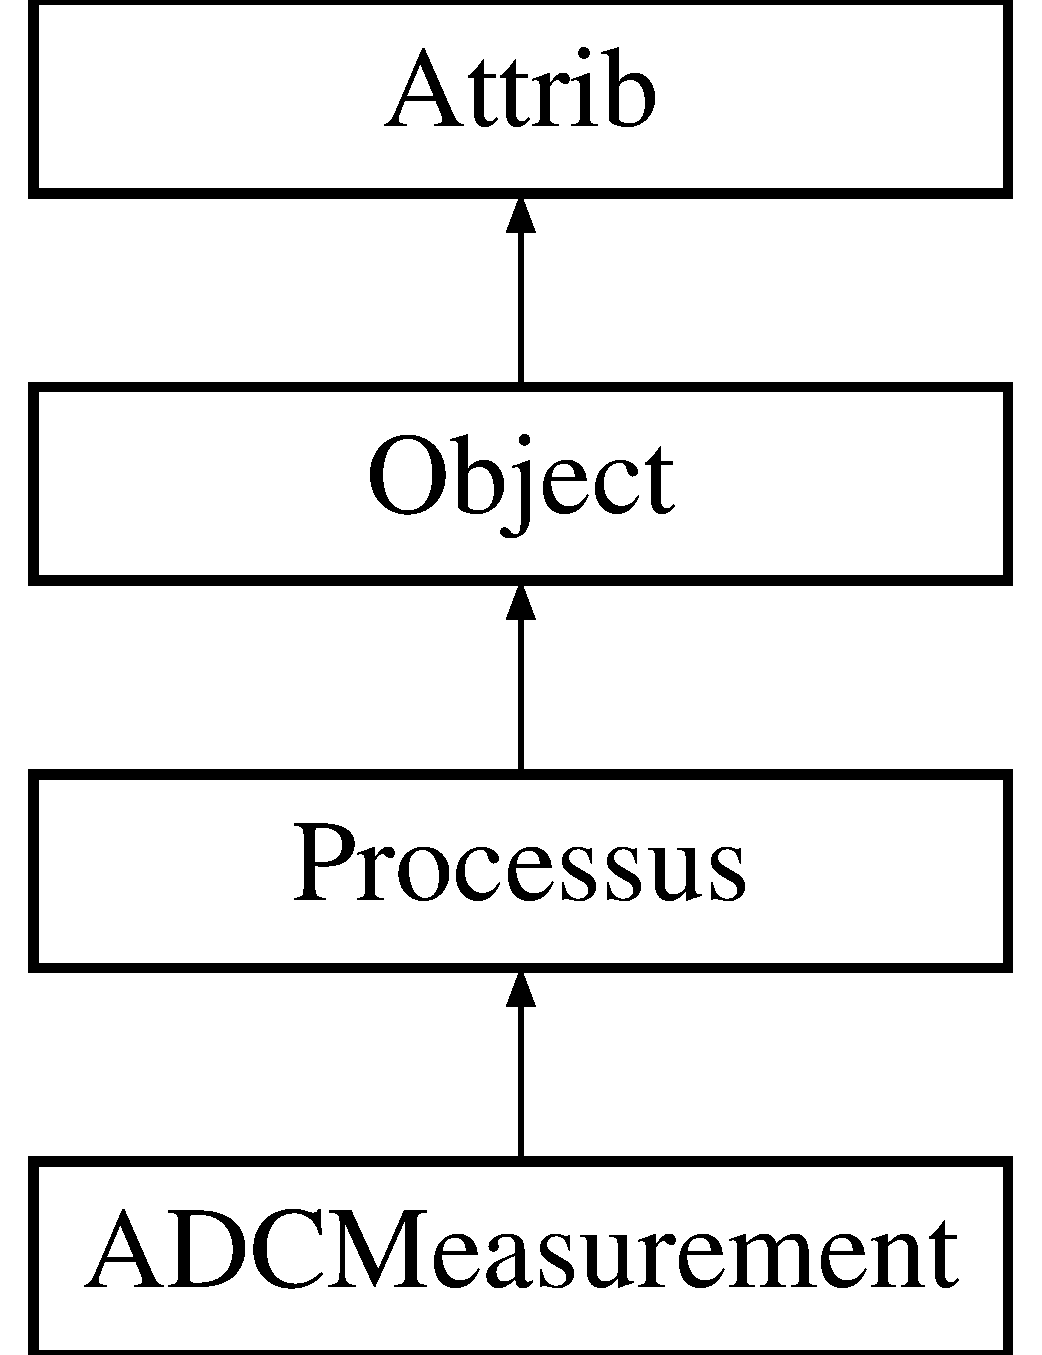
\includegraphics[height=4.000000cm]{classADCMeasurement}
\end{center}
\end{figure}
\subsection*{Classes}
\begin{DoxyCompactItemize}
\item 
class \hyperlink{classADCMeasurement_1_1CurrentMeasurement}{Current\+Measurement}
\end{DoxyCompactItemize}
\subsection*{Public Member Functions}
\begin{DoxyCompactItemize}
\item 
\hyperlink{classADCMeasurement_a93804f658f3aaa78d3ce18199f1bf8e1}{A\+D\+C\+Measurement} ()
\begin{DoxyCompactList}\small\item\em Standard constructor. \end{DoxyCompactList}\item 
virtual \hyperlink{classADCMeasurement_aa89145ed91025783a1bb277cb480ed1c}{$\sim$\+A\+D\+C\+Measurement} ()
\item 
virtual \hyperlink{classStatusCode}{Status\+Code} \hyperlink{classADCMeasurement_a3fc6d3e863fecc7a1caf91f9b0ca5268}{initialize} ()
\begin{DoxyCompactList}\small\item\em Destructor. \end{DoxyCompactList}\item 
virtual \hyperlink{classStatusCode}{Status\+Code} \hyperlink{classADCMeasurement_a82de69f0488646dfc50d28f611e2010d}{execute} ()
\item 
virtual \hyperlink{classStatusCode}{Status\+Code} \hyperlink{classADCMeasurement_a02a5ae7c0f9c90d0dad00c1d40a1c52a}{finalize} ()
\item 
\hyperlink{classStatusCode}{Status\+Code} \hyperlink{classADCMeasurement_a08433e5168f45de1061bf9a17f022f68}{set\+Frequency} (unsigned int \hyperlink{classADCMeasurement_ad3d523331ad64494f2415319a03c638e}{frequency})
\item 
unsigned int \hyperlink{classADCMeasurement_ad3d523331ad64494f2415319a03c638e}{frequency} ()
\item 
unsigned int \hyperlink{classADCMeasurement_a7f91c4feea465de03bd017a005125177}{number\+Of\+Devices} ()
\end{DoxyCompactItemize}
\subsection*{Protected Member Functions}
\begin{DoxyCompactItemize}
\item 
\hyperlink{classADCMeasurement}{A\+D\+C\+Measurement} $\ast$ \hyperlink{classADCMeasurement_a6e34c2b4e3451f1fd128d213723ab1b9}{clone} ()
\end{DoxyCompactItemize}
\subsection*{Private Attributes}
\begin{DoxyCompactItemize}
\item 
T\+Random $\ast$ \hyperlink{classADCMeasurement_acdced9621e4b56d6772b8b34060b0a9d}{m\+\_\+rnd}
\item 
\hyperlink{classNI6008}{N\+I6008} $\ast$ \hyperlink{classADCMeasurement_afc825cc28b05894a0f762452459988e1}{m\+\_\+device}
\item 
unsigned int \hyperlink{classADCMeasurement_ab4a0653cc015ddf9b33b877c1d43b260}{m\+\_\+frequency}
\item 
T\+Tree $\ast$ \hyperlink{classADCMeasurement_ac218556f79d8a0533b292e96347ccd29}{m\+\_\+tree}
\item 
Int\+\_\+t \hyperlink{classADCMeasurement_aba8bc92a86954118babdc49b612a2412}{m\+\_\+run\+Number}
\item 
Int\+\_\+t \hyperlink{classADCMeasurement_ae21dcb1aeff71570c870648839a0c914}{m\+\_\+evt\+Number}
\item 
Int\+\_\+t \hyperlink{classADCMeasurement_a1fa77f5df72a81eab7e55e97d4bea27f}{m\+\_\+timestamp}
\item 
Int\+\_\+t \hyperlink{classADCMeasurement_a92c0ee7d148bb63de876817f624d1527}{m\+\_\+duration}
\item 
time\+\_\+t \hyperlink{classADCMeasurement_a5c2c98ec69e2331906b0eb41a826508e}{m\+\_\+start\+Time}
\item 
Float\+\_\+t \hyperlink{classADCMeasurement_a97ab811c2ef605184b78593cedea275b}{m\+\_\+ai0}
\item 
Float\+\_\+t \hyperlink{classADCMeasurement_ada963374f6f42db11aef7dbc239ce9fb}{m\+\_\+ai1}
\item 
Float\+\_\+t \hyperlink{classADCMeasurement_a45354a95e055970da767ffe534a0d798}{m\+\_\+ao0}
\item 
Float\+\_\+t \hyperlink{classADCMeasurement_a149349cc87061e2604b9e021aa63ee8c}{m\+\_\+ao1}
\item 
Int\+\_\+t \hyperlink{classADCMeasurement_ae024ec8553b7ea765af8668ab5e95699}{m\+\_\+diA}
\item 
Int\+\_\+t \hyperlink{classADCMeasurement_a9d04a602dda58b9fd65acf4a0a7de9a3}{m\+\_\+diB}
\item 
Float\+\_\+t \hyperlink{classADCMeasurement_ab015017d6a05ac4711836ceb1e072a85}{m\+\_\+min\+Ramp}
\item 
Float\+\_\+t \hyperlink{classADCMeasurement_a5e1f799c05f5781004a9081c4064e4a8}{m\+\_\+max\+Ramp}
\item 
Int\+\_\+t \hyperlink{classADCMeasurement_aa73b7cbd45e13df16291ff740f6140fe}{m\+\_\+step\+Ramp}
\item 
Float\+\_\+t \hyperlink{classADCMeasurement_ac84ed2ba70f38e73ec0eec1de65bbdca}{m\+\_\+ramp}
\item 
Int\+\_\+t \hyperlink{classADCMeasurement_aba7433a9e637389cc5425d036867a08f}{m\+\_\+baseline}
\end{DoxyCompactItemize}
\subsection*{Additional Inherited Members}


\subsection{Detailed Description}
\begin{DoxyAuthor}{Author}
Frederic Machefert 
\end{DoxyAuthor}
\begin{DoxyDate}{Date}
2010-\/01-\/07 
\end{DoxyDate}


Definition at line 23 of file A\+D\+C\+Measurement.\+h.



\subsection{Constructor \& Destructor Documentation}
\mbox{\Hypertarget{classADCMeasurement_a93804f658f3aaa78d3ce18199f1bf8e1}\label{classADCMeasurement_a93804f658f3aaa78d3ce18199f1bf8e1}} 
\index{A\+D\+C\+Measurement@{A\+D\+C\+Measurement}!A\+D\+C\+Measurement@{A\+D\+C\+Measurement}}
\index{A\+D\+C\+Measurement@{A\+D\+C\+Measurement}!A\+D\+C\+Measurement@{A\+D\+C\+Measurement}}
\subsubsection{\texorpdfstring{A\+D\+C\+Measurement()}{ADCMeasurement()}}
{\footnotesize\ttfamily A\+D\+C\+Measurement\+::\+A\+D\+C\+Measurement (\begin{DoxyParamCaption}{ }\end{DoxyParamCaption})}



Standard constructor. 



Definition at line 26 of file A\+D\+C\+Measurement.\+cpp.



References Object\+::set\+Name(), Object\+::set\+Title(), and Object\+::set\+Type().



Referenced by clone().


\begin{DoxyCode}
26                                 \{
27   \hyperlink{classObject_ae30fea75683c2d149b6b6d17c09ecd0c}{setName} ( \textcolor{stringliteral}{"ADCMeasurement"} );
28   \hyperlink{classObject_aae534cc9d982bcb9b99fd505f2e103a5}{setType} ( \textcolor{stringliteral}{"NI6008"} );
29   \hyperlink{classObject_a89557dbbad5bcaa02652f5d7fa35d20f}{setTitle}( \textcolor{stringliteral}{"NI6008 ADC measurement"} );  
30 \}
\end{DoxyCode}
\mbox{\Hypertarget{classADCMeasurement_aa89145ed91025783a1bb277cb480ed1c}\label{classADCMeasurement_aa89145ed91025783a1bb277cb480ed1c}} 
\index{A\+D\+C\+Measurement@{A\+D\+C\+Measurement}!````~A\+D\+C\+Measurement@{$\sim$\+A\+D\+C\+Measurement}}
\index{````~A\+D\+C\+Measurement@{$\sim$\+A\+D\+C\+Measurement}!A\+D\+C\+Measurement@{A\+D\+C\+Measurement}}
\subsubsection{\texorpdfstring{$\sim$\+A\+D\+C\+Measurement()}{~ADCMeasurement()}}
{\footnotesize\ttfamily virtual A\+D\+C\+Measurement\+::$\sim$\+A\+D\+C\+Measurement (\begin{DoxyParamCaption}{ }\end{DoxyParamCaption})\hspace{0.3cm}{\ttfamily [inline]}, {\ttfamily [virtual]}}



Definition at line 28 of file A\+D\+C\+Measurement.\+h.



References execute(), finalize(), and initialize().


\begin{DoxyCode}
28 \{\}; 
\end{DoxyCode}


\subsection{Member Function Documentation}
\mbox{\Hypertarget{classADCMeasurement_a6e34c2b4e3451f1fd128d213723ab1b9}\label{classADCMeasurement_a6e34c2b4e3451f1fd128d213723ab1b9}} 
\index{A\+D\+C\+Measurement@{A\+D\+C\+Measurement}!clone@{clone}}
\index{clone@{clone}!A\+D\+C\+Measurement@{A\+D\+C\+Measurement}}
\subsubsection{\texorpdfstring{clone()}{clone()}}
{\footnotesize\ttfamily \hyperlink{classADCMeasurement}{A\+D\+C\+Measurement}$\ast$ A\+D\+C\+Measurement\+::clone (\begin{DoxyParamCaption}{ }\end{DoxyParamCaption})\hspace{0.3cm}{\ttfamily [inline]}, {\ttfamily [protected]}, {\ttfamily [virtual]}}

processus termination virtual function 

Implements \hyperlink{classProcessus_aca8856f6d6d7b7e1fe941f298dcbb502}{Processus}.



Definition at line 48 of file A\+D\+C\+Measurement.\+h.



References A\+D\+C\+Measurement().


\begin{DoxyCode}
48                          \{
49     \textcolor{keywordflow}{return} \textcolor{keyword}{new} \hyperlink{classADCMeasurement_a93804f658f3aaa78d3ce18199f1bf8e1}{ADCMeasurement} (*\textcolor{keyword}{this});
50   \};
\end{DoxyCode}
\mbox{\Hypertarget{classADCMeasurement_a82de69f0488646dfc50d28f611e2010d}\label{classADCMeasurement_a82de69f0488646dfc50d28f611e2010d}} 
\index{A\+D\+C\+Measurement@{A\+D\+C\+Measurement}!execute@{execute}}
\index{execute@{execute}!A\+D\+C\+Measurement@{A\+D\+C\+Measurement}}
\subsubsection{\texorpdfstring{execute()}{execute()}}
{\footnotesize\ttfamily \hyperlink{classStatusCode}{Status\+Code} A\+D\+C\+Measurement\+::execute (\begin{DoxyParamCaption}{ }\end{DoxyParamCaption})\hspace{0.3cm}{\ttfamily [virtual]}}

processus execution virtual function 

Implements \hyperlink{classProcessus_a63767a63a1fb0055c5aa45b21a4a5d58}{Processus}.



Definition at line 73 of file A\+D\+C\+Measurement.\+cpp.



References application(), N\+I6008\+::cmd(), Processus\+::data\+Fill(), m\+\_\+ai0, m\+\_\+ai1, m\+\_\+ao0, m\+\_\+baseline, m\+\_\+device, m\+\_\+diA, m\+\_\+diB, m\+\_\+duration, m\+\_\+evt\+Number, m\+\_\+frequency, m\+\_\+max\+Ramp, m\+\_\+min\+Ramp, m\+\_\+ramp, m\+\_\+start\+Time, m\+\_\+step\+Ramp, m\+\_\+timestamp, m\+\_\+tree, Options\+::n\+Evt(), Application\+::options(), Status\+Code\+::\+S\+U\+C\+C\+E\+SS, and wait().



Referenced by $\sim$\+A\+D\+C\+Measurement().


\begin{DoxyCode}
73                                      \{
74   \textcolor{comment}{// get current}
75   std::string val = \hyperlink{classADCMeasurement_afc825cc28b05894a0f762452459988e1}{m\_device}->\hyperlink{classNI6008_a0d7584a656abca03fd59c555cb66822c}{cmd}(\textcolor{stringliteral}{"Dev1"}, \textcolor{stringliteral}{"ai"});
76   std::istringstream sv1(val);
77   std::string v0, v1, tmp;
78   sv1 >> v0;
79   sv1 >> v1;
80   \textcolor{comment}{//  m\_ai0=toDouble(v0);}
81   \textcolor{comment}{//  m\_ai1=toDouble(v1);}
82   \hyperlink{classADCMeasurement_a97ab811c2ef605184b78593cedea275b}{m\_ai0} = atof(v0.c\_str());
83   \hyperlink{classADCMeasurement_ada963374f6f42db11aef7dbc239ce9fb}{m\_ai1} = atof(v1.c\_str());
84   std::cout << v0 << \textcolor{stringliteral}{" "} << v1 << \textcolor{stringliteral}{" "} << \hyperlink{classADCMeasurement_a97ab811c2ef605184b78593cedea275b}{m\_ai0} << \textcolor{stringliteral}{" "} << m\_ai1 << std::endl;
85   \hyperlink{classProcessus_a0d093b48f3218a088ba030e24372f18c}{dataFill}(1, \hyperlink{classADCMeasurement_a97ab811c2ef605184b78593cedea275b}{m\_ai0});
86   \hyperlink{classProcessus_a0d093b48f3218a088ba030e24372f18c}{dataFill}(2, m\_ai1);
87   \textcolor{comment}{// set ramp value and channel A}
88   \hyperlink{classProcessus_a0d093b48f3218a088ba030e24372f18c}{dataFill}(3, \hyperlink{classADCMeasurement_ac84ed2ba70f38e73ec0eec1de65bbdca}{m\_ramp});
89   \hyperlink{classADCMeasurement_a45354a95e055970da767ffe534a0d798}{m\_ao0} = \hyperlink{classADCMeasurement_ac84ed2ba70f38e73ec0eec1de65bbdca}{m\_ramp};
90   \textcolor{keywordtype}{char} cmd[80];
91   sprintf(cmd,\textcolor{stringliteral}{"ao %f %f"}, \hyperlink{classADCMeasurement_ac84ed2ba70f38e73ec0eec1de65bbdca}{m\_ramp}, 0.);
92   \hyperlink{classADCMeasurement_afc825cc28b05894a0f762452459988e1}{m\_device}->\hyperlink{classNI6008_a0d7584a656abca03fd59c555cb66822c}{cmd}(\textcolor{stringliteral}{"Dev1"}, cmd );
93   val = \hyperlink{classADCMeasurement_afc825cc28b05894a0f762452459988e1}{m\_device}->\hyperlink{classNI6008_a0d7584a656abca03fd59c555cb66822c}{cmd}(\textcolor{stringliteral}{"Dev1"}, \textcolor{stringliteral}{"di"});
94   std::istringstream sv2(val);
95   sv2 >> tmp;
96   sv2 >> tmp;
97   sv2 >> tmp;
98   sv2 >> v0 >> tmp >> v1 ;
99   \hyperlink{classADCMeasurement_ae024ec8553b7ea765af8668ab5e95699}{m\_diA} = atoi(v0.c\_str());
100   \hyperlink{classProcessus_a0d093b48f3218a088ba030e24372f18c}{dataFill}(4, \hyperlink{classADCMeasurement_ae024ec8553b7ea765af8668ab5e95699}{m\_diA});
101 
102   sprintf(cmd,\textcolor{stringliteral}{"ao %f %f"}, \hyperlink{classADCMeasurement_ac84ed2ba70f38e73ec0eec1de65bbdca}{m\_ramp}, 3.3);
103   \hyperlink{classADCMeasurement_afc825cc28b05894a0f762452459988e1}{m\_device}->\hyperlink{classNI6008_a0d7584a656abca03fd59c555cb66822c}{cmd}(\textcolor{stringliteral}{"Dev1"}, cmd );
104   val = \hyperlink{classADCMeasurement_afc825cc28b05894a0f762452459988e1}{m\_device}->\hyperlink{classNI6008_a0d7584a656abca03fd59c555cb66822c}{cmd}(\textcolor{stringliteral}{"Dev1"}, \textcolor{stringliteral}{"di"});
105   std::istringstream sv3(val);
106   sv3 >> tmp;
107   sv3 >> tmp;
108   sv3 >> tmp;
109   sv3 >> v0 >> tmp >> v1 ;
110   \hyperlink{classADCMeasurement_a9d04a602dda58b9fd65acf4a0a7de9a3}{m\_diB} = atoi(v1.c\_str());
111   \hyperlink{classProcessus_a0d093b48f3218a088ba030e24372f18c}{dataFill}(5, \hyperlink{classADCMeasurement_a9d04a602dda58b9fd65acf4a0a7de9a3}{m\_diB});
112   
113   \textcolor{keywordflow}{if} (\hyperlink{classADCMeasurement_ae024ec8553b7ea765af8668ab5e95699}{m\_diA}>\hyperlink{classADCMeasurement_aba7433a9e637389cc5425d036867a08f}{m\_baseline})\{ 
114     \hyperlink{classProcessus_a0d093b48f3218a088ba030e24372f18c}{dataFill}(6, \hyperlink{classADCMeasurement_ac84ed2ba70f38e73ec0eec1de65bbdca}{m\_ramp}/\textcolor{keywordtype}{float}(\hyperlink{classADCMeasurement_ae024ec8553b7ea765af8668ab5e95699}{m\_diA}-\hyperlink{classADCMeasurement_aba7433a9e637389cc5425d036867a08f}{m\_baseline}));
115   \}
116   \textcolor{keywordflow}{else} \{
117     \hyperlink{classProcessus_a0d093b48f3218a088ba030e24372f18c}{dataFill}(6, 0.);
118   \}
119   \textcolor{keywordflow}{if} (\hyperlink{classADCMeasurement_a9d04a602dda58b9fd65acf4a0a7de9a3}{m\_diB}>\hyperlink{classADCMeasurement_aba7433a9e637389cc5425d036867a08f}{m\_baseline})\{ 
120     \hyperlink{classProcessus_a0d093b48f3218a088ba030e24372f18c}{dataFill}(7, \hyperlink{classADCMeasurement_ac84ed2ba70f38e73ec0eec1de65bbdca}{m\_ramp}/\textcolor{keywordtype}{float}(\hyperlink{classADCMeasurement_a9d04a602dda58b9fd65acf4a0a7de9a3}{m\_diB}-\hyperlink{classADCMeasurement_aba7433a9e637389cc5425d036867a08f}{m\_baseline}));
121   \}
122   \textcolor{keywordflow}{else} \{
123     \hyperlink{classProcessus_a0d093b48f3218a088ba030e24372f18c}{dataFill}(7, 0.);
124   \}
125 
126   \textcolor{comment}{//  std::cout << "digit: " << m\_ramp << " " << m\_diA << " " << m\_diB << std::endl;}
127 
128   time\_t t =time(0);
129   \hyperlink{classADCMeasurement_a92c0ee7d148bb63de876817f624d1527}{m\_duration}=difftime(t, \hyperlink{classADCMeasurement_a5c2c98ec69e2331906b0eb41a826508e}{m\_startTime});
130   \hyperlink{classADCMeasurement_a1fa77f5df72a81eab7e55e97d4bea27f}{m\_timestamp} = t; 
131   \hyperlink{classProcessus_a0d093b48f3218a088ba030e24372f18c}{dataFill}(0, \hyperlink{classADCMeasurement_a92c0ee7d148bb63de876817f624d1527}{m\_duration});
132 
133   \textcolor{keywordflow}{if} (\hyperlink{Tools_8h_a27885a3c35afe79029fb830f32f66458}{application}()->options()->dataStorage())\{
134     \hyperlink{classADCMeasurement_ae21dcb1aeff71570c870648839a0c914}{m\_evtNumber}=\hyperlink{Tools_8h_a27885a3c35afe79029fb830f32f66458}{application}()->\hyperlink{classApplication_ada7cc0e8db586985f1435aee0c79f47d}{options}()->\hyperlink{classOptions_ad769b256263a4ac24dd6f989ae724ab7}{nEvt}()-1;
135     \hyperlink{classADCMeasurement_ac218556f79d8a0533b292e96347ccd29}{m\_tree}->Fill();
136   \}
137   \hyperlink{Tools_8h_a74d6a3fc8194eaac3e1f888db0542be9}{wait}(\hyperlink{classADCMeasurement_ab4a0653cc015ddf9b33b877c1d43b260}{m\_frequency});
138   \hyperlink{classADCMeasurement_ac84ed2ba70f38e73ec0eec1de65bbdca}{m\_ramp} += (\hyperlink{classADCMeasurement_a5e1f799c05f5781004a9081c4064e4a8}{m\_maxRamp}-\hyperlink{classADCMeasurement_ab015017d6a05ac4711836ceb1e072a85}{m\_minRamp})/\textcolor{keywordtype}{float}(\hyperlink{classADCMeasurement_aa73b7cbd45e13df16291ff740f6140fe}{m\_stepRamp});
139   \textcolor{keywordflow}{if} ( \hyperlink{classADCMeasurement_ac84ed2ba70f38e73ec0eec1de65bbdca}{m\_ramp} > \hyperlink{classADCMeasurement_a5e1f799c05f5781004a9081c4064e4a8}{m\_maxRamp} ) \{ \hyperlink{classADCMeasurement_ac84ed2ba70f38e73ec0eec1de65bbdca}{m\_ramp} = \hyperlink{classADCMeasurement_ab015017d6a05ac4711836ceb1e072a85}{m\_minRamp}; \}
140   \textcolor{keywordflow}{return} \hyperlink{classStatusCode_a6f565cbeadc76d14c72f047e5e85eb4badd0da38d3ba0d922efd1f4619bc37ad8}{StatusCode::SUCCESS};
141 \}
\end{DoxyCode}
\mbox{\Hypertarget{classADCMeasurement_a02a5ae7c0f9c90d0dad00c1d40a1c52a}\label{classADCMeasurement_a02a5ae7c0f9c90d0dad00c1d40a1c52a}} 
\index{A\+D\+C\+Measurement@{A\+D\+C\+Measurement}!finalize@{finalize}}
\index{finalize@{finalize}!A\+D\+C\+Measurement@{A\+D\+C\+Measurement}}
\subsubsection{\texorpdfstring{finalize()}{finalize()}}
{\footnotesize\ttfamily \hyperlink{classStatusCode}{Status\+Code} A\+D\+C\+Measurement\+::finalize (\begin{DoxyParamCaption}{ }\end{DoxyParamCaption})\hspace{0.3cm}{\ttfamily [virtual]}}

processus termination virtual function 

Implements \hyperlink{classProcessus_aba93d691f031bdb18ae4b8afb1b2e856}{Processus}.



Definition at line 146 of file A\+D\+C\+Measurement.\+cpp.



References Status\+Code\+::\+S\+U\+C\+C\+E\+SS.



Referenced by $\sim$\+A\+D\+C\+Measurement().


\begin{DoxyCode}
146                                       \{
147   \textcolor{keywordflow}{return} \hyperlink{classStatusCode_a6f565cbeadc76d14c72f047e5e85eb4badd0da38d3ba0d922efd1f4619bc37ad8}{StatusCode::SUCCESS};
148 \}
\end{DoxyCode}
\mbox{\Hypertarget{classADCMeasurement_ad3d523331ad64494f2415319a03c638e}\label{classADCMeasurement_ad3d523331ad64494f2415319a03c638e}} 
\index{A\+D\+C\+Measurement@{A\+D\+C\+Measurement}!frequency@{frequency}}
\index{frequency@{frequency}!A\+D\+C\+Measurement@{A\+D\+C\+Measurement}}
\subsubsection{\texorpdfstring{frequency()}{frequency()}}
{\footnotesize\ttfamily unsigned int A\+D\+C\+Measurement\+::frequency (\begin{DoxyParamCaption}{ }\end{DoxyParamCaption})\hspace{0.3cm}{\ttfamily [inline]}}



Definition at line 39 of file A\+D\+C\+Measurement.\+h.



References m\+\_\+frequency.



Referenced by B\+O\+O\+S\+T\+\_\+\+P\+Y\+T\+H\+O\+N\+\_\+\+M\+O\+D\+U\+L\+E(), and set\+Frequency().


\begin{DoxyCode}
39                           \{
40     \textcolor{keywordflow}{return} \hyperlink{classADCMeasurement_ab4a0653cc015ddf9b33b877c1d43b260}{m\_frequency};
41   \}
\end{DoxyCode}
\mbox{\Hypertarget{classADCMeasurement_a3fc6d3e863fecc7a1caf91f9b0ca5268}\label{classADCMeasurement_a3fc6d3e863fecc7a1caf91f9b0ca5268}} 
\index{A\+D\+C\+Measurement@{A\+D\+C\+Measurement}!initialize@{initialize}}
\index{initialize@{initialize}!A\+D\+C\+Measurement@{A\+D\+C\+Measurement}}
\subsubsection{\texorpdfstring{initialize()}{initialize()}}
{\footnotesize\ttfamily \hyperlink{classStatusCode}{Status\+Code} A\+D\+C\+Measurement\+::initialize (\begin{DoxyParamCaption}{ }\end{DoxyParamCaption})\hspace{0.3cm}{\ttfamily [virtual]}}



Destructor. 



Implements \hyperlink{classProcessus_aee88ad7b77ae7319cf8b128e9dd2ea11}{Processus}.



Definition at line 35 of file A\+D\+C\+Measurement.\+cpp.



References Processus\+::add\+Data\+Stream(), application(), Options\+::data\+Storage(), Processus\+::element(), Object\+::info(), m\+\_\+ai0, m\+\_\+ai1, m\+\_\+ao0, m\+\_\+baseline, m\+\_\+device, m\+\_\+diA, m\+\_\+diB, m\+\_\+duration, m\+\_\+evt\+Number, m\+\_\+max\+Ramp, m\+\_\+min\+Ramp, m\+\_\+ramp, m\+\_\+run\+Number, m\+\_\+start\+Time, m\+\_\+step\+Ramp, m\+\_\+timestamp, m\+\_\+tree, Object\+::name(), Application\+::options(), Options\+::run\+Number(), Status\+Code\+::\+S\+U\+C\+C\+E\+SS, and Object\+::title().



Referenced by $\sim$\+A\+D\+C\+Measurement().


\begin{DoxyCode}
35                                         \{
36   \hyperlink{classADCMeasurement_ab015017d6a05ac4711836ceb1e072a85}{m\_minRamp}  = 0.; 
37   \hyperlink{classADCMeasurement_a5e1f799c05f5781004a9081c4064e4a8}{m\_maxRamp}  = 1.2;
38   \hyperlink{classADCMeasurement_aa73b7cbd45e13df16291ff740f6140fe}{m\_stepRamp} = 20;
39   \hyperlink{classADCMeasurement_aba7433a9e637389cc5425d036867a08f}{m\_baseline} = 1400;
40   \hyperlink{classADCMeasurement_ac84ed2ba70f38e73ec0eec1de65bbdca}{m\_ramp} = \hyperlink{classADCMeasurement_ab015017d6a05ac4711836ceb1e072a85}{m\_minRamp};
41   time(&\hyperlink{classADCMeasurement_a5c2c98ec69e2331906b0eb41a826508e}{m\_startTime}); 
42   \hyperlink{classADCMeasurement_afc825cc28b05894a0f762452459988e1}{m\_device} = dynamic\_cast <\hyperlink{classNI6008}{NI6008}*> (\hyperlink{classProcessus_a6fe155527431a7190b7d44d600b9608d}{element}());
43   \textcolor{keywordflow}{if} (\hyperlink{Tools_8h_a27885a3c35afe79029fb830f32f66458}{application}()->\hyperlink{classApplication_ada7cc0e8db586985f1435aee0c79f47d}{options}()->\hyperlink{classOptions_aed7799d10139fa542055b982cb820192}{dataStorage}())\{
44     \hyperlink{classADCMeasurement_ac218556f79d8a0533b292e96347ccd29}{m\_tree} = \textcolor{keyword}{new} TTree(\hyperlink{classObject_a300f4c05dd468c7bb8b3c968868443c1}{name}().c\_str(), \hyperlink{classObject_a73a0f1a41828fdd8303dd662446fb6c3}{title}().c\_str());
45     \hyperlink{classADCMeasurement_ac218556f79d8a0533b292e96347ccd29}{m\_tree}->Branch(\textcolor{stringliteral}{"Run"},&\hyperlink{classADCMeasurement_aba8bc92a86954118babdc49b612a2412}{m\_runNumber},\textcolor{stringliteral}{"Run/I"});
46     \hyperlink{classADCMeasurement_ac218556f79d8a0533b292e96347ccd29}{m\_tree}->Branch(\textcolor{stringliteral}{"Event"},&\hyperlink{classADCMeasurement_ae21dcb1aeff71570c870648839a0c914}{m\_evtNumber},\textcolor{stringliteral}{"Event/I"});
47     \hyperlink{classADCMeasurement_ac218556f79d8a0533b292e96347ccd29}{m\_tree}->Branch(\textcolor{stringliteral}{"Time"},&\hyperlink{classADCMeasurement_a1fa77f5df72a81eab7e55e97d4bea27f}{m\_timestamp},\textcolor{stringliteral}{"Time/I"});
48     \hyperlink{classADCMeasurement_ac218556f79d8a0533b292e96347ccd29}{m\_tree}->Branch(\textcolor{stringliteral}{"Duration"},&\hyperlink{classADCMeasurement_a92c0ee7d148bb63de876817f624d1527}{m\_duration},\textcolor{stringliteral}{"Duration/I"});
49     \hyperlink{classADCMeasurement_ac218556f79d8a0533b292e96347ccd29}{m\_tree}->Branch(\textcolor{stringliteral}{"ai0"},&\hyperlink{classADCMeasurement_a97ab811c2ef605184b78593cedea275b}{m\_ai0},\textcolor{stringliteral}{"ai0/F"});
50     \hyperlink{classADCMeasurement_ac218556f79d8a0533b292e96347ccd29}{m\_tree}->Branch(\textcolor{stringliteral}{"ai1"},&\hyperlink{classADCMeasurement_ada963374f6f42db11aef7dbc239ce9fb}{m\_ai1},\textcolor{stringliteral}{"ai1/F"});
51     \hyperlink{classADCMeasurement_ac218556f79d8a0533b292e96347ccd29}{m\_tree}->Branch(\textcolor{stringliteral}{"ao0"},&\hyperlink{classADCMeasurement_a45354a95e055970da767ffe534a0d798}{m\_ao0},\textcolor{stringliteral}{"ao0/F"});
52     \textcolor{comment}{//    m\_tree->Branch("ao1",&m\_ao1,"ao1/F");}
53     \hyperlink{classADCMeasurement_ac218556f79d8a0533b292e96347ccd29}{m\_tree}->Branch(\textcolor{stringliteral}{"di\_0"},&\hyperlink{classADCMeasurement_ae024ec8553b7ea765af8668ab5e95699}{m\_diA},\textcolor{stringliteral}{"diA/I"});
54     \hyperlink{classADCMeasurement_ac218556f79d8a0533b292e96347ccd29}{m\_tree}->Branch(\textcolor{stringliteral}{"di\_1"},&\hyperlink{classADCMeasurement_a9d04a602dda58b9fd65acf4a0a7de9a3}{m\_diB},\textcolor{stringliteral}{"diB/I"});
55   \}
56   \hyperlink{classObject_a644fd329ea4cb85f54fa6846484b84a8}{info}(\textcolor{stringliteral}{"Preparing dataStreams."});
57   \hyperlink{classProcessus_a308c8f193802f1d1ab49d4447d0cb281}{addDataStream}(\textcolor{stringliteral}{"Duration"},\textcolor{stringliteral}{"Duration"});
58   \hyperlink{classProcessus_a308c8f193802f1d1ab49d4447d0cb281}{addDataStream}(\textcolor{stringliteral}{"ai0"}, \textcolor{stringliteral}{"Channel 0"});
59   \hyperlink{classProcessus_a308c8f193802f1d1ab49d4447d0cb281}{addDataStream}(\textcolor{stringliteral}{"ai1"}, \textcolor{stringliteral}{"Channel 1"});
60   \hyperlink{classProcessus_a308c8f193802f1d1ab49d4447d0cb281}{addDataStream}(\textcolor{stringliteral}{"ao0"}, \textcolor{stringliteral}{"Ramp Ampl"});
61   \textcolor{comment}{//  addDataStream("ao1", "ADC Chan Ctrl");}
62   \hyperlink{classProcessus_a308c8f193802f1d1ab49d4447d0cb281}{addDataStream}(\textcolor{stringliteral}{"diA"},\textcolor{stringliteral}{"ADC A"});
63   \hyperlink{classProcessus_a308c8f193802f1d1ab49d4447d0cb281}{addDataStream}(\textcolor{stringliteral}{"diB"},\textcolor{stringliteral}{"ADC B"});
64   \hyperlink{classProcessus_a308c8f193802f1d1ab49d4447d0cb281}{addDataStream}(\textcolor{stringliteral}{"ratioA"},\textcolor{stringliteral}{"ratio amplitude A"});
65   \hyperlink{classProcessus_a308c8f193802f1d1ab49d4447d0cb281}{addDataStream}(\textcolor{stringliteral}{"ratioB"},\textcolor{stringliteral}{"ratio amplitude B"});
66   \hyperlink{classADCMeasurement_aba8bc92a86954118babdc49b612a2412}{m\_runNumber}=\hyperlink{Tools_8h_a27885a3c35afe79029fb830f32f66458}{application}()->\hyperlink{classApplication_ada7cc0e8db586985f1435aee0c79f47d}{options}()->\hyperlink{classOptions_a2d9447919fe90f9ce8df5530526cbb27}{runNumber}();
67   \textcolor{keywordflow}{return} \hyperlink{classStatusCode_a6f565cbeadc76d14c72f047e5e85eb4badd0da38d3ba0d922efd1f4619bc37ad8}{StatusCode::SUCCESS};
68 \}
\end{DoxyCode}
\mbox{\Hypertarget{classADCMeasurement_a7f91c4feea465de03bd017a005125177}\label{classADCMeasurement_a7f91c4feea465de03bd017a005125177}} 
\index{A\+D\+C\+Measurement@{A\+D\+C\+Measurement}!number\+Of\+Devices@{number\+Of\+Devices}}
\index{number\+Of\+Devices@{number\+Of\+Devices}!A\+D\+C\+Measurement@{A\+D\+C\+Measurement}}
\subsubsection{\texorpdfstring{number\+Of\+Devices()}{numberOfDevices()}}
{\footnotesize\ttfamily unsigned int A\+D\+C\+Measurement\+::number\+Of\+Devices (\begin{DoxyParamCaption}{ }\end{DoxyParamCaption})\hspace{0.3cm}{\ttfamily [inline]}}



Definition at line 43 of file A\+D\+C\+Measurement.\+h.



References m\+\_\+device, and N\+I6008\+::number\+Of\+Devices().


\begin{DoxyCode}
43                                 \{
44     \textcolor{keywordflow}{return} \hyperlink{classADCMeasurement_afc825cc28b05894a0f762452459988e1}{m\_device}->\hyperlink{classNI6008_a293fbf44b101e82a57404d1c76f07a87}{numberOfDevices}();
45   \}
\end{DoxyCode}
\mbox{\Hypertarget{classADCMeasurement_a08433e5168f45de1061bf9a17f022f68}\label{classADCMeasurement_a08433e5168f45de1061bf9a17f022f68}} 
\index{A\+D\+C\+Measurement@{A\+D\+C\+Measurement}!set\+Frequency@{set\+Frequency}}
\index{set\+Frequency@{set\+Frequency}!A\+D\+C\+Measurement@{A\+D\+C\+Measurement}}
\subsubsection{\texorpdfstring{set\+Frequency()}{setFrequency()}}
{\footnotesize\ttfamily \hyperlink{classStatusCode}{Status\+Code} A\+D\+C\+Measurement\+::set\+Frequency (\begin{DoxyParamCaption}\item[{unsigned int}]{frequency }\end{DoxyParamCaption})\hspace{0.3cm}{\ttfamily [inline]}}



Definition at line 34 of file A\+D\+C\+Measurement.\+h.



References frequency(), m\+\_\+frequency, and Status\+Code\+::\+S\+U\+C\+C\+E\+SS.



Referenced by B\+O\+O\+S\+T\+\_\+\+P\+Y\+T\+H\+O\+N\+\_\+\+M\+O\+D\+U\+L\+E().


\begin{DoxyCode}
34                                                  \{
35     \hyperlink{classADCMeasurement_ab4a0653cc015ddf9b33b877c1d43b260}{m\_frequency} = \hyperlink{classADCMeasurement_ad3d523331ad64494f2415319a03c638e}{frequency};
36     \textcolor{keywordflow}{return} \hyperlink{classStatusCode_a6f565cbeadc76d14c72f047e5e85eb4badd0da38d3ba0d922efd1f4619bc37ad8}{StatusCode::SUCCESS};
37   \}
\end{DoxyCode}


\subsection{Member Data Documentation}
\mbox{\Hypertarget{classADCMeasurement_a97ab811c2ef605184b78593cedea275b}\label{classADCMeasurement_a97ab811c2ef605184b78593cedea275b}} 
\index{A\+D\+C\+Measurement@{A\+D\+C\+Measurement}!m\+\_\+ai0@{m\+\_\+ai0}}
\index{m\+\_\+ai0@{m\+\_\+ai0}!A\+D\+C\+Measurement@{A\+D\+C\+Measurement}}
\subsubsection{\texorpdfstring{m\+\_\+ai0}{m\_ai0}}
{\footnotesize\ttfamily Float\+\_\+t A\+D\+C\+Measurement\+::m\+\_\+ai0\hspace{0.3cm}{\ttfamily [private]}}



Definition at line 62 of file A\+D\+C\+Measurement.\+h.



Referenced by execute(), and initialize().

\mbox{\Hypertarget{classADCMeasurement_ada963374f6f42db11aef7dbc239ce9fb}\label{classADCMeasurement_ada963374f6f42db11aef7dbc239ce9fb}} 
\index{A\+D\+C\+Measurement@{A\+D\+C\+Measurement}!m\+\_\+ai1@{m\+\_\+ai1}}
\index{m\+\_\+ai1@{m\+\_\+ai1}!A\+D\+C\+Measurement@{A\+D\+C\+Measurement}}
\subsubsection{\texorpdfstring{m\+\_\+ai1}{m\_ai1}}
{\footnotesize\ttfamily Float\+\_\+t A\+D\+C\+Measurement\+::m\+\_\+ai1\hspace{0.3cm}{\ttfamily [private]}}



Definition at line 63 of file A\+D\+C\+Measurement.\+h.



Referenced by execute(), and initialize().

\mbox{\Hypertarget{classADCMeasurement_a45354a95e055970da767ffe534a0d798}\label{classADCMeasurement_a45354a95e055970da767ffe534a0d798}} 
\index{A\+D\+C\+Measurement@{A\+D\+C\+Measurement}!m\+\_\+ao0@{m\+\_\+ao0}}
\index{m\+\_\+ao0@{m\+\_\+ao0}!A\+D\+C\+Measurement@{A\+D\+C\+Measurement}}
\subsubsection{\texorpdfstring{m\+\_\+ao0}{m\_ao0}}
{\footnotesize\ttfamily Float\+\_\+t A\+D\+C\+Measurement\+::m\+\_\+ao0\hspace{0.3cm}{\ttfamily [private]}}



Definition at line 64 of file A\+D\+C\+Measurement.\+h.



Referenced by execute(), and initialize().

\mbox{\Hypertarget{classADCMeasurement_a149349cc87061e2604b9e021aa63ee8c}\label{classADCMeasurement_a149349cc87061e2604b9e021aa63ee8c}} 
\index{A\+D\+C\+Measurement@{A\+D\+C\+Measurement}!m\+\_\+ao1@{m\+\_\+ao1}}
\index{m\+\_\+ao1@{m\+\_\+ao1}!A\+D\+C\+Measurement@{A\+D\+C\+Measurement}}
\subsubsection{\texorpdfstring{m\+\_\+ao1}{m\_ao1}}
{\footnotesize\ttfamily Float\+\_\+t A\+D\+C\+Measurement\+::m\+\_\+ao1\hspace{0.3cm}{\ttfamily [private]}}



Definition at line 65 of file A\+D\+C\+Measurement.\+h.

\mbox{\Hypertarget{classADCMeasurement_aba7433a9e637389cc5425d036867a08f}\label{classADCMeasurement_aba7433a9e637389cc5425d036867a08f}} 
\index{A\+D\+C\+Measurement@{A\+D\+C\+Measurement}!m\+\_\+baseline@{m\+\_\+baseline}}
\index{m\+\_\+baseline@{m\+\_\+baseline}!A\+D\+C\+Measurement@{A\+D\+C\+Measurement}}
\subsubsection{\texorpdfstring{m\+\_\+baseline}{m\_baseline}}
{\footnotesize\ttfamily Int\+\_\+t A\+D\+C\+Measurement\+::m\+\_\+baseline\hspace{0.3cm}{\ttfamily [private]}}



Definition at line 72 of file A\+D\+C\+Measurement.\+h.



Referenced by execute(), and initialize().

\mbox{\Hypertarget{classADCMeasurement_afc825cc28b05894a0f762452459988e1}\label{classADCMeasurement_afc825cc28b05894a0f762452459988e1}} 
\index{A\+D\+C\+Measurement@{A\+D\+C\+Measurement}!m\+\_\+device@{m\+\_\+device}}
\index{m\+\_\+device@{m\+\_\+device}!A\+D\+C\+Measurement@{A\+D\+C\+Measurement}}
\subsubsection{\texorpdfstring{m\+\_\+device}{m\_device}}
{\footnotesize\ttfamily \hyperlink{classNI6008}{N\+I6008}$\ast$ A\+D\+C\+Measurement\+::m\+\_\+device\hspace{0.3cm}{\ttfamily [private]}}



Definition at line 54 of file A\+D\+C\+Measurement.\+h.



Referenced by execute(), initialize(), and number\+Of\+Devices().

\mbox{\Hypertarget{classADCMeasurement_ae024ec8553b7ea765af8668ab5e95699}\label{classADCMeasurement_ae024ec8553b7ea765af8668ab5e95699}} 
\index{A\+D\+C\+Measurement@{A\+D\+C\+Measurement}!m\+\_\+diA@{m\+\_\+diA}}
\index{m\+\_\+diA@{m\+\_\+diA}!A\+D\+C\+Measurement@{A\+D\+C\+Measurement}}
\subsubsection{\texorpdfstring{m\+\_\+diA}{m\_diA}}
{\footnotesize\ttfamily Int\+\_\+t A\+D\+C\+Measurement\+::m\+\_\+diA\hspace{0.3cm}{\ttfamily [private]}}



Definition at line 66 of file A\+D\+C\+Measurement.\+h.



Referenced by execute(), and initialize().

\mbox{\Hypertarget{classADCMeasurement_a9d04a602dda58b9fd65acf4a0a7de9a3}\label{classADCMeasurement_a9d04a602dda58b9fd65acf4a0a7de9a3}} 
\index{A\+D\+C\+Measurement@{A\+D\+C\+Measurement}!m\+\_\+diB@{m\+\_\+diB}}
\index{m\+\_\+diB@{m\+\_\+diB}!A\+D\+C\+Measurement@{A\+D\+C\+Measurement}}
\subsubsection{\texorpdfstring{m\+\_\+diB}{m\_diB}}
{\footnotesize\ttfamily Int\+\_\+t A\+D\+C\+Measurement\+::m\+\_\+diB\hspace{0.3cm}{\ttfamily [private]}}



Definition at line 67 of file A\+D\+C\+Measurement.\+h.



Referenced by execute(), and initialize().

\mbox{\Hypertarget{classADCMeasurement_a92c0ee7d148bb63de876817f624d1527}\label{classADCMeasurement_a92c0ee7d148bb63de876817f624d1527}} 
\index{A\+D\+C\+Measurement@{A\+D\+C\+Measurement}!m\+\_\+duration@{m\+\_\+duration}}
\index{m\+\_\+duration@{m\+\_\+duration}!A\+D\+C\+Measurement@{A\+D\+C\+Measurement}}
\subsubsection{\texorpdfstring{m\+\_\+duration}{m\_duration}}
{\footnotesize\ttfamily Int\+\_\+t A\+D\+C\+Measurement\+::m\+\_\+duration\hspace{0.3cm}{\ttfamily [private]}}



Definition at line 60 of file A\+D\+C\+Measurement.\+h.



Referenced by execute(), and initialize().

\mbox{\Hypertarget{classADCMeasurement_ae21dcb1aeff71570c870648839a0c914}\label{classADCMeasurement_ae21dcb1aeff71570c870648839a0c914}} 
\index{A\+D\+C\+Measurement@{A\+D\+C\+Measurement}!m\+\_\+evt\+Number@{m\+\_\+evt\+Number}}
\index{m\+\_\+evt\+Number@{m\+\_\+evt\+Number}!A\+D\+C\+Measurement@{A\+D\+C\+Measurement}}
\subsubsection{\texorpdfstring{m\+\_\+evt\+Number}{m\_evtNumber}}
{\footnotesize\ttfamily Int\+\_\+t A\+D\+C\+Measurement\+::m\+\_\+evt\+Number\hspace{0.3cm}{\ttfamily [private]}}



Definition at line 58 of file A\+D\+C\+Measurement.\+h.



Referenced by execute(), and initialize().

\mbox{\Hypertarget{classADCMeasurement_ab4a0653cc015ddf9b33b877c1d43b260}\label{classADCMeasurement_ab4a0653cc015ddf9b33b877c1d43b260}} 
\index{A\+D\+C\+Measurement@{A\+D\+C\+Measurement}!m\+\_\+frequency@{m\+\_\+frequency}}
\index{m\+\_\+frequency@{m\+\_\+frequency}!A\+D\+C\+Measurement@{A\+D\+C\+Measurement}}
\subsubsection{\texorpdfstring{m\+\_\+frequency}{m\_frequency}}
{\footnotesize\ttfamily unsigned int A\+D\+C\+Measurement\+::m\+\_\+frequency\hspace{0.3cm}{\ttfamily [private]}}



Definition at line 55 of file A\+D\+C\+Measurement.\+h.



Referenced by execute(), frequency(), and set\+Frequency().

\mbox{\Hypertarget{classADCMeasurement_a5e1f799c05f5781004a9081c4064e4a8}\label{classADCMeasurement_a5e1f799c05f5781004a9081c4064e4a8}} 
\index{A\+D\+C\+Measurement@{A\+D\+C\+Measurement}!m\+\_\+max\+Ramp@{m\+\_\+max\+Ramp}}
\index{m\+\_\+max\+Ramp@{m\+\_\+max\+Ramp}!A\+D\+C\+Measurement@{A\+D\+C\+Measurement}}
\subsubsection{\texorpdfstring{m\+\_\+max\+Ramp}{m\_maxRamp}}
{\footnotesize\ttfamily Float\+\_\+t A\+D\+C\+Measurement\+::m\+\_\+max\+Ramp\hspace{0.3cm}{\ttfamily [private]}}



Definition at line 69 of file A\+D\+C\+Measurement.\+h.



Referenced by execute(), and initialize().

\mbox{\Hypertarget{classADCMeasurement_ab015017d6a05ac4711836ceb1e072a85}\label{classADCMeasurement_ab015017d6a05ac4711836ceb1e072a85}} 
\index{A\+D\+C\+Measurement@{A\+D\+C\+Measurement}!m\+\_\+min\+Ramp@{m\+\_\+min\+Ramp}}
\index{m\+\_\+min\+Ramp@{m\+\_\+min\+Ramp}!A\+D\+C\+Measurement@{A\+D\+C\+Measurement}}
\subsubsection{\texorpdfstring{m\+\_\+min\+Ramp}{m\_minRamp}}
{\footnotesize\ttfamily Float\+\_\+t A\+D\+C\+Measurement\+::m\+\_\+min\+Ramp\hspace{0.3cm}{\ttfamily [private]}}



Definition at line 68 of file A\+D\+C\+Measurement.\+h.



Referenced by execute(), and initialize().

\mbox{\Hypertarget{classADCMeasurement_ac84ed2ba70f38e73ec0eec1de65bbdca}\label{classADCMeasurement_ac84ed2ba70f38e73ec0eec1de65bbdca}} 
\index{A\+D\+C\+Measurement@{A\+D\+C\+Measurement}!m\+\_\+ramp@{m\+\_\+ramp}}
\index{m\+\_\+ramp@{m\+\_\+ramp}!A\+D\+C\+Measurement@{A\+D\+C\+Measurement}}
\subsubsection{\texorpdfstring{m\+\_\+ramp}{m\_ramp}}
{\footnotesize\ttfamily Float\+\_\+t A\+D\+C\+Measurement\+::m\+\_\+ramp\hspace{0.3cm}{\ttfamily [private]}}



Definition at line 71 of file A\+D\+C\+Measurement.\+h.



Referenced by execute(), and initialize().

\mbox{\Hypertarget{classADCMeasurement_acdced9621e4b56d6772b8b34060b0a9d}\label{classADCMeasurement_acdced9621e4b56d6772b8b34060b0a9d}} 
\index{A\+D\+C\+Measurement@{A\+D\+C\+Measurement}!m\+\_\+rnd@{m\+\_\+rnd}}
\index{m\+\_\+rnd@{m\+\_\+rnd}!A\+D\+C\+Measurement@{A\+D\+C\+Measurement}}
\subsubsection{\texorpdfstring{m\+\_\+rnd}{m\_rnd}}
{\footnotesize\ttfamily T\+Random$\ast$ A\+D\+C\+Measurement\+::m\+\_\+rnd\hspace{0.3cm}{\ttfamily [private]}}



Definition at line 50 of file A\+D\+C\+Measurement.\+h.

\mbox{\Hypertarget{classADCMeasurement_aba8bc92a86954118babdc49b612a2412}\label{classADCMeasurement_aba8bc92a86954118babdc49b612a2412}} 
\index{A\+D\+C\+Measurement@{A\+D\+C\+Measurement}!m\+\_\+run\+Number@{m\+\_\+run\+Number}}
\index{m\+\_\+run\+Number@{m\+\_\+run\+Number}!A\+D\+C\+Measurement@{A\+D\+C\+Measurement}}
\subsubsection{\texorpdfstring{m\+\_\+run\+Number}{m\_runNumber}}
{\footnotesize\ttfamily Int\+\_\+t A\+D\+C\+Measurement\+::m\+\_\+run\+Number\hspace{0.3cm}{\ttfamily [private]}}



Definition at line 57 of file A\+D\+C\+Measurement.\+h.



Referenced by initialize().

\mbox{\Hypertarget{classADCMeasurement_a5c2c98ec69e2331906b0eb41a826508e}\label{classADCMeasurement_a5c2c98ec69e2331906b0eb41a826508e}} 
\index{A\+D\+C\+Measurement@{A\+D\+C\+Measurement}!m\+\_\+start\+Time@{m\+\_\+start\+Time}}
\index{m\+\_\+start\+Time@{m\+\_\+start\+Time}!A\+D\+C\+Measurement@{A\+D\+C\+Measurement}}
\subsubsection{\texorpdfstring{m\+\_\+start\+Time}{m\_startTime}}
{\footnotesize\ttfamily time\+\_\+t A\+D\+C\+Measurement\+::m\+\_\+start\+Time\hspace{0.3cm}{\ttfamily [private]}}



Definition at line 61 of file A\+D\+C\+Measurement.\+h.



Referenced by execute(), and initialize().

\mbox{\Hypertarget{classADCMeasurement_aa73b7cbd45e13df16291ff740f6140fe}\label{classADCMeasurement_aa73b7cbd45e13df16291ff740f6140fe}} 
\index{A\+D\+C\+Measurement@{A\+D\+C\+Measurement}!m\+\_\+step\+Ramp@{m\+\_\+step\+Ramp}}
\index{m\+\_\+step\+Ramp@{m\+\_\+step\+Ramp}!A\+D\+C\+Measurement@{A\+D\+C\+Measurement}}
\subsubsection{\texorpdfstring{m\+\_\+step\+Ramp}{m\_stepRamp}}
{\footnotesize\ttfamily Int\+\_\+t A\+D\+C\+Measurement\+::m\+\_\+step\+Ramp\hspace{0.3cm}{\ttfamily [private]}}



Definition at line 70 of file A\+D\+C\+Measurement.\+h.



Referenced by execute(), and initialize().

\mbox{\Hypertarget{classADCMeasurement_a1fa77f5df72a81eab7e55e97d4bea27f}\label{classADCMeasurement_a1fa77f5df72a81eab7e55e97d4bea27f}} 
\index{A\+D\+C\+Measurement@{A\+D\+C\+Measurement}!m\+\_\+timestamp@{m\+\_\+timestamp}}
\index{m\+\_\+timestamp@{m\+\_\+timestamp}!A\+D\+C\+Measurement@{A\+D\+C\+Measurement}}
\subsubsection{\texorpdfstring{m\+\_\+timestamp}{m\_timestamp}}
{\footnotesize\ttfamily Int\+\_\+t A\+D\+C\+Measurement\+::m\+\_\+timestamp\hspace{0.3cm}{\ttfamily [private]}}



Definition at line 59 of file A\+D\+C\+Measurement.\+h.



Referenced by execute(), and initialize().

\mbox{\Hypertarget{classADCMeasurement_ac218556f79d8a0533b292e96347ccd29}\label{classADCMeasurement_ac218556f79d8a0533b292e96347ccd29}} 
\index{A\+D\+C\+Measurement@{A\+D\+C\+Measurement}!m\+\_\+tree@{m\+\_\+tree}}
\index{m\+\_\+tree@{m\+\_\+tree}!A\+D\+C\+Measurement@{A\+D\+C\+Measurement}}
\subsubsection{\texorpdfstring{m\+\_\+tree}{m\_tree}}
{\footnotesize\ttfamily T\+Tree$\ast$ A\+D\+C\+Measurement\+::m\+\_\+tree\hspace{0.3cm}{\ttfamily [private]}}



Definition at line 56 of file A\+D\+C\+Measurement.\+h.



Referenced by execute(), and initialize().



The documentation for this class was generated from the following files\+:\begin{DoxyCompactItemize}
\item 
/home/eleclhcb/\+L\+H\+Cb/lbcat-\/cmake/\+Cat\+N\+I/inc/proc/\hyperlink{ADCMeasurement_8h}{A\+D\+C\+Measurement.\+h}\item 
/home/eleclhcb/\+L\+H\+Cb/lbcat-\/cmake/\+Cat\+N\+I/src/proc/\hyperlink{ADCMeasurement_8cpp}{A\+D\+C\+Measurement.\+cpp}\end{DoxyCompactItemize}

\hypertarget{classprogressbar_1_1AnimatedProgressBar}{}\section{progressbar.\+Animated\+Progress\+Bar Class Reference}
\label{classprogressbar_1_1AnimatedProgressBar}\index{progressbar.\+Animated\+Progress\+Bar@{progressbar.\+Animated\+Progress\+Bar}}
Inheritance diagram for progressbar.\+Animated\+Progress\+Bar\+:\begin{figure}[H]
\begin{center}
\leavevmode
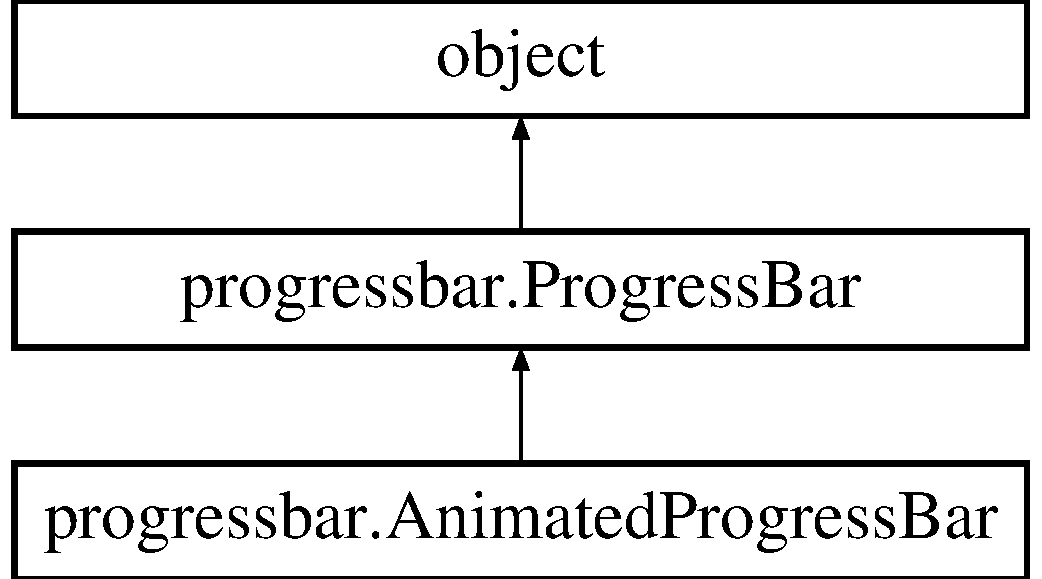
\includegraphics[height=3.000000cm]{classprogressbar_1_1AnimatedProgressBar}
\end{center}
\end{figure}
\subsection*{Public Member Functions}
\begin{DoxyCompactItemize}
\item 
def \hyperlink{classprogressbar_1_1AnimatedProgressBar_ac5fb173f8610ea6caa27306a60a8903f}{\+\_\+\+\_\+init\+\_\+\+\_\+} (self, args, kwargs)
\item 
def \hyperlink{classprogressbar_1_1AnimatedProgressBar_a87d45550598b83128ee14b4d7acdea27}{show\+\_\+progress} (self)
\item 
def \hyperlink{classprogressbar_1_1ProgressBar_ab72aa084f53baad02409c8e7e5979046}{\+\_\+\+\_\+add\+\_\+\+\_\+} (self, increment)
\item 
def \hyperlink{classprogressbar_1_1ProgressBar_aea02b9e37516e9d267e2d48b4e415bd8}{\+\_\+\+\_\+str\+\_\+\+\_\+} (self)
\item 
def \hyperlink{classprogressbar_1_1ProgressBar_a0794442f190ed0d6e5b894f29881758b}{set} (self, value)
\item 
def \hyperlink{classprogressbar_1_1ProgressBar_aefc445915e4d1eb0bbf962857c122dac}{reset} (self)
\end{DoxyCompactItemize}
\subsection*{Public Attributes}
\begin{DoxyCompactItemize}
\item 
\hyperlink{classprogressbar_1_1AnimatedProgressBar_aa4bc611ade566c28f1c54e5608a2a200}{stdout}
\item 
\hyperlink{classprogressbar_1_1AnimatedProgressBar_a50c3cb9a4b317224bd600047efb761d2}{last\+\_\+indicator}
\item 
\hyperlink{classprogressbar_1_1ProgressBar_a550afef3072c2412e2aa906b12c33bbe}{start}
\item 
\hyperlink{classprogressbar_1_1ProgressBar_a92053e3baab49364971c15373b6c848f}{end}
\item 
\hyperlink{classprogressbar_1_1ProgressBar_abde0c8da19e6e6bcde845b1eb3cee279}{width}
\item 
\hyperlink{classprogressbar_1_1ProgressBar_a6b11796a20118f92eb59abbccf626d23}{fill}
\item 
\hyperlink{classprogressbar_1_1ProgressBar_a0bfce2d34f0a8f034748d77cc5140bc5}{blank}
\item 
\hyperlink{classprogressbar_1_1ProgressBar_a4dd00a852851da809ffad5e1bf282858}{format}
\item 
\hyperlink{classprogressbar_1_1ProgressBar_a0b98b7a8f7025b78a5d01f0dcfc2dbaa}{incremental}
\item 
\hyperlink{classprogressbar_1_1ProgressBar_ac076ee00e3a70c69b8583668c165415a}{step}
\item 
\hyperlink{classprogressbar_1_1ProgressBar_a28ce54371f3a84172049c0520726d2aa}{process}
\item 
\hyperlink{classprogressbar_1_1ProgressBar_a3adc96f42e6891bcd2885c9ef29767f3}{progress}
\end{DoxyCompactItemize}


\subsection{Detailed Description}
\begin{DoxyVerb}Extends ProgressBar to allow you to use it straighforward on a script.
Accepts an extra keyword argument named `stdout` (by default use sys.stdout)
and may be any file-object to which send the progress status.
\end{DoxyVerb}
 

Definition at line 64 of file progressbar.\+py.



\subsection{Constructor \& Destructor Documentation}
\mbox{\Hypertarget{classprogressbar_1_1AnimatedProgressBar_ac5fb173f8610ea6caa27306a60a8903f}\label{classprogressbar_1_1AnimatedProgressBar_ac5fb173f8610ea6caa27306a60a8903f}} 
\index{progressbar\+::\+Animated\+Progress\+Bar@{progressbar\+::\+Animated\+Progress\+Bar}!\+\_\+\+\_\+init\+\_\+\+\_\+@{\+\_\+\+\_\+init\+\_\+\+\_\+}}
\index{\+\_\+\+\_\+init\+\_\+\+\_\+@{\+\_\+\+\_\+init\+\_\+\+\_\+}!progressbar\+::\+Animated\+Progress\+Bar@{progressbar\+::\+Animated\+Progress\+Bar}}
\subsubsection{\texorpdfstring{\+\_\+\+\_\+init\+\_\+\+\_\+()}{\_\_init\_\_()}}
{\footnotesize\ttfamily def progressbar.\+Animated\+Progress\+Bar.\+\_\+\+\_\+init\+\_\+\+\_\+ (\begin{DoxyParamCaption}\item[{}]{self,  }\item[{}]{args,  }\item[{}]{kwargs }\end{DoxyParamCaption})}



Definition at line 69 of file progressbar.\+py.


\begin{DoxyCode}
69     \textcolor{keyword}{def }\hyperlink{classwrapper_1_1ModuleDictWrapper_a9a7a794150502f51df687831583e13b9}{\_\_init\_\_}(self, *args, **kwargs):
70         super(AnimatedProgressBar, self).\hyperlink{classwrapper_1_1ModuleDictWrapper_a9a7a794150502f51df687831583e13b9}{\_\_init\_\_}(*args, **kwargs)
71         self.stdout = kwargs.get(\textcolor{stringliteral}{'stdout'}, sys.stdout)
72         self.last\_indicator = \textcolor{stringliteral}{''}
73 
\end{DoxyCode}


\subsection{Member Function Documentation}
\mbox{\Hypertarget{classprogressbar_1_1ProgressBar_ab72aa084f53baad02409c8e7e5979046}\label{classprogressbar_1_1ProgressBar_ab72aa084f53baad02409c8e7e5979046}} 
\index{progressbar\+::\+Animated\+Progress\+Bar@{progressbar\+::\+Animated\+Progress\+Bar}!\+\_\+\+\_\+add\+\_\+\+\_\+@{\+\_\+\+\_\+add\+\_\+\+\_\+}}
\index{\+\_\+\+\_\+add\+\_\+\+\_\+@{\+\_\+\+\_\+add\+\_\+\+\_\+}!progressbar\+::\+Animated\+Progress\+Bar@{progressbar\+::\+Animated\+Progress\+Bar}}
\subsubsection{\texorpdfstring{\+\_\+\+\_\+add\+\_\+\+\_\+()}{\_\_add\_\_()}}
{\footnotesize\ttfamily def progressbar.\+Progress\+Bar.\+\_\+\+\_\+add\+\_\+\+\_\+ (\begin{DoxyParamCaption}\item[{}]{self,  }\item[{}]{increment }\end{DoxyParamCaption})\hspace{0.3cm}{\ttfamily [inherited]}}



Definition at line 30 of file progressbar.\+py.



References progressbar.\+Progress\+Bar.\+\_\+get\+\_\+progress(), and progressbar.\+Progress\+Bar.\+progress.


\begin{DoxyCode}
30     \textcolor{keyword}{def }\_\_add\_\_(self, increment):
31         increment = self.\_get\_progress(increment)
32         \textcolor{keywordflow}{if} 100 > self.progress + increment:
33             self.progress += increment
34         \textcolor{keywordflow}{else}:
35             self.progress = 100
36         \textcolor{keywordflow}{return} self
37     
\end{DoxyCode}
\mbox{\Hypertarget{classprogressbar_1_1ProgressBar_aea02b9e37516e9d267e2d48b4e415bd8}\label{classprogressbar_1_1ProgressBar_aea02b9e37516e9d267e2d48b4e415bd8}} 
\index{progressbar\+::\+Animated\+Progress\+Bar@{progressbar\+::\+Animated\+Progress\+Bar}!\+\_\+\+\_\+str\+\_\+\+\_\+@{\+\_\+\+\_\+str\+\_\+\+\_\+}}
\index{\+\_\+\+\_\+str\+\_\+\+\_\+@{\+\_\+\+\_\+str\+\_\+\+\_\+}!progressbar\+::\+Animated\+Progress\+Bar@{progressbar\+::\+Animated\+Progress\+Bar}}
\subsubsection{\texorpdfstring{\+\_\+\+\_\+str\+\_\+\+\_\+()}{\_\_str\_\_()}}
{\footnotesize\ttfamily def progressbar.\+Progress\+Bar.\+\_\+\+\_\+str\+\_\+\+\_\+ (\begin{DoxyParamCaption}\item[{}]{self }\end{DoxyParamCaption})\hspace{0.3cm}{\ttfamily [inherited]}}



Definition at line 38 of file progressbar.\+py.



References progressbar.\+Progress\+Bar.\+blank, progressbar.\+Progress\+Bar.\+fill, progressbar.\+Progress\+Bar.\+format, progressbar.\+Progress\+Bar.\+process, progressbar.\+Progress\+Bar.\+progress, progressbar.\+Progress\+Bar.\+step, and progressbar.\+Progress\+Bar.\+width.


\begin{DoxyCode}
38     \textcolor{keyword}{def }\_\_str\_\_(self):
39         progressed = int(self.progress / self.step) \textcolor{comment}{#fix}
40         fill = progressed * self.fill
41         proc = self.process
42         blank = (self.width - progressed) * self.blank
43         \textcolor{keywordflow}{return} self.format % \{\textcolor{stringliteral}{'process'}: proc, \textcolor{stringliteral}{'fill'}: fill, \textcolor{stringliteral}{'blank'}: blank, \textcolor{stringliteral}{'progress'}: int(self.progress)
      \}
44 
\end{DoxyCode}
\mbox{\Hypertarget{classprogressbar_1_1ProgressBar_aefc445915e4d1eb0bbf962857c122dac}\label{classprogressbar_1_1ProgressBar_aefc445915e4d1eb0bbf962857c122dac}} 
\index{progressbar\+::\+Animated\+Progress\+Bar@{progressbar\+::\+Animated\+Progress\+Bar}!reset@{reset}}
\index{reset@{reset}!progressbar\+::\+Animated\+Progress\+Bar@{progressbar\+::\+Animated\+Progress\+Bar}}
\subsubsection{\texorpdfstring{reset()}{reset()}}
{\footnotesize\ttfamily def progressbar.\+Progress\+Bar.\+reset (\begin{DoxyParamCaption}\item[{}]{self }\end{DoxyParamCaption})\hspace{0.3cm}{\ttfamily [inherited]}}

\begin{DoxyVerb}Resets the current progress to the start point\end{DoxyVerb}
 

Definition at line 58 of file progressbar.\+py.



References progressbar.\+Progress\+Bar.\+\_\+get\+\_\+progress(), progressbar.\+Progress\+Bar.\+progress, and progressbar.\+Progress\+Bar.\+start.


\begin{DoxyCode}
58     \textcolor{keyword}{def }\hyperlink{namespaceshell_a2f31bbe4baf894f4863c4d392239ab8b}{reset}(self):
59         \textcolor{stringliteral}{"""Resets the current progress to the start point"""}
60         self.progress = self.\_get\_progress(self.start)
61         \textcolor{keywordflow}{return} self
62 
63 
\end{DoxyCode}
\mbox{\Hypertarget{classprogressbar_1_1ProgressBar_a0794442f190ed0d6e5b894f29881758b}\label{classprogressbar_1_1ProgressBar_a0794442f190ed0d6e5b894f29881758b}} 
\index{progressbar\+::\+Animated\+Progress\+Bar@{progressbar\+::\+Animated\+Progress\+Bar}!set@{set}}
\index{set@{set}!progressbar\+::\+Animated\+Progress\+Bar@{progressbar\+::\+Animated\+Progress\+Bar}}
\subsubsection{\texorpdfstring{set()}{set()}}
{\footnotesize\ttfamily def progressbar.\+Progress\+Bar.\+set (\begin{DoxyParamCaption}\item[{}]{self,  }\item[{}]{value }\end{DoxyParamCaption})\hspace{0.3cm}{\ttfamily [inherited]}}



Definition at line 50 of file progressbar.\+py.



References progressbar.\+Progress\+Bar.\+\_\+get\+\_\+progress(), and progressbar.\+Progress\+Bar.\+progress.


\begin{DoxyCode}
50     \textcolor{keyword}{def }set(self, value):
51         value = self.\_get\_progress(value)
52         \textcolor{keywordflow}{if} 100 > value:
53             self.progress = value 
54         \textcolor{keywordflow}{else}:
55             self.progress = 100
56         \textcolor{keywordflow}{return} self
57 
\end{DoxyCode}
\mbox{\Hypertarget{classprogressbar_1_1AnimatedProgressBar_a87d45550598b83128ee14b4d7acdea27}\label{classprogressbar_1_1AnimatedProgressBar_a87d45550598b83128ee14b4d7acdea27}} 
\index{progressbar\+::\+Animated\+Progress\+Bar@{progressbar\+::\+Animated\+Progress\+Bar}!show\+\_\+progress@{show\+\_\+progress}}
\index{show\+\_\+progress@{show\+\_\+progress}!progressbar\+::\+Animated\+Progress\+Bar@{progressbar\+::\+Animated\+Progress\+Bar}}
\subsubsection{\texorpdfstring{show\+\_\+progress()}{show\_progress()}}
{\footnotesize\ttfamily def progressbar.\+Animated\+Progress\+Bar.\+show\+\_\+progress (\begin{DoxyParamCaption}\item[{}]{self }\end{DoxyParamCaption})}



Definition at line 74 of file progressbar.\+py.



References progressbar.\+Animated\+Progress\+Bar.\+last\+\_\+indicator, and progressbar.\+Animated\+Progress\+Bar.\+stdout.


\begin{DoxyCode}
74     \textcolor{keyword}{def }show\_progress(self):
75         indicator = str(self)
76         \textcolor{keywordflow}{if} indicator == self.last\_indicator:
77           \textcolor{keywordflow}{return}
78         \textcolor{keywordflow}{if} hasattr(self.stdout, \textcolor{stringliteral}{'isatty'}) \textcolor{keywordflow}{and} self.stdout.isatty():
79             self.stdout.write(\textcolor{stringliteral}{'\(\backslash\)r'})
80         \textcolor{keywordflow}{else}:
81             self.stdout.write(\textcolor{stringliteral}{'\(\backslash\)n'})
82         self.stdout.write(str(self))
83         self.stdout.flush()
84         self.last\_indicator = indicator
85 
\end{DoxyCode}


\subsection{Member Data Documentation}
\mbox{\Hypertarget{classprogressbar_1_1ProgressBar_a0bfce2d34f0a8f034748d77cc5140bc5}\label{classprogressbar_1_1ProgressBar_a0bfce2d34f0a8f034748d77cc5140bc5}} 
\index{progressbar\+::\+Animated\+Progress\+Bar@{progressbar\+::\+Animated\+Progress\+Bar}!blank@{blank}}
\index{blank@{blank}!progressbar\+::\+Animated\+Progress\+Bar@{progressbar\+::\+Animated\+Progress\+Bar}}
\subsubsection{\texorpdfstring{blank}{blank}}
{\footnotesize\ttfamily progressbar.\+Progress\+Bar.\+blank\hspace{0.3cm}{\ttfamily [inherited]}}



Definition at line 23 of file progressbar.\+py.



Referenced by progressbar.\+Progress\+Bar.\+\_\+\+\_\+str\+\_\+\+\_\+().

\mbox{\Hypertarget{classprogressbar_1_1ProgressBar_a92053e3baab49364971c15373b6c848f}\label{classprogressbar_1_1ProgressBar_a92053e3baab49364971c15373b6c848f}} 
\index{progressbar\+::\+Animated\+Progress\+Bar@{progressbar\+::\+Animated\+Progress\+Bar}!end@{end}}
\index{end@{end}!progressbar\+::\+Animated\+Progress\+Bar@{progressbar\+::\+Animated\+Progress\+Bar}}
\subsubsection{\texorpdfstring{end}{end}}
{\footnotesize\ttfamily progressbar.\+Progress\+Bar.\+end\hspace{0.3cm}{\ttfamily [inherited]}}



Definition at line 20 of file progressbar.\+py.



Referenced by progressbar.\+Progress\+Bar.\+\_\+get\+\_\+progress().

\mbox{\Hypertarget{classprogressbar_1_1ProgressBar_a6b11796a20118f92eb59abbccf626d23}\label{classprogressbar_1_1ProgressBar_a6b11796a20118f92eb59abbccf626d23}} 
\index{progressbar\+::\+Animated\+Progress\+Bar@{progressbar\+::\+Animated\+Progress\+Bar}!fill@{fill}}
\index{fill@{fill}!progressbar\+::\+Animated\+Progress\+Bar@{progressbar\+::\+Animated\+Progress\+Bar}}
\subsubsection{\texorpdfstring{fill}{fill}}
{\footnotesize\ttfamily progressbar.\+Progress\+Bar.\+fill\hspace{0.3cm}{\ttfamily [inherited]}}



Definition at line 22 of file progressbar.\+py.



Referenced by progressbar.\+Progress\+Bar.\+\_\+\+\_\+str\+\_\+\+\_\+().

\mbox{\Hypertarget{classprogressbar_1_1ProgressBar_a4dd00a852851da809ffad5e1bf282858}\label{classprogressbar_1_1ProgressBar_a4dd00a852851da809ffad5e1bf282858}} 
\index{progressbar\+::\+Animated\+Progress\+Bar@{progressbar\+::\+Animated\+Progress\+Bar}!format@{format}}
\index{format@{format}!progressbar\+::\+Animated\+Progress\+Bar@{progressbar\+::\+Animated\+Progress\+Bar}}
\subsubsection{\texorpdfstring{format}{format}}
{\footnotesize\ttfamily progressbar.\+Progress\+Bar.\+format\hspace{0.3cm}{\ttfamily [inherited]}}



Definition at line 24 of file progressbar.\+py.



Referenced by progressbar.\+Progress\+Bar.\+\_\+\+\_\+str\+\_\+\+\_\+().

\mbox{\Hypertarget{classprogressbar_1_1ProgressBar_a0b98b7a8f7025b78a5d01f0dcfc2dbaa}\label{classprogressbar_1_1ProgressBar_a0b98b7a8f7025b78a5d01f0dcfc2dbaa}} 
\index{progressbar\+::\+Animated\+Progress\+Bar@{progressbar\+::\+Animated\+Progress\+Bar}!incremental@{incremental}}
\index{incremental@{incremental}!progressbar\+::\+Animated\+Progress\+Bar@{progressbar\+::\+Animated\+Progress\+Bar}}
\subsubsection{\texorpdfstring{incremental}{incremental}}
{\footnotesize\ttfamily progressbar.\+Progress\+Bar.\+incremental\hspace{0.3cm}{\ttfamily [inherited]}}



Definition at line 25 of file progressbar.\+py.

\mbox{\Hypertarget{classprogressbar_1_1AnimatedProgressBar_a50c3cb9a4b317224bd600047efb761d2}\label{classprogressbar_1_1AnimatedProgressBar_a50c3cb9a4b317224bd600047efb761d2}} 
\index{progressbar\+::\+Animated\+Progress\+Bar@{progressbar\+::\+Animated\+Progress\+Bar}!last\+\_\+indicator@{last\+\_\+indicator}}
\index{last\+\_\+indicator@{last\+\_\+indicator}!progressbar\+::\+Animated\+Progress\+Bar@{progressbar\+::\+Animated\+Progress\+Bar}}
\subsubsection{\texorpdfstring{last\+\_\+indicator}{last\_indicator}}
{\footnotesize\ttfamily progressbar.\+Animated\+Progress\+Bar.\+last\+\_\+indicator}



Definition at line 72 of file progressbar.\+py.



Referenced by progressbar.\+Animated\+Progress\+Bar.\+show\+\_\+progress().

\mbox{\Hypertarget{classprogressbar_1_1ProgressBar_a28ce54371f3a84172049c0520726d2aa}\label{classprogressbar_1_1ProgressBar_a28ce54371f3a84172049c0520726d2aa}} 
\index{progressbar\+::\+Animated\+Progress\+Bar@{progressbar\+::\+Animated\+Progress\+Bar}!process@{process}}
\index{process@{process}!progressbar\+::\+Animated\+Progress\+Bar@{progressbar\+::\+Animated\+Progress\+Bar}}
\subsubsection{\texorpdfstring{process}{process}}
{\footnotesize\ttfamily progressbar.\+Progress\+Bar.\+process\hspace{0.3cm}{\ttfamily [inherited]}}



Definition at line 27 of file progressbar.\+py.



Referenced by progressbar.\+Progress\+Bar.\+\_\+\+\_\+str\+\_\+\+\_\+().

\mbox{\Hypertarget{classprogressbar_1_1ProgressBar_a3adc96f42e6891bcd2885c9ef29767f3}\label{classprogressbar_1_1ProgressBar_a3adc96f42e6891bcd2885c9ef29767f3}} 
\index{progressbar\+::\+Animated\+Progress\+Bar@{progressbar\+::\+Animated\+Progress\+Bar}!progress@{progress}}
\index{progress@{progress}!progressbar\+::\+Animated\+Progress\+Bar@{progressbar\+::\+Animated\+Progress\+Bar}}
\subsubsection{\texorpdfstring{progress}{progress}}
{\footnotesize\ttfamily progressbar.\+Progress\+Bar.\+progress\hspace{0.3cm}{\ttfamily [inherited]}}



Definition at line 35 of file progressbar.\+py.



Referenced by progressbar.\+Progress\+Bar.\+\_\+\+\_\+add\+\_\+\+\_\+(), progressbar.\+Progress\+Bar.\+\_\+\+\_\+str\+\_\+\+\_\+(), progressbar.\+Progress\+Bar.\+reset(), and progressbar.\+Progress\+Bar.\+set().

\mbox{\Hypertarget{classprogressbar_1_1ProgressBar_a550afef3072c2412e2aa906b12c33bbe}\label{classprogressbar_1_1ProgressBar_a550afef3072c2412e2aa906b12c33bbe}} 
\index{progressbar\+::\+Animated\+Progress\+Bar@{progressbar\+::\+Animated\+Progress\+Bar}!start@{start}}
\index{start@{start}!progressbar\+::\+Animated\+Progress\+Bar@{progressbar\+::\+Animated\+Progress\+Bar}}
\subsubsection{\texorpdfstring{start}{start}}
{\footnotesize\ttfamily progressbar.\+Progress\+Bar.\+start\hspace{0.3cm}{\ttfamily [inherited]}}



Definition at line 19 of file progressbar.\+py.



Referenced by progressbar.\+Progress\+Bar.\+reset().

\mbox{\Hypertarget{classprogressbar_1_1AnimatedProgressBar_aa4bc611ade566c28f1c54e5608a2a200}\label{classprogressbar_1_1AnimatedProgressBar_aa4bc611ade566c28f1c54e5608a2a200}} 
\index{progressbar\+::\+Animated\+Progress\+Bar@{progressbar\+::\+Animated\+Progress\+Bar}!stdout@{stdout}}
\index{stdout@{stdout}!progressbar\+::\+Animated\+Progress\+Bar@{progressbar\+::\+Animated\+Progress\+Bar}}
\subsubsection{\texorpdfstring{stdout}{stdout}}
{\footnotesize\ttfamily progressbar.\+Animated\+Progress\+Bar.\+stdout}



Definition at line 71 of file progressbar.\+py.



Referenced by progressbar.\+Animated\+Progress\+Bar.\+show\+\_\+progress().

\mbox{\Hypertarget{classprogressbar_1_1ProgressBar_ac076ee00e3a70c69b8583668c165415a}\label{classprogressbar_1_1ProgressBar_ac076ee00e3a70c69b8583668c165415a}} 
\index{progressbar\+::\+Animated\+Progress\+Bar@{progressbar\+::\+Animated\+Progress\+Bar}!step@{step}}
\index{step@{step}!progressbar\+::\+Animated\+Progress\+Bar@{progressbar\+::\+Animated\+Progress\+Bar}}
\subsubsection{\texorpdfstring{step}{step}}
{\footnotesize\ttfamily progressbar.\+Progress\+Bar.\+step\hspace{0.3cm}{\ttfamily [inherited]}}



Definition at line 26 of file progressbar.\+py.



Referenced by progressbar.\+Progress\+Bar.\+\_\+\+\_\+str\+\_\+\+\_\+().

\mbox{\Hypertarget{classprogressbar_1_1ProgressBar_abde0c8da19e6e6bcde845b1eb3cee279}\label{classprogressbar_1_1ProgressBar_abde0c8da19e6e6bcde845b1eb3cee279}} 
\index{progressbar\+::\+Animated\+Progress\+Bar@{progressbar\+::\+Animated\+Progress\+Bar}!width@{width}}
\index{width@{width}!progressbar\+::\+Animated\+Progress\+Bar@{progressbar\+::\+Animated\+Progress\+Bar}}
\subsubsection{\texorpdfstring{width}{width}}
{\footnotesize\ttfamily progressbar.\+Progress\+Bar.\+width\hspace{0.3cm}{\ttfamily [inherited]}}



Definition at line 21 of file progressbar.\+py.



Referenced by progressbar.\+Progress\+Bar.\+\_\+\+\_\+str\+\_\+\+\_\+().



The documentation for this class was generated from the following file\+:\begin{DoxyCompactItemize}
\item 
/home/eleclhcb/\+L\+H\+Cb/lbcat-\/cmake/\+Cat\+Python/python/\hyperlink{progressbar_8py}{progressbar.\+py}\end{DoxyCompactItemize}

\hypertarget{classAppFrame_1_1AppFrame}{
\section{AppFrame::AppFrame Class Reference}
\label{classAppFrame_1_1AppFrame}\index{AppFrame::AppFrame@{AppFrame::AppFrame}}
}
\subsection*{Public Member Functions}
\begin{DoxyCompactItemize}
\item 
def \hyperlink{classAppFrame_1_1AppFrame_a99de512a9c17c41f6446a0ad51aa492f}{\_\-\_\-init\_\-\_\-}
\item 
def \hyperlink{classAppFrame_1_1AppFrame_a339ae421d03a4184269c6b7e3537ab08}{getControl}
\item 
def \hyperlink{classAppFrame_1_1AppFrame_a71b05a3223d3ab9595beb5a6158a4658}{makeMenuBar}
\item 
def \hyperlink{classAppFrame_1_1AppFrame_ab4a7fb9bd8d8d66ab94c61281456f8ff}{makeToolBar}
\item 
def \hyperlink{classAppFrame_1_1AppFrame_a4e0dcbd50e131b0098cf1611ad25db6c}{onIdle}
\item 
def \hyperlink{classAppFrame_1_1AppFrame_aaa21bd6cb6d29c0ff8b86aee2b55d146}{onCloseConfirm}
\item 
def \hyperlink{classAppFrame_1_1AppFrame_a5f83beacf1c4e5bd2a27e3c778c96c1e}{onClose}
\item 
def \hyperlink{classAppFrame_1_1AppFrame_a5b5cb5f928c331e97fd7ffcee5458bcf}{onExit}
\item 
def \hyperlink{classAppFrame_1_1AppFrame_a11b969659be042b78227df2738371b6a}{onHelp}
\item 
def \hyperlink{classAppFrame_1_1AppFrame_a8a7202f9eb527cf4513d8b69b385a172}{onAbout}
\item 
def \hyperlink{classAppFrame_1_1AppFrame_ae06136b61e9fb8d5d8594a78bc5b1beb}{onAutoCheck}
\item 
def \hyperlink{classAppFrame_1_1AppFrame_a5d4fbe570c7b419c71b5a28e920ef0b3}{onStopOnError}
\item 
def \hyperlink{classAppFrame_1_1AppFrame_a64fced2976ba648b07d575749a031ce2}{onFileCheck}
\item 
def \hyperlink{classAppFrame_1_1AppFrame_a5fc0d44cdfe82f731a9e8747c0062bdc}{onLogCheck}
\item 
def \hyperlink{classAppFrame_1_1AppFrame_aca8b90caebbf4467fefc23d134e87882}{eventCtrl}
\item 
def \hyperlink{classAppFrame_1_1AppFrame_a89e4b810a8f76474c63307ab353b95ae}{runCtrl}
\item 
def \hyperlink{classAppFrame_1_1AppFrame_a3319c92de38f17675b2debf064add617}{printFreq}
\item 
def \hyperlink{classAppFrame_1_1AppFrame_a724d4fb4f7b45e38c3002dafaf31ae3d}{plotFreq}
\item 
def \hyperlink{classAppFrame_1_1AppFrame_a40b3826412cf97464898e448b5eb9b00}{onEnter}
\item 
def \hyperlink{classAppFrame_1_1AppFrame_a6050b747faab481f9728a791ce5c8beb}{onLoad}
\item 
def \hyperlink{classAppFrame_1_1AppFrame_a17e104bbc8544539fcad9d3f75583438}{onEdit}
\item 
def \hyperlink{classAppFrame_1_1AppFrame_ae6dbfb701cee3d4f1ebd953d21934f90}{deleteHardware}
\item 
def \hyperlink{classAppFrame_1_1AppFrame_a66183c68b99e1849cb3a009aacf46578}{onExpand}
\item 
def \hyperlink{classAppFrame_1_1AppFrame_a7d96700ebc4f5a5fcf51d3d8940bcc54}{onCollapse}
\item 
def \hyperlink{classAppFrame_1_1AppFrame_a245f8c716ec863af51493af54f2cd7c6}{onReLoad}
\item 
def \hyperlink{classAppFrame_1_1AppFrame_a4d4525e84c9ababf7b5c80893c803fcc}{onConfigure}
\item 
def \hyperlink{classAppFrame_1_1AppFrame_a0f55c13ed518ba308a375dfc306fdee9}{onInit}
\item 
def \hyperlink{classAppFrame_1_1AppFrame_ad5e9ba93cb8013656d6500774cf60b53}{onDelete}
\item 
def \hyperlink{classAppFrame_1_1AppFrame_a49804b67199c453697ac5a4bcecc920e}{onStart}
\item 
def \hyperlink{classAppFrame_1_1AppFrame_af7be990776d498b34f698dc9451b4883}{onSingle}
\item 
def \hyperlink{classAppFrame_1_1AppFrame_a16fc60c79fde4dd7d9591ed3f21c3c01}{plot}
\item 
def \hyperlink{classAppFrame_1_1AppFrame_a44b82952390e069b184afd5986991ba4}{BuildElementList}
\item 
def \hyperlink{classAppFrame_1_1AppFrame_a7e349c4603f3f7ca0c5aa77a89d253dd}{BuildProcessusList}
\item 
def \hyperlink{classAppFrame_1_1AppFrame_aa01fc511db7b94a62d550a0087d750b9}{update}
\item 
def \hyperlink{classAppFrame_1_1AppFrame_a5281ab025cc34273c414c06e58f1507d}{ElementList}
\item 
def \hyperlink{classAppFrame_1_1AppFrame_a9dec5963f6ad7c33992ad7ec38567574}{updateCombo}
\item 
def \hyperlink{classAppFrame_1_1AppFrame_a6a35e9206bd5c1cedcfd8a9af7d6a8c6}{updateOutputLevel}
\item 
def \hyperlink{classAppFrame_1_1AppFrame_afeddbb4dfa87ced566b15d905eed4756}{procComboUpdate}
\end{DoxyCompactItemize}
\subsection*{Public Attributes}
\begin{DoxyCompactItemize}
\item 
\hyperlink{classAppFrame_1_1AppFrame_a4ff8d69e79895e94fe0c4457051e98e4}{MB\_\-CONF}
\item 
\hyperlink{classAppFrame_1_1AppFrame_a87cf4bd947402b005cdc8a8248bc7394}{MB\_\-GRAPH}
\item 
\hyperlink{classAppFrame_1_1AppFrame_aa4182d18214f9bcb8747b30d75566c4a}{MB\_\-LOG}
\item 
\hyperlink{classAppFrame_1_1AppFrame_a92adb26561ea695af9637bdd7cdcffda}{TB\_\-CONF}
\item 
\hyperlink{classAppFrame_1_1AppFrame_a054706bdc13f9c9e2b3a74c2cf659271}{TB\_\-GRAPH}
\item 
\hyperlink{classAppFrame_1_1AppFrame_aa6410672f90bddc15b60bddd6040c65b}{TB\_\-LOG}
\item 
\hyperlink{classAppFrame_1_1AppFrame_a0a19a7c7e9a6095cba6813e8d13e9bec}{cfgpanels}
\item 
\hyperlink{classAppFrame_1_1AppFrame_a7b899e2a2d3601a640bde2ba4a4c09b6}{objs}
\item 
\hyperlink{classAppFrame_1_1AppFrame_a9b64dca9c80270b7f0e36ee52d5f8c2d}{paths}
\item 
\hyperlink{classAppFrame_1_1AppFrame_aadc7ad0c96f9227da506b173bd7b2eee}{path}
\item 
\hyperlink{classAppFrame_1_1AppFrame_a814271a025b2beadb1187e3e9673b0fd}{panel}
\item 
\hyperlink{classAppFrame_1_1AppFrame_af5e0f9082a6580c786ad0a801dd31685}{treeContainer}
\item 
\hyperlink{classAppFrame_1_1AppFrame_ae267f6f9741bde298362f95ac19c97f2}{vbox}
\item 
\hyperlink{classAppFrame_1_1AppFrame_a1c088e6a3fc661ea80a336100160af9a}{tree}
\item 
\hyperlink{classAppFrame_1_1AppFrame_aac2972aa5a59df4897418cb34afc24bb}{elementCombo}
\item 
\hyperlink{classAppFrame_1_1AppFrame_afe103fbb66e1b2a6b7e9a64bd3154881}{procCombo}
\item 
\hyperlink{classAppFrame_1_1AppFrame_a9cbeda3bc1a78e934f1aebcd2c85e403}{menuBar}
\item 
\hyperlink{classAppFrame_1_1AppFrame_a2fd6329df31bbd37f1239f34a567d71a}{toolBar}
\item 
\hyperlink{classAppFrame_1_1AppFrame_ac23e75e7a9c9995eb55d7962342acd15}{listElement}
\end{DoxyCompactItemize}
\subsection*{Static Public Attributes}
\begin{DoxyCompactItemize}
\item 
string \hyperlink{classAppFrame_1_1AppFrame_a667d35fae1ebfa2706cfbb31fdf0cbab}{overviewText} = \char`\"{}CAT Main Window\char`\"{}
\end{DoxyCompactItemize}


\subsection{Detailed Description}


Definition at line 54 of file AppFrame.py.

\subsection{Member Function Documentation}
\hypertarget{classAppFrame_1_1AppFrame_a99de512a9c17c41f6446a0ad51aa492f}{
\index{AppFrame::AppFrame@{AppFrame::AppFrame}!\_\-\_\-init\_\-\_\-@{\_\-\_\-init\_\-\_\-}}
\index{\_\-\_\-init\_\-\_\-@{\_\-\_\-init\_\-\_\-}!AppFrame::AppFrame@{AppFrame::AppFrame}}
\subsubsection[{\_\-\_\-init\_\-\_\-}]{\setlength{\rightskip}{0pt plus 5cm}def AppFrame::AppFrame::\_\-\_\-init\_\-\_\- ( {\em self}, \/   {\em app}, \/   {\em parent}, \/   {\em title})}}
\label{classAppFrame_1_1AppFrame_a99de512a9c17c41f6446a0ad51aa492f}


Definition at line 56 of file AppFrame.py.


\begin{DoxyCode}
56                                           : 
57         wx.Frame.__init__(self, parent, wx.NewId(), title, size=(500, 650))
58         
59         self.MB_CONF=wx.NewId()
60         self.MB_GRAPH=wx.NewId()
61         self.MB_LOG=wx.NewId()
62 
63         self.TB_CONF=wx.NewId()
64         self.TB_GRAPH=wx.NewId()
65         self.TB_LOG=wx.NewId()
66 
67         self.cfgpanels=list()
68         self.objs=list()
69         self.paths=list()
70 
71         global cat
72         cat=app
73         
74         self.path=os.path.join(os.environ.get("CATPATH"),"CatPython","python")
75         sizeX=wx.SystemSettings.GetMetric( wx.SYS_SCREEN_X );
76         sizeY=wx.SystemSettings.GetMetric( wx.SYS_SCREEN_Y );
77         self.makeMenuBar()
78         self.makeToolBar()
79         res=xrc.XmlResource(os.path.join(self.path,"xrc/AppPanel.xrc"))
80         self.panel=res.LoadPanel(self, "AppPanel")
81 #        self.makeFrames()
82         
83         for window, items in _windows:
84             show=items[0]
85             Pt=wx.Point(items[1][0]*sizeX,items[1][1]*sizeY)
86             Sz=wx.Size(items[2][0]*sizeX,items[2][1]*sizeY)
87             if window=='App':
88                 self.Move(Pt)
89                 self.SetSize(Sz)
90             # if window=='Cfg':
91             #     self.cfgFrame.Move(Pt)
92             #     self.cfgFrame.SetSize(Sz)
93             #     self.cfgState=show
94             #     self.cfgFrame.Show(show)
95             #     self.toolBar.ToggleTool(self.TB_CONF, show)
96             #     menuItem = self.menuBar.FindItemById(self.MB_CONF)
97             #     menuItem.Check(show) 
98                 
99             # if window=='Gph':
100             #     self.gphFrame.Move(Pt)
101             #     self.gphFrame.SetSize(Sz)
102             #     self.gphState=show
103             #     self.gphFrame.Show(show)
104             #     self.toolBar.ToggleTool(self.TB_GRAPH, show)
105             #     menuItem = self.menuBar.FindItemById(self.MB_GRAPH)
106             #     menuItem.Check(show)
107 
108             # if window=='Log':
109             #     self.logFrame.Move(Pt)
110             #     self.logFrame.SetSize(Sz)
111             #     self.logState=show
112             #     self.logFrame.Show(show)
113             #     self.toolBar.ToggleTool(self.TB_LOG, show)
114             #     menuItem = self.menuBar.FindItemById(self.MB_LOG)
115             #     menuItem.Check(show)
116                 
117         self.treeContainer=xrc.XRCCTRL(self, 'TreePanel')
118         self.vbox=wx.BoxSizer(wx.VERTICAL)
119         
120         self.tree=TreeCtrlPanel(self.treeContainer)
121 
122         self.vbox.Add(self.tree,1,wx.EXPAND)
123         self.treeContainer.SetSizer( self.vbox )
124 
125 #        self.tree
126 #        self.treeMap = {}
127 
128 #        self.BuildTreeImageList()
129         #self.tree.SetExpansionState(self.expansionState)
130 #        self.tree.Bind(wx.EVT_TREE_ITEM_EXPANDED, self.OnItemExpanded)
131 #        self.tree.Bind(wx.EVT_TREE_ITEM_COLLAPSED, self.OnItemCollapsed)
132 #        self.tree.Bind(wx.EVT_TREE_SEL_CHANGED, self.OnSelChanged)
133 #        self.tree.Bind(wx.EVT_LEFT_DOWN, self.OnTreeLeftDown)
134 
135         self.elementCombo=self.getControl("elementCombo")
136         self.procCombo=self.getControl("procCombo")
137         self.Bind(wx.EVT_COMBOBOX, self.updateCombo, id=xrc.XRCID("elementCombo")
      )        
138         self.Bind(wx.EVT_BUTTON, self.onLoad, id=xrc.XRCID("openConfFile"))
139         self.Bind(wx.EVT_BUTTON, self.onEdit, id=xrc.XRCID("onEdit"))
140         self.Bind(wx.EVT_SPINCTRL, self.runCtrl, id=xrc.XRCID("runCtrl"))
141         self.Bind(wx.EVT_SPINCTRL, self.eventCtrl, id=xrc.XRCID("eventCtrl"))
142         self.Bind(wx.EVT_SPINCTRL, self.printFreq, id=xrc.XRCID("printFreq"))
143         self.Bind(wx.EVT_SPINCTRL, self.plotFreq, id=xrc.XRCID("plotFreq"))
144         self.Bind(wx.EVT_TEXT_ENTER, self.onEnter, id=xrc.XRCID("cmdline"))
145         self.Bind(wx.EVT_BUTTON, self.onEnter, id=xrc.XRCID("onEnter"))
146         self.Bind(wx.EVT_BUTTON, self.onExpand, id=xrc.XRCID("onExpand"))
147         self.Bind(wx.EVT_BUTTON, self.onCollapse, id=xrc.XRCID("onCollapse"))
148         self.Bind(wx.EVT_BUTTON, self.deleteHardware, id=xrc.XRCID("deleteHardwar
      e"))
149         self.Bind(wx.EVT_TOGGLEBUTTON, self.onAutoCheck, id=xrc.XRCID("autoCheck"
      ))
150         self.Bind(wx.EVT_TOGGLEBUTTON, self.onStopOnError, id=xrc.XRCID("stoponer
      ror"))
151         self.Bind(wx.EVT_TOGGLEBUTTON, self.onLogCheck, id=xrc.XRCID("logCheck"))
      
152         self.Bind(wx.EVT_TOGGLEBUTTON, self.onFileCheck, id=xrc.XRCID("fileCheck"
      ))
153         self.Bind(wx.EVT_COMBOBOX, self.updateOutputLevel, id=xrc.XRCID("outputLe
      vel"))        
154         self.update()
155                 
\end{DoxyCode}
\hypertarget{classAppFrame_1_1AppFrame_a44b82952390e069b184afd5986991ba4}{
\index{AppFrame::AppFrame@{AppFrame::AppFrame}!BuildElementList@{BuildElementList}}
\index{BuildElementList@{BuildElementList}!AppFrame::AppFrame@{AppFrame::AppFrame}}
\subsubsection[{BuildElementList}]{\setlength{\rightskip}{0pt plus 5cm}def AppFrame::AppFrame::BuildElementList ( {\em self})}}
\label{classAppFrame_1_1AppFrame_a44b82952390e069b184afd5986991ba4}


Definition at line 511 of file AppFrame.py.


\begin{DoxyCode}
511                               :
512         def sublevel(list, element):
513             if (element.hasChildren()):
514                 newlist=[]
515                 children=element.children()
516                 for child in range(len(children)):
517                     newlist.append(children[child].name())
518                     if (children[child].hasChildren()):
519                         sublevel(newlist,children[child])
520                 list.append(newlist)
521         list=[]
522         list.append(cat.computer().name())
523         sublevel(list,cat.computer())
524         return list
525 
526     #---------------------------------------------
    def BuildProcessusList(self):
\end{DoxyCode}
\hypertarget{classAppFrame_1_1AppFrame_a7e349c4603f3f7ca0c5aa77a89d253dd}{
\index{AppFrame::AppFrame@{AppFrame::AppFrame}!BuildProcessusList@{BuildProcessusList}}
\index{BuildProcessusList@{BuildProcessusList}!AppFrame::AppFrame@{AppFrame::AppFrame}}
\subsubsection[{BuildProcessusList}]{\setlength{\rightskip}{0pt plus 5cm}def AppFrame::AppFrame::BuildProcessusList ( {\em self})}}
\label{classAppFrame_1_1AppFrame_a7e349c4603f3f7ca0c5aa77a89d253dd}


Definition at line 527 of file AppFrame.py.


\begin{DoxyCode}
527                                 :
528         list=[]
529         listPtr=cat.procDb().list()
530         for proc in range(len(listPtr)):
531             list.append(listPtr[proc].name())
532         return list
533         
    def update(self):
\end{DoxyCode}
\hypertarget{classAppFrame_1_1AppFrame_ae6dbfb701cee3d4f1ebd953d21934f90}{
\index{AppFrame::AppFrame@{AppFrame::AppFrame}!deleteHardware@{deleteHardware}}
\index{deleteHardware@{deleteHardware}!AppFrame::AppFrame@{AppFrame::AppFrame}}
\subsubsection[{deleteHardware}]{\setlength{\rightskip}{0pt plus 5cm}def AppFrame::AppFrame::deleteHardware ( {\em self}, \/   {\em event})}}
\label{classAppFrame_1_1AppFrame_ae6dbfb701cee3d4f1ebd953d21934f90}


Definition at line 392 of file AppFrame.py.


\begin{DoxyCode}
392                                    :
393         objtype=self.tree.GetItem()
394         cat.warning("Removing object "+objtype[0]+" of type "+objtype[1])
395         element=cat.computer().child(objtype[0])
396         if (element!=0):
397             cat.computer().delChild(element)
398         self.update()
399                         
    def onExpand(self, event):
\end{DoxyCode}
\hypertarget{classAppFrame_1_1AppFrame_a5281ab025cc34273c414c06e58f1507d}{
\index{AppFrame::AppFrame@{AppFrame::AppFrame}!ElementList@{ElementList}}
\index{ElementList@{ElementList}!AppFrame::AppFrame@{AppFrame::AppFrame}}
\subsubsection[{ElementList}]{\setlength{\rightskip}{0pt plus 5cm}def AppFrame::AppFrame::ElementList ( {\em self})}}
\label{classAppFrame_1_1AppFrame_a5281ab025cc34273c414c06e58f1507d}


Definition at line 578 of file AppFrame.py.


\begin{DoxyCode}
578                          :
579         def sublevel(list, element):
580             if (element.hasChildren()):
581                 children=element.children()
582                 for child in range(len(children)):
583                     if (len(cat.procDb().list(children[child]))>0):
584                        list.append(children[child].path(""))
585                     if (children[child].hasChildren()):
586                         sublevel(list,children[child])
587 
588         list=[]
589         list.append(cat.computer().path(""))
590         sublevel(list,cat.computer())
591         return list
592             
    def updateCombo(self, event):
\end{DoxyCode}
\hypertarget{classAppFrame_1_1AppFrame_aca8b90caebbf4467fefc23d134e87882}{
\index{AppFrame::AppFrame@{AppFrame::AppFrame}!eventCtrl@{eventCtrl}}
\index{eventCtrl@{eventCtrl}!AppFrame::AppFrame@{AppFrame::AppFrame}}
\subsubsection[{eventCtrl}]{\setlength{\rightskip}{0pt plus 5cm}def AppFrame::AppFrame::eventCtrl ( {\em self}, \/   {\em event})}}
\label{classAppFrame_1_1AppFrame_aca8b90caebbf4467fefc23d134e87882}


Definition at line 284 of file AppFrame.py.


\begin{DoxyCode}
284                              :
285         cat.options().setNEvtMax(self.getControl("eventCtrl").GetValue()) 
286 
    def runCtrl(self,event):
\end{DoxyCode}
\hypertarget{classAppFrame_1_1AppFrame_a339ae421d03a4184269c6b7e3537ab08}{
\index{AppFrame::AppFrame@{AppFrame::AppFrame}!getControl@{getControl}}
\index{getControl@{getControl}!AppFrame::AppFrame@{AppFrame::AppFrame}}
\subsubsection[{getControl}]{\setlength{\rightskip}{0pt plus 5cm}def AppFrame::AppFrame::getControl ( {\em self}, \/   {\em xmlid})}}
\label{classAppFrame_1_1AppFrame_a339ae421d03a4184269c6b7e3537ab08}
\begin{DoxyVerb}Retrieves the given control (within a dialog) by its xmlid\end{DoxyVerb}
 

Definition at line 156 of file AppFrame.py.


\begin{DoxyCode}
156                                :
157         '''Retrieves the given control (within a dialog) by its xmlid'''
158         control = self.FindWindowById(xrc.XRCID(xmlid))
159 #        print xmlid
160 #        print xrc.XRCID(xmlid)
161 #        print control
162         if control == None and self.GetMenuBar() != None:  # see if on the menuba
      r
163             control = self.GetMenuBar().FindItemById(xrc.XRCID(xmlid))
164         assert control != None, 'Programming error: a control with xml id ' + xml
      id + ' was not found.'
165         return control
166     
    def makeMenuBar(self):
\end{DoxyCode}
\hypertarget{classAppFrame_1_1AppFrame_a71b05a3223d3ab9595beb5a6158a4658}{
\index{AppFrame::AppFrame@{AppFrame::AppFrame}!makeMenuBar@{makeMenuBar}}
\index{makeMenuBar@{makeMenuBar}!AppFrame::AppFrame@{AppFrame::AppFrame}}
\subsubsection[{makeMenuBar}]{\setlength{\rightskip}{0pt plus 5cm}def AppFrame::AppFrame::makeMenuBar ( {\em self})}}
\label{classAppFrame_1_1AppFrame_a71b05a3223d3ab9595beb5a6158a4658}


Definition at line 167 of file AppFrame.py.


\begin{DoxyCode}
167                          :
168         MB_FILE=wx.NewId()
169         MB_CLOSE=wx.NewId()
170         #
171         file=wx.Menu()
172         file.Append(MB_FILE,"&File","Open new configuration file")
173         file.Append(MB_CLOSE,"&Close","Close configuration file")
174         file.Append(wx.ID_EXIT, "E&xit", "Terminate the program")
175         windows=wx.Menu()
176 #        windows.AppendCheckItem(self.MB_CONF,"&Configuration window","Configurat
      ion window")
177 #        windows.AppendCheckItem(self.MB_GRAPH,"&Graphic window","Graphic window"
      )
178 #        windows.AppendCheckItem(self.MB_LOG,"&Log window","Log window")
179         help=wx.Menu()
180         help.Append(wx.ID_ABOUT, "&About","More information about this program")
181         help.AppendSeparator()
182         help.Append(wx.ID_HELP, "&Help", "CAT application help")
183         self.menuBar=wx.MenuBar(wx.MB_DOCKABLE)
184         self.menuBar.Append(file   , "&File")
185         self.menuBar.Append(windows, "&Windows")
186         self.menuBar.Append(help   , "&Help")
187         self.SetMenuBar(self.menuBar)
188         self.Bind(wx.EVT_MENU, self.onExit      , id=wx.ID_EXIT )
189         self.Bind(wx.EVT_MENU, self.onAbout     , id=wx.ID_ABOUT )
190         self.Bind(wx.EVT_MENU, self.onHelp      , id=wx.ID_HELP )
191 #        self.Bind(wx.EVT_MENU, self.onCheckGraph, id=self.MB_GRAPH )
192 #        self.Bind(wx.EVT_MENU, self.onCheckLog  , id=self.MB_LOG   )
193 #        self.Bind(wx.EVT_MENU, self.onCheckConf , id=self.MB_CONF  )
194         self.Bind(wx.EVT_MENU, self.onLoad      , id=MB_FILE  )
195         self.Bind(wx.EVT_MENU, self.onClose     , id=MB_CLOSE  )
196         
    def makeToolBar(self):
\end{DoxyCode}
\hypertarget{classAppFrame_1_1AppFrame_ab4a7fb9bd8d8d66ab94c61281456f8ff}{
\index{AppFrame::AppFrame@{AppFrame::AppFrame}!makeToolBar@{makeToolBar}}
\index{makeToolBar@{makeToolBar}!AppFrame::AppFrame@{AppFrame::AppFrame}}
\subsubsection[{makeToolBar}]{\setlength{\rightskip}{0pt plus 5cm}def AppFrame::AppFrame::makeToolBar ( {\em self})}}
\label{classAppFrame_1_1AppFrame_ab4a7fb9bd8d8d66ab94c61281456f8ff}


Definition at line 197 of file AppFrame.py.


\begin{DoxyCode}
197                          :
198         TB_OPEN=wx.NewId()
199         TB_RELOAD=wx.NewId()
200         TB_CONFIGURE=wx.NewId()
201         TB_INIT=wx.NewId()
202         TB_DELETE=wx.NewId()
203         TB_START=wx.NewId()
204         TB_SINGLE=wx.NewId()
205         TB_EXIT=wx.NewId()
206         #
207         self.toolBar = self.CreateToolBar(wx.TB_DOCKABLE)
208         self.toolBar.AddLabelTool(TB_OPEN  , '', wx.Bitmap(os.path.join(self.
      path,"xrc/icons/fileopen.png")))
209         self.toolBar.AddLabelTool(TB_RELOAD, '', wx.Bitmap(os.path.join(self.
      path,"xrc/icons/reload.png")))
210         self.toolBar.AddLabelTool(TB_CONFIGURE, '', wx.Bitmap(os.path.join(self.
      path,"xrc/icons/conf.png")))
211         self.toolBar.AddLabelTool(TB_INIT, '', wx.Bitmap(os.path.join(self.path,"
      xrc/icons/init.png")))
212         self.toolBar.AddLabelTool(TB_DELETE, '', wx.Bitmap(os.path.join(self.
      path,"xrc/icons/delete.png")))
213         self.toolBar.AddSeparator()
214 #        self.toolBar.AddCheckLabelTool(self.TB_CONF, '', wx.Bitmap(os.path.join(
      self.path,"xrc/icons/config.png")))
215         self.toolBar.AddCheckLabelTool(self.TB_GRAPH, '', wx.Bitmap(os.path.join(
      self.path,"xrc/icons/graph.png")))
216 #        self.toolBar.AddCheckLabelTool(self.TB_LOG, '', wx.Bitmap(os.path.join(s
      elf.path,"xrc/icons/log.png")))
217         self.toolBar.AddSeparator()
218         self.toolBar.AddLabelTool(TB_START, '', wx.Bitmap(os.path.join(self.path,
      "xrc/icons/start.png")))
219         self.toolBar.AddLabelTool(TB_SINGLE, '', wx.Bitmap(os.path.join(self.
      path,"xrc/icons/single.png")))
220         self.toolBar.AddSeparator()
221         self.toolBar.AddLabelTool(wx.ID_EXIT, '', wx.Bitmap(os.path.join(self.
      path,"xrc/icons/exit.png")))
222         self.toolBar.Realize()
223         self.Bind(wx.EVT_TOOL, self.onExit      , id=wx.ID_EXIT)
224 #        self.Bind(wx.EVT_TOOL, self.onCheckGraph, id=self.TB_GRAPH)
225 #        self.Bind(wx.EVT_TOOL, self.onCheckLog  , id=self.TB_LOG)
226 #        self.Bind(wx.EVT_TOOL, self.onCheckConf , id=self.TB_CONF)
227         self.Bind(wx.EVT_TOOL, self.onLoad , id=TB_OPEN)
228         self.Bind(wx.EVT_TOOL, self.onReLoad , id=TB_RELOAD)
229         self.Bind(wx.EVT_TOOL, self.onConfigure , id=TB_CONFIGURE)
230         self.Bind(wx.EVT_TOOL, self.onInit , id=TB_INIT)
231         self.Bind(wx.EVT_TOOL, self.onDelete , id=TB_DELETE)
232         self.Bind(wx.EVT_TOOL, self.onStart , id=TB_START)
233         self.Bind(wx.EVT_TOOL, self.onSingle , id=TB_SINGLE)
234 
235 #    def makeFrames(self):
236 #        self.logFrame=LogFrame(cat, self, "Log window")
237 #        self.cfgFrame=ConfFrame(cat, self, "Configuration window")
238 #        self.gphFrame=GraphFrame(cat, self, "Graphical window")
239         
    def onIdle(self, event):
\end{DoxyCode}
\hypertarget{classAppFrame_1_1AppFrame_a8a7202f9eb527cf4513d8b69b385a172}{
\index{AppFrame::AppFrame@{AppFrame::AppFrame}!onAbout@{onAbout}}
\index{onAbout@{onAbout}!AppFrame::AppFrame@{AppFrame::AppFrame}}
\subsubsection[{onAbout}]{\setlength{\rightskip}{0pt plus 5cm}def AppFrame::AppFrame::onAbout ( {\em self}, \/   {\em event})}}
\label{classAppFrame_1_1AppFrame_a8a7202f9eb527cf4513d8b69b385a172}
\begin{DoxyVerb}About\end{DoxyVerb}
 

Definition at line 265 of file AppFrame.py.


\begin{DoxyCode}
265                             :
266         '''About'''
267         print "about"
268 
    def onAutoCheck(self, event):
\end{DoxyCode}
\hypertarget{classAppFrame_1_1AppFrame_ae06136b61e9fb8d5d8594a78bc5b1beb}{
\index{AppFrame::AppFrame@{AppFrame::AppFrame}!onAutoCheck@{onAutoCheck}}
\index{onAutoCheck@{onAutoCheck}!AppFrame::AppFrame@{AppFrame::AppFrame}}
\subsubsection[{onAutoCheck}]{\setlength{\rightskip}{0pt plus 5cm}def AppFrame::AppFrame::onAutoCheck ( {\em self}, \/   {\em event})}}
\label{classAppFrame_1_1AppFrame_ae06136b61e9fb8d5d8594a78bc5b1beb}


Definition at line 269 of file AppFrame.py.


\begin{DoxyCode}
269                                 :
270         cat.options().setRunNumberMgr(self.getControl("autoCheck").GetValue())
271         print cat.options().runNumberMgr()
272         
    def onStopOnError(self, event):
\end{DoxyCode}
\hypertarget{classAppFrame_1_1AppFrame_a5f83beacf1c4e5bd2a27e3c778c96c1e}{
\index{AppFrame::AppFrame@{AppFrame::AppFrame}!onClose@{onClose}}
\index{onClose@{onClose}!AppFrame::AppFrame@{AppFrame::AppFrame}}
\subsubsection[{onClose}]{\setlength{\rightskip}{0pt plus 5cm}def AppFrame::AppFrame::onClose ( {\em self}, \/   {\em event})}}
\label{classAppFrame_1_1AppFrame_a5f83beacf1c4e5bd2a27e3c778c96c1e}
\begin{DoxyVerb}Closes the application\end{DoxyVerb}
 

Definition at line 252 of file AppFrame.py.


\begin{DoxyCode}
252                             :
253         '''Closes the application'''
254         self.Destroy()
255 
    def onExit(self, event):
\end{DoxyCode}
\hypertarget{classAppFrame_1_1AppFrame_aaa21bd6cb6d29c0ff8b86aee2b55d146}{
\index{AppFrame::AppFrame@{AppFrame::AppFrame}!onCloseConfirm@{onCloseConfirm}}
\index{onCloseConfirm@{onCloseConfirm}!AppFrame::AppFrame@{AppFrame::AppFrame}}
\subsubsection[{onCloseConfirm}]{\setlength{\rightskip}{0pt plus 5cm}def AppFrame::AppFrame::onCloseConfirm ( {\em self}, \/   {\em event})}}
\label{classAppFrame_1_1AppFrame_aaa21bd6cb6d29c0ff8b86aee2b55d146}
\begin{DoxyVerb}Closes the application\end{DoxyVerb}
 

Definition at line 245 of file AppFrame.py.


\begin{DoxyCode}
245                                    :
246         '''Closes the application'''
247         dlg = wx.MessageDialog(self, "Exit the program?", "Exit", wx.YES_NO | wx.
      ICON_QUESTION)
248         if dlg.ShowModal() == wx.ID_YES:
249             dlg.Destroy()  # frame
250         self.Destroy()
251 
    def onClose(self, event):
\end{DoxyCode}
\hypertarget{classAppFrame_1_1AppFrame_a7d96700ebc4f5a5fcf51d3d8940bcc54}{
\index{AppFrame::AppFrame@{AppFrame::AppFrame}!onCollapse@{onCollapse}}
\index{onCollapse@{onCollapse}!AppFrame::AppFrame@{AppFrame::AppFrame}}
\subsubsection[{onCollapse}]{\setlength{\rightskip}{0pt plus 5cm}def AppFrame::AppFrame::onCollapse ( {\em self}, \/   {\em event})}}
\label{classAppFrame_1_1AppFrame_a7d96700ebc4f5a5fcf51d3d8940bcc54}


Definition at line 403 of file AppFrame.py.


\begin{DoxyCode}
403                                :
404         self.tree.CollapseAll()
405         
    def onReLoad(self, event):
\end{DoxyCode}
\hypertarget{classAppFrame_1_1AppFrame_a4d4525e84c9ababf7b5c80893c803fcc}{
\index{AppFrame::AppFrame@{AppFrame::AppFrame}!onConfigure@{onConfigure}}
\index{onConfigure@{onConfigure}!AppFrame::AppFrame@{AppFrame::AppFrame}}
\subsubsection[{onConfigure}]{\setlength{\rightskip}{0pt plus 5cm}def AppFrame::AppFrame::onConfigure ( {\em self}, \/   {\em event})}}
\label{classAppFrame_1_1AppFrame_a4d4525e84c9ababf7b5c80893c803fcc}


Definition at line 411 of file AppFrame.py.


\begin{DoxyCode}
411                                 :
412         print "Not implemented yet"
413         
    def onInit(self, event):
\end{DoxyCode}
\hypertarget{classAppFrame_1_1AppFrame_ad5e9ba93cb8013656d6500774cf60b53}{
\index{AppFrame::AppFrame@{AppFrame::AppFrame}!onDelete@{onDelete}}
\index{onDelete@{onDelete}!AppFrame::AppFrame@{AppFrame::AppFrame}}
\subsubsection[{onDelete}]{\setlength{\rightskip}{0pt plus 5cm}def AppFrame::AppFrame::onDelete ( {\em self}, \/   {\em event})}}
\label{classAppFrame_1_1AppFrame_ad5e9ba93cb8013656d6500774cf60b53}


Definition at line 417 of file AppFrame.py.


\begin{DoxyCode}
417                              :
418         cat.computer().clear()        
419         
    def onStart(self, event):
\end{DoxyCode}
\hypertarget{classAppFrame_1_1AppFrame_a17e104bbc8544539fcad9d3f75583438}{
\index{AppFrame::AppFrame@{AppFrame::AppFrame}!onEdit@{onEdit}}
\index{onEdit@{onEdit}!AppFrame::AppFrame@{AppFrame::AppFrame}}
\subsubsection[{onEdit}]{\setlength{\rightskip}{0pt plus 5cm}def AppFrame::AppFrame::onEdit ( {\em self}, \/   {\em event})}}
\label{classAppFrame_1_1AppFrame_a17e104bbc8544539fcad9d3f75583438}


Definition at line 369 of file AppFrame.py.


\begin{DoxyCode}
369                            :
370         objtype=self.tree.GetItem()
371 #        print "objtype is : ",objtype
372         objpanel=-1
373         for i in range(len(self.objs)):
374             if objtype[0]==self.paths[i]:
375                 self.cfgpanels[objpanel].update()
376                 self.cfgpanels[objpanel].Show(True)
377                 return
378             
379         self.paths.append(objtype[0])
380         if (objtype[1]=='Element'):
381             self.objs.append(cat.computer().child(objtype[0]))
382             self.cfgpanels.append(CfgFrame(cat, self, self.objs[-1], objtype[0], 
      "element"))
383 
384         if (objtype[1]=='Processus'):
385             list = cat.procDb().list()
386             for p in range(len(list)):
387                 if list[p].name()==objtype[0]:
388                     self.objs.append(list[p])
389                     self.cfgpanels.append(CfgFrame(cat, self, self.objs[-1], objt
      ype[0], "proc"))
390                     break
391                 
    def deleteHardware(self, event):
\end{DoxyCode}
\hypertarget{classAppFrame_1_1AppFrame_a40b3826412cf97464898e448b5eb9b00}{
\index{AppFrame::AppFrame@{AppFrame::AppFrame}!onEnter@{onEnter}}
\index{onEnter@{onEnter}!AppFrame::AppFrame@{AppFrame::AppFrame}}
\subsubsection[{onEnter}]{\setlength{\rightskip}{0pt plus 5cm}def AppFrame::AppFrame::onEnter ( {\em self}, \/   {\em event})}}
\label{classAppFrame_1_1AppFrame_a40b3826412cf97464898e448b5eb9b00}


Definition at line 296 of file AppFrame.py.


\begin{DoxyCode}
296                            :
297         cmd=self.getControl("cmdline").GetValue()
298         self.getControl("cmdline").SetValue("") 
299         exec(cmd)
300  
301     # Graphical Window management    
302     # def onCheckGraph(self, event):
303     #     state=not self.gphState
304     #     self.gphState=state
305     #     self.gphFrame.Show(state)
306     #     self.toolBar.ToggleTool(self.TB_GRAPH, state)
307     #     menuItem = self.menuBar.FindItemById(self.MB_GRAPH)
308     #     menuItem.Check(state)
309 
310     # Log Window management    
311     # def onCheckLog(self, event):
312     #     state=not self.logState
313     #     self.logState=state
314     #     self.logFrame.Show(state)
315     #     self.toolBar.ToggleTool(self.TB_LOG, state)
316     #     menuItem = self.menuBar.FindItemById(self.MB_LOG)
317     #     menuItem.Check(state)
318         
319     # Configuration Window management    
320     # def onCheckConf(self, event):
321     #     state=not self.cfgState
322     #     self.cfgState=state
323     #     self.cfgFrame.Show(state)
324     #     self.toolBar.ToggleTool(self.TB_CONF, state)
325     #     menuItem = self.menuBar.FindItemById(self.MB_CONF)
326     #     menuItem.Check(state)
327 
    def onLoad(self, event):
\end{DoxyCode}
\hypertarget{classAppFrame_1_1AppFrame_a5b5cb5f928c331e97fd7ffcee5458bcf}{
\index{AppFrame::AppFrame@{AppFrame::AppFrame}!onExit@{onExit}}
\index{onExit@{onExit}!AppFrame::AppFrame@{AppFrame::AppFrame}}
\subsubsection[{onExit}]{\setlength{\rightskip}{0pt plus 5cm}def AppFrame::AppFrame::onExit ( {\em self}, \/   {\em event})}}
\label{classAppFrame_1_1AppFrame_a5b5cb5f928c331e97fd7ffcee5458bcf}
\begin{DoxyVerb}Exit the app\end{DoxyVerb}
 

Definition at line 256 of file AppFrame.py.


\begin{DoxyCode}
256                            :
257         '''Exit the app'''
258         self.Close(True)
259 #        exit(2)
260 
    def onHelp(self, event):
\end{DoxyCode}
\hypertarget{classAppFrame_1_1AppFrame_a66183c68b99e1849cb3a009aacf46578}{
\index{AppFrame::AppFrame@{AppFrame::AppFrame}!onExpand@{onExpand}}
\index{onExpand@{onExpand}!AppFrame::AppFrame@{AppFrame::AppFrame}}
\subsubsection[{onExpand}]{\setlength{\rightskip}{0pt plus 5cm}def AppFrame::AppFrame::onExpand ( {\em self}, \/   {\em event})}}
\label{classAppFrame_1_1AppFrame_a66183c68b99e1849cb3a009aacf46578}


Definition at line 400 of file AppFrame.py.


\begin{DoxyCode}
400                              :
401         self.tree.ExpandAll()
402 
    def onCollapse(self, event):
\end{DoxyCode}
\hypertarget{classAppFrame_1_1AppFrame_a64fced2976ba648b07d575749a031ce2}{
\index{AppFrame::AppFrame@{AppFrame::AppFrame}!onFileCheck@{onFileCheck}}
\index{onFileCheck@{onFileCheck}!AppFrame::AppFrame@{AppFrame::AppFrame}}
\subsubsection[{onFileCheck}]{\setlength{\rightskip}{0pt plus 5cm}def AppFrame::AppFrame::onFileCheck ( {\em self}, \/   {\em event})}}
\label{classAppFrame_1_1AppFrame_a64fced2976ba648b07d575749a031ce2}


Definition at line 276 of file AppFrame.py.


\begin{DoxyCode}
276                                 :
277         cat.options().setDataStorage(self.getControl("fileCheck").GetValue())
278         print cat.options().dataStorage()
279         
    def onLogCheck(self, event):
\end{DoxyCode}
\hypertarget{classAppFrame_1_1AppFrame_a11b969659be042b78227df2738371b6a}{
\index{AppFrame::AppFrame@{AppFrame::AppFrame}!onHelp@{onHelp}}
\index{onHelp@{onHelp}!AppFrame::AppFrame@{AppFrame::AppFrame}}
\subsubsection[{onHelp}]{\setlength{\rightskip}{0pt plus 5cm}def AppFrame::AppFrame::onHelp ( {\em self}, \/   {\em event})}}
\label{classAppFrame_1_1AppFrame_a11b969659be042b78227df2738371b6a}
\begin{DoxyVerb}Help\end{DoxyVerb}
 

Definition at line 261 of file AppFrame.py.


\begin{DoxyCode}
261                            :
262         '''Help'''
263         print "help"
264         
    def onAbout(self, event):
\end{DoxyCode}
\hypertarget{classAppFrame_1_1AppFrame_a4e0dcbd50e131b0098cf1611ad25db6c}{
\index{AppFrame::AppFrame@{AppFrame::AppFrame}!onIdle@{onIdle}}
\index{onIdle@{onIdle}!AppFrame::AppFrame@{AppFrame::AppFrame}}
\subsubsection[{onIdle}]{\setlength{\rightskip}{0pt plus 5cm}def AppFrame::AppFrame::onIdle ( {\em self}, \/   {\em event})}}
\label{classAppFrame_1_1AppFrame_a4e0dcbd50e131b0098cf1611ad25db6c}
\begin{DoxyVerb}Responds to idle time in the system\end{DoxyVerb}
 

Definition at line 240 of file AppFrame.py.


\begin{DoxyCode}
240                            :
241         '''Responds to idle time in the system'''
242         # when the timer says it's time, we do the actual downloading in the main
       thread (wx doesn't work well in secondary threads)
243         print "onIdle"
244         
    def onCloseConfirm(self, event):
\end{DoxyCode}
\hypertarget{classAppFrame_1_1AppFrame_a0f55c13ed518ba308a375dfc306fdee9}{
\index{AppFrame::AppFrame@{AppFrame::AppFrame}!onInit@{onInit}}
\index{onInit@{onInit}!AppFrame::AppFrame@{AppFrame::AppFrame}}
\subsubsection[{onInit}]{\setlength{\rightskip}{0pt plus 5cm}def AppFrame::AppFrame::onInit ( {\em self}, \/   {\em event})}}
\label{classAppFrame_1_1AppFrame_a0f55c13ed518ba308a375dfc306fdee9}


Definition at line 414 of file AppFrame.py.


\begin{DoxyCode}
414                            :
415         init()
416 
    def onDelete(self, event):
\end{DoxyCode}
\hypertarget{classAppFrame_1_1AppFrame_a6050b747faab481f9728a791ce5c8beb}{
\index{AppFrame::AppFrame@{AppFrame::AppFrame}!onLoad@{onLoad}}
\index{onLoad@{onLoad}!AppFrame::AppFrame@{AppFrame::AppFrame}}
\subsubsection[{onLoad}]{\setlength{\rightskip}{0pt plus 5cm}def AppFrame::AppFrame::onLoad ( {\em self}, \/   {\em event})}}
\label{classAppFrame_1_1AppFrame_a6050b747faab481f9728a791ce5c8beb}


Definition at line 328 of file AppFrame.py.


\begin{DoxyCode}
328                            :
329         path=[]
330         dlg = wx.FileDialog(
331             self, message="Choose a file",
332             defaultDir=os.getcwd(), 
333             defaultFile="",
334             wildcard="Python source (*.py)|*.py|" "All files (*.*)|*.*",
335             style=wx.OPEN | wx.CHANGE_DIR
336             )
337 
338         # Show the dialog and retrieve the user response. If it is the OK respons
      e, 
339         # process the data.
340         if dlg.ShowModal() == wx.ID_OK:
341             # This returns a Python list of files that were selected.
342             path = dlg.GetPaths()
343         # Destroy the dialog. Don't do this until you are done with it!
344         # BAD things can happen otherwise!
345         dlg.Destroy()
346         if len(path)==1:
347             filename=str(path[0])
348             execfile(filename)
349             cat.options().setDefFile(filename)
350             cat.computer().tree()
351             self.update()
352             
353     # def onEdit(self, event):
354     #     objtype=self.tree.GetItem()
355     #     if (objtype[1]=='Element'):
356     #         self.cfgFrame.onEdit(cat.computer().child(objtype[0]),objtype[0],'e
      lement')
357     #         self.cfgFrame.Show(True)
358     #         self.cfgFrame.show=True            
359     #     if (objtype[1]=='Processus'):
360     #         list=[]
361     #         listPtr=cat.procDb().list()
362     #         for proc in range(len(listPtr)):
363     #             if (objtype[0]==listPtr[proc].name()):
364     #                 processus=listPtr[proc]
365     #         self.cfgFrame.onEdit(processus,objtype[0],'proc')
366     #         self.cfgFrame.Show(True)
367     #         self.cfgFrame.show=True            
368 
    def onEdit(self, event):
\end{DoxyCode}
\hypertarget{classAppFrame_1_1AppFrame_a5fc0d44cdfe82f731a9e8747c0062bdc}{
\index{AppFrame::AppFrame@{AppFrame::AppFrame}!onLogCheck@{onLogCheck}}
\index{onLogCheck@{onLogCheck}!AppFrame::AppFrame@{AppFrame::AppFrame}}
\subsubsection[{onLogCheck}]{\setlength{\rightskip}{0pt plus 5cm}def AppFrame::AppFrame::onLogCheck ( {\em self}, \/   {\em event})}}
\label{classAppFrame_1_1AppFrame_a5fc0d44cdfe82f731a9e8747c0062bdc}


Definition at line 280 of file AppFrame.py.


\begin{DoxyCode}
280                                :
281         cat.options().setLogStorage(self.getControl("logCheck").GetValue())
282         print cat.options().logStorage()
283         
    def eventCtrl(self,event):
\end{DoxyCode}
\hypertarget{classAppFrame_1_1AppFrame_a245f8c716ec863af51493af54f2cd7c6}{
\index{AppFrame::AppFrame@{AppFrame::AppFrame}!onReLoad@{onReLoad}}
\index{onReLoad@{onReLoad}!AppFrame::AppFrame@{AppFrame::AppFrame}}
\subsubsection[{onReLoad}]{\setlength{\rightskip}{0pt plus 5cm}def AppFrame::AppFrame::onReLoad ( {\em self}, \/   {\em event})}}
\label{classAppFrame_1_1AppFrame_a245f8c716ec863af51493af54f2cd7c6}


Definition at line 406 of file AppFrame.py.


\begin{DoxyCode}
406                              :
407         reload()
408         cat.computer().tree()
409         self.update()
410 
    def onConfigure(self, event):
\end{DoxyCode}
\hypertarget{classAppFrame_1_1AppFrame_af7be990776d498b34f698dc9451b4883}{
\index{AppFrame::AppFrame@{AppFrame::AppFrame}!onSingle@{onSingle}}
\index{onSingle@{onSingle}!AppFrame::AppFrame@{AppFrame::AppFrame}}
\subsubsection[{onSingle}]{\setlength{\rightskip}{0pt plus 5cm}def AppFrame::AppFrame::onSingle ( {\em self}, \/   {\em event})}}
\label{classAppFrame_1_1AppFrame_af7be990776d498b34f698dc9451b4883}


Definition at line 489 of file AppFrame.py.


\begin{DoxyCode}
489                              :
490         cat.options().setStorageDir(str(self.getControl("fileCtrl").GetValue()))
491         cat.options().setStoragePath(str(self.getControl("pathCtrl").GetValue()))
      
492         item=self.elementCombo.GetSelection()
493         element=cat.computer().child(self.listElement[item])
494         list=cat.procDb().list(element)
495         processus=list[self.procCombo.GetSelection()]
496         cat.prepare(processus.name(),element,1)
497         cat.loop()
498         cat.terminate()
499         self.plot(processus,False)
500         self.getControl("runCtrl").SetValue(cat.options().runNumber())
501 
502 
    def plot(self, proc, force):
\end{DoxyCode}
\hypertarget{classAppFrame_1_1AppFrame_a49804b67199c453697ac5a4bcecc920e}{
\index{AppFrame::AppFrame@{AppFrame::AppFrame}!onStart@{onStart}}
\index{onStart@{onStart}!AppFrame::AppFrame@{AppFrame::AppFrame}}
\subsubsection[{onStart}]{\setlength{\rightskip}{0pt plus 5cm}def AppFrame::AppFrame::onStart ( {\em self}, \/   {\em event})}}
\label{classAppFrame_1_1AppFrame_a49804b67199c453697ac5a4bcecc920e}


Definition at line 420 of file AppFrame.py.


\begin{DoxyCode}
420                             :
421         cat.options().setStorageDir(str(self.getControl("fileCtrl").GetValue()))
422         cat.options().setStoragePath(str(self.getControl("pathCtrl").GetValue()))
      
423         item=self.elementCombo.GetSelection()
424         element=cat.computer().child(self.listElement[item])
425         list=cat.procDb().list(element)
426         processus=list[self.procCombo.GetSelection()]
427         nevt=self.getControl("eventCtrl").GetValue()
428 
429         dlg = wx.ProgressDialog(processus.title(),
430                                 processus.name(),
431                                 maximum = abs(nevt),
432                                 parent=self,
433                                 style = wx.PD_CAN_ABORT
434                                 | wx.PD_APP_MODAL
435                                 | wx.PD_ELAPSED_TIME
436                                 | wx.PD_ESTIMATED_TIME
437                                 | wx.PD_REMAINING_TIME
438                                 )
439         plts   = None
440         module = None
441         processus.setElement(element)
442         wrap = wrapper(cat, processus, "proc")
443 
444         online  = cat.options().plotFreq()
445         
446         if (wrap.ok):
447             module = wrap.GetActive()
448             if module and online!=0 :
449                 plts = module.createPlots(cat, processus, cat.options().runNumber
      ())        
450 
451         keepGoing = True
452 
453         timing = -1
454         if (nevt<0):
455             timing = time.time()
456         evt    = abs(nevt)
457 
458         ievt=0 
459         status=Code.SUCCESS
460         dlg.Update(ievt, " Initializing"+processus.name())
461         cat.prepare(processus.name(),element,nevt)
462         while (keepGoing):
463             ievt+=1
464             status=cat.loop()
465             if online>0 and plt:
466                 if module and ievt%online==0:
467                     module.updatePlots(plts, processus)
468             if timing>=0:
469                 elapsed = time.time() - timing
470                 (keepGoing, skip)=dlg.Update(elapsed,"Running "+processus.name())
      
471                 if elapsed > evt: keepGoing = False
472             else:
473                 (keepGoing, skip)=dlg.Update(ievt,"Running "+processus.name())
474                 if ievt >= evt: keepGoing = False
475         dlg.Update(evt,"Finalizing "+processus.name())
476         cat.terminate()
477 
478         if module and online==0:
479             plts = module.createPlots(cat, processus, cat.options().runNumber()) 
             
480             if plts :
481                 module.updatePlots(plts, processus)
482         
483         dlg.Destroy()
484         
485 #        self.plot(processus,False)
486 #        self.getControl("runCtrl").SetValue(cat.options().runNumber())
487                 
488         
    def onSingle(self, event):
\end{DoxyCode}
\hypertarget{classAppFrame_1_1AppFrame_a5d4fbe570c7b419c71b5a28e920ef0b3}{
\index{AppFrame::AppFrame@{AppFrame::AppFrame}!onStopOnError@{onStopOnError}}
\index{onStopOnError@{onStopOnError}!AppFrame::AppFrame@{AppFrame::AppFrame}}
\subsubsection[{onStopOnError}]{\setlength{\rightskip}{0pt plus 5cm}def AppFrame::AppFrame::onStopOnError ( {\em self}, \/   {\em event})}}
\label{classAppFrame_1_1AppFrame_a5d4fbe570c7b419c71b5a28e920ef0b3}


Definition at line 273 of file AppFrame.py.


\begin{DoxyCode}
273                                   :
274         cat.options().setStopOnError(self.getControl("stoponerror").GetValue())
275 
    def onFileCheck(self, event):
\end{DoxyCode}
\hypertarget{classAppFrame_1_1AppFrame_a16fc60c79fde4dd7d9591ed3f21c3c01}{
\index{AppFrame::AppFrame@{AppFrame::AppFrame}!plot@{plot}}
\index{plot@{plot}!AppFrame::AppFrame@{AppFrame::AppFrame}}
\subsubsection[{plot}]{\setlength{\rightskip}{0pt plus 5cm}def AppFrame::AppFrame::plot ( {\em self}, \/   {\em proc}, \/   {\em force})}}
\label{classAppFrame_1_1AppFrame_a16fc60c79fde4dd7d9591ed3f21c3c01}


Definition at line 503 of file AppFrame.py.


\begin{DoxyCode}
503                                :
504         self.gphFrame.onPlot(proc)
505         if (force):
506             self.gphFrame.Show(True)
507             self.gphFrame.show=True            
508 
509         
510     #---------------------------------------------
    def BuildElementList(self):
\end{DoxyCode}
\hypertarget{classAppFrame_1_1AppFrame_a724d4fb4f7b45e38c3002dafaf31ae3d}{
\index{AppFrame::AppFrame@{AppFrame::AppFrame}!plotFreq@{plotFreq}}
\index{plotFreq@{plotFreq}!AppFrame::AppFrame@{AppFrame::AppFrame}}
\subsubsection[{plotFreq}]{\setlength{\rightskip}{0pt plus 5cm}def AppFrame::AppFrame::plotFreq ( {\em self}, \/   {\em event})}}
\label{classAppFrame_1_1AppFrame_a724d4fb4f7b45e38c3002dafaf31ae3d}


Definition at line 293 of file AppFrame.py.


\begin{DoxyCode}
293                             :
294         cat.options().setPlotFreq(self.getControl("plotFreq").GetValue()) 
295 
    def onEnter(self,event):
\end{DoxyCode}
\hypertarget{classAppFrame_1_1AppFrame_a3319c92de38f17675b2debf064add617}{
\index{AppFrame::AppFrame@{AppFrame::AppFrame}!printFreq@{printFreq}}
\index{printFreq@{printFreq}!AppFrame::AppFrame@{AppFrame::AppFrame}}
\subsubsection[{printFreq}]{\setlength{\rightskip}{0pt plus 5cm}def AppFrame::AppFrame::printFreq ( {\em self}, \/   {\em event})}}
\label{classAppFrame_1_1AppFrame_a3319c92de38f17675b2debf064add617}


Definition at line 290 of file AppFrame.py.


\begin{DoxyCode}
290                              :
291         cat.options().setPrintFreq(self.getControl("printFreq").GetValue()) 
292 
    def plotFreq(self,event):
\end{DoxyCode}
\hypertarget{classAppFrame_1_1AppFrame_afeddbb4dfa87ced566b15d905eed4756}{
\index{AppFrame::AppFrame@{AppFrame::AppFrame}!procComboUpdate@{procComboUpdate}}
\index{procComboUpdate@{procComboUpdate}!AppFrame::AppFrame@{AppFrame::AppFrame}}
\subsubsection[{procComboUpdate}]{\setlength{\rightskip}{0pt plus 5cm}def AppFrame::AppFrame::procComboUpdate ( {\em self}, \/   {\em element})}}
\label{classAppFrame_1_1AppFrame_afeddbb4dfa87ced566b15d905eed4756}


Definition at line 617 of file AppFrame.py.


\begin{DoxyCode}
617                                       :
618         self.procCombo.Clear()
619         self.procCombo.Remove(0,self.procCombo.GetLastPosition()+1)
620         list=cat.procDb().list(element)
621         for i in range(len(list)):
622             self.procCombo.Append(list[i].name())
623         self.procCombo.SetSelection(0)    
624  
625 #----------------------------------------------------------------------------
#----------------------------------------------------------------------------
\end{DoxyCode}
\hypertarget{classAppFrame_1_1AppFrame_a89e4b810a8f76474c63307ab353b95ae}{
\index{AppFrame::AppFrame@{AppFrame::AppFrame}!runCtrl@{runCtrl}}
\index{runCtrl@{runCtrl}!AppFrame::AppFrame@{AppFrame::AppFrame}}
\subsubsection[{runCtrl}]{\setlength{\rightskip}{0pt plus 5cm}def AppFrame::AppFrame::runCtrl ( {\em self}, \/   {\em event})}}
\label{classAppFrame_1_1AppFrame_a89e4b810a8f76474c63307ab353b95ae}


Definition at line 287 of file AppFrame.py.


\begin{DoxyCode}
287                            :
288         cat.options().setRunNumber(self.getControl("runCtrl").GetValue()) 
289 
    def printFreq(self,event):
\end{DoxyCode}
\hypertarget{classAppFrame_1_1AppFrame_aa01fc511db7b94a62d550a0087d750b9}{
\index{AppFrame::AppFrame@{AppFrame::AppFrame}!update@{update}}
\index{update@{update}!AppFrame::AppFrame@{AppFrame::AppFrame}}
\subsubsection[{update}]{\setlength{\rightskip}{0pt plus 5cm}def AppFrame::AppFrame::update ( {\em self})}}
\label{classAppFrame_1_1AppFrame_aa01fc511db7b94a62d550a0087d750b9}


Definition at line 534 of file AppFrame.py.


\begin{DoxyCode}
534                     :
535         # Update options
536         self.getControl("cdffileCtrl").SetValue(cat.options().defFile());
537         self.getControl("printFreq").SetValue(cat.options().printFreq())
538         self.getControl("plotFreq").SetValue(cat.options().plotFreq())
539         self.getControl("eventCtrl").SetValue(cat.options().nEvtMax())
540         self.getControl("runCtrl").SetValue(cat.options().runNumber())
541         self.getControl("errorCtrl").SetValue(str(cat.options().nErrors()))
542         self.getControl("fileCtrl").SetValue(cat.options().storageDir())
543         self.getControl("pathCtrl").SetValue(cat.options().storagePath())
544         self.getControl("stoponerror").SetValue(cat.options().stopOnError())
545         self.getControl("autoCheck").SetValue(cat.options().runNumberMgr())
546         self.getControl("fileCheck").SetValue(cat.options().dataStorage())
547         self.getControl("logCheck").SetValue(cat.options().logStorage())
548         level=cat.options().logOutputLevel()
549         combo=self.getControl("outputLevel")
550         if level==MsgLevel.VERBOSE:
551             combo.SetSelection(0)
552         if level==MsgLevel.DEBUG:
553             combo.SetSelection(1)
554         if level==MsgLevel.INFO:
555             combo.SetSelection(2)
556         if level==MsgLevel.WARNING:
557             combo.SetSelection(3)
558         if level==MsgLevel.ERROR:
559             combo.SetSelection(4)
560         if level==MsgLevel.FATAL:
561             combo.SetSelection(5)
562         # Tree control
563 #        self.RecreateTree()        
564 #        self.tree.SelectItem(self.root)
565         self.elementCombo.Clear()
566         self.listElement=self.ElementList()
567         index   = 0
568         current = 0
569         for i in self.listElement:
570             if (i==cat.current().path("")):
571                 current=index
572             index=index+1
573             self.elementCombo.Append(i)
574         self.elementCombo.SetSelection(current)
575         self.procComboUpdate(cat.current());
576         self.tree.RecreateTree(self.BuildElementList(), self.BuildProcessusList()
      )
577 
    def ElementList(self):
\end{DoxyCode}
\hypertarget{classAppFrame_1_1AppFrame_a9dec5963f6ad7c33992ad7ec38567574}{
\index{AppFrame::AppFrame@{AppFrame::AppFrame}!updateCombo@{updateCombo}}
\index{updateCombo@{updateCombo}!AppFrame::AppFrame@{AppFrame::AppFrame}}
\subsubsection[{updateCombo}]{\setlength{\rightskip}{0pt plus 5cm}def AppFrame::AppFrame::updateCombo ( {\em self}, \/   {\em event})}}
\label{classAppFrame_1_1AppFrame_a9dec5963f6ad7c33992ad7ec38567574}


Definition at line 593 of file AppFrame.py.


\begin{DoxyCode}
593                                 :
594         item=event.GetSelection()
595         if item==0:
596             element=cat.computer()
597         else:
598             element=cat.computer().child(self.listElement[item])
599         self.procComboUpdate(element)
600         
    def updateOutputLevel(self, event):
\end{DoxyCode}
\hypertarget{classAppFrame_1_1AppFrame_a6a35e9206bd5c1cedcfd8a9af7d6a8c6}{
\index{AppFrame::AppFrame@{AppFrame::AppFrame}!updateOutputLevel@{updateOutputLevel}}
\index{updateOutputLevel@{updateOutputLevel}!AppFrame::AppFrame@{AppFrame::AppFrame}}
\subsubsection[{updateOutputLevel}]{\setlength{\rightskip}{0pt plus 5cm}def AppFrame::AppFrame::updateOutputLevel ( {\em self}, \/   {\em event})}}
\label{classAppFrame_1_1AppFrame_a6a35e9206bd5c1cedcfd8a9af7d6a8c6}


Definition at line 601 of file AppFrame.py.


\begin{DoxyCode}
601                                       :
602         level=self.getControl("outputLevel").GetValue()
603         if level=="Verbose":
604             cat.options().setLogOutputLevel(MsgLevel.VERBOSE)
605         if level=="Debug":
606             cat.options().setLogOutputLevel(MsgLevel.DEBUG)            
607         if level=="Info":
608             cat.options().setLogOutputLevel(MsgLevel.INFO)
609         if level=="Warning":
610             cat.options().setLogOutputLevel(MsgLevel.WARNING)            
611         if level=="Error":
612             cat.options().setLogOutputLevel(MsgLevel.ERROR)            
613         if level=="Fatal Error":
614             cat.options().setLogOutputLevel(MsgLevel.FATAL)
615         print cat.options().logOutputLevel()
616 
    def procComboUpdate(self, element):
\end{DoxyCode}


\subsection{Member Data Documentation}
\hypertarget{classAppFrame_1_1AppFrame_a0a19a7c7e9a6095cba6813e8d13e9bec}{
\index{AppFrame::AppFrame@{AppFrame::AppFrame}!cfgpanels@{cfgpanels}}
\index{cfgpanels@{cfgpanels}!AppFrame::AppFrame@{AppFrame::AppFrame}}
\subsubsection[{cfgpanels}]{\setlength{\rightskip}{0pt plus 5cm}{\bf AppFrame::AppFrame::cfgpanels}}}
\label{classAppFrame_1_1AppFrame_a0a19a7c7e9a6095cba6813e8d13e9bec}


Definition at line 67 of file AppFrame.py.\hypertarget{classAppFrame_1_1AppFrame_aac2972aa5a59df4897418cb34afc24bb}{
\index{AppFrame::AppFrame@{AppFrame::AppFrame}!elementCombo@{elementCombo}}
\index{elementCombo@{elementCombo}!AppFrame::AppFrame@{AppFrame::AppFrame}}
\subsubsection[{elementCombo}]{\setlength{\rightskip}{0pt plus 5cm}{\bf AppFrame::AppFrame::elementCombo}}}
\label{classAppFrame_1_1AppFrame_aac2972aa5a59df4897418cb34afc24bb}


Definition at line 135 of file AppFrame.py.\hypertarget{classAppFrame_1_1AppFrame_ac23e75e7a9c9995eb55d7962342acd15}{
\index{AppFrame::AppFrame@{AppFrame::AppFrame}!listElement@{listElement}}
\index{listElement@{listElement}!AppFrame::AppFrame@{AppFrame::AppFrame}}
\subsubsection[{listElement}]{\setlength{\rightskip}{0pt plus 5cm}{\bf AppFrame::AppFrame::listElement}}}
\label{classAppFrame_1_1AppFrame_ac23e75e7a9c9995eb55d7962342acd15}


Definition at line 566 of file AppFrame.py.\hypertarget{classAppFrame_1_1AppFrame_a4ff8d69e79895e94fe0c4457051e98e4}{
\index{AppFrame::AppFrame@{AppFrame::AppFrame}!MB\_\-CONF@{MB\_\-CONF}}
\index{MB\_\-CONF@{MB\_\-CONF}!AppFrame::AppFrame@{AppFrame::AppFrame}}
\subsubsection[{MB\_\-CONF}]{\setlength{\rightskip}{0pt plus 5cm}{\bf AppFrame::AppFrame::MB\_\-CONF}}}
\label{classAppFrame_1_1AppFrame_a4ff8d69e79895e94fe0c4457051e98e4}


Definition at line 59 of file AppFrame.py.\hypertarget{classAppFrame_1_1AppFrame_a87cf4bd947402b005cdc8a8248bc7394}{
\index{AppFrame::AppFrame@{AppFrame::AppFrame}!MB\_\-GRAPH@{MB\_\-GRAPH}}
\index{MB\_\-GRAPH@{MB\_\-GRAPH}!AppFrame::AppFrame@{AppFrame::AppFrame}}
\subsubsection[{MB\_\-GRAPH}]{\setlength{\rightskip}{0pt plus 5cm}{\bf AppFrame::AppFrame::MB\_\-GRAPH}}}
\label{classAppFrame_1_1AppFrame_a87cf4bd947402b005cdc8a8248bc7394}


Definition at line 60 of file AppFrame.py.\hypertarget{classAppFrame_1_1AppFrame_aa4182d18214f9bcb8747b30d75566c4a}{
\index{AppFrame::AppFrame@{AppFrame::AppFrame}!MB\_\-LOG@{MB\_\-LOG}}
\index{MB\_\-LOG@{MB\_\-LOG}!AppFrame::AppFrame@{AppFrame::AppFrame}}
\subsubsection[{MB\_\-LOG}]{\setlength{\rightskip}{0pt plus 5cm}{\bf AppFrame::AppFrame::MB\_\-LOG}}}
\label{classAppFrame_1_1AppFrame_aa4182d18214f9bcb8747b30d75566c4a}


Definition at line 61 of file AppFrame.py.\hypertarget{classAppFrame_1_1AppFrame_a9cbeda3bc1a78e934f1aebcd2c85e403}{
\index{AppFrame::AppFrame@{AppFrame::AppFrame}!menuBar@{menuBar}}
\index{menuBar@{menuBar}!AppFrame::AppFrame@{AppFrame::AppFrame}}
\subsubsection[{menuBar}]{\setlength{\rightskip}{0pt plus 5cm}{\bf AppFrame::AppFrame::menuBar}}}
\label{classAppFrame_1_1AppFrame_a9cbeda3bc1a78e934f1aebcd2c85e403}


Definition at line 183 of file AppFrame.py.\hypertarget{classAppFrame_1_1AppFrame_a7b899e2a2d3601a640bde2ba4a4c09b6}{
\index{AppFrame::AppFrame@{AppFrame::AppFrame}!objs@{objs}}
\index{objs@{objs}!AppFrame::AppFrame@{AppFrame::AppFrame}}
\subsubsection[{objs}]{\setlength{\rightskip}{0pt plus 5cm}{\bf AppFrame::AppFrame::objs}}}
\label{classAppFrame_1_1AppFrame_a7b899e2a2d3601a640bde2ba4a4c09b6}


Definition at line 68 of file AppFrame.py.\hypertarget{classAppFrame_1_1AppFrame_a667d35fae1ebfa2706cfbb31fdf0cbab}{
\index{AppFrame::AppFrame@{AppFrame::AppFrame}!overviewText@{overviewText}}
\index{overviewText@{overviewText}!AppFrame::AppFrame@{AppFrame::AppFrame}}
\subsubsection[{overviewText}]{\setlength{\rightskip}{0pt plus 5cm}string {\bf AppFrame::AppFrame::overviewText} = \char`\"{}CAT Main Window\char`\"{}\hspace{0.3cm}{\ttfamily  \mbox{[}static\mbox{]}}}}
\label{classAppFrame_1_1AppFrame_a667d35fae1ebfa2706cfbb31fdf0cbab}


Definition at line 55 of file AppFrame.py.\hypertarget{classAppFrame_1_1AppFrame_a814271a025b2beadb1187e3e9673b0fd}{
\index{AppFrame::AppFrame@{AppFrame::AppFrame}!panel@{panel}}
\index{panel@{panel}!AppFrame::AppFrame@{AppFrame::AppFrame}}
\subsubsection[{panel}]{\setlength{\rightskip}{0pt plus 5cm}{\bf AppFrame::AppFrame::panel}}}
\label{classAppFrame_1_1AppFrame_a814271a025b2beadb1187e3e9673b0fd}


Definition at line 80 of file AppFrame.py.\hypertarget{classAppFrame_1_1AppFrame_aadc7ad0c96f9227da506b173bd7b2eee}{
\index{AppFrame::AppFrame@{AppFrame::AppFrame}!path@{path}}
\index{path@{path}!AppFrame::AppFrame@{AppFrame::AppFrame}}
\subsubsection[{path}]{\setlength{\rightskip}{0pt plus 5cm}{\bf AppFrame::AppFrame::path}}}
\label{classAppFrame_1_1AppFrame_aadc7ad0c96f9227da506b173bd7b2eee}


Definition at line 74 of file AppFrame.py.\hypertarget{classAppFrame_1_1AppFrame_a9b64dca9c80270b7f0e36ee52d5f8c2d}{
\index{AppFrame::AppFrame@{AppFrame::AppFrame}!paths@{paths}}
\index{paths@{paths}!AppFrame::AppFrame@{AppFrame::AppFrame}}
\subsubsection[{paths}]{\setlength{\rightskip}{0pt plus 5cm}{\bf AppFrame::AppFrame::paths}}}
\label{classAppFrame_1_1AppFrame_a9b64dca9c80270b7f0e36ee52d5f8c2d}


Definition at line 69 of file AppFrame.py.\hypertarget{classAppFrame_1_1AppFrame_afe103fbb66e1b2a6b7e9a64bd3154881}{
\index{AppFrame::AppFrame@{AppFrame::AppFrame}!procCombo@{procCombo}}
\index{procCombo@{procCombo}!AppFrame::AppFrame@{AppFrame::AppFrame}}
\subsubsection[{procCombo}]{\setlength{\rightskip}{0pt plus 5cm}{\bf AppFrame::AppFrame::procCombo}}}
\label{classAppFrame_1_1AppFrame_afe103fbb66e1b2a6b7e9a64bd3154881}


Definition at line 136 of file AppFrame.py.\hypertarget{classAppFrame_1_1AppFrame_a92adb26561ea695af9637bdd7cdcffda}{
\index{AppFrame::AppFrame@{AppFrame::AppFrame}!TB\_\-CONF@{TB\_\-CONF}}
\index{TB\_\-CONF@{TB\_\-CONF}!AppFrame::AppFrame@{AppFrame::AppFrame}}
\subsubsection[{TB\_\-CONF}]{\setlength{\rightskip}{0pt plus 5cm}{\bf AppFrame::AppFrame::TB\_\-CONF}}}
\label{classAppFrame_1_1AppFrame_a92adb26561ea695af9637bdd7cdcffda}


Definition at line 63 of file AppFrame.py.\hypertarget{classAppFrame_1_1AppFrame_a054706bdc13f9c9e2b3a74c2cf659271}{
\index{AppFrame::AppFrame@{AppFrame::AppFrame}!TB\_\-GRAPH@{TB\_\-GRAPH}}
\index{TB\_\-GRAPH@{TB\_\-GRAPH}!AppFrame::AppFrame@{AppFrame::AppFrame}}
\subsubsection[{TB\_\-GRAPH}]{\setlength{\rightskip}{0pt plus 5cm}{\bf AppFrame::AppFrame::TB\_\-GRAPH}}}
\label{classAppFrame_1_1AppFrame_a054706bdc13f9c9e2b3a74c2cf659271}


Definition at line 64 of file AppFrame.py.\hypertarget{classAppFrame_1_1AppFrame_aa6410672f90bddc15b60bddd6040c65b}{
\index{AppFrame::AppFrame@{AppFrame::AppFrame}!TB\_\-LOG@{TB\_\-LOG}}
\index{TB\_\-LOG@{TB\_\-LOG}!AppFrame::AppFrame@{AppFrame::AppFrame}}
\subsubsection[{TB\_\-LOG}]{\setlength{\rightskip}{0pt plus 5cm}{\bf AppFrame::AppFrame::TB\_\-LOG}}}
\label{classAppFrame_1_1AppFrame_aa6410672f90bddc15b60bddd6040c65b}


Definition at line 65 of file AppFrame.py.\hypertarget{classAppFrame_1_1AppFrame_a2fd6329df31bbd37f1239f34a567d71a}{
\index{AppFrame::AppFrame@{AppFrame::AppFrame}!toolBar@{toolBar}}
\index{toolBar@{toolBar}!AppFrame::AppFrame@{AppFrame::AppFrame}}
\subsubsection[{toolBar}]{\setlength{\rightskip}{0pt plus 5cm}{\bf AppFrame::AppFrame::toolBar}}}
\label{classAppFrame_1_1AppFrame_a2fd6329df31bbd37f1239f34a567d71a}


Definition at line 207 of file AppFrame.py.\hypertarget{classAppFrame_1_1AppFrame_a1c088e6a3fc661ea80a336100160af9a}{
\index{AppFrame::AppFrame@{AppFrame::AppFrame}!tree@{tree}}
\index{tree@{tree}!AppFrame::AppFrame@{AppFrame::AppFrame}}
\subsubsection[{tree}]{\setlength{\rightskip}{0pt plus 5cm}{\bf AppFrame::AppFrame::tree}}}
\label{classAppFrame_1_1AppFrame_a1c088e6a3fc661ea80a336100160af9a}


Definition at line 120 of file AppFrame.py.\hypertarget{classAppFrame_1_1AppFrame_af5e0f9082a6580c786ad0a801dd31685}{
\index{AppFrame::AppFrame@{AppFrame::AppFrame}!treeContainer@{treeContainer}}
\index{treeContainer@{treeContainer}!AppFrame::AppFrame@{AppFrame::AppFrame}}
\subsubsection[{treeContainer}]{\setlength{\rightskip}{0pt plus 5cm}{\bf AppFrame::AppFrame::treeContainer}}}
\label{classAppFrame_1_1AppFrame_af5e0f9082a6580c786ad0a801dd31685}


Definition at line 117 of file AppFrame.py.\hypertarget{classAppFrame_1_1AppFrame_ae267f6f9741bde298362f95ac19c97f2}{
\index{AppFrame::AppFrame@{AppFrame::AppFrame}!vbox@{vbox}}
\index{vbox@{vbox}!AppFrame::AppFrame@{AppFrame::AppFrame}}
\subsubsection[{vbox}]{\setlength{\rightskip}{0pt plus 5cm}{\bf AppFrame::AppFrame::vbox}}}
\label{classAppFrame_1_1AppFrame_ae267f6f9741bde298362f95ac19c97f2}


Definition at line 118 of file AppFrame.py.

The documentation for this class was generated from the following file:\begin{DoxyCompactItemize}
\item 
/home/eleclhcb/LHCb/lbcat-\/cmake/CatPython/python/\hyperlink{AppFrame_8py}{AppFrame.py}\end{DoxyCompactItemize}

\hypertarget{classApplication}{
\section{Application Class Reference}
\label{classApplication}\index{Application@{Application}}
}


{\ttfamily \#include $<$Application.h$>$}Inheritance diagram for Application::\begin{figure}[H]
\begin{center}
\leavevmode
\includegraphics[height=3cm]{classApplication}
\end{center}
\end{figure}
\subsection*{Public Types}
\begin{DoxyCompactItemize}
\item 
enum \hyperlink{classAttrib_a69e171d7cc6417835a5a306d3c764235}{Attribut} \{ \par
\hyperlink{classAttrib_a69e171d7cc6417835a5a306d3c764235a3a8da2ab97dda18aebab196fe4100531}{UNDEFINED}, 
\hyperlink{classAttrib_a69e171d7cc6417835a5a306d3c764235a2bfb2af57b87031d190a05fe25dd92ed}{PASSIVE}, 
\hyperlink{classAttrib_a69e171d7cc6417835a5a306d3c764235a3b1fec929c0370d1436f2f06e298fb0d}{ACTIVE}, 
\hyperlink{classAttrib_a69e171d7cc6417835a5a306d3c764235aa27c16b480a369ea4d18b07b2516bbc7}{INTERFACE}, 
\par
\hyperlink{classAttrib_a69e171d7cc6417835a5a306d3c764235a1420a5b8c0540b2af210b6975eded7f9}{IO}, 
\hyperlink{classAttrib_a69e171d7cc6417835a5a306d3c764235a0af3b0d0ac323c1704e6c69cf90add28}{IODATA}, 
\hyperlink{classAttrib_a69e171d7cc6417835a5a306d3c764235a7788bc5dd333fd8ce18562b269c9dab1}{ELEMENT}, 
\hyperlink{classAttrib_a69e171d7cc6417835a5a306d3c764235a61ceb22149f365f1780d18f9d1459423}{HARDWARE}, 
\par
\hyperlink{classAttrib_a69e171d7cc6417835a5a306d3c764235a75250e29692496e73effca2c0330977f}{PROCESSUS}, 
\hyperlink{classAttrib_a69e171d7cc6417835a5a306d3c764235a103a67cd0b8f07ef478fa45d4356e27b}{SOFTWARE}
 \}
\end{DoxyCompactItemize}
\subsection*{Public Member Functions}
\begin{DoxyCompactItemize}
\item 
\hyperlink{classApplication_afa8cc05ce6b6092be5ecdfdae44e05f8}{Application} ()
\begin{DoxyCompactList}\small\item\em Standard constructor. \item\end{DoxyCompactList}\item 
virtual \hyperlink{classApplication_a748bca84fefb9c12661cfaa2f623748d}{$\sim$Application} ()
\begin{DoxyCompactList}\small\item\em Destructor. \item\end{DoxyCompactList}\item 
\hyperlink{classStatusCode}{StatusCode} \hyperlink{classApplication_a86b8cbb104f3e04516ef574e5822ff82}{initialize} ()
\item 
\hyperlink{classStatusCode}{StatusCode} \hyperlink{classApplication_a7fdd5bfee44e49896292f8964037384d}{run} (std::string procName, \hyperlink{classElement}{Element} $\ast$element=0, int nEvt=1)
\item 
\hyperlink{classStatusCode}{StatusCode} \hyperlink{classApplication_a5e2b592eebe6f2f8780d2c129bf14560}{finalize} ()
\item 
\hyperlink{classOptions}{Options} $\ast$ \hyperlink{classApplication_ada7cc0e8db586985f1435aee0c79f47d}{options} ()
\item 
\hyperlink{classComputer}{Computer} $\ast$ \hyperlink{classApplication_ac5eb8a8e693d1b93426d7aabc6606d8b}{computer} ()
\item 
\hyperlink{classDLLMgr}{DLLMgr} $\ast$ \hyperlink{classApplication_a0133c161bf55544f268ca039e174060b}{dllMgr} ()
\item 
\hyperlink{classProcDataBase}{ProcDataBase} $\ast$ \hyperlink{classApplication_aa5c28af1a7e1c41dada2db2a4d03c57d}{procDb} ()
\item 
\hyperlink{classStatusCode}{StatusCode} \hyperlink{classApplication_ab5d46fc4784a4c821e974f5a47ec933d}{loadHistoryFile} ()
\item 
\hyperlink{classStatusCode}{StatusCode} \hyperlink{classApplication_ad5faa0fa744706190844bbc4be58b700}{bookkeeping} ()
\item 
void \hyperlink{classApplication_af168aa3579262d65adc0bd4531361a53}{banner} ()
\item 
void \hyperlink{classApplication_a3c8a98d6c10a5b054800488df16cdbcb}{exit} ()
\item 
void \hyperlink{classApplication_a0f0a9e376d9f1716e01e86c94ae3499f}{setCurrent} (\hyperlink{classHierarchy}{Hierarchy} $\ast$current)
\item 
\hyperlink{classHierarchy}{Hierarchy} $\ast$ \hyperlink{classApplication_af25c880ff1e95d863ed058396754a76e}{current} ()
\item 
\hyperlink{classStatusCode}{StatusCode} \hyperlink{classApplication_a29aa0687ea27762ce36ab4195bf5d77f}{cd} (std::string path)
\item 
std::string \hyperlink{classApplication_a095248805e26b553466b7fafc6517d8f}{hostname} ()
\item 
void \hyperlink{classApplication_ab4a53c51303b155b738970bec9a6ce89}{treeRecursive} (\hyperlink{classHierarchy}{Hierarchy} $\ast$, std::string)
\item 
\hyperlink{classStatusCode}{StatusCode} \hyperlink{classApplication_a552c6df459660f2d80e6d0ac6ce8279b}{create} (std::string, std::string)
\item 
\hyperlink{classStatusCode}{StatusCode} \hyperlink{classApplication_accaba6b75f26c92e7604df43c853390b}{makeDir} (std::string)
\item 
\hyperlink{classState}{State} $\ast$ \hyperlink{classApplication_adfc9b92559f61c92224abf03f51cef47}{state} ()
\item 
\hyperlink{classConfig}{Config} $\ast$ \hyperlink{classApplication_ae79819f7743d6f402fce87665c1dc9a6}{config} ()
\item 
void \hyperlink{classApplication_a4a86c9bbf7851753c7b2bc03211092fb}{setState} (std::string state=std::string(\char`\"{}\char`\"{}))
\item 
void \hyperlink{classApplication_a46614964f765fd5374b216582b599bcb}{setConfig} ()
\item 
char $\ast$ \hyperlink{classApplication_ad429c4d2322f706e3564c1ee05d38ff1}{status} ()
\item 
void \hyperlink{classApplication_ab21cc0c86ca4e63d1fbd348d709dcddc}{network} (std::string)
\item 
void \hyperlink{classApplication_a1712ebe326b3d1855b839c59f52633d8}{server} ()
\item 
void \hyperlink{classApplication_a8ed8a66653bb6e665e05a735519c5d5b}{setProcessus} (\hyperlink{classProcessus}{Processus} $\ast$processus)
\item 
\hyperlink{classProcessus}{Processus} $\ast$ \hyperlink{classApplication_a8d0918e800a5de01795bc2669d74ed82}{processus} ()
\item 
\hyperlink{classStatusCode}{StatusCode} \hyperlink{classApplication_abfbf40397efe6ff0627d2ce1a55381ce}{runSvc} ()
\item 
void \hyperlink{classApplication_a95ea0ef35377c259687752aedc4b9321}{setRunSvc} (\hyperlink{Application_8h_a02543eefd1c736af059bd210990f1dc7}{RunSvc} svc)
\item 
\hyperlink{classStatusCode}{StatusCode} \hyperlink{classApplication_a6344c22495ff3e87d77d0c47aea3bf00}{plotSvc} ()
\item 
void \hyperlink{classApplication_ac11402510105adf9a9ccf3daa25ea7d4}{setPlotSvc} (\hyperlink{Application_8h_a0d7d6b8670c377909b819ba8396d2871}{PlotSvc} svc)
\item 
void \hyperlink{classApplication_a48ecc3d76b3f2390ae1ba76d13f8bd54}{setVersion} (std::string version)
\item 
std::string \hyperlink{classApplication_a060ac7b6d3a6cb111a9ed39bfd0350d1}{version} ()
\item 
void \hyperlink{classApplication_a451a04a80f59a76fb13b6fae6c07439a}{setCtrl} (std::string control)
\item 
std::string \hyperlink{classApplication_a3eb11c9a1985a3a9d2ec51df957f7c2f}{ctrl} ()
\item 
\hyperlink{classStatusCode}{StatusCode} \hyperlink{classApplication_a35eca6b5e618b508a0736d032e2a9203}{svcRunning} ()
\item 
\hyperlink{classStatusCode}{StatusCode} \hyperlink{classApplication_a61dcc20b7f4b7c19b697db7516a62afa}{prepare} (std::string procName, \hyperlink{classElement}{Element} $\ast$element=0, int nEvt=1)
\item 
\hyperlink{classStatusCode}{StatusCode} \hyperlink{classApplication_ab38055646202ef49c9ee2eda6d48076f}{loop} ()
\item 
\hyperlink{classStatusCode}{StatusCode} \hyperlink{classApplication_a1a36a06d48d94a9a8fdc29a77d2cb9f0}{terminate} ()
\item 
\hyperlink{classStatusCode}{StatusCode} \hyperlink{classApplication_a297f55c288c32cbdadadcbbc26ae7692}{svcPlot} ()
\item 
std::string \hyperlink{classObject_a975e888d50bfcbffda2c86368332a5cd}{name} () const 
\item 
std::string \hyperlink{classObject_a84f99f70f144a83e1582d1d0f84e4e62}{type} ()
\item 
unsigned char \hyperlink{classObject_af99145335cc61ff6e2798ea17db009d2}{id} ()
\item 
std::string \hyperlink{classObject_a73a0f1a41828fdd8303dd662446fb6c3}{title} ()
\item 
void \hyperlink{classObject_a3f9d5537ebce0c0f2bf6ae4d92426f3c}{msgSvc} (int level, std::string msg, std::string name)
\item 
void \hyperlink{classObject_a58b2d0618c2d08cf2383012611528d97}{msg} (std::string mymsg)
\item 
void \hyperlink{classObject_ac5d59299273cee27aacf7de00d2e7034}{msg} (std::string mymsg, std::string name)
\item 
void \hyperlink{classObject_a83d2db2df682907ea1115ad721c1c4a1}{verbose} (std::string mymsg)
\item 
void \hyperlink{classObject_a2d4120195317e2a3c6532e8bb9f3da68}{verbose} (std::string mymsg, std::string name)
\item 
void \hyperlink{classObject_aac010553f022165573714b7014a15f0d}{debug} (std::string mymsg)
\item 
void \hyperlink{classObject_a6c9a0397ca804e04d675ed05683f5420}{debug} (std::string mymsg, std::string name)
\item 
void \hyperlink{classObject_a644fd329ea4cb85f54fa6846484b84a8}{info} (std::string mymsg)
\item 
void \hyperlink{classObject_a1ca123253dfd30fc28b156f521dcbdae}{info} (std::string mymsg, std::string name)
\item 
void \hyperlink{classObject_a65cd4fda577711660821fd2cd5a3b4c9}{warning} (std::string mymsg)
\item 
void \hyperlink{classObject_a11f101db4dd73d9391b0231818881d86}{warning} (std::string mymsg, std::string name)
\item 
void \hyperlink{classObject_a204a95f57818c0f811933917a30eff45}{error} (std::string mymsg)
\item 
void \hyperlink{classObject_ad7f6c457733082efa2f9ff5f5c8e119a}{error} (std::string mymsg, std::string name)
\item 
void \hyperlink{classObject_aad5a16aac7516ce65bd5ec02ab07fc80}{fatal} (std::string mymsg)
\item 
void \hyperlink{classObject_ae62acd3d09f716220f75f252dc38bc9a}{fatal} (std::string mymsg, std::string name)
\item 
void \hyperlink{classObject_ae30fea75683c2d149b6b6d17c09ecd0c}{setName} (std::string name)
\item 
void \hyperlink{classObject_aae534cc9d982bcb9b99fd505f2e103a5}{setType} (std::string type)
\item 
void \hyperlink{classObject_a398fe08cba594a0ce6891d59fe4f159f}{setId} (unsigned char id)
\item 
void \hyperlink{classObject_a89557dbbad5bcaa02652f5d7fa35d20f}{setTitle} (std::string title)
\item 
void \hyperlink{classObject_a870c5af919958c2136623b2d7816d123}{setDllName} (std::string dllName)
\item 
std::string \hyperlink{classObject_a2e3947f2870094c332d7454117f3ec63}{dllName} ()
\item 
bool \hyperlink{classAttrib_a704f26af560909ad22065083bb7d4c34}{is} (int attribut)
\item 
void \hyperlink{classAttrib_a235f773af19c900264a190b00a3b4ad7}{add} (int attribut)
\item 
void \hyperlink{classAttrib_a7d4ef7e32d93cb287792b87b857e79f3}{remove} (int attribut)
\item 
std::string \hyperlink{classAttrib_aee7bbf16b144887f196e1341b24f8a26}{attributs} ()
\end{DoxyCompactItemize}
\subsection*{Protected Attributes}
\begin{DoxyCompactItemize}
\item 
std::string \hyperlink{classApplication_ac6ecd97be07092147986a7a5965c54ec}{m\_\-accountName}
\item 
std::string \hyperlink{classApplication_a20094c2bf311e2046942eeeec4a11f02}{m\_\-hostName}
\item 
std::string \hyperlink{classApplication_a59f90c6ff4ee3db646ca656c71cc77e7}{m\_\-osName}
\item 
std::string \hyperlink{classApplication_a17949f767d2598e92acb0885bb399dc0}{m\_\-osVersion}
\item 
std::string \hyperlink{classApplication_a84f3f07f42ad77ad46cc8ef42d609948}{m\_\-prompt}
\item 
std::string \hyperlink{classApplication_acbbdbd17a3a66782c54dbbe58a9ca8d8}{m\_\-version}
\item 
bool \hyperlink{classApplication_ae316ea43e74cc0d536dcbb16b2fbb974}{m\_\-isRunning}
\item 
\hyperlink{classHierarchy}{Hierarchy} $\ast$ \hyperlink{classApplication_ab0fd877a3c66c41b22109863e1719ccd}{m\_\-current}
\item 
std::string \hyperlink{classAttrib_a3414521d7a82476e874b25a5407b5e63}{m\_\-attribString} \mbox{[}10\mbox{]}
\end{DoxyCompactItemize}
\subsection*{Private Attributes}
\begin{DoxyCompactItemize}
\item 
\hyperlink{classOptions}{Options} $\ast$ \hyperlink{classApplication_a3b0c74bf1ba99a5042990e3fefaa8963}{m\_\-options}
\item 
\hyperlink{classDLLMgr}{DLLMgr} $\ast$ \hyperlink{classApplication_a66b06cbeb824fe00ecd11499fcf01c55}{m\_\-dllMgr}
\item 
\hyperlink{classProcDataBase}{ProcDataBase} $\ast$ \hyperlink{classApplication_af030cefeb69586f01e965606d5dd8919}{m\_\-procDb}
\item 
\hyperlink{classComputer}{Computer} $\ast$ \hyperlink{classApplication_a17c9fd27b6abbc18abb6d5de5d7648ef}{m\_\-computer}
\item 
\hyperlink{classProcessus}{Processus} $\ast$ \hyperlink{classApplication_ab5eb4b3d3bef5ab9fce9c69401ce5786}{m\_\-processus}
\item 
\hyperlink{classState}{State} $\ast$ \hyperlink{classApplication_a0ef9832e2d286716e597a1ff21ffcab4}{m\_\-state}
\item 
\hyperlink{classConfig}{Config} $\ast$ \hyperlink{classApplication_ae05f3e253ea871a194c3d30fd1d3b0c3}{m\_\-config}
\item 
\hyperlink{Application_8h_a02543eefd1c736af059bd210990f1dc7}{RunSvc} \hyperlink{classApplication_ad2c061af424280151c86b9b56d9724d3}{m\_\-runSvc}
\item 
\hyperlink{Application_8h_a0d7d6b8670c377909b819ba8396d2871}{PlotSvc} \hyperlink{classApplication_a30d5600ea5e4f36b14f25f903ee3256e}{m\_\-plotSvc}
\item 
\hyperlink{classServer}{Server} $\ast$ \hyperlink{classApplication_a5e6085b0f322d5036177b16113a75b56}{m\_\-server}
\item 
bool \hyperlink{classApplication_a7dc2bb72356cd9186eaad49eb506995a}{m\_\-network}
\item 
std::string \hyperlink{classApplication_aa371ed989ed34038df400c4d1b41b37f}{m\_\-ctrl}
\end{DoxyCompactItemize}


\subsection{Detailed Description}
\hyperlink{classApplication}{Application} main class

\begin{DoxyAuthor}{Author}
Frederic Machefert 
\end{DoxyAuthor}
\begin{DoxyDate}{Date}
2006-\/10-\/23 
\end{DoxyDate}


Definition at line 58 of file Application.h.

\subsection{Member Enumeration Documentation}
\hypertarget{classAttrib_a69e171d7cc6417835a5a306d3c764235}{
\index{Application@{Application}!Attribut@{Attribut}}
\index{Attribut@{Attribut}!Application@{Application}}
\subsubsection[{Attribut}]{\setlength{\rightskip}{0pt plus 5cm}enum {\bf Attrib::Attribut}\hspace{0.3cm}{\ttfamily  \mbox{[}inherited\mbox{]}}}}
\label{classAttrib_a69e171d7cc6417835a5a306d3c764235}
\begin{Desc}
\item[Enumerator: ]\par
\begin{description}
\index{UNDEFINED@{UNDEFINED}!Application@{Application}}\index{Application@{Application}!UNDEFINED@{UNDEFINED}}\item[{\em 
\hypertarget{classAttrib_a69e171d7cc6417835a5a306d3c764235a3a8da2ab97dda18aebab196fe4100531}{
UNDEFINED}
\label{classAttrib_a69e171d7cc6417835a5a306d3c764235a3a8da2ab97dda18aebab196fe4100531}
}]\index{PASSIVE@{PASSIVE}!Application@{Application}}\index{Application@{Application}!PASSIVE@{PASSIVE}}\item[{\em 
\hypertarget{classAttrib_a69e171d7cc6417835a5a306d3c764235a2bfb2af57b87031d190a05fe25dd92ed}{
PASSIVE}
\label{classAttrib_a69e171d7cc6417835a5a306d3c764235a2bfb2af57b87031d190a05fe25dd92ed}
}]\index{ACTIVE@{ACTIVE}!Application@{Application}}\index{Application@{Application}!ACTIVE@{ACTIVE}}\item[{\em 
\hypertarget{classAttrib_a69e171d7cc6417835a5a306d3c764235a3b1fec929c0370d1436f2f06e298fb0d}{
ACTIVE}
\label{classAttrib_a69e171d7cc6417835a5a306d3c764235a3b1fec929c0370d1436f2f06e298fb0d}
}]\index{INTERFACE@{INTERFACE}!Application@{Application}}\index{Application@{Application}!INTERFACE@{INTERFACE}}\item[{\em 
\hypertarget{classAttrib_a69e171d7cc6417835a5a306d3c764235aa27c16b480a369ea4d18b07b2516bbc7}{
INTERFACE}
\label{classAttrib_a69e171d7cc6417835a5a306d3c764235aa27c16b480a369ea4d18b07b2516bbc7}
}]\index{IO@{IO}!Application@{Application}}\index{Application@{Application}!IO@{IO}}\item[{\em 
\hypertarget{classAttrib_a69e171d7cc6417835a5a306d3c764235a1420a5b8c0540b2af210b6975eded7f9}{
IO}
\label{classAttrib_a69e171d7cc6417835a5a306d3c764235a1420a5b8c0540b2af210b6975eded7f9}
}]\index{IODATA@{IODATA}!Application@{Application}}\index{Application@{Application}!IODATA@{IODATA}}\item[{\em 
\hypertarget{classAttrib_a69e171d7cc6417835a5a306d3c764235a0af3b0d0ac323c1704e6c69cf90add28}{
IODATA}
\label{classAttrib_a69e171d7cc6417835a5a306d3c764235a0af3b0d0ac323c1704e6c69cf90add28}
}]\index{ELEMENT@{ELEMENT}!Application@{Application}}\index{Application@{Application}!ELEMENT@{ELEMENT}}\item[{\em 
\hypertarget{classAttrib_a69e171d7cc6417835a5a306d3c764235a7788bc5dd333fd8ce18562b269c9dab1}{
ELEMENT}
\label{classAttrib_a69e171d7cc6417835a5a306d3c764235a7788bc5dd333fd8ce18562b269c9dab1}
}]\index{HARDWARE@{HARDWARE}!Application@{Application}}\index{Application@{Application}!HARDWARE@{HARDWARE}}\item[{\em 
\hypertarget{classAttrib_a69e171d7cc6417835a5a306d3c764235a61ceb22149f365f1780d18f9d1459423}{
HARDWARE}
\label{classAttrib_a69e171d7cc6417835a5a306d3c764235a61ceb22149f365f1780d18f9d1459423}
}]\index{PROCESSUS@{PROCESSUS}!Application@{Application}}\index{Application@{Application}!PROCESSUS@{PROCESSUS}}\item[{\em 
\hypertarget{classAttrib_a69e171d7cc6417835a5a306d3c764235a75250e29692496e73effca2c0330977f}{
PROCESSUS}
\label{classAttrib_a69e171d7cc6417835a5a306d3c764235a75250e29692496e73effca2c0330977f}
}]\index{SOFTWARE@{SOFTWARE}!Application@{Application}}\index{Application@{Application}!SOFTWARE@{SOFTWARE}}\item[{\em 
\hypertarget{classAttrib_a69e171d7cc6417835a5a306d3c764235a103a67cd0b8f07ef478fa45d4356e27b}{
SOFTWARE}
\label{classAttrib_a69e171d7cc6417835a5a306d3c764235a103a67cd0b8f07ef478fa45d4356e27b}
}]\end{description}
\end{Desc}



Definition at line 29 of file Attrib.h.


\begin{DoxyCode}
29                 {
30     UNDEFINED,
31     PASSIVE,
32     ACTIVE,
33     INTERFACE,
34     IO,
35     IODATA,
36     ELEMENT,
37     HARDWARE,
38     PROCESSUS,
39     SOFTWARE 
40   }; // array m_attribString must be changed into Attrib::Attrib if this enu is m
      odified. 
\end{DoxyCode}


\subsection{Constructor \& Destructor Documentation}
\hypertarget{classApplication_afa8cc05ce6b6092be5ecdfdae44e05f8}{
\index{Application@{Application}!Application@{Application}}
\index{Application@{Application}!Application@{Application}}
\subsubsection[{Application}]{\setlength{\rightskip}{0pt plus 5cm}Application::Application ()}}
\label{classApplication_afa8cc05ce6b6092be5ecdfdae44e05f8}


Standard constructor. 

Definition at line 29 of file Application.cpp.

References accountName(), hostName(), m\_\-accountName, m\_\-computer, m\_\-config, m\_\-dllMgr, m\_\-hostName, m\_\-options, m\_\-osName, m\_\-osVersion, m\_\-procDb, m\_\-state, osName(), osVersion(), setApplication(), and setCurrent().


\begin{DoxyCode}
29                            :
30   m_options  (0),
31   m_dllMgr   (0),
32   m_procDb   (0),
33   m_computer (0),
34   m_processus(0),
35   m_state    (0),
36   m_config   (0),
37   m_server   (0)
38 {
39   setApplication(this);
40   m_options     = new Options  ();
41   m_accountName = System::accountName();
42   m_hostName    = System::hostName();
43   m_osName      = System::osName();
44   m_osVersion   = System::osVersion();
45   m_dllMgr      = new DLLMgr   ();
46   m_procDb      = new ProcDataBase ();
47   m_computer    = new Computer ();
48   m_state       = new State();
49   m_config      = new Config();
50   setCurrent ( (Hierarchy*) (m_computer) );
51 }
\end{DoxyCode}
\hypertarget{classApplication_a748bca84fefb9c12661cfaa2f623748d}{
\index{Application@{Application}!$\sim$Application@{$\sim$Application}}
\index{$\sim$Application@{$\sim$Application}!Application@{Application}}
\subsubsection[{$\sim$Application}]{\setlength{\rightskip}{0pt plus 5cm}Application::$\sim$Application ()\hspace{0.3cm}{\ttfamily  \mbox{[}virtual\mbox{]}}}}
\label{classApplication_a748bca84fefb9c12661cfaa2f623748d}


Destructor. 

Definition at line 56 of file Application.cpp.

References m\_\-config, m\_\-dllMgr, m\_\-options, m\_\-procDb, m\_\-server, and m\_\-state.


\begin{DoxyCode}
56                           {
57   if (  0!=m_server ) {
58     delete m_server;
59     m_server = 0;
60   }
61   delete m_state;
62   delete m_config;
63   delete m_options;
64   delete m_dllMgr;
65   delete m_procDb;
66   //  delete m_computer;
67 }
\end{DoxyCode}


\subsection{Member Function Documentation}
\hypertarget{classAttrib_a235f773af19c900264a190b00a3b4ad7}{
\index{Application@{Application}!add@{add}}
\index{add@{add}!Application@{Application}}
\subsubsection[{add}]{\setlength{\rightskip}{0pt plus 5cm}void Attrib::add (int {\em attribut})\hspace{0.3cm}{\ttfamily  \mbox{[}inline, inherited\mbox{]}}}}
\label{classAttrib_a235f773af19c900264a190b00a3b4ad7}
Add an attribut 

Definition at line 67 of file Attrib.h.

References Attrib::m\_\-attributs, and Attrib::UNDEFINED.

Referenced by A3PE::A3PE(), Attrib::Attrib(), SpecsMezzanine::cmdline(), Computer::Computer(), CU\_\-v1::CU\_\-v1(), export\_\-obj(), FEB\_\-v1::FEB\_\-v1(), FePGA::FePGA(), ICECALv3::ICECALv3(), ICPhaser::ICPhaser(), initialize(), Interface::Interface(), IOdata::IOdata(), IOobject::IOobject(), LSDelayChipV1::LSDelayChipV1(), MSOxxxx::MSOxxxx(), Phaser::Phaser(), Processus::Processus(), Proto40MHz\_\-v1::Proto40MHz\_\-v1(), Attrib::remove(), SeqPGA::SeqPGA(), SpecsMaster::SpecsMaster(), and SpecsSlave::SpecsSlave().


\begin{DoxyCode}
67                             {
68     if (attribut!=Attrib::UNDEFINED) remove(Attrib::UNDEFINED);
69     bool duplicate = false ;
70     std::vector<int>::const_iterator iter ;
71     for ( iter  = m_attributs.begin() ;
72           iter != m_attributs.end()   ;
73           ++iter ) {
74       if ( attribut == (*iter) ) {
75         duplicate = true ;
76       }
77     }
78     if (!duplicate) {
79       m_attributs.push_back( attribut );
80     }
81   }
\end{DoxyCode}
\hypertarget{classAttrib_aee7bbf16b144887f196e1341b24f8a26}{
\index{Application@{Application}!attributs@{attributs}}
\index{attributs@{attributs}!Application@{Application}}
\subsubsection[{attributs}]{\setlength{\rightskip}{0pt plus 5cm}std::string Attrib::attributs ()\hspace{0.3cm}{\ttfamily  \mbox{[}inherited\mbox{]}}}}
\label{classAttrib_aee7bbf16b144887f196e1341b24f8a26}
Print the \hyperlink{classAttrib}{Attrib} of an \hyperlink{classObject}{Object} 

Definition at line 54 of file Attrib.cpp.

References images::index, Attrib::m\_\-attribString, and Attrib::m\_\-attributs.

Referenced by export\_\-obj().


\begin{DoxyCode}
54                             {
55   std::string output;
56   std::vector<int>::iterator iter ;
57   for ( unsigned int index = 0 ; index < m_attributs.size() ; ++index ) {
58     if ( m_attributs.size() - index > 1 ) {
59       output.append(m_attribString[m_attributs[index]]);
60       output.append(":");
61     }
62     else {
63       output.append(m_attribString[m_attributs[index]]);
64     }
65   }
66   return output;
67 }
\end{DoxyCode}
\hypertarget{classApplication_af168aa3579262d65adc0bd4531361a53}{
\index{Application@{Application}!banner@{banner}}
\index{banner@{banner}!Application@{Application}}
\subsubsection[{banner}]{\setlength{\rightskip}{0pt plus 5cm}void Application::banner ()}}
\label{classApplication_af168aa3579262d65adc0bd4531361a53}
Banner of the \hyperlink{classApplication}{Application} 

Definition at line 103 of file Application.cpp.

References m\_\-accountName, m\_\-hostName, m\_\-osName, m\_\-osVersion, and Object::msgSvc().

Referenced by initialize().


\begin{DoxyCode}
103                            {
104 #ifdef _WIN32
105   //  system("cls");
106 #else
107   //  system("clear");
108 #endif
109   msgSvc(0,"","");
110   msgSvc(0,"                          *******************************************
      ****","");
111   msgSvc(0,"                          *               C      A      T            
         *","");
112   msgSvc(0,"                          *                                          
         *","");
113   msgSvc(0,"                          *          |\\-''-/|.___..--''\"`-._       
           *","");
114   msgSvc(0,"                          *          `6_ 6  )   `-.  (     ).`-.__.`)
         *","");
115   msgSvc(0,"                          *          (_Y_.)'  ._   )  `._ `. ``-..-' 
         *","");
116   msgSvc(0,"                          *         _..`--'_..-  _/ /--'_.' ,'       
         *","");
117   msgSvc(0,"                          *     (il),-''  (li),' ((!.-'              
         *","");
118   msgSvc(0,"                          *******************************************
      ****","");
119   msgSvc(0,"","");
120   msgSvc(0,"Application running on "+
121      m_accountName+"@"+
122      m_hostName+" ("+
123      m_osName+" - "+
124      m_osVersion+")","");
125 }
\end{DoxyCode}
\hypertarget{classApplication_ad5faa0fa744706190844bbc4be58b700}{
\index{Application@{Application}!bookkeeping@{bookkeeping}}
\index{bookkeeping@{bookkeeping}!Application@{Application}}
\subsubsection[{bookkeeping}]{\setlength{\rightskip}{0pt plus 5cm}{\bf StatusCode} Application::bookkeeping ()}}
\label{classApplication_ad5faa0fa744706190844bbc4be58b700}
write bookkeeping file \begin{DoxyReturn}{Returns}
\hyperlink{classStatusCode}{StatusCode} 
\end{DoxyReturn}


Definition at line 170 of file Application.cpp.

References application(), StatusCode::FAILURE, System::getEnv(), options(), Options::runNumber(), StatusCode::SUCCESS, and Object::warning().

Referenced by prepare().


\begin{DoxyCode}
170                                       {
171   std::string filename = System::getEnv("CATPATH");
172   filename.append("/.cathist");
173   std::ofstream last;
174   last.open( filename.c_str() );
175   if ( last.fail() ) {
176     warning("Cannot do the bookkeeping","Application::bookkeeping");
177     return StatusCode::FAILURE;
178   }
179   else {
180     last << application()->options()->runNumber();
181   }
182   last.close();
183   return StatusCode::SUCCESS;
184 }
\end{DoxyCode}
\hypertarget{classApplication_a29aa0687ea27762ce36ab4195bf5d77f}{
\index{Application@{Application}!cd@{cd}}
\index{cd@{cd}!Application@{Application}}
\subsubsection[{cd}]{\setlength{\rightskip}{0pt plus 5cm}{\bf StatusCode} Application::cd (std::string {\em path})\hspace{0.3cm}{\ttfamily  \mbox{[}inline\mbox{]}}}}
\label{classApplication_a29aa0687ea27762ce36ab4195bf5d77f}


Definition at line 158 of file Application.h.

References Hierarchy::child(), StatusCode::FAILURE, m\_\-current, setCurrent(), and StatusCode::SUCCESS.

Referenced by export\_\-obj().


\begin{DoxyCode}
158                                  {
159     Hierarchy* newcurrent = m_current->child(path);
160     if (0!=newcurrent) {
161       setCurrent(newcurrent);
162       return StatusCode::SUCCESS;
163     }
164     else {
165       return StatusCode::FAILURE;
166     }
167   }
\end{DoxyCode}
\hypertarget{classApplication_ac5eb8a8e693d1b93426d7aabc6606d8b}{
\index{Application@{Application}!computer@{computer}}
\index{computer@{computer}!Application@{Application}}
\subsubsection[{computer}]{\setlength{\rightskip}{0pt plus 5cm}{\bf Computer}$\ast$ Application::computer ()\hspace{0.3cm}{\ttfamily  \mbox{[}inline\mbox{]}}}}
\label{classApplication_ac5eb8a8e693d1b93426d7aabc6606d8b}
Get accessor to member m\_\-computer \begin{DoxyReturn}{Returns}
the current value of m\_\-computer 
\end{DoxyReturn}


Definition at line 94 of file Application.h.

References m\_\-computer.

Referenced by export\_\-obj().


\begin{DoxyCode}
94                         {
95     //    info("Computer"+ itos((int)(m_computer)));
96     return m_computer;
97   }
\end{DoxyCode}
\hypertarget{classApplication_ae79819f7743d6f402fce87665c1dc9a6}{
\index{Application@{Application}!config@{config}}
\index{config@{config}!Application@{Application}}
\subsubsection[{config}]{\setlength{\rightskip}{0pt plus 5cm}{\bf Config} $\ast$ Application::config ()}}
\label{classApplication_ae79819f7743d6f402fce87665c1dc9a6}
return current \hyperlink{classApplication}{Application} \hyperlink{classState}{State} 

Definition at line 214 of file Application.cpp.

References m\_\-config.

Referenced by Server::start().


\begin{DoxyCode}
214                               {
215   return m_config;
216 }
\end{DoxyCode}
\hypertarget{classApplication_a552c6df459660f2d80e6d0ac6ce8279b}{
\index{Application@{Application}!create@{create}}
\index{create@{create}!Application@{Application}}
\subsubsection[{create}]{\setlength{\rightskip}{0pt plus 5cm}{\bf StatusCode} Application::create (std::string {\em name}, \/  std::string {\em type})}}
\label{classApplication_a552c6df459660f2d80e6d0ac6ce8279b}


Definition at line 326 of file Application.cpp.

References Hierarchy::addChild(), DLLMgr::createElement(), StatusCode::FAILURE, m\_\-current, m\_\-dllMgr, shell::obj(), setCurrent(), Object::setName(), Hierarchy::setParent(), StatusCode::SUCCESS, and Object::warning().

Referenced by export\_\-obj().


\begin{DoxyCode}
327 {
328   Element *obj = m_dllMgr->createElement(type);
329   if ( !obj ) {
330     warning("Type '" + type + "'  not understood");
331     return StatusCode::FAILURE;
332   }
333   obj->setName( name );
334   obj->setParent(m_current);
335   m_current->addChild( obj );
336   setCurrent( obj );
337   return StatusCode::SUCCESS;
338 }
\end{DoxyCode}
\hypertarget{classApplication_a3eb11c9a1985a3a9d2ec51df957f7c2f}{
\index{Application@{Application}!ctrl@{ctrl}}
\index{ctrl@{ctrl}!Application@{Application}}
\subsubsection[{ctrl}]{\setlength{\rightskip}{0pt plus 5cm}std::string Application::ctrl ()\hspace{0.3cm}{\ttfamily  \mbox{[}inline\mbox{]}}}}
\label{classApplication_a3eb11c9a1985a3a9d2ec51df957f7c2f}


Definition at line 314 of file Application.h.

References m\_\-ctrl.

Referenced by export\_\-obj(), and svcRunning().


\begin{DoxyCode}
314                    {
315     return m_ctrl;
316   }
\end{DoxyCode}
\hypertarget{classApplication_af25c880ff1e95d863ed058396754a76e}{
\index{Application@{Application}!current@{current}}
\index{current@{current}!Application@{Application}}
\subsubsection[{current}]{\setlength{\rightskip}{0pt plus 5cm}{\bf Hierarchy}$\ast$ Application::current ()\hspace{0.3cm}{\ttfamily  \mbox{[}inline\mbox{]}}}}
\label{classApplication_af25c880ff1e95d863ed058396754a76e}
Get accessor to member m\_\-current \begin{DoxyReturn}{Returns}
the current value of m\_\-current 
\end{DoxyReturn}


Definition at line 149 of file Application.h.

References m\_\-current.

Referenced by export\_\-obj(), and setConfig().


\begin{DoxyCode}
149                         {
150     return m_current;
151   }
\end{DoxyCode}
\hypertarget{classObject_a6c9a0397ca804e04d675ed05683f5420}{
\index{Application@{Application}!debug@{debug}}
\index{debug@{debug}!Application@{Application}}
\subsubsection[{debug}]{\setlength{\rightskip}{0pt plus 5cm}void Object::debug (std::string {\em mymsg}, \/  std::string {\em name})\hspace{0.3cm}{\ttfamily  \mbox{[}inline, inherited\mbox{]}}}}
\label{classObject_a6c9a0397ca804e04d675ed05683f5420}


Definition at line 45 of file Object.h.

References MsgSvc::DEBUG, Object::m\_\-log, and MsgSvc::msgSvc().


\begin{DoxyCode}
45 { m_log.msgSvc (MsgSvc::DEBUG   , mymsg, name ); }
\end{DoxyCode}
\hypertarget{classObject_aac010553f022165573714b7014a15f0d}{
\index{Application@{Application}!debug@{debug}}
\index{debug@{debug}!Application@{Application}}
\subsubsection[{debug}]{\setlength{\rightskip}{0pt plus 5cm}void Object::debug (std::string {\em mymsg})\hspace{0.3cm}{\ttfamily  \mbox{[}inline, inherited\mbox{]}}}}
\label{classObject_aac010553f022165573714b7014a15f0d}


Definition at line 37 of file Object.h.

References MsgSvc::DEBUG, Object::m\_\-log, Object::m\_\-name, and MsgSvc::msgSvc().

Referenced by A3PE::A3PE(), A3PE::acquisition(), SpecsMezzanine::addBus(), Hierarchy::addChild(), SpecsSlave::addI2c(), LSDelayChipV1::checkConfigAddr(), LSDelayChipV1::checkStatusAddr(), LSDelayChipV1::configRegBulkRead(), LSDelayChipV1::configRegBulkWrite(), A3PE::dataReady(), DCU::DCU(), Hierarchy::delChild(), SpecsSlave::detect(), EmulateFE::execute(), StorageFifoAcquisition::execute(), StorageFifo::execute(), Acquisition::execute(), A3PE\_\-BitFlip::execute(), export\_\-obj(), FePGA::FePGA(), SpecsGlue::i2cClkMode(), SeqPGA::i2cRead(), FePGA::i2cRead(), SeqPGA::i2cWrite(), FePGA::i2cWrite(), ICECALv3::ICECALv3(), ICPhaser::ICPhaser(), SpecsSlave::init(), SpecsMaster::init(), EmulateFE::initialize(), StorageFifoAcquisition::initialize(), StorageFifo::initialize(), Acquisition::initialize(), A3PE\_\-BitFlip::initialize(), A3PE::internalAXSequence(), SpecsMezzanine::led(), SpecsGlue::led(), LSDelayChipV1::LSDelayChipV1(), MSOxxxx::MSOxxxx(), Phaser::Phaser(), Data::purge(), ICPhaser::read(), Phaser::read(), FEB\_\-v1::readFifoSpyFE(), SpecsSlave::reset(), SpecsMaster::reset(), FEB\_\-v1::reset(), CU\_\-v1::reset(), Proto40MHz\_\-v1::reset(), FEB\_\-v1::resetFifoSpyFE(), SeqPGA::resetSpi(), FEB\_\-v1::resetSpi(), SeqPGA::SeqPGA(), A3PE::setAddFromAXRam(), A3PE::setAddToAXRam(), A3PE::setAXRamUsb(), Element::setConnection(), SpecsGlue::setI2cClkMode(), A3PE::setLatencyAX(), SpecsMezzanine::setLed(), SpecsGlue::setLed(), A3PE::setLengthAX(), A3PE::setReadToAXRamUsb(), SpecsMaster::setSpeed(), A3PE::setWriteFromAXRamUsb(), SpecsBus::SpecsBus(), SpecsI2c::SpecsI2c(), SpecsMaster::SpecsMaster(), SpecsMezzanine::SpecsMezzanine(), SpecsParallelBus::SpecsParallelBus(), SpecsSlave::SpecsSlave(), LSDelayChipV1::spiBERTest(), ICECALv3::spiRead(), ICECALv3::spiWrite(), FEB\_\-v1::testDuration(), SeqPGA::testSequence(), A3PE::trigger(), Server::updateConfig(), Server::updateState(), ICPhaser::write(), Phaser::write(), and Hierarchy::$\sim$Hierarchy().


\begin{DoxyCode}
37 { m_log.msgSvc (MsgSvc::DEBUG   , mymsg, m_name ); }
\end{DoxyCode}
\hypertarget{classApplication_a0133c161bf55544f268ca039e174060b}{
\index{Application@{Application}!dllMgr@{dllMgr}}
\index{dllMgr@{dllMgr}!Application@{Application}}
\subsubsection[{dllMgr}]{\setlength{\rightskip}{0pt plus 5cm}{\bf DLLMgr}$\ast$ Application::dllMgr ()\hspace{0.3cm}{\ttfamily  \mbox{[}inline\mbox{]}}}}
\label{classApplication_a0133c161bf55544f268ca039e174060b}
Get accessor to member m\_\-dllMgr \begin{DoxyReturn}{Returns}
the current value of m\_\-dllMgr 
\end{DoxyReturn}


Definition at line 103 of file Application.h.

References m\_\-dllMgr.

Referenced by export\_\-obj().


\begin{DoxyCode}
103                     {
104     return m_dllMgr;
105   }
\end{DoxyCode}
\hypertarget{classObject_a2e3947f2870094c332d7454117f3ec63}{
\index{Application@{Application}!dllName@{dllName}}
\index{dllName@{dllName}!Application@{Application}}
\subsubsection[{dllName}]{\setlength{\rightskip}{0pt plus 5cm}std::string Object::dllName ()\hspace{0.3cm}{\ttfamily  \mbox{[}inline, inherited\mbox{]}}}}
\label{classObject_a2e3947f2870094c332d7454117f3ec63}
Get accessor to member m\_\-dllName \begin{DoxyReturn}{Returns}
the current value of m\_\-dllName 
\end{DoxyReturn}


Definition at line 74 of file Object.h.

References Object::m\_\-dllName.

Referenced by export\_\-obj().


\begin{DoxyCode}
74                        {
75     return m_dllName;
76   }  
\end{DoxyCode}
\hypertarget{classObject_ad7f6c457733082efa2f9ff5f5c8e119a}{
\index{Application@{Application}!error@{error}}
\index{error@{error}!Application@{Application}}
\subsubsection[{error}]{\setlength{\rightskip}{0pt plus 5cm}void Object::error (std::string {\em mymsg}, \/  std::string {\em name})\hspace{0.3cm}{\ttfamily  \mbox{[}inline, inherited\mbox{]}}}}
\label{classObject_ad7f6c457733082efa2f9ff5f5c8e119a}


Definition at line 48 of file Object.h.

References MsgSvc::ERR, Object::m\_\-log, and MsgSvc::msgSvc().


\begin{DoxyCode}
48 { m_log.msgSvc (MsgSvc::ERR     , mymsg, name ); }
\end{DoxyCode}
\hypertarget{classObject_a204a95f57818c0f811933917a30eff45}{
\index{Application@{Application}!error@{error}}
\index{error@{error}!Application@{Application}}
\subsubsection[{error}]{\setlength{\rightskip}{0pt plus 5cm}void Object::error (std::string {\em mymsg})\hspace{0.3cm}{\ttfamily  \mbox{[}inline, inherited\mbox{]}}}}
\label{classObject_a204a95f57818c0f811933917a30eff45}


Definition at line 40 of file Object.h.

References MsgSvc::ERR, Object::m\_\-log, Object::m\_\-name, and MsgSvc::msgSvc().

Referenced by ICECALv3::checkChNumber(), A3PE::clockDivision(), NI6008::cmd(), A3PE::enableStorage(), A3PE\_\-BitFlip::execute(), export\_\-obj(), A3PE::fifoDepth(), A3PE::fifoLatency(), FEB\_\-v1::gbtStatus(), Register::getBit(), MSOxxxx::getStatistics(), SpecsMaster::init(), NI6008::init(), UsbFTMLInterface::init(), UsbFTInterface::init(), A3PE::latencyAX(), A3PE::lengthAX(), A3PE::nTrigger(), MSOxxxx::open(), ICECALv3::parseParameterList(), A3PE::pipeline(), UsbFTMLInterface::read(), UsbFTInterface::read(), MSOxxxx::recv(), A3PE::reset(), MSOxxxx::send(), A3PE::setAddFromAXRam(), A3PE::setAddToAXRam(), ICECALv3::setAnalogCh(), A3PE::setAXRamUsb(), Register::setBit(), A3PE::setClockDivision(), A3PE::setFifoDepth(), A3PE::setFifoLatency(), A3PE::setLatencyAX(), A3PE::setLengthAX(), A3PE::setNTrigger(), A3PE::setPipeline(), A3PE::setReadPatternFifoUsb(), A3PE::setReadToAXRamUsb(), A3PE::setReadTriggerFifoUsb(), A3PE::setSoftwareTrigger(), A3PE::setTriggerDelay(), A3PE::setTriggerRate(), A3PE::setWriteFromAXRamUsb(), A3PE::setWriteStorageFifoUsb(), ICECALv3::spiFERTest(), ICECALv3::spiWriteSafe(), A3PE::startSequenceAX(), A3PE::triggerDelay(), A3PE::triggerRate(), UsbFTMLInterface::usbRead(), UsbFTInterface::usbRead(), UsbFTMLInterface::usbReadU16(), UsbFTInterface::usbReadU16(), UsbFTMLInterface::usbReadU32(), UsbFTInterface::usbReadU32(), UsbFTMLInterface::usbReadU8(), UsbFTInterface::usbReadU8(), UsbFTMLInterface::usbWrite(), UsbFTInterface::usbWrite(), UsbFTMLInterface::usbWriteRead(), UsbFTInterface::usbWriteRead(), UsbFTMLInterface::usbWriteU16(), UsbFTInterface::usbWriteU16(), UsbFTMLInterface::usbWriteU32(), UsbFTInterface::usbWriteU32(), UsbFTMLInterface::usbWriteU8(), UsbFTInterface::usbWriteU8(), UsbFTMLInterface::write(), and UsbFTInterface::write().


\begin{DoxyCode}
40 { m_log.msgSvc (MsgSvc::ERR     , mymsg, m_name ); }
\end{DoxyCode}
\hypertarget{classApplication_a3c8a98d6c10a5b054800488df16cdbcb}{
\index{Application@{Application}!exit@{exit}}
\index{exit@{exit}!Application@{Application}}
\subsubsection[{exit}]{\setlength{\rightskip}{0pt plus 5cm}void Application::exit ()}}
\label{classApplication_a3c8a98d6c10a5b054800488df16cdbcb}
exit the \hyperlink{classApplication}{Application} \hypertarget{classObject_ae62acd3d09f716220f75f252dc38bc9a}{
\index{Application@{Application}!fatal@{fatal}}
\index{fatal@{fatal}!Application@{Application}}
\subsubsection[{fatal}]{\setlength{\rightskip}{0pt plus 5cm}void Object::fatal (std::string {\em mymsg}, \/  std::string {\em name})\hspace{0.3cm}{\ttfamily  \mbox{[}inline, inherited\mbox{]}}}}
\label{classObject_ae62acd3d09f716220f75f252dc38bc9a}


Definition at line 49 of file Object.h.

References MsgSvc::FATAL, Object::m\_\-log, and MsgSvc::msgSvc().


\begin{DoxyCode}
49 { m_log.msgSvc (MsgSvc::FATAL   , mymsg, name ); }
\end{DoxyCode}
\hypertarget{classObject_aad5a16aac7516ce65bd5ec02ab07fc80}{
\index{Application@{Application}!fatal@{fatal}}
\index{fatal@{fatal}!Application@{Application}}
\subsubsection[{fatal}]{\setlength{\rightskip}{0pt plus 5cm}void Object::fatal (std::string {\em mymsg})\hspace{0.3cm}{\ttfamily  \mbox{[}inline, inherited\mbox{]}}}}
\label{classObject_aad5a16aac7516ce65bd5ec02ab07fc80}


Definition at line 41 of file Object.h.

References MsgSvc::FATAL, Object::m\_\-log, Object::m\_\-name, and MsgSvc::msgSvc().

Referenced by export\_\-obj(), SpecsSlave::init(), UsbSpiBus::init(), UsbI2cBus::init(), IOobject::init(), UsbMLSpiBus::init(), UsbMLI2cBus::init(), UsbFTMLInterface::init(), UsbFTInterface::init(), and Element::setConnection().


\begin{DoxyCode}
41 { m_log.msgSvc (MsgSvc::FATAL   , mymsg, m_name ); }
\end{DoxyCode}
\hypertarget{classApplication_a5e2b592eebe6f2f8780d2c129bf14560}{
\index{Application@{Application}!finalize@{finalize}}
\index{finalize@{finalize}!Application@{Application}}
\subsubsection[{finalize}]{\setlength{\rightskip}{0pt plus 5cm}{\bf StatusCode} Application::finalize ()}}
\label{classApplication_a5e2b592eebe6f2f8780d2c129bf14560}
Finalize the application 

Definition at line 142 of file Application.cpp.

References StatusCode::SUCCESS.

Referenced by export\_\-obj().


\begin{DoxyCode}
142                                    {
143   return StatusCode::SUCCESS;
144 }
\end{DoxyCode}
\hypertarget{classApplication_a095248805e26b553466b7fafc6517d8f}{
\index{Application@{Application}!hostname@{hostname}}
\index{hostname@{hostname}!Application@{Application}}
\subsubsection[{hostname}]{\setlength{\rightskip}{0pt plus 5cm}std::string Application::hostname ()\hspace{0.3cm}{\ttfamily  \mbox{[}inline\mbox{]}}}}
\label{classApplication_a095248805e26b553466b7fafc6517d8f}
get the hostname of the computer 

Definition at line 173 of file Application.h.

References m\_\-hostName.

Referenced by export\_\-obj(), initialize(), and NI6008::NI6008().


\begin{DoxyCode}
173                       {
174     return m_hostName;
175   }
\end{DoxyCode}
\hypertarget{classObject_af99145335cc61ff6e2798ea17db009d2}{
\index{Application@{Application}!id@{id}}
\index{id@{id}!Application@{Application}}
\subsubsection[{id}]{\setlength{\rightskip}{0pt plus 5cm}unsigned char Object::id ()\hspace{0.3cm}{\ttfamily  \mbox{[}inline, inherited\mbox{]}}}}
\label{classObject_af99145335cc61ff6e2798ea17db009d2}


Reimplemented in \hyperlink{classMSOxxxx_a0f14b23d31d8e7647184e99a89600cc3}{MSOxxxx}.

Definition at line 30 of file Object.h.

References Object::m\_\-id.

Referenced by export\_\-obj().


\begin{DoxyCode}
30 { return m_id;         } //< Get Object m_id 
\end{DoxyCode}
\hypertarget{classObject_a1ca123253dfd30fc28b156f521dcbdae}{
\index{Application@{Application}!info@{info}}
\index{info@{info}!Application@{Application}}
\subsubsection[{info}]{\setlength{\rightskip}{0pt plus 5cm}void Object::info (std::string {\em mymsg}, \/  std::string {\em name})\hspace{0.3cm}{\ttfamily  \mbox{[}inline, inherited\mbox{]}}}}
\label{classObject_a1ca123253dfd30fc28b156f521dcbdae}


Definition at line 46 of file Object.h.

References MsgSvc::INFO, Object::m\_\-log, and MsgSvc::msgSvc().


\begin{DoxyCode}
46 { m_log.msgSvc (MsgSvc::INFO    , mymsg, name ); }
\end{DoxyCode}
\hypertarget{classObject_a644fd329ea4cb85f54fa6846484b84a8}{
\index{Application@{Application}!info@{info}}
\index{info@{info}!Application@{Application}}
\subsubsection[{info}]{\setlength{\rightskip}{0pt plus 5cm}void Object::info (std::string {\em mymsg})\hspace{0.3cm}{\ttfamily  \mbox{[}inline, inherited\mbox{]}}}}
\label{classObject_a644fd329ea4cb85f54fa6846484b84a8}


Definition at line 38 of file Object.h.

References MsgSvc::INFO, Object::m\_\-log, Object::m\_\-name, and MsgSvc::msgSvc().

Referenced by NI6008::addDevice(), ICECALv3::bxidResynchStatus(), FEB\_\-v1::calibCte(), checkCmd(), Hierarchy::clear(), FEB\_\-v1::clock80MHzFallingEdge(), FEB\_\-v1::clockFallingEdge(), UsbFTMLInterface::close(), UsbFTInterface::close(), MSOxxxx::closeConnection(), Processus::closeRootFile(), SpecsMezzanine::cmdline(), Server::cmdline(), SpecsSlave::detect(), FEB\_\-v1::disableSubtract(), IOdata::dump(), A3PE::dumpFromAX(), A3PE::dumpPattern(), A3PE::dumpStorage(), A3PE::dumpToAX(), A3PE::dumpTrigger(), Processus::endProcessing(), PhaserRampExec::execute(), export\_\-obj(), PhaserRampExec::finalize(), FEB\_\-v1::gain4(), FEB\_\-v1::gbt80MHzClkEport(), FEB\_\-v1::gbtDataPath(), FEB\_\-v1::gbtDLLEport(), FEB\_\-v1::gbtDLLReset(), FEB\_\-v1::gbtEnableEport(), FEB\_\-v1::gbtMode(), FEB\_\-v1::gbtStatus(), FEB\_\-v1::gbtTermEport(), FEB\_\-v1::gbtTrackMode(), ICECALv3::getAnalogCh(), ICECALv3::getDelayLineCh(), ICECALv3::getMainReg(), FEB\_\-v1::globalPseudoPMEnable(), SpecsMezzanine::help(), SpecsMaster::help(), SpecsGlue::help(), SpecsParallelBus::help(), SpecsInterface::help(), NI6008::help(), Computer::help(), UsbSpiBus::help(), UsbI2cBus::help(), RAM::help(), IOobject::help(), UsbMLSpiBus::help(), UsbMLI2cBus::help(), UsbFTMLInterface::help(), SeqPGA::help(), ICPhaser::help(), FePGA::help(), FEB\_\-v1::help(), CU\_\-v1::help(), UsbFTInterface::help(), Proto40MHz\_\-v1::help(), A3PE::help(), Phaser::help(), Croc::help(), MSOxxxx::help(), LSDelayChipV1::help(), ICECALv3::help(), MSOxxxx::id(), SpecsSlave::init(), SpecsMaster::init(), SpecsParallelBus::init(), SpecsInterface::init(), NI6008::init(), Computer::init(), UsbFTMLInterface::init(), UsbFTInterface::init(), Croc::init(), CurrentMeasurement::initialize(), ADCMeasurement::initialize(), EmulateFE::initialize(), StorageFifoAcquisition::initialize(), StorageFifo::initialize(), Acquisition::initialize(), A3PE\_\-BitFlip::initialize(), PhaserRampExec::initialize(), FEB\_\-v1::injectModeFE(), isInt(), FEB\_\-v1::latency(), FEB\_\-v1::latencyLLT(), A3PE::loadFromAX(), loadHistoryFile(), A3PE::loadPattern(), A3PE::loadStorage(), A3PE::loadToAX(), A3PE::loadTrigger(), loop(), FEB\_\-v1::maskLLT(), network(), FEB\_\-v1::oldSubtract(), MSOxxxx::open(), Processus::openRootFile(), Data::print(), FEB\_\-v1::probeEnable(), ProcDataBase::ProcDataBase(), FEB\_\-v1::pseudoADCEnable(), FEB\_\-v1::pseudoPMEnable(), UsbSpiBus::read(), UsbFTMLInterface::read(), FEB\_\-v1::readFifoInjectFE(), FEB\_\-v1::readFifoLLT(), FEB\_\-v1::readFifoLLTFE(), FEB\_\-v1::readFifoSpyFE(), MSOxxxx::recv(), SpecsMaster::reset(), SpecsParallelBus::reset(), SpecsInterface::reset(), NI6008::reset(), Computer::reset(), UsbSpiBus::reset(), UsbI2cBus::reset(), UsbMLSpiBus::reset(), UsbMLI2cBus::reset(), UsbFTMLInterface::reset(), SeqPGA::reset(), FePGA::reset(), UsbFTInterface::reset(), A3PE::reset(), Croc::reset(), A3PE::resetAcquisitionWriteCounter(), FEB\_\-v1::resetFE(), A3PE::resetFE(), FEB\_\-v1::resetFifoInjectFE(), A3PE::resetFromAXRam(), SpecsSlave::resetInternal(), A3PE::resetLatencyCounter(), A3PE::resetPatternFifo(), A3PE::resetSequenceFromToAX(), A3PE::resetSPI(), A3PE::resetStorageFifo(), A3PE::resetToAXRam(), A3PE::resetTriggerFifo(), FePGA::resetUsb(), A3PE::resetUsbPhasers(), MSOxxxx::send(), Server::Server(), server(), FEB\_\-v1::setCalibCte(), FEB\_\-v1::setClock80MHzFallingEdge(), A3PE::setClockDivision(), FEB\_\-v1::setClockFallingEdge(), UsbSpiBus::setDataLength(), FEB\_\-v1::setDisableSubtract(), A3PE::setEnableADC(), A3PE::setFifoDepth(), A3PE::setFifoLatency(), FEB\_\-v1::setGain4(), FEB\_\-v1::setGbt80MHzClkEport(), FEB\_\-v1::setGbtClockStrength(), FEB\_\-v1::setGbtDataPath(), FEB\_\-v1::setGbtDLLEport(), FEB\_\-v1::setGbtEnableEport(), FEB\_\-v1::setGbtMode(), FEB\_\-v1::setGbtTermEport(), FEB\_\-v1::setGbtTrackMode(), FEB\_\-v1::setGlobalPseudoPMEnable(), FEB\_\-v1::setInjectModeFE(), A3PE::setInternalAXSequence(), FEB\_\-v1::setLatency(), A3PE::setNTrigger(), FEB\_\-v1::setOldSubtract(), FEB\_\-v1::setOutputEport(), ICPhaser::setPhase(), Phaser::setPhase(), A3PE::setPipeline(), FEB\_\-v1::setProbeEnable(), FEB\_\-v1::setPseudoADCEnable(), FEB\_\-v1::setPseudoPMEnable(), A3PE::setReadPatternFifoUsb(), A3PE::setReadTriggerFifoUsb(), A3PE::setSoftwareTrigger(), FEB\_\-v1::setSpareForTrigEnable(), FEB\_\-v1::setSpyModeFE(), FEB\_\-v1::setThreshold(), A3PE::setTriggerDelay(), A3PE::setTriggerRate(), A3PE::setWriteStorageFifoUsb(), LSDelayChipV1::showConfig(), FEB\_\-v1::spareForTrigEnable(), SpecsI2c::SpecsI2c(), ICECALv3::spiFERTest(), FEB\_\-v1::spyModeFE(), FEB\_\-v1::spyModeSeq(), Server::start(), Processus::startProcessing(), FEB\_\-v1::statusRegister(), FEB\_\-v1::stopInjLoop(), svcRunning(), terminate(), FePGA::testSequence(), FEB\_\-v1::threshold(), Hierarchy::tree(), SpecsParallelBus::update(), SpecsInterface::update(), NI6008::update(), Computer::update(), UsbSpiBus::update(), UsbI2cBus::update(), UsbMLSpiBus::update(), UsbMLI2cBus::update(), UsbFTMLInterface::update(), FEB\_\-v1::update(), CU\_\-v1::update(), UsbFTInterface::update(), Proto40MHz\_\-v1::update(), Croc::update(), UsbFTInterface::UsbFTInterface(), UsbFTMLInterface::UsbFTMLInterface(), ICECALv3::version(), UsbSpiBus::write(), FEB\_\-v1::writeDataFifoInjectFE(), FEB\_\-v1::writeFifoInjectFE(), and NI6008::$\sim$NI6008().


\begin{DoxyCode}
38 { m_log.msgSvc (MsgSvc::INFO    , mymsg, m_name ); }
\end{DoxyCode}
\hypertarget{classApplication_a86b8cbb104f3e04516ef574e5822ff82}{
\index{Application@{Application}!initialize@{initialize}}
\index{initialize@{initialize}!Application@{Application}}
\subsubsection[{initialize}]{\setlength{\rightskip}{0pt plus 5cm}{\bf StatusCode} Application::initialize ()}}
\label{classApplication_a86b8cbb104f3e04516ef574e5822ff82}
Initialize the \hyperlink{classApplication}{Application} 

Definition at line 72 of file Application.cpp.

References Attrib::add(), banner(), hostname(), loadHistoryFile(), m\_\-config, m\_\-ctrl, m\_\-network, m\_\-server, m\_\-state, setConfig(), Object::setName(), setState(), Object::setType(), Attrib::SOFTWARE, and StatusCode::SUCCESS.

Referenced by export\_\-obj().


\begin{DoxyCode}
72                                      {
73   setType("SOFTWARE");
74   add(Attrib::SOFTWARE);
75 
76   setName ( hostname() );
77 
78   m_network=false;
79   m_server=0;
80 
81   m_ctrl=std::string("");
82 
83   m_state  = new State();
84   m_config = new Config();
85 
86   /*
87     setRunSvc ( *svcRunning );
88     setPlotSvc (*svcPlot );
89   */
90 
91   setState ( "READY" );
92   setConfig( );
93 
94   banner  ();
95   loadHistoryFile();
96 
97   return StatusCode::SUCCESS;
98 }
\end{DoxyCode}
\hypertarget{classAttrib_a704f26af560909ad22065083bb7d4c34}{
\index{Application@{Application}!is@{is}}
\index{is@{is}!Application@{Application}}
\subsubsection[{is}]{\setlength{\rightskip}{0pt plus 5cm}bool Attrib::is (int {\em attribut})\hspace{0.3cm}{\ttfamily  \mbox{[}inline, inherited\mbox{]}}}}
\label{classAttrib_a704f26af560909ad22065083bb7d4c34}
Test for an attribut 

Definition at line 50 of file Attrib.h.

References Attrib::m\_\-attributs.

Referenced by export\_\-obj(), and Element::setConnection().


\begin{DoxyCode}
51   {
52     std::vector<int>::const_iterator iter ;
53     for ( iter  = m_attributs.begin() ;
54           iter != m_attributs.end()   ;
55           ++iter ) {
56       if ( attribut == (*iter) ) {
57         return true;
58       }
59     }
60     return false;
61   }
\end{DoxyCode}
\hypertarget{classApplication_ab5d46fc4784a4c821e974f5a47ec933d}{
\index{Application@{Application}!loadHistoryFile@{loadHistoryFile}}
\index{loadHistoryFile@{loadHistoryFile}!Application@{Application}}
\subsubsection[{loadHistoryFile}]{\setlength{\rightskip}{0pt plus 5cm}{\bf StatusCode} Application::loadHistoryFile ()}}
\label{classApplication_ab5d46fc4784a4c821e974f5a47ec933d}
Load History file if it exists \begin{DoxyReturn}{Returns}
\hyperlink{classStatusCode}{StatusCode} 
\end{DoxyReturn}


Definition at line 149 of file Application.cpp.

References application(), StatusCode::FAILURE, System::getEnv(), Object::info(), itos(), options(), Options::setRunNumber(), and StatusCode::SUCCESS.

Referenced by initialize().


\begin{DoxyCode}
149                                        {
150   // Load last session parameters
151   std::string filename = System::getEnv("CATPATH");
152   filename.append("/.cathist");
153   std::ifstream last;
154   last.open( filename.c_str() );
155   if ( !last.fail() ) {
156     int nrun;
157     last >> nrun;
158     info("Recovering last run number : "+itos(nrun)+". Will start from "+itos(nru
      n+1)+".","Application:loadHistoryFile");
159     application()->options()->setRunNumber( nrun+1 );
160   }
161   else {
162     info("No history file found.","Application:loadHistoryFile");
163     return StatusCode::FAILURE;
164   }
165   last.close();
166   return StatusCode::SUCCESS;
167 }
\end{DoxyCode}
\hypertarget{classApplication_ab38055646202ef49c9ee2eda6d48076f}{
\index{Application@{Application}!loop@{loop}}
\index{loop@{loop}!Application@{Application}}
\subsubsection[{loop}]{\setlength{\rightskip}{0pt plus 5cm}{\bf StatusCode} Application::loop ()}}
\label{classApplication_ab38055646202ef49c9ee2eda6d48076f}


Definition at line 460 of file Application.cpp.

References Processus::execute(), StatusCode::FAILURE, Options::incNErrors(), Options::incNEvt(), Object::info(), itos(), m\_\-options, m\_\-processus, Options::nErrors(), State::nEvent, Options::nEvt(), Options::printFreq(), state(), Options::stopOnError(), StatusCode::SUCCESS, and Object::warning().

Referenced by export\_\-obj(), and svcRunning().


\begin{DoxyCode}
460                                {
461   m_options->incNEvt();
462   unsigned long currentNEvt = m_options->nEvt();
463   state()->nEvent++;
464   if( m_options->printFreq()>0) {
465     if ( 0 == currentNEvt % m_options->printFreq() ) {
466       info("[Processing evt "+itos(currentNEvt)+"]","Application::loop");
467     }
468   }
469   if ( (m_processus->execute()).isFailure() ) {
470     warning("An Error occured ["+itos(m_options->nErrors())+"].","Application::lo
      op");
471     m_options->incNErrors();
472     if (m_options->stopOnError()) {
473       warning("Program automatically Stopped after " +
474           itos ( currentNEvt ) + " event(s).","Application::loop");
475       //      m_options->setNEvt(m_options->nEvtMax());
476       return StatusCode::FAILURE;
477     }
478   }
479   return StatusCode::SUCCESS;
480 }
\end{DoxyCode}
\hypertarget{classApplication_accaba6b75f26c92e7604df43c853390b}{
\index{Application@{Application}!makeDir@{makeDir}}
\index{makeDir@{makeDir}!Application@{Application}}
\subsubsection[{makeDir}]{\setlength{\rightskip}{0pt plus 5cm}{\bf StatusCode} Application::makeDir (std::string {\em directory})}}
\label{classApplication_accaba6b75f26c92e7604df43c853390b}


Definition at line 189 of file Application.cpp.

References StatusCode::FAILURE, StatusCode::SUCCESS, and Object::warning().

Referenced by prepare().


\begin{DoxyCode}
189                                                      {
190   if (mkdir(directory.c_str(), 0777) == -1) { // Create the directory
191     warning("Could not create directory "+directory+". Error "+strerror(errno),"A
      pplication:makeDir");
192     return(StatusCode::FAILURE);
193   }
194   return StatusCode::SUCCESS;
195 }
\end{DoxyCode}
\hypertarget{classObject_ac5d59299273cee27aacf7de00d2e7034}{
\index{Application@{Application}!msg@{msg}}
\index{msg@{msg}!Application@{Application}}
\subsubsection[{msg}]{\setlength{\rightskip}{0pt plus 5cm}void Object::msg (std::string {\em mymsg}, \/  std::string {\em name})\hspace{0.3cm}{\ttfamily  \mbox{[}inline, inherited\mbox{]}}}}
\label{classObject_ac5d59299273cee27aacf7de00d2e7034}


Definition at line 43 of file Object.h.

References Object::m\_\-log, MsgSvc::msgSvc(), and MsgSvc::NONE.


\begin{DoxyCode}
43 { m_log.msgSvc (MsgSvc::NONE    , mymsg, name ); }
\end{DoxyCode}
\hypertarget{classObject_a58b2d0618c2d08cf2383012611528d97}{
\index{Application@{Application}!msg@{msg}}
\index{msg@{msg}!Application@{Application}}
\subsubsection[{msg}]{\setlength{\rightskip}{0pt plus 5cm}void Object::msg (std::string {\em mymsg})\hspace{0.3cm}{\ttfamily  \mbox{[}inline, inherited\mbox{]}}}}
\label{classObject_a58b2d0618c2d08cf2383012611528d97}


Definition at line 35 of file Object.h.

References Object::m\_\-log, Object::m\_\-name, MsgSvc::msgSvc(), and MsgSvc::NONE.

Referenced by export\_\-obj().


\begin{DoxyCode}
35 { m_log.msgSvc (MsgSvc::NONE    , mymsg, m_name ); }
\end{DoxyCode}
\hypertarget{classObject_a3f9d5537ebce0c0f2bf6ae4d92426f3c}{
\index{Application@{Application}!msgSvc@{msgSvc}}
\index{msgSvc@{msgSvc}!Application@{Application}}
\subsubsection[{msgSvc}]{\setlength{\rightskip}{0pt plus 5cm}void Object::msgSvc (int {\em level}, \/  std::string {\em msg}, \/  std::string {\em name})\hspace{0.3cm}{\ttfamily  \mbox{[}inline, inherited\mbox{]}}}}
\label{classObject_a3f9d5537ebce0c0f2bf6ae4d92426f3c}


Definition at line 33 of file Object.h.

References Object::m\_\-log, and MsgSvc::msgSvc().

Referenced by banner(), export\_\-obj(), SpecsMezzanine::help(), DCU::readMode(), DCU::setHIR(), DCU::setLIR(), and Hierarchy::tree().


\begin{DoxyCode}
33 { m_log.msgSvc ( (MsgSvc::MsgLevel)(level), msg, name ); }
\end{DoxyCode}
\hypertarget{classObject_a975e888d50bfcbffda2c86368332a5cd}{
\index{Application@{Application}!name@{name}}
\index{name@{name}!Application@{Application}}
\subsubsection[{name}]{\setlength{\rightskip}{0pt plus 5cm}std::string Object::name () const\hspace{0.3cm}{\ttfamily  \mbox{[}inline, inherited\mbox{]}}}}
\label{classObject_a975e888d50bfcbffda2c86368332a5cd}


Definition at line 28 of file Object.h.

References Object::m\_\-name.

Referenced by SpecsMezzanine::addBus(), Hierarchy::addChild(), SpecsSlave::addI2c(), Hierarchy::child(), Hierarchy::childTyped(), Hierarchy::clear(), A3PE::clockDivision(), UsbFTMLInterface::close(), UsbFTInterface::close(), Element::connection(), SpecsSlave::detect(), IOdata::dump(), A3PE::enableStorage(), export\_\-obj(), export\_\-proc(), A3PE::fifoDepth(), A3PE::fifoLatency(), Register::getBit(), SpecsParallelBus::help(), SpecsInterface::help(), NI6008::help(), Computer::help(), UsbSpiBus::help(), UsbI2cBus::help(), RAM::help(), IOobject::help(), UsbMLSpiBus::help(), UsbMLI2cBus::help(), UsbFTMLInterface::help(), SeqPGA::help(), ICPhaser::help(), FePGA::help(), FEB\_\-v1::help(), CU\_\-v1::help(), UsbFTInterface::help(), Proto40MHz\_\-v1::help(), A3PE::help(), Phaser::help(), Croc::help(), MSOxxxx::help(), LSDelayChipV1::help(), ICECALv3::help(), SpecsSlave::init(), SpecsMaster::init(), SpecsParallelBus::init(), SpecsInterface::init(), NI6008::init(), Computer::init(), UsbFTMLInterface::init(), UsbFTInterface::init(), Croc::init(), CurrentMeasurement::initialize(), ADCMeasurement::initialize(), EmulateFE::initialize(), StorageFifoAcquisition::initialize(), StorageFifo::initialize(), Acquisition::initialize(), A3PE\_\-BitFlip::initialize(), PhaserRampExec::initialize(), A3PE::latencyAX(), A3PE::lengthAX(), network(), A3PE::nTrigger(), Processus::openRootFile(), Hierarchy::path(), Hierarchy::pathTyped(), A3PE::pipeline(), ICPhaser::read(), Phaser::read(), SpecsSlave::reset(), SpecsMaster::reset(), SpecsParallelBus::reset(), SpecsInterface::reset(), NI6008::reset(), Computer::reset(), UsbSpiBus::reset(), UsbI2cBus::reset(), UsbMLSpiBus::reset(), UsbMLI2cBus::reset(), UsbFTMLInterface::reset(), FEB\_\-v1::reset(), CU\_\-v1::reset(), UsbFTInterface::reset(), Proto40MHz\_\-v1::reset(), A3PE::reset(), Croc::reset(), SpecsSlave::resetInternal(), FEB\_\-v1::resetSpi(), A3PE::setAddFromAXRam(), A3PE::setAddToAXRam(), Register::setBit(), A3PE::setClockDivision(), setConfig(), Element::setConnection(), A3PE::setFifoDepth(), A3PE::setFifoLatency(), A3PE::setLatencyAX(), A3PE::setLengthAX(), A3PE::setNTrigger(), A3PE::setPipeline(), SpecsMaster::setSpeed(), A3PE::setTriggerDelay(), A3PE::setTriggerRate(), SpecsBus::SpecsBus(), SpecsI2c::SpecsI2c(), SpecsParallelBus::SpecsParallelBus(), Server::start(), Processus::startProcessing(), Processus::storage(), terminate(), Hierarchy::tree(), A3PE::triggerDelay(), A3PE::triggerRate(), SpecsParallelBus::update(), SpecsInterface::update(), NI6008::update(), Computer::update(), UsbSpiBus::update(), UsbI2cBus::update(), UsbMLSpiBus::update(), UsbMLI2cBus::update(), UsbFTMLInterface::update(), FEB\_\-v1::update(), CU\_\-v1::update(), UsbFTInterface::update(), Proto40MHz\_\-v1::update(), Croc::update(), UsbFTMLInterface::usbReadU16(), UsbFTInterface::usbReadU16(), UsbFTMLInterface::usbReadU32(), UsbFTInterface::usbReadU32(), UsbFTMLInterface::usbReadU8(), UsbFTInterface::usbReadU8(), UsbFTMLInterface::usbWriteRead(), UsbFTInterface::usbWriteRead(), UsbFTMLInterface::usbWriteU16(), UsbFTInterface::usbWriteU16(), UsbFTMLInterface::usbWriteU32(), UsbFTInterface::usbWriteU32(), UsbFTMLInterface::usbWriteU8(), UsbFTInterface::usbWriteU8(), ICPhaser::write(), Phaser::write(), and Hierarchy::$\sim$Hierarchy().


\begin{DoxyCode}
28 { return m_name; } //< Get Object m_name
\end{DoxyCode}
\hypertarget{classApplication_ab21cc0c86ca4e63d1fbd348d709dcddc}{
\index{Application@{Application}!network@{network}}
\index{network@{network}!Application@{Application}}
\subsubsection[{network}]{\setlength{\rightskip}{0pt plus 5cm}void Application::network (std::string {\em name} = {\ttfamily std::string(\char`\"{}\char`\"{})})}}
\label{classApplication_ab21cc0c86ca4e63d1fbd348d709dcddc}


Definition at line 282 of file Application.cpp.

References application(), Object::info(), m\_\-network, m\_\-server, Object::name(), setConfig(), Object::setName(), setState(), and Server::start().


\begin{DoxyCode}
282                                                           {
283   if ( name.compare("")==0 ) {
284     application()->setName ( name );
285   }
286   if (!m_network) {
287     m_network = true;
288     m_server = new Server ( this );
289     m_server->start();
290     if ( m_network ) {
291       info("Update server information.","Application::network");
292       setConfig ();
293       setState  ("READY");
294     }
295   }
296   else {
297     info("Stop network connection.","Application::network");
298     m_network = false;
299     delete m_server;
300     m_server = 0;
301   }
302 }
\end{DoxyCode}
\hypertarget{classApplication_ada7cc0e8db586985f1435aee0c79f47d}{
\index{Application@{Application}!options@{options}}
\index{options@{options}!Application@{Application}}
\subsubsection[{options}]{\setlength{\rightskip}{0pt plus 5cm}{\bf Options}$\ast$ Application::options ()\hspace{0.3cm}{\ttfamily  \mbox{[}inline\mbox{]}}}}
\label{classApplication_ada7cc0e8db586985f1435aee0c79f47d}
Get accessor to member m\_\-options \begin{DoxyReturn}{Returns}
the current value of m\_\-options 
\end{DoxyReturn}


Definition at line 86 of file Application.h.

References m\_\-options.

Referenced by bookkeeping(), CurrentMeasurement::execute(), ADCMeasurement::execute(), Acquisition::execute(), export\_\-obj(), CurrentMeasurement::initialize(), ADCMeasurement::initialize(), Acquisition::initialize(), loadHistoryFile(), and MsgSvc::msgSvc().


\begin{DoxyCode}
86                       {
87     return m_options;
88   }
\end{DoxyCode}
\hypertarget{classApplication_a6344c22495ff3e87d77d0c47aea3bf00}{
\index{Application@{Application}!plotSvc@{plotSvc}}
\index{plotSvc@{plotSvc}!Application@{Application}}
\subsubsection[{plotSvc}]{\setlength{\rightskip}{0pt plus 5cm}{\bf StatusCode} Application::plotSvc ()\hspace{0.3cm}{\ttfamily  \mbox{[}inline\mbox{]}}}}
\label{classApplication_a6344c22495ff3e87d77d0c47aea3bf00}
Execute plot service \begin{DoxyReturn}{Returns}
the result 
\end{DoxyReturn}


Definition at line 273 of file Application.h.

References m\_\-plotSvc.


\begin{DoxyCode}
273                         {
274     PlotSvc svc = m_plotSvc;
275     return svc();
276   }
\end{DoxyCode}
\hypertarget{classApplication_a61dcc20b7f4b7c19b697db7516a62afa}{
\index{Application@{Application}!prepare@{prepare}}
\index{prepare@{prepare}!Application@{Application}}
\subsubsection[{prepare}]{\setlength{\rightskip}{0pt plus 5cm}{\bf StatusCode} Application::prepare (std::string {\em procName}, \/  {\bf Element} $\ast$ {\em element} = {\ttfamily 0}, \/  int {\em nEvt} = {\ttfamily 1})}}
\label{classApplication_a61dcc20b7f4b7c19b697db7516a62afa}


Definition at line 393 of file Application.cpp.

References bookkeeping(), Processus::clean(), Processus::clone(), Options::dataStorage(), StatusCode::FAILURE, Options::logStorage(), m\_\-current, m\_\-options, m\_\-processus, makeDir(), procDb(), shell::process(), ProcDataBase::procList(), Processus::setElement(), Options::setNErrors(), Options::setNEvt(), Options::setNEvtMax(), setState(), Options::setStorageFile(), Options::setStream(), Options::setTimeMax(), Processus::startProcessing(), Processus::storage(), Options::storageFile(), Options::storageFullPath(), StatusCode::SUCCESS, Object::verbose(), and Object::warning().

Referenced by export\_\-obj(), and run().


\begin{DoxyCode}
395                                                {
396 
397   verbose("Prepare for a new run.","Application::prepare");
398 
399   if (0==element) element = dynamic_cast<Element*>(m_current);
400 
401   std::list<Processus*> listproc = procDb()->procList ( element );
402   std::list<Processus*>::iterator proc;
403 
404   Processus *process = 0;
405 
406   for (proc=listproc.begin(); proc!=listproc.end(); ++proc) {
407     if ( procName.compare( (*proc)->name() ) == 0 ) {
408       process = (*proc)->clone();
409       //--------------------
410       // Did not chose to make copies : use original processus !
411       //      info("orig="+itos((int)(*proc)));
412       //      process = (*proc)->clone();
413       //      info("orig="+itos((int)(process)));
414       break;
415     }
416   }
417   if ( 0==process) {
418     warning("Processus " + procName + " not found.","Application::prepare");
419     setState ( "READY" );
420     return StatusCode::FAILURE;
421   }
422   if (0!=m_processus) {
423     m_processus->clean();
424     //--------------------
425     // did not chose to make copies
426     //    delete m_processus;
427   }
428   m_processus = process;
429   m_options->setNErrors ( 0 );
430   m_options->setNEvt ( 0 );
431   //  unsigned long currentNEvtMax  = m_options->nEvtMax();
432   m_options->setNEvtMax ( nEvent );
433   if (nEvent<0) {
434     m_options->setTimeMax(int(((double)(CLOCKS_PER_SEC))/1.e11*(clock()-nEvent)))
      ;
435     //    info("Time max is ", itos(m_options->timeMax()));
436   }
437   bookkeeping();
438   if (m_options->dataStorage() || m_options->logStorage()) {
439     if (makeDir(m_options->storageFullPath()).isFailure()) {
440       warning("Could not create storage directory "+m_options->storageFullPath(),
      "Application::prepare");
441       return StatusCode::FAILURE;
442     }
443   }
444   if (m_options->dataStorage() || m_options->logStorage()) {
445     m_options->setStorageFile ( m_processus->storage() );
446     if (m_options->logStorage()) {m_options->setStream(m_options->storageFile());
       }
447   }
448   m_processus->setElement( element );
449   if ( (m_processus->startProcessing()).isFailure() ) {
450     warning("Program initialization interrupted.","Application::prepare");
451     return StatusCode::FAILURE;
452   }
453   setState ( "RUNNING" );
454   return StatusCode::SUCCESS;
455 }
\end{DoxyCode}
\hypertarget{classApplication_aa5c28af1a7e1c41dada2db2a4d03c57d}{
\index{Application@{Application}!procDb@{procDb}}
\index{procDb@{procDb}!Application@{Application}}
\subsubsection[{procDb}]{\setlength{\rightskip}{0pt plus 5cm}{\bf ProcDataBase}$\ast$ Application::procDb ()\hspace{0.3cm}{\ttfamily  \mbox{[}inline\mbox{]}}}}
\label{classApplication_aa5c28af1a7e1c41dada2db2a4d03c57d}
Get accessor to member m\_\-procDb \begin{DoxyReturn}{Returns}
the current value of m\_\-procDb 
\end{DoxyReturn}


Definition at line 111 of file Application.h.

References m\_\-procDb.

Referenced by Computer::Computer(), export\_\-obj(), DLL::init(), prepare(), DLL::print(), setConfig(), Server::start(), and Computer::$\sim$Computer().


\begin{DoxyCode}
111                           {
112     return m_procDb;
113   }
\end{DoxyCode}
\hypertarget{classApplication_a8d0918e800a5de01795bc2669d74ed82}{
\index{Application@{Application}!processus@{processus}}
\index{processus@{processus}!Application@{Application}}
\subsubsection[{processus}]{\setlength{\rightskip}{0pt plus 5cm}{\bf Processus}$\ast$ Application::processus ()\hspace{0.3cm}{\ttfamily  \mbox{[}inline\mbox{]}}}}
\label{classApplication_a8d0918e800a5de01795bc2669d74ed82}
Get accessor to member m\_\-processus \begin{DoxyReturn}{Returns}
the current value of m\_\-processus 
\end{DoxyReturn}


Definition at line 248 of file Application.h.

References m\_\-processus.


\begin{DoxyCode}
248                           {
249     return m_processus;
250   }
\end{DoxyCode}
\hypertarget{classAttrib_a7d4ef7e32d93cb287792b87b857e79f3}{
\index{Application@{Application}!remove@{remove}}
\index{remove@{remove}!Application@{Application}}
\subsubsection[{remove}]{\setlength{\rightskip}{0pt plus 5cm}void Attrib::remove (int {\em attribut})\hspace{0.3cm}{\ttfamily  \mbox{[}inline, inherited\mbox{]}}}}
\label{classAttrib_a7d4ef7e32d93cb287792b87b857e79f3}
Remove an attribut 

Definition at line 86 of file Attrib.h.

References Attrib::add(), Attrib::m\_\-attributs, and Attrib::UNDEFINED.

Referenced by export\_\-obj().


\begin{DoxyCode}
86                                {
87     std::vector<int>::iterator iter , toremove ;
88     for ( iter  = m_attributs.begin() ;
89           iter != m_attributs.end()   ;
90           ++iter ) {
91       if ( attribut == (*iter) ) {
92         toremove = iter;
93       }
94     }
95     m_attributs.erase (toremove);
96     if(0==m_attributs.size()) add(Attrib::UNDEFINED);
97   }
\end{DoxyCode}
\hypertarget{classApplication_a7fdd5bfee44e49896292f8964037384d}{
\index{Application@{Application}!run@{run}}
\index{run@{run}!Application@{Application}}
\subsubsection[{run}]{\setlength{\rightskip}{0pt plus 5cm}{\bf StatusCode} Application::run (std::string {\em procName}, \/  {\bf Element} $\ast$ {\em element} = {\ttfamily 0}, \/  int {\em nEvt} = {\ttfamily 1})}}
\label{classApplication_a7fdd5bfee44e49896292f8964037384d}
Execute the \hyperlink{classApplication}{Application} 

Definition at line 130 of file Application.cpp.

References StatusCode::FAILURE, prepare(), status(), svcRunning(), and terminate().

Referenced by export\_\-obj().


\begin{DoxyCode}
132                                            {
133   if ( prepare(procName, element, nEvent).isFailure() ) return 
      StatusCode::FAILURE;
134   StatusCode status = svcRunning();
135   if (terminate().isFailure()) return StatusCode::FAILURE;
136   return status;
137 }
\end{DoxyCode}
\hypertarget{classApplication_abfbf40397efe6ff0627d2ce1a55381ce}{
\index{Application@{Application}!runSvc@{runSvc}}
\index{runSvc@{runSvc}!Application@{Application}}
\subsubsection[{runSvc}]{\setlength{\rightskip}{0pt plus 5cm}{\bf StatusCode} Application::runSvc ()\hspace{0.3cm}{\ttfamily  \mbox{[}inline\mbox{]}}}}
\label{classApplication_abfbf40397efe6ff0627d2ce1a55381ce}
Execute processing service \begin{DoxyReturn}{Returns}
the result of the processing 
\end{DoxyReturn}


Definition at line 256 of file Application.h.

References m\_\-runSvc.


\begin{DoxyCode}
256                        {
257     RunSvc svc = m_runSvc;
258     return svc();
259   }
\end{DoxyCode}
\hypertarget{classApplication_a1712ebe326b3d1855b839c59f52633d8}{
\index{Application@{Application}!server@{server}}
\index{server@{server}!Application@{Application}}
\subsubsection[{server}]{\setlength{\rightskip}{0pt plus 5cm}void Application::server ()}}
\label{classApplication_a1712ebe326b3d1855b839c59f52633d8}


Definition at line 308 of file Application.cpp.

References Object::info(), m\_\-server, setConfig(), setState(), and Server::start().


\begin{DoxyCode}
308                             {
309   if ( 0 != m_server ) {
310     info("Delete CAT server.","Application::server");
311     delete m_server;
312     m_server = 0;
313   }
314   else {
315     m_server = new Server ( this );
316     m_server->start();
317     info("Update server information.","Application::server");
318     setConfig ();
319     setState  ();
320   }
321 }
\end{DoxyCode}
\hypertarget{classApplication_a46614964f765fd5374b216582b599bcb}{
\index{Application@{Application}!setConfig@{setConfig}}
\index{setConfig@{setConfig}!Application@{Application}}
\subsubsection[{setConfig}]{\setlength{\rightskip}{0pt plus 5cm}void Application::setConfig ()}}
\label{classApplication_a46614964f765fd5374b216582b599bcb}
Set accessor to member m\_\-config and perform network publication 

Definition at line 236 of file Application.cpp.

References Hierarchy::children(), Config::config, current(), m\_\-config, m\_\-current, m\_\-server, Object::name(), procDb(), ProcDataBase::procList(), Object::type(), Server::updateConfig(), and Object::warning().

Referenced by initialize(), network(), and server().


\begin{DoxyCode}
236                              {
237   if ( 0 != m_server ) {
238     // current element
239     Element* element=dynamic_cast<Element*>(m_current);
240     if (0==element)
241       {
242     warning("Cannot find the Element at the current position of the Hierarchy",
243         "Application::setConfig");
244       }
245     std::string current=m_current->name();
246     current.append("[");
247     current.append(m_current->type());
248     current.append("] ");
249     //    strcpy(m_config->currentElement,current.c_str());
250 
251     // reachable processus list
252     std::list<Processus*> listproc = procDb()->procList ( element );
253     std::list<Processus*>::iterator proc;
254     for (proc=listproc.begin(); proc!=listproc.end(); ++proc) {
255       if ( proc!=listproc.begin() ) { current.append(":"); }
256       current.append((*proc)->name());
257     }
258     current.append(" ");
259     //    strcpy(m_config->procList,process.c_str());
260 
261     // list of children
262     std::vector<Hierarchy*> list = m_current->children ();
263     std::vector<Hierarchy*>::iterator iter;
264     for (iter=list.begin(); iter!=list.end(); ++iter) {
265       if ( iter!=list.begin() ) { current.append(":"); }
266       current.append((*iter)->name());
267       current.append("[");
268       current.append((*iter)->type());
269       current.append("]");
270     }
271 
272     // finally ...update !
273     strcpy(m_config->config,current.c_str());
274     m_server->updateConfig();
275   }
276 }
\end{DoxyCode}
\hypertarget{classApplication_a451a04a80f59a76fb13b6fae6c07439a}{
\index{Application@{Application}!setCtrl@{setCtrl}}
\index{setCtrl@{setCtrl}!Application@{Application}}
\subsubsection[{setCtrl}]{\setlength{\rightskip}{0pt plus 5cm}void Application::setCtrl (std::string {\em control})\hspace{0.3cm}{\ttfamily  \mbox{[}inline\mbox{]}}}}
\label{classApplication_a451a04a80f59a76fb13b6fae6c07439a}


Definition at line 306 of file Application.h.

References m\_\-ctrl.

Referenced by export\_\-obj().


\begin{DoxyCode}
306                                    {
307     m_ctrl = control;
308   }
\end{DoxyCode}
\hypertarget{classApplication_a0f0a9e376d9f1716e01e86c94ae3499f}{
\index{Application@{Application}!setCurrent@{setCurrent}}
\index{setCurrent@{setCurrent}!Application@{Application}}
\subsubsection[{setCurrent}]{\setlength{\rightskip}{0pt plus 5cm}void Application::setCurrent ({\bf Hierarchy} $\ast$ {\em current})\hspace{0.3cm}{\ttfamily  \mbox{[}inline\mbox{]}}}}
\label{classApplication_a0f0a9e376d9f1716e01e86c94ae3499f}
Set accessor to member m\_\-current 
\begin{DoxyParams}{Parameters}
\item[{\em current}]the new value for m\_\-current \end{DoxyParams}


Definition at line 141 of file Application.h.

References m\_\-current.

Referenced by Application(), cd(), create(), and export\_\-obj().


\begin{DoxyCode}
141                                        {
142     m_current = current;
143   }
\end{DoxyCode}
\hypertarget{classObject_a870c5af919958c2136623b2d7816d123}{
\index{Application@{Application}!setDllName@{setDllName}}
\index{setDllName@{setDllName}!Application@{Application}}
\subsubsection[{setDllName}]{\setlength{\rightskip}{0pt plus 5cm}void Object::setDllName (std::string {\em dllName})\hspace{0.3cm}{\ttfamily  \mbox{[}inline, inherited\mbox{]}}}}
\label{classObject_a870c5af919958c2136623b2d7816d123}
Set accessor to member m\_\-dllName 
\begin{DoxyParams}{Parameters}
\item[{\em dllName}]the new value for m\_\-dllName \end{DoxyParams}


Definition at line 66 of file Object.h.

References Object::m\_\-dllName.

Referenced by DLL::createElement(), DLL::createProcessus(), and Object::Object().


\begin{DoxyCode}
66                                       {
67     m_dllName = dllName;
68   }
\end{DoxyCode}
\hypertarget{classObject_a398fe08cba594a0ce6891d59fe4f159f}{
\index{Application@{Application}!setId@{setId}}
\index{setId@{setId}!Application@{Application}}
\subsubsection[{setId}]{\setlength{\rightskip}{0pt plus 5cm}void Object::setId (unsigned char {\em id})\hspace{0.3cm}{\ttfamily  \mbox{[}inline, inherited\mbox{]}}}}
\label{classObject_a398fe08cba594a0ce6891d59fe4f159f}


Definition at line 53 of file Object.h.

References Object::m\_\-id.

Referenced by A3PE::A3PE(), DCU::DCU(), export\_\-obj(), FePGA::FePGA(), ICECALv3::ICECALv3(), ICPhaser::ICPhaser(), LSDelayChipV1::LSDelayChipV1(), MSOxxxx::MSOxxxx(), Object::Object(), Phaser::Phaser(), SeqPGA::SeqPGA(), SpecsBus::SpecsBus(), SpecsI2c::SpecsI2c(), SpecsInterface::SpecsInterface(), SpecsMaster::SpecsMaster(), SpecsParallelBus::SpecsParallelBus(), and SpecsSlave::SpecsSlave().


\begin{DoxyCode}
53 { m_id    = id    ; } //< Set Object m_id
\end{DoxyCode}
\hypertarget{classObject_ae30fea75683c2d149b6b6d17c09ecd0c}{
\index{Application@{Application}!setName@{setName}}
\index{setName@{setName}!Application@{Application}}
\subsubsection[{setName}]{\setlength{\rightskip}{0pt plus 5cm}void Object::setName (std::string {\em name})\hspace{0.3cm}{\ttfamily  \mbox{[}inline, inherited\mbox{]}}}}
\label{classObject_ae30fea75683c2d149b6b6d17c09ecd0c}


Definition at line 51 of file Object.h.

References Object::m\_\-name.

Referenced by A3PE::A3PE(), A3PE\_\-BitFlip::A3PE\_\-BitFlip(), Acquisition::Acquisition(), ADCMeasurement::ADCMeasurement(), Computer::Computer(), create(), Croc::Croc(), CU\_\-v1::CU\_\-v1(), CurrentMeasurement::CurrentMeasurement(), EmulateFE::EmulateFE(), export\_\-obj(), FEB\_\-v1::FEB\_\-v1(), FePGA::FePGA(), ICECALv3::ICECALv3(), ICPhaser::ICPhaser(), initialize(), Interface::Interface(), IOdata::IOdata(), IOobject::IOobject(), LSDelayChipV1::LSDelayChipV1(), FePGA::MakeRAM(), FePGA::MakeRegister(), network(), NI6008::NI6008(), Object::Object(), PhaserRampExec::PhaserRampExec(), Proto40MHz\_\-v1::Proto40MHz\_\-v1(), RAM::RAM(), Register::Register(), RegisterTest::RegisterTest(), SeqPGA::SeqPGA(), SpecsBus::SpecsBus(), SpecsGlue::SpecsGlue(), SpecsI2c::SpecsI2c(), SpecsMaster::SpecsMaster(), SpecsMezzanine::SpecsMezzanine(), SpecsParallelBus::SpecsParallelBus(), StorageFifo::StorageFifo(), StorageFifoAcquisition::StorageFifoAcquisition(), TestI2C::TestI2C(), TestSPI::TestSPI(), TestSuite::TestSuite(), TestUSB::TestUSB(), UsbFTInterface::UsbFTInterface(), UsbFTInterfaceTest::UsbFTInterfaceTest(), UsbFTMLInterface::UsbFTMLInterface(), UsbI2cBus::UsbI2cBus(), UsbMLI2cBus::UsbMLI2cBus(), UsbMLSpiBus::UsbMLSpiBus(), and UsbSpiBus::UsbSpiBus().


\begin{DoxyCode}
51 { m_name  = name  ; } //< Set Object m_name
\end{DoxyCode}
\hypertarget{classApplication_ac11402510105adf9a9ccf3daa25ea7d4}{
\index{Application@{Application}!setPlotSvc@{setPlotSvc}}
\index{setPlotSvc@{setPlotSvc}!Application@{Application}}
\subsubsection[{setPlotSvc}]{\setlength{\rightskip}{0pt plus 5cm}void Application::setPlotSvc ({\bf PlotSvc} {\em svc})\hspace{0.3cm}{\ttfamily  \mbox{[}inline\mbox{]}}}}
\label{classApplication_ac11402510105adf9a9ccf3daa25ea7d4}
Set accessor to plot service 
\begin{DoxyParams}{Parameters}
\item[{\em svc}]the new value for service \end{DoxyParams}


Definition at line 282 of file Application.h.

References m\_\-plotSvc.


\begin{DoxyCode}
282                                  {
283     m_plotSvc = svc;
284   }
\end{DoxyCode}
\hypertarget{classApplication_a8ed8a66653bb6e665e05a735519c5d5b}{
\index{Application@{Application}!setProcessus@{setProcessus}}
\index{setProcessus@{setProcessus}!Application@{Application}}
\subsubsection[{setProcessus}]{\setlength{\rightskip}{0pt plus 5cm}void Application::setProcessus ({\bf Processus} $\ast$ {\em processus})\hspace{0.3cm}{\ttfamily  \mbox{[}inline\mbox{]}}}}
\label{classApplication_a8ed8a66653bb6e665e05a735519c5d5b}
Set accessor to member m\_\-processus 
\begin{DoxyParams}{Parameters}
\item[{\em processus}]the new value for m\_\-processus \end{DoxyParams}


Definition at line 240 of file Application.h.

References m\_\-processus.


\begin{DoxyCode}
240                                            {
241     m_processus = processus;
242   }
\end{DoxyCode}
\hypertarget{classApplication_a95ea0ef35377c259687752aedc4b9321}{
\index{Application@{Application}!setRunSvc@{setRunSvc}}
\index{setRunSvc@{setRunSvc}!Application@{Application}}
\subsubsection[{setRunSvc}]{\setlength{\rightskip}{0pt plus 5cm}void Application::setRunSvc ({\bf RunSvc} {\em svc})\hspace{0.3cm}{\ttfamily  \mbox{[}inline\mbox{]}}}}
\label{classApplication_a95ea0ef35377c259687752aedc4b9321}
Set accessor to processing service instance 
\begin{DoxyParams}{Parameters}
\item[{\em svc}]the new value for service \end{DoxyParams}


Definition at line 265 of file Application.h.

References m\_\-runSvc.


\begin{DoxyCode}
265                                {
266     m_runSvc = svc;
267   }
\end{DoxyCode}
\hypertarget{classApplication_a4a86c9bbf7851753c7b2bc03211092fb}{
\index{Application@{Application}!setState@{setState}}
\index{setState@{setState}!Application@{Application}}
\subsubsection[{setState}]{\setlength{\rightskip}{0pt plus 5cm}void Application::setState (std::string {\em state} = {\ttfamily std::string(\char`\"{}\char`\"{})})}}
\label{classApplication_a4a86c9bbf7851753c7b2bc03211092fb}
Set accessor to member m\_\-state and perform network publication 
\begin{DoxyParams}{Parameters}
\item[{\em status}]the new value for m\_\-status \end{DoxyParams}


Definition at line 221 of file Application.cpp.

References m\_\-options, m\_\-server, m\_\-state, Options::nErrors(), State::nErrors, State::nEvent, State::nEventMax, Options::nEvt(), Options::nEvtMax(), State::nRun, Options::runNumber(), State::status, and Server::updateState().

Referenced by initialize(), network(), prepare(), server(), svcRunning(), and terminate().


\begin{DoxyCode}
221                                             {
222   if ( 0 != m_server ) {
223     m_state->nRun      = m_options->runNumber();
224     m_state->nEventMax = m_options->nEvtMax();
225     m_state->nEvent    = m_options->nEvt();
226     m_state->nErrors   = m_options->nErrors();
227     if (status.compare("")!=0) strcpy(m_state->status,status.c_str());
228     // and ... update !
229     m_server->updateState();
230   }
231 }
\end{DoxyCode}
\hypertarget{classObject_a89557dbbad5bcaa02652f5d7fa35d20f}{
\index{Application@{Application}!setTitle@{setTitle}}
\index{setTitle@{setTitle}!Application@{Application}}
\subsubsection[{setTitle}]{\setlength{\rightskip}{0pt plus 5cm}void Object::setTitle (std::string {\em title})\hspace{0.3cm}{\ttfamily  \mbox{[}inline, inherited\mbox{]}}}}
\label{classObject_a89557dbbad5bcaa02652f5d7fa35d20f}


Definition at line 54 of file Object.h.

References Object::m\_\-title.

Referenced by A3PE\_\-BitFlip::A3PE\_\-BitFlip(), Acquisition::Acquisition(), ADCMeasurement::ADCMeasurement(), CurrentMeasurement::CurrentMeasurement(), EmulateFE::EmulateFE(), export\_\-obj(), Histo1D::Histo1D(), Histo2D::Histo2D(), Object::Object(), PhaserRampExec::PhaserRampExec(), RegisterTest::RegisterTest(), StorageFifo::StorageFifo(), StorageFifoAcquisition::StorageFifoAcquisition(), TestI2C::TestI2C(), TestSPI::TestSPI(), TestSuite::TestSuite(), TestUSB::TestUSB(), and UsbFTInterfaceTest::UsbFTInterfaceTest().


\begin{DoxyCode}
54 { m_title = title ; } //< Set Object m_title
\end{DoxyCode}
\hypertarget{classObject_aae534cc9d982bcb9b99fd505f2e103a5}{
\index{Application@{Application}!setType@{setType}}
\index{setType@{setType}!Application@{Application}}
\subsubsection[{setType}]{\setlength{\rightskip}{0pt plus 5cm}void Object::setType (std::string {\em type})\hspace{0.3cm}{\ttfamily  \mbox{[}inline, inherited\mbox{]}}}}
\label{classObject_aae534cc9d982bcb9b99fd505f2e103a5}


Definition at line 52 of file Object.h.

References Object::m\_\-type.

Referenced by A3PE::A3PE(), A3PE\_\-BitFlip::A3PE\_\-BitFlip(), Acquisition::Acquisition(), ADCMeasurement::ADCMeasurement(), Computer::Computer(), Croc::Croc(), CU\_\-v1::CU\_\-v1(), CurrentMeasurement::CurrentMeasurement(), DCU::DCU(), EmulateFE::EmulateFE(), export\_\-obj(), FEB\_\-v1::FEB\_\-v1(), FePGA::FePGA(), ICECALv3::ICECALv3(), ICPhaser::ICPhaser(), initialize(), Interface::Interface(), IOdata::IOdata(), IOobject::IOobject(), LSDelayChipV1::LSDelayChipV1(), MSOxxxx::MSOxxxx(), NI6008::NI6008(), Object::Object(), Phaser::Phaser(), PhaserRampExec::PhaserRampExec(), Proto40MHz\_\-v1::Proto40MHz\_\-v1(), RAM::RAM(), Register::Register(), RegisterTest::RegisterTest(), SeqPGA::SeqPGA(), SpecsBus::SpecsBus(), SpecsGlue::SpecsGlue(), SpecsI2c::SpecsI2c(), SpecsMaster::SpecsMaster(), SpecsMezzanine::SpecsMezzanine(), SpecsParallelBus::SpecsParallelBus(), SpecsSlave::SpecsSlave(), StorageFifo::StorageFifo(), StorageFifoAcquisition::StorageFifoAcquisition(), TestI2C::TestI2C(), TestSPI::TestSPI(), TestSuite::TestSuite(), TestUSB::TestUSB(), UsbFTInterface::UsbFTInterface(), UsbFTInterfaceTest::UsbFTInterfaceTest(), UsbFTMLInterface::UsbFTMLInterface(), UsbI2cBus::UsbI2cBus(), UsbMLI2cBus::UsbMLI2cBus(), UsbMLSpiBus::UsbMLSpiBus(), and UsbSpiBus::UsbSpiBus().


\begin{DoxyCode}
52 { m_type  = type  ; } //< Set Object m_type
\end{DoxyCode}
\hypertarget{classApplication_a48ecc3d76b3f2390ae1ba76d13f8bd54}{
\index{Application@{Application}!setVersion@{setVersion}}
\index{setVersion@{setVersion}!Application@{Application}}
\subsubsection[{setVersion}]{\setlength{\rightskip}{0pt plus 5cm}void Application::setVersion (std::string {\em version})\hspace{0.3cm}{\ttfamily  \mbox{[}inline\mbox{]}}}}
\label{classApplication_a48ecc3d76b3f2390ae1ba76d13f8bd54}
Set accessor to member m\_\-version 
\begin{DoxyParams}{Parameters}
\item[{\em \hyperlink{namespaceversion}{version}}]the new value for m\_\-version \end{DoxyParams}


Definition at line 290 of file Application.h.

References m\_\-version.


\begin{DoxyCode}
290                                       {
291     m_version = version;
292   }
\end{DoxyCode}
\hypertarget{classApplication_adfc9b92559f61c92224abf03f51cef47}{
\index{Application@{Application}!state@{state}}
\index{state@{state}!Application@{Application}}
\subsubsection[{state}]{\setlength{\rightskip}{0pt plus 5cm}{\bf State} $\ast$ Application::state ()}}
\label{classApplication_adfc9b92559f61c92224abf03f51cef47}
return current \hyperlink{classApplication}{Application} \hyperlink{classState}{State} 

Definition at line 200 of file Application.cpp.

References m\_\-state.

Referenced by loop(), and Server::start().


\begin{DoxyCode}
200                             {
201   /*
202     info("nRun    "+itos(m_state->nRun),"Application::state");
203     info("nEvtMax "+itos(m_state->nEventMax),"Application::state");
204     info("nEvt    "+itos(m_state->nEvent),"Application::state");
205     info("nErrors "+itos(m_state->nErrors),"Application::state");
206     info("status  "+std::string(m_state->status) ,"Application::state");
207   */
208   return m_state;
209 }
\end{DoxyCode}
\hypertarget{classApplication_ad429c4d2322f706e3564c1ee05d38ff1}{
\index{Application@{Application}!status@{status}}
\index{status@{status}!Application@{Application}}
\subsubsection[{status}]{\setlength{\rightskip}{0pt plus 5cm}char$\ast$ Application::status ()\hspace{0.3cm}{\ttfamily  \mbox{[}inline\mbox{]}}}}
\label{classApplication_ad429c4d2322f706e3564c1ee05d38ff1}
Get accessor to member m\_\-status \begin{DoxyReturn}{Returns}
the current value of m\_\-status 
\end{DoxyReturn}


Definition at line 220 of file Application.h.

References m\_\-state, and State::status.

Referenced by run().


\begin{DoxyCode}
220                   {
221     return m_state->status;
222   }
\end{DoxyCode}
\hypertarget{classApplication_a297f55c288c32cbdadadcbbc26ae7692}{
\index{Application@{Application}!svcPlot@{svcPlot}}
\index{svcPlot@{svcPlot}!Application@{Application}}
\subsubsection[{svcPlot}]{\setlength{\rightskip}{0pt plus 5cm}{\bf StatusCode} Application::svcPlot ()}}
\label{classApplication_a297f55c288c32cbdadadcbbc26ae7692}


Definition at line 384 of file Application.cpp.

References StatusCode::FAILURE, and Object::warning().


\begin{DoxyCode}
384                                   {
385   warning("No implementation in cmd mode yet.","Application::svcPlot");
386   return StatusCode::FAILURE;
387 }
\end{DoxyCode}
\hypertarget{classApplication_a35eca6b5e618b508a0736d032e2a9203}{
\index{Application@{Application}!svcRunning@{svcRunning}}
\index{svcRunning@{svcRunning}!Application@{Application}}
\subsubsection[{svcRunning}]{\setlength{\rightskip}{0pt plus 5cm}{\bf StatusCode} Application::svcRunning ()}}
\label{classApplication_a35eca6b5e618b508a0736d032e2a9203}


Definition at line 343 of file Application.cpp.

References ctrl(), StatusCode::FAILURE, Object::info(), StatusCode::isFailure(), loop(), m\_\-options, Options::nEvt(), Options::nEvtMax(), setState(), StatusCode::SUCCESS, and Object::warning().

Referenced by run().


\begin{DoxyCode}
343                                      {
344   while ( m_options->nEvt() < m_options->nEvtMax() ) {
345     if ( loop().isFailure() )
346       {
347     return StatusCode::FAILURE;
348     break;
349       }
350     std::string control = ctrl();
351     if ( 0 == control.compare("pause") ) {
352       setState ( "PAUSE" );
353       warning("Pause.","Application::svcRunning");
354       bool pause = true;
355       while ( pause ) {
356     std::string newctrl = ctrl();
357     int delay = 1000; // delay in loop in ms
358     usleep( 1000 * delay );
359     if ( 0==newctrl.compare ("stop") ) {
360       pause = false;
361     }
362     if ( 0==newctrl.compare ("resume") ) {
363       setState ( "RUNNING" );
364       pause = false;
365     }
366     newctrl.clear();
367       }
368       control.clear();
369     }
370     if ( 0 == control.compare("stop") ) {
371       info("User interruption.","Application::svcRunning");
372       control.clear();
373       return StatusCode::SUCCESS;
374       break;
375     }
376   }
377   return StatusCode::SUCCESS;
378 }
\end{DoxyCode}
\hypertarget{classApplication_a1a36a06d48d94a9a8fdc29a77d2cb9f0}{
\index{Application@{Application}!terminate@{terminate}}
\index{terminate@{terminate}!Application@{Application}}
\subsubsection[{terminate}]{\setlength{\rightskip}{0pt plus 5cm}{\bf StatusCode} Application::terminate ()}}
\label{classApplication_a1a36a06d48d94a9a8fdc29a77d2cb9f0}


Definition at line 485 of file Application.cpp.

References Processus::endProcessing(), Options::incRunNumber(), Object::info(), itos(), Options::logStorage(), m\_\-options, m\_\-processus, Object::name(), Options::nEvt(), Options::runNumberManagement(), Options::setNEvt(), setState(), Options::setStream(), StatusCode::SUCCESS, and Object::title().

Referenced by export\_\-obj(), and run().


\begin{DoxyCode}
485                                     {
486   m_processus->endProcessing();
487   info("Processus " + m_processus->name() +" '" +
488        std::string(m_processus->title().c_str()) +
489        "' completed [" +
490        itos( m_options->nEvt() ) + " events]",
491        "Application::svcRunning");
492   if ( m_options->logStorage()) {
493     m_options->setStream();
494   }
495   //  graphSvc();
496   //  m_options->setNEvtMax ( currentNEvtMax );
497   if (m_options->runNumberManagement() ) m_options->incRunNumber ( );
498   m_options->setNEvt ( 0 );
499   setState ( "READY" );
500 #ifdef _NETWORK_
501   m_processus->updateServices();
502 #endif
503   return StatusCode::SUCCESS;
504 }
\end{DoxyCode}
\hypertarget{classObject_a73a0f1a41828fdd8303dd662446fb6c3}{
\index{Application@{Application}!title@{title}}
\index{title@{title}!Application@{Application}}
\subsubsection[{title}]{\setlength{\rightskip}{0pt plus 5cm}std::string Object::title ()\hspace{0.3cm}{\ttfamily  \mbox{[}inline, inherited\mbox{]}}}}
\label{classObject_a73a0f1a41828fdd8303dd662446fb6c3}


Definition at line 31 of file Object.h.

References Object::m\_\-title.

Referenced by export\_\-obj(), export\_\-proc(), CurrentMeasurement::initialize(), ADCMeasurement::initialize(), StorageFifoAcquisition::initialize(), Acquisition::initialize(), and terminate().


\begin{DoxyCode}
31 { return m_title;      } // < Get Object m_title
\end{DoxyCode}
\hypertarget{classApplication_ab4a53c51303b155b738970bec9a6ce89}{
\index{Application@{Application}!treeRecursive@{treeRecursive}}
\index{treeRecursive@{treeRecursive}!Application@{Application}}
\subsubsection[{treeRecursive}]{\setlength{\rightskip}{0pt plus 5cm}void Application::treeRecursive ({\bf Hierarchy} $\ast$, \/  std::string)}}
\label{classApplication_ab4a53c51303b155b738970bec9a6ce89}
\hypertarget{classObject_a84f99f70f144a83e1582d1d0f84e4e62}{
\index{Application@{Application}!type@{type}}
\index{type@{type}!Application@{Application}}
\subsubsection[{type}]{\setlength{\rightskip}{0pt plus 5cm}std::string Object::type ()\hspace{0.3cm}{\ttfamily  \mbox{[}inline, inherited\mbox{]}}}}
\label{classObject_a84f99f70f144a83e1582d1d0f84e4e62}


Definition at line 29 of file Object.h.

References Object::m\_\-type.

Referenced by DLLMgr::destroy(), DLL::destroy(), IOdata::dump(), export\_\-obj(), UsbSpiBus::init(), UsbI2cBus::init(), UsbMLSpiBus::init(), UsbMLI2cBus::init(), EmulateFE::initialize(), StorageFifoAcquisition::initialize(), StorageFifo::initialize(), Acquisition::initialize(), A3PE\_\-BitFlip::initialize(), PhaserRampExec::initialize(), ProcDataBase::list(), Hierarchy::parent(), Hierarchy::pathTyped(), DLL::print(), ProcDataBase::procList(), setConfig(), Element::setConnection(), and Hierarchy::tree().


\begin{DoxyCode}
29 { return m_type;       } //< Get Object m_type
\end{DoxyCode}
\hypertarget{classObject_a2d4120195317e2a3c6532e8bb9f3da68}{
\index{Application@{Application}!verbose@{verbose}}
\index{verbose@{verbose}!Application@{Application}}
\subsubsection[{verbose}]{\setlength{\rightskip}{0pt plus 5cm}void Object::verbose (std::string {\em mymsg}, \/  std::string {\em name})\hspace{0.3cm}{\ttfamily  \mbox{[}inline, inherited\mbox{]}}}}
\label{classObject_a2d4120195317e2a3c6532e8bb9f3da68}


Definition at line 44 of file Object.h.

References Object::m\_\-log, MsgSvc::msgSvc(), and MsgSvc::VERBOSE.


\begin{DoxyCode}
44 { m_log.msgSvc (MsgSvc::VERBOSE , mymsg, name ); }
\end{DoxyCode}
\hypertarget{classObject_a83d2db2df682907ea1115ad721c1c4a1}{
\index{Application@{Application}!verbose@{verbose}}
\index{verbose@{verbose}!Application@{Application}}
\subsubsection[{verbose}]{\setlength{\rightskip}{0pt plus 5cm}void Object::verbose (std::string {\em mymsg})\hspace{0.3cm}{\ttfamily  \mbox{[}inline, inherited\mbox{]}}}}
\label{classObject_a83d2db2df682907ea1115ad721c1c4a1}


Definition at line 36 of file Object.h.

References Object::m\_\-log, Object::m\_\-name, MsgSvc::msgSvc(), and MsgSvc::VERBOSE.

Referenced by DCU::acquire(), export\_\-obj(), DCU::init(), prepare(), UsbFTMLInterface::read(), UsbFTInterface::read(), DCU::readMode(), DCU::reset(), DCU::setHIR(), DCU::setLIR(), SpecsInterface::specsReadI2c(), SpecsInterface::specsReadParallel(), SpecsInterface::specsReadRegister(), SpecsInterface::specsWriteI2c(), SpecsInterface::specsWriteParallel(), SpecsInterface::specsWriteRegister(), UsbFTMLInterface::usbRead(), UsbFTInterface::usbRead(), UsbFTMLInterface::usbReadU16(), UsbFTInterface::usbReadU16(), UsbFTMLInterface::usbReadU32(), UsbFTInterface::usbReadU32(), UsbFTMLInterface::usbReadU8(), UsbFTInterface::usbReadU8(), UsbFTMLInterface::usbWrite(), UsbFTInterface::usbWrite(), UsbFTMLInterface::usbWriteRead(), UsbFTInterface::usbWriteRead(), UsbFTMLInterface::usbWriteU16(), UsbFTInterface::usbWriteU16(), UsbFTMLInterface::usbWriteU32(), UsbFTInterface::usbWriteU32(), UsbFTMLInterface::usbWriteU8(), UsbFTInterface::usbWriteU8(), wait(), UsbFTMLInterface::write(), and UsbFTInterface::write().


\begin{DoxyCode}
36 { m_log.msgSvc (MsgSvc::VERBOSE , mymsg, m_name ); }
\end{DoxyCode}
\hypertarget{classApplication_a060ac7b6d3a6cb111a9ed39bfd0350d1}{
\index{Application@{Application}!version@{version}}
\index{version@{version}!Application@{Application}}
\subsubsection[{version}]{\setlength{\rightskip}{0pt plus 5cm}std::string Application::version ()\hspace{0.3cm}{\ttfamily  \mbox{[}inline\mbox{]}}}}
\label{classApplication_a060ac7b6d3a6cb111a9ed39bfd0350d1}
Get accessor to member m\_\-version \begin{DoxyReturn}{Returns}
the current value of m\_\-version 
\end{DoxyReturn}


Definition at line 298 of file Application.h.

References m\_\-version.


\begin{DoxyCode}
298                        {
299     return m_version;
300   }
\end{DoxyCode}
\hypertarget{classObject_a11f101db4dd73d9391b0231818881d86}{
\index{Application@{Application}!warning@{warning}}
\index{warning@{warning}!Application@{Application}}
\subsubsection[{warning}]{\setlength{\rightskip}{0pt plus 5cm}void Object::warning (std::string {\em mymsg}, \/  std::string {\em name})\hspace{0.3cm}{\ttfamily  \mbox{[}inline, inherited\mbox{]}}}}
\label{classObject_a11f101db4dd73d9391b0231818881d86}


Definition at line 47 of file Object.h.

References Object::m\_\-log, MsgSvc::msgSvc(), and MsgSvc::WARNING.


\begin{DoxyCode}
47 { m_log.msgSvc (MsgSvc::WARNING , mymsg, name ); }
\end{DoxyCode}
\hypertarget{classObject_a65cd4fda577711660821fd2cd5a3b4c9}{
\index{Application@{Application}!warning@{warning}}
\index{warning@{warning}!Application@{Application}}
\subsubsection[{warning}]{\setlength{\rightskip}{0pt plus 5cm}void Object::warning (std::string {\em mymsg})\hspace{0.3cm}{\ttfamily  \mbox{[}inline, inherited\mbox{]}}}}
\label{classObject_a65cd4fda577711660821fd2cd5a3b4c9}


Definition at line 39 of file Object.h.

References Object::m\_\-log, Object::m\_\-name, MsgSvc::msgSvc(), and MsgSvc::WARNING.

Referenced by DCU::acquire(), A3PE::acquisition(), Plot::add(), bookkeeping(), checkCmd(), Hierarchy::child(), Hierarchy::childTyped(), Processus::clean(), UsbSpiBus::clockDivider(), LSDelayChipV1::configRegBulkRead(), LSDelayChipV1::configRegBulkWrite(), Element::connection(), DCU::convert(), create(), SpecsMezzanine::date(), SpecsGlue::date(), SpecsSlave::detect(), NI6008::device(), UsbFTInterfaceTest::execute(), Acquisition::execute(), A3PE\_\-BitFlip::execute(), export\_\-obj(), FEB\_\-v1::gbtAcknowledgeConfig(), FEB\_\-v1::gbtClockStrength(), FEB\_\-v1::gbtDLLReset(), LSDelayChipV1::getConfigReg(), SpecsGlue::i2cClkMode(), SpecsSlave::init(), DCU::init(), TestUSB::initialize(), TestSPI::initialize(), TestI2C::initialize(), EmulateFE::initialize(), StorageFifoAcquisition::initialize(), StorageFifo::initialize(), Acquisition::initialize(), A3PE\_\-BitFlip::initialize(), SpecsMezzanine::led(), SpecsGlue::led(), A3PE::loadTrigger(), loop(), makeDir(), Data::name(), prepare(), UsbSpiBus::read(), UsbI2cBus::read(), ICPhaser::read(), Phaser::read(), DCU::readMode(), SpecsSlave::reset(), SpecsMaster::reset(), DCU::reset(), ICPhaser::reset(), SpecsSlave::resetInternal(), Server::Server(), FEB\_\-v1::setCalibCte(), StorageFifoAcquisition::setChannels(), Acquisition::setChannels(), UsbSpiBus::setClockDivider(), FEB\_\-v1::setClockFallingEdge(), setConfig(), LSDelayChipV1::setConfigReg(), StorageFifoAcquisition::setDepth(), Acquisition::setDepth(), A3PE::setEnableADC(), FEB\_\-v1::setGain4(), FEB\_\-v1::setGbt80MHzClkEport(), FEB\_\-v1::setGbtClockStrength(), FEB\_\-v1::setGbtDataPath(), FEB\_\-v1::setGbtDLLEport(), FEB\_\-v1::setGbtEnableEport(), FEB\_\-v1::setGbtMode(), FEB\_\-v1::setGbtTermEport(), FEB\_\-v1::setGbtTrackMode(), DCU::setHIR(), SpecsGlue::setI2cClkMode(), SpecsMezzanine::setLed(), DCU::setLIR(), FEB\_\-v1::setOutputEport(), A3PE::setPipeline(), FEB\_\-v1::setPseudoADCEnable(), FEB\_\-v1::setPseudoPMEnable(), RAM::setSize(), SpecsMaster::setSpeed(), FEB\_\-v1::setStopInjLoop(), FEB\_\-v1::setTestDuration(), IOdata::setU16(), IOdata::setU32(), IOdata::setU8(), TestSuite::sigma(), SpecsInterface::specsReadI2c(), SpecsInterface::specsReadParallel(), SpecsInterface::specsReadRegister(), SpecsInterface::specsWriteI2c(), SpecsInterface::specsWriteParallel(), SpecsInterface::specsWriteRegister(), ICECALv3::spiAddressScan(), LSDelayChipV1::spiBERTest(), ICECALv3::spiFERTest(), ICECALv3::spiRead(), ICECALv3::spiWrite(), ICECALv3::spiWriteSafe(), Server::start(), ICPhaser::status(), svcPlot(), svcRunning(), Data::title(), Server::updateConfig(), Server::updateState(), Data::vectorPtr(), UsbSpiBus::write(), UsbI2cBus::write(), ICPhaser::write(), Phaser::write(), FEB\_\-v1::writeFifoInjectFE(), and FEB\_\-v1::writeFifoLLTFE().


\begin{DoxyCode}
39 { m_log.msgSvc (MsgSvc::WARNING , mymsg, m_name ); }
\end{DoxyCode}


\subsection{Member Data Documentation}
\hypertarget{classApplication_ac6ecd97be07092147986a7a5965c54ec}{
\index{Application@{Application}!m\_\-accountName@{m\_\-accountName}}
\index{m\_\-accountName@{m\_\-accountName}!Application@{Application}}
\subsubsection[{m\_\-accountName}]{\setlength{\rightskip}{0pt plus 5cm}std::string {\bf Application::m\_\-accountName}\hspace{0.3cm}{\ttfamily  \mbox{[}protected\mbox{]}}}}
\label{classApplication_ac6ecd97be07092147986a7a5965c54ec}


Definition at line 351 of file Application.h.

Referenced by Application(), and banner().\hypertarget{classAttrib_a3414521d7a82476e874b25a5407b5e63}{
\index{Application@{Application}!m\_\-attribString@{m\_\-attribString}}
\index{m\_\-attribString@{m\_\-attribString}!Application@{Application}}
\subsubsection[{m\_\-attribString}]{\setlength{\rightskip}{0pt plus 5cm}std::string {\bf Attrib::m\_\-attribString}\mbox{[}10\mbox{]}\hspace{0.3cm}{\ttfamily  \mbox{[}protected, inherited\mbox{]}}}}
\label{classAttrib_a3414521d7a82476e874b25a5407b5e63}


Definition at line 105 of file Attrib.h.

Referenced by Attrib::Attrib(), and Attrib::attributs().\hypertarget{classApplication_a17c9fd27b6abbc18abb6d5de5d7648ef}{
\index{Application@{Application}!m\_\-computer@{m\_\-computer}}
\index{m\_\-computer@{m\_\-computer}!Application@{Application}}
\subsubsection[{m\_\-computer}]{\setlength{\rightskip}{0pt plus 5cm}{\bf Computer}$\ast$ {\bf Application::m\_\-computer}\hspace{0.3cm}{\ttfamily  \mbox{[}private\mbox{]}}}}
\label{classApplication_a17c9fd27b6abbc18abb6d5de5d7648ef}


Definition at line 364 of file Application.h.

Referenced by Application(), and computer().\hypertarget{classApplication_ae05f3e253ea871a194c3d30fd1d3b0c3}{
\index{Application@{Application}!m\_\-config@{m\_\-config}}
\index{m\_\-config@{m\_\-config}!Application@{Application}}
\subsubsection[{m\_\-config}]{\setlength{\rightskip}{0pt plus 5cm}{\bf Config}$\ast$ {\bf Application::m\_\-config}\hspace{0.3cm}{\ttfamily  \mbox{[}private\mbox{]}}}}
\label{classApplication_ae05f3e253ea871a194c3d30fd1d3b0c3}


Definition at line 369 of file Application.h.

Referenced by Application(), config(), initialize(), setConfig(), and $\sim$Application().\hypertarget{classApplication_aa371ed989ed34038df400c4d1b41b37f}{
\index{Application@{Application}!m\_\-ctrl@{m\_\-ctrl}}
\index{m\_\-ctrl@{m\_\-ctrl}!Application@{Application}}
\subsubsection[{m\_\-ctrl}]{\setlength{\rightskip}{0pt plus 5cm}std::string {\bf Application::m\_\-ctrl}\hspace{0.3cm}{\ttfamily  \mbox{[}private\mbox{]}}}}
\label{classApplication_aa371ed989ed34038df400c4d1b41b37f}


Definition at line 376 of file Application.h.

Referenced by ctrl(), initialize(), and setCtrl().\hypertarget{classApplication_ab0fd877a3c66c41b22109863e1719ccd}{
\index{Application@{Application}!m\_\-current@{m\_\-current}}
\index{m\_\-current@{m\_\-current}!Application@{Application}}
\subsubsection[{m\_\-current}]{\setlength{\rightskip}{0pt plus 5cm}{\bf Hierarchy}$\ast$ {\bf Application::m\_\-current}\hspace{0.3cm}{\ttfamily  \mbox{[}protected\mbox{]}}}}
\label{classApplication_ab0fd877a3c66c41b22109863e1719ccd}


Definition at line 358 of file Application.h.

Referenced by cd(), create(), current(), prepare(), setConfig(), and setCurrent().\hypertarget{classApplication_a66b06cbeb824fe00ecd11499fcf01c55}{
\index{Application@{Application}!m\_\-dllMgr@{m\_\-dllMgr}}
\index{m\_\-dllMgr@{m\_\-dllMgr}!Application@{Application}}
\subsubsection[{m\_\-dllMgr}]{\setlength{\rightskip}{0pt plus 5cm}{\bf DLLMgr}$\ast$ {\bf Application::m\_\-dllMgr}\hspace{0.3cm}{\ttfamily  \mbox{[}private\mbox{]}}}}
\label{classApplication_a66b06cbeb824fe00ecd11499fcf01c55}


Definition at line 362 of file Application.h.

Referenced by Application(), create(), dllMgr(), and $\sim$Application().\hypertarget{classApplication_a20094c2bf311e2046942eeeec4a11f02}{
\index{Application@{Application}!m\_\-hostName@{m\_\-hostName}}
\index{m\_\-hostName@{m\_\-hostName}!Application@{Application}}
\subsubsection[{m\_\-hostName}]{\setlength{\rightskip}{0pt plus 5cm}std::string {\bf Application::m\_\-hostName}\hspace{0.3cm}{\ttfamily  \mbox{[}protected\mbox{]}}}}
\label{classApplication_a20094c2bf311e2046942eeeec4a11f02}


Definition at line 352 of file Application.h.

Referenced by Application(), banner(), and hostname().\hypertarget{classApplication_ae316ea43e74cc0d536dcbb16b2fbb974}{
\index{Application@{Application}!m\_\-isRunning@{m\_\-isRunning}}
\index{m\_\-isRunning@{m\_\-isRunning}!Application@{Application}}
\subsubsection[{m\_\-isRunning}]{\setlength{\rightskip}{0pt plus 5cm}bool {\bf Application::m\_\-isRunning}\hspace{0.3cm}{\ttfamily  \mbox{[}protected\mbox{]}}}}
\label{classApplication_ae316ea43e74cc0d536dcbb16b2fbb974}


Definition at line 357 of file Application.h.\hypertarget{classApplication_a7dc2bb72356cd9186eaad49eb506995a}{
\index{Application@{Application}!m\_\-network@{m\_\-network}}
\index{m\_\-network@{m\_\-network}!Application@{Application}}
\subsubsection[{m\_\-network}]{\setlength{\rightskip}{0pt plus 5cm}bool {\bf Application::m\_\-network}\hspace{0.3cm}{\ttfamily  \mbox{[}private\mbox{]}}}}
\label{classApplication_a7dc2bb72356cd9186eaad49eb506995a}


Definition at line 375 of file Application.h.

Referenced by initialize(), and network().\hypertarget{classApplication_a3b0c74bf1ba99a5042990e3fefaa8963}{
\index{Application@{Application}!m\_\-options@{m\_\-options}}
\index{m\_\-options@{m\_\-options}!Application@{Application}}
\subsubsection[{m\_\-options}]{\setlength{\rightskip}{0pt plus 5cm}{\bf Options}$\ast$ {\bf Application::m\_\-options}\hspace{0.3cm}{\ttfamily  \mbox{[}private\mbox{]}}}}
\label{classApplication_a3b0c74bf1ba99a5042990e3fefaa8963}


Definition at line 361 of file Application.h.

Referenced by Application(), loop(), options(), prepare(), setState(), svcRunning(), terminate(), and $\sim$Application().\hypertarget{classApplication_a59f90c6ff4ee3db646ca656c71cc77e7}{
\index{Application@{Application}!m\_\-osName@{m\_\-osName}}
\index{m\_\-osName@{m\_\-osName}!Application@{Application}}
\subsubsection[{m\_\-osName}]{\setlength{\rightskip}{0pt plus 5cm}std::string {\bf Application::m\_\-osName}\hspace{0.3cm}{\ttfamily  \mbox{[}protected\mbox{]}}}}
\label{classApplication_a59f90c6ff4ee3db646ca656c71cc77e7}


Definition at line 353 of file Application.h.

Referenced by Application(), and banner().\hypertarget{classApplication_a17949f767d2598e92acb0885bb399dc0}{
\index{Application@{Application}!m\_\-osVersion@{m\_\-osVersion}}
\index{m\_\-osVersion@{m\_\-osVersion}!Application@{Application}}
\subsubsection[{m\_\-osVersion}]{\setlength{\rightskip}{0pt plus 5cm}std::string {\bf Application::m\_\-osVersion}\hspace{0.3cm}{\ttfamily  \mbox{[}protected\mbox{]}}}}
\label{classApplication_a17949f767d2598e92acb0885bb399dc0}


Definition at line 354 of file Application.h.

Referenced by Application(), and banner().\hypertarget{classApplication_a30d5600ea5e4f36b14f25f903ee3256e}{
\index{Application@{Application}!m\_\-plotSvc@{m\_\-plotSvc}}
\index{m\_\-plotSvc@{m\_\-plotSvc}!Application@{Application}}
\subsubsection[{m\_\-plotSvc}]{\setlength{\rightskip}{0pt plus 5cm}{\bf PlotSvc} {\bf Application::m\_\-plotSvc}\hspace{0.3cm}{\ttfamily  \mbox{[}private\mbox{]}}}}
\label{classApplication_a30d5600ea5e4f36b14f25f903ee3256e}


Definition at line 372 of file Application.h.

Referenced by plotSvc(), and setPlotSvc().\hypertarget{classApplication_af030cefeb69586f01e965606d5dd8919}{
\index{Application@{Application}!m\_\-procDb@{m\_\-procDb}}
\index{m\_\-procDb@{m\_\-procDb}!Application@{Application}}
\subsubsection[{m\_\-procDb}]{\setlength{\rightskip}{0pt plus 5cm}{\bf ProcDataBase}$\ast$ {\bf Application::m\_\-procDb}\hspace{0.3cm}{\ttfamily  \mbox{[}private\mbox{]}}}}
\label{classApplication_af030cefeb69586f01e965606d5dd8919}


Definition at line 363 of file Application.h.

Referenced by Application(), procDb(), and $\sim$Application().\hypertarget{classApplication_ab5eb4b3d3bef5ab9fce9c69401ce5786}{
\index{Application@{Application}!m\_\-processus@{m\_\-processus}}
\index{m\_\-processus@{m\_\-processus}!Application@{Application}}
\subsubsection[{m\_\-processus}]{\setlength{\rightskip}{0pt plus 5cm}{\bf Processus}$\ast$ {\bf Application::m\_\-processus}\hspace{0.3cm}{\ttfamily  \mbox{[}private\mbox{]}}}}
\label{classApplication_ab5eb4b3d3bef5ab9fce9c69401ce5786}


Definition at line 366 of file Application.h.

Referenced by loop(), prepare(), processus(), setProcessus(), and terminate().\hypertarget{classApplication_a84f3f07f42ad77ad46cc8ef42d609948}{
\index{Application@{Application}!m\_\-prompt@{m\_\-prompt}}
\index{m\_\-prompt@{m\_\-prompt}!Application@{Application}}
\subsubsection[{m\_\-prompt}]{\setlength{\rightskip}{0pt plus 5cm}std::string {\bf Application::m\_\-prompt}\hspace{0.3cm}{\ttfamily  \mbox{[}protected\mbox{]}}}}
\label{classApplication_a84f3f07f42ad77ad46cc8ef42d609948}


Definition at line 355 of file Application.h.\hypertarget{classApplication_ad2c061af424280151c86b9b56d9724d3}{
\index{Application@{Application}!m\_\-runSvc@{m\_\-runSvc}}
\index{m\_\-runSvc@{m\_\-runSvc}!Application@{Application}}
\subsubsection[{m\_\-runSvc}]{\setlength{\rightskip}{0pt plus 5cm}{\bf RunSvc} {\bf Application::m\_\-runSvc}\hspace{0.3cm}{\ttfamily  \mbox{[}private\mbox{]}}}}
\label{classApplication_ad2c061af424280151c86b9b56d9724d3}


Definition at line 371 of file Application.h.

Referenced by runSvc(), and setRunSvc().\hypertarget{classApplication_a5e6085b0f322d5036177b16113a75b56}{
\index{Application@{Application}!m\_\-server@{m\_\-server}}
\index{m\_\-server@{m\_\-server}!Application@{Application}}
\subsubsection[{m\_\-server}]{\setlength{\rightskip}{0pt plus 5cm}{\bf Server}$\ast$ {\bf Application::m\_\-server}\hspace{0.3cm}{\ttfamily  \mbox{[}private\mbox{]}}}}
\label{classApplication_a5e6085b0f322d5036177b16113a75b56}


Definition at line 374 of file Application.h.

Referenced by initialize(), network(), server(), setConfig(), setState(), and $\sim$Application().\hypertarget{classApplication_a0ef9832e2d286716e597a1ff21ffcab4}{
\index{Application@{Application}!m\_\-state@{m\_\-state}}
\index{m\_\-state@{m\_\-state}!Application@{Application}}
\subsubsection[{m\_\-state}]{\setlength{\rightskip}{0pt plus 5cm}{\bf State}$\ast$ {\bf Application::m\_\-state}\hspace{0.3cm}{\ttfamily  \mbox{[}private\mbox{]}}}}
\label{classApplication_a0ef9832e2d286716e597a1ff21ffcab4}


Definition at line 368 of file Application.h.

Referenced by Application(), initialize(), setState(), state(), status(), and $\sim$Application().\hypertarget{classApplication_acbbdbd17a3a66782c54dbbe58a9ca8d8}{
\index{Application@{Application}!m\_\-version@{m\_\-version}}
\index{m\_\-version@{m\_\-version}!Application@{Application}}
\subsubsection[{m\_\-version}]{\setlength{\rightskip}{0pt plus 5cm}std::string {\bf Application::m\_\-version}\hspace{0.3cm}{\ttfamily  \mbox{[}protected\mbox{]}}}}
\label{classApplication_acbbdbd17a3a66782c54dbbe58a9ca8d8}


Definition at line 356 of file Application.h.

Referenced by setVersion(), and version().

The documentation for this class was generated from the following files:\begin{DoxyCompactItemize}
\item 
/home/eleclhcb/LHCb/lbcat-\/cmake/CatKernel/inc/\hyperlink{Application_8h}{Application.h}\item 
/home/eleclhcb/LHCb/lbcat-\/cmake/CatKernel/src/\hyperlink{Application_8cpp}{Application.cpp}\end{DoxyCompactItemize}

\hypertarget{classarguments_1_1arguments}{}\section{arguments.\+arguments Class Reference}
\label{classarguments_1_1arguments}\index{arguments.\+arguments@{arguments.\+arguments}}
\subsection*{Public Member Functions}
\begin{DoxyCompactItemize}
\item 
def \hyperlink{classarguments_1_1arguments_a96d8df876c5b1c1fa7fa2060d2040b93}{\+\_\+\+\_\+init\+\_\+\+\_\+} (self, argv=None)
\item 
def \hyperlink{classarguments_1_1arguments_a05c504158f7fdfeb8824820da75d6f4e}{decode} (self, argv)
\item 
def \hyperlink{classarguments_1_1arguments_a772086f564c9ebb8e2955439c4d3dff1}{printout} (self)
\end{DoxyCompactItemize}
\subsection*{Public Attributes}
\begin{DoxyCompactItemize}
\item 
\hyperlink{classarguments_1_1arguments_acb4e4112cd5350ff6a02489afe2ff105}{banner}
\item 
\hyperlink{classarguments_1_1arguments_a95bc3c2f1cb1beb822d776e202131b4f}{file}
\item 
\hyperlink{classarguments_1_1arguments_a0682389c6c09efe728929cb9e32fb329}{bkg\+Mode}
\item 
\hyperlink{classarguments_1_1arguments_aa3da800e3d6dbadd4cfa43fea9ad8d78}{output}
\item 
\hyperlink{classarguments_1_1arguments_a7eb3f133bfc7a375dd8c8dd6294504b6}{shell\+Mode}
\end{DoxyCompactItemize}


\subsection{Detailed Description}


Definition at line 20 of file arguments.\+py.



\subsection{Constructor \& Destructor Documentation}
\mbox{\Hypertarget{classarguments_1_1arguments_a96d8df876c5b1c1fa7fa2060d2040b93}\label{classarguments_1_1arguments_a96d8df876c5b1c1fa7fa2060d2040b93}} 
\index{arguments\+::arguments@{arguments\+::arguments}!\+\_\+\+\_\+init\+\_\+\+\_\+@{\+\_\+\+\_\+init\+\_\+\+\_\+}}
\index{\+\_\+\+\_\+init\+\_\+\+\_\+@{\+\_\+\+\_\+init\+\_\+\+\_\+}!arguments\+::arguments@{arguments\+::arguments}}
\subsubsection{\texorpdfstring{\+\_\+\+\_\+init\+\_\+\+\_\+()}{\_\_init\_\_()}}
{\footnotesize\ttfamily def arguments.\+arguments.\+\_\+\+\_\+init\+\_\+\+\_\+ (\begin{DoxyParamCaption}\item[{}]{self,  }\item[{}]{argv = {\ttfamily None} }\end{DoxyParamCaption})}



Definition at line 21 of file arguments.\+py.


\begin{DoxyCode}
21     \textcolor{keyword}{def }\hyperlink{classwrapper_1_1ModuleDictWrapper_a9a7a794150502f51df687831583e13b9}{\_\_init\_\_}(self, argv=None):
22         self.banner=\textcolor{keyword}{False}
23         self.file=\textcolor{stringliteral}{""}
24         self.bkgMode=\textcolor{keyword}{False}
25         self.output=\textcolor{stringliteral}{"INFO"}
26         self.shellMode=\textcolor{keyword}{True}
27         self.decode(argv)
28 
\end{DoxyCode}


\subsection{Member Function Documentation}
\mbox{\Hypertarget{classarguments_1_1arguments_a05c504158f7fdfeb8824820da75d6f4e}\label{classarguments_1_1arguments_a05c504158f7fdfeb8824820da75d6f4e}} 
\index{arguments\+::arguments@{arguments\+::arguments}!decode@{decode}}
\index{decode@{decode}!arguments\+::arguments@{arguments\+::arguments}}
\subsubsection{\texorpdfstring{decode()}{decode()}}
{\footnotesize\ttfamily def arguments.\+arguments.\+decode (\begin{DoxyParamCaption}\item[{}]{self,  }\item[{}]{argv }\end{DoxyParamCaption})}



Definition at line 29 of file arguments.\+py.



References arguments.\+arguments.\+banner, arguments.\+arguments.\+file, Phaser\+Ramp\+Exec.\+file, arguments.\+arguments.\+output, and arguments.\+arguments.\+shell\+Mode.


\begin{DoxyCode}
29     \textcolor{keyword}{def }decode(self, argv):
30         \textcolor{keywordflow}{if} argv==\textcolor{keywordtype}{None}:
31                 argv = sys.argv
32         \textcolor{comment}{# parse command line options}
33         \textcolor{keywordflow}{try}:
34             \textcolor{keywordflow}{try}:
35                 opts, args = getopt.getopt(argv[1:],\textcolor{stringliteral}{"bf:ghqo:sv"},
36                                            [\textcolor{stringliteral}{"banner"},\textcolor{stringliteral}{"file="},\textcolor{stringliteral}{"gui"},\textcolor{stringliteral}{"help"},\textcolor{stringliteral}{"quit"},\textcolor{stringliteral}{"output="},\textcolor{stringliteral}{"shell"},\textcolor{stringliteral}{"version
      "}])
37             \textcolor{keywordflow}{except} getopt.error, msg:
38                 \textcolor{keywordflow}{raise} Usage(msg)
39             \textcolor{comment}{# check argument}
40             \textcolor{keywordflow}{if} (len(args)>2):
41                 \textcolor{keywordflow}{raise} Usage(\textcolor{stringliteral}{"Too many arguments."})
42             vers=\hyperlink{classversion_1_1version}{version.version}()
43             \textcolor{comment}{# process options}
44             \textcolor{keywordflow}{for} o, a \textcolor{keywordflow}{in} opts:
45                 \textcolor{keywordflow}{if} o \textcolor{keywordflow}{in} (\textcolor{stringliteral}{"-b"}, \textcolor{stringliteral}{"--banner"}):
46                     self.banner=\textcolor{keyword}{False}
47                 \textcolor{keywordflow}{if} o \textcolor{keywordflow}{in} (\textcolor{stringliteral}{"-f"}, \textcolor{stringliteral}{"--file"}):
48                     self.file=a
49                     \textcolor{keywordflow}{if} (\textcolor{keyword}{False}==os.path.exists(a)):
50                         \textcolor{keywordflow}{raise} Usage(\textcolor{stringliteral}{"File "}+a+\textcolor{stringliteral}{" does not exists."})
51                         \textcolor{keywordflow}{return} 2
52                 \textcolor{keywordflow}{if} o \textcolor{keywordflow}{in} (\textcolor{stringliteral}{"-g"}, \textcolor{stringliteral}{"--gui"}):
53                     self.shellMode=\textcolor{keyword}{False}
54                     \textcolor{keywordflow}{return}
55                 \textcolor{keywordflow}{if} o \textcolor{keywordflow}{in} (\textcolor{stringliteral}{"-h"}, \textcolor{stringliteral}{"--help"}):
56                     \textcolor{keywordflow}{print} \_\_doc\_\_
57                     \textcolor{keywordflow}{return} 2
58                 \textcolor{keywordflow}{if} o \textcolor{keywordflow}{in} (\textcolor{stringliteral}{"-s"}, \textcolor{stringliteral}{"--shell"}):
59                     self.shellMode=\textcolor{keyword}{True}
60                     \textcolor{keywordflow}{return}
61                 \textcolor{keywordflow}{if} o \textcolor{keywordflow}{in} (\textcolor{stringliteral}{"-q"}, \textcolor{stringliteral}{"--quit"}):
62                     \textcolor{keywordflow}{print} \textcolor{stringliteral}{"Not implemented."}
63                     \textcolor{keywordflow}{return} 2
64                 \textcolor{keywordflow}{if} o \textcolor{keywordflow}{in} (\textcolor{stringliteral}{"-o"}, \textcolor{stringliteral}{"--output"}):
65                     self.output=a
66                     \textcolor{keywordflow}{return}
67                 \textcolor{keywordflow}{if} o \textcolor{keywordflow}{in} (\textcolor{stringliteral}{"-v"}, \textcolor{stringliteral}{"--version"}):
68                     vers.info()
69                     \textcolor{keywordflow}{return} 2
70         \textcolor{keywordflow}{except} Usage, err:
71             \textcolor{keywordflow}{print} >>sys.stderr, err.msg
72             \textcolor{keywordflow}{print} \_\_doc\_\_
73 
\end{DoxyCode}
\mbox{\Hypertarget{classarguments_1_1arguments_a772086f564c9ebb8e2955439c4d3dff1}\label{classarguments_1_1arguments_a772086f564c9ebb8e2955439c4d3dff1}} 
\index{arguments\+::arguments@{arguments\+::arguments}!printout@{printout}}
\index{printout@{printout}!arguments\+::arguments@{arguments\+::arguments}}
\subsubsection{\texorpdfstring{printout()}{printout()}}
{\footnotesize\ttfamily def arguments.\+arguments.\+printout (\begin{DoxyParamCaption}\item[{}]{self }\end{DoxyParamCaption})}



Definition at line 74 of file arguments.\+py.



References arguments.\+arguments.\+banner, arguments.\+arguments.\+bkg\+Mode, arguments.\+arguments.\+file, Phaser\+Ramp\+Exec.\+file, arguments.\+arguments.\+output, and arguments.\+arguments.\+shell\+Mode.


\begin{DoxyCode}
74     \textcolor{keyword}{def }printout(self):
75         \textcolor{keywordflow}{print} \textcolor{stringliteral}{"Cat options are : "}
76         \textcolor{keywordflow}{if} (self.banner):
77             \textcolor{keywordflow}{print} \textcolor{stringliteral}{"   Banner          : True"}
78         \textcolor{keywordflow}{else}:
79             \textcolor{keywordflow}{print} \textcolor{stringliteral}{"   Banner          : False"}
80         \textcolor{keywordflow}{print} \textcolor{stringliteral}{"   File            ="},self.file
81         \textcolor{keywordflow}{if} (self.bkgMode):
82             \textcolor{keywordflow}{print} \textcolor{stringliteral}{"   Background mode : True"}
83         \textcolor{keywordflow}{else}:
84             \textcolor{keywordflow}{print} \textcolor{stringliteral}{"   Background mode : False"}
85         \textcolor{keywordflow}{print} \textcolor{stringliteral}{"   OutputLevel     ="},self.output
86         \textcolor{keywordflow}{if} (self.shellMode):
87             \textcolor{keywordflow}{print} \textcolor{stringliteral}{"   Shell mode      : True"}
88         \textcolor{keywordflow}{else}:
89             \textcolor{keywordflow}{print} \textcolor{stringliteral}{"   Shell mode      : False"}
90 
91 
\end{DoxyCode}


\subsection{Member Data Documentation}
\mbox{\Hypertarget{classarguments_1_1arguments_acb4e4112cd5350ff6a02489afe2ff105}\label{classarguments_1_1arguments_acb4e4112cd5350ff6a02489afe2ff105}} 
\index{arguments\+::arguments@{arguments\+::arguments}!banner@{banner}}
\index{banner@{banner}!arguments\+::arguments@{arguments\+::arguments}}
\subsubsection{\texorpdfstring{banner}{banner}}
{\footnotesize\ttfamily arguments.\+arguments.\+banner}



Definition at line 22 of file arguments.\+py.



Referenced by arguments.\+arguments.\+decode(), and arguments.\+arguments.\+printout().

\mbox{\Hypertarget{classarguments_1_1arguments_a0682389c6c09efe728929cb9e32fb329}\label{classarguments_1_1arguments_a0682389c6c09efe728929cb9e32fb329}} 
\index{arguments\+::arguments@{arguments\+::arguments}!bkg\+Mode@{bkg\+Mode}}
\index{bkg\+Mode@{bkg\+Mode}!arguments\+::arguments@{arguments\+::arguments}}
\subsubsection{\texorpdfstring{bkg\+Mode}{bkgMode}}
{\footnotesize\ttfamily arguments.\+arguments.\+bkg\+Mode}



Definition at line 24 of file arguments.\+py.



Referenced by arguments.\+arguments.\+printout().

\mbox{\Hypertarget{classarguments_1_1arguments_a95bc3c2f1cb1beb822d776e202131b4f}\label{classarguments_1_1arguments_a95bc3c2f1cb1beb822d776e202131b4f}} 
\index{arguments\+::arguments@{arguments\+::arguments}!file@{file}}
\index{file@{file}!arguments\+::arguments@{arguments\+::arguments}}
\subsubsection{\texorpdfstring{file}{file}}
{\footnotesize\ttfamily arguments.\+arguments.\+file}



Definition at line 23 of file arguments.\+py.



Referenced by arguments.\+arguments.\+decode(), and arguments.\+arguments.\+printout().

\mbox{\Hypertarget{classarguments_1_1arguments_aa3da800e3d6dbadd4cfa43fea9ad8d78}\label{classarguments_1_1arguments_aa3da800e3d6dbadd4cfa43fea9ad8d78}} 
\index{arguments\+::arguments@{arguments\+::arguments}!output@{output}}
\index{output@{output}!arguments\+::arguments@{arguments\+::arguments}}
\subsubsection{\texorpdfstring{output}{output}}
{\footnotesize\ttfamily arguments.\+arguments.\+output}



Definition at line 25 of file arguments.\+py.



Referenced by arguments.\+arguments.\+decode(), and arguments.\+arguments.\+printout().

\mbox{\Hypertarget{classarguments_1_1arguments_a7eb3f133bfc7a375dd8c8dd6294504b6}\label{classarguments_1_1arguments_a7eb3f133bfc7a375dd8c8dd6294504b6}} 
\index{arguments\+::arguments@{arguments\+::arguments}!shell\+Mode@{shell\+Mode}}
\index{shell\+Mode@{shell\+Mode}!arguments\+::arguments@{arguments\+::arguments}}
\subsubsection{\texorpdfstring{shell\+Mode}{shellMode}}
{\footnotesize\ttfamily arguments.\+arguments.\+shell\+Mode}



Definition at line 26 of file arguments.\+py.



Referenced by arguments.\+arguments.\+decode(), and arguments.\+arguments.\+printout().



The documentation for this class was generated from the following file\+:\begin{DoxyCompactItemize}
\item 
/home/eleclhcb/\+L\+H\+Cb/lbcat-\/cmake/\+Cat\+Python/python/\hyperlink{arguments_8py}{arguments.\+py}\end{DoxyCompactItemize}

\hypertarget{classAttrib}{}\section{Attrib Class Reference}
\label{classAttrib}\index{Attrib@{Attrib}}


{\ttfamily \#include $<$Attrib.\+h$>$}

Inheritance diagram for Attrib\+:\begin{figure}[H]
\begin{center}
\leavevmode
\includegraphics[height=10.000000cm]{classAttrib}
\end{center}
\end{figure}
\subsection*{Public Types}
\begin{DoxyCompactItemize}
\item 
enum \hyperlink{classAttrib_a69e171d7cc6417835a5a306d3c764235}{Attribut} \{ \newline
\hyperlink{classAttrib_a69e171d7cc6417835a5a306d3c764235a3a8da2ab97dda18aebab196fe4100531}{U\+N\+D\+E\+F\+I\+N\+ED}, 
\hyperlink{classAttrib_a69e171d7cc6417835a5a306d3c764235a2bfb2af57b87031d190a05fe25dd92ed}{P\+A\+S\+S\+I\+VE}, 
\hyperlink{classAttrib_a69e171d7cc6417835a5a306d3c764235a3b1fec929c0370d1436f2f06e298fb0d}{A\+C\+T\+I\+VE}, 
\hyperlink{classAttrib_a69e171d7cc6417835a5a306d3c764235aa27c16b480a369ea4d18b07b2516bbc7}{I\+N\+T\+E\+R\+F\+A\+CE}, 
\newline
\hyperlink{classAttrib_a69e171d7cc6417835a5a306d3c764235a1420a5b8c0540b2af210b6975eded7f9}{IO}, 
\hyperlink{classAttrib_a69e171d7cc6417835a5a306d3c764235a0af3b0d0ac323c1704e6c69cf90add28}{I\+O\+D\+A\+TA}, 
\hyperlink{classAttrib_a69e171d7cc6417835a5a306d3c764235a7788bc5dd333fd8ce18562b269c9dab1}{E\+L\+E\+M\+E\+NT}, 
\hyperlink{classAttrib_a69e171d7cc6417835a5a306d3c764235a61ceb22149f365f1780d18f9d1459423}{H\+A\+R\+D\+W\+A\+RE}, 
\newline
\hyperlink{classAttrib_a69e171d7cc6417835a5a306d3c764235a75250e29692496e73effca2c0330977f}{P\+R\+O\+C\+E\+S\+S\+US}, 
\hyperlink{classAttrib_a69e171d7cc6417835a5a306d3c764235a103a67cd0b8f07ef478fa45d4356e27b}{S\+O\+F\+T\+W\+A\+RE}
 \}
\end{DoxyCompactItemize}
\subsection*{Public Member Functions}
\begin{DoxyCompactItemize}
\item 
\hyperlink{classAttrib_ae76863db250b64f2779eb11acc5ebe18}{Attrib} ()
\begin{DoxyCompactList}\small\item\em Standard constructor. \end{DoxyCompactList}\item 
virtual \hyperlink{classAttrib_a6f3413862312138b87255c2e12dd8326}{$\sim$\+Attrib} ()
\begin{DoxyCompactList}\small\item\em Destructor. \end{DoxyCompactList}\item 
bool \hyperlink{classAttrib_a704f26af560909ad22065083bb7d4c34}{is} (int attribut)
\item 
void \hyperlink{classAttrib_a235f773af19c900264a190b00a3b4ad7}{add} (int attribut)
\item 
void \hyperlink{classAttrib_a7d4ef7e32d93cb287792b87b857e79f3}{remove} (int attribut)
\item 
std\+::string \hyperlink{classAttrib_aee7bbf16b144887f196e1341b24f8a26}{attributs} ()
\end{DoxyCompactItemize}
\subsection*{Protected Attributes}
\begin{DoxyCompactItemize}
\item 
std\+::string \hyperlink{classAttrib_a3414521d7a82476e874b25a5407b5e63}{m\+\_\+attrib\+String} \mbox{[}10\mbox{]}
\end{DoxyCompactItemize}
\subsection*{Private Attributes}
\begin{DoxyCompactItemize}
\item 
std\+::vector$<$ int $>$ \hyperlink{classAttrib_ac4bd58a0cc6b38a3b711d609a3d3aacc}{m\+\_\+attributs}
\end{DoxyCompactItemize}


\subsection{Detailed Description}
Define the attributs of objects. Define a basic set of attributs for class objects;

\begin{DoxyAuthor}{Author}
Frédéric Machefert 
\end{DoxyAuthor}
\begin{DoxyDate}{Date}
October 27, 2006 
\end{DoxyDate}


Definition at line 27 of file Attrib.\+h.



\subsection{Member Enumeration Documentation}
\mbox{\Hypertarget{classAttrib_a69e171d7cc6417835a5a306d3c764235}\label{classAttrib_a69e171d7cc6417835a5a306d3c764235}} 
\index{Attrib@{Attrib}!Attribut@{Attribut}}
\index{Attribut@{Attribut}!Attrib@{Attrib}}
\subsubsection{\texorpdfstring{Attribut}{Attribut}}
{\footnotesize\ttfamily enum \hyperlink{classAttrib_a69e171d7cc6417835a5a306d3c764235}{Attrib\+::\+Attribut}}

\begin{DoxyEnumFields}{Enumerator}
\raisebox{\heightof{T}}[0pt][0pt]{\index{U\+N\+D\+E\+F\+I\+N\+ED@{U\+N\+D\+E\+F\+I\+N\+ED}!Attrib@{Attrib}}\index{Attrib@{Attrib}!U\+N\+D\+E\+F\+I\+N\+ED@{U\+N\+D\+E\+F\+I\+N\+ED}}}\mbox{\Hypertarget{classAttrib_a69e171d7cc6417835a5a306d3c764235a3a8da2ab97dda18aebab196fe4100531}\label{classAttrib_a69e171d7cc6417835a5a306d3c764235a3a8da2ab97dda18aebab196fe4100531}} 
U\+N\+D\+E\+F\+I\+N\+ED&\\
\hline

\raisebox{\heightof{T}}[0pt][0pt]{\index{P\+A\+S\+S\+I\+VE@{P\+A\+S\+S\+I\+VE}!Attrib@{Attrib}}\index{Attrib@{Attrib}!P\+A\+S\+S\+I\+VE@{P\+A\+S\+S\+I\+VE}}}\mbox{\Hypertarget{classAttrib_a69e171d7cc6417835a5a306d3c764235a2bfb2af57b87031d190a05fe25dd92ed}\label{classAttrib_a69e171d7cc6417835a5a306d3c764235a2bfb2af57b87031d190a05fe25dd92ed}} 
P\+A\+S\+S\+I\+VE&\\
\hline

\raisebox{\heightof{T}}[0pt][0pt]{\index{A\+C\+T\+I\+VE@{A\+C\+T\+I\+VE}!Attrib@{Attrib}}\index{Attrib@{Attrib}!A\+C\+T\+I\+VE@{A\+C\+T\+I\+VE}}}\mbox{\Hypertarget{classAttrib_a69e171d7cc6417835a5a306d3c764235a3b1fec929c0370d1436f2f06e298fb0d}\label{classAttrib_a69e171d7cc6417835a5a306d3c764235a3b1fec929c0370d1436f2f06e298fb0d}} 
A\+C\+T\+I\+VE&\\
\hline

\raisebox{\heightof{T}}[0pt][0pt]{\index{I\+N\+T\+E\+R\+F\+A\+CE@{I\+N\+T\+E\+R\+F\+A\+CE}!Attrib@{Attrib}}\index{Attrib@{Attrib}!I\+N\+T\+E\+R\+F\+A\+CE@{I\+N\+T\+E\+R\+F\+A\+CE}}}\mbox{\Hypertarget{classAttrib_a69e171d7cc6417835a5a306d3c764235aa27c16b480a369ea4d18b07b2516bbc7}\label{classAttrib_a69e171d7cc6417835a5a306d3c764235aa27c16b480a369ea4d18b07b2516bbc7}} 
I\+N\+T\+E\+R\+F\+A\+CE&\\
\hline

\raisebox{\heightof{T}}[0pt][0pt]{\index{IO@{IO}!Attrib@{Attrib}}\index{Attrib@{Attrib}!IO@{IO}}}\mbox{\Hypertarget{classAttrib_a69e171d7cc6417835a5a306d3c764235a1420a5b8c0540b2af210b6975eded7f9}\label{classAttrib_a69e171d7cc6417835a5a306d3c764235a1420a5b8c0540b2af210b6975eded7f9}} 
IO&\\
\hline

\raisebox{\heightof{T}}[0pt][0pt]{\index{I\+O\+D\+A\+TA@{I\+O\+D\+A\+TA}!Attrib@{Attrib}}\index{Attrib@{Attrib}!I\+O\+D\+A\+TA@{I\+O\+D\+A\+TA}}}\mbox{\Hypertarget{classAttrib_a69e171d7cc6417835a5a306d3c764235a0af3b0d0ac323c1704e6c69cf90add28}\label{classAttrib_a69e171d7cc6417835a5a306d3c764235a0af3b0d0ac323c1704e6c69cf90add28}} 
I\+O\+D\+A\+TA&\\
\hline

\raisebox{\heightof{T}}[0pt][0pt]{\index{E\+L\+E\+M\+E\+NT@{E\+L\+E\+M\+E\+NT}!Attrib@{Attrib}}\index{Attrib@{Attrib}!E\+L\+E\+M\+E\+NT@{E\+L\+E\+M\+E\+NT}}}\mbox{\Hypertarget{classAttrib_a69e171d7cc6417835a5a306d3c764235a7788bc5dd333fd8ce18562b269c9dab1}\label{classAttrib_a69e171d7cc6417835a5a306d3c764235a7788bc5dd333fd8ce18562b269c9dab1}} 
E\+L\+E\+M\+E\+NT&\\
\hline

\raisebox{\heightof{T}}[0pt][0pt]{\index{H\+A\+R\+D\+W\+A\+RE@{H\+A\+R\+D\+W\+A\+RE}!Attrib@{Attrib}}\index{Attrib@{Attrib}!H\+A\+R\+D\+W\+A\+RE@{H\+A\+R\+D\+W\+A\+RE}}}\mbox{\Hypertarget{classAttrib_a69e171d7cc6417835a5a306d3c764235a61ceb22149f365f1780d18f9d1459423}\label{classAttrib_a69e171d7cc6417835a5a306d3c764235a61ceb22149f365f1780d18f9d1459423}} 
H\+A\+R\+D\+W\+A\+RE&\\
\hline

\raisebox{\heightof{T}}[0pt][0pt]{\index{P\+R\+O\+C\+E\+S\+S\+US@{P\+R\+O\+C\+E\+S\+S\+US}!Attrib@{Attrib}}\index{Attrib@{Attrib}!P\+R\+O\+C\+E\+S\+S\+US@{P\+R\+O\+C\+E\+S\+S\+US}}}\mbox{\Hypertarget{classAttrib_a69e171d7cc6417835a5a306d3c764235a75250e29692496e73effca2c0330977f}\label{classAttrib_a69e171d7cc6417835a5a306d3c764235a75250e29692496e73effca2c0330977f}} 
P\+R\+O\+C\+E\+S\+S\+US&\\
\hline

\raisebox{\heightof{T}}[0pt][0pt]{\index{S\+O\+F\+T\+W\+A\+RE@{S\+O\+F\+T\+W\+A\+RE}!Attrib@{Attrib}}\index{Attrib@{Attrib}!S\+O\+F\+T\+W\+A\+RE@{S\+O\+F\+T\+W\+A\+RE}}}\mbox{\Hypertarget{classAttrib_a69e171d7cc6417835a5a306d3c764235a103a67cd0b8f07ef478fa45d4356e27b}\label{classAttrib_a69e171d7cc6417835a5a306d3c764235a103a67cd0b8f07ef478fa45d4356e27b}} 
S\+O\+F\+T\+W\+A\+RE&\\
\hline

\end{DoxyEnumFields}


Definition at line 29 of file Attrib.\+h.


\begin{DoxyCode}
29                 \{
30     \hyperlink{classAttrib_a69e171d7cc6417835a5a306d3c764235a3a8da2ab97dda18aebab196fe4100531}{UNDEFINED},
31     \hyperlink{classAttrib_a69e171d7cc6417835a5a306d3c764235a2bfb2af57b87031d190a05fe25dd92ed}{PASSIVE},
32     \hyperlink{classAttrib_a69e171d7cc6417835a5a306d3c764235a3b1fec929c0370d1436f2f06e298fb0d}{ACTIVE},
33     \hyperlink{classAttrib_a69e171d7cc6417835a5a306d3c764235aa27c16b480a369ea4d18b07b2516bbc7}{INTERFACE},
34     \hyperlink{classAttrib_a69e171d7cc6417835a5a306d3c764235a1420a5b8c0540b2af210b6975eded7f9}{IO},
35     \hyperlink{classAttrib_a69e171d7cc6417835a5a306d3c764235a0af3b0d0ac323c1704e6c69cf90add28}{IODATA},
36     \hyperlink{classAttrib_a69e171d7cc6417835a5a306d3c764235a7788bc5dd333fd8ce18562b269c9dab1}{ELEMENT},
37     \hyperlink{classAttrib_a69e171d7cc6417835a5a306d3c764235a61ceb22149f365f1780d18f9d1459423}{HARDWARE},
38     \hyperlink{classAttrib_a69e171d7cc6417835a5a306d3c764235a75250e29692496e73effca2c0330977f}{PROCESSUS},
39     \hyperlink{classAttrib_a69e171d7cc6417835a5a306d3c764235a103a67cd0b8f07ef478fa45d4356e27b}{SOFTWARE} 
40   \}; \textcolor{comment}{// array m\_attribString must be changed into Attrib::Attrib if this enu is modified. }
\end{DoxyCode}


\subsection{Constructor \& Destructor Documentation}
\mbox{\Hypertarget{classAttrib_ae76863db250b64f2779eb11acc5ebe18}\label{classAttrib_ae76863db250b64f2779eb11acc5ebe18}} 
\index{Attrib@{Attrib}!Attrib@{Attrib}}
\index{Attrib@{Attrib}!Attrib@{Attrib}}
\subsubsection{\texorpdfstring{Attrib()}{Attrib()}}
{\footnotesize\ttfamily Attrib\+::\+Attrib (\begin{DoxyParamCaption}{ }\end{DoxyParamCaption})}



Standard constructor. 



Definition at line 31 of file Attrib.\+cpp.



References add(), m\+\_\+attrib\+String, m\+\_\+attributs, and U\+N\+D\+E\+F\+I\+N\+ED.


\begin{DoxyCode}
31                  \{
32   \hyperlink{classAttrib_a3414521d7a82476e874b25a5407b5e63}{m\_attribString}[0] = std::string(\textcolor{stringliteral}{"UNDEFINED"});
33   \hyperlink{classAttrib_a3414521d7a82476e874b25a5407b5e63}{m\_attribString}[1] = std::string(\textcolor{stringliteral}{"PASSIVE"});
34   \hyperlink{classAttrib_a3414521d7a82476e874b25a5407b5e63}{m\_attribString}[2] = std::string(\textcolor{stringliteral}{"ACTIVE"});
35   \hyperlink{classAttrib_a3414521d7a82476e874b25a5407b5e63}{m\_attribString}[3] = std::string(\textcolor{stringliteral}{"INTERFACE"});
36   \hyperlink{classAttrib_a3414521d7a82476e874b25a5407b5e63}{m\_attribString}[4] = std::string(\textcolor{stringliteral}{"IO"});
37   \hyperlink{classAttrib_a3414521d7a82476e874b25a5407b5e63}{m\_attribString}[5] = std::string(\textcolor{stringliteral}{"IODATA"});
38   \hyperlink{classAttrib_a3414521d7a82476e874b25a5407b5e63}{m\_attribString}[6] = std::string(\textcolor{stringliteral}{"ELEMENT"});
39   \hyperlink{classAttrib_a3414521d7a82476e874b25a5407b5e63}{m\_attribString}[7] = std::string(\textcolor{stringliteral}{"HARDWARE"});
40   \hyperlink{classAttrib_a3414521d7a82476e874b25a5407b5e63}{m\_attribString}[8] = std::string(\textcolor{stringliteral}{"PROCESSUS"});
41   \hyperlink{classAttrib_a3414521d7a82476e874b25a5407b5e63}{m\_attribString}[9] = std::string(\textcolor{stringliteral}{"SOFTWARE"});
42   \hyperlink{classAttrib_ac4bd58a0cc6b38a3b711d609a3d3aacc}{m\_attributs}.clear();
43   \hyperlink{classAttrib_a235f773af19c900264a190b00a3b4ad7}{add}(\hyperlink{classAttrib_a69e171d7cc6417835a5a306d3c764235a3a8da2ab97dda18aebab196fe4100531}{Attrib::UNDEFINED});
44 \}
\end{DoxyCode}
\mbox{\Hypertarget{classAttrib_a6f3413862312138b87255c2e12dd8326}\label{classAttrib_a6f3413862312138b87255c2e12dd8326}} 
\index{Attrib@{Attrib}!````~Attrib@{$\sim$\+Attrib}}
\index{````~Attrib@{$\sim$\+Attrib}!Attrib@{Attrib}}
\subsubsection{\texorpdfstring{$\sim$\+Attrib()}{~Attrib()}}
{\footnotesize\ttfamily Attrib\+::$\sim$\+Attrib (\begin{DoxyParamCaption}{ }\end{DoxyParamCaption})\hspace{0.3cm}{\ttfamily [virtual]}}



Destructor. 



Definition at line 49 of file Attrib.\+cpp.


\begin{DoxyCode}
49 \{\} 
\end{DoxyCode}


\subsection{Member Function Documentation}
\mbox{\Hypertarget{classAttrib_a235f773af19c900264a190b00a3b4ad7}\label{classAttrib_a235f773af19c900264a190b00a3b4ad7}} 
\index{Attrib@{Attrib}!add@{add}}
\index{add@{add}!Attrib@{Attrib}}
\subsubsection{\texorpdfstring{add()}{add()}}
{\footnotesize\ttfamily void Attrib\+::add (\begin{DoxyParamCaption}\item[{int}]{attribut }\end{DoxyParamCaption})\hspace{0.3cm}{\ttfamily [inline]}}

Add an attribut 

Definition at line 67 of file Attrib.\+h.



References m\+\_\+attributs, and U\+N\+D\+E\+F\+I\+N\+ED.



Referenced by A3\+P\+E\+::\+A3\+P\+E(), Attrib(), Specs\+Mezzanine\+::cmdline(), Computer\+::\+Computer(), C\+U\+\_\+v1\+::\+C\+U\+\_\+v1(), export\+\_\+obj(), F\+E\+B\+\_\+v1\+::\+F\+E\+B\+\_\+v1(), Fe\+P\+G\+A\+::\+Fe\+P\+G\+A(), I\+C\+E\+C\+A\+Lv3\+::\+I\+C\+E\+C\+A\+Lv3(), I\+C\+Phaser\+::\+I\+C\+Phaser(), Fe\+P\+G\+A\+::init(), Application\+::initialize(), Interface\+::\+Interface(), I\+Odata\+::\+I\+Odata(), I\+Oobject\+::\+I\+Oobject(), M\+S\+Oxxxx\+::\+M\+S\+Oxxxx(), Phaser\+::\+Phaser(), Processus\+::\+Processus(), Proto40\+M\+Hz\+\_\+v1\+::\+Proto40\+M\+Hz\+\_\+v1(), remove(), Seq\+P\+G\+A\+::\+Seq\+P\+G\+A(), Test\+S\+P\+I\+::set\+Address(), Test\+I2\+C\+::set\+Address(), Specs\+Slave\+::set\+Address(), Specs\+Master\+::\+Specs\+Master(), and Specs\+Slave\+::\+Specs\+Slave().


\begin{DoxyCode}
67                             \{
68     \textcolor{keywordflow}{if} (attribut!=\hyperlink{classAttrib_a69e171d7cc6417835a5a306d3c764235a3a8da2ab97dda18aebab196fe4100531}{Attrib::UNDEFINED}) \textcolor{keyword}{remove}(\hyperlink{classAttrib_a69e171d7cc6417835a5a306d3c764235a3a8da2ab97dda18aebab196fe4100531}{Attrib::UNDEFINED});
69     \textcolor{keywordtype}{bool} duplicate = false ;
70     std::vector<int>::const\_iterator iter ;
71     \textcolor{keywordflow}{for} ( iter  = \hyperlink{classAttrib_ac4bd58a0cc6b38a3b711d609a3d3aacc}{m\_attributs}.begin() ;
72           iter != \hyperlink{classAttrib_ac4bd58a0cc6b38a3b711d609a3d3aacc}{m\_attributs}.end()   ;
73           ++iter ) \{
74       \textcolor{keywordflow}{if} ( attribut == (*iter) ) \{
75         duplicate = true ;
76       \}
77     \}
78     \textcolor{keywordflow}{if} (!duplicate) \{
79       \hyperlink{classAttrib_ac4bd58a0cc6b38a3b711d609a3d3aacc}{m\_attributs}.push\_back( attribut );
80     \}
81   \}
\end{DoxyCode}
\mbox{\Hypertarget{classAttrib_aee7bbf16b144887f196e1341b24f8a26}\label{classAttrib_aee7bbf16b144887f196e1341b24f8a26}} 
\index{Attrib@{Attrib}!attributs@{attributs}}
\index{attributs@{attributs}!Attrib@{Attrib}}
\subsubsection{\texorpdfstring{attributs()}{attributs()}}
{\footnotesize\ttfamily std\+::string Attrib\+::attributs (\begin{DoxyParamCaption}{ }\end{DoxyParamCaption})}

Print the \hyperlink{classAttrib}{Attrib} of an \hyperlink{classObject}{Object} 

Definition at line 54 of file Attrib.\+cpp.



References images\+::index, m\+\_\+attrib\+String, and m\+\_\+attributs.



Referenced by export\+\_\+obj(), and remove().


\begin{DoxyCode}
54                             \{
55   std::string output;
56   std::vector<int>::iterator iter ;
57   \textcolor{keywordflow}{for} ( \textcolor{keywordtype}{unsigned} \textcolor{keywordtype}{int} \hyperlink{namespaceimages_a54407fd574970b3178647ae096321a57}{index} = 0 ; \hyperlink{namespaceimages_a54407fd574970b3178647ae096321a57}{index} < \hyperlink{classAttrib_ac4bd58a0cc6b38a3b711d609a3d3aacc}{m\_attributs}.size() ; ++
      \hyperlink{namespaceimages_a54407fd574970b3178647ae096321a57}{index} ) \{
58     \textcolor{keywordflow}{if} ( \hyperlink{classAttrib_ac4bd58a0cc6b38a3b711d609a3d3aacc}{m\_attributs}.size() - \hyperlink{namespaceimages_a54407fd574970b3178647ae096321a57}{index} > 1 ) \{
59       output.append(\hyperlink{classAttrib_a3414521d7a82476e874b25a5407b5e63}{m\_attribString}[\hyperlink{classAttrib_ac4bd58a0cc6b38a3b711d609a3d3aacc}{m\_attributs}[\hyperlink{namespaceimages_a54407fd574970b3178647ae096321a57}{index}]]);
60       output.append(\textcolor{stringliteral}{":"});
61     \}
62     \textcolor{keywordflow}{else} \{
63       output.append(\hyperlink{classAttrib_a3414521d7a82476e874b25a5407b5e63}{m\_attribString}[\hyperlink{classAttrib_ac4bd58a0cc6b38a3b711d609a3d3aacc}{m\_attributs}[index]]);
64     \}
65   \}
66   \textcolor{keywordflow}{return} output;
67 \}
\end{DoxyCode}
\mbox{\Hypertarget{classAttrib_a704f26af560909ad22065083bb7d4c34}\label{classAttrib_a704f26af560909ad22065083bb7d4c34}} 
\index{Attrib@{Attrib}!is@{is}}
\index{is@{is}!Attrib@{Attrib}}
\subsubsection{\texorpdfstring{is()}{is()}}
{\footnotesize\ttfamily bool Attrib\+::is (\begin{DoxyParamCaption}\item[{int}]{attribut }\end{DoxyParamCaption})\hspace{0.3cm}{\ttfamily [inline]}}

Test for an attribut 

Definition at line 50 of file Attrib.\+h.



References m\+\_\+attributs.



Referenced by export\+\_\+obj(), and Element\+::set\+Connection().


\begin{DoxyCode}
51   \{
52     std::vector<int>::const\_iterator iter ;
53     \textcolor{keywordflow}{for} ( iter  = \hyperlink{classAttrib_ac4bd58a0cc6b38a3b711d609a3d3aacc}{m\_attributs}.begin() ;
54           iter != \hyperlink{classAttrib_ac4bd58a0cc6b38a3b711d609a3d3aacc}{m\_attributs}.end()   ;
55           ++iter ) \{
56       \textcolor{keywordflow}{if} ( attribut == (*iter) ) \{
57         \textcolor{keywordflow}{return} \textcolor{keyword}{true};
58       \}
59     \}
60     \textcolor{keywordflow}{return} \textcolor{keyword}{false};
61   \}
\end{DoxyCode}
\mbox{\Hypertarget{classAttrib_a7d4ef7e32d93cb287792b87b857e79f3}\label{classAttrib_a7d4ef7e32d93cb287792b87b857e79f3}} 
\index{Attrib@{Attrib}!remove@{remove}}
\index{remove@{remove}!Attrib@{Attrib}}
\subsubsection{\texorpdfstring{remove()}{remove()}}
{\footnotesize\ttfamily void Attrib\+::remove (\begin{DoxyParamCaption}\item[{int}]{attribut }\end{DoxyParamCaption})\hspace{0.3cm}{\ttfamily [inline]}}

Remove an attribut 

Definition at line 86 of file Attrib.\+h.



References add(), attributs(), m\+\_\+attributs, and U\+N\+D\+E\+F\+I\+N\+ED.



Referenced by export\+\_\+obj().


\begin{DoxyCode}
86                                \{
87     std::vector<int>::iterator iter , toremove ;
88     \textcolor{keywordflow}{for} ( iter  = \hyperlink{classAttrib_ac4bd58a0cc6b38a3b711d609a3d3aacc}{m\_attributs}.begin() ;
89           iter != \hyperlink{classAttrib_ac4bd58a0cc6b38a3b711d609a3d3aacc}{m\_attributs}.end()   ;
90           ++iter ) \{
91       \textcolor{keywordflow}{if} ( attribut == (*iter) ) \{
92         toremove = iter;
93       \}
94     \}
95     \hyperlink{classAttrib_ac4bd58a0cc6b38a3b711d609a3d3aacc}{m\_attributs}.erase (toremove);
96     \textcolor{keywordflow}{if}(0==\hyperlink{classAttrib_ac4bd58a0cc6b38a3b711d609a3d3aacc}{m\_attributs}.size()) \hyperlink{classAttrib_a235f773af19c900264a190b00a3b4ad7}{add}(\hyperlink{classAttrib_a69e171d7cc6417835a5a306d3c764235a3a8da2ab97dda18aebab196fe4100531}{Attrib::UNDEFINED});
97   \}
\end{DoxyCode}


\subsection{Member Data Documentation}
\mbox{\Hypertarget{classAttrib_a3414521d7a82476e874b25a5407b5e63}\label{classAttrib_a3414521d7a82476e874b25a5407b5e63}} 
\index{Attrib@{Attrib}!m\+\_\+attrib\+String@{m\+\_\+attrib\+String}}
\index{m\+\_\+attrib\+String@{m\+\_\+attrib\+String}!Attrib@{Attrib}}
\subsubsection{\texorpdfstring{m\+\_\+attrib\+String}{m\_attribString}}
{\footnotesize\ttfamily std\+::string Attrib\+::m\+\_\+attrib\+String\mbox{[}10\mbox{]}\hspace{0.3cm}{\ttfamily [protected]}}



Definition at line 105 of file Attrib.\+h.



Referenced by Attrib(), and attributs().

\mbox{\Hypertarget{classAttrib_ac4bd58a0cc6b38a3b711d609a3d3aacc}\label{classAttrib_ac4bd58a0cc6b38a3b711d609a3d3aacc}} 
\index{Attrib@{Attrib}!m\+\_\+attributs@{m\+\_\+attributs}}
\index{m\+\_\+attributs@{m\+\_\+attributs}!Attrib@{Attrib}}
\subsubsection{\texorpdfstring{m\+\_\+attributs}{m\_attributs}}
{\footnotesize\ttfamily std\+::vector$<$int$>$ Attrib\+::m\+\_\+attributs\hspace{0.3cm}{\ttfamily [private]}}



Definition at line 108 of file Attrib.\+h.



Referenced by add(), Attrib(), attributs(), is(), and remove().



The documentation for this class was generated from the following files\+:\begin{DoxyCompactItemize}
\item 
/home/eleclhcb/\+L\+H\+Cb/lbcat-\/cmake/\+Cat\+Kernel/inc/\hyperlink{Attrib_8h}{Attrib.\+h}\item 
/home/eleclhcb/\+L\+H\+Cb/lbcat-\/cmake/\+Cat\+Kernel/src/\hyperlink{Attrib_8cpp}{Attrib.\+cpp}\end{DoxyCompactItemize}

\hypertarget{classCfgFrame_1_1CfgFrame}{}\section{Cfg\+Frame.\+Cfg\+Frame Class Reference}
\label{classCfgFrame_1_1CfgFrame}\index{Cfg\+Frame.\+Cfg\+Frame@{Cfg\+Frame.\+Cfg\+Frame}}
Inheritance diagram for Cfg\+Frame.\+Cfg\+Frame\+:\begin{figure}[H]
\begin{center}
\leavevmode
\includegraphics[height=2.000000cm]{classCfgFrame_1_1CfgFrame}
\end{center}
\end{figure}
\subsection*{Public Member Functions}
\begin{DoxyCompactItemize}
\item 
def \hyperlink{classCfgFrame_1_1CfgFrame_aa0881a28d515572385ac1561e63c5c66}{\+\_\+\+\_\+init\+\_\+\+\_\+} (self, \hyperlink{classCfgFrame_1_1CfgFrame_a16ddc4cc2acb83418a38eb3585ee0cf1}{app}, \hyperlink{classCfgFrame_1_1CfgFrame_aa2bef7a3e39a5594300fa8e937188cb6}{parent}, \hyperlink{classCfgFrame_1_1CfgFrame_a5035fd7edabdfbf2919ba8ae47b2cdf0}{obj}, \hyperlink{classCfgFrame_1_1CfgFrame_a0a33bcbfbac5e80e5c4d0069ed9d6c91}{objpath}, \hyperlink{classCfgFrame_1_1CfgFrame_a224427c3ba9e154dbdf952a8150cd254}{objtype})
\item 
def \hyperlink{classCfgFrame_1_1CfgFrame_acf46c57cf539a9e2ed98333580508835}{on\+Edit} (self, \hyperlink{classCfgFrame_1_1CfgFrame_a5035fd7edabdfbf2919ba8ae47b2cdf0}{obj}, \hyperlink{classCfgFrame_1_1CfgFrame_ae52aeb447fb28afe9351980b60bdd63b}{path}, \hyperlink{classCfgFrame_1_1CfgFrame_a224427c3ba9e154dbdf952a8150cd254}{objtype})
\item 
def \hyperlink{classCfgFrame_1_1CfgFrame_acbf6f510d17cf39882c4968de0629170}{get\+Control} (self, panel, xmlid)
\item 
def \hyperlink{classCfgFrame_1_1CfgFrame_ae2d9110db5110fd1ca709e62e252a272}{make\+Tool\+Bar} (self)
\item 
def \hyperlink{classCfgFrame_1_1CfgFrame_ad63704259ed900af6c1d0844c07aaea9}{on\+Idle} (self, event)
\item 
def \hyperlink{classCfgFrame_1_1CfgFrame_adc334ba0611bcc77be88db2d9956e784}{on\+Iconize} (self, event)
\item 
def \hyperlink{classCfgFrame_1_1CfgFrame_afa122f42de17c4e6685cec02376c11af}{on\+Change} (self, event)
\item 
def \hyperlink{classCfgFrame_1_1CfgFrame_a3aaf73db16dddc96228e7d0fe3900d3a}{on\+Re\+Load} (self, event)
\item 
def \hyperlink{classCfgFrame_1_1CfgFrame_aab5f2e7597bccc345b1c953cac83275d}{on\+Close} (self, event)
\item 
def \hyperlink{classCfgFrame_1_1CfgFrame_af1662dd55c7c073239f392f7927791d3}{update} (self)
\end{DoxyCompactItemize}
\subsection*{Public Attributes}
\begin{DoxyCompactItemize}
\item 
\hyperlink{classCfgFrame_1_1CfgFrame_aa2bef7a3e39a5594300fa8e937188cb6}{parent}
\item 
\hyperlink{classCfgFrame_1_1CfgFrame_a16ddc4cc2acb83418a38eb3585ee0cf1}{app}
\item 
\hyperlink{classCfgFrame_1_1CfgFrame_a5035fd7edabdfbf2919ba8ae47b2cdf0}{obj}
\item 
\hyperlink{classCfgFrame_1_1CfgFrame_a0a33bcbfbac5e80e5c4d0069ed9d6c91}{objpath}
\item 
\hyperlink{classCfgFrame_1_1CfgFrame_a224427c3ba9e154dbdf952a8150cd254}{objtype}
\item 
\hyperlink{classCfgFrame_1_1CfgFrame_ae52aeb447fb28afe9351980b60bdd63b}{path}
\item 
\hyperlink{classCfgFrame_1_1CfgFrame_a02cd4c7a142914bd3d12956ee3d41f70}{main}
\item 
\hyperlink{classCfgFrame_1_1CfgFrame_ac0c4e476c6ffc2a0cd485c6c11b4178d}{wrap}
\item 
\hyperlink{classCfgFrame_1_1CfgFrame_a4272c3118c86b430eef4cfea3e6ebb91}{module}
\item 
\hyperlink{classCfgFrame_1_1CfgFrame_a070c23f41ec4e00d48d1be8113f54eed}{control}
\item 
\hyperlink{classCfgFrame_1_1CfgFrame_a8bfc109a2a8e05a0fa21262b0692727b}{tool\+Bar}
\end{DoxyCompactItemize}
\subsection*{Static Public Attributes}
\begin{DoxyCompactItemize}
\item 
string \hyperlink{classCfgFrame_1_1CfgFrame_ac38a04df70f0af1945810ddecc548cd5}{overview\+Text} = \char`\"{}C\+AT Configuration Window\char`\"{}
\end{DoxyCompactItemize}


\subsection{Detailed Description}


Definition at line 23 of file Cfg\+Frame.\+py.



\subsection{Constructor \& Destructor Documentation}
\mbox{\Hypertarget{classCfgFrame_1_1CfgFrame_aa0881a28d515572385ac1561e63c5c66}\label{classCfgFrame_1_1CfgFrame_aa0881a28d515572385ac1561e63c5c66}} 
\index{Cfg\+Frame\+::\+Cfg\+Frame@{Cfg\+Frame\+::\+Cfg\+Frame}!\+\_\+\+\_\+init\+\_\+\+\_\+@{\+\_\+\+\_\+init\+\_\+\+\_\+}}
\index{\+\_\+\+\_\+init\+\_\+\+\_\+@{\+\_\+\+\_\+init\+\_\+\+\_\+}!Cfg\+Frame\+::\+Cfg\+Frame@{Cfg\+Frame\+::\+Cfg\+Frame}}
\subsubsection{\texorpdfstring{\+\_\+\+\_\+init\+\_\+\+\_\+()}{\_\_init\_\_()}}
{\footnotesize\ttfamily def Cfg\+Frame.\+Cfg\+Frame.\+\_\+\+\_\+init\+\_\+\+\_\+ (\begin{DoxyParamCaption}\item[{}]{self,  }\item[{}]{app,  }\item[{}]{parent,  }\item[{}]{obj,  }\item[{}]{objpath,  }\item[{}]{objtype }\end{DoxyParamCaption})}



Definition at line 25 of file Cfg\+Frame.\+py.


\begin{DoxyCode}
25     \textcolor{keyword}{def }\hyperlink{classwrapper_1_1ModuleDictWrapper_a9a7a794150502f51df687831583e13b9}{\_\_init\_\_}(self, app, parent, obj , objpath, objtype): 
26         wx.Frame.\_\_init\_\_(self, parent, wx.NewId(), objpath)
27         self.parent  = parent
28         self.app     = app
29         self.obj     = obj
30         self.objpath = objpath
31         self.objtype = objtype
32         self.path=os.path.join(os.environ.get(\textcolor{stringliteral}{"CATPATH"}), \textcolor{stringliteral}{"CatPython"}, \textcolor{stringliteral}{"python"})
33         self.makeToolBar()
34         res=xrc.XmlResource(os.path.join(self.path,\textcolor{stringliteral}{"xrc/ConfPanel.xrc"}))
35         self.main=res.LoadPanel(self, \textcolor{stringliteral}{"ConfPanel"})                
36         self.Bind(wx.EVT\_CLOSE, self.onClose)
37         self.onEdit(obj, objpath, objtype)
38         
\end{DoxyCode}


\subsection{Member Function Documentation}
\mbox{\Hypertarget{classCfgFrame_1_1CfgFrame_acbf6f510d17cf39882c4968de0629170}\label{classCfgFrame_1_1CfgFrame_acbf6f510d17cf39882c4968de0629170}} 
\index{Cfg\+Frame\+::\+Cfg\+Frame@{Cfg\+Frame\+::\+Cfg\+Frame}!get\+Control@{get\+Control}}
\index{get\+Control@{get\+Control}!Cfg\+Frame\+::\+Cfg\+Frame@{Cfg\+Frame\+::\+Cfg\+Frame}}
\subsubsection{\texorpdfstring{get\+Control()}{getControl()}}
{\footnotesize\ttfamily def Cfg\+Frame.\+Cfg\+Frame.\+get\+Control (\begin{DoxyParamCaption}\item[{}]{self,  }\item[{}]{panel,  }\item[{}]{xmlid }\end{DoxyParamCaption})}

\begin{DoxyVerb}Retrieves the given control (within a dialog) by its xmlid\end{DoxyVerb}
 

Definition at line 64 of file Cfg\+Frame.\+py.



Referenced by Proto40\+M\+Hz\+\_\+v1.\+Proto40\+M\+Hz\+\_\+v1.\+is\+Ready(), Proto\+F\+E\+B\+\_\+v1.\+Proto\+F\+E\+B\+\_\+v1.\+is\+Ready(), Acquisition.\+Acquisition.\+on\+Apply(), Proto40\+M\+Hz\+\_\+v1.\+Proto40\+M\+Hz\+\_\+v1.\+onapplyaxlatency(), Proto\+F\+E\+B\+\_\+v1.\+Proto\+F\+E\+B\+\_\+v1.\+onapplyaxlatency(), Proto\+F\+E\+B\+\_\+v1.\+Proto\+F\+E\+B\+\_\+v1.\+onapplyaxlength(), Proto40\+M\+Hz\+\_\+v1.\+Proto40\+M\+Hz\+\_\+v1.\+onapplyaxlength(), Proto\+F\+E\+B\+\_\+v1.\+Proto\+F\+E\+B\+\_\+v1.\+onapply\+Ch(), Proto40\+M\+Hz\+\_\+v1.\+Proto40\+M\+Hz\+\_\+v1.\+onapply\+Ch(), Proto40\+M\+Hz\+\_\+v1.\+Proto40\+M\+Hz\+\_\+v1.\+onapplyclockdiv(), Proto\+F\+E\+B\+\_\+v1.\+Proto\+F\+E\+B\+\_\+v1.\+onapplyclockdiv(), Proto40\+M\+Hz\+\_\+v1.\+Proto40\+M\+Hz\+\_\+v1.\+onapplydelay(), Proto\+F\+E\+B\+\_\+v1.\+Proto\+F\+E\+B\+\_\+v1.\+onapplydelay(), Proto40\+M\+Hz\+\_\+v1.\+Proto40\+M\+Hz\+\_\+v1.\+onapplyfifodepth(), Proto\+F\+E\+B\+\_\+v1.\+Proto\+F\+E\+B\+\_\+v1.\+onapplyfifodepth(), Proto40\+M\+Hz\+\_\+v1.\+Proto40\+M\+Hz\+\_\+v1.\+onapplyfreq(), Proto\+F\+E\+B\+\_\+v1.\+Proto\+F\+E\+B\+\_\+v1.\+onapplyfreq(), Proto40\+M\+Hz\+\_\+v1.\+Proto40\+M\+Hz\+\_\+v1.\+onapplynumber(), Proto\+F\+E\+B\+\_\+v1.\+Proto\+F\+E\+B\+\_\+v1.\+onapplynumber(), Proto\+F\+E\+B\+\_\+v1.\+Proto\+F\+E\+B\+\_\+v1.\+onapplytrig(), Proto40\+M\+Hz\+\_\+v1.\+Proto40\+M\+Hz\+\_\+v1.\+onapplytrig(), Acquisition.\+Acquisition.\+on\+Deadtime(), Acquisition.\+Acquisition.\+on\+Depth(), Proto40\+M\+Hz\+\_\+v1.\+Proto40\+M\+Hz\+\_\+v1.\+onenable\+All(), Proto\+F\+E\+B\+\_\+v1.\+Proto\+F\+E\+B\+\_\+v1.\+onenable\+All(), Acquisition.\+Acquisition.\+on\+Max(), Acquisition.\+Acquisition.\+on\+Min(), Proto40\+M\+Hz\+\_\+v1.\+Proto40\+M\+Hz\+\_\+v1.\+on\+Mode\+A\+X(), Proto\+F\+E\+B\+\_\+v1.\+Proto\+F\+E\+B\+\_\+v1.\+on\+Mode\+A\+X(), Proto\+F\+E\+B\+\_\+v1.\+Proto\+F\+E\+B\+\_\+v1.\+on\+Mode\+Ch(), Proto40\+M\+Hz\+\_\+v1.\+Proto40\+M\+Hz\+\_\+v1.\+on\+Mode\+Ch(), Acquisition.\+Acquisition.\+on\+N\+Bins(), Acquisition.\+Acquisition.\+on\+N\+Sample(), Proto\+F\+E\+B\+\_\+v1.\+Proto\+F\+E\+B\+\_\+v1.\+on\+Pipeline(), Proto40\+M\+Hz\+\_\+v1.\+Proto40\+M\+Hz\+\_\+v1.\+on\+Pipeline(), Acquisition.\+Acquisition.\+on\+Sample(), Acquisition.\+Acquisition.\+on\+Soft\+Trig(), Proto\+F\+E\+B\+\_\+v1.\+Proto\+F\+E\+B\+\_\+v1.\+on\+Soft\+Trig(), Proto40\+M\+Hz\+\_\+v1.\+Proto40\+M\+Hz\+\_\+v1.\+on\+Soft\+Trig(), Acquisition.\+Acquisition.\+on\+Tree(), Acquisition.\+Acquisition.\+on\+Trend(), Proto40\+M\+Hz\+\_\+v1.\+Proto40\+M\+Hz\+\_\+v1.\+onunable\+All(), Proto\+F\+E\+B\+\_\+v1.\+Proto\+F\+E\+B\+\_\+v1.\+onunable\+All(), element.\+element.\+parent(), proc.\+proc.\+parent(), Acquisition.\+Acquisition.\+update(), Proto\+F\+E\+B\+\_\+v1.\+Proto\+F\+E\+B\+\_\+v1.\+update(), and Proto40\+M\+Hz\+\_\+v1.\+Proto40\+M\+Hz\+\_\+v1.\+update().


\begin{DoxyCode}
64     \textcolor{keyword}{def }getControl(self, panel, xmlid):
65         \textcolor{stringliteral}{'''Retrieves the given control (within a dialog) by its xmlid'''}
66         control = panel.FindWindowById(xrc.XRCID(xmlid))
67         \textcolor{keyword}{assert} control != \textcolor{keywordtype}{None}, \textcolor{stringliteral}{'Programming error: a control with xml id '} + xmlid + \textcolor{stringliteral}{' was not found.'}
68         \textcolor{keywordflow}{return} control
69         
\end{DoxyCode}
\mbox{\Hypertarget{classCfgFrame_1_1CfgFrame_ae2d9110db5110fd1ca709e62e252a272}\label{classCfgFrame_1_1CfgFrame_ae2d9110db5110fd1ca709e62e252a272}} 
\index{Cfg\+Frame\+::\+Cfg\+Frame@{Cfg\+Frame\+::\+Cfg\+Frame}!make\+Tool\+Bar@{make\+Tool\+Bar}}
\index{make\+Tool\+Bar@{make\+Tool\+Bar}!Cfg\+Frame\+::\+Cfg\+Frame@{Cfg\+Frame\+::\+Cfg\+Frame}}
\subsubsection{\texorpdfstring{make\+Tool\+Bar()}{makeToolBar()}}
{\footnotesize\ttfamily def Cfg\+Frame.\+Cfg\+Frame.\+make\+Tool\+Bar (\begin{DoxyParamCaption}\item[{}]{self }\end{DoxyParamCaption})}



Definition at line 70 of file Cfg\+Frame.\+py.


\begin{DoxyCode}
70     \textcolor{keyword}{def }makeToolBar(self):
71         TB\_RELOAD=wx.NewId()
72         TB\_CLOSEALL=wx.NewId()
73         TB\_CLOSE=wx.NewId()
74         \textcolor{comment}{#}
75         self.toolBar = self.CreateToolBar(wx.TB\_DOCKABLE)
76         self.toolBar.AddLabelTool(TB\_CLOSE, \textcolor{stringliteral}{''}, wx.Bitmap(os.path.join(self.path,\textcolor{stringliteral}{"xrc/icons/closeall.png"}))
      )
77         self.toolBar.AddSeparator()        
78         self.toolBar.AddLabelTool(TB\_RELOAD, \textcolor{stringliteral}{''}, wx.Bitmap(os.path.join(self.path,\textcolor{stringliteral}{"xrc/icons/reload.png"})))
79         self.toolBar.Realize()
80         self.Bind(wx.EVT\_TOOL, self.onReLoad , id=TB\_RELOAD)
81         self.Bind(wx.EVT\_TOOL, self.onClose , id=TB\_CLOSE)
82 
\end{DoxyCode}
\mbox{\Hypertarget{classCfgFrame_1_1CfgFrame_afa122f42de17c4e6685cec02376c11af}\label{classCfgFrame_1_1CfgFrame_afa122f42de17c4e6685cec02376c11af}} 
\index{Cfg\+Frame\+::\+Cfg\+Frame@{Cfg\+Frame\+::\+Cfg\+Frame}!on\+Change@{on\+Change}}
\index{on\+Change@{on\+Change}!Cfg\+Frame\+::\+Cfg\+Frame@{Cfg\+Frame\+::\+Cfg\+Frame}}
\subsubsection{\texorpdfstring{on\+Change()}{onChange()}}
{\footnotesize\ttfamily def Cfg\+Frame.\+Cfg\+Frame.\+on\+Change (\begin{DoxyParamCaption}\item[{}]{self,  }\item[{}]{event }\end{DoxyParamCaption})}



Definition at line 93 of file Cfg\+Frame.\+py.



References Croc.\+Croc.\+update(), Computer.\+Computer.\+update(), A3\+P\+E\+\_\+\+Bit\+Flip.\+A3\+P\+E\+\_\+\+Bit\+Flip.\+update(), Emulate\+F\+E.\+Emulate\+F\+E.\+update(), Interface\+Wrap.\+update(), Element\+Wrap.\+update(), Proc\+Data\+Base.\+update(), Test\+I2\+C.\+Test\+I2\+C.\+update(), Test\+S\+P\+I.\+Test\+S\+P\+I.\+update(), Test\+U\+S\+B.\+Test\+U\+S\+B.\+update(), Storage\+Fifo\+Acquisition.\+Storage\+Fifo\+Acquisition.\+update(), Test\+Suite.\+Test\+Suite.\+update(), Storage\+Fifo.\+Storage\+Fifo.\+update(), A\+D\+C\+Measurement.\+Current\+Measurement.\+update(), Current\+Measurement.\+Current\+Measurement.\+update(), Usb\+F\+T\+Interface\+Test.\+Usb\+F\+T\+Interface\+Test.\+update(), Interface.\+update(), I\+Oobject.\+update(), Croc.\+update(), Usb\+I2c\+Bus.\+update(), Usb\+Spi\+Bus.\+update(), Usb\+M\+L\+I2c\+Bus.\+update(), Usb\+M\+L\+Spi\+Bus.\+update(), C\+U\+\_\+v1.\+update(), Proto40\+M\+Hz\+\_\+v1.\+update(), Element.\+update(), Computer.\+update(), F\+E\+B\+\_\+v1.\+update(), Seq\+P\+G\+A.\+update(), Acquisition.\+Acquisition.\+update(), N\+I6008.\+update(), Proto40\+M\+Hz\+\_\+v1.\+Proto40\+M\+Hz\+\_\+v1.\+update(), Proto\+F\+E\+B\+\_\+v1.\+Proto\+F\+E\+B\+\_\+v1.\+update(), Fe\+P\+G\+A.\+update(), Phaser.\+update(), Usb\+F\+T\+M\+L\+Interface.\+update(), Usb\+F\+T\+Interface.\+update(), Cfg\+Frame.\+Cfg\+Frame.\+update(), M\+S\+Oxxxx.\+update(), I\+C\+Phaser.\+update(), I\+C\+E\+C\+A\+Lv3.\+update(), L\+S\+Delay\+Chip\+V1.\+update(), A3\+P\+E.\+update(), and App\+Frame.\+App\+Frame.\+update().


\begin{DoxyCode}
93     \textcolor{keyword}{def }onChange(self, event):
94         \textcolor{keywordflow}{print} \textcolor{stringliteral}{"OnChange"}
95         self.update()
96         
\end{DoxyCode}
\mbox{\Hypertarget{classCfgFrame_1_1CfgFrame_aab5f2e7597bccc345b1c953cac83275d}\label{classCfgFrame_1_1CfgFrame_aab5f2e7597bccc345b1c953cac83275d}} 
\index{Cfg\+Frame\+::\+Cfg\+Frame@{Cfg\+Frame\+::\+Cfg\+Frame}!on\+Close@{on\+Close}}
\index{on\+Close@{on\+Close}!Cfg\+Frame\+::\+Cfg\+Frame@{Cfg\+Frame\+::\+Cfg\+Frame}}
\subsubsection{\texorpdfstring{on\+Close()}{onClose()}}
{\footnotesize\ttfamily def Cfg\+Frame.\+Cfg\+Frame.\+on\+Close (\begin{DoxyParamCaption}\item[{}]{self,  }\item[{}]{event }\end{DoxyParamCaption})}



Definition at line 100 of file Cfg\+Frame.\+py.



References Cfg\+Frame.\+Cfg\+Frame.\+objpath, and Cfg\+Frame.\+Cfg\+Frame.\+parent.


\begin{DoxyCode}
100     \textcolor{keyword}{def }onClose(self, event):
101         \textcolor{keywordflow}{for} p \textcolor{keywordflow}{in} range(len(self.parent.paths)):
102             \textcolor{keywordflow}{if} self.parent.paths[p] == self.objpath:
103                 self.parent.cfgpanels.pop(p)
104                 self.parent.objs.pop(p)
105                 self.parent.paths.pop(p)
106                 \textcolor{keywordflow}{break}
107         self.Destroy()
108                 
\end{DoxyCode}
\mbox{\Hypertarget{classCfgFrame_1_1CfgFrame_acf46c57cf539a9e2ed98333580508835}\label{classCfgFrame_1_1CfgFrame_acf46c57cf539a9e2ed98333580508835}} 
\index{Cfg\+Frame\+::\+Cfg\+Frame@{Cfg\+Frame\+::\+Cfg\+Frame}!on\+Edit@{on\+Edit}}
\index{on\+Edit@{on\+Edit}!Cfg\+Frame\+::\+Cfg\+Frame@{Cfg\+Frame\+::\+Cfg\+Frame}}
\subsubsection{\texorpdfstring{on\+Edit()}{onEdit()}}
{\footnotesize\ttfamily def Cfg\+Frame.\+Cfg\+Frame.\+on\+Edit (\begin{DoxyParamCaption}\item[{}]{self,  }\item[{}]{obj,  }\item[{}]{path,  }\item[{}]{objtype }\end{DoxyParamCaption})}



Definition at line 39 of file Cfg\+Frame.\+py.


\begin{DoxyCode}
39     \textcolor{keyword}{def }onEdit(self, obj, path, objtype):
40          \textcolor{comment}{# if (objtype=='element'):}
41         \textcolor{comment}{#     res=xrc.XmlResource(os.path.join(self.path,"xrc/ElementMain.xrc"))}
42         \textcolor{comment}{# elif (objtype=='proc'):}
43         \textcolor{comment}{#     res=xrc.XmlResource(os.path.join(self.path,"xrc/ProcMain.xrc"))}
44         \textcolor{comment}{# self.confpanel=res.LoadPanel(self.main,"confpanel")}
45         \textcolor{comment}{# if (objtype=='element'):}
46         \textcolor{comment}{#     namectrl=self.getControl(self.confpanel,'ObjName')}
47         \textcolor{comment}{#     pathctrl=self.getControl(self.confpanel,'ObjPath')}
48         \textcolor{comment}{#     namectrl.SetValue(obj.name())}
49         \textcolor{comment}{#     pathctrl.SetValue(path)}
50         \textcolor{comment}{# elif (objtype=='proc'):}
51         \textcolor{comment}{#     namectrl=self.getControl(self.confpanel,'ProcName')}
52         \textcolor{comment}{#     pathctrl=self.getControl(self.confpanel,'ProcPath')}
53         \textcolor{comment}{#     namectrl.SetValue(obj.name())}
54         \textcolor{comment}{#     pathctrl.SetValue(obj.type())}
55         \textcolor{comment}{# print "self.confpanel=", self.confpanel, self.main}
56         \textcolor{comment}{# self.panel=self.getControl(self.confpanel,'control')}
57         \textcolor{comment}{# print "self.panel=",self.panel}
58         self.wrap=\hyperlink{namespacewrapper}{wrapper}(self.app,obj,objtype)
59         self.module=self.wrap.GetActive()
60         self.control=self.module.\hyperlink{namespaceCroc_ac1007cd977e479210af9ec4c28eba462}{Edit}(self.app,obj,self.main,self.wrap.GetFilePath())
61         self.Show(\textcolor{keyword}{True})
62 \textcolor{comment}{#        self.SetAutoLayout(True)}
63                 
\end{DoxyCode}
\mbox{\Hypertarget{classCfgFrame_1_1CfgFrame_adc334ba0611bcc77be88db2d9956e784}\label{classCfgFrame_1_1CfgFrame_adc334ba0611bcc77be88db2d9956e784}} 
\index{Cfg\+Frame\+::\+Cfg\+Frame@{Cfg\+Frame\+::\+Cfg\+Frame}!on\+Iconize@{on\+Iconize}}
\index{on\+Iconize@{on\+Iconize}!Cfg\+Frame\+::\+Cfg\+Frame@{Cfg\+Frame\+::\+Cfg\+Frame}}
\subsubsection{\texorpdfstring{on\+Iconize()}{onIconize()}}
{\footnotesize\ttfamily def Cfg\+Frame.\+Cfg\+Frame.\+on\+Iconize (\begin{DoxyParamCaption}\item[{}]{self,  }\item[{}]{event }\end{DoxyParamCaption})}



Definition at line 88 of file Cfg\+Frame.\+py.



References Cfg\+Frame.\+Cfg\+Frame.\+parent.


\begin{DoxyCode}
88     \textcolor{keyword}{def }onIconize(self, event):
89         \textcolor{keywordflow}{print} \textcolor{stringliteral}{"onIconize"}
90         self.parent.cfgFrame.Show(\textcolor{keyword}{False})
91         self.parent.cfgState=\textcolor{keyword}{False}
92 
\end{DoxyCode}
\mbox{\Hypertarget{classCfgFrame_1_1CfgFrame_ad63704259ed900af6c1d0844c07aaea9}\label{classCfgFrame_1_1CfgFrame_ad63704259ed900af6c1d0844c07aaea9}} 
\index{Cfg\+Frame\+::\+Cfg\+Frame@{Cfg\+Frame\+::\+Cfg\+Frame}!on\+Idle@{on\+Idle}}
\index{on\+Idle@{on\+Idle}!Cfg\+Frame\+::\+Cfg\+Frame@{Cfg\+Frame\+::\+Cfg\+Frame}}
\subsubsection{\texorpdfstring{on\+Idle()}{onIdle()}}
{\footnotesize\ttfamily def Cfg\+Frame.\+Cfg\+Frame.\+on\+Idle (\begin{DoxyParamCaption}\item[{}]{self,  }\item[{}]{event }\end{DoxyParamCaption})}

\begin{DoxyVerb}Responds to idle time in the system\end{DoxyVerb}
 

Definition at line 83 of file Cfg\+Frame.\+py.


\begin{DoxyCode}
83     \textcolor{keyword}{def }onIdle(self, event):
84         \textcolor{stringliteral}{'''Responds to idle time in the system'''}
85         \textcolor{comment}{# when the timer says it's time, we do the actual downloading in the main thread (wx doesn't work
       well in secondary threads)}
86         \textcolor{keywordflow}{print} \textcolor{stringliteral}{"hello"}        
87 
\end{DoxyCode}
\mbox{\Hypertarget{classCfgFrame_1_1CfgFrame_a3aaf73db16dddc96228e7d0fe3900d3a}\label{classCfgFrame_1_1CfgFrame_a3aaf73db16dddc96228e7d0fe3900d3a}} 
\index{Cfg\+Frame\+::\+Cfg\+Frame@{Cfg\+Frame\+::\+Cfg\+Frame}!on\+Re\+Load@{on\+Re\+Load}}
\index{on\+Re\+Load@{on\+Re\+Load}!Cfg\+Frame\+::\+Cfg\+Frame@{Cfg\+Frame\+::\+Cfg\+Frame}}
\subsubsection{\texorpdfstring{on\+Re\+Load()}{onReLoad()}}
{\footnotesize\ttfamily def Cfg\+Frame.\+Cfg\+Frame.\+on\+Re\+Load (\begin{DoxyParamCaption}\item[{}]{self,  }\item[{}]{event }\end{DoxyParamCaption})}



Definition at line 97 of file Cfg\+Frame.\+py.



References Croc.\+Croc.\+update(), Computer.\+Computer.\+update(), A3\+P\+E\+\_\+\+Bit\+Flip.\+A3\+P\+E\+\_\+\+Bit\+Flip.\+update(), Emulate\+F\+E.\+Emulate\+F\+E.\+update(), Interface\+Wrap.\+update(), Element\+Wrap.\+update(), Proc\+Data\+Base.\+update(), Test\+I2\+C.\+Test\+I2\+C.\+update(), Test\+S\+P\+I.\+Test\+S\+P\+I.\+update(), Test\+U\+S\+B.\+Test\+U\+S\+B.\+update(), Storage\+Fifo\+Acquisition.\+Storage\+Fifo\+Acquisition.\+update(), Test\+Suite.\+Test\+Suite.\+update(), Storage\+Fifo.\+Storage\+Fifo.\+update(), A\+D\+C\+Measurement.\+Current\+Measurement.\+update(), Current\+Measurement.\+Current\+Measurement.\+update(), Usb\+F\+T\+Interface\+Test.\+Usb\+F\+T\+Interface\+Test.\+update(), Interface.\+update(), I\+Oobject.\+update(), Croc.\+update(), Usb\+I2c\+Bus.\+update(), Usb\+Spi\+Bus.\+update(), Usb\+M\+L\+I2c\+Bus.\+update(), Usb\+M\+L\+Spi\+Bus.\+update(), C\+U\+\_\+v1.\+update(), Proto40\+M\+Hz\+\_\+v1.\+update(), Element.\+update(), Computer.\+update(), F\+E\+B\+\_\+v1.\+update(), Seq\+P\+G\+A.\+update(), Acquisition.\+Acquisition.\+update(), N\+I6008.\+update(), Proto40\+M\+Hz\+\_\+v1.\+Proto40\+M\+Hz\+\_\+v1.\+update(), Proto\+F\+E\+B\+\_\+v1.\+Proto\+F\+E\+B\+\_\+v1.\+update(), Fe\+P\+G\+A.\+update(), Phaser.\+update(), Usb\+F\+T\+M\+L\+Interface.\+update(), Usb\+F\+T\+Interface.\+update(), Cfg\+Frame.\+Cfg\+Frame.\+update(), M\+S\+Oxxxx.\+update(), I\+C\+Phaser.\+update(), I\+C\+E\+C\+A\+Lv3.\+update(), L\+S\+Delay\+Chip\+V1.\+update(), A3\+P\+E.\+update(), and App\+Frame.\+App\+Frame.\+update().


\begin{DoxyCode}
97     \textcolor{keyword}{def }onReLoad(self, event):
98         self.update()
99 
\end{DoxyCode}
\mbox{\Hypertarget{classCfgFrame_1_1CfgFrame_af1662dd55c7c073239f392f7927791d3}\label{classCfgFrame_1_1CfgFrame_af1662dd55c7c073239f392f7927791d3}} 
\index{Cfg\+Frame\+::\+Cfg\+Frame@{Cfg\+Frame\+::\+Cfg\+Frame}!update@{update}}
\index{update@{update}!Cfg\+Frame\+::\+Cfg\+Frame@{Cfg\+Frame\+::\+Cfg\+Frame}}
\subsubsection{\texorpdfstring{update()}{update()}}
{\footnotesize\ttfamily def Cfg\+Frame.\+Cfg\+Frame.\+update (\begin{DoxyParamCaption}\item[{}]{self }\end{DoxyParamCaption})}



Definition at line 109 of file Cfg\+Frame.\+py.



References Cfg\+Frame.\+Cfg\+Frame.\+control.



Referenced by Conf\+Frame.\+Conf\+Frame.\+on\+Change(), Graph\+Frame.\+Graph\+Frame.\+on\+Change(), Cfg\+Frame.\+Cfg\+Frame.\+on\+Change(), Conf\+Frame.\+Conf\+Frame.\+on\+Edit(), Conf\+Frame.\+Conf\+Frame.\+on\+Re\+Load(), Graph\+Frame.\+Graph\+Frame.\+on\+Re\+Load(), and Cfg\+Frame.\+Cfg\+Frame.\+on\+Re\+Load().


\begin{DoxyCode}
109     \textcolor{keyword}{def }update(self):
110         self.control.update()
111         
112 \textcolor{comment}{#----------------------------------------------------------------------------}
113 
114 
115 
116 \end{DoxyCode}


\subsection{Member Data Documentation}
\mbox{\Hypertarget{classCfgFrame_1_1CfgFrame_a16ddc4cc2acb83418a38eb3585ee0cf1}\label{classCfgFrame_1_1CfgFrame_a16ddc4cc2acb83418a38eb3585ee0cf1}} 
\index{Cfg\+Frame\+::\+Cfg\+Frame@{Cfg\+Frame\+::\+Cfg\+Frame}!app@{app}}
\index{app@{app}!Cfg\+Frame\+::\+Cfg\+Frame@{Cfg\+Frame\+::\+Cfg\+Frame}}
\subsubsection{\texorpdfstring{app}{app}}
{\footnotesize\ttfamily Cfg\+Frame.\+Cfg\+Frame.\+app}



Definition at line 28 of file Cfg\+Frame.\+py.



Referenced by Conf\+Frame.\+Conf\+Frame.\+on\+Edit(), and Graph\+Frame.\+Graph\+Frame.\+on\+Plot().

\mbox{\Hypertarget{classCfgFrame_1_1CfgFrame_a070c23f41ec4e00d48d1be8113f54eed}\label{classCfgFrame_1_1CfgFrame_a070c23f41ec4e00d48d1be8113f54eed}} 
\index{Cfg\+Frame\+::\+Cfg\+Frame@{Cfg\+Frame\+::\+Cfg\+Frame}!control@{control}}
\index{control@{control}!Cfg\+Frame\+::\+Cfg\+Frame@{Cfg\+Frame\+::\+Cfg\+Frame}}
\subsubsection{\texorpdfstring{control}{control}}
{\footnotesize\ttfamily Cfg\+Frame.\+Cfg\+Frame.\+control}



Definition at line 60 of file Cfg\+Frame.\+py.



Referenced by Cfg\+Frame.\+Cfg\+Frame.\+update().

\mbox{\Hypertarget{classCfgFrame_1_1CfgFrame_a02cd4c7a142914bd3d12956ee3d41f70}\label{classCfgFrame_1_1CfgFrame_a02cd4c7a142914bd3d12956ee3d41f70}} 
\index{Cfg\+Frame\+::\+Cfg\+Frame@{Cfg\+Frame\+::\+Cfg\+Frame}!main@{main}}
\index{main@{main}!Cfg\+Frame\+::\+Cfg\+Frame@{Cfg\+Frame\+::\+Cfg\+Frame}}
\subsubsection{\texorpdfstring{main}{main}}
{\footnotesize\ttfamily Cfg\+Frame.\+Cfg\+Frame.\+main}



Definition at line 35 of file Cfg\+Frame.\+py.

\mbox{\Hypertarget{classCfgFrame_1_1CfgFrame_a4272c3118c86b430eef4cfea3e6ebb91}\label{classCfgFrame_1_1CfgFrame_a4272c3118c86b430eef4cfea3e6ebb91}} 
\index{Cfg\+Frame\+::\+Cfg\+Frame@{Cfg\+Frame\+::\+Cfg\+Frame}!module@{module}}
\index{module@{module}!Cfg\+Frame\+::\+Cfg\+Frame@{Cfg\+Frame\+::\+Cfg\+Frame}}
\subsubsection{\texorpdfstring{module}{module}}
{\footnotesize\ttfamily Cfg\+Frame.\+Cfg\+Frame.\+module}



Definition at line 59 of file Cfg\+Frame.\+py.

\mbox{\Hypertarget{classCfgFrame_1_1CfgFrame_a5035fd7edabdfbf2919ba8ae47b2cdf0}\label{classCfgFrame_1_1CfgFrame_a5035fd7edabdfbf2919ba8ae47b2cdf0}} 
\index{Cfg\+Frame\+::\+Cfg\+Frame@{Cfg\+Frame\+::\+Cfg\+Frame}!obj@{obj}}
\index{obj@{obj}!Cfg\+Frame\+::\+Cfg\+Frame@{Cfg\+Frame\+::\+Cfg\+Frame}}
\subsubsection{\texorpdfstring{obj}{obj}}
{\footnotesize\ttfamily Cfg\+Frame.\+Cfg\+Frame.\+obj}



Definition at line 29 of file Cfg\+Frame.\+py.



Referenced by Proto40\+M\+Hz\+\_\+v1.\+Proto40\+M\+Hz\+\_\+v1.\+is\+Ready(), Proto\+F\+E\+B\+\_\+v1.\+Proto\+F\+E\+B\+\_\+v1.\+is\+Ready(), element.\+element.\+loadxrc(), proc.\+proc.\+loadxrc(), Proto40\+M\+Hz\+\_\+v1.\+Proto40\+M\+Hz\+\_\+v1.\+on\+Acquisition(), Proto\+F\+E\+B\+\_\+v1.\+Proto\+F\+E\+B\+\_\+v1.\+on\+Acquisition(), Proto\+F\+E\+B\+\_\+v1.\+Proto\+F\+E\+B\+\_\+v1.\+on\+Acquisition\+Reset(), Proto40\+M\+Hz\+\_\+v1.\+Proto40\+M\+Hz\+\_\+v1.\+on\+Acquisition\+Reset(), Test\+I2\+C.\+Test\+I2\+C.\+on\+Apply(), Test\+S\+P\+I.\+Test\+S\+P\+I.\+on\+Apply(), Test\+U\+S\+B.\+Test\+U\+S\+B.\+on\+Apply(), Storage\+Fifo\+Acquisition.\+Storage\+Fifo\+Acquisition.\+on\+Apply(), Storage\+Fifo.\+Storage\+Fifo.\+on\+Apply(), Test\+Suite.\+Test\+Suite.\+on\+Apply(), A\+D\+C\+Measurement.\+Current\+Measurement.\+on\+Apply(), Current\+Measurement.\+Current\+Measurement.\+on\+Apply(), Usb\+F\+T\+Interface\+Test.\+Usb\+F\+T\+Interface\+Test.\+on\+Apply(), Acquisition.\+Acquisition.\+on\+Apply(), Proto40\+M\+Hz\+\_\+v1.\+Proto40\+M\+Hz\+\_\+v1.\+onapplyaxlatency(), Proto\+F\+E\+B\+\_\+v1.\+Proto\+F\+E\+B\+\_\+v1.\+onapplyaxlatency(), Proto40\+M\+Hz\+\_\+v1.\+Proto40\+M\+Hz\+\_\+v1.\+onapplyaxlength(), Proto\+F\+E\+B\+\_\+v1.\+Proto\+F\+E\+B\+\_\+v1.\+onapplyaxlength(), Proto\+F\+E\+B\+\_\+v1.\+Proto\+F\+E\+B\+\_\+v1.\+onapply\+Ch(), Proto40\+M\+Hz\+\_\+v1.\+Proto40\+M\+Hz\+\_\+v1.\+onapply\+Ch(), Proto\+F\+E\+B\+\_\+v1.\+Proto\+F\+E\+B\+\_\+v1.\+onapplyclockdiv(), Proto40\+M\+Hz\+\_\+v1.\+Proto40\+M\+Hz\+\_\+v1.\+onapplyclockdiv(), Proto40\+M\+Hz\+\_\+v1.\+Proto40\+M\+Hz\+\_\+v1.\+onapplydelay(), Proto\+F\+E\+B\+\_\+v1.\+Proto\+F\+E\+B\+\_\+v1.\+onapplydelay(), Proto40\+M\+Hz\+\_\+v1.\+Proto40\+M\+Hz\+\_\+v1.\+onapplyfifodepth(), Proto\+F\+E\+B\+\_\+v1.\+Proto\+F\+E\+B\+\_\+v1.\+onapplyfifodepth(), Proto40\+M\+Hz\+\_\+v1.\+Proto40\+M\+Hz\+\_\+v1.\+onapplyfreq(), Proto\+F\+E\+B\+\_\+v1.\+Proto\+F\+E\+B\+\_\+v1.\+onapplyfreq(), Proto40\+M\+Hz\+\_\+v1.\+Proto40\+M\+Hz\+\_\+v1.\+onapplynumber(), Proto\+F\+E\+B\+\_\+v1.\+Proto\+F\+E\+B\+\_\+v1.\+onapplynumber(), Proto40\+M\+Hz\+\_\+v1.\+Proto40\+M\+Hz\+\_\+v1.\+onapplytrig(), Proto\+F\+E\+B\+\_\+v1.\+Proto\+F\+E\+B\+\_\+v1.\+onapplytrig(), Acquisition.\+Acquisition.\+on\+Deadtime(), Acquisition.\+Acquisition.\+on\+Depth(), Proto40\+M\+Hz\+\_\+v1.\+Proto40\+M\+Hz\+\_\+v1.\+on\+Enable\+Storage(), Proto\+F\+E\+B\+\_\+v1.\+Proto\+F\+E\+B\+\_\+v1.\+on\+Enable\+Storage(), Proto\+F\+E\+B\+\_\+v1.\+Proto\+F\+E\+B\+\_\+v1.\+on\+Fifo\+R\+A\+Z(), Proto40\+M\+Hz\+\_\+v1.\+Proto40\+M\+Hz\+\_\+v1.\+on\+Fifo\+R\+A\+Z(), Proto40\+M\+Hz\+\_\+v1.\+Proto40\+M\+Hz\+\_\+v1.\+on\+Fifo\+Reset(), Proto\+F\+E\+B\+\_\+v1.\+Proto\+F\+E\+B\+\_\+v1.\+on\+Fifo\+Reset(), Proto\+F\+E\+B\+\_\+v1.\+Proto\+F\+E\+B\+\_\+v1.\+on\+Fifo\+Write(), Proto40\+M\+Hz\+\_\+v1.\+Proto40\+M\+Hz\+\_\+v1.\+on\+Fifo\+Write(), Proto40\+M\+Hz\+\_\+v1.\+Proto40\+M\+Hz\+\_\+v1.\+on\+From\+A\+X\+Ptr\+Raz(), Proto\+F\+E\+B\+\_\+v1.\+Proto\+F\+E\+B\+\_\+v1.\+on\+From\+A\+X\+Ptr\+Raz(), Proto\+F\+E\+B\+\_\+v1.\+Proto\+F\+E\+B\+\_\+v1.\+on\+From\+A\+X\+R\+A\+Z(), Proto40\+M\+Hz\+\_\+v1.\+Proto40\+M\+Hz\+\_\+v1.\+on\+From\+A\+X\+R\+A\+Z(), Proto\+F\+E\+B\+\_\+v1.\+Proto\+F\+E\+B\+\_\+v1.\+on\+From\+A\+X\+Write(), Proto40\+M\+Hz\+\_\+v1.\+Proto40\+M\+Hz\+\_\+v1.\+on\+From\+A\+X\+Write(), Proto40\+M\+Hz\+\_\+v1.\+Proto40\+M\+Hz\+\_\+v1.\+on\+Global\+Reset(), Proto\+F\+E\+B\+\_\+v1.\+Proto\+F\+E\+B\+\_\+v1.\+on\+Global\+Reset(), Proto\+F\+E\+B\+\_\+v1.\+Proto\+F\+E\+B\+\_\+v1.\+on\+Latency\+Reset(), Proto40\+M\+Hz\+\_\+v1.\+Proto40\+M\+Hz\+\_\+v1.\+on\+Latency\+Reset(), Acquisition.\+Acquisition.\+on\+Max(), Acquisition.\+Acquisition.\+on\+Min(), Proto40\+M\+Hz\+\_\+v1.\+Proto40\+M\+Hz\+\_\+v1.\+on\+Mode\+A\+X(), Proto\+F\+E\+B\+\_\+v1.\+Proto\+F\+E\+B\+\_\+v1.\+on\+Mode\+A\+X(), Proto40\+M\+Hz\+\_\+v1.\+Proto40\+M\+Hz\+\_\+v1.\+on\+Mode\+Ch(), Proto\+F\+E\+B\+\_\+v1.\+Proto\+F\+E\+B\+\_\+v1.\+on\+Mode\+Ch(), Acquisition.\+Acquisition.\+on\+N\+Bins(), Acquisition.\+Acquisition.\+on\+N\+Sample(), Proto\+F\+E\+B\+\_\+v1.\+Proto\+F\+E\+B\+\_\+v1.\+on\+Pattern\+R\+A\+Z(), Proto40\+M\+Hz\+\_\+v1.\+Proto40\+M\+Hz\+\_\+v1.\+on\+Pattern\+R\+A\+Z(), Proto\+F\+E\+B\+\_\+v1.\+Proto\+F\+E\+B\+\_\+v1.\+on\+Pattern\+Write(), Proto40\+M\+Hz\+\_\+v1.\+Proto40\+M\+Hz\+\_\+v1.\+on\+Pattern\+Write(), Proto40\+M\+Hz\+\_\+v1.\+Proto40\+M\+Hz\+\_\+v1.\+on\+Phaser0(), Proto\+F\+E\+B\+\_\+v1.\+Proto\+F\+E\+B\+\_\+v1.\+on\+Phaser0(), Proto40\+M\+Hz\+\_\+v1.\+Proto40\+M\+Hz\+\_\+v1.\+on\+Phaser1(), Proto\+F\+E\+B\+\_\+v1.\+Proto\+F\+E\+B\+\_\+v1.\+on\+Phaser1(), Proto40\+M\+Hz\+\_\+v1.\+Proto40\+M\+Hz\+\_\+v1.\+on\+Phaser2(), Proto\+F\+E\+B\+\_\+v1.\+Proto\+F\+E\+B\+\_\+v1.\+on\+Phaser2(), Proto40\+M\+Hz\+\_\+v1.\+Proto40\+M\+Hz\+\_\+v1.\+on\+Pipeline(), Proto\+F\+E\+B\+\_\+v1.\+Proto\+F\+E\+B\+\_\+v1.\+on\+Pipeline(), Proto40\+M\+Hz\+\_\+v1.\+Proto40\+M\+Hz\+\_\+v1.\+on\+Read\+Fifo(), Proto\+F\+E\+B\+\_\+v1.\+Proto\+F\+E\+B\+\_\+v1.\+on\+Read\+Fifo(), Proto40\+M\+Hz\+\_\+v1.\+Proto40\+M\+Hz\+\_\+v1.\+on\+Read\+From\+A\+X(), Proto\+F\+E\+B\+\_\+v1.\+Proto\+F\+E\+B\+\_\+v1.\+on\+Read\+From\+A\+X(), Proto\+F\+E\+B\+\_\+v1.\+Proto\+F\+E\+B\+\_\+v1.\+on\+Read\+Pattern(), Proto40\+M\+Hz\+\_\+v1.\+Proto40\+M\+Hz\+\_\+v1.\+on\+Read\+Pattern(), Proto40\+M\+Hz\+\_\+v1.\+Proto40\+M\+Hz\+\_\+v1.\+on\+Read\+To\+A\+X(), Proto\+F\+E\+B\+\_\+v1.\+Proto\+F\+E\+B\+\_\+v1.\+on\+Read\+To\+A\+X(), Proto40\+M\+Hz\+\_\+v1.\+Proto40\+M\+Hz\+\_\+v1.\+on\+Read\+Trigger(), Proto\+F\+E\+B\+\_\+v1.\+Proto\+F\+E\+B\+\_\+v1.\+on\+Read\+Trigger(), Proto40\+M\+Hz\+\_\+v1.\+Proto40\+M\+Hz\+\_\+v1.\+on\+Reset\+F\+E(), Proto\+F\+E\+B\+\_\+v1.\+Proto\+F\+E\+B\+\_\+v1.\+on\+Reset\+F\+E(), Proto\+F\+E\+B\+\_\+v1.\+Proto\+F\+E\+B\+\_\+v1.\+on\+Reset\+S\+P\+I(), Proto40\+M\+Hz\+\_\+v1.\+Proto40\+M\+Hz\+\_\+v1.\+on\+Reset\+S\+P\+I(), Acquisition.\+Acquisition.\+on\+Sample(), Acquisition.\+Acquisition.\+on\+Soft\+Trig(), Proto\+F\+E\+B\+\_\+v1.\+Proto\+F\+E\+B\+\_\+v1.\+on\+Soft\+Trig(), Proto40\+M\+Hz\+\_\+v1.\+Proto40\+M\+Hz\+\_\+v1.\+on\+Soft\+Trig(), Proto40\+M\+Hz\+\_\+v1.\+Proto40\+M\+Hz\+\_\+v1.\+on\+Start\+Sequence\+A\+X(), Proto\+F\+E\+B\+\_\+v1.\+Proto\+F\+E\+B\+\_\+v1.\+on\+Start\+Sequence\+A\+X(), Proto\+F\+E\+B\+\_\+v1.\+Proto\+F\+E\+B\+\_\+v1.\+on\+To\+A\+X\+Ptr\+Raz(), Proto40\+M\+Hz\+\_\+v1.\+Proto40\+M\+Hz\+\_\+v1.\+on\+To\+A\+X\+Ptr\+Raz(), Proto\+F\+E\+B\+\_\+v1.\+Proto\+F\+E\+B\+\_\+v1.\+on\+To\+A\+X\+R\+A\+Z(), Proto40\+M\+Hz\+\_\+v1.\+Proto40\+M\+Hz\+\_\+v1.\+on\+To\+A\+X\+R\+A\+Z(), Proto\+F\+E\+B\+\_\+v1.\+Proto\+F\+E\+B\+\_\+v1.\+on\+To\+A\+X\+Write(), Proto40\+M\+Hz\+\_\+v1.\+Proto40\+M\+Hz\+\_\+v1.\+on\+To\+A\+X\+Write(), Acquisition.\+Acquisition.\+on\+Tree(), Acquisition.\+Acquisition.\+on\+Trend(), Proto\+F\+E\+B\+\_\+v1.\+Proto\+F\+E\+B\+\_\+v1.\+on\+Trigger(), Proto40\+M\+Hz\+\_\+v1.\+Proto40\+M\+Hz\+\_\+v1.\+on\+Trigger(), Proto40\+M\+Hz\+\_\+v1.\+Proto40\+M\+Hz\+\_\+v1.\+on\+Trigger\+R\+A\+Z(), Proto\+F\+E\+B\+\_\+v1.\+Proto\+F\+E\+B\+\_\+v1.\+on\+Trigger\+R\+A\+Z(), Proto\+F\+E\+B\+\_\+v1.\+Proto\+F\+E\+B\+\_\+v1.\+on\+Trigger\+Write(), Proto40\+M\+Hz\+\_\+v1.\+Proto40\+M\+Hz\+\_\+v1.\+on\+Trigger\+Write(), Proto40\+M\+Hz\+\_\+v1.\+Proto40\+M\+Hz\+\_\+v1.\+on\+Usb\+Phasers\+Reset(), Proto\+F\+E\+B\+\_\+v1.\+Proto\+F\+E\+B\+\_\+v1.\+on\+Usb\+Phasers\+Reset(), Test\+U\+S\+B.\+Test\+U\+S\+B.\+update(), Test\+S\+P\+I.\+Test\+S\+P\+I.\+update(), Test\+I2\+C.\+Test\+I2\+C.\+update(), Storage\+Fifo.\+Storage\+Fifo.\+update(), Test\+Suite.\+Test\+Suite.\+update(), Storage\+Fifo\+Acquisition.\+Storage\+Fifo\+Acquisition.\+update(), A\+D\+C\+Measurement.\+Current\+Measurement.\+update(), Current\+Measurement.\+Current\+Measurement.\+update(), Usb\+F\+T\+Interface\+Test.\+Usb\+F\+T\+Interface\+Test.\+update(), Acquisition.\+Acquisition.\+update(), Proto\+F\+E\+B\+\_\+v1.\+Proto\+F\+E\+B\+\_\+v1.\+update(), and Proto40\+M\+Hz\+\_\+v1.\+Proto40\+M\+Hz\+\_\+v1.\+update().

\mbox{\Hypertarget{classCfgFrame_1_1CfgFrame_a0a33bcbfbac5e80e5c4d0069ed9d6c91}\label{classCfgFrame_1_1CfgFrame_a0a33bcbfbac5e80e5c4d0069ed9d6c91}} 
\index{Cfg\+Frame\+::\+Cfg\+Frame@{Cfg\+Frame\+::\+Cfg\+Frame}!objpath@{objpath}}
\index{objpath@{objpath}!Cfg\+Frame\+::\+Cfg\+Frame@{Cfg\+Frame\+::\+Cfg\+Frame}}
\subsubsection{\texorpdfstring{objpath}{objpath}}
{\footnotesize\ttfamily Cfg\+Frame.\+Cfg\+Frame.\+objpath}



Definition at line 30 of file Cfg\+Frame.\+py.



Referenced by Cfg\+Frame.\+Cfg\+Frame.\+on\+Close().

\mbox{\Hypertarget{classCfgFrame_1_1CfgFrame_a224427c3ba9e154dbdf952a8150cd254}\label{classCfgFrame_1_1CfgFrame_a224427c3ba9e154dbdf952a8150cd254}} 
\index{Cfg\+Frame\+::\+Cfg\+Frame@{Cfg\+Frame\+::\+Cfg\+Frame}!objtype@{objtype}}
\index{objtype@{objtype}!Cfg\+Frame\+::\+Cfg\+Frame@{Cfg\+Frame\+::\+Cfg\+Frame}}
\subsubsection{\texorpdfstring{objtype}{objtype}}
{\footnotesize\ttfamily Cfg\+Frame.\+Cfg\+Frame.\+objtype}



Definition at line 31 of file Cfg\+Frame.\+py.

\mbox{\Hypertarget{classCfgFrame_1_1CfgFrame_ac38a04df70f0af1945810ddecc548cd5}\label{classCfgFrame_1_1CfgFrame_ac38a04df70f0af1945810ddecc548cd5}} 
\index{Cfg\+Frame\+::\+Cfg\+Frame@{Cfg\+Frame\+::\+Cfg\+Frame}!overview\+Text@{overview\+Text}}
\index{overview\+Text@{overview\+Text}!Cfg\+Frame\+::\+Cfg\+Frame@{Cfg\+Frame\+::\+Cfg\+Frame}}
\subsubsection{\texorpdfstring{overview\+Text}{overviewText}}
{\footnotesize\ttfamily string Cfg\+Frame.\+Cfg\+Frame.\+overview\+Text = \char`\"{}C\+AT Configuration Window\char`\"{}\hspace{0.3cm}{\ttfamily [static]}}



Definition at line 24 of file Cfg\+Frame.\+py.

\mbox{\Hypertarget{classCfgFrame_1_1CfgFrame_aa2bef7a3e39a5594300fa8e937188cb6}\label{classCfgFrame_1_1CfgFrame_aa2bef7a3e39a5594300fa8e937188cb6}} 
\index{Cfg\+Frame\+::\+Cfg\+Frame@{Cfg\+Frame\+::\+Cfg\+Frame}!parent@{parent}}
\index{parent@{parent}!Cfg\+Frame\+::\+Cfg\+Frame@{Cfg\+Frame\+::\+Cfg\+Frame}}
\subsubsection{\texorpdfstring{parent}{parent}}
{\footnotesize\ttfamily Cfg\+Frame.\+Cfg\+Frame.\+parent}



Definition at line 27 of file Cfg\+Frame.\+py.



Referenced by Cfg\+Frame.\+Cfg\+Frame.\+on\+Close(), Graph\+Frame.\+Graph\+Frame.\+on\+Iconize(), and Cfg\+Frame.\+Cfg\+Frame.\+on\+Iconize().

\mbox{\Hypertarget{classCfgFrame_1_1CfgFrame_ae52aeb447fb28afe9351980b60bdd63b}\label{classCfgFrame_1_1CfgFrame_ae52aeb447fb28afe9351980b60bdd63b}} 
\index{Cfg\+Frame\+::\+Cfg\+Frame@{Cfg\+Frame\+::\+Cfg\+Frame}!path@{path}}
\index{path@{path}!Cfg\+Frame\+::\+Cfg\+Frame@{Cfg\+Frame\+::\+Cfg\+Frame}}
\subsubsection{\texorpdfstring{path}{path}}
{\footnotesize\ttfamily Cfg\+Frame.\+Cfg\+Frame.\+path}



Definition at line 32 of file Cfg\+Frame.\+py.



Referenced by element.\+element.\+loadxrc(), and proc.\+proc.\+loadxrc().

\mbox{\Hypertarget{classCfgFrame_1_1CfgFrame_a8bfc109a2a8e05a0fa21262b0692727b}\label{classCfgFrame_1_1CfgFrame_a8bfc109a2a8e05a0fa21262b0692727b}} 
\index{Cfg\+Frame\+::\+Cfg\+Frame@{Cfg\+Frame\+::\+Cfg\+Frame}!tool\+Bar@{tool\+Bar}}
\index{tool\+Bar@{tool\+Bar}!Cfg\+Frame\+::\+Cfg\+Frame@{Cfg\+Frame\+::\+Cfg\+Frame}}
\subsubsection{\texorpdfstring{tool\+Bar}{toolBar}}
{\footnotesize\ttfamily Cfg\+Frame.\+Cfg\+Frame.\+tool\+Bar}



Definition at line 75 of file Cfg\+Frame.\+py.

\mbox{\Hypertarget{classCfgFrame_1_1CfgFrame_ac0c4e476c6ffc2a0cd485c6c11b4178d}\label{classCfgFrame_1_1CfgFrame_ac0c4e476c6ffc2a0cd485c6c11b4178d}} 
\index{Cfg\+Frame\+::\+Cfg\+Frame@{Cfg\+Frame\+::\+Cfg\+Frame}!wrap@{wrap}}
\index{wrap@{wrap}!Cfg\+Frame\+::\+Cfg\+Frame@{Cfg\+Frame\+::\+Cfg\+Frame}}
\subsubsection{\texorpdfstring{wrap}{wrap}}
{\footnotesize\ttfamily Cfg\+Frame.\+Cfg\+Frame.\+wrap}



Definition at line 58 of file Cfg\+Frame.\+py.



The documentation for this class was generated from the following file\+:\begin{DoxyCompactItemize}
\item 
/home/eleclhcb/\+L\+H\+Cb/lbcat-\/cmake/\+Cat\+Python/python/\hyperlink{CfgFrame_8py}{Cfg\+Frame.\+py}\end{DoxyCompactItemize}

\hypertarget{classComputer_1_1Computer}{}\section{Computer.\+Computer Class Reference}
\label{classComputer_1_1Computer}\index{Computer.\+Computer@{Computer.\+Computer}}
Inheritance diagram for Computer.\+Computer\+:\begin{figure}[H]
\begin{center}
\leavevmode
\includegraphics[height=2.000000cm]{classComputer_1_1Computer}
\end{center}
\end{figure}
\subsection*{Public Member Functions}
\begin{DoxyCompactItemize}
\item 
def \hyperlink{classComputer_1_1Computer_a9dd9b2c522763b9bdeaa185494f7693b}{\+\_\+\+\_\+init\+\_\+\+\_\+} (self, cat, obj, panel, \hyperlink{classHierarchy_aa7990fa7caf132d83e361ce033c6c65a}{path})
\item 
def \hyperlink{classComputer_1_1Computer_a41670b7dfe9ddf2e5070e55819e9b057}{update} (self)
\end{DoxyCompactItemize}


\subsection{Detailed Description}


Definition at line 5 of file Computer.\+py.



\subsection{Constructor \& Destructor Documentation}
\mbox{\Hypertarget{classComputer_1_1Computer_a9dd9b2c522763b9bdeaa185494f7693b}\label{classComputer_1_1Computer_a9dd9b2c522763b9bdeaa185494f7693b}} 
\index{Computer\+::\+Computer@{Computer\+::\+Computer}!\+\_\+\+\_\+init\+\_\+\+\_\+@{\+\_\+\+\_\+init\+\_\+\+\_\+}}
\index{\+\_\+\+\_\+init\+\_\+\+\_\+@{\+\_\+\+\_\+init\+\_\+\+\_\+}!Computer\+::\+Computer@{Computer\+::\+Computer}}
\subsubsection{\texorpdfstring{\+\_\+\+\_\+init\+\_\+\+\_\+()}{\_\_init\_\_()}}
{\footnotesize\ttfamily def Computer.\+Computer.\+\_\+\+\_\+init\+\_\+\+\_\+ (\begin{DoxyParamCaption}\item[{}]{self,  }\item[{}]{cat,  }\item[{}]{obj,  }\item[{}]{panel,  }\item[{}]{path }\end{DoxyParamCaption})}



Definition at line 6 of file Computer.\+py.



References element.\+element.\+loadxrc(), and proc.\+proc.\+loadxrc().


\begin{DoxyCode}
6     \textcolor{keyword}{def }\hyperlink{classwrapper_1_1ModuleDictWrapper_a9a7a794150502f51df687831583e13b9}{\_\_init\_\_}(self, cat, obj, panel, path):
7         element.\_\_init\_\_(self,cat,obj,panel,path)
8         self.loadxrc()
9 
10 \textcolor{comment}{#        choicebook=self.getControl("choicebook")}
11 
12 
\end{DoxyCode}


\subsection{Member Function Documentation}
\mbox{\Hypertarget{classComputer_1_1Computer_a41670b7dfe9ddf2e5070e55819e9b057}\label{classComputer_1_1Computer_a41670b7dfe9ddf2e5070e55819e9b057}} 
\index{Computer\+::\+Computer@{Computer\+::\+Computer}!update@{update}}
\index{update@{update}!Computer\+::\+Computer@{Computer\+::\+Computer}}
\subsubsection{\texorpdfstring{update()}{update()}}
{\footnotesize\ttfamily def Computer.\+Computer.\+update (\begin{DoxyParamCaption}\item[{}]{self }\end{DoxyParamCaption})}



Definition at line 13 of file Computer.\+py.



Referenced by App\+Frame.\+App\+Frame.\+delete\+Hardware(), Conf\+Frame.\+Conf\+Frame.\+on\+Change(), Graph\+Frame.\+Graph\+Frame.\+on\+Change(), Cfg\+Frame.\+Cfg\+Frame.\+on\+Change(), Conf\+Frame.\+Conf\+Frame.\+on\+Edit(), App\+Frame.\+App\+Frame.\+on\+Load(), Conf\+Frame.\+Conf\+Frame.\+on\+Re\+Load(), Graph\+Frame.\+Graph\+Frame.\+on\+Re\+Load(), Cfg\+Frame.\+Cfg\+Frame.\+on\+Re\+Load(), and App\+Frame.\+App\+Frame.\+on\+Re\+Load().


\begin{DoxyCode}
13     \textcolor{keyword}{def }update(self):
14         \textcolor{keywordflow}{print} \textcolor{stringliteral}{"No update function deifned yet."}
15 
\end{DoxyCode}


The documentation for this class was generated from the following file\+:\begin{DoxyCompactItemize}
\item 
/home/eleclhcb/\+L\+H\+Cb/lbcat-\/cmake/\+Cat\+Kernel/python/element/\hyperlink{Computer_8py}{Computer.\+py}\end{DoxyCompactItemize}

\hypertarget{classComputer}{}\section{Computer Class Reference}
\label{classComputer}\index{Computer@{Computer}}


{\ttfamily \#include $<$Computer.\+h$>$}

Inheritance diagram for Computer\+:\begin{figure}[H]
\begin{center}
\leavevmode
\includegraphics[height=5.000000cm]{classComputer}
\end{center}
\end{figure}
\subsection*{Classes}
\begin{DoxyCompactItemize}
\item 
class \hyperlink{classComputer_1_1Computer}{Computer}
\end{DoxyCompactItemize}
\subsection*{Public Member Functions}
\begin{DoxyCompactItemize}
\item 
\hyperlink{classComputer_a52056dfe9041f024ac58c1eaf02945d3}{Computer} ()
\begin{DoxyCompactList}\small\item\em Standard constructor. \end{DoxyCompactList}\item 
virtual \hyperlink{classComputer_a633f86288c20c5aa1eed7f14fb069272}{$\sim$\+Computer} ()
\begin{DoxyCompactList}\small\item\em Destructor. \end{DoxyCompactList}\item 
void \hyperlink{classComputer_aeca79382f17fcfb43320902de5f20aca}{help} ()
\item 
\hyperlink{classStatusCode}{Status\+Code} \hyperlink{classComputer_a47ed8b470445d545bffefca31296e754}{init} ()
\item 
void \hyperlink{classComputer_aeab90cbacbef385685717c249a07929d}{reset} ()
\item 
void \hyperlink{classComputer_aaad6dfbfcc6843d73f49e0fc1535563e}{update} ()
\end{DoxyCompactItemize}
\subsection*{Private Attributes}
\begin{DoxyCompactItemize}
\item 
\hyperlink{classTestSuite}{Test\+Suite} $\ast$ \hyperlink{classComputer_a5418f176fa9fbd08356ad251f047adcd}{m\+\_\+test\+Suite}
\end{DoxyCompactItemize}
\subsection*{Additional Inherited Members}


\subsection{Detailed Description}
\begin{DoxyAuthor}{Author}
Frédéric Machefert 
\end{DoxyAuthor}
\begin{DoxyDate}{Date}
2006-\/10-\/26 
\end{DoxyDate}


Definition at line 26 of file Computer.\+h.



\subsection{Constructor \& Destructor Documentation}
\mbox{\Hypertarget{classComputer_a52056dfe9041f024ac58c1eaf02945d3}\label{classComputer_a52056dfe9041f024ac58c1eaf02945d3}} 
\index{Computer@{Computer}!Computer@{Computer}}
\index{Computer@{Computer}!Computer@{Computer}}
\subsubsection{\texorpdfstring{Computer()}{Computer()}}
{\footnotesize\ttfamily \hyperlink{classComputer_1_1Computer}{Computer\+::\+Computer} (\begin{DoxyParamCaption}{ }\end{DoxyParamCaption})}



Standard constructor. 



Definition at line 17 of file Computer.\+cpp.



References Proc\+Data\+Base\+::add(), Attrib\+::add(), application(), Attrib\+::\+E\+L\+E\+M\+E\+NT, Attrib\+::\+H\+A\+R\+D\+W\+A\+RE, System\+::host\+Name(), m\+\_\+test\+Suite, Application\+::proc\+Db(), Object\+::set\+Name(), Hierarchy\+::set\+Parent(), and Object\+::set\+Type().


\begin{DoxyCode}
17                      \{
18   \hyperlink{classObject_ae30fea75683c2d149b6b6d17c09ecd0c}{setName} ( \hyperlink{namespaceSystem_a89320a729880098922e8b505db1137ec}{System::hostName}() );
19   \hyperlink{classObject_aae534cc9d982bcb9b99fd505f2e103a5}{setType} ( \textcolor{stringliteral}{"Computer"} );
20   \hyperlink{classAttrib_a235f773af19c900264a190b00a3b4ad7}{add}(\hyperlink{classAttrib_a69e171d7cc6417835a5a306d3c764235a7788bc5dd333fd8ce18562b269c9dab1}{Attrib::ELEMENT});  \hyperlink{classAttrib_a235f773af19c900264a190b00a3b4ad7}{add}(\hyperlink{classAttrib_a69e171d7cc6417835a5a306d3c764235a61ceb22149f365f1780d18f9d1459423}{Attrib::HARDWARE});
21   \hyperlink{classComputer_a5418f176fa9fbd08356ad251f047adcd}{m\_testSuite}=\textcolor{keyword}{new} \hyperlink{namespaceTestSuite}{TestSuite}();
22   \hyperlink{Tools_8h_a27885a3c35afe79029fb830f32f66458}{application}()->\hyperlink{classApplication_aa5c28af1a7e1c41dada2db2a4d03c57d}{procDb}()->\hyperlink{classProcDataBase_a0aafeb65a41b92a6d1fdd67f363ef826}{add}( \hyperlink{classComputer_a5418f176fa9fbd08356ad251f047adcd}{m\_testSuite} );
23   \hyperlink{classHierarchy_a585ad1aeec16077a0e532ab8b4fc557b}{setParent}((\hyperlink{classHierarchy}{Hierarchy}*)0);  
24 \}
\end{DoxyCode}
\mbox{\Hypertarget{classComputer_a633f86288c20c5aa1eed7f14fb069272}\label{classComputer_a633f86288c20c5aa1eed7f14fb069272}} 
\index{Computer@{Computer}!````~Computer@{$\sim$\+Computer}}
\index{````~Computer@{$\sim$\+Computer}!Computer@{Computer}}
\subsubsection{\texorpdfstring{$\sim$\+Computer()}{~Computer()}}
{\footnotesize\ttfamily Computer\+::$\sim$\+Computer (\begin{DoxyParamCaption}{ }\end{DoxyParamCaption})\hspace{0.3cm}{\ttfamily [virtual]}}



Destructor. 



Definition at line 28 of file Computer.\+cpp.



References application(), m\+\_\+test\+Suite, Application\+::proc\+Db(), and Proc\+Data\+Base\+::remove().


\begin{DoxyCode}
28                     \{
29   \hyperlink{Tools_8h_a27885a3c35afe79029fb830f32f66458}{application}()->\hyperlink{classApplication_aa5c28af1a7e1c41dada2db2a4d03c57d}{procDb}()->\hyperlink{classProcDataBase_a0413976bac8f233b31eab6d7a83866b9}{remove}( \hyperlink{classComputer_a5418f176fa9fbd08356ad251f047adcd}{m\_testSuite} );
30 \} 
\end{DoxyCode}


\subsection{Member Function Documentation}
\mbox{\Hypertarget{classComputer_aeca79382f17fcfb43320902de5f20aca}\label{classComputer_aeca79382f17fcfb43320902de5f20aca}} 
\index{Computer@{Computer}!help@{help}}
\index{help@{help}!Computer@{Computer}}
\subsubsection{\texorpdfstring{help()}{help()}}
{\footnotesize\ttfamily void Computer\+::help (\begin{DoxyParamCaption}{ }\end{DoxyParamCaption})\hspace{0.3cm}{\ttfamily [inline]}, {\ttfamily [virtual]}}

printout help for the element 

Implements \hyperlink{classElement_a32c0de27acb08e17251cef88c3e9303a}{Element}.



Definition at line 37 of file Computer.\+h.



References Object\+::info(), and Object\+::name().



Referenced by export\+\_\+obj().


\begin{DoxyCode}
37 \{ \hyperlink{classObject_a644fd329ea4cb85f54fa6846484b84a8}{info}(\textcolor{stringliteral}{"Computer "}+\hyperlink{classObject_a300f4c05dd468c7bb8b3c968868443c1}{name}()+\textcolor{stringliteral}{". No help."},\textcolor{stringliteral}{"Computer::help"}); \};
\end{DoxyCode}
\mbox{\Hypertarget{classComputer_a47ed8b470445d545bffefca31296e754}\label{classComputer_a47ed8b470445d545bffefca31296e754}} 
\index{Computer@{Computer}!init@{init}}
\index{init@{init}!Computer@{Computer}}
\subsubsection{\texorpdfstring{init()}{init()}}
{\footnotesize\ttfamily \hyperlink{classStatusCode}{Status\+Code} Computer\+::init (\begin{DoxyParamCaption}{ }\end{DoxyParamCaption})\hspace{0.3cm}{\ttfamily [inline]}, {\ttfamily [virtual]}}

init the component

\begin{DoxyReturn}{Returns}
void 
\end{DoxyReturn}


Implements \hyperlink{classElement_af42754b5cabc198869222725218d695c}{Element}.



Definition at line 43 of file Computer.\+h.



References Object\+::info(), Object\+::name(), and Status\+Code\+::\+S\+U\+C\+C\+E\+SS.



Referenced by export\+\_\+obj().


\begin{DoxyCode}
43                     \{
44     \hyperlink{classObject_a644fd329ea4cb85f54fa6846484b84a8}{info}(\textcolor{stringliteral}{"Computer "}+\hyperlink{classObject_a300f4c05dd468c7bb8b3c968868443c1}{name}()+\textcolor{stringliteral}{" initialization."},\textcolor{stringliteral}{"Computer::init"});
45     \textcolor{keywordflow}{return} \hyperlink{classStatusCode_a6f565cbeadc76d14c72f047e5e85eb4badd0da38d3ba0d922efd1f4619bc37ad8}{StatusCode::SUCCESS};
46   \};
\end{DoxyCode}
\mbox{\Hypertarget{classComputer_aeab90cbacbef385685717c249a07929d}\label{classComputer_aeab90cbacbef385685717c249a07929d}} 
\index{Computer@{Computer}!reset@{reset}}
\index{reset@{reset}!Computer@{Computer}}
\subsubsection{\texorpdfstring{reset()}{reset()}}
{\footnotesize\ttfamily void Computer\+::reset (\begin{DoxyParamCaption}{ }\end{DoxyParamCaption})\hspace{0.3cm}{\ttfamily [inline]}, {\ttfamily [virtual]}}

Resets the \hyperlink{classElement}{Element} so that is is in a standard and safe situation. Different from \hyperlink{classElement_af42754b5cabc198869222725218d695c}{Element\+::init} which configure the \hyperlink{classElement}{Element}. \hyperlink{classElement_a69efffa22f06909d768149715565cb56}{Element\+::reset()} is more an Emergency pull. It is often/usually called by the recursive\+Init\+Element method at the start of the program. 

Implements \hyperlink{classElement_a69efffa22f06909d768149715565cb56}{Element}.



Definition at line 55 of file Computer.\+h.



References Object\+::info(), and Object\+::name().



Referenced by export\+\_\+obj().


\begin{DoxyCode}
55 \{ \hyperlink{classObject_a644fd329ea4cb85f54fa6846484b84a8}{info}(\textcolor{stringliteral}{"Computer "}+\hyperlink{classObject_a300f4c05dd468c7bb8b3c968868443c1}{name}()+\textcolor{stringliteral}{" reset."},\textcolor{stringliteral}{"Computer::reset"});\};
\end{DoxyCode}
\mbox{\Hypertarget{classComputer_aaad6dfbfcc6843d73f49e0fc1535563e}\label{classComputer_aaad6dfbfcc6843d73f49e0fc1535563e}} 
\index{Computer@{Computer}!update@{update}}
\index{update@{update}!Computer@{Computer}}
\subsubsection{\texorpdfstring{update()}{update()}}
{\footnotesize\ttfamily void Computer\+::update (\begin{DoxyParamCaption}{ }\end{DoxyParamCaption})\hspace{0.3cm}{\ttfamily [inline]}, {\ttfamily [virtual]}}

Update the \hyperlink{classElement}{Element} configuration from the actual hardware 

Implements \hyperlink{classElement_a4e6c83efae95616ebddd03c793a26661}{Element}.



Definition at line 60 of file Computer.\+h.



References Object\+::info(), m\+\_\+test\+Suite, and Object\+::name().



Referenced by App\+Frame.\+App\+Frame\+::delete\+Hardware(), export\+\_\+obj(), Conf\+Frame.\+Conf\+Frame\+::on\+Change(), Graph\+Frame.\+Graph\+Frame\+::on\+Change(), Cfg\+Frame.\+Cfg\+Frame\+::on\+Change(), Conf\+Frame.\+Conf\+Frame\+::on\+Edit(), App\+Frame.\+App\+Frame\+::on\+Load(), Conf\+Frame.\+Conf\+Frame\+::on\+Re\+Load(), Graph\+Frame.\+Graph\+Frame\+::on\+Re\+Load(), Cfg\+Frame.\+Cfg\+Frame\+::on\+Re\+Load(), and App\+Frame.\+App\+Frame\+::on\+Re\+Load().


\begin{DoxyCode}
60 \{\hyperlink{classObject_a644fd329ea4cb85f54fa6846484b84a8}{info}(\textcolor{stringliteral}{"Computer "}+\hyperlink{classObject_a300f4c05dd468c7bb8b3c968868443c1}{name}()+\textcolor{stringliteral}{". Nothing to do."},\textcolor{stringliteral}{"Computer::update"});\};
\end{DoxyCode}


\subsection{Member Data Documentation}
\mbox{\Hypertarget{classComputer_a5418f176fa9fbd08356ad251f047adcd}\label{classComputer_a5418f176fa9fbd08356ad251f047adcd}} 
\index{Computer@{Computer}!m\+\_\+test\+Suite@{m\+\_\+test\+Suite}}
\index{m\+\_\+test\+Suite@{m\+\_\+test\+Suite}!Computer@{Computer}}
\subsubsection{\texorpdfstring{m\+\_\+test\+Suite}{m\_testSuite}}
{\footnotesize\ttfamily \hyperlink{classTestSuite}{Test\+Suite}$\ast$ Computer\+::m\+\_\+test\+Suite\hspace{0.3cm}{\ttfamily [private]}}



Definition at line 60 of file Computer.\+h.



Referenced by Computer(), update(), and $\sim$\+Computer().



The documentation for this class was generated from the following files\+:\begin{DoxyCompactItemize}
\item 
/home/eleclhcb/\+L\+H\+Cb/lbcat-\/cmake/\+Cat\+Kernel/inc/\hyperlink{Computer_8h}{Computer.\+h}\item 
/home/eleclhcb/\+L\+H\+Cb/lbcat-\/cmake/\+Cat\+Kernel/src/\hyperlink{Computer_8cpp}{Computer.\+cpp}\end{DoxyCompactItemize}

\hypertarget{classConfFrame_1_1ConfFrame}{
\section{ConfFrame::ConfFrame Class Reference}
\label{classConfFrame_1_1ConfFrame}\index{ConfFrame::ConfFrame@{ConfFrame::ConfFrame}}
}
\subsection*{Public Member Functions}
\begin{DoxyCompactItemize}
\item 
def \hyperlink{classConfFrame_1_1ConfFrame_a5df54c06eb14db3e13ef26fd046194a6}{\_\-\_\-init\_\-\_\-}
\item 
def \hyperlink{classConfFrame_1_1ConfFrame_ac5c3c5b5f7c27b499ea1613d3390940f}{getControl}
\item 
def \hyperlink{classConfFrame_1_1ConfFrame_a1908e2575a1d99499a5769a381f4180e}{makeToolBar}
\item 
def \hyperlink{classConfFrame_1_1ConfFrame_abcad6b85b23eb0a965ba4befc63f0631}{onIdle}
\item 
def \hyperlink{classConfFrame_1_1ConfFrame_a01aaecf1b7070b1152dbcd6d77fac983}{onIconize}
\item 
def \hyperlink{classConfFrame_1_1ConfFrame_ad9099fca804e54f6a2f0423fe9a1cd62}{onChange}
\item 
def \hyperlink{classConfFrame_1_1ConfFrame_aabe3ae34e563a3bfc351988b08754831}{onReLoad}
\item 
def \hyperlink{classConfFrame_1_1ConfFrame_a15f8f6f018afdebf8e6de863f41d1743}{onClose}
\item 
def \hyperlink{classConfFrame_1_1ConfFrame_acbfa2caa776d95eefb6bcb5e26eb9dc6}{onCloseAll}
\item 
def \hyperlink{classConfFrame_1_1ConfFrame_a85437dc1587288750f6a1357e1b4d84c}{onEdit}
\item 
def \hyperlink{classConfFrame_1_1ConfFrame_a8bb0ee21547d813d31a240c4cb74c69d}{update}
\end{DoxyCompactItemize}
\subsection*{Public Attributes}
\begin{DoxyCompactItemize}
\item 
\hyperlink{classConfFrame_1_1ConfFrame_a3f4dddac5f153d89adecc0f17e8c101d}{parent}
\item 
\hyperlink{classConfFrame_1_1ConfFrame_af1c49c5895361f1a69479b4686303ece}{app}
\item 
\hyperlink{classConfFrame_1_1ConfFrame_acf6ff455c1b319bdf5ad72c2da9fd0ff}{path}
\item 
\hyperlink{classConfFrame_1_1ConfFrame_a905bcda3bacd957ba2b30b2ce5523bc8}{panel}
\item 
\hyperlink{classConfFrame_1_1ConfFrame_a95a7738a968b728d6d71cf02cd0ce135}{notebook}
\item 
\hyperlink{classConfFrame_1_1ConfFrame_a7eb564d4c46ee0939ace2b8204e731a5}{panels}
\item 
\hyperlink{classConfFrame_1_1ConfFrame_a938607c801e07bb6b9cfbb78ce53fb92}{objs}
\item 
\hyperlink{classConfFrame_1_1ConfFrame_a595e643a3677b3933db70cd6edfae13b}{paths}
\item 
\hyperlink{classConfFrame_1_1ConfFrame_a17eb948c7eb554beca8a712f3e335e0f}{wraps}
\item 
\hyperlink{classConfFrame_1_1ConfFrame_a9975a400261ad1baff3cbf44bcc8d7b2}{confs}
\item 
\hyperlink{classConfFrame_1_1ConfFrame_adc90838e1e9a307a00ebb9ae9430a113}{toolBar}
\end{DoxyCompactItemize}
\subsection*{Static Public Attributes}
\begin{DoxyCompactItemize}
\item 
string \hyperlink{classConfFrame_1_1ConfFrame_a7612044f4be1f155ce4afaec7557ee06}{overviewText} = \char`\"{}CAT Configuration Window\char`\"{}
\end{DoxyCompactItemize}


\subsection{Detailed Description}


Definition at line 23 of file ConfFrame.py.

\subsection{Member Function Documentation}
\hypertarget{classConfFrame_1_1ConfFrame_a5df54c06eb14db3e13ef26fd046194a6}{
\index{ConfFrame::ConfFrame@{ConfFrame::ConfFrame}!\_\-\_\-init\_\-\_\-@{\_\-\_\-init\_\-\_\-}}
\index{\_\-\_\-init\_\-\_\-@{\_\-\_\-init\_\-\_\-}!ConfFrame::ConfFrame@{ConfFrame::ConfFrame}}
\subsubsection[{\_\-\_\-init\_\-\_\-}]{\setlength{\rightskip}{0pt plus 5cm}def ConfFrame::ConfFrame::\_\-\_\-init\_\-\_\- ( {\em self}, \/   {\em app}, \/   {\em parent}, \/   {\em title})}}
\label{classConfFrame_1_1ConfFrame_a5df54c06eb14db3e13ef26fd046194a6}


Definition at line 25 of file ConfFrame.py.


\begin{DoxyCode}
25                                        : 
26         wx.Frame.__init__(self, parent, wx.NewId(), title)
27         self.parent=parent
28         self.app=app
29         self.path=os.path.join(os.environ.get("CATPATH"), "CatPython", "python")
30         self.makeToolBar()
31         res=xrc.XmlResource(os.path.join(self.path,"xrc/ConfPanel.xrc"))
32         self.panel=res.LoadPanel(self, "ConfPanel")
33 #        self.notebook=xrc.XRCCTRL(self, 'notebook')
34         self.notebook=self.getControl(self.panel,'notebook')
35         self.panels=list()
36         self.objs=list()
37         self.paths=list()
38         self.wraps=list()
39         self.confs=list()
40         self.Bind(wx.EVT_CLOSE, self.onIconize)
41         self.Bind(wx.EVT_NOTEBOOK_PAGE_CHANGED, self.onChange)
42 
\end{DoxyCode}
\hypertarget{classConfFrame_1_1ConfFrame_ac5c3c5b5f7c27b499ea1613d3390940f}{
\index{ConfFrame::ConfFrame@{ConfFrame::ConfFrame}!getControl@{getControl}}
\index{getControl@{getControl}!ConfFrame::ConfFrame@{ConfFrame::ConfFrame}}
\subsubsection[{getControl}]{\setlength{\rightskip}{0pt plus 5cm}def ConfFrame::ConfFrame::getControl ( {\em self}, \/   {\em panel}, \/   {\em xmlid})}}
\label{classConfFrame_1_1ConfFrame_ac5c3c5b5f7c27b499ea1613d3390940f}
\begin{DoxyVerb}Retrieves the given control (within a dialog) by its xmlid\end{DoxyVerb}
 

Definition at line 43 of file ConfFrame.py.


\begin{DoxyCode}
43                                       :
44         '''Retrieves the given control (within a dialog) by its xmlid'''
45         control = panel.FindWindowById(xrc.XRCID(xmlid))
46         assert control != None, 'Programming error: a control with xml id ' + xml
      id + ' was not found.'
47         return control
48 
49         
    def makeToolBar(self):
\end{DoxyCode}
\hypertarget{classConfFrame_1_1ConfFrame_a1908e2575a1d99499a5769a381f4180e}{
\index{ConfFrame::ConfFrame@{ConfFrame::ConfFrame}!makeToolBar@{makeToolBar}}
\index{makeToolBar@{makeToolBar}!ConfFrame::ConfFrame@{ConfFrame::ConfFrame}}
\subsubsection[{makeToolBar}]{\setlength{\rightskip}{0pt plus 5cm}def ConfFrame::ConfFrame::makeToolBar ( {\em self})}}
\label{classConfFrame_1_1ConfFrame_a1908e2575a1d99499a5769a381f4180e}


Definition at line 50 of file ConfFrame.py.


\begin{DoxyCode}
50                          :
51         TB_RELOAD=wx.NewId()
52         TB_CLOSEALL=wx.NewId()
53         TB_CLOSE=wx.NewId()
54         #
55         self.toolBar = self.CreateToolBar(wx.TB_DOCKABLE)
56         self.toolBar.AddLabelTool(TB_CLOSEALL, '', wx.Bitmap(os.path.join(self.
      path,"xrc/icons/closeall.png")))
57         self.toolBar.AddLabelTool(TB_CLOSE  , '', wx.Bitmap(os.path.join(self.
      path,"xrc/icons/close.png")))
58         self.toolBar.AddSeparator()        
59         self.toolBar.AddLabelTool(TB_RELOAD, '', wx.Bitmap(os.path.join(self.
      path,"xrc/icons/reload.png")))
60         self.toolBar.Realize()
61         self.Bind(wx.EVT_TOOL, self.onReLoad , id=TB_RELOAD)
62         self.Bind(wx.EVT_TOOL, self.onCloseAll , id=TB_CLOSEALL)
63         self.Bind(wx.EVT_TOOL, self.onClose , id=TB_CLOSE)
64 
    def onIdle(self, event):
\end{DoxyCode}
\hypertarget{classConfFrame_1_1ConfFrame_ad9099fca804e54f6a2f0423fe9a1cd62}{
\index{ConfFrame::ConfFrame@{ConfFrame::ConfFrame}!onChange@{onChange}}
\index{onChange@{onChange}!ConfFrame::ConfFrame@{ConfFrame::ConfFrame}}
\subsubsection[{onChange}]{\setlength{\rightskip}{0pt plus 5cm}def ConfFrame::ConfFrame::onChange ( {\em self}, \/   {\em event})}}
\label{classConfFrame_1_1ConfFrame_ad9099fca804e54f6a2f0423fe9a1cd62}


Definition at line 73 of file ConfFrame.py.


\begin{DoxyCode}
73                              :
74         self.update()
75 
    def onReLoad(self, event):
\end{DoxyCode}
\hypertarget{classConfFrame_1_1ConfFrame_a15f8f6f018afdebf8e6de863f41d1743}{
\index{ConfFrame::ConfFrame@{ConfFrame::ConfFrame}!onClose@{onClose}}
\index{onClose@{onClose}!ConfFrame::ConfFrame@{ConfFrame::ConfFrame}}
\subsubsection[{onClose}]{\setlength{\rightskip}{0pt plus 5cm}def ConfFrame::ConfFrame::onClose ( {\em self}, \/   {\em event})}}
\label{classConfFrame_1_1ConfFrame_a15f8f6f018afdebf8e6de863f41d1743}


Definition at line 79 of file ConfFrame.py.


\begin{DoxyCode}
79                             :
80         pos=self.notebook.GetSelection()
81         self.notebook.DeletePage(pos)
82         self.panels.pop(pos)
83         self.objs.pop(pos)
84         self.paths.pop(pos)
85         self.wraps.pop(pos)
86         self.confs.pop(pos)
87 
    def onCloseAll(self, event):
\end{DoxyCode}
\hypertarget{classConfFrame_1_1ConfFrame_acbfa2caa776d95eefb6bcb5e26eb9dc6}{
\index{ConfFrame::ConfFrame@{ConfFrame::ConfFrame}!onCloseAll@{onCloseAll}}
\index{onCloseAll@{onCloseAll}!ConfFrame::ConfFrame@{ConfFrame::ConfFrame}}
\subsubsection[{onCloseAll}]{\setlength{\rightskip}{0pt plus 5cm}def ConfFrame::ConfFrame::onCloseAll ( {\em self}, \/   {\em event})}}
\label{classConfFrame_1_1ConfFrame_acbfa2caa776d95eefb6bcb5e26eb9dc6}


Definition at line 88 of file ConfFrame.py.


\begin{DoxyCode}
88                                :
89         self.notebook.DeleteAllPages()
90         self.panels=[]
91         self.objs =[]
92         self.paths=[]
93         self.wraps=[]
94         self.confs=[]
95 
    def onEdit(self, obj, path, type):
\end{DoxyCode}
\hypertarget{classConfFrame_1_1ConfFrame_a85437dc1587288750f6a1357e1b4d84c}{
\index{ConfFrame::ConfFrame@{ConfFrame::ConfFrame}!onEdit@{onEdit}}
\index{onEdit@{onEdit}!ConfFrame::ConfFrame@{ConfFrame::ConfFrame}}
\subsubsection[{onEdit}]{\setlength{\rightskip}{0pt plus 5cm}def ConfFrame::ConfFrame::onEdit ( {\em self}, \/   {\em obj}, \/   {\em path}, \/   {\em type})}}
\label{classConfFrame_1_1ConfFrame_a85437dc1587288750f6a1357e1b4d84c}


Definition at line 96 of file ConfFrame.py.


\begin{DoxyCode}
96                                      :
97         objpanel=-1
98         for i in range(len(self.objs)):
99             if path==self.paths[i]:
100                 objpanel=i
101         if objpanel!=-1:
102             self.notebook.SetSelection(objpanel)
103             self.update()
104         else:
105 #            if (type=='element'):
106 #                res=xrc.XmlResource(os.path.join(self.path,"xrc/ElementMain.xrc"
      ))
107 #            elif (type=='proc'):
108 #                res=xrc.XmlResource(os.path.join(self.path,"xrc/ProcMain.xrc"))
109             #panel=res.LoadPanel(self.notebook,"NotebookId")
110             #self.panels.append(panel)
111             self.objs.append(obj)
112             self.paths.append(path)
113             wrap=wrapper(self.app,obj,type)
114             self.wraps.append(wrap)
115 #            
116 #            if (type=='element'):
117 #                namectrl=self.getControl(panel,'ObjName')
118 #                pathctrl=self.getControl(panel,'ObjPath')
119 #                namectrl.SetValue(obj.name())
120 #                pathctrl.SetValue(path)
121 #            elif (type=='proc'):
122 #                namectrl=self.getControl(panel,'ProcName')
123 #                pathctrl=self.getControl(panel,'ProcPath')
124 #                namectrl.SetValue(obj.name())
125 #                pathctrl.SetValue(obj.type())
126             module=wrap.GetActive()
127             panel=module.Edit(self.app,obj,self.notebook,wrap.GetFilePath())
128             self.panels.append(panel)
129             self.confs.append(panel)
130             self.notebook.AddPage(panel.page(),obj.name(),True)
131 #            self.notebook.Fit()
132 #            self.notebook.SetSize(self.GetSize())
133             self.Layout()
134 #            panel.Fit()
135 #            print "panel size=",panel.GetSize()
136 #            print "notebook size=",self.notebook.GetSize()
137             
    def update(self):
\end{DoxyCode}
\hypertarget{classConfFrame_1_1ConfFrame_a01aaecf1b7070b1152dbcd6d77fac983}{
\index{ConfFrame::ConfFrame@{ConfFrame::ConfFrame}!onIconize@{onIconize}}
\index{onIconize@{onIconize}!ConfFrame::ConfFrame@{ConfFrame::ConfFrame}}
\subsubsection[{onIconize}]{\setlength{\rightskip}{0pt plus 5cm}def ConfFrame::ConfFrame::onIconize ( {\em self}, \/   {\em event})}}
\label{classConfFrame_1_1ConfFrame_a01aaecf1b7070b1152dbcd6d77fac983}


Definition at line 69 of file ConfFrame.py.


\begin{DoxyCode}
69                               :
70         self.parent.cfgFrame.Show(False)
71         self.parent.cfgState=False
72 
    def onChange(self, event):
\end{DoxyCode}
\hypertarget{classConfFrame_1_1ConfFrame_abcad6b85b23eb0a965ba4befc63f0631}{
\index{ConfFrame::ConfFrame@{ConfFrame::ConfFrame}!onIdle@{onIdle}}
\index{onIdle@{onIdle}!ConfFrame::ConfFrame@{ConfFrame::ConfFrame}}
\subsubsection[{onIdle}]{\setlength{\rightskip}{0pt plus 5cm}def ConfFrame::ConfFrame::onIdle ( {\em self}, \/   {\em event})}}
\label{classConfFrame_1_1ConfFrame_abcad6b85b23eb0a965ba4befc63f0631}
\begin{DoxyVerb}Responds to idle time in the system\end{DoxyVerb}
 

Definition at line 65 of file ConfFrame.py.


\begin{DoxyCode}
65                            :
66         '''Responds to idle time in the system'''
67         # when the timer says it's time, we do the actual downloading in the main
       thread (wx doesn't work well in secondary threads)
68 
    def onIconize(self, event):
\end{DoxyCode}
\hypertarget{classConfFrame_1_1ConfFrame_aabe3ae34e563a3bfc351988b08754831}{
\index{ConfFrame::ConfFrame@{ConfFrame::ConfFrame}!onReLoad@{onReLoad}}
\index{onReLoad@{onReLoad}!ConfFrame::ConfFrame@{ConfFrame::ConfFrame}}
\subsubsection[{onReLoad}]{\setlength{\rightskip}{0pt plus 5cm}def ConfFrame::ConfFrame::onReLoad ( {\em self}, \/   {\em event})}}
\label{classConfFrame_1_1ConfFrame_aabe3ae34e563a3bfc351988b08754831}


Definition at line 76 of file ConfFrame.py.


\begin{DoxyCode}
76                              :
77         self.update()
78 
    def onClose(self, event):
\end{DoxyCode}
\hypertarget{classConfFrame_1_1ConfFrame_a8bb0ee21547d813d31a240c4cb74c69d}{
\index{ConfFrame::ConfFrame@{ConfFrame::ConfFrame}!update@{update}}
\index{update@{update}!ConfFrame::ConfFrame@{ConfFrame::ConfFrame}}
\subsubsection[{update}]{\setlength{\rightskip}{0pt plus 5cm}def ConfFrame::ConfFrame::update ( {\em self})}}
\label{classConfFrame_1_1ConfFrame_a8bb0ee21547d813d31a240c4cb74c69d}


Definition at line 138 of file ConfFrame.py.


\begin{DoxyCode}
138                     :
139         pos=self.notebook.GetSelection()
140         self.panels[pos].update()
141         
142 #----------------------------------------------------------------------------
143 
144 
145 

\end{DoxyCode}


\subsection{Member Data Documentation}
\hypertarget{classConfFrame_1_1ConfFrame_af1c49c5895361f1a69479b4686303ece}{
\index{ConfFrame::ConfFrame@{ConfFrame::ConfFrame}!app@{app}}
\index{app@{app}!ConfFrame::ConfFrame@{ConfFrame::ConfFrame}}
\subsubsection[{app}]{\setlength{\rightskip}{0pt plus 5cm}{\bf ConfFrame::ConfFrame::app}}}
\label{classConfFrame_1_1ConfFrame_af1c49c5895361f1a69479b4686303ece}


Definition at line 28 of file ConfFrame.py.\hypertarget{classConfFrame_1_1ConfFrame_a9975a400261ad1baff3cbf44bcc8d7b2}{
\index{ConfFrame::ConfFrame@{ConfFrame::ConfFrame}!confs@{confs}}
\index{confs@{confs}!ConfFrame::ConfFrame@{ConfFrame::ConfFrame}}
\subsubsection[{confs}]{\setlength{\rightskip}{0pt plus 5cm}{\bf ConfFrame::ConfFrame::confs}}}
\label{classConfFrame_1_1ConfFrame_a9975a400261ad1baff3cbf44bcc8d7b2}


Definition at line 39 of file ConfFrame.py.\hypertarget{classConfFrame_1_1ConfFrame_a95a7738a968b728d6d71cf02cd0ce135}{
\index{ConfFrame::ConfFrame@{ConfFrame::ConfFrame}!notebook@{notebook}}
\index{notebook@{notebook}!ConfFrame::ConfFrame@{ConfFrame::ConfFrame}}
\subsubsection[{notebook}]{\setlength{\rightskip}{0pt plus 5cm}{\bf ConfFrame::ConfFrame::notebook}}}
\label{classConfFrame_1_1ConfFrame_a95a7738a968b728d6d71cf02cd0ce135}


Definition at line 34 of file ConfFrame.py.\hypertarget{classConfFrame_1_1ConfFrame_a938607c801e07bb6b9cfbb78ce53fb92}{
\index{ConfFrame::ConfFrame@{ConfFrame::ConfFrame}!objs@{objs}}
\index{objs@{objs}!ConfFrame::ConfFrame@{ConfFrame::ConfFrame}}
\subsubsection[{objs}]{\setlength{\rightskip}{0pt plus 5cm}{\bf ConfFrame::ConfFrame::objs}}}
\label{classConfFrame_1_1ConfFrame_a938607c801e07bb6b9cfbb78ce53fb92}


Definition at line 36 of file ConfFrame.py.\hypertarget{classConfFrame_1_1ConfFrame_a7612044f4be1f155ce4afaec7557ee06}{
\index{ConfFrame::ConfFrame@{ConfFrame::ConfFrame}!overviewText@{overviewText}}
\index{overviewText@{overviewText}!ConfFrame::ConfFrame@{ConfFrame::ConfFrame}}
\subsubsection[{overviewText}]{\setlength{\rightskip}{0pt plus 5cm}string {\bf ConfFrame::ConfFrame::overviewText} = \char`\"{}CAT Configuration Window\char`\"{}\hspace{0.3cm}{\ttfamily  \mbox{[}static\mbox{]}}}}
\label{classConfFrame_1_1ConfFrame_a7612044f4be1f155ce4afaec7557ee06}


Definition at line 24 of file ConfFrame.py.\hypertarget{classConfFrame_1_1ConfFrame_a905bcda3bacd957ba2b30b2ce5523bc8}{
\index{ConfFrame::ConfFrame@{ConfFrame::ConfFrame}!panel@{panel}}
\index{panel@{panel}!ConfFrame::ConfFrame@{ConfFrame::ConfFrame}}
\subsubsection[{panel}]{\setlength{\rightskip}{0pt plus 5cm}{\bf ConfFrame::ConfFrame::panel}}}
\label{classConfFrame_1_1ConfFrame_a905bcda3bacd957ba2b30b2ce5523bc8}


Definition at line 32 of file ConfFrame.py.\hypertarget{classConfFrame_1_1ConfFrame_a7eb564d4c46ee0939ace2b8204e731a5}{
\index{ConfFrame::ConfFrame@{ConfFrame::ConfFrame}!panels@{panels}}
\index{panels@{panels}!ConfFrame::ConfFrame@{ConfFrame::ConfFrame}}
\subsubsection[{panels}]{\setlength{\rightskip}{0pt plus 5cm}{\bf ConfFrame::ConfFrame::panels}}}
\label{classConfFrame_1_1ConfFrame_a7eb564d4c46ee0939ace2b8204e731a5}


Definition at line 35 of file ConfFrame.py.\hypertarget{classConfFrame_1_1ConfFrame_a3f4dddac5f153d89adecc0f17e8c101d}{
\index{ConfFrame::ConfFrame@{ConfFrame::ConfFrame}!parent@{parent}}
\index{parent@{parent}!ConfFrame::ConfFrame@{ConfFrame::ConfFrame}}
\subsubsection[{parent}]{\setlength{\rightskip}{0pt plus 5cm}{\bf ConfFrame::ConfFrame::parent}}}
\label{classConfFrame_1_1ConfFrame_a3f4dddac5f153d89adecc0f17e8c101d}


Definition at line 27 of file ConfFrame.py.\hypertarget{classConfFrame_1_1ConfFrame_acf6ff455c1b319bdf5ad72c2da9fd0ff}{
\index{ConfFrame::ConfFrame@{ConfFrame::ConfFrame}!path@{path}}
\index{path@{path}!ConfFrame::ConfFrame@{ConfFrame::ConfFrame}}
\subsubsection[{path}]{\setlength{\rightskip}{0pt plus 5cm}{\bf ConfFrame::ConfFrame::path}}}
\label{classConfFrame_1_1ConfFrame_acf6ff455c1b319bdf5ad72c2da9fd0ff}


Definition at line 29 of file ConfFrame.py.\hypertarget{classConfFrame_1_1ConfFrame_a595e643a3677b3933db70cd6edfae13b}{
\index{ConfFrame::ConfFrame@{ConfFrame::ConfFrame}!paths@{paths}}
\index{paths@{paths}!ConfFrame::ConfFrame@{ConfFrame::ConfFrame}}
\subsubsection[{paths}]{\setlength{\rightskip}{0pt plus 5cm}{\bf ConfFrame::ConfFrame::paths}}}
\label{classConfFrame_1_1ConfFrame_a595e643a3677b3933db70cd6edfae13b}


Definition at line 37 of file ConfFrame.py.\hypertarget{classConfFrame_1_1ConfFrame_adc90838e1e9a307a00ebb9ae9430a113}{
\index{ConfFrame::ConfFrame@{ConfFrame::ConfFrame}!toolBar@{toolBar}}
\index{toolBar@{toolBar}!ConfFrame::ConfFrame@{ConfFrame::ConfFrame}}
\subsubsection[{toolBar}]{\setlength{\rightskip}{0pt plus 5cm}{\bf ConfFrame::ConfFrame::toolBar}}}
\label{classConfFrame_1_1ConfFrame_adc90838e1e9a307a00ebb9ae9430a113}


Definition at line 55 of file ConfFrame.py.\hypertarget{classConfFrame_1_1ConfFrame_a17eb948c7eb554beca8a712f3e335e0f}{
\index{ConfFrame::ConfFrame@{ConfFrame::ConfFrame}!wraps@{wraps}}
\index{wraps@{wraps}!ConfFrame::ConfFrame@{ConfFrame::ConfFrame}}
\subsubsection[{wraps}]{\setlength{\rightskip}{0pt plus 5cm}{\bf ConfFrame::ConfFrame::wraps}}}
\label{classConfFrame_1_1ConfFrame_a17eb948c7eb554beca8a712f3e335e0f}


Definition at line 38 of file ConfFrame.py.

The documentation for this class was generated from the following file:\begin{DoxyCompactItemize}
\item 
/home/eleclhcb/LHCb/lbcat-\/cmake/CatPython/python/\hyperlink{ConfFrame_8py}{ConfFrame.py}\end{DoxyCompactItemize}

\hypertarget{classConfig}{
\section{Config Class Reference}
\label{classConfig}\index{Config@{Config}}
}


{\ttfamily \#include $<$Application.h$>$}\subsection*{Public Attributes}
\begin{DoxyCompactItemize}
\item 
char \hyperlink{classConfig_a4f977190294b342f444cacd04f0e909b}{config} \mbox{[}10000\mbox{]}
\end{DoxyCompactItemize}


\subsection{Detailed Description}


Definition at line 47 of file Application.h.

\subsection{Member Data Documentation}
\hypertarget{classConfig_a4f977190294b342f444cacd04f0e909b}{
\index{Config@{Config}!config@{config}}
\index{config@{config}!Config@{Config}}
\subsubsection[{config}]{\setlength{\rightskip}{0pt plus 5cm}char {\bf Config::config}\mbox{[}10000\mbox{]}}}
\label{classConfig_a4f977190294b342f444cacd04f0e909b}


Definition at line 49 of file Application.h.

Referenced by Application::setConfig().

The documentation for this class was generated from the following file:\begin{DoxyCompactItemize}
\item 
/home/eleclhcb/LHCb/lbcat-\/cmake/CatKernel/inc/\hyperlink{Application_8h}{Application.h}\end{DoxyCompactItemize}

\hypertarget{structconfRegData}{
\section{confRegData Struct Reference}
\label{structconfRegData}\index{confRegData@{confRegData}}
}


{\ttfamily \#include $<$LSDelayChipV1.h$>$}\subsection*{Public Attributes}
\begin{DoxyCompactItemize}
\item 
bool \hyperlink{structconfRegData_a709d8d691ef0c8ea5c4c03aac3d851f1}{lvdsOutEn}
\item 
bool \hyperlink{structconfRegData_a62f72429bde3ede255f6d8dfe1401c37}{nVControlEn}
\item 
bool \hyperlink{structconfRegData_a4e98d082c44e34995224bd242da493d0}{padDebug}
\item 
\hyperlink{LSDelayChipV1_8h_a3cb25ca6f51f003950f9625ff05536fc}{U8} \hyperlink{structconfRegData_aee4fd08aceaaf19fcb8edfe8aa50f5ab}{phaseInt}
\item 
\hyperlink{LSDelayChipV1_8h_a3cb25ca6f51f003950f9625ff05536fc}{U8} \hyperlink{structconfRegData_a2e471f30b32e57270cb2edb0e420cf1b}{phaseTaHAdc}
\item 
\hyperlink{LSDelayChipV1_8h_a3cb25ca6f51f003950f9625ff05536fc}{U8} \hyperlink{structconfRegData_a0ed9976dd55237ee70ba3621b0f4f58c}{locus}
\end{DoxyCompactItemize}


\subsection{Detailed Description}


Definition at line 45 of file LSDelayChipV1.h.

\subsection{Member Data Documentation}
\hypertarget{structconfRegData_a0ed9976dd55237ee70ba3621b0f4f58c}{
\index{confRegData@{confRegData}!locus@{locus}}
\index{locus@{locus}!confRegData@{confRegData}}
\subsubsection[{locus}]{\setlength{\rightskip}{0pt plus 5cm}{\bf U8} {\bf confRegData::locus}}}
\label{structconfRegData_a0ed9976dd55237ee70ba3621b0f4f58c}


Definition at line 51 of file LSDelayChipV1.h.

Referenced by LSDelayChipV1::getConfigReg(), LSDelayChipV1::setConfigReg(), LSDelayChipV1::setConfigRegLOCUS(), and LSDelayChipV1::showConfig().\hypertarget{structconfRegData_a709d8d691ef0c8ea5c4c03aac3d851f1}{
\index{confRegData@{confRegData}!lvdsOutEn@{lvdsOutEn}}
\index{lvdsOutEn@{lvdsOutEn}!confRegData@{confRegData}}
\subsubsection[{lvdsOutEn}]{\setlength{\rightskip}{0pt plus 5cm}bool {\bf confRegData::lvdsOutEn}}}
\label{structconfRegData_a709d8d691ef0c8ea5c4c03aac3d851f1}


Definition at line 46 of file LSDelayChipV1.h.

Referenced by LSDelayChipV1::getConfigReg(), LSDelayChipV1::setConfigReg(), LSDelayChipV1::setConfigRegLVDSOutEn(), and LSDelayChipV1::showConfig().\hypertarget{structconfRegData_a62f72429bde3ede255f6d8dfe1401c37}{
\index{confRegData@{confRegData}!nVControlEn@{nVControlEn}}
\index{nVControlEn@{nVControlEn}!confRegData@{confRegData}}
\subsubsection[{nVControlEn}]{\setlength{\rightskip}{0pt plus 5cm}bool {\bf confRegData::nVControlEn}}}
\label{structconfRegData_a62f72429bde3ede255f6d8dfe1401c37}


Definition at line 47 of file LSDelayChipV1.h.

Referenced by LSDelayChipV1::getConfigReg(), LSDelayChipV1::setConfigReg(), LSDelayChipV1::setConfigRegVControlOutEn(), and LSDelayChipV1::showConfig().\hypertarget{structconfRegData_a4e98d082c44e34995224bd242da493d0}{
\index{confRegData@{confRegData}!padDebug@{padDebug}}
\index{padDebug@{padDebug}!confRegData@{confRegData}}
\subsubsection[{padDebug}]{\setlength{\rightskip}{0pt plus 5cm}bool {\bf confRegData::padDebug}}}
\label{structconfRegData_a4e98d082c44e34995224bd242da493d0}


Definition at line 48 of file LSDelayChipV1.h.

Referenced by LSDelayChipV1::getConfigReg(), LSDelayChipV1::setConfigReg(), LSDelayChipV1::setConfigRegDebugMode(), and LSDelayChipV1::showConfig().\hypertarget{structconfRegData_aee4fd08aceaaf19fcb8edfe8aa50f5ab}{
\index{confRegData@{confRegData}!phaseInt@{phaseInt}}
\index{phaseInt@{phaseInt}!confRegData@{confRegData}}
\subsubsection[{phaseInt}]{\setlength{\rightskip}{0pt plus 5cm}{\bf U8} {\bf confRegData::phaseInt}}}
\label{structconfRegData_aee4fd08aceaaf19fcb8edfe8aa50f5ab}


Definition at line 49 of file LSDelayChipV1.h.

Referenced by LSDelayChipV1::getConfigReg(), LSDelayChipV1::setConfigReg(), LSDelayChipV1::setConfigRegPhaseINT(), and LSDelayChipV1::showConfig().\hypertarget{structconfRegData_a2e471f30b32e57270cb2edb0e420cf1b}{
\index{confRegData@{confRegData}!phaseTaHAdc@{phaseTaHAdc}}
\index{phaseTaHAdc@{phaseTaHAdc}!confRegData@{confRegData}}
\subsubsection[{phaseTaHAdc}]{\setlength{\rightskip}{0pt plus 5cm}{\bf U8} {\bf confRegData::phaseTaHAdc}}}
\label{structconfRegData_a2e471f30b32e57270cb2edb0e420cf1b}


Definition at line 50 of file LSDelayChipV1.h.

Referenced by LSDelayChipV1::getConfigReg(), LSDelayChipV1::setConfigReg(), LSDelayChipV1::setConfigRegPhaseADC(), LSDelayChipV1::setConfigRegPhaseTH(), and LSDelayChipV1::showConfig().

The documentation for this struct was generated from the following file:\begin{DoxyCompactItemize}
\item 
/home/eleclhcb/LHCb/lbcat-\/cmake/CatBcn/inc/\hyperlink{LSDelayChipV1_8h}{LSDelayChipV1.h}\end{DoxyCompactItemize}

\hypertarget{classCroc_1_1Croc}{}\section{Croc.\+Croc Class Reference}
\label{classCroc_1_1Croc}\index{Croc.\+Croc@{Croc.\+Croc}}
Inheritance diagram for Croc.\+Croc\+:\begin{figure}[H]
\begin{center}
\leavevmode
\includegraphics[height=2.000000cm]{classCroc_1_1Croc}
\end{center}
\end{figure}
\subsection*{Public Member Functions}
\begin{DoxyCompactItemize}
\item 
def \hyperlink{classCroc_1_1Croc_a4a51e90cde54760e398c4c43ea9dbd98}{\+\_\+\+\_\+init\+\_\+\+\_\+} (self, cat, obj, panel, \hyperlink{classHierarchy_aa7990fa7caf132d83e361ce033c6c65a}{path})
\item 
def \hyperlink{classCroc_1_1Croc_ae4ec968c843b562cf39bb95246353a79}{update} (self)
\end{DoxyCompactItemize}


\subsection{Detailed Description}


Definition at line 5 of file Croc.\+py.



\subsection{Constructor \& Destructor Documentation}
\mbox{\Hypertarget{classCroc_1_1Croc_a4a51e90cde54760e398c4c43ea9dbd98}\label{classCroc_1_1Croc_a4a51e90cde54760e398c4c43ea9dbd98}} 
\index{Croc\+::\+Croc@{Croc\+::\+Croc}!\+\_\+\+\_\+init\+\_\+\+\_\+@{\+\_\+\+\_\+init\+\_\+\+\_\+}}
\index{\+\_\+\+\_\+init\+\_\+\+\_\+@{\+\_\+\+\_\+init\+\_\+\+\_\+}!Croc\+::\+Croc@{Croc\+::\+Croc}}
\subsubsection{\texorpdfstring{\+\_\+\+\_\+init\+\_\+\+\_\+()}{\_\_init\_\_()}}
{\footnotesize\ttfamily def Croc.\+Croc.\+\_\+\+\_\+init\+\_\+\+\_\+ (\begin{DoxyParamCaption}\item[{}]{self,  }\item[{}]{cat,  }\item[{}]{obj,  }\item[{}]{panel,  }\item[{}]{path }\end{DoxyParamCaption})}



Definition at line 6 of file Croc.\+py.



References element.\+element.\+loadxrc(), and proc.\+proc.\+loadxrc().


\begin{DoxyCode}
6     \textcolor{keyword}{def }\hyperlink{classwrapper_1_1ModuleDictWrapper_a9a7a794150502f51df687831583e13b9}{\_\_init\_\_}(self, cat, obj, panel, path):
7         element.\_\_init\_\_(self,cat,obj,panel,path)
8         self.loadxrc()
9 
\end{DoxyCode}


\subsection{Member Function Documentation}
\mbox{\Hypertarget{classCroc_1_1Croc_ae4ec968c843b562cf39bb95246353a79}\label{classCroc_1_1Croc_ae4ec968c843b562cf39bb95246353a79}} 
\index{Croc\+::\+Croc@{Croc\+::\+Croc}!update@{update}}
\index{update@{update}!Croc\+::\+Croc@{Croc\+::\+Croc}}
\subsubsection{\texorpdfstring{update()}{update()}}
{\footnotesize\ttfamily def Croc.\+Croc.\+update (\begin{DoxyParamCaption}\item[{}]{self }\end{DoxyParamCaption})}



Definition at line 10 of file Croc.\+py.



Referenced by A3\+P\+E\+\_\+\+Bit\+Flip.\+A3\+P\+E\+\_\+\+Bit\+Flip.\+\_\+\+\_\+init\+\_\+\+\_\+(), Acquisition.\+Acquisition.\+\_\+\+\_\+init\+\_\+\+\_\+(), Emulate\+F\+E.\+Emulate\+F\+E.\+\_\+\+\_\+init\+\_\+\+\_\+(), App\+Frame.\+App\+Frame.\+delete\+Hardware(), Conf\+Frame.\+Conf\+Frame.\+on\+Change(), Graph\+Frame.\+Graph\+Frame.\+on\+Change(), Cfg\+Frame.\+Cfg\+Frame.\+on\+Change(), Conf\+Frame.\+Conf\+Frame.\+on\+Edit(), App\+Frame.\+App\+Frame.\+on\+Load(), Conf\+Frame.\+Conf\+Frame.\+on\+Re\+Load(), Graph\+Frame.\+Graph\+Frame.\+on\+Re\+Load(), Cfg\+Frame.\+Cfg\+Frame.\+on\+Re\+Load(), and App\+Frame.\+App\+Frame.\+on\+Re\+Load().


\begin{DoxyCode}
10     \textcolor{keyword}{def }update(self):
11         \textcolor{keywordflow}{print} \textcolor{stringliteral}{"Not implemented"}
12 
13 \textcolor{comment}{#----------------------------------------------------------------------}
14 
\end{DoxyCode}


The documentation for this class was generated from the following file\+:\begin{DoxyCompactItemize}
\item 
/home/eleclhcb/\+L\+H\+Cb/lbcat-\/cmake/\+Cat\+Calo/python/element/\hyperlink{Croc_8py}{Croc.\+py}\end{DoxyCompactItemize}

\hypertarget{classCroc}{}\section{Croc Class Reference}
\label{classCroc}\index{Croc@{Croc}}


{\ttfamily \#include $<$inc/\+Croc.\+h$>$}

Inheritance diagram for Croc\+:\begin{figure}[H]
\begin{center}
\leavevmode
\includegraphics[height=5.000000cm]{classCroc}
\end{center}
\end{figure}
\subsection*{Classes}
\begin{DoxyCompactItemize}
\item 
class \hyperlink{classCroc_1_1Croc}{Croc}
\end{DoxyCompactItemize}
\subsection*{Public Member Functions}
\begin{DoxyCompactItemize}
\item 
\hyperlink{classCroc_ac9997a70a0b5b197789f6e2ba80b498b}{Croc} ()
\begin{DoxyCompactList}\small\item\em Standard constructor. \end{DoxyCompactList}\item 
virtual \hyperlink{classCroc_ace1e761410c9b53c1ff062a0dadcbd7b}{$\sim$\+Croc} ()
\begin{DoxyCompactList}\small\item\em Destructor. \end{DoxyCompactList}\item 
void \hyperlink{classCroc_a21195cea3b5ba13f90397cc8faa52633}{help} ()
\item 
\hyperlink{classStatusCode}{Status\+Code} \hyperlink{classCroc_a0ccc2406507c081f637a4d0346494f09}{init} ()
\item 
void \hyperlink{classCroc_aa95453776f49e4affe375500e96eb906}{reset} ()
\item 
void \hyperlink{classCroc_a74b7f08ffdc15f8244af02c8cdccbc8f}{update} ()
\end{DoxyCompactItemize}
\subsection*{Additional Inherited Members}


\subsection{Detailed Description}
\begin{DoxyAuthor}{Author}

\end{DoxyAuthor}
\begin{DoxyDate}{Date}
2006-\/10-\/23 
\end{DoxyDate}


Definition at line 15 of file Croc.\+h.



\subsection{Constructor \& Destructor Documentation}
\mbox{\Hypertarget{classCroc_ac9997a70a0b5b197789f6e2ba80b498b}\label{classCroc_ac9997a70a0b5b197789f6e2ba80b498b}} 
\index{Croc@{Croc}!Croc@{Croc}}
\index{Croc@{Croc}!Croc@{Croc}}
\subsubsection{\texorpdfstring{Croc()}{Croc()}}
{\footnotesize\ttfamily \hyperlink{classCroc_1_1Croc}{Croc\+::\+Croc} (\begin{DoxyParamCaption}{ }\end{DoxyParamCaption})}



Standard constructor. 



Definition at line 17 of file Croc.\+cpp.



References Object\+::set\+Name(), and Object\+::set\+Type().


\begin{DoxyCode}
17              \{
18   \hyperlink{classObject_ae30fea75683c2d149b6b6d17c09ecd0c}{setName}(\textcolor{stringliteral}{"Croc"});
19   \hyperlink{classObject_aae534cc9d982bcb9b99fd505f2e103a5}{setType}(\textcolor{stringliteral}{"Croc"});
20 \}
\end{DoxyCode}
\mbox{\Hypertarget{classCroc_ace1e761410c9b53c1ff062a0dadcbd7b}\label{classCroc_ace1e761410c9b53c1ff062a0dadcbd7b}} 
\index{Croc@{Croc}!````~Croc@{$\sim$\+Croc}}
\index{````~Croc@{$\sim$\+Croc}!Croc@{Croc}}
\subsubsection{\texorpdfstring{$\sim$\+Croc()}{~Croc()}}
{\footnotesize\ttfamily Croc\+::$\sim$\+Croc (\begin{DoxyParamCaption}{ }\end{DoxyParamCaption})\hspace{0.3cm}{\ttfamily [virtual]}}



Destructor. 



Definition at line 24 of file Croc.\+cpp.


\begin{DoxyCode}
24 \{\} 
\end{DoxyCode}


\subsection{Member Function Documentation}
\mbox{\Hypertarget{classCroc_a21195cea3b5ba13f90397cc8faa52633}\label{classCroc_a21195cea3b5ba13f90397cc8faa52633}} 
\index{Croc@{Croc}!help@{help}}
\index{help@{help}!Croc@{Croc}}
\subsubsection{\texorpdfstring{help()}{help()}}
{\footnotesize\ttfamily void Croc\+::help (\begin{DoxyParamCaption}{ }\end{DoxyParamCaption})\hspace{0.3cm}{\ttfamily [inline]}, {\ttfamily [virtual]}}

printout help for the element 

Implements \hyperlink{classElement_a32c0de27acb08e17251cef88c3e9303a}{Element}.



Definition at line 25 of file Croc.\+h.



References Object\+::info(), and Object\+::name().


\begin{DoxyCode}
25 \{ \hyperlink{classObject_a644fd329ea4cb85f54fa6846484b84a8}{info}(\textcolor{stringliteral}{"Croc "}+\hyperlink{classObject_a300f4c05dd468c7bb8b3c968868443c1}{name}()+\textcolor{stringliteral}{". No help."},\textcolor{stringliteral}{"Croc::help"}); \};
\end{DoxyCode}
\mbox{\Hypertarget{classCroc_a0ccc2406507c081f637a4d0346494f09}\label{classCroc_a0ccc2406507c081f637a4d0346494f09}} 
\index{Croc@{Croc}!init@{init}}
\index{init@{init}!Croc@{Croc}}
\subsubsection{\texorpdfstring{init()}{init()}}
{\footnotesize\ttfamily \hyperlink{classStatusCode}{Status\+Code} Croc\+::init (\begin{DoxyParamCaption}{ }\end{DoxyParamCaption})\hspace{0.3cm}{\ttfamily [inline]}, {\ttfamily [virtual]}}

init the component

\begin{DoxyReturn}{Returns}
void 
\end{DoxyReturn}


Implements \hyperlink{classElement_af42754b5cabc198869222725218d695c}{Element}.



Definition at line 31 of file Croc.\+h.



References Object\+::info(), Object\+::name(), and Status\+Code\+::\+S\+U\+C\+C\+E\+SS.


\begin{DoxyCode}
31                     \{
32     \hyperlink{classObject_a644fd329ea4cb85f54fa6846484b84a8}{info}(\textcolor{stringliteral}{"Croc "}+\hyperlink{classObject_a300f4c05dd468c7bb8b3c968868443c1}{name}()+\textcolor{stringliteral}{" initialization."},\textcolor{stringliteral}{"Croc::init"});
33     \textcolor{keywordflow}{return} \hyperlink{classStatusCode_a6f565cbeadc76d14c72f047e5e85eb4badd0da38d3ba0d922efd1f4619bc37ad8}{StatusCode::SUCCESS};
34   \};
\end{DoxyCode}
\mbox{\Hypertarget{classCroc_aa95453776f49e4affe375500e96eb906}\label{classCroc_aa95453776f49e4affe375500e96eb906}} 
\index{Croc@{Croc}!reset@{reset}}
\index{reset@{reset}!Croc@{Croc}}
\subsubsection{\texorpdfstring{reset()}{reset()}}
{\footnotesize\ttfamily void Croc\+::reset (\begin{DoxyParamCaption}{ }\end{DoxyParamCaption})\hspace{0.3cm}{\ttfamily [inline]}, {\ttfamily [virtual]}}

Resets the \hyperlink{classElement}{Element} so that is is in a standard and safe situation. Different from \hyperlink{classElement_af42754b5cabc198869222725218d695c}{Element\+::init} which configure the \hyperlink{classElement}{Element}. \hyperlink{classElement_a69efffa22f06909d768149715565cb56}{Element\+::reset()} is more an Emergency pull. It is often/usually called by the recursive\+Init\+Element method at the start of the program. 

Implements \hyperlink{classElement_a69efffa22f06909d768149715565cb56}{Element}.



Definition at line 43 of file Croc.\+h.



References Object\+::info(), and Object\+::name().


\begin{DoxyCode}
43 \{ \hyperlink{classObject_a644fd329ea4cb85f54fa6846484b84a8}{info}(\textcolor{stringliteral}{"Croc "}+\hyperlink{classObject_a300f4c05dd468c7bb8b3c968868443c1}{name}()+\textcolor{stringliteral}{" reset."},\textcolor{stringliteral}{"Croc::reset"});\};
\end{DoxyCode}
\mbox{\Hypertarget{classCroc_a74b7f08ffdc15f8244af02c8cdccbc8f}\label{classCroc_a74b7f08ffdc15f8244af02c8cdccbc8f}} 
\index{Croc@{Croc}!update@{update}}
\index{update@{update}!Croc@{Croc}}
\subsubsection{\texorpdfstring{update()}{update()}}
{\footnotesize\ttfamily void Croc\+::update (\begin{DoxyParamCaption}{ }\end{DoxyParamCaption})\hspace{0.3cm}{\ttfamily [inline]}, {\ttfamily [virtual]}}

Update the \hyperlink{classElement}{Element} configuration from the actual hardware 

Implements \hyperlink{classElement_a4e6c83efae95616ebddd03c793a26661}{Element}.



Definition at line 48 of file Croc.\+h.



References Object\+::info(), and Object\+::name().



Referenced by A3\+P\+E\+\_\+\+Bit\+Flip.\+A3\+P\+E\+\_\+\+Bit\+Flip\+::\+\_\+\+\_\+init\+\_\+\+\_\+(), Acquisition.\+Acquisition\+::\+\_\+\+\_\+init\+\_\+\+\_\+(), Emulate\+F\+E.\+Emulate\+F\+E\+::\+\_\+\+\_\+init\+\_\+\+\_\+(), App\+Frame.\+App\+Frame\+::delete\+Hardware(), Conf\+Frame.\+Conf\+Frame\+::on\+Change(), Graph\+Frame.\+Graph\+Frame\+::on\+Change(), Cfg\+Frame.\+Cfg\+Frame\+::on\+Change(), Conf\+Frame.\+Conf\+Frame\+::on\+Edit(), App\+Frame.\+App\+Frame\+::on\+Load(), Conf\+Frame.\+Conf\+Frame\+::on\+Re\+Load(), Graph\+Frame.\+Graph\+Frame\+::on\+Re\+Load(), Cfg\+Frame.\+Cfg\+Frame\+::on\+Re\+Load(), and App\+Frame.\+App\+Frame\+::on\+Re\+Load().


\begin{DoxyCode}
48 \{\hyperlink{classObject_a644fd329ea4cb85f54fa6846484b84a8}{info}(\textcolor{stringliteral}{"Croc "}+\hyperlink{classObject_a300f4c05dd468c7bb8b3c968868443c1}{name}()+\textcolor{stringliteral}{". Nothing to do."},\textcolor{stringliteral}{"Croc::update"});\};
\end{DoxyCode}


The documentation for this class was generated from the following files\+:\begin{DoxyCompactItemize}
\item 
/home/eleclhcb/\+L\+H\+Cb/lbcat-\/cmake/\+Cat\+Calo/inc/\hyperlink{Croc_8h}{Croc.\+h}\item 
/home/eleclhcb/\+L\+H\+Cb/lbcat-\/cmake/\+Cat\+Calo/src/\hyperlink{Croc_8cpp}{Croc.\+cpp}\end{DoxyCompactItemize}

\hypertarget{classCU__v1}{}\section{C\+U\+\_\+v1 Class Reference}
\label{classCU__v1}\index{C\+U\+\_\+v1@{C\+U\+\_\+v1}}


{\ttfamily \#include $<$inc/\+C\+U\+\_\+v1.\+h$>$}

Inheritance diagram for C\+U\+\_\+v1\+:\begin{figure}[H]
\begin{center}
\leavevmode
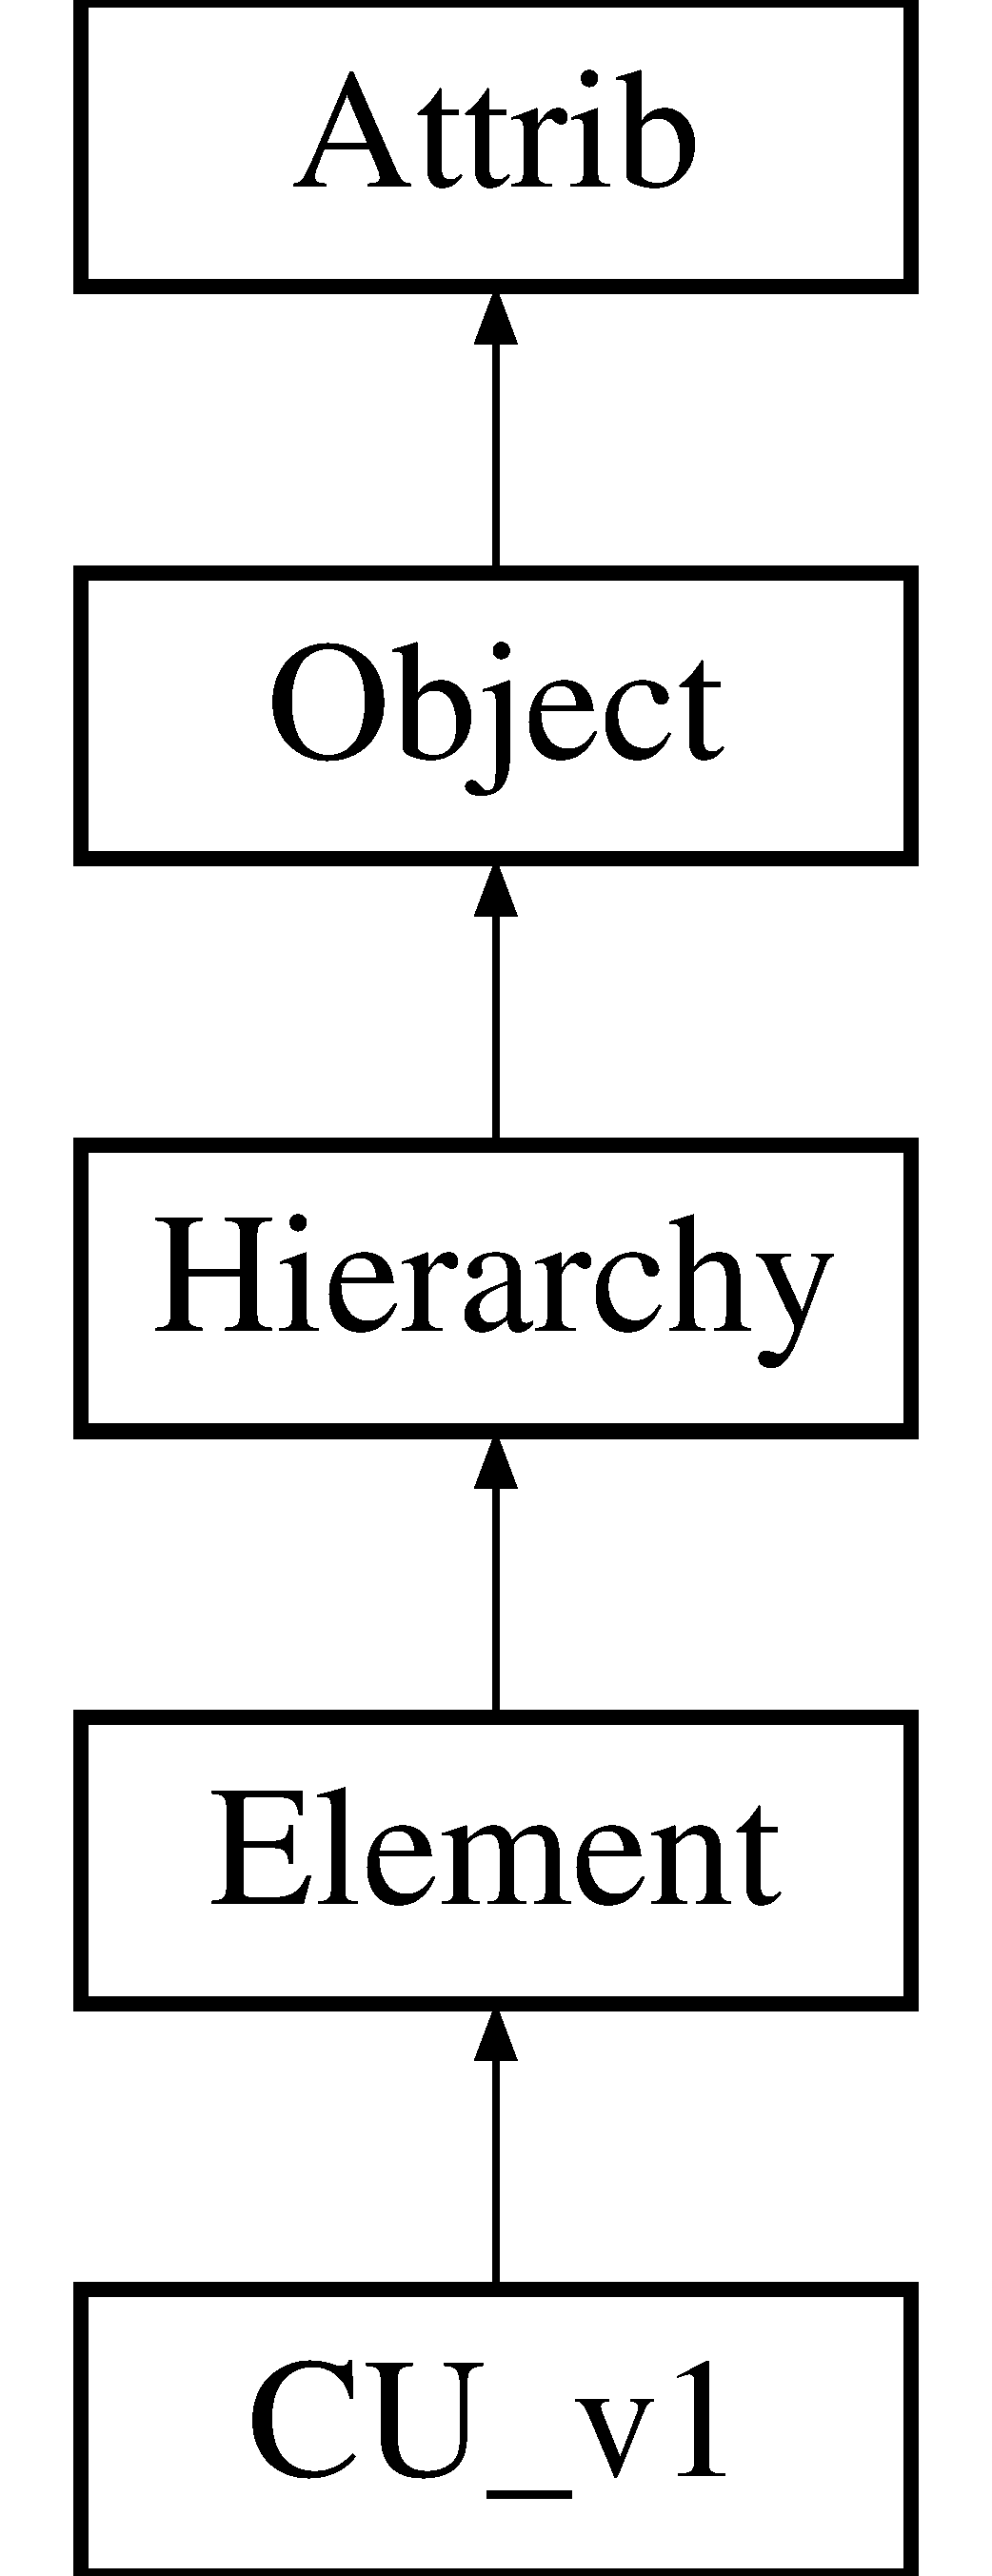
\includegraphics[height=5.000000cm]{classCU__v1}
\end{center}
\end{figure}
\subsection*{Public Member Functions}
\begin{DoxyCompactItemize}
\item 
\hyperlink{classCU__v1_afe2499a41abcb7cd94830d1eebb9e033}{C\+U\+\_\+v1} ()
\begin{DoxyCompactList}\small\item\em Standard constructor. \end{DoxyCompactList}\item 
virtual \hyperlink{classCU__v1_a5755cbfa835ce6935169e3133a5bfedf}{$\sim$\+C\+U\+\_\+v1} ()
\begin{DoxyCompactList}\small\item\em Destructor. \end{DoxyCompactList}\item 
void \hyperlink{classCU__v1_af4033fc5da7bff845565d7e6ea1802ce}{help} ()
\item 
\hyperlink{classStatusCode}{Status\+Code} \hyperlink{classCU__v1_a67278e2e8dcbd9b1e3a0284605f4103c}{init} ()
\item 
void \hyperlink{classCU__v1_add509ddd31f1a0c4d68b889ba6edfdb3}{reset} ()
\item 
void \hyperlink{classCU__v1_ac207d770edae7014f9b8ef86c43afc2c}{update} ()
\item 
\hyperlink{classFePGA}{Fe\+P\+GA} $\ast$ \hyperlink{classCU__v1_a6bdee7e086b6c0b2acee0879aee137ed}{fe\+Pga} ()
\item 
void \hyperlink{classCU__v1_ab57452edfcad0fa9efb23f8e4c532602}{read\+Fifo} (int, int, unsigned int $\ast$)
\end{DoxyCompactItemize}
\subsection*{Private Attributes}
\begin{DoxyCompactItemize}
\item 
int \hyperlink{classCU__v1_abc59a6644473bc4fdccc24e2a0c9d6ae}{m\+\_\+fifo\+Depth}
\item 
int \hyperlink{classCU__v1_a108ebddb690763d5c99dd14021fd4851}{m\+\_\+gbt\+Address} \mbox{[}1\mbox{]}
\item 
int \hyperlink{classCU__v1_acc7767c15f48718ebc1ee87e22ab9fc1}{m\+\_\+fifo\+Inject\+Address} \mbox{[}3\mbox{]}
\item 
\hyperlink{classFePGA}{Fe\+P\+GA} $\ast$ \hyperlink{classCU__v1_a1b96b95e89dbe383877b34f9b517d910}{m\+\_\+fe\+Pga}
\item 
unsigned int $\ast$ \hyperlink{classCU__v1_abdc4ba4c63bcc1bbe2d7cd2a47b02b01}{m\+\_\+fifo} \mbox{[}3\mbox{]}
\item 
\hyperlink{classData}{Data} $\ast$ \hyperlink{classCU__v1_a50b6749064da173d6a5fddf50f4398eb}{m\+\_\+data}
\item 
\hyperlink{classRAM}{R\+AM} $\ast$ \hyperlink{classCU__v1_aa662d0f99787a174650fc92fb55dbb06}{m\+\_\+ram\+Inj} \mbox{[}3\mbox{]}
\item 
\hyperlink{classRAM}{R\+AM} $\ast$ \hyperlink{classCU__v1_a87ad8f5f9ecaf5f0f70b25206e99c8e1}{m\+\_\+fifo\+Usb\+Test}
\end{DoxyCompactItemize}
\subsection*{Additional Inherited Members}


\subsection{Detailed Description}
\begin{DoxyAuthor}{Author}

\end{DoxyAuthor}
\begin{DoxyDate}{Date}
2006-\/10-\/23 
\end{DoxyDate}


Definition at line 19 of file C\+U\+\_\+v1.\+h.



\subsection{Constructor \& Destructor Documentation}
\mbox{\Hypertarget{classCU__v1_afe2499a41abcb7cd94830d1eebb9e033}\label{classCU__v1_afe2499a41abcb7cd94830d1eebb9e033}} 
\index{C\+U\+\_\+v1@{C\+U\+\_\+v1}!C\+U\+\_\+v1@{C\+U\+\_\+v1}}
\index{C\+U\+\_\+v1@{C\+U\+\_\+v1}!C\+U\+\_\+v1@{C\+U\+\_\+v1}}
\subsubsection{\texorpdfstring{C\+U\+\_\+v1()}{CU\_v1()}}
{\footnotesize\ttfamily C\+U\+\_\+v1\+::\+C\+U\+\_\+v1 (\begin{DoxyParamCaption}{ }\end{DoxyParamCaption})}



Standard constructor. 



Definition at line 17 of file C\+U\+\_\+v1.\+cpp.



References Attrib\+::add(), Hierarchy\+::add\+Child(), Attrib\+::\+E\+L\+E\+M\+E\+NT, Attrib\+::\+H\+A\+R\+D\+W\+A\+RE, m\+\_\+fe\+Pga, m\+\_\+fifo\+Depth, Object\+::set\+Name(), and Object\+::set\+Type().


\begin{DoxyCode}
17                \{
18   \hyperlink{classObject_ae30fea75683c2d149b6b6d17c09ecd0c}{setName}(\textcolor{stringliteral}{"CU\_v1"});
19   \hyperlink{classObject_aae534cc9d982bcb9b99fd505f2e103a5}{setType}(\textcolor{stringliteral}{"CU\_v1"});
20   \hyperlink{classAttrib_a235f773af19c900264a190b00a3b4ad7}{add}(\hyperlink{classAttrib_a69e171d7cc6417835a5a306d3c764235a7788bc5dd333fd8ce18562b269c9dab1}{Attrib::ELEMENT}); \hyperlink{classAttrib_a235f773af19c900264a190b00a3b4ad7}{add} (\hyperlink{classAttrib_a69e171d7cc6417835a5a306d3c764235a61ceb22149f365f1780d18f9d1459423}{Attrib::HARDWARE});  
21 
22   \hyperlink{classCU__v1_abc59a6644473bc4fdccc24e2a0c9d6ae}{m\_fifoDepth} = 1024;
23   
24   \textcolor{comment}{//m\_seqAddress   = 17 ;  // c'est l'addresse du FPGA }
25   \textcolor{comment}{//m\_fifoInjectAddress[0] = 23;  // What should I do here? }
26 
27   \hyperlink{classCU__v1_a1b96b95e89dbe383877b34f9b517d910}{m\_fePga} =\textcolor{keyword}{new} \hyperlink{classFePGA}{FePGA}();
28   \hyperlink{classCU__v1_a1b96b95e89dbe383877b34f9b517d910}{m\_fePga}->\hyperlink{classObject_ae30fea75683c2d149b6b6d17c09ecd0c}{setName}(\textcolor{stringliteral}{"FePGA"});
29   \hyperlink{classHierarchy_ad677774ff38fcb257c04a3a10d471fac}{addChild}(\hyperlink{classCU__v1_a1b96b95e89dbe383877b34f9b517d910}{m\_fePga});
30 
31   \textcolor{comment}{/*}
32 \textcolor{comment}{}
33 \textcolor{comment}{  m\_fifo[0] = new unsigned int[m\_fifoDepth];}
34 \textcolor{comment}{  }
35 \textcolor{comment}{  for (int i = 0; i<3; ++i)\{  // Do I loop up to 3 too? Car Frederic a besoin de plus de place dans les RAM}
36 \textcolor{comment}{    m\_ramInj[i] = new RAM();}
37 \textcolor{comment}{    //    m\_ramSpy[i] = new RAM();}
38 \textcolor{comment}{    fePga()->usb()->addChild(m\_ramInj[i]);  // What should I do here ? }
39 \textcolor{comment}{    //    FePga()->usb()->addChild(m\_ramSpy[i]);}
40 \textcolor{comment}{    m\_ramInj[i]->setAddress(13); // for debug   // What should I do here ? }
41 \textcolor{comment}{    //m\_ramSpy[i]->setAddress(m\_fifoSpyAddress[i]);}
42 \textcolor{comment}{    m\_ramInj[i]->setSize(16, m\_fifoDepth);   // What should I do here ? }
43 \textcolor{comment}{    // m\_ramSpy[i]->setSize(16, m\_fifoDepth);}
44 \textcolor{comment}{  \}}
45 \textcolor{comment}{}
46 \textcolor{comment}{}
47 \textcolor{comment}{}
48 \textcolor{comment}{  }
49 \textcolor{comment}{  m\_fifoUsbTest = new RAM();}
50 \textcolor{comment}{  m\_fifoUsbTest->setAddress(3); // WARNING I NEED TO CHANGE THE ADDRESS }
51 \textcolor{comment}{  m\_fifoUsbTest->setSize(16,256);  //  WHAT SIZE FOR I NNED }
52 \textcolor{comment}{  m\_fifoUsbTest->setName("FifoUsbTest");}
53 \textcolor{comment}{  fePga()->usb()->addChild(m\_fifoUsbTest);}
54 \textcolor{comment}{*/}  
55 
56 \}
\end{DoxyCode}
\mbox{\Hypertarget{classCU__v1_a5755cbfa835ce6935169e3133a5bfedf}\label{classCU__v1_a5755cbfa835ce6935169e3133a5bfedf}} 
\index{C\+U\+\_\+v1@{C\+U\+\_\+v1}!````~C\+U\+\_\+v1@{$\sim$\+C\+U\+\_\+v1}}
\index{````~C\+U\+\_\+v1@{$\sim$\+C\+U\+\_\+v1}!C\+U\+\_\+v1@{C\+U\+\_\+v1}}
\subsubsection{\texorpdfstring{$\sim$\+C\+U\+\_\+v1()}{~CU\_v1()}}
{\footnotesize\ttfamily C\+U\+\_\+v1\+::$\sim$\+C\+U\+\_\+v1 (\begin{DoxyParamCaption}{ }\end{DoxyParamCaption})\hspace{0.3cm}{\ttfamily [virtual]}}



Destructor. 



Definition at line 60 of file C\+U\+\_\+v1.\+cpp.


\begin{DoxyCode}
60               \{
61 \}
\end{DoxyCode}


\subsection{Member Function Documentation}
\mbox{\Hypertarget{classCU__v1_a6bdee7e086b6c0b2acee0879aee137ed}\label{classCU__v1_a6bdee7e086b6c0b2acee0879aee137ed}} 
\index{C\+U\+\_\+v1@{C\+U\+\_\+v1}!fe\+Pga@{fe\+Pga}}
\index{fe\+Pga@{fe\+Pga}!C\+U\+\_\+v1@{C\+U\+\_\+v1}}
\subsubsection{\texorpdfstring{fe\+Pga()}{fePga()}}
{\footnotesize\ttfamily \hyperlink{classFePGA}{Fe\+P\+GA}$\ast$ C\+U\+\_\+v1\+::fe\+Pga (\begin{DoxyParamCaption}{ }\end{DoxyParamCaption})\hspace{0.3cm}{\ttfamily [inline]}}



Definition at line 56 of file C\+U\+\_\+v1.\+h.



References m\+\_\+fe\+Pga, and read\+Fifo().



Referenced by B\+O\+O\+S\+T\+\_\+\+P\+Y\+T\+H\+O\+N\+\_\+\+M\+O\+D\+U\+L\+E().


\begin{DoxyCode}
56                 \{
57     \textcolor{keywordflow}{return} \hyperlink{classCU__v1_a1b96b95e89dbe383877b34f9b517d910}{m\_fePga};
58   \}
\end{DoxyCode}
\mbox{\Hypertarget{classCU__v1_af4033fc5da7bff845565d7e6ea1802ce}\label{classCU__v1_af4033fc5da7bff845565d7e6ea1802ce}} 
\index{C\+U\+\_\+v1@{C\+U\+\_\+v1}!help@{help}}
\index{help@{help}!C\+U\+\_\+v1@{C\+U\+\_\+v1}}
\subsubsection{\texorpdfstring{help()}{help()}}
{\footnotesize\ttfamily void C\+U\+\_\+v1\+::help (\begin{DoxyParamCaption}{ }\end{DoxyParamCaption})\hspace{0.3cm}{\ttfamily [inline]}, {\ttfamily [virtual]}}

printout help for the element 

Implements \hyperlink{classElement_a32c0de27acb08e17251cef88c3e9303a}{Element}.



Definition at line 29 of file C\+U\+\_\+v1.\+h.



References Object\+::info(), and Object\+::name().


\begin{DoxyCode}
29 \{ \hyperlink{classObject_a644fd329ea4cb85f54fa6846484b84a8}{info}(\textcolor{stringliteral}{"CU\_v1 "}+\hyperlink{classObject_a300f4c05dd468c7bb8b3c968868443c1}{name}()+\textcolor{stringliteral}{". No help."},\textcolor{stringliteral}{"CU\_v1::help"}); \};
\end{DoxyCode}
\mbox{\Hypertarget{classCU__v1_a67278e2e8dcbd9b1e3a0284605f4103c}\label{classCU__v1_a67278e2e8dcbd9b1e3a0284605f4103c}} 
\index{C\+U\+\_\+v1@{C\+U\+\_\+v1}!init@{init}}
\index{init@{init}!C\+U\+\_\+v1@{C\+U\+\_\+v1}}
\subsubsection{\texorpdfstring{init()}{init()}}
{\footnotesize\ttfamily \hyperlink{classStatusCode}{Status\+Code} C\+U\+\_\+v1\+::init (\begin{DoxyParamCaption}{ }\end{DoxyParamCaption})\hspace{0.3cm}{\ttfamily [inline]}, {\ttfamily [virtual]}}

init the component

\begin{DoxyReturn}{Returns}
void 
\end{DoxyReturn}


Implements \hyperlink{classElement_af42754b5cabc198869222725218d695c}{Element}.



Definition at line 35 of file C\+U\+\_\+v1.\+h.



References Status\+Code\+::\+S\+U\+C\+C\+E\+SS.


\begin{DoxyCode}
35                     \{
36     \textcolor{keywordflow}{return} \hyperlink{classStatusCode_a6f565cbeadc76d14c72f047e5e85eb4badd0da38d3ba0d922efd1f4619bc37ad8}{StatusCode::SUCCESS};
37   \};
\end{DoxyCode}
\mbox{\Hypertarget{classCU__v1_ab57452edfcad0fa9efb23f8e4c532602}\label{classCU__v1_ab57452edfcad0fa9efb23f8e4c532602}} 
\index{C\+U\+\_\+v1@{C\+U\+\_\+v1}!read\+Fifo@{read\+Fifo}}
\index{read\+Fifo@{read\+Fifo}!C\+U\+\_\+v1@{C\+U\+\_\+v1}}
\subsubsection{\texorpdfstring{read\+Fifo()}{readFifo()}}
{\footnotesize\ttfamily void C\+U\+\_\+v1\+::read\+Fifo (\begin{DoxyParamCaption}\item[{int}]{add,  }\item[{int}]{subadd,  }\item[{unsigned int $\ast$}]{fifo }\end{DoxyParamCaption})}



Definition at line 64 of file C\+U\+\_\+v1.\+cpp.



References m\+\_\+fe\+Pga, m\+\_\+fifo\+Depth, and Fe\+P\+G\+A\+::spi\+Read().



Referenced by B\+O\+O\+S\+T\+\_\+\+P\+Y\+T\+H\+O\+N\+\_\+\+M\+O\+D\+U\+L\+E(), and fe\+Pga().


\begin{DoxyCode}
64                                                              \{
65 \hyperlink{classCU__v1_a1b96b95e89dbe383877b34f9b517d910}{m\_fePga}->\hyperlink{classFePGA_a637b93fed75b576a54e723acb36cb6a3}{spiRead}(subadd, \hyperlink{classCU__v1_abc59a6644473bc4fdccc24e2a0c9d6ae}{m\_fifoDepth}, fifo); \textcolor{comment}{// Question why do we read the fifo
       with spi? /}
66 \}
\end{DoxyCode}
\mbox{\Hypertarget{classCU__v1_add509ddd31f1a0c4d68b889ba6edfdb3}\label{classCU__v1_add509ddd31f1a0c4d68b889ba6edfdb3}} 
\index{C\+U\+\_\+v1@{C\+U\+\_\+v1}!reset@{reset}}
\index{reset@{reset}!C\+U\+\_\+v1@{C\+U\+\_\+v1}}
\subsubsection{\texorpdfstring{reset()}{reset()}}
{\footnotesize\ttfamily void C\+U\+\_\+v1\+::reset (\begin{DoxyParamCaption}{ }\end{DoxyParamCaption})\hspace{0.3cm}{\ttfamily [inline]}, {\ttfamily [virtual]}}

Resets the \hyperlink{classElement}{Element} so that is is in a standard and safe situation. Different from \hyperlink{classElement_af42754b5cabc198869222725218d695c}{Element\+::init} which configure the \hyperlink{classElement}{Element}. \hyperlink{classElement_a69efffa22f06909d768149715565cb56}{Element\+::reset()} is more an Emergency pull. It is often/usually called by the recursive\+Init\+Element method at the start of the program. 

Implements \hyperlink{classElement_a69efffa22f06909d768149715565cb56}{Element}.



Definition at line 46 of file C\+U\+\_\+v1.\+h.



References Object\+::debug(), m\+\_\+fe\+Pga, Object\+::name(), and Fe\+P\+G\+A\+::reset().


\begin{DoxyCode}
46                \{
47     \hyperlink{classCU__v1_a1b96b95e89dbe383877b34f9b517d910}{m\_fePga}->\hyperlink{classFePGA_abdf7a9dd901351a7eafd748d35172a3c}{reset}();
48     \hyperlink{classObject_aac010553f022165573714b7014a15f0d}{debug}(\textcolor{stringliteral}{"CU\_v1 "}+\hyperlink{classObject_a300f4c05dd468c7bb8b3c968868443c1}{name}()+\textcolor{stringliteral}{" reset."},\textcolor{stringliteral}{"CU\_v1::reset"});
49   \};
\end{DoxyCode}
\mbox{\Hypertarget{classCU__v1_ac207d770edae7014f9b8ef86c43afc2c}\label{classCU__v1_ac207d770edae7014f9b8ef86c43afc2c}} 
\index{C\+U\+\_\+v1@{C\+U\+\_\+v1}!update@{update}}
\index{update@{update}!C\+U\+\_\+v1@{C\+U\+\_\+v1}}
\subsubsection{\texorpdfstring{update()}{update()}}
{\footnotesize\ttfamily void C\+U\+\_\+v1\+::update (\begin{DoxyParamCaption}{ }\end{DoxyParamCaption})\hspace{0.3cm}{\ttfamily [inline]}, {\ttfamily [virtual]}}

Update the \hyperlink{classElement}{Element} configuration from the actual hardware 

Implements \hyperlink{classElement_a4e6c83efae95616ebddd03c793a26661}{Element}.



Definition at line 54 of file C\+U\+\_\+v1.\+h.



References Object\+::info(), and Object\+::name().



Referenced by App\+Frame.\+App\+Frame\+::delete\+Hardware(), Conf\+Frame.\+Conf\+Frame\+::on\+Change(), Graph\+Frame.\+Graph\+Frame\+::on\+Change(), Cfg\+Frame.\+Cfg\+Frame\+::on\+Change(), Conf\+Frame.\+Conf\+Frame\+::on\+Edit(), App\+Frame.\+App\+Frame\+::on\+Load(), Conf\+Frame.\+Conf\+Frame\+::on\+Re\+Load(), Graph\+Frame.\+Graph\+Frame\+::on\+Re\+Load(), Cfg\+Frame.\+Cfg\+Frame\+::on\+Re\+Load(), and App\+Frame.\+App\+Frame\+::on\+Re\+Load().


\begin{DoxyCode}
54 \{\hyperlink{classObject_a644fd329ea4cb85f54fa6846484b84a8}{info}(\textcolor{stringliteral}{"CU\_v1 "}+\hyperlink{classObject_a300f4c05dd468c7bb8b3c968868443c1}{name}()+\textcolor{stringliteral}{". Nothing to do."},\textcolor{stringliteral}{"CU\_v1::update"});\};
\end{DoxyCode}


\subsection{Member Data Documentation}
\mbox{\Hypertarget{classCU__v1_a50b6749064da173d6a5fddf50f4398eb}\label{classCU__v1_a50b6749064da173d6a5fddf50f4398eb}} 
\index{C\+U\+\_\+v1@{C\+U\+\_\+v1}!m\+\_\+data@{m\+\_\+data}}
\index{m\+\_\+data@{m\+\_\+data}!C\+U\+\_\+v1@{C\+U\+\_\+v1}}
\subsubsection{\texorpdfstring{m\+\_\+data}{m\_data}}
{\footnotesize\ttfamily \hyperlink{classData}{Data}$\ast$ C\+U\+\_\+v1\+::m\+\_\+data\hspace{0.3cm}{\ttfamily [private]}}



Definition at line 70 of file C\+U\+\_\+v1.\+h.

\mbox{\Hypertarget{classCU__v1_a1b96b95e89dbe383877b34f9b517d910}\label{classCU__v1_a1b96b95e89dbe383877b34f9b517d910}} 
\index{C\+U\+\_\+v1@{C\+U\+\_\+v1}!m\+\_\+fe\+Pga@{m\+\_\+fe\+Pga}}
\index{m\+\_\+fe\+Pga@{m\+\_\+fe\+Pga}!C\+U\+\_\+v1@{C\+U\+\_\+v1}}
\subsubsection{\texorpdfstring{m\+\_\+fe\+Pga}{m\_fePga}}
{\footnotesize\ttfamily \hyperlink{classFePGA}{Fe\+P\+GA}$\ast$ C\+U\+\_\+v1\+::m\+\_\+fe\+Pga\hspace{0.3cm}{\ttfamily [private]}}



Definition at line 68 of file C\+U\+\_\+v1.\+h.



Referenced by C\+U\+\_\+v1(), fe\+Pga(), read\+Fifo(), and reset().

\mbox{\Hypertarget{classCU__v1_abdc4ba4c63bcc1bbe2d7cd2a47b02b01}\label{classCU__v1_abdc4ba4c63bcc1bbe2d7cd2a47b02b01}} 
\index{C\+U\+\_\+v1@{C\+U\+\_\+v1}!m\+\_\+fifo@{m\+\_\+fifo}}
\index{m\+\_\+fifo@{m\+\_\+fifo}!C\+U\+\_\+v1@{C\+U\+\_\+v1}}
\subsubsection{\texorpdfstring{m\+\_\+fifo}{m\_fifo}}
{\footnotesize\ttfamily unsigned int$\ast$ C\+U\+\_\+v1\+::m\+\_\+fifo\mbox{[}3\mbox{]}\hspace{0.3cm}{\ttfamily [private]}}



Definition at line 69 of file C\+U\+\_\+v1.\+h.

\mbox{\Hypertarget{classCU__v1_abc59a6644473bc4fdccc24e2a0c9d6ae}\label{classCU__v1_abc59a6644473bc4fdccc24e2a0c9d6ae}} 
\index{C\+U\+\_\+v1@{C\+U\+\_\+v1}!m\+\_\+fifo\+Depth@{m\+\_\+fifo\+Depth}}
\index{m\+\_\+fifo\+Depth@{m\+\_\+fifo\+Depth}!C\+U\+\_\+v1@{C\+U\+\_\+v1}}
\subsubsection{\texorpdfstring{m\+\_\+fifo\+Depth}{m\_fifoDepth}}
{\footnotesize\ttfamily int C\+U\+\_\+v1\+::m\+\_\+fifo\+Depth\hspace{0.3cm}{\ttfamily [private]}}



Definition at line 65 of file C\+U\+\_\+v1.\+h.



Referenced by C\+U\+\_\+v1(), and read\+Fifo().

\mbox{\Hypertarget{classCU__v1_acc7767c15f48718ebc1ee87e22ab9fc1}\label{classCU__v1_acc7767c15f48718ebc1ee87e22ab9fc1}} 
\index{C\+U\+\_\+v1@{C\+U\+\_\+v1}!m\+\_\+fifo\+Inject\+Address@{m\+\_\+fifo\+Inject\+Address}}
\index{m\+\_\+fifo\+Inject\+Address@{m\+\_\+fifo\+Inject\+Address}!C\+U\+\_\+v1@{C\+U\+\_\+v1}}
\subsubsection{\texorpdfstring{m\+\_\+fifo\+Inject\+Address}{m\_fifoInjectAddress}}
{\footnotesize\ttfamily int C\+U\+\_\+v1\+::m\+\_\+fifo\+Inject\+Address\mbox{[}3\mbox{]}\hspace{0.3cm}{\ttfamily [private]}}



Definition at line 67 of file C\+U\+\_\+v1.\+h.

\mbox{\Hypertarget{classCU__v1_a87ad8f5f9ecaf5f0f70b25206e99c8e1}\label{classCU__v1_a87ad8f5f9ecaf5f0f70b25206e99c8e1}} 
\index{C\+U\+\_\+v1@{C\+U\+\_\+v1}!m\+\_\+fifo\+Usb\+Test@{m\+\_\+fifo\+Usb\+Test}}
\index{m\+\_\+fifo\+Usb\+Test@{m\+\_\+fifo\+Usb\+Test}!C\+U\+\_\+v1@{C\+U\+\_\+v1}}
\subsubsection{\texorpdfstring{m\+\_\+fifo\+Usb\+Test}{m\_fifoUsbTest}}
{\footnotesize\ttfamily \hyperlink{classRAM}{R\+AM}$\ast$ C\+U\+\_\+v1\+::m\+\_\+fifo\+Usb\+Test\hspace{0.3cm}{\ttfamily [private]}}



Definition at line 72 of file C\+U\+\_\+v1.\+h.

\mbox{\Hypertarget{classCU__v1_a108ebddb690763d5c99dd14021fd4851}\label{classCU__v1_a108ebddb690763d5c99dd14021fd4851}} 
\index{C\+U\+\_\+v1@{C\+U\+\_\+v1}!m\+\_\+gbt\+Address@{m\+\_\+gbt\+Address}}
\index{m\+\_\+gbt\+Address@{m\+\_\+gbt\+Address}!C\+U\+\_\+v1@{C\+U\+\_\+v1}}
\subsubsection{\texorpdfstring{m\+\_\+gbt\+Address}{m\_gbtAddress}}
{\footnotesize\ttfamily int C\+U\+\_\+v1\+::m\+\_\+gbt\+Address\mbox{[}1\mbox{]}\hspace{0.3cm}{\ttfamily [private]}}



Definition at line 66 of file C\+U\+\_\+v1.\+h.

\mbox{\Hypertarget{classCU__v1_aa662d0f99787a174650fc92fb55dbb06}\label{classCU__v1_aa662d0f99787a174650fc92fb55dbb06}} 
\index{C\+U\+\_\+v1@{C\+U\+\_\+v1}!m\+\_\+ram\+Inj@{m\+\_\+ram\+Inj}}
\index{m\+\_\+ram\+Inj@{m\+\_\+ram\+Inj}!C\+U\+\_\+v1@{C\+U\+\_\+v1}}
\subsubsection{\texorpdfstring{m\+\_\+ram\+Inj}{m\_ramInj}}
{\footnotesize\ttfamily \hyperlink{classRAM}{R\+AM}$\ast$ C\+U\+\_\+v1\+::m\+\_\+ram\+Inj\mbox{[}3\mbox{]}\hspace{0.3cm}{\ttfamily [private]}}



Definition at line 71 of file C\+U\+\_\+v1.\+h.



The documentation for this class was generated from the following files\+:\begin{DoxyCompactItemize}
\item 
/home/eleclhcb/\+L\+H\+Cb/lbcat-\/cmake/\+Cat\+Calo\+Upgrade/inc/\hyperlink{CU__v1_8h}{C\+U\+\_\+v1.\+h}\item 
/home/eleclhcb/\+L\+H\+Cb/lbcat-\/cmake/\+Cat\+Calo\+Upgrade/src/\hyperlink{CU__v1_8cpp}{C\+U\+\_\+v1.\+cpp}\end{DoxyCompactItemize}

\hypertarget{classCurrentMeasurement}{}\section{Current\+Measurement Class Reference}
\label{classCurrentMeasurement}\index{Current\+Measurement@{Current\+Measurement}}


{\ttfamily \#include $<$include/\+Current\+Measurement.\+h$>$}

Inheritance diagram for Current\+Measurement\+:\begin{figure}[H]
\begin{center}
\leavevmode
\includegraphics[height=4.000000cm]{classCurrentMeasurement}
\end{center}
\end{figure}
\subsection*{Classes}
\begin{DoxyCompactItemize}
\item 
class \hyperlink{classCurrentMeasurement_1_1CurrentMeasurement}{Current\+Measurement}
\end{DoxyCompactItemize}
\subsection*{Public Member Functions}
\begin{DoxyCompactItemize}
\item 
\hyperlink{classCurrentMeasurement_ad89184bc1f2386b71051d7976ec662f1}{Current\+Measurement} ()
\begin{DoxyCompactList}\small\item\em Standard constructor. \end{DoxyCompactList}\item 
virtual \hyperlink{classCurrentMeasurement_a86c291508b913b4b028567eeb8995c83}{$\sim$\+Current\+Measurement} ()
\item 
virtual \hyperlink{classStatusCode}{Status\+Code} \hyperlink{classCurrentMeasurement_a88d397682cb5847d5710d08544b6f4c6}{initialize} ()
\begin{DoxyCompactList}\small\item\em Destructor. \end{DoxyCompactList}\item 
virtual \hyperlink{classStatusCode}{Status\+Code} \hyperlink{classCurrentMeasurement_a19ae0dcc63b4151ceebe0bf2c42da948}{execute} ()
\item 
virtual \hyperlink{classStatusCode}{Status\+Code} \hyperlink{classCurrentMeasurement_af87fa329a11212c10e878568bcecaeb3}{finalize} ()
\item 
int \hyperlink{classCurrentMeasurement_a646a9953d7aef3bad2e2dacaab31c241}{number\+Of\+Devices} ()
\item 
\hyperlink{classStatusCode}{Status\+Code} \hyperlink{classCurrentMeasurement_ae990f376398bc25891eaddcb245fdf46}{set\+Frequency} (unsigned int \hyperlink{classCurrentMeasurement_ae7c60d0b14808000df5f1d633e0ca990}{frequency})
\item 
unsigned int \hyperlink{classCurrentMeasurement_ae7c60d0b14808000df5f1d633e0ca990}{frequency} ()
\end{DoxyCompactItemize}
\subsection*{Protected Member Functions}
\begin{DoxyCompactItemize}
\item 
\hyperlink{classCurrentMeasurement_1_1CurrentMeasurement}{Current\+Measurement} $\ast$ \hyperlink{classCurrentMeasurement_a7722435fcc404fe4761c3fa96f3b6338}{clone} ()
\end{DoxyCompactItemize}
\subsection*{Private Attributes}
\begin{DoxyCompactItemize}
\item 
T\+Random $\ast$ \hyperlink{classCurrentMeasurement_ac0c595b78b8110a19b59a333a6c27c1b}{m\+\_\+rnd}
\item 
unsigned int \hyperlink{classCurrentMeasurement_a66e12903825632c0434e3b7cf929a960}{m\+\_\+frequency}
\item 
\hyperlink{classNI6008}{N\+I6008} $\ast$ \hyperlink{classCurrentMeasurement_a7df157175089da57bd020b8680e87f80}{m\+\_\+device}
\item 
unsigned int \hyperlink{classCurrentMeasurement_a073f6aba41750712d620e60e346f2315}{m\+\_\+number\+Of\+Devices}
\item 
T\+Tree $\ast$ \hyperlink{classCurrentMeasurement_a559823413932b393dedfc62d42268d93}{m\+\_\+tree}
\item 
Int\+\_\+t \hyperlink{classCurrentMeasurement_a5a7bfe59821148e4e9e2998c73b635a8}{m\+\_\+run\+Number}
\item 
Int\+\_\+t \hyperlink{classCurrentMeasurement_a6e01f96c84aec986de9a9f7393ccb2c6}{m\+\_\+evt\+Number}
\item 
Int\+\_\+t \hyperlink{classCurrentMeasurement_acc9f2cabf165e47a9fbf2a357e424cef}{m\+\_\+timestamp} \mbox{[}4\mbox{]}
\item 
Int\+\_\+t \hyperlink{classCurrentMeasurement_ad08307f13d37c05e1a4e42ff39c97911}{m\+\_\+duration} \mbox{[}4\mbox{]}
\item 
time\+\_\+t \hyperlink{classCurrentMeasurement_abd5a7612f08721143623add96797a433}{m\+\_\+start\+Time}
\item 
double \hyperlink{classCurrentMeasurement_a793b1467b6a5388361340d41f9e8833f}{m\+\_\+ai0} \mbox{[}4\mbox{]}
\item 
double \hyperlink{classCurrentMeasurement_aeef18708be94b89de9c4384dd452207d}{m\+\_\+ai1} \mbox{[}4\mbox{]}
\item 
double \hyperlink{classCurrentMeasurement_a27ce0cfd8d1c04f6cd4d8de0403fafba}{m\+\_\+ai2} \mbox{[}4\mbox{]}
\item 
double \hyperlink{classCurrentMeasurement_aa1223e4b36335ceb507edd12d4cfa8ad}{m\+\_\+ai3} \mbox{[}4\mbox{]}
\end{DoxyCompactItemize}
\subsection*{Additional Inherited Members}


\subsection{Detailed Description}
\begin{DoxyAuthor}{Author}
Frederic Machefert 
\end{DoxyAuthor}
\begin{DoxyDate}{Date}
2010-\/01-\/07 
\end{DoxyDate}


Definition at line 23 of file Current\+Measurement.\+h.



\subsection{Constructor \& Destructor Documentation}
\mbox{\Hypertarget{classCurrentMeasurement_ad89184bc1f2386b71051d7976ec662f1}\label{classCurrentMeasurement_ad89184bc1f2386b71051d7976ec662f1}} 
\index{Current\+Measurement@{Current\+Measurement}!Current\+Measurement@{Current\+Measurement}}
\index{Current\+Measurement@{Current\+Measurement}!Current\+Measurement@{Current\+Measurement}}
\subsubsection{\texorpdfstring{Current\+Measurement()}{CurrentMeasurement()}}
{\footnotesize\ttfamily \hyperlink{classCurrentMeasurement_1_1CurrentMeasurement}{Current\+Measurement\+::\+Current\+Measurement} (\begin{DoxyParamCaption}{ }\end{DoxyParamCaption})}



Standard constructor. 



Definition at line 26 of file Current\+Measurement.\+cpp.



References m\+\_\+device, Object\+::set\+Name(), Object\+::set\+Title(), and Object\+::set\+Type().



Referenced by clone().


\begin{DoxyCode}
26                                         \{
27   \hyperlink{classObject_ae30fea75683c2d149b6b6d17c09ecd0c}{setName} ( \textcolor{stringliteral}{"CurrentMeasurement"} );
28   \hyperlink{classObject_aae534cc9d982bcb9b99fd505f2e103a5}{setType} ( \textcolor{stringliteral}{"NI6008"} );
29   \hyperlink{classObject_a89557dbbad5bcaa02652f5d7fa35d20f}{setTitle}( \textcolor{stringliteral}{"NI6008 current measurement"} );  
30   \hyperlink{classCurrentMeasurement_a7df157175089da57bd020b8680e87f80}{m\_device} = 0; 
31 \}
\end{DoxyCode}
\mbox{\Hypertarget{classCurrentMeasurement_a86c291508b913b4b028567eeb8995c83}\label{classCurrentMeasurement_a86c291508b913b4b028567eeb8995c83}} 
\index{Current\+Measurement@{Current\+Measurement}!````~Current\+Measurement@{$\sim$\+Current\+Measurement}}
\index{````~Current\+Measurement@{$\sim$\+Current\+Measurement}!Current\+Measurement@{Current\+Measurement}}
\subsubsection{\texorpdfstring{$\sim$\+Current\+Measurement()}{~CurrentMeasurement()}}
{\footnotesize\ttfamily virtual Current\+Measurement\+::$\sim$\+Current\+Measurement (\begin{DoxyParamCaption}{ }\end{DoxyParamCaption})\hspace{0.3cm}{\ttfamily [inline]}, {\ttfamily [virtual]}}



Definition at line 28 of file Current\+Measurement.\+h.



References execute(), finalize(), and initialize().


\begin{DoxyCode}
28 \{\}; 
\end{DoxyCode}


\subsection{Member Function Documentation}
\mbox{\Hypertarget{classCurrentMeasurement_a7722435fcc404fe4761c3fa96f3b6338}\label{classCurrentMeasurement_a7722435fcc404fe4761c3fa96f3b6338}} 
\index{Current\+Measurement@{Current\+Measurement}!clone@{clone}}
\index{clone@{clone}!Current\+Measurement@{Current\+Measurement}}
\subsubsection{\texorpdfstring{clone()}{clone()}}
{\footnotesize\ttfamily \hyperlink{classCurrentMeasurement_1_1CurrentMeasurement}{Current\+Measurement}$\ast$ Current\+Measurement\+::clone (\begin{DoxyParamCaption}{ }\end{DoxyParamCaption})\hspace{0.3cm}{\ttfamily [inline]}, {\ttfamily [protected]}, {\ttfamily [virtual]}}

processus termination virtual function 

Implements \hyperlink{classProcessus_aca8856f6d6d7b7e1fe941f298dcbb502}{Processus}.



Definition at line 67 of file Current\+Measurement.\+h.



References Current\+Measurement().


\begin{DoxyCode}
67                              \{
68     \textcolor{keywordflow}{return} \textcolor{keyword}{new} \hyperlink{classCurrentMeasurement_ad89184bc1f2386b71051d7976ec662f1}{CurrentMeasurement} (*\textcolor{keyword}{this});
69   \};
\end{DoxyCode}
\mbox{\Hypertarget{classCurrentMeasurement_a19ae0dcc63b4151ceebe0bf2c42da948}\label{classCurrentMeasurement_a19ae0dcc63b4151ceebe0bf2c42da948}} 
\index{Current\+Measurement@{Current\+Measurement}!execute@{execute}}
\index{execute@{execute}!Current\+Measurement@{Current\+Measurement}}
\subsubsection{\texorpdfstring{execute()}{execute()}}
{\footnotesize\ttfamily \hyperlink{classStatusCode}{Status\+Code} Current\+Measurement\+::execute (\begin{DoxyParamCaption}{ }\end{DoxyParamCaption})\hspace{0.3cm}{\ttfamily [virtual]}}

processus execution virtual function 

Implements \hyperlink{classProcessus_a63767a63a1fb0055c5aa45b21a4a5d58}{Processus}.



Definition at line 75 of file Current\+Measurement.\+cpp.



References application(), N\+I6008\+::cmd(), Processus\+::data\+Fill(), N\+I6008\+::device(), m\+\_\+ai0, m\+\_\+ai1, m\+\_\+ai2, m\+\_\+ai3, m\+\_\+device, m\+\_\+duration, m\+\_\+evt\+Number, m\+\_\+frequency, m\+\_\+start\+Time, m\+\_\+timestamp, m\+\_\+tree, Options\+::n\+Evt(), N\+I6008\+::number\+Of\+Devices(), Application\+::options(), Status\+Code\+::\+S\+U\+C\+C\+E\+SS, and wait().



Referenced by $\sim$\+Current\+Measurement().


\begin{DoxyCode}
75                                          \{
76   \textcolor{keywordflow}{for} (\textcolor{keywordtype}{int} i = 0; i<\hyperlink{classCurrentMeasurement_a7df157175089da57bd020b8680e87f80}{m\_device}->\hyperlink{classNI6008_a293fbf44b101e82a57404d1c76f07a87}{numberOfDevices}(); ++i)\{
77     std::string dev = \hyperlink{classCurrentMeasurement_a7df157175089da57bd020b8680e87f80}{m\_device}->\hyperlink{classNI6008_a6535ca8405fae42942e7011684113774}{device}(i);
78     std::string val = \hyperlink{classCurrentMeasurement_a7df157175089da57bd020b8680e87f80}{m\_device}->\hyperlink{classNI6008_a0d7584a656abca03fd59c555cb66822c}{cmd}(dev, \textcolor{stringliteral}{"ai"});
79     std::istringstream splitval(val);
80     std::string v0, v1, v2, v3;
81     splitval >> v0;
82     splitval >> v1;
83     splitval >> v2;
84     splitval >> v3;
85     \textcolor{comment}{// m\_ai0[i]=toDouble(v0);}
86     \textcolor{comment}{// m\_ai1[i]=toDouble(v1);}
87     \textcolor{comment}{// m\_ai2[i]=toDouble(v2);}
88     \textcolor{comment}{// m\_ai3[i]=toDouble(v3);}
89     \hyperlink{classCurrentMeasurement_a793b1467b6a5388361340d41f9e8833f}{m\_ai0}[i]=atof(v0.c\_str());
90     \hyperlink{classCurrentMeasurement_aeef18708be94b89de9c4384dd452207d}{m\_ai1}[i]=atof(v1.c\_str());
91     \hyperlink{classCurrentMeasurement_a27ce0cfd8d1c04f6cd4d8de0403fafba}{m\_ai2}[i]=atof(v2.c\_str());
92     \hyperlink{classCurrentMeasurement_aa1223e4b36335ceb507edd12d4cfa8ad}{m\_ai3}[i]=atof(v3.c\_str());
93     time\_t t = time(0);
94     \hyperlink{classCurrentMeasurement_acc9f2cabf165e47a9fbf2a357e424cef}{m\_timestamp}[i]=t;
95     \hyperlink{classCurrentMeasurement_ad08307f13d37c05e1a4e42ff39c97911}{m\_duration}[i]=difftime(t, \hyperlink{classCurrentMeasurement_abd5a7612f08721143623add96797a433}{m\_startTime});
96     \hyperlink{classProcessus_a0d093b48f3218a088ba030e24372f18c}{dataFill}(0+5*i, \hyperlink{classCurrentMeasurement_ad08307f13d37c05e1a4e42ff39c97911}{m\_duration}[i]);
97     \hyperlink{classProcessus_a0d093b48f3218a088ba030e24372f18c}{dataFill}(1+5*i, \hyperlink{classCurrentMeasurement_a793b1467b6a5388361340d41f9e8833f}{m\_ai0}[i]);
98     \hyperlink{classProcessus_a0d093b48f3218a088ba030e24372f18c}{dataFill}(2+5*i, m\_ai1[i]);
99     \hyperlink{classProcessus_a0d093b48f3218a088ba030e24372f18c}{dataFill}(3+5*i, m\_ai2[i]);
100     \hyperlink{classProcessus_a0d093b48f3218a088ba030e24372f18c}{dataFill}(4+5*i, m\_ai3[i]);
101   \}
102   \textcolor{keywordflow}{if} (\hyperlink{Tools_8h_a27885a3c35afe79029fb830f32f66458}{application}()->options()->dataStorage())\{
103     \hyperlink{classCurrentMeasurement_a6e01f96c84aec986de9a9f7393ccb2c6}{m\_evtNumber}=\hyperlink{Tools_8h_a27885a3c35afe79029fb830f32f66458}{application}()->\hyperlink{classApplication_ada7cc0e8db586985f1435aee0c79f47d}{options}()->\hyperlink{classOptions_ad769b256263a4ac24dd6f989ae724ab7}{nEvt}()-1;
104     \hyperlink{classCurrentMeasurement_a559823413932b393dedfc62d42268d93}{m\_tree}->Fill();
105   \}
106   \hyperlink{Tools_8h_a74d6a3fc8194eaac3e1f888db0542be9}{wait}(\hyperlink{classCurrentMeasurement_a66e12903825632c0434e3b7cf929a960}{m\_frequency});
107   \textcolor{keywordflow}{return} \hyperlink{classStatusCode_a6f565cbeadc76d14c72f047e5e85eb4badd0da38d3ba0d922efd1f4619bc37ad8}{StatusCode::SUCCESS};
108 \}
\end{DoxyCode}
\mbox{\Hypertarget{classCurrentMeasurement_af87fa329a11212c10e878568bcecaeb3}\label{classCurrentMeasurement_af87fa329a11212c10e878568bcecaeb3}} 
\index{Current\+Measurement@{Current\+Measurement}!finalize@{finalize}}
\index{finalize@{finalize}!Current\+Measurement@{Current\+Measurement}}
\subsubsection{\texorpdfstring{finalize()}{finalize()}}
{\footnotesize\ttfamily \hyperlink{classStatusCode}{Status\+Code} Current\+Measurement\+::finalize (\begin{DoxyParamCaption}{ }\end{DoxyParamCaption})\hspace{0.3cm}{\ttfamily [virtual]}}

processus termination virtual function 

Implements \hyperlink{classProcessus_aba93d691f031bdb18ae4b8afb1b2e856}{Processus}.



Definition at line 113 of file Current\+Measurement.\+cpp.



References Status\+Code\+::\+S\+U\+C\+C\+E\+SS.



Referenced by $\sim$\+Current\+Measurement().


\begin{DoxyCode}
113                                           \{
114   \textcolor{comment}{// if (application()->options()->dataStorage())\{}
115   \textcolor{comment}{//   m\_tree->Print();}
116   \textcolor{comment}{// \}}
117   \textcolor{keywordflow}{return} \hyperlink{classStatusCode_a6f565cbeadc76d14c72f047e5e85eb4badd0da38d3ba0d922efd1f4619bc37ad8}{StatusCode::SUCCESS};
118 \}
\end{DoxyCode}
\mbox{\Hypertarget{classCurrentMeasurement_ae7c60d0b14808000df5f1d633e0ca990}\label{classCurrentMeasurement_ae7c60d0b14808000df5f1d633e0ca990}} 
\index{Current\+Measurement@{Current\+Measurement}!frequency@{frequency}}
\index{frequency@{frequency}!Current\+Measurement@{Current\+Measurement}}
\subsubsection{\texorpdfstring{frequency()}{frequency()}}
{\footnotesize\ttfamily unsigned int Current\+Measurement\+::frequency (\begin{DoxyParamCaption}{ }\end{DoxyParamCaption})\hspace{0.3cm}{\ttfamily [inline]}}



Definition at line 62 of file Current\+Measurement.\+h.



References m\+\_\+frequency.



Referenced by B\+O\+O\+S\+T\+\_\+\+P\+Y\+T\+H\+O\+N\+\_\+\+M\+O\+D\+U\+L\+E(), and set\+Frequency().


\begin{DoxyCode}
62                           \{
63     \textcolor{keywordflow}{return} \hyperlink{classCurrentMeasurement_a66e12903825632c0434e3b7cf929a960}{m\_frequency};
64   \}
\end{DoxyCode}
\mbox{\Hypertarget{classCurrentMeasurement_a88d397682cb5847d5710d08544b6f4c6}\label{classCurrentMeasurement_a88d397682cb5847d5710d08544b6f4c6}} 
\index{Current\+Measurement@{Current\+Measurement}!initialize@{initialize}}
\index{initialize@{initialize}!Current\+Measurement@{Current\+Measurement}}
\subsubsection{\texorpdfstring{initialize()}{initialize()}}
{\footnotesize\ttfamily \hyperlink{classStatusCode}{Status\+Code} Current\+Measurement\+::initialize (\begin{DoxyParamCaption}{ }\end{DoxyParamCaption})\hspace{0.3cm}{\ttfamily [virtual]}}



Destructor. 



Implements \hyperlink{classProcessus_aee88ad7b77ae7319cf8b128e9dd2ea11}{Processus}.



Definition at line 36 of file Current\+Measurement.\+cpp.



References Processus\+::add\+Data\+Stream(), application(), N\+I6008\+::device(), Processus\+::element(), Object\+::info(), itos(), m\+\_\+ai0, m\+\_\+ai1, m\+\_\+ai2, m\+\_\+ai3, m\+\_\+device, m\+\_\+duration, m\+\_\+evt\+Number, m\+\_\+number\+Of\+Devices, m\+\_\+run\+Number, m\+\_\+start\+Time, m\+\_\+timestamp, m\+\_\+tree, Object\+::name(), N\+I6008\+::number\+Of\+Devices(), Application\+::options(), Options\+::run\+Number(), Status\+Code\+::\+S\+U\+C\+C\+E\+SS, and Object\+::title().



Referenced by $\sim$\+Current\+Measurement().


\begin{DoxyCode}
36                                             \{
37   \hyperlink{classCurrentMeasurement_a7df157175089da57bd020b8680e87f80}{m\_device} = dynamic\_cast <\hyperlink{classNI6008}{NI6008}*> (\hyperlink{classProcessus_a6fe155527431a7190b7d44d600b9608d}{element}());
38   \hyperlink{classCurrentMeasurement_a073f6aba41750712d620e60e346f2315}{m\_numberOfDevices} = \hyperlink{classCurrentMeasurement_a7df157175089da57bd020b8680e87f80}{m\_device}->\hyperlink{classNI6008_a293fbf44b101e82a57404d1c76f07a87}{numberOfDevices}();
39   time(&\hyperlink{classCurrentMeasurement_abd5a7612f08721143623add96797a433}{m\_startTime}); 
40   \textcolor{keywordflow}{if} (\hyperlink{Tools_8h_a27885a3c35afe79029fb830f32f66458}{application}()->options()->dataStorage())\{
41     \hyperlink{classCurrentMeasurement_a559823413932b393dedfc62d42268d93}{m\_tree} = \textcolor{keyword}{new} TTree(\hyperlink{classObject_a300f4c05dd468c7bb8b3c968868443c1}{name}().c\_str(), \hyperlink{classObject_a73a0f1a41828fdd8303dd662446fb6c3}{title}().c\_str());
42     \hyperlink{classCurrentMeasurement_a559823413932b393dedfc62d42268d93}{m\_tree}->Branch(\textcolor{stringliteral}{"Run"},&\hyperlink{classCurrentMeasurement_a5a7bfe59821148e4e9e2998c73b635a8}{m\_runNumber},\textcolor{stringliteral}{"Run/I"});
43     \hyperlink{classCurrentMeasurement_a559823413932b393dedfc62d42268d93}{m\_tree}->Branch(\textcolor{stringliteral}{"Event"},&\hyperlink{classCurrentMeasurement_a6e01f96c84aec986de9a9f7393ccb2c6}{m\_evtNumber},\textcolor{stringliteral}{"Event/I"});
44     \hyperlink{classCurrentMeasurement_a559823413932b393dedfc62d42268d93}{m\_tree}->Branch(\textcolor{stringliteral}{"Time"},\hyperlink{classCurrentMeasurement_acc9f2cabf165e47a9fbf2a357e424cef}{m\_timestamp},(std::string(\textcolor{stringliteral}{"Time["})+
45                        \hyperlink{Tools_8h_af330027dbdafb9a30768b3613c553e60}{itos}(\hyperlink{classCurrentMeasurement_a7df157175089da57bd020b8680e87f80}{m\_device}->\hyperlink{classNI6008_a293fbf44b101e82a57404d1c76f07a87}{numberOfDevices}())+
46                        std::string(\textcolor{stringliteral}{"]/I"})).c\_str());
47     \hyperlink{classCurrentMeasurement_a559823413932b393dedfc62d42268d93}{m\_tree}->Branch(\textcolor{stringliteral}{"Duration"},\hyperlink{classCurrentMeasurement_ad08307f13d37c05e1a4e42ff39c97911}{m\_duration},(std::string(\textcolor{stringliteral}{"Duration["})+
48                        \hyperlink{Tools_8h_af330027dbdafb9a30768b3613c553e60}{itos}(\hyperlink{classCurrentMeasurement_a7df157175089da57bd020b8680e87f80}{m\_device}->\hyperlink{classNI6008_a293fbf44b101e82a57404d1c76f07a87}{numberOfDevices}())+
49                        std::string(\textcolor{stringliteral}{"]/I"})).c\_str());
50     \hyperlink{classCurrentMeasurement_a559823413932b393dedfc62d42268d93}{m\_tree}->Branch(\textcolor{stringliteral}{"ai0"},\hyperlink{classCurrentMeasurement_a793b1467b6a5388361340d41f9e8833f}{m\_ai0},
51            (std::string(\textcolor{stringliteral}{"ai0["})+\hyperlink{Tools_8h_af330027dbdafb9a30768b3613c553e60}{itos}(\hyperlink{classCurrentMeasurement_a7df157175089da57bd020b8680e87f80}{m\_device}->\hyperlink{classNI6008_a293fbf44b101e82a57404d1c76f07a87}{numberOfDevices}())+std::string(\textcolor{stringliteral}{"
      ]/D"})).c\_str());
52     \hyperlink{classCurrentMeasurement_a559823413932b393dedfc62d42268d93}{m\_tree}->Branch(\textcolor{stringliteral}{"ai1"},\hyperlink{classCurrentMeasurement_aeef18708be94b89de9c4384dd452207d}{m\_ai1},
53            (std::string(\textcolor{stringliteral}{"ai1["})+\hyperlink{Tools_8h_af330027dbdafb9a30768b3613c553e60}{itos}(\hyperlink{classCurrentMeasurement_a7df157175089da57bd020b8680e87f80}{m\_device}->\hyperlink{classNI6008_a293fbf44b101e82a57404d1c76f07a87}{numberOfDevices}())+std::string(\textcolor{stringliteral}{"
      ]/D"})).c\_str());
54     \hyperlink{classCurrentMeasurement_a559823413932b393dedfc62d42268d93}{m\_tree}->Branch(\textcolor{stringliteral}{"ai2"},\hyperlink{classCurrentMeasurement_a27ce0cfd8d1c04f6cd4d8de0403fafba}{m\_ai2},
55            (std::string(\textcolor{stringliteral}{"ai2["})+\hyperlink{Tools_8h_af330027dbdafb9a30768b3613c553e60}{itos}(\hyperlink{classCurrentMeasurement_a7df157175089da57bd020b8680e87f80}{m\_device}->\hyperlink{classNI6008_a293fbf44b101e82a57404d1c76f07a87}{numberOfDevices}())+std::string(\textcolor{stringliteral}{"
      ]/D"})).c\_str());
56     \hyperlink{classCurrentMeasurement_a559823413932b393dedfc62d42268d93}{m\_tree}->Branch(\textcolor{stringliteral}{"ai3"},\hyperlink{classCurrentMeasurement_aa1223e4b36335ceb507edd12d4cfa8ad}{m\_ai3},
57            (std::string(\textcolor{stringliteral}{"ai3["})+\hyperlink{Tools_8h_af330027dbdafb9a30768b3613c553e60}{itos}(\hyperlink{classCurrentMeasurement_a7df157175089da57bd020b8680e87f80}{m\_device}->\hyperlink{classNI6008_a293fbf44b101e82a57404d1c76f07a87}{numberOfDevices}())+std::string(\textcolor{stringliteral}{"
      ]/D"})).c\_str());
58   \}
59   \textcolor{keywordflow}{for} (\textcolor{keywordtype}{int} i = 0; i<\hyperlink{classCurrentMeasurement_a7df157175089da57bd020b8680e87f80}{m\_device}->\hyperlink{classNI6008_a293fbf44b101e82a57404d1c76f07a87}{numberOfDevices}(); ++i)\{
60     std::string dev = \hyperlink{classCurrentMeasurement_a7df157175089da57bd020b8680e87f80}{m\_device}->\hyperlink{classNI6008_a6535ca8405fae42942e7011684113774}{device}(i);
61     \hyperlink{classObject_a644fd329ea4cb85f54fa6846484b84a8}{info}(\textcolor{stringliteral}{"Preparing dataStream for device "}+dev);
62     \hyperlink{classProcessus_a308c8f193802f1d1ab49d4447d0cb281}{addDataStream}((dev+std::string(\textcolor{stringliteral}{":Duration"})).c\_str(),\textcolor{stringliteral}{"Duration"});
63     \hyperlink{classProcessus_a308c8f193802f1d1ab49d4447d0cb281}{addDataStream}((dev+std::string(\textcolor{stringliteral}{":ai0"})).c\_str(),\textcolor{stringliteral}{"Channel 0"});
64     \hyperlink{classProcessus_a308c8f193802f1d1ab49d4447d0cb281}{addDataStream}((dev+std::string(\textcolor{stringliteral}{":ai1"})).c\_str(),\textcolor{stringliteral}{"Channel 1"});
65     \hyperlink{classProcessus_a308c8f193802f1d1ab49d4447d0cb281}{addDataStream}((dev+std::string(\textcolor{stringliteral}{":ai2"})).c\_str(),\textcolor{stringliteral}{"Channel 2"});
66     \hyperlink{classProcessus_a308c8f193802f1d1ab49d4447d0cb281}{addDataStream}((dev+std::string(\textcolor{stringliteral}{":ai3"})).c\_str(),\textcolor{stringliteral}{"Channel 3"});
67   \}
68   \hyperlink{classCurrentMeasurement_a5a7bfe59821148e4e9e2998c73b635a8}{m\_runNumber}=\hyperlink{Tools_8h_a27885a3c35afe79029fb830f32f66458}{application}()->\hyperlink{classApplication_ada7cc0e8db586985f1435aee0c79f47d}{options}()->\hyperlink{classOptions_a2d9447919fe90f9ce8df5530526cbb27}{runNumber}();
69   \textcolor{keywordflow}{return} \hyperlink{classStatusCode_a6f565cbeadc76d14c72f047e5e85eb4badd0da38d3ba0d922efd1f4619bc37ad8}{StatusCode::SUCCESS};
70 \}
\end{DoxyCode}
\mbox{\Hypertarget{classCurrentMeasurement_a646a9953d7aef3bad2e2dacaab31c241}\label{classCurrentMeasurement_a646a9953d7aef3bad2e2dacaab31c241}} 
\index{Current\+Measurement@{Current\+Measurement}!number\+Of\+Devices@{number\+Of\+Devices}}
\index{number\+Of\+Devices@{number\+Of\+Devices}!Current\+Measurement@{Current\+Measurement}}
\subsubsection{\texorpdfstring{number\+Of\+Devices()}{numberOfDevices()}}
{\footnotesize\ttfamily int Current\+Measurement\+::number\+Of\+Devices (\begin{DoxyParamCaption}{ }\end{DoxyParamCaption})\hspace{0.3cm}{\ttfamily [inline]}}



Definition at line 53 of file Current\+Measurement.\+h.



References m\+\_\+number\+Of\+Devices.



Referenced by B\+O\+O\+S\+T\+\_\+\+P\+Y\+T\+H\+O\+N\+\_\+\+M\+O\+D\+U\+L\+E(), create\+Plot(), and update\+Plot().


\begin{DoxyCode}
53                        \{
54     \textcolor{keywordflow}{return} \hyperlink{classCurrentMeasurement_a073f6aba41750712d620e60e346f2315}{m\_numberOfDevices}; 
55   \} 
\end{DoxyCode}
\mbox{\Hypertarget{classCurrentMeasurement_ae990f376398bc25891eaddcb245fdf46}\label{classCurrentMeasurement_ae990f376398bc25891eaddcb245fdf46}} 
\index{Current\+Measurement@{Current\+Measurement}!set\+Frequency@{set\+Frequency}}
\index{set\+Frequency@{set\+Frequency}!Current\+Measurement@{Current\+Measurement}}
\subsubsection{\texorpdfstring{set\+Frequency()}{setFrequency()}}
{\footnotesize\ttfamily \hyperlink{classStatusCode}{Status\+Code} Current\+Measurement\+::set\+Frequency (\begin{DoxyParamCaption}\item[{unsigned int}]{frequency }\end{DoxyParamCaption})\hspace{0.3cm}{\ttfamily [inline]}}



Definition at line 57 of file Current\+Measurement.\+h.



References frequency(), m\+\_\+frequency, and Status\+Code\+::\+S\+U\+C\+C\+E\+SS.



Referenced by B\+O\+O\+S\+T\+\_\+\+P\+Y\+T\+H\+O\+N\+\_\+\+M\+O\+D\+U\+L\+E().


\begin{DoxyCode}
57                                                  \{
58     \hyperlink{classCurrentMeasurement_a66e12903825632c0434e3b7cf929a960}{m\_frequency} = \hyperlink{classCurrentMeasurement_ae7c60d0b14808000df5f1d633e0ca990}{frequency};
59     \textcolor{keywordflow}{return} \hyperlink{classStatusCode_a6f565cbeadc76d14c72f047e5e85eb4badd0da38d3ba0d922efd1f4619bc37ad8}{StatusCode::SUCCESS};
60   \}
\end{DoxyCode}


\subsection{Member Data Documentation}
\mbox{\Hypertarget{classCurrentMeasurement_a793b1467b6a5388361340d41f9e8833f}\label{classCurrentMeasurement_a793b1467b6a5388361340d41f9e8833f}} 
\index{Current\+Measurement@{Current\+Measurement}!m\+\_\+ai0@{m\+\_\+ai0}}
\index{m\+\_\+ai0@{m\+\_\+ai0}!Current\+Measurement@{Current\+Measurement}}
\subsubsection{\texorpdfstring{m\+\_\+ai0}{m\_ai0}}
{\footnotesize\ttfamily double Current\+Measurement\+::m\+\_\+ai0\mbox{[}4\mbox{]}\hspace{0.3cm}{\ttfamily [private]}}



Definition at line 82 of file Current\+Measurement.\+h.



Referenced by execute(), and initialize().

\mbox{\Hypertarget{classCurrentMeasurement_aeef18708be94b89de9c4384dd452207d}\label{classCurrentMeasurement_aeef18708be94b89de9c4384dd452207d}} 
\index{Current\+Measurement@{Current\+Measurement}!m\+\_\+ai1@{m\+\_\+ai1}}
\index{m\+\_\+ai1@{m\+\_\+ai1}!Current\+Measurement@{Current\+Measurement}}
\subsubsection{\texorpdfstring{m\+\_\+ai1}{m\_ai1}}
{\footnotesize\ttfamily double Current\+Measurement\+::m\+\_\+ai1\mbox{[}4\mbox{]}\hspace{0.3cm}{\ttfamily [private]}}



Definition at line 83 of file Current\+Measurement.\+h.



Referenced by execute(), and initialize().

\mbox{\Hypertarget{classCurrentMeasurement_a27ce0cfd8d1c04f6cd4d8de0403fafba}\label{classCurrentMeasurement_a27ce0cfd8d1c04f6cd4d8de0403fafba}} 
\index{Current\+Measurement@{Current\+Measurement}!m\+\_\+ai2@{m\+\_\+ai2}}
\index{m\+\_\+ai2@{m\+\_\+ai2}!Current\+Measurement@{Current\+Measurement}}
\subsubsection{\texorpdfstring{m\+\_\+ai2}{m\_ai2}}
{\footnotesize\ttfamily double Current\+Measurement\+::m\+\_\+ai2\mbox{[}4\mbox{]}\hspace{0.3cm}{\ttfamily [private]}}



Definition at line 84 of file Current\+Measurement.\+h.



Referenced by execute(), and initialize().

\mbox{\Hypertarget{classCurrentMeasurement_aa1223e4b36335ceb507edd12d4cfa8ad}\label{classCurrentMeasurement_aa1223e4b36335ceb507edd12d4cfa8ad}} 
\index{Current\+Measurement@{Current\+Measurement}!m\+\_\+ai3@{m\+\_\+ai3}}
\index{m\+\_\+ai3@{m\+\_\+ai3}!Current\+Measurement@{Current\+Measurement}}
\subsubsection{\texorpdfstring{m\+\_\+ai3}{m\_ai3}}
{\footnotesize\ttfamily double Current\+Measurement\+::m\+\_\+ai3\mbox{[}4\mbox{]}\hspace{0.3cm}{\ttfamily [private]}}



Definition at line 85 of file Current\+Measurement.\+h.



Referenced by execute(), and initialize().

\mbox{\Hypertarget{classCurrentMeasurement_a7df157175089da57bd020b8680e87f80}\label{classCurrentMeasurement_a7df157175089da57bd020b8680e87f80}} 
\index{Current\+Measurement@{Current\+Measurement}!m\+\_\+device@{m\+\_\+device}}
\index{m\+\_\+device@{m\+\_\+device}!Current\+Measurement@{Current\+Measurement}}
\subsubsection{\texorpdfstring{m\+\_\+device}{m\_device}}
{\footnotesize\ttfamily \hyperlink{classNI6008}{N\+I6008}$\ast$ Current\+Measurement\+::m\+\_\+device\hspace{0.3cm}{\ttfamily [private]}}



Definition at line 74 of file Current\+Measurement.\+h.



Referenced by Current\+Measurement(), execute(), and initialize().

\mbox{\Hypertarget{classCurrentMeasurement_ad08307f13d37c05e1a4e42ff39c97911}\label{classCurrentMeasurement_ad08307f13d37c05e1a4e42ff39c97911}} 
\index{Current\+Measurement@{Current\+Measurement}!m\+\_\+duration@{m\+\_\+duration}}
\index{m\+\_\+duration@{m\+\_\+duration}!Current\+Measurement@{Current\+Measurement}}
\subsubsection{\texorpdfstring{m\+\_\+duration}{m\_duration}}
{\footnotesize\ttfamily Int\+\_\+t Current\+Measurement\+::m\+\_\+duration\mbox{[}4\mbox{]}\hspace{0.3cm}{\ttfamily [private]}}



Definition at line 80 of file Current\+Measurement.\+h.



Referenced by execute(), and initialize().

\mbox{\Hypertarget{classCurrentMeasurement_a6e01f96c84aec986de9a9f7393ccb2c6}\label{classCurrentMeasurement_a6e01f96c84aec986de9a9f7393ccb2c6}} 
\index{Current\+Measurement@{Current\+Measurement}!m\+\_\+evt\+Number@{m\+\_\+evt\+Number}}
\index{m\+\_\+evt\+Number@{m\+\_\+evt\+Number}!Current\+Measurement@{Current\+Measurement}}
\subsubsection{\texorpdfstring{m\+\_\+evt\+Number}{m\_evtNumber}}
{\footnotesize\ttfamily Int\+\_\+t Current\+Measurement\+::m\+\_\+evt\+Number\hspace{0.3cm}{\ttfamily [private]}}



Definition at line 78 of file Current\+Measurement.\+h.



Referenced by execute(), and initialize().

\mbox{\Hypertarget{classCurrentMeasurement_a66e12903825632c0434e3b7cf929a960}\label{classCurrentMeasurement_a66e12903825632c0434e3b7cf929a960}} 
\index{Current\+Measurement@{Current\+Measurement}!m\+\_\+frequency@{m\+\_\+frequency}}
\index{m\+\_\+frequency@{m\+\_\+frequency}!Current\+Measurement@{Current\+Measurement}}
\subsubsection{\texorpdfstring{m\+\_\+frequency}{m\_frequency}}
{\footnotesize\ttfamily unsigned int Current\+Measurement\+::m\+\_\+frequency\hspace{0.3cm}{\ttfamily [private]}}



Definition at line 73 of file Current\+Measurement.\+h.



Referenced by execute(), frequency(), and set\+Frequency().

\mbox{\Hypertarget{classCurrentMeasurement_a073f6aba41750712d620e60e346f2315}\label{classCurrentMeasurement_a073f6aba41750712d620e60e346f2315}} 
\index{Current\+Measurement@{Current\+Measurement}!m\+\_\+number\+Of\+Devices@{m\+\_\+number\+Of\+Devices}}
\index{m\+\_\+number\+Of\+Devices@{m\+\_\+number\+Of\+Devices}!Current\+Measurement@{Current\+Measurement}}
\subsubsection{\texorpdfstring{m\+\_\+number\+Of\+Devices}{m\_numberOfDevices}}
{\footnotesize\ttfamily unsigned int Current\+Measurement\+::m\+\_\+number\+Of\+Devices\hspace{0.3cm}{\ttfamily [private]}}



Definition at line 75 of file Current\+Measurement.\+h.



Referenced by initialize(), and number\+Of\+Devices().

\mbox{\Hypertarget{classCurrentMeasurement_ac0c595b78b8110a19b59a333a6c27c1b}\label{classCurrentMeasurement_ac0c595b78b8110a19b59a333a6c27c1b}} 
\index{Current\+Measurement@{Current\+Measurement}!m\+\_\+rnd@{m\+\_\+rnd}}
\index{m\+\_\+rnd@{m\+\_\+rnd}!Current\+Measurement@{Current\+Measurement}}
\subsubsection{\texorpdfstring{m\+\_\+rnd}{m\_rnd}}
{\footnotesize\ttfamily T\+Random$\ast$ Current\+Measurement\+::m\+\_\+rnd\hspace{0.3cm}{\ttfamily [private]}}



Definition at line 69 of file Current\+Measurement.\+h.

\mbox{\Hypertarget{classCurrentMeasurement_a5a7bfe59821148e4e9e2998c73b635a8}\label{classCurrentMeasurement_a5a7bfe59821148e4e9e2998c73b635a8}} 
\index{Current\+Measurement@{Current\+Measurement}!m\+\_\+run\+Number@{m\+\_\+run\+Number}}
\index{m\+\_\+run\+Number@{m\+\_\+run\+Number}!Current\+Measurement@{Current\+Measurement}}
\subsubsection{\texorpdfstring{m\+\_\+run\+Number}{m\_runNumber}}
{\footnotesize\ttfamily Int\+\_\+t Current\+Measurement\+::m\+\_\+run\+Number\hspace{0.3cm}{\ttfamily [private]}}



Definition at line 77 of file Current\+Measurement.\+h.



Referenced by initialize().

\mbox{\Hypertarget{classCurrentMeasurement_abd5a7612f08721143623add96797a433}\label{classCurrentMeasurement_abd5a7612f08721143623add96797a433}} 
\index{Current\+Measurement@{Current\+Measurement}!m\+\_\+start\+Time@{m\+\_\+start\+Time}}
\index{m\+\_\+start\+Time@{m\+\_\+start\+Time}!Current\+Measurement@{Current\+Measurement}}
\subsubsection{\texorpdfstring{m\+\_\+start\+Time}{m\_startTime}}
{\footnotesize\ttfamily time\+\_\+t Current\+Measurement\+::m\+\_\+start\+Time\hspace{0.3cm}{\ttfamily [private]}}



Definition at line 81 of file Current\+Measurement.\+h.



Referenced by execute(), and initialize().

\mbox{\Hypertarget{classCurrentMeasurement_acc9f2cabf165e47a9fbf2a357e424cef}\label{classCurrentMeasurement_acc9f2cabf165e47a9fbf2a357e424cef}} 
\index{Current\+Measurement@{Current\+Measurement}!m\+\_\+timestamp@{m\+\_\+timestamp}}
\index{m\+\_\+timestamp@{m\+\_\+timestamp}!Current\+Measurement@{Current\+Measurement}}
\subsubsection{\texorpdfstring{m\+\_\+timestamp}{m\_timestamp}}
{\footnotesize\ttfamily Int\+\_\+t Current\+Measurement\+::m\+\_\+timestamp\mbox{[}4\mbox{]}\hspace{0.3cm}{\ttfamily [private]}}



Definition at line 79 of file Current\+Measurement.\+h.



Referenced by execute(), and initialize().

\mbox{\Hypertarget{classCurrentMeasurement_a559823413932b393dedfc62d42268d93}\label{classCurrentMeasurement_a559823413932b393dedfc62d42268d93}} 
\index{Current\+Measurement@{Current\+Measurement}!m\+\_\+tree@{m\+\_\+tree}}
\index{m\+\_\+tree@{m\+\_\+tree}!Current\+Measurement@{Current\+Measurement}}
\subsubsection{\texorpdfstring{m\+\_\+tree}{m\_tree}}
{\footnotesize\ttfamily T\+Tree$\ast$ Current\+Measurement\+::m\+\_\+tree\hspace{0.3cm}{\ttfamily [private]}}



Definition at line 76 of file Current\+Measurement.\+h.



Referenced by execute(), and initialize().



The documentation for this class was generated from the following files\+:\begin{DoxyCompactItemize}
\item 
/home/eleclhcb/\+L\+H\+Cb/lbcat-\/cmake/\+Cat\+N\+I/inc/proc/\hyperlink{CurrentMeasurement_8h}{Current\+Measurement.\+h}\item 
/home/eleclhcb/\+L\+H\+Cb/lbcat-\/cmake/\+Cat\+N\+I/src/proc/\hyperlink{CurrentMeasurement_8cpp}{Current\+Measurement.\+cpp}\end{DoxyCompactItemize}

\hypertarget{classADCMeasurement_1_1CurrentMeasurement}{
\section{ADCMeasurement::CurrentMeasurement Class Reference}
\label{classADCMeasurement_1_1CurrentMeasurement}\index{ADCMeasurement::CurrentMeasurement@{ADCMeasurement::CurrentMeasurement}}
}
\subsection*{Public Member Functions}
\begin{DoxyCompactItemize}
\item 
def \hyperlink{classADCMeasurement_1_1CurrentMeasurement_ae173af588de91b26bebbef9b47a7db0c}{\_\-\_\-init\_\-\_\-}
\item 
def \hyperlink{classADCMeasurement_1_1CurrentMeasurement_a7ccea573b2529acbb2899bcc979eed58}{onApply}
\item 
def \hyperlink{classADCMeasurement_1_1CurrentMeasurement_a5a8dbc0c17e6a530458fd18b142416eb}{update}
\end{DoxyCompactItemize}
\subsection*{Public Attributes}
\begin{DoxyCompactItemize}
\item 
\hyperlink{classADCMeasurement_1_1CurrentMeasurement_a4700a5576f637753ef795fbd5418a532}{s1}
\item 
\hyperlink{classADCMeasurement_1_1CurrentMeasurement_a6bbff53922d9b1856c15bc498e398ccd}{s2}
\item 
\hyperlink{classADCMeasurement_1_1CurrentMeasurement_a023e08fd2ab52d3a566a7fe2b5ea4919}{s3}
\item 
\hyperlink{classADCMeasurement_1_1CurrentMeasurement_ad4afef9a3c92f52001ed0f7a935c49a0}{s4}
\end{DoxyCompactItemize}


\subsection{Detailed Description}


Definition at line 11 of file ADCMeasurement.py.

\subsection{Member Function Documentation}
\hypertarget{classADCMeasurement_1_1CurrentMeasurement_ae173af588de91b26bebbef9b47a7db0c}{
\index{ADCMeasurement::CurrentMeasurement@{ADCMeasurement::CurrentMeasurement}!\_\-\_\-init\_\-\_\-@{\_\-\_\-init\_\-\_\-}}
\index{\_\-\_\-init\_\-\_\-@{\_\-\_\-init\_\-\_\-}!ADCMeasurement::CurrentMeasurement@{ADCMeasurement::CurrentMeasurement}}
\subsubsection[{\_\-\_\-init\_\-\_\-}]{\setlength{\rightskip}{0pt plus 5cm}def ADCMeasurement::CurrentMeasurement::\_\-\_\-init\_\-\_\- ( {\em self}, \/   {\em cat}, \/   {\em obj}, \/   {\em panel}, \/   {\em path})}}
\label{classADCMeasurement_1_1CurrentMeasurement_ae173af588de91b26bebbef9b47a7db0c}


Definition at line 12 of file ADCMeasurement.py.


\begin{DoxyCode}
12                                              :
13         proc.__init__(self,cat,obj,panel,path)
14         self.loadxrc()
15         self.s1=self.getControl("s1")
16         self.s2=self.getControl("s2")
17         self.s3=self.getControl("s3")
18         self.s4=self.getControl("s4")
19         self.update()
20         self.panel.Bind(wx.EVT_BUTTON, self.onApply, id=xrc.XRCID("Apply"))
21 
    def onApply(self, event):
\end{DoxyCode}
\hypertarget{classADCMeasurement_1_1CurrentMeasurement_a7ccea573b2529acbb2899bcc979eed58}{
\index{ADCMeasurement::CurrentMeasurement@{ADCMeasurement::CurrentMeasurement}!onApply@{onApply}}
\index{onApply@{onApply}!ADCMeasurement::CurrentMeasurement@{ADCMeasurement::CurrentMeasurement}}
\subsubsection[{onApply}]{\setlength{\rightskip}{0pt plus 5cm}def ADCMeasurement::CurrentMeasurement::onApply ( {\em self}, \/   {\em event})}}
\label{classADCMeasurement_1_1CurrentMeasurement_a7ccea573b2529acbb2899bcc979eed58}


Definition at line 22 of file ADCMeasurement.py.


\begin{DoxyCode}
22                             :
23         v1 = float(self.s1.GetValue())
24         v2 = float(self.s2.GetValue())
25         v3 = float(self.s3.GetValue())
26         v4 = float(self.s4.GetValue())
27         self.obj.setSigma(v1,v2,v3,v4)
28 
    def update(self):
\end{DoxyCode}
\hypertarget{classADCMeasurement_1_1CurrentMeasurement_a5a8dbc0c17e6a530458fd18b142416eb}{
\index{ADCMeasurement::CurrentMeasurement@{ADCMeasurement::CurrentMeasurement}!update@{update}}
\index{update@{update}!ADCMeasurement::CurrentMeasurement@{ADCMeasurement::CurrentMeasurement}}
\subsubsection[{update}]{\setlength{\rightskip}{0pt plus 5cm}def ADCMeasurement::CurrentMeasurement::update ( {\em self})}}
\label{classADCMeasurement_1_1CurrentMeasurement_a5a8dbc0c17e6a530458fd18b142416eb}


Definition at line 29 of file ADCMeasurement.py.


\begin{DoxyCode}
29                     :
30         v1=self.obj.sigma(0)
31         v2=self.obj.sigma(1)
32         v3=self.obj.sigma(2)
33         v4=self.obj.sigma(3)
34 
35         self.s1.SetValue(str(v1))
36         self.s2.SetValue(str(v2))
37         self.s3.SetValue(str(v3))
38         self.s4.SetValue(str(v4))        
39 
40 #----------------------------------------------------------------------
41 
def Edit (cat, obj, panel, path):
\end{DoxyCode}


\subsection{Member Data Documentation}
\hypertarget{classADCMeasurement_1_1CurrentMeasurement_a4700a5576f637753ef795fbd5418a532}{
\index{ADCMeasurement::CurrentMeasurement@{ADCMeasurement::CurrentMeasurement}!s1@{s1}}
\index{s1@{s1}!ADCMeasurement::CurrentMeasurement@{ADCMeasurement::CurrentMeasurement}}
\subsubsection[{s1}]{\setlength{\rightskip}{0pt plus 5cm}{\bf ADCMeasurement::CurrentMeasurement::s1}}}
\label{classADCMeasurement_1_1CurrentMeasurement_a4700a5576f637753ef795fbd5418a532}


Definition at line 15 of file ADCMeasurement.py.\hypertarget{classADCMeasurement_1_1CurrentMeasurement_a6bbff53922d9b1856c15bc498e398ccd}{
\index{ADCMeasurement::CurrentMeasurement@{ADCMeasurement::CurrentMeasurement}!s2@{s2}}
\index{s2@{s2}!ADCMeasurement::CurrentMeasurement@{ADCMeasurement::CurrentMeasurement}}
\subsubsection[{s2}]{\setlength{\rightskip}{0pt plus 5cm}{\bf ADCMeasurement::CurrentMeasurement::s2}}}
\label{classADCMeasurement_1_1CurrentMeasurement_a6bbff53922d9b1856c15bc498e398ccd}


Definition at line 16 of file ADCMeasurement.py.\hypertarget{classADCMeasurement_1_1CurrentMeasurement_a023e08fd2ab52d3a566a7fe2b5ea4919}{
\index{ADCMeasurement::CurrentMeasurement@{ADCMeasurement::CurrentMeasurement}!s3@{s3}}
\index{s3@{s3}!ADCMeasurement::CurrentMeasurement@{ADCMeasurement::CurrentMeasurement}}
\subsubsection[{s3}]{\setlength{\rightskip}{0pt plus 5cm}{\bf ADCMeasurement::CurrentMeasurement::s3}}}
\label{classADCMeasurement_1_1CurrentMeasurement_a023e08fd2ab52d3a566a7fe2b5ea4919}


Definition at line 17 of file ADCMeasurement.py.\hypertarget{classADCMeasurement_1_1CurrentMeasurement_ad4afef9a3c92f52001ed0f7a935c49a0}{
\index{ADCMeasurement::CurrentMeasurement@{ADCMeasurement::CurrentMeasurement}!s4@{s4}}
\index{s4@{s4}!ADCMeasurement::CurrentMeasurement@{ADCMeasurement::CurrentMeasurement}}
\subsubsection[{s4}]{\setlength{\rightskip}{0pt plus 5cm}{\bf ADCMeasurement::CurrentMeasurement::s4}}}
\label{classADCMeasurement_1_1CurrentMeasurement_ad4afef9a3c92f52001ed0f7a935c49a0}


Definition at line 18 of file ADCMeasurement.py.

The documentation for this class was generated from the following file:\begin{DoxyCompactItemize}
\item 
/home/eleclhcb/LHCb/lbcat-\/cmake/CatNI/python/proc/\hyperlink{ADCMeasurement_8py}{ADCMeasurement.py}\end{DoxyCompactItemize}

\hypertarget{classCurrentMeasurement_1_1CurrentMeasurement}{}\section{Current\+Measurement.\+Current\+Measurement Class Reference}
\label{classCurrentMeasurement_1_1CurrentMeasurement}\index{Current\+Measurement.\+Current\+Measurement@{Current\+Measurement.\+Current\+Measurement}}
Inheritance diagram for Current\+Measurement.\+Current\+Measurement\+:\begin{figure}[H]
\begin{center}
\leavevmode
\includegraphics[height=2.000000cm]{classCurrentMeasurement_1_1CurrentMeasurement}
\end{center}
\end{figure}
\subsection*{Public Member Functions}
\begin{DoxyCompactItemize}
\item 
def \hyperlink{classCurrentMeasurement_1_1CurrentMeasurement_a6c638933aeb8a6ab17b3ff69823d259e}{\+\_\+\+\_\+init\+\_\+\+\_\+} (self, cat, obj, panel, path)
\item 
def \hyperlink{classCurrentMeasurement_1_1CurrentMeasurement_a25af769de641fb09274e8ac719114476}{on\+Apply} (self, event)
\item 
def \hyperlink{classCurrentMeasurement_1_1CurrentMeasurement_a8c8e77e7819a059bcb6eafbfe05cf34f}{update} (self)
\end{DoxyCompactItemize}
\subsection*{Public Attributes}
\begin{DoxyCompactItemize}
\item 
\hyperlink{classCurrentMeasurement_1_1CurrentMeasurement_a76a2cb79c02b94eb57e3f177a5e82732}{s1}
\item 
\hyperlink{classCurrentMeasurement_1_1CurrentMeasurement_a200fb06a147bd5e386a4da95e84c2fe8}{s2}
\item 
\hyperlink{classCurrentMeasurement_1_1CurrentMeasurement_a6700e6d3ab7fe26783abd79560b64e64}{s3}
\item 
\hyperlink{classCurrentMeasurement_1_1CurrentMeasurement_a809a02c49dce0fd059eadbd06740be0f}{s4}
\end{DoxyCompactItemize}


\subsection{Detailed Description}


Definition at line 11 of file Current\+Measurement.\+py.



\subsection{Constructor \& Destructor Documentation}
\mbox{\Hypertarget{classCurrentMeasurement_1_1CurrentMeasurement_a6c638933aeb8a6ab17b3ff69823d259e}\label{classCurrentMeasurement_1_1CurrentMeasurement_a6c638933aeb8a6ab17b3ff69823d259e}} 
\index{Current\+Measurement\+::\+Current\+Measurement@{Current\+Measurement\+::\+Current\+Measurement}!\+\_\+\+\_\+init\+\_\+\+\_\+@{\+\_\+\+\_\+init\+\_\+\+\_\+}}
\index{\+\_\+\+\_\+init\+\_\+\+\_\+@{\+\_\+\+\_\+init\+\_\+\+\_\+}!Current\+Measurement\+::\+Current\+Measurement@{Current\+Measurement\+::\+Current\+Measurement}}
\subsubsection{\texorpdfstring{\+\_\+\+\_\+init\+\_\+\+\_\+()}{\_\_init\_\_()}}
{\footnotesize\ttfamily def Current\+Measurement.\+Current\+Measurement.\+\_\+\+\_\+init\+\_\+\+\_\+ (\begin{DoxyParamCaption}\item[{}]{self,  }\item[{}]{cat,  }\item[{}]{obj,  }\item[{}]{panel,  }\item[{}]{path }\end{DoxyParamCaption})}



Definition at line 12 of file Current\+Measurement.\+py.



References element.\+element.\+loadxrc(), and proc.\+proc.\+loadxrc().


\begin{DoxyCode}
12     \textcolor{keyword}{def }\hyperlink{classwrapper_1_1ModuleDictWrapper_a9a7a794150502f51df687831583e13b9}{\_\_init\_\_}(self, cat, obj, panel, path):
13         proc.\_\_init\_\_(self,cat,obj,panel,path)
14         self.loadxrc()
15         self.s1=self.getControl(\textcolor{stringliteral}{"s1"})
16         self.s2=self.getControl(\textcolor{stringliteral}{"s2"})
17         self.s3=self.getControl(\textcolor{stringliteral}{"s3"})
18         self.s4=self.getControl(\textcolor{stringliteral}{"s4"})
19         self.update()
20         self.panel.Bind(wx.EVT\_BUTTON, self.onApply, id=xrc.XRCID(\textcolor{stringliteral}{"Apply"}))
21 
\end{DoxyCode}


\subsection{Member Function Documentation}
\mbox{\Hypertarget{classCurrentMeasurement_1_1CurrentMeasurement_a25af769de641fb09274e8ac719114476}\label{classCurrentMeasurement_1_1CurrentMeasurement_a25af769de641fb09274e8ac719114476}} 
\index{Current\+Measurement\+::\+Current\+Measurement@{Current\+Measurement\+::\+Current\+Measurement}!on\+Apply@{on\+Apply}}
\index{on\+Apply@{on\+Apply}!Current\+Measurement\+::\+Current\+Measurement@{Current\+Measurement\+::\+Current\+Measurement}}
\subsubsection{\texorpdfstring{on\+Apply()}{onApply()}}
{\footnotesize\ttfamily def Current\+Measurement.\+Current\+Measurement.\+on\+Apply (\begin{DoxyParamCaption}\item[{}]{self,  }\item[{}]{event }\end{DoxyParamCaption})}



Definition at line 22 of file Current\+Measurement.\+py.



References object.\+object.\+obj, Cfg\+Frame.\+Cfg\+Frame.\+obj, Storage\+Fifo.\+Storage\+Fifo.\+s1, Storage\+Fifo\+Acquisition.\+Storage\+Fifo\+Acquisition.\+s1, Test\+S\+P\+I.\+Test\+S\+P\+I.\+s1, Test\+U\+S\+B.\+Test\+U\+S\+B.\+s1, Test\+I2\+C.\+Test\+I2\+C.\+s1, Test\+Suite.\+Test\+Suite.\+s1, A\+D\+C\+Measurement.\+Current\+Measurement.\+s1, Current\+Measurement.\+Current\+Measurement.\+s1, Usb\+F\+T\+Interface\+Test.\+Usb\+F\+T\+Interface\+Test.\+s1, Storage\+Fifo.\+Storage\+Fifo.\+s2, Storage\+Fifo\+Acquisition.\+Storage\+Fifo\+Acquisition.\+s2, Test\+I2\+C.\+Test\+I2\+C.\+s2, Test\+S\+P\+I.\+Test\+S\+P\+I.\+s2, Test\+U\+S\+B.\+Test\+U\+S\+B.\+s2, Test\+Suite.\+Test\+Suite.\+s2, A\+D\+C\+Measurement.\+Current\+Measurement.\+s2, Current\+Measurement.\+Current\+Measurement.\+s2, Usb\+F\+T\+Interface\+Test.\+Usb\+F\+T\+Interface\+Test.\+s2, Test\+U\+S\+B.\+Test\+U\+S\+B.\+s3, Storage\+Fifo.\+Storage\+Fifo.\+s3, Storage\+Fifo\+Acquisition.\+Storage\+Fifo\+Acquisition.\+s3, Test\+I2\+C.\+Test\+I2\+C.\+s3, Test\+S\+P\+I.\+Test\+S\+P\+I.\+s3, Test\+Suite.\+Test\+Suite.\+s3, Current\+Measurement.\+Current\+Measurement.\+s3, Usb\+F\+T\+Interface\+Test.\+Usb\+F\+T\+Interface\+Test.\+s3, A\+D\+C\+Measurement.\+Current\+Measurement.\+s3, Storage\+Fifo.\+Storage\+Fifo.\+s4, Test\+U\+S\+B.\+Test\+U\+S\+B.\+s4, Test\+I2\+C.\+Test\+I2\+C.\+s4, Test\+S\+P\+I.\+Test\+S\+P\+I.\+s4, Storage\+Fifo\+Acquisition.\+Storage\+Fifo\+Acquisition.\+s4, Test\+Suite.\+Test\+Suite.\+s4, Usb\+F\+T\+Interface\+Test.\+Usb\+F\+T\+Interface\+Test.\+s4, A\+D\+C\+Measurement.\+Current\+Measurement.\+s4, and Current\+Measurement.\+Current\+Measurement.\+s4.



Referenced by A3\+P\+E\+\_\+\+Bit\+Flip.\+A3\+P\+E\+\_\+\+Bit\+Flip.\+\_\+\+\_\+init\+\_\+\+\_\+(), and Emulate\+F\+E.\+Emulate\+F\+E.\+\_\+\+\_\+init\+\_\+\+\_\+().


\begin{DoxyCode}
22     \textcolor{keyword}{def }onApply(self, event):
23         v1 = float(self.s1.GetValue())
24         v2 = float(self.s2.GetValue())
25         v3 = float(self.s3.GetValue())
26         v4 = float(self.s4.GetValue())
27         self.obj.setSigma(v1,v2,v3,v4)
28 
\end{DoxyCode}
\mbox{\Hypertarget{classCurrentMeasurement_1_1CurrentMeasurement_a8c8e77e7819a059bcb6eafbfe05cf34f}\label{classCurrentMeasurement_1_1CurrentMeasurement_a8c8e77e7819a059bcb6eafbfe05cf34f}} 
\index{Current\+Measurement\+::\+Current\+Measurement@{Current\+Measurement\+::\+Current\+Measurement}!update@{update}}
\index{update@{update}!Current\+Measurement\+::\+Current\+Measurement@{Current\+Measurement\+::\+Current\+Measurement}}
\subsubsection{\texorpdfstring{update()}{update()}}
{\footnotesize\ttfamily def Current\+Measurement.\+Current\+Measurement.\+update (\begin{DoxyParamCaption}\item[{}]{self }\end{DoxyParamCaption})}



Definition at line 29 of file Current\+Measurement.\+py.



References object.\+object.\+obj, Cfg\+Frame.\+Cfg\+Frame.\+obj, Storage\+Fifo\+Acquisition.\+Storage\+Fifo\+Acquisition.\+s1, Test\+I2\+C.\+Test\+I2\+C.\+s1, Storage\+Fifo.\+Storage\+Fifo.\+s1, Test\+S\+P\+I.\+Test\+S\+P\+I.\+s1, Test\+U\+S\+B.\+Test\+U\+S\+B.\+s1, Test\+Suite.\+Test\+Suite.\+s1, Usb\+F\+T\+Interface\+Test.\+Usb\+F\+T\+Interface\+Test.\+s1, A\+D\+C\+Measurement.\+Current\+Measurement.\+s1, Current\+Measurement.\+Current\+Measurement.\+s1, Test\+U\+S\+B.\+Test\+U\+S\+B.\+s2, Storage\+Fifo.\+Storage\+Fifo.\+s2, Storage\+Fifo\+Acquisition.\+Storage\+Fifo\+Acquisition.\+s2, Test\+I2\+C.\+Test\+I2\+C.\+s2, Test\+S\+P\+I.\+Test\+S\+P\+I.\+s2, Test\+Suite.\+Test\+Suite.\+s2, Usb\+F\+T\+Interface\+Test.\+Usb\+F\+T\+Interface\+Test.\+s2, A\+D\+C\+Measurement.\+Current\+Measurement.\+s2, Current\+Measurement.\+Current\+Measurement.\+s2, Test\+I2\+C.\+Test\+I2\+C.\+s3, Storage\+Fifo.\+Storage\+Fifo.\+s3, Storage\+Fifo\+Acquisition.\+Storage\+Fifo\+Acquisition.\+s3, Test\+S\+P\+I.\+Test\+S\+P\+I.\+s3, Test\+U\+S\+B.\+Test\+U\+S\+B.\+s3, Test\+Suite.\+Test\+Suite.\+s3, Current\+Measurement.\+Current\+Measurement.\+s3, Usb\+F\+T\+Interface\+Test.\+Usb\+F\+T\+Interface\+Test.\+s3, A\+D\+C\+Measurement.\+Current\+Measurement.\+s3, Test\+U\+S\+B.\+Test\+U\+S\+B.\+s4, Test\+I2\+C.\+Test\+I2\+C.\+s4, Storage\+Fifo\+Acquisition.\+Storage\+Fifo\+Acquisition.\+s4, Storage\+Fifo.\+Storage\+Fifo.\+s4, Test\+S\+P\+I.\+Test\+S\+P\+I.\+s4, Test\+Suite.\+Test\+Suite.\+s4, Usb\+F\+T\+Interface\+Test.\+Usb\+F\+T\+Interface\+Test.\+s4, A\+D\+C\+Measurement.\+Current\+Measurement.\+s4, and Current\+Measurement.\+Current\+Measurement.\+s4.



Referenced by App\+Frame.\+App\+Frame.\+delete\+Hardware(), Conf\+Frame.\+Conf\+Frame.\+on\+Change(), Graph\+Frame.\+Graph\+Frame.\+on\+Change(), Cfg\+Frame.\+Cfg\+Frame.\+on\+Change(), Conf\+Frame.\+Conf\+Frame.\+on\+Edit(), App\+Frame.\+App\+Frame.\+on\+Load(), Conf\+Frame.\+Conf\+Frame.\+on\+Re\+Load(), Graph\+Frame.\+Graph\+Frame.\+on\+Re\+Load(), Cfg\+Frame.\+Cfg\+Frame.\+on\+Re\+Load(), and App\+Frame.\+App\+Frame.\+on\+Re\+Load().


\begin{DoxyCode}
29     \textcolor{keyword}{def }update(self):
30         v1=self.obj.sigma(0)
31         v2=self.obj.sigma(1)
32         v3=self.obj.sigma(2)
33         v4=self.obj.sigma(3)
34 
35         self.s1.SetValue(str(v1))
36         self.s2.SetValue(str(v2))
37         self.s3.SetValue(str(v3))
38         self.s4.SetValue(str(v4))        
39 
40 \textcolor{comment}{#----------------------------------------------------------------------}
41 
\end{DoxyCode}


\subsection{Member Data Documentation}
\mbox{\Hypertarget{classCurrentMeasurement_1_1CurrentMeasurement_a76a2cb79c02b94eb57e3f177a5e82732}\label{classCurrentMeasurement_1_1CurrentMeasurement_a76a2cb79c02b94eb57e3f177a5e82732}} 
\index{Current\+Measurement\+::\+Current\+Measurement@{Current\+Measurement\+::\+Current\+Measurement}!s1@{s1}}
\index{s1@{s1}!Current\+Measurement\+::\+Current\+Measurement@{Current\+Measurement\+::\+Current\+Measurement}}
\subsubsection{\texorpdfstring{s1}{s1}}
{\footnotesize\ttfamily Current\+Measurement.\+Current\+Measurement.\+s1}



Definition at line 15 of file Current\+Measurement.\+py.



Referenced by Current\+Measurement.\+Current\+Measurement.\+on\+Apply(), and Current\+Measurement.\+Current\+Measurement.\+update().

\mbox{\Hypertarget{classCurrentMeasurement_1_1CurrentMeasurement_a200fb06a147bd5e386a4da95e84c2fe8}\label{classCurrentMeasurement_1_1CurrentMeasurement_a200fb06a147bd5e386a4da95e84c2fe8}} 
\index{Current\+Measurement\+::\+Current\+Measurement@{Current\+Measurement\+::\+Current\+Measurement}!s2@{s2}}
\index{s2@{s2}!Current\+Measurement\+::\+Current\+Measurement@{Current\+Measurement\+::\+Current\+Measurement}}
\subsubsection{\texorpdfstring{s2}{s2}}
{\footnotesize\ttfamily Current\+Measurement.\+Current\+Measurement.\+s2}



Definition at line 16 of file Current\+Measurement.\+py.



Referenced by Current\+Measurement.\+Current\+Measurement.\+on\+Apply(), and Current\+Measurement.\+Current\+Measurement.\+update().

\mbox{\Hypertarget{classCurrentMeasurement_1_1CurrentMeasurement_a6700e6d3ab7fe26783abd79560b64e64}\label{classCurrentMeasurement_1_1CurrentMeasurement_a6700e6d3ab7fe26783abd79560b64e64}} 
\index{Current\+Measurement\+::\+Current\+Measurement@{Current\+Measurement\+::\+Current\+Measurement}!s3@{s3}}
\index{s3@{s3}!Current\+Measurement\+::\+Current\+Measurement@{Current\+Measurement\+::\+Current\+Measurement}}
\subsubsection{\texorpdfstring{s3}{s3}}
{\footnotesize\ttfamily Current\+Measurement.\+Current\+Measurement.\+s3}



Definition at line 17 of file Current\+Measurement.\+py.



Referenced by Current\+Measurement.\+Current\+Measurement.\+on\+Apply(), and Current\+Measurement.\+Current\+Measurement.\+update().

\mbox{\Hypertarget{classCurrentMeasurement_1_1CurrentMeasurement_a809a02c49dce0fd059eadbd06740be0f}\label{classCurrentMeasurement_1_1CurrentMeasurement_a809a02c49dce0fd059eadbd06740be0f}} 
\index{Current\+Measurement\+::\+Current\+Measurement@{Current\+Measurement\+::\+Current\+Measurement}!s4@{s4}}
\index{s4@{s4}!Current\+Measurement\+::\+Current\+Measurement@{Current\+Measurement\+::\+Current\+Measurement}}
\subsubsection{\texorpdfstring{s4}{s4}}
{\footnotesize\ttfamily Current\+Measurement.\+Current\+Measurement.\+s4}



Definition at line 18 of file Current\+Measurement.\+py.



Referenced by Current\+Measurement.\+Current\+Measurement.\+on\+Apply(), and Current\+Measurement.\+Current\+Measurement.\+update().



The documentation for this class was generated from the following file\+:\begin{DoxyCompactItemize}
\item 
/home/eleclhcb/\+L\+H\+Cb/lbcat-\/cmake/\+Cat\+N\+I/python/proc/\hyperlink{CurrentMeasurement_8py}{Current\+Measurement.\+py}\end{DoxyCompactItemize}

\hypertarget{classData}{}\section{Data Class Reference}
\label{classData}\index{Data@{Data}}


{\ttfamily \#include $<$inc/\+Data.\+h$>$}

Inheritance diagram for Data\+:\begin{figure}[H]
\begin{center}
\leavevmode
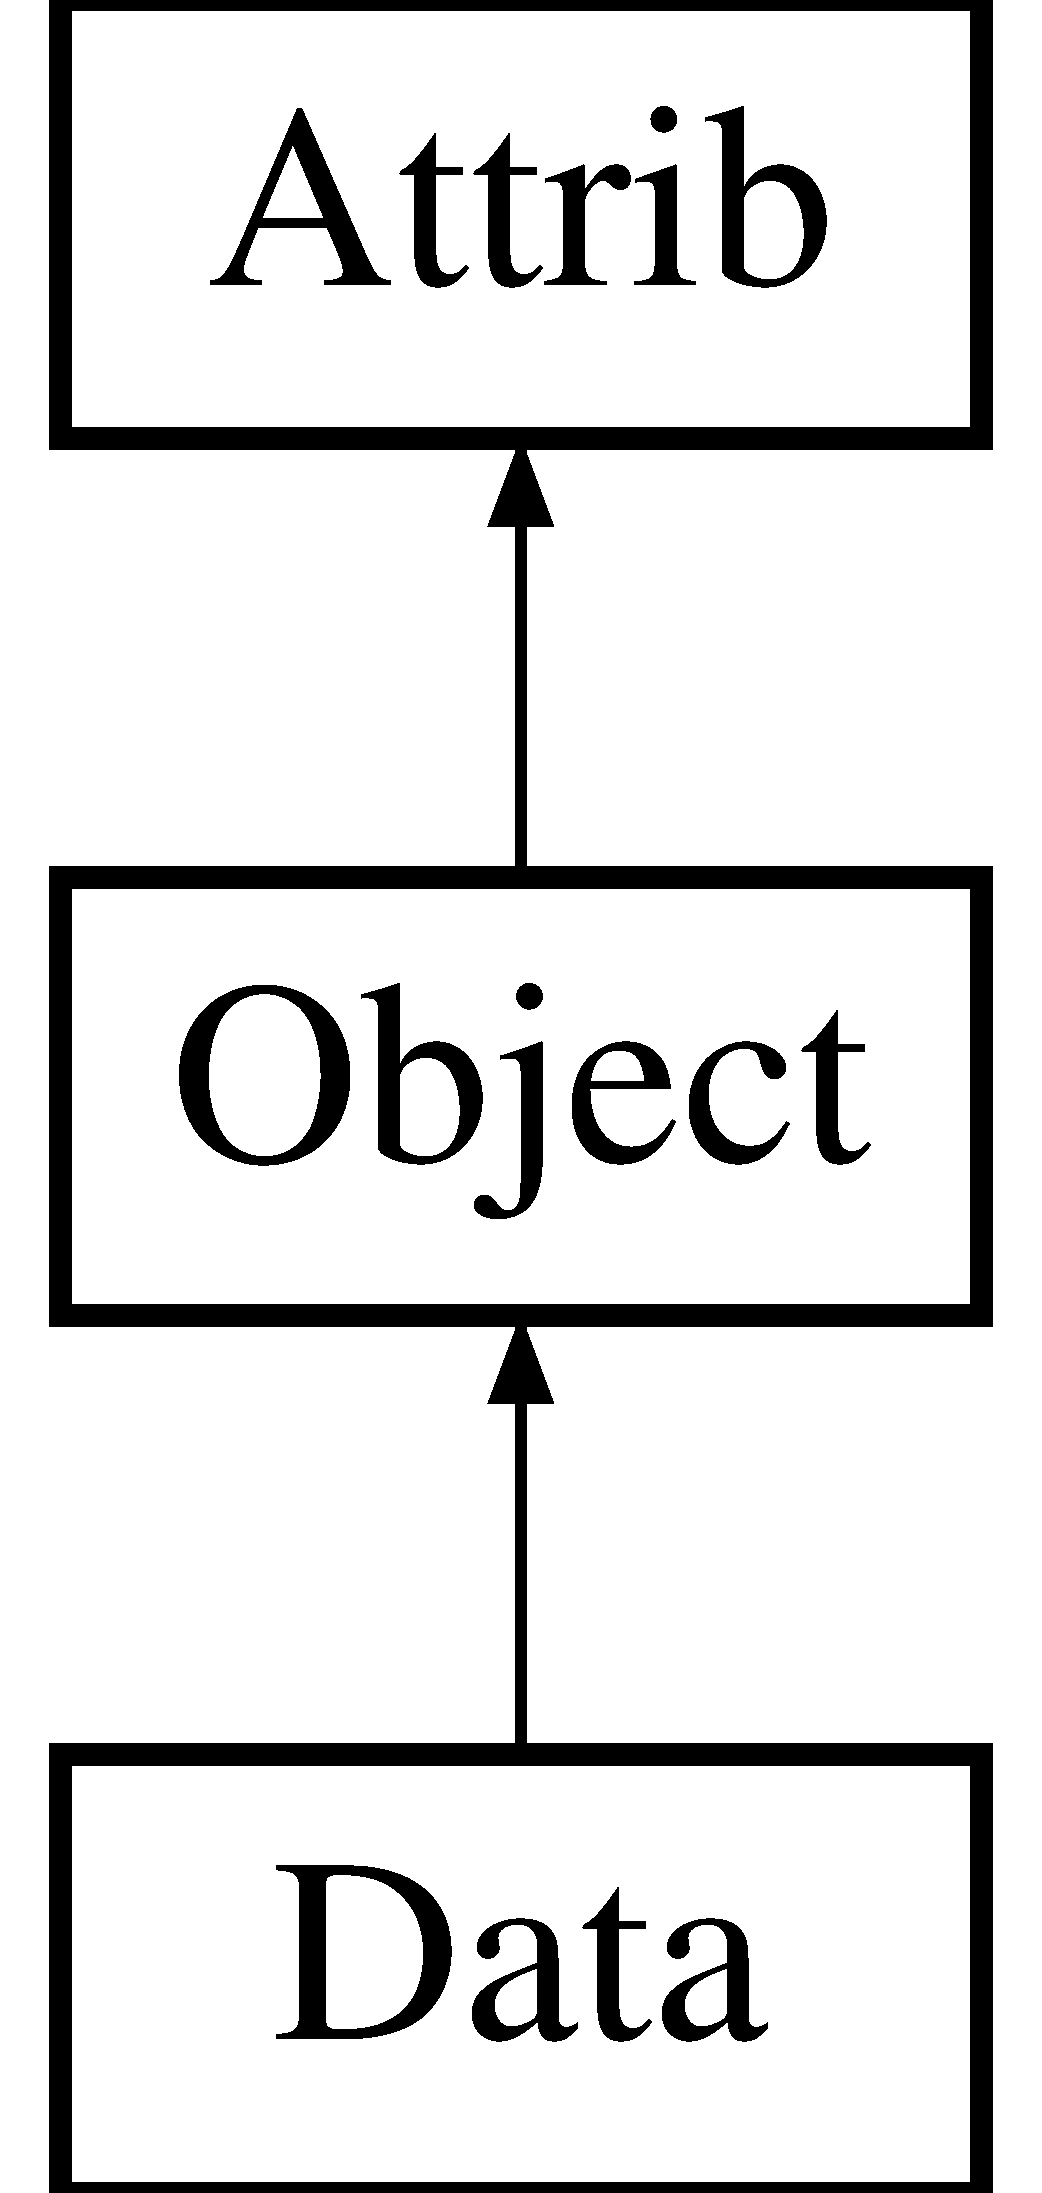
\includegraphics[height=3.000000cm]{classData}
\end{center}
\end{figure}
\subsection*{Public Types}
\begin{DoxyCompactItemize}
\item 
enum \hyperlink{classAttrib_a69e171d7cc6417835a5a306d3c764235}{Attribut} \{ \newline
\hyperlink{classAttrib_a69e171d7cc6417835a5a306d3c764235a3a8da2ab97dda18aebab196fe4100531}{U\+N\+D\+E\+F\+I\+N\+ED}, 
\hyperlink{classAttrib_a69e171d7cc6417835a5a306d3c764235a2bfb2af57b87031d190a05fe25dd92ed}{P\+A\+S\+S\+I\+VE}, 
\hyperlink{classAttrib_a69e171d7cc6417835a5a306d3c764235a3b1fec929c0370d1436f2f06e298fb0d}{A\+C\+T\+I\+VE}, 
\hyperlink{classAttrib_a69e171d7cc6417835a5a306d3c764235aa27c16b480a369ea4d18b07b2516bbc7}{I\+N\+T\+E\+R\+F\+A\+CE}, 
\newline
\hyperlink{classAttrib_a69e171d7cc6417835a5a306d3c764235a1420a5b8c0540b2af210b6975eded7f9}{IO}, 
\hyperlink{classAttrib_a69e171d7cc6417835a5a306d3c764235a0af3b0d0ac323c1704e6c69cf90add28}{I\+O\+D\+A\+TA}, 
\hyperlink{classAttrib_a69e171d7cc6417835a5a306d3c764235a7788bc5dd333fd8ce18562b269c9dab1}{E\+L\+E\+M\+E\+NT}, 
\hyperlink{classAttrib_a69e171d7cc6417835a5a306d3c764235a61ceb22149f365f1780d18f9d1459423}{H\+A\+R\+D\+W\+A\+RE}, 
\newline
\hyperlink{classAttrib_a69e171d7cc6417835a5a306d3c764235a75250e29692496e73effca2c0330977f}{P\+R\+O\+C\+E\+S\+S\+US}, 
\hyperlink{classAttrib_a69e171d7cc6417835a5a306d3c764235a103a67cd0b8f07ef478fa45d4356e27b}{S\+O\+F\+T\+W\+A\+RE}
 \}
\end{DoxyCompactItemize}
\subsection*{Public Member Functions}
\begin{DoxyCompactItemize}
\item 
\hyperlink{classData_af11f741cb7f587e2e495452a8905a22a}{Data} ()
\begin{DoxyCompactList}\small\item\em Standard constructor. \end{DoxyCompactList}\item 
\hyperlink{classData_ab330e474ce084600685c55017f36152b}{Data} (int, int, int)
\item 
virtual \hyperlink{classData_aab31956423290f0d62dcca47ab4d16dd}{$\sim$\+Data} ()
\item 
void \hyperlink{classData_a05804aa3964a587b5b283c4cb022b6b3}{set\+Evt} (int evt)
\begin{DoxyCompactList}\small\item\em Destructor. \end{DoxyCompactList}\item 
void \hyperlink{classData_a3aa387b48be4aba77d22e96cf9426569}{set\+Channel} (int ch)
\item 
void \hyperlink{classData_ac4b0bae25af361e9ceaa49fb6d341cff}{set\+Data} (int data)
\item 
void \hyperlink{classData_ac963308038ebd614a508b1c93b738e67}{Clear} (Option\+\_\+t $\ast$option=\char`\"{}\char`\"{})
\item 
\hyperlink{classData_af11f741cb7f587e2e495452a8905a22a}{Data} ()
\begin{DoxyCompactList}\small\item\em Standard constructor. \end{DoxyCompactList}\item 
virtual \hyperlink{classData_a8c4dbe720325cd952ec9146114f22d35}{$\sim$\+Data} ()
\begin{DoxyCompactList}\small\item\em Destructor. \end{DoxyCompactList}\item 
void \hyperlink{classData_a779ce878d01483220b49ad9e513d7366}{print} ()
\item 
void \hyperlink{classData_a33c31859f6b2771ebd4f0b83fa44739c}{add\+Data\+Stream} (std\+::string, std\+::string)
\item 
void \hyperlink{classData_ab6e1f621fc3b44a940d9d8af3cfa4253}{add\+Histo1d} (T\+H1D $\ast$)
\item 
void \hyperlink{classData_a4bef9c956f3994bfa491f94f4821704c}{add\+Histo2d} (T\+H2D $\ast$)
\item 
void \hyperlink{classData_a0c21ebc7662b7a6e25171959689481ca}{build\+Histos} ()
\item 
\hyperlink{classHisto1D}{Histo1D} $\ast$ \hyperlink{classData_a476a66728ccfc553909d15b36c22492a}{hist1d} (unsigned int row)
\item 
\hyperlink{classHisto1D}{Histo1D} $\ast$ \hyperlink{classData_a77d56a83e198fbc3806499c1e4aa0f10}{hist1d} (std\+::string \hyperlink{classData_a58055729bcd33b4532cae0c569af5ea8}{name})
\item 
\hyperlink{classHisto2D}{Histo2D} $\ast$ \hyperlink{classData_ab717ebe242192605ad509b76df35e855}{hist2d} (unsigned int row)
\item 
\hyperlink{classHisto2D}{Histo2D} $\ast$ \hyperlink{classData_a02c42a270c4057722a95758d4f2a25a8}{hist2d} (std\+::string \hyperlink{classData_a58055729bcd33b4532cae0c569af5ea8}{name})
\item 
void \hyperlink{classData_a26209d56fdc86a72ae391fcd3bd2adfd}{purge} ()
\item 
\hyperlink{classStatusCode}{Status\+Code} \hyperlink{classData_acdda95480997a3d6245799810334739d}{clear} (int)
\item 
\hyperlink{classStatusCode}{Status\+Code} \hyperlink{classData_adb072575d5c15cfbada75f80797c983c}{data\+Fill} (int, double)
\item 
std\+::string \hyperlink{classData_a58055729bcd33b4532cae0c569af5ea8}{name} (unsigned int)
\item 
std\+::string \hyperlink{classData_ab7aa54615fd27c0bc1ff36b7b89b6857}{title} (unsigned int)
\item 
std\+::vector$<$ double $>$ $\ast$ \hyperlink{classData_aa2153cb57f6f1a67b54eafe5582e0b6b}{vector\+Ptr} (unsigned int)
\item 
std\+::vector$<$ double $>$ \hyperlink{classData_a94e00cdd58c1d6f11487f1ac47fee4bc}{vector} (unsigned int)
\item 
std\+::vector$<$ double $>$ \hyperlink{classData_a7f1983ff7e2221ccf4652d3cd6164d32}{vector} (std\+::string)
\item 
int \hyperlink{classData_a72f9afe0edb22ad39871292f9f4d3d38}{row\+From\+Name} (std\+::string)
\item 
bool \hyperlink{classData_ad3942803fea5649bf101220667ab5021}{empty} ()
\item 
std\+::string \hyperlink{classObject_a300f4c05dd468c7bb8b3c968868443c1}{name} () const
\item 
std\+::string \hyperlink{classObject_a84f99f70f144a83e1582d1d0f84e4e62}{type} ()
\item 
unsigned char \hyperlink{classObject_af99145335cc61ff6e2798ea17db009d2}{id} ()
\item 
std\+::string \hyperlink{classObject_a73a0f1a41828fdd8303dd662446fb6c3}{title} ()
\item 
void \hyperlink{classObject_a3f9d5537ebce0c0f2bf6ae4d92426f3c}{msg\+Svc} (int level, std\+::string \hyperlink{classObject_a58b2d0618c2d08cf2383012611528d97}{msg}, std\+::string \hyperlink{classData_a58055729bcd33b4532cae0c569af5ea8}{name})
\item 
void \hyperlink{classObject_a58b2d0618c2d08cf2383012611528d97}{msg} (std\+::string mymsg)
\item 
void \hyperlink{classObject_ac5d59299273cee27aacf7de00d2e7034}{msg} (std\+::string mymsg, std\+::string \hyperlink{classData_a58055729bcd33b4532cae0c569af5ea8}{name})
\item 
void \hyperlink{classObject_a83d2db2df682907ea1115ad721c1c4a1}{verbose} (std\+::string mymsg)
\item 
void \hyperlink{classObject_a2d4120195317e2a3c6532e8bb9f3da68}{verbose} (std\+::string mymsg, std\+::string \hyperlink{classData_a58055729bcd33b4532cae0c569af5ea8}{name})
\item 
void \hyperlink{classObject_aac010553f022165573714b7014a15f0d}{debug} (std\+::string mymsg)
\item 
void \hyperlink{classObject_a6c9a0397ca804e04d675ed05683f5420}{debug} (std\+::string mymsg, std\+::string \hyperlink{classData_a58055729bcd33b4532cae0c569af5ea8}{name})
\item 
void \hyperlink{classObject_a644fd329ea4cb85f54fa6846484b84a8}{info} (std\+::string mymsg)
\item 
void \hyperlink{classObject_a1ca123253dfd30fc28b156f521dcbdae}{info} (std\+::string mymsg, std\+::string \hyperlink{classData_a58055729bcd33b4532cae0c569af5ea8}{name})
\item 
void \hyperlink{classObject_a65cd4fda577711660821fd2cd5a3b4c9}{warning} (std\+::string mymsg)
\item 
void \hyperlink{classObject_a11f101db4dd73d9391b0231818881d86}{warning} (std\+::string mymsg, std\+::string \hyperlink{classData_a58055729bcd33b4532cae0c569af5ea8}{name})
\item 
void \hyperlink{classObject_a204a95f57818c0f811933917a30eff45}{error} (std\+::string mymsg)
\item 
void \hyperlink{classObject_ad7f6c457733082efa2f9ff5f5c8e119a}{error} (std\+::string mymsg, std\+::string \hyperlink{classData_a58055729bcd33b4532cae0c569af5ea8}{name})
\item 
void \hyperlink{classObject_aad5a16aac7516ce65bd5ec02ab07fc80}{fatal} (std\+::string mymsg)
\item 
void \hyperlink{classObject_ae62acd3d09f716220f75f252dc38bc9a}{fatal} (std\+::string mymsg, std\+::string \hyperlink{classData_a58055729bcd33b4532cae0c569af5ea8}{name})
\item 
void \hyperlink{classObject_ae30fea75683c2d149b6b6d17c09ecd0c}{set\+Name} (std\+::string \hyperlink{classData_a58055729bcd33b4532cae0c569af5ea8}{name})
\item 
void \hyperlink{classObject_aae534cc9d982bcb9b99fd505f2e103a5}{set\+Type} (std\+::string \hyperlink{classObject_a84f99f70f144a83e1582d1d0f84e4e62}{type})
\item 
void \hyperlink{classObject_a398fe08cba594a0ce6891d59fe4f159f}{set\+Id} (unsigned char \hyperlink{classObject_af99145335cc61ff6e2798ea17db009d2}{id})
\item 
void \hyperlink{classObject_a89557dbbad5bcaa02652f5d7fa35d20f}{set\+Title} (std\+::string \hyperlink{classData_ab7aa54615fd27c0bc1ff36b7b89b6857}{title})
\item 
void \hyperlink{classObject_a870c5af919958c2136623b2d7816d123}{set\+Dll\+Name} (std\+::string \hyperlink{classObject_a2e3947f2870094c332d7454117f3ec63}{dll\+Name})
\item 
std\+::string \hyperlink{classObject_a2e3947f2870094c332d7454117f3ec63}{dll\+Name} ()
\item 
bool \hyperlink{classAttrib_a704f26af560909ad22065083bb7d4c34}{is} (int attribut)
\item 
void \hyperlink{classAttrib_a235f773af19c900264a190b00a3b4ad7}{add} (int attribut)
\item 
void \hyperlink{classAttrib_a7d4ef7e32d93cb287792b87b857e79f3}{remove} (int attribut)
\item 
std\+::string \hyperlink{classAttrib_aee7bbf16b144887f196e1341b24f8a26}{attributs} ()
\end{DoxyCompactItemize}
\subsection*{Public Attributes}
\begin{DoxyCompactItemize}
\item 
Class\+Def(\hyperlink{classData}{Data}, 1) protected int \hyperlink{classData_a116d0476675c4eb96ad7f3ddb2b5f6cd}{Evt}
\item 
int \hyperlink{classData_afa86e448a0941d60d105b3132f200beb}{Raw}
\end{DoxyCompactItemize}
\subsection*{Protected Attributes}
\begin{DoxyCompactItemize}
\item 
std\+::string \hyperlink{classAttrib_a3414521d7a82476e874b25a5407b5e63}{m\+\_\+attrib\+String} \mbox{[}10\mbox{]}
\end{DoxyCompactItemize}
\subsection*{Private Attributes}
\begin{DoxyCompactItemize}
\item 
std\+::vector$<$ std\+::vector$<$ double $>$ $\ast$$>$ \hyperlink{classData_a55199a86b131bdae275582f540987bc9}{m\+\_\+values}
\item 
std\+::vector$<$ T\+H1D $\ast$$>$ \hyperlink{classData_ae79c62d2ac8f7fe42aa65b26044005ba}{m\+\_\+h1d}
\item 
std\+::vector$<$ T\+H2D $\ast$$>$ \hyperlink{classData_ad34ba7631ba40c0e744d37b8292ba949}{m\+\_\+h2d}
\item 
std\+::vector$<$ \hyperlink{classHisto1D}{Histo1D} $>$ \hyperlink{classData_a06c0415eace30c2944eda0e99ce486d4}{m\+\_\+hist1d}
\item 
std\+::vector$<$ \hyperlink{classHisto2D}{Histo2D} $>$ \hyperlink{classData_a6f13c5af755aae6ae43abc3f04a9b7af}{m\+\_\+hist2d}
\item 
std\+::vector$<$ std\+::string $>$ \hyperlink{classData_a60e5c1c1e5b7373045932a25820d5d0c}{m\+\_\+titles}
\item 
std\+::vector$<$ std\+::string $>$ \hyperlink{classData_aee6304b181b43f1227c531716a833270}{m\+\_\+names}
\end{DoxyCompactItemize}


\subsection{Detailed Description}
\begin{DoxyAuthor}{Author}
Fr�d�ric Machefert 
\end{DoxyAuthor}
\begin{DoxyDate}{Date}
2004-\/10-\/04
\end{DoxyDate}
\begin{DoxyAuthor}{Author}
Frederic Machefert 
\end{DoxyAuthor}
\begin{DoxyDate}{Date}
2010-\/01-\/06 
\end{DoxyDate}


Definition at line 16 of file Data.\+h.



\subsection{Member Enumeration Documentation}
\mbox{\Hypertarget{classAttrib_a69e171d7cc6417835a5a306d3c764235}\label{classAttrib_a69e171d7cc6417835a5a306d3c764235}} 
\index{Data@{Data}!Attribut@{Attribut}}
\index{Attribut@{Attribut}!Data@{Data}}
\subsubsection{\texorpdfstring{Attribut}{Attribut}}
{\footnotesize\ttfamily enum \hyperlink{classAttrib_a69e171d7cc6417835a5a306d3c764235}{Attrib\+::\+Attribut}\hspace{0.3cm}{\ttfamily [inherited]}}

\begin{DoxyEnumFields}{Enumerator}
\raisebox{\heightof{T}}[0pt][0pt]{\index{U\+N\+D\+E\+F\+I\+N\+ED@{U\+N\+D\+E\+F\+I\+N\+ED}!Data@{Data}}\index{Data@{Data}!U\+N\+D\+E\+F\+I\+N\+ED@{U\+N\+D\+E\+F\+I\+N\+ED}}}\mbox{\Hypertarget{classAttrib_a69e171d7cc6417835a5a306d3c764235a3a8da2ab97dda18aebab196fe4100531}\label{classAttrib_a69e171d7cc6417835a5a306d3c764235a3a8da2ab97dda18aebab196fe4100531}} 
U\+N\+D\+E\+F\+I\+N\+ED&\\
\hline

\raisebox{\heightof{T}}[0pt][0pt]{\index{P\+A\+S\+S\+I\+VE@{P\+A\+S\+S\+I\+VE}!Data@{Data}}\index{Data@{Data}!P\+A\+S\+S\+I\+VE@{P\+A\+S\+S\+I\+VE}}}\mbox{\Hypertarget{classAttrib_a69e171d7cc6417835a5a306d3c764235a2bfb2af57b87031d190a05fe25dd92ed}\label{classAttrib_a69e171d7cc6417835a5a306d3c764235a2bfb2af57b87031d190a05fe25dd92ed}} 
P\+A\+S\+S\+I\+VE&\\
\hline

\raisebox{\heightof{T}}[0pt][0pt]{\index{A\+C\+T\+I\+VE@{A\+C\+T\+I\+VE}!Data@{Data}}\index{Data@{Data}!A\+C\+T\+I\+VE@{A\+C\+T\+I\+VE}}}\mbox{\Hypertarget{classAttrib_a69e171d7cc6417835a5a306d3c764235a3b1fec929c0370d1436f2f06e298fb0d}\label{classAttrib_a69e171d7cc6417835a5a306d3c764235a3b1fec929c0370d1436f2f06e298fb0d}} 
A\+C\+T\+I\+VE&\\
\hline

\raisebox{\heightof{T}}[0pt][0pt]{\index{I\+N\+T\+E\+R\+F\+A\+CE@{I\+N\+T\+E\+R\+F\+A\+CE}!Data@{Data}}\index{Data@{Data}!I\+N\+T\+E\+R\+F\+A\+CE@{I\+N\+T\+E\+R\+F\+A\+CE}}}\mbox{\Hypertarget{classAttrib_a69e171d7cc6417835a5a306d3c764235aa27c16b480a369ea4d18b07b2516bbc7}\label{classAttrib_a69e171d7cc6417835a5a306d3c764235aa27c16b480a369ea4d18b07b2516bbc7}} 
I\+N\+T\+E\+R\+F\+A\+CE&\\
\hline

\raisebox{\heightof{T}}[0pt][0pt]{\index{IO@{IO}!Data@{Data}}\index{Data@{Data}!IO@{IO}}}\mbox{\Hypertarget{classAttrib_a69e171d7cc6417835a5a306d3c764235a1420a5b8c0540b2af210b6975eded7f9}\label{classAttrib_a69e171d7cc6417835a5a306d3c764235a1420a5b8c0540b2af210b6975eded7f9}} 
IO&\\
\hline

\raisebox{\heightof{T}}[0pt][0pt]{\index{I\+O\+D\+A\+TA@{I\+O\+D\+A\+TA}!Data@{Data}}\index{Data@{Data}!I\+O\+D\+A\+TA@{I\+O\+D\+A\+TA}}}\mbox{\Hypertarget{classAttrib_a69e171d7cc6417835a5a306d3c764235a0af3b0d0ac323c1704e6c69cf90add28}\label{classAttrib_a69e171d7cc6417835a5a306d3c764235a0af3b0d0ac323c1704e6c69cf90add28}} 
I\+O\+D\+A\+TA&\\
\hline

\raisebox{\heightof{T}}[0pt][0pt]{\index{E\+L\+E\+M\+E\+NT@{E\+L\+E\+M\+E\+NT}!Data@{Data}}\index{Data@{Data}!E\+L\+E\+M\+E\+NT@{E\+L\+E\+M\+E\+NT}}}\mbox{\Hypertarget{classAttrib_a69e171d7cc6417835a5a306d3c764235a7788bc5dd333fd8ce18562b269c9dab1}\label{classAttrib_a69e171d7cc6417835a5a306d3c764235a7788bc5dd333fd8ce18562b269c9dab1}} 
E\+L\+E\+M\+E\+NT&\\
\hline

\raisebox{\heightof{T}}[0pt][0pt]{\index{H\+A\+R\+D\+W\+A\+RE@{H\+A\+R\+D\+W\+A\+RE}!Data@{Data}}\index{Data@{Data}!H\+A\+R\+D\+W\+A\+RE@{H\+A\+R\+D\+W\+A\+RE}}}\mbox{\Hypertarget{classAttrib_a69e171d7cc6417835a5a306d3c764235a61ceb22149f365f1780d18f9d1459423}\label{classAttrib_a69e171d7cc6417835a5a306d3c764235a61ceb22149f365f1780d18f9d1459423}} 
H\+A\+R\+D\+W\+A\+RE&\\
\hline

\raisebox{\heightof{T}}[0pt][0pt]{\index{P\+R\+O\+C\+E\+S\+S\+US@{P\+R\+O\+C\+E\+S\+S\+US}!Data@{Data}}\index{Data@{Data}!P\+R\+O\+C\+E\+S\+S\+US@{P\+R\+O\+C\+E\+S\+S\+US}}}\mbox{\Hypertarget{classAttrib_a69e171d7cc6417835a5a306d3c764235a75250e29692496e73effca2c0330977f}\label{classAttrib_a69e171d7cc6417835a5a306d3c764235a75250e29692496e73effca2c0330977f}} 
P\+R\+O\+C\+E\+S\+S\+US&\\
\hline

\raisebox{\heightof{T}}[0pt][0pt]{\index{S\+O\+F\+T\+W\+A\+RE@{S\+O\+F\+T\+W\+A\+RE}!Data@{Data}}\index{Data@{Data}!S\+O\+F\+T\+W\+A\+RE@{S\+O\+F\+T\+W\+A\+RE}}}\mbox{\Hypertarget{classAttrib_a69e171d7cc6417835a5a306d3c764235a103a67cd0b8f07ef478fa45d4356e27b}\label{classAttrib_a69e171d7cc6417835a5a306d3c764235a103a67cd0b8f07ef478fa45d4356e27b}} 
S\+O\+F\+T\+W\+A\+RE&\\
\hline

\end{DoxyEnumFields}


Definition at line 29 of file Attrib.\+h.


\begin{DoxyCode}
29                 \{
30     \hyperlink{classAttrib_a69e171d7cc6417835a5a306d3c764235a3a8da2ab97dda18aebab196fe4100531}{UNDEFINED},
31     \hyperlink{classAttrib_a69e171d7cc6417835a5a306d3c764235a2bfb2af57b87031d190a05fe25dd92ed}{PASSIVE},
32     \hyperlink{classAttrib_a69e171d7cc6417835a5a306d3c764235a3b1fec929c0370d1436f2f06e298fb0d}{ACTIVE},
33     \hyperlink{classAttrib_a69e171d7cc6417835a5a306d3c764235aa27c16b480a369ea4d18b07b2516bbc7}{INTERFACE},
34     \hyperlink{classAttrib_a69e171d7cc6417835a5a306d3c764235a1420a5b8c0540b2af210b6975eded7f9}{IO},
35     \hyperlink{classAttrib_a69e171d7cc6417835a5a306d3c764235a0af3b0d0ac323c1704e6c69cf90add28}{IODATA},
36     \hyperlink{classAttrib_a69e171d7cc6417835a5a306d3c764235a7788bc5dd333fd8ce18562b269c9dab1}{ELEMENT},
37     \hyperlink{classAttrib_a69e171d7cc6417835a5a306d3c764235a61ceb22149f365f1780d18f9d1459423}{HARDWARE},
38     \hyperlink{classAttrib_a69e171d7cc6417835a5a306d3c764235a75250e29692496e73effca2c0330977f}{PROCESSUS},
39     \hyperlink{classAttrib_a69e171d7cc6417835a5a306d3c764235a103a67cd0b8f07ef478fa45d4356e27b}{SOFTWARE} 
40   \}; \textcolor{comment}{// array m\_attribString must be changed into Attrib::Attrib if this enu is modified. }
\end{DoxyCode}


\subsection{Constructor \& Destructor Documentation}
\mbox{\Hypertarget{classData_af11f741cb7f587e2e495452a8905a22a}\label{classData_af11f741cb7f587e2e495452a8905a22a}} 
\index{Data@{Data}!Data@{Data}}
\index{Data@{Data}!Data@{Data}}
\subsubsection{\texorpdfstring{Data()}{Data()}\hspace{0.1cm}{\footnotesize\ttfamily [1/3]}}
{\footnotesize\ttfamily Data\+::\+Data (\begin{DoxyParamCaption}{ }\end{DoxyParamCaption})}



Standard constructor. 



Definition at line 18 of file Data.\+cpp.



References $\sim$\+Data().


\begin{DoxyCode}
18             \{
19 \}
\end{DoxyCode}
\mbox{\Hypertarget{classData_ab330e474ce084600685c55017f36152b}\label{classData_ab330e474ce084600685c55017f36152b}} 
\index{Data@{Data}!Data@{Data}}
\index{Data@{Data}!Data@{Data}}
\subsubsection{\texorpdfstring{Data()}{Data()}\hspace{0.1cm}{\footnotesize\ttfamily [2/3]}}
{\footnotesize\ttfamily Data\+::\+Data (\begin{DoxyParamCaption}\item[{int}]{evt,  }\item[{int}]{channel,  }\item[{int}]{data }\end{DoxyParamCaption})}



Definition at line 23 of file Data.\+cpp.



References shell\+::data(), Evt, and Raw.


\begin{DoxyCode}
23                                             \{
24   \hyperlink{classData_a116d0476675c4eb96ad7f3ddb2b5f6cd}{Evt}   = evt;
25   \hyperlink{classData_afa86e448a0941d60d105b3132f200beb}{Raw}   = \hyperlink{namespaceshell_a5ea2525995cedc3efd69ea8a7f034d1e}{data};
26   Ch    = channel ;
27 \}
\end{DoxyCode}
\mbox{\Hypertarget{classData_aab31956423290f0d62dcca47ab4d16dd}\label{classData_aab31956423290f0d62dcca47ab4d16dd}} 
\index{Data@{Data}!````~Data@{$\sim$\+Data}}
\index{````~Data@{$\sim$\+Data}!Data@{Data}}
\subsubsection{\texorpdfstring{$\sim$\+Data()}{~Data()}\hspace{0.1cm}{\footnotesize\ttfamily [1/2]}}
{\footnotesize\ttfamily Data\+::$\sim$\+Data (\begin{DoxyParamCaption}{ }\end{DoxyParamCaption})\hspace{0.3cm}{\ttfamily [inline]}, {\ttfamily [virtual]}}



Definition at line 21 of file Data.\+h.



References Clear().



Referenced by Data().


\begin{DoxyCode}
21 \{ \hyperlink{classData_ac963308038ebd614a508b1c93b738e67}{Clear}(); \}; 
\end{DoxyCode}
\mbox{\Hypertarget{classData_af11f741cb7f587e2e495452a8905a22a}\label{classData_af11f741cb7f587e2e495452a8905a22a}} 
\index{Data@{Data}!Data@{Data}}
\index{Data@{Data}!Data@{Data}}
\subsubsection{\texorpdfstring{Data()}{Data()}\hspace{0.1cm}{\footnotesize\ttfamily [3/3]}}
{\footnotesize\ttfamily Data\+::\+Data (\begin{DoxyParamCaption}{ }\end{DoxyParamCaption})}



Standard constructor. 

\mbox{\Hypertarget{classData_a8c4dbe720325cd952ec9146114f22d35}\label{classData_a8c4dbe720325cd952ec9146114f22d35}} 
\index{Data@{Data}!````~Data@{$\sim$\+Data}}
\index{````~Data@{$\sim$\+Data}!Data@{Data}}
\subsubsection{\texorpdfstring{$\sim$\+Data()}{~Data()}\hspace{0.1cm}{\footnotesize\ttfamily [2/2]}}
{\footnotesize\ttfamily virtual Data\+::$\sim$\+Data (\begin{DoxyParamCaption}{ }\end{DoxyParamCaption})\hspace{0.3cm}{\ttfamily [virtual]}}



Destructor. 



\subsection{Member Function Documentation}
\mbox{\Hypertarget{classAttrib_a235f773af19c900264a190b00a3b4ad7}\label{classAttrib_a235f773af19c900264a190b00a3b4ad7}} 
\index{Data@{Data}!add@{add}}
\index{add@{add}!Data@{Data}}
\subsubsection{\texorpdfstring{add()}{add()}}
{\footnotesize\ttfamily void Attrib\+::add (\begin{DoxyParamCaption}\item[{int}]{attribut }\end{DoxyParamCaption})\hspace{0.3cm}{\ttfamily [inline]}, {\ttfamily [inherited]}}

Add an attribut 

Definition at line 67 of file Attrib.\+h.



References Attrib\+::m\+\_\+attributs, and Attrib\+::\+U\+N\+D\+E\+F\+I\+N\+ED.



Referenced by A3\+P\+E\+::\+A3\+P\+E(), Attrib\+::\+Attrib(), Specs\+Mezzanine\+::cmdline(), Computer\+::\+Computer(), C\+U\+\_\+v1\+::\+C\+U\+\_\+v1(), export\+\_\+obj(), F\+E\+B\+\_\+v1\+::\+F\+E\+B\+\_\+v1(), Fe\+P\+G\+A\+::\+Fe\+P\+G\+A(), I\+C\+E\+C\+A\+Lv3\+::\+I\+C\+E\+C\+A\+Lv3(), I\+C\+Phaser\+::\+I\+C\+Phaser(), Application\+::initialize(), Interface\+::\+Interface(), I\+Odata\+::\+I\+Odata(), I\+Oobject\+::\+I\+Oobject(), M\+S\+Oxxxx\+::\+M\+S\+Oxxxx(), Phaser\+::\+Phaser(), Processus\+::\+Processus(), Proto40\+M\+Hz\+\_\+v1\+::\+Proto40\+M\+Hz\+\_\+v1(), Attrib\+::remove(), Seq\+P\+G\+A\+::\+Seq\+P\+G\+A(), Test\+I2\+C\+::set\+Address(), Test\+S\+P\+I\+::set\+Address(), Specs\+Slave\+::set\+Address(), Specs\+Master\+::\+Specs\+Master(), and Specs\+Slave\+::\+Specs\+Slave().


\begin{DoxyCode}
67                             \{
68     \textcolor{keywordflow}{if} (attribut!=\hyperlink{classAttrib_a69e171d7cc6417835a5a306d3c764235a3a8da2ab97dda18aebab196fe4100531}{Attrib::UNDEFINED}) \textcolor{keyword}{remove}(\hyperlink{classAttrib_a69e171d7cc6417835a5a306d3c764235a3a8da2ab97dda18aebab196fe4100531}{Attrib::UNDEFINED});
69     \textcolor{keywordtype}{bool} duplicate = false ;
70     std::vector<int>::const\_iterator iter ;
71     \textcolor{keywordflow}{for} ( iter  = \hyperlink{classAttrib_ac4bd58a0cc6b38a3b711d609a3d3aacc}{m\_attributs}.begin() ;
72           iter != \hyperlink{classAttrib_ac4bd58a0cc6b38a3b711d609a3d3aacc}{m\_attributs}.end()   ;
73           ++iter ) \{
74       \textcolor{keywordflow}{if} ( attribut == (*iter) ) \{
75         duplicate = true ;
76       \}
77     \}
78     \textcolor{keywordflow}{if} (!duplicate) \{
79       \hyperlink{classAttrib_ac4bd58a0cc6b38a3b711d609a3d3aacc}{m\_attributs}.push\_back( attribut );
80     \}
81   \}
\end{DoxyCode}
\mbox{\Hypertarget{classData_a33c31859f6b2771ebd4f0b83fa44739c}\label{classData_a33c31859f6b2771ebd4f0b83fa44739c}} 
\index{Data@{Data}!add\+Data\+Stream@{add\+Data\+Stream}}
\index{add\+Data\+Stream@{add\+Data\+Stream}!Data@{Data}}
\subsubsection{\texorpdfstring{add\+Data\+Stream()}{addDataStream()}}
{\footnotesize\ttfamily void Data\+::add\+Data\+Stream (\begin{DoxyParamCaption}\item[{std\+::string}]{n,  }\item[{std\+::string}]{t }\end{DoxyParamCaption})}



Definition at line 31 of file Data.\+cpp.



References m\+\_\+names, m\+\_\+titles, and m\+\_\+values.



Referenced by F\+E\+B\+\_\+v1\+::\+F\+E\+B\+\_\+v1().


\begin{DoxyCode}
31                                                   \{
32   \hyperlink{classData_aee6304b181b43f1227c531716a833270}{m\_names} .push\_back(n);
33   \hyperlink{classData_a60e5c1c1e5b7373045932a25820d5d0c}{m\_titles}.push\_back(t);
34   \hyperlink{classData_a55199a86b131bdae275582f540987bc9}{m\_values}.push\_back(\textcolor{keyword}{new} std::vector<double>);
35 \}
\end{DoxyCode}
\mbox{\Hypertarget{classData_ab6e1f621fc3b44a940d9d8af3cfa4253}\label{classData_ab6e1f621fc3b44a940d9d8af3cfa4253}} 
\index{Data@{Data}!add\+Histo1d@{add\+Histo1d}}
\index{add\+Histo1d@{add\+Histo1d}!Data@{Data}}
\subsubsection{\texorpdfstring{add\+Histo1d()}{addHisto1d()}}
{\footnotesize\ttfamily void Data\+::add\+Histo1d (\begin{DoxyParamCaption}\item[{T\+H1D $\ast$}]{h }\end{DoxyParamCaption})}



Definition at line 40 of file Data.\+cpp.



References m\+\_\+h1d.


\begin{DoxyCode}
40                              \{
41   \hyperlink{classData_ae79c62d2ac8f7fe42aa65b26044005ba}{m\_h1d}.push\_back( h );
42 \}
\end{DoxyCode}
\mbox{\Hypertarget{classData_a4bef9c956f3994bfa491f94f4821704c}\label{classData_a4bef9c956f3994bfa491f94f4821704c}} 
\index{Data@{Data}!add\+Histo2d@{add\+Histo2d}}
\index{add\+Histo2d@{add\+Histo2d}!Data@{Data}}
\subsubsection{\texorpdfstring{add\+Histo2d()}{addHisto2d()}}
{\footnotesize\ttfamily void Data\+::add\+Histo2d (\begin{DoxyParamCaption}\item[{T\+H2D $\ast$}]{h }\end{DoxyParamCaption})}



Definition at line 47 of file Data.\+cpp.



References m\+\_\+h2d.


\begin{DoxyCode}
47                              \{
48   \hyperlink{classData_ad34ba7631ba40c0e744d37b8292ba949}{m\_h2d}.push\_back( h );
49 \}
\end{DoxyCode}
\mbox{\Hypertarget{classAttrib_aee7bbf16b144887f196e1341b24f8a26}\label{classAttrib_aee7bbf16b144887f196e1341b24f8a26}} 
\index{Data@{Data}!attributs@{attributs}}
\index{attributs@{attributs}!Data@{Data}}
\subsubsection{\texorpdfstring{attributs()}{attributs()}}
{\footnotesize\ttfamily std\+::string Attrib\+::attributs (\begin{DoxyParamCaption}{ }\end{DoxyParamCaption})\hspace{0.3cm}{\ttfamily [inherited]}}

Print the \hyperlink{classAttrib}{Attrib} of an \hyperlink{classObject}{Object} 

Definition at line 54 of file Attrib.\+cpp.



References images\+::index, Attrib\+::m\+\_\+attrib\+String, and Attrib\+::m\+\_\+attributs.



Referenced by export\+\_\+obj(), and Attrib\+::remove().


\begin{DoxyCode}
54                             \{
55   std::string output;
56   std::vector<int>::iterator iter ;
57   \textcolor{keywordflow}{for} ( \textcolor{keywordtype}{unsigned} \textcolor{keywordtype}{int} \hyperlink{namespaceimages_a54407fd574970b3178647ae096321a57}{index} = 0 ; \hyperlink{namespaceimages_a54407fd574970b3178647ae096321a57}{index} < \hyperlink{classAttrib_ac4bd58a0cc6b38a3b711d609a3d3aacc}{m\_attributs}.size() ; ++
      \hyperlink{namespaceimages_a54407fd574970b3178647ae096321a57}{index} ) \{
58     \textcolor{keywordflow}{if} ( \hyperlink{classAttrib_ac4bd58a0cc6b38a3b711d609a3d3aacc}{m\_attributs}.size() - \hyperlink{namespaceimages_a54407fd574970b3178647ae096321a57}{index} > 1 ) \{
59       output.append(\hyperlink{classAttrib_a3414521d7a82476e874b25a5407b5e63}{m\_attribString}[\hyperlink{classAttrib_ac4bd58a0cc6b38a3b711d609a3d3aacc}{m\_attributs}[\hyperlink{namespaceimages_a54407fd574970b3178647ae096321a57}{index}]]);
60       output.append(\textcolor{stringliteral}{":"});
61     \}
62     \textcolor{keywordflow}{else} \{
63       output.append(\hyperlink{classAttrib_a3414521d7a82476e874b25a5407b5e63}{m\_attribString}[\hyperlink{classAttrib_ac4bd58a0cc6b38a3b711d609a3d3aacc}{m\_attributs}[index]]);
64     \}
65   \}
66   \textcolor{keywordflow}{return} output;
67 \}
\end{DoxyCode}
\mbox{\Hypertarget{classData_a0c21ebc7662b7a6e25171959689481ca}\label{classData_a0c21ebc7662b7a6e25171959689481ca}} 
\index{Data@{Data}!build\+Histos@{build\+Histos}}
\index{build\+Histos@{build\+Histos}!Data@{Data}}
\subsubsection{\texorpdfstring{build\+Histos()}{buildHistos()}}
{\footnotesize\ttfamily void Data\+::build\+Histos (\begin{DoxyParamCaption}{ }\end{DoxyParamCaption})}



Definition at line 98 of file Data.\+cpp.



References m\+\_\+h1d, m\+\_\+h2d, m\+\_\+hist1d, and m\+\_\+hist2d.



Referenced by Processus\+::end\+Processing().


\begin{DoxyCode}
98                       \{
99   std::vector<TH1D*>::iterator iter1d;
100   \textcolor{keywordflow}{for} (iter1d=\hyperlink{classData_ae79c62d2ac8f7fe42aa65b26044005ba}{m\_h1d}.begin(); iter1d!=\hyperlink{classData_ae79c62d2ac8f7fe42aa65b26044005ba}{m\_h1d}.end(); ++iter1d)\{
101     \hyperlink{classData_a06c0415eace30c2944eda0e99ce486d4}{m\_hist1d}.push\_back(\hyperlink{classHisto1D}{Histo1D}(*iter1d));
102   \}
103   std::vector<TH2D*>::iterator iter2d;
104   \textcolor{keywordflow}{for} (iter2d=\hyperlink{classData_ad34ba7631ba40c0e744d37b8292ba949}{m\_h2d}.begin(); iter2d!=\hyperlink{classData_ad34ba7631ba40c0e744d37b8292ba949}{m\_h2d}.end(); ++iter2d)\{
105     \hyperlink{classData_a6f13c5af755aae6ae43abc3f04a9b7af}{m\_hist2d}.push\_back(\hyperlink{classHisto2D}{Histo2D}(*iter2d));
106   \}
107 \}
\end{DoxyCode}
\mbox{\Hypertarget{classData_ac963308038ebd614a508b1c93b738e67}\label{classData_ac963308038ebd614a508b1c93b738e67}} 
\index{Data@{Data}!Clear@{Clear}}
\index{Clear@{Clear}!Data@{Data}}
\subsubsection{\texorpdfstring{Clear()}{Clear()}}
{\footnotesize\ttfamily void Data\+::\+Clear (\begin{DoxyParamCaption}\item[{Option\+\_\+t $\ast$}]{option = {\ttfamily \char`\"{}\char`\"{}} }\end{DoxyParamCaption})}



Definition at line 32 of file Data.\+cpp.



Referenced by set\+Data(), and $\sim$\+Data().


\begin{DoxyCode}
32                             \{
33 \}
\end{DoxyCode}
\mbox{\Hypertarget{classData_acdda95480997a3d6245799810334739d}\label{classData_acdda95480997a3d6245799810334739d}} 
\index{Data@{Data}!clear@{clear}}
\index{clear@{clear}!Data@{Data}}
\subsubsection{\texorpdfstring{clear()}{clear()}}
{\footnotesize\ttfamily \hyperlink{classStatusCode}{Status\+Code} Data\+::clear (\begin{DoxyParamCaption}\item[{int}]{i }\end{DoxyParamCaption})}



Definition at line 71 of file Data.\+cpp.



References Status\+Code\+::\+F\+A\+I\+L\+U\+RE, Status\+Code\+::\+S\+U\+C\+C\+E\+SS, and vector\+Ptr().



Referenced by hist2d(), F\+E\+B\+\_\+v1\+::read\+Fifo\+L\+L\+T(), F\+E\+B\+\_\+v1\+::read\+Fifo\+L\+L\+T\+F\+E(), and F\+E\+B\+\_\+v1\+::read\+Fifo\+Spy\+F\+E().


\begin{DoxyCode}
71                              \{
72   \textcolor{keywordflow}{if} (\hyperlink{classData_aa2153cb57f6f1a67b54eafe5582e0b6b}{vectorPtr}(i)!=0)\{
73     \hyperlink{classData_aa2153cb57f6f1a67b54eafe5582e0b6b}{vectorPtr}(i)->clear();
74     \textcolor{keywordflow}{return} \hyperlink{classStatusCode_a6f565cbeadc76d14c72f047e5e85eb4badd0da38d3ba0d922efd1f4619bc37ad8}{StatusCode::SUCCESS};
75   \}
76   \textcolor{keywordflow}{else} \{
77     \textcolor{keywordflow}{return} \hyperlink{classStatusCode_a6f565cbeadc76d14c72f047e5e85eb4ba3da73d4c469762eb9d3c960368252b26}{StatusCode::FAILURE};
78   \}
79 \}
\end{DoxyCode}
\mbox{\Hypertarget{classData_adb072575d5c15cfbada75f80797c983c}\label{classData_adb072575d5c15cfbada75f80797c983c}} 
\index{Data@{Data}!data\+Fill@{data\+Fill}}
\index{data\+Fill@{data\+Fill}!Data@{Data}}
\subsubsection{\texorpdfstring{data\+Fill()}{dataFill()}}
{\footnotesize\ttfamily \hyperlink{classStatusCode}{Status\+Code} Data\+::data\+Fill (\begin{DoxyParamCaption}\item[{int}]{i,  }\item[{double}]{val }\end{DoxyParamCaption})}

Set data stream with value \begin{DoxyReturn}{Returns}
the \hyperlink{classStatusCode}{Status\+Code} 
\end{DoxyReturn}


Definition at line 85 of file Data.\+cpp.



References Status\+Code\+::\+F\+A\+I\+L\+U\+RE, Status\+Code\+::\+S\+U\+C\+C\+E\+SS, and vector\+Ptr().



Referenced by hist2d(), F\+E\+B\+\_\+v1\+::read\+Fifo\+L\+L\+T(), F\+E\+B\+\_\+v1\+::read\+Fifo\+L\+L\+T\+F\+E(), and F\+E\+B\+\_\+v1\+::read\+Fifo\+Spy\+F\+E().


\begin{DoxyCode}
85                                           \{
86   \textcolor{keywordflow}{if} (\hyperlink{classData_aa2153cb57f6f1a67b54eafe5582e0b6b}{vectorPtr}(i)!=0)\{
87     \hyperlink{classData_aa2153cb57f6f1a67b54eafe5582e0b6b}{vectorPtr}(i)->push\_back(val);
88     \textcolor{keywordflow}{return} \hyperlink{classStatusCode_a6f565cbeadc76d14c72f047e5e85eb4badd0da38d3ba0d922efd1f4619bc37ad8}{StatusCode::SUCCESS};
89   \}
90   \textcolor{keywordflow}{else} \{
91     \textcolor{keywordflow}{return} \hyperlink{classStatusCode_a6f565cbeadc76d14c72f047e5e85eb4ba3da73d4c469762eb9d3c960368252b26}{StatusCode::FAILURE};
92   \}
93 \}
\end{DoxyCode}
\mbox{\Hypertarget{classObject_aac010553f022165573714b7014a15f0d}\label{classObject_aac010553f022165573714b7014a15f0d}} 
\index{Data@{Data}!debug@{debug}}
\index{debug@{debug}!Data@{Data}}
\subsubsection{\texorpdfstring{debug()}{debug()}\hspace{0.1cm}{\footnotesize\ttfamily [1/2]}}
{\footnotesize\ttfamily void Object\+::debug (\begin{DoxyParamCaption}\item[{std\+::string}]{mymsg }\end{DoxyParamCaption})\hspace{0.3cm}{\ttfamily [inline]}, {\ttfamily [inherited]}}



Definition at line 37 of file Object.\+h.



References Msg\+Svc\+::\+D\+E\+B\+UG, Object\+::m\+\_\+log, Object\+::m\+\_\+name, and Msg\+Svc\+::msg\+Svc().



Referenced by A3\+P\+E\+::\+A3\+P\+E(), A3\+P\+E\+::acquisition(), Specs\+Mezzanine\+::add\+Bus(), Hierarchy\+::add\+Child(), Specs\+Slave\+::add\+I2c(), L\+S\+Delay\+Chip\+V1\+::config\+Reg\+Bulk\+Read(), L\+S\+Delay\+Chip\+V1\+::config\+Reg\+Bulk\+Write(), A3\+P\+E\+::data\+Ready(), D\+C\+U\+::\+D\+C\+U(), Hierarchy\+::del\+Child(), Specs\+Slave\+::detect(), Storage\+Fifo\+Acquisition\+::execute(), Storage\+Fifo\+::execute(), A3\+P\+E\+\_\+\+Bit\+Flip\+::execute(), Acquisition\+::execute(), Emulate\+F\+E\+::execute(), export\+\_\+obj(), Fe\+P\+G\+A\+::\+Fe\+P\+G\+A(), Specs\+Glue\+::i2c\+Clk\+Mode(), Fe\+P\+G\+A\+::i2c\+Read(), Seq\+P\+G\+A\+::i2c\+Read(), Fe\+P\+G\+A\+::i2c\+Write(), Seq\+P\+G\+A\+::i2c\+Write(), I\+C\+E\+C\+A\+Lv3\+::\+I\+C\+E\+C\+A\+Lv3(), I\+C\+Phaser\+::\+I\+C\+Phaser(), Specs\+Slave\+::init(), Specs\+Master\+::init(), Storage\+Fifo\+Acquisition\+::initialize(), Storage\+Fifo\+::initialize(), A3\+P\+E\+\_\+\+Bit\+Flip\+::initialize(), Acquisition\+::initialize(), Emulate\+F\+E\+::initialize(), A3\+P\+E\+::internal\+A\+X\+Sequence(), Specs\+Glue\+::led(), Specs\+Mezzanine\+::led(), M\+S\+Oxxxx\+::\+M\+S\+Oxxxx(), Phaser\+::\+Phaser(), purge(), Phaser\+::read(), I\+C\+Phaser\+::read(), C\+U\+\_\+v1\+::reset(), Proto40\+M\+Hz\+\_\+v1\+::reset(), F\+E\+B\+\_\+v1\+::reset(), Specs\+Master\+::reset(), Specs\+Slave\+::reset(), F\+E\+B\+\_\+v1\+::reset\+Usb(), Seq\+P\+G\+A\+::\+Seq\+P\+G\+A(), A3\+P\+E\+::set\+Add\+From\+A\+X\+Ram(), A3\+P\+E\+::set\+Add\+To\+A\+X\+Ram(), A3\+P\+E\+::set\+A\+X\+Ram\+Usb(), Element\+::set\+Connection(), Specs\+Glue\+::set\+I2c\+Clk\+Mode(), A3\+P\+E\+::set\+Latency\+A\+X(), Specs\+Glue\+::set\+Led(), Specs\+Mezzanine\+::set\+Led(), A3\+P\+E\+::set\+Length\+A\+X(), A3\+P\+E\+::set\+Read\+To\+A\+X\+Ram\+Usb(), Specs\+Master\+::set\+Speed(), A3\+P\+E\+::set\+Write\+From\+A\+X\+Ram\+Usb(), Specs\+Bus\+::\+Specs\+Bus(), Specs\+I2c\+::\+Specs\+I2c(), Specs\+Master\+::\+Specs\+Master(), Specs\+Mezzanine\+::\+Specs\+Mezzanine(), Specs\+Parallel\+Bus\+::\+Specs\+Parallel\+Bus(), Specs\+Slave\+::\+Specs\+Slave(), L\+S\+Delay\+Chip\+V1\+::spi\+B\+E\+R\+Test(), I\+C\+E\+C\+A\+Lv3\+::spi\+Read(), I\+C\+E\+C\+A\+Lv3\+::spi\+Write(), A3\+P\+E\+::trigger(), Server\+::update\+Config(), Server\+::update\+State(), Phaser\+::write(), I\+C\+Phaser\+::write(), and Hierarchy\+::$\sim$\+Hierarchy().


\begin{DoxyCode}
37 \{ \hyperlink{classObject_a0d269813dd7ac1f24bc143031e2963f2}{m\_log}.\hyperlink{classMsgSvc_ad25f18047920cc59a314e5098259711c}{msgSvc} (\hyperlink{classMsgSvc_ae671eb7301996cd049d2da8a65925926a1dbdcc82dce88370ec335883c83b38b0}{MsgSvc::DEBUG}   , mymsg, \hyperlink{classObject_a8b83c95c705d2c3ba0d081fe1710f48d}{m\_name} ); \}
\end{DoxyCode}
\mbox{\Hypertarget{classObject_a6c9a0397ca804e04d675ed05683f5420}\label{classObject_a6c9a0397ca804e04d675ed05683f5420}} 
\index{Data@{Data}!debug@{debug}}
\index{debug@{debug}!Data@{Data}}
\subsubsection{\texorpdfstring{debug()}{debug()}\hspace{0.1cm}{\footnotesize\ttfamily [2/2]}}
{\footnotesize\ttfamily void Object\+::debug (\begin{DoxyParamCaption}\item[{std\+::string}]{mymsg,  }\item[{std\+::string}]{name }\end{DoxyParamCaption})\hspace{0.3cm}{\ttfamily [inline]}, {\ttfamily [inherited]}}



Definition at line 45 of file Object.\+h.



References Msg\+Svc\+::\+D\+E\+B\+UG, Object\+::m\+\_\+log, and Msg\+Svc\+::msg\+Svc().


\begin{DoxyCode}
45 \{ \hyperlink{classObject_a0d269813dd7ac1f24bc143031e2963f2}{m\_log}.\hyperlink{classMsgSvc_ad25f18047920cc59a314e5098259711c}{msgSvc} (\hyperlink{classMsgSvc_ae671eb7301996cd049d2da8a65925926a1dbdcc82dce88370ec335883c83b38b0}{MsgSvc::DEBUG}   , mymsg, \hyperlink{classObject_a300f4c05dd468c7bb8b3c968868443c1}{name} ); \}
\end{DoxyCode}
\mbox{\Hypertarget{classObject_a2e3947f2870094c332d7454117f3ec63}\label{classObject_a2e3947f2870094c332d7454117f3ec63}} 
\index{Data@{Data}!dll\+Name@{dll\+Name}}
\index{dll\+Name@{dll\+Name}!Data@{Data}}
\subsubsection{\texorpdfstring{dll\+Name()}{dllName()}}
{\footnotesize\ttfamily std\+::string Object\+::dll\+Name (\begin{DoxyParamCaption}{ }\end{DoxyParamCaption})\hspace{0.3cm}{\ttfamily [inline]}, {\ttfamily [inherited]}}

Get accessor to member m\+\_\+dll\+Name \begin{DoxyReturn}{Returns}
the current value of m\+\_\+dll\+Name 
\end{DoxyReturn}


Definition at line 74 of file Object.\+h.



References Object\+::m\+\_\+dll\+Name.



Referenced by export\+\_\+obj(), and Object\+::set\+Dll\+Name().


\begin{DoxyCode}
74                        \{
75     \textcolor{keywordflow}{return} \hyperlink{classObject_a01afbeacebb8db6831559972ec362eb3}{m\_dllName};
76   \}  
\end{DoxyCode}
\mbox{\Hypertarget{classData_ad3942803fea5649bf101220667ab5021}\label{classData_ad3942803fea5649bf101220667ab5021}} 
\index{Data@{Data}!empty@{empty}}
\index{empty@{empty}!Data@{Data}}
\subsubsection{\texorpdfstring{empty()}{empty()}}
{\footnotesize\ttfamily bool Data\+::empty (\begin{DoxyParamCaption}{ }\end{DoxyParamCaption})\hspace{0.3cm}{\ttfamily [inline]}}



Definition at line 49 of file Data.\+h.



References m\+\_\+h1d, m\+\_\+h2d, and m\+\_\+names.



Referenced by Processus\+::end\+Processing().


\begin{DoxyCode}
49               \{
50     \textcolor{keywordflow}{if} (0==\hyperlink{classData_aee6304b181b43f1227c531716a833270}{m\_names}.size()&&0==\hyperlink{classData_ae79c62d2ac8f7fe42aa65b26044005ba}{m\_h1d}.size()&&0==\hyperlink{classData_ad34ba7631ba40c0e744d37b8292ba949}{m\_h2d}.size()) \textcolor{keywordflow}{return} \textcolor{keyword}{true};
51     \textcolor{keywordflow}{return} \textcolor{keyword}{false};
52   \}
\end{DoxyCode}
\mbox{\Hypertarget{classObject_a204a95f57818c0f811933917a30eff45}\label{classObject_a204a95f57818c0f811933917a30eff45}} 
\index{Data@{Data}!error@{error}}
\index{error@{error}!Data@{Data}}
\subsubsection{\texorpdfstring{error()}{error()}\hspace{0.1cm}{\footnotesize\ttfamily [1/2]}}
{\footnotesize\ttfamily void Object\+::error (\begin{DoxyParamCaption}\item[{std\+::string}]{mymsg }\end{DoxyParamCaption})\hspace{0.3cm}{\ttfamily [inline]}, {\ttfamily [inherited]}}



Definition at line 40 of file Object.\+h.



References Msg\+Svc\+::\+E\+RR, Object\+::m\+\_\+log, Object\+::m\+\_\+name, and Msg\+Svc\+::msg\+Svc().



Referenced by A3\+P\+E\+::clock\+Division(), N\+I6008\+::cmd(), A3\+P\+E\+::enable\+Storage(), A3\+P\+E\+\_\+\+Bit\+Flip\+::execute(), export\+\_\+obj(), A3\+P\+E\+::fifo\+Depth(), A3\+P\+E\+::fifo\+Latency(), F\+E\+B\+\_\+v1\+::gbt\+Status(), Register\+::get\+Bit(), M\+S\+Oxxxx\+::get\+Statistics(), N\+I6008\+::init(), Specs\+Master\+::init(), Usb\+F\+T\+Interface\+::init(), Usb\+F\+T\+M\+L\+Interface\+::init(), A3\+P\+E\+::latency\+A\+X(), A3\+P\+E\+::length\+A\+X(), A3\+P\+E\+::n\+Trigger(), M\+S\+Oxxxx\+::open(), I\+C\+E\+C\+A\+Lv3\+::parse\+Parameter\+List(), A3\+P\+E\+::pipeline(), Usb\+F\+T\+Interface\+::read(), Usb\+F\+T\+M\+L\+Interface\+::read(), M\+S\+Oxxxx\+::recv(), A3\+P\+E\+::reset(), M\+S\+Oxxxx\+::send(), A3\+P\+E\+::set\+Add\+From\+A\+X\+Ram(), A3\+P\+E\+::set\+Add\+To\+A\+X\+Ram(), I\+C\+E\+C\+A\+Lv3\+::set\+Analog\+Ch(), A3\+P\+E\+::set\+A\+X\+Ram\+Usb(), Register\+::set\+Bit(), A3\+P\+E\+::set\+Clock\+Division(), A3\+P\+E\+::set\+Fifo\+Depth(), A3\+P\+E\+::set\+Fifo\+Latency(), A3\+P\+E\+::set\+Latency\+A\+X(), A3\+P\+E\+::set\+Length\+A\+X(), A3\+P\+E\+::set\+N\+Trigger(), A3\+P\+E\+::set\+Pipeline(), A3\+P\+E\+::set\+Read\+Pattern\+Fifo\+Usb(), A3\+P\+E\+::set\+Read\+To\+A\+X\+Ram\+Usb(), A3\+P\+E\+::set\+Read\+Trigger\+Fifo\+Usb(), A3\+P\+E\+::set\+Software\+Trigger(), A3\+P\+E\+::set\+Trigger\+Delay(), A3\+P\+E\+::set\+Trigger\+Rate(), A3\+P\+E\+::set\+Write\+From\+A\+X\+Ram\+Usb(), A3\+P\+E\+::set\+Write\+Storage\+Fifo\+Usb(), I\+C\+E\+C\+A\+Lv3\+::spi\+F\+E\+R\+Test(), I\+C\+E\+C\+A\+Lv3\+::spi\+Write\+Safe(), A3\+P\+E\+::start\+Sequence\+A\+X(), A3\+P\+E\+::trigger\+Delay(), A3\+P\+E\+::trigger\+Rate(), Usb\+F\+T\+Interface\+::usb\+Read(), Usb\+F\+T\+M\+L\+Interface\+::usb\+Read(), Usb\+F\+T\+Interface\+::usb\+Read\+U16(), Usb\+F\+T\+M\+L\+Interface\+::usb\+Read\+U16(), Usb\+F\+T\+M\+L\+Interface\+::usb\+Read\+U32(), Usb\+F\+T\+Interface\+::usb\+Read\+U32(), Usb\+F\+T\+M\+L\+Interface\+::usb\+Read\+U8(), Usb\+F\+T\+Interface\+::usb\+Read\+U8(), Usb\+F\+T\+Interface\+::usb\+Write(), Usb\+F\+T\+M\+L\+Interface\+::usb\+Write(), Usb\+F\+T\+Interface\+::usb\+Write\+Read(), Usb\+F\+T\+M\+L\+Interface\+::usb\+Write\+Read(), Usb\+F\+T\+Interface\+::usb\+Write\+U16(), Usb\+F\+T\+M\+L\+Interface\+::usb\+Write\+U16(), Usb\+F\+T\+M\+L\+Interface\+::usb\+Write\+U32(), Usb\+F\+T\+Interface\+::usb\+Write\+U32(), Usb\+F\+T\+M\+L\+Interface\+::usb\+Write\+U8(), Usb\+F\+T\+Interface\+::usb\+Write\+U8(), Usb\+F\+T\+M\+L\+Interface\+::write(), and Usb\+F\+T\+Interface\+::write().


\begin{DoxyCode}
40 \{ \hyperlink{classObject_a0d269813dd7ac1f24bc143031e2963f2}{m\_log}.\hyperlink{classMsgSvc_ad25f18047920cc59a314e5098259711c}{msgSvc} (\hyperlink{classMsgSvc_ae671eb7301996cd049d2da8a65925926a35a9d7166e9896af4ec8fb33bf5f1772}{MsgSvc::ERR}     , mymsg, \hyperlink{classObject_a8b83c95c705d2c3ba0d081fe1710f48d}{m\_name} ); \}
\end{DoxyCode}
\mbox{\Hypertarget{classObject_ad7f6c457733082efa2f9ff5f5c8e119a}\label{classObject_ad7f6c457733082efa2f9ff5f5c8e119a}} 
\index{Data@{Data}!error@{error}}
\index{error@{error}!Data@{Data}}
\subsubsection{\texorpdfstring{error()}{error()}\hspace{0.1cm}{\footnotesize\ttfamily [2/2]}}
{\footnotesize\ttfamily void Object\+::error (\begin{DoxyParamCaption}\item[{std\+::string}]{mymsg,  }\item[{std\+::string}]{name }\end{DoxyParamCaption})\hspace{0.3cm}{\ttfamily [inline]}, {\ttfamily [inherited]}}



Definition at line 48 of file Object.\+h.



References Msg\+Svc\+::\+E\+RR, Object\+::m\+\_\+log, and Msg\+Svc\+::msg\+Svc().


\begin{DoxyCode}
48 \{ \hyperlink{classObject_a0d269813dd7ac1f24bc143031e2963f2}{m\_log}.\hyperlink{classMsgSvc_ad25f18047920cc59a314e5098259711c}{msgSvc} (\hyperlink{classMsgSvc_ae671eb7301996cd049d2da8a65925926a35a9d7166e9896af4ec8fb33bf5f1772}{MsgSvc::ERR}     , mymsg, \hyperlink{classObject_a300f4c05dd468c7bb8b3c968868443c1}{name} ); \}
\end{DoxyCode}
\mbox{\Hypertarget{classObject_aad5a16aac7516ce65bd5ec02ab07fc80}\label{classObject_aad5a16aac7516ce65bd5ec02ab07fc80}} 
\index{Data@{Data}!fatal@{fatal}}
\index{fatal@{fatal}!Data@{Data}}
\subsubsection{\texorpdfstring{fatal()}{fatal()}\hspace{0.1cm}{\footnotesize\ttfamily [1/2]}}
{\footnotesize\ttfamily void Object\+::fatal (\begin{DoxyParamCaption}\item[{std\+::string}]{mymsg }\end{DoxyParamCaption})\hspace{0.3cm}{\ttfamily [inline]}, {\ttfamily [inherited]}}



Definition at line 41 of file Object.\+h.



References Msg\+Svc\+::\+F\+A\+T\+AL, Object\+::m\+\_\+log, Object\+::m\+\_\+name, and Msg\+Svc\+::msg\+Svc().



Referenced by export\+\_\+obj(), Usb\+M\+L\+I2c\+Bus\+::init(), Usb\+M\+L\+Spi\+Bus\+::init(), Usb\+I2c\+Bus\+::init(), Usb\+Spi\+Bus\+::init(), Specs\+Slave\+::init(), I\+Oobject\+::init(), Usb\+F\+T\+M\+L\+Interface\+::init(), Usb\+F\+T\+Interface\+::init(), and Element\+::set\+Connection().


\begin{DoxyCode}
41 \{ \hyperlink{classObject_a0d269813dd7ac1f24bc143031e2963f2}{m\_log}.\hyperlink{classMsgSvc_ad25f18047920cc59a314e5098259711c}{msgSvc} (\hyperlink{classMsgSvc_ae671eb7301996cd049d2da8a65925926a59c73cb29edfc9cdf35845e2b1301363}{MsgSvc::FATAL}   , mymsg, \hyperlink{classObject_a8b83c95c705d2c3ba0d081fe1710f48d}{m\_name} ); \}
\end{DoxyCode}
\mbox{\Hypertarget{classObject_ae62acd3d09f716220f75f252dc38bc9a}\label{classObject_ae62acd3d09f716220f75f252dc38bc9a}} 
\index{Data@{Data}!fatal@{fatal}}
\index{fatal@{fatal}!Data@{Data}}
\subsubsection{\texorpdfstring{fatal()}{fatal()}\hspace{0.1cm}{\footnotesize\ttfamily [2/2]}}
{\footnotesize\ttfamily void Object\+::fatal (\begin{DoxyParamCaption}\item[{std\+::string}]{mymsg,  }\item[{std\+::string}]{name }\end{DoxyParamCaption})\hspace{0.3cm}{\ttfamily [inline]}, {\ttfamily [inherited]}}



Definition at line 49 of file Object.\+h.



References Msg\+Svc\+::\+F\+A\+T\+AL, Object\+::m\+\_\+log, and Msg\+Svc\+::msg\+Svc().


\begin{DoxyCode}
49 \{ \hyperlink{classObject_a0d269813dd7ac1f24bc143031e2963f2}{m\_log}.\hyperlink{classMsgSvc_ad25f18047920cc59a314e5098259711c}{msgSvc} (\hyperlink{classMsgSvc_ae671eb7301996cd049d2da8a65925926a59c73cb29edfc9cdf35845e2b1301363}{MsgSvc::FATAL}   , mymsg, \hyperlink{classObject_a300f4c05dd468c7bb8b3c968868443c1}{name} ); \}
\end{DoxyCode}
\mbox{\Hypertarget{classData_a476a66728ccfc553909d15b36c22492a}\label{classData_a476a66728ccfc553909d15b36c22492a}} 
\index{Data@{Data}!hist1d@{hist1d}}
\index{hist1d@{hist1d}!Data@{Data}}
\subsubsection{\texorpdfstring{hist1d()}{hist1d()}\hspace{0.1cm}{\footnotesize\ttfamily [1/2]}}
{\footnotesize\ttfamily \hyperlink{classHisto1D}{Histo1D}$\ast$ Data\+::hist1d (\begin{DoxyParamCaption}\item[{unsigned int}]{row }\end{DoxyParamCaption})\hspace{0.3cm}{\ttfamily [inline]}}



Definition at line 30 of file Data.\+h.



References m\+\_\+hist1d.



Referenced by export\+\_\+proc().


\begin{DoxyCode}
30 \{\textcolor{keywordflow}{return} &\hyperlink{classData_a06c0415eace30c2944eda0e99ce486d4}{m\_hist1d}[row];\};
\end{DoxyCode}
\mbox{\Hypertarget{classData_a77d56a83e198fbc3806499c1e4aa0f10}\label{classData_a77d56a83e198fbc3806499c1e4aa0f10}} 
\index{Data@{Data}!hist1d@{hist1d}}
\index{hist1d@{hist1d}!Data@{Data}}
\subsubsection{\texorpdfstring{hist1d()}{hist1d()}\hspace{0.1cm}{\footnotesize\ttfamily [2/2]}}
{\footnotesize\ttfamily \hyperlink{classHisto1D}{Histo1D}$\ast$ Data\+::hist1d (\begin{DoxyParamCaption}\item[{std\+::string}]{name }\end{DoxyParamCaption})\hspace{0.3cm}{\ttfamily [inline]}}



Definition at line 31 of file Data.\+h.



References m\+\_\+hist1d.


\begin{DoxyCode}
31                                    \{
32 \textcolor{comment}{//    name;}
33     \textcolor{keywordflow}{return} &\hyperlink{classData_a06c0415eace30c2944eda0e99ce486d4}{m\_hist1d}[0];
34   \};
\end{DoxyCode}
\mbox{\Hypertarget{classData_ab717ebe242192605ad509b76df35e855}\label{classData_ab717ebe242192605ad509b76df35e855}} 
\index{Data@{Data}!hist2d@{hist2d}}
\index{hist2d@{hist2d}!Data@{Data}}
\subsubsection{\texorpdfstring{hist2d()}{hist2d()}\hspace{0.1cm}{\footnotesize\ttfamily [1/2]}}
{\footnotesize\ttfamily \hyperlink{classHisto2D}{Histo2D}$\ast$ Data\+::hist2d (\begin{DoxyParamCaption}\item[{unsigned int}]{row }\end{DoxyParamCaption})\hspace{0.3cm}{\ttfamily [inline]}}



Definition at line 35 of file Data.\+h.



References m\+\_\+hist2d.



Referenced by export\+\_\+proc().


\begin{DoxyCode}
35 \{\textcolor{keywordflow}{return} &\hyperlink{classData_a6f13c5af755aae6ae43abc3f04a9b7af}{m\_hist2d}[row];\};
\end{DoxyCode}
\mbox{\Hypertarget{classData_a02c42a270c4057722a95758d4f2a25a8}\label{classData_a02c42a270c4057722a95758d4f2a25a8}} 
\index{Data@{Data}!hist2d@{hist2d}}
\index{hist2d@{hist2d}!Data@{Data}}
\subsubsection{\texorpdfstring{hist2d()}{hist2d()}\hspace{0.1cm}{\footnotesize\ttfamily [2/2]}}
{\footnotesize\ttfamily \hyperlink{classHisto2D}{Histo2D}$\ast$ Data\+::hist2d (\begin{DoxyParamCaption}\item[{std\+::string}]{name }\end{DoxyParamCaption})\hspace{0.3cm}{\ttfamily [inline]}}



Definition at line 36 of file Data.\+h.



References clear(), data\+Fill(), m\+\_\+hist2d, Object\+::name(), purge(), row\+From\+Name(), Object\+::title(), vector(), and vector\+Ptr().


\begin{DoxyCode}
36                                    \{
37 \textcolor{comment}{//    name;}
38     \textcolor{keywordflow}{return} &\hyperlink{classData_a6f13c5af755aae6ae43abc3f04a9b7af}{m\_hist2d}[0];
39   \};
\end{DoxyCode}
\mbox{\Hypertarget{classObject_af99145335cc61ff6e2798ea17db009d2}\label{classObject_af99145335cc61ff6e2798ea17db009d2}} 
\index{Data@{Data}!id@{id}}
\index{id@{id}!Data@{Data}}
\subsubsection{\texorpdfstring{id()}{id()}}
{\footnotesize\ttfamily unsigned char Object\+::id (\begin{DoxyParamCaption}{ }\end{DoxyParamCaption})\hspace{0.3cm}{\ttfamily [inline]}, {\ttfamily [inherited]}}



Definition at line 30 of file Object.\+h.



References Object\+::m\+\_\+id.



Referenced by export\+\_\+obj(), and Object\+::set\+Id().


\begin{DoxyCode}
30 \{ \textcolor{keywordflow}{return} \hyperlink{classObject_aca74b9dbfed7b5556ea2d56c65b6b6b0}{m\_id};         \} \textcolor{comment}{//< Get Object m\_id }
\end{DoxyCode}
\mbox{\Hypertarget{classObject_a644fd329ea4cb85f54fa6846484b84a8}\label{classObject_a644fd329ea4cb85f54fa6846484b84a8}} 
\index{Data@{Data}!info@{info}}
\index{info@{info}!Data@{Data}}
\subsubsection{\texorpdfstring{info()}{info()}\hspace{0.1cm}{\footnotesize\ttfamily [1/2]}}
{\footnotesize\ttfamily void Object\+::info (\begin{DoxyParamCaption}\item[{std\+::string}]{mymsg }\end{DoxyParamCaption})\hspace{0.3cm}{\ttfamily [inline]}, {\ttfamily [inherited]}}



Definition at line 38 of file Object.\+h.



References Msg\+Svc\+::\+I\+N\+FO, Object\+::m\+\_\+log, Object\+::m\+\_\+name, and Msg\+Svc\+::msg\+Svc().



Referenced by N\+I6008\+::add\+Device(), F\+E\+B\+\_\+v1\+::calib\+Cte(), check\+Cmd(), Hierarchy\+::clear(), F\+E\+B\+\_\+v1\+::clock80\+M\+Hz\+Falling\+Edge(), F\+E\+B\+\_\+v1\+::clock\+Falling\+Edge(), Usb\+F\+T\+M\+L\+Interface\+::close(), Usb\+F\+T\+Interface\+::close(), Processus\+::close\+Root\+File(), Server\+::cmdline(), Specs\+Mezzanine\+::cmdline(), Specs\+Slave\+::detect(), F\+E\+B\+\_\+v1\+::disable\+Subtract(), I\+Odata\+::dump(), A3\+P\+E\+::dump\+From\+A\+X(), A3\+P\+E\+::dump\+Pattern(), A3\+P\+E\+::dump\+Storage(), A3\+P\+E\+::dump\+To\+A\+X(), A3\+P\+E\+::dump\+Trigger(), Processus\+::end\+Processing(), Phaser\+Ramp\+Exec\+::execute(), export\+\_\+obj(), Phaser\+Ramp\+Exec\+::finalize(), F\+E\+B\+\_\+v1\+::gain4(), F\+E\+B\+\_\+v1\+::gbt80\+M\+Hz\+Clk\+Eport(), F\+E\+B\+\_\+v1\+::gbt\+Data\+Path(), F\+E\+B\+\_\+v1\+::gbt\+D\+L\+L\+Eport(), F\+E\+B\+\_\+v1\+::gbt\+D\+L\+L\+Reset(), F\+E\+B\+\_\+v1\+::gbt\+Enable\+Eport(), F\+E\+B\+\_\+v1\+::gbt\+Mode(), F\+E\+B\+\_\+v1\+::gbt\+Status(), F\+E\+B\+\_\+v1\+::gbt\+Term\+Eport(), F\+E\+B\+\_\+v1\+::gbt\+Track\+Mode(), I\+C\+E\+C\+A\+Lv3\+::get\+Analog\+Ch(), I\+C\+E\+C\+A\+Lv3\+::get\+Delay\+Line\+Ch(), I\+C\+E\+C\+A\+Lv3\+::get\+Main\+Reg(), F\+E\+B\+\_\+v1\+::global\+Pseudo\+P\+M\+Enable(), Croc\+::help(), R\+A\+M\+::help(), Specs\+Glue\+::help(), Usb\+M\+L\+I2c\+Bus\+::help(), Usb\+M\+L\+Spi\+Bus\+::help(), C\+U\+\_\+v1\+::help(), Usb\+I2c\+Bus\+::help(), Usb\+Spi\+Bus\+::help(), F\+E\+B\+\_\+v1\+::help(), I\+Oobject\+::help(), Proto40\+M\+Hz\+\_\+v1\+::help(), Specs\+Mezzanine\+::help(), Fe\+P\+G\+A\+::help(), Seq\+P\+G\+A\+::help(), Computer\+::help(), N\+I6008\+::help(), Specs\+Parallel\+Bus\+::help(), Specs\+Master\+::help(), Usb\+F\+T\+M\+L\+Interface\+::help(), Usb\+F\+T\+Interface\+::help(), Phaser\+::help(), I\+C\+Phaser\+::help(), A3\+P\+E\+::help(), M\+S\+Oxxxx\+::id(), Croc\+::init(), N\+I6008\+::init(), Computer\+::init(), Specs\+Parallel\+Bus\+::init(), Specs\+Slave\+::init(), Specs\+Master\+::init(), Usb\+F\+T\+Interface\+::init(), Usb\+F\+T\+M\+L\+Interface\+::init(), Storage\+Fifo\+Acquisition\+::initialize(), Storage\+Fifo\+::initialize(), A3\+P\+E\+\_\+\+Bit\+Flip\+::initialize(), Acquisition\+::initialize(), Emulate\+F\+E\+::initialize(), Current\+Measurement\+::initialize(), A\+D\+C\+Measurement\+::initialize(), Phaser\+Ramp\+Exec\+::initialize(), F\+E\+B\+\_\+v1\+::inject\+Mode\+F\+E(), is\+Int(), F\+E\+B\+\_\+v1\+::latency(), F\+E\+B\+\_\+v1\+::latency\+L\+L\+T(), A3\+P\+E\+::load\+From\+A\+X(), Application\+::load\+History\+File(), A3\+P\+E\+::load\+Pattern(), A3\+P\+E\+::load\+Storage(), A3\+P\+E\+::load\+To\+A\+X(), A3\+P\+E\+::load\+Trigger(), Application\+::loop(), F\+E\+B\+\_\+v1\+::mask\+L\+L\+T(), Application\+::network(), F\+E\+B\+\_\+v1\+::old\+Subtract(), M\+S\+Oxxxx\+::open(), Processus\+::open\+Root\+File(), print(), F\+E\+B\+\_\+v1\+::probe\+Enable(), Proc\+Data\+Base\+::\+Proc\+Data\+Base(), F\+E\+B\+\_\+v1\+::pseudo\+A\+D\+C\+Enable(), F\+E\+B\+\_\+v1\+::pseudo\+P\+M\+Enable(), Usb\+Spi\+Bus\+::read(), Usb\+F\+T\+M\+L\+Interface\+::read(), F\+E\+B\+\_\+v1\+::read\+Fifo\+Inject\+F\+E(), F\+E\+B\+\_\+v1\+::read\+Fifo\+L\+L\+T(), F\+E\+B\+\_\+v1\+::read\+Fifo\+L\+L\+T\+F\+E(), F\+E\+B\+\_\+v1\+::read\+Fifo\+Spy\+F\+E(), M\+S\+Oxxxx\+::recv(), Croc\+::reset(), Usb\+I2c\+Bus\+::reset(), Usb\+M\+L\+I2c\+Bus\+::reset(), Usb\+M\+L\+Spi\+Bus\+::reset(), Usb\+Spi\+Bus\+::reset(), Fe\+P\+G\+A\+::reset(), Seq\+P\+G\+A\+::reset(), Computer\+::reset(), Specs\+Parallel\+Bus\+::reset(), Specs\+Master\+::reset(), N\+I6008\+::reset(), Usb\+F\+T\+M\+L\+Interface\+::reset(), Usb\+F\+T\+Interface\+::reset(), A3\+P\+E\+::reset(), A3\+P\+E\+::reset\+Acquisition\+Write\+Counter(), F\+E\+B\+\_\+v1\+::reset\+F\+E(), A3\+P\+E\+::reset\+F\+E(), F\+E\+B\+\_\+v1\+::reset\+Fifo\+Inject\+F\+E(), F\+E\+B\+\_\+v1\+::reset\+Fifo\+Spy\+F\+E(), A3\+P\+E\+::reset\+From\+A\+X\+Ram(), Specs\+Slave\+::reset\+Internal(), A3\+P\+E\+::reset\+Latency\+Counter(), A3\+P\+E\+::reset\+Pattern\+Fifo(), A3\+P\+E\+::reset\+Sequence\+From\+To\+A\+X(), A3\+P\+E\+::reset\+S\+P\+I(), A3\+P\+E\+::reset\+Storage\+Fifo(), A3\+P\+E\+::reset\+To\+A\+X\+Ram(), A3\+P\+E\+::reset\+Trigger\+Fifo(), Seq\+P\+G\+A\+::reset\+Usb(), Fe\+P\+G\+A\+::reset\+Usb(), A3\+P\+E\+::reset\+Usb\+Phasers(), M\+S\+Oxxxx\+::send(), Server\+::\+Server(), Application\+::server(), F\+E\+B\+\_\+v1\+::set\+Calib\+Cte(), F\+E\+B\+\_\+v1\+::set\+Clock80\+M\+Hz\+Falling\+Edge(), A3\+P\+E\+::set\+Clock\+Division(), F\+E\+B\+\_\+v1\+::set\+Clock\+Falling\+Edge(), Usb\+Spi\+Bus\+::set\+Data\+Length(), F\+E\+B\+\_\+v1\+::set\+Disable\+Subtract(), A3\+P\+E\+::set\+Enable\+A\+D\+C(), A3\+P\+E\+::set\+Fifo\+Depth(), A3\+P\+E\+::set\+Fifo\+Latency(), F\+E\+B\+\_\+v1\+::set\+Gain4(), F\+E\+B\+\_\+v1\+::set\+Gbt80\+M\+Hz\+Clk\+Eport(), F\+E\+B\+\_\+v1\+::set\+Gbt\+Clock\+Strength(), F\+E\+B\+\_\+v1\+::set\+Gbt\+Data\+Path(), F\+E\+B\+\_\+v1\+::set\+Gbt\+D\+L\+L\+Eport(), F\+E\+B\+\_\+v1\+::set\+Gbt\+Enable\+Eport(), F\+E\+B\+\_\+v1\+::set\+Gbt\+Mode(), F\+E\+B\+\_\+v1\+::set\+Gbt\+Term\+Eport(), F\+E\+B\+\_\+v1\+::set\+Gbt\+Track\+Mode(), F\+E\+B\+\_\+v1\+::set\+Global\+Pseudo\+P\+M\+Enable(), F\+E\+B\+\_\+v1\+::set\+Inject\+Mode\+F\+E(), A3\+P\+E\+::set\+Internal\+A\+X\+Sequence(), F\+E\+B\+\_\+v1\+::set\+Latency(), A3\+P\+E\+::set\+N\+Trigger(), F\+E\+B\+\_\+v1\+::set\+Old\+Subtract(), F\+E\+B\+\_\+v1\+::set\+Output\+Eport(), Phaser\+::set\+Phase(), I\+C\+Phaser\+::set\+Phase(), A3\+P\+E\+::set\+Pipeline(), F\+E\+B\+\_\+v1\+::set\+Probe\+Enable(), F\+E\+B\+\_\+v1\+::set\+Pseudo\+A\+D\+C\+Enable(), F\+E\+B\+\_\+v1\+::set\+Pseudo\+P\+M\+Enable(), A3\+P\+E\+::set\+Read\+Pattern\+Fifo\+Usb(), A3\+P\+E\+::set\+Read\+Trigger\+Fifo\+Usb(), A3\+P\+E\+::set\+Software\+Trigger(), F\+E\+B\+\_\+v1\+::set\+Spare\+For\+Trig\+Enable(), F\+E\+B\+\_\+v1\+::set\+Spy\+Mode\+F\+E(), Processus\+::set\+State(), F\+E\+B\+\_\+v1\+::set\+Threshold(), A3\+P\+E\+::set\+Trigger\+Delay(), A3\+P\+E\+::set\+Trigger\+Rate(), A3\+P\+E\+::set\+Write\+Storage\+Fifo\+Usb(), L\+S\+Delay\+Chip\+V1\+::show\+Config(), F\+E\+B\+\_\+v1\+::spare\+For\+Trig\+Enable(), Specs\+I2c\+::\+Specs\+I2c(), I\+C\+E\+C\+A\+Lv3\+::spi\+F\+E\+R\+Test(), F\+E\+B\+\_\+v1\+::spy\+Mode\+F\+E(), F\+E\+B\+\_\+v1\+::spy\+Mode\+Seq(), Server\+::start(), Processus\+::start\+Processing(), F\+E\+B\+\_\+v1\+::status\+Register(), F\+E\+B\+\_\+v1\+::stop\+Inj\+Loop(), Application\+::svc\+Running(), Application\+::terminate(), F\+E\+B\+\_\+v1\+::test\+Duration(), Seq\+P\+G\+A\+::test\+Sequence(), Fe\+P\+G\+A\+::test\+Sequence(), F\+E\+B\+\_\+v1\+::threshold(), Hierarchy\+::tree(), Croc\+::update(), Usb\+I2c\+Bus\+::update(), Usb\+Spi\+Bus\+::update(), Usb\+M\+L\+I2c\+Bus\+::update(), Usb\+M\+L\+Spi\+Bus\+::update(), C\+U\+\_\+v1\+::update(), Proto40\+M\+Hz\+\_\+v1\+::update(), Computer\+::update(), F\+E\+B\+\_\+v1\+::update(), Specs\+Parallel\+Bus\+::update(), N\+I6008\+::update(), Usb\+F\+T\+Interface\+::update(), Usb\+F\+T\+M\+L\+Interface\+::update(), Usb\+F\+T\+Interface\+::\+Usb\+F\+T\+Interface(), Usb\+F\+T\+M\+L\+Interface\+::\+Usb\+F\+T\+M\+L\+Interface(), Usb\+Spi\+Bus\+::write(), F\+E\+B\+\_\+v1\+::write\+Data\+Fifo\+Inject\+F\+E(), F\+E\+B\+\_\+v1\+::write\+Fifo\+Inject\+F\+E(), and N\+I6008\+::$\sim$\+N\+I6008().


\begin{DoxyCode}
38 \{ \hyperlink{classObject_a0d269813dd7ac1f24bc143031e2963f2}{m\_log}.\hyperlink{classMsgSvc_ad25f18047920cc59a314e5098259711c}{msgSvc} (\hyperlink{classMsgSvc_ae671eb7301996cd049d2da8a65925926ad2fcf3f3e734fc41ee097cc23670ce51}{MsgSvc::INFO}    , mymsg, \hyperlink{classObject_a8b83c95c705d2c3ba0d081fe1710f48d}{m\_name} ); \}
\end{DoxyCode}
\mbox{\Hypertarget{classObject_a1ca123253dfd30fc28b156f521dcbdae}\label{classObject_a1ca123253dfd30fc28b156f521dcbdae}} 
\index{Data@{Data}!info@{info}}
\index{info@{info}!Data@{Data}}
\subsubsection{\texorpdfstring{info()}{info()}\hspace{0.1cm}{\footnotesize\ttfamily [2/2]}}
{\footnotesize\ttfamily void Object\+::info (\begin{DoxyParamCaption}\item[{std\+::string}]{mymsg,  }\item[{std\+::string}]{name }\end{DoxyParamCaption})\hspace{0.3cm}{\ttfamily [inline]}, {\ttfamily [inherited]}}



Definition at line 46 of file Object.\+h.



References Msg\+Svc\+::\+I\+N\+FO, Object\+::m\+\_\+log, and Msg\+Svc\+::msg\+Svc().


\begin{DoxyCode}
46 \{ \hyperlink{classObject_a0d269813dd7ac1f24bc143031e2963f2}{m\_log}.\hyperlink{classMsgSvc_ad25f18047920cc59a314e5098259711c}{msgSvc} (\hyperlink{classMsgSvc_ae671eb7301996cd049d2da8a65925926ad2fcf3f3e734fc41ee097cc23670ce51}{MsgSvc::INFO}    , mymsg, \hyperlink{classObject_a300f4c05dd468c7bb8b3c968868443c1}{name} ); \}
\end{DoxyCode}
\mbox{\Hypertarget{classAttrib_a704f26af560909ad22065083bb7d4c34}\label{classAttrib_a704f26af560909ad22065083bb7d4c34}} 
\index{Data@{Data}!is@{is}}
\index{is@{is}!Data@{Data}}
\subsubsection{\texorpdfstring{is()}{is()}}
{\footnotesize\ttfamily bool Attrib\+::is (\begin{DoxyParamCaption}\item[{int}]{attribut }\end{DoxyParamCaption})\hspace{0.3cm}{\ttfamily [inline]}, {\ttfamily [inherited]}}

Test for an attribut 

Definition at line 50 of file Attrib.\+h.



References Attrib\+::m\+\_\+attributs.



Referenced by export\+\_\+obj(), and Element\+::set\+Connection().


\begin{DoxyCode}
51   \{
52     std::vector<int>::const\_iterator iter ;
53     \textcolor{keywordflow}{for} ( iter  = \hyperlink{classAttrib_ac4bd58a0cc6b38a3b711d609a3d3aacc}{m\_attributs}.begin() ;
54           iter != \hyperlink{classAttrib_ac4bd58a0cc6b38a3b711d609a3d3aacc}{m\_attributs}.end()   ;
55           ++iter ) \{
56       \textcolor{keywordflow}{if} ( attribut == (*iter) ) \{
57         \textcolor{keywordflow}{return} \textcolor{keyword}{true};
58       \}
59     \}
60     \textcolor{keywordflow}{return} \textcolor{keyword}{false};
61   \}
\end{DoxyCode}
\mbox{\Hypertarget{classObject_a58b2d0618c2d08cf2383012611528d97}\label{classObject_a58b2d0618c2d08cf2383012611528d97}} 
\index{Data@{Data}!msg@{msg}}
\index{msg@{msg}!Data@{Data}}
\subsubsection{\texorpdfstring{msg()}{msg()}\hspace{0.1cm}{\footnotesize\ttfamily [1/2]}}
{\footnotesize\ttfamily void Object\+::msg (\begin{DoxyParamCaption}\item[{std\+::string}]{mymsg }\end{DoxyParamCaption})\hspace{0.3cm}{\ttfamily [inline]}, {\ttfamily [inherited]}}



Definition at line 35 of file Object.\+h.



References Object\+::m\+\_\+log, Object\+::m\+\_\+name, Msg\+Svc\+::msg\+Svc(), and Msg\+Svc\+::\+N\+O\+NE.



Referenced by export\+\_\+obj().


\begin{DoxyCode}
35 \{ \hyperlink{classObject_a0d269813dd7ac1f24bc143031e2963f2}{m\_log}.\hyperlink{classMsgSvc_ad25f18047920cc59a314e5098259711c}{msgSvc} (\hyperlink{classMsgSvc_ae671eb7301996cd049d2da8a65925926a9be9ae32fed8e1e6eba4a58692210fbd}{MsgSvc::NONE}    , mymsg, \hyperlink{classObject_a8b83c95c705d2c3ba0d081fe1710f48d}{m\_name} ); \}
\end{DoxyCode}
\mbox{\Hypertarget{classObject_ac5d59299273cee27aacf7de00d2e7034}\label{classObject_ac5d59299273cee27aacf7de00d2e7034}} 
\index{Data@{Data}!msg@{msg}}
\index{msg@{msg}!Data@{Data}}
\subsubsection{\texorpdfstring{msg()}{msg()}\hspace{0.1cm}{\footnotesize\ttfamily [2/2]}}
{\footnotesize\ttfamily void Object\+::msg (\begin{DoxyParamCaption}\item[{std\+::string}]{mymsg,  }\item[{std\+::string}]{name }\end{DoxyParamCaption})\hspace{0.3cm}{\ttfamily [inline]}, {\ttfamily [inherited]}}



Definition at line 43 of file Object.\+h.



References Object\+::m\+\_\+log, Msg\+Svc\+::msg\+Svc(), and Msg\+Svc\+::\+N\+O\+NE.


\begin{DoxyCode}
43 \{ \hyperlink{classObject_a0d269813dd7ac1f24bc143031e2963f2}{m\_log}.\hyperlink{classMsgSvc_ad25f18047920cc59a314e5098259711c}{msgSvc} (\hyperlink{classMsgSvc_ae671eb7301996cd049d2da8a65925926a9be9ae32fed8e1e6eba4a58692210fbd}{MsgSvc::NONE}    , mymsg, \hyperlink{classObject_a300f4c05dd468c7bb8b3c968868443c1}{name} ); \}
\end{DoxyCode}
\mbox{\Hypertarget{classObject_a3f9d5537ebce0c0f2bf6ae4d92426f3c}\label{classObject_a3f9d5537ebce0c0f2bf6ae4d92426f3c}} 
\index{Data@{Data}!msg\+Svc@{msg\+Svc}}
\index{msg\+Svc@{msg\+Svc}!Data@{Data}}
\subsubsection{\texorpdfstring{msg\+Svc()}{msgSvc()}}
{\footnotesize\ttfamily void Object\+::msg\+Svc (\begin{DoxyParamCaption}\item[{int}]{level,  }\item[{std\+::string}]{msg,  }\item[{std\+::string}]{name }\end{DoxyParamCaption})\hspace{0.3cm}{\ttfamily [inline]}, {\ttfamily [inherited]}}



Definition at line 33 of file Object.\+h.



References Object\+::m\+\_\+log, and Msg\+Svc\+::msg\+Svc().



Referenced by Application\+::banner(), export\+\_\+obj(), Specs\+Mezzanine\+::help(), D\+C\+U\+::read\+Mode(), D\+C\+U\+::set\+H\+I\+R(), D\+C\+U\+::set\+L\+I\+R(), Processus\+::set\+State(), and Hierarchy\+::tree().


\begin{DoxyCode}
33 \{ \hyperlink{classObject_a0d269813dd7ac1f24bc143031e2963f2}{m\_log}.\hyperlink{classMsgSvc_ad25f18047920cc59a314e5098259711c}{msgSvc} ( (\hyperlink{classMsgSvc_ae671eb7301996cd049d2da8a65925926}{MsgSvc::MsgLevel})(level), \hyperlink{classObject_a58b2d0618c2d08cf2383012611528d97}{msg}, 
      \hyperlink{classObject_a300f4c05dd468c7bb8b3c968868443c1}{name} ); \}
\end{DoxyCode}
\mbox{\Hypertarget{classObject_a300f4c05dd468c7bb8b3c968868443c1}\label{classObject_a300f4c05dd468c7bb8b3c968868443c1}} 
\index{Data@{Data}!name@{name}}
\index{name@{name}!Data@{Data}}
\subsubsection{\texorpdfstring{name()}{name()}\hspace{0.1cm}{\footnotesize\ttfamily [1/2]}}
{\footnotesize\ttfamily std\+::string Object\+::name (\begin{DoxyParamCaption}{ }\end{DoxyParamCaption}) const\hspace{0.3cm}{\ttfamily [inline]}, {\ttfamily [inherited]}}



Definition at line 28 of file Object.\+h.



References Object\+::m\+\_\+name.



Referenced by Specs\+Mezzanine\+::add\+Bus(), Hierarchy\+::add\+Child(), Specs\+Slave\+::add\+I2c(), Hierarchy\+::child(), Hierarchy\+::child\+Typed(), Hierarchy\+::clear(), A3\+P\+E\+::clock\+Division(), Usb\+F\+T\+M\+L\+Interface\+::close(), Usb\+F\+T\+Interface\+::close(), Element\+::connection(), Specs\+Slave\+::detect(), I\+Odata\+::dump(), A3\+P\+E\+::enable\+Storage(), export\+\_\+obj(), export\+\_\+proc(), A3\+P\+E\+::fifo\+Depth(), A3\+P\+E\+::fifo\+Latency(), Register\+::get\+Bit(), Croc\+::help(), R\+A\+M\+::help(), Usb\+M\+L\+Spi\+Bus\+::help(), Usb\+M\+L\+I2c\+Bus\+::help(), Usb\+I2c\+Bus\+::help(), C\+U\+\_\+v1\+::help(), Usb\+Spi\+Bus\+::help(), I\+Oobject\+::help(), Proto40\+M\+Hz\+\_\+v1\+::help(), F\+E\+B\+\_\+v1\+::help(), Fe\+P\+G\+A\+::help(), Seq\+P\+G\+A\+::help(), N\+I6008\+::help(), Computer\+::help(), Specs\+Parallel\+Bus\+::help(), Usb\+F\+T\+Interface\+::help(), Usb\+F\+T\+M\+L\+Interface\+::help(), Phaser\+::help(), I\+C\+Phaser\+::help(), A3\+P\+E\+::help(), hist2d(), Croc\+::init(), Computer\+::init(), N\+I6008\+::init(), Specs\+Parallel\+Bus\+::init(), Specs\+Slave\+::init(), Specs\+Master\+::init(), Usb\+F\+T\+M\+L\+Interface\+::init(), Usb\+F\+T\+Interface\+::init(), Storage\+Fifo\+::initialize(), Storage\+Fifo\+Acquisition\+::initialize(), A3\+P\+E\+\_\+\+Bit\+Flip\+::initialize(), Acquisition\+::initialize(), Emulate\+F\+E\+::initialize(), Current\+Measurement\+::initialize(), A\+D\+C\+Measurement\+::initialize(), Phaser\+Ramp\+Exec\+::initialize(), A3\+P\+E\+::latency\+A\+X(), A3\+P\+E\+::length\+A\+X(), Application\+::network(), A3\+P\+E\+::n\+Trigger(), Processus\+::open\+Root\+File(), Hierarchy\+::path(), Hierarchy\+::path\+Typed(), A3\+P\+E\+::pipeline(), Test\+Suite\+::\+Plot(), Test\+I2\+C\+::\+Plot(), Test\+S\+P\+I\+::\+Plot(), Test\+U\+S\+B\+::\+Plot(), Phaser\+::read(), I\+C\+Phaser\+::read(), Croc\+::reset(), Usb\+M\+L\+I2c\+Bus\+::reset(), Usb\+M\+L\+Spi\+Bus\+::reset(), Usb\+I2c\+Bus\+::reset(), C\+U\+\_\+v1\+::reset(), Usb\+Spi\+Bus\+::reset(), Proto40\+M\+Hz\+\_\+v1\+::reset(), F\+E\+B\+\_\+v1\+::reset(), Computer\+::reset(), Specs\+Parallel\+Bus\+::reset(), Specs\+Master\+::reset(), Specs\+Slave\+::reset(), N\+I6008\+::reset(), Usb\+F\+T\+M\+L\+Interface\+::reset(), Usb\+F\+T\+Interface\+::reset(), A3\+P\+E\+::reset(), Specs\+Slave\+::reset\+Internal(), F\+E\+B\+\_\+v1\+::reset\+Usb(), A3\+P\+E\+::set\+Add\+From\+A\+X\+Ram(), A3\+P\+E\+::set\+Add\+To\+A\+X\+Ram(), Register\+::set\+Bit(), A3\+P\+E\+::set\+Clock\+Division(), Application\+::set\+Config(), Element\+::set\+Connection(), A3\+P\+E\+::set\+Fifo\+Depth(), A3\+P\+E\+::set\+Fifo\+Latency(), A3\+P\+E\+::set\+Latency\+A\+X(), A3\+P\+E\+::set\+Length\+A\+X(), Object\+::set\+Name(), A3\+P\+E\+::set\+N\+Trigger(), A3\+P\+E\+::set\+Pipeline(), Specs\+Master\+::set\+Speed(), Processus\+::set\+State(), A3\+P\+E\+::set\+Trigger\+Delay(), A3\+P\+E\+::set\+Trigger\+Rate(), Specs\+Bus\+::\+Specs\+Bus(), Specs\+I2c\+::\+Specs\+I2c(), Specs\+Parallel\+Bus\+::\+Specs\+Parallel\+Bus(), Server\+::start(), Processus\+::start\+Processing(), Application\+::terminate(), Hierarchy\+::tree(), A3\+P\+E\+::trigger\+Delay(), A3\+P\+E\+::trigger\+Rate(), Croc\+::update(), Usb\+I2c\+Bus\+::update(), Usb\+Spi\+Bus\+::update(), Usb\+M\+L\+I2c\+Bus\+::update(), Usb\+M\+L\+Spi\+Bus\+::update(), C\+U\+\_\+v1\+::update(), Proto40\+M\+Hz\+\_\+v1\+::update(), Computer\+::update(), F\+E\+B\+\_\+v1\+::update(), Specs\+Parallel\+Bus\+::update(), N\+I6008\+::update(), Usb\+F\+T\+M\+L\+Interface\+::update(), Usb\+F\+T\+Interface\+::update(), Usb\+F\+T\+Interface\+::usb\+Read\+U16(), Usb\+F\+T\+M\+L\+Interface\+::usb\+Read\+U16(), Usb\+F\+T\+Interface\+::usb\+Read\+U32(), Usb\+F\+T\+M\+L\+Interface\+::usb\+Read\+U32(), Usb\+F\+T\+M\+L\+Interface\+::usb\+Read\+U8(), Usb\+F\+T\+Interface\+::usb\+Read\+U8(), Usb\+F\+T\+M\+L\+Interface\+::usb\+Write\+Read(), Usb\+F\+T\+Interface\+::usb\+Write\+Read(), Usb\+F\+T\+Interface\+::usb\+Write\+U16(), Usb\+F\+T\+M\+L\+Interface\+::usb\+Write\+U16(), Usb\+F\+T\+Interface\+::usb\+Write\+U32(), Usb\+F\+T\+M\+L\+Interface\+::usb\+Write\+U32(), Usb\+F\+T\+M\+L\+Interface\+::usb\+Write\+U8(), Usb\+F\+T\+Interface\+::usb\+Write\+U8(), Phaser\+::write(), I\+C\+Phaser\+::write(), and Hierarchy\+::$\sim$\+Hierarchy().


\begin{DoxyCode}
28 \{ \textcolor{keywordflow}{return} \hyperlink{classObject_a8b83c95c705d2c3ba0d081fe1710f48d}{m\_name}; \} \textcolor{comment}{//< Get Object m\_name}
\end{DoxyCode}
\mbox{\Hypertarget{classData_a58055729bcd33b4532cae0c569af5ea8}\label{classData_a58055729bcd33b4532cae0c569af5ea8}} 
\index{Data@{Data}!name@{name}}
\index{name@{name}!Data@{Data}}
\subsubsection{\texorpdfstring{name()}{name()}\hspace{0.1cm}{\footnotesize\ttfamily [2/2]}}
{\footnotesize\ttfamily std\+::string Data\+::name (\begin{DoxyParamCaption}\item[{unsigned int}]{row }\end{DoxyParamCaption})}



Definition at line 112 of file Data.\+cpp.



References itos(), m\+\_\+names, and Object\+::warning().


\begin{DoxyCode}
112                                     \{
113   \textcolor{keywordflow}{if} (row>\hyperlink{classData_aee6304b181b43f1227c531716a833270}{m\_names}.size())\{
114     \hyperlink{classObject_a65cd4fda577711660821fd2cd5a3b4c9}{warning}(\textcolor{stringliteral}{"Try to access a data stream value not defined ("}+\hyperlink{Tools_8h_af330027dbdafb9a30768b3613c553e60}{itos}(row)+\textcolor{stringliteral}{")"},\textcolor{stringliteral}{"Data::name"});
115     \textcolor{keywordflow}{return} 0;
116   \}
117   \textcolor{keywordflow}{return} \hyperlink{classData_aee6304b181b43f1227c531716a833270}{m\_names}[row];
118 \}
\end{DoxyCode}
\mbox{\Hypertarget{classData_a779ce878d01483220b49ad9e513d7366}\label{classData_a779ce878d01483220b49ad9e513d7366}} 
\index{Data@{Data}!print@{print}}
\index{print@{print}!Data@{Data}}
\subsubsection{\texorpdfstring{print()}{print()}}
{\footnotesize\ttfamily void Data\+::print (\begin{DoxyParamCaption}{ }\end{DoxyParamCaption})}



Definition at line 186 of file Data.\+cpp.



References images\+::index, Object\+::info(), m\+\_\+h1d, m\+\_\+h2d, m\+\_\+names, m\+\_\+titles, and vector\+Ptr().



Referenced by Processus\+::end\+Processing(), and export\+\_\+proc().


\begin{DoxyCode}
186                 \{
187   \textcolor{keywordtype}{char} line[100];
188   sprintf(line,\textcolor{stringliteral}{"Number of data streams : %i"}, \hyperlink{classData_aee6304b181b43f1227c531716a833270}{m\_names}.size());
189   \hyperlink{classObject_a644fd329ea4cb85f54fa6846484b84a8}{info}(line,\textcolor{stringliteral}{"Data::print"});
190   std::vector<std::string>::const\_iterator iter;
191   \textcolor{keywordflow}{for} (iter=\hyperlink{classData_aee6304b181b43f1227c531716a833270}{m\_names}.begin(); iter!=\hyperlink{classData_aee6304b181b43f1227c531716a833270}{m\_names}.end(); ++iter)\{
192     \textcolor{keywordtype}{unsigned} \textcolor{keywordtype}{int} \hyperlink{namespaceimages_a54407fd574970b3178647ae096321a57}{index} = (\textcolor{keywordtype}{unsigned} int)(iter-\hyperlink{classData_aee6304b181b43f1227c531716a833270}{m\_names}.begin());
193     sprintf(line,\textcolor{stringliteral}{" (%3i) %10s - %40s (%8i)"}, index,
194             (*iter).c\_str(),\hyperlink{classData_a60e5c1c1e5b7373045932a25820d5d0c}{m\_titles}[\hyperlink{namespaceimages_a54407fd574970b3178647ae096321a57}{index}].c\_str(),
195             \hyperlink{classData_aa2153cb57f6f1a67b54eafe5582e0b6b}{vectorPtr}(index)->size());
196     \hyperlink{classObject_a644fd329ea4cb85f54fa6846484b84a8}{info}(line,\textcolor{stringliteral}{"Data::print"});
197   \}
198   sprintf(line,\textcolor{stringliteral}{"Number of 1D histograms : %i"}, \hyperlink{classData_ae79c62d2ac8f7fe42aa65b26044005ba}{m\_h1d}.size());
199   \hyperlink{classObject_a644fd329ea4cb85f54fa6846484b84a8}{info}(line,\textcolor{stringliteral}{"Data::print"});
200   std::vector<TH1D*>::const\_iterator h1diter;
201   \textcolor{keywordflow}{for} (h1diter=\hyperlink{classData_ae79c62d2ac8f7fe42aa65b26044005ba}{m\_h1d}.begin(); h1diter!=\hyperlink{classData_ae79c62d2ac8f7fe42aa65b26044005ba}{m\_h1d}.end(); ++h1diter)\{
202     \textcolor{keywordtype}{unsigned} \textcolor{keywordtype}{int} index = (\textcolor{keywordtype}{unsigned} int)(h1diter-\hyperlink{classData_ae79c62d2ac8f7fe42aa65b26044005ba}{m\_h1d}.begin());
203     sprintf(line,\textcolor{stringliteral}{" (%3i) %10s - %50s"}, index,
204             (*h1diter)->GetName(),(*h1diter)->GetTitle());
205     \hyperlink{classObject_a644fd329ea4cb85f54fa6846484b84a8}{info}(line,\textcolor{stringliteral}{"Data::print"});
206   \}
207   sprintf(line,\textcolor{stringliteral}{"Number of 2D histograms : %i"}, \hyperlink{classData_ad34ba7631ba40c0e744d37b8292ba949}{m\_h2d}.size());
208   \hyperlink{classObject_a644fd329ea4cb85f54fa6846484b84a8}{info}(line,\textcolor{stringliteral}{"Data::print"});
209   std::vector<TH2D*>::const\_iterator h2diter;
210   \textcolor{keywordflow}{for} (h2diter=\hyperlink{classData_ad34ba7631ba40c0e744d37b8292ba949}{m\_h2d}.begin(); h2diter!=\hyperlink{classData_ad34ba7631ba40c0e744d37b8292ba949}{m\_h2d}.end(); ++h2diter)\{
211     \textcolor{keywordtype}{unsigned} \textcolor{keywordtype}{int} index = (\textcolor{keywordtype}{unsigned} int)(h2diter-\hyperlink{classData_ad34ba7631ba40c0e744d37b8292ba949}{m\_h2d}.begin());
212     sprintf(line,\textcolor{stringliteral}{" (%3i) %10s - %50s"}, index,
213             (*h2diter)->GetName(),(*h2diter)->GetTitle());
214     \hyperlink{classObject_a644fd329ea4cb85f54fa6846484b84a8}{info}(line,\textcolor{stringliteral}{"Data::print"});
215   \}
216 \}
\end{DoxyCode}
\mbox{\Hypertarget{classData_a26209d56fdc86a72ae391fcd3bd2adfd}\label{classData_a26209d56fdc86a72ae391fcd3bd2adfd}} 
\index{Data@{Data}!purge@{purge}}
\index{purge@{purge}!Data@{Data}}
\subsubsection{\texorpdfstring{purge()}{purge()}}
{\footnotesize\ttfamily void Data\+::purge (\begin{DoxyParamCaption}{ }\end{DoxyParamCaption})}



Definition at line 54 of file Data.\+cpp.



References Object\+::debug(), m\+\_\+h1d, m\+\_\+h2d, m\+\_\+hist1d, m\+\_\+names, m\+\_\+titles, and m\+\_\+values.



Referenced by hist2d(), and Processus\+::start\+Processing().


\begin{DoxyCode}
54                  \{
55   \hyperlink{classData_aee6304b181b43f1227c531716a833270}{m\_names} .clear();
56   \hyperlink{classData_a60e5c1c1e5b7373045932a25820d5d0c}{m\_titles}.clear();
57   std::vector< std::vector<double>* >::iterator iter;
58   \textcolor{keywordflow}{for} (iter=\hyperlink{classData_a55199a86b131bdae275582f540987bc9}{m\_values}.begin(); iter!=\hyperlink{classData_a55199a86b131bdae275582f540987bc9}{m\_values}.end(); ++iter)\{
59     \textcolor{keyword}{delete} (*iter);
60   \}
61   \hyperlink{classData_a55199a86b131bdae275582f540987bc9}{m\_values}.clear();
62   \hyperlink{classData_ae79c62d2ac8f7fe42aa65b26044005ba}{m\_h1d}.clear();
63   \hyperlink{classData_ad34ba7631ba40c0e744d37b8292ba949}{m\_h2d}.clear();
64   \hyperlink{classData_a06c0415eace30c2944eda0e99ce486d4}{m\_hist1d}.clear();
65   \hyperlink{classObject_aac010553f022165573714b7014a15f0d}{debug}(\textcolor{stringliteral}{"Data have been purged."},\textcolor{stringliteral}{"Data.purge"});
66 \}
\end{DoxyCode}
\mbox{\Hypertarget{classAttrib_a7d4ef7e32d93cb287792b87b857e79f3}\label{classAttrib_a7d4ef7e32d93cb287792b87b857e79f3}} 
\index{Data@{Data}!remove@{remove}}
\index{remove@{remove}!Data@{Data}}
\subsubsection{\texorpdfstring{remove()}{remove()}}
{\footnotesize\ttfamily void Attrib\+::remove (\begin{DoxyParamCaption}\item[{int}]{attribut }\end{DoxyParamCaption})\hspace{0.3cm}{\ttfamily [inline]}, {\ttfamily [inherited]}}

Remove an attribut 

Definition at line 86 of file Attrib.\+h.



References Attrib\+::add(), Attrib\+::attributs(), Attrib\+::m\+\_\+attributs, and Attrib\+::\+U\+N\+D\+E\+F\+I\+N\+ED.



Referenced by export\+\_\+obj().


\begin{DoxyCode}
86                                \{
87     std::vector<int>::iterator iter , toremove ;
88     \textcolor{keywordflow}{for} ( iter  = \hyperlink{classAttrib_ac4bd58a0cc6b38a3b711d609a3d3aacc}{m\_attributs}.begin() ;
89           iter != \hyperlink{classAttrib_ac4bd58a0cc6b38a3b711d609a3d3aacc}{m\_attributs}.end()   ;
90           ++iter ) \{
91       \textcolor{keywordflow}{if} ( attribut == (*iter) ) \{
92         toremove = iter;
93       \}
94     \}
95     \hyperlink{classAttrib_ac4bd58a0cc6b38a3b711d609a3d3aacc}{m\_attributs}.erase (toremove);
96     \textcolor{keywordflow}{if}(0==\hyperlink{classAttrib_ac4bd58a0cc6b38a3b711d609a3d3aacc}{m\_attributs}.size()) \hyperlink{classAttrib_a235f773af19c900264a190b00a3b4ad7}{add}(\hyperlink{classAttrib_a69e171d7cc6417835a5a306d3c764235a3a8da2ab97dda18aebab196fe4100531}{Attrib::UNDEFINED});
97   \}
\end{DoxyCode}
\mbox{\Hypertarget{classData_a72f9afe0edb22ad39871292f9f4d3d38}\label{classData_a72f9afe0edb22ad39871292f9f4d3d38}} 
\index{Data@{Data}!row\+From\+Name@{row\+From\+Name}}
\index{row\+From\+Name@{row\+From\+Name}!Data@{Data}}
\subsubsection{\texorpdfstring{row\+From\+Name()}{rowFromName()}}
{\footnotesize\ttfamily int Data\+::row\+From\+Name (\begin{DoxyParamCaption}\item[{std\+::string}]{name }\end{DoxyParamCaption})}



Definition at line 158 of file Data.\+cpp.



References m\+\_\+names.



Referenced by hist2d(), and vector().


\begin{DoxyCode}
158                                    \{
159   std::vector<std::string>::const\_iterator iter;
160   \textcolor{keywordflow}{for} (iter=\hyperlink{classData_aee6304b181b43f1227c531716a833270}{m\_names}.begin(); iter!=\hyperlink{classData_aee6304b181b43f1227c531716a833270}{m\_names}.end(); ++iter)\{
161     \textcolor{keywordflow}{if} ((*iter).compare(\hyperlink{classObject_a300f4c05dd468c7bb8b3c968868443c1}{name})==0)\{
162       \textcolor{keywordflow}{return} ((\textcolor{keywordtype}{int})(iter-\hyperlink{classData_aee6304b181b43f1227c531716a833270}{m\_names}.begin()));
163     \}
164   \}
165   \textcolor{keywordflow}{return} -1;
166 \}
\end{DoxyCode}
\mbox{\Hypertarget{classData_a3aa387b48be4aba77d22e96cf9426569}\label{classData_a3aa387b48be4aba77d22e96cf9426569}} 
\index{Data@{Data}!set\+Channel@{set\+Channel}}
\index{set\+Channel@{set\+Channel}!Data@{Data}}
\subsubsection{\texorpdfstring{set\+Channel()}{setChannel()}}
{\footnotesize\ttfamily void Data\+::set\+Channel (\begin{DoxyParamCaption}\item[{int}]{ch }\end{DoxyParamCaption})\hspace{0.3cm}{\ttfamily [inline]}}



Definition at line 27 of file Data.\+h.


\begin{DoxyCode}
27                             \{
28     Ch = ch ;
29   \}
\end{DoxyCode}
\mbox{\Hypertarget{classData_ac4b0bae25af361e9ceaa49fb6d341cff}\label{classData_ac4b0bae25af361e9ceaa49fb6d341cff}} 
\index{Data@{Data}!set\+Data@{set\+Data}}
\index{set\+Data@{set\+Data}!Data@{Data}}
\subsubsection{\texorpdfstring{set\+Data()}{setData()}}
{\footnotesize\ttfamily void Data\+::set\+Data (\begin{DoxyParamCaption}\item[{int}]{data }\end{DoxyParamCaption})\hspace{0.3cm}{\ttfamily [inline]}}



Definition at line 31 of file Data.\+h.



References Clear(), shell\+::data(), and Raw.


\begin{DoxyCode}
31                            \{
32     \hyperlink{classData_afa86e448a0941d60d105b3132f200beb}{Raw} = \hyperlink{namespaceshell_a5ea2525995cedc3efd69ea8a7f034d1e}{data};
33   \}
\end{DoxyCode}
\mbox{\Hypertarget{classObject_a870c5af919958c2136623b2d7816d123}\label{classObject_a870c5af919958c2136623b2d7816d123}} 
\index{Data@{Data}!set\+Dll\+Name@{set\+Dll\+Name}}
\index{set\+Dll\+Name@{set\+Dll\+Name}!Data@{Data}}
\subsubsection{\texorpdfstring{set\+Dll\+Name()}{setDllName()}}
{\footnotesize\ttfamily void Object\+::set\+Dll\+Name (\begin{DoxyParamCaption}\item[{std\+::string}]{dll\+Name }\end{DoxyParamCaption})\hspace{0.3cm}{\ttfamily [inline]}, {\ttfamily [inherited]}}

Set accessor to member m\+\_\+dll\+Name 
\begin{DoxyParams}{Parameters}
{\em dll\+Name} & the new value for m\+\_\+dll\+Name \\
\hline
\end{DoxyParams}


Definition at line 66 of file Object.\+h.



References Object\+::dll\+Name(), and Object\+::m\+\_\+dll\+Name.



Referenced by D\+L\+L\+::create\+Element(), D\+L\+L\+::create\+Processus(), and Object\+::\+Object().


\begin{DoxyCode}
66                                       \{
67     \hyperlink{classObject_a01afbeacebb8db6831559972ec362eb3}{m\_dllName} = \hyperlink{classObject_a2e3947f2870094c332d7454117f3ec63}{dllName};
68   \}
\end{DoxyCode}
\mbox{\Hypertarget{classData_a05804aa3964a587b5b283c4cb022b6b3}\label{classData_a05804aa3964a587b5b283c4cb022b6b3}} 
\index{Data@{Data}!set\+Evt@{set\+Evt}}
\index{set\+Evt@{set\+Evt}!Data@{Data}}
\subsubsection{\texorpdfstring{set\+Evt()}{setEvt()}}
{\footnotesize\ttfamily void Data\+::set\+Evt (\begin{DoxyParamCaption}\item[{int}]{evt }\end{DoxyParamCaption})\hspace{0.3cm}{\ttfamily [inline]}}



Destructor. 



Definition at line 23 of file Data.\+h.



References Evt.


\begin{DoxyCode}
23                          \{
24     \hyperlink{classData_a116d0476675c4eb96ad7f3ddb2b5f6cd}{Evt} = evt;
25   \}
\end{DoxyCode}
\mbox{\Hypertarget{classObject_a398fe08cba594a0ce6891d59fe4f159f}\label{classObject_a398fe08cba594a0ce6891d59fe4f159f}} 
\index{Data@{Data}!set\+Id@{set\+Id}}
\index{set\+Id@{set\+Id}!Data@{Data}}
\subsubsection{\texorpdfstring{set\+Id()}{setId()}}
{\footnotesize\ttfamily void Object\+::set\+Id (\begin{DoxyParamCaption}\item[{unsigned char}]{id }\end{DoxyParamCaption})\hspace{0.3cm}{\ttfamily [inline]}, {\ttfamily [inherited]}}



Definition at line 53 of file Object.\+h.



References Object\+::id(), and Object\+::m\+\_\+id.



Referenced by A3\+P\+E\+::\+A3\+P\+E(), D\+C\+U\+::\+D\+C\+U(), export\+\_\+obj(), Fe\+P\+G\+A\+::\+Fe\+P\+G\+A(), I\+C\+E\+C\+A\+Lv3\+::\+I\+C\+E\+C\+A\+Lv3(), I\+C\+Phaser\+::\+I\+C\+Phaser(), M\+S\+Oxxxx\+::\+M\+S\+Oxxxx(), Object\+::\+Object(), Phaser\+::\+Phaser(), Seq\+P\+G\+A\+::\+Seq\+P\+G\+A(), Specs\+Bus\+::\+Specs\+Bus(), Specs\+I2c\+::\+Specs\+I2c(), Specs\+Interface\+::\+Specs\+Interface(), Specs\+Master\+::\+Specs\+Master(), Specs\+Parallel\+Bus\+::\+Specs\+Parallel\+Bus(), and Specs\+Slave\+::\+Specs\+Slave().


\begin{DoxyCode}
53 \{ \hyperlink{classObject_aca74b9dbfed7b5556ea2d56c65b6b6b0}{m\_id}    = \hyperlink{classObject_af99145335cc61ff6e2798ea17db009d2}{id}    ; \} \textcolor{comment}{//< Set Object m\_id}
\end{DoxyCode}
\mbox{\Hypertarget{classObject_ae30fea75683c2d149b6b6d17c09ecd0c}\label{classObject_ae30fea75683c2d149b6b6d17c09ecd0c}} 
\index{Data@{Data}!set\+Name@{set\+Name}}
\index{set\+Name@{set\+Name}!Data@{Data}}
\subsubsection{\texorpdfstring{set\+Name()}{setName()}}
{\footnotesize\ttfamily void Object\+::set\+Name (\begin{DoxyParamCaption}\item[{std\+::string}]{name }\end{DoxyParamCaption})\hspace{0.3cm}{\ttfamily [inline]}, {\ttfamily [inherited]}}



Definition at line 51 of file Object.\+h.



References Object\+::m\+\_\+name, and Object\+::name().



Referenced by A3\+P\+E\+::\+A3\+P\+E(), A3\+P\+E\+\_\+\+Bit\+Flip\+::\+A3\+P\+E\+\_\+\+Bit\+Flip(), Acquisition\+::\+Acquisition(), A\+D\+C\+Measurement\+::\+A\+D\+C\+Measurement(), Computer\+::\+Computer(), Application\+::create(), Croc\+::\+Croc(), C\+U\+\_\+v1\+::\+C\+U\+\_\+v1(), Current\+Measurement\+::\+Current\+Measurement(), Emulate\+F\+E\+::\+Emulate\+F\+E(), export\+\_\+obj(), F\+E\+B\+\_\+v1\+::\+F\+E\+B\+\_\+v1(), Fe\+P\+G\+A\+::\+Fe\+P\+G\+A(), I\+C\+E\+C\+A\+Lv3\+::\+I\+C\+E\+C\+A\+Lv3(), I\+C\+Phaser\+::\+I\+C\+Phaser(), Application\+::initialize(), Interface\+::\+Interface(), I\+Odata\+::\+I\+Odata(), I\+Oobject\+::\+I\+Oobject(), Application\+::network(), N\+I6008\+::\+N\+I6008(), Object\+::\+Object(), Phaser\+Ramp\+Exec\+::\+Phaser\+Ramp\+Exec(), Proto40\+M\+Hz\+\_\+v1\+::\+Proto40\+M\+Hz\+\_\+v1(), R\+A\+M\+::\+R\+A\+M(), Register\+::\+Register(), Register\+Test\+::\+Register\+Test(), Seq\+P\+G\+A\+::\+Seq\+P\+G\+A(), Specs\+Bus\+::\+Specs\+Bus(), Specs\+Glue\+::\+Specs\+Glue(), Specs\+I2c\+::\+Specs\+I2c(), Specs\+Master\+::\+Specs\+Master(), Specs\+Mezzanine\+::\+Specs\+Mezzanine(), Specs\+Parallel\+Bus\+::\+Specs\+Parallel\+Bus(), Storage\+Fifo\+::\+Storage\+Fifo(), Storage\+Fifo\+Acquisition\+::\+Storage\+Fifo\+Acquisition(), Test\+I2\+C\+::\+Test\+I2\+C(), Test\+S\+P\+I\+::\+Test\+S\+P\+I(), Test\+Suite\+::\+Test\+Suite(), Test\+U\+S\+B\+::\+Test\+U\+S\+B(), Usb\+F\+T\+Interface\+::\+Usb\+F\+T\+Interface(), Usb\+F\+T\+Interface\+Test\+::\+Usb\+F\+T\+Interface\+Test(), Usb\+F\+T\+M\+L\+Interface\+::\+Usb\+F\+T\+M\+L\+Interface(), Usb\+I2c\+Bus\+::\+Usb\+I2c\+Bus(), Usb\+M\+L\+I2c\+Bus\+::\+Usb\+M\+L\+I2c\+Bus(), Usb\+M\+L\+Spi\+Bus\+::\+Usb\+M\+L\+Spi\+Bus(), and Usb\+Spi\+Bus\+::\+Usb\+Spi\+Bus().


\begin{DoxyCode}
51 \{ \hyperlink{classObject_a8b83c95c705d2c3ba0d081fe1710f48d}{m\_name}  = \hyperlink{classObject_a300f4c05dd468c7bb8b3c968868443c1}{name}  ; \} \textcolor{comment}{//< Set Object m\_name}
\end{DoxyCode}
\mbox{\Hypertarget{classObject_a89557dbbad5bcaa02652f5d7fa35d20f}\label{classObject_a89557dbbad5bcaa02652f5d7fa35d20f}} 
\index{Data@{Data}!set\+Title@{set\+Title}}
\index{set\+Title@{set\+Title}!Data@{Data}}
\subsubsection{\texorpdfstring{set\+Title()}{setTitle()}}
{\footnotesize\ttfamily void Object\+::set\+Title (\begin{DoxyParamCaption}\item[{std\+::string}]{title }\end{DoxyParamCaption})\hspace{0.3cm}{\ttfamily [inline]}, {\ttfamily [inherited]}}



Definition at line 54 of file Object.\+h.



References Object\+::m\+\_\+title, and Object\+::title().



Referenced by A3\+P\+E\+\_\+\+Bit\+Flip\+::\+A3\+P\+E\+\_\+\+Bit\+Flip(), Acquisition\+::\+Acquisition(), A\+D\+C\+Measurement\+::\+A\+D\+C\+Measurement(), Current\+Measurement\+::\+Current\+Measurement(), Emulate\+F\+E\+::\+Emulate\+F\+E(), export\+\_\+obj(), Histo1\+D\+::\+Histo1\+D(), Histo2\+D\+::\+Histo2\+D(), Object\+::\+Object(), Phaser\+Ramp\+Exec\+::\+Phaser\+Ramp\+Exec(), Register\+Test\+::\+Register\+Test(), Storage\+Fifo\+::\+Storage\+Fifo(), Storage\+Fifo\+Acquisition\+::\+Storage\+Fifo\+Acquisition(), Test\+I2\+C\+::\+Test\+I2\+C(), Test\+S\+P\+I\+::\+Test\+S\+P\+I(), Test\+Suite\+::\+Test\+Suite(), Test\+U\+S\+B\+::\+Test\+U\+S\+B(), and Usb\+F\+T\+Interface\+Test\+::\+Usb\+F\+T\+Interface\+Test().


\begin{DoxyCode}
54 \{ \hyperlink{classObject_affbeea1953eb5163573b92fad8f75727}{m\_title} = \hyperlink{classObject_a73a0f1a41828fdd8303dd662446fb6c3}{title} ; \} \textcolor{comment}{//< Set Object m\_title}
\end{DoxyCode}
\mbox{\Hypertarget{classObject_aae534cc9d982bcb9b99fd505f2e103a5}\label{classObject_aae534cc9d982bcb9b99fd505f2e103a5}} 
\index{Data@{Data}!set\+Type@{set\+Type}}
\index{set\+Type@{set\+Type}!Data@{Data}}
\subsubsection{\texorpdfstring{set\+Type()}{setType()}}
{\footnotesize\ttfamily void Object\+::set\+Type (\begin{DoxyParamCaption}\item[{std\+::string}]{type }\end{DoxyParamCaption})\hspace{0.3cm}{\ttfamily [inline]}, {\ttfamily [inherited]}}



Definition at line 52 of file Object.\+h.



References Object\+::m\+\_\+type, and Object\+::type().



Referenced by A3\+P\+E\+::\+A3\+P\+E(), A3\+P\+E\+\_\+\+Bit\+Flip\+::\+A3\+P\+E\+\_\+\+Bit\+Flip(), Acquisition\+::\+Acquisition(), A\+D\+C\+Measurement\+::\+A\+D\+C\+Measurement(), Computer\+::\+Computer(), Croc\+::\+Croc(), C\+U\+\_\+v1\+::\+C\+U\+\_\+v1(), Current\+Measurement\+::\+Current\+Measurement(), D\+C\+U\+::\+D\+C\+U(), Emulate\+F\+E\+::\+Emulate\+F\+E(), export\+\_\+obj(), F\+E\+B\+\_\+v1\+::\+F\+E\+B\+\_\+v1(), Fe\+P\+G\+A\+::\+Fe\+P\+G\+A(), I\+C\+E\+C\+A\+Lv3\+::\+I\+C\+E\+C\+A\+Lv3(), I\+C\+Phaser\+::\+I\+C\+Phaser(), Application\+::initialize(), Interface\+::\+Interface(), I\+Odata\+::\+I\+Odata(), I\+Oobject\+::\+I\+Oobject(), M\+S\+Oxxxx\+::\+M\+S\+Oxxxx(), N\+I6008\+::\+N\+I6008(), Object\+::\+Object(), Phaser\+::\+Phaser(), Phaser\+Ramp\+Exec\+::\+Phaser\+Ramp\+Exec(), Proto40\+M\+Hz\+\_\+v1\+::\+Proto40\+M\+Hz\+\_\+v1(), R\+A\+M\+::\+R\+A\+M(), Register\+::\+Register(), Register\+Test\+::\+Register\+Test(), Seq\+P\+G\+A\+::\+Seq\+P\+G\+A(), Specs\+Bus\+::\+Specs\+Bus(), Specs\+Glue\+::\+Specs\+Glue(), Specs\+I2c\+::\+Specs\+I2c(), Specs\+Master\+::\+Specs\+Master(), Specs\+Mezzanine\+::\+Specs\+Mezzanine(), Specs\+Parallel\+Bus\+::\+Specs\+Parallel\+Bus(), Specs\+Slave\+::\+Specs\+Slave(), Storage\+Fifo\+::\+Storage\+Fifo(), Storage\+Fifo\+Acquisition\+::\+Storage\+Fifo\+Acquisition(), Test\+I2\+C\+::\+Test\+I2\+C(), Test\+S\+P\+I\+::\+Test\+S\+P\+I(), Test\+Suite\+::\+Test\+Suite(), Test\+U\+S\+B\+::\+Test\+U\+S\+B(), Usb\+F\+T\+Interface\+::\+Usb\+F\+T\+Interface(), Usb\+F\+T\+Interface\+Test\+::\+Usb\+F\+T\+Interface\+Test(), Usb\+F\+T\+M\+L\+Interface\+::\+Usb\+F\+T\+M\+L\+Interface(), Usb\+I2c\+Bus\+::\+Usb\+I2c\+Bus(), Usb\+M\+L\+I2c\+Bus\+::\+Usb\+M\+L\+I2c\+Bus(), Usb\+M\+L\+Spi\+Bus\+::\+Usb\+M\+L\+Spi\+Bus(), and Usb\+Spi\+Bus\+::\+Usb\+Spi\+Bus().


\begin{DoxyCode}
52 \{ \hyperlink{classObject_a457a600fe8c00eb1034374f75110a78c}{m\_type}  = \hyperlink{classObject_a84f99f70f144a83e1582d1d0f84e4e62}{type}  ; \} \textcolor{comment}{//< Set Object m\_type}
\end{DoxyCode}
\mbox{\Hypertarget{classObject_a73a0f1a41828fdd8303dd662446fb6c3}\label{classObject_a73a0f1a41828fdd8303dd662446fb6c3}} 
\index{Data@{Data}!title@{title}}
\index{title@{title}!Data@{Data}}
\subsubsection{\texorpdfstring{title()}{title()}\hspace{0.1cm}{\footnotesize\ttfamily [1/2]}}
{\footnotesize\ttfamily std\+::string Object\+::title (\begin{DoxyParamCaption}{ }\end{DoxyParamCaption})\hspace{0.3cm}{\ttfamily [inline]}, {\ttfamily [inherited]}}



Definition at line 31 of file Object.\+h.



References Object\+::m\+\_\+title.



Referenced by export\+\_\+obj(), export\+\_\+proc(), hist2d(), Storage\+Fifo\+Acquisition\+::initialize(), Acquisition\+::initialize(), Current\+Measurement\+::initialize(), A\+D\+C\+Measurement\+::initialize(), A3\+P\+E\+\_\+\+Bit\+Flip\+::\+Plot(), Usb\+F\+T\+Interface\+Test\+::\+Plot(), Test\+Suite\+::\+Plot(), Test\+U\+S\+B\+::\+Plot(), Test\+S\+P\+I\+::\+Plot(), Test\+I2\+C\+::\+Plot(), Object\+::set\+Title(), and Application\+::terminate().


\begin{DoxyCode}
31 \{ \textcolor{keywordflow}{return} \hyperlink{classObject_affbeea1953eb5163573b92fad8f75727}{m\_title};      \} \textcolor{comment}{// < Get Object m\_title}
\end{DoxyCode}
\mbox{\Hypertarget{classData_ab7aa54615fd27c0bc1ff36b7b89b6857}\label{classData_ab7aa54615fd27c0bc1ff36b7b89b6857}} 
\index{Data@{Data}!title@{title}}
\index{title@{title}!Data@{Data}}
\subsubsection{\texorpdfstring{title()}{title()}\hspace{0.1cm}{\footnotesize\ttfamily [2/2]}}
{\footnotesize\ttfamily std\+::string Data\+::title (\begin{DoxyParamCaption}\item[{unsigned int}]{row }\end{DoxyParamCaption})}



Definition at line 123 of file Data.\+cpp.



References itos(), m\+\_\+titles, and Object\+::warning().


\begin{DoxyCode}
123                                      \{
124   \textcolor{keywordflow}{if} (row>\hyperlink{classData_a60e5c1c1e5b7373045932a25820d5d0c}{m\_titles}.size())\{
125     \hyperlink{classObject_a65cd4fda577711660821fd2cd5a3b4c9}{warning}(\textcolor{stringliteral}{"Try to access a data stream value not defined ("}+\hyperlink{Tools_8h_af330027dbdafb9a30768b3613c553e60}{itos}(row)+\textcolor{stringliteral}{")"},\textcolor{stringliteral}{"Data::title"});
126     \textcolor{keywordflow}{return} 0;
127   \}
128   \textcolor{keywordflow}{return} \hyperlink{classData_a60e5c1c1e5b7373045932a25820d5d0c}{m\_titles}[row];
129 \}
\end{DoxyCode}
\mbox{\Hypertarget{classObject_a84f99f70f144a83e1582d1d0f84e4e62}\label{classObject_a84f99f70f144a83e1582d1d0f84e4e62}} 
\index{Data@{Data}!type@{type}}
\index{type@{type}!Data@{Data}}
\subsubsection{\texorpdfstring{type()}{type()}}
{\footnotesize\ttfamily std\+::string Object\+::type (\begin{DoxyParamCaption}{ }\end{DoxyParamCaption})\hspace{0.3cm}{\ttfamily [inline]}, {\ttfamily [inherited]}}



Definition at line 29 of file Object.\+h.



References Object\+::m\+\_\+type.



Referenced by D\+L\+L\+Mgr\+::destroy(), D\+L\+L\+::destroy(), I\+Odata\+::dump(), export\+\_\+obj(), Usb\+M\+L\+I2c\+Bus\+::init(), Usb\+M\+L\+Spi\+Bus\+::init(), Usb\+I2c\+Bus\+::init(), Usb\+Spi\+Bus\+::init(), Storage\+Fifo\+::initialize(), Storage\+Fifo\+Acquisition\+::initialize(), A3\+P\+E\+\_\+\+Bit\+Flip\+::initialize(), Acquisition\+::initialize(), Emulate\+F\+E\+::initialize(), Phaser\+Ramp\+Exec\+::initialize(), Proc\+Data\+Base\+::list(), Hierarchy\+::parent(), Hierarchy\+::path\+Typed(), D\+L\+L\+::print(), Proc\+Data\+Base\+::proc\+List(), Application\+::set\+Config(), Element\+::set\+Connection(), Emulate\+F\+E\+::set\+Generation\+Type(), Object\+::set\+Type(), and Hierarchy\+::tree().


\begin{DoxyCode}
29 \{ \textcolor{keywordflow}{return} \hyperlink{classObject_a457a600fe8c00eb1034374f75110a78c}{m\_type};       \} \textcolor{comment}{//< Get Object m\_type}
\end{DoxyCode}
\mbox{\Hypertarget{classData_a94e00cdd58c1d6f11487f1ac47fee4bc}\label{classData_a94e00cdd58c1d6f11487f1ac47fee4bc}} 
\index{Data@{Data}!vector@{vector}}
\index{vector@{vector}!Data@{Data}}
\subsubsection{\texorpdfstring{vector()}{vector()}\hspace{0.1cm}{\footnotesize\ttfamily [1/2]}}
{\footnotesize\ttfamily std\+::vector$<$ double $>$ Data\+::vector (\begin{DoxyParamCaption}\item[{unsigned int}]{row }\end{DoxyParamCaption})}



Definition at line 146 of file Data.\+cpp.



References vector\+Ptr().



Referenced by export\+\_\+proc(), and hist2d().


\begin{DoxyCode}
146                                               \{
147   std::vector<double>* ptr=\hyperlink{classData_aa2153cb57f6f1a67b54eafe5582e0b6b}{vectorPtr}(row);
148   \textcolor{keywordflow}{if} ((ptr)!=0)\{
149     \textcolor{keywordflow}{return} *ptr;
150   \}
151   std::vector<double> a;
152   \textcolor{keywordflow}{return} (a);
153 \}
\end{DoxyCode}
\mbox{\Hypertarget{classData_a7f1983ff7e2221ccf4652d3cd6164d32}\label{classData_a7f1983ff7e2221ccf4652d3cd6164d32}} 
\index{Data@{Data}!vector@{vector}}
\index{vector@{vector}!Data@{Data}}
\subsubsection{\texorpdfstring{vector()}{vector()}\hspace{0.1cm}{\footnotesize\ttfamily [2/2]}}
{\footnotesize\ttfamily std\+::vector$<$ double $>$ Data\+::vector (\begin{DoxyParamCaption}\item[{std\+::string}]{name }\end{DoxyParamCaption})}



Definition at line 171 of file Data.\+cpp.



References row\+From\+Name(), and vector\+Ptr().


\begin{DoxyCode}
171                                             \{
172   \textcolor{keywordtype}{int} row=\hyperlink{classData_a72f9afe0edb22ad39871292f9f4d3d38}{rowFromName}(\hyperlink{classObject_a300f4c05dd468c7bb8b3c968868443c1}{name});
173   \textcolor{keywordflow}{if} (row>-1)\{
174     std::vector<double>* ptr=\hyperlink{classData_aa2153cb57f6f1a67b54eafe5582e0b6b}{vectorPtr}(row);
175     \textcolor{keywordflow}{if} ((ptr)!=0)\{
176       \textcolor{keywordflow}{return} *ptr;
177     \}
178   \}
179   std::vector<double> a;
180   \textcolor{keywordflow}{return} (a);
181 \}
\end{DoxyCode}
\mbox{\Hypertarget{classData_aa2153cb57f6f1a67b54eafe5582e0b6b}\label{classData_aa2153cb57f6f1a67b54eafe5582e0b6b}} 
\index{Data@{Data}!vector\+Ptr@{vector\+Ptr}}
\index{vector\+Ptr@{vector\+Ptr}!Data@{Data}}
\subsubsection{\texorpdfstring{vector\+Ptr()}{vectorPtr()}}
{\footnotesize\ttfamily std\+::vector$<$ double $>$ $\ast$ Data\+::vector\+Ptr (\begin{DoxyParamCaption}\item[{unsigned int}]{row }\end{DoxyParamCaption})}



Definition at line 134 of file Data.\+cpp.



References itos(), m\+\_\+values, and Object\+::warning().



Referenced by clear(), data\+Fill(), hist2d(), print(), and vector().


\begin{DoxyCode}
134                                                   \{
135   \textcolor{keywordflow}{if} (row>\hyperlink{classData_a55199a86b131bdae275582f540987bc9}{m\_values}.size())\{
136     \hyperlink{classObject_a65cd4fda577711660821fd2cd5a3b4c9}{warning}(\textcolor{stringliteral}{"Try to access a data stream value not defined ("}+\hyperlink{Tools_8h_af330027dbdafb9a30768b3613c553e60}{itos}(row)+\textcolor{stringliteral}{")"},
137         \textcolor{stringliteral}{"Data::vecData"});
138     \textcolor{keywordflow}{return} 0;
139   \}
140   \textcolor{keywordflow}{return} \hyperlink{classData_a55199a86b131bdae275582f540987bc9}{m\_values}[row];
141 \}
\end{DoxyCode}
\mbox{\Hypertarget{classObject_a83d2db2df682907ea1115ad721c1c4a1}\label{classObject_a83d2db2df682907ea1115ad721c1c4a1}} 
\index{Data@{Data}!verbose@{verbose}}
\index{verbose@{verbose}!Data@{Data}}
\subsubsection{\texorpdfstring{verbose()}{verbose()}\hspace{0.1cm}{\footnotesize\ttfamily [1/2]}}
{\footnotesize\ttfamily void Object\+::verbose (\begin{DoxyParamCaption}\item[{std\+::string}]{mymsg }\end{DoxyParamCaption})\hspace{0.3cm}{\ttfamily [inline]}, {\ttfamily [inherited]}}



Definition at line 36 of file Object.\+h.



References Object\+::m\+\_\+log, Object\+::m\+\_\+name, Msg\+Svc\+::msg\+Svc(), and Msg\+Svc\+::\+V\+E\+R\+B\+O\+SE.



Referenced by D\+C\+U\+::acquire(), export\+\_\+obj(), D\+C\+U\+::init(), Application\+::prepare(), Usb\+F\+T\+Interface\+::read(), Usb\+F\+T\+M\+L\+Interface\+::read(), D\+C\+U\+::read\+Mode(), D\+C\+U\+::reset(), D\+C\+U\+::set\+H\+I\+R(), D\+C\+U\+::set\+L\+I\+R(), Specs\+Interface\+::specs\+Read\+I2c(), Specs\+Interface\+::specs\+Read\+Parallel(), Specs\+Interface\+::specs\+Read\+Register(), Specs\+Interface\+::specs\+Write\+I2c(), Specs\+Interface\+::specs\+Write\+Parallel(), Specs\+Interface\+::specs\+Write\+Register(), Usb\+F\+T\+Interface\+::usb\+Read(), Usb\+F\+T\+M\+L\+Interface\+::usb\+Read(), Usb\+F\+T\+M\+L\+Interface\+::usb\+Read\+U16(), Usb\+F\+T\+Interface\+::usb\+Read\+U16(), Usb\+F\+T\+M\+L\+Interface\+::usb\+Read\+U32(), Usb\+F\+T\+Interface\+::usb\+Read\+U32(), Usb\+F\+T\+Interface\+::usb\+Read\+U8(), Usb\+F\+T\+M\+L\+Interface\+::usb\+Read\+U8(), Usb\+F\+T\+M\+L\+Interface\+::usb\+Write(), Usb\+F\+T\+Interface\+::usb\+Write(), Usb\+F\+T\+M\+L\+Interface\+::usb\+Write\+Read(), Usb\+F\+T\+Interface\+::usb\+Write\+Read(), Usb\+F\+T\+Interface\+::usb\+Write\+U16(), Usb\+F\+T\+M\+L\+Interface\+::usb\+Write\+U16(), Usb\+F\+T\+Interface\+::usb\+Write\+U32(), Usb\+F\+T\+M\+L\+Interface\+::usb\+Write\+U32(), Usb\+F\+T\+Interface\+::usb\+Write\+U8(), Usb\+F\+T\+M\+L\+Interface\+::usb\+Write\+U8(), wait(), Usb\+F\+T\+Interface\+::write(), and Usb\+F\+T\+M\+L\+Interface\+::write().


\begin{DoxyCode}
36 \{ \hyperlink{classObject_a0d269813dd7ac1f24bc143031e2963f2}{m\_log}.\hyperlink{classMsgSvc_ad25f18047920cc59a314e5098259711c}{msgSvc} (\hyperlink{classMsgSvc_ae671eb7301996cd049d2da8a65925926af655256b06494ade5ba830abe5401ec9}{MsgSvc::VERBOSE} , mymsg, \hyperlink{classObject_a8b83c95c705d2c3ba0d081fe1710f48d}{m\_name} ); \}
\end{DoxyCode}
\mbox{\Hypertarget{classObject_a2d4120195317e2a3c6532e8bb9f3da68}\label{classObject_a2d4120195317e2a3c6532e8bb9f3da68}} 
\index{Data@{Data}!verbose@{verbose}}
\index{verbose@{verbose}!Data@{Data}}
\subsubsection{\texorpdfstring{verbose()}{verbose()}\hspace{0.1cm}{\footnotesize\ttfamily [2/2]}}
{\footnotesize\ttfamily void Object\+::verbose (\begin{DoxyParamCaption}\item[{std\+::string}]{mymsg,  }\item[{std\+::string}]{name }\end{DoxyParamCaption})\hspace{0.3cm}{\ttfamily [inline]}, {\ttfamily [inherited]}}



Definition at line 44 of file Object.\+h.



References Object\+::m\+\_\+log, Msg\+Svc\+::msg\+Svc(), and Msg\+Svc\+::\+V\+E\+R\+B\+O\+SE.


\begin{DoxyCode}
44 \{ \hyperlink{classObject_a0d269813dd7ac1f24bc143031e2963f2}{m\_log}.\hyperlink{classMsgSvc_ad25f18047920cc59a314e5098259711c}{msgSvc} (\hyperlink{classMsgSvc_ae671eb7301996cd049d2da8a65925926af655256b06494ade5ba830abe5401ec9}{MsgSvc::VERBOSE} , mymsg, \hyperlink{classObject_a300f4c05dd468c7bb8b3c968868443c1}{name} ); \}
\end{DoxyCode}
\mbox{\Hypertarget{classObject_a65cd4fda577711660821fd2cd5a3b4c9}\label{classObject_a65cd4fda577711660821fd2cd5a3b4c9}} 
\index{Data@{Data}!warning@{warning}}
\index{warning@{warning}!Data@{Data}}
\subsubsection{\texorpdfstring{warning()}{warning()}\hspace{0.1cm}{\footnotesize\ttfamily [1/2]}}
{\footnotesize\ttfamily void Object\+::warning (\begin{DoxyParamCaption}\item[{std\+::string}]{mymsg }\end{DoxyParamCaption})\hspace{0.3cm}{\ttfamily [inline]}, {\ttfamily [inherited]}}



Definition at line 39 of file Object.\+h.



References Object\+::m\+\_\+log, Object\+::m\+\_\+name, Msg\+Svc\+::msg\+Svc(), and Msg\+Svc\+::\+W\+A\+R\+N\+I\+NG.



Referenced by D\+C\+U\+::acquire(), A3\+P\+E\+::acquisition(), Plot\+::add(), Application\+::bookkeeping(), check\+Cmd(), Hierarchy\+::child(), Hierarchy\+::child\+Typed(), Usb\+Spi\+Bus\+::clock\+Divider(), L\+S\+Delay\+Chip\+V1\+::config\+Reg\+Bulk\+Read(), L\+S\+Delay\+Chip\+V1\+::config\+Reg\+Bulk\+Write(), Element\+::connection(), D\+C\+U\+::convert(), Application\+::create(), Specs\+Glue\+::date(), Specs\+Mezzanine\+::date(), Specs\+Slave\+::detect(), N\+I6008\+::device(), A3\+P\+E\+\_\+\+Bit\+Flip\+::execute(), Acquisition\+::execute(), Usb\+F\+T\+Interface\+Test\+::execute(), export\+\_\+obj(), F\+E\+B\+\_\+v1\+::gbt\+Acknowledge\+Config(), F\+E\+B\+\_\+v1\+::gbt\+Clock\+Strength(), F\+E\+B\+\_\+v1\+::gbt\+D\+L\+L\+Reset(), L\+S\+Delay\+Chip\+V1\+::get\+Config\+Reg(), Specs\+Glue\+::i2c\+Clk\+Mode(), D\+C\+U\+::init(), Specs\+Slave\+::init(), Storage\+Fifo\+::initialize(), Storage\+Fifo\+Acquisition\+::initialize(), Acquisition\+::initialize(), A3\+P\+E\+\_\+\+Bit\+Flip\+::initialize(), Emulate\+F\+E\+::initialize(), Test\+I2\+C\+::initialize(), Test\+S\+P\+I\+::initialize(), Test\+U\+S\+B\+::initialize(), Specs\+Glue\+::led(), Specs\+Mezzanine\+::led(), A3\+P\+E\+::load\+Trigger(), Application\+::loop(), Application\+::make\+Dir(), name(), Application\+::prepare(), Usb\+I2c\+Bus\+::read(), Phaser\+::read(), I\+C\+Phaser\+::read(), Usb\+Spi\+Bus\+::read(), D\+C\+U\+::read\+Mode(), D\+C\+U\+::reset(), Specs\+Slave\+::reset(), Specs\+Master\+::reset(), I\+C\+Phaser\+::reset(), Specs\+Slave\+::reset\+Internal(), Server\+::\+Server(), F\+E\+B\+\_\+v1\+::set\+Calib\+Cte(), Storage\+Fifo\+Acquisition\+::set\+Channels(), Acquisition\+::set\+Channels(), Usb\+Spi\+Bus\+::set\+Clock\+Divider(), F\+E\+B\+\_\+v1\+::set\+Clock\+Falling\+Edge(), Application\+::set\+Config(), L\+S\+Delay\+Chip\+V1\+::set\+Config\+Reg(), Storage\+Fifo\+Acquisition\+::set\+Depth(), Acquisition\+::set\+Depth(), A3\+P\+E\+::set\+Enable\+A\+D\+C(), F\+E\+B\+\_\+v1\+::set\+Gain4(), F\+E\+B\+\_\+v1\+::set\+Gbt80\+M\+Hz\+Clk\+Eport(), F\+E\+B\+\_\+v1\+::set\+Gbt\+Clock\+Strength(), F\+E\+B\+\_\+v1\+::set\+Gbt\+Data\+Path(), F\+E\+B\+\_\+v1\+::set\+Gbt\+D\+L\+L\+Eport(), F\+E\+B\+\_\+v1\+::set\+Gbt\+Enable\+Eport(), F\+E\+B\+\_\+v1\+::set\+Gbt\+Mode(), F\+E\+B\+\_\+v1\+::set\+Gbt\+Term\+Eport(), F\+E\+B\+\_\+v1\+::set\+Gbt\+Track\+Mode(), D\+C\+U\+::set\+H\+I\+R(), Specs\+Glue\+::set\+I2c\+Clk\+Mode(), Specs\+Mezzanine\+::set\+Led(), D\+C\+U\+::set\+L\+I\+R(), F\+E\+B\+\_\+v1\+::set\+Output\+Eport(), A3\+P\+E\+::set\+Pipeline(), F\+E\+B\+\_\+v1\+::set\+Pseudo\+A\+D\+C\+Enable(), F\+E\+B\+\_\+v1\+::set\+Pseudo\+P\+M\+Enable(), R\+A\+M\+::set\+Size(), Specs\+Master\+::set\+Speed(), F\+E\+B\+\_\+v1\+::set\+Stop\+Inj\+Loop(), F\+E\+B\+\_\+v1\+::set\+Test\+Duration(), I\+Odata\+::set\+U16(), I\+Odata\+::set\+U32(), I\+Odata\+::set\+U8(), Test\+Suite\+::sigma(), Specs\+Interface\+::specs\+Read\+I2c(), Specs\+Interface\+::specs\+Read\+Parallel(), Specs\+Interface\+::specs\+Read\+Register(), Specs\+Interface\+::specs\+Write\+I2c(), Specs\+Interface\+::specs\+Write\+Parallel(), Specs\+Interface\+::specs\+Write\+Register(), L\+S\+Delay\+Chip\+V1\+::spi\+B\+E\+R\+Test(), I\+C\+E\+C\+A\+Lv3\+::spi\+F\+E\+R\+Test(), I\+C\+E\+C\+A\+Lv3\+::spi\+Read(), I\+C\+E\+C\+A\+Lv3\+::spi\+Write(), I\+C\+E\+C\+A\+Lv3\+::spi\+Write\+Safe(), Server\+::start(), I\+C\+Phaser\+::status(), Application\+::svc\+Plot(), Application\+::svc\+Running(), title(), Server\+::update\+Config(), Server\+::update\+State(), vector\+Ptr(), Usb\+I2c\+Bus\+::write(), Phaser\+::write(), I\+C\+Phaser\+::write(), Usb\+Spi\+Bus\+::write(), F\+E\+B\+\_\+v1\+::write\+Fifo\+Inject\+F\+E(), and F\+E\+B\+\_\+v1\+::write\+Fifo\+L\+L\+T\+F\+E().


\begin{DoxyCode}
39 \{ \hyperlink{classObject_a0d269813dd7ac1f24bc143031e2963f2}{m\_log}.\hyperlink{classMsgSvc_ad25f18047920cc59a314e5098259711c}{msgSvc} (\hyperlink{classMsgSvc_ae671eb7301996cd049d2da8a65925926a7cefae88f2ba26b2b05b676a383c834b}{MsgSvc::WARNING} , mymsg, \hyperlink{classObject_a8b83c95c705d2c3ba0d081fe1710f48d}{m\_name} ); \}
\end{DoxyCode}
\mbox{\Hypertarget{classObject_a11f101db4dd73d9391b0231818881d86}\label{classObject_a11f101db4dd73d9391b0231818881d86}} 
\index{Data@{Data}!warning@{warning}}
\index{warning@{warning}!Data@{Data}}
\subsubsection{\texorpdfstring{warning()}{warning()}\hspace{0.1cm}{\footnotesize\ttfamily [2/2]}}
{\footnotesize\ttfamily void Object\+::warning (\begin{DoxyParamCaption}\item[{std\+::string}]{mymsg,  }\item[{std\+::string}]{name }\end{DoxyParamCaption})\hspace{0.3cm}{\ttfamily [inline]}, {\ttfamily [inherited]}}



Definition at line 47 of file Object.\+h.



References Object\+::m\+\_\+log, Msg\+Svc\+::msg\+Svc(), and Msg\+Svc\+::\+W\+A\+R\+N\+I\+NG.


\begin{DoxyCode}
47 \{ \hyperlink{classObject_a0d269813dd7ac1f24bc143031e2963f2}{m\_log}.\hyperlink{classMsgSvc_ad25f18047920cc59a314e5098259711c}{msgSvc} (\hyperlink{classMsgSvc_ae671eb7301996cd049d2da8a65925926a7cefae88f2ba26b2b05b676a383c834b}{MsgSvc::WARNING} , mymsg, \hyperlink{classObject_a300f4c05dd468c7bb8b3c968868443c1}{name} ); \}
\end{DoxyCode}


\subsection{Member Data Documentation}
\mbox{\Hypertarget{classData_a116d0476675c4eb96ad7f3ddb2b5f6cd}\label{classData_a116d0476675c4eb96ad7f3ddb2b5f6cd}} 
\index{Data@{Data}!Evt@{Evt}}
\index{Evt@{Evt}!Data@{Data}}
\subsubsection{\texorpdfstring{Evt}{Evt}}
{\footnotesize\ttfamily Class\+Def (\hyperlink{classData}{Data},1) protected int Data\+::\+Evt}



Definition at line 37 of file Data.\+h.



Referenced by Data(), and set\+Evt().

\mbox{\Hypertarget{classAttrib_a3414521d7a82476e874b25a5407b5e63}\label{classAttrib_a3414521d7a82476e874b25a5407b5e63}} 
\index{Data@{Data}!m\+\_\+attrib\+String@{m\+\_\+attrib\+String}}
\index{m\+\_\+attrib\+String@{m\+\_\+attrib\+String}!Data@{Data}}
\subsubsection{\texorpdfstring{m\+\_\+attrib\+String}{m\_attribString}}
{\footnotesize\ttfamily std\+::string Attrib\+::m\+\_\+attrib\+String\mbox{[}10\mbox{]}\hspace{0.3cm}{\ttfamily [protected]}, {\ttfamily [inherited]}}



Definition at line 105 of file Attrib.\+h.



Referenced by Attrib\+::\+Attrib(), and Attrib\+::attributs().

\mbox{\Hypertarget{classData_ae79c62d2ac8f7fe42aa65b26044005ba}\label{classData_ae79c62d2ac8f7fe42aa65b26044005ba}} 
\index{Data@{Data}!m\+\_\+h1d@{m\+\_\+h1d}}
\index{m\+\_\+h1d@{m\+\_\+h1d}!Data@{Data}}
\subsubsection{\texorpdfstring{m\+\_\+h1d}{m\_h1d}}
{\footnotesize\ttfamily std\+::vector$<$ T\+H1D$\ast$ $>$ Data\+::m\+\_\+h1d\hspace{0.3cm}{\ttfamily [private]}}



Definition at line 58 of file Data.\+h.



Referenced by add\+Histo1d(), build\+Histos(), empty(), print(), and purge().

\mbox{\Hypertarget{classData_ad34ba7631ba40c0e744d37b8292ba949}\label{classData_ad34ba7631ba40c0e744d37b8292ba949}} 
\index{Data@{Data}!m\+\_\+h2d@{m\+\_\+h2d}}
\index{m\+\_\+h2d@{m\+\_\+h2d}!Data@{Data}}
\subsubsection{\texorpdfstring{m\+\_\+h2d}{m\_h2d}}
{\footnotesize\ttfamily std\+::vector$<$ T\+H2D$\ast$ $>$ Data\+::m\+\_\+h2d\hspace{0.3cm}{\ttfamily [private]}}



Definition at line 59 of file Data.\+h.



Referenced by add\+Histo2d(), build\+Histos(), empty(), print(), and purge().

\mbox{\Hypertarget{classData_a06c0415eace30c2944eda0e99ce486d4}\label{classData_a06c0415eace30c2944eda0e99ce486d4}} 
\index{Data@{Data}!m\+\_\+hist1d@{m\+\_\+hist1d}}
\index{m\+\_\+hist1d@{m\+\_\+hist1d}!Data@{Data}}
\subsubsection{\texorpdfstring{m\+\_\+hist1d}{m\_hist1d}}
{\footnotesize\ttfamily std\+::vector$<$ \hyperlink{classHisto1D}{Histo1D} $>$ Data\+::m\+\_\+hist1d\hspace{0.3cm}{\ttfamily [private]}}



Definition at line 60 of file Data.\+h.



Referenced by build\+Histos(), hist1d(), and purge().

\mbox{\Hypertarget{classData_a6f13c5af755aae6ae43abc3f04a9b7af}\label{classData_a6f13c5af755aae6ae43abc3f04a9b7af}} 
\index{Data@{Data}!m\+\_\+hist2d@{m\+\_\+hist2d}}
\index{m\+\_\+hist2d@{m\+\_\+hist2d}!Data@{Data}}
\subsubsection{\texorpdfstring{m\+\_\+hist2d}{m\_hist2d}}
{\footnotesize\ttfamily std\+::vector$<$ \hyperlink{classHisto2D}{Histo2D} $>$ Data\+::m\+\_\+hist2d\hspace{0.3cm}{\ttfamily [private]}}



Definition at line 61 of file Data.\+h.



Referenced by build\+Histos(), and hist2d().

\mbox{\Hypertarget{classData_aee6304b181b43f1227c531716a833270}\label{classData_aee6304b181b43f1227c531716a833270}} 
\index{Data@{Data}!m\+\_\+names@{m\+\_\+names}}
\index{m\+\_\+names@{m\+\_\+names}!Data@{Data}}
\subsubsection{\texorpdfstring{m\+\_\+names}{m\_names}}
{\footnotesize\ttfamily std\+::vector$<$ std\+::string $>$ Data\+::m\+\_\+names\hspace{0.3cm}{\ttfamily [private]}}



Definition at line 63 of file Data.\+h.



Referenced by add\+Data\+Stream(), empty(), name(), print(), purge(), and row\+From\+Name().

\mbox{\Hypertarget{classData_a60e5c1c1e5b7373045932a25820d5d0c}\label{classData_a60e5c1c1e5b7373045932a25820d5d0c}} 
\index{Data@{Data}!m\+\_\+titles@{m\+\_\+titles}}
\index{m\+\_\+titles@{m\+\_\+titles}!Data@{Data}}
\subsubsection{\texorpdfstring{m\+\_\+titles}{m\_titles}}
{\footnotesize\ttfamily std\+::vector$<$ std\+::string $>$ Data\+::m\+\_\+titles\hspace{0.3cm}{\ttfamily [private]}}



Definition at line 62 of file Data.\+h.



Referenced by add\+Data\+Stream(), print(), purge(), and title().

\mbox{\Hypertarget{classData_a55199a86b131bdae275582f540987bc9}\label{classData_a55199a86b131bdae275582f540987bc9}} 
\index{Data@{Data}!m\+\_\+values@{m\+\_\+values}}
\index{m\+\_\+values@{m\+\_\+values}!Data@{Data}}
\subsubsection{\texorpdfstring{m\+\_\+values}{m\_values}}
{\footnotesize\ttfamily std\+::vector$<$ std\+::vector$<$double$>$$\ast$ $>$ Data\+::m\+\_\+values\hspace{0.3cm}{\ttfamily [private]}}



Definition at line 57 of file Data.\+h.



Referenced by add\+Data\+Stream(), purge(), and vector\+Ptr().

\mbox{\Hypertarget{classData_afa86e448a0941d60d105b3132f200beb}\label{classData_afa86e448a0941d60d105b3132f200beb}} 
\index{Data@{Data}!Raw@{Raw}}
\index{Raw@{Raw}!Data@{Data}}
\subsubsection{\texorpdfstring{Raw}{Raw}}
{\footnotesize\ttfamily int Data\+::\+Raw}



Definition at line 42 of file Data.\+h.



Referenced by Data(), and set\+Data().



The documentation for this class was generated from the following files\+:\begin{DoxyCompactItemize}
\item 
/home/eleclhcb/\+L\+H\+Cb/lbcat-\/cmake/\+Cat\+Calo\+Event/inc/\hyperlink{CatCaloEvent_2inc_2Data_8h}{Data.\+h}\item 
/home/eleclhcb/\+L\+H\+Cb/lbcat-\/cmake/\+Cat\+Calo\+Event/src/\hyperlink{CatCaloEvent_2src_2Data_8cpp}{Data.\+cpp}\end{DoxyCompactItemize}

\hypertarget{classDCU}{
\section{DCU Class Reference}
\label{classDCU}\index{DCU@{DCU}}
}


{\ttfamily \#include $<$DCU.h$>$}Inheritance diagram for DCU::\begin{figure}[H]
\begin{center}
\leavevmode
\includegraphics[height=5cm]{classDCU}
\end{center}
\end{figure}
\subsection*{Public Types}
\begin{DoxyCompactItemize}
\item 
typedef unsigned long \hyperlink{classDCU_a86aa9e7393c7f63ae617d8b3679f0b77}{U32}
\item 
typedef unsigned short \hyperlink{classDCU_ab720c867a63f37eed6ca38de9ea1fb6f}{U16}
\item 
typedef unsigned char \hyperlink{classDCU_a640bf3fc4af2541c60aebfe19fd3471a}{U8}
\item 
enum \hyperlink{classAttrib_a69e171d7cc6417835a5a306d3c764235}{Attribut} \{ \par
\hyperlink{classAttrib_a69e171d7cc6417835a5a306d3c764235a3a8da2ab97dda18aebab196fe4100531}{UNDEFINED}, 
\hyperlink{classAttrib_a69e171d7cc6417835a5a306d3c764235a2bfb2af57b87031d190a05fe25dd92ed}{PASSIVE}, 
\hyperlink{classAttrib_a69e171d7cc6417835a5a306d3c764235a3b1fec929c0370d1436f2f06e298fb0d}{ACTIVE}, 
\hyperlink{classAttrib_a69e171d7cc6417835a5a306d3c764235aa27c16b480a369ea4d18b07b2516bbc7}{INTERFACE}, 
\par
\hyperlink{classAttrib_a69e171d7cc6417835a5a306d3c764235a1420a5b8c0540b2af210b6975eded7f9}{IO}, 
\hyperlink{classAttrib_a69e171d7cc6417835a5a306d3c764235a0af3b0d0ac323c1704e6c69cf90add28}{IODATA}, 
\hyperlink{classAttrib_a69e171d7cc6417835a5a306d3c764235a7788bc5dd333fd8ce18562b269c9dab1}{ELEMENT}, 
\hyperlink{classAttrib_a69e171d7cc6417835a5a306d3c764235a61ceb22149f365f1780d18f9d1459423}{HARDWARE}, 
\par
\hyperlink{classAttrib_a69e171d7cc6417835a5a306d3c764235a75250e29692496e73effca2c0330977f}{PROCESSUS}, 
\hyperlink{classAttrib_a69e171d7cc6417835a5a306d3c764235a103a67cd0b8f07ef478fa45d4356e27b}{SOFTWARE}
 \}
\end{DoxyCompactItemize}
\subsection*{Public Member Functions}
\begin{DoxyCompactItemize}
\item 
\hyperlink{classDCU_a72301936ce7f0d77b109a79eb957ed07}{DCU} ()
\begin{DoxyCompactList}\small\item\em Constructor. \item\end{DoxyCompactList}\item 
\hyperlink{classDCU_ad5c4191a61c8b6585ea1738eccac0a64}{$\sim$DCU} ()
\begin{DoxyCompactList}\small\item\em Destructor. \item\end{DoxyCompactList}\item 
virtual bool \hyperlink{classDCU_a04eca3ce751d9833c10246aa8493c219}{cmdline} (std::vector$<$ std::string $>$)
\item 
bool \hyperlink{classDCU_aa23d2c4aed766323bc828daac1f0cd78}{acquire} (\hyperlink{classDCU_a640bf3fc4af2541c60aebfe19fd3471a}{U8}, \hyperlink{classDCU_ab720c867a63f37eed6ca38de9ea1fb6f}{U16} \&, double \&)
\item 
void \hyperlink{classDCU_a08e44c5d726b5a3a1b3bfba23f53a5f0}{reset} ()
\item 
void \hyperlink{classDCU_a870700eea73d0e2ef05a10f32ca65446}{update} ()
\item 
void \hyperlink{classDCU_a3b75cb2428ddf209608db6b8bd60ef47}{help} ()
\item 
\hyperlink{classStatusCode}{StatusCode} \hyperlink{classDCU_ae3feff0d1e549c47f94751704b59de5b}{init} ()
\item 
bool \hyperlink{classDCU_af2eb77de4ab67f68fe408fb294bc7a30}{setLIR} ()
\item 
bool \hyperlink{classDCU_a0a4945e695214fbe76755e9634f42e7f}{setHIR} ()
\item 
bool \hyperlink{classDCU_ae693aceea360285fffdffd925de06be9}{readMode} (\hyperlink{classDCU_a640bf3fc4af2541c60aebfe19fd3471a}{U8} \&mode)
\item 
bool \hyperlink{classDCU_ab9ac18f8d1292f9713f77e6729ffb2cd}{convert} (std::string \&converted\_\-value, \hyperlink{classDCU_ab720c867a63f37eed6ca38de9ea1fb6f}{U16} input\_\-value, \hyperlink{classDCU_a640bf3fc4af2541c60aebfe19fd3471a}{U8} channel)
\item 
\hyperlink{classDCU_a640bf3fc4af2541c60aebfe19fd3471a}{U8} \hyperlink{classDCU_a536b2a135dcc5f747947011e14e845d3}{address} ()
\item 
void \hyperlink{classDCU_adb1130ffebd39a0bfd4744c293f9c881}{setAddress} (\hyperlink{classDCU_a640bf3fc4af2541c60aebfe19fd3471a}{U8} address)
\item 
\hyperlink{classDCU_a640bf3fc4af2541c60aebfe19fd3471a}{U8} \hyperlink{classDCU_a8ddffa9021a269df7a76fa42df005597}{outputSelect} ()
\item 
void \hyperlink{classDCU_ae5ddd9019e971766740a512c62e9e54d}{setOutputSelect} (\hyperlink{classDCU_a640bf3fc4af2541c60aebfe19fd3471a}{U8} outputSelect)
\item 
void \hyperlink{classElement_a3c0abcb36f8906688bb7e32608df7086}{recursiveInitElement} ()
\item 
void \hyperlink{classElement_a82119ed37dff76508a2746a853ec35ba}{recursiveInitCommunications} ()
\item 
\hyperlink{classStatusCode}{StatusCode} \hyperlink{classElement_ab476b4b1df5954141ceb14f072433b89}{setConnection} (\hyperlink{classHierarchy}{Hierarchy} $\ast$)
\item 
\hyperlink{classHierarchy}{Hierarchy} $\ast$ \hyperlink{classElement_af57444353c1ddf9fa0109801e97debf7}{connection} ()
\item 
void \hyperlink{classHierarchy_af4d43b0765b402670eed2d62c73405af}{clear} ()
\item 
void \hyperlink{classHierarchy_a585ad1aeec16077a0e532ab8b4fc557b}{setParent} (\hyperlink{classHierarchy}{Hierarchy} $\ast$parent)
\item 
\hyperlink{classHierarchy}{Hierarchy} $\ast$ \hyperlink{classHierarchy_a1c7bec8257e717f9c1465e06ebf845fc}{parent} ()
\item 
\hyperlink{classHierarchy}{Hierarchy} $\ast$ \hyperlink{classHierarchy_ad550588733bf75ac5c0fcfd7c8fd11a6}{parent} (std::string)
\item 
\hyperlink{classHierarchy}{Hierarchy} $\ast$ \hyperlink{classHierarchy_aee461dc930ce3871636ff87f075b1b83}{origin} ()
\item 
virtual void \hyperlink{classHierarchy_ad677774ff38fcb257c04a3a10d471fac}{addChild} (\hyperlink{classHierarchy}{Hierarchy} $\ast$element)
\item 
std::vector$<$ \hyperlink{classHierarchy}{Hierarchy} $\ast$ $>$ \hyperlink{classHierarchy_aa9a76f69e98e052ee1a6e32cea006288}{children} ()
\item 
\hyperlink{classHierarchy}{Hierarchy} $\ast$ \hyperlink{classHierarchy_a1e207f973c694b538bf90107b4868817}{child} (std::string)
\item 
\hyperlink{classHierarchy}{Hierarchy} $\ast$ \hyperlink{classHierarchy_a0c15a5276a3b80b4354d6bd8a01e0708}{childTyped} (std::string)
\item 
unsigned long \hyperlink{classHierarchy_ab16e84de65fd84e14001a6cf941c8be4}{numberOfChildren} ()
\item 
bool \hyperlink{classHierarchy_a255174fe4d316d2a3f430dcb9dab29f1}{hasChildren} ()
\item 
void \hyperlink{classHierarchy_a2b2b359fac003233f65786a616766bde}{delChild} (\hyperlink{classHierarchy}{Hierarchy} $\ast$)
\item 
void \hyperlink{classHierarchy_a1928ac7615fe0b5e55cd707f70dc6781}{delChild} (std::string)
\item 
std::string \hyperlink{classHierarchy_aa7990fa7caf132d83e361ce033c6c65a}{path} (std::string=std::string(\char`\"{}\char`\"{}))
\item 
std::string \hyperlink{classHierarchy_a1efd56cd164d328d2002e53a10a19b8c}{pathTyped} (std::string=std::string(\char`\"{}\char`\"{}))
\item 
void \hyperlink{classHierarchy_a76e914b9a677a22a82deb74d892bf261}{tree} (std::string indent=std::string(\char`\"{}\char`\"{}))
\item 
void \hyperlink{classHierarchy_a594c294c5f60c230e106d522ed008212}{tree} ()
\item 
std::string \hyperlink{classObject_a975e888d50bfcbffda2c86368332a5cd}{name} () const 
\item 
std::string \hyperlink{classObject_a84f99f70f144a83e1582d1d0f84e4e62}{type} ()
\item 
unsigned char \hyperlink{classObject_af99145335cc61ff6e2798ea17db009d2}{id} ()
\item 
std::string \hyperlink{classObject_a73a0f1a41828fdd8303dd662446fb6c3}{title} ()
\item 
void \hyperlink{classObject_a3f9d5537ebce0c0f2bf6ae4d92426f3c}{msgSvc} (int level, std::string msg, std::string name)
\item 
void \hyperlink{classObject_a58b2d0618c2d08cf2383012611528d97}{msg} (std::string mymsg)
\item 
void \hyperlink{classObject_ac5d59299273cee27aacf7de00d2e7034}{msg} (std::string mymsg, std::string name)
\item 
void \hyperlink{classObject_a83d2db2df682907ea1115ad721c1c4a1}{verbose} (std::string mymsg)
\item 
void \hyperlink{classObject_a2d4120195317e2a3c6532e8bb9f3da68}{verbose} (std::string mymsg, std::string name)
\item 
void \hyperlink{classObject_aac010553f022165573714b7014a15f0d}{debug} (std::string mymsg)
\item 
void \hyperlink{classObject_a6c9a0397ca804e04d675ed05683f5420}{debug} (std::string mymsg, std::string name)
\item 
void \hyperlink{classObject_a644fd329ea4cb85f54fa6846484b84a8}{info} (std::string mymsg)
\item 
void \hyperlink{classObject_a1ca123253dfd30fc28b156f521dcbdae}{info} (std::string mymsg, std::string name)
\item 
void \hyperlink{classObject_a65cd4fda577711660821fd2cd5a3b4c9}{warning} (std::string mymsg)
\item 
void \hyperlink{classObject_a11f101db4dd73d9391b0231818881d86}{warning} (std::string mymsg, std::string name)
\item 
void \hyperlink{classObject_a204a95f57818c0f811933917a30eff45}{error} (std::string mymsg)
\item 
void \hyperlink{classObject_ad7f6c457733082efa2f9ff5f5c8e119a}{error} (std::string mymsg, std::string name)
\item 
void \hyperlink{classObject_aad5a16aac7516ce65bd5ec02ab07fc80}{fatal} (std::string mymsg)
\item 
void \hyperlink{classObject_ae62acd3d09f716220f75f252dc38bc9a}{fatal} (std::string mymsg, std::string name)
\item 
void \hyperlink{classObject_ae30fea75683c2d149b6b6d17c09ecd0c}{setName} (std::string name)
\item 
void \hyperlink{classObject_aae534cc9d982bcb9b99fd505f2e103a5}{setType} (std::string type)
\item 
void \hyperlink{classObject_a398fe08cba594a0ce6891d59fe4f159f}{setId} (unsigned char id)
\item 
void \hyperlink{classObject_a89557dbbad5bcaa02652f5d7fa35d20f}{setTitle} (std::string title)
\item 
void \hyperlink{classObject_a870c5af919958c2136623b2d7816d123}{setDllName} (std::string dllName)
\item 
std::string \hyperlink{classObject_a2e3947f2870094c332d7454117f3ec63}{dllName} ()
\item 
bool \hyperlink{classAttrib_a704f26af560909ad22065083bb7d4c34}{is} (int attribut)
\item 
void \hyperlink{classAttrib_a235f773af19c900264a190b00a3b4ad7}{add} (int attribut)
\item 
void \hyperlink{classAttrib_a7d4ef7e32d93cb287792b87b857e79f3}{remove} (int attribut)
\item 
std::string \hyperlink{classAttrib_aee7bbf16b144887f196e1341b24f8a26}{attributs} ()
\end{DoxyCompactItemize}
\subsection*{Protected Attributes}
\begin{DoxyCompactItemize}
\item 
\hyperlink{classHierarchy}{Hierarchy} $\ast$ \hyperlink{classElement_abe3de7a5dbbc9a6dd2d7e012e5fdb266}{m\_\-connection}
\item 
std::string \hyperlink{classAttrib_a3414521d7a82476e874b25a5407b5e63}{m\_\-attribString} \mbox{[}10\mbox{]}
\end{DoxyCompactItemize}
\subsection*{Private Attributes}
\begin{DoxyCompactItemize}
\item 
\hyperlink{classDCU_a640bf3fc4af2541c60aebfe19fd3471a}{U8} \hyperlink{classDCU_ac94f02495b71d046aa0374b76818ab8c}{m\_\-address}
\item 
\hyperlink{classDCU_a640bf3fc4af2541c60aebfe19fd3471a}{U8} \hyperlink{classDCU_ad0f84f2006a38e31e0026d34eff9667e}{m\_\-outputSelect}
\end{DoxyCompactItemize}


\subsection{Detailed Description}
Describe the \hyperlink{classDCU}{DCU}

\begin{DoxyAuthor}{Author}
Fr�d�ric Machefert 
\end{DoxyAuthor}
\begin{DoxyDate}{Date}
2005-\/05-\/31 
\end{DoxyDate}


Definition at line 15 of file DCU.h.

\subsection{Member Typedef Documentation}
\hypertarget{classDCU_ab720c867a63f37eed6ca38de9ea1fb6f}{
\index{DCU@{DCU}!U16@{U16}}
\index{U16@{U16}!DCU@{DCU}}
\subsubsection[{U16}]{\setlength{\rightskip}{0pt plus 5cm}typedef unsigned short {\bf DCU::U16}}}
\label{classDCU_ab720c867a63f37eed6ca38de9ea1fb6f}


Definition at line 18 of file DCU.h.\hypertarget{classDCU_a86aa9e7393c7f63ae617d8b3679f0b77}{
\index{DCU@{DCU}!U32@{U32}}
\index{U32@{U32}!DCU@{DCU}}
\subsubsection[{U32}]{\setlength{\rightskip}{0pt plus 5cm}typedef unsigned long {\bf DCU::U32}}}
\label{classDCU_a86aa9e7393c7f63ae617d8b3679f0b77}


Definition at line 17 of file DCU.h.\hypertarget{classDCU_a640bf3fc4af2541c60aebfe19fd3471a}{
\index{DCU@{DCU}!U8@{U8}}
\index{U8@{U8}!DCU@{DCU}}
\subsubsection[{U8}]{\setlength{\rightskip}{0pt plus 5cm}typedef unsigned char {\bf DCU::U8}}}
\label{classDCU_a640bf3fc4af2541c60aebfe19fd3471a}


Definition at line 19 of file DCU.h.

\subsection{Member Enumeration Documentation}
\hypertarget{classAttrib_a69e171d7cc6417835a5a306d3c764235}{
\index{DCU@{DCU}!Attribut@{Attribut}}
\index{Attribut@{Attribut}!DCU@{DCU}}
\subsubsection[{Attribut}]{\setlength{\rightskip}{0pt plus 5cm}enum {\bf Attrib::Attribut}\hspace{0.3cm}{\ttfamily  \mbox{[}inherited\mbox{]}}}}
\label{classAttrib_a69e171d7cc6417835a5a306d3c764235}
\begin{Desc}
\item[Enumerator: ]\par
\begin{description}
\index{UNDEFINED@{UNDEFINED}!DCU@{DCU}}\index{DCU@{DCU}!UNDEFINED@{UNDEFINED}}\item[{\em 
\hypertarget{classAttrib_a69e171d7cc6417835a5a306d3c764235a3a8da2ab97dda18aebab196fe4100531}{
UNDEFINED}
\label{classAttrib_a69e171d7cc6417835a5a306d3c764235a3a8da2ab97dda18aebab196fe4100531}
}]\index{PASSIVE@{PASSIVE}!DCU@{DCU}}\index{DCU@{DCU}!PASSIVE@{PASSIVE}}\item[{\em 
\hypertarget{classAttrib_a69e171d7cc6417835a5a306d3c764235a2bfb2af57b87031d190a05fe25dd92ed}{
PASSIVE}
\label{classAttrib_a69e171d7cc6417835a5a306d3c764235a2bfb2af57b87031d190a05fe25dd92ed}
}]\index{ACTIVE@{ACTIVE}!DCU@{DCU}}\index{DCU@{DCU}!ACTIVE@{ACTIVE}}\item[{\em 
\hypertarget{classAttrib_a69e171d7cc6417835a5a306d3c764235a3b1fec929c0370d1436f2f06e298fb0d}{
ACTIVE}
\label{classAttrib_a69e171d7cc6417835a5a306d3c764235a3b1fec929c0370d1436f2f06e298fb0d}
}]\index{INTERFACE@{INTERFACE}!DCU@{DCU}}\index{DCU@{DCU}!INTERFACE@{INTERFACE}}\item[{\em 
\hypertarget{classAttrib_a69e171d7cc6417835a5a306d3c764235aa27c16b480a369ea4d18b07b2516bbc7}{
INTERFACE}
\label{classAttrib_a69e171d7cc6417835a5a306d3c764235aa27c16b480a369ea4d18b07b2516bbc7}
}]\index{IO@{IO}!DCU@{DCU}}\index{DCU@{DCU}!IO@{IO}}\item[{\em 
\hypertarget{classAttrib_a69e171d7cc6417835a5a306d3c764235a1420a5b8c0540b2af210b6975eded7f9}{
IO}
\label{classAttrib_a69e171d7cc6417835a5a306d3c764235a1420a5b8c0540b2af210b6975eded7f9}
}]\index{IODATA@{IODATA}!DCU@{DCU}}\index{DCU@{DCU}!IODATA@{IODATA}}\item[{\em 
\hypertarget{classAttrib_a69e171d7cc6417835a5a306d3c764235a0af3b0d0ac323c1704e6c69cf90add28}{
IODATA}
\label{classAttrib_a69e171d7cc6417835a5a306d3c764235a0af3b0d0ac323c1704e6c69cf90add28}
}]\index{ELEMENT@{ELEMENT}!DCU@{DCU}}\index{DCU@{DCU}!ELEMENT@{ELEMENT}}\item[{\em 
\hypertarget{classAttrib_a69e171d7cc6417835a5a306d3c764235a7788bc5dd333fd8ce18562b269c9dab1}{
ELEMENT}
\label{classAttrib_a69e171d7cc6417835a5a306d3c764235a7788bc5dd333fd8ce18562b269c9dab1}
}]\index{HARDWARE@{HARDWARE}!DCU@{DCU}}\index{DCU@{DCU}!HARDWARE@{HARDWARE}}\item[{\em 
\hypertarget{classAttrib_a69e171d7cc6417835a5a306d3c764235a61ceb22149f365f1780d18f9d1459423}{
HARDWARE}
\label{classAttrib_a69e171d7cc6417835a5a306d3c764235a61ceb22149f365f1780d18f9d1459423}
}]\index{PROCESSUS@{PROCESSUS}!DCU@{DCU}}\index{DCU@{DCU}!PROCESSUS@{PROCESSUS}}\item[{\em 
\hypertarget{classAttrib_a69e171d7cc6417835a5a306d3c764235a75250e29692496e73effca2c0330977f}{
PROCESSUS}
\label{classAttrib_a69e171d7cc6417835a5a306d3c764235a75250e29692496e73effca2c0330977f}
}]\index{SOFTWARE@{SOFTWARE}!DCU@{DCU}}\index{DCU@{DCU}!SOFTWARE@{SOFTWARE}}\item[{\em 
\hypertarget{classAttrib_a69e171d7cc6417835a5a306d3c764235a103a67cd0b8f07ef478fa45d4356e27b}{
SOFTWARE}
\label{classAttrib_a69e171d7cc6417835a5a306d3c764235a103a67cd0b8f07ef478fa45d4356e27b}
}]\end{description}
\end{Desc}



Definition at line 29 of file Attrib.h.


\begin{DoxyCode}
29                 {
30     UNDEFINED,
31     PASSIVE,
32     ACTIVE,
33     INTERFACE,
34     IO,
35     IODATA,
36     ELEMENT,
37     HARDWARE,
38     PROCESSUS,
39     SOFTWARE 
40   }; // array m_attribString must be changed into Attrib::Attrib if this enu is m
      odified. 
\end{DoxyCode}


\subsection{Constructor \& Destructor Documentation}
\hypertarget{classDCU_a72301936ce7f0d77b109a79eb957ed07}{
\index{DCU@{DCU}!DCU@{DCU}}
\index{DCU@{DCU}!DCU@{DCU}}
\subsubsection[{DCU}]{\setlength{\rightskip}{0pt plus 5cm}DCU::DCU ()}}
\label{classDCU_a72301936ce7f0d77b109a79eb957ed07}


Constructor. 

Definition at line 27 of file DCU.cpp.

References Object::debug(), m\_\-outputSelect, Object::setId(), and Object::setType().


\begin{DoxyCode}
27            {
28   setType( "DCU" ) ;
29   setId( 0 ) ;
30   debug("DCU::DCU" , "DCU built" ) ;
31   m_outputSelect = 0xF ;  
32 }
\end{DoxyCode}
\hypertarget{classDCU_ad5c4191a61c8b6585ea1738eccac0a64}{
\index{DCU@{DCU}!$\sim$DCU@{$\sim$DCU}}
\index{$\sim$DCU@{$\sim$DCU}!DCU@{DCU}}
\subsubsection[{$\sim$DCU}]{\setlength{\rightskip}{0pt plus 5cm}DCU::$\sim$DCU ()}}
\label{classDCU_ad5c4191a61c8b6585ea1738eccac0a64}


Destructor. Destructor 

Definition at line 36 of file DCU.cpp.


\begin{DoxyCode}
36 { }
\end{DoxyCode}


\subsection{Member Function Documentation}
\hypertarget{classDCU_aa23d2c4aed766323bc828daac1f0cd78}{
\index{DCU@{DCU}!acquire@{acquire}}
\index{acquire@{acquire}!DCU@{DCU}}
\subsubsection[{acquire}]{\setlength{\rightskip}{0pt plus 5cm}bool DCU::acquire ({\bf U8} {\em channel}, \/  {\bf U16} \& {\em data}, \/  double \& {\em value})}}
\label{classDCU_aa23d2c4aed766323bc828daac1f0cd78}


Definition at line 98 of file DCU.cpp.

References address(), itos(), Object::verbose(), and Object::warning().


\begin{DoxyCode}
98                                                             {
99 #ifndef _NODEVICE_
100   SPECSSLAVE *specsSlv=specsSlaveDevice();
101   if ( 0==specsSlv ){
102     warning("DCU::acquire",
103            "Could not reach proper Specs Master and/or Slave.");
104     return false;
105   }
106 
107   SpecsError status = specs_dcu_acquire (specsSlv
108 #ifdef  _OLDSPECSLIB_
109                                          ,address()
110 #endif
111                      ,channel,
112                      &data, 
113                      &value);
114 
115   if (0!=status){
116     warning("DCU::acquire","Acquisition failure channel " + 
117         itos (channel) + 
118         "[code=" + itos(status) + "]" );
119     return false; 
120   }
121   else {
122     verbose("DCU::acquire","Channel " + itos (channel) + 
123        " -> Acquisition :  " + itos(data) );
124   }
125 #else
126   verbose("DCU::acquire","Compilation in _NODEVICE_ mode.");
127 #endif
128   return true;
129 }
\end{DoxyCode}
\hypertarget{classAttrib_a235f773af19c900264a190b00a3b4ad7}{
\index{DCU@{DCU}!add@{add}}
\index{add@{add}!DCU@{DCU}}
\subsubsection[{add}]{\setlength{\rightskip}{0pt plus 5cm}void Attrib::add (int {\em attribut})\hspace{0.3cm}{\ttfamily  \mbox{[}inline, inherited\mbox{]}}}}
\label{classAttrib_a235f773af19c900264a190b00a3b4ad7}
Add an attribut 

Definition at line 67 of file Attrib.h.

References Attrib::m\_\-attributs, and Attrib::UNDEFINED.

Referenced by A3PE::A3PE(), Attrib::Attrib(), SpecsMezzanine::cmdline(), Computer::Computer(), CU\_\-v1::CU\_\-v1(), export\_\-obj(), FEB\_\-v1::FEB\_\-v1(), FePGA::FePGA(), ICECALv3::ICECALv3(), ICPhaser::ICPhaser(), Application::initialize(), Interface::Interface(), IOdata::IOdata(), IOobject::IOobject(), LSDelayChipV1::LSDelayChipV1(), MSOxxxx::MSOxxxx(), Phaser::Phaser(), Processus::Processus(), Proto40MHz\_\-v1::Proto40MHz\_\-v1(), Attrib::remove(), SeqPGA::SeqPGA(), SpecsMaster::SpecsMaster(), and SpecsSlave::SpecsSlave().


\begin{DoxyCode}
67                             {
68     if (attribut!=Attrib::UNDEFINED) remove(Attrib::UNDEFINED);
69     bool duplicate = false ;
70     std::vector<int>::const_iterator iter ;
71     for ( iter  = m_attributs.begin() ;
72           iter != m_attributs.end()   ;
73           ++iter ) {
74       if ( attribut == (*iter) ) {
75         duplicate = true ;
76       }
77     }
78     if (!duplicate) {
79       m_attributs.push_back( attribut );
80     }
81   }
\end{DoxyCode}
\hypertarget{classHierarchy_ad677774ff38fcb257c04a3a10d471fac}{
\index{DCU@{DCU}!addChild@{addChild}}
\index{addChild@{addChild}!DCU@{DCU}}
\subsubsection[{addChild}]{\setlength{\rightskip}{0pt plus 5cm}void Hierarchy::addChild ({\bf Hierarchy} $\ast$ {\em element})\hspace{0.3cm}{\ttfamily  \mbox{[}virtual, inherited\mbox{]}}}}
\label{classHierarchy_ad677774ff38fcb257c04a3a10d471fac}


Definition at line 83 of file Hierarchy.cpp.

References Object::debug(), Hierarchy::m\_\-children, Object::name(), and Hierarchy::setParent().

Referenced by A3PE::A3PE(), SpecsMezzanine::addBus(), SpecsSlave::addI2c(), Application::create(), CU\_\-v1::CU\_\-v1(), export\_\-obj(), FEB\_\-v1::FEB\_\-v1(), FePGA::FePGA(), ICECALv3::ICECALv3(), ICPhaser::ICPhaser(), LSDelayChipV1::LSDelayChipV1(), FePGA::MakeRAM(), FePGA::MakeRegister(), Phaser::Phaser(), Proto40MHz\_\-v1::Proto40MHz\_\-v1(), SeqPGA::SeqPGA(), SpecsMezzanine::SpecsMezzanine(), UsbI2cBus::UsbI2cBus(), and UsbSpiBus::UsbSpiBus().


\begin{DoxyCode}
83                                           {
84   element->setParent(this);
85   m_children.push_back(element);
86   debug(element->name()+" added to the child tree.","Hierarchy::addChild");
87 }
\end{DoxyCode}
\hypertarget{classDCU_a536b2a135dcc5f747947011e14e845d3}{
\index{DCU@{DCU}!address@{address}}
\index{address@{address}!DCU@{DCU}}
\subsubsection[{address}]{\setlength{\rightskip}{0pt plus 5cm}{\bf U8} DCU::address ()\hspace{0.3cm}{\ttfamily  \mbox{[}inline\mbox{]}}}}
\label{classDCU_a536b2a135dcc5f747947011e14e845d3}


Definition at line 50 of file DCU.h.

References m\_\-address.

Referenced by acquire(), init(), readMode(), reset(), setHIR(), and setLIR().


\begin{DoxyCode}
50 { return m_address; }
\end{DoxyCode}
\hypertarget{classAttrib_aee7bbf16b144887f196e1341b24f8a26}{
\index{DCU@{DCU}!attributs@{attributs}}
\index{attributs@{attributs}!DCU@{DCU}}
\subsubsection[{attributs}]{\setlength{\rightskip}{0pt plus 5cm}std::string Attrib::attributs ()\hspace{0.3cm}{\ttfamily  \mbox{[}inherited\mbox{]}}}}
\label{classAttrib_aee7bbf16b144887f196e1341b24f8a26}
Print the \hyperlink{classAttrib}{Attrib} of an \hyperlink{classObject}{Object} 

Definition at line 54 of file Attrib.cpp.

References images::index, Attrib::m\_\-attribString, and Attrib::m\_\-attributs.

Referenced by export\_\-obj().


\begin{DoxyCode}
54                             {
55   std::string output;
56   std::vector<int>::iterator iter ;
57   for ( unsigned int index = 0 ; index < m_attributs.size() ; ++index ) {
58     if ( m_attributs.size() - index > 1 ) {
59       output.append(m_attribString[m_attributs[index]]);
60       output.append(":");
61     }
62     else {
63       output.append(m_attribString[m_attributs[index]]);
64     }
65   }
66   return output;
67 }
\end{DoxyCode}
\hypertarget{classHierarchy_a1e207f973c694b538bf90107b4868817}{
\index{DCU@{DCU}!child@{child}}
\index{child@{child}!DCU@{DCU}}
\subsubsection[{child}]{\setlength{\rightskip}{0pt plus 5cm}{\bf Hierarchy} $\ast$ Hierarchy::child (std::string {\em path})\hspace{0.3cm}{\ttfamily  \mbox{[}inherited\mbox{]}}}}
\label{classHierarchy_a1e207f973c694b538bf90107b4868817}


Definition at line 133 of file Hierarchy.cpp.

References Hierarchy::child(), Hierarchy::children(), Object::name(), Hierarchy::origin(), Hierarchy::parent(), and Object::warning().

Referenced by Application::cd(), Hierarchy::child(), and export\_\-obj().


\begin{DoxyCode}
133                                          {
134   std::string newpath = path;
135   std::string up("..");
136   std::string separator(1,'/');
137 
138   Hierarchy * newcurrent = 0;
139 
140   //  info("path="+path,"Hierarchy::child");
141 
142   if (path.compare("")==0 || path.compare("/")==0) {
143     //    debug("return origin","Hierarchy::child");
144     return origin();
145   }
146 
147   if (path.compare(name())==0){
148     //    debug("return itself","Hierarchy::child");
149     return this;
150   }
151 
152   if (path.compare("..")==0){
153     if (0!=this->parent()) return this->parent();
154     else return this;
155   }
156 
157   if (path.compare("../")==0){
158     if (0!=this->parent()) return this->parent();
159     else return this;
160   }
161 
162 
163   int npos=path.find(separator,0);
164 
165   //  info("find separator in "+itos(npos)+" of "+path,"Hierarchy::child");
166 
167   // remove last separator
168   if ( npos == (int)(path.size()-1) ) {
169     newpath = std::string(path,0,npos);
170     path = newpath;
171   }
172 
173   if (npos==0){
174     //    debug("Going back to origin and calling child","Hierarchy::child");
175     newpath=std::string(path,1,path.size()-1);
176     return origin()->child(newpath);
177   }
178   else{
179     if ( npos== (int)(std::string::npos) ){
180       //      debug("Getting chid "+path+" of "+this->name(),"Hierarchy::child");
      
181       std::vector <Hierarchy*> list = children();
182       std::vector<Hierarchy*>::iterator iter;
183       for (iter=list.begin();iter!=list.end();iter++){
184         if ((*iter)->name().compare(path)==0){
185           return *iter;
186         }
187       }
188       warning(this->name()+std::string(" has no child '")+path+"'","Hierarchy::ch
      ild");
189       return this;
190     }
191     else
192     {
193       int ipos=path.find(separator,0);
194       //      info("default behaviour "+path+" with separator in "+itos(ipos),"Hi
      erarchy::child");
195 
196       std::string newcurrentname=std::string(path,0,ipos);
197       newpath=std::string(path,ipos+1,path.size()-1);
198 
199       //      info("looking now for "+newpath+" from "+newcurrentname,"Hierarchy:
      :child");
200 
201       if (0==newcurrentname.compare(origin()->name())){
202         //        info("current is computer. Looking for children"+newcurrentname
      ,"Hierarchy::child");
203         return origin()->child(newpath);
204       }
205 
206       newcurrent = (Hierarchy*)0;
207 
208       std::vector <Hierarchy*> list = children();
209       std::vector<Hierarchy*>::iterator iter;
210       for (iter=list.begin();iter!=list.end();iter++){
211         if ((*iter)->name().compare(newcurrentname)==0){
212           newcurrent = (*iter);
213         }
214       }
215 
216 
217       if ((Hierarchy*)0==newcurrent){
218         if (newcurrentname.compare("..")==0 && 0!=parent()){
219           newcurrent=this->parent();
220           //          debug("newcurrent was .. -> parent="+parent()->name());
221         }
222         else
223         {
224           warning(this->name()+" has no child '"+newcurrentname+"'",
225               "Hierarchy::child");
226           return this;
227         }
228       }
229       //      debug("recurrence call for "+newpath+" on "+newcurrent->name(),"Hie
      rarchy::child");
230       return newcurrent -> child ( newpath );
231     }
232   }
233 }
\end{DoxyCode}
\hypertarget{classHierarchy_aa9a76f69e98e052ee1a6e32cea006288}{
\index{DCU@{DCU}!children@{children}}
\index{children@{children}!DCU@{DCU}}
\subsubsection[{children}]{\setlength{\rightskip}{0pt plus 5cm}std::vector$<${\bf Hierarchy}$\ast$$>$ Hierarchy::children ()\hspace{0.3cm}{\ttfamily  \mbox{[}inline, inherited\mbox{]}}}}
\label{classHierarchy_aa9a76f69e98e052ee1a6e32cea006288}


Definition at line 33 of file Hierarchy.h.

References Hierarchy::m\_\-children.

Referenced by Hierarchy::child(), Hierarchy::childTyped(), export\_\-obj(), SpecsSlave::recursiveInitCommunications(), Element::recursiveInitCommunications(), Element::recursiveInitElement(), Application::setConfig(), and Hierarchy::tree().


\begin{DoxyCode}
33 { return m_children;  } //< get list of child(ren)
\end{DoxyCode}
\hypertarget{classHierarchy_a0c15a5276a3b80b4354d6bd8a01e0708}{
\index{DCU@{DCU}!childTyped@{childTyped}}
\index{childTyped@{childTyped}!DCU@{DCU}}
\subsubsection[{childTyped}]{\setlength{\rightskip}{0pt plus 5cm}{\bf Hierarchy} $\ast$ Hierarchy::childTyped (std::string {\em path})\hspace{0.3cm}{\ttfamily  \mbox{[}inherited\mbox{]}}}}
\label{classHierarchy_a0c15a5276a3b80b4354d6bd8a01e0708}


Definition at line 239 of file Hierarchy.cpp.

References Hierarchy::children(), Hierarchy::m\_\-origin, Object::name(), Hierarchy::parent(), and Object::warning().

Referenced by export\_\-obj().


\begin{DoxyCode}
239                                               {
240 
241   std::string newpath = path;
242 
243   std::string up("..");
244   std::string separator(1,'/');
245   std::string typeopen(1,'[');
246   std::string typeclose(1,']');
247 
248   Hierarchy * newcurrent = 0;
249 
250   unsigned int npos=path.find(separator,0);
251   unsigned int opos=path.find(typeopen,0);
252   if ( npos==std::string::npos || npos == path.size()-1 ){
253     if ( path.compare("..")==0 ) {
254       return parent();
255     }
256 
257     if ( npos == path.size()-1 ) {
258       newpath = std::string(path,0,opos);
259       path = newpath;
260     }
261 
262     std::vector < Hierarchy* > list = children();
263     std::vector < Hierarchy* >::iterator iter;
264     for (iter=list.begin();iter!=list.end();iter++){
265       std::string notypepath = std::string(path,0,opos);
266       if ((*iter)->name().compare(notypepath)==0){
267         return *iter;
268       }
269     }
270     warning(this->name()+std::string(" has no child ") +path,"Hierarchy::child");
      
271     return 0;
272   }
273 
274   else {
275 
276     if (std::string(path,0,3).compare(std::string("../"))==0) {
277       newpath=std::string(path,3,path.size()-3);
278       newcurrent = parent();
279     }
280     if (std::string(path,0,1).compare(std::string("/"))==0) {
281       newpath=std::string(path,1,path.size()-1);
282       newcurrent = ( Hierarchy* ) m_origin;
283     }
284     if ((std::string(path,0,3).compare(std::string("../")) !=0 ) &&
285         std::string(path,0,1).compare(std::string("/"))!=0 ) {
286       opos = path.find(typeopen,0);
287       int cpos = path.find(typeclose,0);
288       std::string name = std::string (path,0,opos);
289       newcurrent = childTyped( name );
290       if (newcurrent ==0){
291         warning(path+": no child found with such a name","Hierarchy::child");
292       }
293       newpath = std::string (path,cpos+2,path.size()-cpos-1);
294     }
295     return newcurrent -> childTyped ( newpath );
296   }
297 }
\end{DoxyCode}
\hypertarget{classHierarchy_af4d43b0765b402670eed2d62c73405af}{
\index{DCU@{DCU}!clear@{clear}}
\index{clear@{clear}!DCU@{DCU}}
\subsubsection[{clear}]{\setlength{\rightskip}{0pt plus 5cm}void Hierarchy::clear ()\hspace{0.3cm}{\ttfamily  \mbox{[}inherited\mbox{]}}}}
\label{classHierarchy_af4d43b0765b402670eed2d62c73405af}


Definition at line 35 of file Hierarchy.cpp.

References Hierarchy::delChild(), Object::info(), Hierarchy::m\_\-children, and Object::name().

Referenced by export\_\-obj().


\begin{DoxyCode}
35                      {
36   std::vector<Hierarchy*> listlocale;
37   std::vector<Hierarchy*>::iterator iter;
38   info("loop on "+name()+" children.","Hierarchy::clear");
39   for (iter=m_children.begin();iter!=m_children.end();iter++){
40       info("processing "+(*iter)->name()+".","Hierarchy::clear");
41 /*
42       (*iter)->clear();
43 //      this->delChild((*iter));
44       info("obj "+(*iter)->name()+" being cleared.","Hierarchy::clear");
45       delete (*iter);
46       info("Object deleted.","Hierarchy::clear");
47       m_children.erase(iter);
48       info("Object removed from the tree.","Hierarchy::clear");
49 */
50     (*iter)->clear();
51     info("Adding object "+(*iter)->name()+" from the Hierarchy to the list of del
      eted objects.","Hierarchy::clear");
52     listlocale.push_back((*iter));
53   }
54 
55   for (iter=listlocale.begin();iter!=listlocale.end();iter++){
56     info("Removing object "+(*iter)->name()+".","Hierarchy::clear");
57     this->delChild(*iter);
58 //    m_children.erase(iter);
59     delete (*iter);
60   }
61   info("Getting out of "+name());
62 }
\end{DoxyCode}
\hypertarget{classDCU_a04eca3ce751d9833c10246aa8493c219}{
\index{DCU@{DCU}!cmdline@{cmdline}}
\index{cmdline@{cmdline}!DCU@{DCU}}
\subsubsection[{cmdline}]{\setlength{\rightskip}{0pt plus 5cm}virtual bool DCU::cmdline (std::vector$<$ std::string $>$)\hspace{0.3cm}{\ttfamily  \mbox{[}virtual\mbox{]}}}}
\label{classDCU_a04eca3ce751d9833c10246aa8493c219}
\hypertarget{classElement_af57444353c1ddf9fa0109801e97debf7}{
\index{DCU@{DCU}!connection@{connection}}
\index{connection@{connection}!DCU@{DCU}}
\subsubsection[{connection}]{\setlength{\rightskip}{0pt plus 5cm}{\bf Hierarchy} $\ast$ Element::connection ()\hspace{0.3cm}{\ttfamily  \mbox{[}inherited\mbox{]}}}}
\label{classElement_af57444353c1ddf9fa0109801e97debf7}
Get IO interface 

Definition at line 84 of file Element.cpp.

References Element::m\_\-connection, Object::name(), and Object::warning().

Referenced by UsbSpiBus::clockDivider(), export\_\-obj(), UsbSpiBus::read(), UsbI2cBus::read(), IOobject::read(), UsbSpiBus::setClockDivider(), UsbSpiBus::write(), UsbI2cBus::write(), and IOobject::write().


\begin{DoxyCode}
84                               {
85   if (0==m_connection){
86     warning("no connection defined for "+name()+".","Element::connection");
87     return (Hierarchy*)0;
88   }
89   return m_connection;
90 }
\end{DoxyCode}
\hypertarget{classDCU_ab9ac18f8d1292f9713f77e6729ffb2cd}{
\index{DCU@{DCU}!convert@{convert}}
\index{convert@{convert}!DCU@{DCU}}
\subsubsection[{convert}]{\setlength{\rightskip}{0pt plus 5cm}bool DCU::convert (std::string \& {\em converted\_\-value}, \/  {\bf U16} {\em input\_\-value}, \/  {\bf U8} {\em channel})}}
\label{classDCU_ab9ac18f8d1292f9713f77e6729ffb2cd}


Definition at line 288 of file DCU.cpp.

References readMode(), and Object::warning().


\begin{DoxyCode}
290                         {
291   U8 mode = 0 ;
292   if ( ! ( readMode( mode ) ) ) {
293     warning("DCU::convertInputValueViaI2c","Cannot read mode" ) ;
294     return false ;
295   }
296   
297   std::string unit = "V" ;
298   
299   if ( channel == 7 ) unit = "C" ;
300   
301   double value ;
302   
303   if ( channel == 7 ) 
304     value = ( (double) ( input_value - 2469 ) ) / 9.22 + 25. ;
305   else
306     if ( mode == 1 )
307       value = input_value * 0.0003052 ;
308     else if ( mode == 0 )
309       value = 2.5 - input_value * 0.0003052 ;
310   
311   std::ostringstream outstr ;
312   outstr << value << " " << unit ;
313   
314   output_value = outstr.str() ;  
315 
316   return true ;
317 }                                   
\end{DoxyCode}
\hypertarget{classObject_a6c9a0397ca804e04d675ed05683f5420}{
\index{DCU@{DCU}!debug@{debug}}
\index{debug@{debug}!DCU@{DCU}}
\subsubsection[{debug}]{\setlength{\rightskip}{0pt plus 5cm}void Object::debug (std::string {\em mymsg}, \/  std::string {\em name})\hspace{0.3cm}{\ttfamily  \mbox{[}inline, inherited\mbox{]}}}}
\label{classObject_a6c9a0397ca804e04d675ed05683f5420}


Definition at line 45 of file Object.h.

References MsgSvc::DEBUG, Object::m\_\-log, and MsgSvc::msgSvc().


\begin{DoxyCode}
45 { m_log.msgSvc (MsgSvc::DEBUG   , mymsg, name ); }
\end{DoxyCode}
\hypertarget{classObject_aac010553f022165573714b7014a15f0d}{
\index{DCU@{DCU}!debug@{debug}}
\index{debug@{debug}!DCU@{DCU}}
\subsubsection[{debug}]{\setlength{\rightskip}{0pt plus 5cm}void Object::debug (std::string {\em mymsg})\hspace{0.3cm}{\ttfamily  \mbox{[}inline, inherited\mbox{]}}}}
\label{classObject_aac010553f022165573714b7014a15f0d}


Definition at line 37 of file Object.h.

References MsgSvc::DEBUG, Object::m\_\-log, Object::m\_\-name, and MsgSvc::msgSvc().

Referenced by A3PE::A3PE(), A3PE::acquisition(), SpecsMezzanine::addBus(), Hierarchy::addChild(), SpecsSlave::addI2c(), LSDelayChipV1::checkConfigAddr(), LSDelayChipV1::checkStatusAddr(), LSDelayChipV1::configRegBulkRead(), LSDelayChipV1::configRegBulkWrite(), A3PE::dataReady(), DCU(), Hierarchy::delChild(), SpecsSlave::detect(), EmulateFE::execute(), StorageFifoAcquisition::execute(), StorageFifo::execute(), Acquisition::execute(), A3PE\_\-BitFlip::execute(), export\_\-obj(), FePGA::FePGA(), SpecsGlue::i2cClkMode(), SeqPGA::i2cRead(), FePGA::i2cRead(), SeqPGA::i2cWrite(), FePGA::i2cWrite(), ICECALv3::ICECALv3(), ICPhaser::ICPhaser(), SpecsSlave::init(), SpecsMaster::init(), EmulateFE::initialize(), StorageFifoAcquisition::initialize(), StorageFifo::initialize(), Acquisition::initialize(), A3PE\_\-BitFlip::initialize(), A3PE::internalAXSequence(), SpecsMezzanine::led(), SpecsGlue::led(), LSDelayChipV1::LSDelayChipV1(), MSOxxxx::MSOxxxx(), Phaser::Phaser(), Data::purge(), ICPhaser::read(), Phaser::read(), FEB\_\-v1::readFifoSpyFE(), SpecsSlave::reset(), SpecsMaster::reset(), FEB\_\-v1::reset(), CU\_\-v1::reset(), Proto40MHz\_\-v1::reset(), FEB\_\-v1::resetFifoSpyFE(), SeqPGA::resetSpi(), FEB\_\-v1::resetSpi(), SeqPGA::SeqPGA(), A3PE::setAddFromAXRam(), A3PE::setAddToAXRam(), A3PE::setAXRamUsb(), Element::setConnection(), SpecsGlue::setI2cClkMode(), A3PE::setLatencyAX(), SpecsMezzanine::setLed(), SpecsGlue::setLed(), A3PE::setLengthAX(), A3PE::setReadToAXRamUsb(), SpecsMaster::setSpeed(), A3PE::setWriteFromAXRamUsb(), SpecsBus::SpecsBus(), SpecsI2c::SpecsI2c(), SpecsMaster::SpecsMaster(), SpecsMezzanine::SpecsMezzanine(), SpecsParallelBus::SpecsParallelBus(), SpecsSlave::SpecsSlave(), LSDelayChipV1::spiBERTest(), ICECALv3::spiRead(), ICECALv3::spiWrite(), FEB\_\-v1::testDuration(), SeqPGA::testSequence(), A3PE::trigger(), Server::updateConfig(), Server::updateState(), ICPhaser::write(), Phaser::write(), and Hierarchy::$\sim$Hierarchy().


\begin{DoxyCode}
37 { m_log.msgSvc (MsgSvc::DEBUG   , mymsg, m_name ); }
\end{DoxyCode}
\hypertarget{classHierarchy_a1928ac7615fe0b5e55cd707f70dc6781}{
\index{DCU@{DCU}!delChild@{delChild}}
\index{delChild@{delChild}!DCU@{DCU}}
\subsubsection[{delChild}]{\setlength{\rightskip}{0pt plus 5cm}void Hierarchy::delChild (std::string {\em n})\hspace{0.3cm}{\ttfamily  \mbox{[}inherited\mbox{]}}}}
\label{classHierarchy_a1928ac7615fe0b5e55cd707f70dc6781}


Definition at line 110 of file Hierarchy.cpp.

References Object::debug(), and Hierarchy::m\_\-children.


\begin{DoxyCode}
110                                    {
111   bool flag=false;
112   std::vector<Hierarchy*>::iterator iter,remove;
113   for (iter=m_children.begin();iter!=m_children.end();iter++){
114     if ((*iter)->name()==n){ remove=iter; flag=true;}
115   }
116   if (flag){
117     debug("removing "+(*remove)->name()+" from the tree.","Hierarchy::delChild");
      
118     m_children.erase(remove);
119   }
120 }
\end{DoxyCode}
\hypertarget{classHierarchy_a2b2b359fac003233f65786a616766bde}{
\index{DCU@{DCU}!delChild@{delChild}}
\index{delChild@{delChild}!DCU@{DCU}}
\subsubsection[{delChild}]{\setlength{\rightskip}{0pt plus 5cm}void Hierarchy::delChild ({\bf Hierarchy} $\ast$ {\em element})\hspace{0.3cm}{\ttfamily  \mbox{[}inherited\mbox{]}}}}
\label{classHierarchy_a2b2b359fac003233f65786a616766bde}


Definition at line 92 of file Hierarchy.cpp.

References Object::debug(), and Hierarchy::m\_\-children.

Referenced by Hierarchy::clear(), export\_\-obj(), and Hierarchy::$\sim$Hierarchy().


\begin{DoxyCode}
92                                           {
93   bool flag=false;
94   std::vector<Hierarchy*>::iterator iter,remove;
95   for (iter=m_children.begin();(iter!=m_children.end());iter++){
96     if (*iter==element){
97       remove=iter;
98       flag=true;
99     }
100   }
101   if (flag){
102     debug("removing "+(*remove)->name()+" from the tree.","Hierarchy::delChild");
      
103     m_children.erase(remove);
104   }
105 }
\end{DoxyCode}
\hypertarget{classObject_a2e3947f2870094c332d7454117f3ec63}{
\index{DCU@{DCU}!dllName@{dllName}}
\index{dllName@{dllName}!DCU@{DCU}}
\subsubsection[{dllName}]{\setlength{\rightskip}{0pt plus 5cm}std::string Object::dllName ()\hspace{0.3cm}{\ttfamily  \mbox{[}inline, inherited\mbox{]}}}}
\label{classObject_a2e3947f2870094c332d7454117f3ec63}
Get accessor to member m\_\-dllName \begin{DoxyReturn}{Returns}
the current value of m\_\-dllName 
\end{DoxyReturn}


Definition at line 74 of file Object.h.

References Object::m\_\-dllName.

Referenced by export\_\-obj().


\begin{DoxyCode}
74                        {
75     return m_dllName;
76   }  
\end{DoxyCode}
\hypertarget{classObject_ad7f6c457733082efa2f9ff5f5c8e119a}{
\index{DCU@{DCU}!error@{error}}
\index{error@{error}!DCU@{DCU}}
\subsubsection[{error}]{\setlength{\rightskip}{0pt plus 5cm}void Object::error (std::string {\em mymsg}, \/  std::string {\em name})\hspace{0.3cm}{\ttfamily  \mbox{[}inline, inherited\mbox{]}}}}
\label{classObject_ad7f6c457733082efa2f9ff5f5c8e119a}


Definition at line 48 of file Object.h.

References MsgSvc::ERR, Object::m\_\-log, and MsgSvc::msgSvc().


\begin{DoxyCode}
48 { m_log.msgSvc (MsgSvc::ERR     , mymsg, name ); }
\end{DoxyCode}
\hypertarget{classObject_a204a95f57818c0f811933917a30eff45}{
\index{DCU@{DCU}!error@{error}}
\index{error@{error}!DCU@{DCU}}
\subsubsection[{error}]{\setlength{\rightskip}{0pt plus 5cm}void Object::error (std::string {\em mymsg})\hspace{0.3cm}{\ttfamily  \mbox{[}inline, inherited\mbox{]}}}}
\label{classObject_a204a95f57818c0f811933917a30eff45}


Definition at line 40 of file Object.h.

References MsgSvc::ERR, Object::m\_\-log, Object::m\_\-name, and MsgSvc::msgSvc().

Referenced by ICECALv3::checkChNumber(), A3PE::clockDivision(), NI6008::cmd(), A3PE::enableStorage(), A3PE\_\-BitFlip::execute(), export\_\-obj(), A3PE::fifoDepth(), A3PE::fifoLatency(), FEB\_\-v1::gbtStatus(), Register::getBit(), MSOxxxx::getStatistics(), SpecsMaster::init(), NI6008::init(), UsbFTMLInterface::init(), UsbFTInterface::init(), A3PE::latencyAX(), A3PE::lengthAX(), A3PE::nTrigger(), MSOxxxx::open(), ICECALv3::parseParameterList(), A3PE::pipeline(), UsbFTMLInterface::read(), UsbFTInterface::read(), MSOxxxx::recv(), A3PE::reset(), MSOxxxx::send(), A3PE::setAddFromAXRam(), A3PE::setAddToAXRam(), ICECALv3::setAnalogCh(), A3PE::setAXRamUsb(), Register::setBit(), A3PE::setClockDivision(), A3PE::setFifoDepth(), A3PE::setFifoLatency(), A3PE::setLatencyAX(), A3PE::setLengthAX(), A3PE::setNTrigger(), A3PE::setPipeline(), A3PE::setReadPatternFifoUsb(), A3PE::setReadToAXRamUsb(), A3PE::setReadTriggerFifoUsb(), A3PE::setSoftwareTrigger(), A3PE::setTriggerDelay(), A3PE::setTriggerRate(), A3PE::setWriteFromAXRamUsb(), A3PE::setWriteStorageFifoUsb(), ICECALv3::spiFERTest(), ICECALv3::spiWriteSafe(), A3PE::startSequenceAX(), A3PE::triggerDelay(), A3PE::triggerRate(), UsbFTMLInterface::usbRead(), UsbFTInterface::usbRead(), UsbFTMLInterface::usbReadU16(), UsbFTInterface::usbReadU16(), UsbFTMLInterface::usbReadU32(), UsbFTInterface::usbReadU32(), UsbFTMLInterface::usbReadU8(), UsbFTInterface::usbReadU8(), UsbFTMLInterface::usbWrite(), UsbFTInterface::usbWrite(), UsbFTMLInterface::usbWriteRead(), UsbFTInterface::usbWriteRead(), UsbFTMLInterface::usbWriteU16(), UsbFTInterface::usbWriteU16(), UsbFTMLInterface::usbWriteU32(), UsbFTInterface::usbWriteU32(), UsbFTMLInterface::usbWriteU8(), UsbFTInterface::usbWriteU8(), UsbFTMLInterface::write(), and UsbFTInterface::write().


\begin{DoxyCode}
40 { m_log.msgSvc (MsgSvc::ERR     , mymsg, m_name ); }
\end{DoxyCode}
\hypertarget{classObject_ae62acd3d09f716220f75f252dc38bc9a}{
\index{DCU@{DCU}!fatal@{fatal}}
\index{fatal@{fatal}!DCU@{DCU}}
\subsubsection[{fatal}]{\setlength{\rightskip}{0pt plus 5cm}void Object::fatal (std::string {\em mymsg}, \/  std::string {\em name})\hspace{0.3cm}{\ttfamily  \mbox{[}inline, inherited\mbox{]}}}}
\label{classObject_ae62acd3d09f716220f75f252dc38bc9a}


Definition at line 49 of file Object.h.

References MsgSvc::FATAL, Object::m\_\-log, and MsgSvc::msgSvc().


\begin{DoxyCode}
49 { m_log.msgSvc (MsgSvc::FATAL   , mymsg, name ); }
\end{DoxyCode}
\hypertarget{classObject_aad5a16aac7516ce65bd5ec02ab07fc80}{
\index{DCU@{DCU}!fatal@{fatal}}
\index{fatal@{fatal}!DCU@{DCU}}
\subsubsection[{fatal}]{\setlength{\rightskip}{0pt plus 5cm}void Object::fatal (std::string {\em mymsg})\hspace{0.3cm}{\ttfamily  \mbox{[}inline, inherited\mbox{]}}}}
\label{classObject_aad5a16aac7516ce65bd5ec02ab07fc80}


Definition at line 41 of file Object.h.

References MsgSvc::FATAL, Object::m\_\-log, Object::m\_\-name, and MsgSvc::msgSvc().

Referenced by export\_\-obj(), SpecsSlave::init(), UsbSpiBus::init(), UsbI2cBus::init(), IOobject::init(), UsbMLSpiBus::init(), UsbMLI2cBus::init(), UsbFTMLInterface::init(), UsbFTInterface::init(), and Element::setConnection().


\begin{DoxyCode}
41 { m_log.msgSvc (MsgSvc::FATAL   , mymsg, m_name ); }
\end{DoxyCode}
\hypertarget{classHierarchy_a255174fe4d316d2a3f430dcb9dab29f1}{
\index{DCU@{DCU}!hasChildren@{hasChildren}}
\index{hasChildren@{hasChildren}!DCU@{DCU}}
\subsubsection[{hasChildren}]{\setlength{\rightskip}{0pt plus 5cm}bool Hierarchy::hasChildren ()\hspace{0.3cm}{\ttfamily  \mbox{[}inherited\mbox{]}}}}
\label{classHierarchy_a255174fe4d316d2a3f430dcb9dab29f1}


Definition at line 303 of file Hierarchy.cpp.

References Hierarchy::m\_\-children.

Referenced by export\_\-obj().


\begin{DoxyCode}
303                               {
304   return ( m_children.size()>0 );
305 }
\end{DoxyCode}
\hypertarget{classDCU_a3b75cb2428ddf209608db6b8bd60ef47}{
\index{DCU@{DCU}!help@{help}}
\index{help@{help}!DCU@{DCU}}
\subsubsection[{help}]{\setlength{\rightskip}{0pt plus 5cm}void DCU::help ()\hspace{0.3cm}{\ttfamily  \mbox{[}inline, virtual\mbox{]}}}}
\label{classDCU_a3b75cb2428ddf209608db6b8bd60ef47}
printout help for the \hyperlink{namespaceelement}{element} 

Implements \hyperlink{classElement_a32c0de27acb08e17251cef88c3e9303a}{Element}.

Definition at line 36 of file DCU.h.


\begin{DoxyCode}
36 {};
\end{DoxyCode}
\hypertarget{classObject_af99145335cc61ff6e2798ea17db009d2}{
\index{DCU@{DCU}!id@{id}}
\index{id@{id}!DCU@{DCU}}
\subsubsection[{id}]{\setlength{\rightskip}{0pt plus 5cm}unsigned char Object::id ()\hspace{0.3cm}{\ttfamily  \mbox{[}inline, inherited\mbox{]}}}}
\label{classObject_af99145335cc61ff6e2798ea17db009d2}


Reimplemented in \hyperlink{classMSOxxxx_a0f14b23d31d8e7647184e99a89600cc3}{MSOxxxx}.

Definition at line 30 of file Object.h.

References Object::m\_\-id.

Referenced by export\_\-obj().


\begin{DoxyCode}
30 { return m_id;         } //< Get Object m_id 
\end{DoxyCode}
\hypertarget{classObject_a1ca123253dfd30fc28b156f521dcbdae}{
\index{DCU@{DCU}!info@{info}}
\index{info@{info}!DCU@{DCU}}
\subsubsection[{info}]{\setlength{\rightskip}{0pt plus 5cm}void Object::info (std::string {\em mymsg}, \/  std::string {\em name})\hspace{0.3cm}{\ttfamily  \mbox{[}inline, inherited\mbox{]}}}}
\label{classObject_a1ca123253dfd30fc28b156f521dcbdae}


Definition at line 46 of file Object.h.

References MsgSvc::INFO, Object::m\_\-log, and MsgSvc::msgSvc().


\begin{DoxyCode}
46 { m_log.msgSvc (MsgSvc::INFO    , mymsg, name ); }
\end{DoxyCode}
\hypertarget{classObject_a644fd329ea4cb85f54fa6846484b84a8}{
\index{DCU@{DCU}!info@{info}}
\index{info@{info}!DCU@{DCU}}
\subsubsection[{info}]{\setlength{\rightskip}{0pt plus 5cm}void Object::info (std::string {\em mymsg})\hspace{0.3cm}{\ttfamily  \mbox{[}inline, inherited\mbox{]}}}}
\label{classObject_a644fd329ea4cb85f54fa6846484b84a8}


Definition at line 38 of file Object.h.

References MsgSvc::INFO, Object::m\_\-log, Object::m\_\-name, and MsgSvc::msgSvc().

Referenced by NI6008::addDevice(), ICECALv3::bxidResynchStatus(), FEB\_\-v1::calibCte(), checkCmd(), Hierarchy::clear(), FEB\_\-v1::clock80MHzFallingEdge(), FEB\_\-v1::clockFallingEdge(), UsbFTMLInterface::close(), UsbFTInterface::close(), MSOxxxx::closeConnection(), Processus::closeRootFile(), SpecsMezzanine::cmdline(), Server::cmdline(), SpecsSlave::detect(), FEB\_\-v1::disableSubtract(), IOdata::dump(), A3PE::dumpFromAX(), A3PE::dumpPattern(), A3PE::dumpStorage(), A3PE::dumpToAX(), A3PE::dumpTrigger(), Processus::endProcessing(), PhaserRampExec::execute(), export\_\-obj(), PhaserRampExec::finalize(), FEB\_\-v1::gain4(), FEB\_\-v1::gbt80MHzClkEport(), FEB\_\-v1::gbtDataPath(), FEB\_\-v1::gbtDLLEport(), FEB\_\-v1::gbtDLLReset(), FEB\_\-v1::gbtEnableEport(), FEB\_\-v1::gbtMode(), FEB\_\-v1::gbtStatus(), FEB\_\-v1::gbtTermEport(), FEB\_\-v1::gbtTrackMode(), ICECALv3::getAnalogCh(), ICECALv3::getDelayLineCh(), ICECALv3::getMainReg(), FEB\_\-v1::globalPseudoPMEnable(), SpecsMezzanine::help(), SpecsMaster::help(), SpecsGlue::help(), SpecsParallelBus::help(), SpecsInterface::help(), NI6008::help(), Computer::help(), UsbSpiBus::help(), UsbI2cBus::help(), RAM::help(), IOobject::help(), UsbMLSpiBus::help(), UsbMLI2cBus::help(), UsbFTMLInterface::help(), SeqPGA::help(), ICPhaser::help(), FePGA::help(), FEB\_\-v1::help(), CU\_\-v1::help(), UsbFTInterface::help(), Proto40MHz\_\-v1::help(), A3PE::help(), Phaser::help(), Croc::help(), MSOxxxx::help(), LSDelayChipV1::help(), ICECALv3::help(), MSOxxxx::id(), SpecsSlave::init(), SpecsMaster::init(), SpecsParallelBus::init(), SpecsInterface::init(), NI6008::init(), Computer::init(), UsbFTMLInterface::init(), UsbFTInterface::init(), Croc::init(), CurrentMeasurement::initialize(), ADCMeasurement::initialize(), EmulateFE::initialize(), StorageFifoAcquisition::initialize(), StorageFifo::initialize(), Acquisition::initialize(), A3PE\_\-BitFlip::initialize(), PhaserRampExec::initialize(), FEB\_\-v1::injectModeFE(), isInt(), FEB\_\-v1::latency(), FEB\_\-v1::latencyLLT(), A3PE::loadFromAX(), Application::loadHistoryFile(), A3PE::loadPattern(), A3PE::loadStorage(), A3PE::loadToAX(), A3PE::loadTrigger(), Application::loop(), FEB\_\-v1::maskLLT(), Application::network(), FEB\_\-v1::oldSubtract(), MSOxxxx::open(), Processus::openRootFile(), Data::print(), FEB\_\-v1::probeEnable(), ProcDataBase::ProcDataBase(), FEB\_\-v1::pseudoADCEnable(), FEB\_\-v1::pseudoPMEnable(), UsbSpiBus::read(), UsbFTMLInterface::read(), FEB\_\-v1::readFifoInjectFE(), FEB\_\-v1::readFifoLLT(), FEB\_\-v1::readFifoLLTFE(), FEB\_\-v1::readFifoSpyFE(), MSOxxxx::recv(), SpecsMaster::reset(), SpecsParallelBus::reset(), SpecsInterface::reset(), NI6008::reset(), Computer::reset(), UsbSpiBus::reset(), UsbI2cBus::reset(), UsbMLSpiBus::reset(), UsbMLI2cBus::reset(), UsbFTMLInterface::reset(), SeqPGA::reset(), FePGA::reset(), UsbFTInterface::reset(), A3PE::reset(), Croc::reset(), A3PE::resetAcquisitionWriteCounter(), FEB\_\-v1::resetFE(), A3PE::resetFE(), FEB\_\-v1::resetFifoInjectFE(), A3PE::resetFromAXRam(), SpecsSlave::resetInternal(), A3PE::resetLatencyCounter(), A3PE::resetPatternFifo(), A3PE::resetSequenceFromToAX(), A3PE::resetSPI(), A3PE::resetStorageFifo(), A3PE::resetToAXRam(), A3PE::resetTriggerFifo(), FePGA::resetUsb(), A3PE::resetUsbPhasers(), MSOxxxx::send(), Server::Server(), Application::server(), FEB\_\-v1::setCalibCte(), FEB\_\-v1::setClock80MHzFallingEdge(), A3PE::setClockDivision(), FEB\_\-v1::setClockFallingEdge(), UsbSpiBus::setDataLength(), FEB\_\-v1::setDisableSubtract(), A3PE::setEnableADC(), A3PE::setFifoDepth(), A3PE::setFifoLatency(), FEB\_\-v1::setGain4(), FEB\_\-v1::setGbt80MHzClkEport(), FEB\_\-v1::setGbtClockStrength(), FEB\_\-v1::setGbtDataPath(), FEB\_\-v1::setGbtDLLEport(), FEB\_\-v1::setGbtEnableEport(), FEB\_\-v1::setGbtMode(), FEB\_\-v1::setGbtTermEport(), FEB\_\-v1::setGbtTrackMode(), FEB\_\-v1::setGlobalPseudoPMEnable(), FEB\_\-v1::setInjectModeFE(), A3PE::setInternalAXSequence(), FEB\_\-v1::setLatency(), A3PE::setNTrigger(), FEB\_\-v1::setOldSubtract(), FEB\_\-v1::setOutputEport(), ICPhaser::setPhase(), Phaser::setPhase(), A3PE::setPipeline(), FEB\_\-v1::setProbeEnable(), FEB\_\-v1::setPseudoADCEnable(), FEB\_\-v1::setPseudoPMEnable(), A3PE::setReadPatternFifoUsb(), A3PE::setReadTriggerFifoUsb(), A3PE::setSoftwareTrigger(), FEB\_\-v1::setSpareForTrigEnable(), FEB\_\-v1::setSpyModeFE(), FEB\_\-v1::setThreshold(), A3PE::setTriggerDelay(), A3PE::setTriggerRate(), A3PE::setWriteStorageFifoUsb(), LSDelayChipV1::showConfig(), FEB\_\-v1::spareForTrigEnable(), SpecsI2c::SpecsI2c(), ICECALv3::spiFERTest(), FEB\_\-v1::spyModeFE(), FEB\_\-v1::spyModeSeq(), Server::start(), Processus::startProcessing(), FEB\_\-v1::statusRegister(), FEB\_\-v1::stopInjLoop(), Application::svcRunning(), Application::terminate(), FePGA::testSequence(), FEB\_\-v1::threshold(), Hierarchy::tree(), SpecsParallelBus::update(), SpecsInterface::update(), NI6008::update(), Computer::update(), UsbSpiBus::update(), UsbI2cBus::update(), UsbMLSpiBus::update(), UsbMLI2cBus::update(), UsbFTMLInterface::update(), FEB\_\-v1::update(), CU\_\-v1::update(), UsbFTInterface::update(), Proto40MHz\_\-v1::update(), Croc::update(), UsbFTInterface::UsbFTInterface(), UsbFTMLInterface::UsbFTMLInterface(), ICECALv3::version(), UsbSpiBus::write(), FEB\_\-v1::writeDataFifoInjectFE(), FEB\_\-v1::writeFifoInjectFE(), and NI6008::$\sim$NI6008().


\begin{DoxyCode}
38 { m_log.msgSvc (MsgSvc::INFO    , mymsg, m_name ); }
\end{DoxyCode}
\hypertarget{classDCU_ae3feff0d1e549c47f94751704b59de5b}{
\index{DCU@{DCU}!init@{init}}
\index{init@{init}!DCU@{DCU}}
\subsubsection[{init}]{\setlength{\rightskip}{0pt plus 5cm}{\bf StatusCode} DCU::init ()\hspace{0.3cm}{\ttfamily  \mbox{[}virtual\mbox{]}}}}
\label{classDCU_ae3feff0d1e549c47f94751704b59de5b}
init the component

\begin{DoxyReturn}{Returns}
void 
\end{DoxyReturn}


Implements \hyperlink{classElement_af42754b5cabc198869222725218d695c}{Element}.

Definition at line 161 of file DCU.cpp.

References address(), StatusCode::FAILURE, StatusCode::SUCCESS, Object::verbose(), and Object::warning().


\begin{DoxyCode}
161                      {
162 #ifndef _NODEVICE_
163   SPECSSLAVE *specsSlv=specsSlaveDevice();
164   if ( 0==specsSlv ){
165     warning("DCU::init",
166            "Could not reach proper Specs Master and/or Slave.");
167     return StatusCode::FAILURE;
168   }
169   SpecsError status = specs_dcu_initialize (specsSlv
170 #ifdef _OLDSPECSLIB_                                            
171                                             ,address()
172 #endif
173 );
174   if (0!=status){
175     warning("DCU::init","Could not properly init the DCU.");
176     return StatusCode::FAILURE;
177   }
178   else {
179     verbose("DCU::init","DCU init.");
180   }
181 #else
182   verbose("DCU::init","Compilation in _NODEVICE_ mode.");
183 #endif
184   return StatusCode::SUCCESS;
185 }
\end{DoxyCode}
\hypertarget{classAttrib_a704f26af560909ad22065083bb7d4c34}{
\index{DCU@{DCU}!is@{is}}
\index{is@{is}!DCU@{DCU}}
\subsubsection[{is}]{\setlength{\rightskip}{0pt plus 5cm}bool Attrib::is (int {\em attribut})\hspace{0.3cm}{\ttfamily  \mbox{[}inline, inherited\mbox{]}}}}
\label{classAttrib_a704f26af560909ad22065083bb7d4c34}
Test for an attribut 

Definition at line 50 of file Attrib.h.

References Attrib::m\_\-attributs.

Referenced by export\_\-obj(), and Element::setConnection().


\begin{DoxyCode}
51   {
52     std::vector<int>::const_iterator iter ;
53     for ( iter  = m_attributs.begin() ;
54           iter != m_attributs.end()   ;
55           ++iter ) {
56       if ( attribut == (*iter) ) {
57         return true;
58       }
59     }
60     return false;
61   }
\end{DoxyCode}
\hypertarget{classObject_ac5d59299273cee27aacf7de00d2e7034}{
\index{DCU@{DCU}!msg@{msg}}
\index{msg@{msg}!DCU@{DCU}}
\subsubsection[{msg}]{\setlength{\rightskip}{0pt plus 5cm}void Object::msg (std::string {\em mymsg}, \/  std::string {\em name})\hspace{0.3cm}{\ttfamily  \mbox{[}inline, inherited\mbox{]}}}}
\label{classObject_ac5d59299273cee27aacf7de00d2e7034}


Definition at line 43 of file Object.h.

References Object::m\_\-log, MsgSvc::msgSvc(), and MsgSvc::NONE.


\begin{DoxyCode}
43 { m_log.msgSvc (MsgSvc::NONE    , mymsg, name ); }
\end{DoxyCode}
\hypertarget{classObject_a58b2d0618c2d08cf2383012611528d97}{
\index{DCU@{DCU}!msg@{msg}}
\index{msg@{msg}!DCU@{DCU}}
\subsubsection[{msg}]{\setlength{\rightskip}{0pt plus 5cm}void Object::msg (std::string {\em mymsg})\hspace{0.3cm}{\ttfamily  \mbox{[}inline, inherited\mbox{]}}}}
\label{classObject_a58b2d0618c2d08cf2383012611528d97}


Definition at line 35 of file Object.h.

References Object::m\_\-log, Object::m\_\-name, MsgSvc::msgSvc(), and MsgSvc::NONE.

Referenced by export\_\-obj().


\begin{DoxyCode}
35 { m_log.msgSvc (MsgSvc::NONE    , mymsg, m_name ); }
\end{DoxyCode}
\hypertarget{classObject_a3f9d5537ebce0c0f2bf6ae4d92426f3c}{
\index{DCU@{DCU}!msgSvc@{msgSvc}}
\index{msgSvc@{msgSvc}!DCU@{DCU}}
\subsubsection[{msgSvc}]{\setlength{\rightskip}{0pt plus 5cm}void Object::msgSvc (int {\em level}, \/  std::string {\em msg}, \/  std::string {\em name})\hspace{0.3cm}{\ttfamily  \mbox{[}inline, inherited\mbox{]}}}}
\label{classObject_a3f9d5537ebce0c0f2bf6ae4d92426f3c}


Definition at line 33 of file Object.h.

References Object::m\_\-log, and MsgSvc::msgSvc().

Referenced by Application::banner(), export\_\-obj(), SpecsMezzanine::help(), readMode(), setHIR(), setLIR(), and Hierarchy::tree().


\begin{DoxyCode}
33 { m_log.msgSvc ( (MsgSvc::MsgLevel)(level), msg, name ); }
\end{DoxyCode}
\hypertarget{classObject_a975e888d50bfcbffda2c86368332a5cd}{
\index{DCU@{DCU}!name@{name}}
\index{name@{name}!DCU@{DCU}}
\subsubsection[{name}]{\setlength{\rightskip}{0pt plus 5cm}std::string Object::name () const\hspace{0.3cm}{\ttfamily  \mbox{[}inline, inherited\mbox{]}}}}
\label{classObject_a975e888d50bfcbffda2c86368332a5cd}


Definition at line 28 of file Object.h.

References Object::m\_\-name.

Referenced by SpecsMezzanine::addBus(), Hierarchy::addChild(), SpecsSlave::addI2c(), Hierarchy::child(), Hierarchy::childTyped(), Hierarchy::clear(), A3PE::clockDivision(), UsbFTMLInterface::close(), UsbFTInterface::close(), Element::connection(), SpecsSlave::detect(), IOdata::dump(), A3PE::enableStorage(), export\_\-obj(), export\_\-proc(), A3PE::fifoDepth(), A3PE::fifoLatency(), Register::getBit(), SpecsParallelBus::help(), SpecsInterface::help(), NI6008::help(), Computer::help(), UsbSpiBus::help(), UsbI2cBus::help(), RAM::help(), IOobject::help(), UsbMLSpiBus::help(), UsbMLI2cBus::help(), UsbFTMLInterface::help(), SeqPGA::help(), ICPhaser::help(), FePGA::help(), FEB\_\-v1::help(), CU\_\-v1::help(), UsbFTInterface::help(), Proto40MHz\_\-v1::help(), A3PE::help(), Phaser::help(), Croc::help(), MSOxxxx::help(), LSDelayChipV1::help(), ICECALv3::help(), SpecsSlave::init(), SpecsMaster::init(), SpecsParallelBus::init(), SpecsInterface::init(), NI6008::init(), Computer::init(), UsbFTMLInterface::init(), UsbFTInterface::init(), Croc::init(), CurrentMeasurement::initialize(), ADCMeasurement::initialize(), EmulateFE::initialize(), StorageFifoAcquisition::initialize(), StorageFifo::initialize(), Acquisition::initialize(), A3PE\_\-BitFlip::initialize(), PhaserRampExec::initialize(), A3PE::latencyAX(), A3PE::lengthAX(), Application::network(), A3PE::nTrigger(), Processus::openRootFile(), Hierarchy::path(), Hierarchy::pathTyped(), A3PE::pipeline(), ICPhaser::read(), Phaser::read(), SpecsSlave::reset(), SpecsMaster::reset(), SpecsParallelBus::reset(), SpecsInterface::reset(), NI6008::reset(), Computer::reset(), UsbSpiBus::reset(), UsbI2cBus::reset(), UsbMLSpiBus::reset(), UsbMLI2cBus::reset(), UsbFTMLInterface::reset(), FEB\_\-v1::reset(), CU\_\-v1::reset(), UsbFTInterface::reset(), Proto40MHz\_\-v1::reset(), A3PE::reset(), Croc::reset(), SpecsSlave::resetInternal(), FEB\_\-v1::resetSpi(), A3PE::setAddFromAXRam(), A3PE::setAddToAXRam(), Register::setBit(), A3PE::setClockDivision(), Application::setConfig(), Element::setConnection(), A3PE::setFifoDepth(), A3PE::setFifoLatency(), A3PE::setLatencyAX(), A3PE::setLengthAX(), A3PE::setNTrigger(), A3PE::setPipeline(), SpecsMaster::setSpeed(), A3PE::setTriggerDelay(), A3PE::setTriggerRate(), SpecsBus::SpecsBus(), SpecsI2c::SpecsI2c(), SpecsParallelBus::SpecsParallelBus(), Server::start(), Processus::startProcessing(), Processus::storage(), Application::terminate(), Hierarchy::tree(), A3PE::triggerDelay(), A3PE::triggerRate(), SpecsParallelBus::update(), SpecsInterface::update(), NI6008::update(), Computer::update(), UsbSpiBus::update(), UsbI2cBus::update(), UsbMLSpiBus::update(), UsbMLI2cBus::update(), UsbFTMLInterface::update(), FEB\_\-v1::update(), CU\_\-v1::update(), UsbFTInterface::update(), Proto40MHz\_\-v1::update(), Croc::update(), UsbFTMLInterface::usbReadU16(), UsbFTInterface::usbReadU16(), UsbFTMLInterface::usbReadU32(), UsbFTInterface::usbReadU32(), UsbFTMLInterface::usbReadU8(), UsbFTInterface::usbReadU8(), UsbFTMLInterface::usbWriteRead(), UsbFTInterface::usbWriteRead(), UsbFTMLInterface::usbWriteU16(), UsbFTInterface::usbWriteU16(), UsbFTMLInterface::usbWriteU32(), UsbFTInterface::usbWriteU32(), UsbFTMLInterface::usbWriteU8(), UsbFTInterface::usbWriteU8(), ICPhaser::write(), Phaser::write(), and Hierarchy::$\sim$Hierarchy().


\begin{DoxyCode}
28 { return m_name; } //< Get Object m_name
\end{DoxyCode}
\hypertarget{classHierarchy_ab16e84de65fd84e14001a6cf941c8be4}{
\index{DCU@{DCU}!numberOfChildren@{numberOfChildren}}
\index{numberOfChildren@{numberOfChildren}!DCU@{DCU}}
\subsubsection[{numberOfChildren}]{\setlength{\rightskip}{0pt plus 5cm}unsigned long Hierarchy::numberOfChildren ()\hspace{0.3cm}{\ttfamily  \mbox{[}inherited\mbox{]}}}}
\label{classHierarchy_ab16e84de65fd84e14001a6cf941c8be4}


Definition at line 125 of file Hierarchy.cpp.

References Hierarchy::m\_\-children.

Referenced by export\_\-obj().


\begin{DoxyCode}
125                                            {
126   return m_children.size();
127 }
\end{DoxyCode}
\hypertarget{classHierarchy_aee461dc930ce3871636ff87f075b1b83}{
\index{DCU@{DCU}!origin@{origin}}
\index{origin@{origin}!DCU@{DCU}}
\subsubsection[{origin}]{\setlength{\rightskip}{0pt plus 5cm}{\bf Hierarchy}$\ast$ Hierarchy::origin ()\hspace{0.3cm}{\ttfamily  \mbox{[}inline, inherited\mbox{]}}}}
\label{classHierarchy_aee461dc930ce3871636ff87f075b1b83}


Definition at line 30 of file Hierarchy.h.

References Hierarchy::m\_\-origin.

Referenced by Hierarchy::child(), export\_\-obj(), and Hierarchy::setParent().


\begin{DoxyCode}
30 { return m_origin; }  //< Get the origin of the tree
\end{DoxyCode}
\hypertarget{classDCU_a8ddffa9021a269df7a76fa42df005597}{
\index{DCU@{DCU}!outputSelect@{outputSelect}}
\index{outputSelect@{outputSelect}!DCU@{DCU}}
\subsubsection[{outputSelect}]{\setlength{\rightskip}{0pt plus 5cm}{\bf U8} DCU::outputSelect ()\hspace{0.3cm}{\ttfamily  \mbox{[}inline\mbox{]}}}}
\label{classDCU_a8ddffa9021a269df7a76fa42df005597}


Definition at line 53 of file DCU.h.

References m\_\-outputSelect.


\begin{DoxyCode}
53 { return m_outputSelect; }
\end{DoxyCode}
\hypertarget{classHierarchy_ad550588733bf75ac5c0fcfd7c8fd11a6}{
\index{DCU@{DCU}!parent@{parent}}
\index{parent@{parent}!DCU@{DCU}}
\subsubsection[{parent}]{\setlength{\rightskip}{0pt plus 5cm}{\bf Hierarchy} $\ast$ Hierarchy::parent (std::string {\em type})\hspace{0.3cm}{\ttfamily  \mbox{[}inherited\mbox{]}}}}
\label{classHierarchy_ad550588733bf75ac5c0fcfd7c8fd11a6}


Definition at line 327 of file Hierarchy.cpp.

References Hierarchy::parent(), and Object::type().


\begin{DoxyCode}
327                                             {
328   Hierarchy *parent = this->parent();
329   if ( 0 != parent){
330     if (parent->type().compare( type )==0) {
331       return parent;
332     }
333     else
334       return parent->parent( type );
335   }
336   else {
337     return (Hierarchy*)NULL;
338   }
339 }
\end{DoxyCode}
\hypertarget{classHierarchy_a1c7bec8257e717f9c1465e06ebf845fc}{
\index{DCU@{DCU}!parent@{parent}}
\index{parent@{parent}!DCU@{DCU}}
\subsubsection[{parent}]{\setlength{\rightskip}{0pt plus 5cm}{\bf Hierarchy}$\ast$ Hierarchy::parent ()\hspace{0.3cm}{\ttfamily  \mbox{[}inline, inherited\mbox{]}}}}
\label{classHierarchy_a1c7bec8257e717f9c1465e06ebf845fc}


Definition at line 28 of file Hierarchy.h.

References Hierarchy::m\_\-parent.

Referenced by Hierarchy::child(), Hierarchy::childTyped(), export\_\-obj(), UsbSpiBus::init(), UsbI2cBus::init(), IOobject::init(), UsbMLSpiBus::init(), UsbMLI2cBus::init(), Hierarchy::parent(), Hierarchy::path(), Hierarchy::pathTyped(), Element::setConnection(), Hierarchy::setParent(), SpecsInterface::specsMaster(), SpecsInterface::specsMasterDevice(), SpecsInterface::specsSlave(), SpecsInterface::specsSlaveDevice(), and Hierarchy::$\sim$Hierarchy().


\begin{DoxyCode}
28 { return m_parent; }  //< Get Hierarchy Parent
\end{DoxyCode}
\hypertarget{classHierarchy_aa7990fa7caf132d83e361ce033c6c65a}{
\index{DCU@{DCU}!path@{path}}
\index{path@{path}!DCU@{DCU}}
\subsubsection[{path}]{\setlength{\rightskip}{0pt plus 5cm}std::string Hierarchy::path (std::string {\em str} = {\ttfamily std::string(\char`\"{}\char`\"{})})\hspace{0.3cm}{\ttfamily  \mbox{[}inherited\mbox{]}}}}
\label{classHierarchy_aa7990fa7caf132d83e361ce033c6c65a}


Definition at line 344 of file Hierarchy.cpp.

References Hierarchy::m\_\-parent, Object::name(), Hierarchy::parent(), and Hierarchy::path().

Referenced by export\_\-obj(), Hierarchy::path(), UsbFTMLInterface::usbReadU16(), UsbFTMLInterface::usbReadU32(), UsbFTMLInterface::usbReadU8(), UsbFTMLInterface::usbWriteRead(), UsbFTMLInterface::usbWriteU16(), UsbFTMLInterface::usbWriteU32(), and UsbFTMLInterface::usbWriteU8().


\begin{DoxyCode}
344                                       {
345   str="/"+name()+str;
346   Hierarchy *m_parent=parent();
347   if (0!=m_parent){
348     return m_parent->path(str);
349   }
350   return str;
351 }
\end{DoxyCode}
\hypertarget{classHierarchy_a1efd56cd164d328d2002e53a10a19b8c}{
\index{DCU@{DCU}!pathTyped@{pathTyped}}
\index{pathTyped@{pathTyped}!DCU@{DCU}}
\subsubsection[{pathTyped}]{\setlength{\rightskip}{0pt plus 5cm}std::string Hierarchy::pathTyped (std::string {\em str} = {\ttfamily std::string(\char`\"{}\char`\"{})})\hspace{0.3cm}{\ttfamily  \mbox{[}inherited\mbox{]}}}}
\label{classHierarchy_a1efd56cd164d328d2002e53a10a19b8c}


Definition at line 356 of file Hierarchy.cpp.

References Hierarchy::m\_\-parent, Object::name(), Hierarchy::parent(), Hierarchy::pathTyped(), and Object::type().

Referenced by export\_\-obj(), and Hierarchy::pathTyped().


\begin{DoxyCode}
356                                            {
357   Hierarchy *m_parent=parent();
358   if (0!=m_parent){
359     str="/"+name()+"["+type()+"]"+str;
360     return m_parent->pathTyped(str);
361   }
362   return str;
363 }
\end{DoxyCode}
\hypertarget{classDCU_ae693aceea360285fffdffd925de06be9}{
\index{DCU@{DCU}!readMode@{readMode}}
\index{readMode@{readMode}!DCU@{DCU}}
\subsubsection[{readMode}]{\setlength{\rightskip}{0pt plus 5cm}bool DCU::readMode ({\bf U8} \& {\em mode})}}
\label{classDCU_ae693aceea360285fffdffd925de06be9}


Definition at line 250 of file DCU.cpp.

References address(), Object::msgSvc(), Object::verbose(), and Object::warning().

Referenced by convert().


\begin{DoxyCode}
250                              {
251 #ifndef _NODEVICE_
252   SPECSSLAVE *specsSlv=specsSlaveDevice();
253   if ( 0==specsSlv ){
254     warning("DCU::readMode",
255            "Could not reach proper Specs Master and/or Slave.");
256     return false;
257   }
258 
259   SpecsError status = specs_dcu_read_mode (specsSlv
260 #ifdef _OLDSPECSLIB_
261                                            ,address()
262 #endif
263                                            ,&mode);
264 
265   if (0!=status){
266     msgSvc( WARNING, "DCU::readMode","Could not properly read DCU Mode");
267     return false; 
268   }
269   else {
270     switch (mode){
271     case 0:
272       verbose("DCU::readMode","DCU read Mode HIR" );
273       break;
274     default:
275       verbose("DCU::readMode","DCU read Mode LIR" );
276     }
277   }
278 #else
279   verbose("DCU::readMode",
280          "Compilation in _NODEVICE_ mode.");
281 #endif
282   return true;
283 }
\end{DoxyCode}
\hypertarget{classElement_a82119ed37dff76508a2746a853ec35ba}{
\index{DCU@{DCU}!recursiveInitCommunications@{recursiveInitCommunications}}
\index{recursiveInitCommunications@{recursiveInitCommunications}!DCU@{DCU}}
\subsubsection[{recursiveInitCommunications}]{\setlength{\rightskip}{0pt plus 5cm}void Element::recursiveInitCommunications ()\hspace{0.3cm}{\ttfamily  \mbox{[}inherited\mbox{]}}}}
\label{classElement_a82119ed37dff76508a2746a853ec35ba}
Triggers a recursive call to initCommunications() for the full hierarchy

\begin{DoxyReturn}{Returns}
void 
\end{DoxyReturn}


Reimplemented in \hyperlink{classSpecsSlave_a347b94c2ba660ccde6927fe72590a1bc}{SpecsSlave}.

Definition at line 44 of file Element.cpp.

References Hierarchy::children().

Referenced by export\_\-obj().


\begin{DoxyCode}
44                                          {
45   std::vector<Hierarchy*> list = children();
46   std::vector<Hierarchy*>::const_iterator iter;
47   for (iter=list.begin();iter!=list.end();iter++){
48     dynamic_cast<Element*>((*iter))->recursiveInitCommunications();
49   }
50 }
\end{DoxyCode}
\hypertarget{classElement_a3c0abcb36f8906688bb7e32608df7086}{
\index{DCU@{DCU}!recursiveInitElement@{recursiveInitElement}}
\index{recursiveInitElement@{recursiveInitElement}!DCU@{DCU}}
\subsubsection[{recursiveInitElement}]{\setlength{\rightskip}{0pt plus 5cm}void Element::recursiveInitElement ()\hspace{0.3cm}{\ttfamily  \mbox{[}inherited\mbox{]}}}}
\label{classElement_a3c0abcb36f8906688bb7e32608df7086}
Triggers a recursive call to \hyperlink{classElement_af42754b5cabc198869222725218d695c}{init()} for the full hierarchy

\begin{DoxyReturn}{Returns}
void 
\end{DoxyReturn}


Definition at line 32 of file Element.cpp.

References Hierarchy::children(), and Element::init().

Referenced by export\_\-obj().


\begin{DoxyCode}
32                                   {
33   init();
34   std::vector<Hierarchy*> list = children();
35   std::vector<Hierarchy*>::iterator iter;
36   for (iter=list.begin() ; iter!=list.end() ; ++iter){
37     dynamic_cast<Element*>((*iter))->recursiveInitElement();
38   }
39 }
\end{DoxyCode}
\hypertarget{classAttrib_a7d4ef7e32d93cb287792b87b857e79f3}{
\index{DCU@{DCU}!remove@{remove}}
\index{remove@{remove}!DCU@{DCU}}
\subsubsection[{remove}]{\setlength{\rightskip}{0pt plus 5cm}void Attrib::remove (int {\em attribut})\hspace{0.3cm}{\ttfamily  \mbox{[}inline, inherited\mbox{]}}}}
\label{classAttrib_a7d4ef7e32d93cb287792b87b857e79f3}
Remove an attribut 

Definition at line 86 of file Attrib.h.

References Attrib::add(), Attrib::m\_\-attributs, and Attrib::UNDEFINED.

Referenced by export\_\-obj().


\begin{DoxyCode}
86                                {
87     std::vector<int>::iterator iter , toremove ;
88     for ( iter  = m_attributs.begin() ;
89           iter != m_attributs.end()   ;
90           ++iter ) {
91       if ( attribut == (*iter) ) {
92         toremove = iter;
93       }
94     }
95     m_attributs.erase (toremove);
96     if(0==m_attributs.size()) add(Attrib::UNDEFINED);
97   }
\end{DoxyCode}
\hypertarget{classDCU_a08e44c5d726b5a3a1b3bfba23f53a5f0}{
\index{DCU@{DCU}!reset@{reset}}
\index{reset@{reset}!DCU@{DCU}}
\subsubsection[{reset}]{\setlength{\rightskip}{0pt plus 5cm}void DCU::reset ()\hspace{0.3cm}{\ttfamily  \mbox{[}virtual\mbox{]}}}}
\label{classDCU_a08e44c5d726b5a3a1b3bfba23f53a5f0}
Resets the \hyperlink{classElement}{Element} so that is is in a standard and safe situation. Different from \hyperlink{classElement_af42754b5cabc198869222725218d695c}{Element::init} which configure the \hyperlink{classElement}{Element}. \hyperlink{classElement_a69efffa22f06909d768149715565cb56}{Element::reset()} is more an Emergency pull. It is often/usually called by the recursiveInitElement method at the start of the program. 

Implements \hyperlink{classElement_a69efffa22f06909d768149715565cb56}{Element}.

Definition at line 134 of file DCU.cpp.

References address(), Object::verbose(), and Object::warning().


\begin{DoxyCode}
134                  {
135 #ifndef _NODEVICE_
136   SPECSSLAVE *specsSlv=specsSlaveDevice();
137   if ( 0==specsSlv ){
138     warning"DCU::reset","Could not reach proper Specs Master and/or Slave.");
139     return;
140   }
141   SpecsError status = specs_dcu_reset (specsSlv
142 #ifdef _OLDSPECSLIB_
143                                        ,address()
144 #endif
145 );
146   if (0!=status){
147     warning("DCU::reset","Could not properly reset the DCU.");
148     return; 
149   }
150   else {
151     verbose("DCU::reset","DCU reset.");
152   }
153 #else
154 verbose("DCU::reset","Compilation in _NODEVICE_ mode.");
155 #endif
156 }
\end{DoxyCode}
\hypertarget{classDCU_adb1130ffebd39a0bfd4744c293f9c881}{
\index{DCU@{DCU}!setAddress@{setAddress}}
\index{setAddress@{setAddress}!DCU@{DCU}}
\subsubsection[{setAddress}]{\setlength{\rightskip}{0pt plus 5cm}void DCU::setAddress ({\bf U8} {\em address})\hspace{0.3cm}{\ttfamily  \mbox{[}inline\mbox{]}}}}
\label{classDCU_adb1130ffebd39a0bfd4744c293f9c881}


Definition at line 51 of file DCU.h.

References m\_\-address.

Referenced by SpecsMezzanine::SpecsMezzanine().


\begin{DoxyCode}
51 { m_address=address; }
\end{DoxyCode}
\hypertarget{classElement_ab476b4b1df5954141ceb14f072433b89}{
\index{DCU@{DCU}!setConnection@{setConnection}}
\index{setConnection@{setConnection}!DCU@{DCU}}
\subsubsection[{setConnection}]{\setlength{\rightskip}{0pt plus 5cm}{\bf StatusCode} Element::setConnection ({\bf Hierarchy} $\ast$ {\em connection})\hspace{0.3cm}{\ttfamily  \mbox{[}inherited\mbox{]}}}}
\label{classElement_ab476b4b1df5954141ceb14f072433b89}
Define IO interface 

Definition at line 55 of file Element.cpp.

References Object::debug(), StatusCode::FAILURE, Object::fatal(), Attrib::INTERFACE, Attrib::is(), Element::m\_\-connection, Object::name(), Hierarchy::parent(), StatusCode::SUCCESS, and Object::type().

Referenced by export\_\-obj(), UsbSpiBus::init(), UsbI2cBus::init(), IOobject::init(), UsbMLSpiBus::init(), and UsbMLI2cBus::init().


\begin{DoxyCode}
55                                                       {
56   if (0==connection){
57     fatal("Try to define a connection with a null pointer.",
58         "Element::setConnection");
59     return StatusCode::FAILURE;
60   }
61   if (connection->is(Attrib::INTERFACE)){
62     m_connection=dynamic_cast<Hierarchy*>(connection);
63     return StatusCode::SUCCESS;
64   }
65   else {
66     debug(connection->name()+
67         " is not a Attrib::INTERFACE hardware. Connection refused.",
68         "Element::setConnection");
69     if (0!=connection->parent()){
70       return setConnection(connection->parent());
71     }
72     else{
73       fatal("Could not find a connection for element "+
74           name()+"["+type()+"].","element::setConnection");
75       return StatusCode::FAILURE;
76     }
77   }
78 }
\end{DoxyCode}
\hypertarget{classObject_a870c5af919958c2136623b2d7816d123}{
\index{DCU@{DCU}!setDllName@{setDllName}}
\index{setDllName@{setDllName}!DCU@{DCU}}
\subsubsection[{setDllName}]{\setlength{\rightskip}{0pt plus 5cm}void Object::setDllName (std::string {\em dllName})\hspace{0.3cm}{\ttfamily  \mbox{[}inline, inherited\mbox{]}}}}
\label{classObject_a870c5af919958c2136623b2d7816d123}
Set accessor to member m\_\-dllName 
\begin{DoxyParams}{Parameters}
\item[{\em dllName}]the new value for m\_\-dllName \end{DoxyParams}


Definition at line 66 of file Object.h.

References Object::m\_\-dllName.

Referenced by DLL::createElement(), DLL::createProcessus(), and Object::Object().


\begin{DoxyCode}
66                                       {
67     m_dllName = dllName;
68   }
\end{DoxyCode}
\hypertarget{classDCU_a0a4945e695214fbe76755e9634f42e7f}{
\index{DCU@{DCU}!setHIR@{setHIR}}
\index{setHIR@{setHIR}!DCU@{DCU}}
\subsubsection[{setHIR}]{\setlength{\rightskip}{0pt plus 5cm}bool DCU::setHIR ()}}
\label{classDCU_a0a4945e695214fbe76755e9634f42e7f}


Definition at line 220 of file DCU.cpp.

References address(), Object::msgSvc(), Object::verbose(), and Object::warning().


\begin{DoxyCode}
220                   {
221 #ifndef _NODEVICE_
222   SPECSSLAVE *specsSlv=specsSlaveDevice();
223   if ( 0==specsSlv ){
224     warning("DCU::setHIR",
225            "Could not reach proper Specs Master and/or Slave.");
226     return false;
227   }
228   SpecsError status = specs_dcu_set_HIR (specsSlv
229 #ifdef _OLDSPECSLIB_
230                                          ,address()
231 #endif
232 );
233   if (0!=status){
234     msgSvc( WARNING, "DCU::setHIR","Could not properly set HIR Mode");
235     return false; 
236   }
237   else {
238     verbose("DCU::setHIR","DCU HIR Mode set");
239   }
240 #else
241   verbose("DCU::setHIR",
242          "Compilation in _NODEVICE_ mode.");
243 #endif
244   return true;
245 }
\end{DoxyCode}
\hypertarget{classObject_a398fe08cba594a0ce6891d59fe4f159f}{
\index{DCU@{DCU}!setId@{setId}}
\index{setId@{setId}!DCU@{DCU}}
\subsubsection[{setId}]{\setlength{\rightskip}{0pt plus 5cm}void Object::setId (unsigned char {\em id})\hspace{0.3cm}{\ttfamily  \mbox{[}inline, inherited\mbox{]}}}}
\label{classObject_a398fe08cba594a0ce6891d59fe4f159f}


Definition at line 53 of file Object.h.

References Object::m\_\-id.

Referenced by A3PE::A3PE(), DCU(), export\_\-obj(), FePGA::FePGA(), ICECALv3::ICECALv3(), ICPhaser::ICPhaser(), LSDelayChipV1::LSDelayChipV1(), MSOxxxx::MSOxxxx(), Object::Object(), Phaser::Phaser(), SeqPGA::SeqPGA(), SpecsBus::SpecsBus(), SpecsI2c::SpecsI2c(), SpecsInterface::SpecsInterface(), SpecsMaster::SpecsMaster(), SpecsParallelBus::SpecsParallelBus(), and SpecsSlave::SpecsSlave().


\begin{DoxyCode}
53 { m_id    = id    ; } //< Set Object m_id
\end{DoxyCode}
\hypertarget{classDCU_af2eb77de4ab67f68fe408fb294bc7a30}{
\index{DCU@{DCU}!setLIR@{setLIR}}
\index{setLIR@{setLIR}!DCU@{DCU}}
\subsubsection[{setLIR}]{\setlength{\rightskip}{0pt plus 5cm}bool DCU::setLIR ()}}
\label{classDCU_af2eb77de4ab67f68fe408fb294bc7a30}


Definition at line 190 of file DCU.cpp.

References address(), Object::msgSvc(), Object::verbose(), and Object::warning().


\begin{DoxyCode}
190                   {
191 #ifndef _NODEVICE_
192   SPECSSLAVE *specsSlv=specsSlaveDevice();
193   if ( 0==specsSlv ){
194     warning("DCU::setLIR",
195            "Could not reach proper Specs Master and/or Slave.");
196     return false;
197   }
198   SpecsError status = specs_dcu_set_LIR (specsSlv
199 #ifdef _OLDSPECSLIB_
200                                          ,address()
201 #endif
202 );
203   if (0!=status){
204     msgSvc( WARNING, "DCU::setLIR","Could not properly set LIR Mode");
205     return false; 
206   }
207   else {
208     verbose("DCU::setLIR","DCU LIR Mode set");
209   }
210 #else
211   verbose("DCU::setLIR",
212          "Compilation in _NODEVICE_ mode.");
213 #endif
214   return true;
215 }
\end{DoxyCode}
\hypertarget{classObject_ae30fea75683c2d149b6b6d17c09ecd0c}{
\index{DCU@{DCU}!setName@{setName}}
\index{setName@{setName}!DCU@{DCU}}
\subsubsection[{setName}]{\setlength{\rightskip}{0pt plus 5cm}void Object::setName (std::string {\em name})\hspace{0.3cm}{\ttfamily  \mbox{[}inline, inherited\mbox{]}}}}
\label{classObject_ae30fea75683c2d149b6b6d17c09ecd0c}


Definition at line 51 of file Object.h.

References Object::m\_\-name.

Referenced by A3PE::A3PE(), A3PE\_\-BitFlip::A3PE\_\-BitFlip(), Acquisition::Acquisition(), ADCMeasurement::ADCMeasurement(), Computer::Computer(), Application::create(), Croc::Croc(), CU\_\-v1::CU\_\-v1(), CurrentMeasurement::CurrentMeasurement(), EmulateFE::EmulateFE(), export\_\-obj(), FEB\_\-v1::FEB\_\-v1(), FePGA::FePGA(), ICECALv3::ICECALv3(), ICPhaser::ICPhaser(), Application::initialize(), Interface::Interface(), IOdata::IOdata(), IOobject::IOobject(), LSDelayChipV1::LSDelayChipV1(), FePGA::MakeRAM(), FePGA::MakeRegister(), Application::network(), NI6008::NI6008(), Object::Object(), PhaserRampExec::PhaserRampExec(), Proto40MHz\_\-v1::Proto40MHz\_\-v1(), RAM::RAM(), Register::Register(), RegisterTest::RegisterTest(), SeqPGA::SeqPGA(), SpecsBus::SpecsBus(), SpecsGlue::SpecsGlue(), SpecsI2c::SpecsI2c(), SpecsMaster::SpecsMaster(), SpecsMezzanine::SpecsMezzanine(), SpecsParallelBus::SpecsParallelBus(), StorageFifo::StorageFifo(), StorageFifoAcquisition::StorageFifoAcquisition(), TestI2C::TestI2C(), TestSPI::TestSPI(), TestSuite::TestSuite(), TestUSB::TestUSB(), UsbFTInterface::UsbFTInterface(), UsbFTInterfaceTest::UsbFTInterfaceTest(), UsbFTMLInterface::UsbFTMLInterface(), UsbI2cBus::UsbI2cBus(), UsbMLI2cBus::UsbMLI2cBus(), UsbMLSpiBus::UsbMLSpiBus(), and UsbSpiBus::UsbSpiBus().


\begin{DoxyCode}
51 { m_name  = name  ; } //< Set Object m_name
\end{DoxyCode}
\hypertarget{classDCU_ae5ddd9019e971766740a512c62e9e54d}{
\index{DCU@{DCU}!setOutputSelect@{setOutputSelect}}
\index{setOutputSelect@{setOutputSelect}!DCU@{DCU}}
\subsubsection[{setOutputSelect}]{\setlength{\rightskip}{0pt plus 5cm}void DCU::setOutputSelect ({\bf U8} {\em outputSelect})\hspace{0.3cm}{\ttfamily  \mbox{[}inline\mbox{]}}}}
\label{classDCU_ae5ddd9019e971766740a512c62e9e54d}


Definition at line 54 of file DCU.h.

References m\_\-outputSelect.

Referenced by SpecsMezzanine::SpecsMezzanine().


\begin{DoxyCode}
54 { m_outputSelect=outputSelect; }
\end{DoxyCode}
\hypertarget{classHierarchy_a585ad1aeec16077a0e532ab8b4fc557b}{
\index{DCU@{DCU}!setParent@{setParent}}
\index{setParent@{setParent}!DCU@{DCU}}
\subsubsection[{setParent}]{\setlength{\rightskip}{0pt plus 5cm}void Hierarchy::setParent ({\bf Hierarchy} $\ast$ {\em parent})\hspace{0.3cm}{\ttfamily  \mbox{[}inherited\mbox{]}}}}
\label{classHierarchy_a585ad1aeec16077a0e532ab8b4fc557b}


Definition at line 67 of file Hierarchy.cpp.

References Hierarchy::m\_\-origin, Hierarchy::m\_\-parent, Hierarchy::origin(), and Hierarchy::parent().

Referenced by SpecsMezzanine::addBus(), Hierarchy::addChild(), SpecsSlave::addI2c(), Computer::Computer(), Application::create(), export\_\-obj(), and SpecsMezzanine::SpecsMezzanine().


\begin{DoxyCode}
67                                               {
68   m_parent = parent;
69   if ((Hierarchy*)0==parent) return;
70 
71   Hierarchy *curr = this;
72   Hierarchy *prev = parent;
73   while ( prev != 0 ){
74     curr = prev;
75     prev = curr->parent();
76   }
77   if (parent->origin()!=0) m_origin=parent->origin();
78 }
\end{DoxyCode}
\hypertarget{classObject_a89557dbbad5bcaa02652f5d7fa35d20f}{
\index{DCU@{DCU}!setTitle@{setTitle}}
\index{setTitle@{setTitle}!DCU@{DCU}}
\subsubsection[{setTitle}]{\setlength{\rightskip}{0pt plus 5cm}void Object::setTitle (std::string {\em title})\hspace{0.3cm}{\ttfamily  \mbox{[}inline, inherited\mbox{]}}}}
\label{classObject_a89557dbbad5bcaa02652f5d7fa35d20f}


Definition at line 54 of file Object.h.

References Object::m\_\-title.

Referenced by A3PE\_\-BitFlip::A3PE\_\-BitFlip(), Acquisition::Acquisition(), ADCMeasurement::ADCMeasurement(), CurrentMeasurement::CurrentMeasurement(), EmulateFE::EmulateFE(), export\_\-obj(), Histo1D::Histo1D(), Histo2D::Histo2D(), Object::Object(), PhaserRampExec::PhaserRampExec(), RegisterTest::RegisterTest(), StorageFifo::StorageFifo(), StorageFifoAcquisition::StorageFifoAcquisition(), TestI2C::TestI2C(), TestSPI::TestSPI(), TestSuite::TestSuite(), TestUSB::TestUSB(), and UsbFTInterfaceTest::UsbFTInterfaceTest().


\begin{DoxyCode}
54 { m_title = title ; } //< Set Object m_title
\end{DoxyCode}
\hypertarget{classObject_aae534cc9d982bcb9b99fd505f2e103a5}{
\index{DCU@{DCU}!setType@{setType}}
\index{setType@{setType}!DCU@{DCU}}
\subsubsection[{setType}]{\setlength{\rightskip}{0pt plus 5cm}void Object::setType (std::string {\em type})\hspace{0.3cm}{\ttfamily  \mbox{[}inline, inherited\mbox{]}}}}
\label{classObject_aae534cc9d982bcb9b99fd505f2e103a5}


Definition at line 52 of file Object.h.

References Object::m\_\-type.

Referenced by A3PE::A3PE(), A3PE\_\-BitFlip::A3PE\_\-BitFlip(), Acquisition::Acquisition(), ADCMeasurement::ADCMeasurement(), Computer::Computer(), Croc::Croc(), CU\_\-v1::CU\_\-v1(), CurrentMeasurement::CurrentMeasurement(), DCU(), EmulateFE::EmulateFE(), export\_\-obj(), FEB\_\-v1::FEB\_\-v1(), FePGA::FePGA(), ICECALv3::ICECALv3(), ICPhaser::ICPhaser(), Application::initialize(), Interface::Interface(), IOdata::IOdata(), IOobject::IOobject(), LSDelayChipV1::LSDelayChipV1(), MSOxxxx::MSOxxxx(), NI6008::NI6008(), Object::Object(), Phaser::Phaser(), PhaserRampExec::PhaserRampExec(), Proto40MHz\_\-v1::Proto40MHz\_\-v1(), RAM::RAM(), Register::Register(), RegisterTest::RegisterTest(), SeqPGA::SeqPGA(), SpecsBus::SpecsBus(), SpecsGlue::SpecsGlue(), SpecsI2c::SpecsI2c(), SpecsMaster::SpecsMaster(), SpecsMezzanine::SpecsMezzanine(), SpecsParallelBus::SpecsParallelBus(), SpecsSlave::SpecsSlave(), StorageFifo::StorageFifo(), StorageFifoAcquisition::StorageFifoAcquisition(), TestI2C::TestI2C(), TestSPI::TestSPI(), TestSuite::TestSuite(), TestUSB::TestUSB(), UsbFTInterface::UsbFTInterface(), UsbFTInterfaceTest::UsbFTInterfaceTest(), UsbFTMLInterface::UsbFTMLInterface(), UsbI2cBus::UsbI2cBus(), UsbMLI2cBus::UsbMLI2cBus(), UsbMLSpiBus::UsbMLSpiBus(), and UsbSpiBus::UsbSpiBus().


\begin{DoxyCode}
52 { m_type  = type  ; } //< Set Object m_type
\end{DoxyCode}
\hypertarget{classObject_a73a0f1a41828fdd8303dd662446fb6c3}{
\index{DCU@{DCU}!title@{title}}
\index{title@{title}!DCU@{DCU}}
\subsubsection[{title}]{\setlength{\rightskip}{0pt plus 5cm}std::string Object::title ()\hspace{0.3cm}{\ttfamily  \mbox{[}inline, inherited\mbox{]}}}}
\label{classObject_a73a0f1a41828fdd8303dd662446fb6c3}


Definition at line 31 of file Object.h.

References Object::m\_\-title.

Referenced by export\_\-obj(), export\_\-proc(), CurrentMeasurement::initialize(), ADCMeasurement::initialize(), StorageFifoAcquisition::initialize(), Acquisition::initialize(), and Application::terminate().


\begin{DoxyCode}
31 { return m_title;      } // < Get Object m_title
\end{DoxyCode}
\hypertarget{classHierarchy_a594c294c5f60c230e106d522ed008212}{
\index{DCU@{DCU}!tree@{tree}}
\index{tree@{tree}!DCU@{DCU}}
\subsubsection[{tree}]{\setlength{\rightskip}{0pt plus 5cm}void Hierarchy::tree ()\hspace{0.3cm}{\ttfamily  \mbox{[}inline, inherited\mbox{]}}}}
\label{classHierarchy_a594c294c5f60c230e106d522ed008212}


Definition at line 46 of file Hierarchy.h.

References Hierarchy::tree().

Referenced by export\_\-obj(), and Hierarchy::tree().


\begin{DoxyCode}
46 { tree(""); };                     // output tree of Hierarchy from object
\end{DoxyCode}
\hypertarget{classHierarchy_a76e914b9a677a22a82deb74d892bf261}{
\index{DCU@{DCU}!tree@{tree}}
\index{tree@{tree}!DCU@{DCU}}
\subsubsection[{tree}]{\setlength{\rightskip}{0pt plus 5cm}void Hierarchy::tree (std::string {\em indent} = {\ttfamily std::string(\char`\"{}\char`\"{})})\hspace{0.3cm}{\ttfamily  \mbox{[}inherited\mbox{]}}}}
\label{classHierarchy_a76e914b9a677a22a82deb74d892bf261}


Definition at line 310 of file Hierarchy.cpp.

References Hierarchy::children(), Object::info(), Object::msgSvc(), Object::name(), MsgSvc::NONE, and Object::type().


\begin{DoxyCode}
310                                     {
311   std::string line=indent+" -> "+name()+"["+type()+"] ";
312   if (std::string("")==indent){
313     info("Hierarchy for Object "+name()+"["+type()+"]","Hierarchy::tree");
314   }
315   msgSvc(MsgSvc::NONE,line,"");
316   std::vector<Hierarchy*> list = children();
317   std::vector<Hierarchy*>::iterator iter;
318   for (iter=list.begin() ; iter!=list.end() ; ++iter){
319     std::string tab="  ";
320     (*iter)->tree(indent+tab);
321   }
322 }
\end{DoxyCode}
\hypertarget{classObject_a84f99f70f144a83e1582d1d0f84e4e62}{
\index{DCU@{DCU}!type@{type}}
\index{type@{type}!DCU@{DCU}}
\subsubsection[{type}]{\setlength{\rightskip}{0pt plus 5cm}std::string Object::type ()\hspace{0.3cm}{\ttfamily  \mbox{[}inline, inherited\mbox{]}}}}
\label{classObject_a84f99f70f144a83e1582d1d0f84e4e62}


Definition at line 29 of file Object.h.

References Object::m\_\-type.

Referenced by DLLMgr::destroy(), DLL::destroy(), IOdata::dump(), export\_\-obj(), UsbSpiBus::init(), UsbI2cBus::init(), UsbMLSpiBus::init(), UsbMLI2cBus::init(), EmulateFE::initialize(), StorageFifoAcquisition::initialize(), StorageFifo::initialize(), Acquisition::initialize(), A3PE\_\-BitFlip::initialize(), PhaserRampExec::initialize(), ProcDataBase::list(), Hierarchy::parent(), Hierarchy::pathTyped(), DLL::print(), ProcDataBase::procList(), Application::setConfig(), Element::setConnection(), and Hierarchy::tree().


\begin{DoxyCode}
29 { return m_type;       } //< Get Object m_type
\end{DoxyCode}
\hypertarget{classDCU_a870700eea73d0e2ef05a10f32ca65446}{
\index{DCU@{DCU}!update@{update}}
\index{update@{update}!DCU@{DCU}}
\subsubsection[{update}]{\setlength{\rightskip}{0pt plus 5cm}void DCU::update ()\hspace{0.3cm}{\ttfamily  \mbox{[}inline, virtual\mbox{]}}}}
\label{classDCU_a870700eea73d0e2ef05a10f32ca65446}
Update the \hyperlink{classElement}{Element} configuration from the actual hardware 

Implements \hyperlink{classElement_a4e6c83efae95616ebddd03c793a26661}{Element}.

Definition at line 35 of file DCU.h.


\begin{DoxyCode}
35 {};
\end{DoxyCode}
\hypertarget{classObject_a2d4120195317e2a3c6532e8bb9f3da68}{
\index{DCU@{DCU}!verbose@{verbose}}
\index{verbose@{verbose}!DCU@{DCU}}
\subsubsection[{verbose}]{\setlength{\rightskip}{0pt plus 5cm}void Object::verbose (std::string {\em mymsg}, \/  std::string {\em name})\hspace{0.3cm}{\ttfamily  \mbox{[}inline, inherited\mbox{]}}}}
\label{classObject_a2d4120195317e2a3c6532e8bb9f3da68}


Definition at line 44 of file Object.h.

References Object::m\_\-log, MsgSvc::msgSvc(), and MsgSvc::VERBOSE.


\begin{DoxyCode}
44 { m_log.msgSvc (MsgSvc::VERBOSE , mymsg, name ); }
\end{DoxyCode}
\hypertarget{classObject_a83d2db2df682907ea1115ad721c1c4a1}{
\index{DCU@{DCU}!verbose@{verbose}}
\index{verbose@{verbose}!DCU@{DCU}}
\subsubsection[{verbose}]{\setlength{\rightskip}{0pt plus 5cm}void Object::verbose (std::string {\em mymsg})\hspace{0.3cm}{\ttfamily  \mbox{[}inline, inherited\mbox{]}}}}
\label{classObject_a83d2db2df682907ea1115ad721c1c4a1}


Definition at line 36 of file Object.h.

References Object::m\_\-log, Object::m\_\-name, MsgSvc::msgSvc(), and MsgSvc::VERBOSE.

Referenced by acquire(), export\_\-obj(), init(), Application::prepare(), UsbFTMLInterface::read(), UsbFTInterface::read(), readMode(), reset(), setHIR(), setLIR(), SpecsInterface::specsReadI2c(), SpecsInterface::specsReadParallel(), SpecsInterface::specsReadRegister(), SpecsInterface::specsWriteI2c(), SpecsInterface::specsWriteParallel(), SpecsInterface::specsWriteRegister(), UsbFTMLInterface::usbRead(), UsbFTInterface::usbRead(), UsbFTMLInterface::usbReadU16(), UsbFTInterface::usbReadU16(), UsbFTMLInterface::usbReadU32(), UsbFTInterface::usbReadU32(), UsbFTMLInterface::usbReadU8(), UsbFTInterface::usbReadU8(), UsbFTMLInterface::usbWrite(), UsbFTInterface::usbWrite(), UsbFTMLInterface::usbWriteRead(), UsbFTInterface::usbWriteRead(), UsbFTMLInterface::usbWriteU16(), UsbFTInterface::usbWriteU16(), UsbFTMLInterface::usbWriteU32(), UsbFTInterface::usbWriteU32(), UsbFTMLInterface::usbWriteU8(), UsbFTInterface::usbWriteU8(), wait(), UsbFTMLInterface::write(), and UsbFTInterface::write().


\begin{DoxyCode}
36 { m_log.msgSvc (MsgSvc::VERBOSE , mymsg, m_name ); }
\end{DoxyCode}
\hypertarget{classObject_a11f101db4dd73d9391b0231818881d86}{
\index{DCU@{DCU}!warning@{warning}}
\index{warning@{warning}!DCU@{DCU}}
\subsubsection[{warning}]{\setlength{\rightskip}{0pt plus 5cm}void Object::warning (std::string {\em mymsg}, \/  std::string {\em name})\hspace{0.3cm}{\ttfamily  \mbox{[}inline, inherited\mbox{]}}}}
\label{classObject_a11f101db4dd73d9391b0231818881d86}


Definition at line 47 of file Object.h.

References Object::m\_\-log, MsgSvc::msgSvc(), and MsgSvc::WARNING.


\begin{DoxyCode}
47 { m_log.msgSvc (MsgSvc::WARNING , mymsg, name ); }
\end{DoxyCode}
\hypertarget{classObject_a65cd4fda577711660821fd2cd5a3b4c9}{
\index{DCU@{DCU}!warning@{warning}}
\index{warning@{warning}!DCU@{DCU}}
\subsubsection[{warning}]{\setlength{\rightskip}{0pt plus 5cm}void Object::warning (std::string {\em mymsg})\hspace{0.3cm}{\ttfamily  \mbox{[}inline, inherited\mbox{]}}}}
\label{classObject_a65cd4fda577711660821fd2cd5a3b4c9}


Definition at line 39 of file Object.h.

References Object::m\_\-log, Object::m\_\-name, MsgSvc::msgSvc(), and MsgSvc::WARNING.

Referenced by acquire(), A3PE::acquisition(), Plot::add(), Application::bookkeeping(), checkCmd(), Hierarchy::child(), Hierarchy::childTyped(), Processus::clean(), UsbSpiBus::clockDivider(), LSDelayChipV1::configRegBulkRead(), LSDelayChipV1::configRegBulkWrite(), Element::connection(), convert(), Application::create(), SpecsMezzanine::date(), SpecsGlue::date(), SpecsSlave::detect(), NI6008::device(), UsbFTInterfaceTest::execute(), Acquisition::execute(), A3PE\_\-BitFlip::execute(), export\_\-obj(), FEB\_\-v1::gbtAcknowledgeConfig(), FEB\_\-v1::gbtClockStrength(), FEB\_\-v1::gbtDLLReset(), LSDelayChipV1::getConfigReg(), SpecsGlue::i2cClkMode(), SpecsSlave::init(), init(), TestUSB::initialize(), TestSPI::initialize(), TestI2C::initialize(), EmulateFE::initialize(), StorageFifoAcquisition::initialize(), StorageFifo::initialize(), Acquisition::initialize(), A3PE\_\-BitFlip::initialize(), SpecsMezzanine::led(), SpecsGlue::led(), A3PE::loadTrigger(), Application::loop(), Application::makeDir(), Data::name(), Application::prepare(), UsbSpiBus::read(), UsbI2cBus::read(), ICPhaser::read(), Phaser::read(), readMode(), SpecsSlave::reset(), SpecsMaster::reset(), reset(), ICPhaser::reset(), SpecsSlave::resetInternal(), Server::Server(), FEB\_\-v1::setCalibCte(), StorageFifoAcquisition::setChannels(), Acquisition::setChannels(), UsbSpiBus::setClockDivider(), FEB\_\-v1::setClockFallingEdge(), Application::setConfig(), LSDelayChipV1::setConfigReg(), StorageFifoAcquisition::setDepth(), Acquisition::setDepth(), A3PE::setEnableADC(), FEB\_\-v1::setGain4(), FEB\_\-v1::setGbt80MHzClkEport(), FEB\_\-v1::setGbtClockStrength(), FEB\_\-v1::setGbtDataPath(), FEB\_\-v1::setGbtDLLEport(), FEB\_\-v1::setGbtEnableEport(), FEB\_\-v1::setGbtMode(), FEB\_\-v1::setGbtTermEport(), FEB\_\-v1::setGbtTrackMode(), setHIR(), SpecsGlue::setI2cClkMode(), SpecsMezzanine::setLed(), setLIR(), FEB\_\-v1::setOutputEport(), A3PE::setPipeline(), FEB\_\-v1::setPseudoADCEnable(), FEB\_\-v1::setPseudoPMEnable(), RAM::setSize(), SpecsMaster::setSpeed(), FEB\_\-v1::setStopInjLoop(), FEB\_\-v1::setTestDuration(), IOdata::setU16(), IOdata::setU32(), IOdata::setU8(), TestSuite::sigma(), SpecsInterface::specsReadI2c(), SpecsInterface::specsReadParallel(), SpecsInterface::specsReadRegister(), SpecsInterface::specsWriteI2c(), SpecsInterface::specsWriteParallel(), SpecsInterface::specsWriteRegister(), ICECALv3::spiAddressScan(), LSDelayChipV1::spiBERTest(), ICECALv3::spiFERTest(), ICECALv3::spiRead(), ICECALv3::spiWrite(), ICECALv3::spiWriteSafe(), Server::start(), ICPhaser::status(), Application::svcPlot(), Application::svcRunning(), Data::title(), Server::updateConfig(), Server::updateState(), Data::vectorPtr(), UsbSpiBus::write(), UsbI2cBus::write(), ICPhaser::write(), Phaser::write(), FEB\_\-v1::writeFifoInjectFE(), and FEB\_\-v1::writeFifoLLTFE().


\begin{DoxyCode}
39 { m_log.msgSvc (MsgSvc::WARNING , mymsg, m_name ); }
\end{DoxyCode}


\subsection{Member Data Documentation}
\hypertarget{classDCU_ac94f02495b71d046aa0374b76818ab8c}{
\index{DCU@{DCU}!m\_\-address@{m\_\-address}}
\index{m\_\-address@{m\_\-address}!DCU@{DCU}}
\subsubsection[{m\_\-address}]{\setlength{\rightskip}{0pt plus 5cm}{\bf U8} {\bf DCU::m\_\-address}\hspace{0.3cm}{\ttfamily  \mbox{[}private\mbox{]}}}}
\label{classDCU_ac94f02495b71d046aa0374b76818ab8c}


Definition at line 59 of file DCU.h.

Referenced by address(), and setAddress().\hypertarget{classAttrib_a3414521d7a82476e874b25a5407b5e63}{
\index{DCU@{DCU}!m\_\-attribString@{m\_\-attribString}}
\index{m\_\-attribString@{m\_\-attribString}!DCU@{DCU}}
\subsubsection[{m\_\-attribString}]{\setlength{\rightskip}{0pt plus 5cm}std::string {\bf Attrib::m\_\-attribString}\mbox{[}10\mbox{]}\hspace{0.3cm}{\ttfamily  \mbox{[}protected, inherited\mbox{]}}}}
\label{classAttrib_a3414521d7a82476e874b25a5407b5e63}


Definition at line 105 of file Attrib.h.

Referenced by Attrib::Attrib(), and Attrib::attributs().\hypertarget{classElement_abe3de7a5dbbc9a6dd2d7e012e5fdb266}{
\index{DCU@{DCU}!m\_\-connection@{m\_\-connection}}
\index{m\_\-connection@{m\_\-connection}!DCU@{DCU}}
\subsubsection[{m\_\-connection}]{\setlength{\rightskip}{0pt plus 5cm}{\bf Hierarchy}$\ast$ {\bf Element::m\_\-connection}\hspace{0.3cm}{\ttfamily  \mbox{[}protected, inherited\mbox{]}}}}
\label{classElement_abe3de7a5dbbc9a6dd2d7e012e5fdb266}


Definition at line 70 of file Element.h.

Referenced by UsbSpiBus::clockDivider(), Element::connection(), Element::Element(), UsbSpiBus::init(), UsbI2cBus::init(), IOobject::init(), UsbMLSpiBus::init(), UsbMLI2cBus::init(), UsbSpiBus::read(), UsbI2cBus::read(), UsbSpiBus::setClockDivider(), Element::setConnection(), UsbSpiBus::write(), and UsbI2cBus::write().\hypertarget{classDCU_ad0f84f2006a38e31e0026d34eff9667e}{
\index{DCU@{DCU}!m\_\-outputSelect@{m\_\-outputSelect}}
\index{m\_\-outputSelect@{m\_\-outputSelect}!DCU@{DCU}}
\subsubsection[{m\_\-outputSelect}]{\setlength{\rightskip}{0pt plus 5cm}{\bf U8} {\bf DCU::m\_\-outputSelect}\hspace{0.3cm}{\ttfamily  \mbox{[}private\mbox{]}}}}
\label{classDCU_ad0f84f2006a38e31e0026d34eff9667e}


Definition at line 60 of file DCU.h.

Referenced by DCU(), outputSelect(), and setOutputSelect().

The documentation for this class was generated from the following files:\begin{DoxyCompactItemize}
\item 
/home/eleclhcb/LHCb/lbcat-\/cmake/CatSpecs/inc/\hyperlink{DCU_8h}{DCU.h}\item 
/home/eleclhcb/LHCb/lbcat-\/cmake/CatSpecs/src/\hyperlink{DCU_8cpp}{DCU.cpp}\end{DoxyCompactItemize}

\hypertarget{classDLL}{}\section{D\+LL Class Reference}
\label{classDLL}\index{D\+LL@{D\+LL}}


{\ttfamily \#include $<$inc/\+D\+L\+L.\+h$>$}

\subsection*{Public Types}
\begin{DoxyCompactItemize}
\item 
typedef void $\ast$ \hyperlink{classDLL_addaefe5c907a5f357cc18718300f22b0}{Image\+Handle}
\item 
typedef void($\ast$ \hyperlink{classDLL_a6d72472c2f54dc82cbb6a5bbab70dae6}{Entry\+Point}) (\hyperlink{classDLL}{D\+LL} $\ast$)
\item 
typedef \hyperlink{classElement}{Element} $\ast$($\ast$ \hyperlink{classDLL_a104a81e667f9a54504c0faf095f77fc7}{Constructor\+Element}) ()
\item 
typedef void($\ast$ \hyperlink{classDLL_a204f0c776712969410a2673db3d98cf5}{Destructor\+Element}) (\hyperlink{classElement}{Element} $\ast$)
\item 
typedef \hyperlink{classProcessus}{Processus} $\ast$($\ast$ \hyperlink{classDLL_afbf4c85f3517962642944b80833a3607}{Constructor\+Processus}) ()
\item 
typedef void($\ast$ \hyperlink{classDLL_a203a61b2a683e2751b5f3fe5a7187a7e}{Destructor\+Processus}) (\hyperlink{classProcessus}{Processus} $\ast$)
\item 
typedef \hyperlink{classObject}{Object} $\ast$($\ast$ \hyperlink{classDLL_a67b9601085a9f972b9ac6876cd11398e}{Constructor\+Object}) ()
\item 
typedef void($\ast$ \hyperlink{classDLL_a4400d330cd793ae5f883ffa58384f637}{Destructor\+Object}) (\hyperlink{classObject}{Object} $\ast$)
\item 
typedef std\+::pair$<$ std\+::string, std\+::string $>$ \hyperlink{classDLL_aa2df9e9226052bfa93a6df56f1ca689b}{identification}
\item 
typedef std\+::vector$<$ \hyperlink{classDLL_aa2df9e9226052bfa93a6df56f1ca689b}{identification} $>$ \hyperlink{classDLL_a36792635c3cd36adbaaef2ff7152046e}{list\+Of\+Elements}
\item 
typedef std\+::vector$<$ \hyperlink{classDLL_aa2df9e9226052bfa93a6df56f1ca689b}{identification} $>$ \hyperlink{classDLL_aded1b0bb41b288ed4f34cb6d6632d486}{list\+Of\+Processus}
\item 
typedef std\+::vector$<$ \hyperlink{classDLL_aa2df9e9226052bfa93a6df56f1ca689b}{identification} $>$ \hyperlink{classDLL_a68629aa6f9103c5a3082511ff8218b1e}{list\+Of\+Objects}
\end{DoxyCompactItemize}
\subsection*{Public Member Functions}
\begin{DoxyCompactItemize}
\item 
\hyperlink{classDLL_a78a22a98025697c4862ffc2a7cfcb648}{D\+LL} ()
\begin{DoxyCompactList}\small\item\em Standard constructor. \end{DoxyCompactList}\item 
virtual \hyperlink{classDLL_aff5b45d4b57b97144d4b49bc05aa0ddd}{$\sim$\+D\+LL} ()
\begin{DoxyCompactList}\small\item\em Destructor. \end{DoxyCompactList}\item 
\hyperlink{classStatusCode}{Status\+Code} \hyperlink{classDLL_a64166d3479edf7e44fd539841e70fb3a}{load} (std\+::string)
\item 
\hyperlink{classStatusCode}{Status\+Code} \hyperlink{classDLL_a10147aebd7b2688354f8c372d468d4aa}{unload} ()
\item 
void \hyperlink{classDLL_afc65a270b32a08d0681819cf2317aef0}{set\+Name} (std\+::string \hyperlink{classDLL_a0a915d538771dde2cb0580cd340ee088}{name})
\item 
std\+::string \hyperlink{classDLL_a0a915d538771dde2cb0580cd340ee088}{name} ()
\item 
\hyperlink{classDLL_a36792635c3cd36adbaaef2ff7152046e}{list\+Of\+Elements} \hyperlink{classDLL_adc96628c3ffd637827615fb5a3c71119}{list\+Elements} ()
\item 
\hyperlink{classDLL_aded1b0bb41b288ed4f34cb6d6632d486}{list\+Of\+Processus} \hyperlink{classDLL_a52eb21bf2ac1a61ae8ae41663ce4c3f8}{list\+Processus} ()
\item 
\hyperlink{classDLL_a68629aa6f9103c5a3082511ff8218b1e}{list\+Of\+Objects} \hyperlink{classDLL_a3bde9f46fc00bcc1b0a22558cf0447da}{list\+Objects} ()
\item 
void \hyperlink{classDLL_ac6528d0e965139d0830868fe8cace775}{add\+Element} (std\+::string element, std\+::string description=std\+::string(\char`\"{}\char`\"{}))
\item 
void \hyperlink{classDLL_a1f08b909c1569631b6b6b84b52409e33}{add\+Processus} (std\+::string proc, std\+::string description=std\+::string(\char`\"{}\char`\"{}))
\item 
void \hyperlink{classDLL_a76bd3e49e5e0046b017aa18afdc55a41}{add\+Object} (std\+::string proc, std\+::string description=std\+::string(\char`\"{}\char`\"{}))
\item 
bool \hyperlink{classDLL_af1aada8b1d5632bfac61639f997b9753}{contains\+Object} (std\+::string)
\item 
std\+::vector$<$ std\+::string $>$ \hyperlink{classDLL_a7d378e5aceb5b06e0fd7df6bc07f9ee5}{object\+List} ()
\item 
\hyperlink{classStatusCode}{Status\+Code} \hyperlink{classDLL_ad2a4ae95995c0fa312ae31169df12d72}{init} ()
\item 
\hyperlink{classElement}{Element} $\ast$ \hyperlink{classDLL_a20cd236b93830729cad8fcec092e5e18}{create\+Element} (std\+::string)
\item 
\hyperlink{classProcessus}{Processus} $\ast$ \hyperlink{classDLL_a9136bcd5e5ca7894bd337241803735c3}{create\+Processus} (std\+::string)
\item 
\hyperlink{classObject}{Object} $\ast$ \hyperlink{classDLL_aab0ac14c9ae23fe6cb9aadb2cbc87424}{create\+Object} (std\+::string)
\item 
\hyperlink{classStatusCode}{Status\+Code} \hyperlink{classDLL_abbe40e8f9065dfcfef3df9decb60087b}{destroy} (\hyperlink{classElement}{Element} $\ast$)
\item 
\hyperlink{classStatusCode}{Status\+Code} \hyperlink{classDLL_ac2ca6dfa120f123af42bff6f0b3fec5a}{destroy} (\hyperlink{classProcessus}{Processus} $\ast$)
\item 
\hyperlink{classStatusCode}{Status\+Code} \hyperlink{classDLL_a4334ca0b1639c39d905c3553f5b9d507}{destroy} (\hyperlink{classObject}{Object} $\ast$)
\item 
void \hyperlink{classDLL_ae45f8b4b291e9da806f4921dd7468cfc}{print} ()
\end{DoxyCompactItemize}
\subsection*{Private Member Functions}
\begin{DoxyCompactItemize}
\item 
void \hyperlink{classDLL_a3a4774ae240e805b9c3ce18b7418d7cc}{msg} (std\+::string mymsg)
\item 
void \hyperlink{classDLL_a3b019cc98993af67fdc9b07b1921251b}{verbose} (std\+::string mymsg)
\item 
void \hyperlink{classDLL_ab3fb4a13b4308047d42b27b6943a47da}{debug} (std\+::string mymsg)
\item 
void \hyperlink{classDLL_a2b7ea0c85b83a1dec03e4fce13c0d5d2}{info} (std\+::string mymsg)
\item 
void \hyperlink{classDLL_a4bbc341bad623eedb5c228c91ce2e858}{warning} (std\+::string mymsg)
\item 
void \hyperlink{classDLL_a946b5d7e4b0b200b7acf190aa58bf9c4}{fatal} (std\+::string mymsg)
\item 
void \hyperlink{classDLL_a39585579e6dd045ee39cd74ebecc0525}{msg} (std\+::string mymsg, std\+::string \hyperlink{classDLL_a0a915d538771dde2cb0580cd340ee088}{name})
\item 
void \hyperlink{classDLL_a721fa58107b11bb96181219f06f517e3}{verbose} (std\+::string mymsg, std\+::string \hyperlink{classDLL_a0a915d538771dde2cb0580cd340ee088}{name})
\item 
void \hyperlink{classDLL_a681470b03d31aab77229bb2e3a72409c}{debug} (std\+::string mymsg, std\+::string \hyperlink{classDLL_a0a915d538771dde2cb0580cd340ee088}{name})
\item 
void \hyperlink{classDLL_ac7c5b201c76267167f3543d524d06046}{info} (std\+::string mymsg, std\+::string \hyperlink{classDLL_a0a915d538771dde2cb0580cd340ee088}{name})
\item 
void \hyperlink{classDLL_a0f7d876098d5dcd412989a3b2a5dadf3}{warning} (std\+::string mymsg, std\+::string \hyperlink{classDLL_a0a915d538771dde2cb0580cd340ee088}{name})
\item 
void \hyperlink{classDLL_ada1bec81505d4e419e995004a2eb180e}{fatal} (std\+::string mymsg, std\+::string \hyperlink{classDLL_a0a915d538771dde2cb0580cd340ee088}{name})
\end{DoxyCompactItemize}
\subsection*{Private Attributes}
\begin{DoxyCompactItemize}
\item 
\hyperlink{classMsgSvc}{Msg\+Svc} \hyperlink{classDLL_a6e66cd993e2d142b48691557ce8e4047}{m\+\_\+log}
\item 
std\+::string \hyperlink{classDLL_ad5e4d36d8c2575447f73acc2a703b405}{m\+\_\+name}
\item 
\hyperlink{classDLL_addaefe5c907a5f357cc18718300f22b0}{Image\+Handle} \hyperlink{classDLL_a2ca22015aef35c5d61f8daaf3c070154}{m\+\_\+handle}
\item 
\hyperlink{classDLL_a36792635c3cd36adbaaef2ff7152046e}{list\+Of\+Elements} \hyperlink{classDLL_a2e88d7167245fd7b6a000817583643ed}{m\+\_\+list\+Elements}
\item 
\hyperlink{classDLL_aded1b0bb41b288ed4f34cb6d6632d486}{list\+Of\+Processus} \hyperlink{classDLL_a197e92b990184a27a74f4a0456897bd5}{m\+\_\+list\+Processus}
\item 
\hyperlink{classDLL_a68629aa6f9103c5a3082511ff8218b1e}{list\+Of\+Objects} \hyperlink{classDLL_af48201f52f29a849489e0104a440bcbb}{m\+\_\+list\+Objects}
\item 
std\+::vector$<$ \hyperlink{classDLL_a104a81e667f9a54504c0faf095f77fc7}{Constructor\+Element} $>$ \hyperlink{classDLL_a7ee65d305f4f6014f6499d69f162d024}{m\+\_\+element\+Constructors}
\item 
std\+::vector$<$ \hyperlink{classDLL_a204f0c776712969410a2673db3d98cf5}{Destructor\+Element} $>$ \hyperlink{classDLL_a5004587b4dac5d0ccb0ab99b167ef159}{m\+\_\+element\+Destructors}
\item 
std\+::vector$<$ \hyperlink{classDLL_afbf4c85f3517962642944b80833a3607}{Constructor\+Processus} $>$ \hyperlink{classDLL_af9b49d23b767b742e38a7286de8e7c4d}{m\+\_\+processus\+Constructors}
\item 
std\+::vector$<$ \hyperlink{classDLL_a203a61b2a683e2751b5f3fe5a7187a7e}{Destructor\+Processus} $>$ \hyperlink{classDLL_a5a00cc3723ff34be55c621505f15fc08}{m\+\_\+processus\+Destructors}
\item 
std\+::vector$<$ \hyperlink{classDLL_a67b9601085a9f972b9ac6876cd11398e}{Constructor\+Object} $>$ \hyperlink{classDLL_a298d605445e22ef8147ae700848cd737}{m\+\_\+object\+Constructors}
\item 
std\+::vector$<$ \hyperlink{classDLL_a4400d330cd793ae5f883ffa58384f637}{Destructor\+Object} $>$ \hyperlink{classDLL_a8c34d91e0a5ccfc34fff7c66f542b2d7}{m\+\_\+object\+Destructors}
\end{DoxyCompactItemize}


\subsection{Detailed Description}
\begin{DoxyAuthor}{Author}

\end{DoxyAuthor}
\begin{DoxyDate}{Date}
2006-\/10-\/24 
\end{DoxyDate}


Definition at line 57 of file D\+L\+L.\+h.



\subsection{Member Typedef Documentation}
\mbox{\Hypertarget{classDLL_a104a81e667f9a54504c0faf095f77fc7}\label{classDLL_a104a81e667f9a54504c0faf095f77fc7}} 
\index{D\+LL@{D\+LL}!Constructor\+Element@{Constructor\+Element}}
\index{Constructor\+Element@{Constructor\+Element}!D\+LL@{D\+LL}}
\subsubsection{\texorpdfstring{Constructor\+Element}{ConstructorElement}}
{\footnotesize\ttfamily typedef \hyperlink{classElement}{Element}$\ast$($\ast$ D\+L\+L\+::\+Constructor\+Element) ()}



Definition at line 69 of file D\+L\+L.\+h.

\mbox{\Hypertarget{classDLL_a67b9601085a9f972b9ac6876cd11398e}\label{classDLL_a67b9601085a9f972b9ac6876cd11398e}} 
\index{D\+LL@{D\+LL}!Constructor\+Object@{Constructor\+Object}}
\index{Constructor\+Object@{Constructor\+Object}!D\+LL@{D\+LL}}
\subsubsection{\texorpdfstring{Constructor\+Object}{ConstructorObject}}
{\footnotesize\ttfamily typedef \hyperlink{classObject}{Object}$\ast$($\ast$ D\+L\+L\+::\+Constructor\+Object) ()}



Definition at line 73 of file D\+L\+L.\+h.

\mbox{\Hypertarget{classDLL_afbf4c85f3517962642944b80833a3607}\label{classDLL_afbf4c85f3517962642944b80833a3607}} 
\index{D\+LL@{D\+LL}!Constructor\+Processus@{Constructor\+Processus}}
\index{Constructor\+Processus@{Constructor\+Processus}!D\+LL@{D\+LL}}
\subsubsection{\texorpdfstring{Constructor\+Processus}{ConstructorProcessus}}
{\footnotesize\ttfamily typedef \hyperlink{classProcessus}{Processus}$\ast$($\ast$ D\+L\+L\+::\+Constructor\+Processus) ()}



Definition at line 71 of file D\+L\+L.\+h.

\mbox{\Hypertarget{classDLL_a204f0c776712969410a2673db3d98cf5}\label{classDLL_a204f0c776712969410a2673db3d98cf5}} 
\index{D\+LL@{D\+LL}!Destructor\+Element@{Destructor\+Element}}
\index{Destructor\+Element@{Destructor\+Element}!D\+LL@{D\+LL}}
\subsubsection{\texorpdfstring{Destructor\+Element}{DestructorElement}}
{\footnotesize\ttfamily typedef void($\ast$ D\+L\+L\+::\+Destructor\+Element) (\hyperlink{classElement}{Element} $\ast$)}



Definition at line 70 of file D\+L\+L.\+h.

\mbox{\Hypertarget{classDLL_a4400d330cd793ae5f883ffa58384f637}\label{classDLL_a4400d330cd793ae5f883ffa58384f637}} 
\index{D\+LL@{D\+LL}!Destructor\+Object@{Destructor\+Object}}
\index{Destructor\+Object@{Destructor\+Object}!D\+LL@{D\+LL}}
\subsubsection{\texorpdfstring{Destructor\+Object}{DestructorObject}}
{\footnotesize\ttfamily typedef void($\ast$ D\+L\+L\+::\+Destructor\+Object) (\hyperlink{classObject}{Object} $\ast$)}



Definition at line 74 of file D\+L\+L.\+h.

\mbox{\Hypertarget{classDLL_a203a61b2a683e2751b5f3fe5a7187a7e}\label{classDLL_a203a61b2a683e2751b5f3fe5a7187a7e}} 
\index{D\+LL@{D\+LL}!Destructor\+Processus@{Destructor\+Processus}}
\index{Destructor\+Processus@{Destructor\+Processus}!D\+LL@{D\+LL}}
\subsubsection{\texorpdfstring{Destructor\+Processus}{DestructorProcessus}}
{\footnotesize\ttfamily typedef void($\ast$ D\+L\+L\+::\+Destructor\+Processus) (\hyperlink{classProcessus}{Processus} $\ast$)}



Definition at line 72 of file D\+L\+L.\+h.

\mbox{\Hypertarget{classDLL_a6d72472c2f54dc82cbb6a5bbab70dae6}\label{classDLL_a6d72472c2f54dc82cbb6a5bbab70dae6}} 
\index{D\+LL@{D\+LL}!Entry\+Point@{Entry\+Point}}
\index{Entry\+Point@{Entry\+Point}!D\+LL@{D\+LL}}
\subsubsection{\texorpdfstring{Entry\+Point}{EntryPoint}}
{\footnotesize\ttfamily typedef void($\ast$ D\+L\+L\+::\+Entry\+Point) (\hyperlink{classDLL}{D\+LL} $\ast$)}



Definition at line 67 of file D\+L\+L.\+h.

\mbox{\Hypertarget{classDLL_aa2df9e9226052bfa93a6df56f1ca689b}\label{classDLL_aa2df9e9226052bfa93a6df56f1ca689b}} 
\index{D\+LL@{D\+LL}!identification@{identification}}
\index{identification@{identification}!D\+LL@{D\+LL}}
\subsubsection{\texorpdfstring{identification}{identification}}
{\footnotesize\ttfamily typedef std\+::pair$<$std\+::string,std\+::string$>$ \hyperlink{classDLL_aa2df9e9226052bfa93a6df56f1ca689b}{D\+L\+L\+::identification}}



Definition at line 76 of file D\+L\+L.\+h.

\mbox{\Hypertarget{classDLL_addaefe5c907a5f357cc18718300f22b0}\label{classDLL_addaefe5c907a5f357cc18718300f22b0}} 
\index{D\+LL@{D\+LL}!Image\+Handle@{Image\+Handle}}
\index{Image\+Handle@{Image\+Handle}!D\+LL@{D\+LL}}
\subsubsection{\texorpdfstring{Image\+Handle}{ImageHandle}}
{\footnotesize\ttfamily typedef void$\ast$ \hyperlink{classDLL_addaefe5c907a5f357cc18718300f22b0}{D\+L\+L\+::\+Image\+Handle}}



Definition at line 64 of file D\+L\+L.\+h.

\mbox{\Hypertarget{classDLL_a36792635c3cd36adbaaef2ff7152046e}\label{classDLL_a36792635c3cd36adbaaef2ff7152046e}} 
\index{D\+LL@{D\+LL}!list\+Of\+Elements@{list\+Of\+Elements}}
\index{list\+Of\+Elements@{list\+Of\+Elements}!D\+LL@{D\+LL}}
\subsubsection{\texorpdfstring{list\+Of\+Elements}{listOfElements}}
{\footnotesize\ttfamily typedef std\+::vector$<$\hyperlink{classDLL_aa2df9e9226052bfa93a6df56f1ca689b}{identification}$>$ \hyperlink{classDLL_a36792635c3cd36adbaaef2ff7152046e}{D\+L\+L\+::list\+Of\+Elements}}



Definition at line 77 of file D\+L\+L.\+h.

\mbox{\Hypertarget{classDLL_a68629aa6f9103c5a3082511ff8218b1e}\label{classDLL_a68629aa6f9103c5a3082511ff8218b1e}} 
\index{D\+LL@{D\+LL}!list\+Of\+Objects@{list\+Of\+Objects}}
\index{list\+Of\+Objects@{list\+Of\+Objects}!D\+LL@{D\+LL}}
\subsubsection{\texorpdfstring{list\+Of\+Objects}{listOfObjects}}
{\footnotesize\ttfamily typedef std\+::vector$<$\hyperlink{classDLL_aa2df9e9226052bfa93a6df56f1ca689b}{identification}$>$ \hyperlink{classDLL_a68629aa6f9103c5a3082511ff8218b1e}{D\+L\+L\+::list\+Of\+Objects}}



Definition at line 79 of file D\+L\+L.\+h.

\mbox{\Hypertarget{classDLL_aded1b0bb41b288ed4f34cb6d6632d486}\label{classDLL_aded1b0bb41b288ed4f34cb6d6632d486}} 
\index{D\+LL@{D\+LL}!list\+Of\+Processus@{list\+Of\+Processus}}
\index{list\+Of\+Processus@{list\+Of\+Processus}!D\+LL@{D\+LL}}
\subsubsection{\texorpdfstring{list\+Of\+Processus}{listOfProcessus}}
{\footnotesize\ttfamily typedef std\+::vector$<$\hyperlink{classDLL_aa2df9e9226052bfa93a6df56f1ca689b}{identification}$>$ \hyperlink{classDLL_aded1b0bb41b288ed4f34cb6d6632d486}{D\+L\+L\+::list\+Of\+Processus}}



Definition at line 78 of file D\+L\+L.\+h.



\subsection{Constructor \& Destructor Documentation}
\mbox{\Hypertarget{classDLL_a78a22a98025697c4862ffc2a7cfcb648}\label{classDLL_a78a22a98025697c4862ffc2a7cfcb648}} 
\index{D\+LL@{D\+LL}!D\+LL@{D\+LL}}
\index{D\+LL@{D\+LL}!D\+LL@{D\+LL}}
\subsubsection{\texorpdfstring{D\+L\+L()}{DLL()}}
{\footnotesize\ttfamily D\+L\+L\+::\+D\+LL (\begin{DoxyParamCaption}{ }\end{DoxyParamCaption})}



Standard constructor. 



Definition at line 20 of file D\+L\+L.\+cpp.


\begin{DoxyCode}
20           :
21 \hyperlink{classDLL_a2ca22015aef35c5d61f8daaf3c070154}{m\_handle} (0)
22 \{
23 \}
\end{DoxyCode}
\mbox{\Hypertarget{classDLL_aff5b45d4b57b97144d4b49bc05aa0ddd}\label{classDLL_aff5b45d4b57b97144d4b49bc05aa0ddd}} 
\index{D\+LL@{D\+LL}!````~D\+LL@{$\sim$\+D\+LL}}
\index{````~D\+LL@{$\sim$\+D\+LL}!D\+LL@{D\+LL}}
\subsubsection{\texorpdfstring{$\sim$\+D\+L\+L()}{~DLL()}}
{\footnotesize\ttfamily D\+L\+L\+::$\sim$\+D\+LL (\begin{DoxyParamCaption}{ }\end{DoxyParamCaption})\hspace{0.3cm}{\ttfamily [virtual]}}



Destructor. 



Definition at line 27 of file D\+L\+L.\+cpp.


\begin{DoxyCode}
27 \{\}
\end{DoxyCode}


\subsection{Member Function Documentation}
\mbox{\Hypertarget{classDLL_ac6528d0e965139d0830868fe8cace775}\label{classDLL_ac6528d0e965139d0830868fe8cace775}} 
\index{D\+LL@{D\+LL}!add\+Element@{add\+Element}}
\index{add\+Element@{add\+Element}!D\+LL@{D\+LL}}
\subsubsection{\texorpdfstring{add\+Element()}{addElement()}}
{\footnotesize\ttfamily void D\+L\+L\+::add\+Element (\begin{DoxyParamCaption}\item[{std\+::string}]{element,  }\item[{std\+::string}]{description = {\ttfamily std\+:\+:string~(\char`\"{}\char`\"{})} }\end{DoxyParamCaption})\hspace{0.3cm}{\ttfamily [inline]}}

Append an \hyperlink{classElement}{Element} to the \hyperlink{classDLL}{D\+LL} 

Definition at line 139 of file D\+L\+L.\+h.



References m\+\_\+list\+Elements.


\begin{DoxyCode}
141   \{
142     \hyperlink{classDLL_aa2df9e9226052bfa93a6df56f1ca689b}{identification} id ( \hyperlink{namespaceelement}{element} , description );
143     \hyperlink{classDLL_a2e88d7167245fd7b6a000817583643ed}{m\_listElements}.push\_back( \textcolor{keywordtype}{id} );
144   \}
\end{DoxyCode}
\mbox{\Hypertarget{classDLL_a76bd3e49e5e0046b017aa18afdc55a41}\label{classDLL_a76bd3e49e5e0046b017aa18afdc55a41}} 
\index{D\+LL@{D\+LL}!add\+Object@{add\+Object}}
\index{add\+Object@{add\+Object}!D\+LL@{D\+LL}}
\subsubsection{\texorpdfstring{add\+Object()}{addObject()}}
{\footnotesize\ttfamily void D\+L\+L\+::add\+Object (\begin{DoxyParamCaption}\item[{std\+::string}]{proc,  }\item[{std\+::string}]{description = {\ttfamily std\+:\+:string~(\char`\"{}\char`\"{})} }\end{DoxyParamCaption})\hspace{0.3cm}{\ttfamily [inline]}}

Append a \hyperlink{classObject}{Object} to the \hyperlink{classDLL}{D\+LL} 

Definition at line 159 of file D\+L\+L.\+h.



References contains\+Object(), create\+Element(), create\+Object(), create\+Processus(), destroy(), init(), m\+\_\+list\+Objects, object\+List(), and print().


\begin{DoxyCode}
161     \{
162     \hyperlink{classDLL_aa2df9e9226052bfa93a6df56f1ca689b}{identification} id ( \hyperlink{namespaceproc}{proc} , description ); 
163     \hyperlink{classDLL_af48201f52f29a849489e0104a440bcbb}{m\_listObjects}.push\_back( \textcolor{keywordtype}{id} );
164   \}
\end{DoxyCode}
\mbox{\Hypertarget{classDLL_a1f08b909c1569631b6b6b84b52409e33}\label{classDLL_a1f08b909c1569631b6b6b84b52409e33}} 
\index{D\+LL@{D\+LL}!add\+Processus@{add\+Processus}}
\index{add\+Processus@{add\+Processus}!D\+LL@{D\+LL}}
\subsubsection{\texorpdfstring{add\+Processus()}{addProcessus()}}
{\footnotesize\ttfamily void D\+L\+L\+::add\+Processus (\begin{DoxyParamCaption}\item[{std\+::string}]{proc,  }\item[{std\+::string}]{description = {\ttfamily std\+:\+:string~(\char`\"{}\char`\"{})} }\end{DoxyParamCaption})\hspace{0.3cm}{\ttfamily [inline]}}

Append a \hyperlink{classProcessus}{Processus} to the \hyperlink{classDLL}{D\+LL} 

Definition at line 149 of file D\+L\+L.\+h.



References m\+\_\+list\+Processus.


\begin{DoxyCode}
151     \{
152     \hyperlink{classDLL_aa2df9e9226052bfa93a6df56f1ca689b}{identification} id ( \hyperlink{namespaceproc}{proc} , description ); 
153     \hyperlink{classDLL_a197e92b990184a27a74f4a0456897bd5}{m\_listProcessus}.push\_back( \textcolor{keywordtype}{id} );
154   \}
\end{DoxyCode}
\mbox{\Hypertarget{classDLL_af1aada8b1d5632bfac61639f997b9753}\label{classDLL_af1aada8b1d5632bfac61639f997b9753}} 
\index{D\+LL@{D\+LL}!contains\+Object@{contains\+Object}}
\index{contains\+Object@{contains\+Object}!D\+LL@{D\+LL}}
\subsubsection{\texorpdfstring{contains\+Object()}{containsObject()}}
{\footnotesize\ttfamily bool D\+L\+L\+::contains\+Object (\begin{DoxyParamCaption}\item[{std\+::string}]{name }\end{DoxyParamCaption})}

find if \hyperlink{classObject}{Object} belong to the library 

Definition at line 32 of file D\+L\+L.\+cpp.



References m\+\_\+list\+Elements, and m\+\_\+list\+Processus.



Referenced by add\+Object().


\begin{DoxyCode}
32                                           \{
33   std::vector<identification>::const\_iterator iter;
34   \textcolor{keywordflow}{for} ( iter=\hyperlink{classDLL_a2e88d7167245fd7b6a000817583643ed}{m\_listElements}.begin() ;
35         iter!=\hyperlink{classDLL_a2e88d7167245fd7b6a000817583643ed}{m\_listElements}.end() ;
36         ++iter ) \{
37     \textcolor{keywordflow}{if} ( 0==\hyperlink{classDLL_a0a915d538771dde2cb0580cd340ee088}{name}.compare( iter->first ) )\{
38       \textcolor{keywordflow}{return} \textcolor{keyword}{true};
39     \}
40   \}
41   \textcolor{keywordflow}{for} ( iter=\hyperlink{classDLL_a197e92b990184a27a74f4a0456897bd5}{m\_listProcessus}.begin() ;
42         iter!=\hyperlink{classDLL_a197e92b990184a27a74f4a0456897bd5}{m\_listProcessus}.end() ;
43         ++iter ) \{
44     \textcolor{keywordflow}{if} ( 0==\hyperlink{classDLL_a0a915d538771dde2cb0580cd340ee088}{name}.compare( iter->first ) )\{
45       \textcolor{keywordflow}{return} \textcolor{keyword}{true};
46     \}
47   \}
48   \textcolor{keywordflow}{return} \textcolor{keyword}{false};
49 \}
\end{DoxyCode}
\mbox{\Hypertarget{classDLL_a20cd236b93830729cad8fcec092e5e18}\label{classDLL_a20cd236b93830729cad8fcec092e5e18}} 
\index{D\+LL@{D\+LL}!create\+Element@{create\+Element}}
\index{create\+Element@{create\+Element}!D\+LL@{D\+LL}}
\subsubsection{\texorpdfstring{create\+Element()}{createElement()}}
{\footnotesize\ttfamily \hyperlink{classElement}{Element} $\ast$ D\+L\+L\+::create\+Element (\begin{DoxyParamCaption}\item[{std\+::string}]{name }\end{DoxyParamCaption})}

Create an \hyperlink{classElement}{Element} from its type 

Definition at line 278 of file D\+L\+L.\+cpp.



References m\+\_\+element\+Constructors, m\+\_\+list\+Elements, name(), and Object\+::set\+Dll\+Name().



Referenced by add\+Object(), and D\+L\+L\+Mgr\+::create\+Element().


\begin{DoxyCode}
278                                              \{
279   std::vector<identification>::const\_iterator iter;
280   std::vector<ConstructorElement>::const\_iterator constructor=
      \hyperlink{classDLL_a7ee65d305f4f6014f6499d69f162d024}{m\_elementConstructors}.begin();
281   \textcolor{keywordflow}{for} ( iter=\hyperlink{classDLL_a2e88d7167245fd7b6a000817583643ed}{m\_listElements}.begin() ;
282         iter!=\hyperlink{classDLL_a2e88d7167245fd7b6a000817583643ed}{m\_listElements}.end() ;
283         ++iter ) \{
284     \textcolor{keywordflow}{if} ( 0==\hyperlink{classDLL_a0a915d538771dde2cb0580cd340ee088}{name}.compare(iter->first) )\{
285       \hyperlink{classElement}{Element} *\hyperlink{namespaceelement}{element} = (*constructor)() ;
286       element->\hyperlink{classObject_a870c5af919958c2136623b2d7816d123}{setDllName}(this->\hyperlink{classDLL_a0a915d538771dde2cb0580cd340ee088}{name}());
287       \textcolor{keywordflow}{return} ( element );
288     \}
289     constructor++;
290   \}
291   \textcolor{keywordflow}{return} NULL;
292 \}
\end{DoxyCode}
\mbox{\Hypertarget{classDLL_aab0ac14c9ae23fe6cb9aadb2cbc87424}\label{classDLL_aab0ac14c9ae23fe6cb9aadb2cbc87424}} 
\index{D\+LL@{D\+LL}!create\+Object@{create\+Object}}
\index{create\+Object@{create\+Object}!D\+LL@{D\+LL}}
\subsubsection{\texorpdfstring{create\+Object()}{createObject()}}
{\footnotesize\ttfamily \hyperlink{classObject}{Object}$\ast$ D\+L\+L\+::create\+Object (\begin{DoxyParamCaption}\item[{std\+::string}]{ }\end{DoxyParamCaption})}

Create a \hyperlink{classObject}{Object} from its type 

Referenced by add\+Object().

\mbox{\Hypertarget{classDLL_a9136bcd5e5ca7894bd337241803735c3}\label{classDLL_a9136bcd5e5ca7894bd337241803735c3}} 
\index{D\+LL@{D\+LL}!create\+Processus@{create\+Processus}}
\index{create\+Processus@{create\+Processus}!D\+LL@{D\+LL}}
\subsubsection{\texorpdfstring{create\+Processus()}{createProcessus()}}
{\footnotesize\ttfamily \hyperlink{classProcessus}{Processus} $\ast$ D\+L\+L\+::create\+Processus (\begin{DoxyParamCaption}\item[{std\+::string}]{name }\end{DoxyParamCaption})}

Create a \hyperlink{classProcessus}{Processus} from its type 

Definition at line 297 of file D\+L\+L.\+cpp.



References m\+\_\+list\+Processus, m\+\_\+processus\+Constructors, name(), and Object\+::set\+Dll\+Name().



Referenced by add\+Object(), D\+L\+L\+Mgr\+::create\+Processus(), and init().


\begin{DoxyCode}
297                                                  \{
298   std::vector<identification>::const\_iterator iter;
299   std::vector<ConstructorProcessus>::const\_iterator constructor=
      \hyperlink{classDLL_af9b49d23b767b742e38a7286de8e7c4d}{m\_processusConstructors}.begin();
300   \textcolor{keywordflow}{for} ( iter=\hyperlink{classDLL_a197e92b990184a27a74f4a0456897bd5}{m\_listProcessus}.begin() ;
301         iter!=\hyperlink{classDLL_a197e92b990184a27a74f4a0456897bd5}{m\_listProcessus}.end() ;
302         ++iter ) \{
303     \textcolor{keywordflow}{if} ( 0==\hyperlink{classDLL_a0a915d538771dde2cb0580cd340ee088}{name}.compare(iter->first) )\{
304       \hyperlink{classProcessus}{Processus} *processus=(*constructor)();
305       processus->\hyperlink{classObject_a870c5af919958c2136623b2d7816d123}{setDllName}(this->\hyperlink{classDLL_a0a915d538771dde2cb0580cd340ee088}{name}());
306       \textcolor{keywordflow}{return} ( processus );
307     \}
308     constructor++;
309   \}
310   \textcolor{keywordflow}{return} NULL;
311 \}
\end{DoxyCode}
\mbox{\Hypertarget{classDLL_ab3fb4a13b4308047d42b27b6943a47da}\label{classDLL_ab3fb4a13b4308047d42b27b6943a47da}} 
\index{D\+LL@{D\+LL}!debug@{debug}}
\index{debug@{debug}!D\+LL@{D\+LL}}
\subsubsection{\texorpdfstring{debug()}{debug()}\hspace{0.1cm}{\footnotesize\ttfamily [1/2]}}
{\footnotesize\ttfamily void D\+L\+L\+::debug (\begin{DoxyParamCaption}\item[{std\+::string}]{mymsg }\end{DoxyParamCaption})\hspace{0.3cm}{\ttfamily [inline]}, {\ttfamily [private]}}



Definition at line 234 of file D\+L\+L.\+h.



References Msg\+Svc\+::\+D\+E\+B\+UG, and Msg\+Svc\+::msg\+Svc().



Referenced by load().


\begin{DoxyCode}
234 \{ \hyperlink{classDLL_a6e66cd993e2d142b48691557ce8e4047}{m\_log}.\hyperlink{classMsgSvc_ad25f18047920cc59a314e5098259711c}{msgSvc} (\hyperlink{classMsgSvc_ae671eb7301996cd049d2da8a65925926a1dbdcc82dce88370ec335883c83b38b0}{MsgSvc::DEBUG}   , mymsg, \hyperlink{classDLL_ad5e4d36d8c2575447f73acc2a703b405}{m\_name} ); \}
\end{DoxyCode}
\mbox{\Hypertarget{classDLL_a681470b03d31aab77229bb2e3a72409c}\label{classDLL_a681470b03d31aab77229bb2e3a72409c}} 
\index{D\+LL@{D\+LL}!debug@{debug}}
\index{debug@{debug}!D\+LL@{D\+LL}}
\subsubsection{\texorpdfstring{debug()}{debug()}\hspace{0.1cm}{\footnotesize\ttfamily [2/2]}}
{\footnotesize\ttfamily void D\+L\+L\+::debug (\begin{DoxyParamCaption}\item[{std\+::string}]{mymsg,  }\item[{std\+::string}]{name }\end{DoxyParamCaption})\hspace{0.3cm}{\ttfamily [inline]}, {\ttfamily [private]}}



Definition at line 241 of file D\+L\+L.\+h.



References Msg\+Svc\+::\+D\+E\+B\+UG, and Msg\+Svc\+::msg\+Svc().


\begin{DoxyCode}
241 \{ \hyperlink{classDLL_a6e66cd993e2d142b48691557ce8e4047}{m\_log}.\hyperlink{classMsgSvc_ad25f18047920cc59a314e5098259711c}{msgSvc} (\hyperlink{classMsgSvc_ae671eb7301996cd049d2da8a65925926a1dbdcc82dce88370ec335883c83b38b0}{MsgSvc::DEBUG}   , mymsg, \hyperlink{classDLL_a0a915d538771dde2cb0580cd340ee088}{name} ); \}
\end{DoxyCode}
\mbox{\Hypertarget{classDLL_abbe40e8f9065dfcfef3df9decb60087b}\label{classDLL_abbe40e8f9065dfcfef3df9decb60087b}} 
\index{D\+LL@{D\+LL}!destroy@{destroy}}
\index{destroy@{destroy}!D\+LL@{D\+LL}}
\subsubsection{\texorpdfstring{destroy()}{destroy()}\hspace{0.1cm}{\footnotesize\ttfamily [1/3]}}
{\footnotesize\ttfamily \hyperlink{classStatusCode}{Status\+Code} D\+L\+L\+::destroy (\begin{DoxyParamCaption}\item[{\hyperlink{classElement}{Element} $\ast$}]{ptr }\end{DoxyParamCaption})}

Destroy an \hyperlink{classElement}{Element} from its pointer 

Definition at line 316 of file D\+L\+L.\+cpp.



References Status\+Code\+::\+F\+A\+I\+L\+U\+RE, m\+\_\+element\+Destructors, m\+\_\+list\+Elements, Status\+Code\+::\+S\+U\+C\+C\+E\+SS, and Object\+::type().



Referenced by add\+Object(), and D\+L\+L\+Mgr\+::destroy().


\begin{DoxyCode}
316                                        \{
317   std::vector<identification>::const\_iterator iter;
318   std::vector<DestructorElement>::const\_iterator destructor=\hyperlink{classDLL_a5004587b4dac5d0ccb0ab99b167ef159}{m\_elementDestructors}.begin(
      );
319   \textcolor{keywordflow}{for} ( iter=\hyperlink{classDLL_a2e88d7167245fd7b6a000817583643ed}{m\_listElements}.begin() ;
320         iter!=\hyperlink{classDLL_a2e88d7167245fd7b6a000817583643ed}{m\_listElements}.end() ;
321         ++iter ) \{
322     \textcolor{keywordflow}{if} ( 0==(ptr->\hyperlink{classObject_a84f99f70f144a83e1582d1d0f84e4e62}{type}()).compare(iter->first) )\{
323       ( (*destructor)( ptr ) );
324       \textcolor{keywordflow}{return} \hyperlink{classStatusCode_a6f565cbeadc76d14c72f047e5e85eb4badd0da38d3ba0d922efd1f4619bc37ad8}{StatusCode::SUCCESS};
325     \}
326     destructor++;
327   \}
328   \textcolor{keywordflow}{return} \hyperlink{classStatusCode_a6f565cbeadc76d14c72f047e5e85eb4ba3da73d4c469762eb9d3c960368252b26}{StatusCode::FAILURE};
329 \}
\end{DoxyCode}
\mbox{\Hypertarget{classDLL_ac2ca6dfa120f123af42bff6f0b3fec5a}\label{classDLL_ac2ca6dfa120f123af42bff6f0b3fec5a}} 
\index{D\+LL@{D\+LL}!destroy@{destroy}}
\index{destroy@{destroy}!D\+LL@{D\+LL}}
\subsubsection{\texorpdfstring{destroy()}{destroy()}\hspace{0.1cm}{\footnotesize\ttfamily [2/3]}}
{\footnotesize\ttfamily \hyperlink{classStatusCode}{Status\+Code} D\+L\+L\+::destroy (\begin{DoxyParamCaption}\item[{\hyperlink{classProcessus}{Processus} $\ast$}]{ptr }\end{DoxyParamCaption})}

Destroy a \hyperlink{classProcessus}{Processus} from its pointer 

Definition at line 334 of file D\+L\+L.\+cpp.



References Status\+Code\+::\+F\+A\+I\+L\+U\+RE, m\+\_\+list\+Processus, m\+\_\+processus\+Destructors, Status\+Code\+::\+S\+U\+C\+C\+E\+SS, and Object\+::type().


\begin{DoxyCode}
334                                          \{
335   std::vector<identification>::const\_iterator iter;
336   std::vector<DestructorProcessus>::const\_iterator destructor=
      \hyperlink{classDLL_a5a00cc3723ff34be55c621505f15fc08}{m\_processusDestructors}.begin();
337   \textcolor{keywordflow}{for} ( iter=\hyperlink{classDLL_a197e92b990184a27a74f4a0456897bd5}{m\_listProcessus}.begin() ;
338         iter!=\hyperlink{classDLL_a197e92b990184a27a74f4a0456897bd5}{m\_listProcessus}.end() ;
339         ++iter ) \{
340     \textcolor{keywordflow}{if} ( 0==(ptr->\hyperlink{classObject_a84f99f70f144a83e1582d1d0f84e4e62}{type}()).compare(iter->first) )\{
341       ( (*destructor)( ptr ) );
342       \textcolor{keywordflow}{return} \hyperlink{classStatusCode_a6f565cbeadc76d14c72f047e5e85eb4badd0da38d3ba0d922efd1f4619bc37ad8}{StatusCode::SUCCESS};
343     \}
344     destructor++;
345   \}
346   \textcolor{keywordflow}{return} \hyperlink{classStatusCode_a6f565cbeadc76d14c72f047e5e85eb4ba3da73d4c469762eb9d3c960368252b26}{StatusCode::FAILURE};
347 \}
\end{DoxyCode}
\mbox{\Hypertarget{classDLL_a4334ca0b1639c39d905c3553f5b9d507}\label{classDLL_a4334ca0b1639c39d905c3553f5b9d507}} 
\index{D\+LL@{D\+LL}!destroy@{destroy}}
\index{destroy@{destroy}!D\+LL@{D\+LL}}
\subsubsection{\texorpdfstring{destroy()}{destroy()}\hspace{0.1cm}{\footnotesize\ttfamily [3/3]}}
{\footnotesize\ttfamily \hyperlink{classStatusCode}{Status\+Code} D\+L\+L\+::destroy (\begin{DoxyParamCaption}\item[{\hyperlink{classObject}{Object} $\ast$}]{ }\end{DoxyParamCaption})}

Destroy a \hyperlink{classObject}{Object} from its pointer \mbox{\Hypertarget{classDLL_a946b5d7e4b0b200b7acf190aa58bf9c4}\label{classDLL_a946b5d7e4b0b200b7acf190aa58bf9c4}} 
\index{D\+LL@{D\+LL}!fatal@{fatal}}
\index{fatal@{fatal}!D\+LL@{D\+LL}}
\subsubsection{\texorpdfstring{fatal()}{fatal()}\hspace{0.1cm}{\footnotesize\ttfamily [1/2]}}
{\footnotesize\ttfamily void D\+L\+L\+::fatal (\begin{DoxyParamCaption}\item[{std\+::string}]{mymsg }\end{DoxyParamCaption})\hspace{0.3cm}{\ttfamily [inline]}, {\ttfamily [private]}}



Definition at line 237 of file D\+L\+L.\+h.



References Msg\+Svc\+::\+F\+A\+T\+AL, and Msg\+Svc\+::msg\+Svc().


\begin{DoxyCode}
237 \{ \hyperlink{classDLL_a6e66cd993e2d142b48691557ce8e4047}{m\_log}.\hyperlink{classMsgSvc_ad25f18047920cc59a314e5098259711c}{msgSvc} (\hyperlink{classMsgSvc_ae671eb7301996cd049d2da8a65925926a59c73cb29edfc9cdf35845e2b1301363}{MsgSvc::FATAL}   , mymsg, \hyperlink{classDLL_ad5e4d36d8c2575447f73acc2a703b405}{m\_name} ); \}
\end{DoxyCode}
\mbox{\Hypertarget{classDLL_ada1bec81505d4e419e995004a2eb180e}\label{classDLL_ada1bec81505d4e419e995004a2eb180e}} 
\index{D\+LL@{D\+LL}!fatal@{fatal}}
\index{fatal@{fatal}!D\+LL@{D\+LL}}
\subsubsection{\texorpdfstring{fatal()}{fatal()}\hspace{0.1cm}{\footnotesize\ttfamily [2/2]}}
{\footnotesize\ttfamily void D\+L\+L\+::fatal (\begin{DoxyParamCaption}\item[{std\+::string}]{mymsg,  }\item[{std\+::string}]{name }\end{DoxyParamCaption})\hspace{0.3cm}{\ttfamily [inline]}, {\ttfamily [private]}}



Definition at line 244 of file D\+L\+L.\+h.



References Msg\+Svc\+::\+F\+A\+T\+AL, and Msg\+Svc\+::msg\+Svc().


\begin{DoxyCode}
244 \{ \hyperlink{classDLL_a6e66cd993e2d142b48691557ce8e4047}{m\_log}.\hyperlink{classMsgSvc_ad25f18047920cc59a314e5098259711c}{msgSvc} (\hyperlink{classMsgSvc_ae671eb7301996cd049d2da8a65925926a59c73cb29edfc9cdf35845e2b1301363}{MsgSvc::FATAL}   , mymsg, \hyperlink{classDLL_a0a915d538771dde2cb0580cd340ee088}{name} ); \}
\end{DoxyCode}
\mbox{\Hypertarget{classDLL_a2b7ea0c85b83a1dec03e4fce13c0d5d2}\label{classDLL_a2b7ea0c85b83a1dec03e4fce13c0d5d2}} 
\index{D\+LL@{D\+LL}!info@{info}}
\index{info@{info}!D\+LL@{D\+LL}}
\subsubsection{\texorpdfstring{info()}{info()}\hspace{0.1cm}{\footnotesize\ttfamily [1/2]}}
{\footnotesize\ttfamily void D\+L\+L\+::info (\begin{DoxyParamCaption}\item[{std\+::string}]{mymsg }\end{DoxyParamCaption})\hspace{0.3cm}{\ttfamily [inline]}, {\ttfamily [private]}}



Definition at line 235 of file D\+L\+L.\+h.



References Msg\+Svc\+::\+I\+N\+FO, and Msg\+Svc\+::msg\+Svc().



Referenced by load(), and print().


\begin{DoxyCode}
235 \{ \hyperlink{classDLL_a6e66cd993e2d142b48691557ce8e4047}{m\_log}.\hyperlink{classMsgSvc_ad25f18047920cc59a314e5098259711c}{msgSvc} (\hyperlink{classMsgSvc_ae671eb7301996cd049d2da8a65925926ad2fcf3f3e734fc41ee097cc23670ce51}{MsgSvc::INFO}    , mymsg, \hyperlink{classDLL_ad5e4d36d8c2575447f73acc2a703b405}{m\_name} ); \}
\end{DoxyCode}
\mbox{\Hypertarget{classDLL_ac7c5b201c76267167f3543d524d06046}\label{classDLL_ac7c5b201c76267167f3543d524d06046}} 
\index{D\+LL@{D\+LL}!info@{info}}
\index{info@{info}!D\+LL@{D\+LL}}
\subsubsection{\texorpdfstring{info()}{info()}\hspace{0.1cm}{\footnotesize\ttfamily [2/2]}}
{\footnotesize\ttfamily void D\+L\+L\+::info (\begin{DoxyParamCaption}\item[{std\+::string}]{mymsg,  }\item[{std\+::string}]{name }\end{DoxyParamCaption})\hspace{0.3cm}{\ttfamily [inline]}, {\ttfamily [private]}}



Definition at line 242 of file D\+L\+L.\+h.



References Msg\+Svc\+::\+I\+N\+FO, and Msg\+Svc\+::msg\+Svc().


\begin{DoxyCode}
242 \{ \hyperlink{classDLL_a6e66cd993e2d142b48691557ce8e4047}{m\_log}.\hyperlink{classMsgSvc_ad25f18047920cc59a314e5098259711c}{msgSvc} (\hyperlink{classMsgSvc_ae671eb7301996cd049d2da8a65925926ad2fcf3f3e734fc41ee097cc23670ce51}{MsgSvc::INFO}    , mymsg, \hyperlink{classDLL_a0a915d538771dde2cb0580cd340ee088}{name} ); \}
\end{DoxyCode}
\mbox{\Hypertarget{classDLL_ad2a4ae95995c0fa312ae31169df12d72}\label{classDLL_ad2a4ae95995c0fa312ae31169df12d72}} 
\index{D\+LL@{D\+LL}!init@{init}}
\index{init@{init}!D\+LL@{D\+LL}}
\subsubsection{\texorpdfstring{init()}{init()}}
{\footnotesize\ttfamily \hyperlink{classStatusCode}{Status\+Code} D\+L\+L\+::init (\begin{DoxyParamCaption}{ }\end{DoxyParamCaption})}

initialization of the dll 

Definition at line 172 of file D\+L\+L.\+cpp.



References Proc\+Data\+Base\+::add(), application(), create\+Processus(), Status\+Code\+::\+F\+A\+I\+L\+U\+RE, m\+\_\+element\+Constructors, m\+\_\+element\+Destructors, m\+\_\+handle, m\+\_\+list\+Elements, m\+\_\+list\+Processus, m\+\_\+processus\+Constructors, m\+\_\+processus\+Destructors, Application\+::proc\+Db(), Status\+Code\+::\+S\+U\+C\+C\+E\+SS, and warning().



Referenced by add\+Object(), and load().


\begin{DoxyCode}
172                         \{
173   \textcolor{keywordtype}{bool} initOk = \textcolor{keyword}{true};
174   std::vector<identification>::const\_iterator iter;
175   \textcolor{keywordflow}{for} ( iter=\hyperlink{classDLL_a2e88d7167245fd7b6a000817583643ed}{m\_listElements}.begin() ;
176         iter!=\hyperlink{classDLL_a2e88d7167245fd7b6a000817583643ed}{m\_listElements}.end() ;
177         ++iter ) \{
178     \hyperlink{classDLL_a104a81e667f9a54504c0faf095f77fc7}{ConstructorElement} constructor;
179     \hyperlink{classDLL_a204f0c776712969410a2673db3d98cf5}{DestructorElement} destructor;
180 \textcolor{preprocessor}{#ifdef WIN32
}
181     constructor = (\hyperlink{classDLL_a104a81e667f9a54504c0faf095f77fc7}{ConstructorElement})GetProcAddress(\hyperlink{classDLL_a2ca22015aef35c5d61f8daaf3c070154}{m\_handle},
182                                                      (iter->first+
183                                                       std::string(\textcolor{stringliteral}{"\_create"})).c\_str());
184     destructor = (\hyperlink{classDLL_a204f0c776712969410a2673db3d98cf5}{DestructorElement})GetProcAddress(\hyperlink{classDLL_a2ca22015aef35c5d61f8daaf3c070154}{m\_handle},
185                                                    (iter->first+
186                                                     std::string(\textcolor{stringliteral}{"\_destroy"})).c\_str());
187 \textcolor{preprocessor}{#else
}
188     constructor = (\hyperlink{classDLL_a104a81e667f9a54504c0faf095f77fc7}{ConstructorElement})dlsym(\hyperlink{classDLL_a2ca22015aef35c5d61f8daaf3c070154}{m\_handle},
189                                            (iter->first+
190                                            std::string(\textcolor{stringliteral}{"\_create"})).c\_str());
191     destructor = (\hyperlink{classDLL_a204f0c776712969410a2673db3d98cf5}{DestructorElement})dlsym(\hyperlink{classDLL_a2ca22015aef35c5d61f8daaf3c070154}{m\_handle},
192                                          (iter->first+
193                                          std::string(\textcolor{stringliteral}{"\_destroy"})).c\_str());
194 \textcolor{preprocessor}{#endif
}
195     \textcolor{keywordflow}{if} ( 0 == constructor) \{
196       \hyperlink{classDLL_a4bbc341bad623eedb5c228c91ce2e858}{warning}(\textcolor{stringliteral}{"Could not find constructor of "}+iter->first+std::string(\textcolor{stringliteral}{" (\_create)"}),\textcolor{stringliteral}{"DLL::init"});
197       initOk=\textcolor{keyword}{false};
198     \}
199     \textcolor{keywordflow}{if} ( 0 == destructor) \{
200       \hyperlink{classDLL_a4bbc341bad623eedb5c228c91ce2e858}{warning}(\textcolor{stringliteral}{"Could not find destructor of "}+iter->first+std::string(\textcolor{stringliteral}{" (\_destroy)"}),\textcolor{stringliteral}{"DLL::init"});
201       initOk=\textcolor{keyword}{false};
202     \}
203     \textcolor{keywordflow}{if} (initOk) \{
204       \hyperlink{classDLL_a7ee65d305f4f6014f6499d69f162d024}{m\_elementConstructors}.push\_back( constructor );
205       \hyperlink{classDLL_a5004587b4dac5d0ccb0ab99b167ef159}{m\_elementDestructors}.push\_back( destructor );
206     \}
207   \}
208   \textcolor{keywordflow}{if} (!initOk)\{
209     \textcolor{keywordflow}{return} \hyperlink{classStatusCode_a6f565cbeadc76d14c72f047e5e85eb4ba3da73d4c469762eb9d3c960368252b26}{StatusCode::FAILURE};
210   \}
211 
212   initOk=\textcolor{keyword}{true};
213   \textcolor{keywordflow}{for} ( iter=\hyperlink{classDLL_a197e92b990184a27a74f4a0456897bd5}{m\_listProcessus}.begin() ;
214         iter!=\hyperlink{classDLL_a197e92b990184a27a74f4a0456897bd5}{m\_listProcessus}.end() ;
215         ++iter ) \{
216     \hyperlink{classDLL_afbf4c85f3517962642944b80833a3607}{ConstructorProcessus} constructor;
217     \hyperlink{classDLL_a203a61b2a683e2751b5f3fe5a7187a7e}{DestructorProcessus} destructor;
218 \textcolor{preprocessor}{#ifdef WIN32
}
219     constructor = (\hyperlink{classDLL_afbf4c85f3517962642944b80833a3607}{ConstructorProcessus})GetProcAddress(
      \hyperlink{classDLL_a2ca22015aef35c5d61f8daaf3c070154}{m\_handle},
220                                                        (iter->first+
221                                                         std::string(\textcolor{stringliteral}{"\_create"})).c\_str());
222     destructor = (\hyperlink{classDLL_a203a61b2a683e2751b5f3fe5a7187a7e}{DestructorProcessus})GetProcAddress(\hyperlink{classDLL_a2ca22015aef35c5d61f8daaf3c070154}{m\_handle},
223                                                      (iter->first+
224                                                       std::string(\textcolor{stringliteral}{"\_destroy"})).c\_str());
225 \textcolor{preprocessor}{#else
}
226     constructor = (\hyperlink{classDLL_afbf4c85f3517962642944b80833a3607}{ConstructorProcessus})dlsym(\hyperlink{classDLL_a2ca22015aef35c5d61f8daaf3c070154}{m\_handle},
227                                              (iter->first+
228                                              std::string(\textcolor{stringliteral}{"\_create"})).c\_str());
229     destructor = (\hyperlink{classDLL_a203a61b2a683e2751b5f3fe5a7187a7e}{DestructorProcessus})dlsym(\hyperlink{classDLL_a2ca22015aef35c5d61f8daaf3c070154}{m\_handle},
230                                            (iter->first+
231                                            std::string(\textcolor{stringliteral}{"\_destroy"})).c\_str());
232 \textcolor{preprocessor}{#endif
}
233     \textcolor{keywordflow}{if} ( 0 == constructor) \{
234       \hyperlink{classDLL_a4bbc341bad623eedb5c228c91ce2e858}{warning}(\textcolor{stringliteral}{"Could not find constructor of "}+iter->first,\textcolor{stringliteral}{"DLL::init"});
235       initOk=\textcolor{keyword}{false};
236     \}
237     \textcolor{keywordflow}{if} ( 0 == destructor) \{
238       \hyperlink{classDLL_a4bbc341bad623eedb5c228c91ce2e858}{warning}(\textcolor{stringliteral}{"Could not find destructor of "}+iter->first,\textcolor{stringliteral}{"DLL::init"});
239       initOk=\textcolor{keyword}{false};
240     \}
241     \textcolor{keywordflow}{if} (initOk)\{
242       \hyperlink{classDLL_af9b49d23b767b742e38a7286de8e7c4d}{m\_processusConstructors}.push\_back( constructor );
243       \hyperlink{classDLL_a5a00cc3723ff34be55c621505f15fc08}{m\_processusDestructors}.push\_back( destructor );
244       \textcolor{comment}{// create the corresponding processus in the database}
245       \hyperlink{classProcessus}{Processus}* \hyperlink{namespaceproc}{proc} = \hyperlink{classDLL_a9136bcd5e5ca7894bd337241803735c3}{createProcessus} ( iter->first );
246       \textcolor{keywordflow}{if} ( 0==proc )\{
247         initOk=\textcolor{keyword}{false};
248       \}
249       \textcolor{keywordflow}{else} \{
250         \hyperlink{Tools_8h_a27885a3c35afe79029fb830f32f66458}{application}()->\hyperlink{classApplication_aa5c28af1a7e1c41dada2db2a4d03c57d}{procDb}()->\hyperlink{classProcDataBase_a0aafeb65a41b92a6d1fdd67f363ef826}{add}( proc);
251       \}
252     \}
253   \}
254   \textcolor{keywordflow}{if} (!initOk)\{
255     \textcolor{keywordflow}{return} \hyperlink{classStatusCode_a6f565cbeadc76d14c72f047e5e85eb4ba3da73d4c469762eb9d3c960368252b26}{StatusCode::FAILURE};
256   \}
257   \textcolor{keywordflow}{return} \hyperlink{classStatusCode_a6f565cbeadc76d14c72f047e5e85eb4badd0da38d3ba0d922efd1f4619bc37ad8}{StatusCode::SUCCESS};
258 \}
\end{DoxyCode}
\mbox{\Hypertarget{classDLL_adc96628c3ffd637827615fb5a3c71119}\label{classDLL_adc96628c3ffd637827615fb5a3c71119}} 
\index{D\+LL@{D\+LL}!list\+Elements@{list\+Elements}}
\index{list\+Elements@{list\+Elements}!D\+LL@{D\+LL}}
\subsubsection{\texorpdfstring{list\+Elements()}{listElements()}}
{\footnotesize\ttfamily \hyperlink{classDLL_a36792635c3cd36adbaaef2ff7152046e}{list\+Of\+Elements} D\+L\+L\+::list\+Elements (\begin{DoxyParamCaption}{ }\end{DoxyParamCaption})\hspace{0.3cm}{\ttfamily [inline]}}

Get accessor to member m\+\_\+list\+Element \begin{DoxyReturn}{Returns}
the current value of m\+\_\+list\+Element 
\end{DoxyReturn}


Definition at line 116 of file D\+L\+L.\+h.



References m\+\_\+list\+Elements.


\begin{DoxyCode}
116                                  \{
117     \textcolor{keywordflow}{return} \hyperlink{classDLL_a2e88d7167245fd7b6a000817583643ed}{m\_listElements};
118   \}
\end{DoxyCode}
\mbox{\Hypertarget{classDLL_a3bde9f46fc00bcc1b0a22558cf0447da}\label{classDLL_a3bde9f46fc00bcc1b0a22558cf0447da}} 
\index{D\+LL@{D\+LL}!list\+Objects@{list\+Objects}}
\index{list\+Objects@{list\+Objects}!D\+LL@{D\+LL}}
\subsubsection{\texorpdfstring{list\+Objects()}{listObjects()}}
{\footnotesize\ttfamily \hyperlink{classDLL_a68629aa6f9103c5a3082511ff8218b1e}{list\+Of\+Objects} D\+L\+L\+::list\+Objects (\begin{DoxyParamCaption}{ }\end{DoxyParamCaption})\hspace{0.3cm}{\ttfamily [inline]}}

Get accessor to member m\+\_\+list\+Objects \begin{DoxyReturn}{Returns}
the current value of m\+\_\+list\+Objects 
\end{DoxyReturn}


Definition at line 132 of file D\+L\+L.\+h.



References m\+\_\+list\+Objects.


\begin{DoxyCode}
132                                \{
133     \textcolor{keywordflow}{return} \hyperlink{classDLL_af48201f52f29a849489e0104a440bcbb}{m\_listObjects};
134   \}
\end{DoxyCode}
\mbox{\Hypertarget{classDLL_a52eb21bf2ac1a61ae8ae41663ce4c3f8}\label{classDLL_a52eb21bf2ac1a61ae8ae41663ce4c3f8}} 
\index{D\+LL@{D\+LL}!list\+Processus@{list\+Processus}}
\index{list\+Processus@{list\+Processus}!D\+LL@{D\+LL}}
\subsubsection{\texorpdfstring{list\+Processus()}{listProcessus()}}
{\footnotesize\ttfamily \hyperlink{classDLL_aded1b0bb41b288ed4f34cb6d6632d486}{list\+Of\+Processus} D\+L\+L\+::list\+Processus (\begin{DoxyParamCaption}{ }\end{DoxyParamCaption})\hspace{0.3cm}{\ttfamily [inline]}}

Get accessor to member m\+\_\+list\+Processus \begin{DoxyReturn}{Returns}
the current value of m\+\_\+list\+Processus 
\end{DoxyReturn}


Definition at line 124 of file D\+L\+L.\+h.



References m\+\_\+list\+Processus.


\begin{DoxyCode}
124                                    \{
125     \textcolor{keywordflow}{return} \hyperlink{classDLL_a197e92b990184a27a74f4a0456897bd5}{m\_listProcessus};
126   \}
\end{DoxyCode}
\mbox{\Hypertarget{classDLL_a64166d3479edf7e44fd539841e70fb3a}\label{classDLL_a64166d3479edf7e44fd539841e70fb3a}} 
\index{D\+LL@{D\+LL}!load@{load}}
\index{load@{load}!D\+LL@{D\+LL}}
\subsubsection{\texorpdfstring{load()}{load()}}
{\footnotesize\ttfamily \hyperlink{classStatusCode}{Status\+Code} D\+L\+L\+::load (\begin{DoxyParamCaption}\item[{std\+::string}]{library }\end{DoxyParamCaption})}

Load the library according to its name 

Definition at line 118 of file D\+L\+L.\+cpp.



References debug(), Status\+Code\+::\+F\+A\+I\+L\+U\+RE, info(), init(), m\+\_\+handle, name(), print(), set\+Name(), Status\+Code\+::\+S\+U\+C\+C\+E\+SS, and warning().



Referenced by D\+L\+L\+Mgr\+::load().


\begin{DoxyCode}
118                                          \{
119   \textcolor{keyword}{typedef} \hyperlink{classElement}{Element}* (*func) ();
120 \textcolor{preprocessor}{#ifdef WIN32
}
121   \hyperlink{classDLL_a2ca22015aef35c5d61f8daaf3c070154}{m\_handle} = LoadLibrary ((library+std::string(\textcolor{stringliteral}{".dll"})).c\_str());
122 \textcolor{preprocessor}{#else
}
123   m\_handle = dlopen( (std::string(\textcolor{stringliteral}{"lib"})+library+std::string(\textcolor{stringliteral}{".so"})).c\_str() , RTLD\_LAZY );
124 \textcolor{preprocessor}{#endif
}
125   \textcolor{keywordflow}{if} ( NULL != m\_handle ) \{
126 
127     \textcolor{comment}{// get entry point}
128     \hyperlink{classDLL_afc65a270b32a08d0681819cf2317aef0}{setName}(library);
129     \hyperlink{classDLL_a6d72472c2f54dc82cbb6a5bbab70dae6}{DLL::EntryPoint} entryPoint;
130 \textcolor{preprocessor}{#ifdef WIN32
}
131     entryPoint = (\hyperlink{classDLL_a6d72472c2f54dc82cbb6a5bbab70dae6}{DLL::EntryPoint})GetProcAddress(m\_handle,
132                                                  (library+std::string(\textcolor{stringliteral}{"\_dll"})).c\_str());
133 \textcolor{preprocessor}{#else
}
134     entryPoint = (\hyperlink{classDLL_a6d72472c2f54dc82cbb6a5bbab70dae6}{DLL::EntryPoint})dlsym(m\_handle,
135                                        (library+std::string(\textcolor{stringliteral}{"\_dll"})).c\_str());
136 \textcolor{preprocessor}{#endif
}
137     \textcolor{keywordflow}{if} ( !entryPoint ) \{
138       \hyperlink{classDLL_a4bbc341bad623eedb5c228c91ce2e858}{warning}(\textcolor{stringliteral}{"No entry point found in library "}+library+\textcolor{stringliteral}{"."},\textcolor{stringliteral}{"DLL::load"});
139       \textcolor{comment}{// could not find entry point}
140 \textcolor{preprocessor}{#ifdef WIN32
}
141       FreeLibrary( m\_handle );
142 \textcolor{preprocessor}{#else
}
143       dlclose( m\_handle );
144 \textcolor{preprocessor}{#endif
}
145       \hyperlink{classDLL_a4bbc341bad623eedb5c228c91ce2e858}{warning}(\textcolor{stringliteral}{"Could not load dll entry point "}+\hyperlink{classDLL_a0a915d538771dde2cb0580cd340ee088}{name}(),\textcolor{stringliteral}{"DLL::load"});
146       \textcolor{keywordflow}{return} \hyperlink{classStatusCode_a6f565cbeadc76d14c72f047e5e85eb4ba3da73d4c469762eb9d3c960368252b26}{StatusCode::FAILURE};
147     \}
148     \textcolor{keywordflow}{else} \{
149       \hyperlink{classDLL_ab3fb4a13b4308047d42b27b6943a47da}{debug}(\textcolor{stringliteral}{"Entry point found in library "}+library+\textcolor{stringliteral}{"."},\textcolor{stringliteral}{"DLL::load"});
150       \textcolor{comment}{// entry point found : load list of objects}
151       entryPoint ( \textcolor{keyword}{this} );
152       \textcolor{comment}{// check if we can find constructors/destructors}
153       \textcolor{keywordflow}{if} ( \hyperlink{classDLL_ad2a4ae95995c0fa312ae31169df12d72}{init}().isFailure() ) \{
154     \hyperlink{classDLL_a2b7ea0c85b83a1dec03e4fce13c0d5d2}{info}(\textcolor{stringliteral}{"Could not find Constructors/Destructors in library "}+
155          library+\textcolor{stringliteral}{"."},\textcolor{stringliteral}{"DLL::load"});
156         \textcolor{keywordflow}{return} \hyperlink{classStatusCode_a6f565cbeadc76d14c72f047e5e85eb4ba3da73d4c469762eb9d3c960368252b26}{StatusCode::FAILURE};
157       \}
158       \hyperlink{classDLL_ae45f8b4b291e9da806f4921dd7468cfc}{print}();
159       \textcolor{keywordflow}{return} \hyperlink{classStatusCode_a6f565cbeadc76d14c72f047e5e85eb4badd0da38d3ba0d922efd1f4619bc37ad8}{StatusCode::SUCCESS};
160     \}
161   \}
162   \textcolor{keywordflow}{else} \{
163     \hyperlink{classDLL_a4bbc341bad623eedb5c228c91ce2e858}{warning}(\textcolor{stringliteral}{"No handle on library "}+library+\textcolor{stringliteral}{"."},\textcolor{stringliteral}{"DLL::load"});
164   \}
165   \textcolor{keywordflow}{return} \hyperlink{classStatusCode_a6f565cbeadc76d14c72f047e5e85eb4ba3da73d4c469762eb9d3c960368252b26}{StatusCode::FAILURE};
166 \}
\end{DoxyCode}
\mbox{\Hypertarget{classDLL_a3a4774ae240e805b9c3ce18b7418d7cc}\label{classDLL_a3a4774ae240e805b9c3ce18b7418d7cc}} 
\index{D\+LL@{D\+LL}!msg@{msg}}
\index{msg@{msg}!D\+LL@{D\+LL}}
\subsubsection{\texorpdfstring{msg()}{msg()}\hspace{0.1cm}{\footnotesize\ttfamily [1/2]}}
{\footnotesize\ttfamily void D\+L\+L\+::msg (\begin{DoxyParamCaption}\item[{std\+::string}]{mymsg }\end{DoxyParamCaption})\hspace{0.3cm}{\ttfamily [inline]}, {\ttfamily [private]}}



Definition at line 232 of file D\+L\+L.\+h.



References Msg\+Svc\+::msg\+Svc(), and Msg\+Svc\+::\+N\+O\+NE.


\begin{DoxyCode}
232 \{ \hyperlink{classDLL_a6e66cd993e2d142b48691557ce8e4047}{m\_log}.\hyperlink{classMsgSvc_ad25f18047920cc59a314e5098259711c}{msgSvc} (\hyperlink{classMsgSvc_ae671eb7301996cd049d2da8a65925926a9be9ae32fed8e1e6eba4a58692210fbd}{MsgSvc::NONE}    , mymsg, \hyperlink{classDLL_ad5e4d36d8c2575447f73acc2a703b405}{m\_name} ); \}
\end{DoxyCode}
\mbox{\Hypertarget{classDLL_a39585579e6dd045ee39cd74ebecc0525}\label{classDLL_a39585579e6dd045ee39cd74ebecc0525}} 
\index{D\+LL@{D\+LL}!msg@{msg}}
\index{msg@{msg}!D\+LL@{D\+LL}}
\subsubsection{\texorpdfstring{msg()}{msg()}\hspace{0.1cm}{\footnotesize\ttfamily [2/2]}}
{\footnotesize\ttfamily void D\+L\+L\+::msg (\begin{DoxyParamCaption}\item[{std\+::string}]{mymsg,  }\item[{std\+::string}]{name }\end{DoxyParamCaption})\hspace{0.3cm}{\ttfamily [inline]}, {\ttfamily [private]}}



Definition at line 239 of file D\+L\+L.\+h.



References Msg\+Svc\+::msg\+Svc(), and Msg\+Svc\+::\+N\+O\+NE.


\begin{DoxyCode}
239 \{ \hyperlink{classDLL_a6e66cd993e2d142b48691557ce8e4047}{m\_log}.\hyperlink{classMsgSvc_ad25f18047920cc59a314e5098259711c}{msgSvc} (\hyperlink{classMsgSvc_ae671eb7301996cd049d2da8a65925926a9be9ae32fed8e1e6eba4a58692210fbd}{MsgSvc::NONE}    , mymsg, \hyperlink{classDLL_a0a915d538771dde2cb0580cd340ee088}{name} ); \}
\end{DoxyCode}
\mbox{\Hypertarget{classDLL_a0a915d538771dde2cb0580cd340ee088}\label{classDLL_a0a915d538771dde2cb0580cd340ee088}} 
\index{D\+LL@{D\+LL}!name@{name}}
\index{name@{name}!D\+LL@{D\+LL}}
\subsubsection{\texorpdfstring{name()}{name()}}
{\footnotesize\ttfamily std\+::string D\+L\+L\+::name (\begin{DoxyParamCaption}{ }\end{DoxyParamCaption})\hspace{0.3cm}{\ttfamily [inline]}}

Get accessor to member m\+\_\+name \begin{DoxyReturn}{Returns}
the current value of m\+\_\+name 
\end{DoxyReturn}


Definition at line 108 of file D\+L\+L.\+h.



References m\+\_\+name.



Referenced by create\+Element(), create\+Processus(), load(), print(), and set\+Name().


\begin{DoxyCode}
108                     \{
109     \textcolor{keywordflow}{return} \hyperlink{classDLL_ad5e4d36d8c2575447f73acc2a703b405}{m\_name};
110   \}
\end{DoxyCode}
\mbox{\Hypertarget{classDLL_a7d378e5aceb5b06e0fd7df6bc07f9ee5}\label{classDLL_a7d378e5aceb5b06e0fd7df6bc07f9ee5}} 
\index{D\+LL@{D\+LL}!object\+List@{object\+List}}
\index{object\+List@{object\+List}!D\+LL@{D\+LL}}
\subsubsection{\texorpdfstring{object\+List()}{objectList()}}
{\footnotesize\ttfamily std\+::vector$<$ std\+::string $>$ D\+L\+L\+::object\+List (\begin{DoxyParamCaption}{ }\end{DoxyParamCaption})}

list of Objects 

Definition at line 55 of file D\+L\+L.\+cpp.



References m\+\_\+list\+Elements, and m\+\_\+list\+Processus.



Referenced by add\+Object(), and D\+L\+L\+Mgr\+::load().


\begin{DoxyCode}
55                                        \{
56   std::vector<std::string> list;
57   std::vector<identification>::const\_iterator iter;
58   \textcolor{keywordflow}{for} ( iter=\hyperlink{classDLL_a2e88d7167245fd7b6a000817583643ed}{m\_listElements}.begin() ;
59         iter!=\hyperlink{classDLL_a2e88d7167245fd7b6a000817583643ed}{m\_listElements}.end() ;
60         ++iter ) \{
61     list.push\_back ( iter->first );
62   \}
63   \textcolor{keywordflow}{for} ( iter=\hyperlink{classDLL_a197e92b990184a27a74f4a0456897bd5}{m\_listProcessus}.begin() ;
64         iter!=\hyperlink{classDLL_a197e92b990184a27a74f4a0456897bd5}{m\_listProcessus}.end() ;
65         ++iter ) \{
66     list.push\_back ( iter->first );
67   \}
68   \textcolor{keywordflow}{return} list;
69 \}
\end{DoxyCode}
\mbox{\Hypertarget{classDLL_ae45f8b4b291e9da806f4921dd7468cfc}\label{classDLL_ae45f8b4b291e9da806f4921dd7468cfc}} 
\index{D\+LL@{D\+LL}!print@{print}}
\index{print@{print}!D\+LL@{D\+LL}}
\subsubsection{\texorpdfstring{print()}{print()}}
{\footnotesize\ttfamily void D\+L\+L\+::print (\begin{DoxyParamCaption}{ }\end{DoxyParamCaption})}

print \hyperlink{classDLL}{D\+LL} information 

Definition at line 74 of file D\+L\+L.\+cpp.



References application(), info(), itos(), m\+\_\+list\+Elements, m\+\_\+list\+Processus, name(), Application\+::proc\+Db(), Proc\+Data\+Base\+::processus(), and Object\+::type().



Referenced by add\+Object(), export\+\_\+base(), and load().


\begin{DoxyCode}
74                   \{
75   \textcolor{keywordtype}{char} line [100];
76   \hyperlink{classDLL_a2b7ea0c85b83a1dec03e4fce13c0d5d2}{info}(\textcolor{stringliteral}{"Symbols found in dll "}+\hyperlink{classDLL_a0a915d538771dde2cb0580cd340ee088}{name}()+\textcolor{stringliteral}{": "}+
77          \hyperlink{Tools_8h_af330027dbdafb9a30768b3613c553e60}{itos}(\hyperlink{classDLL_a2e88d7167245fd7b6a000817583643ed}{m\_listElements}.size())+\textcolor{stringliteral}{" Element(s) - "}+
78          \hyperlink{Tools_8h_af330027dbdafb9a30768b3613c553e60}{itos}(\hyperlink{classDLL_a197e92b990184a27a74f4a0456897bd5}{m\_listProcessus}.size())+\textcolor{stringliteral}{" Processus."});
79   std::vector<identification>::const\_iterator iter;
80   \textcolor{keywordflow}{if} ( \hyperlink{classDLL_a2e88d7167245fd7b6a000817583643ed}{m\_listElements}.size()>0 ) \{
81     sprintf(line,\textcolor{stringliteral}{"
      ============================================================================================"});
82     \hyperlink{classDLL_a2b7ea0c85b83a1dec03e4fce13c0d5d2}{info}(line,\textcolor{stringliteral}{"DLL::print"});
83     sprintf(line ,\textcolor{stringliteral}{"Element                    Description"});
84     \hyperlink{classDLL_a2b7ea0c85b83a1dec03e4fce13c0d5d2}{info}(line,\textcolor{stringliteral}{"DLL::print"});
85     \textcolor{keywordflow}{for} ( iter=\hyperlink{classDLL_a2e88d7167245fd7b6a000817583643ed}{m\_listElements}.begin() ;
86       iter!=\hyperlink{classDLL_a2e88d7167245fd7b6a000817583643ed}{m\_listElements}.end() ;
87       ++iter ) \{
88       sprintf(line,\textcolor{stringliteral}{" %25s %65s "},
89           iter->first.c\_str(),
90           iter->second.c\_str());
91       \hyperlink{classDLL_a2b7ea0c85b83a1dec03e4fce13c0d5d2}{info}(std::string(line),\textcolor{stringliteral}{"DLL::print"});
92     \}
93   \}
94   \textcolor{keywordflow}{if} ( \hyperlink{classDLL_a197e92b990184a27a74f4a0456897bd5}{m\_listProcessus}.size() > 0 ) \{
95     sprintf(line,\textcolor{stringliteral}{"
      ============================================================================================"});
96     \hyperlink{classDLL_a2b7ea0c85b83a1dec03e4fce13c0d5d2}{info}(line,\textcolor{stringliteral}{"DLL::print"});
97     sprintf (line ,\textcolor{stringliteral}{"Processus                 Target Type"});
98     \hyperlink{classDLL_a2b7ea0c85b83a1dec03e4fce13c0d5d2}{info}(line,\textcolor{stringliteral}{"DLL::print"});
99     \textcolor{keywordflow}{for} ( iter=\hyperlink{classDLL_a197e92b990184a27a74f4a0456897bd5}{m\_listProcessus}.begin() ;
100       iter!=\hyperlink{classDLL_a197e92b990184a27a74f4a0456897bd5}{m\_listProcessus}.end() ;
101       ++iter ) \{
102       sprintf(line,\textcolor{stringliteral}{" %25s %25s  "},
103           iter->first.c\_str(),
104           \hyperlink{Tools_8h_a27885a3c35afe79029fb830f32f66458}{application}()->\hyperlink{classApplication_aa5c28af1a7e1c41dada2db2a4d03c57d}{procDb}()->\hyperlink{classProcDataBase_a839b15c7bc0d73f5ff0f2516c3cb418e}{processus}(iter->first)->
      \hyperlink{classObject_a84f99f70f144a83e1582d1d0f84e4e62}{type}().c\_str()
105           \textcolor{comment}{//        application()->procDb()->processus(iter->first)->title().c\_str()}
106           );
107       \hyperlink{classDLL_a2b7ea0c85b83a1dec03e4fce13c0d5d2}{info}(std::string(line),\textcolor{stringliteral}{"DLL::print"});
108     \}
109   \}
110   sprintf(line,\textcolor{stringliteral}{"
      ============================================================================================"});
111   \hyperlink{classDLL_a2b7ea0c85b83a1dec03e4fce13c0d5d2}{info}(line,\textcolor{stringliteral}{"DLL::print"});
112 \}
\end{DoxyCode}
\mbox{\Hypertarget{classDLL_afc65a270b32a08d0681819cf2317aef0}\label{classDLL_afc65a270b32a08d0681819cf2317aef0}} 
\index{D\+LL@{D\+LL}!set\+Name@{set\+Name}}
\index{set\+Name@{set\+Name}!D\+LL@{D\+LL}}
\subsubsection{\texorpdfstring{set\+Name()}{setName()}}
{\footnotesize\ttfamily void D\+L\+L\+::set\+Name (\begin{DoxyParamCaption}\item[{std\+::string}]{name }\end{DoxyParamCaption})\hspace{0.3cm}{\ttfamily [inline]}}

Set accessor to member m\+\_\+name 
\begin{DoxyParams}{Parameters}
{\em name} & the new value for m\+\_\+name \\
\hline
\end{DoxyParams}


Definition at line 100 of file D\+L\+L.\+h.



References m\+\_\+name, and name().



Referenced by load().


\begin{DoxyCode}
100                                 \{
101     \hyperlink{classDLL_ad5e4d36d8c2575447f73acc2a703b405}{m\_name} = \hyperlink{classDLL_a0a915d538771dde2cb0580cd340ee088}{name};
102   \}
\end{DoxyCode}
\mbox{\Hypertarget{classDLL_a10147aebd7b2688354f8c372d468d4aa}\label{classDLL_a10147aebd7b2688354f8c372d468d4aa}} 
\index{D\+LL@{D\+LL}!unload@{unload}}
\index{unload@{unload}!D\+LL@{D\+LL}}
\subsubsection{\texorpdfstring{unload()}{unload()}}
{\footnotesize\ttfamily \hyperlink{classStatusCode}{Status\+Code} D\+L\+L\+::unload (\begin{DoxyParamCaption}{ }\end{DoxyParamCaption})}

Unload the library 

Definition at line 263 of file D\+L\+L.\+cpp.



References Status\+Code\+::\+F\+A\+I\+L\+U\+RE, m\+\_\+handle, and Status\+Code\+::\+S\+U\+C\+C\+E\+SS.


\begin{DoxyCode}
263                          \{
264   \textcolor{keywordflow}{if} ( NULL != \hyperlink{classDLL_a2ca22015aef35c5d61f8daaf3c070154}{m\_handle} )\{
265 \textcolor{preprocessor}{#ifdef WIN32
}
266     FreeLibrary( \hyperlink{classDLL_a2ca22015aef35c5d61f8daaf3c070154}{m\_handle} );
267 \textcolor{preprocessor}{#else
}
268     dlclose( \hyperlink{classDLL_a2ca22015aef35c5d61f8daaf3c070154}{m\_handle} );
269 \textcolor{preprocessor}{#endif
}
270     \textcolor{keywordflow}{return} \hyperlink{classStatusCode_a6f565cbeadc76d14c72f047e5e85eb4badd0da38d3ba0d922efd1f4619bc37ad8}{StatusCode::SUCCESS};
271   \}
272   \textcolor{keywordflow}{return} \hyperlink{classStatusCode_a6f565cbeadc76d14c72f047e5e85eb4ba3da73d4c469762eb9d3c960368252b26}{StatusCode::FAILURE};
273 \}
\end{DoxyCode}
\mbox{\Hypertarget{classDLL_a3b019cc98993af67fdc9b07b1921251b}\label{classDLL_a3b019cc98993af67fdc9b07b1921251b}} 
\index{D\+LL@{D\+LL}!verbose@{verbose}}
\index{verbose@{verbose}!D\+LL@{D\+LL}}
\subsubsection{\texorpdfstring{verbose()}{verbose()}\hspace{0.1cm}{\footnotesize\ttfamily [1/2]}}
{\footnotesize\ttfamily void D\+L\+L\+::verbose (\begin{DoxyParamCaption}\item[{std\+::string}]{mymsg }\end{DoxyParamCaption})\hspace{0.3cm}{\ttfamily [inline]}, {\ttfamily [private]}}



Definition at line 233 of file D\+L\+L.\+h.



References Msg\+Svc\+::msg\+Svc(), and Msg\+Svc\+::\+V\+E\+R\+B\+O\+SE.


\begin{DoxyCode}
233 \{ \hyperlink{classDLL_a6e66cd993e2d142b48691557ce8e4047}{m\_log}.\hyperlink{classMsgSvc_ad25f18047920cc59a314e5098259711c}{msgSvc} (\hyperlink{classMsgSvc_ae671eb7301996cd049d2da8a65925926af655256b06494ade5ba830abe5401ec9}{MsgSvc::VERBOSE} , mymsg, \hyperlink{classDLL_ad5e4d36d8c2575447f73acc2a703b405}{m\_name} ); \}
\end{DoxyCode}
\mbox{\Hypertarget{classDLL_a721fa58107b11bb96181219f06f517e3}\label{classDLL_a721fa58107b11bb96181219f06f517e3}} 
\index{D\+LL@{D\+LL}!verbose@{verbose}}
\index{verbose@{verbose}!D\+LL@{D\+LL}}
\subsubsection{\texorpdfstring{verbose()}{verbose()}\hspace{0.1cm}{\footnotesize\ttfamily [2/2]}}
{\footnotesize\ttfamily void D\+L\+L\+::verbose (\begin{DoxyParamCaption}\item[{std\+::string}]{mymsg,  }\item[{std\+::string}]{name }\end{DoxyParamCaption})\hspace{0.3cm}{\ttfamily [inline]}, {\ttfamily [private]}}



Definition at line 240 of file D\+L\+L.\+h.



References Msg\+Svc\+::msg\+Svc(), and Msg\+Svc\+::\+V\+E\+R\+B\+O\+SE.


\begin{DoxyCode}
240 \{ \hyperlink{classDLL_a6e66cd993e2d142b48691557ce8e4047}{m\_log}.\hyperlink{classMsgSvc_ad25f18047920cc59a314e5098259711c}{msgSvc} (\hyperlink{classMsgSvc_ae671eb7301996cd049d2da8a65925926af655256b06494ade5ba830abe5401ec9}{MsgSvc::VERBOSE} , mymsg, \hyperlink{classDLL_a0a915d538771dde2cb0580cd340ee088}{name} ); \}
\end{DoxyCode}
\mbox{\Hypertarget{classDLL_a4bbc341bad623eedb5c228c91ce2e858}\label{classDLL_a4bbc341bad623eedb5c228c91ce2e858}} 
\index{D\+LL@{D\+LL}!warning@{warning}}
\index{warning@{warning}!D\+LL@{D\+LL}}
\subsubsection{\texorpdfstring{warning()}{warning()}\hspace{0.1cm}{\footnotesize\ttfamily [1/2]}}
{\footnotesize\ttfamily void D\+L\+L\+::warning (\begin{DoxyParamCaption}\item[{std\+::string}]{mymsg }\end{DoxyParamCaption})\hspace{0.3cm}{\ttfamily [inline]}, {\ttfamily [private]}}



Definition at line 236 of file D\+L\+L.\+h.



References Msg\+Svc\+::msg\+Svc(), and Msg\+Svc\+::\+W\+A\+R\+N\+I\+NG.



Referenced by init(), and load().


\begin{DoxyCode}
236 \{ \hyperlink{classDLL_a6e66cd993e2d142b48691557ce8e4047}{m\_log}.\hyperlink{classMsgSvc_ad25f18047920cc59a314e5098259711c}{msgSvc} (\hyperlink{classMsgSvc_ae671eb7301996cd049d2da8a65925926a7cefae88f2ba26b2b05b676a383c834b}{MsgSvc::WARNING} , mymsg, \hyperlink{classDLL_ad5e4d36d8c2575447f73acc2a703b405}{m\_name} ); \}
\end{DoxyCode}
\mbox{\Hypertarget{classDLL_a0f7d876098d5dcd412989a3b2a5dadf3}\label{classDLL_a0f7d876098d5dcd412989a3b2a5dadf3}} 
\index{D\+LL@{D\+LL}!warning@{warning}}
\index{warning@{warning}!D\+LL@{D\+LL}}
\subsubsection{\texorpdfstring{warning()}{warning()}\hspace{0.1cm}{\footnotesize\ttfamily [2/2]}}
{\footnotesize\ttfamily void D\+L\+L\+::warning (\begin{DoxyParamCaption}\item[{std\+::string}]{mymsg,  }\item[{std\+::string}]{name }\end{DoxyParamCaption})\hspace{0.3cm}{\ttfamily [inline]}, {\ttfamily [private]}}



Definition at line 243 of file D\+L\+L.\+h.



References Msg\+Svc\+::msg\+Svc(), and Msg\+Svc\+::\+W\+A\+R\+N\+I\+NG.


\begin{DoxyCode}
243 \{ \hyperlink{classDLL_a6e66cd993e2d142b48691557ce8e4047}{m\_log}.\hyperlink{classMsgSvc_ad25f18047920cc59a314e5098259711c}{msgSvc} (\hyperlink{classMsgSvc_ae671eb7301996cd049d2da8a65925926a7cefae88f2ba26b2b05b676a383c834b}{MsgSvc::WARNING} , mymsg, \hyperlink{classDLL_a0a915d538771dde2cb0580cd340ee088}{name} ); \}
\end{DoxyCode}


\subsection{Member Data Documentation}
\mbox{\Hypertarget{classDLL_a7ee65d305f4f6014f6499d69f162d024}\label{classDLL_a7ee65d305f4f6014f6499d69f162d024}} 
\index{D\+LL@{D\+LL}!m\+\_\+element\+Constructors@{m\+\_\+element\+Constructors}}
\index{m\+\_\+element\+Constructors@{m\+\_\+element\+Constructors}!D\+LL@{D\+LL}}
\subsubsection{\texorpdfstring{m\+\_\+element\+Constructors}{m\_elementConstructors}}
{\footnotesize\ttfamily std\+::vector$<$\hyperlink{classDLL_a104a81e667f9a54504c0faf095f77fc7}{Constructor\+Element}$>$ D\+L\+L\+::m\+\_\+element\+Constructors\hspace{0.3cm}{\ttfamily [private]}}



Definition at line 225 of file D\+L\+L.\+h.



Referenced by create\+Element(), and init().

\mbox{\Hypertarget{classDLL_a5004587b4dac5d0ccb0ab99b167ef159}\label{classDLL_a5004587b4dac5d0ccb0ab99b167ef159}} 
\index{D\+LL@{D\+LL}!m\+\_\+element\+Destructors@{m\+\_\+element\+Destructors}}
\index{m\+\_\+element\+Destructors@{m\+\_\+element\+Destructors}!D\+LL@{D\+LL}}
\subsubsection{\texorpdfstring{m\+\_\+element\+Destructors}{m\_elementDestructors}}
{\footnotesize\ttfamily std\+::vector$<$\hyperlink{classDLL_a204f0c776712969410a2673db3d98cf5}{Destructor\+Element}$>$ D\+L\+L\+::m\+\_\+element\+Destructors\hspace{0.3cm}{\ttfamily [private]}}



Definition at line 226 of file D\+L\+L.\+h.



Referenced by destroy(), and init().

\mbox{\Hypertarget{classDLL_a2ca22015aef35c5d61f8daaf3c070154}\label{classDLL_a2ca22015aef35c5d61f8daaf3c070154}} 
\index{D\+LL@{D\+LL}!m\+\_\+handle@{m\+\_\+handle}}
\index{m\+\_\+handle@{m\+\_\+handle}!D\+LL@{D\+LL}}
\subsubsection{\texorpdfstring{m\+\_\+handle}{m\_handle}}
{\footnotesize\ttfamily \hyperlink{classDLL_addaefe5c907a5f357cc18718300f22b0}{Image\+Handle} D\+L\+L\+::m\+\_\+handle\hspace{0.3cm}{\ttfamily [private]}}



Definition at line 221 of file D\+L\+L.\+h.



Referenced by init(), load(), and unload().

\mbox{\Hypertarget{classDLL_a2e88d7167245fd7b6a000817583643ed}\label{classDLL_a2e88d7167245fd7b6a000817583643ed}} 
\index{D\+LL@{D\+LL}!m\+\_\+list\+Elements@{m\+\_\+list\+Elements}}
\index{m\+\_\+list\+Elements@{m\+\_\+list\+Elements}!D\+LL@{D\+LL}}
\subsubsection{\texorpdfstring{m\+\_\+list\+Elements}{m\_listElements}}
{\footnotesize\ttfamily \hyperlink{classDLL_a36792635c3cd36adbaaef2ff7152046e}{list\+Of\+Elements} D\+L\+L\+::m\+\_\+list\+Elements\hspace{0.3cm}{\ttfamily [private]}}



Definition at line 222 of file D\+L\+L.\+h.



Referenced by add\+Element(), contains\+Object(), create\+Element(), destroy(), init(), list\+Elements(), object\+List(), and print().

\mbox{\Hypertarget{classDLL_af48201f52f29a849489e0104a440bcbb}\label{classDLL_af48201f52f29a849489e0104a440bcbb}} 
\index{D\+LL@{D\+LL}!m\+\_\+list\+Objects@{m\+\_\+list\+Objects}}
\index{m\+\_\+list\+Objects@{m\+\_\+list\+Objects}!D\+LL@{D\+LL}}
\subsubsection{\texorpdfstring{m\+\_\+list\+Objects}{m\_listObjects}}
{\footnotesize\ttfamily \hyperlink{classDLL_a68629aa6f9103c5a3082511ff8218b1e}{list\+Of\+Objects} D\+L\+L\+::m\+\_\+list\+Objects\hspace{0.3cm}{\ttfamily [private]}}



Definition at line 224 of file D\+L\+L.\+h.



Referenced by add\+Object(), and list\+Objects().

\mbox{\Hypertarget{classDLL_a197e92b990184a27a74f4a0456897bd5}\label{classDLL_a197e92b990184a27a74f4a0456897bd5}} 
\index{D\+LL@{D\+LL}!m\+\_\+list\+Processus@{m\+\_\+list\+Processus}}
\index{m\+\_\+list\+Processus@{m\+\_\+list\+Processus}!D\+LL@{D\+LL}}
\subsubsection{\texorpdfstring{m\+\_\+list\+Processus}{m\_listProcessus}}
{\footnotesize\ttfamily \hyperlink{classDLL_aded1b0bb41b288ed4f34cb6d6632d486}{list\+Of\+Processus} D\+L\+L\+::m\+\_\+list\+Processus\hspace{0.3cm}{\ttfamily [private]}}



Definition at line 223 of file D\+L\+L.\+h.



Referenced by add\+Processus(), contains\+Object(), create\+Processus(), destroy(), init(), list\+Processus(), object\+List(), and print().

\mbox{\Hypertarget{classDLL_a6e66cd993e2d142b48691557ce8e4047}\label{classDLL_a6e66cd993e2d142b48691557ce8e4047}} 
\index{D\+LL@{D\+LL}!m\+\_\+log@{m\+\_\+log}}
\index{m\+\_\+log@{m\+\_\+log}!D\+LL@{D\+LL}}
\subsubsection{\texorpdfstring{m\+\_\+log}{m\_log}}
{\footnotesize\ttfamily \hyperlink{classMsgSvc}{Msg\+Svc} D\+L\+L\+::m\+\_\+log\hspace{0.3cm}{\ttfamily [private]}}



Definition at line 219 of file D\+L\+L.\+h.

\mbox{\Hypertarget{classDLL_ad5e4d36d8c2575447f73acc2a703b405}\label{classDLL_ad5e4d36d8c2575447f73acc2a703b405}} 
\index{D\+LL@{D\+LL}!m\+\_\+name@{m\+\_\+name}}
\index{m\+\_\+name@{m\+\_\+name}!D\+LL@{D\+LL}}
\subsubsection{\texorpdfstring{m\+\_\+name}{m\_name}}
{\footnotesize\ttfamily std\+::string D\+L\+L\+::m\+\_\+name\hspace{0.3cm}{\ttfamily [private]}}



Definition at line 220 of file D\+L\+L.\+h.



Referenced by name(), and set\+Name().

\mbox{\Hypertarget{classDLL_a298d605445e22ef8147ae700848cd737}\label{classDLL_a298d605445e22ef8147ae700848cd737}} 
\index{D\+LL@{D\+LL}!m\+\_\+object\+Constructors@{m\+\_\+object\+Constructors}}
\index{m\+\_\+object\+Constructors@{m\+\_\+object\+Constructors}!D\+LL@{D\+LL}}
\subsubsection{\texorpdfstring{m\+\_\+object\+Constructors}{m\_objectConstructors}}
{\footnotesize\ttfamily std\+::vector$<$\hyperlink{classDLL_a67b9601085a9f972b9ac6876cd11398e}{Constructor\+Object}$>$ D\+L\+L\+::m\+\_\+object\+Constructors\hspace{0.3cm}{\ttfamily [private]}}



Definition at line 229 of file D\+L\+L.\+h.

\mbox{\Hypertarget{classDLL_a8c34d91e0a5ccfc34fff7c66f542b2d7}\label{classDLL_a8c34d91e0a5ccfc34fff7c66f542b2d7}} 
\index{D\+LL@{D\+LL}!m\+\_\+object\+Destructors@{m\+\_\+object\+Destructors}}
\index{m\+\_\+object\+Destructors@{m\+\_\+object\+Destructors}!D\+LL@{D\+LL}}
\subsubsection{\texorpdfstring{m\+\_\+object\+Destructors}{m\_objectDestructors}}
{\footnotesize\ttfamily std\+::vector$<$\hyperlink{classDLL_a4400d330cd793ae5f883ffa58384f637}{Destructor\+Object}$>$ D\+L\+L\+::m\+\_\+object\+Destructors\hspace{0.3cm}{\ttfamily [private]}}



Definition at line 230 of file D\+L\+L.\+h.

\mbox{\Hypertarget{classDLL_af9b49d23b767b742e38a7286de8e7c4d}\label{classDLL_af9b49d23b767b742e38a7286de8e7c4d}} 
\index{D\+LL@{D\+LL}!m\+\_\+processus\+Constructors@{m\+\_\+processus\+Constructors}}
\index{m\+\_\+processus\+Constructors@{m\+\_\+processus\+Constructors}!D\+LL@{D\+LL}}
\subsubsection{\texorpdfstring{m\+\_\+processus\+Constructors}{m\_processusConstructors}}
{\footnotesize\ttfamily std\+::vector$<$\hyperlink{classDLL_afbf4c85f3517962642944b80833a3607}{Constructor\+Processus}$>$ D\+L\+L\+::m\+\_\+processus\+Constructors\hspace{0.3cm}{\ttfamily [private]}}



Definition at line 227 of file D\+L\+L.\+h.



Referenced by create\+Processus(), and init().

\mbox{\Hypertarget{classDLL_a5a00cc3723ff34be55c621505f15fc08}\label{classDLL_a5a00cc3723ff34be55c621505f15fc08}} 
\index{D\+LL@{D\+LL}!m\+\_\+processus\+Destructors@{m\+\_\+processus\+Destructors}}
\index{m\+\_\+processus\+Destructors@{m\+\_\+processus\+Destructors}!D\+LL@{D\+LL}}
\subsubsection{\texorpdfstring{m\+\_\+processus\+Destructors}{m\_processusDestructors}}
{\footnotesize\ttfamily std\+::vector$<$\hyperlink{classDLL_a203a61b2a683e2751b5f3fe5a7187a7e}{Destructor\+Processus}$>$ D\+L\+L\+::m\+\_\+processus\+Destructors\hspace{0.3cm}{\ttfamily [private]}}



Definition at line 228 of file D\+L\+L.\+h.



Referenced by destroy(), and init().



The documentation for this class was generated from the following files\+:\begin{DoxyCompactItemize}
\item 
/home/eleclhcb/\+L\+H\+Cb/lbcat-\/cmake/\+Cat\+Kernel/inc/\hyperlink{DLL_8h}{D\+L\+L.\+h}\item 
/home/eleclhcb/\+L\+H\+Cb/lbcat-\/cmake/\+Cat\+Kernel/src/\hyperlink{DLL_8cpp}{D\+L\+L.\+cpp}\end{DoxyCompactItemize}

\hypertarget{classDLLMgr}{
\section{DLLMgr Class Reference}
\label{classDLLMgr}\index{DLLMgr@{DLLMgr}}
}


{\ttfamily \#include $<$inc/DLLMgr.h$>$}\subsection*{Public Member Functions}
\begin{DoxyCompactItemize}
\item 
\hyperlink{classDLLMgr_a3751927270f2acc954d9171e1f109876}{DLLMgr} ()
\begin{DoxyCompactList}\small\item\em Standard constructor. \item\end{DoxyCompactList}\item 
virtual \hyperlink{classDLLMgr_a80e79a573af874023318064ad9d32e74}{$\sim$DLLMgr} ()
\begin{DoxyCompactList}\small\item\em Destructor. \item\end{DoxyCompactList}\item 
\hyperlink{classStatusCode}{StatusCode} \hyperlink{classDLLMgr_a3c92bec62ace09dd00959c31bb2475d6}{load} (std::string)
\item 
\hyperlink{classStatusCode}{StatusCode} \hyperlink{classDLLMgr_a0e4b881509f638f94cb4d6612578157b}{unload} (std::string)
\item 
\hyperlink{classDLL}{DLL} $\ast$ \hyperlink{classDLLMgr_a0241372eb2e136f61e609a04426636bd}{dll} (std::string)
\item 
std::vector$<$ \hyperlink{classDLL}{DLL} $\ast$ $>$ \hyperlink{classDLLMgr_a40a2b326bd4f01e58b4afa78a3773898}{dlls} (std::string)
\item 
\hyperlink{classDLL}{DLL} $\ast$ \hyperlink{classDLLMgr_a7e8c992899b7357158aef047a2f15c51}{libraryOfObject} (std::string)
\item 
\hyperlink{classElement}{Element} $\ast$ \hyperlink{classDLLMgr_a8cc61eaf98a6aa3cb99fee7226477053}{createElement} (std::string)
\item 
\hyperlink{classStatusCode}{StatusCode} \hyperlink{classDLLMgr_abc9c97bab16c8f261626ed401d67c8c8}{destroy} (\hyperlink{classElement}{Element} $\ast$)
\item 
\hyperlink{classProcessus}{Processus} $\ast$ \hyperlink{classDLLMgr_a04161fedb24bb6ae8469848d97804c39}{createProcessus} (std::string)
\item 
\hyperlink{classStatusCode}{StatusCode} \hyperlink{classDLLMgr_a8f0923cc39c9f73d272f38bcbcf7ca18}{destroy} (\hyperlink{classProcessus}{Processus} $\ast$)
\item 
void \hyperlink{classDLLMgr_a223c039ca2d098fd825d52b22a9feeb4}{print} ()
\end{DoxyCompactItemize}
\subsection*{Private Member Functions}
\begin{DoxyCompactItemize}
\item 
void \hyperlink{classDLLMgr_a47c406fbca0df2aaa8569e0e99927d32}{verbose} (std::string msg)
\item 
void \hyperlink{classDLLMgr_ad5f2427768e6cfe25c255e7899e4203f}{debug} (std::string msg)
\item 
void \hyperlink{classDLLMgr_a14b8e15b87602027c0a11f91173bebed}{info} (std::string msg)
\item 
void \hyperlink{classDLLMgr_ad8a177de233cda457b5566e4ff3bb50e}{warning} (std::string msg)
\item 
void \hyperlink{classDLLMgr_ac45919d4588b964a7ca3a8e2abed3cc2}{fatal} (std::string msg)
\item 
void \hyperlink{classDLLMgr_a7a7c039320f83aac50f315ed608d67e3}{verbose} (std::string msg, std::string name)
\item 
void \hyperlink{classDLLMgr_aef993dc0eea2972286957dda940ccdf2}{debug} (std::string msg, std::string name)
\item 
void \hyperlink{classDLLMgr_ac6468f1f9079b683ce5fe60e1d697dda}{info} (std::string msg, std::string name)
\item 
void \hyperlink{classDLLMgr_a84fc9787ced567adb5695fc1d7c275b8}{warning} (std::string msg, std::string name)
\item 
void \hyperlink{classDLLMgr_add7f622101c74721181402ba26072668}{fatal} (std::string msg, std::string name)
\end{DoxyCompactItemize}
\subsection*{Private Attributes}
\begin{DoxyCompactItemize}
\item 
\hyperlink{classMsgSvc}{MsgSvc} \hyperlink{classDLLMgr_a64b523faed64378451ee76f6fbf0800d}{m\_\-log}
\item 
std::vector$<$ \hyperlink{classDLL}{DLL} $\ast$ $>$ \hyperlink{classDLLMgr_a5bd713edea21d64f32aa71162bca581a}{m\_\-dlls}
\end{DoxyCompactItemize}


\subsection{Detailed Description}
Manager of the \hyperlink{classDLL}{DLL} for the \hyperlink{classApplication}{Application}

\begin{DoxyAuthor}{Author}
Frederic Machefert 
\end{DoxyAuthor}
\begin{DoxyDate}{Date}
2006-\/10-\/25 
\end{DoxyDate}


Definition at line 19 of file DLLMgr.h.

\subsection{Constructor \& Destructor Documentation}
\hypertarget{classDLLMgr_a3751927270f2acc954d9171e1f109876}{
\index{DLLMgr@{DLLMgr}!DLLMgr@{DLLMgr}}
\index{DLLMgr@{DLLMgr}!DLLMgr@{DLLMgr}}
\subsubsection[{DLLMgr}]{\setlength{\rightskip}{0pt plus 5cm}DLLMgr::DLLMgr ()}}
\label{classDLLMgr_a3751927270f2acc954d9171e1f109876}


Standard constructor. 

Definition at line 20 of file DLLMgr.cpp.


\begin{DoxyCode}
20                  {
21 
22 }
\end{DoxyCode}
\hypertarget{classDLLMgr_a80e79a573af874023318064ad9d32e74}{
\index{DLLMgr@{DLLMgr}!$\sim$DLLMgr@{$\sim$DLLMgr}}
\index{$\sim$DLLMgr@{$\sim$DLLMgr}!DLLMgr@{DLLMgr}}
\subsubsection[{$\sim$DLLMgr}]{\setlength{\rightskip}{0pt plus 5cm}DLLMgr::$\sim$DLLMgr ()\hspace{0.3cm}{\ttfamily  \mbox{[}virtual\mbox{]}}}}
\label{classDLLMgr_a80e79a573af874023318064ad9d32e74}


Destructor. 

Definition at line 26 of file DLLMgr.cpp.


\begin{DoxyCode}
26 {} 
\end{DoxyCode}


\subsection{Member Function Documentation}
\hypertarget{classDLLMgr_a8cc61eaf98a6aa3cb99fee7226477053}{
\index{DLLMgr@{DLLMgr}!createElement@{createElement}}
\index{createElement@{createElement}!DLLMgr@{DLLMgr}}
\subsubsection[{createElement}]{\setlength{\rightskip}{0pt plus 5cm}{\bf Element} $\ast$ DLLMgr::createElement (std::string {\em name})}}
\label{classDLLMgr_a8cc61eaf98a6aa3cb99fee7226477053}
Build an \hyperlink{namespaceelement}{element} from the manager 

Definition at line 128 of file DLLMgr.cpp.

References DLL::createElement(), and libraryOfObject().

Referenced by Application::create(), and export\_\-base().


\begin{DoxyCode}
128                                                 {
129   DLL* lib = libraryOfObject(name);
130   if ( 0!=lib ){
131     return lib->createElement( name );
132   }
133   return NULL;
134 }
\end{DoxyCode}
\hypertarget{classDLLMgr_a04161fedb24bb6ae8469848d97804c39}{
\index{DLLMgr@{DLLMgr}!createProcessus@{createProcessus}}
\index{createProcessus@{createProcessus}!DLLMgr@{DLLMgr}}
\subsubsection[{createProcessus}]{\setlength{\rightskip}{0pt plus 5cm}{\bf Processus} $\ast$ DLLMgr::createProcessus (std::string {\em name})}}
\label{classDLLMgr_a04161fedb24bb6ae8469848d97804c39}
create a processus from the manager 

Definition at line 139 of file DLLMgr.cpp.

References DLL::createProcessus(), and libraryOfObject().

Referenced by export\_\-base().


\begin{DoxyCode}
139                                                     {
140   DLL* lib = libraryOfObject(name);
141   if ( 0!=lib ){
142     return lib->createProcessus( name );
143   }
144   return NULL;
145 }
\end{DoxyCode}
\hypertarget{classDLLMgr_aef993dc0eea2972286957dda940ccdf2}{
\index{DLLMgr@{DLLMgr}!debug@{debug}}
\index{debug@{debug}!DLLMgr@{DLLMgr}}
\subsubsection[{debug}]{\setlength{\rightskip}{0pt plus 5cm}void DLLMgr::debug (std::string {\em msg}, \/  std::string {\em name})\hspace{0.3cm}{\ttfamily  \mbox{[}inline, private\mbox{]}}}}
\label{classDLLMgr_aef993dc0eea2972286957dda940ccdf2}


Definition at line 91 of file DLLMgr.h.

References MsgSvc::DEBUG, m\_\-log, and MsgSvc::msgSvc().


\begin{DoxyCode}
91 { m_log.msgSvc (MsgSvc::DEBUG   , msg, name ); }
\end{DoxyCode}
\hypertarget{classDLLMgr_ad5f2427768e6cfe25c255e7899e4203f}{
\index{DLLMgr@{DLLMgr}!debug@{debug}}
\index{debug@{debug}!DLLMgr@{DLLMgr}}
\subsubsection[{debug}]{\setlength{\rightskip}{0pt plus 5cm}void DLLMgr::debug (std::string {\em msg})\hspace{0.3cm}{\ttfamily  \mbox{[}inline, private\mbox{]}}}}
\label{classDLLMgr_ad5f2427768e6cfe25c255e7899e4203f}


Definition at line 85 of file DLLMgr.h.

References MsgSvc::DEBUG, m\_\-log, and MsgSvc::msgSvc().


\begin{DoxyCode}
85 { m_log.msgSvc (MsgSvc::DEBUG   , msg, std::string("DLL") ); }
\end{DoxyCode}
\hypertarget{classDLLMgr_a8f0923cc39c9f73d272f38bcbcf7ca18}{
\index{DLLMgr@{DLLMgr}!destroy@{destroy}}
\index{destroy@{destroy}!DLLMgr@{DLLMgr}}
\subsubsection[{destroy}]{\setlength{\rightskip}{0pt plus 5cm}{\bf StatusCode} DLLMgr::destroy ({\bf Processus} $\ast$ {\em proc})}}
\label{classDLLMgr_a8f0923cc39c9f73d272f38bcbcf7ca18}
Delete a processus from the manager 

Definition at line 162 of file DLLMgr.cpp.

References DLL::destroy(), StatusCode::FAILURE, libraryOfObject(), StatusCode::SUCCESS, and Object::type().


\begin{DoxyCode}
162                                              {
163   DLL* mydll = libraryOfObject(proc->type());
164   if ( 0 != mydll ) {
165     mydll->destroy(proc);
166     return StatusCode::SUCCESS;
167   }
168   return StatusCode::FAILURE;
169 }
\end{DoxyCode}
\hypertarget{classDLLMgr_abc9c97bab16c8f261626ed401d67c8c8}{
\index{DLLMgr@{DLLMgr}!destroy@{destroy}}
\index{destroy@{destroy}!DLLMgr@{DLLMgr}}
\subsubsection[{destroy}]{\setlength{\rightskip}{0pt plus 5cm}{\bf StatusCode} DLLMgr::destroy ({\bf Element} $\ast$ {\em element})}}
\label{classDLLMgr_abc9c97bab16c8f261626ed401d67c8c8}
Delete an \hyperlink{namespaceelement}{element} from the manager 

Definition at line 150 of file DLLMgr.cpp.

References DLL::destroy(), StatusCode::FAILURE, libraryOfObject(), StatusCode::SUCCESS, and Object::type().

Referenced by export\_\-base().


\begin{DoxyCode}
150                                               {
151   DLL* mydll = libraryOfObject( element->type () );
152   if ( 0 != mydll ) {
153     mydll->destroy(element);
154     return StatusCode::SUCCESS;
155   }
156   return StatusCode::FAILURE;
157 }
\end{DoxyCode}
\hypertarget{classDLLMgr_a0241372eb2e136f61e609a04426636bd}{
\index{DLLMgr@{DLLMgr}!dll@{dll}}
\index{dll@{dll}!DLLMgr@{DLLMgr}}
\subsubsection[{dll}]{\setlength{\rightskip}{0pt plus 5cm}{\bf DLL} $\ast$ DLLMgr::dll (std::string {\em lib})}}
\label{classDLLMgr_a0241372eb2e136f61e609a04426636bd}
find dll objects from its name 

Definition at line 113 of file DLLMgr.cpp.

References m\_\-dlls.

Referenced by export\_\-base(), and load().


\begin{DoxyCode}
113                                  {
114   std::vector<DLL*>::const_iterator iter ;
115   for ( iter = m_dlls.begin() ; 
116         iter != m_dlls.end()  ; 
117         ++iter ) {
118     if ( 0==lib.compare( (*iter)->name() ) ){
119       return (*iter);
120     }
121   }
122   return NULL;
123 }
\end{DoxyCode}
\hypertarget{classDLLMgr_a40a2b326bd4f01e58b4afa78a3773898}{
\index{DLLMgr@{DLLMgr}!dlls@{dlls}}
\index{dlls@{dlls}!DLLMgr@{DLLMgr}}
\subsubsection[{dlls}]{\setlength{\rightskip}{0pt plus 5cm}std::vector$<${\bf DLL}$\ast$$>$ DLLMgr::dlls (std::string)\hspace{0.3cm}{\ttfamily  \mbox{[}inline\mbox{]}}}}
\label{classDLLMgr_a40a2b326bd4f01e58b4afa78a3773898}
find dll objects from its name 

Definition at line 45 of file DLLMgr.h.

References m\_\-dlls.

Referenced by export\_\-base().


\begin{DoxyCode}
46   {
47     return m_dlls;
48   }
\end{DoxyCode}
\hypertarget{classDLLMgr_add7f622101c74721181402ba26072668}{
\index{DLLMgr@{DLLMgr}!fatal@{fatal}}
\index{fatal@{fatal}!DLLMgr@{DLLMgr}}
\subsubsection[{fatal}]{\setlength{\rightskip}{0pt plus 5cm}void DLLMgr::fatal (std::string {\em msg}, \/  std::string {\em name})\hspace{0.3cm}{\ttfamily  \mbox{[}inline, private\mbox{]}}}}
\label{classDLLMgr_add7f622101c74721181402ba26072668}


Definition at line 94 of file DLLMgr.h.

References MsgSvc::FATAL, m\_\-log, and MsgSvc::msgSvc().


\begin{DoxyCode}
94 { m_log.msgSvc (MsgSvc::FATAL   , msg, name ); }
\end{DoxyCode}
\hypertarget{classDLLMgr_ac45919d4588b964a7ca3a8e2abed3cc2}{
\index{DLLMgr@{DLLMgr}!fatal@{fatal}}
\index{fatal@{fatal}!DLLMgr@{DLLMgr}}
\subsubsection[{fatal}]{\setlength{\rightskip}{0pt plus 5cm}void DLLMgr::fatal (std::string {\em msg})\hspace{0.3cm}{\ttfamily  \mbox{[}inline, private\mbox{]}}}}
\label{classDLLMgr_ac45919d4588b964a7ca3a8e2abed3cc2}


Definition at line 88 of file DLLMgr.h.

References MsgSvc::FATAL, m\_\-log, and MsgSvc::msgSvc().


\begin{DoxyCode}
88 { m_log.msgSvc (MsgSvc::FATAL   , msg, std::string("DLL") ); }
\end{DoxyCode}
\hypertarget{classDLLMgr_ac6468f1f9079b683ce5fe60e1d697dda}{
\index{DLLMgr@{DLLMgr}!info@{info}}
\index{info@{info}!DLLMgr@{DLLMgr}}
\subsubsection[{info}]{\setlength{\rightskip}{0pt plus 5cm}void DLLMgr::info (std::string {\em msg}, \/  std::string {\em name})\hspace{0.3cm}{\ttfamily  \mbox{[}inline, private\mbox{]}}}}
\label{classDLLMgr_ac6468f1f9079b683ce5fe60e1d697dda}


Definition at line 92 of file DLLMgr.h.

References MsgSvc::INFO, m\_\-log, and MsgSvc::msgSvc().


\begin{DoxyCode}
92 { m_log.msgSvc (MsgSvc::INFO    , msg, name ); }
\end{DoxyCode}
\hypertarget{classDLLMgr_a14b8e15b87602027c0a11f91173bebed}{
\index{DLLMgr@{DLLMgr}!info@{info}}
\index{info@{info}!DLLMgr@{DLLMgr}}
\subsubsection[{info}]{\setlength{\rightskip}{0pt plus 5cm}void DLLMgr::info (std::string {\em msg})\hspace{0.3cm}{\ttfamily  \mbox{[}inline, private\mbox{]}}}}
\label{classDLLMgr_a14b8e15b87602027c0a11f91173bebed}


Definition at line 86 of file DLLMgr.h.

References MsgSvc::INFO, m\_\-log, and MsgSvc::msgSvc().

Referenced by load().


\begin{DoxyCode}
86 { m_log.msgSvc (MsgSvc::INFO    , msg, std::string("DLL") ); }
\end{DoxyCode}
\hypertarget{classDLLMgr_a7e8c992899b7357158aef047a2f15c51}{
\index{DLLMgr@{DLLMgr}!libraryOfObject@{libraryOfObject}}
\index{libraryOfObject@{libraryOfObject}!DLLMgr@{DLLMgr}}
\subsubsection[{libraryOfObject}]{\setlength{\rightskip}{0pt plus 5cm}{\bf DLL} $\ast$ DLLMgr::libraryOfObject (std::string {\em obj})}}
\label{classDLLMgr_a7e8c992899b7357158aef047a2f15c51}
find \hyperlink{classDLL}{DLL} which contains objects type 

Definition at line 98 of file DLLMgr.cpp.

References m\_\-dlls.

Referenced by createElement(), createProcessus(), destroy(), and export\_\-base().


\begin{DoxyCode}
98                                              {
99   std::vector<DLL*>::const_iterator iter ;
100   for ( iter = m_dlls.begin() ; 
101         iter != m_dlls.end()  ; 
102         ++iter ) {
103     if ( (*iter)->containsObject( obj ) ){
104       return (*iter);
105     }
106   }
107   return NULL;
108 }
\end{DoxyCode}
\hypertarget{classDLLMgr_a3c92bec62ace09dd00959c31bb2475d6}{
\index{DLLMgr@{DLLMgr}!load@{load}}
\index{load@{load}!DLLMgr@{DLLMgr}}
\subsubsection[{load}]{\setlength{\rightskip}{0pt plus 5cm}{\bf StatusCode} DLLMgr::load (std::string {\em library})}}
\label{classDLLMgr_a3c92bec62ace09dd00959c31bb2475d6}
load a \hyperlink{classDLL}{DLL} and stores its entry point 

Definition at line 32 of file DLLMgr.cpp.

References dll(), StatusCode::FAILURE, info(), StatusCode::isSuccess(), DLL::load(), m\_\-dlls, DLL::objectList(), StatusCode::SUCCESS, and warning().

Referenced by export\_\-base().


\begin{DoxyCode}
32                                             {
33   // load library
34   info("Loading dll "+library+".","DLLMgr::load");
35 
36   DLL *mydll = new DLL ();
37   // look if we can load the library
38   if ( mydll->load ( library ).isSuccess() ){
39     info("Library "+library+" loaded.");
40     // look for duplication of library
41     if ( 0!=dll(library) ){
42       warning("DLL "+library+" already loaded. Cannot load library.","DLLMgr::loa
      dDLL");
43       delete mydll;
44       return StatusCode::FAILURE;
45     }
46     // look for duplication of objects
47     std::vector<std::string> list = mydll->objectList();
48     std::vector<DLL*>::const_iterator iter ;
49     std::vector<std::string>::const_iterator objs ;
50     for ( objs=list.begin() ; 
51           objs!=list.end()  ;
52           ++objs ) {
53       for ( iter = m_dlls.begin() ; 
54             iter != m_dlls.end() ; 
55             ++iter ) {
56         if ( (*iter)->containsObject( *objs ) ){
57           warning("The DLL "+library+" contains an object ("+
58                  (*objs) +" which has already been loaded from "+
59                  (*iter)->name()+". Cannot load library.",
60           "DLLMgr::loadDLL");
61           delete mydll;
62           return StatusCode::FAILURE;
63         }
64       }
65     }
66      // everything is ok. definitely keep the new library in the manager     
67      m_dlls.push_back ( mydll );
68      return StatusCode::SUCCESS;
69    }
70    // could not even find the library
71    warning("The DLL "+library+" could not be properly loaded.","DLLMgr::loadDLL")
      ;
72    delete mydll;
73    return StatusCode::FAILURE;
74 }
\end{DoxyCode}
\hypertarget{classDLLMgr_a223c039ca2d098fd825d52b22a9feeb4}{
\index{DLLMgr@{DLLMgr}!print@{print}}
\index{print@{print}!DLLMgr@{DLLMgr}}
\subsubsection[{print}]{\setlength{\rightskip}{0pt plus 5cm}void DLLMgr::print ()}}
\label{classDLLMgr_a223c039ca2d098fd825d52b22a9feeb4}


Definition at line 174 of file DLLMgr.cpp.

References m\_\-dlls.

Referenced by export\_\-base().


\begin{DoxyCode}
175 {
176   std::vector<DLL*>::iterator iter ;
177   for ( iter = m_dlls.begin() ; 
178         iter != m_dlls.end()  ; 
179         ++iter ) {(*iter)->print();}
180 }
\end{DoxyCode}
\hypertarget{classDLLMgr_a0e4b881509f638f94cb4d6612578157b}{
\index{DLLMgr@{DLLMgr}!unload@{unload}}
\index{unload@{unload}!DLLMgr@{DLLMgr}}
\subsubsection[{unload}]{\setlength{\rightskip}{0pt plus 5cm}{\bf StatusCode} DLLMgr::unload (std::string {\em lib})}}
\label{classDLLMgr_a0e4b881509f638f94cb4d6612578157b}
unload a \hyperlink{classDLL}{DLL} and removes its entry point from the list 

Definition at line 79 of file DLLMgr.cpp.

References m\_\-dlls.

Referenced by export\_\-base().


\begin{DoxyCode}
79                                           {
80   std::vector<DLL*>::iterator dlltoremove;
81   std::vector<DLL*>::iterator iter ;
82   for ( iter = m_dlls.begin() ; 
83         iter != m_dlls.end()  ; 
84         ++iter ) {
85     if ( 0==lib.compare((*iter)->name()) ) {
86       (*iter)->unload();
87       dlltoremove = iter;
88     }
89     delete *dlltoremove;
90     m_dlls.erase(dlltoremove);
91   }
92   return NULL;
93 }
\end{DoxyCode}
\hypertarget{classDLLMgr_a7a7c039320f83aac50f315ed608d67e3}{
\index{DLLMgr@{DLLMgr}!verbose@{verbose}}
\index{verbose@{verbose}!DLLMgr@{DLLMgr}}
\subsubsection[{verbose}]{\setlength{\rightskip}{0pt plus 5cm}void DLLMgr::verbose (std::string {\em msg}, \/  std::string {\em name})\hspace{0.3cm}{\ttfamily  \mbox{[}inline, private\mbox{]}}}}
\label{classDLLMgr_a7a7c039320f83aac50f315ed608d67e3}


Definition at line 90 of file DLLMgr.h.

References m\_\-log, MsgSvc::msgSvc(), and MsgSvc::VERBOSE.


\begin{DoxyCode}
90 { m_log.msgSvc (MsgSvc::VERBOSE  , msg, name ); }
\end{DoxyCode}
\hypertarget{classDLLMgr_a47c406fbca0df2aaa8569e0e99927d32}{
\index{DLLMgr@{DLLMgr}!verbose@{verbose}}
\index{verbose@{verbose}!DLLMgr@{DLLMgr}}
\subsubsection[{verbose}]{\setlength{\rightskip}{0pt plus 5cm}void DLLMgr::verbose (std::string {\em msg})\hspace{0.3cm}{\ttfamily  \mbox{[}inline, private\mbox{]}}}}
\label{classDLLMgr_a47c406fbca0df2aaa8569e0e99927d32}


Definition at line 84 of file DLLMgr.h.

References m\_\-log, MsgSvc::msgSvc(), and MsgSvc::VERBOSE.


\begin{DoxyCode}
84 { m_log.msgSvc (MsgSvc::VERBOSE , msg, std::string("DLL") ); }
\end{DoxyCode}
\hypertarget{classDLLMgr_a84fc9787ced567adb5695fc1d7c275b8}{
\index{DLLMgr@{DLLMgr}!warning@{warning}}
\index{warning@{warning}!DLLMgr@{DLLMgr}}
\subsubsection[{warning}]{\setlength{\rightskip}{0pt plus 5cm}void DLLMgr::warning (std::string {\em msg}, \/  std::string {\em name})\hspace{0.3cm}{\ttfamily  \mbox{[}inline, private\mbox{]}}}}
\label{classDLLMgr_a84fc9787ced567adb5695fc1d7c275b8}


Definition at line 93 of file DLLMgr.h.

References m\_\-log, MsgSvc::msgSvc(), and MsgSvc::WARNING.


\begin{DoxyCode}
93 { m_log.msgSvc (MsgSvc::WARNING , msg, name ); }
\end{DoxyCode}
\hypertarget{classDLLMgr_ad8a177de233cda457b5566e4ff3bb50e}{
\index{DLLMgr@{DLLMgr}!warning@{warning}}
\index{warning@{warning}!DLLMgr@{DLLMgr}}
\subsubsection[{warning}]{\setlength{\rightskip}{0pt plus 5cm}void DLLMgr::warning (std::string {\em msg})\hspace{0.3cm}{\ttfamily  \mbox{[}inline, private\mbox{]}}}}
\label{classDLLMgr_ad8a177de233cda457b5566e4ff3bb50e}


Definition at line 87 of file DLLMgr.h.

References m\_\-log, MsgSvc::msgSvc(), and MsgSvc::WARNING.

Referenced by load().


\begin{DoxyCode}
87 { m_log.msgSvc (MsgSvc::WARNING , msg, std::string("DLL") ); }
\end{DoxyCode}


\subsection{Member Data Documentation}
\hypertarget{classDLLMgr_a5bd713edea21d64f32aa71162bca581a}{
\index{DLLMgr@{DLLMgr}!m\_\-dlls@{m\_\-dlls}}
\index{m\_\-dlls@{m\_\-dlls}!DLLMgr@{DLLMgr}}
\subsubsection[{m\_\-dlls}]{\setlength{\rightskip}{0pt plus 5cm}std::vector$<${\bf DLL}$\ast$$>$ {\bf DLLMgr::m\_\-dlls}\hspace{0.3cm}{\ttfamily  \mbox{[}private\mbox{]}}}}
\label{classDLLMgr_a5bd713edea21d64f32aa71162bca581a}


Definition at line 96 of file DLLMgr.h.

Referenced by dll(), dlls(), libraryOfObject(), load(), print(), and unload().\hypertarget{classDLLMgr_a64b523faed64378451ee76f6fbf0800d}{
\index{DLLMgr@{DLLMgr}!m\_\-log@{m\_\-log}}
\index{m\_\-log@{m\_\-log}!DLLMgr@{DLLMgr}}
\subsubsection[{m\_\-log}]{\setlength{\rightskip}{0pt plus 5cm}{\bf MsgSvc} {\bf DLLMgr::m\_\-log}\hspace{0.3cm}{\ttfamily  \mbox{[}private\mbox{]}}}}
\label{classDLLMgr_a64b523faed64378451ee76f6fbf0800d}


Definition at line 82 of file DLLMgr.h.

Referenced by debug(), fatal(), info(), verbose(), and warning().

The documentation for this class was generated from the following files:\begin{DoxyCompactItemize}
\item 
/home/eleclhcb/LHCb/lbcat-\/cmake/CatKernel/inc/\hyperlink{DLLMgr_8h}{DLLMgr.h}\item 
/home/eleclhcb/LHCb/lbcat-\/cmake/CatKernel/src/\hyperlink{DLLMgr_8cpp}{DLLMgr.cpp}\end{DoxyCompactItemize}

\hypertarget{classElement}{}\section{Element Class Reference}
\label{classElement}\index{Element@{Element}}


{\ttfamily \#include $<$inc/\+Element.\+h$>$}

Inheritance diagram for Element\+:\begin{figure}[H]
\begin{center}
\leavevmode
\includegraphics[height=12.000000cm]{classElement}
\end{center}
\end{figure}
\subsection*{Public Member Functions}
\begin{DoxyCompactItemize}
\item 
\hyperlink{classElement_ab0d0e20be9a36ae676202db753faeec9}{Element} ()
\begin{DoxyCompactList}\small\item\em Standard constructor. \end{DoxyCompactList}\item 
virtual \hyperlink{classElement_a13d54ba9c08b6bec651402f1c2bb002c}{$\sim$\+Element} ()
\begin{DoxyCompactList}\small\item\em Destructor. \end{DoxyCompactList}\item 
virtual void \hyperlink{classElement_a32c0de27acb08e17251cef88c3e9303a}{help} ()=0
\item 
virtual \hyperlink{classStatusCode}{Status\+Code} \hyperlink{classElement_af42754b5cabc198869222725218d695c}{init} ()=0
\item 
virtual void \hyperlink{classElement_a69efffa22f06909d768149715565cb56}{reset} ()=0
\item 
void \hyperlink{classElement_a3c0abcb36f8906688bb7e32608df7086}{recursive\+Init\+Element} ()
\item 
void \hyperlink{classElement_a82119ed37dff76508a2746a853ec35ba}{recursive\+Init\+Communications} ()
\item 
virtual void \hyperlink{classElement_a4e6c83efae95616ebddd03c793a26661}{update} ()=0
\item 
\hyperlink{classStatusCode}{Status\+Code} \hyperlink{classElement_ab476b4b1df5954141ceb14f072433b89}{set\+Connection} (\hyperlink{classHierarchy}{Hierarchy} $\ast$)
\item 
\hyperlink{classHierarchy}{Hierarchy} $\ast$ \hyperlink{classElement_af57444353c1ddf9fa0109801e97debf7}{connection} ()
\end{DoxyCompactItemize}
\subsection*{Protected Attributes}
\begin{DoxyCompactItemize}
\item 
\hyperlink{classHierarchy}{Hierarchy} $\ast$ \hyperlink{classElement_abe3de7a5dbbc9a6dd2d7e012e5fdb266}{m\+\_\+connection}
\end{DoxyCompactItemize}
\subsection*{Additional Inherited Members}


\subsection{Detailed Description}
\begin{DoxyAuthor}{Author}

\end{DoxyAuthor}
\begin{DoxyDate}{Date}
2006-\/10-\/23 
\end{DoxyDate}


Definition at line 14 of file Element.\+h.



\subsection{Constructor \& Destructor Documentation}
\mbox{\Hypertarget{classElement_ab0d0e20be9a36ae676202db753faeec9}\label{classElement_ab0d0e20be9a36ae676202db753faeec9}} 
\index{Element@{Element}!Element@{Element}}
\index{Element@{Element}!Element@{Element}}
\subsubsection{\texorpdfstring{Element()}{Element()}}
{\footnotesize\ttfamily Element\+::\+Element (\begin{DoxyParamCaption}{ }\end{DoxyParamCaption})}



Standard constructor. 



Definition at line 19 of file Element.\+cpp.



References m\+\_\+connection.


\begin{DoxyCode}
20 \{
21   \hyperlink{classElement_abe3de7a5dbbc9a6dd2d7e012e5fdb266}{m\_connection}=0;
22 \}
\end{DoxyCode}
\mbox{\Hypertarget{classElement_a13d54ba9c08b6bec651402f1c2bb002c}\label{classElement_a13d54ba9c08b6bec651402f1c2bb002c}} 
\index{Element@{Element}!````~Element@{$\sim$\+Element}}
\index{````~Element@{$\sim$\+Element}!Element@{Element}}
\subsubsection{\texorpdfstring{$\sim$\+Element()}{~Element()}}
{\footnotesize\ttfamily Element\+::$\sim$\+Element (\begin{DoxyParamCaption}{ }\end{DoxyParamCaption})\hspace{0.3cm}{\ttfamily [virtual]}}



Destructor. 



Definition at line 26 of file Element.\+cpp.


\begin{DoxyCode}
26                   \{
27 \}
\end{DoxyCode}


\subsection{Member Function Documentation}
\mbox{\Hypertarget{classElement_af57444353c1ddf9fa0109801e97debf7}\label{classElement_af57444353c1ddf9fa0109801e97debf7}} 
\index{Element@{Element}!connection@{connection}}
\index{connection@{connection}!Element@{Element}}
\subsubsection{\texorpdfstring{connection()}{connection()}}
{\footnotesize\ttfamily \hyperlink{classHierarchy}{Hierarchy} $\ast$ Element\+::connection (\begin{DoxyParamCaption}{ }\end{DoxyParamCaption})}

Get IO interface 

Definition at line 84 of file Element.\+cpp.



References m\+\_\+connection, Object\+::name(), and Object\+::warning().



Referenced by Usb\+Spi\+Bus\+::clock\+Divider(), export\+\_\+obj(), Usb\+I2c\+Bus\+::read(), I\+Oobject\+::read(), Usb\+Spi\+Bus\+::read(), Usb\+Spi\+Bus\+::set\+Clock\+Divider(), set\+Connection(), Usb\+I2c\+Bus\+::write(), I\+Oobject\+::write(), and Usb\+Spi\+Bus\+::write().


\begin{DoxyCode}
84                               \{
85   \textcolor{keywordflow}{if} (0==\hyperlink{classElement_abe3de7a5dbbc9a6dd2d7e012e5fdb266}{m\_connection})\{
86     \hyperlink{classObject_a65cd4fda577711660821fd2cd5a3b4c9}{warning}(\textcolor{stringliteral}{"no connection defined for "}+\hyperlink{classObject_a300f4c05dd468c7bb8b3c968868443c1}{name}()+\textcolor{stringliteral}{"."},\textcolor{stringliteral}{"Element::connection"});
87     \textcolor{keywordflow}{return} (\hyperlink{classHierarchy}{Hierarchy}*)0;
88   \}
89   \textcolor{keywordflow}{return} \hyperlink{classElement_abe3de7a5dbbc9a6dd2d7e012e5fdb266}{m\_connection};
90 \}
\end{DoxyCode}
\mbox{\Hypertarget{classElement_a32c0de27acb08e17251cef88c3e9303a}\label{classElement_a32c0de27acb08e17251cef88c3e9303a}} 
\index{Element@{Element}!help@{help}}
\index{help@{help}!Element@{Element}}
\subsubsection{\texorpdfstring{help()}{help()}}
{\footnotesize\ttfamily virtual void Element\+::help (\begin{DoxyParamCaption}{ }\end{DoxyParamCaption})\hspace{0.3cm}{\ttfamily [pure virtual]}}

printout help for the element 

Implemented in \hyperlink{classA3PE_ae495a413cc26d31321b31942ebef1bfa}{A3\+PE}, \hyperlink{classLSDelayChipV1_a3d57457a70f7d42687197704321b0c8e}{L\+S\+Delay\+Chip\+V1}, \hyperlink{classICECALv3_a00e572849b4952e7cf04a39f992df037}{I\+C\+E\+C\+A\+Lv3}, \hyperlink{classICPhaser_a8650cfbe21e6dfa96f3a858507105f3b}{I\+C\+Phaser}, \hyperlink{classMSOxxxx_a8c22ff23297ada963eaf12b6e0b62017}{M\+S\+Oxxxx}, \hyperlink{classPhaser_a0f122559297d076500420a7ceb21d70d}{Phaser}, \hyperlink{classUsbFTInterface_a91a0046390c76ca8abaa330fa244279c}{Usb\+F\+T\+Interface}, \hyperlink{classUsbFTMLInterface_a1cfe65c58531afc07c21d876e21d8e46}{Usb\+F\+T\+M\+L\+Interface}, \hyperlink{classSpecsInterface_a24bf2b5e2da6c675ba5de3b226481a73}{Specs\+Interface}, \hyperlink{classSpecsMaster_ad96a7533c46f01c0f67f330f6fdbf94a}{Specs\+Master}, \hyperlink{classSpecsParallelBus_a67b05d066de051d33a6afff267f9178e}{Specs\+Parallel\+Bus}, \hyperlink{classComputer_aeca79382f17fcfb43320902de5f20aca}{Computer}, \hyperlink{classNI6008_ab58d458dbd895b97f7aa51c52b5cd714}{N\+I6008}, \hyperlink{classFePGA_ae6425fbad1a8db57025efaf387a6f41b}{Fe\+P\+GA}, \hyperlink{classSeqPGA_ae651bb2d5ac33e863951499c638655fe}{Seq\+P\+GA}, \hyperlink{classDCU_a3b75cb2428ddf209608db6b8bd60ef47}{D\+CU}, \hyperlink{classSpecsMezzanine_a9cbb99c91d987194009be1cb81d2ba7c}{Specs\+Mezzanine}, \hyperlink{classProto40MHz__v1_ae775987179848b4bc257473be261d24c}{Proto40\+M\+Hz\+\_\+v1}, \hyperlink{classFEB__v1_af93db546ad89ba7c2301fdc2314efd8a}{F\+E\+B\+\_\+v1}, \hyperlink{classIOobject_a0520d82a9773c764fbaede59fe6f8a17}{I\+Oobject}, \hyperlink{classUsbSpiBus_a3543b3bbad0c137fde32fdc554a09a5d}{Usb\+Spi\+Bus}, \hyperlink{classCU__v1_af4033fc5da7bff845565d7e6ea1802ce}{C\+U\+\_\+v1}, \hyperlink{classUsbI2cBus_a5c3349f89fff94a8eae3d9752f5fcf6a}{Usb\+I2c\+Bus}, \hyperlink{classUsbMLI2cBus_aeb2b5e4169c6847942ae89e5bf476c79}{Usb\+M\+L\+I2c\+Bus}, \hyperlink{classUsbMLSpiBus_a9ff9537179dc4a861afcd3fea9e60da7}{Usb\+M\+L\+Spi\+Bus}, \hyperlink{classInterface_aedd3cf1d964c837e7848ccf81dc9c760}{Interface}, \hyperlink{classRAM_ac1e78007fabee045f00f342a907fa25c}{R\+AM}, \hyperlink{classSpecsGlue_a04fd0c122ac6980833fd87af92377791}{Specs\+Glue}, \hyperlink{classCroc_a21195cea3b5ba13f90397cc8faa52633}{Croc}, \hyperlink{structElementWrap_ad22ed533c2dad73f8650243d8060b547}{Element\+Wrap}, and \hyperlink{structInterfaceWrap_abcf87065a7b9099a7d05e7c0ddaf2487}{Interface\+Wrap}.



Referenced by export\+\_\+obj().

\mbox{\Hypertarget{classElement_af42754b5cabc198869222725218d695c}\label{classElement_af42754b5cabc198869222725218d695c}} 
\index{Element@{Element}!init@{init}}
\index{init@{init}!Element@{Element}}
\subsubsection{\texorpdfstring{init()}{init()}}
{\footnotesize\ttfamily virtual \hyperlink{classStatusCode}{Status\+Code} Element\+::init (\begin{DoxyParamCaption}{ }\end{DoxyParamCaption})\hspace{0.3cm}{\ttfamily [pure virtual]}}

init the component

\begin{DoxyReturn}{Returns}
void 
\end{DoxyReturn}


Implemented in \hyperlink{classA3PE_abe07bae8ce2f32926b7258f269ae655e}{A3\+PE}, \hyperlink{classLSDelayChipV1_af8bc9c84a1b65cbc2176fdbc349e829c}{L\+S\+Delay\+Chip\+V1}, \hyperlink{classICECALv3_abf7281fad80b80b70c5b13ce66ba3451}{I\+C\+E\+C\+A\+Lv3}, \hyperlink{classICPhaser_a798ede3a88e57efd1545b6594d2d7be5}{I\+C\+Phaser}, \hyperlink{classMSOxxxx_ac14ed16b221798423e7c3b5e285006b5}{M\+S\+Oxxxx}, \hyperlink{classPhaser_a4691b8963a099f8a75475eb9be47a309}{Phaser}, \hyperlink{classUsbFTInterface_a5371fe7b447850599eaec81a0ffa2ba0}{Usb\+F\+T\+Interface}, \hyperlink{classUsbFTMLInterface_a7f7c96ece97e607b88425823a2923a43}{Usb\+F\+T\+M\+L\+Interface}, \hyperlink{classSpecsInterface_a99ec05cbe0d15892afbec6feaf33c89b}{Specs\+Interface}, \hyperlink{classSpecsMaster_a121457b9c5dff70caf24349c51d37cf5}{Specs\+Master}, \hyperlink{classIOobject_ab989e175734dd73797343e63cec6b174}{I\+Oobject}, \hyperlink{classSpecsSlave_ab34b5117373a334027d3a5cf33287bb6}{Specs\+Slave}, \hyperlink{classSpecsParallelBus_a43d9435450ba71990004638e42eec1ae}{Specs\+Parallel\+Bus}, \hyperlink{classComputer_a47ed8b470445d545bffefca31296e754}{Computer}, \hyperlink{classNI6008_ab6a993713c9562e78c634fb30f31b130}{N\+I6008}, \hyperlink{classFePGA_a5355858b1b8deedcc12acff80f025804}{Fe\+P\+GA}, \hyperlink{classSeqPGA_aba1ead90de9e6f14042d8838db5ebe5b}{Seq\+P\+GA}, \hyperlink{classDCU_ae3feff0d1e549c47f94751704b59de5b}{D\+CU}, \hyperlink{classProto40MHz__v1_a60c96d57ae30bf6dcf9e4778294ca55c}{Proto40\+M\+Hz\+\_\+v1}, \hyperlink{classFEB__v1_a70d7d266c7d05fdfab21d5b0293f1ad8}{F\+E\+B\+\_\+v1}, \hyperlink{classUsbSpiBus_a38203aaf0806b9a1c7cc0686831a7ce9}{Usb\+Spi\+Bus}, \hyperlink{classUsbI2cBus_a595c6e7f618e4f8c6b45e2dcf0fbdabb}{Usb\+I2c\+Bus}, \hyperlink{classCU__v1_a67278e2e8dcbd9b1e3a0284605f4103c}{C\+U\+\_\+v1}, \hyperlink{classUsbMLI2cBus_ad212b393510dbc3ca5b13981e1cdc0b3}{Usb\+M\+L\+I2c\+Bus}, \hyperlink{classUsbMLSpiBus_a0c5faca75cb804316429a5e249166847}{Usb\+M\+L\+Spi\+Bus}, \hyperlink{classInterface_a1d095c113b1e89d1f5f68323856fee63}{Interface}, \hyperlink{classCroc_a0ccc2406507c081f637a4d0346494f09}{Croc}, \hyperlink{structElementWrap_a5e0ca7bd04cfb1f7582fc80c065fd376}{Element\+Wrap}, and \hyperlink{structInterfaceWrap_a2660ecdfbabd91d99d7b64c83e92f33c}{Interface\+Wrap}.



Referenced by export\+\_\+obj(), and recursive\+Init\+Element().

\mbox{\Hypertarget{classElement_a82119ed37dff76508a2746a853ec35ba}\label{classElement_a82119ed37dff76508a2746a853ec35ba}} 
\index{Element@{Element}!recursive\+Init\+Communications@{recursive\+Init\+Communications}}
\index{recursive\+Init\+Communications@{recursive\+Init\+Communications}!Element@{Element}}
\subsubsection{\texorpdfstring{recursive\+Init\+Communications()}{recursiveInitCommunications()}}
{\footnotesize\ttfamily void Element\+::recursive\+Init\+Communications (\begin{DoxyParamCaption}{ }\end{DoxyParamCaption})}

Triggers a recursive call to init\+Communications() for the full hierarchy

\begin{DoxyReturn}{Returns}
void 
\end{DoxyReturn}


Definition at line 44 of file Element.\+cpp.



References Hierarchy\+::children().



Referenced by export\+\_\+obj().


\begin{DoxyCode}
44                                          \{
45   std::vector<Hierarchy*> list = \hyperlink{classHierarchy_aa9a76f69e98e052ee1a6e32cea006288}{children}();
46   std::vector<Hierarchy*>::const\_iterator iter;
47   \textcolor{keywordflow}{for} (iter=list.begin();iter!=list.end();iter++)\{
48     \textcolor{keyword}{dynamic\_cast<}\hyperlink{classElement}{Element}*\textcolor{keyword}{>}((*iter))->\hyperlink{classElement_a82119ed37dff76508a2746a853ec35ba}{recursiveInitCommunications}();
49   \}
50 \}
\end{DoxyCode}
\mbox{\Hypertarget{classElement_a3c0abcb36f8906688bb7e32608df7086}\label{classElement_a3c0abcb36f8906688bb7e32608df7086}} 
\index{Element@{Element}!recursive\+Init\+Element@{recursive\+Init\+Element}}
\index{recursive\+Init\+Element@{recursive\+Init\+Element}!Element@{Element}}
\subsubsection{\texorpdfstring{recursive\+Init\+Element()}{recursiveInitElement()}}
{\footnotesize\ttfamily void Element\+::recursive\+Init\+Element (\begin{DoxyParamCaption}{ }\end{DoxyParamCaption})}

Triggers a recursive call to \hyperlink{classElement_af42754b5cabc198869222725218d695c}{init()} for the full hierarchy

\begin{DoxyReturn}{Returns}
void 
\end{DoxyReturn}


Definition at line 32 of file Element.\+cpp.



References Hierarchy\+::children(), and init().



Referenced by export\+\_\+obj().


\begin{DoxyCode}
32                                   \{
33   \hyperlink{classElement_af42754b5cabc198869222725218d695c}{init}();
34   std::vector<Hierarchy*> list = \hyperlink{classHierarchy_aa9a76f69e98e052ee1a6e32cea006288}{children}();
35   std::vector<Hierarchy*>::iterator iter;
36   \textcolor{keywordflow}{for} (iter=list.begin() ; iter!=list.end() ; ++iter)\{
37     \textcolor{keyword}{dynamic\_cast<}\hyperlink{classElement}{Element}*\textcolor{keyword}{>}((*iter))->\hyperlink{classElement_a3c0abcb36f8906688bb7e32608df7086}{recursiveInitElement}();
38   \}
39 \}
\end{DoxyCode}
\mbox{\Hypertarget{classElement_a69efffa22f06909d768149715565cb56}\label{classElement_a69efffa22f06909d768149715565cb56}} 
\index{Element@{Element}!reset@{reset}}
\index{reset@{reset}!Element@{Element}}
\subsubsection{\texorpdfstring{reset()}{reset()}}
{\footnotesize\ttfamily virtual void Element\+::reset (\begin{DoxyParamCaption}{ }\end{DoxyParamCaption})\hspace{0.3cm}{\ttfamily [pure virtual]}}

Resets the \hyperlink{classElement}{Element} so that is is in a standard and safe situation. Different from \hyperlink{classElement_af42754b5cabc198869222725218d695c}{Element\+::init} which configure the \hyperlink{classElement}{Element}. \hyperlink{classElement_a69efffa22f06909d768149715565cb56}{Element\+::reset()} is more an Emergency pull. It is often/usually called by the recursive\+Init\+Element method at the start of the program. 

Implemented in \hyperlink{classA3PE_a449775588222d544aeeaab190d553652}{A3\+PE}, \hyperlink{classLSDelayChipV1_a6b772084a850e96b2f9bb5600c29259c}{L\+S\+Delay\+Chip\+V1}, \hyperlink{classICECALv3_a33afc7c8e0f399336152abd03cbe8d1b}{I\+C\+E\+C\+A\+Lv3}, \hyperlink{classICPhaser_aa20b5b71ef76a97b9ff9688cb360293c}{I\+C\+Phaser}, \hyperlink{classMSOxxxx_a26f03d21da556529155898dc115c301c}{M\+S\+Oxxxx}, \hyperlink{classPhaser_a0d15908b0d50f60f4ce6c6d013f75611}{Phaser}, \hyperlink{classUsbFTInterface_a7bd95c22da69daeaad7f752f560740f4}{Usb\+F\+T\+Interface}, \hyperlink{classUsbFTMLInterface_a1e53e5a0453e9aa731d1ec07aacbc8ab}{Usb\+F\+T\+M\+L\+Interface}, \hyperlink{classNI6008_a8fd2303c006beba3ceeeac3beb6aaa5e}{N\+I6008}, \hyperlink{classSpecsInterface_ade474eeef32f10c72926c9ba7d23f9a8}{Specs\+Interface}, \hyperlink{classSpecsMaster_a0cbd251edefae5f154ec21b1b944d153}{Specs\+Master}, \hyperlink{classSpecsSlave_a6c69baff5941cabed2947f547041bbeb}{Specs\+Slave}, \hyperlink{classSpecsParallelBus_af8e41f6efecc8d65cf7d7a884a33d4ee}{Specs\+Parallel\+Bus}, \hyperlink{classFePGA_abdf7a9dd901351a7eafd748d35172a3c}{Fe\+P\+GA}, \hyperlink{classComputer_aeab90cbacbef385685717c249a07929d}{Computer}, \hyperlink{classSeqPGA_aaadcbdd7ad7c96d2d69549b820da6809}{Seq\+P\+GA}, \hyperlink{classProto40MHz__v1_a321b46479def2e28e5727117cb5e05a1}{Proto40\+M\+Hz\+\_\+v1}, \hyperlink{classFEB__v1_a4e147b894ecbf4b05b92d01270d7ff13}{F\+E\+B\+\_\+v1}, \hyperlink{classCU__v1_add509ddd31f1a0c4d68b889ba6edfdb3}{C\+U\+\_\+v1}, \hyperlink{classUsbSpiBus_aa795a27f7429f0c0285056964659d433}{Usb\+Spi\+Bus}, \hyperlink{classUsbMLI2cBus_a70751407b58ccf17db3940daeeb9bb19}{Usb\+M\+L\+I2c\+Bus}, \hyperlink{classUsbMLSpiBus_a54d922397179722e0117626db1fdbe70}{Usb\+M\+L\+Spi\+Bus}, \hyperlink{classUsbI2cBus_a4063433fd349fff112f4e2ceb3d35072}{Usb\+I2c\+Bus}, \hyperlink{classCroc_aa95453776f49e4affe375500e96eb906}{Croc}, \hyperlink{classInterface_a4d44329cea9981a9e0392eaaf99efadd}{Interface}, \hyperlink{classIOobject_abccbc7a65366ec1257ff41a8e3245af8}{I\+Oobject}, \hyperlink{classDCU_a08e44c5d726b5a3a1b3bfba23f53a5f0}{D\+CU}, \hyperlink{structElementWrap_a69a4588be73b8c85ddb92b13f74c3a12}{Element\+Wrap}, and \hyperlink{structInterfaceWrap_a6c350b2f44c579187e6e4269cae29bae}{Interface\+Wrap}.



Referenced by export\+\_\+obj().

\mbox{\Hypertarget{classElement_ab476b4b1df5954141ceb14f072433b89}\label{classElement_ab476b4b1df5954141ceb14f072433b89}} 
\index{Element@{Element}!set\+Connection@{set\+Connection}}
\index{set\+Connection@{set\+Connection}!Element@{Element}}
\subsubsection{\texorpdfstring{set\+Connection()}{setConnection()}}
{\footnotesize\ttfamily \hyperlink{classStatusCode}{Status\+Code} Element\+::set\+Connection (\begin{DoxyParamCaption}\item[{\hyperlink{classHierarchy}{Hierarchy} $\ast$}]{connection }\end{DoxyParamCaption})}

Define IO interface 

Definition at line 55 of file Element.\+cpp.



References connection(), Object\+::debug(), Status\+Code\+::\+F\+A\+I\+L\+U\+RE, Object\+::fatal(), Attrib\+::\+I\+N\+T\+E\+R\+F\+A\+CE, Attrib\+::is(), m\+\_\+connection, Object\+::name(), Hierarchy\+::parent(), Status\+Code\+::\+S\+U\+C\+C\+E\+SS, and Object\+::type().



Referenced by export\+\_\+obj(), Usb\+M\+L\+Spi\+Bus\+::init(), Usb\+M\+L\+I2c\+Bus\+::init(), Usb\+I2c\+Bus\+::init(), Usb\+Spi\+Bus\+::init(), and I\+Oobject\+::init().


\begin{DoxyCode}
55                                                       \{
56   \textcolor{keywordflow}{if} (0==connection)\{
57     \hyperlink{classObject_aad5a16aac7516ce65bd5ec02ab07fc80}{fatal}(\textcolor{stringliteral}{"Try to define a connection with a null pointer."},
58         \textcolor{stringliteral}{"Element::setConnection"});
59     \textcolor{keywordflow}{return} \hyperlink{classStatusCode_a6f565cbeadc76d14c72f047e5e85eb4ba3da73d4c469762eb9d3c960368252b26}{StatusCode::FAILURE};
60   \}
61   \textcolor{keywordflow}{if} (connection->\hyperlink{classAttrib_a704f26af560909ad22065083bb7d4c34}{is}(\hyperlink{classAttrib_a69e171d7cc6417835a5a306d3c764235aa27c16b480a369ea4d18b07b2516bbc7}{Attrib::INTERFACE}))\{
62     \hyperlink{classElement_abe3de7a5dbbc9a6dd2d7e012e5fdb266}{m\_connection}=\textcolor{keyword}{dynamic\_cast<}\hyperlink{classHierarchy}{Hierarchy}*\textcolor{keyword}{>}(\hyperlink{classElement_af57444353c1ddf9fa0109801e97debf7}{connection});
63     \textcolor{keywordflow}{return} \hyperlink{classStatusCode_a6f565cbeadc76d14c72f047e5e85eb4badd0da38d3ba0d922efd1f4619bc37ad8}{StatusCode::SUCCESS};
64   \}
65   \textcolor{keywordflow}{else} \{
66     \hyperlink{classObject_aac010553f022165573714b7014a15f0d}{debug}(connection->\hyperlink{classObject_a300f4c05dd468c7bb8b3c968868443c1}{name}()+
67         \textcolor{stringliteral}{" is not a Attrib::INTERFACE hardware. Connection refused."},
68         \textcolor{stringliteral}{"Element::setConnection"});
69     \textcolor{keywordflow}{if} (0!=connection->\hyperlink{classHierarchy_a1c7bec8257e717f9c1465e06ebf845fc}{parent}())\{
70       \textcolor{keywordflow}{return} \hyperlink{classElement_ab476b4b1df5954141ceb14f072433b89}{setConnection}(connection->\hyperlink{classHierarchy_a1c7bec8257e717f9c1465e06ebf845fc}{parent}());
71     \}
72     \textcolor{keywordflow}{else}\{
73       \hyperlink{classObject_aad5a16aac7516ce65bd5ec02ab07fc80}{fatal}(\textcolor{stringliteral}{"Could not find a connection for element "}+
74           \hyperlink{classObject_a300f4c05dd468c7bb8b3c968868443c1}{name}()+\textcolor{stringliteral}{"["}+\hyperlink{classObject_a84f99f70f144a83e1582d1d0f84e4e62}{type}()+\textcolor{stringliteral}{"]."},\textcolor{stringliteral}{"element::setConnection"});
75       \textcolor{keywordflow}{return} \hyperlink{classStatusCode_a6f565cbeadc76d14c72f047e5e85eb4ba3da73d4c469762eb9d3c960368252b26}{StatusCode::FAILURE};
76     \}
77   \}
78 \}
\end{DoxyCode}
\mbox{\Hypertarget{classElement_a4e6c83efae95616ebddd03c793a26661}\label{classElement_a4e6c83efae95616ebddd03c793a26661}} 
\index{Element@{Element}!update@{update}}
\index{update@{update}!Element@{Element}}
\subsubsection{\texorpdfstring{update()}{update()}}
{\footnotesize\ttfamily virtual void Element\+::update (\begin{DoxyParamCaption}{ }\end{DoxyParamCaption})\hspace{0.3cm}{\ttfamily [pure virtual]}}

Update the \hyperlink{classElement}{Element} configuration from the actual hardware 

Implemented in \hyperlink{classA3PE_a9e9b5ba5bd0ee19470c80761269a00f6}{A3\+PE}, \hyperlink{classLSDelayChipV1_a7d4eb6fb7ca527286d36f30123bfd60a}{L\+S\+Delay\+Chip\+V1}, \hyperlink{classICECALv3_ab2a00809e9a4f2ab83ef041a886ca637}{I\+C\+E\+C\+A\+Lv3}, \hyperlink{classICPhaser_a69e1f428f33dbdc5b6f00027c022a4e7}{I\+C\+Phaser}, \hyperlink{classMSOxxxx_a09452d6e75cd9adfaec93606fbb998dc}{M\+S\+Oxxxx}, \hyperlink{classUsbFTInterface_a6adc58a50696c9b3268e84c291901ce7}{Usb\+F\+T\+Interface}, \hyperlink{classUsbFTMLInterface_a941ba5a5c0f398e5d26c97bb4111510d}{Usb\+F\+T\+M\+L\+Interface}, \hyperlink{classPhaser_ae1d1d3be2eed3973d269eab78834c594}{Phaser}, \hyperlink{classFePGA_ad23605ae261d2aa0562cbb732661b2c4}{Fe\+P\+GA}, \hyperlink{classNI6008_a7e04c07277c7bc2b36c197a93edbc278}{N\+I6008}, \hyperlink{classSpecsInterface_af17ca5c8d48bea81f84e503b2994f5da}{Specs\+Interface}, \hyperlink{classSeqPGA_a0003d286a27a82024d84b392edab2c3b}{Seq\+P\+GA}, \hyperlink{classSpecsMaster_abf060966e8205396e326dbbe6cfcc9e8}{Specs\+Master}, \hyperlink{classSpecsParallelBus_ab07e067b62824162d7dc86bfbf4ef096}{Specs\+Parallel\+Bus}, \hyperlink{classFEB__v1_a96ad348b7be37686998c0eaa7fd2e83e}{F\+E\+B\+\_\+v1}, \hyperlink{classComputer_aaad6dfbfcc6843d73f49e0fc1535563e}{Computer}, \hyperlink{classProto40MHz__v1_a862d752dfe341ad00eea6f9d8dbc8525}{Proto40\+M\+Hz\+\_\+v1}, \hyperlink{classCU__v1_ac207d770edae7014f9b8ef86c43afc2c}{C\+U\+\_\+v1}, \hyperlink{classUsbMLI2cBus_a6a9d70c1f0948b35c55689065ce97b55}{Usb\+M\+L\+I2c\+Bus}, \hyperlink{classUsbMLSpiBus_ac060fc74b974a48e97e992f2a6c9773c}{Usb\+M\+L\+Spi\+Bus}, \hyperlink{classUsbSpiBus_a3e26195827351bf88db56dafd1e7de26}{Usb\+Spi\+Bus}, \hyperlink{classUsbI2cBus_a40bd44e6fe19f3e9c52bd4b4e14b80a9}{Usb\+I2c\+Bus}, \hyperlink{classCroc_a74b7f08ffdc15f8244af02c8cdccbc8f}{Croc}, \hyperlink{classIOobject_a0100b4ddcfe8f0b551a3f0dc5201988d}{I\+Oobject}, \hyperlink{classInterface_a30e71ffbe36091df9f7c0838dd4b60d2}{Interface}, \hyperlink{classDCU_a870700eea73d0e2ef05a10f32ca65446}{D\+CU}, \hyperlink{structElementWrap_a13d2d2771d1dd305abf3457f98482cbe}{Element\+Wrap}, and \hyperlink{structInterfaceWrap_aee2f0407da52a1de8659b1d83af62238}{Interface\+Wrap}.



Referenced by App\+Frame.\+App\+Frame\+::delete\+Hardware(), export\+\_\+obj(), Conf\+Frame.\+Conf\+Frame\+::on\+Change(), Graph\+Frame.\+Graph\+Frame\+::on\+Change(), Cfg\+Frame.\+Cfg\+Frame\+::on\+Change(), Conf\+Frame.\+Conf\+Frame\+::on\+Edit(), App\+Frame.\+App\+Frame\+::on\+Load(), Conf\+Frame.\+Conf\+Frame\+::on\+Re\+Load(), Graph\+Frame.\+Graph\+Frame\+::on\+Re\+Load(), Cfg\+Frame.\+Cfg\+Frame\+::on\+Re\+Load(), and App\+Frame.\+App\+Frame\+::on\+Re\+Load().



\subsection{Member Data Documentation}
\mbox{\Hypertarget{classElement_abe3de7a5dbbc9a6dd2d7e012e5fdb266}\label{classElement_abe3de7a5dbbc9a6dd2d7e012e5fdb266}} 
\index{Element@{Element}!m\+\_\+connection@{m\+\_\+connection}}
\index{m\+\_\+connection@{m\+\_\+connection}!Element@{Element}}
\subsubsection{\texorpdfstring{m\+\_\+connection}{m\_connection}}
{\footnotesize\ttfamily \hyperlink{classHierarchy}{Hierarchy}$\ast$ Element\+::m\+\_\+connection\hspace{0.3cm}{\ttfamily [protected]}}



Definition at line 70 of file Element.\+h.



Referenced by Usb\+Spi\+Bus\+::clock\+Divider(), connection(), Element(), Usb\+M\+L\+I2c\+Bus\+::init(), Usb\+M\+L\+Spi\+Bus\+::init(), Usb\+I2c\+Bus\+::init(), Usb\+Spi\+Bus\+::init(), I\+Oobject\+::init(), Usb\+I2c\+Bus\+::read(), Usb\+Spi\+Bus\+::read(), Usb\+Spi\+Bus\+::set\+Clock\+Divider(), set\+Connection(), Usb\+I2c\+Bus\+::write(), and Usb\+Spi\+Bus\+::write().



The documentation for this class was generated from the following files\+:\begin{DoxyCompactItemize}
\item 
/home/eleclhcb/\+L\+H\+Cb/lbcat-\/cmake/\+Cat\+Kernel/inc/\hyperlink{Element_8h}{Element.\+h}\item 
/home/eleclhcb/\+L\+H\+Cb/lbcat-\/cmake/\+Cat\+Kernel/src/\hyperlink{Element_8cpp}{Element.\+cpp}\end{DoxyCompactItemize}

\hypertarget{classelement_1_1element}{
\section{element::element Class Reference}
\label{classelement_1_1element}\index{element::element@{element::element}}
}
Inheritance diagram for element::element::\begin{figure}[H]
\begin{center}
\leavevmode
\includegraphics[height=3cm]{classelement_1_1element}
\end{center}
\end{figure}
\subsection*{Public Member Functions}
\begin{DoxyCompactItemize}
\item 
def \hyperlink{classelement_1_1element_a7c08cd9a50e415b05efacce60b4511d2}{\_\-\_\-init\_\-\_\-}
\item 
def \hyperlink{classelement_1_1element_a2010faa4da4d94ff8deaaaf74bbc6ba3}{parent}
\item 
def \hyperlink{classelement_1_1element_a917516054d0cd3a641c57be859dbe370}{loadxrc}
\item 
def \hyperlink{classelement_1_1element_acb01482fd72cc106f0e16e08c4df276a}{page}
\item 
def \hyperlink{classobject_1_1object_ac765747a2b581d48eeb94e600c31fc3f}{getControl}
\item 
def \hyperlink{classobject_1_1object_ac765747a2b581d48eeb94e600c31fc3f}{getControl}
\end{DoxyCompactItemize}
\subsection*{Public Attributes}
\begin{DoxyCompactItemize}
\item 
\hyperlink{classelement_1_1element_abadf93bb1b1fa6f5fdd00dde996d0f2c}{panel}
\item 
\hyperlink{classobject_1_1object_a4fbaf843d1f40843b2c3895cb73ffada}{cat}
\item 
\hyperlink{classobject_1_1object_a15f13858ecdbf661a97a7da93d717922}{obj}
\item 
\hyperlink{classobject_1_1object_a6b4e1fd053496eafff2bc0f8aed7f089}{path}
\end{DoxyCompactItemize}


\subsection{Detailed Description}


Definition at line 7 of file element.py.

\subsection{Member Function Documentation}
\hypertarget{classelement_1_1element_a7c08cd9a50e415b05efacce60b4511d2}{
\index{element::element@{element::element}!\_\-\_\-init\_\-\_\-@{\_\-\_\-init\_\-\_\-}}
\index{\_\-\_\-init\_\-\_\-@{\_\-\_\-init\_\-\_\-}!element::element@{element::element}}
\subsubsection[{\_\-\_\-init\_\-\_\-}]{\setlength{\rightskip}{0pt plus 5cm}def element::element::\_\-\_\-init\_\-\_\- ( {\em self}, \/   {\em cat}, \/   {\em obj}, \/   {\em panel}, \/   {\em path})}}
\label{classelement_1_1element_a7c08cd9a50e415b05efacce60b4511d2}


Reimplemented from \hyperlink{classobject_1_1object_a1220f7c88ee9a71fcfd9acb49a2f44d8}{object::object}.

Reimplemented in \hyperlink{classProtoFEB__v1_1_1ProtoFEB__v1_a4fe76cce14ea6f67a0b32d45a92ab577}{ProtoFEB\_\-v1::ProtoFEB\_\-v1}.

Definition at line 8 of file element.py.


\begin{DoxyCode}
8                                              :
9         object.__init__(self,cat, obj, panel, path)
10 
    def parent(self):
\end{DoxyCode}
\hypertarget{classobject_1_1object_ac765747a2b581d48eeb94e600c31fc3f}{
\index{element::element@{element::element}!getControl@{getControl}}
\index{getControl@{getControl}!element::element@{element::element}}
\subsubsection[{getControl}]{\setlength{\rightskip}{0pt plus 5cm}def object::object::getControl ( {\em self}, \/   {\em xmlid})\hspace{0.3cm}{\ttfamily  \mbox{[}inherited\mbox{]}}}}
\label{classobject_1_1object_ac765747a2b581d48eeb94e600c31fc3f}
\begin{DoxyVerb}Retrieves the given control (within a dialog) by its xmlid\end{DoxyVerb}
 

Definition at line 20 of file object.py.


\begin{DoxyCode}
20                                  :
21         '''Retrieves the given control (within a dialog) by its xmlid'''
22         control = self.panel.FindWindowById(xrc.XRCID(xmlid))
23         assert control != None, 'Programming error: a control with xml id ' + xml
      id + ' was not found.'
24         return control
25 
26                 
27 #----------------------------------------------------------------------
28 
29     
    
\end{DoxyCode}
\hypertarget{classobject_1_1object_ac765747a2b581d48eeb94e600c31fc3f}{
\index{element::element@{element::element}!getControl@{getControl}}
\index{getControl@{getControl}!element::element@{element::element}}
\subsubsection[{getControl}]{\setlength{\rightskip}{0pt plus 5cm}def object::object::getControl ( {\em self}, \/   {\em xmlid}, \/   {\em item})\hspace{0.3cm}{\ttfamily  \mbox{[}inherited\mbox{]}}}}
\label{classobject_1_1object_ac765747a2b581d48eeb94e600c31fc3f}
\begin{DoxyVerb}Retrieves the given control (within a dialog) by its xmlid\end{DoxyVerb}
 

Definition at line 14 of file object.py.


\begin{DoxyCode}
14                                        :
15         '''Retrieves the given control (within a dialog) by its xmlid'''
16         control = item.FindWindowById(xrc.XRCID(xmlid))
17         assert control != None, 'Programming error: a control with xml id ' + xml
      id + ' was not found.'
18         return control
19 
    def getControl(self, xmlid ) :
\end{DoxyCode}
\hypertarget{classelement_1_1element_a917516054d0cd3a641c57be859dbe370}{
\index{element::element@{element::element}!loadxrc@{loadxrc}}
\index{loadxrc@{loadxrc}!element::element@{element::element}}
\subsubsection[{loadxrc}]{\setlength{\rightskip}{0pt plus 5cm}def element::element::loadxrc ( {\em self})}}
\label{classelement_1_1element_a917516054d0cd3a641c57be859dbe370}


Definition at line 15 of file element.py.


\begin{DoxyCode}
15                      :
16         path= os.path.join(self.path,"element")
17         path= os.path.join(self.path,"xrc")
18         path= os.path.join(path,self.obj.type())
19         path= path+".xrc"
20         res=xrc.XmlResource(path)
21         self.panel=res.LoadPanel(self.parent(),self.obj.type())
22             
    def page(self):
\end{DoxyCode}
\hypertarget{classelement_1_1element_acb01482fd72cc106f0e16e08c4df276a}{
\index{element::element@{element::element}!page@{page}}
\index{page@{page}!element::element@{element::element}}
\subsubsection[{page}]{\setlength{\rightskip}{0pt plus 5cm}def element::element::page ( {\em self})}}
\label{classelement_1_1element_acb01482fd72cc106f0e16e08c4df276a}


Definition at line 23 of file element.py.


\begin{DoxyCode}
23                   :
24         return self.panel
25 #----------------------------------------------------------------------
26 
27     
    
\end{DoxyCode}
\hypertarget{classelement_1_1element_a2010faa4da4d94ff8deaaaf74bbc6ba3}{
\index{element::element@{element::element}!parent@{parent}}
\index{parent@{parent}!element::element@{element::element}}
\subsubsection[{parent}]{\setlength{\rightskip}{0pt plus 5cm}def element::element::parent ( {\em self})}}
\label{classelement_1_1element_a2010faa4da4d94ff8deaaaf74bbc6ba3}


Definition at line 11 of file element.py.


\begin{DoxyCode}
11                     :
12 #        return self.getControl("Element")
13         return self.getControl("control")
14    
    def loadxrc(self):
\end{DoxyCode}


\subsection{Member Data Documentation}
\hypertarget{classobject_1_1object_a4fbaf843d1f40843b2c3895cb73ffada}{
\index{element::element@{element::element}!cat@{cat}}
\index{cat@{cat}!element::element@{element::element}}
\subsubsection[{cat}]{\setlength{\rightskip}{0pt plus 5cm}{\bf object::object::cat}\hspace{0.3cm}{\ttfamily  \mbox{[}inherited\mbox{]}}}}
\label{classobject_1_1object_a4fbaf843d1f40843b2c3895cb73ffada}


Definition at line 8 of file object.py.\hypertarget{classobject_1_1object_a15f13858ecdbf661a97a7da93d717922}{
\index{element::element@{element::element}!obj@{obj}}
\index{obj@{obj}!element::element@{element::element}}
\subsubsection[{obj}]{\setlength{\rightskip}{0pt plus 5cm}{\bf object::object::obj}\hspace{0.3cm}{\ttfamily  \mbox{[}inherited\mbox{]}}}}
\label{classobject_1_1object_a15f13858ecdbf661a97a7da93d717922}


Definition at line 9 of file object.py.\hypertarget{classelement_1_1element_abadf93bb1b1fa6f5fdd00dde996d0f2c}{
\index{element::element@{element::element}!panel@{panel}}
\index{panel@{panel}!element::element@{element::element}}
\subsubsection[{panel}]{\setlength{\rightskip}{0pt plus 5cm}{\bf element::element::panel}}}
\label{classelement_1_1element_abadf93bb1b1fa6f5fdd00dde996d0f2c}


Reimplemented from \hyperlink{classobject_1_1object_add82cb657066d4ab5b39035792971503}{object::object}.

Definition at line 21 of file element.py.\hypertarget{classobject_1_1object_a6b4e1fd053496eafff2bc0f8aed7f089}{
\index{element::element@{element::element}!path@{path}}
\index{path@{path}!element::element@{element::element}}
\subsubsection[{path}]{\setlength{\rightskip}{0pt plus 5cm}{\bf object::object::path}\hspace{0.3cm}{\ttfamily  \mbox{[}inherited\mbox{]}}}}
\label{classobject_1_1object_a6b4e1fd053496eafff2bc0f8aed7f089}


Definition at line 11 of file object.py.

The documentation for this class was generated from the following file:\begin{DoxyCompactItemize}
\item 
/home/eleclhcb/LHCb/lbcat-\/cmake/CatPython/python/\hyperlink{element_8py}{element.py}\end{DoxyCompactItemize}

\hypertarget{structElementWrap}{}\section{Element\+Wrap Struct Reference}
\label{structElementWrap}\index{Element\+Wrap@{Element\+Wrap}}
Inheritance diagram for Element\+Wrap\+:\begin{figure}[H]
\begin{center}
\leavevmode
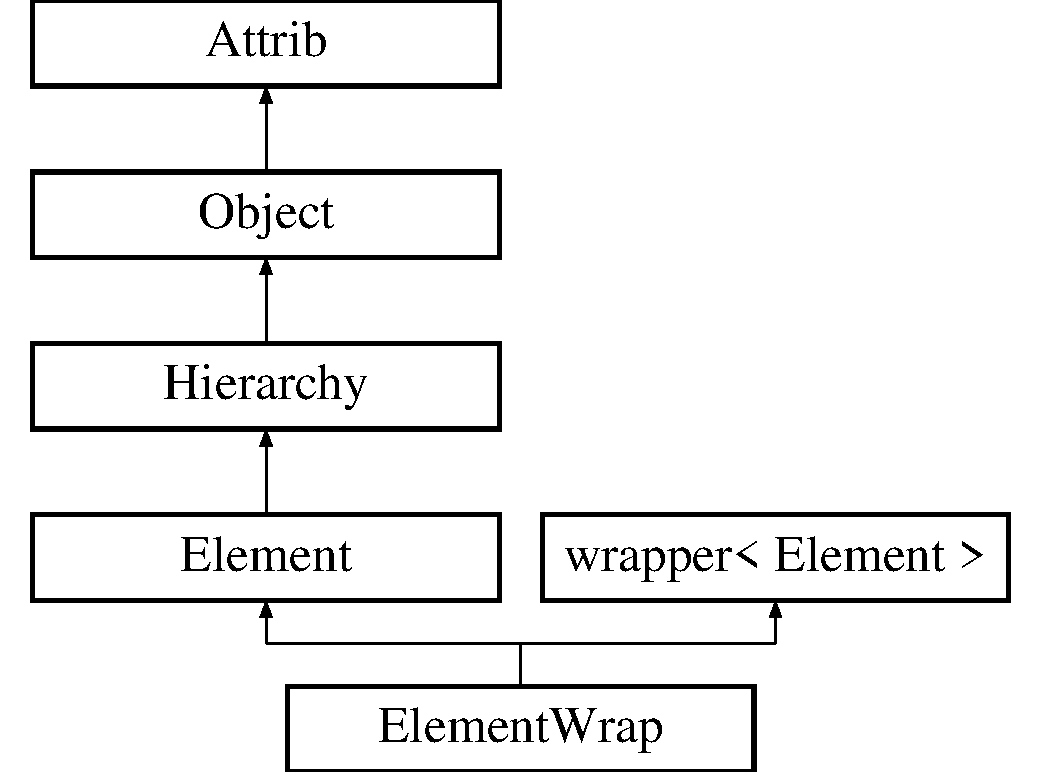
\includegraphics[height=5.000000cm]{structElementWrap}
\end{center}
\end{figure}
\subsection*{Public Types}
\begin{DoxyCompactItemize}
\item 
enum \hyperlink{classAttrib_a69e171d7cc6417835a5a306d3c764235}{Attribut} \{ \newline
\hyperlink{classAttrib_a69e171d7cc6417835a5a306d3c764235a3a8da2ab97dda18aebab196fe4100531}{U\+N\+D\+E\+F\+I\+N\+ED}, 
\hyperlink{classAttrib_a69e171d7cc6417835a5a306d3c764235a2bfb2af57b87031d190a05fe25dd92ed}{P\+A\+S\+S\+I\+VE}, 
\hyperlink{classAttrib_a69e171d7cc6417835a5a306d3c764235a3b1fec929c0370d1436f2f06e298fb0d}{A\+C\+T\+I\+VE}, 
\hyperlink{classAttrib_a69e171d7cc6417835a5a306d3c764235aa27c16b480a369ea4d18b07b2516bbc7}{I\+N\+T\+E\+R\+F\+A\+CE}, 
\newline
\hyperlink{classAttrib_a69e171d7cc6417835a5a306d3c764235a1420a5b8c0540b2af210b6975eded7f9}{IO}, 
\hyperlink{classAttrib_a69e171d7cc6417835a5a306d3c764235a0af3b0d0ac323c1704e6c69cf90add28}{I\+O\+D\+A\+TA}, 
\hyperlink{classAttrib_a69e171d7cc6417835a5a306d3c764235a7788bc5dd333fd8ce18562b269c9dab1}{E\+L\+E\+M\+E\+NT}, 
\hyperlink{classAttrib_a69e171d7cc6417835a5a306d3c764235a61ceb22149f365f1780d18f9d1459423}{H\+A\+R\+D\+W\+A\+RE}, 
\newline
\hyperlink{classAttrib_a69e171d7cc6417835a5a306d3c764235a75250e29692496e73effca2c0330977f}{P\+R\+O\+C\+E\+S\+S\+US}, 
\hyperlink{classAttrib_a69e171d7cc6417835a5a306d3c764235a103a67cd0b8f07ef478fa45d4356e27b}{S\+O\+F\+T\+W\+A\+RE}
 \}
\end{DoxyCompactItemize}
\subsection*{Public Member Functions}
\begin{DoxyCompactItemize}
\item 
void \hyperlink{structElementWrap_ad22ed533c2dad73f8650243d8060b547}{help} ()
\item 
\hyperlink{classStatusCode}{Status\+Code} \hyperlink{structElementWrap_a5e0ca7bd04cfb1f7582fc80c065fd376}{init} ()
\item 
void \hyperlink{structElementWrap_a69a4588be73b8c85ddb92b13f74c3a12}{reset} ()
\item 
void \hyperlink{structElementWrap_a13d2d2771d1dd305abf3457f98482cbe}{update} ()
\item 
void \hyperlink{classElement_a3c0abcb36f8906688bb7e32608df7086}{recursive\+Init\+Element} ()
\item 
void \hyperlink{classElement_a82119ed37dff76508a2746a853ec35ba}{recursive\+Init\+Communications} ()
\item 
\hyperlink{classStatusCode}{Status\+Code} \hyperlink{classElement_ab476b4b1df5954141ceb14f072433b89}{set\+Connection} (\hyperlink{classHierarchy}{Hierarchy} $\ast$)
\item 
\hyperlink{classHierarchy}{Hierarchy} $\ast$ \hyperlink{classElement_af57444353c1ddf9fa0109801e97debf7}{connection} ()
\item 
void \hyperlink{classHierarchy_af4d43b0765b402670eed2d62c73405af}{clear} ()
\item 
void \hyperlink{classHierarchy_a585ad1aeec16077a0e532ab8b4fc557b}{set\+Parent} (\hyperlink{classHierarchy}{Hierarchy} $\ast$\hyperlink{classHierarchy_a1c7bec8257e717f9c1465e06ebf845fc}{parent})
\item 
\hyperlink{classHierarchy}{Hierarchy} $\ast$ \hyperlink{classHierarchy_a1c7bec8257e717f9c1465e06ebf845fc}{parent} ()
\item 
\hyperlink{classHierarchy}{Hierarchy} $\ast$ \hyperlink{classHierarchy_ad550588733bf75ac5c0fcfd7c8fd11a6}{parent} (std\+::string)
\item 
\hyperlink{classHierarchy}{Hierarchy} $\ast$ \hyperlink{classHierarchy_aee461dc930ce3871636ff87f075b1b83}{origin} ()
\item 
virtual void \hyperlink{classHierarchy_ad677774ff38fcb257c04a3a10d471fac}{add\+Child} (\hyperlink{classHierarchy}{Hierarchy} $\ast$element)
\item 
std\+::vector$<$ \hyperlink{classHierarchy}{Hierarchy} $\ast$ $>$ \hyperlink{classHierarchy_aa9a76f69e98e052ee1a6e32cea006288}{children} ()
\item 
\hyperlink{classHierarchy}{Hierarchy} $\ast$ \hyperlink{classHierarchy_a1e207f973c694b538bf90107b4868817}{child} (std\+::string)
\item 
\hyperlink{classHierarchy}{Hierarchy} $\ast$ \hyperlink{classHierarchy_a0c15a5276a3b80b4354d6bd8a01e0708}{child\+Typed} (std\+::string)
\item 
unsigned long \hyperlink{classHierarchy_ab16e84de65fd84e14001a6cf941c8be4}{number\+Of\+Children} ()
\item 
bool \hyperlink{classHierarchy_a255174fe4d316d2a3f430dcb9dab29f1}{has\+Children} ()
\item 
void \hyperlink{classHierarchy_a2b2b359fac003233f65786a616766bde}{del\+Child} (\hyperlink{classHierarchy}{Hierarchy} $\ast$)
\item 
void \hyperlink{classHierarchy_a1928ac7615fe0b5e55cd707f70dc6781}{del\+Child} (std\+::string)
\item 
std\+::string \hyperlink{classHierarchy_aa7990fa7caf132d83e361ce033c6c65a}{path} (std\+::string=std\+::string(\char`\"{}\char`\"{}))
\item 
std\+::string \hyperlink{classHierarchy_a1efd56cd164d328d2002e53a10a19b8c}{path\+Typed} (std\+::string=std\+::string(\char`\"{}\char`\"{}))
\item 
void \hyperlink{classHierarchy_a76e914b9a677a22a82deb74d892bf261}{tree} (std\+::string indent=std\+::string(\char`\"{}\char`\"{}))
\item 
void \hyperlink{classHierarchy_a594c294c5f60c230e106d522ed008212}{tree} ()
\item 
std\+::string \hyperlink{classObject_a300f4c05dd468c7bb8b3c968868443c1}{name} () const
\item 
std\+::string \hyperlink{classObject_a84f99f70f144a83e1582d1d0f84e4e62}{type} ()
\item 
unsigned char \hyperlink{classObject_af99145335cc61ff6e2798ea17db009d2}{id} ()
\item 
std\+::string \hyperlink{classObject_a73a0f1a41828fdd8303dd662446fb6c3}{title} ()
\item 
void \hyperlink{classObject_a3f9d5537ebce0c0f2bf6ae4d92426f3c}{msg\+Svc} (int level, std\+::string \hyperlink{classObject_a58b2d0618c2d08cf2383012611528d97}{msg}, std\+::string \hyperlink{classObject_a300f4c05dd468c7bb8b3c968868443c1}{name})
\item 
void \hyperlink{classObject_a58b2d0618c2d08cf2383012611528d97}{msg} (std\+::string mymsg)
\item 
void \hyperlink{classObject_ac5d59299273cee27aacf7de00d2e7034}{msg} (std\+::string mymsg, std\+::string \hyperlink{classObject_a300f4c05dd468c7bb8b3c968868443c1}{name})
\item 
void \hyperlink{classObject_a83d2db2df682907ea1115ad721c1c4a1}{verbose} (std\+::string mymsg)
\item 
void \hyperlink{classObject_a2d4120195317e2a3c6532e8bb9f3da68}{verbose} (std\+::string mymsg, std\+::string \hyperlink{classObject_a300f4c05dd468c7bb8b3c968868443c1}{name})
\item 
void \hyperlink{classObject_aac010553f022165573714b7014a15f0d}{debug} (std\+::string mymsg)
\item 
void \hyperlink{classObject_a6c9a0397ca804e04d675ed05683f5420}{debug} (std\+::string mymsg, std\+::string \hyperlink{classObject_a300f4c05dd468c7bb8b3c968868443c1}{name})
\item 
void \hyperlink{classObject_a644fd329ea4cb85f54fa6846484b84a8}{info} (std\+::string mymsg)
\item 
void \hyperlink{classObject_a1ca123253dfd30fc28b156f521dcbdae}{info} (std\+::string mymsg, std\+::string \hyperlink{classObject_a300f4c05dd468c7bb8b3c968868443c1}{name})
\item 
void \hyperlink{classObject_a65cd4fda577711660821fd2cd5a3b4c9}{warning} (std\+::string mymsg)
\item 
void \hyperlink{classObject_a11f101db4dd73d9391b0231818881d86}{warning} (std\+::string mymsg, std\+::string \hyperlink{classObject_a300f4c05dd468c7bb8b3c968868443c1}{name})
\item 
void \hyperlink{classObject_a204a95f57818c0f811933917a30eff45}{error} (std\+::string mymsg)
\item 
void \hyperlink{classObject_ad7f6c457733082efa2f9ff5f5c8e119a}{error} (std\+::string mymsg, std\+::string \hyperlink{classObject_a300f4c05dd468c7bb8b3c968868443c1}{name})
\item 
void \hyperlink{classObject_aad5a16aac7516ce65bd5ec02ab07fc80}{fatal} (std\+::string mymsg)
\item 
void \hyperlink{classObject_ae62acd3d09f716220f75f252dc38bc9a}{fatal} (std\+::string mymsg, std\+::string \hyperlink{classObject_a300f4c05dd468c7bb8b3c968868443c1}{name})
\item 
void \hyperlink{classObject_ae30fea75683c2d149b6b6d17c09ecd0c}{set\+Name} (std\+::string \hyperlink{classObject_a300f4c05dd468c7bb8b3c968868443c1}{name})
\item 
void \hyperlink{classObject_aae534cc9d982bcb9b99fd505f2e103a5}{set\+Type} (std\+::string \hyperlink{classObject_a84f99f70f144a83e1582d1d0f84e4e62}{type})
\item 
void \hyperlink{classObject_a398fe08cba594a0ce6891d59fe4f159f}{set\+Id} (unsigned char \hyperlink{classObject_af99145335cc61ff6e2798ea17db009d2}{id})
\item 
void \hyperlink{classObject_a89557dbbad5bcaa02652f5d7fa35d20f}{set\+Title} (std\+::string \hyperlink{classObject_a73a0f1a41828fdd8303dd662446fb6c3}{title})
\item 
void \hyperlink{classObject_a870c5af919958c2136623b2d7816d123}{set\+Dll\+Name} (std\+::string \hyperlink{classObject_a2e3947f2870094c332d7454117f3ec63}{dll\+Name})
\item 
std\+::string \hyperlink{classObject_a2e3947f2870094c332d7454117f3ec63}{dll\+Name} ()
\item 
bool \hyperlink{classAttrib_a704f26af560909ad22065083bb7d4c34}{is} (int attribut)
\item 
void \hyperlink{classAttrib_a235f773af19c900264a190b00a3b4ad7}{add} (int attribut)
\item 
void \hyperlink{classAttrib_a7d4ef7e32d93cb287792b87b857e79f3}{remove} (int attribut)
\item 
std\+::string \hyperlink{classAttrib_aee7bbf16b144887f196e1341b24f8a26}{attributs} ()
\end{DoxyCompactItemize}
\subsection*{Protected Attributes}
\begin{DoxyCompactItemize}
\item 
\hyperlink{classHierarchy}{Hierarchy} $\ast$ \hyperlink{classElement_abe3de7a5dbbc9a6dd2d7e012e5fdb266}{m\+\_\+connection}
\item 
std\+::string \hyperlink{classAttrib_a3414521d7a82476e874b25a5407b5e63}{m\+\_\+attrib\+String} \mbox{[}10\mbox{]}
\end{DoxyCompactItemize}


\subsection{Detailed Description}


Definition at line 19 of file Python\+\_\+\+Obj.\+cpp.



\subsection{Member Enumeration Documentation}
\mbox{\Hypertarget{classAttrib_a69e171d7cc6417835a5a306d3c764235}\label{classAttrib_a69e171d7cc6417835a5a306d3c764235}} 
\index{Element\+Wrap@{Element\+Wrap}!Attribut@{Attribut}}
\index{Attribut@{Attribut}!Element\+Wrap@{Element\+Wrap}}
\subsubsection{\texorpdfstring{Attribut}{Attribut}}
{\footnotesize\ttfamily enum \hyperlink{classAttrib_a69e171d7cc6417835a5a306d3c764235}{Attrib\+::\+Attribut}\hspace{0.3cm}{\ttfamily [inherited]}}

\begin{DoxyEnumFields}{Enumerator}
\raisebox{\heightof{T}}[0pt][0pt]{\index{U\+N\+D\+E\+F\+I\+N\+ED@{U\+N\+D\+E\+F\+I\+N\+ED}!Element\+Wrap@{Element\+Wrap}}\index{Element\+Wrap@{Element\+Wrap}!U\+N\+D\+E\+F\+I\+N\+ED@{U\+N\+D\+E\+F\+I\+N\+ED}}}\mbox{\Hypertarget{classAttrib_a69e171d7cc6417835a5a306d3c764235a3a8da2ab97dda18aebab196fe4100531}\label{classAttrib_a69e171d7cc6417835a5a306d3c764235a3a8da2ab97dda18aebab196fe4100531}} 
U\+N\+D\+E\+F\+I\+N\+ED&\\
\hline

\raisebox{\heightof{T}}[0pt][0pt]{\index{P\+A\+S\+S\+I\+VE@{P\+A\+S\+S\+I\+VE}!Element\+Wrap@{Element\+Wrap}}\index{Element\+Wrap@{Element\+Wrap}!P\+A\+S\+S\+I\+VE@{P\+A\+S\+S\+I\+VE}}}\mbox{\Hypertarget{classAttrib_a69e171d7cc6417835a5a306d3c764235a2bfb2af57b87031d190a05fe25dd92ed}\label{classAttrib_a69e171d7cc6417835a5a306d3c764235a2bfb2af57b87031d190a05fe25dd92ed}} 
P\+A\+S\+S\+I\+VE&\\
\hline

\raisebox{\heightof{T}}[0pt][0pt]{\index{A\+C\+T\+I\+VE@{A\+C\+T\+I\+VE}!Element\+Wrap@{Element\+Wrap}}\index{Element\+Wrap@{Element\+Wrap}!A\+C\+T\+I\+VE@{A\+C\+T\+I\+VE}}}\mbox{\Hypertarget{classAttrib_a69e171d7cc6417835a5a306d3c764235a3b1fec929c0370d1436f2f06e298fb0d}\label{classAttrib_a69e171d7cc6417835a5a306d3c764235a3b1fec929c0370d1436f2f06e298fb0d}} 
A\+C\+T\+I\+VE&\\
\hline

\raisebox{\heightof{T}}[0pt][0pt]{\index{I\+N\+T\+E\+R\+F\+A\+CE@{I\+N\+T\+E\+R\+F\+A\+CE}!Element\+Wrap@{Element\+Wrap}}\index{Element\+Wrap@{Element\+Wrap}!I\+N\+T\+E\+R\+F\+A\+CE@{I\+N\+T\+E\+R\+F\+A\+CE}}}\mbox{\Hypertarget{classAttrib_a69e171d7cc6417835a5a306d3c764235aa27c16b480a369ea4d18b07b2516bbc7}\label{classAttrib_a69e171d7cc6417835a5a306d3c764235aa27c16b480a369ea4d18b07b2516bbc7}} 
I\+N\+T\+E\+R\+F\+A\+CE&\\
\hline

\raisebox{\heightof{T}}[0pt][0pt]{\index{IO@{IO}!Element\+Wrap@{Element\+Wrap}}\index{Element\+Wrap@{Element\+Wrap}!IO@{IO}}}\mbox{\Hypertarget{classAttrib_a69e171d7cc6417835a5a306d3c764235a1420a5b8c0540b2af210b6975eded7f9}\label{classAttrib_a69e171d7cc6417835a5a306d3c764235a1420a5b8c0540b2af210b6975eded7f9}} 
IO&\\
\hline

\raisebox{\heightof{T}}[0pt][0pt]{\index{I\+O\+D\+A\+TA@{I\+O\+D\+A\+TA}!Element\+Wrap@{Element\+Wrap}}\index{Element\+Wrap@{Element\+Wrap}!I\+O\+D\+A\+TA@{I\+O\+D\+A\+TA}}}\mbox{\Hypertarget{classAttrib_a69e171d7cc6417835a5a306d3c764235a0af3b0d0ac323c1704e6c69cf90add28}\label{classAttrib_a69e171d7cc6417835a5a306d3c764235a0af3b0d0ac323c1704e6c69cf90add28}} 
I\+O\+D\+A\+TA&\\
\hline

\raisebox{\heightof{T}}[0pt][0pt]{\index{E\+L\+E\+M\+E\+NT@{E\+L\+E\+M\+E\+NT}!Element\+Wrap@{Element\+Wrap}}\index{Element\+Wrap@{Element\+Wrap}!E\+L\+E\+M\+E\+NT@{E\+L\+E\+M\+E\+NT}}}\mbox{\Hypertarget{classAttrib_a69e171d7cc6417835a5a306d3c764235a7788bc5dd333fd8ce18562b269c9dab1}\label{classAttrib_a69e171d7cc6417835a5a306d3c764235a7788bc5dd333fd8ce18562b269c9dab1}} 
E\+L\+E\+M\+E\+NT&\\
\hline

\raisebox{\heightof{T}}[0pt][0pt]{\index{H\+A\+R\+D\+W\+A\+RE@{H\+A\+R\+D\+W\+A\+RE}!Element\+Wrap@{Element\+Wrap}}\index{Element\+Wrap@{Element\+Wrap}!H\+A\+R\+D\+W\+A\+RE@{H\+A\+R\+D\+W\+A\+RE}}}\mbox{\Hypertarget{classAttrib_a69e171d7cc6417835a5a306d3c764235a61ceb22149f365f1780d18f9d1459423}\label{classAttrib_a69e171d7cc6417835a5a306d3c764235a61ceb22149f365f1780d18f9d1459423}} 
H\+A\+R\+D\+W\+A\+RE&\\
\hline

\raisebox{\heightof{T}}[0pt][0pt]{\index{P\+R\+O\+C\+E\+S\+S\+US@{P\+R\+O\+C\+E\+S\+S\+US}!Element\+Wrap@{Element\+Wrap}}\index{Element\+Wrap@{Element\+Wrap}!P\+R\+O\+C\+E\+S\+S\+US@{P\+R\+O\+C\+E\+S\+S\+US}}}\mbox{\Hypertarget{classAttrib_a69e171d7cc6417835a5a306d3c764235a75250e29692496e73effca2c0330977f}\label{classAttrib_a69e171d7cc6417835a5a306d3c764235a75250e29692496e73effca2c0330977f}} 
P\+R\+O\+C\+E\+S\+S\+US&\\
\hline

\raisebox{\heightof{T}}[0pt][0pt]{\index{S\+O\+F\+T\+W\+A\+RE@{S\+O\+F\+T\+W\+A\+RE}!Element\+Wrap@{Element\+Wrap}}\index{Element\+Wrap@{Element\+Wrap}!S\+O\+F\+T\+W\+A\+RE@{S\+O\+F\+T\+W\+A\+RE}}}\mbox{\Hypertarget{classAttrib_a69e171d7cc6417835a5a306d3c764235a103a67cd0b8f07ef478fa45d4356e27b}\label{classAttrib_a69e171d7cc6417835a5a306d3c764235a103a67cd0b8f07ef478fa45d4356e27b}} 
S\+O\+F\+T\+W\+A\+RE&\\
\hline

\end{DoxyEnumFields}


Definition at line 29 of file Attrib.\+h.


\begin{DoxyCode}
29                 \{
30     \hyperlink{classAttrib_a69e171d7cc6417835a5a306d3c764235a3a8da2ab97dda18aebab196fe4100531}{UNDEFINED},
31     \hyperlink{classAttrib_a69e171d7cc6417835a5a306d3c764235a2bfb2af57b87031d190a05fe25dd92ed}{PASSIVE},
32     \hyperlink{classAttrib_a69e171d7cc6417835a5a306d3c764235a3b1fec929c0370d1436f2f06e298fb0d}{ACTIVE},
33     \hyperlink{classAttrib_a69e171d7cc6417835a5a306d3c764235aa27c16b480a369ea4d18b07b2516bbc7}{INTERFACE},
34     \hyperlink{classAttrib_a69e171d7cc6417835a5a306d3c764235a1420a5b8c0540b2af210b6975eded7f9}{IO},
35     \hyperlink{classAttrib_a69e171d7cc6417835a5a306d3c764235a0af3b0d0ac323c1704e6c69cf90add28}{IODATA},
36     \hyperlink{classAttrib_a69e171d7cc6417835a5a306d3c764235a7788bc5dd333fd8ce18562b269c9dab1}{ELEMENT},
37     \hyperlink{classAttrib_a69e171d7cc6417835a5a306d3c764235a61ceb22149f365f1780d18f9d1459423}{HARDWARE},
38     \hyperlink{classAttrib_a69e171d7cc6417835a5a306d3c764235a75250e29692496e73effca2c0330977f}{PROCESSUS},
39     \hyperlink{classAttrib_a69e171d7cc6417835a5a306d3c764235a103a67cd0b8f07ef478fa45d4356e27b}{SOFTWARE} 
40   \}; \textcolor{comment}{// array m\_attribString must be changed into Attrib::Attrib if this enu is modified. }
\end{DoxyCode}


\subsection{Member Function Documentation}
\mbox{\Hypertarget{classAttrib_a235f773af19c900264a190b00a3b4ad7}\label{classAttrib_a235f773af19c900264a190b00a3b4ad7}} 
\index{Element\+Wrap@{Element\+Wrap}!add@{add}}
\index{add@{add}!Element\+Wrap@{Element\+Wrap}}
\subsubsection{\texorpdfstring{add()}{add()}}
{\footnotesize\ttfamily void Attrib\+::add (\begin{DoxyParamCaption}\item[{int}]{attribut }\end{DoxyParamCaption})\hspace{0.3cm}{\ttfamily [inline]}, {\ttfamily [inherited]}}

Add an attribut 

Definition at line 67 of file Attrib.\+h.



References Attrib\+::m\+\_\+attributs, and Attrib\+::\+U\+N\+D\+E\+F\+I\+N\+ED.



Referenced by A3\+P\+E\+::\+A3\+P\+E(), Attrib\+::\+Attrib(), Specs\+Mezzanine\+::cmdline(), Computer\+::\+Computer(), C\+U\+\_\+v1\+::\+C\+U\+\_\+v1(), export\+\_\+obj(), F\+E\+B\+\_\+v1\+::\+F\+E\+B\+\_\+v1(), Fe\+P\+G\+A\+::\+Fe\+P\+G\+A(), I\+C\+E\+C\+A\+Lv3\+::\+I\+C\+E\+C\+A\+Lv3(), I\+C\+Phaser\+::\+I\+C\+Phaser(), Fe\+P\+G\+A\+::init(), Application\+::initialize(), Interface\+::\+Interface(), I\+Odata\+::\+I\+Odata(), I\+Oobject\+::\+I\+Oobject(), M\+S\+Oxxxx\+::\+M\+S\+Oxxxx(), Phaser\+::\+Phaser(), Processus\+::\+Processus(), Proto40\+M\+Hz\+\_\+v1\+::\+Proto40\+M\+Hz\+\_\+v1(), Attrib\+::remove(), Seq\+P\+G\+A\+::\+Seq\+P\+G\+A(), Test\+I2\+C\+::set\+Address(), Test\+S\+P\+I\+::set\+Address(), Specs\+Slave\+::set\+Address(), Specs\+Master\+::\+Specs\+Master(), and Specs\+Slave\+::\+Specs\+Slave().


\begin{DoxyCode}
67                             \{
68     \textcolor{keywordflow}{if} (attribut!=\hyperlink{classAttrib_a69e171d7cc6417835a5a306d3c764235a3a8da2ab97dda18aebab196fe4100531}{Attrib::UNDEFINED}) \textcolor{keyword}{remove}(\hyperlink{classAttrib_a69e171d7cc6417835a5a306d3c764235a3a8da2ab97dda18aebab196fe4100531}{Attrib::UNDEFINED});
69     \textcolor{keywordtype}{bool} duplicate = false ;
70     std::vector<int>::const\_iterator iter ;
71     \textcolor{keywordflow}{for} ( iter  = \hyperlink{classAttrib_ac4bd58a0cc6b38a3b711d609a3d3aacc}{m\_attributs}.begin() ;
72           iter != \hyperlink{classAttrib_ac4bd58a0cc6b38a3b711d609a3d3aacc}{m\_attributs}.end()   ;
73           ++iter ) \{
74       \textcolor{keywordflow}{if} ( attribut == (*iter) ) \{
75         duplicate = true ;
76       \}
77     \}
78     \textcolor{keywordflow}{if} (!duplicate) \{
79       \hyperlink{classAttrib_ac4bd58a0cc6b38a3b711d609a3d3aacc}{m\_attributs}.push\_back( attribut );
80     \}
81   \}
\end{DoxyCode}
\mbox{\Hypertarget{classHierarchy_ad677774ff38fcb257c04a3a10d471fac}\label{classHierarchy_ad677774ff38fcb257c04a3a10d471fac}} 
\index{Element\+Wrap@{Element\+Wrap}!add\+Child@{add\+Child}}
\index{add\+Child@{add\+Child}!Element\+Wrap@{Element\+Wrap}}
\subsubsection{\texorpdfstring{add\+Child()}{addChild()}}
{\footnotesize\ttfamily void Hierarchy\+::add\+Child (\begin{DoxyParamCaption}\item[{\hyperlink{classHierarchy}{Hierarchy} $\ast$}]{element }\end{DoxyParamCaption})\hspace{0.3cm}{\ttfamily [virtual]}, {\ttfamily [inherited]}}



Definition at line 83 of file Hierarchy.\+cpp.



References Object\+::debug(), Hierarchy\+::m\+\_\+children, Object\+::name(), and Hierarchy\+::set\+Parent().



Referenced by A3\+P\+E\+::\+A3\+P\+E(), Specs\+Mezzanine\+::add\+Bus(), Specs\+Slave\+::add\+I2c(), Application\+::create(), C\+U\+\_\+v1\+::\+C\+U\+\_\+v1(), export\+\_\+obj(), F\+E\+B\+\_\+v1\+::\+F\+E\+B\+\_\+v1(), Fe\+P\+G\+A\+::\+Fe\+P\+G\+A(), I\+C\+E\+C\+A\+Lv3\+::\+I\+C\+E\+C\+A\+Lv3(), I\+C\+Phaser\+::\+I\+C\+Phaser(), Fe\+P\+G\+A\+::\+Make\+R\+A\+M(), Fe\+P\+G\+A\+::\+Make\+Register(), Hierarchy\+::origin(), Phaser\+::\+Phaser(), Proto40\+M\+Hz\+\_\+v1\+::\+Proto40\+M\+Hz\+\_\+v1(), Seq\+P\+G\+A\+::\+Seq\+P\+G\+A(), Specs\+Mezzanine\+::\+Specs\+Mezzanine(), Usb\+I2c\+Bus\+::\+Usb\+I2c\+Bus(), and Usb\+Spi\+Bus\+::\+Usb\+Spi\+Bus().


\begin{DoxyCode}
83                                           \{
84   element->\hyperlink{classHierarchy_a585ad1aeec16077a0e532ab8b4fc557b}{setParent}(\textcolor{keyword}{this});
85   \hyperlink{classHierarchy_a038816763941fd4a930504917f60483b}{m\_children}.push\_back(element);
86   \hyperlink{classObject_aac010553f022165573714b7014a15f0d}{debug}(element->\hyperlink{classObject_a300f4c05dd468c7bb8b3c968868443c1}{name}()+\textcolor{stringliteral}{" added to the child tree."},\textcolor{stringliteral}{"Hierarchy::addChild"});
87 \}
\end{DoxyCode}
\mbox{\Hypertarget{classAttrib_aee7bbf16b144887f196e1341b24f8a26}\label{classAttrib_aee7bbf16b144887f196e1341b24f8a26}} 
\index{Element\+Wrap@{Element\+Wrap}!attributs@{attributs}}
\index{attributs@{attributs}!Element\+Wrap@{Element\+Wrap}}
\subsubsection{\texorpdfstring{attributs()}{attributs()}}
{\footnotesize\ttfamily std\+::string Attrib\+::attributs (\begin{DoxyParamCaption}{ }\end{DoxyParamCaption})\hspace{0.3cm}{\ttfamily [inherited]}}

Print the \hyperlink{classAttrib}{Attrib} of an \hyperlink{classObject}{Object} 

Definition at line 54 of file Attrib.\+cpp.



References images\+::index, Attrib\+::m\+\_\+attrib\+String, and Attrib\+::m\+\_\+attributs.



Referenced by export\+\_\+obj(), and Attrib\+::remove().


\begin{DoxyCode}
54                             \{
55   std::string output;
56   std::vector<int>::iterator iter ;
57   \textcolor{keywordflow}{for} ( \textcolor{keywordtype}{unsigned} \textcolor{keywordtype}{int} \hyperlink{namespaceimages_a54407fd574970b3178647ae096321a57}{index} = 0 ; \hyperlink{namespaceimages_a54407fd574970b3178647ae096321a57}{index} < \hyperlink{classAttrib_ac4bd58a0cc6b38a3b711d609a3d3aacc}{m\_attributs}.size() ; ++
      \hyperlink{namespaceimages_a54407fd574970b3178647ae096321a57}{index} ) \{
58     \textcolor{keywordflow}{if} ( \hyperlink{classAttrib_ac4bd58a0cc6b38a3b711d609a3d3aacc}{m\_attributs}.size() - \hyperlink{namespaceimages_a54407fd574970b3178647ae096321a57}{index} > 1 ) \{
59       output.append(\hyperlink{classAttrib_a3414521d7a82476e874b25a5407b5e63}{m\_attribString}[\hyperlink{classAttrib_ac4bd58a0cc6b38a3b711d609a3d3aacc}{m\_attributs}[\hyperlink{namespaceimages_a54407fd574970b3178647ae096321a57}{index}]]);
60       output.append(\textcolor{stringliteral}{":"});
61     \}
62     \textcolor{keywordflow}{else} \{
63       output.append(\hyperlink{classAttrib_a3414521d7a82476e874b25a5407b5e63}{m\_attribString}[\hyperlink{classAttrib_ac4bd58a0cc6b38a3b711d609a3d3aacc}{m\_attributs}[index]]);
64     \}
65   \}
66   \textcolor{keywordflow}{return} output;
67 \}
\end{DoxyCode}
\mbox{\Hypertarget{classHierarchy_a1e207f973c694b538bf90107b4868817}\label{classHierarchy_a1e207f973c694b538bf90107b4868817}} 
\index{Element\+Wrap@{Element\+Wrap}!child@{child}}
\index{child@{child}!Element\+Wrap@{Element\+Wrap}}
\subsubsection{\texorpdfstring{child()}{child()}}
{\footnotesize\ttfamily \hyperlink{classHierarchy}{Hierarchy} $\ast$ Hierarchy\+::child (\begin{DoxyParamCaption}\item[{std\+::string}]{path }\end{DoxyParamCaption})\hspace{0.3cm}{\ttfamily [inherited]}}



Definition at line 133 of file Hierarchy.\+cpp.



References Hierarchy\+::child(), Hierarchy\+::children(), Object\+::name(), Hierarchy\+::origin(), Hierarchy\+::parent(), Hierarchy\+::path(), and Object\+::warning().



Referenced by Application\+::cd(), Hierarchy\+::child(), Hierarchy\+::children(), and export\+\_\+obj().


\begin{DoxyCode}
133                                          \{
134   std::string newpath = \hyperlink{classHierarchy_aa7990fa7caf132d83e361ce033c6c65a}{path};
135   std::string up(\textcolor{stringliteral}{".."});
136   std::string separator(1,\textcolor{charliteral}{'/'});
137 
138   \hyperlink{classHierarchy}{Hierarchy} * newcurrent = 0;
139 
140   \textcolor{comment}{//  info("path="+path,"Hierarchy::child");}
141 
142   \textcolor{keywordflow}{if} (\hyperlink{classHierarchy_aa7990fa7caf132d83e361ce033c6c65a}{path}.compare(\textcolor{stringliteral}{""})==0 || \hyperlink{classHierarchy_aa7990fa7caf132d83e361ce033c6c65a}{path}.compare(\textcolor{stringliteral}{"/"})==0) \{
143     \textcolor{comment}{//    debug("return origin","Hierarchy::child");}
144     \textcolor{keywordflow}{return} \hyperlink{classHierarchy_aee461dc930ce3871636ff87f075b1b83}{origin}();
145   \}
146 
147   \textcolor{keywordflow}{if} (\hyperlink{classHierarchy_aa7990fa7caf132d83e361ce033c6c65a}{path}.compare(\hyperlink{classObject_a300f4c05dd468c7bb8b3c968868443c1}{name}())==0)\{
148     \textcolor{comment}{//    debug("return itself","Hierarchy::child");}
149     \textcolor{keywordflow}{return} \textcolor{keyword}{this};
150   \}
151 
152   \textcolor{keywordflow}{if} (\hyperlink{classHierarchy_aa7990fa7caf132d83e361ce033c6c65a}{path}.compare(\textcolor{stringliteral}{".."})==0)\{
153     \textcolor{keywordflow}{if} (0!=this->\hyperlink{classHierarchy_a1c7bec8257e717f9c1465e06ebf845fc}{parent}()) \textcolor{keywordflow}{return} this->\hyperlink{classHierarchy_a1c7bec8257e717f9c1465e06ebf845fc}{parent}();
154     \textcolor{keywordflow}{else} \textcolor{keywordflow}{return} \textcolor{keyword}{this};
155   \}
156 
157   \textcolor{keywordflow}{if} (\hyperlink{classHierarchy_aa7990fa7caf132d83e361ce033c6c65a}{path}.compare(\textcolor{stringliteral}{"../"})==0)\{
158     \textcolor{keywordflow}{if} (0!=this->\hyperlink{classHierarchy_a1c7bec8257e717f9c1465e06ebf845fc}{parent}()) \textcolor{keywordflow}{return} this->\hyperlink{classHierarchy_a1c7bec8257e717f9c1465e06ebf845fc}{parent}();
159     \textcolor{keywordflow}{else} \textcolor{keywordflow}{return} \textcolor{keyword}{this};
160   \}
161 
162 
163   \textcolor{keywordtype}{int} npos=\hyperlink{classHierarchy_aa7990fa7caf132d83e361ce033c6c65a}{path}.find(separator,0);
164 
165   \textcolor{comment}{//  info("find separator in "+itos(npos)+" of "+path,"Hierarchy::child");}
166 
167   \textcolor{comment}{// remove last separator}
168   \textcolor{keywordflow}{if} ( npos == (\textcolor{keywordtype}{int})(\hyperlink{classHierarchy_aa7990fa7caf132d83e361ce033c6c65a}{path}.size()-1) ) \{
169     newpath = std::string(\hyperlink{classHierarchy_aa7990fa7caf132d83e361ce033c6c65a}{path},0,npos);
170     \hyperlink{classHierarchy_aa7990fa7caf132d83e361ce033c6c65a}{path} = newpath;
171   \}
172 
173   \textcolor{keywordflow}{if} (npos==0)\{
174     \textcolor{comment}{//    debug("Going back to origin and calling child","Hierarchy::child");}
175     newpath=std::string(\hyperlink{classHierarchy_aa7990fa7caf132d83e361ce033c6c65a}{path},1,\hyperlink{classHierarchy_aa7990fa7caf132d83e361ce033c6c65a}{path}.size()-1);
176     \textcolor{keywordflow}{return} \hyperlink{classHierarchy_aee461dc930ce3871636ff87f075b1b83}{origin}()->\hyperlink{classHierarchy_a1e207f973c694b538bf90107b4868817}{child}(newpath);
177   \}
178   \textcolor{keywordflow}{else}\{
179     \textcolor{keywordflow}{if} ( npos== (\textcolor{keywordtype}{int})(std::string::npos) )\{
180       \textcolor{comment}{//      debug("Getting chid "+path+" of "+this->name(),"Hierarchy::child");}
181       std::vector <Hierarchy*> list = \hyperlink{classHierarchy_aa9a76f69e98e052ee1a6e32cea006288}{children}();
182       std::vector<Hierarchy*>::iterator iter;
183       \textcolor{keywordflow}{for} (iter=list.begin();iter!=list.end();iter++)\{
184         \textcolor{keywordflow}{if} ((*iter)->name().compare(\hyperlink{classHierarchy_aa7990fa7caf132d83e361ce033c6c65a}{path})==0)\{
185           \textcolor{keywordflow}{return} *iter;
186         \}
187       \}
188       \hyperlink{classObject_a65cd4fda577711660821fd2cd5a3b4c9}{warning}(this->\hyperlink{classObject_a300f4c05dd468c7bb8b3c968868443c1}{name}()+std::string(\textcolor{stringliteral}{" has no child '"})+\hyperlink{classHierarchy_aa7990fa7caf132d83e361ce033c6c65a}{path}+\textcolor{stringliteral}{"'"},\textcolor{stringliteral}{"Hierarchy::child"});
189       \textcolor{keywordflow}{return} \textcolor{keyword}{this};
190     \}
191     \textcolor{keywordflow}{else}
192     \{
193       \textcolor{keywordtype}{int} ipos=\hyperlink{classHierarchy_aa7990fa7caf132d83e361ce033c6c65a}{path}.find(separator,0);
194       \textcolor{comment}{//      info("default behaviour "+path+" with separator in "+itos(ipos),"Hierarchy::child");}
195 
196       std::string newcurrentname=std::string(\hyperlink{classHierarchy_aa7990fa7caf132d83e361ce033c6c65a}{path},0,ipos);
197       newpath=std::string(\hyperlink{classHierarchy_aa7990fa7caf132d83e361ce033c6c65a}{path},ipos+1,\hyperlink{classHierarchy_aa7990fa7caf132d83e361ce033c6c65a}{path}.size()-1);
198 
199       \textcolor{comment}{//      info("looking now for "+newpath+" from "+newcurrentname,"Hierarchy::child");}
200 
201       \textcolor{keywordflow}{if} (0==newcurrentname.compare(\hyperlink{classHierarchy_aee461dc930ce3871636ff87f075b1b83}{origin}()->\hyperlink{classObject_a300f4c05dd468c7bb8b3c968868443c1}{name}()))\{
202         \textcolor{comment}{//        info("current is computer. Looking for children"+newcurrentname,"Hierarchy::child");}
203         \textcolor{keywordflow}{return} \hyperlink{classHierarchy_aee461dc930ce3871636ff87f075b1b83}{origin}()->\hyperlink{classHierarchy_a1e207f973c694b538bf90107b4868817}{child}(newpath);
204       \}
205 
206       newcurrent = (\hyperlink{classHierarchy}{Hierarchy}*)0;
207 
208       std::vector <Hierarchy*> list = \hyperlink{classHierarchy_aa9a76f69e98e052ee1a6e32cea006288}{children}();
209       std::vector<Hierarchy*>::iterator iter;
210       \textcolor{keywordflow}{for} (iter=list.begin();iter!=list.end();iter++)\{
211         \textcolor{keywordflow}{if} ((*iter)->name().compare(newcurrentname)==0)\{
212           newcurrent = (*iter);
213         \}
214       \}
215 
216 
217       \textcolor{keywordflow}{if} ((\hyperlink{classHierarchy}{Hierarchy}*)0==newcurrent)\{
218         \textcolor{keywordflow}{if} (newcurrentname.compare(\textcolor{stringliteral}{".."})==0 && 0!=\hyperlink{classHierarchy_a1c7bec8257e717f9c1465e06ebf845fc}{parent}())\{
219           newcurrent=this->\hyperlink{classHierarchy_a1c7bec8257e717f9c1465e06ebf845fc}{parent}();
220           \textcolor{comment}{//          debug("newcurrent was .. -> parent="+parent()->name());}
221         \}
222         \textcolor{keywordflow}{else}
223         \{
224           \hyperlink{classObject_a65cd4fda577711660821fd2cd5a3b4c9}{warning}(this->\hyperlink{classObject_a300f4c05dd468c7bb8b3c968868443c1}{name}()+\textcolor{stringliteral}{" has no child '"}+newcurrentname+\textcolor{stringliteral}{"'"},
225               \textcolor{stringliteral}{"Hierarchy::child"});
226           \textcolor{keywordflow}{return} \textcolor{keyword}{this};
227         \}
228       \}
229       \textcolor{comment}{//      debug("recurrence call for "+newpath+" on "+newcurrent->name(),"Hierarchy::child");}
230       \textcolor{keywordflow}{return} newcurrent -> \hyperlink{classHierarchy_a1e207f973c694b538bf90107b4868817}{child} ( newpath );
231     \}
232   \}
233 \}
\end{DoxyCode}
\mbox{\Hypertarget{classHierarchy_aa9a76f69e98e052ee1a6e32cea006288}\label{classHierarchy_aa9a76f69e98e052ee1a6e32cea006288}} 
\index{Element\+Wrap@{Element\+Wrap}!children@{children}}
\index{children@{children}!Element\+Wrap@{Element\+Wrap}}
\subsubsection{\texorpdfstring{children()}{children()}}
{\footnotesize\ttfamily std\+::vector$<$\hyperlink{classHierarchy}{Hierarchy}$\ast$$>$ Hierarchy\+::children (\begin{DoxyParamCaption}{ }\end{DoxyParamCaption})\hspace{0.3cm}{\ttfamily [inline]}, {\ttfamily [inherited]}}



Definition at line 33 of file Hierarchy.\+h.



References Hierarchy\+::child(), Hierarchy\+::child\+Typed(), Hierarchy\+::del\+Child(), Hierarchy\+::has\+Children(), Hierarchy\+::m\+\_\+children, Hierarchy\+::number\+Of\+Children(), Hierarchy\+::path(), Hierarchy\+::path\+Typed(), and Hierarchy\+::tree().



Referenced by Hierarchy\+::child(), Hierarchy\+::child\+Typed(), export\+\_\+obj(), Specs\+Slave\+::recursive\+Init\+Communications(), Element\+::recursive\+Init\+Communications(), Element\+::recursive\+Init\+Element(), Application\+::set\+Config(), and Hierarchy\+::tree().


\begin{DoxyCode}
33 \{ \textcolor{keywordflow}{return} \hyperlink{classHierarchy_a038816763941fd4a930504917f60483b}{m\_children};  \} \textcolor{comment}{//< get list of child(ren)}
\end{DoxyCode}
\mbox{\Hypertarget{classHierarchy_a0c15a5276a3b80b4354d6bd8a01e0708}\label{classHierarchy_a0c15a5276a3b80b4354d6bd8a01e0708}} 
\index{Element\+Wrap@{Element\+Wrap}!child\+Typed@{child\+Typed}}
\index{child\+Typed@{child\+Typed}!Element\+Wrap@{Element\+Wrap}}
\subsubsection{\texorpdfstring{child\+Typed()}{childTyped()}}
{\footnotesize\ttfamily \hyperlink{classHierarchy}{Hierarchy} $\ast$ Hierarchy\+::child\+Typed (\begin{DoxyParamCaption}\item[{std\+::string}]{path }\end{DoxyParamCaption})\hspace{0.3cm}{\ttfamily [inherited]}}



Definition at line 239 of file Hierarchy.\+cpp.



References Hierarchy\+::children(), Hierarchy\+::m\+\_\+origin, Object\+::name(), Hierarchy\+::parent(), Hierarchy\+::path(), and Object\+::warning().



Referenced by Hierarchy\+::children(), and export\+\_\+obj().


\begin{DoxyCode}
239                                               \{
240 
241   std::string newpath = \hyperlink{classHierarchy_aa7990fa7caf132d83e361ce033c6c65a}{path};
242 
243   std::string up(\textcolor{stringliteral}{".."});
244   std::string separator(1,\textcolor{charliteral}{'/'});
245   std::string typeopen(1,\textcolor{charliteral}{'['});
246   std::string typeclose(1,\textcolor{charliteral}{']'});
247 
248   \hyperlink{classHierarchy}{Hierarchy} * newcurrent = 0;
249 
250   \textcolor{keywordtype}{unsigned} \textcolor{keywordtype}{int} npos=\hyperlink{classHierarchy_aa7990fa7caf132d83e361ce033c6c65a}{path}.find(separator,0);
251   \textcolor{keywordtype}{unsigned} \textcolor{keywordtype}{int} opos=\hyperlink{classHierarchy_aa7990fa7caf132d83e361ce033c6c65a}{path}.find(typeopen,0);
252   \textcolor{keywordflow}{if} ( npos==std::string::npos || npos == \hyperlink{classHierarchy_aa7990fa7caf132d83e361ce033c6c65a}{path}.size()-1 )\{
253     \textcolor{keywordflow}{if} ( \hyperlink{classHierarchy_aa7990fa7caf132d83e361ce033c6c65a}{path}.compare(\textcolor{stringliteral}{".."})==0 ) \{
254       \textcolor{keywordflow}{return} \hyperlink{classHierarchy_a1c7bec8257e717f9c1465e06ebf845fc}{parent}();
255     \}
256 
257     \textcolor{keywordflow}{if} ( npos == \hyperlink{classHierarchy_aa7990fa7caf132d83e361ce033c6c65a}{path}.size()-1 ) \{
258       newpath = std::string(\hyperlink{classHierarchy_aa7990fa7caf132d83e361ce033c6c65a}{path},0,opos);
259       \hyperlink{classHierarchy_aa7990fa7caf132d83e361ce033c6c65a}{path} = newpath;
260     \}
261 
262     std::vector < Hierarchy* > list = \hyperlink{classHierarchy_aa9a76f69e98e052ee1a6e32cea006288}{children}();
263     std::vector < Hierarchy* >::iterator iter;
264     \textcolor{keywordflow}{for} (iter=list.begin();iter!=list.end();iter++)\{
265       std::string notypepath = std::string(\hyperlink{classHierarchy_aa7990fa7caf132d83e361ce033c6c65a}{path},0,opos);
266       \textcolor{keywordflow}{if} ((*iter)->name().compare(notypepath)==0)\{
267         \textcolor{keywordflow}{return} *iter;
268       \}
269     \}
270     \hyperlink{classObject_a65cd4fda577711660821fd2cd5a3b4c9}{warning}(this->\hyperlink{classObject_a300f4c05dd468c7bb8b3c968868443c1}{name}()+std::string(\textcolor{stringliteral}{" has no child "}) +\hyperlink{classHierarchy_aa7990fa7caf132d83e361ce033c6c65a}{path},\textcolor{stringliteral}{"Hierarchy::child"});
271     \textcolor{keywordflow}{return} 0;
272   \}
273 
274   \textcolor{keywordflow}{else} \{
275 
276     \textcolor{keywordflow}{if} (std::string(\hyperlink{classHierarchy_aa7990fa7caf132d83e361ce033c6c65a}{path},0,3).compare(std::string(\textcolor{stringliteral}{"../"}))==0) \{
277       newpath=std::string(\hyperlink{classHierarchy_aa7990fa7caf132d83e361ce033c6c65a}{path},3,\hyperlink{classHierarchy_aa7990fa7caf132d83e361ce033c6c65a}{path}.size()-3);
278       newcurrent = \hyperlink{classHierarchy_a1c7bec8257e717f9c1465e06ebf845fc}{parent}();
279     \}
280     \textcolor{keywordflow}{if} (std::string(\hyperlink{classHierarchy_aa7990fa7caf132d83e361ce033c6c65a}{path},0,1).compare(std::string(\textcolor{stringliteral}{"/"}))==0) \{
281       newpath=std::string(\hyperlink{classHierarchy_aa7990fa7caf132d83e361ce033c6c65a}{path},1,\hyperlink{classHierarchy_aa7990fa7caf132d83e361ce033c6c65a}{path}.size()-1);
282       newcurrent = ( \hyperlink{classHierarchy}{Hierarchy}* ) \hyperlink{classHierarchy_a16c73e557d3a7c156ffb5dc4102d148e}{m\_origin};
283     \}
284     \textcolor{keywordflow}{if} ((std::string(\hyperlink{classHierarchy_aa7990fa7caf132d83e361ce033c6c65a}{path},0,3).compare(std::string(\textcolor{stringliteral}{"../"})) !=0 ) &&
285         std::string(\hyperlink{classHierarchy_aa7990fa7caf132d83e361ce033c6c65a}{path},0,1).compare(std::string(\textcolor{stringliteral}{"/"}))!=0 ) \{
286       opos = \hyperlink{classHierarchy_aa7990fa7caf132d83e361ce033c6c65a}{path}.find(typeopen,0);
287       \textcolor{keywordtype}{int} cpos = \hyperlink{classHierarchy_aa7990fa7caf132d83e361ce033c6c65a}{path}.find(typeclose,0);
288       std::string \hyperlink{classObject_a300f4c05dd468c7bb8b3c968868443c1}{name} = std::string (\hyperlink{classHierarchy_aa7990fa7caf132d83e361ce033c6c65a}{path},0,opos);
289       newcurrent = \hyperlink{classHierarchy_a0c15a5276a3b80b4354d6bd8a01e0708}{childTyped}( name );
290       \textcolor{keywordflow}{if} (newcurrent ==0)\{
291         \hyperlink{classObject_a65cd4fda577711660821fd2cd5a3b4c9}{warning}(\hyperlink{classHierarchy_aa7990fa7caf132d83e361ce033c6c65a}{path}+\textcolor{stringliteral}{": no child found with such a name"},\textcolor{stringliteral}{"Hierarchy::child"});
292       \}
293       newpath = std::string (\hyperlink{classHierarchy_aa7990fa7caf132d83e361ce033c6c65a}{path},cpos+2,\hyperlink{classHierarchy_aa7990fa7caf132d83e361ce033c6c65a}{path}.size()-cpos-1);
294     \}
295     \textcolor{keywordflow}{return} newcurrent -> \hyperlink{classHierarchy_a0c15a5276a3b80b4354d6bd8a01e0708}{childTyped} ( newpath );
296   \}
297 \}
\end{DoxyCode}
\mbox{\Hypertarget{classHierarchy_af4d43b0765b402670eed2d62c73405af}\label{classHierarchy_af4d43b0765b402670eed2d62c73405af}} 
\index{Element\+Wrap@{Element\+Wrap}!clear@{clear}}
\index{clear@{clear}!Element\+Wrap@{Element\+Wrap}}
\subsubsection{\texorpdfstring{clear()}{clear()}}
{\footnotesize\ttfamily void Hierarchy\+::clear (\begin{DoxyParamCaption}{ }\end{DoxyParamCaption})\hspace{0.3cm}{\ttfamily [inherited]}}



Definition at line 35 of file Hierarchy.\+cpp.



References Hierarchy\+::del\+Child(), Object\+::info(), Hierarchy\+::m\+\_\+children, and Object\+::name().



Referenced by export\+\_\+obj().


\begin{DoxyCode}
35                      \{
36   std::vector<Hierarchy*> listlocale;
37   std::vector<Hierarchy*>::iterator iter;
38   \hyperlink{classObject_a644fd329ea4cb85f54fa6846484b84a8}{info}(\textcolor{stringliteral}{"loop on "}+\hyperlink{classObject_a300f4c05dd468c7bb8b3c968868443c1}{name}()+\textcolor{stringliteral}{" children."},\textcolor{stringliteral}{"Hierarchy::clear"});
39   \textcolor{keywordflow}{for} (iter=\hyperlink{classHierarchy_a038816763941fd4a930504917f60483b}{m\_children}.begin();iter!=\hyperlink{classHierarchy_a038816763941fd4a930504917f60483b}{m\_children}.end();iter++)\{
40       \hyperlink{classObject_a644fd329ea4cb85f54fa6846484b84a8}{info}(\textcolor{stringliteral}{"processing "}+(*iter)->name()+\textcolor{stringliteral}{"."},\textcolor{stringliteral}{"Hierarchy::clear"});
41 \textcolor{comment}{/*}
42 \textcolor{comment}{      (*iter)->clear();
}
43 \textcolor{comment}{//      this->delChild((*iter));
}
44 \textcolor{comment}{      info("obj "+(*iter)->name()+" being cleared.","Hierarchy::clear");
}
45 \textcolor{comment}{      delete (*iter);
}
46 \textcolor{comment}{      info("Object deleted.","Hierarchy::clear");
}
47 \textcolor{comment}{      m\_children.erase(iter);
}
48 \textcolor{comment}{      info("Object removed from the tree.","Hierarchy::clear");
}
49 \textcolor{comment}{*/}
50     (*iter)->clear();
51     \hyperlink{classObject_a644fd329ea4cb85f54fa6846484b84a8}{info}(\textcolor{stringliteral}{"Adding object "}+(*iter)->name()+\textcolor{stringliteral}{" from the Hierarchy to the list of deleted objects."},\textcolor{stringliteral}{"
      Hierarchy::clear"});
52     listlocale.push\_back((*iter));
53   \}
54 
55   \textcolor{keywordflow}{for} (iter=listlocale.begin();iter!=listlocale.end();iter++)\{
56     \hyperlink{classObject_a644fd329ea4cb85f54fa6846484b84a8}{info}(\textcolor{stringliteral}{"Removing object "}+(*iter)->name()+\textcolor{stringliteral}{"."},\textcolor{stringliteral}{"Hierarchy::clear"});
57     this->\hyperlink{classHierarchy_a2b2b359fac003233f65786a616766bde}{delChild}(*iter);
58 \textcolor{comment}{//    m\_children.erase(iter);}
59     \textcolor{keyword}{delete} (*iter);
60   \}
61   \hyperlink{classObject_a644fd329ea4cb85f54fa6846484b84a8}{info}(\textcolor{stringliteral}{"Getting out of "}+\hyperlink{classObject_a300f4c05dd468c7bb8b3c968868443c1}{name}());
62 \}
\end{DoxyCode}
\mbox{\Hypertarget{classElement_af57444353c1ddf9fa0109801e97debf7}\label{classElement_af57444353c1ddf9fa0109801e97debf7}} 
\index{Element\+Wrap@{Element\+Wrap}!connection@{connection}}
\index{connection@{connection}!Element\+Wrap@{Element\+Wrap}}
\subsubsection{\texorpdfstring{connection()}{connection()}}
{\footnotesize\ttfamily \hyperlink{classHierarchy}{Hierarchy} $\ast$ Element\+::connection (\begin{DoxyParamCaption}{ }\end{DoxyParamCaption})\hspace{0.3cm}{\ttfamily [inherited]}}

Get IO interface 

Definition at line 84 of file Element.\+cpp.



References Element\+::m\+\_\+connection, Object\+::name(), and Object\+::warning().



Referenced by Usb\+Spi\+Bus\+::clock\+Divider(), export\+\_\+obj(), Usb\+I2c\+Bus\+::read(), I\+Oobject\+::read(), Usb\+Spi\+Bus\+::read(), Usb\+Spi\+Bus\+::set\+Clock\+Divider(), Element\+::set\+Connection(), Usb\+I2c\+Bus\+::write(), I\+Oobject\+::write(), and Usb\+Spi\+Bus\+::write().


\begin{DoxyCode}
84                               \{
85   \textcolor{keywordflow}{if} (0==\hyperlink{classElement_abe3de7a5dbbc9a6dd2d7e012e5fdb266}{m\_connection})\{
86     \hyperlink{classObject_a65cd4fda577711660821fd2cd5a3b4c9}{warning}(\textcolor{stringliteral}{"no connection defined for "}+\hyperlink{classObject_a300f4c05dd468c7bb8b3c968868443c1}{name}()+\textcolor{stringliteral}{"."},\textcolor{stringliteral}{"Element::connection"});
87     \textcolor{keywordflow}{return} (\hyperlink{classHierarchy}{Hierarchy}*)0;
88   \}
89   \textcolor{keywordflow}{return} \hyperlink{classElement_abe3de7a5dbbc9a6dd2d7e012e5fdb266}{m\_connection};
90 \}
\end{DoxyCode}
\mbox{\Hypertarget{classObject_aac010553f022165573714b7014a15f0d}\label{classObject_aac010553f022165573714b7014a15f0d}} 
\index{Element\+Wrap@{Element\+Wrap}!debug@{debug}}
\index{debug@{debug}!Element\+Wrap@{Element\+Wrap}}
\subsubsection{\texorpdfstring{debug()}{debug()}\hspace{0.1cm}{\footnotesize\ttfamily [1/2]}}
{\footnotesize\ttfamily void Object\+::debug (\begin{DoxyParamCaption}\item[{std\+::string}]{mymsg }\end{DoxyParamCaption})\hspace{0.3cm}{\ttfamily [inline]}, {\ttfamily [inherited]}}



Definition at line 37 of file Object.\+h.



References Msg\+Svc\+::\+D\+E\+B\+UG, Object\+::m\+\_\+log, Object\+::m\+\_\+name, and Msg\+Svc\+::msg\+Svc().



Referenced by A3\+P\+E\+::\+A3\+P\+E(), A3\+P\+E\+::acquisition(), Specs\+Mezzanine\+::add\+Bus(), Hierarchy\+::add\+Child(), Specs\+Slave\+::add\+I2c(), L\+S\+Delay\+Chip\+V1\+::config\+Reg\+Bulk\+Read(), L\+S\+Delay\+Chip\+V1\+::config\+Reg\+Bulk\+Write(), A3\+P\+E\+::data\+Ready(), D\+C\+U\+::\+D\+C\+U(), Hierarchy\+::del\+Child(), Specs\+Slave\+::detect(), Storage\+Fifo\+Acquisition\+::execute(), Storage\+Fifo\+::execute(), A3\+P\+E\+\_\+\+Bit\+Flip\+::execute(), Acquisition\+::execute(), Emulate\+F\+E\+::execute(), export\+\_\+obj(), Fe\+P\+G\+A\+::\+Fe\+P\+G\+A(), Specs\+Glue\+::i2c\+Clk\+Mode(), Fe\+P\+G\+A\+::i2c\+Read(), Seq\+P\+G\+A\+::i2c\+Read(), Fe\+P\+G\+A\+::i2c\+Write(), Seq\+P\+G\+A\+::i2c\+Write(), I\+C\+E\+C\+A\+Lv3\+::\+I\+C\+E\+C\+A\+Lv3(), I\+C\+Phaser\+::\+I\+C\+Phaser(), Specs\+Slave\+::init(), Specs\+Master\+::init(), Storage\+Fifo\+::initialize(), Storage\+Fifo\+Acquisition\+::initialize(), A3\+P\+E\+\_\+\+Bit\+Flip\+::initialize(), Acquisition\+::initialize(), Emulate\+F\+E\+::initialize(), A3\+P\+E\+::internal\+A\+X\+Sequence(), Specs\+Glue\+::led(), Specs\+Mezzanine\+::led(), M\+S\+Oxxxx\+::\+M\+S\+Oxxxx(), Phaser\+::\+Phaser(), Data\+::purge(), Phaser\+::read(), I\+C\+Phaser\+::read(), F\+E\+B\+\_\+v1\+::read\+Fifo\+Spy\+F\+E(), C\+U\+\_\+v1\+::reset(), F\+E\+B\+\_\+v1\+::reset(), Proto40\+M\+Hz\+\_\+v1\+::reset(), Specs\+Slave\+::reset(), Specs\+Master\+::reset(), F\+E\+B\+\_\+v1\+::reset\+Fifo\+Spy\+F\+E(), F\+E\+B\+\_\+v1\+::reset\+Spi(), Seq\+P\+G\+A\+::reset\+Spi(), Seq\+P\+G\+A\+::\+Seq\+P\+G\+A(), A3\+P\+E\+::set\+Add\+From\+A\+X\+Ram(), A3\+P\+E\+::set\+Add\+To\+A\+X\+Ram(), A3\+P\+E\+::set\+A\+X\+Ram\+Usb(), Element\+::set\+Connection(), Specs\+Glue\+::set\+I2c\+Clk\+Mode(), A3\+P\+E\+::set\+Latency\+A\+X(), Specs\+Glue\+::set\+Led(), Specs\+Mezzanine\+::set\+Led(), A3\+P\+E\+::set\+Length\+A\+X(), A3\+P\+E\+::set\+Read\+To\+A\+X\+Ram\+Usb(), Specs\+Master\+::set\+Speed(), A3\+P\+E\+::set\+Write\+From\+A\+X\+Ram\+Usb(), Specs\+Bus\+::\+Specs\+Bus(), Specs\+I2c\+::\+Specs\+I2c(), Specs\+Master\+::\+Specs\+Master(), Specs\+Mezzanine\+::\+Specs\+Mezzanine(), Specs\+Parallel\+Bus\+::\+Specs\+Parallel\+Bus(), Specs\+Slave\+::\+Specs\+Slave(), L\+S\+Delay\+Chip\+V1\+::spi\+B\+E\+R\+Test(), I\+C\+E\+C\+A\+Lv3\+::spi\+Read(), I\+C\+E\+C\+A\+Lv3\+::spi\+Write(), F\+E\+B\+\_\+v1\+::test\+Duration(), Seq\+P\+G\+A\+::test\+Sequence(), A3\+P\+E\+::trigger(), Server\+::update\+Config(), Server\+::update\+State(), Phaser\+::write(), I\+C\+Phaser\+::write(), and Hierarchy\+::$\sim$\+Hierarchy().


\begin{DoxyCode}
37 \{ \hyperlink{classObject_a0d269813dd7ac1f24bc143031e2963f2}{m\_log}.\hyperlink{classMsgSvc_ad25f18047920cc59a314e5098259711c}{msgSvc} (\hyperlink{classMsgSvc_ae671eb7301996cd049d2da8a65925926a1dbdcc82dce88370ec335883c83b38b0}{MsgSvc::DEBUG}   , mymsg, \hyperlink{classObject_a8b83c95c705d2c3ba0d081fe1710f48d}{m\_name} ); \}
\end{DoxyCode}
\mbox{\Hypertarget{classObject_a6c9a0397ca804e04d675ed05683f5420}\label{classObject_a6c9a0397ca804e04d675ed05683f5420}} 
\index{Element\+Wrap@{Element\+Wrap}!debug@{debug}}
\index{debug@{debug}!Element\+Wrap@{Element\+Wrap}}
\subsubsection{\texorpdfstring{debug()}{debug()}\hspace{0.1cm}{\footnotesize\ttfamily [2/2]}}
{\footnotesize\ttfamily void Object\+::debug (\begin{DoxyParamCaption}\item[{std\+::string}]{mymsg,  }\item[{std\+::string}]{name }\end{DoxyParamCaption})\hspace{0.3cm}{\ttfamily [inline]}, {\ttfamily [inherited]}}



Definition at line 45 of file Object.\+h.



References Msg\+Svc\+::\+D\+E\+B\+UG, Object\+::m\+\_\+log, and Msg\+Svc\+::msg\+Svc().


\begin{DoxyCode}
45 \{ \hyperlink{classObject_a0d269813dd7ac1f24bc143031e2963f2}{m\_log}.\hyperlink{classMsgSvc_ad25f18047920cc59a314e5098259711c}{msgSvc} (\hyperlink{classMsgSvc_ae671eb7301996cd049d2da8a65925926a1dbdcc82dce88370ec335883c83b38b0}{MsgSvc::DEBUG}   , mymsg, \hyperlink{classObject_a300f4c05dd468c7bb8b3c968868443c1}{name} ); \}
\end{DoxyCode}
\mbox{\Hypertarget{classHierarchy_a2b2b359fac003233f65786a616766bde}\label{classHierarchy_a2b2b359fac003233f65786a616766bde}} 
\index{Element\+Wrap@{Element\+Wrap}!del\+Child@{del\+Child}}
\index{del\+Child@{del\+Child}!Element\+Wrap@{Element\+Wrap}}
\subsubsection{\texorpdfstring{del\+Child()}{delChild()}\hspace{0.1cm}{\footnotesize\ttfamily [1/2]}}
{\footnotesize\ttfamily void Hierarchy\+::del\+Child (\begin{DoxyParamCaption}\item[{\hyperlink{classHierarchy}{Hierarchy} $\ast$}]{element }\end{DoxyParamCaption})\hspace{0.3cm}{\ttfamily [inherited]}}



Definition at line 92 of file Hierarchy.\+cpp.



References Object\+::debug(), and Hierarchy\+::m\+\_\+children.



Referenced by Hierarchy\+::children(), Hierarchy\+::clear(), export\+\_\+obj(), and Hierarchy\+::$\sim$\+Hierarchy().


\begin{DoxyCode}
92                                           \{
93   \textcolor{keywordtype}{bool} flag=\textcolor{keyword}{false};
94   std::vector<Hierarchy*>::iterator iter,\textcolor{keyword}{remove};
95   \textcolor{keywordflow}{for} (iter=\hyperlink{classHierarchy_a038816763941fd4a930504917f60483b}{m\_children}.begin();(iter!=\hyperlink{classHierarchy_a038816763941fd4a930504917f60483b}{m\_children}.end());iter++)\{
96     \textcolor{keywordflow}{if} (*iter==element)\{
97       \textcolor{keyword}{remove}=iter;
98       flag=\textcolor{keyword}{true};
99     \}
100   \}
101   \textcolor{keywordflow}{if} (flag)\{
102     \hyperlink{classObject_aac010553f022165573714b7014a15f0d}{debug}(\textcolor{stringliteral}{"removing "}+(*remove)->name()+\textcolor{stringliteral}{" from the tree."},\textcolor{stringliteral}{"Hierarchy::delChild"});
103     \hyperlink{classHierarchy_a038816763941fd4a930504917f60483b}{m\_children}.erase(\textcolor{keyword}{remove});
104   \}
105 \}
\end{DoxyCode}
\mbox{\Hypertarget{classHierarchy_a1928ac7615fe0b5e55cd707f70dc6781}\label{classHierarchy_a1928ac7615fe0b5e55cd707f70dc6781}} 
\index{Element\+Wrap@{Element\+Wrap}!del\+Child@{del\+Child}}
\index{del\+Child@{del\+Child}!Element\+Wrap@{Element\+Wrap}}
\subsubsection{\texorpdfstring{del\+Child()}{delChild()}\hspace{0.1cm}{\footnotesize\ttfamily [2/2]}}
{\footnotesize\ttfamily void Hierarchy\+::del\+Child (\begin{DoxyParamCaption}\item[{std\+::string}]{n }\end{DoxyParamCaption})\hspace{0.3cm}{\ttfamily [inherited]}}



Definition at line 110 of file Hierarchy.\+cpp.



References Object\+::debug(), and Hierarchy\+::m\+\_\+children.


\begin{DoxyCode}
110                                    \{
111   \textcolor{keywordtype}{bool} flag=\textcolor{keyword}{false};
112   std::vector<Hierarchy*>::iterator iter,\textcolor{keyword}{remove};
113   \textcolor{keywordflow}{for} (iter=\hyperlink{classHierarchy_a038816763941fd4a930504917f60483b}{m\_children}.begin();iter!=\hyperlink{classHierarchy_a038816763941fd4a930504917f60483b}{m\_children}.end();iter++)\{
114     \textcolor{keywordflow}{if} ((*iter)->name()==n)\{ \textcolor{keyword}{remove}=iter; flag=\textcolor{keyword}{true};\}
115   \}
116   \textcolor{keywordflow}{if} (flag)\{
117     \hyperlink{classObject_aac010553f022165573714b7014a15f0d}{debug}(\textcolor{stringliteral}{"removing "}+(*remove)->name()+\textcolor{stringliteral}{" from the tree."},\textcolor{stringliteral}{"Hierarchy::delChild"});
118     \hyperlink{classHierarchy_a038816763941fd4a930504917f60483b}{m\_children}.erase(\textcolor{keyword}{remove});
119   \}
120 \}
\end{DoxyCode}
\mbox{\Hypertarget{classObject_a2e3947f2870094c332d7454117f3ec63}\label{classObject_a2e3947f2870094c332d7454117f3ec63}} 
\index{Element\+Wrap@{Element\+Wrap}!dll\+Name@{dll\+Name}}
\index{dll\+Name@{dll\+Name}!Element\+Wrap@{Element\+Wrap}}
\subsubsection{\texorpdfstring{dll\+Name()}{dllName()}}
{\footnotesize\ttfamily std\+::string Object\+::dll\+Name (\begin{DoxyParamCaption}{ }\end{DoxyParamCaption})\hspace{0.3cm}{\ttfamily [inline]}, {\ttfamily [inherited]}}

Get accessor to member m\+\_\+dll\+Name \begin{DoxyReturn}{Returns}
the current value of m\+\_\+dll\+Name 
\end{DoxyReturn}


Definition at line 74 of file Object.\+h.



References Object\+::m\+\_\+dll\+Name.



Referenced by export\+\_\+obj(), and Object\+::set\+Dll\+Name().


\begin{DoxyCode}
74                        \{
75     \textcolor{keywordflow}{return} \hyperlink{classObject_a01afbeacebb8db6831559972ec362eb3}{m\_dllName};
76   \}  
\end{DoxyCode}
\mbox{\Hypertarget{classObject_a204a95f57818c0f811933917a30eff45}\label{classObject_a204a95f57818c0f811933917a30eff45}} 
\index{Element\+Wrap@{Element\+Wrap}!error@{error}}
\index{error@{error}!Element\+Wrap@{Element\+Wrap}}
\subsubsection{\texorpdfstring{error()}{error()}\hspace{0.1cm}{\footnotesize\ttfamily [1/2]}}
{\footnotesize\ttfamily void Object\+::error (\begin{DoxyParamCaption}\item[{std\+::string}]{mymsg }\end{DoxyParamCaption})\hspace{0.3cm}{\ttfamily [inline]}, {\ttfamily [inherited]}}



Definition at line 40 of file Object.\+h.



References Msg\+Svc\+::\+E\+RR, Object\+::m\+\_\+log, Object\+::m\+\_\+name, and Msg\+Svc\+::msg\+Svc().



Referenced by A3\+P\+E\+::clock\+Division(), N\+I6008\+::cmd(), A3\+P\+E\+::enable\+Storage(), A3\+P\+E\+\_\+\+Bit\+Flip\+::execute(), export\+\_\+obj(), A3\+P\+E\+::fifo\+Depth(), A3\+P\+E\+::fifo\+Latency(), F\+E\+B\+\_\+v1\+::gbt\+Status(), Register\+::get\+Bit(), M\+S\+Oxxxx\+::get\+Statistics(), N\+I6008\+::init(), Specs\+Master\+::init(), Usb\+F\+T\+Interface\+::init(), Usb\+F\+T\+M\+L\+Interface\+::init(), A3\+P\+E\+::latency\+A\+X(), A3\+P\+E\+::length\+A\+X(), A3\+P\+E\+::n\+Trigger(), M\+S\+Oxxxx\+::open(), I\+C\+E\+C\+A\+Lv3\+::parse\+Parameter\+List(), A3\+P\+E\+::pipeline(), Usb\+F\+T\+Interface\+::read(), Usb\+F\+T\+M\+L\+Interface\+::read(), M\+S\+Oxxxx\+::recv(), A3\+P\+E\+::reset(), M\+S\+Oxxxx\+::send(), A3\+P\+E\+::set\+Add\+From\+A\+X\+Ram(), A3\+P\+E\+::set\+Add\+To\+A\+X\+Ram(), I\+C\+E\+C\+A\+Lv3\+::set\+Analog\+Ch(), A3\+P\+E\+::set\+A\+X\+Ram\+Usb(), Register\+::set\+Bit(), A3\+P\+E\+::set\+Clock\+Division(), A3\+P\+E\+::set\+Fifo\+Depth(), A3\+P\+E\+::set\+Fifo\+Latency(), A3\+P\+E\+::set\+Latency\+A\+X(), A3\+P\+E\+::set\+Length\+A\+X(), A3\+P\+E\+::set\+N\+Trigger(), A3\+P\+E\+::set\+Pipeline(), A3\+P\+E\+::set\+Read\+Pattern\+Fifo\+Usb(), A3\+P\+E\+::set\+Read\+To\+A\+X\+Ram\+Usb(), A3\+P\+E\+::set\+Read\+Trigger\+Fifo\+Usb(), A3\+P\+E\+::set\+Software\+Trigger(), A3\+P\+E\+::set\+Trigger\+Delay(), A3\+P\+E\+::set\+Trigger\+Rate(), A3\+P\+E\+::set\+Write\+From\+A\+X\+Ram\+Usb(), A3\+P\+E\+::set\+Write\+Storage\+Fifo\+Usb(), I\+C\+E\+C\+A\+Lv3\+::spi\+F\+E\+R\+Test(), I\+C\+E\+C\+A\+Lv3\+::spi\+Write\+Safe(), A3\+P\+E\+::start\+Sequence\+A\+X(), A3\+P\+E\+::trigger\+Delay(), A3\+P\+E\+::trigger\+Rate(), Usb\+F\+T\+M\+L\+Interface\+::usb\+Read(), Usb\+F\+T\+Interface\+::usb\+Read(), Usb\+F\+T\+M\+L\+Interface\+::usb\+Read\+U16(), Usb\+F\+T\+Interface\+::usb\+Read\+U16(), Usb\+F\+T\+M\+L\+Interface\+::usb\+Read\+U32(), Usb\+F\+T\+Interface\+::usb\+Read\+U32(), Usb\+F\+T\+M\+L\+Interface\+::usb\+Read\+U8(), Usb\+F\+T\+Interface\+::usb\+Read\+U8(), Usb\+F\+T\+M\+L\+Interface\+::usb\+Write(), Usb\+F\+T\+Interface\+::usb\+Write(), Usb\+F\+T\+Interface\+::usb\+Write\+Read(), Usb\+F\+T\+M\+L\+Interface\+::usb\+Write\+Read(), Usb\+F\+T\+M\+L\+Interface\+::usb\+Write\+U16(), Usb\+F\+T\+Interface\+::usb\+Write\+U16(), Usb\+F\+T\+M\+L\+Interface\+::usb\+Write\+U32(), Usb\+F\+T\+Interface\+::usb\+Write\+U32(), Usb\+F\+T\+M\+L\+Interface\+::usb\+Write\+U8(), Usb\+F\+T\+Interface\+::usb\+Write\+U8(), Usb\+F\+T\+M\+L\+Interface\+::write(), and Usb\+F\+T\+Interface\+::write().


\begin{DoxyCode}
40 \{ \hyperlink{classObject_a0d269813dd7ac1f24bc143031e2963f2}{m\_log}.\hyperlink{classMsgSvc_ad25f18047920cc59a314e5098259711c}{msgSvc} (\hyperlink{classMsgSvc_ae671eb7301996cd049d2da8a65925926a35a9d7166e9896af4ec8fb33bf5f1772}{MsgSvc::ERR}     , mymsg, \hyperlink{classObject_a8b83c95c705d2c3ba0d081fe1710f48d}{m\_name} ); \}
\end{DoxyCode}
\mbox{\Hypertarget{classObject_ad7f6c457733082efa2f9ff5f5c8e119a}\label{classObject_ad7f6c457733082efa2f9ff5f5c8e119a}} 
\index{Element\+Wrap@{Element\+Wrap}!error@{error}}
\index{error@{error}!Element\+Wrap@{Element\+Wrap}}
\subsubsection{\texorpdfstring{error()}{error()}\hspace{0.1cm}{\footnotesize\ttfamily [2/2]}}
{\footnotesize\ttfamily void Object\+::error (\begin{DoxyParamCaption}\item[{std\+::string}]{mymsg,  }\item[{std\+::string}]{name }\end{DoxyParamCaption})\hspace{0.3cm}{\ttfamily [inline]}, {\ttfamily [inherited]}}



Definition at line 48 of file Object.\+h.



References Msg\+Svc\+::\+E\+RR, Object\+::m\+\_\+log, and Msg\+Svc\+::msg\+Svc().


\begin{DoxyCode}
48 \{ \hyperlink{classObject_a0d269813dd7ac1f24bc143031e2963f2}{m\_log}.\hyperlink{classMsgSvc_ad25f18047920cc59a314e5098259711c}{msgSvc} (\hyperlink{classMsgSvc_ae671eb7301996cd049d2da8a65925926a35a9d7166e9896af4ec8fb33bf5f1772}{MsgSvc::ERR}     , mymsg, \hyperlink{classObject_a300f4c05dd468c7bb8b3c968868443c1}{name} ); \}
\end{DoxyCode}
\mbox{\Hypertarget{classObject_aad5a16aac7516ce65bd5ec02ab07fc80}\label{classObject_aad5a16aac7516ce65bd5ec02ab07fc80}} 
\index{Element\+Wrap@{Element\+Wrap}!fatal@{fatal}}
\index{fatal@{fatal}!Element\+Wrap@{Element\+Wrap}}
\subsubsection{\texorpdfstring{fatal()}{fatal()}\hspace{0.1cm}{\footnotesize\ttfamily [1/2]}}
{\footnotesize\ttfamily void Object\+::fatal (\begin{DoxyParamCaption}\item[{std\+::string}]{mymsg }\end{DoxyParamCaption})\hspace{0.3cm}{\ttfamily [inline]}, {\ttfamily [inherited]}}



Definition at line 41 of file Object.\+h.



References Msg\+Svc\+::\+F\+A\+T\+AL, Object\+::m\+\_\+log, Object\+::m\+\_\+name, and Msg\+Svc\+::msg\+Svc().



Referenced by export\+\_\+obj(), Usb\+M\+L\+I2c\+Bus\+::init(), Usb\+M\+L\+Spi\+Bus\+::init(), Usb\+I2c\+Bus\+::init(), Usb\+Spi\+Bus\+::init(), Specs\+Slave\+::init(), I\+Oobject\+::init(), Usb\+F\+T\+M\+L\+Interface\+::init(), Usb\+F\+T\+Interface\+::init(), and Element\+::set\+Connection().


\begin{DoxyCode}
41 \{ \hyperlink{classObject_a0d269813dd7ac1f24bc143031e2963f2}{m\_log}.\hyperlink{classMsgSvc_ad25f18047920cc59a314e5098259711c}{msgSvc} (\hyperlink{classMsgSvc_ae671eb7301996cd049d2da8a65925926a59c73cb29edfc9cdf35845e2b1301363}{MsgSvc::FATAL}   , mymsg, \hyperlink{classObject_a8b83c95c705d2c3ba0d081fe1710f48d}{m\_name} ); \}
\end{DoxyCode}
\mbox{\Hypertarget{classObject_ae62acd3d09f716220f75f252dc38bc9a}\label{classObject_ae62acd3d09f716220f75f252dc38bc9a}} 
\index{Element\+Wrap@{Element\+Wrap}!fatal@{fatal}}
\index{fatal@{fatal}!Element\+Wrap@{Element\+Wrap}}
\subsubsection{\texorpdfstring{fatal()}{fatal()}\hspace{0.1cm}{\footnotesize\ttfamily [2/2]}}
{\footnotesize\ttfamily void Object\+::fatal (\begin{DoxyParamCaption}\item[{std\+::string}]{mymsg,  }\item[{std\+::string}]{name }\end{DoxyParamCaption})\hspace{0.3cm}{\ttfamily [inline]}, {\ttfamily [inherited]}}



Definition at line 49 of file Object.\+h.



References Msg\+Svc\+::\+F\+A\+T\+AL, Object\+::m\+\_\+log, and Msg\+Svc\+::msg\+Svc().


\begin{DoxyCode}
49 \{ \hyperlink{classObject_a0d269813dd7ac1f24bc143031e2963f2}{m\_log}.\hyperlink{classMsgSvc_ad25f18047920cc59a314e5098259711c}{msgSvc} (\hyperlink{classMsgSvc_ae671eb7301996cd049d2da8a65925926a59c73cb29edfc9cdf35845e2b1301363}{MsgSvc::FATAL}   , mymsg, \hyperlink{classObject_a300f4c05dd468c7bb8b3c968868443c1}{name} ); \}
\end{DoxyCode}
\mbox{\Hypertarget{classHierarchy_a255174fe4d316d2a3f430dcb9dab29f1}\label{classHierarchy_a255174fe4d316d2a3f430dcb9dab29f1}} 
\index{Element\+Wrap@{Element\+Wrap}!has\+Children@{has\+Children}}
\index{has\+Children@{has\+Children}!Element\+Wrap@{Element\+Wrap}}
\subsubsection{\texorpdfstring{has\+Children()}{hasChildren()}}
{\footnotesize\ttfamily bool Hierarchy\+::has\+Children (\begin{DoxyParamCaption}{ }\end{DoxyParamCaption})\hspace{0.3cm}{\ttfamily [inherited]}}



Definition at line 303 of file Hierarchy.\+cpp.



References Hierarchy\+::m\+\_\+children.



Referenced by Hierarchy\+::children(), and export\+\_\+obj().


\begin{DoxyCode}
303                               \{
304   \textcolor{keywordflow}{return} ( \hyperlink{classHierarchy_a038816763941fd4a930504917f60483b}{m\_children}.size()>0 );
305 \}
\end{DoxyCode}
\mbox{\Hypertarget{structElementWrap_ad22ed533c2dad73f8650243d8060b547}\label{structElementWrap_ad22ed533c2dad73f8650243d8060b547}} 
\index{Element\+Wrap@{Element\+Wrap}!help@{help}}
\index{help@{help}!Element\+Wrap@{Element\+Wrap}}
\subsubsection{\texorpdfstring{help()}{help()}}
{\footnotesize\ttfamily void Element\+Wrap\+::help (\begin{DoxyParamCaption}{ }\end{DoxyParamCaption})\hspace{0.3cm}{\ttfamily [inline]}, {\ttfamily [virtual]}}

printout help for the element 

Implements \hyperlink{classElement_a32c0de27acb08e17251cef88c3e9303a}{Element}.



Definition at line 21 of file Python\+\_\+\+Obj.\+cpp.


\begin{DoxyCode}
21 \{this->get\_override(\textcolor{stringliteral}{"help"})();\};
\end{DoxyCode}
\mbox{\Hypertarget{classObject_af99145335cc61ff6e2798ea17db009d2}\label{classObject_af99145335cc61ff6e2798ea17db009d2}} 
\index{Element\+Wrap@{Element\+Wrap}!id@{id}}
\index{id@{id}!Element\+Wrap@{Element\+Wrap}}
\subsubsection{\texorpdfstring{id()}{id()}}
{\footnotesize\ttfamily unsigned char Object\+::id (\begin{DoxyParamCaption}{ }\end{DoxyParamCaption})\hspace{0.3cm}{\ttfamily [inline]}, {\ttfamily [inherited]}}



Definition at line 30 of file Object.\+h.



References Object\+::m\+\_\+id.



Referenced by export\+\_\+obj(), and Object\+::set\+Id().


\begin{DoxyCode}
30 \{ \textcolor{keywordflow}{return} \hyperlink{classObject_aca74b9dbfed7b5556ea2d56c65b6b6b0}{m\_id};         \} \textcolor{comment}{//< Get Object m\_id }
\end{DoxyCode}
\mbox{\Hypertarget{classObject_a644fd329ea4cb85f54fa6846484b84a8}\label{classObject_a644fd329ea4cb85f54fa6846484b84a8}} 
\index{Element\+Wrap@{Element\+Wrap}!info@{info}}
\index{info@{info}!Element\+Wrap@{Element\+Wrap}}
\subsubsection{\texorpdfstring{info()}{info()}\hspace{0.1cm}{\footnotesize\ttfamily [1/2]}}
{\footnotesize\ttfamily void Object\+::info (\begin{DoxyParamCaption}\item[{std\+::string}]{mymsg }\end{DoxyParamCaption})\hspace{0.3cm}{\ttfamily [inline]}, {\ttfamily [inherited]}}



Definition at line 38 of file Object.\+h.



References Msg\+Svc\+::\+I\+N\+FO, Object\+::m\+\_\+log, Object\+::m\+\_\+name, and Msg\+Svc\+::msg\+Svc().



Referenced by N\+I6008\+::add\+Device(), I\+C\+E\+C\+A\+Lv3\+::bxid\+Resynch\+Status(), F\+E\+B\+\_\+v1\+::calib\+Cte(), check\+Cmd(), Hierarchy\+::clear(), F\+E\+B\+\_\+v1\+::clock80\+M\+Hz\+Falling\+Edge(), F\+E\+B\+\_\+v1\+::clock\+Falling\+Edge(), Usb\+F\+T\+Interface\+::close(), Usb\+F\+T\+M\+L\+Interface\+::close(), Processus\+::close\+Root\+File(), Server\+::cmdline(), Specs\+Mezzanine\+::cmdline(), Specs\+Slave\+::detect(), F\+E\+B\+\_\+v1\+::disable\+Subtract(), I\+Odata\+::dump(), A3\+P\+E\+::dump\+From\+A\+X(), A3\+P\+E\+::dump\+Pattern(), A3\+P\+E\+::dump\+Storage(), A3\+P\+E\+::dump\+To\+A\+X(), A3\+P\+E\+::dump\+Trigger(), Processus\+::end\+Processing(), Phaser\+Ramp\+Exec\+::execute(), export\+\_\+obj(), Phaser\+Ramp\+Exec\+::finalize(), F\+E\+B\+\_\+v1\+::gain4(), F\+E\+B\+\_\+v1\+::gbt80\+M\+Hz\+Clk\+Eport(), F\+E\+B\+\_\+v1\+::gbt\+Data\+Path(), F\+E\+B\+\_\+v1\+::gbt\+D\+L\+L\+Eport(), F\+E\+B\+\_\+v1\+::gbt\+D\+L\+L\+Reset(), F\+E\+B\+\_\+v1\+::gbt\+Enable\+Eport(), F\+E\+B\+\_\+v1\+::gbt\+Mode(), F\+E\+B\+\_\+v1\+::gbt\+Status(), F\+E\+B\+\_\+v1\+::gbt\+Term\+Eport(), F\+E\+B\+\_\+v1\+::gbt\+Track\+Mode(), I\+C\+E\+C\+A\+Lv3\+::get\+Analog\+Ch(), I\+C\+E\+C\+A\+Lv3\+::get\+Delay\+Line\+Ch(), I\+C\+E\+C\+A\+Lv3\+::get\+Main\+Reg(), F\+E\+B\+\_\+v1\+::global\+Pseudo\+P\+M\+Enable(), Croc\+::help(), R\+A\+M\+::help(), Specs\+Glue\+::help(), Usb\+M\+L\+I2c\+Bus\+::help(), Usb\+M\+L\+Spi\+Bus\+::help(), C\+U\+\_\+v1\+::help(), Usb\+I2c\+Bus\+::help(), Usb\+Spi\+Bus\+::help(), F\+E\+B\+\_\+v1\+::help(), I\+Oobject\+::help(), Proto40\+M\+Hz\+\_\+v1\+::help(), Specs\+Mezzanine\+::help(), Fe\+P\+G\+A\+::help(), Seq\+P\+G\+A\+::help(), Computer\+::help(), N\+I6008\+::help(), Specs\+Parallel\+Bus\+::help(), Specs\+Master\+::help(), Usb\+F\+T\+M\+L\+Interface\+::help(), Usb\+F\+T\+Interface\+::help(), Phaser\+::help(), I\+C\+Phaser\+::help(), A3\+P\+E\+::help(), M\+S\+Oxxxx\+::id(), Croc\+::init(), Computer\+::init(), N\+I6008\+::init(), Specs\+Parallel\+Bus\+::init(), Specs\+Slave\+::init(), Specs\+Master\+::init(), Usb\+F\+T\+Interface\+::init(), Usb\+F\+T\+M\+L\+Interface\+::init(), Storage\+Fifo\+Acquisition\+::initialize(), Storage\+Fifo\+::initialize(), Acquisition\+::initialize(), A3\+P\+E\+\_\+\+Bit\+Flip\+::initialize(), Emulate\+F\+E\+::initialize(), A\+D\+C\+Measurement\+::initialize(), Current\+Measurement\+::initialize(), Phaser\+Ramp\+Exec\+::initialize(), F\+E\+B\+\_\+v1\+::inject\+Mode\+F\+E(), is\+Int(), F\+E\+B\+\_\+v1\+::latency(), F\+E\+B\+\_\+v1\+::latency\+L\+L\+T(), A3\+P\+E\+::load\+From\+A\+X(), Application\+::load\+History\+File(), A3\+P\+E\+::load\+Pattern(), A3\+P\+E\+::load\+Storage(), A3\+P\+E\+::load\+To\+A\+X(), A3\+P\+E\+::load\+Trigger(), Application\+::loop(), F\+E\+B\+\_\+v1\+::mask\+L\+L\+T(), Application\+::network(), F\+E\+B\+\_\+v1\+::old\+Subtract(), M\+S\+Oxxxx\+::open(), Processus\+::open\+Root\+File(), Data\+::print(), F\+E\+B\+\_\+v1\+::probe\+Enable(), Proc\+Data\+Base\+::\+Proc\+Data\+Base(), F\+E\+B\+\_\+v1\+::pseudo\+A\+D\+C\+Enable(), F\+E\+B\+\_\+v1\+::pseudo\+P\+M\+Enable(), Usb\+Spi\+Bus\+::read(), Usb\+F\+T\+M\+L\+Interface\+::read(), F\+E\+B\+\_\+v1\+::read\+Fifo\+Inject\+F\+E(), F\+E\+B\+\_\+v1\+::read\+Fifo\+L\+L\+T(), F\+E\+B\+\_\+v1\+::read\+Fifo\+L\+L\+T\+F\+E(), F\+E\+B\+\_\+v1\+::read\+Fifo\+Spy\+F\+E(), M\+S\+Oxxxx\+::recv(), Croc\+::reset(), Usb\+I2c\+Bus\+::reset(), Usb\+M\+L\+I2c\+Bus\+::reset(), Usb\+M\+L\+Spi\+Bus\+::reset(), Usb\+Spi\+Bus\+::reset(), Seq\+P\+G\+A\+::reset(), Computer\+::reset(), Fe\+P\+G\+A\+::reset(), Specs\+Parallel\+Bus\+::reset(), Specs\+Master\+::reset(), N\+I6008\+::reset(), Usb\+F\+T\+M\+L\+Interface\+::reset(), Usb\+F\+T\+Interface\+::reset(), A3\+P\+E\+::reset(), A3\+P\+E\+::reset\+Acquisition\+Write\+Counter(), F\+E\+B\+\_\+v1\+::reset\+F\+E(), A3\+P\+E\+::reset\+F\+E(), F\+E\+B\+\_\+v1\+::reset\+Fifo\+Inject\+F\+E(), A3\+P\+E\+::reset\+From\+A\+X\+Ram(), Specs\+Slave\+::reset\+Internal(), A3\+P\+E\+::reset\+Latency\+Counter(), A3\+P\+E\+::reset\+Pattern\+Fifo(), A3\+P\+E\+::reset\+Sequence\+From\+To\+A\+X(), A3\+P\+E\+::reset\+S\+P\+I(), A3\+P\+E\+::reset\+Storage\+Fifo(), A3\+P\+E\+::reset\+To\+A\+X\+Ram(), A3\+P\+E\+::reset\+Trigger\+Fifo(), Fe\+P\+G\+A\+::reset\+Usb(), A3\+P\+E\+::reset\+Usb\+Phasers(), M\+S\+Oxxxx\+::send(), Server\+::\+Server(), Application\+::server(), F\+E\+B\+\_\+v1\+::set\+Calib\+Cte(), F\+E\+B\+\_\+v1\+::set\+Clock80\+M\+Hz\+Falling\+Edge(), A3\+P\+E\+::set\+Clock\+Division(), F\+E\+B\+\_\+v1\+::set\+Clock\+Falling\+Edge(), Usb\+Spi\+Bus\+::set\+Data\+Length(), F\+E\+B\+\_\+v1\+::set\+Disable\+Subtract(), A3\+P\+E\+::set\+Enable\+A\+D\+C(), A3\+P\+E\+::set\+Fifo\+Depth(), A3\+P\+E\+::set\+Fifo\+Latency(), F\+E\+B\+\_\+v1\+::set\+Gain4(), F\+E\+B\+\_\+v1\+::set\+Gbt80\+M\+Hz\+Clk\+Eport(), F\+E\+B\+\_\+v1\+::set\+Gbt\+Clock\+Strength(), F\+E\+B\+\_\+v1\+::set\+Gbt\+Data\+Path(), F\+E\+B\+\_\+v1\+::set\+Gbt\+D\+L\+L\+Eport(), F\+E\+B\+\_\+v1\+::set\+Gbt\+Enable\+Eport(), F\+E\+B\+\_\+v1\+::set\+Gbt\+Mode(), F\+E\+B\+\_\+v1\+::set\+Gbt\+Term\+Eport(), F\+E\+B\+\_\+v1\+::set\+Gbt\+Track\+Mode(), F\+E\+B\+\_\+v1\+::set\+Global\+Pseudo\+P\+M\+Enable(), F\+E\+B\+\_\+v1\+::set\+Inject\+Mode\+F\+E(), A3\+P\+E\+::set\+Internal\+A\+X\+Sequence(), F\+E\+B\+\_\+v1\+::set\+Latency(), A3\+P\+E\+::set\+N\+Trigger(), F\+E\+B\+\_\+v1\+::set\+Old\+Subtract(), F\+E\+B\+\_\+v1\+::set\+Output\+Eport(), Phaser\+::set\+Phase(), I\+C\+Phaser\+::set\+Phase(), A3\+P\+E\+::set\+Pipeline(), F\+E\+B\+\_\+v1\+::set\+Probe\+Enable(), F\+E\+B\+\_\+v1\+::set\+Pseudo\+A\+D\+C\+Enable(), F\+E\+B\+\_\+v1\+::set\+Pseudo\+P\+M\+Enable(), A3\+P\+E\+::set\+Read\+Pattern\+Fifo\+Usb(), A3\+P\+E\+::set\+Read\+Trigger\+Fifo\+Usb(), A3\+P\+E\+::set\+Software\+Trigger(), F\+E\+B\+\_\+v1\+::set\+Spare\+For\+Trig\+Enable(), F\+E\+B\+\_\+v1\+::set\+Spy\+Mode\+F\+E(), Processus\+::set\+State(), F\+E\+B\+\_\+v1\+::set\+Threshold(), A3\+P\+E\+::set\+Trigger\+Delay(), A3\+P\+E\+::set\+Trigger\+Rate(), A3\+P\+E\+::set\+Write\+Storage\+Fifo\+Usb(), L\+S\+Delay\+Chip\+V1\+::show\+Config(), F\+E\+B\+\_\+v1\+::spare\+For\+Trig\+Enable(), Specs\+I2c\+::\+Specs\+I2c(), I\+C\+E\+C\+A\+Lv3\+::spi\+F\+E\+R\+Test(), F\+E\+B\+\_\+v1\+::spy\+Mode\+F\+E(), F\+E\+B\+\_\+v1\+::spy\+Mode\+Seq(), Server\+::start(), Processus\+::start\+Processing(), F\+E\+B\+\_\+v1\+::status\+Register(), F\+E\+B\+\_\+v1\+::stop\+Inj\+Loop(), Application\+::svc\+Running(), Application\+::terminate(), Fe\+P\+G\+A\+::test\+Sequence(), F\+E\+B\+\_\+v1\+::threshold(), Hierarchy\+::tree(), Croc\+::update(), Usb\+I2c\+Bus\+::update(), Usb\+Spi\+Bus\+::update(), Usb\+M\+L\+I2c\+Bus\+::update(), Usb\+M\+L\+Spi\+Bus\+::update(), C\+U\+\_\+v1\+::update(), Proto40\+M\+Hz\+\_\+v1\+::update(), Computer\+::update(), F\+E\+B\+\_\+v1\+::update(), Specs\+Parallel\+Bus\+::update(), N\+I6008\+::update(), Usb\+F\+T\+Interface\+::update(), Usb\+F\+T\+M\+L\+Interface\+::update(), Usb\+F\+T\+Interface\+::\+Usb\+F\+T\+Interface(), Usb\+F\+T\+M\+L\+Interface\+::\+Usb\+F\+T\+M\+L\+Interface(), I\+C\+E\+C\+A\+Lv3\+::version(), Usb\+Spi\+Bus\+::write(), F\+E\+B\+\_\+v1\+::write\+Data\+Fifo\+Inject\+F\+E(), F\+E\+B\+\_\+v1\+::write\+Fifo\+Inject\+F\+E(), and N\+I6008\+::$\sim$\+N\+I6008().


\begin{DoxyCode}
38 \{ \hyperlink{classObject_a0d269813dd7ac1f24bc143031e2963f2}{m\_log}.\hyperlink{classMsgSvc_ad25f18047920cc59a314e5098259711c}{msgSvc} (\hyperlink{classMsgSvc_ae671eb7301996cd049d2da8a65925926ad2fcf3f3e734fc41ee097cc23670ce51}{MsgSvc::INFO}    , mymsg, \hyperlink{classObject_a8b83c95c705d2c3ba0d081fe1710f48d}{m\_name} ); \}
\end{DoxyCode}
\mbox{\Hypertarget{classObject_a1ca123253dfd30fc28b156f521dcbdae}\label{classObject_a1ca123253dfd30fc28b156f521dcbdae}} 
\index{Element\+Wrap@{Element\+Wrap}!info@{info}}
\index{info@{info}!Element\+Wrap@{Element\+Wrap}}
\subsubsection{\texorpdfstring{info()}{info()}\hspace{0.1cm}{\footnotesize\ttfamily [2/2]}}
{\footnotesize\ttfamily void Object\+::info (\begin{DoxyParamCaption}\item[{std\+::string}]{mymsg,  }\item[{std\+::string}]{name }\end{DoxyParamCaption})\hspace{0.3cm}{\ttfamily [inline]}, {\ttfamily [inherited]}}



Definition at line 46 of file Object.\+h.



References Msg\+Svc\+::\+I\+N\+FO, Object\+::m\+\_\+log, and Msg\+Svc\+::msg\+Svc().


\begin{DoxyCode}
46 \{ \hyperlink{classObject_a0d269813dd7ac1f24bc143031e2963f2}{m\_log}.\hyperlink{classMsgSvc_ad25f18047920cc59a314e5098259711c}{msgSvc} (\hyperlink{classMsgSvc_ae671eb7301996cd049d2da8a65925926ad2fcf3f3e734fc41ee097cc23670ce51}{MsgSvc::INFO}    , mymsg, \hyperlink{classObject_a300f4c05dd468c7bb8b3c968868443c1}{name} ); \}
\end{DoxyCode}
\mbox{\Hypertarget{structElementWrap_a5e0ca7bd04cfb1f7582fc80c065fd376}\label{structElementWrap_a5e0ca7bd04cfb1f7582fc80c065fd376}} 
\index{Element\+Wrap@{Element\+Wrap}!init@{init}}
\index{init@{init}!Element\+Wrap@{Element\+Wrap}}
\subsubsection{\texorpdfstring{init()}{init()}}
{\footnotesize\ttfamily \hyperlink{classStatusCode}{Status\+Code} Element\+Wrap\+::init (\begin{DoxyParamCaption}{ }\end{DoxyParamCaption})\hspace{0.3cm}{\ttfamily [inline]}, {\ttfamily [virtual]}}

init the component

\begin{DoxyReturn}{Returns}
void 
\end{DoxyReturn}


Implements \hyperlink{classElement_af42754b5cabc198869222725218d695c}{Element}.



Definition at line 22 of file Python\+\_\+\+Obj.\+cpp.


\begin{DoxyCode}
22 \{\textcolor{keywordflow}{return} this->get\_override(\textcolor{stringliteral}{"init"})();\};
\end{DoxyCode}
\mbox{\Hypertarget{classAttrib_a704f26af560909ad22065083bb7d4c34}\label{classAttrib_a704f26af560909ad22065083bb7d4c34}} 
\index{Element\+Wrap@{Element\+Wrap}!is@{is}}
\index{is@{is}!Element\+Wrap@{Element\+Wrap}}
\subsubsection{\texorpdfstring{is()}{is()}}
{\footnotesize\ttfamily bool Attrib\+::is (\begin{DoxyParamCaption}\item[{int}]{attribut }\end{DoxyParamCaption})\hspace{0.3cm}{\ttfamily [inline]}, {\ttfamily [inherited]}}

Test for an attribut 

Definition at line 50 of file Attrib.\+h.



References Attrib\+::m\+\_\+attributs.



Referenced by export\+\_\+obj(), and Element\+::set\+Connection().


\begin{DoxyCode}
51   \{
52     std::vector<int>::const\_iterator iter ;
53     \textcolor{keywordflow}{for} ( iter  = \hyperlink{classAttrib_ac4bd58a0cc6b38a3b711d609a3d3aacc}{m\_attributs}.begin() ;
54           iter != \hyperlink{classAttrib_ac4bd58a0cc6b38a3b711d609a3d3aacc}{m\_attributs}.end()   ;
55           ++iter ) \{
56       \textcolor{keywordflow}{if} ( attribut == (*iter) ) \{
57         \textcolor{keywordflow}{return} \textcolor{keyword}{true};
58       \}
59     \}
60     \textcolor{keywordflow}{return} \textcolor{keyword}{false};
61   \}
\end{DoxyCode}
\mbox{\Hypertarget{classObject_a58b2d0618c2d08cf2383012611528d97}\label{classObject_a58b2d0618c2d08cf2383012611528d97}} 
\index{Element\+Wrap@{Element\+Wrap}!msg@{msg}}
\index{msg@{msg}!Element\+Wrap@{Element\+Wrap}}
\subsubsection{\texorpdfstring{msg()}{msg()}\hspace{0.1cm}{\footnotesize\ttfamily [1/2]}}
{\footnotesize\ttfamily void Object\+::msg (\begin{DoxyParamCaption}\item[{std\+::string}]{mymsg }\end{DoxyParamCaption})\hspace{0.3cm}{\ttfamily [inline]}, {\ttfamily [inherited]}}



Definition at line 35 of file Object.\+h.



References Object\+::m\+\_\+log, Object\+::m\+\_\+name, Msg\+Svc\+::msg\+Svc(), and Msg\+Svc\+::\+N\+O\+NE.



Referenced by export\+\_\+obj().


\begin{DoxyCode}
35 \{ \hyperlink{classObject_a0d269813dd7ac1f24bc143031e2963f2}{m\_log}.\hyperlink{classMsgSvc_ad25f18047920cc59a314e5098259711c}{msgSvc} (\hyperlink{classMsgSvc_ae671eb7301996cd049d2da8a65925926a9be9ae32fed8e1e6eba4a58692210fbd}{MsgSvc::NONE}    , mymsg, \hyperlink{classObject_a8b83c95c705d2c3ba0d081fe1710f48d}{m\_name} ); \}
\end{DoxyCode}
\mbox{\Hypertarget{classObject_ac5d59299273cee27aacf7de00d2e7034}\label{classObject_ac5d59299273cee27aacf7de00d2e7034}} 
\index{Element\+Wrap@{Element\+Wrap}!msg@{msg}}
\index{msg@{msg}!Element\+Wrap@{Element\+Wrap}}
\subsubsection{\texorpdfstring{msg()}{msg()}\hspace{0.1cm}{\footnotesize\ttfamily [2/2]}}
{\footnotesize\ttfamily void Object\+::msg (\begin{DoxyParamCaption}\item[{std\+::string}]{mymsg,  }\item[{std\+::string}]{name }\end{DoxyParamCaption})\hspace{0.3cm}{\ttfamily [inline]}, {\ttfamily [inherited]}}



Definition at line 43 of file Object.\+h.



References Object\+::m\+\_\+log, Msg\+Svc\+::msg\+Svc(), and Msg\+Svc\+::\+N\+O\+NE.


\begin{DoxyCode}
43 \{ \hyperlink{classObject_a0d269813dd7ac1f24bc143031e2963f2}{m\_log}.\hyperlink{classMsgSvc_ad25f18047920cc59a314e5098259711c}{msgSvc} (\hyperlink{classMsgSvc_ae671eb7301996cd049d2da8a65925926a9be9ae32fed8e1e6eba4a58692210fbd}{MsgSvc::NONE}    , mymsg, \hyperlink{classObject_a300f4c05dd468c7bb8b3c968868443c1}{name} ); \}
\end{DoxyCode}
\mbox{\Hypertarget{classObject_a3f9d5537ebce0c0f2bf6ae4d92426f3c}\label{classObject_a3f9d5537ebce0c0f2bf6ae4d92426f3c}} 
\index{Element\+Wrap@{Element\+Wrap}!msg\+Svc@{msg\+Svc}}
\index{msg\+Svc@{msg\+Svc}!Element\+Wrap@{Element\+Wrap}}
\subsubsection{\texorpdfstring{msg\+Svc()}{msgSvc()}}
{\footnotesize\ttfamily void Object\+::msg\+Svc (\begin{DoxyParamCaption}\item[{int}]{level,  }\item[{std\+::string}]{msg,  }\item[{std\+::string}]{name }\end{DoxyParamCaption})\hspace{0.3cm}{\ttfamily [inline]}, {\ttfamily [inherited]}}



Definition at line 33 of file Object.\+h.



References Object\+::m\+\_\+log, and Msg\+Svc\+::msg\+Svc().



Referenced by Application\+::banner(), export\+\_\+obj(), Specs\+Mezzanine\+::help(), D\+C\+U\+::read\+Mode(), D\+C\+U\+::set\+H\+I\+R(), D\+C\+U\+::set\+L\+I\+R(), Processus\+::set\+State(), and Hierarchy\+::tree().


\begin{DoxyCode}
33 \{ \hyperlink{classObject_a0d269813dd7ac1f24bc143031e2963f2}{m\_log}.\hyperlink{classMsgSvc_ad25f18047920cc59a314e5098259711c}{msgSvc} ( (\hyperlink{classMsgSvc_ae671eb7301996cd049d2da8a65925926}{MsgSvc::MsgLevel})(level), \hyperlink{classObject_a58b2d0618c2d08cf2383012611528d97}{msg}, 
      \hyperlink{classObject_a300f4c05dd468c7bb8b3c968868443c1}{name} ); \}
\end{DoxyCode}
\mbox{\Hypertarget{classObject_a300f4c05dd468c7bb8b3c968868443c1}\label{classObject_a300f4c05dd468c7bb8b3c968868443c1}} 
\index{Element\+Wrap@{Element\+Wrap}!name@{name}}
\index{name@{name}!Element\+Wrap@{Element\+Wrap}}
\subsubsection{\texorpdfstring{name()}{name()}}
{\footnotesize\ttfamily std\+::string Object\+::name (\begin{DoxyParamCaption}{ }\end{DoxyParamCaption}) const\hspace{0.3cm}{\ttfamily [inline]}, {\ttfamily [inherited]}}



Definition at line 28 of file Object.\+h.



References Object\+::m\+\_\+name.



Referenced by Specs\+Mezzanine\+::add\+Bus(), Hierarchy\+::add\+Child(), Specs\+Slave\+::add\+I2c(), Hierarchy\+::child(), Hierarchy\+::child\+Typed(), Hierarchy\+::clear(), A3\+P\+E\+::clock\+Division(), Usb\+F\+T\+M\+L\+Interface\+::close(), Usb\+F\+T\+Interface\+::close(), Element\+::connection(), Specs\+Slave\+::detect(), I\+Odata\+::dump(), A3\+P\+E\+::enable\+Storage(), export\+\_\+obj(), export\+\_\+proc(), A3\+P\+E\+::fifo\+Depth(), A3\+P\+E\+::fifo\+Latency(), Register\+::get\+Bit(), Croc\+::help(), R\+A\+M\+::help(), Usb\+M\+L\+Spi\+Bus\+::help(), Usb\+M\+L\+I2c\+Bus\+::help(), Usb\+I2c\+Bus\+::help(), C\+U\+\_\+v1\+::help(), Usb\+Spi\+Bus\+::help(), I\+Oobject\+::help(), Proto40\+M\+Hz\+\_\+v1\+::help(), F\+E\+B\+\_\+v1\+::help(), Fe\+P\+G\+A\+::help(), Seq\+P\+G\+A\+::help(), Computer\+::help(), N\+I6008\+::help(), Specs\+Parallel\+Bus\+::help(), Usb\+F\+T\+Interface\+::help(), Usb\+F\+T\+M\+L\+Interface\+::help(), Phaser\+::help(), I\+C\+Phaser\+::help(), A3\+P\+E\+::help(), Data\+::hist2d(), Croc\+::init(), Fe\+P\+G\+A\+::init(), Computer\+::init(), N\+I6008\+::init(), Specs\+Parallel\+Bus\+::init(), Specs\+Slave\+::init(), Specs\+Master\+::init(), Usb\+F\+T\+M\+L\+Interface\+::init(), Usb\+F\+T\+Interface\+::init(), Storage\+Fifo\+::initialize(), Storage\+Fifo\+Acquisition\+::initialize(), A3\+P\+E\+\_\+\+Bit\+Flip\+::initialize(), Acquisition\+::initialize(), Emulate\+F\+E\+::initialize(), Current\+Measurement\+::initialize(), A\+D\+C\+Measurement\+::initialize(), Phaser\+Ramp\+Exec\+::initialize(), A3\+P\+E\+::latency\+A\+X(), A3\+P\+E\+::length\+A\+X(), Application\+::network(), A3\+P\+E\+::n\+Trigger(), Processus\+::open\+Root\+File(), Hierarchy\+::path(), Hierarchy\+::path\+Typed(), A3\+P\+E\+::pipeline(), Test\+Suite\+::\+Plot(), Test\+I2\+C\+::\+Plot(), Test\+S\+P\+I\+::\+Plot(), Test\+U\+S\+B\+::\+Plot(), Phaser\+::read(), I\+C\+Phaser\+::read(), Croc\+::reset(), Usb\+M\+L\+Spi\+Bus\+::reset(), Usb\+I2c\+Bus\+::reset(), Usb\+M\+L\+I2c\+Bus\+::reset(), Usb\+Spi\+Bus\+::reset(), C\+U\+\_\+v1\+::reset(), Proto40\+M\+Hz\+\_\+v1\+::reset(), F\+E\+B\+\_\+v1\+::reset(), Computer\+::reset(), Specs\+Parallel\+Bus\+::reset(), Specs\+Master\+::reset(), Specs\+Slave\+::reset(), N\+I6008\+::reset(), Usb\+F\+T\+M\+L\+Interface\+::reset(), Usb\+F\+T\+Interface\+::reset(), A3\+P\+E\+::reset(), Specs\+Slave\+::reset\+Internal(), F\+E\+B\+\_\+v1\+::reset\+Spi(), A3\+P\+E\+::set\+Add\+From\+A\+X\+Ram(), A3\+P\+E\+::set\+Add\+To\+A\+X\+Ram(), Register\+::set\+Bit(), A3\+P\+E\+::set\+Clock\+Division(), Application\+::set\+Config(), Element\+::set\+Connection(), A3\+P\+E\+::set\+Fifo\+Depth(), A3\+P\+E\+::set\+Fifo\+Latency(), A3\+P\+E\+::set\+Latency\+A\+X(), A3\+P\+E\+::set\+Length\+A\+X(), Object\+::set\+Name(), A3\+P\+E\+::set\+N\+Trigger(), A3\+P\+E\+::set\+Pipeline(), Specs\+Master\+::set\+Speed(), Processus\+::set\+State(), A3\+P\+E\+::set\+Trigger\+Delay(), A3\+P\+E\+::set\+Trigger\+Rate(), Specs\+Bus\+::\+Specs\+Bus(), Specs\+I2c\+::\+Specs\+I2c(), Specs\+Parallel\+Bus\+::\+Specs\+Parallel\+Bus(), Server\+::start(), Processus\+::start\+Processing(), Application\+::terminate(), Hierarchy\+::tree(), A3\+P\+E\+::trigger\+Delay(), A3\+P\+E\+::trigger\+Rate(), Croc\+::update(), Usb\+I2c\+Bus\+::update(), Usb\+Spi\+Bus\+::update(), Usb\+M\+L\+I2c\+Bus\+::update(), Usb\+M\+L\+Spi\+Bus\+::update(), C\+U\+\_\+v1\+::update(), Proto40\+M\+Hz\+\_\+v1\+::update(), Computer\+::update(), F\+E\+B\+\_\+v1\+::update(), Specs\+Parallel\+Bus\+::update(), N\+I6008\+::update(), Usb\+F\+T\+M\+L\+Interface\+::update(), Usb\+F\+T\+Interface\+::update(), Usb\+F\+T\+Interface\+::usb\+Read\+U16(), Usb\+F\+T\+M\+L\+Interface\+::usb\+Read\+U16(), Usb\+F\+T\+Interface\+::usb\+Read\+U32(), Usb\+F\+T\+M\+L\+Interface\+::usb\+Read\+U32(), Usb\+F\+T\+M\+L\+Interface\+::usb\+Read\+U8(), Usb\+F\+T\+Interface\+::usb\+Read\+U8(), Usb\+F\+T\+Interface\+::usb\+Write\+Read(), Usb\+F\+T\+M\+L\+Interface\+::usb\+Write\+Read(), Usb\+F\+T\+M\+L\+Interface\+::usb\+Write\+U16(), Usb\+F\+T\+Interface\+::usb\+Write\+U16(), Usb\+F\+T\+Interface\+::usb\+Write\+U32(), Usb\+F\+T\+M\+L\+Interface\+::usb\+Write\+U32(), Usb\+F\+T\+M\+L\+Interface\+::usb\+Write\+U8(), Usb\+F\+T\+Interface\+::usb\+Write\+U8(), Phaser\+::write(), I\+C\+Phaser\+::write(), and Hierarchy\+::$\sim$\+Hierarchy().


\begin{DoxyCode}
28 \{ \textcolor{keywordflow}{return} \hyperlink{classObject_a8b83c95c705d2c3ba0d081fe1710f48d}{m\_name}; \} \textcolor{comment}{//< Get Object m\_name}
\end{DoxyCode}
\mbox{\Hypertarget{classHierarchy_ab16e84de65fd84e14001a6cf941c8be4}\label{classHierarchy_ab16e84de65fd84e14001a6cf941c8be4}} 
\index{Element\+Wrap@{Element\+Wrap}!number\+Of\+Children@{number\+Of\+Children}}
\index{number\+Of\+Children@{number\+Of\+Children}!Element\+Wrap@{Element\+Wrap}}
\subsubsection{\texorpdfstring{number\+Of\+Children()}{numberOfChildren()}}
{\footnotesize\ttfamily unsigned long Hierarchy\+::number\+Of\+Children (\begin{DoxyParamCaption}{ }\end{DoxyParamCaption})\hspace{0.3cm}{\ttfamily [inherited]}}



Definition at line 125 of file Hierarchy.\+cpp.



References Hierarchy\+::m\+\_\+children.



Referenced by Hierarchy\+::children(), and export\+\_\+obj().


\begin{DoxyCode}
125                                            \{
126   \textcolor{keywordflow}{return} \hyperlink{classHierarchy_a038816763941fd4a930504917f60483b}{m\_children}.size();
127 \}
\end{DoxyCode}
\mbox{\Hypertarget{classHierarchy_aee461dc930ce3871636ff87f075b1b83}\label{classHierarchy_aee461dc930ce3871636ff87f075b1b83}} 
\index{Element\+Wrap@{Element\+Wrap}!origin@{origin}}
\index{origin@{origin}!Element\+Wrap@{Element\+Wrap}}
\subsubsection{\texorpdfstring{origin()}{origin()}}
{\footnotesize\ttfamily \hyperlink{classHierarchy}{Hierarchy}$\ast$ Hierarchy\+::origin (\begin{DoxyParamCaption}{ }\end{DoxyParamCaption})\hspace{0.3cm}{\ttfamily [inline]}, {\ttfamily [inherited]}}



Definition at line 30 of file Hierarchy.\+h.



References Hierarchy\+::add\+Child(), and Hierarchy\+::m\+\_\+origin.



Referenced by Hierarchy\+::child(), export\+\_\+obj(), and Hierarchy\+::set\+Parent().


\begin{DoxyCode}
30 \{ \textcolor{keywordflow}{return} \hyperlink{classHierarchy_a16c73e557d3a7c156ffb5dc4102d148e}{m\_origin}; \}  \textcolor{comment}{//< Get the origin of the tree}
\end{DoxyCode}
\mbox{\Hypertarget{classHierarchy_a1c7bec8257e717f9c1465e06ebf845fc}\label{classHierarchy_a1c7bec8257e717f9c1465e06ebf845fc}} 
\index{Element\+Wrap@{Element\+Wrap}!parent@{parent}}
\index{parent@{parent}!Element\+Wrap@{Element\+Wrap}}
\subsubsection{\texorpdfstring{parent()}{parent()}\hspace{0.1cm}{\footnotesize\ttfamily [1/2]}}
{\footnotesize\ttfamily \hyperlink{classHierarchy}{Hierarchy}$\ast$ Hierarchy\+::parent (\begin{DoxyParamCaption}{ }\end{DoxyParamCaption})\hspace{0.3cm}{\ttfamily [inline]}, {\ttfamily [inherited]}}



Definition at line 28 of file Hierarchy.\+h.



References Hierarchy\+::m\+\_\+parent.



Referenced by Hierarchy\+::child(), Hierarchy\+::child\+Typed(), export\+\_\+obj(), Usb\+M\+L\+Spi\+Bus\+::init(), Usb\+M\+L\+I2c\+Bus\+::init(), Usb\+I2c\+Bus\+::init(), Usb\+Spi\+Bus\+::init(), I\+Oobject\+::init(), Hierarchy\+::parent(), Hierarchy\+::path(), Hierarchy\+::path\+Typed(), Element\+::set\+Connection(), Hierarchy\+::set\+Parent(), Specs\+Interface\+::specs\+Master(), Specs\+Interface\+::specs\+Master\+Device(), Specs\+Interface\+::specs\+Slave(), Specs\+Interface\+::specs\+Slave\+Device(), and Hierarchy\+::$\sim$\+Hierarchy().


\begin{DoxyCode}
28 \{ \textcolor{keywordflow}{return} \hyperlink{classHierarchy_a5814bb280d4e8539ab25ab6cbfb9cc4f}{m\_parent}; \}  \textcolor{comment}{//< Get Hierarchy Parent}
\end{DoxyCode}
\mbox{\Hypertarget{classHierarchy_ad550588733bf75ac5c0fcfd7c8fd11a6}\label{classHierarchy_ad550588733bf75ac5c0fcfd7c8fd11a6}} 
\index{Element\+Wrap@{Element\+Wrap}!parent@{parent}}
\index{parent@{parent}!Element\+Wrap@{Element\+Wrap}}
\subsubsection{\texorpdfstring{parent()}{parent()}\hspace{0.1cm}{\footnotesize\ttfamily [2/2]}}
{\footnotesize\ttfamily \hyperlink{classHierarchy}{Hierarchy} $\ast$ Hierarchy\+::parent (\begin{DoxyParamCaption}\item[{std\+::string}]{type }\end{DoxyParamCaption})\hspace{0.3cm}{\ttfamily [inherited]}}



Definition at line 327 of file Hierarchy.\+cpp.



References Hierarchy\+::parent(), and Object\+::type().


\begin{DoxyCode}
327                                             \{
328   \hyperlink{classHierarchy}{Hierarchy} *\hyperlink{classHierarchy_a1c7bec8257e717f9c1465e06ebf845fc}{parent} = this->\hyperlink{classHierarchy_a1c7bec8257e717f9c1465e06ebf845fc}{parent}();
329   \textcolor{keywordflow}{if} ( 0 != parent)\{
330     \textcolor{keywordflow}{if} (parent->\hyperlink{classObject_a84f99f70f144a83e1582d1d0f84e4e62}{type}().compare( \hyperlink{classObject_a84f99f70f144a83e1582d1d0f84e4e62}{type} )==0) \{
331       \textcolor{keywordflow}{return} \hyperlink{classHierarchy_a1c7bec8257e717f9c1465e06ebf845fc}{parent};
332     \}
333     \textcolor{keywordflow}{else}
334       \textcolor{keywordflow}{return} parent->\hyperlink{classHierarchy_a1c7bec8257e717f9c1465e06ebf845fc}{parent}( \hyperlink{classObject_a84f99f70f144a83e1582d1d0f84e4e62}{type} );
335   \}
336   \textcolor{keywordflow}{else} \{
337     \textcolor{keywordflow}{return} (\hyperlink{classHierarchy}{Hierarchy}*)NULL;
338   \}
339 \}
\end{DoxyCode}
\mbox{\Hypertarget{classHierarchy_aa7990fa7caf132d83e361ce033c6c65a}\label{classHierarchy_aa7990fa7caf132d83e361ce033c6c65a}} 
\index{Element\+Wrap@{Element\+Wrap}!path@{path}}
\index{path@{path}!Element\+Wrap@{Element\+Wrap}}
\subsubsection{\texorpdfstring{path()}{path()}}
{\footnotesize\ttfamily std\+::string Hierarchy\+::path (\begin{DoxyParamCaption}\item[{std\+::string}]{str = {\ttfamily std\+:\+:string(\char`\"{}\char`\"{})} }\end{DoxyParamCaption})\hspace{0.3cm}{\ttfamily [inherited]}}



Definition at line 344 of file Hierarchy.\+cpp.



References Hierarchy\+::m\+\_\+parent, Object\+::name(), Hierarchy\+::parent(), and Hierarchy\+::path().



Referenced by Hierarchy\+::child(), Hierarchy\+::children(), Hierarchy\+::child\+Typed(), export\+\_\+obj(), Hierarchy\+::path(), Usb\+F\+T\+M\+L\+Interface\+::usb\+Read\+U16(), Usb\+F\+T\+M\+L\+Interface\+::usb\+Read\+U32(), Usb\+F\+T\+M\+L\+Interface\+::usb\+Read\+U8(), Usb\+F\+T\+M\+L\+Interface\+::usb\+Write\+Read(), Usb\+F\+T\+M\+L\+Interface\+::usb\+Write\+U16(), Usb\+F\+T\+M\+L\+Interface\+::usb\+Write\+U32(), and Usb\+F\+T\+M\+L\+Interface\+::usb\+Write\+U8().


\begin{DoxyCode}
344                                       \{
345   str=\textcolor{stringliteral}{"/"}+\hyperlink{classObject_a300f4c05dd468c7bb8b3c968868443c1}{name}()+str;
346   \hyperlink{classHierarchy}{Hierarchy} *\hyperlink{classHierarchy_a5814bb280d4e8539ab25ab6cbfb9cc4f}{m\_parent}=\hyperlink{classHierarchy_a1c7bec8257e717f9c1465e06ebf845fc}{parent}();
347   \textcolor{keywordflow}{if} (0!=m\_parent)\{
348     \textcolor{keywordflow}{return} m\_parent->\hyperlink{classHierarchy_aa7990fa7caf132d83e361ce033c6c65a}{path}(str);
349   \}
350   \textcolor{keywordflow}{return} str;
351 \}
\end{DoxyCode}
\mbox{\Hypertarget{classHierarchy_a1efd56cd164d328d2002e53a10a19b8c}\label{classHierarchy_a1efd56cd164d328d2002e53a10a19b8c}} 
\index{Element\+Wrap@{Element\+Wrap}!path\+Typed@{path\+Typed}}
\index{path\+Typed@{path\+Typed}!Element\+Wrap@{Element\+Wrap}}
\subsubsection{\texorpdfstring{path\+Typed()}{pathTyped()}}
{\footnotesize\ttfamily std\+::string Hierarchy\+::path\+Typed (\begin{DoxyParamCaption}\item[{std\+::string}]{str = {\ttfamily std\+:\+:string(\char`\"{}\char`\"{})} }\end{DoxyParamCaption})\hspace{0.3cm}{\ttfamily [inherited]}}



Definition at line 356 of file Hierarchy.\+cpp.



References Hierarchy\+::m\+\_\+parent, Object\+::name(), Hierarchy\+::parent(), Hierarchy\+::path\+Typed(), and Object\+::type().



Referenced by Hierarchy\+::children(), export\+\_\+obj(), and Hierarchy\+::path\+Typed().


\begin{DoxyCode}
356                                            \{
357   \hyperlink{classHierarchy}{Hierarchy} *\hyperlink{classHierarchy_a5814bb280d4e8539ab25ab6cbfb9cc4f}{m\_parent}=\hyperlink{classHierarchy_a1c7bec8257e717f9c1465e06ebf845fc}{parent}();
358   \textcolor{keywordflow}{if} (0!=m\_parent)\{
359     str=\textcolor{stringliteral}{"/"}+\hyperlink{classObject_a300f4c05dd468c7bb8b3c968868443c1}{name}()+\textcolor{stringliteral}{"["}+\hyperlink{classObject_a84f99f70f144a83e1582d1d0f84e4e62}{type}()+\textcolor{stringliteral}{"]"}+str;
360     \textcolor{keywordflow}{return} m\_parent->\hyperlink{classHierarchy_a1efd56cd164d328d2002e53a10a19b8c}{pathTyped}(str);
361   \}
362   \textcolor{keywordflow}{return} str;
363 \}
\end{DoxyCode}
\mbox{\Hypertarget{classElement_a82119ed37dff76508a2746a853ec35ba}\label{classElement_a82119ed37dff76508a2746a853ec35ba}} 
\index{Element\+Wrap@{Element\+Wrap}!recursive\+Init\+Communications@{recursive\+Init\+Communications}}
\index{recursive\+Init\+Communications@{recursive\+Init\+Communications}!Element\+Wrap@{Element\+Wrap}}
\subsubsection{\texorpdfstring{recursive\+Init\+Communications()}{recursiveInitCommunications()}}
{\footnotesize\ttfamily void Element\+::recursive\+Init\+Communications (\begin{DoxyParamCaption}{ }\end{DoxyParamCaption})\hspace{0.3cm}{\ttfamily [inherited]}}

Triggers a recursive call to init\+Communications() for the full hierarchy

\begin{DoxyReturn}{Returns}
void 
\end{DoxyReturn}


Definition at line 44 of file Element.\+cpp.



References Hierarchy\+::children().



Referenced by export\+\_\+obj().


\begin{DoxyCode}
44                                          \{
45   std::vector<Hierarchy*> list = \hyperlink{classHierarchy_aa9a76f69e98e052ee1a6e32cea006288}{children}();
46   std::vector<Hierarchy*>::const\_iterator iter;
47   \textcolor{keywordflow}{for} (iter=list.begin();iter!=list.end();iter++)\{
48     \textcolor{keyword}{dynamic\_cast<}\hyperlink{classElement}{Element}*\textcolor{keyword}{>}((*iter))->\hyperlink{classElement_a82119ed37dff76508a2746a853ec35ba}{recursiveInitCommunications}();
49   \}
50 \}
\end{DoxyCode}
\mbox{\Hypertarget{classElement_a3c0abcb36f8906688bb7e32608df7086}\label{classElement_a3c0abcb36f8906688bb7e32608df7086}} 
\index{Element\+Wrap@{Element\+Wrap}!recursive\+Init\+Element@{recursive\+Init\+Element}}
\index{recursive\+Init\+Element@{recursive\+Init\+Element}!Element\+Wrap@{Element\+Wrap}}
\subsubsection{\texorpdfstring{recursive\+Init\+Element()}{recursiveInitElement()}}
{\footnotesize\ttfamily void Element\+::recursive\+Init\+Element (\begin{DoxyParamCaption}{ }\end{DoxyParamCaption})\hspace{0.3cm}{\ttfamily [inherited]}}

Triggers a recursive call to \hyperlink{structElementWrap_a5e0ca7bd04cfb1f7582fc80c065fd376}{init()} for the full hierarchy

\begin{DoxyReturn}{Returns}
void 
\end{DoxyReturn}


Definition at line 32 of file Element.\+cpp.



References Hierarchy\+::children(), and Element\+::init().



Referenced by export\+\_\+obj().


\begin{DoxyCode}
32                                   \{
33   \hyperlink{classElement_af42754b5cabc198869222725218d695c}{init}();
34   std::vector<Hierarchy*> list = \hyperlink{classHierarchy_aa9a76f69e98e052ee1a6e32cea006288}{children}();
35   std::vector<Hierarchy*>::iterator iter;
36   \textcolor{keywordflow}{for} (iter=list.begin() ; iter!=list.end() ; ++iter)\{
37     \textcolor{keyword}{dynamic\_cast<}\hyperlink{classElement}{Element}*\textcolor{keyword}{>}((*iter))->\hyperlink{classElement_a3c0abcb36f8906688bb7e32608df7086}{recursiveInitElement}();
38   \}
39 \}
\end{DoxyCode}
\mbox{\Hypertarget{classAttrib_a7d4ef7e32d93cb287792b87b857e79f3}\label{classAttrib_a7d4ef7e32d93cb287792b87b857e79f3}} 
\index{Element\+Wrap@{Element\+Wrap}!remove@{remove}}
\index{remove@{remove}!Element\+Wrap@{Element\+Wrap}}
\subsubsection{\texorpdfstring{remove()}{remove()}}
{\footnotesize\ttfamily void Attrib\+::remove (\begin{DoxyParamCaption}\item[{int}]{attribut }\end{DoxyParamCaption})\hspace{0.3cm}{\ttfamily [inline]}, {\ttfamily [inherited]}}

Remove an attribut 

Definition at line 86 of file Attrib.\+h.



References Attrib\+::add(), Attrib\+::attributs(), Attrib\+::m\+\_\+attributs, and Attrib\+::\+U\+N\+D\+E\+F\+I\+N\+ED.



Referenced by export\+\_\+obj().


\begin{DoxyCode}
86                                \{
87     std::vector<int>::iterator iter , toremove ;
88     \textcolor{keywordflow}{for} ( iter  = \hyperlink{classAttrib_ac4bd58a0cc6b38a3b711d609a3d3aacc}{m\_attributs}.begin() ;
89           iter != \hyperlink{classAttrib_ac4bd58a0cc6b38a3b711d609a3d3aacc}{m\_attributs}.end()   ;
90           ++iter ) \{
91       \textcolor{keywordflow}{if} ( attribut == (*iter) ) \{
92         toremove = iter;
93       \}
94     \}
95     \hyperlink{classAttrib_ac4bd58a0cc6b38a3b711d609a3d3aacc}{m\_attributs}.erase (toremove);
96     \textcolor{keywordflow}{if}(0==\hyperlink{classAttrib_ac4bd58a0cc6b38a3b711d609a3d3aacc}{m\_attributs}.size()) \hyperlink{classAttrib_a235f773af19c900264a190b00a3b4ad7}{add}(\hyperlink{classAttrib_a69e171d7cc6417835a5a306d3c764235a3a8da2ab97dda18aebab196fe4100531}{Attrib::UNDEFINED});
97   \}
\end{DoxyCode}
\mbox{\Hypertarget{structElementWrap_a69a4588be73b8c85ddb92b13f74c3a12}\label{structElementWrap_a69a4588be73b8c85ddb92b13f74c3a12}} 
\index{Element\+Wrap@{Element\+Wrap}!reset@{reset}}
\index{reset@{reset}!Element\+Wrap@{Element\+Wrap}}
\subsubsection{\texorpdfstring{reset()}{reset()}}
{\footnotesize\ttfamily void Element\+Wrap\+::reset (\begin{DoxyParamCaption}{ }\end{DoxyParamCaption})\hspace{0.3cm}{\ttfamily [inline]}, {\ttfamily [virtual]}}

Resets the \hyperlink{classElement}{Element} so that is is in a standard and safe situation. Different from \hyperlink{classElement_af42754b5cabc198869222725218d695c}{Element\+::init} which configure the \hyperlink{classElement}{Element}. \hyperlink{classElement_a69efffa22f06909d768149715565cb56}{Element\+::reset()} is more an Emergency pull. It is often/usually called by the recursive\+Init\+Element method at the start of the program. 

Implements \hyperlink{classElement_a69efffa22f06909d768149715565cb56}{Element}.



Definition at line 23 of file Python\+\_\+\+Obj.\+cpp.


\begin{DoxyCode}
23 \{this->get\_override(\textcolor{stringliteral}{"reset"})();\};
\end{DoxyCode}
\mbox{\Hypertarget{classElement_ab476b4b1df5954141ceb14f072433b89}\label{classElement_ab476b4b1df5954141ceb14f072433b89}} 
\index{Element\+Wrap@{Element\+Wrap}!set\+Connection@{set\+Connection}}
\index{set\+Connection@{set\+Connection}!Element\+Wrap@{Element\+Wrap}}
\subsubsection{\texorpdfstring{set\+Connection()}{setConnection()}}
{\footnotesize\ttfamily \hyperlink{classStatusCode}{Status\+Code} Element\+::set\+Connection (\begin{DoxyParamCaption}\item[{\hyperlink{classHierarchy}{Hierarchy} $\ast$}]{connection }\end{DoxyParamCaption})\hspace{0.3cm}{\ttfamily [inherited]}}

Define IO interface 

Definition at line 55 of file Element.\+cpp.



References Element\+::connection(), Object\+::debug(), Status\+Code\+::\+F\+A\+I\+L\+U\+RE, Object\+::fatal(), Attrib\+::\+I\+N\+T\+E\+R\+F\+A\+CE, Attrib\+::is(), Element\+::m\+\_\+connection, Object\+::name(), Hierarchy\+::parent(), Status\+Code\+::\+S\+U\+C\+C\+E\+SS, and Object\+::type().



Referenced by export\+\_\+obj(), Usb\+M\+L\+Spi\+Bus\+::init(), Usb\+M\+L\+I2c\+Bus\+::init(), Usb\+I2c\+Bus\+::init(), Usb\+Spi\+Bus\+::init(), and I\+Oobject\+::init().


\begin{DoxyCode}
55                                                       \{
56   \textcolor{keywordflow}{if} (0==connection)\{
57     \hyperlink{classObject_aad5a16aac7516ce65bd5ec02ab07fc80}{fatal}(\textcolor{stringliteral}{"Try to define a connection with a null pointer."},
58         \textcolor{stringliteral}{"Element::setConnection"});
59     \textcolor{keywordflow}{return} \hyperlink{classStatusCode_a6f565cbeadc76d14c72f047e5e85eb4ba3da73d4c469762eb9d3c960368252b26}{StatusCode::FAILURE};
60   \}
61   \textcolor{keywordflow}{if} (connection->\hyperlink{classAttrib_a704f26af560909ad22065083bb7d4c34}{is}(\hyperlink{classAttrib_a69e171d7cc6417835a5a306d3c764235aa27c16b480a369ea4d18b07b2516bbc7}{Attrib::INTERFACE}))\{
62     \hyperlink{classElement_abe3de7a5dbbc9a6dd2d7e012e5fdb266}{m\_connection}=\textcolor{keyword}{dynamic\_cast<}\hyperlink{classHierarchy}{Hierarchy}*\textcolor{keyword}{>}(\hyperlink{classElement_af57444353c1ddf9fa0109801e97debf7}{connection});
63     \textcolor{keywordflow}{return} \hyperlink{classStatusCode_a6f565cbeadc76d14c72f047e5e85eb4badd0da38d3ba0d922efd1f4619bc37ad8}{StatusCode::SUCCESS};
64   \}
65   \textcolor{keywordflow}{else} \{
66     \hyperlink{classObject_aac010553f022165573714b7014a15f0d}{debug}(connection->\hyperlink{classObject_a300f4c05dd468c7bb8b3c968868443c1}{name}()+
67         \textcolor{stringliteral}{" is not a Attrib::INTERFACE hardware. Connection refused."},
68         \textcolor{stringliteral}{"Element::setConnection"});
69     \textcolor{keywordflow}{if} (0!=connection->\hyperlink{classHierarchy_a1c7bec8257e717f9c1465e06ebf845fc}{parent}())\{
70       \textcolor{keywordflow}{return} \hyperlink{classElement_ab476b4b1df5954141ceb14f072433b89}{setConnection}(connection->\hyperlink{classHierarchy_a1c7bec8257e717f9c1465e06ebf845fc}{parent}());
71     \}
72     \textcolor{keywordflow}{else}\{
73       \hyperlink{classObject_aad5a16aac7516ce65bd5ec02ab07fc80}{fatal}(\textcolor{stringliteral}{"Could not find a connection for element "}+
74           \hyperlink{classObject_a300f4c05dd468c7bb8b3c968868443c1}{name}()+\textcolor{stringliteral}{"["}+\hyperlink{classObject_a84f99f70f144a83e1582d1d0f84e4e62}{type}()+\textcolor{stringliteral}{"]."},\textcolor{stringliteral}{"element::setConnection"});
75       \textcolor{keywordflow}{return} \hyperlink{classStatusCode_a6f565cbeadc76d14c72f047e5e85eb4ba3da73d4c469762eb9d3c960368252b26}{StatusCode::FAILURE};
76     \}
77   \}
78 \}
\end{DoxyCode}
\mbox{\Hypertarget{classObject_a870c5af919958c2136623b2d7816d123}\label{classObject_a870c5af919958c2136623b2d7816d123}} 
\index{Element\+Wrap@{Element\+Wrap}!set\+Dll\+Name@{set\+Dll\+Name}}
\index{set\+Dll\+Name@{set\+Dll\+Name}!Element\+Wrap@{Element\+Wrap}}
\subsubsection{\texorpdfstring{set\+Dll\+Name()}{setDllName()}}
{\footnotesize\ttfamily void Object\+::set\+Dll\+Name (\begin{DoxyParamCaption}\item[{std\+::string}]{dll\+Name }\end{DoxyParamCaption})\hspace{0.3cm}{\ttfamily [inline]}, {\ttfamily [inherited]}}

Set accessor to member m\+\_\+dll\+Name 
\begin{DoxyParams}{Parameters}
{\em dll\+Name} & the new value for m\+\_\+dll\+Name \\
\hline
\end{DoxyParams}


Definition at line 66 of file Object.\+h.



References Object\+::dll\+Name(), and Object\+::m\+\_\+dll\+Name.



Referenced by D\+L\+L\+::create\+Element(), D\+L\+L\+::create\+Processus(), and Object\+::\+Object().


\begin{DoxyCode}
66                                       \{
67     \hyperlink{classObject_a01afbeacebb8db6831559972ec362eb3}{m\_dllName} = \hyperlink{classObject_a2e3947f2870094c332d7454117f3ec63}{dllName};
68   \}
\end{DoxyCode}
\mbox{\Hypertarget{classObject_a398fe08cba594a0ce6891d59fe4f159f}\label{classObject_a398fe08cba594a0ce6891d59fe4f159f}} 
\index{Element\+Wrap@{Element\+Wrap}!set\+Id@{set\+Id}}
\index{set\+Id@{set\+Id}!Element\+Wrap@{Element\+Wrap}}
\subsubsection{\texorpdfstring{set\+Id()}{setId()}}
{\footnotesize\ttfamily void Object\+::set\+Id (\begin{DoxyParamCaption}\item[{unsigned char}]{id }\end{DoxyParamCaption})\hspace{0.3cm}{\ttfamily [inline]}, {\ttfamily [inherited]}}



Definition at line 53 of file Object.\+h.



References Object\+::id(), and Object\+::m\+\_\+id.



Referenced by A3\+P\+E\+::\+A3\+P\+E(), D\+C\+U\+::\+D\+C\+U(), export\+\_\+obj(), Fe\+P\+G\+A\+::\+Fe\+P\+G\+A(), I\+C\+E\+C\+A\+Lv3\+::\+I\+C\+E\+C\+A\+Lv3(), I\+C\+Phaser\+::\+I\+C\+Phaser(), M\+S\+Oxxxx\+::\+M\+S\+Oxxxx(), Object\+::\+Object(), Phaser\+::\+Phaser(), Seq\+P\+G\+A\+::\+Seq\+P\+G\+A(), Specs\+Bus\+::\+Specs\+Bus(), Specs\+I2c\+::\+Specs\+I2c(), Specs\+Interface\+::\+Specs\+Interface(), Specs\+Master\+::\+Specs\+Master(), Specs\+Parallel\+Bus\+::\+Specs\+Parallel\+Bus(), and Specs\+Slave\+::\+Specs\+Slave().


\begin{DoxyCode}
53 \{ \hyperlink{classObject_aca74b9dbfed7b5556ea2d56c65b6b6b0}{m\_id}    = \hyperlink{classObject_af99145335cc61ff6e2798ea17db009d2}{id}    ; \} \textcolor{comment}{//< Set Object m\_id}
\end{DoxyCode}
\mbox{\Hypertarget{classObject_ae30fea75683c2d149b6b6d17c09ecd0c}\label{classObject_ae30fea75683c2d149b6b6d17c09ecd0c}} 
\index{Element\+Wrap@{Element\+Wrap}!set\+Name@{set\+Name}}
\index{set\+Name@{set\+Name}!Element\+Wrap@{Element\+Wrap}}
\subsubsection{\texorpdfstring{set\+Name()}{setName()}}
{\footnotesize\ttfamily void Object\+::set\+Name (\begin{DoxyParamCaption}\item[{std\+::string}]{name }\end{DoxyParamCaption})\hspace{0.3cm}{\ttfamily [inline]}, {\ttfamily [inherited]}}



Definition at line 51 of file Object.\+h.



References Object\+::m\+\_\+name, and Object\+::name().



Referenced by A3\+P\+E\+::\+A3\+P\+E(), A3\+P\+E\+\_\+\+Bit\+Flip\+::\+A3\+P\+E\+\_\+\+Bit\+Flip(), Acquisition\+::\+Acquisition(), A\+D\+C\+Measurement\+::\+A\+D\+C\+Measurement(), Computer\+::\+Computer(), Application\+::create(), Croc\+::\+Croc(), C\+U\+\_\+v1\+::\+C\+U\+\_\+v1(), Current\+Measurement\+::\+Current\+Measurement(), Emulate\+F\+E\+::\+Emulate\+F\+E(), export\+\_\+obj(), F\+E\+B\+\_\+v1\+::\+F\+E\+B\+\_\+v1(), Fe\+P\+G\+A\+::\+Fe\+P\+G\+A(), I\+C\+E\+C\+A\+Lv3\+::\+I\+C\+E\+C\+A\+Lv3(), I\+C\+Phaser\+::\+I\+C\+Phaser(), Application\+::initialize(), Interface\+::\+Interface(), I\+Odata\+::\+I\+Odata(), I\+Oobject\+::\+I\+Oobject(), Fe\+P\+G\+A\+::\+Make\+R\+A\+M(), Fe\+P\+G\+A\+::\+Make\+Register(), Application\+::network(), N\+I6008\+::\+N\+I6008(), Object\+::\+Object(), Phaser\+Ramp\+Exec\+::\+Phaser\+Ramp\+Exec(), Proto40\+M\+Hz\+\_\+v1\+::\+Proto40\+M\+Hz\+\_\+v1(), R\+A\+M\+::\+R\+A\+M(), Register\+::\+Register(), Register\+Test\+::\+Register\+Test(), Seq\+P\+G\+A\+::\+Seq\+P\+G\+A(), Specs\+Bus\+::\+Specs\+Bus(), Specs\+Glue\+::\+Specs\+Glue(), Specs\+I2c\+::\+Specs\+I2c(), Specs\+Master\+::\+Specs\+Master(), Specs\+Mezzanine\+::\+Specs\+Mezzanine(), Specs\+Parallel\+Bus\+::\+Specs\+Parallel\+Bus(), Storage\+Fifo\+::\+Storage\+Fifo(), Storage\+Fifo\+Acquisition\+::\+Storage\+Fifo\+Acquisition(), Test\+I2\+C\+::\+Test\+I2\+C(), Test\+S\+P\+I\+::\+Test\+S\+P\+I(), Test\+Suite\+::\+Test\+Suite(), Test\+U\+S\+B\+::\+Test\+U\+S\+B(), Usb\+F\+T\+Interface\+::\+Usb\+F\+T\+Interface(), Usb\+F\+T\+Interface\+Test\+::\+Usb\+F\+T\+Interface\+Test(), Usb\+F\+T\+M\+L\+Interface\+::\+Usb\+F\+T\+M\+L\+Interface(), Usb\+I2c\+Bus\+::\+Usb\+I2c\+Bus(), Usb\+M\+L\+I2c\+Bus\+::\+Usb\+M\+L\+I2c\+Bus(), Usb\+M\+L\+Spi\+Bus\+::\+Usb\+M\+L\+Spi\+Bus(), and Usb\+Spi\+Bus\+::\+Usb\+Spi\+Bus().


\begin{DoxyCode}
51 \{ \hyperlink{classObject_a8b83c95c705d2c3ba0d081fe1710f48d}{m\_name}  = \hyperlink{classObject_a300f4c05dd468c7bb8b3c968868443c1}{name}  ; \} \textcolor{comment}{//< Set Object m\_name}
\end{DoxyCode}
\mbox{\Hypertarget{classHierarchy_a585ad1aeec16077a0e532ab8b4fc557b}\label{classHierarchy_a585ad1aeec16077a0e532ab8b4fc557b}} 
\index{Element\+Wrap@{Element\+Wrap}!set\+Parent@{set\+Parent}}
\index{set\+Parent@{set\+Parent}!Element\+Wrap@{Element\+Wrap}}
\subsubsection{\texorpdfstring{set\+Parent()}{setParent()}}
{\footnotesize\ttfamily void Hierarchy\+::set\+Parent (\begin{DoxyParamCaption}\item[{\hyperlink{classHierarchy}{Hierarchy} $\ast$}]{parent }\end{DoxyParamCaption})\hspace{0.3cm}{\ttfamily [inherited]}}



Definition at line 67 of file Hierarchy.\+cpp.



References Hierarchy\+::m\+\_\+origin, Hierarchy\+::m\+\_\+parent, Hierarchy\+::origin(), and Hierarchy\+::parent().



Referenced by Specs\+Mezzanine\+::add\+Bus(), Hierarchy\+::add\+Child(), Specs\+Slave\+::add\+I2c(), Computer\+::\+Computer(), Application\+::create(), export\+\_\+obj(), and Specs\+Mezzanine\+::\+Specs\+Mezzanine().


\begin{DoxyCode}
67                                               \{
68   \hyperlink{classHierarchy_a5814bb280d4e8539ab25ab6cbfb9cc4f}{m\_parent} = \hyperlink{classHierarchy_a1c7bec8257e717f9c1465e06ebf845fc}{parent};
69   \textcolor{keywordflow}{if} ((\hyperlink{classHierarchy}{Hierarchy}*)0==parent) \textcolor{keywordflow}{return};
70 
71   \hyperlink{classHierarchy}{Hierarchy} *curr = \textcolor{keyword}{this};
72   \hyperlink{classHierarchy}{Hierarchy} *prev = \hyperlink{classHierarchy_a1c7bec8257e717f9c1465e06ebf845fc}{parent};
73   \textcolor{keywordflow}{while} ( prev != 0 )\{
74     curr = prev;
75     prev = curr->\hyperlink{classHierarchy_a1c7bec8257e717f9c1465e06ebf845fc}{parent}();
76   \}
77   \textcolor{keywordflow}{if} (parent->\hyperlink{classHierarchy_aee461dc930ce3871636ff87f075b1b83}{origin}()!=0) \hyperlink{classHierarchy_a16c73e557d3a7c156ffb5dc4102d148e}{m\_origin}=parent->\hyperlink{classHierarchy_aee461dc930ce3871636ff87f075b1b83}{origin}();
78 \}
\end{DoxyCode}
\mbox{\Hypertarget{classObject_a89557dbbad5bcaa02652f5d7fa35d20f}\label{classObject_a89557dbbad5bcaa02652f5d7fa35d20f}} 
\index{Element\+Wrap@{Element\+Wrap}!set\+Title@{set\+Title}}
\index{set\+Title@{set\+Title}!Element\+Wrap@{Element\+Wrap}}
\subsubsection{\texorpdfstring{set\+Title()}{setTitle()}}
{\footnotesize\ttfamily void Object\+::set\+Title (\begin{DoxyParamCaption}\item[{std\+::string}]{title }\end{DoxyParamCaption})\hspace{0.3cm}{\ttfamily [inline]}, {\ttfamily [inherited]}}



Definition at line 54 of file Object.\+h.



References Object\+::m\+\_\+title, and Object\+::title().



Referenced by A3\+P\+E\+\_\+\+Bit\+Flip\+::\+A3\+P\+E\+\_\+\+Bit\+Flip(), Acquisition\+::\+Acquisition(), A\+D\+C\+Measurement\+::\+A\+D\+C\+Measurement(), Current\+Measurement\+::\+Current\+Measurement(), Emulate\+F\+E\+::\+Emulate\+F\+E(), export\+\_\+obj(), Histo1\+D\+::\+Histo1\+D(), Histo2\+D\+::\+Histo2\+D(), Object\+::\+Object(), Phaser\+Ramp\+Exec\+::\+Phaser\+Ramp\+Exec(), Register\+Test\+::\+Register\+Test(), Storage\+Fifo\+::\+Storage\+Fifo(), Storage\+Fifo\+Acquisition\+::\+Storage\+Fifo\+Acquisition(), Test\+I2\+C\+::\+Test\+I2\+C(), Test\+S\+P\+I\+::\+Test\+S\+P\+I(), Test\+Suite\+::\+Test\+Suite(), Test\+U\+S\+B\+::\+Test\+U\+S\+B(), and Usb\+F\+T\+Interface\+Test\+::\+Usb\+F\+T\+Interface\+Test().


\begin{DoxyCode}
54 \{ \hyperlink{classObject_affbeea1953eb5163573b92fad8f75727}{m\_title} = \hyperlink{classObject_a73a0f1a41828fdd8303dd662446fb6c3}{title} ; \} \textcolor{comment}{//< Set Object m\_title}
\end{DoxyCode}
\mbox{\Hypertarget{classObject_aae534cc9d982bcb9b99fd505f2e103a5}\label{classObject_aae534cc9d982bcb9b99fd505f2e103a5}} 
\index{Element\+Wrap@{Element\+Wrap}!set\+Type@{set\+Type}}
\index{set\+Type@{set\+Type}!Element\+Wrap@{Element\+Wrap}}
\subsubsection{\texorpdfstring{set\+Type()}{setType()}}
{\footnotesize\ttfamily void Object\+::set\+Type (\begin{DoxyParamCaption}\item[{std\+::string}]{type }\end{DoxyParamCaption})\hspace{0.3cm}{\ttfamily [inline]}, {\ttfamily [inherited]}}



Definition at line 52 of file Object.\+h.



References Object\+::m\+\_\+type, and Object\+::type().



Referenced by A3\+P\+E\+::\+A3\+P\+E(), A3\+P\+E\+\_\+\+Bit\+Flip\+::\+A3\+P\+E\+\_\+\+Bit\+Flip(), Acquisition\+::\+Acquisition(), A\+D\+C\+Measurement\+::\+A\+D\+C\+Measurement(), Computer\+::\+Computer(), Croc\+::\+Croc(), C\+U\+\_\+v1\+::\+C\+U\+\_\+v1(), Current\+Measurement\+::\+Current\+Measurement(), D\+C\+U\+::\+D\+C\+U(), Emulate\+F\+E\+::\+Emulate\+F\+E(), export\+\_\+obj(), F\+E\+B\+\_\+v1\+::\+F\+E\+B\+\_\+v1(), Fe\+P\+G\+A\+::\+Fe\+P\+G\+A(), I\+C\+E\+C\+A\+Lv3\+::\+I\+C\+E\+C\+A\+Lv3(), I\+C\+Phaser\+::\+I\+C\+Phaser(), Application\+::initialize(), Interface\+::\+Interface(), I\+Odata\+::\+I\+Odata(), I\+Oobject\+::\+I\+Oobject(), M\+S\+Oxxxx\+::\+M\+S\+Oxxxx(), N\+I6008\+::\+N\+I6008(), Object\+::\+Object(), Phaser\+::\+Phaser(), Phaser\+Ramp\+Exec\+::\+Phaser\+Ramp\+Exec(), Proto40\+M\+Hz\+\_\+v1\+::\+Proto40\+M\+Hz\+\_\+v1(), R\+A\+M\+::\+R\+A\+M(), Register\+::\+Register(), Register\+Test\+::\+Register\+Test(), Seq\+P\+G\+A\+::\+Seq\+P\+G\+A(), Specs\+Bus\+::\+Specs\+Bus(), Specs\+Glue\+::\+Specs\+Glue(), Specs\+I2c\+::\+Specs\+I2c(), Specs\+Master\+::\+Specs\+Master(), Specs\+Mezzanine\+::\+Specs\+Mezzanine(), Specs\+Parallel\+Bus\+::\+Specs\+Parallel\+Bus(), Specs\+Slave\+::\+Specs\+Slave(), Storage\+Fifo\+::\+Storage\+Fifo(), Storage\+Fifo\+Acquisition\+::\+Storage\+Fifo\+Acquisition(), Test\+I2\+C\+::\+Test\+I2\+C(), Test\+S\+P\+I\+::\+Test\+S\+P\+I(), Test\+Suite\+::\+Test\+Suite(), Test\+U\+S\+B\+::\+Test\+U\+S\+B(), Usb\+F\+T\+Interface\+::\+Usb\+F\+T\+Interface(), Usb\+F\+T\+Interface\+Test\+::\+Usb\+F\+T\+Interface\+Test(), Usb\+F\+T\+M\+L\+Interface\+::\+Usb\+F\+T\+M\+L\+Interface(), Usb\+I2c\+Bus\+::\+Usb\+I2c\+Bus(), Usb\+M\+L\+I2c\+Bus\+::\+Usb\+M\+L\+I2c\+Bus(), Usb\+M\+L\+Spi\+Bus\+::\+Usb\+M\+L\+Spi\+Bus(), and Usb\+Spi\+Bus\+::\+Usb\+Spi\+Bus().


\begin{DoxyCode}
52 \{ \hyperlink{classObject_a457a600fe8c00eb1034374f75110a78c}{m\_type}  = \hyperlink{classObject_a84f99f70f144a83e1582d1d0f84e4e62}{type}  ; \} \textcolor{comment}{//< Set Object m\_type}
\end{DoxyCode}
\mbox{\Hypertarget{classObject_a73a0f1a41828fdd8303dd662446fb6c3}\label{classObject_a73a0f1a41828fdd8303dd662446fb6c3}} 
\index{Element\+Wrap@{Element\+Wrap}!title@{title}}
\index{title@{title}!Element\+Wrap@{Element\+Wrap}}
\subsubsection{\texorpdfstring{title()}{title()}}
{\footnotesize\ttfamily std\+::string Object\+::title (\begin{DoxyParamCaption}{ }\end{DoxyParamCaption})\hspace{0.3cm}{\ttfamily [inline]}, {\ttfamily [inherited]}}



Definition at line 31 of file Object.\+h.



References Object\+::m\+\_\+title.



Referenced by export\+\_\+obj(), export\+\_\+proc(), Data\+::hist2d(), Storage\+Fifo\+Acquisition\+::initialize(), Acquisition\+::initialize(), Current\+Measurement\+::initialize(), A\+D\+C\+Measurement\+::initialize(), A3\+P\+E\+\_\+\+Bit\+Flip\+::\+Plot(), Usb\+F\+T\+Interface\+Test\+::\+Plot(), Test\+Suite\+::\+Plot(), Test\+S\+P\+I\+::\+Plot(), Test\+U\+S\+B\+::\+Plot(), Test\+I2\+C\+::\+Plot(), Object\+::set\+Title(), and Application\+::terminate().


\begin{DoxyCode}
31 \{ \textcolor{keywordflow}{return} \hyperlink{classObject_affbeea1953eb5163573b92fad8f75727}{m\_title};      \} \textcolor{comment}{// < Get Object m\_title}
\end{DoxyCode}
\mbox{\Hypertarget{classHierarchy_a76e914b9a677a22a82deb74d892bf261}\label{classHierarchy_a76e914b9a677a22a82deb74d892bf261}} 
\index{Element\+Wrap@{Element\+Wrap}!tree@{tree}}
\index{tree@{tree}!Element\+Wrap@{Element\+Wrap}}
\subsubsection{\texorpdfstring{tree()}{tree()}\hspace{0.1cm}{\footnotesize\ttfamily [1/2]}}
{\footnotesize\ttfamily void Hierarchy\+::tree (\begin{DoxyParamCaption}\item[{std\+::string}]{indent = {\ttfamily std\+:\+:string(\char`\"{}\char`\"{})} }\end{DoxyParamCaption})\hspace{0.3cm}{\ttfamily [inherited]}}



Definition at line 310 of file Hierarchy.\+cpp.



References Hierarchy\+::children(), Object\+::info(), Object\+::msg\+Svc(), Object\+::name(), Msg\+Svc\+::\+N\+O\+NE, and Object\+::type().


\begin{DoxyCode}
310                                     \{
311   std::string line=indent+\textcolor{stringliteral}{" -> "}+\hyperlink{classObject_a300f4c05dd468c7bb8b3c968868443c1}{name}()+\textcolor{stringliteral}{"["}+\hyperlink{classObject_a84f99f70f144a83e1582d1d0f84e4e62}{type}()+\textcolor{stringliteral}{"] "};
312   \textcolor{keywordflow}{if} (std::string(\textcolor{stringliteral}{""})==indent)\{
313     \hyperlink{classObject_a644fd329ea4cb85f54fa6846484b84a8}{info}(\textcolor{stringliteral}{"Hierarchy for Object "}+\hyperlink{classObject_a300f4c05dd468c7bb8b3c968868443c1}{name}()+\textcolor{stringliteral}{"["}+\hyperlink{classObject_a84f99f70f144a83e1582d1d0f84e4e62}{type}()+\textcolor{stringliteral}{"]"},\textcolor{stringliteral}{"Hierarchy::tree"});
314   \}
315   \hyperlink{classObject_a3f9d5537ebce0c0f2bf6ae4d92426f3c}{msgSvc}(\hyperlink{classMsgSvc_ae671eb7301996cd049d2da8a65925926a9be9ae32fed8e1e6eba4a58692210fbd}{MsgSvc::NONE},line,\textcolor{stringliteral}{""});
316   std::vector<Hierarchy*> list = \hyperlink{classHierarchy_aa9a76f69e98e052ee1a6e32cea006288}{children}();
317   std::vector<Hierarchy*>::iterator iter;
318   \textcolor{keywordflow}{for} (iter=list.begin() ; iter!=list.end() ; ++iter)\{
319     std::string tab=\textcolor{stringliteral}{"  "};
320     (*iter)->tree(indent+tab);
321   \}
322 \}
\end{DoxyCode}
\mbox{\Hypertarget{classHierarchy_a594c294c5f60c230e106d522ed008212}\label{classHierarchy_a594c294c5f60c230e106d522ed008212}} 
\index{Element\+Wrap@{Element\+Wrap}!tree@{tree}}
\index{tree@{tree}!Element\+Wrap@{Element\+Wrap}}
\subsubsection{\texorpdfstring{tree()}{tree()}\hspace{0.1cm}{\footnotesize\ttfamily [2/2]}}
{\footnotesize\ttfamily void Hierarchy\+::tree (\begin{DoxyParamCaption}{ }\end{DoxyParamCaption})\hspace{0.3cm}{\ttfamily [inline]}, {\ttfamily [inherited]}}



Definition at line 46 of file Hierarchy.\+h.



References Hierarchy\+::m\+\_\+parent, and Hierarchy\+::tree().



Referenced by Hierarchy\+::children(), export\+\_\+obj(), and Hierarchy\+::tree().


\begin{DoxyCode}
46 \{ \hyperlink{classHierarchy_a594c294c5f60c230e106d522ed008212}{tree}(\textcolor{stringliteral}{""}); \};                     \textcolor{comment}{// output tree of Hierarchy from object}
\end{DoxyCode}
\mbox{\Hypertarget{classObject_a84f99f70f144a83e1582d1d0f84e4e62}\label{classObject_a84f99f70f144a83e1582d1d0f84e4e62}} 
\index{Element\+Wrap@{Element\+Wrap}!type@{type}}
\index{type@{type}!Element\+Wrap@{Element\+Wrap}}
\subsubsection{\texorpdfstring{type()}{type()}}
{\footnotesize\ttfamily std\+::string Object\+::type (\begin{DoxyParamCaption}{ }\end{DoxyParamCaption})\hspace{0.3cm}{\ttfamily [inline]}, {\ttfamily [inherited]}}



Definition at line 29 of file Object.\+h.



References Object\+::m\+\_\+type.



Referenced by D\+L\+L\+Mgr\+::destroy(), D\+L\+L\+::destroy(), I\+Odata\+::dump(), export\+\_\+obj(), Usb\+M\+L\+I2c\+Bus\+::init(), Usb\+M\+L\+Spi\+Bus\+::init(), Usb\+I2c\+Bus\+::init(), Usb\+Spi\+Bus\+::init(), Storage\+Fifo\+::initialize(), Storage\+Fifo\+Acquisition\+::initialize(), A3\+P\+E\+\_\+\+Bit\+Flip\+::initialize(), Acquisition\+::initialize(), Emulate\+F\+E\+::initialize(), Phaser\+Ramp\+Exec\+::initialize(), Proc\+Data\+Base\+::list(), Hierarchy\+::parent(), Hierarchy\+::path\+Typed(), D\+L\+L\+::print(), Proc\+Data\+Base\+::proc\+List(), Application\+::set\+Config(), Element\+::set\+Connection(), Emulate\+F\+E\+::set\+Generation\+Type(), Object\+::set\+Type(), and Hierarchy\+::tree().


\begin{DoxyCode}
29 \{ \textcolor{keywordflow}{return} \hyperlink{classObject_a457a600fe8c00eb1034374f75110a78c}{m\_type};       \} \textcolor{comment}{//< Get Object m\_type}
\end{DoxyCode}
\mbox{\Hypertarget{structElementWrap_a13d2d2771d1dd305abf3457f98482cbe}\label{structElementWrap_a13d2d2771d1dd305abf3457f98482cbe}} 
\index{Element\+Wrap@{Element\+Wrap}!update@{update}}
\index{update@{update}!Element\+Wrap@{Element\+Wrap}}
\subsubsection{\texorpdfstring{update()}{update()}}
{\footnotesize\ttfamily void Element\+Wrap\+::update (\begin{DoxyParamCaption}{ }\end{DoxyParamCaption})\hspace{0.3cm}{\ttfamily [inline]}, {\ttfamily [virtual]}}

Update the \hyperlink{classElement}{Element} configuration from the actual hardware 

Implements \hyperlink{classElement_a4e6c83efae95616ebddd03c793a26661}{Element}.



Definition at line 24 of file Python\+\_\+\+Obj.\+cpp.



Referenced by App\+Frame.\+App\+Frame\+::delete\+Hardware(), Conf\+Frame.\+Conf\+Frame\+::on\+Change(), Graph\+Frame.\+Graph\+Frame\+::on\+Change(), Cfg\+Frame.\+Cfg\+Frame\+::on\+Change(), Conf\+Frame.\+Conf\+Frame\+::on\+Edit(), App\+Frame.\+App\+Frame\+::on\+Load(), Conf\+Frame.\+Conf\+Frame\+::on\+Re\+Load(), Graph\+Frame.\+Graph\+Frame\+::on\+Re\+Load(), Cfg\+Frame.\+Cfg\+Frame\+::on\+Re\+Load(), and App\+Frame.\+App\+Frame\+::on\+Re\+Load().


\begin{DoxyCode}
24 \{this->get\_override(\textcolor{stringliteral}{"update"})();\};
\end{DoxyCode}
\mbox{\Hypertarget{classObject_a83d2db2df682907ea1115ad721c1c4a1}\label{classObject_a83d2db2df682907ea1115ad721c1c4a1}} 
\index{Element\+Wrap@{Element\+Wrap}!verbose@{verbose}}
\index{verbose@{verbose}!Element\+Wrap@{Element\+Wrap}}
\subsubsection{\texorpdfstring{verbose()}{verbose()}\hspace{0.1cm}{\footnotesize\ttfamily [1/2]}}
{\footnotesize\ttfamily void Object\+::verbose (\begin{DoxyParamCaption}\item[{std\+::string}]{mymsg }\end{DoxyParamCaption})\hspace{0.3cm}{\ttfamily [inline]}, {\ttfamily [inherited]}}



Definition at line 36 of file Object.\+h.



References Object\+::m\+\_\+log, Object\+::m\+\_\+name, Msg\+Svc\+::msg\+Svc(), and Msg\+Svc\+::\+V\+E\+R\+B\+O\+SE.



Referenced by D\+C\+U\+::acquire(), export\+\_\+obj(), D\+C\+U\+::init(), Application\+::prepare(), Usb\+F\+T\+Interface\+::read(), Usb\+F\+T\+M\+L\+Interface\+::read(), D\+C\+U\+::read\+Mode(), D\+C\+U\+::reset(), D\+C\+U\+::set\+H\+I\+R(), D\+C\+U\+::set\+L\+I\+R(), Specs\+Interface\+::specs\+Read\+I2c(), Specs\+Interface\+::specs\+Read\+Parallel(), Specs\+Interface\+::specs\+Read\+Register(), Specs\+Interface\+::specs\+Write\+I2c(), Specs\+Interface\+::specs\+Write\+Parallel(), Specs\+Interface\+::specs\+Write\+Register(), Usb\+F\+T\+Interface\+::usb\+Read(), Usb\+F\+T\+M\+L\+Interface\+::usb\+Read(), Usb\+F\+T\+M\+L\+Interface\+::usb\+Read\+U16(), Usb\+F\+T\+Interface\+::usb\+Read\+U16(), Usb\+F\+T\+M\+L\+Interface\+::usb\+Read\+U32(), Usb\+F\+T\+Interface\+::usb\+Read\+U32(), Usb\+F\+T\+Interface\+::usb\+Read\+U8(), Usb\+F\+T\+M\+L\+Interface\+::usb\+Read\+U8(), Usb\+F\+T\+M\+L\+Interface\+::usb\+Write(), Usb\+F\+T\+Interface\+::usb\+Write(), Usb\+F\+T\+Interface\+::usb\+Write\+Read(), Usb\+F\+T\+M\+L\+Interface\+::usb\+Write\+Read(), Usb\+F\+T\+Interface\+::usb\+Write\+U16(), Usb\+F\+T\+M\+L\+Interface\+::usb\+Write\+U16(), Usb\+F\+T\+Interface\+::usb\+Write\+U32(), Usb\+F\+T\+M\+L\+Interface\+::usb\+Write\+U32(), Usb\+F\+T\+Interface\+::usb\+Write\+U8(), Usb\+F\+T\+M\+L\+Interface\+::usb\+Write\+U8(), wait(), Usb\+F\+T\+M\+L\+Interface\+::write(), and Usb\+F\+T\+Interface\+::write().


\begin{DoxyCode}
36 \{ \hyperlink{classObject_a0d269813dd7ac1f24bc143031e2963f2}{m\_log}.\hyperlink{classMsgSvc_ad25f18047920cc59a314e5098259711c}{msgSvc} (\hyperlink{classMsgSvc_ae671eb7301996cd049d2da8a65925926af655256b06494ade5ba830abe5401ec9}{MsgSvc::VERBOSE} , mymsg, \hyperlink{classObject_a8b83c95c705d2c3ba0d081fe1710f48d}{m\_name} ); \}
\end{DoxyCode}
\mbox{\Hypertarget{classObject_a2d4120195317e2a3c6532e8bb9f3da68}\label{classObject_a2d4120195317e2a3c6532e8bb9f3da68}} 
\index{Element\+Wrap@{Element\+Wrap}!verbose@{verbose}}
\index{verbose@{verbose}!Element\+Wrap@{Element\+Wrap}}
\subsubsection{\texorpdfstring{verbose()}{verbose()}\hspace{0.1cm}{\footnotesize\ttfamily [2/2]}}
{\footnotesize\ttfamily void Object\+::verbose (\begin{DoxyParamCaption}\item[{std\+::string}]{mymsg,  }\item[{std\+::string}]{name }\end{DoxyParamCaption})\hspace{0.3cm}{\ttfamily [inline]}, {\ttfamily [inherited]}}



Definition at line 44 of file Object.\+h.



References Object\+::m\+\_\+log, Msg\+Svc\+::msg\+Svc(), and Msg\+Svc\+::\+V\+E\+R\+B\+O\+SE.


\begin{DoxyCode}
44 \{ \hyperlink{classObject_a0d269813dd7ac1f24bc143031e2963f2}{m\_log}.\hyperlink{classMsgSvc_ad25f18047920cc59a314e5098259711c}{msgSvc} (\hyperlink{classMsgSvc_ae671eb7301996cd049d2da8a65925926af655256b06494ade5ba830abe5401ec9}{MsgSvc::VERBOSE} , mymsg, \hyperlink{classObject_a300f4c05dd468c7bb8b3c968868443c1}{name} ); \}
\end{DoxyCode}
\mbox{\Hypertarget{classObject_a65cd4fda577711660821fd2cd5a3b4c9}\label{classObject_a65cd4fda577711660821fd2cd5a3b4c9}} 
\index{Element\+Wrap@{Element\+Wrap}!warning@{warning}}
\index{warning@{warning}!Element\+Wrap@{Element\+Wrap}}
\subsubsection{\texorpdfstring{warning()}{warning()}\hspace{0.1cm}{\footnotesize\ttfamily [1/2]}}
{\footnotesize\ttfamily void Object\+::warning (\begin{DoxyParamCaption}\item[{std\+::string}]{mymsg }\end{DoxyParamCaption})\hspace{0.3cm}{\ttfamily [inline]}, {\ttfamily [inherited]}}



Definition at line 39 of file Object.\+h.



References Object\+::m\+\_\+log, Object\+::m\+\_\+name, Msg\+Svc\+::msg\+Svc(), and Msg\+Svc\+::\+W\+A\+R\+N\+I\+NG.



Referenced by D\+C\+U\+::acquire(), A3\+P\+E\+::acquisition(), Plot\+::add(), Application\+::bookkeeping(), check\+Cmd(), Hierarchy\+::child(), Hierarchy\+::child\+Typed(), Usb\+Spi\+Bus\+::clock\+Divider(), L\+S\+Delay\+Chip\+V1\+::config\+Reg\+Bulk\+Read(), L\+S\+Delay\+Chip\+V1\+::config\+Reg\+Bulk\+Write(), Element\+::connection(), D\+C\+U\+::convert(), Application\+::create(), Specs\+Glue\+::date(), Specs\+Mezzanine\+::date(), Specs\+Slave\+::detect(), N\+I6008\+::device(), A3\+P\+E\+\_\+\+Bit\+Flip\+::execute(), Acquisition\+::execute(), Usb\+F\+T\+Interface\+Test\+::execute(), export\+\_\+obj(), F\+E\+B\+\_\+v1\+::gbt\+Acknowledge\+Config(), F\+E\+B\+\_\+v1\+::gbt\+Clock\+Strength(), F\+E\+B\+\_\+v1\+::gbt\+D\+L\+L\+Reset(), L\+S\+Delay\+Chip\+V1\+::get\+Config\+Reg(), Specs\+Glue\+::i2c\+Clk\+Mode(), D\+C\+U\+::init(), Specs\+Slave\+::init(), Storage\+Fifo\+::initialize(), Storage\+Fifo\+Acquisition\+::initialize(), A3\+P\+E\+\_\+\+Bit\+Flip\+::initialize(), Acquisition\+::initialize(), Test\+I2\+C\+::initialize(), Emulate\+F\+E\+::initialize(), Test\+S\+P\+I\+::initialize(), Test\+U\+S\+B\+::initialize(), Specs\+Glue\+::led(), Specs\+Mezzanine\+::led(), A3\+P\+E\+::load\+Trigger(), Application\+::loop(), Application\+::make\+Dir(), Data\+::name(), Application\+::prepare(), Usb\+I2c\+Bus\+::read(), Phaser\+::read(), I\+C\+Phaser\+::read(), Usb\+Spi\+Bus\+::read(), D\+C\+U\+::read\+Mode(), D\+C\+U\+::reset(), Specs\+Master\+::reset(), Specs\+Slave\+::reset(), I\+C\+Phaser\+::reset(), Specs\+Slave\+::reset\+Internal(), Server\+::\+Server(), F\+E\+B\+\_\+v1\+::set\+Calib\+Cte(), Storage\+Fifo\+Acquisition\+::set\+Channels(), Acquisition\+::set\+Channels(), Usb\+Spi\+Bus\+::set\+Clock\+Divider(), F\+E\+B\+\_\+v1\+::set\+Clock\+Falling\+Edge(), Application\+::set\+Config(), L\+S\+Delay\+Chip\+V1\+::set\+Config\+Reg(), Storage\+Fifo\+Acquisition\+::set\+Depth(), Acquisition\+::set\+Depth(), A3\+P\+E\+::set\+Enable\+A\+D\+C(), F\+E\+B\+\_\+v1\+::set\+Gain4(), F\+E\+B\+\_\+v1\+::set\+Gbt80\+M\+Hz\+Clk\+Eport(), F\+E\+B\+\_\+v1\+::set\+Gbt\+Clock\+Strength(), F\+E\+B\+\_\+v1\+::set\+Gbt\+Data\+Path(), F\+E\+B\+\_\+v1\+::set\+Gbt\+D\+L\+L\+Eport(), F\+E\+B\+\_\+v1\+::set\+Gbt\+Enable\+Eport(), F\+E\+B\+\_\+v1\+::set\+Gbt\+Mode(), F\+E\+B\+\_\+v1\+::set\+Gbt\+Term\+Eport(), F\+E\+B\+\_\+v1\+::set\+Gbt\+Track\+Mode(), D\+C\+U\+::set\+H\+I\+R(), Specs\+Glue\+::set\+I2c\+Clk\+Mode(), Specs\+Mezzanine\+::set\+Led(), D\+C\+U\+::set\+L\+I\+R(), F\+E\+B\+\_\+v1\+::set\+Output\+Eport(), A3\+P\+E\+::set\+Pipeline(), F\+E\+B\+\_\+v1\+::set\+Pseudo\+A\+D\+C\+Enable(), F\+E\+B\+\_\+v1\+::set\+Pseudo\+P\+M\+Enable(), R\+A\+M\+::set\+Size(), Specs\+Master\+::set\+Speed(), F\+E\+B\+\_\+v1\+::set\+Stop\+Inj\+Loop(), F\+E\+B\+\_\+v1\+::set\+Test\+Duration(), I\+Odata\+::set\+U16(), I\+Odata\+::set\+U32(), I\+Odata\+::set\+U8(), Test\+Suite\+::sigma(), Specs\+Interface\+::specs\+Read\+I2c(), Specs\+Interface\+::specs\+Read\+Parallel(), Specs\+Interface\+::specs\+Read\+Register(), Specs\+Interface\+::specs\+Write\+I2c(), Specs\+Interface\+::specs\+Write\+Parallel(), Specs\+Interface\+::specs\+Write\+Register(), I\+C\+E\+C\+A\+Lv3\+::spi\+Address\+Scan(), L\+S\+Delay\+Chip\+V1\+::spi\+B\+E\+R\+Test(), I\+C\+E\+C\+A\+Lv3\+::spi\+F\+E\+R\+Test(), I\+C\+E\+C\+A\+Lv3\+::spi\+Read(), I\+C\+E\+C\+A\+Lv3\+::spi\+Write(), I\+C\+E\+C\+A\+Lv3\+::spi\+Write\+Safe(), Server\+::start(), I\+C\+Phaser\+::status(), Application\+::svc\+Plot(), Application\+::svc\+Running(), Data\+::title(), Server\+::update\+Config(), Server\+::update\+State(), Data\+::vector\+Ptr(), Usb\+I2c\+Bus\+::write(), Phaser\+::write(), I\+C\+Phaser\+::write(), Usb\+Spi\+Bus\+::write(), F\+E\+B\+\_\+v1\+::write\+Fifo\+Inject\+F\+E(), and F\+E\+B\+\_\+v1\+::write\+Fifo\+L\+L\+T\+F\+E().


\begin{DoxyCode}
39 \{ \hyperlink{classObject_a0d269813dd7ac1f24bc143031e2963f2}{m\_log}.\hyperlink{classMsgSvc_ad25f18047920cc59a314e5098259711c}{msgSvc} (\hyperlink{classMsgSvc_ae671eb7301996cd049d2da8a65925926a7cefae88f2ba26b2b05b676a383c834b}{MsgSvc::WARNING} , mymsg, \hyperlink{classObject_a8b83c95c705d2c3ba0d081fe1710f48d}{m\_name} ); \}
\end{DoxyCode}
\mbox{\Hypertarget{classObject_a11f101db4dd73d9391b0231818881d86}\label{classObject_a11f101db4dd73d9391b0231818881d86}} 
\index{Element\+Wrap@{Element\+Wrap}!warning@{warning}}
\index{warning@{warning}!Element\+Wrap@{Element\+Wrap}}
\subsubsection{\texorpdfstring{warning()}{warning()}\hspace{0.1cm}{\footnotesize\ttfamily [2/2]}}
{\footnotesize\ttfamily void Object\+::warning (\begin{DoxyParamCaption}\item[{std\+::string}]{mymsg,  }\item[{std\+::string}]{name }\end{DoxyParamCaption})\hspace{0.3cm}{\ttfamily [inline]}, {\ttfamily [inherited]}}



Definition at line 47 of file Object.\+h.



References Object\+::m\+\_\+log, Msg\+Svc\+::msg\+Svc(), and Msg\+Svc\+::\+W\+A\+R\+N\+I\+NG.


\begin{DoxyCode}
47 \{ \hyperlink{classObject_a0d269813dd7ac1f24bc143031e2963f2}{m\_log}.\hyperlink{classMsgSvc_ad25f18047920cc59a314e5098259711c}{msgSvc} (\hyperlink{classMsgSvc_ae671eb7301996cd049d2da8a65925926a7cefae88f2ba26b2b05b676a383c834b}{MsgSvc::WARNING} , mymsg, \hyperlink{classObject_a300f4c05dd468c7bb8b3c968868443c1}{name} ); \}
\end{DoxyCode}


\subsection{Member Data Documentation}
\mbox{\Hypertarget{classAttrib_a3414521d7a82476e874b25a5407b5e63}\label{classAttrib_a3414521d7a82476e874b25a5407b5e63}} 
\index{Element\+Wrap@{Element\+Wrap}!m\+\_\+attrib\+String@{m\+\_\+attrib\+String}}
\index{m\+\_\+attrib\+String@{m\+\_\+attrib\+String}!Element\+Wrap@{Element\+Wrap}}
\subsubsection{\texorpdfstring{m\+\_\+attrib\+String}{m\_attribString}}
{\footnotesize\ttfamily std\+::string Attrib\+::m\+\_\+attrib\+String\mbox{[}10\mbox{]}\hspace{0.3cm}{\ttfamily [protected]}, {\ttfamily [inherited]}}



Definition at line 105 of file Attrib.\+h.



Referenced by Attrib\+::\+Attrib(), and Attrib\+::attributs().

\mbox{\Hypertarget{classElement_abe3de7a5dbbc9a6dd2d7e012e5fdb266}\label{classElement_abe3de7a5dbbc9a6dd2d7e012e5fdb266}} 
\index{Element\+Wrap@{Element\+Wrap}!m\+\_\+connection@{m\+\_\+connection}}
\index{m\+\_\+connection@{m\+\_\+connection}!Element\+Wrap@{Element\+Wrap}}
\subsubsection{\texorpdfstring{m\+\_\+connection}{m\_connection}}
{\footnotesize\ttfamily \hyperlink{classHierarchy}{Hierarchy}$\ast$ Element\+::m\+\_\+connection\hspace{0.3cm}{\ttfamily [protected]}, {\ttfamily [inherited]}}



Definition at line 70 of file Element.\+h.



Referenced by Usb\+Spi\+Bus\+::clock\+Divider(), Element\+::connection(), Element\+::\+Element(), Usb\+M\+L\+I2c\+Bus\+::init(), Usb\+M\+L\+Spi\+Bus\+::init(), Usb\+I2c\+Bus\+::init(), Usb\+Spi\+Bus\+::init(), I\+Oobject\+::init(), Usb\+I2c\+Bus\+::read(), Usb\+Spi\+Bus\+::read(), Usb\+Spi\+Bus\+::set\+Clock\+Divider(), Element\+::set\+Connection(), Usb\+I2c\+Bus\+::write(), and Usb\+Spi\+Bus\+::write().



The documentation for this struct was generated from the following file\+:\begin{DoxyCompactItemize}
\item 
/home/eleclhcb/\+L\+H\+Cb/lbcat-\/cmake/\+Cat\+Kernel/src/\hyperlink{Python__Obj_8cpp}{Python\+\_\+\+Obj.\+cpp}\end{DoxyCompactItemize}

\hypertarget{classEmulateFE}{}\section{Emulate\+FE Class Reference}
\label{classEmulateFE}\index{Emulate\+FE@{Emulate\+FE}}


{\ttfamily \#include $<$inc/\+Emulate\+F\+E.\+h$>$}

Inheritance diagram for Emulate\+FE\+:\begin{figure}[H]
\begin{center}
\leavevmode
\includegraphics[height=4.000000cm]{classEmulateFE}
\end{center}
\end{figure}
\subsection*{Public Types}
\begin{DoxyCompactItemize}
\item 
typedef unsigned long \hyperlink{classEmulateFE_abc39ad2fcef684d453760193ac4ddd49}{U32}
\item 
typedef unsigned short \hyperlink{classEmulateFE_ae3af71615d90d5e7ee4de109e8a79c5f}{U16}
\item 
typedef unsigned char \hyperlink{classEmulateFE_a8aa884f739fca2855ff8fb6bf3cddcff}{U8}
\end{DoxyCompactItemize}
\subsection*{Public Member Functions}
\begin{DoxyCompactItemize}
\item 
\hyperlink{classEmulateFE_ac6242fca0d5c30477153d1d33d5f990d}{Emulate\+FE} ()
\begin{DoxyCompactList}\small\item\em Standard constructor. \end{DoxyCompactList}\item 
virtual \hyperlink{classEmulateFE_ab0ae9c65e546ec89bb0d6d318428d578}{$\sim$\+Emulate\+FE} ()
\begin{DoxyCompactList}\small\item\em Destructor. \end{DoxyCompactList}\item 
virtual \hyperlink{classStatusCode}{Status\+Code} \hyperlink{classEmulateFE_aeb689a366ed5e675d02d08ee787d338e}{initialize} ()
\item 
virtual \hyperlink{classStatusCode}{Status\+Code} \hyperlink{classEmulateFE_a5133d5b45521fc311db62d61217848b9}{execute} ()
\item 
virtual \hyperlink{classStatusCode}{Status\+Code} \hyperlink{classEmulateFE_a7d29ee79a606d0f7d337b1e78ef54a03}{finalize} ()
\item 
\hyperlink{classStatusCode}{Status\+Code} \hyperlink{classEmulateFE_a33403f61dc51ffc30c008cf5782636b1}{set\+File} (std\+::string filename)
\item 
std\+::string \hyperlink{classEmulateFE_a321a82d6ead6f6089693d3165d7893ec}{file} ()
\item 
\hyperlink{classStatusCode}{Status\+Code} \hyperlink{classEmulateFE_a3a8b53c47db627e5a70076968d5aab53}{set\+N\+Triggers} (int ntriggers\+Max)
\item 
int \hyperlink{classEmulateFE_ab08924ef9529a766ce80c9c1c9885cca}{n\+Triggers} ()
\item 
\hyperlink{classStatusCode}{Status\+Code} \hyperlink{classEmulateFE_ac4592687749d8a457430911ddf8f5e76}{set\+Generation\+Type} (bool \hyperlink{classObject_a84f99f70f144a83e1582d1d0f84e4e62}{type})
\item 
bool \hyperlink{classEmulateFE_ad3aaa46fce2848cc9280e51a7e6fa572}{generation\+Type} ()
\item 
\hyperlink{classStatusCode}{Status\+Code} \hyperlink{classEmulateFE_ad785934c216c213e504f3db72b53354f}{set\+Signal\+Rate} (float \hyperlink{classEmulateFE_a98d2e402e4707109ca14ee9f4d95c2fa}{signal\+Rate})
\item 
float \hyperlink{classEmulateFE_a98d2e402e4707109ca14ee9f4d95c2fa}{signal\+Rate} ()
\item 
\hyperlink{classStatusCode}{Status\+Code} \hyperlink{classEmulateFE_a6328b50231c29fc5a7e6df99a3db3a29}{set\+Pedestal} (float \hyperlink{classEmulateFE_a8442db97da7b2a97fe97745e6d8d9161}{pedestal})
\item 
float \hyperlink{classEmulateFE_a8442db97da7b2a97fe97745e6d8d9161}{pedestal} ()
\item 
\hyperlink{classStatusCode}{Status\+Code} \hyperlink{classEmulateFE_a9b1d0d30631d304fc615c064db8231ca}{set\+Noise} (float \hyperlink{classEmulateFE_a3e1a2e88567bf16a5599a1602d6ba50d}{noise})
\item 
float \hyperlink{classEmulateFE_a3e1a2e88567bf16a5599a1602d6ba50d}{noise} ()
\end{DoxyCompactItemize}
\subsection*{Protected Member Functions}
\begin{DoxyCompactItemize}
\item 
\hyperlink{classEmulateFE_1_1EmulateFE}{Emulate\+FE} $\ast$ \hyperlink{classEmulateFE_a9a704d0081a275410d19071a006f1a80}{clone} ()
\item 
\hyperlink{classStatusCode}{Status\+Code} \hyperlink{classEmulateFE_ae557d3569b9285a871c502b93ba20494}{generate\+Values} ()
\item 
\hyperlink{classStatusCode}{Status\+Code} \hyperlink{classEmulateFE_ae62bc56b44c4bcdf7f5eab5cbde2cd69}{generate\+File} ()
\item 
\hyperlink{classStatusCode}{Status\+Code} \hyperlink{classEmulateFE_adf7213a308c8a04f4d7efbb86a13689e}{processing\+FE} ()
\end{DoxyCompactItemize}
\subsection*{Private Attributes}
\begin{DoxyCompactItemize}
\item 
T\+Random \hyperlink{classEmulateFE_a7f883bc6fb5bde2c98e464ef74e5c643}{m\+\_\+random}
\item 
\hyperlink{classFEB__v1}{F\+E\+B\+\_\+v1} $\ast$ \hyperlink{classEmulateFE_a6f3c6a104235b167e4465f4169cf8304}{m\+\_\+board}
\item 
std\+::string \hyperlink{classEmulateFE_a103fedea9eb5d3963573f9120cb81a68}{m\+\_\+filename}
\item 
int \hyperlink{classEmulateFE_a04ed956f5992c36590dd5a6abc19de2c}{m\+\_\+n\+File}
\item 
\hyperlink{classOptions}{Options} $\ast$ \hyperlink{classEmulateFE_a2f2da7d4b2164c47673a6ecc6dcef1ea}{m\+\_\+options}
\item 
int \hyperlink{classEmulateFE_aa8bd0aa42cc5f3d52930408807b3067c}{m\+\_\+type\+Generation}
\item 
float \hyperlink{classEmulateFE_a7aeff9e62f850ca6d7ee27dce02a060b}{m\+\_\+signal\+Rate}
\item 
float \hyperlink{classEmulateFE_a033996ce759c11305395ac865a6c074a}{m\+\_\+pedestal}
\item 
float \hyperlink{classEmulateFE_a74f8720a1da5806fad3811339ef9b98f}{m\+\_\+noise}
\item 
int \hyperlink{classEmulateFE_a647be38c790d5c0088e971aa28989589}{m\+\_\+adcin} \mbox{[}16384\mbox{]}
\item 
int \hyperlink{classEmulateFE_a2d473d12faf30f4870458874d70c7f55}{m\+\_\+ntriggers\+Max}
\item 
int \hyperlink{classEmulateFE_a8df57e3d66bde60e9a79cb2ae54a9f4a}{m\+\_\+ntriggers}
\end{DoxyCompactItemize}
\subsection*{Additional Inherited Members}


\subsection{Detailed Description}
\begin{DoxyAuthor}{Author}

\end{DoxyAuthor}
\begin{DoxyDate}{Date}
2012-\/07-\/12 
\end{DoxyDate}


Definition at line 18 of file Emulate\+F\+E.\+h.



\subsection{Member Typedef Documentation}
\mbox{\Hypertarget{classEmulateFE_ae3af71615d90d5e7ee4de109e8a79c5f}\label{classEmulateFE_ae3af71615d90d5e7ee4de109e8a79c5f}} 
\index{Emulate\+FE@{Emulate\+FE}!U16@{U16}}
\index{U16@{U16}!Emulate\+FE@{Emulate\+FE}}
\subsubsection{\texorpdfstring{U16}{U16}}
{\footnotesize\ttfamily typedef unsigned short \hyperlink{classEmulateFE_ae3af71615d90d5e7ee4de109e8a79c5f}{Emulate\+F\+E\+::\+U16}}



Definition at line 21 of file Emulate\+F\+E.\+h.

\mbox{\Hypertarget{classEmulateFE_abc39ad2fcef684d453760193ac4ddd49}\label{classEmulateFE_abc39ad2fcef684d453760193ac4ddd49}} 
\index{Emulate\+FE@{Emulate\+FE}!U32@{U32}}
\index{U32@{U32}!Emulate\+FE@{Emulate\+FE}}
\subsubsection{\texorpdfstring{U32}{U32}}
{\footnotesize\ttfamily typedef unsigned long \hyperlink{classEmulateFE_abc39ad2fcef684d453760193ac4ddd49}{Emulate\+F\+E\+::\+U32}}



Definition at line 20 of file Emulate\+F\+E.\+h.

\mbox{\Hypertarget{classEmulateFE_a8aa884f739fca2855ff8fb6bf3cddcff}\label{classEmulateFE_a8aa884f739fca2855ff8fb6bf3cddcff}} 
\index{Emulate\+FE@{Emulate\+FE}!U8@{U8}}
\index{U8@{U8}!Emulate\+FE@{Emulate\+FE}}
\subsubsection{\texorpdfstring{U8}{U8}}
{\footnotesize\ttfamily typedef unsigned char \hyperlink{classEmulateFE_a8aa884f739fca2855ff8fb6bf3cddcff}{Emulate\+F\+E\+::\+U8}}



Definition at line 22 of file Emulate\+F\+E.\+h.



\subsection{Constructor \& Destructor Documentation}
\mbox{\Hypertarget{classEmulateFE_ac6242fca0d5c30477153d1d33d5f990d}\label{classEmulateFE_ac6242fca0d5c30477153d1d33d5f990d}} 
\index{Emulate\+FE@{Emulate\+FE}!Emulate\+FE@{Emulate\+FE}}
\index{Emulate\+FE@{Emulate\+FE}!Emulate\+FE@{Emulate\+FE}}
\subsubsection{\texorpdfstring{Emulate\+F\+E()}{EmulateFE()}}
{\footnotesize\ttfamily \hyperlink{classEmulateFE_1_1EmulateFE}{Emulate\+F\+E\+::\+Emulate\+FE} (\begin{DoxyParamCaption}{ }\end{DoxyParamCaption})}



Standard constructor. 



Definition at line 25 of file Emulate\+F\+E.\+cpp.



References Object\+::set\+Name(), Object\+::set\+Title(), and Object\+::set\+Type().



Referenced by clone().


\begin{DoxyCode}
25                        :
26   \hyperlink{classEmulateFE_a103fedea9eb5d3963573f9120cb81a68}{m\_filename}(std::string(\textcolor{stringliteral}{""})),
27   \hyperlink{classEmulateFE_aa8bd0aa42cc5f3d52930408807b3067c}{m\_typeGeneration} (0),
28   \hyperlink{classEmulateFE_a7aeff9e62f850ca6d7ee27dce02a060b}{m\_signalRate}(0.05),
29   \hyperlink{classEmulateFE_a033996ce759c11305395ac865a6c074a}{m\_pedestal}(128),
30   \hyperlink{classEmulateFE_a74f8720a1da5806fad3811339ef9b98f}{m\_noise}(30),
31   \hyperlink{classEmulateFE_a2d473d12faf30f4870458874d70c7f55}{m\_ntriggersMax}(0),
32   \hyperlink{classEmulateFE_a8df57e3d66bde60e9a79cb2ae54a9f4a}{m\_ntriggers}(0),
33   \hyperlink{classEmulateFE_a2f2da7d4b2164c47673a6ecc6dcef1ea}{m\_options}(\hyperlink{Tools_8h_a27885a3c35afe79029fb830f32f66458}{application}()->options())
34 \{
35   \hyperlink{classObject_ae30fea75683c2d149b6b6d17c09ecd0c}{setName} ( \textcolor{stringliteral}{"EmulateFE"} );
36   \hyperlink{classObject_aae534cc9d982bcb9b99fd505f2e103a5}{setType} ( \textcolor{stringliteral}{"FEB\_v1"} );
37   \hyperlink{classObject_a89557dbbad5bcaa02652f5d7fa35d20f}{setTitle}( \textcolor{stringliteral}{"FEB\_v1 EmulateFE processing"} );
38 \}
\end{DoxyCode}
\mbox{\Hypertarget{classEmulateFE_ab0ae9c65e546ec89bb0d6d318428d578}\label{classEmulateFE_ab0ae9c65e546ec89bb0d6d318428d578}} 
\index{Emulate\+FE@{Emulate\+FE}!````~Emulate\+FE@{$\sim$\+Emulate\+FE}}
\index{````~Emulate\+FE@{$\sim$\+Emulate\+FE}!Emulate\+FE@{Emulate\+FE}}
\subsubsection{\texorpdfstring{$\sim$\+Emulate\+F\+E()}{~EmulateFE()}}
{\footnotesize\ttfamily Emulate\+F\+E\+::$\sim$\+Emulate\+FE (\begin{DoxyParamCaption}{ }\end{DoxyParamCaption})\hspace{0.3cm}{\ttfamily [virtual]}}



Destructor. 



Definition at line 42 of file Emulate\+F\+E.\+cpp.


\begin{DoxyCode}
42 \{\}
\end{DoxyCode}


\subsection{Member Function Documentation}
\mbox{\Hypertarget{classEmulateFE_a9a704d0081a275410d19071a006f1a80}\label{classEmulateFE_a9a704d0081a275410d19071a006f1a80}} 
\index{Emulate\+FE@{Emulate\+FE}!clone@{clone}}
\index{clone@{clone}!Emulate\+FE@{Emulate\+FE}}
\subsubsection{\texorpdfstring{clone()}{clone()}}
{\footnotesize\ttfamily \hyperlink{classEmulateFE_1_1EmulateFE}{Emulate\+FE}$\ast$ Emulate\+F\+E\+::clone (\begin{DoxyParamCaption}{ }\end{DoxyParamCaption})\hspace{0.3cm}{\ttfamily [inline]}, {\ttfamily [protected]}, {\ttfamily [virtual]}}

processus termination virtual function 

Implements \hyperlink{classProcessus_aca8856f6d6d7b7e1fe941f298dcbb502}{Processus}.



Definition at line 87 of file Emulate\+F\+E.\+h.



References Emulate\+F\+E(), generate\+File(), generate\+Values(), and processing\+F\+E().


\begin{DoxyCode}
87                     \{
88     \textcolor{keywordflow}{return} \textcolor{keyword}{new} \hyperlink{classEmulateFE_ac6242fca0d5c30477153d1d33d5f990d}{EmulateFE} (*\textcolor{keyword}{this});
89   \}
\end{DoxyCode}
\mbox{\Hypertarget{classEmulateFE_a5133d5b45521fc311db62d61217848b9}\label{classEmulateFE_a5133d5b45521fc311db62d61217848b9}} 
\index{Emulate\+FE@{Emulate\+FE}!execute@{execute}}
\index{execute@{execute}!Emulate\+FE@{Emulate\+FE}}
\subsubsection{\texorpdfstring{execute()}{execute()}}
{\footnotesize\ttfamily \hyperlink{classStatusCode}{Status\+Code} Emulate\+F\+E\+::execute (\begin{DoxyParamCaption}{ }\end{DoxyParamCaption})\hspace{0.3cm}{\ttfamily [virtual]}}

processus execution virtual function 

Implements \hyperlink{classProcessus_a63767a63a1fb0055c5aa45b21a4a5d58}{Processus}.



Definition at line 76 of file Emulate\+F\+E.\+cpp.



References Options\+::data\+Storage(), Object\+::debug(), generate\+File(), generate\+Values(), m\+\_\+filename, m\+\_\+ntriggers\+Max, m\+\_\+options, processing\+F\+E(), and Status\+Code\+::\+S\+U\+C\+C\+E\+SS.


\begin{DoxyCode}
76                                 \{
77   \hyperlink{classObject_aac010553f022165573714b7014a15f0d}{debug}(\textcolor{stringliteral}{"EmulateFE"} , \textcolor{stringliteral}{"execute"});
78   \hyperlink{classEmulateFE_ae557d3569b9285a871c502b93ba20494}{generateValues}();
79   \textcolor{keywordflow}{if} (\hyperlink{classEmulateFE_a103fedea9eb5d3963573f9120cb81a68}{m\_filename}!=std::string(\textcolor{stringliteral}{""}) & \hyperlink{classEmulateFE_a2f2da7d4b2164c47673a6ecc6dcef1ea}{m\_options}->\hyperlink{classOptions_aed7799d10139fa542055b982cb820192}{dataStorage}())\{
80     \hyperlink{classEmulateFE_ae62bc56b44c4bcdf7f5eab5cbde2cd69}{generateFile}();
81   \}
82   \textcolor{keywordflow}{if} (\hyperlink{classEmulateFE_a2d473d12faf30f4870458874d70c7f55}{m\_ntriggersMax}>0)\{
83     \hyperlink{classEmulateFE_adf7213a308c8a04f4d7efbb86a13689e}{processingFE}();
84   \}
85   \textcolor{keywordflow}{return} \hyperlink{classStatusCode_a6f565cbeadc76d14c72f047e5e85eb4badd0da38d3ba0d922efd1f4619bc37ad8}{StatusCode::SUCCESS};
86 \}
\end{DoxyCode}
\mbox{\Hypertarget{classEmulateFE_a321a82d6ead6f6089693d3165d7893ec}\label{classEmulateFE_a321a82d6ead6f6089693d3165d7893ec}} 
\index{Emulate\+FE@{Emulate\+FE}!file@{file}}
\index{file@{file}!Emulate\+FE@{Emulate\+FE}}
\subsubsection{\texorpdfstring{file()}{file()}}
{\footnotesize\ttfamily std\+::string Emulate\+F\+E\+::file (\begin{DoxyParamCaption}{ }\end{DoxyParamCaption})\hspace{0.3cm}{\ttfamily [inline]}}



Definition at line 36 of file Emulate\+F\+E.\+h.



References m\+\_\+filename.


\begin{DoxyCode}
36                   \{
37     \textcolor{keywordflow}{return} \hyperlink{classEmulateFE_a103fedea9eb5d3963573f9120cb81a68}{m\_filename};
38   \}
\end{DoxyCode}
\mbox{\Hypertarget{classEmulateFE_a7d29ee79a606d0f7d337b1e78ef54a03}\label{classEmulateFE_a7d29ee79a606d0f7d337b1e78ef54a03}} 
\index{Emulate\+FE@{Emulate\+FE}!finalize@{finalize}}
\index{finalize@{finalize}!Emulate\+FE@{Emulate\+FE}}
\subsubsection{\texorpdfstring{finalize()}{finalize()}}
{\footnotesize\ttfamily \hyperlink{classStatusCode}{Status\+Code} Emulate\+F\+E\+::finalize (\begin{DoxyParamCaption}{ }\end{DoxyParamCaption})\hspace{0.3cm}{\ttfamily [virtual]}}

processus termination virtual function 

Implements \hyperlink{classProcessus_aba93d691f031bdb18ae4b8afb1b2e856}{Processus}.



Definition at line 91 of file Emulate\+F\+E.\+cpp.



References Status\+Code\+::\+S\+U\+C\+C\+E\+SS.


\begin{DoxyCode}
91                                  \{
92   \textcolor{keywordflow}{return} \hyperlink{classStatusCode_a6f565cbeadc76d14c72f047e5e85eb4badd0da38d3ba0d922efd1f4619bc37ad8}{StatusCode::SUCCESS};
93 \}
\end{DoxyCode}
\mbox{\Hypertarget{classEmulateFE_ae62bc56b44c4bcdf7f5eab5cbde2cd69}\label{classEmulateFE_ae62bc56b44c4bcdf7f5eab5cbde2cd69}} 
\index{Emulate\+FE@{Emulate\+FE}!generate\+File@{generate\+File}}
\index{generate\+File@{generate\+File}!Emulate\+FE@{Emulate\+FE}}
\subsubsection{\texorpdfstring{generate\+File()}{generateFile()}}
{\footnotesize\ttfamily \hyperlink{classStatusCode}{Status\+Code} Emulate\+F\+E\+::generate\+File (\begin{DoxyParamCaption}{ }\end{DoxyParamCaption})\hspace{0.3cm}{\ttfamily [protected]}}



Definition at line 133 of file Emulate\+F\+E.\+cpp.



References itos(), m\+\_\+adcin, m\+\_\+filename, m\+\_\+n\+File, m\+\_\+noise, m\+\_\+options, m\+\_\+pedestal, m\+\_\+signal\+Rate, m\+\_\+type\+Generation, Options\+::storage\+Full\+Path(), and Status\+Code\+::\+S\+U\+C\+C\+E\+SS.



Referenced by clone(), and execute().


\begin{DoxyCode}
133                                     \{
134   std::string filename = \hyperlink{classEmulateFE_a2f2da7d4b2164c47673a6ecc6dcef1ea}{m\_options}->\hyperlink{classOptions_aa5fe6b85088f3012226869480790a383}{storageFullPath}();
135   filename.append(\textcolor{stringliteral}{"/"});
136   filename.append(\hyperlink{classEmulateFE_a103fedea9eb5d3963573f9120cb81a68}{m\_filename});
137   filename.append(\textcolor{stringliteral}{"\_"});
138   filename.append(\hyperlink{Tools_8h_af330027dbdafb9a30768b3613c553e60}{itos}(\hyperlink{classEmulateFE_a04ed956f5992c36590dd5a6abc19de2c}{m\_nFile}));
139   filename.append(\textcolor{stringliteral}{".data"});
140   std::ofstream inputData;
141   inputData.open( filename.c\_str() );
142 
143   time\_t rawtime;
144   \textcolor{keyword}{struct }tm * timeinfo;  
145   time ( &rawtime );
146   timeinfo = localtime ( &rawtime );
147   \textcolor{keywordtype}{char}* timechar =  asctime (timeinfo) ;
148   std::string timing = std::string(timechar,24) + \textcolor{stringliteral}{" "};
149 
150   \textcolor{keywordflow}{if} ( !inputData.fail() )\{
151     inputData<<\textcolor{stringliteral}{"#################################################"}<<std::endl;
152     inputData<<\textcolor{stringliteral}{"# Date : "}<<timing<<std::endl;
153     inputData<<\textcolor{stringliteral}{"# Type of Generation : "}<<\hyperlink{classEmulateFE_aa8bd0aa42cc5f3d52930408807b3067c}{m\_typeGeneration}<<std::endl;
154     inputData<<\textcolor{stringliteral}{"#      0 : Flat generation "}<<std::endl;
155     inputData<<\textcolor{stringliteral}{"#      1 : Gaussian noise + Flat signal "}<<std::endl;
156     inputData<<\textcolor{stringliteral}{"#                 Signal rate : "}<<\hyperlink{classEmulateFE_a7aeff9e62f850ca6d7ee27dce02a060b}{m\_signalRate}<<std::endl;
157     inputData<<\textcolor{stringliteral}{"#                 Pedestal    : "}<<\hyperlink{classEmulateFE_a033996ce759c11305395ac865a6c074a}{m\_pedestal}<<std::endl;
158     inputData<<\textcolor{stringliteral}{"#                 Noise width : "}<<\hyperlink{classEmulateFE_a74f8720a1da5806fad3811339ef9b98f}{m\_noise}<<std::endl;    
159     inputData<<\textcolor{stringliteral}{"#################################################"}<<std::endl;
160     \textcolor{keywordflow}{for} (\textcolor{keywordtype}{int} i=0; i<4096; ++i)\{
161       \textcolor{keywordtype}{char} buffer[50];
162       sprintf (buffer, \textcolor{stringliteral}{"%5i %5i %5i %5i \(\backslash\)n"},\hyperlink{classEmulateFE_a647be38c790d5c0088e971aa28989589}{m\_adcin}[4*i], \hyperlink{classEmulateFE_a647be38c790d5c0088e971aa28989589}{m\_adcin}[4*i+1], 
      \hyperlink{classEmulateFE_a647be38c790d5c0088e971aa28989589}{m\_adcin}[4*i+2], \hyperlink{classEmulateFE_a647be38c790d5c0088e971aa28989589}{m\_adcin}[4*i+3]);
163       inputData<<buffer;
164     \}
165   \}
166   \hyperlink{classEmulateFE_a04ed956f5992c36590dd5a6abc19de2c}{m\_nFile}++;
167   \textcolor{keywordflow}{return} \hyperlink{classStatusCode_a6f565cbeadc76d14c72f047e5e85eb4badd0da38d3ba0d922efd1f4619bc37ad8}{StatusCode::SUCCESS};
168 \}
\end{DoxyCode}
\mbox{\Hypertarget{classEmulateFE_ae557d3569b9285a871c502b93ba20494}\label{classEmulateFE_ae557d3569b9285a871c502b93ba20494}} 
\index{Emulate\+FE@{Emulate\+FE}!generate\+Values@{generate\+Values}}
\index{generate\+Values@{generate\+Values}!Emulate\+FE@{Emulate\+FE}}
\subsubsection{\texorpdfstring{generate\+Values()}{generateValues()}}
{\footnotesize\ttfamily \hyperlink{classStatusCode}{Status\+Code} Emulate\+F\+E\+::generate\+Values (\begin{DoxyParamCaption}{ }\end{DoxyParamCaption})\hspace{0.3cm}{\ttfamily [protected]}}



Definition at line 98 of file Emulate\+F\+E.\+cpp.



References m\+\_\+adcin, m\+\_\+noise, m\+\_\+pedestal, m\+\_\+random, m\+\_\+signal\+Rate, m\+\_\+type\+Generation, and Status\+Code\+::\+S\+U\+C\+C\+E\+SS.



Referenced by clone(), and execute().


\begin{DoxyCode}
98                                       \{
99   \textcolor{keywordflow}{if} (\hyperlink{classEmulateFE_aa8bd0aa42cc5f3d52930408807b3067c}{m\_typeGeneration}==0)\{
100     \textcolor{keywordflow}{for} (\textcolor{keywordtype}{int} i=0; i<4096; ++i)\{
101       \hyperlink{classEmulateFE_a647be38c790d5c0088e971aa28989589}{m\_adcin}[4*i]   = \hyperlink{classEmulateFE_a7f883bc6fb5bde2c98e464ef74e5c643}{m\_random}.Rndm()*4096;
102       \hyperlink{classEmulateFE_a647be38c790d5c0088e971aa28989589}{m\_adcin}[4*i+1] = \hyperlink{classEmulateFE_a7f883bc6fb5bde2c98e464ef74e5c643}{m\_random}.Rndm()*4096;
103       \hyperlink{classEmulateFE_a647be38c790d5c0088e971aa28989589}{m\_adcin}[4*i+2] = \hyperlink{classEmulateFE_a7f883bc6fb5bde2c98e464ef74e5c643}{m\_random}.Rndm()*4096;
104       \hyperlink{classEmulateFE_a647be38c790d5c0088e971aa28989589}{m\_adcin}[4*i+3] = \hyperlink{classEmulateFE_a7f883bc6fb5bde2c98e464ef74e5c643}{m\_random}.Rndm()*4096;
105     \}
106   \}
107   \textcolor{keywordflow}{else} \{
108     \textcolor{keywordflow}{for} (\textcolor{keywordtype}{int} i=0; i<4096; ++i)\{
109       \textcolor{keywordtype}{float} noise0 = \hyperlink{classEmulateFE_a7f883bc6fb5bde2c98e464ef74e5c643}{m\_random}.Gaus(\hyperlink{classEmulateFE_a033996ce759c11305395ac865a6c074a}{m\_pedestal}, \hyperlink{classEmulateFE_a74f8720a1da5806fad3811339ef9b98f}{m\_noise});
110       \textcolor{keywordtype}{float} noise1 = \hyperlink{classEmulateFE_a7f883bc6fb5bde2c98e464ef74e5c643}{m\_random}.Gaus(\hyperlink{classEmulateFE_a033996ce759c11305395ac865a6c074a}{m\_pedestal}, \hyperlink{classEmulateFE_a74f8720a1da5806fad3811339ef9b98f}{m\_noise});
111       \textcolor{keywordtype}{float} noise2 = \hyperlink{classEmulateFE_a7f883bc6fb5bde2c98e464ef74e5c643}{m\_random}.Gaus(\hyperlink{classEmulateFE_a033996ce759c11305395ac865a6c074a}{m\_pedestal}, \hyperlink{classEmulateFE_a74f8720a1da5806fad3811339ef9b98f}{m\_noise});
112       \textcolor{keywordtype}{float} noise3 = \hyperlink{classEmulateFE_a7f883bc6fb5bde2c98e464ef74e5c643}{m\_random}.Gaus(\hyperlink{classEmulateFE_a033996ce759c11305395ac865a6c074a}{m\_pedestal}, \hyperlink{classEmulateFE_a74f8720a1da5806fad3811339ef9b98f}{m\_noise});
113       \textcolor{keywordtype}{float} sig0   = \hyperlink{classEmulateFE_a7f883bc6fb5bde2c98e464ef74e5c643}{m\_random}.Rndm();
114       \textcolor{keywordtype}{float} sig1   = \hyperlink{classEmulateFE_a7f883bc6fb5bde2c98e464ef74e5c643}{m\_random}.Rndm();
115       \textcolor{keywordtype}{float} sig2   = \hyperlink{classEmulateFE_a7f883bc6fb5bde2c98e464ef74e5c643}{m\_random}.Rndm();
116       \textcolor{keywordtype}{float} sig3   = \hyperlink{classEmulateFE_a7f883bc6fb5bde2c98e464ef74e5c643}{m\_random}.Rndm();
117       \textcolor{keywordflow}{if} (\hyperlink{classEmulateFE_a7f883bc6fb5bde2c98e464ef74e5c643}{m\_random}.Rndm()<\hyperlink{classEmulateFE_a7aeff9e62f850ca6d7ee27dce02a060b}{m\_signalRate})\{ \hyperlink{classEmulateFE_a647be38c790d5c0088e971aa28989589}{m\_adcin}[4*i]=noise0+(
      \hyperlink{classEmulateFE_a7f883bc6fb5bde2c98e464ef74e5c643}{m\_random}.Rndm()*(4096-noise0)); \}
118       \textcolor{keywordflow}{else} \hyperlink{classEmulateFE_a647be38c790d5c0088e971aa28989589}{m\_adcin}[4*i]=noise0;
119       \textcolor{keywordflow}{if} (\hyperlink{classEmulateFE_a7f883bc6fb5bde2c98e464ef74e5c643}{m\_random}.Rndm()<\hyperlink{classEmulateFE_a7aeff9e62f850ca6d7ee27dce02a060b}{m\_signalRate})\{ \hyperlink{classEmulateFE_a647be38c790d5c0088e971aa28989589}{m\_adcin}[4*i+1]=noise1+(
      \hyperlink{classEmulateFE_a7f883bc6fb5bde2c98e464ef74e5c643}{m\_random}.Rndm()*(4096-noise1)); \}
120       \textcolor{keywordflow}{else} \hyperlink{classEmulateFE_a647be38c790d5c0088e971aa28989589}{m\_adcin}[4*i+1]=noise1;
121       \textcolor{keywordflow}{if} (\hyperlink{classEmulateFE_a7f883bc6fb5bde2c98e464ef74e5c643}{m\_random}.Rndm()<\hyperlink{classEmulateFE_a7aeff9e62f850ca6d7ee27dce02a060b}{m\_signalRate})\{ \hyperlink{classEmulateFE_a647be38c790d5c0088e971aa28989589}{m\_adcin}[4*i+2]=noise2+(
      \hyperlink{classEmulateFE_a7f883bc6fb5bde2c98e464ef74e5c643}{m\_random}.Rndm()*(4096-noise2)); \}
122       \textcolor{keywordflow}{else} \hyperlink{classEmulateFE_a647be38c790d5c0088e971aa28989589}{m\_adcin}[4*i+2]=noise2;
123       \textcolor{keywordflow}{if} (\hyperlink{classEmulateFE_a7f883bc6fb5bde2c98e464ef74e5c643}{m\_random}.Rndm()<\hyperlink{classEmulateFE_a7aeff9e62f850ca6d7ee27dce02a060b}{m\_signalRate})\{ \hyperlink{classEmulateFE_a647be38c790d5c0088e971aa28989589}{m\_adcin}[4*i+3]=noise3+(
      \hyperlink{classEmulateFE_a7f883bc6fb5bde2c98e464ef74e5c643}{m\_random}.Rndm()*(4096-noise3)); \}
124       \textcolor{keywordflow}{else} \hyperlink{classEmulateFE_a647be38c790d5c0088e971aa28989589}{m\_adcin}[4*i+3]=noise3;
125     \}    
126   \}
127   \textcolor{keywordflow}{return} \hyperlink{classStatusCode_a6f565cbeadc76d14c72f047e5e85eb4badd0da38d3ba0d922efd1f4619bc37ad8}{StatusCode::SUCCESS};
128 \}
\end{DoxyCode}
\mbox{\Hypertarget{classEmulateFE_ad3aaa46fce2848cc9280e51a7e6fa572}\label{classEmulateFE_ad3aaa46fce2848cc9280e51a7e6fa572}} 
\index{Emulate\+FE@{Emulate\+FE}!generation\+Type@{generation\+Type}}
\index{generation\+Type@{generation\+Type}!Emulate\+FE@{Emulate\+FE}}
\subsubsection{\texorpdfstring{generation\+Type()}{generationType()}}
{\footnotesize\ttfamily bool Emulate\+F\+E\+::generation\+Type (\begin{DoxyParamCaption}{ }\end{DoxyParamCaption})\hspace{0.3cm}{\ttfamily [inline]}}



Definition at line 54 of file Emulate\+F\+E.\+h.



References m\+\_\+type\+Generation.


\begin{DoxyCode}
54                        \{
55     \textcolor{keywordflow}{return} \hyperlink{classEmulateFE_aa8bd0aa42cc5f3d52930408807b3067c}{m\_typeGeneration};
56   \}
\end{DoxyCode}
\mbox{\Hypertarget{classEmulateFE_aeb689a366ed5e675d02d08ee787d338e}\label{classEmulateFE_aeb689a366ed5e675d02d08ee787d338e}} 
\index{Emulate\+FE@{Emulate\+FE}!initialize@{initialize}}
\index{initialize@{initialize}!Emulate\+FE@{Emulate\+FE}}
\subsubsection{\texorpdfstring{initialize()}{initialize()}}
{\footnotesize\ttfamily \hyperlink{classStatusCode}{Status\+Code} Emulate\+F\+E\+::initialize (\begin{DoxyParamCaption}{ }\end{DoxyParamCaption})\hspace{0.3cm}{\ttfamily [virtual]}}

processus initialisation virtual function 

Implements \hyperlink{classProcessus_aee88ad7b77ae7319cf8b128e9dd2ea11}{Processus}.



Definition at line 49 of file Emulate\+F\+E.\+cpp.



References Options\+::data\+Storage(), Object\+::debug(), Processus\+::element(), Status\+Code\+::\+F\+A\+I\+L\+U\+RE, Object\+::info(), m\+\_\+board, m\+\_\+filename, m\+\_\+n\+File, m\+\_\+ntriggers\+Max, m\+\_\+options, Object\+::name(), Status\+Code\+::\+S\+U\+C\+C\+E\+SS, Object\+::type(), and Object\+::warning().


\begin{DoxyCode}
49                                    \{
50   \hyperlink{classObject_aac010553f022165573714b7014a15f0d}{debug}(\textcolor{stringliteral}{"EmulateFE"} , \textcolor{stringliteral}{"initialize"});
51 
52   \hyperlink{classObject_a644fd329ea4cb85f54fa6846484b84a8}{info}(\textcolor{stringliteral}{""} );
53   \hyperlink{classObject_a644fd329ea4cb85f54fa6846484b84a8}{info}(\textcolor{stringliteral}{"\_\_\_\_\_\_\_\_\_\_\_\_\_\_\_\_\_\_\_\_\_\_\_\_\_\_\_\_"});
54   \hyperlink{classObject_a644fd329ea4cb85f54fa6846484b84a8}{info}(\textcolor{stringliteral}{"FE emulation"});
55   \hyperlink{classObject_a644fd329ea4cb85f54fa6846484b84a8}{info}(\textcolor{stringliteral}{" =>"} + \hyperlink{classProcessus_a6fe155527431a7190b7d44d600b9608d}{element}()->path() + \textcolor{stringliteral}{" "} +
56       \hyperlink{classProcessus_a6fe155527431a7190b7d44d600b9608d}{element}()->\hyperlink{classObject_a300f4c05dd468c7bb8b3c968868443c1}{name}() + \textcolor{stringliteral}{" "} + \hyperlink{classProcessus_a6fe155527431a7190b7d44d600b9608d}{element}()->\hyperlink{classObject_a84f99f70f144a83e1582d1d0f84e4e62}{type}() );
57 
58   \textcolor{keywordflow}{if} (\hyperlink{classEmulateFE_a103fedea9eb5d3963573f9120cb81a68}{m\_filename}==std::string(\textcolor{stringliteral}{""}))\{
59     \hyperlink{classObject_a65cd4fda577711660821fd2cd5a3b4c9}{warning}(\textcolor{stringliteral}{"No ADC output data storage."});
60     \textcolor{keywordflow}{if} (\hyperlink{classEmulateFE_a2d473d12faf30f4870458874d70c7f55}{m\_ntriggersMax}<1)\{
61       \hyperlink{classObject_a65cd4fda577711660821fd2cd5a3b4c9}{warning}(\textcolor{stringliteral}{"No output file storage and no trigger. There is no processing to perform. Bad
       configuration."});
62       \textcolor{keywordflow}{return} \hyperlink{classStatusCode_a6f565cbeadc76d14c72f047e5e85eb4ba3da73d4c469762eb9d3c960368252b26}{StatusCode::FAILURE};
63     \}
64   \}
65   \textcolor{keywordflow}{if} ((\hyperlink{classEmulateFE_a103fedea9eb5d3963573f9120cb81a68}{m\_filename}!=std::string(\textcolor{stringliteral}{""}))&(\hyperlink{classEmulateFE_a2f2da7d4b2164c47673a6ecc6dcef1ea}{m\_options}->\hyperlink{classOptions_aed7799d10139fa542055b982cb820192}{dataStorage}()))\{
66     \hyperlink{classObject_a644fd329ea4cb85f54fa6846484b84a8}{info}(\textcolor{stringliteral}{"Input data will be stored in files "}+\hyperlink{classEmulateFE_a103fedea9eb5d3963573f9120cb81a68}{m\_filename});
67   \}
68   \hyperlink{classEmulateFE_a04ed956f5992c36590dd5a6abc19de2c}{m\_nFile} = 0;
69   \hyperlink{classEmulateFE_a6f3c6a104235b167e4465f4169cf8304}{m\_board}=\textcolor{keyword}{dynamic\_cast<}\hyperlink{classFEB__v1}{FEB\_v1}*\textcolor{keyword}{>}( \hyperlink{classProcessus_a6fe155527431a7190b7d44d600b9608d}{element}() );
70   \textcolor{keywordflow}{return} \hyperlink{classStatusCode_a6f565cbeadc76d14c72f047e5e85eb4badd0da38d3ba0d922efd1f4619bc37ad8}{StatusCode::SUCCESS};
71 \}
\end{DoxyCode}
\mbox{\Hypertarget{classEmulateFE_a3e1a2e88567bf16a5599a1602d6ba50d}\label{classEmulateFE_a3e1a2e88567bf16a5599a1602d6ba50d}} 
\index{Emulate\+FE@{Emulate\+FE}!noise@{noise}}
\index{noise@{noise}!Emulate\+FE@{Emulate\+FE}}
\subsubsection{\texorpdfstring{noise()}{noise()}}
{\footnotesize\ttfamily float Emulate\+F\+E\+::noise (\begin{DoxyParamCaption}{ }\end{DoxyParamCaption})\hspace{0.3cm}{\ttfamily [inline]}}



Definition at line 81 of file Emulate\+F\+E.\+h.



References m\+\_\+noise.



Referenced by set\+Noise().


\begin{DoxyCode}
81                \{
82     \textcolor{keywordflow}{return} \hyperlink{classEmulateFE_a74f8720a1da5806fad3811339ef9b98f}{m\_noise};
83   \}
\end{DoxyCode}
\mbox{\Hypertarget{classEmulateFE_ab08924ef9529a766ce80c9c1c9885cca}\label{classEmulateFE_ab08924ef9529a766ce80c9c1c9885cca}} 
\index{Emulate\+FE@{Emulate\+FE}!n\+Triggers@{n\+Triggers}}
\index{n\+Triggers@{n\+Triggers}!Emulate\+FE@{Emulate\+FE}}
\subsubsection{\texorpdfstring{n\+Triggers()}{nTriggers()}}
{\footnotesize\ttfamily int Emulate\+F\+E\+::n\+Triggers (\begin{DoxyParamCaption}{ }\end{DoxyParamCaption})\hspace{0.3cm}{\ttfamily [inline]}}



Definition at line 45 of file Emulate\+F\+E.\+h.



References m\+\_\+ntriggers\+Max.


\begin{DoxyCode}
45                  \{
46     \textcolor{keywordflow}{return} \hyperlink{classEmulateFE_a2d473d12faf30f4870458874d70c7f55}{m\_ntriggersMax};
47   \}
\end{DoxyCode}
\mbox{\Hypertarget{classEmulateFE_a8442db97da7b2a97fe97745e6d8d9161}\label{classEmulateFE_a8442db97da7b2a97fe97745e6d8d9161}} 
\index{Emulate\+FE@{Emulate\+FE}!pedestal@{pedestal}}
\index{pedestal@{pedestal}!Emulate\+FE@{Emulate\+FE}}
\subsubsection{\texorpdfstring{pedestal()}{pedestal()}}
{\footnotesize\ttfamily float Emulate\+F\+E\+::pedestal (\begin{DoxyParamCaption}{ }\end{DoxyParamCaption})\hspace{0.3cm}{\ttfamily [inline]}}



Definition at line 72 of file Emulate\+F\+E.\+h.



References m\+\_\+pedestal.



Referenced by set\+Pedestal().


\begin{DoxyCode}
72                   \{
73     \textcolor{keywordflow}{return} \hyperlink{classEmulateFE_a033996ce759c11305395ac865a6c074a}{m\_pedestal};
74   \}
\end{DoxyCode}
\mbox{\Hypertarget{classEmulateFE_adf7213a308c8a04f4d7efbb86a13689e}\label{classEmulateFE_adf7213a308c8a04f4d7efbb86a13689e}} 
\index{Emulate\+FE@{Emulate\+FE}!processing\+FE@{processing\+FE}}
\index{processing\+FE@{processing\+FE}!Emulate\+FE@{Emulate\+FE}}
\subsubsection{\texorpdfstring{processing\+F\+E()}{processingFE()}}
{\footnotesize\ttfamily \hyperlink{classStatusCode}{Status\+Code} Emulate\+F\+E\+::processing\+FE (\begin{DoxyParamCaption}{ }\end{DoxyParamCaption})\hspace{0.3cm}{\ttfamily [protected]}}



Definition at line 173 of file Emulate\+F\+E.\+cpp.



References Status\+Code\+::\+S\+U\+C\+C\+E\+SS.



Referenced by clone(), and execute().


\begin{DoxyCode}
173                                     \{
174   \textcolor{keywordflow}{return} \hyperlink{classStatusCode_a6f565cbeadc76d14c72f047e5e85eb4badd0da38d3ba0d922efd1f4619bc37ad8}{StatusCode::SUCCESS};
175 \}
\end{DoxyCode}
\mbox{\Hypertarget{classEmulateFE_a33403f61dc51ffc30c008cf5782636b1}\label{classEmulateFE_a33403f61dc51ffc30c008cf5782636b1}} 
\index{Emulate\+FE@{Emulate\+FE}!set\+File@{set\+File}}
\index{set\+File@{set\+File}!Emulate\+FE@{Emulate\+FE}}
\subsubsection{\texorpdfstring{set\+File()}{setFile()}}
{\footnotesize\ttfamily \hyperlink{classStatusCode}{Status\+Code} Emulate\+F\+E\+::set\+File (\begin{DoxyParamCaption}\item[{std\+::string}]{filename }\end{DoxyParamCaption})\hspace{0.3cm}{\ttfamily [inline]}}



Definition at line 31 of file Emulate\+F\+E.\+h.



References m\+\_\+filename, and Status\+Code\+::\+S\+U\+C\+C\+E\+SS.


\begin{DoxyCode}
31                                          \{
32     \hyperlink{classEmulateFE_a103fedea9eb5d3963573f9120cb81a68}{m\_filename}=filename;
33     \textcolor{keywordflow}{return} \hyperlink{classStatusCode_a6f565cbeadc76d14c72f047e5e85eb4badd0da38d3ba0d922efd1f4619bc37ad8}{StatusCode::SUCCESS};
34   \};
\end{DoxyCode}
\mbox{\Hypertarget{classEmulateFE_ac4592687749d8a457430911ddf8f5e76}\label{classEmulateFE_ac4592687749d8a457430911ddf8f5e76}} 
\index{Emulate\+FE@{Emulate\+FE}!set\+Generation\+Type@{set\+Generation\+Type}}
\index{set\+Generation\+Type@{set\+Generation\+Type}!Emulate\+FE@{Emulate\+FE}}
\subsubsection{\texorpdfstring{set\+Generation\+Type()}{setGenerationType()}}
{\footnotesize\ttfamily \hyperlink{classStatusCode}{Status\+Code} Emulate\+F\+E\+::set\+Generation\+Type (\begin{DoxyParamCaption}\item[{bool}]{type }\end{DoxyParamCaption})\hspace{0.3cm}{\ttfamily [inline]}}



Definition at line 49 of file Emulate\+F\+E.\+h.



References m\+\_\+type\+Generation, Status\+Code\+::\+S\+U\+C\+C\+E\+SS, and Object\+::type().


\begin{DoxyCode}
49                                           \{
50     \hyperlink{classEmulateFE_aa8bd0aa42cc5f3d52930408807b3067c}{m\_typeGeneration}=\hyperlink{classObject_a84f99f70f144a83e1582d1d0f84e4e62}{type};
51     \textcolor{keywordflow}{return} \hyperlink{classStatusCode_a6f565cbeadc76d14c72f047e5e85eb4badd0da38d3ba0d922efd1f4619bc37ad8}{StatusCode::SUCCESS};
52   \};
\end{DoxyCode}
\mbox{\Hypertarget{classEmulateFE_a9b1d0d30631d304fc615c064db8231ca}\label{classEmulateFE_a9b1d0d30631d304fc615c064db8231ca}} 
\index{Emulate\+FE@{Emulate\+FE}!set\+Noise@{set\+Noise}}
\index{set\+Noise@{set\+Noise}!Emulate\+FE@{Emulate\+FE}}
\subsubsection{\texorpdfstring{set\+Noise()}{setNoise()}}
{\footnotesize\ttfamily \hyperlink{classStatusCode}{Status\+Code} Emulate\+F\+E\+::set\+Noise (\begin{DoxyParamCaption}\item[{float}]{noise }\end{DoxyParamCaption})\hspace{0.3cm}{\ttfamily [inline]}}



Definition at line 76 of file Emulate\+F\+E.\+h.



References m\+\_\+noise, noise(), and Status\+Code\+::\+S\+U\+C\+C\+E\+SS.


\begin{DoxyCode}
76                                    \{
77     \hyperlink{classEmulateFE_a74f8720a1da5806fad3811339ef9b98f}{m\_noise}=\hyperlink{classEmulateFE_a3e1a2e88567bf16a5599a1602d6ba50d}{noise};
78     \textcolor{keywordflow}{return} \hyperlink{classStatusCode_a6f565cbeadc76d14c72f047e5e85eb4badd0da38d3ba0d922efd1f4619bc37ad8}{StatusCode::SUCCESS};
79   \};
\end{DoxyCode}
\mbox{\Hypertarget{classEmulateFE_a3a8b53c47db627e5a70076968d5aab53}\label{classEmulateFE_a3a8b53c47db627e5a70076968d5aab53}} 
\index{Emulate\+FE@{Emulate\+FE}!set\+N\+Triggers@{set\+N\+Triggers}}
\index{set\+N\+Triggers@{set\+N\+Triggers}!Emulate\+FE@{Emulate\+FE}}
\subsubsection{\texorpdfstring{set\+N\+Triggers()}{setNTriggers()}}
{\footnotesize\ttfamily \hyperlink{classStatusCode}{Status\+Code} Emulate\+F\+E\+::set\+N\+Triggers (\begin{DoxyParamCaption}\item[{int}]{ntriggers\+Max }\end{DoxyParamCaption})\hspace{0.3cm}{\ttfamily [inline]}}



Definition at line 40 of file Emulate\+F\+E.\+h.



References m\+\_\+ntriggers\+Max, and Status\+Code\+::\+S\+U\+C\+C\+E\+SS.


\begin{DoxyCode}
40                                             \{
41     \hyperlink{classEmulateFE_a2d473d12faf30f4870458874d70c7f55}{m\_ntriggersMax} = ntriggersMax;
42     \textcolor{keywordflow}{return} \hyperlink{classStatusCode_a6f565cbeadc76d14c72f047e5e85eb4badd0da38d3ba0d922efd1f4619bc37ad8}{StatusCode::SUCCESS};
43   \};
\end{DoxyCode}
\mbox{\Hypertarget{classEmulateFE_a6328b50231c29fc5a7e6df99a3db3a29}\label{classEmulateFE_a6328b50231c29fc5a7e6df99a3db3a29}} 
\index{Emulate\+FE@{Emulate\+FE}!set\+Pedestal@{set\+Pedestal}}
\index{set\+Pedestal@{set\+Pedestal}!Emulate\+FE@{Emulate\+FE}}
\subsubsection{\texorpdfstring{set\+Pedestal()}{setPedestal()}}
{\footnotesize\ttfamily \hyperlink{classStatusCode}{Status\+Code} Emulate\+F\+E\+::set\+Pedestal (\begin{DoxyParamCaption}\item[{float}]{pedestal }\end{DoxyParamCaption})\hspace{0.3cm}{\ttfamily [inline]}}



Definition at line 67 of file Emulate\+F\+E.\+h.



References m\+\_\+pedestal, pedestal(), and Status\+Code\+::\+S\+U\+C\+C\+E\+SS.


\begin{DoxyCode}
67                                          \{
68     \hyperlink{classEmulateFE_a033996ce759c11305395ac865a6c074a}{m\_pedestal}=\hyperlink{classEmulateFE_a8442db97da7b2a97fe97745e6d8d9161}{pedestal};
69     \textcolor{keywordflow}{return} \hyperlink{classStatusCode_a6f565cbeadc76d14c72f047e5e85eb4badd0da38d3ba0d922efd1f4619bc37ad8}{StatusCode::SUCCESS};
70   \};
\end{DoxyCode}
\mbox{\Hypertarget{classEmulateFE_ad785934c216c213e504f3db72b53354f}\label{classEmulateFE_ad785934c216c213e504f3db72b53354f}} 
\index{Emulate\+FE@{Emulate\+FE}!set\+Signal\+Rate@{set\+Signal\+Rate}}
\index{set\+Signal\+Rate@{set\+Signal\+Rate}!Emulate\+FE@{Emulate\+FE}}
\subsubsection{\texorpdfstring{set\+Signal\+Rate()}{setSignalRate()}}
{\footnotesize\ttfamily \hyperlink{classStatusCode}{Status\+Code} Emulate\+F\+E\+::set\+Signal\+Rate (\begin{DoxyParamCaption}\item[{float}]{signal\+Rate }\end{DoxyParamCaption})\hspace{0.3cm}{\ttfamily [inline]}}



Definition at line 58 of file Emulate\+F\+E.\+h.



References m\+\_\+signal\+Rate, signal\+Rate(), and Status\+Code\+::\+S\+U\+C\+C\+E\+SS.


\begin{DoxyCode}
58                                              \{
59     \hyperlink{classEmulateFE_a7aeff9e62f850ca6d7ee27dce02a060b}{m\_signalRate}=\hyperlink{classEmulateFE_a98d2e402e4707109ca14ee9f4d95c2fa}{signalRate};
60     \textcolor{keywordflow}{return} \hyperlink{classStatusCode_a6f565cbeadc76d14c72f047e5e85eb4badd0da38d3ba0d922efd1f4619bc37ad8}{StatusCode::SUCCESS};
61   \};
\end{DoxyCode}
\mbox{\Hypertarget{classEmulateFE_a98d2e402e4707109ca14ee9f4d95c2fa}\label{classEmulateFE_a98d2e402e4707109ca14ee9f4d95c2fa}} 
\index{Emulate\+FE@{Emulate\+FE}!signal\+Rate@{signal\+Rate}}
\index{signal\+Rate@{signal\+Rate}!Emulate\+FE@{Emulate\+FE}}
\subsubsection{\texorpdfstring{signal\+Rate()}{signalRate()}}
{\footnotesize\ttfamily float Emulate\+F\+E\+::signal\+Rate (\begin{DoxyParamCaption}{ }\end{DoxyParamCaption})\hspace{0.3cm}{\ttfamily [inline]}}



Definition at line 63 of file Emulate\+F\+E.\+h.



References m\+\_\+signal\+Rate.



Referenced by set\+Signal\+Rate().


\begin{DoxyCode}
63                     \{
64     \textcolor{keywordflow}{return} \hyperlink{classEmulateFE_a7aeff9e62f850ca6d7ee27dce02a060b}{m\_signalRate};
65   \}
\end{DoxyCode}


\subsection{Member Data Documentation}
\mbox{\Hypertarget{classEmulateFE_a647be38c790d5c0088e971aa28989589}\label{classEmulateFE_a647be38c790d5c0088e971aa28989589}} 
\index{Emulate\+FE@{Emulate\+FE}!m\+\_\+adcin@{m\+\_\+adcin}}
\index{m\+\_\+adcin@{m\+\_\+adcin}!Emulate\+FE@{Emulate\+FE}}
\subsubsection{\texorpdfstring{m\+\_\+adcin}{m\_adcin}}
{\footnotesize\ttfamily int Emulate\+F\+E\+::m\+\_\+adcin\mbox{[}16384\mbox{]}\hspace{0.3cm}{\ttfamily [private]}}



Definition at line 106 of file Emulate\+F\+E.\+h.



Referenced by generate\+File(), and generate\+Values().

\mbox{\Hypertarget{classEmulateFE_a6f3c6a104235b167e4465f4169cf8304}\label{classEmulateFE_a6f3c6a104235b167e4465f4169cf8304}} 
\index{Emulate\+FE@{Emulate\+FE}!m\+\_\+board@{m\+\_\+board}}
\index{m\+\_\+board@{m\+\_\+board}!Emulate\+FE@{Emulate\+FE}}
\subsubsection{\texorpdfstring{m\+\_\+board}{m\_board}}
{\footnotesize\ttfamily \hyperlink{classFEB__v1}{F\+E\+B\+\_\+v1}$\ast$ Emulate\+F\+E\+::m\+\_\+board\hspace{0.3cm}{\ttfamily [private]}}



Definition at line 97 of file Emulate\+F\+E.\+h.



Referenced by initialize().

\mbox{\Hypertarget{classEmulateFE_a103fedea9eb5d3963573f9120cb81a68}\label{classEmulateFE_a103fedea9eb5d3963573f9120cb81a68}} 
\index{Emulate\+FE@{Emulate\+FE}!m\+\_\+filename@{m\+\_\+filename}}
\index{m\+\_\+filename@{m\+\_\+filename}!Emulate\+FE@{Emulate\+FE}}
\subsubsection{\texorpdfstring{m\+\_\+filename}{m\_filename}}
{\footnotesize\ttfamily std\+::string Emulate\+F\+E\+::m\+\_\+filename\hspace{0.3cm}{\ttfamily [private]}}



Definition at line 98 of file Emulate\+F\+E.\+h.



Referenced by execute(), file(), generate\+File(), initialize(), and set\+File().

\mbox{\Hypertarget{classEmulateFE_a04ed956f5992c36590dd5a6abc19de2c}\label{classEmulateFE_a04ed956f5992c36590dd5a6abc19de2c}} 
\index{Emulate\+FE@{Emulate\+FE}!m\+\_\+n\+File@{m\+\_\+n\+File}}
\index{m\+\_\+n\+File@{m\+\_\+n\+File}!Emulate\+FE@{Emulate\+FE}}
\subsubsection{\texorpdfstring{m\+\_\+n\+File}{m\_nFile}}
{\footnotesize\ttfamily int Emulate\+F\+E\+::m\+\_\+n\+File\hspace{0.3cm}{\ttfamily [private]}}



Definition at line 99 of file Emulate\+F\+E.\+h.



Referenced by generate\+File(), and initialize().

\mbox{\Hypertarget{classEmulateFE_a74f8720a1da5806fad3811339ef9b98f}\label{classEmulateFE_a74f8720a1da5806fad3811339ef9b98f}} 
\index{Emulate\+FE@{Emulate\+FE}!m\+\_\+noise@{m\+\_\+noise}}
\index{m\+\_\+noise@{m\+\_\+noise}!Emulate\+FE@{Emulate\+FE}}
\subsubsection{\texorpdfstring{m\+\_\+noise}{m\_noise}}
{\footnotesize\ttfamily float Emulate\+F\+E\+::m\+\_\+noise\hspace{0.3cm}{\ttfamily [private]}}



Definition at line 105 of file Emulate\+F\+E.\+h.



Referenced by generate\+File(), generate\+Values(), noise(), and set\+Noise().

\mbox{\Hypertarget{classEmulateFE_a8df57e3d66bde60e9a79cb2ae54a9f4a}\label{classEmulateFE_a8df57e3d66bde60e9a79cb2ae54a9f4a}} 
\index{Emulate\+FE@{Emulate\+FE}!m\+\_\+ntriggers@{m\+\_\+ntriggers}}
\index{m\+\_\+ntriggers@{m\+\_\+ntriggers}!Emulate\+FE@{Emulate\+FE}}
\subsubsection{\texorpdfstring{m\+\_\+ntriggers}{m\_ntriggers}}
{\footnotesize\ttfamily int Emulate\+F\+E\+::m\+\_\+ntriggers\hspace{0.3cm}{\ttfamily [private]}}



Definition at line 108 of file Emulate\+F\+E.\+h.

\mbox{\Hypertarget{classEmulateFE_a2d473d12faf30f4870458874d70c7f55}\label{classEmulateFE_a2d473d12faf30f4870458874d70c7f55}} 
\index{Emulate\+FE@{Emulate\+FE}!m\+\_\+ntriggers\+Max@{m\+\_\+ntriggers\+Max}}
\index{m\+\_\+ntriggers\+Max@{m\+\_\+ntriggers\+Max}!Emulate\+FE@{Emulate\+FE}}
\subsubsection{\texorpdfstring{m\+\_\+ntriggers\+Max}{m\_ntriggersMax}}
{\footnotesize\ttfamily int Emulate\+F\+E\+::m\+\_\+ntriggers\+Max\hspace{0.3cm}{\ttfamily [private]}}



Definition at line 107 of file Emulate\+F\+E.\+h.



Referenced by execute(), initialize(), n\+Triggers(), and set\+N\+Triggers().

\mbox{\Hypertarget{classEmulateFE_a2f2da7d4b2164c47673a6ecc6dcef1ea}\label{classEmulateFE_a2f2da7d4b2164c47673a6ecc6dcef1ea}} 
\index{Emulate\+FE@{Emulate\+FE}!m\+\_\+options@{m\+\_\+options}}
\index{m\+\_\+options@{m\+\_\+options}!Emulate\+FE@{Emulate\+FE}}
\subsubsection{\texorpdfstring{m\+\_\+options}{m\_options}}
{\footnotesize\ttfamily \hyperlink{classOptions}{Options}$\ast$ Emulate\+F\+E\+::m\+\_\+options\hspace{0.3cm}{\ttfamily [private]}}



Definition at line 101 of file Emulate\+F\+E.\+h.



Referenced by execute(), generate\+File(), and initialize().

\mbox{\Hypertarget{classEmulateFE_a033996ce759c11305395ac865a6c074a}\label{classEmulateFE_a033996ce759c11305395ac865a6c074a}} 
\index{Emulate\+FE@{Emulate\+FE}!m\+\_\+pedestal@{m\+\_\+pedestal}}
\index{m\+\_\+pedestal@{m\+\_\+pedestal}!Emulate\+FE@{Emulate\+FE}}
\subsubsection{\texorpdfstring{m\+\_\+pedestal}{m\_pedestal}}
{\footnotesize\ttfamily float Emulate\+F\+E\+::m\+\_\+pedestal\hspace{0.3cm}{\ttfamily [private]}}



Definition at line 104 of file Emulate\+F\+E.\+h.



Referenced by generate\+File(), generate\+Values(), pedestal(), and set\+Pedestal().

\mbox{\Hypertarget{classEmulateFE_a7f883bc6fb5bde2c98e464ef74e5c643}\label{classEmulateFE_a7f883bc6fb5bde2c98e464ef74e5c643}} 
\index{Emulate\+FE@{Emulate\+FE}!m\+\_\+random@{m\+\_\+random}}
\index{m\+\_\+random@{m\+\_\+random}!Emulate\+FE@{Emulate\+FE}}
\subsubsection{\texorpdfstring{m\+\_\+random}{m\_random}}
{\footnotesize\ttfamily T\+Random Emulate\+F\+E\+::m\+\_\+random\hspace{0.3cm}{\ttfamily [private]}}



Definition at line 96 of file Emulate\+F\+E.\+h.



Referenced by generate\+Values().

\mbox{\Hypertarget{classEmulateFE_a7aeff9e62f850ca6d7ee27dce02a060b}\label{classEmulateFE_a7aeff9e62f850ca6d7ee27dce02a060b}} 
\index{Emulate\+FE@{Emulate\+FE}!m\+\_\+signal\+Rate@{m\+\_\+signal\+Rate}}
\index{m\+\_\+signal\+Rate@{m\+\_\+signal\+Rate}!Emulate\+FE@{Emulate\+FE}}
\subsubsection{\texorpdfstring{m\+\_\+signal\+Rate}{m\_signalRate}}
{\footnotesize\ttfamily float Emulate\+F\+E\+::m\+\_\+signal\+Rate\hspace{0.3cm}{\ttfamily [private]}}



Definition at line 103 of file Emulate\+F\+E.\+h.



Referenced by generate\+File(), generate\+Values(), set\+Signal\+Rate(), and signal\+Rate().

\mbox{\Hypertarget{classEmulateFE_aa8bd0aa42cc5f3d52930408807b3067c}\label{classEmulateFE_aa8bd0aa42cc5f3d52930408807b3067c}} 
\index{Emulate\+FE@{Emulate\+FE}!m\+\_\+type\+Generation@{m\+\_\+type\+Generation}}
\index{m\+\_\+type\+Generation@{m\+\_\+type\+Generation}!Emulate\+FE@{Emulate\+FE}}
\subsubsection{\texorpdfstring{m\+\_\+type\+Generation}{m\_typeGeneration}}
{\footnotesize\ttfamily int Emulate\+F\+E\+::m\+\_\+type\+Generation\hspace{0.3cm}{\ttfamily [private]}}



Definition at line 102 of file Emulate\+F\+E.\+h.



Referenced by generate\+File(), generate\+Values(), generation\+Type(), and set\+Generation\+Type().



The documentation for this class was generated from the following files\+:\begin{DoxyCompactItemize}
\item 
/home/eleclhcb/\+L\+H\+Cb/lbcat-\/cmake/\+Cat\+Calo\+Upgrade/inc/proc/\hyperlink{EmulateFE_8h}{Emulate\+F\+E.\+h}\item 
/home/eleclhcb/\+L\+H\+Cb/lbcat-\/cmake/\+Cat\+Calo\+Upgrade/src/proc/\hyperlink{EmulateFE_8cpp}{Emulate\+F\+E.\+cpp}\end{DoxyCompactItemize}

\hypertarget{classEmulateFE_1_1EmulateFE}{}\section{Emulate\+F\+E.\+Emulate\+FE Class Reference}
\label{classEmulateFE_1_1EmulateFE}\index{Emulate\+F\+E.\+Emulate\+FE@{Emulate\+F\+E.\+Emulate\+FE}}
Inheritance diagram for Emulate\+F\+E.\+Emulate\+FE\+:\begin{figure}[H]
\begin{center}
\leavevmode
\includegraphics[height=3.000000cm]{classEmulateFE_1_1EmulateFE}
\end{center}
\end{figure}
\subsection*{Public Member Functions}
\begin{DoxyCompactItemize}
\item 
def \hyperlink{classEmulateFE_1_1EmulateFE_aa9871941190d71b8fa8e4b70ee66f9e4}{\+\_\+\+\_\+init\+\_\+\+\_\+} (self, \hyperlink{classobject_1_1object_af114388a80cca208c152ffeca0e89e23}{cat}, \hyperlink{classobject_1_1object_a82b61e7cd7e18b1f9de10fc832e5b75e}{obj}, \hyperlink{classproc_1_1proc_a36068ce6d978f4f4dde164e7bdc2e057}{panel}, \hyperlink{classobject_1_1object_a2a518f960961d791b0f900a90c3cd287}{path})
\item 
def \hyperlink{classEmulateFE_1_1EmulateFE_aefc7339cfc727ad13e3307761ff72795}{update} (self)
\end{DoxyCompactItemize}
\subsection*{Additional Inherited Members}


\subsection{Detailed Description}


Definition at line 8 of file Emulate\+F\+E.\+py.



\subsection{Constructor \& Destructor Documentation}
\mbox{\Hypertarget{classEmulateFE_1_1EmulateFE_aa9871941190d71b8fa8e4b70ee66f9e4}\label{classEmulateFE_1_1EmulateFE_aa9871941190d71b8fa8e4b70ee66f9e4}} 
\index{Emulate\+F\+E\+::\+Emulate\+FE@{Emulate\+F\+E\+::\+Emulate\+FE}!\+\_\+\+\_\+init\+\_\+\+\_\+@{\+\_\+\+\_\+init\+\_\+\+\_\+}}
\index{\+\_\+\+\_\+init\+\_\+\+\_\+@{\+\_\+\+\_\+init\+\_\+\+\_\+}!Emulate\+F\+E\+::\+Emulate\+FE@{Emulate\+F\+E\+::\+Emulate\+FE}}
\subsubsection{\texorpdfstring{\+\_\+\+\_\+init\+\_\+\+\_\+()}{\_\_init\_\_()}}
{\footnotesize\ttfamily def Emulate\+F\+E.\+Emulate\+F\+E.\+\_\+\+\_\+init\+\_\+\+\_\+ (\begin{DoxyParamCaption}\item[{}]{self,  }\item[{}]{cat,  }\item[{}]{obj,  }\item[{}]{panel,  }\item[{}]{path }\end{DoxyParamCaption})}



Definition at line 9 of file Emulate\+F\+E.\+py.



References element.\+element.\+loadxrc(), proc.\+proc.\+loadxrc(), Test\+I2\+C.\+Test\+I2\+C.\+on\+Apply(), Test\+S\+P\+I.\+Test\+S\+P\+I.\+on\+Apply(), Test\+U\+S\+B.\+Test\+U\+S\+B.\+on\+Apply(), Storage\+Fifo.\+Storage\+Fifo.\+on\+Apply(), Storage\+Fifo\+Acquisition.\+Storage\+Fifo\+Acquisition.\+on\+Apply(), Test\+Suite.\+Test\+Suite.\+on\+Apply(), Current\+Measurement.\+Current\+Measurement.\+on\+Apply(), A\+D\+C\+Measurement.\+Current\+Measurement.\+on\+Apply(), Usb\+F\+T\+Interface\+Test.\+Usb\+F\+T\+Interface\+Test.\+on\+Apply(), Acquisition.\+Acquisition.\+on\+Apply(), object.\+object.\+panel, element.\+element.\+panel, Log\+Frame.\+Log\+Frame.\+panel, Conf\+Frame.\+Conf\+Frame.\+panel, Graph\+Frame.\+Graph\+Frame.\+panel, App\+Frame.\+App\+Frame.\+panel, Croc.\+Croc.\+update(), Emulate\+F\+E.\+Emulate\+F\+E.\+update(), A3\+P\+E\+\_\+\+Bit\+Flip.\+A3\+P\+E\+\_\+\+Bit\+Flip.\+update(), Croc.\+update(), Proto40\+M\+Hz\+\_\+v1.\+update(), Acquisition.\+Acquisition.\+update(), Proto40\+M\+Hz\+\_\+v1.\+Proto40\+M\+Hz\+\_\+v1.\+update(), Proto\+F\+E\+B\+\_\+v1.\+Proto\+F\+E\+B\+\_\+v1.\+update(), Phaser.\+update(), Usb\+F\+T\+Interface.\+update(), M\+S\+Oxxxx.\+update(), I\+C\+E\+C\+A\+Lv3.\+update(), L\+S\+Delay\+Chip\+V1.\+update(), and A3\+P\+E.\+update().


\begin{DoxyCode}
9     \textcolor{keyword}{def }\hyperlink{classwrapper_1_1ModuleDictWrapper_a9a7a794150502f51df687831583e13b9}{\_\_init\_\_}(self, cat, obj, panel, path):
10         proc.\_\_init\_\_(self,cat,obj,panel,path)
11         self.loadxrc()
12         self.update()
13         self.panel.Bind(wx.EVT\_BUTTON, self.onApply, id=xrc.XRCID(\textcolor{stringliteral}{"Apply"}))
14 
\end{DoxyCode}


\subsection{Member Function Documentation}
\mbox{\Hypertarget{classEmulateFE_1_1EmulateFE_aefc7339cfc727ad13e3307761ff72795}\label{classEmulateFE_1_1EmulateFE_aefc7339cfc727ad13e3307761ff72795}} 
\index{Emulate\+F\+E\+::\+Emulate\+FE@{Emulate\+F\+E\+::\+Emulate\+FE}!update@{update}}
\index{update@{update}!Emulate\+F\+E\+::\+Emulate\+FE@{Emulate\+F\+E\+::\+Emulate\+FE}}
\subsubsection{\texorpdfstring{update()}{update()}}
{\footnotesize\ttfamily def Emulate\+F\+E.\+Emulate\+F\+E.\+update (\begin{DoxyParamCaption}\item[{}]{self }\end{DoxyParamCaption})}



Definition at line 15 of file Emulate\+F\+E.\+py.



Referenced by Emulate\+F\+E.\+Emulate\+F\+E.\+\_\+\+\_\+init\+\_\+\+\_\+(), App\+Frame.\+App\+Frame.\+delete\+Hardware(), Conf\+Frame.\+Conf\+Frame.\+on\+Change(), Graph\+Frame.\+Graph\+Frame.\+on\+Change(), Cfg\+Frame.\+Cfg\+Frame.\+on\+Change(), Conf\+Frame.\+Conf\+Frame.\+on\+Edit(), App\+Frame.\+App\+Frame.\+on\+Load(), Conf\+Frame.\+Conf\+Frame.\+on\+Re\+Load(), Graph\+Frame.\+Graph\+Frame.\+on\+Re\+Load(), Cfg\+Frame.\+Cfg\+Frame.\+on\+Re\+Load(), and App\+Frame.\+App\+Frame.\+on\+Re\+Load().


\begin{DoxyCode}
15     \textcolor{keyword}{def }update(self):
\end{DoxyCode}


The documentation for this class was generated from the following file\+:\begin{DoxyCompactItemize}
\item 
/home/eleclhcb/\+L\+H\+Cb/lbcat-\/cmake/\+Cat\+Calo\+Proto40\+M\+Hz/python/proc/\hyperlink{EmulateFE_8py}{Emulate\+F\+E.\+py}\end{DoxyCompactItemize}

\hypertarget{classEvent}{
\section{Event Class Reference}
\label{classEvent}\index{Event@{Event}}
}


{\ttfamily \#include $<$include/Event.h$>$}\subsection*{Public Member Functions}
\begin{DoxyCompactItemize}
\item 
\hyperlink{classEvent_a5a40dd4708297f7031e29b39e039ae10}{Event} ()
\begin{DoxyCompactList}\small\item\em Standard constructor. \item\end{DoxyCompactList}\item 
virtual \hyperlink{classEvent_a7704ec01ce91e673885792054214b3d2}{$\sim$Event} ()
\begin{DoxyCompactList}\small\item\em Destructor. \item\end{DoxyCompactList}\item 
void \hyperlink{classEvent_a3b8cf87617622d58b29e2400b5aeb481}{setRun} (unsigned long irun)
\item 
void \hyperlink{classEvent_a04c03ff6f9c2470be922bca4da71afe4}{Clear} (Option\_\-t $\ast$option=\char`\"{}\char`\"{})
\item 
void \hyperlink{classEvent_a32bf7bf773b68f07ef29c561e80d404f}{newEvt} ()
\item 
void \hyperlink{classEvent_a5bca3178f77846a68aafd8ebc9fa38d0}{addData} (int, int, int)
\item 
TClonesArray $\ast$ \hyperlink{classEvent_a50e0385cff686a988e779226062d4ba3}{getData} ()
\end{DoxyCompactItemize}
\subsection*{Public Attributes}
\begin{DoxyCompactItemize}
\item 
ClassDef(\hyperlink{classEvent}{Event}, 1) protected unsigned long \hyperlink{classEvent_ae71a25ddbd57cb78f964a98f688e7b01}{nData}
\item 
TClonesArray $\ast$ \hyperlink{classEvent_ac59cc6743d8d652c347dba08ab66c2f6}{raw}
\item 
TRef \hyperlink{classEvent_a969eb9ae4ae0b7342502baaea6844f3b}{fLastData}
\end{DoxyCompactItemize}
\subsection*{Static Public Attributes}
\begin{DoxyCompactItemize}
\item 
static TClonesArray $\ast$ \hyperlink{classEvent_a3584dd1f773c5746f674d63d74f4ec88}{fgData}
\end{DoxyCompactItemize}


\subsection{Detailed Description}
\begin{DoxyAuthor}{Author}
Fr�d�ric Machefert 
\end{DoxyAuthor}
\begin{DoxyDate}{Date}
2004-\/10-\/04 
\end{DoxyDate}


Definition at line 23 of file Event.h.

\subsection{Constructor \& Destructor Documentation}
\hypertarget{classEvent_a5a40dd4708297f7031e29b39e039ae10}{
\index{Event@{Event}!Event@{Event}}
\index{Event@{Event}!Event@{Event}}
\subsubsection[{Event}]{\setlength{\rightskip}{0pt plus 5cm}Event::Event ()}}
\label{classEvent_a5a40dd4708297f7031e29b39e039ae10}


Standard constructor. \hypertarget{classEvent_a7704ec01ce91e673885792054214b3d2}{
\index{Event@{Event}!$\sim$Event@{$\sim$Event}}
\index{$\sim$Event@{$\sim$Event}!Event@{Event}}
\subsubsection[{$\sim$Event}]{\setlength{\rightskip}{0pt plus 5cm}Event::$\sim$Event ()\hspace{0.3cm}{\ttfamily  \mbox{[}virtual\mbox{]}}}}
\label{classEvent_a7704ec01ce91e673885792054214b3d2}


Destructor. 

Definition at line 35 of file Event.cpp.

References Clear().


\begin{DoxyCode}
35               {
36   Clear();
37 }
\end{DoxyCode}


\subsection{Member Function Documentation}
\hypertarget{classEvent_a5bca3178f77846a68aafd8ebc9fa38d0}{
\index{Event@{Event}!addData@{addData}}
\index{addData@{addData}!Event@{Event}}
\subsubsection[{addData}]{\setlength{\rightskip}{0pt plus 5cm}void Event::addData (int {\em evt}, \/  int {\em chl}, \/  int {\em value})}}
\label{classEvent_a5bca3178f77846a68aafd8ebc9fa38d0}


Definition at line 40 of file Event.cpp.

References fLastData, nData, and raw.


\begin{DoxyCode}
40                                                    {
41   TClonesArray &rawdata = *raw;
42    Data *val = new(rawdata[nData++]) Data( evt , chl , value );
43    //Save reference to last Data in the collection of Datas
44    fLastData = val;
45 }
\end{DoxyCode}
\hypertarget{classEvent_a04c03ff6f9c2470be922bca4da71afe4}{
\index{Event@{Event}!Clear@{Clear}}
\index{Clear@{Clear}!Event@{Event}}
\subsubsection[{Clear}]{\setlength{\rightskip}{0pt plus 5cm}void Event::Clear (Option\_\-t $\ast$ {\em option} = {\ttfamily \char`\"{}\char`\"{}})}}
\label{classEvent_a04c03ff6f9c2470be922bca4da71afe4}


Definition at line 48 of file Event.cpp.

References raw.

Referenced by $\sim$Event().


\begin{DoxyCode}
49 {
50   raw->Clear("C"); //will also call Data::Clear
51 }
\end{DoxyCode}
\hypertarget{classEvent_a50e0385cff686a988e779226062d4ba3}{
\index{Event@{Event}!getData@{getData}}
\index{getData@{getData}!Event@{Event}}
\subsubsection[{getData}]{\setlength{\rightskip}{0pt plus 5cm}TClonesArray$\ast$ Event::getData ()\hspace{0.3cm}{\ttfamily  \mbox{[}inline\mbox{]}}}}
\label{classEvent_a50e0385cff686a988e779226062d4ba3}


Definition at line 34 of file Event.h.

References fgData.


\begin{DoxyCode}
34 { return fgData;}
\end{DoxyCode}
\hypertarget{classEvent_a32bf7bf773b68f07ef29c561e80d404f}{
\index{Event@{Event}!newEvt@{newEvt}}
\index{newEvt@{newEvt}!Event@{Event}}
\subsubsection[{newEvt}]{\setlength{\rightskip}{0pt plus 5cm}void Event::newEvt ()}}
\label{classEvent_a32bf7bf773b68f07ef29c561e80d404f}


Definition at line 54 of file Event.cpp.


\begin{DoxyCode}
55 {
56    EvtHdr.newEvt();
57    /*
58    data->Clear("C"); //will also call Data::Clear
59    nData = 0 ;
60   */
61 }
\end{DoxyCode}
\hypertarget{classEvent_a3b8cf87617622d58b29e2400b5aeb481}{
\index{Event@{Event}!setRun@{setRun}}
\index{setRun@{setRun}!Event@{Event}}
\subsubsection[{setRun}]{\setlength{\rightskip}{0pt plus 5cm}void Event::setRun (unsigned long {\em irun})\hspace{0.3cm}{\ttfamily  \mbox{[}inline\mbox{]}}}}
\label{classEvent_a3b8cf87617622d58b29e2400b5aeb481}


Definition at line 28 of file Event.h.


\begin{DoxyCode}
28                                      {
29     EvtHdr.setRun ( irun );
30   }  
\end{DoxyCode}


\subsection{Member Data Documentation}
\hypertarget{classEvent_a3584dd1f773c5746f674d63d74f4ec88}{
\index{Event@{Event}!fgData@{fgData}}
\index{fgData@{fgData}!Event@{Event}}
\subsubsection[{fgData}]{\setlength{\rightskip}{0pt plus 5cm}TClonesArray$\ast$ {\bf Event::fgData}\hspace{0.3cm}{\ttfamily  \mbox{[}static\mbox{]}}}}
\label{classEvent_a3584dd1f773c5746f674d63d74f4ec88}


Definition at line 42 of file Event.h.

Referenced by getData().\hypertarget{classEvent_a969eb9ae4ae0b7342502baaea6844f3b}{
\index{Event@{Event}!fLastData@{fLastData}}
\index{fLastData@{fLastData}!Event@{Event}}
\subsubsection[{fLastData}]{\setlength{\rightskip}{0pt plus 5cm}TRef {\bf Event::fLastData}}}
\label{classEvent_a969eb9ae4ae0b7342502baaea6844f3b}


Definition at line 43 of file Event.h.

Referenced by addData().\hypertarget{classEvent_ae71a25ddbd57cb78f964a98f688e7b01}{
\index{Event@{Event}!nData@{nData}}
\index{nData@{nData}!Event@{Event}}
\subsubsection[{nData}]{\setlength{\rightskip}{0pt plus 5cm}ClassDef ({\bf Event},1) protected unsigned long {\bf Event::nData}}}
\label{classEvent_ae71a25ddbd57cb78f964a98f688e7b01}


Definition at line 35 of file Event.h.

Referenced by addData().\hypertarget{classEvent_ac59cc6743d8d652c347dba08ab66c2f6}{
\index{Event@{Event}!raw@{raw}}
\index{raw@{raw}!Event@{Event}}
\subsubsection[{raw}]{\setlength{\rightskip}{0pt plus 5cm}TClonesArray$\ast$ {\bf Event::raw}}}
\label{classEvent_ac59cc6743d8d652c347dba08ab66c2f6}


Definition at line 41 of file Event.h.

Referenced by addData(), and Clear().

The documentation for this class was generated from the following files:\begin{DoxyCompactItemize}
\item 
/home/eleclhcb/LHCb/lbcat-\/cmake/CatCaloEvent/inc/\hyperlink{Event_8h}{Event.h}\item 
/home/eleclhcb/LHCb/lbcat-\/cmake/CatCaloEvent/src/\hyperlink{Event_8cpp}{Event.cpp}\end{DoxyCompactItemize}

\hypertarget{classEventHeader}{}\section{Event\+Header Class Reference}
\label{classEventHeader}\index{Event\+Header@{Event\+Header}}


{\ttfamily \#include $<$include/\+Event\+Header.\+h$>$}

Inheritance diagram for Event\+Header\+:\begin{figure}[H]
\begin{center}
\leavevmode
\includegraphics[height=2.000000cm]{classEventHeader}
\end{center}
\end{figure}
\subsection*{Public Member Functions}
\begin{DoxyCompactItemize}
\item 
\hyperlink{classEventHeader_ae2143206ec5b29d153067b3a1ff0ba19}{Event\+Header} ()
\begin{DoxyCompactList}\small\item\em Standard constructor. \end{DoxyCompactList}\item 
\hyperlink{classEventHeader_af0e4e6e449537503a3a08a8d58ab4235}{Event\+Header} (int, int)
\item 
virtual \hyperlink{classEventHeader_ad6c5966f7d4a6a6f9d76f730de80c50a}{$\sim$\+Event\+Header} ()
\begin{DoxyCompactList}\small\item\em Destructor. \end{DoxyCompactList}\item 
unsigned long \hyperlink{classEventHeader_af54e2ad4984187b2aa9ecbda6bf07cd0}{evt} ()
\item 
unsigned long \hyperlink{classEventHeader_a5cf1b80c7e41886ae5d177f1a444b280}{run} ()
\item 
unsigned long \hyperlink{classEventHeader_adbda915747b0bd94a19e2e5d3ec7db97}{date} ()
\item 
void \hyperlink{classEventHeader_a978b95b3b941bfa6ad92e09aaa0ebcc0}{set\+Evt} (unsigned long ievt)
\item 
void \hyperlink{classEventHeader_a9444a1e959b20387dc8d74c31e5c5aa6}{set\+Run} (unsigned long irun)
\item 
void \hyperlink{classEventHeader_aade4ba64d15f2b25e09eb4cb16d9fb3c}{new\+Evt} ()
\end{DoxyCompactItemize}
\subsection*{Public Attributes}
\begin{DoxyCompactItemize}
\item 
Class\+Def(\hyperlink{classEventHeader}{Event\+Header}, 1) protected unsigned long \hyperlink{classEventHeader_a9763260b9dc642325bacb534188ab0fd}{Run}
\item 
unsigned long \hyperlink{classEventHeader_af8098a8d9d00190c845e7b7df833e0a9}{Date}
\end{DoxyCompactItemize}


\subsection{Detailed Description}
\begin{DoxyAuthor}{Author}
Fr�d�ric Machefert 
\end{DoxyAuthor}
\begin{DoxyDate}{Date}
2004-\/10-\/04 
\end{DoxyDate}


Definition at line 20 of file Event\+Header.\+h.



\subsection{Constructor \& Destructor Documentation}
\mbox{\Hypertarget{classEventHeader_ae2143206ec5b29d153067b3a1ff0ba19}\label{classEventHeader_ae2143206ec5b29d153067b3a1ff0ba19}} 
\index{Event\+Header@{Event\+Header}!Event\+Header@{Event\+Header}}
\index{Event\+Header@{Event\+Header}!Event\+Header@{Event\+Header}}
\subsubsection{\texorpdfstring{Event\+Header()}{EventHeader()}\hspace{0.1cm}{\footnotesize\ttfamily [1/2]}}
{\footnotesize\ttfamily Event\+Header\+::\+Event\+Header (\begin{DoxyParamCaption}{ }\end{DoxyParamCaption})}



Standard constructor. 

\mbox{\Hypertarget{classEventHeader_af0e4e6e449537503a3a08a8d58ab4235}\label{classEventHeader_af0e4e6e449537503a3a08a8d58ab4235}} 
\index{Event\+Header@{Event\+Header}!Event\+Header@{Event\+Header}}
\index{Event\+Header@{Event\+Header}!Event\+Header@{Event\+Header}}
\subsubsection{\texorpdfstring{Event\+Header()}{EventHeader()}\hspace{0.1cm}{\footnotesize\ttfamily [2/2]}}
{\footnotesize\ttfamily Event\+Header\+::\+Event\+Header (\begin{DoxyParamCaption}\item[{int}]{run,  }\item[{int}]{evt }\end{DoxyParamCaption})}



Definition at line 26 of file Event\+Header.\+cpp.



References Date, evt(), and run().


\begin{DoxyCode}
26                                            \{
27   \hyperlink{classRun}{Run} = \hyperlink{classEventHeader_a5cf1b80c7e41886ae5d177f1a444b280}{run};
28   Evt = \hyperlink{classEventHeader_af54e2ad4984187b2aa9ecbda6bf07cd0}{evt};
29   TDatime today;
30   \hyperlink{classEventHeader_af8098a8d9d00190c845e7b7df833e0a9}{Date}   = today.GetDate();
31 \}
\end{DoxyCode}
\mbox{\Hypertarget{classEventHeader_ad6c5966f7d4a6a6f9d76f730de80c50a}\label{classEventHeader_ad6c5966f7d4a6a6f9d76f730de80c50a}} 
\index{Event\+Header@{Event\+Header}!````~Event\+Header@{$\sim$\+Event\+Header}}
\index{````~Event\+Header@{$\sim$\+Event\+Header}!Event\+Header@{Event\+Header}}
\subsubsection{\texorpdfstring{$\sim$\+Event\+Header()}{~EventHeader()}}
{\footnotesize\ttfamily Event\+Header\+::$\sim$\+Event\+Header (\begin{DoxyParamCaption}{ }\end{DoxyParamCaption})\hspace{0.3cm}{\ttfamily [virtual]}}



Destructor. 



Definition at line 36 of file Event\+Header.\+cpp.


\begin{DoxyCode}
36                           \{
37 \}
\end{DoxyCode}


\subsection{Member Function Documentation}
\mbox{\Hypertarget{classEventHeader_adbda915747b0bd94a19e2e5d3ec7db97}\label{classEventHeader_adbda915747b0bd94a19e2e5d3ec7db97}} 
\index{Event\+Header@{Event\+Header}!date@{date}}
\index{date@{date}!Event\+Header@{Event\+Header}}
\subsubsection{\texorpdfstring{date()}{date()}}
{\footnotesize\ttfamily unsigned long Event\+Header\+::date (\begin{DoxyParamCaption}{ }\end{DoxyParamCaption})\hspace{0.3cm}{\ttfamily [inline]}}



Definition at line 35 of file Event\+Header.\+h.



References Date.


\begin{DoxyCode}
35                       \{
36     \textcolor{keywordflow}{return} \hyperlink{classEventHeader_af8098a8d9d00190c845e7b7df833e0a9}{Date};
37   \}  
\end{DoxyCode}
\mbox{\Hypertarget{classEventHeader_af54e2ad4984187b2aa9ecbda6bf07cd0}\label{classEventHeader_af54e2ad4984187b2aa9ecbda6bf07cd0}} 
\index{Event\+Header@{Event\+Header}!evt@{evt}}
\index{evt@{evt}!Event\+Header@{Event\+Header}}
\subsubsection{\texorpdfstring{evt()}{evt()}}
{\footnotesize\ttfamily unsigned long Event\+Header\+::evt (\begin{DoxyParamCaption}{ }\end{DoxyParamCaption})\hspace{0.3cm}{\ttfamily [inline]}}



Definition at line 27 of file Event\+Header.\+h.



Referenced by Event\+Header().


\begin{DoxyCode}
27                      \{
28     \textcolor{keywordflow}{return} Evt;
29   \}
\end{DoxyCode}
\mbox{\Hypertarget{classEventHeader_aade4ba64d15f2b25e09eb4cb16d9fb3c}\label{classEventHeader_aade4ba64d15f2b25e09eb4cb16d9fb3c}} 
\index{Event\+Header@{Event\+Header}!new\+Evt@{new\+Evt}}
\index{new\+Evt@{new\+Evt}!Event\+Header@{Event\+Header}}
\subsubsection{\texorpdfstring{new\+Evt()}{newEvt()}}
{\footnotesize\ttfamily void Event\+Header\+::new\+Evt (\begin{DoxyParamCaption}{ }\end{DoxyParamCaption})}



Definition at line 42 of file Event\+Header.\+cpp.



References Date.



Referenced by set\+Run().


\begin{DoxyCode}
42                         \{
43   Evt++;  
44   TDatime today;
45   \hyperlink{classEventHeader_af8098a8d9d00190c845e7b7df833e0a9}{Date}   = today.GetDate();
46 \}
\end{DoxyCode}
\mbox{\Hypertarget{classEventHeader_a5cf1b80c7e41886ae5d177f1a444b280}\label{classEventHeader_a5cf1b80c7e41886ae5d177f1a444b280}} 
\index{Event\+Header@{Event\+Header}!run@{run}}
\index{run@{run}!Event\+Header@{Event\+Header}}
\subsubsection{\texorpdfstring{run()}{run()}}
{\footnotesize\ttfamily unsigned long Event\+Header\+::run (\begin{DoxyParamCaption}{ }\end{DoxyParamCaption})\hspace{0.3cm}{\ttfamily [inline]}}



Definition at line 31 of file Event\+Header.\+h.



References Run.



Referenced by Event\+Header().


\begin{DoxyCode}
31                      \{
32     \textcolor{keywordflow}{return} \hyperlink{classEventHeader_a9763260b9dc642325bacb534188ab0fd}{Run};
33   \}
\end{DoxyCode}
\mbox{\Hypertarget{classEventHeader_a978b95b3b941bfa6ad92e09aaa0ebcc0}\label{classEventHeader_a978b95b3b941bfa6ad92e09aaa0ebcc0}} 
\index{Event\+Header@{Event\+Header}!set\+Evt@{set\+Evt}}
\index{set\+Evt@{set\+Evt}!Event\+Header@{Event\+Header}}
\subsubsection{\texorpdfstring{set\+Evt()}{setEvt()}}
{\footnotesize\ttfamily void Event\+Header\+::set\+Evt (\begin{DoxyParamCaption}\item[{unsigned long}]{ievt }\end{DoxyParamCaption})\hspace{0.3cm}{\ttfamily [inline]}}



Definition at line 39 of file Event\+Header.\+h.


\begin{DoxyCode}
39                                   \{
40     Evt = ievt;
41   \}
\end{DoxyCode}
\mbox{\Hypertarget{classEventHeader_a9444a1e959b20387dc8d74c31e5c5aa6}\label{classEventHeader_a9444a1e959b20387dc8d74c31e5c5aa6}} 
\index{Event\+Header@{Event\+Header}!set\+Run@{set\+Run}}
\index{set\+Run@{set\+Run}!Event\+Header@{Event\+Header}}
\subsubsection{\texorpdfstring{set\+Run()}{setRun()}}
{\footnotesize\ttfamily void Event\+Header\+::set\+Run (\begin{DoxyParamCaption}\item[{unsigned long}]{irun }\end{DoxyParamCaption})\hspace{0.3cm}{\ttfamily [inline]}}



Definition at line 43 of file Event\+Header.\+h.



References new\+Evt().


\begin{DoxyCode}
43                                   \{
44     \hyperlink{classRun}{Run} = irun;
45   \}
\end{DoxyCode}


\subsection{Member Data Documentation}
\mbox{\Hypertarget{classEventHeader_af8098a8d9d00190c845e7b7df833e0a9}\label{classEventHeader_af8098a8d9d00190c845e7b7df833e0a9}} 
\index{Event\+Header@{Event\+Header}!Date@{Date}}
\index{Date@{Date}!Event\+Header@{Event\+Header}}
\subsubsection{\texorpdfstring{Date}{Date}}
{\footnotesize\ttfamily unsigned long Event\+Header\+::\+Date}



Definition at line 61 of file Event\+Header.\+h.



Referenced by Class\+Imp(), date(), Event\+Header(), and new\+Evt().

\mbox{\Hypertarget{classEventHeader_a9763260b9dc642325bacb534188ab0fd}\label{classEventHeader_a9763260b9dc642325bacb534188ab0fd}} 
\index{Event\+Header@{Event\+Header}!Run@{Run}}
\index{Run@{Run}!Event\+Header@{Event\+Header}}
\subsubsection{\texorpdfstring{Run}{Run}}
{\footnotesize\ttfamily Class\+Def (\hyperlink{classEventHeader}{Event\+Header},1) protected unsigned long Event\+Header\+::\+Run}



Definition at line 54 of file Event\+Header.\+h.



Referenced by run().



The documentation for this class was generated from the following files\+:\begin{DoxyCompactItemize}
\item 
/home/eleclhcb/\+L\+H\+Cb/lbcat-\/cmake/\+Cat\+Calo\+Event/inc/\hyperlink{EventHeader_8h}{Event\+Header.\+h}\item 
/home/eleclhcb/\+L\+H\+Cb/lbcat-\/cmake/\+Cat\+Calo\+Event/src/\hyperlink{EventHeader_8cpp}{Event\+Header.\+cpp}\end{DoxyCompactItemize}

\hypertarget{classFactory}{}\section{Factory Class Reference}
\label{classFactory}\index{Factory@{Factory}}


{\ttfamily \#include $<$inc/\+Factory.\+h$>$}

\subsection*{Public Member Functions}
\begin{DoxyCompactItemize}
\item 
\hyperlink{classFactory_ac792bf88cfb7b6804b479529da5308cc}{Factory} ()
\begin{DoxyCompactList}\small\item\em Standard constructor. \end{DoxyCompactList}\item 
virtual \hyperlink{classFactory_abb3d73c23bef3ca95487856ef0d7c476}{$\sim$\+Factory} ()
\begin{DoxyCompactList}\small\item\em Destructor. \end{DoxyCompactList}\item 
void \hyperlink{classFactory_a0f10adde2d57c8a1d07fdb4557f3ac3b}{set\+List\+D\+LL} (std\+::string \hyperlink{classFactory_a21cd37e4b21b06e574cf67faea08782a}{list\+D\+LL})
\item 
std\+::string \hyperlink{classFactory_a21cd37e4b21b06e574cf67faea08782a}{list\+D\+LL} ()
\item 
void \hyperlink{classFactory_a7bc368f81d0228931a44b41b27c39b53}{set\+List\+Element} (std\+::list \hyperlink{classFactory_aca9a1442c4ee2f17ea27db723ce65d90}{list\+Element})
\item 
std\+::list \hyperlink{classFactory_aca9a1442c4ee2f17ea27db723ce65d90}{list\+Element} ()
\item 
void \hyperlink{classFactory_afdec7fe6e79da3e5748d33f740333671}{set\+List\+Proc} (std\+::string \hyperlink{classFactory_afb222fc976d624fa6fdcb30f0aca586c}{list\+Proc})
\item 
std\+::string \hyperlink{classFactory_afb222fc976d624fa6fdcb30f0aca586c}{list\+Proc} ()
\end{DoxyCompactItemize}
\subsection*{Private Attributes}
\begin{DoxyCompactItemize}
\item 
std\+::string \hyperlink{classFactory_a266167ae49fcf4fa9baa5485dea4b062}{m\+\_\+list\+D\+LL}
\item 
std\+::list \hyperlink{classFactory_a83a99d80105fab2371ce03230b90e8a3}{m\+\_\+list\+Element}
\item 
std\+::string \hyperlink{classFactory_aec20c1d0a1ef175f55a82e868edabe88}{m\+\_\+list\+Proc}
\end{DoxyCompactItemize}


\subsection{Detailed Description}
\begin{DoxyAuthor}{Author}

\end{DoxyAuthor}
\begin{DoxyDate}{Date}
2006-\/10-\/23 
\end{DoxyDate}


Definition at line 13 of file Factory.\+h.



\subsection{Constructor \& Destructor Documentation}
\mbox{\Hypertarget{classFactory_ac792bf88cfb7b6804b479529da5308cc}\label{classFactory_ac792bf88cfb7b6804b479529da5308cc}} 
\index{Factory@{Factory}!Factory@{Factory}}
\index{Factory@{Factory}!Factory@{Factory}}
\subsubsection{\texorpdfstring{Factory()}{Factory()}}
{\footnotesize\ttfamily Factory\+::\+Factory (\begin{DoxyParamCaption}{ }\end{DoxyParamCaption})}



Standard constructor. 

\mbox{\Hypertarget{classFactory_abb3d73c23bef3ca95487856ef0d7c476}\label{classFactory_abb3d73c23bef3ca95487856ef0d7c476}} 
\index{Factory@{Factory}!````~Factory@{$\sim$\+Factory}}
\index{````~Factory@{$\sim$\+Factory}!Factory@{Factory}}
\subsubsection{\texorpdfstring{$\sim$\+Factory()}{~Factory()}}
{\footnotesize\ttfamily virtual Factory\+::$\sim$\+Factory (\begin{DoxyParamCaption}{ }\end{DoxyParamCaption})\hspace{0.3cm}{\ttfamily [virtual]}}



Destructor. 



\subsection{Member Function Documentation}
\mbox{\Hypertarget{classFactory_a21cd37e4b21b06e574cf67faea08782a}\label{classFactory_a21cd37e4b21b06e574cf67faea08782a}} 
\index{Factory@{Factory}!list\+D\+LL@{list\+D\+LL}}
\index{list\+D\+LL@{list\+D\+LL}!Factory@{Factory}}
\subsubsection{\texorpdfstring{list\+D\+L\+L()}{listDLL()}}
{\footnotesize\ttfamily std\+::string Factory\+::list\+D\+LL (\begin{DoxyParamCaption}{ }\end{DoxyParamCaption})\hspace{0.3cm}{\ttfamily [inline]}}

Get accessor to member m\+\_\+list\+D\+LL \begin{DoxyReturn}{Returns}
the current value of m\+\_\+list\+D\+LL 
\end{DoxyReturn}


Definition at line 33 of file Factory.\+h.



References m\+\_\+list\+D\+LL.



Referenced by set\+List\+D\+L\+L().


\begin{DoxyCode}
33                        \{
34     \textcolor{keywordflow}{return} \hyperlink{classFactory_a266167ae49fcf4fa9baa5485dea4b062}{m\_listDLL};
35   \}
\end{DoxyCode}
\mbox{\Hypertarget{classFactory_aca9a1442c4ee2f17ea27db723ce65d90}\label{classFactory_aca9a1442c4ee2f17ea27db723ce65d90}} 
\index{Factory@{Factory}!list\+Element@{list\+Element}}
\index{list\+Element@{list\+Element}!Factory@{Factory}}
\subsubsection{\texorpdfstring{list\+Element()}{listElement()}}
{\footnotesize\ttfamily std\+::list Factory\+::list\+Element (\begin{DoxyParamCaption}{ }\end{DoxyParamCaption})\hspace{0.3cm}{\ttfamily [inline]}}

Get accessor to member m\+\_\+list\+Element \begin{DoxyReturn}{Returns}
the current value of m\+\_\+list\+Element 
\end{DoxyReturn}


Definition at line 50 of file Factory.\+h.



References m\+\_\+list\+Element.



Referenced by set\+List\+Element().


\begin{DoxyCode}
50                          \{
51     \textcolor{keywordflow}{return} \hyperlink{classFactory_a83a99d80105fab2371ce03230b90e8a3}{m\_listElement};
52   \}
\end{DoxyCode}
\mbox{\Hypertarget{classFactory_afb222fc976d624fa6fdcb30f0aca586c}\label{classFactory_afb222fc976d624fa6fdcb30f0aca586c}} 
\index{Factory@{Factory}!list\+Proc@{list\+Proc}}
\index{list\+Proc@{list\+Proc}!Factory@{Factory}}
\subsubsection{\texorpdfstring{list\+Proc()}{listProc()}}
{\footnotesize\ttfamily std\+::string Factory\+::list\+Proc (\begin{DoxyParamCaption}{ }\end{DoxyParamCaption})\hspace{0.3cm}{\ttfamily [inline]}}

Get accessor to member m\+\_\+list\+Proc \begin{DoxyReturn}{Returns}
the current value of m\+\_\+list\+Proc 
\end{DoxyReturn}


Definition at line 66 of file Factory.\+h.



References m\+\_\+list\+Proc.



Referenced by set\+List\+Proc().


\begin{DoxyCode}
66                         \{
67     \textcolor{keywordflow}{return} \hyperlink{classFactory_aec20c1d0a1ef175f55a82e868edabe88}{m\_listProc};
68   \}
\end{DoxyCode}
\mbox{\Hypertarget{classFactory_a0f10adde2d57c8a1d07fdb4557f3ac3b}\label{classFactory_a0f10adde2d57c8a1d07fdb4557f3ac3b}} 
\index{Factory@{Factory}!set\+List\+D\+LL@{set\+List\+D\+LL}}
\index{set\+List\+D\+LL@{set\+List\+D\+LL}!Factory@{Factory}}
\subsubsection{\texorpdfstring{set\+List\+D\+L\+L()}{setListDLL()}}
{\footnotesize\ttfamily void Factory\+::set\+List\+D\+LL (\begin{DoxyParamCaption}\item[{std\+::string}]{list\+D\+LL }\end{DoxyParamCaption})\hspace{0.3cm}{\ttfamily [inline]}}

Set accessor to member m\+\_\+list\+D\+LL 
\begin{DoxyParams}{Parameters}
{\em list\+D\+LL} & the new value for m\+\_\+list\+D\+LL \\
\hline
\end{DoxyParams}


Definition at line 25 of file Factory.\+h.



References list\+D\+L\+L(), and m\+\_\+list\+D\+LL.


\begin{DoxyCode}
25                                       \{
26     \hyperlink{classFactory_a266167ae49fcf4fa9baa5485dea4b062}{m\_listDLL} = \hyperlink{classFactory_a21cd37e4b21b06e574cf67faea08782a}{listDLL};
27   \}
\end{DoxyCode}
\mbox{\Hypertarget{classFactory_a7bc368f81d0228931a44b41b27c39b53}\label{classFactory_a7bc368f81d0228931a44b41b27c39b53}} 
\index{Factory@{Factory}!set\+List\+Element@{set\+List\+Element}}
\index{set\+List\+Element@{set\+List\+Element}!Factory@{Factory}}
\subsubsection{\texorpdfstring{set\+List\+Element()}{setListElement()}}
{\footnotesize\ttfamily void Factory\+::set\+List\+Element (\begin{DoxyParamCaption}\item[{std\+::list}]{list\+Element }\end{DoxyParamCaption})\hspace{0.3cm}{\ttfamily [inline]}}

Set accessor to member m\+\_\+list\+Element 
\begin{DoxyParams}{Parameters}
{\em list\+Element} & the new value for m\+\_\+list\+Element \\
\hline
\end{DoxyParams}


Definition at line 42 of file Factory.\+h.



References list\+Element(), and m\+\_\+list\+Element.


\begin{DoxyCode}
42                                             \{
43     \hyperlink{classFactory_a83a99d80105fab2371ce03230b90e8a3}{m\_listElement} = \hyperlink{classFactory_aca9a1442c4ee2f17ea27db723ce65d90}{listElement};
44   \}
\end{DoxyCode}
\mbox{\Hypertarget{classFactory_afdec7fe6e79da3e5748d33f740333671}\label{classFactory_afdec7fe6e79da3e5748d33f740333671}} 
\index{Factory@{Factory}!set\+List\+Proc@{set\+List\+Proc}}
\index{set\+List\+Proc@{set\+List\+Proc}!Factory@{Factory}}
\subsubsection{\texorpdfstring{set\+List\+Proc()}{setListProc()}}
{\footnotesize\ttfamily void Factory\+::set\+List\+Proc (\begin{DoxyParamCaption}\item[{std\+::string}]{list\+Proc }\end{DoxyParamCaption})\hspace{0.3cm}{\ttfamily [inline]}}

Set accessor to member m\+\_\+list\+Proc 
\begin{DoxyParams}{Parameters}
{\em list\+Proc} & the new value for m\+\_\+list\+Proc \\
\hline
\end{DoxyParams}


Definition at line 58 of file Factory.\+h.



References list\+Proc(), and m\+\_\+list\+Proc.


\begin{DoxyCode}
58                                         \{
59     \hyperlink{classFactory_aec20c1d0a1ef175f55a82e868edabe88}{m\_listProc} = \hyperlink{classFactory_afb222fc976d624fa6fdcb30f0aca586c}{listProc};
60   \}
\end{DoxyCode}


\subsection{Member Data Documentation}
\mbox{\Hypertarget{classFactory_a266167ae49fcf4fa9baa5485dea4b062}\label{classFactory_a266167ae49fcf4fa9baa5485dea4b062}} 
\index{Factory@{Factory}!m\+\_\+list\+D\+LL@{m\+\_\+list\+D\+LL}}
\index{m\+\_\+list\+D\+LL@{m\+\_\+list\+D\+LL}!Factory@{Factory}}
\subsubsection{\texorpdfstring{m\+\_\+list\+D\+LL}{m\_listDLL}}
{\footnotesize\ttfamily std\+::string Factory\+::m\+\_\+list\+D\+LL\hspace{0.3cm}{\ttfamily [private]}}



Definition at line 73 of file Factory.\+h.



Referenced by list\+D\+L\+L(), and set\+List\+D\+L\+L().

\mbox{\Hypertarget{classFactory_a83a99d80105fab2371ce03230b90e8a3}\label{classFactory_a83a99d80105fab2371ce03230b90e8a3}} 
\index{Factory@{Factory}!m\+\_\+list\+Element@{m\+\_\+list\+Element}}
\index{m\+\_\+list\+Element@{m\+\_\+list\+Element}!Factory@{Factory}}
\subsubsection{\texorpdfstring{m\+\_\+list\+Element}{m\_listElement}}
{\footnotesize\ttfamily std\+::list Factory\+::m\+\_\+list\+Element\hspace{0.3cm}{\ttfamily [private]}}



Definition at line 74 of file Factory.\+h.



Referenced by list\+Element(), and set\+List\+Element().

\mbox{\Hypertarget{classFactory_aec20c1d0a1ef175f55a82e868edabe88}\label{classFactory_aec20c1d0a1ef175f55a82e868edabe88}} 
\index{Factory@{Factory}!m\+\_\+list\+Proc@{m\+\_\+list\+Proc}}
\index{m\+\_\+list\+Proc@{m\+\_\+list\+Proc}!Factory@{Factory}}
\subsubsection{\texorpdfstring{m\+\_\+list\+Proc}{m\_listProc}}
{\footnotesize\ttfamily std\+::string Factory\+::m\+\_\+list\+Proc\hspace{0.3cm}{\ttfamily [private]}}



Definition at line 75 of file Factory.\+h.



Referenced by list\+Proc(), and set\+List\+Proc().



The documentation for this class was generated from the following file\+:\begin{DoxyCompactItemize}
\item 
/home/eleclhcb/\+L\+H\+Cb/lbcat-\/cmake/\+Cat\+Kernel/inc/\hyperlink{Factory_8h}{Factory.\+h}\end{DoxyCompactItemize}

\hypertarget{classFEB__v1}{}\section{F\+E\+B\+\_\+v1 Class Reference}
\label{classFEB__v1}\index{F\+E\+B\+\_\+v1@{F\+E\+B\+\_\+v1}}


{\ttfamily \#include $<$inc/\+F\+E\+B\+\_\+v1.\+h$>$}

Inheritance diagram for F\+E\+B\+\_\+v1\+:\begin{figure}[H]
\begin{center}
\leavevmode
\includegraphics[height=5.000000cm]{classFEB__v1}
\end{center}
\end{figure}
\subsection*{Public Types}
\begin{DoxyCompactItemize}
\item 
enum \hyperlink{classAttrib_a69e171d7cc6417835a5a306d3c764235}{Attribut} \{ \newline
\hyperlink{classAttrib_a69e171d7cc6417835a5a306d3c764235a3a8da2ab97dda18aebab196fe4100531}{U\+N\+D\+E\+F\+I\+N\+ED}, 
\hyperlink{classAttrib_a69e171d7cc6417835a5a306d3c764235a2bfb2af57b87031d190a05fe25dd92ed}{P\+A\+S\+S\+I\+VE}, 
\hyperlink{classAttrib_a69e171d7cc6417835a5a306d3c764235a3b1fec929c0370d1436f2f06e298fb0d}{A\+C\+T\+I\+VE}, 
\hyperlink{classAttrib_a69e171d7cc6417835a5a306d3c764235aa27c16b480a369ea4d18b07b2516bbc7}{I\+N\+T\+E\+R\+F\+A\+CE}, 
\newline
\hyperlink{classAttrib_a69e171d7cc6417835a5a306d3c764235a1420a5b8c0540b2af210b6975eded7f9}{IO}, 
\hyperlink{classAttrib_a69e171d7cc6417835a5a306d3c764235a0af3b0d0ac323c1704e6c69cf90add28}{I\+O\+D\+A\+TA}, 
\hyperlink{classAttrib_a69e171d7cc6417835a5a306d3c764235a7788bc5dd333fd8ce18562b269c9dab1}{E\+L\+E\+M\+E\+NT}, 
\hyperlink{classAttrib_a69e171d7cc6417835a5a306d3c764235a61ceb22149f365f1780d18f9d1459423}{H\+A\+R\+D\+W\+A\+RE}, 
\newline
\hyperlink{classAttrib_a69e171d7cc6417835a5a306d3c764235a75250e29692496e73effca2c0330977f}{P\+R\+O\+C\+E\+S\+S\+US}, 
\hyperlink{classAttrib_a69e171d7cc6417835a5a306d3c764235a103a67cd0b8f07ef478fa45d4356e27b}{S\+O\+F\+T\+W\+A\+RE}
 \}
\end{DoxyCompactItemize}
\subsection*{Public Member Functions}
\begin{DoxyCompactItemize}
\item 
\hyperlink{classFEB__v1_aad65ff3d95f3f60583dad914f9c18a9d}{F\+E\+B\+\_\+v1} ()
\begin{DoxyCompactList}\small\item\em Standard constructor. \end{DoxyCompactList}\item 
virtual \hyperlink{classFEB__v1_a655c6fb31068c4dbb7fde34de77a5a49}{$\sim$\+F\+E\+B\+\_\+v1} ()
\begin{DoxyCompactList}\small\item\em Destructor. \end{DoxyCompactList}\item 
void \hyperlink{classFEB__v1_af93db546ad89ba7c2301fdc2314efd8a}{help} ()
\item 
\hyperlink{classStatusCode}{Status\+Code} \hyperlink{classFEB__v1_a70d7d266c7d05fdfab21d5b0293f1ad8}{init} ()
\item 
void \hyperlink{classFEB__v1_a4e147b894ecbf4b05b92d01270d7ff13}{reset} ()
\item 
void \hyperlink{classFEB__v1_a1a50b5fff8a6e170fe136657f75b8ad4}{reset\+Spi} ()
\item 
void \hyperlink{classFEB__v1_a96ad348b7be37686998c0eaa7fd2e83e}{update} ()
\item 
\hyperlink{classSeqPGA}{Seq\+P\+GA} $\ast$ \hyperlink{classFEB__v1_a8bf655504f9b0c51d5aa5bc6b30da00d}{seq\+Pga} ()
\item 
\hyperlink{classStatusCode}{Status\+Code} \hyperlink{classFEB__v1_a9e13da349fc335ec44032fa0426c40d0}{set\+Spy\+Mode\+Seq} (bool)
\item 
bool \hyperlink{classFEB__v1_a3ec8b74aedfbe5e3d3ce0d4b4eb44330}{spy\+Mode\+Seq} ()
\item 
\hyperlink{classStatusCode}{Status\+Code} \hyperlink{classFEB__v1_ab88d23abb96f746298e0fa1e1cf63e3e}{set\+Spy\+Mode\+FE} (int, bool)
\item 
bool \hyperlink{classFEB__v1_a0b6d25515e575e370552c6b6f715fd76}{spy\+Mode\+FE} (int)
\item 
\hyperlink{classStatusCode}{Status\+Code} \hyperlink{classFEB__v1_a067a0aeae34dbd782547afbcd82fc77f}{set\+Disable\+Subtract} (int, bool)
\item 
bool \hyperlink{classFEB__v1_a3d224acca0807603d14b72cff6359b3f}{disable\+Subtract} (int)
\item 
\hyperlink{classStatusCode}{Status\+Code} \hyperlink{classFEB__v1_aec8198d5c03ddc5dd9151683f9506d00}{set\+Old\+Subtract} (int, bool)
\item 
bool \hyperlink{classFEB__v1_a5b277ace76b9e511c055ad94d241dd61}{old\+Subtract} (int)
\item 
\hyperlink{classStatusCode}{Status\+Code} \hyperlink{classFEB__v1_a02416559cdd68e8aa57f47ce7cf6788c}{set\+Threshold} (int, int)
\item 
int \hyperlink{classFEB__v1_a71e54700c59857844905c879e4b3d4fd}{threshold} (int)
\item 
\hyperlink{classStatusCode}{Status\+Code} \hyperlink{classFEB__v1_ae3252ed2737b5c93395da201b427b871}{set\+Latency} (int, int)
\item 
int \hyperlink{classFEB__v1_a68050d232efd8d6568910b09a2c18f62}{latency} (int)
\item 
\hyperlink{classStatusCode}{Status\+Code} \hyperlink{classFEB__v1_aea3983d847c7b8053485ddd16af65680}{set\+Inject\+Mode\+FE} (int, bool)
\item 
bool \hyperlink{classFEB__v1_adad5a9a1dc8f650a59e6edb310451cab}{inject\+Mode\+FE} (int)
\item 
\hyperlink{classStatusCode}{Status\+Code} \hyperlink{classFEB__v1_abb013a3441c02f57cea07a244554fdd5}{set\+Probe\+Enable} (int, bool)
\item 
void \hyperlink{classFEB__v1_aa9a047f616c6affac88a8d9ec984013f}{probe\+Enable} ()
\item 
\hyperlink{classStatusCode}{Status\+Code} \hyperlink{classFEB__v1_ae8e531b961f91ac974a75c43937acf78}{set\+Spare\+For\+Trig\+Enable} (int, int)
\item 
int \hyperlink{classFEB__v1_a76d86fb9e9be48e704257070675ae1cc}{spare\+For\+Trig\+Enable} (int)
\item 
\hyperlink{classStatusCode}{Status\+Code} \hyperlink{classFEB__v1_a19d3dee6fa47408cf0aa136fb99ebe1c}{set\+Test\+Duration} (int)
\item 
int \hyperlink{classFEB__v1_a7f1db8ca9490172fce7603da9e703dec}{test\+Duration} (int fpga)
\item 
\hyperlink{classStatusCode}{Status\+Code} \hyperlink{classFEB__v1_aaf8386be3d27ea22e389b0a6c7699af7}{set\+Stop\+Inj\+Loop} (bool)
\item 
bool \hyperlink{classFEB__v1_abfd23d8fbcea0415a7e8401110869a78}{stop\+Inj\+Loop} (int)
\item 
\hyperlink{classStatusCode}{Status\+Code} \hyperlink{classFEB__v1_a2ad20ff9db6a0ceef875d874bae214a9}{set\+Enable\+B\+X\+I\+D\+Reset} (bool)
\item 
bool \hyperlink{classFEB__v1_ac8186be2d5fd8122092d6475e77395e9}{enable\+B\+X\+I\+D\+Reset} ()
\item 
\hyperlink{classStatusCode}{Status\+Code} \hyperlink{classFEB__v1_ac30cac86837c86e4f03cb51fff6226cd}{set\+Gain4} (int, int, bool)
\item 
\hyperlink{classStatusCode}{Status\+Code} \hyperlink{classFEB__v1_a244c472d16ea6778cf6ec93943a060a5}{set\+Pseudo\+A\+D\+C\+Enable} (int, int, bool)
\item 
\hyperlink{classStatusCode}{Status\+Code} \hyperlink{classFEB__v1_af422c3cf889440d5d49cce51d98b496e}{set\+Pseudo\+P\+M\+Enable} (int, int, bool)
\item 
\hyperlink{classStatusCode}{Status\+Code} \hyperlink{classFEB__v1_adce2d9c70235f4226ab59aea3dc5953c}{set\+Global\+Pseudo\+P\+M\+Enable} (int, bool)
\item 
\hyperlink{classStatusCode}{Status\+Code} \hyperlink{classFEB__v1_af2bb7bacef6c06d15e2c9e47c373de08}{set\+Clock\+Falling\+Edge} (int, int, bool)
\item 
\hyperlink{classStatusCode}{Status\+Code} \hyperlink{classFEB__v1_a9ccd318b9a80b1cbd554ec6fe461cd82}{set\+Clock80\+M\+Hz\+Falling\+Edge} (bool)
\item 
\hyperlink{classStatusCode}{Status\+Code} \hyperlink{classFEB__v1_acf3c8ad478ce506bb9d9cb3e4d3b6252}{set\+Calib\+Cte} (int, int, int)
\item 
bool \hyperlink{classFEB__v1_a6b05c21a70fbb2e88f8e1f991a117b49}{gain4} (int, int)
\item 
bool \hyperlink{classFEB__v1_aeb6c988faf48d93637ef669c54e25223}{pseudo\+A\+D\+C\+Enable} (int, int)
\item 
bool \hyperlink{classFEB__v1_ab6b076d6e1372bfa8d9fd2916b1b52cd}{pseudo\+P\+M\+Enable} (int, int)
\item 
bool \hyperlink{classFEB__v1_acfaf998ce0166362401e5253502a16d2}{global\+Pseudo\+P\+M\+Enable} (int)
\item 
bool \hyperlink{classFEB__v1_aa9f591714dce594562e3e959b105a580}{clock\+Falling\+Edge} (int, int)
\item 
bool \hyperlink{classFEB__v1_a8518757e40b372f784674da1a2c41091}{clock80\+M\+Hz\+Falling\+Edge} ()
\item 
int \hyperlink{classFEB__v1_ad3893c8062c75d1f9695c196c95703c7}{calib\+Cte} (int, int)
\item 
\hyperlink{classStatusCode}{Status\+Code} \hyperlink{classFEB__v1_a7b948b40f3034ccfb0a696b5cf9c5c6c}{test\+Sequence} ()
\item 
\hyperlink{classStatusCode}{Status\+Code} \hyperlink{classFEB__v1_aea3b1f84ea9be2e5c55a93ae215c8a35}{set\+Ext\+Trig} (bool trig)
\item 
bool \hyperlink{classFEB__v1_a481e089490ae958c7606f11d27c9db9a}{ext\+Trig} ()
\item 
void \hyperlink{classFEB__v1_af945f99a912c5ad076ebdb03dbb6c139}{read\+Fifo} (int, int, unsigned int $\ast$)
\item 
void \hyperlink{classFEB__v1_a86e0ed4fc9946a184d82cefdf5e5a794}{read\+Fifo\+Spy\+FE} (int fe, int dump)
\item 
void \hyperlink{classFEB__v1_a27df6aecacccf3415ff98092b7da5485}{read\+Fifo\+L\+L\+T\+FE} (int fe, int dump)
\item 
void \hyperlink{classFEB__v1_ab370d9f02895e1a44ab19d320255123e}{read\+Fifo\+Inject\+FE} (int fe, int dump)
\item 
void \hyperlink{classFEB__v1_a449a15db7087e4dbe6af0b0f96ec2038}{read\+Fifo\+L\+LT} (int dump)
\item 
void \hyperlink{classFEB__v1_a14807bfa77f92bb82428c39abea5df88}{mask\+L\+LT} ()
\item 
void \hyperlink{classFEB__v1_a42cc3f61fd94d4de68eb605b04fb1e74}{latency\+L\+LT} ()
\item 
\hyperlink{classStatusCode}{Status\+Code} \hyperlink{classFEB__v1_a5a177c98b2be429aacbb3d652f40b247}{set\+Mask\+L\+LT} (int, bool)
\item 
\hyperlink{classStatusCode}{Status\+Code} \hyperlink{classFEB__v1_ad078f7c2086dd78375da9d9d82b78d23}{set\+Mask\+L\+L\+T\+Corner} (bool)
\item 
\hyperlink{classStatusCode}{Status\+Code} \hyperlink{classFEB__v1_a904bff89e5ad45ce78730502dc26a0e3}{set\+Mask\+L\+L\+T\+Up\+Nb} (int, bool)
\item 
\hyperlink{classStatusCode}{Status\+Code} \hyperlink{classFEB__v1_a519a955361c420680af64c7fa9410784}{set\+Mask\+L\+L\+T\+Side\+Nb} (int, bool)
\item 
\hyperlink{classStatusCode}{Status\+Code} \hyperlink{classFEB__v1_abf7b8a0e6842ecf74a2b1889fbb9a722}{set\+Latency\+L\+LT} (int)
\item 
\hyperlink{classStatusCode}{Status\+Code} \hyperlink{classFEB__v1_a935e78031961cff9330e82a70bf91052}{set\+Latency\+L\+L\+T\+Corner} (int)
\item 
\hyperlink{classStatusCode}{Status\+Code} \hyperlink{classFEB__v1_a8a3aafdda0f1028e02c4a5850f987f32}{set\+Latency\+L\+L\+T\+Up\+Nb} (int)
\item 
\hyperlink{classStatusCode}{Status\+Code} \hyperlink{classFEB__v1_a840532b78d0062646116a076e65cf353}{set\+Latency\+L\+L\+T\+Side\+Nb} (int)
\item 
\hyperlink{classStatusCode}{Status\+Code} \hyperlink{classFEB__v1_ae94205e374c3438e910aa39a889ebf5c}{set\+Output\+Eport} (int, int, int)
\item 
int \hyperlink{classFEB__v1_a330c0a895c3c43acda2fd68e1cdb7368}{latency\+Eport} (int)
\item 
int \hyperlink{classFEB__v1_a4a5b20275b96a19eba0c28d694c88ca8}{clock\+Phase\+Eport} (int)
\item 
\hyperlink{classStatusCode}{Status\+Code} \hyperlink{classFEB__v1_ae8ed47630ca1408647e3eb5c1dfa0ec0}{set\+Output\+Eport} (int, int, int, int)
\item 
int \hyperlink{classFEB__v1_a8ab1ff429d357779d682bdf28504bdd2}{latency\+Eport} (int, int)
\item 
int \hyperlink{classFEB__v1_aab32d0b274dfb55f1c2894ff3d08eaba}{clock\+Phase\+Eport} (int, int)
\item 
void \hyperlink{classFEB__v1_a0fd77cbaae9ae853e5c4dfc81b4462a5}{write\+Fifo\+Spy\+FE} (int fe)
\item 
void \hyperlink{classFEB__v1_a9dbedaebc2e3569e8b5fc0be782dbce3}{write\+Fifo\+L\+L\+T\+FE} (int fe)
\item 
void \hyperlink{classFEB__v1_ae212b0e4c9824afaebb4508b688f94bf}{write\+Fifo\+Inject\+FE} (int fe, int pattern)
\item 
void \hyperlink{classFEB__v1_a0afafcfdea15d3268284203a90c67572}{write\+Data\+Fifo\+Inject\+FE} (int, int $\ast$, int $\ast$, int $\ast$, int $\ast$)
\item 
void \hyperlink{classFEB__v1_a0e88b14453100c97b5962e8a6b0f48bf}{write\+Fifo\+L\+LT} ()
\item 
\hyperlink{classStatusCode}{Status\+Code} \hyperlink{classFEB__v1_ab02c292e29e01079bb9b268acbc782b1}{reset\+Fifo\+Spy\+FE} (int)
\item 
\hyperlink{classStatusCode}{Status\+Code} \hyperlink{classFEB__v1_a71d10a772bda2506fd7adb86739fb24d}{reset\+Fifo\+Inject\+FE} (int)
\item 
\hyperlink{classStatusCode}{Status\+Code} \hyperlink{classFEB__v1_ae351e55f3d8e8f936c324ffbda6816bf}{reset\+FE} (int)
\item 
int \hyperlink{classFEB__v1_aa98b8e0bcc4d6d03f4b365de786f5c95}{status\+Register} (int)
\item 
\hyperlink{classData}{Data} $\ast$ \hyperlink{classFEB__v1_a6bca4320bd3bbbc32efc81097f33421a}{data} ()
\item 
\hyperlink{classRAM}{R\+AM} $\ast$ \hyperlink{classFEB__v1_aceff066f476794fefe2712e43bc2d6d2}{ram\+Inj} (int i)
\item 
\hyperlink{classRAM}{R\+AM} $\ast$ \hyperlink{classFEB__v1_ac59216f094007ede67d49bd23287be73}{ram\+Spy} (int i)
\item 
\hyperlink{classStatusCode}{Status\+Code} \hyperlink{classFEB__v1_a849040ff2fa8275b1a47e7be3915ebf4}{set\+Gbt\+Mode} (int, int)
\item 
int \hyperlink{classFEB__v1_aab7166214ef0f99f4835ce9a7416e052}{gbt\+Mode} (int)
\item 
\hyperlink{classStatusCode}{Status\+Code} \hyperlink{classFEB__v1_aabd651b11d1119ce3a19b7fb083cca78}{set\+Gbt\+Data\+Path} (int, int, int, int)
\item 
int \hyperlink{classFEB__v1_adf46e43506d1bd7cd26ca62c685e6c98}{gbt\+Data\+Path} (int)
\item 
\hyperlink{classStatusCode}{Status\+Code} \hyperlink{classFEB__v1_ab65b869df2adc4d3880caad71a4e3074}{set\+Gbt\+Track\+Mode} (int, int)
\item 
int \hyperlink{classFEB__v1_a25eeb132e9058cd421a085878fba9204}{gbt\+Track\+Mode} (int)
\item 
\hyperlink{classStatusCode}{Status\+Code} \hyperlink{classFEB__v1_ab7c261039c872c9f039fb7366a84d271}{set\+Gbt\+Term\+Eport} (int, bool)
\item 
bool \hyperlink{classFEB__v1_a84fa302a012eee663fe21829866fb20e}{gbt\+Term\+Eport} (int)
\item 
\hyperlink{classStatusCode}{Status\+Code} \hyperlink{classFEB__v1_a6efa59ad9f80ae40aad2df0b925b0b14}{set\+Gbt80\+M\+Hz\+Clk\+Eport} (int)
\item 
bool \hyperlink{classFEB__v1_ac22b1ffdc20be66330a66ebd12cd13f1}{gbt80\+M\+Hz\+Clk\+Eport} (int)
\item 
\hyperlink{classStatusCode}{Status\+Code} \hyperlink{classFEB__v1_a66584fe850cdf9e4ccd03fd4b2f4db38}{set\+Gbt\+D\+L\+L\+Eport} (int)
\item 
void \hyperlink{classFEB__v1_add5e12a5351c0c4986d24f433155351b}{gbt\+D\+L\+L\+Eport} (int)
\item 
\hyperlink{classStatusCode}{Status\+Code} \hyperlink{classFEB__v1_a30ce0e679748a4e2bf7f953b2162618f}{set\+Gbt\+Enable\+Eport} (int, bool)
\item 
bool \hyperlink{classFEB__v1_ae11c18013b56bdbb947e9ae147d6d77d}{gbt\+Enable\+Eport} (int)
\item 
int \hyperlink{classFEB__v1_a7b47a1b2c7af459b211eed59f4dbe9a7}{gbt\+Status} (int)
\item 
\hyperlink{classStatusCode}{Status\+Code} \hyperlink{classFEB__v1_a717d56186e6221cb20397cc3e496da50}{set\+Gbt\+Clock\+Strength} (int, int)
\item 
int \hyperlink{classFEB__v1_a6ca15de02d32e38a0fc90ad29302072e}{gbt\+Clock\+Strength} (int)
\item 
\hyperlink{classStatusCode}{Status\+Code} \hyperlink{classFEB__v1_a79b299ce9b36b51916103371aef027df}{gbt\+D\+L\+L\+Reset} (int)
\item 
\hyperlink{classStatusCode}{Status\+Code} \hyperlink{classFEB__v1_af7e7f3cb7269dc811866bc42585cf020}{gbt\+Acknowledge\+Config} (int)
\item 
void \hyperlink{classElement_a3c0abcb36f8906688bb7e32608df7086}{recursive\+Init\+Element} ()
\item 
void \hyperlink{classElement_a82119ed37dff76508a2746a853ec35ba}{recursive\+Init\+Communications} ()
\item 
\hyperlink{classStatusCode}{Status\+Code} \hyperlink{classElement_ab476b4b1df5954141ceb14f072433b89}{set\+Connection} (\hyperlink{classHierarchy}{Hierarchy} $\ast$)
\item 
\hyperlink{classHierarchy}{Hierarchy} $\ast$ \hyperlink{classElement_af57444353c1ddf9fa0109801e97debf7}{connection} ()
\item 
void \hyperlink{classHierarchy_af4d43b0765b402670eed2d62c73405af}{clear} ()
\item 
void \hyperlink{classHierarchy_a585ad1aeec16077a0e532ab8b4fc557b}{set\+Parent} (\hyperlink{classHierarchy}{Hierarchy} $\ast$\hyperlink{classHierarchy_a1c7bec8257e717f9c1465e06ebf845fc}{parent})
\item 
\hyperlink{classHierarchy}{Hierarchy} $\ast$ \hyperlink{classHierarchy_a1c7bec8257e717f9c1465e06ebf845fc}{parent} ()
\item 
\hyperlink{classHierarchy}{Hierarchy} $\ast$ \hyperlink{classHierarchy_ad550588733bf75ac5c0fcfd7c8fd11a6}{parent} (std\+::string)
\item 
\hyperlink{classHierarchy}{Hierarchy} $\ast$ \hyperlink{classHierarchy_aee461dc930ce3871636ff87f075b1b83}{origin} ()
\item 
virtual void \hyperlink{classHierarchy_ad677774ff38fcb257c04a3a10d471fac}{add\+Child} (\hyperlink{classHierarchy}{Hierarchy} $\ast$element)
\item 
std\+::vector$<$ \hyperlink{classHierarchy}{Hierarchy} $\ast$ $>$ \hyperlink{classHierarchy_aa9a76f69e98e052ee1a6e32cea006288}{children} ()
\item 
\hyperlink{classHierarchy}{Hierarchy} $\ast$ \hyperlink{classHierarchy_a1e207f973c694b538bf90107b4868817}{child} (std\+::string)
\item 
\hyperlink{classHierarchy}{Hierarchy} $\ast$ \hyperlink{classHierarchy_a0c15a5276a3b80b4354d6bd8a01e0708}{child\+Typed} (std\+::string)
\item 
unsigned long \hyperlink{classHierarchy_ab16e84de65fd84e14001a6cf941c8be4}{number\+Of\+Children} ()
\item 
bool \hyperlink{classHierarchy_a255174fe4d316d2a3f430dcb9dab29f1}{has\+Children} ()
\item 
void \hyperlink{classHierarchy_a2b2b359fac003233f65786a616766bde}{del\+Child} (\hyperlink{classHierarchy}{Hierarchy} $\ast$)
\item 
void \hyperlink{classHierarchy_a1928ac7615fe0b5e55cd707f70dc6781}{del\+Child} (std\+::string)
\item 
std\+::string \hyperlink{classHierarchy_aa7990fa7caf132d83e361ce033c6c65a}{path} (std\+::string=std\+::string(\char`\"{}\char`\"{}))
\item 
std\+::string \hyperlink{classHierarchy_a1efd56cd164d328d2002e53a10a19b8c}{path\+Typed} (std\+::string=std\+::string(\char`\"{}\char`\"{}))
\item 
void \hyperlink{classHierarchy_a76e914b9a677a22a82deb74d892bf261}{tree} (std\+::string indent=std\+::string(\char`\"{}\char`\"{}))
\item 
void \hyperlink{classHierarchy_a594c294c5f60c230e106d522ed008212}{tree} ()
\item 
std\+::string \hyperlink{classObject_a300f4c05dd468c7bb8b3c968868443c1}{name} () const
\item 
std\+::string \hyperlink{classObject_a84f99f70f144a83e1582d1d0f84e4e62}{type} ()
\item 
unsigned char \hyperlink{classObject_af99145335cc61ff6e2798ea17db009d2}{id} ()
\item 
std\+::string \hyperlink{classObject_a73a0f1a41828fdd8303dd662446fb6c3}{title} ()
\item 
void \hyperlink{classObject_a3f9d5537ebce0c0f2bf6ae4d92426f3c}{msg\+Svc} (int level, std\+::string \hyperlink{classObject_a58b2d0618c2d08cf2383012611528d97}{msg}, std\+::string \hyperlink{classObject_a300f4c05dd468c7bb8b3c968868443c1}{name})
\item 
void \hyperlink{classObject_a58b2d0618c2d08cf2383012611528d97}{msg} (std\+::string mymsg)
\item 
void \hyperlink{classObject_ac5d59299273cee27aacf7de00d2e7034}{msg} (std\+::string mymsg, std\+::string \hyperlink{classObject_a300f4c05dd468c7bb8b3c968868443c1}{name})
\item 
void \hyperlink{classObject_a83d2db2df682907ea1115ad721c1c4a1}{verbose} (std\+::string mymsg)
\item 
void \hyperlink{classObject_a2d4120195317e2a3c6532e8bb9f3da68}{verbose} (std\+::string mymsg, std\+::string \hyperlink{classObject_a300f4c05dd468c7bb8b3c968868443c1}{name})
\item 
void \hyperlink{classObject_aac010553f022165573714b7014a15f0d}{debug} (std\+::string mymsg)
\item 
void \hyperlink{classObject_a6c9a0397ca804e04d675ed05683f5420}{debug} (std\+::string mymsg, std\+::string \hyperlink{classObject_a300f4c05dd468c7bb8b3c968868443c1}{name})
\item 
void \hyperlink{classObject_a644fd329ea4cb85f54fa6846484b84a8}{info} (std\+::string mymsg)
\item 
void \hyperlink{classObject_a1ca123253dfd30fc28b156f521dcbdae}{info} (std\+::string mymsg, std\+::string \hyperlink{classObject_a300f4c05dd468c7bb8b3c968868443c1}{name})
\item 
void \hyperlink{classObject_a65cd4fda577711660821fd2cd5a3b4c9}{warning} (std\+::string mymsg)
\item 
void \hyperlink{classObject_a11f101db4dd73d9391b0231818881d86}{warning} (std\+::string mymsg, std\+::string \hyperlink{classObject_a300f4c05dd468c7bb8b3c968868443c1}{name})
\item 
void \hyperlink{classObject_a204a95f57818c0f811933917a30eff45}{error} (std\+::string mymsg)
\item 
void \hyperlink{classObject_ad7f6c457733082efa2f9ff5f5c8e119a}{error} (std\+::string mymsg, std\+::string \hyperlink{classObject_a300f4c05dd468c7bb8b3c968868443c1}{name})
\item 
void \hyperlink{classObject_aad5a16aac7516ce65bd5ec02ab07fc80}{fatal} (std\+::string mymsg)
\item 
void \hyperlink{classObject_ae62acd3d09f716220f75f252dc38bc9a}{fatal} (std\+::string mymsg, std\+::string \hyperlink{classObject_a300f4c05dd468c7bb8b3c968868443c1}{name})
\item 
void \hyperlink{classObject_ae30fea75683c2d149b6b6d17c09ecd0c}{set\+Name} (std\+::string \hyperlink{classObject_a300f4c05dd468c7bb8b3c968868443c1}{name})
\item 
void \hyperlink{classObject_aae534cc9d982bcb9b99fd505f2e103a5}{set\+Type} (std\+::string \hyperlink{classObject_a84f99f70f144a83e1582d1d0f84e4e62}{type})
\item 
void \hyperlink{classObject_a398fe08cba594a0ce6891d59fe4f159f}{set\+Id} (unsigned char \hyperlink{classObject_af99145335cc61ff6e2798ea17db009d2}{id})
\item 
void \hyperlink{classObject_a89557dbbad5bcaa02652f5d7fa35d20f}{set\+Title} (std\+::string \hyperlink{classObject_a73a0f1a41828fdd8303dd662446fb6c3}{title})
\item 
void \hyperlink{classObject_a870c5af919958c2136623b2d7816d123}{set\+Dll\+Name} (std\+::string \hyperlink{classObject_a2e3947f2870094c332d7454117f3ec63}{dll\+Name})
\item 
std\+::string \hyperlink{classObject_a2e3947f2870094c332d7454117f3ec63}{dll\+Name} ()
\item 
bool \hyperlink{classAttrib_a704f26af560909ad22065083bb7d4c34}{is} (int attribut)
\item 
void \hyperlink{classAttrib_a235f773af19c900264a190b00a3b4ad7}{add} (int attribut)
\item 
void \hyperlink{classAttrib_a7d4ef7e32d93cb287792b87b857e79f3}{remove} (int attribut)
\item 
std\+::string \hyperlink{classAttrib_aee7bbf16b144887f196e1341b24f8a26}{attributs} ()
\end{DoxyCompactItemize}
\subsection*{Protected Attributes}
\begin{DoxyCompactItemize}
\item 
\hyperlink{classHierarchy}{Hierarchy} $\ast$ \hyperlink{classElement_abe3de7a5dbbc9a6dd2d7e012e5fdb266}{m\+\_\+connection}
\item 
std\+::string \hyperlink{classAttrib_a3414521d7a82476e874b25a5407b5e63}{m\+\_\+attrib\+String} \mbox{[}10\mbox{]}
\end{DoxyCompactItemize}
\subsection*{Private Attributes}
\begin{DoxyCompactItemize}
\item 
int \hyperlink{classFEB__v1_a30473bcdd8f018ad5dac728f6779df9c}{m\+\_\+fifo\+Depth}
\item 
int \hyperlink{classFEB__v1_a1c1eb093fd1733b9510fcf8bc5c7ad08}{m\+\_\+seq\+Address}
\item 
int \hyperlink{classFEB__v1_a4e1945c2d5b434125f375e9d0fc6d99f}{m\+\_\+fe\+Address} \mbox{[}8\mbox{]}
\item 
int \hyperlink{classFEB__v1_ac625855df976f16694178f1a4c0eef1e}{m\+\_\+gbt\+Address} \mbox{[}4\mbox{]}
\item 
int \hyperlink{classFEB__v1_adf21041831669e75283dd2a88fbaddf5}{m\+\_\+icecal\+Address} \mbox{[}8\mbox{]}
\item 
int \hyperlink{classFEB__v1_a15b48648ba4534e732376b68bddc5d34}{m\+\_\+fifo\+Spy\+Address} \mbox{[}3\mbox{]}
\item 
int \hyperlink{classFEB__v1_a68be75ba59d1c551163a9596dc1d235a}{m\+\_\+fifo\+L\+L\+T\+Address} \mbox{[}3\mbox{]}
\item 
int \hyperlink{classFEB__v1_afd035f292061e1823ed64471bb0228ef}{m\+\_\+fifo\+Inject\+Address} \mbox{[}3\mbox{]}
\item 
int \hyperlink{classFEB__v1_ad41f8756c4e15815c6d5e35902cf2257}{m\+\_\+fifo\+Trig\+Address} \mbox{[}3\mbox{]}
\item 
\hyperlink{classSeqPGA}{Seq\+P\+GA} $\ast$ \hyperlink{classFEB__v1_a6c7804ac86796f233a8393043adf2e77}{m\+\_\+seq\+Pga}
\item 
unsigned int $\ast$ \hyperlink{classFEB__v1_ae5b770f2f5ffb97324862c93e3153985}{m\+\_\+fifo} \mbox{[}3\mbox{]}
\item 
int $\ast$ \hyperlink{classFEB__v1_a383c35f10769b16c6a719494594899c6}{m\+\_\+ch} \mbox{[}4\mbox{]}
\item 
\hyperlink{classData}{Data} $\ast$ \hyperlink{classFEB__v1_a1c9dbc3660021dba1f58666d0097abb0}{m\+\_\+data}
\item 
int \hyperlink{classFEB__v1_ab49d6a271bdfddd9c7fac9435e4e686d}{m\+\_\+mask0}
\item 
int \hyperlink{classFEB__v1_a1cbadb02155e2defdff6d6c8f70eb945}{m\+\_\+mask1}
\item 
int \hyperlink{classFEB__v1_a25f03f6de00618dd575fc1f77a9af9ee}{m\+\_\+mask2}
\item 
int \hyperlink{classFEB__v1_a23a3d8bfbf96490890140f13b08a02c1}{m\+\_\+latency0}
\item 
int \hyperlink{classFEB__v1_a026d2f4973bf3ddbc404e35264fdef1f}{m\+\_\+latency1}
\item 
int \hyperlink{classFEB__v1_a2c4b18efd76de3bf7089bba57fb6744f}{m\+\_\+latency2}
\item 
int \hyperlink{classFEB__v1_a2f71bdcef05c845177a62610da490bf9}{m\+\_\+latency3}
\item 
\hyperlink{classRAM}{R\+AM} $\ast$ \hyperlink{classFEB__v1_a3a3d06225c94c88d4cc5da7a6bde3867}{m\+\_\+ram\+Inj} \mbox{[}3\mbox{]}
\item 
\hyperlink{classRAM}{R\+AM} $\ast$ \hyperlink{classFEB__v1_ae6d8176c12bd60ad25ed81d535eb8c82}{m\+\_\+ram\+Spy} \mbox{[}3\mbox{]}
\item 
\hyperlink{classRAM}{R\+AM} $\ast$ \hyperlink{classFEB__v1_a5850ce498462009212ad3f313fcf0bd6}{m\+\_\+fifo\+Usb\+Test}
\end{DoxyCompactItemize}


\subsection{Detailed Description}
\begin{DoxyAuthor}{Author}

\end{DoxyAuthor}
\begin{DoxyDate}{Date}
2006-\/10-\/23 
\end{DoxyDate}


Definition at line 21 of file F\+E\+B\+\_\+v1.\+h.



\subsection{Member Enumeration Documentation}
\mbox{\Hypertarget{classAttrib_a69e171d7cc6417835a5a306d3c764235}\label{classAttrib_a69e171d7cc6417835a5a306d3c764235}} 
\index{F\+E\+B\+\_\+v1@{F\+E\+B\+\_\+v1}!Attribut@{Attribut}}
\index{Attribut@{Attribut}!F\+E\+B\+\_\+v1@{F\+E\+B\+\_\+v1}}
\subsubsection{\texorpdfstring{Attribut}{Attribut}}
{\footnotesize\ttfamily enum \hyperlink{classAttrib_a69e171d7cc6417835a5a306d3c764235}{Attrib\+::\+Attribut}\hspace{0.3cm}{\ttfamily [inherited]}}

\begin{DoxyEnumFields}{Enumerator}
\raisebox{\heightof{T}}[0pt][0pt]{\index{U\+N\+D\+E\+F\+I\+N\+ED@{U\+N\+D\+E\+F\+I\+N\+ED}!F\+E\+B\+\_\+v1@{F\+E\+B\+\_\+v1}}\index{F\+E\+B\+\_\+v1@{F\+E\+B\+\_\+v1}!U\+N\+D\+E\+F\+I\+N\+ED@{U\+N\+D\+E\+F\+I\+N\+ED}}}\mbox{\Hypertarget{classAttrib_a69e171d7cc6417835a5a306d3c764235a3a8da2ab97dda18aebab196fe4100531}\label{classAttrib_a69e171d7cc6417835a5a306d3c764235a3a8da2ab97dda18aebab196fe4100531}} 
U\+N\+D\+E\+F\+I\+N\+ED&\\
\hline

\raisebox{\heightof{T}}[0pt][0pt]{\index{P\+A\+S\+S\+I\+VE@{P\+A\+S\+S\+I\+VE}!F\+E\+B\+\_\+v1@{F\+E\+B\+\_\+v1}}\index{F\+E\+B\+\_\+v1@{F\+E\+B\+\_\+v1}!P\+A\+S\+S\+I\+VE@{P\+A\+S\+S\+I\+VE}}}\mbox{\Hypertarget{classAttrib_a69e171d7cc6417835a5a306d3c764235a2bfb2af57b87031d190a05fe25dd92ed}\label{classAttrib_a69e171d7cc6417835a5a306d3c764235a2bfb2af57b87031d190a05fe25dd92ed}} 
P\+A\+S\+S\+I\+VE&\\
\hline

\raisebox{\heightof{T}}[0pt][0pt]{\index{A\+C\+T\+I\+VE@{A\+C\+T\+I\+VE}!F\+E\+B\+\_\+v1@{F\+E\+B\+\_\+v1}}\index{F\+E\+B\+\_\+v1@{F\+E\+B\+\_\+v1}!A\+C\+T\+I\+VE@{A\+C\+T\+I\+VE}}}\mbox{\Hypertarget{classAttrib_a69e171d7cc6417835a5a306d3c764235a3b1fec929c0370d1436f2f06e298fb0d}\label{classAttrib_a69e171d7cc6417835a5a306d3c764235a3b1fec929c0370d1436f2f06e298fb0d}} 
A\+C\+T\+I\+VE&\\
\hline

\raisebox{\heightof{T}}[0pt][0pt]{\index{I\+N\+T\+E\+R\+F\+A\+CE@{I\+N\+T\+E\+R\+F\+A\+CE}!F\+E\+B\+\_\+v1@{F\+E\+B\+\_\+v1}}\index{F\+E\+B\+\_\+v1@{F\+E\+B\+\_\+v1}!I\+N\+T\+E\+R\+F\+A\+CE@{I\+N\+T\+E\+R\+F\+A\+CE}}}\mbox{\Hypertarget{classAttrib_a69e171d7cc6417835a5a306d3c764235aa27c16b480a369ea4d18b07b2516bbc7}\label{classAttrib_a69e171d7cc6417835a5a306d3c764235aa27c16b480a369ea4d18b07b2516bbc7}} 
I\+N\+T\+E\+R\+F\+A\+CE&\\
\hline

\raisebox{\heightof{T}}[0pt][0pt]{\index{IO@{IO}!F\+E\+B\+\_\+v1@{F\+E\+B\+\_\+v1}}\index{F\+E\+B\+\_\+v1@{F\+E\+B\+\_\+v1}!IO@{IO}}}\mbox{\Hypertarget{classAttrib_a69e171d7cc6417835a5a306d3c764235a1420a5b8c0540b2af210b6975eded7f9}\label{classAttrib_a69e171d7cc6417835a5a306d3c764235a1420a5b8c0540b2af210b6975eded7f9}} 
IO&\\
\hline

\raisebox{\heightof{T}}[0pt][0pt]{\index{I\+O\+D\+A\+TA@{I\+O\+D\+A\+TA}!F\+E\+B\+\_\+v1@{F\+E\+B\+\_\+v1}}\index{F\+E\+B\+\_\+v1@{F\+E\+B\+\_\+v1}!I\+O\+D\+A\+TA@{I\+O\+D\+A\+TA}}}\mbox{\Hypertarget{classAttrib_a69e171d7cc6417835a5a306d3c764235a0af3b0d0ac323c1704e6c69cf90add28}\label{classAttrib_a69e171d7cc6417835a5a306d3c764235a0af3b0d0ac323c1704e6c69cf90add28}} 
I\+O\+D\+A\+TA&\\
\hline

\raisebox{\heightof{T}}[0pt][0pt]{\index{E\+L\+E\+M\+E\+NT@{E\+L\+E\+M\+E\+NT}!F\+E\+B\+\_\+v1@{F\+E\+B\+\_\+v1}}\index{F\+E\+B\+\_\+v1@{F\+E\+B\+\_\+v1}!E\+L\+E\+M\+E\+NT@{E\+L\+E\+M\+E\+NT}}}\mbox{\Hypertarget{classAttrib_a69e171d7cc6417835a5a306d3c764235a7788bc5dd333fd8ce18562b269c9dab1}\label{classAttrib_a69e171d7cc6417835a5a306d3c764235a7788bc5dd333fd8ce18562b269c9dab1}} 
E\+L\+E\+M\+E\+NT&\\
\hline

\raisebox{\heightof{T}}[0pt][0pt]{\index{H\+A\+R\+D\+W\+A\+RE@{H\+A\+R\+D\+W\+A\+RE}!F\+E\+B\+\_\+v1@{F\+E\+B\+\_\+v1}}\index{F\+E\+B\+\_\+v1@{F\+E\+B\+\_\+v1}!H\+A\+R\+D\+W\+A\+RE@{H\+A\+R\+D\+W\+A\+RE}}}\mbox{\Hypertarget{classAttrib_a69e171d7cc6417835a5a306d3c764235a61ceb22149f365f1780d18f9d1459423}\label{classAttrib_a69e171d7cc6417835a5a306d3c764235a61ceb22149f365f1780d18f9d1459423}} 
H\+A\+R\+D\+W\+A\+RE&\\
\hline

\raisebox{\heightof{T}}[0pt][0pt]{\index{P\+R\+O\+C\+E\+S\+S\+US@{P\+R\+O\+C\+E\+S\+S\+US}!F\+E\+B\+\_\+v1@{F\+E\+B\+\_\+v1}}\index{F\+E\+B\+\_\+v1@{F\+E\+B\+\_\+v1}!P\+R\+O\+C\+E\+S\+S\+US@{P\+R\+O\+C\+E\+S\+S\+US}}}\mbox{\Hypertarget{classAttrib_a69e171d7cc6417835a5a306d3c764235a75250e29692496e73effca2c0330977f}\label{classAttrib_a69e171d7cc6417835a5a306d3c764235a75250e29692496e73effca2c0330977f}} 
P\+R\+O\+C\+E\+S\+S\+US&\\
\hline

\raisebox{\heightof{T}}[0pt][0pt]{\index{S\+O\+F\+T\+W\+A\+RE@{S\+O\+F\+T\+W\+A\+RE}!F\+E\+B\+\_\+v1@{F\+E\+B\+\_\+v1}}\index{F\+E\+B\+\_\+v1@{F\+E\+B\+\_\+v1}!S\+O\+F\+T\+W\+A\+RE@{S\+O\+F\+T\+W\+A\+RE}}}\mbox{\Hypertarget{classAttrib_a69e171d7cc6417835a5a306d3c764235a103a67cd0b8f07ef478fa45d4356e27b}\label{classAttrib_a69e171d7cc6417835a5a306d3c764235a103a67cd0b8f07ef478fa45d4356e27b}} 
S\+O\+F\+T\+W\+A\+RE&\\
\hline

\end{DoxyEnumFields}


Definition at line 29 of file Attrib.\+h.


\begin{DoxyCode}
29                 \{
30     \hyperlink{classAttrib_a69e171d7cc6417835a5a306d3c764235a3a8da2ab97dda18aebab196fe4100531}{UNDEFINED},
31     \hyperlink{classAttrib_a69e171d7cc6417835a5a306d3c764235a2bfb2af57b87031d190a05fe25dd92ed}{PASSIVE},
32     \hyperlink{classAttrib_a69e171d7cc6417835a5a306d3c764235a3b1fec929c0370d1436f2f06e298fb0d}{ACTIVE},
33     \hyperlink{classAttrib_a69e171d7cc6417835a5a306d3c764235aa27c16b480a369ea4d18b07b2516bbc7}{INTERFACE},
34     \hyperlink{classAttrib_a69e171d7cc6417835a5a306d3c764235a1420a5b8c0540b2af210b6975eded7f9}{IO},
35     \hyperlink{classAttrib_a69e171d7cc6417835a5a306d3c764235a0af3b0d0ac323c1704e6c69cf90add28}{IODATA},
36     \hyperlink{classAttrib_a69e171d7cc6417835a5a306d3c764235a7788bc5dd333fd8ce18562b269c9dab1}{ELEMENT},
37     \hyperlink{classAttrib_a69e171d7cc6417835a5a306d3c764235a61ceb22149f365f1780d18f9d1459423}{HARDWARE},
38     \hyperlink{classAttrib_a69e171d7cc6417835a5a306d3c764235a75250e29692496e73effca2c0330977f}{PROCESSUS},
39     \hyperlink{classAttrib_a69e171d7cc6417835a5a306d3c764235a103a67cd0b8f07ef478fa45d4356e27b}{SOFTWARE} 
40   \}; \textcolor{comment}{// array m\_attribString must be changed into Attrib::Attrib if this enu is modified. }
\end{DoxyCode}


\subsection{Constructor \& Destructor Documentation}
\mbox{\Hypertarget{classFEB__v1_aad65ff3d95f3f60583dad914f9c18a9d}\label{classFEB__v1_aad65ff3d95f3f60583dad914f9c18a9d}} 
\index{F\+E\+B\+\_\+v1@{F\+E\+B\+\_\+v1}!F\+E\+B\+\_\+v1@{F\+E\+B\+\_\+v1}}
\index{F\+E\+B\+\_\+v1@{F\+E\+B\+\_\+v1}!F\+E\+B\+\_\+v1@{F\+E\+B\+\_\+v1}}
\subsubsection{\texorpdfstring{F\+E\+B\+\_\+v1()}{FEB\_v1()}}
{\footnotesize\ttfamily F\+E\+B\+\_\+v1\+::\+F\+E\+B\+\_\+v1 (\begin{DoxyParamCaption}{ }\end{DoxyParamCaption})}



Standard constructor. 



Definition at line 18 of file F\+E\+B\+\_\+v1.\+cpp.



References Attrib\+::add(), Hierarchy\+::add\+Child(), Data\+::add\+Data\+Stream(), Attrib\+::\+E\+L\+E\+M\+E\+NT, Attrib\+::\+H\+A\+R\+D\+W\+A\+RE, itos(), m\+\_\+ch, m\+\_\+data, m\+\_\+fe\+Address, m\+\_\+fifo, m\+\_\+fifo\+Depth, m\+\_\+fifo\+Inject\+Address, m\+\_\+fifo\+L\+L\+T\+Address, m\+\_\+fifo\+Spy\+Address, m\+\_\+fifo\+Trig\+Address, m\+\_\+fifo\+Usb\+Test, m\+\_\+gbt\+Address, m\+\_\+icecal\+Address, m\+\_\+ram\+Inj, m\+\_\+ram\+Spy, m\+\_\+seq\+Address, m\+\_\+seq\+Pga, seq\+Pga(), I\+Oobject\+::set\+Address(), Object\+::set\+Name(), R\+A\+M\+::set\+Size(), Object\+::set\+Type(), and Seq\+P\+G\+A\+::usb().


\begin{DoxyCode}
18                  \{
19   \hyperlink{classObject_ae30fea75683c2d149b6b6d17c09ecd0c}{setName}(\textcolor{stringliteral}{"FEB\_v1"});
20   \hyperlink{classObject_aae534cc9d982bcb9b99fd505f2e103a5}{setType}(\textcolor{stringliteral}{"FEB\_v1"});
21   \hyperlink{classAttrib_a235f773af19c900264a190b00a3b4ad7}{add}(\hyperlink{classAttrib_a69e171d7cc6417835a5a306d3c764235a7788bc5dd333fd8ce18562b269c9dab1}{Attrib::ELEMENT}); \hyperlink{classAttrib_a235f773af19c900264a190b00a3b4ad7}{add} (\hyperlink{classAttrib_a69e171d7cc6417835a5a306d3c764235a61ceb22149f365f1780d18f9d1459423}{Attrib::HARDWARE});
22 
23   \hyperlink{classFEB__v1_a30473bcdd8f018ad5dac728f6779df9c}{m\_fifoDepth} = 1024;
24 
25   \hyperlink{classFEB__v1_a4e1945c2d5b434125f375e9d0fc6d99f}{m\_feAddress}[0] = 1;
26   \hyperlink{classFEB__v1_a4e1945c2d5b434125f375e9d0fc6d99f}{m\_feAddress}[1] = 2;
27   \hyperlink{classFEB__v1_a4e1945c2d5b434125f375e9d0fc6d99f}{m\_feAddress}[2] = 5;
28   \hyperlink{classFEB__v1_a4e1945c2d5b434125f375e9d0fc6d99f}{m\_feAddress}[3] = 6;
29   \hyperlink{classFEB__v1_a4e1945c2d5b434125f375e9d0fc6d99f}{m\_feAddress}[4] = 9;
30   \hyperlink{classFEB__v1_a4e1945c2d5b434125f375e9d0fc6d99f}{m\_feAddress}[5] = 10;
31   \hyperlink{classFEB__v1_a4e1945c2d5b434125f375e9d0fc6d99f}{m\_feAddress}[6] = 13;
32   \hyperlink{classFEB__v1_a4e1945c2d5b434125f375e9d0fc6d99f}{m\_feAddress}[7] = 14;
33 
34   \hyperlink{classFEB__v1_a1c1eb093fd1733b9510fcf8bc5c7ad08}{m\_seqAddress}   = 17 ; 
35 
36   \hyperlink{classFEB__v1_ac625855df976f16694178f1a4c0eef1e}{m\_gbtAddress}[0] = 1;
37   \hyperlink{classFEB__v1_ac625855df976f16694178f1a4c0eef1e}{m\_gbtAddress}[1] = 2;
38   \hyperlink{classFEB__v1_ac625855df976f16694178f1a4c0eef1e}{m\_gbtAddress}[2] = 3;
39   \hyperlink{classFEB__v1_ac625855df976f16694178f1a4c0eef1e}{m\_gbtAddress}[3] = 4;
40     
41   \hyperlink{classFEB__v1_adf21041831669e75283dd2a88fbaddf5}{m\_icecalAddress}[0] = 3;
42   \hyperlink{classFEB__v1_adf21041831669e75283dd2a88fbaddf5}{m\_icecalAddress}[1] = 4;
43   \hyperlink{classFEB__v1_adf21041831669e75283dd2a88fbaddf5}{m\_icecalAddress}[2] = 7;
44   \hyperlink{classFEB__v1_adf21041831669e75283dd2a88fbaddf5}{m\_icecalAddress}[3] = 8;
45   \hyperlink{classFEB__v1_adf21041831669e75283dd2a88fbaddf5}{m\_icecalAddress}[4] = 11;
46   \hyperlink{classFEB__v1_adf21041831669e75283dd2a88fbaddf5}{m\_icecalAddress}[5] = 12;
47   \hyperlink{classFEB__v1_adf21041831669e75283dd2a88fbaddf5}{m\_icecalAddress}[6] = 15;
48   \hyperlink{classFEB__v1_adf21041831669e75283dd2a88fbaddf5}{m\_icecalAddress}[7] = 16;
49     
50   \hyperlink{classFEB__v1_a15b48648ba4534e732376b68bddc5d34}{m\_fifoSpyAddress}[0] = 20;
51   \hyperlink{classFEB__v1_a15b48648ba4534e732376b68bddc5d34}{m\_fifoSpyAddress}[1] = 21;
52   \hyperlink{classFEB__v1_a15b48648ba4534e732376b68bddc5d34}{m\_fifoSpyAddress}[2] = 22;
53 
54   \hyperlink{classFEB__v1_afd035f292061e1823ed64471bb0228ef}{m\_fifoInjectAddress}[0] = 23;
55   \hyperlink{classFEB__v1_afd035f292061e1823ed64471bb0228ef}{m\_fifoInjectAddress}[1] = 24;
56   \hyperlink{classFEB__v1_afd035f292061e1823ed64471bb0228ef}{m\_fifoInjectAddress}[2] = 25;
57 
58   \hyperlink{classFEB__v1_a68be75ba59d1c551163a9596dc1d235a}{m\_fifoLLTAddress}[0] = 26;
59   \hyperlink{classFEB__v1_a68be75ba59d1c551163a9596dc1d235a}{m\_fifoLLTAddress}[1] = 27;
60   \hyperlink{classFEB__v1_a68be75ba59d1c551163a9596dc1d235a}{m\_fifoLLTAddress}[2] = 29;
61 
62   \hyperlink{classFEB__v1_ad41f8756c4e15815c6d5e35902cf2257}{m\_fifoTrigAddress}[0] = 10;
63   \hyperlink{classFEB__v1_ad41f8756c4e15815c6d5e35902cf2257}{m\_fifoTrigAddress}[1] = 11;
64   \hyperlink{classFEB__v1_ad41f8756c4e15815c6d5e35902cf2257}{m\_fifoTrigAddress}[2] = 17;
65 
66   \hyperlink{classFEB__v1_a6c7804ac86796f233a8393043adf2e77}{m\_seqPga} =\textcolor{keyword}{new} \hyperlink{classSeqPGA}{SeqPGA}();
67   \hyperlink{classFEB__v1_a6c7804ac86796f233a8393043adf2e77}{m\_seqPga}->\hyperlink{classObject_ae30fea75683c2d149b6b6d17c09ecd0c}{setName}(\textcolor{stringliteral}{"SeqPGA"});
68   \hyperlink{classHierarchy_ad677774ff38fcb257c04a3a10d471fac}{addChild}(\hyperlink{classFEB__v1_a6c7804ac86796f233a8393043adf2e77}{m\_seqPga});
69 
70   \hyperlink{classFEB__v1_ae5b770f2f5ffb97324862c93e3153985}{m\_fifo}[0] = \textcolor{keyword}{new} \textcolor{keywordtype}{unsigned} \textcolor{keywordtype}{int}[\hyperlink{classFEB__v1_a30473bcdd8f018ad5dac728f6779df9c}{m\_fifoDepth}];
71   \hyperlink{classFEB__v1_ae5b770f2f5ffb97324862c93e3153985}{m\_fifo}[1] = \textcolor{keyword}{new} \textcolor{keywordtype}{unsigned} \textcolor{keywordtype}{int}[\hyperlink{classFEB__v1_a30473bcdd8f018ad5dac728f6779df9c}{m\_fifoDepth}];
72   \hyperlink{classFEB__v1_ae5b770f2f5ffb97324862c93e3153985}{m\_fifo}[2] = \textcolor{keyword}{new} \textcolor{keywordtype}{unsigned} \textcolor{keywordtype}{int}[\hyperlink{classFEB__v1_a30473bcdd8f018ad5dac728f6779df9c}{m\_fifoDepth}];
73 
74   \hyperlink{classFEB__v1_a383c35f10769b16c6a719494594899c6}{m\_ch}[0] = \textcolor{keyword}{new} \textcolor{keywordtype}{int}[\hyperlink{classFEB__v1_a30473bcdd8f018ad5dac728f6779df9c}{m\_fifoDepth}];
75   \hyperlink{classFEB__v1_a383c35f10769b16c6a719494594899c6}{m\_ch}[1] = \textcolor{keyword}{new} \textcolor{keywordtype}{int}[\hyperlink{classFEB__v1_a30473bcdd8f018ad5dac728f6779df9c}{m\_fifoDepth}];
76   \hyperlink{classFEB__v1_a383c35f10769b16c6a719494594899c6}{m\_ch}[2] = \textcolor{keyword}{new} \textcolor{keywordtype}{int}[\hyperlink{classFEB__v1_a30473bcdd8f018ad5dac728f6779df9c}{m\_fifoDepth}];
77   \hyperlink{classFEB__v1_a383c35f10769b16c6a719494594899c6}{m\_ch}[3] = \textcolor{keyword}{new} \textcolor{keywordtype}{int}[\hyperlink{classFEB__v1_a30473bcdd8f018ad5dac728f6779df9c}{m\_fifoDepth}];
78 
79   \textcolor{keywordflow}{for} (\textcolor{keywordtype}{int} i = 0; i<3; ++i)\{
80     \hyperlink{classFEB__v1_a3a3d06225c94c88d4cc5da7a6bde3867}{m\_ramInj}[i] = \textcolor{keyword}{new} \hyperlink{classRAM}{RAM}();
81     \hyperlink{classFEB__v1_ae6d8176c12bd60ad25ed81d535eb8c82}{m\_ramSpy}[i] = \textcolor{keyword}{new} \hyperlink{classRAM}{RAM}();
82     \hyperlink{classFEB__v1_a8bf655504f9b0c51d5aa5bc6b30da00d}{seqPga}()->\hyperlink{classSeqPGA_a10c68ea9de38eb0445d47e4b21b580a1}{usb}()->\hyperlink{classHierarchy_ad677774ff38fcb257c04a3a10d471fac}{addChild}(\hyperlink{classFEB__v1_a3a3d06225c94c88d4cc5da7a6bde3867}{m\_ramInj}[i]);
83     \hyperlink{classFEB__v1_a8bf655504f9b0c51d5aa5bc6b30da00d}{seqPga}()->\hyperlink{classSeqPGA_a10c68ea9de38eb0445d47e4b21b580a1}{usb}()->\hyperlink{classHierarchy_ad677774ff38fcb257c04a3a10d471fac}{addChild}(\hyperlink{classFEB__v1_ae6d8176c12bd60ad25ed81d535eb8c82}{m\_ramSpy}[i]);
84     \hyperlink{classFEB__v1_a3a3d06225c94c88d4cc5da7a6bde3867}{m\_ramInj}[i]->\hyperlink{classIOobject_ae0d372aaeafe3da3c239677118deb2ac}{setAddress}(13); \textcolor{comment}{// for debug}
85     \hyperlink{classFEB__v1_ae6d8176c12bd60ad25ed81d535eb8c82}{m\_ramSpy}[i]->\hyperlink{classIOobject_ae0d372aaeafe3da3c239677118deb2ac}{setAddress}(\hyperlink{classFEB__v1_a15b48648ba4534e732376b68bddc5d34}{m\_fifoSpyAddress}[i]);
86     \hyperlink{classFEB__v1_a3a3d06225c94c88d4cc5da7a6bde3867}{m\_ramInj}[i]->\hyperlink{classRAM_adcf2ebb12f1a3e833ce7d5a33670c29d}{setSize}(16, \hyperlink{classFEB__v1_a30473bcdd8f018ad5dac728f6779df9c}{m\_fifoDepth});
87     \hyperlink{classFEB__v1_ae6d8176c12bd60ad25ed81d535eb8c82}{m\_ramSpy}[i]->\hyperlink{classRAM_adcf2ebb12f1a3e833ce7d5a33670c29d}{setSize}(16, \hyperlink{classFEB__v1_a30473bcdd8f018ad5dac728f6779df9c}{m\_fifoDepth});
88   \}
89 
90   \hyperlink{classFEB__v1_a5850ce498462009212ad3f313fcf0bd6}{m\_fifoUsbTest} = \textcolor{keyword}{new} \hyperlink{classRAM}{RAM}();
91   \hyperlink{classFEB__v1_a5850ce498462009212ad3f313fcf0bd6}{m\_fifoUsbTest}->\hyperlink{classIOobject_ae0d372aaeafe3da3c239677118deb2ac}{setAddress}(3);
92   \hyperlink{classFEB__v1_a5850ce498462009212ad3f313fcf0bd6}{m\_fifoUsbTest}->\hyperlink{classRAM_adcf2ebb12f1a3e833ce7d5a33670c29d}{setSize}(16,256);
93   \hyperlink{classFEB__v1_a5850ce498462009212ad3f313fcf0bd6}{m\_fifoUsbTest}->\hyperlink{classObject_ae30fea75683c2d149b6b6d17c09ecd0c}{setName}(\textcolor{stringliteral}{"FifoUsbTest"});
94   \hyperlink{classFEB__v1_a8bf655504f9b0c51d5aa5bc6b30da00d}{seqPga}()->\hyperlink{classSeqPGA_a10c68ea9de38eb0445d47e4b21b580a1}{usb}()->\hyperlink{classHierarchy_ad677774ff38fcb257c04a3a10d471fac}{addChild}(\hyperlink{classFEB__v1_a5850ce498462009212ad3f313fcf0bd6}{m\_fifoUsbTest});
95 
96   \hyperlink{classFEB__v1_a1c9dbc3660021dba1f58666d0097abb0}{m\_data} = \textcolor{keyword}{new} \hyperlink{classData}{Data}();
97   \textcolor{keywordflow}{for} (\textcolor{keywordtype}{int} ch=0; ch<32; ++ch)\{
98     \hyperlink{classFEB__v1_a1c9dbc3660021dba1f58666d0097abb0}{m\_data}->\hyperlink{classData_a33c31859f6b2771ebd4f0b83fa44739c}{addDataStream}(\textcolor{stringliteral}{"ch"}+\hyperlink{Tools_8h_af330027dbdafb9a30768b3613c553e60}{itos}(ch), \textcolor{stringliteral}{"Channel "}+\hyperlink{Tools_8h_af330027dbdafb9a30768b3613c553e60}{itos}(ch));
99   \}
100   \hyperlink{classFEB__v1_a1c9dbc3660021dba1f58666d0097abb0}{m\_data}->\hyperlink{classData_a33c31859f6b2771ebd4f0b83fa44739c}{addDataStream}(\textcolor{stringliteral}{"llt\_fifo0"}, \textcolor{stringliteral}{"llt\_fifo0"});
101   \hyperlink{classFEB__v1_a1c9dbc3660021dba1f58666d0097abb0}{m\_data}->\hyperlink{classData_a33c31859f6b2771ebd4f0b83fa44739c}{addDataStream}(\textcolor{stringliteral}{"llt\_fifo1"}, \textcolor{stringliteral}{"llt\_fifo1"});
102   
103 \}
\end{DoxyCode}
\mbox{\Hypertarget{classFEB__v1_a655c6fb31068c4dbb7fde34de77a5a49}\label{classFEB__v1_a655c6fb31068c4dbb7fde34de77a5a49}} 
\index{F\+E\+B\+\_\+v1@{F\+E\+B\+\_\+v1}!````~F\+E\+B\+\_\+v1@{$\sim$\+F\+E\+B\+\_\+v1}}
\index{````~F\+E\+B\+\_\+v1@{$\sim$\+F\+E\+B\+\_\+v1}!F\+E\+B\+\_\+v1@{F\+E\+B\+\_\+v1}}
\subsubsection{\texorpdfstring{$\sim$\+F\+E\+B\+\_\+v1()}{~FEB\_v1()}}
{\footnotesize\ttfamily F\+E\+B\+\_\+v1\+::$\sim$\+F\+E\+B\+\_\+v1 (\begin{DoxyParamCaption}{ }\end{DoxyParamCaption})\hspace{0.3cm}{\ttfamily [virtual]}}



Destructor. 



Definition at line 107 of file F\+E\+B\+\_\+v1.\+cpp.


\begin{DoxyCode}
107                 \{
108 \}
\end{DoxyCode}


\subsection{Member Function Documentation}
\mbox{\Hypertarget{classAttrib_a235f773af19c900264a190b00a3b4ad7}\label{classAttrib_a235f773af19c900264a190b00a3b4ad7}} 
\index{F\+E\+B\+\_\+v1@{F\+E\+B\+\_\+v1}!add@{add}}
\index{add@{add}!F\+E\+B\+\_\+v1@{F\+E\+B\+\_\+v1}}
\subsubsection{\texorpdfstring{add()}{add()}}
{\footnotesize\ttfamily void Attrib\+::add (\begin{DoxyParamCaption}\item[{int}]{attribut }\end{DoxyParamCaption})\hspace{0.3cm}{\ttfamily [inline]}, {\ttfamily [inherited]}}

Add an attribut 

Definition at line 67 of file Attrib.\+h.



References Attrib\+::m\+\_\+attributs, and Attrib\+::\+U\+N\+D\+E\+F\+I\+N\+ED.



Referenced by A3\+P\+E\+::\+A3\+P\+E(), Attrib\+::\+Attrib(), Specs\+Mezzanine\+::cmdline(), Computer\+::\+Computer(), C\+U\+\_\+v1\+::\+C\+U\+\_\+v1(), export\+\_\+obj(), F\+E\+B\+\_\+v1(), Fe\+P\+G\+A\+::\+Fe\+P\+G\+A(), I\+C\+E\+C\+A\+Lv3\+::\+I\+C\+E\+C\+A\+Lv3(), I\+C\+Phaser\+::\+I\+C\+Phaser(), Fe\+P\+G\+A\+::init(), Application\+::initialize(), Interface\+::\+Interface(), I\+Odata\+::\+I\+Odata(), I\+Oobject\+::\+I\+Oobject(), M\+S\+Oxxxx\+::\+M\+S\+Oxxxx(), Phaser\+::\+Phaser(), Processus\+::\+Processus(), Proto40\+M\+Hz\+\_\+v1\+::\+Proto40\+M\+Hz\+\_\+v1(), Attrib\+::remove(), Seq\+P\+G\+A\+::\+Seq\+P\+G\+A(), Test\+I2\+C\+::set\+Address(), Test\+S\+P\+I\+::set\+Address(), Specs\+Slave\+::set\+Address(), Specs\+Master\+::\+Specs\+Master(), and Specs\+Slave\+::\+Specs\+Slave().


\begin{DoxyCode}
67                             \{
68     \textcolor{keywordflow}{if} (attribut!=\hyperlink{classAttrib_a69e171d7cc6417835a5a306d3c764235a3a8da2ab97dda18aebab196fe4100531}{Attrib::UNDEFINED}) \textcolor{keyword}{remove}(\hyperlink{classAttrib_a69e171d7cc6417835a5a306d3c764235a3a8da2ab97dda18aebab196fe4100531}{Attrib::UNDEFINED});
69     \textcolor{keywordtype}{bool} duplicate = false ;
70     std::vector<int>::const\_iterator iter ;
71     \textcolor{keywordflow}{for} ( iter  = \hyperlink{classAttrib_ac4bd58a0cc6b38a3b711d609a3d3aacc}{m\_attributs}.begin() ;
72           iter != \hyperlink{classAttrib_ac4bd58a0cc6b38a3b711d609a3d3aacc}{m\_attributs}.end()   ;
73           ++iter ) \{
74       \textcolor{keywordflow}{if} ( attribut == (*iter) ) \{
75         duplicate = true ;
76       \}
77     \}
78     \textcolor{keywordflow}{if} (!duplicate) \{
79       \hyperlink{classAttrib_ac4bd58a0cc6b38a3b711d609a3d3aacc}{m\_attributs}.push\_back( attribut );
80     \}
81   \}
\end{DoxyCode}
\mbox{\Hypertarget{classHierarchy_ad677774ff38fcb257c04a3a10d471fac}\label{classHierarchy_ad677774ff38fcb257c04a3a10d471fac}} 
\index{F\+E\+B\+\_\+v1@{F\+E\+B\+\_\+v1}!add\+Child@{add\+Child}}
\index{add\+Child@{add\+Child}!F\+E\+B\+\_\+v1@{F\+E\+B\+\_\+v1}}
\subsubsection{\texorpdfstring{add\+Child()}{addChild()}}
{\footnotesize\ttfamily void Hierarchy\+::add\+Child (\begin{DoxyParamCaption}\item[{\hyperlink{classHierarchy}{Hierarchy} $\ast$}]{element }\end{DoxyParamCaption})\hspace{0.3cm}{\ttfamily [virtual]}, {\ttfamily [inherited]}}



Definition at line 83 of file Hierarchy.\+cpp.



References Object\+::debug(), Hierarchy\+::m\+\_\+children, Object\+::name(), and Hierarchy\+::set\+Parent().



Referenced by A3\+P\+E\+::\+A3\+P\+E(), Specs\+Mezzanine\+::add\+Bus(), Specs\+Slave\+::add\+I2c(), Application\+::create(), C\+U\+\_\+v1\+::\+C\+U\+\_\+v1(), export\+\_\+obj(), F\+E\+B\+\_\+v1(), Fe\+P\+G\+A\+::\+Fe\+P\+G\+A(), I\+C\+E\+C\+A\+Lv3\+::\+I\+C\+E\+C\+A\+Lv3(), I\+C\+Phaser\+::\+I\+C\+Phaser(), Fe\+P\+G\+A\+::\+Make\+R\+A\+M(), Fe\+P\+G\+A\+::\+Make\+Register(), Hierarchy\+::origin(), Phaser\+::\+Phaser(), Proto40\+M\+Hz\+\_\+v1\+::\+Proto40\+M\+Hz\+\_\+v1(), Seq\+P\+G\+A\+::\+Seq\+P\+G\+A(), Specs\+Mezzanine\+::\+Specs\+Mezzanine(), Usb\+I2c\+Bus\+::\+Usb\+I2c\+Bus(), and Usb\+Spi\+Bus\+::\+Usb\+Spi\+Bus().


\begin{DoxyCode}
83                                           \{
84   element->\hyperlink{classHierarchy_a585ad1aeec16077a0e532ab8b4fc557b}{setParent}(\textcolor{keyword}{this});
85   \hyperlink{classHierarchy_a038816763941fd4a930504917f60483b}{m\_children}.push\_back(element);
86   \hyperlink{classObject_aac010553f022165573714b7014a15f0d}{debug}(element->\hyperlink{classObject_a300f4c05dd468c7bb8b3c968868443c1}{name}()+\textcolor{stringliteral}{" added to the child tree."},\textcolor{stringliteral}{"Hierarchy::addChild"});
87 \}
\end{DoxyCode}
\mbox{\Hypertarget{classAttrib_aee7bbf16b144887f196e1341b24f8a26}\label{classAttrib_aee7bbf16b144887f196e1341b24f8a26}} 
\index{F\+E\+B\+\_\+v1@{F\+E\+B\+\_\+v1}!attributs@{attributs}}
\index{attributs@{attributs}!F\+E\+B\+\_\+v1@{F\+E\+B\+\_\+v1}}
\subsubsection{\texorpdfstring{attributs()}{attributs()}}
{\footnotesize\ttfamily std\+::string Attrib\+::attributs (\begin{DoxyParamCaption}{ }\end{DoxyParamCaption})\hspace{0.3cm}{\ttfamily [inherited]}}

Print the \hyperlink{classAttrib}{Attrib} of an \hyperlink{classObject}{Object} 

Definition at line 54 of file Attrib.\+cpp.



References images\+::index, Attrib\+::m\+\_\+attrib\+String, and Attrib\+::m\+\_\+attributs.



Referenced by export\+\_\+obj(), and Attrib\+::remove().


\begin{DoxyCode}
54                             \{
55   std::string output;
56   std::vector<int>::iterator iter ;
57   \textcolor{keywordflow}{for} ( \textcolor{keywordtype}{unsigned} \textcolor{keywordtype}{int} \hyperlink{namespaceimages_a54407fd574970b3178647ae096321a57}{index} = 0 ; \hyperlink{namespaceimages_a54407fd574970b3178647ae096321a57}{index} < \hyperlink{classAttrib_ac4bd58a0cc6b38a3b711d609a3d3aacc}{m\_attributs}.size() ; ++
      \hyperlink{namespaceimages_a54407fd574970b3178647ae096321a57}{index} ) \{
58     \textcolor{keywordflow}{if} ( \hyperlink{classAttrib_ac4bd58a0cc6b38a3b711d609a3d3aacc}{m\_attributs}.size() - \hyperlink{namespaceimages_a54407fd574970b3178647ae096321a57}{index} > 1 ) \{
59       output.append(\hyperlink{classAttrib_a3414521d7a82476e874b25a5407b5e63}{m\_attribString}[\hyperlink{classAttrib_ac4bd58a0cc6b38a3b711d609a3d3aacc}{m\_attributs}[\hyperlink{namespaceimages_a54407fd574970b3178647ae096321a57}{index}]]);
60       output.append(\textcolor{stringliteral}{":"});
61     \}
62     \textcolor{keywordflow}{else} \{
63       output.append(\hyperlink{classAttrib_a3414521d7a82476e874b25a5407b5e63}{m\_attribString}[\hyperlink{classAttrib_ac4bd58a0cc6b38a3b711d609a3d3aacc}{m\_attributs}[index]]);
64     \}
65   \}
66   \textcolor{keywordflow}{return} output;
67 \}
\end{DoxyCode}
\mbox{\Hypertarget{classFEB__v1_ad3893c8062c75d1f9695c196c95703c7}\label{classFEB__v1_ad3893c8062c75d1f9695c196c95703c7}} 
\index{F\+E\+B\+\_\+v1@{F\+E\+B\+\_\+v1}!calib\+Cte@{calib\+Cte}}
\index{calib\+Cte@{calib\+Cte}!F\+E\+B\+\_\+v1@{F\+E\+B\+\_\+v1}}
\subsubsection{\texorpdfstring{calib\+Cte()}{calibCte()}}
{\footnotesize\ttfamily int F\+E\+B\+\_\+v1\+::calib\+Cte (\begin{DoxyParamCaption}\item[{int}]{fe,  }\item[{int}]{ch }\end{DoxyParamCaption})}



Definition at line 998 of file F\+E\+B\+\_\+v1.\+cpp.



References Object\+::info(), itos(), m\+\_\+fe\+Address, m\+\_\+seq\+Pga, Seq\+P\+G\+A\+::set\+Spi\+Add(), and Seq\+P\+G\+A\+::spi\+Read().



Referenced by B\+O\+O\+S\+T\+\_\+\+P\+Y\+T\+H\+O\+N\+\_\+\+M\+O\+D\+U\+L\+E(), and seq\+Pga().


\begin{DoxyCode}
998                                      \{
999   \hyperlink{classFEB__v1_a6c7804ac86796f233a8393043adf2e77}{m\_seqPga}->\hyperlink{classSeqPGA_ac998ce3a6d9b5f2e88cc8393f8c1df53}{setSpiAdd}(\hyperlink{classFEB__v1_a4e1945c2d5b434125f375e9d0fc6d99f}{m\_feAddress}[fe]);
1000   \textcolor{keywordtype}{int} val = (\hyperlink{classFEB__v1_a6c7804ac86796f233a8393043adf2e77}{m\_seqPga}->\hyperlink{classSeqPGA_ab3d0e5e5d4014bc7a92588a76b8713d4}{spiRead}(4+ch))&0xFF;
1001   \hyperlink{classObject_a644fd329ea4cb85f54fa6846484b84a8}{info}(\textcolor{stringliteral}{"Calib Constante FE "}+\hyperlink{Tools_8h_af330027dbdafb9a30768b3613c553e60}{itos}(fe)+\textcolor{stringliteral}{" - Ch "}+\hyperlink{Tools_8h_af330027dbdafb9a30768b3613c553e60}{itos}(ch)+\textcolor{stringliteral}{" : "}+\hyperlink{Tools_8h_af330027dbdafb9a30768b3613c553e60}{itos}(val),\textcolor{stringliteral}{"FEB\_v1::calibCte"})
      ;
1002   \textcolor{keywordflow}{return} (\textcolor{keywordtype}{bool})(val);
1003 \}
\end{DoxyCode}
\mbox{\Hypertarget{classHierarchy_a1e207f973c694b538bf90107b4868817}\label{classHierarchy_a1e207f973c694b538bf90107b4868817}} 
\index{F\+E\+B\+\_\+v1@{F\+E\+B\+\_\+v1}!child@{child}}
\index{child@{child}!F\+E\+B\+\_\+v1@{F\+E\+B\+\_\+v1}}
\subsubsection{\texorpdfstring{child()}{child()}}
{\footnotesize\ttfamily \hyperlink{classHierarchy}{Hierarchy} $\ast$ Hierarchy\+::child (\begin{DoxyParamCaption}\item[{std\+::string}]{path }\end{DoxyParamCaption})\hspace{0.3cm}{\ttfamily [inherited]}}



Definition at line 133 of file Hierarchy.\+cpp.



References Hierarchy\+::child(), Hierarchy\+::children(), Object\+::name(), Hierarchy\+::origin(), Hierarchy\+::parent(), Hierarchy\+::path(), and Object\+::warning().



Referenced by Application\+::cd(), Hierarchy\+::child(), Hierarchy\+::children(), and export\+\_\+obj().


\begin{DoxyCode}
133                                          \{
134   std::string newpath = \hyperlink{classHierarchy_aa7990fa7caf132d83e361ce033c6c65a}{path};
135   std::string up(\textcolor{stringliteral}{".."});
136   std::string separator(1,\textcolor{charliteral}{'/'});
137 
138   \hyperlink{classHierarchy}{Hierarchy} * newcurrent = 0;
139 
140   \textcolor{comment}{//  info("path="+path,"Hierarchy::child");}
141 
142   \textcolor{keywordflow}{if} (\hyperlink{classHierarchy_aa7990fa7caf132d83e361ce033c6c65a}{path}.compare(\textcolor{stringliteral}{""})==0 || \hyperlink{classHierarchy_aa7990fa7caf132d83e361ce033c6c65a}{path}.compare(\textcolor{stringliteral}{"/"})==0) \{
143     \textcolor{comment}{//    debug("return origin","Hierarchy::child");}
144     \textcolor{keywordflow}{return} \hyperlink{classHierarchy_aee461dc930ce3871636ff87f075b1b83}{origin}();
145   \}
146 
147   \textcolor{keywordflow}{if} (\hyperlink{classHierarchy_aa7990fa7caf132d83e361ce033c6c65a}{path}.compare(\hyperlink{classObject_a300f4c05dd468c7bb8b3c968868443c1}{name}())==0)\{
148     \textcolor{comment}{//    debug("return itself","Hierarchy::child");}
149     \textcolor{keywordflow}{return} \textcolor{keyword}{this};
150   \}
151 
152   \textcolor{keywordflow}{if} (\hyperlink{classHierarchy_aa7990fa7caf132d83e361ce033c6c65a}{path}.compare(\textcolor{stringliteral}{".."})==0)\{
153     \textcolor{keywordflow}{if} (0!=this->\hyperlink{classHierarchy_a1c7bec8257e717f9c1465e06ebf845fc}{parent}()) \textcolor{keywordflow}{return} this->\hyperlink{classHierarchy_a1c7bec8257e717f9c1465e06ebf845fc}{parent}();
154     \textcolor{keywordflow}{else} \textcolor{keywordflow}{return} \textcolor{keyword}{this};
155   \}
156 
157   \textcolor{keywordflow}{if} (\hyperlink{classHierarchy_aa7990fa7caf132d83e361ce033c6c65a}{path}.compare(\textcolor{stringliteral}{"../"})==0)\{
158     \textcolor{keywordflow}{if} (0!=this->\hyperlink{classHierarchy_a1c7bec8257e717f9c1465e06ebf845fc}{parent}()) \textcolor{keywordflow}{return} this->\hyperlink{classHierarchy_a1c7bec8257e717f9c1465e06ebf845fc}{parent}();
159     \textcolor{keywordflow}{else} \textcolor{keywordflow}{return} \textcolor{keyword}{this};
160   \}
161 
162 
163   \textcolor{keywordtype}{int} npos=\hyperlink{classHierarchy_aa7990fa7caf132d83e361ce033c6c65a}{path}.find(separator,0);
164 
165   \textcolor{comment}{//  info("find separator in "+itos(npos)+" of "+path,"Hierarchy::child");}
166 
167   \textcolor{comment}{// remove last separator}
168   \textcolor{keywordflow}{if} ( npos == (\textcolor{keywordtype}{int})(\hyperlink{classHierarchy_aa7990fa7caf132d83e361ce033c6c65a}{path}.size()-1) ) \{
169     newpath = std::string(\hyperlink{classHierarchy_aa7990fa7caf132d83e361ce033c6c65a}{path},0,npos);
170     \hyperlink{classHierarchy_aa7990fa7caf132d83e361ce033c6c65a}{path} = newpath;
171   \}
172 
173   \textcolor{keywordflow}{if} (npos==0)\{
174     \textcolor{comment}{//    debug("Going back to origin and calling child","Hierarchy::child");}
175     newpath=std::string(\hyperlink{classHierarchy_aa7990fa7caf132d83e361ce033c6c65a}{path},1,\hyperlink{classHierarchy_aa7990fa7caf132d83e361ce033c6c65a}{path}.size()-1);
176     \textcolor{keywordflow}{return} \hyperlink{classHierarchy_aee461dc930ce3871636ff87f075b1b83}{origin}()->\hyperlink{classHierarchy_a1e207f973c694b538bf90107b4868817}{child}(newpath);
177   \}
178   \textcolor{keywordflow}{else}\{
179     \textcolor{keywordflow}{if} ( npos== (\textcolor{keywordtype}{int})(std::string::npos) )\{
180       \textcolor{comment}{//      debug("Getting chid "+path+" of "+this->name(),"Hierarchy::child");}
181       std::vector <Hierarchy*> list = \hyperlink{classHierarchy_aa9a76f69e98e052ee1a6e32cea006288}{children}();
182       std::vector<Hierarchy*>::iterator iter;
183       \textcolor{keywordflow}{for} (iter=list.begin();iter!=list.end();iter++)\{
184         \textcolor{keywordflow}{if} ((*iter)->name().compare(\hyperlink{classHierarchy_aa7990fa7caf132d83e361ce033c6c65a}{path})==0)\{
185           \textcolor{keywordflow}{return} *iter;
186         \}
187       \}
188       \hyperlink{classObject_a65cd4fda577711660821fd2cd5a3b4c9}{warning}(this->\hyperlink{classObject_a300f4c05dd468c7bb8b3c968868443c1}{name}()+std::string(\textcolor{stringliteral}{" has no child '"})+\hyperlink{classHierarchy_aa7990fa7caf132d83e361ce033c6c65a}{path}+\textcolor{stringliteral}{"'"},\textcolor{stringliteral}{"Hierarchy::child"});
189       \textcolor{keywordflow}{return} \textcolor{keyword}{this};
190     \}
191     \textcolor{keywordflow}{else}
192     \{
193       \textcolor{keywordtype}{int} ipos=\hyperlink{classHierarchy_aa7990fa7caf132d83e361ce033c6c65a}{path}.find(separator,0);
194       \textcolor{comment}{//      info("default behaviour "+path+" with separator in "+itos(ipos),"Hierarchy::child");}
195 
196       std::string newcurrentname=std::string(\hyperlink{classHierarchy_aa7990fa7caf132d83e361ce033c6c65a}{path},0,ipos);
197       newpath=std::string(\hyperlink{classHierarchy_aa7990fa7caf132d83e361ce033c6c65a}{path},ipos+1,\hyperlink{classHierarchy_aa7990fa7caf132d83e361ce033c6c65a}{path}.size()-1);
198 
199       \textcolor{comment}{//      info("looking now for "+newpath+" from "+newcurrentname,"Hierarchy::child");}
200 
201       \textcolor{keywordflow}{if} (0==newcurrentname.compare(\hyperlink{classHierarchy_aee461dc930ce3871636ff87f075b1b83}{origin}()->\hyperlink{classObject_a300f4c05dd468c7bb8b3c968868443c1}{name}()))\{
202         \textcolor{comment}{//        info("current is computer. Looking for children"+newcurrentname,"Hierarchy::child");}
203         \textcolor{keywordflow}{return} \hyperlink{classHierarchy_aee461dc930ce3871636ff87f075b1b83}{origin}()->\hyperlink{classHierarchy_a1e207f973c694b538bf90107b4868817}{child}(newpath);
204       \}
205 
206       newcurrent = (\hyperlink{classHierarchy}{Hierarchy}*)0;
207 
208       std::vector <Hierarchy*> list = \hyperlink{classHierarchy_aa9a76f69e98e052ee1a6e32cea006288}{children}();
209       std::vector<Hierarchy*>::iterator iter;
210       \textcolor{keywordflow}{for} (iter=list.begin();iter!=list.end();iter++)\{
211         \textcolor{keywordflow}{if} ((*iter)->name().compare(newcurrentname)==0)\{
212           newcurrent = (*iter);
213         \}
214       \}
215 
216 
217       \textcolor{keywordflow}{if} ((\hyperlink{classHierarchy}{Hierarchy}*)0==newcurrent)\{
218         \textcolor{keywordflow}{if} (newcurrentname.compare(\textcolor{stringliteral}{".."})==0 && 0!=\hyperlink{classHierarchy_a1c7bec8257e717f9c1465e06ebf845fc}{parent}())\{
219           newcurrent=this->\hyperlink{classHierarchy_a1c7bec8257e717f9c1465e06ebf845fc}{parent}();
220           \textcolor{comment}{//          debug("newcurrent was .. -> parent="+parent()->name());}
221         \}
222         \textcolor{keywordflow}{else}
223         \{
224           \hyperlink{classObject_a65cd4fda577711660821fd2cd5a3b4c9}{warning}(this->\hyperlink{classObject_a300f4c05dd468c7bb8b3c968868443c1}{name}()+\textcolor{stringliteral}{" has no child '"}+newcurrentname+\textcolor{stringliteral}{"'"},
225               \textcolor{stringliteral}{"Hierarchy::child"});
226           \textcolor{keywordflow}{return} \textcolor{keyword}{this};
227         \}
228       \}
229       \textcolor{comment}{//      debug("recurrence call for "+newpath+" on "+newcurrent->name(),"Hierarchy::child");}
230       \textcolor{keywordflow}{return} newcurrent -> \hyperlink{classHierarchy_a1e207f973c694b538bf90107b4868817}{child} ( newpath );
231     \}
232   \}
233 \}
\end{DoxyCode}
\mbox{\Hypertarget{classHierarchy_aa9a76f69e98e052ee1a6e32cea006288}\label{classHierarchy_aa9a76f69e98e052ee1a6e32cea006288}} 
\index{F\+E\+B\+\_\+v1@{F\+E\+B\+\_\+v1}!children@{children}}
\index{children@{children}!F\+E\+B\+\_\+v1@{F\+E\+B\+\_\+v1}}
\subsubsection{\texorpdfstring{children()}{children()}}
{\footnotesize\ttfamily std\+::vector$<$\hyperlink{classHierarchy}{Hierarchy}$\ast$$>$ Hierarchy\+::children (\begin{DoxyParamCaption}{ }\end{DoxyParamCaption})\hspace{0.3cm}{\ttfamily [inline]}, {\ttfamily [inherited]}}



Definition at line 33 of file Hierarchy.\+h.



References Hierarchy\+::child(), Hierarchy\+::child\+Typed(), Hierarchy\+::del\+Child(), Hierarchy\+::has\+Children(), Hierarchy\+::m\+\_\+children, Hierarchy\+::number\+Of\+Children(), Hierarchy\+::path(), Hierarchy\+::path\+Typed(), and Hierarchy\+::tree().



Referenced by Hierarchy\+::child(), Hierarchy\+::child\+Typed(), export\+\_\+obj(), Specs\+Slave\+::recursive\+Init\+Communications(), Element\+::recursive\+Init\+Communications(), Element\+::recursive\+Init\+Element(), Application\+::set\+Config(), and Hierarchy\+::tree().


\begin{DoxyCode}
33 \{ \textcolor{keywordflow}{return} \hyperlink{classHierarchy_a038816763941fd4a930504917f60483b}{m\_children};  \} \textcolor{comment}{//< get list of child(ren)}
\end{DoxyCode}
\mbox{\Hypertarget{classHierarchy_a0c15a5276a3b80b4354d6bd8a01e0708}\label{classHierarchy_a0c15a5276a3b80b4354d6bd8a01e0708}} 
\index{F\+E\+B\+\_\+v1@{F\+E\+B\+\_\+v1}!child\+Typed@{child\+Typed}}
\index{child\+Typed@{child\+Typed}!F\+E\+B\+\_\+v1@{F\+E\+B\+\_\+v1}}
\subsubsection{\texorpdfstring{child\+Typed()}{childTyped()}}
{\footnotesize\ttfamily \hyperlink{classHierarchy}{Hierarchy} $\ast$ Hierarchy\+::child\+Typed (\begin{DoxyParamCaption}\item[{std\+::string}]{path }\end{DoxyParamCaption})\hspace{0.3cm}{\ttfamily [inherited]}}



Definition at line 239 of file Hierarchy.\+cpp.



References Hierarchy\+::children(), Hierarchy\+::m\+\_\+origin, Object\+::name(), Hierarchy\+::parent(), Hierarchy\+::path(), and Object\+::warning().



Referenced by Hierarchy\+::children(), and export\+\_\+obj().


\begin{DoxyCode}
239                                               \{
240 
241   std::string newpath = \hyperlink{classHierarchy_aa7990fa7caf132d83e361ce033c6c65a}{path};
242 
243   std::string up(\textcolor{stringliteral}{".."});
244   std::string separator(1,\textcolor{charliteral}{'/'});
245   std::string typeopen(1,\textcolor{charliteral}{'['});
246   std::string typeclose(1,\textcolor{charliteral}{']'});
247 
248   \hyperlink{classHierarchy}{Hierarchy} * newcurrent = 0;
249 
250   \textcolor{keywordtype}{unsigned} \textcolor{keywordtype}{int} npos=\hyperlink{classHierarchy_aa7990fa7caf132d83e361ce033c6c65a}{path}.find(separator,0);
251   \textcolor{keywordtype}{unsigned} \textcolor{keywordtype}{int} opos=\hyperlink{classHierarchy_aa7990fa7caf132d83e361ce033c6c65a}{path}.find(typeopen,0);
252   \textcolor{keywordflow}{if} ( npos==std::string::npos || npos == \hyperlink{classHierarchy_aa7990fa7caf132d83e361ce033c6c65a}{path}.size()-1 )\{
253     \textcolor{keywordflow}{if} ( \hyperlink{classHierarchy_aa7990fa7caf132d83e361ce033c6c65a}{path}.compare(\textcolor{stringliteral}{".."})==0 ) \{
254       \textcolor{keywordflow}{return} \hyperlink{classHierarchy_a1c7bec8257e717f9c1465e06ebf845fc}{parent}();
255     \}
256 
257     \textcolor{keywordflow}{if} ( npos == \hyperlink{classHierarchy_aa7990fa7caf132d83e361ce033c6c65a}{path}.size()-1 ) \{
258       newpath = std::string(\hyperlink{classHierarchy_aa7990fa7caf132d83e361ce033c6c65a}{path},0,opos);
259       \hyperlink{classHierarchy_aa7990fa7caf132d83e361ce033c6c65a}{path} = newpath;
260     \}
261 
262     std::vector < Hierarchy* > list = \hyperlink{classHierarchy_aa9a76f69e98e052ee1a6e32cea006288}{children}();
263     std::vector < Hierarchy* >::iterator iter;
264     \textcolor{keywordflow}{for} (iter=list.begin();iter!=list.end();iter++)\{
265       std::string notypepath = std::string(\hyperlink{classHierarchy_aa7990fa7caf132d83e361ce033c6c65a}{path},0,opos);
266       \textcolor{keywordflow}{if} ((*iter)->name().compare(notypepath)==0)\{
267         \textcolor{keywordflow}{return} *iter;
268       \}
269     \}
270     \hyperlink{classObject_a65cd4fda577711660821fd2cd5a3b4c9}{warning}(this->\hyperlink{classObject_a300f4c05dd468c7bb8b3c968868443c1}{name}()+std::string(\textcolor{stringliteral}{" has no child "}) +\hyperlink{classHierarchy_aa7990fa7caf132d83e361ce033c6c65a}{path},\textcolor{stringliteral}{"Hierarchy::child"});
271     \textcolor{keywordflow}{return} 0;
272   \}
273 
274   \textcolor{keywordflow}{else} \{
275 
276     \textcolor{keywordflow}{if} (std::string(\hyperlink{classHierarchy_aa7990fa7caf132d83e361ce033c6c65a}{path},0,3).compare(std::string(\textcolor{stringliteral}{"../"}))==0) \{
277       newpath=std::string(\hyperlink{classHierarchy_aa7990fa7caf132d83e361ce033c6c65a}{path},3,\hyperlink{classHierarchy_aa7990fa7caf132d83e361ce033c6c65a}{path}.size()-3);
278       newcurrent = \hyperlink{classHierarchy_a1c7bec8257e717f9c1465e06ebf845fc}{parent}();
279     \}
280     \textcolor{keywordflow}{if} (std::string(\hyperlink{classHierarchy_aa7990fa7caf132d83e361ce033c6c65a}{path},0,1).compare(std::string(\textcolor{stringliteral}{"/"}))==0) \{
281       newpath=std::string(\hyperlink{classHierarchy_aa7990fa7caf132d83e361ce033c6c65a}{path},1,\hyperlink{classHierarchy_aa7990fa7caf132d83e361ce033c6c65a}{path}.size()-1);
282       newcurrent = ( \hyperlink{classHierarchy}{Hierarchy}* ) \hyperlink{classHierarchy_a16c73e557d3a7c156ffb5dc4102d148e}{m\_origin};
283     \}
284     \textcolor{keywordflow}{if} ((std::string(\hyperlink{classHierarchy_aa7990fa7caf132d83e361ce033c6c65a}{path},0,3).compare(std::string(\textcolor{stringliteral}{"../"})) !=0 ) &&
285         std::string(\hyperlink{classHierarchy_aa7990fa7caf132d83e361ce033c6c65a}{path},0,1).compare(std::string(\textcolor{stringliteral}{"/"}))!=0 ) \{
286       opos = \hyperlink{classHierarchy_aa7990fa7caf132d83e361ce033c6c65a}{path}.find(typeopen,0);
287       \textcolor{keywordtype}{int} cpos = \hyperlink{classHierarchy_aa7990fa7caf132d83e361ce033c6c65a}{path}.find(typeclose,0);
288       std::string \hyperlink{classObject_a300f4c05dd468c7bb8b3c968868443c1}{name} = std::string (\hyperlink{classHierarchy_aa7990fa7caf132d83e361ce033c6c65a}{path},0,opos);
289       newcurrent = \hyperlink{classHierarchy_a0c15a5276a3b80b4354d6bd8a01e0708}{childTyped}( name );
290       \textcolor{keywordflow}{if} (newcurrent ==0)\{
291         \hyperlink{classObject_a65cd4fda577711660821fd2cd5a3b4c9}{warning}(\hyperlink{classHierarchy_aa7990fa7caf132d83e361ce033c6c65a}{path}+\textcolor{stringliteral}{": no child found with such a name"},\textcolor{stringliteral}{"Hierarchy::child"});
292       \}
293       newpath = std::string (\hyperlink{classHierarchy_aa7990fa7caf132d83e361ce033c6c65a}{path},cpos+2,\hyperlink{classHierarchy_aa7990fa7caf132d83e361ce033c6c65a}{path}.size()-cpos-1);
294     \}
295     \textcolor{keywordflow}{return} newcurrent -> \hyperlink{classHierarchy_a0c15a5276a3b80b4354d6bd8a01e0708}{childTyped} ( newpath );
296   \}
297 \}
\end{DoxyCode}
\mbox{\Hypertarget{classHierarchy_af4d43b0765b402670eed2d62c73405af}\label{classHierarchy_af4d43b0765b402670eed2d62c73405af}} 
\index{F\+E\+B\+\_\+v1@{F\+E\+B\+\_\+v1}!clear@{clear}}
\index{clear@{clear}!F\+E\+B\+\_\+v1@{F\+E\+B\+\_\+v1}}
\subsubsection{\texorpdfstring{clear()}{clear()}}
{\footnotesize\ttfamily void Hierarchy\+::clear (\begin{DoxyParamCaption}{ }\end{DoxyParamCaption})\hspace{0.3cm}{\ttfamily [inherited]}}



Definition at line 35 of file Hierarchy.\+cpp.



References Hierarchy\+::del\+Child(), Object\+::info(), Hierarchy\+::m\+\_\+children, and Object\+::name().



Referenced by export\+\_\+obj().


\begin{DoxyCode}
35                      \{
36   std::vector<Hierarchy*> listlocale;
37   std::vector<Hierarchy*>::iterator iter;
38   \hyperlink{classObject_a644fd329ea4cb85f54fa6846484b84a8}{info}(\textcolor{stringliteral}{"loop on "}+\hyperlink{classObject_a300f4c05dd468c7bb8b3c968868443c1}{name}()+\textcolor{stringliteral}{" children."},\textcolor{stringliteral}{"Hierarchy::clear"});
39   \textcolor{keywordflow}{for} (iter=\hyperlink{classHierarchy_a038816763941fd4a930504917f60483b}{m\_children}.begin();iter!=\hyperlink{classHierarchy_a038816763941fd4a930504917f60483b}{m\_children}.end();iter++)\{
40       \hyperlink{classObject_a644fd329ea4cb85f54fa6846484b84a8}{info}(\textcolor{stringliteral}{"processing "}+(*iter)->name()+\textcolor{stringliteral}{"."},\textcolor{stringliteral}{"Hierarchy::clear"});
41 \textcolor{comment}{/*}
42 \textcolor{comment}{      (*iter)->clear();
}
43 \textcolor{comment}{//      this->delChild((*iter));
}
44 \textcolor{comment}{      info("obj "+(*iter)->name()+" being cleared.","Hierarchy::clear");
}
45 \textcolor{comment}{      delete (*iter);
}
46 \textcolor{comment}{      info("Object deleted.","Hierarchy::clear");
}
47 \textcolor{comment}{      m\_children.erase(iter);
}
48 \textcolor{comment}{      info("Object removed from the tree.","Hierarchy::clear");
}
49 \textcolor{comment}{*/}
50     (*iter)->clear();
51     \hyperlink{classObject_a644fd329ea4cb85f54fa6846484b84a8}{info}(\textcolor{stringliteral}{"Adding object "}+(*iter)->name()+\textcolor{stringliteral}{" from the Hierarchy to the list of deleted objects."},\textcolor{stringliteral}{"
      Hierarchy::clear"});
52     listlocale.push\_back((*iter));
53   \}
54 
55   \textcolor{keywordflow}{for} (iter=listlocale.begin();iter!=listlocale.end();iter++)\{
56     \hyperlink{classObject_a644fd329ea4cb85f54fa6846484b84a8}{info}(\textcolor{stringliteral}{"Removing object "}+(*iter)->name()+\textcolor{stringliteral}{"."},\textcolor{stringliteral}{"Hierarchy::clear"});
57     this->\hyperlink{classHierarchy_a2b2b359fac003233f65786a616766bde}{delChild}(*iter);
58 \textcolor{comment}{//    m\_children.erase(iter);}
59     \textcolor{keyword}{delete} (*iter);
60   \}
61   \hyperlink{classObject_a644fd329ea4cb85f54fa6846484b84a8}{info}(\textcolor{stringliteral}{"Getting out of "}+\hyperlink{classObject_a300f4c05dd468c7bb8b3c968868443c1}{name}());
62 \}
\end{DoxyCode}
\mbox{\Hypertarget{classFEB__v1_a8518757e40b372f784674da1a2c41091}\label{classFEB__v1_a8518757e40b372f784674da1a2c41091}} 
\index{F\+E\+B\+\_\+v1@{F\+E\+B\+\_\+v1}!clock80\+M\+Hz\+Falling\+Edge@{clock80\+M\+Hz\+Falling\+Edge}}
\index{clock80\+M\+Hz\+Falling\+Edge@{clock80\+M\+Hz\+Falling\+Edge}!F\+E\+B\+\_\+v1@{F\+E\+B\+\_\+v1}}
\subsubsection{\texorpdfstring{clock80\+M\+Hz\+Falling\+Edge()}{clock80MHzFallingEdge()}}
{\footnotesize\ttfamily bool F\+E\+B\+\_\+v1\+::clock80\+M\+Hz\+Falling\+Edge (\begin{DoxyParamCaption}{ }\end{DoxyParamCaption})}



Definition at line 971 of file F\+E\+B\+\_\+v1.\+cpp.



References Object\+::info(), itos(), m\+\_\+seq\+Address, m\+\_\+seq\+Pga, Seq\+P\+G\+A\+::set\+Spi\+Add(), and Seq\+P\+G\+A\+::spi\+Read().



Referenced by B\+O\+O\+S\+T\+\_\+\+P\+Y\+T\+H\+O\+N\+\_\+\+M\+O\+D\+U\+L\+E(), and seq\+Pga().


\begin{DoxyCode}
971                                   \{
972   \hyperlink{classFEB__v1_a6c7804ac86796f233a8393043adf2e77}{m\_seqPga}->\hyperlink{classSeqPGA_ac998ce3a6d9b5f2e88cc8393f8c1df53}{setSpiAdd}(\hyperlink{classFEB__v1_a1c1eb093fd1733b9510fcf8bc5c7ad08}{m\_seqAddress});
973   \textcolor{keywordtype}{int} val = (\hyperlink{classFEB__v1_a6c7804ac86796f233a8393043adf2e77}{m\_seqPga}->\hyperlink{classSeqPGA_ab3d0e5e5d4014bc7a92588a76b8713d4}{spiRead}(1)>>4)&1;
974   \hyperlink{classObject_a644fd329ea4cb85f54fa6846484b84a8}{info}(\textcolor{stringliteral}{"clock 80MHz Falling Edge : "}+\hyperlink{Tools_8h_af330027dbdafb9a30768b3613c553e60}{itos}(val),\textcolor{stringliteral}{"FEB\_v1::clock80MHzFallingEdge"});
975   \textcolor{keywordflow}{return} (\textcolor{keywordtype}{bool})(val);
976 \}
\end{DoxyCode}
\mbox{\Hypertarget{classFEB__v1_aa9f591714dce594562e3e959b105a580}\label{classFEB__v1_aa9f591714dce594562e3e959b105a580}} 
\index{F\+E\+B\+\_\+v1@{F\+E\+B\+\_\+v1}!clock\+Falling\+Edge@{clock\+Falling\+Edge}}
\index{clock\+Falling\+Edge@{clock\+Falling\+Edge}!F\+E\+B\+\_\+v1@{F\+E\+B\+\_\+v1}}
\subsubsection{\texorpdfstring{clock\+Falling\+Edge()}{clockFallingEdge()}}
{\footnotesize\ttfamily bool F\+E\+B\+\_\+v1\+::clock\+Falling\+Edge (\begin{DoxyParamCaption}\item[{int}]{fe,  }\item[{int}]{ch }\end{DoxyParamCaption})}



Definition at line 949 of file F\+E\+B\+\_\+v1.\+cpp.



References Object\+::info(), itos(), m\+\_\+fe\+Address, m\+\_\+seq\+Pga, Seq\+P\+G\+A\+::set\+Spi\+Add(), and Seq\+P\+G\+A\+::spi\+Read().



Referenced by B\+O\+O\+S\+T\+\_\+\+P\+Y\+T\+H\+O\+N\+\_\+\+M\+O\+D\+U\+L\+E(), and seq\+Pga().


\begin{DoxyCode}
949                                               \{
950   \hyperlink{classFEB__v1_a6c7804ac86796f233a8393043adf2e77}{m\_seqPga}->\hyperlink{classSeqPGA_ac998ce3a6d9b5f2e88cc8393f8c1df53}{setSpiAdd}(\hyperlink{classFEB__v1_a4e1945c2d5b434125f375e9d0fc6d99f}{m\_feAddress}[fe]);
951   \textcolor{keywordtype}{int} val = (\hyperlink{classFEB__v1_a6c7804ac86796f233a8393043adf2e77}{m\_seqPga}->\hyperlink{classSeqPGA_ab3d0e5e5d4014bc7a92588a76b8713d4}{spiRead}(4+ch)>>8)&1;
952   \hyperlink{classObject_a644fd329ea4cb85f54fa6846484b84a8}{info}(\textcolor{stringliteral}{"clock Falling Edge FE "}+\hyperlink{Tools_8h_af330027dbdafb9a30768b3613c553e60}{itos}(fe)+\textcolor{stringliteral}{" - Ch "}+\hyperlink{Tools_8h_af330027dbdafb9a30768b3613c553e60}{itos}(ch)+\textcolor{stringliteral}{" : "}+
      \hyperlink{Tools_8h_af330027dbdafb9a30768b3613c553e60}{itos}(val),\textcolor{stringliteral}{"FEB\_v1::clockFallingEdge"});
953   \textcolor{keywordflow}{return} (\textcolor{keywordtype}{bool})(val);
954 \}
\end{DoxyCode}
\mbox{\Hypertarget{classFEB__v1_a4a5b20275b96a19eba0c28d694c88ca8}\label{classFEB__v1_a4a5b20275b96a19eba0c28d694c88ca8}} 
\index{F\+E\+B\+\_\+v1@{F\+E\+B\+\_\+v1}!clock\+Phase\+Eport@{clock\+Phase\+Eport}}
\index{clock\+Phase\+Eport@{clock\+Phase\+Eport}!F\+E\+B\+\_\+v1@{F\+E\+B\+\_\+v1}}
\subsubsection{\texorpdfstring{clock\+Phase\+Eport()}{clockPhaseEport()}\hspace{0.1cm}{\footnotesize\ttfamily [1/2]}}
{\footnotesize\ttfamily int F\+E\+B\+\_\+v1\+::clock\+Phase\+Eport (\begin{DoxyParamCaption}\item[{int}]{gbt }\end{DoxyParamCaption})}



Definition at line 1575 of file F\+E\+B\+\_\+v1.\+cpp.



References m\+\_\+seq\+Address, m\+\_\+seq\+Pga, Seq\+P\+G\+A\+::set\+Spi\+Add(), and Seq\+P\+G\+A\+::spi\+Read().



Referenced by B\+O\+O\+S\+T\+\_\+\+P\+Y\+T\+H\+O\+N\+\_\+\+M\+O\+D\+U\+L\+E(), and ext\+Trig().


\begin{DoxyCode}
1575                                    \{
1576   \hyperlink{classFEB__v1_a6c7804ac86796f233a8393043adf2e77}{m\_seqPga}->\hyperlink{classSeqPGA_ac998ce3a6d9b5f2e88cc8393f8c1df53}{setSpiAdd}(\hyperlink{classFEB__v1_a1c1eb093fd1733b9510fcf8bc5c7ad08}{m\_seqAddress});
1577   \textcolor{keywordflow}{return} ((\hyperlink{classFEB__v1_a6c7804ac86796f233a8393043adf2e77}{m\_seqPga}->\hyperlink{classSeqPGA_ab3d0e5e5d4014bc7a92588a76b8713d4}{spiRead}(20+gbt)>>8)&0xFF);
1578 \}
\end{DoxyCode}
\mbox{\Hypertarget{classFEB__v1_aab32d0b274dfb55f1c2894ff3d08eaba}\label{classFEB__v1_aab32d0b274dfb55f1c2894ff3d08eaba}} 
\index{F\+E\+B\+\_\+v1@{F\+E\+B\+\_\+v1}!clock\+Phase\+Eport@{clock\+Phase\+Eport}}
\index{clock\+Phase\+Eport@{clock\+Phase\+Eport}!F\+E\+B\+\_\+v1@{F\+E\+B\+\_\+v1}}
\subsubsection{\texorpdfstring{clock\+Phase\+Eport()}{clockPhaseEport()}\hspace{0.1cm}{\footnotesize\ttfamily [2/2]}}
{\footnotesize\ttfamily int F\+E\+B\+\_\+v1\+::clock\+Phase\+Eport (\begin{DoxyParamCaption}\item[{int}]{fe,  }\item[{int}]{ch }\end{DoxyParamCaption})}



Definition at line 1600 of file F\+E\+B\+\_\+v1.\+cpp.



References m\+\_\+fe\+Address, m\+\_\+seq\+Pga, Seq\+P\+G\+A\+::set\+Spi\+Add(), and Seq\+P\+G\+A\+::spi\+Read().


\begin{DoxyCode}
1600                                           \{
1601   \hyperlink{classFEB__v1_a6c7804ac86796f233a8393043adf2e77}{m\_seqPga}->\hyperlink{classSeqPGA_ac998ce3a6d9b5f2e88cc8393f8c1df53}{setSpiAdd}(\hyperlink{classFEB__v1_a4e1945c2d5b434125f375e9d0fc6d99f}{m\_feAddress}[fe]);
1602   \textcolor{keywordflow}{return} ((\hyperlink{classFEB__v1_a6c7804ac86796f233a8393043adf2e77}{m\_seqPga}->\hyperlink{classSeqPGA_ab3d0e5e5d4014bc7a92588a76b8713d4}{spiRead}(14+ch)>>6)&0x3F);
1603 \}
\end{DoxyCode}
\mbox{\Hypertarget{classElement_af57444353c1ddf9fa0109801e97debf7}\label{classElement_af57444353c1ddf9fa0109801e97debf7}} 
\index{F\+E\+B\+\_\+v1@{F\+E\+B\+\_\+v1}!connection@{connection}}
\index{connection@{connection}!F\+E\+B\+\_\+v1@{F\+E\+B\+\_\+v1}}
\subsubsection{\texorpdfstring{connection()}{connection()}}
{\footnotesize\ttfamily \hyperlink{classHierarchy}{Hierarchy} $\ast$ Element\+::connection (\begin{DoxyParamCaption}{ }\end{DoxyParamCaption})\hspace{0.3cm}{\ttfamily [inherited]}}

Get IO interface 

Definition at line 84 of file Element.\+cpp.



References Element\+::m\+\_\+connection, Object\+::name(), and Object\+::warning().



Referenced by Usb\+Spi\+Bus\+::clock\+Divider(), export\+\_\+obj(), Usb\+I2c\+Bus\+::read(), I\+Oobject\+::read(), Usb\+Spi\+Bus\+::read(), Usb\+Spi\+Bus\+::set\+Clock\+Divider(), Element\+::set\+Connection(), Usb\+I2c\+Bus\+::write(), I\+Oobject\+::write(), and Usb\+Spi\+Bus\+::write().


\begin{DoxyCode}
84                               \{
85   \textcolor{keywordflow}{if} (0==\hyperlink{classElement_abe3de7a5dbbc9a6dd2d7e012e5fdb266}{m\_connection})\{
86     \hyperlink{classObject_a65cd4fda577711660821fd2cd5a3b4c9}{warning}(\textcolor{stringliteral}{"no connection defined for "}+\hyperlink{classObject_a300f4c05dd468c7bb8b3c968868443c1}{name}()+\textcolor{stringliteral}{"."},\textcolor{stringliteral}{"Element::connection"});
87     \textcolor{keywordflow}{return} (\hyperlink{classHierarchy}{Hierarchy}*)0;
88   \}
89   \textcolor{keywordflow}{return} \hyperlink{classElement_abe3de7a5dbbc9a6dd2d7e012e5fdb266}{m\_connection};
90 \}
\end{DoxyCode}
\mbox{\Hypertarget{classFEB__v1_a6bca4320bd3bbbc32efc81097f33421a}\label{classFEB__v1_a6bca4320bd3bbbc32efc81097f33421a}} 
\index{F\+E\+B\+\_\+v1@{F\+E\+B\+\_\+v1}!data@{data}}
\index{data@{data}!F\+E\+B\+\_\+v1@{F\+E\+B\+\_\+v1}}
\subsubsection{\texorpdfstring{data()}{data()}}
{\footnotesize\ttfamily \hyperlink{classData}{Data}$\ast$ F\+E\+B\+\_\+v1\+::data (\begin{DoxyParamCaption}{ }\end{DoxyParamCaption})\hspace{0.3cm}{\ttfamily [inline]}}



Definition at line 147 of file F\+E\+B\+\_\+v1.\+h.



References m\+\_\+data.



Referenced by B\+O\+O\+S\+T\+\_\+\+P\+Y\+T\+H\+O\+N\+\_\+\+M\+O\+D\+U\+L\+E(), enable\+B\+X\+I\+D\+Reset(), set\+Calib\+Cte(), set\+Clock80\+M\+Hz\+Falling\+Edge(), set\+Clock\+Falling\+Edge(), set\+Disable\+Subtract(), set\+Enable\+B\+X\+I\+D\+Reset(), set\+Gain4(), set\+Global\+Pseudo\+P\+M\+Enable(), set\+Inject\+Mode\+F\+E(), set\+Latency(), set\+Old\+Subtract(), set\+Output\+Eport(), set\+Pseudo\+A\+D\+C\+Enable(), set\+Pseudo\+P\+M\+Enable(), set\+Spy\+Mode\+F\+E(), set\+Spy\+Mode\+Seq(), set\+Stop\+Inj\+Loop(), set\+Test\+Duration(), and set\+Threshold().


\begin{DoxyCode}
147 \{ \textcolor{keywordflow}{return} \hyperlink{classFEB__v1_a1c9dbc3660021dba1f58666d0097abb0}{m\_data}; \}
\end{DoxyCode}
\mbox{\Hypertarget{classObject_aac010553f022165573714b7014a15f0d}\label{classObject_aac010553f022165573714b7014a15f0d}} 
\index{F\+E\+B\+\_\+v1@{F\+E\+B\+\_\+v1}!debug@{debug}}
\index{debug@{debug}!F\+E\+B\+\_\+v1@{F\+E\+B\+\_\+v1}}
\subsubsection{\texorpdfstring{debug()}{debug()}\hspace{0.1cm}{\footnotesize\ttfamily [1/2]}}
{\footnotesize\ttfamily void Object\+::debug (\begin{DoxyParamCaption}\item[{std\+::string}]{mymsg }\end{DoxyParamCaption})\hspace{0.3cm}{\ttfamily [inline]}, {\ttfamily [inherited]}}



Definition at line 37 of file Object.\+h.



References Msg\+Svc\+::\+D\+E\+B\+UG, Object\+::m\+\_\+log, Object\+::m\+\_\+name, and Msg\+Svc\+::msg\+Svc().



Referenced by A3\+P\+E\+::\+A3\+P\+E(), A3\+P\+E\+::acquisition(), Specs\+Mezzanine\+::add\+Bus(), Hierarchy\+::add\+Child(), Specs\+Slave\+::add\+I2c(), L\+S\+Delay\+Chip\+V1\+::config\+Reg\+Bulk\+Read(), L\+S\+Delay\+Chip\+V1\+::config\+Reg\+Bulk\+Write(), A3\+P\+E\+::data\+Ready(), D\+C\+U\+::\+D\+C\+U(), Hierarchy\+::del\+Child(), Specs\+Slave\+::detect(), Storage\+Fifo\+Acquisition\+::execute(), Storage\+Fifo\+::execute(), A3\+P\+E\+\_\+\+Bit\+Flip\+::execute(), Acquisition\+::execute(), Emulate\+F\+E\+::execute(), export\+\_\+obj(), Fe\+P\+G\+A\+::\+Fe\+P\+G\+A(), Specs\+Glue\+::i2c\+Clk\+Mode(), Fe\+P\+G\+A\+::i2c\+Read(), Seq\+P\+G\+A\+::i2c\+Read(), Fe\+P\+G\+A\+::i2c\+Write(), Seq\+P\+G\+A\+::i2c\+Write(), I\+C\+E\+C\+A\+Lv3\+::\+I\+C\+E\+C\+A\+Lv3(), I\+C\+Phaser\+::\+I\+C\+Phaser(), Specs\+Slave\+::init(), Specs\+Master\+::init(), Storage\+Fifo\+::initialize(), Storage\+Fifo\+Acquisition\+::initialize(), A3\+P\+E\+\_\+\+Bit\+Flip\+::initialize(), Acquisition\+::initialize(), Emulate\+F\+E\+::initialize(), A3\+P\+E\+::internal\+A\+X\+Sequence(), Specs\+Glue\+::led(), Specs\+Mezzanine\+::led(), M\+S\+Oxxxx\+::\+M\+S\+Oxxxx(), Phaser\+::\+Phaser(), Data\+::purge(), Phaser\+::read(), I\+C\+Phaser\+::read(), read\+Fifo\+Spy\+F\+E(), C\+U\+\_\+v1\+::reset(), reset(), Proto40\+M\+Hz\+\_\+v1\+::reset(), Specs\+Slave\+::reset(), Specs\+Master\+::reset(), reset\+Fifo\+Spy\+F\+E(), reset\+Spi(), Seq\+P\+G\+A\+::reset\+Spi(), Seq\+P\+G\+A\+::\+Seq\+P\+G\+A(), A3\+P\+E\+::set\+Add\+From\+A\+X\+Ram(), A3\+P\+E\+::set\+Add\+To\+A\+X\+Ram(), A3\+P\+E\+::set\+A\+X\+Ram\+Usb(), Element\+::set\+Connection(), Specs\+Glue\+::set\+I2c\+Clk\+Mode(), A3\+P\+E\+::set\+Latency\+A\+X(), Specs\+Glue\+::set\+Led(), Specs\+Mezzanine\+::set\+Led(), A3\+P\+E\+::set\+Length\+A\+X(), A3\+P\+E\+::set\+Read\+To\+A\+X\+Ram\+Usb(), Specs\+Master\+::set\+Speed(), A3\+P\+E\+::set\+Write\+From\+A\+X\+Ram\+Usb(), Specs\+Bus\+::\+Specs\+Bus(), Specs\+I2c\+::\+Specs\+I2c(), Specs\+Master\+::\+Specs\+Master(), Specs\+Mezzanine\+::\+Specs\+Mezzanine(), Specs\+Parallel\+Bus\+::\+Specs\+Parallel\+Bus(), Specs\+Slave\+::\+Specs\+Slave(), L\+S\+Delay\+Chip\+V1\+::spi\+B\+E\+R\+Test(), I\+C\+E\+C\+A\+Lv3\+::spi\+Read(), I\+C\+E\+C\+A\+Lv3\+::spi\+Write(), test\+Duration(), Seq\+P\+G\+A\+::test\+Sequence(), A3\+P\+E\+::trigger(), Server\+::update\+Config(), Server\+::update\+State(), Phaser\+::write(), I\+C\+Phaser\+::write(), and Hierarchy\+::$\sim$\+Hierarchy().


\begin{DoxyCode}
37 \{ \hyperlink{classObject_a0d269813dd7ac1f24bc143031e2963f2}{m\_log}.\hyperlink{classMsgSvc_ad25f18047920cc59a314e5098259711c}{msgSvc} (\hyperlink{classMsgSvc_ae671eb7301996cd049d2da8a65925926a1dbdcc82dce88370ec335883c83b38b0}{MsgSvc::DEBUG}   , mymsg, \hyperlink{classObject_a8b83c95c705d2c3ba0d081fe1710f48d}{m\_name} ); \}
\end{DoxyCode}
\mbox{\Hypertarget{classObject_a6c9a0397ca804e04d675ed05683f5420}\label{classObject_a6c9a0397ca804e04d675ed05683f5420}} 
\index{F\+E\+B\+\_\+v1@{F\+E\+B\+\_\+v1}!debug@{debug}}
\index{debug@{debug}!F\+E\+B\+\_\+v1@{F\+E\+B\+\_\+v1}}
\subsubsection{\texorpdfstring{debug()}{debug()}\hspace{0.1cm}{\footnotesize\ttfamily [2/2]}}
{\footnotesize\ttfamily void Object\+::debug (\begin{DoxyParamCaption}\item[{std\+::string}]{mymsg,  }\item[{std\+::string}]{name }\end{DoxyParamCaption})\hspace{0.3cm}{\ttfamily [inline]}, {\ttfamily [inherited]}}



Definition at line 45 of file Object.\+h.



References Msg\+Svc\+::\+D\+E\+B\+UG, Object\+::m\+\_\+log, and Msg\+Svc\+::msg\+Svc().


\begin{DoxyCode}
45 \{ \hyperlink{classObject_a0d269813dd7ac1f24bc143031e2963f2}{m\_log}.\hyperlink{classMsgSvc_ad25f18047920cc59a314e5098259711c}{msgSvc} (\hyperlink{classMsgSvc_ae671eb7301996cd049d2da8a65925926a1dbdcc82dce88370ec335883c83b38b0}{MsgSvc::DEBUG}   , mymsg, \hyperlink{classObject_a300f4c05dd468c7bb8b3c968868443c1}{name} ); \}
\end{DoxyCode}
\mbox{\Hypertarget{classHierarchy_a2b2b359fac003233f65786a616766bde}\label{classHierarchy_a2b2b359fac003233f65786a616766bde}} 
\index{F\+E\+B\+\_\+v1@{F\+E\+B\+\_\+v1}!del\+Child@{del\+Child}}
\index{del\+Child@{del\+Child}!F\+E\+B\+\_\+v1@{F\+E\+B\+\_\+v1}}
\subsubsection{\texorpdfstring{del\+Child()}{delChild()}\hspace{0.1cm}{\footnotesize\ttfamily [1/2]}}
{\footnotesize\ttfamily void Hierarchy\+::del\+Child (\begin{DoxyParamCaption}\item[{\hyperlink{classHierarchy}{Hierarchy} $\ast$}]{element }\end{DoxyParamCaption})\hspace{0.3cm}{\ttfamily [inherited]}}



Definition at line 92 of file Hierarchy.\+cpp.



References Object\+::debug(), and Hierarchy\+::m\+\_\+children.



Referenced by Hierarchy\+::children(), Hierarchy\+::clear(), export\+\_\+obj(), and Hierarchy\+::$\sim$\+Hierarchy().


\begin{DoxyCode}
92                                           \{
93   \textcolor{keywordtype}{bool} flag=\textcolor{keyword}{false};
94   std::vector<Hierarchy*>::iterator iter,\textcolor{keyword}{remove};
95   \textcolor{keywordflow}{for} (iter=\hyperlink{classHierarchy_a038816763941fd4a930504917f60483b}{m\_children}.begin();(iter!=\hyperlink{classHierarchy_a038816763941fd4a930504917f60483b}{m\_children}.end());iter++)\{
96     \textcolor{keywordflow}{if} (*iter==element)\{
97       \textcolor{keyword}{remove}=iter;
98       flag=\textcolor{keyword}{true};
99     \}
100   \}
101   \textcolor{keywordflow}{if} (flag)\{
102     \hyperlink{classObject_aac010553f022165573714b7014a15f0d}{debug}(\textcolor{stringliteral}{"removing "}+(*remove)->name()+\textcolor{stringliteral}{" from the tree."},\textcolor{stringliteral}{"Hierarchy::delChild"});
103     \hyperlink{classHierarchy_a038816763941fd4a930504917f60483b}{m\_children}.erase(\textcolor{keyword}{remove});
104   \}
105 \}
\end{DoxyCode}
\mbox{\Hypertarget{classHierarchy_a1928ac7615fe0b5e55cd707f70dc6781}\label{classHierarchy_a1928ac7615fe0b5e55cd707f70dc6781}} 
\index{F\+E\+B\+\_\+v1@{F\+E\+B\+\_\+v1}!del\+Child@{del\+Child}}
\index{del\+Child@{del\+Child}!F\+E\+B\+\_\+v1@{F\+E\+B\+\_\+v1}}
\subsubsection{\texorpdfstring{del\+Child()}{delChild()}\hspace{0.1cm}{\footnotesize\ttfamily [2/2]}}
{\footnotesize\ttfamily void Hierarchy\+::del\+Child (\begin{DoxyParamCaption}\item[{std\+::string}]{n }\end{DoxyParamCaption})\hspace{0.3cm}{\ttfamily [inherited]}}



Definition at line 110 of file Hierarchy.\+cpp.



References Object\+::debug(), and Hierarchy\+::m\+\_\+children.


\begin{DoxyCode}
110                                    \{
111   \textcolor{keywordtype}{bool} flag=\textcolor{keyword}{false};
112   std::vector<Hierarchy*>::iterator iter,\textcolor{keyword}{remove};
113   \textcolor{keywordflow}{for} (iter=\hyperlink{classHierarchy_a038816763941fd4a930504917f60483b}{m\_children}.begin();iter!=\hyperlink{classHierarchy_a038816763941fd4a930504917f60483b}{m\_children}.end();iter++)\{
114     \textcolor{keywordflow}{if} ((*iter)->name()==n)\{ \textcolor{keyword}{remove}=iter; flag=\textcolor{keyword}{true};\}
115   \}
116   \textcolor{keywordflow}{if} (flag)\{
117     \hyperlink{classObject_aac010553f022165573714b7014a15f0d}{debug}(\textcolor{stringliteral}{"removing "}+(*remove)->name()+\textcolor{stringliteral}{" from the tree."},\textcolor{stringliteral}{"Hierarchy::delChild"});
118     \hyperlink{classHierarchy_a038816763941fd4a930504917f60483b}{m\_children}.erase(\textcolor{keyword}{remove});
119   \}
120 \}
\end{DoxyCode}
\mbox{\Hypertarget{classFEB__v1_a3d224acca0807603d14b72cff6359b3f}\label{classFEB__v1_a3d224acca0807603d14b72cff6359b3f}} 
\index{F\+E\+B\+\_\+v1@{F\+E\+B\+\_\+v1}!disable\+Subtract@{disable\+Subtract}}
\index{disable\+Subtract@{disable\+Subtract}!F\+E\+B\+\_\+v1@{F\+E\+B\+\_\+v1}}
\subsubsection{\texorpdfstring{disable\+Subtract()}{disableSubtract()}}
{\footnotesize\ttfamily bool F\+E\+B\+\_\+v1\+::disable\+Subtract (\begin{DoxyParamCaption}\item[{int}]{fe }\end{DoxyParamCaption})}



Definition at line 754 of file F\+E\+B\+\_\+v1.\+cpp.



References Object\+::info(), itos(), m\+\_\+fe\+Address, m\+\_\+seq\+Pga, Seq\+P\+G\+A\+::set\+Spi\+Add(), and Seq\+P\+G\+A\+::spi\+Read().



Referenced by B\+O\+O\+S\+T\+\_\+\+P\+Y\+T\+H\+O\+N\+\_\+\+M\+O\+D\+U\+L\+E(), and seq\+Pga().


\begin{DoxyCode}
754                                     \{
755   \hyperlink{classFEB__v1_a6c7804ac86796f233a8393043adf2e77}{m\_seqPga}->\hyperlink{classSeqPGA_ac998ce3a6d9b5f2e88cc8393f8c1df53}{setSpiAdd}(\hyperlink{classFEB__v1_a4e1945c2d5b434125f375e9d0fc6d99f}{m\_feAddress}[fe]);
756   \textcolor{keywordtype}{int} val = (\hyperlink{classFEB__v1_a6c7804ac86796f233a8393043adf2e77}{m\_seqPga}->\hyperlink{classSeqPGA_ab3d0e5e5d4014bc7a92588a76b8713d4}{spiRead}(1)>>9)&1;
757   \hyperlink{classObject_a644fd329ea4cb85f54fa6846484b84a8}{info}(\textcolor{stringliteral}{"Disable Subtraction FE "}+\hyperlink{Tools_8h_af330027dbdafb9a30768b3613c553e60}{itos}(fe)+\textcolor{stringliteral}{": "}+\hyperlink{Tools_8h_af330027dbdafb9a30768b3613c553e60}{itos}(val),\textcolor{stringliteral}{"FEB\_v1::disableSubtract"});
758   \textcolor{keywordflow}{return} val;
759 \}
\end{DoxyCode}
\mbox{\Hypertarget{classObject_a2e3947f2870094c332d7454117f3ec63}\label{classObject_a2e3947f2870094c332d7454117f3ec63}} 
\index{F\+E\+B\+\_\+v1@{F\+E\+B\+\_\+v1}!dll\+Name@{dll\+Name}}
\index{dll\+Name@{dll\+Name}!F\+E\+B\+\_\+v1@{F\+E\+B\+\_\+v1}}
\subsubsection{\texorpdfstring{dll\+Name()}{dllName()}}
{\footnotesize\ttfamily std\+::string Object\+::dll\+Name (\begin{DoxyParamCaption}{ }\end{DoxyParamCaption})\hspace{0.3cm}{\ttfamily [inline]}, {\ttfamily [inherited]}}

Get accessor to member m\+\_\+dll\+Name \begin{DoxyReturn}{Returns}
the current value of m\+\_\+dll\+Name 
\end{DoxyReturn}


Definition at line 74 of file Object.\+h.



References Object\+::m\+\_\+dll\+Name.



Referenced by export\+\_\+obj(), and Object\+::set\+Dll\+Name().


\begin{DoxyCode}
74                        \{
75     \textcolor{keywordflow}{return} \hyperlink{classObject_a01afbeacebb8db6831559972ec362eb3}{m\_dllName};
76   \}  
\end{DoxyCode}
\mbox{\Hypertarget{classFEB__v1_ac8186be2d5fd8122092d6475e77395e9}\label{classFEB__v1_ac8186be2d5fd8122092d6475e77395e9}} 
\index{F\+E\+B\+\_\+v1@{F\+E\+B\+\_\+v1}!enable\+B\+X\+I\+D\+Reset@{enable\+B\+X\+I\+D\+Reset}}
\index{enable\+B\+X\+I\+D\+Reset@{enable\+B\+X\+I\+D\+Reset}!F\+E\+B\+\_\+v1@{F\+E\+B\+\_\+v1}}
\subsubsection{\texorpdfstring{enable\+B\+X\+I\+D\+Reset()}{enableBXIDReset()}}
{\footnotesize\ttfamily bool F\+E\+B\+\_\+v1\+::enable\+B\+X\+I\+D\+Reset (\begin{DoxyParamCaption}{ }\end{DoxyParamCaption})}



Definition at line 773 of file F\+E\+B\+\_\+v1.\+cpp.



References data(), m\+\_\+seq\+Address, m\+\_\+seq\+Pga, Seq\+P\+G\+A\+::set\+Spi\+Add(), and Seq\+P\+G\+A\+::spi\+Read().



Referenced by B\+O\+O\+S\+T\+\_\+\+P\+Y\+T\+H\+O\+N\+\_\+\+M\+O\+D\+U\+L\+E(), and seq\+Pga().


\begin{DoxyCode}
773                              \{
774   \hyperlink{classFEB__v1_a6c7804ac86796f233a8393043adf2e77}{m\_seqPga}->\hyperlink{classSeqPGA_ac998ce3a6d9b5f2e88cc8393f8c1df53}{setSpiAdd}(\hyperlink{classFEB__v1_a1c1eb093fd1733b9510fcf8bc5c7ad08}{m\_seqAddress});
775   \textcolor{keywordtype}{int} \hyperlink{classFEB__v1_a6bca4320bd3bbbc32efc81097f33421a}{data}=\hyperlink{classFEB__v1_a6c7804ac86796f233a8393043adf2e77}{m\_seqPga}->\hyperlink{classSeqPGA_ab3d0e5e5d4014bc7a92588a76b8713d4}{spiRead}(1);
776   \textcolor{keywordflow}{return} ( data >>11 ) & 1;
777 \}
\end{DoxyCode}
\mbox{\Hypertarget{classObject_a204a95f57818c0f811933917a30eff45}\label{classObject_a204a95f57818c0f811933917a30eff45}} 
\index{F\+E\+B\+\_\+v1@{F\+E\+B\+\_\+v1}!error@{error}}
\index{error@{error}!F\+E\+B\+\_\+v1@{F\+E\+B\+\_\+v1}}
\subsubsection{\texorpdfstring{error()}{error()}\hspace{0.1cm}{\footnotesize\ttfamily [1/2]}}
{\footnotesize\ttfamily void Object\+::error (\begin{DoxyParamCaption}\item[{std\+::string}]{mymsg }\end{DoxyParamCaption})\hspace{0.3cm}{\ttfamily [inline]}, {\ttfamily [inherited]}}



Definition at line 40 of file Object.\+h.



References Msg\+Svc\+::\+E\+RR, Object\+::m\+\_\+log, Object\+::m\+\_\+name, and Msg\+Svc\+::msg\+Svc().



Referenced by A3\+P\+E\+::clock\+Division(), N\+I6008\+::cmd(), A3\+P\+E\+::enable\+Storage(), A3\+P\+E\+\_\+\+Bit\+Flip\+::execute(), export\+\_\+obj(), A3\+P\+E\+::fifo\+Depth(), A3\+P\+E\+::fifo\+Latency(), gbt\+Status(), Register\+::get\+Bit(), M\+S\+Oxxxx\+::get\+Statistics(), N\+I6008\+::init(), Specs\+Master\+::init(), Usb\+F\+T\+Interface\+::init(), Usb\+F\+T\+M\+L\+Interface\+::init(), A3\+P\+E\+::latency\+A\+X(), A3\+P\+E\+::length\+A\+X(), A3\+P\+E\+::n\+Trigger(), M\+S\+Oxxxx\+::open(), I\+C\+E\+C\+A\+Lv3\+::parse\+Parameter\+List(), A3\+P\+E\+::pipeline(), Usb\+F\+T\+Interface\+::read(), Usb\+F\+T\+M\+L\+Interface\+::read(), M\+S\+Oxxxx\+::recv(), A3\+P\+E\+::reset(), M\+S\+Oxxxx\+::send(), A3\+P\+E\+::set\+Add\+From\+A\+X\+Ram(), A3\+P\+E\+::set\+Add\+To\+A\+X\+Ram(), I\+C\+E\+C\+A\+Lv3\+::set\+Analog\+Ch(), A3\+P\+E\+::set\+A\+X\+Ram\+Usb(), Register\+::set\+Bit(), A3\+P\+E\+::set\+Clock\+Division(), A3\+P\+E\+::set\+Fifo\+Depth(), A3\+P\+E\+::set\+Fifo\+Latency(), A3\+P\+E\+::set\+Latency\+A\+X(), A3\+P\+E\+::set\+Length\+A\+X(), A3\+P\+E\+::set\+N\+Trigger(), A3\+P\+E\+::set\+Pipeline(), A3\+P\+E\+::set\+Read\+Pattern\+Fifo\+Usb(), A3\+P\+E\+::set\+Read\+To\+A\+X\+Ram\+Usb(), A3\+P\+E\+::set\+Read\+Trigger\+Fifo\+Usb(), A3\+P\+E\+::set\+Software\+Trigger(), A3\+P\+E\+::set\+Trigger\+Delay(), A3\+P\+E\+::set\+Trigger\+Rate(), A3\+P\+E\+::set\+Write\+From\+A\+X\+Ram\+Usb(), A3\+P\+E\+::set\+Write\+Storage\+Fifo\+Usb(), I\+C\+E\+C\+A\+Lv3\+::spi\+F\+E\+R\+Test(), I\+C\+E\+C\+A\+Lv3\+::spi\+Write\+Safe(), A3\+P\+E\+::start\+Sequence\+A\+X(), A3\+P\+E\+::trigger\+Delay(), A3\+P\+E\+::trigger\+Rate(), Usb\+F\+T\+M\+L\+Interface\+::usb\+Read(), Usb\+F\+T\+Interface\+::usb\+Read(), Usb\+F\+T\+M\+L\+Interface\+::usb\+Read\+U16(), Usb\+F\+T\+Interface\+::usb\+Read\+U16(), Usb\+F\+T\+M\+L\+Interface\+::usb\+Read\+U32(), Usb\+F\+T\+Interface\+::usb\+Read\+U32(), Usb\+F\+T\+M\+L\+Interface\+::usb\+Read\+U8(), Usb\+F\+T\+Interface\+::usb\+Read\+U8(), Usb\+F\+T\+M\+L\+Interface\+::usb\+Write(), Usb\+F\+T\+Interface\+::usb\+Write(), Usb\+F\+T\+Interface\+::usb\+Write\+Read(), Usb\+F\+T\+M\+L\+Interface\+::usb\+Write\+Read(), Usb\+F\+T\+M\+L\+Interface\+::usb\+Write\+U16(), Usb\+F\+T\+Interface\+::usb\+Write\+U16(), Usb\+F\+T\+M\+L\+Interface\+::usb\+Write\+U32(), Usb\+F\+T\+Interface\+::usb\+Write\+U32(), Usb\+F\+T\+M\+L\+Interface\+::usb\+Write\+U8(), Usb\+F\+T\+Interface\+::usb\+Write\+U8(), Usb\+F\+T\+M\+L\+Interface\+::write(), and Usb\+F\+T\+Interface\+::write().


\begin{DoxyCode}
40 \{ \hyperlink{classObject_a0d269813dd7ac1f24bc143031e2963f2}{m\_log}.\hyperlink{classMsgSvc_ad25f18047920cc59a314e5098259711c}{msgSvc} (\hyperlink{classMsgSvc_ae671eb7301996cd049d2da8a65925926a35a9d7166e9896af4ec8fb33bf5f1772}{MsgSvc::ERR}     , mymsg, \hyperlink{classObject_a8b83c95c705d2c3ba0d081fe1710f48d}{m\_name} ); \}
\end{DoxyCode}
\mbox{\Hypertarget{classObject_ad7f6c457733082efa2f9ff5f5c8e119a}\label{classObject_ad7f6c457733082efa2f9ff5f5c8e119a}} 
\index{F\+E\+B\+\_\+v1@{F\+E\+B\+\_\+v1}!error@{error}}
\index{error@{error}!F\+E\+B\+\_\+v1@{F\+E\+B\+\_\+v1}}
\subsubsection{\texorpdfstring{error()}{error()}\hspace{0.1cm}{\footnotesize\ttfamily [2/2]}}
{\footnotesize\ttfamily void Object\+::error (\begin{DoxyParamCaption}\item[{std\+::string}]{mymsg,  }\item[{std\+::string}]{name }\end{DoxyParamCaption})\hspace{0.3cm}{\ttfamily [inline]}, {\ttfamily [inherited]}}



Definition at line 48 of file Object.\+h.



References Msg\+Svc\+::\+E\+RR, Object\+::m\+\_\+log, and Msg\+Svc\+::msg\+Svc().


\begin{DoxyCode}
48 \{ \hyperlink{classObject_a0d269813dd7ac1f24bc143031e2963f2}{m\_log}.\hyperlink{classMsgSvc_ad25f18047920cc59a314e5098259711c}{msgSvc} (\hyperlink{classMsgSvc_ae671eb7301996cd049d2da8a65925926a35a9d7166e9896af4ec8fb33bf5f1772}{MsgSvc::ERR}     , mymsg, \hyperlink{classObject_a300f4c05dd468c7bb8b3c968868443c1}{name} ); \}
\end{DoxyCode}
\mbox{\Hypertarget{classFEB__v1_a481e089490ae958c7606f11d27c9db9a}\label{classFEB__v1_a481e089490ae958c7606f11d27c9db9a}} 
\index{F\+E\+B\+\_\+v1@{F\+E\+B\+\_\+v1}!ext\+Trig@{ext\+Trig}}
\index{ext\+Trig@{ext\+Trig}!F\+E\+B\+\_\+v1@{F\+E\+B\+\_\+v1}}
\subsubsection{\texorpdfstring{ext\+Trig()}{extTrig()}}
{\footnotesize\ttfamily bool F\+E\+B\+\_\+v1\+::ext\+Trig (\begin{DoxyParamCaption}{ }\end{DoxyParamCaption})\hspace{0.3cm}{\ttfamily [inline]}}



Definition at line 111 of file F\+E\+B\+\_\+v1.\+h.



References clock\+Phase\+Eport(), Seq\+P\+G\+A\+::ext\+Trig(), latency\+Eport(), latency\+L\+L\+T(), m\+\_\+seq\+Pga, mask\+L\+L\+T(), read\+Fifo(), read\+Fifo\+Inject\+F\+E(), read\+Fifo\+L\+L\+T(), read\+Fifo\+L\+L\+T\+F\+E(), read\+Fifo\+Spy\+F\+E(), reset\+F\+E(), reset\+Fifo\+Inject\+F\+E(), reset\+Fifo\+Spy\+F\+E(), set\+Latency\+L\+L\+T(), set\+Latency\+L\+L\+T\+Corner(), set\+Latency\+L\+L\+T\+Side\+Nb(), set\+Latency\+L\+L\+T\+Up\+Nb(), set\+Mask\+L\+L\+T(), set\+Mask\+L\+L\+T\+Corner(), set\+Mask\+L\+L\+T\+Side\+Nb(), set\+Mask\+L\+L\+T\+Up\+Nb(), set\+Output\+Eport(), status\+Register(), write\+Data\+Fifo\+Inject\+F\+E(), write\+Fifo\+Inject\+F\+E(), write\+Fifo\+L\+L\+T(), write\+Fifo\+L\+L\+T\+F\+E(), and write\+Fifo\+Spy\+F\+E().



Referenced by B\+O\+O\+S\+T\+\_\+\+P\+Y\+T\+H\+O\+N\+\_\+\+M\+O\+D\+U\+L\+E().


\begin{DoxyCode}
111 \{ \textcolor{keywordflow}{return} \hyperlink{classFEB__v1_a6c7804ac86796f233a8393043adf2e77}{m\_seqPga}->\hyperlink{classSeqPGA_ae2e0917c379649d106539cc3b8b9ca3c}{extTrig}( ); \}
\end{DoxyCode}
\mbox{\Hypertarget{classObject_aad5a16aac7516ce65bd5ec02ab07fc80}\label{classObject_aad5a16aac7516ce65bd5ec02ab07fc80}} 
\index{F\+E\+B\+\_\+v1@{F\+E\+B\+\_\+v1}!fatal@{fatal}}
\index{fatal@{fatal}!F\+E\+B\+\_\+v1@{F\+E\+B\+\_\+v1}}
\subsubsection{\texorpdfstring{fatal()}{fatal()}\hspace{0.1cm}{\footnotesize\ttfamily [1/2]}}
{\footnotesize\ttfamily void Object\+::fatal (\begin{DoxyParamCaption}\item[{std\+::string}]{mymsg }\end{DoxyParamCaption})\hspace{0.3cm}{\ttfamily [inline]}, {\ttfamily [inherited]}}



Definition at line 41 of file Object.\+h.



References Msg\+Svc\+::\+F\+A\+T\+AL, Object\+::m\+\_\+log, Object\+::m\+\_\+name, and Msg\+Svc\+::msg\+Svc().



Referenced by export\+\_\+obj(), Usb\+M\+L\+I2c\+Bus\+::init(), Usb\+M\+L\+Spi\+Bus\+::init(), Usb\+I2c\+Bus\+::init(), Usb\+Spi\+Bus\+::init(), Specs\+Slave\+::init(), I\+Oobject\+::init(), Usb\+F\+T\+M\+L\+Interface\+::init(), Usb\+F\+T\+Interface\+::init(), and Element\+::set\+Connection().


\begin{DoxyCode}
41 \{ \hyperlink{classObject_a0d269813dd7ac1f24bc143031e2963f2}{m\_log}.\hyperlink{classMsgSvc_ad25f18047920cc59a314e5098259711c}{msgSvc} (\hyperlink{classMsgSvc_ae671eb7301996cd049d2da8a65925926a59c73cb29edfc9cdf35845e2b1301363}{MsgSvc::FATAL}   , mymsg, \hyperlink{classObject_a8b83c95c705d2c3ba0d081fe1710f48d}{m\_name} ); \}
\end{DoxyCode}
\mbox{\Hypertarget{classObject_ae62acd3d09f716220f75f252dc38bc9a}\label{classObject_ae62acd3d09f716220f75f252dc38bc9a}} 
\index{F\+E\+B\+\_\+v1@{F\+E\+B\+\_\+v1}!fatal@{fatal}}
\index{fatal@{fatal}!F\+E\+B\+\_\+v1@{F\+E\+B\+\_\+v1}}
\subsubsection{\texorpdfstring{fatal()}{fatal()}\hspace{0.1cm}{\footnotesize\ttfamily [2/2]}}
{\footnotesize\ttfamily void Object\+::fatal (\begin{DoxyParamCaption}\item[{std\+::string}]{mymsg,  }\item[{std\+::string}]{name }\end{DoxyParamCaption})\hspace{0.3cm}{\ttfamily [inline]}, {\ttfamily [inherited]}}



Definition at line 49 of file Object.\+h.



References Msg\+Svc\+::\+F\+A\+T\+AL, Object\+::m\+\_\+log, and Msg\+Svc\+::msg\+Svc().


\begin{DoxyCode}
49 \{ \hyperlink{classObject_a0d269813dd7ac1f24bc143031e2963f2}{m\_log}.\hyperlink{classMsgSvc_ad25f18047920cc59a314e5098259711c}{msgSvc} (\hyperlink{classMsgSvc_ae671eb7301996cd049d2da8a65925926a59c73cb29edfc9cdf35845e2b1301363}{MsgSvc::FATAL}   , mymsg, \hyperlink{classObject_a300f4c05dd468c7bb8b3c968868443c1}{name} ); \}
\end{DoxyCode}
\mbox{\Hypertarget{classFEB__v1_a6b05c21a70fbb2e88f8e1f991a117b49}\label{classFEB__v1_a6b05c21a70fbb2e88f8e1f991a117b49}} 
\index{F\+E\+B\+\_\+v1@{F\+E\+B\+\_\+v1}!gain4@{gain4}}
\index{gain4@{gain4}!F\+E\+B\+\_\+v1@{F\+E\+B\+\_\+v1}}
\subsubsection{\texorpdfstring{gain4()}{gain4()}}
{\footnotesize\ttfamily bool F\+E\+B\+\_\+v1\+::gain4 (\begin{DoxyParamCaption}\item[{int}]{fe,  }\item[{int}]{ch }\end{DoxyParamCaption})}



Definition at line 845 of file F\+E\+B\+\_\+v1.\+cpp.



References Object\+::info(), itos(), m\+\_\+fe\+Address, m\+\_\+seq\+Pga, Seq\+P\+G\+A\+::set\+Spi\+Add(), and Seq\+P\+G\+A\+::spi\+Read().



Referenced by B\+O\+O\+S\+T\+\_\+\+P\+Y\+T\+H\+O\+N\+\_\+\+M\+O\+D\+U\+L\+E(), and seq\+Pga().


\begin{DoxyCode}
845                                    \{
846   \hyperlink{classFEB__v1_a6c7804ac86796f233a8393043adf2e77}{m\_seqPga}->\hyperlink{classSeqPGA_ac998ce3a6d9b5f2e88cc8393f8c1df53}{setSpiAdd}(\hyperlink{classFEB__v1_a4e1945c2d5b434125f375e9d0fc6d99f}{m\_feAddress}[fe]);
847   \textcolor{keywordtype}{int} val = (\hyperlink{classFEB__v1_a6c7804ac86796f233a8393043adf2e77}{m\_seqPga}->\hyperlink{classSeqPGA_ab3d0e5e5d4014bc7a92588a76b8713d4}{spiRead}(4+ch)>>11)&1;
848   \hyperlink{classObject_a644fd329ea4cb85f54fa6846484b84a8}{info}(\textcolor{stringliteral}{"Gain4 FE "}+\hyperlink{Tools_8h_af330027dbdafb9a30768b3613c553e60}{itos}(fe)+\textcolor{stringliteral}{" - Ch "}+\hyperlink{Tools_8h_af330027dbdafb9a30768b3613c553e60}{itos}(ch)+\textcolor{stringliteral}{" : "}+\hyperlink{Tools_8h_af330027dbdafb9a30768b3613c553e60}{itos}(val),\textcolor{stringliteral}{"FEB\_v1::gain4"});
849   \textcolor{keywordflow}{return} (\textcolor{keywordtype}{bool})(val);
850 \}
\end{DoxyCode}
\mbox{\Hypertarget{classFEB__v1_ac22b1ffdc20be66330a66ebd12cd13f1}\label{classFEB__v1_ac22b1ffdc20be66330a66ebd12cd13f1}} 
\index{F\+E\+B\+\_\+v1@{F\+E\+B\+\_\+v1}!gbt80\+M\+Hz\+Clk\+Eport@{gbt80\+M\+Hz\+Clk\+Eport}}
\index{gbt80\+M\+Hz\+Clk\+Eport@{gbt80\+M\+Hz\+Clk\+Eport}!F\+E\+B\+\_\+v1@{F\+E\+B\+\_\+v1}}
\subsubsection{\texorpdfstring{gbt80\+M\+Hz\+Clk\+Eport()}{gbt80MHzClkEport()}}
{\footnotesize\ttfamily bool F\+E\+B\+\_\+v1\+::gbt80\+M\+Hz\+Clk\+Eport (\begin{DoxyParamCaption}\item[{int}]{gbt }\end{DoxyParamCaption})}



Definition at line 1373 of file F\+E\+B\+\_\+v1.\+cpp.



References Seq\+P\+G\+A\+::i2c\+Read(), Object\+::info(), itos(), m\+\_\+gbt\+Address, m\+\_\+seq\+Pga, and Seq\+P\+G\+A\+::set\+I2c\+Add().



Referenced by B\+O\+O\+S\+T\+\_\+\+P\+Y\+T\+H\+O\+N\+\_\+\+M\+O\+D\+U\+L\+E(), and ram\+Spy().


\begin{DoxyCode}
1373                                       \{
1374   \hyperlink{classFEB__v1_a6c7804ac86796f233a8393043adf2e77}{m\_seqPga}->\hyperlink{classSeqPGA_a4ef334e4d2cb417b49033dce951728cd}{setI2cAdd}(\hyperlink{classFEB__v1_ac625855df976f16694178f1a4c0eef1e}{m\_gbtAddress}[gbt]);
1375   \textcolor{keywordtype}{int} mode = \hyperlink{classFEB__v1_a6c7804ac86796f233a8393043adf2e77}{m\_seqPga}->\hyperlink{classSeqPGA_a7cd344df2be99f3a02b487f80e87b27e}{i2cRead}(63);
1376   \hyperlink{classObject_a644fd329ea4cb85f54fa6846484b84a8}{info}(\textcolor{stringliteral}{"Eport clock for the GBT (63)  "}+\hyperlink{Tools_8h_af330027dbdafb9a30768b3613c553e60}{itos}(gbt)+\textcolor{stringliteral}{" is "}+\hyperlink{Tools_8h_af330027dbdafb9a30768b3613c553e60}{itos}(
      \hyperlink{classFEB__v1_a6c7804ac86796f233a8393043adf2e77}{m\_seqPga}->\hyperlink{classSeqPGA_a7cd344df2be99f3a02b487f80e87b27e}{i2cRead}(63)));
1377   \hyperlink{classObject_a644fd329ea4cb85f54fa6846484b84a8}{info}(\textcolor{stringliteral}{"Eport clock for the GBT (87)  "}+\hyperlink{Tools_8h_af330027dbdafb9a30768b3613c553e60}{itos}(gbt)+\textcolor{stringliteral}{" is "}+\hyperlink{Tools_8h_af330027dbdafb9a30768b3613c553e60}{itos}(
      \hyperlink{classFEB__v1_a6c7804ac86796f233a8393043adf2e77}{m\_seqPga}->\hyperlink{classSeqPGA_a7cd344df2be99f3a02b487f80e87b27e}{i2cRead}(87)));
1378   \hyperlink{classObject_a644fd329ea4cb85f54fa6846484b84a8}{info}(\textcolor{stringliteral}{"Eport clock for the GBT (111) "}+\hyperlink{Tools_8h_af330027dbdafb9a30768b3613c553e60}{itos}(gbt)+\textcolor{stringliteral}{" is "}+\hyperlink{Tools_8h_af330027dbdafb9a30768b3613c553e60}{itos}(
      \hyperlink{classFEB__v1_a6c7804ac86796f233a8393043adf2e77}{m\_seqPga}->\hyperlink{classSeqPGA_a7cd344df2be99f3a02b487f80e87b27e}{i2cRead}(111)));
1379   \hyperlink{classObject_a644fd329ea4cb85f54fa6846484b84a8}{info}(\textcolor{stringliteral}{"Eport clock for the GBT (135) "}+\hyperlink{Tools_8h_af330027dbdafb9a30768b3613c553e60}{itos}(gbt)+\textcolor{stringliteral}{" is "}+\hyperlink{Tools_8h_af330027dbdafb9a30768b3613c553e60}{itos}(
      \hyperlink{classFEB__v1_a6c7804ac86796f233a8393043adf2e77}{m\_seqPga}->\hyperlink{classSeqPGA_a7cd344df2be99f3a02b487f80e87b27e}{i2cRead}(135)));
1380   \hyperlink{classObject_a644fd329ea4cb85f54fa6846484b84a8}{info}(\textcolor{stringliteral}{"Eport clock for the GBT (159) "}+\hyperlink{Tools_8h_af330027dbdafb9a30768b3613c553e60}{itos}(gbt)+\textcolor{stringliteral}{" is "}+\hyperlink{Tools_8h_af330027dbdafb9a30768b3613c553e60}{itos}(
      \hyperlink{classFEB__v1_a6c7804ac86796f233a8393043adf2e77}{m\_seqPga}->\hyperlink{classSeqPGA_a7cd344df2be99f3a02b487f80e87b27e}{i2cRead}(159)));
1381   \hyperlink{classObject_a644fd329ea4cb85f54fa6846484b84a8}{info}(\textcolor{stringliteral}{"Eport clock for the GBT (183) "}+\hyperlink{Tools_8h_af330027dbdafb9a30768b3613c553e60}{itos}(gbt)+\textcolor{stringliteral}{" is "}+\hyperlink{Tools_8h_af330027dbdafb9a30768b3613c553e60}{itos}(
      \hyperlink{classFEB__v1_a6c7804ac86796f233a8393043adf2e77}{m\_seqPga}->\hyperlink{classSeqPGA_a7cd344df2be99f3a02b487f80e87b27e}{i2cRead}(183)));
1382   \hyperlink{classObject_a644fd329ea4cb85f54fa6846484b84a8}{info}(\textcolor{stringliteral}{"Eport clock for the GBT (207) "}+\hyperlink{Tools_8h_af330027dbdafb9a30768b3613c553e60}{itos}(gbt)+\textcolor{stringliteral}{" is "}+\hyperlink{Tools_8h_af330027dbdafb9a30768b3613c553e60}{itos}(
      \hyperlink{classFEB__v1_a6c7804ac86796f233a8393043adf2e77}{m\_seqPga}->\hyperlink{classSeqPGA_a7cd344df2be99f3a02b487f80e87b27e}{i2cRead}(207)));
1383   \textcolor{keywordflow}{return} mode; 
1384 \}
\end{DoxyCode}
\mbox{\Hypertarget{classFEB__v1_af7e7f3cb7269dc811866bc42585cf020}\label{classFEB__v1_af7e7f3cb7269dc811866bc42585cf020}} 
\index{F\+E\+B\+\_\+v1@{F\+E\+B\+\_\+v1}!gbt\+Acknowledge\+Config@{gbt\+Acknowledge\+Config}}
\index{gbt\+Acknowledge\+Config@{gbt\+Acknowledge\+Config}!F\+E\+B\+\_\+v1@{F\+E\+B\+\_\+v1}}
\subsubsection{\texorpdfstring{gbt\+Acknowledge\+Config()}{gbtAcknowledgeConfig()}}
{\footnotesize\ttfamily \hyperlink{classStatusCode}{Status\+Code} F\+E\+B\+\_\+v1\+::gbt\+Acknowledge\+Config (\begin{DoxyParamCaption}\item[{int}]{gbt }\end{DoxyParamCaption})}



Definition at line 1656 of file F\+E\+B\+\_\+v1.\+cpp.



References Status\+Code\+::\+F\+A\+I\+L\+U\+RE, Seq\+P\+G\+A\+::i2c\+Write(), Status\+Code\+::is\+Failure(), itos(), m\+\_\+gbt\+Address, m\+\_\+seq\+Pga, Seq\+P\+G\+A\+::set\+I2c\+Add(), Status\+Code\+::\+S\+U\+C\+C\+E\+SS, and Object\+::warning().



Referenced by B\+O\+O\+S\+T\+\_\+\+P\+Y\+T\+H\+O\+N\+\_\+\+M\+O\+D\+U\+L\+E(), and ram\+Spy().


\begin{DoxyCode}
1656                                               \{
1657   \hyperlink{classFEB__v1_a6c7804ac86796f233a8393043adf2e77}{m\_seqPga}->\hyperlink{classSeqPGA_a4ef334e4d2cb417b49033dce951728cd}{setI2cAdd}(\hyperlink{classFEB__v1_ac625855df976f16694178f1a4c0eef1e}{m\_gbtAddress}[gbt]);
1658   \textcolor{keywordflow}{if} (\hyperlink{classFEB__v1_a6c7804ac86796f233a8393043adf2e77}{m\_seqPga}->\hyperlink{classSeqPGA_a429076ca3a4ece94182bd95c623bb9d0}{i2cWrite}(365, 170).\hyperlink{classStatusCode_a5dd22dc6eb2c52fc4cabc58f6dea2eb7}{isFailure}())\{
1659     \hyperlink{classObject_a65cd4fda577711660821fd2cd5a3b4c9}{warning}(\textcolor{stringliteral}{"Cannot acknowledge configuration of GBT "}+\hyperlink{Tools_8h_af330027dbdafb9a30768b3613c553e60}{itos}(gbt));
1660     \textcolor{keywordflow}{return} \hyperlink{classStatusCode_a6f565cbeadc76d14c72f047e5e85eb4ba3da73d4c469762eb9d3c960368252b26}{StatusCode::FAILURE};
1661   \}
1662   \textcolor{keywordflow}{return} \hyperlink{classStatusCode_a6f565cbeadc76d14c72f047e5e85eb4badd0da38d3ba0d922efd1f4619bc37ad8}{StatusCode::SUCCESS};
1663 \}
\end{DoxyCode}
\mbox{\Hypertarget{classFEB__v1_a6ca15de02d32e38a0fc90ad29302072e}\label{classFEB__v1_a6ca15de02d32e38a0fc90ad29302072e}} 
\index{F\+E\+B\+\_\+v1@{F\+E\+B\+\_\+v1}!gbt\+Clock\+Strength@{gbt\+Clock\+Strength}}
\index{gbt\+Clock\+Strength@{gbt\+Clock\+Strength}!F\+E\+B\+\_\+v1@{F\+E\+B\+\_\+v1}}
\subsubsection{\texorpdfstring{gbt\+Clock\+Strength()}{gbtClockStrength()}}
{\footnotesize\ttfamily int F\+E\+B\+\_\+v1\+::gbt\+Clock\+Strength (\begin{DoxyParamCaption}\item[{int}]{gbt }\end{DoxyParamCaption})}



Definition at line 1542 of file F\+E\+B\+\_\+v1.\+cpp.



References Seq\+P\+G\+A\+::i2c\+Read(), m\+\_\+gbt\+Address, m\+\_\+seq\+Pga, Seq\+P\+G\+A\+::set\+I2c\+Add(), and Object\+::warning().



Referenced by B\+O\+O\+S\+T\+\_\+\+P\+Y\+T\+H\+O\+N\+\_\+\+M\+O\+D\+U\+L\+E(), and ram\+Spy().


\begin{DoxyCode}
1542                                    \{
1543   \textcolor{keywordtype}{int} ports[4]=\{ 269, 270, 271, 272 \};
1544   \hyperlink{classFEB__v1_a6c7804ac86796f233a8393043adf2e77}{m\_seqPga}->\hyperlink{classSeqPGA_a4ef334e4d2cb417b49033dce951728cd}{setI2cAdd}(\hyperlink{classFEB__v1_ac625855df976f16694178f1a4c0eef1e}{m\_gbtAddress}[gbt]);
1545   \textcolor{keywordtype}{int} val0 = \hyperlink{classFEB__v1_a6c7804ac86796f233a8393043adf2e77}{m\_seqPga}->\hyperlink{classSeqPGA_a7cd344df2be99f3a02b487f80e87b27e}{i2cRead}(ports[0])&0xF; 
1546   \textcolor{keywordtype}{int} val1 = \hyperlink{classFEB__v1_a6c7804ac86796f233a8393043adf2e77}{m\_seqPga}->\hyperlink{classSeqPGA_a7cd344df2be99f3a02b487f80e87b27e}{i2cRead}(ports[1])&0xF; 
1547   \textcolor{keywordtype}{int} val2 = \hyperlink{classFEB__v1_a6c7804ac86796f233a8393043adf2e77}{m\_seqPga}->\hyperlink{classSeqPGA_a7cd344df2be99f3a02b487f80e87b27e}{i2cRead}(ports[2])&0xF; 
1548   \textcolor{keywordtype}{int} val3 = \hyperlink{classFEB__v1_a6c7804ac86796f233a8393043adf2e77}{m\_seqPga}->\hyperlink{classSeqPGA_a7cd344df2be99f3a02b487f80e87b27e}{i2cRead}(ports[3])&0xF; 
1549   \textcolor{keywordflow}{if} ( val1 != val0 || val2 != val0 || val3 != val0 )\{
1550       \hyperlink{classObject_a65cd4fda577711660821fd2cd5a3b4c9}{warning}(\textcolor{stringliteral}{"Output clock strength registers are not identical"});
1551       \textcolor{keywordflow}{return} -1;
1552   \}
1553   \textcolor{keywordflow}{if} ( (val0&0xF) != ((val0&0xF0)>>4))\{
1554       \hyperlink{classObject_a65cd4fda577711660821fd2cd5a3b4c9}{warning}(\textcolor{stringliteral}{"Output clock strength registers are not identical"});
1555       \textcolor{keywordflow}{return} -1;
1556     \}
1557   \textcolor{keywordflow}{return} val0&0xF;
1558 \}
\end{DoxyCode}
\mbox{\Hypertarget{classFEB__v1_adf46e43506d1bd7cd26ca62c685e6c98}\label{classFEB__v1_adf46e43506d1bd7cd26ca62c685e6c98}} 
\index{F\+E\+B\+\_\+v1@{F\+E\+B\+\_\+v1}!gbt\+Data\+Path@{gbt\+Data\+Path}}
\index{gbt\+Data\+Path@{gbt\+Data\+Path}!F\+E\+B\+\_\+v1@{F\+E\+B\+\_\+v1}}
\subsubsection{\texorpdfstring{gbt\+Data\+Path()}{gbtDataPath()}}
{\footnotesize\ttfamily int F\+E\+B\+\_\+v1\+::gbt\+Data\+Path (\begin{DoxyParamCaption}\item[{int}]{gbt }\end{DoxyParamCaption})}



Definition at line 1239 of file F\+E\+B\+\_\+v1.\+cpp.



References Seq\+P\+G\+A\+::i2c\+Read(), Object\+::info(), itos(), m\+\_\+gbt\+Address, m\+\_\+seq\+Pga, and Seq\+P\+G\+A\+::set\+I2c\+Add().



Referenced by B\+O\+O\+S\+T\+\_\+\+P\+Y\+T\+H\+O\+N\+\_\+\+M\+O\+D\+U\+L\+E(), and ram\+Spy().


\begin{DoxyCode}
1239                                 \{
1240   \hyperlink{classFEB__v1_a6c7804ac86796f233a8393043adf2e77}{m\_seqPga}->\hyperlink{classSeqPGA_a4ef334e4d2cb417b49033dce951728cd}{setI2cAdd}(\hyperlink{classFEB__v1_ac625855df976f16694178f1a4c0eef1e}{m\_gbtAddress}[gbt]);
1241   \textcolor{keywordtype}{int} mode = \hyperlink{classFEB__v1_a6c7804ac86796f233a8393043adf2e77}{m\_seqPga}->\hyperlink{classSeqPGA_a7cd344df2be99f3a02b487f80e87b27e}{i2cRead}(29);
1242   \hyperlink{classObject_a644fd329ea4cb85f54fa6846484b84a8}{info}(\textcolor{stringliteral}{"Data Path (A) of the GBT "}+\hyperlink{Tools_8h_af330027dbdafb9a30768b3613c553e60}{itos}(gbt)+\textcolor{stringliteral}{" is "}+\hyperlink{Tools_8h_af330027dbdafb9a30768b3613c553e60}{itos}(mode));
1243   \hyperlink{classObject_a644fd329ea4cb85f54fa6846484b84a8}{info}(\textcolor{stringliteral}{"Data Path (B) of the GBT "}+\hyperlink{Tools_8h_af330027dbdafb9a30768b3613c553e60}{itos}(gbt)+\textcolor{stringliteral}{" is "}+\hyperlink{Tools_8h_af330027dbdafb9a30768b3613c553e60}{itos}(\hyperlink{classFEB__v1_a6c7804ac86796f233a8393043adf2e77}{m\_seqPga}->
      \hyperlink{classSeqPGA_a7cd344df2be99f3a02b487f80e87b27e}{i2cRead}(30)));
1244   \hyperlink{classObject_a644fd329ea4cb85f54fa6846484b84a8}{info}(\textcolor{stringliteral}{"Data Path (C) of the GBT "}+\hyperlink{Tools_8h_af330027dbdafb9a30768b3613c553e60}{itos}(gbt)+\textcolor{stringliteral}{" is "}+\hyperlink{Tools_8h_af330027dbdafb9a30768b3613c553e60}{itos}(\hyperlink{classFEB__v1_a6c7804ac86796f233a8393043adf2e77}{m\_seqPga}->
      \hyperlink{classSeqPGA_a7cd344df2be99f3a02b487f80e87b27e}{i2cRead}(31)));
1245   \textcolor{keywordflow}{return} mode; 
1246 \}
\end{DoxyCode}
\mbox{\Hypertarget{classFEB__v1_add5e12a5351c0c4986d24f433155351b}\label{classFEB__v1_add5e12a5351c0c4986d24f433155351b}} 
\index{F\+E\+B\+\_\+v1@{F\+E\+B\+\_\+v1}!gbt\+D\+L\+L\+Eport@{gbt\+D\+L\+L\+Eport}}
\index{gbt\+D\+L\+L\+Eport@{gbt\+D\+L\+L\+Eport}!F\+E\+B\+\_\+v1@{F\+E\+B\+\_\+v1}}
\subsubsection{\texorpdfstring{gbt\+D\+L\+L\+Eport()}{gbtDLLEport()}}
{\footnotesize\ttfamily void F\+E\+B\+\_\+v1\+::gbt\+D\+L\+L\+Eport (\begin{DoxyParamCaption}\item[{int}]{gbt }\end{DoxyParamCaption})}



Definition at line 1467 of file F\+E\+B\+\_\+v1.\+cpp.



References Seq\+P\+G\+A\+::i2c\+Read(), Object\+::info(), itos(), m\+\_\+gbt\+Address, m\+\_\+seq\+Pga, and Seq\+P\+G\+A\+::set\+I2c\+Add().



Referenced by B\+O\+O\+S\+T\+\_\+\+P\+Y\+T\+H\+O\+N\+\_\+\+M\+O\+D\+U\+L\+E(), and ram\+Spy().


\begin{DoxyCode}
1467                                  \{
1468   \hyperlink{classFEB__v1_a6c7804ac86796f233a8393043adf2e77}{m\_seqPga}->\hyperlink{classSeqPGA_a4ef334e4d2cb417b49033dce951728cd}{setI2cAdd}(\hyperlink{classFEB__v1_ac625855df976f16694178f1a4c0eef1e}{m\_gbtAddress}[gbt]);
1469   \hyperlink{classObject_a644fd329ea4cb85f54fa6846484b84a8}{info}(\textcolor{stringliteral}{"Eport DLL Charge pump for the GBT (64)  "}+\hyperlink{Tools_8h_af330027dbdafb9a30768b3613c553e60}{itos}(gbt)+\textcolor{stringliteral}{" is "}+\hyperlink{Tools_8h_af330027dbdafb9a30768b3613c553e60}{itos}(
      \hyperlink{classFEB__v1_a6c7804ac86796f233a8393043adf2e77}{m\_seqPga}->\hyperlink{classSeqPGA_a7cd344df2be99f3a02b487f80e87b27e}{i2cRead}(64)));
1470   \hyperlink{classObject_a644fd329ea4cb85f54fa6846484b84a8}{info}(\textcolor{stringliteral}{"Eport DLL Charge pump for the GBT (65)  "}+\hyperlink{Tools_8h_af330027dbdafb9a30768b3613c553e60}{itos}(gbt)+\textcolor{stringliteral}{" is "}+\hyperlink{Tools_8h_af330027dbdafb9a30768b3613c553e60}{itos}(
      \hyperlink{classFEB__v1_a6c7804ac86796f233a8393043adf2e77}{m\_seqPga}->\hyperlink{classSeqPGA_a7cd344df2be99f3a02b487f80e87b27e}{i2cRead}(65)));
1471   \hyperlink{classObject_a644fd329ea4cb85f54fa6846484b84a8}{info}(\textcolor{stringliteral}{"Eport DLL Charge pump for the GBT (88)  "}+\hyperlink{Tools_8h_af330027dbdafb9a30768b3613c553e60}{itos}(gbt)+\textcolor{stringliteral}{" is "}+\hyperlink{Tools_8h_af330027dbdafb9a30768b3613c553e60}{itos}(
      \hyperlink{classFEB__v1_a6c7804ac86796f233a8393043adf2e77}{m\_seqPga}->\hyperlink{classSeqPGA_a7cd344df2be99f3a02b487f80e87b27e}{i2cRead}(88)));
1472   \hyperlink{classObject_a644fd329ea4cb85f54fa6846484b84a8}{info}(\textcolor{stringliteral}{"Eport DLL Charge pump for the GBT (89)  "}+\hyperlink{Tools_8h_af330027dbdafb9a30768b3613c553e60}{itos}(gbt)+\textcolor{stringliteral}{" is "}+\hyperlink{Tools_8h_af330027dbdafb9a30768b3613c553e60}{itos}(
      \hyperlink{classFEB__v1_a6c7804ac86796f233a8393043adf2e77}{m\_seqPga}->\hyperlink{classSeqPGA_a7cd344df2be99f3a02b487f80e87b27e}{i2cRead}(89)));
1473   \hyperlink{classObject_a644fd329ea4cb85f54fa6846484b84a8}{info}(\textcolor{stringliteral}{"Eport DLL Charge pump for the GBT (112)  "}+\hyperlink{Tools_8h_af330027dbdafb9a30768b3613c553e60}{itos}(gbt)+\textcolor{stringliteral}{" is "}+\hyperlink{Tools_8h_af330027dbdafb9a30768b3613c553e60}{itos}(
      \hyperlink{classFEB__v1_a6c7804ac86796f233a8393043adf2e77}{m\_seqPga}->\hyperlink{classSeqPGA_a7cd344df2be99f3a02b487f80e87b27e}{i2cRead}(112)));
1474   \hyperlink{classObject_a644fd329ea4cb85f54fa6846484b84a8}{info}(\textcolor{stringliteral}{"Eport DLL Charge pump for the GBT (113)  "}+\hyperlink{Tools_8h_af330027dbdafb9a30768b3613c553e60}{itos}(gbt)+\textcolor{stringliteral}{" is "}+\hyperlink{Tools_8h_af330027dbdafb9a30768b3613c553e60}{itos}(
      \hyperlink{classFEB__v1_a6c7804ac86796f233a8393043adf2e77}{m\_seqPga}->\hyperlink{classSeqPGA_a7cd344df2be99f3a02b487f80e87b27e}{i2cRead}(113)));
1475   \hyperlink{classObject_a644fd329ea4cb85f54fa6846484b84a8}{info}(\textcolor{stringliteral}{"Eport DLL Charge pump for the GBT (136)  "}+\hyperlink{Tools_8h_af330027dbdafb9a30768b3613c553e60}{itos}(gbt)+\textcolor{stringliteral}{" is "}+\hyperlink{Tools_8h_af330027dbdafb9a30768b3613c553e60}{itos}(
      \hyperlink{classFEB__v1_a6c7804ac86796f233a8393043adf2e77}{m\_seqPga}->\hyperlink{classSeqPGA_a7cd344df2be99f3a02b487f80e87b27e}{i2cRead}(136)));
1476   \hyperlink{classObject_a644fd329ea4cb85f54fa6846484b84a8}{info}(\textcolor{stringliteral}{"Eport DLL Charge pump for the GBT (137)  "}+\hyperlink{Tools_8h_af330027dbdafb9a30768b3613c553e60}{itos}(gbt)+\textcolor{stringliteral}{" is "}+\hyperlink{Tools_8h_af330027dbdafb9a30768b3613c553e60}{itos}(
      \hyperlink{classFEB__v1_a6c7804ac86796f233a8393043adf2e77}{m\_seqPga}->\hyperlink{classSeqPGA_a7cd344df2be99f3a02b487f80e87b27e}{i2cRead}(137)));
1477   \hyperlink{classObject_a644fd329ea4cb85f54fa6846484b84a8}{info}(\textcolor{stringliteral}{"Eport DLL Charge pump for the GBT (160)  "}+\hyperlink{Tools_8h_af330027dbdafb9a30768b3613c553e60}{itos}(gbt)+\textcolor{stringliteral}{" is "}+\hyperlink{Tools_8h_af330027dbdafb9a30768b3613c553e60}{itos}(
      \hyperlink{classFEB__v1_a6c7804ac86796f233a8393043adf2e77}{m\_seqPga}->\hyperlink{classSeqPGA_a7cd344df2be99f3a02b487f80e87b27e}{i2cRead}(160)));
1478   \hyperlink{classObject_a644fd329ea4cb85f54fa6846484b84a8}{info}(\textcolor{stringliteral}{"Eport DLL Charge pump for the GBT (161)  "}+\hyperlink{Tools_8h_af330027dbdafb9a30768b3613c553e60}{itos}(gbt)+\textcolor{stringliteral}{" is "}+\hyperlink{Tools_8h_af330027dbdafb9a30768b3613c553e60}{itos}(
      \hyperlink{classFEB__v1_a6c7804ac86796f233a8393043adf2e77}{m\_seqPga}->\hyperlink{classSeqPGA_a7cd344df2be99f3a02b487f80e87b27e}{i2cRead}(161)));
1479   \hyperlink{classObject_a644fd329ea4cb85f54fa6846484b84a8}{info}(\textcolor{stringliteral}{"Eport DLL Charge pump for the GBT (184)  "}+\hyperlink{Tools_8h_af330027dbdafb9a30768b3613c553e60}{itos}(gbt)+\textcolor{stringliteral}{" is "}+\hyperlink{Tools_8h_af330027dbdafb9a30768b3613c553e60}{itos}(
      \hyperlink{classFEB__v1_a6c7804ac86796f233a8393043adf2e77}{m\_seqPga}->\hyperlink{classSeqPGA_a7cd344df2be99f3a02b487f80e87b27e}{i2cRead}(184)));
1480   \hyperlink{classObject_a644fd329ea4cb85f54fa6846484b84a8}{info}(\textcolor{stringliteral}{"Eport DLL Charge pump for the GBT (185)  "}+\hyperlink{Tools_8h_af330027dbdafb9a30768b3613c553e60}{itos}(gbt)+\textcolor{stringliteral}{" is "}+\hyperlink{Tools_8h_af330027dbdafb9a30768b3613c553e60}{itos}(
      \hyperlink{classFEB__v1_a6c7804ac86796f233a8393043adf2e77}{m\_seqPga}->\hyperlink{classSeqPGA_a7cd344df2be99f3a02b487f80e87b27e}{i2cRead}(185)));
1481   \hyperlink{classObject_a644fd329ea4cb85f54fa6846484b84a8}{info}(\textcolor{stringliteral}{"Eport DLL Charge pump for the GBT (208)  "}+\hyperlink{Tools_8h_af330027dbdafb9a30768b3613c553e60}{itos}(gbt)+\textcolor{stringliteral}{" is "}+\hyperlink{Tools_8h_af330027dbdafb9a30768b3613c553e60}{itos}(
      \hyperlink{classFEB__v1_a6c7804ac86796f233a8393043adf2e77}{m\_seqPga}->\hyperlink{classSeqPGA_a7cd344df2be99f3a02b487f80e87b27e}{i2cRead}(208)));
1482   \hyperlink{classObject_a644fd329ea4cb85f54fa6846484b84a8}{info}(\textcolor{stringliteral}{"Eport DLL Charge pump for the GBT (209)  "}+\hyperlink{Tools_8h_af330027dbdafb9a30768b3613c553e60}{itos}(gbt)+\textcolor{stringliteral}{" is "}+\hyperlink{Tools_8h_af330027dbdafb9a30768b3613c553e60}{itos}(
      \hyperlink{classFEB__v1_a6c7804ac86796f233a8393043adf2e77}{m\_seqPga}->\hyperlink{classSeqPGA_a7cd344df2be99f3a02b487f80e87b27e}{i2cRead}(209)));
1483   \hyperlink{classObject_a644fd329ea4cb85f54fa6846484b84a8}{info}(\textcolor{stringliteral}{"Eport DLL Charge pump for the GBT (231)  "}+\hyperlink{Tools_8h_af330027dbdafb9a30768b3613c553e60}{itos}(gbt)+\textcolor{stringliteral}{" is "}+\hyperlink{Tools_8h_af330027dbdafb9a30768b3613c553e60}{itos}(
      \hyperlink{classFEB__v1_a6c7804ac86796f233a8393043adf2e77}{m\_seqPga}->\hyperlink{classSeqPGA_a7cd344df2be99f3a02b487f80e87b27e}{i2cRead}(231)));
1484   \hyperlink{classObject_a644fd329ea4cb85f54fa6846484b84a8}{info}(\textcolor{stringliteral}{"Eport DLL Charge pump for the GBT (232)  "}+\hyperlink{Tools_8h_af330027dbdafb9a30768b3613c553e60}{itos}(gbt)+\textcolor{stringliteral}{" is "}+\hyperlink{Tools_8h_af330027dbdafb9a30768b3613c553e60}{itos}(
      \hyperlink{classFEB__v1_a6c7804ac86796f233a8393043adf2e77}{m\_seqPga}->\hyperlink{classSeqPGA_a7cd344df2be99f3a02b487f80e87b27e}{i2cRead}(232)));  
1485 \}
\end{DoxyCode}
\mbox{\Hypertarget{classFEB__v1_a79b299ce9b36b51916103371aef027df}\label{classFEB__v1_a79b299ce9b36b51916103371aef027df}} 
\index{F\+E\+B\+\_\+v1@{F\+E\+B\+\_\+v1}!gbt\+D\+L\+L\+Reset@{gbt\+D\+L\+L\+Reset}}
\index{gbt\+D\+L\+L\+Reset@{gbt\+D\+L\+L\+Reset}!F\+E\+B\+\_\+v1@{F\+E\+B\+\_\+v1}}
\subsubsection{\texorpdfstring{gbt\+D\+L\+L\+Reset()}{gbtDLLReset()}}
{\footnotesize\ttfamily \hyperlink{classStatusCode}{Status\+Code} F\+E\+B\+\_\+v1\+::gbt\+D\+L\+L\+Reset (\begin{DoxyParamCaption}\item[{int}]{gbt }\end{DoxyParamCaption})}



Definition at line 1614 of file F\+E\+B\+\_\+v1.\+cpp.



References Status\+Code\+::\+F\+A\+I\+L\+U\+RE, Seq\+P\+G\+A\+::i2c\+Read(), Seq\+P\+G\+A\+::i2c\+Write(), Object\+::info(), Status\+Code\+::is\+Failure(), itos(), m\+\_\+gbt\+Address, m\+\_\+seq\+Pga, Seq\+P\+G\+A\+::set\+I2c\+Add(), Status\+Code\+::\+S\+U\+C\+C\+E\+SS, and Object\+::warning().



Referenced by B\+O\+O\+S\+T\+\_\+\+P\+Y\+T\+H\+O\+N\+\_\+\+M\+O\+D\+U\+L\+E(), and ram\+Spy().


\begin{DoxyCode}
1614                                      \{
1615   \hyperlink{classFEB__v1_a6c7804ac86796f233a8393043adf2e77}{m\_seqPga}->\hyperlink{classSeqPGA_a4ef334e4d2cb417b49033dce951728cd}{setI2cAdd}(\hyperlink{classFEB__v1_ac625855df976f16694178f1a4c0eef1e}{m\_gbtAddress}[gbt]);
1616   \textcolor{keywordtype}{int} registers[8]=\{
1617     65, 89, 113, 137, 161, 185, 209, 232
1618   \};
1619   \textcolor{keywordtype}{int} zero = 0;
1620   \textcolor{keywordtype}{int} one  = 7;
1621   \textcolor{keywordflow}{for} ( \textcolor{keywordtype}{int} i =0; i<8; ++i)\{
1622     \textcolor{keywordtype}{int} val  = \hyperlink{classFEB__v1_a6c7804ac86796f233a8393043adf2e77}{m\_seqPga}->\hyperlink{classSeqPGA_a7cd344df2be99f3a02b487f80e87b27e}{i2cRead}(registers[i]);
1623     \textcolor{keywordtype}{int} val0 = val & (0b10001111);
1624     \textcolor{keywordtype}{int} val1 = val | (0b1110000);
1625     \hyperlink{classStatusCode}{StatusCode} stat1 = \hyperlink{classFEB__v1_a6c7804ac86796f233a8393043adf2e77}{m\_seqPga}->\hyperlink{classSeqPGA_a429076ca3a4ece94182bd95c623bb9d0}{i2cWrite}(registers[i], val1);
1626     \hyperlink{classStatusCode}{StatusCode} stat0 = \hyperlink{classFEB__v1_a6c7804ac86796f233a8393043adf2e77}{m\_seqPga}->\hyperlink{classSeqPGA_a429076ca3a4ece94182bd95c623bb9d0}{i2cWrite}(registers[i], val0);
1627     \textcolor{keywordflow}{if} (stat0.\hyperlink{classStatusCode_a5dd22dc6eb2c52fc4cabc58f6dea2eb7}{isFailure}() || stat1.\hyperlink{classStatusCode_a5dd22dc6eb2c52fc4cabc58f6dea2eb7}{isFailure}())\{
1628       \hyperlink{classObject_a65cd4fda577711660821fd2cd5a3b4c9}{warning}(\textcolor{stringliteral}{"Could not reset DLL register "}+\hyperlink{Tools_8h_af330027dbdafb9a30768b3613c553e60}{itos}(registers[i])+\textcolor{stringliteral}{" of GBT "}+
      \hyperlink{Tools_8h_af330027dbdafb9a30768b3613c553e60}{itos}(gbt));
1629       \textcolor{keywordflow}{return} \hyperlink{classStatusCode_a6f565cbeadc76d14c72f047e5e85eb4ba3da73d4c469762eb9d3c960368252b26}{StatusCode::FAILURE};
1630     \}
1631   \}
1632   \hyperlink{classObject_a644fd329ea4cb85f54fa6846484b84a8}{info}(\textcolor{stringliteral}{"Reset of the DLL of GBT "}+\hyperlink{Tools_8h_af330027dbdafb9a30768b3613c553e60}{itos}(gbt));
1633   \textcolor{keywordflow}{return} \hyperlink{classStatusCode_a6f565cbeadc76d14c72f047e5e85eb4badd0da38d3ba0d922efd1f4619bc37ad8}{StatusCode::SUCCESS};
1634 \}
\end{DoxyCode}
\mbox{\Hypertarget{classFEB__v1_ae11c18013b56bdbb947e9ae147d6d77d}\label{classFEB__v1_ae11c18013b56bdbb947e9ae147d6d77d}} 
\index{F\+E\+B\+\_\+v1@{F\+E\+B\+\_\+v1}!gbt\+Enable\+Eport@{gbt\+Enable\+Eport}}
\index{gbt\+Enable\+Eport@{gbt\+Enable\+Eport}!F\+E\+B\+\_\+v1@{F\+E\+B\+\_\+v1}}
\subsubsection{\texorpdfstring{gbt\+Enable\+Eport()}{gbtEnableEport()}}
{\footnotesize\ttfamily bool F\+E\+B\+\_\+v1\+::gbt\+Enable\+Eport (\begin{DoxyParamCaption}\item[{int}]{gbt }\end{DoxyParamCaption})}



Definition at line 1515 of file F\+E\+B\+\_\+v1.\+cpp.



References Seq\+P\+G\+A\+::i2c\+Read(), Object\+::info(), itos(), m\+\_\+gbt\+Address, m\+\_\+seq\+Pga, and Seq\+P\+G\+A\+::set\+I2c\+Add().



Referenced by B\+O\+O\+S\+T\+\_\+\+P\+Y\+T\+H\+O\+N\+\_\+\+M\+O\+D\+U\+L\+E(), and ram\+Spy().


\begin{DoxyCode}
1515                                     \{
1516   \textcolor{keywordtype}{int} ports[21]=\{81, 82, 83, 105, 106, 107, 129, 130, 131, 153, 154,
1517          155, 177, 178, 179, 201, 202, 203, 225, 226, 227\};
1518   \hyperlink{classFEB__v1_a6c7804ac86796f233a8393043adf2e77}{m\_seqPga}->\hyperlink{classSeqPGA_a4ef334e4d2cb417b49033dce951728cd}{setI2cAdd}(\hyperlink{classFEB__v1_ac625855df976f16694178f1a4c0eef1e}{m\_gbtAddress}[gbt]);
1519   \textcolor{keywordflow}{for} (\textcolor{keywordtype}{int} i = 0; i<21; ++i)\{
1520     \hyperlink{classObject_a644fd329ea4cb85f54fa6846484b84a8}{info}(\textcolor{stringliteral}{"Eport enable ("}+\hyperlink{Tools_8h_af330027dbdafb9a30768b3613c553e60}{itos}(ports[i])+\textcolor{stringliteral}{") for the GBT "}+\hyperlink{Tools_8h_af330027dbdafb9a30768b3613c553e60}{itos}(gbt)+\textcolor{stringliteral}{" : "}+
      \hyperlink{Tools_8h_af330027dbdafb9a30768b3613c553e60}{itos}(\hyperlink{classFEB__v1_a6c7804ac86796f233a8393043adf2e77}{m\_seqPga}->\hyperlink{classSeqPGA_a7cd344df2be99f3a02b487f80e87b27e}{i2cRead}(ports[i])));
1521   \}
1522   \textcolor{keywordflow}{return} \hyperlink{classFEB__v1_a6c7804ac86796f233a8393043adf2e77}{m\_seqPga}->\hyperlink{classSeqPGA_a7cd344df2be99f3a02b487f80e87b27e}{i2cRead}(ports[0])&1;
1523 \}
\end{DoxyCode}
\mbox{\Hypertarget{classFEB__v1_aab7166214ef0f99f4835ce9a7416e052}\label{classFEB__v1_aab7166214ef0f99f4835ce9a7416e052}} 
\index{F\+E\+B\+\_\+v1@{F\+E\+B\+\_\+v1}!gbt\+Mode@{gbt\+Mode}}
\index{gbt\+Mode@{gbt\+Mode}!F\+E\+B\+\_\+v1@{F\+E\+B\+\_\+v1}}
\subsubsection{\texorpdfstring{gbt\+Mode()}{gbtMode()}}
{\footnotesize\ttfamily int F\+E\+B\+\_\+v1\+::gbt\+Mode (\begin{DoxyParamCaption}\item[{int}]{gbt }\end{DoxyParamCaption})}



Definition at line 1202 of file F\+E\+B\+\_\+v1.\+cpp.



References Seq\+P\+G\+A\+::i2c\+Read(), Object\+::info(), itos(), m\+\_\+gbt\+Address, m\+\_\+seq\+Pga, and Seq\+P\+G\+A\+::set\+I2c\+Add().



Referenced by B\+O\+O\+S\+T\+\_\+\+P\+Y\+T\+H\+O\+N\+\_\+\+M\+O\+D\+U\+L\+E(), and ram\+Spy().


\begin{DoxyCode}
1202                             \{
1203   std::string modes[4] = \{
1204     \textcolor{stringliteral}{"Normal operating mode"},
1205     \textcolor{stringliteral}{"Fixed pattern mode"},
1206     \textcolor{stringliteral}{"30 bit counter"},
1207     \textcolor{stringliteral}{"7 bit shift register"}
1208   \};
1209   \hyperlink{classFEB__v1_a6c7804ac86796f233a8393043adf2e77}{m\_seqPga}->\hyperlink{classSeqPGA_a4ef334e4d2cb417b49033dce951728cd}{setI2cAdd}(\hyperlink{classFEB__v1_ac625855df976f16694178f1a4c0eef1e}{m\_gbtAddress}[gbt]);
1210   \textcolor{keywordtype}{int} mode = \hyperlink{classFEB__v1_a6c7804ac86796f233a8393043adf2e77}{m\_seqPga}->\hyperlink{classSeqPGA_a7cd344df2be99f3a02b487f80e87b27e}{i2cRead}(28);
1211   \hyperlink{classObject_a644fd329ea4cb85f54fa6846484b84a8}{info}(\textcolor{stringliteral}{"Tx mode of the GBT "}+\hyperlink{Tools_8h_af330027dbdafb9a30768b3613c553e60}{itos}(gbt)+
1212        \textcolor{stringliteral}{" is : "}+modes[mode]+\textcolor{stringliteral}{" ["}+\hyperlink{Tools_8h_af330027dbdafb9a30768b3613c553e60}{itos}(mode)+\textcolor{stringliteral}{"]"});
1213   \textcolor{keywordflow}{return} mode; 
1214 \}
\end{DoxyCode}
\mbox{\Hypertarget{classFEB__v1_a7b47a1b2c7af459b211eed59f4dbe9a7}\label{classFEB__v1_a7b47a1b2c7af459b211eed59f4dbe9a7}} 
\index{F\+E\+B\+\_\+v1@{F\+E\+B\+\_\+v1}!gbt\+Status@{gbt\+Status}}
\index{gbt\+Status@{gbt\+Status}!F\+E\+B\+\_\+v1@{F\+E\+B\+\_\+v1}}
\subsubsection{\texorpdfstring{gbt\+Status()}{gbtStatus()}}
{\footnotesize\ttfamily int F\+E\+B\+\_\+v1\+::gbt\+Status (\begin{DoxyParamCaption}\item[{int}]{gbt }\end{DoxyParamCaption})}



Definition at line 1640 of file F\+E\+B\+\_\+v1.\+cpp.



References Object\+::error(), Seq\+P\+G\+A\+::i2c\+Read(), Object\+::info(), itos(), m\+\_\+gbt\+Address, m\+\_\+seq\+Pga, and Seq\+P\+G\+A\+::set\+I2c\+Add().



Referenced by B\+O\+O\+S\+T\+\_\+\+P\+Y\+T\+H\+O\+N\+\_\+\+M\+O\+D\+U\+L\+E(), and ram\+Spy().


\begin{DoxyCode}
1640                             \{
1641   \hyperlink{classFEB__v1_a6c7804ac86796f233a8393043adf2e77}{m\_seqPga}->\hyperlink{classSeqPGA_a4ef334e4d2cb417b49033dce951728cd}{setI2cAdd}(\hyperlink{classFEB__v1_ac625855df976f16694178f1a4c0eef1e}{m\_gbtAddress}[gbt]);
1642   \textcolor{keywordtype}{int} status\_gbt = (\hyperlink{classFEB__v1_a6c7804ac86796f233a8393043adf2e77}{m\_seqPga}->\hyperlink{classSeqPGA_a7cd344df2be99f3a02b487f80e87b27e}{i2cRead}(431) >> 2);
1643   \textcolor{keywordflow}{if} (status\_gbt==24)\{
1644     \hyperlink{classObject_a644fd329ea4cb85f54fa6846484b84a8}{info}(\textcolor{stringliteral}{"GBT status is 0d"}+ \hyperlink{Tools_8h_af330027dbdafb9a30768b3613c553e60}{itos}(status\_gbt),\textcolor{stringliteral}{"GBT Config"});
1645   \}
1646   \textcolor{keywordflow}{else} \{
1647     \hyperlink{classObject_a204a95f57818c0f811933917a30eff45}{error}(\textcolor{stringliteral}{"GBT status is 0d"}+ \hyperlink{Tools_8h_af330027dbdafb9a30768b3613c553e60}{itos}(status\_gbt),\textcolor{stringliteral}{"GBT Config"});
1648   \}
1649   \textcolor{keywordflow}{return} status\_gbt;
1650 \}
\end{DoxyCode}
\mbox{\Hypertarget{classFEB__v1_a84fa302a012eee663fe21829866fb20e}\label{classFEB__v1_a84fa302a012eee663fe21829866fb20e}} 
\index{F\+E\+B\+\_\+v1@{F\+E\+B\+\_\+v1}!gbt\+Term\+Eport@{gbt\+Term\+Eport}}
\index{gbt\+Term\+Eport@{gbt\+Term\+Eport}!F\+E\+B\+\_\+v1@{F\+E\+B\+\_\+v1}}
\subsubsection{\texorpdfstring{gbt\+Term\+Eport()}{gbtTermEport()}}
{\footnotesize\ttfamily bool F\+E\+B\+\_\+v1\+::gbt\+Term\+Eport (\begin{DoxyParamCaption}\item[{int}]{gbt }\end{DoxyParamCaption})}



Definition at line 1322 of file F\+E\+B\+\_\+v1.\+cpp.



References Seq\+P\+G\+A\+::i2c\+Read(), Object\+::info(), itos(), m\+\_\+gbt\+Address, m\+\_\+seq\+Pga, and Seq\+P\+G\+A\+::set\+I2c\+Add().



Referenced by B\+O\+O\+S\+T\+\_\+\+P\+Y\+T\+H\+O\+N\+\_\+\+M\+O\+D\+U\+L\+E(), and ram\+Spy().


\begin{DoxyCode}
1322                                   \{
1323   \hyperlink{classFEB__v1_a6c7804ac86796f233a8393043adf2e77}{m\_seqPga}->\hyperlink{classSeqPGA_a4ef334e4d2cb417b49033dce951728cd}{setI2cAdd}(\hyperlink{classFEB__v1_ac625855df976f16694178f1a4c0eef1e}{m\_gbtAddress}[gbt]);
1324   \hyperlink{classObject_a644fd329ea4cb85f54fa6846484b84a8}{info}(\textcolor{stringliteral}{"Eport termination of the GBT (320) "}+\hyperlink{Tools_8h_af330027dbdafb9a30768b3613c553e60}{itos}(gbt)+\textcolor{stringliteral}{" is "}+\hyperlink{Tools_8h_af330027dbdafb9a30768b3613c553e60}{itos}(
      \hyperlink{classFEB__v1_a6c7804ac86796f233a8393043adf2e77}{m\_seqPga}->\hyperlink{classSeqPGA_a7cd344df2be99f3a02b487f80e87b27e}{i2cRead}(320)&1));
1325   \hyperlink{classObject_a644fd329ea4cb85f54fa6846484b84a8}{info}(\textcolor{stringliteral}{"Eport termination of the GBT (321) "}+\hyperlink{Tools_8h_af330027dbdafb9a30768b3613c553e60}{itos}(gbt)+\textcolor{stringliteral}{" is "}+\hyperlink{Tools_8h_af330027dbdafb9a30768b3613c553e60}{itos}(
      \hyperlink{classFEB__v1_a6c7804ac86796f233a8393043adf2e77}{m\_seqPga}->\hyperlink{classSeqPGA_a7cd344df2be99f3a02b487f80e87b27e}{i2cRead}(321)&1));
1326   \hyperlink{classObject_a644fd329ea4cb85f54fa6846484b84a8}{info}(\textcolor{stringliteral}{"Eport termination of the GBT (322) "}+\hyperlink{Tools_8h_af330027dbdafb9a30768b3613c553e60}{itos}(gbt)+\textcolor{stringliteral}{" is "}+\hyperlink{Tools_8h_af330027dbdafb9a30768b3613c553e60}{itos}(
      \hyperlink{classFEB__v1_a6c7804ac86796f233a8393043adf2e77}{m\_seqPga}->\hyperlink{classSeqPGA_a7cd344df2be99f3a02b487f80e87b27e}{i2cRead}(322)&1));
1327   \hyperlink{classObject_a644fd329ea4cb85f54fa6846484b84a8}{info}(\textcolor{stringliteral}{"Eport termination of the GBT (323) "}+\hyperlink{Tools_8h_af330027dbdafb9a30768b3613c553e60}{itos}(gbt)+\textcolor{stringliteral}{" is "}+\hyperlink{Tools_8h_af330027dbdafb9a30768b3613c553e60}{itos}(
      \hyperlink{classFEB__v1_a6c7804ac86796f233a8393043adf2e77}{m\_seqPga}->\hyperlink{classSeqPGA_a7cd344df2be99f3a02b487f80e87b27e}{i2cRead}(323)&1));
1328   \hyperlink{classObject_a644fd329ea4cb85f54fa6846484b84a8}{info}(\textcolor{stringliteral}{"Eport termination of the GBT (324) "}+\hyperlink{Tools_8h_af330027dbdafb9a30768b3613c553e60}{itos}(gbt)+\textcolor{stringliteral}{" is "}+\hyperlink{Tools_8h_af330027dbdafb9a30768b3613c553e60}{itos}(
      \hyperlink{classFEB__v1_a6c7804ac86796f233a8393043adf2e77}{m\_seqPga}->\hyperlink{classSeqPGA_a7cd344df2be99f3a02b487f80e87b27e}{i2cRead}(324)&1));
1329   \hyperlink{classObject_a644fd329ea4cb85f54fa6846484b84a8}{info}(\textcolor{stringliteral}{"Eport termination of the GBT (325) "}+\hyperlink{Tools_8h_af330027dbdafb9a30768b3613c553e60}{itos}(gbt)+\textcolor{stringliteral}{" is "}+\hyperlink{Tools_8h_af330027dbdafb9a30768b3613c553e60}{itos}(
      \hyperlink{classFEB__v1_a6c7804ac86796f233a8393043adf2e77}{m\_seqPga}->\hyperlink{classSeqPGA_a7cd344df2be99f3a02b487f80e87b27e}{i2cRead}(325)&1));
1330   \hyperlink{classObject_a644fd329ea4cb85f54fa6846484b84a8}{info}(\textcolor{stringliteral}{"Eport termination of the GBT (326) "}+\hyperlink{Tools_8h_af330027dbdafb9a30768b3613c553e60}{itos}(gbt)+\textcolor{stringliteral}{" is "}+\hyperlink{Tools_8h_af330027dbdafb9a30768b3613c553e60}{itos}(
      \hyperlink{classFEB__v1_a6c7804ac86796f233a8393043adf2e77}{m\_seqPga}->\hyperlink{classSeqPGA_a7cd344df2be99f3a02b487f80e87b27e}{i2cRead}(326)&1));
1331   \textcolor{keywordflow}{return} \hyperlink{classFEB__v1_a6c7804ac86796f233a8393043adf2e77}{m\_seqPga}->\hyperlink{classSeqPGA_a7cd344df2be99f3a02b487f80e87b27e}{i2cRead}(320)&1;
1332 \}
\end{DoxyCode}
\mbox{\Hypertarget{classFEB__v1_a25eeb132e9058cd421a085878fba9204}\label{classFEB__v1_a25eeb132e9058cd421a085878fba9204}} 
\index{F\+E\+B\+\_\+v1@{F\+E\+B\+\_\+v1}!gbt\+Track\+Mode@{gbt\+Track\+Mode}}
\index{gbt\+Track\+Mode@{gbt\+Track\+Mode}!F\+E\+B\+\_\+v1@{F\+E\+B\+\_\+v1}}
\subsubsection{\texorpdfstring{gbt\+Track\+Mode()}{gbtTrackMode()}}
{\footnotesize\ttfamily int F\+E\+B\+\_\+v1\+::gbt\+Track\+Mode (\begin{DoxyParamCaption}\item[{int}]{gbt }\end{DoxyParamCaption})}



Definition at line 1268 of file F\+E\+B\+\_\+v1.\+cpp.



References Seq\+P\+G\+A\+::i2c\+Read(), Object\+::info(), itos(), m\+\_\+gbt\+Address, m\+\_\+seq\+Pga, and Seq\+P\+G\+A\+::set\+I2c\+Add().



Referenced by B\+O\+O\+S\+T\+\_\+\+P\+Y\+T\+H\+O\+N\+\_\+\+M\+O\+D\+U\+L\+E(), and ram\+Spy().


\begin{DoxyCode}
1268                                  \{
1269   std::string str\_mode[3]=\{
1270     \textcolor{stringliteral}{"Static phase selection"},
1271     \textcolor{stringliteral}{"Training mode"},
1272     \textcolor{stringliteral}{"Automatic phase tracking"}
1273   \};
1274   \hyperlink{classFEB__v1_a6c7804ac86796f233a8393043adf2e77}{m\_seqPga}->\hyperlink{classSeqPGA_a4ef334e4d2cb417b49033dce951728cd}{setI2cAdd}(\hyperlink{classFEB__v1_ac625855df976f16694178f1a4c0eef1e}{m\_gbtAddress}[gbt]);
1275   \textcolor{keywordtype}{int} mode = \hyperlink{classFEB__v1_a6c7804ac86796f233a8393043adf2e77}{m\_seqPga}->\hyperlink{classSeqPGA_a7cd344df2be99f3a02b487f80e87b27e}{i2cRead}(62);
1276   \hyperlink{classObject_a644fd329ea4cb85f54fa6846484b84a8}{info}(\textcolor{stringliteral}{"Track mode of the GBT "}+\hyperlink{Tools_8h_af330027dbdafb9a30768b3613c553e60}{itos}(gbt)+\textcolor{stringliteral}{" is : "}+\hyperlink{Tools_8h_af330027dbdafb9a30768b3613c553e60}{itos}(mode)+\textcolor{stringliteral}{" -> "}+str\_mode[mode&0b11]); 
1277   \textcolor{keywordflow}{return} mode; 
1278 \}
\end{DoxyCode}
\mbox{\Hypertarget{classFEB__v1_acfaf998ce0166362401e5253502a16d2}\label{classFEB__v1_acfaf998ce0166362401e5253502a16d2}} 
\index{F\+E\+B\+\_\+v1@{F\+E\+B\+\_\+v1}!global\+Pseudo\+P\+M\+Enable@{global\+Pseudo\+P\+M\+Enable}}
\index{global\+Pseudo\+P\+M\+Enable@{global\+Pseudo\+P\+M\+Enable}!F\+E\+B\+\_\+v1@{F\+E\+B\+\_\+v1}}
\subsubsection{\texorpdfstring{global\+Pseudo\+P\+M\+Enable()}{globalPseudoPMEnable()}}
{\footnotesize\ttfamily bool F\+E\+B\+\_\+v1\+::global\+Pseudo\+P\+M\+Enable (\begin{DoxyParamCaption}\item[{int}]{fe }\end{DoxyParamCaption})}



Definition at line 922 of file F\+E\+B\+\_\+v1.\+cpp.



References Object\+::info(), itos(), m\+\_\+fe\+Address, m\+\_\+seq\+Pga, Seq\+P\+G\+A\+::set\+Spi\+Add(), and Seq\+P\+G\+A\+::spi\+Read().



Referenced by B\+O\+O\+S\+T\+\_\+\+P\+Y\+T\+H\+O\+N\+\_\+\+M\+O\+D\+U\+L\+E(), and seq\+Pga().


\begin{DoxyCode}
922                                          \{
923   \hyperlink{classFEB__v1_a6c7804ac86796f233a8393043adf2e77}{m\_seqPga}->\hyperlink{classSeqPGA_ac998ce3a6d9b5f2e88cc8393f8c1df53}{setSpiAdd}(\hyperlink{classFEB__v1_a4e1945c2d5b434125f375e9d0fc6d99f}{m\_feAddress}[fe]);
924   \textcolor{keywordtype}{int} val = (\hyperlink{classFEB__v1_a6c7804ac86796f233a8393043adf2e77}{m\_seqPga}->\hyperlink{classSeqPGA_ab3d0e5e5d4014bc7a92588a76b8713d4}{spiRead}(1)>>10)&1;
925   \hyperlink{classObject_a644fd329ea4cb85f54fa6846484b84a8}{info}(\textcolor{stringliteral}{"Global Pseudo PM Enable FE "}+\hyperlink{Tools_8h_af330027dbdafb9a30768b3613c553e60}{itos}(fe)+\textcolor{stringliteral}{" : "}+\hyperlink{Tools_8h_af330027dbdafb9a30768b3613c553e60}{itos}(val),\textcolor{stringliteral}{"FEB\_v1::globalPseudoPMEnable"});
926   \textcolor{keywordflow}{return} (\textcolor{keywordtype}{bool})(val);
927 \}
\end{DoxyCode}
\mbox{\Hypertarget{classHierarchy_a255174fe4d316d2a3f430dcb9dab29f1}\label{classHierarchy_a255174fe4d316d2a3f430dcb9dab29f1}} 
\index{F\+E\+B\+\_\+v1@{F\+E\+B\+\_\+v1}!has\+Children@{has\+Children}}
\index{has\+Children@{has\+Children}!F\+E\+B\+\_\+v1@{F\+E\+B\+\_\+v1}}
\subsubsection{\texorpdfstring{has\+Children()}{hasChildren()}}
{\footnotesize\ttfamily bool Hierarchy\+::has\+Children (\begin{DoxyParamCaption}{ }\end{DoxyParamCaption})\hspace{0.3cm}{\ttfamily [inherited]}}



Definition at line 303 of file Hierarchy.\+cpp.



References Hierarchy\+::m\+\_\+children.



Referenced by Hierarchy\+::children(), and export\+\_\+obj().


\begin{DoxyCode}
303                               \{
304   \textcolor{keywordflow}{return} ( \hyperlink{classHierarchy_a038816763941fd4a930504917f60483b}{m\_children}.size()>0 );
305 \}
\end{DoxyCode}
\mbox{\Hypertarget{classFEB__v1_af93db546ad89ba7c2301fdc2314efd8a}\label{classFEB__v1_af93db546ad89ba7c2301fdc2314efd8a}} 
\index{F\+E\+B\+\_\+v1@{F\+E\+B\+\_\+v1}!help@{help}}
\index{help@{help}!F\+E\+B\+\_\+v1@{F\+E\+B\+\_\+v1}}
\subsubsection{\texorpdfstring{help()}{help()}}
{\footnotesize\ttfamily void F\+E\+B\+\_\+v1\+::help (\begin{DoxyParamCaption}{ }\end{DoxyParamCaption})\hspace{0.3cm}{\ttfamily [inline]}, {\ttfamily [virtual]}}

printout help for the element 

Implements \hyperlink{classElement_a32c0de27acb08e17251cef88c3e9303a}{Element}.



Definition at line 31 of file F\+E\+B\+\_\+v1.\+h.



References Object\+::info(), and Object\+::name().


\begin{DoxyCode}
31 \{ \hyperlink{classObject_a644fd329ea4cb85f54fa6846484b84a8}{info}(\textcolor{stringliteral}{"FEB\_v1 "}+\hyperlink{classObject_a300f4c05dd468c7bb8b3c968868443c1}{name}()+\textcolor{stringliteral}{". No help."},\textcolor{stringliteral}{"FEB\_v1::help"}); \};
\end{DoxyCode}
\mbox{\Hypertarget{classObject_af99145335cc61ff6e2798ea17db009d2}\label{classObject_af99145335cc61ff6e2798ea17db009d2}} 
\index{F\+E\+B\+\_\+v1@{F\+E\+B\+\_\+v1}!id@{id}}
\index{id@{id}!F\+E\+B\+\_\+v1@{F\+E\+B\+\_\+v1}}
\subsubsection{\texorpdfstring{id()}{id()}}
{\footnotesize\ttfamily unsigned char Object\+::id (\begin{DoxyParamCaption}{ }\end{DoxyParamCaption})\hspace{0.3cm}{\ttfamily [inline]}, {\ttfamily [inherited]}}



Definition at line 30 of file Object.\+h.



References Object\+::m\+\_\+id.



Referenced by export\+\_\+obj(), and Object\+::set\+Id().


\begin{DoxyCode}
30 \{ \textcolor{keywordflow}{return} \hyperlink{classObject_aca74b9dbfed7b5556ea2d56c65b6b6b0}{m\_id};         \} \textcolor{comment}{//< Get Object m\_id }
\end{DoxyCode}
\mbox{\Hypertarget{classObject_a644fd329ea4cb85f54fa6846484b84a8}\label{classObject_a644fd329ea4cb85f54fa6846484b84a8}} 
\index{F\+E\+B\+\_\+v1@{F\+E\+B\+\_\+v1}!info@{info}}
\index{info@{info}!F\+E\+B\+\_\+v1@{F\+E\+B\+\_\+v1}}
\subsubsection{\texorpdfstring{info()}{info()}\hspace{0.1cm}{\footnotesize\ttfamily [1/2]}}
{\footnotesize\ttfamily void Object\+::info (\begin{DoxyParamCaption}\item[{std\+::string}]{mymsg }\end{DoxyParamCaption})\hspace{0.3cm}{\ttfamily [inline]}, {\ttfamily [inherited]}}



Definition at line 38 of file Object.\+h.



References Msg\+Svc\+::\+I\+N\+FO, Object\+::m\+\_\+log, Object\+::m\+\_\+name, and Msg\+Svc\+::msg\+Svc().



Referenced by N\+I6008\+::add\+Device(), I\+C\+E\+C\+A\+Lv3\+::bxid\+Resynch\+Status(), calib\+Cte(), check\+Cmd(), Hierarchy\+::clear(), clock80\+M\+Hz\+Falling\+Edge(), clock\+Falling\+Edge(), Usb\+F\+T\+Interface\+::close(), Usb\+F\+T\+M\+L\+Interface\+::close(), Processus\+::close\+Root\+File(), Server\+::cmdline(), Specs\+Mezzanine\+::cmdline(), Specs\+Slave\+::detect(), disable\+Subtract(), I\+Odata\+::dump(), A3\+P\+E\+::dump\+From\+A\+X(), A3\+P\+E\+::dump\+Pattern(), A3\+P\+E\+::dump\+Storage(), A3\+P\+E\+::dump\+To\+A\+X(), A3\+P\+E\+::dump\+Trigger(), Processus\+::end\+Processing(), Phaser\+Ramp\+Exec\+::execute(), export\+\_\+obj(), Phaser\+Ramp\+Exec\+::finalize(), gain4(), gbt80\+M\+Hz\+Clk\+Eport(), gbt\+Data\+Path(), gbt\+D\+L\+L\+Eport(), gbt\+D\+L\+L\+Reset(), gbt\+Enable\+Eport(), gbt\+Mode(), gbt\+Status(), gbt\+Term\+Eport(), gbt\+Track\+Mode(), I\+C\+E\+C\+A\+Lv3\+::get\+Analog\+Ch(), I\+C\+E\+C\+A\+Lv3\+::get\+Delay\+Line\+Ch(), I\+C\+E\+C\+A\+Lv3\+::get\+Main\+Reg(), global\+Pseudo\+P\+M\+Enable(), Croc\+::help(), R\+A\+M\+::help(), Specs\+Glue\+::help(), Usb\+M\+L\+I2c\+Bus\+::help(), Usb\+M\+L\+Spi\+Bus\+::help(), C\+U\+\_\+v1\+::help(), Usb\+I2c\+Bus\+::help(), Usb\+Spi\+Bus\+::help(), help(), I\+Oobject\+::help(), Proto40\+M\+Hz\+\_\+v1\+::help(), Specs\+Mezzanine\+::help(), Fe\+P\+G\+A\+::help(), Seq\+P\+G\+A\+::help(), Computer\+::help(), N\+I6008\+::help(), Specs\+Parallel\+Bus\+::help(), Specs\+Master\+::help(), Usb\+F\+T\+M\+L\+Interface\+::help(), Usb\+F\+T\+Interface\+::help(), Phaser\+::help(), I\+C\+Phaser\+::help(), A3\+P\+E\+::help(), M\+S\+Oxxxx\+::id(), Croc\+::init(), Computer\+::init(), N\+I6008\+::init(), Specs\+Parallel\+Bus\+::init(), Specs\+Slave\+::init(), Specs\+Master\+::init(), Usb\+F\+T\+Interface\+::init(), Usb\+F\+T\+M\+L\+Interface\+::init(), Storage\+Fifo\+Acquisition\+::initialize(), Storage\+Fifo\+::initialize(), Acquisition\+::initialize(), A3\+P\+E\+\_\+\+Bit\+Flip\+::initialize(), Emulate\+F\+E\+::initialize(), A\+D\+C\+Measurement\+::initialize(), Current\+Measurement\+::initialize(), Phaser\+Ramp\+Exec\+::initialize(), inject\+Mode\+F\+E(), is\+Int(), latency(), latency\+L\+L\+T(), A3\+P\+E\+::load\+From\+A\+X(), Application\+::load\+History\+File(), A3\+P\+E\+::load\+Pattern(), A3\+P\+E\+::load\+Storage(), A3\+P\+E\+::load\+To\+A\+X(), A3\+P\+E\+::load\+Trigger(), Application\+::loop(), mask\+L\+L\+T(), Application\+::network(), old\+Subtract(), M\+S\+Oxxxx\+::open(), Processus\+::open\+Root\+File(), Data\+::print(), probe\+Enable(), Proc\+Data\+Base\+::\+Proc\+Data\+Base(), pseudo\+A\+D\+C\+Enable(), pseudo\+P\+M\+Enable(), Usb\+Spi\+Bus\+::read(), Usb\+F\+T\+M\+L\+Interface\+::read(), read\+Fifo\+Inject\+F\+E(), read\+Fifo\+L\+L\+T(), read\+Fifo\+L\+L\+T\+F\+E(), read\+Fifo\+Spy\+F\+E(), M\+S\+Oxxxx\+::recv(), Croc\+::reset(), Usb\+I2c\+Bus\+::reset(), Usb\+M\+L\+I2c\+Bus\+::reset(), Usb\+M\+L\+Spi\+Bus\+::reset(), Usb\+Spi\+Bus\+::reset(), Seq\+P\+G\+A\+::reset(), Computer\+::reset(), Fe\+P\+G\+A\+::reset(), Specs\+Parallel\+Bus\+::reset(), Specs\+Master\+::reset(), N\+I6008\+::reset(), Usb\+F\+T\+M\+L\+Interface\+::reset(), Usb\+F\+T\+Interface\+::reset(), A3\+P\+E\+::reset(), A3\+P\+E\+::reset\+Acquisition\+Write\+Counter(), reset\+F\+E(), A3\+P\+E\+::reset\+F\+E(), reset\+Fifo\+Inject\+F\+E(), A3\+P\+E\+::reset\+From\+A\+X\+Ram(), Specs\+Slave\+::reset\+Internal(), A3\+P\+E\+::reset\+Latency\+Counter(), A3\+P\+E\+::reset\+Pattern\+Fifo(), A3\+P\+E\+::reset\+Sequence\+From\+To\+A\+X(), A3\+P\+E\+::reset\+S\+P\+I(), A3\+P\+E\+::reset\+Storage\+Fifo(), A3\+P\+E\+::reset\+To\+A\+X\+Ram(), A3\+P\+E\+::reset\+Trigger\+Fifo(), Fe\+P\+G\+A\+::reset\+Usb(), A3\+P\+E\+::reset\+Usb\+Phasers(), M\+S\+Oxxxx\+::send(), Server\+::\+Server(), Application\+::server(), set\+Calib\+Cte(), set\+Clock80\+M\+Hz\+Falling\+Edge(), A3\+P\+E\+::set\+Clock\+Division(), set\+Clock\+Falling\+Edge(), Usb\+Spi\+Bus\+::set\+Data\+Length(), set\+Disable\+Subtract(), A3\+P\+E\+::set\+Enable\+A\+D\+C(), A3\+P\+E\+::set\+Fifo\+Depth(), A3\+P\+E\+::set\+Fifo\+Latency(), set\+Gain4(), set\+Gbt80\+M\+Hz\+Clk\+Eport(), set\+Gbt\+Clock\+Strength(), set\+Gbt\+Data\+Path(), set\+Gbt\+D\+L\+L\+Eport(), set\+Gbt\+Enable\+Eport(), set\+Gbt\+Mode(), set\+Gbt\+Term\+Eport(), set\+Gbt\+Track\+Mode(), set\+Global\+Pseudo\+P\+M\+Enable(), set\+Inject\+Mode\+F\+E(), A3\+P\+E\+::set\+Internal\+A\+X\+Sequence(), set\+Latency(), A3\+P\+E\+::set\+N\+Trigger(), set\+Old\+Subtract(), set\+Output\+Eport(), Phaser\+::set\+Phase(), I\+C\+Phaser\+::set\+Phase(), A3\+P\+E\+::set\+Pipeline(), set\+Probe\+Enable(), set\+Pseudo\+A\+D\+C\+Enable(), set\+Pseudo\+P\+M\+Enable(), A3\+P\+E\+::set\+Read\+Pattern\+Fifo\+Usb(), A3\+P\+E\+::set\+Read\+Trigger\+Fifo\+Usb(), A3\+P\+E\+::set\+Software\+Trigger(), set\+Spare\+For\+Trig\+Enable(), set\+Spy\+Mode\+F\+E(), Processus\+::set\+State(), set\+Threshold(), A3\+P\+E\+::set\+Trigger\+Delay(), A3\+P\+E\+::set\+Trigger\+Rate(), A3\+P\+E\+::set\+Write\+Storage\+Fifo\+Usb(), L\+S\+Delay\+Chip\+V1\+::show\+Config(), spare\+For\+Trig\+Enable(), Specs\+I2c\+::\+Specs\+I2c(), I\+C\+E\+C\+A\+Lv3\+::spi\+F\+E\+R\+Test(), spy\+Mode\+F\+E(), spy\+Mode\+Seq(), Server\+::start(), Processus\+::start\+Processing(), status\+Register(), stop\+Inj\+Loop(), Application\+::svc\+Running(), Application\+::terminate(), Fe\+P\+G\+A\+::test\+Sequence(), threshold(), Hierarchy\+::tree(), Croc\+::update(), Usb\+I2c\+Bus\+::update(), Usb\+Spi\+Bus\+::update(), Usb\+M\+L\+I2c\+Bus\+::update(), Usb\+M\+L\+Spi\+Bus\+::update(), C\+U\+\_\+v1\+::update(), Proto40\+M\+Hz\+\_\+v1\+::update(), Computer\+::update(), update(), Specs\+Parallel\+Bus\+::update(), N\+I6008\+::update(), Usb\+F\+T\+Interface\+::update(), Usb\+F\+T\+M\+L\+Interface\+::update(), Usb\+F\+T\+Interface\+::\+Usb\+F\+T\+Interface(), Usb\+F\+T\+M\+L\+Interface\+::\+Usb\+F\+T\+M\+L\+Interface(), I\+C\+E\+C\+A\+Lv3\+::version(), Usb\+Spi\+Bus\+::write(), write\+Data\+Fifo\+Inject\+F\+E(), write\+Fifo\+Inject\+F\+E(), and N\+I6008\+::$\sim$\+N\+I6008().


\begin{DoxyCode}
38 \{ \hyperlink{classObject_a0d269813dd7ac1f24bc143031e2963f2}{m\_log}.\hyperlink{classMsgSvc_ad25f18047920cc59a314e5098259711c}{msgSvc} (\hyperlink{classMsgSvc_ae671eb7301996cd049d2da8a65925926ad2fcf3f3e734fc41ee097cc23670ce51}{MsgSvc::INFO}    , mymsg, \hyperlink{classObject_a8b83c95c705d2c3ba0d081fe1710f48d}{m\_name} ); \}
\end{DoxyCode}
\mbox{\Hypertarget{classObject_a1ca123253dfd30fc28b156f521dcbdae}\label{classObject_a1ca123253dfd30fc28b156f521dcbdae}} 
\index{F\+E\+B\+\_\+v1@{F\+E\+B\+\_\+v1}!info@{info}}
\index{info@{info}!F\+E\+B\+\_\+v1@{F\+E\+B\+\_\+v1}}
\subsubsection{\texorpdfstring{info()}{info()}\hspace{0.1cm}{\footnotesize\ttfamily [2/2]}}
{\footnotesize\ttfamily void Object\+::info (\begin{DoxyParamCaption}\item[{std\+::string}]{mymsg,  }\item[{std\+::string}]{name }\end{DoxyParamCaption})\hspace{0.3cm}{\ttfamily [inline]}, {\ttfamily [inherited]}}



Definition at line 46 of file Object.\+h.



References Msg\+Svc\+::\+I\+N\+FO, Object\+::m\+\_\+log, and Msg\+Svc\+::msg\+Svc().


\begin{DoxyCode}
46 \{ \hyperlink{classObject_a0d269813dd7ac1f24bc143031e2963f2}{m\_log}.\hyperlink{classMsgSvc_ad25f18047920cc59a314e5098259711c}{msgSvc} (\hyperlink{classMsgSvc_ae671eb7301996cd049d2da8a65925926ad2fcf3f3e734fc41ee097cc23670ce51}{MsgSvc::INFO}    , mymsg, \hyperlink{classObject_a300f4c05dd468c7bb8b3c968868443c1}{name} ); \}
\end{DoxyCode}
\mbox{\Hypertarget{classFEB__v1_a70d7d266c7d05fdfab21d5b0293f1ad8}\label{classFEB__v1_a70d7d266c7d05fdfab21d5b0293f1ad8}} 
\index{F\+E\+B\+\_\+v1@{F\+E\+B\+\_\+v1}!init@{init}}
\index{init@{init}!F\+E\+B\+\_\+v1@{F\+E\+B\+\_\+v1}}
\subsubsection{\texorpdfstring{init()}{init()}}
{\footnotesize\ttfamily \hyperlink{classStatusCode}{Status\+Code} F\+E\+B\+\_\+v1\+::init (\begin{DoxyParamCaption}{ }\end{DoxyParamCaption})\hspace{0.3cm}{\ttfamily [inline]}, {\ttfamily [virtual]}}

init the component

\begin{DoxyReturn}{Returns}
void 
\end{DoxyReturn}


Implements \hyperlink{classElement_af42754b5cabc198869222725218d695c}{Element}.



Definition at line 37 of file F\+E\+B\+\_\+v1.\+h.



References Status\+Code\+::\+S\+U\+C\+C\+E\+SS.


\begin{DoxyCode}
37                     \{
38     \textcolor{keywordflow}{return} \hyperlink{classStatusCode_a6f565cbeadc76d14c72f047e5e85eb4badd0da38d3ba0d922efd1f4619bc37ad8}{StatusCode::SUCCESS};
39   \};
\end{DoxyCode}
\mbox{\Hypertarget{classFEB__v1_adad5a9a1dc8f650a59e6edb310451cab}\label{classFEB__v1_adad5a9a1dc8f650a59e6edb310451cab}} 
\index{F\+E\+B\+\_\+v1@{F\+E\+B\+\_\+v1}!inject\+Mode\+FE@{inject\+Mode\+FE}}
\index{inject\+Mode\+FE@{inject\+Mode\+FE}!F\+E\+B\+\_\+v1@{F\+E\+B\+\_\+v1}}
\subsubsection{\texorpdfstring{inject\+Mode\+F\+E()}{injectModeFE()}}
{\footnotesize\ttfamily bool F\+E\+B\+\_\+v1\+::inject\+Mode\+FE (\begin{DoxyParamCaption}\item[{int}]{fe }\end{DoxyParamCaption})}



Definition at line 818 of file F\+E\+B\+\_\+v1.\+cpp.



References Object\+::info(), itos(), m\+\_\+fe\+Address, m\+\_\+seq\+Pga, Seq\+P\+G\+A\+::set\+Spi\+Add(), and Seq\+P\+G\+A\+::spi\+Read().



Referenced by B\+O\+O\+S\+T\+\_\+\+P\+Y\+T\+H\+O\+N\+\_\+\+M\+O\+D\+U\+L\+E(), and seq\+Pga().


\begin{DoxyCode}
818                                  \{
819   \hyperlink{classFEB__v1_a6c7804ac86796f233a8393043adf2e77}{m\_seqPga}->\hyperlink{classSeqPGA_ac998ce3a6d9b5f2e88cc8393f8c1df53}{setSpiAdd}(\hyperlink{classFEB__v1_a4e1945c2d5b434125f375e9d0fc6d99f}{m\_feAddress}[fe]);
820   \textcolor{keywordtype}{int} val = (\hyperlink{classFEB__v1_a6c7804ac86796f233a8393043adf2e77}{m\_seqPga}->\hyperlink{classSeqPGA_ab3d0e5e5d4014bc7a92588a76b8713d4}{spiRead}(1)>>10)&1;
821   \hyperlink{classObject_a644fd329ea4cb85f54fa6846484b84a8}{info}(\textcolor{stringliteral}{"Inject Mode FE "}+\hyperlink{Tools_8h_af330027dbdafb9a30768b3613c553e60}{itos}(fe)+\textcolor{stringliteral}{": "}+\hyperlink{Tools_8h_af330027dbdafb9a30768b3613c553e60}{itos}(val),\textcolor{stringliteral}{"FEB\_v1::injectModeFE"});
822   \textcolor{keywordflow}{return} (\textcolor{keywordtype}{bool})(val);
823 \}
\end{DoxyCode}
\mbox{\Hypertarget{classAttrib_a704f26af560909ad22065083bb7d4c34}\label{classAttrib_a704f26af560909ad22065083bb7d4c34}} 
\index{F\+E\+B\+\_\+v1@{F\+E\+B\+\_\+v1}!is@{is}}
\index{is@{is}!F\+E\+B\+\_\+v1@{F\+E\+B\+\_\+v1}}
\subsubsection{\texorpdfstring{is()}{is()}}
{\footnotesize\ttfamily bool Attrib\+::is (\begin{DoxyParamCaption}\item[{int}]{attribut }\end{DoxyParamCaption})\hspace{0.3cm}{\ttfamily [inline]}, {\ttfamily [inherited]}}

Test for an attribut 

Definition at line 50 of file Attrib.\+h.



References Attrib\+::m\+\_\+attributs.



Referenced by export\+\_\+obj(), and Element\+::set\+Connection().


\begin{DoxyCode}
51   \{
52     std::vector<int>::const\_iterator iter ;
53     \textcolor{keywordflow}{for} ( iter  = \hyperlink{classAttrib_ac4bd58a0cc6b38a3b711d609a3d3aacc}{m\_attributs}.begin() ;
54           iter != \hyperlink{classAttrib_ac4bd58a0cc6b38a3b711d609a3d3aacc}{m\_attributs}.end()   ;
55           ++iter ) \{
56       \textcolor{keywordflow}{if} ( attribut == (*iter) ) \{
57         \textcolor{keywordflow}{return} \textcolor{keyword}{true};
58       \}
59     \}
60     \textcolor{keywordflow}{return} \textcolor{keyword}{false};
61   \}
\end{DoxyCode}
\mbox{\Hypertarget{classFEB__v1_a68050d232efd8d6568910b09a2c18f62}\label{classFEB__v1_a68050d232efd8d6568910b09a2c18f62}} 
\index{F\+E\+B\+\_\+v1@{F\+E\+B\+\_\+v1}!latency@{latency}}
\index{latency@{latency}!F\+E\+B\+\_\+v1@{F\+E\+B\+\_\+v1}}
\subsubsection{\texorpdfstring{latency()}{latency()}}
{\footnotesize\ttfamily int F\+E\+B\+\_\+v1\+::latency (\begin{DoxyParamCaption}\item[{int}]{fe }\end{DoxyParamCaption})}



Definition at line 731 of file F\+E\+B\+\_\+v1.\+cpp.



References Object\+::info(), itos(), m\+\_\+fe\+Address, m\+\_\+seq\+Pga, Seq\+P\+G\+A\+::set\+Spi\+Add(), and Seq\+P\+G\+A\+::spi\+Read().



Referenced by B\+O\+O\+S\+T\+\_\+\+P\+Y\+T\+H\+O\+N\+\_\+\+M\+O\+D\+U\+L\+E(), latency\+L\+L\+T(), seq\+Pga(), set\+Latency\+L\+L\+T(), set\+Latency\+L\+L\+T\+Corner(), set\+Latency\+L\+L\+T\+Side\+Nb(), and set\+Latency\+L\+L\+T\+Up\+Nb().


\begin{DoxyCode}
731                            \{
732   \hyperlink{classFEB__v1_a6c7804ac86796f233a8393043adf2e77}{m\_seqPga}->\hyperlink{classSeqPGA_ac998ce3a6d9b5f2e88cc8393f8c1df53}{setSpiAdd}(\hyperlink{classFEB__v1_a4e1945c2d5b434125f375e9d0fc6d99f}{m\_feAddress}[fe]);
733   \textcolor{keywordtype}{int} val = (\hyperlink{classFEB__v1_a6c7804ac86796f233a8393043adf2e77}{m\_seqPga}->\hyperlink{classSeqPGA_ab3d0e5e5d4014bc7a92588a76b8713d4}{spiRead}(1))&(0xFF);
734   \hyperlink{classObject_a644fd329ea4cb85f54fa6846484b84a8}{info}(\textcolor{stringliteral}{"latency FE "}+\hyperlink{Tools_8h_af330027dbdafb9a30768b3613c553e60}{itos}(fe)+\textcolor{stringliteral}{": "}+\hyperlink{Tools_8h_af330027dbdafb9a30768b3613c553e60}{itos}(val),\textcolor{stringliteral}{"FEB\_v1::latency"});
735   \textcolor{keywordflow}{return} val;
736 \}
\end{DoxyCode}
\mbox{\Hypertarget{classFEB__v1_a330c0a895c3c43acda2fd68e1cdb7368}\label{classFEB__v1_a330c0a895c3c43acda2fd68e1cdb7368}} 
\index{F\+E\+B\+\_\+v1@{F\+E\+B\+\_\+v1}!latency\+Eport@{latency\+Eport}}
\index{latency\+Eport@{latency\+Eport}!F\+E\+B\+\_\+v1@{F\+E\+B\+\_\+v1}}
\subsubsection{\texorpdfstring{latency\+Eport()}{latencyEport()}\hspace{0.1cm}{\footnotesize\ttfamily [1/2]}}
{\footnotesize\ttfamily int F\+E\+B\+\_\+v1\+::latency\+Eport (\begin{DoxyParamCaption}\item[{int}]{gbt }\end{DoxyParamCaption})}



Definition at line 1580 of file F\+E\+B\+\_\+v1.\+cpp.



References m\+\_\+seq\+Address, m\+\_\+seq\+Pga, Seq\+P\+G\+A\+::set\+Spi\+Add(), and Seq\+P\+G\+A\+::spi\+Read().



Referenced by B\+O\+O\+S\+T\+\_\+\+P\+Y\+T\+H\+O\+N\+\_\+\+M\+O\+D\+U\+L\+E(), and ext\+Trig().


\begin{DoxyCode}
1580                                 \{
1581   \hyperlink{classFEB__v1_a6c7804ac86796f233a8393043adf2e77}{m\_seqPga}->\hyperlink{classSeqPGA_ac998ce3a6d9b5f2e88cc8393f8c1df53}{setSpiAdd}(\hyperlink{classFEB__v1_a1c1eb093fd1733b9510fcf8bc5c7ad08}{m\_seqAddress});
1582   \textcolor{keywordflow}{return} (\hyperlink{classFEB__v1_a6c7804ac86796f233a8393043adf2e77}{m\_seqPga}->\hyperlink{classSeqPGA_ab3d0e5e5d4014bc7a92588a76b8713d4}{spiRead}(20+gbt)&0xFF);
1583 \}
\end{DoxyCode}
\mbox{\Hypertarget{classFEB__v1_a8ab1ff429d357779d682bdf28504bdd2}\label{classFEB__v1_a8ab1ff429d357779d682bdf28504bdd2}} 
\index{F\+E\+B\+\_\+v1@{F\+E\+B\+\_\+v1}!latency\+Eport@{latency\+Eport}}
\index{latency\+Eport@{latency\+Eport}!F\+E\+B\+\_\+v1@{F\+E\+B\+\_\+v1}}
\subsubsection{\texorpdfstring{latency\+Eport()}{latencyEport()}\hspace{0.1cm}{\footnotesize\ttfamily [2/2]}}
{\footnotesize\ttfamily int F\+E\+B\+\_\+v1\+::latency\+Eport (\begin{DoxyParamCaption}\item[{int}]{fe,  }\item[{int}]{ch }\end{DoxyParamCaption})}



Definition at line 1605 of file F\+E\+B\+\_\+v1.\+cpp.



References m\+\_\+fe\+Address, m\+\_\+seq\+Pga, Seq\+P\+G\+A\+::set\+Spi\+Add(), and Seq\+P\+G\+A\+::spi\+Read().


\begin{DoxyCode}
1605                                        \{
1606   \hyperlink{classFEB__v1_a6c7804ac86796f233a8393043adf2e77}{m\_seqPga}->\hyperlink{classSeqPGA_ac998ce3a6d9b5f2e88cc8393f8c1df53}{setSpiAdd}(\hyperlink{classFEB__v1_a4e1945c2d5b434125f375e9d0fc6d99f}{m\_feAddress}[fe]);
1607   \textcolor{keywordflow}{return} (\hyperlink{classFEB__v1_a6c7804ac86796f233a8393043adf2e77}{m\_seqPga}->\hyperlink{classSeqPGA_ab3d0e5e5d4014bc7a92588a76b8713d4}{spiRead}(14+ch)&0x3F);
1608 \}
\end{DoxyCode}
\mbox{\Hypertarget{classFEB__v1_a42cc3f61fd94d4de68eb605b04fb1e74}\label{classFEB__v1_a42cc3f61fd94d4de68eb605b04fb1e74}} 
\index{F\+E\+B\+\_\+v1@{F\+E\+B\+\_\+v1}!latency\+L\+LT@{latency\+L\+LT}}
\index{latency\+L\+LT@{latency\+L\+LT}!F\+E\+B\+\_\+v1@{F\+E\+B\+\_\+v1}}
\subsubsection{\texorpdfstring{latency\+L\+L\+T()}{latencyLLT()}}
{\footnotesize\ttfamily void F\+E\+B\+\_\+v1\+::latency\+L\+LT (\begin{DoxyParamCaption}{ }\end{DoxyParamCaption})}



Definition at line 1009 of file F\+E\+B\+\_\+v1.\+cpp.



References Object\+::info(), itos(), latency(), m\+\_\+latency0, m\+\_\+latency1, m\+\_\+latency2, m\+\_\+latency3, m\+\_\+seq\+Address, m\+\_\+seq\+Pga, Seq\+P\+G\+A\+::set\+Spi\+Add(), and Seq\+P\+G\+A\+::spi\+Read().



Referenced by B\+O\+O\+S\+T\+\_\+\+P\+Y\+T\+H\+O\+N\+\_\+\+M\+O\+D\+U\+L\+E(), and ext\+Trig().


\begin{DoxyCode}
1009                        \{
1010   \hyperlink{classFEB__v1_a6c7804ac86796f233a8393043adf2e77}{m\_seqPga}->\hyperlink{classSeqPGA_ac998ce3a6d9b5f2e88cc8393f8c1df53}{setSpiAdd}(\hyperlink{classFEB__v1_a1c1eb093fd1733b9510fcf8bc5c7ad08}{m\_seqAddress});
1011   \textcolor{keywordtype}{int} \hyperlink{classFEB__v1_a68050d232efd8d6568910b09a2c18f62}{latency} = \hyperlink{classFEB__v1_a6c7804ac86796f233a8393043adf2e77}{m\_seqPga}->\hyperlink{classSeqPGA_ab3d0e5e5d4014bc7a92588a76b8713d4}{spiRead}(3);
1012   \hyperlink{classFEB__v1_a23a3d8bfbf96490890140f13b08a02c1}{m\_latency0}=(latency>>12)&0xF;
1013   \hyperlink{classFEB__v1_a026d2f4973bf3ddbc404e35264fdef1f}{m\_latency1}=(latency>>8)&0xF;
1014   \hyperlink{classFEB__v1_a2c4b18efd76de3bf7089bba57fb6744f}{m\_latency2}=(latency>>4)&0xF;
1015   \hyperlink{classFEB__v1_a2f71bdcef05c845177a62610da490bf9}{m\_latency3}=latency&0xF;
1016   \hyperlink{classObject_a644fd329ea4cb85f54fa6846484b84a8}{info}(\textcolor{stringliteral}{"LLT Channel latency : "}+\hyperlink{Tools_8h_af330027dbdafb9a30768b3613c553e60}{itos}(\hyperlink{classFEB__v1_a23a3d8bfbf96490890140f13b08a02c1}{m\_latency0}));
1017   \hyperlink{classObject_a644fd329ea4cb85f54fa6846484b84a8}{info}(\textcolor{stringliteral}{"LLT Up nb   latency : "}+\hyperlink{Tools_8h_af330027dbdafb9a30768b3613c553e60}{itos}(\hyperlink{classFEB__v1_a026d2f4973bf3ddbc404e35264fdef1f}{m\_latency1}));
1018   \hyperlink{classObject_a644fd329ea4cb85f54fa6846484b84a8}{info}(\textcolor{stringliteral}{"LLT Side nb latency : "}+\hyperlink{Tools_8h_af330027dbdafb9a30768b3613c553e60}{itos}(\hyperlink{classFEB__v1_a2c4b18efd76de3bf7089bba57fb6744f}{m\_latency2}));
1019   \hyperlink{classObject_a644fd329ea4cb85f54fa6846484b84a8}{info}(\textcolor{stringliteral}{"LLT Corner  latency : "}+\hyperlink{Tools_8h_af330027dbdafb9a30768b3613c553e60}{itos}(\hyperlink{classFEB__v1_a2f71bdcef05c845177a62610da490bf9}{m\_latency3}));
1020 \}
\end{DoxyCode}
\mbox{\Hypertarget{classFEB__v1_a14807bfa77f92bb82428c39abea5df88}\label{classFEB__v1_a14807bfa77f92bb82428c39abea5df88}} 
\index{F\+E\+B\+\_\+v1@{F\+E\+B\+\_\+v1}!mask\+L\+LT@{mask\+L\+LT}}
\index{mask\+L\+LT@{mask\+L\+LT}!F\+E\+B\+\_\+v1@{F\+E\+B\+\_\+v1}}
\subsubsection{\texorpdfstring{mask\+L\+L\+T()}{maskLLT()}}
{\footnotesize\ttfamily void F\+E\+B\+\_\+v1\+::mask\+L\+LT (\begin{DoxyParamCaption}{ }\end{DoxyParamCaption})}



Definition at line 1091 of file F\+E\+B\+\_\+v1.\+cpp.



References Object\+::info(), itos(), m\+\_\+mask0, m\+\_\+mask1, m\+\_\+mask2, m\+\_\+seq\+Address, m\+\_\+seq\+Pga, Seq\+P\+G\+A\+::set\+Spi\+Add(), and Seq\+P\+G\+A\+::spi\+Read().



Referenced by B\+O\+O\+S\+T\+\_\+\+P\+Y\+T\+H\+O\+N\+\_\+\+M\+O\+D\+U\+L\+E(), and ext\+Trig().


\begin{DoxyCode}
1091                     \{
1092   \hyperlink{classFEB__v1_a6c7804ac86796f233a8393043adf2e77}{m\_seqPga}->\hyperlink{classSeqPGA_ac998ce3a6d9b5f2e88cc8393f8c1df53}{setSpiAdd}(\hyperlink{classFEB__v1_a1c1eb093fd1733b9510fcf8bc5c7ad08}{m\_seqAddress});
1093   \hyperlink{classFEB__v1_ab49d6a271bdfddd9c7fac9435e4e686d}{m\_mask0}=\hyperlink{classFEB__v1_a6c7804ac86796f233a8393043adf2e77}{m\_seqPga}->\hyperlink{classSeqPGA_ab3d0e5e5d4014bc7a92588a76b8713d4}{spiRead}(4);
1094   \hyperlink{classFEB__v1_a1cbadb02155e2defdff6d6c8f70eb945}{m\_mask1}=\hyperlink{classFEB__v1_a6c7804ac86796f233a8393043adf2e77}{m\_seqPga}->\hyperlink{classSeqPGA_ab3d0e5e5d4014bc7a92588a76b8713d4}{spiRead}(5);
1095   \hyperlink{classFEB__v1_a25f03f6de00618dd575fc1f77a9af9ee}{m\_mask2}=\hyperlink{classFEB__v1_a6c7804ac86796f233a8393043adf2e77}{m\_seqPga}->\hyperlink{classSeqPGA_ab3d0e5e5d4014bc7a92588a76b8713d4}{spiRead}(6);
1096   \textcolor{keywordflow}{for} (\textcolor{keywordtype}{int} i = 0; i<16; ++i)\{
1097     \hyperlink{classObject_a644fd329ea4cb85f54fa6846484b84a8}{info}(\textcolor{stringliteral}{"Channel "}+\hyperlink{Tools_8h_af330027dbdafb9a30768b3613c553e60}{itos}(i)+\textcolor{stringliteral}{" masked status : "}+\hyperlink{Tools_8h_af330027dbdafb9a30768b3613c553e60}{itos}((\hyperlink{classFEB__v1_ab49d6a271bdfddd9c7fac9435e4e686d}{m\_mask0}>>i)&1));
1098   \}
1099   \textcolor{keywordflow}{for} (\textcolor{keywordtype}{int} i = 0; i<16; ++i)\{
1100     \hyperlink{classObject_a644fd329ea4cb85f54fa6846484b84a8}{info}(\textcolor{stringliteral}{"Channel "}+\hyperlink{Tools_8h_af330027dbdafb9a30768b3613c553e60}{itos}(i+16)+\textcolor{stringliteral}{" masked status : "}+\hyperlink{Tools_8h_af330027dbdafb9a30768b3613c553e60}{itos}((\hyperlink{classFEB__v1_a1cbadb02155e2defdff6d6c8f70eb945}{m\_mask1}>>i)&1));
1101   \}  
1102   \textcolor{keywordflow}{for} (\textcolor{keywordtype}{int} i = 0; i<4; ++i)\{
1103     \hyperlink{classObject_a644fd329ea4cb85f54fa6846484b84a8}{info}(\textcolor{stringliteral}{"Up Neig "}+\hyperlink{Tools_8h_af330027dbdafb9a30768b3613c553e60}{itos}(i)+\textcolor{stringliteral}{" masked status : "}+\hyperlink{Tools_8h_af330027dbdafb9a30768b3613c553e60}{itos}((\hyperlink{classFEB__v1_a25f03f6de00618dd575fc1f77a9af9ee}{m\_mask2}>>(i+12))&1));
1104   \}
1105   \textcolor{keywordflow}{for} (\textcolor{keywordtype}{int} i = 0; i<8; ++i)\{
1106     \hyperlink{classObject_a644fd329ea4cb85f54fa6846484b84a8}{info}(\textcolor{stringliteral}{"Sd Neig "}+\hyperlink{Tools_8h_af330027dbdafb9a30768b3613c553e60}{itos}(i)+\textcolor{stringliteral}{" masked status : "}+\hyperlink{Tools_8h_af330027dbdafb9a30768b3613c553e60}{itos}((\hyperlink{classFEB__v1_a25f03f6de00618dd575fc1f77a9af9ee}{m\_mask2}>>(i+4))&1));
1107   \}
1108   \hyperlink{classObject_a644fd329ea4cb85f54fa6846484b84a8}{info}(\textcolor{stringliteral}{"Corner masked status : "}+\hyperlink{Tools_8h_af330027dbdafb9a30768b3613c553e60}{itos}((\hyperlink{classFEB__v1_a25f03f6de00618dd575fc1f77a9af9ee}{m\_mask2}>>3)&1));
1109 \}
\end{DoxyCode}
\mbox{\Hypertarget{classObject_a58b2d0618c2d08cf2383012611528d97}\label{classObject_a58b2d0618c2d08cf2383012611528d97}} 
\index{F\+E\+B\+\_\+v1@{F\+E\+B\+\_\+v1}!msg@{msg}}
\index{msg@{msg}!F\+E\+B\+\_\+v1@{F\+E\+B\+\_\+v1}}
\subsubsection{\texorpdfstring{msg()}{msg()}\hspace{0.1cm}{\footnotesize\ttfamily [1/2]}}
{\footnotesize\ttfamily void Object\+::msg (\begin{DoxyParamCaption}\item[{std\+::string}]{mymsg }\end{DoxyParamCaption})\hspace{0.3cm}{\ttfamily [inline]}, {\ttfamily [inherited]}}



Definition at line 35 of file Object.\+h.



References Object\+::m\+\_\+log, Object\+::m\+\_\+name, Msg\+Svc\+::msg\+Svc(), and Msg\+Svc\+::\+N\+O\+NE.



Referenced by export\+\_\+obj().


\begin{DoxyCode}
35 \{ \hyperlink{classObject_a0d269813dd7ac1f24bc143031e2963f2}{m\_log}.\hyperlink{classMsgSvc_ad25f18047920cc59a314e5098259711c}{msgSvc} (\hyperlink{classMsgSvc_ae671eb7301996cd049d2da8a65925926a9be9ae32fed8e1e6eba4a58692210fbd}{MsgSvc::NONE}    , mymsg, \hyperlink{classObject_a8b83c95c705d2c3ba0d081fe1710f48d}{m\_name} ); \}
\end{DoxyCode}
\mbox{\Hypertarget{classObject_ac5d59299273cee27aacf7de00d2e7034}\label{classObject_ac5d59299273cee27aacf7de00d2e7034}} 
\index{F\+E\+B\+\_\+v1@{F\+E\+B\+\_\+v1}!msg@{msg}}
\index{msg@{msg}!F\+E\+B\+\_\+v1@{F\+E\+B\+\_\+v1}}
\subsubsection{\texorpdfstring{msg()}{msg()}\hspace{0.1cm}{\footnotesize\ttfamily [2/2]}}
{\footnotesize\ttfamily void Object\+::msg (\begin{DoxyParamCaption}\item[{std\+::string}]{mymsg,  }\item[{std\+::string}]{name }\end{DoxyParamCaption})\hspace{0.3cm}{\ttfamily [inline]}, {\ttfamily [inherited]}}



Definition at line 43 of file Object.\+h.



References Object\+::m\+\_\+log, Msg\+Svc\+::msg\+Svc(), and Msg\+Svc\+::\+N\+O\+NE.


\begin{DoxyCode}
43 \{ \hyperlink{classObject_a0d269813dd7ac1f24bc143031e2963f2}{m\_log}.\hyperlink{classMsgSvc_ad25f18047920cc59a314e5098259711c}{msgSvc} (\hyperlink{classMsgSvc_ae671eb7301996cd049d2da8a65925926a9be9ae32fed8e1e6eba4a58692210fbd}{MsgSvc::NONE}    , mymsg, \hyperlink{classObject_a300f4c05dd468c7bb8b3c968868443c1}{name} ); \}
\end{DoxyCode}
\mbox{\Hypertarget{classObject_a3f9d5537ebce0c0f2bf6ae4d92426f3c}\label{classObject_a3f9d5537ebce0c0f2bf6ae4d92426f3c}} 
\index{F\+E\+B\+\_\+v1@{F\+E\+B\+\_\+v1}!msg\+Svc@{msg\+Svc}}
\index{msg\+Svc@{msg\+Svc}!F\+E\+B\+\_\+v1@{F\+E\+B\+\_\+v1}}
\subsubsection{\texorpdfstring{msg\+Svc()}{msgSvc()}}
{\footnotesize\ttfamily void Object\+::msg\+Svc (\begin{DoxyParamCaption}\item[{int}]{level,  }\item[{std\+::string}]{msg,  }\item[{std\+::string}]{name }\end{DoxyParamCaption})\hspace{0.3cm}{\ttfamily [inline]}, {\ttfamily [inherited]}}



Definition at line 33 of file Object.\+h.



References Object\+::m\+\_\+log, and Msg\+Svc\+::msg\+Svc().



Referenced by Application\+::banner(), export\+\_\+obj(), Specs\+Mezzanine\+::help(), D\+C\+U\+::read\+Mode(), D\+C\+U\+::set\+H\+I\+R(), D\+C\+U\+::set\+L\+I\+R(), Processus\+::set\+State(), and Hierarchy\+::tree().


\begin{DoxyCode}
33 \{ \hyperlink{classObject_a0d269813dd7ac1f24bc143031e2963f2}{m\_log}.\hyperlink{classMsgSvc_ad25f18047920cc59a314e5098259711c}{msgSvc} ( (\hyperlink{classMsgSvc_ae671eb7301996cd049d2da8a65925926}{MsgSvc::MsgLevel})(level), \hyperlink{classObject_a58b2d0618c2d08cf2383012611528d97}{msg}, 
      \hyperlink{classObject_a300f4c05dd468c7bb8b3c968868443c1}{name} ); \}
\end{DoxyCode}
\mbox{\Hypertarget{classObject_a300f4c05dd468c7bb8b3c968868443c1}\label{classObject_a300f4c05dd468c7bb8b3c968868443c1}} 
\index{F\+E\+B\+\_\+v1@{F\+E\+B\+\_\+v1}!name@{name}}
\index{name@{name}!F\+E\+B\+\_\+v1@{F\+E\+B\+\_\+v1}}
\subsubsection{\texorpdfstring{name()}{name()}}
{\footnotesize\ttfamily std\+::string Object\+::name (\begin{DoxyParamCaption}{ }\end{DoxyParamCaption}) const\hspace{0.3cm}{\ttfamily [inline]}, {\ttfamily [inherited]}}



Definition at line 28 of file Object.\+h.



References Object\+::m\+\_\+name.



Referenced by Specs\+Mezzanine\+::add\+Bus(), Hierarchy\+::add\+Child(), Specs\+Slave\+::add\+I2c(), Hierarchy\+::child(), Hierarchy\+::child\+Typed(), Hierarchy\+::clear(), A3\+P\+E\+::clock\+Division(), Usb\+F\+T\+M\+L\+Interface\+::close(), Usb\+F\+T\+Interface\+::close(), Element\+::connection(), Specs\+Slave\+::detect(), I\+Odata\+::dump(), A3\+P\+E\+::enable\+Storage(), export\+\_\+obj(), export\+\_\+proc(), A3\+P\+E\+::fifo\+Depth(), A3\+P\+E\+::fifo\+Latency(), Register\+::get\+Bit(), Croc\+::help(), R\+A\+M\+::help(), Usb\+M\+L\+Spi\+Bus\+::help(), Usb\+M\+L\+I2c\+Bus\+::help(), Usb\+I2c\+Bus\+::help(), C\+U\+\_\+v1\+::help(), Usb\+Spi\+Bus\+::help(), I\+Oobject\+::help(), Proto40\+M\+Hz\+\_\+v1\+::help(), help(), Fe\+P\+G\+A\+::help(), Seq\+P\+G\+A\+::help(), Computer\+::help(), N\+I6008\+::help(), Specs\+Parallel\+Bus\+::help(), Usb\+F\+T\+Interface\+::help(), Usb\+F\+T\+M\+L\+Interface\+::help(), Phaser\+::help(), I\+C\+Phaser\+::help(), A3\+P\+E\+::help(), Data\+::hist2d(), Croc\+::init(), Fe\+P\+G\+A\+::init(), Computer\+::init(), N\+I6008\+::init(), Specs\+Parallel\+Bus\+::init(), Specs\+Slave\+::init(), Specs\+Master\+::init(), Usb\+F\+T\+M\+L\+Interface\+::init(), Usb\+F\+T\+Interface\+::init(), Storage\+Fifo\+::initialize(), Storage\+Fifo\+Acquisition\+::initialize(), A3\+P\+E\+\_\+\+Bit\+Flip\+::initialize(), Acquisition\+::initialize(), Emulate\+F\+E\+::initialize(), Current\+Measurement\+::initialize(), A\+D\+C\+Measurement\+::initialize(), Phaser\+Ramp\+Exec\+::initialize(), A3\+P\+E\+::latency\+A\+X(), A3\+P\+E\+::length\+A\+X(), Application\+::network(), A3\+P\+E\+::n\+Trigger(), Processus\+::open\+Root\+File(), Hierarchy\+::path(), Hierarchy\+::path\+Typed(), A3\+P\+E\+::pipeline(), Test\+Suite\+::\+Plot(), Test\+I2\+C\+::\+Plot(), Test\+S\+P\+I\+::\+Plot(), Test\+U\+S\+B\+::\+Plot(), Phaser\+::read(), I\+C\+Phaser\+::read(), Croc\+::reset(), Usb\+M\+L\+Spi\+Bus\+::reset(), Usb\+I2c\+Bus\+::reset(), Usb\+M\+L\+I2c\+Bus\+::reset(), Usb\+Spi\+Bus\+::reset(), C\+U\+\_\+v1\+::reset(), Proto40\+M\+Hz\+\_\+v1\+::reset(), reset(), Computer\+::reset(), Specs\+Parallel\+Bus\+::reset(), Specs\+Master\+::reset(), Specs\+Slave\+::reset(), N\+I6008\+::reset(), Usb\+F\+T\+M\+L\+Interface\+::reset(), Usb\+F\+T\+Interface\+::reset(), A3\+P\+E\+::reset(), Specs\+Slave\+::reset\+Internal(), reset\+Spi(), A3\+P\+E\+::set\+Add\+From\+A\+X\+Ram(), A3\+P\+E\+::set\+Add\+To\+A\+X\+Ram(), Register\+::set\+Bit(), A3\+P\+E\+::set\+Clock\+Division(), Application\+::set\+Config(), Element\+::set\+Connection(), A3\+P\+E\+::set\+Fifo\+Depth(), A3\+P\+E\+::set\+Fifo\+Latency(), A3\+P\+E\+::set\+Latency\+A\+X(), A3\+P\+E\+::set\+Length\+A\+X(), Object\+::set\+Name(), A3\+P\+E\+::set\+N\+Trigger(), A3\+P\+E\+::set\+Pipeline(), Specs\+Master\+::set\+Speed(), Processus\+::set\+State(), A3\+P\+E\+::set\+Trigger\+Delay(), A3\+P\+E\+::set\+Trigger\+Rate(), Specs\+Bus\+::\+Specs\+Bus(), Specs\+I2c\+::\+Specs\+I2c(), Specs\+Parallel\+Bus\+::\+Specs\+Parallel\+Bus(), Server\+::start(), Processus\+::start\+Processing(), Application\+::terminate(), Hierarchy\+::tree(), A3\+P\+E\+::trigger\+Delay(), A3\+P\+E\+::trigger\+Rate(), Croc\+::update(), Usb\+I2c\+Bus\+::update(), Usb\+Spi\+Bus\+::update(), Usb\+M\+L\+I2c\+Bus\+::update(), Usb\+M\+L\+Spi\+Bus\+::update(), C\+U\+\_\+v1\+::update(), Proto40\+M\+Hz\+\_\+v1\+::update(), Computer\+::update(), update(), Specs\+Parallel\+Bus\+::update(), N\+I6008\+::update(), Usb\+F\+T\+M\+L\+Interface\+::update(), Usb\+F\+T\+Interface\+::update(), Usb\+F\+T\+Interface\+::usb\+Read\+U16(), Usb\+F\+T\+M\+L\+Interface\+::usb\+Read\+U16(), Usb\+F\+T\+Interface\+::usb\+Read\+U32(), Usb\+F\+T\+M\+L\+Interface\+::usb\+Read\+U32(), Usb\+F\+T\+M\+L\+Interface\+::usb\+Read\+U8(), Usb\+F\+T\+Interface\+::usb\+Read\+U8(), Usb\+F\+T\+Interface\+::usb\+Write\+Read(), Usb\+F\+T\+M\+L\+Interface\+::usb\+Write\+Read(), Usb\+F\+T\+M\+L\+Interface\+::usb\+Write\+U16(), Usb\+F\+T\+Interface\+::usb\+Write\+U16(), Usb\+F\+T\+Interface\+::usb\+Write\+U32(), Usb\+F\+T\+M\+L\+Interface\+::usb\+Write\+U32(), Usb\+F\+T\+M\+L\+Interface\+::usb\+Write\+U8(), Usb\+F\+T\+Interface\+::usb\+Write\+U8(), Phaser\+::write(), I\+C\+Phaser\+::write(), and Hierarchy\+::$\sim$\+Hierarchy().


\begin{DoxyCode}
28 \{ \textcolor{keywordflow}{return} \hyperlink{classObject_a8b83c95c705d2c3ba0d081fe1710f48d}{m\_name}; \} \textcolor{comment}{//< Get Object m\_name}
\end{DoxyCode}
\mbox{\Hypertarget{classHierarchy_ab16e84de65fd84e14001a6cf941c8be4}\label{classHierarchy_ab16e84de65fd84e14001a6cf941c8be4}} 
\index{F\+E\+B\+\_\+v1@{F\+E\+B\+\_\+v1}!number\+Of\+Children@{number\+Of\+Children}}
\index{number\+Of\+Children@{number\+Of\+Children}!F\+E\+B\+\_\+v1@{F\+E\+B\+\_\+v1}}
\subsubsection{\texorpdfstring{number\+Of\+Children()}{numberOfChildren()}}
{\footnotesize\ttfamily unsigned long Hierarchy\+::number\+Of\+Children (\begin{DoxyParamCaption}{ }\end{DoxyParamCaption})\hspace{0.3cm}{\ttfamily [inherited]}}



Definition at line 125 of file Hierarchy.\+cpp.



References Hierarchy\+::m\+\_\+children.



Referenced by Hierarchy\+::children(), and export\+\_\+obj().


\begin{DoxyCode}
125                                            \{
126   \textcolor{keywordflow}{return} \hyperlink{classHierarchy_a038816763941fd4a930504917f60483b}{m\_children}.size();
127 \}
\end{DoxyCode}
\mbox{\Hypertarget{classFEB__v1_a5b277ace76b9e511c055ad94d241dd61}\label{classFEB__v1_a5b277ace76b9e511c055ad94d241dd61}} 
\index{F\+E\+B\+\_\+v1@{F\+E\+B\+\_\+v1}!old\+Subtract@{old\+Subtract}}
\index{old\+Subtract@{old\+Subtract}!F\+E\+B\+\_\+v1@{F\+E\+B\+\_\+v1}}
\subsubsection{\texorpdfstring{old\+Subtract()}{oldSubtract()}}
{\footnotesize\ttfamily bool F\+E\+B\+\_\+v1\+::old\+Subtract (\begin{DoxyParamCaption}\item[{int}]{fe }\end{DoxyParamCaption})}



Definition at line 795 of file F\+E\+B\+\_\+v1.\+cpp.



References Object\+::info(), itos(), m\+\_\+fe\+Address, m\+\_\+seq\+Pga, Seq\+P\+G\+A\+::set\+Spi\+Add(), and Seq\+P\+G\+A\+::spi\+Read().



Referenced by B\+O\+O\+S\+T\+\_\+\+P\+Y\+T\+H\+O\+N\+\_\+\+M\+O\+D\+U\+L\+E(), and seq\+Pga().


\begin{DoxyCode}
795                                 \{
796   \hyperlink{classFEB__v1_a6c7804ac86796f233a8393043adf2e77}{m\_seqPga}->\hyperlink{classSeqPGA_ac998ce3a6d9b5f2e88cc8393f8c1df53}{setSpiAdd}(\hyperlink{classFEB__v1_a4e1945c2d5b434125f375e9d0fc6d99f}{m\_feAddress}[fe]);
797   \textcolor{keywordtype}{int} val = (\hyperlink{classFEB__v1_a6c7804ac86796f233a8393043adf2e77}{m\_seqPga}->\hyperlink{classSeqPGA_ab3d0e5e5d4014bc7a92588a76b8713d4}{spiRead}(1)>>8)&1;
798   \hyperlink{classObject_a644fd329ea4cb85f54fa6846484b84a8}{info}(\textcolor{stringliteral}{"Old Subtract "}+\hyperlink{Tools_8h_af330027dbdafb9a30768b3613c553e60}{itos}(fe)+\textcolor{stringliteral}{": "}+\hyperlink{Tools_8h_af330027dbdafb9a30768b3613c553e60}{itos}(val),\textcolor{stringliteral}{"FEB\_v1::oldSubtract"});
799   \textcolor{keywordflow}{return} val;
800 \}
\end{DoxyCode}
\mbox{\Hypertarget{classHierarchy_aee461dc930ce3871636ff87f075b1b83}\label{classHierarchy_aee461dc930ce3871636ff87f075b1b83}} 
\index{F\+E\+B\+\_\+v1@{F\+E\+B\+\_\+v1}!origin@{origin}}
\index{origin@{origin}!F\+E\+B\+\_\+v1@{F\+E\+B\+\_\+v1}}
\subsubsection{\texorpdfstring{origin()}{origin()}}
{\footnotesize\ttfamily \hyperlink{classHierarchy}{Hierarchy}$\ast$ Hierarchy\+::origin (\begin{DoxyParamCaption}{ }\end{DoxyParamCaption})\hspace{0.3cm}{\ttfamily [inline]}, {\ttfamily [inherited]}}



Definition at line 30 of file Hierarchy.\+h.



References Hierarchy\+::add\+Child(), and Hierarchy\+::m\+\_\+origin.



Referenced by Hierarchy\+::child(), export\+\_\+obj(), and Hierarchy\+::set\+Parent().


\begin{DoxyCode}
30 \{ \textcolor{keywordflow}{return} \hyperlink{classHierarchy_a16c73e557d3a7c156ffb5dc4102d148e}{m\_origin}; \}  \textcolor{comment}{//< Get the origin of the tree}
\end{DoxyCode}
\mbox{\Hypertarget{classHierarchy_a1c7bec8257e717f9c1465e06ebf845fc}\label{classHierarchy_a1c7bec8257e717f9c1465e06ebf845fc}} 
\index{F\+E\+B\+\_\+v1@{F\+E\+B\+\_\+v1}!parent@{parent}}
\index{parent@{parent}!F\+E\+B\+\_\+v1@{F\+E\+B\+\_\+v1}}
\subsubsection{\texorpdfstring{parent()}{parent()}\hspace{0.1cm}{\footnotesize\ttfamily [1/2]}}
{\footnotesize\ttfamily \hyperlink{classHierarchy}{Hierarchy}$\ast$ Hierarchy\+::parent (\begin{DoxyParamCaption}{ }\end{DoxyParamCaption})\hspace{0.3cm}{\ttfamily [inline]}, {\ttfamily [inherited]}}



Definition at line 28 of file Hierarchy.\+h.



References Hierarchy\+::m\+\_\+parent.



Referenced by Hierarchy\+::child(), Hierarchy\+::child\+Typed(), export\+\_\+obj(), Usb\+M\+L\+Spi\+Bus\+::init(), Usb\+M\+L\+I2c\+Bus\+::init(), Usb\+I2c\+Bus\+::init(), Usb\+Spi\+Bus\+::init(), I\+Oobject\+::init(), Hierarchy\+::parent(), Hierarchy\+::path(), Hierarchy\+::path\+Typed(), Element\+::set\+Connection(), Hierarchy\+::set\+Parent(), Specs\+Interface\+::specs\+Master(), Specs\+Interface\+::specs\+Master\+Device(), Specs\+Interface\+::specs\+Slave(), Specs\+Interface\+::specs\+Slave\+Device(), and Hierarchy\+::$\sim$\+Hierarchy().


\begin{DoxyCode}
28 \{ \textcolor{keywordflow}{return} \hyperlink{classHierarchy_a5814bb280d4e8539ab25ab6cbfb9cc4f}{m\_parent}; \}  \textcolor{comment}{//< Get Hierarchy Parent}
\end{DoxyCode}
\mbox{\Hypertarget{classHierarchy_ad550588733bf75ac5c0fcfd7c8fd11a6}\label{classHierarchy_ad550588733bf75ac5c0fcfd7c8fd11a6}} 
\index{F\+E\+B\+\_\+v1@{F\+E\+B\+\_\+v1}!parent@{parent}}
\index{parent@{parent}!F\+E\+B\+\_\+v1@{F\+E\+B\+\_\+v1}}
\subsubsection{\texorpdfstring{parent()}{parent()}\hspace{0.1cm}{\footnotesize\ttfamily [2/2]}}
{\footnotesize\ttfamily \hyperlink{classHierarchy}{Hierarchy} $\ast$ Hierarchy\+::parent (\begin{DoxyParamCaption}\item[{std\+::string}]{type }\end{DoxyParamCaption})\hspace{0.3cm}{\ttfamily [inherited]}}



Definition at line 327 of file Hierarchy.\+cpp.



References Hierarchy\+::parent(), and Object\+::type().


\begin{DoxyCode}
327                                             \{
328   \hyperlink{classHierarchy}{Hierarchy} *\hyperlink{classHierarchy_a1c7bec8257e717f9c1465e06ebf845fc}{parent} = this->\hyperlink{classHierarchy_a1c7bec8257e717f9c1465e06ebf845fc}{parent}();
329   \textcolor{keywordflow}{if} ( 0 != parent)\{
330     \textcolor{keywordflow}{if} (parent->\hyperlink{classObject_a84f99f70f144a83e1582d1d0f84e4e62}{type}().compare( \hyperlink{classObject_a84f99f70f144a83e1582d1d0f84e4e62}{type} )==0) \{
331       \textcolor{keywordflow}{return} \hyperlink{classHierarchy_a1c7bec8257e717f9c1465e06ebf845fc}{parent};
332     \}
333     \textcolor{keywordflow}{else}
334       \textcolor{keywordflow}{return} parent->\hyperlink{classHierarchy_a1c7bec8257e717f9c1465e06ebf845fc}{parent}( \hyperlink{classObject_a84f99f70f144a83e1582d1d0f84e4e62}{type} );
335   \}
336   \textcolor{keywordflow}{else} \{
337     \textcolor{keywordflow}{return} (\hyperlink{classHierarchy}{Hierarchy}*)NULL;
338   \}
339 \}
\end{DoxyCode}
\mbox{\Hypertarget{classHierarchy_aa7990fa7caf132d83e361ce033c6c65a}\label{classHierarchy_aa7990fa7caf132d83e361ce033c6c65a}} 
\index{F\+E\+B\+\_\+v1@{F\+E\+B\+\_\+v1}!path@{path}}
\index{path@{path}!F\+E\+B\+\_\+v1@{F\+E\+B\+\_\+v1}}
\subsubsection{\texorpdfstring{path()}{path()}}
{\footnotesize\ttfamily std\+::string Hierarchy\+::path (\begin{DoxyParamCaption}\item[{std\+::string}]{str = {\ttfamily std\+:\+:string(\char`\"{}\char`\"{})} }\end{DoxyParamCaption})\hspace{0.3cm}{\ttfamily [inherited]}}



Definition at line 344 of file Hierarchy.\+cpp.



References Hierarchy\+::m\+\_\+parent, Object\+::name(), Hierarchy\+::parent(), and Hierarchy\+::path().



Referenced by Hierarchy\+::child(), Hierarchy\+::children(), Hierarchy\+::child\+Typed(), export\+\_\+obj(), Hierarchy\+::path(), Usb\+F\+T\+M\+L\+Interface\+::usb\+Read\+U16(), Usb\+F\+T\+M\+L\+Interface\+::usb\+Read\+U32(), Usb\+F\+T\+M\+L\+Interface\+::usb\+Read\+U8(), Usb\+F\+T\+M\+L\+Interface\+::usb\+Write\+Read(), Usb\+F\+T\+M\+L\+Interface\+::usb\+Write\+U16(), Usb\+F\+T\+M\+L\+Interface\+::usb\+Write\+U32(), and Usb\+F\+T\+M\+L\+Interface\+::usb\+Write\+U8().


\begin{DoxyCode}
344                                       \{
345   str=\textcolor{stringliteral}{"/"}+\hyperlink{classObject_a300f4c05dd468c7bb8b3c968868443c1}{name}()+str;
346   \hyperlink{classHierarchy}{Hierarchy} *\hyperlink{classHierarchy_a5814bb280d4e8539ab25ab6cbfb9cc4f}{m\_parent}=\hyperlink{classHierarchy_a1c7bec8257e717f9c1465e06ebf845fc}{parent}();
347   \textcolor{keywordflow}{if} (0!=m\_parent)\{
348     \textcolor{keywordflow}{return} m\_parent->\hyperlink{classHierarchy_aa7990fa7caf132d83e361ce033c6c65a}{path}(str);
349   \}
350   \textcolor{keywordflow}{return} str;
351 \}
\end{DoxyCode}
\mbox{\Hypertarget{classHierarchy_a1efd56cd164d328d2002e53a10a19b8c}\label{classHierarchy_a1efd56cd164d328d2002e53a10a19b8c}} 
\index{F\+E\+B\+\_\+v1@{F\+E\+B\+\_\+v1}!path\+Typed@{path\+Typed}}
\index{path\+Typed@{path\+Typed}!F\+E\+B\+\_\+v1@{F\+E\+B\+\_\+v1}}
\subsubsection{\texorpdfstring{path\+Typed()}{pathTyped()}}
{\footnotesize\ttfamily std\+::string Hierarchy\+::path\+Typed (\begin{DoxyParamCaption}\item[{std\+::string}]{str = {\ttfamily std\+:\+:string(\char`\"{}\char`\"{})} }\end{DoxyParamCaption})\hspace{0.3cm}{\ttfamily [inherited]}}



Definition at line 356 of file Hierarchy.\+cpp.



References Hierarchy\+::m\+\_\+parent, Object\+::name(), Hierarchy\+::parent(), Hierarchy\+::path\+Typed(), and Object\+::type().



Referenced by Hierarchy\+::children(), export\+\_\+obj(), and Hierarchy\+::path\+Typed().


\begin{DoxyCode}
356                                            \{
357   \hyperlink{classHierarchy}{Hierarchy} *\hyperlink{classHierarchy_a5814bb280d4e8539ab25ab6cbfb9cc4f}{m\_parent}=\hyperlink{classHierarchy_a1c7bec8257e717f9c1465e06ebf845fc}{parent}();
358   \textcolor{keywordflow}{if} (0!=m\_parent)\{
359     str=\textcolor{stringliteral}{"/"}+\hyperlink{classObject_a300f4c05dd468c7bb8b3c968868443c1}{name}()+\textcolor{stringliteral}{"["}+\hyperlink{classObject_a84f99f70f144a83e1582d1d0f84e4e62}{type}()+\textcolor{stringliteral}{"]"}+str;
360     \textcolor{keywordflow}{return} m\_parent->\hyperlink{classHierarchy_a1efd56cd164d328d2002e53a10a19b8c}{pathTyped}(str);
361   \}
362   \textcolor{keywordflow}{return} str;
363 \}
\end{DoxyCode}
\mbox{\Hypertarget{classFEB__v1_aa9a047f616c6affac88a8d9ec984013f}\label{classFEB__v1_aa9a047f616c6affac88a8d9ec984013f}} 
\index{F\+E\+B\+\_\+v1@{F\+E\+B\+\_\+v1}!probe\+Enable@{probe\+Enable}}
\index{probe\+Enable@{probe\+Enable}!F\+E\+B\+\_\+v1@{F\+E\+B\+\_\+v1}}
\subsubsection{\texorpdfstring{probe\+Enable()}{probeEnable()}}
{\footnotesize\ttfamily void F\+E\+B\+\_\+v1\+::probe\+Enable (\begin{DoxyParamCaption}{ }\end{DoxyParamCaption})}



Definition at line 620 of file F\+E\+B\+\_\+v1.\+cpp.



References Object\+::info(), itos(), m\+\_\+fe\+Address, m\+\_\+seq\+Pga, Seq\+P\+G\+A\+::set\+Spi\+Add(), and Seq\+P\+G\+A\+::spi\+Read().



Referenced by B\+O\+O\+S\+T\+\_\+\+P\+Y\+T\+H\+O\+N\+\_\+\+M\+O\+D\+U\+L\+E(), and seq\+Pga().


\begin{DoxyCode}
620                         \{
621   \textcolor{keywordflow}{for} (\textcolor{keywordtype}{int} fe = 0; fe<8; ++fe)\{
622     \hyperlink{classFEB__v1_a6c7804ac86796f233a8393043adf2e77}{m\_seqPga}->\hyperlink{classSeqPGA_ac998ce3a6d9b5f2e88cc8393f8c1df53}{setSpiAdd}(\hyperlink{classFEB__v1_a4e1945c2d5b434125f375e9d0fc6d99f}{m\_feAddress}[fe]);
623     \textcolor{keywordtype}{int} val = (\hyperlink{classFEB__v1_a6c7804ac86796f233a8393043adf2e77}{m\_seqPga}->\hyperlink{classSeqPGA_ab3d0e5e5d4014bc7a92588a76b8713d4}{spiRead}(2))&0xF;
624     \hyperlink{classObject_a644fd329ea4cb85f54fa6846484b84a8}{info}(\textcolor{stringliteral}{"Probe Enable FE "}+\hyperlink{Tools_8h_af330027dbdafb9a30768b3613c553e60}{itos}(fe)+\textcolor{stringliteral}{": "}+\hyperlink{Tools_8h_af330027dbdafb9a30768b3613c553e60}{itos}(val),\textcolor{stringliteral}{"FEB\_v1::probeEnable"});
625   \}
626 \}
\end{DoxyCode}
\mbox{\Hypertarget{classFEB__v1_aeb6c988faf48d93637ef669c54e25223}\label{classFEB__v1_aeb6c988faf48d93637ef669c54e25223}} 
\index{F\+E\+B\+\_\+v1@{F\+E\+B\+\_\+v1}!pseudo\+A\+D\+C\+Enable@{pseudo\+A\+D\+C\+Enable}}
\index{pseudo\+A\+D\+C\+Enable@{pseudo\+A\+D\+C\+Enable}!F\+E\+B\+\_\+v1@{F\+E\+B\+\_\+v1}}
\subsubsection{\texorpdfstring{pseudo\+A\+D\+C\+Enable()}{pseudoADCEnable()}}
{\footnotesize\ttfamily bool F\+E\+B\+\_\+v1\+::pseudo\+A\+D\+C\+Enable (\begin{DoxyParamCaption}\item[{int}]{fe,  }\item[{int}]{ch }\end{DoxyParamCaption})}



Definition at line 872 of file F\+E\+B\+\_\+v1.\+cpp.



References Object\+::info(), itos(), m\+\_\+fe\+Address, m\+\_\+seq\+Pga, Seq\+P\+G\+A\+::set\+Spi\+Add(), and Seq\+P\+G\+A\+::spi\+Read().



Referenced by B\+O\+O\+S\+T\+\_\+\+P\+Y\+T\+H\+O\+N\+\_\+\+M\+O\+D\+U\+L\+E(), and seq\+Pga().


\begin{DoxyCode}
872                                              \{
873   \hyperlink{classFEB__v1_a6c7804ac86796f233a8393043adf2e77}{m\_seqPga}->\hyperlink{classSeqPGA_ac998ce3a6d9b5f2e88cc8393f8c1df53}{setSpiAdd}(\hyperlink{classFEB__v1_a4e1945c2d5b434125f375e9d0fc6d99f}{m\_feAddress}[fe]);
874   \textcolor{keywordtype}{int} val = (\hyperlink{classFEB__v1_a6c7804ac86796f233a8393043adf2e77}{m\_seqPga}->\hyperlink{classSeqPGA_ab3d0e5e5d4014bc7a92588a76b8713d4}{spiRead}(4+ch)>>10)&1;
875   \hyperlink{classObject_a644fd329ea4cb85f54fa6846484b84a8}{info}(\textcolor{stringliteral}{"Pseudo ADC Enable FE "}+\hyperlink{Tools_8h_af330027dbdafb9a30768b3613c553e60}{itos}(fe)+\textcolor{stringliteral}{" - Ch "}+\hyperlink{Tools_8h_af330027dbdafb9a30768b3613c553e60}{itos}(ch)+\textcolor{stringliteral}{" : "}+\hyperlink{Tools_8h_af330027dbdafb9a30768b3613c553e60}{itos}(val),\textcolor{stringliteral}{"
      FEB\_v1::pseudoADCEnable"});
876   \textcolor{keywordflow}{return} (\textcolor{keywordtype}{bool})(val);
877 \}
\end{DoxyCode}
\mbox{\Hypertarget{classFEB__v1_ab6b076d6e1372bfa8d9fd2916b1b52cd}\label{classFEB__v1_ab6b076d6e1372bfa8d9fd2916b1b52cd}} 
\index{F\+E\+B\+\_\+v1@{F\+E\+B\+\_\+v1}!pseudo\+P\+M\+Enable@{pseudo\+P\+M\+Enable}}
\index{pseudo\+P\+M\+Enable@{pseudo\+P\+M\+Enable}!F\+E\+B\+\_\+v1@{F\+E\+B\+\_\+v1}}
\subsubsection{\texorpdfstring{pseudo\+P\+M\+Enable()}{pseudoPMEnable()}}
{\footnotesize\ttfamily bool F\+E\+B\+\_\+v1\+::pseudo\+P\+M\+Enable (\begin{DoxyParamCaption}\item[{int}]{fe,  }\item[{int}]{ch }\end{DoxyParamCaption})}



Definition at line 899 of file F\+E\+B\+\_\+v1.\+cpp.



References Object\+::info(), itos(), m\+\_\+fe\+Address, m\+\_\+seq\+Pga, Seq\+P\+G\+A\+::set\+Spi\+Add(), and Seq\+P\+G\+A\+::spi\+Read().



Referenced by B\+O\+O\+S\+T\+\_\+\+P\+Y\+T\+H\+O\+N\+\_\+\+M\+O\+D\+U\+L\+E(), and seq\+Pga().


\begin{DoxyCode}
899                                             \{
900   \hyperlink{classFEB__v1_a6c7804ac86796f233a8393043adf2e77}{m\_seqPga}->\hyperlink{classSeqPGA_ac998ce3a6d9b5f2e88cc8393f8c1df53}{setSpiAdd}(\hyperlink{classFEB__v1_a4e1945c2d5b434125f375e9d0fc6d99f}{m\_feAddress}[fe]);
901   \textcolor{keywordtype}{int} val = (\hyperlink{classFEB__v1_a6c7804ac86796f233a8393043adf2e77}{m\_seqPga}->\hyperlink{classSeqPGA_ab3d0e5e5d4014bc7a92588a76b8713d4}{spiRead}(4+ch)>>9)&1;
902   \hyperlink{classObject_a644fd329ea4cb85f54fa6846484b84a8}{info}(\textcolor{stringliteral}{"Pseudo PM Enable FE "}+\hyperlink{Tools_8h_af330027dbdafb9a30768b3613c553e60}{itos}(fe)+\textcolor{stringliteral}{" - Ch "}+\hyperlink{Tools_8h_af330027dbdafb9a30768b3613c553e60}{itos}(ch)+\textcolor{stringliteral}{" : "}+\hyperlink{Tools_8h_af330027dbdafb9a30768b3613c553e60}{itos}(val),\textcolor{stringliteral}{"
      FEB\_v1::pseudoPMEnable"});
903   \textcolor{keywordflow}{return} (\textcolor{keywordtype}{bool})(val);
904 \}
\end{DoxyCode}
\mbox{\Hypertarget{classFEB__v1_aceff066f476794fefe2712e43bc2d6d2}\label{classFEB__v1_aceff066f476794fefe2712e43bc2d6d2}} 
\index{F\+E\+B\+\_\+v1@{F\+E\+B\+\_\+v1}!ram\+Inj@{ram\+Inj}}
\index{ram\+Inj@{ram\+Inj}!F\+E\+B\+\_\+v1@{F\+E\+B\+\_\+v1}}
\subsubsection{\texorpdfstring{ram\+Inj()}{ramInj()}}
{\footnotesize\ttfamily \hyperlink{classRAM}{R\+AM}$\ast$ F\+E\+B\+\_\+v1\+::ram\+Inj (\begin{DoxyParamCaption}\item[{int}]{i }\end{DoxyParamCaption})\hspace{0.3cm}{\ttfamily [inline]}}



Definition at line 148 of file F\+E\+B\+\_\+v1.\+h.



References m\+\_\+ram\+Inj.



Referenced by B\+O\+O\+S\+T\+\_\+\+P\+Y\+T\+H\+O\+N\+\_\+\+M\+O\+D\+U\+L\+E().


\begin{DoxyCode}
148                      \{
149     \textcolor{keywordflow}{return} \hyperlink{classFEB__v1_a3a3d06225c94c88d4cc5da7a6bde3867}{m\_ramInj}[i];
150   \}
\end{DoxyCode}
\mbox{\Hypertarget{classFEB__v1_ac59216f094007ede67d49bd23287be73}\label{classFEB__v1_ac59216f094007ede67d49bd23287be73}} 
\index{F\+E\+B\+\_\+v1@{F\+E\+B\+\_\+v1}!ram\+Spy@{ram\+Spy}}
\index{ram\+Spy@{ram\+Spy}!F\+E\+B\+\_\+v1@{F\+E\+B\+\_\+v1}}
\subsubsection{\texorpdfstring{ram\+Spy()}{ramSpy()}}
{\footnotesize\ttfamily \hyperlink{classRAM}{R\+AM}$\ast$ F\+E\+B\+\_\+v1\+::ram\+Spy (\begin{DoxyParamCaption}\item[{int}]{i }\end{DoxyParamCaption})\hspace{0.3cm}{\ttfamily [inline]}}



Definition at line 151 of file F\+E\+B\+\_\+v1.\+h.



References gbt80\+M\+Hz\+Clk\+Eport(), gbt\+Acknowledge\+Config(), gbt\+Clock\+Strength(), gbt\+Data\+Path(), gbt\+D\+L\+L\+Eport(), gbt\+D\+L\+L\+Reset(), gbt\+Enable\+Eport(), gbt\+Mode(), gbt\+Status(), gbt\+Term\+Eport(), gbt\+Track\+Mode(), m\+\_\+ram\+Spy, set\+Gbt80\+M\+Hz\+Clk\+Eport(), set\+Gbt\+Clock\+Strength(), set\+Gbt\+Data\+Path(), set\+Gbt\+D\+L\+L\+Eport(), set\+Gbt\+Enable\+Eport(), set\+Gbt\+Mode(), set\+Gbt\+Term\+Eport(), and set\+Gbt\+Track\+Mode().



Referenced by B\+O\+O\+S\+T\+\_\+\+P\+Y\+T\+H\+O\+N\+\_\+\+M\+O\+D\+U\+L\+E().


\begin{DoxyCode}
151                      \{
152     \textcolor{keywordflow}{return} \hyperlink{classFEB__v1_ae6d8176c12bd60ad25ed81d535eb8c82}{m\_ramSpy}[i];
153   \}
\end{DoxyCode}
\mbox{\Hypertarget{classFEB__v1_af945f99a912c5ad076ebdb03dbb6c139}\label{classFEB__v1_af945f99a912c5ad076ebdb03dbb6c139}} 
\index{F\+E\+B\+\_\+v1@{F\+E\+B\+\_\+v1}!read\+Fifo@{read\+Fifo}}
\index{read\+Fifo@{read\+Fifo}!F\+E\+B\+\_\+v1@{F\+E\+B\+\_\+v1}}
\subsubsection{\texorpdfstring{read\+Fifo()}{readFifo()}}
{\footnotesize\ttfamily void F\+E\+B\+\_\+v1\+::read\+Fifo (\begin{DoxyParamCaption}\item[{int}]{add,  }\item[{int}]{subadd,  }\item[{unsigned int $\ast$}]{fifo }\end{DoxyParamCaption})}



Definition at line 113 of file F\+E\+B\+\_\+v1.\+cpp.



References m\+\_\+fifo\+Depth, m\+\_\+seq\+Pga, and Seq\+P\+G\+A\+::spi\+Read().



Referenced by ext\+Trig(), read\+Fifo\+Inject\+F\+E(), read\+Fifo\+L\+L\+T(), read\+Fifo\+L\+L\+T\+F\+E(), and read\+Fifo\+Spy\+F\+E().


\begin{DoxyCode}
113                                                               \{
114   \hyperlink{classFEB__v1_a6c7804ac86796f233a8393043adf2e77}{m\_seqPga}->\hyperlink{classSeqPGA_ab3d0e5e5d4014bc7a92588a76b8713d4}{spiRead}(subadd, \hyperlink{classFEB__v1_a30473bcdd8f018ad5dac728f6779df9c}{m\_fifoDepth}, fifo);
115 \}
\end{DoxyCode}
\mbox{\Hypertarget{classFEB__v1_ab370d9f02895e1a44ab19d320255123e}\label{classFEB__v1_ab370d9f02895e1a44ab19d320255123e}} 
\index{F\+E\+B\+\_\+v1@{F\+E\+B\+\_\+v1}!read\+Fifo\+Inject\+FE@{read\+Fifo\+Inject\+FE}}
\index{read\+Fifo\+Inject\+FE@{read\+Fifo\+Inject\+FE}!F\+E\+B\+\_\+v1@{F\+E\+B\+\_\+v1}}
\subsubsection{\texorpdfstring{read\+Fifo\+Inject\+F\+E()}{readFifoInjectFE()}}
{\footnotesize\ttfamily void F\+E\+B\+\_\+v1\+::read\+Fifo\+Inject\+FE (\begin{DoxyParamCaption}\item[{int}]{fe,  }\item[{int}]{dump = {\ttfamily 0} }\end{DoxyParamCaption})}



Definition at line 236 of file F\+E\+B\+\_\+v1.\+cpp.



References Object\+::info(), m\+\_\+ch, m\+\_\+fe\+Address, m\+\_\+fifo, m\+\_\+fifo\+Inject\+Address, m\+\_\+seq\+Pga, read\+Fifo(), set\+Inject\+Mode\+F\+E(), Seq\+P\+G\+A\+::set\+Spi\+G\+B\+T\+S\+C\+A(), and test\+Duration().



Referenced by B\+O\+O\+S\+T\+\_\+\+P\+Y\+T\+H\+O\+N\+\_\+\+M\+O\+D\+U\+L\+E(), and ext\+Trig().


\begin{DoxyCode}
236                                                 \{
237   \hyperlink{classFEB__v1_aea3983d847c7b8053485ddd16af65680}{setInjectModeFE}(fe, \textcolor{keyword}{false});
238   \hyperlink{classFEB__v1_a6c7804ac86796f233a8393043adf2e77}{m\_seqPga}->\hyperlink{classSeqPGA_ae5449d6970bffd8de3670a8a1ce6942d}{setSpiGBTSCA} (\textcolor{keyword}{false});
239   \hyperlink{classObject_a644fd329ea4cb85f54fa6846484b84a8}{info}(\textcolor{stringliteral}{"Reading fifo 0"},\textcolor{stringliteral}{"FEB\_v1::readFifoInjectFE"});
240   \hyperlink{classFEB__v1_af945f99a912c5ad076ebdb03dbb6c139}{readFifo}(\hyperlink{classFEB__v1_a4e1945c2d5b434125f375e9d0fc6d99f}{m\_feAddress}[fe], \hyperlink{classFEB__v1_afd035f292061e1823ed64471bb0228ef}{m\_fifoInjectAddress}[0], 
      \hyperlink{classFEB__v1_ae5b770f2f5ffb97324862c93e3153985}{m\_fifo}[0]);
241   \hyperlink{classObject_a644fd329ea4cb85f54fa6846484b84a8}{info}(\textcolor{stringliteral}{"Reading fifo 1"},\textcolor{stringliteral}{"FEB\_v1::readFifoInjectFE"});
242   \hyperlink{classFEB__v1_af945f99a912c5ad076ebdb03dbb6c139}{readFifo}(\hyperlink{classFEB__v1_a4e1945c2d5b434125f375e9d0fc6d99f}{m\_feAddress}[fe], \hyperlink{classFEB__v1_afd035f292061e1823ed64471bb0228ef}{m\_fifoInjectAddress}[1], 
      \hyperlink{classFEB__v1_ae5b770f2f5ffb97324862c93e3153985}{m\_fifo}[1]);
243   \hyperlink{classObject_a644fd329ea4cb85f54fa6846484b84a8}{info}(\textcolor{stringliteral}{"Reading fifo 2"},\textcolor{stringliteral}{"FEB\_v1::readFifoInjectFE"});
244   \hyperlink{classFEB__v1_af945f99a912c5ad076ebdb03dbb6c139}{readFifo}(\hyperlink{classFEB__v1_a4e1945c2d5b434125f375e9d0fc6d99f}{m\_feAddress}[fe], \hyperlink{classFEB__v1_afd035f292061e1823ed64471bb0228ef}{m\_fifoInjectAddress}[2], 
      \hyperlink{classFEB__v1_ae5b770f2f5ffb97324862c93e3153985}{m\_fifo}[2]);
245   
246   \textcolor{keywordtype}{char} buffer[100];
247   \textcolor{keywordtype}{int} depth = \hyperlink{classFEB__v1_a7f1db8ca9490172fce7603da9e703dec}{testDuration}(fe);
248   \textcolor{keywordflow}{for} (\textcolor{keywordtype}{int} d=0; d<depth; ++d)\{ 
249     \hyperlink{classFEB__v1_a383c35f10769b16c6a719494594899c6}{m\_ch}[0][d]=\hyperlink{classFEB__v1_ae5b770f2f5ffb97324862c93e3153985}{m\_fifo}[0][d]&0x0FFF;
250     \hyperlink{classFEB__v1_a383c35f10769b16c6a719494594899c6}{m\_ch}[1][d]=(((\hyperlink{classFEB__v1_ae5b770f2f5ffb97324862c93e3153985}{m\_fifo}[0][d]&0xF000)>>12)+((\hyperlink{classFEB__v1_ae5b770f2f5ffb97324862c93e3153985}{m\_fifo}[1][d]&0x00FF)<<4))&0xFFF;
251     \hyperlink{classFEB__v1_a383c35f10769b16c6a719494594899c6}{m\_ch}[2][d]=(((\hyperlink{classFEB__v1_ae5b770f2f5ffb97324862c93e3153985}{m\_fifo}[1][d]&0xFF00)>>8)+((\hyperlink{classFEB__v1_ae5b770f2f5ffb97324862c93e3153985}{m\_fifo}[2][d]&0x000F)<<8))&0xFFF;
252     \hyperlink{classFEB__v1_a383c35f10769b16c6a719494594899c6}{m\_ch}[3][d]=((\hyperlink{classFEB__v1_ae5b770f2f5ffb97324862c93e3153985}{m\_fifo}[2][d]&0xFFF0)>>4)&0xFFF;
253     \textcolor{keywordflow}{if} (dump>0) \{
254       sprintf(buffer,\textcolor{stringliteral}{"%5d : %5d %5d %5d %5d  |  %5d %5d %5d"}, d,
255           \hyperlink{classFEB__v1_a383c35f10769b16c6a719494594899c6}{m\_ch}[0][d], \hyperlink{classFEB__v1_a383c35f10769b16c6a719494594899c6}{m\_ch}[1][d], \hyperlink{classFEB__v1_a383c35f10769b16c6a719494594899c6}{m\_ch}[2][d], \hyperlink{classFEB__v1_a383c35f10769b16c6a719494594899c6}{m\_ch}[3][d],
256           \hyperlink{classFEB__v1_ae5b770f2f5ffb97324862c93e3153985}{m\_fifo}[0][d], \hyperlink{classFEB__v1_ae5b770f2f5ffb97324862c93e3153985}{m\_fifo}[1][d], \hyperlink{classFEB__v1_ae5b770f2f5ffb97324862c93e3153985}{m\_fifo}[2][d]);
257       \hyperlink{classObject_a644fd329ea4cb85f54fa6846484b84a8}{info}(buffer,\textcolor{stringliteral}{"FEB\_v1::readFifoInjectFE"});
258     \}
259   \}
260   \hyperlink{classFEB__v1_aea3983d847c7b8053485ddd16af65680}{setInjectModeFE}(fe, \textcolor{keyword}{true});
261 \}
\end{DoxyCode}
\mbox{\Hypertarget{classFEB__v1_a449a15db7087e4dbe6af0b0f96ec2038}\label{classFEB__v1_a449a15db7087e4dbe6af0b0f96ec2038}} 
\index{F\+E\+B\+\_\+v1@{F\+E\+B\+\_\+v1}!read\+Fifo\+L\+LT@{read\+Fifo\+L\+LT}}
\index{read\+Fifo\+L\+LT@{read\+Fifo\+L\+LT}!F\+E\+B\+\_\+v1@{F\+E\+B\+\_\+v1}}
\subsubsection{\texorpdfstring{read\+Fifo\+L\+L\+T()}{readFifoLLT()}}
{\footnotesize\ttfamily void F\+E\+B\+\_\+v1\+::read\+Fifo\+L\+LT (\begin{DoxyParamCaption}\item[{int}]{dump = {\ttfamily 0} }\end{DoxyParamCaption})}



Definition at line 200 of file F\+E\+B\+\_\+v1.\+cpp.



References Data\+::clear(), Data\+::data\+Fill(), Object\+::info(), m\+\_\+data, m\+\_\+fifo, m\+\_\+fifo\+Trig\+Address, m\+\_\+seq\+Address, m\+\_\+seq\+Pga, read\+Fifo(), Seq\+P\+G\+A\+::set\+Spi\+G\+B\+T\+S\+C\+A(), and test\+Duration().



Referenced by B\+O\+O\+S\+T\+\_\+\+P\+Y\+T\+H\+O\+N\+\_\+\+M\+O\+D\+U\+L\+E(), and ext\+Trig().


\begin{DoxyCode}
200                                   \{
201 
202   \hyperlink{classFEB__v1_a6c7804ac86796f233a8393043adf2e77}{m\_seqPga}->\hyperlink{classSeqPGA_ae5449d6970bffd8de3670a8a1ce6942d}{setSpiGBTSCA} (\textcolor{keyword}{false}) ;
203   \hyperlink{classObject_a644fd329ea4cb85f54fa6846484b84a8}{info}(\textcolor{stringliteral}{"Reading fifo 0"},\textcolor{stringliteral}{"FEB\_v1::readFifoLLT"});
204   \hyperlink{classFEB__v1_af945f99a912c5ad076ebdb03dbb6c139}{readFifo}(\hyperlink{classFEB__v1_a1c1eb093fd1733b9510fcf8bc5c7ad08}{m\_seqAddress}, \hyperlink{classFEB__v1_ad41f8756c4e15815c6d5e35902cf2257}{m\_fifoTrigAddress}[0], 
      \hyperlink{classFEB__v1_ae5b770f2f5ffb97324862c93e3153985}{m\_fifo}[0]);
205   \hyperlink{classObject_a644fd329ea4cb85f54fa6846484b84a8}{info}(\textcolor{stringliteral}{"Reading fifo 1"},\textcolor{stringliteral}{"FEB\_v1::readFifoLLT"});
206   \hyperlink{classFEB__v1_af945f99a912c5ad076ebdb03dbb6c139}{readFifo}(\hyperlink{classFEB__v1_a1c1eb093fd1733b9510fcf8bc5c7ad08}{m\_seqAddress}, \hyperlink{classFEB__v1_ad41f8756c4e15815c6d5e35902cf2257}{m\_fifoTrigAddress}[1], 
      \hyperlink{classFEB__v1_ae5b770f2f5ffb97324862c93e3153985}{m\_fifo}[1]);
207   \hyperlink{classObject_a644fd329ea4cb85f54fa6846484b84a8}{info}(\textcolor{stringliteral}{"Reading fifo 2"},\textcolor{stringliteral}{"FEB\_v1::readFifoLLT"});
208   \hyperlink{classFEB__v1_af945f99a912c5ad076ebdb03dbb6c139}{readFifo}(\hyperlink{classFEB__v1_a1c1eb093fd1733b9510fcf8bc5c7ad08}{m\_seqAddress}, \hyperlink{classFEB__v1_ad41f8756c4e15815c6d5e35902cf2257}{m\_fifoTrigAddress}[2], 
      \hyperlink{classFEB__v1_ae5b770f2f5ffb97324862c93e3153985}{m\_fifo}[2]);
209   
210   \textcolor{keywordtype}{char} buffer[100];
211   \textcolor{keywordtype}{int} depth = \hyperlink{classFEB__v1_a7f1db8ca9490172fce7603da9e703dec}{testDuration}(-1);
212 
213   \hyperlink{classFEB__v1_a1c9dbc3660021dba1f58666d0097abb0}{m\_data}->\hyperlink{classData_acdda95480997a3d6245799810334739d}{clear}(32);
214   \hyperlink{classFEB__v1_a1c9dbc3660021dba1f58666d0097abb0}{m\_data}->\hyperlink{classData_acdda95480997a3d6245799810334739d}{clear}(33);
215   
216   \textcolor{keywordflow}{for} (\textcolor{keywordtype}{int} d=0; d<depth; ++d)\{
217     \hyperlink{classFEB__v1_a1c9dbc3660021dba1f58666d0097abb0}{m\_data}->\hyperlink{classData_adb072575d5c15cfbada75f80797c983c}{dataFill}(32, \hyperlink{classFEB__v1_ae5b770f2f5ffb97324862c93e3153985}{m\_fifo}[0][d]);
218     \hyperlink{classFEB__v1_a1c9dbc3660021dba1f58666d0097abb0}{m\_data}->\hyperlink{classData_adb072575d5c15cfbada75f80797c983c}{dataFill}(33, \hyperlink{classFEB__v1_ae5b770f2f5ffb97324862c93e3153985}{m\_fifo}[1][d]);
219     \textcolor{keywordflow}{if} (dump>0) \{
220       sprintf(buffer,
221           \textcolor{stringliteral}{"%5d : ETtot=%4d ETmax=%4d [%2d] Mult=%2d Bx=%4d (%4d) | %5d %5d %5d"},
222           d,
223           (\hyperlink{classFEB__v1_ae5b770f2f5ffb97324862c93e3153985}{m\_fifo}[0][d])&0x7FF, (\hyperlink{classFEB__v1_ae5b770f2f5ffb97324862c93e3153985}{m\_fifo}[1][d])&0x3FF, 
224           (\hyperlink{classFEB__v1_ae5b770f2f5ffb97324862c93e3153985}{m\_fifo}[0][d]>>11)&0x1F,(\hyperlink{classFEB__v1_ae5b770f2f5ffb97324862c93e3153985}{m\_fifo}[1][d]>>10)&0x3F, 
225           (\hyperlink{classFEB__v1_ae5b770f2f5ffb97324862c93e3153985}{m\_fifo}[2][d]>>10)&0x3F,(\hyperlink{classFEB__v1_ae5b770f2f5ffb97324862c93e3153985}{m\_fifo}[2][d])&0x3FF,
226           \hyperlink{classFEB__v1_ae5b770f2f5ffb97324862c93e3153985}{m\_fifo}[0][d], \hyperlink{classFEB__v1_ae5b770f2f5ffb97324862c93e3153985}{m\_fifo}[1][d], \hyperlink{classFEB__v1_ae5b770f2f5ffb97324862c93e3153985}{m\_fifo}[2][d]);
227       \hyperlink{classObject_a644fd329ea4cb85f54fa6846484b84a8}{info}(buffer,\textcolor{stringliteral}{"FEB\_v1::readFifoLLT"});
228     \}
229   \}
230 \}
\end{DoxyCode}
\mbox{\Hypertarget{classFEB__v1_a27df6aecacccf3415ff98092b7da5485}\label{classFEB__v1_a27df6aecacccf3415ff98092b7da5485}} 
\index{F\+E\+B\+\_\+v1@{F\+E\+B\+\_\+v1}!read\+Fifo\+L\+L\+T\+FE@{read\+Fifo\+L\+L\+T\+FE}}
\index{read\+Fifo\+L\+L\+T\+FE@{read\+Fifo\+L\+L\+T\+FE}!F\+E\+B\+\_\+v1@{F\+E\+B\+\_\+v1}}
\subsubsection{\texorpdfstring{read\+Fifo\+L\+L\+T\+F\+E()}{readFifoLLTFE()}}
{\footnotesize\ttfamily void F\+E\+B\+\_\+v1\+::read\+Fifo\+L\+L\+T\+FE (\begin{DoxyParamCaption}\item[{int}]{fe,  }\item[{int}]{dump = {\ttfamily 0} }\end{DoxyParamCaption})}



Definition at line 160 of file F\+E\+B\+\_\+v1.\+cpp.



References Data\+::clear(), Data\+::data\+Fill(), Object\+::info(), m\+\_\+ch, m\+\_\+data, m\+\_\+fe\+Address, m\+\_\+fifo, m\+\_\+fifo\+L\+L\+T\+Address, m\+\_\+seq\+Pga, read\+Fifo(), Seq\+P\+G\+A\+::set\+Spi\+G\+B\+T\+S\+C\+A(), and test\+Duration().



Referenced by B\+O\+O\+S\+T\+\_\+\+P\+Y\+T\+H\+O\+N\+\_\+\+M\+O\+D\+U\+L\+E(), and ext\+Trig().


\begin{DoxyCode}
160                                              \{
161 
162   \hyperlink{classFEB__v1_a6c7804ac86796f233a8393043adf2e77}{m\_seqPga}->\hyperlink{classSeqPGA_ae5449d6970bffd8de3670a8a1ce6942d}{setSpiGBTSCA} (\textcolor{keyword}{false}) ;
163   \hyperlink{classObject_a644fd329ea4cb85f54fa6846484b84a8}{info}(\textcolor{stringliteral}{"Reading fifo 0"},\textcolor{stringliteral}{"FEB\_v1::readFifoLLTFE"});
164   \hyperlink{classFEB__v1_af945f99a912c5ad076ebdb03dbb6c139}{readFifo}(\hyperlink{classFEB__v1_a4e1945c2d5b434125f375e9d0fc6d99f}{m\_feAddress}[fe], \hyperlink{classFEB__v1_a68be75ba59d1c551163a9596dc1d235a}{m\_fifoLLTAddress}[0], 
      \hyperlink{classFEB__v1_ae5b770f2f5ffb97324862c93e3153985}{m\_fifo}[0]);
165   \hyperlink{classObject_a644fd329ea4cb85f54fa6846484b84a8}{info}(\textcolor{stringliteral}{"Reading fifo 1"},\textcolor{stringliteral}{"FEB\_v1::readFifoLLTFE"});
166   \hyperlink{classFEB__v1_af945f99a912c5ad076ebdb03dbb6c139}{readFifo}(\hyperlink{classFEB__v1_a4e1945c2d5b434125f375e9d0fc6d99f}{m\_feAddress}[fe], \hyperlink{classFEB__v1_a68be75ba59d1c551163a9596dc1d235a}{m\_fifoLLTAddress}[1], 
      \hyperlink{classFEB__v1_ae5b770f2f5ffb97324862c93e3153985}{m\_fifo}[1]);
167   \hyperlink{classObject_a644fd329ea4cb85f54fa6846484b84a8}{info}(\textcolor{stringliteral}{"Reading fifo 2"},\textcolor{stringliteral}{"FEB\_v1::readFifoLLTFE"});
168   \hyperlink{classFEB__v1_af945f99a912c5ad076ebdb03dbb6c139}{readFifo}(\hyperlink{classFEB__v1_a4e1945c2d5b434125f375e9d0fc6d99f}{m\_feAddress}[fe], \hyperlink{classFEB__v1_a68be75ba59d1c551163a9596dc1d235a}{m\_fifoLLTAddress}[2], 
      \hyperlink{classFEB__v1_ae5b770f2f5ffb97324862c93e3153985}{m\_fifo}[2]);
169   
170   \textcolor{keywordtype}{char} buffer[100];
171   
172   \textcolor{keywordtype}{int} depth = \hyperlink{classFEB__v1_a7f1db8ca9490172fce7603da9e703dec}{testDuration}(fe);
173 
174   \textcolor{keywordflow}{for} (\textcolor{keywordtype}{int} ch=0; ch<4; ++ch)\{
175     \hyperlink{classFEB__v1_a1c9dbc3660021dba1f58666d0097abb0}{m\_data}->\hyperlink{classData_acdda95480997a3d6245799810334739d}{clear}(4*fe+ch);
176   \}
177   
178   \textcolor{keywordflow}{for} (\textcolor{keywordtype}{int} d=0; d<depth; ++d)\{ 
179     \hyperlink{classFEB__v1_a383c35f10769b16c6a719494594899c6}{m\_ch}[0][d]=\hyperlink{classFEB__v1_ae5b770f2f5ffb97324862c93e3153985}{m\_fifo}[0][d]&0x3FF;
180     \hyperlink{classFEB__v1_a383c35f10769b16c6a719494594899c6}{m\_ch}[1][d]=(((\hyperlink{classFEB__v1_ae5b770f2f5ffb97324862c93e3153985}{m\_fifo}[0][d])>>10)+((\hyperlink{classFEB__v1_ae5b770f2f5ffb97324862c93e3153985}{m\_fifo}[1][d]&0xF)<<6))&0x3FF;
181     \hyperlink{classFEB__v1_a383c35f10769b16c6a719494594899c6}{m\_ch}[2][d]=((\hyperlink{classFEB__v1_ae5b770f2f5ffb97324862c93e3153985}{m\_fifo}[1][d]&0x3FF0)>>4);
182     \hyperlink{classFEB__v1_a383c35f10769b16c6a719494594899c6}{m\_ch}[3][d]=\hyperlink{classFEB__v1_ae5b770f2f5ffb97324862c93e3153985}{m\_fifo}[2][d]&0x3FF;
183     \textcolor{keywordflow}{for} (\textcolor{keywordtype}{int} ch=0; ch<4; ++ch)\{
184       \hyperlink{classFEB__v1_a1c9dbc3660021dba1f58666d0097abb0}{m\_data}->\hyperlink{classData_adb072575d5c15cfbada75f80797c983c}{dataFill}(4*fe+ch , \hyperlink{classFEB__v1_a383c35f10769b16c6a719494594899c6}{m\_ch}[ch][d]);
185     \}
186     \textcolor{keywordflow}{if} (dump>0) \{
187       sprintf(buffer,\textcolor{stringliteral}{"%5d : %5d %5d %5d %5d  |  %5d %5d %5d"}, d,
188           \hyperlink{classFEB__v1_a383c35f10769b16c6a719494594899c6}{m\_ch}[0][d], \hyperlink{classFEB__v1_a383c35f10769b16c6a719494594899c6}{m\_ch}[1][d], \hyperlink{classFEB__v1_a383c35f10769b16c6a719494594899c6}{m\_ch}[2][d], \hyperlink{classFEB__v1_a383c35f10769b16c6a719494594899c6}{m\_ch}[3][d],
189           \hyperlink{classFEB__v1_ae5b770f2f5ffb97324862c93e3153985}{m\_fifo}[0][d], \hyperlink{classFEB__v1_ae5b770f2f5ffb97324862c93e3153985}{m\_fifo}[1][d], \hyperlink{classFEB__v1_ae5b770f2f5ffb97324862c93e3153985}{m\_fifo}[2][d]);
190       \hyperlink{classObject_a644fd329ea4cb85f54fa6846484b84a8}{info}(buffer,\textcolor{stringliteral}{"FEB\_v1::readFifoLLTFE"});
191     \}
192   \}
193 \}
\end{DoxyCode}
\mbox{\Hypertarget{classFEB__v1_a86e0ed4fc9946a184d82cefdf5e5a794}\label{classFEB__v1_a86e0ed4fc9946a184d82cefdf5e5a794}} 
\index{F\+E\+B\+\_\+v1@{F\+E\+B\+\_\+v1}!read\+Fifo\+Spy\+FE@{read\+Fifo\+Spy\+FE}}
\index{read\+Fifo\+Spy\+FE@{read\+Fifo\+Spy\+FE}!F\+E\+B\+\_\+v1@{F\+E\+B\+\_\+v1}}
\subsubsection{\texorpdfstring{read\+Fifo\+Spy\+F\+E()}{readFifoSpyFE()}}
{\footnotesize\ttfamily void F\+E\+B\+\_\+v1\+::read\+Fifo\+Spy\+FE (\begin{DoxyParamCaption}\item[{int}]{fe,  }\item[{int}]{dump = {\ttfamily 0} }\end{DoxyParamCaption})}



Definition at line 121 of file F\+E\+B\+\_\+v1.\+cpp.



References Data\+::clear(), Data\+::data\+Fill(), Object\+::debug(), Object\+::info(), m\+\_\+ch, m\+\_\+data, m\+\_\+fe\+Address, m\+\_\+fifo, m\+\_\+fifo\+Spy\+Address, m\+\_\+seq\+Pga, read\+Fifo(), Seq\+P\+G\+A\+::set\+Spi\+Add(), and test\+Duration().



Referenced by B\+O\+O\+S\+T\+\_\+\+P\+Y\+T\+H\+O\+N\+\_\+\+M\+O\+D\+U\+L\+E(), and ext\+Trig().


\begin{DoxyCode}
121                                              \{
122    
123   \hyperlink{classFEB__v1_a6c7804ac86796f233a8393043adf2e77}{m\_seqPga}->\hyperlink{classSeqPGA_ac998ce3a6d9b5f2e88cc8393f8c1df53}{setSpiAdd}(\hyperlink{classFEB__v1_a4e1945c2d5b434125f375e9d0fc6d99f}{m\_feAddress}[fe]);
124 
125   \hyperlink{classObject_aac010553f022165573714b7014a15f0d}{debug}(\textcolor{stringliteral}{"Reading fifo 0"},\textcolor{stringliteral}{"FEB\_v1::readFifoSpyFE"});
126   \hyperlink{classFEB__v1_af945f99a912c5ad076ebdb03dbb6c139}{readFifo}(\hyperlink{classFEB__v1_a4e1945c2d5b434125f375e9d0fc6d99f}{m\_feAddress}[fe], \hyperlink{classFEB__v1_a15b48648ba4534e732376b68bddc5d34}{m\_fifoSpyAddress}[0], 
      \hyperlink{classFEB__v1_ae5b770f2f5ffb97324862c93e3153985}{m\_fifo}[0]);
127   \hyperlink{classObject_aac010553f022165573714b7014a15f0d}{debug}(\textcolor{stringliteral}{"Reading fifo 1"},\textcolor{stringliteral}{"FEB\_v1::readFifoSpyFE"});
128   \hyperlink{classFEB__v1_af945f99a912c5ad076ebdb03dbb6c139}{readFifo}(\hyperlink{classFEB__v1_a4e1945c2d5b434125f375e9d0fc6d99f}{m\_feAddress}[fe], \hyperlink{classFEB__v1_a15b48648ba4534e732376b68bddc5d34}{m\_fifoSpyAddress}[1], 
      \hyperlink{classFEB__v1_ae5b770f2f5ffb97324862c93e3153985}{m\_fifo}[1]);
129   \hyperlink{classObject_aac010553f022165573714b7014a15f0d}{debug}(\textcolor{stringliteral}{"Reading fifo 2"},\textcolor{stringliteral}{"FEB\_v1::readFifoSpyFE"});
130   \hyperlink{classFEB__v1_af945f99a912c5ad076ebdb03dbb6c139}{readFifo}(\hyperlink{classFEB__v1_a4e1945c2d5b434125f375e9d0fc6d99f}{m\_feAddress}[fe], \hyperlink{classFEB__v1_a15b48648ba4534e732376b68bddc5d34}{m\_fifoSpyAddress}[2], 
      \hyperlink{classFEB__v1_ae5b770f2f5ffb97324862c93e3153985}{m\_fifo}[2]);
131   
132   \textcolor{keywordtype}{char} buffer[100];
133   
134   \textcolor{keywordtype}{int} depth = \hyperlink{classFEB__v1_a7f1db8ca9490172fce7603da9e703dec}{testDuration}(fe);
135   \textcolor{keywordflow}{for} (\textcolor{keywordtype}{int} ch=0; ch<4; ++ch)\{
136     \hyperlink{classFEB__v1_a1c9dbc3660021dba1f58666d0097abb0}{m\_data}->\hyperlink{classData_acdda95480997a3d6245799810334739d}{clear}(4*fe+ch);
137   \}
138   
139   \textcolor{keywordflow}{for} (\textcolor{keywordtype}{int} d=0; d<depth; ++d)\{ 
140     \hyperlink{classFEB__v1_a383c35f10769b16c6a719494594899c6}{m\_ch}[0][d]=\hyperlink{classFEB__v1_ae5b770f2f5ffb97324862c93e3153985}{m\_fifo}[0][d]&0x0FFF;
141     \hyperlink{classFEB__v1_a383c35f10769b16c6a719494594899c6}{m\_ch}[1][d]=(((\hyperlink{classFEB__v1_ae5b770f2f5ffb97324862c93e3153985}{m\_fifo}[0][d]&0xF000)>>12)+((\hyperlink{classFEB__v1_ae5b770f2f5ffb97324862c93e3153985}{m\_fifo}[1][d]&0x00FF)<<4))&0xFFF;
142     \hyperlink{classFEB__v1_a383c35f10769b16c6a719494594899c6}{m\_ch}[2][d]=(((\hyperlink{classFEB__v1_ae5b770f2f5ffb97324862c93e3153985}{m\_fifo}[1][d]&0xFF00)>>8)+((\hyperlink{classFEB__v1_ae5b770f2f5ffb97324862c93e3153985}{m\_fifo}[2][d]&0x000F)<<8))&0xFFF;
143     \hyperlink{classFEB__v1_a383c35f10769b16c6a719494594899c6}{m\_ch}[3][d]=(\hyperlink{classFEB__v1_ae5b770f2f5ffb97324862c93e3153985}{m\_fifo}[2][d]&0xFFF0)>>4;
144     \textcolor{keywordflow}{for} (\textcolor{keywordtype}{int} ch=0; ch<4; ++ch)\{
145       \hyperlink{classFEB__v1_a1c9dbc3660021dba1f58666d0097abb0}{m\_data}->\hyperlink{classData_adb072575d5c15cfbada75f80797c983c}{dataFill}(4*fe+ch , \hyperlink{classFEB__v1_a383c35f10769b16c6a719494594899c6}{m\_ch}[ch][d]);
146     \}
147     \textcolor{keywordflow}{if} (dump>0) \{
148       sprintf(buffer,\textcolor{stringliteral}{"%5d : %5d %5d %5d %5d  |  %5d %5d %5d"}, d,
149           \hyperlink{classFEB__v1_a383c35f10769b16c6a719494594899c6}{m\_ch}[0][d], \hyperlink{classFEB__v1_a383c35f10769b16c6a719494594899c6}{m\_ch}[1][d], \hyperlink{classFEB__v1_a383c35f10769b16c6a719494594899c6}{m\_ch}[2][d], \hyperlink{classFEB__v1_a383c35f10769b16c6a719494594899c6}{m\_ch}[3][d],
150           \hyperlink{classFEB__v1_ae5b770f2f5ffb97324862c93e3153985}{m\_fifo}[0][d], \hyperlink{classFEB__v1_ae5b770f2f5ffb97324862c93e3153985}{m\_fifo}[1][d], \hyperlink{classFEB__v1_ae5b770f2f5ffb97324862c93e3153985}{m\_fifo}[2][d]);
151       \hyperlink{classObject_a644fd329ea4cb85f54fa6846484b84a8}{info}(buffer,\textcolor{stringliteral}{"FEB\_v1::readFifoSpyFE"});
152     \}
153   \}
154 \}
\end{DoxyCode}
\mbox{\Hypertarget{classElement_a82119ed37dff76508a2746a853ec35ba}\label{classElement_a82119ed37dff76508a2746a853ec35ba}} 
\index{F\+E\+B\+\_\+v1@{F\+E\+B\+\_\+v1}!recursive\+Init\+Communications@{recursive\+Init\+Communications}}
\index{recursive\+Init\+Communications@{recursive\+Init\+Communications}!F\+E\+B\+\_\+v1@{F\+E\+B\+\_\+v1}}
\subsubsection{\texorpdfstring{recursive\+Init\+Communications()}{recursiveInitCommunications()}}
{\footnotesize\ttfamily void Element\+::recursive\+Init\+Communications (\begin{DoxyParamCaption}{ }\end{DoxyParamCaption})\hspace{0.3cm}{\ttfamily [inherited]}}

Triggers a recursive call to init\+Communications() for the full hierarchy

\begin{DoxyReturn}{Returns}
void 
\end{DoxyReturn}


Definition at line 44 of file Element.\+cpp.



References Hierarchy\+::children().



Referenced by export\+\_\+obj().


\begin{DoxyCode}
44                                          \{
45   std::vector<Hierarchy*> list = \hyperlink{classHierarchy_aa9a76f69e98e052ee1a6e32cea006288}{children}();
46   std::vector<Hierarchy*>::const\_iterator iter;
47   \textcolor{keywordflow}{for} (iter=list.begin();iter!=list.end();iter++)\{
48     \textcolor{keyword}{dynamic\_cast<}\hyperlink{classElement}{Element}*\textcolor{keyword}{>}((*iter))->\hyperlink{classElement_a82119ed37dff76508a2746a853ec35ba}{recursiveInitCommunications}();
49   \}
50 \}
\end{DoxyCode}
\mbox{\Hypertarget{classElement_a3c0abcb36f8906688bb7e32608df7086}\label{classElement_a3c0abcb36f8906688bb7e32608df7086}} 
\index{F\+E\+B\+\_\+v1@{F\+E\+B\+\_\+v1}!recursive\+Init\+Element@{recursive\+Init\+Element}}
\index{recursive\+Init\+Element@{recursive\+Init\+Element}!F\+E\+B\+\_\+v1@{F\+E\+B\+\_\+v1}}
\subsubsection{\texorpdfstring{recursive\+Init\+Element()}{recursiveInitElement()}}
{\footnotesize\ttfamily void Element\+::recursive\+Init\+Element (\begin{DoxyParamCaption}{ }\end{DoxyParamCaption})\hspace{0.3cm}{\ttfamily [inherited]}}

Triggers a recursive call to \hyperlink{classFEB__v1_a70d7d266c7d05fdfab21d5b0293f1ad8}{init()} for the full hierarchy

\begin{DoxyReturn}{Returns}
void 
\end{DoxyReturn}


Definition at line 32 of file Element.\+cpp.



References Hierarchy\+::children(), and Element\+::init().



Referenced by export\+\_\+obj().


\begin{DoxyCode}
32                                   \{
33   \hyperlink{classElement_af42754b5cabc198869222725218d695c}{init}();
34   std::vector<Hierarchy*> list = \hyperlink{classHierarchy_aa9a76f69e98e052ee1a6e32cea006288}{children}();
35   std::vector<Hierarchy*>::iterator iter;
36   \textcolor{keywordflow}{for} (iter=list.begin() ; iter!=list.end() ; ++iter)\{
37     \textcolor{keyword}{dynamic\_cast<}\hyperlink{classElement}{Element}*\textcolor{keyword}{>}((*iter))->\hyperlink{classElement_a3c0abcb36f8906688bb7e32608df7086}{recursiveInitElement}();
38   \}
39 \}
\end{DoxyCode}
\mbox{\Hypertarget{classAttrib_a7d4ef7e32d93cb287792b87b857e79f3}\label{classAttrib_a7d4ef7e32d93cb287792b87b857e79f3}} 
\index{F\+E\+B\+\_\+v1@{F\+E\+B\+\_\+v1}!remove@{remove}}
\index{remove@{remove}!F\+E\+B\+\_\+v1@{F\+E\+B\+\_\+v1}}
\subsubsection{\texorpdfstring{remove()}{remove()}}
{\footnotesize\ttfamily void Attrib\+::remove (\begin{DoxyParamCaption}\item[{int}]{attribut }\end{DoxyParamCaption})\hspace{0.3cm}{\ttfamily [inline]}, {\ttfamily [inherited]}}

Remove an attribut 

Definition at line 86 of file Attrib.\+h.



References Attrib\+::add(), Attrib\+::attributs(), Attrib\+::m\+\_\+attributs, and Attrib\+::\+U\+N\+D\+E\+F\+I\+N\+ED.



Referenced by export\+\_\+obj().


\begin{DoxyCode}
86                                \{
87     std::vector<int>::iterator iter , toremove ;
88     \textcolor{keywordflow}{for} ( iter  = \hyperlink{classAttrib_ac4bd58a0cc6b38a3b711d609a3d3aacc}{m\_attributs}.begin() ;
89           iter != \hyperlink{classAttrib_ac4bd58a0cc6b38a3b711d609a3d3aacc}{m\_attributs}.end()   ;
90           ++iter ) \{
91       \textcolor{keywordflow}{if} ( attribut == (*iter) ) \{
92         toremove = iter;
93       \}
94     \}
95     \hyperlink{classAttrib_ac4bd58a0cc6b38a3b711d609a3d3aacc}{m\_attributs}.erase (toremove);
96     \textcolor{keywordflow}{if}(0==\hyperlink{classAttrib_ac4bd58a0cc6b38a3b711d609a3d3aacc}{m\_attributs}.size()) \hyperlink{classAttrib_a235f773af19c900264a190b00a3b4ad7}{add}(\hyperlink{classAttrib_a69e171d7cc6417835a5a306d3c764235a3a8da2ab97dda18aebab196fe4100531}{Attrib::UNDEFINED});
97   \}
\end{DoxyCode}
\mbox{\Hypertarget{classFEB__v1_a4e147b894ecbf4b05b92d01270d7ff13}\label{classFEB__v1_a4e147b894ecbf4b05b92d01270d7ff13}} 
\index{F\+E\+B\+\_\+v1@{F\+E\+B\+\_\+v1}!reset@{reset}}
\index{reset@{reset}!F\+E\+B\+\_\+v1@{F\+E\+B\+\_\+v1}}
\subsubsection{\texorpdfstring{reset()}{reset()}}
{\footnotesize\ttfamily void F\+E\+B\+\_\+v1\+::reset (\begin{DoxyParamCaption}{ }\end{DoxyParamCaption})\hspace{0.3cm}{\ttfamily [inline]}, {\ttfamily [virtual]}}

Resets the \hyperlink{classElement}{Element} so that is is in a standard and safe situation. Different from \hyperlink{classElement_af42754b5cabc198869222725218d695c}{Element\+::init} which configure the \hyperlink{classElement}{Element}. \hyperlink{classElement_a69efffa22f06909d768149715565cb56}{Element\+::reset()} is more an Emergency pull. It is often/usually called by the recursive\+Init\+Element method at the start of the program. 

Implements \hyperlink{classElement_a69efffa22f06909d768149715565cb56}{Element}.



Definition at line 48 of file F\+E\+B\+\_\+v1.\+h.



References Object\+::debug(), m\+\_\+seq\+Pga, Object\+::name(), and Seq\+P\+G\+A\+::reset().


\begin{DoxyCode}
48                \{
49     \hyperlink{classFEB__v1_a6c7804ac86796f233a8393043adf2e77}{m\_seqPga}->\hyperlink{classSeqPGA_aaadcbdd7ad7c96d2d69549b820da6809}{reset}();
50     \hyperlink{classObject_aac010553f022165573714b7014a15f0d}{debug}(\textcolor{stringliteral}{"FEB\_v1 "}+\hyperlink{classObject_a300f4c05dd468c7bb8b3c968868443c1}{name}()+\textcolor{stringliteral}{" reset."},\textcolor{stringliteral}{"FEB\_v1::reset"});
51   \};
\end{DoxyCode}
\mbox{\Hypertarget{classFEB__v1_ae351e55f3d8e8f936c324ffbda6816bf}\label{classFEB__v1_ae351e55f3d8e8f936c324ffbda6816bf}} 
\index{F\+E\+B\+\_\+v1@{F\+E\+B\+\_\+v1}!reset\+FE@{reset\+FE}}
\index{reset\+FE@{reset\+FE}!F\+E\+B\+\_\+v1@{F\+E\+B\+\_\+v1}}
\subsubsection{\texorpdfstring{reset\+F\+E()}{resetFE()}}
{\footnotesize\ttfamily \hyperlink{classStatusCode}{Status\+Code} F\+E\+B\+\_\+v1\+::reset\+FE (\begin{DoxyParamCaption}\item[{int}]{fe }\end{DoxyParamCaption})}



Definition at line 491 of file F\+E\+B\+\_\+v1.\+cpp.



References Object\+::info(), itos(), m\+\_\+fe\+Address, m\+\_\+seq\+Pga, Seq\+P\+G\+A\+::set\+Spi\+Add(), and Seq\+P\+G\+A\+::spi\+Write().



Referenced by B\+O\+O\+S\+T\+\_\+\+P\+Y\+T\+H\+O\+N\+\_\+\+M\+O\+D\+U\+L\+E(), and ext\+Trig().


\begin{DoxyCode}
491                                 \{  
492   \hyperlink{classFEB__v1_a6c7804ac86796f233a8393043adf2e77}{m\_seqPga}->\hyperlink{classSeqPGA_ac998ce3a6d9b5f2e88cc8393f8c1df53}{setSpiAdd}(\hyperlink{classFEB__v1_a4e1945c2d5b434125f375e9d0fc6d99f}{m\_feAddress}[fe]);
493   \hyperlink{classStatusCode}{StatusCode} val = (\hyperlink{classFEB__v1_a6c7804ac86796f233a8393043adf2e77}{m\_seqPga}->\hyperlink{classSeqPGA_ad4421841ce4ce8b88ad13f63216f0743}{spiWrite}(11,0));
494   \hyperlink{classObject_a644fd329ea4cb85f54fa6846484b84a8}{info}(\textcolor{stringliteral}{"Reset FE "}+\hyperlink{Tools_8h_af330027dbdafb9a30768b3613c553e60}{itos}(fe),\textcolor{stringliteral}{"FEB\_v1::resetFE"});
495   \textcolor{keywordflow}{return} val;
496 \}
\end{DoxyCode}
\mbox{\Hypertarget{classFEB__v1_a71d10a772bda2506fd7adb86739fb24d}\label{classFEB__v1_a71d10a772bda2506fd7adb86739fb24d}} 
\index{F\+E\+B\+\_\+v1@{F\+E\+B\+\_\+v1}!reset\+Fifo\+Inject\+FE@{reset\+Fifo\+Inject\+FE}}
\index{reset\+Fifo\+Inject\+FE@{reset\+Fifo\+Inject\+FE}!F\+E\+B\+\_\+v1@{F\+E\+B\+\_\+v1}}
\subsubsection{\texorpdfstring{reset\+Fifo\+Inject\+F\+E()}{resetFifoInjectFE()}}
{\footnotesize\ttfamily \hyperlink{classStatusCode}{Status\+Code} F\+E\+B\+\_\+v1\+::reset\+Fifo\+Inject\+FE (\begin{DoxyParamCaption}\item[{int}]{fe }\end{DoxyParamCaption})}



Definition at line 481 of file F\+E\+B\+\_\+v1.\+cpp.



References Object\+::info(), itos(), m\+\_\+fe\+Address, m\+\_\+seq\+Pga, Seq\+P\+G\+A\+::set\+Spi\+Add(), and Seq\+P\+G\+A\+::spi\+Write().



Referenced by B\+O\+O\+S\+T\+\_\+\+P\+Y\+T\+H\+O\+N\+\_\+\+M\+O\+D\+U\+L\+E(), and ext\+Trig().


\begin{DoxyCode}
481                                           \{  
482   \hyperlink{classFEB__v1_a6c7804ac86796f233a8393043adf2e77}{m\_seqPga}->\hyperlink{classSeqPGA_ac998ce3a6d9b5f2e88cc8393f8c1df53}{setSpiAdd}(\hyperlink{classFEB__v1_a4e1945c2d5b434125f375e9d0fc6d99f}{m\_feAddress}[fe]);
483   \hyperlink{classStatusCode}{StatusCode} val = (\hyperlink{classFEB__v1_a6c7804ac86796f233a8393043adf2e77}{m\_seqPga}->\hyperlink{classSeqPGA_ad4421841ce4ce8b88ad13f63216f0743}{spiWrite}(13,0));
484   \hyperlink{classObject_a644fd329ea4cb85f54fa6846484b84a8}{info}(\textcolor{stringliteral}{"Reset FIFO Inject FE "}+\hyperlink{Tools_8h_af330027dbdafb9a30768b3613c553e60}{itos}(fe),\textcolor{stringliteral}{"FEB\_v1::resetFifoInjectFE"});
485   \textcolor{keywordflow}{return} val;
486 \}
\end{DoxyCode}
\mbox{\Hypertarget{classFEB__v1_ab02c292e29e01079bb9b268acbc782b1}\label{classFEB__v1_ab02c292e29e01079bb9b268acbc782b1}} 
\index{F\+E\+B\+\_\+v1@{F\+E\+B\+\_\+v1}!reset\+Fifo\+Spy\+FE@{reset\+Fifo\+Spy\+FE}}
\index{reset\+Fifo\+Spy\+FE@{reset\+Fifo\+Spy\+FE}!F\+E\+B\+\_\+v1@{F\+E\+B\+\_\+v1}}
\subsubsection{\texorpdfstring{reset\+Fifo\+Spy\+F\+E()}{resetFifoSpyFE()}}
{\footnotesize\ttfamily \hyperlink{classStatusCode}{Status\+Code} F\+E\+B\+\_\+v1\+::reset\+Fifo\+Spy\+FE (\begin{DoxyParamCaption}\item[{int}]{fe }\end{DoxyParamCaption})}



Definition at line 471 of file F\+E\+B\+\_\+v1.\+cpp.



References Object\+::debug(), itos(), m\+\_\+fe\+Address, m\+\_\+seq\+Pga, Seq\+P\+G\+A\+::set\+Spi\+Add(), and Seq\+P\+G\+A\+::spi\+Write().



Referenced by B\+O\+O\+S\+T\+\_\+\+P\+Y\+T\+H\+O\+N\+\_\+\+M\+O\+D\+U\+L\+E(), and ext\+Trig().


\begin{DoxyCode}
471                                        \{  
472   \hyperlink{classFEB__v1_a6c7804ac86796f233a8393043adf2e77}{m\_seqPga}->\hyperlink{classSeqPGA_ac998ce3a6d9b5f2e88cc8393f8c1df53}{setSpiAdd}(\hyperlink{classFEB__v1_a4e1945c2d5b434125f375e9d0fc6d99f}{m\_feAddress}[fe]);
473   \hyperlink{classStatusCode}{StatusCode} val = (\hyperlink{classFEB__v1_a6c7804ac86796f233a8393043adf2e77}{m\_seqPga}->\hyperlink{classSeqPGA_ad4421841ce4ce8b88ad13f63216f0743}{spiWrite}(12,0));
474   \hyperlink{classObject_aac010553f022165573714b7014a15f0d}{debug}(\textcolor{stringliteral}{"Reset FIFO Spy FE "}+\hyperlink{Tools_8h_af330027dbdafb9a30768b3613c553e60}{itos}(fe),\textcolor{stringliteral}{"FEB\_v1::resetFifoSpyFE"});
475   \textcolor{keywordflow}{return} val;
476 \}
\end{DoxyCode}
\mbox{\Hypertarget{classFEB__v1_a1a50b5fff8a6e170fe136657f75b8ad4}\label{classFEB__v1_a1a50b5fff8a6e170fe136657f75b8ad4}} 
\index{F\+E\+B\+\_\+v1@{F\+E\+B\+\_\+v1}!reset\+Spi@{reset\+Spi}}
\index{reset\+Spi@{reset\+Spi}!F\+E\+B\+\_\+v1@{F\+E\+B\+\_\+v1}}
\subsubsection{\texorpdfstring{reset\+Spi()}{resetSpi()}}
{\footnotesize\ttfamily void F\+E\+B\+\_\+v1\+::reset\+Spi (\begin{DoxyParamCaption}{ }\end{DoxyParamCaption})\hspace{0.3cm}{\ttfamily [inline]}}



Definition at line 53 of file F\+E\+B\+\_\+v1.\+h.



References Object\+::debug(), m\+\_\+seq\+Pga, Object\+::name(), and Seq\+P\+G\+A\+::reset\+Spi().



Referenced by B\+O\+O\+S\+T\+\_\+\+P\+Y\+T\+H\+O\+N\+\_\+\+M\+O\+D\+U\+L\+E().


\begin{DoxyCode}
53                   \{
54     \hyperlink{classFEB__v1_a6c7804ac86796f233a8393043adf2e77}{m\_seqPga}->\hyperlink{classSeqPGA_a52f122a1767691eb950a4aae5981edfc}{resetSpi}();
55     \hyperlink{classObject_aac010553f022165573714b7014a15f0d}{debug}(\textcolor{stringliteral}{"FEB\_v1 "}+\hyperlink{classObject_a300f4c05dd468c7bb8b3c968868443c1}{name}()+\textcolor{stringliteral}{" reset Spi."},\textcolor{stringliteral}{"FEB\_v1::resetSpi"});
56   \};
\end{DoxyCode}
\mbox{\Hypertarget{classFEB__v1_a8bf655504f9b0c51d5aa5bc6b30da00d}\label{classFEB__v1_a8bf655504f9b0c51d5aa5bc6b30da00d}} 
\index{F\+E\+B\+\_\+v1@{F\+E\+B\+\_\+v1}!seq\+Pga@{seq\+Pga}}
\index{seq\+Pga@{seq\+Pga}!F\+E\+B\+\_\+v1@{F\+E\+B\+\_\+v1}}
\subsubsection{\texorpdfstring{seq\+Pga()}{seqPga()}}
{\footnotesize\ttfamily \hyperlink{classSeqPGA}{Seq\+P\+GA}$\ast$ F\+E\+B\+\_\+v1\+::seq\+Pga (\begin{DoxyParamCaption}{ }\end{DoxyParamCaption})\hspace{0.3cm}{\ttfamily [inline]}}



Definition at line 63 of file F\+E\+B\+\_\+v1.\+h.



References calib\+Cte(), clock80\+M\+Hz\+Falling\+Edge(), clock\+Falling\+Edge(), disable\+Subtract(), enable\+B\+X\+I\+D\+Reset(), gain4(), global\+Pseudo\+P\+M\+Enable(), inject\+Mode\+F\+E(), latency(), m\+\_\+seq\+Pga, old\+Subtract(), probe\+Enable(), pseudo\+A\+D\+C\+Enable(), pseudo\+P\+M\+Enable(), set\+Calib\+Cte(), set\+Clock80\+M\+Hz\+Falling\+Edge(), set\+Clock\+Falling\+Edge(), set\+Disable\+Subtract(), set\+Enable\+B\+X\+I\+D\+Reset(), set\+Gain4(), set\+Global\+Pseudo\+P\+M\+Enable(), set\+Inject\+Mode\+F\+E(), set\+Latency(), set\+Old\+Subtract(), set\+Probe\+Enable(), set\+Pseudo\+A\+D\+C\+Enable(), set\+Pseudo\+P\+M\+Enable(), set\+Spare\+For\+Trig\+Enable(), set\+Spy\+Mode\+F\+E(), set\+Spy\+Mode\+Seq(), set\+Stop\+Inj\+Loop(), set\+Test\+Duration(), set\+Threshold(), spare\+For\+Trig\+Enable(), spy\+Mode\+F\+E(), spy\+Mode\+Seq(), stop\+Inj\+Loop(), test\+Duration(), and threshold().



Referenced by B\+O\+O\+S\+T\+\_\+\+P\+Y\+T\+H\+O\+N\+\_\+\+M\+O\+D\+U\+L\+E(), F\+E\+B\+\_\+v1(), Test\+S\+P\+I\+::initialize(), Test\+I2\+C\+::initialize(), and Test\+U\+S\+B\+::initialize().


\begin{DoxyCode}
63                   \{
64     \textcolor{keywordflow}{return} \hyperlink{classFEB__v1_a6c7804ac86796f233a8393043adf2e77}{m\_seqPga};
65   \}
\end{DoxyCode}
\mbox{\Hypertarget{classFEB__v1_acf3c8ad478ce506bb9d9cb3e4d3b6252}\label{classFEB__v1_acf3c8ad478ce506bb9d9cb3e4d3b6252}} 
\index{F\+E\+B\+\_\+v1@{F\+E\+B\+\_\+v1}!set\+Calib\+Cte@{set\+Calib\+Cte}}
\index{set\+Calib\+Cte@{set\+Calib\+Cte}!F\+E\+B\+\_\+v1@{F\+E\+B\+\_\+v1}}
\subsubsection{\texorpdfstring{set\+Calib\+Cte()}{setCalibCte()}}
{\footnotesize\ttfamily \hyperlink{classStatusCode}{Status\+Code} F\+E\+B\+\_\+v1\+::set\+Calib\+Cte (\begin{DoxyParamCaption}\item[{int}]{fe,  }\item[{int}]{ch,  }\item[{int}]{value }\end{DoxyParamCaption})}



Definition at line 982 of file F\+E\+B\+\_\+v1.\+cpp.



References data(), Status\+Code\+::\+F\+A\+I\+L\+U\+RE, Object\+::info(), Status\+Code\+::is\+Failure(), itos(), m\+\_\+fe\+Address, m\+\_\+seq\+Pga, Seq\+P\+G\+A\+::set\+Spi\+Add(), Seq\+P\+G\+A\+::spi\+Read(), Seq\+P\+G\+A\+::spi\+Write(), Status\+Code\+::\+S\+U\+C\+C\+E\+SS, and Object\+::warning().



Referenced by B\+O\+O\+S\+T\+\_\+\+P\+Y\+T\+H\+O\+N\+\_\+\+M\+O\+D\+U\+L\+E(), and seq\+Pga().


\begin{DoxyCode}
982                                                          \{
983   \textcolor{keywordflow}{if} (ch>3)\{
984     \hyperlink{classObject_a65cd4fda577711660821fd2cd5a3b4c9}{warning}(\textcolor{stringliteral}{"try to configure a channel that does not exist."},\textcolor{stringliteral}{"FEB\_v1::setClockFallingEdge"});
985     \textcolor{keywordflow}{return} \hyperlink{classStatusCode_a6f565cbeadc76d14c72f047e5e85eb4ba3da73d4c469762eb9d3c960368252b26}{StatusCode::FAILURE};
986   \}
987   \hyperlink{classFEB__v1_a6c7804ac86796f233a8393043adf2e77}{m\_seqPga}->\hyperlink{classSeqPGA_ac998ce3a6d9b5f2e88cc8393f8c1df53}{setSpiAdd}(\hyperlink{classFEB__v1_a4e1945c2d5b434125f375e9d0fc6d99f}{m\_feAddress}[fe]);
988   \textcolor{keywordtype}{unsigned} \textcolor{keywordtype}{int} \hyperlink{classFEB__v1_a6bca4320bd3bbbc32efc81097f33421a}{data}=\hyperlink{classFEB__v1_a6c7804ac86796f233a8393043adf2e77}{m\_seqPga}->\hyperlink{classSeqPGA_ab3d0e5e5d4014bc7a92588a76b8713d4}{spiRead}(4+ch);
989   data = data & (0xFF00);
990   data += value;
991   \textcolor{keywordflow}{if} (\hyperlink{classFEB__v1_a6c7804ac86796f233a8393043adf2e77}{m\_seqPga}->\hyperlink{classSeqPGA_ad4421841ce4ce8b88ad13f63216f0743}{spiWrite}(4+ch,data).\hyperlink{classStatusCode_a5dd22dc6eb2c52fc4cabc58f6dea2eb7}{isFailure}())\{
992     \textcolor{keywordflow}{return} \hyperlink{classStatusCode_a6f565cbeadc76d14c72f047e5e85eb4ba3da73d4c469762eb9d3c960368252b26}{StatusCode::FAILURE};
993   \}
994   \hyperlink{classObject_a644fd329ea4cb85f54fa6846484b84a8}{info}(\textcolor{stringliteral}{"set Calibration constant "}+\hyperlink{Tools_8h_af330027dbdafb9a30768b3613c553e60}{itos}(fe)+\textcolor{stringliteral}{" - Ch "}+\hyperlink{Tools_8h_af330027dbdafb9a30768b3613c553e60}{itos}(fe)+\textcolor{stringliteral}{" : "}+
      \hyperlink{Tools_8h_af330027dbdafb9a30768b3613c553e60}{itos}(value),\textcolor{stringliteral}{"FEB\_v1::setCalibCte"});
995   \textcolor{keywordflow}{return} \hyperlink{classStatusCode_a6f565cbeadc76d14c72f047e5e85eb4badd0da38d3ba0d922efd1f4619bc37ad8}{StatusCode::SUCCESS};
996 \}
\end{DoxyCode}
\mbox{\Hypertarget{classFEB__v1_a9ccd318b9a80b1cbd554ec6fe461cd82}\label{classFEB__v1_a9ccd318b9a80b1cbd554ec6fe461cd82}} 
\index{F\+E\+B\+\_\+v1@{F\+E\+B\+\_\+v1}!set\+Clock80\+M\+Hz\+Falling\+Edge@{set\+Clock80\+M\+Hz\+Falling\+Edge}}
\index{set\+Clock80\+M\+Hz\+Falling\+Edge@{set\+Clock80\+M\+Hz\+Falling\+Edge}!F\+E\+B\+\_\+v1@{F\+E\+B\+\_\+v1}}
\subsubsection{\texorpdfstring{set\+Clock80\+M\+Hz\+Falling\+Edge()}{setClock80MHzFallingEdge()}}
{\footnotesize\ttfamily \hyperlink{classStatusCode}{Status\+Code} F\+E\+B\+\_\+v1\+::set\+Clock80\+M\+Hz\+Falling\+Edge (\begin{DoxyParamCaption}\item[{bool}]{value }\end{DoxyParamCaption})}



Definition at line 959 of file F\+E\+B\+\_\+v1.\+cpp.



References data(), Status\+Code\+::\+F\+A\+I\+L\+U\+RE, Object\+::info(), Status\+Code\+::is\+Failure(), itos(), m\+\_\+seq\+Address, m\+\_\+seq\+Pga, Seq\+P\+G\+A\+::set\+Spi\+Add(), Seq\+P\+G\+A\+::spi\+Read(), Seq\+P\+G\+A\+::spi\+Write(), and Status\+Code\+::\+S\+U\+C\+C\+E\+SS.



Referenced by B\+O\+O\+S\+T\+\_\+\+P\+Y\+T\+H\+O\+N\+\_\+\+M\+O\+D\+U\+L\+E(), and seq\+Pga().


\begin{DoxyCode}
959                                                      \{
960   \hyperlink{classFEB__v1_a6c7804ac86796f233a8393043adf2e77}{m\_seqPga}->\hyperlink{classSeqPGA_ac998ce3a6d9b5f2e88cc8393f8c1df53}{setSpiAdd}(\hyperlink{classFEB__v1_a1c1eb093fd1733b9510fcf8bc5c7ad08}{m\_seqAddress});
961   \textcolor{keywordtype}{unsigned} \textcolor{keywordtype}{int} \hyperlink{classFEB__v1_a6bca4320bd3bbbc32efc81097f33421a}{data}=\hyperlink{classFEB__v1_a6c7804ac86796f233a8393043adf2e77}{m\_seqPga}->\hyperlink{classSeqPGA_ab3d0e5e5d4014bc7a92588a76b8713d4}{spiRead}(1);
962   data &= 0xFFEF;
963   data |= (value<<4) & 0x10;
964   \textcolor{keywordflow}{if} (\hyperlink{classFEB__v1_a6c7804ac86796f233a8393043adf2e77}{m\_seqPga}->\hyperlink{classSeqPGA_ad4421841ce4ce8b88ad13f63216f0743}{spiWrite}(1,data).\hyperlink{classStatusCode_a5dd22dc6eb2c52fc4cabc58f6dea2eb7}{isFailure}())\{
965     \textcolor{keywordflow}{return} \hyperlink{classStatusCode_a6f565cbeadc76d14c72f047e5e85eb4ba3da73d4c469762eb9d3c960368252b26}{StatusCode::FAILURE};
966   \}
967   \hyperlink{classObject_a644fd329ea4cb85f54fa6846484b84a8}{info}(\textcolor{stringliteral}{"set Clock 80MHz Falling Edge : "}+\hyperlink{Tools_8h_af330027dbdafb9a30768b3613c553e60}{itos}(value),\textcolor{stringliteral}{"FEB\_v1::setClock80MzFallingEdge"});
968   \textcolor{keywordflow}{return} \hyperlink{classStatusCode_a6f565cbeadc76d14c72f047e5e85eb4badd0da38d3ba0d922efd1f4619bc37ad8}{StatusCode::SUCCESS};
969 \}
\end{DoxyCode}
\mbox{\Hypertarget{classFEB__v1_af2bb7bacef6c06d15e2c9e47c373de08}\label{classFEB__v1_af2bb7bacef6c06d15e2c9e47c373de08}} 
\index{F\+E\+B\+\_\+v1@{F\+E\+B\+\_\+v1}!set\+Clock\+Falling\+Edge@{set\+Clock\+Falling\+Edge}}
\index{set\+Clock\+Falling\+Edge@{set\+Clock\+Falling\+Edge}!F\+E\+B\+\_\+v1@{F\+E\+B\+\_\+v1}}
\subsubsection{\texorpdfstring{set\+Clock\+Falling\+Edge()}{setClockFallingEdge()}}
{\footnotesize\ttfamily \hyperlink{classStatusCode}{Status\+Code} F\+E\+B\+\_\+v1\+::set\+Clock\+Falling\+Edge (\begin{DoxyParamCaption}\item[{int}]{fe,  }\item[{int}]{ch,  }\item[{bool}]{value }\end{DoxyParamCaption})}



Definition at line 933 of file F\+E\+B\+\_\+v1.\+cpp.



References data(), Status\+Code\+::\+F\+A\+I\+L\+U\+RE, Object\+::info(), Status\+Code\+::is\+Failure(), itos(), m\+\_\+fe\+Address, m\+\_\+seq\+Pga, Seq\+P\+G\+A\+::set\+Spi\+Add(), Seq\+P\+G\+A\+::spi\+Read(), Seq\+P\+G\+A\+::spi\+Write(), Status\+Code\+::\+S\+U\+C\+C\+E\+SS, and Object\+::warning().



Referenced by B\+O\+O\+S\+T\+\_\+\+P\+Y\+T\+H\+O\+N\+\_\+\+M\+O\+D\+U\+L\+E(), and seq\+Pga().


\begin{DoxyCode}
933                                                                   \{
934   \textcolor{keywordflow}{if} (ch>3)\{
935     \hyperlink{classObject_a65cd4fda577711660821fd2cd5a3b4c9}{warning}(\textcolor{stringliteral}{"try to configure a channel that does not exist."},\textcolor{stringliteral}{"FEB\_v1::setClockFallingEdge"});
936     \textcolor{keywordflow}{return} \hyperlink{classStatusCode_a6f565cbeadc76d14c72f047e5e85eb4ba3da73d4c469762eb9d3c960368252b26}{StatusCode::FAILURE};
937   \}
938   \hyperlink{classFEB__v1_a6c7804ac86796f233a8393043adf2e77}{m\_seqPga}->\hyperlink{classSeqPGA_ac998ce3a6d9b5f2e88cc8393f8c1df53}{setSpiAdd}(\hyperlink{classFEB__v1_a4e1945c2d5b434125f375e9d0fc6d99f}{m\_feAddress}[fe]);
939   \textcolor{keywordtype}{unsigned} \textcolor{keywordtype}{int} \hyperlink{classFEB__v1_a6bca4320bd3bbbc32efc81097f33421a}{data}=\hyperlink{classFEB__v1_a6c7804ac86796f233a8393043adf2e77}{m\_seqPga}->\hyperlink{classSeqPGA_ab3d0e5e5d4014bc7a92588a76b8713d4}{spiRead}(4+ch);
940   \textcolor{keywordflow}{if} (value)  data |= 1 << 8  ;
941   \textcolor{keywordflow}{else}        data &= ~(1<<8) ;
942   \textcolor{keywordflow}{if} (\hyperlink{classFEB__v1_a6c7804ac86796f233a8393043adf2e77}{m\_seqPga}->\hyperlink{classSeqPGA_ad4421841ce4ce8b88ad13f63216f0743}{spiWrite}(4+ch,data).\hyperlink{classStatusCode_a5dd22dc6eb2c52fc4cabc58f6dea2eb7}{isFailure}())\{
943     \textcolor{keywordflow}{return} \hyperlink{classStatusCode_a6f565cbeadc76d14c72f047e5e85eb4ba3da73d4c469762eb9d3c960368252b26}{StatusCode::FAILURE};
944   \}
945   \hyperlink{classObject_a644fd329ea4cb85f54fa6846484b84a8}{info}(\textcolor{stringliteral}{"set Clock Falling Edge FPGA "}+\hyperlink{Tools_8h_af330027dbdafb9a30768b3613c553e60}{itos}(fe)+\textcolor{stringliteral}{" - Ch "}+\hyperlink{Tools_8h_af330027dbdafb9a30768b3613c553e60}{itos}(ch)+\textcolor{stringliteral}{" : "}+
      \hyperlink{Tools_8h_af330027dbdafb9a30768b3613c553e60}{itos}(value),\textcolor{stringliteral}{"FEB\_v1::setClockFallingEdge"});
946   \textcolor{keywordflow}{return} \hyperlink{classStatusCode_a6f565cbeadc76d14c72f047e5e85eb4badd0da38d3ba0d922efd1f4619bc37ad8}{StatusCode::SUCCESS};
947 \}
\end{DoxyCode}
\mbox{\Hypertarget{classElement_ab476b4b1df5954141ceb14f072433b89}\label{classElement_ab476b4b1df5954141ceb14f072433b89}} 
\index{F\+E\+B\+\_\+v1@{F\+E\+B\+\_\+v1}!set\+Connection@{set\+Connection}}
\index{set\+Connection@{set\+Connection}!F\+E\+B\+\_\+v1@{F\+E\+B\+\_\+v1}}
\subsubsection{\texorpdfstring{set\+Connection()}{setConnection()}}
{\footnotesize\ttfamily \hyperlink{classStatusCode}{Status\+Code} Element\+::set\+Connection (\begin{DoxyParamCaption}\item[{\hyperlink{classHierarchy}{Hierarchy} $\ast$}]{connection }\end{DoxyParamCaption})\hspace{0.3cm}{\ttfamily [inherited]}}

Define IO interface 

Definition at line 55 of file Element.\+cpp.



References Element\+::connection(), Object\+::debug(), Status\+Code\+::\+F\+A\+I\+L\+U\+RE, Object\+::fatal(), Attrib\+::\+I\+N\+T\+E\+R\+F\+A\+CE, Attrib\+::is(), Element\+::m\+\_\+connection, Object\+::name(), Hierarchy\+::parent(), Status\+Code\+::\+S\+U\+C\+C\+E\+SS, and Object\+::type().



Referenced by export\+\_\+obj(), Usb\+M\+L\+Spi\+Bus\+::init(), Usb\+M\+L\+I2c\+Bus\+::init(), Usb\+I2c\+Bus\+::init(), Usb\+Spi\+Bus\+::init(), and I\+Oobject\+::init().


\begin{DoxyCode}
55                                                       \{
56   \textcolor{keywordflow}{if} (0==connection)\{
57     \hyperlink{classObject_aad5a16aac7516ce65bd5ec02ab07fc80}{fatal}(\textcolor{stringliteral}{"Try to define a connection with a null pointer."},
58         \textcolor{stringliteral}{"Element::setConnection"});
59     \textcolor{keywordflow}{return} \hyperlink{classStatusCode_a6f565cbeadc76d14c72f047e5e85eb4ba3da73d4c469762eb9d3c960368252b26}{StatusCode::FAILURE};
60   \}
61   \textcolor{keywordflow}{if} (connection->\hyperlink{classAttrib_a704f26af560909ad22065083bb7d4c34}{is}(\hyperlink{classAttrib_a69e171d7cc6417835a5a306d3c764235aa27c16b480a369ea4d18b07b2516bbc7}{Attrib::INTERFACE}))\{
62     \hyperlink{classElement_abe3de7a5dbbc9a6dd2d7e012e5fdb266}{m\_connection}=\textcolor{keyword}{dynamic\_cast<}\hyperlink{classHierarchy}{Hierarchy}*\textcolor{keyword}{>}(\hyperlink{classElement_af57444353c1ddf9fa0109801e97debf7}{connection});
63     \textcolor{keywordflow}{return} \hyperlink{classStatusCode_a6f565cbeadc76d14c72f047e5e85eb4badd0da38d3ba0d922efd1f4619bc37ad8}{StatusCode::SUCCESS};
64   \}
65   \textcolor{keywordflow}{else} \{
66     \hyperlink{classObject_aac010553f022165573714b7014a15f0d}{debug}(connection->\hyperlink{classObject_a300f4c05dd468c7bb8b3c968868443c1}{name}()+
67         \textcolor{stringliteral}{" is not a Attrib::INTERFACE hardware. Connection refused."},
68         \textcolor{stringliteral}{"Element::setConnection"});
69     \textcolor{keywordflow}{if} (0!=connection->\hyperlink{classHierarchy_a1c7bec8257e717f9c1465e06ebf845fc}{parent}())\{
70       \textcolor{keywordflow}{return} \hyperlink{classElement_ab476b4b1df5954141ceb14f072433b89}{setConnection}(connection->\hyperlink{classHierarchy_a1c7bec8257e717f9c1465e06ebf845fc}{parent}());
71     \}
72     \textcolor{keywordflow}{else}\{
73       \hyperlink{classObject_aad5a16aac7516ce65bd5ec02ab07fc80}{fatal}(\textcolor{stringliteral}{"Could not find a connection for element "}+
74           \hyperlink{classObject_a300f4c05dd468c7bb8b3c968868443c1}{name}()+\textcolor{stringliteral}{"["}+\hyperlink{classObject_a84f99f70f144a83e1582d1d0f84e4e62}{type}()+\textcolor{stringliteral}{"]."},\textcolor{stringliteral}{"element::setConnection"});
75       \textcolor{keywordflow}{return} \hyperlink{classStatusCode_a6f565cbeadc76d14c72f047e5e85eb4ba3da73d4c469762eb9d3c960368252b26}{StatusCode::FAILURE};
76     \}
77   \}
78 \}
\end{DoxyCode}
\mbox{\Hypertarget{classFEB__v1_a067a0aeae34dbd782547afbcd82fc77f}\label{classFEB__v1_a067a0aeae34dbd782547afbcd82fc77f}} 
\index{F\+E\+B\+\_\+v1@{F\+E\+B\+\_\+v1}!set\+Disable\+Subtract@{set\+Disable\+Subtract}}
\index{set\+Disable\+Subtract@{set\+Disable\+Subtract}!F\+E\+B\+\_\+v1@{F\+E\+B\+\_\+v1}}
\subsubsection{\texorpdfstring{set\+Disable\+Subtract()}{setDisableSubtract()}}
{\footnotesize\ttfamily \hyperlink{classStatusCode}{Status\+Code} F\+E\+B\+\_\+v1\+::set\+Disable\+Subtract (\begin{DoxyParamCaption}\item[{int}]{fe,  }\item[{bool}]{value }\end{DoxyParamCaption})}



Definition at line 742 of file F\+E\+B\+\_\+v1.\+cpp.



References data(), Status\+Code\+::\+F\+A\+I\+L\+U\+RE, Object\+::info(), Status\+Code\+::is\+Failure(), itos(), m\+\_\+fe\+Address, m\+\_\+seq\+Pga, Seq\+P\+G\+A\+::set\+Spi\+Add(), Seq\+P\+G\+A\+::spi\+Read(), Seq\+P\+G\+A\+::spi\+Write(), and Status\+Code\+::\+S\+U\+C\+C\+E\+SS.



Referenced by B\+O\+O\+S\+T\+\_\+\+P\+Y\+T\+H\+O\+N\+\_\+\+M\+O\+D\+U\+L\+E(), and seq\+Pga().


\begin{DoxyCode}
742                                                          \{
743   \hyperlink{classFEB__v1_a6c7804ac86796f233a8393043adf2e77}{m\_seqPga}->\hyperlink{classSeqPGA_ac998ce3a6d9b5f2e88cc8393f8c1df53}{setSpiAdd}(\hyperlink{classFEB__v1_a4e1945c2d5b434125f375e9d0fc6d99f}{m\_feAddress}[fe]);
744   \textcolor{keywordtype}{unsigned} \textcolor{keywordtype}{int} \hyperlink{classFEB__v1_a6bca4320bd3bbbc32efc81097f33421a}{data}=\hyperlink{classFEB__v1_a6c7804ac86796f233a8393043adf2e77}{m\_seqPga}->\hyperlink{classSeqPGA_ab3d0e5e5d4014bc7a92588a76b8713d4}{spiRead}(1);
745   data = data & 0xFDFF;
746   data += (value<<9);
747   \textcolor{keywordflow}{if} (\hyperlink{classFEB__v1_a6c7804ac86796f233a8393043adf2e77}{m\_seqPga}->\hyperlink{classSeqPGA_ad4421841ce4ce8b88ad13f63216f0743}{spiWrite}(1,data).\hyperlink{classStatusCode_a5dd22dc6eb2c52fc4cabc58f6dea2eb7}{isFailure}())\{
748     \textcolor{keywordflow}{return} \hyperlink{classStatusCode_a6f565cbeadc76d14c72f047e5e85eb4ba3da73d4c469762eb9d3c960368252b26}{StatusCode::FAILURE};
749   \}
750   \hyperlink{classObject_a644fd329ea4cb85f54fa6846484b84a8}{info}(\textcolor{stringliteral}{"set Disable Subtraction "}+\hyperlink{Tools_8h_af330027dbdafb9a30768b3613c553e60}{itos}(fe)+\textcolor{stringliteral}{": "}+\hyperlink{Tools_8h_af330027dbdafb9a30768b3613c553e60}{itos}(value),\textcolor{stringliteral}{"FEB\_v1::setDisableSubtract"});
751   \textcolor{keywordflow}{return} \hyperlink{classStatusCode_a6f565cbeadc76d14c72f047e5e85eb4badd0da38d3ba0d922efd1f4619bc37ad8}{StatusCode::SUCCESS};
752 \}
\end{DoxyCode}
\mbox{\Hypertarget{classObject_a870c5af919958c2136623b2d7816d123}\label{classObject_a870c5af919958c2136623b2d7816d123}} 
\index{F\+E\+B\+\_\+v1@{F\+E\+B\+\_\+v1}!set\+Dll\+Name@{set\+Dll\+Name}}
\index{set\+Dll\+Name@{set\+Dll\+Name}!F\+E\+B\+\_\+v1@{F\+E\+B\+\_\+v1}}
\subsubsection{\texorpdfstring{set\+Dll\+Name()}{setDllName()}}
{\footnotesize\ttfamily void Object\+::set\+Dll\+Name (\begin{DoxyParamCaption}\item[{std\+::string}]{dll\+Name }\end{DoxyParamCaption})\hspace{0.3cm}{\ttfamily [inline]}, {\ttfamily [inherited]}}

Set accessor to member m\+\_\+dll\+Name 
\begin{DoxyParams}{Parameters}
{\em dll\+Name} & the new value for m\+\_\+dll\+Name \\
\hline
\end{DoxyParams}


Definition at line 66 of file Object.\+h.



References Object\+::dll\+Name(), and Object\+::m\+\_\+dll\+Name.



Referenced by D\+L\+L\+::create\+Element(), D\+L\+L\+::create\+Processus(), and Object\+::\+Object().


\begin{DoxyCode}
66                                       \{
67     \hyperlink{classObject_a01afbeacebb8db6831559972ec362eb3}{m\_dllName} = \hyperlink{classObject_a2e3947f2870094c332d7454117f3ec63}{dllName};
68   \}
\end{DoxyCode}
\mbox{\Hypertarget{classFEB__v1_a2ad20ff9db6a0ceef875d874bae214a9}\label{classFEB__v1_a2ad20ff9db6a0ceef875d874bae214a9}} 
\index{F\+E\+B\+\_\+v1@{F\+E\+B\+\_\+v1}!set\+Enable\+B\+X\+I\+D\+Reset@{set\+Enable\+B\+X\+I\+D\+Reset}}
\index{set\+Enable\+B\+X\+I\+D\+Reset@{set\+Enable\+B\+X\+I\+D\+Reset}!F\+E\+B\+\_\+v1@{F\+E\+B\+\_\+v1}}
\subsubsection{\texorpdfstring{set\+Enable\+B\+X\+I\+D\+Reset()}{setEnableBXIDReset()}}
{\footnotesize\ttfamily \hyperlink{classStatusCode}{Status\+Code} F\+E\+B\+\_\+v1\+::set\+Enable\+B\+X\+I\+D\+Reset (\begin{DoxyParamCaption}\item[{bool}]{value }\end{DoxyParamCaption})}



Definition at line 765 of file F\+E\+B\+\_\+v1.\+cpp.



References data(), m\+\_\+seq\+Address, m\+\_\+seq\+Pga, Seq\+P\+G\+A\+::set\+Spi\+Add(), Seq\+P\+G\+A\+::spi\+Read(), and Seq\+P\+G\+A\+::spi\+Write().



Referenced by B\+O\+O\+S\+T\+\_\+\+P\+Y\+T\+H\+O\+N\+\_\+\+M\+O\+D\+U\+L\+E(), and seq\+Pga().


\begin{DoxyCode}
765                                                  \{
766   \hyperlink{classFEB__v1_a6c7804ac86796f233a8393043adf2e77}{m\_seqPga}->\hyperlink{classSeqPGA_ac998ce3a6d9b5f2e88cc8393f8c1df53}{setSpiAdd}(\hyperlink{classFEB__v1_a1c1eb093fd1733b9510fcf8bc5c7ad08}{m\_seqAddress});
767   \textcolor{keywordtype}{unsigned} \textcolor{keywordtype}{int} \hyperlink{classFEB__v1_a6bca4320bd3bbbc32efc81097f33421a}{data}=\hyperlink{classFEB__v1_a6c7804ac86796f233a8393043adf2e77}{m\_seqPga}->\hyperlink{classSeqPGA_ab3d0e5e5d4014bc7a92588a76b8713d4}{spiRead}(1);
768   \textcolor{keywordflow}{if} (value) data |=  2048 ;
769   \textcolor{keywordflow}{else}       data &= ~2048 ;
770   \textcolor{keywordflow}{return} \hyperlink{classFEB__v1_a6c7804ac86796f233a8393043adf2e77}{m\_seqPga}->\hyperlink{classSeqPGA_ad4421841ce4ce8b88ad13f63216f0743}{spiWrite}(1,data);
771 \}
\end{DoxyCode}
\mbox{\Hypertarget{classFEB__v1_aea3b1f84ea9be2e5c55a93ae215c8a35}\label{classFEB__v1_aea3b1f84ea9be2e5c55a93ae215c8a35}} 
\index{F\+E\+B\+\_\+v1@{F\+E\+B\+\_\+v1}!set\+Ext\+Trig@{set\+Ext\+Trig}}
\index{set\+Ext\+Trig@{set\+Ext\+Trig}!F\+E\+B\+\_\+v1@{F\+E\+B\+\_\+v1}}
\subsubsection{\texorpdfstring{set\+Ext\+Trig()}{setExtTrig()}}
{\footnotesize\ttfamily \hyperlink{classStatusCode}{Status\+Code} F\+E\+B\+\_\+v1\+::set\+Ext\+Trig (\begin{DoxyParamCaption}\item[{bool}]{trig }\end{DoxyParamCaption})\hspace{0.3cm}{\ttfamily [inline]}}



Definition at line 110 of file F\+E\+B\+\_\+v1.\+h.



References m\+\_\+seq\+Pga, and Seq\+P\+G\+A\+::set\+Ext\+Trig().



Referenced by B\+O\+O\+S\+T\+\_\+\+P\+Y\+T\+H\+O\+N\+\_\+\+M\+O\+D\+U\+L\+E().


\begin{DoxyCode}
110 \{ \textcolor{keywordflow}{return} \hyperlink{classFEB__v1_a6c7804ac86796f233a8393043adf2e77}{m\_seqPga}->\hyperlink{classSeqPGA_a9744b6cff04738474556cc2153af19de}{setExtTrig}( trig ); \}
\end{DoxyCode}
\mbox{\Hypertarget{classFEB__v1_ac30cac86837c86e4f03cb51fff6226cd}\label{classFEB__v1_ac30cac86837c86e4f03cb51fff6226cd}} 
\index{F\+E\+B\+\_\+v1@{F\+E\+B\+\_\+v1}!set\+Gain4@{set\+Gain4}}
\index{set\+Gain4@{set\+Gain4}!F\+E\+B\+\_\+v1@{F\+E\+B\+\_\+v1}}
\subsubsection{\texorpdfstring{set\+Gain4()}{setGain4()}}
{\footnotesize\ttfamily \hyperlink{classStatusCode}{Status\+Code} F\+E\+B\+\_\+v1\+::set\+Gain4 (\begin{DoxyParamCaption}\item[{int}]{fe,  }\item[{int}]{ch,  }\item[{bool}]{value }\end{DoxyParamCaption})}



Definition at line 829 of file F\+E\+B\+\_\+v1.\+cpp.



References data(), Status\+Code\+::\+F\+A\+I\+L\+U\+RE, Object\+::info(), Status\+Code\+::is\+Failure(), itos(), m\+\_\+fe\+Address, m\+\_\+seq\+Pga, Seq\+P\+G\+A\+::set\+Spi\+Add(), Seq\+P\+G\+A\+::spi\+Read(), Seq\+P\+G\+A\+::spi\+Write(), Status\+Code\+::\+S\+U\+C\+C\+E\+SS, and Object\+::warning().



Referenced by B\+O\+O\+S\+T\+\_\+\+P\+Y\+T\+H\+O\+N\+\_\+\+M\+O\+D\+U\+L\+E(), and seq\+Pga().


\begin{DoxyCode}
829                                                        \{
830   \textcolor{keywordflow}{if} (ch>3)\{
831     \hyperlink{classObject_a65cd4fda577711660821fd2cd5a3b4c9}{warning}(\textcolor{stringliteral}{"try to configure a channel that does not exist."},\textcolor{stringliteral}{"FEB\_v1::setGain4"});
832     \textcolor{keywordflow}{return} \hyperlink{classStatusCode_a6f565cbeadc76d14c72f047e5e85eb4ba3da73d4c469762eb9d3c960368252b26}{StatusCode::FAILURE};
833   \}
834   \hyperlink{classFEB__v1_a6c7804ac86796f233a8393043adf2e77}{m\_seqPga}->\hyperlink{classSeqPGA_ac998ce3a6d9b5f2e88cc8393f8c1df53}{setSpiAdd}(\hyperlink{classFEB__v1_a4e1945c2d5b434125f375e9d0fc6d99f}{m\_feAddress}[fe]);
835   \textcolor{keywordtype}{unsigned} \textcolor{keywordtype}{int} \hyperlink{classFEB__v1_a6bca4320bd3bbbc32efc81097f33421a}{data}=\hyperlink{classFEB__v1_a6c7804ac86796f233a8393043adf2e77}{m\_seqPga}->\hyperlink{classSeqPGA_ab3d0e5e5d4014bc7a92588a76b8713d4}{spiRead}(4+ch);
836   \textcolor{keywordflow}{if} (value)  data |= 1 << 11 ;
837   \textcolor{keywordflow}{else}        data &= ~(1<<11) ;
838   \textcolor{keywordflow}{if} (\hyperlink{classFEB__v1_a6c7804ac86796f233a8393043adf2e77}{m\_seqPga}->\hyperlink{classSeqPGA_ad4421841ce4ce8b88ad13f63216f0743}{spiWrite}(4+ch,data).\hyperlink{classStatusCode_a5dd22dc6eb2c52fc4cabc58f6dea2eb7}{isFailure}())\{
839     \textcolor{keywordflow}{return} \hyperlink{classStatusCode_a6f565cbeadc76d14c72f047e5e85eb4ba3da73d4c469762eb9d3c960368252b26}{StatusCode::FAILURE};
840   \}
841   \hyperlink{classObject_a644fd329ea4cb85f54fa6846484b84a8}{info}(\textcolor{stringliteral}{"set Gain4 FE "}+\hyperlink{Tools_8h_af330027dbdafb9a30768b3613c553e60}{itos}(fe)+\textcolor{stringliteral}{" - Ch "}+\hyperlink{Tools_8h_af330027dbdafb9a30768b3613c553e60}{itos}(ch)+\textcolor{stringliteral}{" : "}+\hyperlink{Tools_8h_af330027dbdafb9a30768b3613c553e60}{itos}(value),\textcolor{stringliteral}{"FEB\_v1::setGain4"});
842   \textcolor{keywordflow}{return} \hyperlink{classStatusCode_a6f565cbeadc76d14c72f047e5e85eb4badd0da38d3ba0d922efd1f4619bc37ad8}{StatusCode::SUCCESS};
843 \}
\end{DoxyCode}
\mbox{\Hypertarget{classFEB__v1_a6efa59ad9f80ae40aad2df0b925b0b14}\label{classFEB__v1_a6efa59ad9f80ae40aad2df0b925b0b14}} 
\index{F\+E\+B\+\_\+v1@{F\+E\+B\+\_\+v1}!set\+Gbt80\+M\+Hz\+Clk\+Eport@{set\+Gbt80\+M\+Hz\+Clk\+Eport}}
\index{set\+Gbt80\+M\+Hz\+Clk\+Eport@{set\+Gbt80\+M\+Hz\+Clk\+Eport}!F\+E\+B\+\_\+v1@{F\+E\+B\+\_\+v1}}
\subsubsection{\texorpdfstring{set\+Gbt80\+M\+Hz\+Clk\+Eport()}{setGbt80MHzClkEport()}}
{\footnotesize\ttfamily \hyperlink{classStatusCode}{Status\+Code} F\+E\+B\+\_\+v1\+::set\+Gbt80\+M\+Hz\+Clk\+Eport (\begin{DoxyParamCaption}\item[{int}]{gbt }\end{DoxyParamCaption})}



Definition at line 1338 of file F\+E\+B\+\_\+v1.\+cpp.



References Status\+Code\+::\+F\+A\+I\+L\+U\+RE, Seq\+P\+G\+A\+::i2c\+Write(), Object\+::info(), Status\+Code\+::is\+Failure(), itos(), m\+\_\+gbt\+Address, m\+\_\+seq\+Pga, Seq\+P\+G\+A\+::set\+I2c\+Add(), Status\+Code\+::\+S\+U\+C\+C\+E\+SS, and Object\+::warning().



Referenced by B\+O\+O\+S\+T\+\_\+\+P\+Y\+T\+H\+O\+N\+\_\+\+M\+O\+D\+U\+L\+E(), and ram\+Spy().


\begin{DoxyCode}
1338                                              \{
1339   \hyperlink{classFEB__v1_a6c7804ac86796f233a8393043adf2e77}{m\_seqPga}->\hyperlink{classSeqPGA_a4ef334e4d2cb417b49033dce951728cd}{setI2cAdd}(\hyperlink{classFEB__v1_ac625855df976f16694178f1a4c0eef1e}{m\_gbtAddress}[gbt]);
1340   \textcolor{keywordtype}{int} wd = (1<<4)+(1<<2)+1;
1341   \textcolor{keywordflow}{if} (\hyperlink{classFEB__v1_a6c7804ac86796f233a8393043adf2e77}{m\_seqPga}->\hyperlink{classSeqPGA_a429076ca3a4ece94182bd95c623bb9d0}{i2cWrite}(63, wd).\hyperlink{classStatusCode_a5dd22dc6eb2c52fc4cabc58f6dea2eb7}{isFailure}())\{
1342     \hyperlink{classObject_a65cd4fda577711660821fd2cd5a3b4c9}{warning}(\textcolor{stringliteral}{"Cannot set GBT Eport clock at 80MHz for GBT "}+\hyperlink{Tools_8h_af330027dbdafb9a30768b3613c553e60}{itos}(gbt));
1343     \textcolor{keywordflow}{return} \hyperlink{classStatusCode_a6f565cbeadc76d14c72f047e5e85eb4ba3da73d4c469762eb9d3c960368252b26}{StatusCode::FAILURE};
1344   \}
1345   \textcolor{keywordflow}{if} (\hyperlink{classFEB__v1_a6c7804ac86796f233a8393043adf2e77}{m\_seqPga}->\hyperlink{classSeqPGA_a429076ca3a4ece94182bd95c623bb9d0}{i2cWrite}(87, wd).\hyperlink{classStatusCode_a5dd22dc6eb2c52fc4cabc58f6dea2eb7}{isFailure}())\{
1346     \hyperlink{classObject_a65cd4fda577711660821fd2cd5a3b4c9}{warning}(\textcolor{stringliteral}{"Cannot set GBT Eport clock at 80MHz for GBT "}+\hyperlink{Tools_8h_af330027dbdafb9a30768b3613c553e60}{itos}(gbt));
1347     \textcolor{keywordflow}{return} \hyperlink{classStatusCode_a6f565cbeadc76d14c72f047e5e85eb4ba3da73d4c469762eb9d3c960368252b26}{StatusCode::FAILURE};
1348   \}
1349   \textcolor{keywordflow}{if} (\hyperlink{classFEB__v1_a6c7804ac86796f233a8393043adf2e77}{m\_seqPga}->\hyperlink{classSeqPGA_a429076ca3a4ece94182bd95c623bb9d0}{i2cWrite}(111, wd).\hyperlink{classStatusCode_a5dd22dc6eb2c52fc4cabc58f6dea2eb7}{isFailure}())\{
1350     \hyperlink{classObject_a65cd4fda577711660821fd2cd5a3b4c9}{warning}(\textcolor{stringliteral}{"Cannot set GBT Eport clock at 80MHz for GBT "}+\hyperlink{Tools_8h_af330027dbdafb9a30768b3613c553e60}{itos}(gbt));
1351     \textcolor{keywordflow}{return} \hyperlink{classStatusCode_a6f565cbeadc76d14c72f047e5e85eb4ba3da73d4c469762eb9d3c960368252b26}{StatusCode::FAILURE};
1352   \}
1353   \textcolor{keywordflow}{if} (\hyperlink{classFEB__v1_a6c7804ac86796f233a8393043adf2e77}{m\_seqPga}->\hyperlink{classSeqPGA_a429076ca3a4ece94182bd95c623bb9d0}{i2cWrite}(135, wd).\hyperlink{classStatusCode_a5dd22dc6eb2c52fc4cabc58f6dea2eb7}{isFailure}())\{
1354     \hyperlink{classObject_a65cd4fda577711660821fd2cd5a3b4c9}{warning}(\textcolor{stringliteral}{"Cannot set GBT Eport clock at 80MHz for GBT "}+\hyperlink{Tools_8h_af330027dbdafb9a30768b3613c553e60}{itos}(gbt));
1355     \textcolor{keywordflow}{return} \hyperlink{classStatusCode_a6f565cbeadc76d14c72f047e5e85eb4ba3da73d4c469762eb9d3c960368252b26}{StatusCode::FAILURE};
1356   \}
1357   \textcolor{keywordflow}{if} (\hyperlink{classFEB__v1_a6c7804ac86796f233a8393043adf2e77}{m\_seqPga}->\hyperlink{classSeqPGA_a429076ca3a4ece94182bd95c623bb9d0}{i2cWrite}(159, wd).\hyperlink{classStatusCode_a5dd22dc6eb2c52fc4cabc58f6dea2eb7}{isFailure}())\{
1358     \hyperlink{classObject_a65cd4fda577711660821fd2cd5a3b4c9}{warning}(\textcolor{stringliteral}{"Cannot set GBT Eport clock at 80MHz for GBT "}+\hyperlink{Tools_8h_af330027dbdafb9a30768b3613c553e60}{itos}(gbt));
1359     \textcolor{keywordflow}{return} \hyperlink{classStatusCode_a6f565cbeadc76d14c72f047e5e85eb4ba3da73d4c469762eb9d3c960368252b26}{StatusCode::FAILURE};
1360   \}
1361   \textcolor{keywordflow}{if} (\hyperlink{classFEB__v1_a6c7804ac86796f233a8393043adf2e77}{m\_seqPga}->\hyperlink{classSeqPGA_a429076ca3a4ece94182bd95c623bb9d0}{i2cWrite}(183, wd).\hyperlink{classStatusCode_a5dd22dc6eb2c52fc4cabc58f6dea2eb7}{isFailure}())\{
1362     \hyperlink{classObject_a65cd4fda577711660821fd2cd5a3b4c9}{warning}(\textcolor{stringliteral}{"Cannot set GBT Eport clock at 80MHz for GBT "}+\hyperlink{Tools_8h_af330027dbdafb9a30768b3613c553e60}{itos}(gbt));
1363     \textcolor{keywordflow}{return} \hyperlink{classStatusCode_a6f565cbeadc76d14c72f047e5e85eb4ba3da73d4c469762eb9d3c960368252b26}{StatusCode::FAILURE};
1364   \}
1365   \textcolor{keywordflow}{if} (\hyperlink{classFEB__v1_a6c7804ac86796f233a8393043adf2e77}{m\_seqPga}->\hyperlink{classSeqPGA_a429076ca3a4ece94182bd95c623bb9d0}{i2cWrite}(207, wd).\hyperlink{classStatusCode_a5dd22dc6eb2c52fc4cabc58f6dea2eb7}{isFailure}())\{
1366     \hyperlink{classObject_a65cd4fda577711660821fd2cd5a3b4c9}{warning}(\textcolor{stringliteral}{"Cannot set GBT Eport clock at 80MHz for GBT "}+\hyperlink{Tools_8h_af330027dbdafb9a30768b3613c553e60}{itos}(gbt));
1367     \textcolor{keywordflow}{return} \hyperlink{classStatusCode_a6f565cbeadc76d14c72f047e5e85eb4ba3da73d4c469762eb9d3c960368252b26}{StatusCode::FAILURE};
1368   \}
1369   \hyperlink{classObject_a644fd329ea4cb85f54fa6846484b84a8}{info}(\textcolor{stringliteral}{"Setting Eport clock at 80MHz for the GBT "}+\hyperlink{Tools_8h_af330027dbdafb9a30768b3613c553e60}{itos}(gbt));
1370   \textcolor{keywordflow}{return} \hyperlink{classStatusCode_a6f565cbeadc76d14c72f047e5e85eb4badd0da38d3ba0d922efd1f4619bc37ad8}{StatusCode::SUCCESS};
1371 \}
\end{DoxyCode}
\mbox{\Hypertarget{classFEB__v1_a717d56186e6221cb20397cc3e496da50}\label{classFEB__v1_a717d56186e6221cb20397cc3e496da50}} 
\index{F\+E\+B\+\_\+v1@{F\+E\+B\+\_\+v1}!set\+Gbt\+Clock\+Strength@{set\+Gbt\+Clock\+Strength}}
\index{set\+Gbt\+Clock\+Strength@{set\+Gbt\+Clock\+Strength}!F\+E\+B\+\_\+v1@{F\+E\+B\+\_\+v1}}
\subsubsection{\texorpdfstring{set\+Gbt\+Clock\+Strength()}{setGbtClockStrength()}}
{\footnotesize\ttfamily \hyperlink{classStatusCode}{Status\+Code} F\+E\+B\+\_\+v1\+::set\+Gbt\+Clock\+Strength (\begin{DoxyParamCaption}\item[{int}]{gbt,  }\item[{int}]{strength }\end{DoxyParamCaption})}



Definition at line 1528 of file F\+E\+B\+\_\+v1.\+cpp.



References Status\+Code\+::\+F\+A\+I\+L\+U\+RE, Seq\+P\+G\+A\+::i2c\+Write(), Object\+::info(), Status\+Code\+::is\+Failure(), itos(), m\+\_\+gbt\+Address, m\+\_\+seq\+Pga, Seq\+P\+G\+A\+::set\+I2c\+Add(), Status\+Code\+::\+S\+U\+C\+C\+E\+SS, and Object\+::warning().



Referenced by B\+O\+O\+S\+T\+\_\+\+P\+Y\+T\+H\+O\+N\+\_\+\+M\+O\+D\+U\+L\+E(), and ram\+Spy().


\begin{DoxyCode}
1528                                                            \{
1529   \hyperlink{classObject_a644fd329ea4cb85f54fa6846484b84a8}{info}(\textcolor{stringliteral}{"Setting the gbt "}+\hyperlink{Tools_8h_af330027dbdafb9a30768b3613c553e60}{itos}(gbt)+\textcolor{stringliteral}{" output clock strength to "}+\hyperlink{Tools_8h_af330027dbdafb9a30768b3613c553e60}{itos}(strength));
1530   \hyperlink{classFEB__v1_a6c7804ac86796f233a8393043adf2e77}{m\_seqPga}->\hyperlink{classSeqPGA_a4ef334e4d2cb417b49033dce951728cd}{setI2cAdd}(\hyperlink{classFEB__v1_ac625855df976f16694178f1a4c0eef1e}{m\_gbtAddress}[gbt]);
1531   \textcolor{keywordtype}{int} wd = ((strength&0xF)<<4)+(strength&0xF);
1532   \textcolor{keywordtype}{int} ports[4]=\{ 269, 270, 271, 272 \};
1533   \textcolor{keywordflow}{for} (\textcolor{keywordtype}{int} i=0; i<4; ++i)\{
1534     \textcolor{keywordflow}{if} (\hyperlink{classFEB__v1_a6c7804ac86796f233a8393043adf2e77}{m\_seqPga}->\hyperlink{classSeqPGA_a429076ca3a4ece94182bd95c623bb9d0}{i2cWrite}(ports[i], wd).\hyperlink{classStatusCode_a5dd22dc6eb2c52fc4cabc58f6dea2eb7}{isFailure}())\{
1535       \hyperlink{classObject_a65cd4fda577711660821fd2cd5a3b4c9}{warning}(\textcolor{stringliteral}{"Cannot set gbt output clock strength ("}+\hyperlink{Tools_8h_af330027dbdafb9a30768b3613c553e60}{itos}(ports[i])+\textcolor{stringliteral}{") of GBT "}+
      \hyperlink{Tools_8h_af330027dbdafb9a30768b3613c553e60}{itos}(gbt));
1536       \textcolor{keywordflow}{return} \hyperlink{classStatusCode_a6f565cbeadc76d14c72f047e5e85eb4ba3da73d4c469762eb9d3c960368252b26}{StatusCode::FAILURE};
1537     \}
1538   \};
1539   \textcolor{keywordflow}{return} \hyperlink{classStatusCode_a6f565cbeadc76d14c72f047e5e85eb4badd0da38d3ba0d922efd1f4619bc37ad8}{StatusCode::SUCCESS};
1540 \}
\end{DoxyCode}
\mbox{\Hypertarget{classFEB__v1_aabd651b11d1119ce3a19b7fb083cca78}\label{classFEB__v1_aabd651b11d1119ce3a19b7fb083cca78}} 
\index{F\+E\+B\+\_\+v1@{F\+E\+B\+\_\+v1}!set\+Gbt\+Data\+Path@{set\+Gbt\+Data\+Path}}
\index{set\+Gbt\+Data\+Path@{set\+Gbt\+Data\+Path}!F\+E\+B\+\_\+v1@{F\+E\+B\+\_\+v1}}
\subsubsection{\texorpdfstring{set\+Gbt\+Data\+Path()}{setGbtDataPath()}}
{\footnotesize\ttfamily \hyperlink{classStatusCode}{Status\+Code} F\+E\+B\+\_\+v1\+::set\+Gbt\+Data\+Path (\begin{DoxyParamCaption}\item[{int}]{gbt,  }\item[{int}]{tx0,  }\item[{int}]{tx1,  }\item[{int}]{tx2 }\end{DoxyParamCaption})}



Definition at line 1220 of file F\+E\+B\+\_\+v1.\+cpp.



References Status\+Code\+::\+F\+A\+I\+L\+U\+RE, Seq\+P\+G\+A\+::i2c\+Write(), Object\+::info(), Status\+Code\+::is\+Failure(), itos(), m\+\_\+gbt\+Address, m\+\_\+seq\+Pga, Seq\+P\+G\+A\+::set\+I2c\+Add(), Status\+Code\+::\+S\+U\+C\+C\+E\+SS, and Object\+::warning().



Referenced by B\+O\+O\+S\+T\+\_\+\+P\+Y\+T\+H\+O\+N\+\_\+\+M\+O\+D\+U\+L\+E(), and ram\+Spy().


\begin{DoxyCode}
1220                                                                    \{
1221   \hyperlink{classFEB__v1_a6c7804ac86796f233a8393043adf2e77}{m\_seqPga}->\hyperlink{classSeqPGA_a4ef334e4d2cb417b49033dce951728cd}{setI2cAdd}(\hyperlink{classFEB__v1_ac625855df976f16694178f1a4c0eef1e}{m\_gbtAddress}[gbt]);
1222   \textcolor{keywordtype}{int} wd = (tx2<<4)+(tx1<<2)+tx0; 
1223   \textcolor{keywordflow}{if} (\hyperlink{classFEB__v1_a6c7804ac86796f233a8393043adf2e77}{m\_seqPga}->\hyperlink{classSeqPGA_a429076ca3a4ece94182bd95c623bb9d0}{i2cWrite}(29, wd).\hyperlink{classStatusCode_a5dd22dc6eb2c52fc4cabc58f6dea2eb7}{isFailure}())\{
1224     \hyperlink{classObject_a65cd4fda577711660821fd2cd5a3b4c9}{warning}(\textcolor{stringliteral}{"Cannot set data path (A) of the GBT "}+\hyperlink{Tools_8h_af330027dbdafb9a30768b3613c553e60}{itos}(gbt));
1225     \textcolor{keywordflow}{return} \hyperlink{classStatusCode_a6f565cbeadc76d14c72f047e5e85eb4ba3da73d4c469762eb9d3c960368252b26}{StatusCode::FAILURE};
1226   \}
1227   \textcolor{keywordflow}{if} (\hyperlink{classFEB__v1_a6c7804ac86796f233a8393043adf2e77}{m\_seqPga}->\hyperlink{classSeqPGA_a429076ca3a4ece94182bd95c623bb9d0}{i2cWrite}(30, wd).\hyperlink{classStatusCode_a5dd22dc6eb2c52fc4cabc58f6dea2eb7}{isFailure}())\{
1228     \hyperlink{classObject_a65cd4fda577711660821fd2cd5a3b4c9}{warning}(\textcolor{stringliteral}{"Cannot set data path (B) of the GBT "}+\hyperlink{Tools_8h_af330027dbdafb9a30768b3613c553e60}{itos}(gbt));
1229     \textcolor{keywordflow}{return} \hyperlink{classStatusCode_a6f565cbeadc76d14c72f047e5e85eb4ba3da73d4c469762eb9d3c960368252b26}{StatusCode::FAILURE};
1230   \}
1231   \textcolor{keywordflow}{if} (\hyperlink{classFEB__v1_a6c7804ac86796f233a8393043adf2e77}{m\_seqPga}->\hyperlink{classSeqPGA_a429076ca3a4ece94182bd95c623bb9d0}{i2cWrite}(31, wd).\hyperlink{classStatusCode_a5dd22dc6eb2c52fc4cabc58f6dea2eb7}{isFailure}())\{
1232     \hyperlink{classObject_a65cd4fda577711660821fd2cd5a3b4c9}{warning}(\textcolor{stringliteral}{"Cannot set data path (C) of the GBT "}+\hyperlink{Tools_8h_af330027dbdafb9a30768b3613c553e60}{itos}(gbt));
1233     \textcolor{keywordflow}{return} \hyperlink{classStatusCode_a6f565cbeadc76d14c72f047e5e85eb4ba3da73d4c469762eb9d3c960368252b26}{StatusCode::FAILURE};
1234   \}
1235   \hyperlink{classObject_a644fd329ea4cb85f54fa6846484b84a8}{info}(\textcolor{stringliteral}{"Setting data path of the GBT "}+\hyperlink{Tools_8h_af330027dbdafb9a30768b3613c553e60}{itos}(gbt)+\textcolor{stringliteral}{" to "}+\hyperlink{Tools_8h_af330027dbdafb9a30768b3613c553e60}{itos}(wd));
1236   \textcolor{keywordflow}{return} \hyperlink{classStatusCode_a6f565cbeadc76d14c72f047e5e85eb4badd0da38d3ba0d922efd1f4619bc37ad8}{StatusCode::SUCCESS};
1237 \}
\end{DoxyCode}
\mbox{\Hypertarget{classFEB__v1_a66584fe850cdf9e4ccd03fd4b2f4db38}\label{classFEB__v1_a66584fe850cdf9e4ccd03fd4b2f4db38}} 
\index{F\+E\+B\+\_\+v1@{F\+E\+B\+\_\+v1}!set\+Gbt\+D\+L\+L\+Eport@{set\+Gbt\+D\+L\+L\+Eport}}
\index{set\+Gbt\+D\+L\+L\+Eport@{set\+Gbt\+D\+L\+L\+Eport}!F\+E\+B\+\_\+v1@{F\+E\+B\+\_\+v1}}
\subsubsection{\texorpdfstring{set\+Gbt\+D\+L\+L\+Eport()}{setGbtDLLEport()}}
{\footnotesize\ttfamily \hyperlink{classStatusCode}{Status\+Code} F\+E\+B\+\_\+v1\+::set\+Gbt\+D\+L\+L\+Eport (\begin{DoxyParamCaption}\item[{int}]{gbt }\end{DoxyParamCaption})}



Definition at line 1390 of file F\+E\+B\+\_\+v1.\+cpp.



References Status\+Code\+::\+F\+A\+I\+L\+U\+RE, Seq\+P\+G\+A\+::i2c\+Write(), Object\+::info(), Status\+Code\+::is\+Failure(), itos(), m\+\_\+gbt\+Address, m\+\_\+seq\+Pga, Seq\+P\+G\+A\+::set\+I2c\+Add(), Status\+Code\+::\+S\+U\+C\+C\+E\+SS, and Object\+::warning().



Referenced by B\+O\+O\+S\+T\+\_\+\+P\+Y\+T\+H\+O\+N\+\_\+\+M\+O\+D\+U\+L\+E(), and ram\+Spy().


\begin{DoxyCode}
1390                                         \{
1391   \hyperlink{classFEB__v1_a6c7804ac86796f233a8393043adf2e77}{m\_seqPga}->\hyperlink{classSeqPGA_a4ef334e4d2cb417b49033dce951728cd}{setI2cAdd}(\hyperlink{classFEB__v1_ac625855df976f16694178f1a4c0eef1e}{m\_gbtAddress}[gbt]);
1392   \textcolor{keywordtype}{int} wd1 = 0b1011;
1393   \textcolor{keywordtype}{int} wd0 = (wd1<<4)+wd1;
1394   \textcolor{keywordflow}{if} (\hyperlink{classFEB__v1_a6c7804ac86796f233a8393043adf2e77}{m\_seqPga}->\hyperlink{classSeqPGA_a429076ca3a4ece94182bd95c623bb9d0}{i2cWrite}(64, wd0).\hyperlink{classStatusCode_a5dd22dc6eb2c52fc4cabc58f6dea2eb7}{isFailure}())\{
1395     \hyperlink{classObject_a65cd4fda577711660821fd2cd5a3b4c9}{warning}(\textcolor{stringliteral}{"Cannot set DLL charge pump (64) for GBT "}+\hyperlink{Tools_8h_af330027dbdafb9a30768b3613c553e60}{itos}(gbt));
1396     \textcolor{keywordflow}{return} \hyperlink{classStatusCode_a6f565cbeadc76d14c72f047e5e85eb4ba3da73d4c469762eb9d3c960368252b26}{StatusCode::FAILURE};
1397   \}
1398   \textcolor{keywordflow}{if} (\hyperlink{classFEB__v1_a6c7804ac86796f233a8393043adf2e77}{m\_seqPga}->\hyperlink{classSeqPGA_a429076ca3a4ece94182bd95c623bb9d0}{i2cWrite}(65, wd1).\hyperlink{classStatusCode_a5dd22dc6eb2c52fc4cabc58f6dea2eb7}{isFailure}())\{
1399     \hyperlink{classObject_a65cd4fda577711660821fd2cd5a3b4c9}{warning}(\textcolor{stringliteral}{"Cannot set DLL charge pump (65) for GBT "}+\hyperlink{Tools_8h_af330027dbdafb9a30768b3613c553e60}{itos}(gbt));
1400     \textcolor{keywordflow}{return} \hyperlink{classStatusCode_a6f565cbeadc76d14c72f047e5e85eb4ba3da73d4c469762eb9d3c960368252b26}{StatusCode::FAILURE};
1401   \}
1402   \textcolor{keywordflow}{if} (\hyperlink{classFEB__v1_a6c7804ac86796f233a8393043adf2e77}{m\_seqPga}->\hyperlink{classSeqPGA_a429076ca3a4ece94182bd95c623bb9d0}{i2cWrite}(88, wd0).\hyperlink{classStatusCode_a5dd22dc6eb2c52fc4cabc58f6dea2eb7}{isFailure}())\{
1403     \hyperlink{classObject_a65cd4fda577711660821fd2cd5a3b4c9}{warning}(\textcolor{stringliteral}{"Cannot set DLL charge pump (88) for GBT "}+\hyperlink{Tools_8h_af330027dbdafb9a30768b3613c553e60}{itos}(gbt));
1404     \textcolor{keywordflow}{return} \hyperlink{classStatusCode_a6f565cbeadc76d14c72f047e5e85eb4ba3da73d4c469762eb9d3c960368252b26}{StatusCode::FAILURE};
1405   \}
1406   \textcolor{keywordflow}{if} (\hyperlink{classFEB__v1_a6c7804ac86796f233a8393043adf2e77}{m\_seqPga}->\hyperlink{classSeqPGA_a429076ca3a4ece94182bd95c623bb9d0}{i2cWrite}(89, wd1).\hyperlink{classStatusCode_a5dd22dc6eb2c52fc4cabc58f6dea2eb7}{isFailure}())\{
1407     \hyperlink{classObject_a65cd4fda577711660821fd2cd5a3b4c9}{warning}(\textcolor{stringliteral}{"Cannot set DLL charge pump (89) for GBT "}+\hyperlink{Tools_8h_af330027dbdafb9a30768b3613c553e60}{itos}(gbt));
1408     \textcolor{keywordflow}{return} \hyperlink{classStatusCode_a6f565cbeadc76d14c72f047e5e85eb4ba3da73d4c469762eb9d3c960368252b26}{StatusCode::FAILURE};
1409   \}
1410   \textcolor{keywordflow}{if} (\hyperlink{classFEB__v1_a6c7804ac86796f233a8393043adf2e77}{m\_seqPga}->\hyperlink{classSeqPGA_a429076ca3a4ece94182bd95c623bb9d0}{i2cWrite}(112, wd0).\hyperlink{classStatusCode_a5dd22dc6eb2c52fc4cabc58f6dea2eb7}{isFailure}())\{
1411     \hyperlink{classObject_a65cd4fda577711660821fd2cd5a3b4c9}{warning}(\textcolor{stringliteral}{"Cannot set DLL charge pump (112) for GBT "}+\hyperlink{Tools_8h_af330027dbdafb9a30768b3613c553e60}{itos}(gbt));
1412     \textcolor{keywordflow}{return} \hyperlink{classStatusCode_a6f565cbeadc76d14c72f047e5e85eb4ba3da73d4c469762eb9d3c960368252b26}{StatusCode::FAILURE};
1413   \}
1414   \textcolor{keywordflow}{if} (\hyperlink{classFEB__v1_a6c7804ac86796f233a8393043adf2e77}{m\_seqPga}->\hyperlink{classSeqPGA_a429076ca3a4ece94182bd95c623bb9d0}{i2cWrite}(113, wd1).\hyperlink{classStatusCode_a5dd22dc6eb2c52fc4cabc58f6dea2eb7}{isFailure}())\{
1415     \hyperlink{classObject_a65cd4fda577711660821fd2cd5a3b4c9}{warning}(\textcolor{stringliteral}{"Cannot set DLL charge pump (113) for GBT "}+\hyperlink{Tools_8h_af330027dbdafb9a30768b3613c553e60}{itos}(gbt));
1416     \textcolor{keywordflow}{return} \hyperlink{classStatusCode_a6f565cbeadc76d14c72f047e5e85eb4ba3da73d4c469762eb9d3c960368252b26}{StatusCode::FAILURE};
1417   \}
1418   \textcolor{keywordflow}{if} (\hyperlink{classFEB__v1_a6c7804ac86796f233a8393043adf2e77}{m\_seqPga}->\hyperlink{classSeqPGA_a429076ca3a4ece94182bd95c623bb9d0}{i2cWrite}(136, wd0).\hyperlink{classStatusCode_a5dd22dc6eb2c52fc4cabc58f6dea2eb7}{isFailure}())\{
1419     \hyperlink{classObject_a65cd4fda577711660821fd2cd5a3b4c9}{warning}(\textcolor{stringliteral}{"Cannot set DLL charge pump (136) for GBT "}+\hyperlink{Tools_8h_af330027dbdafb9a30768b3613c553e60}{itos}(gbt));
1420     \textcolor{keywordflow}{return} \hyperlink{classStatusCode_a6f565cbeadc76d14c72f047e5e85eb4ba3da73d4c469762eb9d3c960368252b26}{StatusCode::FAILURE};
1421   \}
1422   \textcolor{keywordflow}{if} (\hyperlink{classFEB__v1_a6c7804ac86796f233a8393043adf2e77}{m\_seqPga}->\hyperlink{classSeqPGA_a429076ca3a4ece94182bd95c623bb9d0}{i2cWrite}(137, wd1).\hyperlink{classStatusCode_a5dd22dc6eb2c52fc4cabc58f6dea2eb7}{isFailure}())\{
1423     \hyperlink{classObject_a65cd4fda577711660821fd2cd5a3b4c9}{warning}(\textcolor{stringliteral}{"Cannot set DLL charge pump (137) for GBT "}+\hyperlink{Tools_8h_af330027dbdafb9a30768b3613c553e60}{itos}(gbt));
1424     \textcolor{keywordflow}{return} \hyperlink{classStatusCode_a6f565cbeadc76d14c72f047e5e85eb4ba3da73d4c469762eb9d3c960368252b26}{StatusCode::FAILURE};
1425   \}
1426   \textcolor{keywordflow}{if} (\hyperlink{classFEB__v1_a6c7804ac86796f233a8393043adf2e77}{m\_seqPga}->\hyperlink{classSeqPGA_a429076ca3a4ece94182bd95c623bb9d0}{i2cWrite}(160, wd0).\hyperlink{classStatusCode_a5dd22dc6eb2c52fc4cabc58f6dea2eb7}{isFailure}())\{
1427     \hyperlink{classObject_a65cd4fda577711660821fd2cd5a3b4c9}{warning}(\textcolor{stringliteral}{"Cannot set DLL charge pump (160) for GBT "}+\hyperlink{Tools_8h_af330027dbdafb9a30768b3613c553e60}{itos}(gbt));
1428     \textcolor{keywordflow}{return} \hyperlink{classStatusCode_a6f565cbeadc76d14c72f047e5e85eb4ba3da73d4c469762eb9d3c960368252b26}{StatusCode::FAILURE};
1429   \}
1430   \textcolor{keywordflow}{if} (\hyperlink{classFEB__v1_a6c7804ac86796f233a8393043adf2e77}{m\_seqPga}->\hyperlink{classSeqPGA_a429076ca3a4ece94182bd95c623bb9d0}{i2cWrite}(161, wd1).\hyperlink{classStatusCode_a5dd22dc6eb2c52fc4cabc58f6dea2eb7}{isFailure}())\{
1431     \hyperlink{classObject_a65cd4fda577711660821fd2cd5a3b4c9}{warning}(\textcolor{stringliteral}{"Cannot set DLL charge pump (161) for GBT "}+\hyperlink{Tools_8h_af330027dbdafb9a30768b3613c553e60}{itos}(gbt));
1432     \textcolor{keywordflow}{return} \hyperlink{classStatusCode_a6f565cbeadc76d14c72f047e5e85eb4ba3da73d4c469762eb9d3c960368252b26}{StatusCode::FAILURE};
1433   \}
1434   \textcolor{keywordflow}{if} (\hyperlink{classFEB__v1_a6c7804ac86796f233a8393043adf2e77}{m\_seqPga}->\hyperlink{classSeqPGA_a429076ca3a4ece94182bd95c623bb9d0}{i2cWrite}(184, wd0).\hyperlink{classStatusCode_a5dd22dc6eb2c52fc4cabc58f6dea2eb7}{isFailure}())\{
1435     \hyperlink{classObject_a65cd4fda577711660821fd2cd5a3b4c9}{warning}(\textcolor{stringliteral}{"Cannot set DLL charge pump (184) for GBT "}+\hyperlink{Tools_8h_af330027dbdafb9a30768b3613c553e60}{itos}(gbt));
1436     \textcolor{keywordflow}{return} \hyperlink{classStatusCode_a6f565cbeadc76d14c72f047e5e85eb4ba3da73d4c469762eb9d3c960368252b26}{StatusCode::FAILURE};
1437   \}
1438   \textcolor{keywordflow}{if} (\hyperlink{classFEB__v1_a6c7804ac86796f233a8393043adf2e77}{m\_seqPga}->\hyperlink{classSeqPGA_a429076ca3a4ece94182bd95c623bb9d0}{i2cWrite}(185, wd1).\hyperlink{classStatusCode_a5dd22dc6eb2c52fc4cabc58f6dea2eb7}{isFailure}())\{
1439     \hyperlink{classObject_a65cd4fda577711660821fd2cd5a3b4c9}{warning}(\textcolor{stringliteral}{"Cannot set DLL charge pump (185) for GBT "}+\hyperlink{Tools_8h_af330027dbdafb9a30768b3613c553e60}{itos}(gbt));
1440     \textcolor{keywordflow}{return} \hyperlink{classStatusCode_a6f565cbeadc76d14c72f047e5e85eb4ba3da73d4c469762eb9d3c960368252b26}{StatusCode::FAILURE};
1441   \}
1442   \textcolor{keywordflow}{if} (\hyperlink{classFEB__v1_a6c7804ac86796f233a8393043adf2e77}{m\_seqPga}->\hyperlink{classSeqPGA_a429076ca3a4ece94182bd95c623bb9d0}{i2cWrite}(208, wd0).\hyperlink{classStatusCode_a5dd22dc6eb2c52fc4cabc58f6dea2eb7}{isFailure}())\{
1443     \hyperlink{classObject_a65cd4fda577711660821fd2cd5a3b4c9}{warning}(\textcolor{stringliteral}{"Cannot set DLL charge pump (208) for GBT "}+\hyperlink{Tools_8h_af330027dbdafb9a30768b3613c553e60}{itos}(gbt));
1444     \textcolor{keywordflow}{return} \hyperlink{classStatusCode_a6f565cbeadc76d14c72f047e5e85eb4ba3da73d4c469762eb9d3c960368252b26}{StatusCode::FAILURE};
1445   \}
1446   \textcolor{keywordflow}{if} (\hyperlink{classFEB__v1_a6c7804ac86796f233a8393043adf2e77}{m\_seqPga}->\hyperlink{classSeqPGA_a429076ca3a4ece94182bd95c623bb9d0}{i2cWrite}(209, wd1).\hyperlink{classStatusCode_a5dd22dc6eb2c52fc4cabc58f6dea2eb7}{isFailure}())\{
1447     \hyperlink{classObject_a65cd4fda577711660821fd2cd5a3b4c9}{warning}(\textcolor{stringliteral}{"Cannot set DLL charge pump (209) for GBT "}+\hyperlink{Tools_8h_af330027dbdafb9a30768b3613c553e60}{itos}(gbt));
1448     \textcolor{keywordflow}{return} \hyperlink{classStatusCode_a6f565cbeadc76d14c72f047e5e85eb4ba3da73d4c469762eb9d3c960368252b26}{StatusCode::FAILURE};
1449   \}
1450   \textcolor{keywordflow}{if} (\hyperlink{classFEB__v1_a6c7804ac86796f233a8393043adf2e77}{m\_seqPga}->\hyperlink{classSeqPGA_a429076ca3a4ece94182bd95c623bb9d0}{i2cWrite}(231, wd0).\hyperlink{classStatusCode_a5dd22dc6eb2c52fc4cabc58f6dea2eb7}{isFailure}())\{
1451     \hyperlink{classObject_a65cd4fda577711660821fd2cd5a3b4c9}{warning}(\textcolor{stringliteral}{"Cannot set DLL charge pump (231) for GBT "}+\hyperlink{Tools_8h_af330027dbdafb9a30768b3613c553e60}{itos}(gbt));
1452     \textcolor{keywordflow}{return} \hyperlink{classStatusCode_a6f565cbeadc76d14c72f047e5e85eb4ba3da73d4c469762eb9d3c960368252b26}{StatusCode::FAILURE};
1453   \}
1454   \textcolor{keywordflow}{if} (\hyperlink{classFEB__v1_a6c7804ac86796f233a8393043adf2e77}{m\_seqPga}->\hyperlink{classSeqPGA_a429076ca3a4ece94182bd95c623bb9d0}{i2cWrite}(232, wd1).\hyperlink{classStatusCode_a5dd22dc6eb2c52fc4cabc58f6dea2eb7}{isFailure}())\{
1455     \hyperlink{classObject_a65cd4fda577711660821fd2cd5a3b4c9}{warning}(\textcolor{stringliteral}{"Cannot set DLL charge pump (232) for GBT "}+\hyperlink{Tools_8h_af330027dbdafb9a30768b3613c553e60}{itos}(gbt));
1456     \textcolor{keywordflow}{return} \hyperlink{classStatusCode_a6f565cbeadc76d14c72f047e5e85eb4ba3da73d4c469762eb9d3c960368252b26}{StatusCode::FAILURE};
1457   \}
1458   \textcolor{keywordflow}{if} (\hyperlink{classFEB__v1_a6c7804ac86796f233a8393043adf2e77}{m\_seqPga}->\hyperlink{classSeqPGA_a429076ca3a4ece94182bd95c623bb9d0}{i2cWrite}(233, 7).\hyperlink{classStatusCode_a5dd22dc6eb2c52fc4cabc58f6dea2eb7}{isFailure}())\{
1459     \hyperlink{classObject_a65cd4fda577711660821fd2cd5a3b4c9}{warning}(\textcolor{stringliteral}{"Cannot set DLL charge pump (232) for GBT "}+\hyperlink{Tools_8h_af330027dbdafb9a30768b3613c553e60}{itos}(gbt));
1460     \textcolor{keywordflow}{return} \hyperlink{classStatusCode_a6f565cbeadc76d14c72f047e5e85eb4ba3da73d4c469762eb9d3c960368252b26}{StatusCode::FAILURE};
1461   \}
1462   \hyperlink{classObject_a644fd329ea4cb85f54fa6846484b84a8}{info}(\textcolor{stringliteral}{"Setting DLL Eport for the GBT "}+\hyperlink{Tools_8h_af330027dbdafb9a30768b3613c553e60}{itos}(gbt));
1463   \hyperlink{classObject_a644fd329ea4cb85f54fa6846484b84a8}{info}(\textcolor{stringliteral}{"Setting Phase aligner lock detection mode for GBT "}+\hyperlink{Tools_8h_af330027dbdafb9a30768b3613c553e60}{itos}(gbt));
1464   \textcolor{keywordflow}{return} \hyperlink{classStatusCode_a6f565cbeadc76d14c72f047e5e85eb4badd0da38d3ba0d922efd1f4619bc37ad8}{StatusCode::SUCCESS};
1465 \}
\end{DoxyCode}
\mbox{\Hypertarget{classFEB__v1_a30ce0e679748a4e2bf7f953b2162618f}\label{classFEB__v1_a30ce0e679748a4e2bf7f953b2162618f}} 
\index{F\+E\+B\+\_\+v1@{F\+E\+B\+\_\+v1}!set\+Gbt\+Enable\+Eport@{set\+Gbt\+Enable\+Eport}}
\index{set\+Gbt\+Enable\+Eport@{set\+Gbt\+Enable\+Eport}!F\+E\+B\+\_\+v1@{F\+E\+B\+\_\+v1}}
\subsubsection{\texorpdfstring{set\+Gbt\+Enable\+Eport()}{setGbtEnableEport()}}
{\footnotesize\ttfamily \hyperlink{classStatusCode}{Status\+Code} F\+E\+B\+\_\+v1\+::set\+Gbt\+Enable\+Eport (\begin{DoxyParamCaption}\item[{int}]{gbt,  }\item[{bool}]{enable }\end{DoxyParamCaption})}



Definition at line 1491 of file F\+E\+B\+\_\+v1.\+cpp.



References Status\+Code\+::\+F\+A\+I\+L\+U\+RE, Seq\+P\+G\+A\+::i2c\+Write(), Object\+::info(), Status\+Code\+::is\+Failure(), itos(), m\+\_\+gbt\+Address, m\+\_\+seq\+Pga, Seq\+P\+G\+A\+::set\+I2c\+Add(), Status\+Code\+::\+S\+U\+C\+C\+E\+SS, and Object\+::warning().



Referenced by B\+O\+O\+S\+T\+\_\+\+P\+Y\+T\+H\+O\+N\+\_\+\+M\+O\+D\+U\+L\+E(), and ram\+Spy().


\begin{DoxyCode}
1491                                                         \{
1492   \hyperlink{classFEB__v1_a6c7804ac86796f233a8393043adf2e77}{m\_seqPga}->\hyperlink{classSeqPGA_a4ef334e4d2cb417b49033dce951728cd}{setI2cAdd}(\hyperlink{classFEB__v1_ac625855df976f16694178f1a4c0eef1e}{m\_gbtAddress}[gbt]);
1493   \textcolor{keywordtype}{int} wd = 0xff;
1494   \textcolor{keywordflow}{if} (!enable)\{
1495     wd = 0;
1496   \}
1497   \textcolor{keywordtype}{int} ports[21]=\{81, 82, 83, 105, 106, 107, 129, 130, 131, 153, 154,
1498          155, 177, 178, 179, 201, 202, 203, 225, 226, 227\};
1499   \textcolor{keywordflow}{for} (\textcolor{keywordtype}{int} i=0; i<21; ++i)\{
1500     \textcolor{keywordflow}{if} (\hyperlink{classFEB__v1_a6c7804ac86796f233a8393043adf2e77}{m\_seqPga}->\hyperlink{classSeqPGA_a429076ca3a4ece94182bd95c623bb9d0}{i2cWrite}(ports[i], wd).\hyperlink{classStatusCode_a5dd22dc6eb2c52fc4cabc58f6dea2eb7}{isFailure}())\{
1501       \hyperlink{classObject_a65cd4fda577711660821fd2cd5a3b4c9}{warning}(\textcolor{stringliteral}{"Cannot set (en)able eport ("}+\hyperlink{Tools_8h_af330027dbdafb9a30768b3613c553e60}{itos}(ports[i])+\textcolor{stringliteral}{") of GBT "}+
      \hyperlink{Tools_8h_af330027dbdafb9a30768b3613c553e60}{itos}(gbt));
1502       \textcolor{keywordflow}{return} \hyperlink{classStatusCode_a6f565cbeadc76d14c72f047e5e85eb4ba3da73d4c469762eb9d3c960368252b26}{StatusCode::FAILURE};
1503     \}
1504   \};
1505   \textcolor{keywordflow}{if} (enable)\{
1506     \hyperlink{classObject_a644fd329ea4cb85f54fa6846484b84a8}{info}(\textcolor{stringliteral}{"Enabling Eports for the GBT "}+\hyperlink{Tools_8h_af330027dbdafb9a30768b3613c553e60}{itos}(gbt));
1507   \}
1508   \textcolor{keywordflow}{else}
1509   \{
1510     \hyperlink{classObject_a644fd329ea4cb85f54fa6846484b84a8}{info}(\textcolor{stringliteral}{"Disabling Eports for the GBT "}+\hyperlink{Tools_8h_af330027dbdafb9a30768b3613c553e60}{itos}(gbt));
1511   \}
1512   \textcolor{keywordflow}{return} \hyperlink{classStatusCode_a6f565cbeadc76d14c72f047e5e85eb4badd0da38d3ba0d922efd1f4619bc37ad8}{StatusCode::SUCCESS};
1513 \}
\end{DoxyCode}
\mbox{\Hypertarget{classFEB__v1_a849040ff2fa8275b1a47e7be3915ebf4}\label{classFEB__v1_a849040ff2fa8275b1a47e7be3915ebf4}} 
\index{F\+E\+B\+\_\+v1@{F\+E\+B\+\_\+v1}!set\+Gbt\+Mode@{set\+Gbt\+Mode}}
\index{set\+Gbt\+Mode@{set\+Gbt\+Mode}!F\+E\+B\+\_\+v1@{F\+E\+B\+\_\+v1}}
\subsubsection{\texorpdfstring{set\+Gbt\+Mode()}{setGbtMode()}}
{\footnotesize\ttfamily \hyperlink{classStatusCode}{Status\+Code} F\+E\+B\+\_\+v1\+::set\+Gbt\+Mode (\begin{DoxyParamCaption}\item[{int}]{gbt,  }\item[{int}]{mode }\end{DoxyParamCaption})}



Definition at line 1184 of file F\+E\+B\+\_\+v1.\+cpp.



References Status\+Code\+::\+F\+A\+I\+L\+U\+RE, Seq\+P\+G\+A\+::i2c\+Write(), Object\+::info(), Status\+Code\+::is\+Failure(), itos(), m\+\_\+gbt\+Address, m\+\_\+seq\+Pga, Seq\+P\+G\+A\+::set\+I2c\+Add(), Status\+Code\+::\+S\+U\+C\+C\+E\+SS, and Object\+::warning().



Referenced by B\+O\+O\+S\+T\+\_\+\+P\+Y\+T\+H\+O\+N\+\_\+\+M\+O\+D\+U\+L\+E(), and ram\+Spy().


\begin{DoxyCode}
1184                                                \{
1185   std::string modes[4] = \{
1186     \textcolor{stringliteral}{"Normal operating mode"},
1187     \textcolor{stringliteral}{"Fixed pattern mode"},
1188     \textcolor{stringliteral}{"30 bit counter"},
1189     \textcolor{stringliteral}{"7 bit shift register"}
1190   \};
1191   \hyperlink{classFEB__v1_a6c7804ac86796f233a8393043adf2e77}{m\_seqPga}->\hyperlink{classSeqPGA_a4ef334e4d2cb417b49033dce951728cd}{setI2cAdd}(\hyperlink{classFEB__v1_ac625855df976f16694178f1a4c0eef1e}{m\_gbtAddress}[gbt]);
1192   \textcolor{keywordflow}{if} (\hyperlink{classFEB__v1_a6c7804ac86796f233a8393043adf2e77}{m\_seqPga}->\hyperlink{classSeqPGA_a429076ca3a4ece94182bd95c623bb9d0}{i2cWrite}(28, mode).\hyperlink{classStatusCode_a5dd22dc6eb2c52fc4cabc58f6dea2eb7}{isFailure}())\{
1193     \hyperlink{classObject_a65cd4fda577711660821fd2cd5a3b4c9}{warning}(\textcolor{stringliteral}{"Cannot set Tx mode of the GBT "}+\hyperlink{Tools_8h_af330027dbdafb9a30768b3613c553e60}{itos}(gbt)+
1194      \textcolor{stringliteral}{" to "}+modes[mode]+\textcolor{stringliteral}{" ["}+\hyperlink{Tools_8h_af330027dbdafb9a30768b3613c553e60}{itos}(mode)+\textcolor{stringliteral}{"]"});
1195     \textcolor{keywordflow}{return} \hyperlink{classStatusCode_a6f565cbeadc76d14c72f047e5e85eb4ba3da73d4c469762eb9d3c960368252b26}{StatusCode::FAILURE};
1196   \}
1197   \hyperlink{classObject_a644fd329ea4cb85f54fa6846484b84a8}{info}(\textcolor{stringliteral}{"Setting Tx mode of the GBT "}+\hyperlink{Tools_8h_af330027dbdafb9a30768b3613c553e60}{itos}(gbt)+
1198        \textcolor{stringliteral}{" to "}+modes[mode]+\textcolor{stringliteral}{" ["}+\hyperlink{Tools_8h_af330027dbdafb9a30768b3613c553e60}{itos}(mode)+\textcolor{stringliteral}{"]"});
1199   \textcolor{keywordflow}{return} \hyperlink{classStatusCode_a6f565cbeadc76d14c72f047e5e85eb4badd0da38d3ba0d922efd1f4619bc37ad8}{StatusCode::SUCCESS};  
1200 \}
\end{DoxyCode}
\mbox{\Hypertarget{classFEB__v1_ab7c261039c872c9f039fb7366a84d271}\label{classFEB__v1_ab7c261039c872c9f039fb7366a84d271}} 
\index{F\+E\+B\+\_\+v1@{F\+E\+B\+\_\+v1}!set\+Gbt\+Term\+Eport@{set\+Gbt\+Term\+Eport}}
\index{set\+Gbt\+Term\+Eport@{set\+Gbt\+Term\+Eport}!F\+E\+B\+\_\+v1@{F\+E\+B\+\_\+v1}}
\subsubsection{\texorpdfstring{set\+Gbt\+Term\+Eport()}{setGbtTermEport()}}
{\footnotesize\ttfamily \hyperlink{classStatusCode}{Status\+Code} F\+E\+B\+\_\+v1\+::set\+Gbt\+Term\+Eport (\begin{DoxyParamCaption}\item[{int}]{gbt,  }\item[{bool}]{term }\end{DoxyParamCaption})}



Definition at line 1284 of file F\+E\+B\+\_\+v1.\+cpp.



References Status\+Code\+::\+F\+A\+I\+L\+U\+RE, Seq\+P\+G\+A\+::i2c\+Write(), Object\+::info(), Status\+Code\+::is\+Failure(), itos(), m\+\_\+gbt\+Address, m\+\_\+seq\+Pga, Seq\+P\+G\+A\+::set\+I2c\+Add(), Status\+Code\+::\+S\+U\+C\+C\+E\+SS, and Object\+::warning().



Referenced by B\+O\+O\+S\+T\+\_\+\+P\+Y\+T\+H\+O\+N\+\_\+\+M\+O\+D\+U\+L\+E(), and ram\+Spy().


\begin{DoxyCode}
1284                                                     \{
1285   \hyperlink{classFEB__v1_a6c7804ac86796f233a8393043adf2e77}{m\_seqPga}->\hyperlink{classSeqPGA_a4ef334e4d2cb417b49033dce951728cd}{setI2cAdd}(\hyperlink{classFEB__v1_ac625855df976f16694178f1a4c0eef1e}{m\_gbtAddress}[gbt]);
1286   \textcolor{keywordtype}{int} wd = 0xff;
1287   \textcolor{keywordflow}{if} (!term)\{
1288     wd = 0;
1289   \}
1290   \textcolor{keywordflow}{if} (\hyperlink{classFEB__v1_a6c7804ac86796f233a8393043adf2e77}{m\_seqPga}->\hyperlink{classSeqPGA_a429076ca3a4ece94182bd95c623bb9d0}{i2cWrite}(320, wd).\hyperlink{classStatusCode_a5dd22dc6eb2c52fc4cabc58f6dea2eb7}{isFailure}())\{
1291     \hyperlink{classObject_a65cd4fda577711660821fd2cd5a3b4c9}{warning}(\textcolor{stringliteral}{"Cannot set GBT Term Eport 320 of the GBT "}+\hyperlink{Tools_8h_af330027dbdafb9a30768b3613c553e60}{itos}(gbt));
1292     \textcolor{keywordflow}{return} \hyperlink{classStatusCode_a6f565cbeadc76d14c72f047e5e85eb4ba3da73d4c469762eb9d3c960368252b26}{StatusCode::FAILURE};
1293   \}
1294   \textcolor{keywordflow}{if} (\hyperlink{classFEB__v1_a6c7804ac86796f233a8393043adf2e77}{m\_seqPga}->\hyperlink{classSeqPGA_a429076ca3a4ece94182bd95c623bb9d0}{i2cWrite}(321, wd).\hyperlink{classStatusCode_a5dd22dc6eb2c52fc4cabc58f6dea2eb7}{isFailure}())\{
1295     \hyperlink{classObject_a65cd4fda577711660821fd2cd5a3b4c9}{warning}(\textcolor{stringliteral}{"Cannot set GBT Term Eport 320 of the GBT "}+\hyperlink{Tools_8h_af330027dbdafb9a30768b3613c553e60}{itos}(gbt));
1296     \textcolor{keywordflow}{return} \hyperlink{classStatusCode_a6f565cbeadc76d14c72f047e5e85eb4ba3da73d4c469762eb9d3c960368252b26}{StatusCode::FAILURE};
1297   \}
1298   \textcolor{keywordflow}{if} (\hyperlink{classFEB__v1_a6c7804ac86796f233a8393043adf2e77}{m\_seqPga}->\hyperlink{classSeqPGA_a429076ca3a4ece94182bd95c623bb9d0}{i2cWrite}(322, wd).\hyperlink{classStatusCode_a5dd22dc6eb2c52fc4cabc58f6dea2eb7}{isFailure}())\{
1299     \hyperlink{classObject_a65cd4fda577711660821fd2cd5a3b4c9}{warning}(\textcolor{stringliteral}{"Cannot set GBT Term Eport 320 of the GBT "}+\hyperlink{Tools_8h_af330027dbdafb9a30768b3613c553e60}{itos}(gbt));
1300     \textcolor{keywordflow}{return} \hyperlink{classStatusCode_a6f565cbeadc76d14c72f047e5e85eb4ba3da73d4c469762eb9d3c960368252b26}{StatusCode::FAILURE};
1301   \}
1302   \textcolor{keywordflow}{if} (\hyperlink{classFEB__v1_a6c7804ac86796f233a8393043adf2e77}{m\_seqPga}->\hyperlink{classSeqPGA_a429076ca3a4ece94182bd95c623bb9d0}{i2cWrite}(323, wd).\hyperlink{classStatusCode_a5dd22dc6eb2c52fc4cabc58f6dea2eb7}{isFailure}())\{
1303     \hyperlink{classObject_a65cd4fda577711660821fd2cd5a3b4c9}{warning}(\textcolor{stringliteral}{"Cannot set GBT Term Eport 320 of the GBT "}+\hyperlink{Tools_8h_af330027dbdafb9a30768b3613c553e60}{itos}(gbt));
1304     \textcolor{keywordflow}{return} \hyperlink{classStatusCode_a6f565cbeadc76d14c72f047e5e85eb4ba3da73d4c469762eb9d3c960368252b26}{StatusCode::FAILURE};
1305   \}
1306   \textcolor{keywordflow}{if} (\hyperlink{classFEB__v1_a6c7804ac86796f233a8393043adf2e77}{m\_seqPga}->\hyperlink{classSeqPGA_a429076ca3a4ece94182bd95c623bb9d0}{i2cWrite}(324, wd).\hyperlink{classStatusCode_a5dd22dc6eb2c52fc4cabc58f6dea2eb7}{isFailure}())\{
1307     \hyperlink{classObject_a65cd4fda577711660821fd2cd5a3b4c9}{warning}(\textcolor{stringliteral}{"Cannot set GBT Term Eport 320 of the GBT "}+\hyperlink{Tools_8h_af330027dbdafb9a30768b3613c553e60}{itos}(gbt));
1308     \textcolor{keywordflow}{return} \hyperlink{classStatusCode_a6f565cbeadc76d14c72f047e5e85eb4ba3da73d4c469762eb9d3c960368252b26}{StatusCode::FAILURE};
1309   \}
1310   \textcolor{keywordflow}{if} (\hyperlink{classFEB__v1_a6c7804ac86796f233a8393043adf2e77}{m\_seqPga}->\hyperlink{classSeqPGA_a429076ca3a4ece94182bd95c623bb9d0}{i2cWrite}(325, wd).\hyperlink{classStatusCode_a5dd22dc6eb2c52fc4cabc58f6dea2eb7}{isFailure}())\{
1311     \hyperlink{classObject_a65cd4fda577711660821fd2cd5a3b4c9}{warning}(\textcolor{stringliteral}{"Cannot set GBT Term Eport 320 of the GBT "}+\hyperlink{Tools_8h_af330027dbdafb9a30768b3613c553e60}{itos}(gbt));
1312     \textcolor{keywordflow}{return} \hyperlink{classStatusCode_a6f565cbeadc76d14c72f047e5e85eb4ba3da73d4c469762eb9d3c960368252b26}{StatusCode::FAILURE};
1313   \}
1314   \textcolor{keywordflow}{if} (\hyperlink{classFEB__v1_a6c7804ac86796f233a8393043adf2e77}{m\_seqPga}->\hyperlink{classSeqPGA_a429076ca3a4ece94182bd95c623bb9d0}{i2cWrite}(326, wd).\hyperlink{classStatusCode_a5dd22dc6eb2c52fc4cabc58f6dea2eb7}{isFailure}())\{
1315     \hyperlink{classObject_a65cd4fda577711660821fd2cd5a3b4c9}{warning}(\textcolor{stringliteral}{"Cannot set GBT Term Eport 320 of the GBT "}+\hyperlink{Tools_8h_af330027dbdafb9a30768b3613c553e60}{itos}(gbt));
1316     \textcolor{keywordflow}{return} \hyperlink{classStatusCode_a6f565cbeadc76d14c72f047e5e85eb4ba3da73d4c469762eb9d3c960368252b26}{StatusCode::FAILURE};
1317   \}
1318   \hyperlink{classObject_a644fd329ea4cb85f54fa6846484b84a8}{info}(\textcolor{stringliteral}{"Setting Eport Termination of the GBT "}+\hyperlink{Tools_8h_af330027dbdafb9a30768b3613c553e60}{itos}(gbt)+\textcolor{stringliteral}{" to "}+\hyperlink{Tools_8h_af330027dbdafb9a30768b3613c553e60}{itos}(wd&1));
1319   \textcolor{keywordflow}{return} \hyperlink{classStatusCode_a6f565cbeadc76d14c72f047e5e85eb4badd0da38d3ba0d922efd1f4619bc37ad8}{StatusCode::SUCCESS};
1320 \}
\end{DoxyCode}
\mbox{\Hypertarget{classFEB__v1_ab65b869df2adc4d3880caad71a4e3074}\label{classFEB__v1_ab65b869df2adc4d3880caad71a4e3074}} 
\index{F\+E\+B\+\_\+v1@{F\+E\+B\+\_\+v1}!set\+Gbt\+Track\+Mode@{set\+Gbt\+Track\+Mode}}
\index{set\+Gbt\+Track\+Mode@{set\+Gbt\+Track\+Mode}!F\+E\+B\+\_\+v1@{F\+E\+B\+\_\+v1}}
\subsubsection{\texorpdfstring{set\+Gbt\+Track\+Mode()}{setGbtTrackMode()}}
{\footnotesize\ttfamily \hyperlink{classStatusCode}{Status\+Code} F\+E\+B\+\_\+v1\+::set\+Gbt\+Track\+Mode (\begin{DoxyParamCaption}\item[{int}]{gbt,  }\item[{int}]{mode }\end{DoxyParamCaption})}



Definition at line 1252 of file F\+E\+B\+\_\+v1.\+cpp.



References Status\+Code\+::\+F\+A\+I\+L\+U\+RE, Seq\+P\+G\+A\+::i2c\+Write(), Object\+::info(), Status\+Code\+::is\+Failure(), itos(), m\+\_\+gbt\+Address, m\+\_\+seq\+Pga, Seq\+P\+G\+A\+::set\+I2c\+Add(), Status\+Code\+::\+S\+U\+C\+C\+E\+SS, and Object\+::warning().



Referenced by B\+O\+O\+S\+T\+\_\+\+P\+Y\+T\+H\+O\+N\+\_\+\+M\+O\+D\+U\+L\+E(), and ram\+Spy().


\begin{DoxyCode}
1252                                                    \{
1253   std::string str\_mode[3]=\{
1254     \textcolor{stringliteral}{"Static phase selection"},
1255     \textcolor{stringliteral}{"Training mode"},
1256     \textcolor{stringliteral}{"Automatic phase tracking"}
1257   \};
1258   \hyperlink{classFEB__v1_a6c7804ac86796f233a8393043adf2e77}{m\_seqPga}->\hyperlink{classSeqPGA_a4ef334e4d2cb417b49033dce951728cd}{setI2cAdd}(\hyperlink{classFEB__v1_ac625855df976f16694178f1a4c0eef1e}{m\_gbtAddress}[gbt]);
1259   \textcolor{keywordtype}{int} wd = (mode<<4)+(mode<<2)+mode;
1260   \textcolor{keywordflow}{if} (\hyperlink{classFEB__v1_a6c7804ac86796f233a8393043adf2e77}{m\_seqPga}->\hyperlink{classSeqPGA_a429076ca3a4ece94182bd95c623bb9d0}{i2cWrite}(62, wd).\hyperlink{classStatusCode_a5dd22dc6eb2c52fc4cabc58f6dea2eb7}{isFailure}())\{
1261     \hyperlink{classObject_a65cd4fda577711660821fd2cd5a3b4c9}{warning}(\textcolor{stringliteral}{"Cannot set GBT track mode of the GBT "}+\hyperlink{Tools_8h_af330027dbdafb9a30768b3613c553e60}{itos}(gbt));
1262     \textcolor{keywordflow}{return} \hyperlink{classStatusCode_a6f565cbeadc76d14c72f047e5e85eb4ba3da73d4c469762eb9d3c960368252b26}{StatusCode::FAILURE};
1263   \}
1264   \hyperlink{classObject_a644fd329ea4cb85f54fa6846484b84a8}{info}(\textcolor{stringliteral}{"Setting track mode of the GBT "}+\hyperlink{Tools_8h_af330027dbdafb9a30768b3613c553e60}{itos}(gbt)+\textcolor{stringliteral}{" to "}+\hyperlink{Tools_8h_af330027dbdafb9a30768b3613c553e60}{itos}(wd)+\textcolor{stringliteral}{" -> "}+str\_mode[mode&0b11]);
1265   \textcolor{keywordflow}{return} \hyperlink{classStatusCode_a6f565cbeadc76d14c72f047e5e85eb4badd0da38d3ba0d922efd1f4619bc37ad8}{StatusCode::SUCCESS};
1266 \}
\end{DoxyCode}
\mbox{\Hypertarget{classFEB__v1_adce2d9c70235f4226ab59aea3dc5953c}\label{classFEB__v1_adce2d9c70235f4226ab59aea3dc5953c}} 
\index{F\+E\+B\+\_\+v1@{F\+E\+B\+\_\+v1}!set\+Global\+Pseudo\+P\+M\+Enable@{set\+Global\+Pseudo\+P\+M\+Enable}}
\index{set\+Global\+Pseudo\+P\+M\+Enable@{set\+Global\+Pseudo\+P\+M\+Enable}!F\+E\+B\+\_\+v1@{F\+E\+B\+\_\+v1}}
\subsubsection{\texorpdfstring{set\+Global\+Pseudo\+P\+M\+Enable()}{setGlobalPseudoPMEnable()}}
{\footnotesize\ttfamily \hyperlink{classStatusCode}{Status\+Code} F\+E\+B\+\_\+v1\+::set\+Global\+Pseudo\+P\+M\+Enable (\begin{DoxyParamCaption}\item[{int}]{fe,  }\item[{bool}]{value }\end{DoxyParamCaption})}



Definition at line 910 of file F\+E\+B\+\_\+v1.\+cpp.



References data(), Status\+Code\+::\+F\+A\+I\+L\+U\+RE, Object\+::info(), Status\+Code\+::is\+Failure(), itos(), m\+\_\+fe\+Address, m\+\_\+seq\+Pga, Seq\+P\+G\+A\+::set\+Spi\+Add(), Seq\+P\+G\+A\+::spi\+Read(), Seq\+P\+G\+A\+::spi\+Write(), and Status\+Code\+::\+S\+U\+C\+C\+E\+SS.



Referenced by B\+O\+O\+S\+T\+\_\+\+P\+Y\+T\+H\+O\+N\+\_\+\+M\+O\+D\+U\+L\+E(), and seq\+Pga().


\begin{DoxyCode}
910                                                               \{
911   \hyperlink{classFEB__v1_a6c7804ac86796f233a8393043adf2e77}{m\_seqPga}->\hyperlink{classSeqPGA_ac998ce3a6d9b5f2e88cc8393f8c1df53}{setSpiAdd}(\hyperlink{classFEB__v1_a4e1945c2d5b434125f375e9d0fc6d99f}{m\_feAddress}[fe]);
912   \textcolor{keywordtype}{unsigned} \textcolor{keywordtype}{int} \hyperlink{classFEB__v1_a6bca4320bd3bbbc32efc81097f33421a}{data}=\hyperlink{classFEB__v1_a6c7804ac86796f233a8393043adf2e77}{m\_seqPga}->\hyperlink{classSeqPGA_ab3d0e5e5d4014bc7a92588a76b8713d4}{spiRead}(1);
913   \textcolor{keywordflow}{if} (value)  data |= 1 << 10 ;
914   \textcolor{keywordflow}{else}        data &= ~(1<<10) ;
915   \textcolor{keywordflow}{if} (\hyperlink{classFEB__v1_a6c7804ac86796f233a8393043adf2e77}{m\_seqPga}->\hyperlink{classSeqPGA_ad4421841ce4ce8b88ad13f63216f0743}{spiWrite}(1,data).\hyperlink{classStatusCode_a5dd22dc6eb2c52fc4cabc58f6dea2eb7}{isFailure}())\{
916     \textcolor{keywordflow}{return} \hyperlink{classStatusCode_a6f565cbeadc76d14c72f047e5e85eb4ba3da73d4c469762eb9d3c960368252b26}{StatusCode::FAILURE};
917   \}
918   \hyperlink{classObject_a644fd329ea4cb85f54fa6846484b84a8}{info}(\textcolor{stringliteral}{"set GlobalPseudoPMEnable FE "}+\hyperlink{Tools_8h_af330027dbdafb9a30768b3613c553e60}{itos}(fe)+\textcolor{stringliteral}{" : "}+\hyperlink{Tools_8h_af330027dbdafb9a30768b3613c553e60}{itos}(value),\textcolor{stringliteral}{"
      FEB\_v1::setGlobalPseudoPMEnable"});
919   \textcolor{keywordflow}{return} \hyperlink{classStatusCode_a6f565cbeadc76d14c72f047e5e85eb4badd0da38d3ba0d922efd1f4619bc37ad8}{StatusCode::SUCCESS};
920 \}
\end{DoxyCode}
\mbox{\Hypertarget{classObject_a398fe08cba594a0ce6891d59fe4f159f}\label{classObject_a398fe08cba594a0ce6891d59fe4f159f}} 
\index{F\+E\+B\+\_\+v1@{F\+E\+B\+\_\+v1}!set\+Id@{set\+Id}}
\index{set\+Id@{set\+Id}!F\+E\+B\+\_\+v1@{F\+E\+B\+\_\+v1}}
\subsubsection{\texorpdfstring{set\+Id()}{setId()}}
{\footnotesize\ttfamily void Object\+::set\+Id (\begin{DoxyParamCaption}\item[{unsigned char}]{id }\end{DoxyParamCaption})\hspace{0.3cm}{\ttfamily [inline]}, {\ttfamily [inherited]}}



Definition at line 53 of file Object.\+h.



References Object\+::id(), and Object\+::m\+\_\+id.



Referenced by A3\+P\+E\+::\+A3\+P\+E(), D\+C\+U\+::\+D\+C\+U(), export\+\_\+obj(), Fe\+P\+G\+A\+::\+Fe\+P\+G\+A(), I\+C\+E\+C\+A\+Lv3\+::\+I\+C\+E\+C\+A\+Lv3(), I\+C\+Phaser\+::\+I\+C\+Phaser(), M\+S\+Oxxxx\+::\+M\+S\+Oxxxx(), Object\+::\+Object(), Phaser\+::\+Phaser(), Seq\+P\+G\+A\+::\+Seq\+P\+G\+A(), Specs\+Bus\+::\+Specs\+Bus(), Specs\+I2c\+::\+Specs\+I2c(), Specs\+Interface\+::\+Specs\+Interface(), Specs\+Master\+::\+Specs\+Master(), Specs\+Parallel\+Bus\+::\+Specs\+Parallel\+Bus(), and Specs\+Slave\+::\+Specs\+Slave().


\begin{DoxyCode}
53 \{ \hyperlink{classObject_aca74b9dbfed7b5556ea2d56c65b6b6b0}{m\_id}    = \hyperlink{classObject_af99145335cc61ff6e2798ea17db009d2}{id}    ; \} \textcolor{comment}{//< Set Object m\_id}
\end{DoxyCode}
\mbox{\Hypertarget{classFEB__v1_aea3983d847c7b8053485ddd16af65680}\label{classFEB__v1_aea3983d847c7b8053485ddd16af65680}} 
\index{F\+E\+B\+\_\+v1@{F\+E\+B\+\_\+v1}!set\+Inject\+Mode\+FE@{set\+Inject\+Mode\+FE}}
\index{set\+Inject\+Mode\+FE@{set\+Inject\+Mode\+FE}!F\+E\+B\+\_\+v1@{F\+E\+B\+\_\+v1}}
\subsubsection{\texorpdfstring{set\+Inject\+Mode\+F\+E()}{setInjectModeFE()}}
{\footnotesize\ttfamily \hyperlink{classStatusCode}{Status\+Code} F\+E\+B\+\_\+v1\+::set\+Inject\+Mode\+FE (\begin{DoxyParamCaption}\item[{int}]{fe,  }\item[{bool}]{value }\end{DoxyParamCaption})}



Definition at line 806 of file F\+E\+B\+\_\+v1.\+cpp.



References data(), Status\+Code\+::\+F\+A\+I\+L\+U\+RE, Object\+::info(), Status\+Code\+::is\+Failure(), itos(), m\+\_\+fe\+Address, m\+\_\+seq\+Pga, Seq\+P\+G\+A\+::set\+Spi\+Add(), Seq\+P\+G\+A\+::spi\+Read(), Seq\+P\+G\+A\+::spi\+Write(), and Status\+Code\+::\+S\+U\+C\+C\+E\+SS.



Referenced by B\+O\+O\+S\+T\+\_\+\+P\+Y\+T\+H\+O\+N\+\_\+\+M\+O\+D\+U\+L\+E(), read\+Fifo\+Inject\+F\+E(), and seq\+Pga().


\begin{DoxyCode}
806                                                       \{
807   \hyperlink{classFEB__v1_a6c7804ac86796f233a8393043adf2e77}{m\_seqPga}->\hyperlink{classSeqPGA_ac998ce3a6d9b5f2e88cc8393f8c1df53}{setSpiAdd}(\hyperlink{classFEB__v1_a4e1945c2d5b434125f375e9d0fc6d99f}{m\_feAddress}[fe]);
808   \textcolor{keywordtype}{unsigned} \textcolor{keywordtype}{int} \hyperlink{classFEB__v1_a6bca4320bd3bbbc32efc81097f33421a}{data}=\hyperlink{classFEB__v1_a6c7804ac86796f233a8393043adf2e77}{m\_seqPga}->\hyperlink{classSeqPGA_ab3d0e5e5d4014bc7a92588a76b8713d4}{spiRead}(1);
809   \textcolor{keywordflow}{if} (value)  data |= 1 << 10 ;
810   \textcolor{keywordflow}{else}        data &= ~(1<<10) ;
811   \textcolor{keywordflow}{if} (\hyperlink{classFEB__v1_a6c7804ac86796f233a8393043adf2e77}{m\_seqPga}->\hyperlink{classSeqPGA_ad4421841ce4ce8b88ad13f63216f0743}{spiWrite}(1,data).\hyperlink{classStatusCode_a5dd22dc6eb2c52fc4cabc58f6dea2eb7}{isFailure}())\{
812     \textcolor{keywordflow}{return} \hyperlink{classStatusCode_a6f565cbeadc76d14c72f047e5e85eb4ba3da73d4c469762eb9d3c960368252b26}{StatusCode::FAILURE};
813   \}
814   \hyperlink{classObject_a644fd329ea4cb85f54fa6846484b84a8}{info}(\textcolor{stringliteral}{"set Inject Mode FE "}+\hyperlink{Tools_8h_af330027dbdafb9a30768b3613c553e60}{itos}(fe)+\textcolor{stringliteral}{": "}+\hyperlink{Tools_8h_af330027dbdafb9a30768b3613c553e60}{itos}(value),\textcolor{stringliteral}{"FEB\_v1::injectModeFE"});
815   \textcolor{keywordflow}{return} \hyperlink{classStatusCode_a6f565cbeadc76d14c72f047e5e85eb4badd0da38d3ba0d922efd1f4619bc37ad8}{StatusCode::SUCCESS};
816 \}
\end{DoxyCode}
\mbox{\Hypertarget{classFEB__v1_ae3252ed2737b5c93395da201b427b871}\label{classFEB__v1_ae3252ed2737b5c93395da201b427b871}} 
\index{F\+E\+B\+\_\+v1@{F\+E\+B\+\_\+v1}!set\+Latency@{set\+Latency}}
\index{set\+Latency@{set\+Latency}!F\+E\+B\+\_\+v1@{F\+E\+B\+\_\+v1}}
\subsubsection{\texorpdfstring{set\+Latency()}{setLatency()}}
{\footnotesize\ttfamily \hyperlink{classStatusCode}{Status\+Code} F\+E\+B\+\_\+v1\+::set\+Latency (\begin{DoxyParamCaption}\item[{int}]{fe,  }\item[{int}]{value }\end{DoxyParamCaption})}



Definition at line 719 of file F\+E\+B\+\_\+v1.\+cpp.



References data(), Status\+Code\+::\+F\+A\+I\+L\+U\+RE, Object\+::info(), Status\+Code\+::is\+Failure(), itos(), m\+\_\+fe\+Address, m\+\_\+seq\+Pga, Seq\+P\+G\+A\+::set\+Spi\+Add(), Seq\+P\+G\+A\+::spi\+Read(), Seq\+P\+G\+A\+::spi\+Write(), and Status\+Code\+::\+S\+U\+C\+C\+E\+SS.



Referenced by B\+O\+O\+S\+T\+\_\+\+P\+Y\+T\+H\+O\+N\+\_\+\+M\+O\+D\+U\+L\+E(), and seq\+Pga().


\begin{DoxyCode}
719                                                 \{
720   \hyperlink{classFEB__v1_a6c7804ac86796f233a8393043adf2e77}{m\_seqPga}->\hyperlink{classSeqPGA_ac998ce3a6d9b5f2e88cc8393f8c1df53}{setSpiAdd}(\hyperlink{classFEB__v1_a4e1945c2d5b434125f375e9d0fc6d99f}{m\_feAddress}[fe]);
721   \textcolor{keywordtype}{unsigned} \textcolor{keywordtype}{int} \hyperlink{classFEB__v1_a6bca4320bd3bbbc32efc81097f33421a}{data}=\hyperlink{classFEB__v1_a6c7804ac86796f233a8393043adf2e77}{m\_seqPga}->\hyperlink{classSeqPGA_ab3d0e5e5d4014bc7a92588a76b8713d4}{spiRead}(1);
722   data = data & 0xFF00;
723   data += value&0xFF;
724   \textcolor{keywordflow}{if} (\hyperlink{classFEB__v1_a6c7804ac86796f233a8393043adf2e77}{m\_seqPga}->\hyperlink{classSeqPGA_ad4421841ce4ce8b88ad13f63216f0743}{spiWrite}(1,data).\hyperlink{classStatusCode_a5dd22dc6eb2c52fc4cabc58f6dea2eb7}{isFailure}())\{
725     \textcolor{keywordflow}{return} \hyperlink{classStatusCode_a6f565cbeadc76d14c72f047e5e85eb4ba3da73d4c469762eb9d3c960368252b26}{StatusCode::FAILURE};
726   \}
727   \hyperlink{classObject_a644fd329ea4cb85f54fa6846484b84a8}{info}(\textcolor{stringliteral}{"set Latency "}+\hyperlink{Tools_8h_af330027dbdafb9a30768b3613c553e60}{itos}(fe)+\textcolor{stringliteral}{": "}+\hyperlink{Tools_8h_af330027dbdafb9a30768b3613c553e60}{itos}(value),\textcolor{stringliteral}{"FEB\_v1::setLatency"});
728   \textcolor{keywordflow}{return} \hyperlink{classStatusCode_a6f565cbeadc76d14c72f047e5e85eb4badd0da38d3ba0d922efd1f4619bc37ad8}{StatusCode::SUCCESS};
729 \}
\end{DoxyCode}
\mbox{\Hypertarget{classFEB__v1_abf7b8a0e6842ecf74a2b1889fbb9a722}\label{classFEB__v1_abf7b8a0e6842ecf74a2b1889fbb9a722}} 
\index{F\+E\+B\+\_\+v1@{F\+E\+B\+\_\+v1}!set\+Latency\+L\+LT@{set\+Latency\+L\+LT}}
\index{set\+Latency\+L\+LT@{set\+Latency\+L\+LT}!F\+E\+B\+\_\+v1@{F\+E\+B\+\_\+v1}}
\subsubsection{\texorpdfstring{set\+Latency\+L\+L\+T()}{setLatencyLLT()}}
{\footnotesize\ttfamily \hyperlink{classStatusCode}{Status\+Code} F\+E\+B\+\_\+v1\+::set\+Latency\+L\+LT (\begin{DoxyParamCaption}\item[{int}]{val }\end{DoxyParamCaption})}



Definition at line 1026 of file F\+E\+B\+\_\+v1.\+cpp.



References Status\+Code\+::\+F\+A\+I\+L\+U\+RE, Status\+Code\+::is\+Failure(), latency(), m\+\_\+latency0, m\+\_\+seq\+Address, m\+\_\+seq\+Pga, Seq\+P\+G\+A\+::set\+Spi\+Add(), Seq\+P\+G\+A\+::spi\+Read(), Seq\+P\+G\+A\+::spi\+Write(), and Status\+Code\+::\+S\+U\+C\+C\+E\+SS.



Referenced by B\+O\+O\+S\+T\+\_\+\+P\+Y\+T\+H\+O\+N\+\_\+\+M\+O\+D\+U\+L\+E(), and ext\+Trig().


\begin{DoxyCode}
1026                                        \{
1027   \hyperlink{classFEB__v1_a6c7804ac86796f233a8393043adf2e77}{m\_seqPga}->\hyperlink{classSeqPGA_ac998ce3a6d9b5f2e88cc8393f8c1df53}{setSpiAdd}(\hyperlink{classFEB__v1_a1c1eb093fd1733b9510fcf8bc5c7ad08}{m\_seqAddress});
1028   \textcolor{keywordtype}{int} \hyperlink{classFEB__v1_a68050d232efd8d6568910b09a2c18f62}{latency} = \hyperlink{classFEB__v1_a6c7804ac86796f233a8393043adf2e77}{m\_seqPga}->\hyperlink{classSeqPGA_ab3d0e5e5d4014bc7a92588a76b8713d4}{spiRead}(3);
1029   latency &=0xFFF;
1030   latency |=((val&0xF)<<12);
1031    \textcolor{keywordflow}{if} (\hyperlink{classFEB__v1_a6c7804ac86796f233a8393043adf2e77}{m\_seqPga}->\hyperlink{classSeqPGA_ad4421841ce4ce8b88ad13f63216f0743}{spiWrite}(3,latency).\hyperlink{classStatusCode_a5dd22dc6eb2c52fc4cabc58f6dea2eb7}{isFailure}())\{
1032     \textcolor{keywordflow}{return} \hyperlink{classStatusCode_a6f565cbeadc76d14c72f047e5e85eb4ba3da73d4c469762eb9d3c960368252b26}{StatusCode::FAILURE};
1033   \}
1034    \hyperlink{classFEB__v1_a23a3d8bfbf96490890140f13b08a02c1}{m\_latency0}=val;
1035   \textcolor{keywordflow}{return} \hyperlink{classStatusCode_a6f565cbeadc76d14c72f047e5e85eb4badd0da38d3ba0d922efd1f4619bc37ad8}{StatusCode::SUCCESS};   
1036 \}
\end{DoxyCode}
\mbox{\Hypertarget{classFEB__v1_a935e78031961cff9330e82a70bf91052}\label{classFEB__v1_a935e78031961cff9330e82a70bf91052}} 
\index{F\+E\+B\+\_\+v1@{F\+E\+B\+\_\+v1}!set\+Latency\+L\+L\+T\+Corner@{set\+Latency\+L\+L\+T\+Corner}}
\index{set\+Latency\+L\+L\+T\+Corner@{set\+Latency\+L\+L\+T\+Corner}!F\+E\+B\+\_\+v1@{F\+E\+B\+\_\+v1}}
\subsubsection{\texorpdfstring{set\+Latency\+L\+L\+T\+Corner()}{setLatencyLLTCorner()}}
{\footnotesize\ttfamily \hyperlink{classStatusCode}{Status\+Code} F\+E\+B\+\_\+v1\+::set\+Latency\+L\+L\+T\+Corner (\begin{DoxyParamCaption}\item[{int}]{val }\end{DoxyParamCaption})}



Definition at line 1074 of file F\+E\+B\+\_\+v1.\+cpp.



References Status\+Code\+::\+F\+A\+I\+L\+U\+RE, Status\+Code\+::is\+Failure(), latency(), m\+\_\+latency3, m\+\_\+seq\+Address, m\+\_\+seq\+Pga, Seq\+P\+G\+A\+::set\+Spi\+Add(), Seq\+P\+G\+A\+::spi\+Read(), Seq\+P\+G\+A\+::spi\+Write(), and Status\+Code\+::\+S\+U\+C\+C\+E\+SS.



Referenced by B\+O\+O\+S\+T\+\_\+\+P\+Y\+T\+H\+O\+N\+\_\+\+M\+O\+D\+U\+L\+E(), and ext\+Trig().


\begin{DoxyCode}
1074                                              \{
1075   \hyperlink{classFEB__v1_a6c7804ac86796f233a8393043adf2e77}{m\_seqPga}->\hyperlink{classSeqPGA_ac998ce3a6d9b5f2e88cc8393f8c1df53}{setSpiAdd}(\hyperlink{classFEB__v1_a1c1eb093fd1733b9510fcf8bc5c7ad08}{m\_seqAddress});
1076   \textcolor{keywordtype}{int} \hyperlink{classFEB__v1_a68050d232efd8d6568910b09a2c18f62}{latency} = \hyperlink{classFEB__v1_a6c7804ac86796f233a8393043adf2e77}{m\_seqPga}->\hyperlink{classSeqPGA_ab3d0e5e5d4014bc7a92588a76b8713d4}{spiRead}(3);
1077   latency &=0xFFF0;
1078   latency |=val&0xF;
1079    \textcolor{keywordflow}{if} (\hyperlink{classFEB__v1_a6c7804ac86796f233a8393043adf2e77}{m\_seqPga}->\hyperlink{classSeqPGA_ad4421841ce4ce8b88ad13f63216f0743}{spiWrite}(3,latency).\hyperlink{classStatusCode_a5dd22dc6eb2c52fc4cabc58f6dea2eb7}{isFailure}())\{
1080     \textcolor{keywordflow}{return} \hyperlink{classStatusCode_a6f565cbeadc76d14c72f047e5e85eb4ba3da73d4c469762eb9d3c960368252b26}{StatusCode::FAILURE};
1081   \}
1082    \hyperlink{classFEB__v1_a2f71bdcef05c845177a62610da490bf9}{m\_latency3}=val;
1083   \textcolor{keywordflow}{return} \hyperlink{classStatusCode_a6f565cbeadc76d14c72f047e5e85eb4badd0da38d3ba0d922efd1f4619bc37ad8}{StatusCode::SUCCESS};   
1084 \}
\end{DoxyCode}
\mbox{\Hypertarget{classFEB__v1_a840532b78d0062646116a076e65cf353}\label{classFEB__v1_a840532b78d0062646116a076e65cf353}} 
\index{F\+E\+B\+\_\+v1@{F\+E\+B\+\_\+v1}!set\+Latency\+L\+L\+T\+Side\+Nb@{set\+Latency\+L\+L\+T\+Side\+Nb}}
\index{set\+Latency\+L\+L\+T\+Side\+Nb@{set\+Latency\+L\+L\+T\+Side\+Nb}!F\+E\+B\+\_\+v1@{F\+E\+B\+\_\+v1}}
\subsubsection{\texorpdfstring{set\+Latency\+L\+L\+T\+Side\+Nb()}{setLatencyLLTSideNb()}}
{\footnotesize\ttfamily \hyperlink{classStatusCode}{Status\+Code} F\+E\+B\+\_\+v1\+::set\+Latency\+L\+L\+T\+Side\+Nb (\begin{DoxyParamCaption}\item[{int}]{val }\end{DoxyParamCaption})}



Definition at line 1058 of file F\+E\+B\+\_\+v1.\+cpp.



References Status\+Code\+::\+F\+A\+I\+L\+U\+RE, Status\+Code\+::is\+Failure(), latency(), m\+\_\+latency2, m\+\_\+seq\+Address, m\+\_\+seq\+Pga, Seq\+P\+G\+A\+::set\+Spi\+Add(), Seq\+P\+G\+A\+::spi\+Read(), Seq\+P\+G\+A\+::spi\+Write(), and Status\+Code\+::\+S\+U\+C\+C\+E\+SS.



Referenced by B\+O\+O\+S\+T\+\_\+\+P\+Y\+T\+H\+O\+N\+\_\+\+M\+O\+D\+U\+L\+E(), and ext\+Trig().


\begin{DoxyCode}
1058                                              \{
1059   \hyperlink{classFEB__v1_a6c7804ac86796f233a8393043adf2e77}{m\_seqPga}->\hyperlink{classSeqPGA_ac998ce3a6d9b5f2e88cc8393f8c1df53}{setSpiAdd}(\hyperlink{classFEB__v1_a1c1eb093fd1733b9510fcf8bc5c7ad08}{m\_seqAddress});
1060   \textcolor{keywordtype}{int} \hyperlink{classFEB__v1_a68050d232efd8d6568910b09a2c18f62}{latency} = \hyperlink{classFEB__v1_a6c7804ac86796f233a8393043adf2e77}{m\_seqPga}->\hyperlink{classSeqPGA_ab3d0e5e5d4014bc7a92588a76b8713d4}{spiRead}(3);
1061   latency &=0xFF0F;
1062   latency |=((val&0xF)<<4);
1063    \textcolor{keywordflow}{if} (\hyperlink{classFEB__v1_a6c7804ac86796f233a8393043adf2e77}{m\_seqPga}->\hyperlink{classSeqPGA_ad4421841ce4ce8b88ad13f63216f0743}{spiWrite}(3,latency).\hyperlink{classStatusCode_a5dd22dc6eb2c52fc4cabc58f6dea2eb7}{isFailure}())\{
1064     \textcolor{keywordflow}{return} \hyperlink{classStatusCode_a6f565cbeadc76d14c72f047e5e85eb4ba3da73d4c469762eb9d3c960368252b26}{StatusCode::FAILURE};
1065   \}
1066    \hyperlink{classFEB__v1_a2c4b18efd76de3bf7089bba57fb6744f}{m\_latency2}=val;
1067   \textcolor{keywordflow}{return} \hyperlink{classStatusCode_a6f565cbeadc76d14c72f047e5e85eb4badd0da38d3ba0d922efd1f4619bc37ad8}{StatusCode::SUCCESS};   
1068 \}
\end{DoxyCode}
\mbox{\Hypertarget{classFEB__v1_a8a3aafdda0f1028e02c4a5850f987f32}\label{classFEB__v1_a8a3aafdda0f1028e02c4a5850f987f32}} 
\index{F\+E\+B\+\_\+v1@{F\+E\+B\+\_\+v1}!set\+Latency\+L\+L\+T\+Up\+Nb@{set\+Latency\+L\+L\+T\+Up\+Nb}}
\index{set\+Latency\+L\+L\+T\+Up\+Nb@{set\+Latency\+L\+L\+T\+Up\+Nb}!F\+E\+B\+\_\+v1@{F\+E\+B\+\_\+v1}}
\subsubsection{\texorpdfstring{set\+Latency\+L\+L\+T\+Up\+Nb()}{setLatencyLLTUpNb()}}
{\footnotesize\ttfamily \hyperlink{classStatusCode}{Status\+Code} F\+E\+B\+\_\+v1\+::set\+Latency\+L\+L\+T\+Up\+Nb (\begin{DoxyParamCaption}\item[{int}]{val }\end{DoxyParamCaption})}



Definition at line 1042 of file F\+E\+B\+\_\+v1.\+cpp.



References Status\+Code\+::\+F\+A\+I\+L\+U\+RE, Status\+Code\+::is\+Failure(), latency(), m\+\_\+latency1, m\+\_\+seq\+Address, m\+\_\+seq\+Pga, Seq\+P\+G\+A\+::set\+Spi\+Add(), Seq\+P\+G\+A\+::spi\+Read(), Seq\+P\+G\+A\+::spi\+Write(), and Status\+Code\+::\+S\+U\+C\+C\+E\+SS.



Referenced by B\+O\+O\+S\+T\+\_\+\+P\+Y\+T\+H\+O\+N\+\_\+\+M\+O\+D\+U\+L\+E(), and ext\+Trig().


\begin{DoxyCode}
1042                                            \{
1043   \hyperlink{classFEB__v1_a6c7804ac86796f233a8393043adf2e77}{m\_seqPga}->\hyperlink{classSeqPGA_ac998ce3a6d9b5f2e88cc8393f8c1df53}{setSpiAdd}(\hyperlink{classFEB__v1_a1c1eb093fd1733b9510fcf8bc5c7ad08}{m\_seqAddress});
1044   \textcolor{keywordtype}{int} \hyperlink{classFEB__v1_a68050d232efd8d6568910b09a2c18f62}{latency} = \hyperlink{classFEB__v1_a6c7804ac86796f233a8393043adf2e77}{m\_seqPga}->\hyperlink{classSeqPGA_ab3d0e5e5d4014bc7a92588a76b8713d4}{spiRead}(3);
1045   latency &=0xF0FF;
1046   latency |=((val&0xF)<<8);
1047    \textcolor{keywordflow}{if} (\hyperlink{classFEB__v1_a6c7804ac86796f233a8393043adf2e77}{m\_seqPga}->\hyperlink{classSeqPGA_ad4421841ce4ce8b88ad13f63216f0743}{spiWrite}(3,latency).\hyperlink{classStatusCode_a5dd22dc6eb2c52fc4cabc58f6dea2eb7}{isFailure}())\{
1048     \textcolor{keywordflow}{return} \hyperlink{classStatusCode_a6f565cbeadc76d14c72f047e5e85eb4ba3da73d4c469762eb9d3c960368252b26}{StatusCode::FAILURE};
1049   \}
1050    \hyperlink{classFEB__v1_a026d2f4973bf3ddbc404e35264fdef1f}{m\_latency1}=val;
1051   \textcolor{keywordflow}{return} \hyperlink{classStatusCode_a6f565cbeadc76d14c72f047e5e85eb4badd0da38d3ba0d922efd1f4619bc37ad8}{StatusCode::SUCCESS};   
1052 \}
\end{DoxyCode}
\mbox{\Hypertarget{classFEB__v1_a5a177c98b2be429aacbb3d652f40b247}\label{classFEB__v1_a5a177c98b2be429aacbb3d652f40b247}} 
\index{F\+E\+B\+\_\+v1@{F\+E\+B\+\_\+v1}!set\+Mask\+L\+LT@{set\+Mask\+L\+LT}}
\index{set\+Mask\+L\+LT@{set\+Mask\+L\+LT}!F\+E\+B\+\_\+v1@{F\+E\+B\+\_\+v1}}
\subsubsection{\texorpdfstring{set\+Mask\+L\+L\+T()}{setMaskLLT()}}
{\footnotesize\ttfamily \hyperlink{classStatusCode}{Status\+Code} F\+E\+B\+\_\+v1\+::set\+Mask\+L\+LT (\begin{DoxyParamCaption}\item[{int}]{ch,  }\item[{bool}]{val }\end{DoxyParamCaption})}



Definition at line 1115 of file F\+E\+B\+\_\+v1.\+cpp.



References Status\+Code\+::\+F\+A\+I\+L\+U\+RE, Status\+Code\+::is\+Failure(), m\+\_\+mask0, m\+\_\+mask1, m\+\_\+seq\+Address, m\+\_\+seq\+Pga, Seq\+P\+G\+A\+::set\+Spi\+Add(), Seq\+P\+G\+A\+::spi\+Read(), Seq\+P\+G\+A\+::spi\+Write(), and Status\+Code\+::\+S\+U\+C\+C\+E\+SS.



Referenced by B\+O\+O\+S\+T\+\_\+\+P\+Y\+T\+H\+O\+N\+\_\+\+M\+O\+D\+U\+L\+E(), and ext\+Trig().


\begin{DoxyCode}
1115                                              \{
1116   \hyperlink{classFEB__v1_a6c7804ac86796f233a8393043adf2e77}{m\_seqPga}->\hyperlink{classSeqPGA_ac998ce3a6d9b5f2e88cc8393f8c1df53}{setSpiAdd}(\hyperlink{classFEB__v1_a1c1eb093fd1733b9510fcf8bc5c7ad08}{m\_seqAddress});
1117   \textcolor{keywordflow}{if} (ch<16) \{
1118     \hyperlink{classFEB__v1_ab49d6a271bdfddd9c7fac9435e4e686d}{m\_mask0}=\hyperlink{classFEB__v1_a6c7804ac86796f233a8393043adf2e77}{m\_seqPga}->\hyperlink{classSeqPGA_ab3d0e5e5d4014bc7a92588a76b8713d4}{spiRead}(4);
1119     \textcolor{keywordflow}{if} (val)  \hyperlink{classFEB__v1_ab49d6a271bdfddd9c7fac9435e4e686d}{m\_mask0} |= 1 << ch  ;
1120     \textcolor{keywordflow}{else}      \hyperlink{classFEB__v1_ab49d6a271bdfddd9c7fac9435e4e686d}{m\_mask0} &= ~(1<<ch) ;
1121         \textcolor{keywordflow}{if} (\hyperlink{classFEB__v1_a6c7804ac86796f233a8393043adf2e77}{m\_seqPga}->\hyperlink{classSeqPGA_ad4421841ce4ce8b88ad13f63216f0743}{spiWrite}(4,\hyperlink{classFEB__v1_ab49d6a271bdfddd9c7fac9435e4e686d}{m\_mask0}).\hyperlink{classStatusCode_a5dd22dc6eb2c52fc4cabc58f6dea2eb7}{isFailure}())\{
1122       \textcolor{keywordflow}{return} \hyperlink{classStatusCode_a6f565cbeadc76d14c72f047e5e85eb4ba3da73d4c469762eb9d3c960368252b26}{StatusCode::FAILURE};
1123     \}
1124     \textcolor{keywordflow}{return} \hyperlink{classStatusCode_a6f565cbeadc76d14c72f047e5e85eb4badd0da38d3ba0d922efd1f4619bc37ad8}{StatusCode::SUCCESS};  
1125   \}
1126   \textcolor{keywordflow}{else} \textcolor{keywordflow}{if} (ch<32) \{
1127     \hyperlink{classFEB__v1_a1cbadb02155e2defdff6d6c8f70eb945}{m\_mask1}=\hyperlink{classFEB__v1_a6c7804ac86796f233a8393043adf2e77}{m\_seqPga}->\hyperlink{classSeqPGA_ab3d0e5e5d4014bc7a92588a76b8713d4}{spiRead}(5);
1128     \textcolor{keywordflow}{if} (val)  \hyperlink{classFEB__v1_a1cbadb02155e2defdff6d6c8f70eb945}{m\_mask1} |= 1 << (ch-16)  ;
1129     \textcolor{keywordflow}{else}      \hyperlink{classFEB__v1_a1cbadb02155e2defdff6d6c8f70eb945}{m\_mask1} &= ~(1<<(ch-16)) ;
1130     \textcolor{keywordflow}{if} (\hyperlink{classFEB__v1_a6c7804ac86796f233a8393043adf2e77}{m\_seqPga}->\hyperlink{classSeqPGA_ad4421841ce4ce8b88ad13f63216f0743}{spiWrite}(5,\hyperlink{classFEB__v1_a1cbadb02155e2defdff6d6c8f70eb945}{m\_mask1}).\hyperlink{classStatusCode_a5dd22dc6eb2c52fc4cabc58f6dea2eb7}{isFailure}())\{
1131       \textcolor{keywordflow}{return} \hyperlink{classStatusCode_a6f565cbeadc76d14c72f047e5e85eb4ba3da73d4c469762eb9d3c960368252b26}{StatusCode::FAILURE};
1132     \}
1133     \textcolor{keywordflow}{return} \hyperlink{classStatusCode_a6f565cbeadc76d14c72f047e5e85eb4badd0da38d3ba0d922efd1f4619bc37ad8}{StatusCode::SUCCESS};  
1134   \}
1135   \textcolor{keywordflow}{return} \hyperlink{classStatusCode_a6f565cbeadc76d14c72f047e5e85eb4ba3da73d4c469762eb9d3c960368252b26}{StatusCode::FAILURE};  
1136 \}
\end{DoxyCode}
\mbox{\Hypertarget{classFEB__v1_ad078f7c2086dd78375da9d9d82b78d23}\label{classFEB__v1_ad078f7c2086dd78375da9d9d82b78d23}} 
\index{F\+E\+B\+\_\+v1@{F\+E\+B\+\_\+v1}!set\+Mask\+L\+L\+T\+Corner@{set\+Mask\+L\+L\+T\+Corner}}
\index{set\+Mask\+L\+L\+T\+Corner@{set\+Mask\+L\+L\+T\+Corner}!F\+E\+B\+\_\+v1@{F\+E\+B\+\_\+v1}}
\subsubsection{\texorpdfstring{set\+Mask\+L\+L\+T\+Corner()}{setMaskLLTCorner()}}
{\footnotesize\ttfamily \hyperlink{classStatusCode}{Status\+Code} F\+E\+B\+\_\+v1\+::set\+Mask\+L\+L\+T\+Corner (\begin{DoxyParamCaption}\item[{bool}]{val }\end{DoxyParamCaption})}



Definition at line 1141 of file F\+E\+B\+\_\+v1.\+cpp.



References Status\+Code\+::\+F\+A\+I\+L\+U\+RE, Status\+Code\+::is\+Failure(), m\+\_\+mask2, m\+\_\+seq\+Address, m\+\_\+seq\+Pga, Seq\+P\+G\+A\+::set\+Spi\+Add(), Seq\+P\+G\+A\+::spi\+Read(), Seq\+P\+G\+A\+::spi\+Write(), and Status\+Code\+::\+S\+U\+C\+C\+E\+SS.



Referenced by B\+O\+O\+S\+T\+\_\+\+P\+Y\+T\+H\+O\+N\+\_\+\+M\+O\+D\+U\+L\+E(), and ext\+Trig().


\begin{DoxyCode}
1141                                            \{
1142   \hyperlink{classFEB__v1_a6c7804ac86796f233a8393043adf2e77}{m\_seqPga}->\hyperlink{classSeqPGA_ac998ce3a6d9b5f2e88cc8393f8c1df53}{setSpiAdd}(\hyperlink{classFEB__v1_a1c1eb093fd1733b9510fcf8bc5c7ad08}{m\_seqAddress});
1143   \hyperlink{classFEB__v1_a25f03f6de00618dd575fc1f77a9af9ee}{m\_mask2}=\hyperlink{classFEB__v1_a6c7804ac86796f233a8393043adf2e77}{m\_seqPga}->\hyperlink{classSeqPGA_ab3d0e5e5d4014bc7a92588a76b8713d4}{spiRead}(6);
1144   \textcolor{keywordflow}{if} (val)  \hyperlink{classFEB__v1_a25f03f6de00618dd575fc1f77a9af9ee}{m\_mask2} |= (1 << 3)  ;
1145   \textcolor{keywordflow}{else}      \hyperlink{classFEB__v1_a25f03f6de00618dd575fc1f77a9af9ee}{m\_mask2} &= ~(1<<3) ;
1146   \textcolor{keywordflow}{if} (\hyperlink{classFEB__v1_a6c7804ac86796f233a8393043adf2e77}{m\_seqPga}->\hyperlink{classSeqPGA_ad4421841ce4ce8b88ad13f63216f0743}{spiWrite}(6,\hyperlink{classFEB__v1_a25f03f6de00618dd575fc1f77a9af9ee}{m\_mask2}).\hyperlink{classStatusCode_a5dd22dc6eb2c52fc4cabc58f6dea2eb7}{isFailure}())\{
1147     \textcolor{keywordflow}{return} \hyperlink{classStatusCode_a6f565cbeadc76d14c72f047e5e85eb4ba3da73d4c469762eb9d3c960368252b26}{StatusCode::FAILURE};
1148   \}
1149   \textcolor{keywordflow}{return} \hyperlink{classStatusCode_a6f565cbeadc76d14c72f047e5e85eb4badd0da38d3ba0d922efd1f4619bc37ad8}{StatusCode::SUCCESS};  
1150 \}
\end{DoxyCode}
\mbox{\Hypertarget{classFEB__v1_a519a955361c420680af64c7fa9410784}\label{classFEB__v1_a519a955361c420680af64c7fa9410784}} 
\index{F\+E\+B\+\_\+v1@{F\+E\+B\+\_\+v1}!set\+Mask\+L\+L\+T\+Side\+Nb@{set\+Mask\+L\+L\+T\+Side\+Nb}}
\index{set\+Mask\+L\+L\+T\+Side\+Nb@{set\+Mask\+L\+L\+T\+Side\+Nb}!F\+E\+B\+\_\+v1@{F\+E\+B\+\_\+v1}}
\subsubsection{\texorpdfstring{set\+Mask\+L\+L\+T\+Side\+Nb()}{setMaskLLTSideNb()}}
{\footnotesize\ttfamily \hyperlink{classStatusCode}{Status\+Code} F\+E\+B\+\_\+v1\+::set\+Mask\+L\+L\+T\+Side\+Nb (\begin{DoxyParamCaption}\item[{int}]{ch,  }\item[{bool}]{val }\end{DoxyParamCaption})}



Definition at line 1169 of file F\+E\+B\+\_\+v1.\+cpp.



References Status\+Code\+::\+F\+A\+I\+L\+U\+RE, Status\+Code\+::is\+Failure(), m\+\_\+mask2, m\+\_\+seq\+Address, m\+\_\+seq\+Pga, Seq\+P\+G\+A\+::set\+Spi\+Add(), Seq\+P\+G\+A\+::spi\+Read(), Seq\+P\+G\+A\+::spi\+Write(), and Status\+Code\+::\+S\+U\+C\+C\+E\+SS.



Referenced by B\+O\+O\+S\+T\+\_\+\+P\+Y\+T\+H\+O\+N\+\_\+\+M\+O\+D\+U\+L\+E(), and ext\+Trig().


\begin{DoxyCode}
1169                                                    \{
1170   \hyperlink{classFEB__v1_a6c7804ac86796f233a8393043adf2e77}{m\_seqPga}->\hyperlink{classSeqPGA_ac998ce3a6d9b5f2e88cc8393f8c1df53}{setSpiAdd}(\hyperlink{classFEB__v1_a1c1eb093fd1733b9510fcf8bc5c7ad08}{m\_seqAddress});
1171   \hyperlink{classFEB__v1_a25f03f6de00618dd575fc1f77a9af9ee}{m\_mask2}=\hyperlink{classFEB__v1_a6c7804ac86796f233a8393043adf2e77}{m\_seqPga}->\hyperlink{classSeqPGA_ab3d0e5e5d4014bc7a92588a76b8713d4}{spiRead}(6);
1172   \textcolor{keywordflow}{if} (val)  \hyperlink{classFEB__v1_a25f03f6de00618dd575fc1f77a9af9ee}{m\_mask2} |= (1 << (4+ch))  ;
1173   \textcolor{keywordflow}{else}      \hyperlink{classFEB__v1_a25f03f6de00618dd575fc1f77a9af9ee}{m\_mask2} &= ~(1<< (4+ch)) ;
1174   \textcolor{keywordflow}{if} (\hyperlink{classFEB__v1_a6c7804ac86796f233a8393043adf2e77}{m\_seqPga}->\hyperlink{classSeqPGA_ad4421841ce4ce8b88ad13f63216f0743}{spiWrite}(6,\hyperlink{classFEB__v1_a25f03f6de00618dd575fc1f77a9af9ee}{m\_mask2}).\hyperlink{classStatusCode_a5dd22dc6eb2c52fc4cabc58f6dea2eb7}{isFailure}())\{
1175     \textcolor{keywordflow}{return} \hyperlink{classStatusCode_a6f565cbeadc76d14c72f047e5e85eb4ba3da73d4c469762eb9d3c960368252b26}{StatusCode::FAILURE};
1176   \}
1177   \textcolor{keywordflow}{return} \hyperlink{classStatusCode_a6f565cbeadc76d14c72f047e5e85eb4badd0da38d3ba0d922efd1f4619bc37ad8}{StatusCode::SUCCESS};
1178 \}
\end{DoxyCode}
\mbox{\Hypertarget{classFEB__v1_a904bff89e5ad45ce78730502dc26a0e3}\label{classFEB__v1_a904bff89e5ad45ce78730502dc26a0e3}} 
\index{F\+E\+B\+\_\+v1@{F\+E\+B\+\_\+v1}!set\+Mask\+L\+L\+T\+Up\+Nb@{set\+Mask\+L\+L\+T\+Up\+Nb}}
\index{set\+Mask\+L\+L\+T\+Up\+Nb@{set\+Mask\+L\+L\+T\+Up\+Nb}!F\+E\+B\+\_\+v1@{F\+E\+B\+\_\+v1}}
\subsubsection{\texorpdfstring{set\+Mask\+L\+L\+T\+Up\+Nb()}{setMaskLLTUpNb()}}
{\footnotesize\ttfamily \hyperlink{classStatusCode}{Status\+Code} F\+E\+B\+\_\+v1\+::set\+Mask\+L\+L\+T\+Up\+Nb (\begin{DoxyParamCaption}\item[{int}]{ch,  }\item[{bool}]{val }\end{DoxyParamCaption})}



Definition at line 1155 of file F\+E\+B\+\_\+v1.\+cpp.



References Status\+Code\+::\+F\+A\+I\+L\+U\+RE, Status\+Code\+::is\+Failure(), m\+\_\+mask2, m\+\_\+seq\+Address, m\+\_\+seq\+Pga, Seq\+P\+G\+A\+::set\+Spi\+Add(), Seq\+P\+G\+A\+::spi\+Read(), Seq\+P\+G\+A\+::spi\+Write(), and Status\+Code\+::\+S\+U\+C\+C\+E\+SS.



Referenced by B\+O\+O\+S\+T\+\_\+\+P\+Y\+T\+H\+O\+N\+\_\+\+M\+O\+D\+U\+L\+E(), and ext\+Trig().


\begin{DoxyCode}
1155                                                  \{
1156   \hyperlink{classFEB__v1_a6c7804ac86796f233a8393043adf2e77}{m\_seqPga}->\hyperlink{classSeqPGA_ac998ce3a6d9b5f2e88cc8393f8c1df53}{setSpiAdd}(\hyperlink{classFEB__v1_a1c1eb093fd1733b9510fcf8bc5c7ad08}{m\_seqAddress});
1157   \hyperlink{classFEB__v1_a25f03f6de00618dd575fc1f77a9af9ee}{m\_mask2}=\hyperlink{classFEB__v1_a6c7804ac86796f233a8393043adf2e77}{m\_seqPga}->\hyperlink{classSeqPGA_ab3d0e5e5d4014bc7a92588a76b8713d4}{spiRead}(6);
1158   \textcolor{keywordflow}{if} (val)  \hyperlink{classFEB__v1_a25f03f6de00618dd575fc1f77a9af9ee}{m\_mask2} |= (1 << (12+ch))  ;
1159   \textcolor{keywordflow}{else}      \hyperlink{classFEB__v1_a25f03f6de00618dd575fc1f77a9af9ee}{m\_mask2} &= ~(1<< (12+ch)) ;
1160   \textcolor{keywordflow}{if} (\hyperlink{classFEB__v1_a6c7804ac86796f233a8393043adf2e77}{m\_seqPga}->\hyperlink{classSeqPGA_ad4421841ce4ce8b88ad13f63216f0743}{spiWrite}(6,\hyperlink{classFEB__v1_a25f03f6de00618dd575fc1f77a9af9ee}{m\_mask2}).\hyperlink{classStatusCode_a5dd22dc6eb2c52fc4cabc58f6dea2eb7}{isFailure}())\{
1161     \textcolor{keywordflow}{return} \hyperlink{classStatusCode_a6f565cbeadc76d14c72f047e5e85eb4ba3da73d4c469762eb9d3c960368252b26}{StatusCode::FAILURE};
1162   \}
1163   \textcolor{keywordflow}{return} \hyperlink{classStatusCode_a6f565cbeadc76d14c72f047e5e85eb4badd0da38d3ba0d922efd1f4619bc37ad8}{StatusCode::SUCCESS};  
1164 \}
\end{DoxyCode}
\mbox{\Hypertarget{classObject_ae30fea75683c2d149b6b6d17c09ecd0c}\label{classObject_ae30fea75683c2d149b6b6d17c09ecd0c}} 
\index{F\+E\+B\+\_\+v1@{F\+E\+B\+\_\+v1}!set\+Name@{set\+Name}}
\index{set\+Name@{set\+Name}!F\+E\+B\+\_\+v1@{F\+E\+B\+\_\+v1}}
\subsubsection{\texorpdfstring{set\+Name()}{setName()}}
{\footnotesize\ttfamily void Object\+::set\+Name (\begin{DoxyParamCaption}\item[{std\+::string}]{name }\end{DoxyParamCaption})\hspace{0.3cm}{\ttfamily [inline]}, {\ttfamily [inherited]}}



Definition at line 51 of file Object.\+h.



References Object\+::m\+\_\+name, and Object\+::name().



Referenced by A3\+P\+E\+::\+A3\+P\+E(), A3\+P\+E\+\_\+\+Bit\+Flip\+::\+A3\+P\+E\+\_\+\+Bit\+Flip(), Acquisition\+::\+Acquisition(), A\+D\+C\+Measurement\+::\+A\+D\+C\+Measurement(), Computer\+::\+Computer(), Application\+::create(), Croc\+::\+Croc(), C\+U\+\_\+v1\+::\+C\+U\+\_\+v1(), Current\+Measurement\+::\+Current\+Measurement(), Emulate\+F\+E\+::\+Emulate\+F\+E(), export\+\_\+obj(), F\+E\+B\+\_\+v1(), Fe\+P\+G\+A\+::\+Fe\+P\+G\+A(), I\+C\+E\+C\+A\+Lv3\+::\+I\+C\+E\+C\+A\+Lv3(), I\+C\+Phaser\+::\+I\+C\+Phaser(), Application\+::initialize(), Interface\+::\+Interface(), I\+Odata\+::\+I\+Odata(), I\+Oobject\+::\+I\+Oobject(), Fe\+P\+G\+A\+::\+Make\+R\+A\+M(), Fe\+P\+G\+A\+::\+Make\+Register(), Application\+::network(), N\+I6008\+::\+N\+I6008(), Object\+::\+Object(), Phaser\+Ramp\+Exec\+::\+Phaser\+Ramp\+Exec(), Proto40\+M\+Hz\+\_\+v1\+::\+Proto40\+M\+Hz\+\_\+v1(), R\+A\+M\+::\+R\+A\+M(), Register\+::\+Register(), Register\+Test\+::\+Register\+Test(), Seq\+P\+G\+A\+::\+Seq\+P\+G\+A(), Specs\+Bus\+::\+Specs\+Bus(), Specs\+Glue\+::\+Specs\+Glue(), Specs\+I2c\+::\+Specs\+I2c(), Specs\+Master\+::\+Specs\+Master(), Specs\+Mezzanine\+::\+Specs\+Mezzanine(), Specs\+Parallel\+Bus\+::\+Specs\+Parallel\+Bus(), Storage\+Fifo\+::\+Storage\+Fifo(), Storage\+Fifo\+Acquisition\+::\+Storage\+Fifo\+Acquisition(), Test\+I2\+C\+::\+Test\+I2\+C(), Test\+S\+P\+I\+::\+Test\+S\+P\+I(), Test\+Suite\+::\+Test\+Suite(), Test\+U\+S\+B\+::\+Test\+U\+S\+B(), Usb\+F\+T\+Interface\+::\+Usb\+F\+T\+Interface(), Usb\+F\+T\+Interface\+Test\+::\+Usb\+F\+T\+Interface\+Test(), Usb\+F\+T\+M\+L\+Interface\+::\+Usb\+F\+T\+M\+L\+Interface(), Usb\+I2c\+Bus\+::\+Usb\+I2c\+Bus(), Usb\+M\+L\+I2c\+Bus\+::\+Usb\+M\+L\+I2c\+Bus(), Usb\+M\+L\+Spi\+Bus\+::\+Usb\+M\+L\+Spi\+Bus(), and Usb\+Spi\+Bus\+::\+Usb\+Spi\+Bus().


\begin{DoxyCode}
51 \{ \hyperlink{classObject_a8b83c95c705d2c3ba0d081fe1710f48d}{m\_name}  = \hyperlink{classObject_a300f4c05dd468c7bb8b3c968868443c1}{name}  ; \} \textcolor{comment}{//< Set Object m\_name}
\end{DoxyCode}
\mbox{\Hypertarget{classFEB__v1_aec8198d5c03ddc5dd9151683f9506d00}\label{classFEB__v1_aec8198d5c03ddc5dd9151683f9506d00}} 
\index{F\+E\+B\+\_\+v1@{F\+E\+B\+\_\+v1}!set\+Old\+Subtract@{set\+Old\+Subtract}}
\index{set\+Old\+Subtract@{set\+Old\+Subtract}!F\+E\+B\+\_\+v1@{F\+E\+B\+\_\+v1}}
\subsubsection{\texorpdfstring{set\+Old\+Subtract()}{setOldSubtract()}}
{\footnotesize\ttfamily \hyperlink{classStatusCode}{Status\+Code} F\+E\+B\+\_\+v1\+::set\+Old\+Subtract (\begin{DoxyParamCaption}\item[{int}]{fe,  }\item[{bool}]{value }\end{DoxyParamCaption})}



Definition at line 783 of file F\+E\+B\+\_\+v1.\+cpp.



References data(), Status\+Code\+::\+F\+A\+I\+L\+U\+RE, Object\+::info(), Status\+Code\+::is\+Failure(), itos(), m\+\_\+fe\+Address, m\+\_\+seq\+Pga, Seq\+P\+G\+A\+::set\+Spi\+Add(), Seq\+P\+G\+A\+::spi\+Read(), Seq\+P\+G\+A\+::spi\+Write(), and Status\+Code\+::\+S\+U\+C\+C\+E\+SS.



Referenced by B\+O\+O\+S\+T\+\_\+\+P\+Y\+T\+H\+O\+N\+\_\+\+M\+O\+D\+U\+L\+E(), and seq\+Pga().


\begin{DoxyCode}
783                                                      \{
784   \hyperlink{classFEB__v1_a6c7804ac86796f233a8393043adf2e77}{m\_seqPga}->\hyperlink{classSeqPGA_ac998ce3a6d9b5f2e88cc8393f8c1df53}{setSpiAdd}(\hyperlink{classFEB__v1_a4e1945c2d5b434125f375e9d0fc6d99f}{m\_feAddress}[fe]);
785   \textcolor{keywordtype}{unsigned} \textcolor{keywordtype}{int} \hyperlink{classFEB__v1_a6bca4320bd3bbbc32efc81097f33421a}{data}=\hyperlink{classFEB__v1_a6c7804ac86796f233a8393043adf2e77}{m\_seqPga}->\hyperlink{classSeqPGA_ab3d0e5e5d4014bc7a92588a76b8713d4}{spiRead}(1);
786   data = data & 0xFEFF;
787   data += (value<<8);
788   \textcolor{keywordflow}{if} (\hyperlink{classFEB__v1_a6c7804ac86796f233a8393043adf2e77}{m\_seqPga}->\hyperlink{classSeqPGA_ad4421841ce4ce8b88ad13f63216f0743}{spiWrite}(1,data).\hyperlink{classStatusCode_a5dd22dc6eb2c52fc4cabc58f6dea2eb7}{isFailure}())\{
789     \textcolor{keywordflow}{return} \hyperlink{classStatusCode_a6f565cbeadc76d14c72f047e5e85eb4ba3da73d4c469762eb9d3c960368252b26}{StatusCode::FAILURE};
790   \}
791   \hyperlink{classObject_a644fd329ea4cb85f54fa6846484b84a8}{info}(\textcolor{stringliteral}{"set Old Subtraction mode "}+\hyperlink{Tools_8h_af330027dbdafb9a30768b3613c553e60}{itos}(fe)+\textcolor{stringliteral}{": "}+\hyperlink{Tools_8h_af330027dbdafb9a30768b3613c553e60}{itos}(value),\textcolor{stringliteral}{"FEB\_v1::setOldSubtract"});
792   \textcolor{keywordflow}{return} \hyperlink{classStatusCode_a6f565cbeadc76d14c72f047e5e85eb4badd0da38d3ba0d922efd1f4619bc37ad8}{StatusCode::SUCCESS};
793 \}
\end{DoxyCode}
\mbox{\Hypertarget{classFEB__v1_ae94205e374c3438e910aa39a889ebf5c}\label{classFEB__v1_ae94205e374c3438e910aa39a889ebf5c}} 
\index{F\+E\+B\+\_\+v1@{F\+E\+B\+\_\+v1}!set\+Output\+Eport@{set\+Output\+Eport}}
\index{set\+Output\+Eport@{set\+Output\+Eport}!F\+E\+B\+\_\+v1@{F\+E\+B\+\_\+v1}}
\subsubsection{\texorpdfstring{set\+Output\+Eport()}{setOutputEport()}\hspace{0.1cm}{\footnotesize\ttfamily [1/2]}}
{\footnotesize\ttfamily \hyperlink{classStatusCode}{Status\+Code} F\+E\+B\+\_\+v1\+::set\+Output\+Eport (\begin{DoxyParamCaption}\item[{int}]{gbt,  }\item[{int}]{latency,  }\item[{int}]{clock }\end{DoxyParamCaption})}



Definition at line 1564 of file F\+E\+B\+\_\+v1.\+cpp.



References data(), Status\+Code\+::\+F\+A\+I\+L\+U\+RE, Object\+::info(), Status\+Code\+::is\+Failure(), itos(), m\+\_\+seq\+Address, m\+\_\+seq\+Pga, Seq\+P\+G\+A\+::set\+Spi\+Add(), Seq\+P\+G\+A\+::spi\+Write(), Status\+Code\+::\+S\+U\+C\+C\+E\+SS, and Object\+::warning().



Referenced by B\+O\+O\+S\+T\+\_\+\+P\+Y\+T\+H\+O\+N\+\_\+\+M\+O\+D\+U\+L\+E(), and ext\+Trig().


\begin{DoxyCode}
1564                                                                 \{
1565   \hyperlink{classFEB__v1_a6c7804ac86796f233a8393043adf2e77}{m\_seqPga}->\hyperlink{classSeqPGA_ac998ce3a6d9b5f2e88cc8393f8c1df53}{setSpiAdd}(\hyperlink{classFEB__v1_a1c1eb093fd1733b9510fcf8bc5c7ad08}{m\_seqAddress});
1566   \textcolor{keywordtype}{unsigned} \textcolor{keywordtype}{int} \hyperlink{classFEB__v1_a6bca4320bd3bbbc32efc81097f33421a}{data}=(clock&0xFF)+((\hyperlink{classFEB__v1_a68050d232efd8d6568910b09a2c18f62}{latency}&0xFF)<<8);
1567   \textcolor{keywordflow}{if} (\hyperlink{classFEB__v1_a6c7804ac86796f233a8393043adf2e77}{m\_seqPga}->\hyperlink{classSeqPGA_ad4421841ce4ce8b88ad13f63216f0743}{spiWrite}(20+gbt,data).\hyperlink{classStatusCode_a5dd22dc6eb2c52fc4cabc58f6dea2eb7}{isFailure}())\{
1568     \hyperlink{classObject_a65cd4fda577711660821fd2cd5a3b4c9}{warning}(\textcolor{stringliteral}{"Cannot set Output EPort phase FPGA Seq - GBT "}+\hyperlink{Tools_8h_af330027dbdafb9a30768b3613c553e60}{itos}(gbt)+\textcolor{stringliteral}{" : "}+
      \hyperlink{Tools_8h_af330027dbdafb9a30768b3613c553e60}{itos}(data),\textcolor{stringliteral}{"FEB\_v1::setOutputEPort"});
1569     \textcolor{keywordflow}{return} \hyperlink{classStatusCode_a6f565cbeadc76d14c72f047e5e85eb4ba3da73d4c469762eb9d3c960368252b26}{StatusCode::FAILURE};
1570   \}
1571   \hyperlink{classObject_a644fd329ea4cb85f54fa6846484b84a8}{info}(\textcolor{stringliteral}{"set Output EPort phase FPGA Seq - GBT "}+\hyperlink{Tools_8h_af330027dbdafb9a30768b3613c553e60}{itos}(gbt)+\textcolor{stringliteral}{" : "}+\hyperlink{Tools_8h_af330027dbdafb9a30768b3613c553e60}{itos}(data),\textcolor{stringliteral}{"
      FEB\_v1::setOutputEPort"});
1572   \textcolor{keywordflow}{return} \hyperlink{classStatusCode_a6f565cbeadc76d14c72f047e5e85eb4badd0da38d3ba0d922efd1f4619bc37ad8}{StatusCode::SUCCESS};
1573 \}
\end{DoxyCode}
\mbox{\Hypertarget{classFEB__v1_ae8ed47630ca1408647e3eb5c1dfa0ec0}\label{classFEB__v1_ae8ed47630ca1408647e3eb5c1dfa0ec0}} 
\index{F\+E\+B\+\_\+v1@{F\+E\+B\+\_\+v1}!set\+Output\+Eport@{set\+Output\+Eport}}
\index{set\+Output\+Eport@{set\+Output\+Eport}!F\+E\+B\+\_\+v1@{F\+E\+B\+\_\+v1}}
\subsubsection{\texorpdfstring{set\+Output\+Eport()}{setOutputEport()}\hspace{0.1cm}{\footnotesize\ttfamily [2/2]}}
{\footnotesize\ttfamily \hyperlink{classStatusCode}{Status\+Code} F\+E\+B\+\_\+v1\+::set\+Output\+Eport (\begin{DoxyParamCaption}\item[{int}]{fe,  }\item[{int}]{ch,  }\item[{int}]{latency,  }\item[{int}]{clock }\end{DoxyParamCaption})}



Definition at line 1589 of file F\+E\+B\+\_\+v1.\+cpp.



References data(), Status\+Code\+::\+F\+A\+I\+L\+U\+RE, Object\+::info(), Status\+Code\+::is\+Failure(), itos(), m\+\_\+fe\+Address, m\+\_\+seq\+Pga, Seq\+P\+G\+A\+::set\+Spi\+Add(), Seq\+P\+G\+A\+::spi\+Write(), Status\+Code\+::\+S\+U\+C\+C\+E\+SS, and Object\+::warning().


\begin{DoxyCode}
1589                                                                        \{
1590   \hyperlink{classFEB__v1_a6c7804ac86796f233a8393043adf2e77}{m\_seqPga}->\hyperlink{classSeqPGA_ac998ce3a6d9b5f2e88cc8393f8c1df53}{setSpiAdd}(\hyperlink{classFEB__v1_a4e1945c2d5b434125f375e9d0fc6d99f}{m\_feAddress}[fe]);
1591   \textcolor{keywordtype}{unsigned} \textcolor{keywordtype}{int} \hyperlink{classFEB__v1_a6bca4320bd3bbbc32efc81097f33421a}{data}=(clock&0x3F)+((\hyperlink{classFEB__v1_a68050d232efd8d6568910b09a2c18f62}{latency}&0x3F)<<6);
1592   \textcolor{keywordflow}{if} (\hyperlink{classFEB__v1_a6c7804ac86796f233a8393043adf2e77}{m\_seqPga}->\hyperlink{classSeqPGA_ad4421841ce4ce8b88ad13f63216f0743}{spiWrite}(14+ch,data).\hyperlink{classStatusCode_a5dd22dc6eb2c52fc4cabc58f6dea2eb7}{isFailure}())\{
1593     \hyperlink{classObject_a65cd4fda577711660821fd2cd5a3b4c9}{warning}(\textcolor{stringliteral}{"Cannot set Output EPort phase FPGA"}+\hyperlink{Tools_8h_af330027dbdafb9a30768b3613c553e60}{itos}(fe)+\textcolor{stringliteral}{" - Ch "}+
      \hyperlink{Tools_8h_af330027dbdafb9a30768b3613c553e60}{itos}(ch)+\textcolor{stringliteral}{" : "}+\hyperlink{Tools_8h_af330027dbdafb9a30768b3613c553e60}{itos}(data),\textcolor{stringliteral}{"FEB\_v1::setOutputEPort"});
1594     \textcolor{keywordflow}{return} \hyperlink{classStatusCode_a6f565cbeadc76d14c72f047e5e85eb4ba3da73d4c469762eb9d3c960368252b26}{StatusCode::FAILURE};
1595   \}
1596   \hyperlink{classObject_a644fd329ea4cb85f54fa6846484b84a8}{info}(\textcolor{stringliteral}{"set Output EPort phase FPGA "}+\hyperlink{Tools_8h_af330027dbdafb9a30768b3613c553e60}{itos}(fe)+\textcolor{stringliteral}{" - Ch "}+\hyperlink{Tools_8h_af330027dbdafb9a30768b3613c553e60}{itos}(ch)+\textcolor{stringliteral}{" : "}+
      \hyperlink{Tools_8h_af330027dbdafb9a30768b3613c553e60}{itos}(data),\textcolor{stringliteral}{"FEB\_v1::setOutputEPort"});
1597   \textcolor{keywordflow}{return} \hyperlink{classStatusCode_a6f565cbeadc76d14c72f047e5e85eb4badd0da38d3ba0d922efd1f4619bc37ad8}{StatusCode::SUCCESS};
1598 \}
\end{DoxyCode}
\mbox{\Hypertarget{classHierarchy_a585ad1aeec16077a0e532ab8b4fc557b}\label{classHierarchy_a585ad1aeec16077a0e532ab8b4fc557b}} 
\index{F\+E\+B\+\_\+v1@{F\+E\+B\+\_\+v1}!set\+Parent@{set\+Parent}}
\index{set\+Parent@{set\+Parent}!F\+E\+B\+\_\+v1@{F\+E\+B\+\_\+v1}}
\subsubsection{\texorpdfstring{set\+Parent()}{setParent()}}
{\footnotesize\ttfamily void Hierarchy\+::set\+Parent (\begin{DoxyParamCaption}\item[{\hyperlink{classHierarchy}{Hierarchy} $\ast$}]{parent }\end{DoxyParamCaption})\hspace{0.3cm}{\ttfamily [inherited]}}



Definition at line 67 of file Hierarchy.\+cpp.



References Hierarchy\+::m\+\_\+origin, Hierarchy\+::m\+\_\+parent, Hierarchy\+::origin(), and Hierarchy\+::parent().



Referenced by Specs\+Mezzanine\+::add\+Bus(), Hierarchy\+::add\+Child(), Specs\+Slave\+::add\+I2c(), Computer\+::\+Computer(), Application\+::create(), export\+\_\+obj(), and Specs\+Mezzanine\+::\+Specs\+Mezzanine().


\begin{DoxyCode}
67                                               \{
68   \hyperlink{classHierarchy_a5814bb280d4e8539ab25ab6cbfb9cc4f}{m\_parent} = \hyperlink{classHierarchy_a1c7bec8257e717f9c1465e06ebf845fc}{parent};
69   \textcolor{keywordflow}{if} ((\hyperlink{classHierarchy}{Hierarchy}*)0==parent) \textcolor{keywordflow}{return};
70 
71   \hyperlink{classHierarchy}{Hierarchy} *curr = \textcolor{keyword}{this};
72   \hyperlink{classHierarchy}{Hierarchy} *prev = \hyperlink{classHierarchy_a1c7bec8257e717f9c1465e06ebf845fc}{parent};
73   \textcolor{keywordflow}{while} ( prev != 0 )\{
74     curr = prev;
75     prev = curr->\hyperlink{classHierarchy_a1c7bec8257e717f9c1465e06ebf845fc}{parent}();
76   \}
77   \textcolor{keywordflow}{if} (parent->\hyperlink{classHierarchy_aee461dc930ce3871636ff87f075b1b83}{origin}()!=0) \hyperlink{classHierarchy_a16c73e557d3a7c156ffb5dc4102d148e}{m\_origin}=parent->\hyperlink{classHierarchy_aee461dc930ce3871636ff87f075b1b83}{origin}();
78 \}
\end{DoxyCode}
\mbox{\Hypertarget{classFEB__v1_abb013a3441c02f57cea07a244554fdd5}\label{classFEB__v1_abb013a3441c02f57cea07a244554fdd5}} 
\index{F\+E\+B\+\_\+v1@{F\+E\+B\+\_\+v1}!set\+Probe\+Enable@{set\+Probe\+Enable}}
\index{set\+Probe\+Enable@{set\+Probe\+Enable}!F\+E\+B\+\_\+v1@{F\+E\+B\+\_\+v1}}
\subsubsection{\texorpdfstring{set\+Probe\+Enable()}{setProbeEnable()}}
{\footnotesize\ttfamily \hyperlink{classStatusCode}{Status\+Code} F\+E\+B\+\_\+v1\+::set\+Probe\+Enable (\begin{DoxyParamCaption}\item[{int}]{fe,  }\item[{bool}]{enable }\end{DoxyParamCaption})}



Definition at line 603 of file F\+E\+B\+\_\+v1.\+cpp.



References Object\+::info(), m\+\_\+fe\+Address, m\+\_\+seq\+Pga, Seq\+P\+G\+A\+::set\+Spi\+Add(), Seq\+P\+G\+A\+::spi\+Read(), and Seq\+P\+G\+A\+::spi\+Write().



Referenced by B\+O\+O\+S\+T\+\_\+\+P\+Y\+T\+H\+O\+N\+\_\+\+M\+O\+D\+U\+L\+E(), and seq\+Pga().


\begin{DoxyCode}
603                                                      \{
604   \hyperlink{classFEB__v1_a6c7804ac86796f233a8393043adf2e77}{m\_seqPga}->\hyperlink{classSeqPGA_ac998ce3a6d9b5f2e88cc8393f8c1df53}{setSpiAdd}(\hyperlink{classFEB__v1_a4e1945c2d5b434125f375e9d0fc6d99f}{m\_feAddress}[fe]);
605   \textcolor{keywordtype}{int} val = \hyperlink{classFEB__v1_a6c7804ac86796f233a8393043adf2e77}{m\_seqPga}->\hyperlink{classSeqPGA_ab3d0e5e5d4014bc7a92588a76b8713d4}{spiRead}(2);
606   \textcolor{keywordflow}{if} (enable) \{
607     \hyperlink{classObject_a644fd329ea4cb85f54fa6846484b84a8}{info}(\textcolor{stringliteral}{"Enabling Seq PGA probes"},\textcolor{stringliteral}{"FEB\_v1::setProbeEnable"});
608     val |= 0xF;
609   \}
610   \textcolor{keywordflow}{else} \{
611     \hyperlink{classObject_a644fd329ea4cb85f54fa6846484b84a8}{info}(\textcolor{stringliteral}{"Disabling Seq PGA probes"},\textcolor{stringliteral}{"FEB\_v1::setProbeEnable"});
612     val &=0xFFF0;
613   \}
614   \textcolor{keywordflow}{return} \hyperlink{classFEB__v1_a6c7804ac86796f233a8393043adf2e77}{m\_seqPga}->\hyperlink{classSeqPGA_ad4421841ce4ce8b88ad13f63216f0743}{spiWrite}(2,val);
615 \}
\end{DoxyCode}
\mbox{\Hypertarget{classFEB__v1_a244c472d16ea6778cf6ec93943a060a5}\label{classFEB__v1_a244c472d16ea6778cf6ec93943a060a5}} 
\index{F\+E\+B\+\_\+v1@{F\+E\+B\+\_\+v1}!set\+Pseudo\+A\+D\+C\+Enable@{set\+Pseudo\+A\+D\+C\+Enable}}
\index{set\+Pseudo\+A\+D\+C\+Enable@{set\+Pseudo\+A\+D\+C\+Enable}!F\+E\+B\+\_\+v1@{F\+E\+B\+\_\+v1}}
\subsubsection{\texorpdfstring{set\+Pseudo\+A\+D\+C\+Enable()}{setPseudoADCEnable()}}
{\footnotesize\ttfamily \hyperlink{classStatusCode}{Status\+Code} F\+E\+B\+\_\+v1\+::set\+Pseudo\+A\+D\+C\+Enable (\begin{DoxyParamCaption}\item[{int}]{fe,  }\item[{int}]{ch,  }\item[{bool}]{value }\end{DoxyParamCaption})}



Definition at line 856 of file F\+E\+B\+\_\+v1.\+cpp.



References data(), Status\+Code\+::\+F\+A\+I\+L\+U\+RE, Object\+::info(), Status\+Code\+::is\+Failure(), itos(), m\+\_\+fe\+Address, m\+\_\+seq\+Pga, Seq\+P\+G\+A\+::set\+Spi\+Add(), Seq\+P\+G\+A\+::spi\+Read(), Seq\+P\+G\+A\+::spi\+Write(), Status\+Code\+::\+S\+U\+C\+C\+E\+SS, and Object\+::warning().



Referenced by B\+O\+O\+S\+T\+\_\+\+P\+Y\+T\+H\+O\+N\+\_\+\+M\+O\+D\+U\+L\+E(), and seq\+Pga().


\begin{DoxyCode}
856                                                                  \{
857   \textcolor{keywordflow}{if} (ch>3)\{
858     \hyperlink{classObject_a65cd4fda577711660821fd2cd5a3b4c9}{warning}(\textcolor{stringliteral}{"try to configure a channel that does not exist."},\textcolor{stringliteral}{"FEB\_v1::setPseudoADCEnable"});
859     \textcolor{keywordflow}{return} \hyperlink{classStatusCode_a6f565cbeadc76d14c72f047e5e85eb4ba3da73d4c469762eb9d3c960368252b26}{StatusCode::FAILURE};
860   \}
861   \hyperlink{classFEB__v1_a6c7804ac86796f233a8393043adf2e77}{m\_seqPga}->\hyperlink{classSeqPGA_ac998ce3a6d9b5f2e88cc8393f8c1df53}{setSpiAdd}(\hyperlink{classFEB__v1_a4e1945c2d5b434125f375e9d0fc6d99f}{m\_feAddress}[fe]);
862   \textcolor{keywordtype}{unsigned} \textcolor{keywordtype}{int} \hyperlink{classFEB__v1_a6bca4320bd3bbbc32efc81097f33421a}{data}=\hyperlink{classFEB__v1_a6c7804ac86796f233a8393043adf2e77}{m\_seqPga}->\hyperlink{classSeqPGA_ab3d0e5e5d4014bc7a92588a76b8713d4}{spiRead}(4+ch);
863   \textcolor{keywordflow}{if} (value)  data |= 1 << 10 ;
864   \textcolor{keywordflow}{else}        data &= ~(1<<10) ;
865   \textcolor{keywordflow}{if} (\hyperlink{classFEB__v1_a6c7804ac86796f233a8393043adf2e77}{m\_seqPga}->\hyperlink{classSeqPGA_ad4421841ce4ce8b88ad13f63216f0743}{spiWrite}(4+ch,data).\hyperlink{classStatusCode_a5dd22dc6eb2c52fc4cabc58f6dea2eb7}{isFailure}())\{
866     \textcolor{keywordflow}{return} \hyperlink{classStatusCode_a6f565cbeadc76d14c72f047e5e85eb4ba3da73d4c469762eb9d3c960368252b26}{StatusCode::FAILURE};
867   \}
868   \hyperlink{classObject_a644fd329ea4cb85f54fa6846484b84a8}{info}(\textcolor{stringliteral}{"set PseudoADCEnable "}+\hyperlink{Tools_8h_af330027dbdafb9a30768b3613c553e60}{itos}(fe)+\textcolor{stringliteral}{" - Ch "}+\hyperlink{Tools_8h_af330027dbdafb9a30768b3613c553e60}{itos}(ch)+\textcolor{stringliteral}{" : "}+\hyperlink{Tools_8h_af330027dbdafb9a30768b3613c553e60}{itos}(value),\textcolor{stringliteral}{"
      FEB\_v1::setPseudoADCEnable"});
869   \textcolor{keywordflow}{return} \hyperlink{classStatusCode_a6f565cbeadc76d14c72f047e5e85eb4badd0da38d3ba0d922efd1f4619bc37ad8}{StatusCode::SUCCESS};
870 \}
\end{DoxyCode}
\mbox{\Hypertarget{classFEB__v1_af422c3cf889440d5d49cce51d98b496e}\label{classFEB__v1_af422c3cf889440d5d49cce51d98b496e}} 
\index{F\+E\+B\+\_\+v1@{F\+E\+B\+\_\+v1}!set\+Pseudo\+P\+M\+Enable@{set\+Pseudo\+P\+M\+Enable}}
\index{set\+Pseudo\+P\+M\+Enable@{set\+Pseudo\+P\+M\+Enable}!F\+E\+B\+\_\+v1@{F\+E\+B\+\_\+v1}}
\subsubsection{\texorpdfstring{set\+Pseudo\+P\+M\+Enable()}{setPseudoPMEnable()}}
{\footnotesize\ttfamily \hyperlink{classStatusCode}{Status\+Code} F\+E\+B\+\_\+v1\+::set\+Pseudo\+P\+M\+Enable (\begin{DoxyParamCaption}\item[{int}]{fe,  }\item[{int}]{ch,  }\item[{bool}]{value }\end{DoxyParamCaption})}



Definition at line 883 of file F\+E\+B\+\_\+v1.\+cpp.



References data(), Status\+Code\+::\+F\+A\+I\+L\+U\+RE, Object\+::info(), Status\+Code\+::is\+Failure(), itos(), m\+\_\+fe\+Address, m\+\_\+seq\+Pga, Seq\+P\+G\+A\+::set\+Spi\+Add(), Seq\+P\+G\+A\+::spi\+Read(), Seq\+P\+G\+A\+::spi\+Write(), Status\+Code\+::\+S\+U\+C\+C\+E\+SS, and Object\+::warning().



Referenced by B\+O\+O\+S\+T\+\_\+\+P\+Y\+T\+H\+O\+N\+\_\+\+M\+O\+D\+U\+L\+E(), and seq\+Pga().


\begin{DoxyCode}
883                                                                 \{
884   \textcolor{keywordflow}{if} (ch>3)\{
885     \hyperlink{classObject_a65cd4fda577711660821fd2cd5a3b4c9}{warning}(\textcolor{stringliteral}{"try to configure a channel that does not exist."},\textcolor{stringliteral}{"FEB\_v1::setPseudoPMEnable"});
886     \textcolor{keywordflow}{return} \hyperlink{classStatusCode_a6f565cbeadc76d14c72f047e5e85eb4ba3da73d4c469762eb9d3c960368252b26}{StatusCode::FAILURE};
887   \}
888   \hyperlink{classFEB__v1_a6c7804ac86796f233a8393043adf2e77}{m\_seqPga}->\hyperlink{classSeqPGA_ac998ce3a6d9b5f2e88cc8393f8c1df53}{setSpiAdd}(\hyperlink{classFEB__v1_a4e1945c2d5b434125f375e9d0fc6d99f}{m\_feAddress}[fe]);
889   \textcolor{keywordtype}{unsigned} \textcolor{keywordtype}{int} \hyperlink{classFEB__v1_a6bca4320bd3bbbc32efc81097f33421a}{data}=\hyperlink{classFEB__v1_a6c7804ac86796f233a8393043adf2e77}{m\_seqPga}->\hyperlink{classSeqPGA_ab3d0e5e5d4014bc7a92588a76b8713d4}{spiRead}(4+ch);
890   \textcolor{keywordflow}{if} (value)  data |= 1 << 9 ;
891   \textcolor{keywordflow}{else}        data &= ~(1<<9) ;
892   \textcolor{keywordflow}{if} (\hyperlink{classFEB__v1_a6c7804ac86796f233a8393043adf2e77}{m\_seqPga}->\hyperlink{classSeqPGA_ad4421841ce4ce8b88ad13f63216f0743}{spiWrite}(4+ch,data).\hyperlink{classStatusCode_a5dd22dc6eb2c52fc4cabc58f6dea2eb7}{isFailure}())\{
893     \textcolor{keywordflow}{return} \hyperlink{classStatusCode_a6f565cbeadc76d14c72f047e5e85eb4ba3da73d4c469762eb9d3c960368252b26}{StatusCode::FAILURE};
894   \}
895   \hyperlink{classObject_a644fd329ea4cb85f54fa6846484b84a8}{info}(\textcolor{stringliteral}{"set PseudoPMEnable FE "}+\hyperlink{Tools_8h_af330027dbdafb9a30768b3613c553e60}{itos}(fe)+\textcolor{stringliteral}{" - Ch "}+\hyperlink{Tools_8h_af330027dbdafb9a30768b3613c553e60}{itos}(ch)+\textcolor{stringliteral}{" : "}+
      \hyperlink{Tools_8h_af330027dbdafb9a30768b3613c553e60}{itos}(value),\textcolor{stringliteral}{"FEB\_v1::setPseudoPMEnable"});
896   \textcolor{keywordflow}{return} \hyperlink{classStatusCode_a6f565cbeadc76d14c72f047e5e85eb4badd0da38d3ba0d922efd1f4619bc37ad8}{StatusCode::SUCCESS};
897 \}
\end{DoxyCode}
\mbox{\Hypertarget{classFEB__v1_ae8e531b961f91ac974a75c43937acf78}\label{classFEB__v1_ae8e531b961f91ac974a75c43937acf78}} 
\index{F\+E\+B\+\_\+v1@{F\+E\+B\+\_\+v1}!set\+Spare\+For\+Trig\+Enable@{set\+Spare\+For\+Trig\+Enable}}
\index{set\+Spare\+For\+Trig\+Enable@{set\+Spare\+For\+Trig\+Enable}!F\+E\+B\+\_\+v1@{F\+E\+B\+\_\+v1}}
\subsubsection{\texorpdfstring{set\+Spare\+For\+Trig\+Enable()}{setSpareForTrigEnable()}}
{\footnotesize\ttfamily \hyperlink{classStatusCode}{Status\+Code} F\+E\+B\+\_\+v1\+::set\+Spare\+For\+Trig\+Enable (\begin{DoxyParamCaption}\item[{int}]{fe,  }\item[{int}]{enable }\end{DoxyParamCaption})}



Definition at line 631 of file F\+E\+B\+\_\+v1.\+cpp.



References Object\+::info(), itos(), m\+\_\+fe\+Address, m\+\_\+seq\+Pga, Seq\+P\+G\+A\+::set\+Spi\+Add(), Seq\+P\+G\+A\+::spi\+Read(), and Seq\+P\+G\+A\+::spi\+Write().



Referenced by B\+O\+O\+S\+T\+\_\+\+P\+Y\+T\+H\+O\+N\+\_\+\+M\+O\+D\+U\+L\+E(), and seq\+Pga().


\begin{DoxyCode}
631                                                            \{
632   \hyperlink{classFEB__v1_a6c7804ac86796f233a8393043adf2e77}{m\_seqPga}->\hyperlink{classSeqPGA_ac998ce3a6d9b5f2e88cc8393f8c1df53}{setSpiAdd}(\hyperlink{classFEB__v1_a4e1945c2d5b434125f375e9d0fc6d99f}{m\_feAddress}[fe]);
633   \textcolor{keywordtype}{int} val = \hyperlink{classFEB__v1_a6c7804ac86796f233a8393043adf2e77}{m\_seqPga}->\hyperlink{classSeqPGA_ab3d0e5e5d4014bc7a92588a76b8713d4}{spiRead}(2) & 0xFF0F;
634   \hyperlink{classObject_a644fd329ea4cb85f54fa6846484b84a8}{info}(\textcolor{stringliteral}{"SetSpareForTrig FE "}+\hyperlink{Tools_8h_af330027dbdafb9a30768b3613c553e60}{itos}(fe)+\textcolor{stringliteral}{" : "}+\hyperlink{Tools_8h_af330027dbdafb9a30768b3613c553e60}{itos}(enable),\textcolor{stringliteral}{"FEB\_v1::setSpareForTrigEnable"});
635   val |= (enable<<4)&0xF0;
636   \textcolor{keywordflow}{return} \hyperlink{classFEB__v1_a6c7804ac86796f233a8393043adf2e77}{m\_seqPga}->\hyperlink{classSeqPGA_ad4421841ce4ce8b88ad13f63216f0743}{spiWrite}(2,val);
637 \}
\end{DoxyCode}
\mbox{\Hypertarget{classFEB__v1_ab88d23abb96f746298e0fa1e1cf63e3e}\label{classFEB__v1_ab88d23abb96f746298e0fa1e1cf63e3e}} 
\index{F\+E\+B\+\_\+v1@{F\+E\+B\+\_\+v1}!set\+Spy\+Mode\+FE@{set\+Spy\+Mode\+FE}}
\index{set\+Spy\+Mode\+FE@{set\+Spy\+Mode\+FE}!F\+E\+B\+\_\+v1@{F\+E\+B\+\_\+v1}}
\subsubsection{\texorpdfstring{set\+Spy\+Mode\+F\+E()}{setSpyModeFE()}}
{\footnotesize\ttfamily \hyperlink{classStatusCode}{Status\+Code} F\+E\+B\+\_\+v1\+::set\+Spy\+Mode\+FE (\begin{DoxyParamCaption}\item[{int}]{fe,  }\item[{bool}]{value }\end{DoxyParamCaption})}



Definition at line 672 of file F\+E\+B\+\_\+v1.\+cpp.



References data(), Status\+Code\+::\+F\+A\+I\+L\+U\+RE, Object\+::info(), Status\+Code\+::is\+Failure(), itos(), m\+\_\+fe\+Address, m\+\_\+seq\+Pga, Seq\+P\+G\+A\+::set\+Spi\+Add(), Seq\+P\+G\+A\+::spi\+Read(), Seq\+P\+G\+A\+::spi\+Write(), and Status\+Code\+::\+S\+U\+C\+C\+E\+SS.



Referenced by B\+O\+O\+S\+T\+\_\+\+P\+Y\+T\+H\+O\+N\+\_\+\+M\+O\+D\+U\+L\+E(), seq\+Pga(), and write\+Fifo\+Spy\+F\+E().


\begin{DoxyCode}
672                                                    \{
673   \hyperlink{classFEB__v1_a6c7804ac86796f233a8393043adf2e77}{m\_seqPga}->\hyperlink{classSeqPGA_ac998ce3a6d9b5f2e88cc8393f8c1df53}{setSpiAdd}(\hyperlink{classFEB__v1_a4e1945c2d5b434125f375e9d0fc6d99f}{m\_feAddress}[fe]);
674   \textcolor{keywordtype}{unsigned} \textcolor{keywordtype}{int} \hyperlink{classFEB__v1_a6bca4320bd3bbbc32efc81097f33421a}{data}=\hyperlink{classFEB__v1_a6c7804ac86796f233a8393043adf2e77}{m\_seqPga}->\hyperlink{classSeqPGA_ab3d0e5e5d4014bc7a92588a76b8713d4}{spiRead}(1);
675   \textcolor{keywordflow}{if} (value)  data |= 1 << 14  ;
676   \textcolor{keywordflow}{else}        data &= ~(1<<14) ;
677   \textcolor{keywordflow}{if} (\hyperlink{classFEB__v1_a6c7804ac86796f233a8393043adf2e77}{m\_seqPga}->\hyperlink{classSeqPGA_ad4421841ce4ce8b88ad13f63216f0743}{spiWrite}(1,data).\hyperlink{classStatusCode_a5dd22dc6eb2c52fc4cabc58f6dea2eb7}{isFailure}())\{
678     \textcolor{keywordflow}{return} \hyperlink{classStatusCode_a6f565cbeadc76d14c72f047e5e85eb4ba3da73d4c469762eb9d3c960368252b26}{StatusCode::FAILURE};
679   \}
680   \hyperlink{classObject_a644fd329ea4cb85f54fa6846484b84a8}{info}(\textcolor{stringliteral}{"set Spy Mode FE "}+\hyperlink{Tools_8h_af330027dbdafb9a30768b3613c553e60}{itos}(fe)+\textcolor{stringliteral}{" : "}+\hyperlink{Tools_8h_af330027dbdafb9a30768b3613c553e60}{itos}(value)+\textcolor{stringliteral}{" setup0="}+\hyperlink{Tools_8h_af330027dbdafb9a30768b3613c553e60}{itos}(data),\textcolor{stringliteral}{"
      FEB\_v1::spyModeFE"});
681   \textcolor{keywordflow}{return} \hyperlink{classStatusCode_a6f565cbeadc76d14c72f047e5e85eb4badd0da38d3ba0d922efd1f4619bc37ad8}{StatusCode::SUCCESS};
682 \}
\end{DoxyCode}
\mbox{\Hypertarget{classFEB__v1_a9e13da349fc335ec44032fa0426c40d0}\label{classFEB__v1_a9e13da349fc335ec44032fa0426c40d0}} 
\index{F\+E\+B\+\_\+v1@{F\+E\+B\+\_\+v1}!set\+Spy\+Mode\+Seq@{set\+Spy\+Mode\+Seq}}
\index{set\+Spy\+Mode\+Seq@{set\+Spy\+Mode\+Seq}!F\+E\+B\+\_\+v1@{F\+E\+B\+\_\+v1}}
\subsubsection{\texorpdfstring{set\+Spy\+Mode\+Seq()}{setSpyModeSeq()}}
{\footnotesize\ttfamily \hyperlink{classStatusCode}{Status\+Code} F\+E\+B\+\_\+v1\+::set\+Spy\+Mode\+Seq (\begin{DoxyParamCaption}\item[{bool}]{value }\end{DoxyParamCaption})}



Definition at line 653 of file F\+E\+B\+\_\+v1.\+cpp.



References data(), m\+\_\+seq\+Address, m\+\_\+seq\+Pga, Seq\+P\+G\+A\+::set\+Spi\+Add(), Seq\+P\+G\+A\+::spi\+Read(), and Seq\+P\+G\+A\+::spi\+Write().



Referenced by B\+O\+O\+S\+T\+\_\+\+P\+Y\+T\+H\+O\+N\+\_\+\+M\+O\+D\+U\+L\+E(), and seq\+Pga().


\begin{DoxyCode}
653                                             \{
654   \hyperlink{classFEB__v1_a6c7804ac86796f233a8393043adf2e77}{m\_seqPga}->\hyperlink{classSeqPGA_ac998ce3a6d9b5f2e88cc8393f8c1df53}{setSpiAdd}(\hyperlink{classFEB__v1_a1c1eb093fd1733b9510fcf8bc5c7ad08}{m\_seqAddress});
655   \textcolor{keywordtype}{unsigned} \textcolor{keywordtype}{int} \hyperlink{classFEB__v1_a6bca4320bd3bbbc32efc81097f33421a}{data}=\hyperlink{classFEB__v1_a6c7804ac86796f233a8393043adf2e77}{m\_seqPga}->\hyperlink{classSeqPGA_ab3d0e5e5d4014bc7a92588a76b8713d4}{spiRead}(1);
656   \textcolor{keywordflow}{if} (value)  data |= 32  ;
657   \textcolor{keywordflow}{else}        data &= ~32 ;
658   \textcolor{keywordflow}{return} \hyperlink{classFEB__v1_a6c7804ac86796f233a8393043adf2e77}{m\_seqPga}->\hyperlink{classSeqPGA_ad4421841ce4ce8b88ad13f63216f0743}{spiWrite}(1,data);
659 \}
\end{DoxyCode}
\mbox{\Hypertarget{classFEB__v1_aaf8386be3d27ea22e389b0a6c7699af7}\label{classFEB__v1_aaf8386be3d27ea22e389b0a6c7699af7}} 
\index{F\+E\+B\+\_\+v1@{F\+E\+B\+\_\+v1}!set\+Stop\+Inj\+Loop@{set\+Stop\+Inj\+Loop}}
\index{set\+Stop\+Inj\+Loop@{set\+Stop\+Inj\+Loop}!F\+E\+B\+\_\+v1@{F\+E\+B\+\_\+v1}}
\subsubsection{\texorpdfstring{set\+Stop\+Inj\+Loop()}{setStopInjLoop()}}
{\footnotesize\ttfamily \hyperlink{classStatusCode}{Status\+Code} F\+E\+B\+\_\+v1\+::set\+Stop\+Inj\+Loop (\begin{DoxyParamCaption}\item[{bool}]{stoploop }\end{DoxyParamCaption})}



Definition at line 558 of file F\+E\+B\+\_\+v1.\+cpp.



References data(), Status\+Code\+::\+F\+A\+I\+L\+U\+RE, Status\+Code\+::is\+Failure(), itos(), m\+\_\+fe\+Address, m\+\_\+seq\+Address, m\+\_\+seq\+Pga, Seq\+P\+G\+A\+::set\+Spi\+Add(), Seq\+P\+G\+A\+::spi\+Read(), Seq\+P\+G\+A\+::spi\+Write(), Status\+Code\+::\+S\+U\+C\+C\+E\+SS, and Object\+::warning().



Referenced by B\+O\+O\+S\+T\+\_\+\+P\+Y\+T\+H\+O\+N\+\_\+\+M\+O\+D\+U\+L\+E(), and seq\+Pga().


\begin{DoxyCode}
558                                               \{
559   \hyperlink{classFEB__v1_a6c7804ac86796f233a8393043adf2e77}{m\_seqPga}->\hyperlink{classSeqPGA_ac998ce3a6d9b5f2e88cc8393f8c1df53}{setSpiAdd}(\hyperlink{classFEB__v1_a1c1eb093fd1733b9510fcf8bc5c7ad08}{m\_seqAddress});
560   \textcolor{keywordtype}{int} \hyperlink{classFEB__v1_a6bca4320bd3bbbc32efc81097f33421a}{data} = \hyperlink{classFEB__v1_a6c7804ac86796f233a8393043adf2e77}{m\_seqPga}->\hyperlink{classSeqPGA_ab3d0e5e5d4014bc7a92588a76b8713d4}{spiRead}(12);
561   data &= 0x0FFF;
562   data |= (stoploop<<12);
563   \textcolor{keywordflow}{if} (\hyperlink{classFEB__v1_a6c7804ac86796f233a8393043adf2e77}{m\_seqPga}->\hyperlink{classSeqPGA_ad4421841ce4ce8b88ad13f63216f0743}{spiWrite}(12,data).\hyperlink{classStatusCode_a5dd22dc6eb2c52fc4cabc58f6dea2eb7}{isFailure}())\{
564     \hyperlink{classObject_a65cd4fda577711660821fd2cd5a3b4c9}{warning}(\textcolor{stringliteral}{"Cannot write test sequence loop for Seq pga "},\textcolor{stringliteral}{"FEB\_v1::setStopInjLoop"});
565     \textcolor{keywordflow}{return} \hyperlink{classStatusCode_a6f565cbeadc76d14c72f047e5e85eb4ba3da73d4c469762eb9d3c960368252b26}{StatusCode::FAILURE};
566   \}
567   \textcolor{keywordflow}{for} (\textcolor{keywordtype}{int} fe=0; fe<8; ++fe)\{
568     \hyperlink{classFEB__v1_a6c7804ac86796f233a8393043adf2e77}{m\_seqPga}->\hyperlink{classSeqPGA_ac998ce3a6d9b5f2e88cc8393f8c1df53}{setSpiAdd}(\hyperlink{classFEB__v1_a4e1945c2d5b434125f375e9d0fc6d99f}{m\_feAddress}[fe]);
569     data = \hyperlink{classFEB__v1_a6c7804ac86796f233a8393043adf2e77}{m\_seqPga}->\hyperlink{classSeqPGA_ab3d0e5e5d4014bc7a92588a76b8713d4}{spiRead}(3);
570     data &= 0x0FFF;
571     data |= (stoploop<<12);
572     \textcolor{keywordflow}{if} (\hyperlink{classFEB__v1_a6c7804ac86796f233a8393043adf2e77}{m\_seqPga}->\hyperlink{classSeqPGA_ad4421841ce4ce8b88ad13f63216f0743}{spiWrite}(3,data).\hyperlink{classStatusCode_a5dd22dc6eb2c52fc4cabc58f6dea2eb7}{isFailure}())\{
573       \hyperlink{classObject_a65cd4fda577711660821fd2cd5a3b4c9}{warning}(\textcolor{stringliteral}{"Cannot write test loop for FE pga "}+ \hyperlink{Tools_8h_af330027dbdafb9a30768b3613c553e60}{itos}(fe),
574           \textcolor{stringliteral}{"FEB\_v1::setStopInjLoop"});
575       \textcolor{keywordflow}{return} \hyperlink{classStatusCode_a6f565cbeadc76d14c72f047e5e85eb4ba3da73d4c469762eb9d3c960368252b26}{StatusCode::FAILURE};
576     \}
577   \}
578   \textcolor{keywordflow}{return} \hyperlink{classStatusCode_a6f565cbeadc76d14c72f047e5e85eb4badd0da38d3ba0d922efd1f4619bc37ad8}{StatusCode::SUCCESS};
579 \}
\end{DoxyCode}
\mbox{\Hypertarget{classFEB__v1_a19d3dee6fa47408cf0aa136fb99ebe1c}\label{classFEB__v1_a19d3dee6fa47408cf0aa136fb99ebe1c}} 
\index{F\+E\+B\+\_\+v1@{F\+E\+B\+\_\+v1}!set\+Test\+Duration@{set\+Test\+Duration}}
\index{set\+Test\+Duration@{set\+Test\+Duration}!F\+E\+B\+\_\+v1@{F\+E\+B\+\_\+v1}}
\subsubsection{\texorpdfstring{set\+Test\+Duration()}{setTestDuration()}}
{\footnotesize\ttfamily \hyperlink{classStatusCode}{Status\+Code} F\+E\+B\+\_\+v1\+::set\+Test\+Duration (\begin{DoxyParamCaption}\item[{int}]{duration }\end{DoxyParamCaption})}



Definition at line 511 of file F\+E\+B\+\_\+v1.\+cpp.



References data(), Status\+Code\+::\+F\+A\+I\+L\+U\+RE, Status\+Code\+::is\+Failure(), itos(), m\+\_\+fe\+Address, m\+\_\+seq\+Address, m\+\_\+seq\+Pga, Seq\+P\+G\+A\+::set\+Spi\+Add(), Seq\+P\+G\+A\+::spi\+Read(), Seq\+P\+G\+A\+::spi\+Write(), Status\+Code\+::\+S\+U\+C\+C\+E\+SS, and Object\+::warning().



Referenced by B\+O\+O\+S\+T\+\_\+\+P\+Y\+T\+H\+O\+N\+\_\+\+M\+O\+D\+U\+L\+E(), and seq\+Pga().


\begin{DoxyCode}
511                                               \{
512   \hyperlink{classFEB__v1_a6c7804ac86796f233a8393043adf2e77}{m\_seqPga}->\hyperlink{classSeqPGA_ac998ce3a6d9b5f2e88cc8393f8c1df53}{setSpiAdd}(\hyperlink{classFEB__v1_a1c1eb093fd1733b9510fcf8bc5c7ad08}{m\_seqAddress});
513   \textcolor{keywordtype}{int} \hyperlink{classFEB__v1_a6bca4320bd3bbbc32efc81097f33421a}{data} = \hyperlink{classFEB__v1_a6c7804ac86796f233a8393043adf2e77}{m\_seqPga}->\hyperlink{classSeqPGA_ab3d0e5e5d4014bc7a92588a76b8713d4}{spiRead}(12);
514   data &= 0xFC00;
515   data |= (duration&0x3FF);
516   \textcolor{keywordflow}{if} (\hyperlink{classFEB__v1_a6c7804ac86796f233a8393043adf2e77}{m\_seqPga}->\hyperlink{classSeqPGA_ad4421841ce4ce8b88ad13f63216f0743}{spiWrite}(12,data).\hyperlink{classStatusCode_a5dd22dc6eb2c52fc4cabc58f6dea2eb7}{isFailure}())\{
517     \hyperlink{classObject_a65cd4fda577711660821fd2cd5a3b4c9}{warning}(\textcolor{stringliteral}{"Cannot write test sequence duration for Seq pga "},\textcolor{stringliteral}{"FEB\_v1::setTestDuration"});
518     \textcolor{keywordflow}{return} \hyperlink{classStatusCode_a6f565cbeadc76d14c72f047e5e85eb4ba3da73d4c469762eb9d3c960368252b26}{StatusCode::FAILURE};
519   \}
520   \textcolor{keywordflow}{for} (\textcolor{keywordtype}{int} fe=0; fe<8; ++fe)\{
521     \hyperlink{classFEB__v1_a6c7804ac86796f233a8393043adf2e77}{m\_seqPga}->\hyperlink{classSeqPGA_ac998ce3a6d9b5f2e88cc8393f8c1df53}{setSpiAdd}(\hyperlink{classFEB__v1_a4e1945c2d5b434125f375e9d0fc6d99f}{m\_feAddress}[fe]);
522     data = \hyperlink{classFEB__v1_a6c7804ac86796f233a8393043adf2e77}{m\_seqPga}->\hyperlink{classSeqPGA_ab3d0e5e5d4014bc7a92588a76b8713d4}{spiRead}(3);
523     data &= 0xFC00;
524     data |= (duration&0x3FF);
525     \textcolor{keywordflow}{if} (\hyperlink{classFEB__v1_a6c7804ac86796f233a8393043adf2e77}{m\_seqPga}->\hyperlink{classSeqPGA_ad4421841ce4ce8b88ad13f63216f0743}{spiWrite}(3,data).\hyperlink{classStatusCode_a5dd22dc6eb2c52fc4cabc58f6dea2eb7}{isFailure}())\{
526       \hyperlink{classObject_a65cd4fda577711660821fd2cd5a3b4c9}{warning}(\textcolor{stringliteral}{"Cannot write test sequence duration for FE pga "}+ \hyperlink{Tools_8h_af330027dbdafb9a30768b3613c553e60}{itos}(fe),
527           \textcolor{stringliteral}{"FEB\_v1::setTestDuration"});
528       \textcolor{keywordflow}{return} \hyperlink{classStatusCode_a6f565cbeadc76d14c72f047e5e85eb4ba3da73d4c469762eb9d3c960368252b26}{StatusCode::FAILURE};
529     \}
530   \}
531   \textcolor{keywordflow}{return} \hyperlink{classStatusCode_a6f565cbeadc76d14c72f047e5e85eb4badd0da38d3ba0d922efd1f4619bc37ad8}{StatusCode::SUCCESS};
532 \}
\end{DoxyCode}
\mbox{\Hypertarget{classFEB__v1_a02416559cdd68e8aa57f47ce7cf6788c}\label{classFEB__v1_a02416559cdd68e8aa57f47ce7cf6788c}} 
\index{F\+E\+B\+\_\+v1@{F\+E\+B\+\_\+v1}!set\+Threshold@{set\+Threshold}}
\index{set\+Threshold@{set\+Threshold}!F\+E\+B\+\_\+v1@{F\+E\+B\+\_\+v1}}
\subsubsection{\texorpdfstring{set\+Threshold()}{setThreshold()}}
{\footnotesize\ttfamily \hyperlink{classStatusCode}{Status\+Code} F\+E\+B\+\_\+v1\+::set\+Threshold (\begin{DoxyParamCaption}\item[{int}]{fe,  }\item[{int}]{value }\end{DoxyParamCaption})}



Definition at line 695 of file F\+E\+B\+\_\+v1.\+cpp.



References data(), Status\+Code\+::\+F\+A\+I\+L\+U\+RE, Object\+::info(), Status\+Code\+::is\+Failure(), itos(), m\+\_\+fe\+Address, m\+\_\+seq\+Pga, Seq\+P\+G\+A\+::set\+Spi\+Add(), Seq\+P\+G\+A\+::spi\+Read(), Seq\+P\+G\+A\+::spi\+Write(), and Status\+Code\+::\+S\+U\+C\+C\+E\+SS.



Referenced by B\+O\+O\+S\+T\+\_\+\+P\+Y\+T\+H\+O\+N\+\_\+\+M\+O\+D\+U\+L\+E(), and seq\+Pga().


\begin{DoxyCode}
695                                                   \{
696   \hyperlink{classFEB__v1_a6c7804ac86796f233a8393043adf2e77}{m\_seqPga}->\hyperlink{classSeqPGA_ac998ce3a6d9b5f2e88cc8393f8c1df53}{setSpiAdd}(\hyperlink{classFEB__v1_a4e1945c2d5b434125f375e9d0fc6d99f}{m\_feAddress}[fe]);
697   \textcolor{keywordtype}{unsigned} \textcolor{keywordtype}{int} \hyperlink{classFEB__v1_a6bca4320bd3bbbc32efc81097f33421a}{data}=\hyperlink{classFEB__v1_a6c7804ac86796f233a8393043adf2e77}{m\_seqPga}->\hyperlink{classSeqPGA_ab3d0e5e5d4014bc7a92588a76b8713d4}{spiRead}(1);
698   data = data & 0xc7FF;
699   data += (value<<11);
700   
701   \textcolor{keywordflow}{if} (\hyperlink{classFEB__v1_a6c7804ac86796f233a8393043adf2e77}{m\_seqPga}->\hyperlink{classSeqPGA_ad4421841ce4ce8b88ad13f63216f0743}{spiWrite}(1,data).\hyperlink{classStatusCode_a5dd22dc6eb2c52fc4cabc58f6dea2eb7}{isFailure}())\{
702     \textcolor{keywordflow}{return} \hyperlink{classStatusCode_a6f565cbeadc76d14c72f047e5e85eb4ba3da73d4c469762eb9d3c960368252b26}{StatusCode::FAILURE};
703   \}
704   \hyperlink{classObject_a644fd329ea4cb85f54fa6846484b84a8}{info}(\textcolor{stringliteral}{"set Threshold "}+\hyperlink{Tools_8h_af330027dbdafb9a30768b3613c553e60}{itos}(fe)+\textcolor{stringliteral}{": "}+\hyperlink{Tools_8h_af330027dbdafb9a30768b3613c553e60}{itos}(value),\textcolor{stringliteral}{"FEB\_v1::setThreshold"});
705   \textcolor{keywordflow}{return} \hyperlink{classStatusCode_a6f565cbeadc76d14c72f047e5e85eb4badd0da38d3ba0d922efd1f4619bc37ad8}{StatusCode::SUCCESS};
706 \}
\end{DoxyCode}
\mbox{\Hypertarget{classObject_a89557dbbad5bcaa02652f5d7fa35d20f}\label{classObject_a89557dbbad5bcaa02652f5d7fa35d20f}} 
\index{F\+E\+B\+\_\+v1@{F\+E\+B\+\_\+v1}!set\+Title@{set\+Title}}
\index{set\+Title@{set\+Title}!F\+E\+B\+\_\+v1@{F\+E\+B\+\_\+v1}}
\subsubsection{\texorpdfstring{set\+Title()}{setTitle()}}
{\footnotesize\ttfamily void Object\+::set\+Title (\begin{DoxyParamCaption}\item[{std\+::string}]{title }\end{DoxyParamCaption})\hspace{0.3cm}{\ttfamily [inline]}, {\ttfamily [inherited]}}



Definition at line 54 of file Object.\+h.



References Object\+::m\+\_\+title, and Object\+::title().



Referenced by A3\+P\+E\+\_\+\+Bit\+Flip\+::\+A3\+P\+E\+\_\+\+Bit\+Flip(), Acquisition\+::\+Acquisition(), A\+D\+C\+Measurement\+::\+A\+D\+C\+Measurement(), Current\+Measurement\+::\+Current\+Measurement(), Emulate\+F\+E\+::\+Emulate\+F\+E(), export\+\_\+obj(), Histo1\+D\+::\+Histo1\+D(), Histo2\+D\+::\+Histo2\+D(), Object\+::\+Object(), Phaser\+Ramp\+Exec\+::\+Phaser\+Ramp\+Exec(), Register\+Test\+::\+Register\+Test(), Storage\+Fifo\+::\+Storage\+Fifo(), Storage\+Fifo\+Acquisition\+::\+Storage\+Fifo\+Acquisition(), Test\+I2\+C\+::\+Test\+I2\+C(), Test\+S\+P\+I\+::\+Test\+S\+P\+I(), Test\+Suite\+::\+Test\+Suite(), Test\+U\+S\+B\+::\+Test\+U\+S\+B(), and Usb\+F\+T\+Interface\+Test\+::\+Usb\+F\+T\+Interface\+Test().


\begin{DoxyCode}
54 \{ \hyperlink{classObject_affbeea1953eb5163573b92fad8f75727}{m\_title} = \hyperlink{classObject_a73a0f1a41828fdd8303dd662446fb6c3}{title} ; \} \textcolor{comment}{//< Set Object m\_title}
\end{DoxyCode}
\mbox{\Hypertarget{classObject_aae534cc9d982bcb9b99fd505f2e103a5}\label{classObject_aae534cc9d982bcb9b99fd505f2e103a5}} 
\index{F\+E\+B\+\_\+v1@{F\+E\+B\+\_\+v1}!set\+Type@{set\+Type}}
\index{set\+Type@{set\+Type}!F\+E\+B\+\_\+v1@{F\+E\+B\+\_\+v1}}
\subsubsection{\texorpdfstring{set\+Type()}{setType()}}
{\footnotesize\ttfamily void Object\+::set\+Type (\begin{DoxyParamCaption}\item[{std\+::string}]{type }\end{DoxyParamCaption})\hspace{0.3cm}{\ttfamily [inline]}, {\ttfamily [inherited]}}



Definition at line 52 of file Object.\+h.



References Object\+::m\+\_\+type, and Object\+::type().



Referenced by A3\+P\+E\+::\+A3\+P\+E(), A3\+P\+E\+\_\+\+Bit\+Flip\+::\+A3\+P\+E\+\_\+\+Bit\+Flip(), Acquisition\+::\+Acquisition(), A\+D\+C\+Measurement\+::\+A\+D\+C\+Measurement(), Computer\+::\+Computer(), Croc\+::\+Croc(), C\+U\+\_\+v1\+::\+C\+U\+\_\+v1(), Current\+Measurement\+::\+Current\+Measurement(), D\+C\+U\+::\+D\+C\+U(), Emulate\+F\+E\+::\+Emulate\+F\+E(), export\+\_\+obj(), F\+E\+B\+\_\+v1(), Fe\+P\+G\+A\+::\+Fe\+P\+G\+A(), I\+C\+E\+C\+A\+Lv3\+::\+I\+C\+E\+C\+A\+Lv3(), I\+C\+Phaser\+::\+I\+C\+Phaser(), Application\+::initialize(), Interface\+::\+Interface(), I\+Odata\+::\+I\+Odata(), I\+Oobject\+::\+I\+Oobject(), M\+S\+Oxxxx\+::\+M\+S\+Oxxxx(), N\+I6008\+::\+N\+I6008(), Object\+::\+Object(), Phaser\+::\+Phaser(), Phaser\+Ramp\+Exec\+::\+Phaser\+Ramp\+Exec(), Proto40\+M\+Hz\+\_\+v1\+::\+Proto40\+M\+Hz\+\_\+v1(), R\+A\+M\+::\+R\+A\+M(), Register\+::\+Register(), Register\+Test\+::\+Register\+Test(), Seq\+P\+G\+A\+::\+Seq\+P\+G\+A(), Specs\+Bus\+::\+Specs\+Bus(), Specs\+Glue\+::\+Specs\+Glue(), Specs\+I2c\+::\+Specs\+I2c(), Specs\+Master\+::\+Specs\+Master(), Specs\+Mezzanine\+::\+Specs\+Mezzanine(), Specs\+Parallel\+Bus\+::\+Specs\+Parallel\+Bus(), Specs\+Slave\+::\+Specs\+Slave(), Storage\+Fifo\+::\+Storage\+Fifo(), Storage\+Fifo\+Acquisition\+::\+Storage\+Fifo\+Acquisition(), Test\+I2\+C\+::\+Test\+I2\+C(), Test\+S\+P\+I\+::\+Test\+S\+P\+I(), Test\+Suite\+::\+Test\+Suite(), Test\+U\+S\+B\+::\+Test\+U\+S\+B(), Usb\+F\+T\+Interface\+::\+Usb\+F\+T\+Interface(), Usb\+F\+T\+Interface\+Test\+::\+Usb\+F\+T\+Interface\+Test(), Usb\+F\+T\+M\+L\+Interface\+::\+Usb\+F\+T\+M\+L\+Interface(), Usb\+I2c\+Bus\+::\+Usb\+I2c\+Bus(), Usb\+M\+L\+I2c\+Bus\+::\+Usb\+M\+L\+I2c\+Bus(), Usb\+M\+L\+Spi\+Bus\+::\+Usb\+M\+L\+Spi\+Bus(), and Usb\+Spi\+Bus\+::\+Usb\+Spi\+Bus().


\begin{DoxyCode}
52 \{ \hyperlink{classObject_a457a600fe8c00eb1034374f75110a78c}{m\_type}  = \hyperlink{classObject_a84f99f70f144a83e1582d1d0f84e4e62}{type}  ; \} \textcolor{comment}{//< Set Object m\_type}
\end{DoxyCode}
\mbox{\Hypertarget{classFEB__v1_a76d86fb9e9be48e704257070675ae1cc}\label{classFEB__v1_a76d86fb9e9be48e704257070675ae1cc}} 
\index{F\+E\+B\+\_\+v1@{F\+E\+B\+\_\+v1}!spare\+For\+Trig\+Enable@{spare\+For\+Trig\+Enable}}
\index{spare\+For\+Trig\+Enable@{spare\+For\+Trig\+Enable}!F\+E\+B\+\_\+v1@{F\+E\+B\+\_\+v1}}
\subsubsection{\texorpdfstring{spare\+For\+Trig\+Enable()}{spareForTrigEnable()}}
{\footnotesize\ttfamily int F\+E\+B\+\_\+v1\+::spare\+For\+Trig\+Enable (\begin{DoxyParamCaption}\item[{int}]{fe }\end{DoxyParamCaption})}



Definition at line 642 of file F\+E\+B\+\_\+v1.\+cpp.



References Object\+::info(), itos(), m\+\_\+fe\+Address, m\+\_\+seq\+Pga, Seq\+P\+G\+A\+::set\+Spi\+Add(), and Seq\+P\+G\+A\+::spi\+Read().



Referenced by B\+O\+O\+S\+T\+\_\+\+P\+Y\+T\+H\+O\+N\+\_\+\+M\+O\+D\+U\+L\+E(), and seq\+Pga().


\begin{DoxyCode}
642                                     \{
643   \hyperlink{classFEB__v1_a6c7804ac86796f233a8393043adf2e77}{m\_seqPga}->\hyperlink{classSeqPGA_ac998ce3a6d9b5f2e88cc8393f8c1df53}{setSpiAdd}(\hyperlink{classFEB__v1_a4e1945c2d5b434125f375e9d0fc6d99f}{m\_feAddress}[fe]);
644   \textcolor{keywordtype}{int} val = ((\hyperlink{classFEB__v1_a6c7804ac86796f233a8393043adf2e77}{m\_seqPga}->\hyperlink{classSeqPGA_ab3d0e5e5d4014bc7a92588a76b8713d4}{spiRead}(2))&0xF0)>>4;
645   \hyperlink{classObject_a644fd329ea4cb85f54fa6846484b84a8}{info}(\textcolor{stringliteral}{"spareForTrigEnable for FE "}+\hyperlink{Tools_8h_af330027dbdafb9a30768b3613c553e60}{itos}(fe)+\textcolor{stringliteral}{" : "}+\hyperlink{Tools_8h_af330027dbdafb9a30768b3613c553e60}{itos}(val),\textcolor{stringliteral}{"FEB\_v1::probeEnable"});
646   \textcolor{keywordflow}{return} val;
647 \}
\end{DoxyCode}
\mbox{\Hypertarget{classFEB__v1_a0b6d25515e575e370552c6b6f715fd76}\label{classFEB__v1_a0b6d25515e575e370552c6b6f715fd76}} 
\index{F\+E\+B\+\_\+v1@{F\+E\+B\+\_\+v1}!spy\+Mode\+FE@{spy\+Mode\+FE}}
\index{spy\+Mode\+FE@{spy\+Mode\+FE}!F\+E\+B\+\_\+v1@{F\+E\+B\+\_\+v1}}
\subsubsection{\texorpdfstring{spy\+Mode\+F\+E()}{spyModeFE()}}
{\footnotesize\ttfamily bool F\+E\+B\+\_\+v1\+::spy\+Mode\+FE (\begin{DoxyParamCaption}\item[{int}]{fe }\end{DoxyParamCaption})}



Definition at line 684 of file F\+E\+B\+\_\+v1.\+cpp.



References Object\+::info(), itos(), m\+\_\+fe\+Address, m\+\_\+seq\+Pga, Seq\+P\+G\+A\+::set\+Spi\+Add(), and Seq\+P\+G\+A\+::spi\+Read().



Referenced by B\+O\+O\+S\+T\+\_\+\+P\+Y\+T\+H\+O\+N\+\_\+\+M\+O\+D\+U\+L\+E(), and seq\+Pga().


\begin{DoxyCode}
684                               \{
685   \hyperlink{classFEB__v1_a6c7804ac86796f233a8393043adf2e77}{m\_seqPga}->\hyperlink{classSeqPGA_ac998ce3a6d9b5f2e88cc8393f8c1df53}{setSpiAdd}(\hyperlink{classFEB__v1_a4e1945c2d5b434125f375e9d0fc6d99f}{m\_feAddress}[fe]);
686   \textcolor{keywordtype}{int} val = (\hyperlink{classFEB__v1_a6c7804ac86796f233a8393043adf2e77}{m\_seqPga}->\hyperlink{classSeqPGA_ab3d0e5e5d4014bc7a92588a76b8713d4}{spiRead}(1)>>14)&1;
687   \hyperlink{classObject_a644fd329ea4cb85f54fa6846484b84a8}{info}(\textcolor{stringliteral}{"Spy Mode FE "}+\hyperlink{Tools_8h_af330027dbdafb9a30768b3613c553e60}{itos}(fe)+\textcolor{stringliteral}{": "}+\hyperlink{Tools_8h_af330027dbdafb9a30768b3613c553e60}{itos}(val),\textcolor{stringliteral}{"FEB\_v1::spyModeFE"});
688   \textcolor{keywordflow}{return} val;
689 \}
\end{DoxyCode}
\mbox{\Hypertarget{classFEB__v1_a3ec8b74aedfbe5e3d3ce0d4b4eb44330}\label{classFEB__v1_a3ec8b74aedfbe5e3d3ce0d4b4eb44330}} 
\index{F\+E\+B\+\_\+v1@{F\+E\+B\+\_\+v1}!spy\+Mode\+Seq@{spy\+Mode\+Seq}}
\index{spy\+Mode\+Seq@{spy\+Mode\+Seq}!F\+E\+B\+\_\+v1@{F\+E\+B\+\_\+v1}}
\subsubsection{\texorpdfstring{spy\+Mode\+Seq()}{spyModeSeq()}}
{\footnotesize\ttfamily bool F\+E\+B\+\_\+v1\+::spy\+Mode\+Seq (\begin{DoxyParamCaption}{ }\end{DoxyParamCaption})}



Definition at line 661 of file F\+E\+B\+\_\+v1.\+cpp.



References Object\+::info(), itos(), m\+\_\+seq\+Address, m\+\_\+seq\+Pga, Seq\+P\+G\+A\+::set\+Spi\+Add(), and Seq\+P\+G\+A\+::spi\+Read().



Referenced by B\+O\+O\+S\+T\+\_\+\+P\+Y\+T\+H\+O\+N\+\_\+\+M\+O\+D\+U\+L\+E(), and seq\+Pga().


\begin{DoxyCode}
661                         \{
662   \hyperlink{classFEB__v1_a6c7804ac86796f233a8393043adf2e77}{m\_seqPga}->\hyperlink{classSeqPGA_ac998ce3a6d9b5f2e88cc8393f8c1df53}{setSpiAdd}(\hyperlink{classFEB__v1_a1c1eb093fd1733b9510fcf8bc5c7ad08}{m\_seqAddress});
663   \textcolor{keywordtype}{int} val = \hyperlink{classFEB__v1_a6c7804ac86796f233a8393043adf2e77}{m\_seqPga}->\hyperlink{classSeqPGA_ab3d0e5e5d4014bc7a92588a76b8713d4}{spiRead}(1)&&32 ;
664   \hyperlink{classObject_a644fd329ea4cb85f54fa6846484b84a8}{info}(\textcolor{stringliteral}{"Spy Mode Seq: "}+\hyperlink{Tools_8h_af330027dbdafb9a30768b3613c553e60}{itos}(val),\textcolor{stringliteral}{"FEB\_v1::spyModeSeq"});
665   \textcolor{keywordflow}{return} val;
666 \}
\end{DoxyCode}
\mbox{\Hypertarget{classFEB__v1_aa98b8e0bcc4d6d03f4b365de786f5c95}\label{classFEB__v1_aa98b8e0bcc4d6d03f4b365de786f5c95}} 
\index{F\+E\+B\+\_\+v1@{F\+E\+B\+\_\+v1}!status\+Register@{status\+Register}}
\index{status\+Register@{status\+Register}!F\+E\+B\+\_\+v1@{F\+E\+B\+\_\+v1}}
\subsubsection{\texorpdfstring{status\+Register()}{statusRegister()}}
{\footnotesize\ttfamily int F\+E\+B\+\_\+v1\+::status\+Register (\begin{DoxyParamCaption}\item[{int}]{fe }\end{DoxyParamCaption})}



Definition at line 501 of file F\+E\+B\+\_\+v1.\+cpp.



References Object\+::info(), itos(), m\+\_\+fe\+Address, m\+\_\+seq\+Pga, Seq\+P\+G\+A\+::set\+Spi\+Add(), and Seq\+P\+G\+A\+::spi\+Read().



Referenced by B\+O\+O\+S\+T\+\_\+\+P\+Y\+T\+H\+O\+N\+\_\+\+M\+O\+D\+U\+L\+E(), and ext\+Trig().


\begin{DoxyCode}
501                                 \{  
502   \hyperlink{classFEB__v1_a6c7804ac86796f233a8393043adf2e77}{m\_seqPga}->\hyperlink{classSeqPGA_ac998ce3a6d9b5f2e88cc8393f8c1df53}{setSpiAdd}(\hyperlink{classFEB__v1_a4e1945c2d5b434125f375e9d0fc6d99f}{m\_feAddress}[fe]);
503   \textcolor{keywordtype}{int} val = (\hyperlink{classFEB__v1_a6c7804ac86796f233a8393043adf2e77}{m\_seqPga}->\hyperlink{classSeqPGA_ab3d0e5e5d4014bc7a92588a76b8713d4}{spiRead}(10));
504   \hyperlink{classObject_a644fd329ea4cb85f54fa6846484b84a8}{info}(\textcolor{stringliteral}{"Status register FE "}+\hyperlink{Tools_8h_af330027dbdafb9a30768b3613c553e60}{itos}(fe)+\textcolor{stringliteral}{": "}+\hyperlink{Tools_8h_af330027dbdafb9a30768b3613c553e60}{itos}(val),\textcolor{stringliteral}{"FEB\_v1::statusRegister"});
505   \textcolor{keywordflow}{return} val;
506 \}
\end{DoxyCode}
\mbox{\Hypertarget{classFEB__v1_abfd23d8fbcea0415a7e8401110869a78}\label{classFEB__v1_abfd23d8fbcea0415a7e8401110869a78}} 
\index{F\+E\+B\+\_\+v1@{F\+E\+B\+\_\+v1}!stop\+Inj\+Loop@{stop\+Inj\+Loop}}
\index{stop\+Inj\+Loop@{stop\+Inj\+Loop}!F\+E\+B\+\_\+v1@{F\+E\+B\+\_\+v1}}
\subsubsection{\texorpdfstring{stop\+Inj\+Loop()}{stopInjLoop()}}
{\footnotesize\ttfamily bool F\+E\+B\+\_\+v1\+::stop\+Inj\+Loop (\begin{DoxyParamCaption}\item[{int}]{fpga }\end{DoxyParamCaption})}



Definition at line 584 of file F\+E\+B\+\_\+v1.\+cpp.



References Object\+::info(), itos(), m\+\_\+fe\+Address, m\+\_\+seq\+Address, m\+\_\+seq\+Pga, Seq\+P\+G\+A\+::set\+Spi\+Add(), and Seq\+P\+G\+A\+::spi\+Read().



Referenced by B\+O\+O\+S\+T\+\_\+\+P\+Y\+T\+H\+O\+N\+\_\+\+M\+O\+D\+U\+L\+E(), and seq\+Pga().


\begin{DoxyCode}
584                                 \{
585   \textcolor{keywordtype}{bool} val;
586   \textcolor{keywordflow}{if} (fpga==-1)\{
587     \hyperlink{classFEB__v1_a6c7804ac86796f233a8393043adf2e77}{m\_seqPga}->\hyperlink{classSeqPGA_ac998ce3a6d9b5f2e88cc8393f8c1df53}{setSpiAdd}(\hyperlink{classFEB__v1_a1c1eb093fd1733b9510fcf8bc5c7ad08}{m\_seqAddress});
588     val = (\hyperlink{classFEB__v1_a6c7804ac86796f233a8393043adf2e77}{m\_seqPga}->\hyperlink{classSeqPGA_ab3d0e5e5d4014bc7a92588a76b8713d4}{spiRead}(12)>>12)&0x1;
589     \hyperlink{classObject_a644fd329ea4cb85f54fa6846484b84a8}{info}(\textcolor{stringliteral}{"Test Length Seq stop Loop: "}+\hyperlink{Tools_8h_af330027dbdafb9a30768b3613c553e60}{itos}(val),\textcolor{stringliteral}{"FEB\_v1::stopInjLoop"});
590     \textcolor{keywordflow}{return} val;
591   \}
592   \textcolor{keywordflow}{else} \{
593     \hyperlink{classFEB__v1_a6c7804ac86796f233a8393043adf2e77}{m\_seqPga}->\hyperlink{classSeqPGA_ac998ce3a6d9b5f2e88cc8393f8c1df53}{setSpiAdd}(\hyperlink{classFEB__v1_a4e1945c2d5b434125f375e9d0fc6d99f}{m\_feAddress}[fpga]);
594     val = (\hyperlink{classFEB__v1_a6c7804ac86796f233a8393043adf2e77}{m\_seqPga}->\hyperlink{classSeqPGA_ab3d0e5e5d4014bc7a92588a76b8713d4}{spiRead}(3)>>12)&0x1;
595     \hyperlink{classObject_a644fd329ea4cb85f54fa6846484b84a8}{info}(\textcolor{stringliteral}{"Test Length FE stop Loop : "}+\hyperlink{Tools_8h_af330027dbdafb9a30768b3613c553e60}{itos}(fpga)+\textcolor{stringliteral}{" "}+\hyperlink{Tools_8h_af330027dbdafb9a30768b3613c553e60}{itos}(val),\textcolor{stringliteral}{"FEB\_v1::stopInjLoop"});
596     \textcolor{keywordflow}{return} val;
597   \}
598 \}
\end{DoxyCode}
\mbox{\Hypertarget{classFEB__v1_a7f1db8ca9490172fce7603da9e703dec}\label{classFEB__v1_a7f1db8ca9490172fce7603da9e703dec}} 
\index{F\+E\+B\+\_\+v1@{F\+E\+B\+\_\+v1}!test\+Duration@{test\+Duration}}
\index{test\+Duration@{test\+Duration}!F\+E\+B\+\_\+v1@{F\+E\+B\+\_\+v1}}
\subsubsection{\texorpdfstring{test\+Duration()}{testDuration()}}
{\footnotesize\ttfamily int F\+E\+B\+\_\+v1\+::test\+Duration (\begin{DoxyParamCaption}\item[{int}]{fpga }\end{DoxyParamCaption})}



Definition at line 537 of file F\+E\+B\+\_\+v1.\+cpp.



References Object\+::debug(), itos(), m\+\_\+fe\+Address, m\+\_\+fifo\+Depth, m\+\_\+seq\+Address, m\+\_\+seq\+Pga, Seq\+P\+G\+A\+::set\+Spi\+Add(), and Seq\+P\+G\+A\+::spi\+Read().



Referenced by B\+O\+O\+S\+T\+\_\+\+P\+Y\+T\+H\+O\+N\+\_\+\+M\+O\+D\+U\+L\+E(), read\+Fifo\+Inject\+F\+E(), read\+Fifo\+L\+L\+T(), read\+Fifo\+L\+L\+T\+F\+E(), read\+Fifo\+Spy\+F\+E(), seq\+Pga(), write\+Data\+Fifo\+Inject\+F\+E(), write\+Fifo\+Inject\+F\+E(), write\+Fifo\+L\+L\+T(), write\+Fifo\+L\+L\+T\+F\+E(), and write\+Fifo\+Spy\+F\+E().


\begin{DoxyCode}
537                                 \{
538   \textcolor{keywordtype}{int} val=-1;
539   \textcolor{keywordflow}{if} (fpga==-1)\{
540     \hyperlink{classFEB__v1_a6c7804ac86796f233a8393043adf2e77}{m\_seqPga}->\hyperlink{classSeqPGA_ac998ce3a6d9b5f2e88cc8393f8c1df53}{setSpiAdd}(\hyperlink{classFEB__v1_a1c1eb093fd1733b9510fcf8bc5c7ad08}{m\_seqAddress});
541     val = (\hyperlink{classFEB__v1_a6c7804ac86796f233a8393043adf2e77}{m\_seqPga}->\hyperlink{classSeqPGA_ab3d0e5e5d4014bc7a92588a76b8713d4}{spiRead}(12))&0x3FF;
542     \hyperlink{classObject_aac010553f022165573714b7014a15f0d}{debug}(\textcolor{stringliteral}{"Test Length Seq: "}+\hyperlink{Tools_8h_af330027dbdafb9a30768b3613c553e60}{itos}(val),\textcolor{stringliteral}{"FEB\_v1::testDuration"});
543     \hyperlink{classFEB__v1_a30473bcdd8f018ad5dac728f6779df9c}{m\_fifoDepth} = val;
544     \textcolor{keywordflow}{return} val;
545   \}
546   \textcolor{keywordflow}{else} \{
547     \hyperlink{classFEB__v1_a6c7804ac86796f233a8393043adf2e77}{m\_seqPga}->\hyperlink{classSeqPGA_ac998ce3a6d9b5f2e88cc8393f8c1df53}{setSpiAdd}(\hyperlink{classFEB__v1_a4e1945c2d5b434125f375e9d0fc6d99f}{m\_feAddress}[fpga]);
548     val = (\hyperlink{classFEB__v1_a6c7804ac86796f233a8393043adf2e77}{m\_seqPga}->\hyperlink{classSeqPGA_ab3d0e5e5d4014bc7a92588a76b8713d4}{spiRead}(3))&0x3FF;
549     \hyperlink{classObject_aac010553f022165573714b7014a15f0d}{debug}(\textcolor{stringliteral}{"Test Length FE: "}+\hyperlink{Tools_8h_af330027dbdafb9a30768b3613c553e60}{itos}(fpga)+\textcolor{stringliteral}{" "}+\hyperlink{Tools_8h_af330027dbdafb9a30768b3613c553e60}{itos}(val),\textcolor{stringliteral}{"FEB\_v1::testDuration"});
550     \hyperlink{classFEB__v1_a30473bcdd8f018ad5dac728f6779df9c}{m\_fifoDepth} = val;
551     \textcolor{keywordflow}{return} val;
552   \}
553 \}
\end{DoxyCode}
\mbox{\Hypertarget{classFEB__v1_a7b948b40f3034ccfb0a696b5cf9c5c6c}\label{classFEB__v1_a7b948b40f3034ccfb0a696b5cf9c5c6c}} 
\index{F\+E\+B\+\_\+v1@{F\+E\+B\+\_\+v1}!test\+Sequence@{test\+Sequence}}
\index{test\+Sequence@{test\+Sequence}!F\+E\+B\+\_\+v1@{F\+E\+B\+\_\+v1}}
\subsubsection{\texorpdfstring{test\+Sequence()}{testSequence()}}
{\footnotesize\ttfamily \hyperlink{classStatusCode}{Status\+Code} F\+E\+B\+\_\+v1\+::test\+Sequence (\begin{DoxyParamCaption}{ }\end{DoxyParamCaption})\hspace{0.3cm}{\ttfamily [inline]}}



Definition at line 108 of file F\+E\+B\+\_\+v1.\+h.



References m\+\_\+seq\+Pga, and Seq\+P\+G\+A\+::test\+Sequence().



Referenced by B\+O\+O\+S\+T\+\_\+\+P\+Y\+T\+H\+O\+N\+\_\+\+M\+O\+D\+U\+L\+E().


\begin{DoxyCode}
108 \{ \textcolor{keywordflow}{return} \hyperlink{classFEB__v1_a6c7804ac86796f233a8393043adf2e77}{m\_seqPga}->\hyperlink{classSeqPGA_a299f2826e5edba5636f0f41233683156}{testSequence}(); \}
\end{DoxyCode}
\mbox{\Hypertarget{classFEB__v1_a71e54700c59857844905c879e4b3d4fd}\label{classFEB__v1_a71e54700c59857844905c879e4b3d4fd}} 
\index{F\+E\+B\+\_\+v1@{F\+E\+B\+\_\+v1}!threshold@{threshold}}
\index{threshold@{threshold}!F\+E\+B\+\_\+v1@{F\+E\+B\+\_\+v1}}
\subsubsection{\texorpdfstring{threshold()}{threshold()}}
{\footnotesize\ttfamily int F\+E\+B\+\_\+v1\+::threshold (\begin{DoxyParamCaption}\item[{int}]{fe }\end{DoxyParamCaption})}



Definition at line 708 of file F\+E\+B\+\_\+v1.\+cpp.



References Object\+::info(), itos(), m\+\_\+fe\+Address, m\+\_\+seq\+Pga, Seq\+P\+G\+A\+::set\+Spi\+Add(), and Seq\+P\+G\+A\+::spi\+Read().



Referenced by B\+O\+O\+S\+T\+\_\+\+P\+Y\+T\+H\+O\+N\+\_\+\+M\+O\+D\+U\+L\+E(), and seq\+Pga().


\begin{DoxyCode}
708                              \{
709   \hyperlink{classFEB__v1_a6c7804ac86796f233a8393043adf2e77}{m\_seqPga}->\hyperlink{classSeqPGA_ac998ce3a6d9b5f2e88cc8393f8c1df53}{setSpiAdd}(\hyperlink{classFEB__v1_a4e1945c2d5b434125f375e9d0fc6d99f}{m\_feAddress}[fe]);
710   \textcolor{keywordtype}{int} val = (\hyperlink{classFEB__v1_a6c7804ac86796f233a8393043adf2e77}{m\_seqPga}->\hyperlink{classSeqPGA_ab3d0e5e5d4014bc7a92588a76b8713d4}{spiRead}(1)>>11)&7;
711   \hyperlink{classObject_a644fd329ea4cb85f54fa6846484b84a8}{info}(\textcolor{stringliteral}{"threshold FE"}+\hyperlink{Tools_8h_af330027dbdafb9a30768b3613c553e60}{itos}(fe)+\textcolor{stringliteral}{": "}+\hyperlink{Tools_8h_af330027dbdafb9a30768b3613c553e60}{itos}(val),\textcolor{stringliteral}{"FEB\_v1::threshold"});
712   \textcolor{keywordflow}{return} val;
713 \}
\end{DoxyCode}
\mbox{\Hypertarget{classObject_a73a0f1a41828fdd8303dd662446fb6c3}\label{classObject_a73a0f1a41828fdd8303dd662446fb6c3}} 
\index{F\+E\+B\+\_\+v1@{F\+E\+B\+\_\+v1}!title@{title}}
\index{title@{title}!F\+E\+B\+\_\+v1@{F\+E\+B\+\_\+v1}}
\subsubsection{\texorpdfstring{title()}{title()}}
{\footnotesize\ttfamily std\+::string Object\+::title (\begin{DoxyParamCaption}{ }\end{DoxyParamCaption})\hspace{0.3cm}{\ttfamily [inline]}, {\ttfamily [inherited]}}



Definition at line 31 of file Object.\+h.



References Object\+::m\+\_\+title.



Referenced by export\+\_\+obj(), export\+\_\+proc(), Data\+::hist2d(), Storage\+Fifo\+Acquisition\+::initialize(), Acquisition\+::initialize(), Current\+Measurement\+::initialize(), A\+D\+C\+Measurement\+::initialize(), A3\+P\+E\+\_\+\+Bit\+Flip\+::\+Plot(), Usb\+F\+T\+Interface\+Test\+::\+Plot(), Test\+Suite\+::\+Plot(), Test\+S\+P\+I\+::\+Plot(), Test\+U\+S\+B\+::\+Plot(), Test\+I2\+C\+::\+Plot(), Object\+::set\+Title(), and Application\+::terminate().


\begin{DoxyCode}
31 \{ \textcolor{keywordflow}{return} \hyperlink{classObject_affbeea1953eb5163573b92fad8f75727}{m\_title};      \} \textcolor{comment}{// < Get Object m\_title}
\end{DoxyCode}
\mbox{\Hypertarget{classHierarchy_a76e914b9a677a22a82deb74d892bf261}\label{classHierarchy_a76e914b9a677a22a82deb74d892bf261}} 
\index{F\+E\+B\+\_\+v1@{F\+E\+B\+\_\+v1}!tree@{tree}}
\index{tree@{tree}!F\+E\+B\+\_\+v1@{F\+E\+B\+\_\+v1}}
\subsubsection{\texorpdfstring{tree()}{tree()}\hspace{0.1cm}{\footnotesize\ttfamily [1/2]}}
{\footnotesize\ttfamily void Hierarchy\+::tree (\begin{DoxyParamCaption}\item[{std\+::string}]{indent = {\ttfamily std\+:\+:string(\char`\"{}\char`\"{})} }\end{DoxyParamCaption})\hspace{0.3cm}{\ttfamily [inherited]}}



Definition at line 310 of file Hierarchy.\+cpp.



References Hierarchy\+::children(), Object\+::info(), Object\+::msg\+Svc(), Object\+::name(), Msg\+Svc\+::\+N\+O\+NE, and Object\+::type().


\begin{DoxyCode}
310                                     \{
311   std::string line=indent+\textcolor{stringliteral}{" -> "}+\hyperlink{classObject_a300f4c05dd468c7bb8b3c968868443c1}{name}()+\textcolor{stringliteral}{"["}+\hyperlink{classObject_a84f99f70f144a83e1582d1d0f84e4e62}{type}()+\textcolor{stringliteral}{"] "};
312   \textcolor{keywordflow}{if} (std::string(\textcolor{stringliteral}{""})==indent)\{
313     \hyperlink{classObject_a644fd329ea4cb85f54fa6846484b84a8}{info}(\textcolor{stringliteral}{"Hierarchy for Object "}+\hyperlink{classObject_a300f4c05dd468c7bb8b3c968868443c1}{name}()+\textcolor{stringliteral}{"["}+\hyperlink{classObject_a84f99f70f144a83e1582d1d0f84e4e62}{type}()+\textcolor{stringliteral}{"]"},\textcolor{stringliteral}{"Hierarchy::tree"});
314   \}
315   \hyperlink{classObject_a3f9d5537ebce0c0f2bf6ae4d92426f3c}{msgSvc}(\hyperlink{classMsgSvc_ae671eb7301996cd049d2da8a65925926a9be9ae32fed8e1e6eba4a58692210fbd}{MsgSvc::NONE},line,\textcolor{stringliteral}{""});
316   std::vector<Hierarchy*> list = \hyperlink{classHierarchy_aa9a76f69e98e052ee1a6e32cea006288}{children}();
317   std::vector<Hierarchy*>::iterator iter;
318   \textcolor{keywordflow}{for} (iter=list.begin() ; iter!=list.end() ; ++iter)\{
319     std::string tab=\textcolor{stringliteral}{"  "};
320     (*iter)->tree(indent+tab);
321   \}
322 \}
\end{DoxyCode}
\mbox{\Hypertarget{classHierarchy_a594c294c5f60c230e106d522ed008212}\label{classHierarchy_a594c294c5f60c230e106d522ed008212}} 
\index{F\+E\+B\+\_\+v1@{F\+E\+B\+\_\+v1}!tree@{tree}}
\index{tree@{tree}!F\+E\+B\+\_\+v1@{F\+E\+B\+\_\+v1}}
\subsubsection{\texorpdfstring{tree()}{tree()}\hspace{0.1cm}{\footnotesize\ttfamily [2/2]}}
{\footnotesize\ttfamily void Hierarchy\+::tree (\begin{DoxyParamCaption}{ }\end{DoxyParamCaption})\hspace{0.3cm}{\ttfamily [inline]}, {\ttfamily [inherited]}}



Definition at line 46 of file Hierarchy.\+h.



References Hierarchy\+::m\+\_\+parent, and Hierarchy\+::tree().



Referenced by Hierarchy\+::children(), export\+\_\+obj(), and Hierarchy\+::tree().


\begin{DoxyCode}
46 \{ \hyperlink{classHierarchy_a594c294c5f60c230e106d522ed008212}{tree}(\textcolor{stringliteral}{""}); \};                     \textcolor{comment}{// output tree of Hierarchy from object}
\end{DoxyCode}
\mbox{\Hypertarget{classObject_a84f99f70f144a83e1582d1d0f84e4e62}\label{classObject_a84f99f70f144a83e1582d1d0f84e4e62}} 
\index{F\+E\+B\+\_\+v1@{F\+E\+B\+\_\+v1}!type@{type}}
\index{type@{type}!F\+E\+B\+\_\+v1@{F\+E\+B\+\_\+v1}}
\subsubsection{\texorpdfstring{type()}{type()}}
{\footnotesize\ttfamily std\+::string Object\+::type (\begin{DoxyParamCaption}{ }\end{DoxyParamCaption})\hspace{0.3cm}{\ttfamily [inline]}, {\ttfamily [inherited]}}



Definition at line 29 of file Object.\+h.



References Object\+::m\+\_\+type.



Referenced by D\+L\+L\+Mgr\+::destroy(), D\+L\+L\+::destroy(), I\+Odata\+::dump(), export\+\_\+obj(), Usb\+M\+L\+I2c\+Bus\+::init(), Usb\+M\+L\+Spi\+Bus\+::init(), Usb\+I2c\+Bus\+::init(), Usb\+Spi\+Bus\+::init(), Storage\+Fifo\+::initialize(), Storage\+Fifo\+Acquisition\+::initialize(), A3\+P\+E\+\_\+\+Bit\+Flip\+::initialize(), Acquisition\+::initialize(), Emulate\+F\+E\+::initialize(), Phaser\+Ramp\+Exec\+::initialize(), Proc\+Data\+Base\+::list(), Hierarchy\+::parent(), Hierarchy\+::path\+Typed(), D\+L\+L\+::print(), Proc\+Data\+Base\+::proc\+List(), Application\+::set\+Config(), Element\+::set\+Connection(), Emulate\+F\+E\+::set\+Generation\+Type(), Object\+::set\+Type(), and Hierarchy\+::tree().


\begin{DoxyCode}
29 \{ \textcolor{keywordflow}{return} \hyperlink{classObject_a457a600fe8c00eb1034374f75110a78c}{m\_type};       \} \textcolor{comment}{//< Get Object m\_type}
\end{DoxyCode}
\mbox{\Hypertarget{classFEB__v1_a96ad348b7be37686998c0eaa7fd2e83e}\label{classFEB__v1_a96ad348b7be37686998c0eaa7fd2e83e}} 
\index{F\+E\+B\+\_\+v1@{F\+E\+B\+\_\+v1}!update@{update}}
\index{update@{update}!F\+E\+B\+\_\+v1@{F\+E\+B\+\_\+v1}}
\subsubsection{\texorpdfstring{update()}{update()}}
{\footnotesize\ttfamily void F\+E\+B\+\_\+v1\+::update (\begin{DoxyParamCaption}{ }\end{DoxyParamCaption})\hspace{0.3cm}{\ttfamily [inline]}, {\ttfamily [virtual]}}

Update the \hyperlink{classElement}{Element} configuration from the actual hardware 

Implements \hyperlink{classElement_a4e6c83efae95616ebddd03c793a26661}{Element}.



Definition at line 61 of file F\+E\+B\+\_\+v1.\+h.



References Object\+::info(), and Object\+::name().



Referenced by App\+Frame.\+App\+Frame\+::delete\+Hardware(), Conf\+Frame.\+Conf\+Frame\+::on\+Change(), Graph\+Frame.\+Graph\+Frame\+::on\+Change(), Cfg\+Frame.\+Cfg\+Frame\+::on\+Change(), Conf\+Frame.\+Conf\+Frame\+::on\+Edit(), App\+Frame.\+App\+Frame\+::on\+Load(), Conf\+Frame.\+Conf\+Frame\+::on\+Re\+Load(), Graph\+Frame.\+Graph\+Frame\+::on\+Re\+Load(), Cfg\+Frame.\+Cfg\+Frame\+::on\+Re\+Load(), and App\+Frame.\+App\+Frame\+::on\+Re\+Load().


\begin{DoxyCode}
61 \{\hyperlink{classObject_a644fd329ea4cb85f54fa6846484b84a8}{info}(\textcolor{stringliteral}{"FEB\_v1 "}+\hyperlink{classObject_a300f4c05dd468c7bb8b3c968868443c1}{name}()+\textcolor{stringliteral}{". Nothing to do."},\textcolor{stringliteral}{"FEB\_v1::update"});\};
\end{DoxyCode}
\mbox{\Hypertarget{classObject_a83d2db2df682907ea1115ad721c1c4a1}\label{classObject_a83d2db2df682907ea1115ad721c1c4a1}} 
\index{F\+E\+B\+\_\+v1@{F\+E\+B\+\_\+v1}!verbose@{verbose}}
\index{verbose@{verbose}!F\+E\+B\+\_\+v1@{F\+E\+B\+\_\+v1}}
\subsubsection{\texorpdfstring{verbose()}{verbose()}\hspace{0.1cm}{\footnotesize\ttfamily [1/2]}}
{\footnotesize\ttfamily void Object\+::verbose (\begin{DoxyParamCaption}\item[{std\+::string}]{mymsg }\end{DoxyParamCaption})\hspace{0.3cm}{\ttfamily [inline]}, {\ttfamily [inherited]}}



Definition at line 36 of file Object.\+h.



References Object\+::m\+\_\+log, Object\+::m\+\_\+name, Msg\+Svc\+::msg\+Svc(), and Msg\+Svc\+::\+V\+E\+R\+B\+O\+SE.



Referenced by D\+C\+U\+::acquire(), export\+\_\+obj(), D\+C\+U\+::init(), Application\+::prepare(), Usb\+F\+T\+Interface\+::read(), Usb\+F\+T\+M\+L\+Interface\+::read(), D\+C\+U\+::read\+Mode(), D\+C\+U\+::reset(), D\+C\+U\+::set\+H\+I\+R(), D\+C\+U\+::set\+L\+I\+R(), Specs\+Interface\+::specs\+Read\+I2c(), Specs\+Interface\+::specs\+Read\+Parallel(), Specs\+Interface\+::specs\+Read\+Register(), Specs\+Interface\+::specs\+Write\+I2c(), Specs\+Interface\+::specs\+Write\+Parallel(), Specs\+Interface\+::specs\+Write\+Register(), Usb\+F\+T\+Interface\+::usb\+Read(), Usb\+F\+T\+M\+L\+Interface\+::usb\+Read(), Usb\+F\+T\+M\+L\+Interface\+::usb\+Read\+U16(), Usb\+F\+T\+Interface\+::usb\+Read\+U16(), Usb\+F\+T\+M\+L\+Interface\+::usb\+Read\+U32(), Usb\+F\+T\+Interface\+::usb\+Read\+U32(), Usb\+F\+T\+Interface\+::usb\+Read\+U8(), Usb\+F\+T\+M\+L\+Interface\+::usb\+Read\+U8(), Usb\+F\+T\+M\+L\+Interface\+::usb\+Write(), Usb\+F\+T\+Interface\+::usb\+Write(), Usb\+F\+T\+Interface\+::usb\+Write\+Read(), Usb\+F\+T\+M\+L\+Interface\+::usb\+Write\+Read(), Usb\+F\+T\+Interface\+::usb\+Write\+U16(), Usb\+F\+T\+M\+L\+Interface\+::usb\+Write\+U16(), Usb\+F\+T\+Interface\+::usb\+Write\+U32(), Usb\+F\+T\+M\+L\+Interface\+::usb\+Write\+U32(), Usb\+F\+T\+Interface\+::usb\+Write\+U8(), Usb\+F\+T\+M\+L\+Interface\+::usb\+Write\+U8(), wait(), Usb\+F\+T\+M\+L\+Interface\+::write(), and Usb\+F\+T\+Interface\+::write().


\begin{DoxyCode}
36 \{ \hyperlink{classObject_a0d269813dd7ac1f24bc143031e2963f2}{m\_log}.\hyperlink{classMsgSvc_ad25f18047920cc59a314e5098259711c}{msgSvc} (\hyperlink{classMsgSvc_ae671eb7301996cd049d2da8a65925926af655256b06494ade5ba830abe5401ec9}{MsgSvc::VERBOSE} , mymsg, \hyperlink{classObject_a8b83c95c705d2c3ba0d081fe1710f48d}{m\_name} ); \}
\end{DoxyCode}
\mbox{\Hypertarget{classObject_a2d4120195317e2a3c6532e8bb9f3da68}\label{classObject_a2d4120195317e2a3c6532e8bb9f3da68}} 
\index{F\+E\+B\+\_\+v1@{F\+E\+B\+\_\+v1}!verbose@{verbose}}
\index{verbose@{verbose}!F\+E\+B\+\_\+v1@{F\+E\+B\+\_\+v1}}
\subsubsection{\texorpdfstring{verbose()}{verbose()}\hspace{0.1cm}{\footnotesize\ttfamily [2/2]}}
{\footnotesize\ttfamily void Object\+::verbose (\begin{DoxyParamCaption}\item[{std\+::string}]{mymsg,  }\item[{std\+::string}]{name }\end{DoxyParamCaption})\hspace{0.3cm}{\ttfamily [inline]}, {\ttfamily [inherited]}}



Definition at line 44 of file Object.\+h.



References Object\+::m\+\_\+log, Msg\+Svc\+::msg\+Svc(), and Msg\+Svc\+::\+V\+E\+R\+B\+O\+SE.


\begin{DoxyCode}
44 \{ \hyperlink{classObject_a0d269813dd7ac1f24bc143031e2963f2}{m\_log}.\hyperlink{classMsgSvc_ad25f18047920cc59a314e5098259711c}{msgSvc} (\hyperlink{classMsgSvc_ae671eb7301996cd049d2da8a65925926af655256b06494ade5ba830abe5401ec9}{MsgSvc::VERBOSE} , mymsg, \hyperlink{classObject_a300f4c05dd468c7bb8b3c968868443c1}{name} ); \}
\end{DoxyCode}
\mbox{\Hypertarget{classObject_a65cd4fda577711660821fd2cd5a3b4c9}\label{classObject_a65cd4fda577711660821fd2cd5a3b4c9}} 
\index{F\+E\+B\+\_\+v1@{F\+E\+B\+\_\+v1}!warning@{warning}}
\index{warning@{warning}!F\+E\+B\+\_\+v1@{F\+E\+B\+\_\+v1}}
\subsubsection{\texorpdfstring{warning()}{warning()}\hspace{0.1cm}{\footnotesize\ttfamily [1/2]}}
{\footnotesize\ttfamily void Object\+::warning (\begin{DoxyParamCaption}\item[{std\+::string}]{mymsg }\end{DoxyParamCaption})\hspace{0.3cm}{\ttfamily [inline]}, {\ttfamily [inherited]}}



Definition at line 39 of file Object.\+h.



References Object\+::m\+\_\+log, Object\+::m\+\_\+name, Msg\+Svc\+::msg\+Svc(), and Msg\+Svc\+::\+W\+A\+R\+N\+I\+NG.



Referenced by D\+C\+U\+::acquire(), A3\+P\+E\+::acquisition(), Plot\+::add(), Application\+::bookkeeping(), check\+Cmd(), Hierarchy\+::child(), Hierarchy\+::child\+Typed(), Usb\+Spi\+Bus\+::clock\+Divider(), L\+S\+Delay\+Chip\+V1\+::config\+Reg\+Bulk\+Read(), L\+S\+Delay\+Chip\+V1\+::config\+Reg\+Bulk\+Write(), Element\+::connection(), D\+C\+U\+::convert(), Application\+::create(), Specs\+Glue\+::date(), Specs\+Mezzanine\+::date(), Specs\+Slave\+::detect(), N\+I6008\+::device(), A3\+P\+E\+\_\+\+Bit\+Flip\+::execute(), Acquisition\+::execute(), Usb\+F\+T\+Interface\+Test\+::execute(), export\+\_\+obj(), gbt\+Acknowledge\+Config(), gbt\+Clock\+Strength(), gbt\+D\+L\+L\+Reset(), L\+S\+Delay\+Chip\+V1\+::get\+Config\+Reg(), Specs\+Glue\+::i2c\+Clk\+Mode(), D\+C\+U\+::init(), Specs\+Slave\+::init(), Storage\+Fifo\+::initialize(), Storage\+Fifo\+Acquisition\+::initialize(), A3\+P\+E\+\_\+\+Bit\+Flip\+::initialize(), Acquisition\+::initialize(), Test\+I2\+C\+::initialize(), Emulate\+F\+E\+::initialize(), Test\+S\+P\+I\+::initialize(), Test\+U\+S\+B\+::initialize(), Specs\+Glue\+::led(), Specs\+Mezzanine\+::led(), A3\+P\+E\+::load\+Trigger(), Application\+::loop(), Application\+::make\+Dir(), Data\+::name(), Application\+::prepare(), Usb\+I2c\+Bus\+::read(), Phaser\+::read(), I\+C\+Phaser\+::read(), Usb\+Spi\+Bus\+::read(), D\+C\+U\+::read\+Mode(), D\+C\+U\+::reset(), Specs\+Master\+::reset(), Specs\+Slave\+::reset(), I\+C\+Phaser\+::reset(), Specs\+Slave\+::reset\+Internal(), Server\+::\+Server(), set\+Calib\+Cte(), Storage\+Fifo\+Acquisition\+::set\+Channels(), Acquisition\+::set\+Channels(), Usb\+Spi\+Bus\+::set\+Clock\+Divider(), set\+Clock\+Falling\+Edge(), Application\+::set\+Config(), L\+S\+Delay\+Chip\+V1\+::set\+Config\+Reg(), Storage\+Fifo\+Acquisition\+::set\+Depth(), Acquisition\+::set\+Depth(), A3\+P\+E\+::set\+Enable\+A\+D\+C(), set\+Gain4(), set\+Gbt80\+M\+Hz\+Clk\+Eport(), set\+Gbt\+Clock\+Strength(), set\+Gbt\+Data\+Path(), set\+Gbt\+D\+L\+L\+Eport(), set\+Gbt\+Enable\+Eport(), set\+Gbt\+Mode(), set\+Gbt\+Term\+Eport(), set\+Gbt\+Track\+Mode(), D\+C\+U\+::set\+H\+I\+R(), Specs\+Glue\+::set\+I2c\+Clk\+Mode(), Specs\+Mezzanine\+::set\+Led(), D\+C\+U\+::set\+L\+I\+R(), set\+Output\+Eport(), A3\+P\+E\+::set\+Pipeline(), set\+Pseudo\+A\+D\+C\+Enable(), set\+Pseudo\+P\+M\+Enable(), R\+A\+M\+::set\+Size(), Specs\+Master\+::set\+Speed(), set\+Stop\+Inj\+Loop(), set\+Test\+Duration(), I\+Odata\+::set\+U16(), I\+Odata\+::set\+U32(), I\+Odata\+::set\+U8(), Test\+Suite\+::sigma(), Specs\+Interface\+::specs\+Read\+I2c(), Specs\+Interface\+::specs\+Read\+Parallel(), Specs\+Interface\+::specs\+Read\+Register(), Specs\+Interface\+::specs\+Write\+I2c(), Specs\+Interface\+::specs\+Write\+Parallel(), Specs\+Interface\+::specs\+Write\+Register(), I\+C\+E\+C\+A\+Lv3\+::spi\+Address\+Scan(), L\+S\+Delay\+Chip\+V1\+::spi\+B\+E\+R\+Test(), I\+C\+E\+C\+A\+Lv3\+::spi\+F\+E\+R\+Test(), I\+C\+E\+C\+A\+Lv3\+::spi\+Read(), I\+C\+E\+C\+A\+Lv3\+::spi\+Write(), I\+C\+E\+C\+A\+Lv3\+::spi\+Write\+Safe(), Server\+::start(), I\+C\+Phaser\+::status(), Application\+::svc\+Plot(), Application\+::svc\+Running(), Data\+::title(), Server\+::update\+Config(), Server\+::update\+State(), Data\+::vector\+Ptr(), Usb\+I2c\+Bus\+::write(), Phaser\+::write(), I\+C\+Phaser\+::write(), Usb\+Spi\+Bus\+::write(), write\+Fifo\+Inject\+F\+E(), and write\+Fifo\+L\+L\+T\+F\+E().


\begin{DoxyCode}
39 \{ \hyperlink{classObject_a0d269813dd7ac1f24bc143031e2963f2}{m\_log}.\hyperlink{classMsgSvc_ad25f18047920cc59a314e5098259711c}{msgSvc} (\hyperlink{classMsgSvc_ae671eb7301996cd049d2da8a65925926a7cefae88f2ba26b2b05b676a383c834b}{MsgSvc::WARNING} , mymsg, \hyperlink{classObject_a8b83c95c705d2c3ba0d081fe1710f48d}{m\_name} ); \}
\end{DoxyCode}
\mbox{\Hypertarget{classObject_a11f101db4dd73d9391b0231818881d86}\label{classObject_a11f101db4dd73d9391b0231818881d86}} 
\index{F\+E\+B\+\_\+v1@{F\+E\+B\+\_\+v1}!warning@{warning}}
\index{warning@{warning}!F\+E\+B\+\_\+v1@{F\+E\+B\+\_\+v1}}
\subsubsection{\texorpdfstring{warning()}{warning()}\hspace{0.1cm}{\footnotesize\ttfamily [2/2]}}
{\footnotesize\ttfamily void Object\+::warning (\begin{DoxyParamCaption}\item[{std\+::string}]{mymsg,  }\item[{std\+::string}]{name }\end{DoxyParamCaption})\hspace{0.3cm}{\ttfamily [inline]}, {\ttfamily [inherited]}}



Definition at line 47 of file Object.\+h.



References Object\+::m\+\_\+log, Msg\+Svc\+::msg\+Svc(), and Msg\+Svc\+::\+W\+A\+R\+N\+I\+NG.


\begin{DoxyCode}
47 \{ \hyperlink{classObject_a0d269813dd7ac1f24bc143031e2963f2}{m\_log}.\hyperlink{classMsgSvc_ad25f18047920cc59a314e5098259711c}{msgSvc} (\hyperlink{classMsgSvc_ae671eb7301996cd049d2da8a65925926a7cefae88f2ba26b2b05b676a383c834b}{MsgSvc::WARNING} , mymsg, \hyperlink{classObject_a300f4c05dd468c7bb8b3c968868443c1}{name} ); \}
\end{DoxyCode}
\mbox{\Hypertarget{classFEB__v1_a0afafcfdea15d3268284203a90c67572}\label{classFEB__v1_a0afafcfdea15d3268284203a90c67572}} 
\index{F\+E\+B\+\_\+v1@{F\+E\+B\+\_\+v1}!write\+Data\+Fifo\+Inject\+FE@{write\+Data\+Fifo\+Inject\+FE}}
\index{write\+Data\+Fifo\+Inject\+FE@{write\+Data\+Fifo\+Inject\+FE}!F\+E\+B\+\_\+v1@{F\+E\+B\+\_\+v1}}
\subsubsection{\texorpdfstring{write\+Data\+Fifo\+Inject\+F\+E()}{writeDataFifoInjectFE()}}
{\footnotesize\ttfamily void F\+E\+B\+\_\+v1\+::write\+Data\+Fifo\+Inject\+FE (\begin{DoxyParamCaption}\item[{int}]{fe,  }\item[{int $\ast$}]{ch0,  }\item[{int $\ast$}]{ch1,  }\item[{int $\ast$}]{ch2,  }\item[{int $\ast$}]{ch3 }\end{DoxyParamCaption})}



Definition at line 426 of file F\+E\+B\+\_\+v1.\+cpp.



References Object\+::info(), m\+\_\+fe\+Address, m\+\_\+fifo, m\+\_\+fifo\+Inject\+Address, m\+\_\+seq\+Pga, Seq\+P\+G\+A\+::set\+Spi\+Add(), Seq\+P\+G\+A\+::spi\+Write(), and test\+Duration().



Referenced by B\+O\+O\+S\+T\+\_\+\+P\+Y\+T\+H\+O\+N\+\_\+\+M\+O\+D\+U\+L\+E(), and ext\+Trig().


\begin{DoxyCode}
426                                                                                  \{
427   \hyperlink{classFEB__v1_a6c7804ac86796f233a8393043adf2e77}{m\_seqPga}->\hyperlink{classSeqPGA_ac998ce3a6d9b5f2e88cc8393f8c1df53}{setSpiAdd}(\hyperlink{classFEB__v1_a4e1945c2d5b434125f375e9d0fc6d99f}{m\_feAddress}[fe]);
428   \textcolor{keywordtype}{int} depth = \hyperlink{classFEB__v1_a7f1db8ca9490172fce7603da9e703dec}{testDuration}(fe);
429   
430   \hyperlink{classObject_a644fd329ea4cb85f54fa6846484b84a8}{info}(\textcolor{stringliteral}{"Injection FIFO 0"},\textcolor{stringliteral}{"FEB\_v1::readFifoInjectFE"});        
431   \textcolor{keywordflow}{for} (\textcolor{keywordtype}{int} i=0; i<depth; ++i)\{\hyperlink{classFEB__v1_ae5b770f2f5ffb97324862c93e3153985}{m\_fifo}[0][i]=(ch0[i]&0xFFF)+((ch1[i]<<12)&0xF000);\}
432   \hyperlink{classFEB__v1_a6c7804ac86796f233a8393043adf2e77}{m\_seqPga}->\hyperlink{classSeqPGA_ad4421841ce4ce8b88ad13f63216f0743}{spiWrite}(\hyperlink{classFEB__v1_afd035f292061e1823ed64471bb0228ef}{m\_fifoInjectAddress}[0], depth, 
      \hyperlink{classFEB__v1_ae5b770f2f5ffb97324862c93e3153985}{m\_fifo}[0]);
433   \hyperlink{classObject_a644fd329ea4cb85f54fa6846484b84a8}{info}(\textcolor{stringliteral}{"Injection FIFO 1"},\textcolor{stringliteral}{"FEB\_v1::readFifoInjectFE"});        
434   \textcolor{keywordflow}{for} (\textcolor{keywordtype}{int} i=0; i<depth; ++i)\{\hyperlink{classFEB__v1_ae5b770f2f5ffb97324862c93e3153985}{m\_fifo}[1][i]=((ch1[i]>>4)&0xFF)+((ch2[i]<<8)&0xFF00);\}
435   \hyperlink{classFEB__v1_a6c7804ac86796f233a8393043adf2e77}{m\_seqPga}->\hyperlink{classSeqPGA_ad4421841ce4ce8b88ad13f63216f0743}{spiWrite}(\hyperlink{classFEB__v1_afd035f292061e1823ed64471bb0228ef}{m\_fifoInjectAddress}[1], depth, 
      \hyperlink{classFEB__v1_ae5b770f2f5ffb97324862c93e3153985}{m\_fifo}[1]);
436   \hyperlink{classObject_a644fd329ea4cb85f54fa6846484b84a8}{info}(\textcolor{stringliteral}{"Injection FIFO 2"},\textcolor{stringliteral}{"FEB\_v1::readFifoInjectFE"});        
437   \textcolor{keywordflow}{for} (\textcolor{keywordtype}{int} i=0; i<depth; ++i)\{\hyperlink{classFEB__v1_ae5b770f2f5ffb97324862c93e3153985}{m\_fifo}[2][i]=((ch2[i]>>8)&0xF)+((ch3[i]<<4)&0xFFF0);\}
438   \hyperlink{classFEB__v1_a6c7804ac86796f233a8393043adf2e77}{m\_seqPga}->\hyperlink{classSeqPGA_ad4421841ce4ce8b88ad13f63216f0743}{spiWrite}(\hyperlink{classFEB__v1_afd035f292061e1823ed64471bb0228ef}{m\_fifoInjectAddress}[2], depth, 
      \hyperlink{classFEB__v1_ae5b770f2f5ffb97324862c93e3153985}{m\_fifo}[2]);
439 \}
\end{DoxyCode}
\mbox{\Hypertarget{classFEB__v1_ae212b0e4c9824afaebb4508b688f94bf}\label{classFEB__v1_ae212b0e4c9824afaebb4508b688f94bf}} 
\index{F\+E\+B\+\_\+v1@{F\+E\+B\+\_\+v1}!write\+Fifo\+Inject\+FE@{write\+Fifo\+Inject\+FE}}
\index{write\+Fifo\+Inject\+FE@{write\+Fifo\+Inject\+FE}!F\+E\+B\+\_\+v1@{F\+E\+B\+\_\+v1}}
\subsubsection{\texorpdfstring{write\+Fifo\+Inject\+F\+E()}{writeFifoInjectFE()}}
{\footnotesize\ttfamily void F\+E\+B\+\_\+v1\+::write\+Fifo\+Inject\+FE (\begin{DoxyParamCaption}\item[{int}]{fe,  }\item[{int}]{pattern }\end{DoxyParamCaption})}



Definition at line 298 of file F\+E\+B\+\_\+v1.\+cpp.



References Object\+::info(), m\+\_\+fe\+Address, m\+\_\+fifo\+Inject\+Address, m\+\_\+seq\+Pga, Seq\+P\+G\+A\+::set\+Spi\+Add(), Seq\+P\+G\+A\+::spi\+Write(), test\+Duration(), and Object\+::warning().



Referenced by B\+O\+O\+S\+T\+\_\+\+P\+Y\+T\+H\+O\+N\+\_\+\+M\+O\+D\+U\+L\+E(), and ext\+Trig().


\begin{DoxyCode}
298                                                   \{
299   \hyperlink{classFEB__v1_a6c7804ac86796f233a8393043adf2e77}{m\_seqPga}->\hyperlink{classSeqPGA_ac998ce3a6d9b5f2e88cc8393f8c1df53}{setSpiAdd}(\hyperlink{classFEB__v1_a4e1945c2d5b434125f375e9d0fc6d99f}{m\_feAddress}[fe]);
300   \textcolor{keywordtype}{int} depth = \hyperlink{classFEB__v1_a7f1db8ca9490172fce7603da9e703dec}{testDuration}(fe);
301  
302   \textcolor{keywordtype}{unsigned} \textcolor{keywordtype}{int} buffer[depth];
303   \hyperlink{classObject_a65cd4fda577711660821fd2cd5a3b4c9}{warning}(\textcolor{stringliteral}{"Spi write mode block disabled !!!"},\textcolor{stringliteral}{"FEB\_v1::writeFifoInjectFE"});        
304   \textcolor{keywordflow}{switch}(pattern)\{
305   \textcolor{keywordflow}{default}: \hyperlink{classObject_a644fd329ea4cb85f54fa6846484b84a8}{info} (\textcolor{stringliteral}{"Incremented pattern injection"},\textcolor{stringliteral}{"FEB\_v1::writeFifoInjectFE"}); \textcolor{keywordflow}{break};
306   \textcolor{keywordflow}{case} 1:  \hyperlink{classObject_a644fd329ea4cb85f54fa6846484b84a8}{info} (\textcolor{stringliteral}{"ZERO pattern injection"},\textcolor{stringliteral}{"FEB\_v1::writeFifoInjectFE"}); \textcolor{keywordflow}{break};
307   \textcolor{keywordflow}{case} 2:  \hyperlink{classObject_a644fd329ea4cb85f54fa6846484b84a8}{info} (\textcolor{stringliteral}{"ZERO and ONE pattern injection"},\textcolor{stringliteral}{"FEB\_v1::writeFifoInjectFE"}); \textcolor{keywordflow}{break};
308   \textcolor{keywordflow}{case} 10:  \hyperlink{classObject_a644fd329ea4cb85f54fa6846484b84a8}{info} (\textcolor{stringliteral}{"Channel 0 - Static ONE pattern injection"},\textcolor{stringliteral}{"FEB\_v1::writeFifoInjectFE"}); \textcolor{keywordflow}{break};
309   \textcolor{keywordflow}{case} 11:  \hyperlink{classObject_a644fd329ea4cb85f54fa6846484b84a8}{info} (\textcolor{stringliteral}{"Channel 1 - Static ONE pattern injection"},\textcolor{stringliteral}{"FEB\_v1::writeFifoInjectFE"}); \textcolor{keywordflow}{break};
310   \textcolor{keywordflow}{case} 12:  \hyperlink{classObject_a644fd329ea4cb85f54fa6846484b84a8}{info} (\textcolor{stringliteral}{"Channel 2 - Static ONE pattern injection"},\textcolor{stringliteral}{"FEB\_v1::writeFifoInjectFE"}); \textcolor{keywordflow}{break};
311   \textcolor{keywordflow}{case} 13:  \hyperlink{classObject_a644fd329ea4cb85f54fa6846484b84a8}{info} (\textcolor{stringliteral}{"Channel 3 - Static ONE pattern injection"},\textcolor{stringliteral}{"FEB\_v1::writeFifoInjectFE"}); \textcolor{keywordflow}{break};
312   \textcolor{keywordflow}{case} 20:  \hyperlink{classObject_a644fd329ea4cb85f54fa6846484b84a8}{info} (\textcolor{stringliteral}{"Channel 0 - 1/3 ONE pattern injection"},\textcolor{stringliteral}{"FEB\_v1::writeFifoInjectFE"}); \textcolor{keywordflow}{break};
313   \textcolor{keywordflow}{case} 21:  \hyperlink{classObject_a644fd329ea4cb85f54fa6846484b84a8}{info} (\textcolor{stringliteral}{"Channel 1 - 1/3 ONE pattern injection"},\textcolor{stringliteral}{"FEB\_v1::writeFifoInjectFE"}); \textcolor{keywordflow}{break};
314   \textcolor{keywordflow}{case} 22:  \hyperlink{classObject_a644fd329ea4cb85f54fa6846484b84a8}{info} (\textcolor{stringliteral}{"Channel 2 - 1/3 ONE pattern injection"},\textcolor{stringliteral}{"FEB\_v1::writeFifoInjectFE"}); \textcolor{keywordflow}{break};
315   \textcolor{keywordflow}{case} 23:  \hyperlink{classObject_a644fd329ea4cb85f54fa6846484b84a8}{info} (\textcolor{stringliteral}{"Channel 3 - 1/3 ONE pattern injection"},\textcolor{stringliteral}{"FEB\_v1::writeFifoInjectFE"}); \textcolor{keywordflow}{break};
316   \textcolor{keywordflow}{case} 30:  \hyperlink{classObject_a644fd329ea4cb85f54fa6846484b84a8}{info} (\textcolor{stringliteral}{"Channel 0 - 1/3 0xAAA pattern injection"},\textcolor{stringliteral}{"FEB\_v1::writeFifoInjectFE"}); \textcolor{keywordflow}{break};
317   \textcolor{keywordflow}{case} 31:  \hyperlink{classObject_a644fd329ea4cb85f54fa6846484b84a8}{info} (\textcolor{stringliteral}{"Channel 1 - 1/3 0xAAA pattern injection"},\textcolor{stringliteral}{"FEB\_v1::writeFifoInjectFE"}); \textcolor{keywordflow}{break};
318   \textcolor{keywordflow}{case} 32:  \hyperlink{classObject_a644fd329ea4cb85f54fa6846484b84a8}{info} (\textcolor{stringliteral}{"Channel 2 - 1/3 0xAAA pattern injection"},\textcolor{stringliteral}{"FEB\_v1::writeFifoInjectFE"}); \textcolor{keywordflow}{break};
319   \textcolor{keywordflow}{case} 33:  \hyperlink{classObject_a644fd329ea4cb85f54fa6846484b84a8}{info} (\textcolor{stringliteral}{"Channel 3 - 1/3 0xAAA pattern injection"},\textcolor{stringliteral}{"FEB\_v1::writeFifoInjectFE"}); \textcolor{keywordflow}{break};
320   \textcolor{keywordflow}{case} 40:  \hyperlink{classObject_a644fd329ea4cb85f54fa6846484b84a8}{info} (\textcolor{stringliteral}{"Channel 0 - pow(2,i), i being the word index modulo 12"},\textcolor{stringliteral}{"FEB\_v1::writeFifoInjectFE"})
      ; \textcolor{keywordflow}{break};
321   \textcolor{keywordflow}{case} 41:  \hyperlink{classObject_a644fd329ea4cb85f54fa6846484b84a8}{info} (\textcolor{stringliteral}{"Channel 1 - pow(2,i), i being the word index modulo 12"},\textcolor{stringliteral}{"FEB\_v1::writeFifoInjectFE"})
      ; \textcolor{keywordflow}{break};
322   \textcolor{keywordflow}{case} 42:  \hyperlink{classObject_a644fd329ea4cb85f54fa6846484b84a8}{info} (\textcolor{stringliteral}{"Channel 2 - pow(2,i), i being the word index modulo 12"},\textcolor{stringliteral}{"FEB\_v1::writeFifoInjectFE"})
      ; \textcolor{keywordflow}{break};
323   \textcolor{keywordflow}{case} 43:  \hyperlink{classObject_a644fd329ea4cb85f54fa6846484b84a8}{info} (\textcolor{stringliteral}{"Channel 3 - pow(2,i), i being the word index modulo 12"},\textcolor{stringliteral}{"FEB\_v1::writeFifoInjectFE"})
      ; \textcolor{keywordflow}{break};
324   \textcolor{keywordflow}{case} 100:  \hyperlink{classObject_a644fd329ea4cb85f54fa6846484b84a8}{info} (\textcolor{stringliteral}{"Pulse mode - clock running at 40/16 MHz"},\textcolor{stringliteral}{"FEB\_v1::writeFifoInjectFE"}); \textcolor{keywordflow}{break};
325   \}
326 
327   \hyperlink{classObject_a644fd329ea4cb85f54fa6846484b84a8}{info}(\textcolor{stringliteral}{"Injection FIFO 0"},\textcolor{stringliteral}{"FEB\_v1::writeFifoInjectFE"});        
328   \textcolor{keywordflow}{for} (\textcolor{keywordtype}{int} i=0; i<depth; ++i)\{
329     \textcolor{keywordflow}{switch} (pattern)\{
330     \textcolor{keywordflow}{default}: buffer[i]=(i+((i+1)<<12))&0xFFFF; \textcolor{keywordflow}{break};
331     \textcolor{keywordflow}{case} 1:   buffer[i]=(0)&0xFFFF; \textcolor{keywordflow}{break};
332     \textcolor{keywordflow}{case} 2:   buffer[i]=0xFFFF*(i&1); \textcolor{keywordflow}{break};
333     \textcolor{keywordflow}{case} 10:  buffer[i]=0x0FFF; \textcolor{keywordflow}{break};
334     \textcolor{keywordflow}{case} 11:  buffer[i]=0xF000; \textcolor{keywordflow}{break};
335     \textcolor{keywordflow}{case} 12:  buffer[i]=0; \textcolor{keywordflow}{break};
336     \textcolor{keywordflow}{case} 13:  buffer[i]=0; \textcolor{keywordflow}{break};
337     \textcolor{keywordflow}{case} 20:  i%4==0?buffer[i]=0x0FFF:buffer[i]=0; \textcolor{keywordflow}{break};
338     \textcolor{keywordflow}{case} 21:  i%4==0?buffer[i]=0xF000:buffer[i]=0; \textcolor{keywordflow}{break};
339     \textcolor{keywordflow}{case} 22:  buffer[i]=0; \textcolor{keywordflow}{break};
340     \textcolor{keywordflow}{case} 23:  buffer[i]=0; \textcolor{keywordflow}{break};
341     \textcolor{keywordflow}{case} 30:  i%4==0?buffer[i]=0x0AAA:buffer[i]=0; \textcolor{keywordflow}{break};
342     \textcolor{keywordflow}{case} 31:  i%4==0?buffer[i]=0xA000:buffer[i]=0; \textcolor{keywordflow}{break};
343     \textcolor{keywordflow}{case} 32:  buffer[i]=0; \textcolor{keywordflow}{break};
344     \textcolor{keywordflow}{case} 33:  buffer[i]=0; \textcolor{keywordflow}{break};
345     \textcolor{keywordflow}{case} 40:  buffer[i]=int(pow(2,i%12)); \textcolor{keywordflow}{break};
346     \textcolor{keywordflow}{case} 41:  buffer[i]=(int(pow(2,i%12))<<12)&0xFFFF; \textcolor{keywordflow}{break};
347     \textcolor{keywordflow}{case} 42:  buffer[i]=0; \textcolor{keywordflow}{break};
348     \textcolor{keywordflow}{case} 43:  buffer[i]=0; \textcolor{keywordflow}{break};
349     \textcolor{keywordflow}{case} 50:  buffer[i]=1; \textcolor{keywordflow}{break};
350     \textcolor{keywordflow}{case} 51:  buffer[i]=2; \textcolor{keywordflow}{break};
351     \textcolor{keywordflow}{case} 52:  buffer[i]=2048; \textcolor{keywordflow}{break};
352     \textcolor{keywordflow}{case} 100: ((i>>4)&0x1)==0 ? buffer[i]=1 : buffer[i]=0; \textcolor{keywordflow}{break};
353     \}
354    \}
355   \textcolor{keywordflow}{for} (\textcolor{keywordtype}{int} i=0; i<depth; ++i)\{
356     \hyperlink{classFEB__v1_a6c7804ac86796f233a8393043adf2e77}{m\_seqPga}->\hyperlink{classSeqPGA_ad4421841ce4ce8b88ad13f63216f0743}{spiWrite}( \hyperlink{classFEB__v1_afd035f292061e1823ed64471bb0228ef}{m\_fifoInjectAddress}[0], buffer[i]);
357   \}
358   
359   \hyperlink{classObject_a644fd329ea4cb85f54fa6846484b84a8}{info}(\textcolor{stringliteral}{"Injection FIFO 1"},\textcolor{stringliteral}{"FEB\_v1::writeFifoInjectFE"});        
360   \textcolor{keywordflow}{for} (\textcolor{keywordtype}{int} i=0; i<depth; ++i)\{ 
361     \textcolor{keywordflow}{switch}(pattern)\{
362     \textcolor{keywordflow}{default}:  buffer[i]=((((i+1)>>4)&0xFF)+((i+2)<<8))&0xFFFF; \textcolor{keywordflow}{break};
363     \textcolor{keywordflow}{case} 1:   buffer[i]=(0)&0xFFFF; \textcolor{keywordflow}{break};
364     \textcolor{keywordflow}{case} 2:   buffer[i]=0xFFFF*(i&1); \textcolor{keywordflow}{break};
365     \textcolor{keywordflow}{case} 10:  buffer[i]=0; \textcolor{keywordflow}{break};
366     \textcolor{keywordflow}{case} 11:  buffer[i]=0x00FF; \textcolor{keywordflow}{break};
367     \textcolor{keywordflow}{case} 12:  buffer[i]=0xFF00; \textcolor{keywordflow}{break};
368     \textcolor{keywordflow}{case} 13:  buffer[i]=0; \textcolor{keywordflow}{break};
369     \textcolor{keywordflow}{case} 20:  buffer[i]=0; \textcolor{keywordflow}{break};
370     \textcolor{keywordflow}{case} 21:  i%4==0?buffer[i]=0x00FF:buffer[i]=0; \textcolor{keywordflow}{break};
371     \textcolor{keywordflow}{case} 22:  i%4==0?buffer[i]=0xFF00:buffer[i]=0; \textcolor{keywordflow}{break};
372     \textcolor{keywordflow}{case} 23:  buffer[i]=0; \textcolor{keywordflow}{break};
373     \textcolor{keywordflow}{case} 30:  buffer[i]=0; \textcolor{keywordflow}{break};
374     \textcolor{keywordflow}{case} 31:  i%4==0?buffer[i]=0x00AA:buffer[i]=0; \textcolor{keywordflow}{break};
375     \textcolor{keywordflow}{case} 32:  i%4==0?buffer[i]=0xAA00:buffer[i]=0; \textcolor{keywordflow}{break};
376     \textcolor{keywordflow}{case} 33:  buffer[i]=0; \textcolor{keywordflow}{break};
377     \textcolor{keywordflow}{case} 40:  buffer[i]=0; \textcolor{keywordflow}{break};
378     \textcolor{keywordflow}{case} 41:  buffer[i]=(int(pow(2,i%12))>>4)&0xFF; \textcolor{keywordflow}{break};
379     \textcolor{keywordflow}{case} 42:  buffer[i]=(int(pow(2,i%12))<<8)&0xFFFF; \textcolor{keywordflow}{break};
380     \textcolor{keywordflow}{case} 43:  buffer[i]=0; \textcolor{keywordflow}{break};
381     \textcolor{keywordflow}{case} 50:  buffer[i]=0; \textcolor{keywordflow}{break};
382     \textcolor{keywordflow}{case} 51:  buffer[i]=0; \textcolor{keywordflow}{break};
383     \textcolor{keywordflow}{case} 52:  buffer[i]=0; \textcolor{keywordflow}{break};
384     \textcolor{keywordflow}{case} 100: buffer[i]=0; \textcolor{keywordflow}{break};
385    \}
386    \}
387   \textcolor{keywordflow}{for} (\textcolor{keywordtype}{int} i=0; i<depth; ++i)\{
388     \hyperlink{classFEB__v1_a6c7804ac86796f233a8393043adf2e77}{m\_seqPga}->\hyperlink{classSeqPGA_ad4421841ce4ce8b88ad13f63216f0743}{spiWrite}( \hyperlink{classFEB__v1_afd035f292061e1823ed64471bb0228ef}{m\_fifoInjectAddress}[1], buffer[i]);
389   \}
390   
391   \hyperlink{classObject_a644fd329ea4cb85f54fa6846484b84a8}{info}(\textcolor{stringliteral}{"Injection FIFO 2"},\textcolor{stringliteral}{"FEB\_v1::writeFifoInjectFE"});        
392   \textcolor{keywordflow}{for} (\textcolor{keywordtype}{int} i=0; i<depth; ++i)\{ 
393     \textcolor{keywordflow}{switch}(pattern)\{
394     \textcolor{keywordflow}{default}:  buffer[i]=((((i+2)>>8)&0xF)+((i+3)<<4))&0xFFFF; \textcolor{keywordflow}{break};
395     \textcolor{keywordflow}{case} 1:   buffer[i]=(0)&0xFFFF; \textcolor{keywordflow}{break};
396     \textcolor{keywordflow}{case} 2:   buffer[i]=0xFFFF*(i&1); \textcolor{keywordflow}{break};
397     \textcolor{keywordflow}{case} 10:  buffer[i]=0; \textcolor{keywordflow}{break};
398     \textcolor{keywordflow}{case} 11:  buffer[i]=0; \textcolor{keywordflow}{break};
399     \textcolor{keywordflow}{case} 12:  buffer[i]=0x000F; \textcolor{keywordflow}{break};
400     \textcolor{keywordflow}{case} 13:  buffer[i]=0xFFF0; \textcolor{keywordflow}{break};
401     \textcolor{keywordflow}{case} 20:  buffer[i]=0; \textcolor{keywordflow}{break};
402     \textcolor{keywordflow}{case} 21:  buffer[i]=0; \textcolor{keywordflow}{break};
403     \textcolor{keywordflow}{case} 22:  i%4==0?buffer[i]=0x000F:buffer[i]=0; \textcolor{keywordflow}{break};
404     \textcolor{keywordflow}{case} 23:  i%4==0?buffer[i]=0xFFF0:buffer[i]=0; \textcolor{keywordflow}{break};
405     \textcolor{keywordflow}{case} 30:  buffer[i]=0; \textcolor{keywordflow}{break};
406     \textcolor{keywordflow}{case} 31:  buffer[i]=0; \textcolor{keywordflow}{break};
407     \textcolor{keywordflow}{case} 32:  i%4==0?buffer[i]=0x000A:buffer[i]=0; \textcolor{keywordflow}{break};
408     \textcolor{keywordflow}{case} 33:  i%4==0?buffer[i]=0xAAA0:buffer[i]=0; \textcolor{keywordflow}{break};
409     \textcolor{keywordflow}{case} 40:  buffer[i]=0; \textcolor{keywordflow}{break};
410     \textcolor{keywordflow}{case} 41:  buffer[i]=0; \textcolor{keywordflow}{break};
411     \textcolor{keywordflow}{case} 42:  buffer[i]=(int(pow(2,i%12))>>8)&0xF; \textcolor{keywordflow}{break};
412     \textcolor{keywordflow}{case} 43:  buffer[i]=(int(pow(2,i%12))<<4)&0xFFFF; \textcolor{keywordflow}{break};
413     \textcolor{keywordflow}{case} 50:  buffer[i]=0; \textcolor{keywordflow}{break};
414     \textcolor{keywordflow}{case} 51:  buffer[i]=0; \textcolor{keywordflow}{break};
415     \textcolor{keywordflow}{case} 52:  buffer[i]=0; \textcolor{keywordflow}{break};
416     \textcolor{keywordflow}{case} 100: buffer[i]=0; \textcolor{keywordflow}{break};    
417     \}
418    \}  
419   \textcolor{keywordflow}{for} (\textcolor{keywordtype}{int} i=0; i<depth; ++i)\{
420     \hyperlink{classFEB__v1_a6c7804ac86796f233a8393043adf2e77}{m\_seqPga}->\hyperlink{classSeqPGA_ad4421841ce4ce8b88ad13f63216f0743}{spiWrite}( \hyperlink{classFEB__v1_afd035f292061e1823ed64471bb0228ef}{m\_fifoInjectAddress}[2], buffer[i]);
421   \}
422 \}
\end{DoxyCode}
\mbox{\Hypertarget{classFEB__v1_a0e88b14453100c97b5962e8a6b0f48bf}\label{classFEB__v1_a0e88b14453100c97b5962e8a6b0f48bf}} 
\index{F\+E\+B\+\_\+v1@{F\+E\+B\+\_\+v1}!write\+Fifo\+L\+LT@{write\+Fifo\+L\+LT}}
\index{write\+Fifo\+L\+LT@{write\+Fifo\+L\+LT}!F\+E\+B\+\_\+v1@{F\+E\+B\+\_\+v1}}
\subsubsection{\texorpdfstring{write\+Fifo\+L\+L\+T()}{writeFifoLLT()}}
{\footnotesize\ttfamily void F\+E\+B\+\_\+v1\+::write\+Fifo\+L\+LT (\begin{DoxyParamCaption}{ }\end{DoxyParamCaption})}



Definition at line 283 of file F\+E\+B\+\_\+v1.\+cpp.



References m\+\_\+fifo, m\+\_\+fifo\+Trig\+Address, m\+\_\+seq\+Address, m\+\_\+seq\+Pga, Seq\+P\+G\+A\+::set\+Spi\+Add(), Seq\+P\+G\+A\+::spi\+Write(), and test\+Duration().



Referenced by B\+O\+O\+S\+T\+\_\+\+P\+Y\+T\+H\+O\+N\+\_\+\+M\+O\+D\+U\+L\+E(), and ext\+Trig().


\begin{DoxyCode}
283                          \{
284   \hyperlink{classFEB__v1_a6c7804ac86796f233a8393043adf2e77}{m\_seqPga}->\hyperlink{classSeqPGA_ac998ce3a6d9b5f2e88cc8393f8c1df53}{setSpiAdd}(\hyperlink{classFEB__v1_a1c1eb093fd1733b9510fcf8bc5c7ad08}{m\_seqAddress});
285   \textcolor{keywordtype}{int} depth = \hyperlink{classFEB__v1_a7f1db8ca9490172fce7603da9e703dec}{testDuration}(-1);
286  
287   \textcolor{keywordflow}{for} (\textcolor{keywordtype}{int} d=0; d<depth; ++d)\{
288     \hyperlink{classFEB__v1_ae5b770f2f5ffb97324862c93e3153985}{m\_fifo}[0][d]=d;
289     \hyperlink{classFEB__v1_ae5b770f2f5ffb97324862c93e3153985}{m\_fifo}[1][d]=d;
290   \}
291   \hyperlink{classFEB__v1_a6c7804ac86796f233a8393043adf2e77}{m\_seqPga}->\hyperlink{classSeqPGA_ad4421841ce4ce8b88ad13f63216f0743}{spiWrite}( \hyperlink{classFEB__v1_ad41f8756c4e15815c6d5e35902cf2257}{m\_fifoTrigAddress}[0], depth, 
      \hyperlink{classFEB__v1_ae5b770f2f5ffb97324862c93e3153985}{m\_fifo}[0] );
292   \hyperlink{classFEB__v1_a6c7804ac86796f233a8393043adf2e77}{m\_seqPga}->\hyperlink{classSeqPGA_ad4421841ce4ce8b88ad13f63216f0743}{spiWrite}( \hyperlink{classFEB__v1_ad41f8756c4e15815c6d5e35902cf2257}{m\_fifoTrigAddress}[1], depth, 
      \hyperlink{classFEB__v1_ae5b770f2f5ffb97324862c93e3153985}{m\_fifo}[1] );
293 \}
\end{DoxyCode}
\mbox{\Hypertarget{classFEB__v1_a9dbedaebc2e3569e8b5fc0be782dbce3}\label{classFEB__v1_a9dbedaebc2e3569e8b5fc0be782dbce3}} 
\index{F\+E\+B\+\_\+v1@{F\+E\+B\+\_\+v1}!write\+Fifo\+L\+L\+T\+FE@{write\+Fifo\+L\+L\+T\+FE}}
\index{write\+Fifo\+L\+L\+T\+FE@{write\+Fifo\+L\+L\+T\+FE}!F\+E\+B\+\_\+v1@{F\+E\+B\+\_\+v1}}
\subsubsection{\texorpdfstring{write\+Fifo\+L\+L\+T\+F\+E()}{writeFifoLLTFE()}}
{\footnotesize\ttfamily void F\+E\+B\+\_\+v1\+::write\+Fifo\+L\+L\+T\+FE (\begin{DoxyParamCaption}\item[{int}]{fe }\end{DoxyParamCaption})}



Definition at line 444 of file F\+E\+B\+\_\+v1.\+cpp.



References test\+Duration(), and Object\+::warning().



Referenced by B\+O\+O\+S\+T\+\_\+\+P\+Y\+T\+H\+O\+N\+\_\+\+M\+O\+D\+U\+L\+E(), and ext\+Trig().


\begin{DoxyCode}
444                                   \{
445   \hyperlink{classObject_a65cd4fda577711660821fd2cd5a3b4c9}{warning}(\textcolor{stringliteral}{"This function is commented."});
446   \textcolor{keywordtype}{int} depth = \hyperlink{classFEB__v1_a7f1db8ca9490172fce7603da9e703dec}{testDuration}(fe);
447   \textcolor{comment}{/*}
448 \textcolor{comment}{  m\_seqPga->setSpiAdd( m\_feAddress[fe] );}
449 \textcolor{comment}{  m\_seqPga -> setSpiSubAdd( m\_fifoLLTAddress[0] );  }
450 \textcolor{comment}{  info("LLT FE FIFO 0","FEB\_v1::readFifoLLTFE");        }
451 \textcolor{comment}{  for (int d=0; d<depth; ++d)\{ }
452 \textcolor{comment}{    m\_seqPga -> setSpiDataTx(d);}
453 \textcolor{comment}{    m\_seqPga -> transmitSpi();}
454 \textcolor{comment}{  \}}
455 \textcolor{comment}{  m\_seqPga -> setSpiSubAdd( m\_fifoLLTAddress[1] );}
456 \textcolor{comment}{  for (int d=0; d<depth; ++d)\{ }
457 \textcolor{comment}{    m\_seqPga -> setSpiDataTx(d);}
458 \textcolor{comment}{    m\_seqPga -> transmitSpi();}
459 \textcolor{comment}{  \}}
460 \textcolor{comment}{  m\_seqPga -> setSpiSubAdd( m\_fifoLLTAddress[2] );}
461 \textcolor{comment}{  for (int d=0; d<depth; ++d)\{ }
462 \textcolor{comment}{    m\_seqPga -> setSpiDataTx(d);}
463 \textcolor{comment}{    m\_seqPga -> transmitSpi();}
464 \textcolor{comment}{    \}}
465 \textcolor{comment}{*/}
466 \}
\end{DoxyCode}
\mbox{\Hypertarget{classFEB__v1_a0fd77cbaae9ae853e5c4dfc81b4462a5}\label{classFEB__v1_a0fd77cbaae9ae853e5c4dfc81b4462a5}} 
\index{F\+E\+B\+\_\+v1@{F\+E\+B\+\_\+v1}!write\+Fifo\+Spy\+FE@{write\+Fifo\+Spy\+FE}}
\index{write\+Fifo\+Spy\+FE@{write\+Fifo\+Spy\+FE}!F\+E\+B\+\_\+v1@{F\+E\+B\+\_\+v1}}
\subsubsection{\texorpdfstring{write\+Fifo\+Spy\+F\+E()}{writeFifoSpyFE()}}
{\footnotesize\ttfamily void F\+E\+B\+\_\+v1\+::write\+Fifo\+Spy\+FE (\begin{DoxyParamCaption}\item[{int}]{fe }\end{DoxyParamCaption})}



Definition at line 266 of file F\+E\+B\+\_\+v1.\+cpp.



References m\+\_\+fifo, m\+\_\+fifo\+Spy\+Address, m\+\_\+seq\+Pga, set\+Spy\+Mode\+F\+E(), Seq\+P\+G\+A\+::spi\+Write(), and test\+Duration().



Referenced by B\+O\+O\+S\+T\+\_\+\+P\+Y\+T\+H\+O\+N\+\_\+\+M\+O\+D\+U\+L\+E(), and ext\+Trig().


\begin{DoxyCode}
266                                   \{
267   \hyperlink{classFEB__v1_ab88d23abb96f746298e0fa1e1cf63e3e}{setSpyModeFE}(fe, \textcolor{keyword}{false});
268   \textcolor{keywordtype}{int} depth = \hyperlink{classFEB__v1_a7f1db8ca9490172fce7603da9e703dec}{testDuration}(fe);
269   \textcolor{keywordflow}{for} (\textcolor{keywordtype}{int} d=0; d<depth; ++d)\{
270     \hyperlink{classFEB__v1_ae5b770f2f5ffb97324862c93e3153985}{m\_fifo}[0][d]=d;
271     \hyperlink{classFEB__v1_ae5b770f2f5ffb97324862c93e3153985}{m\_fifo}[1][d]=d;
272     \hyperlink{classFEB__v1_ae5b770f2f5ffb97324862c93e3153985}{m\_fifo}[2][d]=d; 
273   \}
274   \hyperlink{classFEB__v1_a6c7804ac86796f233a8393043adf2e77}{m\_seqPga}->\hyperlink{classSeqPGA_ad4421841ce4ce8b88ad13f63216f0743}{spiWrite}( \hyperlink{classFEB__v1_a15b48648ba4534e732376b68bddc5d34}{m\_fifoSpyAddress}[0], depth, 
      \hyperlink{classFEB__v1_ae5b770f2f5ffb97324862c93e3153985}{m\_fifo}[0] );
275   \hyperlink{classFEB__v1_a6c7804ac86796f233a8393043adf2e77}{m\_seqPga}->\hyperlink{classSeqPGA_ad4421841ce4ce8b88ad13f63216f0743}{spiWrite}( \hyperlink{classFEB__v1_a15b48648ba4534e732376b68bddc5d34}{m\_fifoSpyAddress}[1], depth, 
      \hyperlink{classFEB__v1_ae5b770f2f5ffb97324862c93e3153985}{m\_fifo}[1] );
276   \hyperlink{classFEB__v1_a6c7804ac86796f233a8393043adf2e77}{m\_seqPga}->\hyperlink{classSeqPGA_ad4421841ce4ce8b88ad13f63216f0743}{spiWrite}( \hyperlink{classFEB__v1_a15b48648ba4534e732376b68bddc5d34}{m\_fifoSpyAddress}[2], depth, 
      \hyperlink{classFEB__v1_ae5b770f2f5ffb97324862c93e3153985}{m\_fifo}[2] );
277   \hyperlink{classFEB__v1_ab88d23abb96f746298e0fa1e1cf63e3e}{setSpyModeFE}(fe, \textcolor{keyword}{true});
278 \}
\end{DoxyCode}


\subsection{Member Data Documentation}
\mbox{\Hypertarget{classAttrib_a3414521d7a82476e874b25a5407b5e63}\label{classAttrib_a3414521d7a82476e874b25a5407b5e63}} 
\index{F\+E\+B\+\_\+v1@{F\+E\+B\+\_\+v1}!m\+\_\+attrib\+String@{m\+\_\+attrib\+String}}
\index{m\+\_\+attrib\+String@{m\+\_\+attrib\+String}!F\+E\+B\+\_\+v1@{F\+E\+B\+\_\+v1}}
\subsubsection{\texorpdfstring{m\+\_\+attrib\+String}{m\_attribString}}
{\footnotesize\ttfamily std\+::string Attrib\+::m\+\_\+attrib\+String\mbox{[}10\mbox{]}\hspace{0.3cm}{\ttfamily [protected]}, {\ttfamily [inherited]}}



Definition at line 105 of file Attrib.\+h.



Referenced by Attrib\+::\+Attrib(), and Attrib\+::attributs().

\mbox{\Hypertarget{classFEB__v1_a383c35f10769b16c6a719494594899c6}\label{classFEB__v1_a383c35f10769b16c6a719494594899c6}} 
\index{F\+E\+B\+\_\+v1@{F\+E\+B\+\_\+v1}!m\+\_\+ch@{m\+\_\+ch}}
\index{m\+\_\+ch@{m\+\_\+ch}!F\+E\+B\+\_\+v1@{F\+E\+B\+\_\+v1}}
\subsubsection{\texorpdfstring{m\+\_\+ch}{m\_ch}}
{\footnotesize\ttfamily int$\ast$ F\+E\+B\+\_\+v1\+::m\+\_\+ch\mbox{[}4\mbox{]}\hspace{0.3cm}{\ttfamily [private]}}



Definition at line 190 of file F\+E\+B\+\_\+v1.\+h.



Referenced by F\+E\+B\+\_\+v1(), read\+Fifo\+Inject\+F\+E(), read\+Fifo\+L\+L\+T\+F\+E(), and read\+Fifo\+Spy\+F\+E().

\mbox{\Hypertarget{classElement_abe3de7a5dbbc9a6dd2d7e012e5fdb266}\label{classElement_abe3de7a5dbbc9a6dd2d7e012e5fdb266}} 
\index{F\+E\+B\+\_\+v1@{F\+E\+B\+\_\+v1}!m\+\_\+connection@{m\+\_\+connection}}
\index{m\+\_\+connection@{m\+\_\+connection}!F\+E\+B\+\_\+v1@{F\+E\+B\+\_\+v1}}
\subsubsection{\texorpdfstring{m\+\_\+connection}{m\_connection}}
{\footnotesize\ttfamily \hyperlink{classHierarchy}{Hierarchy}$\ast$ Element\+::m\+\_\+connection\hspace{0.3cm}{\ttfamily [protected]}, {\ttfamily [inherited]}}



Definition at line 70 of file Element.\+h.



Referenced by Usb\+Spi\+Bus\+::clock\+Divider(), Element\+::connection(), Element\+::\+Element(), Usb\+M\+L\+I2c\+Bus\+::init(), Usb\+M\+L\+Spi\+Bus\+::init(), Usb\+I2c\+Bus\+::init(), Usb\+Spi\+Bus\+::init(), I\+Oobject\+::init(), Usb\+I2c\+Bus\+::read(), Usb\+Spi\+Bus\+::read(), Usb\+Spi\+Bus\+::set\+Clock\+Divider(), Element\+::set\+Connection(), Usb\+I2c\+Bus\+::write(), and Usb\+Spi\+Bus\+::write().

\mbox{\Hypertarget{classFEB__v1_a1c9dbc3660021dba1f58666d0097abb0}\label{classFEB__v1_a1c9dbc3660021dba1f58666d0097abb0}} 
\index{F\+E\+B\+\_\+v1@{F\+E\+B\+\_\+v1}!m\+\_\+data@{m\+\_\+data}}
\index{m\+\_\+data@{m\+\_\+data}!F\+E\+B\+\_\+v1@{F\+E\+B\+\_\+v1}}
\subsubsection{\texorpdfstring{m\+\_\+data}{m\_data}}
{\footnotesize\ttfamily \hyperlink{classData}{Data}$\ast$ F\+E\+B\+\_\+v1\+::m\+\_\+data\hspace{0.3cm}{\ttfamily [private]}}



Definition at line 191 of file F\+E\+B\+\_\+v1.\+h.



Referenced by data(), F\+E\+B\+\_\+v1(), read\+Fifo\+L\+L\+T(), read\+Fifo\+L\+L\+T\+F\+E(), and read\+Fifo\+Spy\+F\+E().

\mbox{\Hypertarget{classFEB__v1_a4e1945c2d5b434125f375e9d0fc6d99f}\label{classFEB__v1_a4e1945c2d5b434125f375e9d0fc6d99f}} 
\index{F\+E\+B\+\_\+v1@{F\+E\+B\+\_\+v1}!m\+\_\+fe\+Address@{m\+\_\+fe\+Address}}
\index{m\+\_\+fe\+Address@{m\+\_\+fe\+Address}!F\+E\+B\+\_\+v1@{F\+E\+B\+\_\+v1}}
\subsubsection{\texorpdfstring{m\+\_\+fe\+Address}{m\_feAddress}}
{\footnotesize\ttfamily int F\+E\+B\+\_\+v1\+::m\+\_\+fe\+Address\mbox{[}8\mbox{]}\hspace{0.3cm}{\ttfamily [private]}}



Definition at line 181 of file F\+E\+B\+\_\+v1.\+h.



Referenced by calib\+Cte(), clock\+Falling\+Edge(), clock\+Phase\+Eport(), disable\+Subtract(), F\+E\+B\+\_\+v1(), gain4(), global\+Pseudo\+P\+M\+Enable(), inject\+Mode\+F\+E(), latency(), latency\+Eport(), old\+Subtract(), probe\+Enable(), pseudo\+A\+D\+C\+Enable(), pseudo\+P\+M\+Enable(), read\+Fifo\+Inject\+F\+E(), read\+Fifo\+L\+L\+T\+F\+E(), read\+Fifo\+Spy\+F\+E(), reset\+F\+E(), reset\+Fifo\+Inject\+F\+E(), reset\+Fifo\+Spy\+F\+E(), set\+Calib\+Cte(), set\+Clock\+Falling\+Edge(), set\+Disable\+Subtract(), set\+Gain4(), set\+Global\+Pseudo\+P\+M\+Enable(), set\+Inject\+Mode\+F\+E(), set\+Latency(), set\+Old\+Subtract(), set\+Output\+Eport(), set\+Probe\+Enable(), set\+Pseudo\+A\+D\+C\+Enable(), set\+Pseudo\+P\+M\+Enable(), set\+Spare\+For\+Trig\+Enable(), set\+Spy\+Mode\+F\+E(), set\+Stop\+Inj\+Loop(), set\+Test\+Duration(), set\+Threshold(), spare\+For\+Trig\+Enable(), spy\+Mode\+F\+E(), status\+Register(), stop\+Inj\+Loop(), test\+Duration(), threshold(), write\+Data\+Fifo\+Inject\+F\+E(), and write\+Fifo\+Inject\+F\+E().

\mbox{\Hypertarget{classFEB__v1_ae5b770f2f5ffb97324862c93e3153985}\label{classFEB__v1_ae5b770f2f5ffb97324862c93e3153985}} 
\index{F\+E\+B\+\_\+v1@{F\+E\+B\+\_\+v1}!m\+\_\+fifo@{m\+\_\+fifo}}
\index{m\+\_\+fifo@{m\+\_\+fifo}!F\+E\+B\+\_\+v1@{F\+E\+B\+\_\+v1}}
\subsubsection{\texorpdfstring{m\+\_\+fifo}{m\_fifo}}
{\footnotesize\ttfamily unsigned int$\ast$ F\+E\+B\+\_\+v1\+::m\+\_\+fifo\mbox{[}3\mbox{]}\hspace{0.3cm}{\ttfamily [private]}}



Definition at line 189 of file F\+E\+B\+\_\+v1.\+h.



Referenced by F\+E\+B\+\_\+v1(), read\+Fifo\+Inject\+F\+E(), read\+Fifo\+L\+L\+T(), read\+Fifo\+L\+L\+T\+F\+E(), read\+Fifo\+Spy\+F\+E(), write\+Data\+Fifo\+Inject\+F\+E(), write\+Fifo\+L\+L\+T(), and write\+Fifo\+Spy\+F\+E().

\mbox{\Hypertarget{classFEB__v1_a30473bcdd8f018ad5dac728f6779df9c}\label{classFEB__v1_a30473bcdd8f018ad5dac728f6779df9c}} 
\index{F\+E\+B\+\_\+v1@{F\+E\+B\+\_\+v1}!m\+\_\+fifo\+Depth@{m\+\_\+fifo\+Depth}}
\index{m\+\_\+fifo\+Depth@{m\+\_\+fifo\+Depth}!F\+E\+B\+\_\+v1@{F\+E\+B\+\_\+v1}}
\subsubsection{\texorpdfstring{m\+\_\+fifo\+Depth}{m\_fifoDepth}}
{\footnotesize\ttfamily int F\+E\+B\+\_\+v1\+::m\+\_\+fifo\+Depth\hspace{0.3cm}{\ttfamily [private]}}



Definition at line 179 of file F\+E\+B\+\_\+v1.\+h.



Referenced by F\+E\+B\+\_\+v1(), read\+Fifo(), and test\+Duration().

\mbox{\Hypertarget{classFEB__v1_afd035f292061e1823ed64471bb0228ef}\label{classFEB__v1_afd035f292061e1823ed64471bb0228ef}} 
\index{F\+E\+B\+\_\+v1@{F\+E\+B\+\_\+v1}!m\+\_\+fifo\+Inject\+Address@{m\+\_\+fifo\+Inject\+Address}}
\index{m\+\_\+fifo\+Inject\+Address@{m\+\_\+fifo\+Inject\+Address}!F\+E\+B\+\_\+v1@{F\+E\+B\+\_\+v1}}
\subsubsection{\texorpdfstring{m\+\_\+fifo\+Inject\+Address}{m\_fifoInjectAddress}}
{\footnotesize\ttfamily int F\+E\+B\+\_\+v1\+::m\+\_\+fifo\+Inject\+Address\mbox{[}3\mbox{]}\hspace{0.3cm}{\ttfamily [private]}}



Definition at line 186 of file F\+E\+B\+\_\+v1.\+h.



Referenced by F\+E\+B\+\_\+v1(), read\+Fifo\+Inject\+F\+E(), write\+Data\+Fifo\+Inject\+F\+E(), and write\+Fifo\+Inject\+F\+E().

\mbox{\Hypertarget{classFEB__v1_a68be75ba59d1c551163a9596dc1d235a}\label{classFEB__v1_a68be75ba59d1c551163a9596dc1d235a}} 
\index{F\+E\+B\+\_\+v1@{F\+E\+B\+\_\+v1}!m\+\_\+fifo\+L\+L\+T\+Address@{m\+\_\+fifo\+L\+L\+T\+Address}}
\index{m\+\_\+fifo\+L\+L\+T\+Address@{m\+\_\+fifo\+L\+L\+T\+Address}!F\+E\+B\+\_\+v1@{F\+E\+B\+\_\+v1}}
\subsubsection{\texorpdfstring{m\+\_\+fifo\+L\+L\+T\+Address}{m\_fifoLLTAddress}}
{\footnotesize\ttfamily int F\+E\+B\+\_\+v1\+::m\+\_\+fifo\+L\+L\+T\+Address\mbox{[}3\mbox{]}\hspace{0.3cm}{\ttfamily [private]}}



Definition at line 185 of file F\+E\+B\+\_\+v1.\+h.



Referenced by F\+E\+B\+\_\+v1(), and read\+Fifo\+L\+L\+T\+F\+E().

\mbox{\Hypertarget{classFEB__v1_a15b48648ba4534e732376b68bddc5d34}\label{classFEB__v1_a15b48648ba4534e732376b68bddc5d34}} 
\index{F\+E\+B\+\_\+v1@{F\+E\+B\+\_\+v1}!m\+\_\+fifo\+Spy\+Address@{m\+\_\+fifo\+Spy\+Address}}
\index{m\+\_\+fifo\+Spy\+Address@{m\+\_\+fifo\+Spy\+Address}!F\+E\+B\+\_\+v1@{F\+E\+B\+\_\+v1}}
\subsubsection{\texorpdfstring{m\+\_\+fifo\+Spy\+Address}{m\_fifoSpyAddress}}
{\footnotesize\ttfamily int F\+E\+B\+\_\+v1\+::m\+\_\+fifo\+Spy\+Address\mbox{[}3\mbox{]}\hspace{0.3cm}{\ttfamily [private]}}



Definition at line 184 of file F\+E\+B\+\_\+v1.\+h.



Referenced by F\+E\+B\+\_\+v1(), read\+Fifo\+Spy\+F\+E(), and write\+Fifo\+Spy\+F\+E().

\mbox{\Hypertarget{classFEB__v1_ad41f8756c4e15815c6d5e35902cf2257}\label{classFEB__v1_ad41f8756c4e15815c6d5e35902cf2257}} 
\index{F\+E\+B\+\_\+v1@{F\+E\+B\+\_\+v1}!m\+\_\+fifo\+Trig\+Address@{m\+\_\+fifo\+Trig\+Address}}
\index{m\+\_\+fifo\+Trig\+Address@{m\+\_\+fifo\+Trig\+Address}!F\+E\+B\+\_\+v1@{F\+E\+B\+\_\+v1}}
\subsubsection{\texorpdfstring{m\+\_\+fifo\+Trig\+Address}{m\_fifoTrigAddress}}
{\footnotesize\ttfamily int F\+E\+B\+\_\+v1\+::m\+\_\+fifo\+Trig\+Address\mbox{[}3\mbox{]}\hspace{0.3cm}{\ttfamily [private]}}



Definition at line 187 of file F\+E\+B\+\_\+v1.\+h.



Referenced by F\+E\+B\+\_\+v1(), read\+Fifo\+L\+L\+T(), and write\+Fifo\+L\+L\+T().

\mbox{\Hypertarget{classFEB__v1_a5850ce498462009212ad3f313fcf0bd6}\label{classFEB__v1_a5850ce498462009212ad3f313fcf0bd6}} 
\index{F\+E\+B\+\_\+v1@{F\+E\+B\+\_\+v1}!m\+\_\+fifo\+Usb\+Test@{m\+\_\+fifo\+Usb\+Test}}
\index{m\+\_\+fifo\+Usb\+Test@{m\+\_\+fifo\+Usb\+Test}!F\+E\+B\+\_\+v1@{F\+E\+B\+\_\+v1}}
\subsubsection{\texorpdfstring{m\+\_\+fifo\+Usb\+Test}{m\_fifoUsbTest}}
{\footnotesize\ttfamily \hyperlink{classRAM}{R\+AM}$\ast$ F\+E\+B\+\_\+v1\+::m\+\_\+fifo\+Usb\+Test\hspace{0.3cm}{\ttfamily [private]}}



Definition at line 201 of file F\+E\+B\+\_\+v1.\+h.



Referenced by F\+E\+B\+\_\+v1().

\mbox{\Hypertarget{classFEB__v1_ac625855df976f16694178f1a4c0eef1e}\label{classFEB__v1_ac625855df976f16694178f1a4c0eef1e}} 
\index{F\+E\+B\+\_\+v1@{F\+E\+B\+\_\+v1}!m\+\_\+gbt\+Address@{m\+\_\+gbt\+Address}}
\index{m\+\_\+gbt\+Address@{m\+\_\+gbt\+Address}!F\+E\+B\+\_\+v1@{F\+E\+B\+\_\+v1}}
\subsubsection{\texorpdfstring{m\+\_\+gbt\+Address}{m\_gbtAddress}}
{\footnotesize\ttfamily int F\+E\+B\+\_\+v1\+::m\+\_\+gbt\+Address\mbox{[}4\mbox{]}\hspace{0.3cm}{\ttfamily [private]}}



Definition at line 182 of file F\+E\+B\+\_\+v1.\+h.



Referenced by F\+E\+B\+\_\+v1(), gbt80\+M\+Hz\+Clk\+Eport(), gbt\+Acknowledge\+Config(), gbt\+Clock\+Strength(), gbt\+Data\+Path(), gbt\+D\+L\+L\+Eport(), gbt\+D\+L\+L\+Reset(), gbt\+Enable\+Eport(), gbt\+Mode(), gbt\+Status(), gbt\+Term\+Eport(), gbt\+Track\+Mode(), set\+Gbt80\+M\+Hz\+Clk\+Eport(), set\+Gbt\+Clock\+Strength(), set\+Gbt\+Data\+Path(), set\+Gbt\+D\+L\+L\+Eport(), set\+Gbt\+Enable\+Eport(), set\+Gbt\+Mode(), set\+Gbt\+Term\+Eport(), and set\+Gbt\+Track\+Mode().

\mbox{\Hypertarget{classFEB__v1_adf21041831669e75283dd2a88fbaddf5}\label{classFEB__v1_adf21041831669e75283dd2a88fbaddf5}} 
\index{F\+E\+B\+\_\+v1@{F\+E\+B\+\_\+v1}!m\+\_\+icecal\+Address@{m\+\_\+icecal\+Address}}
\index{m\+\_\+icecal\+Address@{m\+\_\+icecal\+Address}!F\+E\+B\+\_\+v1@{F\+E\+B\+\_\+v1}}
\subsubsection{\texorpdfstring{m\+\_\+icecal\+Address}{m\_icecalAddress}}
{\footnotesize\ttfamily int F\+E\+B\+\_\+v1\+::m\+\_\+icecal\+Address\mbox{[}8\mbox{]}\hspace{0.3cm}{\ttfamily [private]}}



Definition at line 183 of file F\+E\+B\+\_\+v1.\+h.



Referenced by F\+E\+B\+\_\+v1().

\mbox{\Hypertarget{classFEB__v1_a23a3d8bfbf96490890140f13b08a02c1}\label{classFEB__v1_a23a3d8bfbf96490890140f13b08a02c1}} 
\index{F\+E\+B\+\_\+v1@{F\+E\+B\+\_\+v1}!m\+\_\+latency0@{m\+\_\+latency0}}
\index{m\+\_\+latency0@{m\+\_\+latency0}!F\+E\+B\+\_\+v1@{F\+E\+B\+\_\+v1}}
\subsubsection{\texorpdfstring{m\+\_\+latency0}{m\_latency0}}
{\footnotesize\ttfamily int F\+E\+B\+\_\+v1\+::m\+\_\+latency0\hspace{0.3cm}{\ttfamily [private]}}



Definition at line 195 of file F\+E\+B\+\_\+v1.\+h.



Referenced by latency\+L\+L\+T(), and set\+Latency\+L\+L\+T().

\mbox{\Hypertarget{classFEB__v1_a026d2f4973bf3ddbc404e35264fdef1f}\label{classFEB__v1_a026d2f4973bf3ddbc404e35264fdef1f}} 
\index{F\+E\+B\+\_\+v1@{F\+E\+B\+\_\+v1}!m\+\_\+latency1@{m\+\_\+latency1}}
\index{m\+\_\+latency1@{m\+\_\+latency1}!F\+E\+B\+\_\+v1@{F\+E\+B\+\_\+v1}}
\subsubsection{\texorpdfstring{m\+\_\+latency1}{m\_latency1}}
{\footnotesize\ttfamily int F\+E\+B\+\_\+v1\+::m\+\_\+latency1\hspace{0.3cm}{\ttfamily [private]}}



Definition at line 196 of file F\+E\+B\+\_\+v1.\+h.



Referenced by latency\+L\+L\+T(), and set\+Latency\+L\+L\+T\+Up\+Nb().

\mbox{\Hypertarget{classFEB__v1_a2c4b18efd76de3bf7089bba57fb6744f}\label{classFEB__v1_a2c4b18efd76de3bf7089bba57fb6744f}} 
\index{F\+E\+B\+\_\+v1@{F\+E\+B\+\_\+v1}!m\+\_\+latency2@{m\+\_\+latency2}}
\index{m\+\_\+latency2@{m\+\_\+latency2}!F\+E\+B\+\_\+v1@{F\+E\+B\+\_\+v1}}
\subsubsection{\texorpdfstring{m\+\_\+latency2}{m\_latency2}}
{\footnotesize\ttfamily int F\+E\+B\+\_\+v1\+::m\+\_\+latency2\hspace{0.3cm}{\ttfamily [private]}}



Definition at line 197 of file F\+E\+B\+\_\+v1.\+h.



Referenced by latency\+L\+L\+T(), and set\+Latency\+L\+L\+T\+Side\+Nb().

\mbox{\Hypertarget{classFEB__v1_a2f71bdcef05c845177a62610da490bf9}\label{classFEB__v1_a2f71bdcef05c845177a62610da490bf9}} 
\index{F\+E\+B\+\_\+v1@{F\+E\+B\+\_\+v1}!m\+\_\+latency3@{m\+\_\+latency3}}
\index{m\+\_\+latency3@{m\+\_\+latency3}!F\+E\+B\+\_\+v1@{F\+E\+B\+\_\+v1}}
\subsubsection{\texorpdfstring{m\+\_\+latency3}{m\_latency3}}
{\footnotesize\ttfamily int F\+E\+B\+\_\+v1\+::m\+\_\+latency3\hspace{0.3cm}{\ttfamily [private]}}



Definition at line 198 of file F\+E\+B\+\_\+v1.\+h.



Referenced by latency\+L\+L\+T(), and set\+Latency\+L\+L\+T\+Corner().

\mbox{\Hypertarget{classFEB__v1_ab49d6a271bdfddd9c7fac9435e4e686d}\label{classFEB__v1_ab49d6a271bdfddd9c7fac9435e4e686d}} 
\index{F\+E\+B\+\_\+v1@{F\+E\+B\+\_\+v1}!m\+\_\+mask0@{m\+\_\+mask0}}
\index{m\+\_\+mask0@{m\+\_\+mask0}!F\+E\+B\+\_\+v1@{F\+E\+B\+\_\+v1}}
\subsubsection{\texorpdfstring{m\+\_\+mask0}{m\_mask0}}
{\footnotesize\ttfamily int F\+E\+B\+\_\+v1\+::m\+\_\+mask0\hspace{0.3cm}{\ttfamily [private]}}



Definition at line 192 of file F\+E\+B\+\_\+v1.\+h.



Referenced by mask\+L\+L\+T(), and set\+Mask\+L\+L\+T().

\mbox{\Hypertarget{classFEB__v1_a1cbadb02155e2defdff6d6c8f70eb945}\label{classFEB__v1_a1cbadb02155e2defdff6d6c8f70eb945}} 
\index{F\+E\+B\+\_\+v1@{F\+E\+B\+\_\+v1}!m\+\_\+mask1@{m\+\_\+mask1}}
\index{m\+\_\+mask1@{m\+\_\+mask1}!F\+E\+B\+\_\+v1@{F\+E\+B\+\_\+v1}}
\subsubsection{\texorpdfstring{m\+\_\+mask1}{m\_mask1}}
{\footnotesize\ttfamily int F\+E\+B\+\_\+v1\+::m\+\_\+mask1\hspace{0.3cm}{\ttfamily [private]}}



Definition at line 193 of file F\+E\+B\+\_\+v1.\+h.



Referenced by mask\+L\+L\+T(), and set\+Mask\+L\+L\+T().

\mbox{\Hypertarget{classFEB__v1_a25f03f6de00618dd575fc1f77a9af9ee}\label{classFEB__v1_a25f03f6de00618dd575fc1f77a9af9ee}} 
\index{F\+E\+B\+\_\+v1@{F\+E\+B\+\_\+v1}!m\+\_\+mask2@{m\+\_\+mask2}}
\index{m\+\_\+mask2@{m\+\_\+mask2}!F\+E\+B\+\_\+v1@{F\+E\+B\+\_\+v1}}
\subsubsection{\texorpdfstring{m\+\_\+mask2}{m\_mask2}}
{\footnotesize\ttfamily int F\+E\+B\+\_\+v1\+::m\+\_\+mask2\hspace{0.3cm}{\ttfamily [private]}}



Definition at line 194 of file F\+E\+B\+\_\+v1.\+h.



Referenced by mask\+L\+L\+T(), set\+Mask\+L\+L\+T\+Corner(), set\+Mask\+L\+L\+T\+Side\+Nb(), and set\+Mask\+L\+L\+T\+Up\+Nb().

\mbox{\Hypertarget{classFEB__v1_a3a3d06225c94c88d4cc5da7a6bde3867}\label{classFEB__v1_a3a3d06225c94c88d4cc5da7a6bde3867}} 
\index{F\+E\+B\+\_\+v1@{F\+E\+B\+\_\+v1}!m\+\_\+ram\+Inj@{m\+\_\+ram\+Inj}}
\index{m\+\_\+ram\+Inj@{m\+\_\+ram\+Inj}!F\+E\+B\+\_\+v1@{F\+E\+B\+\_\+v1}}
\subsubsection{\texorpdfstring{m\+\_\+ram\+Inj}{m\_ramInj}}
{\footnotesize\ttfamily \hyperlink{classRAM}{R\+AM}$\ast$ F\+E\+B\+\_\+v1\+::m\+\_\+ram\+Inj\mbox{[}3\mbox{]}\hspace{0.3cm}{\ttfamily [private]}}



Definition at line 199 of file F\+E\+B\+\_\+v1.\+h.



Referenced by F\+E\+B\+\_\+v1(), and ram\+Inj().

\mbox{\Hypertarget{classFEB__v1_ae6d8176c12bd60ad25ed81d535eb8c82}\label{classFEB__v1_ae6d8176c12bd60ad25ed81d535eb8c82}} 
\index{F\+E\+B\+\_\+v1@{F\+E\+B\+\_\+v1}!m\+\_\+ram\+Spy@{m\+\_\+ram\+Spy}}
\index{m\+\_\+ram\+Spy@{m\+\_\+ram\+Spy}!F\+E\+B\+\_\+v1@{F\+E\+B\+\_\+v1}}
\subsubsection{\texorpdfstring{m\+\_\+ram\+Spy}{m\_ramSpy}}
{\footnotesize\ttfamily \hyperlink{classRAM}{R\+AM}$\ast$ F\+E\+B\+\_\+v1\+::m\+\_\+ram\+Spy\mbox{[}3\mbox{]}\hspace{0.3cm}{\ttfamily [private]}}



Definition at line 200 of file F\+E\+B\+\_\+v1.\+h.



Referenced by F\+E\+B\+\_\+v1(), and ram\+Spy().

\mbox{\Hypertarget{classFEB__v1_a1c1eb093fd1733b9510fcf8bc5c7ad08}\label{classFEB__v1_a1c1eb093fd1733b9510fcf8bc5c7ad08}} 
\index{F\+E\+B\+\_\+v1@{F\+E\+B\+\_\+v1}!m\+\_\+seq\+Address@{m\+\_\+seq\+Address}}
\index{m\+\_\+seq\+Address@{m\+\_\+seq\+Address}!F\+E\+B\+\_\+v1@{F\+E\+B\+\_\+v1}}
\subsubsection{\texorpdfstring{m\+\_\+seq\+Address}{m\_seqAddress}}
{\footnotesize\ttfamily int F\+E\+B\+\_\+v1\+::m\+\_\+seq\+Address\hspace{0.3cm}{\ttfamily [private]}}



Definition at line 180 of file F\+E\+B\+\_\+v1.\+h.



Referenced by clock80\+M\+Hz\+Falling\+Edge(), clock\+Phase\+Eport(), enable\+B\+X\+I\+D\+Reset(), F\+E\+B\+\_\+v1(), latency\+Eport(), latency\+L\+L\+T(), mask\+L\+L\+T(), read\+Fifo\+L\+L\+T(), set\+Clock80\+M\+Hz\+Falling\+Edge(), set\+Enable\+B\+X\+I\+D\+Reset(), set\+Latency\+L\+L\+T(), set\+Latency\+L\+L\+T\+Corner(), set\+Latency\+L\+L\+T\+Side\+Nb(), set\+Latency\+L\+L\+T\+Up\+Nb(), set\+Mask\+L\+L\+T(), set\+Mask\+L\+L\+T\+Corner(), set\+Mask\+L\+L\+T\+Side\+Nb(), set\+Mask\+L\+L\+T\+Up\+Nb(), set\+Output\+Eport(), set\+Spy\+Mode\+Seq(), set\+Stop\+Inj\+Loop(), set\+Test\+Duration(), spy\+Mode\+Seq(), stop\+Inj\+Loop(), test\+Duration(), and write\+Fifo\+L\+L\+T().

\mbox{\Hypertarget{classFEB__v1_a6c7804ac86796f233a8393043adf2e77}\label{classFEB__v1_a6c7804ac86796f233a8393043adf2e77}} 
\index{F\+E\+B\+\_\+v1@{F\+E\+B\+\_\+v1}!m\+\_\+seq\+Pga@{m\+\_\+seq\+Pga}}
\index{m\+\_\+seq\+Pga@{m\+\_\+seq\+Pga}!F\+E\+B\+\_\+v1@{F\+E\+B\+\_\+v1}}
\subsubsection{\texorpdfstring{m\+\_\+seq\+Pga}{m\_seqPga}}
{\footnotesize\ttfamily \hyperlink{classSeqPGA}{Seq\+P\+GA}$\ast$ F\+E\+B\+\_\+v1\+::m\+\_\+seq\+Pga\hspace{0.3cm}{\ttfamily [private]}}



Definition at line 188 of file F\+E\+B\+\_\+v1.\+h.



Referenced by calib\+Cte(), clock80\+M\+Hz\+Falling\+Edge(), clock\+Falling\+Edge(), clock\+Phase\+Eport(), disable\+Subtract(), enable\+B\+X\+I\+D\+Reset(), ext\+Trig(), F\+E\+B\+\_\+v1(), gain4(), gbt80\+M\+Hz\+Clk\+Eport(), gbt\+Acknowledge\+Config(), gbt\+Clock\+Strength(), gbt\+Data\+Path(), gbt\+D\+L\+L\+Eport(), gbt\+D\+L\+L\+Reset(), gbt\+Enable\+Eport(), gbt\+Mode(), gbt\+Status(), gbt\+Term\+Eport(), gbt\+Track\+Mode(), global\+Pseudo\+P\+M\+Enable(), inject\+Mode\+F\+E(), latency(), latency\+Eport(), latency\+L\+L\+T(), mask\+L\+L\+T(), old\+Subtract(), probe\+Enable(), pseudo\+A\+D\+C\+Enable(), pseudo\+P\+M\+Enable(), read\+Fifo(), read\+Fifo\+Inject\+F\+E(), read\+Fifo\+L\+L\+T(), read\+Fifo\+L\+L\+T\+F\+E(), read\+Fifo\+Spy\+F\+E(), reset(), reset\+F\+E(), reset\+Fifo\+Inject\+F\+E(), reset\+Fifo\+Spy\+F\+E(), reset\+Spi(), seq\+Pga(), set\+Calib\+Cte(), set\+Clock80\+M\+Hz\+Falling\+Edge(), set\+Clock\+Falling\+Edge(), set\+Disable\+Subtract(), set\+Enable\+B\+X\+I\+D\+Reset(), set\+Ext\+Trig(), set\+Gain4(), set\+Gbt80\+M\+Hz\+Clk\+Eport(), set\+Gbt\+Clock\+Strength(), set\+Gbt\+Data\+Path(), set\+Gbt\+D\+L\+L\+Eport(), set\+Gbt\+Enable\+Eport(), set\+Gbt\+Mode(), set\+Gbt\+Term\+Eport(), set\+Gbt\+Track\+Mode(), set\+Global\+Pseudo\+P\+M\+Enable(), set\+Inject\+Mode\+F\+E(), set\+Latency(), set\+Latency\+L\+L\+T(), set\+Latency\+L\+L\+T\+Corner(), set\+Latency\+L\+L\+T\+Side\+Nb(), set\+Latency\+L\+L\+T\+Up\+Nb(), set\+Mask\+L\+L\+T(), set\+Mask\+L\+L\+T\+Corner(), set\+Mask\+L\+L\+T\+Side\+Nb(), set\+Mask\+L\+L\+T\+Up\+Nb(), set\+Old\+Subtract(), set\+Output\+Eport(), set\+Probe\+Enable(), set\+Pseudo\+A\+D\+C\+Enable(), set\+Pseudo\+P\+M\+Enable(), set\+Spare\+For\+Trig\+Enable(), set\+Spy\+Mode\+F\+E(), set\+Spy\+Mode\+Seq(), set\+Stop\+Inj\+Loop(), set\+Test\+Duration(), set\+Threshold(), spare\+For\+Trig\+Enable(), spy\+Mode\+F\+E(), spy\+Mode\+Seq(), status\+Register(), stop\+Inj\+Loop(), test\+Duration(), test\+Sequence(), threshold(), write\+Data\+Fifo\+Inject\+F\+E(), write\+Fifo\+Inject\+F\+E(), write\+Fifo\+L\+L\+T(), and write\+Fifo\+Spy\+F\+E().



The documentation for this class was generated from the following files\+:\begin{DoxyCompactItemize}
\item 
/home/eleclhcb/\+L\+H\+Cb/lbcat-\/cmake/\+Cat\+Calo\+Upgrade/inc/\hyperlink{FEB__v1_8h}{F\+E\+B\+\_\+v1.\+h}\item 
/home/eleclhcb/\+L\+H\+Cb/lbcat-\/cmake/\+Cat\+Calo\+Upgrade/src/\hyperlink{FEB__v1_8cpp}{F\+E\+B\+\_\+v1.\+cpp}\end{DoxyCompactItemize}

\hypertarget{classFePGA}{
\section{FePGA Class Reference}
\label{classFePGA}\index{FePGA@{FePGA}}
}


{\ttfamily \#include $<$FePGA.h$>$}Inheritance diagram for FePGA::\begin{figure}[H]
\begin{center}
\leavevmode
\includegraphics[height=5cm]{classFePGA}
\end{center}
\end{figure}
\subsection*{Public Types}
\begin{DoxyCompactItemize}
\item 
typedef unsigned long \hyperlink{classFePGA_a1d44a0b27d13179bb1dceb5ec6f4cc1f}{U32}
\item 
typedef unsigned short \hyperlink{classFePGA_ac84b20a342a6c963cba061c8bdc37651}{U16}
\item 
typedef unsigned char \hyperlink{classFePGA_ab65d84dbbc4b5711eb4d85d00c5abfa2}{U8}
\item 
enum \hyperlink{classAttrib_a69e171d7cc6417835a5a306d3c764235}{Attribut} \{ \par
\hyperlink{classAttrib_a69e171d7cc6417835a5a306d3c764235a3a8da2ab97dda18aebab196fe4100531}{UNDEFINED}, 
\hyperlink{classAttrib_a69e171d7cc6417835a5a306d3c764235a2bfb2af57b87031d190a05fe25dd92ed}{PASSIVE}, 
\hyperlink{classAttrib_a69e171d7cc6417835a5a306d3c764235a3b1fec929c0370d1436f2f06e298fb0d}{ACTIVE}, 
\hyperlink{classAttrib_a69e171d7cc6417835a5a306d3c764235aa27c16b480a369ea4d18b07b2516bbc7}{INTERFACE}, 
\par
\hyperlink{classAttrib_a69e171d7cc6417835a5a306d3c764235a1420a5b8c0540b2af210b6975eded7f9}{IO}, 
\hyperlink{classAttrib_a69e171d7cc6417835a5a306d3c764235a0af3b0d0ac323c1704e6c69cf90add28}{IODATA}, 
\hyperlink{classAttrib_a69e171d7cc6417835a5a306d3c764235a7788bc5dd333fd8ce18562b269c9dab1}{ELEMENT}, 
\hyperlink{classAttrib_a69e171d7cc6417835a5a306d3c764235a61ceb22149f365f1780d18f9d1459423}{HARDWARE}, 
\par
\hyperlink{classAttrib_a69e171d7cc6417835a5a306d3c764235a75250e29692496e73effca2c0330977f}{PROCESSUS}, 
\hyperlink{classAttrib_a69e171d7cc6417835a5a306d3c764235a103a67cd0b8f07ef478fa45d4356e27b}{SOFTWARE}
 \}
\end{DoxyCompactItemize}
\subsection*{Public Member Functions}
\begin{DoxyCompactItemize}
\item 
\hyperlink{classFePGA_a377ae8860fbb3162e0c49dd08197a670}{FePGA} ()
\item 
virtual \hyperlink{classFePGA_aa445095a44c521b6b7803feaef6c16ba}{$\sim$FePGA} ()
\item 
void \hyperlink{classFePGA_ae6425fbad1a8db57025efaf387a6f41b}{help} ()
\begin{DoxyCompactList}\small\item\em Destructor. \item\end{DoxyCompactList}\item 
\hyperlink{classStatusCode}{StatusCode} \hyperlink{classFePGA_a5355858b1b8deedcc12acff80f025804}{init} ()
\item 
void \hyperlink{classFePGA_aa58fc0a09d8efa7abc2766bf5bb67327}{MakeRegister} (\hyperlink{classRegister}{Register} $\ast$reg, std::string name, unsigned int add)
\item 
void \hyperlink{classFePGA_ac3af50fbe7f8f7a8c6adbcb164cbbf47}{MakeRAM} (\hyperlink{classRAM}{RAM} $\ast$ram, std::string name, unsigned int add)
\item 
void \hyperlink{classFePGA_abdf7a9dd901351a7eafd748d35172a3c}{reset} ()
\item 
void \hyperlink{classFePGA_a79d95b2fccf4d2ea473e6cf6980d6cf6}{resetUsb} ()
\item 
\hyperlink{classUsbFTMLInterface}{UsbFTMLInterface} $\ast$ \hyperlink{classFePGA_a4a7889dc3c2f88f623876ca475e66410}{usb} ()
\item 
\hyperlink{classUsbMLI2cBus}{UsbMLI2cBus} $\ast$ \hyperlink{classFePGA_a1553db5010cce9e3495aa3060baf0b3c}{i2c} ()
\item 
\hyperlink{classUsbMLSpiBus}{UsbMLSpiBus} $\ast$ \hyperlink{classFePGA_ab54f9f61e87f1cced6c4ba19eb38a848}{spi} ()
\item 
void \hyperlink{classFePGA_ad23605ae261d2aa0562cbb732661b2c4}{update} ()
\item 
\hyperlink{classRegister}{Register} $\ast$ \hyperlink{classFePGA_aa0657c6ef809f3f6b54613f237750cc4}{setupReg} ()
\item 
\hyperlink{classRegister}{Register} $\ast$ \hyperlink{classFePGA_a2bcd2c468fc3e1bcadc9bd8800b325a0}{masterI2cReg} ()
\item 
\hyperlink{classRegister}{Register} $\ast$ \hyperlink{classFePGA_a64feabdb09e65b1b4b1376a4da713570}{addI2cReg} ()
\item 
\hyperlink{classStatusCode}{StatusCode} \hyperlink{classFePGA_a3d5a3231a960cd451bb37bb9120422e9}{testSequence} ()
\item 
\hyperlink{classStatusCode}{StatusCode} \hyperlink{classFePGA_a59b840619341df26918a6c26e8b8e72b}{setSpiGBTSCA} (bool)
\item 
bool \hyperlink{classFePGA_ad305543bda4d68fe181cd7fa614b2fe1}{spiGBTSCA} ()
\item 
\hyperlink{classStatusCode}{StatusCode} \hyperlink{classFePGA_a2cd235d1971625d6742d4f3107489a07}{setSpiAdd} (unsigned long int)
\item 
unsigned long int \hyperlink{classFePGA_a721de3fa12e207392cd6156027d2c776}{spiAdd} ()
\item 
\hyperlink{classStatusCode}{StatusCode} \hyperlink{classFePGA_ad0a662adc6070427f0e1962c20a92de6}{setSpiSubAdd} (unsigned long int)
\item 
unsigned long int \hyperlink{classFePGA_a6637adb1cd981cf398ea9f1c3feafe83}{spiSubAdd} ()
\item 
\hyperlink{classStatusCode}{StatusCode} \hyperlink{classFePGA_a637b93fed75b576a54e723acb36cb6a3}{spiRead} (unsigned int, unsigned int, unsigned int $\ast$)
\item 
\hyperlink{classStatusCode}{StatusCode} \hyperlink{classFePGA_ac3e8b10fc267b44fef1e651cab77d2ab}{spiWrite} (unsigned int, unsigned int, unsigned int $\ast$)
\item 
PyObject $\ast$ \hyperlink{classFePGA_a41fb676237f8906ec5a0c1b9084ad33e}{spiRead} (unsigned int, unsigned int)
\item 
\hyperlink{classStatusCode}{StatusCode} \hyperlink{classFePGA_aa6aebdd1ccb236f9009a29243f3c7c2b}{spiWrite} (unsigned int, unsigned int, PyObject $\ast$)
\item 
unsigned int \hyperlink{classFePGA_a165f5b70ad30af106ecf9a3ace71d4eb}{spiRead} (unsigned int)
\item 
\hyperlink{classStatusCode}{StatusCode} \hyperlink{classFePGA_ab41df6b1d6a147fbf5611e54058f902d}{spiWrite} (unsigned int, unsigned int)
\item 
\hyperlink{classStatusCode}{StatusCode} \hyperlink{classFePGA_ac9a16de5f01fda901494abe61efb5029}{setI2cGBTSCA} (bool)
\item 
bool \hyperlink{classFePGA_a210cf57766c4f818ea61af671e91cfeb}{i2cGBTSCA} ()
\item 
\hyperlink{classStatusCode}{StatusCode} \hyperlink{classFePGA_aaf52ed549f6b79d53f49c3f85c5fbad2}{setI2cBuffer} (unsigned long int)
\item 
unsigned long int \hyperlink{classFePGA_a5577463c8478cb6d54fc3c75b26cd819}{i2cBuffer} ()
\item 
unsigned long int \hyperlink{classFePGA_a9c261a09d323c07ec4b9e925d4dfc353}{i2cData} ()
\item 
\hyperlink{classStatusCode}{StatusCode} \hyperlink{classFePGA_a2da860f836e04ecc54056d0bf8cc8f98}{setI2cAdd} (unsigned long int)
\item 
unsigned long int \hyperlink{classFePGA_a26b690b730b5f668ab28fb8deab8326b}{i2cAdd} ()
\item 
\hyperlink{classStatusCode}{StatusCode} \hyperlink{classFePGA_a37c1ee5bf89667c641f321479697166f}{setI2cSubAdd} (unsigned long int)
\item 
unsigned long int \hyperlink{classFePGA_ab51ac1c71e33f7444212de0e89e1f436}{i2cSubAdd} ()
\item 
\hyperlink{classStatusCode}{StatusCode} \hyperlink{classFePGA_a939c5c23077210a2ad851a12694657a4}{i2cRead} ()
\item 
\hyperlink{classStatusCode}{StatusCode} \hyperlink{classFePGA_a27b9c9bb486cea35b1bbcac5da96f527}{i2cWrite} ()
\item 
unsigned long int \hyperlink{classFePGA_adf1c43786131d0f500b4662a877229c7}{i2cRead} (unsigned long int)
\item 
\hyperlink{classStatusCode}{StatusCode} \hyperlink{classFePGA_a45e1cfdf1f303f3958bf6a83c4e8039b}{i2cWrite} (unsigned long int, unsigned long int)
\item 
\hyperlink{classStatusCode}{StatusCode} \hyperlink{classFePGA_ac7698a9f59f7290a6bb648030976597f}{transmitSpi} ()
\item 
void \hyperlink{classElement_a3c0abcb36f8906688bb7e32608df7086}{recursiveInitElement} ()
\item 
void \hyperlink{classElement_a82119ed37dff76508a2746a853ec35ba}{recursiveInitCommunications} ()
\item 
\hyperlink{classStatusCode}{StatusCode} \hyperlink{classElement_ab476b4b1df5954141ceb14f072433b89}{setConnection} (\hyperlink{classHierarchy}{Hierarchy} $\ast$)
\item 
\hyperlink{classHierarchy}{Hierarchy} $\ast$ \hyperlink{classElement_af57444353c1ddf9fa0109801e97debf7}{connection} ()
\item 
void \hyperlink{classHierarchy_af4d43b0765b402670eed2d62c73405af}{clear} ()
\item 
void \hyperlink{classHierarchy_a585ad1aeec16077a0e532ab8b4fc557b}{setParent} (\hyperlink{classHierarchy}{Hierarchy} $\ast$parent)
\item 
\hyperlink{classHierarchy}{Hierarchy} $\ast$ \hyperlink{classHierarchy_a1c7bec8257e717f9c1465e06ebf845fc}{parent} ()
\item 
\hyperlink{classHierarchy}{Hierarchy} $\ast$ \hyperlink{classHierarchy_ad550588733bf75ac5c0fcfd7c8fd11a6}{parent} (std::string)
\item 
\hyperlink{classHierarchy}{Hierarchy} $\ast$ \hyperlink{classHierarchy_aee461dc930ce3871636ff87f075b1b83}{origin} ()
\item 
virtual void \hyperlink{classHierarchy_ad677774ff38fcb257c04a3a10d471fac}{addChild} (\hyperlink{classHierarchy}{Hierarchy} $\ast$element)
\item 
std::vector$<$ \hyperlink{classHierarchy}{Hierarchy} $\ast$ $>$ \hyperlink{classHierarchy_aa9a76f69e98e052ee1a6e32cea006288}{children} ()
\item 
\hyperlink{classHierarchy}{Hierarchy} $\ast$ \hyperlink{classHierarchy_a1e207f973c694b538bf90107b4868817}{child} (std::string)
\item 
\hyperlink{classHierarchy}{Hierarchy} $\ast$ \hyperlink{classHierarchy_a0c15a5276a3b80b4354d6bd8a01e0708}{childTyped} (std::string)
\item 
unsigned long \hyperlink{classHierarchy_ab16e84de65fd84e14001a6cf941c8be4}{numberOfChildren} ()
\item 
bool \hyperlink{classHierarchy_a255174fe4d316d2a3f430dcb9dab29f1}{hasChildren} ()
\item 
void \hyperlink{classHierarchy_a2b2b359fac003233f65786a616766bde}{delChild} (\hyperlink{classHierarchy}{Hierarchy} $\ast$)
\item 
void \hyperlink{classHierarchy_a1928ac7615fe0b5e55cd707f70dc6781}{delChild} (std::string)
\item 
std::string \hyperlink{classHierarchy_aa7990fa7caf132d83e361ce033c6c65a}{path} (std::string=std::string(\char`\"{}\char`\"{}))
\item 
std::string \hyperlink{classHierarchy_a1efd56cd164d328d2002e53a10a19b8c}{pathTyped} (std::string=std::string(\char`\"{}\char`\"{}))
\item 
void \hyperlink{classHierarchy_a76e914b9a677a22a82deb74d892bf261}{tree} (std::string indent=std::string(\char`\"{}\char`\"{}))
\item 
void \hyperlink{classHierarchy_a594c294c5f60c230e106d522ed008212}{tree} ()
\item 
std::string \hyperlink{classObject_a975e888d50bfcbffda2c86368332a5cd}{name} () const 
\item 
std::string \hyperlink{classObject_a84f99f70f144a83e1582d1d0f84e4e62}{type} ()
\item 
unsigned char \hyperlink{classObject_af99145335cc61ff6e2798ea17db009d2}{id} ()
\item 
std::string \hyperlink{classObject_a73a0f1a41828fdd8303dd662446fb6c3}{title} ()
\item 
void \hyperlink{classObject_a3f9d5537ebce0c0f2bf6ae4d92426f3c}{msgSvc} (int level, std::string msg, std::string name)
\item 
void \hyperlink{classObject_a58b2d0618c2d08cf2383012611528d97}{msg} (std::string mymsg)
\item 
void \hyperlink{classObject_ac5d59299273cee27aacf7de00d2e7034}{msg} (std::string mymsg, std::string name)
\item 
void \hyperlink{classObject_a83d2db2df682907ea1115ad721c1c4a1}{verbose} (std::string mymsg)
\item 
void \hyperlink{classObject_a2d4120195317e2a3c6532e8bb9f3da68}{verbose} (std::string mymsg, std::string name)
\item 
void \hyperlink{classObject_aac010553f022165573714b7014a15f0d}{debug} (std::string mymsg)
\item 
void \hyperlink{classObject_a6c9a0397ca804e04d675ed05683f5420}{debug} (std::string mymsg, std::string name)
\item 
void \hyperlink{classObject_a644fd329ea4cb85f54fa6846484b84a8}{info} (std::string mymsg)
\item 
void \hyperlink{classObject_a1ca123253dfd30fc28b156f521dcbdae}{info} (std::string mymsg, std::string name)
\item 
void \hyperlink{classObject_a65cd4fda577711660821fd2cd5a3b4c9}{warning} (std::string mymsg)
\item 
void \hyperlink{classObject_a11f101db4dd73d9391b0231818881d86}{warning} (std::string mymsg, std::string name)
\item 
void \hyperlink{classObject_a204a95f57818c0f811933917a30eff45}{error} (std::string mymsg)
\item 
void \hyperlink{classObject_ad7f6c457733082efa2f9ff5f5c8e119a}{error} (std::string mymsg, std::string name)
\item 
void \hyperlink{classObject_aad5a16aac7516ce65bd5ec02ab07fc80}{fatal} (std::string mymsg)
\item 
void \hyperlink{classObject_ae62acd3d09f716220f75f252dc38bc9a}{fatal} (std::string mymsg, std::string name)
\item 
void \hyperlink{classObject_ae30fea75683c2d149b6b6d17c09ecd0c}{setName} (std::string name)
\item 
void \hyperlink{classObject_aae534cc9d982bcb9b99fd505f2e103a5}{setType} (std::string type)
\item 
void \hyperlink{classObject_a398fe08cba594a0ce6891d59fe4f159f}{setId} (unsigned char id)
\item 
void \hyperlink{classObject_a89557dbbad5bcaa02652f5d7fa35d20f}{setTitle} (std::string title)
\item 
void \hyperlink{classObject_a870c5af919958c2136623b2d7816d123}{setDllName} (std::string dllName)
\item 
std::string \hyperlink{classObject_a2e3947f2870094c332d7454117f3ec63}{dllName} ()
\item 
bool \hyperlink{classAttrib_a704f26af560909ad22065083bb7d4c34}{is} (int attribut)
\item 
void \hyperlink{classAttrib_a235f773af19c900264a190b00a3b4ad7}{add} (int attribut)
\item 
void \hyperlink{classAttrib_a7d4ef7e32d93cb287792b87b857e79f3}{remove} (int attribut)
\item 
std::string \hyperlink{classAttrib_aee7bbf16b144887f196e1341b24f8a26}{attributs} ()
\end{DoxyCompactItemize}
\subsection*{Protected Attributes}
\begin{DoxyCompactItemize}
\item 
\hyperlink{classHierarchy}{Hierarchy} $\ast$ \hyperlink{classElement_abe3de7a5dbbc9a6dd2d7e012e5fdb266}{m\_\-connection}
\item 
std::string \hyperlink{classAttrib_a3414521d7a82476e874b25a5407b5e63}{m\_\-attribString} \mbox{[}10\mbox{]}
\end{DoxyCompactItemize}
\subsection*{Private Attributes}
\begin{DoxyCompactItemize}
\item 
\hyperlink{classUsbFTMLInterface}{UsbFTMLInterface} $\ast$ \hyperlink{classFePGA_afb7947e600a66d914ee524acec3d8b1f}{m\_\-usb}
\item 
\hyperlink{classUsbMLI2cBus}{UsbMLI2cBus} $\ast$ \hyperlink{classFePGA_a09fdde4002008daa0d15672772dd4483}{m\_\-usbi2c}
\item 
\hyperlink{classUsbMLSpiBus}{UsbMLSpiBus} $\ast$ \hyperlink{classFePGA_a922a56250b29c9842cdb8095cae8c976}{m\_\-usbspi}
\item 
\hyperlink{classRegister}{Register} $\ast$ \hyperlink{classFePGA_a003ee241fb5f32fb3442174db3fe6f49}{m\_\-transmitSpiReg}
\item 
\hyperlink{classRegister}{Register} $\ast$ \hyperlink{classFePGA_a8fb76733a688dff6d91892a49a97a21f}{m\_\-ctrlSpiReg}
\item 
\hyperlink{classRegister}{Register} $\ast$ \hyperlink{classFePGA_a569eb8410924bec1c8279ca80dc37a6a}{m\_\-addSpiReg}
\item 
\hyperlink{classRAM}{RAM} $\ast$ \hyperlink{classFePGA_a5b3e4deb73a882e6f044450d8a733558}{m\_\-txSpiFifo}
\item 
\hyperlink{classRAM}{RAM} $\ast$ \hyperlink{classFePGA_a3ee7f973bfad39b48bbc1a185e9ffaec}{m\_\-rxSpiFifo}
\item 
\hyperlink{classRAM}{RAM} $\ast$ \hyperlink{classFePGA_a97fc9347c90d9a31d99ccb499cc06eee}{m\_\-testFifo}
\item 
\hyperlink{classRegister}{Register} $\ast$ \hyperlink{classFePGA_a0255fe229013986b4387c3a75ddf4e97}{m\_\-setupReg}
\item 
\hyperlink{classRegister}{Register} $\ast$ \hyperlink{classFePGA_aeff1a2370237a06b50e1ae23d933c862}{m\_\-resetReg}
\item 
\hyperlink{classRegister}{Register} $\ast$ \hyperlink{classFePGA_a67bc3c8f923b673100974fd86096393e}{m\_\-testSeqReg}
\item 
unsigned int \hyperlink{classFePGA_a4f2f5d175aeb6dcaf497f81d2f075411}{m\_\-spiSubAdd}
\item 
unsigned int \hyperlink{classFePGA_aba8c2c8d8e0d136826b9dd4c2d7c2e90}{m\_\-i2cSubAdd}
\item 
unsigned int \hyperlink{classFePGA_a173664ffd6a73f454ae31f51e689dd16}{m\_\-i2cBuffer}
\item 
\hyperlink{classRegister}{Register} $\ast$ \hyperlink{classFePGA_adb390ea8de4a6cbce648dc62e4405f32}{m\_\-masterI2cReg}
\item 
\hyperlink{classRegister}{Register} $\ast$ \hyperlink{classFePGA_af3ef3467ba803e6d3b970ea8982d6246}{m\_\-addI2cReg}
\end{DoxyCompactItemize}


\subsection{Detailed Description}


Definition at line 23 of file FePGA.h.

\subsection{Member Typedef Documentation}
\hypertarget{classFePGA_ac84b20a342a6c963cba061c8bdc37651}{
\index{FePGA@{FePGA}!U16@{U16}}
\index{U16@{U16}!FePGA@{FePGA}}
\subsubsection[{U16}]{\setlength{\rightskip}{0pt plus 5cm}typedef unsigned short {\bf FePGA::U16}}}
\label{classFePGA_ac84b20a342a6c963cba061c8bdc37651}


Definition at line 26 of file FePGA.h.\hypertarget{classFePGA_a1d44a0b27d13179bb1dceb5ec6f4cc1f}{
\index{FePGA@{FePGA}!U32@{U32}}
\index{U32@{U32}!FePGA@{FePGA}}
\subsubsection[{U32}]{\setlength{\rightskip}{0pt plus 5cm}typedef unsigned long {\bf FePGA::U32}}}
\label{classFePGA_a1d44a0b27d13179bb1dceb5ec6f4cc1f}


Definition at line 25 of file FePGA.h.\hypertarget{classFePGA_ab65d84dbbc4b5711eb4d85d00c5abfa2}{
\index{FePGA@{FePGA}!U8@{U8}}
\index{U8@{U8}!FePGA@{FePGA}}
\subsubsection[{U8}]{\setlength{\rightskip}{0pt plus 5cm}typedef unsigned char {\bf FePGA::U8}}}
\label{classFePGA_ab65d84dbbc4b5711eb4d85d00c5abfa2}


Definition at line 27 of file FePGA.h.

\subsection{Member Enumeration Documentation}
\hypertarget{classAttrib_a69e171d7cc6417835a5a306d3c764235}{
\index{FePGA@{FePGA}!Attribut@{Attribut}}
\index{Attribut@{Attribut}!FePGA@{FePGA}}
\subsubsection[{Attribut}]{\setlength{\rightskip}{0pt plus 5cm}enum {\bf Attrib::Attribut}\hspace{0.3cm}{\ttfamily  \mbox{[}inherited\mbox{]}}}}
\label{classAttrib_a69e171d7cc6417835a5a306d3c764235}
\begin{Desc}
\item[Enumerator: ]\par
\begin{description}
\index{UNDEFINED@{UNDEFINED}!FePGA@{FePGA}}\index{FePGA@{FePGA}!UNDEFINED@{UNDEFINED}}\item[{\em 
\hypertarget{classAttrib_a69e171d7cc6417835a5a306d3c764235a3a8da2ab97dda18aebab196fe4100531}{
UNDEFINED}
\label{classAttrib_a69e171d7cc6417835a5a306d3c764235a3a8da2ab97dda18aebab196fe4100531}
}]\index{PASSIVE@{PASSIVE}!FePGA@{FePGA}}\index{FePGA@{FePGA}!PASSIVE@{PASSIVE}}\item[{\em 
\hypertarget{classAttrib_a69e171d7cc6417835a5a306d3c764235a2bfb2af57b87031d190a05fe25dd92ed}{
PASSIVE}
\label{classAttrib_a69e171d7cc6417835a5a306d3c764235a2bfb2af57b87031d190a05fe25dd92ed}
}]\index{ACTIVE@{ACTIVE}!FePGA@{FePGA}}\index{FePGA@{FePGA}!ACTIVE@{ACTIVE}}\item[{\em 
\hypertarget{classAttrib_a69e171d7cc6417835a5a306d3c764235a3b1fec929c0370d1436f2f06e298fb0d}{
ACTIVE}
\label{classAttrib_a69e171d7cc6417835a5a306d3c764235a3b1fec929c0370d1436f2f06e298fb0d}
}]\index{INTERFACE@{INTERFACE}!FePGA@{FePGA}}\index{FePGA@{FePGA}!INTERFACE@{INTERFACE}}\item[{\em 
\hypertarget{classAttrib_a69e171d7cc6417835a5a306d3c764235aa27c16b480a369ea4d18b07b2516bbc7}{
INTERFACE}
\label{classAttrib_a69e171d7cc6417835a5a306d3c764235aa27c16b480a369ea4d18b07b2516bbc7}
}]\index{IO@{IO}!FePGA@{FePGA}}\index{FePGA@{FePGA}!IO@{IO}}\item[{\em 
\hypertarget{classAttrib_a69e171d7cc6417835a5a306d3c764235a1420a5b8c0540b2af210b6975eded7f9}{
IO}
\label{classAttrib_a69e171d7cc6417835a5a306d3c764235a1420a5b8c0540b2af210b6975eded7f9}
}]\index{IODATA@{IODATA}!FePGA@{FePGA}}\index{FePGA@{FePGA}!IODATA@{IODATA}}\item[{\em 
\hypertarget{classAttrib_a69e171d7cc6417835a5a306d3c764235a0af3b0d0ac323c1704e6c69cf90add28}{
IODATA}
\label{classAttrib_a69e171d7cc6417835a5a306d3c764235a0af3b0d0ac323c1704e6c69cf90add28}
}]\index{ELEMENT@{ELEMENT}!FePGA@{FePGA}}\index{FePGA@{FePGA}!ELEMENT@{ELEMENT}}\item[{\em 
\hypertarget{classAttrib_a69e171d7cc6417835a5a306d3c764235a7788bc5dd333fd8ce18562b269c9dab1}{
ELEMENT}
\label{classAttrib_a69e171d7cc6417835a5a306d3c764235a7788bc5dd333fd8ce18562b269c9dab1}
}]\index{HARDWARE@{HARDWARE}!FePGA@{FePGA}}\index{FePGA@{FePGA}!HARDWARE@{HARDWARE}}\item[{\em 
\hypertarget{classAttrib_a69e171d7cc6417835a5a306d3c764235a61ceb22149f365f1780d18f9d1459423}{
HARDWARE}
\label{classAttrib_a69e171d7cc6417835a5a306d3c764235a61ceb22149f365f1780d18f9d1459423}
}]\index{PROCESSUS@{PROCESSUS}!FePGA@{FePGA}}\index{FePGA@{FePGA}!PROCESSUS@{PROCESSUS}}\item[{\em 
\hypertarget{classAttrib_a69e171d7cc6417835a5a306d3c764235a75250e29692496e73effca2c0330977f}{
PROCESSUS}
\label{classAttrib_a69e171d7cc6417835a5a306d3c764235a75250e29692496e73effca2c0330977f}
}]\index{SOFTWARE@{SOFTWARE}!FePGA@{FePGA}}\index{FePGA@{FePGA}!SOFTWARE@{SOFTWARE}}\item[{\em 
\hypertarget{classAttrib_a69e171d7cc6417835a5a306d3c764235a103a67cd0b8f07ef478fa45d4356e27b}{
SOFTWARE}
\label{classAttrib_a69e171d7cc6417835a5a306d3c764235a103a67cd0b8f07ef478fa45d4356e27b}
}]\end{description}
\end{Desc}



Definition at line 29 of file Attrib.h.


\begin{DoxyCode}
29                 {
30     UNDEFINED,
31     PASSIVE,
32     ACTIVE,
33     INTERFACE,
34     IO,
35     IODATA,
36     ELEMENT,
37     HARDWARE,
38     PROCESSUS,
39     SOFTWARE 
40   }; // array m_attribString must be changed into Attrib::Attrib if this enu is m
      odified. 
\end{DoxyCode}


\subsection{Constructor \& Destructor Documentation}
\hypertarget{classFePGA_a377ae8860fbb3162e0c49dd08197a670}{
\index{FePGA@{FePGA}!FePGA@{FePGA}}
\index{FePGA@{FePGA}!FePGA@{FePGA}}
\subsubsection[{FePGA}]{\setlength{\rightskip}{0pt plus 5cm}FePGA::FePGA ()}}
\label{classFePGA_a377ae8860fbb3162e0c49dd08197a670}


Definition at line 29 of file FePGA.cpp.

References Attrib::add(), Hierarchy::addChild(), Object::debug(), Attrib::ELEMENT, Attrib::HARDWARE, m\_\-addSpiReg, m\_\-ctrlSpiReg, m\_\-resetReg, m\_\-rxSpiFifo, m\_\-setupReg, m\_\-testFifo, m\_\-transmitSpiReg, m\_\-txSpiFifo, m\_\-usb, MakeRAM(), MakeRegister(), Object::setId(), Object::setName(), and Object::setType().


\begin{DoxyCode}
29             : m_addSpiReg() {
30   setType("FePGA");
31   setId(0);
32   add(Attrib::ELEMENT); add (Attrib::HARDWARE);
33   debug("FePGA built.","FePGA::FePGA");
34 
35   m_usb = new UsbFTMLInterface();
36   m_usb->setName("Usb");
37   addChild(m_usb);
38 
39   // For some reason the registers have to
40   // be created outside of the MakeRegister
41   // function
42   m_setupReg       = new Register();
43   m_resetReg       = new Register();
44   m_addSpiReg      = new Register();
45   m_transmitSpiReg = new Register();
46   m_ctrlSpiReg     = new Register();
47 
48   MakeRegister(m_setupReg,       "SetupReg",       0x01);
49   MakeRegister(m_resetReg,       "ResetReg",       0x02);
50   MakeRegister(m_addSpiReg,      "AddSpiReg",      0x03);
51   MakeRegister(m_transmitSpiReg, "TransmitSpiReg", 0x0B);
52   MakeRegister(m_ctrlSpiReg,     "CtrlSpiReg",     0x0E);
53 
54   // Same applies to the RAMs
55   m_rxSpiFifo   = new RAM();
56   m_txSpiFifo   = new RAM();
57 
58   MakeRAM(m_rxSpiFifo, "RxSpiFifo", 0x0C);
59   MakeRAM(m_txSpiFifo, "TxSpiFifo", 0x0D);
60 
61   m_testFifo   = new RAM();
62   MakeRAM(m_testFifo, "TestFifo", 0x05);
63 
64 }
\end{DoxyCode}
\hypertarget{classFePGA_aa445095a44c521b6b7803feaef6c16ba}{
\index{FePGA@{FePGA}!$\sim$FePGA@{$\sim$FePGA}}
\index{$\sim$FePGA@{$\sim$FePGA}!FePGA@{FePGA}}
\subsubsection[{$\sim$FePGA}]{\setlength{\rightskip}{0pt plus 5cm}virtual FePGA::$\sim$FePGA ()\hspace{0.3cm}{\ttfamily  \mbox{[}inline, virtual\mbox{]}}}}
\label{classFePGA_aa445095a44c521b6b7803feaef6c16ba}


Definition at line 31 of file FePGA.h.


\begin{DoxyCode}
31 {}; 
\end{DoxyCode}


\subsection{Member Function Documentation}
\hypertarget{classAttrib_a235f773af19c900264a190b00a3b4ad7}{
\index{FePGA@{FePGA}!add@{add}}
\index{add@{add}!FePGA@{FePGA}}
\subsubsection[{add}]{\setlength{\rightskip}{0pt plus 5cm}void Attrib::add (int {\em attribut})\hspace{0.3cm}{\ttfamily  \mbox{[}inline, inherited\mbox{]}}}}
\label{classAttrib_a235f773af19c900264a190b00a3b4ad7}
Add an attribut 

Definition at line 67 of file Attrib.h.

References Attrib::m\_\-attributs, and Attrib::UNDEFINED.

Referenced by A3PE::A3PE(), Attrib::Attrib(), SpecsMezzanine::cmdline(), Computer::Computer(), CU\_\-v1::CU\_\-v1(), export\_\-obj(), FEB\_\-v1::FEB\_\-v1(), FePGA(), ICECALv3::ICECALv3(), ICPhaser::ICPhaser(), Application::initialize(), Interface::Interface(), IOdata::IOdata(), IOobject::IOobject(), LSDelayChipV1::LSDelayChipV1(), MSOxxxx::MSOxxxx(), Phaser::Phaser(), Processus::Processus(), Proto40MHz\_\-v1::Proto40MHz\_\-v1(), Attrib::remove(), SeqPGA::SeqPGA(), SpecsMaster::SpecsMaster(), and SpecsSlave::SpecsSlave().


\begin{DoxyCode}
67                             {
68     if (attribut!=Attrib::UNDEFINED) remove(Attrib::UNDEFINED);
69     bool duplicate = false ;
70     std::vector<int>::const_iterator iter ;
71     for ( iter  = m_attributs.begin() ;
72           iter != m_attributs.end()   ;
73           ++iter ) {
74       if ( attribut == (*iter) ) {
75         duplicate = true ;
76       }
77     }
78     if (!duplicate) {
79       m_attributs.push_back( attribut );
80     }
81   }
\end{DoxyCode}
\hypertarget{classHierarchy_ad677774ff38fcb257c04a3a10d471fac}{
\index{FePGA@{FePGA}!addChild@{addChild}}
\index{addChild@{addChild}!FePGA@{FePGA}}
\subsubsection[{addChild}]{\setlength{\rightskip}{0pt plus 5cm}void Hierarchy::addChild ({\bf Hierarchy} $\ast$ {\em element})\hspace{0.3cm}{\ttfamily  \mbox{[}virtual, inherited\mbox{]}}}}
\label{classHierarchy_ad677774ff38fcb257c04a3a10d471fac}


Definition at line 83 of file Hierarchy.cpp.

References Object::debug(), Hierarchy::m\_\-children, Object::name(), and Hierarchy::setParent().

Referenced by A3PE::A3PE(), SpecsMezzanine::addBus(), SpecsSlave::addI2c(), Application::create(), CU\_\-v1::CU\_\-v1(), export\_\-obj(), FEB\_\-v1::FEB\_\-v1(), FePGA(), ICECALv3::ICECALv3(), ICPhaser::ICPhaser(), LSDelayChipV1::LSDelayChipV1(), MakeRAM(), MakeRegister(), Phaser::Phaser(), Proto40MHz\_\-v1::Proto40MHz\_\-v1(), SeqPGA::SeqPGA(), SpecsMezzanine::SpecsMezzanine(), UsbI2cBus::UsbI2cBus(), and UsbSpiBus::UsbSpiBus().


\begin{DoxyCode}
83                                           {
84   element->setParent(this);
85   m_children.push_back(element);
86   debug(element->name()+" added to the child tree.","Hierarchy::addChild");
87 }
\end{DoxyCode}
\hypertarget{classFePGA_a64feabdb09e65b1b4b1376a4da713570}{
\index{FePGA@{FePGA}!addI2cReg@{addI2cReg}}
\index{addI2cReg@{addI2cReg}!FePGA@{FePGA}}
\subsubsection[{addI2cReg}]{\setlength{\rightskip}{0pt plus 5cm}{\bf Register}$\ast$ FePGA::addI2cReg ()\hspace{0.3cm}{\ttfamily  \mbox{[}inline\mbox{]}}}}
\label{classFePGA_a64feabdb09e65b1b4b1376a4da713570}


Definition at line 103 of file FePGA.h.

References m\_\-addI2cReg.


\begin{DoxyCode}
103 { return m_addI2cReg;    }
\end{DoxyCode}
\hypertarget{classAttrib_aee7bbf16b144887f196e1341b24f8a26}{
\index{FePGA@{FePGA}!attributs@{attributs}}
\index{attributs@{attributs}!FePGA@{FePGA}}
\subsubsection[{attributs}]{\setlength{\rightskip}{0pt plus 5cm}std::string Attrib::attributs ()\hspace{0.3cm}{\ttfamily  \mbox{[}inherited\mbox{]}}}}
\label{classAttrib_aee7bbf16b144887f196e1341b24f8a26}
Print the \hyperlink{classAttrib}{Attrib} of an \hyperlink{classObject}{Object} 

Definition at line 54 of file Attrib.cpp.

References images::index, Attrib::m\_\-attribString, and Attrib::m\_\-attributs.

Referenced by export\_\-obj().


\begin{DoxyCode}
54                             {
55   std::string output;
56   std::vector<int>::iterator iter ;
57   for ( unsigned int index = 0 ; index < m_attributs.size() ; ++index ) {
58     if ( m_attributs.size() - index > 1 ) {
59       output.append(m_attribString[m_attributs[index]]);
60       output.append(":");
61     }
62     else {
63       output.append(m_attribString[m_attributs[index]]);
64     }
65   }
66   return output;
67 }
\end{DoxyCode}
\hypertarget{classHierarchy_a1e207f973c694b538bf90107b4868817}{
\index{FePGA@{FePGA}!child@{child}}
\index{child@{child}!FePGA@{FePGA}}
\subsubsection[{child}]{\setlength{\rightskip}{0pt plus 5cm}{\bf Hierarchy} $\ast$ Hierarchy::child (std::string {\em path})\hspace{0.3cm}{\ttfamily  \mbox{[}inherited\mbox{]}}}}
\label{classHierarchy_a1e207f973c694b538bf90107b4868817}


Definition at line 133 of file Hierarchy.cpp.

References Hierarchy::child(), Hierarchy::children(), Object::name(), Hierarchy::origin(), Hierarchy::parent(), and Object::warning().

Referenced by Application::cd(), Hierarchy::child(), and export\_\-obj().


\begin{DoxyCode}
133                                          {
134   std::string newpath = path;
135   std::string up("..");
136   std::string separator(1,'/');
137 
138   Hierarchy * newcurrent = 0;
139 
140   //  info("path="+path,"Hierarchy::child");
141 
142   if (path.compare("")==0 || path.compare("/")==0) {
143     //    debug("return origin","Hierarchy::child");
144     return origin();
145   }
146 
147   if (path.compare(name())==0){
148     //    debug("return itself","Hierarchy::child");
149     return this;
150   }
151 
152   if (path.compare("..")==0){
153     if (0!=this->parent()) return this->parent();
154     else return this;
155   }
156 
157   if (path.compare("../")==0){
158     if (0!=this->parent()) return this->parent();
159     else return this;
160   }
161 
162 
163   int npos=path.find(separator,0);
164 
165   //  info("find separator in "+itos(npos)+" of "+path,"Hierarchy::child");
166 
167   // remove last separator
168   if ( npos == (int)(path.size()-1) ) {
169     newpath = std::string(path,0,npos);
170     path = newpath;
171   }
172 
173   if (npos==0){
174     //    debug("Going back to origin and calling child","Hierarchy::child");
175     newpath=std::string(path,1,path.size()-1);
176     return origin()->child(newpath);
177   }
178   else{
179     if ( npos== (int)(std::string::npos) ){
180       //      debug("Getting chid "+path+" of "+this->name(),"Hierarchy::child");
      
181       std::vector <Hierarchy*> list = children();
182       std::vector<Hierarchy*>::iterator iter;
183       for (iter=list.begin();iter!=list.end();iter++){
184         if ((*iter)->name().compare(path)==0){
185           return *iter;
186         }
187       }
188       warning(this->name()+std::string(" has no child '")+path+"'","Hierarchy::ch
      ild");
189       return this;
190     }
191     else
192     {
193       int ipos=path.find(separator,0);
194       //      info("default behaviour "+path+" with separator in "+itos(ipos),"Hi
      erarchy::child");
195 
196       std::string newcurrentname=std::string(path,0,ipos);
197       newpath=std::string(path,ipos+1,path.size()-1);
198 
199       //      info("looking now for "+newpath+" from "+newcurrentname,"Hierarchy:
      :child");
200 
201       if (0==newcurrentname.compare(origin()->name())){
202         //        info("current is computer. Looking for children"+newcurrentname
      ,"Hierarchy::child");
203         return origin()->child(newpath);
204       }
205 
206       newcurrent = (Hierarchy*)0;
207 
208       std::vector <Hierarchy*> list = children();
209       std::vector<Hierarchy*>::iterator iter;
210       for (iter=list.begin();iter!=list.end();iter++){
211         if ((*iter)->name().compare(newcurrentname)==0){
212           newcurrent = (*iter);
213         }
214       }
215 
216 
217       if ((Hierarchy*)0==newcurrent){
218         if (newcurrentname.compare("..")==0 && 0!=parent()){
219           newcurrent=this->parent();
220           //          debug("newcurrent was .. -> parent="+parent()->name());
221         }
222         else
223         {
224           warning(this->name()+" has no child '"+newcurrentname+"'",
225               "Hierarchy::child");
226           return this;
227         }
228       }
229       //      debug("recurrence call for "+newpath+" on "+newcurrent->name(),"Hie
      rarchy::child");
230       return newcurrent -> child ( newpath );
231     }
232   }
233 }
\end{DoxyCode}
\hypertarget{classHierarchy_aa9a76f69e98e052ee1a6e32cea006288}{
\index{FePGA@{FePGA}!children@{children}}
\index{children@{children}!FePGA@{FePGA}}
\subsubsection[{children}]{\setlength{\rightskip}{0pt plus 5cm}std::vector$<${\bf Hierarchy}$\ast$$>$ Hierarchy::children ()\hspace{0.3cm}{\ttfamily  \mbox{[}inline, inherited\mbox{]}}}}
\label{classHierarchy_aa9a76f69e98e052ee1a6e32cea006288}


Definition at line 33 of file Hierarchy.h.

References Hierarchy::m\_\-children.

Referenced by Hierarchy::child(), Hierarchy::childTyped(), export\_\-obj(), SpecsSlave::recursiveInitCommunications(), Element::recursiveInitCommunications(), Element::recursiveInitElement(), Application::setConfig(), and Hierarchy::tree().


\begin{DoxyCode}
33 { return m_children;  } //< get list of child(ren)
\end{DoxyCode}
\hypertarget{classHierarchy_a0c15a5276a3b80b4354d6bd8a01e0708}{
\index{FePGA@{FePGA}!childTyped@{childTyped}}
\index{childTyped@{childTyped}!FePGA@{FePGA}}
\subsubsection[{childTyped}]{\setlength{\rightskip}{0pt plus 5cm}{\bf Hierarchy} $\ast$ Hierarchy::childTyped (std::string {\em path})\hspace{0.3cm}{\ttfamily  \mbox{[}inherited\mbox{]}}}}
\label{classHierarchy_a0c15a5276a3b80b4354d6bd8a01e0708}


Definition at line 239 of file Hierarchy.cpp.

References Hierarchy::children(), Hierarchy::m\_\-origin, Object::name(), Hierarchy::parent(), and Object::warning().

Referenced by export\_\-obj().


\begin{DoxyCode}
239                                               {
240 
241   std::string newpath = path;
242 
243   std::string up("..");
244   std::string separator(1,'/');
245   std::string typeopen(1,'[');
246   std::string typeclose(1,']');
247 
248   Hierarchy * newcurrent = 0;
249 
250   unsigned int npos=path.find(separator,0);
251   unsigned int opos=path.find(typeopen,0);
252   if ( npos==std::string::npos || npos == path.size()-1 ){
253     if ( path.compare("..")==0 ) {
254       return parent();
255     }
256 
257     if ( npos == path.size()-1 ) {
258       newpath = std::string(path,0,opos);
259       path = newpath;
260     }
261 
262     std::vector < Hierarchy* > list = children();
263     std::vector < Hierarchy* >::iterator iter;
264     for (iter=list.begin();iter!=list.end();iter++){
265       std::string notypepath = std::string(path,0,opos);
266       if ((*iter)->name().compare(notypepath)==0){
267         return *iter;
268       }
269     }
270     warning(this->name()+std::string(" has no child ") +path,"Hierarchy::child");
      
271     return 0;
272   }
273 
274   else {
275 
276     if (std::string(path,0,3).compare(std::string("../"))==0) {
277       newpath=std::string(path,3,path.size()-3);
278       newcurrent = parent();
279     }
280     if (std::string(path,0,1).compare(std::string("/"))==0) {
281       newpath=std::string(path,1,path.size()-1);
282       newcurrent = ( Hierarchy* ) m_origin;
283     }
284     if ((std::string(path,0,3).compare(std::string("../")) !=0 ) &&
285         std::string(path,0,1).compare(std::string("/"))!=0 ) {
286       opos = path.find(typeopen,0);
287       int cpos = path.find(typeclose,0);
288       std::string name = std::string (path,0,opos);
289       newcurrent = childTyped( name );
290       if (newcurrent ==0){
291         warning(path+": no child found with such a name","Hierarchy::child");
292       }
293       newpath = std::string (path,cpos+2,path.size()-cpos-1);
294     }
295     return newcurrent -> childTyped ( newpath );
296   }
297 }
\end{DoxyCode}
\hypertarget{classHierarchy_af4d43b0765b402670eed2d62c73405af}{
\index{FePGA@{FePGA}!clear@{clear}}
\index{clear@{clear}!FePGA@{FePGA}}
\subsubsection[{clear}]{\setlength{\rightskip}{0pt plus 5cm}void Hierarchy::clear ()\hspace{0.3cm}{\ttfamily  \mbox{[}inherited\mbox{]}}}}
\label{classHierarchy_af4d43b0765b402670eed2d62c73405af}


Definition at line 35 of file Hierarchy.cpp.

References Hierarchy::delChild(), Object::info(), Hierarchy::m\_\-children, and Object::name().

Referenced by export\_\-obj().


\begin{DoxyCode}
35                      {
36   std::vector<Hierarchy*> listlocale;
37   std::vector<Hierarchy*>::iterator iter;
38   info("loop on "+name()+" children.","Hierarchy::clear");
39   for (iter=m_children.begin();iter!=m_children.end();iter++){
40       info("processing "+(*iter)->name()+".","Hierarchy::clear");
41 /*
42       (*iter)->clear();
43 //      this->delChild((*iter));
44       info("obj "+(*iter)->name()+" being cleared.","Hierarchy::clear");
45       delete (*iter);
46       info("Object deleted.","Hierarchy::clear");
47       m_children.erase(iter);
48       info("Object removed from the tree.","Hierarchy::clear");
49 */
50     (*iter)->clear();
51     info("Adding object "+(*iter)->name()+" from the Hierarchy to the list of del
      eted objects.","Hierarchy::clear");
52     listlocale.push_back((*iter));
53   }
54 
55   for (iter=listlocale.begin();iter!=listlocale.end();iter++){
56     info("Removing object "+(*iter)->name()+".","Hierarchy::clear");
57     this->delChild(*iter);
58 //    m_children.erase(iter);
59     delete (*iter);
60   }
61   info("Getting out of "+name());
62 }
\end{DoxyCode}
\hypertarget{classElement_af57444353c1ddf9fa0109801e97debf7}{
\index{FePGA@{FePGA}!connection@{connection}}
\index{connection@{connection}!FePGA@{FePGA}}
\subsubsection[{connection}]{\setlength{\rightskip}{0pt plus 5cm}{\bf Hierarchy} $\ast$ Element::connection ()\hspace{0.3cm}{\ttfamily  \mbox{[}inherited\mbox{]}}}}
\label{classElement_af57444353c1ddf9fa0109801e97debf7}
Get IO interface 

Definition at line 84 of file Element.cpp.

References Element::m\_\-connection, Object::name(), and Object::warning().

Referenced by UsbSpiBus::clockDivider(), export\_\-obj(), UsbSpiBus::read(), UsbI2cBus::read(), IOobject::read(), UsbSpiBus::setClockDivider(), UsbSpiBus::write(), UsbI2cBus::write(), and IOobject::write().


\begin{DoxyCode}
84                               {
85   if (0==m_connection){
86     warning("no connection defined for "+name()+".","Element::connection");
87     return (Hierarchy*)0;
88   }
89   return m_connection;
90 }
\end{DoxyCode}
\hypertarget{classObject_a6c9a0397ca804e04d675ed05683f5420}{
\index{FePGA@{FePGA}!debug@{debug}}
\index{debug@{debug}!FePGA@{FePGA}}
\subsubsection[{debug}]{\setlength{\rightskip}{0pt plus 5cm}void Object::debug (std::string {\em mymsg}, \/  std::string {\em name})\hspace{0.3cm}{\ttfamily  \mbox{[}inline, inherited\mbox{]}}}}
\label{classObject_a6c9a0397ca804e04d675ed05683f5420}


Definition at line 45 of file Object.h.

References MsgSvc::DEBUG, Object::m\_\-log, and MsgSvc::msgSvc().


\begin{DoxyCode}
45 { m_log.msgSvc (MsgSvc::DEBUG   , mymsg, name ); }
\end{DoxyCode}
\hypertarget{classObject_aac010553f022165573714b7014a15f0d}{
\index{FePGA@{FePGA}!debug@{debug}}
\index{debug@{debug}!FePGA@{FePGA}}
\subsubsection[{debug}]{\setlength{\rightskip}{0pt plus 5cm}void Object::debug (std::string {\em mymsg})\hspace{0.3cm}{\ttfamily  \mbox{[}inline, inherited\mbox{]}}}}
\label{classObject_aac010553f022165573714b7014a15f0d}


Definition at line 37 of file Object.h.

References MsgSvc::DEBUG, Object::m\_\-log, Object::m\_\-name, and MsgSvc::msgSvc().

Referenced by A3PE::A3PE(), A3PE::acquisition(), SpecsMezzanine::addBus(), Hierarchy::addChild(), SpecsSlave::addI2c(), LSDelayChipV1::checkConfigAddr(), LSDelayChipV1::checkStatusAddr(), LSDelayChipV1::configRegBulkRead(), LSDelayChipV1::configRegBulkWrite(), A3PE::dataReady(), DCU::DCU(), Hierarchy::delChild(), SpecsSlave::detect(), EmulateFE::execute(), StorageFifoAcquisition::execute(), StorageFifo::execute(), Acquisition::execute(), A3PE\_\-BitFlip::execute(), export\_\-obj(), FePGA(), SpecsGlue::i2cClkMode(), SeqPGA::i2cRead(), i2cRead(), SeqPGA::i2cWrite(), i2cWrite(), ICECALv3::ICECALv3(), ICPhaser::ICPhaser(), SpecsSlave::init(), SpecsMaster::init(), EmulateFE::initialize(), StorageFifoAcquisition::initialize(), StorageFifo::initialize(), Acquisition::initialize(), A3PE\_\-BitFlip::initialize(), A3PE::internalAXSequence(), SpecsMezzanine::led(), SpecsGlue::led(), LSDelayChipV1::LSDelayChipV1(), MSOxxxx::MSOxxxx(), Phaser::Phaser(), Data::purge(), ICPhaser::read(), Phaser::read(), FEB\_\-v1::readFifoSpyFE(), SpecsSlave::reset(), SpecsMaster::reset(), FEB\_\-v1::reset(), CU\_\-v1::reset(), Proto40MHz\_\-v1::reset(), FEB\_\-v1::resetFifoSpyFE(), SeqPGA::resetSpi(), FEB\_\-v1::resetSpi(), SeqPGA::SeqPGA(), A3PE::setAddFromAXRam(), A3PE::setAddToAXRam(), A3PE::setAXRamUsb(), Element::setConnection(), SpecsGlue::setI2cClkMode(), A3PE::setLatencyAX(), SpecsMezzanine::setLed(), SpecsGlue::setLed(), A3PE::setLengthAX(), A3PE::setReadToAXRamUsb(), SpecsMaster::setSpeed(), A3PE::setWriteFromAXRamUsb(), SpecsBus::SpecsBus(), SpecsI2c::SpecsI2c(), SpecsMaster::SpecsMaster(), SpecsMezzanine::SpecsMezzanine(), SpecsParallelBus::SpecsParallelBus(), SpecsSlave::SpecsSlave(), LSDelayChipV1::spiBERTest(), ICECALv3::spiRead(), ICECALv3::spiWrite(), FEB\_\-v1::testDuration(), SeqPGA::testSequence(), A3PE::trigger(), Server::updateConfig(), Server::updateState(), ICPhaser::write(), Phaser::write(), and Hierarchy::$\sim$Hierarchy().


\begin{DoxyCode}
37 { m_log.msgSvc (MsgSvc::DEBUG   , mymsg, m_name ); }
\end{DoxyCode}
\hypertarget{classHierarchy_a1928ac7615fe0b5e55cd707f70dc6781}{
\index{FePGA@{FePGA}!delChild@{delChild}}
\index{delChild@{delChild}!FePGA@{FePGA}}
\subsubsection[{delChild}]{\setlength{\rightskip}{0pt plus 5cm}void Hierarchy::delChild (std::string {\em n})\hspace{0.3cm}{\ttfamily  \mbox{[}inherited\mbox{]}}}}
\label{classHierarchy_a1928ac7615fe0b5e55cd707f70dc6781}


Definition at line 110 of file Hierarchy.cpp.

References Object::debug(), and Hierarchy::m\_\-children.


\begin{DoxyCode}
110                                    {
111   bool flag=false;
112   std::vector<Hierarchy*>::iterator iter,remove;
113   for (iter=m_children.begin();iter!=m_children.end();iter++){
114     if ((*iter)->name()==n){ remove=iter; flag=true;}
115   }
116   if (flag){
117     debug("removing "+(*remove)->name()+" from the tree.","Hierarchy::delChild");
      
118     m_children.erase(remove);
119   }
120 }
\end{DoxyCode}
\hypertarget{classHierarchy_a2b2b359fac003233f65786a616766bde}{
\index{FePGA@{FePGA}!delChild@{delChild}}
\index{delChild@{delChild}!FePGA@{FePGA}}
\subsubsection[{delChild}]{\setlength{\rightskip}{0pt plus 5cm}void Hierarchy::delChild ({\bf Hierarchy} $\ast$ {\em element})\hspace{0.3cm}{\ttfamily  \mbox{[}inherited\mbox{]}}}}
\label{classHierarchy_a2b2b359fac003233f65786a616766bde}


Definition at line 92 of file Hierarchy.cpp.

References Object::debug(), and Hierarchy::m\_\-children.

Referenced by Hierarchy::clear(), export\_\-obj(), and Hierarchy::$\sim$Hierarchy().


\begin{DoxyCode}
92                                           {
93   bool flag=false;
94   std::vector<Hierarchy*>::iterator iter,remove;
95   for (iter=m_children.begin();(iter!=m_children.end());iter++){
96     if (*iter==element){
97       remove=iter;
98       flag=true;
99     }
100   }
101   if (flag){
102     debug("removing "+(*remove)->name()+" from the tree.","Hierarchy::delChild");
      
103     m_children.erase(remove);
104   }
105 }
\end{DoxyCode}
\hypertarget{classObject_a2e3947f2870094c332d7454117f3ec63}{
\index{FePGA@{FePGA}!dllName@{dllName}}
\index{dllName@{dllName}!FePGA@{FePGA}}
\subsubsection[{dllName}]{\setlength{\rightskip}{0pt plus 5cm}std::string Object::dllName ()\hspace{0.3cm}{\ttfamily  \mbox{[}inline, inherited\mbox{]}}}}
\label{classObject_a2e3947f2870094c332d7454117f3ec63}
Get accessor to member m\_\-dllName \begin{DoxyReturn}{Returns}
the current value of m\_\-dllName 
\end{DoxyReturn}


Definition at line 74 of file Object.h.

References Object::m\_\-dllName.

Referenced by export\_\-obj().


\begin{DoxyCode}
74                        {
75     return m_dllName;
76   }  
\end{DoxyCode}
\hypertarget{classObject_ad7f6c457733082efa2f9ff5f5c8e119a}{
\index{FePGA@{FePGA}!error@{error}}
\index{error@{error}!FePGA@{FePGA}}
\subsubsection[{error}]{\setlength{\rightskip}{0pt plus 5cm}void Object::error (std::string {\em mymsg}, \/  std::string {\em name})\hspace{0.3cm}{\ttfamily  \mbox{[}inline, inherited\mbox{]}}}}
\label{classObject_ad7f6c457733082efa2f9ff5f5c8e119a}


Definition at line 48 of file Object.h.

References MsgSvc::ERR, Object::m\_\-log, and MsgSvc::msgSvc().


\begin{DoxyCode}
48 { m_log.msgSvc (MsgSvc::ERR     , mymsg, name ); }
\end{DoxyCode}
\hypertarget{classObject_a204a95f57818c0f811933917a30eff45}{
\index{FePGA@{FePGA}!error@{error}}
\index{error@{error}!FePGA@{FePGA}}
\subsubsection[{error}]{\setlength{\rightskip}{0pt plus 5cm}void Object::error (std::string {\em mymsg})\hspace{0.3cm}{\ttfamily  \mbox{[}inline, inherited\mbox{]}}}}
\label{classObject_a204a95f57818c0f811933917a30eff45}


Definition at line 40 of file Object.h.

References MsgSvc::ERR, Object::m\_\-log, Object::m\_\-name, and MsgSvc::msgSvc().

Referenced by ICECALv3::checkChNumber(), A3PE::clockDivision(), NI6008::cmd(), A3PE::enableStorage(), A3PE\_\-BitFlip::execute(), export\_\-obj(), A3PE::fifoDepth(), A3PE::fifoLatency(), FEB\_\-v1::gbtStatus(), Register::getBit(), MSOxxxx::getStatistics(), SpecsMaster::init(), NI6008::init(), UsbFTMLInterface::init(), UsbFTInterface::init(), A3PE::latencyAX(), A3PE::lengthAX(), A3PE::nTrigger(), MSOxxxx::open(), ICECALv3::parseParameterList(), A3PE::pipeline(), UsbFTMLInterface::read(), UsbFTInterface::read(), MSOxxxx::recv(), A3PE::reset(), MSOxxxx::send(), A3PE::setAddFromAXRam(), A3PE::setAddToAXRam(), ICECALv3::setAnalogCh(), A3PE::setAXRamUsb(), Register::setBit(), A3PE::setClockDivision(), A3PE::setFifoDepth(), A3PE::setFifoLatency(), A3PE::setLatencyAX(), A3PE::setLengthAX(), A3PE::setNTrigger(), A3PE::setPipeline(), A3PE::setReadPatternFifoUsb(), A3PE::setReadToAXRamUsb(), A3PE::setReadTriggerFifoUsb(), A3PE::setSoftwareTrigger(), A3PE::setTriggerDelay(), A3PE::setTriggerRate(), A3PE::setWriteFromAXRamUsb(), A3PE::setWriteStorageFifoUsb(), ICECALv3::spiFERTest(), ICECALv3::spiWriteSafe(), A3PE::startSequenceAX(), A3PE::triggerDelay(), A3PE::triggerRate(), UsbFTMLInterface::usbRead(), UsbFTInterface::usbRead(), UsbFTMLInterface::usbReadU16(), UsbFTInterface::usbReadU16(), UsbFTMLInterface::usbReadU32(), UsbFTInterface::usbReadU32(), UsbFTMLInterface::usbReadU8(), UsbFTInterface::usbReadU8(), UsbFTMLInterface::usbWrite(), UsbFTInterface::usbWrite(), UsbFTMLInterface::usbWriteRead(), UsbFTInterface::usbWriteRead(), UsbFTMLInterface::usbWriteU16(), UsbFTInterface::usbWriteU16(), UsbFTMLInterface::usbWriteU32(), UsbFTInterface::usbWriteU32(), UsbFTMLInterface::usbWriteU8(), UsbFTInterface::usbWriteU8(), UsbFTMLInterface::write(), and UsbFTInterface::write().


\begin{DoxyCode}
40 { m_log.msgSvc (MsgSvc::ERR     , mymsg, m_name ); }
\end{DoxyCode}
\hypertarget{classObject_ae62acd3d09f716220f75f252dc38bc9a}{
\index{FePGA@{FePGA}!fatal@{fatal}}
\index{fatal@{fatal}!FePGA@{FePGA}}
\subsubsection[{fatal}]{\setlength{\rightskip}{0pt plus 5cm}void Object::fatal (std::string {\em mymsg}, \/  std::string {\em name})\hspace{0.3cm}{\ttfamily  \mbox{[}inline, inherited\mbox{]}}}}
\label{classObject_ae62acd3d09f716220f75f252dc38bc9a}


Definition at line 49 of file Object.h.

References MsgSvc::FATAL, Object::m\_\-log, and MsgSvc::msgSvc().


\begin{DoxyCode}
49 { m_log.msgSvc (MsgSvc::FATAL   , mymsg, name ); }
\end{DoxyCode}
\hypertarget{classObject_aad5a16aac7516ce65bd5ec02ab07fc80}{
\index{FePGA@{FePGA}!fatal@{fatal}}
\index{fatal@{fatal}!FePGA@{FePGA}}
\subsubsection[{fatal}]{\setlength{\rightskip}{0pt plus 5cm}void Object::fatal (std::string {\em mymsg})\hspace{0.3cm}{\ttfamily  \mbox{[}inline, inherited\mbox{]}}}}
\label{classObject_aad5a16aac7516ce65bd5ec02ab07fc80}


Definition at line 41 of file Object.h.

References MsgSvc::FATAL, Object::m\_\-log, Object::m\_\-name, and MsgSvc::msgSvc().

Referenced by export\_\-obj(), SpecsSlave::init(), UsbSpiBus::init(), UsbI2cBus::init(), IOobject::init(), UsbMLSpiBus::init(), UsbMLI2cBus::init(), UsbFTMLInterface::init(), UsbFTInterface::init(), and Element::setConnection().


\begin{DoxyCode}
41 { m_log.msgSvc (MsgSvc::FATAL   , mymsg, m_name ); }
\end{DoxyCode}
\hypertarget{classHierarchy_a255174fe4d316d2a3f430dcb9dab29f1}{
\index{FePGA@{FePGA}!hasChildren@{hasChildren}}
\index{hasChildren@{hasChildren}!FePGA@{FePGA}}
\subsubsection[{hasChildren}]{\setlength{\rightskip}{0pt plus 5cm}bool Hierarchy::hasChildren ()\hspace{0.3cm}{\ttfamily  \mbox{[}inherited\mbox{]}}}}
\label{classHierarchy_a255174fe4d316d2a3f430dcb9dab29f1}


Definition at line 303 of file Hierarchy.cpp.

References Hierarchy::m\_\-children.

Referenced by export\_\-obj().


\begin{DoxyCode}
303                               {
304   return ( m_children.size()>0 );
305 }
\end{DoxyCode}
\hypertarget{classFePGA_ae6425fbad1a8db57025efaf387a6f41b}{
\index{FePGA@{FePGA}!help@{help}}
\index{help@{help}!FePGA@{FePGA}}
\subsubsection[{help}]{\setlength{\rightskip}{0pt plus 5cm}void FePGA::help ()\hspace{0.3cm}{\ttfamily  \mbox{[}inline, virtual\mbox{]}}}}
\label{classFePGA_ae6425fbad1a8db57025efaf387a6f41b}


Destructor. printout help for the \hyperlink{namespaceelement}{element} 

Implements \hyperlink{classElement_a32c0de27acb08e17251cef88c3e9303a}{Element}.

Definition at line 36 of file FePGA.h.

References Object::info(), and Object::name().


\begin{DoxyCode}
36 { info("FePGA "+name()+". No help.","FePGA::help"); };
\end{DoxyCode}
\hypertarget{classFePGA_a1553db5010cce9e3495aa3060baf0b3c}{
\index{FePGA@{FePGA}!i2c@{i2c}}
\index{i2c@{i2c}!FePGA@{FePGA}}
\subsubsection[{i2c}]{\setlength{\rightskip}{0pt plus 5cm}{\bf UsbMLI2cBus}$\ast$ FePGA::i2c ()\hspace{0.3cm}{\ttfamily  \mbox{[}inline\mbox{]}}}}
\label{classFePGA_a1553db5010cce9e3495aa3060baf0b3c}


Definition at line 81 of file FePGA.h.

References m\_\-usbi2c.

Referenced by BOOST\_\-PYTHON\_\-MODULE().


\begin{DoxyCode}
81                     {
82     return m_usbi2c;
83   }
\end{DoxyCode}
\hypertarget{classFePGA_a26b690b730b5f668ab28fb8deab8326b}{
\index{FePGA@{FePGA}!i2cAdd@{i2cAdd}}
\index{i2cAdd@{i2cAdd}!FePGA@{FePGA}}
\subsubsection[{i2cAdd}]{\setlength{\rightskip}{0pt plus 5cm}unsigned long int FePGA::i2cAdd ()}}
\label{classFePGA_a26b690b730b5f668ab28fb8deab8326b}


Definition at line 412 of file FePGA.cpp.

References IOdata::dataU8(), IOobject::io(), m\_\-addI2cReg, and IOobject::read().


\begin{DoxyCode}
412                                {
413   m_addI2cReg->read();
414   return ( m_addI2cReg->io()->dataU8(0) + (m_addI2cReg->io()->dataU8(1)<<8) ) ; /
      /WARNING !!!! What Values to put here ??
415 }
\end{DoxyCode}
\hypertarget{classFePGA_a5577463c8478cb6d54fc3c75b26cd819}{
\index{FePGA@{FePGA}!i2cBuffer@{i2cBuffer}}
\index{i2cBuffer@{i2cBuffer}!FePGA@{FePGA}}
\subsubsection[{i2cBuffer}]{\setlength{\rightskip}{0pt plus 5cm}unsigned long int FePGA::i2cBuffer ()}}
\label{classFePGA_a5577463c8478cb6d54fc3c75b26cd819}


Definition at line 392 of file FePGA.cpp.

References m\_\-i2cBuffer.


\begin{DoxyCode}
392                                   {
393   return m_i2cBuffer;
394 }
\end{DoxyCode}
\hypertarget{classFePGA_a9c261a09d323c07ec4b9e925d4dfc353}{
\index{FePGA@{FePGA}!i2cData@{i2cData}}
\index{i2cData@{i2cData}!FePGA@{FePGA}}
\subsubsection[{i2cData}]{\setlength{\rightskip}{0pt plus 5cm}unsigned long int FePGA::i2cData ()}}
\label{classFePGA_a9c261a09d323c07ec4b9e925d4dfc353}


Definition at line 399 of file FePGA.cpp.

References IOdata::dataU8(), IOobject::io(), and m\_\-masterI2cReg.

Referenced by i2cRead().


\begin{DoxyCode}
399                                 {
400   return ( ((m_masterI2cReg->io()->dataU8(0))&0xFF) ) ; //WARNING !!!! What Value
      s to put here ??
401 }
\end{DoxyCode}
\hypertarget{classFePGA_a210cf57766c4f818ea61af671e91cfeb}{
\index{FePGA@{FePGA}!i2cGBTSCA@{i2cGBTSCA}}
\index{i2cGBTSCA@{i2cGBTSCA}!FePGA@{FePGA}}
\subsubsection[{i2cGBTSCA}]{\setlength{\rightskip}{0pt plus 5cm}bool FePGA::i2cGBTSCA ()}}
\label{classFePGA_a210cf57766c4f818ea61af671e91cfeb}


Definition at line 379 of file FePGA.cpp.

References IOdata::dataU8(), IOobject::io(), m\_\-setupReg, and IOobject::read().


\begin{DoxyCode}
379                       {
380   m_setupReg->read();
381   return (! ( m_setupReg->io()->dataU8(0) & 1 ) ) ;
382 }
\end{DoxyCode}
\hypertarget{classFePGA_adf1c43786131d0f500b4662a877229c7}{
\index{FePGA@{FePGA}!i2cRead@{i2cRead}}
\index{i2cRead@{i2cRead}!FePGA@{FePGA}}
\subsubsection[{i2cRead}]{\setlength{\rightskip}{0pt plus 5cm}unsigned long int FePGA::i2cRead (unsigned long int {\em subadd})}}
\label{classFePGA_adf1c43786131d0f500b4662a877229c7}


Definition at line 480 of file FePGA.cpp.

References i2cData(), i2cRead(), and setI2cSubAdd().


\begin{DoxyCode}
480                                                         {
481   setI2cSubAdd(subadd);
482   i2cRead();
483   return i2cData();
484 }
\end{DoxyCode}
\hypertarget{classFePGA_a939c5c23077210a2ad851a12694657a4}{
\index{FePGA@{FePGA}!i2cRead@{i2cRead}}
\index{i2cRead@{i2cRead}!FePGA@{FePGA}}
\subsubsection[{i2cRead}]{\setlength{\rightskip}{0pt plus 5cm}{\bf StatusCode} FePGA::i2cRead ()}}
\label{classFePGA_a939c5c23077210a2ad851a12694657a4}


Definition at line 435 of file FePGA.cpp.

References shell::data(), IOdata::dataU8(), Object::debug(), IOdata::defDataU8(), IOobject::io(), m\_\-i2cSubAdd, m\_\-masterI2cReg, m\_\-setupReg, IOobject::read(), IOdata::setU8(), StatusCode::SUCCESS, and IOobject::write().

Referenced by i2cRead().


\begin{DoxyCode}
435                           {
436   debug("setting position of read i2c protocol","i2c read");
437   m_setupReg->read();
438   unsigned int data = m_setupReg->io()->dataU8()[0];//WARNING !!!! What Values to
       put here ??
439   data |= (1 << 2)  ;     
440   m_setupReg->io()->setU8(0,data);
441   m_setupReg->write();
442     
443   debug("setting subadd value in the frame","i2c write");
444   m_masterI2cReg->io()->defDataU8(2);
445   m_masterI2cReg->io()->setU8(0,m_i2cSubAdd&0xFF);//WARNING !!!! What Values to p
      ut here ??
446   m_masterI2cReg->io()->setU8(1,(m_i2cSubAdd>>8)&0xFF);//WARNING !!!! What Values
       to put here ??
447 
448   debug("i2c write of the register","i2c read");
449   m_masterI2cReg->write();
450 
451   debug("i2c read of the addressed register","i2c read");
452   m_masterI2cReg->io()->defDataU8(1);//WARNING !!!! What Values to put here ??
453   m_masterI2cReg->read();
454 
455   return StatusCode::SUCCESS;
456 }
\end{DoxyCode}
\hypertarget{classFePGA_ab51ac1c71e33f7444212de0e89e1f436}{
\index{FePGA@{FePGA}!i2cSubAdd@{i2cSubAdd}}
\index{i2cSubAdd@{i2cSubAdd}!FePGA@{FePGA}}
\subsubsection[{i2cSubAdd}]{\setlength{\rightskip}{0pt plus 5cm}unsigned long int FePGA::i2cSubAdd ()}}
\label{classFePGA_ab51ac1c71e33f7444212de0e89e1f436}


Definition at line 425 of file FePGA.cpp.

References m\_\-i2cSubAdd.


\begin{DoxyCode}
425                                   {
426   return m_i2cSubAdd; 
427 }
\end{DoxyCode}
\hypertarget{classFePGA_a45e1cfdf1f303f3958bf6a83c4e8039b}{
\index{FePGA@{FePGA}!i2cWrite@{i2cWrite}}
\index{i2cWrite@{i2cWrite}!FePGA@{FePGA}}
\subsubsection[{i2cWrite}]{\setlength{\rightskip}{0pt plus 5cm}{\bf StatusCode} FePGA::i2cWrite (unsigned long int {\em subadd}, \/  unsigned long int {\em value})}}
\label{classFePGA_a45e1cfdf1f303f3958bf6a83c4e8039b}


Definition at line 487 of file FePGA.cpp.

References i2cWrite(), setI2cBuffer(), and setI2cSubAdd().


\begin{DoxyCode}
487                                                                            {
488   setI2cSubAdd(subadd);
489   setI2cBuffer(value);
490   return i2cWrite();
491 }
\end{DoxyCode}
\hypertarget{classFePGA_a27b9c9bb486cea35b1bbcac5da96f527}{
\index{FePGA@{FePGA}!i2cWrite@{i2cWrite}}
\index{i2cWrite@{i2cWrite}!FePGA@{FePGA}}
\subsubsection[{i2cWrite}]{\setlength{\rightskip}{0pt plus 5cm}{\bf StatusCode} FePGA::i2cWrite ()}}
\label{classFePGA_a27b9c9bb486cea35b1bbcac5da96f527}


Definition at line 459 of file FePGA.cpp.

References shell::data(), IOdata::dataU8(), Object::debug(), IOdata::defDataU8(), IOobject::io(), m\_\-i2cBuffer, m\_\-i2cSubAdd, m\_\-masterI2cReg, m\_\-setupReg, IOobject::read(), IOdata::setU8(), and IOobject::write().

Referenced by i2cWrite().


\begin{DoxyCode}
459                           {
460   debug("setting position of write i2c protocol","i2c write");
461   m_setupReg->read();
462   unsigned int data = m_setupReg->io()->dataU8()[0]; //WARNING !!!! What Values t
      o put here ??
463   data &= ~(1 << 2)  ; 
464   m_setupReg->io()->setU8(0,data); //WARNING !!!! What Values to put here ??
465   m_setupReg->write();
466 
467   debug("setting subadd value in the frame","i2c write");
468   m_masterI2cReg->io()->defDataU8(3);
469   m_masterI2cReg->io()->setU8(0,m_i2cSubAdd&0xFF); //WARNING !!!! What Values to 
      put here ??
470   m_masterI2cReg->io()->setU8(1,(m_i2cSubAdd>>8)&0xFF); //WARNING !!!! What Value
      s to put here ??
471 
472   debug("setting buffer value in the frame","i2c write");
473   m_masterI2cReg->io()->setU8(2,m_i2cBuffer&0xFF); //WARNING !!!! What Values to 
      put here ??
474 
475 
476   debug("i2c write","i2c write");
477   return m_masterI2cReg->write();
478 }
\end{DoxyCode}
\hypertarget{classObject_af99145335cc61ff6e2798ea17db009d2}{
\index{FePGA@{FePGA}!id@{id}}
\index{id@{id}!FePGA@{FePGA}}
\subsubsection[{id}]{\setlength{\rightskip}{0pt plus 5cm}unsigned char Object::id ()\hspace{0.3cm}{\ttfamily  \mbox{[}inline, inherited\mbox{]}}}}
\label{classObject_af99145335cc61ff6e2798ea17db009d2}


Reimplemented in \hyperlink{classMSOxxxx_a0f14b23d31d8e7647184e99a89600cc3}{MSOxxxx}.

Definition at line 30 of file Object.h.

References Object::m\_\-id.

Referenced by export\_\-obj().


\begin{DoxyCode}
30 { return m_id;         } //< Get Object m_id 
\end{DoxyCode}
\hypertarget{classObject_a1ca123253dfd30fc28b156f521dcbdae}{
\index{FePGA@{FePGA}!info@{info}}
\index{info@{info}!FePGA@{FePGA}}
\subsubsection[{info}]{\setlength{\rightskip}{0pt plus 5cm}void Object::info (std::string {\em mymsg}, \/  std::string {\em name})\hspace{0.3cm}{\ttfamily  \mbox{[}inline, inherited\mbox{]}}}}
\label{classObject_a1ca123253dfd30fc28b156f521dcbdae}


Definition at line 46 of file Object.h.

References MsgSvc::INFO, Object::m\_\-log, and MsgSvc::msgSvc().


\begin{DoxyCode}
46 { m_log.msgSvc (MsgSvc::INFO    , mymsg, name ); }
\end{DoxyCode}
\hypertarget{classObject_a644fd329ea4cb85f54fa6846484b84a8}{
\index{FePGA@{FePGA}!info@{info}}
\index{info@{info}!FePGA@{FePGA}}
\subsubsection[{info}]{\setlength{\rightskip}{0pt plus 5cm}void Object::info (std::string {\em mymsg})\hspace{0.3cm}{\ttfamily  \mbox{[}inline, inherited\mbox{]}}}}
\label{classObject_a644fd329ea4cb85f54fa6846484b84a8}


Definition at line 38 of file Object.h.

References MsgSvc::INFO, Object::m\_\-log, Object::m\_\-name, and MsgSvc::msgSvc().

Referenced by NI6008::addDevice(), ICECALv3::bxidResynchStatus(), FEB\_\-v1::calibCte(), checkCmd(), Hierarchy::clear(), FEB\_\-v1::clock80MHzFallingEdge(), FEB\_\-v1::clockFallingEdge(), UsbFTMLInterface::close(), UsbFTInterface::close(), MSOxxxx::closeConnection(), Processus::closeRootFile(), SpecsMezzanine::cmdline(), Server::cmdline(), SpecsSlave::detect(), FEB\_\-v1::disableSubtract(), IOdata::dump(), A3PE::dumpFromAX(), A3PE::dumpPattern(), A3PE::dumpStorage(), A3PE::dumpToAX(), A3PE::dumpTrigger(), Processus::endProcessing(), PhaserRampExec::execute(), export\_\-obj(), PhaserRampExec::finalize(), FEB\_\-v1::gain4(), FEB\_\-v1::gbt80MHzClkEport(), FEB\_\-v1::gbtDataPath(), FEB\_\-v1::gbtDLLEport(), FEB\_\-v1::gbtDLLReset(), FEB\_\-v1::gbtEnableEport(), FEB\_\-v1::gbtMode(), FEB\_\-v1::gbtStatus(), FEB\_\-v1::gbtTermEport(), FEB\_\-v1::gbtTrackMode(), ICECALv3::getAnalogCh(), ICECALv3::getDelayLineCh(), ICECALv3::getMainReg(), FEB\_\-v1::globalPseudoPMEnable(), SpecsMezzanine::help(), SpecsMaster::help(), SpecsGlue::help(), SpecsParallelBus::help(), SpecsInterface::help(), NI6008::help(), Computer::help(), UsbSpiBus::help(), UsbI2cBus::help(), RAM::help(), IOobject::help(), UsbMLSpiBus::help(), UsbMLI2cBus::help(), UsbFTMLInterface::help(), SeqPGA::help(), ICPhaser::help(), help(), FEB\_\-v1::help(), CU\_\-v1::help(), UsbFTInterface::help(), Proto40MHz\_\-v1::help(), A3PE::help(), Phaser::help(), Croc::help(), MSOxxxx::help(), LSDelayChipV1::help(), ICECALv3::help(), MSOxxxx::id(), SpecsSlave::init(), SpecsMaster::init(), SpecsParallelBus::init(), SpecsInterface::init(), NI6008::init(), Computer::init(), UsbFTMLInterface::init(), UsbFTInterface::init(), Croc::init(), CurrentMeasurement::initialize(), ADCMeasurement::initialize(), EmulateFE::initialize(), StorageFifoAcquisition::initialize(), StorageFifo::initialize(), Acquisition::initialize(), A3PE\_\-BitFlip::initialize(), PhaserRampExec::initialize(), FEB\_\-v1::injectModeFE(), isInt(), FEB\_\-v1::latency(), FEB\_\-v1::latencyLLT(), A3PE::loadFromAX(), Application::loadHistoryFile(), A3PE::loadPattern(), A3PE::loadStorage(), A3PE::loadToAX(), A3PE::loadTrigger(), Application::loop(), FEB\_\-v1::maskLLT(), Application::network(), FEB\_\-v1::oldSubtract(), MSOxxxx::open(), Processus::openRootFile(), Data::print(), FEB\_\-v1::probeEnable(), ProcDataBase::ProcDataBase(), FEB\_\-v1::pseudoADCEnable(), FEB\_\-v1::pseudoPMEnable(), UsbSpiBus::read(), UsbFTMLInterface::read(), FEB\_\-v1::readFifoInjectFE(), FEB\_\-v1::readFifoLLT(), FEB\_\-v1::readFifoLLTFE(), FEB\_\-v1::readFifoSpyFE(), MSOxxxx::recv(), SpecsMaster::reset(), SpecsParallelBus::reset(), SpecsInterface::reset(), NI6008::reset(), Computer::reset(), UsbSpiBus::reset(), UsbI2cBus::reset(), UsbMLSpiBus::reset(), UsbMLI2cBus::reset(), UsbFTMLInterface::reset(), SeqPGA::reset(), reset(), UsbFTInterface::reset(), A3PE::reset(), Croc::reset(), A3PE::resetAcquisitionWriteCounter(), FEB\_\-v1::resetFE(), A3PE::resetFE(), FEB\_\-v1::resetFifoInjectFE(), A3PE::resetFromAXRam(), SpecsSlave::resetInternal(), A3PE::resetLatencyCounter(), A3PE::resetPatternFifo(), A3PE::resetSequenceFromToAX(), A3PE::resetSPI(), A3PE::resetStorageFifo(), A3PE::resetToAXRam(), A3PE::resetTriggerFifo(), resetUsb(), A3PE::resetUsbPhasers(), MSOxxxx::send(), Server::Server(), Application::server(), FEB\_\-v1::setCalibCte(), FEB\_\-v1::setClock80MHzFallingEdge(), A3PE::setClockDivision(), FEB\_\-v1::setClockFallingEdge(), UsbSpiBus::setDataLength(), FEB\_\-v1::setDisableSubtract(), A3PE::setEnableADC(), A3PE::setFifoDepth(), A3PE::setFifoLatency(), FEB\_\-v1::setGain4(), FEB\_\-v1::setGbt80MHzClkEport(), FEB\_\-v1::setGbtClockStrength(), FEB\_\-v1::setGbtDataPath(), FEB\_\-v1::setGbtDLLEport(), FEB\_\-v1::setGbtEnableEport(), FEB\_\-v1::setGbtMode(), FEB\_\-v1::setGbtTermEport(), FEB\_\-v1::setGbtTrackMode(), FEB\_\-v1::setGlobalPseudoPMEnable(), FEB\_\-v1::setInjectModeFE(), A3PE::setInternalAXSequence(), FEB\_\-v1::setLatency(), A3PE::setNTrigger(), FEB\_\-v1::setOldSubtract(), FEB\_\-v1::setOutputEport(), ICPhaser::setPhase(), Phaser::setPhase(), A3PE::setPipeline(), FEB\_\-v1::setProbeEnable(), FEB\_\-v1::setPseudoADCEnable(), FEB\_\-v1::setPseudoPMEnable(), A3PE::setReadPatternFifoUsb(), A3PE::setReadTriggerFifoUsb(), A3PE::setSoftwareTrigger(), FEB\_\-v1::setSpareForTrigEnable(), FEB\_\-v1::setSpyModeFE(), FEB\_\-v1::setThreshold(), A3PE::setTriggerDelay(), A3PE::setTriggerRate(), A3PE::setWriteStorageFifoUsb(), LSDelayChipV1::showConfig(), FEB\_\-v1::spareForTrigEnable(), SpecsI2c::SpecsI2c(), ICECALv3::spiFERTest(), FEB\_\-v1::spyModeFE(), FEB\_\-v1::spyModeSeq(), Server::start(), Processus::startProcessing(), FEB\_\-v1::statusRegister(), FEB\_\-v1::stopInjLoop(), Application::svcRunning(), Application::terminate(), testSequence(), FEB\_\-v1::threshold(), Hierarchy::tree(), SpecsParallelBus::update(), SpecsInterface::update(), NI6008::update(), Computer::update(), UsbSpiBus::update(), UsbI2cBus::update(), UsbMLSpiBus::update(), UsbMLI2cBus::update(), UsbFTMLInterface::update(), FEB\_\-v1::update(), CU\_\-v1::update(), UsbFTInterface::update(), Proto40MHz\_\-v1::update(), Croc::update(), UsbFTInterface::UsbFTInterface(), UsbFTMLInterface::UsbFTMLInterface(), ICECALv3::version(), UsbSpiBus::write(), FEB\_\-v1::writeDataFifoInjectFE(), FEB\_\-v1::writeFifoInjectFE(), and NI6008::$\sim$NI6008().


\begin{DoxyCode}
38 { m_log.msgSvc (MsgSvc::INFO    , mymsg, m_name ); }
\end{DoxyCode}
\hypertarget{classFePGA_a5355858b1b8deedcc12acff80f025804}{
\index{FePGA@{FePGA}!init@{init}}
\index{init@{init}!FePGA@{FePGA}}
\subsubsection[{init}]{\setlength{\rightskip}{0pt plus 5cm}{\bf StatusCode} FePGA::init ()\hspace{0.3cm}{\ttfamily  \mbox{[}inline, virtual\mbox{]}}}}
\label{classFePGA_a5355858b1b8deedcc12acff80f025804}
init the component

\begin{DoxyReturn}{Returns}
void 
\end{DoxyReturn}


Implements \hyperlink{classElement_af42754b5cabc198869222725218d695c}{Element}.

Definition at line 42 of file FePGA.h.

References StatusCode::SUCCESS.


\begin{DoxyCode}
42                     {
43     return StatusCode::SUCCESS;
44   };
\end{DoxyCode}
\hypertarget{classAttrib_a704f26af560909ad22065083bb7d4c34}{
\index{FePGA@{FePGA}!is@{is}}
\index{is@{is}!FePGA@{FePGA}}
\subsubsection[{is}]{\setlength{\rightskip}{0pt plus 5cm}bool Attrib::is (int {\em attribut})\hspace{0.3cm}{\ttfamily  \mbox{[}inline, inherited\mbox{]}}}}
\label{classAttrib_a704f26af560909ad22065083bb7d4c34}
Test for an attribut 

Definition at line 50 of file Attrib.h.

References Attrib::m\_\-attributs.

Referenced by export\_\-obj(), and Element::setConnection().


\begin{DoxyCode}
51   {
52     std::vector<int>::const_iterator iter ;
53     for ( iter  = m_attributs.begin() ;
54           iter != m_attributs.end()   ;
55           ++iter ) {
56       if ( attribut == (*iter) ) {
57         return true;
58       }
59     }
60     return false;
61   }
\end{DoxyCode}
\hypertarget{classFePGA_ac3af50fbe7f8f7a8c6adbcb164cbbf47}{
\index{FePGA@{FePGA}!MakeRAM@{MakeRAM}}
\index{MakeRAM@{MakeRAM}!FePGA@{FePGA}}
\subsubsection[{MakeRAM}]{\setlength{\rightskip}{0pt plus 5cm}void FePGA::MakeRAM ({\bf RAM} $\ast$ {\em ram}, \/  std::string {\em name}, \/  unsigned int {\em add})}}
\label{classFePGA_ac3af50fbe7f8f7a8c6adbcb164cbbf47}


Definition at line 76 of file FePGA.cpp.

References Hierarchy::addChild(), IOobject::io(), m\_\-usb, IOdata::setAddress(), Object::setName(), and RAM::setSize().

Referenced by FePGA().


\begin{DoxyCode}
76                                                              {
77 
78   ram   ->setName(name);
79   ram   ->setSize(16, 1024);        
80   ram   ->io()->setAddress(add);
81   m_usb ->addChild(ram);
82 
83 }
\end{DoxyCode}
\hypertarget{classFePGA_aa58fc0a09d8efa7abc2766bf5bb67327}{
\index{FePGA@{FePGA}!MakeRegister@{MakeRegister}}
\index{MakeRegister@{MakeRegister}!FePGA@{FePGA}}
\subsubsection[{MakeRegister}]{\setlength{\rightskip}{0pt plus 5cm}void FePGA::MakeRegister ({\bf Register} $\ast$ {\em reg}, \/  std::string {\em name}, \/  unsigned int {\em add})}}
\label{classFePGA_aa58fc0a09d8efa7abc2766bf5bb67327}


Definition at line 66 of file FePGA.cpp.

References Hierarchy::addChild(), IOdata::Byte, IOdata::defDataU8(), IOobject::io(), m\_\-usb, IOdata::setAddress(), Object::setName(), and IOdata::setWordSize().

Referenced by FePGA().


\begin{DoxyCode}
66                                                                        {
67 
68   reg   ->setName(name);
69   reg   ->io()->defDataU8(2);     
70   reg   ->io()->setAddress(add);
71   reg   ->io()->setWordSize(IOdata::Byte);
72   m_usb ->addChild(reg);
73 
74 }
\end{DoxyCode}
\hypertarget{classFePGA_a2bcd2c468fc3e1bcadc9bd8800b325a0}{
\index{FePGA@{FePGA}!masterI2cReg@{masterI2cReg}}
\index{masterI2cReg@{masterI2cReg}!FePGA@{FePGA}}
\subsubsection[{masterI2cReg}]{\setlength{\rightskip}{0pt plus 5cm}{\bf Register}$\ast$ FePGA::masterI2cReg ()\hspace{0.3cm}{\ttfamily  \mbox{[}inline\mbox{]}}}}
\label{classFePGA_a2bcd2c468fc3e1bcadc9bd8800b325a0}


Definition at line 102 of file FePGA.h.

References m\_\-masterI2cReg.


\begin{DoxyCode}
102 { return m_masterI2cReg; }
\end{DoxyCode}
\hypertarget{classObject_ac5d59299273cee27aacf7de00d2e7034}{
\index{FePGA@{FePGA}!msg@{msg}}
\index{msg@{msg}!FePGA@{FePGA}}
\subsubsection[{msg}]{\setlength{\rightskip}{0pt plus 5cm}void Object::msg (std::string {\em mymsg}, \/  std::string {\em name})\hspace{0.3cm}{\ttfamily  \mbox{[}inline, inherited\mbox{]}}}}
\label{classObject_ac5d59299273cee27aacf7de00d2e7034}


Definition at line 43 of file Object.h.

References Object::m\_\-log, MsgSvc::msgSvc(), and MsgSvc::NONE.


\begin{DoxyCode}
43 { m_log.msgSvc (MsgSvc::NONE    , mymsg, name ); }
\end{DoxyCode}
\hypertarget{classObject_a58b2d0618c2d08cf2383012611528d97}{
\index{FePGA@{FePGA}!msg@{msg}}
\index{msg@{msg}!FePGA@{FePGA}}
\subsubsection[{msg}]{\setlength{\rightskip}{0pt plus 5cm}void Object::msg (std::string {\em mymsg})\hspace{0.3cm}{\ttfamily  \mbox{[}inline, inherited\mbox{]}}}}
\label{classObject_a58b2d0618c2d08cf2383012611528d97}


Definition at line 35 of file Object.h.

References Object::m\_\-log, Object::m\_\-name, MsgSvc::msgSvc(), and MsgSvc::NONE.

Referenced by export\_\-obj().


\begin{DoxyCode}
35 { m_log.msgSvc (MsgSvc::NONE    , mymsg, m_name ); }
\end{DoxyCode}
\hypertarget{classObject_a3f9d5537ebce0c0f2bf6ae4d92426f3c}{
\index{FePGA@{FePGA}!msgSvc@{msgSvc}}
\index{msgSvc@{msgSvc}!FePGA@{FePGA}}
\subsubsection[{msgSvc}]{\setlength{\rightskip}{0pt plus 5cm}void Object::msgSvc (int {\em level}, \/  std::string {\em msg}, \/  std::string {\em name})\hspace{0.3cm}{\ttfamily  \mbox{[}inline, inherited\mbox{]}}}}
\label{classObject_a3f9d5537ebce0c0f2bf6ae4d92426f3c}


Definition at line 33 of file Object.h.

References Object::m\_\-log, and MsgSvc::msgSvc().

Referenced by Application::banner(), export\_\-obj(), SpecsMezzanine::help(), DCU::readMode(), DCU::setHIR(), DCU::setLIR(), and Hierarchy::tree().


\begin{DoxyCode}
33 { m_log.msgSvc ( (MsgSvc::MsgLevel)(level), msg, name ); }
\end{DoxyCode}
\hypertarget{classObject_a975e888d50bfcbffda2c86368332a5cd}{
\index{FePGA@{FePGA}!name@{name}}
\index{name@{name}!FePGA@{FePGA}}
\subsubsection[{name}]{\setlength{\rightskip}{0pt plus 5cm}std::string Object::name () const\hspace{0.3cm}{\ttfamily  \mbox{[}inline, inherited\mbox{]}}}}
\label{classObject_a975e888d50bfcbffda2c86368332a5cd}


Definition at line 28 of file Object.h.

References Object::m\_\-name.

Referenced by SpecsMezzanine::addBus(), Hierarchy::addChild(), SpecsSlave::addI2c(), Hierarchy::child(), Hierarchy::childTyped(), Hierarchy::clear(), A3PE::clockDivision(), UsbFTMLInterface::close(), UsbFTInterface::close(), Element::connection(), SpecsSlave::detect(), IOdata::dump(), A3PE::enableStorage(), export\_\-obj(), export\_\-proc(), A3PE::fifoDepth(), A3PE::fifoLatency(), Register::getBit(), SpecsParallelBus::help(), SpecsInterface::help(), NI6008::help(), Computer::help(), UsbSpiBus::help(), UsbI2cBus::help(), RAM::help(), IOobject::help(), UsbMLSpiBus::help(), UsbMLI2cBus::help(), UsbFTMLInterface::help(), SeqPGA::help(), ICPhaser::help(), help(), FEB\_\-v1::help(), CU\_\-v1::help(), UsbFTInterface::help(), Proto40MHz\_\-v1::help(), A3PE::help(), Phaser::help(), Croc::help(), MSOxxxx::help(), LSDelayChipV1::help(), ICECALv3::help(), SpecsSlave::init(), SpecsMaster::init(), SpecsParallelBus::init(), SpecsInterface::init(), NI6008::init(), Computer::init(), UsbFTMLInterface::init(), UsbFTInterface::init(), Croc::init(), CurrentMeasurement::initialize(), ADCMeasurement::initialize(), EmulateFE::initialize(), StorageFifoAcquisition::initialize(), StorageFifo::initialize(), Acquisition::initialize(), A3PE\_\-BitFlip::initialize(), PhaserRampExec::initialize(), A3PE::latencyAX(), A3PE::lengthAX(), Application::network(), A3PE::nTrigger(), Processus::openRootFile(), Hierarchy::path(), Hierarchy::pathTyped(), A3PE::pipeline(), ICPhaser::read(), Phaser::read(), SpecsSlave::reset(), SpecsMaster::reset(), SpecsParallelBus::reset(), SpecsInterface::reset(), NI6008::reset(), Computer::reset(), UsbSpiBus::reset(), UsbI2cBus::reset(), UsbMLSpiBus::reset(), UsbMLI2cBus::reset(), UsbFTMLInterface::reset(), FEB\_\-v1::reset(), CU\_\-v1::reset(), UsbFTInterface::reset(), Proto40MHz\_\-v1::reset(), A3PE::reset(), Croc::reset(), SpecsSlave::resetInternal(), FEB\_\-v1::resetSpi(), A3PE::setAddFromAXRam(), A3PE::setAddToAXRam(), Register::setBit(), A3PE::setClockDivision(), Application::setConfig(), Element::setConnection(), A3PE::setFifoDepth(), A3PE::setFifoLatency(), A3PE::setLatencyAX(), A3PE::setLengthAX(), A3PE::setNTrigger(), A3PE::setPipeline(), SpecsMaster::setSpeed(), A3PE::setTriggerDelay(), A3PE::setTriggerRate(), SpecsBus::SpecsBus(), SpecsI2c::SpecsI2c(), SpecsParallelBus::SpecsParallelBus(), Server::start(), Processus::startProcessing(), Processus::storage(), Application::terminate(), Hierarchy::tree(), A3PE::triggerDelay(), A3PE::triggerRate(), SpecsParallelBus::update(), SpecsInterface::update(), NI6008::update(), Computer::update(), UsbSpiBus::update(), UsbI2cBus::update(), UsbMLSpiBus::update(), UsbMLI2cBus::update(), UsbFTMLInterface::update(), FEB\_\-v1::update(), CU\_\-v1::update(), UsbFTInterface::update(), Proto40MHz\_\-v1::update(), Croc::update(), UsbFTMLInterface::usbReadU16(), UsbFTInterface::usbReadU16(), UsbFTMLInterface::usbReadU32(), UsbFTInterface::usbReadU32(), UsbFTMLInterface::usbReadU8(), UsbFTInterface::usbReadU8(), UsbFTMLInterface::usbWriteRead(), UsbFTInterface::usbWriteRead(), UsbFTMLInterface::usbWriteU16(), UsbFTInterface::usbWriteU16(), UsbFTMLInterface::usbWriteU32(), UsbFTInterface::usbWriteU32(), UsbFTMLInterface::usbWriteU8(), UsbFTInterface::usbWriteU8(), ICPhaser::write(), Phaser::write(), and Hierarchy::$\sim$Hierarchy().


\begin{DoxyCode}
28 { return m_name; } //< Get Object m_name
\end{DoxyCode}
\hypertarget{classHierarchy_ab16e84de65fd84e14001a6cf941c8be4}{
\index{FePGA@{FePGA}!numberOfChildren@{numberOfChildren}}
\index{numberOfChildren@{numberOfChildren}!FePGA@{FePGA}}
\subsubsection[{numberOfChildren}]{\setlength{\rightskip}{0pt plus 5cm}unsigned long Hierarchy::numberOfChildren ()\hspace{0.3cm}{\ttfamily  \mbox{[}inherited\mbox{]}}}}
\label{classHierarchy_ab16e84de65fd84e14001a6cf941c8be4}


Definition at line 125 of file Hierarchy.cpp.

References Hierarchy::m\_\-children.

Referenced by export\_\-obj().


\begin{DoxyCode}
125                                            {
126   return m_children.size();
127 }
\end{DoxyCode}
\hypertarget{classHierarchy_aee461dc930ce3871636ff87f075b1b83}{
\index{FePGA@{FePGA}!origin@{origin}}
\index{origin@{origin}!FePGA@{FePGA}}
\subsubsection[{origin}]{\setlength{\rightskip}{0pt plus 5cm}{\bf Hierarchy}$\ast$ Hierarchy::origin ()\hspace{0.3cm}{\ttfamily  \mbox{[}inline, inherited\mbox{]}}}}
\label{classHierarchy_aee461dc930ce3871636ff87f075b1b83}


Definition at line 30 of file Hierarchy.h.

References Hierarchy::m\_\-origin.

Referenced by Hierarchy::child(), export\_\-obj(), and Hierarchy::setParent().


\begin{DoxyCode}
30 { return m_origin; }  //< Get the origin of the tree
\end{DoxyCode}
\hypertarget{classHierarchy_ad550588733bf75ac5c0fcfd7c8fd11a6}{
\index{FePGA@{FePGA}!parent@{parent}}
\index{parent@{parent}!FePGA@{FePGA}}
\subsubsection[{parent}]{\setlength{\rightskip}{0pt plus 5cm}{\bf Hierarchy} $\ast$ Hierarchy::parent (std::string {\em type})\hspace{0.3cm}{\ttfamily  \mbox{[}inherited\mbox{]}}}}
\label{classHierarchy_ad550588733bf75ac5c0fcfd7c8fd11a6}


Definition at line 327 of file Hierarchy.cpp.

References Hierarchy::parent(), and Object::type().


\begin{DoxyCode}
327                                             {
328   Hierarchy *parent = this->parent();
329   if ( 0 != parent){
330     if (parent->type().compare( type )==0) {
331       return parent;
332     }
333     else
334       return parent->parent( type );
335   }
336   else {
337     return (Hierarchy*)NULL;
338   }
339 }
\end{DoxyCode}
\hypertarget{classHierarchy_a1c7bec8257e717f9c1465e06ebf845fc}{
\index{FePGA@{FePGA}!parent@{parent}}
\index{parent@{parent}!FePGA@{FePGA}}
\subsubsection[{parent}]{\setlength{\rightskip}{0pt plus 5cm}{\bf Hierarchy}$\ast$ Hierarchy::parent ()\hspace{0.3cm}{\ttfamily  \mbox{[}inline, inherited\mbox{]}}}}
\label{classHierarchy_a1c7bec8257e717f9c1465e06ebf845fc}


Definition at line 28 of file Hierarchy.h.

References Hierarchy::m\_\-parent.

Referenced by Hierarchy::child(), Hierarchy::childTyped(), export\_\-obj(), UsbSpiBus::init(), UsbI2cBus::init(), IOobject::init(), UsbMLSpiBus::init(), UsbMLI2cBus::init(), Hierarchy::parent(), Hierarchy::path(), Hierarchy::pathTyped(), Element::setConnection(), Hierarchy::setParent(), SpecsInterface::specsMaster(), SpecsInterface::specsMasterDevice(), SpecsInterface::specsSlave(), SpecsInterface::specsSlaveDevice(), and Hierarchy::$\sim$Hierarchy().


\begin{DoxyCode}
28 { return m_parent; }  //< Get Hierarchy Parent
\end{DoxyCode}
\hypertarget{classHierarchy_aa7990fa7caf132d83e361ce033c6c65a}{
\index{FePGA@{FePGA}!path@{path}}
\index{path@{path}!FePGA@{FePGA}}
\subsubsection[{path}]{\setlength{\rightskip}{0pt plus 5cm}std::string Hierarchy::path (std::string {\em str} = {\ttfamily std::string(\char`\"{}\char`\"{})})\hspace{0.3cm}{\ttfamily  \mbox{[}inherited\mbox{]}}}}
\label{classHierarchy_aa7990fa7caf132d83e361ce033c6c65a}


Definition at line 344 of file Hierarchy.cpp.

References Hierarchy::m\_\-parent, Object::name(), Hierarchy::parent(), and Hierarchy::path().

Referenced by export\_\-obj(), Hierarchy::path(), UsbFTMLInterface::usbReadU16(), UsbFTMLInterface::usbReadU32(), UsbFTMLInterface::usbReadU8(), UsbFTMLInterface::usbWriteRead(), UsbFTMLInterface::usbWriteU16(), UsbFTMLInterface::usbWriteU32(), and UsbFTMLInterface::usbWriteU8().


\begin{DoxyCode}
344                                       {
345   str="/"+name()+str;
346   Hierarchy *m_parent=parent();
347   if (0!=m_parent){
348     return m_parent->path(str);
349   }
350   return str;
351 }
\end{DoxyCode}
\hypertarget{classHierarchy_a1efd56cd164d328d2002e53a10a19b8c}{
\index{FePGA@{FePGA}!pathTyped@{pathTyped}}
\index{pathTyped@{pathTyped}!FePGA@{FePGA}}
\subsubsection[{pathTyped}]{\setlength{\rightskip}{0pt plus 5cm}std::string Hierarchy::pathTyped (std::string {\em str} = {\ttfamily std::string(\char`\"{}\char`\"{})})\hspace{0.3cm}{\ttfamily  \mbox{[}inherited\mbox{]}}}}
\label{classHierarchy_a1efd56cd164d328d2002e53a10a19b8c}


Definition at line 356 of file Hierarchy.cpp.

References Hierarchy::m\_\-parent, Object::name(), Hierarchy::parent(), Hierarchy::pathTyped(), and Object::type().

Referenced by export\_\-obj(), and Hierarchy::pathTyped().


\begin{DoxyCode}
356                                            {
357   Hierarchy *m_parent=parent();
358   if (0!=m_parent){
359     str="/"+name()+"["+type()+"]"+str;
360     return m_parent->pathTyped(str);
361   }
362   return str;
363 }
\end{DoxyCode}
\hypertarget{classElement_a82119ed37dff76508a2746a853ec35ba}{
\index{FePGA@{FePGA}!recursiveInitCommunications@{recursiveInitCommunications}}
\index{recursiveInitCommunications@{recursiveInitCommunications}!FePGA@{FePGA}}
\subsubsection[{recursiveInitCommunications}]{\setlength{\rightskip}{0pt plus 5cm}void Element::recursiveInitCommunications ()\hspace{0.3cm}{\ttfamily  \mbox{[}inherited\mbox{]}}}}
\label{classElement_a82119ed37dff76508a2746a853ec35ba}
Triggers a recursive call to initCommunications() for the full hierarchy

\begin{DoxyReturn}{Returns}
void 
\end{DoxyReturn}


Reimplemented in \hyperlink{classSpecsSlave_a347b94c2ba660ccde6927fe72590a1bc}{SpecsSlave}.

Definition at line 44 of file Element.cpp.

References Hierarchy::children().

Referenced by export\_\-obj().


\begin{DoxyCode}
44                                          {
45   std::vector<Hierarchy*> list = children();
46   std::vector<Hierarchy*>::const_iterator iter;
47   for (iter=list.begin();iter!=list.end();iter++){
48     dynamic_cast<Element*>((*iter))->recursiveInitCommunications();
49   }
50 }
\end{DoxyCode}
\hypertarget{classElement_a3c0abcb36f8906688bb7e32608df7086}{
\index{FePGA@{FePGA}!recursiveInitElement@{recursiveInitElement}}
\index{recursiveInitElement@{recursiveInitElement}!FePGA@{FePGA}}
\subsubsection[{recursiveInitElement}]{\setlength{\rightskip}{0pt plus 5cm}void Element::recursiveInitElement ()\hspace{0.3cm}{\ttfamily  \mbox{[}inherited\mbox{]}}}}
\label{classElement_a3c0abcb36f8906688bb7e32608df7086}
Triggers a recursive call to \hyperlink{classElement_af42754b5cabc198869222725218d695c}{init()} for the full hierarchy

\begin{DoxyReturn}{Returns}
void 
\end{DoxyReturn}


Definition at line 32 of file Element.cpp.

References Hierarchy::children(), and Element::init().

Referenced by export\_\-obj().


\begin{DoxyCode}
32                                   {
33   init();
34   std::vector<Hierarchy*> list = children();
35   std::vector<Hierarchy*>::iterator iter;
36   for (iter=list.begin() ; iter!=list.end() ; ++iter){
37     dynamic_cast<Element*>((*iter))->recursiveInitElement();
38   }
39 }
\end{DoxyCode}
\hypertarget{classAttrib_a7d4ef7e32d93cb287792b87b857e79f3}{
\index{FePGA@{FePGA}!remove@{remove}}
\index{remove@{remove}!FePGA@{FePGA}}
\subsubsection[{remove}]{\setlength{\rightskip}{0pt plus 5cm}void Attrib::remove (int {\em attribut})\hspace{0.3cm}{\ttfamily  \mbox{[}inline, inherited\mbox{]}}}}
\label{classAttrib_a7d4ef7e32d93cb287792b87b857e79f3}
Remove an attribut 

Definition at line 86 of file Attrib.h.

References Attrib::add(), Attrib::m\_\-attributs, and Attrib::UNDEFINED.

Referenced by export\_\-obj().


\begin{DoxyCode}
86                                {
87     std::vector<int>::iterator iter , toremove ;
88     for ( iter  = m_attributs.begin() ;
89           iter != m_attributs.end()   ;
90           ++iter ) {
91       if ( attribut == (*iter) ) {
92         toremove = iter;
93       }
94     }
95     m_attributs.erase (toremove);
96     if(0==m_attributs.size()) add(Attrib::UNDEFINED);
97   }
\end{DoxyCode}
\hypertarget{classFePGA_abdf7a9dd901351a7eafd748d35172a3c}{
\index{FePGA@{FePGA}!reset@{reset}}
\index{reset@{reset}!FePGA@{FePGA}}
\subsubsection[{reset}]{\setlength{\rightskip}{0pt plus 5cm}void FePGA::reset ()\hspace{0.3cm}{\ttfamily  \mbox{[}inline, virtual\mbox{]}}}}
\label{classFePGA_abdf7a9dd901351a7eafd748d35172a3c}
Resets the \hyperlink{classElement}{Element} so that is is in a standard and safe situation. Different from \hyperlink{classElement_af42754b5cabc198869222725218d695c}{Element::init} which configure the \hyperlink{classElement}{Element}. \hyperlink{classElement_a69efffa22f06909d768149715565cb56}{Element::reset()} is more an Emergency pull. It is often/usually called by the recursiveInitElement method at the start of the program. 

Implements \hyperlink{classElement_a69efffa22f06909d768149715565cb56}{Element}.

Definition at line 57 of file FePGA.h.

References Object::info(), IOobject::io(), m\_\-resetReg, IOdata::setU8(), and IOobject::write().

Referenced by CU\_\-v1::reset().


\begin{DoxyCode}
57                {
58     info("FePGA reset.");
59     m_resetReg->io()->setU8(0,1);
60     m_resetReg->io()->setU8(1,0);
61     m_resetReg->write();
62   };
\end{DoxyCode}
\hypertarget{classFePGA_a79d95b2fccf4d2ea473e6cf6980d6cf6}{
\index{FePGA@{FePGA}!resetUsb@{resetUsb}}
\index{resetUsb@{resetUsb}!FePGA@{FePGA}}
\subsubsection[{resetUsb}]{\setlength{\rightskip}{0pt plus 5cm}void FePGA::resetUsb ()\hspace{0.3cm}{\ttfamily  \mbox{[}inline\mbox{]}}}}
\label{classFePGA_a79d95b2fccf4d2ea473e6cf6980d6cf6}


Definition at line 66 of file FePGA.h.

References IOobject::dump(), Object::info(), IOobject::io(), m\_\-resetReg, IOdata::setU8(), and IOobject::write().


\begin{DoxyCode}
66                  {
67     info("Usb TxRx reset.");
68     m_resetReg->io()->setU8(0,2);
69     m_resetReg->io()->setU8(1,0); 
70     m_resetReg->dump();
71     m_resetReg->write();
72     
73   };
\end{DoxyCode}
\hypertarget{classElement_ab476b4b1df5954141ceb14f072433b89}{
\index{FePGA@{FePGA}!setConnection@{setConnection}}
\index{setConnection@{setConnection}!FePGA@{FePGA}}
\subsubsection[{setConnection}]{\setlength{\rightskip}{0pt plus 5cm}{\bf StatusCode} Element::setConnection ({\bf Hierarchy} $\ast$ {\em connection})\hspace{0.3cm}{\ttfamily  \mbox{[}inherited\mbox{]}}}}
\label{classElement_ab476b4b1df5954141ceb14f072433b89}
Define IO interface 

Definition at line 55 of file Element.cpp.

References Object::debug(), StatusCode::FAILURE, Object::fatal(), Attrib::INTERFACE, Attrib::is(), Element::m\_\-connection, Object::name(), Hierarchy::parent(), StatusCode::SUCCESS, and Object::type().

Referenced by export\_\-obj(), UsbSpiBus::init(), UsbI2cBus::init(), IOobject::init(), UsbMLSpiBus::init(), and UsbMLI2cBus::init().


\begin{DoxyCode}
55                                                       {
56   if (0==connection){
57     fatal("Try to define a connection with a null pointer.",
58         "Element::setConnection");
59     return StatusCode::FAILURE;
60   }
61   if (connection->is(Attrib::INTERFACE)){
62     m_connection=dynamic_cast<Hierarchy*>(connection);
63     return StatusCode::SUCCESS;
64   }
65   else {
66     debug(connection->name()+
67         " is not a Attrib::INTERFACE hardware. Connection refused.",
68         "Element::setConnection");
69     if (0!=connection->parent()){
70       return setConnection(connection->parent());
71     }
72     else{
73       fatal("Could not find a connection for element "+
74           name()+"["+type()+"].","element::setConnection");
75       return StatusCode::FAILURE;
76     }
77   }
78 }
\end{DoxyCode}
\hypertarget{classObject_a870c5af919958c2136623b2d7816d123}{
\index{FePGA@{FePGA}!setDllName@{setDllName}}
\index{setDllName@{setDllName}!FePGA@{FePGA}}
\subsubsection[{setDllName}]{\setlength{\rightskip}{0pt plus 5cm}void Object::setDllName (std::string {\em dllName})\hspace{0.3cm}{\ttfamily  \mbox{[}inline, inherited\mbox{]}}}}
\label{classObject_a870c5af919958c2136623b2d7816d123}
Set accessor to member m\_\-dllName 
\begin{DoxyParams}{Parameters}
\item[{\em dllName}]the new value for m\_\-dllName \end{DoxyParams}


Definition at line 66 of file Object.h.

References Object::m\_\-dllName.

Referenced by DLL::createElement(), DLL::createProcessus(), and Object::Object().


\begin{DoxyCode}
66                                       {
67     m_dllName = dllName;
68   }
\end{DoxyCode}
\hypertarget{classFePGA_a2da860f836e04ecc54056d0bf8cc8f98}{
\index{FePGA@{FePGA}!setI2cAdd@{setI2cAdd}}
\index{setI2cAdd@{setI2cAdd}!FePGA@{FePGA}}
\subsubsection[{setI2cAdd}]{\setlength{\rightskip}{0pt plus 5cm}{\bf StatusCode} FePGA::setI2cAdd (unsigned long int {\em value})}}
\label{classFePGA_a2da860f836e04ecc54056d0bf8cc8f98}


Definition at line 406 of file FePGA.cpp.

References IOobject::io(), m\_\-addI2cReg, IOdata::setU8(), and IOobject::write().


\begin{DoxyCode}
406                                                     {
407   m_addI2cReg->io()->setU8(0,value&0xFF); //WARNING !!!! What Values to put here 
      ??
408   m_addI2cReg->io()->setU8(1,(value&0xFF00)>>8); //WARNING !!!! What Values to pu
      t here ??
409   return m_addI2cReg->write();
410 }
\end{DoxyCode}
\hypertarget{classFePGA_aaf52ed549f6b79d53f49c3f85c5fbad2}{
\index{FePGA@{FePGA}!setI2cBuffer@{setI2cBuffer}}
\index{setI2cBuffer@{setI2cBuffer}!FePGA@{FePGA}}
\subsubsection[{setI2cBuffer}]{\setlength{\rightskip}{0pt plus 5cm}{\bf StatusCode} FePGA::setI2cBuffer (unsigned long int {\em value})}}
\label{classFePGA_aaf52ed549f6b79d53f49c3f85c5fbad2}


Definition at line 387 of file FePGA.cpp.

References m\_\-i2cBuffer, and StatusCode::SUCCESS.

Referenced by i2cWrite().


\begin{DoxyCode}
387                                                        {
388   m_i2cBuffer = value;
389   return StatusCode::SUCCESS;
390 }
\end{DoxyCode}
\hypertarget{classFePGA_ac9a16de5f01fda901494abe61efb5029}{
\index{FePGA@{FePGA}!setI2cGBTSCA@{setI2cGBTSCA}}
\index{setI2cGBTSCA@{setI2cGBTSCA}!FePGA@{FePGA}}
\subsubsection[{setI2cGBTSCA}]{\setlength{\rightskip}{0pt plus 5cm}{\bf StatusCode} FePGA::setI2cGBTSCA (bool {\em value})}}
\label{classFePGA_ac9a16de5f01fda901494abe61efb5029}


Definition at line 370 of file FePGA.cpp.

References shell::data(), IOdata::dataU8(), IOobject::io(), m\_\-setupReg, IOobject::read(), IOdata::setU8(), and IOobject::write().


\begin{DoxyCode}
370                                           {
371   m_setupReg->read();
372   unsigned int data=m_setupReg->io()->dataU8()[0];
373   if (!value) data |= 1  ;
374   else        data &= ~1 ;
375   m_setupReg->io()->setU8(0,data);
376   return m_setupReg->write();
377 }
\end{DoxyCode}
\hypertarget{classFePGA_a37c1ee5bf89667c641f321479697166f}{
\index{FePGA@{FePGA}!setI2cSubAdd@{setI2cSubAdd}}
\index{setI2cSubAdd@{setI2cSubAdd}!FePGA@{FePGA}}
\subsubsection[{setI2cSubAdd}]{\setlength{\rightskip}{0pt plus 5cm}{\bf StatusCode} FePGA::setI2cSubAdd (unsigned long int {\em value})}}
\label{classFePGA_a37c1ee5bf89667c641f321479697166f}


Definition at line 420 of file FePGA.cpp.

References m\_\-i2cSubAdd, and StatusCode::SUCCESS.

Referenced by i2cRead(), and i2cWrite().


\begin{DoxyCode}
420                                                        {
421   m_i2cSubAdd = value;
422   return StatusCode::SUCCESS;
423 }
\end{DoxyCode}
\hypertarget{classObject_a398fe08cba594a0ce6891d59fe4f159f}{
\index{FePGA@{FePGA}!setId@{setId}}
\index{setId@{setId}!FePGA@{FePGA}}
\subsubsection[{setId}]{\setlength{\rightskip}{0pt plus 5cm}void Object::setId (unsigned char {\em id})\hspace{0.3cm}{\ttfamily  \mbox{[}inline, inherited\mbox{]}}}}
\label{classObject_a398fe08cba594a0ce6891d59fe4f159f}


Definition at line 53 of file Object.h.

References Object::m\_\-id.

Referenced by A3PE::A3PE(), DCU::DCU(), export\_\-obj(), FePGA(), ICECALv3::ICECALv3(), ICPhaser::ICPhaser(), LSDelayChipV1::LSDelayChipV1(), MSOxxxx::MSOxxxx(), Object::Object(), Phaser::Phaser(), SeqPGA::SeqPGA(), SpecsBus::SpecsBus(), SpecsI2c::SpecsI2c(), SpecsInterface::SpecsInterface(), SpecsMaster::SpecsMaster(), SpecsParallelBus::SpecsParallelBus(), and SpecsSlave::SpecsSlave().


\begin{DoxyCode}
53 { m_id    = id    ; } //< Set Object m_id
\end{DoxyCode}
\hypertarget{classObject_ae30fea75683c2d149b6b6d17c09ecd0c}{
\index{FePGA@{FePGA}!setName@{setName}}
\index{setName@{setName}!FePGA@{FePGA}}
\subsubsection[{setName}]{\setlength{\rightskip}{0pt plus 5cm}void Object::setName (std::string {\em name})\hspace{0.3cm}{\ttfamily  \mbox{[}inline, inherited\mbox{]}}}}
\label{classObject_ae30fea75683c2d149b6b6d17c09ecd0c}


Definition at line 51 of file Object.h.

References Object::m\_\-name.

Referenced by A3PE::A3PE(), A3PE\_\-BitFlip::A3PE\_\-BitFlip(), Acquisition::Acquisition(), ADCMeasurement::ADCMeasurement(), Computer::Computer(), Application::create(), Croc::Croc(), CU\_\-v1::CU\_\-v1(), CurrentMeasurement::CurrentMeasurement(), EmulateFE::EmulateFE(), export\_\-obj(), FEB\_\-v1::FEB\_\-v1(), FePGA(), ICECALv3::ICECALv3(), ICPhaser::ICPhaser(), Application::initialize(), Interface::Interface(), IOdata::IOdata(), IOobject::IOobject(), LSDelayChipV1::LSDelayChipV1(), MakeRAM(), MakeRegister(), Application::network(), NI6008::NI6008(), Object::Object(), PhaserRampExec::PhaserRampExec(), Proto40MHz\_\-v1::Proto40MHz\_\-v1(), RAM::RAM(), Register::Register(), RegisterTest::RegisterTest(), SeqPGA::SeqPGA(), SpecsBus::SpecsBus(), SpecsGlue::SpecsGlue(), SpecsI2c::SpecsI2c(), SpecsMaster::SpecsMaster(), SpecsMezzanine::SpecsMezzanine(), SpecsParallelBus::SpecsParallelBus(), StorageFifo::StorageFifo(), StorageFifoAcquisition::StorageFifoAcquisition(), TestI2C::TestI2C(), TestSPI::TestSPI(), TestSuite::TestSuite(), TestUSB::TestUSB(), UsbFTInterface::UsbFTInterface(), UsbFTInterfaceTest::UsbFTInterfaceTest(), UsbFTMLInterface::UsbFTMLInterface(), UsbI2cBus::UsbI2cBus(), UsbMLI2cBus::UsbMLI2cBus(), UsbMLSpiBus::UsbMLSpiBus(), and UsbSpiBus::UsbSpiBus().


\begin{DoxyCode}
51 { m_name  = name  ; } //< Set Object m_name
\end{DoxyCode}
\hypertarget{classHierarchy_a585ad1aeec16077a0e532ab8b4fc557b}{
\index{FePGA@{FePGA}!setParent@{setParent}}
\index{setParent@{setParent}!FePGA@{FePGA}}
\subsubsection[{setParent}]{\setlength{\rightskip}{0pt plus 5cm}void Hierarchy::setParent ({\bf Hierarchy} $\ast$ {\em parent})\hspace{0.3cm}{\ttfamily  \mbox{[}inherited\mbox{]}}}}
\label{classHierarchy_a585ad1aeec16077a0e532ab8b4fc557b}


Definition at line 67 of file Hierarchy.cpp.

References Hierarchy::m\_\-origin, Hierarchy::m\_\-parent, Hierarchy::origin(), and Hierarchy::parent().

Referenced by SpecsMezzanine::addBus(), Hierarchy::addChild(), SpecsSlave::addI2c(), Computer::Computer(), Application::create(), export\_\-obj(), and SpecsMezzanine::SpecsMezzanine().


\begin{DoxyCode}
67                                               {
68   m_parent = parent;
69   if ((Hierarchy*)0==parent) return;
70 
71   Hierarchy *curr = this;
72   Hierarchy *prev = parent;
73   while ( prev != 0 ){
74     curr = prev;
75     prev = curr->parent();
76   }
77   if (parent->origin()!=0) m_origin=parent->origin();
78 }
\end{DoxyCode}
\hypertarget{classFePGA_a2cd235d1971625d6742d4f3107489a07}{
\index{FePGA@{FePGA}!setSpiAdd@{setSpiAdd}}
\index{setSpiAdd@{setSpiAdd}!FePGA@{FePGA}}
\subsubsection[{setSpiAdd}]{\setlength{\rightskip}{0pt plus 5cm}{\bf StatusCode} FePGA::setSpiAdd (unsigned long int {\em value})}}
\label{classFePGA_a2cd235d1971625d6742d4f3107489a07}


Definition at line 85 of file FePGA.cpp.

References IOobject::io(), m\_\-addSpiReg, IOdata::setU8(), and IOobject::write().

Referenced by BOOST\_\-PYTHON\_\-MODULE().


\begin{DoxyCode}
85                                                     {
86   m_addSpiReg->io()->setU8(0,value&0xFF);
87   m_addSpiReg->io()->setU8(1,(value>>8) & 0xFF);
88   return m_addSpiReg->write();
89 }
\end{DoxyCode}
\hypertarget{classFePGA_a59b840619341df26918a6c26e8b8e72b}{
\index{FePGA@{FePGA}!setSpiGBTSCA@{setSpiGBTSCA}}
\index{setSpiGBTSCA@{setSpiGBTSCA}!FePGA@{FePGA}}
\subsubsection[{setSpiGBTSCA}]{\setlength{\rightskip}{0pt plus 5cm}{\bf StatusCode} FePGA::setSpiGBTSCA (bool {\em value})}}
\label{classFePGA_a59b840619341df26918a6c26e8b8e72b}


Definition at line 219 of file FePGA.cpp.

References shell::data(), IOdata::dataU8(), IOobject::io(), m\_\-setupReg, IOobject::read(), IOdata::setU8(), and IOobject::write().

Referenced by BOOST\_\-PYTHON\_\-MODULE().


\begin{DoxyCode}
219                                           {
220   m_setupReg->read();
221   unsigned int data=m_setupReg->io()->dataU8()[0];
222   if (!value) data |=  2 ;
223   else        data &= ~2 ;
224   m_setupReg->io()->setU8(0,data);
225   return m_setupReg->write();
226 }
\end{DoxyCode}
\hypertarget{classFePGA_ad0a662adc6070427f0e1962c20a92de6}{
\index{FePGA@{FePGA}!setSpiSubAdd@{setSpiSubAdd}}
\index{setSpiSubAdd@{setSpiSubAdd}!FePGA@{FePGA}}
\subsubsection[{setSpiSubAdd}]{\setlength{\rightskip}{0pt plus 5cm}{\bf StatusCode} FePGA::setSpiSubAdd (unsigned long int {\em value})}}
\label{classFePGA_ad0a662adc6070427f0e1962c20a92de6}


Definition at line 236 of file FePGA.cpp.

References m\_\-spiSubAdd.


\begin{DoxyCode}
236                                                        {
237   m_spiSubAdd = value & 0x7F;  //WARNING !!!! What Values to put here ??
238 }
\end{DoxyCode}
\hypertarget{classObject_a89557dbbad5bcaa02652f5d7fa35d20f}{
\index{FePGA@{FePGA}!setTitle@{setTitle}}
\index{setTitle@{setTitle}!FePGA@{FePGA}}
\subsubsection[{setTitle}]{\setlength{\rightskip}{0pt plus 5cm}void Object::setTitle (std::string {\em title})\hspace{0.3cm}{\ttfamily  \mbox{[}inline, inherited\mbox{]}}}}
\label{classObject_a89557dbbad5bcaa02652f5d7fa35d20f}


Definition at line 54 of file Object.h.

References Object::m\_\-title.

Referenced by A3PE\_\-BitFlip::A3PE\_\-BitFlip(), Acquisition::Acquisition(), ADCMeasurement::ADCMeasurement(), CurrentMeasurement::CurrentMeasurement(), EmulateFE::EmulateFE(), export\_\-obj(), Histo1D::Histo1D(), Histo2D::Histo2D(), Object::Object(), PhaserRampExec::PhaserRampExec(), RegisterTest::RegisterTest(), StorageFifo::StorageFifo(), StorageFifoAcquisition::StorageFifoAcquisition(), TestI2C::TestI2C(), TestSPI::TestSPI(), TestSuite::TestSuite(), TestUSB::TestUSB(), and UsbFTInterfaceTest::UsbFTInterfaceTest().


\begin{DoxyCode}
54 { m_title = title ; } //< Set Object m_title
\end{DoxyCode}
\hypertarget{classObject_aae534cc9d982bcb9b99fd505f2e103a5}{
\index{FePGA@{FePGA}!setType@{setType}}
\index{setType@{setType}!FePGA@{FePGA}}
\subsubsection[{setType}]{\setlength{\rightskip}{0pt plus 5cm}void Object::setType (std::string {\em type})\hspace{0.3cm}{\ttfamily  \mbox{[}inline, inherited\mbox{]}}}}
\label{classObject_aae534cc9d982bcb9b99fd505f2e103a5}


Definition at line 52 of file Object.h.

References Object::m\_\-type.

Referenced by A3PE::A3PE(), A3PE\_\-BitFlip::A3PE\_\-BitFlip(), Acquisition::Acquisition(), ADCMeasurement::ADCMeasurement(), Computer::Computer(), Croc::Croc(), CU\_\-v1::CU\_\-v1(), CurrentMeasurement::CurrentMeasurement(), DCU::DCU(), EmulateFE::EmulateFE(), export\_\-obj(), FEB\_\-v1::FEB\_\-v1(), FePGA(), ICECALv3::ICECALv3(), ICPhaser::ICPhaser(), Application::initialize(), Interface::Interface(), IOdata::IOdata(), IOobject::IOobject(), LSDelayChipV1::LSDelayChipV1(), MSOxxxx::MSOxxxx(), NI6008::NI6008(), Object::Object(), Phaser::Phaser(), PhaserRampExec::PhaserRampExec(), Proto40MHz\_\-v1::Proto40MHz\_\-v1(), RAM::RAM(), Register::Register(), RegisterTest::RegisterTest(), SeqPGA::SeqPGA(), SpecsBus::SpecsBus(), SpecsGlue::SpecsGlue(), SpecsI2c::SpecsI2c(), SpecsMaster::SpecsMaster(), SpecsMezzanine::SpecsMezzanine(), SpecsParallelBus::SpecsParallelBus(), SpecsSlave::SpecsSlave(), StorageFifo::StorageFifo(), StorageFifoAcquisition::StorageFifoAcquisition(), TestI2C::TestI2C(), TestSPI::TestSPI(), TestSuite::TestSuite(), TestUSB::TestUSB(), UsbFTInterface::UsbFTInterface(), UsbFTInterfaceTest::UsbFTInterfaceTest(), UsbFTMLInterface::UsbFTMLInterface(), UsbI2cBus::UsbI2cBus(), UsbMLI2cBus::UsbMLI2cBus(), UsbMLSpiBus::UsbMLSpiBus(), and UsbSpiBus::UsbSpiBus().


\begin{DoxyCode}
52 { m_type  = type  ; } //< Set Object m_type
\end{DoxyCode}
\hypertarget{classFePGA_aa0657c6ef809f3f6b54613f237750cc4}{
\index{FePGA@{FePGA}!setupReg@{setupReg}}
\index{setupReg@{setupReg}!FePGA@{FePGA}}
\subsubsection[{setupReg}]{\setlength{\rightskip}{0pt plus 5cm}{\bf Register}$\ast$ FePGA::setupReg ()\hspace{0.3cm}{\ttfamily  \mbox{[}inline\mbox{]}}}}
\label{classFePGA_aa0657c6ef809f3f6b54613f237750cc4}


Definition at line 100 of file FePGA.h.

References m\_\-setupReg.

Referenced by BOOST\_\-PYTHON\_\-MODULE().


\begin{DoxyCode}
100 { return m_setupReg;  }
\end{DoxyCode}
\hypertarget{classFePGA_ab54f9f61e87f1cced6c4ba19eb38a848}{
\index{FePGA@{FePGA}!spi@{spi}}
\index{spi@{spi}!FePGA@{FePGA}}
\subsubsection[{spi}]{\setlength{\rightskip}{0pt plus 5cm}{\bf UsbMLSpiBus}$\ast$ FePGA::spi ()\hspace{0.3cm}{\ttfamily  \mbox{[}inline\mbox{]}}}}
\label{classFePGA_ab54f9f61e87f1cced6c4ba19eb38a848}


Definition at line 85 of file FePGA.h.

References m\_\-usbspi.

Referenced by BOOST\_\-PYTHON\_\-MODULE().


\begin{DoxyCode}
85                     {
86     return m_usbspi;
87   }
\end{DoxyCode}
\hypertarget{classFePGA_a721de3fa12e207392cd6156027d2c776}{
\index{FePGA@{FePGA}!spiAdd@{spiAdd}}
\index{spiAdd@{spiAdd}!FePGA@{FePGA}}
\subsubsection[{spiAdd}]{\setlength{\rightskip}{0pt plus 5cm}unsigned long int FePGA::spiAdd ()}}
\label{classFePGA_a721de3fa12e207392cd6156027d2c776}
\hypertarget{classFePGA_ad305543bda4d68fe181cd7fa614b2fe1}{
\index{FePGA@{FePGA}!spiGBTSCA@{spiGBTSCA}}
\index{spiGBTSCA@{spiGBTSCA}!FePGA@{FePGA}}
\subsubsection[{spiGBTSCA}]{\setlength{\rightskip}{0pt plus 5cm}bool FePGA::spiGBTSCA ()}}
\label{classFePGA_ad305543bda4d68fe181cd7fa614b2fe1}


Definition at line 228 of file FePGA.cpp.

References IOdata::dataU8(), IOobject::io(), m\_\-setupReg, and IOobject::read().


\begin{DoxyCode}
228                       {
229   m_setupReg->read();
230   return (! ( m_setupReg->io()->dataU8(0) & 2 ) ) ;
231 }
\end{DoxyCode}
\hypertarget{classFePGA_a165f5b70ad30af106ecf9a3ace71d4eb}{
\index{FePGA@{FePGA}!spiRead@{spiRead}}
\index{spiRead@{spiRead}!FePGA@{FePGA}}
\subsubsection[{spiRead}]{\setlength{\rightskip}{0pt plus 5cm}unsigned int FePGA::spiRead (unsigned int {\em subadd})}}
\label{classFePGA_a165f5b70ad30af106ecf9a3ace71d4eb}


Definition at line 195 of file FePGA.cpp.

References IOdata::dataU8(), IOobject::io(), m\_\-ctrlSpiReg, m\_\-rxSpiFifo, m\_\-transmitSpiReg, m\_\-txSpiFifo, IOobject::read(), RAM::setSize(), IOdata::setU8(), and IOobject::write().


\begin{DoxyCode}
195                                                {
196   unsigned int val = subadd | 0x80 ; 
197   m_txSpiFifo->setSize(16,1);
198   m_rxSpiFifo->setSize(16,1);
199   m_ctrlSpiReg->io()->setU8(0,1);
200   m_ctrlSpiReg->io()->setU8(1,0);
201   m_ctrlSpiReg->write();
202   m_txSpiFifo->io()->setU8(0,val);
203   m_txSpiFifo->io()->setU8(1,0);
204   m_txSpiFifo->write();
205   //  m_txSpiFifo->dump();
206   StatusCode status = m_transmitSpiReg->write();  
207   //  usleep(100000);
208   m_rxSpiFifo->read();
209   //  m_rxSpiFifo->dump();
210   return   ((m_rxSpiFifo->io()->dataU8(0))&0xFF) + (((m_rxSpiFifo->io()->dataU8(1
      ))&0xFF)<<8);
211 } 
\end{DoxyCode}
\hypertarget{classFePGA_a41fb676237f8906ec5a0c1b9084ad33e}{
\index{FePGA@{FePGA}!spiRead@{spiRead}}
\index{spiRead@{spiRead}!FePGA@{FePGA}}
\subsubsection[{spiRead}]{\setlength{\rightskip}{0pt plus 5cm}PyObject $\ast$ FePGA::spiRead (unsigned int {\em subadd}, \/  unsigned int {\em nwords})}}
\label{classFePGA_a41fb676237f8906ec5a0c1b9084ad33e}


Definition at line 152 of file FePGA.cpp.

References IOdata::dataU8(), IOobject::io(), m\_\-ctrlSpiReg, m\_\-rxSpiFifo, m\_\-transmitSpiReg, m\_\-txSpiFifo, IOobject::read(), RAM::setSize(), IOdata::setU8(), and IOobject::write().


\begin{DoxyCode}
152                                                                   { 
153   unsigned int val = subadd | 0x80 ; 
154   m_txSpiFifo->setSize(16,1);
155   m_rxSpiFifo->setSize(16,nwords+1);
156   m_ctrlSpiReg->io()->setU8(0,(nwords+1)&0xFF);
157   m_ctrlSpiReg->io()->setU8(1,((nwords+1)>>8)&0xFF);
158   m_ctrlSpiReg->write();
159   //  m_ctrlSpiReg->read();
160   //  m_ctrlSpiReg->dump();
161   m_txSpiFifo->io()->setU8(0,val);
162   m_txSpiFifo->io()->setU8(1,0);
163   m_txSpiFifo->write();
164   StatusCode status = m_transmitSpiReg->write();  
165   //  usleep(100000);
166   m_rxSpiFifo->read();
167   PyObject* values = PyList_New(0);
168   for (int w=0; w<nwords; ++w) {
169     //    m_rxSpiFifo->dump();
170    PyList_Append(values,
171                  PyInt_FromLong( (long int) (
172                                              ((m_rxSpiFifo->io()->dataU8(2*w+2))&
      0xFF) + 
173                                              (((m_rxSpiFifo->io()->dataU8(2*w+3))
      &0xFF)<<8)
174                                              )));
175   }
176   return values;
177 } 
\end{DoxyCode}
\hypertarget{classFePGA_a637b93fed75b576a54e723acb36cb6a3}{
\index{FePGA@{FePGA}!spiRead@{spiRead}}
\index{spiRead@{spiRead}!FePGA@{FePGA}}
\subsubsection[{spiRead}]{\setlength{\rightskip}{0pt plus 5cm}{\bf StatusCode} FePGA::spiRead (unsigned int {\em subadd}, \/  unsigned int {\em nwords}, \/  unsigned int $\ast$ {\em values})}}
\label{classFePGA_a637b93fed75b576a54e723acb36cb6a3}


Definition at line 110 of file FePGA.cpp.

References IOdata::dataU8(), IOobject::io(), m\_\-ctrlSpiReg, m\_\-rxSpiFifo, m\_\-transmitSpiReg, m\_\-txSpiFifo, IOobject::read(), RAM::setSize(), IOdata::setU8(), and IOobject::write().

Referenced by BOOST\_\-PYTHON\_\-MODULE(), and CU\_\-v1::readFifo().


\begin{DoxyCode}
110                                                                                  
              { 
111   // mode block pour read les mots dans un vecteur values
112 
113   unsigned int val = subadd | 0x80 ; 
114   m_txSpiFifo->setSize(16,1);
115   m_rxSpiFifo->setSize(16,nwords+1);
116   m_ctrlSpiReg->io()->setU8(0,(nwords+1)&0xFF);
117   m_ctrlSpiReg->io()->setU8(1,((nwords+1)>>8)&0xFF);
118   m_ctrlSpiReg->write();
119   m_txSpiFifo->io()->setU8(0,val);
120   m_txSpiFifo->io()->setU8(1,0);
121   m_txSpiFifo->write();
122   StatusCode status = m_transmitSpiReg->write();  
123   //  usleep(100000);
124   m_rxSpiFifo->read();
125   for (int w=0; w<nwords; ++w) {
126     values[w]=((m_rxSpiFifo->io()->dataU8(2*w+2))&0xFF)+
127       (((m_rxSpiFifo->io()->dataU8(2*w+3))&0xFF)<<8);
128   }
129   return status;
130 }
\end{DoxyCode}
\hypertarget{classFePGA_a6637adb1cd981cf398ea9f1c3feafe83}{
\index{FePGA@{FePGA}!spiSubAdd@{spiSubAdd}}
\index{spiSubAdd@{spiSubAdd}!FePGA@{FePGA}}
\subsubsection[{spiSubAdd}]{\setlength{\rightskip}{0pt plus 5cm}unsigned long int FePGA::spiSubAdd ()}}
\label{classFePGA_a6637adb1cd981cf398ea9f1c3feafe83}


Definition at line 240 of file FePGA.cpp.

References m\_\-spiSubAdd.


\begin{DoxyCode}
240                                   {
241   return ( m_spiSubAdd ) ;
242 }
\end{DoxyCode}
\hypertarget{classFePGA_ab41df6b1d6a147fbf5611e54058f902d}{
\index{FePGA@{FePGA}!spiWrite@{spiWrite}}
\index{spiWrite@{spiWrite}!FePGA@{FePGA}}
\subsubsection[{spiWrite}]{\setlength{\rightskip}{0pt plus 5cm}{\bf StatusCode} FePGA::spiWrite (unsigned int {\em subadd}, \/  unsigned int {\em value})}}
\label{classFePGA_ab41df6b1d6a147fbf5611e54058f902d}


Definition at line 179 of file FePGA.cpp.

References IOobject::io(), m\_\-ctrlSpiReg, m\_\-transmitSpiReg, m\_\-txSpiFifo, RAM::setSize(), IOdata::setU8(), and IOobject::write().


\begin{DoxyCode}
179                                                                  {
180   unsigned int val = subadd & 0x7F;
181   m_txSpiFifo->setSize(16,2);
182   m_ctrlSpiReg->io()->setU8(0,1);
183   m_ctrlSpiReg->io()->setU8(1,0);
184   m_ctrlSpiReg->write();
185   //  m_ctrlSpiReg->read();
186   m_txSpiFifo->io()->setU8(0,val);
187   m_txSpiFifo->io()->setU8(1,0);
188   m_txSpiFifo->io()->setU8(2,value&0xFF);
189   m_txSpiFifo->io()->setU8(3,(value>>8)&0xFF);
190   m_txSpiFifo->write();
191   //  m_txSpiFifo->dump();
192   return m_transmitSpiReg->write();
193 }
\end{DoxyCode}
\hypertarget{classFePGA_aa6aebdd1ccb236f9009a29243f3c7c2b}{
\index{FePGA@{FePGA}!spiWrite@{spiWrite}}
\index{spiWrite@{spiWrite}!FePGA@{FePGA}}
\subsubsection[{spiWrite}]{\setlength{\rightskip}{0pt plus 5cm}{\bf StatusCode} FePGA::spiWrite (unsigned int {\em subadd}, \/  unsigned int {\em nwords}, \/  PyObject $\ast$ {\em value})}}
\label{classFePGA_aa6aebdd1ccb236f9009a29243f3c7c2b}


Definition at line 132 of file FePGA.cpp.

References IOobject::io(), m\_\-ctrlSpiReg, m\_\-transmitSpiReg, m\_\-txSpiFifo, RAM::setSize(), IOdata::setU8(), and IOobject::write().


\begin{DoxyCode}
132                                                                                  
        {
133   unsigned int val = subadd & 0x7F; 
134   m_txSpiFifo->setSize(16,nwords+1);
135   m_ctrlSpiReg->io()->setU8(0,nwords&0xFF);
136   m_ctrlSpiReg->io()->setU8(1,(nwords>>8)&0xFF);
137   m_ctrlSpiReg->write();
138   //  m_ctrlSpiReg->read();
139   //  m_ctrlSpiReg->dump();
140   m_txSpiFifo->io()->setU8(0,val);
141   m_txSpiFifo->io()->setU8(1,0);
142   for (int w=0; w<nwords; ++w) {
143     val = PyInt_AsLong(PyList_GetItem(value,w));
144     m_txSpiFifo->io()->setU8(2*w+2,val&0xFF);
145     m_txSpiFifo->io()->setU8(2*w+3,(val>>8)&0xFF);
146   }
147   //  m_txSpiFifo->dump();
148   m_txSpiFifo->write();
149   return m_transmitSpiReg->write();
150 }
\end{DoxyCode}
\hypertarget{classFePGA_ac3e8b10fc267b44fef1e651cab77d2ab}{
\index{FePGA@{FePGA}!spiWrite@{spiWrite}}
\index{spiWrite@{spiWrite}!FePGA@{FePGA}}
\subsubsection[{spiWrite}]{\setlength{\rightskip}{0pt plus 5cm}{\bf StatusCode} FePGA::spiWrite (unsigned int {\em subadd}, \/  unsigned int {\em nwords}, \/  unsigned int $\ast$ {\em values})}}
\label{classFePGA_ac3e8b10fc267b44fef1e651cab77d2ab}


Definition at line 92 of file FePGA.cpp.

References IOobject::io(), m\_\-ctrlSpiReg, m\_\-transmitSpiReg, m\_\-txSpiFifo, RAM::setSize(), IOdata::setU8(), and IOobject::write().

Referenced by BOOST\_\-PYTHON\_\-MODULE().


\begin{DoxyCode}
92                                                                                  
             {
93   // mode block pour write les mots dans un vecteur values
94 
95   unsigned int val = subadd & 0x7F; 
96   m_txSpiFifo->setSize(16,nwords+1);
97   m_ctrlSpiReg->io()->setU8(0,nwords&0xFF);
98   m_ctrlSpiReg->io()->setU8(1,(nwords>>8)&0xFF);
99   m_ctrlSpiReg->write();
100   m_txSpiFifo->io()->setU8(0,val);
101   m_txSpiFifo->io()->setU8(1,0);
102   for (int w=0; w<nwords; ++w) {
103     m_txSpiFifo->io()->setU8(2*w+2,values[w]&0xFF);
104     m_txSpiFifo->io()->setU8(2*w+3,(values[w]>>8)&0xFF);
105   }
106   m_txSpiFifo->write();
107   return m_transmitSpiReg->write();
108 }
\end{DoxyCode}
\hypertarget{classFePGA_a3d5a3231a960cd451bb37bb9120422e9}{
\index{FePGA@{FePGA}!testSequence@{testSequence}}
\index{testSequence@{testSequence}!FePGA@{FePGA}}
\subsubsection[{testSequence}]{\setlength{\rightskip}{0pt plus 5cm}{\bf StatusCode} FePGA::testSequence ()\hspace{0.3cm}{\ttfamily  \mbox{[}inline\mbox{]}}}}
\label{classFePGA_a3d5a3231a960cd451bb37bb9120422e9}


Definition at line 105 of file FePGA.h.

References Object::info(), m\_\-testSeqReg, and IOobject::write().


\begin{DoxyCode}
105                             {
106     info("FePGA testSequence.");
107     return m_testSeqReg->write();
108   };
\end{DoxyCode}
\hypertarget{classObject_a73a0f1a41828fdd8303dd662446fb6c3}{
\index{FePGA@{FePGA}!title@{title}}
\index{title@{title}!FePGA@{FePGA}}
\subsubsection[{title}]{\setlength{\rightskip}{0pt plus 5cm}std::string Object::title ()\hspace{0.3cm}{\ttfamily  \mbox{[}inline, inherited\mbox{]}}}}
\label{classObject_a73a0f1a41828fdd8303dd662446fb6c3}


Definition at line 31 of file Object.h.

References Object::m\_\-title.

Referenced by export\_\-obj(), export\_\-proc(), CurrentMeasurement::initialize(), ADCMeasurement::initialize(), StorageFifoAcquisition::initialize(), Acquisition::initialize(), and Application::terminate().


\begin{DoxyCode}
31 { return m_title;      } // < Get Object m_title
\end{DoxyCode}
\hypertarget{classFePGA_ac7698a9f59f7290a6bb648030976597f}{
\index{FePGA@{FePGA}!transmitSpi@{transmitSpi}}
\index{transmitSpi@{transmitSpi}!FePGA@{FePGA}}
\subsubsection[{transmitSpi}]{\setlength{\rightskip}{0pt plus 5cm}{\bf StatusCode} FePGA::transmitSpi ()\hspace{0.3cm}{\ttfamily  \mbox{[}inline\mbox{]}}}}
\label{classFePGA_ac7698a9f59f7290a6bb648030976597f}


Definition at line 166 of file FePGA.h.

References m\_\-transmitSpiReg, and IOobject::write().


\begin{DoxyCode}
166                            {
167     return m_transmitSpiReg->write();
168   }
\end{DoxyCode}
\hypertarget{classHierarchy_a594c294c5f60c230e106d522ed008212}{
\index{FePGA@{FePGA}!tree@{tree}}
\index{tree@{tree}!FePGA@{FePGA}}
\subsubsection[{tree}]{\setlength{\rightskip}{0pt plus 5cm}void Hierarchy::tree ()\hspace{0.3cm}{\ttfamily  \mbox{[}inline, inherited\mbox{]}}}}
\label{classHierarchy_a594c294c5f60c230e106d522ed008212}


Definition at line 46 of file Hierarchy.h.

References Hierarchy::tree().

Referenced by export\_\-obj(), and Hierarchy::tree().


\begin{DoxyCode}
46 { tree(""); };                     // output tree of Hierarchy from object
\end{DoxyCode}
\hypertarget{classHierarchy_a76e914b9a677a22a82deb74d892bf261}{
\index{FePGA@{FePGA}!tree@{tree}}
\index{tree@{tree}!FePGA@{FePGA}}
\subsubsection[{tree}]{\setlength{\rightskip}{0pt plus 5cm}void Hierarchy::tree (std::string {\em indent} = {\ttfamily std::string(\char`\"{}\char`\"{})})\hspace{0.3cm}{\ttfamily  \mbox{[}inherited\mbox{]}}}}
\label{classHierarchy_a76e914b9a677a22a82deb74d892bf261}


Definition at line 310 of file Hierarchy.cpp.

References Hierarchy::children(), Object::info(), Object::msgSvc(), Object::name(), MsgSvc::NONE, and Object::type().


\begin{DoxyCode}
310                                     {
311   std::string line=indent+" -> "+name()+"["+type()+"] ";
312   if (std::string("")==indent){
313     info("Hierarchy for Object "+name()+"["+type()+"]","Hierarchy::tree");
314   }
315   msgSvc(MsgSvc::NONE,line,"");
316   std::vector<Hierarchy*> list = children();
317   std::vector<Hierarchy*>::iterator iter;
318   for (iter=list.begin() ; iter!=list.end() ; ++iter){
319     std::string tab="  ";
320     (*iter)->tree(indent+tab);
321   }
322 }
\end{DoxyCode}
\hypertarget{classObject_a84f99f70f144a83e1582d1d0f84e4e62}{
\index{FePGA@{FePGA}!type@{type}}
\index{type@{type}!FePGA@{FePGA}}
\subsubsection[{type}]{\setlength{\rightskip}{0pt plus 5cm}std::string Object::type ()\hspace{0.3cm}{\ttfamily  \mbox{[}inline, inherited\mbox{]}}}}
\label{classObject_a84f99f70f144a83e1582d1d0f84e4e62}


Definition at line 29 of file Object.h.

References Object::m\_\-type.

Referenced by DLLMgr::destroy(), DLL::destroy(), IOdata::dump(), export\_\-obj(), UsbSpiBus::init(), UsbI2cBus::init(), UsbMLSpiBus::init(), UsbMLI2cBus::init(), EmulateFE::initialize(), StorageFifoAcquisition::initialize(), StorageFifo::initialize(), Acquisition::initialize(), A3PE\_\-BitFlip::initialize(), PhaserRampExec::initialize(), ProcDataBase::list(), Hierarchy::parent(), Hierarchy::pathTyped(), DLL::print(), ProcDataBase::procList(), Application::setConfig(), Element::setConnection(), and Hierarchy::tree().


\begin{DoxyCode}
29 { return m_type;       } //< Get Object m_type
\end{DoxyCode}
\hypertarget{classFePGA_ad23605ae261d2aa0562cbb732661b2c4}{
\index{FePGA@{FePGA}!update@{update}}
\index{update@{update}!FePGA@{FePGA}}
\subsubsection[{update}]{\setlength{\rightskip}{0pt plus 5cm}void FePGA::update ()\hspace{0.3cm}{\ttfamily  \mbox{[}inline, virtual\mbox{]}}}}
\label{classFePGA_ad23605ae261d2aa0562cbb732661b2c4}
Update the \hyperlink{classElement}{Element} configuration from the actual hardware 

Implements \hyperlink{classElement_a4e6c83efae95616ebddd03c793a26661}{Element}.

Definition at line 96 of file FePGA.h.


\begin{DoxyCode}
96                  {
97   };
\end{DoxyCode}
\hypertarget{classFePGA_a4a7889dc3c2f88f623876ca475e66410}{
\index{FePGA@{FePGA}!usb@{usb}}
\index{usb@{usb}!FePGA@{FePGA}}
\subsubsection[{usb}]{\setlength{\rightskip}{0pt plus 5cm}{\bf UsbFTMLInterface}$\ast$ FePGA::usb ()\hspace{0.3cm}{\ttfamily  \mbox{[}inline\mbox{]}}}}
\label{classFePGA_a4a7889dc3c2f88f623876ca475e66410}


Definition at line 77 of file FePGA.h.

References m\_\-usb.

Referenced by BOOST\_\-PYTHON\_\-MODULE().


\begin{DoxyCode}
77                          {
78     return m_usb;
79   }
\end{DoxyCode}
\hypertarget{classObject_a2d4120195317e2a3c6532e8bb9f3da68}{
\index{FePGA@{FePGA}!verbose@{verbose}}
\index{verbose@{verbose}!FePGA@{FePGA}}
\subsubsection[{verbose}]{\setlength{\rightskip}{0pt plus 5cm}void Object::verbose (std::string {\em mymsg}, \/  std::string {\em name})\hspace{0.3cm}{\ttfamily  \mbox{[}inline, inherited\mbox{]}}}}
\label{classObject_a2d4120195317e2a3c6532e8bb9f3da68}


Definition at line 44 of file Object.h.

References Object::m\_\-log, MsgSvc::msgSvc(), and MsgSvc::VERBOSE.


\begin{DoxyCode}
44 { m_log.msgSvc (MsgSvc::VERBOSE , mymsg, name ); }
\end{DoxyCode}
\hypertarget{classObject_a83d2db2df682907ea1115ad721c1c4a1}{
\index{FePGA@{FePGA}!verbose@{verbose}}
\index{verbose@{verbose}!FePGA@{FePGA}}
\subsubsection[{verbose}]{\setlength{\rightskip}{0pt plus 5cm}void Object::verbose (std::string {\em mymsg})\hspace{0.3cm}{\ttfamily  \mbox{[}inline, inherited\mbox{]}}}}
\label{classObject_a83d2db2df682907ea1115ad721c1c4a1}


Definition at line 36 of file Object.h.

References Object::m\_\-log, Object::m\_\-name, MsgSvc::msgSvc(), and MsgSvc::VERBOSE.

Referenced by DCU::acquire(), export\_\-obj(), DCU::init(), Application::prepare(), UsbFTMLInterface::read(), UsbFTInterface::read(), DCU::readMode(), DCU::reset(), DCU::setHIR(), DCU::setLIR(), SpecsInterface::specsReadI2c(), SpecsInterface::specsReadParallel(), SpecsInterface::specsReadRegister(), SpecsInterface::specsWriteI2c(), SpecsInterface::specsWriteParallel(), SpecsInterface::specsWriteRegister(), UsbFTMLInterface::usbRead(), UsbFTInterface::usbRead(), UsbFTMLInterface::usbReadU16(), UsbFTInterface::usbReadU16(), UsbFTMLInterface::usbReadU32(), UsbFTInterface::usbReadU32(), UsbFTMLInterface::usbReadU8(), UsbFTInterface::usbReadU8(), UsbFTMLInterface::usbWrite(), UsbFTInterface::usbWrite(), UsbFTMLInterface::usbWriteRead(), UsbFTInterface::usbWriteRead(), UsbFTMLInterface::usbWriteU16(), UsbFTInterface::usbWriteU16(), UsbFTMLInterface::usbWriteU32(), UsbFTInterface::usbWriteU32(), UsbFTMLInterface::usbWriteU8(), UsbFTInterface::usbWriteU8(), wait(), UsbFTMLInterface::write(), and UsbFTInterface::write().


\begin{DoxyCode}
36 { m_log.msgSvc (MsgSvc::VERBOSE , mymsg, m_name ); }
\end{DoxyCode}
\hypertarget{classObject_a11f101db4dd73d9391b0231818881d86}{
\index{FePGA@{FePGA}!warning@{warning}}
\index{warning@{warning}!FePGA@{FePGA}}
\subsubsection[{warning}]{\setlength{\rightskip}{0pt plus 5cm}void Object::warning (std::string {\em mymsg}, \/  std::string {\em name})\hspace{0.3cm}{\ttfamily  \mbox{[}inline, inherited\mbox{]}}}}
\label{classObject_a11f101db4dd73d9391b0231818881d86}


Definition at line 47 of file Object.h.

References Object::m\_\-log, MsgSvc::msgSvc(), and MsgSvc::WARNING.


\begin{DoxyCode}
47 { m_log.msgSvc (MsgSvc::WARNING , mymsg, name ); }
\end{DoxyCode}
\hypertarget{classObject_a65cd4fda577711660821fd2cd5a3b4c9}{
\index{FePGA@{FePGA}!warning@{warning}}
\index{warning@{warning}!FePGA@{FePGA}}
\subsubsection[{warning}]{\setlength{\rightskip}{0pt plus 5cm}void Object::warning (std::string {\em mymsg})\hspace{0.3cm}{\ttfamily  \mbox{[}inline, inherited\mbox{]}}}}
\label{classObject_a65cd4fda577711660821fd2cd5a3b4c9}


Definition at line 39 of file Object.h.

References Object::m\_\-log, Object::m\_\-name, MsgSvc::msgSvc(), and MsgSvc::WARNING.

Referenced by DCU::acquire(), A3PE::acquisition(), Plot::add(), Application::bookkeeping(), checkCmd(), Hierarchy::child(), Hierarchy::childTyped(), Processus::clean(), UsbSpiBus::clockDivider(), LSDelayChipV1::configRegBulkRead(), LSDelayChipV1::configRegBulkWrite(), Element::connection(), DCU::convert(), Application::create(), SpecsMezzanine::date(), SpecsGlue::date(), SpecsSlave::detect(), NI6008::device(), UsbFTInterfaceTest::execute(), Acquisition::execute(), A3PE\_\-BitFlip::execute(), export\_\-obj(), FEB\_\-v1::gbtAcknowledgeConfig(), FEB\_\-v1::gbtClockStrength(), FEB\_\-v1::gbtDLLReset(), LSDelayChipV1::getConfigReg(), SpecsGlue::i2cClkMode(), SpecsSlave::init(), DCU::init(), TestUSB::initialize(), TestSPI::initialize(), TestI2C::initialize(), EmulateFE::initialize(), StorageFifoAcquisition::initialize(), StorageFifo::initialize(), Acquisition::initialize(), A3PE\_\-BitFlip::initialize(), SpecsMezzanine::led(), SpecsGlue::led(), A3PE::loadTrigger(), Application::loop(), Application::makeDir(), Data::name(), Application::prepare(), UsbSpiBus::read(), UsbI2cBus::read(), ICPhaser::read(), Phaser::read(), DCU::readMode(), SpecsSlave::reset(), SpecsMaster::reset(), DCU::reset(), ICPhaser::reset(), SpecsSlave::resetInternal(), Server::Server(), FEB\_\-v1::setCalibCte(), StorageFifoAcquisition::setChannels(), Acquisition::setChannels(), UsbSpiBus::setClockDivider(), FEB\_\-v1::setClockFallingEdge(), Application::setConfig(), LSDelayChipV1::setConfigReg(), StorageFifoAcquisition::setDepth(), Acquisition::setDepth(), A3PE::setEnableADC(), FEB\_\-v1::setGain4(), FEB\_\-v1::setGbt80MHzClkEport(), FEB\_\-v1::setGbtClockStrength(), FEB\_\-v1::setGbtDataPath(), FEB\_\-v1::setGbtDLLEport(), FEB\_\-v1::setGbtEnableEport(), FEB\_\-v1::setGbtMode(), FEB\_\-v1::setGbtTermEport(), FEB\_\-v1::setGbtTrackMode(), DCU::setHIR(), SpecsGlue::setI2cClkMode(), SpecsMezzanine::setLed(), DCU::setLIR(), FEB\_\-v1::setOutputEport(), A3PE::setPipeline(), FEB\_\-v1::setPseudoADCEnable(), FEB\_\-v1::setPseudoPMEnable(), RAM::setSize(), SpecsMaster::setSpeed(), FEB\_\-v1::setStopInjLoop(), FEB\_\-v1::setTestDuration(), IOdata::setU16(), IOdata::setU32(), IOdata::setU8(), TestSuite::sigma(), SpecsInterface::specsReadI2c(), SpecsInterface::specsReadParallel(), SpecsInterface::specsReadRegister(), SpecsInterface::specsWriteI2c(), SpecsInterface::specsWriteParallel(), SpecsInterface::specsWriteRegister(), ICECALv3::spiAddressScan(), LSDelayChipV1::spiBERTest(), ICECALv3::spiFERTest(), ICECALv3::spiRead(), ICECALv3::spiWrite(), ICECALv3::spiWriteSafe(), Server::start(), ICPhaser::status(), Application::svcPlot(), Application::svcRunning(), Data::title(), Server::updateConfig(), Server::updateState(), Data::vectorPtr(), UsbSpiBus::write(), UsbI2cBus::write(), ICPhaser::write(), Phaser::write(), FEB\_\-v1::writeFifoInjectFE(), and FEB\_\-v1::writeFifoLLTFE().


\begin{DoxyCode}
39 { m_log.msgSvc (MsgSvc::WARNING , mymsg, m_name ); }
\end{DoxyCode}


\subsection{Member Data Documentation}
\hypertarget{classFePGA_af3ef3467ba803e6d3b970ea8982d6246}{
\index{FePGA@{FePGA}!m\_\-addI2cReg@{m\_\-addI2cReg}}
\index{m\_\-addI2cReg@{m\_\-addI2cReg}!FePGA@{FePGA}}
\subsubsection[{m\_\-addI2cReg}]{\setlength{\rightskip}{0pt plus 5cm}{\bf Register}$\ast$ {\bf FePGA::m\_\-addI2cReg}\hspace{0.3cm}{\ttfamily  \mbox{[}private\mbox{]}}}}
\label{classFePGA_af3ef3467ba803e6d3b970ea8982d6246}


Definition at line 202 of file FePGA.h.

Referenced by addI2cReg(), i2cAdd(), and setI2cAdd().\hypertarget{classFePGA_a569eb8410924bec1c8279ca80dc37a6a}{
\index{FePGA@{FePGA}!m\_\-addSpiReg@{m\_\-addSpiReg}}
\index{m\_\-addSpiReg@{m\_\-addSpiReg}!FePGA@{FePGA}}
\subsubsection[{m\_\-addSpiReg}]{\setlength{\rightskip}{0pt plus 5cm}{\bf Register}$\ast$ {\bf FePGA::m\_\-addSpiReg}\hspace{0.3cm}{\ttfamily  \mbox{[}private\mbox{]}}}}
\label{classFePGA_a569eb8410924bec1c8279ca80dc37a6a}


Definition at line 180 of file FePGA.h.

Referenced by FePGA(), and setSpiAdd().\hypertarget{classAttrib_a3414521d7a82476e874b25a5407b5e63}{
\index{FePGA@{FePGA}!m\_\-attribString@{m\_\-attribString}}
\index{m\_\-attribString@{m\_\-attribString}!FePGA@{FePGA}}
\subsubsection[{m\_\-attribString}]{\setlength{\rightskip}{0pt plus 5cm}std::string {\bf Attrib::m\_\-attribString}\mbox{[}10\mbox{]}\hspace{0.3cm}{\ttfamily  \mbox{[}protected, inherited\mbox{]}}}}
\label{classAttrib_a3414521d7a82476e874b25a5407b5e63}


Definition at line 105 of file Attrib.h.

Referenced by Attrib::Attrib(), and Attrib::attributs().\hypertarget{classElement_abe3de7a5dbbc9a6dd2d7e012e5fdb266}{
\index{FePGA@{FePGA}!m\_\-connection@{m\_\-connection}}
\index{m\_\-connection@{m\_\-connection}!FePGA@{FePGA}}
\subsubsection[{m\_\-connection}]{\setlength{\rightskip}{0pt plus 5cm}{\bf Hierarchy}$\ast$ {\bf Element::m\_\-connection}\hspace{0.3cm}{\ttfamily  \mbox{[}protected, inherited\mbox{]}}}}
\label{classElement_abe3de7a5dbbc9a6dd2d7e012e5fdb266}


Definition at line 70 of file Element.h.

Referenced by UsbSpiBus::clockDivider(), Element::connection(), Element::Element(), UsbSpiBus::init(), UsbI2cBus::init(), IOobject::init(), UsbMLSpiBus::init(), UsbMLI2cBus::init(), UsbSpiBus::read(), UsbI2cBus::read(), UsbSpiBus::setClockDivider(), Element::setConnection(), UsbSpiBus::write(), and UsbI2cBus::write().\hypertarget{classFePGA_a8fb76733a688dff6d91892a49a97a21f}{
\index{FePGA@{FePGA}!m\_\-ctrlSpiReg@{m\_\-ctrlSpiReg}}
\index{m\_\-ctrlSpiReg@{m\_\-ctrlSpiReg}!FePGA@{FePGA}}
\subsubsection[{m\_\-ctrlSpiReg}]{\setlength{\rightskip}{0pt plus 5cm}{\bf Register}$\ast$ {\bf FePGA::m\_\-ctrlSpiReg}\hspace{0.3cm}{\ttfamily  \mbox{[}private\mbox{]}}}}
\label{classFePGA_a8fb76733a688dff6d91892a49a97a21f}


Definition at line 179 of file FePGA.h.

Referenced by FePGA(), spiRead(), and spiWrite().\hypertarget{classFePGA_a173664ffd6a73f454ae31f51e689dd16}{
\index{FePGA@{FePGA}!m\_\-i2cBuffer@{m\_\-i2cBuffer}}
\index{m\_\-i2cBuffer@{m\_\-i2cBuffer}!FePGA@{FePGA}}
\subsubsection[{m\_\-i2cBuffer}]{\setlength{\rightskip}{0pt plus 5cm}unsigned int {\bf FePGA::m\_\-i2cBuffer}\hspace{0.3cm}{\ttfamily  \mbox{[}private\mbox{]}}}}
\label{classFePGA_a173664ffd6a73f454ae31f51e689dd16}


Definition at line 199 of file FePGA.h.

Referenced by i2cBuffer(), i2cWrite(), and setI2cBuffer().\hypertarget{classFePGA_aba8c2c8d8e0d136826b9dd4c2d7c2e90}{
\index{FePGA@{FePGA}!m\_\-i2cSubAdd@{m\_\-i2cSubAdd}}
\index{m\_\-i2cSubAdd@{m\_\-i2cSubAdd}!FePGA@{FePGA}}
\subsubsection[{m\_\-i2cSubAdd}]{\setlength{\rightskip}{0pt plus 5cm}unsigned int {\bf FePGA::m\_\-i2cSubAdd}\hspace{0.3cm}{\ttfamily  \mbox{[}private\mbox{]}}}}
\label{classFePGA_aba8c2c8d8e0d136826b9dd4c2d7c2e90}


Definition at line 198 of file FePGA.h.

Referenced by i2cRead(), i2cSubAdd(), i2cWrite(), and setI2cSubAdd().\hypertarget{classFePGA_adb390ea8de4a6cbce648dc62e4405f32}{
\index{FePGA@{FePGA}!m\_\-masterI2cReg@{m\_\-masterI2cReg}}
\index{m\_\-masterI2cReg@{m\_\-masterI2cReg}!FePGA@{FePGA}}
\subsubsection[{m\_\-masterI2cReg}]{\setlength{\rightskip}{0pt plus 5cm}{\bf Register}$\ast$ {\bf FePGA::m\_\-masterI2cReg}\hspace{0.3cm}{\ttfamily  \mbox{[}private\mbox{]}}}}
\label{classFePGA_adb390ea8de4a6cbce648dc62e4405f32}


Definition at line 201 of file FePGA.h.

Referenced by i2cData(), i2cRead(), i2cWrite(), and masterI2cReg().\hypertarget{classFePGA_aeff1a2370237a06b50e1ae23d933c862}{
\index{FePGA@{FePGA}!m\_\-resetReg@{m\_\-resetReg}}
\index{m\_\-resetReg@{m\_\-resetReg}!FePGA@{FePGA}}
\subsubsection[{m\_\-resetReg}]{\setlength{\rightskip}{0pt plus 5cm}{\bf Register}$\ast$ {\bf FePGA::m\_\-resetReg}\hspace{0.3cm}{\ttfamily  \mbox{[}private\mbox{]}}}}
\label{classFePGA_aeff1a2370237a06b50e1ae23d933c862}


Definition at line 191 of file FePGA.h.

Referenced by FePGA(), reset(), and resetUsb().\hypertarget{classFePGA_a3ee7f973bfad39b48bbc1a185e9ffaec}{
\index{FePGA@{FePGA}!m\_\-rxSpiFifo@{m\_\-rxSpiFifo}}
\index{m\_\-rxSpiFifo@{m\_\-rxSpiFifo}!FePGA@{FePGA}}
\subsubsection[{m\_\-rxSpiFifo}]{\setlength{\rightskip}{0pt plus 5cm}{\bf RAM}$\ast$ {\bf FePGA::m\_\-rxSpiFifo}\hspace{0.3cm}{\ttfamily  \mbox{[}private\mbox{]}}}}
\label{classFePGA_a3ee7f973bfad39b48bbc1a185e9ffaec}


Definition at line 183 of file FePGA.h.

Referenced by FePGA(), and spiRead().\hypertarget{classFePGA_a0255fe229013986b4387c3a75ddf4e97}{
\index{FePGA@{FePGA}!m\_\-setupReg@{m\_\-setupReg}}
\index{m\_\-setupReg@{m\_\-setupReg}!FePGA@{FePGA}}
\subsubsection[{m\_\-setupReg}]{\setlength{\rightskip}{0pt plus 5cm}{\bf Register}$\ast$ {\bf FePGA::m\_\-setupReg}\hspace{0.3cm}{\ttfamily  \mbox{[}private\mbox{]}}}}
\label{classFePGA_a0255fe229013986b4387c3a75ddf4e97}


Definition at line 190 of file FePGA.h.

Referenced by FePGA(), i2cGBTSCA(), i2cRead(), i2cWrite(), setI2cGBTSCA(), setSpiGBTSCA(), setupReg(), and spiGBTSCA().\hypertarget{classFePGA_a4f2f5d175aeb6dcaf497f81d2f075411}{
\index{FePGA@{FePGA}!m\_\-spiSubAdd@{m\_\-spiSubAdd}}
\index{m\_\-spiSubAdd@{m\_\-spiSubAdd}!FePGA@{FePGA}}
\subsubsection[{m\_\-spiSubAdd}]{\setlength{\rightskip}{0pt plus 5cm}unsigned int {\bf FePGA::m\_\-spiSubAdd}\hspace{0.3cm}{\ttfamily  \mbox{[}private\mbox{]}}}}
\label{classFePGA_a4f2f5d175aeb6dcaf497f81d2f075411}


Definition at line 194 of file FePGA.h.

Referenced by setSpiSubAdd(), and spiSubAdd().\hypertarget{classFePGA_a97fc9347c90d9a31d99ccb499cc06eee}{
\index{FePGA@{FePGA}!m\_\-testFifo@{m\_\-testFifo}}
\index{m\_\-testFifo@{m\_\-testFifo}!FePGA@{FePGA}}
\subsubsection[{m\_\-testFifo}]{\setlength{\rightskip}{0pt plus 5cm}{\bf RAM}$\ast$ {\bf FePGA::m\_\-testFifo}\hspace{0.3cm}{\ttfamily  \mbox{[}private\mbox{]}}}}
\label{classFePGA_a97fc9347c90d9a31d99ccb499cc06eee}


Definition at line 185 of file FePGA.h.

Referenced by FePGA().\hypertarget{classFePGA_a67bc3c8f923b673100974fd86096393e}{
\index{FePGA@{FePGA}!m\_\-testSeqReg@{m\_\-testSeqReg}}
\index{m\_\-testSeqReg@{m\_\-testSeqReg}!FePGA@{FePGA}}
\subsubsection[{m\_\-testSeqReg}]{\setlength{\rightskip}{0pt plus 5cm}{\bf Register}$\ast$ {\bf FePGA::m\_\-testSeqReg}\hspace{0.3cm}{\ttfamily  \mbox{[}private\mbox{]}}}}
\label{classFePGA_a67bc3c8f923b673100974fd86096393e}


Definition at line 192 of file FePGA.h.

Referenced by testSequence().\hypertarget{classFePGA_a003ee241fb5f32fb3442174db3fe6f49}{
\index{FePGA@{FePGA}!m\_\-transmitSpiReg@{m\_\-transmitSpiReg}}
\index{m\_\-transmitSpiReg@{m\_\-transmitSpiReg}!FePGA@{FePGA}}
\subsubsection[{m\_\-transmitSpiReg}]{\setlength{\rightskip}{0pt plus 5cm}{\bf Register}$\ast$ {\bf FePGA::m\_\-transmitSpiReg}\hspace{0.3cm}{\ttfamily  \mbox{[}private\mbox{]}}}}
\label{classFePGA_a003ee241fb5f32fb3442174db3fe6f49}


Definition at line 178 of file FePGA.h.

Referenced by FePGA(), spiRead(), spiWrite(), and transmitSpi().\hypertarget{classFePGA_a5b3e4deb73a882e6f044450d8a733558}{
\index{FePGA@{FePGA}!m\_\-txSpiFifo@{m\_\-txSpiFifo}}
\index{m\_\-txSpiFifo@{m\_\-txSpiFifo}!FePGA@{FePGA}}
\subsubsection[{m\_\-txSpiFifo}]{\setlength{\rightskip}{0pt plus 5cm}{\bf RAM}$\ast$ {\bf FePGA::m\_\-txSpiFifo}\hspace{0.3cm}{\ttfamily  \mbox{[}private\mbox{]}}}}
\label{classFePGA_a5b3e4deb73a882e6f044450d8a733558}


Definition at line 182 of file FePGA.h.

Referenced by FePGA(), spiRead(), and spiWrite().\hypertarget{classFePGA_afb7947e600a66d914ee524acec3d8b1f}{
\index{FePGA@{FePGA}!m\_\-usb@{m\_\-usb}}
\index{m\_\-usb@{m\_\-usb}!FePGA@{FePGA}}
\subsubsection[{m\_\-usb}]{\setlength{\rightskip}{0pt plus 5cm}{\bf UsbFTMLInterface}$\ast$ {\bf FePGA::m\_\-usb}\hspace{0.3cm}{\ttfamily  \mbox{[}private\mbox{]}}}}
\label{classFePGA_afb7947e600a66d914ee524acec3d8b1f}


Definition at line 173 of file FePGA.h.

Referenced by FePGA(), MakeRAM(), MakeRegister(), and usb().\hypertarget{classFePGA_a09fdde4002008daa0d15672772dd4483}{
\index{FePGA@{FePGA}!m\_\-usbi2c@{m\_\-usbi2c}}
\index{m\_\-usbi2c@{m\_\-usbi2c}!FePGA@{FePGA}}
\subsubsection[{m\_\-usbi2c}]{\setlength{\rightskip}{0pt plus 5cm}{\bf UsbMLI2cBus}$\ast$ {\bf FePGA::m\_\-usbi2c}\hspace{0.3cm}{\ttfamily  \mbox{[}private\mbox{]}}}}
\label{classFePGA_a09fdde4002008daa0d15672772dd4483}


Definition at line 174 of file FePGA.h.

Referenced by i2c().\hypertarget{classFePGA_a922a56250b29c9842cdb8095cae8c976}{
\index{FePGA@{FePGA}!m\_\-usbspi@{m\_\-usbspi}}
\index{m\_\-usbspi@{m\_\-usbspi}!FePGA@{FePGA}}
\subsubsection[{m\_\-usbspi}]{\setlength{\rightskip}{0pt plus 5cm}{\bf UsbMLSpiBus}$\ast$ {\bf FePGA::m\_\-usbspi}\hspace{0.3cm}{\ttfamily  \mbox{[}private\mbox{]}}}}
\label{classFePGA_a922a56250b29c9842cdb8095cae8c976}


Definition at line 175 of file FePGA.h.

Referenced by spi().

The documentation for this class was generated from the following files:\begin{DoxyCompactItemize}
\item 
/home/eleclhcb/LHCb/lbcat-\/cmake/CatCaloUpgrade/inc/\hyperlink{FePGA_8h}{FePGA.h}\item 
/home/eleclhcb/LHCb/lbcat-\/cmake/CatCaloUpgrade/src/\hyperlink{FePGA_8cpp}{FePGA.cpp}\end{DoxyCompactItemize}

\hypertarget{structft__eeprom__2232}{}\section{ft\+\_\+eeprom\+\_\+2232 Struct Reference}
\label{structft__eeprom__2232}\index{ft\+\_\+eeprom\+\_\+2232@{ft\+\_\+eeprom\+\_\+2232}}


{\ttfamily \#include $<$ftd2xx.\+h$>$}

\subsection*{Public Attributes}
\begin{DoxyCompactItemize}
\item 
\hyperlink{LALUsbMLx64_2include_2ftd2xx_8h_ad5a6f519cd67a403fd8742756462394e}{F\+T\+\_\+\+E\+E\+P\+R\+O\+M\+\_\+\+H\+E\+A\+D\+ER} \hyperlink{structft__eeprom__2232_a6b294dc09899eb022f2e949b3d5c4972}{common}
\item 
\hyperlink{CatCaloProto40MHz_2inc_2WinTypes_8h_a4f4bb67531a9bf6f0b9c6ad76aeba587}{U\+C\+H\+AR} \hyperlink{structft__eeprom__2232_a66f55cd8947dc7015515038a35495ddc}{A\+Is\+High\+Current}
\item 
\hyperlink{CatCaloProto40MHz_2inc_2WinTypes_8h_a4f4bb67531a9bf6f0b9c6ad76aeba587}{U\+C\+H\+AR} \hyperlink{structft__eeprom__2232_a2d7b4af1ab0e3b0084e13b83f513b5d5}{B\+Is\+High\+Current}
\item 
\hyperlink{CatCaloProto40MHz_2inc_2WinTypes_8h_a4f4bb67531a9bf6f0b9c6ad76aeba587}{U\+C\+H\+AR} \hyperlink{structft__eeprom__2232_acf4ea789894df80107249291ac055a6f}{A\+Is\+Fifo}
\item 
\hyperlink{CatCaloProto40MHz_2inc_2WinTypes_8h_a4f4bb67531a9bf6f0b9c6ad76aeba587}{U\+C\+H\+AR} \hyperlink{structft__eeprom__2232_a6b3aab2f52076295cc32a5a785194b78}{A\+Is\+Fifo\+Tar}
\item 
\hyperlink{CatCaloProto40MHz_2inc_2WinTypes_8h_a4f4bb67531a9bf6f0b9c6ad76aeba587}{U\+C\+H\+AR} \hyperlink{structft__eeprom__2232_acbcbf6335afad8a22eac6a575f385785}{A\+Is\+Fast\+Ser}
\item 
\hyperlink{CatCaloProto40MHz_2inc_2WinTypes_8h_a4f4bb67531a9bf6f0b9c6ad76aeba587}{U\+C\+H\+AR} \hyperlink{structft__eeprom__2232_a090431f3dee969f1fd88cf30aabffe2f}{B\+Is\+Fifo}
\item 
\hyperlink{CatCaloProto40MHz_2inc_2WinTypes_8h_a4f4bb67531a9bf6f0b9c6ad76aeba587}{U\+C\+H\+AR} \hyperlink{structft__eeprom__2232_a576a9319f978ff28d3bb0a042d6196a8}{B\+Is\+Fifo\+Tar}
\item 
\hyperlink{CatCaloProto40MHz_2inc_2WinTypes_8h_a4f4bb67531a9bf6f0b9c6ad76aeba587}{U\+C\+H\+AR} \hyperlink{structft__eeprom__2232_a33a65a0fbacf825f9af5903b834b9ab2}{B\+Is\+Fast\+Ser}
\item 
\hyperlink{CatCaloProto40MHz_2inc_2WinTypes_8h_a4f4bb67531a9bf6f0b9c6ad76aeba587}{U\+C\+H\+AR} \hyperlink{structft__eeprom__2232_ad86a60a990160e5976e563365b7d05d0}{A\+Driver\+Type}
\item 
\hyperlink{CatCaloProto40MHz_2inc_2WinTypes_8h_a4f4bb67531a9bf6f0b9c6ad76aeba587}{U\+C\+H\+AR} \hyperlink{structft__eeprom__2232_a74407077c9097bf480f560b0511daf79}{B\+Driver\+Type}
\end{DoxyCompactItemize}


\subsection{Detailed Description}


Definition at line 753 of file ftd2xx.\+h.



\subsection{Member Data Documentation}
\mbox{\Hypertarget{structft__eeprom__2232_ad86a60a990160e5976e563365b7d05d0}\label{structft__eeprom__2232_ad86a60a990160e5976e563365b7d05d0}} 
\index{ft\+\_\+eeprom\+\_\+2232@{ft\+\_\+eeprom\+\_\+2232}!A\+Driver\+Type@{A\+Driver\+Type}}
\index{A\+Driver\+Type@{A\+Driver\+Type}!ft\+\_\+eeprom\+\_\+2232@{ft\+\_\+eeprom\+\_\+2232}}
\subsubsection{\texorpdfstring{A\+Driver\+Type}{ADriverType}}
{\footnotesize\ttfamily \hyperlink{CatCaloProto40MHz_2inc_2WinTypes_8h_a4f4bb67531a9bf6f0b9c6ad76aeba587}{U\+C\+H\+AR} ft\+\_\+eeprom\+\_\+2232\+::\+A\+Driver\+Type}



Definition at line 767 of file ftd2xx.\+h.

\mbox{\Hypertarget{structft__eeprom__2232_acbcbf6335afad8a22eac6a575f385785}\label{structft__eeprom__2232_acbcbf6335afad8a22eac6a575f385785}} 
\index{ft\+\_\+eeprom\+\_\+2232@{ft\+\_\+eeprom\+\_\+2232}!A\+Is\+Fast\+Ser@{A\+Is\+Fast\+Ser}}
\index{A\+Is\+Fast\+Ser@{A\+Is\+Fast\+Ser}!ft\+\_\+eeprom\+\_\+2232@{ft\+\_\+eeprom\+\_\+2232}}
\subsubsection{\texorpdfstring{A\+Is\+Fast\+Ser}{AIsFastSer}}
{\footnotesize\ttfamily \hyperlink{CatCaloProto40MHz_2inc_2WinTypes_8h_a4f4bb67531a9bf6f0b9c6ad76aeba587}{U\+C\+H\+AR} ft\+\_\+eeprom\+\_\+2232\+::\+A\+Is\+Fast\+Ser}



Definition at line 762 of file ftd2xx.\+h.

\mbox{\Hypertarget{structft__eeprom__2232_acf4ea789894df80107249291ac055a6f}\label{structft__eeprom__2232_acf4ea789894df80107249291ac055a6f}} 
\index{ft\+\_\+eeprom\+\_\+2232@{ft\+\_\+eeprom\+\_\+2232}!A\+Is\+Fifo@{A\+Is\+Fifo}}
\index{A\+Is\+Fifo@{A\+Is\+Fifo}!ft\+\_\+eeprom\+\_\+2232@{ft\+\_\+eeprom\+\_\+2232}}
\subsubsection{\texorpdfstring{A\+Is\+Fifo}{AIsFifo}}
{\footnotesize\ttfamily \hyperlink{CatCaloProto40MHz_2inc_2WinTypes_8h_a4f4bb67531a9bf6f0b9c6ad76aeba587}{U\+C\+H\+AR} ft\+\_\+eeprom\+\_\+2232\+::\+A\+Is\+Fifo}



Definition at line 760 of file ftd2xx.\+h.

\mbox{\Hypertarget{structft__eeprom__2232_a6b3aab2f52076295cc32a5a785194b78}\label{structft__eeprom__2232_a6b3aab2f52076295cc32a5a785194b78}} 
\index{ft\+\_\+eeprom\+\_\+2232@{ft\+\_\+eeprom\+\_\+2232}!A\+Is\+Fifo\+Tar@{A\+Is\+Fifo\+Tar}}
\index{A\+Is\+Fifo\+Tar@{A\+Is\+Fifo\+Tar}!ft\+\_\+eeprom\+\_\+2232@{ft\+\_\+eeprom\+\_\+2232}}
\subsubsection{\texorpdfstring{A\+Is\+Fifo\+Tar}{AIsFifoTar}}
{\footnotesize\ttfamily \hyperlink{CatCaloProto40MHz_2inc_2WinTypes_8h_a4f4bb67531a9bf6f0b9c6ad76aeba587}{U\+C\+H\+AR} ft\+\_\+eeprom\+\_\+2232\+::\+A\+Is\+Fifo\+Tar}



Definition at line 761 of file ftd2xx.\+h.

\mbox{\Hypertarget{structft__eeprom__2232_a66f55cd8947dc7015515038a35495ddc}\label{structft__eeprom__2232_a66f55cd8947dc7015515038a35495ddc}} 
\index{ft\+\_\+eeprom\+\_\+2232@{ft\+\_\+eeprom\+\_\+2232}!A\+Is\+High\+Current@{A\+Is\+High\+Current}}
\index{A\+Is\+High\+Current@{A\+Is\+High\+Current}!ft\+\_\+eeprom\+\_\+2232@{ft\+\_\+eeprom\+\_\+2232}}
\subsubsection{\texorpdfstring{A\+Is\+High\+Current}{AIsHighCurrent}}
{\footnotesize\ttfamily \hyperlink{CatCaloProto40MHz_2inc_2WinTypes_8h_a4f4bb67531a9bf6f0b9c6ad76aeba587}{U\+C\+H\+AR} ft\+\_\+eeprom\+\_\+2232\+::\+A\+Is\+High\+Current}



Definition at line 757 of file ftd2xx.\+h.

\mbox{\Hypertarget{structft__eeprom__2232_a74407077c9097bf480f560b0511daf79}\label{structft__eeprom__2232_a74407077c9097bf480f560b0511daf79}} 
\index{ft\+\_\+eeprom\+\_\+2232@{ft\+\_\+eeprom\+\_\+2232}!B\+Driver\+Type@{B\+Driver\+Type}}
\index{B\+Driver\+Type@{B\+Driver\+Type}!ft\+\_\+eeprom\+\_\+2232@{ft\+\_\+eeprom\+\_\+2232}}
\subsubsection{\texorpdfstring{B\+Driver\+Type}{BDriverType}}
{\footnotesize\ttfamily \hyperlink{CatCaloProto40MHz_2inc_2WinTypes_8h_a4f4bb67531a9bf6f0b9c6ad76aeba587}{U\+C\+H\+AR} ft\+\_\+eeprom\+\_\+2232\+::\+B\+Driver\+Type}



Definition at line 768 of file ftd2xx.\+h.

\mbox{\Hypertarget{structft__eeprom__2232_a33a65a0fbacf825f9af5903b834b9ab2}\label{structft__eeprom__2232_a33a65a0fbacf825f9af5903b834b9ab2}} 
\index{ft\+\_\+eeprom\+\_\+2232@{ft\+\_\+eeprom\+\_\+2232}!B\+Is\+Fast\+Ser@{B\+Is\+Fast\+Ser}}
\index{B\+Is\+Fast\+Ser@{B\+Is\+Fast\+Ser}!ft\+\_\+eeprom\+\_\+2232@{ft\+\_\+eeprom\+\_\+2232}}
\subsubsection{\texorpdfstring{B\+Is\+Fast\+Ser}{BIsFastSer}}
{\footnotesize\ttfamily \hyperlink{CatCaloProto40MHz_2inc_2WinTypes_8h_a4f4bb67531a9bf6f0b9c6ad76aeba587}{U\+C\+H\+AR} ft\+\_\+eeprom\+\_\+2232\+::\+B\+Is\+Fast\+Ser}



Definition at line 765 of file ftd2xx.\+h.

\mbox{\Hypertarget{structft__eeprom__2232_a090431f3dee969f1fd88cf30aabffe2f}\label{structft__eeprom__2232_a090431f3dee969f1fd88cf30aabffe2f}} 
\index{ft\+\_\+eeprom\+\_\+2232@{ft\+\_\+eeprom\+\_\+2232}!B\+Is\+Fifo@{B\+Is\+Fifo}}
\index{B\+Is\+Fifo@{B\+Is\+Fifo}!ft\+\_\+eeprom\+\_\+2232@{ft\+\_\+eeprom\+\_\+2232}}
\subsubsection{\texorpdfstring{B\+Is\+Fifo}{BIsFifo}}
{\footnotesize\ttfamily \hyperlink{CatCaloProto40MHz_2inc_2WinTypes_8h_a4f4bb67531a9bf6f0b9c6ad76aeba587}{U\+C\+H\+AR} ft\+\_\+eeprom\+\_\+2232\+::\+B\+Is\+Fifo}



Definition at line 763 of file ftd2xx.\+h.

\mbox{\Hypertarget{structft__eeprom__2232_a576a9319f978ff28d3bb0a042d6196a8}\label{structft__eeprom__2232_a576a9319f978ff28d3bb0a042d6196a8}} 
\index{ft\+\_\+eeprom\+\_\+2232@{ft\+\_\+eeprom\+\_\+2232}!B\+Is\+Fifo\+Tar@{B\+Is\+Fifo\+Tar}}
\index{B\+Is\+Fifo\+Tar@{B\+Is\+Fifo\+Tar}!ft\+\_\+eeprom\+\_\+2232@{ft\+\_\+eeprom\+\_\+2232}}
\subsubsection{\texorpdfstring{B\+Is\+Fifo\+Tar}{BIsFifoTar}}
{\footnotesize\ttfamily \hyperlink{CatCaloProto40MHz_2inc_2WinTypes_8h_a4f4bb67531a9bf6f0b9c6ad76aeba587}{U\+C\+H\+AR} ft\+\_\+eeprom\+\_\+2232\+::\+B\+Is\+Fifo\+Tar}



Definition at line 764 of file ftd2xx.\+h.

\mbox{\Hypertarget{structft__eeprom__2232_a2d7b4af1ab0e3b0084e13b83f513b5d5}\label{structft__eeprom__2232_a2d7b4af1ab0e3b0084e13b83f513b5d5}} 
\index{ft\+\_\+eeprom\+\_\+2232@{ft\+\_\+eeprom\+\_\+2232}!B\+Is\+High\+Current@{B\+Is\+High\+Current}}
\index{B\+Is\+High\+Current@{B\+Is\+High\+Current}!ft\+\_\+eeprom\+\_\+2232@{ft\+\_\+eeprom\+\_\+2232}}
\subsubsection{\texorpdfstring{B\+Is\+High\+Current}{BIsHighCurrent}}
{\footnotesize\ttfamily \hyperlink{CatCaloProto40MHz_2inc_2WinTypes_8h_a4f4bb67531a9bf6f0b9c6ad76aeba587}{U\+C\+H\+AR} ft\+\_\+eeprom\+\_\+2232\+::\+B\+Is\+High\+Current}



Definition at line 758 of file ftd2xx.\+h.

\mbox{\Hypertarget{structft__eeprom__2232_a6b294dc09899eb022f2e949b3d5c4972}\label{structft__eeprom__2232_a6b294dc09899eb022f2e949b3d5c4972}} 
\index{ft\+\_\+eeprom\+\_\+2232@{ft\+\_\+eeprom\+\_\+2232}!common@{common}}
\index{common@{common}!ft\+\_\+eeprom\+\_\+2232@{ft\+\_\+eeprom\+\_\+2232}}
\subsubsection{\texorpdfstring{common}{common}}
{\footnotesize\ttfamily \hyperlink{LALUsbMLx64_2include_2ftd2xx_8h_ad5a6f519cd67a403fd8742756462394e}{F\+T\+\_\+\+E\+E\+P\+R\+O\+M\+\_\+\+H\+E\+A\+D\+ER} ft\+\_\+eeprom\+\_\+2232\+::common}



Definition at line 755 of file ftd2xx.\+h.



The documentation for this struct was generated from the following file\+:\begin{DoxyCompactItemize}
\item 
/home/eleclhcb/\+L\+H\+Cb/lbcat-\/cmake/\+L\+A\+L\+Usb\+M\+Lx64/include/\hyperlink{LALUsbMLx64_2include_2ftd2xx_8h}{ftd2xx.\+h}\end{DoxyCompactItemize}

\hypertarget{structft__eeprom__2232h}{
\section{ft\_\-eeprom\_\-2232h Struct Reference}
\label{structft__eeprom__2232h}\index{ft\_\-eeprom\_\-2232h@{ft\_\-eeprom\_\-2232h}}
}


{\ttfamily \#include $<$ftd2xx.h$>$}\subsection*{Public Attributes}
\begin{DoxyCompactItemize}
\item 
\hyperlink{structft__eeprom__header}{FT\_\-EEPROM\_\-HEADER} \hyperlink{structft__eeprom__2232h_a9b818fef5106306f0fb8456979164d4e}{common}
\item 
\hyperlink{LALUsbx64_2include_2WinTypes_8h_a4f4bb67531a9bf6f0b9c6ad76aeba587}{UCHAR} \hyperlink{structft__eeprom__2232h_a202255f5052272a7807e17fd5d580438}{ALSlowSlew}
\item 
\hyperlink{LALUsbx64_2include_2WinTypes_8h_a4f4bb67531a9bf6f0b9c6ad76aeba587}{UCHAR} \hyperlink{structft__eeprom__2232h_aabf6af90bb51868803bb93b09f45d6fd}{ALSchmittInput}
\item 
\hyperlink{LALUsbx64_2include_2WinTypes_8h_a4f4bb67531a9bf6f0b9c6ad76aeba587}{UCHAR} \hyperlink{structft__eeprom__2232h_add083043190baacddfb71891e65f0e35}{ALDriveCurrent}
\item 
\hyperlink{LALUsbx64_2include_2WinTypes_8h_a4f4bb67531a9bf6f0b9c6ad76aeba587}{UCHAR} \hyperlink{structft__eeprom__2232h_acfcd2fc032788785109a3f6cf48541a9}{AHSlowSlew}
\item 
\hyperlink{LALUsbx64_2include_2WinTypes_8h_a4f4bb67531a9bf6f0b9c6ad76aeba587}{UCHAR} \hyperlink{structft__eeprom__2232h_abeb4cedf9e0a7ff67cba78e20d1c9c53}{AHSchmittInput}
\item 
\hyperlink{LALUsbx64_2include_2WinTypes_8h_a4f4bb67531a9bf6f0b9c6ad76aeba587}{UCHAR} \hyperlink{structft__eeprom__2232h_a66a0e83f79b8ab08e2b7ae6dad6a6ab9}{AHDriveCurrent}
\item 
\hyperlink{LALUsbx64_2include_2WinTypes_8h_a4f4bb67531a9bf6f0b9c6ad76aeba587}{UCHAR} \hyperlink{structft__eeprom__2232h_ac04377c073041676bf56e25152572952}{BLSlowSlew}
\item 
\hyperlink{LALUsbx64_2include_2WinTypes_8h_a4f4bb67531a9bf6f0b9c6ad76aeba587}{UCHAR} \hyperlink{structft__eeprom__2232h_a5f44424e437a8f95a08123f35c813e17}{BLSchmittInput}
\item 
\hyperlink{LALUsbx64_2include_2WinTypes_8h_a4f4bb67531a9bf6f0b9c6ad76aeba587}{UCHAR} \hyperlink{structft__eeprom__2232h_a964876406798f7c704764488c04b1530}{BLDriveCurrent}
\item 
\hyperlink{LALUsbx64_2include_2WinTypes_8h_a4f4bb67531a9bf6f0b9c6ad76aeba587}{UCHAR} \hyperlink{structft__eeprom__2232h_ab371dbca25fb1d51359031c74cd6821b}{BHSlowSlew}
\item 
\hyperlink{LALUsbx64_2include_2WinTypes_8h_a4f4bb67531a9bf6f0b9c6ad76aeba587}{UCHAR} \hyperlink{structft__eeprom__2232h_a698ed4dae2f5efd99edcb349bc9d26dc}{BHSchmittInput}
\item 
\hyperlink{LALUsbx64_2include_2WinTypes_8h_a4f4bb67531a9bf6f0b9c6ad76aeba587}{UCHAR} \hyperlink{structft__eeprom__2232h_a3a1abb3b2944000c21b54ce123913c5f}{BHDriveCurrent}
\item 
\hyperlink{LALUsbx64_2include_2WinTypes_8h_a4f4bb67531a9bf6f0b9c6ad76aeba587}{UCHAR} \hyperlink{structft__eeprom__2232h_a1f8310b3d7ee2c20328e1bdd812c0fa5}{AIsFifo}
\item 
\hyperlink{LALUsbx64_2include_2WinTypes_8h_a4f4bb67531a9bf6f0b9c6ad76aeba587}{UCHAR} \hyperlink{structft__eeprom__2232h_a497cfb3ec327a899ea4a8904a355abba}{AIsFifoTar}
\item 
\hyperlink{LALUsbx64_2include_2WinTypes_8h_a4f4bb67531a9bf6f0b9c6ad76aeba587}{UCHAR} \hyperlink{structft__eeprom__2232h_a0d84c7ea097453ff9d222c12ffc145f8}{AIsFastSer}
\item 
\hyperlink{LALUsbx64_2include_2WinTypes_8h_a4f4bb67531a9bf6f0b9c6ad76aeba587}{UCHAR} \hyperlink{structft__eeprom__2232h_a967db8f183ffb34000282afa58f5fd0a}{BIsFifo}
\item 
\hyperlink{LALUsbx64_2include_2WinTypes_8h_a4f4bb67531a9bf6f0b9c6ad76aeba587}{UCHAR} \hyperlink{structft__eeprom__2232h_a88d403ec9e1b8bdb88160fd3b3129191}{BIsFifoTar}
\item 
\hyperlink{LALUsbx64_2include_2WinTypes_8h_a4f4bb67531a9bf6f0b9c6ad76aeba587}{UCHAR} \hyperlink{structft__eeprom__2232h_a1e713eb322844d1d45e0439087571133}{BIsFastSer}
\item 
\hyperlink{LALUsbx64_2include_2WinTypes_8h_a4f4bb67531a9bf6f0b9c6ad76aeba587}{UCHAR} \hyperlink{structft__eeprom__2232h_a411dc2831f568c59e7e7eed513254f94}{PowerSaveEnable}
\item 
\hyperlink{LALUsbx64_2include_2WinTypes_8h_a4f4bb67531a9bf6f0b9c6ad76aeba587}{UCHAR} \hyperlink{structft__eeprom__2232h_af3f3a2c5c9aaa729219e0139cdfb9510}{ADriverType}
\item 
\hyperlink{LALUsbx64_2include_2WinTypes_8h_a4f4bb67531a9bf6f0b9c6ad76aeba587}{UCHAR} \hyperlink{structft__eeprom__2232h_a9a4775d141f2b01fc4d846cb3cd23368}{BDriverType}
\end{DoxyCompactItemize}


\subsection{Detailed Description}


Definition at line 799 of file ftd2xx.h.

\subsection{Member Data Documentation}
\hypertarget{structft__eeprom__2232h_af3f3a2c5c9aaa729219e0139cdfb9510}{
\index{ft\_\-eeprom\_\-2232h@{ft\_\-eeprom\_\-2232h}!ADriverType@{ADriverType}}
\index{ADriverType@{ADriverType}!ft_eeprom_2232h@{ft\_\-eeprom\_\-2232h}}
\subsubsection[{ADriverType}]{\setlength{\rightskip}{0pt plus 5cm}{\bf UCHAR} {\bf ft\_\-eeprom\_\-2232h::ADriverType}}}
\label{structft__eeprom__2232h_af3f3a2c5c9aaa729219e0139cdfb9510}


Definition at line 824 of file ftd2xx.h.\hypertarget{structft__eeprom__2232h_a66a0e83f79b8ab08e2b7ae6dad6a6ab9}{
\index{ft\_\-eeprom\_\-2232h@{ft\_\-eeprom\_\-2232h}!AHDriveCurrent@{AHDriveCurrent}}
\index{AHDriveCurrent@{AHDriveCurrent}!ft_eeprom_2232h@{ft\_\-eeprom\_\-2232h}}
\subsubsection[{AHDriveCurrent}]{\setlength{\rightskip}{0pt plus 5cm}{\bf UCHAR} {\bf ft\_\-eeprom\_\-2232h::AHDriveCurrent}}}
\label{structft__eeprom__2232h_a66a0e83f79b8ab08e2b7ae6dad6a6ab9}


Definition at line 808 of file ftd2xx.h.\hypertarget{structft__eeprom__2232h_abeb4cedf9e0a7ff67cba78e20d1c9c53}{
\index{ft\_\-eeprom\_\-2232h@{ft\_\-eeprom\_\-2232h}!AHSchmittInput@{AHSchmittInput}}
\index{AHSchmittInput@{AHSchmittInput}!ft_eeprom_2232h@{ft\_\-eeprom\_\-2232h}}
\subsubsection[{AHSchmittInput}]{\setlength{\rightskip}{0pt plus 5cm}{\bf UCHAR} {\bf ft\_\-eeprom\_\-2232h::AHSchmittInput}}}
\label{structft__eeprom__2232h_abeb4cedf9e0a7ff67cba78e20d1c9c53}


Definition at line 807 of file ftd2xx.h.\hypertarget{structft__eeprom__2232h_acfcd2fc032788785109a3f6cf48541a9}{
\index{ft\_\-eeprom\_\-2232h@{ft\_\-eeprom\_\-2232h}!AHSlowSlew@{AHSlowSlew}}
\index{AHSlowSlew@{AHSlowSlew}!ft_eeprom_2232h@{ft\_\-eeprom\_\-2232h}}
\subsubsection[{AHSlowSlew}]{\setlength{\rightskip}{0pt plus 5cm}{\bf UCHAR} {\bf ft\_\-eeprom\_\-2232h::AHSlowSlew}}}
\label{structft__eeprom__2232h_acfcd2fc032788785109a3f6cf48541a9}


Definition at line 806 of file ftd2xx.h.\hypertarget{structft__eeprom__2232h_a0d84c7ea097453ff9d222c12ffc145f8}{
\index{ft\_\-eeprom\_\-2232h@{ft\_\-eeprom\_\-2232h}!AIsFastSer@{AIsFastSer}}
\index{AIsFastSer@{AIsFastSer}!ft_eeprom_2232h@{ft\_\-eeprom\_\-2232h}}
\subsubsection[{AIsFastSer}]{\setlength{\rightskip}{0pt plus 5cm}{\bf UCHAR} {\bf ft\_\-eeprom\_\-2232h::AIsFastSer}}}
\label{structft__eeprom__2232h_a0d84c7ea097453ff9d222c12ffc145f8}


Definition at line 818 of file ftd2xx.h.\hypertarget{structft__eeprom__2232h_a1f8310b3d7ee2c20328e1bdd812c0fa5}{
\index{ft\_\-eeprom\_\-2232h@{ft\_\-eeprom\_\-2232h}!AIsFifo@{AIsFifo}}
\index{AIsFifo@{AIsFifo}!ft_eeprom_2232h@{ft\_\-eeprom\_\-2232h}}
\subsubsection[{AIsFifo}]{\setlength{\rightskip}{0pt plus 5cm}{\bf UCHAR} {\bf ft\_\-eeprom\_\-2232h::AIsFifo}}}
\label{structft__eeprom__2232h_a1f8310b3d7ee2c20328e1bdd812c0fa5}


Definition at line 816 of file ftd2xx.h.\hypertarget{structft__eeprom__2232h_a497cfb3ec327a899ea4a8904a355abba}{
\index{ft\_\-eeprom\_\-2232h@{ft\_\-eeprom\_\-2232h}!AIsFifoTar@{AIsFifoTar}}
\index{AIsFifoTar@{AIsFifoTar}!ft_eeprom_2232h@{ft\_\-eeprom\_\-2232h}}
\subsubsection[{AIsFifoTar}]{\setlength{\rightskip}{0pt plus 5cm}{\bf UCHAR} {\bf ft\_\-eeprom\_\-2232h::AIsFifoTar}}}
\label{structft__eeprom__2232h_a497cfb3ec327a899ea4a8904a355abba}


Definition at line 817 of file ftd2xx.h.\hypertarget{structft__eeprom__2232h_add083043190baacddfb71891e65f0e35}{
\index{ft\_\-eeprom\_\-2232h@{ft\_\-eeprom\_\-2232h}!ALDriveCurrent@{ALDriveCurrent}}
\index{ALDriveCurrent@{ALDriveCurrent}!ft_eeprom_2232h@{ft\_\-eeprom\_\-2232h}}
\subsubsection[{ALDriveCurrent}]{\setlength{\rightskip}{0pt plus 5cm}{\bf UCHAR} {\bf ft\_\-eeprom\_\-2232h::ALDriveCurrent}}}
\label{structft__eeprom__2232h_add083043190baacddfb71891e65f0e35}


Definition at line 805 of file ftd2xx.h.\hypertarget{structft__eeprom__2232h_aabf6af90bb51868803bb93b09f45d6fd}{
\index{ft\_\-eeprom\_\-2232h@{ft\_\-eeprom\_\-2232h}!ALSchmittInput@{ALSchmittInput}}
\index{ALSchmittInput@{ALSchmittInput}!ft_eeprom_2232h@{ft\_\-eeprom\_\-2232h}}
\subsubsection[{ALSchmittInput}]{\setlength{\rightskip}{0pt plus 5cm}{\bf UCHAR} {\bf ft\_\-eeprom\_\-2232h::ALSchmittInput}}}
\label{structft__eeprom__2232h_aabf6af90bb51868803bb93b09f45d6fd}


Definition at line 804 of file ftd2xx.h.\hypertarget{structft__eeprom__2232h_a202255f5052272a7807e17fd5d580438}{
\index{ft\_\-eeprom\_\-2232h@{ft\_\-eeprom\_\-2232h}!ALSlowSlew@{ALSlowSlew}}
\index{ALSlowSlew@{ALSlowSlew}!ft_eeprom_2232h@{ft\_\-eeprom\_\-2232h}}
\subsubsection[{ALSlowSlew}]{\setlength{\rightskip}{0pt plus 5cm}{\bf UCHAR} {\bf ft\_\-eeprom\_\-2232h::ALSlowSlew}}}
\label{structft__eeprom__2232h_a202255f5052272a7807e17fd5d580438}


Definition at line 803 of file ftd2xx.h.\hypertarget{structft__eeprom__2232h_a9a4775d141f2b01fc4d846cb3cd23368}{
\index{ft\_\-eeprom\_\-2232h@{ft\_\-eeprom\_\-2232h}!BDriverType@{BDriverType}}
\index{BDriverType@{BDriverType}!ft_eeprom_2232h@{ft\_\-eeprom\_\-2232h}}
\subsubsection[{BDriverType}]{\setlength{\rightskip}{0pt plus 5cm}{\bf UCHAR} {\bf ft\_\-eeprom\_\-2232h::BDriverType}}}
\label{structft__eeprom__2232h_a9a4775d141f2b01fc4d846cb3cd23368}


Definition at line 825 of file ftd2xx.h.\hypertarget{structft__eeprom__2232h_a3a1abb3b2944000c21b54ce123913c5f}{
\index{ft\_\-eeprom\_\-2232h@{ft\_\-eeprom\_\-2232h}!BHDriveCurrent@{BHDriveCurrent}}
\index{BHDriveCurrent@{BHDriveCurrent}!ft_eeprom_2232h@{ft\_\-eeprom\_\-2232h}}
\subsubsection[{BHDriveCurrent}]{\setlength{\rightskip}{0pt plus 5cm}{\bf UCHAR} {\bf ft\_\-eeprom\_\-2232h::BHDriveCurrent}}}
\label{structft__eeprom__2232h_a3a1abb3b2944000c21b54ce123913c5f}


Definition at line 814 of file ftd2xx.h.\hypertarget{structft__eeprom__2232h_a698ed4dae2f5efd99edcb349bc9d26dc}{
\index{ft\_\-eeprom\_\-2232h@{ft\_\-eeprom\_\-2232h}!BHSchmittInput@{BHSchmittInput}}
\index{BHSchmittInput@{BHSchmittInput}!ft_eeprom_2232h@{ft\_\-eeprom\_\-2232h}}
\subsubsection[{BHSchmittInput}]{\setlength{\rightskip}{0pt plus 5cm}{\bf UCHAR} {\bf ft\_\-eeprom\_\-2232h::BHSchmittInput}}}
\label{structft__eeprom__2232h_a698ed4dae2f5efd99edcb349bc9d26dc}


Definition at line 813 of file ftd2xx.h.\hypertarget{structft__eeprom__2232h_ab371dbca25fb1d51359031c74cd6821b}{
\index{ft\_\-eeprom\_\-2232h@{ft\_\-eeprom\_\-2232h}!BHSlowSlew@{BHSlowSlew}}
\index{BHSlowSlew@{BHSlowSlew}!ft_eeprom_2232h@{ft\_\-eeprom\_\-2232h}}
\subsubsection[{BHSlowSlew}]{\setlength{\rightskip}{0pt plus 5cm}{\bf UCHAR} {\bf ft\_\-eeprom\_\-2232h::BHSlowSlew}}}
\label{structft__eeprom__2232h_ab371dbca25fb1d51359031c74cd6821b}


Definition at line 812 of file ftd2xx.h.\hypertarget{structft__eeprom__2232h_a1e713eb322844d1d45e0439087571133}{
\index{ft\_\-eeprom\_\-2232h@{ft\_\-eeprom\_\-2232h}!BIsFastSer@{BIsFastSer}}
\index{BIsFastSer@{BIsFastSer}!ft_eeprom_2232h@{ft\_\-eeprom\_\-2232h}}
\subsubsection[{BIsFastSer}]{\setlength{\rightskip}{0pt plus 5cm}{\bf UCHAR} {\bf ft\_\-eeprom\_\-2232h::BIsFastSer}}}
\label{structft__eeprom__2232h_a1e713eb322844d1d45e0439087571133}


Definition at line 821 of file ftd2xx.h.\hypertarget{structft__eeprom__2232h_a967db8f183ffb34000282afa58f5fd0a}{
\index{ft\_\-eeprom\_\-2232h@{ft\_\-eeprom\_\-2232h}!BIsFifo@{BIsFifo}}
\index{BIsFifo@{BIsFifo}!ft_eeprom_2232h@{ft\_\-eeprom\_\-2232h}}
\subsubsection[{BIsFifo}]{\setlength{\rightskip}{0pt plus 5cm}{\bf UCHAR} {\bf ft\_\-eeprom\_\-2232h::BIsFifo}}}
\label{structft__eeprom__2232h_a967db8f183ffb34000282afa58f5fd0a}


Definition at line 819 of file ftd2xx.h.\hypertarget{structft__eeprom__2232h_a88d403ec9e1b8bdb88160fd3b3129191}{
\index{ft\_\-eeprom\_\-2232h@{ft\_\-eeprom\_\-2232h}!BIsFifoTar@{BIsFifoTar}}
\index{BIsFifoTar@{BIsFifoTar}!ft_eeprom_2232h@{ft\_\-eeprom\_\-2232h}}
\subsubsection[{BIsFifoTar}]{\setlength{\rightskip}{0pt plus 5cm}{\bf UCHAR} {\bf ft\_\-eeprom\_\-2232h::BIsFifoTar}}}
\label{structft__eeprom__2232h_a88d403ec9e1b8bdb88160fd3b3129191}


Definition at line 820 of file ftd2xx.h.\hypertarget{structft__eeprom__2232h_a964876406798f7c704764488c04b1530}{
\index{ft\_\-eeprom\_\-2232h@{ft\_\-eeprom\_\-2232h}!BLDriveCurrent@{BLDriveCurrent}}
\index{BLDriveCurrent@{BLDriveCurrent}!ft_eeprom_2232h@{ft\_\-eeprom\_\-2232h}}
\subsubsection[{BLDriveCurrent}]{\setlength{\rightskip}{0pt plus 5cm}{\bf UCHAR} {\bf ft\_\-eeprom\_\-2232h::BLDriveCurrent}}}
\label{structft__eeprom__2232h_a964876406798f7c704764488c04b1530}


Definition at line 811 of file ftd2xx.h.\hypertarget{structft__eeprom__2232h_a5f44424e437a8f95a08123f35c813e17}{
\index{ft\_\-eeprom\_\-2232h@{ft\_\-eeprom\_\-2232h}!BLSchmittInput@{BLSchmittInput}}
\index{BLSchmittInput@{BLSchmittInput}!ft_eeprom_2232h@{ft\_\-eeprom\_\-2232h}}
\subsubsection[{BLSchmittInput}]{\setlength{\rightskip}{0pt plus 5cm}{\bf UCHAR} {\bf ft\_\-eeprom\_\-2232h::BLSchmittInput}}}
\label{structft__eeprom__2232h_a5f44424e437a8f95a08123f35c813e17}


Definition at line 810 of file ftd2xx.h.\hypertarget{structft__eeprom__2232h_ac04377c073041676bf56e25152572952}{
\index{ft\_\-eeprom\_\-2232h@{ft\_\-eeprom\_\-2232h}!BLSlowSlew@{BLSlowSlew}}
\index{BLSlowSlew@{BLSlowSlew}!ft_eeprom_2232h@{ft\_\-eeprom\_\-2232h}}
\subsubsection[{BLSlowSlew}]{\setlength{\rightskip}{0pt plus 5cm}{\bf UCHAR} {\bf ft\_\-eeprom\_\-2232h::BLSlowSlew}}}
\label{structft__eeprom__2232h_ac04377c073041676bf56e25152572952}


Definition at line 809 of file ftd2xx.h.\hypertarget{structft__eeprom__2232h_a9b818fef5106306f0fb8456979164d4e}{
\index{ft\_\-eeprom\_\-2232h@{ft\_\-eeprom\_\-2232h}!common@{common}}
\index{common@{common}!ft_eeprom_2232h@{ft\_\-eeprom\_\-2232h}}
\subsubsection[{common}]{\setlength{\rightskip}{0pt plus 5cm}{\bf FT\_\-EEPROM\_\-HEADER} {\bf ft\_\-eeprom\_\-2232h::common}}}
\label{structft__eeprom__2232h_a9b818fef5106306f0fb8456979164d4e}


Definition at line 801 of file ftd2xx.h.\hypertarget{structft__eeprom__2232h_a411dc2831f568c59e7e7eed513254f94}{
\index{ft\_\-eeprom\_\-2232h@{ft\_\-eeprom\_\-2232h}!PowerSaveEnable@{PowerSaveEnable}}
\index{PowerSaveEnable@{PowerSaveEnable}!ft_eeprom_2232h@{ft\_\-eeprom\_\-2232h}}
\subsubsection[{PowerSaveEnable}]{\setlength{\rightskip}{0pt plus 5cm}{\bf UCHAR} {\bf ft\_\-eeprom\_\-2232h::PowerSaveEnable}}}
\label{structft__eeprom__2232h_a411dc2831f568c59e7e7eed513254f94}


Definition at line 822 of file ftd2xx.h.

The documentation for this struct was generated from the following file:\begin{DoxyCompactItemize}
\item 
/home/eleclhcb/LHCb/lbcat-\/cmake/LALUsbMLx64/include/\hyperlink{LALUsbMLx64_2include_2ftd2xx_8h}{ftd2xx.h}\end{DoxyCompactItemize}

\hypertarget{structft__eeprom__232b}{
\section{ft\_\-eeprom\_\-232b Struct Reference}
\label{structft__eeprom__232b}\index{ft\_\-eeprom\_\-232b@{ft\_\-eeprom\_\-232b}}
}


{\ttfamily \#include $<$ftd2xx.h$>$}\subsection*{Public Attributes}
\begin{DoxyCompactItemize}
\item 
\hyperlink{structft__eeprom__header}{FT\_\-EEPROM\_\-HEADER} \hyperlink{structft__eeprom__232b_ad20111a2bbd898f3e5e8e0f780e8d7cf}{common}
\end{DoxyCompactItemize}


\subsection{Detailed Description}


Definition at line 746 of file ftd2xx.h.

\subsection{Member Data Documentation}
\hypertarget{structft__eeprom__232b_ad20111a2bbd898f3e5e8e0f780e8d7cf}{
\index{ft\_\-eeprom\_\-232b@{ft\_\-eeprom\_\-232b}!common@{common}}
\index{common@{common}!ft_eeprom_232b@{ft\_\-eeprom\_\-232b}}
\subsubsection[{common}]{\setlength{\rightskip}{0pt plus 5cm}{\bf FT\_\-EEPROM\_\-HEADER} {\bf ft\_\-eeprom\_\-232b::common}}}
\label{structft__eeprom__232b_ad20111a2bbd898f3e5e8e0f780e8d7cf}


Definition at line 748 of file ftd2xx.h.

The documentation for this struct was generated from the following file:\begin{DoxyCompactItemize}
\item 
/home/eleclhcb/LHCb/lbcat-\/cmake/LALUsbMLx64/include/\hyperlink{LALUsbMLx64_2include_2ftd2xx_8h}{ftd2xx.h}\end{DoxyCompactItemize}

\hypertarget{structft__eeprom__232h}{
\section{ft\_\-eeprom\_\-232h Struct Reference}
\label{structft__eeprom__232h}\index{ft\_\-eeprom\_\-232h@{ft\_\-eeprom\_\-232h}}
}


{\ttfamily \#include $<$ftd2xx.h$>$}\subsection*{Public Attributes}
\begin{DoxyCompactItemize}
\item 
\hyperlink{structft__eeprom__header}{FT\_\-EEPROM\_\-HEADER} \hyperlink{structft__eeprom__232h_a37234d2dd02343759c92fd97e4835ccb}{common}
\item 
\hyperlink{LALUsbx64_2include_2WinTypes_8h_a4f4bb67531a9bf6f0b9c6ad76aeba587}{UCHAR} \hyperlink{structft__eeprom__232h_a3cfbbe62de0029839534fb469a9b50c9}{ACSlowSlew}
\item 
\hyperlink{LALUsbx64_2include_2WinTypes_8h_a4f4bb67531a9bf6f0b9c6ad76aeba587}{UCHAR} \hyperlink{structft__eeprom__232h_a025e35a0ae019370a4ea968f1cc2df2b}{ACSchmittInput}
\item 
\hyperlink{LALUsbx64_2include_2WinTypes_8h_a4f4bb67531a9bf6f0b9c6ad76aeba587}{UCHAR} \hyperlink{structft__eeprom__232h_a8cb3fbf23ced09e59165178aee3f3c57}{ACDriveCurrent}
\item 
\hyperlink{LALUsbx64_2include_2WinTypes_8h_a4f4bb67531a9bf6f0b9c6ad76aeba587}{UCHAR} \hyperlink{structft__eeprom__232h_a192cf979058aac20dbea8840a35f1bae}{ADSlowSlew}
\item 
\hyperlink{LALUsbx64_2include_2WinTypes_8h_a4f4bb67531a9bf6f0b9c6ad76aeba587}{UCHAR} \hyperlink{structft__eeprom__232h_a9d6cc1ae3e56bad64ba55a3db9cd845c}{ADSchmittInput}
\item 
\hyperlink{LALUsbx64_2include_2WinTypes_8h_a4f4bb67531a9bf6f0b9c6ad76aeba587}{UCHAR} \hyperlink{structft__eeprom__232h_a6aa2aea692700ed5e98a958819db3944}{ADDriveCurrent}
\item 
\hyperlink{LALUsbx64_2include_2WinTypes_8h_a4f4bb67531a9bf6f0b9c6ad76aeba587}{UCHAR} \hyperlink{structft__eeprom__232h_aac7c9328aa4b74813b1fbd73a0a6afbd}{Cbus0}
\item 
\hyperlink{LALUsbx64_2include_2WinTypes_8h_a4f4bb67531a9bf6f0b9c6ad76aeba587}{UCHAR} \hyperlink{structft__eeprom__232h_ac56f116aab26598caa87cc9ac28376af}{Cbus1}
\item 
\hyperlink{LALUsbx64_2include_2WinTypes_8h_a4f4bb67531a9bf6f0b9c6ad76aeba587}{UCHAR} \hyperlink{structft__eeprom__232h_acf4598ab9a02931e8359ab58308151f8}{Cbus2}
\item 
\hyperlink{LALUsbx64_2include_2WinTypes_8h_a4f4bb67531a9bf6f0b9c6ad76aeba587}{UCHAR} \hyperlink{structft__eeprom__232h_a5dfdd3f1536dbeab687178ceef867c26}{Cbus3}
\item 
\hyperlink{LALUsbx64_2include_2WinTypes_8h_a4f4bb67531a9bf6f0b9c6ad76aeba587}{UCHAR} \hyperlink{structft__eeprom__232h_a8c3453711bbeacd04ce19088a760d521}{Cbus4}
\item 
\hyperlink{LALUsbx64_2include_2WinTypes_8h_a4f4bb67531a9bf6f0b9c6ad76aeba587}{UCHAR} \hyperlink{structft__eeprom__232h_ad90423b70af5820736e9da55335c54c2}{Cbus5}
\item 
\hyperlink{LALUsbx64_2include_2WinTypes_8h_a4f4bb67531a9bf6f0b9c6ad76aeba587}{UCHAR} \hyperlink{structft__eeprom__232h_aef814f4e06e21a78bddcf36d4ef4eda6}{Cbus6}
\item 
\hyperlink{LALUsbx64_2include_2WinTypes_8h_a4f4bb67531a9bf6f0b9c6ad76aeba587}{UCHAR} \hyperlink{structft__eeprom__232h_aadc831e39e9fccc0e6fc96d090a9bd8d}{Cbus7}
\item 
\hyperlink{LALUsbx64_2include_2WinTypes_8h_a4f4bb67531a9bf6f0b9c6ad76aeba587}{UCHAR} \hyperlink{structft__eeprom__232h_a4a05e570dda1b72a54e653264463436f}{Cbus8}
\item 
\hyperlink{LALUsbx64_2include_2WinTypes_8h_a4f4bb67531a9bf6f0b9c6ad76aeba587}{UCHAR} \hyperlink{structft__eeprom__232h_ad995bc87428214d21c0c962cc4cc4e34}{Cbus9}
\item 
\hyperlink{LALUsbx64_2include_2WinTypes_8h_a4f4bb67531a9bf6f0b9c6ad76aeba587}{UCHAR} \hyperlink{structft__eeprom__232h_a372c20cdeebb5c23498d740728ac4eae}{FT1248Cpol}
\item 
\hyperlink{LALUsbx64_2include_2WinTypes_8h_a4f4bb67531a9bf6f0b9c6ad76aeba587}{UCHAR} \hyperlink{structft__eeprom__232h_a8c3cb15f176eaaad39fddedcae8ab10d}{FT1248Lsb}
\item 
\hyperlink{LALUsbx64_2include_2WinTypes_8h_a4f4bb67531a9bf6f0b9c6ad76aeba587}{UCHAR} \hyperlink{structft__eeprom__232h_adc5ff9bac7226be7b3181a64f24450dc}{FT1248FlowControl}
\item 
\hyperlink{LALUsbx64_2include_2WinTypes_8h_a4f4bb67531a9bf6f0b9c6ad76aeba587}{UCHAR} \hyperlink{structft__eeprom__232h_a5b6fa725478fe8f58ef4aa232ff4f6c4}{IsFifo}
\item 
\hyperlink{LALUsbx64_2include_2WinTypes_8h_a4f4bb67531a9bf6f0b9c6ad76aeba587}{UCHAR} \hyperlink{structft__eeprom__232h_a73d9b80c5b4c07b2085deeb4689b4371}{IsFifoTar}
\item 
\hyperlink{LALUsbx64_2include_2WinTypes_8h_a4f4bb67531a9bf6f0b9c6ad76aeba587}{UCHAR} \hyperlink{structft__eeprom__232h_ad214d1fe4bf5bf916c5364777f9dc1a8}{IsFastSer}
\item 
\hyperlink{LALUsbx64_2include_2WinTypes_8h_a4f4bb67531a9bf6f0b9c6ad76aeba587}{UCHAR} \hyperlink{structft__eeprom__232h_aa2b426719debc007b4ce6166524ca68f}{IsFT1248}
\item 
\hyperlink{LALUsbx64_2include_2WinTypes_8h_a4f4bb67531a9bf6f0b9c6ad76aeba587}{UCHAR} \hyperlink{structft__eeprom__232h_a60637cdb433234aa02093455605abca9}{PowerSaveEnable}
\item 
\hyperlink{LALUsbx64_2include_2WinTypes_8h_a4f4bb67531a9bf6f0b9c6ad76aeba587}{UCHAR} \hyperlink{structft__eeprom__232h_a629a028c1c415f2f9104fe7e30154039}{DriverType}
\end{DoxyCompactItemize}


\subsection{Detailed Description}


Definition at line 860 of file ftd2xx.h.

\subsection{Member Data Documentation}
\hypertarget{structft__eeprom__232h_a8cb3fbf23ced09e59165178aee3f3c57}{
\index{ft\_\-eeprom\_\-232h@{ft\_\-eeprom\_\-232h}!ACDriveCurrent@{ACDriveCurrent}}
\index{ACDriveCurrent@{ACDriveCurrent}!ft_eeprom_232h@{ft\_\-eeprom\_\-232h}}
\subsubsection[{ACDriveCurrent}]{\setlength{\rightskip}{0pt plus 5cm}{\bf UCHAR} {\bf ft\_\-eeprom\_\-232h::ACDriveCurrent}}}
\label{structft__eeprom__232h_a8cb3fbf23ced09e59165178aee3f3c57}


Definition at line 866 of file ftd2xx.h.\hypertarget{structft__eeprom__232h_a025e35a0ae019370a4ea968f1cc2df2b}{
\index{ft\_\-eeprom\_\-232h@{ft\_\-eeprom\_\-232h}!ACSchmittInput@{ACSchmittInput}}
\index{ACSchmittInput@{ACSchmittInput}!ft_eeprom_232h@{ft\_\-eeprom\_\-232h}}
\subsubsection[{ACSchmittInput}]{\setlength{\rightskip}{0pt plus 5cm}{\bf UCHAR} {\bf ft\_\-eeprom\_\-232h::ACSchmittInput}}}
\label{structft__eeprom__232h_a025e35a0ae019370a4ea968f1cc2df2b}


Definition at line 865 of file ftd2xx.h.\hypertarget{structft__eeprom__232h_a3cfbbe62de0029839534fb469a9b50c9}{
\index{ft\_\-eeprom\_\-232h@{ft\_\-eeprom\_\-232h}!ACSlowSlew@{ACSlowSlew}}
\index{ACSlowSlew@{ACSlowSlew}!ft_eeprom_232h@{ft\_\-eeprom\_\-232h}}
\subsubsection[{ACSlowSlew}]{\setlength{\rightskip}{0pt plus 5cm}{\bf UCHAR} {\bf ft\_\-eeprom\_\-232h::ACSlowSlew}}}
\label{structft__eeprom__232h_a3cfbbe62de0029839534fb469a9b50c9}


Definition at line 864 of file ftd2xx.h.\hypertarget{structft__eeprom__232h_a6aa2aea692700ed5e98a958819db3944}{
\index{ft\_\-eeprom\_\-232h@{ft\_\-eeprom\_\-232h}!ADDriveCurrent@{ADDriveCurrent}}
\index{ADDriveCurrent@{ADDriveCurrent}!ft_eeprom_232h@{ft\_\-eeprom\_\-232h}}
\subsubsection[{ADDriveCurrent}]{\setlength{\rightskip}{0pt plus 5cm}{\bf UCHAR} {\bf ft\_\-eeprom\_\-232h::ADDriveCurrent}}}
\label{structft__eeprom__232h_a6aa2aea692700ed5e98a958819db3944}


Definition at line 869 of file ftd2xx.h.\hypertarget{structft__eeprom__232h_a9d6cc1ae3e56bad64ba55a3db9cd845c}{
\index{ft\_\-eeprom\_\-232h@{ft\_\-eeprom\_\-232h}!ADSchmittInput@{ADSchmittInput}}
\index{ADSchmittInput@{ADSchmittInput}!ft_eeprom_232h@{ft\_\-eeprom\_\-232h}}
\subsubsection[{ADSchmittInput}]{\setlength{\rightskip}{0pt plus 5cm}{\bf UCHAR} {\bf ft\_\-eeprom\_\-232h::ADSchmittInput}}}
\label{structft__eeprom__232h_a9d6cc1ae3e56bad64ba55a3db9cd845c}


Definition at line 868 of file ftd2xx.h.\hypertarget{structft__eeprom__232h_a192cf979058aac20dbea8840a35f1bae}{
\index{ft\_\-eeprom\_\-232h@{ft\_\-eeprom\_\-232h}!ADSlowSlew@{ADSlowSlew}}
\index{ADSlowSlew@{ADSlowSlew}!ft_eeprom_232h@{ft\_\-eeprom\_\-232h}}
\subsubsection[{ADSlowSlew}]{\setlength{\rightskip}{0pt plus 5cm}{\bf UCHAR} {\bf ft\_\-eeprom\_\-232h::ADSlowSlew}}}
\label{structft__eeprom__232h_a192cf979058aac20dbea8840a35f1bae}


Definition at line 867 of file ftd2xx.h.\hypertarget{structft__eeprom__232h_aac7c9328aa4b74813b1fbd73a0a6afbd}{
\index{ft\_\-eeprom\_\-232h@{ft\_\-eeprom\_\-232h}!Cbus0@{Cbus0}}
\index{Cbus0@{Cbus0}!ft_eeprom_232h@{ft\_\-eeprom\_\-232h}}
\subsubsection[{Cbus0}]{\setlength{\rightskip}{0pt plus 5cm}{\bf UCHAR} {\bf ft\_\-eeprom\_\-232h::Cbus0}}}
\label{structft__eeprom__232h_aac7c9328aa4b74813b1fbd73a0a6afbd}


Definition at line 871 of file ftd2xx.h.\hypertarget{structft__eeprom__232h_ac56f116aab26598caa87cc9ac28376af}{
\index{ft\_\-eeprom\_\-232h@{ft\_\-eeprom\_\-232h}!Cbus1@{Cbus1}}
\index{Cbus1@{Cbus1}!ft_eeprom_232h@{ft\_\-eeprom\_\-232h}}
\subsubsection[{Cbus1}]{\setlength{\rightskip}{0pt plus 5cm}{\bf UCHAR} {\bf ft\_\-eeprom\_\-232h::Cbus1}}}
\label{structft__eeprom__232h_ac56f116aab26598caa87cc9ac28376af}


Definition at line 872 of file ftd2xx.h.\hypertarget{structft__eeprom__232h_acf4598ab9a02931e8359ab58308151f8}{
\index{ft\_\-eeprom\_\-232h@{ft\_\-eeprom\_\-232h}!Cbus2@{Cbus2}}
\index{Cbus2@{Cbus2}!ft_eeprom_232h@{ft\_\-eeprom\_\-232h}}
\subsubsection[{Cbus2}]{\setlength{\rightskip}{0pt plus 5cm}{\bf UCHAR} {\bf ft\_\-eeprom\_\-232h::Cbus2}}}
\label{structft__eeprom__232h_acf4598ab9a02931e8359ab58308151f8}


Definition at line 873 of file ftd2xx.h.\hypertarget{structft__eeprom__232h_a5dfdd3f1536dbeab687178ceef867c26}{
\index{ft\_\-eeprom\_\-232h@{ft\_\-eeprom\_\-232h}!Cbus3@{Cbus3}}
\index{Cbus3@{Cbus3}!ft_eeprom_232h@{ft\_\-eeprom\_\-232h}}
\subsubsection[{Cbus3}]{\setlength{\rightskip}{0pt plus 5cm}{\bf UCHAR} {\bf ft\_\-eeprom\_\-232h::Cbus3}}}
\label{structft__eeprom__232h_a5dfdd3f1536dbeab687178ceef867c26}


Definition at line 874 of file ftd2xx.h.\hypertarget{structft__eeprom__232h_a8c3453711bbeacd04ce19088a760d521}{
\index{ft\_\-eeprom\_\-232h@{ft\_\-eeprom\_\-232h}!Cbus4@{Cbus4}}
\index{Cbus4@{Cbus4}!ft_eeprom_232h@{ft\_\-eeprom\_\-232h}}
\subsubsection[{Cbus4}]{\setlength{\rightskip}{0pt plus 5cm}{\bf UCHAR} {\bf ft\_\-eeprom\_\-232h::Cbus4}}}
\label{structft__eeprom__232h_a8c3453711bbeacd04ce19088a760d521}


Definition at line 875 of file ftd2xx.h.\hypertarget{structft__eeprom__232h_ad90423b70af5820736e9da55335c54c2}{
\index{ft\_\-eeprom\_\-232h@{ft\_\-eeprom\_\-232h}!Cbus5@{Cbus5}}
\index{Cbus5@{Cbus5}!ft_eeprom_232h@{ft\_\-eeprom\_\-232h}}
\subsubsection[{Cbus5}]{\setlength{\rightskip}{0pt plus 5cm}{\bf UCHAR} {\bf ft\_\-eeprom\_\-232h::Cbus5}}}
\label{structft__eeprom__232h_ad90423b70af5820736e9da55335c54c2}


Definition at line 876 of file ftd2xx.h.\hypertarget{structft__eeprom__232h_aef814f4e06e21a78bddcf36d4ef4eda6}{
\index{ft\_\-eeprom\_\-232h@{ft\_\-eeprom\_\-232h}!Cbus6@{Cbus6}}
\index{Cbus6@{Cbus6}!ft_eeprom_232h@{ft\_\-eeprom\_\-232h}}
\subsubsection[{Cbus6}]{\setlength{\rightskip}{0pt plus 5cm}{\bf UCHAR} {\bf ft\_\-eeprom\_\-232h::Cbus6}}}
\label{structft__eeprom__232h_aef814f4e06e21a78bddcf36d4ef4eda6}


Definition at line 877 of file ftd2xx.h.\hypertarget{structft__eeprom__232h_aadc831e39e9fccc0e6fc96d090a9bd8d}{
\index{ft\_\-eeprom\_\-232h@{ft\_\-eeprom\_\-232h}!Cbus7@{Cbus7}}
\index{Cbus7@{Cbus7}!ft_eeprom_232h@{ft\_\-eeprom\_\-232h}}
\subsubsection[{Cbus7}]{\setlength{\rightskip}{0pt plus 5cm}{\bf UCHAR} {\bf ft\_\-eeprom\_\-232h::Cbus7}}}
\label{structft__eeprom__232h_aadc831e39e9fccc0e6fc96d090a9bd8d}


Definition at line 878 of file ftd2xx.h.\hypertarget{structft__eeprom__232h_a4a05e570dda1b72a54e653264463436f}{
\index{ft\_\-eeprom\_\-232h@{ft\_\-eeprom\_\-232h}!Cbus8@{Cbus8}}
\index{Cbus8@{Cbus8}!ft_eeprom_232h@{ft\_\-eeprom\_\-232h}}
\subsubsection[{Cbus8}]{\setlength{\rightskip}{0pt plus 5cm}{\bf UCHAR} {\bf ft\_\-eeprom\_\-232h::Cbus8}}}
\label{structft__eeprom__232h_a4a05e570dda1b72a54e653264463436f}


Definition at line 879 of file ftd2xx.h.\hypertarget{structft__eeprom__232h_ad995bc87428214d21c0c962cc4cc4e34}{
\index{ft\_\-eeprom\_\-232h@{ft\_\-eeprom\_\-232h}!Cbus9@{Cbus9}}
\index{Cbus9@{Cbus9}!ft_eeprom_232h@{ft\_\-eeprom\_\-232h}}
\subsubsection[{Cbus9}]{\setlength{\rightskip}{0pt plus 5cm}{\bf UCHAR} {\bf ft\_\-eeprom\_\-232h::Cbus9}}}
\label{structft__eeprom__232h_ad995bc87428214d21c0c962cc4cc4e34}


Definition at line 880 of file ftd2xx.h.\hypertarget{structft__eeprom__232h_a37234d2dd02343759c92fd97e4835ccb}{
\index{ft\_\-eeprom\_\-232h@{ft\_\-eeprom\_\-232h}!common@{common}}
\index{common@{common}!ft_eeprom_232h@{ft\_\-eeprom\_\-232h}}
\subsubsection[{common}]{\setlength{\rightskip}{0pt plus 5cm}{\bf FT\_\-EEPROM\_\-HEADER} {\bf ft\_\-eeprom\_\-232h::common}}}
\label{structft__eeprom__232h_a37234d2dd02343759c92fd97e4835ccb}


Definition at line 862 of file ftd2xx.h.\hypertarget{structft__eeprom__232h_a629a028c1c415f2f9104fe7e30154039}{
\index{ft\_\-eeprom\_\-232h@{ft\_\-eeprom\_\-232h}!DriverType@{DriverType}}
\index{DriverType@{DriverType}!ft_eeprom_232h@{ft\_\-eeprom\_\-232h}}
\subsubsection[{DriverType}]{\setlength{\rightskip}{0pt plus 5cm}{\bf UCHAR} {\bf ft\_\-eeprom\_\-232h::DriverType}}}
\label{structft__eeprom__232h_a629a028c1c415f2f9104fe7e30154039}


Definition at line 892 of file ftd2xx.h.\hypertarget{structft__eeprom__232h_a372c20cdeebb5c23498d740728ac4eae}{
\index{ft\_\-eeprom\_\-232h@{ft\_\-eeprom\_\-232h}!FT1248Cpol@{FT1248Cpol}}
\index{FT1248Cpol@{FT1248Cpol}!ft_eeprom_232h@{ft\_\-eeprom\_\-232h}}
\subsubsection[{FT1248Cpol}]{\setlength{\rightskip}{0pt plus 5cm}{\bf UCHAR} {\bf ft\_\-eeprom\_\-232h::FT1248Cpol}}}
\label{structft__eeprom__232h_a372c20cdeebb5c23498d740728ac4eae}


Definition at line 882 of file ftd2xx.h.\hypertarget{structft__eeprom__232h_adc5ff9bac7226be7b3181a64f24450dc}{
\index{ft\_\-eeprom\_\-232h@{ft\_\-eeprom\_\-232h}!FT1248FlowControl@{FT1248FlowControl}}
\index{FT1248FlowControl@{FT1248FlowControl}!ft_eeprom_232h@{ft\_\-eeprom\_\-232h}}
\subsubsection[{FT1248FlowControl}]{\setlength{\rightskip}{0pt plus 5cm}{\bf UCHAR} {\bf ft\_\-eeprom\_\-232h::FT1248FlowControl}}}
\label{structft__eeprom__232h_adc5ff9bac7226be7b3181a64f24450dc}


Definition at line 884 of file ftd2xx.h.\hypertarget{structft__eeprom__232h_a8c3cb15f176eaaad39fddedcae8ab10d}{
\index{ft\_\-eeprom\_\-232h@{ft\_\-eeprom\_\-232h}!FT1248Lsb@{FT1248Lsb}}
\index{FT1248Lsb@{FT1248Lsb}!ft_eeprom_232h@{ft\_\-eeprom\_\-232h}}
\subsubsection[{FT1248Lsb}]{\setlength{\rightskip}{0pt plus 5cm}{\bf UCHAR} {\bf ft\_\-eeprom\_\-232h::FT1248Lsb}}}
\label{structft__eeprom__232h_a8c3cb15f176eaaad39fddedcae8ab10d}


Definition at line 883 of file ftd2xx.h.\hypertarget{structft__eeprom__232h_ad214d1fe4bf5bf916c5364777f9dc1a8}{
\index{ft\_\-eeprom\_\-232h@{ft\_\-eeprom\_\-232h}!IsFastSer@{IsFastSer}}
\index{IsFastSer@{IsFastSer}!ft_eeprom_232h@{ft\_\-eeprom\_\-232h}}
\subsubsection[{IsFastSer}]{\setlength{\rightskip}{0pt plus 5cm}{\bf UCHAR} {\bf ft\_\-eeprom\_\-232h::IsFastSer}}}
\label{structft__eeprom__232h_ad214d1fe4bf5bf916c5364777f9dc1a8}


Definition at line 888 of file ftd2xx.h.\hypertarget{structft__eeprom__232h_a5b6fa725478fe8f58ef4aa232ff4f6c4}{
\index{ft\_\-eeprom\_\-232h@{ft\_\-eeprom\_\-232h}!IsFifo@{IsFifo}}
\index{IsFifo@{IsFifo}!ft_eeprom_232h@{ft\_\-eeprom\_\-232h}}
\subsubsection[{IsFifo}]{\setlength{\rightskip}{0pt plus 5cm}{\bf UCHAR} {\bf ft\_\-eeprom\_\-232h::IsFifo}}}
\label{structft__eeprom__232h_a5b6fa725478fe8f58ef4aa232ff4f6c4}


Definition at line 886 of file ftd2xx.h.\hypertarget{structft__eeprom__232h_a73d9b80c5b4c07b2085deeb4689b4371}{
\index{ft\_\-eeprom\_\-232h@{ft\_\-eeprom\_\-232h}!IsFifoTar@{IsFifoTar}}
\index{IsFifoTar@{IsFifoTar}!ft_eeprom_232h@{ft\_\-eeprom\_\-232h}}
\subsubsection[{IsFifoTar}]{\setlength{\rightskip}{0pt plus 5cm}{\bf UCHAR} {\bf ft\_\-eeprom\_\-232h::IsFifoTar}}}
\label{structft__eeprom__232h_a73d9b80c5b4c07b2085deeb4689b4371}


Definition at line 887 of file ftd2xx.h.\hypertarget{structft__eeprom__232h_aa2b426719debc007b4ce6166524ca68f}{
\index{ft\_\-eeprom\_\-232h@{ft\_\-eeprom\_\-232h}!IsFT1248@{IsFT1248}}
\index{IsFT1248@{IsFT1248}!ft_eeprom_232h@{ft\_\-eeprom\_\-232h}}
\subsubsection[{IsFT1248}]{\setlength{\rightskip}{0pt plus 5cm}{\bf UCHAR} {\bf ft\_\-eeprom\_\-232h::IsFT1248}}}
\label{structft__eeprom__232h_aa2b426719debc007b4ce6166524ca68f}


Definition at line 889 of file ftd2xx.h.\hypertarget{structft__eeprom__232h_a60637cdb433234aa02093455605abca9}{
\index{ft\_\-eeprom\_\-232h@{ft\_\-eeprom\_\-232h}!PowerSaveEnable@{PowerSaveEnable}}
\index{PowerSaveEnable@{PowerSaveEnable}!ft_eeprom_232h@{ft\_\-eeprom\_\-232h}}
\subsubsection[{PowerSaveEnable}]{\setlength{\rightskip}{0pt plus 5cm}{\bf UCHAR} {\bf ft\_\-eeprom\_\-232h::PowerSaveEnable}}}
\label{structft__eeprom__232h_a60637cdb433234aa02093455605abca9}


Definition at line 890 of file ftd2xx.h.

The documentation for this struct was generated from the following file:\begin{DoxyCompactItemize}
\item 
/home/eleclhcb/LHCb/lbcat-\/cmake/LALUsbMLx64/include/\hyperlink{LALUsbMLx64_2include_2ftd2xx_8h}{ftd2xx.h}\end{DoxyCompactItemize}

\hypertarget{structft__eeprom__232r}{}\section{ft\+\_\+eeprom\+\_\+232r Struct Reference}
\label{structft__eeprom__232r}\index{ft\+\_\+eeprom\+\_\+232r@{ft\+\_\+eeprom\+\_\+232r}}


{\ttfamily \#include $<$ftd2xx.\+h$>$}

\subsection*{Public Attributes}
\begin{DoxyCompactItemize}
\item 
\hyperlink{LALUsbMLx64_2include_2ftd2xx_8h_ad5a6f519cd67a403fd8742756462394e}{F\+T\+\_\+\+E\+E\+P\+R\+O\+M\+\_\+\+H\+E\+A\+D\+ER} \hyperlink{structft__eeprom__232r_a04ed9a15b88229df4567d6c9ccd6c99d}{common}
\item 
\hyperlink{CatCaloProto40MHz_2inc_2WinTypes_8h_a4f4bb67531a9bf6f0b9c6ad76aeba587}{U\+C\+H\+AR} \hyperlink{structft__eeprom__232r_abd8a4afecd3fa431c7654d14886395dd}{Is\+High\+Current}
\item 
\hyperlink{CatCaloProto40MHz_2inc_2WinTypes_8h_a4f4bb67531a9bf6f0b9c6ad76aeba587}{U\+C\+H\+AR} \hyperlink{structft__eeprom__232r_af430c36e3ca675a6860463b70b963369}{Use\+Ext\+Osc}
\item 
\hyperlink{CatCaloProto40MHz_2inc_2WinTypes_8h_a4f4bb67531a9bf6f0b9c6ad76aeba587}{U\+C\+H\+AR} \hyperlink{structft__eeprom__232r_ae284d5a2e53c8e77dcbdd7789734b8f0}{Invert\+T\+XD}
\item 
\hyperlink{CatCaloProto40MHz_2inc_2WinTypes_8h_a4f4bb67531a9bf6f0b9c6ad76aeba587}{U\+C\+H\+AR} \hyperlink{structft__eeprom__232r_afbb26654eac5fa6266726e42f26ed317}{Invert\+R\+XD}
\item 
\hyperlink{CatCaloProto40MHz_2inc_2WinTypes_8h_a4f4bb67531a9bf6f0b9c6ad76aeba587}{U\+C\+H\+AR} \hyperlink{structft__eeprom__232r_accb739bb2d2c81f31cb9e7e634d15e7c}{Invert\+R\+TS}
\item 
\hyperlink{CatCaloProto40MHz_2inc_2WinTypes_8h_a4f4bb67531a9bf6f0b9c6ad76aeba587}{U\+C\+H\+AR} \hyperlink{structft__eeprom__232r_a95c9b6e2547151c62c36a981e3d121e6}{Invert\+C\+TS}
\item 
\hyperlink{CatCaloProto40MHz_2inc_2WinTypes_8h_a4f4bb67531a9bf6f0b9c6ad76aeba587}{U\+C\+H\+AR} \hyperlink{structft__eeprom__232r_a782d2b0ecc30bae4b3f967fc349f6808}{Invert\+D\+TR}
\item 
\hyperlink{CatCaloProto40MHz_2inc_2WinTypes_8h_a4f4bb67531a9bf6f0b9c6ad76aeba587}{U\+C\+H\+AR} \hyperlink{structft__eeprom__232r_af9f2706ecbe6182d52bce8d237cc9162}{Invert\+D\+SR}
\item 
\hyperlink{CatCaloProto40MHz_2inc_2WinTypes_8h_a4f4bb67531a9bf6f0b9c6ad76aeba587}{U\+C\+H\+AR} \hyperlink{structft__eeprom__232r_a5ed1bcd1082728d070876c21c167743e}{Invert\+D\+CD}
\item 
\hyperlink{CatCaloProto40MHz_2inc_2WinTypes_8h_a4f4bb67531a9bf6f0b9c6ad76aeba587}{U\+C\+H\+AR} \hyperlink{structft__eeprom__232r_a1f9d1fbebcbc86c8a27d2abf6b9169f7}{Invert\+RI}
\item 
\hyperlink{CatCaloProto40MHz_2inc_2WinTypes_8h_a4f4bb67531a9bf6f0b9c6ad76aeba587}{U\+C\+H\+AR} \hyperlink{structft__eeprom__232r_a1d81e0319e53a72bd067a3de6387f4d8}{Cbus0}
\item 
\hyperlink{CatCaloProto40MHz_2inc_2WinTypes_8h_a4f4bb67531a9bf6f0b9c6ad76aeba587}{U\+C\+H\+AR} \hyperlink{structft__eeprom__232r_aa0ed7fa40a23e6e17359c1fec9dc2677}{Cbus1}
\item 
\hyperlink{CatCaloProto40MHz_2inc_2WinTypes_8h_a4f4bb67531a9bf6f0b9c6ad76aeba587}{U\+C\+H\+AR} \hyperlink{structft__eeprom__232r_a697c610b8e23ae556274c34703fd0582}{Cbus2}
\item 
\hyperlink{CatCaloProto40MHz_2inc_2WinTypes_8h_a4f4bb67531a9bf6f0b9c6ad76aeba587}{U\+C\+H\+AR} \hyperlink{structft__eeprom__232r_af6c591aa67f0e9ff287da8af81f7399e}{Cbus3}
\item 
\hyperlink{CatCaloProto40MHz_2inc_2WinTypes_8h_a4f4bb67531a9bf6f0b9c6ad76aeba587}{U\+C\+H\+AR} \hyperlink{structft__eeprom__232r_a390714a332684ea05618238e7388773f}{Cbus4}
\item 
\hyperlink{CatCaloProto40MHz_2inc_2WinTypes_8h_a4f4bb67531a9bf6f0b9c6ad76aeba587}{U\+C\+H\+AR} \hyperlink{structft__eeprom__232r_a43812e19d6119e277b91f10e8db8b651}{Driver\+Type}
\end{DoxyCompactItemize}


\subsection{Detailed Description}


Definition at line 773 of file ftd2xx.\+h.



\subsection{Member Data Documentation}
\mbox{\Hypertarget{structft__eeprom__232r_a1d81e0319e53a72bd067a3de6387f4d8}\label{structft__eeprom__232r_a1d81e0319e53a72bd067a3de6387f4d8}} 
\index{ft\+\_\+eeprom\+\_\+232r@{ft\+\_\+eeprom\+\_\+232r}!Cbus0@{Cbus0}}
\index{Cbus0@{Cbus0}!ft\+\_\+eeprom\+\_\+232r@{ft\+\_\+eeprom\+\_\+232r}}
\subsubsection{\texorpdfstring{Cbus0}{Cbus0}}
{\footnotesize\ttfamily \hyperlink{CatCaloProto40MHz_2inc_2WinTypes_8h_a4f4bb67531a9bf6f0b9c6ad76aeba587}{U\+C\+H\+AR} ft\+\_\+eeprom\+\_\+232r\+::\+Cbus0}



Definition at line 788 of file ftd2xx.\+h.

\mbox{\Hypertarget{structft__eeprom__232r_aa0ed7fa40a23e6e17359c1fec9dc2677}\label{structft__eeprom__232r_aa0ed7fa40a23e6e17359c1fec9dc2677}} 
\index{ft\+\_\+eeprom\+\_\+232r@{ft\+\_\+eeprom\+\_\+232r}!Cbus1@{Cbus1}}
\index{Cbus1@{Cbus1}!ft\+\_\+eeprom\+\_\+232r@{ft\+\_\+eeprom\+\_\+232r}}
\subsubsection{\texorpdfstring{Cbus1}{Cbus1}}
{\footnotesize\ttfamily \hyperlink{CatCaloProto40MHz_2inc_2WinTypes_8h_a4f4bb67531a9bf6f0b9c6ad76aeba587}{U\+C\+H\+AR} ft\+\_\+eeprom\+\_\+232r\+::\+Cbus1}



Definition at line 789 of file ftd2xx.\+h.

\mbox{\Hypertarget{structft__eeprom__232r_a697c610b8e23ae556274c34703fd0582}\label{structft__eeprom__232r_a697c610b8e23ae556274c34703fd0582}} 
\index{ft\+\_\+eeprom\+\_\+232r@{ft\+\_\+eeprom\+\_\+232r}!Cbus2@{Cbus2}}
\index{Cbus2@{Cbus2}!ft\+\_\+eeprom\+\_\+232r@{ft\+\_\+eeprom\+\_\+232r}}
\subsubsection{\texorpdfstring{Cbus2}{Cbus2}}
{\footnotesize\ttfamily \hyperlink{CatCaloProto40MHz_2inc_2WinTypes_8h_a4f4bb67531a9bf6f0b9c6ad76aeba587}{U\+C\+H\+AR} ft\+\_\+eeprom\+\_\+232r\+::\+Cbus2}



Definition at line 790 of file ftd2xx.\+h.

\mbox{\Hypertarget{structft__eeprom__232r_af6c591aa67f0e9ff287da8af81f7399e}\label{structft__eeprom__232r_af6c591aa67f0e9ff287da8af81f7399e}} 
\index{ft\+\_\+eeprom\+\_\+232r@{ft\+\_\+eeprom\+\_\+232r}!Cbus3@{Cbus3}}
\index{Cbus3@{Cbus3}!ft\+\_\+eeprom\+\_\+232r@{ft\+\_\+eeprom\+\_\+232r}}
\subsubsection{\texorpdfstring{Cbus3}{Cbus3}}
{\footnotesize\ttfamily \hyperlink{CatCaloProto40MHz_2inc_2WinTypes_8h_a4f4bb67531a9bf6f0b9c6ad76aeba587}{U\+C\+H\+AR} ft\+\_\+eeprom\+\_\+232r\+::\+Cbus3}



Definition at line 791 of file ftd2xx.\+h.

\mbox{\Hypertarget{structft__eeprom__232r_a390714a332684ea05618238e7388773f}\label{structft__eeprom__232r_a390714a332684ea05618238e7388773f}} 
\index{ft\+\_\+eeprom\+\_\+232r@{ft\+\_\+eeprom\+\_\+232r}!Cbus4@{Cbus4}}
\index{Cbus4@{Cbus4}!ft\+\_\+eeprom\+\_\+232r@{ft\+\_\+eeprom\+\_\+232r}}
\subsubsection{\texorpdfstring{Cbus4}{Cbus4}}
{\footnotesize\ttfamily \hyperlink{CatCaloProto40MHz_2inc_2WinTypes_8h_a4f4bb67531a9bf6f0b9c6ad76aeba587}{U\+C\+H\+AR} ft\+\_\+eeprom\+\_\+232r\+::\+Cbus4}



Definition at line 792 of file ftd2xx.\+h.

\mbox{\Hypertarget{structft__eeprom__232r_a04ed9a15b88229df4567d6c9ccd6c99d}\label{structft__eeprom__232r_a04ed9a15b88229df4567d6c9ccd6c99d}} 
\index{ft\+\_\+eeprom\+\_\+232r@{ft\+\_\+eeprom\+\_\+232r}!common@{common}}
\index{common@{common}!ft\+\_\+eeprom\+\_\+232r@{ft\+\_\+eeprom\+\_\+232r}}
\subsubsection{\texorpdfstring{common}{common}}
{\footnotesize\ttfamily \hyperlink{LALUsbMLx64_2include_2ftd2xx_8h_ad5a6f519cd67a403fd8742756462394e}{F\+T\+\_\+\+E\+E\+P\+R\+O\+M\+\_\+\+H\+E\+A\+D\+ER} ft\+\_\+eeprom\+\_\+232r\+::common}



Definition at line 775 of file ftd2xx.\+h.

\mbox{\Hypertarget{structft__eeprom__232r_a43812e19d6119e277b91f10e8db8b651}\label{structft__eeprom__232r_a43812e19d6119e277b91f10e8db8b651}} 
\index{ft\+\_\+eeprom\+\_\+232r@{ft\+\_\+eeprom\+\_\+232r}!Driver\+Type@{Driver\+Type}}
\index{Driver\+Type@{Driver\+Type}!ft\+\_\+eeprom\+\_\+232r@{ft\+\_\+eeprom\+\_\+232r}}
\subsubsection{\texorpdfstring{Driver\+Type}{DriverType}}
{\footnotesize\ttfamily \hyperlink{CatCaloProto40MHz_2inc_2WinTypes_8h_a4f4bb67531a9bf6f0b9c6ad76aeba587}{U\+C\+H\+AR} ft\+\_\+eeprom\+\_\+232r\+::\+Driver\+Type}



Definition at line 794 of file ftd2xx.\+h.

\mbox{\Hypertarget{structft__eeprom__232r_a95c9b6e2547151c62c36a981e3d121e6}\label{structft__eeprom__232r_a95c9b6e2547151c62c36a981e3d121e6}} 
\index{ft\+\_\+eeprom\+\_\+232r@{ft\+\_\+eeprom\+\_\+232r}!Invert\+C\+TS@{Invert\+C\+TS}}
\index{Invert\+C\+TS@{Invert\+C\+TS}!ft\+\_\+eeprom\+\_\+232r@{ft\+\_\+eeprom\+\_\+232r}}
\subsubsection{\texorpdfstring{Invert\+C\+TS}{InvertCTS}}
{\footnotesize\ttfamily \hyperlink{CatCaloProto40MHz_2inc_2WinTypes_8h_a4f4bb67531a9bf6f0b9c6ad76aeba587}{U\+C\+H\+AR} ft\+\_\+eeprom\+\_\+232r\+::\+Invert\+C\+TS}



Definition at line 783 of file ftd2xx.\+h.

\mbox{\Hypertarget{structft__eeprom__232r_a5ed1bcd1082728d070876c21c167743e}\label{structft__eeprom__232r_a5ed1bcd1082728d070876c21c167743e}} 
\index{ft\+\_\+eeprom\+\_\+232r@{ft\+\_\+eeprom\+\_\+232r}!Invert\+D\+CD@{Invert\+D\+CD}}
\index{Invert\+D\+CD@{Invert\+D\+CD}!ft\+\_\+eeprom\+\_\+232r@{ft\+\_\+eeprom\+\_\+232r}}
\subsubsection{\texorpdfstring{Invert\+D\+CD}{InvertDCD}}
{\footnotesize\ttfamily \hyperlink{CatCaloProto40MHz_2inc_2WinTypes_8h_a4f4bb67531a9bf6f0b9c6ad76aeba587}{U\+C\+H\+AR} ft\+\_\+eeprom\+\_\+232r\+::\+Invert\+D\+CD}



Definition at line 786 of file ftd2xx.\+h.

\mbox{\Hypertarget{structft__eeprom__232r_af9f2706ecbe6182d52bce8d237cc9162}\label{structft__eeprom__232r_af9f2706ecbe6182d52bce8d237cc9162}} 
\index{ft\+\_\+eeprom\+\_\+232r@{ft\+\_\+eeprom\+\_\+232r}!Invert\+D\+SR@{Invert\+D\+SR}}
\index{Invert\+D\+SR@{Invert\+D\+SR}!ft\+\_\+eeprom\+\_\+232r@{ft\+\_\+eeprom\+\_\+232r}}
\subsubsection{\texorpdfstring{Invert\+D\+SR}{InvertDSR}}
{\footnotesize\ttfamily \hyperlink{CatCaloProto40MHz_2inc_2WinTypes_8h_a4f4bb67531a9bf6f0b9c6ad76aeba587}{U\+C\+H\+AR} ft\+\_\+eeprom\+\_\+232r\+::\+Invert\+D\+SR}



Definition at line 785 of file ftd2xx.\+h.

\mbox{\Hypertarget{structft__eeprom__232r_a782d2b0ecc30bae4b3f967fc349f6808}\label{structft__eeprom__232r_a782d2b0ecc30bae4b3f967fc349f6808}} 
\index{ft\+\_\+eeprom\+\_\+232r@{ft\+\_\+eeprom\+\_\+232r}!Invert\+D\+TR@{Invert\+D\+TR}}
\index{Invert\+D\+TR@{Invert\+D\+TR}!ft\+\_\+eeprom\+\_\+232r@{ft\+\_\+eeprom\+\_\+232r}}
\subsubsection{\texorpdfstring{Invert\+D\+TR}{InvertDTR}}
{\footnotesize\ttfamily \hyperlink{CatCaloProto40MHz_2inc_2WinTypes_8h_a4f4bb67531a9bf6f0b9c6ad76aeba587}{U\+C\+H\+AR} ft\+\_\+eeprom\+\_\+232r\+::\+Invert\+D\+TR}



Definition at line 784 of file ftd2xx.\+h.

\mbox{\Hypertarget{structft__eeprom__232r_a1f9d1fbebcbc86c8a27d2abf6b9169f7}\label{structft__eeprom__232r_a1f9d1fbebcbc86c8a27d2abf6b9169f7}} 
\index{ft\+\_\+eeprom\+\_\+232r@{ft\+\_\+eeprom\+\_\+232r}!Invert\+RI@{Invert\+RI}}
\index{Invert\+RI@{Invert\+RI}!ft\+\_\+eeprom\+\_\+232r@{ft\+\_\+eeprom\+\_\+232r}}
\subsubsection{\texorpdfstring{Invert\+RI}{InvertRI}}
{\footnotesize\ttfamily \hyperlink{CatCaloProto40MHz_2inc_2WinTypes_8h_a4f4bb67531a9bf6f0b9c6ad76aeba587}{U\+C\+H\+AR} ft\+\_\+eeprom\+\_\+232r\+::\+Invert\+RI}



Definition at line 787 of file ftd2xx.\+h.

\mbox{\Hypertarget{structft__eeprom__232r_accb739bb2d2c81f31cb9e7e634d15e7c}\label{structft__eeprom__232r_accb739bb2d2c81f31cb9e7e634d15e7c}} 
\index{ft\+\_\+eeprom\+\_\+232r@{ft\+\_\+eeprom\+\_\+232r}!Invert\+R\+TS@{Invert\+R\+TS}}
\index{Invert\+R\+TS@{Invert\+R\+TS}!ft\+\_\+eeprom\+\_\+232r@{ft\+\_\+eeprom\+\_\+232r}}
\subsubsection{\texorpdfstring{Invert\+R\+TS}{InvertRTS}}
{\footnotesize\ttfamily \hyperlink{CatCaloProto40MHz_2inc_2WinTypes_8h_a4f4bb67531a9bf6f0b9c6ad76aeba587}{U\+C\+H\+AR} ft\+\_\+eeprom\+\_\+232r\+::\+Invert\+R\+TS}



Definition at line 782 of file ftd2xx.\+h.

\mbox{\Hypertarget{structft__eeprom__232r_afbb26654eac5fa6266726e42f26ed317}\label{structft__eeprom__232r_afbb26654eac5fa6266726e42f26ed317}} 
\index{ft\+\_\+eeprom\+\_\+232r@{ft\+\_\+eeprom\+\_\+232r}!Invert\+R\+XD@{Invert\+R\+XD}}
\index{Invert\+R\+XD@{Invert\+R\+XD}!ft\+\_\+eeprom\+\_\+232r@{ft\+\_\+eeprom\+\_\+232r}}
\subsubsection{\texorpdfstring{Invert\+R\+XD}{InvertRXD}}
{\footnotesize\ttfamily \hyperlink{CatCaloProto40MHz_2inc_2WinTypes_8h_a4f4bb67531a9bf6f0b9c6ad76aeba587}{U\+C\+H\+AR} ft\+\_\+eeprom\+\_\+232r\+::\+Invert\+R\+XD}



Definition at line 781 of file ftd2xx.\+h.

\mbox{\Hypertarget{structft__eeprom__232r_ae284d5a2e53c8e77dcbdd7789734b8f0}\label{structft__eeprom__232r_ae284d5a2e53c8e77dcbdd7789734b8f0}} 
\index{ft\+\_\+eeprom\+\_\+232r@{ft\+\_\+eeprom\+\_\+232r}!Invert\+T\+XD@{Invert\+T\+XD}}
\index{Invert\+T\+XD@{Invert\+T\+XD}!ft\+\_\+eeprom\+\_\+232r@{ft\+\_\+eeprom\+\_\+232r}}
\subsubsection{\texorpdfstring{Invert\+T\+XD}{InvertTXD}}
{\footnotesize\ttfamily \hyperlink{CatCaloProto40MHz_2inc_2WinTypes_8h_a4f4bb67531a9bf6f0b9c6ad76aeba587}{U\+C\+H\+AR} ft\+\_\+eeprom\+\_\+232r\+::\+Invert\+T\+XD}



Definition at line 780 of file ftd2xx.\+h.

\mbox{\Hypertarget{structft__eeprom__232r_abd8a4afecd3fa431c7654d14886395dd}\label{structft__eeprom__232r_abd8a4afecd3fa431c7654d14886395dd}} 
\index{ft\+\_\+eeprom\+\_\+232r@{ft\+\_\+eeprom\+\_\+232r}!Is\+High\+Current@{Is\+High\+Current}}
\index{Is\+High\+Current@{Is\+High\+Current}!ft\+\_\+eeprom\+\_\+232r@{ft\+\_\+eeprom\+\_\+232r}}
\subsubsection{\texorpdfstring{Is\+High\+Current}{IsHighCurrent}}
{\footnotesize\ttfamily \hyperlink{CatCaloProto40MHz_2inc_2WinTypes_8h_a4f4bb67531a9bf6f0b9c6ad76aeba587}{U\+C\+H\+AR} ft\+\_\+eeprom\+\_\+232r\+::\+Is\+High\+Current}



Definition at line 777 of file ftd2xx.\+h.

\mbox{\Hypertarget{structft__eeprom__232r_af430c36e3ca675a6860463b70b963369}\label{structft__eeprom__232r_af430c36e3ca675a6860463b70b963369}} 
\index{ft\+\_\+eeprom\+\_\+232r@{ft\+\_\+eeprom\+\_\+232r}!Use\+Ext\+Osc@{Use\+Ext\+Osc}}
\index{Use\+Ext\+Osc@{Use\+Ext\+Osc}!ft\+\_\+eeprom\+\_\+232r@{ft\+\_\+eeprom\+\_\+232r}}
\subsubsection{\texorpdfstring{Use\+Ext\+Osc}{UseExtOsc}}
{\footnotesize\ttfamily \hyperlink{CatCaloProto40MHz_2inc_2WinTypes_8h_a4f4bb67531a9bf6f0b9c6ad76aeba587}{U\+C\+H\+AR} ft\+\_\+eeprom\+\_\+232r\+::\+Use\+Ext\+Osc}



Definition at line 779 of file ftd2xx.\+h.



The documentation for this struct was generated from the following file\+:\begin{DoxyCompactItemize}
\item 
/home/eleclhcb/\+L\+H\+Cb/lbcat-\/cmake/\+L\+A\+L\+Usb\+M\+Lx64/include/\hyperlink{LALUsbMLx64_2include_2ftd2xx_8h}{ftd2xx.\+h}\end{DoxyCompactItemize}

\hypertarget{structft__eeprom__4232h}{}\section{ft\+\_\+eeprom\+\_\+4232h Struct Reference}
\label{structft__eeprom__4232h}\index{ft\+\_\+eeprom\+\_\+4232h@{ft\+\_\+eeprom\+\_\+4232h}}


{\ttfamily \#include $<$ftd2xx.\+h$>$}

\subsection*{Public Attributes}
\begin{DoxyCompactItemize}
\item 
\hyperlink{LALUsbMLx64_2include_2ftd2xx_8h_ad5a6f519cd67a403fd8742756462394e}{F\+T\+\_\+\+E\+E\+P\+R\+O\+M\+\_\+\+H\+E\+A\+D\+ER} \hyperlink{structft__eeprom__4232h_acfee0a972954d9a20c82fcd18b082194}{common}
\item 
\hyperlink{CatCaloProto40MHz_2inc_2WinTypes_8h_a4f4bb67531a9bf6f0b9c6ad76aeba587}{U\+C\+H\+AR} \hyperlink{structft__eeprom__4232h_a1e66ea6b513734d830d86565441b6318}{A\+Slow\+Slew}
\item 
\hyperlink{CatCaloProto40MHz_2inc_2WinTypes_8h_a4f4bb67531a9bf6f0b9c6ad76aeba587}{U\+C\+H\+AR} \hyperlink{structft__eeprom__4232h_a47fdc0898935fa1d2c60cfcf93685231}{A\+Schmitt\+Input}
\item 
\hyperlink{CatCaloProto40MHz_2inc_2WinTypes_8h_a4f4bb67531a9bf6f0b9c6ad76aeba587}{U\+C\+H\+AR} \hyperlink{structft__eeprom__4232h_a67ec1ef6e8b91116d539dd304c9c6f53}{A\+Drive\+Current}
\item 
\hyperlink{CatCaloProto40MHz_2inc_2WinTypes_8h_a4f4bb67531a9bf6f0b9c6ad76aeba587}{U\+C\+H\+AR} \hyperlink{structft__eeprom__4232h_acd3e611ccee7fc8be7c459e6a436efda}{B\+Slow\+Slew}
\item 
\hyperlink{CatCaloProto40MHz_2inc_2WinTypes_8h_a4f4bb67531a9bf6f0b9c6ad76aeba587}{U\+C\+H\+AR} \hyperlink{structft__eeprom__4232h_a8bb143cc9d051960d4aa6fc9be3230d4}{B\+Schmitt\+Input}
\item 
\hyperlink{CatCaloProto40MHz_2inc_2WinTypes_8h_a4f4bb67531a9bf6f0b9c6ad76aeba587}{U\+C\+H\+AR} \hyperlink{structft__eeprom__4232h_ac42c22b82bdca1458089ac49f0eaefa1}{B\+Drive\+Current}
\item 
\hyperlink{CatCaloProto40MHz_2inc_2WinTypes_8h_a4f4bb67531a9bf6f0b9c6ad76aeba587}{U\+C\+H\+AR} \hyperlink{structft__eeprom__4232h_a6d92eb606cbe5c251751cd2d6fd8bebe}{C\+Slow\+Slew}
\item 
\hyperlink{CatCaloProto40MHz_2inc_2WinTypes_8h_a4f4bb67531a9bf6f0b9c6ad76aeba587}{U\+C\+H\+AR} \hyperlink{structft__eeprom__4232h_a30fb25eb86d7e47668b6a044e6196705}{C\+Schmitt\+Input}
\item 
\hyperlink{CatCaloProto40MHz_2inc_2WinTypes_8h_a4f4bb67531a9bf6f0b9c6ad76aeba587}{U\+C\+H\+AR} \hyperlink{structft__eeprom__4232h_a28fd0e83320d2b18d8e3494f019e8f4c}{C\+Drive\+Current}
\item 
\hyperlink{CatCaloProto40MHz_2inc_2WinTypes_8h_a4f4bb67531a9bf6f0b9c6ad76aeba587}{U\+C\+H\+AR} \hyperlink{structft__eeprom__4232h_ae32b979b9db358e8b6613e41ed201110}{D\+Slow\+Slew}
\item 
\hyperlink{CatCaloProto40MHz_2inc_2WinTypes_8h_a4f4bb67531a9bf6f0b9c6ad76aeba587}{U\+C\+H\+AR} \hyperlink{structft__eeprom__4232h_aba9def054b418e85177c70cae98cb17e}{D\+Schmitt\+Input}
\item 
\hyperlink{CatCaloProto40MHz_2inc_2WinTypes_8h_a4f4bb67531a9bf6f0b9c6ad76aeba587}{U\+C\+H\+AR} \hyperlink{structft__eeprom__4232h_a36cb4f439c051c485013966f16adc5ab}{D\+Drive\+Current}
\item 
\hyperlink{CatCaloProto40MHz_2inc_2WinTypes_8h_a4f4bb67531a9bf6f0b9c6ad76aeba587}{U\+C\+H\+AR} \hyperlink{structft__eeprom__4232h_aa9c900ec8d69e1a792a4b9bac1b4eeb9}{A\+R\+I\+Is\+T\+X\+D\+EN}
\item 
\hyperlink{CatCaloProto40MHz_2inc_2WinTypes_8h_a4f4bb67531a9bf6f0b9c6ad76aeba587}{U\+C\+H\+AR} \hyperlink{structft__eeprom__4232h_aa9e48949d47395e2a805d93d4affa572}{B\+R\+I\+Is\+T\+X\+D\+EN}
\item 
\hyperlink{CatCaloProto40MHz_2inc_2WinTypes_8h_a4f4bb67531a9bf6f0b9c6ad76aeba587}{U\+C\+H\+AR} \hyperlink{structft__eeprom__4232h_a7b4666be110ff5f59976c3a5f67ba13d}{C\+R\+I\+Is\+T\+X\+D\+EN}
\item 
\hyperlink{CatCaloProto40MHz_2inc_2WinTypes_8h_a4f4bb67531a9bf6f0b9c6ad76aeba587}{U\+C\+H\+AR} \hyperlink{structft__eeprom__4232h_aff58f44eb2769cd3d614cdd03357a56c}{D\+R\+I\+Is\+T\+X\+D\+EN}
\item 
\hyperlink{CatCaloProto40MHz_2inc_2WinTypes_8h_a4f4bb67531a9bf6f0b9c6ad76aeba587}{U\+C\+H\+AR} \hyperlink{structft__eeprom__4232h_a6a17d8b26142bd25157ea275e8034f11}{A\+Driver\+Type}
\item 
\hyperlink{CatCaloProto40MHz_2inc_2WinTypes_8h_a4f4bb67531a9bf6f0b9c6ad76aeba587}{U\+C\+H\+AR} \hyperlink{structft__eeprom__4232h_a6a5cbfcb0e59bd89ed6338f44f8c5b5c}{B\+Driver\+Type}
\item 
\hyperlink{CatCaloProto40MHz_2inc_2WinTypes_8h_a4f4bb67531a9bf6f0b9c6ad76aeba587}{U\+C\+H\+AR} \hyperlink{structft__eeprom__4232h_af1da86c7d0ff4bb811627c5d84c5ce79}{C\+Driver\+Type}
\item 
\hyperlink{CatCaloProto40MHz_2inc_2WinTypes_8h_a4f4bb67531a9bf6f0b9c6ad76aeba587}{U\+C\+H\+AR} \hyperlink{structft__eeprom__4232h_a686ad080f8c280b2ca149233f584fb29}{D\+Driver\+Type}
\end{DoxyCompactItemize}


\subsection{Detailed Description}


Definition at line 830 of file ftd2xx.\+h.



\subsection{Member Data Documentation}
\mbox{\Hypertarget{structft__eeprom__4232h_a67ec1ef6e8b91116d539dd304c9c6f53}\label{structft__eeprom__4232h_a67ec1ef6e8b91116d539dd304c9c6f53}} 
\index{ft\+\_\+eeprom\+\_\+4232h@{ft\+\_\+eeprom\+\_\+4232h}!A\+Drive\+Current@{A\+Drive\+Current}}
\index{A\+Drive\+Current@{A\+Drive\+Current}!ft\+\_\+eeprom\+\_\+4232h@{ft\+\_\+eeprom\+\_\+4232h}}
\subsubsection{\texorpdfstring{A\+Drive\+Current}{ADriveCurrent}}
{\footnotesize\ttfamily \hyperlink{CatCaloProto40MHz_2inc_2WinTypes_8h_a4f4bb67531a9bf6f0b9c6ad76aeba587}{U\+C\+H\+AR} ft\+\_\+eeprom\+\_\+4232h\+::\+A\+Drive\+Current}



Definition at line 836 of file ftd2xx.\+h.

\mbox{\Hypertarget{structft__eeprom__4232h_a6a17d8b26142bd25157ea275e8034f11}\label{structft__eeprom__4232h_a6a17d8b26142bd25157ea275e8034f11}} 
\index{ft\+\_\+eeprom\+\_\+4232h@{ft\+\_\+eeprom\+\_\+4232h}!A\+Driver\+Type@{A\+Driver\+Type}}
\index{A\+Driver\+Type@{A\+Driver\+Type}!ft\+\_\+eeprom\+\_\+4232h@{ft\+\_\+eeprom\+\_\+4232h}}
\subsubsection{\texorpdfstring{A\+Driver\+Type}{ADriverType}}
{\footnotesize\ttfamily \hyperlink{CatCaloProto40MHz_2inc_2WinTypes_8h_a4f4bb67531a9bf6f0b9c6ad76aeba587}{U\+C\+H\+AR} ft\+\_\+eeprom\+\_\+4232h\+::\+A\+Driver\+Type}



Definition at line 852 of file ftd2xx.\+h.

\mbox{\Hypertarget{structft__eeprom__4232h_aa9c900ec8d69e1a792a4b9bac1b4eeb9}\label{structft__eeprom__4232h_aa9c900ec8d69e1a792a4b9bac1b4eeb9}} 
\index{ft\+\_\+eeprom\+\_\+4232h@{ft\+\_\+eeprom\+\_\+4232h}!A\+R\+I\+Is\+T\+X\+D\+EN@{A\+R\+I\+Is\+T\+X\+D\+EN}}
\index{A\+R\+I\+Is\+T\+X\+D\+EN@{A\+R\+I\+Is\+T\+X\+D\+EN}!ft\+\_\+eeprom\+\_\+4232h@{ft\+\_\+eeprom\+\_\+4232h}}
\subsubsection{\texorpdfstring{A\+R\+I\+Is\+T\+X\+D\+EN}{ARIIsTXDEN}}
{\footnotesize\ttfamily \hyperlink{CatCaloProto40MHz_2inc_2WinTypes_8h_a4f4bb67531a9bf6f0b9c6ad76aeba587}{U\+C\+H\+AR} ft\+\_\+eeprom\+\_\+4232h\+::\+A\+R\+I\+Is\+T\+X\+D\+EN}



Definition at line 847 of file ftd2xx.\+h.

\mbox{\Hypertarget{structft__eeprom__4232h_a47fdc0898935fa1d2c60cfcf93685231}\label{structft__eeprom__4232h_a47fdc0898935fa1d2c60cfcf93685231}} 
\index{ft\+\_\+eeprom\+\_\+4232h@{ft\+\_\+eeprom\+\_\+4232h}!A\+Schmitt\+Input@{A\+Schmitt\+Input}}
\index{A\+Schmitt\+Input@{A\+Schmitt\+Input}!ft\+\_\+eeprom\+\_\+4232h@{ft\+\_\+eeprom\+\_\+4232h}}
\subsubsection{\texorpdfstring{A\+Schmitt\+Input}{ASchmittInput}}
{\footnotesize\ttfamily \hyperlink{CatCaloProto40MHz_2inc_2WinTypes_8h_a4f4bb67531a9bf6f0b9c6ad76aeba587}{U\+C\+H\+AR} ft\+\_\+eeprom\+\_\+4232h\+::\+A\+Schmitt\+Input}



Definition at line 835 of file ftd2xx.\+h.

\mbox{\Hypertarget{structft__eeprom__4232h_a1e66ea6b513734d830d86565441b6318}\label{structft__eeprom__4232h_a1e66ea6b513734d830d86565441b6318}} 
\index{ft\+\_\+eeprom\+\_\+4232h@{ft\+\_\+eeprom\+\_\+4232h}!A\+Slow\+Slew@{A\+Slow\+Slew}}
\index{A\+Slow\+Slew@{A\+Slow\+Slew}!ft\+\_\+eeprom\+\_\+4232h@{ft\+\_\+eeprom\+\_\+4232h}}
\subsubsection{\texorpdfstring{A\+Slow\+Slew}{ASlowSlew}}
{\footnotesize\ttfamily \hyperlink{CatCaloProto40MHz_2inc_2WinTypes_8h_a4f4bb67531a9bf6f0b9c6ad76aeba587}{U\+C\+H\+AR} ft\+\_\+eeprom\+\_\+4232h\+::\+A\+Slow\+Slew}



Definition at line 834 of file ftd2xx.\+h.

\mbox{\Hypertarget{structft__eeprom__4232h_ac42c22b82bdca1458089ac49f0eaefa1}\label{structft__eeprom__4232h_ac42c22b82bdca1458089ac49f0eaefa1}} 
\index{ft\+\_\+eeprom\+\_\+4232h@{ft\+\_\+eeprom\+\_\+4232h}!B\+Drive\+Current@{B\+Drive\+Current}}
\index{B\+Drive\+Current@{B\+Drive\+Current}!ft\+\_\+eeprom\+\_\+4232h@{ft\+\_\+eeprom\+\_\+4232h}}
\subsubsection{\texorpdfstring{B\+Drive\+Current}{BDriveCurrent}}
{\footnotesize\ttfamily \hyperlink{CatCaloProto40MHz_2inc_2WinTypes_8h_a4f4bb67531a9bf6f0b9c6ad76aeba587}{U\+C\+H\+AR} ft\+\_\+eeprom\+\_\+4232h\+::\+B\+Drive\+Current}



Definition at line 839 of file ftd2xx.\+h.

\mbox{\Hypertarget{structft__eeprom__4232h_a6a5cbfcb0e59bd89ed6338f44f8c5b5c}\label{structft__eeprom__4232h_a6a5cbfcb0e59bd89ed6338f44f8c5b5c}} 
\index{ft\+\_\+eeprom\+\_\+4232h@{ft\+\_\+eeprom\+\_\+4232h}!B\+Driver\+Type@{B\+Driver\+Type}}
\index{B\+Driver\+Type@{B\+Driver\+Type}!ft\+\_\+eeprom\+\_\+4232h@{ft\+\_\+eeprom\+\_\+4232h}}
\subsubsection{\texorpdfstring{B\+Driver\+Type}{BDriverType}}
{\footnotesize\ttfamily \hyperlink{CatCaloProto40MHz_2inc_2WinTypes_8h_a4f4bb67531a9bf6f0b9c6ad76aeba587}{U\+C\+H\+AR} ft\+\_\+eeprom\+\_\+4232h\+::\+B\+Driver\+Type}



Definition at line 853 of file ftd2xx.\+h.

\mbox{\Hypertarget{structft__eeprom__4232h_aa9e48949d47395e2a805d93d4affa572}\label{structft__eeprom__4232h_aa9e48949d47395e2a805d93d4affa572}} 
\index{ft\+\_\+eeprom\+\_\+4232h@{ft\+\_\+eeprom\+\_\+4232h}!B\+R\+I\+Is\+T\+X\+D\+EN@{B\+R\+I\+Is\+T\+X\+D\+EN}}
\index{B\+R\+I\+Is\+T\+X\+D\+EN@{B\+R\+I\+Is\+T\+X\+D\+EN}!ft\+\_\+eeprom\+\_\+4232h@{ft\+\_\+eeprom\+\_\+4232h}}
\subsubsection{\texorpdfstring{B\+R\+I\+Is\+T\+X\+D\+EN}{BRIIsTXDEN}}
{\footnotesize\ttfamily \hyperlink{CatCaloProto40MHz_2inc_2WinTypes_8h_a4f4bb67531a9bf6f0b9c6ad76aeba587}{U\+C\+H\+AR} ft\+\_\+eeprom\+\_\+4232h\+::\+B\+R\+I\+Is\+T\+X\+D\+EN}



Definition at line 848 of file ftd2xx.\+h.

\mbox{\Hypertarget{structft__eeprom__4232h_a8bb143cc9d051960d4aa6fc9be3230d4}\label{structft__eeprom__4232h_a8bb143cc9d051960d4aa6fc9be3230d4}} 
\index{ft\+\_\+eeprom\+\_\+4232h@{ft\+\_\+eeprom\+\_\+4232h}!B\+Schmitt\+Input@{B\+Schmitt\+Input}}
\index{B\+Schmitt\+Input@{B\+Schmitt\+Input}!ft\+\_\+eeprom\+\_\+4232h@{ft\+\_\+eeprom\+\_\+4232h}}
\subsubsection{\texorpdfstring{B\+Schmitt\+Input}{BSchmittInput}}
{\footnotesize\ttfamily \hyperlink{CatCaloProto40MHz_2inc_2WinTypes_8h_a4f4bb67531a9bf6f0b9c6ad76aeba587}{U\+C\+H\+AR} ft\+\_\+eeprom\+\_\+4232h\+::\+B\+Schmitt\+Input}



Definition at line 838 of file ftd2xx.\+h.

\mbox{\Hypertarget{structft__eeprom__4232h_acd3e611ccee7fc8be7c459e6a436efda}\label{structft__eeprom__4232h_acd3e611ccee7fc8be7c459e6a436efda}} 
\index{ft\+\_\+eeprom\+\_\+4232h@{ft\+\_\+eeprom\+\_\+4232h}!B\+Slow\+Slew@{B\+Slow\+Slew}}
\index{B\+Slow\+Slew@{B\+Slow\+Slew}!ft\+\_\+eeprom\+\_\+4232h@{ft\+\_\+eeprom\+\_\+4232h}}
\subsubsection{\texorpdfstring{B\+Slow\+Slew}{BSlowSlew}}
{\footnotesize\ttfamily \hyperlink{CatCaloProto40MHz_2inc_2WinTypes_8h_a4f4bb67531a9bf6f0b9c6ad76aeba587}{U\+C\+H\+AR} ft\+\_\+eeprom\+\_\+4232h\+::\+B\+Slow\+Slew}



Definition at line 837 of file ftd2xx.\+h.

\mbox{\Hypertarget{structft__eeprom__4232h_a28fd0e83320d2b18d8e3494f019e8f4c}\label{structft__eeprom__4232h_a28fd0e83320d2b18d8e3494f019e8f4c}} 
\index{ft\+\_\+eeprom\+\_\+4232h@{ft\+\_\+eeprom\+\_\+4232h}!C\+Drive\+Current@{C\+Drive\+Current}}
\index{C\+Drive\+Current@{C\+Drive\+Current}!ft\+\_\+eeprom\+\_\+4232h@{ft\+\_\+eeprom\+\_\+4232h}}
\subsubsection{\texorpdfstring{C\+Drive\+Current}{CDriveCurrent}}
{\footnotesize\ttfamily \hyperlink{CatCaloProto40MHz_2inc_2WinTypes_8h_a4f4bb67531a9bf6f0b9c6ad76aeba587}{U\+C\+H\+AR} ft\+\_\+eeprom\+\_\+4232h\+::\+C\+Drive\+Current}



Definition at line 842 of file ftd2xx.\+h.

\mbox{\Hypertarget{structft__eeprom__4232h_af1da86c7d0ff4bb811627c5d84c5ce79}\label{structft__eeprom__4232h_af1da86c7d0ff4bb811627c5d84c5ce79}} 
\index{ft\+\_\+eeprom\+\_\+4232h@{ft\+\_\+eeprom\+\_\+4232h}!C\+Driver\+Type@{C\+Driver\+Type}}
\index{C\+Driver\+Type@{C\+Driver\+Type}!ft\+\_\+eeprom\+\_\+4232h@{ft\+\_\+eeprom\+\_\+4232h}}
\subsubsection{\texorpdfstring{C\+Driver\+Type}{CDriverType}}
{\footnotesize\ttfamily \hyperlink{CatCaloProto40MHz_2inc_2WinTypes_8h_a4f4bb67531a9bf6f0b9c6ad76aeba587}{U\+C\+H\+AR} ft\+\_\+eeprom\+\_\+4232h\+::\+C\+Driver\+Type}



Definition at line 854 of file ftd2xx.\+h.

\mbox{\Hypertarget{structft__eeprom__4232h_acfee0a972954d9a20c82fcd18b082194}\label{structft__eeprom__4232h_acfee0a972954d9a20c82fcd18b082194}} 
\index{ft\+\_\+eeprom\+\_\+4232h@{ft\+\_\+eeprom\+\_\+4232h}!common@{common}}
\index{common@{common}!ft\+\_\+eeprom\+\_\+4232h@{ft\+\_\+eeprom\+\_\+4232h}}
\subsubsection{\texorpdfstring{common}{common}}
{\footnotesize\ttfamily \hyperlink{LALUsbMLx64_2include_2ftd2xx_8h_ad5a6f519cd67a403fd8742756462394e}{F\+T\+\_\+\+E\+E\+P\+R\+O\+M\+\_\+\+H\+E\+A\+D\+ER} ft\+\_\+eeprom\+\_\+4232h\+::common}



Definition at line 832 of file ftd2xx.\+h.

\mbox{\Hypertarget{structft__eeprom__4232h_a7b4666be110ff5f59976c3a5f67ba13d}\label{structft__eeprom__4232h_a7b4666be110ff5f59976c3a5f67ba13d}} 
\index{ft\+\_\+eeprom\+\_\+4232h@{ft\+\_\+eeprom\+\_\+4232h}!C\+R\+I\+Is\+T\+X\+D\+EN@{C\+R\+I\+Is\+T\+X\+D\+EN}}
\index{C\+R\+I\+Is\+T\+X\+D\+EN@{C\+R\+I\+Is\+T\+X\+D\+EN}!ft\+\_\+eeprom\+\_\+4232h@{ft\+\_\+eeprom\+\_\+4232h}}
\subsubsection{\texorpdfstring{C\+R\+I\+Is\+T\+X\+D\+EN}{CRIIsTXDEN}}
{\footnotesize\ttfamily \hyperlink{CatCaloProto40MHz_2inc_2WinTypes_8h_a4f4bb67531a9bf6f0b9c6ad76aeba587}{U\+C\+H\+AR} ft\+\_\+eeprom\+\_\+4232h\+::\+C\+R\+I\+Is\+T\+X\+D\+EN}



Definition at line 849 of file ftd2xx.\+h.

\mbox{\Hypertarget{structft__eeprom__4232h_a30fb25eb86d7e47668b6a044e6196705}\label{structft__eeprom__4232h_a30fb25eb86d7e47668b6a044e6196705}} 
\index{ft\+\_\+eeprom\+\_\+4232h@{ft\+\_\+eeprom\+\_\+4232h}!C\+Schmitt\+Input@{C\+Schmitt\+Input}}
\index{C\+Schmitt\+Input@{C\+Schmitt\+Input}!ft\+\_\+eeprom\+\_\+4232h@{ft\+\_\+eeprom\+\_\+4232h}}
\subsubsection{\texorpdfstring{C\+Schmitt\+Input}{CSchmittInput}}
{\footnotesize\ttfamily \hyperlink{CatCaloProto40MHz_2inc_2WinTypes_8h_a4f4bb67531a9bf6f0b9c6ad76aeba587}{U\+C\+H\+AR} ft\+\_\+eeprom\+\_\+4232h\+::\+C\+Schmitt\+Input}



Definition at line 841 of file ftd2xx.\+h.

\mbox{\Hypertarget{structft__eeprom__4232h_a6d92eb606cbe5c251751cd2d6fd8bebe}\label{structft__eeprom__4232h_a6d92eb606cbe5c251751cd2d6fd8bebe}} 
\index{ft\+\_\+eeprom\+\_\+4232h@{ft\+\_\+eeprom\+\_\+4232h}!C\+Slow\+Slew@{C\+Slow\+Slew}}
\index{C\+Slow\+Slew@{C\+Slow\+Slew}!ft\+\_\+eeprom\+\_\+4232h@{ft\+\_\+eeprom\+\_\+4232h}}
\subsubsection{\texorpdfstring{C\+Slow\+Slew}{CSlowSlew}}
{\footnotesize\ttfamily \hyperlink{CatCaloProto40MHz_2inc_2WinTypes_8h_a4f4bb67531a9bf6f0b9c6ad76aeba587}{U\+C\+H\+AR} ft\+\_\+eeprom\+\_\+4232h\+::\+C\+Slow\+Slew}



Definition at line 840 of file ftd2xx.\+h.

\mbox{\Hypertarget{structft__eeprom__4232h_a36cb4f439c051c485013966f16adc5ab}\label{structft__eeprom__4232h_a36cb4f439c051c485013966f16adc5ab}} 
\index{ft\+\_\+eeprom\+\_\+4232h@{ft\+\_\+eeprom\+\_\+4232h}!D\+Drive\+Current@{D\+Drive\+Current}}
\index{D\+Drive\+Current@{D\+Drive\+Current}!ft\+\_\+eeprom\+\_\+4232h@{ft\+\_\+eeprom\+\_\+4232h}}
\subsubsection{\texorpdfstring{D\+Drive\+Current}{DDriveCurrent}}
{\footnotesize\ttfamily \hyperlink{CatCaloProto40MHz_2inc_2WinTypes_8h_a4f4bb67531a9bf6f0b9c6ad76aeba587}{U\+C\+H\+AR} ft\+\_\+eeprom\+\_\+4232h\+::\+D\+Drive\+Current}



Definition at line 845 of file ftd2xx.\+h.

\mbox{\Hypertarget{structft__eeprom__4232h_a686ad080f8c280b2ca149233f584fb29}\label{structft__eeprom__4232h_a686ad080f8c280b2ca149233f584fb29}} 
\index{ft\+\_\+eeprom\+\_\+4232h@{ft\+\_\+eeprom\+\_\+4232h}!D\+Driver\+Type@{D\+Driver\+Type}}
\index{D\+Driver\+Type@{D\+Driver\+Type}!ft\+\_\+eeprom\+\_\+4232h@{ft\+\_\+eeprom\+\_\+4232h}}
\subsubsection{\texorpdfstring{D\+Driver\+Type}{DDriverType}}
{\footnotesize\ttfamily \hyperlink{CatCaloProto40MHz_2inc_2WinTypes_8h_a4f4bb67531a9bf6f0b9c6ad76aeba587}{U\+C\+H\+AR} ft\+\_\+eeprom\+\_\+4232h\+::\+D\+Driver\+Type}



Definition at line 855 of file ftd2xx.\+h.

\mbox{\Hypertarget{structft__eeprom__4232h_aff58f44eb2769cd3d614cdd03357a56c}\label{structft__eeprom__4232h_aff58f44eb2769cd3d614cdd03357a56c}} 
\index{ft\+\_\+eeprom\+\_\+4232h@{ft\+\_\+eeprom\+\_\+4232h}!D\+R\+I\+Is\+T\+X\+D\+EN@{D\+R\+I\+Is\+T\+X\+D\+EN}}
\index{D\+R\+I\+Is\+T\+X\+D\+EN@{D\+R\+I\+Is\+T\+X\+D\+EN}!ft\+\_\+eeprom\+\_\+4232h@{ft\+\_\+eeprom\+\_\+4232h}}
\subsubsection{\texorpdfstring{D\+R\+I\+Is\+T\+X\+D\+EN}{DRIIsTXDEN}}
{\footnotesize\ttfamily \hyperlink{CatCaloProto40MHz_2inc_2WinTypes_8h_a4f4bb67531a9bf6f0b9c6ad76aeba587}{U\+C\+H\+AR} ft\+\_\+eeprom\+\_\+4232h\+::\+D\+R\+I\+Is\+T\+X\+D\+EN}



Definition at line 850 of file ftd2xx.\+h.

\mbox{\Hypertarget{structft__eeprom__4232h_aba9def054b418e85177c70cae98cb17e}\label{structft__eeprom__4232h_aba9def054b418e85177c70cae98cb17e}} 
\index{ft\+\_\+eeprom\+\_\+4232h@{ft\+\_\+eeprom\+\_\+4232h}!D\+Schmitt\+Input@{D\+Schmitt\+Input}}
\index{D\+Schmitt\+Input@{D\+Schmitt\+Input}!ft\+\_\+eeprom\+\_\+4232h@{ft\+\_\+eeprom\+\_\+4232h}}
\subsubsection{\texorpdfstring{D\+Schmitt\+Input}{DSchmittInput}}
{\footnotesize\ttfamily \hyperlink{CatCaloProto40MHz_2inc_2WinTypes_8h_a4f4bb67531a9bf6f0b9c6ad76aeba587}{U\+C\+H\+AR} ft\+\_\+eeprom\+\_\+4232h\+::\+D\+Schmitt\+Input}



Definition at line 844 of file ftd2xx.\+h.

\mbox{\Hypertarget{structft__eeprom__4232h_ae32b979b9db358e8b6613e41ed201110}\label{structft__eeprom__4232h_ae32b979b9db358e8b6613e41ed201110}} 
\index{ft\+\_\+eeprom\+\_\+4232h@{ft\+\_\+eeprom\+\_\+4232h}!D\+Slow\+Slew@{D\+Slow\+Slew}}
\index{D\+Slow\+Slew@{D\+Slow\+Slew}!ft\+\_\+eeprom\+\_\+4232h@{ft\+\_\+eeprom\+\_\+4232h}}
\subsubsection{\texorpdfstring{D\+Slow\+Slew}{DSlowSlew}}
{\footnotesize\ttfamily \hyperlink{CatCaloProto40MHz_2inc_2WinTypes_8h_a4f4bb67531a9bf6f0b9c6ad76aeba587}{U\+C\+H\+AR} ft\+\_\+eeprom\+\_\+4232h\+::\+D\+Slow\+Slew}



Definition at line 843 of file ftd2xx.\+h.



The documentation for this struct was generated from the following file\+:\begin{DoxyCompactItemize}
\item 
/home/eleclhcb/\+L\+H\+Cb/lbcat-\/cmake/\+L\+A\+L\+Usb\+M\+Lx64/include/\hyperlink{LALUsbMLx64_2include_2ftd2xx_8h}{ftd2xx.\+h}\end{DoxyCompactItemize}

\hypertarget{structft__eeprom__header}{
\section{ft\_\-eeprom\_\-header Struct Reference}
\label{structft__eeprom__header}\index{ft\_\-eeprom\_\-header@{ft\_\-eeprom\_\-header}}
}


{\ttfamily \#include $<$ftd2xx.h$>$}\subsection*{Public Attributes}
\begin{DoxyCompactItemize}
\item 
\hyperlink{LALUsbx64_2include_2ftd2xx_8h_a93f97052222c089b780302ff9c175cb6}{FT\_\-DEVICE} \hyperlink{structft__eeprom__header_a3b27d86c243b51e47e6c279f0ef56251}{deviceType}
\item 
\hyperlink{LALUsbx64_2include_2WinTypes_8h_a197942eefa7db30960ae396d68339b97}{WORD} \hyperlink{structft__eeprom__header_a63538171dfe221e65f0bd27938239c30}{VendorId}
\item 
\hyperlink{LALUsbx64_2include_2WinTypes_8h_a197942eefa7db30960ae396d68339b97}{WORD} \hyperlink{structft__eeprom__header_a342079ae92d0b71e0e71bde526ded445}{ProductId}
\item 
\hyperlink{LALUsbx64_2include_2WinTypes_8h_a4f4bb67531a9bf6f0b9c6ad76aeba587}{UCHAR} \hyperlink{structft__eeprom__header_a04737398a9c4f758975303df5f0430e6}{SerNumEnable}
\item 
\hyperlink{LALUsbx64_2include_2WinTypes_8h_a197942eefa7db30960ae396d68339b97}{WORD} \hyperlink{structft__eeprom__header_a28ce835ee57a5f21794798f64022d89b}{MaxPower}
\item 
\hyperlink{LALUsbx64_2include_2WinTypes_8h_a4f4bb67531a9bf6f0b9c6ad76aeba587}{UCHAR} \hyperlink{structft__eeprom__header_a98fe9504d952d4d579dd8d047a70d175}{SelfPowered}
\item 
\hyperlink{LALUsbx64_2include_2WinTypes_8h_a4f4bb67531a9bf6f0b9c6ad76aeba587}{UCHAR} \hyperlink{structft__eeprom__header_a923b8578325e21645cc18b54784966f4}{RemoteWakeup}
\item 
\hyperlink{LALUsbx64_2include_2WinTypes_8h_a4f4bb67531a9bf6f0b9c6ad76aeba587}{UCHAR} \hyperlink{structft__eeprom__header_a3a9b620423c2d0d1f452269c255f4209}{PullDownEnable}
\end{DoxyCompactItemize}


\subsection{Detailed Description}


Definition at line 730 of file ftd2xx.h.

\subsection{Member Data Documentation}
\hypertarget{structft__eeprom__header_a3b27d86c243b51e47e6c279f0ef56251}{
\index{ft\_\-eeprom\_\-header@{ft\_\-eeprom\_\-header}!deviceType@{deviceType}}
\index{deviceType@{deviceType}!ft_eeprom_header@{ft\_\-eeprom\_\-header}}
\subsubsection[{deviceType}]{\setlength{\rightskip}{0pt plus 5cm}{\bf FT\_\-DEVICE} {\bf ft\_\-eeprom\_\-header::deviceType}}}
\label{structft__eeprom__header_a3b27d86c243b51e47e6c279f0ef56251}


Definition at line 731 of file ftd2xx.h.\hypertarget{structft__eeprom__header_a28ce835ee57a5f21794798f64022d89b}{
\index{ft\_\-eeprom\_\-header@{ft\_\-eeprom\_\-header}!MaxPower@{MaxPower}}
\index{MaxPower@{MaxPower}!ft_eeprom_header@{ft\_\-eeprom\_\-header}}
\subsubsection[{MaxPower}]{\setlength{\rightskip}{0pt plus 5cm}{\bf WORD} {\bf ft\_\-eeprom\_\-header::MaxPower}}}
\label{structft__eeprom__header_a28ce835ee57a5f21794798f64022d89b}


Definition at line 737 of file ftd2xx.h.\hypertarget{structft__eeprom__header_a342079ae92d0b71e0e71bde526ded445}{
\index{ft\_\-eeprom\_\-header@{ft\_\-eeprom\_\-header}!ProductId@{ProductId}}
\index{ProductId@{ProductId}!ft_eeprom_header@{ft\_\-eeprom\_\-header}}
\subsubsection[{ProductId}]{\setlength{\rightskip}{0pt plus 5cm}{\bf WORD} {\bf ft\_\-eeprom\_\-header::ProductId}}}
\label{structft__eeprom__header_a342079ae92d0b71e0e71bde526ded445}


Definition at line 734 of file ftd2xx.h.\hypertarget{structft__eeprom__header_a3a9b620423c2d0d1f452269c255f4209}{
\index{ft\_\-eeprom\_\-header@{ft\_\-eeprom\_\-header}!PullDownEnable@{PullDownEnable}}
\index{PullDownEnable@{PullDownEnable}!ft_eeprom_header@{ft\_\-eeprom\_\-header}}
\subsubsection[{PullDownEnable}]{\setlength{\rightskip}{0pt plus 5cm}{\bf UCHAR} {\bf ft\_\-eeprom\_\-header::PullDownEnable}}}
\label{structft__eeprom__header_a3a9b620423c2d0d1f452269c255f4209}


Definition at line 741 of file ftd2xx.h.\hypertarget{structft__eeprom__header_a923b8578325e21645cc18b54784966f4}{
\index{ft\_\-eeprom\_\-header@{ft\_\-eeprom\_\-header}!RemoteWakeup@{RemoteWakeup}}
\index{RemoteWakeup@{RemoteWakeup}!ft_eeprom_header@{ft\_\-eeprom\_\-header}}
\subsubsection[{RemoteWakeup}]{\setlength{\rightskip}{0pt plus 5cm}{\bf UCHAR} {\bf ft\_\-eeprom\_\-header::RemoteWakeup}}}
\label{structft__eeprom__header_a923b8578325e21645cc18b54784966f4}


Definition at line 739 of file ftd2xx.h.\hypertarget{structft__eeprom__header_a98fe9504d952d4d579dd8d047a70d175}{
\index{ft\_\-eeprom\_\-header@{ft\_\-eeprom\_\-header}!SelfPowered@{SelfPowered}}
\index{SelfPowered@{SelfPowered}!ft_eeprom_header@{ft\_\-eeprom\_\-header}}
\subsubsection[{SelfPowered}]{\setlength{\rightskip}{0pt plus 5cm}{\bf UCHAR} {\bf ft\_\-eeprom\_\-header::SelfPowered}}}
\label{structft__eeprom__header_a98fe9504d952d4d579dd8d047a70d175}


Definition at line 738 of file ftd2xx.h.\hypertarget{structft__eeprom__header_a04737398a9c4f758975303df5f0430e6}{
\index{ft\_\-eeprom\_\-header@{ft\_\-eeprom\_\-header}!SerNumEnable@{SerNumEnable}}
\index{SerNumEnable@{SerNumEnable}!ft_eeprom_header@{ft\_\-eeprom\_\-header}}
\subsubsection[{SerNumEnable}]{\setlength{\rightskip}{0pt plus 5cm}{\bf UCHAR} {\bf ft\_\-eeprom\_\-header::SerNumEnable}}}
\label{structft__eeprom__header_a04737398a9c4f758975303df5f0430e6}


Definition at line 735 of file ftd2xx.h.\hypertarget{structft__eeprom__header_a63538171dfe221e65f0bd27938239c30}{
\index{ft\_\-eeprom\_\-header@{ft\_\-eeprom\_\-header}!VendorId@{VendorId}}
\index{VendorId@{VendorId}!ft_eeprom_header@{ft\_\-eeprom\_\-header}}
\subsubsection[{VendorId}]{\setlength{\rightskip}{0pt plus 5cm}{\bf WORD} {\bf ft\_\-eeprom\_\-header::VendorId}}}
\label{structft__eeprom__header_a63538171dfe221e65f0bd27938239c30}


Definition at line 733 of file ftd2xx.h.

The documentation for this struct was generated from the following file:\begin{DoxyCompactItemize}
\item 
/home/eleclhcb/LHCb/lbcat-\/cmake/LALUsbMLx64/include/\hyperlink{LALUsbMLx64_2include_2ftd2xx_8h}{ftd2xx.h}\end{DoxyCompactItemize}

\hypertarget{structft__eeprom__x__series}{
\section{ft\_\-eeprom\_\-x\_\-series Struct Reference}
\label{structft__eeprom__x__series}\index{ft\_\-eeprom\_\-x\_\-series@{ft\_\-eeprom\_\-x\_\-series}}
}


{\ttfamily \#include $<$ftd2xx.h$>$}\subsection*{Public Attributes}
\begin{DoxyCompactItemize}
\item 
\hyperlink{structft__eeprom__header}{FT\_\-EEPROM\_\-HEADER} \hyperlink{structft__eeprom__x__series_a4d1ac63e7dc2e8e677edcc43b566dc01}{common}
\item 
\hyperlink{LALUsbx64_2include_2WinTypes_8h_a4f4bb67531a9bf6f0b9c6ad76aeba587}{UCHAR} \hyperlink{structft__eeprom__x__series_aa08fe7573f5f822e12a34973055c52e3}{ACSlowSlew}
\item 
\hyperlink{LALUsbx64_2include_2WinTypes_8h_a4f4bb67531a9bf6f0b9c6ad76aeba587}{UCHAR} \hyperlink{structft__eeprom__x__series_af0941a8b6cbcfb69a84c9e9bd9751e4e}{ACSchmittInput}
\item 
\hyperlink{LALUsbx64_2include_2WinTypes_8h_a4f4bb67531a9bf6f0b9c6ad76aeba587}{UCHAR} \hyperlink{structft__eeprom__x__series_a62017256a98fdfbd1ec5a662725f9c84}{ACDriveCurrent}
\item 
\hyperlink{LALUsbx64_2include_2WinTypes_8h_a4f4bb67531a9bf6f0b9c6ad76aeba587}{UCHAR} \hyperlink{structft__eeprom__x__series_a3a1988ab68373c2fdc375cb4c038666f}{ADSlowSlew}
\item 
\hyperlink{LALUsbx64_2include_2WinTypes_8h_a4f4bb67531a9bf6f0b9c6ad76aeba587}{UCHAR} \hyperlink{structft__eeprom__x__series_addfb6cbf3c524edfbde9dbaf37f1f5e0}{ADSchmittInput}
\item 
\hyperlink{LALUsbx64_2include_2WinTypes_8h_a4f4bb67531a9bf6f0b9c6ad76aeba587}{UCHAR} \hyperlink{structft__eeprom__x__series_a22a0cc77e2bf346e29d171194a91bc95}{ADDriveCurrent}
\item 
\hyperlink{LALUsbx64_2include_2WinTypes_8h_a4f4bb67531a9bf6f0b9c6ad76aeba587}{UCHAR} \hyperlink{structft__eeprom__x__series_a8204c3cd3a8d8ea0f1461217fdc7ce83}{Cbus0}
\item 
\hyperlink{LALUsbx64_2include_2WinTypes_8h_a4f4bb67531a9bf6f0b9c6ad76aeba587}{UCHAR} \hyperlink{structft__eeprom__x__series_ac2cfe6ac98141e7f3552a3884304a6b3}{Cbus1}
\item 
\hyperlink{LALUsbx64_2include_2WinTypes_8h_a4f4bb67531a9bf6f0b9c6ad76aeba587}{UCHAR} \hyperlink{structft__eeprom__x__series_a534b7e3869bd969bb2fe23cf3e2ffee5}{Cbus2}
\item 
\hyperlink{LALUsbx64_2include_2WinTypes_8h_a4f4bb67531a9bf6f0b9c6ad76aeba587}{UCHAR} \hyperlink{structft__eeprom__x__series_a3067e895366665eb69c189f388944d4d}{Cbus3}
\item 
\hyperlink{LALUsbx64_2include_2WinTypes_8h_a4f4bb67531a9bf6f0b9c6ad76aeba587}{UCHAR} \hyperlink{structft__eeprom__x__series_aeda7e4f92d1303d6fd0d9b79c055abd7}{Cbus4}
\item 
\hyperlink{LALUsbx64_2include_2WinTypes_8h_a4f4bb67531a9bf6f0b9c6ad76aeba587}{UCHAR} \hyperlink{structft__eeprom__x__series_a229d87354476bde9baf6a4f9973c607b}{Cbus5}
\item 
\hyperlink{LALUsbx64_2include_2WinTypes_8h_a4f4bb67531a9bf6f0b9c6ad76aeba587}{UCHAR} \hyperlink{structft__eeprom__x__series_a464c671013e8ffbcb5cd41775b1871a5}{Cbus6}
\item 
\hyperlink{LALUsbx64_2include_2WinTypes_8h_a4f4bb67531a9bf6f0b9c6ad76aeba587}{UCHAR} \hyperlink{structft__eeprom__x__series_a62798961d771e89afc6d573f83ddfe20}{InvertTXD}
\item 
\hyperlink{LALUsbx64_2include_2WinTypes_8h_a4f4bb67531a9bf6f0b9c6ad76aeba587}{UCHAR} \hyperlink{structft__eeprom__x__series_a01ecab15eacb417a6e5897f8d09fb585}{InvertRXD}
\item 
\hyperlink{LALUsbx64_2include_2WinTypes_8h_a4f4bb67531a9bf6f0b9c6ad76aeba587}{UCHAR} \hyperlink{structft__eeprom__x__series_ad91ce924b72723ca294cc88da678f85d}{InvertRTS}
\item 
\hyperlink{LALUsbx64_2include_2WinTypes_8h_a4f4bb67531a9bf6f0b9c6ad76aeba587}{UCHAR} \hyperlink{structft__eeprom__x__series_a9930d06b5d32e4ca1bf6c9c85e208cea}{InvertCTS}
\item 
\hyperlink{LALUsbx64_2include_2WinTypes_8h_a4f4bb67531a9bf6f0b9c6ad76aeba587}{UCHAR} \hyperlink{structft__eeprom__x__series_a9a25e68b1d2835a499fc4faeae418af8}{InvertDTR}
\item 
\hyperlink{LALUsbx64_2include_2WinTypes_8h_a4f4bb67531a9bf6f0b9c6ad76aeba587}{UCHAR} \hyperlink{structft__eeprom__x__series_a992ed18df69bfcce22ddf7e03bbcb484}{InvertDSR}
\item 
\hyperlink{LALUsbx64_2include_2WinTypes_8h_a4f4bb67531a9bf6f0b9c6ad76aeba587}{UCHAR} \hyperlink{structft__eeprom__x__series_ab65f05c85d65e72b2faf17ebe126f2f0}{InvertDCD}
\item 
\hyperlink{LALUsbx64_2include_2WinTypes_8h_a4f4bb67531a9bf6f0b9c6ad76aeba587}{UCHAR} \hyperlink{structft__eeprom__x__series_ac68d911f8f6fd11b9ffe0d397a6eeca6}{InvertRI}
\item 
\hyperlink{LALUsbx64_2include_2WinTypes_8h_a4f4bb67531a9bf6f0b9c6ad76aeba587}{UCHAR} \hyperlink{structft__eeprom__x__series_a168ac848d6e1e6b9e29b8740d20dbf2b}{BCDEnable}
\item 
\hyperlink{LALUsbx64_2include_2WinTypes_8h_a4f4bb67531a9bf6f0b9c6ad76aeba587}{UCHAR} \hyperlink{structft__eeprom__x__series_ad8b6a67ca67de8dd7c892d2758bd1bba}{BCDForceCbusPWREN}
\item 
\hyperlink{LALUsbx64_2include_2WinTypes_8h_a4f4bb67531a9bf6f0b9c6ad76aeba587}{UCHAR} \hyperlink{structft__eeprom__x__series_ae65d73af8851dffca3c7a3f95af27196}{BCDDisableSleep}
\item 
\hyperlink{LALUsbx64_2include_2WinTypes_8h_a197942eefa7db30960ae396d68339b97}{WORD} \hyperlink{structft__eeprom__x__series_a41567e7ae1c0ee7b87957cade654d872}{I2CSlaveAddress}
\item 
\hyperlink{LALUsbx64_2include_2WinTypes_8h_ad342ac907eb044443153a22f964bf0af}{DWORD} \hyperlink{structft__eeprom__x__series_ab997d186140523a48b9b1186a9ef6f41}{I2CDeviceId}
\item 
\hyperlink{LALUsbx64_2include_2WinTypes_8h_a4f4bb67531a9bf6f0b9c6ad76aeba587}{UCHAR} \hyperlink{structft__eeprom__x__series_a1273bf5d26c7ef2f905ce6a1b3d936b4}{I2CDisableSchmitt}
\item 
\hyperlink{LALUsbx64_2include_2WinTypes_8h_a4f4bb67531a9bf6f0b9c6ad76aeba587}{UCHAR} \hyperlink{structft__eeprom__x__series_aad1d7a7df7f73970d4fcb1d59a22c259}{FT1248Cpol}
\item 
\hyperlink{LALUsbx64_2include_2WinTypes_8h_a4f4bb67531a9bf6f0b9c6ad76aeba587}{UCHAR} \hyperlink{structft__eeprom__x__series_aed8eaabb6019562d67ab10a65d018376}{FT1248Lsb}
\item 
\hyperlink{LALUsbx64_2include_2WinTypes_8h_a4f4bb67531a9bf6f0b9c6ad76aeba587}{UCHAR} \hyperlink{structft__eeprom__x__series_a41a97bfe47b52d3143f6e6a3c833da03}{FT1248FlowControl}
\item 
\hyperlink{LALUsbx64_2include_2WinTypes_8h_a4f4bb67531a9bf6f0b9c6ad76aeba587}{UCHAR} \hyperlink{structft__eeprom__x__series_a1c3a9dc30091091132b7ec653676f589}{RS485EchoSuppress}
\item 
\hyperlink{LALUsbx64_2include_2WinTypes_8h_a4f4bb67531a9bf6f0b9c6ad76aeba587}{UCHAR} \hyperlink{structft__eeprom__x__series_adb0618ee1305d47abec850be8f315ed4}{PowerSaveEnable}
\item 
\hyperlink{LALUsbx64_2include_2WinTypes_8h_a4f4bb67531a9bf6f0b9c6ad76aeba587}{UCHAR} \hyperlink{structft__eeprom__x__series_a9379ff3b9473a839ebd27a753c3c1b60}{DriverType}
\end{DoxyCompactItemize}


\subsection{Detailed Description}


Definition at line 897 of file ftd2xx.h.

\subsection{Member Data Documentation}
\hypertarget{structft__eeprom__x__series_a62017256a98fdfbd1ec5a662725f9c84}{
\index{ft\_\-eeprom\_\-x\_\-series@{ft\_\-eeprom\_\-x\_\-series}!ACDriveCurrent@{ACDriveCurrent}}
\index{ACDriveCurrent@{ACDriveCurrent}!ft_eeprom_x_series@{ft\_\-eeprom\_\-x\_\-series}}
\subsubsection[{ACDriveCurrent}]{\setlength{\rightskip}{0pt plus 5cm}{\bf UCHAR} {\bf ft\_\-eeprom\_\-x\_\-series::ACDriveCurrent}}}
\label{structft__eeprom__x__series_a62017256a98fdfbd1ec5a662725f9c84}


Definition at line 903 of file ftd2xx.h.\hypertarget{structft__eeprom__x__series_af0941a8b6cbcfb69a84c9e9bd9751e4e}{
\index{ft\_\-eeprom\_\-x\_\-series@{ft\_\-eeprom\_\-x\_\-series}!ACSchmittInput@{ACSchmittInput}}
\index{ACSchmittInput@{ACSchmittInput}!ft_eeprom_x_series@{ft\_\-eeprom\_\-x\_\-series}}
\subsubsection[{ACSchmittInput}]{\setlength{\rightskip}{0pt plus 5cm}{\bf UCHAR} {\bf ft\_\-eeprom\_\-x\_\-series::ACSchmittInput}}}
\label{structft__eeprom__x__series_af0941a8b6cbcfb69a84c9e9bd9751e4e}


Definition at line 902 of file ftd2xx.h.\hypertarget{structft__eeprom__x__series_aa08fe7573f5f822e12a34973055c52e3}{
\index{ft\_\-eeprom\_\-x\_\-series@{ft\_\-eeprom\_\-x\_\-series}!ACSlowSlew@{ACSlowSlew}}
\index{ACSlowSlew@{ACSlowSlew}!ft_eeprom_x_series@{ft\_\-eeprom\_\-x\_\-series}}
\subsubsection[{ACSlowSlew}]{\setlength{\rightskip}{0pt plus 5cm}{\bf UCHAR} {\bf ft\_\-eeprom\_\-x\_\-series::ACSlowSlew}}}
\label{structft__eeprom__x__series_aa08fe7573f5f822e12a34973055c52e3}


Definition at line 901 of file ftd2xx.h.\hypertarget{structft__eeprom__x__series_a22a0cc77e2bf346e29d171194a91bc95}{
\index{ft\_\-eeprom\_\-x\_\-series@{ft\_\-eeprom\_\-x\_\-series}!ADDriveCurrent@{ADDriveCurrent}}
\index{ADDriveCurrent@{ADDriveCurrent}!ft_eeprom_x_series@{ft\_\-eeprom\_\-x\_\-series}}
\subsubsection[{ADDriveCurrent}]{\setlength{\rightskip}{0pt plus 5cm}{\bf UCHAR} {\bf ft\_\-eeprom\_\-x\_\-series::ADDriveCurrent}}}
\label{structft__eeprom__x__series_a22a0cc77e2bf346e29d171194a91bc95}


Definition at line 906 of file ftd2xx.h.\hypertarget{structft__eeprom__x__series_addfb6cbf3c524edfbde9dbaf37f1f5e0}{
\index{ft\_\-eeprom\_\-x\_\-series@{ft\_\-eeprom\_\-x\_\-series}!ADSchmittInput@{ADSchmittInput}}
\index{ADSchmittInput@{ADSchmittInput}!ft_eeprom_x_series@{ft\_\-eeprom\_\-x\_\-series}}
\subsubsection[{ADSchmittInput}]{\setlength{\rightskip}{0pt plus 5cm}{\bf UCHAR} {\bf ft\_\-eeprom\_\-x\_\-series::ADSchmittInput}}}
\label{structft__eeprom__x__series_addfb6cbf3c524edfbde9dbaf37f1f5e0}


Definition at line 905 of file ftd2xx.h.\hypertarget{structft__eeprom__x__series_a3a1988ab68373c2fdc375cb4c038666f}{
\index{ft\_\-eeprom\_\-x\_\-series@{ft\_\-eeprom\_\-x\_\-series}!ADSlowSlew@{ADSlowSlew}}
\index{ADSlowSlew@{ADSlowSlew}!ft_eeprom_x_series@{ft\_\-eeprom\_\-x\_\-series}}
\subsubsection[{ADSlowSlew}]{\setlength{\rightskip}{0pt plus 5cm}{\bf UCHAR} {\bf ft\_\-eeprom\_\-x\_\-series::ADSlowSlew}}}
\label{structft__eeprom__x__series_a3a1988ab68373c2fdc375cb4c038666f}


Definition at line 904 of file ftd2xx.h.\hypertarget{structft__eeprom__x__series_ae65d73af8851dffca3c7a3f95af27196}{
\index{ft\_\-eeprom\_\-x\_\-series@{ft\_\-eeprom\_\-x\_\-series}!BCDDisableSleep@{BCDDisableSleep}}
\index{BCDDisableSleep@{BCDDisableSleep}!ft_eeprom_x_series@{ft\_\-eeprom\_\-x\_\-series}}
\subsubsection[{BCDDisableSleep}]{\setlength{\rightskip}{0pt plus 5cm}{\bf UCHAR} {\bf ft\_\-eeprom\_\-x\_\-series::BCDDisableSleep}}}
\label{structft__eeprom__x__series_ae65d73af8851dffca3c7a3f95af27196}


Definition at line 927 of file ftd2xx.h.\hypertarget{structft__eeprom__x__series_a168ac848d6e1e6b9e29b8740d20dbf2b}{
\index{ft\_\-eeprom\_\-x\_\-series@{ft\_\-eeprom\_\-x\_\-series}!BCDEnable@{BCDEnable}}
\index{BCDEnable@{BCDEnable}!ft_eeprom_x_series@{ft\_\-eeprom\_\-x\_\-series}}
\subsubsection[{BCDEnable}]{\setlength{\rightskip}{0pt plus 5cm}{\bf UCHAR} {\bf ft\_\-eeprom\_\-x\_\-series::BCDEnable}}}
\label{structft__eeprom__x__series_a168ac848d6e1e6b9e29b8740d20dbf2b}


Definition at line 925 of file ftd2xx.h.\hypertarget{structft__eeprom__x__series_ad8b6a67ca67de8dd7c892d2758bd1bba}{
\index{ft\_\-eeprom\_\-x\_\-series@{ft\_\-eeprom\_\-x\_\-series}!BCDForceCbusPWREN@{BCDForceCbusPWREN}}
\index{BCDForceCbusPWREN@{BCDForceCbusPWREN}!ft_eeprom_x_series@{ft\_\-eeprom\_\-x\_\-series}}
\subsubsection[{BCDForceCbusPWREN}]{\setlength{\rightskip}{0pt plus 5cm}{\bf UCHAR} {\bf ft\_\-eeprom\_\-x\_\-series::BCDForceCbusPWREN}}}
\label{structft__eeprom__x__series_ad8b6a67ca67de8dd7c892d2758bd1bba}


Definition at line 926 of file ftd2xx.h.\hypertarget{structft__eeprom__x__series_a8204c3cd3a8d8ea0f1461217fdc7ce83}{
\index{ft\_\-eeprom\_\-x\_\-series@{ft\_\-eeprom\_\-x\_\-series}!Cbus0@{Cbus0}}
\index{Cbus0@{Cbus0}!ft_eeprom_x_series@{ft\_\-eeprom\_\-x\_\-series}}
\subsubsection[{Cbus0}]{\setlength{\rightskip}{0pt plus 5cm}{\bf UCHAR} {\bf ft\_\-eeprom\_\-x\_\-series::Cbus0}}}
\label{structft__eeprom__x__series_a8204c3cd3a8d8ea0f1461217fdc7ce83}


Definition at line 908 of file ftd2xx.h.\hypertarget{structft__eeprom__x__series_ac2cfe6ac98141e7f3552a3884304a6b3}{
\index{ft\_\-eeprom\_\-x\_\-series@{ft\_\-eeprom\_\-x\_\-series}!Cbus1@{Cbus1}}
\index{Cbus1@{Cbus1}!ft_eeprom_x_series@{ft\_\-eeprom\_\-x\_\-series}}
\subsubsection[{Cbus1}]{\setlength{\rightskip}{0pt plus 5cm}{\bf UCHAR} {\bf ft\_\-eeprom\_\-x\_\-series::Cbus1}}}
\label{structft__eeprom__x__series_ac2cfe6ac98141e7f3552a3884304a6b3}


Definition at line 909 of file ftd2xx.h.\hypertarget{structft__eeprom__x__series_a534b7e3869bd969bb2fe23cf3e2ffee5}{
\index{ft\_\-eeprom\_\-x\_\-series@{ft\_\-eeprom\_\-x\_\-series}!Cbus2@{Cbus2}}
\index{Cbus2@{Cbus2}!ft_eeprom_x_series@{ft\_\-eeprom\_\-x\_\-series}}
\subsubsection[{Cbus2}]{\setlength{\rightskip}{0pt plus 5cm}{\bf UCHAR} {\bf ft\_\-eeprom\_\-x\_\-series::Cbus2}}}
\label{structft__eeprom__x__series_a534b7e3869bd969bb2fe23cf3e2ffee5}


Definition at line 910 of file ftd2xx.h.\hypertarget{structft__eeprom__x__series_a3067e895366665eb69c189f388944d4d}{
\index{ft\_\-eeprom\_\-x\_\-series@{ft\_\-eeprom\_\-x\_\-series}!Cbus3@{Cbus3}}
\index{Cbus3@{Cbus3}!ft_eeprom_x_series@{ft\_\-eeprom\_\-x\_\-series}}
\subsubsection[{Cbus3}]{\setlength{\rightskip}{0pt plus 5cm}{\bf UCHAR} {\bf ft\_\-eeprom\_\-x\_\-series::Cbus3}}}
\label{structft__eeprom__x__series_a3067e895366665eb69c189f388944d4d}


Definition at line 911 of file ftd2xx.h.\hypertarget{structft__eeprom__x__series_aeda7e4f92d1303d6fd0d9b79c055abd7}{
\index{ft\_\-eeprom\_\-x\_\-series@{ft\_\-eeprom\_\-x\_\-series}!Cbus4@{Cbus4}}
\index{Cbus4@{Cbus4}!ft_eeprom_x_series@{ft\_\-eeprom\_\-x\_\-series}}
\subsubsection[{Cbus4}]{\setlength{\rightskip}{0pt plus 5cm}{\bf UCHAR} {\bf ft\_\-eeprom\_\-x\_\-series::Cbus4}}}
\label{structft__eeprom__x__series_aeda7e4f92d1303d6fd0d9b79c055abd7}


Definition at line 912 of file ftd2xx.h.\hypertarget{structft__eeprom__x__series_a229d87354476bde9baf6a4f9973c607b}{
\index{ft\_\-eeprom\_\-x\_\-series@{ft\_\-eeprom\_\-x\_\-series}!Cbus5@{Cbus5}}
\index{Cbus5@{Cbus5}!ft_eeprom_x_series@{ft\_\-eeprom\_\-x\_\-series}}
\subsubsection[{Cbus5}]{\setlength{\rightskip}{0pt plus 5cm}{\bf UCHAR} {\bf ft\_\-eeprom\_\-x\_\-series::Cbus5}}}
\label{structft__eeprom__x__series_a229d87354476bde9baf6a4f9973c607b}


Definition at line 913 of file ftd2xx.h.\hypertarget{structft__eeprom__x__series_a464c671013e8ffbcb5cd41775b1871a5}{
\index{ft\_\-eeprom\_\-x\_\-series@{ft\_\-eeprom\_\-x\_\-series}!Cbus6@{Cbus6}}
\index{Cbus6@{Cbus6}!ft_eeprom_x_series@{ft\_\-eeprom\_\-x\_\-series}}
\subsubsection[{Cbus6}]{\setlength{\rightskip}{0pt plus 5cm}{\bf UCHAR} {\bf ft\_\-eeprom\_\-x\_\-series::Cbus6}}}
\label{structft__eeprom__x__series_a464c671013e8ffbcb5cd41775b1871a5}


Definition at line 914 of file ftd2xx.h.\hypertarget{structft__eeprom__x__series_a4d1ac63e7dc2e8e677edcc43b566dc01}{
\index{ft\_\-eeprom\_\-x\_\-series@{ft\_\-eeprom\_\-x\_\-series}!common@{common}}
\index{common@{common}!ft_eeprom_x_series@{ft\_\-eeprom\_\-x\_\-series}}
\subsubsection[{common}]{\setlength{\rightskip}{0pt plus 5cm}{\bf FT\_\-EEPROM\_\-HEADER} {\bf ft\_\-eeprom\_\-x\_\-series::common}}}
\label{structft__eeprom__x__series_a4d1ac63e7dc2e8e677edcc43b566dc01}


Definition at line 899 of file ftd2xx.h.\hypertarget{structft__eeprom__x__series_a9379ff3b9473a839ebd27a753c3c1b60}{
\index{ft\_\-eeprom\_\-x\_\-series@{ft\_\-eeprom\_\-x\_\-series}!DriverType@{DriverType}}
\index{DriverType@{DriverType}!ft_eeprom_x_series@{ft\_\-eeprom\_\-x\_\-series}}
\subsubsection[{DriverType}]{\setlength{\rightskip}{0pt plus 5cm}{\bf UCHAR} {\bf ft\_\-eeprom\_\-x\_\-series::DriverType}}}
\label{structft__eeprom__x__series_a9379ff3b9473a839ebd27a753c3c1b60}


Definition at line 940 of file ftd2xx.h.\hypertarget{structft__eeprom__x__series_aad1d7a7df7f73970d4fcb1d59a22c259}{
\index{ft\_\-eeprom\_\-x\_\-series@{ft\_\-eeprom\_\-x\_\-series}!FT1248Cpol@{FT1248Cpol}}
\index{FT1248Cpol@{FT1248Cpol}!ft_eeprom_x_series@{ft\_\-eeprom\_\-x\_\-series}}
\subsubsection[{FT1248Cpol}]{\setlength{\rightskip}{0pt plus 5cm}{\bf UCHAR} {\bf ft\_\-eeprom\_\-x\_\-series::FT1248Cpol}}}
\label{structft__eeprom__x__series_aad1d7a7df7f73970d4fcb1d59a22c259}


Definition at line 933 of file ftd2xx.h.\hypertarget{structft__eeprom__x__series_a41a97bfe47b52d3143f6e6a3c833da03}{
\index{ft\_\-eeprom\_\-x\_\-series@{ft\_\-eeprom\_\-x\_\-series}!FT1248FlowControl@{FT1248FlowControl}}
\index{FT1248FlowControl@{FT1248FlowControl}!ft_eeprom_x_series@{ft\_\-eeprom\_\-x\_\-series}}
\subsubsection[{FT1248FlowControl}]{\setlength{\rightskip}{0pt plus 5cm}{\bf UCHAR} {\bf ft\_\-eeprom\_\-x\_\-series::FT1248FlowControl}}}
\label{structft__eeprom__x__series_a41a97bfe47b52d3143f6e6a3c833da03}


Definition at line 935 of file ftd2xx.h.\hypertarget{structft__eeprom__x__series_aed8eaabb6019562d67ab10a65d018376}{
\index{ft\_\-eeprom\_\-x\_\-series@{ft\_\-eeprom\_\-x\_\-series}!FT1248Lsb@{FT1248Lsb}}
\index{FT1248Lsb@{FT1248Lsb}!ft_eeprom_x_series@{ft\_\-eeprom\_\-x\_\-series}}
\subsubsection[{FT1248Lsb}]{\setlength{\rightskip}{0pt plus 5cm}{\bf UCHAR} {\bf ft\_\-eeprom\_\-x\_\-series::FT1248Lsb}}}
\label{structft__eeprom__x__series_aed8eaabb6019562d67ab10a65d018376}


Definition at line 934 of file ftd2xx.h.\hypertarget{structft__eeprom__x__series_ab997d186140523a48b9b1186a9ef6f41}{
\index{ft\_\-eeprom\_\-x\_\-series@{ft\_\-eeprom\_\-x\_\-series}!I2CDeviceId@{I2CDeviceId}}
\index{I2CDeviceId@{I2CDeviceId}!ft_eeprom_x_series@{ft\_\-eeprom\_\-x\_\-series}}
\subsubsection[{I2CDeviceId}]{\setlength{\rightskip}{0pt plus 5cm}{\bf DWORD} {\bf ft\_\-eeprom\_\-x\_\-series::I2CDeviceId}}}
\label{structft__eeprom__x__series_ab997d186140523a48b9b1186a9ef6f41}


Definition at line 930 of file ftd2xx.h.\hypertarget{structft__eeprom__x__series_a1273bf5d26c7ef2f905ce6a1b3d936b4}{
\index{ft\_\-eeprom\_\-x\_\-series@{ft\_\-eeprom\_\-x\_\-series}!I2CDisableSchmitt@{I2CDisableSchmitt}}
\index{I2CDisableSchmitt@{I2CDisableSchmitt}!ft_eeprom_x_series@{ft\_\-eeprom\_\-x\_\-series}}
\subsubsection[{I2CDisableSchmitt}]{\setlength{\rightskip}{0pt plus 5cm}{\bf UCHAR} {\bf ft\_\-eeprom\_\-x\_\-series::I2CDisableSchmitt}}}
\label{structft__eeprom__x__series_a1273bf5d26c7ef2f905ce6a1b3d936b4}


Definition at line 931 of file ftd2xx.h.\hypertarget{structft__eeprom__x__series_a41567e7ae1c0ee7b87957cade654d872}{
\index{ft\_\-eeprom\_\-x\_\-series@{ft\_\-eeprom\_\-x\_\-series}!I2CSlaveAddress@{I2CSlaveAddress}}
\index{I2CSlaveAddress@{I2CSlaveAddress}!ft_eeprom_x_series@{ft\_\-eeprom\_\-x\_\-series}}
\subsubsection[{I2CSlaveAddress}]{\setlength{\rightskip}{0pt plus 5cm}{\bf WORD} {\bf ft\_\-eeprom\_\-x\_\-series::I2CSlaveAddress}}}
\label{structft__eeprom__x__series_a41567e7ae1c0ee7b87957cade654d872}


Definition at line 929 of file ftd2xx.h.\hypertarget{structft__eeprom__x__series_a9930d06b5d32e4ca1bf6c9c85e208cea}{
\index{ft\_\-eeprom\_\-x\_\-series@{ft\_\-eeprom\_\-x\_\-series}!InvertCTS@{InvertCTS}}
\index{InvertCTS@{InvertCTS}!ft_eeprom_x_series@{ft\_\-eeprom\_\-x\_\-series}}
\subsubsection[{InvertCTS}]{\setlength{\rightskip}{0pt plus 5cm}{\bf UCHAR} {\bf ft\_\-eeprom\_\-x\_\-series::InvertCTS}}}
\label{structft__eeprom__x__series_a9930d06b5d32e4ca1bf6c9c85e208cea}


Definition at line 919 of file ftd2xx.h.\hypertarget{structft__eeprom__x__series_ab65f05c85d65e72b2faf17ebe126f2f0}{
\index{ft\_\-eeprom\_\-x\_\-series@{ft\_\-eeprom\_\-x\_\-series}!InvertDCD@{InvertDCD}}
\index{InvertDCD@{InvertDCD}!ft_eeprom_x_series@{ft\_\-eeprom\_\-x\_\-series}}
\subsubsection[{InvertDCD}]{\setlength{\rightskip}{0pt plus 5cm}{\bf UCHAR} {\bf ft\_\-eeprom\_\-x\_\-series::InvertDCD}}}
\label{structft__eeprom__x__series_ab65f05c85d65e72b2faf17ebe126f2f0}


Definition at line 922 of file ftd2xx.h.\hypertarget{structft__eeprom__x__series_a992ed18df69bfcce22ddf7e03bbcb484}{
\index{ft\_\-eeprom\_\-x\_\-series@{ft\_\-eeprom\_\-x\_\-series}!InvertDSR@{InvertDSR}}
\index{InvertDSR@{InvertDSR}!ft_eeprom_x_series@{ft\_\-eeprom\_\-x\_\-series}}
\subsubsection[{InvertDSR}]{\setlength{\rightskip}{0pt plus 5cm}{\bf UCHAR} {\bf ft\_\-eeprom\_\-x\_\-series::InvertDSR}}}
\label{structft__eeprom__x__series_a992ed18df69bfcce22ddf7e03bbcb484}


Definition at line 921 of file ftd2xx.h.\hypertarget{structft__eeprom__x__series_a9a25e68b1d2835a499fc4faeae418af8}{
\index{ft\_\-eeprom\_\-x\_\-series@{ft\_\-eeprom\_\-x\_\-series}!InvertDTR@{InvertDTR}}
\index{InvertDTR@{InvertDTR}!ft_eeprom_x_series@{ft\_\-eeprom\_\-x\_\-series}}
\subsubsection[{InvertDTR}]{\setlength{\rightskip}{0pt plus 5cm}{\bf UCHAR} {\bf ft\_\-eeprom\_\-x\_\-series::InvertDTR}}}
\label{structft__eeprom__x__series_a9a25e68b1d2835a499fc4faeae418af8}


Definition at line 920 of file ftd2xx.h.\hypertarget{structft__eeprom__x__series_ac68d911f8f6fd11b9ffe0d397a6eeca6}{
\index{ft\_\-eeprom\_\-x\_\-series@{ft\_\-eeprom\_\-x\_\-series}!InvertRI@{InvertRI}}
\index{InvertRI@{InvertRI}!ft_eeprom_x_series@{ft\_\-eeprom\_\-x\_\-series}}
\subsubsection[{InvertRI}]{\setlength{\rightskip}{0pt plus 5cm}{\bf UCHAR} {\bf ft\_\-eeprom\_\-x\_\-series::InvertRI}}}
\label{structft__eeprom__x__series_ac68d911f8f6fd11b9ffe0d397a6eeca6}


Definition at line 923 of file ftd2xx.h.\hypertarget{structft__eeprom__x__series_ad91ce924b72723ca294cc88da678f85d}{
\index{ft\_\-eeprom\_\-x\_\-series@{ft\_\-eeprom\_\-x\_\-series}!InvertRTS@{InvertRTS}}
\index{InvertRTS@{InvertRTS}!ft_eeprom_x_series@{ft\_\-eeprom\_\-x\_\-series}}
\subsubsection[{InvertRTS}]{\setlength{\rightskip}{0pt plus 5cm}{\bf UCHAR} {\bf ft\_\-eeprom\_\-x\_\-series::InvertRTS}}}
\label{structft__eeprom__x__series_ad91ce924b72723ca294cc88da678f85d}


Definition at line 918 of file ftd2xx.h.\hypertarget{structft__eeprom__x__series_a01ecab15eacb417a6e5897f8d09fb585}{
\index{ft\_\-eeprom\_\-x\_\-series@{ft\_\-eeprom\_\-x\_\-series}!InvertRXD@{InvertRXD}}
\index{InvertRXD@{InvertRXD}!ft_eeprom_x_series@{ft\_\-eeprom\_\-x\_\-series}}
\subsubsection[{InvertRXD}]{\setlength{\rightskip}{0pt plus 5cm}{\bf UCHAR} {\bf ft\_\-eeprom\_\-x\_\-series::InvertRXD}}}
\label{structft__eeprom__x__series_a01ecab15eacb417a6e5897f8d09fb585}


Definition at line 917 of file ftd2xx.h.\hypertarget{structft__eeprom__x__series_a62798961d771e89afc6d573f83ddfe20}{
\index{ft\_\-eeprom\_\-x\_\-series@{ft\_\-eeprom\_\-x\_\-series}!InvertTXD@{InvertTXD}}
\index{InvertTXD@{InvertTXD}!ft_eeprom_x_series@{ft\_\-eeprom\_\-x\_\-series}}
\subsubsection[{InvertTXD}]{\setlength{\rightskip}{0pt plus 5cm}{\bf UCHAR} {\bf ft\_\-eeprom\_\-x\_\-series::InvertTXD}}}
\label{structft__eeprom__x__series_a62798961d771e89afc6d573f83ddfe20}


Definition at line 916 of file ftd2xx.h.\hypertarget{structft__eeprom__x__series_adb0618ee1305d47abec850be8f315ed4}{
\index{ft\_\-eeprom\_\-x\_\-series@{ft\_\-eeprom\_\-x\_\-series}!PowerSaveEnable@{PowerSaveEnable}}
\index{PowerSaveEnable@{PowerSaveEnable}!ft_eeprom_x_series@{ft\_\-eeprom\_\-x\_\-series}}
\subsubsection[{PowerSaveEnable}]{\setlength{\rightskip}{0pt plus 5cm}{\bf UCHAR} {\bf ft\_\-eeprom\_\-x\_\-series::PowerSaveEnable}}}
\label{structft__eeprom__x__series_adb0618ee1305d47abec850be8f315ed4}


Definition at line 938 of file ftd2xx.h.\hypertarget{structft__eeprom__x__series_a1c3a9dc30091091132b7ec653676f589}{
\index{ft\_\-eeprom\_\-x\_\-series@{ft\_\-eeprom\_\-x\_\-series}!RS485EchoSuppress@{RS485EchoSuppress}}
\index{RS485EchoSuppress@{RS485EchoSuppress}!ft_eeprom_x_series@{ft\_\-eeprom\_\-x\_\-series}}
\subsubsection[{RS485EchoSuppress}]{\setlength{\rightskip}{0pt plus 5cm}{\bf UCHAR} {\bf ft\_\-eeprom\_\-x\_\-series::RS485EchoSuppress}}}
\label{structft__eeprom__x__series_a1c3a9dc30091091132b7ec653676f589}


Definition at line 937 of file ftd2xx.h.

The documentation for this struct was generated from the following file:\begin{DoxyCompactItemize}
\item 
/home/eleclhcb/LHCb/lbcat-\/cmake/LALUsbMLx64/include/\hyperlink{LALUsbMLx64_2include_2ftd2xx_8h}{ftd2xx.h}\end{DoxyCompactItemize}

\hypertarget{structft__program__data}{
\section{ft\_\-program\_\-data Struct Reference}
\label{structft__program__data}\index{ft\_\-program\_\-data@{ft\_\-program\_\-data}}
}


{\ttfamily \#include $<$ftd2xx.h$>$}\subsection*{Public Attributes}
\begin{DoxyCompactItemize}
\item 
\hyperlink{LALUsbx64_2include_2WinTypes_8h_ad342ac907eb044443153a22f964bf0af}{DWORD} \hyperlink{structft__program__data_a6b26e04c691ec5944d2fffec797c399a}{Signature1}
\item 
\hyperlink{LALUsbx64_2include_2WinTypes_8h_ad342ac907eb044443153a22f964bf0af}{DWORD} \hyperlink{structft__program__data_ab28a0f4509093050f1927f1e946f3d9f}{Signature2}
\item 
\hyperlink{LALUsbx64_2include_2WinTypes_8h_ad342ac907eb044443153a22f964bf0af}{DWORD} \hyperlink{structft__program__data_a9ef2eb59fe9ef1699df92a9d50ac3a81}{Version}
\item 
\hyperlink{LALUsbx64_2include_2WinTypes_8h_a197942eefa7db30960ae396d68339b97}{WORD} \hyperlink{structft__program__data_a4d4e65a934b3a822d90d2b2fc461cb11}{VendorId}
\item 
\hyperlink{LALUsbx64_2include_2WinTypes_8h_a197942eefa7db30960ae396d68339b97}{WORD} \hyperlink{structft__program__data_a623b7980fadab4322ed41da598b45397}{ProductId}
\item 
char $\ast$ \hyperlink{structft__program__data_a803860e98c4c7be38685b9c69e4684a5}{Manufacturer}
\item 
char $\ast$ \hyperlink{structft__program__data_a2e84082e1e7b7c8e117c19a536813da5}{ManufacturerId}
\item 
char $\ast$ \hyperlink{structft__program__data_a254c31fdadcc3ce3748f6682083874a8}{Description}
\item 
char $\ast$ \hyperlink{structft__program__data_a81ddee025aa0fa0b48189fb0ee7c5b46}{SerialNumber}
\item 
\hyperlink{LALUsbx64_2include_2WinTypes_8h_a197942eefa7db30960ae396d68339b97}{WORD} \hyperlink{structft__program__data_a95bf98d9c0b056d68078bc2d2f66b20e}{MaxPower}
\item 
\hyperlink{LALUsbx64_2include_2WinTypes_8h_a197942eefa7db30960ae396d68339b97}{WORD} \hyperlink{structft__program__data_ac7072dcb805fa05b3614f000498a8aed}{PnP}
\item 
\hyperlink{LALUsbx64_2include_2WinTypes_8h_a197942eefa7db30960ae396d68339b97}{WORD} \hyperlink{structft__program__data_ad714af31e3592d4c3be2742ae9612616}{SelfPowered}
\item 
\hyperlink{LALUsbx64_2include_2WinTypes_8h_a197942eefa7db30960ae396d68339b97}{WORD} \hyperlink{structft__program__data_ace6f9b75bffa94d7926296734f5b227f}{RemoteWakeup}
\item 
\hyperlink{LALUsbx64_2include_2WinTypes_8h_a4f4bb67531a9bf6f0b9c6ad76aeba587}{UCHAR} \hyperlink{structft__program__data_aa0dc9b6f09c70bde10b560e3e122e79d}{Rev4}
\item 
\hyperlink{LALUsbx64_2include_2WinTypes_8h_a4f4bb67531a9bf6f0b9c6ad76aeba587}{UCHAR} \hyperlink{structft__program__data_aa471198716a078ba145f1590388f7ccd}{IsoIn}
\item 
\hyperlink{LALUsbx64_2include_2WinTypes_8h_a4f4bb67531a9bf6f0b9c6ad76aeba587}{UCHAR} \hyperlink{structft__program__data_a829cd262ba4cee6a25d652bfe145724f}{IsoOut}
\item 
\hyperlink{LALUsbx64_2include_2WinTypes_8h_a4f4bb67531a9bf6f0b9c6ad76aeba587}{UCHAR} \hyperlink{structft__program__data_a922454432fb9098f4ce4cb6675be85e6}{PullDownEnable}
\item 
\hyperlink{LALUsbx64_2include_2WinTypes_8h_a4f4bb67531a9bf6f0b9c6ad76aeba587}{UCHAR} \hyperlink{structft__program__data_a4b2ef7f478af34cea6af64d0b0506c1e}{SerNumEnable}
\item 
\hyperlink{LALUsbx64_2include_2WinTypes_8h_a4f4bb67531a9bf6f0b9c6ad76aeba587}{UCHAR} \hyperlink{structft__program__data_adf5b7a284900e2dbb3d310225f85737e}{USBVersionEnable}
\item 
\hyperlink{LALUsbx64_2include_2WinTypes_8h_a197942eefa7db30960ae396d68339b97}{WORD} \hyperlink{structft__program__data_a84fc61b75cabaf452a5f5c880d261dc6}{USBVersion}
\item 
\hyperlink{LALUsbx64_2include_2WinTypes_8h_a4f4bb67531a9bf6f0b9c6ad76aeba587}{UCHAR} \hyperlink{structft__program__data_a512aeedfb289bc6cda7aa28da4d5d40e}{Rev5}
\item 
\hyperlink{LALUsbx64_2include_2WinTypes_8h_a4f4bb67531a9bf6f0b9c6ad76aeba587}{UCHAR} \hyperlink{structft__program__data_ab617e7e2235a84c8cf5c62a05f977eeb}{IsoInA}
\item 
\hyperlink{LALUsbx64_2include_2WinTypes_8h_a4f4bb67531a9bf6f0b9c6ad76aeba587}{UCHAR} \hyperlink{structft__program__data_acd261bec5257b91b7a3e371da9f25e47}{IsoInB}
\item 
\hyperlink{LALUsbx64_2include_2WinTypes_8h_a4f4bb67531a9bf6f0b9c6ad76aeba587}{UCHAR} \hyperlink{structft__program__data_ae4f536d9a3ee46681f6f0c9c88268458}{IsoOutA}
\item 
\hyperlink{LALUsbx64_2include_2WinTypes_8h_a4f4bb67531a9bf6f0b9c6ad76aeba587}{UCHAR} \hyperlink{structft__program__data_a07e87e6ceb9f1399884586926139b25c}{IsoOutB}
\item 
\hyperlink{LALUsbx64_2include_2WinTypes_8h_a4f4bb67531a9bf6f0b9c6ad76aeba587}{UCHAR} \hyperlink{structft__program__data_a24f71286b69d74eb238a97a2643e8dba}{PullDownEnable5}
\item 
\hyperlink{LALUsbx64_2include_2WinTypes_8h_a4f4bb67531a9bf6f0b9c6ad76aeba587}{UCHAR} \hyperlink{structft__program__data_a45d2edb9ee08c9d92c3d5d0d0ac79fd7}{SerNumEnable5}
\item 
\hyperlink{LALUsbx64_2include_2WinTypes_8h_a4f4bb67531a9bf6f0b9c6ad76aeba587}{UCHAR} \hyperlink{structft__program__data_add93538aae456427d1d922891d98c97c}{USBVersionEnable5}
\item 
\hyperlink{LALUsbx64_2include_2WinTypes_8h_a197942eefa7db30960ae396d68339b97}{WORD} \hyperlink{structft__program__data_a0cbc74e54699448f0dcd464d057201b0}{USBVersion5}
\item 
\hyperlink{LALUsbx64_2include_2WinTypes_8h_a4f4bb67531a9bf6f0b9c6ad76aeba587}{UCHAR} \hyperlink{structft__program__data_ab068b8260060f66bc10856754d581061}{AIsHighCurrent}
\item 
\hyperlink{LALUsbx64_2include_2WinTypes_8h_a4f4bb67531a9bf6f0b9c6ad76aeba587}{UCHAR} \hyperlink{structft__program__data_afa8a84a2a087e3169f72cdd3c930fc77}{BIsHighCurrent}
\item 
\hyperlink{LALUsbx64_2include_2WinTypes_8h_a4f4bb67531a9bf6f0b9c6ad76aeba587}{UCHAR} \hyperlink{structft__program__data_ac2bc8bf7e54408c73c4010d922cf809d}{IFAIsFifo}
\item 
\hyperlink{LALUsbx64_2include_2WinTypes_8h_a4f4bb67531a9bf6f0b9c6ad76aeba587}{UCHAR} \hyperlink{structft__program__data_a906ada3748a6e9ba1ff4cac63e159e9d}{IFAIsFifoTar}
\item 
\hyperlink{LALUsbx64_2include_2WinTypes_8h_a4f4bb67531a9bf6f0b9c6ad76aeba587}{UCHAR} \hyperlink{structft__program__data_ac183f4ed8ee74ecc9a006962c1ef793c}{IFAIsFastSer}
\item 
\hyperlink{LALUsbx64_2include_2WinTypes_8h_a4f4bb67531a9bf6f0b9c6ad76aeba587}{UCHAR} \hyperlink{structft__program__data_a7b4f9d2dc2727498a52028765f8b3a15}{AIsVCP}
\item 
\hyperlink{LALUsbx64_2include_2WinTypes_8h_a4f4bb67531a9bf6f0b9c6ad76aeba587}{UCHAR} \hyperlink{structft__program__data_ad08f06af0e3a427cb6a826f55cc32ff5}{IFBIsFifo}
\item 
\hyperlink{LALUsbx64_2include_2WinTypes_8h_a4f4bb67531a9bf6f0b9c6ad76aeba587}{UCHAR} \hyperlink{structft__program__data_a1ed18c9dd5cc96d1ae96320ef2115b8b}{IFBIsFifoTar}
\item 
\hyperlink{LALUsbx64_2include_2WinTypes_8h_a4f4bb67531a9bf6f0b9c6ad76aeba587}{UCHAR} \hyperlink{structft__program__data_ad6220f0e81d216037ba11f65ec73bf4e}{IFBIsFastSer}
\item 
\hyperlink{LALUsbx64_2include_2WinTypes_8h_a4f4bb67531a9bf6f0b9c6ad76aeba587}{UCHAR} \hyperlink{structft__program__data_a3ccf7887147a8140e74c9659de64c7aa}{BIsVCP}
\item 
\hyperlink{LALUsbx64_2include_2WinTypes_8h_a4f4bb67531a9bf6f0b9c6ad76aeba587}{UCHAR} \hyperlink{structft__program__data_a93dee33ac5847f65157c3c5e374fa4ea}{UseExtOsc}
\item 
\hyperlink{LALUsbx64_2include_2WinTypes_8h_a4f4bb67531a9bf6f0b9c6ad76aeba587}{UCHAR} \hyperlink{structft__program__data_a0f53600aee9f86d6286ecd0803f71825}{HighDriveIOs}
\item 
\hyperlink{LALUsbx64_2include_2WinTypes_8h_a4f4bb67531a9bf6f0b9c6ad76aeba587}{UCHAR} \hyperlink{structft__program__data_adef6d265cbf1ca51540468b6f39c387a}{EndpointSize}
\item 
\hyperlink{LALUsbx64_2include_2WinTypes_8h_a4f4bb67531a9bf6f0b9c6ad76aeba587}{UCHAR} \hyperlink{structft__program__data_a78a9293c320445bb93f54b166b81305c}{PullDownEnableR}
\item 
\hyperlink{LALUsbx64_2include_2WinTypes_8h_a4f4bb67531a9bf6f0b9c6ad76aeba587}{UCHAR} \hyperlink{structft__program__data_ae793566abd42704cd6bdf04b77c84f73}{SerNumEnableR}
\item 
\hyperlink{LALUsbx64_2include_2WinTypes_8h_a4f4bb67531a9bf6f0b9c6ad76aeba587}{UCHAR} \hyperlink{structft__program__data_a0d2de447606e38c05a02701aada981cf}{InvertTXD}
\item 
\hyperlink{LALUsbx64_2include_2WinTypes_8h_a4f4bb67531a9bf6f0b9c6ad76aeba587}{UCHAR} \hyperlink{structft__program__data_ad39202e4a8f2d3ed219b9853d7cdad19}{InvertRXD}
\item 
\hyperlink{LALUsbx64_2include_2WinTypes_8h_a4f4bb67531a9bf6f0b9c6ad76aeba587}{UCHAR} \hyperlink{structft__program__data_a709debf56fb2654291febd83d6e23161}{InvertRTS}
\item 
\hyperlink{LALUsbx64_2include_2WinTypes_8h_a4f4bb67531a9bf6f0b9c6ad76aeba587}{UCHAR} \hyperlink{structft__program__data_a734bfebe12af33d52e2afe07750be245}{InvertCTS}
\item 
\hyperlink{LALUsbx64_2include_2WinTypes_8h_a4f4bb67531a9bf6f0b9c6ad76aeba587}{UCHAR} \hyperlink{structft__program__data_af1ad28c6b71e397b08a3bda07a2f0329}{InvertDTR}
\item 
\hyperlink{LALUsbx64_2include_2WinTypes_8h_a4f4bb67531a9bf6f0b9c6ad76aeba587}{UCHAR} \hyperlink{structft__program__data_ad7ab73b7989cb83dc2bf31d09d8a7ffa}{InvertDSR}
\item 
\hyperlink{LALUsbx64_2include_2WinTypes_8h_a4f4bb67531a9bf6f0b9c6ad76aeba587}{UCHAR} \hyperlink{structft__program__data_a0c0b909429d5c1d25bbe1acfcda19500}{InvertDCD}
\item 
\hyperlink{LALUsbx64_2include_2WinTypes_8h_a4f4bb67531a9bf6f0b9c6ad76aeba587}{UCHAR} \hyperlink{structft__program__data_a488afb1f4d72b128ea44a1e4d5131172}{InvertRI}
\item 
\hyperlink{LALUsbx64_2include_2WinTypes_8h_a4f4bb67531a9bf6f0b9c6ad76aeba587}{UCHAR} \hyperlink{structft__program__data_a02d61a180eb84a3d1d2689f282edd71b}{Cbus0}
\item 
\hyperlink{LALUsbx64_2include_2WinTypes_8h_a4f4bb67531a9bf6f0b9c6ad76aeba587}{UCHAR} \hyperlink{structft__program__data_a474276aec2c600f0317c0a460db1da71}{Cbus1}
\item 
\hyperlink{LALUsbx64_2include_2WinTypes_8h_a4f4bb67531a9bf6f0b9c6ad76aeba587}{UCHAR} \hyperlink{structft__program__data_aaae755cecc3a5badf8223e12782d37ad}{Cbus2}
\item 
\hyperlink{LALUsbx64_2include_2WinTypes_8h_a4f4bb67531a9bf6f0b9c6ad76aeba587}{UCHAR} \hyperlink{structft__program__data_aba7bece422de482b850ee83df8603f05}{Cbus3}
\item 
\hyperlink{LALUsbx64_2include_2WinTypes_8h_a4f4bb67531a9bf6f0b9c6ad76aeba587}{UCHAR} \hyperlink{structft__program__data_a4f360b07817acf1abd7277d7dff46cc6}{Cbus4}
\item 
\hyperlink{LALUsbx64_2include_2WinTypes_8h_a4f4bb67531a9bf6f0b9c6ad76aeba587}{UCHAR} \hyperlink{structft__program__data_aec99738794a078897df1e4b893117f82}{RIsD2XX}
\item 
\hyperlink{LALUsbx64_2include_2WinTypes_8h_a4f4bb67531a9bf6f0b9c6ad76aeba587}{UCHAR} \hyperlink{structft__program__data_a54302ec0f17b20394a99db0bfdac50fd}{PullDownEnable7}
\item 
\hyperlink{LALUsbx64_2include_2WinTypes_8h_a4f4bb67531a9bf6f0b9c6ad76aeba587}{UCHAR} \hyperlink{structft__program__data_aced3a798466e623045b4c1cc891dcb93}{SerNumEnable7}
\item 
\hyperlink{LALUsbx64_2include_2WinTypes_8h_a4f4bb67531a9bf6f0b9c6ad76aeba587}{UCHAR} \hyperlink{structft__program__data_a1a161ae5da233c198ace0e36bb6c7ffa}{ALSlowSlew}
\item 
\hyperlink{LALUsbx64_2include_2WinTypes_8h_a4f4bb67531a9bf6f0b9c6ad76aeba587}{UCHAR} \hyperlink{structft__program__data_a1c6f11e949ab0c1ac413d8143b28f44b}{ALSchmittInput}
\item 
\hyperlink{LALUsbx64_2include_2WinTypes_8h_a4f4bb67531a9bf6f0b9c6ad76aeba587}{UCHAR} \hyperlink{structft__program__data_a10fd34a60e4eafb547a34c13ac720d40}{ALDriveCurrent}
\item 
\hyperlink{LALUsbx64_2include_2WinTypes_8h_a4f4bb67531a9bf6f0b9c6ad76aeba587}{UCHAR} \hyperlink{structft__program__data_a70b579cf3a9556b651411f760017b8f3}{AHSlowSlew}
\item 
\hyperlink{LALUsbx64_2include_2WinTypes_8h_a4f4bb67531a9bf6f0b9c6ad76aeba587}{UCHAR} \hyperlink{structft__program__data_a6a6ae4b35632934297bc50385b18ddb1}{AHSchmittInput}
\item 
\hyperlink{LALUsbx64_2include_2WinTypes_8h_a4f4bb67531a9bf6f0b9c6ad76aeba587}{UCHAR} \hyperlink{structft__program__data_add4068d542250349defc0ad9f6a51d3b}{AHDriveCurrent}
\item 
\hyperlink{LALUsbx64_2include_2WinTypes_8h_a4f4bb67531a9bf6f0b9c6ad76aeba587}{UCHAR} \hyperlink{structft__program__data_a2ad27a0b136d52c82e97be0596d24f7d}{BLSlowSlew}
\item 
\hyperlink{LALUsbx64_2include_2WinTypes_8h_a4f4bb67531a9bf6f0b9c6ad76aeba587}{UCHAR} \hyperlink{structft__program__data_a426b76846e4db7ecd9e4ce2660a2d680}{BLSchmittInput}
\item 
\hyperlink{LALUsbx64_2include_2WinTypes_8h_a4f4bb67531a9bf6f0b9c6ad76aeba587}{UCHAR} \hyperlink{structft__program__data_a8a55bd4110d2ad36f31260db9c627a5a}{BLDriveCurrent}
\item 
\hyperlink{LALUsbx64_2include_2WinTypes_8h_a4f4bb67531a9bf6f0b9c6ad76aeba587}{UCHAR} \hyperlink{structft__program__data_aa8140bee7add5ffdf7d4354307833137}{BHSlowSlew}
\item 
\hyperlink{LALUsbx64_2include_2WinTypes_8h_a4f4bb67531a9bf6f0b9c6ad76aeba587}{UCHAR} \hyperlink{structft__program__data_ac8225d9a9c8e12cde47c1d7d99c9eb4c}{BHSchmittInput}
\item 
\hyperlink{LALUsbx64_2include_2WinTypes_8h_a4f4bb67531a9bf6f0b9c6ad76aeba587}{UCHAR} \hyperlink{structft__program__data_ab24662f43f4fc1c442baf82feccfe045}{BHDriveCurrent}
\item 
\hyperlink{LALUsbx64_2include_2WinTypes_8h_a4f4bb67531a9bf6f0b9c6ad76aeba587}{UCHAR} \hyperlink{structft__program__data_aada296f4be68214c88608cf1657e14bf}{IFAIsFifo7}
\item 
\hyperlink{LALUsbx64_2include_2WinTypes_8h_a4f4bb67531a9bf6f0b9c6ad76aeba587}{UCHAR} \hyperlink{structft__program__data_ad144fd874019e32cb625bd42d1177a1b}{IFAIsFifoTar7}
\item 
\hyperlink{LALUsbx64_2include_2WinTypes_8h_a4f4bb67531a9bf6f0b9c6ad76aeba587}{UCHAR} \hyperlink{structft__program__data_ac3f9c09e31314252360e6c9a44606487}{IFAIsFastSer7}
\item 
\hyperlink{LALUsbx64_2include_2WinTypes_8h_a4f4bb67531a9bf6f0b9c6ad76aeba587}{UCHAR} \hyperlink{structft__program__data_a292a1fe055651bd97f1719b6b99ced6c}{AIsVCP7}
\item 
\hyperlink{LALUsbx64_2include_2WinTypes_8h_a4f4bb67531a9bf6f0b9c6ad76aeba587}{UCHAR} \hyperlink{structft__program__data_a73fc4f0b76da0dee036714023f45418e}{IFBIsFifo7}
\item 
\hyperlink{LALUsbx64_2include_2WinTypes_8h_a4f4bb67531a9bf6f0b9c6ad76aeba587}{UCHAR} \hyperlink{structft__program__data_a3c52ca4fac055f6710035176b61344a0}{IFBIsFifoTar7}
\item 
\hyperlink{LALUsbx64_2include_2WinTypes_8h_a4f4bb67531a9bf6f0b9c6ad76aeba587}{UCHAR} \hyperlink{structft__program__data_a3515751d6639407ba0cd1097d477fbb5}{IFBIsFastSer7}
\item 
\hyperlink{LALUsbx64_2include_2WinTypes_8h_a4f4bb67531a9bf6f0b9c6ad76aeba587}{UCHAR} \hyperlink{structft__program__data_aabc8856caa07b72c2b9f3db72addb74e}{BIsVCP7}
\item 
\hyperlink{LALUsbx64_2include_2WinTypes_8h_a4f4bb67531a9bf6f0b9c6ad76aeba587}{UCHAR} \hyperlink{structft__program__data_a84911f0b2d5a0b3e722ddeefdd4470cf}{PowerSaveEnable}
\item 
\hyperlink{LALUsbx64_2include_2WinTypes_8h_a4f4bb67531a9bf6f0b9c6ad76aeba587}{UCHAR} \hyperlink{structft__program__data_a54a83cacd2ba6f2963d3b71716c1023e}{PullDownEnable8}
\item 
\hyperlink{LALUsbx64_2include_2WinTypes_8h_a4f4bb67531a9bf6f0b9c6ad76aeba587}{UCHAR} \hyperlink{structft__program__data_ae2a623e2fc32537111ae317b4079fd2f}{SerNumEnable8}
\item 
\hyperlink{LALUsbx64_2include_2WinTypes_8h_a4f4bb67531a9bf6f0b9c6ad76aeba587}{UCHAR} \hyperlink{structft__program__data_ac9bd84862d8950749f28dde07688a2dd}{ASlowSlew}
\item 
\hyperlink{LALUsbx64_2include_2WinTypes_8h_a4f4bb67531a9bf6f0b9c6ad76aeba587}{UCHAR} \hyperlink{structft__program__data_a2cd876ddaa004af5561f546ee142ba5c}{ASchmittInput}
\item 
\hyperlink{LALUsbx64_2include_2WinTypes_8h_a4f4bb67531a9bf6f0b9c6ad76aeba587}{UCHAR} \hyperlink{structft__program__data_a0c568765a812cf9f2e0681ffb6618943}{ADriveCurrent}
\item 
\hyperlink{LALUsbx64_2include_2WinTypes_8h_a4f4bb67531a9bf6f0b9c6ad76aeba587}{UCHAR} \hyperlink{structft__program__data_aed9e9f03c08c0ed471cd8387f4c64769}{BSlowSlew}
\item 
\hyperlink{LALUsbx64_2include_2WinTypes_8h_a4f4bb67531a9bf6f0b9c6ad76aeba587}{UCHAR} \hyperlink{structft__program__data_ae66209d112e6834f94f496de77020605}{BSchmittInput}
\item 
\hyperlink{LALUsbx64_2include_2WinTypes_8h_a4f4bb67531a9bf6f0b9c6ad76aeba587}{UCHAR} \hyperlink{structft__program__data_a09d5d7234d1be0ac5d30a0a215dfd717}{BDriveCurrent}
\item 
\hyperlink{LALUsbx64_2include_2WinTypes_8h_a4f4bb67531a9bf6f0b9c6ad76aeba587}{UCHAR} \hyperlink{structft__program__data_a341949c5fa53d8f43deb3d37cba5a409}{CSlowSlew}
\item 
\hyperlink{LALUsbx64_2include_2WinTypes_8h_a4f4bb67531a9bf6f0b9c6ad76aeba587}{UCHAR} \hyperlink{structft__program__data_a7e78dd68e42bbbcff1000bcbce8a3d0d}{CSchmittInput}
\item 
\hyperlink{LALUsbx64_2include_2WinTypes_8h_a4f4bb67531a9bf6f0b9c6ad76aeba587}{UCHAR} \hyperlink{structft__program__data_a5128f7c002f6dad43f6f76895de512b3}{CDriveCurrent}
\item 
\hyperlink{LALUsbx64_2include_2WinTypes_8h_a4f4bb67531a9bf6f0b9c6ad76aeba587}{UCHAR} \hyperlink{structft__program__data_adfbbf08781239df8c124f00785c8b7cb}{DSlowSlew}
\item 
\hyperlink{LALUsbx64_2include_2WinTypes_8h_a4f4bb67531a9bf6f0b9c6ad76aeba587}{UCHAR} \hyperlink{structft__program__data_a380023a0d791951f3365a804b72d4b63}{DSchmittInput}
\item 
\hyperlink{LALUsbx64_2include_2WinTypes_8h_a4f4bb67531a9bf6f0b9c6ad76aeba587}{UCHAR} \hyperlink{structft__program__data_ae67162da23ce721b3ac18d019c255118}{DDriveCurrent}
\item 
\hyperlink{LALUsbx64_2include_2WinTypes_8h_a4f4bb67531a9bf6f0b9c6ad76aeba587}{UCHAR} \hyperlink{structft__program__data_a0f63cc46538a3e21eba64f404ab4ae25}{ARIIsTXDEN}
\item 
\hyperlink{LALUsbx64_2include_2WinTypes_8h_a4f4bb67531a9bf6f0b9c6ad76aeba587}{UCHAR} \hyperlink{structft__program__data_af35654fab6e4041be1cea5daa8771f07}{BRIIsTXDEN}
\item 
\hyperlink{LALUsbx64_2include_2WinTypes_8h_a4f4bb67531a9bf6f0b9c6ad76aeba587}{UCHAR} \hyperlink{structft__program__data_a5bb9db57af04d2f404272c8e6c2a59f6}{CRIIsTXDEN}
\item 
\hyperlink{LALUsbx64_2include_2WinTypes_8h_a4f4bb67531a9bf6f0b9c6ad76aeba587}{UCHAR} \hyperlink{structft__program__data_a343aa9d26bc40a39661095196fa850b1}{DRIIsTXDEN}
\item 
\hyperlink{LALUsbx64_2include_2WinTypes_8h_a4f4bb67531a9bf6f0b9c6ad76aeba587}{UCHAR} \hyperlink{structft__program__data_a8fe4e6297f8bfe4b8dc7f9173bb35951}{AIsVCP8}
\item 
\hyperlink{LALUsbx64_2include_2WinTypes_8h_a4f4bb67531a9bf6f0b9c6ad76aeba587}{UCHAR} \hyperlink{structft__program__data_a48229231c0aa5465553674ee64784b39}{BIsVCP8}
\item 
\hyperlink{LALUsbx64_2include_2WinTypes_8h_a4f4bb67531a9bf6f0b9c6ad76aeba587}{UCHAR} \hyperlink{structft__program__data_ae07ed81a5c26a3288d28e6a77ed3a76a}{CIsVCP8}
\item 
\hyperlink{LALUsbx64_2include_2WinTypes_8h_a4f4bb67531a9bf6f0b9c6ad76aeba587}{UCHAR} \hyperlink{structft__program__data_a48ca69a0ef38cbae0b5de3adff574bb7}{DIsVCP8}
\item 
\hyperlink{LALUsbx64_2include_2WinTypes_8h_a4f4bb67531a9bf6f0b9c6ad76aeba587}{UCHAR} \hyperlink{structft__program__data_af8a338b21c048bb0e585162bd491761e}{PullDownEnableH}
\item 
\hyperlink{LALUsbx64_2include_2WinTypes_8h_a4f4bb67531a9bf6f0b9c6ad76aeba587}{UCHAR} \hyperlink{structft__program__data_aff965810e81cec5c72164c76dfd9a1fb}{SerNumEnableH}
\item 
\hyperlink{LALUsbx64_2include_2WinTypes_8h_a4f4bb67531a9bf6f0b9c6ad76aeba587}{UCHAR} \hyperlink{structft__program__data_a660e3fbc4b880617a4301f6149d8f658}{ACSlowSlewH}
\item 
\hyperlink{LALUsbx64_2include_2WinTypes_8h_a4f4bb67531a9bf6f0b9c6ad76aeba587}{UCHAR} \hyperlink{structft__program__data_a874c6759f768ab7b0a35262e80846b6b}{ACSchmittInputH}
\item 
\hyperlink{LALUsbx64_2include_2WinTypes_8h_a4f4bb67531a9bf6f0b9c6ad76aeba587}{UCHAR} \hyperlink{structft__program__data_a1c70319de5ae333659097a99256e7aff}{ACDriveCurrentH}
\item 
\hyperlink{LALUsbx64_2include_2WinTypes_8h_a4f4bb67531a9bf6f0b9c6ad76aeba587}{UCHAR} \hyperlink{structft__program__data_a315e8f813bdc38650a43cb1aa2076a58}{ADSlowSlewH}
\item 
\hyperlink{LALUsbx64_2include_2WinTypes_8h_a4f4bb67531a9bf6f0b9c6ad76aeba587}{UCHAR} \hyperlink{structft__program__data_a6e03913656e3e15d33ec5b1620e5df15}{ADSchmittInputH}
\item 
\hyperlink{LALUsbx64_2include_2WinTypes_8h_a4f4bb67531a9bf6f0b9c6ad76aeba587}{UCHAR} \hyperlink{structft__program__data_acbb0755968deda2992031f7d1b99e1a7}{ADDriveCurrentH}
\item 
\hyperlink{LALUsbx64_2include_2WinTypes_8h_a4f4bb67531a9bf6f0b9c6ad76aeba587}{UCHAR} \hyperlink{structft__program__data_a8169983d1360fc06058745cb9cc7277e}{Cbus0H}
\item 
\hyperlink{LALUsbx64_2include_2WinTypes_8h_a4f4bb67531a9bf6f0b9c6ad76aeba587}{UCHAR} \hyperlink{structft__program__data_a6340d69327641cfac50d21459653a8be}{Cbus1H}
\item 
\hyperlink{LALUsbx64_2include_2WinTypes_8h_a4f4bb67531a9bf6f0b9c6ad76aeba587}{UCHAR} \hyperlink{structft__program__data_aeecd2d59d0a6cbf580e417896988046b}{Cbus2H}
\item 
\hyperlink{LALUsbx64_2include_2WinTypes_8h_a4f4bb67531a9bf6f0b9c6ad76aeba587}{UCHAR} \hyperlink{structft__program__data_ae3df803a222da7e55590f14cb68b5a78}{Cbus3H}
\item 
\hyperlink{LALUsbx64_2include_2WinTypes_8h_a4f4bb67531a9bf6f0b9c6ad76aeba587}{UCHAR} \hyperlink{structft__program__data_aec7aedcde8dad0a1b84f5d4a051737e7}{Cbus4H}
\item 
\hyperlink{LALUsbx64_2include_2WinTypes_8h_a4f4bb67531a9bf6f0b9c6ad76aeba587}{UCHAR} \hyperlink{structft__program__data_acb867abd77a6315c97aaa910108713a5}{Cbus5H}
\item 
\hyperlink{LALUsbx64_2include_2WinTypes_8h_a4f4bb67531a9bf6f0b9c6ad76aeba587}{UCHAR} \hyperlink{structft__program__data_a6f2eac8e45bd2aee3dc42d69e5e189ae}{Cbus6H}
\item 
\hyperlink{LALUsbx64_2include_2WinTypes_8h_a4f4bb67531a9bf6f0b9c6ad76aeba587}{UCHAR} \hyperlink{structft__program__data_a0f33d368db8f233303e88c9620fdfcd3}{Cbus7H}
\item 
\hyperlink{LALUsbx64_2include_2WinTypes_8h_a4f4bb67531a9bf6f0b9c6ad76aeba587}{UCHAR} \hyperlink{structft__program__data_aafd97398ad5b8ac453ded17e2b777938}{Cbus8H}
\item 
\hyperlink{LALUsbx64_2include_2WinTypes_8h_a4f4bb67531a9bf6f0b9c6ad76aeba587}{UCHAR} \hyperlink{structft__program__data_a707c521299114d1d4903d6286b6b07e8}{Cbus9H}
\item 
\hyperlink{LALUsbx64_2include_2WinTypes_8h_a4f4bb67531a9bf6f0b9c6ad76aeba587}{UCHAR} \hyperlink{structft__program__data_a38ce59e2b1723db2d14addfceecabecb}{IsFifoH}
\item 
\hyperlink{LALUsbx64_2include_2WinTypes_8h_a4f4bb67531a9bf6f0b9c6ad76aeba587}{UCHAR} \hyperlink{structft__program__data_ab9cf4df075da21102def2162c3d281d1}{IsFifoTarH}
\item 
\hyperlink{LALUsbx64_2include_2WinTypes_8h_a4f4bb67531a9bf6f0b9c6ad76aeba587}{UCHAR} \hyperlink{structft__program__data_a445221508c1c077d30621dfe20316f59}{IsFastSerH}
\item 
\hyperlink{LALUsbx64_2include_2WinTypes_8h_a4f4bb67531a9bf6f0b9c6ad76aeba587}{UCHAR} \hyperlink{structft__program__data_a449c65a49b91d6c34045632b662834ab}{IsFT1248H}
\item 
\hyperlink{LALUsbx64_2include_2WinTypes_8h_a4f4bb67531a9bf6f0b9c6ad76aeba587}{UCHAR} \hyperlink{structft__program__data_a60a9e8a5d36a0e3afcb3236f82a99b1d}{FT1248CpolH}
\item 
\hyperlink{LALUsbx64_2include_2WinTypes_8h_a4f4bb67531a9bf6f0b9c6ad76aeba587}{UCHAR} \hyperlink{structft__program__data_a4088d357bd88bee7c601fa525a9175ea}{FT1248LsbH}
\item 
\hyperlink{LALUsbx64_2include_2WinTypes_8h_a4f4bb67531a9bf6f0b9c6ad76aeba587}{UCHAR} \hyperlink{structft__program__data_accb9f60cb1450ffd7d942e95729188ed}{FT1248FlowControlH}
\item 
\hyperlink{LALUsbx64_2include_2WinTypes_8h_a4f4bb67531a9bf6f0b9c6ad76aeba587}{UCHAR} \hyperlink{structft__program__data_aa92920576a9253a1ea656bb9979bdace}{IsVCPH}
\item 
\hyperlink{LALUsbx64_2include_2WinTypes_8h_a4f4bb67531a9bf6f0b9c6ad76aeba587}{UCHAR} \hyperlink{structft__program__data_a52194d4e0e5d8f880186dcdb507d966a}{PowerSaveEnableH}
\end{DoxyCompactItemize}


\subsection{Detailed Description}


Definition at line 516 of file ftd2xx.h.

\subsection{Member Data Documentation}
\hypertarget{structft__program__data_a1c70319de5ae333659097a99256e7aff}{
\index{ft\_\-program\_\-data@{ft\_\-program\_\-data}!ACDriveCurrentH@{ACDriveCurrentH}}
\index{ACDriveCurrentH@{ACDriveCurrentH}!ft_program_data@{ft\_\-program\_\-data}}
\subsubsection[{ACDriveCurrentH}]{\setlength{\rightskip}{0pt plus 5cm}{\bf UCHAR} {\bf ft\_\-program\_\-data::ACDriveCurrentH}}}
\label{structft__program__data_a1c70319de5ae333659097a99256e7aff}


Definition at line 650 of file ftd2xx.h.\hypertarget{structft__program__data_a874c6759f768ab7b0a35262e80846b6b}{
\index{ft\_\-program\_\-data@{ft\_\-program\_\-data}!ACSchmittInputH@{ACSchmittInputH}}
\index{ACSchmittInputH@{ACSchmittInputH}!ft_program_data@{ft\_\-program\_\-data}}
\subsubsection[{ACSchmittInputH}]{\setlength{\rightskip}{0pt plus 5cm}{\bf UCHAR} {\bf ft\_\-program\_\-data::ACSchmittInputH}}}
\label{structft__program__data_a874c6759f768ab7b0a35262e80846b6b}


Definition at line 649 of file ftd2xx.h.\hypertarget{structft__program__data_a660e3fbc4b880617a4301f6149d8f658}{
\index{ft\_\-program\_\-data@{ft\_\-program\_\-data}!ACSlowSlewH@{ACSlowSlewH}}
\index{ACSlowSlewH@{ACSlowSlewH}!ft_program_data@{ft\_\-program\_\-data}}
\subsubsection[{ACSlowSlewH}]{\setlength{\rightskip}{0pt plus 5cm}{\bf UCHAR} {\bf ft\_\-program\_\-data::ACSlowSlewH}}}
\label{structft__program__data_a660e3fbc4b880617a4301f6149d8f658}


Definition at line 648 of file ftd2xx.h.\hypertarget{structft__program__data_acbb0755968deda2992031f7d1b99e1a7}{
\index{ft\_\-program\_\-data@{ft\_\-program\_\-data}!ADDriveCurrentH@{ADDriveCurrentH}}
\index{ADDriveCurrentH@{ADDriveCurrentH}!ft_program_data@{ft\_\-program\_\-data}}
\subsubsection[{ADDriveCurrentH}]{\setlength{\rightskip}{0pt plus 5cm}{\bf UCHAR} {\bf ft\_\-program\_\-data::ADDriveCurrentH}}}
\label{structft__program__data_acbb0755968deda2992031f7d1b99e1a7}


Definition at line 653 of file ftd2xx.h.\hypertarget{structft__program__data_a0c568765a812cf9f2e0681ffb6618943}{
\index{ft\_\-program\_\-data@{ft\_\-program\_\-data}!ADriveCurrent@{ADriveCurrent}}
\index{ADriveCurrent@{ADriveCurrent}!ft_program_data@{ft\_\-program\_\-data}}
\subsubsection[{ADriveCurrent}]{\setlength{\rightskip}{0pt plus 5cm}{\bf UCHAR} {\bf ft\_\-program\_\-data::ADriveCurrent}}}
\label{structft__program__data_a0c568765a812cf9f2e0681ffb6618943}


Definition at line 625 of file ftd2xx.h.\hypertarget{structft__program__data_a6e03913656e3e15d33ec5b1620e5df15}{
\index{ft\_\-program\_\-data@{ft\_\-program\_\-data}!ADSchmittInputH@{ADSchmittInputH}}
\index{ADSchmittInputH@{ADSchmittInputH}!ft_program_data@{ft\_\-program\_\-data}}
\subsubsection[{ADSchmittInputH}]{\setlength{\rightskip}{0pt plus 5cm}{\bf UCHAR} {\bf ft\_\-program\_\-data::ADSchmittInputH}}}
\label{structft__program__data_a6e03913656e3e15d33ec5b1620e5df15}


Definition at line 652 of file ftd2xx.h.\hypertarget{structft__program__data_a315e8f813bdc38650a43cb1aa2076a58}{
\index{ft\_\-program\_\-data@{ft\_\-program\_\-data}!ADSlowSlewH@{ADSlowSlewH}}
\index{ADSlowSlewH@{ADSlowSlewH}!ft_program_data@{ft\_\-program\_\-data}}
\subsubsection[{ADSlowSlewH}]{\setlength{\rightskip}{0pt plus 5cm}{\bf UCHAR} {\bf ft\_\-program\_\-data::ADSlowSlewH}}}
\label{structft__program__data_a315e8f813bdc38650a43cb1aa2076a58}


Definition at line 651 of file ftd2xx.h.\hypertarget{structft__program__data_add4068d542250349defc0ad9f6a51d3b}{
\index{ft\_\-program\_\-data@{ft\_\-program\_\-data}!AHDriveCurrent@{AHDriveCurrent}}
\index{AHDriveCurrent@{AHDriveCurrent}!ft_program_data@{ft\_\-program\_\-data}}
\subsubsection[{AHDriveCurrent}]{\setlength{\rightskip}{0pt plus 5cm}{\bf UCHAR} {\bf ft\_\-program\_\-data::AHDriveCurrent}}}
\label{structft__program__data_add4068d542250349defc0ad9f6a51d3b}


Definition at line 602 of file ftd2xx.h.\hypertarget{structft__program__data_a6a6ae4b35632934297bc50385b18ddb1}{
\index{ft\_\-program\_\-data@{ft\_\-program\_\-data}!AHSchmittInput@{AHSchmittInput}}
\index{AHSchmittInput@{AHSchmittInput}!ft_program_data@{ft\_\-program\_\-data}}
\subsubsection[{AHSchmittInput}]{\setlength{\rightskip}{0pt plus 5cm}{\bf UCHAR} {\bf ft\_\-program\_\-data::AHSchmittInput}}}
\label{structft__program__data_a6a6ae4b35632934297bc50385b18ddb1}


Definition at line 601 of file ftd2xx.h.\hypertarget{structft__program__data_a70b579cf3a9556b651411f760017b8f3}{
\index{ft\_\-program\_\-data@{ft\_\-program\_\-data}!AHSlowSlew@{AHSlowSlew}}
\index{AHSlowSlew@{AHSlowSlew}!ft_program_data@{ft\_\-program\_\-data}}
\subsubsection[{AHSlowSlew}]{\setlength{\rightskip}{0pt plus 5cm}{\bf UCHAR} {\bf ft\_\-program\_\-data::AHSlowSlew}}}
\label{structft__program__data_a70b579cf3a9556b651411f760017b8f3}


Definition at line 600 of file ftd2xx.h.\hypertarget{structft__program__data_ab068b8260060f66bc10856754d581061}{
\index{ft\_\-program\_\-data@{ft\_\-program\_\-data}!AIsHighCurrent@{AIsHighCurrent}}
\index{AIsHighCurrent@{AIsHighCurrent}!ft_program_data@{ft\_\-program\_\-data}}
\subsubsection[{AIsHighCurrent}]{\setlength{\rightskip}{0pt plus 5cm}{\bf UCHAR} {\bf ft\_\-program\_\-data::AIsHighCurrent}}}
\label{structft__program__data_ab068b8260060f66bc10856754d581061}


Definition at line 560 of file ftd2xx.h.\hypertarget{structft__program__data_a7b4f9d2dc2727498a52028765f8b3a15}{
\index{ft\_\-program\_\-data@{ft\_\-program\_\-data}!AIsVCP@{AIsVCP}}
\index{AIsVCP@{AIsVCP}!ft_program_data@{ft\_\-program\_\-data}}
\subsubsection[{AIsVCP}]{\setlength{\rightskip}{0pt plus 5cm}{\bf UCHAR} {\bf ft\_\-program\_\-data::AIsVCP}}}
\label{structft__program__data_a7b4f9d2dc2727498a52028765f8b3a15}


Definition at line 565 of file ftd2xx.h.\hypertarget{structft__program__data_a292a1fe055651bd97f1719b6b99ced6c}{
\index{ft\_\-program\_\-data@{ft\_\-program\_\-data}!AIsVCP7@{AIsVCP7}}
\index{AIsVCP7@{AIsVCP7}!ft_program_data@{ft\_\-program\_\-data}}
\subsubsection[{AIsVCP7}]{\setlength{\rightskip}{0pt plus 5cm}{\bf UCHAR} {\bf ft\_\-program\_\-data::AIsVCP7}}}
\label{structft__program__data_a292a1fe055651bd97f1719b6b99ced6c}


Definition at line 612 of file ftd2xx.h.\hypertarget{structft__program__data_a8fe4e6297f8bfe4b8dc7f9173bb35951}{
\index{ft\_\-program\_\-data@{ft\_\-program\_\-data}!AIsVCP8@{AIsVCP8}}
\index{AIsVCP8@{AIsVCP8}!ft_program_data@{ft\_\-program\_\-data}}
\subsubsection[{AIsVCP8}]{\setlength{\rightskip}{0pt plus 5cm}{\bf UCHAR} {\bf ft\_\-program\_\-data::AIsVCP8}}}
\label{structft__program__data_a8fe4e6297f8bfe4b8dc7f9173bb35951}


Definition at line 639 of file ftd2xx.h.\hypertarget{structft__program__data_a10fd34a60e4eafb547a34c13ac720d40}{
\index{ft\_\-program\_\-data@{ft\_\-program\_\-data}!ALDriveCurrent@{ALDriveCurrent}}
\index{ALDriveCurrent@{ALDriveCurrent}!ft_program_data@{ft\_\-program\_\-data}}
\subsubsection[{ALDriveCurrent}]{\setlength{\rightskip}{0pt plus 5cm}{\bf UCHAR} {\bf ft\_\-program\_\-data::ALDriveCurrent}}}
\label{structft__program__data_a10fd34a60e4eafb547a34c13ac720d40}


Definition at line 599 of file ftd2xx.h.\hypertarget{structft__program__data_a1c6f11e949ab0c1ac413d8143b28f44b}{
\index{ft\_\-program\_\-data@{ft\_\-program\_\-data}!ALSchmittInput@{ALSchmittInput}}
\index{ALSchmittInput@{ALSchmittInput}!ft_program_data@{ft\_\-program\_\-data}}
\subsubsection[{ALSchmittInput}]{\setlength{\rightskip}{0pt plus 5cm}{\bf UCHAR} {\bf ft\_\-program\_\-data::ALSchmittInput}}}
\label{structft__program__data_a1c6f11e949ab0c1ac413d8143b28f44b}


Definition at line 598 of file ftd2xx.h.\hypertarget{structft__program__data_a1a161ae5da233c198ace0e36bb6c7ffa}{
\index{ft\_\-program\_\-data@{ft\_\-program\_\-data}!ALSlowSlew@{ALSlowSlew}}
\index{ALSlowSlew@{ALSlowSlew}!ft_program_data@{ft\_\-program\_\-data}}
\subsubsection[{ALSlowSlew}]{\setlength{\rightskip}{0pt plus 5cm}{\bf UCHAR} {\bf ft\_\-program\_\-data::ALSlowSlew}}}
\label{structft__program__data_a1a161ae5da233c198ace0e36bb6c7ffa}


Definition at line 597 of file ftd2xx.h.\hypertarget{structft__program__data_a0f63cc46538a3e21eba64f404ab4ae25}{
\index{ft\_\-program\_\-data@{ft\_\-program\_\-data}!ARIIsTXDEN@{ARIIsTXDEN}}
\index{ARIIsTXDEN@{ARIIsTXDEN}!ft_program_data@{ft\_\-program\_\-data}}
\subsubsection[{ARIIsTXDEN}]{\setlength{\rightskip}{0pt plus 5cm}{\bf UCHAR} {\bf ft\_\-program\_\-data::ARIIsTXDEN}}}
\label{structft__program__data_a0f63cc46538a3e21eba64f404ab4ae25}


Definition at line 635 of file ftd2xx.h.\hypertarget{structft__program__data_a2cd876ddaa004af5561f546ee142ba5c}{
\index{ft\_\-program\_\-data@{ft\_\-program\_\-data}!ASchmittInput@{ASchmittInput}}
\index{ASchmittInput@{ASchmittInput}!ft_program_data@{ft\_\-program\_\-data}}
\subsubsection[{ASchmittInput}]{\setlength{\rightskip}{0pt plus 5cm}{\bf UCHAR} {\bf ft\_\-program\_\-data::ASchmittInput}}}
\label{structft__program__data_a2cd876ddaa004af5561f546ee142ba5c}


Definition at line 624 of file ftd2xx.h.\hypertarget{structft__program__data_ac9bd84862d8950749f28dde07688a2dd}{
\index{ft\_\-program\_\-data@{ft\_\-program\_\-data}!ASlowSlew@{ASlowSlew}}
\index{ASlowSlew@{ASlowSlew}!ft_program_data@{ft\_\-program\_\-data}}
\subsubsection[{ASlowSlew}]{\setlength{\rightskip}{0pt plus 5cm}{\bf UCHAR} {\bf ft\_\-program\_\-data::ASlowSlew}}}
\label{structft__program__data_ac9bd84862d8950749f28dde07688a2dd}


Definition at line 623 of file ftd2xx.h.\hypertarget{structft__program__data_a09d5d7234d1be0ac5d30a0a215dfd717}{
\index{ft\_\-program\_\-data@{ft\_\-program\_\-data}!BDriveCurrent@{BDriveCurrent}}
\index{BDriveCurrent@{BDriveCurrent}!ft_program_data@{ft\_\-program\_\-data}}
\subsubsection[{BDriveCurrent}]{\setlength{\rightskip}{0pt plus 5cm}{\bf UCHAR} {\bf ft\_\-program\_\-data::BDriveCurrent}}}
\label{structft__program__data_a09d5d7234d1be0ac5d30a0a215dfd717}


Definition at line 628 of file ftd2xx.h.\hypertarget{structft__program__data_ab24662f43f4fc1c442baf82feccfe045}{
\index{ft\_\-program\_\-data@{ft\_\-program\_\-data}!BHDriveCurrent@{BHDriveCurrent}}
\index{BHDriveCurrent@{BHDriveCurrent}!ft_program_data@{ft\_\-program\_\-data}}
\subsubsection[{BHDriveCurrent}]{\setlength{\rightskip}{0pt plus 5cm}{\bf UCHAR} {\bf ft\_\-program\_\-data::BHDriveCurrent}}}
\label{structft__program__data_ab24662f43f4fc1c442baf82feccfe045}


Definition at line 608 of file ftd2xx.h.\hypertarget{structft__program__data_ac8225d9a9c8e12cde47c1d7d99c9eb4c}{
\index{ft\_\-program\_\-data@{ft\_\-program\_\-data}!BHSchmittInput@{BHSchmittInput}}
\index{BHSchmittInput@{BHSchmittInput}!ft_program_data@{ft\_\-program\_\-data}}
\subsubsection[{BHSchmittInput}]{\setlength{\rightskip}{0pt plus 5cm}{\bf UCHAR} {\bf ft\_\-program\_\-data::BHSchmittInput}}}
\label{structft__program__data_ac8225d9a9c8e12cde47c1d7d99c9eb4c}


Definition at line 607 of file ftd2xx.h.\hypertarget{structft__program__data_aa8140bee7add5ffdf7d4354307833137}{
\index{ft\_\-program\_\-data@{ft\_\-program\_\-data}!BHSlowSlew@{BHSlowSlew}}
\index{BHSlowSlew@{BHSlowSlew}!ft_program_data@{ft\_\-program\_\-data}}
\subsubsection[{BHSlowSlew}]{\setlength{\rightskip}{0pt plus 5cm}{\bf UCHAR} {\bf ft\_\-program\_\-data::BHSlowSlew}}}
\label{structft__program__data_aa8140bee7add5ffdf7d4354307833137}


Definition at line 606 of file ftd2xx.h.\hypertarget{structft__program__data_afa8a84a2a087e3169f72cdd3c930fc77}{
\index{ft\_\-program\_\-data@{ft\_\-program\_\-data}!BIsHighCurrent@{BIsHighCurrent}}
\index{BIsHighCurrent@{BIsHighCurrent}!ft_program_data@{ft\_\-program\_\-data}}
\subsubsection[{BIsHighCurrent}]{\setlength{\rightskip}{0pt plus 5cm}{\bf UCHAR} {\bf ft\_\-program\_\-data::BIsHighCurrent}}}
\label{structft__program__data_afa8a84a2a087e3169f72cdd3c930fc77}


Definition at line 561 of file ftd2xx.h.\hypertarget{structft__program__data_a3ccf7887147a8140e74c9659de64c7aa}{
\index{ft\_\-program\_\-data@{ft\_\-program\_\-data}!BIsVCP@{BIsVCP}}
\index{BIsVCP@{BIsVCP}!ft_program_data@{ft\_\-program\_\-data}}
\subsubsection[{BIsVCP}]{\setlength{\rightskip}{0pt plus 5cm}{\bf UCHAR} {\bf ft\_\-program\_\-data::BIsVCP}}}
\label{structft__program__data_a3ccf7887147a8140e74c9659de64c7aa}


Definition at line 569 of file ftd2xx.h.\hypertarget{structft__program__data_aabc8856caa07b72c2b9f3db72addb74e}{
\index{ft\_\-program\_\-data@{ft\_\-program\_\-data}!BIsVCP7@{BIsVCP7}}
\index{BIsVCP7@{BIsVCP7}!ft_program_data@{ft\_\-program\_\-data}}
\subsubsection[{BIsVCP7}]{\setlength{\rightskip}{0pt plus 5cm}{\bf UCHAR} {\bf ft\_\-program\_\-data::BIsVCP7}}}
\label{structft__program__data_aabc8856caa07b72c2b9f3db72addb74e}


Definition at line 616 of file ftd2xx.h.\hypertarget{structft__program__data_a48229231c0aa5465553674ee64784b39}{
\index{ft\_\-program\_\-data@{ft\_\-program\_\-data}!BIsVCP8@{BIsVCP8}}
\index{BIsVCP8@{BIsVCP8}!ft_program_data@{ft\_\-program\_\-data}}
\subsubsection[{BIsVCP8}]{\setlength{\rightskip}{0pt plus 5cm}{\bf UCHAR} {\bf ft\_\-program\_\-data::BIsVCP8}}}
\label{structft__program__data_a48229231c0aa5465553674ee64784b39}


Definition at line 640 of file ftd2xx.h.\hypertarget{structft__program__data_a8a55bd4110d2ad36f31260db9c627a5a}{
\index{ft\_\-program\_\-data@{ft\_\-program\_\-data}!BLDriveCurrent@{BLDriveCurrent}}
\index{BLDriveCurrent@{BLDriveCurrent}!ft_program_data@{ft\_\-program\_\-data}}
\subsubsection[{BLDriveCurrent}]{\setlength{\rightskip}{0pt plus 5cm}{\bf UCHAR} {\bf ft\_\-program\_\-data::BLDriveCurrent}}}
\label{structft__program__data_a8a55bd4110d2ad36f31260db9c627a5a}


Definition at line 605 of file ftd2xx.h.\hypertarget{structft__program__data_a426b76846e4db7ecd9e4ce2660a2d680}{
\index{ft\_\-program\_\-data@{ft\_\-program\_\-data}!BLSchmittInput@{BLSchmittInput}}
\index{BLSchmittInput@{BLSchmittInput}!ft_program_data@{ft\_\-program\_\-data}}
\subsubsection[{BLSchmittInput}]{\setlength{\rightskip}{0pt plus 5cm}{\bf UCHAR} {\bf ft\_\-program\_\-data::BLSchmittInput}}}
\label{structft__program__data_a426b76846e4db7ecd9e4ce2660a2d680}


Definition at line 604 of file ftd2xx.h.\hypertarget{structft__program__data_a2ad27a0b136d52c82e97be0596d24f7d}{
\index{ft\_\-program\_\-data@{ft\_\-program\_\-data}!BLSlowSlew@{BLSlowSlew}}
\index{BLSlowSlew@{BLSlowSlew}!ft_program_data@{ft\_\-program\_\-data}}
\subsubsection[{BLSlowSlew}]{\setlength{\rightskip}{0pt plus 5cm}{\bf UCHAR} {\bf ft\_\-program\_\-data::BLSlowSlew}}}
\label{structft__program__data_a2ad27a0b136d52c82e97be0596d24f7d}


Definition at line 603 of file ftd2xx.h.\hypertarget{structft__program__data_af35654fab6e4041be1cea5daa8771f07}{
\index{ft\_\-program\_\-data@{ft\_\-program\_\-data}!BRIIsTXDEN@{BRIIsTXDEN}}
\index{BRIIsTXDEN@{BRIIsTXDEN}!ft_program_data@{ft\_\-program\_\-data}}
\subsubsection[{BRIIsTXDEN}]{\setlength{\rightskip}{0pt plus 5cm}{\bf UCHAR} {\bf ft\_\-program\_\-data::BRIIsTXDEN}}}
\label{structft__program__data_af35654fab6e4041be1cea5daa8771f07}


Definition at line 636 of file ftd2xx.h.\hypertarget{structft__program__data_ae66209d112e6834f94f496de77020605}{
\index{ft\_\-program\_\-data@{ft\_\-program\_\-data}!BSchmittInput@{BSchmittInput}}
\index{BSchmittInput@{BSchmittInput}!ft_program_data@{ft\_\-program\_\-data}}
\subsubsection[{BSchmittInput}]{\setlength{\rightskip}{0pt plus 5cm}{\bf UCHAR} {\bf ft\_\-program\_\-data::BSchmittInput}}}
\label{structft__program__data_ae66209d112e6834f94f496de77020605}


Definition at line 627 of file ftd2xx.h.\hypertarget{structft__program__data_aed9e9f03c08c0ed471cd8387f4c64769}{
\index{ft\_\-program\_\-data@{ft\_\-program\_\-data}!BSlowSlew@{BSlowSlew}}
\index{BSlowSlew@{BSlowSlew}!ft_program_data@{ft\_\-program\_\-data}}
\subsubsection[{BSlowSlew}]{\setlength{\rightskip}{0pt plus 5cm}{\bf UCHAR} {\bf ft\_\-program\_\-data::BSlowSlew}}}
\label{structft__program__data_aed9e9f03c08c0ed471cd8387f4c64769}


Definition at line 626 of file ftd2xx.h.\hypertarget{structft__program__data_a02d61a180eb84a3d1d2689f282edd71b}{
\index{ft\_\-program\_\-data@{ft\_\-program\_\-data}!Cbus0@{Cbus0}}
\index{Cbus0@{Cbus0}!ft_program_data@{ft\_\-program\_\-data}}
\subsubsection[{Cbus0}]{\setlength{\rightskip}{0pt plus 5cm}{\bf UCHAR} {\bf ft\_\-program\_\-data::Cbus0}}}
\label{structft__program__data_a02d61a180eb84a3d1d2689f282edd71b}


Definition at line 586 of file ftd2xx.h.\hypertarget{structft__program__data_a8169983d1360fc06058745cb9cc7277e}{
\index{ft\_\-program\_\-data@{ft\_\-program\_\-data}!Cbus0H@{Cbus0H}}
\index{Cbus0H@{Cbus0H}!ft_program_data@{ft\_\-program\_\-data}}
\subsubsection[{Cbus0H}]{\setlength{\rightskip}{0pt plus 5cm}{\bf UCHAR} {\bf ft\_\-program\_\-data::Cbus0H}}}
\label{structft__program__data_a8169983d1360fc06058745cb9cc7277e}


Definition at line 654 of file ftd2xx.h.\hypertarget{structft__program__data_a474276aec2c600f0317c0a460db1da71}{
\index{ft\_\-program\_\-data@{ft\_\-program\_\-data}!Cbus1@{Cbus1}}
\index{Cbus1@{Cbus1}!ft_program_data@{ft\_\-program\_\-data}}
\subsubsection[{Cbus1}]{\setlength{\rightskip}{0pt plus 5cm}{\bf UCHAR} {\bf ft\_\-program\_\-data::Cbus1}}}
\label{structft__program__data_a474276aec2c600f0317c0a460db1da71}


Definition at line 587 of file ftd2xx.h.\hypertarget{structft__program__data_a6340d69327641cfac50d21459653a8be}{
\index{ft\_\-program\_\-data@{ft\_\-program\_\-data}!Cbus1H@{Cbus1H}}
\index{Cbus1H@{Cbus1H}!ft_program_data@{ft\_\-program\_\-data}}
\subsubsection[{Cbus1H}]{\setlength{\rightskip}{0pt plus 5cm}{\bf UCHAR} {\bf ft\_\-program\_\-data::Cbus1H}}}
\label{structft__program__data_a6340d69327641cfac50d21459653a8be}


Definition at line 655 of file ftd2xx.h.\hypertarget{structft__program__data_aaae755cecc3a5badf8223e12782d37ad}{
\index{ft\_\-program\_\-data@{ft\_\-program\_\-data}!Cbus2@{Cbus2}}
\index{Cbus2@{Cbus2}!ft_program_data@{ft\_\-program\_\-data}}
\subsubsection[{Cbus2}]{\setlength{\rightskip}{0pt plus 5cm}{\bf UCHAR} {\bf ft\_\-program\_\-data::Cbus2}}}
\label{structft__program__data_aaae755cecc3a5badf8223e12782d37ad}


Definition at line 588 of file ftd2xx.h.\hypertarget{structft__program__data_aeecd2d59d0a6cbf580e417896988046b}{
\index{ft\_\-program\_\-data@{ft\_\-program\_\-data}!Cbus2H@{Cbus2H}}
\index{Cbus2H@{Cbus2H}!ft_program_data@{ft\_\-program\_\-data}}
\subsubsection[{Cbus2H}]{\setlength{\rightskip}{0pt plus 5cm}{\bf UCHAR} {\bf ft\_\-program\_\-data::Cbus2H}}}
\label{structft__program__data_aeecd2d59d0a6cbf580e417896988046b}


Definition at line 656 of file ftd2xx.h.\hypertarget{structft__program__data_aba7bece422de482b850ee83df8603f05}{
\index{ft\_\-program\_\-data@{ft\_\-program\_\-data}!Cbus3@{Cbus3}}
\index{Cbus3@{Cbus3}!ft_program_data@{ft\_\-program\_\-data}}
\subsubsection[{Cbus3}]{\setlength{\rightskip}{0pt plus 5cm}{\bf UCHAR} {\bf ft\_\-program\_\-data::Cbus3}}}
\label{structft__program__data_aba7bece422de482b850ee83df8603f05}


Definition at line 589 of file ftd2xx.h.\hypertarget{structft__program__data_ae3df803a222da7e55590f14cb68b5a78}{
\index{ft\_\-program\_\-data@{ft\_\-program\_\-data}!Cbus3H@{Cbus3H}}
\index{Cbus3H@{Cbus3H}!ft_program_data@{ft\_\-program\_\-data}}
\subsubsection[{Cbus3H}]{\setlength{\rightskip}{0pt plus 5cm}{\bf UCHAR} {\bf ft\_\-program\_\-data::Cbus3H}}}
\label{structft__program__data_ae3df803a222da7e55590f14cb68b5a78}


Definition at line 657 of file ftd2xx.h.\hypertarget{structft__program__data_a4f360b07817acf1abd7277d7dff46cc6}{
\index{ft\_\-program\_\-data@{ft\_\-program\_\-data}!Cbus4@{Cbus4}}
\index{Cbus4@{Cbus4}!ft_program_data@{ft\_\-program\_\-data}}
\subsubsection[{Cbus4}]{\setlength{\rightskip}{0pt plus 5cm}{\bf UCHAR} {\bf ft\_\-program\_\-data::Cbus4}}}
\label{structft__program__data_a4f360b07817acf1abd7277d7dff46cc6}


Definition at line 590 of file ftd2xx.h.\hypertarget{structft__program__data_aec7aedcde8dad0a1b84f5d4a051737e7}{
\index{ft\_\-program\_\-data@{ft\_\-program\_\-data}!Cbus4H@{Cbus4H}}
\index{Cbus4H@{Cbus4H}!ft_program_data@{ft\_\-program\_\-data}}
\subsubsection[{Cbus4H}]{\setlength{\rightskip}{0pt plus 5cm}{\bf UCHAR} {\bf ft\_\-program\_\-data::Cbus4H}}}
\label{structft__program__data_aec7aedcde8dad0a1b84f5d4a051737e7}


Definition at line 658 of file ftd2xx.h.\hypertarget{structft__program__data_acb867abd77a6315c97aaa910108713a5}{
\index{ft\_\-program\_\-data@{ft\_\-program\_\-data}!Cbus5H@{Cbus5H}}
\index{Cbus5H@{Cbus5H}!ft_program_data@{ft\_\-program\_\-data}}
\subsubsection[{Cbus5H}]{\setlength{\rightskip}{0pt plus 5cm}{\bf UCHAR} {\bf ft\_\-program\_\-data::Cbus5H}}}
\label{structft__program__data_acb867abd77a6315c97aaa910108713a5}


Definition at line 659 of file ftd2xx.h.\hypertarget{structft__program__data_a6f2eac8e45bd2aee3dc42d69e5e189ae}{
\index{ft\_\-program\_\-data@{ft\_\-program\_\-data}!Cbus6H@{Cbus6H}}
\index{Cbus6H@{Cbus6H}!ft_program_data@{ft\_\-program\_\-data}}
\subsubsection[{Cbus6H}]{\setlength{\rightskip}{0pt plus 5cm}{\bf UCHAR} {\bf ft\_\-program\_\-data::Cbus6H}}}
\label{structft__program__data_a6f2eac8e45bd2aee3dc42d69e5e189ae}


Definition at line 660 of file ftd2xx.h.\hypertarget{structft__program__data_a0f33d368db8f233303e88c9620fdfcd3}{
\index{ft\_\-program\_\-data@{ft\_\-program\_\-data}!Cbus7H@{Cbus7H}}
\index{Cbus7H@{Cbus7H}!ft_program_data@{ft\_\-program\_\-data}}
\subsubsection[{Cbus7H}]{\setlength{\rightskip}{0pt plus 5cm}{\bf UCHAR} {\bf ft\_\-program\_\-data::Cbus7H}}}
\label{structft__program__data_a0f33d368db8f233303e88c9620fdfcd3}


Definition at line 661 of file ftd2xx.h.\hypertarget{structft__program__data_aafd97398ad5b8ac453ded17e2b777938}{
\index{ft\_\-program\_\-data@{ft\_\-program\_\-data}!Cbus8H@{Cbus8H}}
\index{Cbus8H@{Cbus8H}!ft_program_data@{ft\_\-program\_\-data}}
\subsubsection[{Cbus8H}]{\setlength{\rightskip}{0pt plus 5cm}{\bf UCHAR} {\bf ft\_\-program\_\-data::Cbus8H}}}
\label{structft__program__data_aafd97398ad5b8ac453ded17e2b777938}


Definition at line 662 of file ftd2xx.h.\hypertarget{structft__program__data_a707c521299114d1d4903d6286b6b07e8}{
\index{ft\_\-program\_\-data@{ft\_\-program\_\-data}!Cbus9H@{Cbus9H}}
\index{Cbus9H@{Cbus9H}!ft_program_data@{ft\_\-program\_\-data}}
\subsubsection[{Cbus9H}]{\setlength{\rightskip}{0pt plus 5cm}{\bf UCHAR} {\bf ft\_\-program\_\-data::Cbus9H}}}
\label{structft__program__data_a707c521299114d1d4903d6286b6b07e8}


Definition at line 663 of file ftd2xx.h.\hypertarget{structft__program__data_a5128f7c002f6dad43f6f76895de512b3}{
\index{ft\_\-program\_\-data@{ft\_\-program\_\-data}!CDriveCurrent@{CDriveCurrent}}
\index{CDriveCurrent@{CDriveCurrent}!ft_program_data@{ft\_\-program\_\-data}}
\subsubsection[{CDriveCurrent}]{\setlength{\rightskip}{0pt plus 5cm}{\bf UCHAR} {\bf ft\_\-program\_\-data::CDriveCurrent}}}
\label{structft__program__data_a5128f7c002f6dad43f6f76895de512b3}


Definition at line 631 of file ftd2xx.h.\hypertarget{structft__program__data_ae07ed81a5c26a3288d28e6a77ed3a76a}{
\index{ft\_\-program\_\-data@{ft\_\-program\_\-data}!CIsVCP8@{CIsVCP8}}
\index{CIsVCP8@{CIsVCP8}!ft_program_data@{ft\_\-program\_\-data}}
\subsubsection[{CIsVCP8}]{\setlength{\rightskip}{0pt plus 5cm}{\bf UCHAR} {\bf ft\_\-program\_\-data::CIsVCP8}}}
\label{structft__program__data_ae07ed81a5c26a3288d28e6a77ed3a76a}


Definition at line 641 of file ftd2xx.h.\hypertarget{structft__program__data_a5bb9db57af04d2f404272c8e6c2a59f6}{
\index{ft\_\-program\_\-data@{ft\_\-program\_\-data}!CRIIsTXDEN@{CRIIsTXDEN}}
\index{CRIIsTXDEN@{CRIIsTXDEN}!ft_program_data@{ft\_\-program\_\-data}}
\subsubsection[{CRIIsTXDEN}]{\setlength{\rightskip}{0pt plus 5cm}{\bf UCHAR} {\bf ft\_\-program\_\-data::CRIIsTXDEN}}}
\label{structft__program__data_a5bb9db57af04d2f404272c8e6c2a59f6}


Definition at line 637 of file ftd2xx.h.\hypertarget{structft__program__data_a7e78dd68e42bbbcff1000bcbce8a3d0d}{
\index{ft\_\-program\_\-data@{ft\_\-program\_\-data}!CSchmittInput@{CSchmittInput}}
\index{CSchmittInput@{CSchmittInput}!ft_program_data@{ft\_\-program\_\-data}}
\subsubsection[{CSchmittInput}]{\setlength{\rightskip}{0pt plus 5cm}{\bf UCHAR} {\bf ft\_\-program\_\-data::CSchmittInput}}}
\label{structft__program__data_a7e78dd68e42bbbcff1000bcbce8a3d0d}


Definition at line 630 of file ftd2xx.h.\hypertarget{structft__program__data_a341949c5fa53d8f43deb3d37cba5a409}{
\index{ft\_\-program\_\-data@{ft\_\-program\_\-data}!CSlowSlew@{CSlowSlew}}
\index{CSlowSlew@{CSlowSlew}!ft_program_data@{ft\_\-program\_\-data}}
\subsubsection[{CSlowSlew}]{\setlength{\rightskip}{0pt plus 5cm}{\bf UCHAR} {\bf ft\_\-program\_\-data::CSlowSlew}}}
\label{structft__program__data_a341949c5fa53d8f43deb3d37cba5a409}


Definition at line 629 of file ftd2xx.h.\hypertarget{structft__program__data_ae67162da23ce721b3ac18d019c255118}{
\index{ft\_\-program\_\-data@{ft\_\-program\_\-data}!DDriveCurrent@{DDriveCurrent}}
\index{DDriveCurrent@{DDriveCurrent}!ft_program_data@{ft\_\-program\_\-data}}
\subsubsection[{DDriveCurrent}]{\setlength{\rightskip}{0pt plus 5cm}{\bf UCHAR} {\bf ft\_\-program\_\-data::DDriveCurrent}}}
\label{structft__program__data_ae67162da23ce721b3ac18d019c255118}


Definition at line 634 of file ftd2xx.h.\hypertarget{structft__program__data_a254c31fdadcc3ce3748f6682083874a8}{
\index{ft\_\-program\_\-data@{ft\_\-program\_\-data}!Description@{Description}}
\index{Description@{Description}!ft_program_data@{ft\_\-program\_\-data}}
\subsubsection[{Description}]{\setlength{\rightskip}{0pt plus 5cm}char $\ast$ {\bf ft\_\-program\_\-data::Description}}}
\label{structft__program__data_a254c31fdadcc3ce3748f6682083874a8}


Definition at line 532 of file ftd2xx.h.\hypertarget{structft__program__data_a48ca69a0ef38cbae0b5de3adff574bb7}{
\index{ft\_\-program\_\-data@{ft\_\-program\_\-data}!DIsVCP8@{DIsVCP8}}
\index{DIsVCP8@{DIsVCP8}!ft_program_data@{ft\_\-program\_\-data}}
\subsubsection[{DIsVCP8}]{\setlength{\rightskip}{0pt plus 5cm}{\bf UCHAR} {\bf ft\_\-program\_\-data::DIsVCP8}}}
\label{structft__program__data_a48ca69a0ef38cbae0b5de3adff574bb7}


Definition at line 642 of file ftd2xx.h.\hypertarget{structft__program__data_a343aa9d26bc40a39661095196fa850b1}{
\index{ft\_\-program\_\-data@{ft\_\-program\_\-data}!DRIIsTXDEN@{DRIIsTXDEN}}
\index{DRIIsTXDEN@{DRIIsTXDEN}!ft_program_data@{ft\_\-program\_\-data}}
\subsubsection[{DRIIsTXDEN}]{\setlength{\rightskip}{0pt plus 5cm}{\bf UCHAR} {\bf ft\_\-program\_\-data::DRIIsTXDEN}}}
\label{structft__program__data_a343aa9d26bc40a39661095196fa850b1}


Definition at line 638 of file ftd2xx.h.\hypertarget{structft__program__data_a380023a0d791951f3365a804b72d4b63}{
\index{ft\_\-program\_\-data@{ft\_\-program\_\-data}!DSchmittInput@{DSchmittInput}}
\index{DSchmittInput@{DSchmittInput}!ft_program_data@{ft\_\-program\_\-data}}
\subsubsection[{DSchmittInput}]{\setlength{\rightskip}{0pt plus 5cm}{\bf UCHAR} {\bf ft\_\-program\_\-data::DSchmittInput}}}
\label{structft__program__data_a380023a0d791951f3365a804b72d4b63}


Definition at line 633 of file ftd2xx.h.\hypertarget{structft__program__data_adfbbf08781239df8c124f00785c8b7cb}{
\index{ft\_\-program\_\-data@{ft\_\-program\_\-data}!DSlowSlew@{DSlowSlew}}
\index{DSlowSlew@{DSlowSlew}!ft_program_data@{ft\_\-program\_\-data}}
\subsubsection[{DSlowSlew}]{\setlength{\rightskip}{0pt plus 5cm}{\bf UCHAR} {\bf ft\_\-program\_\-data::DSlowSlew}}}
\label{structft__program__data_adfbbf08781239df8c124f00785c8b7cb}


Definition at line 632 of file ftd2xx.h.\hypertarget{structft__program__data_adef6d265cbf1ca51540468b6f39c387a}{
\index{ft\_\-program\_\-data@{ft\_\-program\_\-data}!EndpointSize@{EndpointSize}}
\index{EndpointSize@{EndpointSize}!ft_program_data@{ft\_\-program\_\-data}}
\subsubsection[{EndpointSize}]{\setlength{\rightskip}{0pt plus 5cm}{\bf UCHAR} {\bf ft\_\-program\_\-data::EndpointSize}}}
\label{structft__program__data_adef6d265cbf1ca51540468b6f39c387a}


Definition at line 575 of file ftd2xx.h.\hypertarget{structft__program__data_a60a9e8a5d36a0e3afcb3236f82a99b1d}{
\index{ft\_\-program\_\-data@{ft\_\-program\_\-data}!FT1248CpolH@{FT1248CpolH}}
\index{FT1248CpolH@{FT1248CpolH}!ft_program_data@{ft\_\-program\_\-data}}
\subsubsection[{FT1248CpolH}]{\setlength{\rightskip}{0pt plus 5cm}{\bf UCHAR} {\bf ft\_\-program\_\-data::FT1248CpolH}}}
\label{structft__program__data_a60a9e8a5d36a0e3afcb3236f82a99b1d}


Definition at line 668 of file ftd2xx.h.\hypertarget{structft__program__data_accb9f60cb1450ffd7d942e95729188ed}{
\index{ft\_\-program\_\-data@{ft\_\-program\_\-data}!FT1248FlowControlH@{FT1248FlowControlH}}
\index{FT1248FlowControlH@{FT1248FlowControlH}!ft_program_data@{ft\_\-program\_\-data}}
\subsubsection[{FT1248FlowControlH}]{\setlength{\rightskip}{0pt plus 5cm}{\bf UCHAR} {\bf ft\_\-program\_\-data::FT1248FlowControlH}}}
\label{structft__program__data_accb9f60cb1450ffd7d942e95729188ed}


Definition at line 670 of file ftd2xx.h.\hypertarget{structft__program__data_a4088d357bd88bee7c601fa525a9175ea}{
\index{ft\_\-program\_\-data@{ft\_\-program\_\-data}!FT1248LsbH@{FT1248LsbH}}
\index{FT1248LsbH@{FT1248LsbH}!ft_program_data@{ft\_\-program\_\-data}}
\subsubsection[{FT1248LsbH}]{\setlength{\rightskip}{0pt plus 5cm}{\bf UCHAR} {\bf ft\_\-program\_\-data::FT1248LsbH}}}
\label{structft__program__data_a4088d357bd88bee7c601fa525a9175ea}


Definition at line 669 of file ftd2xx.h.\hypertarget{structft__program__data_a0f53600aee9f86d6286ecd0803f71825}{
\index{ft\_\-program\_\-data@{ft\_\-program\_\-data}!HighDriveIOs@{HighDriveIOs}}
\index{HighDriveIOs@{HighDriveIOs}!ft_program_data@{ft\_\-program\_\-data}}
\subsubsection[{HighDriveIOs}]{\setlength{\rightskip}{0pt plus 5cm}{\bf UCHAR} {\bf ft\_\-program\_\-data::HighDriveIOs}}}
\label{structft__program__data_a0f53600aee9f86d6286ecd0803f71825}


Definition at line 574 of file ftd2xx.h.\hypertarget{structft__program__data_ac183f4ed8ee74ecc9a006962c1ef793c}{
\index{ft\_\-program\_\-data@{ft\_\-program\_\-data}!IFAIsFastSer@{IFAIsFastSer}}
\index{IFAIsFastSer@{IFAIsFastSer}!ft_program_data@{ft\_\-program\_\-data}}
\subsubsection[{IFAIsFastSer}]{\setlength{\rightskip}{0pt plus 5cm}{\bf UCHAR} {\bf ft\_\-program\_\-data::IFAIsFastSer}}}
\label{structft__program__data_ac183f4ed8ee74ecc9a006962c1ef793c}


Definition at line 564 of file ftd2xx.h.\hypertarget{structft__program__data_ac3f9c09e31314252360e6c9a44606487}{
\index{ft\_\-program\_\-data@{ft\_\-program\_\-data}!IFAIsFastSer7@{IFAIsFastSer7}}
\index{IFAIsFastSer7@{IFAIsFastSer7}!ft_program_data@{ft\_\-program\_\-data}}
\subsubsection[{IFAIsFastSer7}]{\setlength{\rightskip}{0pt plus 5cm}{\bf UCHAR} {\bf ft\_\-program\_\-data::IFAIsFastSer7}}}
\label{structft__program__data_ac3f9c09e31314252360e6c9a44606487}


Definition at line 611 of file ftd2xx.h.\hypertarget{structft__program__data_ac2bc8bf7e54408c73c4010d922cf809d}{
\index{ft\_\-program\_\-data@{ft\_\-program\_\-data}!IFAIsFifo@{IFAIsFifo}}
\index{IFAIsFifo@{IFAIsFifo}!ft_program_data@{ft\_\-program\_\-data}}
\subsubsection[{IFAIsFifo}]{\setlength{\rightskip}{0pt plus 5cm}{\bf UCHAR} {\bf ft\_\-program\_\-data::IFAIsFifo}}}
\label{structft__program__data_ac2bc8bf7e54408c73c4010d922cf809d}


Definition at line 562 of file ftd2xx.h.\hypertarget{structft__program__data_aada296f4be68214c88608cf1657e14bf}{
\index{ft\_\-program\_\-data@{ft\_\-program\_\-data}!IFAIsFifo7@{IFAIsFifo7}}
\index{IFAIsFifo7@{IFAIsFifo7}!ft_program_data@{ft\_\-program\_\-data}}
\subsubsection[{IFAIsFifo7}]{\setlength{\rightskip}{0pt plus 5cm}{\bf UCHAR} {\bf ft\_\-program\_\-data::IFAIsFifo7}}}
\label{structft__program__data_aada296f4be68214c88608cf1657e14bf}


Definition at line 609 of file ftd2xx.h.\hypertarget{structft__program__data_a906ada3748a6e9ba1ff4cac63e159e9d}{
\index{ft\_\-program\_\-data@{ft\_\-program\_\-data}!IFAIsFifoTar@{IFAIsFifoTar}}
\index{IFAIsFifoTar@{IFAIsFifoTar}!ft_program_data@{ft\_\-program\_\-data}}
\subsubsection[{IFAIsFifoTar}]{\setlength{\rightskip}{0pt plus 5cm}{\bf UCHAR} {\bf ft\_\-program\_\-data::IFAIsFifoTar}}}
\label{structft__program__data_a906ada3748a6e9ba1ff4cac63e159e9d}


Definition at line 563 of file ftd2xx.h.\hypertarget{structft__program__data_ad144fd874019e32cb625bd42d1177a1b}{
\index{ft\_\-program\_\-data@{ft\_\-program\_\-data}!IFAIsFifoTar7@{IFAIsFifoTar7}}
\index{IFAIsFifoTar7@{IFAIsFifoTar7}!ft_program_data@{ft\_\-program\_\-data}}
\subsubsection[{IFAIsFifoTar7}]{\setlength{\rightskip}{0pt plus 5cm}{\bf UCHAR} {\bf ft\_\-program\_\-data::IFAIsFifoTar7}}}
\label{structft__program__data_ad144fd874019e32cb625bd42d1177a1b}


Definition at line 610 of file ftd2xx.h.\hypertarget{structft__program__data_ad6220f0e81d216037ba11f65ec73bf4e}{
\index{ft\_\-program\_\-data@{ft\_\-program\_\-data}!IFBIsFastSer@{IFBIsFastSer}}
\index{IFBIsFastSer@{IFBIsFastSer}!ft_program_data@{ft\_\-program\_\-data}}
\subsubsection[{IFBIsFastSer}]{\setlength{\rightskip}{0pt plus 5cm}{\bf UCHAR} {\bf ft\_\-program\_\-data::IFBIsFastSer}}}
\label{structft__program__data_ad6220f0e81d216037ba11f65ec73bf4e}


Definition at line 568 of file ftd2xx.h.\hypertarget{structft__program__data_a3515751d6639407ba0cd1097d477fbb5}{
\index{ft\_\-program\_\-data@{ft\_\-program\_\-data}!IFBIsFastSer7@{IFBIsFastSer7}}
\index{IFBIsFastSer7@{IFBIsFastSer7}!ft_program_data@{ft\_\-program\_\-data}}
\subsubsection[{IFBIsFastSer7}]{\setlength{\rightskip}{0pt plus 5cm}{\bf UCHAR} {\bf ft\_\-program\_\-data::IFBIsFastSer7}}}
\label{structft__program__data_a3515751d6639407ba0cd1097d477fbb5}


Definition at line 615 of file ftd2xx.h.\hypertarget{structft__program__data_ad08f06af0e3a427cb6a826f55cc32ff5}{
\index{ft\_\-program\_\-data@{ft\_\-program\_\-data}!IFBIsFifo@{IFBIsFifo}}
\index{IFBIsFifo@{IFBIsFifo}!ft_program_data@{ft\_\-program\_\-data}}
\subsubsection[{IFBIsFifo}]{\setlength{\rightskip}{0pt plus 5cm}{\bf UCHAR} {\bf ft\_\-program\_\-data::IFBIsFifo}}}
\label{structft__program__data_ad08f06af0e3a427cb6a826f55cc32ff5}


Definition at line 566 of file ftd2xx.h.\hypertarget{structft__program__data_a73fc4f0b76da0dee036714023f45418e}{
\index{ft\_\-program\_\-data@{ft\_\-program\_\-data}!IFBIsFifo7@{IFBIsFifo7}}
\index{IFBIsFifo7@{IFBIsFifo7}!ft_program_data@{ft\_\-program\_\-data}}
\subsubsection[{IFBIsFifo7}]{\setlength{\rightskip}{0pt plus 5cm}{\bf UCHAR} {\bf ft\_\-program\_\-data::IFBIsFifo7}}}
\label{structft__program__data_a73fc4f0b76da0dee036714023f45418e}


Definition at line 613 of file ftd2xx.h.\hypertarget{structft__program__data_a1ed18c9dd5cc96d1ae96320ef2115b8b}{
\index{ft\_\-program\_\-data@{ft\_\-program\_\-data}!IFBIsFifoTar@{IFBIsFifoTar}}
\index{IFBIsFifoTar@{IFBIsFifoTar}!ft_program_data@{ft\_\-program\_\-data}}
\subsubsection[{IFBIsFifoTar}]{\setlength{\rightskip}{0pt plus 5cm}{\bf UCHAR} {\bf ft\_\-program\_\-data::IFBIsFifoTar}}}
\label{structft__program__data_a1ed18c9dd5cc96d1ae96320ef2115b8b}


Definition at line 567 of file ftd2xx.h.\hypertarget{structft__program__data_a3c52ca4fac055f6710035176b61344a0}{
\index{ft\_\-program\_\-data@{ft\_\-program\_\-data}!IFBIsFifoTar7@{IFBIsFifoTar7}}
\index{IFBIsFifoTar7@{IFBIsFifoTar7}!ft_program_data@{ft\_\-program\_\-data}}
\subsubsection[{IFBIsFifoTar7}]{\setlength{\rightskip}{0pt plus 5cm}{\bf UCHAR} {\bf ft\_\-program\_\-data::IFBIsFifoTar7}}}
\label{structft__program__data_a3c52ca4fac055f6710035176b61344a0}


Definition at line 614 of file ftd2xx.h.\hypertarget{structft__program__data_a734bfebe12af33d52e2afe07750be245}{
\index{ft\_\-program\_\-data@{ft\_\-program\_\-data}!InvertCTS@{InvertCTS}}
\index{InvertCTS@{InvertCTS}!ft_program_data@{ft\_\-program\_\-data}}
\subsubsection[{InvertCTS}]{\setlength{\rightskip}{0pt plus 5cm}{\bf UCHAR} {\bf ft\_\-program\_\-data::InvertCTS}}}
\label{structft__program__data_a734bfebe12af33d52e2afe07750be245}


Definition at line 581 of file ftd2xx.h.\hypertarget{structft__program__data_a0c0b909429d5c1d25bbe1acfcda19500}{
\index{ft\_\-program\_\-data@{ft\_\-program\_\-data}!InvertDCD@{InvertDCD}}
\index{InvertDCD@{InvertDCD}!ft_program_data@{ft\_\-program\_\-data}}
\subsubsection[{InvertDCD}]{\setlength{\rightskip}{0pt plus 5cm}{\bf UCHAR} {\bf ft\_\-program\_\-data::InvertDCD}}}
\label{structft__program__data_a0c0b909429d5c1d25bbe1acfcda19500}


Definition at line 584 of file ftd2xx.h.\hypertarget{structft__program__data_ad7ab73b7989cb83dc2bf31d09d8a7ffa}{
\index{ft\_\-program\_\-data@{ft\_\-program\_\-data}!InvertDSR@{InvertDSR}}
\index{InvertDSR@{InvertDSR}!ft_program_data@{ft\_\-program\_\-data}}
\subsubsection[{InvertDSR}]{\setlength{\rightskip}{0pt plus 5cm}{\bf UCHAR} {\bf ft\_\-program\_\-data::InvertDSR}}}
\label{structft__program__data_ad7ab73b7989cb83dc2bf31d09d8a7ffa}


Definition at line 583 of file ftd2xx.h.\hypertarget{structft__program__data_af1ad28c6b71e397b08a3bda07a2f0329}{
\index{ft\_\-program\_\-data@{ft\_\-program\_\-data}!InvertDTR@{InvertDTR}}
\index{InvertDTR@{InvertDTR}!ft_program_data@{ft\_\-program\_\-data}}
\subsubsection[{InvertDTR}]{\setlength{\rightskip}{0pt plus 5cm}{\bf UCHAR} {\bf ft\_\-program\_\-data::InvertDTR}}}
\label{structft__program__data_af1ad28c6b71e397b08a3bda07a2f0329}


Definition at line 582 of file ftd2xx.h.\hypertarget{structft__program__data_a488afb1f4d72b128ea44a1e4d5131172}{
\index{ft\_\-program\_\-data@{ft\_\-program\_\-data}!InvertRI@{InvertRI}}
\index{InvertRI@{InvertRI}!ft_program_data@{ft\_\-program\_\-data}}
\subsubsection[{InvertRI}]{\setlength{\rightskip}{0pt plus 5cm}{\bf UCHAR} {\bf ft\_\-program\_\-data::InvertRI}}}
\label{structft__program__data_a488afb1f4d72b128ea44a1e4d5131172}


Definition at line 585 of file ftd2xx.h.\hypertarget{structft__program__data_a709debf56fb2654291febd83d6e23161}{
\index{ft\_\-program\_\-data@{ft\_\-program\_\-data}!InvertRTS@{InvertRTS}}
\index{InvertRTS@{InvertRTS}!ft_program_data@{ft\_\-program\_\-data}}
\subsubsection[{InvertRTS}]{\setlength{\rightskip}{0pt plus 5cm}{\bf UCHAR} {\bf ft\_\-program\_\-data::InvertRTS}}}
\label{structft__program__data_a709debf56fb2654291febd83d6e23161}


Definition at line 580 of file ftd2xx.h.\hypertarget{structft__program__data_ad39202e4a8f2d3ed219b9853d7cdad19}{
\index{ft\_\-program\_\-data@{ft\_\-program\_\-data}!InvertRXD@{InvertRXD}}
\index{InvertRXD@{InvertRXD}!ft_program_data@{ft\_\-program\_\-data}}
\subsubsection[{InvertRXD}]{\setlength{\rightskip}{0pt plus 5cm}{\bf UCHAR} {\bf ft\_\-program\_\-data::InvertRXD}}}
\label{structft__program__data_ad39202e4a8f2d3ed219b9853d7cdad19}


Definition at line 579 of file ftd2xx.h.\hypertarget{structft__program__data_a0d2de447606e38c05a02701aada981cf}{
\index{ft\_\-program\_\-data@{ft\_\-program\_\-data}!InvertTXD@{InvertTXD}}
\index{InvertTXD@{InvertTXD}!ft_program_data@{ft\_\-program\_\-data}}
\subsubsection[{InvertTXD}]{\setlength{\rightskip}{0pt plus 5cm}{\bf UCHAR} {\bf ft\_\-program\_\-data::InvertTXD}}}
\label{structft__program__data_a0d2de447606e38c05a02701aada981cf}


Definition at line 578 of file ftd2xx.h.\hypertarget{structft__program__data_a445221508c1c077d30621dfe20316f59}{
\index{ft\_\-program\_\-data@{ft\_\-program\_\-data}!IsFastSerH@{IsFastSerH}}
\index{IsFastSerH@{IsFastSerH}!ft_program_data@{ft\_\-program\_\-data}}
\subsubsection[{IsFastSerH}]{\setlength{\rightskip}{0pt plus 5cm}{\bf UCHAR} {\bf ft\_\-program\_\-data::IsFastSerH}}}
\label{structft__program__data_a445221508c1c077d30621dfe20316f59}


Definition at line 666 of file ftd2xx.h.\hypertarget{structft__program__data_a38ce59e2b1723db2d14addfceecabecb}{
\index{ft\_\-program\_\-data@{ft\_\-program\_\-data}!IsFifoH@{IsFifoH}}
\index{IsFifoH@{IsFifoH}!ft_program_data@{ft\_\-program\_\-data}}
\subsubsection[{IsFifoH}]{\setlength{\rightskip}{0pt plus 5cm}{\bf UCHAR} {\bf ft\_\-program\_\-data::IsFifoH}}}
\label{structft__program__data_a38ce59e2b1723db2d14addfceecabecb}


Definition at line 664 of file ftd2xx.h.\hypertarget{structft__program__data_ab9cf4df075da21102def2162c3d281d1}{
\index{ft\_\-program\_\-data@{ft\_\-program\_\-data}!IsFifoTarH@{IsFifoTarH}}
\index{IsFifoTarH@{IsFifoTarH}!ft_program_data@{ft\_\-program\_\-data}}
\subsubsection[{IsFifoTarH}]{\setlength{\rightskip}{0pt plus 5cm}{\bf UCHAR} {\bf ft\_\-program\_\-data::IsFifoTarH}}}
\label{structft__program__data_ab9cf4df075da21102def2162c3d281d1}


Definition at line 665 of file ftd2xx.h.\hypertarget{structft__program__data_a449c65a49b91d6c34045632b662834ab}{
\index{ft\_\-program\_\-data@{ft\_\-program\_\-data}!IsFT1248H@{IsFT1248H}}
\index{IsFT1248H@{IsFT1248H}!ft_program_data@{ft\_\-program\_\-data}}
\subsubsection[{IsFT1248H}]{\setlength{\rightskip}{0pt plus 5cm}{\bf UCHAR} {\bf ft\_\-program\_\-data::IsFT1248H}}}
\label{structft__program__data_a449c65a49b91d6c34045632b662834ab}


Definition at line 667 of file ftd2xx.h.\hypertarget{structft__program__data_aa471198716a078ba145f1590388f7ccd}{
\index{ft\_\-program\_\-data@{ft\_\-program\_\-data}!IsoIn@{IsoIn}}
\index{IsoIn@{IsoIn}!ft_program_data@{ft\_\-program\_\-data}}
\subsubsection[{IsoIn}]{\setlength{\rightskip}{0pt plus 5cm}{\bf UCHAR} {\bf ft\_\-program\_\-data::IsoIn}}}
\label{structft__program__data_aa471198716a078ba145f1590388f7ccd}


Definition at line 542 of file ftd2xx.h.\hypertarget{structft__program__data_ab617e7e2235a84c8cf5c62a05f977eeb}{
\index{ft\_\-program\_\-data@{ft\_\-program\_\-data}!IsoInA@{IsoInA}}
\index{IsoInA@{IsoInA}!ft_program_data@{ft\_\-program\_\-data}}
\subsubsection[{IsoInA}]{\setlength{\rightskip}{0pt plus 5cm}{\bf UCHAR} {\bf ft\_\-program\_\-data::IsoInA}}}
\label{structft__program__data_ab617e7e2235a84c8cf5c62a05f977eeb}


Definition at line 552 of file ftd2xx.h.\hypertarget{structft__program__data_acd261bec5257b91b7a3e371da9f25e47}{
\index{ft\_\-program\_\-data@{ft\_\-program\_\-data}!IsoInB@{IsoInB}}
\index{IsoInB@{IsoInB}!ft_program_data@{ft\_\-program\_\-data}}
\subsubsection[{IsoInB}]{\setlength{\rightskip}{0pt plus 5cm}{\bf UCHAR} {\bf ft\_\-program\_\-data::IsoInB}}}
\label{structft__program__data_acd261bec5257b91b7a3e371da9f25e47}


Definition at line 553 of file ftd2xx.h.\hypertarget{structft__program__data_a829cd262ba4cee6a25d652bfe145724f}{
\index{ft\_\-program\_\-data@{ft\_\-program\_\-data}!IsoOut@{IsoOut}}
\index{IsoOut@{IsoOut}!ft_program_data@{ft\_\-program\_\-data}}
\subsubsection[{IsoOut}]{\setlength{\rightskip}{0pt plus 5cm}{\bf UCHAR} {\bf ft\_\-program\_\-data::IsoOut}}}
\label{structft__program__data_a829cd262ba4cee6a25d652bfe145724f}


Definition at line 543 of file ftd2xx.h.\hypertarget{structft__program__data_ae4f536d9a3ee46681f6f0c9c88268458}{
\index{ft\_\-program\_\-data@{ft\_\-program\_\-data}!IsoOutA@{IsoOutA}}
\index{IsoOutA@{IsoOutA}!ft_program_data@{ft\_\-program\_\-data}}
\subsubsection[{IsoOutA}]{\setlength{\rightskip}{0pt plus 5cm}{\bf UCHAR} {\bf ft\_\-program\_\-data::IsoOutA}}}
\label{structft__program__data_ae4f536d9a3ee46681f6f0c9c88268458}


Definition at line 554 of file ftd2xx.h.\hypertarget{structft__program__data_a07e87e6ceb9f1399884586926139b25c}{
\index{ft\_\-program\_\-data@{ft\_\-program\_\-data}!IsoOutB@{IsoOutB}}
\index{IsoOutB@{IsoOutB}!ft_program_data@{ft\_\-program\_\-data}}
\subsubsection[{IsoOutB}]{\setlength{\rightskip}{0pt plus 5cm}{\bf UCHAR} {\bf ft\_\-program\_\-data::IsoOutB}}}
\label{structft__program__data_a07e87e6ceb9f1399884586926139b25c}


Definition at line 555 of file ftd2xx.h.\hypertarget{structft__program__data_aa92920576a9253a1ea656bb9979bdace}{
\index{ft\_\-program\_\-data@{ft\_\-program\_\-data}!IsVCPH@{IsVCPH}}
\index{IsVCPH@{IsVCPH}!ft_program_data@{ft\_\-program\_\-data}}
\subsubsection[{IsVCPH}]{\setlength{\rightskip}{0pt plus 5cm}{\bf UCHAR} {\bf ft\_\-program\_\-data::IsVCPH}}}
\label{structft__program__data_aa92920576a9253a1ea656bb9979bdace}


Definition at line 671 of file ftd2xx.h.\hypertarget{structft__program__data_a803860e98c4c7be38685b9c69e4684a5}{
\index{ft\_\-program\_\-data@{ft\_\-program\_\-data}!Manufacturer@{Manufacturer}}
\index{Manufacturer@{Manufacturer}!ft_program_data@{ft\_\-program\_\-data}}
\subsubsection[{Manufacturer}]{\setlength{\rightskip}{0pt plus 5cm}char $\ast$ {\bf ft\_\-program\_\-data::Manufacturer}}}
\label{structft__program__data_a803860e98c4c7be38685b9c69e4684a5}


Definition at line 530 of file ftd2xx.h.\hypertarget{structft__program__data_a2e84082e1e7b7c8e117c19a536813da5}{
\index{ft\_\-program\_\-data@{ft\_\-program\_\-data}!ManufacturerId@{ManufacturerId}}
\index{ManufacturerId@{ManufacturerId}!ft_program_data@{ft\_\-program\_\-data}}
\subsubsection[{ManufacturerId}]{\setlength{\rightskip}{0pt plus 5cm}char $\ast$ {\bf ft\_\-program\_\-data::ManufacturerId}}}
\label{structft__program__data_a2e84082e1e7b7c8e117c19a536813da5}


Definition at line 531 of file ftd2xx.h.\hypertarget{structft__program__data_a95bf98d9c0b056d68078bc2d2f66b20e}{
\index{ft\_\-program\_\-data@{ft\_\-program\_\-data}!MaxPower@{MaxPower}}
\index{MaxPower@{MaxPower}!ft_program_data@{ft\_\-program\_\-data}}
\subsubsection[{MaxPower}]{\setlength{\rightskip}{0pt plus 5cm}{\bf WORD} {\bf ft\_\-program\_\-data::MaxPower}}}
\label{structft__program__data_a95bf98d9c0b056d68078bc2d2f66b20e}


Definition at line 534 of file ftd2xx.h.\hypertarget{structft__program__data_ac7072dcb805fa05b3614f000498a8aed}{
\index{ft\_\-program\_\-data@{ft\_\-program\_\-data}!PnP@{PnP}}
\index{PnP@{PnP}!ft_program_data@{ft\_\-program\_\-data}}
\subsubsection[{PnP}]{\setlength{\rightskip}{0pt plus 5cm}{\bf WORD} {\bf ft\_\-program\_\-data::PnP}}}
\label{structft__program__data_ac7072dcb805fa05b3614f000498a8aed}


Definition at line 535 of file ftd2xx.h.\hypertarget{structft__program__data_a84911f0b2d5a0b3e722ddeefdd4470cf}{
\index{ft\_\-program\_\-data@{ft\_\-program\_\-data}!PowerSaveEnable@{PowerSaveEnable}}
\index{PowerSaveEnable@{PowerSaveEnable}!ft_program_data@{ft\_\-program\_\-data}}
\subsubsection[{PowerSaveEnable}]{\setlength{\rightskip}{0pt plus 5cm}{\bf UCHAR} {\bf ft\_\-program\_\-data::PowerSaveEnable}}}
\label{structft__program__data_a84911f0b2d5a0b3e722ddeefdd4470cf}


Definition at line 617 of file ftd2xx.h.\hypertarget{structft__program__data_a52194d4e0e5d8f880186dcdb507d966a}{
\index{ft\_\-program\_\-data@{ft\_\-program\_\-data}!PowerSaveEnableH@{PowerSaveEnableH}}
\index{PowerSaveEnableH@{PowerSaveEnableH}!ft_program_data@{ft\_\-program\_\-data}}
\subsubsection[{PowerSaveEnableH}]{\setlength{\rightskip}{0pt plus 5cm}{\bf UCHAR} {\bf ft\_\-program\_\-data::PowerSaveEnableH}}}
\label{structft__program__data_a52194d4e0e5d8f880186dcdb507d966a}


Definition at line 672 of file ftd2xx.h.\hypertarget{structft__program__data_a623b7980fadab4322ed41da598b45397}{
\index{ft\_\-program\_\-data@{ft\_\-program\_\-data}!ProductId@{ProductId}}
\index{ProductId@{ProductId}!ft_program_data@{ft\_\-program\_\-data}}
\subsubsection[{ProductId}]{\setlength{\rightskip}{0pt plus 5cm}{\bf WORD} {\bf ft\_\-program\_\-data::ProductId}}}
\label{structft__program__data_a623b7980fadab4322ed41da598b45397}


Definition at line 529 of file ftd2xx.h.\hypertarget{structft__program__data_a922454432fb9098f4ce4cb6675be85e6}{
\index{ft\_\-program\_\-data@{ft\_\-program\_\-data}!PullDownEnable@{PullDownEnable}}
\index{PullDownEnable@{PullDownEnable}!ft_program_data@{ft\_\-program\_\-data}}
\subsubsection[{PullDownEnable}]{\setlength{\rightskip}{0pt plus 5cm}{\bf UCHAR} {\bf ft\_\-program\_\-data::PullDownEnable}}}
\label{structft__program__data_a922454432fb9098f4ce4cb6675be85e6}


Definition at line 544 of file ftd2xx.h.\hypertarget{structft__program__data_a24f71286b69d74eb238a97a2643e8dba}{
\index{ft\_\-program\_\-data@{ft\_\-program\_\-data}!PullDownEnable5@{PullDownEnable5}}
\index{PullDownEnable5@{PullDownEnable5}!ft_program_data@{ft\_\-program\_\-data}}
\subsubsection[{PullDownEnable5}]{\setlength{\rightskip}{0pt plus 5cm}{\bf UCHAR} {\bf ft\_\-program\_\-data::PullDownEnable5}}}
\label{structft__program__data_a24f71286b69d74eb238a97a2643e8dba}


Definition at line 556 of file ftd2xx.h.\hypertarget{structft__program__data_a54302ec0f17b20394a99db0bfdac50fd}{
\index{ft\_\-program\_\-data@{ft\_\-program\_\-data}!PullDownEnable7@{PullDownEnable7}}
\index{PullDownEnable7@{PullDownEnable7}!ft_program_data@{ft\_\-program\_\-data}}
\subsubsection[{PullDownEnable7}]{\setlength{\rightskip}{0pt plus 5cm}{\bf UCHAR} {\bf ft\_\-program\_\-data::PullDownEnable7}}}
\label{structft__program__data_a54302ec0f17b20394a99db0bfdac50fd}


Definition at line 595 of file ftd2xx.h.\hypertarget{structft__program__data_a54a83cacd2ba6f2963d3b71716c1023e}{
\index{ft\_\-program\_\-data@{ft\_\-program\_\-data}!PullDownEnable8@{PullDownEnable8}}
\index{PullDownEnable8@{PullDownEnable8}!ft_program_data@{ft\_\-program\_\-data}}
\subsubsection[{PullDownEnable8}]{\setlength{\rightskip}{0pt plus 5cm}{\bf UCHAR} {\bf ft\_\-program\_\-data::PullDownEnable8}}}
\label{structft__program__data_a54a83cacd2ba6f2963d3b71716c1023e}


Definition at line 621 of file ftd2xx.h.\hypertarget{structft__program__data_af8a338b21c048bb0e585162bd491761e}{
\index{ft\_\-program\_\-data@{ft\_\-program\_\-data}!PullDownEnableH@{PullDownEnableH}}
\index{PullDownEnableH@{PullDownEnableH}!ft_program_data@{ft\_\-program\_\-data}}
\subsubsection[{PullDownEnableH}]{\setlength{\rightskip}{0pt plus 5cm}{\bf UCHAR} {\bf ft\_\-program\_\-data::PullDownEnableH}}}
\label{structft__program__data_af8a338b21c048bb0e585162bd491761e}


Definition at line 646 of file ftd2xx.h.\hypertarget{structft__program__data_a78a9293c320445bb93f54b166b81305c}{
\index{ft\_\-program\_\-data@{ft\_\-program\_\-data}!PullDownEnableR@{PullDownEnableR}}
\index{PullDownEnableR@{PullDownEnableR}!ft_program_data@{ft\_\-program\_\-data}}
\subsubsection[{PullDownEnableR}]{\setlength{\rightskip}{0pt plus 5cm}{\bf UCHAR} {\bf ft\_\-program\_\-data::PullDownEnableR}}}
\label{structft__program__data_a78a9293c320445bb93f54b166b81305c}


Definition at line 576 of file ftd2xx.h.\hypertarget{structft__program__data_ace6f9b75bffa94d7926296734f5b227f}{
\index{ft\_\-program\_\-data@{ft\_\-program\_\-data}!RemoteWakeup@{RemoteWakeup}}
\index{RemoteWakeup@{RemoteWakeup}!ft_program_data@{ft\_\-program\_\-data}}
\subsubsection[{RemoteWakeup}]{\setlength{\rightskip}{0pt plus 5cm}{\bf WORD} {\bf ft\_\-program\_\-data::RemoteWakeup}}}
\label{structft__program__data_ace6f9b75bffa94d7926296734f5b227f}


Definition at line 537 of file ftd2xx.h.\hypertarget{structft__program__data_aa0dc9b6f09c70bde10b560e3e122e79d}{
\index{ft\_\-program\_\-data@{ft\_\-program\_\-data}!Rev4@{Rev4}}
\index{Rev4@{Rev4}!ft_program_data@{ft\_\-program\_\-data}}
\subsubsection[{Rev4}]{\setlength{\rightskip}{0pt plus 5cm}{\bf UCHAR} {\bf ft\_\-program\_\-data::Rev4}}}
\label{structft__program__data_aa0dc9b6f09c70bde10b560e3e122e79d}


Definition at line 541 of file ftd2xx.h.\hypertarget{structft__program__data_a512aeedfb289bc6cda7aa28da4d5d40e}{
\index{ft\_\-program\_\-data@{ft\_\-program\_\-data}!Rev5@{Rev5}}
\index{Rev5@{Rev5}!ft_program_data@{ft\_\-program\_\-data}}
\subsubsection[{Rev5}]{\setlength{\rightskip}{0pt plus 5cm}{\bf UCHAR} {\bf ft\_\-program\_\-data::Rev5}}}
\label{structft__program__data_a512aeedfb289bc6cda7aa28da4d5d40e}


Definition at line 551 of file ftd2xx.h.\hypertarget{structft__program__data_aec99738794a078897df1e4b893117f82}{
\index{ft\_\-program\_\-data@{ft\_\-program\_\-data}!RIsD2XX@{RIsD2XX}}
\index{RIsD2XX@{RIsD2XX}!ft_program_data@{ft\_\-program\_\-data}}
\subsubsection[{RIsD2XX}]{\setlength{\rightskip}{0pt plus 5cm}{\bf UCHAR} {\bf ft\_\-program\_\-data::RIsD2XX}}}
\label{structft__program__data_aec99738794a078897df1e4b893117f82}


Definition at line 591 of file ftd2xx.h.\hypertarget{structft__program__data_ad714af31e3592d4c3be2742ae9612616}{
\index{ft\_\-program\_\-data@{ft\_\-program\_\-data}!SelfPowered@{SelfPowered}}
\index{SelfPowered@{SelfPowered}!ft_program_data@{ft\_\-program\_\-data}}
\subsubsection[{SelfPowered}]{\setlength{\rightskip}{0pt plus 5cm}{\bf WORD} {\bf ft\_\-program\_\-data::SelfPowered}}}
\label{structft__program__data_ad714af31e3592d4c3be2742ae9612616}


Definition at line 536 of file ftd2xx.h.\hypertarget{structft__program__data_a81ddee025aa0fa0b48189fb0ee7c5b46}{
\index{ft\_\-program\_\-data@{ft\_\-program\_\-data}!SerialNumber@{SerialNumber}}
\index{SerialNumber@{SerialNumber}!ft_program_data@{ft\_\-program\_\-data}}
\subsubsection[{SerialNumber}]{\setlength{\rightskip}{0pt plus 5cm}char $\ast$ {\bf ft\_\-program\_\-data::SerialNumber}}}
\label{structft__program__data_a81ddee025aa0fa0b48189fb0ee7c5b46}


Definition at line 533 of file ftd2xx.h.\hypertarget{structft__program__data_a4b2ef7f478af34cea6af64d0b0506c1e}{
\index{ft\_\-program\_\-data@{ft\_\-program\_\-data}!SerNumEnable@{SerNumEnable}}
\index{SerNumEnable@{SerNumEnable}!ft_program_data@{ft\_\-program\_\-data}}
\subsubsection[{SerNumEnable}]{\setlength{\rightskip}{0pt plus 5cm}{\bf UCHAR} {\bf ft\_\-program\_\-data::SerNumEnable}}}
\label{structft__program__data_a4b2ef7f478af34cea6af64d0b0506c1e}


Definition at line 545 of file ftd2xx.h.\hypertarget{structft__program__data_a45d2edb9ee08c9d92c3d5d0d0ac79fd7}{
\index{ft\_\-program\_\-data@{ft\_\-program\_\-data}!SerNumEnable5@{SerNumEnable5}}
\index{SerNumEnable5@{SerNumEnable5}!ft_program_data@{ft\_\-program\_\-data}}
\subsubsection[{SerNumEnable5}]{\setlength{\rightskip}{0pt plus 5cm}{\bf UCHAR} {\bf ft\_\-program\_\-data::SerNumEnable5}}}
\label{structft__program__data_a45d2edb9ee08c9d92c3d5d0d0ac79fd7}


Definition at line 557 of file ftd2xx.h.\hypertarget{structft__program__data_aced3a798466e623045b4c1cc891dcb93}{
\index{ft\_\-program\_\-data@{ft\_\-program\_\-data}!SerNumEnable7@{SerNumEnable7}}
\index{SerNumEnable7@{SerNumEnable7}!ft_program_data@{ft\_\-program\_\-data}}
\subsubsection[{SerNumEnable7}]{\setlength{\rightskip}{0pt plus 5cm}{\bf UCHAR} {\bf ft\_\-program\_\-data::SerNumEnable7}}}
\label{structft__program__data_aced3a798466e623045b4c1cc891dcb93}


Definition at line 596 of file ftd2xx.h.\hypertarget{structft__program__data_ae2a623e2fc32537111ae317b4079fd2f}{
\index{ft\_\-program\_\-data@{ft\_\-program\_\-data}!SerNumEnable8@{SerNumEnable8}}
\index{SerNumEnable8@{SerNumEnable8}!ft_program_data@{ft\_\-program\_\-data}}
\subsubsection[{SerNumEnable8}]{\setlength{\rightskip}{0pt plus 5cm}{\bf UCHAR} {\bf ft\_\-program\_\-data::SerNumEnable8}}}
\label{structft__program__data_ae2a623e2fc32537111ae317b4079fd2f}


Definition at line 622 of file ftd2xx.h.\hypertarget{structft__program__data_aff965810e81cec5c72164c76dfd9a1fb}{
\index{ft\_\-program\_\-data@{ft\_\-program\_\-data}!SerNumEnableH@{SerNumEnableH}}
\index{SerNumEnableH@{SerNumEnableH}!ft_program_data@{ft\_\-program\_\-data}}
\subsubsection[{SerNumEnableH}]{\setlength{\rightskip}{0pt plus 5cm}{\bf UCHAR} {\bf ft\_\-program\_\-data::SerNumEnableH}}}
\label{structft__program__data_aff965810e81cec5c72164c76dfd9a1fb}


Definition at line 647 of file ftd2xx.h.\hypertarget{structft__program__data_ae793566abd42704cd6bdf04b77c84f73}{
\index{ft\_\-program\_\-data@{ft\_\-program\_\-data}!SerNumEnableR@{SerNumEnableR}}
\index{SerNumEnableR@{SerNumEnableR}!ft_program_data@{ft\_\-program\_\-data}}
\subsubsection[{SerNumEnableR}]{\setlength{\rightskip}{0pt plus 5cm}{\bf UCHAR} {\bf ft\_\-program\_\-data::SerNumEnableR}}}
\label{structft__program__data_ae793566abd42704cd6bdf04b77c84f73}


Definition at line 577 of file ftd2xx.h.\hypertarget{structft__program__data_a6b26e04c691ec5944d2fffec797c399a}{
\index{ft\_\-program\_\-data@{ft\_\-program\_\-data}!Signature1@{Signature1}}
\index{Signature1@{Signature1}!ft_program_data@{ft\_\-program\_\-data}}
\subsubsection[{Signature1}]{\setlength{\rightskip}{0pt plus 5cm}{\bf DWORD} {\bf ft\_\-program\_\-data::Signature1}}}
\label{structft__program__data_a6b26e04c691ec5944d2fffec797c399a}


Definition at line 518 of file ftd2xx.h.\hypertarget{structft__program__data_ab28a0f4509093050f1927f1e946f3d9f}{
\index{ft\_\-program\_\-data@{ft\_\-program\_\-data}!Signature2@{Signature2}}
\index{Signature2@{Signature2}!ft_program_data@{ft\_\-program\_\-data}}
\subsubsection[{Signature2}]{\setlength{\rightskip}{0pt plus 5cm}{\bf DWORD} {\bf ft\_\-program\_\-data::Signature2}}}
\label{structft__program__data_ab28a0f4509093050f1927f1e946f3d9f}


Definition at line 519 of file ftd2xx.h.\hypertarget{structft__program__data_a84fc61b75cabaf452a5f5c880d261dc6}{
\index{ft\_\-program\_\-data@{ft\_\-program\_\-data}!USBVersion@{USBVersion}}
\index{USBVersion@{USBVersion}!ft_program_data@{ft\_\-program\_\-data}}
\subsubsection[{USBVersion}]{\setlength{\rightskip}{0pt plus 5cm}{\bf WORD} {\bf ft\_\-program\_\-data::USBVersion}}}
\label{structft__program__data_a84fc61b75cabaf452a5f5c880d261dc6}


Definition at line 547 of file ftd2xx.h.\hypertarget{structft__program__data_a0cbc74e54699448f0dcd464d057201b0}{
\index{ft\_\-program\_\-data@{ft\_\-program\_\-data}!USBVersion5@{USBVersion5}}
\index{USBVersion5@{USBVersion5}!ft_program_data@{ft\_\-program\_\-data}}
\subsubsection[{USBVersion5}]{\setlength{\rightskip}{0pt plus 5cm}{\bf WORD} {\bf ft\_\-program\_\-data::USBVersion5}}}
\label{structft__program__data_a0cbc74e54699448f0dcd464d057201b0}


Definition at line 559 of file ftd2xx.h.\hypertarget{structft__program__data_adf5b7a284900e2dbb3d310225f85737e}{
\index{ft\_\-program\_\-data@{ft\_\-program\_\-data}!USBVersionEnable@{USBVersionEnable}}
\index{USBVersionEnable@{USBVersionEnable}!ft_program_data@{ft\_\-program\_\-data}}
\subsubsection[{USBVersionEnable}]{\setlength{\rightskip}{0pt plus 5cm}{\bf UCHAR} {\bf ft\_\-program\_\-data::USBVersionEnable}}}
\label{structft__program__data_adf5b7a284900e2dbb3d310225f85737e}


Definition at line 546 of file ftd2xx.h.\hypertarget{structft__program__data_add93538aae456427d1d922891d98c97c}{
\index{ft\_\-program\_\-data@{ft\_\-program\_\-data}!USBVersionEnable5@{USBVersionEnable5}}
\index{USBVersionEnable5@{USBVersionEnable5}!ft_program_data@{ft\_\-program\_\-data}}
\subsubsection[{USBVersionEnable5}]{\setlength{\rightskip}{0pt plus 5cm}{\bf UCHAR} {\bf ft\_\-program\_\-data::USBVersionEnable5}}}
\label{structft__program__data_add93538aae456427d1d922891d98c97c}


Definition at line 558 of file ftd2xx.h.\hypertarget{structft__program__data_a93dee33ac5847f65157c3c5e374fa4ea}{
\index{ft\_\-program\_\-data@{ft\_\-program\_\-data}!UseExtOsc@{UseExtOsc}}
\index{UseExtOsc@{UseExtOsc}!ft_program_data@{ft\_\-program\_\-data}}
\subsubsection[{UseExtOsc}]{\setlength{\rightskip}{0pt plus 5cm}{\bf UCHAR} {\bf ft\_\-program\_\-data::UseExtOsc}}}
\label{structft__program__data_a93dee33ac5847f65157c3c5e374fa4ea}


Definition at line 573 of file ftd2xx.h.\hypertarget{structft__program__data_a4d4e65a934b3a822d90d2b2fc461cb11}{
\index{ft\_\-program\_\-data@{ft\_\-program\_\-data}!VendorId@{VendorId}}
\index{VendorId@{VendorId}!ft_program_data@{ft\_\-program\_\-data}}
\subsubsection[{VendorId}]{\setlength{\rightskip}{0pt plus 5cm}{\bf WORD} {\bf ft\_\-program\_\-data::VendorId}}}
\label{structft__program__data_a4d4e65a934b3a822d90d2b2fc461cb11}


Definition at line 528 of file ftd2xx.h.\hypertarget{structft__program__data_a9ef2eb59fe9ef1699df92a9d50ac3a81}{
\index{ft\_\-program\_\-data@{ft\_\-program\_\-data}!Version@{Version}}
\index{Version@{Version}!ft_program_data@{ft\_\-program\_\-data}}
\subsubsection[{Version}]{\setlength{\rightskip}{0pt plus 5cm}{\bf DWORD} {\bf ft\_\-program\_\-data::Version}}}
\label{structft__program__data_a9ef2eb59fe9ef1699df92a9d50ac3a81}


Definition at line 520 of file ftd2xx.h.

The documentation for this struct was generated from the following files:\begin{DoxyCompactItemize}
\item 
/home/eleclhcb/LHCb/lbcat-\/cmake/LALUsbMLx64/include/\hyperlink{LALUsbMLx64_2include_2ftd2xx_8h}{ftd2xx.h}\item 
/home/eleclhcb/LHCb/lbcat-\/cmake/LALUsbx64/include/\hyperlink{LALUsbx64_2include_2ftd2xx_8h}{ftd2xx.h}\end{DoxyCompactItemize}

\hypertarget{classGraphFrame_1_1GraphFrame}{}\section{Graph\+Frame.\+Graph\+Frame Class Reference}
\label{classGraphFrame_1_1GraphFrame}\index{Graph\+Frame.\+Graph\+Frame@{Graph\+Frame.\+Graph\+Frame}}
Inheritance diagram for Graph\+Frame.\+Graph\+Frame\+:\begin{figure}[H]
\begin{center}
\leavevmode
\includegraphics[height=2.000000cm]{classGraphFrame_1_1GraphFrame}
\end{center}
\end{figure}
\subsection*{Public Member Functions}
\begin{DoxyCompactItemize}
\item 
def \hyperlink{classGraphFrame_1_1GraphFrame_ad9dbffb33edafd35f798052e29ace443}{\+\_\+\+\_\+init\+\_\+\+\_\+} (self, \hyperlink{classGraphFrame_1_1GraphFrame_adffc22a75c32a310a9f15d5d9d39c585}{app}, \hyperlink{classGraphFrame_1_1GraphFrame_a2e037073bd21eb4b1ce33d0763c553ac}{parent}, title)
\item 
def \hyperlink{classGraphFrame_1_1GraphFrame_aa7c1ad6c83d55119ad9d14f7fe6b3179}{get\+Control} (self, \hyperlink{classGraphFrame_1_1GraphFrame_af52ab0f13e5117c0cdaa3cade3f04eda}{panel}, xmlid)
\item 
def \hyperlink{classGraphFrame_1_1GraphFrame_a63903bf4616f8d1d7602dfb86c123654}{make\+Tool\+Bar} (self)
\item 
def \hyperlink{classGraphFrame_1_1GraphFrame_aa2baa5d8bd7aed70f505e6a815a3b350}{on\+Idle} (self, event)
\item 
def \hyperlink{classGraphFrame_1_1GraphFrame_a46ef6b8a00bb885e5546bb7e12ef6223}{on\+Change} (self, event)
\item 
def \hyperlink{classGraphFrame_1_1GraphFrame_aae122b48f5b9f830f883192c8dbab6b2}{on\+Iconize} (self, event)
\item 
def \hyperlink{classGraphFrame_1_1GraphFrame_a7b18d46fe532780e2cb335195d245a46}{on\+Re\+Load} (self, event)
\item 
def \hyperlink{classGraphFrame_1_1GraphFrame_a3a50f27df2c9a224ca79506117392a6f}{on\+Print} (self, event)
\item 
def \hyperlink{classGraphFrame_1_1GraphFrame_ac512e14bd8704cb74de330cc75d4b106}{on\+Save} (self, event)
\item 
def \hyperlink{classGraphFrame_1_1GraphFrame_a6c2fa99d2cdb9a5a943daef19dae4e83}{on\+Close} (self, event)
\item 
def \hyperlink{classGraphFrame_1_1GraphFrame_af96c612fe973abb68cd576b3e4637a31}{on\+Close\+All} (self, event)
\item 
def \hyperlink{classGraphFrame_1_1GraphFrame_a2b974345cbf4d2655e6adf1af6f18b16}{on\+Plot} (self, obj)
\item 
def \hyperlink{classGraphFrame_1_1GraphFrame_ad7976cef3c7d76daef8085a3aba26916}{update} (self)
\end{DoxyCompactItemize}
\subsection*{Public Attributes}
\begin{DoxyCompactItemize}
\item 
\hyperlink{classGraphFrame_1_1GraphFrame_a7075285ad02fd2080b89030d8b2b4f1f}{fig\+Id}
\item 
\hyperlink{classGraphFrame_1_1GraphFrame_a2e037073bd21eb4b1ce33d0763c553ac}{parent}
\item 
\hyperlink{classGraphFrame_1_1GraphFrame_adffc22a75c32a310a9f15d5d9d39c585}{app}
\item 
\hyperlink{classGraphFrame_1_1GraphFrame_ae056809f5cf0d296c53738e7b7965fbd}{path}
\item 
\hyperlink{classGraphFrame_1_1GraphFrame_af52ab0f13e5117c0cdaa3cade3f04eda}{panel}
\item 
\hyperlink{classGraphFrame_1_1GraphFrame_afa157e331c533963e6ad5c8e0e808999}{notebook}
\item 
\hyperlink{classGraphFrame_1_1GraphFrame_abe229e95196e9132c31fc47bb1342d39}{panels}
\item 
\hyperlink{classGraphFrame_1_1GraphFrame_a2f83944a4fed433a745817d7bf39550f}{objs}
\item 
\hyperlink{classGraphFrame_1_1GraphFrame_ab8a1a588df91f01631e4af5f72e8a581}{figs}
\item 
\hyperlink{classGraphFrame_1_1GraphFrame_a8adc9094b9ee3ef5bfd446cc6b1b335c}{tool\+Bar}
\end{DoxyCompactItemize}
\subsection*{Static Public Attributes}
\begin{DoxyCompactItemize}
\item 
string \hyperlink{classGraphFrame_1_1GraphFrame_a9abea07b31cb5c6c71077bb51ed5906e}{overview\+Text} = \char`\"{}C\+AT Graphical Window\char`\"{}
\end{DoxyCompactItemize}


\subsection{Detailed Description}


Definition at line 25 of file Graph\+Frame.\+py.



\subsection{Constructor \& Destructor Documentation}
\mbox{\Hypertarget{classGraphFrame_1_1GraphFrame_ad9dbffb33edafd35f798052e29ace443}\label{classGraphFrame_1_1GraphFrame_ad9dbffb33edafd35f798052e29ace443}} 
\index{Graph\+Frame\+::\+Graph\+Frame@{Graph\+Frame\+::\+Graph\+Frame}!\+\_\+\+\_\+init\+\_\+\+\_\+@{\+\_\+\+\_\+init\+\_\+\+\_\+}}
\index{\+\_\+\+\_\+init\+\_\+\+\_\+@{\+\_\+\+\_\+init\+\_\+\+\_\+}!Graph\+Frame\+::\+Graph\+Frame@{Graph\+Frame\+::\+Graph\+Frame}}
\subsubsection{\texorpdfstring{\+\_\+\+\_\+init\+\_\+\+\_\+()}{\_\_init\_\_()}}
{\footnotesize\ttfamily def Graph\+Frame.\+Graph\+Frame.\+\_\+\+\_\+init\+\_\+\+\_\+ (\begin{DoxyParamCaption}\item[{}]{self,  }\item[{}]{app,  }\item[{}]{parent,  }\item[{}]{title }\end{DoxyParamCaption})}



Definition at line 27 of file Graph\+Frame.\+py.


\begin{DoxyCode}
27     \textcolor{keyword}{def }\hyperlink{classwrapper_1_1ModuleDictWrapper_a9a7a794150502f51df687831583e13b9}{\_\_init\_\_}(self,app,parent,title): 
28         wx.Frame.\_\_init\_\_(self, parent, wx.NewId(), title)
29         self.figId=0
30         self.parent=parent
31         self.app=app
32         self.path=os.path.join(os.environ.get(\textcolor{stringliteral}{"CATPATH"}), \textcolor{stringliteral}{"CatPython"}, \textcolor{stringliteral}{"python"})
33         self.makeToolBar()
34         res=xrc.XmlResource(os.path.join(self.path,\textcolor{stringliteral}{"xrc/GraphPanel.xrc"}))
35         self.panel=res.LoadPanel(self, \textcolor{stringliteral}{"GraphPanel"})
36         self.notebook=xrc.XRCCTRL(self, \textcolor{stringliteral}{'notebook'})
37         self.panels=list()
38         self.objs=list()
39         self.figs=list()
40 
41         self.Bind(wx.EVT\_CLOSE, self.onIconize)
42         self.Bind(wx.EVT\_NOTEBOOK\_PAGE\_CHANGED, self.onChange)
43 
\end{DoxyCode}


\subsection{Member Function Documentation}
\mbox{\Hypertarget{classGraphFrame_1_1GraphFrame_aa7c1ad6c83d55119ad9d14f7fe6b3179}\label{classGraphFrame_1_1GraphFrame_aa7c1ad6c83d55119ad9d14f7fe6b3179}} 
\index{Graph\+Frame\+::\+Graph\+Frame@{Graph\+Frame\+::\+Graph\+Frame}!get\+Control@{get\+Control}}
\index{get\+Control@{get\+Control}!Graph\+Frame\+::\+Graph\+Frame@{Graph\+Frame\+::\+Graph\+Frame}}
\subsubsection{\texorpdfstring{get\+Control()}{getControl()}}
{\footnotesize\ttfamily def Graph\+Frame.\+Graph\+Frame.\+get\+Control (\begin{DoxyParamCaption}\item[{}]{self,  }\item[{}]{panel,  }\item[{}]{xmlid }\end{DoxyParamCaption})}

\begin{DoxyVerb}Retrieves the given control (within a dialog) by its xmlid\end{DoxyVerb}
 

Definition at line 44 of file Graph\+Frame.\+py.



Referenced by Proto40\+M\+Hz\+\_\+v1.\+Proto40\+M\+Hz\+\_\+v1.\+is\+Ready(), Proto\+F\+E\+B\+\_\+v1.\+Proto\+F\+E\+B\+\_\+v1.\+is\+Ready(), Acquisition.\+Acquisition.\+on\+Apply(), Proto40\+M\+Hz\+\_\+v1.\+Proto40\+M\+Hz\+\_\+v1.\+onapplyaxlatency(), Proto\+F\+E\+B\+\_\+v1.\+Proto\+F\+E\+B\+\_\+v1.\+onapplyaxlatency(), Proto\+F\+E\+B\+\_\+v1.\+Proto\+F\+E\+B\+\_\+v1.\+onapplyaxlength(), Proto40\+M\+Hz\+\_\+v1.\+Proto40\+M\+Hz\+\_\+v1.\+onapplyaxlength(), Proto\+F\+E\+B\+\_\+v1.\+Proto\+F\+E\+B\+\_\+v1.\+onapply\+Ch(), Proto40\+M\+Hz\+\_\+v1.\+Proto40\+M\+Hz\+\_\+v1.\+onapply\+Ch(), Proto40\+M\+Hz\+\_\+v1.\+Proto40\+M\+Hz\+\_\+v1.\+onapplyclockdiv(), Proto\+F\+E\+B\+\_\+v1.\+Proto\+F\+E\+B\+\_\+v1.\+onapplyclockdiv(), Proto40\+M\+Hz\+\_\+v1.\+Proto40\+M\+Hz\+\_\+v1.\+onapplydelay(), Proto\+F\+E\+B\+\_\+v1.\+Proto\+F\+E\+B\+\_\+v1.\+onapplydelay(), Proto40\+M\+Hz\+\_\+v1.\+Proto40\+M\+Hz\+\_\+v1.\+onapplyfifodepth(), Proto\+F\+E\+B\+\_\+v1.\+Proto\+F\+E\+B\+\_\+v1.\+onapplyfifodepth(), Proto40\+M\+Hz\+\_\+v1.\+Proto40\+M\+Hz\+\_\+v1.\+onapplyfreq(), Proto\+F\+E\+B\+\_\+v1.\+Proto\+F\+E\+B\+\_\+v1.\+onapplyfreq(), Proto40\+M\+Hz\+\_\+v1.\+Proto40\+M\+Hz\+\_\+v1.\+onapplynumber(), Proto\+F\+E\+B\+\_\+v1.\+Proto\+F\+E\+B\+\_\+v1.\+onapplynumber(), Proto\+F\+E\+B\+\_\+v1.\+Proto\+F\+E\+B\+\_\+v1.\+onapplytrig(), Proto40\+M\+Hz\+\_\+v1.\+Proto40\+M\+Hz\+\_\+v1.\+onapplytrig(), Acquisition.\+Acquisition.\+on\+Deadtime(), Acquisition.\+Acquisition.\+on\+Depth(), Proto40\+M\+Hz\+\_\+v1.\+Proto40\+M\+Hz\+\_\+v1.\+onenable\+All(), Proto\+F\+E\+B\+\_\+v1.\+Proto\+F\+E\+B\+\_\+v1.\+onenable\+All(), Acquisition.\+Acquisition.\+on\+Max(), Acquisition.\+Acquisition.\+on\+Min(), Proto40\+M\+Hz\+\_\+v1.\+Proto40\+M\+Hz\+\_\+v1.\+on\+Mode\+A\+X(), Proto\+F\+E\+B\+\_\+v1.\+Proto\+F\+E\+B\+\_\+v1.\+on\+Mode\+A\+X(), Proto\+F\+E\+B\+\_\+v1.\+Proto\+F\+E\+B\+\_\+v1.\+on\+Mode\+Ch(), Proto40\+M\+Hz\+\_\+v1.\+Proto40\+M\+Hz\+\_\+v1.\+on\+Mode\+Ch(), Acquisition.\+Acquisition.\+on\+N\+Bins(), Acquisition.\+Acquisition.\+on\+N\+Sample(), Proto\+F\+E\+B\+\_\+v1.\+Proto\+F\+E\+B\+\_\+v1.\+on\+Pipeline(), Proto40\+M\+Hz\+\_\+v1.\+Proto40\+M\+Hz\+\_\+v1.\+on\+Pipeline(), Acquisition.\+Acquisition.\+on\+Sample(), Acquisition.\+Acquisition.\+on\+Soft\+Trig(), Proto\+F\+E\+B\+\_\+v1.\+Proto\+F\+E\+B\+\_\+v1.\+on\+Soft\+Trig(), Proto40\+M\+Hz\+\_\+v1.\+Proto40\+M\+Hz\+\_\+v1.\+on\+Soft\+Trig(), Acquisition.\+Acquisition.\+on\+Tree(), Acquisition.\+Acquisition.\+on\+Trend(), Proto40\+M\+Hz\+\_\+v1.\+Proto40\+M\+Hz\+\_\+v1.\+onunable\+All(), Proto\+F\+E\+B\+\_\+v1.\+Proto\+F\+E\+B\+\_\+v1.\+onunable\+All(), element.\+element.\+parent(), proc.\+proc.\+parent(), Acquisition.\+Acquisition.\+update(), Proto\+F\+E\+B\+\_\+v1.\+Proto\+F\+E\+B\+\_\+v1.\+update(), and Proto40\+M\+Hz\+\_\+v1.\+Proto40\+M\+Hz\+\_\+v1.\+update().


\begin{DoxyCode}
44     \textcolor{keyword}{def }getControl(self, panel, xmlid):
45         \textcolor{stringliteral}{'''Retrieves the given control (within a dialog) by its xmlid'''}
46         control = panel.FindWindowById(xrc.XRCID(xmlid))
47         \textcolor{keyword}{assert} control != \textcolor{keywordtype}{None}, \textcolor{stringliteral}{'Programming error: a control with xml id '} + xmlid + \textcolor{stringliteral}{' was not found.'}
48         \textcolor{keywordflow}{return} control
49         
\end{DoxyCode}
\mbox{\Hypertarget{classGraphFrame_1_1GraphFrame_a63903bf4616f8d1d7602dfb86c123654}\label{classGraphFrame_1_1GraphFrame_a63903bf4616f8d1d7602dfb86c123654}} 
\index{Graph\+Frame\+::\+Graph\+Frame@{Graph\+Frame\+::\+Graph\+Frame}!make\+Tool\+Bar@{make\+Tool\+Bar}}
\index{make\+Tool\+Bar@{make\+Tool\+Bar}!Graph\+Frame\+::\+Graph\+Frame@{Graph\+Frame\+::\+Graph\+Frame}}
\subsubsection{\texorpdfstring{make\+Tool\+Bar()}{makeToolBar()}}
{\footnotesize\ttfamily def Graph\+Frame.\+Graph\+Frame.\+make\+Tool\+Bar (\begin{DoxyParamCaption}\item[{}]{self }\end{DoxyParamCaption})}



Definition at line 50 of file Graph\+Frame.\+py.


\begin{DoxyCode}
50     \textcolor{keyword}{def }makeToolBar(self):
51         TB\_PRINT=wx.NewId()
52         TB\_SAVE=wx.NewId()
53         TB\_CLOSEALL=wx.NewId()
54         TB\_CLOSE=wx.NewId()
55         \textcolor{comment}{#}
56         self.toolBar = self.CreateToolBar(wx.TB\_DOCKABLE)
57         self.toolBar.AddLabelTool(TB\_CLOSEALL, \textcolor{stringliteral}{''}, wx.Bitmap(os.path.join(self.path,\textcolor{stringliteral}{"xrc/icons/closeall.png
      "})))
58         self.toolBar.AddLabelTool(TB\_CLOSE  , \textcolor{stringliteral}{''}, wx.Bitmap(os.path.join(self.path,\textcolor{stringliteral}{"xrc/icons/close.png"})))
59         self.toolBar.AddSeparator()        
60         self.toolBar.AddLabelTool(TB\_PRINT, \textcolor{stringliteral}{''}, wx.Bitmap(os.path.join(self.path,\textcolor{stringliteral}{"xrc/icons/fileprint.png"})
      ))
61         self.toolBar.AddLabelTool(TB\_SAVE, \textcolor{stringliteral}{''}, wx.Bitmap(os.path.join(self.path,\textcolor{stringliteral}{"xrc/icons/filesave.png"})))
              
62         self.toolBar.Realize()
63 
64         self.Bind(wx.EVT\_TOOL, self.onCloseAll , id=TB\_CLOSEALL)
65         self.Bind(wx.EVT\_TOOL, self.onClose , id=TB\_CLOSE)
66         self.Bind(wx.EVT\_TOOL, self.onPrint , id=TB\_PRINT)
67         self.Bind(wx.EVT\_TOOL, self.onSave  , id=TB\_SAVE)
68                         
\end{DoxyCode}
\mbox{\Hypertarget{classGraphFrame_1_1GraphFrame_a46ef6b8a00bb885e5546bb7e12ef6223}\label{classGraphFrame_1_1GraphFrame_a46ef6b8a00bb885e5546bb7e12ef6223}} 
\index{Graph\+Frame\+::\+Graph\+Frame@{Graph\+Frame\+::\+Graph\+Frame}!on\+Change@{on\+Change}}
\index{on\+Change@{on\+Change}!Graph\+Frame\+::\+Graph\+Frame@{Graph\+Frame\+::\+Graph\+Frame}}
\subsubsection{\texorpdfstring{on\+Change()}{onChange()}}
{\footnotesize\ttfamily def Graph\+Frame.\+Graph\+Frame.\+on\+Change (\begin{DoxyParamCaption}\item[{}]{self,  }\item[{}]{event }\end{DoxyParamCaption})}



Definition at line 74 of file Graph\+Frame.\+py.



References Croc.\+Croc.\+update(), Computer.\+Computer.\+update(), A3\+P\+E\+\_\+\+Bit\+Flip.\+A3\+P\+E\+\_\+\+Bit\+Flip.\+update(), Emulate\+F\+E.\+Emulate\+F\+E.\+update(), Interface\+Wrap.\+update(), Element\+Wrap.\+update(), Proc\+Data\+Base.\+update(), Test\+I2\+C.\+Test\+I2\+C.\+update(), Test\+S\+P\+I.\+Test\+S\+P\+I.\+update(), Test\+U\+S\+B.\+Test\+U\+S\+B.\+update(), Storage\+Fifo\+Acquisition.\+Storage\+Fifo\+Acquisition.\+update(), Test\+Suite.\+Test\+Suite.\+update(), Storage\+Fifo.\+Storage\+Fifo.\+update(), A\+D\+C\+Measurement.\+Current\+Measurement.\+update(), Current\+Measurement.\+Current\+Measurement.\+update(), Usb\+F\+T\+Interface\+Test.\+Usb\+F\+T\+Interface\+Test.\+update(), Interface.\+update(), I\+Oobject.\+update(), Croc.\+update(), Usb\+I2c\+Bus.\+update(), Usb\+Spi\+Bus.\+update(), Usb\+M\+L\+I2c\+Bus.\+update(), Usb\+M\+L\+Spi\+Bus.\+update(), C\+U\+\_\+v1.\+update(), Proto40\+M\+Hz\+\_\+v1.\+update(), Element.\+update(), Computer.\+update(), F\+E\+B\+\_\+v1.\+update(), Seq\+P\+G\+A.\+update(), Acquisition.\+Acquisition.\+update(), N\+I6008.\+update(), Proto40\+M\+Hz\+\_\+v1.\+Proto40\+M\+Hz\+\_\+v1.\+update(), Proto\+F\+E\+B\+\_\+v1.\+Proto\+F\+E\+B\+\_\+v1.\+update(), Fe\+P\+G\+A.\+update(), Phaser.\+update(), Usb\+F\+T\+M\+L\+Interface.\+update(), Usb\+F\+T\+Interface.\+update(), Cfg\+Frame.\+Cfg\+Frame.\+update(), M\+S\+Oxxxx.\+update(), I\+C\+Phaser.\+update(), Graph\+Frame.\+Graph\+Frame.\+update(), I\+C\+E\+C\+A\+Lv3.\+update(), Conf\+Frame.\+Conf\+Frame.\+update(), L\+S\+Delay\+Chip\+V1.\+update(), A3\+P\+E.\+update(), and App\+Frame.\+App\+Frame.\+update().


\begin{DoxyCode}
74     \textcolor{keyword}{def }onChange(self, event):
75         self.update()
76 
\end{DoxyCode}
\mbox{\Hypertarget{classGraphFrame_1_1GraphFrame_a6c2fa99d2cdb9a5a943daef19dae4e83}\label{classGraphFrame_1_1GraphFrame_a6c2fa99d2cdb9a5a943daef19dae4e83}} 
\index{Graph\+Frame\+::\+Graph\+Frame@{Graph\+Frame\+::\+Graph\+Frame}!on\+Close@{on\+Close}}
\index{on\+Close@{on\+Close}!Graph\+Frame\+::\+Graph\+Frame@{Graph\+Frame\+::\+Graph\+Frame}}
\subsubsection{\texorpdfstring{on\+Close()}{onClose()}}
{\footnotesize\ttfamily def Graph\+Frame.\+Graph\+Frame.\+on\+Close (\begin{DoxyParamCaption}\item[{}]{self,  }\item[{}]{event }\end{DoxyParamCaption})}



Definition at line 90 of file Graph\+Frame.\+py.



References Graph\+Frame.\+Graph\+Frame.\+figs, Conf\+Frame.\+Conf\+Frame.\+notebook, Graph\+Frame.\+Graph\+Frame.\+notebook, Conf\+Frame.\+Conf\+Frame.\+objs, Graph\+Frame.\+Graph\+Frame.\+objs, App\+Frame.\+App\+Frame.\+objs, Conf\+Frame.\+Conf\+Frame.\+panels, and Graph\+Frame.\+Graph\+Frame.\+panels.


\begin{DoxyCode}
90     \textcolor{keyword}{def }onClose(self, event):
91         pos=self.notebook.GetSelection()
92         self.notebook.DeletePage(pos)
93 \textcolor{comment}{#        self.panels(pos).killFigure()}
94 \textcolor{comment}{#        self.panels(pos).Destroy()}
95         self.panels.pop(pos)
96         self.objs.pop(pos)
97         self.figs.pop(pos)
98 
\end{DoxyCode}
\mbox{\Hypertarget{classGraphFrame_1_1GraphFrame_af96c612fe973abb68cd576b3e4637a31}\label{classGraphFrame_1_1GraphFrame_af96c612fe973abb68cd576b3e4637a31}} 
\index{Graph\+Frame\+::\+Graph\+Frame@{Graph\+Frame\+::\+Graph\+Frame}!on\+Close\+All@{on\+Close\+All}}
\index{on\+Close\+All@{on\+Close\+All}!Graph\+Frame\+::\+Graph\+Frame@{Graph\+Frame\+::\+Graph\+Frame}}
\subsubsection{\texorpdfstring{on\+Close\+All()}{onCloseAll()}}
{\footnotesize\ttfamily def Graph\+Frame.\+Graph\+Frame.\+on\+Close\+All (\begin{DoxyParamCaption}\item[{}]{self,  }\item[{}]{event }\end{DoxyParamCaption})}



Definition at line 99 of file Graph\+Frame.\+py.



References Graph\+Frame.\+Graph\+Frame.\+figs, Conf\+Frame.\+Conf\+Frame.\+notebook, Graph\+Frame.\+Graph\+Frame.\+notebook, Conf\+Frame.\+Conf\+Frame.\+objs, Graph\+Frame.\+Graph\+Frame.\+objs, App\+Frame.\+App\+Frame.\+objs, Conf\+Frame.\+Conf\+Frame.\+panels, and Graph\+Frame.\+Graph\+Frame.\+panels.


\begin{DoxyCode}
99     \textcolor{keyword}{def }onCloseAll(self, event):
100         self.notebook.DeleteAllPages()
101         self.panels=[]
102         self.objs  =[]
103         self.figs  =[]
104         
\end{DoxyCode}
\mbox{\Hypertarget{classGraphFrame_1_1GraphFrame_aae122b48f5b9f830f883192c8dbab6b2}\label{classGraphFrame_1_1GraphFrame_aae122b48f5b9f830f883192c8dbab6b2}} 
\index{Graph\+Frame\+::\+Graph\+Frame@{Graph\+Frame\+::\+Graph\+Frame}!on\+Iconize@{on\+Iconize}}
\index{on\+Iconize@{on\+Iconize}!Graph\+Frame\+::\+Graph\+Frame@{Graph\+Frame\+::\+Graph\+Frame}}
\subsubsection{\texorpdfstring{on\+Iconize()}{onIconize()}}
{\footnotesize\ttfamily def Graph\+Frame.\+Graph\+Frame.\+on\+Iconize (\begin{DoxyParamCaption}\item[{}]{self,  }\item[{}]{event }\end{DoxyParamCaption})}



Definition at line 77 of file Graph\+Frame.\+py.



References Cfg\+Frame.\+Cfg\+Frame.\+parent, Conf\+Frame.\+Conf\+Frame.\+parent, and Graph\+Frame.\+Graph\+Frame.\+parent.


\begin{DoxyCode}
77     \textcolor{keyword}{def }onIconize(self, event):
78         self.parent.gphFrame.Show(\textcolor{keyword}{False})
79         self.parent.gphState=\textcolor{keyword}{False}
80 
\end{DoxyCode}
\mbox{\Hypertarget{classGraphFrame_1_1GraphFrame_aa2baa5d8bd7aed70f505e6a815a3b350}\label{classGraphFrame_1_1GraphFrame_aa2baa5d8bd7aed70f505e6a815a3b350}} 
\index{Graph\+Frame\+::\+Graph\+Frame@{Graph\+Frame\+::\+Graph\+Frame}!on\+Idle@{on\+Idle}}
\index{on\+Idle@{on\+Idle}!Graph\+Frame\+::\+Graph\+Frame@{Graph\+Frame\+::\+Graph\+Frame}}
\subsubsection{\texorpdfstring{on\+Idle()}{onIdle()}}
{\footnotesize\ttfamily def Graph\+Frame.\+Graph\+Frame.\+on\+Idle (\begin{DoxyParamCaption}\item[{}]{self,  }\item[{}]{event }\end{DoxyParamCaption})}

\begin{DoxyVerb}Responds to idle time in the system\end{DoxyVerb}
 

Definition at line 69 of file Graph\+Frame.\+py.


\begin{DoxyCode}
69     \textcolor{keyword}{def }onIdle(self, event):
70         \textcolor{stringliteral}{'''Responds to idle time in the system'''}
71         \textcolor{comment}{# when the timer says it's time, we do the actual downloading in the main thread (wx doesn't work
       well in secondary threads)}
72         \textcolor{keywordflow}{print} \textcolor{stringliteral}{"hello"}        
73 
\end{DoxyCode}
\mbox{\Hypertarget{classGraphFrame_1_1GraphFrame_a2b974345cbf4d2655e6adf1af6f18b16}\label{classGraphFrame_1_1GraphFrame_a2b974345cbf4d2655e6adf1af6f18b16}} 
\index{Graph\+Frame\+::\+Graph\+Frame@{Graph\+Frame\+::\+Graph\+Frame}!on\+Plot@{on\+Plot}}
\index{on\+Plot@{on\+Plot}!Graph\+Frame\+::\+Graph\+Frame@{Graph\+Frame\+::\+Graph\+Frame}}
\subsubsection{\texorpdfstring{on\+Plot()}{onPlot()}}
{\footnotesize\ttfamily def Graph\+Frame.\+Graph\+Frame.\+on\+Plot (\begin{DoxyParamCaption}\item[{}]{self,  }\item[{}]{obj }\end{DoxyParamCaption})}



Definition at line 105 of file Graph\+Frame.\+py.



References Cfg\+Frame.\+Cfg\+Frame.\+app, Conf\+Frame.\+Conf\+Frame.\+app, Graph\+Frame.\+Graph\+Frame.\+app, Graph\+Frame.\+Graph\+Frame.\+fig\+Id, Graph\+Frame.\+Graph\+Frame.\+figs, Conf\+Frame.\+Conf\+Frame.\+notebook, Graph\+Frame.\+Graph\+Frame.\+notebook, Conf\+Frame.\+Conf\+Frame.\+objs, Graph\+Frame.\+Graph\+Frame.\+objs, App\+Frame.\+App\+Frame.\+objs, Conf\+Frame.\+Conf\+Frame.\+panels, and Graph\+Frame.\+Graph\+Frame.\+panels.


\begin{DoxyCode}
105     \textcolor{keyword}{def }onPlot(self, obj):
106         wrap=\hyperlink{namespacewrapper}{wrapper}(self.app,obj,\textcolor{stringliteral}{"proc"})
107         \textcolor{keywordflow}{if} (wrap.ok):
108             module=wrap.GetActive()
109             panel=module.Plot(self.app,obj,self.notebook,self.figId)
110             \textcolor{keywordflow}{if} panel!=\textcolor{keywordtype}{None} :
111                 self.figId+=1
112                 self.panels.append(panel)
113                 self.objs.append(obj)
114                 self.figs.append(panel)
115                 self.notebook.AddPage(panel,obj.name(),\textcolor{keyword}{True})
116                 
\end{DoxyCode}
\mbox{\Hypertarget{classGraphFrame_1_1GraphFrame_a3a50f27df2c9a224ca79506117392a6f}\label{classGraphFrame_1_1GraphFrame_a3a50f27df2c9a224ca79506117392a6f}} 
\index{Graph\+Frame\+::\+Graph\+Frame@{Graph\+Frame\+::\+Graph\+Frame}!on\+Print@{on\+Print}}
\index{on\+Print@{on\+Print}!Graph\+Frame\+::\+Graph\+Frame@{Graph\+Frame\+::\+Graph\+Frame}}
\subsubsection{\texorpdfstring{on\+Print()}{onPrint()}}
{\footnotesize\ttfamily def Graph\+Frame.\+Graph\+Frame.\+on\+Print (\begin{DoxyParamCaption}\item[{}]{self,  }\item[{}]{event }\end{DoxyParamCaption})}



Definition at line 84 of file Graph\+Frame.\+py.


\begin{DoxyCode}
84     \textcolor{keyword}{def }onPrint(self, event):
85         \textcolor{keywordflow}{print} \textcolor{stringliteral}{"printing..."}
86 
\end{DoxyCode}
\mbox{\Hypertarget{classGraphFrame_1_1GraphFrame_a7b18d46fe532780e2cb335195d245a46}\label{classGraphFrame_1_1GraphFrame_a7b18d46fe532780e2cb335195d245a46}} 
\index{Graph\+Frame\+::\+Graph\+Frame@{Graph\+Frame\+::\+Graph\+Frame}!on\+Re\+Load@{on\+Re\+Load}}
\index{on\+Re\+Load@{on\+Re\+Load}!Graph\+Frame\+::\+Graph\+Frame@{Graph\+Frame\+::\+Graph\+Frame}}
\subsubsection{\texorpdfstring{on\+Re\+Load()}{onReLoad()}}
{\footnotesize\ttfamily def Graph\+Frame.\+Graph\+Frame.\+on\+Re\+Load (\begin{DoxyParamCaption}\item[{}]{self,  }\item[{}]{event }\end{DoxyParamCaption})}



Definition at line 81 of file Graph\+Frame.\+py.



References Conf\+Frame.\+Conf\+Frame.\+notebook, Graph\+Frame.\+Graph\+Frame.\+notebook, Croc.\+Croc.\+update(), Computer.\+Computer.\+update(), A3\+P\+E\+\_\+\+Bit\+Flip.\+A3\+P\+E\+\_\+\+Bit\+Flip.\+update(), Emulate\+F\+E.\+Emulate\+F\+E.\+update(), Interface\+Wrap.\+update(), Element\+Wrap.\+update(), Proc\+Data\+Base.\+update(), Test\+I2\+C.\+Test\+I2\+C.\+update(), Test\+S\+P\+I.\+Test\+S\+P\+I.\+update(), Test\+U\+S\+B.\+Test\+U\+S\+B.\+update(), Storage\+Fifo\+Acquisition.\+Storage\+Fifo\+Acquisition.\+update(), Test\+Suite.\+Test\+Suite.\+update(), Storage\+Fifo.\+Storage\+Fifo.\+update(), Current\+Measurement.\+Current\+Measurement.\+update(), A\+D\+C\+Measurement.\+Current\+Measurement.\+update(), Usb\+F\+T\+Interface\+Test.\+Usb\+F\+T\+Interface\+Test.\+update(), Interface.\+update(), I\+Oobject.\+update(), Croc.\+update(), Usb\+I2c\+Bus.\+update(), Usb\+Spi\+Bus.\+update(), Usb\+M\+L\+I2c\+Bus.\+update(), Usb\+M\+L\+Spi\+Bus.\+update(), C\+U\+\_\+v1.\+update(), Proto40\+M\+Hz\+\_\+v1.\+update(), Element.\+update(), Computer.\+update(), F\+E\+B\+\_\+v1.\+update(), Seq\+P\+G\+A.\+update(), Acquisition.\+Acquisition.\+update(), N\+I6008.\+update(), Proto40\+M\+Hz\+\_\+v1.\+Proto40\+M\+Hz\+\_\+v1.\+update(), Proto\+F\+E\+B\+\_\+v1.\+Proto\+F\+E\+B\+\_\+v1.\+update(), Fe\+P\+G\+A.\+update(), Phaser.\+update(), Usb\+F\+T\+M\+L\+Interface.\+update(), Usb\+F\+T\+Interface.\+update(), Cfg\+Frame.\+Cfg\+Frame.\+update(), M\+S\+Oxxxx.\+update(), I\+C\+Phaser.\+update(), Graph\+Frame.\+Graph\+Frame.\+update(), I\+C\+E\+C\+A\+Lv3.\+update(), Conf\+Frame.\+Conf\+Frame.\+update(), L\+S\+Delay\+Chip\+V1.\+update(), A3\+P\+E.\+update(), and App\+Frame.\+App\+Frame.\+update().


\begin{DoxyCode}
81     \textcolor{keyword}{def }onReLoad(self, event):
82         self.update(self.notebook.GetSelection())
83 
\end{DoxyCode}
\mbox{\Hypertarget{classGraphFrame_1_1GraphFrame_ac512e14bd8704cb74de330cc75d4b106}\label{classGraphFrame_1_1GraphFrame_ac512e14bd8704cb74de330cc75d4b106}} 
\index{Graph\+Frame\+::\+Graph\+Frame@{Graph\+Frame\+::\+Graph\+Frame}!on\+Save@{on\+Save}}
\index{on\+Save@{on\+Save}!Graph\+Frame\+::\+Graph\+Frame@{Graph\+Frame\+::\+Graph\+Frame}}
\subsubsection{\texorpdfstring{on\+Save()}{onSave()}}
{\footnotesize\ttfamily def Graph\+Frame.\+Graph\+Frame.\+on\+Save (\begin{DoxyParamCaption}\item[{}]{self,  }\item[{}]{event }\end{DoxyParamCaption})}



Definition at line 87 of file Graph\+Frame.\+py.


\begin{DoxyCode}
87     \textcolor{keyword}{def }onSave(self, event):
88         \textcolor{keywordflow}{print} \textcolor{stringliteral}{"save..."}
89 
\end{DoxyCode}
\mbox{\Hypertarget{classGraphFrame_1_1GraphFrame_ad7976cef3c7d76daef8085a3aba26916}\label{classGraphFrame_1_1GraphFrame_ad7976cef3c7d76daef8085a3aba26916}} 
\index{Graph\+Frame\+::\+Graph\+Frame@{Graph\+Frame\+::\+Graph\+Frame}!update@{update}}
\index{update@{update}!Graph\+Frame\+::\+Graph\+Frame@{Graph\+Frame\+::\+Graph\+Frame}}
\subsubsection{\texorpdfstring{update()}{update()}}
{\footnotesize\ttfamily def Graph\+Frame.\+Graph\+Frame.\+update (\begin{DoxyParamCaption}\item[{}]{self }\end{DoxyParamCaption})}



Definition at line 117 of file Graph\+Frame.\+py.



References Graph\+Frame.\+Graph\+Frame.\+figs, Conf\+Frame.\+Conf\+Frame.\+notebook, and Graph\+Frame.\+Graph\+Frame.\+notebook.



Referenced by Graph\+Frame.\+Graph\+Frame.\+on\+Change(), and Graph\+Frame.\+Graph\+Frame.\+on\+Re\+Load().


\begin{DoxyCode}
117     \textcolor{keyword}{def }update(self):
118         pos=self.notebook.GetSelection()
119         self.figs[pos].current()
120 
121 \textcolor{comment}{#----------------------------------------------------------------------------}
122 
123 
124 
125 \end{DoxyCode}


\subsection{Member Data Documentation}
\mbox{\Hypertarget{classGraphFrame_1_1GraphFrame_adffc22a75c32a310a9f15d5d9d39c585}\label{classGraphFrame_1_1GraphFrame_adffc22a75c32a310a9f15d5d9d39c585}} 
\index{Graph\+Frame\+::\+Graph\+Frame@{Graph\+Frame\+::\+Graph\+Frame}!app@{app}}
\index{app@{app}!Graph\+Frame\+::\+Graph\+Frame@{Graph\+Frame\+::\+Graph\+Frame}}
\subsubsection{\texorpdfstring{app}{app}}
{\footnotesize\ttfamily Graph\+Frame.\+Graph\+Frame.\+app}



Definition at line 31 of file Graph\+Frame.\+py.



Referenced by Graph\+Frame.\+Graph\+Frame.\+on\+Plot().

\mbox{\Hypertarget{classGraphFrame_1_1GraphFrame_a7075285ad02fd2080b89030d8b2b4f1f}\label{classGraphFrame_1_1GraphFrame_a7075285ad02fd2080b89030d8b2b4f1f}} 
\index{Graph\+Frame\+::\+Graph\+Frame@{Graph\+Frame\+::\+Graph\+Frame}!fig\+Id@{fig\+Id}}
\index{fig\+Id@{fig\+Id}!Graph\+Frame\+::\+Graph\+Frame@{Graph\+Frame\+::\+Graph\+Frame}}
\subsubsection{\texorpdfstring{fig\+Id}{figId}}
{\footnotesize\ttfamily Graph\+Frame.\+Graph\+Frame.\+fig\+Id}



Definition at line 29 of file Graph\+Frame.\+py.



Referenced by Graph\+Frame.\+Graph\+Frame.\+on\+Plot().

\mbox{\Hypertarget{classGraphFrame_1_1GraphFrame_ab8a1a588df91f01631e4af5f72e8a581}\label{classGraphFrame_1_1GraphFrame_ab8a1a588df91f01631e4af5f72e8a581}} 
\index{Graph\+Frame\+::\+Graph\+Frame@{Graph\+Frame\+::\+Graph\+Frame}!figs@{figs}}
\index{figs@{figs}!Graph\+Frame\+::\+Graph\+Frame@{Graph\+Frame\+::\+Graph\+Frame}}
\subsubsection{\texorpdfstring{figs}{figs}}
{\footnotesize\ttfamily Graph\+Frame.\+Graph\+Frame.\+figs}



Definition at line 39 of file Graph\+Frame.\+py.



Referenced by Graph\+Frame.\+Graph\+Frame.\+on\+Close(), Graph\+Frame.\+Graph\+Frame.\+on\+Close\+All(), Graph\+Frame.\+Graph\+Frame.\+on\+Plot(), and Graph\+Frame.\+Graph\+Frame.\+update().

\mbox{\Hypertarget{classGraphFrame_1_1GraphFrame_afa157e331c533963e6ad5c8e0e808999}\label{classGraphFrame_1_1GraphFrame_afa157e331c533963e6ad5c8e0e808999}} 
\index{Graph\+Frame\+::\+Graph\+Frame@{Graph\+Frame\+::\+Graph\+Frame}!notebook@{notebook}}
\index{notebook@{notebook}!Graph\+Frame\+::\+Graph\+Frame@{Graph\+Frame\+::\+Graph\+Frame}}
\subsubsection{\texorpdfstring{notebook}{notebook}}
{\footnotesize\ttfamily Graph\+Frame.\+Graph\+Frame.\+notebook}



Definition at line 36 of file Graph\+Frame.\+py.



Referenced by Graph\+Frame.\+Graph\+Frame.\+on\+Close(), Graph\+Frame.\+Graph\+Frame.\+on\+Close\+All(), Graph\+Frame.\+Graph\+Frame.\+on\+Plot(), Graph\+Frame.\+Graph\+Frame.\+on\+Re\+Load(), and Graph\+Frame.\+Graph\+Frame.\+update().

\mbox{\Hypertarget{classGraphFrame_1_1GraphFrame_a2f83944a4fed433a745817d7bf39550f}\label{classGraphFrame_1_1GraphFrame_a2f83944a4fed433a745817d7bf39550f}} 
\index{Graph\+Frame\+::\+Graph\+Frame@{Graph\+Frame\+::\+Graph\+Frame}!objs@{objs}}
\index{objs@{objs}!Graph\+Frame\+::\+Graph\+Frame@{Graph\+Frame\+::\+Graph\+Frame}}
\subsubsection{\texorpdfstring{objs}{objs}}
{\footnotesize\ttfamily Graph\+Frame.\+Graph\+Frame.\+objs}



Definition at line 38 of file Graph\+Frame.\+py.



Referenced by Graph\+Frame.\+Graph\+Frame.\+on\+Close(), Graph\+Frame.\+Graph\+Frame.\+on\+Close\+All(), and Graph\+Frame.\+Graph\+Frame.\+on\+Plot().

\mbox{\Hypertarget{classGraphFrame_1_1GraphFrame_a9abea07b31cb5c6c71077bb51ed5906e}\label{classGraphFrame_1_1GraphFrame_a9abea07b31cb5c6c71077bb51ed5906e}} 
\index{Graph\+Frame\+::\+Graph\+Frame@{Graph\+Frame\+::\+Graph\+Frame}!overview\+Text@{overview\+Text}}
\index{overview\+Text@{overview\+Text}!Graph\+Frame\+::\+Graph\+Frame@{Graph\+Frame\+::\+Graph\+Frame}}
\subsubsection{\texorpdfstring{overview\+Text}{overviewText}}
{\footnotesize\ttfamily string Graph\+Frame.\+Graph\+Frame.\+overview\+Text = \char`\"{}C\+AT Graphical Window\char`\"{}\hspace{0.3cm}{\ttfamily [static]}}



Definition at line 26 of file Graph\+Frame.\+py.

\mbox{\Hypertarget{classGraphFrame_1_1GraphFrame_af52ab0f13e5117c0cdaa3cade3f04eda}\label{classGraphFrame_1_1GraphFrame_af52ab0f13e5117c0cdaa3cade3f04eda}} 
\index{Graph\+Frame\+::\+Graph\+Frame@{Graph\+Frame\+::\+Graph\+Frame}!panel@{panel}}
\index{panel@{panel}!Graph\+Frame\+::\+Graph\+Frame@{Graph\+Frame\+::\+Graph\+Frame}}
\subsubsection{\texorpdfstring{panel}{panel}}
{\footnotesize\ttfamily Graph\+Frame.\+Graph\+Frame.\+panel}



Definition at line 35 of file Graph\+Frame.\+py.



Referenced by A3\+P\+E\+\_\+\+Bit\+Flip.\+A3\+P\+E\+\_\+\+Bit\+Flip.\+\_\+\+\_\+init\+\_\+\+\_\+(), Emulate\+F\+E.\+Emulate\+F\+E.\+\_\+\+\_\+init\+\_\+\+\_\+(), Acquisition.\+Acquisition.\+\_\+\+\_\+init\+\_\+\+\_\+(), object.\+object.\+get\+Control(), Proto40\+M\+Hz\+\_\+v1.\+Proto40\+M\+Hz\+\_\+v1.\+get\+File(), and proc.\+proc.\+page().

\mbox{\Hypertarget{classGraphFrame_1_1GraphFrame_abe229e95196e9132c31fc47bb1342d39}\label{classGraphFrame_1_1GraphFrame_abe229e95196e9132c31fc47bb1342d39}} 
\index{Graph\+Frame\+::\+Graph\+Frame@{Graph\+Frame\+::\+Graph\+Frame}!panels@{panels}}
\index{panels@{panels}!Graph\+Frame\+::\+Graph\+Frame@{Graph\+Frame\+::\+Graph\+Frame}}
\subsubsection{\texorpdfstring{panels}{panels}}
{\footnotesize\ttfamily Graph\+Frame.\+Graph\+Frame.\+panels}



Definition at line 37 of file Graph\+Frame.\+py.



Referenced by Graph\+Frame.\+Graph\+Frame.\+on\+Close(), Graph\+Frame.\+Graph\+Frame.\+on\+Close\+All(), and Graph\+Frame.\+Graph\+Frame.\+on\+Plot().

\mbox{\Hypertarget{classGraphFrame_1_1GraphFrame_a2e037073bd21eb4b1ce33d0763c553ac}\label{classGraphFrame_1_1GraphFrame_a2e037073bd21eb4b1ce33d0763c553ac}} 
\index{Graph\+Frame\+::\+Graph\+Frame@{Graph\+Frame\+::\+Graph\+Frame}!parent@{parent}}
\index{parent@{parent}!Graph\+Frame\+::\+Graph\+Frame@{Graph\+Frame\+::\+Graph\+Frame}}
\subsubsection{\texorpdfstring{parent}{parent}}
{\footnotesize\ttfamily Graph\+Frame.\+Graph\+Frame.\+parent}



Definition at line 30 of file Graph\+Frame.\+py.



Referenced by Graph\+Frame.\+Graph\+Frame.\+on\+Iconize().

\mbox{\Hypertarget{classGraphFrame_1_1GraphFrame_ae056809f5cf0d296c53738e7b7965fbd}\label{classGraphFrame_1_1GraphFrame_ae056809f5cf0d296c53738e7b7965fbd}} 
\index{Graph\+Frame\+::\+Graph\+Frame@{Graph\+Frame\+::\+Graph\+Frame}!path@{path}}
\index{path@{path}!Graph\+Frame\+::\+Graph\+Frame@{Graph\+Frame\+::\+Graph\+Frame}}
\subsubsection{\texorpdfstring{path}{path}}
{\footnotesize\ttfamily Graph\+Frame.\+Graph\+Frame.\+path}



Definition at line 32 of file Graph\+Frame.\+py.



Referenced by element.\+element.\+loadxrc(), and proc.\+proc.\+loadxrc().

\mbox{\Hypertarget{classGraphFrame_1_1GraphFrame_a8adc9094b9ee3ef5bfd446cc6b1b335c}\label{classGraphFrame_1_1GraphFrame_a8adc9094b9ee3ef5bfd446cc6b1b335c}} 
\index{Graph\+Frame\+::\+Graph\+Frame@{Graph\+Frame\+::\+Graph\+Frame}!tool\+Bar@{tool\+Bar}}
\index{tool\+Bar@{tool\+Bar}!Graph\+Frame\+::\+Graph\+Frame@{Graph\+Frame\+::\+Graph\+Frame}}
\subsubsection{\texorpdfstring{tool\+Bar}{toolBar}}
{\footnotesize\ttfamily Graph\+Frame.\+Graph\+Frame.\+tool\+Bar}



Definition at line 56 of file Graph\+Frame.\+py.



The documentation for this class was generated from the following file\+:\begin{DoxyCompactItemize}
\item 
/home/eleclhcb/\+L\+H\+Cb/lbcat-\/cmake/\+Cat\+Python/python/\hyperlink{GraphFrame_8py}{Graph\+Frame.\+py}\end{DoxyCompactItemize}

\hypertarget{classgui_1_1Gui}{}\section{gui.\+Gui Class Reference}
\label{classgui_1_1Gui}\index{gui.\+Gui@{gui.\+Gui}}
Inheritance diagram for gui.\+Gui\+:\begin{figure}[H]
\begin{center}
\leavevmode
\includegraphics[height=2.000000cm]{classgui_1_1Gui}
\end{center}
\end{figure}
\subsection*{Public Member Functions}
\begin{DoxyCompactItemize}
\item 
def \hyperlink{classgui_1_1Gui_aadde570d41694a77449af20a9c9ecd93}{On\+Init} (self, app=None)
\item 
def \hyperlink{classgui_1_1Gui_acfdb1311df034a58ca8dc817b6002ca2}{Start} (self)
\item 
def \hyperlink{classgui_1_1Gui_a676a880af81990ff051f7f6e4b12e9db}{Show\+Main} (self)
\item 
def \hyperlink{classgui_1_1Gui_ad535e23af581441535c3d9e9e13422c8}{Show\+Tips} (self)
\end{DoxyCompactItemize}
\subsection*{Public Attributes}
\begin{DoxyCompactItemize}
\item 
\hyperlink{classgui_1_1Gui_a8dd3e3c3487fdde75eaa7d9b6b68cfa4}{app\+Frame}
\end{DoxyCompactItemize}


\subsection{Detailed Description}


Definition at line 69 of file gui.\+py.



\subsection{Member Function Documentation}
\mbox{\Hypertarget{classgui_1_1Gui_aadde570d41694a77449af20a9c9ecd93}\label{classgui_1_1Gui_aadde570d41694a77449af20a9c9ecd93}} 
\index{gui\+::\+Gui@{gui\+::\+Gui}!On\+Init@{On\+Init}}
\index{On\+Init@{On\+Init}!gui\+::\+Gui@{gui\+::\+Gui}}
\subsubsection{\texorpdfstring{On\+Init()}{OnInit()}}
{\footnotesize\ttfamily def gui.\+Gui.\+On\+Init (\begin{DoxyParamCaption}\item[{}]{self,  }\item[{}]{app = {\ttfamily None} }\end{DoxyParamCaption})}

\begin{DoxyVerb}Create and show the splash screen.
It will then create and show the main frame when it is time to do so.
\end{DoxyVerb}
 

Definition at line 70 of file gui.\+py.


\begin{DoxyCode}
70     \textcolor{keyword}{def }OnInit(self, app=None):
71         \textcolor{stringliteral}{"""}
72 \textcolor{stringliteral}{        Create and show the splash screen.}
73 \textcolor{stringliteral}{        It will then create and show the main frame when it is time to do so.}
74 \textcolor{stringliteral}{        """}
75         self.appFrame=\hyperlink{namespaceAppFrame}{AppFrame}(cat, \textcolor{keywordtype}{None}, \textcolor{stringliteral}{"CAT Application"})
76         self.SetTopWindow(self.appFrame)
77         \textcolor{keywordflow}{return} \textcolor{keyword}{True}
\end{DoxyCode}
\mbox{\Hypertarget{classgui_1_1Gui_a676a880af81990ff051f7f6e4b12e9db}\label{classgui_1_1Gui_a676a880af81990ff051f7f6e4b12e9db}} 
\index{gui\+::\+Gui@{gui\+::\+Gui}!Show\+Main@{Show\+Main}}
\index{Show\+Main@{Show\+Main}!gui\+::\+Gui@{gui\+::\+Gui}}
\subsubsection{\texorpdfstring{Show\+Main()}{ShowMain()}}
{\footnotesize\ttfamily def gui.\+Gui.\+Show\+Main (\begin{DoxyParamCaption}\item[{}]{self }\end{DoxyParamCaption})}



Definition at line 86 of file gui.\+py.



References gui.\+Gui.\+app\+Frame.



Referenced by gui.\+Gui.\+Start().


\begin{DoxyCode}
86     \textcolor{keyword}{def }ShowMain(self):
87         self.appFrame.Show()
\end{DoxyCode}
\mbox{\Hypertarget{classgui_1_1Gui_ad535e23af581441535c3d9e9e13422c8}\label{classgui_1_1Gui_ad535e23af581441535c3d9e9e13422c8}} 
\index{gui\+::\+Gui@{gui\+::\+Gui}!Show\+Tips@{Show\+Tips}}
\index{Show\+Tips@{Show\+Tips}!gui\+::\+Gui@{gui\+::\+Gui}}
\subsubsection{\texorpdfstring{Show\+Tips()}{ShowTips()}}
{\footnotesize\ttfamily def gui.\+Gui.\+Show\+Tips (\begin{DoxyParamCaption}\item[{}]{self }\end{DoxyParamCaption})}



Definition at line 88 of file gui.\+py.



References gui.\+Gui.\+app\+Frame.


\begin{DoxyCode}
88     \textcolor{keyword}{def }ShowTips(self):
89         wx.CallAfter(self.appFrame.ShowTip)
90 
91 \textcolor{comment}{#---------------------------------------------------------------------------}
92 \textcolor{comment}{# main}
\end{DoxyCode}
\mbox{\Hypertarget{classgui_1_1Gui_acfdb1311df034a58ca8dc817b6002ca2}\label{classgui_1_1Gui_acfdb1311df034a58ca8dc817b6002ca2}} 
\index{gui\+::\+Gui@{gui\+::\+Gui}!Start@{Start}}
\index{Start@{Start}!gui\+::\+Gui@{gui\+::\+Gui}}
\subsubsection{\texorpdfstring{Start()}{Start()}}
{\footnotesize\ttfamily def gui.\+Gui.\+Start (\begin{DoxyParamCaption}\item[{}]{self }\end{DoxyParamCaption})}



Definition at line 78 of file gui.\+py.



References gui.\+Gui.\+Show\+Main().


\begin{DoxyCode}
78     \textcolor{keyword}{def }Start(self):
79         \textcolor{keywordflow}{if} args.banner:
80             splash = SplashScreen(os.path.join(os.environ.get(\textcolor{stringliteral}{"CATPYTHONROOT"}),
81                                                \textcolor{stringliteral}{"python/images/cat.bmp"}))
82             splash.Show()
83         \textcolor{keywordflow}{else}:
84             self.ShowMain()
85             \textcolor{comment}{#ShowTip()}
\end{DoxyCode}


\subsection{Member Data Documentation}
\mbox{\Hypertarget{classgui_1_1Gui_a8dd3e3c3487fdde75eaa7d9b6b68cfa4}\label{classgui_1_1Gui_a8dd3e3c3487fdde75eaa7d9b6b68cfa4}} 
\index{gui\+::\+Gui@{gui\+::\+Gui}!app\+Frame@{app\+Frame}}
\index{app\+Frame@{app\+Frame}!gui\+::\+Gui@{gui\+::\+Gui}}
\subsubsection{\texorpdfstring{app\+Frame}{appFrame}}
{\footnotesize\ttfamily gui.\+Gui.\+app\+Frame}



Definition at line 75 of file gui.\+py.



Referenced by gui.\+Gui.\+Show\+Main(), and gui.\+Gui.\+Show\+Tips().



The documentation for this class was generated from the following file\+:\begin{DoxyCompactItemize}
\item 
/home/eleclhcb/\+L\+H\+Cb/lbcat-\/cmake/\+Cat\+Python/python/\hyperlink{gui_8py}{gui.\+py}\end{DoxyCompactItemize}

\hypertarget{classHierarchy}{}\section{Hierarchy Class Reference}
\label{classHierarchy}\index{Hierarchy@{Hierarchy}}


{\ttfamily \#include $<$inc/\+Hierarchy.\+h$>$}

Inheritance diagram for Hierarchy\+:\begin{figure}[H]
\begin{center}
\leavevmode
\includegraphics[height=12.000000cm]{classHierarchy}
\end{center}
\end{figure}
\subsection*{Public Member Functions}
\begin{DoxyCompactItemize}
\item 
\hyperlink{classHierarchy_a8288ae6edc7482d6a9f83f94c0ca93db}{Hierarchy} ()
\begin{DoxyCompactList}\small\item\em Standard constructor. \end{DoxyCompactList}\item 
virtual \hyperlink{classHierarchy_a8f29c4c38606352e2472d95b08c503d0}{$\sim$\+Hierarchy} ()
\begin{DoxyCompactList}\small\item\em Destructor. \end{DoxyCompactList}\item 
void \hyperlink{classHierarchy_af4d43b0765b402670eed2d62c73405af}{clear} ()
\item 
void \hyperlink{classHierarchy_a585ad1aeec16077a0e532ab8b4fc557b}{set\+Parent} (\hyperlink{classHierarchy}{Hierarchy} $\ast$\hyperlink{classHierarchy_a1c7bec8257e717f9c1465e06ebf845fc}{parent})
\item 
\hyperlink{classHierarchy}{Hierarchy} $\ast$ \hyperlink{classHierarchy_a1c7bec8257e717f9c1465e06ebf845fc}{parent} ()
\item 
\hyperlink{classHierarchy}{Hierarchy} $\ast$ \hyperlink{classHierarchy_ad550588733bf75ac5c0fcfd7c8fd11a6}{parent} (std\+::string)
\item 
\hyperlink{classHierarchy}{Hierarchy} $\ast$ \hyperlink{classHierarchy_aee461dc930ce3871636ff87f075b1b83}{origin} ()
\item 
virtual void \hyperlink{classHierarchy_ad677774ff38fcb257c04a3a10d471fac}{add\+Child} (\hyperlink{classHierarchy}{Hierarchy} $\ast$element)
\item 
std\+::vector$<$ \hyperlink{classHierarchy}{Hierarchy} $\ast$ $>$ \hyperlink{classHierarchy_aa9a76f69e98e052ee1a6e32cea006288}{children} ()
\item 
\hyperlink{classHierarchy}{Hierarchy} $\ast$ \hyperlink{classHierarchy_a1e207f973c694b538bf90107b4868817}{child} (std\+::string)
\item 
\hyperlink{classHierarchy}{Hierarchy} $\ast$ \hyperlink{classHierarchy_a0c15a5276a3b80b4354d6bd8a01e0708}{child\+Typed} (std\+::string)
\item 
unsigned long \hyperlink{classHierarchy_ab16e84de65fd84e14001a6cf941c8be4}{number\+Of\+Children} ()
\item 
bool \hyperlink{classHierarchy_a255174fe4d316d2a3f430dcb9dab29f1}{has\+Children} ()
\item 
void \hyperlink{classHierarchy_a2b2b359fac003233f65786a616766bde}{del\+Child} (\hyperlink{classHierarchy}{Hierarchy} $\ast$)
\item 
void \hyperlink{classHierarchy_a1928ac7615fe0b5e55cd707f70dc6781}{del\+Child} (std\+::string)
\item 
std\+::string \hyperlink{classHierarchy_aa7990fa7caf132d83e361ce033c6c65a}{path} (std\+::string=std\+::string(\char`\"{}\char`\"{}))
\item 
std\+::string \hyperlink{classHierarchy_a1efd56cd164d328d2002e53a10a19b8c}{path\+Typed} (std\+::string=std\+::string(\char`\"{}\char`\"{}))
\item 
void \hyperlink{classHierarchy_a76e914b9a677a22a82deb74d892bf261}{tree} (std\+::string indent=std\+::string(\char`\"{}\char`\"{}))
\item 
void \hyperlink{classHierarchy_a594c294c5f60c230e106d522ed008212}{tree} ()
\end{DoxyCompactItemize}
\subsection*{Private Attributes}
\begin{DoxyCompactItemize}
\item 
\hyperlink{classHierarchy}{Hierarchy} $\ast$ \hyperlink{classHierarchy_a5814bb280d4e8539ab25ab6cbfb9cc4f}{m\+\_\+parent}
\item 
\hyperlink{classHierarchy}{Hierarchy} $\ast$ \hyperlink{classHierarchy_a16c73e557d3a7c156ffb5dc4102d148e}{m\+\_\+origin}
\item 
std\+::vector$<$ \hyperlink{classHierarchy}{Hierarchy} $\ast$ $>$ \hyperlink{classHierarchy_a038816763941fd4a930504917f60483b}{m\+\_\+children}
\end{DoxyCompactItemize}
\subsection*{Additional Inherited Members}


\subsection{Detailed Description}
Class to define an \hyperlink{classElement}{Element} \hyperlink{classHierarchy}{Hierarchy}

\begin{DoxyAuthor}{Author}

\end{DoxyAuthor}
\begin{DoxyDate}{Date}
2006-\/10-\/26 
\end{DoxyDate}


Definition at line 19 of file Hierarchy.\+h.



\subsection{Constructor \& Destructor Documentation}
\mbox{\Hypertarget{classHierarchy_a8288ae6edc7482d6a9f83f94c0ca93db}\label{classHierarchy_a8288ae6edc7482d6a9f83f94c0ca93db}} 
\index{Hierarchy@{Hierarchy}!Hierarchy@{Hierarchy}}
\index{Hierarchy@{Hierarchy}!Hierarchy@{Hierarchy}}
\subsubsection{\texorpdfstring{Hierarchy()}{Hierarchy()}}
{\footnotesize\ttfamily Hierarchy\+::\+Hierarchy (\begin{DoxyParamCaption}{ }\end{DoxyParamCaption})}



Standard constructor. 



Definition at line 16 of file Hierarchy.\+cpp.



References m\+\_\+origin.


\begin{DoxyCode}
16                        :
17   \hyperlink{classHierarchy_a5814bb280d4e8539ab25ab6cbfb9cc4f}{m\_parent} (0)\{
18   \hyperlink{classHierarchy_a16c73e557d3a7c156ffb5dc4102d148e}{m\_origin}=\textcolor{keyword}{this};
19 \}
\end{DoxyCode}
\mbox{\Hypertarget{classHierarchy_a8f29c4c38606352e2472d95b08c503d0}\label{classHierarchy_a8f29c4c38606352e2472d95b08c503d0}} 
\index{Hierarchy@{Hierarchy}!````~Hierarchy@{$\sim$\+Hierarchy}}
\index{````~Hierarchy@{$\sim$\+Hierarchy}!Hierarchy@{Hierarchy}}
\subsubsection{\texorpdfstring{$\sim$\+Hierarchy()}{~Hierarchy()}}
{\footnotesize\ttfamily Hierarchy\+::$\sim$\+Hierarchy (\begin{DoxyParamCaption}{ }\end{DoxyParamCaption})\hspace{0.3cm}{\ttfamily [virtual]}}



Destructor. 



Definition at line 24 of file Hierarchy.\+cpp.



References Object\+::debug(), del\+Child(), Object\+::name(), and parent().


\begin{DoxyCode}
24                       \{
25   \textcolor{keywordflow}{if} (0!=\hyperlink{classHierarchy_a1c7bec8257e717f9c1465e06ebf845fc}{parent}())\{
26     \hyperlink{classHierarchy_a1c7bec8257e717f9c1465e06ebf845fc}{parent}()->\hyperlink{classHierarchy_a2b2b359fac003233f65786a616766bde}{delChild}(\textcolor{keyword}{this});
27   \}
28   \hyperlink{classObject_aac010553f022165573714b7014a15f0d}{debug}(\textcolor{stringliteral}{"deleting Hierarchy "}+\hyperlink{classObject_a300f4c05dd468c7bb8b3c968868443c1}{name}(),\textcolor{stringliteral}{"Hierarchy::~Hierarchy"});
29 \}
\end{DoxyCode}


\subsection{Member Function Documentation}
\mbox{\Hypertarget{classHierarchy_ad677774ff38fcb257c04a3a10d471fac}\label{classHierarchy_ad677774ff38fcb257c04a3a10d471fac}} 
\index{Hierarchy@{Hierarchy}!add\+Child@{add\+Child}}
\index{add\+Child@{add\+Child}!Hierarchy@{Hierarchy}}
\subsubsection{\texorpdfstring{add\+Child()}{addChild()}}
{\footnotesize\ttfamily void Hierarchy\+::add\+Child (\begin{DoxyParamCaption}\item[{\hyperlink{classHierarchy}{Hierarchy} $\ast$}]{element }\end{DoxyParamCaption})\hspace{0.3cm}{\ttfamily [virtual]}}



Definition at line 83 of file Hierarchy.\+cpp.



References Object\+::debug(), m\+\_\+children, Object\+::name(), and set\+Parent().



Referenced by A3\+P\+E\+::\+A3\+P\+E(), Specs\+Mezzanine\+::add\+Bus(), Specs\+Slave\+::add\+I2c(), Application\+::create(), C\+U\+\_\+v1\+::\+C\+U\+\_\+v1(), export\+\_\+obj(), F\+E\+B\+\_\+v1\+::\+F\+E\+B\+\_\+v1(), Fe\+P\+G\+A\+::\+Fe\+P\+G\+A(), I\+C\+E\+C\+A\+Lv3\+::\+I\+C\+E\+C\+A\+Lv3(), I\+C\+Phaser\+::\+I\+C\+Phaser(), Fe\+P\+G\+A\+::\+Make\+R\+A\+M(), Fe\+P\+G\+A\+::\+Make\+Register(), origin(), Phaser\+::\+Phaser(), Proto40\+M\+Hz\+\_\+v1\+::\+Proto40\+M\+Hz\+\_\+v1(), Seq\+P\+G\+A\+::\+Seq\+P\+G\+A(), Specs\+Mezzanine\+::\+Specs\+Mezzanine(), Usb\+I2c\+Bus\+::\+Usb\+I2c\+Bus(), and Usb\+Spi\+Bus\+::\+Usb\+Spi\+Bus().


\begin{DoxyCode}
83                                           \{
84   element->\hyperlink{classHierarchy_a585ad1aeec16077a0e532ab8b4fc557b}{setParent}(\textcolor{keyword}{this});
85   \hyperlink{classHierarchy_a038816763941fd4a930504917f60483b}{m\_children}.push\_back(element);
86   \hyperlink{classObject_aac010553f022165573714b7014a15f0d}{debug}(element->\hyperlink{classObject_a300f4c05dd468c7bb8b3c968868443c1}{name}()+\textcolor{stringliteral}{" added to the child tree."},\textcolor{stringliteral}{"Hierarchy::addChild"});
87 \}
\end{DoxyCode}
\mbox{\Hypertarget{classHierarchy_a1e207f973c694b538bf90107b4868817}\label{classHierarchy_a1e207f973c694b538bf90107b4868817}} 
\index{Hierarchy@{Hierarchy}!child@{child}}
\index{child@{child}!Hierarchy@{Hierarchy}}
\subsubsection{\texorpdfstring{child()}{child()}}
{\footnotesize\ttfamily \hyperlink{classHierarchy}{Hierarchy} $\ast$ Hierarchy\+::child (\begin{DoxyParamCaption}\item[{std\+::string}]{path }\end{DoxyParamCaption})}



Definition at line 133 of file Hierarchy.\+cpp.



References child(), children(), Object\+::name(), origin(), parent(), path(), and Object\+::warning().



Referenced by Application\+::cd(), child(), children(), and export\+\_\+obj().


\begin{DoxyCode}
133                                          \{
134   std::string newpath = \hyperlink{classHierarchy_aa7990fa7caf132d83e361ce033c6c65a}{path};
135   std::string up(\textcolor{stringliteral}{".."});
136   std::string separator(1,\textcolor{charliteral}{'/'});
137 
138   \hyperlink{classHierarchy}{Hierarchy} * newcurrent = 0;
139 
140   \textcolor{comment}{//  info("path="+path,"Hierarchy::child");}
141 
142   \textcolor{keywordflow}{if} (\hyperlink{classHierarchy_aa7990fa7caf132d83e361ce033c6c65a}{path}.compare(\textcolor{stringliteral}{""})==0 || \hyperlink{classHierarchy_aa7990fa7caf132d83e361ce033c6c65a}{path}.compare(\textcolor{stringliteral}{"/"})==0) \{
143     \textcolor{comment}{//    debug("return origin","Hierarchy::child");}
144     \textcolor{keywordflow}{return} \hyperlink{classHierarchy_aee461dc930ce3871636ff87f075b1b83}{origin}();
145   \}
146 
147   \textcolor{keywordflow}{if} (\hyperlink{classHierarchy_aa7990fa7caf132d83e361ce033c6c65a}{path}.compare(\hyperlink{classObject_a300f4c05dd468c7bb8b3c968868443c1}{name}())==0)\{
148     \textcolor{comment}{//    debug("return itself","Hierarchy::child");}
149     \textcolor{keywordflow}{return} \textcolor{keyword}{this};
150   \}
151 
152   \textcolor{keywordflow}{if} (\hyperlink{classHierarchy_aa7990fa7caf132d83e361ce033c6c65a}{path}.compare(\textcolor{stringliteral}{".."})==0)\{
153     \textcolor{keywordflow}{if} (0!=this->\hyperlink{classHierarchy_a1c7bec8257e717f9c1465e06ebf845fc}{parent}()) \textcolor{keywordflow}{return} this->\hyperlink{classHierarchy_a1c7bec8257e717f9c1465e06ebf845fc}{parent}();
154     \textcolor{keywordflow}{else} \textcolor{keywordflow}{return} \textcolor{keyword}{this};
155   \}
156 
157   \textcolor{keywordflow}{if} (\hyperlink{classHierarchy_aa7990fa7caf132d83e361ce033c6c65a}{path}.compare(\textcolor{stringliteral}{"../"})==0)\{
158     \textcolor{keywordflow}{if} (0!=this->\hyperlink{classHierarchy_a1c7bec8257e717f9c1465e06ebf845fc}{parent}()) \textcolor{keywordflow}{return} this->\hyperlink{classHierarchy_a1c7bec8257e717f9c1465e06ebf845fc}{parent}();
159     \textcolor{keywordflow}{else} \textcolor{keywordflow}{return} \textcolor{keyword}{this};
160   \}
161 
162 
163   \textcolor{keywordtype}{int} npos=\hyperlink{classHierarchy_aa7990fa7caf132d83e361ce033c6c65a}{path}.find(separator,0);
164 
165   \textcolor{comment}{//  info("find separator in "+itos(npos)+" of "+path,"Hierarchy::child");}
166 
167   \textcolor{comment}{// remove last separator}
168   \textcolor{keywordflow}{if} ( npos == (\textcolor{keywordtype}{int})(\hyperlink{classHierarchy_aa7990fa7caf132d83e361ce033c6c65a}{path}.size()-1) ) \{
169     newpath = std::string(\hyperlink{classHierarchy_aa7990fa7caf132d83e361ce033c6c65a}{path},0,npos);
170     \hyperlink{classHierarchy_aa7990fa7caf132d83e361ce033c6c65a}{path} = newpath;
171   \}
172 
173   \textcolor{keywordflow}{if} (npos==0)\{
174     \textcolor{comment}{//    debug("Going back to origin and calling child","Hierarchy::child");}
175     newpath=std::string(\hyperlink{classHierarchy_aa7990fa7caf132d83e361ce033c6c65a}{path},1,\hyperlink{classHierarchy_aa7990fa7caf132d83e361ce033c6c65a}{path}.size()-1);
176     \textcolor{keywordflow}{return} \hyperlink{classHierarchy_aee461dc930ce3871636ff87f075b1b83}{origin}()->\hyperlink{classHierarchy_a1e207f973c694b538bf90107b4868817}{child}(newpath);
177   \}
178   \textcolor{keywordflow}{else}\{
179     \textcolor{keywordflow}{if} ( npos== (\textcolor{keywordtype}{int})(std::string::npos) )\{
180       \textcolor{comment}{//      debug("Getting chid "+path+" of "+this->name(),"Hierarchy::child");}
181       std::vector <Hierarchy*> list = \hyperlink{classHierarchy_aa9a76f69e98e052ee1a6e32cea006288}{children}();
182       std::vector<Hierarchy*>::iterator iter;
183       \textcolor{keywordflow}{for} (iter=list.begin();iter!=list.end();iter++)\{
184         \textcolor{keywordflow}{if} ((*iter)->name().compare(\hyperlink{classHierarchy_aa7990fa7caf132d83e361ce033c6c65a}{path})==0)\{
185           \textcolor{keywordflow}{return} *iter;
186         \}
187       \}
188       \hyperlink{classObject_a65cd4fda577711660821fd2cd5a3b4c9}{warning}(this->\hyperlink{classObject_a300f4c05dd468c7bb8b3c968868443c1}{name}()+std::string(\textcolor{stringliteral}{" has no child '"})+\hyperlink{classHierarchy_aa7990fa7caf132d83e361ce033c6c65a}{path}+\textcolor{stringliteral}{"'"},\textcolor{stringliteral}{"Hierarchy::child"});
189       \textcolor{keywordflow}{return} \textcolor{keyword}{this};
190     \}
191     \textcolor{keywordflow}{else}
192     \{
193       \textcolor{keywordtype}{int} ipos=\hyperlink{classHierarchy_aa7990fa7caf132d83e361ce033c6c65a}{path}.find(separator,0);
194       \textcolor{comment}{//      info("default behaviour "+path+" with separator in "+itos(ipos),"Hierarchy::child");}
195 
196       std::string newcurrentname=std::string(\hyperlink{classHierarchy_aa7990fa7caf132d83e361ce033c6c65a}{path},0,ipos);
197       newpath=std::string(\hyperlink{classHierarchy_aa7990fa7caf132d83e361ce033c6c65a}{path},ipos+1,\hyperlink{classHierarchy_aa7990fa7caf132d83e361ce033c6c65a}{path}.size()-1);
198 
199       \textcolor{comment}{//      info("looking now for "+newpath+" from "+newcurrentname,"Hierarchy::child");}
200 
201       \textcolor{keywordflow}{if} (0==newcurrentname.compare(\hyperlink{classHierarchy_aee461dc930ce3871636ff87f075b1b83}{origin}()->\hyperlink{classObject_a300f4c05dd468c7bb8b3c968868443c1}{name}()))\{
202         \textcolor{comment}{//        info("current is computer. Looking for children"+newcurrentname,"Hierarchy::child");}
203         \textcolor{keywordflow}{return} \hyperlink{classHierarchy_aee461dc930ce3871636ff87f075b1b83}{origin}()->\hyperlink{classHierarchy_a1e207f973c694b538bf90107b4868817}{child}(newpath);
204       \}
205 
206       newcurrent = (\hyperlink{classHierarchy}{Hierarchy}*)0;
207 
208       std::vector <Hierarchy*> list = \hyperlink{classHierarchy_aa9a76f69e98e052ee1a6e32cea006288}{children}();
209       std::vector<Hierarchy*>::iterator iter;
210       \textcolor{keywordflow}{for} (iter=list.begin();iter!=list.end();iter++)\{
211         \textcolor{keywordflow}{if} ((*iter)->name().compare(newcurrentname)==0)\{
212           newcurrent = (*iter);
213         \}
214       \}
215 
216 
217       \textcolor{keywordflow}{if} ((\hyperlink{classHierarchy}{Hierarchy}*)0==newcurrent)\{
218         \textcolor{keywordflow}{if} (newcurrentname.compare(\textcolor{stringliteral}{".."})==0 && 0!=\hyperlink{classHierarchy_a1c7bec8257e717f9c1465e06ebf845fc}{parent}())\{
219           newcurrent=this->\hyperlink{classHierarchy_a1c7bec8257e717f9c1465e06ebf845fc}{parent}();
220           \textcolor{comment}{//          debug("newcurrent was .. -> parent="+parent()->name());}
221         \}
222         \textcolor{keywordflow}{else}
223         \{
224           \hyperlink{classObject_a65cd4fda577711660821fd2cd5a3b4c9}{warning}(this->\hyperlink{classObject_a300f4c05dd468c7bb8b3c968868443c1}{name}()+\textcolor{stringliteral}{" has no child '"}+newcurrentname+\textcolor{stringliteral}{"'"},
225               \textcolor{stringliteral}{"Hierarchy::child"});
226           \textcolor{keywordflow}{return} \textcolor{keyword}{this};
227         \}
228       \}
229       \textcolor{comment}{//      debug("recurrence call for "+newpath+" on "+newcurrent->name(),"Hierarchy::child");}
230       \textcolor{keywordflow}{return} newcurrent -> \hyperlink{classHierarchy_a1e207f973c694b538bf90107b4868817}{child} ( newpath );
231     \}
232   \}
233 \}
\end{DoxyCode}
\mbox{\Hypertarget{classHierarchy_aa9a76f69e98e052ee1a6e32cea006288}\label{classHierarchy_aa9a76f69e98e052ee1a6e32cea006288}} 
\index{Hierarchy@{Hierarchy}!children@{children}}
\index{children@{children}!Hierarchy@{Hierarchy}}
\subsubsection{\texorpdfstring{children()}{children()}}
{\footnotesize\ttfamily std\+::vector$<$\hyperlink{classHierarchy}{Hierarchy}$\ast$$>$ Hierarchy\+::children (\begin{DoxyParamCaption}{ }\end{DoxyParamCaption})\hspace{0.3cm}{\ttfamily [inline]}}



Definition at line 33 of file Hierarchy.\+h.



References child(), child\+Typed(), del\+Child(), has\+Children(), m\+\_\+children, number\+Of\+Children(), path(), path\+Typed(), and tree().



Referenced by child(), child\+Typed(), export\+\_\+obj(), Specs\+Slave\+::recursive\+Init\+Communications(), Element\+::recursive\+Init\+Communications(), Element\+::recursive\+Init\+Element(), Application\+::set\+Config(), and tree().


\begin{DoxyCode}
33 \{ \textcolor{keywordflow}{return} \hyperlink{classHierarchy_a038816763941fd4a930504917f60483b}{m\_children};  \} \textcolor{comment}{//< get list of child(ren)}
\end{DoxyCode}
\mbox{\Hypertarget{classHierarchy_a0c15a5276a3b80b4354d6bd8a01e0708}\label{classHierarchy_a0c15a5276a3b80b4354d6bd8a01e0708}} 
\index{Hierarchy@{Hierarchy}!child\+Typed@{child\+Typed}}
\index{child\+Typed@{child\+Typed}!Hierarchy@{Hierarchy}}
\subsubsection{\texorpdfstring{child\+Typed()}{childTyped()}}
{\footnotesize\ttfamily \hyperlink{classHierarchy}{Hierarchy} $\ast$ Hierarchy\+::child\+Typed (\begin{DoxyParamCaption}\item[{std\+::string}]{path }\end{DoxyParamCaption})}



Definition at line 239 of file Hierarchy.\+cpp.



References children(), m\+\_\+origin, Object\+::name(), parent(), path(), and Object\+::warning().



Referenced by children(), and export\+\_\+obj().


\begin{DoxyCode}
239                                               \{
240 
241   std::string newpath = \hyperlink{classHierarchy_aa7990fa7caf132d83e361ce033c6c65a}{path};
242 
243   std::string up(\textcolor{stringliteral}{".."});
244   std::string separator(1,\textcolor{charliteral}{'/'});
245   std::string typeopen(1,\textcolor{charliteral}{'['});
246   std::string typeclose(1,\textcolor{charliteral}{']'});
247 
248   \hyperlink{classHierarchy}{Hierarchy} * newcurrent = 0;
249 
250   \textcolor{keywordtype}{unsigned} \textcolor{keywordtype}{int} npos=\hyperlink{classHierarchy_aa7990fa7caf132d83e361ce033c6c65a}{path}.find(separator,0);
251   \textcolor{keywordtype}{unsigned} \textcolor{keywordtype}{int} opos=\hyperlink{classHierarchy_aa7990fa7caf132d83e361ce033c6c65a}{path}.find(typeopen,0);
252   \textcolor{keywordflow}{if} ( npos==std::string::npos || npos == \hyperlink{classHierarchy_aa7990fa7caf132d83e361ce033c6c65a}{path}.size()-1 )\{
253     \textcolor{keywordflow}{if} ( \hyperlink{classHierarchy_aa7990fa7caf132d83e361ce033c6c65a}{path}.compare(\textcolor{stringliteral}{".."})==0 ) \{
254       \textcolor{keywordflow}{return} \hyperlink{classHierarchy_a1c7bec8257e717f9c1465e06ebf845fc}{parent}();
255     \}
256 
257     \textcolor{keywordflow}{if} ( npos == \hyperlink{classHierarchy_aa7990fa7caf132d83e361ce033c6c65a}{path}.size()-1 ) \{
258       newpath = std::string(\hyperlink{classHierarchy_aa7990fa7caf132d83e361ce033c6c65a}{path},0,opos);
259       \hyperlink{classHierarchy_aa7990fa7caf132d83e361ce033c6c65a}{path} = newpath;
260     \}
261 
262     std::vector < Hierarchy* > list = \hyperlink{classHierarchy_aa9a76f69e98e052ee1a6e32cea006288}{children}();
263     std::vector < Hierarchy* >::iterator iter;
264     \textcolor{keywordflow}{for} (iter=list.begin();iter!=list.end();iter++)\{
265       std::string notypepath = std::string(\hyperlink{classHierarchy_aa7990fa7caf132d83e361ce033c6c65a}{path},0,opos);
266       \textcolor{keywordflow}{if} ((*iter)->name().compare(notypepath)==0)\{
267         \textcolor{keywordflow}{return} *iter;
268       \}
269     \}
270     \hyperlink{classObject_a65cd4fda577711660821fd2cd5a3b4c9}{warning}(this->\hyperlink{classObject_a300f4c05dd468c7bb8b3c968868443c1}{name}()+std::string(\textcolor{stringliteral}{" has no child "}) +\hyperlink{classHierarchy_aa7990fa7caf132d83e361ce033c6c65a}{path},\textcolor{stringliteral}{"Hierarchy::child"});
271     \textcolor{keywordflow}{return} 0;
272   \}
273 
274   \textcolor{keywordflow}{else} \{
275 
276     \textcolor{keywordflow}{if} (std::string(\hyperlink{classHierarchy_aa7990fa7caf132d83e361ce033c6c65a}{path},0,3).compare(std::string(\textcolor{stringliteral}{"../"}))==0) \{
277       newpath=std::string(\hyperlink{classHierarchy_aa7990fa7caf132d83e361ce033c6c65a}{path},3,\hyperlink{classHierarchy_aa7990fa7caf132d83e361ce033c6c65a}{path}.size()-3);
278       newcurrent = \hyperlink{classHierarchy_a1c7bec8257e717f9c1465e06ebf845fc}{parent}();
279     \}
280     \textcolor{keywordflow}{if} (std::string(\hyperlink{classHierarchy_aa7990fa7caf132d83e361ce033c6c65a}{path},0,1).compare(std::string(\textcolor{stringliteral}{"/"}))==0) \{
281       newpath=std::string(\hyperlink{classHierarchy_aa7990fa7caf132d83e361ce033c6c65a}{path},1,\hyperlink{classHierarchy_aa7990fa7caf132d83e361ce033c6c65a}{path}.size()-1);
282       newcurrent = ( \hyperlink{classHierarchy}{Hierarchy}* ) \hyperlink{classHierarchy_a16c73e557d3a7c156ffb5dc4102d148e}{m\_origin};
283     \}
284     \textcolor{keywordflow}{if} ((std::string(\hyperlink{classHierarchy_aa7990fa7caf132d83e361ce033c6c65a}{path},0,3).compare(std::string(\textcolor{stringliteral}{"../"})) !=0 ) &&
285         std::string(\hyperlink{classHierarchy_aa7990fa7caf132d83e361ce033c6c65a}{path},0,1).compare(std::string(\textcolor{stringliteral}{"/"}))!=0 ) \{
286       opos = \hyperlink{classHierarchy_aa7990fa7caf132d83e361ce033c6c65a}{path}.find(typeopen,0);
287       \textcolor{keywordtype}{int} cpos = \hyperlink{classHierarchy_aa7990fa7caf132d83e361ce033c6c65a}{path}.find(typeclose,0);
288       std::string \hyperlink{classObject_a300f4c05dd468c7bb8b3c968868443c1}{name} = std::string (\hyperlink{classHierarchy_aa7990fa7caf132d83e361ce033c6c65a}{path},0,opos);
289       newcurrent = \hyperlink{classHierarchy_a0c15a5276a3b80b4354d6bd8a01e0708}{childTyped}( name );
290       \textcolor{keywordflow}{if} (newcurrent ==0)\{
291         \hyperlink{classObject_a65cd4fda577711660821fd2cd5a3b4c9}{warning}(\hyperlink{classHierarchy_aa7990fa7caf132d83e361ce033c6c65a}{path}+\textcolor{stringliteral}{": no child found with such a name"},\textcolor{stringliteral}{"Hierarchy::child"});
292       \}
293       newpath = std::string (\hyperlink{classHierarchy_aa7990fa7caf132d83e361ce033c6c65a}{path},cpos+2,\hyperlink{classHierarchy_aa7990fa7caf132d83e361ce033c6c65a}{path}.size()-cpos-1);
294     \}
295     \textcolor{keywordflow}{return} newcurrent -> \hyperlink{classHierarchy_a0c15a5276a3b80b4354d6bd8a01e0708}{childTyped} ( newpath );
296   \}
297 \}
\end{DoxyCode}
\mbox{\Hypertarget{classHierarchy_af4d43b0765b402670eed2d62c73405af}\label{classHierarchy_af4d43b0765b402670eed2d62c73405af}} 
\index{Hierarchy@{Hierarchy}!clear@{clear}}
\index{clear@{clear}!Hierarchy@{Hierarchy}}
\subsubsection{\texorpdfstring{clear()}{clear()}}
{\footnotesize\ttfamily void Hierarchy\+::clear (\begin{DoxyParamCaption}{ }\end{DoxyParamCaption})}



Definition at line 35 of file Hierarchy.\+cpp.



References del\+Child(), Object\+::info(), m\+\_\+children, and Object\+::name().



Referenced by export\+\_\+obj().


\begin{DoxyCode}
35                      \{
36   std::vector<Hierarchy*> listlocale;
37   std::vector<Hierarchy*>::iterator iter;
38   \hyperlink{classObject_a644fd329ea4cb85f54fa6846484b84a8}{info}(\textcolor{stringliteral}{"loop on "}+\hyperlink{classObject_a300f4c05dd468c7bb8b3c968868443c1}{name}()+\textcolor{stringliteral}{" children."},\textcolor{stringliteral}{"Hierarchy::clear"});
39   \textcolor{keywordflow}{for} (iter=\hyperlink{classHierarchy_a038816763941fd4a930504917f60483b}{m\_children}.begin();iter!=\hyperlink{classHierarchy_a038816763941fd4a930504917f60483b}{m\_children}.end();iter++)\{
40       \hyperlink{classObject_a644fd329ea4cb85f54fa6846484b84a8}{info}(\textcolor{stringliteral}{"processing "}+(*iter)->name()+\textcolor{stringliteral}{"."},\textcolor{stringliteral}{"Hierarchy::clear"});
41 \textcolor{comment}{/*}
42 \textcolor{comment}{      (*iter)->clear();
}
43 \textcolor{comment}{//      this->delChild((*iter));
}
44 \textcolor{comment}{      info("obj "+(*iter)->name()+" being cleared.","Hierarchy::clear");
}
45 \textcolor{comment}{      delete (*iter);
}
46 \textcolor{comment}{      info("Object deleted.","Hierarchy::clear");
}
47 \textcolor{comment}{      m\_children.erase(iter);
}
48 \textcolor{comment}{      info("Object removed from the tree.","Hierarchy::clear");
}
49 \textcolor{comment}{*/}
50     (*iter)->clear();
51     \hyperlink{classObject_a644fd329ea4cb85f54fa6846484b84a8}{info}(\textcolor{stringliteral}{"Adding object "}+(*iter)->name()+\textcolor{stringliteral}{" from the Hierarchy to the list of deleted objects."},\textcolor{stringliteral}{"
      Hierarchy::clear"});
52     listlocale.push\_back((*iter));
53   \}
54 
55   \textcolor{keywordflow}{for} (iter=listlocale.begin();iter!=listlocale.end();iter++)\{
56     \hyperlink{classObject_a644fd329ea4cb85f54fa6846484b84a8}{info}(\textcolor{stringliteral}{"Removing object "}+(*iter)->name()+\textcolor{stringliteral}{"."},\textcolor{stringliteral}{"Hierarchy::clear"});
57     this->\hyperlink{classHierarchy_a2b2b359fac003233f65786a616766bde}{delChild}(*iter);
58 \textcolor{comment}{//    m\_children.erase(iter);}
59     \textcolor{keyword}{delete} (*iter);
60   \}
61   \hyperlink{classObject_a644fd329ea4cb85f54fa6846484b84a8}{info}(\textcolor{stringliteral}{"Getting out of "}+\hyperlink{classObject_a300f4c05dd468c7bb8b3c968868443c1}{name}());
62 \}
\end{DoxyCode}
\mbox{\Hypertarget{classHierarchy_a2b2b359fac003233f65786a616766bde}\label{classHierarchy_a2b2b359fac003233f65786a616766bde}} 
\index{Hierarchy@{Hierarchy}!del\+Child@{del\+Child}}
\index{del\+Child@{del\+Child}!Hierarchy@{Hierarchy}}
\subsubsection{\texorpdfstring{del\+Child()}{delChild()}\hspace{0.1cm}{\footnotesize\ttfamily [1/2]}}
{\footnotesize\ttfamily void Hierarchy\+::del\+Child (\begin{DoxyParamCaption}\item[{\hyperlink{classHierarchy}{Hierarchy} $\ast$}]{element }\end{DoxyParamCaption})}



Definition at line 92 of file Hierarchy.\+cpp.



References Object\+::debug(), and m\+\_\+children.



Referenced by children(), clear(), export\+\_\+obj(), and $\sim$\+Hierarchy().


\begin{DoxyCode}
92                                           \{
93   \textcolor{keywordtype}{bool} flag=\textcolor{keyword}{false};
94   std::vector<Hierarchy*>::iterator iter,\textcolor{keyword}{remove};
95   \textcolor{keywordflow}{for} (iter=\hyperlink{classHierarchy_a038816763941fd4a930504917f60483b}{m\_children}.begin();(iter!=\hyperlink{classHierarchy_a038816763941fd4a930504917f60483b}{m\_children}.end());iter++)\{
96     \textcolor{keywordflow}{if} (*iter==element)\{
97       \textcolor{keyword}{remove}=iter;
98       flag=\textcolor{keyword}{true};
99     \}
100   \}
101   \textcolor{keywordflow}{if} (flag)\{
102     \hyperlink{classObject_aac010553f022165573714b7014a15f0d}{debug}(\textcolor{stringliteral}{"removing "}+(*remove)->name()+\textcolor{stringliteral}{" from the tree."},\textcolor{stringliteral}{"Hierarchy::delChild"});
103     \hyperlink{classHierarchy_a038816763941fd4a930504917f60483b}{m\_children}.erase(\textcolor{keyword}{remove});
104   \}
105 \}
\end{DoxyCode}
\mbox{\Hypertarget{classHierarchy_a1928ac7615fe0b5e55cd707f70dc6781}\label{classHierarchy_a1928ac7615fe0b5e55cd707f70dc6781}} 
\index{Hierarchy@{Hierarchy}!del\+Child@{del\+Child}}
\index{del\+Child@{del\+Child}!Hierarchy@{Hierarchy}}
\subsubsection{\texorpdfstring{del\+Child()}{delChild()}\hspace{0.1cm}{\footnotesize\ttfamily [2/2]}}
{\footnotesize\ttfamily void Hierarchy\+::del\+Child (\begin{DoxyParamCaption}\item[{std\+::string}]{n }\end{DoxyParamCaption})}



Definition at line 110 of file Hierarchy.\+cpp.



References Object\+::debug(), and m\+\_\+children.


\begin{DoxyCode}
110                                    \{
111   \textcolor{keywordtype}{bool} flag=\textcolor{keyword}{false};
112   std::vector<Hierarchy*>::iterator iter,\textcolor{keyword}{remove};
113   \textcolor{keywordflow}{for} (iter=\hyperlink{classHierarchy_a038816763941fd4a930504917f60483b}{m\_children}.begin();iter!=\hyperlink{classHierarchy_a038816763941fd4a930504917f60483b}{m\_children}.end();iter++)\{
114     \textcolor{keywordflow}{if} ((*iter)->name()==n)\{ \textcolor{keyword}{remove}=iter; flag=\textcolor{keyword}{true};\}
115   \}
116   \textcolor{keywordflow}{if} (flag)\{
117     \hyperlink{classObject_aac010553f022165573714b7014a15f0d}{debug}(\textcolor{stringliteral}{"removing "}+(*remove)->name()+\textcolor{stringliteral}{" from the tree."},\textcolor{stringliteral}{"Hierarchy::delChild"});
118     \hyperlink{classHierarchy_a038816763941fd4a930504917f60483b}{m\_children}.erase(\textcolor{keyword}{remove});
119   \}
120 \}
\end{DoxyCode}
\mbox{\Hypertarget{classHierarchy_a255174fe4d316d2a3f430dcb9dab29f1}\label{classHierarchy_a255174fe4d316d2a3f430dcb9dab29f1}} 
\index{Hierarchy@{Hierarchy}!has\+Children@{has\+Children}}
\index{has\+Children@{has\+Children}!Hierarchy@{Hierarchy}}
\subsubsection{\texorpdfstring{has\+Children()}{hasChildren()}}
{\footnotesize\ttfamily bool Hierarchy\+::has\+Children (\begin{DoxyParamCaption}{ }\end{DoxyParamCaption})}



Definition at line 303 of file Hierarchy.\+cpp.



References m\+\_\+children.



Referenced by children(), and export\+\_\+obj().


\begin{DoxyCode}
303                               \{
304   \textcolor{keywordflow}{return} ( \hyperlink{classHierarchy_a038816763941fd4a930504917f60483b}{m\_children}.size()>0 );
305 \}
\end{DoxyCode}
\mbox{\Hypertarget{classHierarchy_ab16e84de65fd84e14001a6cf941c8be4}\label{classHierarchy_ab16e84de65fd84e14001a6cf941c8be4}} 
\index{Hierarchy@{Hierarchy}!number\+Of\+Children@{number\+Of\+Children}}
\index{number\+Of\+Children@{number\+Of\+Children}!Hierarchy@{Hierarchy}}
\subsubsection{\texorpdfstring{number\+Of\+Children()}{numberOfChildren()}}
{\footnotesize\ttfamily unsigned long Hierarchy\+::number\+Of\+Children (\begin{DoxyParamCaption}{ }\end{DoxyParamCaption})}



Definition at line 125 of file Hierarchy.\+cpp.



References m\+\_\+children.



Referenced by children(), and export\+\_\+obj().


\begin{DoxyCode}
125                                            \{
126   \textcolor{keywordflow}{return} \hyperlink{classHierarchy_a038816763941fd4a930504917f60483b}{m\_children}.size();
127 \}
\end{DoxyCode}
\mbox{\Hypertarget{classHierarchy_aee461dc930ce3871636ff87f075b1b83}\label{classHierarchy_aee461dc930ce3871636ff87f075b1b83}} 
\index{Hierarchy@{Hierarchy}!origin@{origin}}
\index{origin@{origin}!Hierarchy@{Hierarchy}}
\subsubsection{\texorpdfstring{origin()}{origin()}}
{\footnotesize\ttfamily \hyperlink{classHierarchy}{Hierarchy}$\ast$ Hierarchy\+::origin (\begin{DoxyParamCaption}{ }\end{DoxyParamCaption})\hspace{0.3cm}{\ttfamily [inline]}}



Definition at line 30 of file Hierarchy.\+h.



References add\+Child(), and m\+\_\+origin.



Referenced by child(), export\+\_\+obj(), and set\+Parent().


\begin{DoxyCode}
30 \{ \textcolor{keywordflow}{return} \hyperlink{classHierarchy_a16c73e557d3a7c156ffb5dc4102d148e}{m\_origin}; \}  \textcolor{comment}{//< Get the origin of the tree}
\end{DoxyCode}
\mbox{\Hypertarget{classHierarchy_a1c7bec8257e717f9c1465e06ebf845fc}\label{classHierarchy_a1c7bec8257e717f9c1465e06ebf845fc}} 
\index{Hierarchy@{Hierarchy}!parent@{parent}}
\index{parent@{parent}!Hierarchy@{Hierarchy}}
\subsubsection{\texorpdfstring{parent()}{parent()}\hspace{0.1cm}{\footnotesize\ttfamily [1/2]}}
{\footnotesize\ttfamily \hyperlink{classHierarchy}{Hierarchy}$\ast$ Hierarchy\+::parent (\begin{DoxyParamCaption}{ }\end{DoxyParamCaption})\hspace{0.3cm}{\ttfamily [inline]}}



Definition at line 28 of file Hierarchy.\+h.



References m\+\_\+parent.



Referenced by child(), child\+Typed(), export\+\_\+obj(), Usb\+M\+L\+Spi\+Bus\+::init(), Usb\+M\+L\+I2c\+Bus\+::init(), Usb\+I2c\+Bus\+::init(), Usb\+Spi\+Bus\+::init(), I\+Oobject\+::init(), parent(), path(), path\+Typed(), Element\+::set\+Connection(), set\+Parent(), Specs\+Interface\+::specs\+Master(), Specs\+Interface\+::specs\+Master\+Device(), Specs\+Interface\+::specs\+Slave(), Specs\+Interface\+::specs\+Slave\+Device(), and $\sim$\+Hierarchy().


\begin{DoxyCode}
28 \{ \textcolor{keywordflow}{return} \hyperlink{classHierarchy_a5814bb280d4e8539ab25ab6cbfb9cc4f}{m\_parent}; \}  \textcolor{comment}{//< Get Hierarchy Parent}
\end{DoxyCode}
\mbox{\Hypertarget{classHierarchy_ad550588733bf75ac5c0fcfd7c8fd11a6}\label{classHierarchy_ad550588733bf75ac5c0fcfd7c8fd11a6}} 
\index{Hierarchy@{Hierarchy}!parent@{parent}}
\index{parent@{parent}!Hierarchy@{Hierarchy}}
\subsubsection{\texorpdfstring{parent()}{parent()}\hspace{0.1cm}{\footnotesize\ttfamily [2/2]}}
{\footnotesize\ttfamily \hyperlink{classHierarchy}{Hierarchy} $\ast$ Hierarchy\+::parent (\begin{DoxyParamCaption}\item[{std\+::string}]{type }\end{DoxyParamCaption})}



Definition at line 327 of file Hierarchy.\+cpp.



References parent(), and Object\+::type().


\begin{DoxyCode}
327                                             \{
328   \hyperlink{classHierarchy}{Hierarchy} *\hyperlink{classHierarchy_a1c7bec8257e717f9c1465e06ebf845fc}{parent} = this->\hyperlink{classHierarchy_a1c7bec8257e717f9c1465e06ebf845fc}{parent}();
329   \textcolor{keywordflow}{if} ( 0 != parent)\{
330     \textcolor{keywordflow}{if} (parent->\hyperlink{classObject_a84f99f70f144a83e1582d1d0f84e4e62}{type}().compare( \hyperlink{classObject_a84f99f70f144a83e1582d1d0f84e4e62}{type} )==0) \{
331       \textcolor{keywordflow}{return} \hyperlink{classHierarchy_a1c7bec8257e717f9c1465e06ebf845fc}{parent};
332     \}
333     \textcolor{keywordflow}{else}
334       \textcolor{keywordflow}{return} parent->\hyperlink{classHierarchy_a1c7bec8257e717f9c1465e06ebf845fc}{parent}( \hyperlink{classObject_a84f99f70f144a83e1582d1d0f84e4e62}{type} );
335   \}
336   \textcolor{keywordflow}{else} \{
337     \textcolor{keywordflow}{return} (\hyperlink{classHierarchy}{Hierarchy}*)NULL;
338   \}
339 \}
\end{DoxyCode}
\mbox{\Hypertarget{classHierarchy_aa7990fa7caf132d83e361ce033c6c65a}\label{classHierarchy_aa7990fa7caf132d83e361ce033c6c65a}} 
\index{Hierarchy@{Hierarchy}!path@{path}}
\index{path@{path}!Hierarchy@{Hierarchy}}
\subsubsection{\texorpdfstring{path()}{path()}}
{\footnotesize\ttfamily std\+::string Hierarchy\+::path (\begin{DoxyParamCaption}\item[{std\+::string}]{str = {\ttfamily std\+:\+:string(\char`\"{}\char`\"{})} }\end{DoxyParamCaption})}



Definition at line 344 of file Hierarchy.\+cpp.



References m\+\_\+parent, Object\+::name(), parent(), and path().



Referenced by child(), children(), child\+Typed(), export\+\_\+obj(), path(), Usb\+F\+T\+M\+L\+Interface\+::usb\+Read\+U16(), Usb\+F\+T\+M\+L\+Interface\+::usb\+Read\+U32(), Usb\+F\+T\+M\+L\+Interface\+::usb\+Read\+U8(), Usb\+F\+T\+M\+L\+Interface\+::usb\+Write\+Read(), Usb\+F\+T\+M\+L\+Interface\+::usb\+Write\+U16(), Usb\+F\+T\+M\+L\+Interface\+::usb\+Write\+U32(), and Usb\+F\+T\+M\+L\+Interface\+::usb\+Write\+U8().


\begin{DoxyCode}
344                                       \{
345   str=\textcolor{stringliteral}{"/"}+\hyperlink{classObject_a300f4c05dd468c7bb8b3c968868443c1}{name}()+str;
346   \hyperlink{classHierarchy}{Hierarchy} *\hyperlink{classHierarchy_a5814bb280d4e8539ab25ab6cbfb9cc4f}{m\_parent}=\hyperlink{classHierarchy_a1c7bec8257e717f9c1465e06ebf845fc}{parent}();
347   \textcolor{keywordflow}{if} (0!=m\_parent)\{
348     \textcolor{keywordflow}{return} m\_parent->\hyperlink{classHierarchy_aa7990fa7caf132d83e361ce033c6c65a}{path}(str);
349   \}
350   \textcolor{keywordflow}{return} str;
351 \}
\end{DoxyCode}
\mbox{\Hypertarget{classHierarchy_a1efd56cd164d328d2002e53a10a19b8c}\label{classHierarchy_a1efd56cd164d328d2002e53a10a19b8c}} 
\index{Hierarchy@{Hierarchy}!path\+Typed@{path\+Typed}}
\index{path\+Typed@{path\+Typed}!Hierarchy@{Hierarchy}}
\subsubsection{\texorpdfstring{path\+Typed()}{pathTyped()}}
{\footnotesize\ttfamily std\+::string Hierarchy\+::path\+Typed (\begin{DoxyParamCaption}\item[{std\+::string}]{str = {\ttfamily std\+:\+:string(\char`\"{}\char`\"{})} }\end{DoxyParamCaption})}



Definition at line 356 of file Hierarchy.\+cpp.



References m\+\_\+parent, Object\+::name(), parent(), path\+Typed(), and Object\+::type().



Referenced by children(), export\+\_\+obj(), and path\+Typed().


\begin{DoxyCode}
356                                            \{
357   \hyperlink{classHierarchy}{Hierarchy} *\hyperlink{classHierarchy_a5814bb280d4e8539ab25ab6cbfb9cc4f}{m\_parent}=\hyperlink{classHierarchy_a1c7bec8257e717f9c1465e06ebf845fc}{parent}();
358   \textcolor{keywordflow}{if} (0!=m\_parent)\{
359     str=\textcolor{stringliteral}{"/"}+\hyperlink{classObject_a300f4c05dd468c7bb8b3c968868443c1}{name}()+\textcolor{stringliteral}{"["}+\hyperlink{classObject_a84f99f70f144a83e1582d1d0f84e4e62}{type}()+\textcolor{stringliteral}{"]"}+str;
360     \textcolor{keywordflow}{return} m\_parent->\hyperlink{classHierarchy_a1efd56cd164d328d2002e53a10a19b8c}{pathTyped}(str);
361   \}
362   \textcolor{keywordflow}{return} str;
363 \}
\end{DoxyCode}
\mbox{\Hypertarget{classHierarchy_a585ad1aeec16077a0e532ab8b4fc557b}\label{classHierarchy_a585ad1aeec16077a0e532ab8b4fc557b}} 
\index{Hierarchy@{Hierarchy}!set\+Parent@{set\+Parent}}
\index{set\+Parent@{set\+Parent}!Hierarchy@{Hierarchy}}
\subsubsection{\texorpdfstring{set\+Parent()}{setParent()}}
{\footnotesize\ttfamily void Hierarchy\+::set\+Parent (\begin{DoxyParamCaption}\item[{\hyperlink{classHierarchy}{Hierarchy} $\ast$}]{parent }\end{DoxyParamCaption})}



Definition at line 67 of file Hierarchy.\+cpp.



References m\+\_\+origin, m\+\_\+parent, origin(), and parent().



Referenced by Specs\+Mezzanine\+::add\+Bus(), add\+Child(), Specs\+Slave\+::add\+I2c(), Computer\+::\+Computer(), Application\+::create(), export\+\_\+obj(), and Specs\+Mezzanine\+::\+Specs\+Mezzanine().


\begin{DoxyCode}
67                                               \{
68   \hyperlink{classHierarchy_a5814bb280d4e8539ab25ab6cbfb9cc4f}{m\_parent} = \hyperlink{classHierarchy_a1c7bec8257e717f9c1465e06ebf845fc}{parent};
69   \textcolor{keywordflow}{if} ((\hyperlink{classHierarchy}{Hierarchy}*)0==parent) \textcolor{keywordflow}{return};
70 
71   \hyperlink{classHierarchy}{Hierarchy} *curr = \textcolor{keyword}{this};
72   \hyperlink{classHierarchy}{Hierarchy} *prev = \hyperlink{classHierarchy_a1c7bec8257e717f9c1465e06ebf845fc}{parent};
73   \textcolor{keywordflow}{while} ( prev != 0 )\{
74     curr = prev;
75     prev = curr->\hyperlink{classHierarchy_a1c7bec8257e717f9c1465e06ebf845fc}{parent}();
76   \}
77   \textcolor{keywordflow}{if} (parent->\hyperlink{classHierarchy_aee461dc930ce3871636ff87f075b1b83}{origin}()!=0) \hyperlink{classHierarchy_a16c73e557d3a7c156ffb5dc4102d148e}{m\_origin}=parent->\hyperlink{classHierarchy_aee461dc930ce3871636ff87f075b1b83}{origin}();
78 \}
\end{DoxyCode}
\mbox{\Hypertarget{classHierarchy_a76e914b9a677a22a82deb74d892bf261}\label{classHierarchy_a76e914b9a677a22a82deb74d892bf261}} 
\index{Hierarchy@{Hierarchy}!tree@{tree}}
\index{tree@{tree}!Hierarchy@{Hierarchy}}
\subsubsection{\texorpdfstring{tree()}{tree()}\hspace{0.1cm}{\footnotesize\ttfamily [1/2]}}
{\footnotesize\ttfamily void Hierarchy\+::tree (\begin{DoxyParamCaption}\item[{std\+::string}]{indent = {\ttfamily std\+:\+:string(\char`\"{}\char`\"{})} }\end{DoxyParamCaption})}



Definition at line 310 of file Hierarchy.\+cpp.



References children(), Object\+::info(), Object\+::msg\+Svc(), Object\+::name(), Msg\+Svc\+::\+N\+O\+NE, and Object\+::type().


\begin{DoxyCode}
310                                     \{
311   std::string line=indent+\textcolor{stringliteral}{" -> "}+\hyperlink{classObject_a300f4c05dd468c7bb8b3c968868443c1}{name}()+\textcolor{stringliteral}{"["}+\hyperlink{classObject_a84f99f70f144a83e1582d1d0f84e4e62}{type}()+\textcolor{stringliteral}{"] "};
312   \textcolor{keywordflow}{if} (std::string(\textcolor{stringliteral}{""})==indent)\{
313     \hyperlink{classObject_a644fd329ea4cb85f54fa6846484b84a8}{info}(\textcolor{stringliteral}{"Hierarchy for Object "}+\hyperlink{classObject_a300f4c05dd468c7bb8b3c968868443c1}{name}()+\textcolor{stringliteral}{"["}+\hyperlink{classObject_a84f99f70f144a83e1582d1d0f84e4e62}{type}()+\textcolor{stringliteral}{"]"},\textcolor{stringliteral}{"Hierarchy::tree"});
314   \}
315   \hyperlink{classObject_a3f9d5537ebce0c0f2bf6ae4d92426f3c}{msgSvc}(\hyperlink{classMsgSvc_ae671eb7301996cd049d2da8a65925926a9be9ae32fed8e1e6eba4a58692210fbd}{MsgSvc::NONE},line,\textcolor{stringliteral}{""});
316   std::vector<Hierarchy*> list = \hyperlink{classHierarchy_aa9a76f69e98e052ee1a6e32cea006288}{children}();
317   std::vector<Hierarchy*>::iterator iter;
318   \textcolor{keywordflow}{for} (iter=list.begin() ; iter!=list.end() ; ++iter)\{
319     std::string tab=\textcolor{stringliteral}{"  "};
320     (*iter)->tree(indent+tab);
321   \}
322 \}
\end{DoxyCode}
\mbox{\Hypertarget{classHierarchy_a594c294c5f60c230e106d522ed008212}\label{classHierarchy_a594c294c5f60c230e106d522ed008212}} 
\index{Hierarchy@{Hierarchy}!tree@{tree}}
\index{tree@{tree}!Hierarchy@{Hierarchy}}
\subsubsection{\texorpdfstring{tree()}{tree()}\hspace{0.1cm}{\footnotesize\ttfamily [2/2]}}
{\footnotesize\ttfamily void Hierarchy\+::tree (\begin{DoxyParamCaption}{ }\end{DoxyParamCaption})\hspace{0.3cm}{\ttfamily [inline]}}



Definition at line 46 of file Hierarchy.\+h.



References m\+\_\+parent, and tree().



Referenced by children(), export\+\_\+obj(), and tree().


\begin{DoxyCode}
46 \{ \hyperlink{classHierarchy_a594c294c5f60c230e106d522ed008212}{tree}(\textcolor{stringliteral}{""}); \};                     \textcolor{comment}{// output tree of Hierarchy from object}
\end{DoxyCode}


\subsection{Member Data Documentation}
\mbox{\Hypertarget{classHierarchy_a038816763941fd4a930504917f60483b}\label{classHierarchy_a038816763941fd4a930504917f60483b}} 
\index{Hierarchy@{Hierarchy}!m\+\_\+children@{m\+\_\+children}}
\index{m\+\_\+children@{m\+\_\+children}!Hierarchy@{Hierarchy}}
\subsubsection{\texorpdfstring{m\+\_\+children}{m\_children}}
{\footnotesize\ttfamily std\+::vector$<$\hyperlink{classHierarchy}{Hierarchy}$\ast$$>$ Hierarchy\+::m\+\_\+children\hspace{0.3cm}{\ttfamily [private]}}



Definition at line 53 of file Hierarchy.\+h.



Referenced by add\+Child(), children(), clear(), del\+Child(), has\+Children(), and number\+Of\+Children().

\mbox{\Hypertarget{classHierarchy_a16c73e557d3a7c156ffb5dc4102d148e}\label{classHierarchy_a16c73e557d3a7c156ffb5dc4102d148e}} 
\index{Hierarchy@{Hierarchy}!m\+\_\+origin@{m\+\_\+origin}}
\index{m\+\_\+origin@{m\+\_\+origin}!Hierarchy@{Hierarchy}}
\subsubsection{\texorpdfstring{m\+\_\+origin}{m\_origin}}
{\footnotesize\ttfamily \hyperlink{classHierarchy}{Hierarchy}$\ast$ Hierarchy\+::m\+\_\+origin\hspace{0.3cm}{\ttfamily [private]}}



Definition at line 52 of file Hierarchy.\+h.



Referenced by child\+Typed(), Hierarchy(), origin(), and set\+Parent().

\mbox{\Hypertarget{classHierarchy_a5814bb280d4e8539ab25ab6cbfb9cc4f}\label{classHierarchy_a5814bb280d4e8539ab25ab6cbfb9cc4f}} 
\index{Hierarchy@{Hierarchy}!m\+\_\+parent@{m\+\_\+parent}}
\index{m\+\_\+parent@{m\+\_\+parent}!Hierarchy@{Hierarchy}}
\subsubsection{\texorpdfstring{m\+\_\+parent}{m\_parent}}
{\footnotesize\ttfamily \hyperlink{classHierarchy}{Hierarchy}$\ast$ Hierarchy\+::m\+\_\+parent\hspace{0.3cm}{\ttfamily [private]}}



Definition at line 46 of file Hierarchy.\+h.



Referenced by parent(), path(), path\+Typed(), set\+Parent(), and tree().



The documentation for this class was generated from the following files\+:\begin{DoxyCompactItemize}
\item 
/home/eleclhcb/\+L\+H\+Cb/lbcat-\/cmake/\+Cat\+Kernel/inc/\hyperlink{Hierarchy_8h}{Hierarchy.\+h}\item 
/home/eleclhcb/\+L\+H\+Cb/lbcat-\/cmake/\+Cat\+Kernel/src/\hyperlink{Hierarchy_8cpp}{Hierarchy.\+cpp}\end{DoxyCompactItemize}

\hypertarget{classHisto1D}{}\section{Histo1D Class Reference}
\label{classHisto1D}\index{Histo1D@{Histo1D}}


{\ttfamily \#include $<$Histo1\+D.\+h$>$}

Inheritance diagram for Histo1D\+:\begin{figure}[H]
\begin{center}
\leavevmode
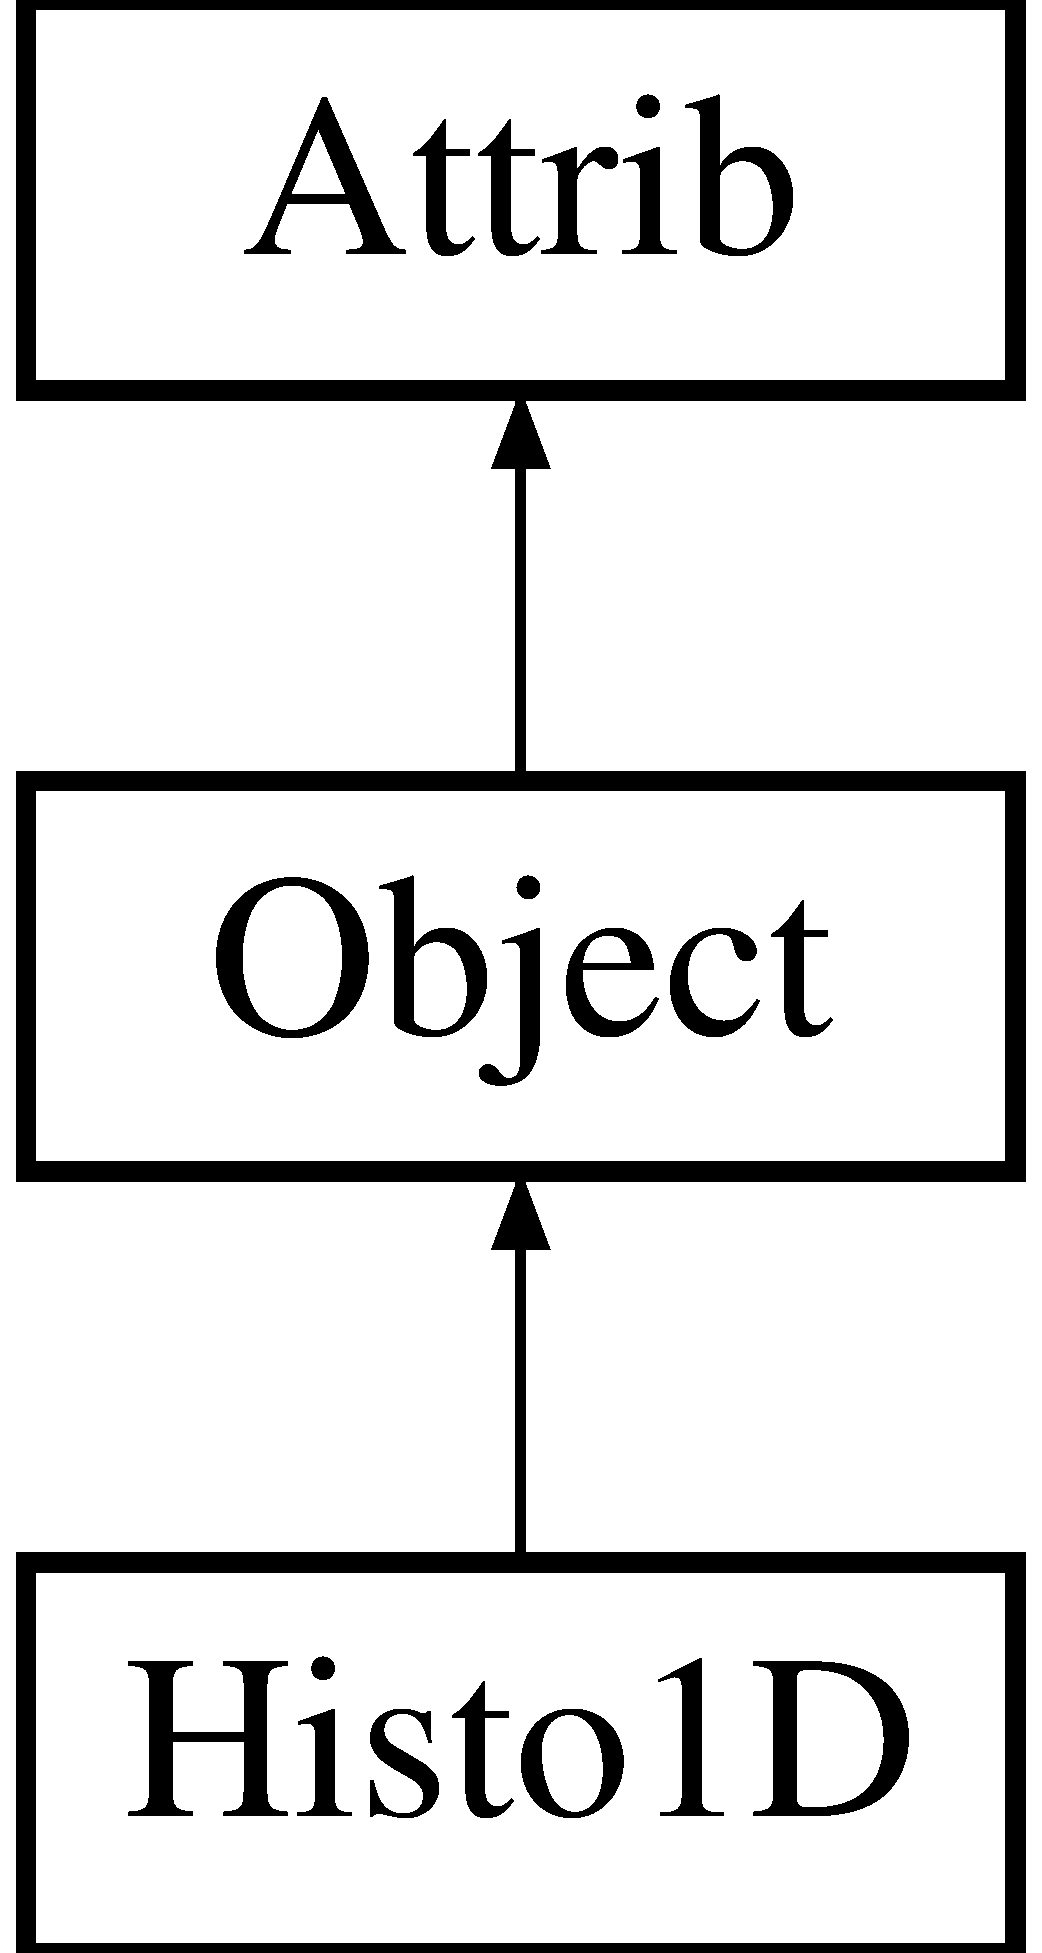
\includegraphics[height=3.000000cm]{classHisto1D}
\end{center}
\end{figure}
\subsection*{Public Member Functions}
\begin{DoxyCompactItemize}
\item 
\hyperlink{classHisto1D_aecd55af9b972863d5cee5a387746fb96}{Histo1D} (T\+H1D $\ast$histo)
\item 
\hyperlink{classHisto1D_af62825fd9266c1903d403e489501daa9}{$\sim$\+Histo1D} ()
\item 
void \hyperlink{classHisto1D_a22b820e2c706d8e8614c31962f1ac6d0}{def} ()
\item 
void \hyperlink{classHisto1D_a907707c720f8f0d3f582632d186ee7dd}{fill} (double x, double value=1.)
\item 
double \hyperlink{classHisto1D_a122c7071e060672dd2c08ad92212b3a2}{minY} ()
\item 
double \hyperlink{classHisto1D_a60a1095ac5fbab109d20c54c2ee569a3}{maxY} ()
\item 
double \hyperlink{classHisto1D_a54c7464513d1382c7c66fa880bfe568e}{maxX} ()
\item 
double \hyperlink{classHisto1D_abe9bf76799889414686794502e777b67}{minX} ()
\item 
std\+::vector$<$ double $>$ \hyperlink{classHisto1D_aaa8cd492ee25a3ad1b1694349fb1024c}{bins} ()
\item 
std\+::vector$<$ double $>$ \hyperlink{classHisto1D_a07fd41679a3255cdd44d4dcf8865adb7}{centers} ()
\item 
std\+::vector$<$ double $>$ \hyperlink{classHisto1D_a8c74413d35bce2e244defd470b6b4ebf}{edges} ()
\item 
unsigned long \hyperlink{classHisto1D_a7f3cf7364ae6e1eb9ba08b5ffe897d8f}{n\+Bin} ()
\item 
double \hyperlink{classHisto1D_a2a8a7d93c2f10b73b490a6f550e00db4}{bin} (double x)
\item 
double \hyperlink{classHisto1D_aa15ab79f858358e3cafc0617eb668c2e}{bin\+Edge\+Min} (unsigned int)
\item 
double \hyperlink{classHisto1D_a7923d51b02056dbaef353b70c11499d0}{bin\+Edge\+Max} (unsigned int)
\item 
double \hyperlink{classHisto1D_aece5cb8dddafabe0029067dc3e4be878}{bin\+Content} (int i)
\item 
double \hyperlink{classHisto1D_a5d13018047a4ffb15e662f44a0a3f520}{overflow} ()
\item 
double \hyperlink{classHisto1D_a3bac7a207b9ed5f828001119b2f14869}{underflow} ()
\item 
void \hyperlink{classHisto1D_acc0d6f2080b0cfafc85ebc49cf0efc31}{statistics} (double \&, double \&, double \&)
\end{DoxyCompactItemize}
\subsection*{Private Attributes}
\begin{DoxyCompactItemize}
\item 
double \hyperlink{classHisto1D_ac87bd1971cc300ce6fc1e745785cacb9}{m\+\_\+zero}
\item 
double \hyperlink{classHisto1D_a47c1ba33be0574ca167f43a1b27ba1a0}{m\+\_\+infini}
\item 
unsigned long \hyperlink{classHisto1D_a1913aca9a278b4bfd365f35b85e65d8d}{m\+\_\+nbins}
\item 
std\+::vector$<$ double $>$ \hyperlink{classHisto1D_a7a82923d3938739904469f5aa0a517ca}{m\+\_\+bins}
\item 
std\+::vector$<$ double $>$ \hyperlink{classHisto1D_a0e03676ed176aaad2f615fa84b8ffcd3}{m\+\_\+centers}
\item 
std\+::vector$<$ double $>$ \hyperlink{classHisto1D_a4188c6d1b4bfc8f9d8bde7616b4dbf5b}{m\+\_\+edges}
\item 
double \hyperlink{classHisto1D_af5ce58b20e96fa6e4b306109dd88589e}{m\+\_\+minX}
\item 
double \hyperlink{classHisto1D_a6a5007569e096537f9b7b39d2aad865b}{m\+\_\+maxX}
\item 
double \hyperlink{classHisto1D_a3bb6c3ea23a1af14ebb10af807f3810d}{m\+\_\+minY}
\item 
double \hyperlink{classHisto1D_a28a8995424e36088c47643f8c1a7fa7f}{m\+\_\+maxY}
\item 
double \hyperlink{classHisto1D_a993e2e40b89e257e6f86c0742f6f06b3}{m\+\_\+delta}
\item 
double \hyperlink{classHisto1D_ab60b2ec4e435a3094b7ec218404aa16f}{m\+\_\+overflow}
\item 
double \hyperlink{classHisto1D_a7f475b822f4bbb23209e2e523d228380}{m\+\_\+underflow}
\item 
double \hyperlink{classHisto1D_a75f4abeae577e232f4c012cb6b4049d7}{m\+\_\+content}
\item 
double \hyperlink{classHisto1D_a7e49893543fb5d2af37167690bc0b0ff}{m\+\_\+mean}
\item 
double \hyperlink{classHisto1D_a1331c670df40eb18d8a814f5a15ec7da}{m\+\_\+rms}
\end{DoxyCompactItemize}
\subsection*{Additional Inherited Members}


\subsection{Detailed Description}


Definition at line 28 of file Histo1\+D.\+h.



\subsection{Constructor \& Destructor Documentation}
\mbox{\Hypertarget{classHisto1D_aecd55af9b972863d5cee5a387746fb96}\label{classHisto1D_aecd55af9b972863d5cee5a387746fb96}} 
\index{Histo1D@{Histo1D}!Histo1D@{Histo1D}}
\index{Histo1D@{Histo1D}!Histo1D@{Histo1D}}
\subsubsection{\texorpdfstring{Histo1\+D()}{Histo1D()}}
{\footnotesize\ttfamily Histo1\+D\+::\+Histo1D (\begin{DoxyParamCaption}\item[{T\+H1D $\ast$}]{histo }\end{DoxyParamCaption})}



Definition at line 22 of file Histo1\+D.\+cpp.



References m\+\_\+bins, m\+\_\+centers, m\+\_\+content, m\+\_\+delta, m\+\_\+edges, m\+\_\+maxX, m\+\_\+maxY, m\+\_\+mean, m\+\_\+minX, m\+\_\+minY, m\+\_\+nbins, m\+\_\+overflow, m\+\_\+rms, m\+\_\+underflow, and Object\+::set\+Title().


\begin{DoxyCode}
22                               : \hyperlink{classHisto1D_ac87bd1971cc300ce6fc1e745785cacb9}{m\_zero} ( 1.e-30 ) , \hyperlink{classHisto1D_a47c1ba33be0574ca167f43a1b27ba1a0}{m\_infini}(1.e30) \{
23   \textcolor{comment}{//m\_histo = histo; }
24   
25   \hyperlink{classHisto1D_a1913aca9a278b4bfd365f35b85e65d8d}{m\_nbins} = histo->GetNbinsX();
26 
27   \hyperlink{classObject_a89557dbbad5bcaa02652f5d7fa35d20f}{setTitle}(std::string(histo -> GetTitle()));
28 
29   \hyperlink{classHisto1D_a7a82923d3938739904469f5aa0a517ca}{m\_bins}.resize (\hyperlink{classHisto1D_a1913aca9a278b4bfd365f35b85e65d8d}{m\_nbins},0.);
30   \hyperlink{classHisto1D_a0e03676ed176aaad2f615fa84b8ffcd3}{m\_centers}.resize (\hyperlink{classHisto1D_a1913aca9a278b4bfd365f35b85e65d8d}{m\_nbins},0.);
31   \hyperlink{classHisto1D_a4188c6d1b4bfc8f9d8bde7616b4dbf5b}{m\_edges}.resize (\hyperlink{classHisto1D_a1913aca9a278b4bfd365f35b85e65d8d}{m\_nbins}+1,0.);
32 
33   \textcolor{keywordtype}{unsigned} \textcolor{keywordtype}{long} nbin=0;
34   \textcolor{keywordflow}{for} (nbin=0;nbin<\hyperlink{classHisto1D_a1913aca9a278b4bfd365f35b85e65d8d}{m\_nbins}; ++nbin)\{
35     \hyperlink{classHisto1D_a7a82923d3938739904469f5aa0a517ca}{m\_bins}[nbin]=histo->GetBinContent(nbin+1);
36     \hyperlink{classHisto1D_a0e03676ed176aaad2f615fa84b8ffcd3}{m\_centers}[nbin]=histo->GetBinCenter(nbin+1);
37   \}
38 
39   \hyperlink{classHisto1D_a993e2e40b89e257e6f86c0742f6f06b3}{m\_delta} = histo->GetBinWidth(0);
40 
41   \textcolor{keywordflow}{for} (nbin=0;nbin<m\_nbins+1; ++nbin)\{
42     \hyperlink{classHisto1D_a4188c6d1b4bfc8f9d8bde7616b4dbf5b}{m\_edges}[nbin]=histo->GetBinLowEdge(1)+nbin*\hyperlink{classHisto1D_a993e2e40b89e257e6f86c0742f6f06b3}{m\_delta};
43   \}
44 
45   \hyperlink{classHisto1D_a7f475b822f4bbb23209e2e523d228380}{m\_underflow} = histo->GetBinContent(0);
46   \hyperlink{classHisto1D_ab60b2ec4e435a3094b7ec218404aa16f}{m\_overflow} = histo->GetBinContent(histo->GetNbinsX()+1);  
47 
48   \hyperlink{classHisto1D_af5ce58b20e96fa6e4b306109dd88589e}{m\_minX} = histo->GetBinLowEdge(1);
49   \hyperlink{classHisto1D_a6a5007569e096537f9b7b39d2aad865b}{m\_maxX} = histo->GetBinLowEdge(histo->GetNbinsX()+1);
50 
51   \hyperlink{classHisto1D_a3bb6c3ea23a1af14ebb10af807f3810d}{m\_minY} = histo->GetMinimum();
52   \hyperlink{classHisto1D_a28a8995424e36088c47643f8c1a7fa7f}{m\_maxY} = histo->GetMaximum();
53 
54   \hyperlink{classHisto1D_a75f4abeae577e232f4c012cb6b4049d7}{m\_content} = histo->GetEntries();
55   \hyperlink{classHisto1D_a7e49893543fb5d2af37167690bc0b0ff}{m\_mean}    = histo->GetMean();
56   \hyperlink{classHisto1D_a1331c670df40eb18d8a814f5a15ec7da}{m\_rms}     = histo->GetRMS();
57 \}
\end{DoxyCode}
\mbox{\Hypertarget{classHisto1D_af62825fd9266c1903d403e489501daa9}\label{classHisto1D_af62825fd9266c1903d403e489501daa9}} 
\index{Histo1D@{Histo1D}!````~Histo1D@{$\sim$\+Histo1D}}
\index{````~Histo1D@{$\sim$\+Histo1D}!Histo1D@{Histo1D}}
\subsubsection{\texorpdfstring{$\sim$\+Histo1\+D()}{~Histo1D()}}
{\footnotesize\ttfamily Histo1\+D\+::$\sim$\+Histo1D (\begin{DoxyParamCaption}{ }\end{DoxyParamCaption})\hspace{0.3cm}{\ttfamily [inline]}}



Definition at line 32 of file Histo1\+D.\+h.



References def(), fill(), max\+Y(), and min\+Y().


\begin{DoxyCode}
32 \{ \}
\end{DoxyCode}


\subsection{Member Function Documentation}
\mbox{\Hypertarget{classHisto1D_a2a8a7d93c2f10b73b490a6f550e00db4}\label{classHisto1D_a2a8a7d93c2f10b73b490a6f550e00db4}} 
\index{Histo1D@{Histo1D}!bin@{bin}}
\index{bin@{bin}!Histo1D@{Histo1D}}
\subsubsection{\texorpdfstring{bin()}{bin()}}
{\footnotesize\ttfamily double Histo1\+D\+::bin (\begin{DoxyParamCaption}\item[{double}]{x }\end{DoxyParamCaption})}



Definition at line 59 of file Histo1\+D.\+cpp.



References m\+\_\+bins, m\+\_\+delta, m\+\_\+maxX, m\+\_\+minX, m\+\_\+nbins, m\+\_\+overflow, and m\+\_\+underflow.



Referenced by n\+Bin().


\begin{DoxyCode}
59                            \{
60     \textcolor{keywordflow}{if} (x>=\hyperlink{classHisto1D_a6a5007569e096537f9b7b39d2aad865b}{m\_maxX}) \{\textcolor{keywordflow}{return} \hyperlink{classHisto1D_ab60b2ec4e435a3094b7ec218404aa16f}{m\_overflow};\}
61     \textcolor{keywordflow}{else} \textcolor{keywordflow}{if}(x<\hyperlink{classHisto1D_af5ce58b20e96fa6e4b306109dd88589e}{m\_minX}) \{\textcolor{keywordflow}{return} \hyperlink{classHisto1D_a7f475b822f4bbb23209e2e523d228380}{m\_underflow};\}
62     \textcolor{keywordtype}{unsigned} \textcolor{keywordtype}{long} \hyperlink{classHisto1D_a2a8a7d93c2f10b73b490a6f550e00db4}{bin}=(\textcolor{keywordtype}{unsigned} long)(floor(\hyperlink{classHisto1D_a1913aca9a278b4bfd365f35b85e65d8d}{m\_nbins}*(x-\hyperlink{classHisto1D_af5ce58b20e96fa6e4b306109dd88589e}{m\_minX})/
      \hyperlink{classHisto1D_a993e2e40b89e257e6f86c0742f6f06b3}{m\_delta}));
63     \textcolor{keywordflow}{return} \hyperlink{classHisto1D_a7a82923d3938739904469f5aa0a517ca}{m\_bins}[\hyperlink{classHisto1D_a2a8a7d93c2f10b73b490a6f550e00db4}{bin}];
64 \}   
\end{DoxyCode}
\mbox{\Hypertarget{classHisto1D_aece5cb8dddafabe0029067dc3e4be878}\label{classHisto1D_aece5cb8dddafabe0029067dc3e4be878}} 
\index{Histo1D@{Histo1D}!bin\+Content@{bin\+Content}}
\index{bin\+Content@{bin\+Content}!Histo1D@{Histo1D}}
\subsubsection{\texorpdfstring{bin\+Content()}{binContent()}}
{\footnotesize\ttfamily double Histo1\+D\+::bin\+Content (\begin{DoxyParamCaption}\item[{int}]{i }\end{DoxyParamCaption})\hspace{0.3cm}{\ttfamily [inline]}}



Definition at line 71 of file Histo1\+D.\+h.



References m\+\_\+bins.


\begin{DoxyCode}
71                           \{
72     \textcolor{keywordflow}{return} \hyperlink{classHisto1D_a7a82923d3938739904469f5aa0a517ca}{m\_bins}[i];
73   \}
\end{DoxyCode}
\mbox{\Hypertarget{classHisto1D_a7923d51b02056dbaef353b70c11499d0}\label{classHisto1D_a7923d51b02056dbaef353b70c11499d0}} 
\index{Histo1D@{Histo1D}!bin\+Edge\+Max@{bin\+Edge\+Max}}
\index{bin\+Edge\+Max@{bin\+Edge\+Max}!Histo1D@{Histo1D}}
\subsubsection{\texorpdfstring{bin\+Edge\+Max()}{binEdgeMax()}}
{\footnotesize\ttfamily double Histo1\+D\+::bin\+Edge\+Max (\begin{DoxyParamCaption}\item[{unsigned int}]{bin }\end{DoxyParamCaption})}



Definition at line 78 of file Histo1\+D.\+cpp.



References m\+\_\+delta, and m\+\_\+minX.



Referenced by n\+Bin().


\begin{DoxyCode}
78                                              \{
79   \textcolor{keywordflow}{return} \hyperlink{classHisto1D_af5ce58b20e96fa6e4b306109dd88589e}{m\_minX}+(\hyperlink{classHisto1D_a2a8a7d93c2f10b73b490a6f550e00db4}{bin}+1)*(\hyperlink{classHisto1D_a993e2e40b89e257e6f86c0742f6f06b3}{m\_delta});
80 \}
\end{DoxyCode}
\mbox{\Hypertarget{classHisto1D_aa15ab79f858358e3cafc0617eb668c2e}\label{classHisto1D_aa15ab79f858358e3cafc0617eb668c2e}} 
\index{Histo1D@{Histo1D}!bin\+Edge\+Min@{bin\+Edge\+Min}}
\index{bin\+Edge\+Min@{bin\+Edge\+Min}!Histo1D@{Histo1D}}
\subsubsection{\texorpdfstring{bin\+Edge\+Min()}{binEdgeMin()}}
{\footnotesize\ttfamily double Histo1\+D\+::bin\+Edge\+Min (\begin{DoxyParamCaption}\item[{unsigned int}]{bin }\end{DoxyParamCaption})}



Definition at line 74 of file Histo1\+D.\+cpp.



References m\+\_\+delta, and m\+\_\+minX.



Referenced by n\+Bin().


\begin{DoxyCode}
74                                             \{
75   \textcolor{keywordflow}{return} \hyperlink{classHisto1D_af5ce58b20e96fa6e4b306109dd88589e}{m\_minX}+\hyperlink{classHisto1D_a2a8a7d93c2f10b73b490a6f550e00db4}{bin}*(\hyperlink{classHisto1D_a993e2e40b89e257e6f86c0742f6f06b3}{m\_delta});
76 \}
\end{DoxyCode}
\mbox{\Hypertarget{classHisto1D_aaa8cd492ee25a3ad1b1694349fb1024c}\label{classHisto1D_aaa8cd492ee25a3ad1b1694349fb1024c}} 
\index{Histo1D@{Histo1D}!bins@{bins}}
\index{bins@{bins}!Histo1D@{Histo1D}}
\subsubsection{\texorpdfstring{bins()}{bins()}}
{\footnotesize\ttfamily std\+::vector$<$double$>$ Histo1\+D\+::bins (\begin{DoxyParamCaption}{ }\end{DoxyParamCaption})\hspace{0.3cm}{\ttfamily [inline]}}



Definition at line 49 of file Histo1\+D.\+h.



References m\+\_\+bins.



Referenced by export\+\_\+proc().


\begin{DoxyCode}
49                           \{  
50     \textcolor{keywordflow}{return} \hyperlink{classHisto1D_a7a82923d3938739904469f5aa0a517ca}{m\_bins};
51   \}
\end{DoxyCode}
\mbox{\Hypertarget{classHisto1D_a07fd41679a3255cdd44d4dcf8865adb7}\label{classHisto1D_a07fd41679a3255cdd44d4dcf8865adb7}} 
\index{Histo1D@{Histo1D}!centers@{centers}}
\index{centers@{centers}!Histo1D@{Histo1D}}
\subsubsection{\texorpdfstring{centers()}{centers()}}
{\footnotesize\ttfamily std\+::vector$<$double$>$ Histo1\+D\+::centers (\begin{DoxyParamCaption}{ }\end{DoxyParamCaption})\hspace{0.3cm}{\ttfamily [inline]}}



Definition at line 53 of file Histo1\+D.\+h.



References m\+\_\+centers.



Referenced by export\+\_\+proc().


\begin{DoxyCode}
53                              \{  
54     \textcolor{keywordflow}{return} \hyperlink{classHisto1D_a0e03676ed176aaad2f615fa84b8ffcd3}{m\_centers};
55   \}
\end{DoxyCode}
\mbox{\Hypertarget{classHisto1D_a22b820e2c706d8e8614c31962f1ac6d0}\label{classHisto1D_a22b820e2c706d8e8614c31962f1ac6d0}} 
\index{Histo1D@{Histo1D}!def@{def}}
\index{def@{def}!Histo1D@{Histo1D}}
\subsubsection{\texorpdfstring{def()}{def()}}
{\footnotesize\ttfamily void Histo1\+D\+::def (\begin{DoxyParamCaption}{ }\end{DoxyParamCaption})}



Referenced by $\sim$\+Histo1\+D().

\mbox{\Hypertarget{classHisto1D_a8c74413d35bce2e244defd470b6b4ebf}\label{classHisto1D_a8c74413d35bce2e244defd470b6b4ebf}} 
\index{Histo1D@{Histo1D}!edges@{edges}}
\index{edges@{edges}!Histo1D@{Histo1D}}
\subsubsection{\texorpdfstring{edges()}{edges()}}
{\footnotesize\ttfamily std\+::vector$<$double$>$ Histo1\+D\+::edges (\begin{DoxyParamCaption}{ }\end{DoxyParamCaption})\hspace{0.3cm}{\ttfamily [inline]}}



Definition at line 57 of file Histo1\+D.\+h.



References m\+\_\+edges.



Referenced by export\+\_\+proc().


\begin{DoxyCode}
57                            \{  
58     \textcolor{keywordflow}{return} \hyperlink{classHisto1D_a4188c6d1b4bfc8f9d8bde7616b4dbf5b}{m\_edges};
59   \}
\end{DoxyCode}
\mbox{\Hypertarget{classHisto1D_a907707c720f8f0d3f582632d186ee7dd}\label{classHisto1D_a907707c720f8f0d3f582632d186ee7dd}} 
\index{Histo1D@{Histo1D}!fill@{fill}}
\index{fill@{fill}!Histo1D@{Histo1D}}
\subsubsection{\texorpdfstring{fill()}{fill()}}
{\footnotesize\ttfamily void Histo1\+D\+::fill (\begin{DoxyParamCaption}\item[{double}]{x,  }\item[{double}]{value = {\ttfamily 1.} }\end{DoxyParamCaption})}



Referenced by $\sim$\+Histo1\+D().

\mbox{\Hypertarget{classHisto1D_a54c7464513d1382c7c66fa880bfe568e}\label{classHisto1D_a54c7464513d1382c7c66fa880bfe568e}} 
\index{Histo1D@{Histo1D}!maxX@{maxX}}
\index{maxX@{maxX}!Histo1D@{Histo1D}}
\subsubsection{\texorpdfstring{max\+X()}{maxX()}}
{\footnotesize\ttfamily double Histo1\+D\+::maxX (\begin{DoxyParamCaption}{ }\end{DoxyParamCaption})\hspace{0.3cm}{\ttfamily [inline]}}



Definition at line 42 of file Histo1\+D.\+h.



References m\+\_\+maxX.



Referenced by export\+\_\+proc().


\begin{DoxyCode}
42                \{ 
43     \textcolor{keywordflow}{return} \hyperlink{classHisto1D_a6a5007569e096537f9b7b39d2aad865b}{m\_maxX}; 
44   \}
\end{DoxyCode}
\mbox{\Hypertarget{classHisto1D_a60a1095ac5fbab109d20c54c2ee569a3}\label{classHisto1D_a60a1095ac5fbab109d20c54c2ee569a3}} 
\index{Histo1D@{Histo1D}!maxY@{maxY}}
\index{maxY@{maxY}!Histo1D@{Histo1D}}
\subsubsection{\texorpdfstring{max\+Y()}{maxY()}}
{\footnotesize\ttfamily double Histo1\+D\+::maxY (\begin{DoxyParamCaption}{ }\end{DoxyParamCaption})}



Definition at line 70 of file Histo1\+D.\+cpp.



References m\+\_\+maxY.



Referenced by export\+\_\+proc(), and $\sim$\+Histo1\+D().


\begin{DoxyCode}
70                     \{
71   \textcolor{keywordflow}{return} \hyperlink{classHisto1D_a28a8995424e36088c47643f8c1a7fa7f}{m\_maxY};
72 \}
\end{DoxyCode}
\mbox{\Hypertarget{classHisto1D_abe9bf76799889414686794502e777b67}\label{classHisto1D_abe9bf76799889414686794502e777b67}} 
\index{Histo1D@{Histo1D}!minX@{minX}}
\index{minX@{minX}!Histo1D@{Histo1D}}
\subsubsection{\texorpdfstring{min\+X()}{minX()}}
{\footnotesize\ttfamily double Histo1\+D\+::minX (\begin{DoxyParamCaption}{ }\end{DoxyParamCaption})\hspace{0.3cm}{\ttfamily [inline]}}



Definition at line 45 of file Histo1\+D.\+h.



References m\+\_\+minX.



Referenced by export\+\_\+proc().


\begin{DoxyCode}
45                \{ 
46     \textcolor{keywordflow}{return} \hyperlink{classHisto1D_af5ce58b20e96fa6e4b306109dd88589e}{m\_minX}; 
47   \}
\end{DoxyCode}
\mbox{\Hypertarget{classHisto1D_a122c7071e060672dd2c08ad92212b3a2}\label{classHisto1D_a122c7071e060672dd2c08ad92212b3a2}} 
\index{Histo1D@{Histo1D}!minY@{minY}}
\index{minY@{minY}!Histo1D@{Histo1D}}
\subsubsection{\texorpdfstring{min\+Y()}{minY()}}
{\footnotesize\ttfamily double Histo1\+D\+::minY (\begin{DoxyParamCaption}{ }\end{DoxyParamCaption})}



Definition at line 66 of file Histo1\+D.\+cpp.



References m\+\_\+minY.



Referenced by export\+\_\+proc(), and $\sim$\+Histo1\+D().


\begin{DoxyCode}
66                     \{
67     \textcolor{keywordflow}{return} \hyperlink{classHisto1D_a3bb6c3ea23a1af14ebb10af807f3810d}{m\_minY};
68 \}
\end{DoxyCode}
\mbox{\Hypertarget{classHisto1D_a7f3cf7364ae6e1eb9ba08b5ffe897d8f}\label{classHisto1D_a7f3cf7364ae6e1eb9ba08b5ffe897d8f}} 
\index{Histo1D@{Histo1D}!n\+Bin@{n\+Bin}}
\index{n\+Bin@{n\+Bin}!Histo1D@{Histo1D}}
\subsubsection{\texorpdfstring{n\+Bin()}{nBin()}}
{\footnotesize\ttfamily unsigned long Histo1\+D\+::n\+Bin (\begin{DoxyParamCaption}{ }\end{DoxyParamCaption})\hspace{0.3cm}{\ttfamily [inline]}}



Definition at line 61 of file Histo1\+D.\+h.



References bin(), bin\+Edge\+Max(), bin\+Edge\+Min(), and m\+\_\+nbins.



Referenced by export\+\_\+proc().


\begin{DoxyCode}
61                       \{
62     \textcolor{keywordflow}{return} \hyperlink{classHisto1D_a1913aca9a278b4bfd365f35b85e65d8d}{m\_nbins};
63   \}
\end{DoxyCode}
\mbox{\Hypertarget{classHisto1D_a5d13018047a4ffb15e662f44a0a3f520}\label{classHisto1D_a5d13018047a4ffb15e662f44a0a3f520}} 
\index{Histo1D@{Histo1D}!overflow@{overflow}}
\index{overflow@{overflow}!Histo1D@{Histo1D}}
\subsubsection{\texorpdfstring{overflow()}{overflow()}}
{\footnotesize\ttfamily double Histo1\+D\+::overflow (\begin{DoxyParamCaption}{ }\end{DoxyParamCaption})\hspace{0.3cm}{\ttfamily [inline]}}



Definition at line 75 of file Histo1\+D.\+h.



References m\+\_\+overflow.



Referenced by export\+\_\+proc().


\begin{DoxyCode}
75                    \{
76     \textcolor{keywordflow}{return} \hyperlink{classHisto1D_ab60b2ec4e435a3094b7ec218404aa16f}{m\_overflow};
77   \}
\end{DoxyCode}
\mbox{\Hypertarget{classHisto1D_acc0d6f2080b0cfafc85ebc49cf0efc31}\label{classHisto1D_acc0d6f2080b0cfafc85ebc49cf0efc31}} 
\index{Histo1D@{Histo1D}!statistics@{statistics}}
\index{statistics@{statistics}!Histo1D@{Histo1D}}
\subsubsection{\texorpdfstring{statistics()}{statistics()}}
{\footnotesize\ttfamily void Histo1\+D\+::statistics (\begin{DoxyParamCaption}\item[{double \&}]{content,  }\item[{double \&}]{mean,  }\item[{double \&}]{rms }\end{DoxyParamCaption})}



Definition at line 82 of file Histo1\+D.\+cpp.



References m\+\_\+content, m\+\_\+mean, and m\+\_\+rms.



Referenced by underflow().


\begin{DoxyCode}
84                                      \{
85   content=\hyperlink{classHisto1D_a75f4abeae577e232f4c012cb6b4049d7}{m\_content};
86   mean   =\hyperlink{classHisto1D_a7e49893543fb5d2af37167690bc0b0ff}{m\_mean};
87   rms    =\hyperlink{classHisto1D_a1331c670df40eb18d8a814f5a15ec7da}{m\_rms};
88 \}
\end{DoxyCode}
\mbox{\Hypertarget{classHisto1D_a3bac7a207b9ed5f828001119b2f14869}\label{classHisto1D_a3bac7a207b9ed5f828001119b2f14869}} 
\index{Histo1D@{Histo1D}!underflow@{underflow}}
\index{underflow@{underflow}!Histo1D@{Histo1D}}
\subsubsection{\texorpdfstring{underflow()}{underflow()}}
{\footnotesize\ttfamily double Histo1\+D\+::underflow (\begin{DoxyParamCaption}{ }\end{DoxyParamCaption})\hspace{0.3cm}{\ttfamily [inline]}}



Definition at line 78 of file Histo1\+D.\+h.



References m\+\_\+underflow, and statistics().



Referenced by export\+\_\+proc().


\begin{DoxyCode}
78                     \{
79     \textcolor{keywordflow}{return} \hyperlink{classHisto1D_a7f475b822f4bbb23209e2e523d228380}{m\_underflow};
80   \}  
\end{DoxyCode}


\subsection{Member Data Documentation}
\mbox{\Hypertarget{classHisto1D_a7a82923d3938739904469f5aa0a517ca}\label{classHisto1D_a7a82923d3938739904469f5aa0a517ca}} 
\index{Histo1D@{Histo1D}!m\+\_\+bins@{m\+\_\+bins}}
\index{m\+\_\+bins@{m\+\_\+bins}!Histo1D@{Histo1D}}
\subsubsection{\texorpdfstring{m\+\_\+bins}{m\_bins}}
{\footnotesize\ttfamily std\+::vector$<$double$>$ Histo1\+D\+::m\+\_\+bins\hspace{0.3cm}{\ttfamily [private]}}



Definition at line 89 of file Histo1\+D.\+h.



Referenced by bin(), bin\+Content(), bins(), and Histo1\+D().

\mbox{\Hypertarget{classHisto1D_a0e03676ed176aaad2f615fa84b8ffcd3}\label{classHisto1D_a0e03676ed176aaad2f615fa84b8ffcd3}} 
\index{Histo1D@{Histo1D}!m\+\_\+centers@{m\+\_\+centers}}
\index{m\+\_\+centers@{m\+\_\+centers}!Histo1D@{Histo1D}}
\subsubsection{\texorpdfstring{m\+\_\+centers}{m\_centers}}
{\footnotesize\ttfamily std\+::vector$<$double$>$ Histo1\+D\+::m\+\_\+centers\hspace{0.3cm}{\ttfamily [private]}}



Definition at line 90 of file Histo1\+D.\+h.



Referenced by centers(), and Histo1\+D().

\mbox{\Hypertarget{classHisto1D_a75f4abeae577e232f4c012cb6b4049d7}\label{classHisto1D_a75f4abeae577e232f4c012cb6b4049d7}} 
\index{Histo1D@{Histo1D}!m\+\_\+content@{m\+\_\+content}}
\index{m\+\_\+content@{m\+\_\+content}!Histo1D@{Histo1D}}
\subsubsection{\texorpdfstring{m\+\_\+content}{m\_content}}
{\footnotesize\ttfamily double Histo1\+D\+::m\+\_\+content\hspace{0.3cm}{\ttfamily [private]}}



Definition at line 102 of file Histo1\+D.\+h.



Referenced by Histo1\+D(), and statistics().

\mbox{\Hypertarget{classHisto1D_a993e2e40b89e257e6f86c0742f6f06b3}\label{classHisto1D_a993e2e40b89e257e6f86c0742f6f06b3}} 
\index{Histo1D@{Histo1D}!m\+\_\+delta@{m\+\_\+delta}}
\index{m\+\_\+delta@{m\+\_\+delta}!Histo1D@{Histo1D}}
\subsubsection{\texorpdfstring{m\+\_\+delta}{m\_delta}}
{\footnotesize\ttfamily double Histo1\+D\+::m\+\_\+delta\hspace{0.3cm}{\ttfamily [private]}}



Definition at line 97 of file Histo1\+D.\+h.



Referenced by bin(), bin\+Edge\+Max(), bin\+Edge\+Min(), and Histo1\+D().

\mbox{\Hypertarget{classHisto1D_a4188c6d1b4bfc8f9d8bde7616b4dbf5b}\label{classHisto1D_a4188c6d1b4bfc8f9d8bde7616b4dbf5b}} 
\index{Histo1D@{Histo1D}!m\+\_\+edges@{m\+\_\+edges}}
\index{m\+\_\+edges@{m\+\_\+edges}!Histo1D@{Histo1D}}
\subsubsection{\texorpdfstring{m\+\_\+edges}{m\_edges}}
{\footnotesize\ttfamily std\+::vector$<$double$>$ Histo1\+D\+::m\+\_\+edges\hspace{0.3cm}{\ttfamily [private]}}



Definition at line 91 of file Histo1\+D.\+h.



Referenced by edges(), and Histo1\+D().

\mbox{\Hypertarget{classHisto1D_a47c1ba33be0574ca167f43a1b27ba1a0}\label{classHisto1D_a47c1ba33be0574ca167f43a1b27ba1a0}} 
\index{Histo1D@{Histo1D}!m\+\_\+infini@{m\+\_\+infini}}
\index{m\+\_\+infini@{m\+\_\+infini}!Histo1D@{Histo1D}}
\subsubsection{\texorpdfstring{m\+\_\+infini}{m\_infini}}
{\footnotesize\ttfamily double Histo1\+D\+::m\+\_\+infini\hspace{0.3cm}{\ttfamily [private]}}



Definition at line 86 of file Histo1\+D.\+h.

\mbox{\Hypertarget{classHisto1D_a6a5007569e096537f9b7b39d2aad865b}\label{classHisto1D_a6a5007569e096537f9b7b39d2aad865b}} 
\index{Histo1D@{Histo1D}!m\+\_\+maxX@{m\+\_\+maxX}}
\index{m\+\_\+maxX@{m\+\_\+maxX}!Histo1D@{Histo1D}}
\subsubsection{\texorpdfstring{m\+\_\+maxX}{m\_maxX}}
{\footnotesize\ttfamily double Histo1\+D\+::m\+\_\+maxX\hspace{0.3cm}{\ttfamily [private]}}



Definition at line 94 of file Histo1\+D.\+h.



Referenced by bin(), Histo1\+D(), and max\+X().

\mbox{\Hypertarget{classHisto1D_a28a8995424e36088c47643f8c1a7fa7f}\label{classHisto1D_a28a8995424e36088c47643f8c1a7fa7f}} 
\index{Histo1D@{Histo1D}!m\+\_\+maxY@{m\+\_\+maxY}}
\index{m\+\_\+maxY@{m\+\_\+maxY}!Histo1D@{Histo1D}}
\subsubsection{\texorpdfstring{m\+\_\+maxY}{m\_maxY}}
{\footnotesize\ttfamily double Histo1\+D\+::m\+\_\+maxY\hspace{0.3cm}{\ttfamily [private]}}



Definition at line 96 of file Histo1\+D.\+h.



Referenced by Histo1\+D(), and max\+Y().

\mbox{\Hypertarget{classHisto1D_a7e49893543fb5d2af37167690bc0b0ff}\label{classHisto1D_a7e49893543fb5d2af37167690bc0b0ff}} 
\index{Histo1D@{Histo1D}!m\+\_\+mean@{m\+\_\+mean}}
\index{m\+\_\+mean@{m\+\_\+mean}!Histo1D@{Histo1D}}
\subsubsection{\texorpdfstring{m\+\_\+mean}{m\_mean}}
{\footnotesize\ttfamily double Histo1\+D\+::m\+\_\+mean\hspace{0.3cm}{\ttfamily [private]}}



Definition at line 103 of file Histo1\+D.\+h.



Referenced by Histo1\+D(), and statistics().

\mbox{\Hypertarget{classHisto1D_af5ce58b20e96fa6e4b306109dd88589e}\label{classHisto1D_af5ce58b20e96fa6e4b306109dd88589e}} 
\index{Histo1D@{Histo1D}!m\+\_\+minX@{m\+\_\+minX}}
\index{m\+\_\+minX@{m\+\_\+minX}!Histo1D@{Histo1D}}
\subsubsection{\texorpdfstring{m\+\_\+minX}{m\_minX}}
{\footnotesize\ttfamily double Histo1\+D\+::m\+\_\+minX\hspace{0.3cm}{\ttfamily [private]}}



Definition at line 93 of file Histo1\+D.\+h.



Referenced by bin(), bin\+Edge\+Max(), bin\+Edge\+Min(), Histo1\+D(), and min\+X().

\mbox{\Hypertarget{classHisto1D_a3bb6c3ea23a1af14ebb10af807f3810d}\label{classHisto1D_a3bb6c3ea23a1af14ebb10af807f3810d}} 
\index{Histo1D@{Histo1D}!m\+\_\+minY@{m\+\_\+minY}}
\index{m\+\_\+minY@{m\+\_\+minY}!Histo1D@{Histo1D}}
\subsubsection{\texorpdfstring{m\+\_\+minY}{m\_minY}}
{\footnotesize\ttfamily double Histo1\+D\+::m\+\_\+minY\hspace{0.3cm}{\ttfamily [private]}}



Definition at line 95 of file Histo1\+D.\+h.



Referenced by Histo1\+D(), and min\+Y().

\mbox{\Hypertarget{classHisto1D_a1913aca9a278b4bfd365f35b85e65d8d}\label{classHisto1D_a1913aca9a278b4bfd365f35b85e65d8d}} 
\index{Histo1D@{Histo1D}!m\+\_\+nbins@{m\+\_\+nbins}}
\index{m\+\_\+nbins@{m\+\_\+nbins}!Histo1D@{Histo1D}}
\subsubsection{\texorpdfstring{m\+\_\+nbins}{m\_nbins}}
{\footnotesize\ttfamily unsigned long Histo1\+D\+::m\+\_\+nbins\hspace{0.3cm}{\ttfamily [private]}}



Definition at line 88 of file Histo1\+D.\+h.



Referenced by bin(), Histo1\+D(), and n\+Bin().

\mbox{\Hypertarget{classHisto1D_ab60b2ec4e435a3094b7ec218404aa16f}\label{classHisto1D_ab60b2ec4e435a3094b7ec218404aa16f}} 
\index{Histo1D@{Histo1D}!m\+\_\+overflow@{m\+\_\+overflow}}
\index{m\+\_\+overflow@{m\+\_\+overflow}!Histo1D@{Histo1D}}
\subsubsection{\texorpdfstring{m\+\_\+overflow}{m\_overflow}}
{\footnotesize\ttfamily double Histo1\+D\+::m\+\_\+overflow\hspace{0.3cm}{\ttfamily [private]}}



Definition at line 99 of file Histo1\+D.\+h.



Referenced by bin(), Histo1\+D(), and overflow().

\mbox{\Hypertarget{classHisto1D_a1331c670df40eb18d8a814f5a15ec7da}\label{classHisto1D_a1331c670df40eb18d8a814f5a15ec7da}} 
\index{Histo1D@{Histo1D}!m\+\_\+rms@{m\+\_\+rms}}
\index{m\+\_\+rms@{m\+\_\+rms}!Histo1D@{Histo1D}}
\subsubsection{\texorpdfstring{m\+\_\+rms}{m\_rms}}
{\footnotesize\ttfamily double Histo1\+D\+::m\+\_\+rms\hspace{0.3cm}{\ttfamily [private]}}



Definition at line 104 of file Histo1\+D.\+h.



Referenced by Histo1\+D(), and statistics().

\mbox{\Hypertarget{classHisto1D_a7f475b822f4bbb23209e2e523d228380}\label{classHisto1D_a7f475b822f4bbb23209e2e523d228380}} 
\index{Histo1D@{Histo1D}!m\+\_\+underflow@{m\+\_\+underflow}}
\index{m\+\_\+underflow@{m\+\_\+underflow}!Histo1D@{Histo1D}}
\subsubsection{\texorpdfstring{m\+\_\+underflow}{m\_underflow}}
{\footnotesize\ttfamily double Histo1\+D\+::m\+\_\+underflow\hspace{0.3cm}{\ttfamily [private]}}



Definition at line 100 of file Histo1\+D.\+h.



Referenced by bin(), Histo1\+D(), and underflow().

\mbox{\Hypertarget{classHisto1D_ac87bd1971cc300ce6fc1e745785cacb9}\label{classHisto1D_ac87bd1971cc300ce6fc1e745785cacb9}} 
\index{Histo1D@{Histo1D}!m\+\_\+zero@{m\+\_\+zero}}
\index{m\+\_\+zero@{m\+\_\+zero}!Histo1D@{Histo1D}}
\subsubsection{\texorpdfstring{m\+\_\+zero}{m\_zero}}
{\footnotesize\ttfamily double Histo1\+D\+::m\+\_\+zero\hspace{0.3cm}{\ttfamily [private]}}



Definition at line 85 of file Histo1\+D.\+h.



The documentation for this class was generated from the following files\+:\begin{DoxyCompactItemize}
\item 
/home/eleclhcb/\+L\+H\+Cb/lbcat-\/cmake/\+Cat\+Kernel/inc/\hyperlink{Histo1D_8h}{Histo1\+D.\+h}\item 
/home/eleclhcb/\+L\+H\+Cb/lbcat-\/cmake/\+Cat\+Kernel/src/\hyperlink{Histo1D_8cpp}{Histo1\+D.\+cpp}\end{DoxyCompactItemize}

\hypertarget{classHisto2D}{
\section{Histo2D Class Reference}
\label{classHisto2D}\index{Histo2D@{Histo2D}}
}


{\ttfamily \#include $<$Histo2D.h$>$}Inheritance diagram for Histo2D::\begin{figure}[H]
\begin{center}
\leavevmode
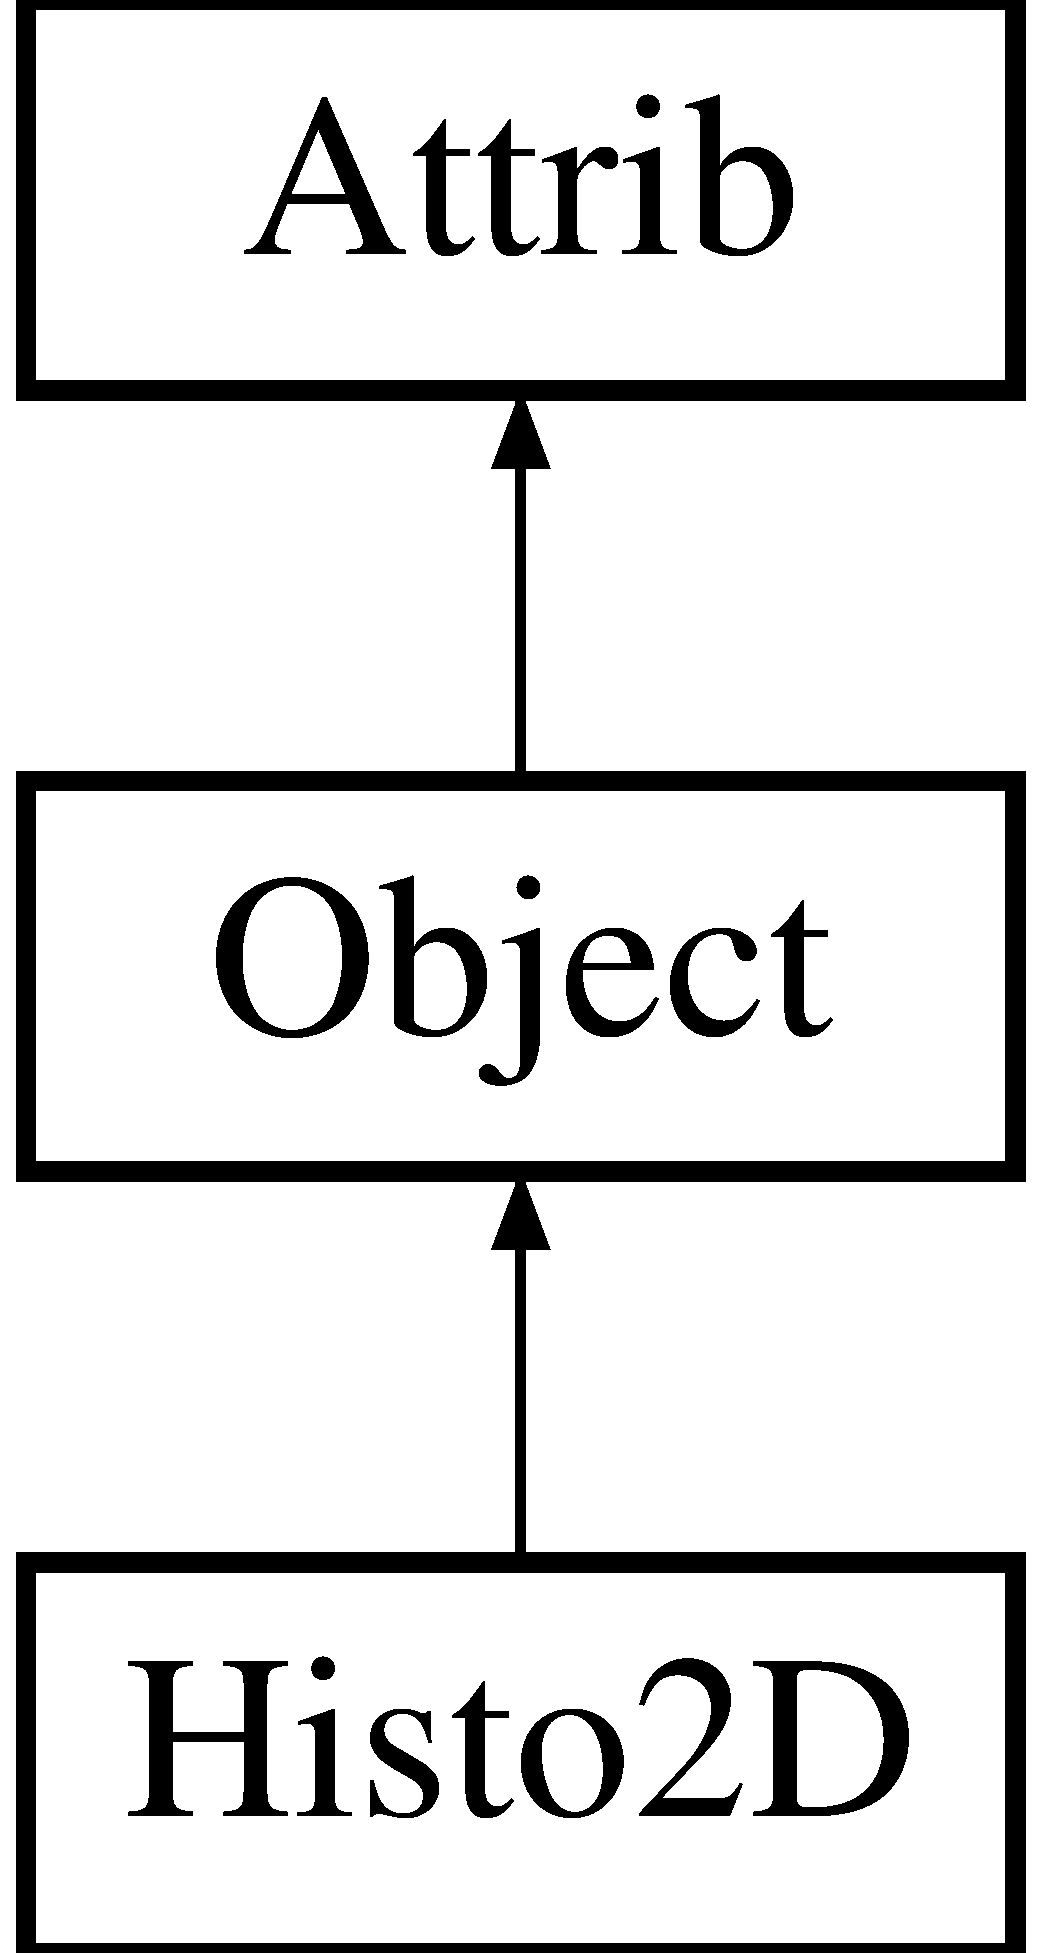
\includegraphics[height=3cm]{classHisto2D}
\end{center}
\end{figure}
\subsection*{Public Types}
\begin{DoxyCompactItemize}
\item 
enum \hyperlink{classAttrib_a69e171d7cc6417835a5a306d3c764235}{Attribut} \{ \par
\hyperlink{classAttrib_a69e171d7cc6417835a5a306d3c764235a3a8da2ab97dda18aebab196fe4100531}{UNDEFINED}, 
\hyperlink{classAttrib_a69e171d7cc6417835a5a306d3c764235a2bfb2af57b87031d190a05fe25dd92ed}{PASSIVE}, 
\hyperlink{classAttrib_a69e171d7cc6417835a5a306d3c764235a3b1fec929c0370d1436f2f06e298fb0d}{ACTIVE}, 
\hyperlink{classAttrib_a69e171d7cc6417835a5a306d3c764235aa27c16b480a369ea4d18b07b2516bbc7}{INTERFACE}, 
\par
\hyperlink{classAttrib_a69e171d7cc6417835a5a306d3c764235a1420a5b8c0540b2af210b6975eded7f9}{IO}, 
\hyperlink{classAttrib_a69e171d7cc6417835a5a306d3c764235a0af3b0d0ac323c1704e6c69cf90add28}{IODATA}, 
\hyperlink{classAttrib_a69e171d7cc6417835a5a306d3c764235a7788bc5dd333fd8ce18562b269c9dab1}{ELEMENT}, 
\hyperlink{classAttrib_a69e171d7cc6417835a5a306d3c764235a61ceb22149f365f1780d18f9d1459423}{HARDWARE}, 
\par
\hyperlink{classAttrib_a69e171d7cc6417835a5a306d3c764235a75250e29692496e73effca2c0330977f}{PROCESSUS}, 
\hyperlink{classAttrib_a69e171d7cc6417835a5a306d3c764235a103a67cd0b8f07ef478fa45d4356e27b}{SOFTWARE}
 \}
\end{DoxyCompactItemize}
\subsection*{Public Member Functions}
\begin{DoxyCompactItemize}
\item 
\hyperlink{classHisto2D_acdeb6b732d7b596dea8a282813cd1c18}{Histo2D} (TH2D $\ast$histo)
\item 
\hyperlink{classHisto2D_a4df8112579be6bc1d5652933c73125ae}{$\sim$Histo2D} ()
\item 
double \hyperlink{classHisto2D_ae5a3ff63669999c9fda448db61e5bb57}{minX} ()
\item 
double \hyperlink{classHisto2D_aae04c13ac492562532b4d3f82979a0f4}{maxX} ()
\item 
double \hyperlink{classHisto2D_ae946ecc8e7b4efc2e1454cd75c7d8aca}{minY} ()
\item 
double \hyperlink{classHisto2D_a7bfc748b81257716316a38e628c5832f}{maxY} ()
\item 
double \hyperlink{classHisto2D_a68cfc2d92fbc5ce2efa1d6b5781ea621}{minZ} ()
\item 
double \hyperlink{classHisto2D_ad6ccf8ddd4e4b5930f39284059577570}{maxZ} ()
\item 
std::vector$<$ double $>$ \hyperlink{classHisto2D_ab3d44a1cb12119a2244065af2b1f7099}{bins} ()
\item 
std::vector$<$ double $>$ \hyperlink{classHisto2D_a8f42529a5fba07c339e547bf504dd418}{xbins} ()
\item 
std::vector$<$ double $>$ \hyperlink{classHisto2D_a0ae225e33eb9837137b10a159ac1d4f2}{ybins} ()
\item 
unsigned long \hyperlink{classHisto2D_aac422991db96030ce7ca3952e4d277f2}{nxbins} ()
\item 
unsigned long \hyperlink{classHisto2D_a17ee49d9e1c5d62edc887f4f63f68db6}{nybins} ()
\item 
void \hyperlink{classHisto2D_a66875cb46a7e5ff6fa347fe736cbed1b}{statistics} (double \&, double \&, double \&)
\item 
std::string \hyperlink{classObject_a975e888d50bfcbffda2c86368332a5cd}{name} () const 
\item 
std::string \hyperlink{classObject_a84f99f70f144a83e1582d1d0f84e4e62}{type} ()
\item 
unsigned char \hyperlink{classObject_af99145335cc61ff6e2798ea17db009d2}{id} ()
\item 
std::string \hyperlink{classObject_a73a0f1a41828fdd8303dd662446fb6c3}{title} ()
\item 
void \hyperlink{classObject_a3f9d5537ebce0c0f2bf6ae4d92426f3c}{msgSvc} (int level, std::string msg, std::string name)
\item 
void \hyperlink{classObject_a58b2d0618c2d08cf2383012611528d97}{msg} (std::string mymsg)
\item 
void \hyperlink{classObject_ac5d59299273cee27aacf7de00d2e7034}{msg} (std::string mymsg, std::string name)
\item 
void \hyperlink{classObject_a83d2db2df682907ea1115ad721c1c4a1}{verbose} (std::string mymsg)
\item 
void \hyperlink{classObject_a2d4120195317e2a3c6532e8bb9f3da68}{verbose} (std::string mymsg, std::string name)
\item 
void \hyperlink{classObject_aac010553f022165573714b7014a15f0d}{debug} (std::string mymsg)
\item 
void \hyperlink{classObject_a6c9a0397ca804e04d675ed05683f5420}{debug} (std::string mymsg, std::string name)
\item 
void \hyperlink{classObject_a644fd329ea4cb85f54fa6846484b84a8}{info} (std::string mymsg)
\item 
void \hyperlink{classObject_a1ca123253dfd30fc28b156f521dcbdae}{info} (std::string mymsg, std::string name)
\item 
void \hyperlink{classObject_a65cd4fda577711660821fd2cd5a3b4c9}{warning} (std::string mymsg)
\item 
void \hyperlink{classObject_a11f101db4dd73d9391b0231818881d86}{warning} (std::string mymsg, std::string name)
\item 
void \hyperlink{classObject_a204a95f57818c0f811933917a30eff45}{error} (std::string mymsg)
\item 
void \hyperlink{classObject_ad7f6c457733082efa2f9ff5f5c8e119a}{error} (std::string mymsg, std::string name)
\item 
void \hyperlink{classObject_aad5a16aac7516ce65bd5ec02ab07fc80}{fatal} (std::string mymsg)
\item 
void \hyperlink{classObject_ae62acd3d09f716220f75f252dc38bc9a}{fatal} (std::string mymsg, std::string name)
\item 
void \hyperlink{classObject_ae30fea75683c2d149b6b6d17c09ecd0c}{setName} (std::string name)
\item 
void \hyperlink{classObject_aae534cc9d982bcb9b99fd505f2e103a5}{setType} (std::string type)
\item 
void \hyperlink{classObject_a398fe08cba594a0ce6891d59fe4f159f}{setId} (unsigned char id)
\item 
void \hyperlink{classObject_a89557dbbad5bcaa02652f5d7fa35d20f}{setTitle} (std::string title)
\item 
void \hyperlink{classObject_a870c5af919958c2136623b2d7816d123}{setDllName} (std::string dllName)
\item 
std::string \hyperlink{classObject_a2e3947f2870094c332d7454117f3ec63}{dllName} ()
\item 
bool \hyperlink{classAttrib_a704f26af560909ad22065083bb7d4c34}{is} (int attribut)
\item 
void \hyperlink{classAttrib_a235f773af19c900264a190b00a3b4ad7}{add} (int attribut)
\item 
void \hyperlink{classAttrib_a7d4ef7e32d93cb287792b87b857e79f3}{remove} (int attribut)
\item 
std::string \hyperlink{classAttrib_aee7bbf16b144887f196e1341b24f8a26}{attributs} ()
\end{DoxyCompactItemize}
\subsection*{Protected Attributes}
\begin{DoxyCompactItemize}
\item 
std::string \hyperlink{classAttrib_a3414521d7a82476e874b25a5407b5e63}{m\_\-attribString} \mbox{[}10\mbox{]}
\end{DoxyCompactItemize}
\subsection*{Private Attributes}
\begin{DoxyCompactItemize}
\item 
double \hyperlink{classHisto2D_a71dfc840fbaa159ef22091312d1ae5d9}{m\_\-zero}
\item 
double \hyperlink{classHisto2D_a3763bdf81d08ba44aa56c0e85de95ff3}{m\_\-infini}
\item 
unsigned long \hyperlink{classHisto2D_a39a9d29010bf81c546a1ad1b01f7cb43}{m\_\-nxbins}
\item 
unsigned long \hyperlink{classHisto2D_afebeb164369fa9cea59f226d71907e3d}{m\_\-nybins}
\item 
std::vector$<$ double $>$ \hyperlink{classHisto2D_a84f6c03673499f34b981cdebf69d22aa}{m\_\-bins}
\item 
std::vector$<$ double $>$ \hyperlink{classHisto2D_aa2e8211f89d086e1c0beaf3b7d18c568}{m\_\-xcenters}
\item 
std::vector$<$ double $>$ \hyperlink{classHisto2D_a2a431c0f22a038482fc8b3913743f08b}{m\_\-ycenters}
\item 
double \hyperlink{classHisto2D_a039d7f45ec8b5b84c1d71f8f87884211}{m\_\-minX}
\item 
double \hyperlink{classHisto2D_af428efc9b984006eeba1a216f7d15d6d}{m\_\-maxX}
\item 
double \hyperlink{classHisto2D_a5bea9523f4ac077b0cc72cc1b28e0834}{m\_\-minY}
\item 
double \hyperlink{classHisto2D_a049044e82d008636040c5c8815cac297}{m\_\-maxY}
\item 
double \hyperlink{classHisto2D_a6cfa2290ee0d786b37f7ed08129c60e3}{m\_\-minZ}
\item 
double \hyperlink{classHisto2D_a82422535a6aeaf911129c91e0e44e603}{m\_\-maxZ}
\item 
double \hyperlink{classHisto2D_a7ab17bc811ce4a5b45ab3779cc8e221a}{m\_\-overflow}
\item 
double \hyperlink{classHisto2D_ab21996b2788e5d0e78bb611df3584440}{m\_\-underflow}
\item 
double \hyperlink{classHisto2D_ab70be93148e5c9b24e48b60c6b3b5f89}{m\_\-content}
\item 
double \hyperlink{classHisto2D_a78286e1d11cc657a5fd1bd1f60c8dff9}{m\_\-mean}
\item 
double \hyperlink{classHisto2D_a461938b95bb93a810ae7941a181023cc}{m\_\-rms}
\end{DoxyCompactItemize}


\subsection{Detailed Description}


Definition at line 28 of file Histo2D.h.

\subsection{Member Enumeration Documentation}
\hypertarget{classAttrib_a69e171d7cc6417835a5a306d3c764235}{
\index{Histo2D@{Histo2D}!Attribut@{Attribut}}
\index{Attribut@{Attribut}!Histo2D@{Histo2D}}
\subsubsection[{Attribut}]{\setlength{\rightskip}{0pt plus 5cm}enum {\bf Attrib::Attribut}\hspace{0.3cm}{\ttfamily  \mbox{[}inherited\mbox{]}}}}
\label{classAttrib_a69e171d7cc6417835a5a306d3c764235}
\begin{Desc}
\item[Enumerator: ]\par
\begin{description}
\index{UNDEFINED@{UNDEFINED}!Histo2D@{Histo2D}}\index{Histo2D@{Histo2D}!UNDEFINED@{UNDEFINED}}\item[{\em 
\hypertarget{classAttrib_a69e171d7cc6417835a5a306d3c764235a3a8da2ab97dda18aebab196fe4100531}{
UNDEFINED}
\label{classAttrib_a69e171d7cc6417835a5a306d3c764235a3a8da2ab97dda18aebab196fe4100531}
}]\index{PASSIVE@{PASSIVE}!Histo2D@{Histo2D}}\index{Histo2D@{Histo2D}!PASSIVE@{PASSIVE}}\item[{\em 
\hypertarget{classAttrib_a69e171d7cc6417835a5a306d3c764235a2bfb2af57b87031d190a05fe25dd92ed}{
PASSIVE}
\label{classAttrib_a69e171d7cc6417835a5a306d3c764235a2bfb2af57b87031d190a05fe25dd92ed}
}]\index{ACTIVE@{ACTIVE}!Histo2D@{Histo2D}}\index{Histo2D@{Histo2D}!ACTIVE@{ACTIVE}}\item[{\em 
\hypertarget{classAttrib_a69e171d7cc6417835a5a306d3c764235a3b1fec929c0370d1436f2f06e298fb0d}{
ACTIVE}
\label{classAttrib_a69e171d7cc6417835a5a306d3c764235a3b1fec929c0370d1436f2f06e298fb0d}
}]\index{INTERFACE@{INTERFACE}!Histo2D@{Histo2D}}\index{Histo2D@{Histo2D}!INTERFACE@{INTERFACE}}\item[{\em 
\hypertarget{classAttrib_a69e171d7cc6417835a5a306d3c764235aa27c16b480a369ea4d18b07b2516bbc7}{
INTERFACE}
\label{classAttrib_a69e171d7cc6417835a5a306d3c764235aa27c16b480a369ea4d18b07b2516bbc7}
}]\index{IO@{IO}!Histo2D@{Histo2D}}\index{Histo2D@{Histo2D}!IO@{IO}}\item[{\em 
\hypertarget{classAttrib_a69e171d7cc6417835a5a306d3c764235a1420a5b8c0540b2af210b6975eded7f9}{
IO}
\label{classAttrib_a69e171d7cc6417835a5a306d3c764235a1420a5b8c0540b2af210b6975eded7f9}
}]\index{IODATA@{IODATA}!Histo2D@{Histo2D}}\index{Histo2D@{Histo2D}!IODATA@{IODATA}}\item[{\em 
\hypertarget{classAttrib_a69e171d7cc6417835a5a306d3c764235a0af3b0d0ac323c1704e6c69cf90add28}{
IODATA}
\label{classAttrib_a69e171d7cc6417835a5a306d3c764235a0af3b0d0ac323c1704e6c69cf90add28}
}]\index{ELEMENT@{ELEMENT}!Histo2D@{Histo2D}}\index{Histo2D@{Histo2D}!ELEMENT@{ELEMENT}}\item[{\em 
\hypertarget{classAttrib_a69e171d7cc6417835a5a306d3c764235a7788bc5dd333fd8ce18562b269c9dab1}{
ELEMENT}
\label{classAttrib_a69e171d7cc6417835a5a306d3c764235a7788bc5dd333fd8ce18562b269c9dab1}
}]\index{HARDWARE@{HARDWARE}!Histo2D@{Histo2D}}\index{Histo2D@{Histo2D}!HARDWARE@{HARDWARE}}\item[{\em 
\hypertarget{classAttrib_a69e171d7cc6417835a5a306d3c764235a61ceb22149f365f1780d18f9d1459423}{
HARDWARE}
\label{classAttrib_a69e171d7cc6417835a5a306d3c764235a61ceb22149f365f1780d18f9d1459423}
}]\index{PROCESSUS@{PROCESSUS}!Histo2D@{Histo2D}}\index{Histo2D@{Histo2D}!PROCESSUS@{PROCESSUS}}\item[{\em 
\hypertarget{classAttrib_a69e171d7cc6417835a5a306d3c764235a75250e29692496e73effca2c0330977f}{
PROCESSUS}
\label{classAttrib_a69e171d7cc6417835a5a306d3c764235a75250e29692496e73effca2c0330977f}
}]\index{SOFTWARE@{SOFTWARE}!Histo2D@{Histo2D}}\index{Histo2D@{Histo2D}!SOFTWARE@{SOFTWARE}}\item[{\em 
\hypertarget{classAttrib_a69e171d7cc6417835a5a306d3c764235a103a67cd0b8f07ef478fa45d4356e27b}{
SOFTWARE}
\label{classAttrib_a69e171d7cc6417835a5a306d3c764235a103a67cd0b8f07ef478fa45d4356e27b}
}]\end{description}
\end{Desc}



Definition at line 29 of file Attrib.h.


\begin{DoxyCode}
29                 {
30     UNDEFINED,
31     PASSIVE,
32     ACTIVE,
33     INTERFACE,
34     IO,
35     IODATA,
36     ELEMENT,
37     HARDWARE,
38     PROCESSUS,
39     SOFTWARE 
40   }; // array m_attribString must be changed into Attrib::Attrib if this enu is m
      odified. 
\end{DoxyCode}


\subsection{Constructor \& Destructor Documentation}
\hypertarget{classHisto2D_acdeb6b732d7b596dea8a282813cd1c18}{
\index{Histo2D@{Histo2D}!Histo2D@{Histo2D}}
\index{Histo2D@{Histo2D}!Histo2D@{Histo2D}}
\subsubsection[{Histo2D}]{\setlength{\rightskip}{0pt plus 5cm}Histo2D::Histo2D (TH2D $\ast$ {\em histo})}}
\label{classHisto2D_acdeb6b732d7b596dea8a282813cd1c18}


Definition at line 22 of file Histo2D.cpp.

References m\_\-bins, m\_\-content, m\_\-maxX, m\_\-maxY, m\_\-maxZ, m\_\-mean, m\_\-minX, m\_\-minY, m\_\-minZ, m\_\-nxbins, m\_\-nybins, m\_\-rms, m\_\-xcenters, m\_\-ycenters, and Object::setTitle().


\begin{DoxyCode}
22                               : m_zero ( 1.e-30 ) , m_infini(1.e30) {
23   //m_histo = histo; 
24   
25   m_nxbins = histo->GetNbinsX();
26   m_nybins = histo->GetNbinsY();
27 
28   setTitle(std::string(histo -> GetTitle()));
29   
30   m_minX = histo->GetXaxis()->GetXmin();
31   m_maxX = histo->GetXaxis()->GetXmax();
32   m_minY = histo->GetYaxis()->GetXmin();
33   m_maxY = histo->GetYaxis()->GetXmax();
34 
35   m_minZ = histo->GetMinimum();
36   m_maxZ = histo->GetMaximum();
37 
38   unsigned long nxbin=0;
39   unsigned long nybin=0;
40   for (nybin=0;nxbin<m_nybins; ++nybin){
41     /*
42       std::vector<double> tmpbins;
43       std::vector<double> tmpxbin;
44       std::vector<double> tmpybin;
45     */
46     for (nxbin=0;nxbin<m_nxbins; ++nxbin){
47       m_bins.push_back(histo->GetBinContent(nybin*nxbin+1+2*(nybin-1)));
48       m_xcenters.push_back(histo->GetXaxis()->GetBinCenter(nxbin+1));
49       m_ycenters.push_back(histo->GetYaxis()->GetBinCenter(nybin+1));
50     }
51     /*
52       m_bins.push_back(tmpbins);
53       m_xcenters.push_back(tmpxbin);
54       m_ycenters.push_back(tmpybin);    
55     */
56   }
57   
58   /*  
59   m_underflow = histo->GetBinContent(0);
60   m_overflow = histo->GetBinContent(histo->GetNbinsX()+1);  
61   */
62 
63   m_content = histo->GetEntries();
64   m_mean    = histo->GetMean();
65   m_rms     = histo->GetRMS();
66 }
\end{DoxyCode}
\hypertarget{classHisto2D_a4df8112579be6bc1d5652933c73125ae}{
\index{Histo2D@{Histo2D}!$\sim$Histo2D@{$\sim$Histo2D}}
\index{$\sim$Histo2D@{$\sim$Histo2D}!Histo2D@{Histo2D}}
\subsubsection[{$\sim$Histo2D}]{\setlength{\rightskip}{0pt plus 5cm}Histo2D::$\sim$Histo2D ()\hspace{0.3cm}{\ttfamily  \mbox{[}inline\mbox{]}}}}
\label{classHisto2D_a4df8112579be6bc1d5652933c73125ae}


Definition at line 31 of file Histo2D.h.


\begin{DoxyCode}
31 { }
\end{DoxyCode}


\subsection{Member Function Documentation}
\hypertarget{classAttrib_a235f773af19c900264a190b00a3b4ad7}{
\index{Histo2D@{Histo2D}!add@{add}}
\index{add@{add}!Histo2D@{Histo2D}}
\subsubsection[{add}]{\setlength{\rightskip}{0pt plus 5cm}void Attrib::add (int {\em attribut})\hspace{0.3cm}{\ttfamily  \mbox{[}inline, inherited\mbox{]}}}}
\label{classAttrib_a235f773af19c900264a190b00a3b4ad7}
Add an attribut 

Definition at line 67 of file Attrib.h.

References Attrib::m\_\-attributs, and Attrib::UNDEFINED.

Referenced by A3PE::A3PE(), Attrib::Attrib(), SpecsMezzanine::cmdline(), Computer::Computer(), CU\_\-v1::CU\_\-v1(), export\_\-obj(), FEB\_\-v1::FEB\_\-v1(), FePGA::FePGA(), ICECALv3::ICECALv3(), ICPhaser::ICPhaser(), Application::initialize(), Interface::Interface(), IOdata::IOdata(), IOobject::IOobject(), LSDelayChipV1::LSDelayChipV1(), MSOxxxx::MSOxxxx(), Phaser::Phaser(), Processus::Processus(), Proto40MHz\_\-v1::Proto40MHz\_\-v1(), Attrib::remove(), SeqPGA::SeqPGA(), SpecsMaster::SpecsMaster(), and SpecsSlave::SpecsSlave().


\begin{DoxyCode}
67                             {
68     if (attribut!=Attrib::UNDEFINED) remove(Attrib::UNDEFINED);
69     bool duplicate = false ;
70     std::vector<int>::const_iterator iter ;
71     for ( iter  = m_attributs.begin() ;
72           iter != m_attributs.end()   ;
73           ++iter ) {
74       if ( attribut == (*iter) ) {
75         duplicate = true ;
76       }
77     }
78     if (!duplicate) {
79       m_attributs.push_back( attribut );
80     }
81   }
\end{DoxyCode}
\hypertarget{classAttrib_aee7bbf16b144887f196e1341b24f8a26}{
\index{Histo2D@{Histo2D}!attributs@{attributs}}
\index{attributs@{attributs}!Histo2D@{Histo2D}}
\subsubsection[{attributs}]{\setlength{\rightskip}{0pt plus 5cm}std::string Attrib::attributs ()\hspace{0.3cm}{\ttfamily  \mbox{[}inherited\mbox{]}}}}
\label{classAttrib_aee7bbf16b144887f196e1341b24f8a26}
Print the \hyperlink{classAttrib}{Attrib} of an \hyperlink{classObject}{Object} 

Definition at line 54 of file Attrib.cpp.

References images::index, Attrib::m\_\-attribString, and Attrib::m\_\-attributs.

Referenced by export\_\-obj().


\begin{DoxyCode}
54                             {
55   std::string output;
56   std::vector<int>::iterator iter ;
57   for ( unsigned int index = 0 ; index < m_attributs.size() ; ++index ) {
58     if ( m_attributs.size() - index > 1 ) {
59       output.append(m_attribString[m_attributs[index]]);
60       output.append(":");
61     }
62     else {
63       output.append(m_attribString[m_attributs[index]]);
64     }
65   }
66   return output;
67 }
\end{DoxyCode}
\hypertarget{classHisto2D_ab3d44a1cb12119a2244065af2b1f7099}{
\index{Histo2D@{Histo2D}!bins@{bins}}
\index{bins@{bins}!Histo2D@{Histo2D}}
\subsubsection[{bins}]{\setlength{\rightskip}{0pt plus 5cm}std::vector$<$double$>$ Histo2D::bins ()\hspace{0.3cm}{\ttfamily  \mbox{[}inline\mbox{]}}}}
\label{classHisto2D_ab3d44a1cb12119a2244065af2b1f7099}


Definition at line 72 of file Histo2D.h.

References m\_\-bins.

Referenced by export\_\-proc().


\begin{DoxyCode}
72                           {  
73     return m_bins;
74   }
\end{DoxyCode}
\hypertarget{classObject_a6c9a0397ca804e04d675ed05683f5420}{
\index{Histo2D@{Histo2D}!debug@{debug}}
\index{debug@{debug}!Histo2D@{Histo2D}}
\subsubsection[{debug}]{\setlength{\rightskip}{0pt plus 5cm}void Object::debug (std::string {\em mymsg}, \/  std::string {\em name})\hspace{0.3cm}{\ttfamily  \mbox{[}inline, inherited\mbox{]}}}}
\label{classObject_a6c9a0397ca804e04d675ed05683f5420}


Definition at line 45 of file Object.h.

References MsgSvc::DEBUG, Object::m\_\-log, and MsgSvc::msgSvc().


\begin{DoxyCode}
45 { m_log.msgSvc (MsgSvc::DEBUG   , mymsg, name ); }
\end{DoxyCode}
\hypertarget{classObject_aac010553f022165573714b7014a15f0d}{
\index{Histo2D@{Histo2D}!debug@{debug}}
\index{debug@{debug}!Histo2D@{Histo2D}}
\subsubsection[{debug}]{\setlength{\rightskip}{0pt plus 5cm}void Object::debug (std::string {\em mymsg})\hspace{0.3cm}{\ttfamily  \mbox{[}inline, inherited\mbox{]}}}}
\label{classObject_aac010553f022165573714b7014a15f0d}


Definition at line 37 of file Object.h.

References MsgSvc::DEBUG, Object::m\_\-log, Object::m\_\-name, and MsgSvc::msgSvc().

Referenced by A3PE::A3PE(), A3PE::acquisition(), SpecsMezzanine::addBus(), Hierarchy::addChild(), SpecsSlave::addI2c(), LSDelayChipV1::checkConfigAddr(), LSDelayChipV1::checkStatusAddr(), LSDelayChipV1::configRegBulkRead(), LSDelayChipV1::configRegBulkWrite(), A3PE::dataReady(), DCU::DCU(), Hierarchy::delChild(), SpecsSlave::detect(), EmulateFE::execute(), StorageFifoAcquisition::execute(), StorageFifo::execute(), Acquisition::execute(), A3PE\_\-BitFlip::execute(), export\_\-obj(), FePGA::FePGA(), SpecsGlue::i2cClkMode(), SeqPGA::i2cRead(), FePGA::i2cRead(), SeqPGA::i2cWrite(), FePGA::i2cWrite(), ICECALv3::ICECALv3(), ICPhaser::ICPhaser(), SpecsSlave::init(), SpecsMaster::init(), EmulateFE::initialize(), StorageFifoAcquisition::initialize(), StorageFifo::initialize(), Acquisition::initialize(), A3PE\_\-BitFlip::initialize(), A3PE::internalAXSequence(), SpecsMezzanine::led(), SpecsGlue::led(), LSDelayChipV1::LSDelayChipV1(), MSOxxxx::MSOxxxx(), Phaser::Phaser(), Data::purge(), ICPhaser::read(), Phaser::read(), FEB\_\-v1::readFifoSpyFE(), SpecsSlave::reset(), SpecsMaster::reset(), FEB\_\-v1::reset(), CU\_\-v1::reset(), Proto40MHz\_\-v1::reset(), FEB\_\-v1::resetFifoSpyFE(), SeqPGA::resetSpi(), FEB\_\-v1::resetSpi(), SeqPGA::SeqPGA(), A3PE::setAddFromAXRam(), A3PE::setAddToAXRam(), A3PE::setAXRamUsb(), Element::setConnection(), SpecsGlue::setI2cClkMode(), A3PE::setLatencyAX(), SpecsMezzanine::setLed(), SpecsGlue::setLed(), A3PE::setLengthAX(), A3PE::setReadToAXRamUsb(), SpecsMaster::setSpeed(), A3PE::setWriteFromAXRamUsb(), SpecsBus::SpecsBus(), SpecsI2c::SpecsI2c(), SpecsMaster::SpecsMaster(), SpecsMezzanine::SpecsMezzanine(), SpecsParallelBus::SpecsParallelBus(), SpecsSlave::SpecsSlave(), LSDelayChipV1::spiBERTest(), ICECALv3::spiRead(), ICECALv3::spiWrite(), FEB\_\-v1::testDuration(), SeqPGA::testSequence(), A3PE::trigger(), Server::updateConfig(), Server::updateState(), ICPhaser::write(), Phaser::write(), and Hierarchy::$\sim$Hierarchy().


\begin{DoxyCode}
37 { m_log.msgSvc (MsgSvc::DEBUG   , mymsg, m_name ); }
\end{DoxyCode}
\hypertarget{classObject_a2e3947f2870094c332d7454117f3ec63}{
\index{Histo2D@{Histo2D}!dllName@{dllName}}
\index{dllName@{dllName}!Histo2D@{Histo2D}}
\subsubsection[{dllName}]{\setlength{\rightskip}{0pt plus 5cm}std::string Object::dllName ()\hspace{0.3cm}{\ttfamily  \mbox{[}inline, inherited\mbox{]}}}}
\label{classObject_a2e3947f2870094c332d7454117f3ec63}
Get accessor to member m\_\-dllName \begin{DoxyReturn}{Returns}
the current value of m\_\-dllName 
\end{DoxyReturn}


Definition at line 74 of file Object.h.

References Object::m\_\-dllName.

Referenced by export\_\-obj().


\begin{DoxyCode}
74                        {
75     return m_dllName;
76   }  
\end{DoxyCode}
\hypertarget{classObject_ad7f6c457733082efa2f9ff5f5c8e119a}{
\index{Histo2D@{Histo2D}!error@{error}}
\index{error@{error}!Histo2D@{Histo2D}}
\subsubsection[{error}]{\setlength{\rightskip}{0pt plus 5cm}void Object::error (std::string {\em mymsg}, \/  std::string {\em name})\hspace{0.3cm}{\ttfamily  \mbox{[}inline, inherited\mbox{]}}}}
\label{classObject_ad7f6c457733082efa2f9ff5f5c8e119a}


Definition at line 48 of file Object.h.

References MsgSvc::ERR, Object::m\_\-log, and MsgSvc::msgSvc().


\begin{DoxyCode}
48 { m_log.msgSvc (MsgSvc::ERR     , mymsg, name ); }
\end{DoxyCode}
\hypertarget{classObject_a204a95f57818c0f811933917a30eff45}{
\index{Histo2D@{Histo2D}!error@{error}}
\index{error@{error}!Histo2D@{Histo2D}}
\subsubsection[{error}]{\setlength{\rightskip}{0pt plus 5cm}void Object::error (std::string {\em mymsg})\hspace{0.3cm}{\ttfamily  \mbox{[}inline, inherited\mbox{]}}}}
\label{classObject_a204a95f57818c0f811933917a30eff45}


Definition at line 40 of file Object.h.

References MsgSvc::ERR, Object::m\_\-log, Object::m\_\-name, and MsgSvc::msgSvc().

Referenced by ICECALv3::checkChNumber(), A3PE::clockDivision(), NI6008::cmd(), A3PE::enableStorage(), A3PE\_\-BitFlip::execute(), export\_\-obj(), A3PE::fifoDepth(), A3PE::fifoLatency(), FEB\_\-v1::gbtStatus(), Register::getBit(), MSOxxxx::getStatistics(), SpecsMaster::init(), NI6008::init(), UsbFTMLInterface::init(), UsbFTInterface::init(), A3PE::latencyAX(), A3PE::lengthAX(), A3PE::nTrigger(), MSOxxxx::open(), ICECALv3::parseParameterList(), A3PE::pipeline(), UsbFTMLInterface::read(), UsbFTInterface::read(), MSOxxxx::recv(), A3PE::reset(), MSOxxxx::send(), A3PE::setAddFromAXRam(), A3PE::setAddToAXRam(), ICECALv3::setAnalogCh(), A3PE::setAXRamUsb(), Register::setBit(), A3PE::setClockDivision(), A3PE::setFifoDepth(), A3PE::setFifoLatency(), A3PE::setLatencyAX(), A3PE::setLengthAX(), A3PE::setNTrigger(), A3PE::setPipeline(), A3PE::setReadPatternFifoUsb(), A3PE::setReadToAXRamUsb(), A3PE::setReadTriggerFifoUsb(), A3PE::setSoftwareTrigger(), A3PE::setTriggerDelay(), A3PE::setTriggerRate(), A3PE::setWriteFromAXRamUsb(), A3PE::setWriteStorageFifoUsb(), ICECALv3::spiFERTest(), ICECALv3::spiWriteSafe(), A3PE::startSequenceAX(), A3PE::triggerDelay(), A3PE::triggerRate(), UsbFTMLInterface::usbRead(), UsbFTInterface::usbRead(), UsbFTMLInterface::usbReadU16(), UsbFTInterface::usbReadU16(), UsbFTMLInterface::usbReadU32(), UsbFTInterface::usbReadU32(), UsbFTMLInterface::usbReadU8(), UsbFTInterface::usbReadU8(), UsbFTMLInterface::usbWrite(), UsbFTInterface::usbWrite(), UsbFTMLInterface::usbWriteRead(), UsbFTInterface::usbWriteRead(), UsbFTMLInterface::usbWriteU16(), UsbFTInterface::usbWriteU16(), UsbFTMLInterface::usbWriteU32(), UsbFTInterface::usbWriteU32(), UsbFTMLInterface::usbWriteU8(), UsbFTInterface::usbWriteU8(), UsbFTMLInterface::write(), and UsbFTInterface::write().


\begin{DoxyCode}
40 { m_log.msgSvc (MsgSvc::ERR     , mymsg, m_name ); }
\end{DoxyCode}
\hypertarget{classObject_ae62acd3d09f716220f75f252dc38bc9a}{
\index{Histo2D@{Histo2D}!fatal@{fatal}}
\index{fatal@{fatal}!Histo2D@{Histo2D}}
\subsubsection[{fatal}]{\setlength{\rightskip}{0pt plus 5cm}void Object::fatal (std::string {\em mymsg}, \/  std::string {\em name})\hspace{0.3cm}{\ttfamily  \mbox{[}inline, inherited\mbox{]}}}}
\label{classObject_ae62acd3d09f716220f75f252dc38bc9a}


Definition at line 49 of file Object.h.

References MsgSvc::FATAL, Object::m\_\-log, and MsgSvc::msgSvc().


\begin{DoxyCode}
49 { m_log.msgSvc (MsgSvc::FATAL   , mymsg, name ); }
\end{DoxyCode}
\hypertarget{classObject_aad5a16aac7516ce65bd5ec02ab07fc80}{
\index{Histo2D@{Histo2D}!fatal@{fatal}}
\index{fatal@{fatal}!Histo2D@{Histo2D}}
\subsubsection[{fatal}]{\setlength{\rightskip}{0pt plus 5cm}void Object::fatal (std::string {\em mymsg})\hspace{0.3cm}{\ttfamily  \mbox{[}inline, inherited\mbox{]}}}}
\label{classObject_aad5a16aac7516ce65bd5ec02ab07fc80}


Definition at line 41 of file Object.h.

References MsgSvc::FATAL, Object::m\_\-log, Object::m\_\-name, and MsgSvc::msgSvc().

Referenced by export\_\-obj(), SpecsSlave::init(), UsbSpiBus::init(), UsbI2cBus::init(), IOobject::init(), UsbMLSpiBus::init(), UsbMLI2cBus::init(), UsbFTMLInterface::init(), UsbFTInterface::init(), and Element::setConnection().


\begin{DoxyCode}
41 { m_log.msgSvc (MsgSvc::FATAL   , mymsg, m_name ); }
\end{DoxyCode}
\hypertarget{classObject_af99145335cc61ff6e2798ea17db009d2}{
\index{Histo2D@{Histo2D}!id@{id}}
\index{id@{id}!Histo2D@{Histo2D}}
\subsubsection[{id}]{\setlength{\rightskip}{0pt plus 5cm}unsigned char Object::id ()\hspace{0.3cm}{\ttfamily  \mbox{[}inline, inherited\mbox{]}}}}
\label{classObject_af99145335cc61ff6e2798ea17db009d2}


Reimplemented in \hyperlink{classMSOxxxx_a0f14b23d31d8e7647184e99a89600cc3}{MSOxxxx}.

Definition at line 30 of file Object.h.

References Object::m\_\-id.

Referenced by export\_\-obj().


\begin{DoxyCode}
30 { return m_id;         } //< Get Object m_id 
\end{DoxyCode}
\hypertarget{classObject_a1ca123253dfd30fc28b156f521dcbdae}{
\index{Histo2D@{Histo2D}!info@{info}}
\index{info@{info}!Histo2D@{Histo2D}}
\subsubsection[{info}]{\setlength{\rightskip}{0pt plus 5cm}void Object::info (std::string {\em mymsg}, \/  std::string {\em name})\hspace{0.3cm}{\ttfamily  \mbox{[}inline, inherited\mbox{]}}}}
\label{classObject_a1ca123253dfd30fc28b156f521dcbdae}


Definition at line 46 of file Object.h.

References MsgSvc::INFO, Object::m\_\-log, and MsgSvc::msgSvc().


\begin{DoxyCode}
46 { m_log.msgSvc (MsgSvc::INFO    , mymsg, name ); }
\end{DoxyCode}
\hypertarget{classObject_a644fd329ea4cb85f54fa6846484b84a8}{
\index{Histo2D@{Histo2D}!info@{info}}
\index{info@{info}!Histo2D@{Histo2D}}
\subsubsection[{info}]{\setlength{\rightskip}{0pt plus 5cm}void Object::info (std::string {\em mymsg})\hspace{0.3cm}{\ttfamily  \mbox{[}inline, inherited\mbox{]}}}}
\label{classObject_a644fd329ea4cb85f54fa6846484b84a8}


Definition at line 38 of file Object.h.

References MsgSvc::INFO, Object::m\_\-log, Object::m\_\-name, and MsgSvc::msgSvc().

Referenced by NI6008::addDevice(), ICECALv3::bxidResynchStatus(), FEB\_\-v1::calibCte(), checkCmd(), Hierarchy::clear(), FEB\_\-v1::clock80MHzFallingEdge(), FEB\_\-v1::clockFallingEdge(), UsbFTMLInterface::close(), UsbFTInterface::close(), MSOxxxx::closeConnection(), Processus::closeRootFile(), SpecsMezzanine::cmdline(), Server::cmdline(), SpecsSlave::detect(), FEB\_\-v1::disableSubtract(), IOdata::dump(), A3PE::dumpFromAX(), A3PE::dumpPattern(), A3PE::dumpStorage(), A3PE::dumpToAX(), A3PE::dumpTrigger(), Processus::endProcessing(), PhaserRampExec::execute(), export\_\-obj(), PhaserRampExec::finalize(), FEB\_\-v1::gain4(), FEB\_\-v1::gbt80MHzClkEport(), FEB\_\-v1::gbtDataPath(), FEB\_\-v1::gbtDLLEport(), FEB\_\-v1::gbtDLLReset(), FEB\_\-v1::gbtEnableEport(), FEB\_\-v1::gbtMode(), FEB\_\-v1::gbtStatus(), FEB\_\-v1::gbtTermEport(), FEB\_\-v1::gbtTrackMode(), ICECALv3::getAnalogCh(), ICECALv3::getDelayLineCh(), ICECALv3::getMainReg(), FEB\_\-v1::globalPseudoPMEnable(), SpecsMezzanine::help(), SpecsMaster::help(), SpecsGlue::help(), SpecsParallelBus::help(), SpecsInterface::help(), NI6008::help(), Computer::help(), UsbSpiBus::help(), UsbI2cBus::help(), RAM::help(), IOobject::help(), UsbMLSpiBus::help(), UsbMLI2cBus::help(), UsbFTMLInterface::help(), SeqPGA::help(), ICPhaser::help(), FePGA::help(), FEB\_\-v1::help(), CU\_\-v1::help(), UsbFTInterface::help(), Proto40MHz\_\-v1::help(), A3PE::help(), Phaser::help(), Croc::help(), MSOxxxx::help(), LSDelayChipV1::help(), ICECALv3::help(), MSOxxxx::id(), SpecsSlave::init(), SpecsMaster::init(), SpecsParallelBus::init(), SpecsInterface::init(), NI6008::init(), Computer::init(), UsbFTMLInterface::init(), UsbFTInterface::init(), Croc::init(), CurrentMeasurement::initialize(), ADCMeasurement::initialize(), EmulateFE::initialize(), StorageFifoAcquisition::initialize(), StorageFifo::initialize(), Acquisition::initialize(), A3PE\_\-BitFlip::initialize(), PhaserRampExec::initialize(), FEB\_\-v1::injectModeFE(), isInt(), FEB\_\-v1::latency(), FEB\_\-v1::latencyLLT(), A3PE::loadFromAX(), Application::loadHistoryFile(), A3PE::loadPattern(), A3PE::loadStorage(), A3PE::loadToAX(), A3PE::loadTrigger(), Application::loop(), FEB\_\-v1::maskLLT(), Application::network(), FEB\_\-v1::oldSubtract(), MSOxxxx::open(), Processus::openRootFile(), Data::print(), FEB\_\-v1::probeEnable(), ProcDataBase::ProcDataBase(), FEB\_\-v1::pseudoADCEnable(), FEB\_\-v1::pseudoPMEnable(), UsbSpiBus::read(), UsbFTMLInterface::read(), FEB\_\-v1::readFifoInjectFE(), FEB\_\-v1::readFifoLLT(), FEB\_\-v1::readFifoLLTFE(), FEB\_\-v1::readFifoSpyFE(), MSOxxxx::recv(), SpecsMaster::reset(), SpecsParallelBus::reset(), SpecsInterface::reset(), NI6008::reset(), Computer::reset(), UsbSpiBus::reset(), UsbI2cBus::reset(), UsbMLSpiBus::reset(), UsbMLI2cBus::reset(), UsbFTMLInterface::reset(), SeqPGA::reset(), FePGA::reset(), UsbFTInterface::reset(), A3PE::reset(), Croc::reset(), A3PE::resetAcquisitionWriteCounter(), FEB\_\-v1::resetFE(), A3PE::resetFE(), FEB\_\-v1::resetFifoInjectFE(), A3PE::resetFromAXRam(), SpecsSlave::resetInternal(), A3PE::resetLatencyCounter(), A3PE::resetPatternFifo(), A3PE::resetSequenceFromToAX(), A3PE::resetSPI(), A3PE::resetStorageFifo(), A3PE::resetToAXRam(), A3PE::resetTriggerFifo(), FePGA::resetUsb(), A3PE::resetUsbPhasers(), MSOxxxx::send(), Server::Server(), Application::server(), FEB\_\-v1::setCalibCte(), FEB\_\-v1::setClock80MHzFallingEdge(), A3PE::setClockDivision(), FEB\_\-v1::setClockFallingEdge(), UsbSpiBus::setDataLength(), FEB\_\-v1::setDisableSubtract(), A3PE::setEnableADC(), A3PE::setFifoDepth(), A3PE::setFifoLatency(), FEB\_\-v1::setGain4(), FEB\_\-v1::setGbt80MHzClkEport(), FEB\_\-v1::setGbtClockStrength(), FEB\_\-v1::setGbtDataPath(), FEB\_\-v1::setGbtDLLEport(), FEB\_\-v1::setGbtEnableEport(), FEB\_\-v1::setGbtMode(), FEB\_\-v1::setGbtTermEport(), FEB\_\-v1::setGbtTrackMode(), FEB\_\-v1::setGlobalPseudoPMEnable(), FEB\_\-v1::setInjectModeFE(), A3PE::setInternalAXSequence(), FEB\_\-v1::setLatency(), A3PE::setNTrigger(), FEB\_\-v1::setOldSubtract(), FEB\_\-v1::setOutputEport(), ICPhaser::setPhase(), Phaser::setPhase(), A3PE::setPipeline(), FEB\_\-v1::setProbeEnable(), FEB\_\-v1::setPseudoADCEnable(), FEB\_\-v1::setPseudoPMEnable(), A3PE::setReadPatternFifoUsb(), A3PE::setReadTriggerFifoUsb(), A3PE::setSoftwareTrigger(), FEB\_\-v1::setSpareForTrigEnable(), FEB\_\-v1::setSpyModeFE(), FEB\_\-v1::setThreshold(), A3PE::setTriggerDelay(), A3PE::setTriggerRate(), A3PE::setWriteStorageFifoUsb(), LSDelayChipV1::showConfig(), FEB\_\-v1::spareForTrigEnable(), SpecsI2c::SpecsI2c(), ICECALv3::spiFERTest(), FEB\_\-v1::spyModeFE(), FEB\_\-v1::spyModeSeq(), Server::start(), Processus::startProcessing(), FEB\_\-v1::statusRegister(), FEB\_\-v1::stopInjLoop(), Application::svcRunning(), Application::terminate(), FePGA::testSequence(), FEB\_\-v1::threshold(), Hierarchy::tree(), SpecsParallelBus::update(), SpecsInterface::update(), NI6008::update(), Computer::update(), UsbSpiBus::update(), UsbI2cBus::update(), UsbMLSpiBus::update(), UsbMLI2cBus::update(), UsbFTMLInterface::update(), FEB\_\-v1::update(), CU\_\-v1::update(), UsbFTInterface::update(), Proto40MHz\_\-v1::update(), Croc::update(), UsbFTInterface::UsbFTInterface(), UsbFTMLInterface::UsbFTMLInterface(), ICECALv3::version(), UsbSpiBus::write(), FEB\_\-v1::writeDataFifoInjectFE(), FEB\_\-v1::writeFifoInjectFE(), and NI6008::$\sim$NI6008().


\begin{DoxyCode}
38 { m_log.msgSvc (MsgSvc::INFO    , mymsg, m_name ); }
\end{DoxyCode}
\hypertarget{classAttrib_a704f26af560909ad22065083bb7d4c34}{
\index{Histo2D@{Histo2D}!is@{is}}
\index{is@{is}!Histo2D@{Histo2D}}
\subsubsection[{is}]{\setlength{\rightskip}{0pt plus 5cm}bool Attrib::is (int {\em attribut})\hspace{0.3cm}{\ttfamily  \mbox{[}inline, inherited\mbox{]}}}}
\label{classAttrib_a704f26af560909ad22065083bb7d4c34}
Test for an attribut 

Definition at line 50 of file Attrib.h.

References Attrib::m\_\-attributs.

Referenced by export\_\-obj(), and Element::setConnection().


\begin{DoxyCode}
51   {
52     std::vector<int>::const_iterator iter ;
53     for ( iter  = m_attributs.begin() ;
54           iter != m_attributs.end()   ;
55           ++iter ) {
56       if ( attribut == (*iter) ) {
57         return true;
58       }
59     }
60     return false;
61   }
\end{DoxyCode}
\hypertarget{classHisto2D_aae04c13ac492562532b4d3f82979a0f4}{
\index{Histo2D@{Histo2D}!maxX@{maxX}}
\index{maxX@{maxX}!Histo2D@{Histo2D}}
\subsubsection[{maxX}]{\setlength{\rightskip}{0pt plus 5cm}double Histo2D::maxX ()\hspace{0.3cm}{\ttfamily  \mbox{[}inline\mbox{]}}}}
\label{classHisto2D_aae04c13ac492562532b4d3f82979a0f4}


Definition at line 39 of file Histo2D.h.

References m\_\-maxX.

Referenced by export\_\-proc().


\begin{DoxyCode}
39                {
40     return m_maxX;
41   }
\end{DoxyCode}
\hypertarget{classHisto2D_a7bfc748b81257716316a38e628c5832f}{
\index{Histo2D@{Histo2D}!maxY@{maxY}}
\index{maxY@{maxY}!Histo2D@{Histo2D}}
\subsubsection[{maxY}]{\setlength{\rightskip}{0pt plus 5cm}double Histo2D::maxY ()\hspace{0.3cm}{\ttfamily  \mbox{[}inline\mbox{]}}}}
\label{classHisto2D_a7bfc748b81257716316a38e628c5832f}


Definition at line 47 of file Histo2D.h.

References m\_\-maxY.

Referenced by export\_\-proc().


\begin{DoxyCode}
47                {
48     return m_maxY;
49   }
\end{DoxyCode}
\hypertarget{classHisto2D_ad6ccf8ddd4e4b5930f39284059577570}{
\index{Histo2D@{Histo2D}!maxZ@{maxZ}}
\index{maxZ@{maxZ}!Histo2D@{Histo2D}}
\subsubsection[{maxZ}]{\setlength{\rightskip}{0pt plus 5cm}double Histo2D::maxZ ()\hspace{0.3cm}{\ttfamily  \mbox{[}inline\mbox{]}}}}
\label{classHisto2D_ad6ccf8ddd4e4b5930f39284059577570}


Definition at line 55 of file Histo2D.h.

References m\_\-maxZ.

Referenced by export\_\-proc().


\begin{DoxyCode}
55                {
56     return m_maxZ;
57   }
\end{DoxyCode}
\hypertarget{classHisto2D_ae5a3ff63669999c9fda448db61e5bb57}{
\index{Histo2D@{Histo2D}!minX@{minX}}
\index{minX@{minX}!Histo2D@{Histo2D}}
\subsubsection[{minX}]{\setlength{\rightskip}{0pt plus 5cm}double Histo2D::minX ()\hspace{0.3cm}{\ttfamily  \mbox{[}inline\mbox{]}}}}
\label{classHisto2D_ae5a3ff63669999c9fda448db61e5bb57}


Definition at line 35 of file Histo2D.h.

References m\_\-minX.

Referenced by export\_\-proc().


\begin{DoxyCode}
35                {
36     return m_minX;
37   }
\end{DoxyCode}
\hypertarget{classHisto2D_ae946ecc8e7b4efc2e1454cd75c7d8aca}{
\index{Histo2D@{Histo2D}!minY@{minY}}
\index{minY@{minY}!Histo2D@{Histo2D}}
\subsubsection[{minY}]{\setlength{\rightskip}{0pt plus 5cm}double Histo2D::minY ()\hspace{0.3cm}{\ttfamily  \mbox{[}inline\mbox{]}}}}
\label{classHisto2D_ae946ecc8e7b4efc2e1454cd75c7d8aca}


Definition at line 43 of file Histo2D.h.

References m\_\-minY.

Referenced by export\_\-proc().


\begin{DoxyCode}
43                {
44     return m_minY;
45   }
\end{DoxyCode}
\hypertarget{classHisto2D_a68cfc2d92fbc5ce2efa1d6b5781ea621}{
\index{Histo2D@{Histo2D}!minZ@{minZ}}
\index{minZ@{minZ}!Histo2D@{Histo2D}}
\subsubsection[{minZ}]{\setlength{\rightskip}{0pt plus 5cm}double Histo2D::minZ ()\hspace{0.3cm}{\ttfamily  \mbox{[}inline\mbox{]}}}}
\label{classHisto2D_a68cfc2d92fbc5ce2efa1d6b5781ea621}


Definition at line 51 of file Histo2D.h.

References m\_\-minZ.

Referenced by export\_\-proc().


\begin{DoxyCode}
51                {
52     return m_minZ;
53   }
\end{DoxyCode}
\hypertarget{classObject_ac5d59299273cee27aacf7de00d2e7034}{
\index{Histo2D@{Histo2D}!msg@{msg}}
\index{msg@{msg}!Histo2D@{Histo2D}}
\subsubsection[{msg}]{\setlength{\rightskip}{0pt plus 5cm}void Object::msg (std::string {\em mymsg}, \/  std::string {\em name})\hspace{0.3cm}{\ttfamily  \mbox{[}inline, inherited\mbox{]}}}}
\label{classObject_ac5d59299273cee27aacf7de00d2e7034}


Definition at line 43 of file Object.h.

References Object::m\_\-log, MsgSvc::msgSvc(), and MsgSvc::NONE.


\begin{DoxyCode}
43 { m_log.msgSvc (MsgSvc::NONE    , mymsg, name ); }
\end{DoxyCode}
\hypertarget{classObject_a58b2d0618c2d08cf2383012611528d97}{
\index{Histo2D@{Histo2D}!msg@{msg}}
\index{msg@{msg}!Histo2D@{Histo2D}}
\subsubsection[{msg}]{\setlength{\rightskip}{0pt plus 5cm}void Object::msg (std::string {\em mymsg})\hspace{0.3cm}{\ttfamily  \mbox{[}inline, inherited\mbox{]}}}}
\label{classObject_a58b2d0618c2d08cf2383012611528d97}


Definition at line 35 of file Object.h.

References Object::m\_\-log, Object::m\_\-name, MsgSvc::msgSvc(), and MsgSvc::NONE.

Referenced by export\_\-obj().


\begin{DoxyCode}
35 { m_log.msgSvc (MsgSvc::NONE    , mymsg, m_name ); }
\end{DoxyCode}
\hypertarget{classObject_a3f9d5537ebce0c0f2bf6ae4d92426f3c}{
\index{Histo2D@{Histo2D}!msgSvc@{msgSvc}}
\index{msgSvc@{msgSvc}!Histo2D@{Histo2D}}
\subsubsection[{msgSvc}]{\setlength{\rightskip}{0pt plus 5cm}void Object::msgSvc (int {\em level}, \/  std::string {\em msg}, \/  std::string {\em name})\hspace{0.3cm}{\ttfamily  \mbox{[}inline, inherited\mbox{]}}}}
\label{classObject_a3f9d5537ebce0c0f2bf6ae4d92426f3c}


Definition at line 33 of file Object.h.

References Object::m\_\-log, and MsgSvc::msgSvc().

Referenced by Application::banner(), export\_\-obj(), SpecsMezzanine::help(), DCU::readMode(), DCU::setHIR(), DCU::setLIR(), and Hierarchy::tree().


\begin{DoxyCode}
33 { m_log.msgSvc ( (MsgSvc::MsgLevel)(level), msg, name ); }
\end{DoxyCode}
\hypertarget{classObject_a975e888d50bfcbffda2c86368332a5cd}{
\index{Histo2D@{Histo2D}!name@{name}}
\index{name@{name}!Histo2D@{Histo2D}}
\subsubsection[{name}]{\setlength{\rightskip}{0pt plus 5cm}std::string Object::name () const\hspace{0.3cm}{\ttfamily  \mbox{[}inline, inherited\mbox{]}}}}
\label{classObject_a975e888d50bfcbffda2c86368332a5cd}


Definition at line 28 of file Object.h.

References Object::m\_\-name.

Referenced by SpecsMezzanine::addBus(), Hierarchy::addChild(), SpecsSlave::addI2c(), Hierarchy::child(), Hierarchy::childTyped(), Hierarchy::clear(), A3PE::clockDivision(), UsbFTMLInterface::close(), UsbFTInterface::close(), Element::connection(), SpecsSlave::detect(), IOdata::dump(), A3PE::enableStorage(), export\_\-obj(), export\_\-proc(), A3PE::fifoDepth(), A3PE::fifoLatency(), Register::getBit(), SpecsParallelBus::help(), SpecsInterface::help(), NI6008::help(), Computer::help(), UsbSpiBus::help(), UsbI2cBus::help(), RAM::help(), IOobject::help(), UsbMLSpiBus::help(), UsbMLI2cBus::help(), UsbFTMLInterface::help(), SeqPGA::help(), ICPhaser::help(), FePGA::help(), FEB\_\-v1::help(), CU\_\-v1::help(), UsbFTInterface::help(), Proto40MHz\_\-v1::help(), A3PE::help(), Phaser::help(), Croc::help(), MSOxxxx::help(), LSDelayChipV1::help(), ICECALv3::help(), SpecsSlave::init(), SpecsMaster::init(), SpecsParallelBus::init(), SpecsInterface::init(), NI6008::init(), Computer::init(), UsbFTMLInterface::init(), UsbFTInterface::init(), Croc::init(), CurrentMeasurement::initialize(), ADCMeasurement::initialize(), EmulateFE::initialize(), StorageFifoAcquisition::initialize(), StorageFifo::initialize(), Acquisition::initialize(), A3PE\_\-BitFlip::initialize(), PhaserRampExec::initialize(), A3PE::latencyAX(), A3PE::lengthAX(), Application::network(), A3PE::nTrigger(), Processus::openRootFile(), Hierarchy::path(), Hierarchy::pathTyped(), A3PE::pipeline(), ICPhaser::read(), Phaser::read(), SpecsSlave::reset(), SpecsMaster::reset(), SpecsParallelBus::reset(), SpecsInterface::reset(), NI6008::reset(), Computer::reset(), UsbSpiBus::reset(), UsbI2cBus::reset(), UsbMLSpiBus::reset(), UsbMLI2cBus::reset(), UsbFTMLInterface::reset(), FEB\_\-v1::reset(), CU\_\-v1::reset(), UsbFTInterface::reset(), Proto40MHz\_\-v1::reset(), A3PE::reset(), Croc::reset(), SpecsSlave::resetInternal(), FEB\_\-v1::resetSpi(), A3PE::setAddFromAXRam(), A3PE::setAddToAXRam(), Register::setBit(), A3PE::setClockDivision(), Application::setConfig(), Element::setConnection(), A3PE::setFifoDepth(), A3PE::setFifoLatency(), A3PE::setLatencyAX(), A3PE::setLengthAX(), A3PE::setNTrigger(), A3PE::setPipeline(), SpecsMaster::setSpeed(), A3PE::setTriggerDelay(), A3PE::setTriggerRate(), SpecsBus::SpecsBus(), SpecsI2c::SpecsI2c(), SpecsParallelBus::SpecsParallelBus(), Server::start(), Processus::startProcessing(), Processus::storage(), Application::terminate(), Hierarchy::tree(), A3PE::triggerDelay(), A3PE::triggerRate(), SpecsParallelBus::update(), SpecsInterface::update(), NI6008::update(), Computer::update(), UsbSpiBus::update(), UsbI2cBus::update(), UsbMLSpiBus::update(), UsbMLI2cBus::update(), UsbFTMLInterface::update(), FEB\_\-v1::update(), CU\_\-v1::update(), UsbFTInterface::update(), Proto40MHz\_\-v1::update(), Croc::update(), UsbFTMLInterface::usbReadU16(), UsbFTInterface::usbReadU16(), UsbFTMLInterface::usbReadU32(), UsbFTInterface::usbReadU32(), UsbFTMLInterface::usbReadU8(), UsbFTInterface::usbReadU8(), UsbFTMLInterface::usbWriteRead(), UsbFTInterface::usbWriteRead(), UsbFTMLInterface::usbWriteU16(), UsbFTInterface::usbWriteU16(), UsbFTMLInterface::usbWriteU32(), UsbFTInterface::usbWriteU32(), UsbFTMLInterface::usbWriteU8(), UsbFTInterface::usbWriteU8(), ICPhaser::write(), Phaser::write(), and Hierarchy::$\sim$Hierarchy().


\begin{DoxyCode}
28 { return m_name; } //< Get Object m_name
\end{DoxyCode}
\hypertarget{classHisto2D_aac422991db96030ce7ca3952e4d277f2}{
\index{Histo2D@{Histo2D}!nxbins@{nxbins}}
\index{nxbins@{nxbins}!Histo2D@{Histo2D}}
\subsubsection[{nxbins}]{\setlength{\rightskip}{0pt plus 5cm}unsigned long Histo2D::nxbins ()\hspace{0.3cm}{\ttfamily  \mbox{[}inline\mbox{]}}}}
\label{classHisto2D_aac422991db96030ce7ca3952e4d277f2}


Definition at line 84 of file Histo2D.h.

References m\_\-nxbins.

Referenced by export\_\-proc().


\begin{DoxyCode}
84                         {  
85     return m_nxbins;
86   }
\end{DoxyCode}
\hypertarget{classHisto2D_a17ee49d9e1c5d62edc887f4f63f68db6}{
\index{Histo2D@{Histo2D}!nybins@{nybins}}
\index{nybins@{nybins}!Histo2D@{Histo2D}}
\subsubsection[{nybins}]{\setlength{\rightskip}{0pt plus 5cm}unsigned long Histo2D::nybins ()\hspace{0.3cm}{\ttfamily  \mbox{[}inline\mbox{]}}}}
\label{classHisto2D_a17ee49d9e1c5d62edc887f4f63f68db6}


Definition at line 88 of file Histo2D.h.

References m\_\-nybins.

Referenced by export\_\-proc().


\begin{DoxyCode}
88                         {  
89     return m_nybins;
90   }
\end{DoxyCode}
\hypertarget{classAttrib_a7d4ef7e32d93cb287792b87b857e79f3}{
\index{Histo2D@{Histo2D}!remove@{remove}}
\index{remove@{remove}!Histo2D@{Histo2D}}
\subsubsection[{remove}]{\setlength{\rightskip}{0pt plus 5cm}void Attrib::remove (int {\em attribut})\hspace{0.3cm}{\ttfamily  \mbox{[}inline, inherited\mbox{]}}}}
\label{classAttrib_a7d4ef7e32d93cb287792b87b857e79f3}
Remove an attribut 

Definition at line 86 of file Attrib.h.

References Attrib::add(), Attrib::m\_\-attributs, and Attrib::UNDEFINED.

Referenced by export\_\-obj().


\begin{DoxyCode}
86                                {
87     std::vector<int>::iterator iter , toremove ;
88     for ( iter  = m_attributs.begin() ;
89           iter != m_attributs.end()   ;
90           ++iter ) {
91       if ( attribut == (*iter) ) {
92         toremove = iter;
93       }
94     }
95     m_attributs.erase (toremove);
96     if(0==m_attributs.size()) add(Attrib::UNDEFINED);
97   }
\end{DoxyCode}
\hypertarget{classObject_a870c5af919958c2136623b2d7816d123}{
\index{Histo2D@{Histo2D}!setDllName@{setDllName}}
\index{setDllName@{setDllName}!Histo2D@{Histo2D}}
\subsubsection[{setDllName}]{\setlength{\rightskip}{0pt plus 5cm}void Object::setDllName (std::string {\em dllName})\hspace{0.3cm}{\ttfamily  \mbox{[}inline, inherited\mbox{]}}}}
\label{classObject_a870c5af919958c2136623b2d7816d123}
Set accessor to member m\_\-dllName 
\begin{DoxyParams}{Parameters}
\item[{\em dllName}]the new value for m\_\-dllName \end{DoxyParams}


Definition at line 66 of file Object.h.

References Object::m\_\-dllName.

Referenced by DLL::createElement(), DLL::createProcessus(), and Object::Object().


\begin{DoxyCode}
66                                       {
67     m_dllName = dllName;
68   }
\end{DoxyCode}
\hypertarget{classObject_a398fe08cba594a0ce6891d59fe4f159f}{
\index{Histo2D@{Histo2D}!setId@{setId}}
\index{setId@{setId}!Histo2D@{Histo2D}}
\subsubsection[{setId}]{\setlength{\rightskip}{0pt plus 5cm}void Object::setId (unsigned char {\em id})\hspace{0.3cm}{\ttfamily  \mbox{[}inline, inherited\mbox{]}}}}
\label{classObject_a398fe08cba594a0ce6891d59fe4f159f}


Definition at line 53 of file Object.h.

References Object::m\_\-id.

Referenced by A3PE::A3PE(), DCU::DCU(), export\_\-obj(), FePGA::FePGA(), ICECALv3::ICECALv3(), ICPhaser::ICPhaser(), LSDelayChipV1::LSDelayChipV1(), MSOxxxx::MSOxxxx(), Object::Object(), Phaser::Phaser(), SeqPGA::SeqPGA(), SpecsBus::SpecsBus(), SpecsI2c::SpecsI2c(), SpecsInterface::SpecsInterface(), SpecsMaster::SpecsMaster(), SpecsParallelBus::SpecsParallelBus(), and SpecsSlave::SpecsSlave().


\begin{DoxyCode}
53 { m_id    = id    ; } //< Set Object m_id
\end{DoxyCode}
\hypertarget{classObject_ae30fea75683c2d149b6b6d17c09ecd0c}{
\index{Histo2D@{Histo2D}!setName@{setName}}
\index{setName@{setName}!Histo2D@{Histo2D}}
\subsubsection[{setName}]{\setlength{\rightskip}{0pt plus 5cm}void Object::setName (std::string {\em name})\hspace{0.3cm}{\ttfamily  \mbox{[}inline, inherited\mbox{]}}}}
\label{classObject_ae30fea75683c2d149b6b6d17c09ecd0c}


Definition at line 51 of file Object.h.

References Object::m\_\-name.

Referenced by A3PE::A3PE(), A3PE\_\-BitFlip::A3PE\_\-BitFlip(), Acquisition::Acquisition(), ADCMeasurement::ADCMeasurement(), Computer::Computer(), Application::create(), Croc::Croc(), CU\_\-v1::CU\_\-v1(), CurrentMeasurement::CurrentMeasurement(), EmulateFE::EmulateFE(), export\_\-obj(), FEB\_\-v1::FEB\_\-v1(), FePGA::FePGA(), ICECALv3::ICECALv3(), ICPhaser::ICPhaser(), Application::initialize(), Interface::Interface(), IOdata::IOdata(), IOobject::IOobject(), LSDelayChipV1::LSDelayChipV1(), FePGA::MakeRAM(), FePGA::MakeRegister(), Application::network(), NI6008::NI6008(), Object::Object(), PhaserRampExec::PhaserRampExec(), Proto40MHz\_\-v1::Proto40MHz\_\-v1(), RAM::RAM(), Register::Register(), RegisterTest::RegisterTest(), SeqPGA::SeqPGA(), SpecsBus::SpecsBus(), SpecsGlue::SpecsGlue(), SpecsI2c::SpecsI2c(), SpecsMaster::SpecsMaster(), SpecsMezzanine::SpecsMezzanine(), SpecsParallelBus::SpecsParallelBus(), StorageFifo::StorageFifo(), StorageFifoAcquisition::StorageFifoAcquisition(), TestI2C::TestI2C(), TestSPI::TestSPI(), TestSuite::TestSuite(), TestUSB::TestUSB(), UsbFTInterface::UsbFTInterface(), UsbFTInterfaceTest::UsbFTInterfaceTest(), UsbFTMLInterface::UsbFTMLInterface(), UsbI2cBus::UsbI2cBus(), UsbMLI2cBus::UsbMLI2cBus(), UsbMLSpiBus::UsbMLSpiBus(), and UsbSpiBus::UsbSpiBus().


\begin{DoxyCode}
51 { m_name  = name  ; } //< Set Object m_name
\end{DoxyCode}
\hypertarget{classObject_a89557dbbad5bcaa02652f5d7fa35d20f}{
\index{Histo2D@{Histo2D}!setTitle@{setTitle}}
\index{setTitle@{setTitle}!Histo2D@{Histo2D}}
\subsubsection[{setTitle}]{\setlength{\rightskip}{0pt plus 5cm}void Object::setTitle (std::string {\em title})\hspace{0.3cm}{\ttfamily  \mbox{[}inline, inherited\mbox{]}}}}
\label{classObject_a89557dbbad5bcaa02652f5d7fa35d20f}


Definition at line 54 of file Object.h.

References Object::m\_\-title.

Referenced by A3PE\_\-BitFlip::A3PE\_\-BitFlip(), Acquisition::Acquisition(), ADCMeasurement::ADCMeasurement(), CurrentMeasurement::CurrentMeasurement(), EmulateFE::EmulateFE(), export\_\-obj(), Histo1D::Histo1D(), Histo2D(), Object::Object(), PhaserRampExec::PhaserRampExec(), RegisterTest::RegisterTest(), StorageFifo::StorageFifo(), StorageFifoAcquisition::StorageFifoAcquisition(), TestI2C::TestI2C(), TestSPI::TestSPI(), TestSuite::TestSuite(), TestUSB::TestUSB(), and UsbFTInterfaceTest::UsbFTInterfaceTest().


\begin{DoxyCode}
54 { m_title = title ; } //< Set Object m_title
\end{DoxyCode}
\hypertarget{classObject_aae534cc9d982bcb9b99fd505f2e103a5}{
\index{Histo2D@{Histo2D}!setType@{setType}}
\index{setType@{setType}!Histo2D@{Histo2D}}
\subsubsection[{setType}]{\setlength{\rightskip}{0pt plus 5cm}void Object::setType (std::string {\em type})\hspace{0.3cm}{\ttfamily  \mbox{[}inline, inherited\mbox{]}}}}
\label{classObject_aae534cc9d982bcb9b99fd505f2e103a5}


Definition at line 52 of file Object.h.

References Object::m\_\-type.

Referenced by A3PE::A3PE(), A3PE\_\-BitFlip::A3PE\_\-BitFlip(), Acquisition::Acquisition(), ADCMeasurement::ADCMeasurement(), Computer::Computer(), Croc::Croc(), CU\_\-v1::CU\_\-v1(), CurrentMeasurement::CurrentMeasurement(), DCU::DCU(), EmulateFE::EmulateFE(), export\_\-obj(), FEB\_\-v1::FEB\_\-v1(), FePGA::FePGA(), ICECALv3::ICECALv3(), ICPhaser::ICPhaser(), Application::initialize(), Interface::Interface(), IOdata::IOdata(), IOobject::IOobject(), LSDelayChipV1::LSDelayChipV1(), MSOxxxx::MSOxxxx(), NI6008::NI6008(), Object::Object(), Phaser::Phaser(), PhaserRampExec::PhaserRampExec(), Proto40MHz\_\-v1::Proto40MHz\_\-v1(), RAM::RAM(), Register::Register(), RegisterTest::RegisterTest(), SeqPGA::SeqPGA(), SpecsBus::SpecsBus(), SpecsGlue::SpecsGlue(), SpecsI2c::SpecsI2c(), SpecsMaster::SpecsMaster(), SpecsMezzanine::SpecsMezzanine(), SpecsParallelBus::SpecsParallelBus(), SpecsSlave::SpecsSlave(), StorageFifo::StorageFifo(), StorageFifoAcquisition::StorageFifoAcquisition(), TestI2C::TestI2C(), TestSPI::TestSPI(), TestSuite::TestSuite(), TestUSB::TestUSB(), UsbFTInterface::UsbFTInterface(), UsbFTInterfaceTest::UsbFTInterfaceTest(), UsbFTMLInterface::UsbFTMLInterface(), UsbI2cBus::UsbI2cBus(), UsbMLI2cBus::UsbMLI2cBus(), UsbMLSpiBus::UsbMLSpiBus(), and UsbSpiBus::UsbSpiBus().


\begin{DoxyCode}
52 { m_type  = type  ; } //< Set Object m_type
\end{DoxyCode}
\hypertarget{classHisto2D_a66875cb46a7e5ff6fa347fe736cbed1b}{
\index{Histo2D@{Histo2D}!statistics@{statistics}}
\index{statistics@{statistics}!Histo2D@{Histo2D}}
\subsubsection[{statistics}]{\setlength{\rightskip}{0pt plus 5cm}void Histo2D::statistics (double \& {\em content}, \/  double \& {\em mean}, \/  double \& {\em rms})}}
\label{classHisto2D_a66875cb46a7e5ff6fa347fe736cbed1b}


Definition at line 77 of file Histo2D.cpp.

References m\_\-content, m\_\-mean, and m\_\-rms.


\begin{DoxyCode}
79                                      {
80   content=m_content;
81   mean   =m_mean;
82   rms    =m_rms;
83 }
\end{DoxyCode}
\hypertarget{classObject_a73a0f1a41828fdd8303dd662446fb6c3}{
\index{Histo2D@{Histo2D}!title@{title}}
\index{title@{title}!Histo2D@{Histo2D}}
\subsubsection[{title}]{\setlength{\rightskip}{0pt plus 5cm}std::string Object::title ()\hspace{0.3cm}{\ttfamily  \mbox{[}inline, inherited\mbox{]}}}}
\label{classObject_a73a0f1a41828fdd8303dd662446fb6c3}


Definition at line 31 of file Object.h.

References Object::m\_\-title.

Referenced by export\_\-obj(), export\_\-proc(), CurrentMeasurement::initialize(), ADCMeasurement::initialize(), StorageFifoAcquisition::initialize(), Acquisition::initialize(), and Application::terminate().


\begin{DoxyCode}
31 { return m_title;      } // < Get Object m_title
\end{DoxyCode}
\hypertarget{classObject_a84f99f70f144a83e1582d1d0f84e4e62}{
\index{Histo2D@{Histo2D}!type@{type}}
\index{type@{type}!Histo2D@{Histo2D}}
\subsubsection[{type}]{\setlength{\rightskip}{0pt plus 5cm}std::string Object::type ()\hspace{0.3cm}{\ttfamily  \mbox{[}inline, inherited\mbox{]}}}}
\label{classObject_a84f99f70f144a83e1582d1d0f84e4e62}


Definition at line 29 of file Object.h.

References Object::m\_\-type.

Referenced by DLLMgr::destroy(), DLL::destroy(), IOdata::dump(), export\_\-obj(), UsbSpiBus::init(), UsbI2cBus::init(), UsbMLSpiBus::init(), UsbMLI2cBus::init(), EmulateFE::initialize(), StorageFifoAcquisition::initialize(), StorageFifo::initialize(), Acquisition::initialize(), A3PE\_\-BitFlip::initialize(), PhaserRampExec::initialize(), ProcDataBase::list(), Hierarchy::parent(), Hierarchy::pathTyped(), DLL::print(), ProcDataBase::procList(), Application::setConfig(), Element::setConnection(), and Hierarchy::tree().


\begin{DoxyCode}
29 { return m_type;       } //< Get Object m_type
\end{DoxyCode}
\hypertarget{classObject_a2d4120195317e2a3c6532e8bb9f3da68}{
\index{Histo2D@{Histo2D}!verbose@{verbose}}
\index{verbose@{verbose}!Histo2D@{Histo2D}}
\subsubsection[{verbose}]{\setlength{\rightskip}{0pt plus 5cm}void Object::verbose (std::string {\em mymsg}, \/  std::string {\em name})\hspace{0.3cm}{\ttfamily  \mbox{[}inline, inherited\mbox{]}}}}
\label{classObject_a2d4120195317e2a3c6532e8bb9f3da68}


Definition at line 44 of file Object.h.

References Object::m\_\-log, MsgSvc::msgSvc(), and MsgSvc::VERBOSE.


\begin{DoxyCode}
44 { m_log.msgSvc (MsgSvc::VERBOSE , mymsg, name ); }
\end{DoxyCode}
\hypertarget{classObject_a83d2db2df682907ea1115ad721c1c4a1}{
\index{Histo2D@{Histo2D}!verbose@{verbose}}
\index{verbose@{verbose}!Histo2D@{Histo2D}}
\subsubsection[{verbose}]{\setlength{\rightskip}{0pt plus 5cm}void Object::verbose (std::string {\em mymsg})\hspace{0.3cm}{\ttfamily  \mbox{[}inline, inherited\mbox{]}}}}
\label{classObject_a83d2db2df682907ea1115ad721c1c4a1}


Definition at line 36 of file Object.h.

References Object::m\_\-log, Object::m\_\-name, MsgSvc::msgSvc(), and MsgSvc::VERBOSE.

Referenced by DCU::acquire(), export\_\-obj(), DCU::init(), Application::prepare(), UsbFTMLInterface::read(), UsbFTInterface::read(), DCU::readMode(), DCU::reset(), DCU::setHIR(), DCU::setLIR(), SpecsInterface::specsReadI2c(), SpecsInterface::specsReadParallel(), SpecsInterface::specsReadRegister(), SpecsInterface::specsWriteI2c(), SpecsInterface::specsWriteParallel(), SpecsInterface::specsWriteRegister(), UsbFTMLInterface::usbRead(), UsbFTInterface::usbRead(), UsbFTMLInterface::usbReadU16(), UsbFTInterface::usbReadU16(), UsbFTMLInterface::usbReadU32(), UsbFTInterface::usbReadU32(), UsbFTMLInterface::usbReadU8(), UsbFTInterface::usbReadU8(), UsbFTMLInterface::usbWrite(), UsbFTInterface::usbWrite(), UsbFTMLInterface::usbWriteRead(), UsbFTInterface::usbWriteRead(), UsbFTMLInterface::usbWriteU16(), UsbFTInterface::usbWriteU16(), UsbFTMLInterface::usbWriteU32(), UsbFTInterface::usbWriteU32(), UsbFTMLInterface::usbWriteU8(), UsbFTInterface::usbWriteU8(), wait(), UsbFTMLInterface::write(), and UsbFTInterface::write().


\begin{DoxyCode}
36 { m_log.msgSvc (MsgSvc::VERBOSE , mymsg, m_name ); }
\end{DoxyCode}
\hypertarget{classObject_a11f101db4dd73d9391b0231818881d86}{
\index{Histo2D@{Histo2D}!warning@{warning}}
\index{warning@{warning}!Histo2D@{Histo2D}}
\subsubsection[{warning}]{\setlength{\rightskip}{0pt plus 5cm}void Object::warning (std::string {\em mymsg}, \/  std::string {\em name})\hspace{0.3cm}{\ttfamily  \mbox{[}inline, inherited\mbox{]}}}}
\label{classObject_a11f101db4dd73d9391b0231818881d86}


Definition at line 47 of file Object.h.

References Object::m\_\-log, MsgSvc::msgSvc(), and MsgSvc::WARNING.


\begin{DoxyCode}
47 { m_log.msgSvc (MsgSvc::WARNING , mymsg, name ); }
\end{DoxyCode}
\hypertarget{classObject_a65cd4fda577711660821fd2cd5a3b4c9}{
\index{Histo2D@{Histo2D}!warning@{warning}}
\index{warning@{warning}!Histo2D@{Histo2D}}
\subsubsection[{warning}]{\setlength{\rightskip}{0pt plus 5cm}void Object::warning (std::string {\em mymsg})\hspace{0.3cm}{\ttfamily  \mbox{[}inline, inherited\mbox{]}}}}
\label{classObject_a65cd4fda577711660821fd2cd5a3b4c9}


Definition at line 39 of file Object.h.

References Object::m\_\-log, Object::m\_\-name, MsgSvc::msgSvc(), and MsgSvc::WARNING.

Referenced by DCU::acquire(), A3PE::acquisition(), Plot::add(), Application::bookkeeping(), checkCmd(), Hierarchy::child(), Hierarchy::childTyped(), Processus::clean(), UsbSpiBus::clockDivider(), LSDelayChipV1::configRegBulkRead(), LSDelayChipV1::configRegBulkWrite(), Element::connection(), DCU::convert(), Application::create(), SpecsMezzanine::date(), SpecsGlue::date(), SpecsSlave::detect(), NI6008::device(), UsbFTInterfaceTest::execute(), Acquisition::execute(), A3PE\_\-BitFlip::execute(), export\_\-obj(), FEB\_\-v1::gbtAcknowledgeConfig(), FEB\_\-v1::gbtClockStrength(), FEB\_\-v1::gbtDLLReset(), LSDelayChipV1::getConfigReg(), SpecsGlue::i2cClkMode(), SpecsSlave::init(), DCU::init(), TestUSB::initialize(), TestSPI::initialize(), TestI2C::initialize(), EmulateFE::initialize(), StorageFifoAcquisition::initialize(), StorageFifo::initialize(), Acquisition::initialize(), A3PE\_\-BitFlip::initialize(), SpecsMezzanine::led(), SpecsGlue::led(), A3PE::loadTrigger(), Application::loop(), Application::makeDir(), Data::name(), Application::prepare(), UsbSpiBus::read(), UsbI2cBus::read(), ICPhaser::read(), Phaser::read(), DCU::readMode(), SpecsSlave::reset(), SpecsMaster::reset(), DCU::reset(), ICPhaser::reset(), SpecsSlave::resetInternal(), Server::Server(), FEB\_\-v1::setCalibCte(), StorageFifoAcquisition::setChannels(), Acquisition::setChannels(), UsbSpiBus::setClockDivider(), FEB\_\-v1::setClockFallingEdge(), Application::setConfig(), LSDelayChipV1::setConfigReg(), StorageFifoAcquisition::setDepth(), Acquisition::setDepth(), A3PE::setEnableADC(), FEB\_\-v1::setGain4(), FEB\_\-v1::setGbt80MHzClkEport(), FEB\_\-v1::setGbtClockStrength(), FEB\_\-v1::setGbtDataPath(), FEB\_\-v1::setGbtDLLEport(), FEB\_\-v1::setGbtEnableEport(), FEB\_\-v1::setGbtMode(), FEB\_\-v1::setGbtTermEport(), FEB\_\-v1::setGbtTrackMode(), DCU::setHIR(), SpecsGlue::setI2cClkMode(), SpecsMezzanine::setLed(), DCU::setLIR(), FEB\_\-v1::setOutputEport(), A3PE::setPipeline(), FEB\_\-v1::setPseudoADCEnable(), FEB\_\-v1::setPseudoPMEnable(), RAM::setSize(), SpecsMaster::setSpeed(), FEB\_\-v1::setStopInjLoop(), FEB\_\-v1::setTestDuration(), IOdata::setU16(), IOdata::setU32(), IOdata::setU8(), TestSuite::sigma(), SpecsInterface::specsReadI2c(), SpecsInterface::specsReadParallel(), SpecsInterface::specsReadRegister(), SpecsInterface::specsWriteI2c(), SpecsInterface::specsWriteParallel(), SpecsInterface::specsWriteRegister(), ICECALv3::spiAddressScan(), LSDelayChipV1::spiBERTest(), ICECALv3::spiFERTest(), ICECALv3::spiRead(), ICECALv3::spiWrite(), ICECALv3::spiWriteSafe(), Server::start(), ICPhaser::status(), Application::svcPlot(), Application::svcRunning(), Data::title(), Server::updateConfig(), Server::updateState(), Data::vectorPtr(), UsbSpiBus::write(), UsbI2cBus::write(), ICPhaser::write(), Phaser::write(), FEB\_\-v1::writeFifoInjectFE(), and FEB\_\-v1::writeFifoLLTFE().


\begin{DoxyCode}
39 { m_log.msgSvc (MsgSvc::WARNING , mymsg, m_name ); }
\end{DoxyCode}
\hypertarget{classHisto2D_a8f42529a5fba07c339e547bf504dd418}{
\index{Histo2D@{Histo2D}!xbins@{xbins}}
\index{xbins@{xbins}!Histo2D@{Histo2D}}
\subsubsection[{xbins}]{\setlength{\rightskip}{0pt plus 5cm}std::vector$<$double$>$ Histo2D::xbins ()\hspace{0.3cm}{\ttfamily  \mbox{[}inline\mbox{]}}}}
\label{classHisto2D_a8f42529a5fba07c339e547bf504dd418}


Definition at line 76 of file Histo2D.h.

References m\_\-xcenters.

Referenced by export\_\-proc().


\begin{DoxyCode}
76                            {  
77     return m_xcenters;
78   }
\end{DoxyCode}
\hypertarget{classHisto2D_a0ae225e33eb9837137b10a159ac1d4f2}{
\index{Histo2D@{Histo2D}!ybins@{ybins}}
\index{ybins@{ybins}!Histo2D@{Histo2D}}
\subsubsection[{ybins}]{\setlength{\rightskip}{0pt plus 5cm}std::vector$<$double$>$ Histo2D::ybins ()\hspace{0.3cm}{\ttfamily  \mbox{[}inline\mbox{]}}}}
\label{classHisto2D_a0ae225e33eb9837137b10a159ac1d4f2}


Definition at line 80 of file Histo2D.h.

References m\_\-ycenters.

Referenced by export\_\-proc().


\begin{DoxyCode}
80                            {  
81     return m_ycenters;
82   }
\end{DoxyCode}


\subsection{Member Data Documentation}
\hypertarget{classAttrib_a3414521d7a82476e874b25a5407b5e63}{
\index{Histo2D@{Histo2D}!m\_\-attribString@{m\_\-attribString}}
\index{m\_\-attribString@{m\_\-attribString}!Histo2D@{Histo2D}}
\subsubsection[{m\_\-attribString}]{\setlength{\rightskip}{0pt plus 5cm}std::string {\bf Attrib::m\_\-attribString}\mbox{[}10\mbox{]}\hspace{0.3cm}{\ttfamily  \mbox{[}protected, inherited\mbox{]}}}}
\label{classAttrib_a3414521d7a82476e874b25a5407b5e63}


Definition at line 105 of file Attrib.h.

Referenced by Attrib::Attrib(), and Attrib::attributs().\hypertarget{classHisto2D_a84f6c03673499f34b981cdebf69d22aa}{
\index{Histo2D@{Histo2D}!m\_\-bins@{m\_\-bins}}
\index{m\_\-bins@{m\_\-bins}!Histo2D@{Histo2D}}
\subsubsection[{m\_\-bins}]{\setlength{\rightskip}{0pt plus 5cm}std::vector$<$double$>$ {\bf Histo2D::m\_\-bins}\hspace{0.3cm}{\ttfamily  \mbox{[}private\mbox{]}}}}
\label{classHisto2D_a84f6c03673499f34b981cdebf69d22aa}


Definition at line 118 of file Histo2D.h.

Referenced by bins(), and Histo2D().\hypertarget{classHisto2D_ab70be93148e5c9b24e48b60c6b3b5f89}{
\index{Histo2D@{Histo2D}!m\_\-content@{m\_\-content}}
\index{m\_\-content@{m\_\-content}!Histo2D@{Histo2D}}
\subsubsection[{m\_\-content}]{\setlength{\rightskip}{0pt plus 5cm}double {\bf Histo2D::m\_\-content}\hspace{0.3cm}{\ttfamily  \mbox{[}private\mbox{]}}}}
\label{classHisto2D_ab70be93148e5c9b24e48b60c6b3b5f89}


Definition at line 132 of file Histo2D.h.

Referenced by Histo2D(), and statistics().\hypertarget{classHisto2D_a3763bdf81d08ba44aa56c0e85de95ff3}{
\index{Histo2D@{Histo2D}!m\_\-infini@{m\_\-infini}}
\index{m\_\-infini@{m\_\-infini}!Histo2D@{Histo2D}}
\subsubsection[{m\_\-infini}]{\setlength{\rightskip}{0pt plus 5cm}double {\bf Histo2D::m\_\-infini}\hspace{0.3cm}{\ttfamily  \mbox{[}private\mbox{]}}}}
\label{classHisto2D_a3763bdf81d08ba44aa56c0e85de95ff3}


Definition at line 107 of file Histo2D.h.\hypertarget{classHisto2D_af428efc9b984006eeba1a216f7d15d6d}{
\index{Histo2D@{Histo2D}!m\_\-maxX@{m\_\-maxX}}
\index{m\_\-maxX@{m\_\-maxX}!Histo2D@{Histo2D}}
\subsubsection[{m\_\-maxX}]{\setlength{\rightskip}{0pt plus 5cm}double {\bf Histo2D::m\_\-maxX}\hspace{0.3cm}{\ttfamily  \mbox{[}private\mbox{]}}}}
\label{classHisto2D_af428efc9b984006eeba1a216f7d15d6d}


Definition at line 123 of file Histo2D.h.

Referenced by Histo2D(), and maxX().\hypertarget{classHisto2D_a049044e82d008636040c5c8815cac297}{
\index{Histo2D@{Histo2D}!m\_\-maxY@{m\_\-maxY}}
\index{m\_\-maxY@{m\_\-maxY}!Histo2D@{Histo2D}}
\subsubsection[{m\_\-maxY}]{\setlength{\rightskip}{0pt plus 5cm}double {\bf Histo2D::m\_\-maxY}\hspace{0.3cm}{\ttfamily  \mbox{[}private\mbox{]}}}}
\label{classHisto2D_a049044e82d008636040c5c8815cac297}


Definition at line 125 of file Histo2D.h.

Referenced by Histo2D(), and maxY().\hypertarget{classHisto2D_a82422535a6aeaf911129c91e0e44e603}{
\index{Histo2D@{Histo2D}!m\_\-maxZ@{m\_\-maxZ}}
\index{m\_\-maxZ@{m\_\-maxZ}!Histo2D@{Histo2D}}
\subsubsection[{m\_\-maxZ}]{\setlength{\rightskip}{0pt plus 5cm}double {\bf Histo2D::m\_\-maxZ}\hspace{0.3cm}{\ttfamily  \mbox{[}private\mbox{]}}}}
\label{classHisto2D_a82422535a6aeaf911129c91e0e44e603}


Definition at line 127 of file Histo2D.h.

Referenced by Histo2D(), and maxZ().\hypertarget{classHisto2D_a78286e1d11cc657a5fd1bd1f60c8dff9}{
\index{Histo2D@{Histo2D}!m\_\-mean@{m\_\-mean}}
\index{m\_\-mean@{m\_\-mean}!Histo2D@{Histo2D}}
\subsubsection[{m\_\-mean}]{\setlength{\rightskip}{0pt plus 5cm}double {\bf Histo2D::m\_\-mean}\hspace{0.3cm}{\ttfamily  \mbox{[}private\mbox{]}}}}
\label{classHisto2D_a78286e1d11cc657a5fd1bd1f60c8dff9}


Definition at line 133 of file Histo2D.h.

Referenced by Histo2D(), and statistics().\hypertarget{classHisto2D_a039d7f45ec8b5b84c1d71f8f87884211}{
\index{Histo2D@{Histo2D}!m\_\-minX@{m\_\-minX}}
\index{m\_\-minX@{m\_\-minX}!Histo2D@{Histo2D}}
\subsubsection[{m\_\-minX}]{\setlength{\rightskip}{0pt plus 5cm}double {\bf Histo2D::m\_\-minX}\hspace{0.3cm}{\ttfamily  \mbox{[}private\mbox{]}}}}
\label{classHisto2D_a039d7f45ec8b5b84c1d71f8f87884211}


Definition at line 122 of file Histo2D.h.

Referenced by Histo2D(), and minX().\hypertarget{classHisto2D_a5bea9523f4ac077b0cc72cc1b28e0834}{
\index{Histo2D@{Histo2D}!m\_\-minY@{m\_\-minY}}
\index{m\_\-minY@{m\_\-minY}!Histo2D@{Histo2D}}
\subsubsection[{m\_\-minY}]{\setlength{\rightskip}{0pt plus 5cm}double {\bf Histo2D::m\_\-minY}\hspace{0.3cm}{\ttfamily  \mbox{[}private\mbox{]}}}}
\label{classHisto2D_a5bea9523f4ac077b0cc72cc1b28e0834}


Definition at line 124 of file Histo2D.h.

Referenced by Histo2D(), and minY().\hypertarget{classHisto2D_a6cfa2290ee0d786b37f7ed08129c60e3}{
\index{Histo2D@{Histo2D}!m\_\-minZ@{m\_\-minZ}}
\index{m\_\-minZ@{m\_\-minZ}!Histo2D@{Histo2D}}
\subsubsection[{m\_\-minZ}]{\setlength{\rightskip}{0pt plus 5cm}double {\bf Histo2D::m\_\-minZ}\hspace{0.3cm}{\ttfamily  \mbox{[}private\mbox{]}}}}
\label{classHisto2D_a6cfa2290ee0d786b37f7ed08129c60e3}


Definition at line 126 of file Histo2D.h.

Referenced by Histo2D(), and minZ().\hypertarget{classHisto2D_a39a9d29010bf81c546a1ad1b01f7cb43}{
\index{Histo2D@{Histo2D}!m\_\-nxbins@{m\_\-nxbins}}
\index{m\_\-nxbins@{m\_\-nxbins}!Histo2D@{Histo2D}}
\subsubsection[{m\_\-nxbins}]{\setlength{\rightskip}{0pt plus 5cm}unsigned long {\bf Histo2D::m\_\-nxbins}\hspace{0.3cm}{\ttfamily  \mbox{[}private\mbox{]}}}}
\label{classHisto2D_a39a9d29010bf81c546a1ad1b01f7cb43}


Definition at line 109 of file Histo2D.h.

Referenced by Histo2D(), and nxbins().\hypertarget{classHisto2D_afebeb164369fa9cea59f226d71907e3d}{
\index{Histo2D@{Histo2D}!m\_\-nybins@{m\_\-nybins}}
\index{m\_\-nybins@{m\_\-nybins}!Histo2D@{Histo2D}}
\subsubsection[{m\_\-nybins}]{\setlength{\rightskip}{0pt plus 5cm}unsigned long {\bf Histo2D::m\_\-nybins}\hspace{0.3cm}{\ttfamily  \mbox{[}private\mbox{]}}}}
\label{classHisto2D_afebeb164369fa9cea59f226d71907e3d}


Definition at line 110 of file Histo2D.h.

Referenced by Histo2D(), and nybins().\hypertarget{classHisto2D_a7ab17bc811ce4a5b45ab3779cc8e221a}{
\index{Histo2D@{Histo2D}!m\_\-overflow@{m\_\-overflow}}
\index{m\_\-overflow@{m\_\-overflow}!Histo2D@{Histo2D}}
\subsubsection[{m\_\-overflow}]{\setlength{\rightskip}{0pt plus 5cm}double {\bf Histo2D::m\_\-overflow}\hspace{0.3cm}{\ttfamily  \mbox{[}private\mbox{]}}}}
\label{classHisto2D_a7ab17bc811ce4a5b45ab3779cc8e221a}


Definition at line 129 of file Histo2D.h.\hypertarget{classHisto2D_a461938b95bb93a810ae7941a181023cc}{
\index{Histo2D@{Histo2D}!m\_\-rms@{m\_\-rms}}
\index{m\_\-rms@{m\_\-rms}!Histo2D@{Histo2D}}
\subsubsection[{m\_\-rms}]{\setlength{\rightskip}{0pt plus 5cm}double {\bf Histo2D::m\_\-rms}\hspace{0.3cm}{\ttfamily  \mbox{[}private\mbox{]}}}}
\label{classHisto2D_a461938b95bb93a810ae7941a181023cc}


Definition at line 134 of file Histo2D.h.

Referenced by Histo2D(), and statistics().\hypertarget{classHisto2D_ab21996b2788e5d0e78bb611df3584440}{
\index{Histo2D@{Histo2D}!m\_\-underflow@{m\_\-underflow}}
\index{m\_\-underflow@{m\_\-underflow}!Histo2D@{Histo2D}}
\subsubsection[{m\_\-underflow}]{\setlength{\rightskip}{0pt plus 5cm}double {\bf Histo2D::m\_\-underflow}\hspace{0.3cm}{\ttfamily  \mbox{[}private\mbox{]}}}}
\label{classHisto2D_ab21996b2788e5d0e78bb611df3584440}


Definition at line 130 of file Histo2D.h.\hypertarget{classHisto2D_aa2e8211f89d086e1c0beaf3b7d18c568}{
\index{Histo2D@{Histo2D}!m\_\-xcenters@{m\_\-xcenters}}
\index{m\_\-xcenters@{m\_\-xcenters}!Histo2D@{Histo2D}}
\subsubsection[{m\_\-xcenters}]{\setlength{\rightskip}{0pt plus 5cm}std::vector$<$double$>$ {\bf Histo2D::m\_\-xcenters}\hspace{0.3cm}{\ttfamily  \mbox{[}private\mbox{]}}}}
\label{classHisto2D_aa2e8211f89d086e1c0beaf3b7d18c568}


Definition at line 119 of file Histo2D.h.

Referenced by Histo2D(), and xbins().\hypertarget{classHisto2D_a2a431c0f22a038482fc8b3913743f08b}{
\index{Histo2D@{Histo2D}!m\_\-ycenters@{m\_\-ycenters}}
\index{m\_\-ycenters@{m\_\-ycenters}!Histo2D@{Histo2D}}
\subsubsection[{m\_\-ycenters}]{\setlength{\rightskip}{0pt plus 5cm}std::vector$<$double$>$ {\bf Histo2D::m\_\-ycenters}\hspace{0.3cm}{\ttfamily  \mbox{[}private\mbox{]}}}}
\label{classHisto2D_a2a431c0f22a038482fc8b3913743f08b}


Definition at line 120 of file Histo2D.h.

Referenced by Histo2D(), and ybins().\hypertarget{classHisto2D_a71dfc840fbaa159ef22091312d1ae5d9}{
\index{Histo2D@{Histo2D}!m\_\-zero@{m\_\-zero}}
\index{m\_\-zero@{m\_\-zero}!Histo2D@{Histo2D}}
\subsubsection[{m\_\-zero}]{\setlength{\rightskip}{0pt plus 5cm}double {\bf Histo2D::m\_\-zero}\hspace{0.3cm}{\ttfamily  \mbox{[}private\mbox{]}}}}
\label{classHisto2D_a71dfc840fbaa159ef22091312d1ae5d9}


Definition at line 106 of file Histo2D.h.

The documentation for this class was generated from the following files:\begin{DoxyCompactItemize}
\item 
/home/eleclhcb/LHCb/lbcat-\/cmake/CatKernel/inc/\hyperlink{Histo2D_8h}{Histo2D.h}\item 
/home/eleclhcb/LHCb/lbcat-\/cmake/CatKernel/src/\hyperlink{Histo2D_8cpp}{Histo2D.cpp}\end{DoxyCompactItemize}

\hypertarget{classICECALv3}{
\section{ICECALv3 Class Reference}
\label{classICECALv3}\index{ICECALv3@{ICECALv3}}
}


{\ttfamily \#include $<$ICECALv3.h$>$}Inheritance diagram for ICECALv3::\begin{figure}[H]
\begin{center}
\leavevmode
\includegraphics[height=5cm]{classICECALv3}
\end{center}
\end{figure}
\subsection*{Public Types}
\begin{DoxyCompactItemize}
\item 
enum \hyperlink{classAttrib_a69e171d7cc6417835a5a306d3c764235}{Attribut} \{ \par
\hyperlink{classAttrib_a69e171d7cc6417835a5a306d3c764235a3a8da2ab97dda18aebab196fe4100531}{UNDEFINED}, 
\hyperlink{classAttrib_a69e171d7cc6417835a5a306d3c764235a2bfb2af57b87031d190a05fe25dd92ed}{PASSIVE}, 
\hyperlink{classAttrib_a69e171d7cc6417835a5a306d3c764235a3b1fec929c0370d1436f2f06e298fb0d}{ACTIVE}, 
\hyperlink{classAttrib_a69e171d7cc6417835a5a306d3c764235aa27c16b480a369ea4d18b07b2516bbc7}{INTERFACE}, 
\par
\hyperlink{classAttrib_a69e171d7cc6417835a5a306d3c764235a1420a5b8c0540b2af210b6975eded7f9}{IO}, 
\hyperlink{classAttrib_a69e171d7cc6417835a5a306d3c764235a0af3b0d0ac323c1704e6c69cf90add28}{IODATA}, 
\hyperlink{classAttrib_a69e171d7cc6417835a5a306d3c764235a7788bc5dd333fd8ce18562b269c9dab1}{ELEMENT}, 
\hyperlink{classAttrib_a69e171d7cc6417835a5a306d3c764235a61ceb22149f365f1780d18f9d1459423}{HARDWARE}, 
\par
\hyperlink{classAttrib_a69e171d7cc6417835a5a306d3c764235a75250e29692496e73effca2c0330977f}{PROCESSUS}, 
\hyperlink{classAttrib_a69e171d7cc6417835a5a306d3c764235a103a67cd0b8f07ef478fa45d4356e27b}{SOFTWARE}
 \}
\end{DoxyCompactItemize}
\subsection*{Public Member Functions}
\begin{DoxyCompactItemize}
\item 
\hyperlink{classICECALv3_a0a8b12d2b6bafca9cd820301fc93dff8}{ICECALv3} ()
\item 
void \hyperlink{classICECALv3_aaf38119f47401a85022ae1b0d05675bd}{setAddress} (\hyperlink{LSDelayChipV1_8h_a3cb25ca6f51f003950f9625ff05536fc}{U8} address)
\item 
void \hyperlink{classICECALv3_aae0b7539c0bba5311aab99e000d1be6d}{setNRetries} (int nRet)
\item 
void \hyperlink{classICECALv3_a1b9ca0e09d45634a70da6f19a7257314}{resetPumps} ()
\item 
void \hyperlink{classICECALv3_a5ce36881aa89fedf7c37e03620acca6e}{bypassMisoMosi} (\hyperlink{LSDelayChipV1_8h_adf928e51a60dba0df29d615401cc55a8}{U16} writeData)
\item 
PyObject $\ast$ \hyperlink{classICECALv3_a7a1c1706a455903f42bb9a5257d94a78}{getDelayLineCh} (int ch)
\item 
\hyperlink{classStatusCode}{StatusCode} \hyperlink{classICECALv3_a14a7a29c9a3412c062f053cc616b860a}{setDelayLineCh} (int ch, PyObject $\ast$)
\item 
PyObject $\ast$ \hyperlink{classICECALv3_a5f1414e6049a82eafdd505a88d7d0c91}{getAnalogCh} (int ch)
\item 
\hyperlink{classStatusCode}{StatusCode} \hyperlink{classICECALv3_a9578e4d13c250d8bc417f68c79d6a21d}{setAnalogCh} (int ch, PyObject $\ast$)
\item 
PyObject $\ast$ \hyperlink{classICECALv3_a4a414d23c1e199b446dc876161338148}{getMainReg} ()
\item 
\hyperlink{classStatusCode}{StatusCode} \hyperlink{classICECALv3_a479f7e17669da4b785af840049d39cb4}{setMainReg} (PyObject $\ast$)
\item 
PyObject $\ast$ \hyperlink{classICECALv3_a8639cf6a44cba85b53128b5e1dc21e15}{spiFERTest} (long nTest)
\item 
\hyperlink{classStatusCode}{StatusCode} \hyperlink{classICECALv3_ac26be912fb72e615106fceb4626aa548}{dumpConfig} (string configFile, PyObject $\ast$chipId)
\item 
PyObject $\ast$ \hyperlink{classICECALv3_a514456dd303e897aa1b55dccf3fa66d0}{loadConfig} (string configFile)
\item 
double \hyperlink{classICECALv3_a7f3f8012d2e5c45f8e43819befa3f915}{version} ()
\item 
bool \hyperlink{classICECALv3_a545f51b915a6de5c5f450622d0651a85}{bxidResynchStatus} ()
\item 
void \hyperlink{classICECALv3_acbf1a7a8510d7e02280bacc58badf4f4}{spiAddressScan} ()
\item 
\hyperlink{classICECALv3_acdadf9483fc38a615192de41548024a1}{$\sim$ICECALv3} ()
\item 
void \hyperlink{classICECALv3_a00e572849b4952e7cf04a39f992df037}{help} ()
\item 
\hyperlink{classStatusCode}{StatusCode} \hyperlink{classICECALv3_abf7281fad80b80b70c5b13ce66ba3451}{init} ()
\item 
void \hyperlink{classICECALv3_a33afc7c8e0f399336152abd03cbe8d1b}{reset} ()
\item 
void \hyperlink{classICECALv3_ab2a00809e9a4f2ab83ef041a886ca637}{update} ()
\item 
void \hyperlink{classElement_a3c0abcb36f8906688bb7e32608df7086}{recursiveInitElement} ()
\item 
void \hyperlink{classElement_a82119ed37dff76508a2746a853ec35ba}{recursiveInitCommunications} ()
\item 
\hyperlink{classStatusCode}{StatusCode} \hyperlink{classElement_ab476b4b1df5954141ceb14f072433b89}{setConnection} (\hyperlink{classHierarchy}{Hierarchy} $\ast$)
\item 
\hyperlink{classHierarchy}{Hierarchy} $\ast$ \hyperlink{classElement_af57444353c1ddf9fa0109801e97debf7}{connection} ()
\item 
void \hyperlink{classHierarchy_af4d43b0765b402670eed2d62c73405af}{clear} ()
\item 
void \hyperlink{classHierarchy_a585ad1aeec16077a0e532ab8b4fc557b}{setParent} (\hyperlink{classHierarchy}{Hierarchy} $\ast$parent)
\item 
\hyperlink{classHierarchy}{Hierarchy} $\ast$ \hyperlink{classHierarchy_a1c7bec8257e717f9c1465e06ebf845fc}{parent} ()
\item 
\hyperlink{classHierarchy}{Hierarchy} $\ast$ \hyperlink{classHierarchy_ad550588733bf75ac5c0fcfd7c8fd11a6}{parent} (std::string)
\item 
\hyperlink{classHierarchy}{Hierarchy} $\ast$ \hyperlink{classHierarchy_aee461dc930ce3871636ff87f075b1b83}{origin} ()
\item 
virtual void \hyperlink{classHierarchy_ad677774ff38fcb257c04a3a10d471fac}{addChild} (\hyperlink{classHierarchy}{Hierarchy} $\ast$element)
\item 
std::vector$<$ \hyperlink{classHierarchy}{Hierarchy} $\ast$ $>$ \hyperlink{classHierarchy_aa9a76f69e98e052ee1a6e32cea006288}{children} ()
\item 
\hyperlink{classHierarchy}{Hierarchy} $\ast$ \hyperlink{classHierarchy_a1e207f973c694b538bf90107b4868817}{child} (std::string)
\item 
\hyperlink{classHierarchy}{Hierarchy} $\ast$ \hyperlink{classHierarchy_a0c15a5276a3b80b4354d6bd8a01e0708}{childTyped} (std::string)
\item 
unsigned long \hyperlink{classHierarchy_ab16e84de65fd84e14001a6cf941c8be4}{numberOfChildren} ()
\item 
bool \hyperlink{classHierarchy_a255174fe4d316d2a3f430dcb9dab29f1}{hasChildren} ()
\item 
void \hyperlink{classHierarchy_a2b2b359fac003233f65786a616766bde}{delChild} (\hyperlink{classHierarchy}{Hierarchy} $\ast$)
\item 
void \hyperlink{classHierarchy_a1928ac7615fe0b5e55cd707f70dc6781}{delChild} (std::string)
\item 
std::string \hyperlink{classHierarchy_aa7990fa7caf132d83e361ce033c6c65a}{path} (std::string=std::string(\char`\"{}\char`\"{}))
\item 
std::string \hyperlink{classHierarchy_a1efd56cd164d328d2002e53a10a19b8c}{pathTyped} (std::string=std::string(\char`\"{}\char`\"{}))
\item 
void \hyperlink{classHierarchy_a76e914b9a677a22a82deb74d892bf261}{tree} (std::string indent=std::string(\char`\"{}\char`\"{}))
\item 
void \hyperlink{classHierarchy_a594c294c5f60c230e106d522ed008212}{tree} ()
\item 
std::string \hyperlink{classObject_a975e888d50bfcbffda2c86368332a5cd}{name} () const 
\item 
std::string \hyperlink{classObject_a84f99f70f144a83e1582d1d0f84e4e62}{type} ()
\item 
unsigned char \hyperlink{classObject_af99145335cc61ff6e2798ea17db009d2}{id} ()
\item 
std::string \hyperlink{classObject_a73a0f1a41828fdd8303dd662446fb6c3}{title} ()
\item 
void \hyperlink{classObject_a3f9d5537ebce0c0f2bf6ae4d92426f3c}{msgSvc} (int level, std::string msg, std::string name)
\item 
void \hyperlink{classObject_a58b2d0618c2d08cf2383012611528d97}{msg} (std::string mymsg)
\item 
void \hyperlink{classObject_ac5d59299273cee27aacf7de00d2e7034}{msg} (std::string mymsg, std::string name)
\item 
void \hyperlink{classObject_a83d2db2df682907ea1115ad721c1c4a1}{verbose} (std::string mymsg)
\item 
void \hyperlink{classObject_a2d4120195317e2a3c6532e8bb9f3da68}{verbose} (std::string mymsg, std::string name)
\item 
void \hyperlink{classObject_aac010553f022165573714b7014a15f0d}{debug} (std::string mymsg)
\item 
void \hyperlink{classObject_a6c9a0397ca804e04d675ed05683f5420}{debug} (std::string mymsg, std::string name)
\item 
void \hyperlink{classObject_a644fd329ea4cb85f54fa6846484b84a8}{info} (std::string mymsg)
\item 
void \hyperlink{classObject_a1ca123253dfd30fc28b156f521dcbdae}{info} (std::string mymsg, std::string name)
\item 
void \hyperlink{classObject_a65cd4fda577711660821fd2cd5a3b4c9}{warning} (std::string mymsg)
\item 
void \hyperlink{classObject_a11f101db4dd73d9391b0231818881d86}{warning} (std::string mymsg, std::string name)
\item 
void \hyperlink{classObject_a204a95f57818c0f811933917a30eff45}{error} (std::string mymsg)
\item 
void \hyperlink{classObject_ad7f6c457733082efa2f9ff5f5c8e119a}{error} (std::string mymsg, std::string name)
\item 
void \hyperlink{classObject_aad5a16aac7516ce65bd5ec02ab07fc80}{fatal} (std::string mymsg)
\item 
void \hyperlink{classObject_ae62acd3d09f716220f75f252dc38bc9a}{fatal} (std::string mymsg, std::string name)
\item 
void \hyperlink{classObject_ae30fea75683c2d149b6b6d17c09ecd0c}{setName} (std::string name)
\item 
void \hyperlink{classObject_aae534cc9d982bcb9b99fd505f2e103a5}{setType} (std::string type)
\item 
void \hyperlink{classObject_a398fe08cba594a0ce6891d59fe4f159f}{setId} (unsigned char id)
\item 
void \hyperlink{classObject_a89557dbbad5bcaa02652f5d7fa35d20f}{setTitle} (std::string title)
\item 
void \hyperlink{classObject_a870c5af919958c2136623b2d7816d123}{setDllName} (std::string dllName)
\item 
std::string \hyperlink{classObject_a2e3947f2870094c332d7454117f3ec63}{dllName} ()
\item 
bool \hyperlink{classAttrib_a704f26af560909ad22065083bb7d4c34}{is} (int attribut)
\item 
void \hyperlink{classAttrib_a235f773af19c900264a190b00a3b4ad7}{add} (int attribut)
\item 
void \hyperlink{classAttrib_a7d4ef7e32d93cb287792b87b857e79f3}{remove} (int attribut)
\item 
std::string \hyperlink{classAttrib_aee7bbf16b144887f196e1341b24f8a26}{attributs} ()
\end{DoxyCompactItemize}
\subsection*{Protected Attributes}
\begin{DoxyCompactItemize}
\item 
\hyperlink{classHierarchy}{Hierarchy} $\ast$ \hyperlink{classElement_abe3de7a5dbbc9a6dd2d7e012e5fdb266}{m\_\-connection}
\item 
std::string \hyperlink{classAttrib_a3414521d7a82476e874b25a5407b5e63}{m\_\-attribString} \mbox{[}10\mbox{]}
\end{DoxyCompactItemize}
\subsection*{Private Member Functions}
\begin{DoxyCompactItemize}
\item 
\hyperlink{LSDelayChipV1_8h_adf928e51a60dba0df29d615401cc55a8}{U16} \hyperlink{classICECALv3_aced41ce20a0853d6248b8df88412e57a}{spiRead} (\hyperlink{LSDelayChipV1_8h_a3cb25ca6f51f003950f9625ff05536fc}{U8} confRegAddr, \hyperlink{LSDelayChipV1_8h_a3cb25ca6f51f003950f9625ff05536fc}{U8} offsetAddr=128)
\item 
void \hyperlink{classICECALv3_aef00f02801dea4bda2093c930501dcdd}{spiWrite} (\hyperlink{LSDelayChipV1_8h_a3cb25ca6f51f003950f9625ff05536fc}{U8} confRegAddr, \hyperlink{LSDelayChipV1_8h_adf928e51a60dba0df29d615401cc55a8}{U16} \hyperlink{structconfRegData}{confRegData})
\item 
bool \hyperlink{classICECALv3_aa0b8358ea0be8e47a8aded5e1551787f}{spiWriteSafe} (\hyperlink{LSDelayChipV1_8h_a3cb25ca6f51f003950f9625ff05536fc}{U8} confRegAddr, \hyperlink{LSDelayChipV1_8h_adf928e51a60dba0df29d615401cc55a8}{U16} \hyperlink{structconfRegData}{confRegData})
\item 
bool \hyperlink{classICECALv3_a9d7c33e6d113e7f721dc848d28ab44d8}{writeAsicParams} (string fileName, PyObject $\ast$params)
\item 
int \hyperlink{classICECALv3_a313e8166af1ce26b4026f883ad900fb9}{parseParameterList} (string configFile, string paramName\mbox{[}64\mbox{]}, int paramValue\mbox{[}64\mbox{]})
\item 
PyObject $\ast$ \hyperlink{classICECALv3_ac006abc42a048308427f6801d783a407}{fillParams} (string paramListRet\mbox{[}$\,$\mbox{]}, int paramListLen, string paramName\mbox{[}64\mbox{]}, int paramValue\mbox{[}64\mbox{]}, int fileParamLen)
\item 
bool \hyperlink{classICECALv3_a8753a74558f988b346a3fe350c5bbad4}{checkChNumber} (int ch)
\item 
std::string \hyperlink{classICECALv3_a04b02e583f191bfce34d05132cd23834}{itohs} (int value)
\end{DoxyCompactItemize}
\subsection*{Private Attributes}
\begin{DoxyCompactItemize}
\item 
\hyperlink{classRegister}{Register} $\ast$ \hyperlink{classICECALv3_a6e8b6c03f5b0f1d8281bf8a0fa46064f}{confReg}
\item 
int \hyperlink{classICECALv3_ae877ce34b3a4d6c368cc6409ac9614fa}{nRetries}
\item 
bool \hyperlink{classICECALv3_ad8989925ee5b3ff322d863ce6aaff0bd}{err}
\end{DoxyCompactItemize}


\subsection{Detailed Description}


Definition at line 58 of file ICECALv3.h.

\subsection{Member Enumeration Documentation}
\hypertarget{classAttrib_a69e171d7cc6417835a5a306d3c764235}{
\index{ICECALv3@{ICECALv3}!Attribut@{Attribut}}
\index{Attribut@{Attribut}!ICECALv3@{ICECALv3}}
\subsubsection[{Attribut}]{\setlength{\rightskip}{0pt plus 5cm}enum {\bf Attrib::Attribut}\hspace{0.3cm}{\ttfamily  \mbox{[}inherited\mbox{]}}}}
\label{classAttrib_a69e171d7cc6417835a5a306d3c764235}
\begin{Desc}
\item[Enumerator: ]\par
\begin{description}
\index{UNDEFINED@{UNDEFINED}!ICECALv3@{ICECALv3}}\index{ICECALv3@{ICECALv3}!UNDEFINED@{UNDEFINED}}\item[{\em 
\hypertarget{classAttrib_a69e171d7cc6417835a5a306d3c764235a3a8da2ab97dda18aebab196fe4100531}{
UNDEFINED}
\label{classAttrib_a69e171d7cc6417835a5a306d3c764235a3a8da2ab97dda18aebab196fe4100531}
}]\index{PASSIVE@{PASSIVE}!ICECALv3@{ICECALv3}}\index{ICECALv3@{ICECALv3}!PASSIVE@{PASSIVE}}\item[{\em 
\hypertarget{classAttrib_a69e171d7cc6417835a5a306d3c764235a2bfb2af57b87031d190a05fe25dd92ed}{
PASSIVE}
\label{classAttrib_a69e171d7cc6417835a5a306d3c764235a2bfb2af57b87031d190a05fe25dd92ed}
}]\index{ACTIVE@{ACTIVE}!ICECALv3@{ICECALv3}}\index{ICECALv3@{ICECALv3}!ACTIVE@{ACTIVE}}\item[{\em 
\hypertarget{classAttrib_a69e171d7cc6417835a5a306d3c764235a3b1fec929c0370d1436f2f06e298fb0d}{
ACTIVE}
\label{classAttrib_a69e171d7cc6417835a5a306d3c764235a3b1fec929c0370d1436f2f06e298fb0d}
}]\index{INTERFACE@{INTERFACE}!ICECALv3@{ICECALv3}}\index{ICECALv3@{ICECALv3}!INTERFACE@{INTERFACE}}\item[{\em 
\hypertarget{classAttrib_a69e171d7cc6417835a5a306d3c764235aa27c16b480a369ea4d18b07b2516bbc7}{
INTERFACE}
\label{classAttrib_a69e171d7cc6417835a5a306d3c764235aa27c16b480a369ea4d18b07b2516bbc7}
}]\index{IO@{IO}!ICECALv3@{ICECALv3}}\index{ICECALv3@{ICECALv3}!IO@{IO}}\item[{\em 
\hypertarget{classAttrib_a69e171d7cc6417835a5a306d3c764235a1420a5b8c0540b2af210b6975eded7f9}{
IO}
\label{classAttrib_a69e171d7cc6417835a5a306d3c764235a1420a5b8c0540b2af210b6975eded7f9}
}]\index{IODATA@{IODATA}!ICECALv3@{ICECALv3}}\index{ICECALv3@{ICECALv3}!IODATA@{IODATA}}\item[{\em 
\hypertarget{classAttrib_a69e171d7cc6417835a5a306d3c764235a0af3b0d0ac323c1704e6c69cf90add28}{
IODATA}
\label{classAttrib_a69e171d7cc6417835a5a306d3c764235a0af3b0d0ac323c1704e6c69cf90add28}
}]\index{ELEMENT@{ELEMENT}!ICECALv3@{ICECALv3}}\index{ICECALv3@{ICECALv3}!ELEMENT@{ELEMENT}}\item[{\em 
\hypertarget{classAttrib_a69e171d7cc6417835a5a306d3c764235a7788bc5dd333fd8ce18562b269c9dab1}{
ELEMENT}
\label{classAttrib_a69e171d7cc6417835a5a306d3c764235a7788bc5dd333fd8ce18562b269c9dab1}
}]\index{HARDWARE@{HARDWARE}!ICECALv3@{ICECALv3}}\index{ICECALv3@{ICECALv3}!HARDWARE@{HARDWARE}}\item[{\em 
\hypertarget{classAttrib_a69e171d7cc6417835a5a306d3c764235a61ceb22149f365f1780d18f9d1459423}{
HARDWARE}
\label{classAttrib_a69e171d7cc6417835a5a306d3c764235a61ceb22149f365f1780d18f9d1459423}
}]\index{PROCESSUS@{PROCESSUS}!ICECALv3@{ICECALv3}}\index{ICECALv3@{ICECALv3}!PROCESSUS@{PROCESSUS}}\item[{\em 
\hypertarget{classAttrib_a69e171d7cc6417835a5a306d3c764235a75250e29692496e73effca2c0330977f}{
PROCESSUS}
\label{classAttrib_a69e171d7cc6417835a5a306d3c764235a75250e29692496e73effca2c0330977f}
}]\index{SOFTWARE@{SOFTWARE}!ICECALv3@{ICECALv3}}\index{ICECALv3@{ICECALv3}!SOFTWARE@{SOFTWARE}}\item[{\em 
\hypertarget{classAttrib_a69e171d7cc6417835a5a306d3c764235a103a67cd0b8f07ef478fa45d4356e27b}{
SOFTWARE}
\label{classAttrib_a69e171d7cc6417835a5a306d3c764235a103a67cd0b8f07ef478fa45d4356e27b}
}]\end{description}
\end{Desc}



Definition at line 29 of file Attrib.h.


\begin{DoxyCode}
29                 {
30     UNDEFINED,
31     PASSIVE,
32     ACTIVE,
33     INTERFACE,
34     IO,
35     IODATA,
36     ELEMENT,
37     HARDWARE,
38     PROCESSUS,
39     SOFTWARE 
40   }; // array m_attribString must be changed into Attrib::Attrib if this enu is m
      odified. 
\end{DoxyCode}


\subsection{Constructor \& Destructor Documentation}
\hypertarget{classICECALv3_a0a8b12d2b6bafca9cd820301fc93dff8}{
\index{ICECALv3@{ICECALv3}!ICECALv3@{ICECALv3}}
\index{ICECALv3@{ICECALv3}!ICECALv3@{ICECALv3}}
\subsubsection[{ICECALv3}]{\setlength{\rightskip}{0pt plus 5cm}ICECALv3::ICECALv3 ()}}
\label{classICECALv3_a0a8b12d2b6bafca9cd820301fc93dff8}


Definition at line 16 of file ICECALv3.cpp.

References Attrib::add(), Hierarchy::addChild(), IOdata::Byte, confReg, Object::debug(), IOdata::defDataU8(), Attrib::ELEMENT, Attrib::HARDWARE, IOobject::io(), Object::setId(), Object::setName(), IOdata::setSubAddress(), Object::setType(), and IOdata::setWordSize().


\begin{DoxyCode}
16                   {
17     setType("ICECALv3");
18     setId(0);
19 
20     add(Attrib::ELEMENT); add (Attrib::HARDWARE);
21     debug("ICECALv3 built.","ICECALv3::ICECALv3");
22 
23     //Configuration register initilization:
24     //Sub-address = 9.
25     //#bytes = 3 (address + data<1> + data<0>).
26     confReg=new Register();
27     confReg->setName("ConfigRegister");
28     confReg->io()->setSubAddress(9);    
29     confReg->io()->defDataU8(3);    
30     confReg->io()->setWordSize(IOdata::Byte);
31 
32     addChild(confReg);  
33 }
\end{DoxyCode}
\hypertarget{classICECALv3_acdadf9483fc38a615192de41548024a1}{
\index{ICECALv3@{ICECALv3}!$\sim$ICECALv3@{$\sim$ICECALv3}}
\index{$\sim$ICECALv3@{$\sim$ICECALv3}!ICECALv3@{ICECALv3}}
\subsubsection[{$\sim$ICECALv3}]{\setlength{\rightskip}{0pt plus 5cm}ICECALv3::$\sim$ICECALv3 ()\hspace{0.3cm}{\ttfamily  \mbox{[}inline\mbox{]}}}}
\label{classICECALv3_acdadf9483fc38a615192de41548024a1}


Definition at line 98 of file ICECALv3.h.


\begin{DoxyCode}
98              {
99   }
\end{DoxyCode}


\subsection{Member Function Documentation}
\hypertarget{classAttrib_a235f773af19c900264a190b00a3b4ad7}{
\index{ICECALv3@{ICECALv3}!add@{add}}
\index{add@{add}!ICECALv3@{ICECALv3}}
\subsubsection[{add}]{\setlength{\rightskip}{0pt plus 5cm}void Attrib::add (int {\em attribut})\hspace{0.3cm}{\ttfamily  \mbox{[}inline, inherited\mbox{]}}}}
\label{classAttrib_a235f773af19c900264a190b00a3b4ad7}
Add an attribut 

Definition at line 67 of file Attrib.h.

References Attrib::m\_\-attributs, and Attrib::UNDEFINED.

Referenced by A3PE::A3PE(), Attrib::Attrib(), SpecsMezzanine::cmdline(), Computer::Computer(), CU\_\-v1::CU\_\-v1(), export\_\-obj(), FEB\_\-v1::FEB\_\-v1(), FePGA::FePGA(), ICECALv3(), ICPhaser::ICPhaser(), Application::initialize(), Interface::Interface(), IOdata::IOdata(), IOobject::IOobject(), LSDelayChipV1::LSDelayChipV1(), MSOxxxx::MSOxxxx(), Phaser::Phaser(), Processus::Processus(), Proto40MHz\_\-v1::Proto40MHz\_\-v1(), Attrib::remove(), SeqPGA::SeqPGA(), SpecsMaster::SpecsMaster(), and SpecsSlave::SpecsSlave().


\begin{DoxyCode}
67                             {
68     if (attribut!=Attrib::UNDEFINED) remove(Attrib::UNDEFINED);
69     bool duplicate = false ;
70     std::vector<int>::const_iterator iter ;
71     for ( iter  = m_attributs.begin() ;
72           iter != m_attributs.end()   ;
73           ++iter ) {
74       if ( attribut == (*iter) ) {
75         duplicate = true ;
76       }
77     }
78     if (!duplicate) {
79       m_attributs.push_back( attribut );
80     }
81   }
\end{DoxyCode}
\hypertarget{classHierarchy_ad677774ff38fcb257c04a3a10d471fac}{
\index{ICECALv3@{ICECALv3}!addChild@{addChild}}
\index{addChild@{addChild}!ICECALv3@{ICECALv3}}
\subsubsection[{addChild}]{\setlength{\rightskip}{0pt plus 5cm}void Hierarchy::addChild ({\bf Hierarchy} $\ast$ {\em element})\hspace{0.3cm}{\ttfamily  \mbox{[}virtual, inherited\mbox{]}}}}
\label{classHierarchy_ad677774ff38fcb257c04a3a10d471fac}


Definition at line 83 of file Hierarchy.cpp.

References Object::debug(), Hierarchy::m\_\-children, Object::name(), and Hierarchy::setParent().

Referenced by A3PE::A3PE(), SpecsMezzanine::addBus(), SpecsSlave::addI2c(), Application::create(), CU\_\-v1::CU\_\-v1(), export\_\-obj(), FEB\_\-v1::FEB\_\-v1(), FePGA::FePGA(), ICECALv3(), ICPhaser::ICPhaser(), LSDelayChipV1::LSDelayChipV1(), FePGA::MakeRAM(), FePGA::MakeRegister(), Phaser::Phaser(), Proto40MHz\_\-v1::Proto40MHz\_\-v1(), SeqPGA::SeqPGA(), SpecsMezzanine::SpecsMezzanine(), UsbI2cBus::UsbI2cBus(), and UsbSpiBus::UsbSpiBus().


\begin{DoxyCode}
83                                           {
84   element->setParent(this);
85   m_children.push_back(element);
86   debug(element->name()+" added to the child tree.","Hierarchy::addChild");
87 }
\end{DoxyCode}
\hypertarget{classAttrib_aee7bbf16b144887f196e1341b24f8a26}{
\index{ICECALv3@{ICECALv3}!attributs@{attributs}}
\index{attributs@{attributs}!ICECALv3@{ICECALv3}}
\subsubsection[{attributs}]{\setlength{\rightskip}{0pt plus 5cm}std::string Attrib::attributs ()\hspace{0.3cm}{\ttfamily  \mbox{[}inherited\mbox{]}}}}
\label{classAttrib_aee7bbf16b144887f196e1341b24f8a26}
Print the \hyperlink{classAttrib}{Attrib} of an \hyperlink{classObject}{Object} 

Definition at line 54 of file Attrib.cpp.

References images::index, Attrib::m\_\-attribString, and Attrib::m\_\-attributs.

Referenced by export\_\-obj().


\begin{DoxyCode}
54                             {
55   std::string output;
56   std::vector<int>::iterator iter ;
57   for ( unsigned int index = 0 ; index < m_attributs.size() ; ++index ) {
58     if ( m_attributs.size() - index > 1 ) {
59       output.append(m_attribString[m_attributs[index]]);
60       output.append(":");
61     }
62     else {
63       output.append(m_attribString[m_attributs[index]]);
64     }
65   }
66   return output;
67 }
\end{DoxyCode}
\hypertarget{classICECALv3_a545f51b915a6de5c5f450622d0651a85}{
\index{ICECALv3@{ICECALv3}!bxidResynchStatus@{bxidResynchStatus}}
\index{bxidResynchStatus@{bxidResynchStatus}!ICECALv3@{ICECALv3}}
\subsubsection[{bxidResynchStatus}]{\setlength{\rightskip}{0pt plus 5cm}bool ICECALv3::bxidResynchStatus ()}}
\label{classICECALv3_a545f51b915a6de5c5f450622d0651a85}


Definition at line 677 of file ICECALv3.cpp.

References BXID\_\-RESYNCH\_\-ADDR, Object::info(), itohs(), and spiRead().

Referenced by BOOST\_\-PYTHON\_\-MODULE().


\begin{DoxyCode}
678 {
679     U16 rxData;
680 
681     rxData = spiRead(BXID_RESYNCH_ADDR, 0x00 );
682 
683     info("RX = " + itohs(rxData),"");
684     return(rxData > 127);
685 
686 }
\end{DoxyCode}
\hypertarget{classICECALv3_a5ce36881aa89fedf7c37e03620acca6e}{
\index{ICECALv3@{ICECALv3}!bypassMisoMosi@{bypassMisoMosi}}
\index{bypassMisoMosi@{bypassMisoMosi}!ICECALv3@{ICECALv3}}
\subsubsection[{bypassMisoMosi}]{\setlength{\rightskip}{0pt plus 5cm}void ICECALv3::bypassMisoMosi ({\bf U16} {\em writeData})\hspace{0.3cm}{\ttfamily  \mbox{[}inline\mbox{]}}}}
\label{classICECALv3_a5ce36881aa89fedf7c37e03620acca6e}


Definition at line 70 of file ICECALv3.h.

References SC\_\-MOSI\_\-MISO\_\-BYPASS, and spiWrite().


\begin{DoxyCode}
70 {       spiWrite(SC_MOSI_MISO_BYPASS,writeData);    };
\end{DoxyCode}
\hypertarget{classICECALv3_a8753a74558f988b346a3fe350c5bbad4}{
\index{ICECALv3@{ICECALv3}!checkChNumber@{checkChNumber}}
\index{checkChNumber@{checkChNumber}!ICECALv3@{ICECALv3}}
\subsubsection[{checkChNumber}]{\setlength{\rightskip}{0pt plus 5cm}bool ICECALv3::checkChNumber (int {\em ch})\hspace{0.3cm}{\ttfamily  \mbox{[}inline, private\mbox{]}}}}
\label{classICECALv3_a8753a74558f988b346a3fe350c5bbad4}


Definition at line 155 of file ICECALv3.h.

References Object::error(), and itos().


\begin{DoxyCode}
156     {
157         if(ch < 0 || ch > 3) {
158             error(itos(ch)+" is not a valid ICECAL channel number. Valid numbers 
      [0-3].","ICECALv3::checkChNumber");
159             return false;
160         }
161         else return true;
162     }
\end{DoxyCode}
\hypertarget{classHierarchy_a1e207f973c694b538bf90107b4868817}{
\index{ICECALv3@{ICECALv3}!child@{child}}
\index{child@{child}!ICECALv3@{ICECALv3}}
\subsubsection[{child}]{\setlength{\rightskip}{0pt plus 5cm}{\bf Hierarchy} $\ast$ Hierarchy::child (std::string {\em path})\hspace{0.3cm}{\ttfamily  \mbox{[}inherited\mbox{]}}}}
\label{classHierarchy_a1e207f973c694b538bf90107b4868817}


Definition at line 133 of file Hierarchy.cpp.

References Hierarchy::child(), Hierarchy::children(), Object::name(), Hierarchy::origin(), Hierarchy::parent(), and Object::warning().

Referenced by Application::cd(), Hierarchy::child(), and export\_\-obj().


\begin{DoxyCode}
133                                          {
134   std::string newpath = path;
135   std::string up("..");
136   std::string separator(1,'/');
137 
138   Hierarchy * newcurrent = 0;
139 
140   //  info("path="+path,"Hierarchy::child");
141 
142   if (path.compare("")==0 || path.compare("/")==0) {
143     //    debug("return origin","Hierarchy::child");
144     return origin();
145   }
146 
147   if (path.compare(name())==0){
148     //    debug("return itself","Hierarchy::child");
149     return this;
150   }
151 
152   if (path.compare("..")==0){
153     if (0!=this->parent()) return this->parent();
154     else return this;
155   }
156 
157   if (path.compare("../")==0){
158     if (0!=this->parent()) return this->parent();
159     else return this;
160   }
161 
162 
163   int npos=path.find(separator,0);
164 
165   //  info("find separator in "+itos(npos)+" of "+path,"Hierarchy::child");
166 
167   // remove last separator
168   if ( npos == (int)(path.size()-1) ) {
169     newpath = std::string(path,0,npos);
170     path = newpath;
171   }
172 
173   if (npos==0){
174     //    debug("Going back to origin and calling child","Hierarchy::child");
175     newpath=std::string(path,1,path.size()-1);
176     return origin()->child(newpath);
177   }
178   else{
179     if ( npos== (int)(std::string::npos) ){
180       //      debug("Getting chid "+path+" of "+this->name(),"Hierarchy::child");
      
181       std::vector <Hierarchy*> list = children();
182       std::vector<Hierarchy*>::iterator iter;
183       for (iter=list.begin();iter!=list.end();iter++){
184         if ((*iter)->name().compare(path)==0){
185           return *iter;
186         }
187       }
188       warning(this->name()+std::string(" has no child '")+path+"'","Hierarchy::ch
      ild");
189       return this;
190     }
191     else
192     {
193       int ipos=path.find(separator,0);
194       //      info("default behaviour "+path+" with separator in "+itos(ipos),"Hi
      erarchy::child");
195 
196       std::string newcurrentname=std::string(path,0,ipos);
197       newpath=std::string(path,ipos+1,path.size()-1);
198 
199       //      info("looking now for "+newpath+" from "+newcurrentname,"Hierarchy:
      :child");
200 
201       if (0==newcurrentname.compare(origin()->name())){
202         //        info("current is computer. Looking for children"+newcurrentname
      ,"Hierarchy::child");
203         return origin()->child(newpath);
204       }
205 
206       newcurrent = (Hierarchy*)0;
207 
208       std::vector <Hierarchy*> list = children();
209       std::vector<Hierarchy*>::iterator iter;
210       for (iter=list.begin();iter!=list.end();iter++){
211         if ((*iter)->name().compare(newcurrentname)==0){
212           newcurrent = (*iter);
213         }
214       }
215 
216 
217       if ((Hierarchy*)0==newcurrent){
218         if (newcurrentname.compare("..")==0 && 0!=parent()){
219           newcurrent=this->parent();
220           //          debug("newcurrent was .. -> parent="+parent()->name());
221         }
222         else
223         {
224           warning(this->name()+" has no child '"+newcurrentname+"'",
225               "Hierarchy::child");
226           return this;
227         }
228       }
229       //      debug("recurrence call for "+newpath+" on "+newcurrent->name(),"Hie
      rarchy::child");
230       return newcurrent -> child ( newpath );
231     }
232   }
233 }
\end{DoxyCode}
\hypertarget{classHierarchy_aa9a76f69e98e052ee1a6e32cea006288}{
\index{ICECALv3@{ICECALv3}!children@{children}}
\index{children@{children}!ICECALv3@{ICECALv3}}
\subsubsection[{children}]{\setlength{\rightskip}{0pt plus 5cm}std::vector$<${\bf Hierarchy}$\ast$$>$ Hierarchy::children ()\hspace{0.3cm}{\ttfamily  \mbox{[}inline, inherited\mbox{]}}}}
\label{classHierarchy_aa9a76f69e98e052ee1a6e32cea006288}


Definition at line 33 of file Hierarchy.h.

References Hierarchy::m\_\-children.

Referenced by Hierarchy::child(), Hierarchy::childTyped(), export\_\-obj(), SpecsSlave::recursiveInitCommunications(), Element::recursiveInitCommunications(), Element::recursiveInitElement(), Application::setConfig(), and Hierarchy::tree().


\begin{DoxyCode}
33 { return m_children;  } //< get list of child(ren)
\end{DoxyCode}
\hypertarget{classHierarchy_a0c15a5276a3b80b4354d6bd8a01e0708}{
\index{ICECALv3@{ICECALv3}!childTyped@{childTyped}}
\index{childTyped@{childTyped}!ICECALv3@{ICECALv3}}
\subsubsection[{childTyped}]{\setlength{\rightskip}{0pt plus 5cm}{\bf Hierarchy} $\ast$ Hierarchy::childTyped (std::string {\em path})\hspace{0.3cm}{\ttfamily  \mbox{[}inherited\mbox{]}}}}
\label{classHierarchy_a0c15a5276a3b80b4354d6bd8a01e0708}


Definition at line 239 of file Hierarchy.cpp.

References Hierarchy::children(), Hierarchy::m\_\-origin, Object::name(), Hierarchy::parent(), and Object::warning().

Referenced by export\_\-obj().


\begin{DoxyCode}
239                                               {
240 
241   std::string newpath = path;
242 
243   std::string up("..");
244   std::string separator(1,'/');
245   std::string typeopen(1,'[');
246   std::string typeclose(1,']');
247 
248   Hierarchy * newcurrent = 0;
249 
250   unsigned int npos=path.find(separator,0);
251   unsigned int opos=path.find(typeopen,0);
252   if ( npos==std::string::npos || npos == path.size()-1 ){
253     if ( path.compare("..")==0 ) {
254       return parent();
255     }
256 
257     if ( npos == path.size()-1 ) {
258       newpath = std::string(path,0,opos);
259       path = newpath;
260     }
261 
262     std::vector < Hierarchy* > list = children();
263     std::vector < Hierarchy* >::iterator iter;
264     for (iter=list.begin();iter!=list.end();iter++){
265       std::string notypepath = std::string(path,0,opos);
266       if ((*iter)->name().compare(notypepath)==0){
267         return *iter;
268       }
269     }
270     warning(this->name()+std::string(" has no child ") +path,"Hierarchy::child");
      
271     return 0;
272   }
273 
274   else {
275 
276     if (std::string(path,0,3).compare(std::string("../"))==0) {
277       newpath=std::string(path,3,path.size()-3);
278       newcurrent = parent();
279     }
280     if (std::string(path,0,1).compare(std::string("/"))==0) {
281       newpath=std::string(path,1,path.size()-1);
282       newcurrent = ( Hierarchy* ) m_origin;
283     }
284     if ((std::string(path,0,3).compare(std::string("../")) !=0 ) &&
285         std::string(path,0,1).compare(std::string("/"))!=0 ) {
286       opos = path.find(typeopen,0);
287       int cpos = path.find(typeclose,0);
288       std::string name = std::string (path,0,opos);
289       newcurrent = childTyped( name );
290       if (newcurrent ==0){
291         warning(path+": no child found with such a name","Hierarchy::child");
292       }
293       newpath = std::string (path,cpos+2,path.size()-cpos-1);
294     }
295     return newcurrent -> childTyped ( newpath );
296   }
297 }
\end{DoxyCode}
\hypertarget{classHierarchy_af4d43b0765b402670eed2d62c73405af}{
\index{ICECALv3@{ICECALv3}!clear@{clear}}
\index{clear@{clear}!ICECALv3@{ICECALv3}}
\subsubsection[{clear}]{\setlength{\rightskip}{0pt plus 5cm}void Hierarchy::clear ()\hspace{0.3cm}{\ttfamily  \mbox{[}inherited\mbox{]}}}}
\label{classHierarchy_af4d43b0765b402670eed2d62c73405af}


Definition at line 35 of file Hierarchy.cpp.

References Hierarchy::delChild(), Object::info(), Hierarchy::m\_\-children, and Object::name().

Referenced by export\_\-obj().


\begin{DoxyCode}
35                      {
36   std::vector<Hierarchy*> listlocale;
37   std::vector<Hierarchy*>::iterator iter;
38   info("loop on "+name()+" children.","Hierarchy::clear");
39   for (iter=m_children.begin();iter!=m_children.end();iter++){
40       info("processing "+(*iter)->name()+".","Hierarchy::clear");
41 /*
42       (*iter)->clear();
43 //      this->delChild((*iter));
44       info("obj "+(*iter)->name()+" being cleared.","Hierarchy::clear");
45       delete (*iter);
46       info("Object deleted.","Hierarchy::clear");
47       m_children.erase(iter);
48       info("Object removed from the tree.","Hierarchy::clear");
49 */
50     (*iter)->clear();
51     info("Adding object "+(*iter)->name()+" from the Hierarchy to the list of del
      eted objects.","Hierarchy::clear");
52     listlocale.push_back((*iter));
53   }
54 
55   for (iter=listlocale.begin();iter!=listlocale.end();iter++){
56     info("Removing object "+(*iter)->name()+".","Hierarchy::clear");
57     this->delChild(*iter);
58 //    m_children.erase(iter);
59     delete (*iter);
60   }
61   info("Getting out of "+name());
62 }
\end{DoxyCode}
\hypertarget{classElement_af57444353c1ddf9fa0109801e97debf7}{
\index{ICECALv3@{ICECALv3}!connection@{connection}}
\index{connection@{connection}!ICECALv3@{ICECALv3}}
\subsubsection[{connection}]{\setlength{\rightskip}{0pt plus 5cm}{\bf Hierarchy} $\ast$ Element::connection ()\hspace{0.3cm}{\ttfamily  \mbox{[}inherited\mbox{]}}}}
\label{classElement_af57444353c1ddf9fa0109801e97debf7}
Get IO interface 

Definition at line 84 of file Element.cpp.

References Element::m\_\-connection, Object::name(), and Object::warning().

Referenced by UsbSpiBus::clockDivider(), export\_\-obj(), UsbSpiBus::read(), UsbI2cBus::read(), IOobject::read(), UsbSpiBus::setClockDivider(), UsbSpiBus::write(), UsbI2cBus::write(), and IOobject::write().


\begin{DoxyCode}
84                               {
85   if (0==m_connection){
86     warning("no connection defined for "+name()+".","Element::connection");
87     return (Hierarchy*)0;
88   }
89   return m_connection;
90 }
\end{DoxyCode}
\hypertarget{classObject_a6c9a0397ca804e04d675ed05683f5420}{
\index{ICECALv3@{ICECALv3}!debug@{debug}}
\index{debug@{debug}!ICECALv3@{ICECALv3}}
\subsubsection[{debug}]{\setlength{\rightskip}{0pt plus 5cm}void Object::debug (std::string {\em mymsg}, \/  std::string {\em name})\hspace{0.3cm}{\ttfamily  \mbox{[}inline, inherited\mbox{]}}}}
\label{classObject_a6c9a0397ca804e04d675ed05683f5420}


Definition at line 45 of file Object.h.

References MsgSvc::DEBUG, Object::m\_\-log, and MsgSvc::msgSvc().


\begin{DoxyCode}
45 { m_log.msgSvc (MsgSvc::DEBUG   , mymsg, name ); }
\end{DoxyCode}
\hypertarget{classObject_aac010553f022165573714b7014a15f0d}{
\index{ICECALv3@{ICECALv3}!debug@{debug}}
\index{debug@{debug}!ICECALv3@{ICECALv3}}
\subsubsection[{debug}]{\setlength{\rightskip}{0pt plus 5cm}void Object::debug (std::string {\em mymsg})\hspace{0.3cm}{\ttfamily  \mbox{[}inline, inherited\mbox{]}}}}
\label{classObject_aac010553f022165573714b7014a15f0d}


Definition at line 37 of file Object.h.

References MsgSvc::DEBUG, Object::m\_\-log, Object::m\_\-name, and MsgSvc::msgSvc().

Referenced by A3PE::A3PE(), A3PE::acquisition(), SpecsMezzanine::addBus(), Hierarchy::addChild(), SpecsSlave::addI2c(), LSDelayChipV1::checkConfigAddr(), LSDelayChipV1::checkStatusAddr(), LSDelayChipV1::configRegBulkRead(), LSDelayChipV1::configRegBulkWrite(), A3PE::dataReady(), DCU::DCU(), Hierarchy::delChild(), SpecsSlave::detect(), EmulateFE::execute(), StorageFifoAcquisition::execute(), StorageFifo::execute(), Acquisition::execute(), A3PE\_\-BitFlip::execute(), export\_\-obj(), FePGA::FePGA(), SpecsGlue::i2cClkMode(), SeqPGA::i2cRead(), FePGA::i2cRead(), SeqPGA::i2cWrite(), FePGA::i2cWrite(), ICECALv3(), ICPhaser::ICPhaser(), SpecsSlave::init(), SpecsMaster::init(), EmulateFE::initialize(), StorageFifoAcquisition::initialize(), StorageFifo::initialize(), Acquisition::initialize(), A3PE\_\-BitFlip::initialize(), A3PE::internalAXSequence(), SpecsMezzanine::led(), SpecsGlue::led(), LSDelayChipV1::LSDelayChipV1(), MSOxxxx::MSOxxxx(), Phaser::Phaser(), Data::purge(), ICPhaser::read(), Phaser::read(), FEB\_\-v1::readFifoSpyFE(), SpecsSlave::reset(), SpecsMaster::reset(), FEB\_\-v1::reset(), CU\_\-v1::reset(), Proto40MHz\_\-v1::reset(), FEB\_\-v1::resetFifoSpyFE(), SeqPGA::resetSpi(), FEB\_\-v1::resetSpi(), SeqPGA::SeqPGA(), A3PE::setAddFromAXRam(), A3PE::setAddToAXRam(), A3PE::setAXRamUsb(), Element::setConnection(), SpecsGlue::setI2cClkMode(), A3PE::setLatencyAX(), SpecsMezzanine::setLed(), SpecsGlue::setLed(), A3PE::setLengthAX(), A3PE::setReadToAXRamUsb(), SpecsMaster::setSpeed(), A3PE::setWriteFromAXRamUsb(), SpecsBus::SpecsBus(), SpecsI2c::SpecsI2c(), SpecsMaster::SpecsMaster(), SpecsMezzanine::SpecsMezzanine(), SpecsParallelBus::SpecsParallelBus(), SpecsSlave::SpecsSlave(), LSDelayChipV1::spiBERTest(), spiRead(), spiWrite(), FEB\_\-v1::testDuration(), SeqPGA::testSequence(), A3PE::trigger(), Server::updateConfig(), Server::updateState(), ICPhaser::write(), Phaser::write(), and Hierarchy::$\sim$Hierarchy().


\begin{DoxyCode}
37 { m_log.msgSvc (MsgSvc::DEBUG   , mymsg, m_name ); }
\end{DoxyCode}
\hypertarget{classHierarchy_a1928ac7615fe0b5e55cd707f70dc6781}{
\index{ICECALv3@{ICECALv3}!delChild@{delChild}}
\index{delChild@{delChild}!ICECALv3@{ICECALv3}}
\subsubsection[{delChild}]{\setlength{\rightskip}{0pt plus 5cm}void Hierarchy::delChild (std::string {\em n})\hspace{0.3cm}{\ttfamily  \mbox{[}inherited\mbox{]}}}}
\label{classHierarchy_a1928ac7615fe0b5e55cd707f70dc6781}


Definition at line 110 of file Hierarchy.cpp.

References Object::debug(), and Hierarchy::m\_\-children.


\begin{DoxyCode}
110                                    {
111   bool flag=false;
112   std::vector<Hierarchy*>::iterator iter,remove;
113   for (iter=m_children.begin();iter!=m_children.end();iter++){
114     if ((*iter)->name()==n){ remove=iter; flag=true;}
115   }
116   if (flag){
117     debug("removing "+(*remove)->name()+" from the tree.","Hierarchy::delChild");
      
118     m_children.erase(remove);
119   }
120 }
\end{DoxyCode}
\hypertarget{classHierarchy_a2b2b359fac003233f65786a616766bde}{
\index{ICECALv3@{ICECALv3}!delChild@{delChild}}
\index{delChild@{delChild}!ICECALv3@{ICECALv3}}
\subsubsection[{delChild}]{\setlength{\rightskip}{0pt plus 5cm}void Hierarchy::delChild ({\bf Hierarchy} $\ast$ {\em element})\hspace{0.3cm}{\ttfamily  \mbox{[}inherited\mbox{]}}}}
\label{classHierarchy_a2b2b359fac003233f65786a616766bde}


Definition at line 92 of file Hierarchy.cpp.

References Object::debug(), and Hierarchy::m\_\-children.

Referenced by Hierarchy::clear(), export\_\-obj(), and Hierarchy::$\sim$Hierarchy().


\begin{DoxyCode}
92                                           {
93   bool flag=false;
94   std::vector<Hierarchy*>::iterator iter,remove;
95   for (iter=m_children.begin();(iter!=m_children.end());iter++){
96     if (*iter==element){
97       remove=iter;
98       flag=true;
99     }
100   }
101   if (flag){
102     debug("removing "+(*remove)->name()+" from the tree.","Hierarchy::delChild");
      
103     m_children.erase(remove);
104   }
105 }
\end{DoxyCode}
\hypertarget{classObject_a2e3947f2870094c332d7454117f3ec63}{
\index{ICECALv3@{ICECALv3}!dllName@{dllName}}
\index{dllName@{dllName}!ICECALv3@{ICECALv3}}
\subsubsection[{dllName}]{\setlength{\rightskip}{0pt plus 5cm}std::string Object::dllName ()\hspace{0.3cm}{\ttfamily  \mbox{[}inline, inherited\mbox{]}}}}
\label{classObject_a2e3947f2870094c332d7454117f3ec63}
Get accessor to member m\_\-dllName \begin{DoxyReturn}{Returns}
the current value of m\_\-dllName 
\end{DoxyReturn}


Definition at line 74 of file Object.h.

References Object::m\_\-dllName.

Referenced by export\_\-obj().


\begin{DoxyCode}
74                        {
75     return m_dllName;
76   }  
\end{DoxyCode}
\hypertarget{classICECALv3_ac26be912fb72e615106fceb4626aa548}{
\index{ICECALv3@{ICECALv3}!dumpConfig@{dumpConfig}}
\index{dumpConfig@{dumpConfig}!ICECALv3@{ICECALv3}}
\subsubsection[{dumpConfig}]{\setlength{\rightskip}{0pt plus 5cm}{\bf StatusCode} ICECALv3::dumpConfig (string {\em configFile}, \/  PyObject $\ast$ {\em chipId})}}
\label{classICECALv3_ac26be912fb72e615106fceb4626aa548}


Definition at line 132 of file ICECALv3.cpp.

References StatusCode::FAILURE, getAnalogCh(), getDelayLineCh(), getMainReg(), StatusCode::SUCCESS, and writeAsicParams().

Referenced by BOOST\_\-PYTHON\_\-MODULE().


\begin{DoxyCode}
133 {
134     PyObject* asicParams = PyList_New(0);
135     bool ok;
136 
137     //The first list item is the Chip Identifier.
138     PyList_Append(asicParams, chipId);
139 
140     //Let's ask for the configuration to our chip.
141     //Each function will return the corresponding parameter list
142     //of that register.
143     for(int i=0;i<4;i++)
144     {
145         PyList_Append(asicParams, getDelayLineCh(i) );
146         PyList_Append(asicParams, getAnalogCh(i) );
147     }
148     PyList_Append(asicParams, getMainReg() );
149 
150     ok = writeAsicParams(configFile,asicParams);
151 
152     if(ok) return StatusCode::SUCCESS;
153     else   return StatusCode::FAILURE;
154 }
\end{DoxyCode}
\hypertarget{classObject_ad7f6c457733082efa2f9ff5f5c8e119a}{
\index{ICECALv3@{ICECALv3}!error@{error}}
\index{error@{error}!ICECALv3@{ICECALv3}}
\subsubsection[{error}]{\setlength{\rightskip}{0pt plus 5cm}void Object::error (std::string {\em mymsg}, \/  std::string {\em name})\hspace{0.3cm}{\ttfamily  \mbox{[}inline, inherited\mbox{]}}}}
\label{classObject_ad7f6c457733082efa2f9ff5f5c8e119a}


Definition at line 48 of file Object.h.

References MsgSvc::ERR, Object::m\_\-log, and MsgSvc::msgSvc().


\begin{DoxyCode}
48 { m_log.msgSvc (MsgSvc::ERR     , mymsg, name ); }
\end{DoxyCode}
\hypertarget{classObject_a204a95f57818c0f811933917a30eff45}{
\index{ICECALv3@{ICECALv3}!error@{error}}
\index{error@{error}!ICECALv3@{ICECALv3}}
\subsubsection[{error}]{\setlength{\rightskip}{0pt plus 5cm}void Object::error (std::string {\em mymsg})\hspace{0.3cm}{\ttfamily  \mbox{[}inline, inherited\mbox{]}}}}
\label{classObject_a204a95f57818c0f811933917a30eff45}


Definition at line 40 of file Object.h.

References MsgSvc::ERR, Object::m\_\-log, Object::m\_\-name, and MsgSvc::msgSvc().

Referenced by checkChNumber(), A3PE::clockDivision(), NI6008::cmd(), A3PE::enableStorage(), A3PE\_\-BitFlip::execute(), export\_\-obj(), A3PE::fifoDepth(), A3PE::fifoLatency(), FEB\_\-v1::gbtStatus(), Register::getBit(), MSOxxxx::getStatistics(), SpecsMaster::init(), NI6008::init(), UsbFTMLInterface::init(), UsbFTInterface::init(), A3PE::latencyAX(), A3PE::lengthAX(), A3PE::nTrigger(), MSOxxxx::open(), parseParameterList(), A3PE::pipeline(), UsbFTMLInterface::read(), UsbFTInterface::read(), MSOxxxx::recv(), A3PE::reset(), MSOxxxx::send(), A3PE::setAddFromAXRam(), A3PE::setAddToAXRam(), setAnalogCh(), A3PE::setAXRamUsb(), Register::setBit(), A3PE::setClockDivision(), A3PE::setFifoDepth(), A3PE::setFifoLatency(), A3PE::setLatencyAX(), A3PE::setLengthAX(), A3PE::setNTrigger(), A3PE::setPipeline(), A3PE::setReadPatternFifoUsb(), A3PE::setReadToAXRamUsb(), A3PE::setReadTriggerFifoUsb(), A3PE::setSoftwareTrigger(), A3PE::setTriggerDelay(), A3PE::setTriggerRate(), A3PE::setWriteFromAXRamUsb(), A3PE::setWriteStorageFifoUsb(), spiFERTest(), spiWriteSafe(), A3PE::startSequenceAX(), A3PE::triggerDelay(), A3PE::triggerRate(), UsbFTMLInterface::usbRead(), UsbFTInterface::usbRead(), UsbFTMLInterface::usbReadU16(), UsbFTInterface::usbReadU16(), UsbFTMLInterface::usbReadU32(), UsbFTInterface::usbReadU32(), UsbFTMLInterface::usbReadU8(), UsbFTInterface::usbReadU8(), UsbFTMLInterface::usbWrite(), UsbFTInterface::usbWrite(), UsbFTMLInterface::usbWriteRead(), UsbFTInterface::usbWriteRead(), UsbFTMLInterface::usbWriteU16(), UsbFTInterface::usbWriteU16(), UsbFTMLInterface::usbWriteU32(), UsbFTInterface::usbWriteU32(), UsbFTMLInterface::usbWriteU8(), UsbFTInterface::usbWriteU8(), UsbFTMLInterface::write(), and UsbFTInterface::write().


\begin{DoxyCode}
40 { m_log.msgSvc (MsgSvc::ERR     , mymsg, m_name ); }
\end{DoxyCode}
\hypertarget{classObject_ae62acd3d09f716220f75f252dc38bc9a}{
\index{ICECALv3@{ICECALv3}!fatal@{fatal}}
\index{fatal@{fatal}!ICECALv3@{ICECALv3}}
\subsubsection[{fatal}]{\setlength{\rightskip}{0pt plus 5cm}void Object::fatal (std::string {\em mymsg}, \/  std::string {\em name})\hspace{0.3cm}{\ttfamily  \mbox{[}inline, inherited\mbox{]}}}}
\label{classObject_ae62acd3d09f716220f75f252dc38bc9a}


Definition at line 49 of file Object.h.

References MsgSvc::FATAL, Object::m\_\-log, and MsgSvc::msgSvc().


\begin{DoxyCode}
49 { m_log.msgSvc (MsgSvc::FATAL   , mymsg, name ); }
\end{DoxyCode}
\hypertarget{classObject_aad5a16aac7516ce65bd5ec02ab07fc80}{
\index{ICECALv3@{ICECALv3}!fatal@{fatal}}
\index{fatal@{fatal}!ICECALv3@{ICECALv3}}
\subsubsection[{fatal}]{\setlength{\rightskip}{0pt plus 5cm}void Object::fatal (std::string {\em mymsg})\hspace{0.3cm}{\ttfamily  \mbox{[}inline, inherited\mbox{]}}}}
\label{classObject_aad5a16aac7516ce65bd5ec02ab07fc80}


Definition at line 41 of file Object.h.

References MsgSvc::FATAL, Object::m\_\-log, Object::m\_\-name, and MsgSvc::msgSvc().

Referenced by export\_\-obj(), SpecsSlave::init(), UsbSpiBus::init(), UsbI2cBus::init(), IOobject::init(), UsbMLSpiBus::init(), UsbMLI2cBus::init(), UsbFTMLInterface::init(), UsbFTInterface::init(), and Element::setConnection().


\begin{DoxyCode}
41 { m_log.msgSvc (MsgSvc::FATAL   , mymsg, m_name ); }
\end{DoxyCode}
\hypertarget{classICECALv3_ac006abc42a048308427f6801d783a407}{
\index{ICECALv3@{ICECALv3}!fillParams@{fillParams}}
\index{fillParams@{fillParams}!ICECALv3@{ICECALv3}}
\subsubsection[{fillParams}]{\setlength{\rightskip}{0pt plus 5cm}PyObject $\ast$ ICECALv3::fillParams (string {\em paramListRet}\mbox{[}$\,$\mbox{]}, \/  int {\em paramListLen}, \/  string {\em paramName}\mbox{[}64\mbox{]}, \/  int {\em paramValue}\mbox{[}64\mbox{]}, \/  int {\em fileParamLen})\hspace{0.3cm}{\ttfamily  \mbox{[}private\mbox{]}}}}
\label{classICECALv3_ac006abc42a048308427f6801d783a407}


Definition at line 106 of file ICECALv3.cpp.

Referenced by loadConfig().


\begin{DoxyCode}
107 {
108     int iParamFile;
109     bool found;
110     PyObject* asicParams = PyList_New(0);
111 
112     //For each of the parameters of the list...
113     for(int iList=0 ; iList<paramListLen ; iList++)
114     {
115         iParamFile=0;
116         found = false;
117         //We look for the parameter name in the C++ dictionary.
118         while(iParamFile < fileParamLen && !found)
119         {
120             if(paramName[iParamFile].find(paramListRet[iList]) != string::npos)
121             {
122                 PyList_Append(asicParams, PyInt_FromLong(paramValue[iParamFile]))
      ;
123                 found = true;
124             }
125             iParamFile++;
126         }
127     }
128     return asicParams;
129 }
\end{DoxyCode}
\hypertarget{classICECALv3_a5f1414e6049a82eafdd505a88d7d0c91}{
\index{ICECALv3@{ICECALv3}!getAnalogCh@{getAnalogCh}}
\index{getAnalogCh@{getAnalogCh}!ICECALv3@{ICECALv3}}
\subsubsection[{getAnalogCh}]{\setlength{\rightskip}{0pt plus 5cm}PyObject $\ast$ ICECALv3::getAnalogCh (int {\em ch})}}
\label{classICECALv3_a5f1414e6049a82eafdd505a88d7d0c91}


Definition at line 312 of file ICECALv3.cpp.

References err, icecalLSBAddrCh, icecalMSBAddrCh, Object::info(), itohs(), itos(), and spiRead().

Referenced by BOOST\_\-PYTHON\_\-MODULE(), and dumpConfig().


\begin{DoxyCode}
313 {                            
314     U8 spiLsbAddr = icecalLSBAddrCh[ch];            //The SPI address of the 16 L
      SBs.
315     U8 spiMsbAddr = icecalMSBAddrCh[ch];            //The SPI address of the 16 M
      SBs.
316 
317     int cIntMsb, cIntLsb0, cIntLsb1, iOffMsb, cIntSubCh0, cIntSubCh1, iOffLsb0, i
      OffLsb1, iOffSubCh0, iOffSubCh1, zero, pole, zIn;
318     PyObject* icecalChParams = PyList_New(0);
319 
320     //32 bit register from two SPI 16-bit registers.
321     U32 rxData = (spiRead(spiMsbAddr) << 16) | spiRead(spiLsbAddr);
322 
323     if(err) PyList_Append(icecalChParams, PyInt_FromLong(-1));
324     else
325     {
326         cIntMsb     = (rxData >> 30) & 0x03;        //2 bits.
327         cIntLsb0    = (rxData >> 27) & 0x07;        //3 bits.
328         cIntLsb1    = (rxData >> 24) & 0x07;        //3 bits.
329         iOffMsb     = (rxData >> 20) & 0x0F;        //4 bits.
330         iOffLsb0    = (rxData >> 18) & 0x03;        //2 bits.
331         iOffLsb1    = (rxData >> 16) & 0x03;        //2 bits.
332         zero            = (rxData >> 11) & 0x1F;        //5 bits.
333         pole            = (rxData >> 5)  & 0x3F;        //6 bits.
334         zIn             = (rxData)           & 0x1F;        //5 bits.
335 
336         cIntSubCh0 = (cIntMsb << 3) | cIntLsb0;     //cInt: The 2 MSB are shared 
      between subchannels.
337         cIntSubCh1 = (cIntMsb << 3) | cIntLsb1;     //The 3 LSB may differ from s
      ubchannels.
338         iOffSubCh0 = (iOffMsb << 2) | iOffLsb0;     //iOff: 4 common + 2 differen
      t.
339         iOffSubCh1 = (iOffMsb << 2) | iOffLsb1;
340 
341         PyList_Append(icecalChParams, PyInt_FromLong(cIntSubCh0));
342         PyList_Append(icecalChParams, PyInt_FromLong(cIntSubCh1));
343         PyList_Append(icecalChParams, PyInt_FromLong(iOffSubCh0));
344         PyList_Append(icecalChParams, PyInt_FromLong(iOffSubCh1));
345         PyList_Append(icecalChParams, PyInt_FromLong(zero));
346         PyList_Append(icecalChParams, PyInt_FromLong(pole));
347         PyList_Append(icecalChParams, PyInt_FromLong(zIn));
348 
349         info("ICECAL Analog Channel <"+itos(ch)+"> (MSB @SPI = 0x"+itohs(spiMsbAd
      dr)+". LSB @SPI = 0x"+itohs(spiLsbAddr)+"):","ICECALv3::getIcecal");
350         info("   ·Integrator capacitor SubCh<0> : "+itos(cIntSubCh0)   ,"ICECALv
      3::getAnalogCh");
351         info("   ·Integrator capacitor SubCh<1> : "+itos(cIntSubCh1)   ,"ICECALv
      3::getAnalogCh");
352         info("   ·Offset Current SubCh<0>       : "+itos(iOffSubCh0)   ,"ICECALv
      3::getAnalogCh");
353         info("   ·Offset Current SubCh<1>       : "+itos(iOffSubCh1)   ,"ICECALv
      3::getAnalogCh");
354         info("   ·PZ Zero capacitor             : "+itos(zero)             ,"ICE
      CALv3::getAnalogCh");
355         info("   ·PZ Pole capacitor             : "+itos(pole)             ,"ICE
      CALv3::getAnalogCh");
356         info("   ·Input impedance control       : "+itos(zIn)                  ,
      "ICECALv3::getAnalogCh");
357     }
358     return icecalChParams;
359 }
\end{DoxyCode}
\hypertarget{classICECALv3_a7a1c1706a455903f42bb9a5257d94a78}{
\index{ICECALv3@{ICECALv3}!getDelayLineCh@{getDelayLineCh}}
\index{getDelayLineCh@{getDelayLineCh}!ICECALv3@{ICECALv3}}
\subsubsection[{getDelayLineCh}]{\setlength{\rightskip}{0pt plus 5cm}PyObject $\ast$ ICECALv3::getDelayLineCh (int {\em ch})}}
\label{classICECALv3_a7a1c1706a455903f42bb9a5257d94a78}


Definition at line 246 of file ICECALv3.cpp.

References delayLineAddrCh, err, Object::info(), itohs(), itos(), and spiRead().

Referenced by BOOST\_\-PYTHON\_\-MODULE(), and dumpConfig().


\begin{DoxyCode}
247 {                            
248     U8 spiAddr = delayLineAddrCh[ch];           //The SPI address of this delay l
      ine channel.
249     U16 rxData = spiRead(spiAddr);              //rxData contains the 16 bits cor
      responding to the delay line channel.
250 
251     int phaseADC, phaseTH, phaseINT, locSel, lvdsOEn;
252     PyObject* dllParams = PyList_New(0);
253 
254     if(err) PyList_Append(dllParams, PyInt_FromLong(-1));
255     else
256     {
257         phaseADC = (rxData >> 11) & 0x1F;       //5 bits.
258         phaseTH  = (rxData >> 6 ) & 0x1F;       //5 bits.
259         phaseINT = (rxData >> 3 ) & 0x07;       //3 bits.
260         locSel   = (rxData >> 1 ) & 0x03;       //2 bits.
261         lvdsOEn  = (rxData & 0x01);                 //1 bit.
262 
263         //Converts integers to PyInt objects and then appends them to the PyList
264         PyList_Append(dllParams, PyInt_FromLong(phaseADC));
265         PyList_Append(dllParams, PyInt_FromLong(phaseTH));
266         PyList_Append(dllParams, PyInt_FromLong(phaseINT));
267         PyList_Append(dllParams, PyInt_FromLong(locSel));
268         PyList_Append(dllParams, PyInt_FromLong(lvdsOEn));
269 
270         info("Delay Line Channel <"+itos(ch)+"> configuration (@SPI = 0x"+itohs(s
      piAddr)+"):","ICECALv3::getDelayLine");
271         info("   ·Phase ADC          : "+itos(phaseADC),"ICECALv3::getDelayLine"
      );
272         info("   ·Phase T&H          : "+itos(phaseTH) ,"ICECALv3::getDelayLine"
      );
273         info("   ·Phase INT          : "+itos(phaseINT),"ICECALv3::getDelayLine"
      );
274         info("   ·LVDS Current Sel   : "+itos(locSel)  ,"ICECALv3::getDelayLine"
      );
275         info("   ·LVDS Output enable : "+itos(lvdsOEn) ,"ICECALv3::getDelayLine"
      );
276     }
277     return dllParams;
278 }
\end{DoxyCode}
\hypertarget{classICECALv3_a4a414d23c1e199b446dc876161338148}{
\index{ICECALv3@{ICECALv3}!getMainReg@{getMainReg}}
\index{getMainReg@{getMainReg}!ICECALv3@{ICECALv3}}
\subsubsection[{getMainReg}]{\setlength{\rightskip}{0pt plus 5cm}PyObject $\ast$ ICECALv3::getMainReg ()}}
\label{classICECALv3_a4a414d23c1e199b446dc876161338148}


Definition at line 415 of file ICECALv3.cpp.

References err, icecalMainAddr, Object::info(), itohs(), itos(), and spiRead().

Referenced by BOOST\_\-PYTHON\_\-MODULE(), and dumpConfig().


\begin{DoxyCode}
416 {                            
417     U16 rxD[4];
418 
419     int vCtlOE, bxidSynOE, clkRefreshEn, iBiasOB, iBiasCETH, iBiasTH, iBiasINT;
420     int iBiasCEINT, iBiasCEPZ, iBias0T, iBiasPZ, iBiasV0T;
421     PyObject* icecalMainParams = PyList_New(0);
422 
423     for(int i=0;i<4;i++) rxD[i] = spiRead(icecalMainAddr[i]);       //4 registers
       of 16 bits.
424 
425     if(err) PyList_Append(icecalMainParams, PyInt_FromLong(-1));
426     else
427     {
428         //Delay Line & Slow Control main configuration bits.
429         vCtlOE              = !((rxD[3] >> 15) & 0x01);     //1 bit (active low) 
      (d63).
430         bxidSynOE           = !((rxD[3] >> 14) & 0x01);     //1 bit (active low) 
      (d62).
431         clkRefreshEn    = !((rxD[3] >> 13) & 0x01);     //1 bit (active low) (d61
      ).
432 
433         //Bias currents for the analog channels.
434         iBiasOB             = (rxD[3] >> 6) & 0x3F;     //6 bits (d59..54).
435         iBiasCETH           = (rxD[3])          & 0x3F;     //6 bits (d53..48).
436         iBiasTH             = (rxD[2] >> 6) & 0x3F;     //6 bits (d43..38).
437         iBiasINT            = (rxD[2] )         & 0x3F;     //6 bits (d37..32).
438         iBiasCEINT      =((rxD[1] >> 9) & 0x38) | ((rxD[0] >> 12) & 0x7);       /
      /6 bits (d30..28, d14..12).
439         iBiasCEPZ           = (rxD[1] >> 6) & 0x3F;     //6 bits (d27..22).
440         iBias0T             = (rxD[1])          & 0x3F;     //6 bits (d21..16).
441         iBiasPZ             = (rxD[0] >> 6) & 0x3F;     //6 bits (d11..06).
442         iBiasV0T            = (rxD[0])          & 0x3F;     //6 bits (d05..00).
443 
444         PyList_Append(icecalMainParams, PyInt_FromLong(vCtlOE));
445         PyList_Append(icecalMainParams, PyInt_FromLong(bxidSynOE));
446         PyList_Append(icecalMainParams, PyInt_FromLong(clkRefreshEn));
447         PyList_Append(icecalMainParams, PyInt_FromLong(iBiasOB));
448         PyList_Append(icecalMainParams, PyInt_FromLong(iBiasCETH));
449         PyList_Append(icecalMainParams, PyInt_FromLong(iBiasTH));
450         PyList_Append(icecalMainParams, PyInt_FromLong(iBiasINT));
451         PyList_Append(icecalMainParams, PyInt_FromLong(iBiasCEINT));
452         PyList_Append(icecalMainParams, PyInt_FromLong(iBiasCEPZ));
453         PyList_Append(icecalMainParams, PyInt_FromLong(iBias0T));
454         PyList_Append(icecalMainParams, PyInt_FromLong(iBiasPZ));
455         PyList_Append(icecalMainParams, PyInt_FromLong(iBiasV0T));
456 
457         info("ICECAL Main Register (@SPI = [0x"+itohs(icecalMainAddr[3])+"..0x"+
      itohs(icecalMainAddr[0])+"]):","ICECALv3::getIcecalMain");
458         info("   ·DLL Control Voltage Output Enable: " + itos(vCtlOE)              ,
      "ICECALv3::getIcecalMain");
459         info("   ·BXID Resynch Output Enable       : " + itos(bxidSynOE)       ,
      "ICECALv3::getIcecalMain");
460         info("   ·SPI Clock refresh Enable         : " + itos(clkRefreshEn) ,"IC
      ECALv3::getIcecalMain");
461         info("   ·Output Buffer bias               : " + itos(iBiasOB)         ,
      "ICECALv3::getIcecalMain");
462         info("   ·Track & Hold OpAmp bias (CE)     : " + itos(iBiasCETH)       ,
      "ICECALv3::getIcecalMain");
463         info("   ·Track & Hold OpAmp bias          : " + itos(iBiasTH)         ,
      "ICECALv3::getIcecalMain");
464         info("   ·Integrator OpAmp bias            : " + itos(iBiasINT)            ,
      "ICECALv3::getIcecalMain");
465         info("   ·Integrator OpAmp bias (CE)       : " + itos(iBiasCEINT)      ,
      "ICECALv3::getIcecalMain");
466         info("   ·Pole-Zero OpAmp bias (CE)        : " + itos(iBiasCEPZ)       ,
      "ICECALv3::getIcecalMain");
467         info("   ·0T bias                   : " + itos(iBias0T)            ,"ICE
      CALv3::getIcecalMain");
468         info("   ·Pole-Zero OpAmp bias             : " + itos(iBiasPZ)         ,
      "ICECALv3::getIcecalMain");
469         info("   ·0T bias (V0T)             : " + itos(iBiasV0T)           ,"ICE
      CALv3::getIcecalMain");
470     }
471     return icecalMainParams;
472 }
\end{DoxyCode}
\hypertarget{classHierarchy_a255174fe4d316d2a3f430dcb9dab29f1}{
\index{ICECALv3@{ICECALv3}!hasChildren@{hasChildren}}
\index{hasChildren@{hasChildren}!ICECALv3@{ICECALv3}}
\subsubsection[{hasChildren}]{\setlength{\rightskip}{0pt plus 5cm}bool Hierarchy::hasChildren ()\hspace{0.3cm}{\ttfamily  \mbox{[}inherited\mbox{]}}}}
\label{classHierarchy_a255174fe4d316d2a3f430dcb9dab29f1}


Definition at line 303 of file Hierarchy.cpp.

References Hierarchy::m\_\-children.

Referenced by export\_\-obj().


\begin{DoxyCode}
303                               {
304   return ( m_children.size()>0 );
305 }
\end{DoxyCode}
\hypertarget{classICECALv3_a00e572849b4952e7cf04a39f992df037}{
\index{ICECALv3@{ICECALv3}!help@{help}}
\index{help@{help}!ICECALv3@{ICECALv3}}
\subsubsection[{help}]{\setlength{\rightskip}{0pt plus 5cm}void ICECALv3::help ()\hspace{0.3cm}{\ttfamily  \mbox{[}inline, virtual\mbox{]}}}}
\label{classICECALv3_a00e572849b4952e7cf04a39f992df037}
printout help for the \hyperlink{namespaceelement}{element} 

Implements \hyperlink{classElement_a32c0de27acb08e17251cef88c3e9303a}{Element}.

Definition at line 104 of file ICECALv3.h.

References Object::info(), and Object::name().


\begin{DoxyCode}
104 { info("ICECALv3 "+name()+". No help.","ICECALv3::help"); };
\end{DoxyCode}
\hypertarget{classObject_af99145335cc61ff6e2798ea17db009d2}{
\index{ICECALv3@{ICECALv3}!id@{id}}
\index{id@{id}!ICECALv3@{ICECALv3}}
\subsubsection[{id}]{\setlength{\rightskip}{0pt plus 5cm}unsigned char Object::id ()\hspace{0.3cm}{\ttfamily  \mbox{[}inline, inherited\mbox{]}}}}
\label{classObject_af99145335cc61ff6e2798ea17db009d2}


Reimplemented in \hyperlink{classMSOxxxx_a0f14b23d31d8e7647184e99a89600cc3}{MSOxxxx}.

Definition at line 30 of file Object.h.

References Object::m\_\-id.

Referenced by export\_\-obj().


\begin{DoxyCode}
30 { return m_id;         } //< Get Object m_id 
\end{DoxyCode}
\hypertarget{classObject_a1ca123253dfd30fc28b156f521dcbdae}{
\index{ICECALv3@{ICECALv3}!info@{info}}
\index{info@{info}!ICECALv3@{ICECALv3}}
\subsubsection[{info}]{\setlength{\rightskip}{0pt plus 5cm}void Object::info (std::string {\em mymsg}, \/  std::string {\em name})\hspace{0.3cm}{\ttfamily  \mbox{[}inline, inherited\mbox{]}}}}
\label{classObject_a1ca123253dfd30fc28b156f521dcbdae}


Definition at line 46 of file Object.h.

References MsgSvc::INFO, Object::m\_\-log, and MsgSvc::msgSvc().


\begin{DoxyCode}
46 { m_log.msgSvc (MsgSvc::INFO    , mymsg, name ); }
\end{DoxyCode}
\hypertarget{classObject_a644fd329ea4cb85f54fa6846484b84a8}{
\index{ICECALv3@{ICECALv3}!info@{info}}
\index{info@{info}!ICECALv3@{ICECALv3}}
\subsubsection[{info}]{\setlength{\rightskip}{0pt plus 5cm}void Object::info (std::string {\em mymsg})\hspace{0.3cm}{\ttfamily  \mbox{[}inline, inherited\mbox{]}}}}
\label{classObject_a644fd329ea4cb85f54fa6846484b84a8}


Definition at line 38 of file Object.h.

References MsgSvc::INFO, Object::m\_\-log, Object::m\_\-name, and MsgSvc::msgSvc().

Referenced by NI6008::addDevice(), bxidResynchStatus(), FEB\_\-v1::calibCte(), checkCmd(), Hierarchy::clear(), FEB\_\-v1::clock80MHzFallingEdge(), FEB\_\-v1::clockFallingEdge(), UsbFTMLInterface::close(), UsbFTInterface::close(), MSOxxxx::closeConnection(), Processus::closeRootFile(), SpecsMezzanine::cmdline(), Server::cmdline(), SpecsSlave::detect(), FEB\_\-v1::disableSubtract(), IOdata::dump(), A3PE::dumpFromAX(), A3PE::dumpPattern(), A3PE::dumpStorage(), A3PE::dumpToAX(), A3PE::dumpTrigger(), Processus::endProcessing(), PhaserRampExec::execute(), export\_\-obj(), PhaserRampExec::finalize(), FEB\_\-v1::gain4(), FEB\_\-v1::gbt80MHzClkEport(), FEB\_\-v1::gbtDataPath(), FEB\_\-v1::gbtDLLEport(), FEB\_\-v1::gbtDLLReset(), FEB\_\-v1::gbtEnableEport(), FEB\_\-v1::gbtMode(), FEB\_\-v1::gbtStatus(), FEB\_\-v1::gbtTermEport(), FEB\_\-v1::gbtTrackMode(), getAnalogCh(), getDelayLineCh(), getMainReg(), FEB\_\-v1::globalPseudoPMEnable(), SpecsMezzanine::help(), SpecsMaster::help(), SpecsGlue::help(), SpecsParallelBus::help(), SpecsInterface::help(), NI6008::help(), Computer::help(), UsbSpiBus::help(), UsbI2cBus::help(), RAM::help(), IOobject::help(), UsbMLSpiBus::help(), UsbMLI2cBus::help(), UsbFTMLInterface::help(), SeqPGA::help(), ICPhaser::help(), FePGA::help(), FEB\_\-v1::help(), CU\_\-v1::help(), UsbFTInterface::help(), Proto40MHz\_\-v1::help(), A3PE::help(), Phaser::help(), Croc::help(), MSOxxxx::help(), LSDelayChipV1::help(), help(), MSOxxxx::id(), SpecsSlave::init(), SpecsMaster::init(), SpecsParallelBus::init(), SpecsInterface::init(), NI6008::init(), Computer::init(), UsbFTMLInterface::init(), UsbFTInterface::init(), Croc::init(), CurrentMeasurement::initialize(), ADCMeasurement::initialize(), EmulateFE::initialize(), StorageFifoAcquisition::initialize(), StorageFifo::initialize(), Acquisition::initialize(), A3PE\_\-BitFlip::initialize(), PhaserRampExec::initialize(), FEB\_\-v1::injectModeFE(), isInt(), FEB\_\-v1::latency(), FEB\_\-v1::latencyLLT(), A3PE::loadFromAX(), Application::loadHistoryFile(), A3PE::loadPattern(), A3PE::loadStorage(), A3PE::loadToAX(), A3PE::loadTrigger(), Application::loop(), FEB\_\-v1::maskLLT(), Application::network(), FEB\_\-v1::oldSubtract(), MSOxxxx::open(), Processus::openRootFile(), Data::print(), FEB\_\-v1::probeEnable(), ProcDataBase::ProcDataBase(), FEB\_\-v1::pseudoADCEnable(), FEB\_\-v1::pseudoPMEnable(), UsbSpiBus::read(), UsbFTMLInterface::read(), FEB\_\-v1::readFifoInjectFE(), FEB\_\-v1::readFifoLLT(), FEB\_\-v1::readFifoLLTFE(), FEB\_\-v1::readFifoSpyFE(), MSOxxxx::recv(), SpecsMaster::reset(), SpecsParallelBus::reset(), SpecsInterface::reset(), NI6008::reset(), Computer::reset(), UsbSpiBus::reset(), UsbI2cBus::reset(), UsbMLSpiBus::reset(), UsbMLI2cBus::reset(), UsbFTMLInterface::reset(), SeqPGA::reset(), FePGA::reset(), UsbFTInterface::reset(), A3PE::reset(), Croc::reset(), A3PE::resetAcquisitionWriteCounter(), FEB\_\-v1::resetFE(), A3PE::resetFE(), FEB\_\-v1::resetFifoInjectFE(), A3PE::resetFromAXRam(), SpecsSlave::resetInternal(), A3PE::resetLatencyCounter(), A3PE::resetPatternFifo(), A3PE::resetSequenceFromToAX(), A3PE::resetSPI(), A3PE::resetStorageFifo(), A3PE::resetToAXRam(), A3PE::resetTriggerFifo(), FePGA::resetUsb(), A3PE::resetUsbPhasers(), MSOxxxx::send(), Server::Server(), Application::server(), FEB\_\-v1::setCalibCte(), FEB\_\-v1::setClock80MHzFallingEdge(), A3PE::setClockDivision(), FEB\_\-v1::setClockFallingEdge(), UsbSpiBus::setDataLength(), FEB\_\-v1::setDisableSubtract(), A3PE::setEnableADC(), A3PE::setFifoDepth(), A3PE::setFifoLatency(), FEB\_\-v1::setGain4(), FEB\_\-v1::setGbt80MHzClkEport(), FEB\_\-v1::setGbtClockStrength(), FEB\_\-v1::setGbtDataPath(), FEB\_\-v1::setGbtDLLEport(), FEB\_\-v1::setGbtEnableEport(), FEB\_\-v1::setGbtMode(), FEB\_\-v1::setGbtTermEport(), FEB\_\-v1::setGbtTrackMode(), FEB\_\-v1::setGlobalPseudoPMEnable(), FEB\_\-v1::setInjectModeFE(), A3PE::setInternalAXSequence(), FEB\_\-v1::setLatency(), A3PE::setNTrigger(), FEB\_\-v1::setOldSubtract(), FEB\_\-v1::setOutputEport(), ICPhaser::setPhase(), Phaser::setPhase(), A3PE::setPipeline(), FEB\_\-v1::setProbeEnable(), FEB\_\-v1::setPseudoADCEnable(), FEB\_\-v1::setPseudoPMEnable(), A3PE::setReadPatternFifoUsb(), A3PE::setReadTriggerFifoUsb(), A3PE::setSoftwareTrigger(), FEB\_\-v1::setSpareForTrigEnable(), FEB\_\-v1::setSpyModeFE(), FEB\_\-v1::setThreshold(), A3PE::setTriggerDelay(), A3PE::setTriggerRate(), A3PE::setWriteStorageFifoUsb(), LSDelayChipV1::showConfig(), FEB\_\-v1::spareForTrigEnable(), SpecsI2c::SpecsI2c(), spiFERTest(), FEB\_\-v1::spyModeFE(), FEB\_\-v1::spyModeSeq(), Server::start(), Processus::startProcessing(), FEB\_\-v1::statusRegister(), FEB\_\-v1::stopInjLoop(), Application::svcRunning(), Application::terminate(), FePGA::testSequence(), FEB\_\-v1::threshold(), Hierarchy::tree(), SpecsParallelBus::update(), SpecsInterface::update(), NI6008::update(), Computer::update(), UsbSpiBus::update(), UsbI2cBus::update(), UsbMLSpiBus::update(), UsbMLI2cBus::update(), UsbFTMLInterface::update(), FEB\_\-v1::update(), CU\_\-v1::update(), UsbFTInterface::update(), Proto40MHz\_\-v1::update(), Croc::update(), UsbFTInterface::UsbFTInterface(), UsbFTMLInterface::UsbFTMLInterface(), version(), UsbSpiBus::write(), FEB\_\-v1::writeDataFifoInjectFE(), FEB\_\-v1::writeFifoInjectFE(), and NI6008::$\sim$NI6008().


\begin{DoxyCode}
38 { m_log.msgSvc (MsgSvc::INFO    , mymsg, m_name ); }
\end{DoxyCode}
\hypertarget{classICECALv3_abf7281fad80b80b70c5b13ce66ba3451}{
\index{ICECALv3@{ICECALv3}!init@{init}}
\index{init@{init}!ICECALv3@{ICECALv3}}
\subsubsection[{init}]{\setlength{\rightskip}{0pt plus 5cm}{\bf StatusCode} ICECALv3::init ()\hspace{0.3cm}{\ttfamily  \mbox{[}inline, virtual\mbox{]}}}}
\label{classICECALv3_abf7281fad80b80b70c5b13ce66ba3451}
init the component

\begin{DoxyReturn}{Returns}
void 
\end{DoxyReturn}


Implements \hyperlink{classElement_af42754b5cabc198869222725218d695c}{Element}.

Definition at line 111 of file ICECALv3.h.

References StatusCode::SUCCESS.


\begin{DoxyCode}
111                     {
112     return StatusCode::SUCCESS;
113   };
\end{DoxyCode}
\hypertarget{classAttrib_a704f26af560909ad22065083bb7d4c34}{
\index{ICECALv3@{ICECALv3}!is@{is}}
\index{is@{is}!ICECALv3@{ICECALv3}}
\subsubsection[{is}]{\setlength{\rightskip}{0pt plus 5cm}bool Attrib::is (int {\em attribut})\hspace{0.3cm}{\ttfamily  \mbox{[}inline, inherited\mbox{]}}}}
\label{classAttrib_a704f26af560909ad22065083bb7d4c34}
Test for an attribut 

Definition at line 50 of file Attrib.h.

References Attrib::m\_\-attributs.

Referenced by export\_\-obj(), and Element::setConnection().


\begin{DoxyCode}
51   {
52     std::vector<int>::const_iterator iter ;
53     for ( iter  = m_attributs.begin() ;
54           iter != m_attributs.end()   ;
55           ++iter ) {
56       if ( attribut == (*iter) ) {
57         return true;
58       }
59     }
60     return false;
61   }
\end{DoxyCode}
\hypertarget{classICECALv3_a04b02e583f191bfce34d05132cd23834}{
\index{ICECALv3@{ICECALv3}!itohs@{itohs}}
\index{itohs@{itohs}!ICECALv3@{ICECALv3}}
\subsubsection[{itohs}]{\setlength{\rightskip}{0pt plus 5cm}std::string ICECALv3::itohs (int {\em value})\hspace{0.3cm}{\ttfamily  \mbox{[}inline, private\mbox{]}}}}
\label{classICECALv3_a04b02e583f191bfce34d05132cd23834}


Definition at line 164 of file ICECALv3.h.

Referenced by bxidResynchStatus(), getAnalogCh(), getDelayLineCh(), getMainReg(), setAnalogCh(), spiAddressScan(), spiFERTest(), spiRead(), spiWrite(), and spiWriteSafe().


\begin{DoxyCode}
165     {
166         char buff[32];
167       if      (value < 256)   sprintf(buff,"%02X",value);
168         else if (value < 65536) sprintf(buff,"%04X",value);
169         else                                    sprintf(buff,"%08X",value);
170         return std::string(buff);
171     }
\end{DoxyCode}
\hypertarget{classICECALv3_a514456dd303e897aa1b55dccf3fa66d0}{
\index{ICECALv3@{ICECALv3}!loadConfig@{loadConfig}}
\index{loadConfig@{loadConfig}!ICECALv3@{ICECALv3}}
\subsubsection[{loadConfig}]{\setlength{\rightskip}{0pt plus 5cm}PyObject $\ast$ ICECALv3::loadConfig (string {\em configFile})}}
\label{classICECALv3_a514456dd303e897aa1b55dccf3fa66d0}


Definition at line 36 of file ICECALv3.cpp.

References fillParams(), parseParameterList(), setAnalogCh(), setDelayLineCh(), and setMainReg().

Referenced by BOOST\_\-PYTHON\_\-MODULE().


\begin{DoxyCode}
37 {
38     string paramName[64];
39     int paramValue[64], nParams;
40     PyObject* asicParams;
41 
42     PyObject* fullConfiguration = PyList_New(0);
43     //These are the names of the parameters that we are looking for in each case.
      
44     string mainParams[] = {"VCONTROL_OE","BXID_SYN_OE","CLK_REFRESH","IBIAS_OB","
      IBIAS_CE_TH","IBIAS_TH","IBIAS_INT","IBIAS_CE_IN","IBIAS_CE_PZ","IBIAS_0T","IBIAS
      _PZ","IBIAS_V0T"};
45     string analogParams[4][7]=      { {"CINT_SUBCH0[0]","CINT_SUBCH1[0]","IOFF_SU
      BCH0[0]","IOFF_SUBCH1[0]","ZERO[0]","POLE[0]","ZIN[0]"}
46                                                                 , {"CINT_SUBCH0[1
      ]","CINT_SUBCH1[1]","IOFF_SUBCH0[1]","IOFF_SUBCH1[1]","ZERO[1]","POLE[1]","ZIN[1]
      "}
47                                                                 , {"CINT_SUBCH0[2
      ]","CINT_SUBCH1[2]","IOFF_SUBCH0[2]","IOFF_SUBCH1[2]","ZERO[2]","POLE[2]","ZIN[2]
      "}
48                                                                 , {"CINT_SUBCH0[3
      ]","CINT_SUBCH1[3]","IOFF_SUBCH0[3]","IOFF_SUBCH1[3]","ZERO[3]","POLE[3]","ZIN[3]
      "}           };
49     string delayLineParams[4][5]= { {"PHASE_ADC[0]","PHASE_TH[0]","PHASE_INT[0]",
      "LOC_SEL[0]","LVDS_OEN[0]"}
50                                                                 ,{"PHASE_ADC[1]",
      "PHASE_TH[1]","PHASE_INT[1]","LOC_SEL[1]","LVDS_OEN[1]"}
51                                                                 ,{"PHASE_ADC[2]",
      "PHASE_TH[2]","PHASE_INT[2]","LOC_SEL[2]","LVDS_OEN[2]"}
52                                                                 ,{"PHASE_ADC[3]",
      "PHASE_TH[3]","PHASE_INT[3]","LOC_SEL[3]","LVDS_OEN[3]"}                };
53 
54     nParams = parseParameterList(configFile, paramName, paramValue);
55 
56     if(nParams != -1)
57     {
58         //At this point we have an array of parameter names (string) and an array
       of values (int).
59         //We obtain the parameter values of the 'mainParams' array by searching o
      n the C++ dictionary.
60         asicParams = fillParams(mainParams,12,paramName,paramValue,nParams);
61         setMainReg(asicParams);
62         PyList_Append(fullConfiguration,asicParams);
63 
64         for(int iCh=0 ; iCh<4 ; iCh++)
65         {
66             asicParams = fillParams(analogParams[iCh],7,paramName,paramValue,nPar
      ams);           //Parameters of the analog channel.
67             setAnalogCh(iCh,asicParams);
68             PyList_Append(fullConfiguration,asicParams);
69             asicParams = fillParams(delayLineParams[iCh],5,paramName,paramValue,n
      Params);        //Parameters of the delay line channel.
70             setDelayLineCh(iCh,asicParams);     
71             PyList_Append(fullConfiguration,asicParams);
72         }
73     }
74     return fullConfiguration;
75 }
\end{DoxyCode}
\hypertarget{classObject_ac5d59299273cee27aacf7de00d2e7034}{
\index{ICECALv3@{ICECALv3}!msg@{msg}}
\index{msg@{msg}!ICECALv3@{ICECALv3}}
\subsubsection[{msg}]{\setlength{\rightskip}{0pt plus 5cm}void Object::msg (std::string {\em mymsg}, \/  std::string {\em name})\hspace{0.3cm}{\ttfamily  \mbox{[}inline, inherited\mbox{]}}}}
\label{classObject_ac5d59299273cee27aacf7de00d2e7034}


Definition at line 43 of file Object.h.

References Object::m\_\-log, MsgSvc::msgSvc(), and MsgSvc::NONE.


\begin{DoxyCode}
43 { m_log.msgSvc (MsgSvc::NONE    , mymsg, name ); }
\end{DoxyCode}
\hypertarget{classObject_a58b2d0618c2d08cf2383012611528d97}{
\index{ICECALv3@{ICECALv3}!msg@{msg}}
\index{msg@{msg}!ICECALv3@{ICECALv3}}
\subsubsection[{msg}]{\setlength{\rightskip}{0pt plus 5cm}void Object::msg (std::string {\em mymsg})\hspace{0.3cm}{\ttfamily  \mbox{[}inline, inherited\mbox{]}}}}
\label{classObject_a58b2d0618c2d08cf2383012611528d97}


Definition at line 35 of file Object.h.

References Object::m\_\-log, Object::m\_\-name, MsgSvc::msgSvc(), and MsgSvc::NONE.

Referenced by export\_\-obj().


\begin{DoxyCode}
35 { m_log.msgSvc (MsgSvc::NONE    , mymsg, m_name ); }
\end{DoxyCode}
\hypertarget{classObject_a3f9d5537ebce0c0f2bf6ae4d92426f3c}{
\index{ICECALv3@{ICECALv3}!msgSvc@{msgSvc}}
\index{msgSvc@{msgSvc}!ICECALv3@{ICECALv3}}
\subsubsection[{msgSvc}]{\setlength{\rightskip}{0pt plus 5cm}void Object::msgSvc (int {\em level}, \/  std::string {\em msg}, \/  std::string {\em name})\hspace{0.3cm}{\ttfamily  \mbox{[}inline, inherited\mbox{]}}}}
\label{classObject_a3f9d5537ebce0c0f2bf6ae4d92426f3c}


Definition at line 33 of file Object.h.

References Object::m\_\-log, and MsgSvc::msgSvc().

Referenced by Application::banner(), export\_\-obj(), SpecsMezzanine::help(), DCU::readMode(), DCU::setHIR(), DCU::setLIR(), and Hierarchy::tree().


\begin{DoxyCode}
33 { m_log.msgSvc ( (MsgSvc::MsgLevel)(level), msg, name ); }
\end{DoxyCode}
\hypertarget{classObject_a975e888d50bfcbffda2c86368332a5cd}{
\index{ICECALv3@{ICECALv3}!name@{name}}
\index{name@{name}!ICECALv3@{ICECALv3}}
\subsubsection[{name}]{\setlength{\rightskip}{0pt plus 5cm}std::string Object::name () const\hspace{0.3cm}{\ttfamily  \mbox{[}inline, inherited\mbox{]}}}}
\label{classObject_a975e888d50bfcbffda2c86368332a5cd}


Definition at line 28 of file Object.h.

References Object::m\_\-name.

Referenced by SpecsMezzanine::addBus(), Hierarchy::addChild(), SpecsSlave::addI2c(), Hierarchy::child(), Hierarchy::childTyped(), Hierarchy::clear(), A3PE::clockDivision(), UsbFTMLInterface::close(), UsbFTInterface::close(), Element::connection(), SpecsSlave::detect(), IOdata::dump(), A3PE::enableStorage(), export\_\-obj(), export\_\-proc(), A3PE::fifoDepth(), A3PE::fifoLatency(), Register::getBit(), SpecsParallelBus::help(), SpecsInterface::help(), NI6008::help(), Computer::help(), UsbSpiBus::help(), UsbI2cBus::help(), RAM::help(), IOobject::help(), UsbMLSpiBus::help(), UsbMLI2cBus::help(), UsbFTMLInterface::help(), SeqPGA::help(), ICPhaser::help(), FePGA::help(), FEB\_\-v1::help(), CU\_\-v1::help(), UsbFTInterface::help(), Proto40MHz\_\-v1::help(), A3PE::help(), Phaser::help(), Croc::help(), MSOxxxx::help(), LSDelayChipV1::help(), help(), SpecsSlave::init(), SpecsMaster::init(), SpecsParallelBus::init(), SpecsInterface::init(), NI6008::init(), Computer::init(), UsbFTMLInterface::init(), UsbFTInterface::init(), Croc::init(), CurrentMeasurement::initialize(), ADCMeasurement::initialize(), EmulateFE::initialize(), StorageFifoAcquisition::initialize(), StorageFifo::initialize(), Acquisition::initialize(), A3PE\_\-BitFlip::initialize(), PhaserRampExec::initialize(), A3PE::latencyAX(), A3PE::lengthAX(), Application::network(), A3PE::nTrigger(), Processus::openRootFile(), Hierarchy::path(), Hierarchy::pathTyped(), A3PE::pipeline(), ICPhaser::read(), Phaser::read(), SpecsSlave::reset(), SpecsMaster::reset(), SpecsParallelBus::reset(), SpecsInterface::reset(), NI6008::reset(), Computer::reset(), UsbSpiBus::reset(), UsbI2cBus::reset(), UsbMLSpiBus::reset(), UsbMLI2cBus::reset(), UsbFTMLInterface::reset(), FEB\_\-v1::reset(), CU\_\-v1::reset(), UsbFTInterface::reset(), Proto40MHz\_\-v1::reset(), A3PE::reset(), Croc::reset(), SpecsSlave::resetInternal(), FEB\_\-v1::resetSpi(), A3PE::setAddFromAXRam(), A3PE::setAddToAXRam(), Register::setBit(), A3PE::setClockDivision(), Application::setConfig(), Element::setConnection(), A3PE::setFifoDepth(), A3PE::setFifoLatency(), A3PE::setLatencyAX(), A3PE::setLengthAX(), A3PE::setNTrigger(), A3PE::setPipeline(), SpecsMaster::setSpeed(), A3PE::setTriggerDelay(), A3PE::setTriggerRate(), SpecsBus::SpecsBus(), SpecsI2c::SpecsI2c(), SpecsParallelBus::SpecsParallelBus(), Server::start(), Processus::startProcessing(), Processus::storage(), Application::terminate(), Hierarchy::tree(), A3PE::triggerDelay(), A3PE::triggerRate(), SpecsParallelBus::update(), SpecsInterface::update(), NI6008::update(), Computer::update(), UsbSpiBus::update(), UsbI2cBus::update(), UsbMLSpiBus::update(), UsbMLI2cBus::update(), UsbFTMLInterface::update(), FEB\_\-v1::update(), CU\_\-v1::update(), UsbFTInterface::update(), Proto40MHz\_\-v1::update(), Croc::update(), UsbFTMLInterface::usbReadU16(), UsbFTInterface::usbReadU16(), UsbFTMLInterface::usbReadU32(), UsbFTInterface::usbReadU32(), UsbFTMLInterface::usbReadU8(), UsbFTInterface::usbReadU8(), UsbFTMLInterface::usbWriteRead(), UsbFTInterface::usbWriteRead(), UsbFTMLInterface::usbWriteU16(), UsbFTInterface::usbWriteU16(), UsbFTMLInterface::usbWriteU32(), UsbFTInterface::usbWriteU32(), UsbFTMLInterface::usbWriteU8(), UsbFTInterface::usbWriteU8(), ICPhaser::write(), Phaser::write(), and Hierarchy::$\sim$Hierarchy().


\begin{DoxyCode}
28 { return m_name; } //< Get Object m_name
\end{DoxyCode}
\hypertarget{classHierarchy_ab16e84de65fd84e14001a6cf941c8be4}{
\index{ICECALv3@{ICECALv3}!numberOfChildren@{numberOfChildren}}
\index{numberOfChildren@{numberOfChildren}!ICECALv3@{ICECALv3}}
\subsubsection[{numberOfChildren}]{\setlength{\rightskip}{0pt plus 5cm}unsigned long Hierarchy::numberOfChildren ()\hspace{0.3cm}{\ttfamily  \mbox{[}inherited\mbox{]}}}}
\label{classHierarchy_ab16e84de65fd84e14001a6cf941c8be4}


Definition at line 125 of file Hierarchy.cpp.

References Hierarchy::m\_\-children.

Referenced by export\_\-obj().


\begin{DoxyCode}
125                                            {
126   return m_children.size();
127 }
\end{DoxyCode}
\hypertarget{classHierarchy_aee461dc930ce3871636ff87f075b1b83}{
\index{ICECALv3@{ICECALv3}!origin@{origin}}
\index{origin@{origin}!ICECALv3@{ICECALv3}}
\subsubsection[{origin}]{\setlength{\rightskip}{0pt plus 5cm}{\bf Hierarchy}$\ast$ Hierarchy::origin ()\hspace{0.3cm}{\ttfamily  \mbox{[}inline, inherited\mbox{]}}}}
\label{classHierarchy_aee461dc930ce3871636ff87f075b1b83}


Definition at line 30 of file Hierarchy.h.

References Hierarchy::m\_\-origin.

Referenced by Hierarchy::child(), export\_\-obj(), and Hierarchy::setParent().


\begin{DoxyCode}
30 { return m_origin; }  //< Get the origin of the tree
\end{DoxyCode}
\hypertarget{classHierarchy_ad550588733bf75ac5c0fcfd7c8fd11a6}{
\index{ICECALv3@{ICECALv3}!parent@{parent}}
\index{parent@{parent}!ICECALv3@{ICECALv3}}
\subsubsection[{parent}]{\setlength{\rightskip}{0pt plus 5cm}{\bf Hierarchy} $\ast$ Hierarchy::parent (std::string {\em type})\hspace{0.3cm}{\ttfamily  \mbox{[}inherited\mbox{]}}}}
\label{classHierarchy_ad550588733bf75ac5c0fcfd7c8fd11a6}


Definition at line 327 of file Hierarchy.cpp.

References Hierarchy::parent(), and Object::type().


\begin{DoxyCode}
327                                             {
328   Hierarchy *parent = this->parent();
329   if ( 0 != parent){
330     if (parent->type().compare( type )==0) {
331       return parent;
332     }
333     else
334       return parent->parent( type );
335   }
336   else {
337     return (Hierarchy*)NULL;
338   }
339 }
\end{DoxyCode}
\hypertarget{classHierarchy_a1c7bec8257e717f9c1465e06ebf845fc}{
\index{ICECALv3@{ICECALv3}!parent@{parent}}
\index{parent@{parent}!ICECALv3@{ICECALv3}}
\subsubsection[{parent}]{\setlength{\rightskip}{0pt plus 5cm}{\bf Hierarchy}$\ast$ Hierarchy::parent ()\hspace{0.3cm}{\ttfamily  \mbox{[}inline, inherited\mbox{]}}}}
\label{classHierarchy_a1c7bec8257e717f9c1465e06ebf845fc}


Definition at line 28 of file Hierarchy.h.

References Hierarchy::m\_\-parent.

Referenced by Hierarchy::child(), Hierarchy::childTyped(), export\_\-obj(), UsbSpiBus::init(), UsbI2cBus::init(), IOobject::init(), UsbMLSpiBus::init(), UsbMLI2cBus::init(), Hierarchy::parent(), Hierarchy::path(), Hierarchy::pathTyped(), Element::setConnection(), Hierarchy::setParent(), SpecsInterface::specsMaster(), SpecsInterface::specsMasterDevice(), SpecsInterface::specsSlave(), SpecsInterface::specsSlaveDevice(), and Hierarchy::$\sim$Hierarchy().


\begin{DoxyCode}
28 { return m_parent; }  //< Get Hierarchy Parent
\end{DoxyCode}
\hypertarget{classICECALv3_a313e8166af1ce26b4026f883ad900fb9}{
\index{ICECALv3@{ICECALv3}!parseParameterList@{parseParameterList}}
\index{parseParameterList@{parseParameterList}!ICECALv3@{ICECALv3}}
\subsubsection[{parseParameterList}]{\setlength{\rightskip}{0pt plus 5cm}int ICECALv3::parseParameterList (string {\em configFile}, \/  string {\em paramName}\mbox{[}64\mbox{]}, \/  int {\em paramValue}\mbox{[}64\mbox{]})\hspace{0.3cm}{\ttfamily  \mbox{[}private\mbox{]}}}}
\label{classICECALv3_a313e8166af1ce26b4026f883ad900fb9}


Definition at line 77 of file ICECALv3.cpp.

References Object::error().

Referenced by loadConfig().


\begin{DoxyCode}
78 {
79     int iParams = 0, eqPos;
80     string line;    
81 
82     std::ifstream fd(configFile.c_str());
83     if(!fd)                                 //File NOT OK.
84     {
85         error(configFile+" could not be opened.","ICECALv3::loadConfig");
86         return -1;
87   }
88     else                                        //File OK.
89     {
90         while(!fd.eof())                                    
91         {
92             getline(fd,line);
93             eqPos = line.find("=");
94             if((eqPos != string::npos) && (line[0] != '#'))     //If current line
       contains "=" and DO NOT start with "#", is a good parameter.
95             {
96                 paramName[iParams]  = line.substr(0,eqPos);                                                         /
      /We store the parameter name
97                 paramValue[iParams] = atoi(line.substr(eqPos+1,string::npos).c_st
      r());   //and the parameter value.
98                 iParams++;
99             }
100         }
101         return iParams;
102     }
103 }
\end{DoxyCode}
\hypertarget{classHierarchy_aa7990fa7caf132d83e361ce033c6c65a}{
\index{ICECALv3@{ICECALv3}!path@{path}}
\index{path@{path}!ICECALv3@{ICECALv3}}
\subsubsection[{path}]{\setlength{\rightskip}{0pt plus 5cm}std::string Hierarchy::path (std::string {\em str} = {\ttfamily std::string(\char`\"{}\char`\"{})})\hspace{0.3cm}{\ttfamily  \mbox{[}inherited\mbox{]}}}}
\label{classHierarchy_aa7990fa7caf132d83e361ce033c6c65a}


Definition at line 344 of file Hierarchy.cpp.

References Hierarchy::m\_\-parent, Object::name(), Hierarchy::parent(), and Hierarchy::path().

Referenced by export\_\-obj(), Hierarchy::path(), UsbFTMLInterface::usbReadU16(), UsbFTMLInterface::usbReadU32(), UsbFTMLInterface::usbReadU8(), UsbFTMLInterface::usbWriteRead(), UsbFTMLInterface::usbWriteU16(), UsbFTMLInterface::usbWriteU32(), and UsbFTMLInterface::usbWriteU8().


\begin{DoxyCode}
344                                       {
345   str="/"+name()+str;
346   Hierarchy *m_parent=parent();
347   if (0!=m_parent){
348     return m_parent->path(str);
349   }
350   return str;
351 }
\end{DoxyCode}
\hypertarget{classHierarchy_a1efd56cd164d328d2002e53a10a19b8c}{
\index{ICECALv3@{ICECALv3}!pathTyped@{pathTyped}}
\index{pathTyped@{pathTyped}!ICECALv3@{ICECALv3}}
\subsubsection[{pathTyped}]{\setlength{\rightskip}{0pt plus 5cm}std::string Hierarchy::pathTyped (std::string {\em str} = {\ttfamily std::string(\char`\"{}\char`\"{})})\hspace{0.3cm}{\ttfamily  \mbox{[}inherited\mbox{]}}}}
\label{classHierarchy_a1efd56cd164d328d2002e53a10a19b8c}


Definition at line 356 of file Hierarchy.cpp.

References Hierarchy::m\_\-parent, Object::name(), Hierarchy::parent(), Hierarchy::pathTyped(), and Object::type().

Referenced by export\_\-obj(), and Hierarchy::pathTyped().


\begin{DoxyCode}
356                                            {
357   Hierarchy *m_parent=parent();
358   if (0!=m_parent){
359     str="/"+name()+"["+type()+"]"+str;
360     return m_parent->pathTyped(str);
361   }
362   return str;
363 }
\end{DoxyCode}
\hypertarget{classElement_a82119ed37dff76508a2746a853ec35ba}{
\index{ICECALv3@{ICECALv3}!recursiveInitCommunications@{recursiveInitCommunications}}
\index{recursiveInitCommunications@{recursiveInitCommunications}!ICECALv3@{ICECALv3}}
\subsubsection[{recursiveInitCommunications}]{\setlength{\rightskip}{0pt plus 5cm}void Element::recursiveInitCommunications ()\hspace{0.3cm}{\ttfamily  \mbox{[}inherited\mbox{]}}}}
\label{classElement_a82119ed37dff76508a2746a853ec35ba}
Triggers a recursive call to initCommunications() for the full hierarchy

\begin{DoxyReturn}{Returns}
void 
\end{DoxyReturn}


Reimplemented in \hyperlink{classSpecsSlave_a347b94c2ba660ccde6927fe72590a1bc}{SpecsSlave}.

Definition at line 44 of file Element.cpp.

References Hierarchy::children().

Referenced by export\_\-obj().


\begin{DoxyCode}
44                                          {
45   std::vector<Hierarchy*> list = children();
46   std::vector<Hierarchy*>::const_iterator iter;
47   for (iter=list.begin();iter!=list.end();iter++){
48     dynamic_cast<Element*>((*iter))->recursiveInitCommunications();
49   }
50 }
\end{DoxyCode}
\hypertarget{classElement_a3c0abcb36f8906688bb7e32608df7086}{
\index{ICECALv3@{ICECALv3}!recursiveInitElement@{recursiveInitElement}}
\index{recursiveInitElement@{recursiveInitElement}!ICECALv3@{ICECALv3}}
\subsubsection[{recursiveInitElement}]{\setlength{\rightskip}{0pt plus 5cm}void Element::recursiveInitElement ()\hspace{0.3cm}{\ttfamily  \mbox{[}inherited\mbox{]}}}}
\label{classElement_a3c0abcb36f8906688bb7e32608df7086}
Triggers a recursive call to \hyperlink{classElement_af42754b5cabc198869222725218d695c}{init()} for the full hierarchy

\begin{DoxyReturn}{Returns}
void 
\end{DoxyReturn}


Definition at line 32 of file Element.cpp.

References Hierarchy::children(), and Element::init().

Referenced by export\_\-obj().


\begin{DoxyCode}
32                                   {
33   init();
34   std::vector<Hierarchy*> list = children();
35   std::vector<Hierarchy*>::iterator iter;
36   for (iter=list.begin() ; iter!=list.end() ; ++iter){
37     dynamic_cast<Element*>((*iter))->recursiveInitElement();
38   }
39 }
\end{DoxyCode}
\hypertarget{classAttrib_a7d4ef7e32d93cb287792b87b857e79f3}{
\index{ICECALv3@{ICECALv3}!remove@{remove}}
\index{remove@{remove}!ICECALv3@{ICECALv3}}
\subsubsection[{remove}]{\setlength{\rightskip}{0pt plus 5cm}void Attrib::remove (int {\em attribut})\hspace{0.3cm}{\ttfamily  \mbox{[}inline, inherited\mbox{]}}}}
\label{classAttrib_a7d4ef7e32d93cb287792b87b857e79f3}
Remove an attribut 

Definition at line 86 of file Attrib.h.

References Attrib::add(), Attrib::m\_\-attributs, and Attrib::UNDEFINED.

Referenced by export\_\-obj().


\begin{DoxyCode}
86                                {
87     std::vector<int>::iterator iter , toremove ;
88     for ( iter  = m_attributs.begin() ;
89           iter != m_attributs.end()   ;
90           ++iter ) {
91       if ( attribut == (*iter) ) {
92         toremove = iter;
93       }
94     }
95     m_attributs.erase (toremove);
96     if(0==m_attributs.size()) add(Attrib::UNDEFINED);
97   }
\end{DoxyCode}
\hypertarget{classICECALv3_a33afc7c8e0f399336152abd03cbe8d1b}{
\index{ICECALv3@{ICECALv3}!reset@{reset}}
\index{reset@{reset}!ICECALv3@{ICECALv3}}
\subsubsection[{reset}]{\setlength{\rightskip}{0pt plus 5cm}void ICECALv3::reset ()\hspace{0.3cm}{\ttfamily  \mbox{[}virtual\mbox{]}}}}
\label{classICECALv3_a33afc7c8e0f399336152abd03cbe8d1b}
Resets the \hyperlink{classElement}{Element} so that is is in a standard and safe situation. Different from \hyperlink{classElement_af42754b5cabc198869222725218d695c}{Element::init} which configure the \hyperlink{classElement}{Element}. \hyperlink{classElement_a69efffa22f06909d768149715565cb56}{Element::reset()} is more an Emergency pull. It is often/usually called by the recursiveInitElement method at the start of the program. 

Implements \hyperlink{classElement_a69efffa22f06909d768149715565cb56}{Element}.

Definition at line 655 of file ICECALv3.cpp.


\begin{DoxyCode}
655                     {
656 
657 }
\end{DoxyCode}
\hypertarget{classICECALv3_a1b9ca0e09d45634a70da6f19a7257314}{
\index{ICECALv3@{ICECALv3}!resetPumps@{resetPumps}}
\index{resetPumps@{resetPumps}!ICECALv3@{ICECALv3}}
\subsubsection[{resetPumps}]{\setlength{\rightskip}{0pt plus 5cm}void ICECALv3::resetPumps ()\hspace{0.3cm}{\ttfamily  \mbox{[}inline\mbox{]}}}}
\label{classICECALv3_a1b9ca0e09d45634a70da6f19a7257314}


Definition at line 69 of file ICECALv3.h.

References SC\_\-SOFT\_\-RST, and spiWrite().


\begin{DoxyCode}
69 {                                       spiWrite(SC_SOFT_RST,0);                                    }
      ;
\end{DoxyCode}
\hypertarget{classICECALv3_aaf38119f47401a85022ae1b0d05675bd}{
\index{ICECALv3@{ICECALv3}!setAddress@{setAddress}}
\index{setAddress@{setAddress}!ICECALv3@{ICECALv3}}
\subsubsection[{setAddress}]{\setlength{\rightskip}{0pt plus 5cm}void ICECALv3::setAddress ({\bf U8} {\em address})\hspace{0.3cm}{\ttfamily  \mbox{[}inline\mbox{]}}}}
\label{classICECALv3_aaf38119f47401a85022ae1b0d05675bd}


Definition at line 65 of file ICECALv3.h.

References confReg, and IOobject::setAddress().

Referenced by BOOST\_\-PYTHON\_\-MODULE().


\begin{DoxyCode}
65 {   confReg->setAddress(address);   }
\end{DoxyCode}
\hypertarget{classICECALv3_a9578e4d13c250d8bc417f68c79d6a21d}{
\index{ICECALv3@{ICECALv3}!setAnalogCh@{setAnalogCh}}
\index{setAnalogCh@{setAnalogCh}!ICECALv3@{ICECALv3}}
\subsubsection[{setAnalogCh}]{\setlength{\rightskip}{0pt plus 5cm}{\bf StatusCode} ICECALv3::setAnalogCh (int {\em ch}, \/  PyObject $\ast$ {\em icecalChParams})}}
\label{classICECALv3_a9578e4d13c250d8bc417f68c79d6a21d}


Definition at line 361 of file ICECALv3.cpp.

References err, Object::error(), StatusCode::FAILURE, icecalLSBAddrCh, icecalMSBAddrCh, itohs(), spiWriteSafe(), and StatusCode::SUCCESS.

Referenced by BOOST\_\-PYTHON\_\-MODULE(), and loadConfig().


\begin{DoxyCode}
362 {                            
363     U16 hTx, lTx;
364     int cIntMsb, cIntLsb0, cIntLsb1, cIntSubCh0, cIntSubCh1, iOffMsb, iOffLsb0, i
      OffLsb1;
365     int iOffSubCh0, iOffSubCh1, zero, pole, zIn;
366 
367     U8 spiLsbAddr = icecalLSBAddrCh[ch];            //The SPI address of the 16 L
      SBs.
368     U8 spiMsbAddr = icecalMSBAddrCh[ch];            //The SPI address of the 16 M
      SBs.
369 
370     cIntSubCh0 = PyInt_AsLong(PyList_GetItem(icecalChParams,0));
371     cIntSubCh1 = PyInt_AsLong(PyList_GetItem(icecalChParams,1));
372     iOffSubCh0 = PyInt_AsLong(PyList_GetItem(icecalChParams,2));
373     iOffSubCh1 = PyInt_AsLong(PyList_GetItem(icecalChParams,3));
374     zero             = PyInt_AsLong(PyList_GetItem(icecalChParams,4));
375     pole             = PyInt_AsLong(PyList_GetItem(icecalChParams,5));
376     zIn              = PyInt_AsLong(PyList_GetItem(icecalChParams,6));
377 
378     //Integretor Capacitor and Offset current configuration registers share the M
      SBs between subchannels.
379     //Therefore, these MSBs must be equal. Otherwise registers won't be properly 
      configured. 
380     if(((cIntSubCh0 & 0x18) == (cIntSubCh1 & 0x18)) && ((iOffSubCh0 & 0x3C) == (i
      OffSubCh1 & 0x3C)))
381     {
382         //Integretor capacitor: 2 + 3 bits.
383         cIntMsb  = (cIntSubCh0 >> 3) & 0x3;
384         cIntLsb0 =  cIntSubCh0 & 0x7;
385         cIntLsb1 =  cIntSubCh1 & 0x7;
386         //Offset current: 4 + 2 bits.
387         iOffMsb  = (iOffSubCh0 >> 2) & 0xF;
388         iOffLsb0 =  iOffSubCh0 & 0x3;
389         iOffLsb1 =  iOffSubCh1 & 0x3;
390 
391         hTx =  ((cIntMsb & 0x3) << 14) | ((cIntLsb0 & 0x7) << 11) | ((cIntLsb1 & 
      0x7) << 8) | 
392                      ((iOffMsb & 0xF) << 4)  | ((iOffLsb0 & 0x3) << 2)  | ((iOffL
      sb1 & 0x3));
393         lTx =    ((zero & 0x1F) << 11)   | ((pole & 0x3F) << 5)     | (zIn & 0x1F
      );
394 
395                             err = spiWriteSafe(spiMsbAddr,hTx); 
396         if(!err)    err = spiWriteSafe(spiLsbAddr,lTx);
397 
398         if(err) return StatusCode::FAILURE;
399         else        return StatusCode::SUCCESS;
400     }
401     else 
402     {
403         if((cIntSubCh0 & 0x18) != (cIntSubCh1 & 0x18)) error("Integrator Cap MSB 
      sub-channel mismatch. MSB<0> = "+itohs(cIntSubCh0)+", MSB<1> = "+itohs(cIntSubCh1
      )+".","ICECALv3::setAnalogCh");
404         if((iOffSubCh0 & 0x3C) != (iOffSubCh1 & 0x3C)) error("Offset Current MSB 
      sub-channel mismatch. MSB<0> = "+itohs(iOffSubCh0)+", MSB<1> = "+itohs(iOffSubCh1
      )+".","ICECALv3::setAnalogCh");
405         return StatusCode::FAILURE;
406     }
407 }
\end{DoxyCode}
\hypertarget{classElement_ab476b4b1df5954141ceb14f072433b89}{
\index{ICECALv3@{ICECALv3}!setConnection@{setConnection}}
\index{setConnection@{setConnection}!ICECALv3@{ICECALv3}}
\subsubsection[{setConnection}]{\setlength{\rightskip}{0pt plus 5cm}{\bf StatusCode} Element::setConnection ({\bf Hierarchy} $\ast$ {\em connection})\hspace{0.3cm}{\ttfamily  \mbox{[}inherited\mbox{]}}}}
\label{classElement_ab476b4b1df5954141ceb14f072433b89}
Define IO interface 

Definition at line 55 of file Element.cpp.

References Object::debug(), StatusCode::FAILURE, Object::fatal(), Attrib::INTERFACE, Attrib::is(), Element::m\_\-connection, Object::name(), Hierarchy::parent(), StatusCode::SUCCESS, and Object::type().

Referenced by export\_\-obj(), UsbSpiBus::init(), UsbI2cBus::init(), IOobject::init(), UsbMLSpiBus::init(), and UsbMLI2cBus::init().


\begin{DoxyCode}
55                                                       {
56   if (0==connection){
57     fatal("Try to define a connection with a null pointer.",
58         "Element::setConnection");
59     return StatusCode::FAILURE;
60   }
61   if (connection->is(Attrib::INTERFACE)){
62     m_connection=dynamic_cast<Hierarchy*>(connection);
63     return StatusCode::SUCCESS;
64   }
65   else {
66     debug(connection->name()+
67         " is not a Attrib::INTERFACE hardware. Connection refused.",
68         "Element::setConnection");
69     if (0!=connection->parent()){
70       return setConnection(connection->parent());
71     }
72     else{
73       fatal("Could not find a connection for element "+
74           name()+"["+type()+"].","element::setConnection");
75       return StatusCode::FAILURE;
76     }
77   }
78 }
\end{DoxyCode}
\hypertarget{classICECALv3_a14a7a29c9a3412c062f053cc616b860a}{
\index{ICECALv3@{ICECALv3}!setDelayLineCh@{setDelayLineCh}}
\index{setDelayLineCh@{setDelayLineCh}!ICECALv3@{ICECALv3}}
\subsubsection[{setDelayLineCh}]{\setlength{\rightskip}{0pt plus 5cm}{\bf StatusCode} ICECALv3::setDelayLineCh (int {\em ch}, \/  PyObject $\ast$ {\em dllParams})}}
\label{classICECALv3_a14a7a29c9a3412c062f053cc616b860a}


Definition at line 281 of file ICECALv3.cpp.

References delayLineAddrCh, err, StatusCode::FAILURE, spiWriteSafe(), and StatusCode::SUCCESS.

Referenced by BOOST\_\-PYTHON\_\-MODULE(), and loadConfig().


\begin{DoxyCode}
282 {                            
283     U16 txData;
284     int phaseADC, phaseTH, phaseINT, locSel, lvdsOEn;
285 
286     U8 spiAddr = delayLineAddrCh[ch];           //The SPI address of this delay l
      ine channel.
287 
288     //Converts the elements of the PyList to integers.
289     phaseADC = PyInt_AsLong(PyList_GetItem(dllParams,0));
290     phaseTH  = PyInt_AsLong(PyList_GetItem(dllParams,1));
291     phaseINT = PyInt_AsLong(PyList_GetItem(dllParams,2));
292     locSel   = PyInt_AsLong(PyList_GetItem(dllParams,3));
293     lvdsOEn  = PyInt_AsLong(PyList_GetItem(dllParams,4));
294 
295     //txData contains the 16 bits corresponding to the delay line channel.
296     txData =  ((phaseADC & 0x1F) << 11) | ((phaseTH & 0x1F) << 6) | ((phaseINT & 
      0x1F) << 3) | ((locSel & 0x03) << 1) | (lvdsOEn & 0x01);
297 
298     //Data is sent and checked. If there is a random write/read error, data is wr
      itten again.
299     err = spiWriteSafe(spiAddr,txData); 
300 
301     if(err) return StatusCode::FAILURE;
302     else        return StatusCode::SUCCESS;
303 }
\end{DoxyCode}
\hypertarget{classObject_a870c5af919958c2136623b2d7816d123}{
\index{ICECALv3@{ICECALv3}!setDllName@{setDllName}}
\index{setDllName@{setDllName}!ICECALv3@{ICECALv3}}
\subsubsection[{setDllName}]{\setlength{\rightskip}{0pt plus 5cm}void Object::setDllName (std::string {\em dllName})\hspace{0.3cm}{\ttfamily  \mbox{[}inline, inherited\mbox{]}}}}
\label{classObject_a870c5af919958c2136623b2d7816d123}
Set accessor to member m\_\-dllName 
\begin{DoxyParams}{Parameters}
\item[{\em dllName}]the new value for m\_\-dllName \end{DoxyParams}


Definition at line 66 of file Object.h.

References Object::m\_\-dllName.

Referenced by DLL::createElement(), DLL::createProcessus(), and Object::Object().


\begin{DoxyCode}
66                                       {
67     m_dllName = dllName;
68   }
\end{DoxyCode}
\hypertarget{classObject_a398fe08cba594a0ce6891d59fe4f159f}{
\index{ICECALv3@{ICECALv3}!setId@{setId}}
\index{setId@{setId}!ICECALv3@{ICECALv3}}
\subsubsection[{setId}]{\setlength{\rightskip}{0pt plus 5cm}void Object::setId (unsigned char {\em id})\hspace{0.3cm}{\ttfamily  \mbox{[}inline, inherited\mbox{]}}}}
\label{classObject_a398fe08cba594a0ce6891d59fe4f159f}


Definition at line 53 of file Object.h.

References Object::m\_\-id.

Referenced by A3PE::A3PE(), DCU::DCU(), export\_\-obj(), FePGA::FePGA(), ICECALv3(), ICPhaser::ICPhaser(), LSDelayChipV1::LSDelayChipV1(), MSOxxxx::MSOxxxx(), Object::Object(), Phaser::Phaser(), SeqPGA::SeqPGA(), SpecsBus::SpecsBus(), SpecsI2c::SpecsI2c(), SpecsInterface::SpecsInterface(), SpecsMaster::SpecsMaster(), SpecsParallelBus::SpecsParallelBus(), and SpecsSlave::SpecsSlave().


\begin{DoxyCode}
53 { m_id    = id    ; } //< Set Object m_id
\end{DoxyCode}
\hypertarget{classICECALv3_a479f7e17669da4b785af840049d39cb4}{
\index{ICECALv3@{ICECALv3}!setMainReg@{setMainReg}}
\index{setMainReg@{setMainReg}!ICECALv3@{ICECALv3}}
\subsubsection[{setMainReg}]{\setlength{\rightskip}{0pt plus 5cm}{\bf StatusCode} ICECALv3::setMainReg (PyObject $\ast$ {\em icecalMainParams})}}
\label{classICECALv3_a479f7e17669da4b785af840049d39cb4}


Definition at line 474 of file ICECALv3.cpp.

References err, StatusCode::FAILURE, icecalMainAddr, spiWriteSafe(), and StatusCode::SUCCESS.

Referenced by BOOST\_\-PYTHON\_\-MODULE(), and loadConfig().


\begin{DoxyCode}
475 {                            
476     U16 txD[4];
477 
478     int vCtlOE, bxidSynOE, clkRefreshEn, iBiasOB, iBiasCETH, iBiasTH, iBiasINT;
479     int iBiasCEINT, iBiasCEPZ, iBias0T, iBiasPZ, iBiasV0T;
480     
481     vCtlOE              = !PyInt_AsLong(PyList_GetItem(icecalMainParams,0));    /
      /Active low.
482     bxidSynOE       = !PyInt_AsLong(PyList_GetItem(icecalMainParams,1));    //Act
      ive low.
483     clkRefreshEn    = !PyInt_AsLong(PyList_GetItem(icecalMainParams,2));    //Act
      ive low.
484     iBiasOB         = PyInt_AsLong(PyList_GetItem(icecalMainParams,3));
485     iBiasCETH           = PyInt_AsLong(PyList_GetItem(icecalMainParams,4));
486     iBiasTH             = PyInt_AsLong(PyList_GetItem(icecalMainParams,5));
487     iBiasINT            = PyInt_AsLong(PyList_GetItem(icecalMainParams,6));
488     iBiasCEINT      = PyInt_AsLong(PyList_GetItem(icecalMainParams,7));
489     iBiasCEPZ       = PyInt_AsLong(PyList_GetItem(icecalMainParams,8));
490     iBias0T             = PyInt_AsLong(PyList_GetItem(icecalMainParams,9));
491     iBiasPZ             = PyInt_AsLong(PyList_GetItem(icecalMainParams,10));
492     iBiasV0T        = PyInt_AsLong(PyList_GetItem(icecalMainParams,11));
493 
494     txD[3] = ((vCtlOE & 0x1) << 15)         | ((bxidSynOE & 0x1) << 14) | ((clkRe
      freshEn & 0x1) << 13) | ((iBiasOB & 0x3F) << 6) | (iBiasCETH & 0x3F);
495     txD[2] = ((iBiasTH & 0x3F) << 6)        |  (iBiasINT  & 0x3F); 
496     txD[1] = ((iBiasCEINT & 0x38) << 9) | ((iBiasCEPZ & 0x3F) << 6) |  (iBias0T  
          & 0x3F);
497     txD[0] = ((iBiasCEINT & 0x7) << 12) | ((iBiasPZ   & 0x3F) << 6) |  (iBiasV0T 
          & 0x3F);
498 
499     //Four 16-bit registers are written.
500     err = 0;
501     for(int i=0;i<4;i++) err |= spiWriteSafe(icecalMainAddr[i],txD[i]);
502 
503     if(err) return StatusCode::FAILURE;
504     else        return StatusCode::SUCCESS;
505 }
\end{DoxyCode}
\hypertarget{classObject_ae30fea75683c2d149b6b6d17c09ecd0c}{
\index{ICECALv3@{ICECALv3}!setName@{setName}}
\index{setName@{setName}!ICECALv3@{ICECALv3}}
\subsubsection[{setName}]{\setlength{\rightskip}{0pt plus 5cm}void Object::setName (std::string {\em name})\hspace{0.3cm}{\ttfamily  \mbox{[}inline, inherited\mbox{]}}}}
\label{classObject_ae30fea75683c2d149b6b6d17c09ecd0c}


Definition at line 51 of file Object.h.

References Object::m\_\-name.

Referenced by A3PE::A3PE(), A3PE\_\-BitFlip::A3PE\_\-BitFlip(), Acquisition::Acquisition(), ADCMeasurement::ADCMeasurement(), Computer::Computer(), Application::create(), Croc::Croc(), CU\_\-v1::CU\_\-v1(), CurrentMeasurement::CurrentMeasurement(), EmulateFE::EmulateFE(), export\_\-obj(), FEB\_\-v1::FEB\_\-v1(), FePGA::FePGA(), ICECALv3(), ICPhaser::ICPhaser(), Application::initialize(), Interface::Interface(), IOdata::IOdata(), IOobject::IOobject(), LSDelayChipV1::LSDelayChipV1(), FePGA::MakeRAM(), FePGA::MakeRegister(), Application::network(), NI6008::NI6008(), Object::Object(), PhaserRampExec::PhaserRampExec(), Proto40MHz\_\-v1::Proto40MHz\_\-v1(), RAM::RAM(), Register::Register(), RegisterTest::RegisterTest(), SeqPGA::SeqPGA(), SpecsBus::SpecsBus(), SpecsGlue::SpecsGlue(), SpecsI2c::SpecsI2c(), SpecsMaster::SpecsMaster(), SpecsMezzanine::SpecsMezzanine(), SpecsParallelBus::SpecsParallelBus(), StorageFifo::StorageFifo(), StorageFifoAcquisition::StorageFifoAcquisition(), TestI2C::TestI2C(), TestSPI::TestSPI(), TestSuite::TestSuite(), TestUSB::TestUSB(), UsbFTInterface::UsbFTInterface(), UsbFTInterfaceTest::UsbFTInterfaceTest(), UsbFTMLInterface::UsbFTMLInterface(), UsbI2cBus::UsbI2cBus(), UsbMLI2cBus::UsbMLI2cBus(), UsbMLSpiBus::UsbMLSpiBus(), and UsbSpiBus::UsbSpiBus().


\begin{DoxyCode}
51 { m_name  = name  ; } //< Set Object m_name
\end{DoxyCode}
\hypertarget{classICECALv3_aae0b7539c0bba5311aab99e000d1be6d}{
\index{ICECALv3@{ICECALv3}!setNRetries@{setNRetries}}
\index{setNRetries@{setNRetries}!ICECALv3@{ICECALv3}}
\subsubsection[{setNRetries}]{\setlength{\rightskip}{0pt plus 5cm}void ICECALv3::setNRetries (int {\em nRet})\hspace{0.3cm}{\ttfamily  \mbox{[}inline\mbox{]}}}}
\label{classICECALv3_aae0b7539c0bba5311aab99e000d1be6d}


Definition at line 66 of file ICECALv3.h.

References nRetries.

Referenced by BOOST\_\-PYTHON\_\-MODULE().


\begin{DoxyCode}
66 {   nRetries = nRet;                                }
\end{DoxyCode}
\hypertarget{classHierarchy_a585ad1aeec16077a0e532ab8b4fc557b}{
\index{ICECALv3@{ICECALv3}!setParent@{setParent}}
\index{setParent@{setParent}!ICECALv3@{ICECALv3}}
\subsubsection[{setParent}]{\setlength{\rightskip}{0pt plus 5cm}void Hierarchy::setParent ({\bf Hierarchy} $\ast$ {\em parent})\hspace{0.3cm}{\ttfamily  \mbox{[}inherited\mbox{]}}}}
\label{classHierarchy_a585ad1aeec16077a0e532ab8b4fc557b}


Definition at line 67 of file Hierarchy.cpp.

References Hierarchy::m\_\-origin, Hierarchy::m\_\-parent, Hierarchy::origin(), and Hierarchy::parent().

Referenced by SpecsMezzanine::addBus(), Hierarchy::addChild(), SpecsSlave::addI2c(), Computer::Computer(), Application::create(), export\_\-obj(), and SpecsMezzanine::SpecsMezzanine().


\begin{DoxyCode}
67                                               {
68   m_parent = parent;
69   if ((Hierarchy*)0==parent) return;
70 
71   Hierarchy *curr = this;
72   Hierarchy *prev = parent;
73   while ( prev != 0 ){
74     curr = prev;
75     prev = curr->parent();
76   }
77   if (parent->origin()!=0) m_origin=parent->origin();
78 }
\end{DoxyCode}
\hypertarget{classObject_a89557dbbad5bcaa02652f5d7fa35d20f}{
\index{ICECALv3@{ICECALv3}!setTitle@{setTitle}}
\index{setTitle@{setTitle}!ICECALv3@{ICECALv3}}
\subsubsection[{setTitle}]{\setlength{\rightskip}{0pt plus 5cm}void Object::setTitle (std::string {\em title})\hspace{0.3cm}{\ttfamily  \mbox{[}inline, inherited\mbox{]}}}}
\label{classObject_a89557dbbad5bcaa02652f5d7fa35d20f}


Definition at line 54 of file Object.h.

References Object::m\_\-title.

Referenced by A3PE\_\-BitFlip::A3PE\_\-BitFlip(), Acquisition::Acquisition(), ADCMeasurement::ADCMeasurement(), CurrentMeasurement::CurrentMeasurement(), EmulateFE::EmulateFE(), export\_\-obj(), Histo1D::Histo1D(), Histo2D::Histo2D(), Object::Object(), PhaserRampExec::PhaserRampExec(), RegisterTest::RegisterTest(), StorageFifo::StorageFifo(), StorageFifoAcquisition::StorageFifoAcquisition(), TestI2C::TestI2C(), TestSPI::TestSPI(), TestSuite::TestSuite(), TestUSB::TestUSB(), and UsbFTInterfaceTest::UsbFTInterfaceTest().


\begin{DoxyCode}
54 { m_title = title ; } //< Set Object m_title
\end{DoxyCode}
\hypertarget{classObject_aae534cc9d982bcb9b99fd505f2e103a5}{
\index{ICECALv3@{ICECALv3}!setType@{setType}}
\index{setType@{setType}!ICECALv3@{ICECALv3}}
\subsubsection[{setType}]{\setlength{\rightskip}{0pt plus 5cm}void Object::setType (std::string {\em type})\hspace{0.3cm}{\ttfamily  \mbox{[}inline, inherited\mbox{]}}}}
\label{classObject_aae534cc9d982bcb9b99fd505f2e103a5}


Definition at line 52 of file Object.h.

References Object::m\_\-type.

Referenced by A3PE::A3PE(), A3PE\_\-BitFlip::A3PE\_\-BitFlip(), Acquisition::Acquisition(), ADCMeasurement::ADCMeasurement(), Computer::Computer(), Croc::Croc(), CU\_\-v1::CU\_\-v1(), CurrentMeasurement::CurrentMeasurement(), DCU::DCU(), EmulateFE::EmulateFE(), export\_\-obj(), FEB\_\-v1::FEB\_\-v1(), FePGA::FePGA(), ICECALv3(), ICPhaser::ICPhaser(), Application::initialize(), Interface::Interface(), IOdata::IOdata(), IOobject::IOobject(), LSDelayChipV1::LSDelayChipV1(), MSOxxxx::MSOxxxx(), NI6008::NI6008(), Object::Object(), Phaser::Phaser(), PhaserRampExec::PhaserRampExec(), Proto40MHz\_\-v1::Proto40MHz\_\-v1(), RAM::RAM(), Register::Register(), RegisterTest::RegisterTest(), SeqPGA::SeqPGA(), SpecsBus::SpecsBus(), SpecsGlue::SpecsGlue(), SpecsI2c::SpecsI2c(), SpecsMaster::SpecsMaster(), SpecsMezzanine::SpecsMezzanine(), SpecsParallelBus::SpecsParallelBus(), SpecsSlave::SpecsSlave(), StorageFifo::StorageFifo(), StorageFifoAcquisition::StorageFifoAcquisition(), TestI2C::TestI2C(), TestSPI::TestSPI(), TestSuite::TestSuite(), TestUSB::TestUSB(), UsbFTInterface::UsbFTInterface(), UsbFTInterfaceTest::UsbFTInterfaceTest(), UsbFTMLInterface::UsbFTMLInterface(), UsbI2cBus::UsbI2cBus(), UsbMLI2cBus::UsbMLI2cBus(), UsbMLSpiBus::UsbMLSpiBus(), and UsbSpiBus::UsbSpiBus().


\begin{DoxyCode}
52 { m_type  = type  ; } //< Set Object m_type
\end{DoxyCode}
\hypertarget{classICECALv3_acbf1a7a8510d7e02280bacc58badf4f4}{
\index{ICECALv3@{ICECALv3}!spiAddressScan@{spiAddressScan}}
\index{spiAddressScan@{spiAddressScan}!ICECALv3@{ICECALv3}}
\subsubsection[{spiAddressScan}]{\setlength{\rightskip}{0pt plus 5cm}void ICECALv3::spiAddressScan ()}}
\label{classICECALv3_acbf1a7a8510d7e02280bacc58badf4f4}


Definition at line 688 of file ICECALv3.cpp.

References itohs(), itos(), spiRead(), and Object::warning().

Referenced by BOOST\_\-PYTHON\_\-MODULE().


\begin{DoxyCode}
689 {
690     U16 rxData;
691     unsigned int addr, rw, pumpRst, conf, regSel;
692 
693     for(addr=0; addr<256; addr++)
694     {
695         rw      = (addr>>7);
696         pumpRst = (addr>>6) & 0x01;
697         conf    = (addr>>5) & 0x01;
698         regSel  = addr & 0x1F;
699 
700         rxData = spiRead( (U8) addr , 0x00 );
701         warning("R/!W="+itos(rw)+" PUMPrst="+itos(pumpRst)+" !CONF/STAT="+itos(co
      nf)+" REGsel="+itos(regSel)+" ~ SPI(@=0x"+itohs(addr)+") = 0x"+itohs(rxData),"ICE
      CALv3::spiAddressScan");
702     }
703 }
\end{DoxyCode}
\hypertarget{classICECALv3_a8639cf6a44cba85b53128b5e1dc21e15}{
\index{ICECALv3@{ICECALv3}!spiFERTest@{spiFERTest}}
\index{spiFERTest@{spiFERTest}!ICECALv3@{ICECALv3}}
\subsubsection[{spiFERTest}]{\setlength{\rightskip}{0pt plus 5cm}PyObject $\ast$ ICECALv3::spiFERTest (long {\em nTest})}}
\label{classICECALv3_a8639cf6a44cba85b53128b5e1dc21e15}


Definition at line 577 of file ICECALv3.cpp.

References delayLineAddrCh, Object::error(), icecalLSBAddrCh, icecalMainAddr, icecalMSBAddrCh, Object::info(), itohs(), spiRead(), spiWrite(), and Object::warning().

Referenced by BOOST\_\-PYTHON\_\-MODULE().


\begin{DoxyCode}
578 {
579     long iTest, nBadTx=0, nBadRx=0, nFatal=0, nBad, regErrorHistogram[16];
580     int iFrame, iRetry, readOk, writeOk;
581     double fer;
582     U16 writeData = 0x0000;
583     U16 readData, retry;
584     PyObject* ferStatistics         = PyList_New(0); 
585     PyObject* confRegAddresses  = PyList_New(0);
586     PyObject* confRegHistogram  = PyList_New(0);
587 
588     U8  addr;
589     U8  confRegList[16] = {icecalMainAddr[0] , icecalMainAddr[1] , icecalMainAddr
      [2] , icecalMainAddr[3] , delayLineAddrCh[0] , delayLineAddrCh[1] , delayLineAddr
      Ch[2] , delayLineAddrCh[3] ,
590                                                  icecalLSBAddrCh[0], icecalLSBAdd
      rCh[1], icecalLSBAddrCh[2], icecalLSBAddrCh[3], icecalMSBAddrCh[0] , icecalMSBAdd
      rCh[1] , icecalMSBAddrCh[2] , icecalMSBAddrCh[3]};
591 
592     //Error histogram. This will compute the number of error in each register add
      ress.
593     for(int i=0 ; i<16 ; i++) regErrorHistogram[i] = 0;
594 
595     info("Starting SPI FER test...","ICECALv3::spiFERTest");
596 
597     //FER Test is performed N Times
598     for(iTest=0 ; iTest<nTest ; iTest++)
599     {
600         //For each test we check the 16 RW registers of the chip.
601         for(iFrame=0 ; iFrame<16 ; iFrame++)
602         {
603             addr = confRegList[iFrame];
604 
605             //Random data to be sent.
606             writeData = rand() + rand();
607 
608             //Write + Read back.    
609             spiWrite(addr,writeData);
610             readData = spiRead(addr);   
611 
612             //Data mismatch: let's see if it's a read, write or FATAL error;
613             if(writeData != readData)
614             {
615                 //The number of coincidences are counted. This loop will break wh
      en 5 R/W coincidences are found or after 50 retrials.
616                 iRetry = 0;     readOk = 0;         writeOk = 0;
617                 do
618                 {
619                     retry = spiRead(addr);
620                     if(retry == readData )  readOk++;
621                     if(retry == writeData) writeOk++;
622                     iRetry++;
623                 }
624                 while(readOk < 5 && writeOk < 5 && iRetry < 50);
625 
626                 //Number of total errors according to the source.
627                 if          (iRetry >= 50) {    error("Mismatch: the source of th
      e SPI error could not be determined","ICECALv3::spiFER");   nFatal++;   }
628                 else if (readOk >= 5)    {  error("Mismatch: Write error @SPI = 0
      x"+itohs(addr)+". W = 0x"+itohs(writeData)+", R = 0x"+itohs(readData)+".","ICECAL
      v3::spiFER");   nBadTx++;   }
629                 else                                     {  error("Mismatch: Read
       error @SPI = 0x"+itohs(addr)+".  W = 0x"+itohs(writeData)+", R = 0x"+itohs(readD
      ata)+".","ICECALv3::spiFER");       nBadRx++;   }
630 
631                 //Number of total errors according to the number of SPI register.
      
632                 regErrorHistogram[iFrame]++;
633             }
634         }
635     }
636     nBad = nFatal + nBadTx + nBadRx;                            //Global number o
      f errors.
637     fer = (double)nBad / ((double)nTest * 16.0);    //Frame Rate Error.
638 
639     for(iFrame=0 ; iFrame<16 ; iFrame++) PyList_Append(confRegAddresses, PyInt_Fr
      omLong(confRegList[iFrame]));               //A list with the SPI @s.
640     for(iFrame=0 ; iFrame<16 ; iFrame++) PyList_Append(confRegHistogram, PyInt_Fr
      omLong(regErrorHistogram[iFrame])); //The number of errors in this SPI @s.
641 
642     //FER statistics list:
643     PyList_Append(ferStatistics, PyInt_FromLong(nBad));         //# Bad frames (g
      lobal).
644     PyList_Append(ferStatistics, PyFloat_FromDouble(fer));  //Global FER (0 ~ 1).
      
645     PyList_Append(ferStatistics, PyInt_FromLong(nFatal));       //# Fatal frames.
      
646     PyList_Append(ferStatistics, PyInt_FromLong(nBadTx));       //# Bad TX frames
      .
647     PyList_Append(ferStatistics, PyInt_FromLong(nBadRx));       //# Bad RX frames
      .
648     PyList_Append(ferStatistics, confRegAddresses);                 //SPI @ list.
      
649     PyList_Append(ferStatistics, confRegHistogram);                 //SPI error c
      ounters list.
650 
651     warning("SPI BER test finished!!!");
652     return ferStatistics;
653 }
\end{DoxyCode}
\hypertarget{classICECALv3_aced41ce20a0853d6248b8df88412e57a}{
\index{ICECALv3@{ICECALv3}!spiRead@{spiRead}}
\index{spiRead@{spiRead}!ICECALv3@{ICECALv3}}
\subsubsection[{spiRead}]{\setlength{\rightskip}{0pt plus 5cm}{\bf U16} ICECALv3::spiRead ({\bf U8} {\em confRegAddr}, \/  {\bf U8} {\em offsetAddr} = {\ttfamily 128})\hspace{0.3cm}{\ttfamily  \mbox{[}private\mbox{]}}}}
\label{classICECALv3_aced41ce20a0853d6248b8df88412e57a}


Definition at line 537 of file ICECALv3.cpp.

References confReg, IOdata::dataU8(), Object::debug(), err, IOobject::io(), StatusCode::isFailure(), itohs(), IOobject::read(), and Object::warning().

Referenced by bxidResynchStatus(), getAnalogCh(), getDelayLineCh(), getMainReg(), spiAddressScan(), spiFERTest(), spiWriteSafe(), and version().


\begin{DoxyCode}
538 {
539     U16 rxData;
540 
541     U8* buffer = confReg->io()->dataU8();
542     buffer[2]  = confRegAddr + offsetAddr;                          //+128 = read
          
543 
544     if (confReg->read().isFailure()) 
545     {
546         warning("ICECALv3 read (@"+itohs(confRegAddr)+") error.","ICECALv3::spiRe
      ad");
547         err = true;
548         return 0;
549     }
550     else
551     {
552         err = false;
553         rxData = ((U16)buffer[1] * 256) + (U16)buffer[0];
554         debug("Register (@"+ itohs(confRegAddr) + ") = 0x" + itohs(rxData),"ICECA
      Lv3::spiRead");
555         return rxData;
556     }
557 
558 }
\end{DoxyCode}
\hypertarget{classICECALv3_aef00f02801dea4bda2093c930501dcdd}{
\index{ICECALv3@{ICECALv3}!spiWrite@{spiWrite}}
\index{spiWrite@{spiWrite}!ICECALv3@{ICECALv3}}
\subsubsection[{spiWrite}]{\setlength{\rightskip}{0pt plus 5cm}void ICECALv3::spiWrite ({\bf U8} {\em confRegAddr}, \/  {\bf U16} {\em confRegData})\hspace{0.3cm}{\ttfamily  \mbox{[}private\mbox{]}}}}
\label{classICECALv3_aef00f02801dea4bda2093c930501dcdd}


Definition at line 561 of file ICECALv3.cpp.

References confReg, IOdata::dataU8(), Object::debug(), err, IOobject::io(), StatusCode::isFailure(), itohs(), Object::warning(), and IOobject::write().

Referenced by bypassMisoMosi(), resetPumps(), spiFERTest(), and spiWriteSafe().


\begin{DoxyCode}
562 {
563     U8* buffer = confReg->io()->dataU8();
564     buffer[2] = confRegAddr;                                //Frame = buffer<2>, 
      buffer<1>, buffer<0>
565     buffer[1] = (confRegData >> 8) & 0xFF;
566     buffer[0] =  confRegData       & 0xFF;
567 
568     err = confReg->write().isFailure();
569 
570     if(err)     warning("ICECALv3 write error.","ICECALv3::spiWrite");
571     else      debug("ICECALv3 write (@"+ itohs(confRegAddr) + ") = 0x" + itohs(
      confRegData),"ICECALv3::spiWrite");
572 }
\end{DoxyCode}
\hypertarget{classICECALv3_aa0b8358ea0be8e47a8aded5e1551787f}{
\index{ICECALv3@{ICECALv3}!spiWriteSafe@{spiWriteSafe}}
\index{spiWriteSafe@{spiWriteSafe}!ICECALv3@{ICECALv3}}
\subsubsection[{spiWriteSafe}]{\setlength{\rightskip}{0pt plus 5cm}bool ICECALv3::spiWriteSafe ({\bf U8} {\em confRegAddr}, \/  {\bf U16} {\em confRegData})\hspace{0.3cm}{\ttfamily  \mbox{[}private\mbox{]}}}}
\label{classICECALv3_aa0b8358ea0be8e47a8aded5e1551787f}


Definition at line 513 of file ICECALv3.cpp.

References Object::error(), itohs(), nRetries, spiRead(), spiWrite(), and Object::warning().

Referenced by setAnalogCh(), setDelayLineCh(), and setMainReg().


\begin{DoxyCode}
514 {
515     U16 rxRegData;
516     bool ok = true;
517     int iteration = 0;
518 
519     do{
520         //Data is sent and read back...
521         spiWrite(confRegAddr,confRegData);  
522         rxRegData = spiRead(confRegAddr);
523 
524         //Exit conditions are computed.
525         ok = (rxRegData == confRegData);
526         iteration++;
527     
528         if(!ok) warning("Mismatch ("+itohs(iteration)+") in @SPI = 0x"+itohs(conf
      RegAddr)+". Read: 0x"+itohs(rxRegData)+". Expected: 0x"+itohs(confRegAddr)+".","I
      CECALv3::spiWriteSafe"); 
529 
530     }while(!ok && iteration<= nRetries);
531 
532     if(!ok) error("Too many errors ("+itohs(iteration)+"). Check electronics!","I
      CECALv3::spiWriteSafe");
533     return !ok;
534 }
\end{DoxyCode}
\hypertarget{classObject_a73a0f1a41828fdd8303dd662446fb6c3}{
\index{ICECALv3@{ICECALv3}!title@{title}}
\index{title@{title}!ICECALv3@{ICECALv3}}
\subsubsection[{title}]{\setlength{\rightskip}{0pt plus 5cm}std::string Object::title ()\hspace{0.3cm}{\ttfamily  \mbox{[}inline, inherited\mbox{]}}}}
\label{classObject_a73a0f1a41828fdd8303dd662446fb6c3}


Definition at line 31 of file Object.h.

References Object::m\_\-title.

Referenced by export\_\-obj(), export\_\-proc(), CurrentMeasurement::initialize(), ADCMeasurement::initialize(), StorageFifoAcquisition::initialize(), Acquisition::initialize(), and Application::terminate().


\begin{DoxyCode}
31 { return m_title;      } // < Get Object m_title
\end{DoxyCode}
\hypertarget{classHierarchy_a594c294c5f60c230e106d522ed008212}{
\index{ICECALv3@{ICECALv3}!tree@{tree}}
\index{tree@{tree}!ICECALv3@{ICECALv3}}
\subsubsection[{tree}]{\setlength{\rightskip}{0pt plus 5cm}void Hierarchy::tree ()\hspace{0.3cm}{\ttfamily  \mbox{[}inline, inherited\mbox{]}}}}
\label{classHierarchy_a594c294c5f60c230e106d522ed008212}


Definition at line 46 of file Hierarchy.h.

References Hierarchy::tree().

Referenced by export\_\-obj(), and Hierarchy::tree().


\begin{DoxyCode}
46 { tree(""); };                     // output tree of Hierarchy from object
\end{DoxyCode}
\hypertarget{classHierarchy_a76e914b9a677a22a82deb74d892bf261}{
\index{ICECALv3@{ICECALv3}!tree@{tree}}
\index{tree@{tree}!ICECALv3@{ICECALv3}}
\subsubsection[{tree}]{\setlength{\rightskip}{0pt plus 5cm}void Hierarchy::tree (std::string {\em indent} = {\ttfamily std::string(\char`\"{}\char`\"{})})\hspace{0.3cm}{\ttfamily  \mbox{[}inherited\mbox{]}}}}
\label{classHierarchy_a76e914b9a677a22a82deb74d892bf261}


Definition at line 310 of file Hierarchy.cpp.

References Hierarchy::children(), Object::info(), Object::msgSvc(), Object::name(), MsgSvc::NONE, and Object::type().


\begin{DoxyCode}
310                                     {
311   std::string line=indent+" -> "+name()+"["+type()+"] ";
312   if (std::string("")==indent){
313     info("Hierarchy for Object "+name()+"["+type()+"]","Hierarchy::tree");
314   }
315   msgSvc(MsgSvc::NONE,line,"");
316   std::vector<Hierarchy*> list = children();
317   std::vector<Hierarchy*>::iterator iter;
318   for (iter=list.begin() ; iter!=list.end() ; ++iter){
319     std::string tab="  ";
320     (*iter)->tree(indent+tab);
321   }
322 }
\end{DoxyCode}
\hypertarget{classObject_a84f99f70f144a83e1582d1d0f84e4e62}{
\index{ICECALv3@{ICECALv3}!type@{type}}
\index{type@{type}!ICECALv3@{ICECALv3}}
\subsubsection[{type}]{\setlength{\rightskip}{0pt plus 5cm}std::string Object::type ()\hspace{0.3cm}{\ttfamily  \mbox{[}inline, inherited\mbox{]}}}}
\label{classObject_a84f99f70f144a83e1582d1d0f84e4e62}


Definition at line 29 of file Object.h.

References Object::m\_\-type.

Referenced by DLLMgr::destroy(), DLL::destroy(), IOdata::dump(), export\_\-obj(), UsbSpiBus::init(), UsbI2cBus::init(), UsbMLSpiBus::init(), UsbMLI2cBus::init(), EmulateFE::initialize(), StorageFifoAcquisition::initialize(), StorageFifo::initialize(), Acquisition::initialize(), A3PE\_\-BitFlip::initialize(), PhaserRampExec::initialize(), ProcDataBase::list(), Hierarchy::parent(), Hierarchy::pathTyped(), DLL::print(), ProcDataBase::procList(), Application::setConfig(), Element::setConnection(), and Hierarchy::tree().


\begin{DoxyCode}
29 { return m_type;       } //< Get Object m_type
\end{DoxyCode}
\hypertarget{classICECALv3_ab2a00809e9a4f2ab83ef041a886ca637}{
\index{ICECALv3@{ICECALv3}!update@{update}}
\index{update@{update}!ICECALv3@{ICECALv3}}
\subsubsection[{update}]{\setlength{\rightskip}{0pt plus 5cm}void ICECALv3::update ()\hspace{0.3cm}{\ttfamily  \mbox{[}inline, virtual\mbox{]}}}}
\label{classICECALv3_ab2a00809e9a4f2ab83ef041a886ca637}
Update the \hyperlink{classElement}{Element} configuration from the actual hardware 

Implements \hyperlink{classElement_a4e6c83efae95616ebddd03c793a26661}{Element}.

Definition at line 127 of file ICECALv3.h.


\begin{DoxyCode}
127                  {
128     
129   };
\end{DoxyCode}
\hypertarget{classObject_a2d4120195317e2a3c6532e8bb9f3da68}{
\index{ICECALv3@{ICECALv3}!verbose@{verbose}}
\index{verbose@{verbose}!ICECALv3@{ICECALv3}}
\subsubsection[{verbose}]{\setlength{\rightskip}{0pt plus 5cm}void Object::verbose (std::string {\em mymsg}, \/  std::string {\em name})\hspace{0.3cm}{\ttfamily  \mbox{[}inline, inherited\mbox{]}}}}
\label{classObject_a2d4120195317e2a3c6532e8bb9f3da68}


Definition at line 44 of file Object.h.

References Object::m\_\-log, MsgSvc::msgSvc(), and MsgSvc::VERBOSE.


\begin{DoxyCode}
44 { m_log.msgSvc (MsgSvc::VERBOSE , mymsg, name ); }
\end{DoxyCode}
\hypertarget{classObject_a83d2db2df682907ea1115ad721c1c4a1}{
\index{ICECALv3@{ICECALv3}!verbose@{verbose}}
\index{verbose@{verbose}!ICECALv3@{ICECALv3}}
\subsubsection[{verbose}]{\setlength{\rightskip}{0pt plus 5cm}void Object::verbose (std::string {\em mymsg})\hspace{0.3cm}{\ttfamily  \mbox{[}inline, inherited\mbox{]}}}}
\label{classObject_a83d2db2df682907ea1115ad721c1c4a1}


Definition at line 36 of file Object.h.

References Object::m\_\-log, Object::m\_\-name, MsgSvc::msgSvc(), and MsgSvc::VERBOSE.

Referenced by DCU::acquire(), export\_\-obj(), DCU::init(), Application::prepare(), UsbFTMLInterface::read(), UsbFTInterface::read(), DCU::readMode(), DCU::reset(), DCU::setHIR(), DCU::setLIR(), SpecsInterface::specsReadI2c(), SpecsInterface::specsReadParallel(), SpecsInterface::specsReadRegister(), SpecsInterface::specsWriteI2c(), SpecsInterface::specsWriteParallel(), SpecsInterface::specsWriteRegister(), UsbFTMLInterface::usbRead(), UsbFTInterface::usbRead(), UsbFTMLInterface::usbReadU16(), UsbFTInterface::usbReadU16(), UsbFTMLInterface::usbReadU32(), UsbFTInterface::usbReadU32(), UsbFTMLInterface::usbReadU8(), UsbFTInterface::usbReadU8(), UsbFTMLInterface::usbWrite(), UsbFTInterface::usbWrite(), UsbFTMLInterface::usbWriteRead(), UsbFTInterface::usbWriteRead(), UsbFTMLInterface::usbWriteU16(), UsbFTInterface::usbWriteU16(), UsbFTMLInterface::usbWriteU32(), UsbFTInterface::usbWriteU32(), UsbFTMLInterface::usbWriteU8(), UsbFTInterface::usbWriteU8(), wait(), UsbFTMLInterface::write(), and UsbFTInterface::write().


\begin{DoxyCode}
36 { m_log.msgSvc (MsgSvc::VERBOSE , mymsg, m_name ); }
\end{DoxyCode}
\hypertarget{classICECALv3_a7f3f8012d2e5c45f8e43819befa3f915}{
\index{ICECALv3@{ICECALv3}!version@{version}}
\index{version@{version}!ICECALv3@{ICECALv3}}
\subsubsection[{version}]{\setlength{\rightskip}{0pt plus 5cm}double ICECALv3::version ()}}
\label{classICECALv3_a7f3f8012d2e5c45f8e43819befa3f915}


Definition at line 660 of file ICECALv3.cpp.

References ftos(), ICECAL\_\-VERSION\_\-ADDR, Object::info(), itos(), and spiRead().

Referenced by BOOST\_\-PYTHON\_\-MODULE().


\begin{DoxyCode}
661 {
662     U16 rxversion;
663     double major,minor,version;
664     string version_str;
665 
666     rxversion = spiRead(ICECAL_VERSION_ADDR, 0x00 );
667 
668     major = (double)((rxversion>>12) & 0x0F); 
669     minor = (double)((rxversion >>8) & 0x0F);
670     version_str = itos(major) + "." + itos(minor);
671     version = atof( version_str.c_str() );
672 
673     info("ICECAL Version: " + ftos(version),"ICECALv3::version");
674     return version;
675 }
\end{DoxyCode}
\hypertarget{classObject_a11f101db4dd73d9391b0231818881d86}{
\index{ICECALv3@{ICECALv3}!warning@{warning}}
\index{warning@{warning}!ICECALv3@{ICECALv3}}
\subsubsection[{warning}]{\setlength{\rightskip}{0pt plus 5cm}void Object::warning (std::string {\em mymsg}, \/  std::string {\em name})\hspace{0.3cm}{\ttfamily  \mbox{[}inline, inherited\mbox{]}}}}
\label{classObject_a11f101db4dd73d9391b0231818881d86}


Definition at line 47 of file Object.h.

References Object::m\_\-log, MsgSvc::msgSvc(), and MsgSvc::WARNING.


\begin{DoxyCode}
47 { m_log.msgSvc (MsgSvc::WARNING , mymsg, name ); }
\end{DoxyCode}
\hypertarget{classObject_a65cd4fda577711660821fd2cd5a3b4c9}{
\index{ICECALv3@{ICECALv3}!warning@{warning}}
\index{warning@{warning}!ICECALv3@{ICECALv3}}
\subsubsection[{warning}]{\setlength{\rightskip}{0pt plus 5cm}void Object::warning (std::string {\em mymsg})\hspace{0.3cm}{\ttfamily  \mbox{[}inline, inherited\mbox{]}}}}
\label{classObject_a65cd4fda577711660821fd2cd5a3b4c9}


Definition at line 39 of file Object.h.

References Object::m\_\-log, Object::m\_\-name, MsgSvc::msgSvc(), and MsgSvc::WARNING.

Referenced by DCU::acquire(), A3PE::acquisition(), Plot::add(), Application::bookkeeping(), checkCmd(), Hierarchy::child(), Hierarchy::childTyped(), Processus::clean(), UsbSpiBus::clockDivider(), LSDelayChipV1::configRegBulkRead(), LSDelayChipV1::configRegBulkWrite(), Element::connection(), DCU::convert(), Application::create(), SpecsMezzanine::date(), SpecsGlue::date(), SpecsSlave::detect(), NI6008::device(), UsbFTInterfaceTest::execute(), Acquisition::execute(), A3PE\_\-BitFlip::execute(), export\_\-obj(), FEB\_\-v1::gbtAcknowledgeConfig(), FEB\_\-v1::gbtClockStrength(), FEB\_\-v1::gbtDLLReset(), LSDelayChipV1::getConfigReg(), SpecsGlue::i2cClkMode(), SpecsSlave::init(), DCU::init(), TestUSB::initialize(), TestSPI::initialize(), TestI2C::initialize(), EmulateFE::initialize(), StorageFifoAcquisition::initialize(), StorageFifo::initialize(), Acquisition::initialize(), A3PE\_\-BitFlip::initialize(), SpecsMezzanine::led(), SpecsGlue::led(), A3PE::loadTrigger(), Application::loop(), Application::makeDir(), Data::name(), Application::prepare(), UsbSpiBus::read(), UsbI2cBus::read(), ICPhaser::read(), Phaser::read(), DCU::readMode(), SpecsSlave::reset(), SpecsMaster::reset(), DCU::reset(), ICPhaser::reset(), SpecsSlave::resetInternal(), Server::Server(), FEB\_\-v1::setCalibCte(), StorageFifoAcquisition::setChannels(), Acquisition::setChannels(), UsbSpiBus::setClockDivider(), FEB\_\-v1::setClockFallingEdge(), Application::setConfig(), LSDelayChipV1::setConfigReg(), StorageFifoAcquisition::setDepth(), Acquisition::setDepth(), A3PE::setEnableADC(), FEB\_\-v1::setGain4(), FEB\_\-v1::setGbt80MHzClkEport(), FEB\_\-v1::setGbtClockStrength(), FEB\_\-v1::setGbtDataPath(), FEB\_\-v1::setGbtDLLEport(), FEB\_\-v1::setGbtEnableEport(), FEB\_\-v1::setGbtMode(), FEB\_\-v1::setGbtTermEport(), FEB\_\-v1::setGbtTrackMode(), DCU::setHIR(), SpecsGlue::setI2cClkMode(), SpecsMezzanine::setLed(), DCU::setLIR(), FEB\_\-v1::setOutputEport(), A3PE::setPipeline(), FEB\_\-v1::setPseudoADCEnable(), FEB\_\-v1::setPseudoPMEnable(), RAM::setSize(), SpecsMaster::setSpeed(), FEB\_\-v1::setStopInjLoop(), FEB\_\-v1::setTestDuration(), IOdata::setU16(), IOdata::setU32(), IOdata::setU8(), TestSuite::sigma(), SpecsInterface::specsReadI2c(), SpecsInterface::specsReadParallel(), SpecsInterface::specsReadRegister(), SpecsInterface::specsWriteI2c(), SpecsInterface::specsWriteParallel(), SpecsInterface::specsWriteRegister(), spiAddressScan(), LSDelayChipV1::spiBERTest(), spiFERTest(), spiRead(), spiWrite(), spiWriteSafe(), Server::start(), ICPhaser::status(), Application::svcPlot(), Application::svcRunning(), Data::title(), Server::updateConfig(), Server::updateState(), Data::vectorPtr(), UsbSpiBus::write(), UsbI2cBus::write(), ICPhaser::write(), Phaser::write(), FEB\_\-v1::writeFifoInjectFE(), and FEB\_\-v1::writeFifoLLTFE().


\begin{DoxyCode}
39 { m_log.msgSvc (MsgSvc::WARNING , mymsg, m_name ); }
\end{DoxyCode}
\hypertarget{classICECALv3_a9d7c33e6d113e7f721dc848d28ab44d8}{
\index{ICECALv3@{ICECALv3}!writeAsicParams@{writeAsicParams}}
\index{writeAsicParams@{writeAsicParams}!ICECALv3@{ICECALv3}}
\subsubsection[{writeAsicParams}]{\setlength{\rightskip}{0pt plus 5cm}bool ICECALv3::writeAsicParams (string {\em fileName}, \/  PyObject $\ast$ {\em params})\hspace{0.3cm}{\ttfamily  \mbox{[}private\mbox{]}}}}
\label{classICECALv3_a9d7c33e6d113e7f721dc848d28ab44d8}


Definition at line 156 of file ICECALv3.cpp.

References CALIBRATION\_\-FILE\_\-VER.

Referenced by dumpConfig().


\begin{DoxyCode}
157 {
158   time_t rawtime;
159   struct tm * timeinfo;
160     char dStr[64], tStr[64];
161     ofstream fd;
162     PyObject* l;        //Temporary list to accomodate 'asicParams' main list lis
      t objects.
163 
164     //'asicParams' output example:
165     //['R1403C0000', [19, 24, 0, 0, 1], [2, 3, 6, 0, 0, 0, 19, 48, 0], [19, 24, 0
      , 0, 1],
166     // [2, 3, 6, 0, 0, 0, 19, 48, 0], [19, 24, 0, 0, 1], [2, 3, 6, 0, 0, 0, 19, 4
      8, 0], 
167     // [19, 24, 0, 0, 1], [2, 3, 6, 0, 0, 0, 19, 48, 0], [0, 0, 0, 56, 0, 56, 0, 
      9, 56, 0, 56, 0]]
168 
169   time (&rawtime);
170   timeinfo = localtime (&rawtime);
171     strftime (dStr,64,"%Y/%m/%d",timeinfo);
172     strftime (tStr,64,"%R",timeinfo);   
173 
174     fd.open (fileName.c_str(), ios_base::out);
175     if(fd.is_open())
176     {
177         fd << "#########################################################" << endl
      ;
178         fd << "#############   ICECAL CALIBRATION FILE   ###############" << endl
      ;
179         fd << "#########################################################" << endl
      ;
180         fd << "" << endl;
181         fd << "#File Version     : v" << CALIBRATION_FILE_VER << endl;
182         fd << "#Date (YYYY/MM/DD): " << string(dStr) << endl;
183         fd << "#Time (HH:MM)     : " << string(tStr) << endl;
184         fd << "#ICECAL Chip ID   : " << PyString_AsString(PyList_GetItem(asicPara
      ms,0)) << endl;
185         fd << "" << endl << endl;
186     
187         fd << "#########################################################" << endl
      ;
188         fd << "# ICECAL Main Register Parameters:" << endl;
189         fd << "#########################################################" << endl
      ;
190         fd << "" << endl;
191 
192         l = PyList_GetItem(asicParams,9);       //list item 9. ICECAL Main config
       reg.
193         fd <<   "VCONTROL_OE = " << PyInt_AsLong(PyList_GetItem(l,0)) << endl;
194         fd <<   "BXID_SYN_OE = " << PyInt_AsLong(PyList_GetItem(l,1)) << endl;
195         fd <<   "CLK_REFRESH = " << PyInt_AsLong(PyList_GetItem(l,2)) << endl;
196         fd <<   "IBIAS_OB    = " << PyInt_AsLong(PyList_GetItem(l,3)) << endl;
197         fd <<   "IBIAS_CE_TH = " << PyInt_AsLong(PyList_GetItem(l,4)) << endl;
198         fd <<   "IBIAS_TH    = " << PyInt_AsLong(PyList_GetItem(l,5)) << endl;
199         fd <<   "IBIAS_INT   = " << PyInt_AsLong(PyList_GetItem(l,6)) << endl;
200         fd <<   "IBIAS_CE_IN = " << PyInt_AsLong(PyList_GetItem(l,7)) << endl;
201         fd <<   "IBIAS_CE_PZ = " << PyInt_AsLong(PyList_GetItem(l,8)) << endl;  
202         fd <<   "IBIAS_0T    = " << PyInt_AsLong(PyList_GetItem(l,9)) << endl;
203         fd <<   "IBIAS_PZ    = " << PyInt_AsLong(PyList_GetItem(l,10)) << endl;
204         fd <<   "IBIAS_V0T   = " << PyInt_AsLong(PyList_GetItem(l,11)) << endl;
205         fd << "" << endl << endl;
206 
207         for(int i=0;i<4;i++)
208         {
209             fd << "#########################################################" << 
      endl;
210             fd << "#Channel #" << i << " Parameters:" << endl;
211             fd << "#########################################################" << 
      endl;
212             fd << "" << endl;
213 
214             l = PyList_GetItem(asicParams,1+2*i);       //list items 1, 3, 5, 7. 
      Delay line config regs.
215             fd <<   "PHASE_ADC[" << i << "]   = " << PyInt_AsLong(PyList_GetItem(
      l,0)) << endl;
216             fd <<   "PHASE_TH[" << i << "]    = " << PyInt_AsLong(PyList_GetItem(
      l,1)) << endl;
217             fd <<   "PHASE_INT[" << i << "]   = " << PyInt_AsLong(PyList_GetItem(
      l,2)) << endl;
218             fd <<   "LOC_SEL[" << i << "]     = " << PyInt_AsLong(PyList_GetItem(
      l,3)) << endl;
219             fd <<   "LVDS_OEN[" << i << "]    = " << PyInt_AsLong(PyList_GetItem(
      l,4)) << endl;
220 
221             l = PyList_GetItem(asicParams,2+2*i);       //list items 2, 4, 6, 8. 
      ICECAL Analog config regs.
222             fd <<   "CINT_SUBCH0[" << i << "] = " << PyInt_AsLong(PyList_GetItem(
      l,0)) << endl;
223             fd <<   "CINT_SUBCH1[" << i << "] = " << PyInt_AsLong(PyList_GetItem(
      l,1)) << endl;
224             fd <<   "IOFF_SUBCH0[" << i << "] = " << PyInt_AsLong(PyList_GetItem(
      l,2)) << endl;
225             fd <<   "IOFF_SUBCH1[" << i << "] = " << PyInt_AsLong(PyList_GetItem(
      l,3)) << endl;
226             fd <<   "ZERO[" << i << "]        = " << PyInt_AsLong(PyList_GetItem(
      l,4)) << endl;
227             fd <<   "POLE[" << i << "]        = " << PyInt_AsLong(PyList_GetItem(
      l,5)) << endl;
228             fd <<   "ZIN[" << i << "]         = " << PyInt_AsLong(PyList_GetItem(
      l,6)) << endl;  
229             fd << "" << endl;
230         }
231 
232         fd.close();
233         return true;
234     }
235     else return false;
236 }
\end{DoxyCode}


\subsection{Member Data Documentation}
\hypertarget{classICECALv3_a6e8b6c03f5b0f1d8281bf8a0fa46064f}{
\index{ICECALv3@{ICECALv3}!confReg@{confReg}}
\index{confReg@{confReg}!ICECALv3@{ICECALv3}}
\subsubsection[{confReg}]{\setlength{\rightskip}{0pt plus 5cm}{\bf Register}$\ast$ {\bf ICECALv3::confReg}\hspace{0.3cm}{\ttfamily  \mbox{[}private\mbox{]}}}}
\label{classICECALv3_a6e8b6c03f5b0f1d8281bf8a0fa46064f}


Definition at line 129 of file ICECALv3.h.

Referenced by ICECALv3(), setAddress(), spiRead(), and spiWrite().\hypertarget{classICECALv3_ad8989925ee5b3ff322d863ce6aaff0bd}{
\index{ICECALv3@{ICECALv3}!err@{err}}
\index{err@{err}!ICECALv3@{ICECALv3}}
\subsubsection[{err}]{\setlength{\rightskip}{0pt plus 5cm}bool {\bf ICECALv3::err}\hspace{0.3cm}{\ttfamily  \mbox{[}private\mbox{]}}}}
\label{classICECALv3_ad8989925ee5b3ff322d863ce6aaff0bd}


Definition at line 139 of file ICECALv3.h.

Referenced by getAnalogCh(), getDelayLineCh(), getMainReg(), setAnalogCh(), setDelayLineCh(), setMainReg(), spiRead(), and spiWrite().\hypertarget{classAttrib_a3414521d7a82476e874b25a5407b5e63}{
\index{ICECALv3@{ICECALv3}!m\_\-attribString@{m\_\-attribString}}
\index{m\_\-attribString@{m\_\-attribString}!ICECALv3@{ICECALv3}}
\subsubsection[{m\_\-attribString}]{\setlength{\rightskip}{0pt plus 5cm}std::string {\bf Attrib::m\_\-attribString}\mbox{[}10\mbox{]}\hspace{0.3cm}{\ttfamily  \mbox{[}protected, inherited\mbox{]}}}}
\label{classAttrib_a3414521d7a82476e874b25a5407b5e63}


Definition at line 105 of file Attrib.h.

Referenced by Attrib::Attrib(), and Attrib::attributs().\hypertarget{classElement_abe3de7a5dbbc9a6dd2d7e012e5fdb266}{
\index{ICECALv3@{ICECALv3}!m\_\-connection@{m\_\-connection}}
\index{m\_\-connection@{m\_\-connection}!ICECALv3@{ICECALv3}}
\subsubsection[{m\_\-connection}]{\setlength{\rightskip}{0pt plus 5cm}{\bf Hierarchy}$\ast$ {\bf Element::m\_\-connection}\hspace{0.3cm}{\ttfamily  \mbox{[}protected, inherited\mbox{]}}}}
\label{classElement_abe3de7a5dbbc9a6dd2d7e012e5fdb266}


Definition at line 70 of file Element.h.

Referenced by UsbSpiBus::clockDivider(), Element::connection(), Element::Element(), UsbSpiBus::init(), UsbI2cBus::init(), IOobject::init(), UsbMLSpiBus::init(), UsbMLI2cBus::init(), UsbSpiBus::read(), UsbI2cBus::read(), UsbSpiBus::setClockDivider(), Element::setConnection(), UsbSpiBus::write(), and UsbI2cBus::write().\hypertarget{classICECALv3_ae877ce34b3a4d6c368cc6409ac9614fa}{
\index{ICECALv3@{ICECALv3}!nRetries@{nRetries}}
\index{nRetries@{nRetries}!ICECALv3@{ICECALv3}}
\subsubsection[{nRetries}]{\setlength{\rightskip}{0pt plus 5cm}int {\bf ICECALv3::nRetries}\hspace{0.3cm}{\ttfamily  \mbox{[}private\mbox{]}}}}
\label{classICECALv3_ae877ce34b3a4d6c368cc6409ac9614fa}


Definition at line 137 of file ICECALv3.h.

Referenced by setNRetries(), and spiWriteSafe().

The documentation for this class was generated from the following files:\begin{DoxyCompactItemize}
\item 
/home/eleclhcb/LHCb/lbcat-\/cmake/CatBcn/inc/\hyperlink{ICECALv3_8h}{ICECALv3.h}\item 
/home/eleclhcb/LHCb/lbcat-\/cmake/CatBcn/src/\hyperlink{ICECALv3_8cpp}{ICECALv3.cpp}\end{DoxyCompactItemize}

\hypertarget{classICPhaser}{}\section{I\+C\+Phaser Class Reference}
\label{classICPhaser}\index{I\+C\+Phaser@{I\+C\+Phaser}}


{\ttfamily \#include $<$I\+C\+Phaser.\+h$>$}

Inheritance diagram for I\+C\+Phaser\+:\begin{figure}[H]
\begin{center}
\leavevmode
\includegraphics[height=5.000000cm]{classICPhaser}
\end{center}
\end{figure}
\subsection*{Public Types}
\begin{DoxyCompactItemize}
\item 
typedef unsigned long \hyperlink{classICPhaser_ae7a88b0c8e5ce2b7406c0e6bcd6f2a24}{U32}
\item 
typedef unsigned short \hyperlink{classICPhaser_a66a90f8d7b28e695c98dbca784a57c8b}{U16}
\item 
typedef unsigned char \hyperlink{classICPhaser_a4f9b2302efbd7bdd70d7d80b415f1a9d}{U8}
\end{DoxyCompactItemize}
\subsection*{Public Member Functions}
\begin{DoxyCompactItemize}
\item 
\hyperlink{classICPhaser_adcbdbce69b6d9e97809f168e3ecbda30}{I\+C\+Phaser} ()
\item 
\hyperlink{classICPhaser_a70e439f0c27e1171fef80b774ca83ab6}{$\sim$\+I\+C\+Phaser} ()
\item 
void \hyperlink{classICPhaser_a93d99f9980c4a85d0d5570e56ae5d1bb}{set\+Phase} (unsigned char channel, unsigned char value)
\item 
void \hyperlink{classICPhaser_a7bb639e8a7bd98c20b29c9fc3b4ffcce}{set\+Phase} (unsigned char ch0, unsigned char ch1, unsigned char ch2, unsigned char ch3)
\item 
unsigned int \hyperlink{classICPhaser_a1aa92666783d3b77ef73f2c6ef41f419}{phase} (unsigned int ch)
\item 
void \hyperlink{classICPhaser_a79170c0639b8bcedd267a99a1857c9a7}{read} ()
\item 
void \hyperlink{classICPhaser_a160d0f9b959c865fc3458857bb303dd0}{write} ()
\item 
void \hyperlink{classICPhaser_a8169d433a2789fdb1453d01f1c11517f}{status} ()
\item 
void \hyperlink{classICPhaser_a8650cfbe21e6dfa96f3a858507105f3b}{help} ()
\item 
\hyperlink{classStatusCode}{Status\+Code} \hyperlink{classICPhaser_a798ede3a88e57efd1545b6594d2d7be5}{init} ()
\item 
void \hyperlink{classICPhaser_aa20b5b71ef76a97b9ff9688cb360293c}{reset} ()
\item 
void \hyperlink{classICPhaser_a69e1f428f33dbdc5b6f00027c022a4e7}{update} ()
\item 
\hyperlink{classRegister}{Register} $\ast$ \hyperlink{classICPhaser_ae22a3e794e85fbcafa154b4ba2d2e8d1}{reg\+Config} ()
\item 
\hyperlink{classRegister}{Register} $\ast$ \hyperlink{classICPhaser_a075f0f88445142d07a02c21401a0e342}{reg\+Status} ()
\item 
void \hyperlink{classICPhaser_aacedf2a891a7946818a38afdbb29b52a}{set\+Address} (\hyperlink{classICPhaser_a4f9b2302efbd7bdd70d7d80b415f1a9d}{U8} \hyperlink{classICPhaser_ac5cd0f3cb56324782ae8d360944a94fd}{address})
\item 
\hyperlink{classICPhaser_a4f9b2302efbd7bdd70d7d80b415f1a9d}{U8} \hyperlink{classICPhaser_ac5cd0f3cb56324782ae8d360944a94fd}{address} ()
\end{DoxyCompactItemize}
\subsection*{Private Attributes}
\begin{DoxyCompactItemize}
\item 
\hyperlink{classICPhaser_a4f9b2302efbd7bdd70d7d80b415f1a9d}{U8} \hyperlink{classICPhaser_a2b3bdff684521d2c3d053662134043ca}{m\+\_\+address}
\item 
unsigned char \hyperlink{classICPhaser_afe2a4527d58d08342d631dfa7c731203}{m\+\_\+phase} \mbox{[}4\mbox{]}
\item 
\hyperlink{classRegister}{Register} $\ast$ \hyperlink{classICPhaser_af135fe05b7c087639789afe470e88ce4}{m\+\_\+reg\+Config}
\item 
\hyperlink{classRegister}{Register} $\ast$ \hyperlink{classICPhaser_adcc37517abf1390407003c387008262d}{m\+\_\+reg\+Status}
\end{DoxyCompactItemize}
\subsection*{Additional Inherited Members}


\subsection{Detailed Description}


Definition at line 19 of file I\+C\+Phaser.\+h.



\subsection{Member Typedef Documentation}
\mbox{\Hypertarget{classICPhaser_a66a90f8d7b28e695c98dbca784a57c8b}\label{classICPhaser_a66a90f8d7b28e695c98dbca784a57c8b}} 
\index{I\+C\+Phaser@{I\+C\+Phaser}!U16@{U16}}
\index{U16@{U16}!I\+C\+Phaser@{I\+C\+Phaser}}
\subsubsection{\texorpdfstring{U16}{U16}}
{\footnotesize\ttfamily typedef unsigned short \hyperlink{classICPhaser_a66a90f8d7b28e695c98dbca784a57c8b}{I\+C\+Phaser\+::\+U16}}



Definition at line 22 of file I\+C\+Phaser.\+h.

\mbox{\Hypertarget{classICPhaser_ae7a88b0c8e5ce2b7406c0e6bcd6f2a24}\label{classICPhaser_ae7a88b0c8e5ce2b7406c0e6bcd6f2a24}} 
\index{I\+C\+Phaser@{I\+C\+Phaser}!U32@{U32}}
\index{U32@{U32}!I\+C\+Phaser@{I\+C\+Phaser}}
\subsubsection{\texorpdfstring{U32}{U32}}
{\footnotesize\ttfamily typedef unsigned long \hyperlink{classICPhaser_ae7a88b0c8e5ce2b7406c0e6bcd6f2a24}{I\+C\+Phaser\+::\+U32}}



Definition at line 21 of file I\+C\+Phaser.\+h.

\mbox{\Hypertarget{classICPhaser_a4f9b2302efbd7bdd70d7d80b415f1a9d}\label{classICPhaser_a4f9b2302efbd7bdd70d7d80b415f1a9d}} 
\index{I\+C\+Phaser@{I\+C\+Phaser}!U8@{U8}}
\index{U8@{U8}!I\+C\+Phaser@{I\+C\+Phaser}}
\subsubsection{\texorpdfstring{U8}{U8}}
{\footnotesize\ttfamily typedef unsigned char \hyperlink{classICPhaser_a4f9b2302efbd7bdd70d7d80b415f1a9d}{I\+C\+Phaser\+::\+U8}}



Definition at line 23 of file I\+C\+Phaser.\+h.



\subsection{Constructor \& Destructor Documentation}
\mbox{\Hypertarget{classICPhaser_adcbdbce69b6d9e97809f168e3ecbda30}\label{classICPhaser_adcbdbce69b6d9e97809f168e3ecbda30}} 
\index{I\+C\+Phaser@{I\+C\+Phaser}!I\+C\+Phaser@{I\+C\+Phaser}}
\index{I\+C\+Phaser@{I\+C\+Phaser}!I\+C\+Phaser@{I\+C\+Phaser}}
\subsubsection{\texorpdfstring{I\+C\+Phaser()}{ICPhaser()}}
{\footnotesize\ttfamily I\+C\+Phaser\+::\+I\+C\+Phaser (\begin{DoxyParamCaption}{ }\end{DoxyParamCaption})\hspace{0.3cm}{\ttfamily [inline]}}



Definition at line 24 of file I\+C\+Phaser.\+h.



References Attrib\+::add(), Hierarchy\+::add\+Child(), I\+Odata\+::\+Byte, Object\+::debug(), I\+Odata\+::def\+Data\+U8(), Attrib\+::\+E\+L\+E\+M\+E\+NT, Attrib\+::\+H\+A\+R\+D\+W\+A\+RE, I\+Oobject\+::io(), m\+\_\+phase, m\+\_\+reg\+Config, m\+\_\+reg\+Status, Object\+::set\+Id(), Object\+::set\+Name(), I\+Odata\+::set\+Sub\+Address(), Object\+::set\+Type(), and I\+Odata\+::set\+Word\+Size().


\begin{DoxyCode}
24             \{
25     \hyperlink{classObject_aae534cc9d982bcb9b99fd505f2e103a5}{setType}(\textcolor{stringliteral}{"ICPhaser"});
26     \hyperlink{classObject_a398fe08cba594a0ce6891d59fe4f159f}{setId}(0);
27 
28     \hyperlink{classAttrib_a235f773af19c900264a190b00a3b4ad7}{add}(\hyperlink{classAttrib_a69e171d7cc6417835a5a306d3c764235a7788bc5dd333fd8ce18562b269c9dab1}{Attrib::ELEMENT}); \hyperlink{classAttrib_a235f773af19c900264a190b00a3b4ad7}{add} (\hyperlink{classAttrib_a69e171d7cc6417835a5a306d3c764235a61ceb22149f365f1780d18f9d1459423}{Attrib::HARDWARE});
29     \hyperlink{classObject_aac010553f022165573714b7014a15f0d}{debug}(\textcolor{stringliteral}{"ICPhaser built."},\textcolor{stringliteral}{"ICPhaser::ICPhaser"});
30 
31     \hyperlink{classICPhaser_afe2a4527d58d08342d631dfa7c731203}{m\_phase}[0]=99;
32     \hyperlink{classICPhaser_afe2a4527d58d08342d631dfa7c731203}{m\_phase}[1]=99;
33     \hyperlink{classICPhaser_afe2a4527d58d08342d631dfa7c731203}{m\_phase}[2]=99;
34     \hyperlink{classICPhaser_afe2a4527d58d08342d631dfa7c731203}{m\_phase}[3]=99;
35 
36     \hyperlink{classICPhaser_af135fe05b7c087639789afe470e88ce4}{m\_regConfig}=\textcolor{keyword}{new} \hyperlink{classRegister}{Register}();
37     \hyperlink{classICPhaser_adcc37517abf1390407003c387008262d}{m\_regStatus}=\textcolor{keyword}{new} \hyperlink{classRegister}{Register}();
38 
39     \hyperlink{classICPhaser_af135fe05b7c087639789afe470e88ce4}{m\_regConfig}->\hyperlink{classObject_ae30fea75683c2d149b6b6d17c09ecd0c}{setName}(\textcolor{stringliteral}{"ConfigRegister"});
40     \hyperlink{classICPhaser_adcc37517abf1390407003c387008262d}{m\_regStatus}->\hyperlink{classObject_ae30fea75683c2d149b6b6d17c09ecd0c}{setName}(\textcolor{stringliteral}{"StatusRegister"});
41 
42     \hyperlink{classICPhaser_af135fe05b7c087639789afe470e88ce4}{m\_regConfig}->\hyperlink{classIOobject_af04fb94137c3d86849f478ac5afab5d1}{io}()->\hyperlink{classIOdata_aeca09aa9a8c2ccc4c3a728b2ddcf4b2a}{setSubAddress}(9);    
43     \hyperlink{classICPhaser_adcc37517abf1390407003c387008262d}{m\_regStatus}->\hyperlink{classIOobject_af04fb94137c3d86849f478ac5afab5d1}{io}()->\hyperlink{classIOdata_aeca09aa9a8c2ccc4c3a728b2ddcf4b2a}{setSubAddress}(19);
44 
45     \hyperlink{classICPhaser_af135fe05b7c087639789afe470e88ce4}{m\_regConfig}->\hyperlink{classIOobject_af04fb94137c3d86849f478ac5afab5d1}{io}()->\hyperlink{classIOdata_a80bb230b61062b447db5832e43bf7b44}{defDataU8}(3);    
46     \hyperlink{classICPhaser_adcc37517abf1390407003c387008262d}{m\_regStatus}->\hyperlink{classIOobject_af04fb94137c3d86849f478ac5afab5d1}{io}()->\hyperlink{classIOdata_a80bb230b61062b447db5832e43bf7b44}{defDataU8}(2);
47 
48     \hyperlink{classICPhaser_af135fe05b7c087639789afe470e88ce4}{m\_regConfig}->\hyperlink{classIOobject_af04fb94137c3d86849f478ac5afab5d1}{io}()->\hyperlink{classIOdata_a20f30a9f4673713616447b1b5e9817d5}{setWordSize}(\hyperlink{classIOdata_a37c53ebf4bf8d866aac8af572962a84ca00156611f08eeb1b5d361de809dafb8e}{IOdata::Byte});
49     \hyperlink{classICPhaser_adcc37517abf1390407003c387008262d}{m\_regStatus}->\hyperlink{classIOobject_af04fb94137c3d86849f478ac5afab5d1}{io}()->\hyperlink{classIOdata_a20f30a9f4673713616447b1b5e9817d5}{setWordSize}(\hyperlink{classIOdata_a37c53ebf4bf8d866aac8af572962a84ca00156611f08eeb1b5d361de809dafb8e}{IOdata::Byte});
50 
51     \hyperlink{classHierarchy_ad677774ff38fcb257c04a3a10d471fac}{addChild}(\hyperlink{classICPhaser_af135fe05b7c087639789afe470e88ce4}{m\_regConfig});
52     \hyperlink{classHierarchy_ad677774ff38fcb257c04a3a10d471fac}{addChild}(\hyperlink{classICPhaser_adcc37517abf1390407003c387008262d}{m\_regStatus});
53   \}
\end{DoxyCode}
\mbox{\Hypertarget{classICPhaser_a70e439f0c27e1171fef80b774ca83ab6}\label{classICPhaser_a70e439f0c27e1171fef80b774ca83ab6}} 
\index{I\+C\+Phaser@{I\+C\+Phaser}!````~I\+C\+Phaser@{$\sim$\+I\+C\+Phaser}}
\index{````~I\+C\+Phaser@{$\sim$\+I\+C\+Phaser}!I\+C\+Phaser@{I\+C\+Phaser}}
\subsubsection{\texorpdfstring{$\sim$\+I\+C\+Phaser()}{~ICPhaser()}}
{\footnotesize\ttfamily I\+C\+Phaser\+::$\sim$\+I\+C\+Phaser (\begin{DoxyParamCaption}{ }\end{DoxyParamCaption})\hspace{0.3cm}{\ttfamily [inline]}}



Definition at line 55 of file I\+C\+Phaser.\+h.


\begin{DoxyCode}
55              \{
56   \}
\end{DoxyCode}


\subsection{Member Function Documentation}
\mbox{\Hypertarget{classICPhaser_ac5cd0f3cb56324782ae8d360944a94fd}\label{classICPhaser_ac5cd0f3cb56324782ae8d360944a94fd}} 
\index{I\+C\+Phaser@{I\+C\+Phaser}!address@{address}}
\index{address@{address}!I\+C\+Phaser@{I\+C\+Phaser}}
\subsubsection{\texorpdfstring{address()}{address()}}
{\footnotesize\ttfamily \hyperlink{classICPhaser_a4f9b2302efbd7bdd70d7d80b415f1a9d}{U8} I\+C\+Phaser\+::address (\begin{DoxyParamCaption}{ }\end{DoxyParamCaption})\hspace{0.3cm}{\ttfamily [inline]}}



Definition at line 133 of file I\+C\+Phaser.\+h.



References m\+\_\+address.



Referenced by B\+O\+O\+S\+T\+\_\+\+P\+Y\+T\+H\+O\+N\+\_\+\+M\+O\+D\+U\+L\+E(), read(), set\+Address(), and status().


\begin{DoxyCode}
133               \{
134     \textcolor{keywordflow}{return} \hyperlink{classICPhaser_a2b3bdff684521d2c3d053662134043ca}{m\_address};
135   \}
\end{DoxyCode}
\mbox{\Hypertarget{classICPhaser_a8650cfbe21e6dfa96f3a858507105f3b}\label{classICPhaser_a8650cfbe21e6dfa96f3a858507105f3b}} 
\index{I\+C\+Phaser@{I\+C\+Phaser}!help@{help}}
\index{help@{help}!I\+C\+Phaser@{I\+C\+Phaser}}
\subsubsection{\texorpdfstring{help()}{help()}}
{\footnotesize\ttfamily void I\+C\+Phaser\+::help (\begin{DoxyParamCaption}{ }\end{DoxyParamCaption})\hspace{0.3cm}{\ttfamily [inline]}, {\ttfamily [virtual]}}

printout help for the element 

Implements \hyperlink{classElement_a32c0de27acb08e17251cef88c3e9303a}{Element}.



Definition at line 92 of file I\+C\+Phaser.\+h.



References Object\+::info(), and Object\+::name().


\begin{DoxyCode}
92 \{ \hyperlink{classObject_a644fd329ea4cb85f54fa6846484b84a8}{info}(\textcolor{stringliteral}{"ICPhaser "}+\hyperlink{classObject_a300f4c05dd468c7bb8b3c968868443c1}{name}()+\textcolor{stringliteral}{". No help."},\textcolor{stringliteral}{"ICPhaser::help"}); \};
\end{DoxyCode}
\mbox{\Hypertarget{classICPhaser_a798ede3a88e57efd1545b6594d2d7be5}\label{classICPhaser_a798ede3a88e57efd1545b6594d2d7be5}} 
\index{I\+C\+Phaser@{I\+C\+Phaser}!init@{init}}
\index{init@{init}!I\+C\+Phaser@{I\+C\+Phaser}}
\subsubsection{\texorpdfstring{init()}{init()}}
{\footnotesize\ttfamily \hyperlink{classStatusCode}{Status\+Code} I\+C\+Phaser\+::init (\begin{DoxyParamCaption}{ }\end{DoxyParamCaption})\hspace{0.3cm}{\ttfamily [inline]}, {\ttfamily [virtual]}}

init the component

\begin{DoxyReturn}{Returns}
void 
\end{DoxyReturn}


Implements \hyperlink{classElement_af42754b5cabc198869222725218d695c}{Element}.



Definition at line 99 of file I\+C\+Phaser.\+h.



References reset(), and Status\+Code\+::\+S\+U\+C\+C\+E\+SS.


\begin{DoxyCode}
99                     \{
100     \textcolor{keywordflow}{return} \hyperlink{classStatusCode_a6f565cbeadc76d14c72f047e5e85eb4badd0da38d3ba0d922efd1f4619bc37ad8}{StatusCode::SUCCESS};
101   \};
\end{DoxyCode}
\mbox{\Hypertarget{classICPhaser_a1aa92666783d3b77ef73f2c6ef41f419}\label{classICPhaser_a1aa92666783d3b77ef73f2c6ef41f419}} 
\index{I\+C\+Phaser@{I\+C\+Phaser}!phase@{phase}}
\index{phase@{phase}!I\+C\+Phaser@{I\+C\+Phaser}}
\subsubsection{\texorpdfstring{phase()}{phase()}}
{\footnotesize\ttfamily unsigned int I\+C\+Phaser\+::phase (\begin{DoxyParamCaption}\item[{unsigned int}]{ch }\end{DoxyParamCaption})\hspace{0.3cm}{\ttfamily [inline]}}



Definition at line 80 of file I\+C\+Phaser.\+h.



References m\+\_\+phase, read(), status(), and write().


\begin{DoxyCode}
80                                      \{
81     \hyperlink{classICPhaser_a79170c0639b8bcedd267a99a1857c9a7}{read}() ;
82     \textcolor{keywordflow}{return} \hyperlink{classICPhaser_afe2a4527d58d08342d631dfa7c731203}{m\_phase}[ch];
83   \}
\end{DoxyCode}
\mbox{\Hypertarget{classICPhaser_a79170c0639b8bcedd267a99a1857c9a7}\label{classICPhaser_a79170c0639b8bcedd267a99a1857c9a7}} 
\index{I\+C\+Phaser@{I\+C\+Phaser}!read@{read}}
\index{read@{read}!I\+C\+Phaser@{I\+C\+Phaser}}
\subsubsection{\texorpdfstring{read()}{read()}}
{\footnotesize\ttfamily void I\+C\+Phaser\+::read (\begin{DoxyParamCaption}{ }\end{DoxyParamCaption})}



Definition at line 16 of file I\+C\+Phaser.\+cpp.



References address(), I\+Odata\+::data\+U8(), Object\+::debug(), I\+Oobject\+::io(), Status\+Code\+::is\+Failure(), itos(), m\+\_\+phase, m\+\_\+reg\+Config, Object\+::name(), I\+Oobject\+::read(), I\+Odata\+::set\+Address(), I\+Odata\+::sub\+Address(), and Object\+::warning().



Referenced by B\+O\+O\+S\+T\+\_\+\+P\+Y\+T\+H\+O\+N\+\_\+\+M\+O\+D\+U\+L\+E(), phase(), and update().


\begin{DoxyCode}
16                     \{
17   \hyperlink{classICPhaser_af135fe05b7c087639789afe470e88ce4}{m\_regConfig}->\hyperlink{classIOobject_af04fb94137c3d86849f478ac5afab5d1}{io}()->\hyperlink{classIOdata_af98cbfbc28346ebb9b64ca0203af1463}{setAddress}(\hyperlink{classICPhaser_ac5cd0f3cb56324782ae8d360944a94fd}{address}());
18   \hyperlink{ICECALv3_8h_a3cb25ca6f51f003950f9625ff05536fc}{U8}* buffer=\hyperlink{classICPhaser_af135fe05b7c087639789afe470e88ce4}{m\_regConfig}->\hyperlink{classIOobject_af04fb94137c3d86849f478ac5afab5d1}{io}()->\hyperlink{classIOdata_a75e9c318dbac3a39402179070943d4bc}{dataU8}();
19   buffer[2]=((\hyperlink{classICPhaser_af135fe05b7c087639789afe470e88ce4}{m\_regConfig}->\hyperlink{classIOobject_af04fb94137c3d86849f478ac5afab5d1}{io}()->\hyperlink{classIOdata_a25df48b84364a468373260f823ed9c5f}{subAddress}())&0x1F)+(128);
20   buffer[1]=0;
21   buffer[0]=0;
22   \textcolor{keywordflow}{if} (\hyperlink{classICPhaser_af135fe05b7c087639789afe470e88ce4}{m\_regConfig}->\hyperlink{classIOobject_aa07610c11963b1db6710e3c76ceea456}{read}().\hyperlink{classStatusCode_a5dd22dc6eb2c52fc4cabc58f6dea2eb7}{isFailure}())\{
23     \hyperlink{classObject_a65cd4fda577711660821fd2cd5a3b4c9}{warning}(\textcolor{stringliteral}{"ICPhaser configuration register read failure."},\textcolor{stringliteral}{"ICPhaser::read"});
24   \}
25   \textcolor{keywordflow}{else} \{
26     \hyperlink{ICECALv3_8h_a3cb25ca6f51f003950f9625ff05536fc}{U8}* buffer=\hyperlink{classICPhaser_af135fe05b7c087639789afe470e88ce4}{m\_regConfig}->\hyperlink{classIOobject_af04fb94137c3d86849f478ac5afab5d1}{io}()->\hyperlink{classIOdata_a75e9c318dbac3a39402179070943d4bc}{dataU8}();
27     \hyperlink{classICPhaser_afe2a4527d58d08342d631dfa7c731203}{m\_phase}[0] = buffer[0];
28     \hyperlink{classICPhaser_afe2a4527d58d08342d631dfa7c731203}{m\_phase}[1] = buffer[1];
29     \hyperlink{classObject_aac010553f022165573714b7014a15f0d}{debug}(\textcolor{stringliteral}{"reading "}+\hyperlink{classObject_a300f4c05dd468c7bb8b3c968868443c1}{name}()+\textcolor{stringliteral}{" phases : "}+
30         \hyperlink{Tools_8h_af330027dbdafb9a30768b3613c553e60}{itos}(\hyperlink{classICPhaser_afe2a4527d58d08342d631dfa7c731203}{m\_phase}[0])+\textcolor{stringliteral}{" "}+
31         \hyperlink{Tools_8h_af330027dbdafb9a30768b3613c553e60}{itos}(\hyperlink{classICPhaser_afe2a4527d58d08342d631dfa7c731203}{m\_phase}[1])+\textcolor{stringliteral}{" "}+
32         \hyperlink{Tools_8h_af330027dbdafb9a30768b3613c553e60}{itos}(\hyperlink{classICPhaser_afe2a4527d58d08342d631dfa7c731203}{m\_phase}[2])+\textcolor{stringliteral}{" "}+
33         \hyperlink{Tools_8h_af330027dbdafb9a30768b3613c553e60}{itos}(\hyperlink{classICPhaser_afe2a4527d58d08342d631dfa7c731203}{m\_phase}[3]),
34         \textcolor{stringliteral}{"ICPhaser::read"});
35   \}
36 \}
\end{DoxyCode}
\mbox{\Hypertarget{classICPhaser_ae22a3e794e85fbcafa154b4ba2d2e8d1}\label{classICPhaser_ae22a3e794e85fbcafa154b4ba2d2e8d1}} 
\index{I\+C\+Phaser@{I\+C\+Phaser}!reg\+Config@{reg\+Config}}
\index{reg\+Config@{reg\+Config}!I\+C\+Phaser@{I\+C\+Phaser}}
\subsubsection{\texorpdfstring{reg\+Config()}{regConfig()}}
{\footnotesize\ttfamily \hyperlink{classRegister}{Register}$\ast$ I\+C\+Phaser\+::reg\+Config (\begin{DoxyParamCaption}{ }\end{DoxyParamCaption})\hspace{0.3cm}{\ttfamily [inline]}}



Definition at line 119 of file I\+C\+Phaser.\+h.



References m\+\_\+reg\+Config.



Referenced by B\+O\+O\+S\+T\+\_\+\+P\+Y\+T\+H\+O\+N\+\_\+\+M\+O\+D\+U\+L\+E().


\begin{DoxyCode}
119                        \{
120     \textcolor{keywordflow}{return} \hyperlink{classICPhaser_af135fe05b7c087639789afe470e88ce4}{m\_regConfig};
121   \}
\end{DoxyCode}
\mbox{\Hypertarget{classICPhaser_a075f0f88445142d07a02c21401a0e342}\label{classICPhaser_a075f0f88445142d07a02c21401a0e342}} 
\index{I\+C\+Phaser@{I\+C\+Phaser}!reg\+Status@{reg\+Status}}
\index{reg\+Status@{reg\+Status}!I\+C\+Phaser@{I\+C\+Phaser}}
\subsubsection{\texorpdfstring{reg\+Status()}{regStatus()}}
{\footnotesize\ttfamily \hyperlink{classRegister}{Register}$\ast$ I\+C\+Phaser\+::reg\+Status (\begin{DoxyParamCaption}{ }\end{DoxyParamCaption})\hspace{0.3cm}{\ttfamily [inline]}}



Definition at line 123 of file I\+C\+Phaser.\+h.



References m\+\_\+reg\+Status.



Referenced by B\+O\+O\+S\+T\+\_\+\+P\+Y\+T\+H\+O\+N\+\_\+\+M\+O\+D\+U\+L\+E().


\begin{DoxyCode}
123                        \{
124     \textcolor{keywordflow}{return} \hyperlink{classICPhaser_adcc37517abf1390407003c387008262d}{m\_regStatus};
125   \}
\end{DoxyCode}
\mbox{\Hypertarget{classICPhaser_aa20b5b71ef76a97b9ff9688cb360293c}\label{classICPhaser_aa20b5b71ef76a97b9ff9688cb360293c}} 
\index{I\+C\+Phaser@{I\+C\+Phaser}!reset@{reset}}
\index{reset@{reset}!I\+C\+Phaser@{I\+C\+Phaser}}
\subsubsection{\texorpdfstring{reset()}{reset()}}
{\footnotesize\ttfamily void I\+C\+Phaser\+::reset (\begin{DoxyParamCaption}{ }\end{DoxyParamCaption})\hspace{0.3cm}{\ttfamily [virtual]}}

Resets the \hyperlink{classElement}{Element} so that is is in a standard and safe situation. Different from \hyperlink{classElement_af42754b5cabc198869222725218d695c}{Element\+::init} which configure the \hyperlink{classElement}{Element}. \hyperlink{classElement_a69efffa22f06909d768149715565cb56}{Element\+::reset()} is more an Emergency pull. It is often/usually called by the recursive\+Init\+Element method at the start of the program. 

Implements \hyperlink{classElement_a69efffa22f06909d768149715565cb56}{Element}.



Definition at line 49 of file I\+C\+Phaser.\+cpp.



References I\+Odata\+::data\+U8(), I\+Oobject\+::io(), Status\+Code\+::is\+Failure(), m\+\_\+reg\+Config, Object\+::warning(), and I\+Oobject\+::write().



Referenced by B\+O\+O\+S\+T\+\_\+\+P\+Y\+T\+H\+O\+N\+\_\+\+M\+O\+D\+U\+L\+E(), and init().


\begin{DoxyCode}
49                     \{
50   \hyperlink{ICECALv3_8h_a3cb25ca6f51f003950f9625ff05536fc}{U8}* buffer=\hyperlink{classICPhaser_af135fe05b7c087639789afe470e88ce4}{m\_regConfig}->\hyperlink{classIOobject_af04fb94137c3d86849f478ac5afab5d1}{io}()->\hyperlink{classIOdata_a75e9c318dbac3a39402179070943d4bc}{dataU8}();
51   buffer[2]=64;
52   buffer[1]=0;
53   buffer[0]=0;
54   \textcolor{keywordflow}{if} (\hyperlink{classICPhaser_af135fe05b7c087639789afe470e88ce4}{m\_regConfig}->\hyperlink{classIOobject_a9f6984bc9f0fadcf800f1be2523ac744}{write}().\hyperlink{classStatusCode_a5dd22dc6eb2c52fc4cabc58f6dea2eb7}{isFailure}())\{
55     \hyperlink{classObject_a65cd4fda577711660821fd2cd5a3b4c9}{warning}(\textcolor{stringliteral}{"ICPhaser configuration register write failure. Cannot reset ICPhaser"},
56         \textcolor{stringliteral}{"ICPhaser::write"});
57   \}
58 \}
\end{DoxyCode}
\mbox{\Hypertarget{classICPhaser_aacedf2a891a7946818a38afdbb29b52a}\label{classICPhaser_aacedf2a891a7946818a38afdbb29b52a}} 
\index{I\+C\+Phaser@{I\+C\+Phaser}!set\+Address@{set\+Address}}
\index{set\+Address@{set\+Address}!I\+C\+Phaser@{I\+C\+Phaser}}
\subsubsection{\texorpdfstring{set\+Address()}{setAddress()}}
{\footnotesize\ttfamily void I\+C\+Phaser\+::set\+Address (\begin{DoxyParamCaption}\item[{\hyperlink{classICPhaser_a4f9b2302efbd7bdd70d7d80b415f1a9d}{U8}}]{address }\end{DoxyParamCaption})\hspace{0.3cm}{\ttfamily [inline]}}



Definition at line 127 of file I\+C\+Phaser.\+h.



References address(), m\+\_\+address, m\+\_\+reg\+Config, m\+\_\+reg\+Status, and I\+Oobject\+::set\+Address().



Referenced by B\+O\+O\+S\+T\+\_\+\+P\+Y\+T\+H\+O\+N\+\_\+\+M\+O\+D\+U\+L\+E().


\begin{DoxyCode}
127                              \{
128     \hyperlink{classICPhaser_a2b3bdff684521d2c3d053662134043ca}{m\_address}=\hyperlink{classICPhaser_ac5cd0f3cb56324782ae8d360944a94fd}{address};
129     \hyperlink{classICPhaser_af135fe05b7c087639789afe470e88ce4}{m\_regConfig}->\hyperlink{classIOobject_ae0d372aaeafe3da3c239677118deb2ac}{setAddress}(\hyperlink{classICPhaser_a2b3bdff684521d2c3d053662134043ca}{m\_address});
130     \hyperlink{classICPhaser_adcc37517abf1390407003c387008262d}{m\_regStatus}->\hyperlink{classIOobject_ae0d372aaeafe3da3c239677118deb2ac}{setAddress}(\hyperlink{classICPhaser_a2b3bdff684521d2c3d053662134043ca}{m\_address});
131   \}
\end{DoxyCode}
\mbox{\Hypertarget{classICPhaser_a93d99f9980c4a85d0d5570e56ae5d1bb}\label{classICPhaser_a93d99f9980c4a85d0d5570e56ae5d1bb}} 
\index{I\+C\+Phaser@{I\+C\+Phaser}!set\+Phase@{set\+Phase}}
\index{set\+Phase@{set\+Phase}!I\+C\+Phaser@{I\+C\+Phaser}}
\subsubsection{\texorpdfstring{set\+Phase()}{setPhase()}\hspace{0.1cm}{\footnotesize\ttfamily [1/2]}}
{\footnotesize\ttfamily void I\+C\+Phaser\+::set\+Phase (\begin{DoxyParamCaption}\item[{unsigned char}]{channel,  }\item[{unsigned char}]{value }\end{DoxyParamCaption})\hspace{0.3cm}{\ttfamily [inline]}}



Definition at line 58 of file I\+C\+Phaser.\+h.



References Object\+::info(), itos(), m\+\_\+phase, and write().



Referenced by B\+O\+O\+S\+T\+\_\+\+P\+Y\+T\+H\+O\+N\+\_\+\+M\+O\+D\+U\+L\+E().


\begin{DoxyCode}
58                                                            \{
59     \hyperlink{classObject_a644fd329ea4cb85f54fa6846484b84a8}{info}(\textcolor{stringliteral}{"Set Phase "}+\hyperlink{Tools_8h_af330027dbdafb9a30768b3613c553e60}{itos}(channel)+\textcolor{stringliteral}{" to "}
60      +\hyperlink{Tools_8h_af330027dbdafb9a30768b3613c553e60}{itos}(value),\textcolor{stringliteral}{"ICPhaser::setPhase"});
61     \hyperlink{classICPhaser_afe2a4527d58d08342d631dfa7c731203}{m\_phase}[channel]=value;
62     \hyperlink{classICPhaser_a160d0f9b959c865fc3458857bb303dd0}{write}();
63   \}
\end{DoxyCode}
\mbox{\Hypertarget{classICPhaser_a7bb639e8a7bd98c20b29c9fc3b4ffcce}\label{classICPhaser_a7bb639e8a7bd98c20b29c9fc3b4ffcce}} 
\index{I\+C\+Phaser@{I\+C\+Phaser}!set\+Phase@{set\+Phase}}
\index{set\+Phase@{set\+Phase}!I\+C\+Phaser@{I\+C\+Phaser}}
\subsubsection{\texorpdfstring{set\+Phase()}{setPhase()}\hspace{0.1cm}{\footnotesize\ttfamily [2/2]}}
{\footnotesize\ttfamily void I\+C\+Phaser\+::set\+Phase (\begin{DoxyParamCaption}\item[{unsigned char}]{ch0,  }\item[{unsigned char}]{ch1,  }\item[{unsigned char}]{ch2,  }\item[{unsigned char}]{ch3 }\end{DoxyParamCaption})\hspace{0.3cm}{\ttfamily [inline]}}



Definition at line 65 of file I\+C\+Phaser.\+h.



References Object\+::info(), itos(), m\+\_\+phase, and write().


\begin{DoxyCode}
70        \{
71     \hyperlink{classICPhaser_afe2a4527d58d08342d631dfa7c731203}{m\_phase}[0]=ch0;
72     \hyperlink{classICPhaser_afe2a4527d58d08342d631dfa7c731203}{m\_phase}[1]=ch1;
73     \hyperlink{classICPhaser_afe2a4527d58d08342d631dfa7c731203}{m\_phase}[2]=ch2;
74     \hyperlink{classICPhaser_afe2a4527d58d08342d631dfa7c731203}{m\_phase}[3]=ch3;
75     \hyperlink{classObject_a644fd329ea4cb85f54fa6846484b84a8}{info}(\textcolor{stringliteral}{"Set Phases to "}+\hyperlink{Tools_8h_af330027dbdafb9a30768b3613c553e60}{itos}(ch0)+\textcolor{stringliteral}{" "}+\hyperlink{Tools_8h_af330027dbdafb9a30768b3613c553e60}{itos}(ch1)+\textcolor{stringliteral}{" "}
76      +\hyperlink{Tools_8h_af330027dbdafb9a30768b3613c553e60}{itos}(ch2)+\textcolor{stringliteral}{" "}+\hyperlink{Tools_8h_af330027dbdafb9a30768b3613c553e60}{itos}(ch3));
77     \hyperlink{classICPhaser_a160d0f9b959c865fc3458857bb303dd0}{write}();
78   \}
\end{DoxyCode}
\mbox{\Hypertarget{classICPhaser_a8169d433a2789fdb1453d01f1c11517f}\label{classICPhaser_a8169d433a2789fdb1453d01f1c11517f}} 
\index{I\+C\+Phaser@{I\+C\+Phaser}!status@{status}}
\index{status@{status}!I\+C\+Phaser@{I\+C\+Phaser}}
\subsubsection{\texorpdfstring{status()}{status()}}
{\footnotesize\ttfamily void I\+C\+Phaser\+::status (\begin{DoxyParamCaption}{ }\end{DoxyParamCaption})}



Definition at line 38 of file I\+C\+Phaser.\+cpp.



References address(), I\+Odata\+::data\+U8(), I\+Odata\+::dump(), I\+Oobject\+::io(), Status\+Code\+::is\+Failure(), m\+\_\+reg\+Status, I\+Oobject\+::read(), I\+Odata\+::set\+Address(), I\+Odata\+::sub\+Address(), and Object\+::warning().



Referenced by B\+O\+O\+S\+T\+\_\+\+P\+Y\+T\+H\+O\+N\+\_\+\+M\+O\+D\+U\+L\+E(), and phase().


\begin{DoxyCode}
38                       \{
39   \hyperlink{classICPhaser_adcc37517abf1390407003c387008262d}{m\_regStatus}->\hyperlink{classIOobject_af04fb94137c3d86849f478ac5afab5d1}{io}()->\hyperlink{classIOdata_af98cbfbc28346ebb9b64ca0203af1463}{setAddress}(\hyperlink{classICPhaser_ac5cd0f3cb56324782ae8d360944a94fd}{address}());
40   \hyperlink{ICECALv3_8h_a3cb25ca6f51f003950f9625ff05536fc}{U8}* buffer=\hyperlink{classICPhaser_adcc37517abf1390407003c387008262d}{m\_regStatus}->\hyperlink{classIOobject_af04fb94137c3d86849f478ac5afab5d1}{io}()->\hyperlink{classIOdata_a75e9c318dbac3a39402179070943d4bc}{dataU8}();
41   buffer[1]=((\hyperlink{classICPhaser_adcc37517abf1390407003c387008262d}{m\_regStatus}->\hyperlink{classIOobject_af04fb94137c3d86849f478ac5afab5d1}{io}()->\hyperlink{classIOdata_a25df48b84364a468373260f823ed9c5f}{subAddress}())&0x1F)+(160);
42   buffer[0]=0;
43   \textcolor{keywordflow}{if} (\hyperlink{classICPhaser_adcc37517abf1390407003c387008262d}{m\_regStatus}->\hyperlink{classIOobject_aa07610c11963b1db6710e3c76ceea456}{read}().\hyperlink{classStatusCode_a5dd22dc6eb2c52fc4cabc58f6dea2eb7}{isFailure}())\{
44     \hyperlink{classObject_a65cd4fda577711660821fd2cd5a3b4c9}{warning}(\textcolor{stringliteral}{"ICPhaser status register read failure."},\textcolor{stringliteral}{"ICPhaser::read"});
45   \}
46   \hyperlink{classICPhaser_adcc37517abf1390407003c387008262d}{m\_regStatus}->\hyperlink{classIOobject_af04fb94137c3d86849f478ac5afab5d1}{io}()->\hyperlink{classIOdata_a208e24222bf2044a4ff8bbb1a6bdc13b}{dump}(1);
47 \}
\end{DoxyCode}
\mbox{\Hypertarget{classICPhaser_a69e1f428f33dbdc5b6f00027c022a4e7}\label{classICPhaser_a69e1f428f33dbdc5b6f00027c022a4e7}} 
\index{I\+C\+Phaser@{I\+C\+Phaser}!update@{update}}
\index{update@{update}!I\+C\+Phaser@{I\+C\+Phaser}}
\subsubsection{\texorpdfstring{update()}{update()}}
{\footnotesize\ttfamily void I\+C\+Phaser\+::update (\begin{DoxyParamCaption}{ }\end{DoxyParamCaption})\hspace{0.3cm}{\ttfamily [inline]}, {\ttfamily [virtual]}}

Update the \hyperlink{classElement}{Element} configuration from the actual hardware 

Implements \hyperlink{classElement_a4e6c83efae95616ebddd03c793a26661}{Element}.



Definition at line 115 of file I\+C\+Phaser.\+h.



References read().



Referenced by App\+Frame.\+App\+Frame\+::delete\+Hardware(), Conf\+Frame.\+Conf\+Frame\+::on\+Change(), Graph\+Frame.\+Graph\+Frame\+::on\+Change(), Cfg\+Frame.\+Cfg\+Frame\+::on\+Change(), Conf\+Frame.\+Conf\+Frame\+::on\+Edit(), App\+Frame.\+App\+Frame\+::on\+Load(), Conf\+Frame.\+Conf\+Frame\+::on\+Re\+Load(), Graph\+Frame.\+Graph\+Frame\+::on\+Re\+Load(), Cfg\+Frame.\+Cfg\+Frame\+::on\+Re\+Load(), and App\+Frame.\+App\+Frame\+::on\+Re\+Load().


\begin{DoxyCode}
115                  \{
116     \hyperlink{classICPhaser_a79170c0639b8bcedd267a99a1857c9a7}{read}();
117   \};
\end{DoxyCode}
\mbox{\Hypertarget{classICPhaser_a160d0f9b959c865fc3458857bb303dd0}\label{classICPhaser_a160d0f9b959c865fc3458857bb303dd0}} 
\index{I\+C\+Phaser@{I\+C\+Phaser}!write@{write}}
\index{write@{write}!I\+C\+Phaser@{I\+C\+Phaser}}
\subsubsection{\texorpdfstring{write()}{write()}}
{\footnotesize\ttfamily void I\+C\+Phaser\+::write (\begin{DoxyParamCaption}{ }\end{DoxyParamCaption})}



Definition at line 60 of file I\+C\+Phaser.\+cpp.



References I\+Odata\+::data\+U8(), Object\+::debug(), I\+Odata\+::dump(), I\+Oobject\+::io(), Status\+Code\+::is\+Failure(), itos(), m\+\_\+phase, m\+\_\+reg\+Config, Object\+::name(), I\+Odata\+::sub\+Address(), Object\+::warning(), and I\+Oobject\+::write().



Referenced by B\+O\+O\+S\+T\+\_\+\+P\+Y\+T\+H\+O\+N\+\_\+\+M\+O\+D\+U\+L\+E(), phase(), and set\+Phase().


\begin{DoxyCode}
60                     \{
61   \hyperlink{ICECALv3_8h_a3cb25ca6f51f003950f9625ff05536fc}{U8}* buffer=\hyperlink{classICPhaser_af135fe05b7c087639789afe470e88ce4}{m\_regConfig}->\hyperlink{classIOobject_af04fb94137c3d86849f478ac5afab5d1}{io}()->\hyperlink{classIOdata_a75e9c318dbac3a39402179070943d4bc}{dataU8}();
62   buffer[2]=(\hyperlink{classICPhaser_af135fe05b7c087639789afe470e88ce4}{m\_regConfig}->\hyperlink{classIOobject_af04fb94137c3d86849f478ac5afab5d1}{io}()->\hyperlink{classIOdata_a25df48b84364a468373260f823ed9c5f}{subAddress}())&0x1F;
63   buffer[1]=\hyperlink{classICPhaser_afe2a4527d58d08342d631dfa7c731203}{m\_phase}[0]&0xff;
64   buffer[0]=\hyperlink{classICPhaser_afe2a4527d58d08342d631dfa7c731203}{m\_phase}[1]&0xff;
65   \textcolor{comment}{// phase[2] and phase[3] not implemented - only for test purpose}
66   \hyperlink{classObject_aac010553f022165573714b7014a15f0d}{debug}(\textcolor{stringliteral}{"Setting "}+\hyperlink{classObject_a300f4c05dd468c7bb8b3c968868443c1}{name}()+\textcolor{stringliteral}{" phases : "}+\hyperlink{Tools_8h_af330027dbdafb9a30768b3613c553e60}{itos}(\hyperlink{classICPhaser_afe2a4527d58d08342d631dfa7c731203}{m\_phase}[0])+\textcolor{stringliteral}{" "}+
67       \hyperlink{Tools_8h_af330027dbdafb9a30768b3613c553e60}{itos}(\hyperlink{classICPhaser_afe2a4527d58d08342d631dfa7c731203}{m\_phase}[1])+\textcolor{stringliteral}{" "}+\hyperlink{Tools_8h_af330027dbdafb9a30768b3613c553e60}{itos}(\hyperlink{classICPhaser_afe2a4527d58d08342d631dfa7c731203}{m\_phase}[2])+\textcolor{stringliteral}{" "}+\hyperlink{Tools_8h_af330027dbdafb9a30768b3613c553e60}{itos}(
      \hyperlink{classICPhaser_afe2a4527d58d08342d631dfa7c731203}{m\_phase}[3]),
68       \textcolor{stringliteral}{"ICPhaser::write"});
69   \hyperlink{classICPhaser_af135fe05b7c087639789afe470e88ce4}{m\_regConfig}->\hyperlink{classIOobject_af04fb94137c3d86849f478ac5afab5d1}{io}()->\hyperlink{classIOdata_a208e24222bf2044a4ff8bbb1a6bdc13b}{dump}(0);
70   \textcolor{keywordflow}{if} (\hyperlink{classICPhaser_af135fe05b7c087639789afe470e88ce4}{m\_regConfig}->\hyperlink{classIOobject_a9f6984bc9f0fadcf800f1be2523ac744}{write}().\hyperlink{classStatusCode_a5dd22dc6eb2c52fc4cabc58f6dea2eb7}{isFailure}())\{
71     \hyperlink{classObject_a65cd4fda577711660821fd2cd5a3b4c9}{warning}(\textcolor{stringliteral}{"ICPhaser configuration register write failure."},
72         \textcolor{stringliteral}{"ICPhaser::write"});
73   \}
74 \}
\end{DoxyCode}


\subsection{Member Data Documentation}
\mbox{\Hypertarget{classICPhaser_a2b3bdff684521d2c3d053662134043ca}\label{classICPhaser_a2b3bdff684521d2c3d053662134043ca}} 
\index{I\+C\+Phaser@{I\+C\+Phaser}!m\+\_\+address@{m\+\_\+address}}
\index{m\+\_\+address@{m\+\_\+address}!I\+C\+Phaser@{I\+C\+Phaser}}
\subsubsection{\texorpdfstring{m\+\_\+address}{m\_address}}
{\footnotesize\ttfamily \hyperlink{classICPhaser_a4f9b2302efbd7bdd70d7d80b415f1a9d}{U8} I\+C\+Phaser\+::m\+\_\+address\hspace{0.3cm}{\ttfamily [private]}}



Definition at line 138 of file I\+C\+Phaser.\+h.



Referenced by address(), and set\+Address().

\mbox{\Hypertarget{classICPhaser_afe2a4527d58d08342d631dfa7c731203}\label{classICPhaser_afe2a4527d58d08342d631dfa7c731203}} 
\index{I\+C\+Phaser@{I\+C\+Phaser}!m\+\_\+phase@{m\+\_\+phase}}
\index{m\+\_\+phase@{m\+\_\+phase}!I\+C\+Phaser@{I\+C\+Phaser}}
\subsubsection{\texorpdfstring{m\+\_\+phase}{m\_phase}}
{\footnotesize\ttfamily unsigned char I\+C\+Phaser\+::m\+\_\+phase\mbox{[}4\mbox{]}\hspace{0.3cm}{\ttfamily [private]}}



Definition at line 139 of file I\+C\+Phaser.\+h.



Referenced by I\+C\+Phaser(), phase(), read(), set\+Phase(), and write().

\mbox{\Hypertarget{classICPhaser_af135fe05b7c087639789afe470e88ce4}\label{classICPhaser_af135fe05b7c087639789afe470e88ce4}} 
\index{I\+C\+Phaser@{I\+C\+Phaser}!m\+\_\+reg\+Config@{m\+\_\+reg\+Config}}
\index{m\+\_\+reg\+Config@{m\+\_\+reg\+Config}!I\+C\+Phaser@{I\+C\+Phaser}}
\subsubsection{\texorpdfstring{m\+\_\+reg\+Config}{m\_regConfig}}
{\footnotesize\ttfamily \hyperlink{classRegister}{Register}$\ast$ I\+C\+Phaser\+::m\+\_\+reg\+Config\hspace{0.3cm}{\ttfamily [private]}}



Definition at line 140 of file I\+C\+Phaser.\+h.



Referenced by I\+C\+Phaser(), read(), reg\+Config(), reset(), set\+Address(), and write().

\mbox{\Hypertarget{classICPhaser_adcc37517abf1390407003c387008262d}\label{classICPhaser_adcc37517abf1390407003c387008262d}} 
\index{I\+C\+Phaser@{I\+C\+Phaser}!m\+\_\+reg\+Status@{m\+\_\+reg\+Status}}
\index{m\+\_\+reg\+Status@{m\+\_\+reg\+Status}!I\+C\+Phaser@{I\+C\+Phaser}}
\subsubsection{\texorpdfstring{m\+\_\+reg\+Status}{m\_regStatus}}
{\footnotesize\ttfamily \hyperlink{classRegister}{Register}$\ast$ I\+C\+Phaser\+::m\+\_\+reg\+Status\hspace{0.3cm}{\ttfamily [private]}}



Definition at line 141 of file I\+C\+Phaser.\+h.



Referenced by I\+C\+Phaser(), reg\+Status(), set\+Address(), and status().



The documentation for this class was generated from the following files\+:\begin{DoxyCompactItemize}
\item 
/home/eleclhcb/\+L\+H\+Cb/lbcat-\/cmake/\+Cat\+Calo\+Upgrade/inc/\hyperlink{ICPhaser_8h}{I\+C\+Phaser.\+h}\item 
/home/eleclhcb/\+L\+H\+Cb/lbcat-\/cmake/\+Cat\+Calo\+Upgrade/src/\hyperlink{ICPhaser_8cpp}{I\+C\+Phaser.\+cpp}\end{DoxyCompactItemize}

\hypertarget{classimages_1_1ImageClass}{}\section{images.\+Image\+Class Class Reference}
\label{classimages_1_1ImageClass}\index{images.\+Image\+Class@{images.\+Image\+Class}}


\subsection{Detailed Description}


Definition at line 1023 of file images.\+py.



The documentation for this class was generated from the following file\+:\begin{DoxyCompactItemize}
\item 
/home/eleclhcb/\+L\+H\+Cb/lbcat-\/cmake/\+Cat\+Python/python/\hyperlink{images_8py}{images.\+py}\end{DoxyCompactItemize}

\hypertarget{classInterface}{}\section{Interface Class Reference}
\label{classInterface}\index{Interface@{Interface}}


{\ttfamily \#include $<$inc/\+Interface.\+h$>$}

Inheritance diagram for Interface\+:\begin{figure}[H]
\begin{center}
\leavevmode
\includegraphics[height=5.161290cm]{classInterface}
\end{center}
\end{figure}
\subsection*{Public Member Functions}
\begin{DoxyCompactItemize}
\item 
\hyperlink{classInterface_a4406d74c75bdfe150bf72be1f1cda8b1}{Interface} ()
\begin{DoxyCompactList}\small\item\em Standard constructor. \end{DoxyCompactList}\item 
virtual \hyperlink{classInterface_a19179888f29f18f1be54a3dfe98f68c0}{$\sim$\+Interface} ()
\begin{DoxyCompactList}\small\item\em Destructor. \end{DoxyCompactList}\item 
virtual void \hyperlink{classInterface_aedd3cf1d964c837e7848ccf81dc9c760}{help} ()=0
\item 
virtual \hyperlink{classStatusCode}{Status\+Code} \hyperlink{classInterface_a1d095c113b1e89d1f5f68323856fee63}{init} ()=0
\item 
virtual void \hyperlink{classInterface_a4d44329cea9981a9e0392eaaf99efadd}{reset} ()=0
\item 
virtual void \hyperlink{classInterface_a30e71ffbe36091df9f7c0838dd4b60d2}{update} ()=0
\item 
virtual \hyperlink{classStatusCode}{Status\+Code} \hyperlink{classInterface_a99136b67c8e6cbcaa0477c36940ac2ef}{read} (\hyperlink{classIOdata}{I\+Odata} $\ast$)=0
\item 
virtual \hyperlink{classStatusCode}{Status\+Code} \hyperlink{classInterface_ad665cacbaf490a26c1c4ba192022e68a}{write} (\hyperlink{classIOdata}{I\+Odata} $\ast$)=0
\end{DoxyCompactItemize}
\subsection*{Additional Inherited Members}


\subsection{Detailed Description}
\begin{DoxyAuthor}{Author}

\end{DoxyAuthor}
\begin{DoxyDate}{Date}
2006-\/10-\/23 
\end{DoxyDate}


Definition at line 16 of file Interface.\+h.



\subsection{Constructor \& Destructor Documentation}
\mbox{\Hypertarget{classInterface_a4406d74c75bdfe150bf72be1f1cda8b1}\label{classInterface_a4406d74c75bdfe150bf72be1f1cda8b1}} 
\index{Interface@{Interface}!Interface@{Interface}}
\index{Interface@{Interface}!Interface@{Interface}}
\subsubsection{\texorpdfstring{Interface()}{Interface()}}
{\footnotesize\ttfamily Interface\+::\+Interface (\begin{DoxyParamCaption}{ }\end{DoxyParamCaption})}



Standard constructor. 



Definition at line 18 of file Interface.\+cpp.



References Attrib\+::add(), Attrib\+::\+E\+L\+E\+M\+E\+NT, Attrib\+::\+I\+N\+T\+E\+R\+F\+A\+CE, Object\+::set\+Name(), and Object\+::set\+Type().


\begin{DoxyCode}
18                        \{
19   \hyperlink{classObject_ae30fea75683c2d149b6b6d17c09ecd0c}{setName}(\textcolor{stringliteral}{"Interface"});
20   \hyperlink{classObject_aae534cc9d982bcb9b99fd505f2e103a5}{setType}(\textcolor{stringliteral}{"Interface"});
21   \hyperlink{classAttrib_a235f773af19c900264a190b00a3b4ad7}{add}(\hyperlink{classAttrib_a69e171d7cc6417835a5a306d3c764235a7788bc5dd333fd8ce18562b269c9dab1}{Attrib::ELEMENT}); \hyperlink{classAttrib_a235f773af19c900264a190b00a3b4ad7}{add}(\hyperlink{classAttrib_a69e171d7cc6417835a5a306d3c764235aa27c16b480a369ea4d18b07b2516bbc7}{Attrib::INTERFACE});
22 \}
\end{DoxyCode}
\mbox{\Hypertarget{classInterface_a19179888f29f18f1be54a3dfe98f68c0}\label{classInterface_a19179888f29f18f1be54a3dfe98f68c0}} 
\index{Interface@{Interface}!````~Interface@{$\sim$\+Interface}}
\index{````~Interface@{$\sim$\+Interface}!Interface@{Interface}}
\subsubsection{\texorpdfstring{$\sim$\+Interface()}{~Interface()}}
{\footnotesize\ttfamily Interface\+::$\sim$\+Interface (\begin{DoxyParamCaption}{ }\end{DoxyParamCaption})\hspace{0.3cm}{\ttfamily [virtual]}}



Destructor. 



Definition at line 26 of file Interface.\+cpp.


\begin{DoxyCode}
26 \{\}
\end{DoxyCode}


\subsection{Member Function Documentation}
\mbox{\Hypertarget{classInterface_aedd3cf1d964c837e7848ccf81dc9c760}\label{classInterface_aedd3cf1d964c837e7848ccf81dc9c760}} 
\index{Interface@{Interface}!help@{help}}
\index{help@{help}!Interface@{Interface}}
\subsubsection{\texorpdfstring{help()}{help()}}
{\footnotesize\ttfamily virtual void Interface\+::help (\begin{DoxyParamCaption}{ }\end{DoxyParamCaption})\hspace{0.3cm}{\ttfamily [pure virtual]}}

printout help for the element 

Implements \hyperlink{classElement_a32c0de27acb08e17251cef88c3e9303a}{Element}.



Implemented in \hyperlink{classUsbFTInterface_a91a0046390c76ca8abaa330fa244279c}{Usb\+F\+T\+Interface}, \hyperlink{classUsbFTMLInterface_a1cfe65c58531afc07c21d876e21d8e46}{Usb\+F\+T\+M\+L\+Interface}, \hyperlink{classSpecsInterface_a24bf2b5e2da6c675ba5de3b226481a73}{Specs\+Interface}, \hyperlink{classSpecsParallelBus_a67b05d066de051d33a6afff267f9178e}{Specs\+Parallel\+Bus}, \hyperlink{classSpecsMezzanine_a9cbb99c91d987194009be1cb81d2ba7c}{Specs\+Mezzanine}, \hyperlink{classUsbSpiBus_a3543b3bbad0c137fde32fdc554a09a5d}{Usb\+Spi\+Bus}, \hyperlink{classUsbI2cBus_a5c3349f89fff94a8eae3d9752f5fcf6a}{Usb\+I2c\+Bus}, \hyperlink{classSpecsGlue_a04fd0c122ac6980833fd87af92377791}{Specs\+Glue}, and \hyperlink{structInterfaceWrap_abcf87065a7b9099a7d05e7c0ddaf2487}{Interface\+Wrap}.



Referenced by B\+O\+O\+S\+T\+\_\+\+P\+Y\+T\+H\+O\+N\+\_\+\+M\+O\+D\+U\+L\+E().

\mbox{\Hypertarget{classInterface_a1d095c113b1e89d1f5f68323856fee63}\label{classInterface_a1d095c113b1e89d1f5f68323856fee63}} 
\index{Interface@{Interface}!init@{init}}
\index{init@{init}!Interface@{Interface}}
\subsubsection{\texorpdfstring{init()}{init()}}
{\footnotesize\ttfamily virtual \hyperlink{classStatusCode}{Status\+Code} Interface\+::init (\begin{DoxyParamCaption}{ }\end{DoxyParamCaption})\hspace{0.3cm}{\ttfamily [pure virtual]}}

init the component

\begin{DoxyReturn}{Returns}
void 
\end{DoxyReturn}


Implements \hyperlink{classElement_af42754b5cabc198869222725218d695c}{Element}.



Implemented in \hyperlink{classUsbFTInterface_a5371fe7b447850599eaec81a0ffa2ba0}{Usb\+F\+T\+Interface}, \hyperlink{classUsbFTMLInterface_a7f7c96ece97e607b88425823a2923a43}{Usb\+F\+T\+M\+L\+Interface}, \hyperlink{classSpecsInterface_a99ec05cbe0d15892afbec6feaf33c89b}{Specs\+Interface}, \hyperlink{classSpecsSlave_ab34b5117373a334027d3a5cf33287bb6}{Specs\+Slave}, \hyperlink{classSpecsParallelBus_a43d9435450ba71990004638e42eec1ae}{Specs\+Parallel\+Bus}, \hyperlink{classUsbSpiBus_a38203aaf0806b9a1c7cc0686831a7ce9}{Usb\+Spi\+Bus}, \hyperlink{classUsbI2cBus_a595c6e7f618e4f8c6b45e2dcf0fbdabb}{Usb\+I2c\+Bus}, and \hyperlink{structInterfaceWrap_a2660ecdfbabd91d99d7b64c83e92f33c}{Interface\+Wrap}.



Referenced by B\+O\+O\+S\+T\+\_\+\+P\+Y\+T\+H\+O\+N\+\_\+\+M\+O\+D\+U\+L\+E().

\mbox{\Hypertarget{classInterface_a99136b67c8e6cbcaa0477c36940ac2ef}\label{classInterface_a99136b67c8e6cbcaa0477c36940ac2ef}} 
\index{Interface@{Interface}!read@{read}}
\index{read@{read}!Interface@{Interface}}
\subsubsection{\texorpdfstring{read()}{read()}}
{\footnotesize\ttfamily virtual \hyperlink{classStatusCode}{Status\+Code} Interface\+::read (\begin{DoxyParamCaption}\item[{\hyperlink{classIOdata}{I\+Odata} $\ast$}]{ }\end{DoxyParamCaption})\hspace{0.3cm}{\ttfamily [pure virtual]}}



Implemented in \hyperlink{classSpecsInterface_a6f1c8ca420f08c8fca9347ca743087c5}{Specs\+Interface}, \hyperlink{classUsbFTInterface_ab9daafce1d7878b95ba0655a570922e2}{Usb\+F\+T\+Interface}, \hyperlink{classUsbFTMLInterface_a9999929c6169c8b4ebe57b687b2dac28}{Usb\+F\+T\+M\+L\+Interface}, \hyperlink{classUsbSpiBus_a6c08e2e9a50e4c540c1eda6d7d2967a5}{Usb\+Spi\+Bus}, \hyperlink{classUsbI2cBus_a142e9ab303f5e36f5ac4b4dd46d9b375}{Usb\+I2c\+Bus}, and \hyperlink{structInterfaceWrap_a4dd40213e6d37c73521450aa0c7a8f4d}{Interface\+Wrap}.



Referenced by B\+O\+O\+S\+T\+\_\+\+P\+Y\+T\+H\+O\+N\+\_\+\+M\+O\+D\+U\+L\+E(), Usb\+Spi\+Bus\+::clock\+Divider(), Usb\+I2c\+Bus\+::read(), and Usb\+Spi\+Bus\+::read().

\mbox{\Hypertarget{classInterface_a4d44329cea9981a9e0392eaaf99efadd}\label{classInterface_a4d44329cea9981a9e0392eaaf99efadd}} 
\index{Interface@{Interface}!reset@{reset}}
\index{reset@{reset}!Interface@{Interface}}
\subsubsection{\texorpdfstring{reset()}{reset()}}
{\footnotesize\ttfamily virtual void Interface\+::reset (\begin{DoxyParamCaption}{ }\end{DoxyParamCaption})\hspace{0.3cm}{\ttfamily [pure virtual]}}

Resets the \hyperlink{classElement}{Element} so that is is in a standard and safe situation. Different from \hyperlink{classElement_af42754b5cabc198869222725218d695c}{Element\+::init} which configure the \hyperlink{classElement}{Element}. \hyperlink{classElement_a69efffa22f06909d768149715565cb56}{Element\+::reset()} is more an Emergency pull. It is often/usually called by the recursive\+Init\+Element method at the start of the program. 

Implements \hyperlink{classElement_a69efffa22f06909d768149715565cb56}{Element}.



Implemented in \hyperlink{classUsbFTInterface_a7bd95c22da69daeaad7f752f560740f4}{Usb\+F\+T\+Interface}, \hyperlink{classUsbFTMLInterface_a1e53e5a0453e9aa731d1ec07aacbc8ab}{Usb\+F\+T\+M\+L\+Interface}, \hyperlink{classSpecsInterface_ade474eeef32f10c72926c9ba7d23f9a8}{Specs\+Interface}, \hyperlink{classSpecsSlave_a6c69baff5941cabed2947f547041bbeb}{Specs\+Slave}, \hyperlink{classSpecsParallelBus_af8e41f6efecc8d65cf7d7a884a33d4ee}{Specs\+Parallel\+Bus}, \hyperlink{classUsbSpiBus_aa795a27f7429f0c0285056964659d433}{Usb\+Spi\+Bus}, \hyperlink{classUsbI2cBus_a4063433fd349fff112f4e2ceb3d35072}{Usb\+I2c\+Bus}, and \hyperlink{structInterfaceWrap_a6c350b2f44c579187e6e4269cae29bae}{Interface\+Wrap}.



Referenced by B\+O\+O\+S\+T\+\_\+\+P\+Y\+T\+H\+O\+N\+\_\+\+M\+O\+D\+U\+L\+E().

\mbox{\Hypertarget{classInterface_a30e71ffbe36091df9f7c0838dd4b60d2}\label{classInterface_a30e71ffbe36091df9f7c0838dd4b60d2}} 
\index{Interface@{Interface}!update@{update}}
\index{update@{update}!Interface@{Interface}}
\subsubsection{\texorpdfstring{update()}{update()}}
{\footnotesize\ttfamily virtual void Interface\+::update (\begin{DoxyParamCaption}{ }\end{DoxyParamCaption})\hspace{0.3cm}{\ttfamily [pure virtual]}}

Update the \hyperlink{classElement}{Element} configuration from the actual hardware 

Implements \hyperlink{classElement_a4e6c83efae95616ebddd03c793a26661}{Element}.



Implemented in \hyperlink{classUsbFTInterface_a6adc58a50696c9b3268e84c291901ce7}{Usb\+F\+T\+Interface}, \hyperlink{classUsbFTMLInterface_a941ba5a5c0f398e5d26c97bb4111510d}{Usb\+F\+T\+M\+L\+Interface}, \hyperlink{classSpecsInterface_af17ca5c8d48bea81f84e503b2994f5da}{Specs\+Interface}, \hyperlink{classSpecsParallelBus_ab07e067b62824162d7dc86bfbf4ef096}{Specs\+Parallel\+Bus}, \hyperlink{classUsbSpiBus_a3e26195827351bf88db56dafd1e7de26}{Usb\+Spi\+Bus}, \hyperlink{classUsbI2cBus_a40bd44e6fe19f3e9c52bd4b4e14b80a9}{Usb\+I2c\+Bus}, and \hyperlink{structInterfaceWrap_aee2f0407da52a1de8659b1d83af62238}{Interface\+Wrap}.



Referenced by B\+O\+O\+S\+T\+\_\+\+P\+Y\+T\+H\+O\+N\+\_\+\+M\+O\+D\+U\+L\+E(), App\+Frame.\+App\+Frame\+::delete\+Hardware(), Conf\+Frame.\+Conf\+Frame\+::on\+Change(), Graph\+Frame.\+Graph\+Frame\+::on\+Change(), Cfg\+Frame.\+Cfg\+Frame\+::on\+Change(), Conf\+Frame.\+Conf\+Frame\+::on\+Edit(), App\+Frame.\+App\+Frame\+::on\+Load(), Conf\+Frame.\+Conf\+Frame\+::on\+Re\+Load(), Graph\+Frame.\+Graph\+Frame\+::on\+Re\+Load(), Cfg\+Frame.\+Cfg\+Frame\+::on\+Re\+Load(), and App\+Frame.\+App\+Frame\+::on\+Re\+Load().

\mbox{\Hypertarget{classInterface_ad665cacbaf490a26c1c4ba192022e68a}\label{classInterface_ad665cacbaf490a26c1c4ba192022e68a}} 
\index{Interface@{Interface}!write@{write}}
\index{write@{write}!Interface@{Interface}}
\subsubsection{\texorpdfstring{write()}{write()}}
{\footnotesize\ttfamily virtual \hyperlink{classStatusCode}{Status\+Code} Interface\+::write (\begin{DoxyParamCaption}\item[{\hyperlink{classIOdata}{I\+Odata} $\ast$}]{ }\end{DoxyParamCaption})\hspace{0.3cm}{\ttfamily [pure virtual]}}



Implemented in \hyperlink{classSpecsInterface_a33c7224b61bbb8d1ef20680f570ba4bd}{Specs\+Interface}, \hyperlink{classUsbFTInterface_a059296c0d7e5118f975f1dfa2e1f3fbb}{Usb\+F\+T\+Interface}, \hyperlink{classUsbFTMLInterface_aa801e8875661d73b2afe25cb1fb94a94}{Usb\+F\+T\+M\+L\+Interface}, \hyperlink{classUsbSpiBus_a3ac9d6f5053ddb8b2f8336f2aa88934e}{Usb\+Spi\+Bus}, \hyperlink{classUsbI2cBus_a3f94dd5ab9594a1f69be7869c41c8bc8}{Usb\+I2c\+Bus}, and \hyperlink{structInterfaceWrap_afbf6658c8be109e72f38d61438ec94d3}{Interface\+Wrap}.



Referenced by B\+O\+O\+S\+T\+\_\+\+P\+Y\+T\+H\+O\+N\+\_\+\+M\+O\+D\+U\+L\+E(), Usb\+I2c\+Bus\+::read(), Usb\+Spi\+Bus\+::read(), Usb\+Spi\+Bus\+::set\+Clock\+Divider(), Usb\+I2c\+Bus\+::write(), and Usb\+Spi\+Bus\+::write().



The documentation for this class was generated from the following files\+:\begin{DoxyCompactItemize}
\item 
/home/eleclhcb/\+L\+H\+Cb/lbcat-\/cmake/\+Cat\+Core/inc/\hyperlink{Interface_8h}{Interface.\+h}\item 
/home/eleclhcb/\+L\+H\+Cb/lbcat-\/cmake/\+Cat\+Core/src/\hyperlink{Interface_8cpp}{Interface.\+cpp}\end{DoxyCompactItemize}

\hypertarget{structInterfaceWrap}{}\section{Interface\+Wrap Struct Reference}
\label{structInterfaceWrap}\index{Interface\+Wrap@{Interface\+Wrap}}
Inheritance diagram for Interface\+Wrap\+:\begin{figure}[H]
\begin{center}
\leavevmode
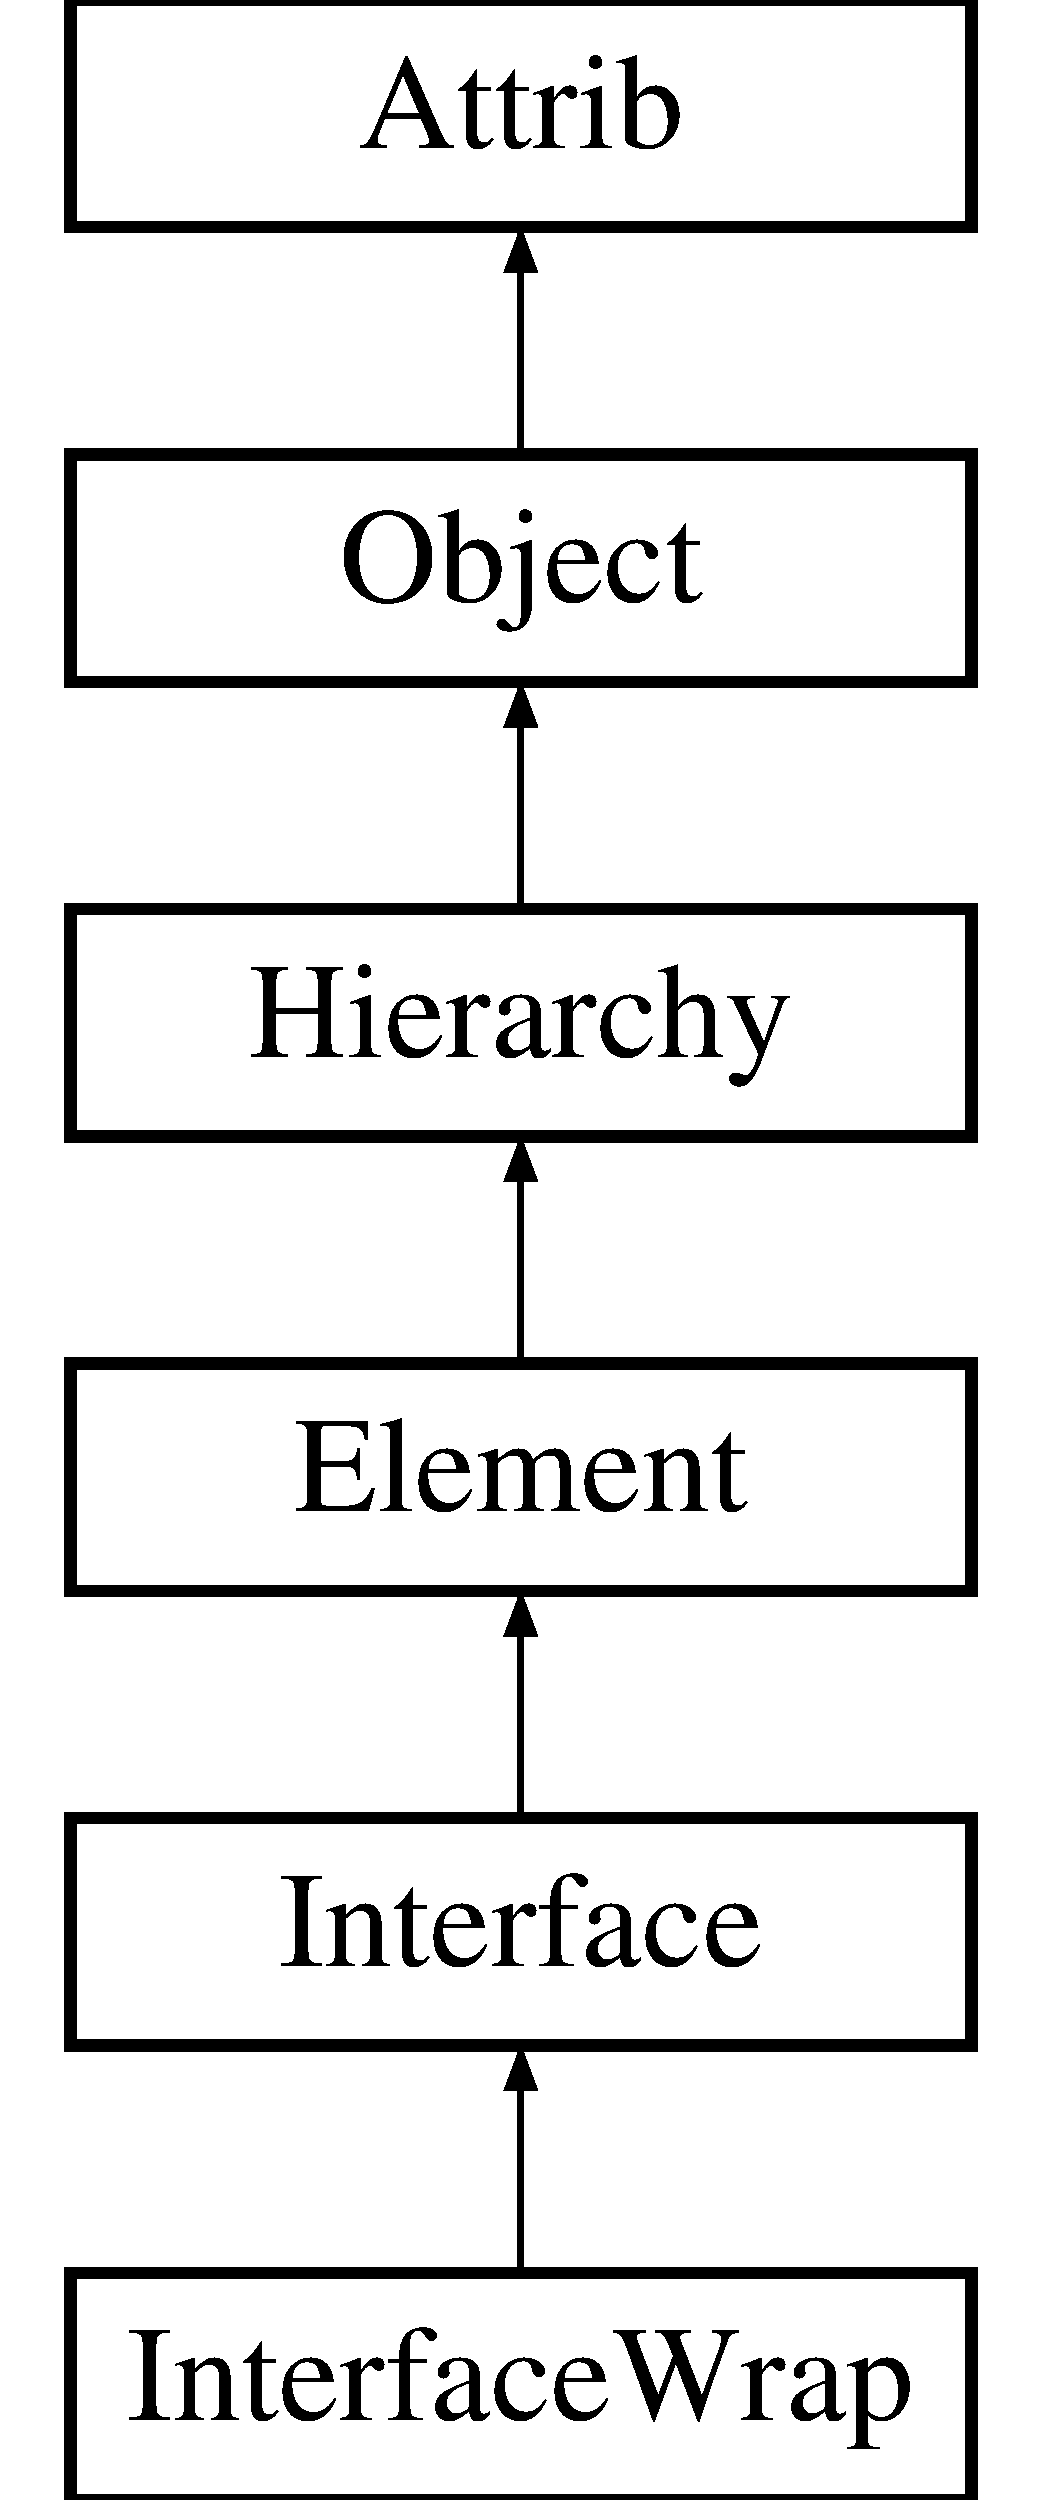
\includegraphics[height=6.000000cm]{structInterfaceWrap}
\end{center}
\end{figure}
\subsection*{Public Member Functions}
\begin{DoxyCompactItemize}
\item 
void \hyperlink{structInterfaceWrap_abcf87065a7b9099a7d05e7c0ddaf2487}{help} ()
\item 
\hyperlink{classStatusCode}{Status\+Code} \hyperlink{structInterfaceWrap_a2660ecdfbabd91d99d7b64c83e92f33c}{init} ()
\item 
void \hyperlink{structInterfaceWrap_a6c350b2f44c579187e6e4269cae29bae}{reset} ()
\item 
void \hyperlink{structInterfaceWrap_aee2f0407da52a1de8659b1d83af62238}{update} ()
\item 
\hyperlink{classStatusCode}{Status\+Code} \hyperlink{structInterfaceWrap_a4dd40213e6d37c73521450aa0c7a8f4d}{read} (\hyperlink{classIOdata}{I\+Odata} $\ast$)
\item 
\hyperlink{classStatusCode}{Status\+Code} \hyperlink{structInterfaceWrap_afbf6658c8be109e72f38d61438ec94d3}{write} (\hyperlink{classIOdata}{I\+Odata} $\ast$)
\end{DoxyCompactItemize}
\subsection*{Additional Inherited Members}


\subsection{Detailed Description}


Definition at line 17 of file Python.\+cpp.



\subsection{Member Function Documentation}
\mbox{\Hypertarget{structInterfaceWrap_abcf87065a7b9099a7d05e7c0ddaf2487}\label{structInterfaceWrap_abcf87065a7b9099a7d05e7c0ddaf2487}} 
\index{Interface\+Wrap@{Interface\+Wrap}!help@{help}}
\index{help@{help}!Interface\+Wrap@{Interface\+Wrap}}
\subsubsection{\texorpdfstring{help()}{help()}}
{\footnotesize\ttfamily void Interface\+Wrap\+::help (\begin{DoxyParamCaption}{ }\end{DoxyParamCaption})\hspace{0.3cm}{\ttfamily [inline]}, {\ttfamily [virtual]}}

printout help for the element 

Implements \hyperlink{classInterface_aedd3cf1d964c837e7848ccf81dc9c760}{Interface}.



Definition at line 19 of file Python.\+cpp.


\begin{DoxyCode}
19 \{this->get\_override(\textcolor{stringliteral}{"help"})();\};
\end{DoxyCode}
\mbox{\Hypertarget{structInterfaceWrap_a2660ecdfbabd91d99d7b64c83e92f33c}\label{structInterfaceWrap_a2660ecdfbabd91d99d7b64c83e92f33c}} 
\index{Interface\+Wrap@{Interface\+Wrap}!init@{init}}
\index{init@{init}!Interface\+Wrap@{Interface\+Wrap}}
\subsubsection{\texorpdfstring{init()}{init()}}
{\footnotesize\ttfamily \hyperlink{classStatusCode}{Status\+Code} Interface\+Wrap\+::init (\begin{DoxyParamCaption}{ }\end{DoxyParamCaption})\hspace{0.3cm}{\ttfamily [inline]}, {\ttfamily [virtual]}}

init the component

\begin{DoxyReturn}{Returns}
void 
\end{DoxyReturn}


Implements \hyperlink{classInterface_a1d095c113b1e89d1f5f68323856fee63}{Interface}.



Definition at line 20 of file Python.\+cpp.


\begin{DoxyCode}
20 \{\textcolor{keywordflow}{return} this->get\_override(\textcolor{stringliteral}{"init"})();\};
\end{DoxyCode}
\mbox{\Hypertarget{structInterfaceWrap_a4dd40213e6d37c73521450aa0c7a8f4d}\label{structInterfaceWrap_a4dd40213e6d37c73521450aa0c7a8f4d}} 
\index{Interface\+Wrap@{Interface\+Wrap}!read@{read}}
\index{read@{read}!Interface\+Wrap@{Interface\+Wrap}}
\subsubsection{\texorpdfstring{read()}{read()}}
{\footnotesize\ttfamily \hyperlink{classStatusCode}{Status\+Code} Interface\+Wrap\+::read (\begin{DoxyParamCaption}\item[{\hyperlink{classIOdata}{I\+Odata} $\ast$}]{ }\end{DoxyParamCaption})\hspace{0.3cm}{\ttfamily [inline]}, {\ttfamily [virtual]}}



Implements \hyperlink{classInterface_a99136b67c8e6cbcaa0477c36940ac2ef}{Interface}.



Definition at line 23 of file Python.\+cpp.


\begin{DoxyCode}
23 \{\textcolor{keywordflow}{return} this->get\_override(\textcolor{stringliteral}{"read"})();\};
\end{DoxyCode}
\mbox{\Hypertarget{structInterfaceWrap_a6c350b2f44c579187e6e4269cae29bae}\label{structInterfaceWrap_a6c350b2f44c579187e6e4269cae29bae}} 
\index{Interface\+Wrap@{Interface\+Wrap}!reset@{reset}}
\index{reset@{reset}!Interface\+Wrap@{Interface\+Wrap}}
\subsubsection{\texorpdfstring{reset()}{reset()}}
{\footnotesize\ttfamily void Interface\+Wrap\+::reset (\begin{DoxyParamCaption}{ }\end{DoxyParamCaption})\hspace{0.3cm}{\ttfamily [inline]}, {\ttfamily [virtual]}}

Resets the \hyperlink{classElement}{Element} so that is is in a standard and safe situation. Different from \hyperlink{classElement_af42754b5cabc198869222725218d695c}{Element\+::init} which configure the \hyperlink{classElement}{Element}. \hyperlink{classElement_a69efffa22f06909d768149715565cb56}{Element\+::reset()} is more an Emergency pull. It is often/usually called by the recursive\+Init\+Element method at the start of the program. 

Implements \hyperlink{classInterface_a4d44329cea9981a9e0392eaaf99efadd}{Interface}.



Definition at line 21 of file Python.\+cpp.


\begin{DoxyCode}
21 \{this->get\_override(\textcolor{stringliteral}{"reset"})();\};
\end{DoxyCode}
\mbox{\Hypertarget{structInterfaceWrap_aee2f0407da52a1de8659b1d83af62238}\label{structInterfaceWrap_aee2f0407da52a1de8659b1d83af62238}} 
\index{Interface\+Wrap@{Interface\+Wrap}!update@{update}}
\index{update@{update}!Interface\+Wrap@{Interface\+Wrap}}
\subsubsection{\texorpdfstring{update()}{update()}}
{\footnotesize\ttfamily void Interface\+Wrap\+::update (\begin{DoxyParamCaption}{ }\end{DoxyParamCaption})\hspace{0.3cm}{\ttfamily [inline]}, {\ttfamily [virtual]}}

Update the \hyperlink{classElement}{Element} configuration from the actual hardware 

Implements \hyperlink{classInterface_a30e71ffbe36091df9f7c0838dd4b60d2}{Interface}.



Definition at line 22 of file Python.\+cpp.



Referenced by App\+Frame.\+App\+Frame\+::delete\+Hardware(), Conf\+Frame.\+Conf\+Frame\+::on\+Change(), Graph\+Frame.\+Graph\+Frame\+::on\+Change(), Cfg\+Frame.\+Cfg\+Frame\+::on\+Change(), Conf\+Frame.\+Conf\+Frame\+::on\+Edit(), App\+Frame.\+App\+Frame\+::on\+Load(), Conf\+Frame.\+Conf\+Frame\+::on\+Re\+Load(), Graph\+Frame.\+Graph\+Frame\+::on\+Re\+Load(), Cfg\+Frame.\+Cfg\+Frame\+::on\+Re\+Load(), and App\+Frame.\+App\+Frame\+::on\+Re\+Load().


\begin{DoxyCode}
22 \{this->get\_override(\textcolor{stringliteral}{"update"})();\};
\end{DoxyCode}
\mbox{\Hypertarget{structInterfaceWrap_afbf6658c8be109e72f38d61438ec94d3}\label{structInterfaceWrap_afbf6658c8be109e72f38d61438ec94d3}} 
\index{Interface\+Wrap@{Interface\+Wrap}!write@{write}}
\index{write@{write}!Interface\+Wrap@{Interface\+Wrap}}
\subsubsection{\texorpdfstring{write()}{write()}}
{\footnotesize\ttfamily \hyperlink{classStatusCode}{Status\+Code} Interface\+Wrap\+::write (\begin{DoxyParamCaption}\item[{\hyperlink{classIOdata}{I\+Odata} $\ast$}]{ }\end{DoxyParamCaption})\hspace{0.3cm}{\ttfamily [inline]}, {\ttfamily [virtual]}}



Implements \hyperlink{classInterface_ad665cacbaf490a26c1c4ba192022e68a}{Interface}.



Definition at line 24 of file Python.\+cpp.


\begin{DoxyCode}
24 \{\textcolor{keywordflow}{return} this->get\_override(\textcolor{stringliteral}{"write"})();\};
\end{DoxyCode}


The documentation for this struct was generated from the following file\+:\begin{DoxyCompactItemize}
\item 
/home/eleclhcb/\+L\+H\+Cb/lbcat-\/cmake/\+Cat\+Core/src/\hyperlink{CatCore_2src_2Python_8cpp}{Python.\+cpp}\end{DoxyCompactItemize}

\hypertarget{classIOdata}{}\section{I\+Odata Class Reference}
\label{classIOdata}\index{I\+Odata@{I\+Odata}}


{\ttfamily \#include $<$inc/\+I\+Odata.\+h$>$}

Inheritance diagram for I\+Odata\+:\begin{figure}[H]
\begin{center}
\leavevmode
\includegraphics[height=3.000000cm]{classIOdata}
\end{center}
\end{figure}
\subsection*{Public Types}
\begin{DoxyCompactItemize}
\item 
enum \hyperlink{classIOdata_a044e9a4a0c6d25a43ebfe29c4fa4f1e5}{Mode} \{ \hyperlink{classIOdata_a044e9a4a0c6d25a43ebfe29c4fa4f1e5a9ac1bef9c44dd3f63df0b64646129e97}{Rd}, 
\hyperlink{classIOdata_a044e9a4a0c6d25a43ebfe29c4fa4f1e5a019388bd87f0ec039a78e7ac5cb60a81}{Wr}, 
\hyperlink{classIOdata_a044e9a4a0c6d25a43ebfe29c4fa4f1e5ae0f5414225eec903b44306912160c754}{Rd\+Wr}
 \}
\item 
enum \hyperlink{classIOdata_a37c53ebf4bf8d866aac8af572962a84c}{Word\+Size} \{ \hyperlink{classIOdata_a37c53ebf4bf8d866aac8af572962a84ca00156611f08eeb1b5d361de809dafb8e}{Byte}, 
\hyperlink{classIOdata_a37c53ebf4bf8d866aac8af572962a84ca7d603e9c9a55e3c8dffa4bd8e3dca491}{Word}, 
\hyperlink{classIOdata_a37c53ebf4bf8d866aac8af572962a84ca458da82d97e3ea9715c34b558c34f734}{D\+Word}
 \}
\item 
enum \hyperlink{classIOdata_a99aa7bed39364c4359ab8a7596bc013c}{Bus} \{ \newline
\hyperlink{classIOdata_a99aa7bed39364c4359ab8a7596bc013cabd27b3ded09d67a97f98b5004101856f}{U\+SB}, 
\hyperlink{classIOdata_a99aa7bed39364c4359ab8a7596bc013caf9005892b62633a3e9f3456ef11c8991}{S\+P\+E\+CS}, 
\hyperlink{classIOdata_a99aa7bed39364c4359ab8a7596bc013ca68cf1532718ac977427bacd1a7e0bc32}{I2C}, 
\hyperlink{classIOdata_a99aa7bed39364c4359ab8a7596bc013caf68d3c4cdd5e3c21501655358370b460}{P\+A\+R\+A\+L\+L\+EL}, 
\newline
\hyperlink{classIOdata_a99aa7bed39364c4359ab8a7596bc013ca185cc1d64a0173fc7da76513e2fb5642}{J\+T\+AG}
 \}
\item 
typedef unsigned long \hyperlink{classIOdata_a96fb57f5fcd87b708743abd3c86a5198}{U32}
\item 
typedef unsigned short \hyperlink{classIOdata_a1eb45b348534a7c19a4a99b746e693ff}{U16}
\item 
typedef unsigned char \hyperlink{classIOdata_a18d1354b7cdaf0f8a8001fdbb3ced418}{U8}
\item 
enum \hyperlink{classAttrib_a69e171d7cc6417835a5a306d3c764235}{Attribut} \{ \newline
\hyperlink{classAttrib_a69e171d7cc6417835a5a306d3c764235a3a8da2ab97dda18aebab196fe4100531}{U\+N\+D\+E\+F\+I\+N\+ED}, 
\hyperlink{classAttrib_a69e171d7cc6417835a5a306d3c764235a2bfb2af57b87031d190a05fe25dd92ed}{P\+A\+S\+S\+I\+VE}, 
\hyperlink{classAttrib_a69e171d7cc6417835a5a306d3c764235a3b1fec929c0370d1436f2f06e298fb0d}{A\+C\+T\+I\+VE}, 
\hyperlink{classAttrib_a69e171d7cc6417835a5a306d3c764235aa27c16b480a369ea4d18b07b2516bbc7}{I\+N\+T\+E\+R\+F\+A\+CE}, 
\newline
\hyperlink{classAttrib_a69e171d7cc6417835a5a306d3c764235a1420a5b8c0540b2af210b6975eded7f9}{IO}, 
\hyperlink{classAttrib_a69e171d7cc6417835a5a306d3c764235a0af3b0d0ac323c1704e6c69cf90add28}{I\+O\+D\+A\+TA}, 
\hyperlink{classAttrib_a69e171d7cc6417835a5a306d3c764235a7788bc5dd333fd8ce18562b269c9dab1}{E\+L\+E\+M\+E\+NT}, 
\hyperlink{classAttrib_a69e171d7cc6417835a5a306d3c764235a61ceb22149f365f1780d18f9d1459423}{H\+A\+R\+D\+W\+A\+RE}, 
\newline
\hyperlink{classAttrib_a69e171d7cc6417835a5a306d3c764235a75250e29692496e73effca2c0330977f}{P\+R\+O\+C\+E\+S\+S\+US}, 
\hyperlink{classAttrib_a69e171d7cc6417835a5a306d3c764235a103a67cd0b8f07ef478fa45d4356e27b}{S\+O\+F\+T\+W\+A\+RE}
 \}
\end{DoxyCompactItemize}
\subsection*{Public Member Functions}
\begin{DoxyCompactItemize}
\item 
\hyperlink{classIOdata_af558c1fc49af58f50c9600423dd5acd7}{I\+Odata} ()
\begin{DoxyCompactList}\small\item\em Standard constructor. \end{DoxyCompactList}\item 
virtual \hyperlink{classIOdata_a3d7cf860040702b00a925703da7c0648}{$\sim$\+I\+Odata} ()
\begin{DoxyCompactList}\small\item\em Destructor. \end{DoxyCompactList}\item 
\hyperlink{classStatusCode}{Status\+Code} \hyperlink{classIOdata_af98cbfbc28346ebb9b64ca0203af1463}{set\+Address} (\hyperlink{classIOdata_a96fb57f5fcd87b708743abd3c86a5198}{U32} \hyperlink{classIOdata_afe410c86881b8c2082a08e5ce9843306}{address})
\item 
\hyperlink{classIOdata_a96fb57f5fcd87b708743abd3c86a5198}{U32} \hyperlink{classIOdata_afe410c86881b8c2082a08e5ce9843306}{address} ()
\item 
\hyperlink{classStatusCode}{Status\+Code} \hyperlink{classIOdata_a9a850f401542d416adf061e30f7dfdd5}{set\+Header} (\hyperlink{classIOdata_a96fb57f5fcd87b708743abd3c86a5198}{U32} \hyperlink{classIOdata_a503396d8deb6e098c15f963e4201e01b}{header})
\item 
\hyperlink{classIOdata_a96fb57f5fcd87b708743abd3c86a5198}{U32} \hyperlink{classIOdata_a503396d8deb6e098c15f963e4201e01b}{header} ()
\item 
\hyperlink{classStatusCode}{Status\+Code} \hyperlink{classIOdata_aeca09aa9a8c2ccc4c3a728b2ddcf4b2a}{set\+Sub\+Address} (\hyperlink{classIOdata_a96fb57f5fcd87b708743abd3c86a5198}{U32} \hyperlink{classIOdata_a25df48b84364a468373260f823ed9c5f}{sub\+Address})
\item 
\hyperlink{classIOdata_a96fb57f5fcd87b708743abd3c86a5198}{U32} \hyperlink{classIOdata_a25df48b84364a468373260f823ed9c5f}{sub\+Address} ()
\item 
\hyperlink{classStatusCode}{Status\+Code} \hyperlink{classIOdata_a09675d3efa14ba00cc22f8ff8d463389}{set\+Output\+Select} (\hyperlink{classIOdata_a96fb57f5fcd87b708743abd3c86a5198}{U32} \hyperlink{classIOdata_aaa410b57a4607857d45ac6a7cd013307}{output\+Select})
\item 
\hyperlink{classIOdata_a96fb57f5fcd87b708743abd3c86a5198}{U32} \hyperlink{classIOdata_aaa410b57a4607857d45ac6a7cd013307}{output\+Select} ()
\item 
\hyperlink{classStatusCode}{Status\+Code} \hyperlink{classIOdata_ad81e9fd3f2cd9dcaffd9eabddf8f867e}{set\+Mode} (\hyperlink{classIOdata_a044e9a4a0c6d25a43ebfe29c4fa4f1e5}{I\+Odata\+::\+Mode} \hyperlink{classIOdata_aae2073c3bc6bc9f620dc0fca7fccc9a7}{mode})
\item 
\hyperlink{classIOdata_a044e9a4a0c6d25a43ebfe29c4fa4f1e5}{I\+Odata\+::\+Mode} \hyperlink{classIOdata_aae2073c3bc6bc9f620dc0fca7fccc9a7}{mode} ()
\item 
\hyperlink{classStatusCode}{Status\+Code} \hyperlink{classIOdata_a20f30a9f4673713616447b1b5e9817d5}{set\+Word\+Size} (\hyperlink{classIOdata_a37c53ebf4bf8d866aac8af572962a84c}{I\+Odata\+::\+Word\+Size} \hyperlink{classIOdata_a91f9e8b4095ca8365a824e43be36b143}{word\+Size})
\item 
\hyperlink{classIOdata_a37c53ebf4bf8d866aac8af572962a84c}{I\+Odata\+::\+Word\+Size} \hyperlink{classIOdata_a91f9e8b4095ca8365a824e43be36b143}{word\+Size} ()
\item 
\hyperlink{classStatusCode}{Status\+Code} \hyperlink{classIOdata_aca154b90e490608b5b5c0ead58e1fafc}{set\+Bus} (\hyperlink{classIOdata_a99aa7bed39364c4359ab8a7596bc013c}{I\+Odata\+::\+Bus} \hyperlink{classIOdata_ab904bcca0e8e3bebc3299e47ca93a8a1}{bus})
\item 
\hyperlink{classIOdata_a99aa7bed39364c4359ab8a7596bc013c}{I\+Odata\+::\+Bus} \hyperlink{classIOdata_ab904bcca0e8e3bebc3299e47ca93a8a1}{bus} ()
\item 
\hyperlink{classStatusCode}{Status\+Code} \hyperlink{classIOdata_affaf98e7f9e596263e914b055f8f93c2}{set\+Length} (\hyperlink{classIOdata_a96fb57f5fcd87b708743abd3c86a5198}{U32} \hyperlink{classIOdata_abb40e71ce0290832a24857b4a1e7b1a3}{length})
\item 
\hyperlink{classIOdata_a96fb57f5fcd87b708743abd3c86a5198}{U32} \hyperlink{classIOdata_aeda27840c9a9b7b3b86efc71c56cd868}{block} ()
\item 
\hyperlink{classStatusCode}{Status\+Code} \hyperlink{classIOdata_a334f07d85e3dc8069551dcd8ab942e9c}{set\+Block} (\hyperlink{classIOdata_a96fb57f5fcd87b708743abd3c86a5198}{U32} \hyperlink{classIOdata_aeda27840c9a9b7b3b86efc71c56cd868}{block})
\item 
\hyperlink{classIOdata_a96fb57f5fcd87b708743abd3c86a5198}{U32} \hyperlink{classIOdata_abb40e71ce0290832a24857b4a1e7b1a3}{length} ()
\item 
void \hyperlink{classIOdata_a80bb230b61062b447db5832e43bf7b44}{def\+Data\+U8} (unsigned long size)
\item 
void \hyperlink{classIOdata_a9e37c736d6dfb5223ed45786fad403da}{def\+Data\+U16} (unsigned long size)
\item 
void \hyperlink{classIOdata_a78e50aa4a6c967cba195e77fe911a8c3}{def\+Data\+U32} (unsigned long size)
\item 
void \hyperlink{classIOdata_a9bc3ea0458ea6d13bd751ac4c80a4be6}{clear\+Data\+U8} ()
\item 
void \hyperlink{classIOdata_a13016f489aba6e80cd7be53224c3e8ab}{clear\+Data\+U16} ()
\item 
void \hyperlink{classIOdata_a848de1b6e7b7207dbb53c102a4d911a9}{clear\+Data\+U32} ()
\item 
\hyperlink{classIOdata_a18d1354b7cdaf0f8a8001fdbb3ced418}{U8} $\ast$ \hyperlink{classIOdata_a75e9c318dbac3a39402179070943d4bc}{data\+U8} ()
\item 
\hyperlink{classIOdata_a1eb45b348534a7c19a4a99b746e693ff}{U16} $\ast$ \hyperlink{classIOdata_a8d8528b731c6cf117f8c5b9b2473390c}{data\+U16} ()
\item 
\hyperlink{classIOdata_a96fb57f5fcd87b708743abd3c86a5198}{U32} $\ast$ \hyperlink{classIOdata_ab0e3cd09f46c1c3712f797116f6da074}{data\+U32} ()
\item 
unsigned long int \hyperlink{classIOdata_a9c7cc68c435e1b22dcdac7c17d186e63}{data\+U8} (unsigned long int i)
\item 
unsigned long int \hyperlink{classIOdata_a32e3bb958cb6babcb928d403fea9f171}{data\+U16} (unsigned long int i)
\item 
unsigned long int \hyperlink{classIOdata_a4ce3bcd54206b1a2149e67cb45dee922}{data\+U32} (unsigned long int i)
\item 
void \hyperlink{classIOdata_afece89b7035f6eec001cd397f07c062d}{set\+Data\+U8} (\hyperlink{classIOdata_a18d1354b7cdaf0f8a8001fdbb3ced418}{U8} $\ast$data, \hyperlink{classIOdata_a96fb57f5fcd87b708743abd3c86a5198}{U32} \hyperlink{classIOdata_abb40e71ce0290832a24857b4a1e7b1a3}{length})
\item 
void \hyperlink{classIOdata_a1796a65cbd8c4326e80d662034ee5e39}{set\+Data\+U16} (\hyperlink{classIOdata_a1eb45b348534a7c19a4a99b746e693ff}{U16} $\ast$data, \hyperlink{classIOdata_a96fb57f5fcd87b708743abd3c86a5198}{U32} \hyperlink{classIOdata_abb40e71ce0290832a24857b4a1e7b1a3}{length})
\item 
void \hyperlink{classIOdata_a408b62ac645630c645ae670691f6459f}{set\+Data\+U32} (\hyperlink{classIOdata_a96fb57f5fcd87b708743abd3c86a5198}{U32} $\ast$data, \hyperlink{classIOdata_a96fb57f5fcd87b708743abd3c86a5198}{U32} \hyperlink{classIOdata_abb40e71ce0290832a24857b4a1e7b1a3}{length})
\item 
\hyperlink{classStatusCode}{Status\+Code} \hyperlink{classIOdata_a6c4fb2f2af01889ada889c2b7aceb24d}{set\+U8} (unsigned long int, \hyperlink{classIOdata_a18d1354b7cdaf0f8a8001fdbb3ced418}{U8})
\item 
\hyperlink{classStatusCode}{Status\+Code} \hyperlink{classIOdata_aa9ade5ce3944c8e2b831533b6f876caf}{set\+U16} (unsigned long int, \hyperlink{classIOdata_a1eb45b348534a7c19a4a99b746e693ff}{U16})
\item 
\hyperlink{classStatusCode}{Status\+Code} \hyperlink{classIOdata_abbed9a057203bc763f97b85fb385f36b}{set\+U32} (unsigned long int, \hyperlink{classIOdata_a96fb57f5fcd87b708743abd3c86a5198}{U32})
\item 
void \hyperlink{classIOdata_a208e24222bf2044a4ff8bbb1a6bdc13b}{dump} (unsigned int printout=0)
\item 
std\+::string \hyperlink{classObject_a300f4c05dd468c7bb8b3c968868443c1}{name} () const
\item 
std\+::string \hyperlink{classObject_a84f99f70f144a83e1582d1d0f84e4e62}{type} ()
\item 
unsigned char \hyperlink{classObject_af99145335cc61ff6e2798ea17db009d2}{id} ()
\item 
std\+::string \hyperlink{classObject_a73a0f1a41828fdd8303dd662446fb6c3}{title} ()
\item 
void \hyperlink{classObject_a3f9d5537ebce0c0f2bf6ae4d92426f3c}{msg\+Svc} (int level, std\+::string \hyperlink{classObject_a58b2d0618c2d08cf2383012611528d97}{msg}, std\+::string \hyperlink{classObject_a300f4c05dd468c7bb8b3c968868443c1}{name})
\item 
void \hyperlink{classObject_a58b2d0618c2d08cf2383012611528d97}{msg} (std\+::string mymsg)
\item 
void \hyperlink{classObject_ac5d59299273cee27aacf7de00d2e7034}{msg} (std\+::string mymsg, std\+::string \hyperlink{classObject_a300f4c05dd468c7bb8b3c968868443c1}{name})
\item 
void \hyperlink{classObject_a83d2db2df682907ea1115ad721c1c4a1}{verbose} (std\+::string mymsg)
\item 
void \hyperlink{classObject_a2d4120195317e2a3c6532e8bb9f3da68}{verbose} (std\+::string mymsg, std\+::string \hyperlink{classObject_a300f4c05dd468c7bb8b3c968868443c1}{name})
\item 
void \hyperlink{classObject_aac010553f022165573714b7014a15f0d}{debug} (std\+::string mymsg)
\item 
void \hyperlink{classObject_a6c9a0397ca804e04d675ed05683f5420}{debug} (std\+::string mymsg, std\+::string \hyperlink{classObject_a300f4c05dd468c7bb8b3c968868443c1}{name})
\item 
void \hyperlink{classObject_a644fd329ea4cb85f54fa6846484b84a8}{info} (std\+::string mymsg)
\item 
void \hyperlink{classObject_a1ca123253dfd30fc28b156f521dcbdae}{info} (std\+::string mymsg, std\+::string \hyperlink{classObject_a300f4c05dd468c7bb8b3c968868443c1}{name})
\item 
void \hyperlink{classObject_a65cd4fda577711660821fd2cd5a3b4c9}{warning} (std\+::string mymsg)
\item 
void \hyperlink{classObject_a11f101db4dd73d9391b0231818881d86}{warning} (std\+::string mymsg, std\+::string \hyperlink{classObject_a300f4c05dd468c7bb8b3c968868443c1}{name})
\item 
void \hyperlink{classObject_a204a95f57818c0f811933917a30eff45}{error} (std\+::string mymsg)
\item 
void \hyperlink{classObject_ad7f6c457733082efa2f9ff5f5c8e119a}{error} (std\+::string mymsg, std\+::string \hyperlink{classObject_a300f4c05dd468c7bb8b3c968868443c1}{name})
\item 
void \hyperlink{classObject_aad5a16aac7516ce65bd5ec02ab07fc80}{fatal} (std\+::string mymsg)
\item 
void \hyperlink{classObject_ae62acd3d09f716220f75f252dc38bc9a}{fatal} (std\+::string mymsg, std\+::string \hyperlink{classObject_a300f4c05dd468c7bb8b3c968868443c1}{name})
\item 
void \hyperlink{classObject_ae30fea75683c2d149b6b6d17c09ecd0c}{set\+Name} (std\+::string \hyperlink{classObject_a300f4c05dd468c7bb8b3c968868443c1}{name})
\item 
void \hyperlink{classObject_aae534cc9d982bcb9b99fd505f2e103a5}{set\+Type} (std\+::string \hyperlink{classObject_a84f99f70f144a83e1582d1d0f84e4e62}{type})
\item 
void \hyperlink{classObject_a398fe08cba594a0ce6891d59fe4f159f}{set\+Id} (unsigned char \hyperlink{classObject_af99145335cc61ff6e2798ea17db009d2}{id})
\item 
void \hyperlink{classObject_a89557dbbad5bcaa02652f5d7fa35d20f}{set\+Title} (std\+::string \hyperlink{classObject_a73a0f1a41828fdd8303dd662446fb6c3}{title})
\item 
void \hyperlink{classObject_a870c5af919958c2136623b2d7816d123}{set\+Dll\+Name} (std\+::string \hyperlink{classObject_a2e3947f2870094c332d7454117f3ec63}{dll\+Name})
\item 
std\+::string \hyperlink{classObject_a2e3947f2870094c332d7454117f3ec63}{dll\+Name} ()
\item 
bool \hyperlink{classAttrib_a704f26af560909ad22065083bb7d4c34}{is} (int attribut)
\item 
void \hyperlink{classAttrib_a235f773af19c900264a190b00a3b4ad7}{add} (int attribut)
\item 
void \hyperlink{classAttrib_a7d4ef7e32d93cb287792b87b857e79f3}{remove} (int attribut)
\item 
std\+::string \hyperlink{classAttrib_aee7bbf16b144887f196e1341b24f8a26}{attributs} ()
\end{DoxyCompactItemize}
\subsection*{Protected Attributes}
\begin{DoxyCompactItemize}
\item 
std\+::string \hyperlink{classAttrib_a3414521d7a82476e874b25a5407b5e63}{m\+\_\+attrib\+String} \mbox{[}10\mbox{]}
\end{DoxyCompactItemize}
\subsection*{Private Attributes}
\begin{DoxyCompactItemize}
\item 
unsigned long \hyperlink{classIOdata_a965810e1888b904c575277f50cea734a}{m\+\_\+address}
\item 
unsigned long \hyperlink{classIOdata_a46ec7dbfa257c02be1d39c4799f157d3}{m\+\_\+header}
\item 
unsigned long \hyperlink{classIOdata_a562f84e5cace1e392f1b0fca553fff78}{m\+\_\+sub\+Address}
\item 
unsigned long \hyperlink{classIOdata_acc46d71243b542e68277e242effa7f1b}{m\+\_\+output\+Select}
\item 
\hyperlink{classIOdata_a044e9a4a0c6d25a43ebfe29c4fa4f1e5}{I\+Odata\+::\+Mode} \hyperlink{classIOdata_a0782e31763fa855f1ecbd377dce538e6}{m\+\_\+mode}
\item 
\hyperlink{classIOdata_a37c53ebf4bf8d866aac8af572962a84c}{I\+Odata\+::\+Word\+Size} \hyperlink{classIOdata_a719b0ce607ada4fa91b12d6ecfa1b4c9}{m\+\_\+word\+Size}
\item 
\hyperlink{classIOdata_a99aa7bed39364c4359ab8a7596bc013c}{I\+Odata\+::\+Bus} \hyperlink{classIOdata_a42c07a9b3f43ec35dd18d13a67d294cc}{m\+\_\+bus}
\item 
unsigned long \hyperlink{classIOdata_afabe57441da019eb614d277799106aac}{m\+\_\+length}
\item 
unsigned long \hyperlink{classIOdata_a6d1ce9f88db6b97ce61098a3693e253f}{m\+\_\+block}
\item 
\hyperlink{classIOdata_a18d1354b7cdaf0f8a8001fdbb3ced418}{U8} $\ast$ \hyperlink{classIOdata_a9c4c0dc5104f7f3b170e30ab78fe61e7}{m\+\_\+data\+U8}
\item 
\hyperlink{classIOdata_a1eb45b348534a7c19a4a99b746e693ff}{U16} $\ast$ \hyperlink{classIOdata_a8d698e077b7898009691b9086a3e6453}{m\+\_\+data\+U16}
\item 
\hyperlink{classIOdata_a96fb57f5fcd87b708743abd3c86a5198}{U32} $\ast$ \hyperlink{classIOdata_a247cdaefd87084e3cad1d530d592d99a}{m\+\_\+data\+U32}
\end{DoxyCompactItemize}


\subsection{Detailed Description}
\begin{DoxyAuthor}{Author}
\hyperlink{classIOdata}{I\+Odata} 
\end{DoxyAuthor}
\begin{DoxyDate}{Date}
2006-\/10-\/23 
\end{DoxyDate}


Definition at line 17 of file I\+Odata.\+h.



\subsection{Member Typedef Documentation}
\mbox{\Hypertarget{classIOdata_a1eb45b348534a7c19a4a99b746e693ff}\label{classIOdata_a1eb45b348534a7c19a4a99b746e693ff}} 
\index{I\+Odata@{I\+Odata}!U16@{U16}}
\index{U16@{U16}!I\+Odata@{I\+Odata}}
\subsubsection{\texorpdfstring{U16}{U16}}
{\footnotesize\ttfamily typedef unsigned short \hyperlink{classIOdata_a1eb45b348534a7c19a4a99b746e693ff}{I\+Odata\+::\+U16}}



Definition at line 20 of file I\+Odata.\+h.

\mbox{\Hypertarget{classIOdata_a96fb57f5fcd87b708743abd3c86a5198}\label{classIOdata_a96fb57f5fcd87b708743abd3c86a5198}} 
\index{I\+Odata@{I\+Odata}!U32@{U32}}
\index{U32@{U32}!I\+Odata@{I\+Odata}}
\subsubsection{\texorpdfstring{U32}{U32}}
{\footnotesize\ttfamily typedef unsigned long \hyperlink{classIOdata_a96fb57f5fcd87b708743abd3c86a5198}{I\+Odata\+::\+U32}}



Definition at line 19 of file I\+Odata.\+h.

\mbox{\Hypertarget{classIOdata_a18d1354b7cdaf0f8a8001fdbb3ced418}\label{classIOdata_a18d1354b7cdaf0f8a8001fdbb3ced418}} 
\index{I\+Odata@{I\+Odata}!U8@{U8}}
\index{U8@{U8}!I\+Odata@{I\+Odata}}
\subsubsection{\texorpdfstring{U8}{U8}}
{\footnotesize\ttfamily typedef unsigned char \hyperlink{classIOdata_a18d1354b7cdaf0f8a8001fdbb3ced418}{I\+Odata\+::\+U8}}



Definition at line 21 of file I\+Odata.\+h.



\subsection{Member Enumeration Documentation}
\mbox{\Hypertarget{classAttrib_a69e171d7cc6417835a5a306d3c764235}\label{classAttrib_a69e171d7cc6417835a5a306d3c764235}} 
\index{I\+Odata@{I\+Odata}!Attribut@{Attribut}}
\index{Attribut@{Attribut}!I\+Odata@{I\+Odata}}
\subsubsection{\texorpdfstring{Attribut}{Attribut}}
{\footnotesize\ttfamily enum \hyperlink{classAttrib_a69e171d7cc6417835a5a306d3c764235}{Attrib\+::\+Attribut}\hspace{0.3cm}{\ttfamily [inherited]}}

\begin{DoxyEnumFields}{Enumerator}
\raisebox{\heightof{T}}[0pt][0pt]{\index{U\+N\+D\+E\+F\+I\+N\+ED@{U\+N\+D\+E\+F\+I\+N\+ED}!I\+Odata@{I\+Odata}}\index{I\+Odata@{I\+Odata}!U\+N\+D\+E\+F\+I\+N\+ED@{U\+N\+D\+E\+F\+I\+N\+ED}}}\mbox{\Hypertarget{classAttrib_a69e171d7cc6417835a5a306d3c764235a3a8da2ab97dda18aebab196fe4100531}\label{classAttrib_a69e171d7cc6417835a5a306d3c764235a3a8da2ab97dda18aebab196fe4100531}} 
U\+N\+D\+E\+F\+I\+N\+ED&\\
\hline

\raisebox{\heightof{T}}[0pt][0pt]{\index{P\+A\+S\+S\+I\+VE@{P\+A\+S\+S\+I\+VE}!I\+Odata@{I\+Odata}}\index{I\+Odata@{I\+Odata}!P\+A\+S\+S\+I\+VE@{P\+A\+S\+S\+I\+VE}}}\mbox{\Hypertarget{classAttrib_a69e171d7cc6417835a5a306d3c764235a2bfb2af57b87031d190a05fe25dd92ed}\label{classAttrib_a69e171d7cc6417835a5a306d3c764235a2bfb2af57b87031d190a05fe25dd92ed}} 
P\+A\+S\+S\+I\+VE&\\
\hline

\raisebox{\heightof{T}}[0pt][0pt]{\index{A\+C\+T\+I\+VE@{A\+C\+T\+I\+VE}!I\+Odata@{I\+Odata}}\index{I\+Odata@{I\+Odata}!A\+C\+T\+I\+VE@{A\+C\+T\+I\+VE}}}\mbox{\Hypertarget{classAttrib_a69e171d7cc6417835a5a306d3c764235a3b1fec929c0370d1436f2f06e298fb0d}\label{classAttrib_a69e171d7cc6417835a5a306d3c764235a3b1fec929c0370d1436f2f06e298fb0d}} 
A\+C\+T\+I\+VE&\\
\hline

\raisebox{\heightof{T}}[0pt][0pt]{\index{I\+N\+T\+E\+R\+F\+A\+CE@{I\+N\+T\+E\+R\+F\+A\+CE}!I\+Odata@{I\+Odata}}\index{I\+Odata@{I\+Odata}!I\+N\+T\+E\+R\+F\+A\+CE@{I\+N\+T\+E\+R\+F\+A\+CE}}}\mbox{\Hypertarget{classAttrib_a69e171d7cc6417835a5a306d3c764235aa27c16b480a369ea4d18b07b2516bbc7}\label{classAttrib_a69e171d7cc6417835a5a306d3c764235aa27c16b480a369ea4d18b07b2516bbc7}} 
I\+N\+T\+E\+R\+F\+A\+CE&\\
\hline

\raisebox{\heightof{T}}[0pt][0pt]{\index{IO@{IO}!I\+Odata@{I\+Odata}}\index{I\+Odata@{I\+Odata}!IO@{IO}}}\mbox{\Hypertarget{classAttrib_a69e171d7cc6417835a5a306d3c764235a1420a5b8c0540b2af210b6975eded7f9}\label{classAttrib_a69e171d7cc6417835a5a306d3c764235a1420a5b8c0540b2af210b6975eded7f9}} 
IO&\\
\hline

\raisebox{\heightof{T}}[0pt][0pt]{\index{I\+O\+D\+A\+TA@{I\+O\+D\+A\+TA}!I\+Odata@{I\+Odata}}\index{I\+Odata@{I\+Odata}!I\+O\+D\+A\+TA@{I\+O\+D\+A\+TA}}}\mbox{\Hypertarget{classAttrib_a69e171d7cc6417835a5a306d3c764235a0af3b0d0ac323c1704e6c69cf90add28}\label{classAttrib_a69e171d7cc6417835a5a306d3c764235a0af3b0d0ac323c1704e6c69cf90add28}} 
I\+O\+D\+A\+TA&\\
\hline

\raisebox{\heightof{T}}[0pt][0pt]{\index{E\+L\+E\+M\+E\+NT@{E\+L\+E\+M\+E\+NT}!I\+Odata@{I\+Odata}}\index{I\+Odata@{I\+Odata}!E\+L\+E\+M\+E\+NT@{E\+L\+E\+M\+E\+NT}}}\mbox{\Hypertarget{classAttrib_a69e171d7cc6417835a5a306d3c764235a7788bc5dd333fd8ce18562b269c9dab1}\label{classAttrib_a69e171d7cc6417835a5a306d3c764235a7788bc5dd333fd8ce18562b269c9dab1}} 
E\+L\+E\+M\+E\+NT&\\
\hline

\raisebox{\heightof{T}}[0pt][0pt]{\index{H\+A\+R\+D\+W\+A\+RE@{H\+A\+R\+D\+W\+A\+RE}!I\+Odata@{I\+Odata}}\index{I\+Odata@{I\+Odata}!H\+A\+R\+D\+W\+A\+RE@{H\+A\+R\+D\+W\+A\+RE}}}\mbox{\Hypertarget{classAttrib_a69e171d7cc6417835a5a306d3c764235a61ceb22149f365f1780d18f9d1459423}\label{classAttrib_a69e171d7cc6417835a5a306d3c764235a61ceb22149f365f1780d18f9d1459423}} 
H\+A\+R\+D\+W\+A\+RE&\\
\hline

\raisebox{\heightof{T}}[0pt][0pt]{\index{P\+R\+O\+C\+E\+S\+S\+US@{P\+R\+O\+C\+E\+S\+S\+US}!I\+Odata@{I\+Odata}}\index{I\+Odata@{I\+Odata}!P\+R\+O\+C\+E\+S\+S\+US@{P\+R\+O\+C\+E\+S\+S\+US}}}\mbox{\Hypertarget{classAttrib_a69e171d7cc6417835a5a306d3c764235a75250e29692496e73effca2c0330977f}\label{classAttrib_a69e171d7cc6417835a5a306d3c764235a75250e29692496e73effca2c0330977f}} 
P\+R\+O\+C\+E\+S\+S\+US&\\
\hline

\raisebox{\heightof{T}}[0pt][0pt]{\index{S\+O\+F\+T\+W\+A\+RE@{S\+O\+F\+T\+W\+A\+RE}!I\+Odata@{I\+Odata}}\index{I\+Odata@{I\+Odata}!S\+O\+F\+T\+W\+A\+RE@{S\+O\+F\+T\+W\+A\+RE}}}\mbox{\Hypertarget{classAttrib_a69e171d7cc6417835a5a306d3c764235a103a67cd0b8f07ef478fa45d4356e27b}\label{classAttrib_a69e171d7cc6417835a5a306d3c764235a103a67cd0b8f07ef478fa45d4356e27b}} 
S\+O\+F\+T\+W\+A\+RE&\\
\hline

\end{DoxyEnumFields}


Definition at line 29 of file Attrib.\+h.


\begin{DoxyCode}
29                 \{
30     \hyperlink{classAttrib_a69e171d7cc6417835a5a306d3c764235a3a8da2ab97dda18aebab196fe4100531}{UNDEFINED},
31     \hyperlink{classAttrib_a69e171d7cc6417835a5a306d3c764235a2bfb2af57b87031d190a05fe25dd92ed}{PASSIVE},
32     \hyperlink{classAttrib_a69e171d7cc6417835a5a306d3c764235a3b1fec929c0370d1436f2f06e298fb0d}{ACTIVE},
33     \hyperlink{classAttrib_a69e171d7cc6417835a5a306d3c764235aa27c16b480a369ea4d18b07b2516bbc7}{INTERFACE},
34     \hyperlink{classAttrib_a69e171d7cc6417835a5a306d3c764235a1420a5b8c0540b2af210b6975eded7f9}{IO},
35     \hyperlink{classAttrib_a69e171d7cc6417835a5a306d3c764235a0af3b0d0ac323c1704e6c69cf90add28}{IODATA},
36     \hyperlink{classAttrib_a69e171d7cc6417835a5a306d3c764235a7788bc5dd333fd8ce18562b269c9dab1}{ELEMENT},
37     \hyperlink{classAttrib_a69e171d7cc6417835a5a306d3c764235a61ceb22149f365f1780d18f9d1459423}{HARDWARE},
38     \hyperlink{classAttrib_a69e171d7cc6417835a5a306d3c764235a75250e29692496e73effca2c0330977f}{PROCESSUS},
39     \hyperlink{classAttrib_a69e171d7cc6417835a5a306d3c764235a103a67cd0b8f07ef478fa45d4356e27b}{SOFTWARE} 
40   \}; \textcolor{comment}{// array m\_attribString must be changed into Attrib::Attrib if this enu is modified. }
\end{DoxyCode}
\mbox{\Hypertarget{classIOdata_a99aa7bed39364c4359ab8a7596bc013c}\label{classIOdata_a99aa7bed39364c4359ab8a7596bc013c}} 
\index{I\+Odata@{I\+Odata}!Bus@{Bus}}
\index{Bus@{Bus}!I\+Odata@{I\+Odata}}
\subsubsection{\texorpdfstring{Bus}{Bus}}
{\footnotesize\ttfamily enum \hyperlink{classIOdata_a99aa7bed39364c4359ab8a7596bc013c}{I\+Odata\+::\+Bus}}

\begin{DoxyEnumFields}{Enumerator}
\raisebox{\heightof{T}}[0pt][0pt]{\index{U\+SB@{U\+SB}!I\+Odata@{I\+Odata}}\index{I\+Odata@{I\+Odata}!U\+SB@{U\+SB}}}\mbox{\Hypertarget{classIOdata_a99aa7bed39364c4359ab8a7596bc013cabd27b3ded09d67a97f98b5004101856f}\label{classIOdata_a99aa7bed39364c4359ab8a7596bc013cabd27b3ded09d67a97f98b5004101856f}} 
U\+SB&\\
\hline

\raisebox{\heightof{T}}[0pt][0pt]{\index{S\+P\+E\+CS@{S\+P\+E\+CS}!I\+Odata@{I\+Odata}}\index{I\+Odata@{I\+Odata}!S\+P\+E\+CS@{S\+P\+E\+CS}}}\mbox{\Hypertarget{classIOdata_a99aa7bed39364c4359ab8a7596bc013caf9005892b62633a3e9f3456ef11c8991}\label{classIOdata_a99aa7bed39364c4359ab8a7596bc013caf9005892b62633a3e9f3456ef11c8991}} 
S\+P\+E\+CS&\\
\hline

\raisebox{\heightof{T}}[0pt][0pt]{\index{I2C@{I2C}!I\+Odata@{I\+Odata}}\index{I\+Odata@{I\+Odata}!I2C@{I2C}}}\mbox{\Hypertarget{classIOdata_a99aa7bed39364c4359ab8a7596bc013ca68cf1532718ac977427bacd1a7e0bc32}\label{classIOdata_a99aa7bed39364c4359ab8a7596bc013ca68cf1532718ac977427bacd1a7e0bc32}} 
I2C&\\
\hline

\raisebox{\heightof{T}}[0pt][0pt]{\index{P\+A\+R\+A\+L\+L\+EL@{P\+A\+R\+A\+L\+L\+EL}!I\+Odata@{I\+Odata}}\index{I\+Odata@{I\+Odata}!P\+A\+R\+A\+L\+L\+EL@{P\+A\+R\+A\+L\+L\+EL}}}\mbox{\Hypertarget{classIOdata_a99aa7bed39364c4359ab8a7596bc013caf68d3c4cdd5e3c21501655358370b460}\label{classIOdata_a99aa7bed39364c4359ab8a7596bc013caf68d3c4cdd5e3c21501655358370b460}} 
P\+A\+R\+A\+L\+L\+EL&\\
\hline

\raisebox{\heightof{T}}[0pt][0pt]{\index{J\+T\+AG@{J\+T\+AG}!I\+Odata@{I\+Odata}}\index{I\+Odata@{I\+Odata}!J\+T\+AG@{J\+T\+AG}}}\mbox{\Hypertarget{classIOdata_a99aa7bed39364c4359ab8a7596bc013ca185cc1d64a0173fc7da76513e2fb5642}\label{classIOdata_a99aa7bed39364c4359ab8a7596bc013ca185cc1d64a0173fc7da76513e2fb5642}} 
J\+T\+AG&\\
\hline

\end{DoxyEnumFields}


Definition at line 35 of file I\+Odata.\+h.


\begin{DoxyCode}
35           \{
36     \hyperlink{classIOdata_a99aa7bed39364c4359ab8a7596bc013cabd27b3ded09d67a97f98b5004101856f}{USB},
37     \hyperlink{classIOdata_a99aa7bed39364c4359ab8a7596bc013caf9005892b62633a3e9f3456ef11c8991}{SPECS},
38     \hyperlink{classIOdata_a99aa7bed39364c4359ab8a7596bc013ca68cf1532718ac977427bacd1a7e0bc32}{I2C},
39     \hyperlink{classIOdata_a99aa7bed39364c4359ab8a7596bc013caf68d3c4cdd5e3c21501655358370b460}{PARALLEL},
40     \hyperlink{classIOdata_a99aa7bed39364c4359ab8a7596bc013ca185cc1d64a0173fc7da76513e2fb5642}{JTAG}
41   \};
\end{DoxyCode}
\mbox{\Hypertarget{classIOdata_a044e9a4a0c6d25a43ebfe29c4fa4f1e5}\label{classIOdata_a044e9a4a0c6d25a43ebfe29c4fa4f1e5}} 
\index{I\+Odata@{I\+Odata}!Mode@{Mode}}
\index{Mode@{Mode}!I\+Odata@{I\+Odata}}
\subsubsection{\texorpdfstring{Mode}{Mode}}
{\footnotesize\ttfamily enum \hyperlink{classIOdata_a044e9a4a0c6d25a43ebfe29c4fa4f1e5}{I\+Odata\+::\+Mode}}

\begin{DoxyEnumFields}{Enumerator}
\raisebox{\heightof{T}}[0pt][0pt]{\index{Rd@{Rd}!I\+Odata@{I\+Odata}}\index{I\+Odata@{I\+Odata}!Rd@{Rd}}}\mbox{\Hypertarget{classIOdata_a044e9a4a0c6d25a43ebfe29c4fa4f1e5a9ac1bef9c44dd3f63df0b64646129e97}\label{classIOdata_a044e9a4a0c6d25a43ebfe29c4fa4f1e5a9ac1bef9c44dd3f63df0b64646129e97}} 
Rd&\\
\hline

\raisebox{\heightof{T}}[0pt][0pt]{\index{Wr@{Wr}!I\+Odata@{I\+Odata}}\index{I\+Odata@{I\+Odata}!Wr@{Wr}}}\mbox{\Hypertarget{classIOdata_a044e9a4a0c6d25a43ebfe29c4fa4f1e5a019388bd87f0ec039a78e7ac5cb60a81}\label{classIOdata_a044e9a4a0c6d25a43ebfe29c4fa4f1e5a019388bd87f0ec039a78e7ac5cb60a81}} 
Wr&\\
\hline

\raisebox{\heightof{T}}[0pt][0pt]{\index{Rd\+Wr@{Rd\+Wr}!I\+Odata@{I\+Odata}}\index{I\+Odata@{I\+Odata}!Rd\+Wr@{Rd\+Wr}}}\mbox{\Hypertarget{classIOdata_a044e9a4a0c6d25a43ebfe29c4fa4f1e5ae0f5414225eec903b44306912160c754}\label{classIOdata_a044e9a4a0c6d25a43ebfe29c4fa4f1e5ae0f5414225eec903b44306912160c754}} 
Rd\+Wr&\\
\hline

\end{DoxyEnumFields}


Definition at line 23 of file I\+Odata.\+h.


\begin{DoxyCode}
23             \{
24     \hyperlink{classIOdata_a044e9a4a0c6d25a43ebfe29c4fa4f1e5a9ac1bef9c44dd3f63df0b64646129e97}{Rd},
25     \hyperlink{classIOdata_a044e9a4a0c6d25a43ebfe29c4fa4f1e5a019388bd87f0ec039a78e7ac5cb60a81}{Wr},
26     \hyperlink{classIOdata_a044e9a4a0c6d25a43ebfe29c4fa4f1e5ae0f5414225eec903b44306912160c754}{RdWr}
27   \};
\end{DoxyCode}
\mbox{\Hypertarget{classIOdata_a37c53ebf4bf8d866aac8af572962a84c}\label{classIOdata_a37c53ebf4bf8d866aac8af572962a84c}} 
\index{I\+Odata@{I\+Odata}!Word\+Size@{Word\+Size}}
\index{Word\+Size@{Word\+Size}!I\+Odata@{I\+Odata}}
\subsubsection{\texorpdfstring{Word\+Size}{WordSize}}
{\footnotesize\ttfamily enum \hyperlink{classIOdata_a37c53ebf4bf8d866aac8af572962a84c}{I\+Odata\+::\+Word\+Size}}

\begin{DoxyEnumFields}{Enumerator}
\raisebox{\heightof{T}}[0pt][0pt]{\index{Byte@{Byte}!I\+Odata@{I\+Odata}}\index{I\+Odata@{I\+Odata}!Byte@{Byte}}}\mbox{\Hypertarget{classIOdata_a37c53ebf4bf8d866aac8af572962a84ca00156611f08eeb1b5d361de809dafb8e}\label{classIOdata_a37c53ebf4bf8d866aac8af572962a84ca00156611f08eeb1b5d361de809dafb8e}} 
Byte&\\
\hline

\raisebox{\heightof{T}}[0pt][0pt]{\index{Word@{Word}!I\+Odata@{I\+Odata}}\index{I\+Odata@{I\+Odata}!Word@{Word}}}\mbox{\Hypertarget{classIOdata_a37c53ebf4bf8d866aac8af572962a84ca7d603e9c9a55e3c8dffa4bd8e3dca491}\label{classIOdata_a37c53ebf4bf8d866aac8af572962a84ca7d603e9c9a55e3c8dffa4bd8e3dca491}} 
Word&\\
\hline

\raisebox{\heightof{T}}[0pt][0pt]{\index{D\+Word@{D\+Word}!I\+Odata@{I\+Odata}}\index{I\+Odata@{I\+Odata}!D\+Word@{D\+Word}}}\mbox{\Hypertarget{classIOdata_a37c53ebf4bf8d866aac8af572962a84ca458da82d97e3ea9715c34b558c34f734}\label{classIOdata_a37c53ebf4bf8d866aac8af572962a84ca458da82d97e3ea9715c34b558c34f734}} 
D\+Word&\\
\hline

\end{DoxyEnumFields}


Definition at line 29 of file I\+Odata.\+h.


\begin{DoxyCode}
29                \{
30     \hyperlink{classIOdata_a37c53ebf4bf8d866aac8af572962a84ca00156611f08eeb1b5d361de809dafb8e}{Byte},
31     \hyperlink{classIOdata_a37c53ebf4bf8d866aac8af572962a84ca7d603e9c9a55e3c8dffa4bd8e3dca491}{Word},
32     \hyperlink{classIOdata_a37c53ebf4bf8d866aac8af572962a84ca458da82d97e3ea9715c34b558c34f734}{DWord}
33   \};
\end{DoxyCode}


\subsection{Constructor \& Destructor Documentation}
\mbox{\Hypertarget{classIOdata_af558c1fc49af58f50c9600423dd5acd7}\label{classIOdata_af558c1fc49af58f50c9600423dd5acd7}} 
\index{I\+Odata@{I\+Odata}!I\+Odata@{I\+Odata}}
\index{I\+Odata@{I\+Odata}!I\+Odata@{I\+Odata}}
\subsubsection{\texorpdfstring{I\+Odata()}{IOdata()}}
{\footnotesize\ttfamily I\+Odata\+::\+I\+Odata (\begin{DoxyParamCaption}{ }\end{DoxyParamCaption})}



Standard constructor. 



Definition at line 17 of file I\+Odata.\+cpp.



References Attrib\+::add(), Byte, Attrib\+::\+I\+O\+D\+A\+TA, m\+\_\+address, m\+\_\+block, m\+\_\+data\+U16, m\+\_\+data\+U32, m\+\_\+data\+U8, m\+\_\+header, m\+\_\+length, m\+\_\+sub\+Address, m\+\_\+word\+Size, Object\+::set\+Name(), and Object\+::set\+Type().


\begin{DoxyCode}
17                  \{
18   \hyperlink{classObject_ae30fea75683c2d149b6b6d17c09ecd0c}{setName}(\textcolor{stringliteral}{"IO"});
19   \hyperlink{classObject_aae534cc9d982bcb9b99fd505f2e103a5}{setType}(\textcolor{stringliteral}{"IOdata"});
20   \hyperlink{classAttrib_a235f773af19c900264a190b00a3b4ad7}{add}(\hyperlink{classAttrib_a69e171d7cc6417835a5a306d3c764235a0af3b0d0ac323c1704e6c69cf90add28}{Attrib::IODATA});
21   \hyperlink{classIOdata_a9c4c0dc5104f7f3b170e30ab78fe61e7}{m\_dataU8}=0;
22   \hyperlink{classIOdata_a8d698e077b7898009691b9086a3e6453}{m\_dataU16}=0;
23   \hyperlink{classIOdata_a247cdaefd87084e3cad1d530d592d99a}{m\_dataU32}=0;
24   \hyperlink{classIOdata_a965810e1888b904c575277f50cea734a}{m\_address}=0;
25   \hyperlink{classIOdata_a46ec7dbfa257c02be1d39c4799f157d3}{m\_header}=0;
26   \hyperlink{classIOdata_a562f84e5cace1e392f1b0fca553fff78}{m\_subAddress}=0;
27   \hyperlink{classIOdata_afabe57441da019eb614d277799106aac}{m\_length} =0;
28   \hyperlink{classIOdata_a6d1ce9f88db6b97ce61098a3693e253f}{m\_block}  =1;
29   \hyperlink{classIOdata_a719b0ce607ada4fa91b12d6ecfa1b4c9}{m\_wordSize}=\hyperlink{classIOdata_a37c53ebf4bf8d866aac8af572962a84ca00156611f08eeb1b5d361de809dafb8e}{IOdata::Byte};
30 \}
\end{DoxyCode}
\mbox{\Hypertarget{classIOdata_a3d7cf860040702b00a925703da7c0648}\label{classIOdata_a3d7cf860040702b00a925703da7c0648}} 
\index{I\+Odata@{I\+Odata}!````~I\+Odata@{$\sim$\+I\+Odata}}
\index{````~I\+Odata@{$\sim$\+I\+Odata}!I\+Odata@{I\+Odata}}
\subsubsection{\texorpdfstring{$\sim$\+I\+Odata()}{~IOdata()}}
{\footnotesize\ttfamily I\+Odata\+::$\sim$\+I\+Odata (\begin{DoxyParamCaption}{ }\end{DoxyParamCaption})\hspace{0.3cm}{\ttfamily [virtual]}}



Destructor. 



Definition at line 34 of file I\+Odata.\+cpp.



References clear\+Data\+U16(), clear\+Data\+U32(), and clear\+Data\+U8().


\begin{DoxyCode}
34                 \{
35   \hyperlink{classIOdata_a9bc3ea0458ea6d13bd751ac4c80a4be6}{clearDataU8}();
36   \hyperlink{classIOdata_a13016f489aba6e80cd7be53224c3e8ab}{clearDataU16}();
37   \hyperlink{classIOdata_a848de1b6e7b7207dbb53c102a4d911a9}{clearDataU32}();
38 \}
\end{DoxyCode}


\subsection{Member Function Documentation}
\mbox{\Hypertarget{classAttrib_a235f773af19c900264a190b00a3b4ad7}\label{classAttrib_a235f773af19c900264a190b00a3b4ad7}} 
\index{I\+Odata@{I\+Odata}!add@{add}}
\index{add@{add}!I\+Odata@{I\+Odata}}
\subsubsection{\texorpdfstring{add()}{add()}}
{\footnotesize\ttfamily void Attrib\+::add (\begin{DoxyParamCaption}\item[{int}]{attribut }\end{DoxyParamCaption})\hspace{0.3cm}{\ttfamily [inline]}, {\ttfamily [inherited]}}

Add an attribut 

Definition at line 67 of file Attrib.\+h.



References Attrib\+::m\+\_\+attributs, and Attrib\+::\+U\+N\+D\+E\+F\+I\+N\+ED.



Referenced by A3\+P\+E\+::\+A3\+P\+E(), Attrib\+::\+Attrib(), Specs\+Mezzanine\+::cmdline(), Computer\+::\+Computer(), C\+U\+\_\+v1\+::\+C\+U\+\_\+v1(), export\+\_\+obj(), F\+E\+B\+\_\+v1\+::\+F\+E\+B\+\_\+v1(), Fe\+P\+G\+A\+::\+Fe\+P\+G\+A(), I\+C\+E\+C\+A\+Lv3\+::\+I\+C\+E\+C\+A\+Lv3(), I\+C\+Phaser\+::\+I\+C\+Phaser(), Application\+::initialize(), Interface\+::\+Interface(), I\+Odata(), I\+Oobject\+::\+I\+Oobject(), M\+S\+Oxxxx\+::\+M\+S\+Oxxxx(), Phaser\+::\+Phaser(), Processus\+::\+Processus(), Proto40\+M\+Hz\+\_\+v1\+::\+Proto40\+M\+Hz\+\_\+v1(), Attrib\+::remove(), Seq\+P\+G\+A\+::\+Seq\+P\+G\+A(), Test\+I2\+C\+::set\+Address(), Test\+S\+P\+I\+::set\+Address(), Specs\+Slave\+::set\+Address(), Specs\+Master\+::\+Specs\+Master(), and Specs\+Slave\+::\+Specs\+Slave().


\begin{DoxyCode}
67                             \{
68     \textcolor{keywordflow}{if} (attribut!=\hyperlink{classAttrib_a69e171d7cc6417835a5a306d3c764235a3a8da2ab97dda18aebab196fe4100531}{Attrib::UNDEFINED}) \textcolor{keyword}{remove}(\hyperlink{classAttrib_a69e171d7cc6417835a5a306d3c764235a3a8da2ab97dda18aebab196fe4100531}{Attrib::UNDEFINED});
69     \textcolor{keywordtype}{bool} duplicate = false ;
70     std::vector<int>::const\_iterator iter ;
71     \textcolor{keywordflow}{for} ( iter  = \hyperlink{classAttrib_ac4bd58a0cc6b38a3b711d609a3d3aacc}{m\_attributs}.begin() ;
72           iter != \hyperlink{classAttrib_ac4bd58a0cc6b38a3b711d609a3d3aacc}{m\_attributs}.end()   ;
73           ++iter ) \{
74       \textcolor{keywordflow}{if} ( attribut == (*iter) ) \{
75         duplicate = true ;
76       \}
77     \}
78     \textcolor{keywordflow}{if} (!duplicate) \{
79       \hyperlink{classAttrib_ac4bd58a0cc6b38a3b711d609a3d3aacc}{m\_attributs}.push\_back( attribut );
80     \}
81   \}
\end{DoxyCode}
\mbox{\Hypertarget{classIOdata_afe410c86881b8c2082a08e5ce9843306}\label{classIOdata_afe410c86881b8c2082a08e5ce9843306}} 
\index{I\+Odata@{I\+Odata}!address@{address}}
\index{address@{address}!I\+Odata@{I\+Odata}}
\subsubsection{\texorpdfstring{address()}{address()}}
{\footnotesize\ttfamily \hyperlink{classIOdata_a96fb57f5fcd87b708743abd3c86a5198}{U32} I\+Odata\+::address (\begin{DoxyParamCaption}{ }\end{DoxyParamCaption})\hspace{0.3cm}{\ttfamily [inline]}}

Get \hyperlink{classIOdata}{I\+Odata} address 

Definition at line 59 of file I\+Odata.\+h.



References m\+\_\+address.



Referenced by I\+Oobject\+::address(), B\+O\+O\+S\+T\+\_\+\+P\+Y\+T\+H\+O\+N\+\_\+\+M\+O\+D\+U\+L\+E(), Usb\+I2c\+Bus\+::read(), Usb\+Spi\+Bus\+::read(), Usb\+F\+T\+Interface\+::read(), Usb\+F\+T\+M\+L\+Interface\+::read(), set\+Address(), Usb\+I2c\+Bus\+::write(), Usb\+Spi\+Bus\+::write(), Usb\+F\+T\+Interface\+::write(), and Usb\+F\+T\+M\+L\+Interface\+::write().


\begin{DoxyCode}
59                \{
60     \textcolor{keywordflow}{return} \hyperlink{classIOdata_a965810e1888b904c575277f50cea734a}{m\_address};
61   \}
\end{DoxyCode}
\mbox{\Hypertarget{classAttrib_aee7bbf16b144887f196e1341b24f8a26}\label{classAttrib_aee7bbf16b144887f196e1341b24f8a26}} 
\index{I\+Odata@{I\+Odata}!attributs@{attributs}}
\index{attributs@{attributs}!I\+Odata@{I\+Odata}}
\subsubsection{\texorpdfstring{attributs()}{attributs()}}
{\footnotesize\ttfamily std\+::string Attrib\+::attributs (\begin{DoxyParamCaption}{ }\end{DoxyParamCaption})\hspace{0.3cm}{\ttfamily [inherited]}}

Print the \hyperlink{classAttrib}{Attrib} of an \hyperlink{classObject}{Object} 

Definition at line 54 of file Attrib.\+cpp.



References images\+::index, Attrib\+::m\+\_\+attrib\+String, and Attrib\+::m\+\_\+attributs.



Referenced by export\+\_\+obj(), and Attrib\+::remove().


\begin{DoxyCode}
54                             \{
55   std::string output;
56   std::vector<int>::iterator iter ;
57   \textcolor{keywordflow}{for} ( \textcolor{keywordtype}{unsigned} \textcolor{keywordtype}{int} \hyperlink{namespaceimages_a54407fd574970b3178647ae096321a57}{index} = 0 ; \hyperlink{namespaceimages_a54407fd574970b3178647ae096321a57}{index} < \hyperlink{classAttrib_ac4bd58a0cc6b38a3b711d609a3d3aacc}{m\_attributs}.size() ; ++
      \hyperlink{namespaceimages_a54407fd574970b3178647ae096321a57}{index} ) \{
58     \textcolor{keywordflow}{if} ( \hyperlink{classAttrib_ac4bd58a0cc6b38a3b711d609a3d3aacc}{m\_attributs}.size() - \hyperlink{namespaceimages_a54407fd574970b3178647ae096321a57}{index} > 1 ) \{
59       output.append(\hyperlink{classAttrib_a3414521d7a82476e874b25a5407b5e63}{m\_attribString}[\hyperlink{classAttrib_ac4bd58a0cc6b38a3b711d609a3d3aacc}{m\_attributs}[\hyperlink{namespaceimages_a54407fd574970b3178647ae096321a57}{index}]]);
60       output.append(\textcolor{stringliteral}{":"});
61     \}
62     \textcolor{keywordflow}{else} \{
63       output.append(\hyperlink{classAttrib_a3414521d7a82476e874b25a5407b5e63}{m\_attribString}[\hyperlink{classAttrib_ac4bd58a0cc6b38a3b711d609a3d3aacc}{m\_attributs}[index]]);
64     \}
65   \}
66   \textcolor{keywordflow}{return} output;
67 \}
\end{DoxyCode}
\mbox{\Hypertarget{classIOdata_aeda27840c9a9b7b3b86efc71c56cd868}\label{classIOdata_aeda27840c9a9b7b3b86efc71c56cd868}} 
\index{I\+Odata@{I\+Odata}!block@{block}}
\index{block@{block}!I\+Odata@{I\+Odata}}
\subsubsection{\texorpdfstring{block()}{block()}}
{\footnotesize\ttfamily \hyperlink{classIOdata_a96fb57f5fcd87b708743abd3c86a5198}{U32} I\+Odata\+::block (\begin{DoxyParamCaption}{ }\end{DoxyParamCaption})\hspace{0.3cm}{\ttfamily [inline]}}

Get \hyperlink{classIOdata}{I\+Odata} length 

Definition at line 162 of file I\+Odata.\+h.



References m\+\_\+block.



Referenced by B\+O\+O\+S\+T\+\_\+\+P\+Y\+T\+H\+O\+N\+\_\+\+M\+O\+D\+U\+L\+E(), and set\+Block().


\begin{DoxyCode}
162              \{
163     \textcolor{keywordflow}{return} \hyperlink{classIOdata_a6d1ce9f88db6b97ce61098a3693e253f}{m\_block};
164   \}
\end{DoxyCode}
\mbox{\Hypertarget{classIOdata_ab904bcca0e8e3bebc3299e47ca93a8a1}\label{classIOdata_ab904bcca0e8e3bebc3299e47ca93a8a1}} 
\index{I\+Odata@{I\+Odata}!bus@{bus}}
\index{bus@{bus}!I\+Odata@{I\+Odata}}
\subsubsection{\texorpdfstring{bus()}{bus()}}
{\footnotesize\ttfamily \hyperlink{classIOdata_a99aa7bed39364c4359ab8a7596bc013c}{I\+Odata\+::\+Bus} I\+Odata\+::bus (\begin{DoxyParamCaption}{ }\end{DoxyParamCaption})\hspace{0.3cm}{\ttfamily [inline]}}

Get \hyperlink{classIOdata}{I\+Odata} bus 

Definition at line 147 of file I\+Odata.\+h.



References m\+\_\+bus.



Referenced by B\+O\+O\+S\+T\+\_\+\+P\+Y\+T\+H\+O\+N\+\_\+\+M\+O\+D\+U\+L\+E(), and set\+Bus().


\begin{DoxyCode}
147                  \{
148     \textcolor{keywordflow}{return} \hyperlink{classIOdata_a42c07a9b3f43ec35dd18d13a67d294cc}{m\_bus};
149   \}
\end{DoxyCode}
\mbox{\Hypertarget{classIOdata_a13016f489aba6e80cd7be53224c3e8ab}\label{classIOdata_a13016f489aba6e80cd7be53224c3e8ab}} 
\index{I\+Odata@{I\+Odata}!clear\+Data\+U16@{clear\+Data\+U16}}
\index{clear\+Data\+U16@{clear\+Data\+U16}!I\+Odata@{I\+Odata}}
\subsubsection{\texorpdfstring{clear\+Data\+U16()}{clearDataU16()}}
{\footnotesize\ttfamily void I\+Odata\+::clear\+Data\+U16 (\begin{DoxyParamCaption}{ }\end{DoxyParamCaption})\hspace{0.3cm}{\ttfamily [inline]}}



Definition at line 205 of file I\+Odata.\+h.



References m\+\_\+data\+U16.



Referenced by def\+Data\+U16(), and $\sim$\+I\+Odata().


\begin{DoxyCode}
205                      \{
206     \textcolor{keywordflow}{if} (0!=\hyperlink{classIOdata_a8d698e077b7898009691b9086a3e6453}{m\_dataU16}) \textcolor{keyword}{delete} [] \hyperlink{classIOdata_a8d698e077b7898009691b9086a3e6453}{m\_dataU16};
207     \hyperlink{classIOdata_a8d698e077b7898009691b9086a3e6453}{m\_dataU16}=0;
208   \}
\end{DoxyCode}
\mbox{\Hypertarget{classIOdata_a848de1b6e7b7207dbb53c102a4d911a9}\label{classIOdata_a848de1b6e7b7207dbb53c102a4d911a9}} 
\index{I\+Odata@{I\+Odata}!clear\+Data\+U32@{clear\+Data\+U32}}
\index{clear\+Data\+U32@{clear\+Data\+U32}!I\+Odata@{I\+Odata}}
\subsubsection{\texorpdfstring{clear\+Data\+U32()}{clearDataU32()}}
{\footnotesize\ttfamily void I\+Odata\+::clear\+Data\+U32 (\begin{DoxyParamCaption}{ }\end{DoxyParamCaption})\hspace{0.3cm}{\ttfamily [inline]}}



Definition at line 209 of file I\+Odata.\+h.



References m\+\_\+data\+U32.



Referenced by def\+Data\+U32(), and $\sim$\+I\+Odata().


\begin{DoxyCode}
209                      \{
210     \textcolor{keywordflow}{if} (0!=\hyperlink{classIOdata_a247cdaefd87084e3cad1d530d592d99a}{m\_dataU32}) \textcolor{keyword}{delete} [] \hyperlink{classIOdata_a247cdaefd87084e3cad1d530d592d99a}{m\_dataU32};
211     \hyperlink{classIOdata_a247cdaefd87084e3cad1d530d592d99a}{m\_dataU32}=0;
212   \}
\end{DoxyCode}
\mbox{\Hypertarget{classIOdata_a9bc3ea0458ea6d13bd751ac4c80a4be6}\label{classIOdata_a9bc3ea0458ea6d13bd751ac4c80a4be6}} 
\index{I\+Odata@{I\+Odata}!clear\+Data\+U8@{clear\+Data\+U8}}
\index{clear\+Data\+U8@{clear\+Data\+U8}!I\+Odata@{I\+Odata}}
\subsubsection{\texorpdfstring{clear\+Data\+U8()}{clearDataU8()}}
{\footnotesize\ttfamily void I\+Odata\+::clear\+Data\+U8 (\begin{DoxyParamCaption}{ }\end{DoxyParamCaption})\hspace{0.3cm}{\ttfamily [inline]}}



Definition at line 200 of file I\+Odata.\+h.



References m\+\_\+data\+U8.



Referenced by def\+Data\+U8(), and $\sim$\+I\+Odata().


\begin{DoxyCode}
200                     \{
201     \textcolor{keywordflow}{if} (0!=\hyperlink{classIOdata_a9c4c0dc5104f7f3b170e30ab78fe61e7}{m\_dataU8}) \textcolor{keyword}{delete} [] \hyperlink{classIOdata_a9c4c0dc5104f7f3b170e30ab78fe61e7}{m\_dataU8};
202     \hyperlink{classIOdata_a9c4c0dc5104f7f3b170e30ab78fe61e7}{m\_dataU8}=0;
203   \}
\end{DoxyCode}
\mbox{\Hypertarget{classIOdata_a8d8528b731c6cf117f8c5b9b2473390c}\label{classIOdata_a8d8528b731c6cf117f8c5b9b2473390c}} 
\index{I\+Odata@{I\+Odata}!data\+U16@{data\+U16}}
\index{data\+U16@{data\+U16}!I\+Odata@{I\+Odata}}
\subsubsection{\texorpdfstring{data\+U16()}{dataU16()}\hspace{0.1cm}{\footnotesize\ttfamily [1/2]}}
{\footnotesize\ttfamily \hyperlink{classIOdata_a1eb45b348534a7c19a4a99b746e693ff}{U16}$\ast$ I\+Odata\+::data\+U16 (\begin{DoxyParamCaption}{ }\end{DoxyParamCaption})\hspace{0.3cm}{\ttfamily [inline]}}



Definition at line 218 of file I\+Odata.\+h.



References m\+\_\+data\+U16.



Referenced by B\+O\+O\+S\+T\+\_\+\+P\+Y\+T\+H\+O\+N\+\_\+\+M\+O\+D\+U\+L\+E(), A3\+P\+E\+::enable\+Storage(), A3\+P\+E\+::fifo\+Depth(), A3\+P\+E\+::fifo\+Latency(), Register\+::get\+Bit(), A3\+P\+E\+::length\+A\+X(), A3\+P\+E\+::pipeline(), Usb\+F\+T\+Interface\+::read(), Usb\+F\+T\+M\+L\+Interface\+::read(), Register\+::set\+Bit(), A3\+P\+E\+::set\+Fifo\+Depth(), A3\+P\+E\+::set\+Fifo\+Latency(), A3\+P\+E\+::set\+Pipeline(), Usb\+F\+T\+Interface\+::write(), and Usb\+F\+T\+M\+L\+Interface\+::write().


\begin{DoxyCode}
218                 \{
219     \textcolor{keywordflow}{return} \hyperlink{classIOdata_a8d698e077b7898009691b9086a3e6453}{m\_dataU16};
220   \}
\end{DoxyCode}
\mbox{\Hypertarget{classIOdata_a32e3bb958cb6babcb928d403fea9f171}\label{classIOdata_a32e3bb958cb6babcb928d403fea9f171}} 
\index{I\+Odata@{I\+Odata}!data\+U16@{data\+U16}}
\index{data\+U16@{data\+U16}!I\+Odata@{I\+Odata}}
\subsubsection{\texorpdfstring{data\+U16()}{dataU16()}\hspace{0.1cm}{\footnotesize\ttfamily [2/2]}}
{\footnotesize\ttfamily unsigned long int I\+Odata\+::data\+U16 (\begin{DoxyParamCaption}\item[{unsigned long int}]{i }\end{DoxyParamCaption})\hspace{0.3cm}{\ttfamily [inline]}}



Definition at line 231 of file I\+Odata.\+h.



References m\+\_\+data\+U16.


\begin{DoxyCode}
231                                                 \{
232     \textcolor{keywordflow}{return} \hyperlink{classIOdata_a8d698e077b7898009691b9086a3e6453}{m\_dataU16}[i];
233   \}
\end{DoxyCode}
\mbox{\Hypertarget{classIOdata_ab0e3cd09f46c1c3712f797116f6da074}\label{classIOdata_ab0e3cd09f46c1c3712f797116f6da074}} 
\index{I\+Odata@{I\+Odata}!data\+U32@{data\+U32}}
\index{data\+U32@{data\+U32}!I\+Odata@{I\+Odata}}
\subsubsection{\texorpdfstring{data\+U32()}{dataU32()}\hspace{0.1cm}{\footnotesize\ttfamily [1/2]}}
{\footnotesize\ttfamily \hyperlink{classIOdata_a96fb57f5fcd87b708743abd3c86a5198}{U32}$\ast$ I\+Odata\+::data\+U32 (\begin{DoxyParamCaption}{ }\end{DoxyParamCaption})\hspace{0.3cm}{\ttfamily [inline]}}



Definition at line 222 of file I\+Odata.\+h.



References m\+\_\+data\+U32.



Referenced by B\+O\+O\+S\+T\+\_\+\+P\+Y\+T\+H\+O\+N\+\_\+\+M\+O\+D\+U\+L\+E(), A3\+P\+E\+::clock\+Division(), Register\+::get\+Bit(), A3\+P\+E\+::latency\+A\+X(), A3\+P\+E\+::n\+Trigger(), Usb\+F\+T\+Interface\+::read(), Usb\+F\+T\+M\+L\+Interface\+::read(), Register\+::set\+Bit(), A3\+P\+E\+::set\+Clock\+Division(), A3\+P\+E\+::set\+N\+Trigger(), A3\+P\+E\+::set\+Trigger\+Delay(), A3\+P\+E\+::set\+Trigger\+Rate(), A3\+P\+E\+::trigger\+Delay(), A3\+P\+E\+::trigger\+Rate(), Usb\+F\+T\+Interface\+::write(), and Usb\+F\+T\+M\+L\+Interface\+::write().


\begin{DoxyCode}
222                 \{
223     \textcolor{keywordflow}{return} \hyperlink{classIOdata_a247cdaefd87084e3cad1d530d592d99a}{m\_dataU32};
224   \}
\end{DoxyCode}
\mbox{\Hypertarget{classIOdata_a4ce3bcd54206b1a2149e67cb45dee922}\label{classIOdata_a4ce3bcd54206b1a2149e67cb45dee922}} 
\index{I\+Odata@{I\+Odata}!data\+U32@{data\+U32}}
\index{data\+U32@{data\+U32}!I\+Odata@{I\+Odata}}
\subsubsection{\texorpdfstring{data\+U32()}{dataU32()}\hspace{0.1cm}{\footnotesize\ttfamily [2/2]}}
{\footnotesize\ttfamily unsigned long int I\+Odata\+::data\+U32 (\begin{DoxyParamCaption}\item[{unsigned long int}]{i }\end{DoxyParamCaption})\hspace{0.3cm}{\ttfamily [inline]}}



Definition at line 235 of file I\+Odata.\+h.



References m\+\_\+data\+U32.


\begin{DoxyCode}
235                                                 \{
236     \textcolor{keywordflow}{return} \hyperlink{classIOdata_a247cdaefd87084e3cad1d530d592d99a}{m\_dataU32}[i];
237   \}
\end{DoxyCode}
\mbox{\Hypertarget{classIOdata_a75e9c318dbac3a39402179070943d4bc}\label{classIOdata_a75e9c318dbac3a39402179070943d4bc}} 
\index{I\+Odata@{I\+Odata}!data\+U8@{data\+U8}}
\index{data\+U8@{data\+U8}!I\+Odata@{I\+Odata}}
\subsubsection{\texorpdfstring{data\+U8()}{dataU8()}\hspace{0.1cm}{\footnotesize\ttfamily [1/2]}}
{\footnotesize\ttfamily \hyperlink{classIOdata_a18d1354b7cdaf0f8a8001fdbb3ced418}{U8}$\ast$ I\+Odata\+::data\+U8 (\begin{DoxyParamCaption}{ }\end{DoxyParamCaption})\hspace{0.3cm}{\ttfamily [inline]}}



Definition at line 214 of file I\+Odata.\+h.



References m\+\_\+data\+U8.



Referenced by B\+O\+O\+S\+T\+\_\+\+P\+Y\+T\+H\+O\+N\+\_\+\+M\+O\+D\+U\+L\+E(), Usb\+Spi\+Bus\+::clock\+Divider(), L\+S\+Delay\+Chip\+V1\+::config\+Reg\+Bulk\+Read(), L\+S\+Delay\+Chip\+V1\+::config\+Reg\+Bulk\+Write(), Usb\+Spi\+Bus\+::ctrl\+Wd(), Acquisition\+::decode\+Format(), A3\+P\+E\+::dump\+From\+A\+X(), A3\+P\+E\+::dump\+Pattern(), A3\+P\+E\+::dump\+Storage(), A3\+P\+E\+::dump\+To\+A\+X(), A3\+P\+E\+::dump\+Trigger(), Storage\+Fifo\+::execute(), Storage\+Fifo\+Acquisition\+::execute(), Test\+U\+S\+B\+::execute(), Seq\+P\+G\+A\+::ext\+Trig(), Register\+::get\+Bit(), Fe\+P\+G\+A\+::i2c\+Add(), Seq\+P\+G\+A\+::i2c\+Add(), Fe\+P\+G\+A\+::i2c\+Data(), Seq\+P\+G\+A\+::i2c\+Data(), Fe\+P\+G\+A\+::i2c\+G\+B\+T\+S\+C\+A(), Seq\+P\+G\+A\+::i2c\+G\+B\+T\+S\+C\+A(), Fe\+P\+G\+A\+::i2c\+Read(), Seq\+P\+G\+A\+::i2c\+Read(), Fe\+P\+G\+A\+::i2c\+Write(), Seq\+P\+G\+A\+::i2c\+Write(), A3\+P\+E\+\_\+\+Bit\+Flip\+::initialize(), A3\+P\+E\+::load\+From\+A\+X(), A3\+P\+E\+::load\+Pattern(), A3\+P\+E\+::load\+Storage(), A3\+P\+E\+::load\+To\+A\+X(), A3\+P\+E\+::load\+Trigger(), R\+A\+M\+::raz(), Usb\+I2c\+Bus\+::read(), Phaser\+::read(), I\+C\+Phaser\+::read(), Usb\+Spi\+Bus\+::read(), Usb\+F\+T\+Interface\+::read(), Usb\+F\+T\+M\+L\+Interface\+::read(), I\+C\+Phaser\+::reset(), Register\+::set\+Bit(), Usb\+Spi\+Bus\+::set\+Clock\+Divider(), Seq\+P\+G\+A\+::set\+Ext\+Trig(), Fe\+P\+G\+A\+::set\+I2c\+G\+B\+T\+S\+C\+A(), Seq\+P\+G\+A\+::set\+I2c\+G\+B\+T\+S\+C\+A(), Seq\+P\+G\+A\+::set\+Spi\+G\+B\+T\+S\+C\+A(), Fe\+P\+G\+A\+::set\+Spi\+G\+B\+T\+S\+C\+A(), Seq\+P\+G\+A\+::spi\+Add(), Seq\+P\+G\+A\+::spi\+G\+B\+T\+S\+C\+A(), Fe\+P\+G\+A\+::spi\+G\+B\+T\+S\+C\+A(), Fe\+P\+G\+A\+::spi\+Read(), Seq\+P\+G\+A\+::spi\+Read(), I\+C\+E\+C\+A\+Lv3\+::spi\+Read(), I\+C\+E\+C\+A\+Lv3\+::spi\+Write(), I\+C\+Phaser\+::status(), Usb\+I2c\+Bus\+::write(), Phaser\+::write(), I\+C\+Phaser\+::write(), Usb\+Spi\+Bus\+::write(), Usb\+F\+T\+Interface\+::write(), and Usb\+F\+T\+M\+L\+Interface\+::write().


\begin{DoxyCode}
214               \{
215     \textcolor{keywordflow}{return} \hyperlink{classIOdata_a9c4c0dc5104f7f3b170e30ab78fe61e7}{m\_dataU8};
216   \}
\end{DoxyCode}
\mbox{\Hypertarget{classIOdata_a9c7cc68c435e1b22dcdac7c17d186e63}\label{classIOdata_a9c7cc68c435e1b22dcdac7c17d186e63}} 
\index{I\+Odata@{I\+Odata}!data\+U8@{data\+U8}}
\index{data\+U8@{data\+U8}!I\+Odata@{I\+Odata}}
\subsubsection{\texorpdfstring{data\+U8()}{dataU8()}\hspace{0.1cm}{\footnotesize\ttfamily [2/2]}}
{\footnotesize\ttfamily unsigned long int I\+Odata\+::data\+U8 (\begin{DoxyParamCaption}\item[{unsigned long int}]{i }\end{DoxyParamCaption})\hspace{0.3cm}{\ttfamily [inline]}}



Definition at line 227 of file I\+Odata.\+h.



References m\+\_\+data\+U8.


\begin{DoxyCode}
227                                                \{
228     \textcolor{keywordflow}{return} \hyperlink{classIOdata_a9c4c0dc5104f7f3b170e30ab78fe61e7}{m\_dataU8}[i];
229   \}
\end{DoxyCode}
\mbox{\Hypertarget{classObject_aac010553f022165573714b7014a15f0d}\label{classObject_aac010553f022165573714b7014a15f0d}} 
\index{I\+Odata@{I\+Odata}!debug@{debug}}
\index{debug@{debug}!I\+Odata@{I\+Odata}}
\subsubsection{\texorpdfstring{debug()}{debug()}\hspace{0.1cm}{\footnotesize\ttfamily [1/2]}}
{\footnotesize\ttfamily void Object\+::debug (\begin{DoxyParamCaption}\item[{std\+::string}]{mymsg }\end{DoxyParamCaption})\hspace{0.3cm}{\ttfamily [inline]}, {\ttfamily [inherited]}}



Definition at line 37 of file Object.\+h.



References Msg\+Svc\+::\+D\+E\+B\+UG, Object\+::m\+\_\+log, Object\+::m\+\_\+name, and Msg\+Svc\+::msg\+Svc().



Referenced by A3\+P\+E\+::\+A3\+P\+E(), A3\+P\+E\+::acquisition(), Specs\+Mezzanine\+::add\+Bus(), Hierarchy\+::add\+Child(), Specs\+Slave\+::add\+I2c(), L\+S\+Delay\+Chip\+V1\+::config\+Reg\+Bulk\+Read(), L\+S\+Delay\+Chip\+V1\+::config\+Reg\+Bulk\+Write(), A3\+P\+E\+::data\+Ready(), D\+C\+U\+::\+D\+C\+U(), Hierarchy\+::del\+Child(), Specs\+Slave\+::detect(), Storage\+Fifo\+Acquisition\+::execute(), Storage\+Fifo\+::execute(), A3\+P\+E\+\_\+\+Bit\+Flip\+::execute(), Acquisition\+::execute(), Emulate\+F\+E\+::execute(), export\+\_\+obj(), Fe\+P\+G\+A\+::\+Fe\+P\+G\+A(), Specs\+Glue\+::i2c\+Clk\+Mode(), Fe\+P\+G\+A\+::i2c\+Read(), Seq\+P\+G\+A\+::i2c\+Read(), Fe\+P\+G\+A\+::i2c\+Write(), Seq\+P\+G\+A\+::i2c\+Write(), I\+C\+E\+C\+A\+Lv3\+::\+I\+C\+E\+C\+A\+Lv3(), I\+C\+Phaser\+::\+I\+C\+Phaser(), Specs\+Slave\+::init(), Specs\+Master\+::init(), Storage\+Fifo\+Acquisition\+::initialize(), Storage\+Fifo\+::initialize(), A3\+P\+E\+\_\+\+Bit\+Flip\+::initialize(), Acquisition\+::initialize(), Emulate\+F\+E\+::initialize(), A3\+P\+E\+::internal\+A\+X\+Sequence(), Specs\+Glue\+::led(), Specs\+Mezzanine\+::led(), M\+S\+Oxxxx\+::\+M\+S\+Oxxxx(), Phaser\+::\+Phaser(), Data\+::purge(), Phaser\+::read(), I\+C\+Phaser\+::read(), C\+U\+\_\+v1\+::reset(), Proto40\+M\+Hz\+\_\+v1\+::reset(), F\+E\+B\+\_\+v1\+::reset(), Specs\+Master\+::reset(), Specs\+Slave\+::reset(), F\+E\+B\+\_\+v1\+::reset\+Usb(), Seq\+P\+G\+A\+::\+Seq\+P\+G\+A(), A3\+P\+E\+::set\+Add\+From\+A\+X\+Ram(), A3\+P\+E\+::set\+Add\+To\+A\+X\+Ram(), A3\+P\+E\+::set\+A\+X\+Ram\+Usb(), Element\+::set\+Connection(), Specs\+Glue\+::set\+I2c\+Clk\+Mode(), A3\+P\+E\+::set\+Latency\+A\+X(), Specs\+Glue\+::set\+Led(), Specs\+Mezzanine\+::set\+Led(), A3\+P\+E\+::set\+Length\+A\+X(), A3\+P\+E\+::set\+Read\+To\+A\+X\+Ram\+Usb(), Specs\+Master\+::set\+Speed(), A3\+P\+E\+::set\+Write\+From\+A\+X\+Ram\+Usb(), Specs\+Bus\+::\+Specs\+Bus(), Specs\+I2c\+::\+Specs\+I2c(), Specs\+Master\+::\+Specs\+Master(), Specs\+Mezzanine\+::\+Specs\+Mezzanine(), Specs\+Parallel\+Bus\+::\+Specs\+Parallel\+Bus(), Specs\+Slave\+::\+Specs\+Slave(), L\+S\+Delay\+Chip\+V1\+::spi\+B\+E\+R\+Test(), I\+C\+E\+C\+A\+Lv3\+::spi\+Read(), I\+C\+E\+C\+A\+Lv3\+::spi\+Write(), A3\+P\+E\+::trigger(), Server\+::update\+Config(), Server\+::update\+State(), Phaser\+::write(), I\+C\+Phaser\+::write(), and Hierarchy\+::$\sim$\+Hierarchy().


\begin{DoxyCode}
37 \{ \hyperlink{classObject_a0d269813dd7ac1f24bc143031e2963f2}{m\_log}.\hyperlink{classMsgSvc_ad25f18047920cc59a314e5098259711c}{msgSvc} (\hyperlink{classMsgSvc_ae671eb7301996cd049d2da8a65925926a1dbdcc82dce88370ec335883c83b38b0}{MsgSvc::DEBUG}   , mymsg, \hyperlink{classObject_a8b83c95c705d2c3ba0d081fe1710f48d}{m\_name} ); \}
\end{DoxyCode}
\mbox{\Hypertarget{classObject_a6c9a0397ca804e04d675ed05683f5420}\label{classObject_a6c9a0397ca804e04d675ed05683f5420}} 
\index{I\+Odata@{I\+Odata}!debug@{debug}}
\index{debug@{debug}!I\+Odata@{I\+Odata}}
\subsubsection{\texorpdfstring{debug()}{debug()}\hspace{0.1cm}{\footnotesize\ttfamily [2/2]}}
{\footnotesize\ttfamily void Object\+::debug (\begin{DoxyParamCaption}\item[{std\+::string}]{mymsg,  }\item[{std\+::string}]{name }\end{DoxyParamCaption})\hspace{0.3cm}{\ttfamily [inline]}, {\ttfamily [inherited]}}



Definition at line 45 of file Object.\+h.



References Msg\+Svc\+::\+D\+E\+B\+UG, Object\+::m\+\_\+log, and Msg\+Svc\+::msg\+Svc().


\begin{DoxyCode}
45 \{ \hyperlink{classObject_a0d269813dd7ac1f24bc143031e2963f2}{m\_log}.\hyperlink{classMsgSvc_ad25f18047920cc59a314e5098259711c}{msgSvc} (\hyperlink{classMsgSvc_ae671eb7301996cd049d2da8a65925926a1dbdcc82dce88370ec335883c83b38b0}{MsgSvc::DEBUG}   , mymsg, \hyperlink{classObject_a300f4c05dd468c7bb8b3c968868443c1}{name} ); \}
\end{DoxyCode}
\mbox{\Hypertarget{classIOdata_a9e37c736d6dfb5223ed45786fad403da}\label{classIOdata_a9e37c736d6dfb5223ed45786fad403da}} 
\index{I\+Odata@{I\+Odata}!def\+Data\+U16@{def\+Data\+U16}}
\index{def\+Data\+U16@{def\+Data\+U16}!I\+Odata@{I\+Odata}}
\subsubsection{\texorpdfstring{def\+Data\+U16()}{defDataU16()}}
{\footnotesize\ttfamily void I\+Odata\+::def\+Data\+U16 (\begin{DoxyParamCaption}\item[{unsigned long}]{size }\end{DoxyParamCaption})\hspace{0.3cm}{\ttfamily [inline]}}



Definition at line 186 of file I\+Odata.\+h.



References clear\+Data\+U16(), m\+\_\+data\+U16, m\+\_\+length, m\+\_\+word\+Size, cat\+::size, and Word.



Referenced by A3\+P\+E\+::\+A3\+P\+E(), and B\+O\+O\+S\+T\+\_\+\+P\+Y\+T\+H\+O\+N\+\_\+\+M\+O\+D\+U\+L\+E().


\begin{DoxyCode}
186                                      \{
187     \hyperlink{classIOdata_afabe57441da019eb614d277799106aac}{m\_length}=\hyperlink{namespacecat_a3eae50bb86a614752045105e00365a46}{size};
188     \hyperlink{classIOdata_a13016f489aba6e80cd7be53224c3e8ab}{clearDataU16}();
189     \hyperlink{classIOdata_a8d698e077b7898009691b9086a3e6453}{m\_dataU16}=\textcolor{keyword}{new} \hyperlink{ICECALv3_8h_adf928e51a60dba0df29d615401cc55a8}{U16}[\hyperlink{namespacecat_a3eae50bb86a614752045105e00365a46}{size}];
190     \hyperlink{classIOdata_a719b0ce607ada4fa91b12d6ecfa1b4c9}{m\_wordSize}=\hyperlink{classIOdata_a37c53ebf4bf8d866aac8af572962a84ca7d603e9c9a55e3c8dffa4bd8e3dca491}{IOdata::Word};
191   \}
\end{DoxyCode}
\mbox{\Hypertarget{classIOdata_a78e50aa4a6c967cba195e77fe911a8c3}\label{classIOdata_a78e50aa4a6c967cba195e77fe911a8c3}} 
\index{I\+Odata@{I\+Odata}!def\+Data\+U32@{def\+Data\+U32}}
\index{def\+Data\+U32@{def\+Data\+U32}!I\+Odata@{I\+Odata}}
\subsubsection{\texorpdfstring{def\+Data\+U32()}{defDataU32()}}
{\footnotesize\ttfamily void I\+Odata\+::def\+Data\+U32 (\begin{DoxyParamCaption}\item[{unsigned long}]{size }\end{DoxyParamCaption})\hspace{0.3cm}{\ttfamily [inline]}}



Definition at line 193 of file I\+Odata.\+h.



References clear\+Data\+U32(), D\+Word, m\+\_\+data\+U32, m\+\_\+length, m\+\_\+word\+Size, and cat\+::size.



Referenced by A3\+P\+E\+::\+A3\+P\+E(), and B\+O\+O\+S\+T\+\_\+\+P\+Y\+T\+H\+O\+N\+\_\+\+M\+O\+D\+U\+L\+E().


\begin{DoxyCode}
193                                      \{
194     \hyperlink{classIOdata_afabe57441da019eb614d277799106aac}{m\_length}=\hyperlink{namespacecat_a3eae50bb86a614752045105e00365a46}{size};
195     \hyperlink{classIOdata_a848de1b6e7b7207dbb53c102a4d911a9}{clearDataU32}();
196     \hyperlink{classIOdata_a247cdaefd87084e3cad1d530d592d99a}{m\_dataU32}=\textcolor{keyword}{new} \hyperlink{ICECALv3_8h_a811024d35b9b8a41095b1f583b649e56}{U32}[\hyperlink{namespacecat_a3eae50bb86a614752045105e00365a46}{size}];
197     \hyperlink{classIOdata_a719b0ce607ada4fa91b12d6ecfa1b4c9}{m\_wordSize}=\hyperlink{classIOdata_a37c53ebf4bf8d866aac8af572962a84ca458da82d97e3ea9715c34b558c34f734}{IOdata::DWord};
198   \}
\end{DoxyCode}
\mbox{\Hypertarget{classIOdata_a80bb230b61062b447db5832e43bf7b44}\label{classIOdata_a80bb230b61062b447db5832e43bf7b44}} 
\index{I\+Odata@{I\+Odata}!def\+Data\+U8@{def\+Data\+U8}}
\index{def\+Data\+U8@{def\+Data\+U8}!I\+Odata@{I\+Odata}}
\subsubsection{\texorpdfstring{def\+Data\+U8()}{defDataU8()}}
{\footnotesize\ttfamily void I\+Odata\+::def\+Data\+U8 (\begin{DoxyParamCaption}\item[{unsigned long}]{size }\end{DoxyParamCaption})\hspace{0.3cm}{\ttfamily [inline]}}



Definition at line 179 of file I\+Odata.\+h.



References Byte, clear\+Data\+U8(), m\+\_\+data\+U8, m\+\_\+length, m\+\_\+word\+Size, and cat\+::size.



Referenced by B\+O\+O\+S\+T\+\_\+\+P\+Y\+T\+H\+O\+N\+\_\+\+M\+O\+D\+U\+L\+E(), Fe\+P\+G\+A\+::\+Fe\+P\+G\+A(), Fe\+P\+G\+A\+::i2c\+Read(), Seq\+P\+G\+A\+::i2c\+Read(), Fe\+P\+G\+A\+::i2c\+Write(), Seq\+P\+G\+A\+::i2c\+Write(), I\+C\+E\+C\+A\+Lv3\+::\+I\+C\+E\+C\+A\+Lv3(), I\+C\+Phaser\+::\+I\+C\+Phaser(), Phaser\+::\+Phaser(), Proto40\+M\+Hz\+\_\+v1\+::\+Proto40\+M\+Hz\+\_\+v1(), Seq\+P\+G\+A\+::\+Seq\+P\+G\+A(), R\+A\+M\+::set\+Size(), Usb\+I2c\+Bus\+::\+Usb\+I2c\+Bus(), and Usb\+Spi\+Bus\+::\+Usb\+Spi\+Bus().


\begin{DoxyCode}
179                                     \{
180     \hyperlink{classIOdata_afabe57441da019eb614d277799106aac}{m\_length}=\hyperlink{namespacecat_a3eae50bb86a614752045105e00365a46}{size};
181     \hyperlink{classIOdata_a9bc3ea0458ea6d13bd751ac4c80a4be6}{clearDataU8}();
182     \hyperlink{classIOdata_a9c4c0dc5104f7f3b170e30ab78fe61e7}{m\_dataU8}=\textcolor{keyword}{new} \hyperlink{ICECALv3_8h_a3cb25ca6f51f003950f9625ff05536fc}{U8}[\hyperlink{namespacecat_a3eae50bb86a614752045105e00365a46}{size}];
183     \hyperlink{classIOdata_a719b0ce607ada4fa91b12d6ecfa1b4c9}{m\_wordSize}=\hyperlink{classIOdata_a37c53ebf4bf8d866aac8af572962a84ca00156611f08eeb1b5d361de809dafb8e}{IOdata::Byte};
184   \}
\end{DoxyCode}
\mbox{\Hypertarget{classObject_a2e3947f2870094c332d7454117f3ec63}\label{classObject_a2e3947f2870094c332d7454117f3ec63}} 
\index{I\+Odata@{I\+Odata}!dll\+Name@{dll\+Name}}
\index{dll\+Name@{dll\+Name}!I\+Odata@{I\+Odata}}
\subsubsection{\texorpdfstring{dll\+Name()}{dllName()}}
{\footnotesize\ttfamily std\+::string Object\+::dll\+Name (\begin{DoxyParamCaption}{ }\end{DoxyParamCaption})\hspace{0.3cm}{\ttfamily [inline]}, {\ttfamily [inherited]}}

Get accessor to member m\+\_\+dll\+Name \begin{DoxyReturn}{Returns}
the current value of m\+\_\+dll\+Name 
\end{DoxyReturn}


Definition at line 74 of file Object.\+h.



References Object\+::m\+\_\+dll\+Name.



Referenced by export\+\_\+obj(), and Object\+::set\+Dll\+Name().


\begin{DoxyCode}
74                        \{
75     \textcolor{keywordflow}{return} \hyperlink{classObject_a01afbeacebb8db6831559972ec362eb3}{m\_dllName};
76   \}  
\end{DoxyCode}
\mbox{\Hypertarget{classIOdata_a208e24222bf2044a4ff8bbb1a6bdc13b}\label{classIOdata_a208e24222bf2044a4ff8bbb1a6bdc13b}} 
\index{I\+Odata@{I\+Odata}!dump@{dump}}
\index{dump@{dump}!I\+Odata@{I\+Odata}}
\subsubsection{\texorpdfstring{dump()}{dump()}}
{\footnotesize\ttfamily void I\+Odata\+::dump (\begin{DoxyParamCaption}\item[{unsigned int}]{printout = {\ttfamily 0} }\end{DoxyParamCaption})}



Definition at line 94 of file I\+Odata.\+cpp.



References btos(), Byte, D\+Word, Object\+::info(), itob(), itos(), m\+\_\+address, m\+\_\+data\+U16, m\+\_\+data\+U32, m\+\_\+data\+U8, m\+\_\+length, m\+\_\+sub\+Address, m\+\_\+word\+Size, Object\+::name(), Object\+::type(), and Word.



Referenced by B\+O\+O\+S\+T\+\_\+\+P\+Y\+T\+H\+O\+N\+\_\+\+M\+O\+D\+U\+L\+E(), I\+Oobject\+::dump(), Usb\+Spi\+Bus\+::read(), set\+Data\+U32(), I\+C\+Phaser\+::status(), I\+C\+Phaser\+::write(), and Usb\+Spi\+Bus\+::write().


\begin{DoxyCode}
94                                       \{
95   \textcolor{keywordflow}{if} (printout==0||printout>\hyperlink{classIOdata_afabe57441da019eb614d277799106aac}{m\_length}) printout=\hyperlink{classIOdata_afabe57441da019eb614d277799106aac}{m\_length};
96   \hyperlink{classObject_a644fd329ea4cb85f54fa6846484b84a8}{info}(\textcolor{stringliteral}{"IO: "}+\hyperlink{classObject_a300f4c05dd468c7bb8b3c968868443c1}{name}()+\textcolor{stringliteral}{" ["}+\hyperlink{classObject_a84f99f70f144a83e1582d1d0f84e4e62}{type}()+\textcolor{stringliteral}{"]"},\textcolor{stringliteral}{"IOdata::dump"});
97   \hyperlink{classObject_a644fd329ea4cb85f54fa6846484b84a8}{info}(\textcolor{stringliteral}{" Address:"}+\hyperlink{Tools_8h_af330027dbdafb9a30768b3613c553e60}{itos}(\hyperlink{classIOdata_a965810e1888b904c575277f50cea734a}{m\_address})+
98        \textcolor{stringliteral}{" SubAddress:"}+\hyperlink{Tools_8h_af330027dbdafb9a30768b3613c553e60}{itos}(\hyperlink{classIOdata_a562f84e5cace1e392f1b0fca553fff78}{m\_subAddress}),
99        \textcolor{stringliteral}{"IOdata::dump"});
100   \textcolor{keywordflow}{if} (\hyperlink{classIOdata_a37c53ebf4bf8d866aac8af572962a84ca00156611f08eeb1b5d361de809dafb8e}{IOdata::Byte}==\hyperlink{classIOdata_a719b0ce607ada4fa91b12d6ecfa1b4c9}{m\_wordSize}&&0!=\hyperlink{classIOdata_a9c4c0dc5104f7f3b170e30ab78fe61e7}{m\_dataU8})\{
101     \hyperlink{classObject_a644fd329ea4cb85f54fa6846484b84a8}{info}(\textcolor{stringliteral}{" Wordsize: Byte  Length: "}+\hyperlink{Tools_8h_af330027dbdafb9a30768b3613c553e60}{itos}(\hyperlink{classIOdata_afabe57441da019eb614d277799106aac}{m\_length}),\textcolor{stringliteral}{"IOdata::dump"});
102     \textcolor{keywordflow}{for} (\textcolor{keywordtype}{int} i=0; i<printout; ++i)\{
103       \hyperlink{classObject_a644fd329ea4cb85f54fa6846484b84a8}{info}(\hyperlink{Tools_8h_af330027dbdafb9a30768b3613c553e60}{itos}(i)+\textcolor{stringliteral}{": "}+\hyperlink{Tools_8h_adc37030be213033de444249d1eabcb5f}{btos}(\hyperlink{Tools_8h_a3697e4f3058ec4db63300f2eb247f24b}{itob}(\hyperlink{classIOdata_a9c4c0dc5104f7f3b170e30ab78fe61e7}{m\_dataU8}[i],8))+\textcolor{stringliteral}{" -> "}+
104           \hyperlink{Tools_8h_af330027dbdafb9a30768b3613c553e60}{itos}(\hyperlink{classIOdata_a9c4c0dc5104f7f3b170e30ab78fe61e7}{m\_dataU8}[i]),\textcolor{stringliteral}{"IOdata::dump"});
105     \}
106   \}
107   \textcolor{keywordflow}{if} (\hyperlink{classIOdata_a37c53ebf4bf8d866aac8af572962a84ca7d603e9c9a55e3c8dffa4bd8e3dca491}{IOdata::Word}==\hyperlink{classIOdata_a719b0ce607ada4fa91b12d6ecfa1b4c9}{m\_wordSize}&&0!=\hyperlink{classIOdata_a8d698e077b7898009691b9086a3e6453}{m\_dataU16})\{
108     \hyperlink{classObject_a644fd329ea4cb85f54fa6846484b84a8}{info}(\textcolor{stringliteral}{" Wordsize: Word  Length: "}+\hyperlink{Tools_8h_af330027dbdafb9a30768b3613c553e60}{itos}(\hyperlink{classIOdata_afabe57441da019eb614d277799106aac}{m\_length}),\textcolor{stringliteral}{"IOdata::dump"});
109     \textcolor{keywordflow}{for} (\textcolor{keywordtype}{int} i=0; i<printout; ++i)\{
110       \hyperlink{classObject_a644fd329ea4cb85f54fa6846484b84a8}{info}(\hyperlink{Tools_8h_af330027dbdafb9a30768b3613c553e60}{itos}(i)+\textcolor{stringliteral}{": "}+\hyperlink{Tools_8h_adc37030be213033de444249d1eabcb5f}{btos}(\hyperlink{Tools_8h_a3697e4f3058ec4db63300f2eb247f24b}{itob}(\hyperlink{classIOdata_a8d698e077b7898009691b9086a3e6453}{m\_dataU16}[i],16))+\textcolor{stringliteral}{" -> "}+
111           \hyperlink{Tools_8h_af330027dbdafb9a30768b3613c553e60}{itos}(\hyperlink{classIOdata_a8d698e077b7898009691b9086a3e6453}{m\_dataU16}[i]),\textcolor{stringliteral}{"IOdata::dump"});
112     \}
113   \}
114   \textcolor{keywordflow}{if} (\hyperlink{classIOdata_a37c53ebf4bf8d866aac8af572962a84ca458da82d97e3ea9715c34b558c34f734}{IOdata::DWord}==\hyperlink{classIOdata_a719b0ce607ada4fa91b12d6ecfa1b4c9}{m\_wordSize}&&0!=\hyperlink{classIOdata_a247cdaefd87084e3cad1d530d592d99a}{m\_dataU32})\{
115     \hyperlink{classObject_a644fd329ea4cb85f54fa6846484b84a8}{info}(\textcolor{stringliteral}{" Wordsize: DWord Length: "}+\hyperlink{Tools_8h_af330027dbdafb9a30768b3613c553e60}{itos}(\hyperlink{classIOdata_afabe57441da019eb614d277799106aac}{m\_length}),\textcolor{stringliteral}{"IOdata::dump"});
116     \textcolor{keywordflow}{for} (\textcolor{keywordtype}{int} i=0; i<printout; ++i)\{
117       \hyperlink{classObject_a644fd329ea4cb85f54fa6846484b84a8}{info}(\hyperlink{Tools_8h_af330027dbdafb9a30768b3613c553e60}{itos}(i)+\textcolor{stringliteral}{": "}+\hyperlink{Tools_8h_adc37030be213033de444249d1eabcb5f}{btos}(\hyperlink{Tools_8h_a3697e4f3058ec4db63300f2eb247f24b}{itob}(\hyperlink{classIOdata_a247cdaefd87084e3cad1d530d592d99a}{m\_dataU32}[i],32))+\textcolor{stringliteral}{" -> "}+
118           \hyperlink{Tools_8h_af330027dbdafb9a30768b3613c553e60}{itos}(\hyperlink{classIOdata_a247cdaefd87084e3cad1d530d592d99a}{m\_dataU32}[i]),\textcolor{stringliteral}{"IOdata::dump"});
119     \}
120   \}
121 \}
\end{DoxyCode}
\mbox{\Hypertarget{classObject_a204a95f57818c0f811933917a30eff45}\label{classObject_a204a95f57818c0f811933917a30eff45}} 
\index{I\+Odata@{I\+Odata}!error@{error}}
\index{error@{error}!I\+Odata@{I\+Odata}}
\subsubsection{\texorpdfstring{error()}{error()}\hspace{0.1cm}{\footnotesize\ttfamily [1/2]}}
{\footnotesize\ttfamily void Object\+::error (\begin{DoxyParamCaption}\item[{std\+::string}]{mymsg }\end{DoxyParamCaption})\hspace{0.3cm}{\ttfamily [inline]}, {\ttfamily [inherited]}}



Definition at line 40 of file Object.\+h.



References Msg\+Svc\+::\+E\+RR, Object\+::m\+\_\+log, Object\+::m\+\_\+name, and Msg\+Svc\+::msg\+Svc().



Referenced by A3\+P\+E\+::clock\+Division(), N\+I6008\+::cmd(), A3\+P\+E\+::enable\+Storage(), A3\+P\+E\+\_\+\+Bit\+Flip\+::execute(), export\+\_\+obj(), A3\+P\+E\+::fifo\+Depth(), A3\+P\+E\+::fifo\+Latency(), F\+E\+B\+\_\+v1\+::gbt\+Status(), Register\+::get\+Bit(), M\+S\+Oxxxx\+::get\+Statistics(), N\+I6008\+::init(), Specs\+Master\+::init(), Usb\+F\+T\+Interface\+::init(), Usb\+F\+T\+M\+L\+Interface\+::init(), A3\+P\+E\+::latency\+A\+X(), A3\+P\+E\+::length\+A\+X(), A3\+P\+E\+::n\+Trigger(), M\+S\+Oxxxx\+::open(), I\+C\+E\+C\+A\+Lv3\+::parse\+Parameter\+List(), A3\+P\+E\+::pipeline(), Usb\+F\+T\+Interface\+::read(), Usb\+F\+T\+M\+L\+Interface\+::read(), M\+S\+Oxxxx\+::recv(), A3\+P\+E\+::reset(), M\+S\+Oxxxx\+::send(), A3\+P\+E\+::set\+Add\+From\+A\+X\+Ram(), A3\+P\+E\+::set\+Add\+To\+A\+X\+Ram(), I\+C\+E\+C\+A\+Lv3\+::set\+Analog\+Ch(), A3\+P\+E\+::set\+A\+X\+Ram\+Usb(), Register\+::set\+Bit(), A3\+P\+E\+::set\+Clock\+Division(), A3\+P\+E\+::set\+Fifo\+Depth(), A3\+P\+E\+::set\+Fifo\+Latency(), A3\+P\+E\+::set\+Latency\+A\+X(), A3\+P\+E\+::set\+Length\+A\+X(), A3\+P\+E\+::set\+N\+Trigger(), A3\+P\+E\+::set\+Pipeline(), A3\+P\+E\+::set\+Read\+Pattern\+Fifo\+Usb(), A3\+P\+E\+::set\+Read\+To\+A\+X\+Ram\+Usb(), A3\+P\+E\+::set\+Read\+Trigger\+Fifo\+Usb(), A3\+P\+E\+::set\+Software\+Trigger(), A3\+P\+E\+::set\+Trigger\+Delay(), A3\+P\+E\+::set\+Trigger\+Rate(), A3\+P\+E\+::set\+Write\+From\+A\+X\+Ram\+Usb(), A3\+P\+E\+::set\+Write\+Storage\+Fifo\+Usb(), I\+C\+E\+C\+A\+Lv3\+::spi\+F\+E\+R\+Test(), I\+C\+E\+C\+A\+Lv3\+::spi\+Write\+Safe(), A3\+P\+E\+::start\+Sequence\+A\+X(), A3\+P\+E\+::trigger\+Delay(), A3\+P\+E\+::trigger\+Rate(), Usb\+F\+T\+Interface\+::usb\+Read(), Usb\+F\+T\+M\+L\+Interface\+::usb\+Read(), Usb\+F\+T\+Interface\+::usb\+Read\+U16(), Usb\+F\+T\+M\+L\+Interface\+::usb\+Read\+U16(), Usb\+F\+T\+M\+L\+Interface\+::usb\+Read\+U32(), Usb\+F\+T\+Interface\+::usb\+Read\+U32(), Usb\+F\+T\+M\+L\+Interface\+::usb\+Read\+U8(), Usb\+F\+T\+Interface\+::usb\+Read\+U8(), Usb\+F\+T\+Interface\+::usb\+Write(), Usb\+F\+T\+M\+L\+Interface\+::usb\+Write(), Usb\+F\+T\+Interface\+::usb\+Write\+Read(), Usb\+F\+T\+M\+L\+Interface\+::usb\+Write\+Read(), Usb\+F\+T\+Interface\+::usb\+Write\+U16(), Usb\+F\+T\+M\+L\+Interface\+::usb\+Write\+U16(), Usb\+F\+T\+M\+L\+Interface\+::usb\+Write\+U32(), Usb\+F\+T\+Interface\+::usb\+Write\+U32(), Usb\+F\+T\+M\+L\+Interface\+::usb\+Write\+U8(), Usb\+F\+T\+Interface\+::usb\+Write\+U8(), Usb\+F\+T\+M\+L\+Interface\+::write(), and Usb\+F\+T\+Interface\+::write().


\begin{DoxyCode}
40 \{ \hyperlink{classObject_a0d269813dd7ac1f24bc143031e2963f2}{m\_log}.\hyperlink{classMsgSvc_ad25f18047920cc59a314e5098259711c}{msgSvc} (\hyperlink{classMsgSvc_ae671eb7301996cd049d2da8a65925926a35a9d7166e9896af4ec8fb33bf5f1772}{MsgSvc::ERR}     , mymsg, \hyperlink{classObject_a8b83c95c705d2c3ba0d081fe1710f48d}{m\_name} ); \}
\end{DoxyCode}
\mbox{\Hypertarget{classObject_ad7f6c457733082efa2f9ff5f5c8e119a}\label{classObject_ad7f6c457733082efa2f9ff5f5c8e119a}} 
\index{I\+Odata@{I\+Odata}!error@{error}}
\index{error@{error}!I\+Odata@{I\+Odata}}
\subsubsection{\texorpdfstring{error()}{error()}\hspace{0.1cm}{\footnotesize\ttfamily [2/2]}}
{\footnotesize\ttfamily void Object\+::error (\begin{DoxyParamCaption}\item[{std\+::string}]{mymsg,  }\item[{std\+::string}]{name }\end{DoxyParamCaption})\hspace{0.3cm}{\ttfamily [inline]}, {\ttfamily [inherited]}}



Definition at line 48 of file Object.\+h.



References Msg\+Svc\+::\+E\+RR, Object\+::m\+\_\+log, and Msg\+Svc\+::msg\+Svc().


\begin{DoxyCode}
48 \{ \hyperlink{classObject_a0d269813dd7ac1f24bc143031e2963f2}{m\_log}.\hyperlink{classMsgSvc_ad25f18047920cc59a314e5098259711c}{msgSvc} (\hyperlink{classMsgSvc_ae671eb7301996cd049d2da8a65925926a35a9d7166e9896af4ec8fb33bf5f1772}{MsgSvc::ERR}     , mymsg, \hyperlink{classObject_a300f4c05dd468c7bb8b3c968868443c1}{name} ); \}
\end{DoxyCode}
\mbox{\Hypertarget{classObject_aad5a16aac7516ce65bd5ec02ab07fc80}\label{classObject_aad5a16aac7516ce65bd5ec02ab07fc80}} 
\index{I\+Odata@{I\+Odata}!fatal@{fatal}}
\index{fatal@{fatal}!I\+Odata@{I\+Odata}}
\subsubsection{\texorpdfstring{fatal()}{fatal()}\hspace{0.1cm}{\footnotesize\ttfamily [1/2]}}
{\footnotesize\ttfamily void Object\+::fatal (\begin{DoxyParamCaption}\item[{std\+::string}]{mymsg }\end{DoxyParamCaption})\hspace{0.3cm}{\ttfamily [inline]}, {\ttfamily [inherited]}}



Definition at line 41 of file Object.\+h.



References Msg\+Svc\+::\+F\+A\+T\+AL, Object\+::m\+\_\+log, Object\+::m\+\_\+name, and Msg\+Svc\+::msg\+Svc().



Referenced by export\+\_\+obj(), Usb\+M\+L\+I2c\+Bus\+::init(), Usb\+M\+L\+Spi\+Bus\+::init(), Usb\+I2c\+Bus\+::init(), Usb\+Spi\+Bus\+::init(), Specs\+Slave\+::init(), I\+Oobject\+::init(), Usb\+F\+T\+M\+L\+Interface\+::init(), Usb\+F\+T\+Interface\+::init(), and Element\+::set\+Connection().


\begin{DoxyCode}
41 \{ \hyperlink{classObject_a0d269813dd7ac1f24bc143031e2963f2}{m\_log}.\hyperlink{classMsgSvc_ad25f18047920cc59a314e5098259711c}{msgSvc} (\hyperlink{classMsgSvc_ae671eb7301996cd049d2da8a65925926a59c73cb29edfc9cdf35845e2b1301363}{MsgSvc::FATAL}   , mymsg, \hyperlink{classObject_a8b83c95c705d2c3ba0d081fe1710f48d}{m\_name} ); \}
\end{DoxyCode}
\mbox{\Hypertarget{classObject_ae62acd3d09f716220f75f252dc38bc9a}\label{classObject_ae62acd3d09f716220f75f252dc38bc9a}} 
\index{I\+Odata@{I\+Odata}!fatal@{fatal}}
\index{fatal@{fatal}!I\+Odata@{I\+Odata}}
\subsubsection{\texorpdfstring{fatal()}{fatal()}\hspace{0.1cm}{\footnotesize\ttfamily [2/2]}}
{\footnotesize\ttfamily void Object\+::fatal (\begin{DoxyParamCaption}\item[{std\+::string}]{mymsg,  }\item[{std\+::string}]{name }\end{DoxyParamCaption})\hspace{0.3cm}{\ttfamily [inline]}, {\ttfamily [inherited]}}



Definition at line 49 of file Object.\+h.



References Msg\+Svc\+::\+F\+A\+T\+AL, Object\+::m\+\_\+log, and Msg\+Svc\+::msg\+Svc().


\begin{DoxyCode}
49 \{ \hyperlink{classObject_a0d269813dd7ac1f24bc143031e2963f2}{m\_log}.\hyperlink{classMsgSvc_ad25f18047920cc59a314e5098259711c}{msgSvc} (\hyperlink{classMsgSvc_ae671eb7301996cd049d2da8a65925926a59c73cb29edfc9cdf35845e2b1301363}{MsgSvc::FATAL}   , mymsg, \hyperlink{classObject_a300f4c05dd468c7bb8b3c968868443c1}{name} ); \}
\end{DoxyCode}
\mbox{\Hypertarget{classIOdata_a503396d8deb6e098c15f963e4201e01b}\label{classIOdata_a503396d8deb6e098c15f963e4201e01b}} 
\index{I\+Odata@{I\+Odata}!header@{header}}
\index{header@{header}!I\+Odata@{I\+Odata}}
\subsubsection{\texorpdfstring{header()}{header()}}
{\footnotesize\ttfamily \hyperlink{classIOdata_a96fb57f5fcd87b708743abd3c86a5198}{U32} I\+Odata\+::header (\begin{DoxyParamCaption}{ }\end{DoxyParamCaption})\hspace{0.3cm}{\ttfamily [inline]}}

Get \hyperlink{classIOdata}{I\+Odata} header 

Definition at line 74 of file I\+Odata.\+h.



References m\+\_\+header.



Referenced by B\+O\+O\+S\+T\+\_\+\+P\+Y\+T\+H\+O\+N\+\_\+\+M\+O\+D\+U\+L\+E(), and set\+Header().


\begin{DoxyCode}
74               \{
75     \textcolor{keywordflow}{return} \hyperlink{classIOdata_a46ec7dbfa257c02be1d39c4799f157d3}{m\_header};
76   \}
\end{DoxyCode}
\mbox{\Hypertarget{classObject_af99145335cc61ff6e2798ea17db009d2}\label{classObject_af99145335cc61ff6e2798ea17db009d2}} 
\index{I\+Odata@{I\+Odata}!id@{id}}
\index{id@{id}!I\+Odata@{I\+Odata}}
\subsubsection{\texorpdfstring{id()}{id()}}
{\footnotesize\ttfamily unsigned char Object\+::id (\begin{DoxyParamCaption}{ }\end{DoxyParamCaption})\hspace{0.3cm}{\ttfamily [inline]}, {\ttfamily [inherited]}}



Definition at line 30 of file Object.\+h.



References Object\+::m\+\_\+id.



Referenced by export\+\_\+obj(), and Object\+::set\+Id().


\begin{DoxyCode}
30 \{ \textcolor{keywordflow}{return} \hyperlink{classObject_aca74b9dbfed7b5556ea2d56c65b6b6b0}{m\_id};         \} \textcolor{comment}{//< Get Object m\_id }
\end{DoxyCode}
\mbox{\Hypertarget{classObject_a644fd329ea4cb85f54fa6846484b84a8}\label{classObject_a644fd329ea4cb85f54fa6846484b84a8}} 
\index{I\+Odata@{I\+Odata}!info@{info}}
\index{info@{info}!I\+Odata@{I\+Odata}}
\subsubsection{\texorpdfstring{info()}{info()}\hspace{0.1cm}{\footnotesize\ttfamily [1/2]}}
{\footnotesize\ttfamily void Object\+::info (\begin{DoxyParamCaption}\item[{std\+::string}]{mymsg }\end{DoxyParamCaption})\hspace{0.3cm}{\ttfamily [inline]}, {\ttfamily [inherited]}}



Definition at line 38 of file Object.\+h.



References Msg\+Svc\+::\+I\+N\+FO, Object\+::m\+\_\+log, Object\+::m\+\_\+name, and Msg\+Svc\+::msg\+Svc().



Referenced by N\+I6008\+::add\+Device(), F\+E\+B\+\_\+v1\+::calib\+Cte(), check\+Cmd(), Hierarchy\+::clear(), F\+E\+B\+\_\+v1\+::clock80\+M\+Hz\+Falling\+Edge(), F\+E\+B\+\_\+v1\+::clock\+Falling\+Edge(), Usb\+F\+T\+M\+L\+Interface\+::close(), Usb\+F\+T\+Interface\+::close(), Processus\+::close\+Root\+File(), Server\+::cmdline(), Specs\+Mezzanine\+::cmdline(), Specs\+Slave\+::detect(), F\+E\+B\+\_\+v1\+::disable\+Subtract(), dump(), A3\+P\+E\+::dump\+From\+A\+X(), A3\+P\+E\+::dump\+Pattern(), A3\+P\+E\+::dump\+Storage(), A3\+P\+E\+::dump\+To\+A\+X(), A3\+P\+E\+::dump\+Trigger(), Processus\+::end\+Processing(), Phaser\+Ramp\+Exec\+::execute(), export\+\_\+obj(), Phaser\+Ramp\+Exec\+::finalize(), F\+E\+B\+\_\+v1\+::gain4(), F\+E\+B\+\_\+v1\+::gbt80\+M\+Hz\+Clk\+Eport(), F\+E\+B\+\_\+v1\+::gbt\+Data\+Path(), F\+E\+B\+\_\+v1\+::gbt\+D\+L\+L\+Eport(), F\+E\+B\+\_\+v1\+::gbt\+D\+L\+L\+Reset(), F\+E\+B\+\_\+v1\+::gbt\+Enable\+Eport(), F\+E\+B\+\_\+v1\+::gbt\+Mode(), F\+E\+B\+\_\+v1\+::gbt\+Status(), F\+E\+B\+\_\+v1\+::gbt\+Term\+Eport(), F\+E\+B\+\_\+v1\+::gbt\+Track\+Mode(), I\+C\+E\+C\+A\+Lv3\+::get\+Analog\+Ch(), I\+C\+E\+C\+A\+Lv3\+::get\+Delay\+Line\+Ch(), I\+C\+E\+C\+A\+Lv3\+::get\+Main\+Reg(), F\+E\+B\+\_\+v1\+::global\+Pseudo\+P\+M\+Enable(), Croc\+::help(), R\+A\+M\+::help(), Specs\+Glue\+::help(), Usb\+M\+L\+I2c\+Bus\+::help(), Usb\+M\+L\+Spi\+Bus\+::help(), C\+U\+\_\+v1\+::help(), Usb\+I2c\+Bus\+::help(), Usb\+Spi\+Bus\+::help(), F\+E\+B\+\_\+v1\+::help(), I\+Oobject\+::help(), Proto40\+M\+Hz\+\_\+v1\+::help(), Specs\+Mezzanine\+::help(), Fe\+P\+G\+A\+::help(), Seq\+P\+G\+A\+::help(), Computer\+::help(), N\+I6008\+::help(), Specs\+Parallel\+Bus\+::help(), Specs\+Master\+::help(), Usb\+F\+T\+M\+L\+Interface\+::help(), Usb\+F\+T\+Interface\+::help(), Phaser\+::help(), I\+C\+Phaser\+::help(), A3\+P\+E\+::help(), M\+S\+Oxxxx\+::id(), Croc\+::init(), N\+I6008\+::init(), Computer\+::init(), Specs\+Parallel\+Bus\+::init(), Specs\+Slave\+::init(), Specs\+Master\+::init(), Usb\+F\+T\+Interface\+::init(), Usb\+F\+T\+M\+L\+Interface\+::init(), Storage\+Fifo\+Acquisition\+::initialize(), Storage\+Fifo\+::initialize(), A3\+P\+E\+\_\+\+Bit\+Flip\+::initialize(), Acquisition\+::initialize(), Emulate\+F\+E\+::initialize(), Current\+Measurement\+::initialize(), A\+D\+C\+Measurement\+::initialize(), Phaser\+Ramp\+Exec\+::initialize(), F\+E\+B\+\_\+v1\+::inject\+Mode\+F\+E(), is\+Int(), F\+E\+B\+\_\+v1\+::latency(), F\+E\+B\+\_\+v1\+::latency\+L\+L\+T(), A3\+P\+E\+::load\+From\+A\+X(), Application\+::load\+History\+File(), A3\+P\+E\+::load\+Pattern(), A3\+P\+E\+::load\+Storage(), A3\+P\+E\+::load\+To\+A\+X(), A3\+P\+E\+::load\+Trigger(), Application\+::loop(), F\+E\+B\+\_\+v1\+::mask\+L\+L\+T(), Application\+::network(), F\+E\+B\+\_\+v1\+::old\+Subtract(), M\+S\+Oxxxx\+::open(), Processus\+::open\+Root\+File(), Data\+::print(), F\+E\+B\+\_\+v1\+::probe\+Enable(), Proc\+Data\+Base\+::\+Proc\+Data\+Base(), F\+E\+B\+\_\+v1\+::pseudo\+A\+D\+C\+Enable(), F\+E\+B\+\_\+v1\+::pseudo\+P\+M\+Enable(), Usb\+Spi\+Bus\+::read(), Usb\+F\+T\+M\+L\+Interface\+::read(), F\+E\+B\+\_\+v1\+::read\+Fifo\+Inject\+F\+E(), F\+E\+B\+\_\+v1\+::read\+Fifo\+L\+L\+T(), F\+E\+B\+\_\+v1\+::read\+Fifo\+L\+L\+T\+F\+E(), F\+E\+B\+\_\+v1\+::read\+Fifo\+Spy\+F\+E(), M\+S\+Oxxxx\+::recv(), Croc\+::reset(), Usb\+I2c\+Bus\+::reset(), Usb\+M\+L\+I2c\+Bus\+::reset(), Usb\+M\+L\+Spi\+Bus\+::reset(), Usb\+Spi\+Bus\+::reset(), Fe\+P\+G\+A\+::reset(), Seq\+P\+G\+A\+::reset(), Computer\+::reset(), Specs\+Parallel\+Bus\+::reset(), Specs\+Master\+::reset(), N\+I6008\+::reset(), Usb\+F\+T\+M\+L\+Interface\+::reset(), Usb\+F\+T\+Interface\+::reset(), A3\+P\+E\+::reset(), A3\+P\+E\+::reset\+Acquisition\+Write\+Counter(), F\+E\+B\+\_\+v1\+::reset\+F\+E(), A3\+P\+E\+::reset\+F\+E(), F\+E\+B\+\_\+v1\+::reset\+Fifo\+Inject\+F\+E(), F\+E\+B\+\_\+v1\+::reset\+Fifo\+Spy\+F\+E(), A3\+P\+E\+::reset\+From\+A\+X\+Ram(), Specs\+Slave\+::reset\+Internal(), A3\+P\+E\+::reset\+Latency\+Counter(), A3\+P\+E\+::reset\+Pattern\+Fifo(), A3\+P\+E\+::reset\+Sequence\+From\+To\+A\+X(), A3\+P\+E\+::reset\+S\+P\+I(), A3\+P\+E\+::reset\+Storage\+Fifo(), A3\+P\+E\+::reset\+To\+A\+X\+Ram(), A3\+P\+E\+::reset\+Trigger\+Fifo(), Seq\+P\+G\+A\+::reset\+Usb(), Fe\+P\+G\+A\+::reset\+Usb(), A3\+P\+E\+::reset\+Usb\+Phasers(), M\+S\+Oxxxx\+::send(), Server\+::\+Server(), Application\+::server(), F\+E\+B\+\_\+v1\+::set\+Calib\+Cte(), F\+E\+B\+\_\+v1\+::set\+Clock80\+M\+Hz\+Falling\+Edge(), A3\+P\+E\+::set\+Clock\+Division(), F\+E\+B\+\_\+v1\+::set\+Clock\+Falling\+Edge(), Usb\+Spi\+Bus\+::set\+Data\+Length(), F\+E\+B\+\_\+v1\+::set\+Disable\+Subtract(), A3\+P\+E\+::set\+Enable\+A\+D\+C(), A3\+P\+E\+::set\+Fifo\+Depth(), A3\+P\+E\+::set\+Fifo\+Latency(), F\+E\+B\+\_\+v1\+::set\+Gain4(), F\+E\+B\+\_\+v1\+::set\+Gbt80\+M\+Hz\+Clk\+Eport(), F\+E\+B\+\_\+v1\+::set\+Gbt\+Clock\+Strength(), F\+E\+B\+\_\+v1\+::set\+Gbt\+Data\+Path(), F\+E\+B\+\_\+v1\+::set\+Gbt\+D\+L\+L\+Eport(), F\+E\+B\+\_\+v1\+::set\+Gbt\+Enable\+Eport(), F\+E\+B\+\_\+v1\+::set\+Gbt\+Mode(), F\+E\+B\+\_\+v1\+::set\+Gbt\+Term\+Eport(), F\+E\+B\+\_\+v1\+::set\+Gbt\+Track\+Mode(), F\+E\+B\+\_\+v1\+::set\+Global\+Pseudo\+P\+M\+Enable(), F\+E\+B\+\_\+v1\+::set\+Inject\+Mode\+F\+E(), A3\+P\+E\+::set\+Internal\+A\+X\+Sequence(), F\+E\+B\+\_\+v1\+::set\+Latency(), A3\+P\+E\+::set\+N\+Trigger(), F\+E\+B\+\_\+v1\+::set\+Old\+Subtract(), F\+E\+B\+\_\+v1\+::set\+Output\+Eport(), Phaser\+::set\+Phase(), I\+C\+Phaser\+::set\+Phase(), A3\+P\+E\+::set\+Pipeline(), F\+E\+B\+\_\+v1\+::set\+Probe\+Enable(), F\+E\+B\+\_\+v1\+::set\+Pseudo\+A\+D\+C\+Enable(), F\+E\+B\+\_\+v1\+::set\+Pseudo\+P\+M\+Enable(), A3\+P\+E\+::set\+Read\+Pattern\+Fifo\+Usb(), A3\+P\+E\+::set\+Read\+Trigger\+Fifo\+Usb(), A3\+P\+E\+::set\+Software\+Trigger(), F\+E\+B\+\_\+v1\+::set\+Spare\+For\+Trig\+Enable(), F\+E\+B\+\_\+v1\+::set\+Spy\+Mode\+F\+E(), Processus\+::set\+State(), F\+E\+B\+\_\+v1\+::set\+Threshold(), A3\+P\+E\+::set\+Trigger\+Delay(), A3\+P\+E\+::set\+Trigger\+Rate(), A3\+P\+E\+::set\+Write\+Storage\+Fifo\+Usb(), L\+S\+Delay\+Chip\+V1\+::show\+Config(), F\+E\+B\+\_\+v1\+::spare\+For\+Trig\+Enable(), Specs\+I2c\+::\+Specs\+I2c(), I\+C\+E\+C\+A\+Lv3\+::spi\+F\+E\+R\+Test(), F\+E\+B\+\_\+v1\+::spy\+Mode\+F\+E(), F\+E\+B\+\_\+v1\+::spy\+Mode\+Seq(), Server\+::start(), Processus\+::start\+Processing(), F\+E\+B\+\_\+v1\+::status\+Register(), F\+E\+B\+\_\+v1\+::stop\+Inj\+Loop(), Application\+::svc\+Running(), Application\+::terminate(), F\+E\+B\+\_\+v1\+::test\+Duration(), Seq\+P\+G\+A\+::test\+Sequence(), Fe\+P\+G\+A\+::test\+Sequence(), F\+E\+B\+\_\+v1\+::threshold(), Hierarchy\+::tree(), Croc\+::update(), Usb\+I2c\+Bus\+::update(), Usb\+Spi\+Bus\+::update(), Usb\+M\+L\+I2c\+Bus\+::update(), Usb\+M\+L\+Spi\+Bus\+::update(), C\+U\+\_\+v1\+::update(), Proto40\+M\+Hz\+\_\+v1\+::update(), Computer\+::update(), F\+E\+B\+\_\+v1\+::update(), Specs\+Parallel\+Bus\+::update(), N\+I6008\+::update(), Usb\+F\+T\+Interface\+::update(), Usb\+F\+T\+M\+L\+Interface\+::update(), Usb\+F\+T\+Interface\+::\+Usb\+F\+T\+Interface(), Usb\+F\+T\+M\+L\+Interface\+::\+Usb\+F\+T\+M\+L\+Interface(), Usb\+Spi\+Bus\+::write(), F\+E\+B\+\_\+v1\+::write\+Data\+Fifo\+Inject\+F\+E(), F\+E\+B\+\_\+v1\+::write\+Fifo\+Inject\+F\+E(), and N\+I6008\+::$\sim$\+N\+I6008().


\begin{DoxyCode}
38 \{ \hyperlink{classObject_a0d269813dd7ac1f24bc143031e2963f2}{m\_log}.\hyperlink{classMsgSvc_ad25f18047920cc59a314e5098259711c}{msgSvc} (\hyperlink{classMsgSvc_ae671eb7301996cd049d2da8a65925926ad2fcf3f3e734fc41ee097cc23670ce51}{MsgSvc::INFO}    , mymsg, \hyperlink{classObject_a8b83c95c705d2c3ba0d081fe1710f48d}{m\_name} ); \}
\end{DoxyCode}
\mbox{\Hypertarget{classObject_a1ca123253dfd30fc28b156f521dcbdae}\label{classObject_a1ca123253dfd30fc28b156f521dcbdae}} 
\index{I\+Odata@{I\+Odata}!info@{info}}
\index{info@{info}!I\+Odata@{I\+Odata}}
\subsubsection{\texorpdfstring{info()}{info()}\hspace{0.1cm}{\footnotesize\ttfamily [2/2]}}
{\footnotesize\ttfamily void Object\+::info (\begin{DoxyParamCaption}\item[{std\+::string}]{mymsg,  }\item[{std\+::string}]{name }\end{DoxyParamCaption})\hspace{0.3cm}{\ttfamily [inline]}, {\ttfamily [inherited]}}



Definition at line 46 of file Object.\+h.



References Msg\+Svc\+::\+I\+N\+FO, Object\+::m\+\_\+log, and Msg\+Svc\+::msg\+Svc().


\begin{DoxyCode}
46 \{ \hyperlink{classObject_a0d269813dd7ac1f24bc143031e2963f2}{m\_log}.\hyperlink{classMsgSvc_ad25f18047920cc59a314e5098259711c}{msgSvc} (\hyperlink{classMsgSvc_ae671eb7301996cd049d2da8a65925926ad2fcf3f3e734fc41ee097cc23670ce51}{MsgSvc::INFO}    , mymsg, \hyperlink{classObject_a300f4c05dd468c7bb8b3c968868443c1}{name} ); \}
\end{DoxyCode}
\mbox{\Hypertarget{classAttrib_a704f26af560909ad22065083bb7d4c34}\label{classAttrib_a704f26af560909ad22065083bb7d4c34}} 
\index{I\+Odata@{I\+Odata}!is@{is}}
\index{is@{is}!I\+Odata@{I\+Odata}}
\subsubsection{\texorpdfstring{is()}{is()}}
{\footnotesize\ttfamily bool Attrib\+::is (\begin{DoxyParamCaption}\item[{int}]{attribut }\end{DoxyParamCaption})\hspace{0.3cm}{\ttfamily [inline]}, {\ttfamily [inherited]}}

Test for an attribut 

Definition at line 50 of file Attrib.\+h.



References Attrib\+::m\+\_\+attributs.



Referenced by export\+\_\+obj(), and Element\+::set\+Connection().


\begin{DoxyCode}
51   \{
52     std::vector<int>::const\_iterator iter ;
53     \textcolor{keywordflow}{for} ( iter  = \hyperlink{classAttrib_ac4bd58a0cc6b38a3b711d609a3d3aacc}{m\_attributs}.begin() ;
54           iter != \hyperlink{classAttrib_ac4bd58a0cc6b38a3b711d609a3d3aacc}{m\_attributs}.end()   ;
55           ++iter ) \{
56       \textcolor{keywordflow}{if} ( attribut == (*iter) ) \{
57         \textcolor{keywordflow}{return} \textcolor{keyword}{true};
58       \}
59     \}
60     \textcolor{keywordflow}{return} \textcolor{keyword}{false};
61   \}
\end{DoxyCode}
\mbox{\Hypertarget{classIOdata_abb40e71ce0290832a24857b4a1e7b1a3}\label{classIOdata_abb40e71ce0290832a24857b4a1e7b1a3}} 
\index{I\+Odata@{I\+Odata}!length@{length}}
\index{length@{length}!I\+Odata@{I\+Odata}}
\subsubsection{\texorpdfstring{length()}{length()}}
{\footnotesize\ttfamily \hyperlink{classIOdata_a96fb57f5fcd87b708743abd3c86a5198}{U32} I\+Odata\+::length (\begin{DoxyParamCaption}{ }\end{DoxyParamCaption})\hspace{0.3cm}{\ttfamily [inline]}}

Get \hyperlink{classIOdata}{I\+Odata} length 

Definition at line 175 of file I\+Odata.\+h.



References m\+\_\+length.



Referenced by B\+O\+O\+S\+T\+\_\+\+P\+Y\+T\+H\+O\+N\+\_\+\+M\+O\+D\+U\+L\+E(), Usb\+I2c\+Bus\+::read(), Usb\+Spi\+Bus\+::read(), Usb\+F\+T\+M\+L\+Interface\+::read(), Usb\+F\+T\+Interface\+::read(), set\+Data\+U16(), set\+Data\+U32(), set\+Data\+U8(), set\+Length(), Usb\+I2c\+Bus\+::write(), Usb\+Spi\+Bus\+::write(), Usb\+F\+T\+Interface\+::write(), and Usb\+F\+T\+M\+L\+Interface\+::write().


\begin{DoxyCode}
175               \{
176     \textcolor{keywordflow}{return} \hyperlink{classIOdata_afabe57441da019eb614d277799106aac}{m\_length};
177   \}
\end{DoxyCode}
\mbox{\Hypertarget{classIOdata_aae2073c3bc6bc9f620dc0fca7fccc9a7}\label{classIOdata_aae2073c3bc6bc9f620dc0fca7fccc9a7}} 
\index{I\+Odata@{I\+Odata}!mode@{mode}}
\index{mode@{mode}!I\+Odata@{I\+Odata}}
\subsubsection{\texorpdfstring{mode()}{mode()}}
{\footnotesize\ttfamily \hyperlink{classIOdata_a044e9a4a0c6d25a43ebfe29c4fa4f1e5}{I\+Odata\+::\+Mode} I\+Odata\+::mode (\begin{DoxyParamCaption}{ }\end{DoxyParamCaption})\hspace{0.3cm}{\ttfamily [inline]}}

Get \hyperlink{classIOdata}{I\+Odata} mode 

Definition at line 119 of file I\+Odata.\+h.



References m\+\_\+mode.



Referenced by B\+O\+O\+S\+T\+\_\+\+P\+Y\+T\+H\+O\+N\+\_\+\+M\+O\+D\+U\+L\+E(), and set\+Mode().


\begin{DoxyCode}
119                    \{
120     \textcolor{keywordflow}{return} \hyperlink{classIOdata_a0782e31763fa855f1ecbd377dce538e6}{m\_mode};
121   \}
\end{DoxyCode}
\mbox{\Hypertarget{classObject_a58b2d0618c2d08cf2383012611528d97}\label{classObject_a58b2d0618c2d08cf2383012611528d97}} 
\index{I\+Odata@{I\+Odata}!msg@{msg}}
\index{msg@{msg}!I\+Odata@{I\+Odata}}
\subsubsection{\texorpdfstring{msg()}{msg()}\hspace{0.1cm}{\footnotesize\ttfamily [1/2]}}
{\footnotesize\ttfamily void Object\+::msg (\begin{DoxyParamCaption}\item[{std\+::string}]{mymsg }\end{DoxyParamCaption})\hspace{0.3cm}{\ttfamily [inline]}, {\ttfamily [inherited]}}



Definition at line 35 of file Object.\+h.



References Object\+::m\+\_\+log, Object\+::m\+\_\+name, Msg\+Svc\+::msg\+Svc(), and Msg\+Svc\+::\+N\+O\+NE.



Referenced by export\+\_\+obj().


\begin{DoxyCode}
35 \{ \hyperlink{classObject_a0d269813dd7ac1f24bc143031e2963f2}{m\_log}.\hyperlink{classMsgSvc_ad25f18047920cc59a314e5098259711c}{msgSvc} (\hyperlink{classMsgSvc_ae671eb7301996cd049d2da8a65925926a9be9ae32fed8e1e6eba4a58692210fbd}{MsgSvc::NONE}    , mymsg, \hyperlink{classObject_a8b83c95c705d2c3ba0d081fe1710f48d}{m\_name} ); \}
\end{DoxyCode}
\mbox{\Hypertarget{classObject_ac5d59299273cee27aacf7de00d2e7034}\label{classObject_ac5d59299273cee27aacf7de00d2e7034}} 
\index{I\+Odata@{I\+Odata}!msg@{msg}}
\index{msg@{msg}!I\+Odata@{I\+Odata}}
\subsubsection{\texorpdfstring{msg()}{msg()}\hspace{0.1cm}{\footnotesize\ttfamily [2/2]}}
{\footnotesize\ttfamily void Object\+::msg (\begin{DoxyParamCaption}\item[{std\+::string}]{mymsg,  }\item[{std\+::string}]{name }\end{DoxyParamCaption})\hspace{0.3cm}{\ttfamily [inline]}, {\ttfamily [inherited]}}



Definition at line 43 of file Object.\+h.



References Object\+::m\+\_\+log, Msg\+Svc\+::msg\+Svc(), and Msg\+Svc\+::\+N\+O\+NE.


\begin{DoxyCode}
43 \{ \hyperlink{classObject_a0d269813dd7ac1f24bc143031e2963f2}{m\_log}.\hyperlink{classMsgSvc_ad25f18047920cc59a314e5098259711c}{msgSvc} (\hyperlink{classMsgSvc_ae671eb7301996cd049d2da8a65925926a9be9ae32fed8e1e6eba4a58692210fbd}{MsgSvc::NONE}    , mymsg, \hyperlink{classObject_a300f4c05dd468c7bb8b3c968868443c1}{name} ); \}
\end{DoxyCode}
\mbox{\Hypertarget{classObject_a3f9d5537ebce0c0f2bf6ae4d92426f3c}\label{classObject_a3f9d5537ebce0c0f2bf6ae4d92426f3c}} 
\index{I\+Odata@{I\+Odata}!msg\+Svc@{msg\+Svc}}
\index{msg\+Svc@{msg\+Svc}!I\+Odata@{I\+Odata}}
\subsubsection{\texorpdfstring{msg\+Svc()}{msgSvc()}}
{\footnotesize\ttfamily void Object\+::msg\+Svc (\begin{DoxyParamCaption}\item[{int}]{level,  }\item[{std\+::string}]{msg,  }\item[{std\+::string}]{name }\end{DoxyParamCaption})\hspace{0.3cm}{\ttfamily [inline]}, {\ttfamily [inherited]}}



Definition at line 33 of file Object.\+h.



References Object\+::m\+\_\+log, and Msg\+Svc\+::msg\+Svc().



Referenced by Application\+::banner(), export\+\_\+obj(), Specs\+Mezzanine\+::help(), D\+C\+U\+::read\+Mode(), D\+C\+U\+::set\+H\+I\+R(), D\+C\+U\+::set\+L\+I\+R(), Processus\+::set\+State(), and Hierarchy\+::tree().


\begin{DoxyCode}
33 \{ \hyperlink{classObject_a0d269813dd7ac1f24bc143031e2963f2}{m\_log}.\hyperlink{classMsgSvc_ad25f18047920cc59a314e5098259711c}{msgSvc} ( (\hyperlink{classMsgSvc_ae671eb7301996cd049d2da8a65925926}{MsgSvc::MsgLevel})(level), \hyperlink{classObject_a58b2d0618c2d08cf2383012611528d97}{msg}, 
      \hyperlink{classObject_a300f4c05dd468c7bb8b3c968868443c1}{name} ); \}
\end{DoxyCode}
\mbox{\Hypertarget{classObject_a300f4c05dd468c7bb8b3c968868443c1}\label{classObject_a300f4c05dd468c7bb8b3c968868443c1}} 
\index{I\+Odata@{I\+Odata}!name@{name}}
\index{name@{name}!I\+Odata@{I\+Odata}}
\subsubsection{\texorpdfstring{name()}{name()}}
{\footnotesize\ttfamily std\+::string Object\+::name (\begin{DoxyParamCaption}{ }\end{DoxyParamCaption}) const\hspace{0.3cm}{\ttfamily [inline]}, {\ttfamily [inherited]}}



Definition at line 28 of file Object.\+h.



References Object\+::m\+\_\+name.



Referenced by Specs\+Mezzanine\+::add\+Bus(), Hierarchy\+::add\+Child(), Specs\+Slave\+::add\+I2c(), Hierarchy\+::child(), Hierarchy\+::child\+Typed(), Hierarchy\+::clear(), A3\+P\+E\+::clock\+Division(), Usb\+F\+T\+M\+L\+Interface\+::close(), Usb\+F\+T\+Interface\+::close(), Element\+::connection(), Specs\+Slave\+::detect(), dump(), A3\+P\+E\+::enable\+Storage(), export\+\_\+obj(), export\+\_\+proc(), A3\+P\+E\+::fifo\+Depth(), A3\+P\+E\+::fifo\+Latency(), Register\+::get\+Bit(), Croc\+::help(), R\+A\+M\+::help(), Usb\+M\+L\+Spi\+Bus\+::help(), Usb\+M\+L\+I2c\+Bus\+::help(), Usb\+I2c\+Bus\+::help(), C\+U\+\_\+v1\+::help(), Usb\+Spi\+Bus\+::help(), I\+Oobject\+::help(), Proto40\+M\+Hz\+\_\+v1\+::help(), F\+E\+B\+\_\+v1\+::help(), Fe\+P\+G\+A\+::help(), Seq\+P\+G\+A\+::help(), N\+I6008\+::help(), Computer\+::help(), Specs\+Parallel\+Bus\+::help(), Usb\+F\+T\+Interface\+::help(), Usb\+F\+T\+M\+L\+Interface\+::help(), Phaser\+::help(), I\+C\+Phaser\+::help(), A3\+P\+E\+::help(), Data\+::hist2d(), Croc\+::init(), Computer\+::init(), N\+I6008\+::init(), Specs\+Parallel\+Bus\+::init(), Specs\+Slave\+::init(), Specs\+Master\+::init(), Usb\+F\+T\+M\+L\+Interface\+::init(), Usb\+F\+T\+Interface\+::init(), Storage\+Fifo\+::initialize(), Storage\+Fifo\+Acquisition\+::initialize(), A3\+P\+E\+\_\+\+Bit\+Flip\+::initialize(), Acquisition\+::initialize(), Emulate\+F\+E\+::initialize(), Current\+Measurement\+::initialize(), A\+D\+C\+Measurement\+::initialize(), Phaser\+Ramp\+Exec\+::initialize(), A3\+P\+E\+::latency\+A\+X(), A3\+P\+E\+::length\+A\+X(), Application\+::network(), A3\+P\+E\+::n\+Trigger(), Processus\+::open\+Root\+File(), Hierarchy\+::path(), Hierarchy\+::path\+Typed(), A3\+P\+E\+::pipeline(), Test\+Suite\+::\+Plot(), Test\+I2\+C\+::\+Plot(), Test\+S\+P\+I\+::\+Plot(), Test\+U\+S\+B\+::\+Plot(), Phaser\+::read(), I\+C\+Phaser\+::read(), Croc\+::reset(), Usb\+M\+L\+I2c\+Bus\+::reset(), Usb\+M\+L\+Spi\+Bus\+::reset(), Usb\+I2c\+Bus\+::reset(), C\+U\+\_\+v1\+::reset(), Usb\+Spi\+Bus\+::reset(), Proto40\+M\+Hz\+\_\+v1\+::reset(), F\+E\+B\+\_\+v1\+::reset(), Computer\+::reset(), Specs\+Parallel\+Bus\+::reset(), Specs\+Master\+::reset(), Specs\+Slave\+::reset(), N\+I6008\+::reset(), Usb\+F\+T\+M\+L\+Interface\+::reset(), Usb\+F\+T\+Interface\+::reset(), A3\+P\+E\+::reset(), Specs\+Slave\+::reset\+Internal(), F\+E\+B\+\_\+v1\+::reset\+Usb(), A3\+P\+E\+::set\+Add\+From\+A\+X\+Ram(), A3\+P\+E\+::set\+Add\+To\+A\+X\+Ram(), Register\+::set\+Bit(), A3\+P\+E\+::set\+Clock\+Division(), Application\+::set\+Config(), Element\+::set\+Connection(), A3\+P\+E\+::set\+Fifo\+Depth(), A3\+P\+E\+::set\+Fifo\+Latency(), A3\+P\+E\+::set\+Latency\+A\+X(), A3\+P\+E\+::set\+Length\+A\+X(), Object\+::set\+Name(), A3\+P\+E\+::set\+N\+Trigger(), A3\+P\+E\+::set\+Pipeline(), Specs\+Master\+::set\+Speed(), Processus\+::set\+State(), A3\+P\+E\+::set\+Trigger\+Delay(), A3\+P\+E\+::set\+Trigger\+Rate(), Specs\+Bus\+::\+Specs\+Bus(), Specs\+I2c\+::\+Specs\+I2c(), Specs\+Parallel\+Bus\+::\+Specs\+Parallel\+Bus(), Server\+::start(), Processus\+::start\+Processing(), Application\+::terminate(), Hierarchy\+::tree(), A3\+P\+E\+::trigger\+Delay(), A3\+P\+E\+::trigger\+Rate(), Croc\+::update(), Usb\+I2c\+Bus\+::update(), Usb\+Spi\+Bus\+::update(), Usb\+M\+L\+I2c\+Bus\+::update(), Usb\+M\+L\+Spi\+Bus\+::update(), C\+U\+\_\+v1\+::update(), Proto40\+M\+Hz\+\_\+v1\+::update(), Computer\+::update(), F\+E\+B\+\_\+v1\+::update(), Specs\+Parallel\+Bus\+::update(), N\+I6008\+::update(), Usb\+F\+T\+M\+L\+Interface\+::update(), Usb\+F\+T\+Interface\+::update(), Usb\+F\+T\+Interface\+::usb\+Read\+U16(), Usb\+F\+T\+M\+L\+Interface\+::usb\+Read\+U16(), Usb\+F\+T\+Interface\+::usb\+Read\+U32(), Usb\+F\+T\+M\+L\+Interface\+::usb\+Read\+U32(), Usb\+F\+T\+M\+L\+Interface\+::usb\+Read\+U8(), Usb\+F\+T\+Interface\+::usb\+Read\+U8(), Usb\+F\+T\+M\+L\+Interface\+::usb\+Write\+Read(), Usb\+F\+T\+Interface\+::usb\+Write\+Read(), Usb\+F\+T\+Interface\+::usb\+Write\+U16(), Usb\+F\+T\+M\+L\+Interface\+::usb\+Write\+U16(), Usb\+F\+T\+Interface\+::usb\+Write\+U32(), Usb\+F\+T\+M\+L\+Interface\+::usb\+Write\+U32(), Usb\+F\+T\+M\+L\+Interface\+::usb\+Write\+U8(), Usb\+F\+T\+Interface\+::usb\+Write\+U8(), Phaser\+::write(), I\+C\+Phaser\+::write(), and Hierarchy\+::$\sim$\+Hierarchy().


\begin{DoxyCode}
28 \{ \textcolor{keywordflow}{return} \hyperlink{classObject_a8b83c95c705d2c3ba0d081fe1710f48d}{m\_name}; \} \textcolor{comment}{//< Get Object m\_name}
\end{DoxyCode}
\mbox{\Hypertarget{classIOdata_aaa410b57a4607857d45ac6a7cd013307}\label{classIOdata_aaa410b57a4607857d45ac6a7cd013307}} 
\index{I\+Odata@{I\+Odata}!output\+Select@{output\+Select}}
\index{output\+Select@{output\+Select}!I\+Odata@{I\+Odata}}
\subsubsection{\texorpdfstring{output\+Select()}{outputSelect()}}
{\footnotesize\ttfamily \hyperlink{classIOdata_a96fb57f5fcd87b708743abd3c86a5198}{U32} I\+Odata\+::output\+Select (\begin{DoxyParamCaption}{ }\end{DoxyParamCaption})\hspace{0.3cm}{\ttfamily [inline]}}

Get \hyperlink{classIOdata}{I\+Odata} output select 

Definition at line 104 of file I\+Odata.\+h.



References m\+\_\+output\+Select.



Referenced by B\+O\+O\+S\+T\+\_\+\+P\+Y\+T\+H\+O\+N\+\_\+\+M\+O\+D\+U\+L\+E(), and set\+Output\+Select().


\begin{DoxyCode}
104                     \{
105     \textcolor{keywordflow}{return} \hyperlink{classIOdata_acc46d71243b542e68277e242effa7f1b}{m\_outputSelect};
106   \}
\end{DoxyCode}
\mbox{\Hypertarget{classAttrib_a7d4ef7e32d93cb287792b87b857e79f3}\label{classAttrib_a7d4ef7e32d93cb287792b87b857e79f3}} 
\index{I\+Odata@{I\+Odata}!remove@{remove}}
\index{remove@{remove}!I\+Odata@{I\+Odata}}
\subsubsection{\texorpdfstring{remove()}{remove()}}
{\footnotesize\ttfamily void Attrib\+::remove (\begin{DoxyParamCaption}\item[{int}]{attribut }\end{DoxyParamCaption})\hspace{0.3cm}{\ttfamily [inline]}, {\ttfamily [inherited]}}

Remove an attribut 

Definition at line 86 of file Attrib.\+h.



References Attrib\+::add(), Attrib\+::attributs(), Attrib\+::m\+\_\+attributs, and Attrib\+::\+U\+N\+D\+E\+F\+I\+N\+ED.



Referenced by export\+\_\+obj().


\begin{DoxyCode}
86                                \{
87     std::vector<int>::iterator iter , toremove ;
88     \textcolor{keywordflow}{for} ( iter  = \hyperlink{classAttrib_ac4bd58a0cc6b38a3b711d609a3d3aacc}{m\_attributs}.begin() ;
89           iter != \hyperlink{classAttrib_ac4bd58a0cc6b38a3b711d609a3d3aacc}{m\_attributs}.end()   ;
90           ++iter ) \{
91       \textcolor{keywordflow}{if} ( attribut == (*iter) ) \{
92         toremove = iter;
93       \}
94     \}
95     \hyperlink{classAttrib_ac4bd58a0cc6b38a3b711d609a3d3aacc}{m\_attributs}.erase (toremove);
96     \textcolor{keywordflow}{if}(0==\hyperlink{classAttrib_ac4bd58a0cc6b38a3b711d609a3d3aacc}{m\_attributs}.size()) \hyperlink{classAttrib_a235f773af19c900264a190b00a3b4ad7}{add}(\hyperlink{classAttrib_a69e171d7cc6417835a5a306d3c764235a3a8da2ab97dda18aebab196fe4100531}{Attrib::UNDEFINED});
97   \}
\end{DoxyCode}
\mbox{\Hypertarget{classIOdata_af98cbfbc28346ebb9b64ca0203af1463}\label{classIOdata_af98cbfbc28346ebb9b64ca0203af1463}} 
\index{I\+Odata@{I\+Odata}!set\+Address@{set\+Address}}
\index{set\+Address@{set\+Address}!I\+Odata@{I\+Odata}}
\subsubsection{\texorpdfstring{set\+Address()}{setAddress()}}
{\footnotesize\ttfamily \hyperlink{classStatusCode}{Status\+Code} I\+Odata\+::set\+Address (\begin{DoxyParamCaption}\item[{\hyperlink{classIOdata_a96fb57f5fcd87b708743abd3c86a5198}{U32}}]{address }\end{DoxyParamCaption})\hspace{0.3cm}{\ttfamily [inline]}}

Define \hyperlink{classIOdata}{I\+Odata} address 

Definition at line 51 of file I\+Odata.\+h.



References address(), m\+\_\+address, and Status\+Code\+::\+S\+U\+C\+C\+E\+SS.



Referenced by B\+O\+O\+S\+T\+\_\+\+P\+Y\+T\+H\+O\+N\+\_\+\+M\+O\+D\+U\+L\+E(), Fe\+P\+G\+A\+::\+Fe\+P\+G\+A(), I\+C\+Phaser\+::read(), Seq\+P\+G\+A\+::\+Seq\+P\+G\+A(), I\+Oobject\+::set\+Address(), I\+C\+Phaser\+::status(), Usb\+I2c\+Bus\+::\+Usb\+I2c\+Bus(), and Usb\+Spi\+Bus\+::\+Usb\+Spi\+Bus().


\begin{DoxyCode}
51                                     \{
52     \hyperlink{classIOdata_a965810e1888b904c575277f50cea734a}{m\_address}=\hyperlink{classIOdata_afe410c86881b8c2082a08e5ce9843306}{address};
53     \textcolor{keywordflow}{return} \hyperlink{classStatusCode_a6f565cbeadc76d14c72f047e5e85eb4badd0da38d3ba0d922efd1f4619bc37ad8}{StatusCode::SUCCESS};
54   \}
\end{DoxyCode}
\mbox{\Hypertarget{classIOdata_a334f07d85e3dc8069551dcd8ab942e9c}\label{classIOdata_a334f07d85e3dc8069551dcd8ab942e9c}} 
\index{I\+Odata@{I\+Odata}!set\+Block@{set\+Block}}
\index{set\+Block@{set\+Block}!I\+Odata@{I\+Odata}}
\subsubsection{\texorpdfstring{set\+Block()}{setBlock()}}
{\footnotesize\ttfamily \hyperlink{classStatusCode}{Status\+Code} I\+Odata\+::set\+Block (\begin{DoxyParamCaption}\item[{\hyperlink{classIOdata_a96fb57f5fcd87b708743abd3c86a5198}{U32}}]{block }\end{DoxyParamCaption})\hspace{0.3cm}{\ttfamily [inline]}}

Define \hyperlink{classIOdata}{I\+Odata} block 

Definition at line 168 of file I\+Odata.\+h.



References block(), m\+\_\+block, and Status\+Code\+::\+S\+U\+C\+C\+E\+SS.



Referenced by B\+O\+O\+S\+T\+\_\+\+P\+Y\+T\+H\+O\+N\+\_\+\+M\+O\+D\+U\+L\+E().


\begin{DoxyCode}
168                                 \{
169     \hyperlink{classIOdata_a6d1ce9f88db6b97ce61098a3693e253f}{m\_block}=\hyperlink{classIOdata_aeda27840c9a9b7b3b86efc71c56cd868}{block};
170     \textcolor{keywordflow}{return} \hyperlink{classStatusCode_a6f565cbeadc76d14c72f047e5e85eb4badd0da38d3ba0d922efd1f4619bc37ad8}{StatusCode::SUCCESS};
171   \}
\end{DoxyCode}
\mbox{\Hypertarget{classIOdata_aca154b90e490608b5b5c0ead58e1fafc}\label{classIOdata_aca154b90e490608b5b5c0ead58e1fafc}} 
\index{I\+Odata@{I\+Odata}!set\+Bus@{set\+Bus}}
\index{set\+Bus@{set\+Bus}!I\+Odata@{I\+Odata}}
\subsubsection{\texorpdfstring{set\+Bus()}{setBus()}}
{\footnotesize\ttfamily \hyperlink{classStatusCode}{Status\+Code} I\+Odata\+::set\+Bus (\begin{DoxyParamCaption}\item[{\hyperlink{classIOdata_a99aa7bed39364c4359ab8a7596bc013c}{I\+Odata\+::\+Bus}}]{bus }\end{DoxyParamCaption})\hspace{0.3cm}{\ttfamily [inline]}}

Define \hyperlink{classIOdata}{I\+Odata} bus 

Definition at line 140 of file I\+Odata.\+h.



References bus(), m\+\_\+bus, and Status\+Code\+::\+S\+U\+C\+C\+E\+SS.



Referenced by B\+O\+O\+S\+T\+\_\+\+P\+Y\+T\+H\+O\+N\+\_\+\+M\+O\+D\+U\+L\+E().


\begin{DoxyCode}
140                                   \{
141     \hyperlink{classIOdata_a42c07a9b3f43ec35dd18d13a67d294cc}{m\_bus}=\hyperlink{classIOdata_ab904bcca0e8e3bebc3299e47ca93a8a1}{bus};
142     \textcolor{keywordflow}{return} \hyperlink{classStatusCode_a6f565cbeadc76d14c72f047e5e85eb4badd0da38d3ba0d922efd1f4619bc37ad8}{StatusCode::SUCCESS};
143   \}
\end{DoxyCode}
\mbox{\Hypertarget{classIOdata_a1796a65cbd8c4326e80d662034ee5e39}\label{classIOdata_a1796a65cbd8c4326e80d662034ee5e39}} 
\index{I\+Odata@{I\+Odata}!set\+Data\+U16@{set\+Data\+U16}}
\index{set\+Data\+U16@{set\+Data\+U16}!I\+Odata@{I\+Odata}}
\subsubsection{\texorpdfstring{set\+Data\+U16()}{setDataU16()}}
{\footnotesize\ttfamily void I\+Odata\+::set\+Data\+U16 (\begin{DoxyParamCaption}\item[{\hyperlink{classIOdata_a1eb45b348534a7c19a4a99b746e693ff}{U16} $\ast$}]{data,  }\item[{\hyperlink{classIOdata_a96fb57f5fcd87b708743abd3c86a5198}{U32}}]{length }\end{DoxyParamCaption})\hspace{0.3cm}{\ttfamily [inline]}}



Definition at line 246 of file I\+Odata.\+h.



References shell\+::data(), length(), m\+\_\+data\+U16, m\+\_\+length, m\+\_\+word\+Size, and Word.


\begin{DoxyCode}
246                                         \{
247 \textcolor{comment}{//    clearDataU16();}
248     \hyperlink{classIOdata_a8d698e077b7898009691b9086a3e6453}{m\_dataU16}=\hyperlink{namespaceshell_a5ea2525995cedc3efd69ea8a7f034d1e}{data};
249     \hyperlink{classIOdata_afabe57441da019eb614d277799106aac}{m\_length}=\hyperlink{classIOdata_abb40e71ce0290832a24857b4a1e7b1a3}{length};
250     \hyperlink{classIOdata_a719b0ce607ada4fa91b12d6ecfa1b4c9}{m\_wordSize}=\hyperlink{classIOdata_a37c53ebf4bf8d866aac8af572962a84ca7d603e9c9a55e3c8dffa4bd8e3dca491}{IOdata::Word};
251   \}
\end{DoxyCode}
\mbox{\Hypertarget{classIOdata_a408b62ac645630c645ae670691f6459f}\label{classIOdata_a408b62ac645630c645ae670691f6459f}} 
\index{I\+Odata@{I\+Odata}!set\+Data\+U32@{set\+Data\+U32}}
\index{set\+Data\+U32@{set\+Data\+U32}!I\+Odata@{I\+Odata}}
\subsubsection{\texorpdfstring{set\+Data\+U32()}{setDataU32()}}
{\footnotesize\ttfamily void I\+Odata\+::set\+Data\+U32 (\begin{DoxyParamCaption}\item[{\hyperlink{classIOdata_a96fb57f5fcd87b708743abd3c86a5198}{U32} $\ast$}]{data,  }\item[{\hyperlink{classIOdata_a96fb57f5fcd87b708743abd3c86a5198}{U32}}]{length }\end{DoxyParamCaption})\hspace{0.3cm}{\ttfamily [inline]}}



Definition at line 253 of file I\+Odata.\+h.



References shell\+::data(), dump(), D\+Word, length(), m\+\_\+data\+U32, m\+\_\+length, m\+\_\+word\+Size, set\+U16(), set\+U32(), and set\+U8().


\begin{DoxyCode}
253                                         \{
254 \textcolor{comment}{//    clearDataU32();}
255     \hyperlink{classIOdata_a247cdaefd87084e3cad1d530d592d99a}{m\_dataU32}=\hyperlink{namespaceshell_a5ea2525995cedc3efd69ea8a7f034d1e}{data};
256     \hyperlink{classIOdata_afabe57441da019eb614d277799106aac}{m\_length}=\hyperlink{classIOdata_abb40e71ce0290832a24857b4a1e7b1a3}{length};
257     \hyperlink{classIOdata_a719b0ce607ada4fa91b12d6ecfa1b4c9}{m\_wordSize}=\hyperlink{classIOdata_a37c53ebf4bf8d866aac8af572962a84ca458da82d97e3ea9715c34b558c34f734}{IOdata::DWord};
258   \}
\end{DoxyCode}
\mbox{\Hypertarget{classIOdata_afece89b7035f6eec001cd397f07c062d}\label{classIOdata_afece89b7035f6eec001cd397f07c062d}} 
\index{I\+Odata@{I\+Odata}!set\+Data\+U8@{set\+Data\+U8}}
\index{set\+Data\+U8@{set\+Data\+U8}!I\+Odata@{I\+Odata}}
\subsubsection{\texorpdfstring{set\+Data\+U8()}{setDataU8()}}
{\footnotesize\ttfamily void I\+Odata\+::set\+Data\+U8 (\begin{DoxyParamCaption}\item[{\hyperlink{classIOdata_a18d1354b7cdaf0f8a8001fdbb3ced418}{U8} $\ast$}]{data,  }\item[{\hyperlink{classIOdata_a96fb57f5fcd87b708743abd3c86a5198}{U32}}]{length }\end{DoxyParamCaption})\hspace{0.3cm}{\ttfamily [inline]}}



Definition at line 239 of file I\+Odata.\+h.



References Byte, shell\+::data(), length(), m\+\_\+data\+U8, m\+\_\+length, and m\+\_\+word\+Size.



Referenced by Usb\+I2c\+Bus\+::read(), and Usb\+I2c\+Bus\+::write().


\begin{DoxyCode}
239                                       \{
240 \textcolor{comment}{//    clearDataU8();}
241     \hyperlink{classIOdata_a9c4c0dc5104f7f3b170e30ab78fe61e7}{m\_dataU8}=\hyperlink{namespaceshell_a5ea2525995cedc3efd69ea8a7f034d1e}{data};
242     \hyperlink{classIOdata_afabe57441da019eb614d277799106aac}{m\_length}=\hyperlink{classIOdata_abb40e71ce0290832a24857b4a1e7b1a3}{length};
243     \hyperlink{classIOdata_a719b0ce607ada4fa91b12d6ecfa1b4c9}{m\_wordSize}=\hyperlink{classIOdata_a37c53ebf4bf8d866aac8af572962a84ca00156611f08eeb1b5d361de809dafb8e}{IOdata::Byte};
244   \}
\end{DoxyCode}
\mbox{\Hypertarget{classObject_a870c5af919958c2136623b2d7816d123}\label{classObject_a870c5af919958c2136623b2d7816d123}} 
\index{I\+Odata@{I\+Odata}!set\+Dll\+Name@{set\+Dll\+Name}}
\index{set\+Dll\+Name@{set\+Dll\+Name}!I\+Odata@{I\+Odata}}
\subsubsection{\texorpdfstring{set\+Dll\+Name()}{setDllName()}}
{\footnotesize\ttfamily void Object\+::set\+Dll\+Name (\begin{DoxyParamCaption}\item[{std\+::string}]{dll\+Name }\end{DoxyParamCaption})\hspace{0.3cm}{\ttfamily [inline]}, {\ttfamily [inherited]}}

Set accessor to member m\+\_\+dll\+Name 
\begin{DoxyParams}{Parameters}
{\em dll\+Name} & the new value for m\+\_\+dll\+Name \\
\hline
\end{DoxyParams}


Definition at line 66 of file Object.\+h.



References Object\+::dll\+Name(), and Object\+::m\+\_\+dll\+Name.



Referenced by D\+L\+L\+::create\+Element(), D\+L\+L\+::create\+Processus(), and Object\+::\+Object().


\begin{DoxyCode}
66                                       \{
67     \hyperlink{classObject_a01afbeacebb8db6831559972ec362eb3}{m\_dllName} = \hyperlink{classObject_a2e3947f2870094c332d7454117f3ec63}{dllName};
68   \}
\end{DoxyCode}
\mbox{\Hypertarget{classIOdata_a9a850f401542d416adf061e30f7dfdd5}\label{classIOdata_a9a850f401542d416adf061e30f7dfdd5}} 
\index{I\+Odata@{I\+Odata}!set\+Header@{set\+Header}}
\index{set\+Header@{set\+Header}!I\+Odata@{I\+Odata}}
\subsubsection{\texorpdfstring{set\+Header()}{setHeader()}}
{\footnotesize\ttfamily \hyperlink{classStatusCode}{Status\+Code} I\+Odata\+::set\+Header (\begin{DoxyParamCaption}\item[{\hyperlink{classIOdata_a96fb57f5fcd87b708743abd3c86a5198}{U32}}]{header }\end{DoxyParamCaption})\hspace{0.3cm}{\ttfamily [inline]}}

Define \hyperlink{classIOdata}{I\+Odata} header 

Definition at line 66 of file I\+Odata.\+h.



References header(), m\+\_\+header, and Status\+Code\+::\+S\+U\+C\+C\+E\+SS.



Referenced by B\+O\+O\+S\+T\+\_\+\+P\+Y\+T\+H\+O\+N\+\_\+\+M\+O\+D\+U\+L\+E().


\begin{DoxyCode}
66                                   \{
67     \hyperlink{classIOdata_a46ec7dbfa257c02be1d39c4799f157d3}{m\_header}=\hyperlink{classIOdata_a503396d8deb6e098c15f963e4201e01b}{header};
68     \textcolor{keywordflow}{return} \hyperlink{classStatusCode_a6f565cbeadc76d14c72f047e5e85eb4badd0da38d3ba0d922efd1f4619bc37ad8}{StatusCode::SUCCESS};
69   \}
\end{DoxyCode}
\mbox{\Hypertarget{classObject_a398fe08cba594a0ce6891d59fe4f159f}\label{classObject_a398fe08cba594a0ce6891d59fe4f159f}} 
\index{I\+Odata@{I\+Odata}!set\+Id@{set\+Id}}
\index{set\+Id@{set\+Id}!I\+Odata@{I\+Odata}}
\subsubsection{\texorpdfstring{set\+Id()}{setId()}}
{\footnotesize\ttfamily void Object\+::set\+Id (\begin{DoxyParamCaption}\item[{unsigned char}]{id }\end{DoxyParamCaption})\hspace{0.3cm}{\ttfamily [inline]}, {\ttfamily [inherited]}}



Definition at line 53 of file Object.\+h.



References Object\+::id(), and Object\+::m\+\_\+id.



Referenced by A3\+P\+E\+::\+A3\+P\+E(), D\+C\+U\+::\+D\+C\+U(), export\+\_\+obj(), Fe\+P\+G\+A\+::\+Fe\+P\+G\+A(), I\+C\+E\+C\+A\+Lv3\+::\+I\+C\+E\+C\+A\+Lv3(), I\+C\+Phaser\+::\+I\+C\+Phaser(), M\+S\+Oxxxx\+::\+M\+S\+Oxxxx(), Object\+::\+Object(), Phaser\+::\+Phaser(), Seq\+P\+G\+A\+::\+Seq\+P\+G\+A(), Specs\+Bus\+::\+Specs\+Bus(), Specs\+I2c\+::\+Specs\+I2c(), Specs\+Interface\+::\+Specs\+Interface(), Specs\+Master\+::\+Specs\+Master(), Specs\+Parallel\+Bus\+::\+Specs\+Parallel\+Bus(), and Specs\+Slave\+::\+Specs\+Slave().


\begin{DoxyCode}
53 \{ \hyperlink{classObject_aca74b9dbfed7b5556ea2d56c65b6b6b0}{m\_id}    = \hyperlink{classObject_af99145335cc61ff6e2798ea17db009d2}{id}    ; \} \textcolor{comment}{//< Set Object m\_id}
\end{DoxyCode}
\mbox{\Hypertarget{classIOdata_affaf98e7f9e596263e914b055f8f93c2}\label{classIOdata_affaf98e7f9e596263e914b055f8f93c2}} 
\index{I\+Odata@{I\+Odata}!set\+Length@{set\+Length}}
\index{set\+Length@{set\+Length}!I\+Odata@{I\+Odata}}
\subsubsection{\texorpdfstring{set\+Length()}{setLength()}}
{\footnotesize\ttfamily \hyperlink{classStatusCode}{Status\+Code} I\+Odata\+::set\+Length (\begin{DoxyParamCaption}\item[{\hyperlink{classIOdata_a96fb57f5fcd87b708743abd3c86a5198}{U32}}]{length }\end{DoxyParamCaption})\hspace{0.3cm}{\ttfamily [inline]}}

Define \hyperlink{classIOdata}{I\+Odata} length 

Definition at line 154 of file I\+Odata.\+h.



References length(), m\+\_\+length, and Status\+Code\+::\+S\+U\+C\+C\+E\+SS.



Referenced by B\+O\+O\+S\+T\+\_\+\+P\+Y\+T\+H\+O\+N\+\_\+\+M\+O\+D\+U\+L\+E().


\begin{DoxyCode}
154                                   \{
155     \hyperlink{classIOdata_afabe57441da019eb614d277799106aac}{m\_length}=\hyperlink{classIOdata_abb40e71ce0290832a24857b4a1e7b1a3}{length};
156     \textcolor{keywordflow}{return} \hyperlink{classStatusCode_a6f565cbeadc76d14c72f047e5e85eb4badd0da38d3ba0d922efd1f4619bc37ad8}{StatusCode::SUCCESS};
157   \}
\end{DoxyCode}
\mbox{\Hypertarget{classIOdata_ad81e9fd3f2cd9dcaffd9eabddf8f867e}\label{classIOdata_ad81e9fd3f2cd9dcaffd9eabddf8f867e}} 
\index{I\+Odata@{I\+Odata}!set\+Mode@{set\+Mode}}
\index{set\+Mode@{set\+Mode}!I\+Odata@{I\+Odata}}
\subsubsection{\texorpdfstring{set\+Mode()}{setMode()}}
{\footnotesize\ttfamily \hyperlink{classStatusCode}{Status\+Code} I\+Odata\+::set\+Mode (\begin{DoxyParamCaption}\item[{\hyperlink{classIOdata_a044e9a4a0c6d25a43ebfe29c4fa4f1e5}{I\+Odata\+::\+Mode}}]{mode }\end{DoxyParamCaption})\hspace{0.3cm}{\ttfamily [inline]}}

Define \hyperlink{classIOdata}{I\+Odata} mode 

Definition at line 111 of file I\+Odata.\+h.



References m\+\_\+mode, mode(), and Status\+Code\+::\+S\+U\+C\+C\+E\+SS.



Referenced by B\+O\+O\+S\+T\+\_\+\+P\+Y\+T\+H\+O\+N\+\_\+\+M\+O\+D\+U\+L\+E().


\begin{DoxyCode}
111                                      \{
112     \hyperlink{classIOdata_a0782e31763fa855f1ecbd377dce538e6}{m\_mode}=\hyperlink{classIOdata_aae2073c3bc6bc9f620dc0fca7fccc9a7}{mode};
113     \textcolor{keywordflow}{return} \hyperlink{classStatusCode_a6f565cbeadc76d14c72f047e5e85eb4badd0da38d3ba0d922efd1f4619bc37ad8}{StatusCode::SUCCESS};
114   \}
\end{DoxyCode}
\mbox{\Hypertarget{classObject_ae30fea75683c2d149b6b6d17c09ecd0c}\label{classObject_ae30fea75683c2d149b6b6d17c09ecd0c}} 
\index{I\+Odata@{I\+Odata}!set\+Name@{set\+Name}}
\index{set\+Name@{set\+Name}!I\+Odata@{I\+Odata}}
\subsubsection{\texorpdfstring{set\+Name()}{setName()}}
{\footnotesize\ttfamily void Object\+::set\+Name (\begin{DoxyParamCaption}\item[{std\+::string}]{name }\end{DoxyParamCaption})\hspace{0.3cm}{\ttfamily [inline]}, {\ttfamily [inherited]}}



Definition at line 51 of file Object.\+h.



References Object\+::m\+\_\+name, and Object\+::name().



Referenced by A3\+P\+E\+::\+A3\+P\+E(), A3\+P\+E\+\_\+\+Bit\+Flip\+::\+A3\+P\+E\+\_\+\+Bit\+Flip(), Acquisition\+::\+Acquisition(), A\+D\+C\+Measurement\+::\+A\+D\+C\+Measurement(), Computer\+::\+Computer(), Application\+::create(), Croc\+::\+Croc(), C\+U\+\_\+v1\+::\+C\+U\+\_\+v1(), Current\+Measurement\+::\+Current\+Measurement(), Emulate\+F\+E\+::\+Emulate\+F\+E(), export\+\_\+obj(), F\+E\+B\+\_\+v1\+::\+F\+E\+B\+\_\+v1(), Fe\+P\+G\+A\+::\+Fe\+P\+G\+A(), I\+C\+E\+C\+A\+Lv3\+::\+I\+C\+E\+C\+A\+Lv3(), I\+C\+Phaser\+::\+I\+C\+Phaser(), Application\+::initialize(), Interface\+::\+Interface(), I\+Odata(), I\+Oobject\+::\+I\+Oobject(), Application\+::network(), N\+I6008\+::\+N\+I6008(), Object\+::\+Object(), Phaser\+Ramp\+Exec\+::\+Phaser\+Ramp\+Exec(), Proto40\+M\+Hz\+\_\+v1\+::\+Proto40\+M\+Hz\+\_\+v1(), R\+A\+M\+::\+R\+A\+M(), Register\+::\+Register(), Register\+Test\+::\+Register\+Test(), Seq\+P\+G\+A\+::\+Seq\+P\+G\+A(), Specs\+Bus\+::\+Specs\+Bus(), Specs\+Glue\+::\+Specs\+Glue(), Specs\+I2c\+::\+Specs\+I2c(), Specs\+Master\+::\+Specs\+Master(), Specs\+Mezzanine\+::\+Specs\+Mezzanine(), Specs\+Parallel\+Bus\+::\+Specs\+Parallel\+Bus(), Storage\+Fifo\+::\+Storage\+Fifo(), Storage\+Fifo\+Acquisition\+::\+Storage\+Fifo\+Acquisition(), Test\+I2\+C\+::\+Test\+I2\+C(), Test\+S\+P\+I\+::\+Test\+S\+P\+I(), Test\+Suite\+::\+Test\+Suite(), Test\+U\+S\+B\+::\+Test\+U\+S\+B(), Usb\+F\+T\+Interface\+::\+Usb\+F\+T\+Interface(), Usb\+F\+T\+Interface\+Test\+::\+Usb\+F\+T\+Interface\+Test(), Usb\+F\+T\+M\+L\+Interface\+::\+Usb\+F\+T\+M\+L\+Interface(), Usb\+I2c\+Bus\+::\+Usb\+I2c\+Bus(), Usb\+M\+L\+I2c\+Bus\+::\+Usb\+M\+L\+I2c\+Bus(), Usb\+M\+L\+Spi\+Bus\+::\+Usb\+M\+L\+Spi\+Bus(), and Usb\+Spi\+Bus\+::\+Usb\+Spi\+Bus().


\begin{DoxyCode}
51 \{ \hyperlink{classObject_a8b83c95c705d2c3ba0d081fe1710f48d}{m\_name}  = \hyperlink{classObject_a300f4c05dd468c7bb8b3c968868443c1}{name}  ; \} \textcolor{comment}{//< Set Object m\_name}
\end{DoxyCode}
\mbox{\Hypertarget{classIOdata_a09675d3efa14ba00cc22f8ff8d463389}\label{classIOdata_a09675d3efa14ba00cc22f8ff8d463389}} 
\index{I\+Odata@{I\+Odata}!set\+Output\+Select@{set\+Output\+Select}}
\index{set\+Output\+Select@{set\+Output\+Select}!I\+Odata@{I\+Odata}}
\subsubsection{\texorpdfstring{set\+Output\+Select()}{setOutputSelect()}}
{\footnotesize\ttfamily \hyperlink{classStatusCode}{Status\+Code} I\+Odata\+::set\+Output\+Select (\begin{DoxyParamCaption}\item[{\hyperlink{classIOdata_a96fb57f5fcd87b708743abd3c86a5198}{U32}}]{output\+Select }\end{DoxyParamCaption})\hspace{0.3cm}{\ttfamily [inline]}}

Define \hyperlink{classIOdata}{I\+Odata} output select 

Definition at line 96 of file I\+Odata.\+h.



References m\+\_\+output\+Select, output\+Select(), and Status\+Code\+::\+S\+U\+C\+C\+E\+SS.



Referenced by B\+O\+O\+S\+T\+\_\+\+P\+Y\+T\+H\+O\+N\+\_\+\+M\+O\+D\+U\+L\+E().


\begin{DoxyCode}
96                                               \{
97     \hyperlink{classIOdata_acc46d71243b542e68277e242effa7f1b}{m\_outputSelect}=\hyperlink{classIOdata_aaa410b57a4607857d45ac6a7cd013307}{outputSelect};
98     \textcolor{keywordflow}{return} \hyperlink{classStatusCode_a6f565cbeadc76d14c72f047e5e85eb4badd0da38d3ba0d922efd1f4619bc37ad8}{StatusCode::SUCCESS};
99   \}
\end{DoxyCode}
\mbox{\Hypertarget{classIOdata_aeca09aa9a8c2ccc4c3a728b2ddcf4b2a}\label{classIOdata_aeca09aa9a8c2ccc4c3a728b2ddcf4b2a}} 
\index{I\+Odata@{I\+Odata}!set\+Sub\+Address@{set\+Sub\+Address}}
\index{set\+Sub\+Address@{set\+Sub\+Address}!I\+Odata@{I\+Odata}}
\subsubsection{\texorpdfstring{set\+Sub\+Address()}{setSubAddress()}}
{\footnotesize\ttfamily \hyperlink{classStatusCode}{Status\+Code} I\+Odata\+::set\+Sub\+Address (\begin{DoxyParamCaption}\item[{\hyperlink{classIOdata_a96fb57f5fcd87b708743abd3c86a5198}{U32}}]{sub\+Address }\end{DoxyParamCaption})\hspace{0.3cm}{\ttfamily [inline]}}

Define \hyperlink{classIOdata}{I\+Odata} subaddress 

Definition at line 81 of file I\+Odata.\+h.



References m\+\_\+sub\+Address, sub\+Address(), and Status\+Code\+::\+S\+U\+C\+C\+E\+SS.



Referenced by B\+O\+O\+S\+T\+\_\+\+P\+Y\+T\+H\+O\+N\+\_\+\+M\+O\+D\+U\+L\+E(), I\+C\+E\+C\+A\+Lv3\+::\+I\+C\+E\+C\+A\+Lv3(), and I\+C\+Phaser\+::\+I\+C\+Phaser().


\begin{DoxyCode}
81                                           \{
82     \hyperlink{classIOdata_a562f84e5cace1e392f1b0fca553fff78}{m\_subAddress}=\hyperlink{classIOdata_a25df48b84364a468373260f823ed9c5f}{subAddress};
83     \textcolor{keywordflow}{return} \hyperlink{classStatusCode_a6f565cbeadc76d14c72f047e5e85eb4badd0da38d3ba0d922efd1f4619bc37ad8}{StatusCode::SUCCESS};
84   \}
\end{DoxyCode}
\mbox{\Hypertarget{classObject_a89557dbbad5bcaa02652f5d7fa35d20f}\label{classObject_a89557dbbad5bcaa02652f5d7fa35d20f}} 
\index{I\+Odata@{I\+Odata}!set\+Title@{set\+Title}}
\index{set\+Title@{set\+Title}!I\+Odata@{I\+Odata}}
\subsubsection{\texorpdfstring{set\+Title()}{setTitle()}}
{\footnotesize\ttfamily void Object\+::set\+Title (\begin{DoxyParamCaption}\item[{std\+::string}]{title }\end{DoxyParamCaption})\hspace{0.3cm}{\ttfamily [inline]}, {\ttfamily [inherited]}}



Definition at line 54 of file Object.\+h.



References Object\+::m\+\_\+title, and Object\+::title().



Referenced by A3\+P\+E\+\_\+\+Bit\+Flip\+::\+A3\+P\+E\+\_\+\+Bit\+Flip(), Acquisition\+::\+Acquisition(), A\+D\+C\+Measurement\+::\+A\+D\+C\+Measurement(), Current\+Measurement\+::\+Current\+Measurement(), Emulate\+F\+E\+::\+Emulate\+F\+E(), export\+\_\+obj(), Histo1\+D\+::\+Histo1\+D(), Histo2\+D\+::\+Histo2\+D(), Object\+::\+Object(), Phaser\+Ramp\+Exec\+::\+Phaser\+Ramp\+Exec(), Register\+Test\+::\+Register\+Test(), Storage\+Fifo\+::\+Storage\+Fifo(), Storage\+Fifo\+Acquisition\+::\+Storage\+Fifo\+Acquisition(), Test\+I2\+C\+::\+Test\+I2\+C(), Test\+S\+P\+I\+::\+Test\+S\+P\+I(), Test\+Suite\+::\+Test\+Suite(), Test\+U\+S\+B\+::\+Test\+U\+S\+B(), and Usb\+F\+T\+Interface\+Test\+::\+Usb\+F\+T\+Interface\+Test().


\begin{DoxyCode}
54 \{ \hyperlink{classObject_affbeea1953eb5163573b92fad8f75727}{m\_title} = \hyperlink{classObject_a73a0f1a41828fdd8303dd662446fb6c3}{title} ; \} \textcolor{comment}{//< Set Object m\_title}
\end{DoxyCode}
\mbox{\Hypertarget{classObject_aae534cc9d982bcb9b99fd505f2e103a5}\label{classObject_aae534cc9d982bcb9b99fd505f2e103a5}} 
\index{I\+Odata@{I\+Odata}!set\+Type@{set\+Type}}
\index{set\+Type@{set\+Type}!I\+Odata@{I\+Odata}}
\subsubsection{\texorpdfstring{set\+Type()}{setType()}}
{\footnotesize\ttfamily void Object\+::set\+Type (\begin{DoxyParamCaption}\item[{std\+::string}]{type }\end{DoxyParamCaption})\hspace{0.3cm}{\ttfamily [inline]}, {\ttfamily [inherited]}}



Definition at line 52 of file Object.\+h.



References Object\+::m\+\_\+type, and Object\+::type().



Referenced by A3\+P\+E\+::\+A3\+P\+E(), A3\+P\+E\+\_\+\+Bit\+Flip\+::\+A3\+P\+E\+\_\+\+Bit\+Flip(), Acquisition\+::\+Acquisition(), A\+D\+C\+Measurement\+::\+A\+D\+C\+Measurement(), Computer\+::\+Computer(), Croc\+::\+Croc(), C\+U\+\_\+v1\+::\+C\+U\+\_\+v1(), Current\+Measurement\+::\+Current\+Measurement(), D\+C\+U\+::\+D\+C\+U(), Emulate\+F\+E\+::\+Emulate\+F\+E(), export\+\_\+obj(), F\+E\+B\+\_\+v1\+::\+F\+E\+B\+\_\+v1(), Fe\+P\+G\+A\+::\+Fe\+P\+G\+A(), I\+C\+E\+C\+A\+Lv3\+::\+I\+C\+E\+C\+A\+Lv3(), I\+C\+Phaser\+::\+I\+C\+Phaser(), Application\+::initialize(), Interface\+::\+Interface(), I\+Odata(), I\+Oobject\+::\+I\+Oobject(), M\+S\+Oxxxx\+::\+M\+S\+Oxxxx(), N\+I6008\+::\+N\+I6008(), Object\+::\+Object(), Phaser\+::\+Phaser(), Phaser\+Ramp\+Exec\+::\+Phaser\+Ramp\+Exec(), Proto40\+M\+Hz\+\_\+v1\+::\+Proto40\+M\+Hz\+\_\+v1(), R\+A\+M\+::\+R\+A\+M(), Register\+::\+Register(), Register\+Test\+::\+Register\+Test(), Seq\+P\+G\+A\+::\+Seq\+P\+G\+A(), Specs\+Bus\+::\+Specs\+Bus(), Specs\+Glue\+::\+Specs\+Glue(), Specs\+I2c\+::\+Specs\+I2c(), Specs\+Master\+::\+Specs\+Master(), Specs\+Mezzanine\+::\+Specs\+Mezzanine(), Specs\+Parallel\+Bus\+::\+Specs\+Parallel\+Bus(), Specs\+Slave\+::\+Specs\+Slave(), Storage\+Fifo\+::\+Storage\+Fifo(), Storage\+Fifo\+Acquisition\+::\+Storage\+Fifo\+Acquisition(), Test\+I2\+C\+::\+Test\+I2\+C(), Test\+S\+P\+I\+::\+Test\+S\+P\+I(), Test\+Suite\+::\+Test\+Suite(), Test\+U\+S\+B\+::\+Test\+U\+S\+B(), Usb\+F\+T\+Interface\+::\+Usb\+F\+T\+Interface(), Usb\+F\+T\+Interface\+Test\+::\+Usb\+F\+T\+Interface\+Test(), Usb\+F\+T\+M\+L\+Interface\+::\+Usb\+F\+T\+M\+L\+Interface(), Usb\+I2c\+Bus\+::\+Usb\+I2c\+Bus(), Usb\+M\+L\+I2c\+Bus\+::\+Usb\+M\+L\+I2c\+Bus(), Usb\+M\+L\+Spi\+Bus\+::\+Usb\+M\+L\+Spi\+Bus(), and Usb\+Spi\+Bus\+::\+Usb\+Spi\+Bus().


\begin{DoxyCode}
52 \{ \hyperlink{classObject_a457a600fe8c00eb1034374f75110a78c}{m\_type}  = \hyperlink{classObject_a84f99f70f144a83e1582d1d0f84e4e62}{type}  ; \} \textcolor{comment}{//< Set Object m\_type}
\end{DoxyCode}
\mbox{\Hypertarget{classIOdata_aa9ade5ce3944c8e2b831533b6f876caf}\label{classIOdata_aa9ade5ce3944c8e2b831533b6f876caf}} 
\index{I\+Odata@{I\+Odata}!set\+U16@{set\+U16}}
\index{set\+U16@{set\+U16}!I\+Odata@{I\+Odata}}
\subsubsection{\texorpdfstring{set\+U16()}{setU16()}}
{\footnotesize\ttfamily \hyperlink{classStatusCode}{Status\+Code} I\+Odata\+::set\+U16 (\begin{DoxyParamCaption}\item[{unsigned long int}]{position,  }\item[{\hyperlink{classIOdata_a1eb45b348534a7c19a4a99b746e693ff}{U16}}]{value }\end{DoxyParamCaption})}



Definition at line 60 of file I\+Odata.\+cpp.



References Status\+Code\+::\+F\+A\+I\+L\+U\+RE, itos(), m\+\_\+data\+U16, m\+\_\+length, Status\+Code\+::\+S\+U\+C\+C\+E\+SS, and Object\+::warning().



Referenced by B\+O\+O\+S\+T\+\_\+\+P\+Y\+T\+H\+O\+N\+\_\+\+M\+O\+D\+U\+L\+E(), A3\+P\+E\+::enable\+Storage(), A3\+P\+E\+::reset(), A3\+P\+E\+::set\+Add\+From\+A\+X\+Ram(), A3\+P\+E\+::set\+Add\+To\+A\+X\+Ram(), Register\+::set\+Bit(), set\+Data\+U32(), A3\+P\+E\+::set\+Fifo\+Depth(), A3\+P\+E\+::set\+Fifo\+Latency(), A3\+P\+E\+::set\+Length\+A\+X(), and A3\+P\+E\+::set\+Pipeline().


\begin{DoxyCode}
60                                                               \{
61   \textcolor{keywordflow}{if} (position>\hyperlink{classIOdata_afabe57441da019eb614d277799106aac}{m\_length}-1)\{
62     \hyperlink{classObject_a65cd4fda577711660821fd2cd5a3b4c9}{warning}(\textcolor{stringliteral}{"You cannot write at position "}+\hyperlink{Tools_8h_af330027dbdafb9a30768b3613c553e60}{itos}(position)+\textcolor{stringliteral}{"."},
63         \textcolor{stringliteral}{"IOdata::setU16"});
64     \textcolor{keywordflow}{return} \hyperlink{classStatusCode_a6f565cbeadc76d14c72f047e5e85eb4ba3da73d4c469762eb9d3c960368252b26}{StatusCode::FAILURE};
65   \}
66   \textcolor{keywordflow}{if} (0==\hyperlink{classIOdata_a8d698e077b7898009691b9086a3e6453}{m\_dataU16})\{
67     \hyperlink{classObject_a65cd4fda577711660821fd2cd5a3b4c9}{warning}(\textcolor{stringliteral}{"Data buffer not allocated. Data not stored."},\textcolor{stringliteral}{"IOdata::setU16"});
68     \textcolor{keywordflow}{return} \hyperlink{classStatusCode_a6f565cbeadc76d14c72f047e5e85eb4ba3da73d4c469762eb9d3c960368252b26}{StatusCode::FAILURE};
69   \}
70   \hyperlink{classIOdata_a8d698e077b7898009691b9086a3e6453}{m\_dataU16}[position]=value;
71   \textcolor{keywordflow}{return} \hyperlink{classStatusCode_a6f565cbeadc76d14c72f047e5e85eb4badd0da38d3ba0d922efd1f4619bc37ad8}{StatusCode::SUCCESS};
72 \}
\end{DoxyCode}
\mbox{\Hypertarget{classIOdata_abbed9a057203bc763f97b85fb385f36b}\label{classIOdata_abbed9a057203bc763f97b85fb385f36b}} 
\index{I\+Odata@{I\+Odata}!set\+U32@{set\+U32}}
\index{set\+U32@{set\+U32}!I\+Odata@{I\+Odata}}
\subsubsection{\texorpdfstring{set\+U32()}{setU32()}}
{\footnotesize\ttfamily \hyperlink{classStatusCode}{Status\+Code} I\+Odata\+::set\+U32 (\begin{DoxyParamCaption}\item[{unsigned long int}]{position,  }\item[{\hyperlink{classIOdata_a96fb57f5fcd87b708743abd3c86a5198}{U32}}]{value }\end{DoxyParamCaption})}



Definition at line 77 of file I\+Odata.\+cpp.



References Status\+Code\+::\+F\+A\+I\+L\+U\+RE, itos(), m\+\_\+data\+U32, m\+\_\+length, Status\+Code\+::\+S\+U\+C\+C\+E\+SS, and Object\+::warning().



Referenced by B\+O\+O\+S\+T\+\_\+\+P\+Y\+T\+H\+O\+N\+\_\+\+M\+O\+D\+U\+L\+E(), Register\+::set\+Bit(), A3\+P\+E\+::set\+Clock\+Division(), set\+Data\+U32(), A3\+P\+E\+::set\+Latency\+A\+X(), A3\+P\+E\+::set\+N\+Trigger(), A3\+P\+E\+::set\+Trigger\+Delay(), and A3\+P\+E\+::set\+Trigger\+Rate().


\begin{DoxyCode}
77                                                               \{
78   \textcolor{keywordflow}{if} (position>\hyperlink{classIOdata_afabe57441da019eb614d277799106aac}{m\_length}-1)\{
79     \hyperlink{classObject_a65cd4fda577711660821fd2cd5a3b4c9}{warning}(\textcolor{stringliteral}{"You cannot write at position "}+\hyperlink{Tools_8h_af330027dbdafb9a30768b3613c553e60}{itos}(position)+\textcolor{stringliteral}{"."},
80         \textcolor{stringliteral}{"IOdata::setU32"});
81     \textcolor{keywordflow}{return} \hyperlink{classStatusCode_a6f565cbeadc76d14c72f047e5e85eb4ba3da73d4c469762eb9d3c960368252b26}{StatusCode::FAILURE};
82   \}
83   \textcolor{keywordflow}{if} (0==\hyperlink{classIOdata_a247cdaefd87084e3cad1d530d592d99a}{m\_dataU32})\{
84     \hyperlink{classObject_a65cd4fda577711660821fd2cd5a3b4c9}{warning}(\textcolor{stringliteral}{"Data buffer not allocated. Data not stored."},\textcolor{stringliteral}{"IOdata::setU32"});
85     \textcolor{keywordflow}{return} \hyperlink{classStatusCode_a6f565cbeadc76d14c72f047e5e85eb4ba3da73d4c469762eb9d3c960368252b26}{StatusCode::FAILURE};
86   \}
87   \hyperlink{classIOdata_a247cdaefd87084e3cad1d530d592d99a}{m\_dataU32}[position]=value;
88   \textcolor{keywordflow}{return} \hyperlink{classStatusCode_a6f565cbeadc76d14c72f047e5e85eb4badd0da38d3ba0d922efd1f4619bc37ad8}{StatusCode::SUCCESS};
89 \}
\end{DoxyCode}
\mbox{\Hypertarget{classIOdata_a6c4fb2f2af01889ada889c2b7aceb24d}\label{classIOdata_a6c4fb2f2af01889ada889c2b7aceb24d}} 
\index{I\+Odata@{I\+Odata}!set\+U8@{set\+U8}}
\index{set\+U8@{set\+U8}!I\+Odata@{I\+Odata}}
\subsubsection{\texorpdfstring{set\+U8()}{setU8()}}
{\footnotesize\ttfamily \hyperlink{classStatusCode}{Status\+Code} I\+Odata\+::set\+U8 (\begin{DoxyParamCaption}\item[{unsigned long int}]{position,  }\item[{\hyperlink{classIOdata_a18d1354b7cdaf0f8a8001fdbb3ced418}{U8}}]{value }\end{DoxyParamCaption})}



Definition at line 43 of file I\+Odata.\+cpp.



References Status\+Code\+::\+F\+A\+I\+L\+U\+RE, itos(), m\+\_\+data\+U8, m\+\_\+length, Status\+Code\+::\+S\+U\+C\+C\+E\+SS, and Object\+::warning().



Referenced by B\+O\+O\+S\+T\+\_\+\+P\+Y\+T\+H\+O\+N\+\_\+\+M\+O\+D\+U\+L\+E(), Test\+U\+S\+B\+::execute(), Fe\+P\+G\+A\+::i2c\+Read(), Seq\+P\+G\+A\+::i2c\+Read(), Fe\+P\+G\+A\+::i2c\+Write(), Seq\+P\+G\+A\+::i2c\+Write(), Seq\+P\+G\+A\+::reset(), Fe\+P\+G\+A\+::reset(), Seq\+P\+G\+A\+::reset\+Usb(), Fe\+P\+G\+A\+::reset\+Usb(), Register\+::set\+Bit(), set\+Data\+U32(), Seq\+P\+G\+A\+::set\+Ext\+Trig(), Fe\+P\+G\+A\+::set\+I2c\+Add(), Seq\+P\+G\+A\+::set\+I2c\+Add(), Fe\+P\+G\+A\+::set\+I2c\+G\+B\+T\+S\+C\+A(), Seq\+P\+G\+A\+::set\+I2c\+G\+B\+T\+S\+C\+A(), Seq\+P\+G\+A\+::set\+Spi\+Add(), Seq\+P\+G\+A\+::set\+Spi\+G\+B\+T\+S\+C\+A(), Fe\+P\+G\+A\+::set\+Spi\+G\+B\+T\+S\+C\+A(), Fe\+P\+G\+A\+::spi\+Read(), Seq\+P\+G\+A\+::spi\+Read(), Fe\+P\+G\+A\+::spi\+Write(), and Seq\+P\+G\+A\+::spi\+Write().


\begin{DoxyCode}
43                                                             \{
44   \textcolor{keywordflow}{if} (position>\hyperlink{classIOdata_afabe57441da019eb614d277799106aac}{m\_length}-1)\{
45     \hyperlink{classObject_a65cd4fda577711660821fd2cd5a3b4c9}{warning}(\textcolor{stringliteral}{"You cannot write at position "}+\hyperlink{Tools_8h_af330027dbdafb9a30768b3613c553e60}{itos}(position)+\textcolor{stringliteral}{"."},
46         \textcolor{stringliteral}{"IOdata::setU8"});
47     \textcolor{keywordflow}{return} \hyperlink{classStatusCode_a6f565cbeadc76d14c72f047e5e85eb4ba3da73d4c469762eb9d3c960368252b26}{StatusCode::FAILURE};
48   \}
49   \textcolor{keywordflow}{if} (0==\hyperlink{classIOdata_a9c4c0dc5104f7f3b170e30ab78fe61e7}{m\_dataU8})\{
50     \hyperlink{classObject_a65cd4fda577711660821fd2cd5a3b4c9}{warning}(\textcolor{stringliteral}{"Data buffer not allocated. Data not stored."},\textcolor{stringliteral}{"IOdata::setU8"});
51     \textcolor{keywordflow}{return} \hyperlink{classStatusCode_a6f565cbeadc76d14c72f047e5e85eb4ba3da73d4c469762eb9d3c960368252b26}{StatusCode::FAILURE};
52   \}
53   \hyperlink{classIOdata_a9c4c0dc5104f7f3b170e30ab78fe61e7}{m\_dataU8}[position]=value;
54   \textcolor{keywordflow}{return} \hyperlink{classStatusCode_a6f565cbeadc76d14c72f047e5e85eb4badd0da38d3ba0d922efd1f4619bc37ad8}{StatusCode::SUCCESS};
55 \}
\end{DoxyCode}
\mbox{\Hypertarget{classIOdata_a20f30a9f4673713616447b1b5e9817d5}\label{classIOdata_a20f30a9f4673713616447b1b5e9817d5}} 
\index{I\+Odata@{I\+Odata}!set\+Word\+Size@{set\+Word\+Size}}
\index{set\+Word\+Size@{set\+Word\+Size}!I\+Odata@{I\+Odata}}
\subsubsection{\texorpdfstring{set\+Word\+Size()}{setWordSize()}}
{\footnotesize\ttfamily \hyperlink{classStatusCode}{Status\+Code} I\+Odata\+::set\+Word\+Size (\begin{DoxyParamCaption}\item[{\hyperlink{classIOdata_a37c53ebf4bf8d866aac8af572962a84c}{I\+Odata\+::\+Word\+Size}}]{word\+Size }\end{DoxyParamCaption})\hspace{0.3cm}{\ttfamily [inline]}}

Define \hyperlink{classIOdata}{I\+Odata} word size 

Definition at line 126 of file I\+Odata.\+h.



References m\+\_\+word\+Size, Status\+Code\+::\+S\+U\+C\+C\+E\+SS, and word\+Size().



Referenced by B\+O\+O\+S\+T\+\_\+\+P\+Y\+T\+H\+O\+N\+\_\+\+M\+O\+D\+U\+L\+E(), Fe\+P\+G\+A\+::\+Fe\+P\+G\+A(), I\+C\+E\+C\+A\+Lv3\+::\+I\+C\+E\+C\+A\+Lv3(), I\+C\+Phaser\+::\+I\+C\+Phaser(), Seq\+P\+G\+A\+::\+Seq\+P\+G\+A(), Usb\+I2c\+Bus\+::\+Usb\+I2c\+Bus(), and Usb\+Spi\+Bus\+::\+Usb\+Spi\+Bus().


\begin{DoxyCode}
126                                                  \{
127     \hyperlink{classIOdata_a719b0ce607ada4fa91b12d6ecfa1b4c9}{m\_wordSize}=\hyperlink{classIOdata_a91f9e8b4095ca8365a824e43be36b143}{wordSize};
128     \textcolor{keywordflow}{return} \hyperlink{classStatusCode_a6f565cbeadc76d14c72f047e5e85eb4badd0da38d3ba0d922efd1f4619bc37ad8}{StatusCode::SUCCESS};
129   \}
\end{DoxyCode}
\mbox{\Hypertarget{classIOdata_a25df48b84364a468373260f823ed9c5f}\label{classIOdata_a25df48b84364a468373260f823ed9c5f}} 
\index{I\+Odata@{I\+Odata}!sub\+Address@{sub\+Address}}
\index{sub\+Address@{sub\+Address}!I\+Odata@{I\+Odata}}
\subsubsection{\texorpdfstring{sub\+Address()}{subAddress()}}
{\footnotesize\ttfamily \hyperlink{classIOdata_a96fb57f5fcd87b708743abd3c86a5198}{U32} I\+Odata\+::sub\+Address (\begin{DoxyParamCaption}{ }\end{DoxyParamCaption})\hspace{0.3cm}{\ttfamily [inline]}}

Get \hyperlink{classIOdata}{I\+Odata} subaddress 

Definition at line 89 of file I\+Odata.\+h.



References m\+\_\+sub\+Address.



Referenced by B\+O\+O\+S\+T\+\_\+\+P\+Y\+T\+H\+O\+N\+\_\+\+M\+O\+D\+U\+L\+E(), I\+C\+Phaser\+::read(), set\+Sub\+Address(), I\+C\+Phaser\+::status(), and I\+C\+Phaser\+::write().


\begin{DoxyCode}
89                   \{
90     \textcolor{keywordflow}{return} \hyperlink{classIOdata_a562f84e5cace1e392f1b0fca553fff78}{m\_subAddress};
91   \}
\end{DoxyCode}
\mbox{\Hypertarget{classObject_a73a0f1a41828fdd8303dd662446fb6c3}\label{classObject_a73a0f1a41828fdd8303dd662446fb6c3}} 
\index{I\+Odata@{I\+Odata}!title@{title}}
\index{title@{title}!I\+Odata@{I\+Odata}}
\subsubsection{\texorpdfstring{title()}{title()}}
{\footnotesize\ttfamily std\+::string Object\+::title (\begin{DoxyParamCaption}{ }\end{DoxyParamCaption})\hspace{0.3cm}{\ttfamily [inline]}, {\ttfamily [inherited]}}



Definition at line 31 of file Object.\+h.



References Object\+::m\+\_\+title.



Referenced by export\+\_\+obj(), export\+\_\+proc(), Data\+::hist2d(), Storage\+Fifo\+Acquisition\+::initialize(), Acquisition\+::initialize(), Current\+Measurement\+::initialize(), A\+D\+C\+Measurement\+::initialize(), A3\+P\+E\+\_\+\+Bit\+Flip\+::\+Plot(), Usb\+F\+T\+Interface\+Test\+::\+Plot(), Test\+Suite\+::\+Plot(), Test\+U\+S\+B\+::\+Plot(), Test\+S\+P\+I\+::\+Plot(), Test\+I2\+C\+::\+Plot(), Object\+::set\+Title(), and Application\+::terminate().


\begin{DoxyCode}
31 \{ \textcolor{keywordflow}{return} \hyperlink{classObject_affbeea1953eb5163573b92fad8f75727}{m\_title};      \} \textcolor{comment}{// < Get Object m\_title}
\end{DoxyCode}
\mbox{\Hypertarget{classObject_a84f99f70f144a83e1582d1d0f84e4e62}\label{classObject_a84f99f70f144a83e1582d1d0f84e4e62}} 
\index{I\+Odata@{I\+Odata}!type@{type}}
\index{type@{type}!I\+Odata@{I\+Odata}}
\subsubsection{\texorpdfstring{type()}{type()}}
{\footnotesize\ttfamily std\+::string Object\+::type (\begin{DoxyParamCaption}{ }\end{DoxyParamCaption})\hspace{0.3cm}{\ttfamily [inline]}, {\ttfamily [inherited]}}



Definition at line 29 of file Object.\+h.



References Object\+::m\+\_\+type.



Referenced by D\+L\+L\+Mgr\+::destroy(), D\+L\+L\+::destroy(), dump(), export\+\_\+obj(), Usb\+M\+L\+I2c\+Bus\+::init(), Usb\+M\+L\+Spi\+Bus\+::init(), Usb\+I2c\+Bus\+::init(), Usb\+Spi\+Bus\+::init(), Storage\+Fifo\+::initialize(), Storage\+Fifo\+Acquisition\+::initialize(), A3\+P\+E\+\_\+\+Bit\+Flip\+::initialize(), Acquisition\+::initialize(), Emulate\+F\+E\+::initialize(), Phaser\+Ramp\+Exec\+::initialize(), Proc\+Data\+Base\+::list(), Hierarchy\+::parent(), Hierarchy\+::path\+Typed(), D\+L\+L\+::print(), Proc\+Data\+Base\+::proc\+List(), Application\+::set\+Config(), Element\+::set\+Connection(), Emulate\+F\+E\+::set\+Generation\+Type(), Object\+::set\+Type(), and Hierarchy\+::tree().


\begin{DoxyCode}
29 \{ \textcolor{keywordflow}{return} \hyperlink{classObject_a457a600fe8c00eb1034374f75110a78c}{m\_type};       \} \textcolor{comment}{//< Get Object m\_type}
\end{DoxyCode}
\mbox{\Hypertarget{classObject_a83d2db2df682907ea1115ad721c1c4a1}\label{classObject_a83d2db2df682907ea1115ad721c1c4a1}} 
\index{I\+Odata@{I\+Odata}!verbose@{verbose}}
\index{verbose@{verbose}!I\+Odata@{I\+Odata}}
\subsubsection{\texorpdfstring{verbose()}{verbose()}\hspace{0.1cm}{\footnotesize\ttfamily [1/2]}}
{\footnotesize\ttfamily void Object\+::verbose (\begin{DoxyParamCaption}\item[{std\+::string}]{mymsg }\end{DoxyParamCaption})\hspace{0.3cm}{\ttfamily [inline]}, {\ttfamily [inherited]}}



Definition at line 36 of file Object.\+h.



References Object\+::m\+\_\+log, Object\+::m\+\_\+name, Msg\+Svc\+::msg\+Svc(), and Msg\+Svc\+::\+V\+E\+R\+B\+O\+SE.



Referenced by D\+C\+U\+::acquire(), export\+\_\+obj(), D\+C\+U\+::init(), Application\+::prepare(), Usb\+F\+T\+Interface\+::read(), Usb\+F\+T\+M\+L\+Interface\+::read(), D\+C\+U\+::read\+Mode(), D\+C\+U\+::reset(), D\+C\+U\+::set\+H\+I\+R(), D\+C\+U\+::set\+L\+I\+R(), Specs\+Interface\+::specs\+Read\+I2c(), Specs\+Interface\+::specs\+Read\+Parallel(), Specs\+Interface\+::specs\+Read\+Register(), Specs\+Interface\+::specs\+Write\+I2c(), Specs\+Interface\+::specs\+Write\+Parallel(), Specs\+Interface\+::specs\+Write\+Register(), Usb\+F\+T\+Interface\+::usb\+Read(), Usb\+F\+T\+M\+L\+Interface\+::usb\+Read(), Usb\+F\+T\+M\+L\+Interface\+::usb\+Read\+U16(), Usb\+F\+T\+Interface\+::usb\+Read\+U16(), Usb\+F\+T\+M\+L\+Interface\+::usb\+Read\+U32(), Usb\+F\+T\+Interface\+::usb\+Read\+U32(), Usb\+F\+T\+Interface\+::usb\+Read\+U8(), Usb\+F\+T\+M\+L\+Interface\+::usb\+Read\+U8(), Usb\+F\+T\+M\+L\+Interface\+::usb\+Write(), Usb\+F\+T\+Interface\+::usb\+Write(), Usb\+F\+T\+M\+L\+Interface\+::usb\+Write\+Read(), Usb\+F\+T\+Interface\+::usb\+Write\+Read(), Usb\+F\+T\+Interface\+::usb\+Write\+U16(), Usb\+F\+T\+M\+L\+Interface\+::usb\+Write\+U16(), Usb\+F\+T\+Interface\+::usb\+Write\+U32(), Usb\+F\+T\+M\+L\+Interface\+::usb\+Write\+U32(), Usb\+F\+T\+Interface\+::usb\+Write\+U8(), Usb\+F\+T\+M\+L\+Interface\+::usb\+Write\+U8(), wait(), Usb\+F\+T\+Interface\+::write(), and Usb\+F\+T\+M\+L\+Interface\+::write().


\begin{DoxyCode}
36 \{ \hyperlink{classObject_a0d269813dd7ac1f24bc143031e2963f2}{m\_log}.\hyperlink{classMsgSvc_ad25f18047920cc59a314e5098259711c}{msgSvc} (\hyperlink{classMsgSvc_ae671eb7301996cd049d2da8a65925926af655256b06494ade5ba830abe5401ec9}{MsgSvc::VERBOSE} , mymsg, \hyperlink{classObject_a8b83c95c705d2c3ba0d081fe1710f48d}{m\_name} ); \}
\end{DoxyCode}
\mbox{\Hypertarget{classObject_a2d4120195317e2a3c6532e8bb9f3da68}\label{classObject_a2d4120195317e2a3c6532e8bb9f3da68}} 
\index{I\+Odata@{I\+Odata}!verbose@{verbose}}
\index{verbose@{verbose}!I\+Odata@{I\+Odata}}
\subsubsection{\texorpdfstring{verbose()}{verbose()}\hspace{0.1cm}{\footnotesize\ttfamily [2/2]}}
{\footnotesize\ttfamily void Object\+::verbose (\begin{DoxyParamCaption}\item[{std\+::string}]{mymsg,  }\item[{std\+::string}]{name }\end{DoxyParamCaption})\hspace{0.3cm}{\ttfamily [inline]}, {\ttfamily [inherited]}}



Definition at line 44 of file Object.\+h.



References Object\+::m\+\_\+log, Msg\+Svc\+::msg\+Svc(), and Msg\+Svc\+::\+V\+E\+R\+B\+O\+SE.


\begin{DoxyCode}
44 \{ \hyperlink{classObject_a0d269813dd7ac1f24bc143031e2963f2}{m\_log}.\hyperlink{classMsgSvc_ad25f18047920cc59a314e5098259711c}{msgSvc} (\hyperlink{classMsgSvc_ae671eb7301996cd049d2da8a65925926af655256b06494ade5ba830abe5401ec9}{MsgSvc::VERBOSE} , mymsg, \hyperlink{classObject_a300f4c05dd468c7bb8b3c968868443c1}{name} ); \}
\end{DoxyCode}
\mbox{\Hypertarget{classObject_a65cd4fda577711660821fd2cd5a3b4c9}\label{classObject_a65cd4fda577711660821fd2cd5a3b4c9}} 
\index{I\+Odata@{I\+Odata}!warning@{warning}}
\index{warning@{warning}!I\+Odata@{I\+Odata}}
\subsubsection{\texorpdfstring{warning()}{warning()}\hspace{0.1cm}{\footnotesize\ttfamily [1/2]}}
{\footnotesize\ttfamily void Object\+::warning (\begin{DoxyParamCaption}\item[{std\+::string}]{mymsg }\end{DoxyParamCaption})\hspace{0.3cm}{\ttfamily [inline]}, {\ttfamily [inherited]}}



Definition at line 39 of file Object.\+h.



References Object\+::m\+\_\+log, Object\+::m\+\_\+name, Msg\+Svc\+::msg\+Svc(), and Msg\+Svc\+::\+W\+A\+R\+N\+I\+NG.



Referenced by D\+C\+U\+::acquire(), A3\+P\+E\+::acquisition(), Plot\+::add(), Application\+::bookkeeping(), check\+Cmd(), Hierarchy\+::child(), Hierarchy\+::child\+Typed(), Usb\+Spi\+Bus\+::clock\+Divider(), L\+S\+Delay\+Chip\+V1\+::config\+Reg\+Bulk\+Read(), L\+S\+Delay\+Chip\+V1\+::config\+Reg\+Bulk\+Write(), Element\+::connection(), D\+C\+U\+::convert(), Application\+::create(), Specs\+Glue\+::date(), Specs\+Mezzanine\+::date(), Specs\+Slave\+::detect(), N\+I6008\+::device(), A3\+P\+E\+\_\+\+Bit\+Flip\+::execute(), Acquisition\+::execute(), Usb\+F\+T\+Interface\+Test\+::execute(), export\+\_\+obj(), F\+E\+B\+\_\+v1\+::gbt\+Acknowledge\+Config(), F\+E\+B\+\_\+v1\+::gbt\+Clock\+Strength(), F\+E\+B\+\_\+v1\+::gbt\+D\+L\+L\+Reset(), L\+S\+Delay\+Chip\+V1\+::get\+Config\+Reg(), Specs\+Glue\+::i2c\+Clk\+Mode(), D\+C\+U\+::init(), Specs\+Slave\+::init(), Storage\+Fifo\+::initialize(), Storage\+Fifo\+Acquisition\+::initialize(), Acquisition\+::initialize(), A3\+P\+E\+\_\+\+Bit\+Flip\+::initialize(), Emulate\+F\+E\+::initialize(), Test\+I2\+C\+::initialize(), Test\+S\+P\+I\+::initialize(), Test\+U\+S\+B\+::initialize(), Specs\+Glue\+::led(), Specs\+Mezzanine\+::led(), A3\+P\+E\+::load\+Trigger(), Application\+::loop(), Application\+::make\+Dir(), Data\+::name(), Application\+::prepare(), Usb\+I2c\+Bus\+::read(), Phaser\+::read(), I\+C\+Phaser\+::read(), Usb\+Spi\+Bus\+::read(), D\+C\+U\+::read\+Mode(), D\+C\+U\+::reset(), Specs\+Slave\+::reset(), Specs\+Master\+::reset(), I\+C\+Phaser\+::reset(), Specs\+Slave\+::reset\+Internal(), Server\+::\+Server(), F\+E\+B\+\_\+v1\+::set\+Calib\+Cte(), Storage\+Fifo\+Acquisition\+::set\+Channels(), Acquisition\+::set\+Channels(), Usb\+Spi\+Bus\+::set\+Clock\+Divider(), F\+E\+B\+\_\+v1\+::set\+Clock\+Falling\+Edge(), Application\+::set\+Config(), L\+S\+Delay\+Chip\+V1\+::set\+Config\+Reg(), Storage\+Fifo\+Acquisition\+::set\+Depth(), Acquisition\+::set\+Depth(), A3\+P\+E\+::set\+Enable\+A\+D\+C(), F\+E\+B\+\_\+v1\+::set\+Gain4(), F\+E\+B\+\_\+v1\+::set\+Gbt80\+M\+Hz\+Clk\+Eport(), F\+E\+B\+\_\+v1\+::set\+Gbt\+Clock\+Strength(), F\+E\+B\+\_\+v1\+::set\+Gbt\+Data\+Path(), F\+E\+B\+\_\+v1\+::set\+Gbt\+D\+L\+L\+Eport(), F\+E\+B\+\_\+v1\+::set\+Gbt\+Enable\+Eport(), F\+E\+B\+\_\+v1\+::set\+Gbt\+Mode(), F\+E\+B\+\_\+v1\+::set\+Gbt\+Term\+Eport(), F\+E\+B\+\_\+v1\+::set\+Gbt\+Track\+Mode(), D\+C\+U\+::set\+H\+I\+R(), Specs\+Glue\+::set\+I2c\+Clk\+Mode(), Specs\+Mezzanine\+::set\+Led(), D\+C\+U\+::set\+L\+I\+R(), F\+E\+B\+\_\+v1\+::set\+Output\+Eport(), A3\+P\+E\+::set\+Pipeline(), F\+E\+B\+\_\+v1\+::set\+Pseudo\+A\+D\+C\+Enable(), F\+E\+B\+\_\+v1\+::set\+Pseudo\+P\+M\+Enable(), R\+A\+M\+::set\+Size(), Specs\+Master\+::set\+Speed(), F\+E\+B\+\_\+v1\+::set\+Stop\+Inj\+Loop(), F\+E\+B\+\_\+v1\+::set\+Test\+Duration(), set\+U16(), set\+U32(), set\+U8(), Test\+Suite\+::sigma(), Specs\+Interface\+::specs\+Read\+I2c(), Specs\+Interface\+::specs\+Read\+Parallel(), Specs\+Interface\+::specs\+Read\+Register(), Specs\+Interface\+::specs\+Write\+I2c(), Specs\+Interface\+::specs\+Write\+Parallel(), Specs\+Interface\+::specs\+Write\+Register(), L\+S\+Delay\+Chip\+V1\+::spi\+B\+E\+R\+Test(), I\+C\+E\+C\+A\+Lv3\+::spi\+F\+E\+R\+Test(), I\+C\+E\+C\+A\+Lv3\+::spi\+Read(), I\+C\+E\+C\+A\+Lv3\+::spi\+Write(), I\+C\+E\+C\+A\+Lv3\+::spi\+Write\+Safe(), Server\+::start(), I\+C\+Phaser\+::status(), Application\+::svc\+Plot(), Application\+::svc\+Running(), Data\+::title(), Server\+::update\+Config(), Server\+::update\+State(), Data\+::vector\+Ptr(), Usb\+I2c\+Bus\+::write(), Phaser\+::write(), I\+C\+Phaser\+::write(), Usb\+Spi\+Bus\+::write(), F\+E\+B\+\_\+v1\+::write\+Fifo\+Inject\+F\+E(), and F\+E\+B\+\_\+v1\+::write\+Fifo\+L\+L\+T\+F\+E().


\begin{DoxyCode}
39 \{ \hyperlink{classObject_a0d269813dd7ac1f24bc143031e2963f2}{m\_log}.\hyperlink{classMsgSvc_ad25f18047920cc59a314e5098259711c}{msgSvc} (\hyperlink{classMsgSvc_ae671eb7301996cd049d2da8a65925926a7cefae88f2ba26b2b05b676a383c834b}{MsgSvc::WARNING} , mymsg, \hyperlink{classObject_a8b83c95c705d2c3ba0d081fe1710f48d}{m\_name} ); \}
\end{DoxyCode}
\mbox{\Hypertarget{classObject_a11f101db4dd73d9391b0231818881d86}\label{classObject_a11f101db4dd73d9391b0231818881d86}} 
\index{I\+Odata@{I\+Odata}!warning@{warning}}
\index{warning@{warning}!I\+Odata@{I\+Odata}}
\subsubsection{\texorpdfstring{warning()}{warning()}\hspace{0.1cm}{\footnotesize\ttfamily [2/2]}}
{\footnotesize\ttfamily void Object\+::warning (\begin{DoxyParamCaption}\item[{std\+::string}]{mymsg,  }\item[{std\+::string}]{name }\end{DoxyParamCaption})\hspace{0.3cm}{\ttfamily [inline]}, {\ttfamily [inherited]}}



Definition at line 47 of file Object.\+h.



References Object\+::m\+\_\+log, Msg\+Svc\+::msg\+Svc(), and Msg\+Svc\+::\+W\+A\+R\+N\+I\+NG.


\begin{DoxyCode}
47 \{ \hyperlink{classObject_a0d269813dd7ac1f24bc143031e2963f2}{m\_log}.\hyperlink{classMsgSvc_ad25f18047920cc59a314e5098259711c}{msgSvc} (\hyperlink{classMsgSvc_ae671eb7301996cd049d2da8a65925926a7cefae88f2ba26b2b05b676a383c834b}{MsgSvc::WARNING} , mymsg, \hyperlink{classObject_a300f4c05dd468c7bb8b3c968868443c1}{name} ); \}
\end{DoxyCode}
\mbox{\Hypertarget{classIOdata_a91f9e8b4095ca8365a824e43be36b143}\label{classIOdata_a91f9e8b4095ca8365a824e43be36b143}} 
\index{I\+Odata@{I\+Odata}!word\+Size@{word\+Size}}
\index{word\+Size@{word\+Size}!I\+Odata@{I\+Odata}}
\subsubsection{\texorpdfstring{word\+Size()}{wordSize()}}
{\footnotesize\ttfamily \hyperlink{classIOdata_a37c53ebf4bf8d866aac8af572962a84c}{I\+Odata\+::\+Word\+Size} I\+Odata\+::word\+Size (\begin{DoxyParamCaption}{ }\end{DoxyParamCaption})\hspace{0.3cm}{\ttfamily [inline]}}

Get \hyperlink{classIOdata}{I\+Odata} word size 

Definition at line 133 of file I\+Odata.\+h.



References m\+\_\+word\+Size.



Referenced by B\+O\+O\+S\+T\+\_\+\+P\+Y\+T\+H\+O\+N\+\_\+\+M\+O\+D\+U\+L\+E(), Usb\+F\+T\+Interface\+::read(), Usb\+F\+T\+M\+L\+Interface\+::read(), set\+Word\+Size(), Usb\+F\+T\+Interface\+::write(), and Usb\+F\+T\+M\+L\+Interface\+::write().


\begin{DoxyCode}
133                            \{
134     \textcolor{keywordflow}{return} \hyperlink{classIOdata_a719b0ce607ada4fa91b12d6ecfa1b4c9}{m\_wordSize};
135   \}
\end{DoxyCode}


\subsection{Member Data Documentation}
\mbox{\Hypertarget{classIOdata_a965810e1888b904c575277f50cea734a}\label{classIOdata_a965810e1888b904c575277f50cea734a}} 
\index{I\+Odata@{I\+Odata}!m\+\_\+address@{m\+\_\+address}}
\index{m\+\_\+address@{m\+\_\+address}!I\+Odata@{I\+Odata}}
\subsubsection{\texorpdfstring{m\+\_\+address}{m\_address}}
{\footnotesize\ttfamily unsigned long I\+Odata\+::m\+\_\+address\hspace{0.3cm}{\ttfamily [private]}}



Definition at line 271 of file I\+Odata.\+h.



Referenced by address(), dump(), I\+Odata(), and set\+Address().

\mbox{\Hypertarget{classAttrib_a3414521d7a82476e874b25a5407b5e63}\label{classAttrib_a3414521d7a82476e874b25a5407b5e63}} 
\index{I\+Odata@{I\+Odata}!m\+\_\+attrib\+String@{m\+\_\+attrib\+String}}
\index{m\+\_\+attrib\+String@{m\+\_\+attrib\+String}!I\+Odata@{I\+Odata}}
\subsubsection{\texorpdfstring{m\+\_\+attrib\+String}{m\_attribString}}
{\footnotesize\ttfamily std\+::string Attrib\+::m\+\_\+attrib\+String\mbox{[}10\mbox{]}\hspace{0.3cm}{\ttfamily [protected]}, {\ttfamily [inherited]}}



Definition at line 105 of file Attrib.\+h.



Referenced by Attrib\+::\+Attrib(), and Attrib\+::attributs().

\mbox{\Hypertarget{classIOdata_a6d1ce9f88db6b97ce61098a3693e253f}\label{classIOdata_a6d1ce9f88db6b97ce61098a3693e253f}} 
\index{I\+Odata@{I\+Odata}!m\+\_\+block@{m\+\_\+block}}
\index{m\+\_\+block@{m\+\_\+block}!I\+Odata@{I\+Odata}}
\subsubsection{\texorpdfstring{m\+\_\+block}{m\_block}}
{\footnotesize\ttfamily unsigned long I\+Odata\+::m\+\_\+block\hspace{0.3cm}{\ttfamily [private]}}



Definition at line 279 of file I\+Odata.\+h.



Referenced by block(), I\+Odata(), and set\+Block().

\mbox{\Hypertarget{classIOdata_a42c07a9b3f43ec35dd18d13a67d294cc}\label{classIOdata_a42c07a9b3f43ec35dd18d13a67d294cc}} 
\index{I\+Odata@{I\+Odata}!m\+\_\+bus@{m\+\_\+bus}}
\index{m\+\_\+bus@{m\+\_\+bus}!I\+Odata@{I\+Odata}}
\subsubsection{\texorpdfstring{m\+\_\+bus}{m\_bus}}
{\footnotesize\ttfamily \hyperlink{classIOdata_a99aa7bed39364c4359ab8a7596bc013c}{I\+Odata\+::\+Bus} I\+Odata\+::m\+\_\+bus\hspace{0.3cm}{\ttfamily [private]}}



Definition at line 277 of file I\+Odata.\+h.



Referenced by bus(), and set\+Bus().

\mbox{\Hypertarget{classIOdata_a8d698e077b7898009691b9086a3e6453}\label{classIOdata_a8d698e077b7898009691b9086a3e6453}} 
\index{I\+Odata@{I\+Odata}!m\+\_\+data\+U16@{m\+\_\+data\+U16}}
\index{m\+\_\+data\+U16@{m\+\_\+data\+U16}!I\+Odata@{I\+Odata}}
\subsubsection{\texorpdfstring{m\+\_\+data\+U16}{m\_dataU16}}
{\footnotesize\ttfamily \hyperlink{classIOdata_a1eb45b348534a7c19a4a99b746e693ff}{U16}$\ast$ I\+Odata\+::m\+\_\+data\+U16\hspace{0.3cm}{\ttfamily [private]}}



Definition at line 281 of file I\+Odata.\+h.



Referenced by clear\+Data\+U16(), data\+U16(), def\+Data\+U16(), dump(), I\+Odata(), set\+Data\+U16(), and set\+U16().

\mbox{\Hypertarget{classIOdata_a247cdaefd87084e3cad1d530d592d99a}\label{classIOdata_a247cdaefd87084e3cad1d530d592d99a}} 
\index{I\+Odata@{I\+Odata}!m\+\_\+data\+U32@{m\+\_\+data\+U32}}
\index{m\+\_\+data\+U32@{m\+\_\+data\+U32}!I\+Odata@{I\+Odata}}
\subsubsection{\texorpdfstring{m\+\_\+data\+U32}{m\_dataU32}}
{\footnotesize\ttfamily \hyperlink{classIOdata_a96fb57f5fcd87b708743abd3c86a5198}{U32}$\ast$ I\+Odata\+::m\+\_\+data\+U32\hspace{0.3cm}{\ttfamily [private]}}



Definition at line 282 of file I\+Odata.\+h.



Referenced by clear\+Data\+U32(), data\+U32(), def\+Data\+U32(), dump(), I\+Odata(), set\+Data\+U32(), and set\+U32().

\mbox{\Hypertarget{classIOdata_a9c4c0dc5104f7f3b170e30ab78fe61e7}\label{classIOdata_a9c4c0dc5104f7f3b170e30ab78fe61e7}} 
\index{I\+Odata@{I\+Odata}!m\+\_\+data\+U8@{m\+\_\+data\+U8}}
\index{m\+\_\+data\+U8@{m\+\_\+data\+U8}!I\+Odata@{I\+Odata}}
\subsubsection{\texorpdfstring{m\+\_\+data\+U8}{m\_dataU8}}
{\footnotesize\ttfamily \hyperlink{classIOdata_a18d1354b7cdaf0f8a8001fdbb3ced418}{U8}$\ast$ I\+Odata\+::m\+\_\+data\+U8\hspace{0.3cm}{\ttfamily [private]}}



Definition at line 280 of file I\+Odata.\+h.



Referenced by clear\+Data\+U8(), data\+U8(), def\+Data\+U8(), dump(), I\+Odata(), set\+Data\+U8(), and set\+U8().

\mbox{\Hypertarget{classIOdata_a46ec7dbfa257c02be1d39c4799f157d3}\label{classIOdata_a46ec7dbfa257c02be1d39c4799f157d3}} 
\index{I\+Odata@{I\+Odata}!m\+\_\+header@{m\+\_\+header}}
\index{m\+\_\+header@{m\+\_\+header}!I\+Odata@{I\+Odata}}
\subsubsection{\texorpdfstring{m\+\_\+header}{m\_header}}
{\footnotesize\ttfamily unsigned long I\+Odata\+::m\+\_\+header\hspace{0.3cm}{\ttfamily [private]}}



Definition at line 272 of file I\+Odata.\+h.



Referenced by header(), I\+Odata(), and set\+Header().

\mbox{\Hypertarget{classIOdata_afabe57441da019eb614d277799106aac}\label{classIOdata_afabe57441da019eb614d277799106aac}} 
\index{I\+Odata@{I\+Odata}!m\+\_\+length@{m\+\_\+length}}
\index{m\+\_\+length@{m\+\_\+length}!I\+Odata@{I\+Odata}}
\subsubsection{\texorpdfstring{m\+\_\+length}{m\_length}}
{\footnotesize\ttfamily unsigned long I\+Odata\+::m\+\_\+length\hspace{0.3cm}{\ttfamily [private]}}



Definition at line 278 of file I\+Odata.\+h.



Referenced by def\+Data\+U16(), def\+Data\+U32(), def\+Data\+U8(), dump(), I\+Odata(), length(), set\+Data\+U16(), set\+Data\+U32(), set\+Data\+U8(), set\+Length(), set\+U16(), set\+U32(), and set\+U8().

\mbox{\Hypertarget{classIOdata_a0782e31763fa855f1ecbd377dce538e6}\label{classIOdata_a0782e31763fa855f1ecbd377dce538e6}} 
\index{I\+Odata@{I\+Odata}!m\+\_\+mode@{m\+\_\+mode}}
\index{m\+\_\+mode@{m\+\_\+mode}!I\+Odata@{I\+Odata}}
\subsubsection{\texorpdfstring{m\+\_\+mode}{m\_mode}}
{\footnotesize\ttfamily \hyperlink{classIOdata_a044e9a4a0c6d25a43ebfe29c4fa4f1e5}{I\+Odata\+::\+Mode} I\+Odata\+::m\+\_\+mode\hspace{0.3cm}{\ttfamily [private]}}



Definition at line 275 of file I\+Odata.\+h.



Referenced by mode(), and set\+Mode().

\mbox{\Hypertarget{classIOdata_acc46d71243b542e68277e242effa7f1b}\label{classIOdata_acc46d71243b542e68277e242effa7f1b}} 
\index{I\+Odata@{I\+Odata}!m\+\_\+output\+Select@{m\+\_\+output\+Select}}
\index{m\+\_\+output\+Select@{m\+\_\+output\+Select}!I\+Odata@{I\+Odata}}
\subsubsection{\texorpdfstring{m\+\_\+output\+Select}{m\_outputSelect}}
{\footnotesize\ttfamily unsigned long I\+Odata\+::m\+\_\+output\+Select\hspace{0.3cm}{\ttfamily [private]}}



Definition at line 274 of file I\+Odata.\+h.



Referenced by output\+Select(), and set\+Output\+Select().

\mbox{\Hypertarget{classIOdata_a562f84e5cace1e392f1b0fca553fff78}\label{classIOdata_a562f84e5cace1e392f1b0fca553fff78}} 
\index{I\+Odata@{I\+Odata}!m\+\_\+sub\+Address@{m\+\_\+sub\+Address}}
\index{m\+\_\+sub\+Address@{m\+\_\+sub\+Address}!I\+Odata@{I\+Odata}}
\subsubsection{\texorpdfstring{m\+\_\+sub\+Address}{m\_subAddress}}
{\footnotesize\ttfamily unsigned long I\+Odata\+::m\+\_\+sub\+Address\hspace{0.3cm}{\ttfamily [private]}}



Definition at line 273 of file I\+Odata.\+h.



Referenced by dump(), I\+Odata(), set\+Sub\+Address(), and sub\+Address().

\mbox{\Hypertarget{classIOdata_a719b0ce607ada4fa91b12d6ecfa1b4c9}\label{classIOdata_a719b0ce607ada4fa91b12d6ecfa1b4c9}} 
\index{I\+Odata@{I\+Odata}!m\+\_\+word\+Size@{m\+\_\+word\+Size}}
\index{m\+\_\+word\+Size@{m\+\_\+word\+Size}!I\+Odata@{I\+Odata}}
\subsubsection{\texorpdfstring{m\+\_\+word\+Size}{m\_wordSize}}
{\footnotesize\ttfamily \hyperlink{classIOdata_a37c53ebf4bf8d866aac8af572962a84c}{I\+Odata\+::\+Word\+Size} I\+Odata\+::m\+\_\+word\+Size\hspace{0.3cm}{\ttfamily [private]}}



Definition at line 276 of file I\+Odata.\+h.



Referenced by def\+Data\+U16(), def\+Data\+U32(), def\+Data\+U8(), dump(), I\+Odata(), set\+Data\+U16(), set\+Data\+U32(), set\+Data\+U8(), set\+Word\+Size(), and word\+Size().



The documentation for this class was generated from the following files\+:\begin{DoxyCompactItemize}
\item 
/home/eleclhcb/\+L\+H\+Cb/lbcat-\/cmake/\+Cat\+Core/inc/\hyperlink{IOdata_8h}{I\+Odata.\+h}\item 
/home/eleclhcb/\+L\+H\+Cb/lbcat-\/cmake/\+Cat\+Core/src/\hyperlink{IOdata_8cpp}{I\+Odata.\+cpp}\end{DoxyCompactItemize}

\hypertarget{classIOobject}{}\section{I\+Oobject Class Reference}
\label{classIOobject}\index{I\+Oobject@{I\+Oobject}}


{\ttfamily \#include $<$inc/\+I\+Oobject.\+h$>$}

Inheritance diagram for I\+Oobject\+:\begin{figure}[H]
\begin{center}
\leavevmode
\includegraphics[height=6.000000cm]{classIOobject}
\end{center}
\end{figure}
\subsection*{Public Types}
\begin{DoxyCompactItemize}
\item 
typedef unsigned long \hyperlink{classIOobject_ad5bc21e44080074fe1068dc83861a090}{U32}
\item 
typedef unsigned short \hyperlink{classIOobject_a260583f7e496b1979cb75adc9bbb7fc4}{U16}
\item 
typedef unsigned char \hyperlink{classIOobject_a14ca3894cb3b023d2a0b2d088fddfc90}{U8}
\end{DoxyCompactItemize}
\subsection*{Public Member Functions}
\begin{DoxyCompactItemize}
\item 
\hyperlink{classIOobject_a0c3f5a9fcc09892e99a4c977f4318a0b}{I\+Oobject} ()
\begin{DoxyCompactList}\small\item\em Standard constructor. \end{DoxyCompactList}\item 
virtual \hyperlink{classIOobject_a1db3f3f5d07a00a0b4cd47b2a0222f84}{$\sim$\+I\+Oobject} ()
\begin{DoxyCompactList}\small\item\em Destructor. \end{DoxyCompactList}\item 
void \hyperlink{classIOobject_a0520d82a9773c764fbaede59fe6f8a17}{help} ()
\item 
void \hyperlink{classIOobject_abccbc7a65366ec1257ff41a8e3245af8}{reset} ()
\item 
void \hyperlink{classIOobject_a0100b4ddcfe8f0b551a3f0dc5201988d}{update} ()
\item 
virtual \hyperlink{classStatusCode}{Status\+Code} \hyperlink{classIOobject_ab989e175734dd73797343e63cec6b174}{init} ()
\item 
\hyperlink{classIOdata}{I\+Odata} $\ast$ \hyperlink{classIOobject_af04fb94137c3d86849f478ac5afab5d1}{io} ()
\item 
virtual \hyperlink{classStatusCode}{Status\+Code} \hyperlink{classIOobject_aa07610c11963b1db6710e3c76ceea456}{read} ()
\item 
virtual \hyperlink{classStatusCode}{Status\+Code} \hyperlink{classIOobject_a9f6984bc9f0fadcf800f1be2523ac744}{write} ()
\item 
void \hyperlink{classIOobject_ae0d372aaeafe3da3c239677118deb2ac}{set\+Address} (\hyperlink{classIOobject_ad5bc21e44080074fe1068dc83861a090}{U32} \hyperlink{classIOobject_a95f0d3f092ea1ae3037ac60f0674d095}{address})
\item 
\hyperlink{classIOobject_ad5bc21e44080074fe1068dc83861a090}{U32} \hyperlink{classIOobject_a95f0d3f092ea1ae3037ac60f0674d095}{address} ()
\item 
void \hyperlink{classIOobject_a1247f08c84c1732a76caf07e987871e9}{dump} ()
\end{DoxyCompactItemize}
\subsection*{Private Attributes}
\begin{DoxyCompactItemize}
\item 
\hyperlink{classIOdata}{I\+Odata} $\ast$ \hyperlink{classIOobject_aa648e4128c3c37d8291d6bb26b57c504}{m\+\_\+io}
\end{DoxyCompactItemize}
\subsection*{Additional Inherited Members}


\subsection{Detailed Description}
\begin{DoxyAuthor}{Author}

\end{DoxyAuthor}
\begin{DoxyDate}{Date}
2006-\/10-\/23 
\end{DoxyDate}


Definition at line 17 of file I\+Oobject.\+h.



\subsection{Member Typedef Documentation}
\mbox{\Hypertarget{classIOobject_a260583f7e496b1979cb75adc9bbb7fc4}\label{classIOobject_a260583f7e496b1979cb75adc9bbb7fc4}} 
\index{I\+Oobject@{I\+Oobject}!U16@{U16}}
\index{U16@{U16}!I\+Oobject@{I\+Oobject}}
\subsubsection{\texorpdfstring{U16}{U16}}
{\footnotesize\ttfamily typedef unsigned short \hyperlink{classIOobject_a260583f7e496b1979cb75adc9bbb7fc4}{I\+Oobject\+::\+U16}}



Definition at line 20 of file I\+Oobject.\+h.

\mbox{\Hypertarget{classIOobject_ad5bc21e44080074fe1068dc83861a090}\label{classIOobject_ad5bc21e44080074fe1068dc83861a090}} 
\index{I\+Oobject@{I\+Oobject}!U32@{U32}}
\index{U32@{U32}!I\+Oobject@{I\+Oobject}}
\subsubsection{\texorpdfstring{U32}{U32}}
{\footnotesize\ttfamily typedef unsigned long \hyperlink{classIOobject_ad5bc21e44080074fe1068dc83861a090}{I\+Oobject\+::\+U32}}



Definition at line 19 of file I\+Oobject.\+h.

\mbox{\Hypertarget{classIOobject_a14ca3894cb3b023d2a0b2d088fddfc90}\label{classIOobject_a14ca3894cb3b023d2a0b2d088fddfc90}} 
\index{I\+Oobject@{I\+Oobject}!U8@{U8}}
\index{U8@{U8}!I\+Oobject@{I\+Oobject}}
\subsubsection{\texorpdfstring{U8}{U8}}
{\footnotesize\ttfamily typedef unsigned char \hyperlink{classIOobject_a14ca3894cb3b023d2a0b2d088fddfc90}{I\+Oobject\+::\+U8}}



Definition at line 21 of file I\+Oobject.\+h.



\subsection{Constructor \& Destructor Documentation}
\mbox{\Hypertarget{classIOobject_a0c3f5a9fcc09892e99a4c977f4318a0b}\label{classIOobject_a0c3f5a9fcc09892e99a4c977f4318a0b}} 
\index{I\+Oobject@{I\+Oobject}!I\+Oobject@{I\+Oobject}}
\index{I\+Oobject@{I\+Oobject}!I\+Oobject@{I\+Oobject}}
\subsubsection{\texorpdfstring{I\+Oobject()}{IOobject()}}
{\footnotesize\ttfamily I\+Oobject\+::\+I\+Oobject (\begin{DoxyParamCaption}{ }\end{DoxyParamCaption})}



Standard constructor. 



Definition at line 17 of file I\+Oobject.\+cpp.



References Attrib\+::add(), Attrib\+::\+E\+L\+E\+M\+E\+NT, Attrib\+::\+IO, m\+\_\+io, Object\+::set\+Name(), and Object\+::set\+Type().


\begin{DoxyCode}
17                      \{
18   \hyperlink{classObject_ae30fea75683c2d149b6b6d17c09ecd0c}{setName}(\textcolor{stringliteral}{"IOobject"});
19   \hyperlink{classObject_aae534cc9d982bcb9b99fd505f2e103a5}{setType}(\textcolor{stringliteral}{"IOobject"});
20   \hyperlink{classAttrib_a235f773af19c900264a190b00a3b4ad7}{add}(\hyperlink{classAttrib_a69e171d7cc6417835a5a306d3c764235a7788bc5dd333fd8ce18562b269c9dab1}{Attrib::ELEMENT});  \hyperlink{classAttrib_a235f773af19c900264a190b00a3b4ad7}{add}(\hyperlink{classAttrib_a69e171d7cc6417835a5a306d3c764235a1420a5b8c0540b2af210b6975eded7f9}{Attrib::IO});
21   \hyperlink{classIOobject_aa648e4128c3c37d8291d6bb26b57c504}{m\_io}=\textcolor{keyword}{new} \hyperlink{classIOdata}{IOdata}();
22 \}
\end{DoxyCode}
\mbox{\Hypertarget{classIOobject_a1db3f3f5d07a00a0b4cd47b2a0222f84}\label{classIOobject_a1db3f3f5d07a00a0b4cd47b2a0222f84}} 
\index{I\+Oobject@{I\+Oobject}!````~I\+Oobject@{$\sim$\+I\+Oobject}}
\index{````~I\+Oobject@{$\sim$\+I\+Oobject}!I\+Oobject@{I\+Oobject}}
\subsubsection{\texorpdfstring{$\sim$\+I\+Oobject()}{~IOobject()}}
{\footnotesize\ttfamily I\+Oobject\+::$\sim$\+I\+Oobject (\begin{DoxyParamCaption}{ }\end{DoxyParamCaption})\hspace{0.3cm}{\ttfamily [virtual]}}



Destructor. 



Definition at line 26 of file I\+Oobject.\+cpp.



References m\+\_\+io.


\begin{DoxyCode}
26                     \{
27   \textcolor{keyword}{delete} \hyperlink{classIOobject_aa648e4128c3c37d8291d6bb26b57c504}{m\_io};
28 \}
\end{DoxyCode}


\subsection{Member Function Documentation}
\mbox{\Hypertarget{classIOobject_a95f0d3f092ea1ae3037ac60f0674d095}\label{classIOobject_a95f0d3f092ea1ae3037ac60f0674d095}} 
\index{I\+Oobject@{I\+Oobject}!address@{address}}
\index{address@{address}!I\+Oobject@{I\+Oobject}}
\subsubsection{\texorpdfstring{address()}{address()}}
{\footnotesize\ttfamily \hyperlink{classIOobject_ad5bc21e44080074fe1068dc83861a090}{U32} I\+Oobject\+::address (\begin{DoxyParamCaption}{ }\end{DoxyParamCaption})\hspace{0.3cm}{\ttfamily [inline]}}



Definition at line 88 of file I\+Oobject.\+h.



References I\+Odata\+::address(), and m\+\_\+io.



Referenced by B\+O\+O\+S\+T\+\_\+\+P\+Y\+T\+H\+O\+N\+\_\+\+M\+O\+D\+U\+L\+E().


\begin{DoxyCode}
88                \{
89     \textcolor{keywordflow}{return} \hyperlink{classIOobject_aa648e4128c3c37d8291d6bb26b57c504}{m\_io}->\hyperlink{classIOdata_afe410c86881b8c2082a08e5ce9843306}{address}();
90   \}
\end{DoxyCode}
\mbox{\Hypertarget{classIOobject_a1247f08c84c1732a76caf07e987871e9}\label{classIOobject_a1247f08c84c1732a76caf07e987871e9}} 
\index{I\+Oobject@{I\+Oobject}!dump@{dump}}
\index{dump@{dump}!I\+Oobject@{I\+Oobject}}
\subsubsection{\texorpdfstring{dump()}{dump()}}
{\footnotesize\ttfamily void I\+Oobject\+::dump (\begin{DoxyParamCaption}{ }\end{DoxyParamCaption})\hspace{0.3cm}{\ttfamily [inline]}}



Definition at line 92 of file I\+Oobject.\+h.



References I\+Odata\+::dump(), and m\+\_\+io.



Referenced by B\+O\+O\+S\+T\+\_\+\+P\+Y\+T\+H\+O\+N\+\_\+\+M\+O\+D\+U\+L\+E(), and Fe\+P\+G\+A\+::reset\+Usb().


\begin{DoxyCode}
92              \{
93     \hyperlink{classIOobject_aa648e4128c3c37d8291d6bb26b57c504}{m\_io}->\hyperlink{classIOdata_a208e24222bf2044a4ff8bbb1a6bdc13b}{dump}(0);
94   \}
\end{DoxyCode}
\mbox{\Hypertarget{classIOobject_a0520d82a9773c764fbaede59fe6f8a17}\label{classIOobject_a0520d82a9773c764fbaede59fe6f8a17}} 
\index{I\+Oobject@{I\+Oobject}!help@{help}}
\index{help@{help}!I\+Oobject@{I\+Oobject}}
\subsubsection{\texorpdfstring{help()}{help()}}
{\footnotesize\ttfamily void I\+Oobject\+::help (\begin{DoxyParamCaption}{ }\end{DoxyParamCaption})\hspace{0.3cm}{\ttfamily [inline]}, {\ttfamily [virtual]}}

printout help for the element 

Implements \hyperlink{classElement_a32c0de27acb08e17251cef88c3e9303a}{Element}.



Reimplemented in \hyperlink{classRAM_ac1e78007fabee045f00f342a907fa25c}{R\+AM}.



Definition at line 31 of file I\+Oobject.\+h.



References Object\+::info(), and Object\+::name().



Referenced by B\+O\+O\+S\+T\+\_\+\+P\+Y\+T\+H\+O\+N\+\_\+\+M\+O\+D\+U\+L\+E().


\begin{DoxyCode}
31 \{ \hyperlink{classObject_a644fd329ea4cb85f54fa6846484b84a8}{info}(\textcolor{stringliteral}{"IOobject "}+\hyperlink{classObject_a300f4c05dd468c7bb8b3c968868443c1}{name}()+\textcolor{stringliteral}{". No help."},\textcolor{stringliteral}{"IOobject::help"}); \};
\end{DoxyCode}
\mbox{\Hypertarget{classIOobject_ab989e175734dd73797343e63cec6b174}\label{classIOobject_ab989e175734dd73797343e63cec6b174}} 
\index{I\+Oobject@{I\+Oobject}!init@{init}}
\index{init@{init}!I\+Oobject@{I\+Oobject}}
\subsubsection{\texorpdfstring{init()}{init()}}
{\footnotesize\ttfamily virtual \hyperlink{classStatusCode}{Status\+Code} I\+Oobject\+::init (\begin{DoxyParamCaption}{ }\end{DoxyParamCaption})\hspace{0.3cm}{\ttfamily [inline]}, {\ttfamily [virtual]}}

init the component

\begin{DoxyReturn}{Returns}
void 
\end{DoxyReturn}


Implements \hyperlink{classElement_af42754b5cabc198869222725218d695c}{Element}.



Definition at line 54 of file I\+Oobject.\+h.



References Status\+Code\+::\+F\+A\+I\+L\+U\+RE, Object\+::fatal(), Element\+::m\+\_\+connection, Hierarchy\+::parent(), Element\+::set\+Connection(), and Status\+Code\+::\+S\+U\+C\+C\+E\+SS.



Referenced by B\+O\+O\+S\+T\+\_\+\+P\+Y\+T\+H\+O\+N\+\_\+\+M\+O\+D\+U\+L\+E().


\begin{DoxyCode}
54                             \{
55     \textcolor{keywordflow}{if} (0==\hyperlink{classElement_abe3de7a5dbbc9a6dd2d7e012e5fdb266}{m\_connection})\{
56       \textcolor{keywordflow}{if} (0==this->\hyperlink{classHierarchy_a1c7bec8257e717f9c1465e06ebf845fc}{parent}())\{
57         \hyperlink{classObject_aad5a16aac7516ce65bd5ec02ab07fc80}{fatal}(\textcolor{stringliteral}{"Cannot define connection for IOobject. No parent found."},
58             \textcolor{stringliteral}{"IOobject::init"});
59           \textcolor{keywordflow}{return} \hyperlink{classStatusCode_a6f565cbeadc76d14c72f047e5e85eb4ba3da73d4c469762eb9d3c960368252b26}{StatusCode::FAILURE};
60       \}
61       \textcolor{keywordflow}{return} \hyperlink{classElement_ab476b4b1df5954141ceb14f072433b89}{setConnection}(this->\hyperlink{classHierarchy_a1c7bec8257e717f9c1465e06ebf845fc}{parent}());
62     \}
63     \textcolor{keywordflow}{else} \textcolor{keywordflow}{return} \hyperlink{classStatusCode_a6f565cbeadc76d14c72f047e5e85eb4badd0da38d3ba0d922efd1f4619bc37ad8}{StatusCode::SUCCESS};
64   \};
\end{DoxyCode}
\mbox{\Hypertarget{classIOobject_af04fb94137c3d86849f478ac5afab5d1}\label{classIOobject_af04fb94137c3d86849f478ac5afab5d1}} 
\index{I\+Oobject@{I\+Oobject}!io@{io}}
\index{io@{io}!I\+Oobject@{I\+Oobject}}
\subsubsection{\texorpdfstring{io()}{io()}}
{\footnotesize\ttfamily \hyperlink{classIOdata}{I\+Odata}$\ast$ I\+Oobject\+::io (\begin{DoxyParamCaption}{ }\end{DoxyParamCaption})\hspace{0.3cm}{\ttfamily [inline]}}



Definition at line 66 of file I\+Oobject.\+h.



References m\+\_\+io.



Referenced by A3\+P\+E\+::\+A3\+P\+E(), B\+O\+O\+S\+T\+\_\+\+P\+Y\+T\+H\+O\+N\+\_\+\+M\+O\+D\+U\+L\+E(), Usb\+Spi\+Bus\+::clock\+Divider(), A3\+P\+E\+::clock\+Division(), L\+S\+Delay\+Chip\+V1\+::config\+Reg\+Bulk\+Read(), L\+S\+Delay\+Chip\+V1\+::config\+Reg\+Bulk\+Write(), Usb\+Spi\+Bus\+::ctrl\+Wd(), Acquisition\+::decode\+Format(), A3\+P\+E\+::dump\+From\+A\+X(), A3\+P\+E\+::dump\+Pattern(), A3\+P\+E\+::dump\+Storage(), A3\+P\+E\+::dump\+To\+A\+X(), A3\+P\+E\+::dump\+Trigger(), A3\+P\+E\+::enable\+Storage(), Storage\+Fifo\+::execute(), Storage\+Fifo\+Acquisition\+::execute(), Test\+U\+S\+B\+::execute(), Seq\+P\+G\+A\+::ext\+Trig(), A3\+P\+E\+::fifo\+Depth(), A3\+P\+E\+::fifo\+Latency(), Register\+::get\+Bit(), Fe\+P\+G\+A\+::i2c\+Add(), Seq\+P\+G\+A\+::i2c\+Add(), Fe\+P\+G\+A\+::i2c\+Data(), Seq\+P\+G\+A\+::i2c\+Data(), Fe\+P\+G\+A\+::i2c\+G\+B\+T\+S\+C\+A(), Seq\+P\+G\+A\+::i2c\+G\+B\+T\+S\+C\+A(), Fe\+P\+G\+A\+::i2c\+Read(), Seq\+P\+G\+A\+::i2c\+Read(), Fe\+P\+G\+A\+::i2c\+Write(), Seq\+P\+G\+A\+::i2c\+Write(), I\+C\+E\+C\+A\+Lv3\+::\+I\+C\+E\+C\+A\+Lv3(), I\+C\+Phaser\+::\+I\+C\+Phaser(), A3\+P\+E\+\_\+\+Bit\+Flip\+::initialize(), A3\+P\+E\+::latency\+A\+X(), Seq\+P\+G\+A\+::led\+Enable(), A3\+P\+E\+::length\+A\+X(), A3\+P\+E\+::load\+From\+A\+X(), A3\+P\+E\+::load\+Pattern(), A3\+P\+E\+::load\+Storage(), A3\+P\+E\+::load\+To\+A\+X(), A3\+P\+E\+::load\+Trigger(), Fe\+P\+G\+A\+::\+Make\+R\+A\+M(), Fe\+P\+G\+A\+::\+Make\+Register(), A3\+P\+E\+::n\+Trigger(), Phaser\+::\+Phaser(), A3\+P\+E\+::pipeline(), Proto40\+M\+Hz\+\_\+v1\+::\+Proto40\+M\+Hz\+\_\+v1(), R\+A\+M\+::raz(), Usb\+I2c\+Bus\+::read(), Phaser\+::read(), I\+C\+Phaser\+::read(), Usb\+Spi\+Bus\+::read(), Fe\+P\+G\+A\+::reset(), Seq\+P\+G\+A\+::reset(), I\+C\+Phaser\+::reset(), A3\+P\+E\+::reset(), Seq\+P\+G\+A\+::reset\+Spi(), Fe\+P\+G\+A\+::reset\+Usb(), Seq\+P\+G\+A\+::\+Seq\+P\+G\+A(), A3\+P\+E\+::set\+Add\+From\+A\+X\+Ram(), A3\+P\+E\+::set\+Add\+To\+A\+X\+Ram(), Register\+::set\+Bit(), Usb\+Spi\+Bus\+::set\+Clock\+Divider(), A3\+P\+E\+::set\+Clock\+Division(), Seq\+P\+G\+A\+::set\+Ext\+Trig(), A3\+P\+E\+::set\+Fifo\+Depth(), A3\+P\+E\+::set\+Fifo\+Latency(), Fe\+P\+G\+A\+::set\+I2c\+Add(), Seq\+P\+G\+A\+::set\+I2c\+Add(), Fe\+P\+G\+A\+::set\+I2c\+G\+B\+T\+S\+C\+A(), Seq\+P\+G\+A\+::set\+I2c\+G\+B\+T\+S\+C\+A(), A3\+P\+E\+::set\+Latency\+A\+X(), Seq\+P\+G\+A\+::set\+Led\+Enable(), A3\+P\+E\+::set\+Length\+A\+X(), A3\+P\+E\+::set\+N\+Trigger(), A3\+P\+E\+::set\+Pipeline(), R\+A\+M\+::set\+Size(), Fe\+P\+G\+A\+::set\+Spi\+Add(), Seq\+P\+G\+A\+::set\+Spi\+Add(), Seq\+P\+G\+A\+::set\+Spi\+Enable(), Seq\+P\+G\+A\+::set\+Spi\+G\+B\+T\+S\+C\+A(), Fe\+P\+G\+A\+::set\+Spi\+G\+B\+T\+S\+C\+A(), A3\+P\+E\+::set\+Trigger\+Delay(), A3\+P\+E\+::set\+Trigger\+Rate(), Seq\+P\+G\+A\+::spi\+Add(), Seq\+P\+G\+A\+::spi\+Enable(), Seq\+P\+G\+A\+::spi\+G\+B\+T\+S\+C\+A(), Fe\+P\+G\+A\+::spi\+G\+B\+T\+S\+C\+A(), Fe\+P\+G\+A\+::spi\+Read(), I\+C\+E\+C\+A\+Lv3\+::spi\+Read(), Seq\+P\+G\+A\+::spi\+Read(), Fe\+P\+G\+A\+::spi\+Write(), I\+C\+E\+C\+A\+Lv3\+::spi\+Write(), Seq\+P\+G\+A\+::spi\+Write(), I\+C\+Phaser\+::status(), A3\+P\+E\+::trigger\+Delay(), A3\+P\+E\+::trigger\+Rate(), Usb\+I2c\+Bus\+::\+Usb\+I2c\+Bus(), Usb\+Spi\+Bus\+::\+Usb\+Spi\+Bus(), Usb\+I2c\+Bus\+::write(), Phaser\+::write(), I\+C\+Phaser\+::write(), and Usb\+Spi\+Bus\+::write().


\begin{DoxyCode}
66               \{
67     \textcolor{keywordflow}{return} \hyperlink{classIOobject_aa648e4128c3c37d8291d6bb26b57c504}{m\_io};
68   \}
\end{DoxyCode}
\mbox{\Hypertarget{classIOobject_aa07610c11963b1db6710e3c76ceea456}\label{classIOobject_aa07610c11963b1db6710e3c76ceea456}} 
\index{I\+Oobject@{I\+Oobject}!read@{read}}
\index{read@{read}!I\+Oobject@{I\+Oobject}}
\subsubsection{\texorpdfstring{read()}{read()}}
{\footnotesize\ttfamily virtual \hyperlink{classStatusCode}{Status\+Code} I\+Oobject\+::read (\begin{DoxyParamCaption}{ }\end{DoxyParamCaption})\hspace{0.3cm}{\ttfamily [inline]}, {\ttfamily [virtual]}}

Read the \hyperlink{classIOobject}{I\+Oobject} 

Definition at line 73 of file I\+Oobject.\+h.



References Element\+::connection(), and m\+\_\+io.



Referenced by B\+O\+O\+S\+T\+\_\+\+P\+Y\+T\+H\+O\+N\+\_\+\+M\+O\+D\+U\+L\+E(), A3\+P\+E\+::clock\+Division(), L\+S\+Delay\+Chip\+V1\+::config\+Reg\+Bulk\+Read(), A3\+P\+E\+::dump\+From\+A\+X(), A3\+P\+E\+::dump\+Pattern(), A3\+P\+E\+::dump\+Storage(), A3\+P\+E\+::dump\+To\+A\+X(), A3\+P\+E\+::dump\+Trigger(), A3\+P\+E\+::enable\+Storage(), Storage\+Fifo\+::execute(), Storage\+Fifo\+Acquisition\+::execute(), A3\+P\+E\+\_\+\+Bit\+Flip\+::execute(), Acquisition\+::execute(), Test\+U\+S\+B\+::execute(), Seq\+P\+G\+A\+::ext\+Trig(), A3\+P\+E\+::fifo\+Depth(), A3\+P\+E\+::fifo\+Latency(), Register\+::get\+Bit(), Fe\+P\+G\+A\+::i2c\+Add(), Seq\+P\+G\+A\+::i2c\+Add(), Fe\+P\+G\+A\+::i2c\+G\+B\+T\+S\+C\+A(), Seq\+P\+G\+A\+::i2c\+G\+B\+T\+S\+C\+A(), Fe\+P\+G\+A\+::i2c\+Read(), Seq\+P\+G\+A\+::i2c\+Read(), Fe\+P\+G\+A\+::i2c\+Write(), Seq\+P\+G\+A\+::i2c\+Write(), A3\+P\+E\+::latency\+A\+X(), Seq\+P\+G\+A\+::led\+Enable(), A3\+P\+E\+::length\+A\+X(), A3\+P\+E\+::n\+Trigger(), A3\+P\+E\+::pipeline(), Phaser\+::read(), I\+C\+Phaser\+::read(), Register\+::set\+Bit(), A3\+P\+E\+::set\+Clock\+Division(), Seq\+P\+G\+A\+::set\+Ext\+Trig(), A3\+P\+E\+::set\+Fifo\+Depth(), A3\+P\+E\+::set\+Fifo\+Latency(), Fe\+P\+G\+A\+::set\+I2c\+G\+B\+T\+S\+C\+A(), Seq\+P\+G\+A\+::set\+I2c\+G\+B\+T\+S\+C\+A(), Seq\+P\+G\+A\+::set\+Led\+Enable(), A3\+P\+E\+::set\+N\+Trigger(), A3\+P\+E\+::set\+Pipeline(), Seq\+P\+G\+A\+::set\+Spi\+Enable(), Seq\+P\+G\+A\+::set\+Spi\+G\+B\+T\+S\+C\+A(), Fe\+P\+G\+A\+::set\+Spi\+G\+B\+T\+S\+C\+A(), A3\+P\+E\+::set\+Trigger\+Delay(), A3\+P\+E\+::set\+Trigger\+Rate(), Seq\+P\+G\+A\+::spi\+Add(), Seq\+P\+G\+A\+::spi\+Enable(), Seq\+P\+G\+A\+::spi\+G\+B\+T\+S\+C\+A(), Fe\+P\+G\+A\+::spi\+G\+B\+T\+S\+C\+A(), Fe\+P\+G\+A\+::spi\+Read(), I\+C\+E\+C\+A\+Lv3\+::spi\+Read(), Seq\+P\+G\+A\+::spi\+Read(), I\+C\+Phaser\+::status(), A3\+P\+E\+::trigger\+Delay(), and A3\+P\+E\+::trigger\+Rate().


\begin{DoxyCode}
73                            \{
74     \textcolor{keywordflow}{return} (dynamic\_cast<Interface*>(\hyperlink{classElement_af57444353c1ddf9fa0109801e97debf7}{connection}()))->read(\hyperlink{classIOobject_aa648e4128c3c37d8291d6bb26b57c504}{m\_io});
75   \}
\end{DoxyCode}
\mbox{\Hypertarget{classIOobject_abccbc7a65366ec1257ff41a8e3245af8}\label{classIOobject_abccbc7a65366ec1257ff41a8e3245af8}} 
\index{I\+Oobject@{I\+Oobject}!reset@{reset}}
\index{reset@{reset}!I\+Oobject@{I\+Oobject}}
\subsubsection{\texorpdfstring{reset()}{reset()}}
{\footnotesize\ttfamily void I\+Oobject\+::reset (\begin{DoxyParamCaption}{ }\end{DoxyParamCaption})\hspace{0.3cm}{\ttfamily [inline]}, {\ttfamily [virtual]}}

Resets the \hyperlink{classElement}{Element} so that is is in a standard and safe situation. Different from \hyperlink{classElement_af42754b5cabc198869222725218d695c}{Element\+::init} which configure the \hyperlink{classElement}{Element}. \hyperlink{classElement_a69efffa22f06909d768149715565cb56}{Element\+::reset()} is more an Emergency pull. It is often/usually called by the recursive\+Init\+Element method at the start of the program. 

Implements \hyperlink{classElement_a69efffa22f06909d768149715565cb56}{Element}.



Definition at line 41 of file I\+Oobject.\+h.



Referenced by B\+O\+O\+S\+T\+\_\+\+P\+Y\+T\+H\+O\+N\+\_\+\+M\+O\+D\+U\+L\+E().


\begin{DoxyCode}
41                \{
42   \};
\end{DoxyCode}
\mbox{\Hypertarget{classIOobject_ae0d372aaeafe3da3c239677118deb2ac}\label{classIOobject_ae0d372aaeafe3da3c239677118deb2ac}} 
\index{I\+Oobject@{I\+Oobject}!set\+Address@{set\+Address}}
\index{set\+Address@{set\+Address}!I\+Oobject@{I\+Oobject}}
\subsubsection{\texorpdfstring{set\+Address()}{setAddress()}}
{\footnotesize\ttfamily void I\+Oobject\+::set\+Address (\begin{DoxyParamCaption}\item[{\hyperlink{classIOobject_ad5bc21e44080074fe1068dc83861a090}{U32}}]{address }\end{DoxyParamCaption})\hspace{0.3cm}{\ttfamily [inline]}}



Definition at line 84 of file I\+Oobject.\+h.



References m\+\_\+io, and I\+Odata\+::set\+Address().



Referenced by A3\+P\+E\+::\+A3\+P\+E(), B\+O\+O\+S\+T\+\_\+\+P\+Y\+T\+H\+O\+N\+\_\+\+M\+O\+D\+U\+L\+E(), F\+E\+B\+\_\+v1\+::\+F\+E\+B\+\_\+v1(), Proto40\+M\+Hz\+\_\+v1\+::\+Proto40\+M\+Hz\+\_\+v1(), Seq\+P\+G\+A\+::\+Seq\+P\+G\+A(), and I\+C\+Phaser\+::set\+Address().


\begin{DoxyCode}
84                               \{
85     \hyperlink{classIOobject_aa648e4128c3c37d8291d6bb26b57c504}{m\_io}->\hyperlink{classIOdata_af98cbfbc28346ebb9b64ca0203af1463}{setAddress}(\hyperlink{classIOobject_a95f0d3f092ea1ae3037ac60f0674d095}{address});
86   \}
\end{DoxyCode}
\mbox{\Hypertarget{classIOobject_a0100b4ddcfe8f0b551a3f0dc5201988d}\label{classIOobject_a0100b4ddcfe8f0b551a3f0dc5201988d}} 
\index{I\+Oobject@{I\+Oobject}!update@{update}}
\index{update@{update}!I\+Oobject@{I\+Oobject}}
\subsubsection{\texorpdfstring{update()}{update()}}
{\footnotesize\ttfamily void I\+Oobject\+::update (\begin{DoxyParamCaption}{ }\end{DoxyParamCaption})\hspace{0.3cm}{\ttfamily [inline]}, {\ttfamily [virtual]}}

Update the \hyperlink{classElement}{Element} configuration from the actual hardware 

Implements \hyperlink{classElement_a4e6c83efae95616ebddd03c793a26661}{Element}.



Definition at line 47 of file I\+Oobject.\+h.



Referenced by B\+O\+O\+S\+T\+\_\+\+P\+Y\+T\+H\+O\+N\+\_\+\+M\+O\+D\+U\+L\+E(), App\+Frame.\+App\+Frame\+::delete\+Hardware(), Conf\+Frame.\+Conf\+Frame\+::on\+Change(), Graph\+Frame.\+Graph\+Frame\+::on\+Change(), Cfg\+Frame.\+Cfg\+Frame\+::on\+Change(), Conf\+Frame.\+Conf\+Frame\+::on\+Edit(), App\+Frame.\+App\+Frame\+::on\+Load(), Conf\+Frame.\+Conf\+Frame\+::on\+Re\+Load(), Graph\+Frame.\+Graph\+Frame\+::on\+Re\+Load(), Cfg\+Frame.\+Cfg\+Frame\+::on\+Re\+Load(), and App\+Frame.\+App\+Frame\+::on\+Re\+Load().


\begin{DoxyCode}
47                 \{
48   \};
\end{DoxyCode}
\mbox{\Hypertarget{classIOobject_a9f6984bc9f0fadcf800f1be2523ac744}\label{classIOobject_a9f6984bc9f0fadcf800f1be2523ac744}} 
\index{I\+Oobject@{I\+Oobject}!write@{write}}
\index{write@{write}!I\+Oobject@{I\+Oobject}}
\subsubsection{\texorpdfstring{write()}{write()}}
{\footnotesize\ttfamily virtual \hyperlink{classStatusCode}{Status\+Code} I\+Oobject\+::write (\begin{DoxyParamCaption}{ }\end{DoxyParamCaption})\hspace{0.3cm}{\ttfamily [inline]}, {\ttfamily [virtual]}}

Write the \hyperlink{classIOobject}{I\+Oobject} 

Definition at line 80 of file I\+Oobject.\+h.



References Element\+::connection(), and m\+\_\+io.



Referenced by B\+O\+O\+S\+T\+\_\+\+P\+Y\+T\+H\+O\+N\+\_\+\+M\+O\+D\+U\+L\+E(), L\+S\+Delay\+Chip\+V1\+::config\+Reg\+Bulk\+Write(), A3\+P\+E\+::enable\+Storage(), Test\+U\+S\+B\+::execute(), Register\+::get\+Bit(), Fe\+P\+G\+A\+::i2c\+Read(), Seq\+P\+G\+A\+::i2c\+Read(), Fe\+P\+G\+A\+::i2c\+Write(), Seq\+P\+G\+A\+::i2c\+Write(), A3\+P\+E\+::load\+From\+A\+X(), A3\+P\+E\+::load\+Pattern(), A3\+P\+E\+::load\+Storage(), A3\+P\+E\+::load\+To\+A\+X(), A3\+P\+E\+::load\+Trigger(), A3\+P\+E\+\_\+\+Bit\+Flip\+::random\+Values(), R\+A\+M\+::raz(), Fe\+P\+G\+A\+::reset(), Seq\+P\+G\+A\+::reset(), I\+C\+Phaser\+::reset(), A3\+P\+E\+::reset(), Seq\+P\+G\+A\+::reset\+Spi(), Fe\+P\+G\+A\+::reset\+Usb(), A3\+P\+E\+::set\+Add\+From\+A\+X\+Ram(), A3\+P\+E\+::set\+Add\+To\+A\+X\+Ram(), Register\+::set\+Bit(), A3\+P\+E\+::set\+Clock\+Division(), Seq\+P\+G\+A\+::set\+Ext\+Trig(), A3\+P\+E\+::set\+Fifo\+Depth(), A3\+P\+E\+::set\+Fifo\+Latency(), Fe\+P\+G\+A\+::set\+I2c\+Add(), Seq\+P\+G\+A\+::set\+I2c\+Add(), Fe\+P\+G\+A\+::set\+I2c\+G\+B\+T\+S\+C\+A(), Seq\+P\+G\+A\+::set\+I2c\+G\+B\+T\+S\+C\+A(), A3\+P\+E\+::set\+Latency\+A\+X(), Seq\+P\+G\+A\+::set\+Led\+Enable(), A3\+P\+E\+::set\+Length\+A\+X(), A3\+P\+E\+::set\+N\+Trigger(), A3\+P\+E\+::set\+Pipeline(), Fe\+P\+G\+A\+::set\+Spi\+Add(), Seq\+P\+G\+A\+::set\+Spi\+Add(), Seq\+P\+G\+A\+::set\+Spi\+Enable(), Seq\+P\+G\+A\+::set\+Spi\+G\+B\+T\+S\+C\+A(), Fe\+P\+G\+A\+::set\+Spi\+G\+B\+T\+S\+C\+A(), A3\+P\+E\+::set\+Trigger\+Delay(), A3\+P\+E\+::set\+Trigger\+Rate(), Fe\+P\+G\+A\+::spi\+Read(), Seq\+P\+G\+A\+::spi\+Read(), Fe\+P\+G\+A\+::spi\+Write(), I\+C\+E\+C\+A\+Lv3\+::spi\+Write(), Seq\+P\+G\+A\+::spi\+Write(), Seq\+P\+G\+A\+::test\+Sequence(), Fe\+P\+G\+A\+::test\+Sequence(), Fe\+P\+G\+A\+::transmit\+Spi(), Seq\+P\+G\+A\+::transmit\+Spi(), Phaser\+::write(), and I\+C\+Phaser\+::write().


\begin{DoxyCode}
80                              \{
81     \textcolor{keywordflow}{return} (dynamic\_cast<Interface*>(\hyperlink{classElement_af57444353c1ddf9fa0109801e97debf7}{connection}()))->write(\hyperlink{classIOobject_aa648e4128c3c37d8291d6bb26b57c504}{m\_io});
82   \};
\end{DoxyCode}


\subsection{Member Data Documentation}
\mbox{\Hypertarget{classIOobject_aa648e4128c3c37d8291d6bb26b57c504}\label{classIOobject_aa648e4128c3c37d8291d6bb26b57c504}} 
\index{I\+Oobject@{I\+Oobject}!m\+\_\+io@{m\+\_\+io}}
\index{m\+\_\+io@{m\+\_\+io}!I\+Oobject@{I\+Oobject}}
\subsubsection{\texorpdfstring{m\+\_\+io}{m\_io}}
{\footnotesize\ttfamily \hyperlink{classIOdata}{I\+Odata}$\ast$ I\+Oobject\+::m\+\_\+io\hspace{0.3cm}{\ttfamily [private]}}



Definition at line 99 of file I\+Oobject.\+h.



Referenced by address(), dump(), io(), I\+Oobject(), read(), set\+Address(), write(), and $\sim$\+I\+Oobject().



The documentation for this class was generated from the following files\+:\begin{DoxyCompactItemize}
\item 
/home/eleclhcb/\+L\+H\+Cb/lbcat-\/cmake/\+Cat\+Core/inc/\hyperlink{IOobject_8h}{I\+Oobject.\+h}\item 
/home/eleclhcb/\+L\+H\+Cb/lbcat-\/cmake/\+Cat\+Core/src/\hyperlink{IOobject_8cpp}{I\+Oobject.\+cpp}\end{DoxyCompactItemize}

\hypertarget{classLogFrame_1_1LogFrame}{
\section{LogFrame::LogFrame Class Reference}
\label{classLogFrame_1_1LogFrame}\index{LogFrame::LogFrame@{LogFrame::LogFrame}}
}
\subsection*{Public Member Functions}
\begin{DoxyCompactItemize}
\item 
def \hyperlink{classLogFrame_1_1LogFrame_a0a15c587216b88be327898693793c55e}{\_\-\_\-init\_\-\_\-}
\item 
def \hyperlink{classLogFrame_1_1LogFrame_ad4fa2b05a213e2899ce5bdce7d02d23f}{onIdle}
\item 
def \hyperlink{classLogFrame_1_1LogFrame_ab0f6e78490bf48c51b61d44ac025ec6e}{onCloseConfirm}
\item 
def \hyperlink{classLogFrame_1_1LogFrame_aed95678395171c7b69755b8391c1bb74}{onClose}
\item 
def \hyperlink{classLogFrame_1_1LogFrame_a5db4211e2790c9f6f09e6c2cecc144b2}{onExit}
\end{DoxyCompactItemize}
\subsection*{Public Attributes}
\begin{DoxyCompactItemize}
\item 
\hyperlink{classLogFrame_1_1LogFrame_a944ed19f97020b9ce09b56a0b1f036d9}{path}
\item 
\hyperlink{classLogFrame_1_1LogFrame_a32d544d8fe1641e885737f9a0525be7f}{panel}
\end{DoxyCompactItemize}
\subsection*{Static Public Attributes}
\begin{DoxyCompactItemize}
\item 
string \hyperlink{classLogFrame_1_1LogFrame_a61a37e9b6e320a82c09e29a93bd6e210}{overviewText} = \char`\"{}CAT Configuration Window\char`\"{}
\end{DoxyCompactItemize}


\subsection{Detailed Description}


Definition at line 22 of file LogFrame.py.

\subsection{Member Function Documentation}
\hypertarget{classLogFrame_1_1LogFrame_a0a15c587216b88be327898693793c55e}{
\index{LogFrame::LogFrame@{LogFrame::LogFrame}!\_\-\_\-init\_\-\_\-@{\_\-\_\-init\_\-\_\-}}
\index{\_\-\_\-init\_\-\_\-@{\_\-\_\-init\_\-\_\-}!LogFrame::LogFrame@{LogFrame::LogFrame}}
\subsubsection[{\_\-\_\-init\_\-\_\-}]{\setlength{\rightskip}{0pt plus 5cm}def LogFrame::LogFrame::\_\-\_\-init\_\-\_\- ( {\em self}, \/   {\em app}, \/   {\em parent}, \/   {\em title})}}
\label{classLogFrame_1_1LogFrame_a0a15c587216b88be327898693793c55e}


Definition at line 24 of file LogFrame.py.


\begin{DoxyCode}
24                                        : 
25         wx.Frame.__init__(self, parent, wx.NewId(), title)
26         self.path=os.path.join(os.environ.get("CATLAL"), "CatPython", "python")
27         res=xrc.XmlResource(os.path.join(self.path,"xrc/ConfPanel.xrc"))
28         self.panel=res.LoadPanel(self, "ConfPanel")
29 
\end{DoxyCode}
\hypertarget{classLogFrame_1_1LogFrame_aed95678395171c7b69755b8391c1bb74}{
\index{LogFrame::LogFrame@{LogFrame::LogFrame}!onClose@{onClose}}
\index{onClose@{onClose}!LogFrame::LogFrame@{LogFrame::LogFrame}}
\subsubsection[{onClose}]{\setlength{\rightskip}{0pt plus 5cm}def LogFrame::LogFrame::onClose ( {\em self}, \/   {\em event})}}
\label{classLogFrame_1_1LogFrame_aed95678395171c7b69755b8391c1bb74}
\begin{DoxyVerb}Closes the application\end{DoxyVerb}
 

Definition at line 42 of file LogFrame.py.


\begin{DoxyCode}
42                             :
43         '''Closes the application'''
44         self.Destroy()
45 
    def onExit(self, event):
\end{DoxyCode}
\hypertarget{classLogFrame_1_1LogFrame_ab0f6e78490bf48c51b61d44ac025ec6e}{
\index{LogFrame::LogFrame@{LogFrame::LogFrame}!onCloseConfirm@{onCloseConfirm}}
\index{onCloseConfirm@{onCloseConfirm}!LogFrame::LogFrame@{LogFrame::LogFrame}}
\subsubsection[{onCloseConfirm}]{\setlength{\rightskip}{0pt plus 5cm}def LogFrame::LogFrame::onCloseConfirm ( {\em self}, \/   {\em event})}}
\label{classLogFrame_1_1LogFrame_ab0f6e78490bf48c51b61d44ac025ec6e}
\begin{DoxyVerb}Closes the application\end{DoxyVerb}
 

Definition at line 35 of file LogFrame.py.


\begin{DoxyCode}
35                                    :
36         '''Closes the application'''
37         dlg = wx.MessageDialog(self, "Exit the program?", "Exit", wx.YES_NO | wx.
      ICON_QUESTION)
38         if dlg.ShowModal() == wx.ID_YES:
39             dlg.Destroy()  # frame
40         self.Destroy()
41 
    def onClose(self, event):
\end{DoxyCode}
\hypertarget{classLogFrame_1_1LogFrame_a5db4211e2790c9f6f09e6c2cecc144b2}{
\index{LogFrame::LogFrame@{LogFrame::LogFrame}!onExit@{onExit}}
\index{onExit@{onExit}!LogFrame::LogFrame@{LogFrame::LogFrame}}
\subsubsection[{onExit}]{\setlength{\rightskip}{0pt plus 5cm}def LogFrame::LogFrame::onExit ( {\em self}, \/   {\em event})}}
\label{classLogFrame_1_1LogFrame_a5db4211e2790c9f6f09e6c2cecc144b2}
\begin{DoxyVerb}Exit the app\end{DoxyVerb}
 

Definition at line 46 of file LogFrame.py.


\begin{DoxyCode}
46                            :
47         '''Exit the app'''
48         self.Close(True)
49 #        exit(2)
50 
51 
52 
53 #----------------------------------------------------------------------------
54 
55 
56 

\end{DoxyCode}
\hypertarget{classLogFrame_1_1LogFrame_ad4fa2b05a213e2899ce5bdce7d02d23f}{
\index{LogFrame::LogFrame@{LogFrame::LogFrame}!onIdle@{onIdle}}
\index{onIdle@{onIdle}!LogFrame::LogFrame@{LogFrame::LogFrame}}
\subsubsection[{onIdle}]{\setlength{\rightskip}{0pt plus 5cm}def LogFrame::LogFrame::onIdle ( {\em self}, \/   {\em event})}}
\label{classLogFrame_1_1LogFrame_ad4fa2b05a213e2899ce5bdce7d02d23f}
\begin{DoxyVerb}Responds to idle time in the system\end{DoxyVerb}
 

Definition at line 30 of file LogFrame.py.


\begin{DoxyCode}
30                            :
31         '''Responds to idle time in the system'''
32         # when the timer says it's time, we do the actual downloading in the main
       thread (wx doesn't work well in secondary threads)
33         print "hello"
34         
    def onCloseConfirm(self, event):
\end{DoxyCode}


\subsection{Member Data Documentation}
\hypertarget{classLogFrame_1_1LogFrame_a61a37e9b6e320a82c09e29a93bd6e210}{
\index{LogFrame::LogFrame@{LogFrame::LogFrame}!overviewText@{overviewText}}
\index{overviewText@{overviewText}!LogFrame::LogFrame@{LogFrame::LogFrame}}
\subsubsection[{overviewText}]{\setlength{\rightskip}{0pt plus 5cm}string {\bf LogFrame::LogFrame::overviewText} = \char`\"{}CAT Configuration Window\char`\"{}\hspace{0.3cm}{\ttfamily  \mbox{[}static\mbox{]}}}}
\label{classLogFrame_1_1LogFrame_a61a37e9b6e320a82c09e29a93bd6e210}


Definition at line 23 of file LogFrame.py.\hypertarget{classLogFrame_1_1LogFrame_a32d544d8fe1641e885737f9a0525be7f}{
\index{LogFrame::LogFrame@{LogFrame::LogFrame}!panel@{panel}}
\index{panel@{panel}!LogFrame::LogFrame@{LogFrame::LogFrame}}
\subsubsection[{panel}]{\setlength{\rightskip}{0pt plus 5cm}{\bf LogFrame::LogFrame::panel}}}
\label{classLogFrame_1_1LogFrame_a32d544d8fe1641e885737f9a0525be7f}


Definition at line 28 of file LogFrame.py.\hypertarget{classLogFrame_1_1LogFrame_a944ed19f97020b9ce09b56a0b1f036d9}{
\index{LogFrame::LogFrame@{LogFrame::LogFrame}!path@{path}}
\index{path@{path}!LogFrame::LogFrame@{LogFrame::LogFrame}}
\subsubsection[{path}]{\setlength{\rightskip}{0pt plus 5cm}{\bf LogFrame::LogFrame::path}}}
\label{classLogFrame_1_1LogFrame_a944ed19f97020b9ce09b56a0b1f036d9}


Definition at line 26 of file LogFrame.py.

The documentation for this class was generated from the following file:\begin{DoxyCompactItemize}
\item 
/home/eleclhcb/LHCb/lbcat-\/cmake/CatPython/python/\hyperlink{LogFrame_8py}{LogFrame.py}\end{DoxyCompactItemize}

\hypertarget{classLSDelayChipV1}{
\section{LSDelayChipV1 Class Reference}
\label{classLSDelayChipV1}\index{LSDelayChipV1@{LSDelayChipV1}}
}


{\ttfamily \#include $<$LSDelayChipV1.h$>$}Inheritance diagram for LSDelayChipV1::\begin{figure}[H]
\begin{center}
\leavevmode
\includegraphics[height=5cm]{classLSDelayChipV1}
\end{center}
\end{figure}
\subsection*{Public Types}
\begin{DoxyCompactItemize}
\item 
enum \hyperlink{classAttrib_a69e171d7cc6417835a5a306d3c764235}{Attribut} \{ \par
\hyperlink{classAttrib_a69e171d7cc6417835a5a306d3c764235a3a8da2ab97dda18aebab196fe4100531}{UNDEFINED}, 
\hyperlink{classAttrib_a69e171d7cc6417835a5a306d3c764235a2bfb2af57b87031d190a05fe25dd92ed}{PASSIVE}, 
\hyperlink{classAttrib_a69e171d7cc6417835a5a306d3c764235a3b1fec929c0370d1436f2f06e298fb0d}{ACTIVE}, 
\hyperlink{classAttrib_a69e171d7cc6417835a5a306d3c764235aa27c16b480a369ea4d18b07b2516bbc7}{INTERFACE}, 
\par
\hyperlink{classAttrib_a69e171d7cc6417835a5a306d3c764235a1420a5b8c0540b2af210b6975eded7f9}{IO}, 
\hyperlink{classAttrib_a69e171d7cc6417835a5a306d3c764235a0af3b0d0ac323c1704e6c69cf90add28}{IODATA}, 
\hyperlink{classAttrib_a69e171d7cc6417835a5a306d3c764235a7788bc5dd333fd8ce18562b269c9dab1}{ELEMENT}, 
\hyperlink{classAttrib_a69e171d7cc6417835a5a306d3c764235a61ceb22149f365f1780d18f9d1459423}{HARDWARE}, 
\par
\hyperlink{classAttrib_a69e171d7cc6417835a5a306d3c764235a75250e29692496e73effca2c0330977f}{PROCESSUS}, 
\hyperlink{classAttrib_a69e171d7cc6417835a5a306d3c764235a103a67cd0b8f07ef478fa45d4356e27b}{SOFTWARE}
 \}
\end{DoxyCompactItemize}
\subsection*{Public Member Functions}
\begin{DoxyCompactItemize}
\item 
\hyperlink{classLSDelayChipV1_a4dbc01a273a6e044b6f163e12e136134}{LSDelayChipV1} ()
\item 
void \hyperlink{classLSDelayChipV1_a97a50092ce40f6322db946fc580f7230}{configRegBulkRead} (\hyperlink{LSDelayChipV1_8h_a3cb25ca6f51f003950f9625ff05536fc}{U8} confRegAddr)
\item 
void \hyperlink{classLSDelayChipV1_afa626b5d52f8723bcaa3205d1cc7a0f8}{configRegBulkWrite} (\hyperlink{LSDelayChipV1_8h_a3cb25ca6f51f003950f9625ff05536fc}{U8} confRegAddr, \hyperlink{LSDelayChipV1_8h_adf928e51a60dba0df29d615401cc55a8}{U16} \hyperlink{structconfRegData}{confRegData})
\item 
void \hyperlink{classLSDelayChipV1_a4f338071d49df7eae55020a5f5fa8474}{getConfigReg} (\hyperlink{LSDelayChipV1_8h_a3cb25ca6f51f003950f9625ff05536fc}{U8} confRegAddr)
\item 
void \hyperlink{classLSDelayChipV1_a11fa2ebfa37c5cf0544ddb68c7d43e94}{setConfigReg} (\hyperlink{LSDelayChipV1_8h_a3cb25ca6f51f003950f9625ff05536fc}{U8} confRegAddr, \hyperlink{structconfRegData}{confRegData} d)
\item 
void \hyperlink{classLSDelayChipV1_ad83fb046d3576cdccdb4b4fe59f7ff71}{setConfigRegPhaseADC} (\hyperlink{LSDelayChipV1_8h_a3cb25ca6f51f003950f9625ff05536fc}{U8} confRegAddr, \hyperlink{LSDelayChipV1_8h_a3cb25ca6f51f003950f9625ff05536fc}{U8} phaseADC)
\item 
void \hyperlink{classLSDelayChipV1_aa1364ef56bf75884756a8d589cee4328}{setConfigRegPhaseTH} (\hyperlink{LSDelayChipV1_8h_a3cb25ca6f51f003950f9625ff05536fc}{U8} confRegAddr, \hyperlink{LSDelayChipV1_8h_a3cb25ca6f51f003950f9625ff05536fc}{U8} phaseTH)
\item 
void \hyperlink{classLSDelayChipV1_a317f739744d1093385306530fe5b312a}{setConfigRegPhaseINT} (\hyperlink{LSDelayChipV1_8h_a3cb25ca6f51f003950f9625ff05536fc}{U8} confRegAddr, \hyperlink{LSDelayChipV1_8h_a3cb25ca6f51f003950f9625ff05536fc}{U8} phaseINT)
\item 
void \hyperlink{classLSDelayChipV1_a46a7aee8c7373c6858af9ecd29e9b116}{setConfigRegLVDSOutEn} (\hyperlink{LSDelayChipV1_8h_a3cb25ca6f51f003950f9625ff05536fc}{U8} confRegAddr, bool en)
\item 
void \hyperlink{classLSDelayChipV1_a813eca3585445d504d60a93ec55817f4}{setConfigRegDebugMode} (\hyperlink{LSDelayChipV1_8h_a3cb25ca6f51f003950f9625ff05536fc}{U8} confRegAddr, bool en)
\item 
void \hyperlink{classLSDelayChipV1_afd8a57dda2cd6a62607cbfc9808c3220}{setConfigRegVControlOutEn} (\hyperlink{LSDelayChipV1_8h_a3cb25ca6f51f003950f9625ff05536fc}{U8} confRegAddr, bool en)
\item 
void \hyperlink{classLSDelayChipV1_a2a1eebeacb7ed2b0fc5584f3630d0aa0}{setConfigRegLOCUS} (\hyperlink{LSDelayChipV1_8h_a3cb25ca6f51f003950f9625ff05536fc}{U8} confRegAddr, \hyperlink{LSDelayChipV1_8h_a3cb25ca6f51f003950f9625ff05536fc}{U8} locus)
\item 
void \hyperlink{classLSDelayChipV1_a5b2c2e527b044b128306695828e9fd19}{resetPumps} ()
\item 
void \hyperlink{classLSDelayChipV1_a9e04b654e8d6d63efe23fc3b31e15ce6}{bypassMisoMosi} (\hyperlink{LSDelayChipV1_8h_adf928e51a60dba0df29d615401cc55a8}{U16} writeData)
\item 
void \hyperlink{classLSDelayChipV1_ad0ed8d0797c985d7595fbe56f0da1996}{spiBERTest} (\hyperlink{LSDelayChipV1_8h_a3cb25ca6f51f003950f9625ff05536fc}{U8} confRegAddr, long nFrames)
\item 
void \hyperlink{classLSDelayChipV1_a01c1e85ae0d0e031164fe2d47b4f4824}{showConfig} ()
\item 
\hyperlink{classLSDelayChipV1_a86c96f60b9be6f35745536df46919817}{$\sim$LSDelayChipV1} ()
\item 
void \hyperlink{classLSDelayChipV1_a3d57457a70f7d42687197704321b0c8e}{help} ()
\item 
\hyperlink{classStatusCode}{StatusCode} \hyperlink{classLSDelayChipV1_af8bc9c84a1b65cbc2176fdbc349e829c}{init} ()
\item 
void \hyperlink{classLSDelayChipV1_a6b772084a850e96b2f9bb5600c29259c}{reset} ()
\item 
void \hyperlink{classLSDelayChipV1_a7d4eb6fb7ca527286d36f30123bfd60a}{update} ()
\item 
void \hyperlink{classLSDelayChipV1_a04ec44c79258fd22f7d2d5ea27a67648}{setAddress} (\hyperlink{LSDelayChipV1_8h_a3cb25ca6f51f003950f9625ff05536fc}{U8} address)
\item 
void \hyperlink{classElement_a3c0abcb36f8906688bb7e32608df7086}{recursiveInitElement} ()
\item 
void \hyperlink{classElement_a82119ed37dff76508a2746a853ec35ba}{recursiveInitCommunications} ()
\item 
\hyperlink{classStatusCode}{StatusCode} \hyperlink{classElement_ab476b4b1df5954141ceb14f072433b89}{setConnection} (\hyperlink{classHierarchy}{Hierarchy} $\ast$)
\item 
\hyperlink{classHierarchy}{Hierarchy} $\ast$ \hyperlink{classElement_af57444353c1ddf9fa0109801e97debf7}{connection} ()
\item 
void \hyperlink{classHierarchy_af4d43b0765b402670eed2d62c73405af}{clear} ()
\item 
void \hyperlink{classHierarchy_a585ad1aeec16077a0e532ab8b4fc557b}{setParent} (\hyperlink{classHierarchy}{Hierarchy} $\ast$parent)
\item 
\hyperlink{classHierarchy}{Hierarchy} $\ast$ \hyperlink{classHierarchy_a1c7bec8257e717f9c1465e06ebf845fc}{parent} ()
\item 
\hyperlink{classHierarchy}{Hierarchy} $\ast$ \hyperlink{classHierarchy_ad550588733bf75ac5c0fcfd7c8fd11a6}{parent} (std::string)
\item 
\hyperlink{classHierarchy}{Hierarchy} $\ast$ \hyperlink{classHierarchy_aee461dc930ce3871636ff87f075b1b83}{origin} ()
\item 
virtual void \hyperlink{classHierarchy_ad677774ff38fcb257c04a3a10d471fac}{addChild} (\hyperlink{classHierarchy}{Hierarchy} $\ast$element)
\item 
std::vector$<$ \hyperlink{classHierarchy}{Hierarchy} $\ast$ $>$ \hyperlink{classHierarchy_aa9a76f69e98e052ee1a6e32cea006288}{children} ()
\item 
\hyperlink{classHierarchy}{Hierarchy} $\ast$ \hyperlink{classHierarchy_a1e207f973c694b538bf90107b4868817}{child} (std::string)
\item 
\hyperlink{classHierarchy}{Hierarchy} $\ast$ \hyperlink{classHierarchy_a0c15a5276a3b80b4354d6bd8a01e0708}{childTyped} (std::string)
\item 
unsigned long \hyperlink{classHierarchy_ab16e84de65fd84e14001a6cf941c8be4}{numberOfChildren} ()
\item 
bool \hyperlink{classHierarchy_a255174fe4d316d2a3f430dcb9dab29f1}{hasChildren} ()
\item 
void \hyperlink{classHierarchy_a2b2b359fac003233f65786a616766bde}{delChild} (\hyperlink{classHierarchy}{Hierarchy} $\ast$)
\item 
void \hyperlink{classHierarchy_a1928ac7615fe0b5e55cd707f70dc6781}{delChild} (std::string)
\item 
std::string \hyperlink{classHierarchy_aa7990fa7caf132d83e361ce033c6c65a}{path} (std::string=std::string(\char`\"{}\char`\"{}))
\item 
std::string \hyperlink{classHierarchy_a1efd56cd164d328d2002e53a10a19b8c}{pathTyped} (std::string=std::string(\char`\"{}\char`\"{}))
\item 
void \hyperlink{classHierarchy_a76e914b9a677a22a82deb74d892bf261}{tree} (std::string indent=std::string(\char`\"{}\char`\"{}))
\item 
void \hyperlink{classHierarchy_a594c294c5f60c230e106d522ed008212}{tree} ()
\item 
std::string \hyperlink{classObject_a975e888d50bfcbffda2c86368332a5cd}{name} () const 
\item 
std::string \hyperlink{classObject_a84f99f70f144a83e1582d1d0f84e4e62}{type} ()
\item 
unsigned char \hyperlink{classObject_af99145335cc61ff6e2798ea17db009d2}{id} ()
\item 
std::string \hyperlink{classObject_a73a0f1a41828fdd8303dd662446fb6c3}{title} ()
\item 
void \hyperlink{classObject_a3f9d5537ebce0c0f2bf6ae4d92426f3c}{msgSvc} (int level, std::string msg, std::string name)
\item 
void \hyperlink{classObject_a58b2d0618c2d08cf2383012611528d97}{msg} (std::string mymsg)
\item 
void \hyperlink{classObject_ac5d59299273cee27aacf7de00d2e7034}{msg} (std::string mymsg, std::string name)
\item 
void \hyperlink{classObject_a83d2db2df682907ea1115ad721c1c4a1}{verbose} (std::string mymsg)
\item 
void \hyperlink{classObject_a2d4120195317e2a3c6532e8bb9f3da68}{verbose} (std::string mymsg, std::string name)
\item 
void \hyperlink{classObject_aac010553f022165573714b7014a15f0d}{debug} (std::string mymsg)
\item 
void \hyperlink{classObject_a6c9a0397ca804e04d675ed05683f5420}{debug} (std::string mymsg, std::string name)
\item 
void \hyperlink{classObject_a644fd329ea4cb85f54fa6846484b84a8}{info} (std::string mymsg)
\item 
void \hyperlink{classObject_a1ca123253dfd30fc28b156f521dcbdae}{info} (std::string mymsg, std::string name)
\item 
void \hyperlink{classObject_a65cd4fda577711660821fd2cd5a3b4c9}{warning} (std::string mymsg)
\item 
void \hyperlink{classObject_a11f101db4dd73d9391b0231818881d86}{warning} (std::string mymsg, std::string name)
\item 
void \hyperlink{classObject_a204a95f57818c0f811933917a30eff45}{error} (std::string mymsg)
\item 
void \hyperlink{classObject_ad7f6c457733082efa2f9ff5f5c8e119a}{error} (std::string mymsg, std::string name)
\item 
void \hyperlink{classObject_aad5a16aac7516ce65bd5ec02ab07fc80}{fatal} (std::string mymsg)
\item 
void \hyperlink{classObject_ae62acd3d09f716220f75f252dc38bc9a}{fatal} (std::string mymsg, std::string name)
\item 
void \hyperlink{classObject_ae30fea75683c2d149b6b6d17c09ecd0c}{setName} (std::string name)
\item 
void \hyperlink{classObject_aae534cc9d982bcb9b99fd505f2e103a5}{setType} (std::string type)
\item 
void \hyperlink{classObject_a398fe08cba594a0ce6891d59fe4f159f}{setId} (unsigned char id)
\item 
void \hyperlink{classObject_a89557dbbad5bcaa02652f5d7fa35d20f}{setTitle} (std::string title)
\item 
void \hyperlink{classObject_a870c5af919958c2136623b2d7816d123}{setDllName} (std::string dllName)
\item 
std::string \hyperlink{classObject_a2e3947f2870094c332d7454117f3ec63}{dllName} ()
\item 
bool \hyperlink{classAttrib_a704f26af560909ad22065083bb7d4c34}{is} (int attribut)
\item 
void \hyperlink{classAttrib_a235f773af19c900264a190b00a3b4ad7}{add} (int attribut)
\item 
void \hyperlink{classAttrib_a7d4ef7e32d93cb287792b87b857e79f3}{remove} (int attribut)
\item 
std::string \hyperlink{classAttrib_aee7bbf16b144887f196e1341b24f8a26}{attributs} ()
\end{DoxyCompactItemize}
\subsection*{Protected Attributes}
\begin{DoxyCompactItemize}
\item 
\hyperlink{classHierarchy}{Hierarchy} $\ast$ \hyperlink{classElement_abe3de7a5dbbc9a6dd2d7e012e5fdb266}{m\_\-connection}
\item 
std::string \hyperlink{classAttrib_a3414521d7a82476e874b25a5407b5e63}{m\_\-attribString} \mbox{[}10\mbox{]}
\end{DoxyCompactItemize}
\subsection*{Private Member Functions}
\begin{DoxyCompactItemize}
\item 
bool \hyperlink{classLSDelayChipV1_aa8118972150a9e1e95e9006e003c0206}{checkConfigAddr} (\hyperlink{LSDelayChipV1_8h_a3cb25ca6f51f003950f9625ff05536fc}{U8} addr)
\item 
bool \hyperlink{classLSDelayChipV1_a5083f29a93d38258d9de00dd5a89af99}{checkStatusAddr} (\hyperlink{LSDelayChipV1_8h_a3cb25ca6f51f003950f9625ff05536fc}{U8} addr)
\item 
std::string \hyperlink{classLSDelayChipV1_af7f4d72fb404b6b3d7b41fd01876ed0a}{itohs} (\hyperlink{LSDelayChipV1_8h_adf928e51a60dba0df29d615401cc55a8}{U16} value)
\end{DoxyCompactItemize}
\subsection*{Private Attributes}
\begin{DoxyCompactItemize}
\item 
\hyperlink{classRegister}{Register} $\ast$ \hyperlink{classLSDelayChipV1_afd1cfdcb114549dc1466c77f07d39fe0}{m\_\-regConfig}
\item 
\hyperlink{classRegister}{Register} $\ast$ \hyperlink{classLSDelayChipV1_aaf118f103e89a35d2c449e8e3ffe8c20}{m\_\-regStatus}
\item 
\hyperlink{LSDelayChipV1_8h_a3cb25ca6f51f003950f9625ff05536fc}{U8} \hyperlink{classLSDelayChipV1_a6fba278fd2ac602c796b5e5cebf2d2de}{m\_\-address}
\item 
\hyperlink{LSDelayChipV1_8h_adf928e51a60dba0df29d615401cc55a8}{U16} \hyperlink{classLSDelayChipV1_ae049797212539b231b9722ae69a0491d}{m\_\-rxConfigBits}
\item 
\hyperlink{structconfRegData}{confRegData} \hyperlink{classLSDelayChipV1_a4818ac5c0d7ccf2845a01226234bdb67}{m\_\-rxConfig}
\item 
\hyperlink{LSDelayChipV1_8h_a3cb25ca6f51f003950f9625ff05536fc}{U8} \hyperlink{classLSDelayChipV1_ab49ac38bf9e7a41ccb89c6725cfcac3a}{m\_\-configAddr}
\item 
long \hyperlink{classLSDelayChipV1_a425c69ef8f3d64d93cb1c86b83bbceec}{m\_\-nBad}
\item 
double \hyperlink{classLSDelayChipV1_a38d35de6a25fb1394ede2f39a4f25a08}{m\_\-fer}
\end{DoxyCompactItemize}


\subsection{Detailed Description}


Definition at line 68 of file LSDelayChipV1.h.

\subsection{Member Enumeration Documentation}
\hypertarget{classAttrib_a69e171d7cc6417835a5a306d3c764235}{
\index{LSDelayChipV1@{LSDelayChipV1}!Attribut@{Attribut}}
\index{Attribut@{Attribut}!LSDelayChipV1@{LSDelayChipV1}}
\subsubsection[{Attribut}]{\setlength{\rightskip}{0pt plus 5cm}enum {\bf Attrib::Attribut}\hspace{0.3cm}{\ttfamily  \mbox{[}inherited\mbox{]}}}}
\label{classAttrib_a69e171d7cc6417835a5a306d3c764235}
\begin{Desc}
\item[Enumerator: ]\par
\begin{description}
\index{UNDEFINED@{UNDEFINED}!LSDelayChipV1@{LSDelayChipV1}}\index{LSDelayChipV1@{LSDelayChipV1}!UNDEFINED@{UNDEFINED}}\item[{\em 
\hypertarget{classAttrib_a69e171d7cc6417835a5a306d3c764235a3a8da2ab97dda18aebab196fe4100531}{
UNDEFINED}
\label{classAttrib_a69e171d7cc6417835a5a306d3c764235a3a8da2ab97dda18aebab196fe4100531}
}]\index{PASSIVE@{PASSIVE}!LSDelayChipV1@{LSDelayChipV1}}\index{LSDelayChipV1@{LSDelayChipV1}!PASSIVE@{PASSIVE}}\item[{\em 
\hypertarget{classAttrib_a69e171d7cc6417835a5a306d3c764235a2bfb2af57b87031d190a05fe25dd92ed}{
PASSIVE}
\label{classAttrib_a69e171d7cc6417835a5a306d3c764235a2bfb2af57b87031d190a05fe25dd92ed}
}]\index{ACTIVE@{ACTIVE}!LSDelayChipV1@{LSDelayChipV1}}\index{LSDelayChipV1@{LSDelayChipV1}!ACTIVE@{ACTIVE}}\item[{\em 
\hypertarget{classAttrib_a69e171d7cc6417835a5a306d3c764235a3b1fec929c0370d1436f2f06e298fb0d}{
ACTIVE}
\label{classAttrib_a69e171d7cc6417835a5a306d3c764235a3b1fec929c0370d1436f2f06e298fb0d}
}]\index{INTERFACE@{INTERFACE}!LSDelayChipV1@{LSDelayChipV1}}\index{LSDelayChipV1@{LSDelayChipV1}!INTERFACE@{INTERFACE}}\item[{\em 
\hypertarget{classAttrib_a69e171d7cc6417835a5a306d3c764235aa27c16b480a369ea4d18b07b2516bbc7}{
INTERFACE}
\label{classAttrib_a69e171d7cc6417835a5a306d3c764235aa27c16b480a369ea4d18b07b2516bbc7}
}]\index{IO@{IO}!LSDelayChipV1@{LSDelayChipV1}}\index{LSDelayChipV1@{LSDelayChipV1}!IO@{IO}}\item[{\em 
\hypertarget{classAttrib_a69e171d7cc6417835a5a306d3c764235a1420a5b8c0540b2af210b6975eded7f9}{
IO}
\label{classAttrib_a69e171d7cc6417835a5a306d3c764235a1420a5b8c0540b2af210b6975eded7f9}
}]\index{IODATA@{IODATA}!LSDelayChipV1@{LSDelayChipV1}}\index{LSDelayChipV1@{LSDelayChipV1}!IODATA@{IODATA}}\item[{\em 
\hypertarget{classAttrib_a69e171d7cc6417835a5a306d3c764235a0af3b0d0ac323c1704e6c69cf90add28}{
IODATA}
\label{classAttrib_a69e171d7cc6417835a5a306d3c764235a0af3b0d0ac323c1704e6c69cf90add28}
}]\index{ELEMENT@{ELEMENT}!LSDelayChipV1@{LSDelayChipV1}}\index{LSDelayChipV1@{LSDelayChipV1}!ELEMENT@{ELEMENT}}\item[{\em 
\hypertarget{classAttrib_a69e171d7cc6417835a5a306d3c764235a7788bc5dd333fd8ce18562b269c9dab1}{
ELEMENT}
\label{classAttrib_a69e171d7cc6417835a5a306d3c764235a7788bc5dd333fd8ce18562b269c9dab1}
}]\index{HARDWARE@{HARDWARE}!LSDelayChipV1@{LSDelayChipV1}}\index{LSDelayChipV1@{LSDelayChipV1}!HARDWARE@{HARDWARE}}\item[{\em 
\hypertarget{classAttrib_a69e171d7cc6417835a5a306d3c764235a61ceb22149f365f1780d18f9d1459423}{
HARDWARE}
\label{classAttrib_a69e171d7cc6417835a5a306d3c764235a61ceb22149f365f1780d18f9d1459423}
}]\index{PROCESSUS@{PROCESSUS}!LSDelayChipV1@{LSDelayChipV1}}\index{LSDelayChipV1@{LSDelayChipV1}!PROCESSUS@{PROCESSUS}}\item[{\em 
\hypertarget{classAttrib_a69e171d7cc6417835a5a306d3c764235a75250e29692496e73effca2c0330977f}{
PROCESSUS}
\label{classAttrib_a69e171d7cc6417835a5a306d3c764235a75250e29692496e73effca2c0330977f}
}]\index{SOFTWARE@{SOFTWARE}!LSDelayChipV1@{LSDelayChipV1}}\index{LSDelayChipV1@{LSDelayChipV1}!SOFTWARE@{SOFTWARE}}\item[{\em 
\hypertarget{classAttrib_a69e171d7cc6417835a5a306d3c764235a103a67cd0b8f07ef478fa45d4356e27b}{
SOFTWARE}
\label{classAttrib_a69e171d7cc6417835a5a306d3c764235a103a67cd0b8f07ef478fa45d4356e27b}
}]\end{description}
\end{Desc}



Definition at line 29 of file Attrib.h.


\begin{DoxyCode}
29                 {
30     UNDEFINED,
31     PASSIVE,
32     ACTIVE,
33     INTERFACE,
34     IO,
35     IODATA,
36     ELEMENT,
37     HARDWARE,
38     PROCESSUS,
39     SOFTWARE 
40   }; // array m_attribString must be changed into Attrib::Attrib if this enu is m
      odified. 
\end{DoxyCode}


\subsection{Constructor \& Destructor Documentation}
\hypertarget{classLSDelayChipV1_a4dbc01a273a6e044b6f163e12e136134}{
\index{LSDelayChipV1@{LSDelayChipV1}!LSDelayChipV1@{LSDelayChipV1}}
\index{LSDelayChipV1@{LSDelayChipV1}!LSDelayChipV1@{LSDelayChipV1}}
\subsubsection[{LSDelayChipV1}]{\setlength{\rightskip}{0pt plus 5cm}LSDelayChipV1::LSDelayChipV1 ()\hspace{0.3cm}{\ttfamily  \mbox{[}inline\mbox{]}}}}
\label{classLSDelayChipV1_a4dbc01a273a6e044b6f163e12e136134}


Definition at line 71 of file LSDelayChipV1.h.

References Attrib::add(), Hierarchy::addChild(), IOdata::Byte, Object::debug(), IOdata::defDataU8(), Attrib::ELEMENT, Attrib::HARDWARE, IOobject::io(), m\_\-configAddr, m\_\-regConfig, m\_\-regStatus, Object::setId(), Object::setName(), IOdata::setSubAddress(), Object::setType(), and IOdata::setWordSize().


\begin{DoxyCode}
71                    {
72         setType("LSDelayChipV1");
73         setId(0);
74 
75         add(Attrib::ELEMENT); add (Attrib::HARDWARE);
76         debug("LSDelayChipV1 built.","LSDelayChipV1::LSDelayChipV1");
77 
78         m_regConfig=new Register();
79         m_regStatus=new Register();
80 
81         m_regConfig->setName("ConfigRegister");
82         m_regStatus->setName("StatusRegister");
83 
84         m_regConfig->io()->setSubAddress(9);    
85         m_regStatus->io()->setSubAddress(19);
86 
87         m_regConfig->io()->defDataU8(3);    
88         m_regStatus->io()->defDataU8(2);
89 
90         m_regConfig->io()->setWordSize(IOdata::Byte);
91         m_regStatus->io()->setWordSize(IOdata::Byte);
92 
93         addChild(m_regConfig);
94         addChild(m_regStatus);
95         m_configAddr = 0xEE;
96     }
\end{DoxyCode}
\hypertarget{classLSDelayChipV1_a86c96f60b9be6f35745536df46919817}{
\index{LSDelayChipV1@{LSDelayChipV1}!$\sim$LSDelayChipV1@{$\sim$LSDelayChipV1}}
\index{$\sim$LSDelayChipV1@{$\sim$LSDelayChipV1}!LSDelayChipV1@{LSDelayChipV1}}
\subsubsection[{$\sim$LSDelayChipV1}]{\setlength{\rightskip}{0pt plus 5cm}LSDelayChipV1::$\sim$LSDelayChipV1 ()\hspace{0.3cm}{\ttfamily  \mbox{[}inline\mbox{]}}}}
\label{classLSDelayChipV1_a86c96f60b9be6f35745536df46919817}


Definition at line 125 of file LSDelayChipV1.h.


\begin{DoxyCode}
125                   {
126   }
\end{DoxyCode}


\subsection{Member Function Documentation}
\hypertarget{classAttrib_a235f773af19c900264a190b00a3b4ad7}{
\index{LSDelayChipV1@{LSDelayChipV1}!add@{add}}
\index{add@{add}!LSDelayChipV1@{LSDelayChipV1}}
\subsubsection[{add}]{\setlength{\rightskip}{0pt plus 5cm}void Attrib::add (int {\em attribut})\hspace{0.3cm}{\ttfamily  \mbox{[}inline, inherited\mbox{]}}}}
\label{classAttrib_a235f773af19c900264a190b00a3b4ad7}
Add an attribut 

Definition at line 67 of file Attrib.h.

References Attrib::m\_\-attributs, and Attrib::UNDEFINED.

Referenced by A3PE::A3PE(), Attrib::Attrib(), SpecsMezzanine::cmdline(), Computer::Computer(), CU\_\-v1::CU\_\-v1(), export\_\-obj(), FEB\_\-v1::FEB\_\-v1(), FePGA::FePGA(), ICECALv3::ICECALv3(), ICPhaser::ICPhaser(), Application::initialize(), Interface::Interface(), IOdata::IOdata(), IOobject::IOobject(), LSDelayChipV1(), MSOxxxx::MSOxxxx(), Phaser::Phaser(), Processus::Processus(), Proto40MHz\_\-v1::Proto40MHz\_\-v1(), Attrib::remove(), SeqPGA::SeqPGA(), SpecsMaster::SpecsMaster(), and SpecsSlave::SpecsSlave().


\begin{DoxyCode}
67                             {
68     if (attribut!=Attrib::UNDEFINED) remove(Attrib::UNDEFINED);
69     bool duplicate = false ;
70     std::vector<int>::const_iterator iter ;
71     for ( iter  = m_attributs.begin() ;
72           iter != m_attributs.end()   ;
73           ++iter ) {
74       if ( attribut == (*iter) ) {
75         duplicate = true ;
76       }
77     }
78     if (!duplicate) {
79       m_attributs.push_back( attribut );
80     }
81   }
\end{DoxyCode}
\hypertarget{classHierarchy_ad677774ff38fcb257c04a3a10d471fac}{
\index{LSDelayChipV1@{LSDelayChipV1}!addChild@{addChild}}
\index{addChild@{addChild}!LSDelayChipV1@{LSDelayChipV1}}
\subsubsection[{addChild}]{\setlength{\rightskip}{0pt plus 5cm}void Hierarchy::addChild ({\bf Hierarchy} $\ast$ {\em element})\hspace{0.3cm}{\ttfamily  \mbox{[}virtual, inherited\mbox{]}}}}
\label{classHierarchy_ad677774ff38fcb257c04a3a10d471fac}


Definition at line 83 of file Hierarchy.cpp.

References Object::debug(), Hierarchy::m\_\-children, Object::name(), and Hierarchy::setParent().

Referenced by A3PE::A3PE(), SpecsMezzanine::addBus(), SpecsSlave::addI2c(), Application::create(), CU\_\-v1::CU\_\-v1(), export\_\-obj(), FEB\_\-v1::FEB\_\-v1(), FePGA::FePGA(), ICECALv3::ICECALv3(), ICPhaser::ICPhaser(), LSDelayChipV1(), FePGA::MakeRAM(), FePGA::MakeRegister(), Phaser::Phaser(), Proto40MHz\_\-v1::Proto40MHz\_\-v1(), SeqPGA::SeqPGA(), SpecsMezzanine::SpecsMezzanine(), UsbI2cBus::UsbI2cBus(), and UsbSpiBus::UsbSpiBus().


\begin{DoxyCode}
83                                           {
84   element->setParent(this);
85   m_children.push_back(element);
86   debug(element->name()+" added to the child tree.","Hierarchy::addChild");
87 }
\end{DoxyCode}
\hypertarget{classAttrib_aee7bbf16b144887f196e1341b24f8a26}{
\index{LSDelayChipV1@{LSDelayChipV1}!attributs@{attributs}}
\index{attributs@{attributs}!LSDelayChipV1@{LSDelayChipV1}}
\subsubsection[{attributs}]{\setlength{\rightskip}{0pt plus 5cm}std::string Attrib::attributs ()\hspace{0.3cm}{\ttfamily  \mbox{[}inherited\mbox{]}}}}
\label{classAttrib_aee7bbf16b144887f196e1341b24f8a26}
Print the \hyperlink{classAttrib}{Attrib} of an \hyperlink{classObject}{Object} 

Definition at line 54 of file Attrib.cpp.

References images::index, Attrib::m\_\-attribString, and Attrib::m\_\-attributs.

Referenced by export\_\-obj().


\begin{DoxyCode}
54                             {
55   std::string output;
56   std::vector<int>::iterator iter ;
57   for ( unsigned int index = 0 ; index < m_attributs.size() ; ++index ) {
58     if ( m_attributs.size() - index > 1 ) {
59       output.append(m_attribString[m_attributs[index]]);
60       output.append(":");
61     }
62     else {
63       output.append(m_attribString[m_attributs[index]]);
64     }
65   }
66   return output;
67 }
\end{DoxyCode}
\hypertarget{classLSDelayChipV1_a9e04b654e8d6d63efe23fc3b31e15ce6}{
\index{LSDelayChipV1@{LSDelayChipV1}!bypassMisoMosi@{bypassMisoMosi}}
\index{bypassMisoMosi@{bypassMisoMosi}!LSDelayChipV1@{LSDelayChipV1}}
\subsubsection[{bypassMisoMosi}]{\setlength{\rightskip}{0pt plus 5cm}void LSDelayChipV1::bypassMisoMosi ({\bf U16} {\em writeData})}}
\label{classLSDelayChipV1_a9e04b654e8d6d63efe23fc3b31e15ce6}


Definition at line 144 of file LSDelayChipV1.cpp.

References configRegBulkWrite(), and SC\_\-MOSI\_\-MISO\_\-BYPASS.

Referenced by BOOST\_\-PYTHON\_\-MODULE().


\begin{DoxyCode}
145 {
146     configRegBulkWrite(SC_MOSI_MISO_BYPASS,writeData);
147 }
\end{DoxyCode}
\hypertarget{classLSDelayChipV1_aa8118972150a9e1e95e9006e003c0206}{
\index{LSDelayChipV1@{LSDelayChipV1}!checkConfigAddr@{checkConfigAddr}}
\index{checkConfigAddr@{checkConfigAddr}!LSDelayChipV1@{LSDelayChipV1}}
\subsubsection[{checkConfigAddr}]{\setlength{\rightskip}{0pt plus 5cm}bool LSDelayChipV1::checkConfigAddr ({\bf U8} {\em addr})\hspace{0.3cm}{\ttfamily  \mbox{[}inline, private\mbox{]}}}}
\label{classLSDelayChipV1_aa8118972150a9e1e95e9006e003c0206}


Definition at line 177 of file LSDelayChipV1.h.

References ADC\_\-0\_\-CONFREG\_\-ADDR, ADC\_\-1\_\-CONFREG\_\-ADDR, ADC\_\-2\_\-CONFREG\_\-ADDR, ADC\_\-3\_\-CONFREG\_\-ADDR, Object::debug(), INT\_\-TH\_\-0\_\-CONFREG\_\-ADDR, INT\_\-TH\_\-1\_\-CONFREG\_\-ADDR, INT\_\-TH\_\-2\_\-CONFREG\_\-ADDR, INT\_\-TH\_\-3\_\-CONFREG\_\-ADDR, and itos().

Referenced by getConfigReg(), and setConfigReg().


\begin{DoxyCode}
178     {
179          bool ok = false;
180          ok |= (addr == INT_TH_0_CONFREG_ADDR); 
181          ok |= (addr == INT_TH_1_CONFREG_ADDR);
182          ok |= (addr == INT_TH_2_CONFREG_ADDR);
183          ok |= (addr == INT_TH_3_CONFREG_ADDR);     
184          ok |= (addr == ADC_0_CONFREG_ADDR); 
185          ok |= (addr == ADC_1_CONFREG_ADDR);
186          ok |= (addr == ADC_2_CONFREG_ADDR);
187          ok |= (addr == ADC_3_CONFREG_ADDR);
188          if(ok) debug("The address @" + itos(addr) + " is valid.");
189          else   debug("The address @" + itos(addr) + " is not valid.");
190          return ok;           
191     }
\end{DoxyCode}
\hypertarget{classLSDelayChipV1_a5083f29a93d38258d9de00dd5a89af99}{
\index{LSDelayChipV1@{LSDelayChipV1}!checkStatusAddr@{checkStatusAddr}}
\index{checkStatusAddr@{checkStatusAddr}!LSDelayChipV1@{LSDelayChipV1}}
\subsubsection[{checkStatusAddr}]{\setlength{\rightskip}{0pt plus 5cm}bool LSDelayChipV1::checkStatusAddr ({\bf U8} {\em addr})\hspace{0.3cm}{\ttfamily  \mbox{[}inline, private\mbox{]}}}}
\label{classLSDelayChipV1_a5083f29a93d38258d9de00dd5a89af99}


Definition at line 193 of file LSDelayChipV1.h.

References Object::debug(), DLL\_\-0\_\-STATREG\_\-ADDR, DLL\_\-1\_\-STATREG\_\-ADDR, DLL\_\-2\_\-STATREG\_\-ADDR, DLL\_\-3\_\-STATREG\_\-ADDR, and itos().


\begin{DoxyCode}
194     {
195          bool ok = false;  
196          ok |= (addr == DLL_0_STATREG_ADDR); 
197          ok |= (addr == DLL_1_STATREG_ADDR);
198          ok |= (addr == DLL_2_STATREG_ADDR);
199          ok |= (addr == DLL_3_STATREG_ADDR);  
200          if(ok) debug("The address @" + itos(addr) + " is valid.");
201          else   debug("The address @" + itos(addr) + " is not valid.");      
202          return ok;           
203     }
\end{DoxyCode}
\hypertarget{classHierarchy_a1e207f973c694b538bf90107b4868817}{
\index{LSDelayChipV1@{LSDelayChipV1}!child@{child}}
\index{child@{child}!LSDelayChipV1@{LSDelayChipV1}}
\subsubsection[{child}]{\setlength{\rightskip}{0pt plus 5cm}{\bf Hierarchy} $\ast$ Hierarchy::child (std::string {\em path})\hspace{0.3cm}{\ttfamily  \mbox{[}inherited\mbox{]}}}}
\label{classHierarchy_a1e207f973c694b538bf90107b4868817}


Definition at line 133 of file Hierarchy.cpp.

References Hierarchy::child(), Hierarchy::children(), Object::name(), Hierarchy::origin(), Hierarchy::parent(), and Object::warning().

Referenced by Application::cd(), Hierarchy::child(), and export\_\-obj().


\begin{DoxyCode}
133                                          {
134   std::string newpath = path;
135   std::string up("..");
136   std::string separator(1,'/');
137 
138   Hierarchy * newcurrent = 0;
139 
140   //  info("path="+path,"Hierarchy::child");
141 
142   if (path.compare("")==0 || path.compare("/")==0) {
143     //    debug("return origin","Hierarchy::child");
144     return origin();
145   }
146 
147   if (path.compare(name())==0){
148     //    debug("return itself","Hierarchy::child");
149     return this;
150   }
151 
152   if (path.compare("..")==0){
153     if (0!=this->parent()) return this->parent();
154     else return this;
155   }
156 
157   if (path.compare("../")==0){
158     if (0!=this->parent()) return this->parent();
159     else return this;
160   }
161 
162 
163   int npos=path.find(separator,0);
164 
165   //  info("find separator in "+itos(npos)+" of "+path,"Hierarchy::child");
166 
167   // remove last separator
168   if ( npos == (int)(path.size()-1) ) {
169     newpath = std::string(path,0,npos);
170     path = newpath;
171   }
172 
173   if (npos==0){
174     //    debug("Going back to origin and calling child","Hierarchy::child");
175     newpath=std::string(path,1,path.size()-1);
176     return origin()->child(newpath);
177   }
178   else{
179     if ( npos== (int)(std::string::npos) ){
180       //      debug("Getting chid "+path+" of "+this->name(),"Hierarchy::child");
      
181       std::vector <Hierarchy*> list = children();
182       std::vector<Hierarchy*>::iterator iter;
183       for (iter=list.begin();iter!=list.end();iter++){
184         if ((*iter)->name().compare(path)==0){
185           return *iter;
186         }
187       }
188       warning(this->name()+std::string(" has no child '")+path+"'","Hierarchy::ch
      ild");
189       return this;
190     }
191     else
192     {
193       int ipos=path.find(separator,0);
194       //      info("default behaviour "+path+" with separator in "+itos(ipos),"Hi
      erarchy::child");
195 
196       std::string newcurrentname=std::string(path,0,ipos);
197       newpath=std::string(path,ipos+1,path.size()-1);
198 
199       //      info("looking now for "+newpath+" from "+newcurrentname,"Hierarchy:
      :child");
200 
201       if (0==newcurrentname.compare(origin()->name())){
202         //        info("current is computer. Looking for children"+newcurrentname
      ,"Hierarchy::child");
203         return origin()->child(newpath);
204       }
205 
206       newcurrent = (Hierarchy*)0;
207 
208       std::vector <Hierarchy*> list = children();
209       std::vector<Hierarchy*>::iterator iter;
210       for (iter=list.begin();iter!=list.end();iter++){
211         if ((*iter)->name().compare(newcurrentname)==0){
212           newcurrent = (*iter);
213         }
214       }
215 
216 
217       if ((Hierarchy*)0==newcurrent){
218         if (newcurrentname.compare("..")==0 && 0!=parent()){
219           newcurrent=this->parent();
220           //          debug("newcurrent was .. -> parent="+parent()->name());
221         }
222         else
223         {
224           warning(this->name()+" has no child '"+newcurrentname+"'",
225               "Hierarchy::child");
226           return this;
227         }
228       }
229       //      debug("recurrence call for "+newpath+" on "+newcurrent->name(),"Hie
      rarchy::child");
230       return newcurrent -> child ( newpath );
231     }
232   }
233 }
\end{DoxyCode}
\hypertarget{classHierarchy_aa9a76f69e98e052ee1a6e32cea006288}{
\index{LSDelayChipV1@{LSDelayChipV1}!children@{children}}
\index{children@{children}!LSDelayChipV1@{LSDelayChipV1}}
\subsubsection[{children}]{\setlength{\rightskip}{0pt plus 5cm}std::vector$<${\bf Hierarchy}$\ast$$>$ Hierarchy::children ()\hspace{0.3cm}{\ttfamily  \mbox{[}inline, inherited\mbox{]}}}}
\label{classHierarchy_aa9a76f69e98e052ee1a6e32cea006288}


Definition at line 33 of file Hierarchy.h.

References Hierarchy::m\_\-children.

Referenced by Hierarchy::child(), Hierarchy::childTyped(), export\_\-obj(), SpecsSlave::recursiveInitCommunications(), Element::recursiveInitCommunications(), Element::recursiveInitElement(), Application::setConfig(), and Hierarchy::tree().


\begin{DoxyCode}
33 { return m_children;  } //< get list of child(ren)
\end{DoxyCode}
\hypertarget{classHierarchy_a0c15a5276a3b80b4354d6bd8a01e0708}{
\index{LSDelayChipV1@{LSDelayChipV1}!childTyped@{childTyped}}
\index{childTyped@{childTyped}!LSDelayChipV1@{LSDelayChipV1}}
\subsubsection[{childTyped}]{\setlength{\rightskip}{0pt plus 5cm}{\bf Hierarchy} $\ast$ Hierarchy::childTyped (std::string {\em path})\hspace{0.3cm}{\ttfamily  \mbox{[}inherited\mbox{]}}}}
\label{classHierarchy_a0c15a5276a3b80b4354d6bd8a01e0708}


Definition at line 239 of file Hierarchy.cpp.

References Hierarchy::children(), Hierarchy::m\_\-origin, Object::name(), Hierarchy::parent(), and Object::warning().

Referenced by export\_\-obj().


\begin{DoxyCode}
239                                               {
240 
241   std::string newpath = path;
242 
243   std::string up("..");
244   std::string separator(1,'/');
245   std::string typeopen(1,'[');
246   std::string typeclose(1,']');
247 
248   Hierarchy * newcurrent = 0;
249 
250   unsigned int npos=path.find(separator,0);
251   unsigned int opos=path.find(typeopen,0);
252   if ( npos==std::string::npos || npos == path.size()-1 ){
253     if ( path.compare("..")==0 ) {
254       return parent();
255     }
256 
257     if ( npos == path.size()-1 ) {
258       newpath = std::string(path,0,opos);
259       path = newpath;
260     }
261 
262     std::vector < Hierarchy* > list = children();
263     std::vector < Hierarchy* >::iterator iter;
264     for (iter=list.begin();iter!=list.end();iter++){
265       std::string notypepath = std::string(path,0,opos);
266       if ((*iter)->name().compare(notypepath)==0){
267         return *iter;
268       }
269     }
270     warning(this->name()+std::string(" has no child ") +path,"Hierarchy::child");
      
271     return 0;
272   }
273 
274   else {
275 
276     if (std::string(path,0,3).compare(std::string("../"))==0) {
277       newpath=std::string(path,3,path.size()-3);
278       newcurrent = parent();
279     }
280     if (std::string(path,0,1).compare(std::string("/"))==0) {
281       newpath=std::string(path,1,path.size()-1);
282       newcurrent = ( Hierarchy* ) m_origin;
283     }
284     if ((std::string(path,0,3).compare(std::string("../")) !=0 ) &&
285         std::string(path,0,1).compare(std::string("/"))!=0 ) {
286       opos = path.find(typeopen,0);
287       int cpos = path.find(typeclose,0);
288       std::string name = std::string (path,0,opos);
289       newcurrent = childTyped( name );
290       if (newcurrent ==0){
291         warning(path+": no child found with such a name","Hierarchy::child");
292       }
293       newpath = std::string (path,cpos+2,path.size()-cpos-1);
294     }
295     return newcurrent -> childTyped ( newpath );
296   }
297 }
\end{DoxyCode}
\hypertarget{classHierarchy_af4d43b0765b402670eed2d62c73405af}{
\index{LSDelayChipV1@{LSDelayChipV1}!clear@{clear}}
\index{clear@{clear}!LSDelayChipV1@{LSDelayChipV1}}
\subsubsection[{clear}]{\setlength{\rightskip}{0pt plus 5cm}void Hierarchy::clear ()\hspace{0.3cm}{\ttfamily  \mbox{[}inherited\mbox{]}}}}
\label{classHierarchy_af4d43b0765b402670eed2d62c73405af}


Definition at line 35 of file Hierarchy.cpp.

References Hierarchy::delChild(), Object::info(), Hierarchy::m\_\-children, and Object::name().

Referenced by export\_\-obj().


\begin{DoxyCode}
35                      {
36   std::vector<Hierarchy*> listlocale;
37   std::vector<Hierarchy*>::iterator iter;
38   info("loop on "+name()+" children.","Hierarchy::clear");
39   for (iter=m_children.begin();iter!=m_children.end();iter++){
40       info("processing "+(*iter)->name()+".","Hierarchy::clear");
41 /*
42       (*iter)->clear();
43 //      this->delChild((*iter));
44       info("obj "+(*iter)->name()+" being cleared.","Hierarchy::clear");
45       delete (*iter);
46       info("Object deleted.","Hierarchy::clear");
47       m_children.erase(iter);
48       info("Object removed from the tree.","Hierarchy::clear");
49 */
50     (*iter)->clear();
51     info("Adding object "+(*iter)->name()+" from the Hierarchy to the list of del
      eted objects.","Hierarchy::clear");
52     listlocale.push_back((*iter));
53   }
54 
55   for (iter=listlocale.begin();iter!=listlocale.end();iter++){
56     info("Removing object "+(*iter)->name()+".","Hierarchy::clear");
57     this->delChild(*iter);
58 //    m_children.erase(iter);
59     delete (*iter);
60   }
61   info("Getting out of "+name());
62 }
\end{DoxyCode}
\hypertarget{classLSDelayChipV1_a97a50092ce40f6322db946fc580f7230}{
\index{LSDelayChipV1@{LSDelayChipV1}!configRegBulkRead@{configRegBulkRead}}
\index{configRegBulkRead@{configRegBulkRead}!LSDelayChipV1@{LSDelayChipV1}}
\subsubsection[{configRegBulkRead}]{\setlength{\rightskip}{0pt plus 5cm}void LSDelayChipV1::configRegBulkRead ({\bf U8} {\em confRegAddr})}}
\label{classLSDelayChipV1_a97a50092ce40f6322db946fc580f7230}


Definition at line 17 of file LSDelayChipV1.cpp.

References IOdata::dataU8(), Object::debug(), IOobject::io(), StatusCode::isFailure(), itohs(), m\_\-regConfig, m\_\-rxConfigBits, IOobject::read(), and Object::warning().

Referenced by BOOST\_\-PYTHON\_\-MODULE(), getConfigReg(), and spiBERTest().


\begin{DoxyCode}
18 {
19     //m_regConfig->io()->setAddress(confRegAddr + 128);     //+128 = read   
20     U8* buffer = m_regConfig->io()->dataU8();
21     buffer[2] = confRegAddr + 128;
22     if (m_regConfig->read().isFailure())  warning("LSDelayChipV1 configuration re
      gister read failure.");
23     else
24     {
25         m_rxConfigBits = ((U16)buffer[1] * 256) + (U16)buffer[0];
26         debug("Config. Register phase (@"+ itohs(confRegAddr) + ") = 0x" + itohs(
      m_rxConfigBits),"LSDCv1::configRegBulkRead");
27     }
28          
29     //return m_rxConfigBits; 
30 }
\end{DoxyCode}
\hypertarget{classLSDelayChipV1_afa626b5d52f8723bcaa3205d1cc7a0f8}{
\index{LSDelayChipV1@{LSDelayChipV1}!configRegBulkWrite@{configRegBulkWrite}}
\index{configRegBulkWrite@{configRegBulkWrite}!LSDelayChipV1@{LSDelayChipV1}}
\subsubsection[{configRegBulkWrite}]{\setlength{\rightskip}{0pt plus 5cm}void LSDelayChipV1::configRegBulkWrite ({\bf U8} {\em confRegAddr}, \/  {\bf U16} {\em confRegData})}}
\label{classLSDelayChipV1_afa626b5d52f8723bcaa3205d1cc7a0f8}


Definition at line 57 of file LSDelayChipV1.cpp.

References IOdata::dataU8(), Object::debug(), IOobject::io(), StatusCode::isFailure(), itohs(), m\_\-regConfig, Object::warning(), and IOobject::write().

Referenced by BOOST\_\-PYTHON\_\-MODULE(), bypassMisoMosi(), resetPumps(), setConfigReg(), and spiBERTest().


\begin{DoxyCode}
58 {
59     U8* buffer = m_regConfig->io()->dataU8();
60     buffer[2] = confRegAddr;
61     buffer[1] = (confRegData >> 8) & 0xFF;
62     buffer[0] =  confRegData       & 0xFF;
63     if(m_regConfig->write().isFailure())    warning("LSDelayChipV1 configuration 
      register write failure.");
64     else                                    debug("Config. Register phase (@"+ 
      itohs(confRegAddr) + ") = 0x" + itohs(confRegData),"LSDCv1::configRegBulkWrite");
      
65 }
\end{DoxyCode}
\hypertarget{classElement_af57444353c1ddf9fa0109801e97debf7}{
\index{LSDelayChipV1@{LSDelayChipV1}!connection@{connection}}
\index{connection@{connection}!LSDelayChipV1@{LSDelayChipV1}}
\subsubsection[{connection}]{\setlength{\rightskip}{0pt plus 5cm}{\bf Hierarchy} $\ast$ Element::connection ()\hspace{0.3cm}{\ttfamily  \mbox{[}inherited\mbox{]}}}}
\label{classElement_af57444353c1ddf9fa0109801e97debf7}
Get IO interface 

Definition at line 84 of file Element.cpp.

References Element::m\_\-connection, Object::name(), and Object::warning().

Referenced by UsbSpiBus::clockDivider(), export\_\-obj(), UsbSpiBus::read(), UsbI2cBus::read(), IOobject::read(), UsbSpiBus::setClockDivider(), UsbSpiBus::write(), UsbI2cBus::write(), and IOobject::write().


\begin{DoxyCode}
84                               {
85   if (0==m_connection){
86     warning("no connection defined for "+name()+".","Element::connection");
87     return (Hierarchy*)0;
88   }
89   return m_connection;
90 }
\end{DoxyCode}
\hypertarget{classObject_a6c9a0397ca804e04d675ed05683f5420}{
\index{LSDelayChipV1@{LSDelayChipV1}!debug@{debug}}
\index{debug@{debug}!LSDelayChipV1@{LSDelayChipV1}}
\subsubsection[{debug}]{\setlength{\rightskip}{0pt plus 5cm}void Object::debug (std::string {\em mymsg}, \/  std::string {\em name})\hspace{0.3cm}{\ttfamily  \mbox{[}inline, inherited\mbox{]}}}}
\label{classObject_a6c9a0397ca804e04d675ed05683f5420}


Definition at line 45 of file Object.h.

References MsgSvc::DEBUG, Object::m\_\-log, and MsgSvc::msgSvc().


\begin{DoxyCode}
45 { m_log.msgSvc (MsgSvc::DEBUG   , mymsg, name ); }
\end{DoxyCode}
\hypertarget{classObject_aac010553f022165573714b7014a15f0d}{
\index{LSDelayChipV1@{LSDelayChipV1}!debug@{debug}}
\index{debug@{debug}!LSDelayChipV1@{LSDelayChipV1}}
\subsubsection[{debug}]{\setlength{\rightskip}{0pt plus 5cm}void Object::debug (std::string {\em mymsg})\hspace{0.3cm}{\ttfamily  \mbox{[}inline, inherited\mbox{]}}}}
\label{classObject_aac010553f022165573714b7014a15f0d}


Definition at line 37 of file Object.h.

References MsgSvc::DEBUG, Object::m\_\-log, Object::m\_\-name, and MsgSvc::msgSvc().

Referenced by A3PE::A3PE(), A3PE::acquisition(), SpecsMezzanine::addBus(), Hierarchy::addChild(), SpecsSlave::addI2c(), checkConfigAddr(), checkStatusAddr(), configRegBulkRead(), configRegBulkWrite(), A3PE::dataReady(), DCU::DCU(), Hierarchy::delChild(), SpecsSlave::detect(), EmulateFE::execute(), StorageFifoAcquisition::execute(), StorageFifo::execute(), Acquisition::execute(), A3PE\_\-BitFlip::execute(), export\_\-obj(), FePGA::FePGA(), SpecsGlue::i2cClkMode(), SeqPGA::i2cRead(), FePGA::i2cRead(), SeqPGA::i2cWrite(), FePGA::i2cWrite(), ICECALv3::ICECALv3(), ICPhaser::ICPhaser(), SpecsSlave::init(), SpecsMaster::init(), EmulateFE::initialize(), StorageFifoAcquisition::initialize(), StorageFifo::initialize(), Acquisition::initialize(), A3PE\_\-BitFlip::initialize(), A3PE::internalAXSequence(), SpecsMezzanine::led(), SpecsGlue::led(), LSDelayChipV1(), MSOxxxx::MSOxxxx(), Phaser::Phaser(), Data::purge(), ICPhaser::read(), Phaser::read(), FEB\_\-v1::readFifoSpyFE(), SpecsSlave::reset(), SpecsMaster::reset(), FEB\_\-v1::reset(), CU\_\-v1::reset(), Proto40MHz\_\-v1::reset(), FEB\_\-v1::resetFifoSpyFE(), SeqPGA::resetSpi(), FEB\_\-v1::resetSpi(), SeqPGA::SeqPGA(), A3PE::setAddFromAXRam(), A3PE::setAddToAXRam(), A3PE::setAXRamUsb(), Element::setConnection(), SpecsGlue::setI2cClkMode(), A3PE::setLatencyAX(), SpecsMezzanine::setLed(), SpecsGlue::setLed(), A3PE::setLengthAX(), A3PE::setReadToAXRamUsb(), SpecsMaster::setSpeed(), A3PE::setWriteFromAXRamUsb(), SpecsBus::SpecsBus(), SpecsI2c::SpecsI2c(), SpecsMaster::SpecsMaster(), SpecsMezzanine::SpecsMezzanine(), SpecsParallelBus::SpecsParallelBus(), SpecsSlave::SpecsSlave(), spiBERTest(), ICECALv3::spiRead(), ICECALv3::spiWrite(), FEB\_\-v1::testDuration(), SeqPGA::testSequence(), A3PE::trigger(), Server::updateConfig(), Server::updateState(), ICPhaser::write(), Phaser::write(), and Hierarchy::$\sim$Hierarchy().


\begin{DoxyCode}
37 { m_log.msgSvc (MsgSvc::DEBUG   , mymsg, m_name ); }
\end{DoxyCode}
\hypertarget{classHierarchy_a1928ac7615fe0b5e55cd707f70dc6781}{
\index{LSDelayChipV1@{LSDelayChipV1}!delChild@{delChild}}
\index{delChild@{delChild}!LSDelayChipV1@{LSDelayChipV1}}
\subsubsection[{delChild}]{\setlength{\rightskip}{0pt plus 5cm}void Hierarchy::delChild (std::string {\em n})\hspace{0.3cm}{\ttfamily  \mbox{[}inherited\mbox{]}}}}
\label{classHierarchy_a1928ac7615fe0b5e55cd707f70dc6781}


Definition at line 110 of file Hierarchy.cpp.

References Object::debug(), and Hierarchy::m\_\-children.


\begin{DoxyCode}
110                                    {
111   bool flag=false;
112   std::vector<Hierarchy*>::iterator iter,remove;
113   for (iter=m_children.begin();iter!=m_children.end();iter++){
114     if ((*iter)->name()==n){ remove=iter; flag=true;}
115   }
116   if (flag){
117     debug("removing "+(*remove)->name()+" from the tree.","Hierarchy::delChild");
      
118     m_children.erase(remove);
119   }
120 }
\end{DoxyCode}
\hypertarget{classHierarchy_a2b2b359fac003233f65786a616766bde}{
\index{LSDelayChipV1@{LSDelayChipV1}!delChild@{delChild}}
\index{delChild@{delChild}!LSDelayChipV1@{LSDelayChipV1}}
\subsubsection[{delChild}]{\setlength{\rightskip}{0pt plus 5cm}void Hierarchy::delChild ({\bf Hierarchy} $\ast$ {\em element})\hspace{0.3cm}{\ttfamily  \mbox{[}inherited\mbox{]}}}}
\label{classHierarchy_a2b2b359fac003233f65786a616766bde}


Definition at line 92 of file Hierarchy.cpp.

References Object::debug(), and Hierarchy::m\_\-children.

Referenced by Hierarchy::clear(), export\_\-obj(), and Hierarchy::$\sim$Hierarchy().


\begin{DoxyCode}
92                                           {
93   bool flag=false;
94   std::vector<Hierarchy*>::iterator iter,remove;
95   for (iter=m_children.begin();(iter!=m_children.end());iter++){
96     if (*iter==element){
97       remove=iter;
98       flag=true;
99     }
100   }
101   if (flag){
102     debug("removing "+(*remove)->name()+" from the tree.","Hierarchy::delChild");
      
103     m_children.erase(remove);
104   }
105 }
\end{DoxyCode}
\hypertarget{classObject_a2e3947f2870094c332d7454117f3ec63}{
\index{LSDelayChipV1@{LSDelayChipV1}!dllName@{dllName}}
\index{dllName@{dllName}!LSDelayChipV1@{LSDelayChipV1}}
\subsubsection[{dllName}]{\setlength{\rightskip}{0pt plus 5cm}std::string Object::dllName ()\hspace{0.3cm}{\ttfamily  \mbox{[}inline, inherited\mbox{]}}}}
\label{classObject_a2e3947f2870094c332d7454117f3ec63}
Get accessor to member m\_\-dllName \begin{DoxyReturn}{Returns}
the current value of m\_\-dllName 
\end{DoxyReturn}


Definition at line 74 of file Object.h.

References Object::m\_\-dllName.

Referenced by export\_\-obj().


\begin{DoxyCode}
74                        {
75     return m_dllName;
76   }  
\end{DoxyCode}
\hypertarget{classObject_ad7f6c457733082efa2f9ff5f5c8e119a}{
\index{LSDelayChipV1@{LSDelayChipV1}!error@{error}}
\index{error@{error}!LSDelayChipV1@{LSDelayChipV1}}
\subsubsection[{error}]{\setlength{\rightskip}{0pt plus 5cm}void Object::error (std::string {\em mymsg}, \/  std::string {\em name})\hspace{0.3cm}{\ttfamily  \mbox{[}inline, inherited\mbox{]}}}}
\label{classObject_ad7f6c457733082efa2f9ff5f5c8e119a}


Definition at line 48 of file Object.h.

References MsgSvc::ERR, Object::m\_\-log, and MsgSvc::msgSvc().


\begin{DoxyCode}
48 { m_log.msgSvc (MsgSvc::ERR     , mymsg, name ); }
\end{DoxyCode}
\hypertarget{classObject_a204a95f57818c0f811933917a30eff45}{
\index{LSDelayChipV1@{LSDelayChipV1}!error@{error}}
\index{error@{error}!LSDelayChipV1@{LSDelayChipV1}}
\subsubsection[{error}]{\setlength{\rightskip}{0pt plus 5cm}void Object::error (std::string {\em mymsg})\hspace{0.3cm}{\ttfamily  \mbox{[}inline, inherited\mbox{]}}}}
\label{classObject_a204a95f57818c0f811933917a30eff45}


Definition at line 40 of file Object.h.

References MsgSvc::ERR, Object::m\_\-log, Object::m\_\-name, and MsgSvc::msgSvc().

Referenced by ICECALv3::checkChNumber(), A3PE::clockDivision(), NI6008::cmd(), A3PE::enableStorage(), A3PE\_\-BitFlip::execute(), export\_\-obj(), A3PE::fifoDepth(), A3PE::fifoLatency(), FEB\_\-v1::gbtStatus(), Register::getBit(), MSOxxxx::getStatistics(), SpecsMaster::init(), NI6008::init(), UsbFTMLInterface::init(), UsbFTInterface::init(), A3PE::latencyAX(), A3PE::lengthAX(), A3PE::nTrigger(), MSOxxxx::open(), ICECALv3::parseParameterList(), A3PE::pipeline(), UsbFTMLInterface::read(), UsbFTInterface::read(), MSOxxxx::recv(), A3PE::reset(), MSOxxxx::send(), A3PE::setAddFromAXRam(), A3PE::setAddToAXRam(), ICECALv3::setAnalogCh(), A3PE::setAXRamUsb(), Register::setBit(), A3PE::setClockDivision(), A3PE::setFifoDepth(), A3PE::setFifoLatency(), A3PE::setLatencyAX(), A3PE::setLengthAX(), A3PE::setNTrigger(), A3PE::setPipeline(), A3PE::setReadPatternFifoUsb(), A3PE::setReadToAXRamUsb(), A3PE::setReadTriggerFifoUsb(), A3PE::setSoftwareTrigger(), A3PE::setTriggerDelay(), A3PE::setTriggerRate(), A3PE::setWriteFromAXRamUsb(), A3PE::setWriteStorageFifoUsb(), ICECALv3::spiFERTest(), ICECALv3::spiWriteSafe(), A3PE::startSequenceAX(), A3PE::triggerDelay(), A3PE::triggerRate(), UsbFTMLInterface::usbRead(), UsbFTInterface::usbRead(), UsbFTMLInterface::usbReadU16(), UsbFTInterface::usbReadU16(), UsbFTMLInterface::usbReadU32(), UsbFTInterface::usbReadU32(), UsbFTMLInterface::usbReadU8(), UsbFTInterface::usbReadU8(), UsbFTMLInterface::usbWrite(), UsbFTInterface::usbWrite(), UsbFTMLInterface::usbWriteRead(), UsbFTInterface::usbWriteRead(), UsbFTMLInterface::usbWriteU16(), UsbFTInterface::usbWriteU16(), UsbFTMLInterface::usbWriteU32(), UsbFTInterface::usbWriteU32(), UsbFTMLInterface::usbWriteU8(), UsbFTInterface::usbWriteU8(), UsbFTMLInterface::write(), and UsbFTInterface::write().


\begin{DoxyCode}
40 { m_log.msgSvc (MsgSvc::ERR     , mymsg, m_name ); }
\end{DoxyCode}
\hypertarget{classObject_ae62acd3d09f716220f75f252dc38bc9a}{
\index{LSDelayChipV1@{LSDelayChipV1}!fatal@{fatal}}
\index{fatal@{fatal}!LSDelayChipV1@{LSDelayChipV1}}
\subsubsection[{fatal}]{\setlength{\rightskip}{0pt plus 5cm}void Object::fatal (std::string {\em mymsg}, \/  std::string {\em name})\hspace{0.3cm}{\ttfamily  \mbox{[}inline, inherited\mbox{]}}}}
\label{classObject_ae62acd3d09f716220f75f252dc38bc9a}


Definition at line 49 of file Object.h.

References MsgSvc::FATAL, Object::m\_\-log, and MsgSvc::msgSvc().


\begin{DoxyCode}
49 { m_log.msgSvc (MsgSvc::FATAL   , mymsg, name ); }
\end{DoxyCode}
\hypertarget{classObject_aad5a16aac7516ce65bd5ec02ab07fc80}{
\index{LSDelayChipV1@{LSDelayChipV1}!fatal@{fatal}}
\index{fatal@{fatal}!LSDelayChipV1@{LSDelayChipV1}}
\subsubsection[{fatal}]{\setlength{\rightskip}{0pt plus 5cm}void Object::fatal (std::string {\em mymsg})\hspace{0.3cm}{\ttfamily  \mbox{[}inline, inherited\mbox{]}}}}
\label{classObject_aad5a16aac7516ce65bd5ec02ab07fc80}


Definition at line 41 of file Object.h.

References MsgSvc::FATAL, Object::m\_\-log, Object::m\_\-name, and MsgSvc::msgSvc().

Referenced by export\_\-obj(), SpecsSlave::init(), UsbSpiBus::init(), UsbI2cBus::init(), IOobject::init(), UsbMLSpiBus::init(), UsbMLI2cBus::init(), UsbFTMLInterface::init(), UsbFTInterface::init(), and Element::setConnection().


\begin{DoxyCode}
41 { m_log.msgSvc (MsgSvc::FATAL   , mymsg, m_name ); }
\end{DoxyCode}
\hypertarget{classLSDelayChipV1_a4f338071d49df7eae55020a5f5fa8474}{
\index{LSDelayChipV1@{LSDelayChipV1}!getConfigReg@{getConfigReg}}
\index{getConfigReg@{getConfigReg}!LSDelayChipV1@{LSDelayChipV1}}
\subsubsection[{getConfigReg}]{\setlength{\rightskip}{0pt plus 5cm}void LSDelayChipV1::getConfigReg ({\bf U8} {\em confRegAddr})}}
\label{classLSDelayChipV1_a4f338071d49df7eae55020a5f5fa8474}


Definition at line 35 of file LSDelayChipV1.cpp.

References checkConfigAddr(), configRegBulkRead(), itos(), confRegData::locus, confRegData::lvdsOutEn, m\_\-configAddr, m\_\-rxConfig, m\_\-rxConfigBits, confRegData::nVControlEn, confRegData::padDebug, confRegData::phaseInt, confRegData::phaseTaHAdc, and Object::warning().

Referenced by BOOST\_\-PYTHON\_\-MODULE(), setConfigRegDebugMode(), setConfigRegLOCUS(), setConfigRegLVDSOutEn(), setConfigRegPhaseADC(), setConfigRegPhaseINT(), setConfigRegPhaseTH(), and setConfigRegVControlOutEn().


\begin{DoxyCode}
36 {
37     bool ok = checkConfigAddr(confRegAddr);
38     if(ok)
39     {
40         configRegBulkRead(confRegAddr);
41         m_rxConfig.lvdsOutEn    = (m_rxConfigBits >> 15) & 0x01;
42         m_rxConfig.phaseTaHAdc  = (m_rxConfigBits >> 9)  & 0x1F;
43         m_rxConfig.phaseInt     = (m_rxConfigBits >> 4)  & 0x1F;
44         m_rxConfig.nVControlEn  = (m_rxConfigBits >> 3)  & 0x01;
45         m_rxConfig.padDebug     = (m_rxConfigBits >> 2)  & 0x01;
46         m_rxConfig.locus        =  m_rxConfigBits        & 0x03;
47         m_configAddr            =  confRegAddr;
48 confRegData tmp = m_rxConfig;       
49 configRegBulkRead(confRegAddr);
50 m_rxConfig = tmp;       
51      }
52      else
53          warning("@" + itos(confRegAddr) + " is not a valid Configuration Registe
      r address.","LSDCv1::getConfigReg");    
54 }
\end{DoxyCode}
\hypertarget{classHierarchy_a255174fe4d316d2a3f430dcb9dab29f1}{
\index{LSDelayChipV1@{LSDelayChipV1}!hasChildren@{hasChildren}}
\index{hasChildren@{hasChildren}!LSDelayChipV1@{LSDelayChipV1}}
\subsubsection[{hasChildren}]{\setlength{\rightskip}{0pt plus 5cm}bool Hierarchy::hasChildren ()\hspace{0.3cm}{\ttfamily  \mbox{[}inherited\mbox{]}}}}
\label{classHierarchy_a255174fe4d316d2a3f430dcb9dab29f1}


Definition at line 303 of file Hierarchy.cpp.

References Hierarchy::m\_\-children.

Referenced by export\_\-obj().


\begin{DoxyCode}
303                               {
304   return ( m_children.size()>0 );
305 }
\end{DoxyCode}
\hypertarget{classLSDelayChipV1_a3d57457a70f7d42687197704321b0c8e}{
\index{LSDelayChipV1@{LSDelayChipV1}!help@{help}}
\index{help@{help}!LSDelayChipV1@{LSDelayChipV1}}
\subsubsection[{help}]{\setlength{\rightskip}{0pt plus 5cm}void LSDelayChipV1::help ()\hspace{0.3cm}{\ttfamily  \mbox{[}inline, virtual\mbox{]}}}}
\label{classLSDelayChipV1_a3d57457a70f7d42687197704321b0c8e}
printout help for the \hyperlink{namespaceelement}{element} 

Implements \hyperlink{classElement_a32c0de27acb08e17251cef88c3e9303a}{Element}.

Definition at line 131 of file LSDelayChipV1.h.

References Object::info(), and Object::name().


\begin{DoxyCode}
131 { info("LSDelayChipV1 "+name()+". No help.","LSDelayChipV1::help"); };
\end{DoxyCode}
\hypertarget{classObject_af99145335cc61ff6e2798ea17db009d2}{
\index{LSDelayChipV1@{LSDelayChipV1}!id@{id}}
\index{id@{id}!LSDelayChipV1@{LSDelayChipV1}}
\subsubsection[{id}]{\setlength{\rightskip}{0pt plus 5cm}unsigned char Object::id ()\hspace{0.3cm}{\ttfamily  \mbox{[}inline, inherited\mbox{]}}}}
\label{classObject_af99145335cc61ff6e2798ea17db009d2}


Reimplemented in \hyperlink{classMSOxxxx_a0f14b23d31d8e7647184e99a89600cc3}{MSOxxxx}.

Definition at line 30 of file Object.h.

References Object::m\_\-id.

Referenced by export\_\-obj().


\begin{DoxyCode}
30 { return m_id;         } //< Get Object m_id 
\end{DoxyCode}
\hypertarget{classObject_a1ca123253dfd30fc28b156f521dcbdae}{
\index{LSDelayChipV1@{LSDelayChipV1}!info@{info}}
\index{info@{info}!LSDelayChipV1@{LSDelayChipV1}}
\subsubsection[{info}]{\setlength{\rightskip}{0pt plus 5cm}void Object::info (std::string {\em mymsg}, \/  std::string {\em name})\hspace{0.3cm}{\ttfamily  \mbox{[}inline, inherited\mbox{]}}}}
\label{classObject_a1ca123253dfd30fc28b156f521dcbdae}


Definition at line 46 of file Object.h.

References MsgSvc::INFO, Object::m\_\-log, and MsgSvc::msgSvc().


\begin{DoxyCode}
46 { m_log.msgSvc (MsgSvc::INFO    , mymsg, name ); }
\end{DoxyCode}
\hypertarget{classObject_a644fd329ea4cb85f54fa6846484b84a8}{
\index{LSDelayChipV1@{LSDelayChipV1}!info@{info}}
\index{info@{info}!LSDelayChipV1@{LSDelayChipV1}}
\subsubsection[{info}]{\setlength{\rightskip}{0pt plus 5cm}void Object::info (std::string {\em mymsg})\hspace{0.3cm}{\ttfamily  \mbox{[}inline, inherited\mbox{]}}}}
\label{classObject_a644fd329ea4cb85f54fa6846484b84a8}


Definition at line 38 of file Object.h.

References MsgSvc::INFO, Object::m\_\-log, Object::m\_\-name, and MsgSvc::msgSvc().

Referenced by NI6008::addDevice(), ICECALv3::bxidResynchStatus(), FEB\_\-v1::calibCte(), checkCmd(), Hierarchy::clear(), FEB\_\-v1::clock80MHzFallingEdge(), FEB\_\-v1::clockFallingEdge(), UsbFTMLInterface::close(), UsbFTInterface::close(), MSOxxxx::closeConnection(), Processus::closeRootFile(), SpecsMezzanine::cmdline(), Server::cmdline(), SpecsSlave::detect(), FEB\_\-v1::disableSubtract(), IOdata::dump(), A3PE::dumpFromAX(), A3PE::dumpPattern(), A3PE::dumpStorage(), A3PE::dumpToAX(), A3PE::dumpTrigger(), Processus::endProcessing(), PhaserRampExec::execute(), export\_\-obj(), PhaserRampExec::finalize(), FEB\_\-v1::gain4(), FEB\_\-v1::gbt80MHzClkEport(), FEB\_\-v1::gbtDataPath(), FEB\_\-v1::gbtDLLEport(), FEB\_\-v1::gbtDLLReset(), FEB\_\-v1::gbtEnableEport(), FEB\_\-v1::gbtMode(), FEB\_\-v1::gbtStatus(), FEB\_\-v1::gbtTermEport(), FEB\_\-v1::gbtTrackMode(), ICECALv3::getAnalogCh(), ICECALv3::getDelayLineCh(), ICECALv3::getMainReg(), FEB\_\-v1::globalPseudoPMEnable(), SpecsMezzanine::help(), SpecsMaster::help(), SpecsGlue::help(), SpecsParallelBus::help(), SpecsInterface::help(), NI6008::help(), Computer::help(), UsbSpiBus::help(), UsbI2cBus::help(), RAM::help(), IOobject::help(), UsbMLSpiBus::help(), UsbMLI2cBus::help(), UsbFTMLInterface::help(), SeqPGA::help(), ICPhaser::help(), FePGA::help(), FEB\_\-v1::help(), CU\_\-v1::help(), UsbFTInterface::help(), Proto40MHz\_\-v1::help(), A3PE::help(), Phaser::help(), Croc::help(), MSOxxxx::help(), help(), ICECALv3::help(), MSOxxxx::id(), SpecsSlave::init(), SpecsMaster::init(), SpecsParallelBus::init(), SpecsInterface::init(), NI6008::init(), Computer::init(), UsbFTMLInterface::init(), UsbFTInterface::init(), Croc::init(), CurrentMeasurement::initialize(), ADCMeasurement::initialize(), EmulateFE::initialize(), StorageFifoAcquisition::initialize(), StorageFifo::initialize(), Acquisition::initialize(), A3PE\_\-BitFlip::initialize(), PhaserRampExec::initialize(), FEB\_\-v1::injectModeFE(), isInt(), FEB\_\-v1::latency(), FEB\_\-v1::latencyLLT(), A3PE::loadFromAX(), Application::loadHistoryFile(), A3PE::loadPattern(), A3PE::loadStorage(), A3PE::loadToAX(), A3PE::loadTrigger(), Application::loop(), FEB\_\-v1::maskLLT(), Application::network(), FEB\_\-v1::oldSubtract(), MSOxxxx::open(), Processus::openRootFile(), Data::print(), FEB\_\-v1::probeEnable(), ProcDataBase::ProcDataBase(), FEB\_\-v1::pseudoADCEnable(), FEB\_\-v1::pseudoPMEnable(), UsbSpiBus::read(), UsbFTMLInterface::read(), FEB\_\-v1::readFifoInjectFE(), FEB\_\-v1::readFifoLLT(), FEB\_\-v1::readFifoLLTFE(), FEB\_\-v1::readFifoSpyFE(), MSOxxxx::recv(), SpecsMaster::reset(), SpecsParallelBus::reset(), SpecsInterface::reset(), NI6008::reset(), Computer::reset(), UsbSpiBus::reset(), UsbI2cBus::reset(), UsbMLSpiBus::reset(), UsbMLI2cBus::reset(), UsbFTMLInterface::reset(), SeqPGA::reset(), FePGA::reset(), UsbFTInterface::reset(), A3PE::reset(), Croc::reset(), A3PE::resetAcquisitionWriteCounter(), FEB\_\-v1::resetFE(), A3PE::resetFE(), FEB\_\-v1::resetFifoInjectFE(), A3PE::resetFromAXRam(), SpecsSlave::resetInternal(), A3PE::resetLatencyCounter(), A3PE::resetPatternFifo(), A3PE::resetSequenceFromToAX(), A3PE::resetSPI(), A3PE::resetStorageFifo(), A3PE::resetToAXRam(), A3PE::resetTriggerFifo(), FePGA::resetUsb(), A3PE::resetUsbPhasers(), MSOxxxx::send(), Server::Server(), Application::server(), FEB\_\-v1::setCalibCte(), FEB\_\-v1::setClock80MHzFallingEdge(), A3PE::setClockDivision(), FEB\_\-v1::setClockFallingEdge(), UsbSpiBus::setDataLength(), FEB\_\-v1::setDisableSubtract(), A3PE::setEnableADC(), A3PE::setFifoDepth(), A3PE::setFifoLatency(), FEB\_\-v1::setGain4(), FEB\_\-v1::setGbt80MHzClkEport(), FEB\_\-v1::setGbtClockStrength(), FEB\_\-v1::setGbtDataPath(), FEB\_\-v1::setGbtDLLEport(), FEB\_\-v1::setGbtEnableEport(), FEB\_\-v1::setGbtMode(), FEB\_\-v1::setGbtTermEport(), FEB\_\-v1::setGbtTrackMode(), FEB\_\-v1::setGlobalPseudoPMEnable(), FEB\_\-v1::setInjectModeFE(), A3PE::setInternalAXSequence(), FEB\_\-v1::setLatency(), A3PE::setNTrigger(), FEB\_\-v1::setOldSubtract(), FEB\_\-v1::setOutputEport(), ICPhaser::setPhase(), Phaser::setPhase(), A3PE::setPipeline(), FEB\_\-v1::setProbeEnable(), FEB\_\-v1::setPseudoADCEnable(), FEB\_\-v1::setPseudoPMEnable(), A3PE::setReadPatternFifoUsb(), A3PE::setReadTriggerFifoUsb(), A3PE::setSoftwareTrigger(), FEB\_\-v1::setSpareForTrigEnable(), FEB\_\-v1::setSpyModeFE(), FEB\_\-v1::setThreshold(), A3PE::setTriggerDelay(), A3PE::setTriggerRate(), A3PE::setWriteStorageFifoUsb(), showConfig(), FEB\_\-v1::spareForTrigEnable(), SpecsI2c::SpecsI2c(), ICECALv3::spiFERTest(), FEB\_\-v1::spyModeFE(), FEB\_\-v1::spyModeSeq(), Server::start(), Processus::startProcessing(), FEB\_\-v1::statusRegister(), FEB\_\-v1::stopInjLoop(), Application::svcRunning(), Application::terminate(), FePGA::testSequence(), FEB\_\-v1::threshold(), Hierarchy::tree(), SpecsParallelBus::update(), SpecsInterface::update(), NI6008::update(), Computer::update(), UsbSpiBus::update(), UsbI2cBus::update(), UsbMLSpiBus::update(), UsbMLI2cBus::update(), UsbFTMLInterface::update(), FEB\_\-v1::update(), CU\_\-v1::update(), UsbFTInterface::update(), Proto40MHz\_\-v1::update(), Croc::update(), UsbFTInterface::UsbFTInterface(), UsbFTMLInterface::UsbFTMLInterface(), ICECALv3::version(), UsbSpiBus::write(), FEB\_\-v1::writeDataFifoInjectFE(), FEB\_\-v1::writeFifoInjectFE(), and NI6008::$\sim$NI6008().


\begin{DoxyCode}
38 { m_log.msgSvc (MsgSvc::INFO    , mymsg, m_name ); }
\end{DoxyCode}
\hypertarget{classLSDelayChipV1_af8bc9c84a1b65cbc2176fdbc349e829c}{
\index{LSDelayChipV1@{LSDelayChipV1}!init@{init}}
\index{init@{init}!LSDelayChipV1@{LSDelayChipV1}}
\subsubsection[{init}]{\setlength{\rightskip}{0pt plus 5cm}{\bf StatusCode} LSDelayChipV1::init ()\hspace{0.3cm}{\ttfamily  \mbox{[}inline, virtual\mbox{]}}}}
\label{classLSDelayChipV1_af8bc9c84a1b65cbc2176fdbc349e829c}
init the component

\begin{DoxyReturn}{Returns}
void 
\end{DoxyReturn}


Implements \hyperlink{classElement_af42754b5cabc198869222725218d695c}{Element}.

Definition at line 138 of file LSDelayChipV1.h.

References StatusCode::SUCCESS.


\begin{DoxyCode}
138                     {
139     return StatusCode::SUCCESS;
140   };
\end{DoxyCode}
\hypertarget{classAttrib_a704f26af560909ad22065083bb7d4c34}{
\index{LSDelayChipV1@{LSDelayChipV1}!is@{is}}
\index{is@{is}!LSDelayChipV1@{LSDelayChipV1}}
\subsubsection[{is}]{\setlength{\rightskip}{0pt plus 5cm}bool Attrib::is (int {\em attribut})\hspace{0.3cm}{\ttfamily  \mbox{[}inline, inherited\mbox{]}}}}
\label{classAttrib_a704f26af560909ad22065083bb7d4c34}
Test for an attribut 

Definition at line 50 of file Attrib.h.

References Attrib::m\_\-attributs.

Referenced by export\_\-obj(), and Element::setConnection().


\begin{DoxyCode}
51   {
52     std::vector<int>::const_iterator iter ;
53     for ( iter  = m_attributs.begin() ;
54           iter != m_attributs.end()   ;
55           ++iter ) {
56       if ( attribut == (*iter) ) {
57         return true;
58       }
59     }
60     return false;
61   }
\end{DoxyCode}
\hypertarget{classLSDelayChipV1_af7f4d72fb404b6b3d7b41fd01876ed0a}{
\index{LSDelayChipV1@{LSDelayChipV1}!itohs@{itohs}}
\index{itohs@{itohs}!LSDelayChipV1@{LSDelayChipV1}}
\subsubsection[{itohs}]{\setlength{\rightskip}{0pt plus 5cm}std::string LSDelayChipV1::itohs ({\bf U16} {\em value})\hspace{0.3cm}{\ttfamily  \mbox{[}inline, private\mbox{]}}}}
\label{classLSDelayChipV1_af7f4d72fb404b6b3d7b41fd01876ed0a}


Definition at line 205 of file LSDelayChipV1.h.

Referenced by configRegBulkRead(), configRegBulkWrite(), showConfig(), and spiBERTest().


\begin{DoxyCode}
206     {
207         char buff[32];
208         sprintf(buff,"%04X",value);
209         return std::string(buff);
210     }
\end{DoxyCode}
\hypertarget{classObject_ac5d59299273cee27aacf7de00d2e7034}{
\index{LSDelayChipV1@{LSDelayChipV1}!msg@{msg}}
\index{msg@{msg}!LSDelayChipV1@{LSDelayChipV1}}
\subsubsection[{msg}]{\setlength{\rightskip}{0pt plus 5cm}void Object::msg (std::string {\em mymsg}, \/  std::string {\em name})\hspace{0.3cm}{\ttfamily  \mbox{[}inline, inherited\mbox{]}}}}
\label{classObject_ac5d59299273cee27aacf7de00d2e7034}


Definition at line 43 of file Object.h.

References Object::m\_\-log, MsgSvc::msgSvc(), and MsgSvc::NONE.


\begin{DoxyCode}
43 { m_log.msgSvc (MsgSvc::NONE    , mymsg, name ); }
\end{DoxyCode}
\hypertarget{classObject_a58b2d0618c2d08cf2383012611528d97}{
\index{LSDelayChipV1@{LSDelayChipV1}!msg@{msg}}
\index{msg@{msg}!LSDelayChipV1@{LSDelayChipV1}}
\subsubsection[{msg}]{\setlength{\rightskip}{0pt plus 5cm}void Object::msg (std::string {\em mymsg})\hspace{0.3cm}{\ttfamily  \mbox{[}inline, inherited\mbox{]}}}}
\label{classObject_a58b2d0618c2d08cf2383012611528d97}


Definition at line 35 of file Object.h.

References Object::m\_\-log, Object::m\_\-name, MsgSvc::msgSvc(), and MsgSvc::NONE.

Referenced by export\_\-obj().


\begin{DoxyCode}
35 { m_log.msgSvc (MsgSvc::NONE    , mymsg, m_name ); }
\end{DoxyCode}
\hypertarget{classObject_a3f9d5537ebce0c0f2bf6ae4d92426f3c}{
\index{LSDelayChipV1@{LSDelayChipV1}!msgSvc@{msgSvc}}
\index{msgSvc@{msgSvc}!LSDelayChipV1@{LSDelayChipV1}}
\subsubsection[{msgSvc}]{\setlength{\rightskip}{0pt plus 5cm}void Object::msgSvc (int {\em level}, \/  std::string {\em msg}, \/  std::string {\em name})\hspace{0.3cm}{\ttfamily  \mbox{[}inline, inherited\mbox{]}}}}
\label{classObject_a3f9d5537ebce0c0f2bf6ae4d92426f3c}


Definition at line 33 of file Object.h.

References Object::m\_\-log, and MsgSvc::msgSvc().

Referenced by Application::banner(), export\_\-obj(), SpecsMezzanine::help(), DCU::readMode(), DCU::setHIR(), DCU::setLIR(), and Hierarchy::tree().


\begin{DoxyCode}
33 { m_log.msgSvc ( (MsgSvc::MsgLevel)(level), msg, name ); }
\end{DoxyCode}
\hypertarget{classObject_a975e888d50bfcbffda2c86368332a5cd}{
\index{LSDelayChipV1@{LSDelayChipV1}!name@{name}}
\index{name@{name}!LSDelayChipV1@{LSDelayChipV1}}
\subsubsection[{name}]{\setlength{\rightskip}{0pt plus 5cm}std::string Object::name () const\hspace{0.3cm}{\ttfamily  \mbox{[}inline, inherited\mbox{]}}}}
\label{classObject_a975e888d50bfcbffda2c86368332a5cd}


Definition at line 28 of file Object.h.

References Object::m\_\-name.

Referenced by SpecsMezzanine::addBus(), Hierarchy::addChild(), SpecsSlave::addI2c(), Hierarchy::child(), Hierarchy::childTyped(), Hierarchy::clear(), A3PE::clockDivision(), UsbFTMLInterface::close(), UsbFTInterface::close(), Element::connection(), SpecsSlave::detect(), IOdata::dump(), A3PE::enableStorage(), export\_\-obj(), export\_\-proc(), A3PE::fifoDepth(), A3PE::fifoLatency(), Register::getBit(), SpecsParallelBus::help(), SpecsInterface::help(), NI6008::help(), Computer::help(), UsbSpiBus::help(), UsbI2cBus::help(), RAM::help(), IOobject::help(), UsbMLSpiBus::help(), UsbMLI2cBus::help(), UsbFTMLInterface::help(), SeqPGA::help(), ICPhaser::help(), FePGA::help(), FEB\_\-v1::help(), CU\_\-v1::help(), UsbFTInterface::help(), Proto40MHz\_\-v1::help(), A3PE::help(), Phaser::help(), Croc::help(), MSOxxxx::help(), help(), ICECALv3::help(), SpecsSlave::init(), SpecsMaster::init(), SpecsParallelBus::init(), SpecsInterface::init(), NI6008::init(), Computer::init(), UsbFTMLInterface::init(), UsbFTInterface::init(), Croc::init(), CurrentMeasurement::initialize(), ADCMeasurement::initialize(), EmulateFE::initialize(), StorageFifoAcquisition::initialize(), StorageFifo::initialize(), Acquisition::initialize(), A3PE\_\-BitFlip::initialize(), PhaserRampExec::initialize(), A3PE::latencyAX(), A3PE::lengthAX(), Application::network(), A3PE::nTrigger(), Processus::openRootFile(), Hierarchy::path(), Hierarchy::pathTyped(), A3PE::pipeline(), ICPhaser::read(), Phaser::read(), SpecsSlave::reset(), SpecsMaster::reset(), SpecsParallelBus::reset(), SpecsInterface::reset(), NI6008::reset(), Computer::reset(), UsbSpiBus::reset(), UsbI2cBus::reset(), UsbMLSpiBus::reset(), UsbMLI2cBus::reset(), UsbFTMLInterface::reset(), FEB\_\-v1::reset(), CU\_\-v1::reset(), UsbFTInterface::reset(), Proto40MHz\_\-v1::reset(), A3PE::reset(), Croc::reset(), SpecsSlave::resetInternal(), FEB\_\-v1::resetSpi(), A3PE::setAddFromAXRam(), A3PE::setAddToAXRam(), Register::setBit(), A3PE::setClockDivision(), Application::setConfig(), Element::setConnection(), A3PE::setFifoDepth(), A3PE::setFifoLatency(), A3PE::setLatencyAX(), A3PE::setLengthAX(), A3PE::setNTrigger(), A3PE::setPipeline(), SpecsMaster::setSpeed(), A3PE::setTriggerDelay(), A3PE::setTriggerRate(), SpecsBus::SpecsBus(), SpecsI2c::SpecsI2c(), SpecsParallelBus::SpecsParallelBus(), Server::start(), Processus::startProcessing(), Processus::storage(), Application::terminate(), Hierarchy::tree(), A3PE::triggerDelay(), A3PE::triggerRate(), SpecsParallelBus::update(), SpecsInterface::update(), NI6008::update(), Computer::update(), UsbSpiBus::update(), UsbI2cBus::update(), UsbMLSpiBus::update(), UsbMLI2cBus::update(), UsbFTMLInterface::update(), FEB\_\-v1::update(), CU\_\-v1::update(), UsbFTInterface::update(), Proto40MHz\_\-v1::update(), Croc::update(), UsbFTMLInterface::usbReadU16(), UsbFTInterface::usbReadU16(), UsbFTMLInterface::usbReadU32(), UsbFTInterface::usbReadU32(), UsbFTMLInterface::usbReadU8(), UsbFTInterface::usbReadU8(), UsbFTMLInterface::usbWriteRead(), UsbFTInterface::usbWriteRead(), UsbFTMLInterface::usbWriteU16(), UsbFTInterface::usbWriteU16(), UsbFTMLInterface::usbWriteU32(), UsbFTInterface::usbWriteU32(), UsbFTMLInterface::usbWriteU8(), UsbFTInterface::usbWriteU8(), ICPhaser::write(), Phaser::write(), and Hierarchy::$\sim$Hierarchy().


\begin{DoxyCode}
28 { return m_name; } //< Get Object m_name
\end{DoxyCode}
\hypertarget{classHierarchy_ab16e84de65fd84e14001a6cf941c8be4}{
\index{LSDelayChipV1@{LSDelayChipV1}!numberOfChildren@{numberOfChildren}}
\index{numberOfChildren@{numberOfChildren}!LSDelayChipV1@{LSDelayChipV1}}
\subsubsection[{numberOfChildren}]{\setlength{\rightskip}{0pt plus 5cm}unsigned long Hierarchy::numberOfChildren ()\hspace{0.3cm}{\ttfamily  \mbox{[}inherited\mbox{]}}}}
\label{classHierarchy_ab16e84de65fd84e14001a6cf941c8be4}


Definition at line 125 of file Hierarchy.cpp.

References Hierarchy::m\_\-children.

Referenced by export\_\-obj().


\begin{DoxyCode}
125                                            {
126   return m_children.size();
127 }
\end{DoxyCode}
\hypertarget{classHierarchy_aee461dc930ce3871636ff87f075b1b83}{
\index{LSDelayChipV1@{LSDelayChipV1}!origin@{origin}}
\index{origin@{origin}!LSDelayChipV1@{LSDelayChipV1}}
\subsubsection[{origin}]{\setlength{\rightskip}{0pt plus 5cm}{\bf Hierarchy}$\ast$ Hierarchy::origin ()\hspace{0.3cm}{\ttfamily  \mbox{[}inline, inherited\mbox{]}}}}
\label{classHierarchy_aee461dc930ce3871636ff87f075b1b83}


Definition at line 30 of file Hierarchy.h.

References Hierarchy::m\_\-origin.

Referenced by Hierarchy::child(), export\_\-obj(), and Hierarchy::setParent().


\begin{DoxyCode}
30 { return m_origin; }  //< Get the origin of the tree
\end{DoxyCode}
\hypertarget{classHierarchy_ad550588733bf75ac5c0fcfd7c8fd11a6}{
\index{LSDelayChipV1@{LSDelayChipV1}!parent@{parent}}
\index{parent@{parent}!LSDelayChipV1@{LSDelayChipV1}}
\subsubsection[{parent}]{\setlength{\rightskip}{0pt plus 5cm}{\bf Hierarchy} $\ast$ Hierarchy::parent (std::string {\em type})\hspace{0.3cm}{\ttfamily  \mbox{[}inherited\mbox{]}}}}
\label{classHierarchy_ad550588733bf75ac5c0fcfd7c8fd11a6}


Definition at line 327 of file Hierarchy.cpp.

References Hierarchy::parent(), and Object::type().


\begin{DoxyCode}
327                                             {
328   Hierarchy *parent = this->parent();
329   if ( 0 != parent){
330     if (parent->type().compare( type )==0) {
331       return parent;
332     }
333     else
334       return parent->parent( type );
335   }
336   else {
337     return (Hierarchy*)NULL;
338   }
339 }
\end{DoxyCode}
\hypertarget{classHierarchy_a1c7bec8257e717f9c1465e06ebf845fc}{
\index{LSDelayChipV1@{LSDelayChipV1}!parent@{parent}}
\index{parent@{parent}!LSDelayChipV1@{LSDelayChipV1}}
\subsubsection[{parent}]{\setlength{\rightskip}{0pt plus 5cm}{\bf Hierarchy}$\ast$ Hierarchy::parent ()\hspace{0.3cm}{\ttfamily  \mbox{[}inline, inherited\mbox{]}}}}
\label{classHierarchy_a1c7bec8257e717f9c1465e06ebf845fc}


Definition at line 28 of file Hierarchy.h.

References Hierarchy::m\_\-parent.

Referenced by Hierarchy::child(), Hierarchy::childTyped(), export\_\-obj(), UsbSpiBus::init(), UsbI2cBus::init(), IOobject::init(), UsbMLSpiBus::init(), UsbMLI2cBus::init(), Hierarchy::parent(), Hierarchy::path(), Hierarchy::pathTyped(), Element::setConnection(), Hierarchy::setParent(), SpecsInterface::specsMaster(), SpecsInterface::specsMasterDevice(), SpecsInterface::specsSlave(), SpecsInterface::specsSlaveDevice(), and Hierarchy::$\sim$Hierarchy().


\begin{DoxyCode}
28 { return m_parent; }  //< Get Hierarchy Parent
\end{DoxyCode}
\hypertarget{classHierarchy_aa7990fa7caf132d83e361ce033c6c65a}{
\index{LSDelayChipV1@{LSDelayChipV1}!path@{path}}
\index{path@{path}!LSDelayChipV1@{LSDelayChipV1}}
\subsubsection[{path}]{\setlength{\rightskip}{0pt plus 5cm}std::string Hierarchy::path (std::string {\em str} = {\ttfamily std::string(\char`\"{}\char`\"{})})\hspace{0.3cm}{\ttfamily  \mbox{[}inherited\mbox{]}}}}
\label{classHierarchy_aa7990fa7caf132d83e361ce033c6c65a}


Definition at line 344 of file Hierarchy.cpp.

References Hierarchy::m\_\-parent, Object::name(), Hierarchy::parent(), and Hierarchy::path().

Referenced by export\_\-obj(), Hierarchy::path(), UsbFTMLInterface::usbReadU16(), UsbFTMLInterface::usbReadU32(), UsbFTMLInterface::usbReadU8(), UsbFTMLInterface::usbWriteRead(), UsbFTMLInterface::usbWriteU16(), UsbFTMLInterface::usbWriteU32(), and UsbFTMLInterface::usbWriteU8().


\begin{DoxyCode}
344                                       {
345   str="/"+name()+str;
346   Hierarchy *m_parent=parent();
347   if (0!=m_parent){
348     return m_parent->path(str);
349   }
350   return str;
351 }
\end{DoxyCode}
\hypertarget{classHierarchy_a1efd56cd164d328d2002e53a10a19b8c}{
\index{LSDelayChipV1@{LSDelayChipV1}!pathTyped@{pathTyped}}
\index{pathTyped@{pathTyped}!LSDelayChipV1@{LSDelayChipV1}}
\subsubsection[{pathTyped}]{\setlength{\rightskip}{0pt plus 5cm}std::string Hierarchy::pathTyped (std::string {\em str} = {\ttfamily std::string(\char`\"{}\char`\"{})})\hspace{0.3cm}{\ttfamily  \mbox{[}inherited\mbox{]}}}}
\label{classHierarchy_a1efd56cd164d328d2002e53a10a19b8c}


Definition at line 356 of file Hierarchy.cpp.

References Hierarchy::m\_\-parent, Object::name(), Hierarchy::parent(), Hierarchy::pathTyped(), and Object::type().

Referenced by export\_\-obj(), and Hierarchy::pathTyped().


\begin{DoxyCode}
356                                            {
357   Hierarchy *m_parent=parent();
358   if (0!=m_parent){
359     str="/"+name()+"["+type()+"]"+str;
360     return m_parent->pathTyped(str);
361   }
362   return str;
363 }
\end{DoxyCode}
\hypertarget{classElement_a82119ed37dff76508a2746a853ec35ba}{
\index{LSDelayChipV1@{LSDelayChipV1}!recursiveInitCommunications@{recursiveInitCommunications}}
\index{recursiveInitCommunications@{recursiveInitCommunications}!LSDelayChipV1@{LSDelayChipV1}}
\subsubsection[{recursiveInitCommunications}]{\setlength{\rightskip}{0pt plus 5cm}void Element::recursiveInitCommunications ()\hspace{0.3cm}{\ttfamily  \mbox{[}inherited\mbox{]}}}}
\label{classElement_a82119ed37dff76508a2746a853ec35ba}
Triggers a recursive call to initCommunications() for the full hierarchy

\begin{DoxyReturn}{Returns}
void 
\end{DoxyReturn}


Reimplemented in \hyperlink{classSpecsSlave_a347b94c2ba660ccde6927fe72590a1bc}{SpecsSlave}.

Definition at line 44 of file Element.cpp.

References Hierarchy::children().

Referenced by export\_\-obj().


\begin{DoxyCode}
44                                          {
45   std::vector<Hierarchy*> list = children();
46   std::vector<Hierarchy*>::const_iterator iter;
47   for (iter=list.begin();iter!=list.end();iter++){
48     dynamic_cast<Element*>((*iter))->recursiveInitCommunications();
49   }
50 }
\end{DoxyCode}
\hypertarget{classElement_a3c0abcb36f8906688bb7e32608df7086}{
\index{LSDelayChipV1@{LSDelayChipV1}!recursiveInitElement@{recursiveInitElement}}
\index{recursiveInitElement@{recursiveInitElement}!LSDelayChipV1@{LSDelayChipV1}}
\subsubsection[{recursiveInitElement}]{\setlength{\rightskip}{0pt plus 5cm}void Element::recursiveInitElement ()\hspace{0.3cm}{\ttfamily  \mbox{[}inherited\mbox{]}}}}
\label{classElement_a3c0abcb36f8906688bb7e32608df7086}
Triggers a recursive call to \hyperlink{classElement_af42754b5cabc198869222725218d695c}{init()} for the full hierarchy

\begin{DoxyReturn}{Returns}
void 
\end{DoxyReturn}


Definition at line 32 of file Element.cpp.

References Hierarchy::children(), and Element::init().

Referenced by export\_\-obj().


\begin{DoxyCode}
32                                   {
33   init();
34   std::vector<Hierarchy*> list = children();
35   std::vector<Hierarchy*>::iterator iter;
36   for (iter=list.begin() ; iter!=list.end() ; ++iter){
37     dynamic_cast<Element*>((*iter))->recursiveInitElement();
38   }
39 }
\end{DoxyCode}
\hypertarget{classAttrib_a7d4ef7e32d93cb287792b87b857e79f3}{
\index{LSDelayChipV1@{LSDelayChipV1}!remove@{remove}}
\index{remove@{remove}!LSDelayChipV1@{LSDelayChipV1}}
\subsubsection[{remove}]{\setlength{\rightskip}{0pt plus 5cm}void Attrib::remove (int {\em attribut})\hspace{0.3cm}{\ttfamily  \mbox{[}inline, inherited\mbox{]}}}}
\label{classAttrib_a7d4ef7e32d93cb287792b87b857e79f3}
Remove an attribut 

Definition at line 86 of file Attrib.h.

References Attrib::add(), Attrib::m\_\-attributs, and Attrib::UNDEFINED.

Referenced by export\_\-obj().


\begin{DoxyCode}
86                                {
87     std::vector<int>::iterator iter , toremove ;
88     for ( iter  = m_attributs.begin() ;
89           iter != m_attributs.end()   ;
90           ++iter ) {
91       if ( attribut == (*iter) ) {
92         toremove = iter;
93       }
94     }
95     m_attributs.erase (toremove);
96     if(0==m_attributs.size()) add(Attrib::UNDEFINED);
97   }
\end{DoxyCode}
\hypertarget{classLSDelayChipV1_a6b772084a850e96b2f9bb5600c29259c}{
\index{LSDelayChipV1@{LSDelayChipV1}!reset@{reset}}
\index{reset@{reset}!LSDelayChipV1@{LSDelayChipV1}}
\subsubsection[{reset}]{\setlength{\rightskip}{0pt plus 5cm}void LSDelayChipV1::reset ()\hspace{0.3cm}{\ttfamily  \mbox{[}virtual\mbox{]}}}}
\label{classLSDelayChipV1_a6b772084a850e96b2f9bb5600c29259c}
Resets the \hyperlink{classElement}{Element} so that is is in a standard and safe situation. Different from \hyperlink{classElement_af42754b5cabc198869222725218d695c}{Element::init} which configure the \hyperlink{classElement}{Element}. \hyperlink{classElement_a69efffa22f06909d768149715565cb56}{Element::reset()} is more an Emergency pull. It is often/usually called by the recursiveInitElement method at the start of the program. 

Implements \hyperlink{classElement_a69efffa22f06909d768149715565cb56}{Element}.

Definition at line 220 of file LSDelayChipV1.cpp.

Referenced by BOOST\_\-PYTHON\_\-MODULE().


\begin{DoxyCode}
220                          {
221 /*
222   U8* buffer=m_regConfig->io()->dataU8();
223   buffer[2]=64;
224   buffer[1]=0;
225   buffer[0]=0;
226   if (m_regConfig->write().isFailure()){
227     warning("LSDelayChipV1 configuration register write failure. Cannot reset LSD
      elayChipV1",
228         "LSDCv1::write");
229   }
230   */
231 }
\end{DoxyCode}
\hypertarget{classLSDelayChipV1_a5b2c2e527b044b128306695828e9fd19}{
\index{LSDelayChipV1@{LSDelayChipV1}!resetPumps@{resetPumps}}
\index{resetPumps@{resetPumps}!LSDelayChipV1@{LSDelayChipV1}}
\subsubsection[{resetPumps}]{\setlength{\rightskip}{0pt plus 5cm}void LSDelayChipV1::resetPumps ()}}
\label{classLSDelayChipV1_a5b2c2e527b044b128306695828e9fd19}


Definition at line 139 of file LSDelayChipV1.cpp.

References CHARGEPUMP\_\-SOFT\_\-RST, and configRegBulkWrite().


\begin{DoxyCode}
140 {
141     configRegBulkWrite(CHARGEPUMP_SOFT_RST,0);
142 }
\end{DoxyCode}
\hypertarget{classLSDelayChipV1_a04ec44c79258fd22f7d2d5ea27a67648}{
\index{LSDelayChipV1@{LSDelayChipV1}!setAddress@{setAddress}}
\index{setAddress@{setAddress}!LSDelayChipV1@{LSDelayChipV1}}
\subsubsection[{setAddress}]{\setlength{\rightskip}{0pt plus 5cm}void LSDelayChipV1::setAddress ({\bf U8} {\em address})\hspace{0.3cm}{\ttfamily  \mbox{[}inline\mbox{]}}}}
\label{classLSDelayChipV1_a04ec44c79258fd22f7d2d5ea27a67648}


Definition at line 158 of file LSDelayChipV1.h.

References m\_\-address, m\_\-regConfig, m\_\-regStatus, and IOobject::setAddress().

Referenced by BOOST\_\-PYTHON\_\-MODULE().


\begin{DoxyCode}
158                              {
159     m_address=address;
160     m_regConfig->setAddress(m_address);
161     m_regStatus->setAddress(m_address);
162   }
\end{DoxyCode}
\hypertarget{classLSDelayChipV1_a11fa2ebfa37c5cf0544ddb68c7d43e94}{
\index{LSDelayChipV1@{LSDelayChipV1}!setConfigReg@{setConfigReg}}
\index{setConfigReg@{setConfigReg}!LSDelayChipV1@{LSDelayChipV1}}
\subsubsection[{setConfigReg}]{\setlength{\rightskip}{0pt plus 5cm}void LSDelayChipV1::setConfigReg ({\bf U8} {\em confRegAddr}, \/  {\bf confRegData} {\em d})}}
\label{classLSDelayChipV1_a11fa2ebfa37c5cf0544ddb68c7d43e94}


Definition at line 70 of file LSDelayChipV1.cpp.

References checkConfigAddr(), configRegBulkWrite(), shell::data(), itos(), confRegData::locus, confRegData::lvdsOutEn, confRegData::nVControlEn, confRegData::padDebug, confRegData::phaseInt, confRegData::phaseTaHAdc, and Object::warning().

Referenced by BOOST\_\-PYTHON\_\-MODULE(), setConfigRegDebugMode(), setConfigRegLOCUS(), setConfigRegLVDSOutEn(), setConfigRegPhaseADC(), setConfigRegPhaseINT(), setConfigRegPhaseTH(), and setConfigRegVControlOutEn().


\begin{DoxyCode}
71 {
72     U16 data;
73     bool ok = checkConfigAddr(confRegAddr);
74     if(ok)
75     {
76         data = ((d.lvdsOutEn & 0x01) << 15) | ((d.phaseTaHAdc & 0x1F) << 9) | ((d
      .phaseInt & 0x1F) << 4) | ((d.nVControlEn & 0x01) << 3) | ((d.padDebug & 0x01) <<
       2) | (d.locus & 0x03);
77         configRegBulkWrite(confRegAddr,data);
78 configRegBulkWrite(confRegAddr,data);   
79     }
80     else
81          warning("@" + itos(confRegAddr) + " is not a valid Configuration Registe
      r address.","LSDCv1::setConfigReg");    
82 }
\end{DoxyCode}
\hypertarget{classLSDelayChipV1_a813eca3585445d504d60a93ec55817f4}{
\index{LSDelayChipV1@{LSDelayChipV1}!setConfigRegDebugMode@{setConfigRegDebugMode}}
\index{setConfigRegDebugMode@{setConfigRegDebugMode}!LSDelayChipV1@{LSDelayChipV1}}
\subsubsection[{setConfigRegDebugMode}]{\setlength{\rightskip}{0pt plus 5cm}void LSDelayChipV1::setConfigRegDebugMode ({\bf U8} {\em confRegAddr}, \/  bool {\em en})}}
\label{classLSDelayChipV1_a813eca3585445d504d60a93ec55817f4}


Definition at line 115 of file LSDelayChipV1.cpp.

References getConfigReg(), m\_\-rxConfig, confRegData::padDebug, and setConfigReg().

Referenced by BOOST\_\-PYTHON\_\-MODULE().


\begin{DoxyCode}
116 {
117     getConfigReg(confRegAddr);
118     m_rxConfig.padDebug = en;
119     setConfigReg(confRegAddr,m_rxConfig);
120 }
\end{DoxyCode}
\hypertarget{classLSDelayChipV1_a2a1eebeacb7ed2b0fc5584f3630d0aa0}{
\index{LSDelayChipV1@{LSDelayChipV1}!setConfigRegLOCUS@{setConfigRegLOCUS}}
\index{setConfigRegLOCUS@{setConfigRegLOCUS}!LSDelayChipV1@{LSDelayChipV1}}
\subsubsection[{setConfigRegLOCUS}]{\setlength{\rightskip}{0pt plus 5cm}void LSDelayChipV1::setConfigRegLOCUS ({\bf U8} {\em confRegAddr}, \/  {\bf U8} {\em locus})}}
\label{classLSDelayChipV1_a2a1eebeacb7ed2b0fc5584f3630d0aa0}


Definition at line 129 of file LSDelayChipV1.cpp.

References getConfigReg(), confRegData::locus, m\_\-rxConfig, and setConfigReg().

Referenced by BOOST\_\-PYTHON\_\-MODULE().


\begin{DoxyCode}
130 {
131     getConfigReg(confRegAddr);
132     m_rxConfig.locus = locus;
133     setConfigReg(confRegAddr,m_rxConfig);
134 }
\end{DoxyCode}
\hypertarget{classLSDelayChipV1_a46a7aee8c7373c6858af9ecd29e9b116}{
\index{LSDelayChipV1@{LSDelayChipV1}!setConfigRegLVDSOutEn@{setConfigRegLVDSOutEn}}
\index{setConfigRegLVDSOutEn@{setConfigRegLVDSOutEn}!LSDelayChipV1@{LSDelayChipV1}}
\subsubsection[{setConfigRegLVDSOutEn}]{\setlength{\rightskip}{0pt plus 5cm}void LSDelayChipV1::setConfigRegLVDSOutEn ({\bf U8} {\em confRegAddr}, \/  bool {\em en})}}
\label{classLSDelayChipV1_a46a7aee8c7373c6858af9ecd29e9b116}


Definition at line 108 of file LSDelayChipV1.cpp.

References getConfigReg(), confRegData::lvdsOutEn, m\_\-rxConfig, and setConfigReg().

Referenced by BOOST\_\-PYTHON\_\-MODULE().


\begin{DoxyCode}
109 {
110     getConfigReg(confRegAddr);
111     m_rxConfig.lvdsOutEn = en;
112     setConfigReg(confRegAddr,m_rxConfig);
113 }
\end{DoxyCode}
\hypertarget{classLSDelayChipV1_ad83fb046d3576cdccdb4b4fe59f7ff71}{
\index{LSDelayChipV1@{LSDelayChipV1}!setConfigRegPhaseADC@{setConfigRegPhaseADC}}
\index{setConfigRegPhaseADC@{setConfigRegPhaseADC}!LSDelayChipV1@{LSDelayChipV1}}
\subsubsection[{setConfigRegPhaseADC}]{\setlength{\rightskip}{0pt plus 5cm}void LSDelayChipV1::setConfigRegPhaseADC ({\bf U8} {\em confRegAddr}, \/  {\bf U8} {\em phaseADC})}}
\label{classLSDelayChipV1_ad83fb046d3576cdccdb4b4fe59f7ff71}


Definition at line 87 of file LSDelayChipV1.cpp.

References getConfigReg(), m\_\-rxConfig, confRegData::phaseTaHAdc, and setConfigReg().

Referenced by BOOST\_\-PYTHON\_\-MODULE().


\begin{DoxyCode}
88 {
89     getConfigReg(confRegAddr);
90     m_rxConfig.phaseTaHAdc = phaseADC;
91     setConfigReg(confRegAddr,m_rxConfig);
92 }
\end{DoxyCode}
\hypertarget{classLSDelayChipV1_a317f739744d1093385306530fe5b312a}{
\index{LSDelayChipV1@{LSDelayChipV1}!setConfigRegPhaseINT@{setConfigRegPhaseINT}}
\index{setConfigRegPhaseINT@{setConfigRegPhaseINT}!LSDelayChipV1@{LSDelayChipV1}}
\subsubsection[{setConfigRegPhaseINT}]{\setlength{\rightskip}{0pt plus 5cm}void LSDelayChipV1::setConfigRegPhaseINT ({\bf U8} {\em confRegAddr}, \/  {\bf U8} {\em phaseINT})}}
\label{classLSDelayChipV1_a317f739744d1093385306530fe5b312a}


Definition at line 101 of file LSDelayChipV1.cpp.

References getConfigReg(), m\_\-rxConfig, confRegData::phaseInt, and setConfigReg().

Referenced by BOOST\_\-PYTHON\_\-MODULE().


\begin{DoxyCode}
102 {
103     getConfigReg(confRegAddr);
104     m_rxConfig.phaseInt = phaseINT;
105     setConfigReg(confRegAddr,m_rxConfig);
106 }
\end{DoxyCode}
\hypertarget{classLSDelayChipV1_aa1364ef56bf75884756a8d589cee4328}{
\index{LSDelayChipV1@{LSDelayChipV1}!setConfigRegPhaseTH@{setConfigRegPhaseTH}}
\index{setConfigRegPhaseTH@{setConfigRegPhaseTH}!LSDelayChipV1@{LSDelayChipV1}}
\subsubsection[{setConfigRegPhaseTH}]{\setlength{\rightskip}{0pt plus 5cm}void LSDelayChipV1::setConfigRegPhaseTH ({\bf U8} {\em confRegAddr}, \/  {\bf U8} {\em phaseTH})}}
\label{classLSDelayChipV1_aa1364ef56bf75884756a8d589cee4328}


Definition at line 94 of file LSDelayChipV1.cpp.

References getConfigReg(), m\_\-rxConfig, confRegData::phaseTaHAdc, and setConfigReg().

Referenced by BOOST\_\-PYTHON\_\-MODULE().


\begin{DoxyCode}
95 {
96     getConfigReg(confRegAddr);
97     m_rxConfig.phaseTaHAdc = phaseTH;
98     setConfigReg(confRegAddr,m_rxConfig);
99 }
\end{DoxyCode}
\hypertarget{classLSDelayChipV1_afd8a57dda2cd6a62607cbfc9808c3220}{
\index{LSDelayChipV1@{LSDelayChipV1}!setConfigRegVControlOutEn@{setConfigRegVControlOutEn}}
\index{setConfigRegVControlOutEn@{setConfigRegVControlOutEn}!LSDelayChipV1@{LSDelayChipV1}}
\subsubsection[{setConfigRegVControlOutEn}]{\setlength{\rightskip}{0pt plus 5cm}void LSDelayChipV1::setConfigRegVControlOutEn ({\bf U8} {\em confRegAddr}, \/  bool {\em en})}}
\label{classLSDelayChipV1_afd8a57dda2cd6a62607cbfc9808c3220}


Definition at line 122 of file LSDelayChipV1.cpp.

References getConfigReg(), m\_\-rxConfig, confRegData::nVControlEn, and setConfigReg().

Referenced by BOOST\_\-PYTHON\_\-MODULE().


\begin{DoxyCode}
123 {
124     getConfigReg(confRegAddr);
125     m_rxConfig.nVControlEn = !en;
126     setConfigReg(confRegAddr,m_rxConfig);
127 }
\end{DoxyCode}
\hypertarget{classElement_ab476b4b1df5954141ceb14f072433b89}{
\index{LSDelayChipV1@{LSDelayChipV1}!setConnection@{setConnection}}
\index{setConnection@{setConnection}!LSDelayChipV1@{LSDelayChipV1}}
\subsubsection[{setConnection}]{\setlength{\rightskip}{0pt plus 5cm}{\bf StatusCode} Element::setConnection ({\bf Hierarchy} $\ast$ {\em connection})\hspace{0.3cm}{\ttfamily  \mbox{[}inherited\mbox{]}}}}
\label{classElement_ab476b4b1df5954141ceb14f072433b89}
Define IO interface 

Definition at line 55 of file Element.cpp.

References Object::debug(), StatusCode::FAILURE, Object::fatal(), Attrib::INTERFACE, Attrib::is(), Element::m\_\-connection, Object::name(), Hierarchy::parent(), StatusCode::SUCCESS, and Object::type().

Referenced by export\_\-obj(), UsbSpiBus::init(), UsbI2cBus::init(), IOobject::init(), UsbMLSpiBus::init(), and UsbMLI2cBus::init().


\begin{DoxyCode}
55                                                       {
56   if (0==connection){
57     fatal("Try to define a connection with a null pointer.",
58         "Element::setConnection");
59     return StatusCode::FAILURE;
60   }
61   if (connection->is(Attrib::INTERFACE)){
62     m_connection=dynamic_cast<Hierarchy*>(connection);
63     return StatusCode::SUCCESS;
64   }
65   else {
66     debug(connection->name()+
67         " is not a Attrib::INTERFACE hardware. Connection refused.",
68         "Element::setConnection");
69     if (0!=connection->parent()){
70       return setConnection(connection->parent());
71     }
72     else{
73       fatal("Could not find a connection for element "+
74           name()+"["+type()+"].","element::setConnection");
75       return StatusCode::FAILURE;
76     }
77   }
78 }
\end{DoxyCode}
\hypertarget{classObject_a870c5af919958c2136623b2d7816d123}{
\index{LSDelayChipV1@{LSDelayChipV1}!setDllName@{setDllName}}
\index{setDllName@{setDllName}!LSDelayChipV1@{LSDelayChipV1}}
\subsubsection[{setDllName}]{\setlength{\rightskip}{0pt plus 5cm}void Object::setDllName (std::string {\em dllName})\hspace{0.3cm}{\ttfamily  \mbox{[}inline, inherited\mbox{]}}}}
\label{classObject_a870c5af919958c2136623b2d7816d123}
Set accessor to member m\_\-dllName 
\begin{DoxyParams}{Parameters}
\item[{\em dllName}]the new value for m\_\-dllName \end{DoxyParams}


Definition at line 66 of file Object.h.

References Object::m\_\-dllName.

Referenced by DLL::createElement(), DLL::createProcessus(), and Object::Object().


\begin{DoxyCode}
66                                       {
67     m_dllName = dllName;
68   }
\end{DoxyCode}
\hypertarget{classObject_a398fe08cba594a0ce6891d59fe4f159f}{
\index{LSDelayChipV1@{LSDelayChipV1}!setId@{setId}}
\index{setId@{setId}!LSDelayChipV1@{LSDelayChipV1}}
\subsubsection[{setId}]{\setlength{\rightskip}{0pt plus 5cm}void Object::setId (unsigned char {\em id})\hspace{0.3cm}{\ttfamily  \mbox{[}inline, inherited\mbox{]}}}}
\label{classObject_a398fe08cba594a0ce6891d59fe4f159f}


Definition at line 53 of file Object.h.

References Object::m\_\-id.

Referenced by A3PE::A3PE(), DCU::DCU(), export\_\-obj(), FePGA::FePGA(), ICECALv3::ICECALv3(), ICPhaser::ICPhaser(), LSDelayChipV1(), MSOxxxx::MSOxxxx(), Object::Object(), Phaser::Phaser(), SeqPGA::SeqPGA(), SpecsBus::SpecsBus(), SpecsI2c::SpecsI2c(), SpecsInterface::SpecsInterface(), SpecsMaster::SpecsMaster(), SpecsParallelBus::SpecsParallelBus(), and SpecsSlave::SpecsSlave().


\begin{DoxyCode}
53 { m_id    = id    ; } //< Set Object m_id
\end{DoxyCode}
\hypertarget{classObject_ae30fea75683c2d149b6b6d17c09ecd0c}{
\index{LSDelayChipV1@{LSDelayChipV1}!setName@{setName}}
\index{setName@{setName}!LSDelayChipV1@{LSDelayChipV1}}
\subsubsection[{setName}]{\setlength{\rightskip}{0pt plus 5cm}void Object::setName (std::string {\em name})\hspace{0.3cm}{\ttfamily  \mbox{[}inline, inherited\mbox{]}}}}
\label{classObject_ae30fea75683c2d149b6b6d17c09ecd0c}


Definition at line 51 of file Object.h.

References Object::m\_\-name.

Referenced by A3PE::A3PE(), A3PE\_\-BitFlip::A3PE\_\-BitFlip(), Acquisition::Acquisition(), ADCMeasurement::ADCMeasurement(), Computer::Computer(), Application::create(), Croc::Croc(), CU\_\-v1::CU\_\-v1(), CurrentMeasurement::CurrentMeasurement(), EmulateFE::EmulateFE(), export\_\-obj(), FEB\_\-v1::FEB\_\-v1(), FePGA::FePGA(), ICECALv3::ICECALv3(), ICPhaser::ICPhaser(), Application::initialize(), Interface::Interface(), IOdata::IOdata(), IOobject::IOobject(), LSDelayChipV1(), FePGA::MakeRAM(), FePGA::MakeRegister(), Application::network(), NI6008::NI6008(), Object::Object(), PhaserRampExec::PhaserRampExec(), Proto40MHz\_\-v1::Proto40MHz\_\-v1(), RAM::RAM(), Register::Register(), RegisterTest::RegisterTest(), SeqPGA::SeqPGA(), SpecsBus::SpecsBus(), SpecsGlue::SpecsGlue(), SpecsI2c::SpecsI2c(), SpecsMaster::SpecsMaster(), SpecsMezzanine::SpecsMezzanine(), SpecsParallelBus::SpecsParallelBus(), StorageFifo::StorageFifo(), StorageFifoAcquisition::StorageFifoAcquisition(), TestI2C::TestI2C(), TestSPI::TestSPI(), TestSuite::TestSuite(), TestUSB::TestUSB(), UsbFTInterface::UsbFTInterface(), UsbFTInterfaceTest::UsbFTInterfaceTest(), UsbFTMLInterface::UsbFTMLInterface(), UsbI2cBus::UsbI2cBus(), UsbMLI2cBus::UsbMLI2cBus(), UsbMLSpiBus::UsbMLSpiBus(), and UsbSpiBus::UsbSpiBus().


\begin{DoxyCode}
51 { m_name  = name  ; } //< Set Object m_name
\end{DoxyCode}
\hypertarget{classHierarchy_a585ad1aeec16077a0e532ab8b4fc557b}{
\index{LSDelayChipV1@{LSDelayChipV1}!setParent@{setParent}}
\index{setParent@{setParent}!LSDelayChipV1@{LSDelayChipV1}}
\subsubsection[{setParent}]{\setlength{\rightskip}{0pt plus 5cm}void Hierarchy::setParent ({\bf Hierarchy} $\ast$ {\em parent})\hspace{0.3cm}{\ttfamily  \mbox{[}inherited\mbox{]}}}}
\label{classHierarchy_a585ad1aeec16077a0e532ab8b4fc557b}


Definition at line 67 of file Hierarchy.cpp.

References Hierarchy::m\_\-origin, Hierarchy::m\_\-parent, Hierarchy::origin(), and Hierarchy::parent().

Referenced by SpecsMezzanine::addBus(), Hierarchy::addChild(), SpecsSlave::addI2c(), Computer::Computer(), Application::create(), export\_\-obj(), and SpecsMezzanine::SpecsMezzanine().


\begin{DoxyCode}
67                                               {
68   m_parent = parent;
69   if ((Hierarchy*)0==parent) return;
70 
71   Hierarchy *curr = this;
72   Hierarchy *prev = parent;
73   while ( prev != 0 ){
74     curr = prev;
75     prev = curr->parent();
76   }
77   if (parent->origin()!=0) m_origin=parent->origin();
78 }
\end{DoxyCode}
\hypertarget{classObject_a89557dbbad5bcaa02652f5d7fa35d20f}{
\index{LSDelayChipV1@{LSDelayChipV1}!setTitle@{setTitle}}
\index{setTitle@{setTitle}!LSDelayChipV1@{LSDelayChipV1}}
\subsubsection[{setTitle}]{\setlength{\rightskip}{0pt plus 5cm}void Object::setTitle (std::string {\em title})\hspace{0.3cm}{\ttfamily  \mbox{[}inline, inherited\mbox{]}}}}
\label{classObject_a89557dbbad5bcaa02652f5d7fa35d20f}


Definition at line 54 of file Object.h.

References Object::m\_\-title.

Referenced by A3PE\_\-BitFlip::A3PE\_\-BitFlip(), Acquisition::Acquisition(), ADCMeasurement::ADCMeasurement(), CurrentMeasurement::CurrentMeasurement(), EmulateFE::EmulateFE(), export\_\-obj(), Histo1D::Histo1D(), Histo2D::Histo2D(), Object::Object(), PhaserRampExec::PhaserRampExec(), RegisterTest::RegisterTest(), StorageFifo::StorageFifo(), StorageFifoAcquisition::StorageFifoAcquisition(), TestI2C::TestI2C(), TestSPI::TestSPI(), TestSuite::TestSuite(), TestUSB::TestUSB(), and UsbFTInterfaceTest::UsbFTInterfaceTest().


\begin{DoxyCode}
54 { m_title = title ; } //< Set Object m_title
\end{DoxyCode}
\hypertarget{classObject_aae534cc9d982bcb9b99fd505f2e103a5}{
\index{LSDelayChipV1@{LSDelayChipV1}!setType@{setType}}
\index{setType@{setType}!LSDelayChipV1@{LSDelayChipV1}}
\subsubsection[{setType}]{\setlength{\rightskip}{0pt plus 5cm}void Object::setType (std::string {\em type})\hspace{0.3cm}{\ttfamily  \mbox{[}inline, inherited\mbox{]}}}}
\label{classObject_aae534cc9d982bcb9b99fd505f2e103a5}


Definition at line 52 of file Object.h.

References Object::m\_\-type.

Referenced by A3PE::A3PE(), A3PE\_\-BitFlip::A3PE\_\-BitFlip(), Acquisition::Acquisition(), ADCMeasurement::ADCMeasurement(), Computer::Computer(), Croc::Croc(), CU\_\-v1::CU\_\-v1(), CurrentMeasurement::CurrentMeasurement(), DCU::DCU(), EmulateFE::EmulateFE(), export\_\-obj(), FEB\_\-v1::FEB\_\-v1(), FePGA::FePGA(), ICECALv3::ICECALv3(), ICPhaser::ICPhaser(), Application::initialize(), Interface::Interface(), IOdata::IOdata(), IOobject::IOobject(), LSDelayChipV1(), MSOxxxx::MSOxxxx(), NI6008::NI6008(), Object::Object(), Phaser::Phaser(), PhaserRampExec::PhaserRampExec(), Proto40MHz\_\-v1::Proto40MHz\_\-v1(), RAM::RAM(), Register::Register(), RegisterTest::RegisterTest(), SeqPGA::SeqPGA(), SpecsBus::SpecsBus(), SpecsGlue::SpecsGlue(), SpecsI2c::SpecsI2c(), SpecsMaster::SpecsMaster(), SpecsMezzanine::SpecsMezzanine(), SpecsParallelBus::SpecsParallelBus(), SpecsSlave::SpecsSlave(), StorageFifo::StorageFifo(), StorageFifoAcquisition::StorageFifoAcquisition(), TestI2C::TestI2C(), TestSPI::TestSPI(), TestSuite::TestSuite(), TestUSB::TestUSB(), UsbFTInterface::UsbFTInterface(), UsbFTInterfaceTest::UsbFTInterfaceTest(), UsbFTMLInterface::UsbFTMLInterface(), UsbI2cBus::UsbI2cBus(), UsbMLI2cBus::UsbMLI2cBus(), UsbMLSpiBus::UsbMLSpiBus(), and UsbSpiBus::UsbSpiBus().


\begin{DoxyCode}
52 { m_type  = type  ; } //< Set Object m_type
\end{DoxyCode}
\hypertarget{classLSDelayChipV1_a01c1e85ae0d0e031164fe2d47b4f4824}{
\index{LSDelayChipV1@{LSDelayChipV1}!showConfig@{showConfig}}
\index{showConfig@{showConfig}!LSDelayChipV1@{LSDelayChipV1}}
\subsubsection[{showConfig}]{\setlength{\rightskip}{0pt plus 5cm}void LSDelayChipV1::showConfig ()}}
\label{classLSDelayChipV1_a01c1e85ae0d0e031164fe2d47b4f4824}


Definition at line 150 of file LSDelayChipV1.cpp.

References Object::info(), itohs(), itos(), confRegData::locus, LOCUS\_\-0350\_\-UA, LOCUS\_\-1400\_\-UA, LOCUS\_\-2300\_\-UA, LOCUS\_\-3000\_\-UA, confRegData::lvdsOutEn, m\_\-configAddr, m\_\-rxConfig, confRegData::nVControlEn, confRegData::padDebug, confRegData::phaseInt, and confRegData::phaseTaHAdc.

Referenced by BOOST\_\-PYTHON\_\-MODULE().


\begin{DoxyCode}
151 {
152     std::string lvdsCurrent;    
153     if(m_rxConfig.lvdsOutEn)
154     {
155         if(m_rxConfig.locus == LOCUS_3000_UA) lvdsCurrent = "3.00";
156         if(m_rxConfig.locus == LOCUS_2300_UA) lvdsCurrent = "2.30";
157         if(m_rxConfig.locus == LOCUS_1400_UA) lvdsCurrent = "1.40";
158         if(m_rxConfig.locus == LOCUS_0350_UA) lvdsCurrent = "0.35";     
159     }
160     else lvdsCurrent = "0.00";
161     
162     info("Configuration register @SPI = 0x" + itohs(m_configAddr)              ,"
      LSDCv1::showConfig");
163     info("Integrator clock phase (ns) = " + itos(m_rxConfig.phaseInt)          ,"
      LSDCv1::showConfig");
164     info("T&H // ADC clock phase (ns) = " + itos(m_rxConfig.phaseTaHAdc)       ,"
      LSDCv1::showConfig");   
165     info("LVDS Clock Output enable    = " + itos((int)m_rxConfig.lvdsOutEn)    ,"
      LSDCv1::showConfig");
166     info("LVDS Output Current (mA)    = " + lvdsCurrent                        ,"
      LSDCv1::showConfig");
167     info("VControl Output enable      = " + itos((int)!m_rxConfig.nVControlEn) ,"
      LSDCv1::showConfig");
168     info("CMOS Pads debug             = " + itos((int)m_rxConfig.padDebug)     ,"
      LSDCv1::showConfig");
169 }
\end{DoxyCode}
\hypertarget{classLSDelayChipV1_ad0ed8d0797c985d7595fbe56f0da1996}{
\index{LSDelayChipV1@{LSDelayChipV1}!spiBERTest@{spiBERTest}}
\index{spiBERTest@{spiBERTest}!LSDelayChipV1@{LSDelayChipV1}}
\subsubsection[{spiBERTest}]{\setlength{\rightskip}{0pt plus 5cm}void LSDelayChipV1::spiBERTest ({\bf U8} {\em confRegAddr}, \/  long {\em nFrames})}}
\label{classLSDelayChipV1_ad0ed8d0797c985d7595fbe56f0da1996}


Definition at line 175 of file LSDelayChipV1.cpp.

References configRegBulkRead(), configRegBulkWrite(), Object::debug(), itohs(), itos(), m\_\-fer, m\_\-nBad, m\_\-rxConfigBits, and Object::warning().

Referenced by BOOST\_\-PYTHON\_\-MODULE().


\begin{DoxyCode}
176 {
177     int i;
178     U16 writeData = 0x0000;
179     U16 readData, retry1, retry2, retry3;
180 
181     warning("Starting SPI BER test...");
182     m_nBad = 0;
183     for(i=0;i<nFrames;i++)
184     {
185         //I read and write the same register and I check if read data is OK.
186         writeData = rand() + rand();    
187         configRegBulkWrite(confRegAddr,writeData);
188 configRegBulkWrite(255,writeData);
189         configRegBulkRead(confRegAddr); 
190 configRegBulkWrite(255,writeData);
191         readData = m_rxConfigBits;
192         if(writeData != readData)
193         {
194             //If data is not OK I check how many bits are wrong.
195             m_nBad++;
196             warning("Mismatch: W = 0x" + itohs(writeData) + ", R = 0x" + itohs(re
      adData) + ".","LSDCv1::spiBERTest");
197             debug("Retry...","LSDCv1::spiBERTest");
198             configRegBulkRead(confRegAddr);
199 configRegBulkWrite(255,writeData);          
200             retry1 = m_rxConfigBits;
201             configRegBulkRead(confRegAddr);
202 configRegBulkWrite(255,writeData);          
203             retry2 = m_rxConfigBits;
204             configRegBulkRead(confRegAddr);
205 configRegBulkWrite(255,writeData);          
206             retry3 = m_rxConfigBits;            
207             if(retry1 == retry2 && retry1 == retry3 && retry2 == retry3)
208             {
209                 if(retry1 == readData)  warning("It was a Write error!","LSDCv1::
      spiBERTest");          
210                 if(retry1 == writeData) warning("It was a Read error!","LSDCv1::s
      piBERTest");          
211             } 
212         }
213     }
214     m_fer = (double) m_nBad / nFrames;
215     warning("SPI BER test finished!!!");
216     warning("Bad frames = " + itos(m_nBad) + "/" + itos(nFrames) + ".");
217 }
\end{DoxyCode}
\hypertarget{classObject_a73a0f1a41828fdd8303dd662446fb6c3}{
\index{LSDelayChipV1@{LSDelayChipV1}!title@{title}}
\index{title@{title}!LSDelayChipV1@{LSDelayChipV1}}
\subsubsection[{title}]{\setlength{\rightskip}{0pt plus 5cm}std::string Object::title ()\hspace{0.3cm}{\ttfamily  \mbox{[}inline, inherited\mbox{]}}}}
\label{classObject_a73a0f1a41828fdd8303dd662446fb6c3}


Definition at line 31 of file Object.h.

References Object::m\_\-title.

Referenced by export\_\-obj(), export\_\-proc(), CurrentMeasurement::initialize(), ADCMeasurement::initialize(), StorageFifoAcquisition::initialize(), Acquisition::initialize(), and Application::terminate().


\begin{DoxyCode}
31 { return m_title;      } // < Get Object m_title
\end{DoxyCode}
\hypertarget{classHierarchy_a594c294c5f60c230e106d522ed008212}{
\index{LSDelayChipV1@{LSDelayChipV1}!tree@{tree}}
\index{tree@{tree}!LSDelayChipV1@{LSDelayChipV1}}
\subsubsection[{tree}]{\setlength{\rightskip}{0pt plus 5cm}void Hierarchy::tree ()\hspace{0.3cm}{\ttfamily  \mbox{[}inline, inherited\mbox{]}}}}
\label{classHierarchy_a594c294c5f60c230e106d522ed008212}


Definition at line 46 of file Hierarchy.h.

References Hierarchy::tree().

Referenced by export\_\-obj(), and Hierarchy::tree().


\begin{DoxyCode}
46 { tree(""); };                     // output tree of Hierarchy from object
\end{DoxyCode}
\hypertarget{classHierarchy_a76e914b9a677a22a82deb74d892bf261}{
\index{LSDelayChipV1@{LSDelayChipV1}!tree@{tree}}
\index{tree@{tree}!LSDelayChipV1@{LSDelayChipV1}}
\subsubsection[{tree}]{\setlength{\rightskip}{0pt plus 5cm}void Hierarchy::tree (std::string {\em indent} = {\ttfamily std::string(\char`\"{}\char`\"{})})\hspace{0.3cm}{\ttfamily  \mbox{[}inherited\mbox{]}}}}
\label{classHierarchy_a76e914b9a677a22a82deb74d892bf261}


Definition at line 310 of file Hierarchy.cpp.

References Hierarchy::children(), Object::info(), Object::msgSvc(), Object::name(), MsgSvc::NONE, and Object::type().


\begin{DoxyCode}
310                                     {
311   std::string line=indent+" -> "+name()+"["+type()+"] ";
312   if (std::string("")==indent){
313     info("Hierarchy for Object "+name()+"["+type()+"]","Hierarchy::tree");
314   }
315   msgSvc(MsgSvc::NONE,line,"");
316   std::vector<Hierarchy*> list = children();
317   std::vector<Hierarchy*>::iterator iter;
318   for (iter=list.begin() ; iter!=list.end() ; ++iter){
319     std::string tab="  ";
320     (*iter)->tree(indent+tab);
321   }
322 }
\end{DoxyCode}
\hypertarget{classObject_a84f99f70f144a83e1582d1d0f84e4e62}{
\index{LSDelayChipV1@{LSDelayChipV1}!type@{type}}
\index{type@{type}!LSDelayChipV1@{LSDelayChipV1}}
\subsubsection[{type}]{\setlength{\rightskip}{0pt plus 5cm}std::string Object::type ()\hspace{0.3cm}{\ttfamily  \mbox{[}inline, inherited\mbox{]}}}}
\label{classObject_a84f99f70f144a83e1582d1d0f84e4e62}


Definition at line 29 of file Object.h.

References Object::m\_\-type.

Referenced by DLLMgr::destroy(), DLL::destroy(), IOdata::dump(), export\_\-obj(), UsbSpiBus::init(), UsbI2cBus::init(), UsbMLSpiBus::init(), UsbMLI2cBus::init(), EmulateFE::initialize(), StorageFifoAcquisition::initialize(), StorageFifo::initialize(), Acquisition::initialize(), A3PE\_\-BitFlip::initialize(), PhaserRampExec::initialize(), ProcDataBase::list(), Hierarchy::parent(), Hierarchy::pathTyped(), DLL::print(), ProcDataBase::procList(), Application::setConfig(), Element::setConnection(), and Hierarchy::tree().


\begin{DoxyCode}
29 { return m_type;       } //< Get Object m_type
\end{DoxyCode}
\hypertarget{classLSDelayChipV1_a7d4eb6fb7ca527286d36f30123bfd60a}{
\index{LSDelayChipV1@{LSDelayChipV1}!update@{update}}
\index{update@{update}!LSDelayChipV1@{LSDelayChipV1}}
\subsubsection[{update}]{\setlength{\rightskip}{0pt plus 5cm}void LSDelayChipV1::update ()\hspace{0.3cm}{\ttfamily  \mbox{[}inline, virtual\mbox{]}}}}
\label{classLSDelayChipV1_a7d4eb6fb7ca527286d36f30123bfd60a}
Update the \hyperlink{classElement}{Element} configuration from the actual hardware 

Implements \hyperlink{classElement_a4e6c83efae95616ebddd03c793a26661}{Element}.

Definition at line 154 of file LSDelayChipV1.h.


\begin{DoxyCode}
154                  {
155     
156   };
\end{DoxyCode}
\hypertarget{classObject_a2d4120195317e2a3c6532e8bb9f3da68}{
\index{LSDelayChipV1@{LSDelayChipV1}!verbose@{verbose}}
\index{verbose@{verbose}!LSDelayChipV1@{LSDelayChipV1}}
\subsubsection[{verbose}]{\setlength{\rightskip}{0pt plus 5cm}void Object::verbose (std::string {\em mymsg}, \/  std::string {\em name})\hspace{0.3cm}{\ttfamily  \mbox{[}inline, inherited\mbox{]}}}}
\label{classObject_a2d4120195317e2a3c6532e8bb9f3da68}


Definition at line 44 of file Object.h.

References Object::m\_\-log, MsgSvc::msgSvc(), and MsgSvc::VERBOSE.


\begin{DoxyCode}
44 { m_log.msgSvc (MsgSvc::VERBOSE , mymsg, name ); }
\end{DoxyCode}
\hypertarget{classObject_a83d2db2df682907ea1115ad721c1c4a1}{
\index{LSDelayChipV1@{LSDelayChipV1}!verbose@{verbose}}
\index{verbose@{verbose}!LSDelayChipV1@{LSDelayChipV1}}
\subsubsection[{verbose}]{\setlength{\rightskip}{0pt plus 5cm}void Object::verbose (std::string {\em mymsg})\hspace{0.3cm}{\ttfamily  \mbox{[}inline, inherited\mbox{]}}}}
\label{classObject_a83d2db2df682907ea1115ad721c1c4a1}


Definition at line 36 of file Object.h.

References Object::m\_\-log, Object::m\_\-name, MsgSvc::msgSvc(), and MsgSvc::VERBOSE.

Referenced by DCU::acquire(), export\_\-obj(), DCU::init(), Application::prepare(), UsbFTMLInterface::read(), UsbFTInterface::read(), DCU::readMode(), DCU::reset(), DCU::setHIR(), DCU::setLIR(), SpecsInterface::specsReadI2c(), SpecsInterface::specsReadParallel(), SpecsInterface::specsReadRegister(), SpecsInterface::specsWriteI2c(), SpecsInterface::specsWriteParallel(), SpecsInterface::specsWriteRegister(), UsbFTMLInterface::usbRead(), UsbFTInterface::usbRead(), UsbFTMLInterface::usbReadU16(), UsbFTInterface::usbReadU16(), UsbFTMLInterface::usbReadU32(), UsbFTInterface::usbReadU32(), UsbFTMLInterface::usbReadU8(), UsbFTInterface::usbReadU8(), UsbFTMLInterface::usbWrite(), UsbFTInterface::usbWrite(), UsbFTMLInterface::usbWriteRead(), UsbFTInterface::usbWriteRead(), UsbFTMLInterface::usbWriteU16(), UsbFTInterface::usbWriteU16(), UsbFTMLInterface::usbWriteU32(), UsbFTInterface::usbWriteU32(), UsbFTMLInterface::usbWriteU8(), UsbFTInterface::usbWriteU8(), wait(), UsbFTMLInterface::write(), and UsbFTInterface::write().


\begin{DoxyCode}
36 { m_log.msgSvc (MsgSvc::VERBOSE , mymsg, m_name ); }
\end{DoxyCode}
\hypertarget{classObject_a11f101db4dd73d9391b0231818881d86}{
\index{LSDelayChipV1@{LSDelayChipV1}!warning@{warning}}
\index{warning@{warning}!LSDelayChipV1@{LSDelayChipV1}}
\subsubsection[{warning}]{\setlength{\rightskip}{0pt plus 5cm}void Object::warning (std::string {\em mymsg}, \/  std::string {\em name})\hspace{0.3cm}{\ttfamily  \mbox{[}inline, inherited\mbox{]}}}}
\label{classObject_a11f101db4dd73d9391b0231818881d86}


Definition at line 47 of file Object.h.

References Object::m\_\-log, MsgSvc::msgSvc(), and MsgSvc::WARNING.


\begin{DoxyCode}
47 { m_log.msgSvc (MsgSvc::WARNING , mymsg, name ); }
\end{DoxyCode}
\hypertarget{classObject_a65cd4fda577711660821fd2cd5a3b4c9}{
\index{LSDelayChipV1@{LSDelayChipV1}!warning@{warning}}
\index{warning@{warning}!LSDelayChipV1@{LSDelayChipV1}}
\subsubsection[{warning}]{\setlength{\rightskip}{0pt plus 5cm}void Object::warning (std::string {\em mymsg})\hspace{0.3cm}{\ttfamily  \mbox{[}inline, inherited\mbox{]}}}}
\label{classObject_a65cd4fda577711660821fd2cd5a3b4c9}


Definition at line 39 of file Object.h.

References Object::m\_\-log, Object::m\_\-name, MsgSvc::msgSvc(), and MsgSvc::WARNING.

Referenced by DCU::acquire(), A3PE::acquisition(), Plot::add(), Application::bookkeeping(), checkCmd(), Hierarchy::child(), Hierarchy::childTyped(), Processus::clean(), UsbSpiBus::clockDivider(), configRegBulkRead(), configRegBulkWrite(), Element::connection(), DCU::convert(), Application::create(), SpecsMezzanine::date(), SpecsGlue::date(), SpecsSlave::detect(), NI6008::device(), UsbFTInterfaceTest::execute(), Acquisition::execute(), A3PE\_\-BitFlip::execute(), export\_\-obj(), FEB\_\-v1::gbtAcknowledgeConfig(), FEB\_\-v1::gbtClockStrength(), FEB\_\-v1::gbtDLLReset(), getConfigReg(), SpecsGlue::i2cClkMode(), SpecsSlave::init(), DCU::init(), TestUSB::initialize(), TestSPI::initialize(), TestI2C::initialize(), EmulateFE::initialize(), StorageFifoAcquisition::initialize(), StorageFifo::initialize(), Acquisition::initialize(), A3PE\_\-BitFlip::initialize(), SpecsMezzanine::led(), SpecsGlue::led(), A3PE::loadTrigger(), Application::loop(), Application::makeDir(), Data::name(), Application::prepare(), UsbSpiBus::read(), UsbI2cBus::read(), ICPhaser::read(), Phaser::read(), DCU::readMode(), SpecsSlave::reset(), SpecsMaster::reset(), DCU::reset(), ICPhaser::reset(), SpecsSlave::resetInternal(), Server::Server(), FEB\_\-v1::setCalibCte(), StorageFifoAcquisition::setChannels(), Acquisition::setChannels(), UsbSpiBus::setClockDivider(), FEB\_\-v1::setClockFallingEdge(), Application::setConfig(), setConfigReg(), StorageFifoAcquisition::setDepth(), Acquisition::setDepth(), A3PE::setEnableADC(), FEB\_\-v1::setGain4(), FEB\_\-v1::setGbt80MHzClkEport(), FEB\_\-v1::setGbtClockStrength(), FEB\_\-v1::setGbtDataPath(), FEB\_\-v1::setGbtDLLEport(), FEB\_\-v1::setGbtEnableEport(), FEB\_\-v1::setGbtMode(), FEB\_\-v1::setGbtTermEport(), FEB\_\-v1::setGbtTrackMode(), DCU::setHIR(), SpecsGlue::setI2cClkMode(), SpecsMezzanine::setLed(), DCU::setLIR(), FEB\_\-v1::setOutputEport(), A3PE::setPipeline(), FEB\_\-v1::setPseudoADCEnable(), FEB\_\-v1::setPseudoPMEnable(), RAM::setSize(), SpecsMaster::setSpeed(), FEB\_\-v1::setStopInjLoop(), FEB\_\-v1::setTestDuration(), IOdata::setU16(), IOdata::setU32(), IOdata::setU8(), TestSuite::sigma(), SpecsInterface::specsReadI2c(), SpecsInterface::specsReadParallel(), SpecsInterface::specsReadRegister(), SpecsInterface::specsWriteI2c(), SpecsInterface::specsWriteParallel(), SpecsInterface::specsWriteRegister(), ICECALv3::spiAddressScan(), spiBERTest(), ICECALv3::spiFERTest(), ICECALv3::spiRead(), ICECALv3::spiWrite(), ICECALv3::spiWriteSafe(), Server::start(), ICPhaser::status(), Application::svcPlot(), Application::svcRunning(), Data::title(), Server::updateConfig(), Server::updateState(), Data::vectorPtr(), UsbSpiBus::write(), UsbI2cBus::write(), ICPhaser::write(), Phaser::write(), FEB\_\-v1::writeFifoInjectFE(), and FEB\_\-v1::writeFifoLLTFE().


\begin{DoxyCode}
39 { m_log.msgSvc (MsgSvc::WARNING , mymsg, m_name ); }
\end{DoxyCode}


\subsection{Member Data Documentation}
\hypertarget{classLSDelayChipV1_a6fba278fd2ac602c796b5e5cebf2d2de}{
\index{LSDelayChipV1@{LSDelayChipV1}!m\_\-address@{m\_\-address}}
\index{m\_\-address@{m\_\-address}!LSDelayChipV1@{LSDelayChipV1}}
\subsubsection[{m\_\-address}]{\setlength{\rightskip}{0pt plus 5cm}{\bf U8} {\bf LSDelayChipV1::m\_\-address}\hspace{0.3cm}{\ttfamily  \mbox{[}private\mbox{]}}}}
\label{classLSDelayChipV1_a6fba278fd2ac602c796b5e5cebf2d2de}


Definition at line 168 of file LSDelayChipV1.h.

Referenced by setAddress().\hypertarget{classAttrib_a3414521d7a82476e874b25a5407b5e63}{
\index{LSDelayChipV1@{LSDelayChipV1}!m\_\-attribString@{m\_\-attribString}}
\index{m\_\-attribString@{m\_\-attribString}!LSDelayChipV1@{LSDelayChipV1}}
\subsubsection[{m\_\-attribString}]{\setlength{\rightskip}{0pt plus 5cm}std::string {\bf Attrib::m\_\-attribString}\mbox{[}10\mbox{]}\hspace{0.3cm}{\ttfamily  \mbox{[}protected, inherited\mbox{]}}}}
\label{classAttrib_a3414521d7a82476e874b25a5407b5e63}


Definition at line 105 of file Attrib.h.

Referenced by Attrib::Attrib(), and Attrib::attributs().\hypertarget{classLSDelayChipV1_ab49ac38bf9e7a41ccb89c6725cfcac3a}{
\index{LSDelayChipV1@{LSDelayChipV1}!m\_\-configAddr@{m\_\-configAddr}}
\index{m\_\-configAddr@{m\_\-configAddr}!LSDelayChipV1@{LSDelayChipV1}}
\subsubsection[{m\_\-configAddr}]{\setlength{\rightskip}{0pt plus 5cm}{\bf U8} {\bf LSDelayChipV1::m\_\-configAddr}\hspace{0.3cm}{\ttfamily  \mbox{[}private\mbox{]}}}}
\label{classLSDelayChipV1_ab49ac38bf9e7a41ccb89c6725cfcac3a}


Definition at line 172 of file LSDelayChipV1.h.

Referenced by getConfigReg(), LSDelayChipV1(), and showConfig().\hypertarget{classElement_abe3de7a5dbbc9a6dd2d7e012e5fdb266}{
\index{LSDelayChipV1@{LSDelayChipV1}!m\_\-connection@{m\_\-connection}}
\index{m\_\-connection@{m\_\-connection}!LSDelayChipV1@{LSDelayChipV1}}
\subsubsection[{m\_\-connection}]{\setlength{\rightskip}{0pt plus 5cm}{\bf Hierarchy}$\ast$ {\bf Element::m\_\-connection}\hspace{0.3cm}{\ttfamily  \mbox{[}protected, inherited\mbox{]}}}}
\label{classElement_abe3de7a5dbbc9a6dd2d7e012e5fdb266}


Definition at line 70 of file Element.h.

Referenced by UsbSpiBus::clockDivider(), Element::connection(), Element::Element(), UsbSpiBus::init(), UsbI2cBus::init(), IOobject::init(), UsbMLSpiBus::init(), UsbMLI2cBus::init(), UsbSpiBus::read(), UsbI2cBus::read(), UsbSpiBus::setClockDivider(), Element::setConnection(), UsbSpiBus::write(), and UsbI2cBus::write().\hypertarget{classLSDelayChipV1_a38d35de6a25fb1394ede2f39a4f25a08}{
\index{LSDelayChipV1@{LSDelayChipV1}!m\_\-fer@{m\_\-fer}}
\index{m\_\-fer@{m\_\-fer}!LSDelayChipV1@{LSDelayChipV1}}
\subsubsection[{m\_\-fer}]{\setlength{\rightskip}{0pt plus 5cm}double {\bf LSDelayChipV1::m\_\-fer}\hspace{0.3cm}{\ttfamily  \mbox{[}private\mbox{]}}}}
\label{classLSDelayChipV1_a38d35de6a25fb1394ede2f39a4f25a08}


Definition at line 175 of file LSDelayChipV1.h.

Referenced by spiBERTest().\hypertarget{classLSDelayChipV1_a425c69ef8f3d64d93cb1c86b83bbceec}{
\index{LSDelayChipV1@{LSDelayChipV1}!m\_\-nBad@{m\_\-nBad}}
\index{m\_\-nBad@{m\_\-nBad}!LSDelayChipV1@{LSDelayChipV1}}
\subsubsection[{m\_\-nBad}]{\setlength{\rightskip}{0pt plus 5cm}long {\bf LSDelayChipV1::m\_\-nBad}\hspace{0.3cm}{\ttfamily  \mbox{[}private\mbox{]}}}}
\label{classLSDelayChipV1_a425c69ef8f3d64d93cb1c86b83bbceec}


Definition at line 174 of file LSDelayChipV1.h.

Referenced by spiBERTest().\hypertarget{classLSDelayChipV1_afd1cfdcb114549dc1466c77f07d39fe0}{
\index{LSDelayChipV1@{LSDelayChipV1}!m\_\-regConfig@{m\_\-regConfig}}
\index{m\_\-regConfig@{m\_\-regConfig}!LSDelayChipV1@{LSDelayChipV1}}
\subsubsection[{m\_\-regConfig}]{\setlength{\rightskip}{0pt plus 5cm}{\bf Register}$\ast$ {\bf LSDelayChipV1::m\_\-regConfig}\hspace{0.3cm}{\ttfamily  \mbox{[}private\mbox{]}}}}
\label{classLSDelayChipV1_afd1cfdcb114549dc1466c77f07d39fe0}


Definition at line 166 of file LSDelayChipV1.h.

Referenced by configRegBulkRead(), configRegBulkWrite(), LSDelayChipV1(), and setAddress().\hypertarget{classLSDelayChipV1_aaf118f103e89a35d2c449e8e3ffe8c20}{
\index{LSDelayChipV1@{LSDelayChipV1}!m\_\-regStatus@{m\_\-regStatus}}
\index{m\_\-regStatus@{m\_\-regStatus}!LSDelayChipV1@{LSDelayChipV1}}
\subsubsection[{m\_\-regStatus}]{\setlength{\rightskip}{0pt plus 5cm}{\bf Register}$\ast$ {\bf LSDelayChipV1::m\_\-regStatus}\hspace{0.3cm}{\ttfamily  \mbox{[}private\mbox{]}}}}
\label{classLSDelayChipV1_aaf118f103e89a35d2c449e8e3ffe8c20}


Definition at line 167 of file LSDelayChipV1.h.

Referenced by LSDelayChipV1(), and setAddress().\hypertarget{classLSDelayChipV1_a4818ac5c0d7ccf2845a01226234bdb67}{
\index{LSDelayChipV1@{LSDelayChipV1}!m\_\-rxConfig@{m\_\-rxConfig}}
\index{m\_\-rxConfig@{m\_\-rxConfig}!LSDelayChipV1@{LSDelayChipV1}}
\subsubsection[{m\_\-rxConfig}]{\setlength{\rightskip}{0pt plus 5cm}{\bf confRegData} {\bf LSDelayChipV1::m\_\-rxConfig}\hspace{0.3cm}{\ttfamily  \mbox{[}private\mbox{]}}}}
\label{classLSDelayChipV1_a4818ac5c0d7ccf2845a01226234bdb67}


Definition at line 171 of file LSDelayChipV1.h.

Referenced by getConfigReg(), setConfigRegDebugMode(), setConfigRegLOCUS(), setConfigRegLVDSOutEn(), setConfigRegPhaseADC(), setConfigRegPhaseINT(), setConfigRegPhaseTH(), setConfigRegVControlOutEn(), and showConfig().\hypertarget{classLSDelayChipV1_ae049797212539b231b9722ae69a0491d}{
\index{LSDelayChipV1@{LSDelayChipV1}!m\_\-rxConfigBits@{m\_\-rxConfigBits}}
\index{m\_\-rxConfigBits@{m\_\-rxConfigBits}!LSDelayChipV1@{LSDelayChipV1}}
\subsubsection[{m\_\-rxConfigBits}]{\setlength{\rightskip}{0pt plus 5cm}{\bf U16} {\bf LSDelayChipV1::m\_\-rxConfigBits}\hspace{0.3cm}{\ttfamily  \mbox{[}private\mbox{]}}}}
\label{classLSDelayChipV1_ae049797212539b231b9722ae69a0491d}


Definition at line 170 of file LSDelayChipV1.h.

Referenced by configRegBulkRead(), getConfigReg(), and spiBERTest().

The documentation for this class was generated from the following files:\begin{DoxyCompactItemize}
\item 
/home/eleclhcb/LHCb/lbcat-\/cmake/CatBcn/inc/\hyperlink{LSDelayChipV1_8h}{LSDelayChipV1.h}\item 
/home/eleclhcb/LHCb/lbcat-\/cmake/CatBcn/src/\hyperlink{LSDelayChipV1_8cpp}{LSDelayChipV1.cpp}\end{DoxyCompactItemize}

\hypertarget{classwrapper_1_1ModuleDictWrapper}{}\section{wrapper.\+Module\+Dict\+Wrapper Class Reference}
\label{classwrapper_1_1ModuleDictWrapper}\index{wrapper.\+Module\+Dict\+Wrapper@{wrapper.\+Module\+Dict\+Wrapper}}
\subsection*{Public Member Functions}
\begin{DoxyCompactItemize}
\item 
def \hyperlink{classwrapper_1_1ModuleDictWrapper_a9a7a794150502f51df687831583e13b9}{\+\_\+\+\_\+init\+\_\+\+\_\+} (self, \hyperlink{classwrapper_1_1ModuleDictWrapper_a5e330c40edd8bccfb13d141ebb174076}{dict})
\item 
def \hyperlink{classwrapper_1_1ModuleDictWrapper_adae96be13e70d38f587247c42a1a69a4}{\+\_\+\+\_\+getattr\+\_\+\+\_\+} (self, name)
\end{DoxyCompactItemize}
\subsection*{Public Attributes}
\begin{DoxyCompactItemize}
\item 
\hyperlink{classwrapper_1_1ModuleDictWrapper_a5e330c40edd8bccfb13d141ebb174076}{dict}
\end{DoxyCompactItemize}


\subsection{Detailed Description}
\begin{DoxyVerb}Emulates a module with a dynamically compiled __dict__\end{DoxyVerb}
 

Definition at line 54 of file wrapper.\+py.



\subsection{Constructor \& Destructor Documentation}
\mbox{\Hypertarget{classwrapper_1_1ModuleDictWrapper_a9a7a794150502f51df687831583e13b9}\label{classwrapper_1_1ModuleDictWrapper_a9a7a794150502f51df687831583e13b9}} 
\index{wrapper\+::\+Module\+Dict\+Wrapper@{wrapper\+::\+Module\+Dict\+Wrapper}!\+\_\+\+\_\+init\+\_\+\+\_\+@{\+\_\+\+\_\+init\+\_\+\+\_\+}}
\index{\+\_\+\+\_\+init\+\_\+\+\_\+@{\+\_\+\+\_\+init\+\_\+\+\_\+}!wrapper\+::\+Module\+Dict\+Wrapper@{wrapper\+::\+Module\+Dict\+Wrapper}}
\subsubsection{\texorpdfstring{\+\_\+\+\_\+init\+\_\+\+\_\+()}{\_\_init\_\_()}}
{\footnotesize\ttfamily def wrapper.\+Module\+Dict\+Wrapper.\+\_\+\+\_\+init\+\_\+\+\_\+ (\begin{DoxyParamCaption}\item[{}]{self,  }\item[{}]{dict }\end{DoxyParamCaption})}



Definition at line 56 of file wrapper.\+py.


\begin{DoxyCode}
56     \textcolor{keyword}{def }\hyperlink{classwrapper_1_1ModuleDictWrapper_a9a7a794150502f51df687831583e13b9}{\_\_init\_\_}(self, dict):
57         self.dict = dict
58 
\end{DoxyCode}


\subsection{Member Function Documentation}
\mbox{\Hypertarget{classwrapper_1_1ModuleDictWrapper_adae96be13e70d38f587247c42a1a69a4}\label{classwrapper_1_1ModuleDictWrapper_adae96be13e70d38f587247c42a1a69a4}} 
\index{wrapper\+::\+Module\+Dict\+Wrapper@{wrapper\+::\+Module\+Dict\+Wrapper}!\+\_\+\+\_\+getattr\+\_\+\+\_\+@{\+\_\+\+\_\+getattr\+\_\+\+\_\+}}
\index{\+\_\+\+\_\+getattr\+\_\+\+\_\+@{\+\_\+\+\_\+getattr\+\_\+\+\_\+}!wrapper\+::\+Module\+Dict\+Wrapper@{wrapper\+::\+Module\+Dict\+Wrapper}}
\subsubsection{\texorpdfstring{\+\_\+\+\_\+getattr\+\_\+\+\_\+()}{\_\_getattr\_\_()}}
{\footnotesize\ttfamily def wrapper.\+Module\+Dict\+Wrapper.\+\_\+\+\_\+getattr\+\_\+\+\_\+ (\begin{DoxyParamCaption}\item[{}]{self,  }\item[{}]{name }\end{DoxyParamCaption})}



Definition at line 59 of file wrapper.\+py.



References wrapper.\+Module\+Dict\+Wrapper.\+dict.


\begin{DoxyCode}
59     \textcolor{keyword}{def }\hyperlink{classwrapper_1_1ModuleDictWrapper_adae96be13e70d38f587247c42a1a69a4}{\_\_getattr\_\_}(self, name):
60         \textcolor{keywordflow}{if} name \textcolor{keywordflow}{in} self.dict:
61             \textcolor{keywordflow}{return} self.dict[name]
62         \textcolor{keywordflow}{else}:
63             \textcolor{keywordflow}{raise} AttributeError
64 
65 \textcolor{comment}{#----------------------------------------------------------------------}
66 
67 
68 \end{DoxyCode}


\subsection{Member Data Documentation}
\mbox{\Hypertarget{classwrapper_1_1ModuleDictWrapper_a5e330c40edd8bccfb13d141ebb174076}\label{classwrapper_1_1ModuleDictWrapper_a5e330c40edd8bccfb13d141ebb174076}} 
\index{wrapper\+::\+Module\+Dict\+Wrapper@{wrapper\+::\+Module\+Dict\+Wrapper}!dict@{dict}}
\index{dict@{dict}!wrapper\+::\+Module\+Dict\+Wrapper@{wrapper\+::\+Module\+Dict\+Wrapper}}
\subsubsection{\texorpdfstring{dict}{dict}}
{\footnotesize\ttfamily wrapper.\+Module\+Dict\+Wrapper.\+dict}



Definition at line 57 of file wrapper.\+py.



Referenced by wrapper.\+Module\+Dict\+Wrapper.\+\_\+\+\_\+getattr\+\_\+\+\_\+().



The documentation for this class was generated from the following file\+:\begin{DoxyCompactItemize}
\item 
/home/eleclhcb/\+L\+H\+Cb/lbcat-\/cmake/\+Cat\+Python/python/\hyperlink{wrapper_8py}{wrapper.\+py}\end{DoxyCompactItemize}

\hypertarget{classMsgSvc}{}\section{Msg\+Svc Class Reference}
\label{classMsgSvc}\index{Msg\+Svc@{Msg\+Svc}}


{\ttfamily \#include $<$inc/\+Msg\+Svc.\+h$>$}

\subsection*{Public Types}
\begin{DoxyCompactItemize}
\item 
enum \hyperlink{classMsgSvc_ae671eb7301996cd049d2da8a65925926}{Msg\+Level} \{ \newline
\hyperlink{classMsgSvc_ae671eb7301996cd049d2da8a65925926af655256b06494ade5ba830abe5401ec9}{V\+E\+R\+B\+O\+SE} =-\/6, 
\hyperlink{classMsgSvc_ae671eb7301996cd049d2da8a65925926a1dbdcc82dce88370ec335883c83b38b0}{D\+E\+B\+UG}, 
\hyperlink{classMsgSvc_ae671eb7301996cd049d2da8a65925926ad2fcf3f3e734fc41ee097cc23670ce51}{I\+N\+FO}, 
\hyperlink{classMsgSvc_ae671eb7301996cd049d2da8a65925926a7cefae88f2ba26b2b05b676a383c834b}{W\+A\+R\+N\+I\+NG}, 
\newline
\hyperlink{classMsgSvc_ae671eb7301996cd049d2da8a65925926a35a9d7166e9896af4ec8fb33bf5f1772}{E\+RR}, 
\hyperlink{classMsgSvc_ae671eb7301996cd049d2da8a65925926a59c73cb29edfc9cdf35845e2b1301363}{F\+A\+T\+AL}, 
\hyperlink{classMsgSvc_ae671eb7301996cd049d2da8a65925926a9be9ae32fed8e1e6eba4a58692210fbd}{N\+O\+NE}
 \}
\item 
enum \hyperlink{classMsgSvc_af95de99b5b2e7b6754b6d94ec5526d2c}{Msg\+Color} \{ \newline
\hyperlink{classMsgSvc_af95de99b5b2e7b6754b6d94ec5526d2ca1dcf5030a7b8beb983fd3dc8308eb066}{B\+L\+UE}, 
\hyperlink{classMsgSvc_af95de99b5b2e7b6754b6d94ec5526d2ca0b06352b93e105a1b59d246e3ab1473f}{G\+R\+E\+EN}, 
\hyperlink{classMsgSvc_af95de99b5b2e7b6754b6d94ec5526d2ca7eb16ade63c14f1eca4a79c0d3316b1e}{W\+H\+I\+TE}, 
\hyperlink{classMsgSvc_af95de99b5b2e7b6754b6d94ec5526d2cab9a69d49c8dcce5f9df100509d2b0bf0}{M\+A\+G\+E\+N\+TA}, 
\newline
\hyperlink{classMsgSvc_af95de99b5b2e7b6754b6d94ec5526d2cafc5827dd1cc81b88110254bfbdf1add2}{Y\+E\+L\+L\+OW}, 
\hyperlink{classMsgSvc_af95de99b5b2e7b6754b6d94ec5526d2ca5c5593ef0eafd0335e37f9060a0cc097}{R\+ED}, 
\hyperlink{classMsgSvc_af95de99b5b2e7b6754b6d94ec5526d2ca75e9a07cb216444b43234f5092559caf}{C\+Y\+AN}
 \}
\end{DoxyCompactItemize}
\subsection*{Public Member Functions}
\begin{DoxyCompactItemize}
\item 
\hyperlink{classMsgSvc_a67dd82487821da06312e20c1fc68b85a}{Msg\+Svc} ()
\begin{DoxyCompactList}\small\item\em Standard constructor. \end{DoxyCompactList}\item 
virtual \hyperlink{classMsgSvc_a07f15da0052e8703a89b2fc66382fe0e}{$\sim$\+Msg\+Svc} ()
\begin{DoxyCompactList}\small\item\em Destructor. \end{DoxyCompactList}\item 
void \hyperlink{classMsgSvc_ad25f18047920cc59a314e5098259711c}{msg\+Svc} (\hyperlink{classMsgSvc_ae671eb7301996cd049d2da8a65925926}{Msg\+Svc\+::\+Msg\+Level}, std\+::string, std\+::string call=std\+::string(\char`\"{}\char`\"{}))
\item 
void \hyperlink{classMsgSvc_ab741c391e80fcbf13eb2e60e48dc7536}{set\+Line\+Length} (int linelength)
\item 
void \hyperlink{classMsgSvc_a50854fb6f9df98bc170f690941747b61}{set\+Call\+Size} (int call\+Size)
\end{DoxyCompactItemize}
\subsection*{Protected Member Functions}
\begin{DoxyCompactItemize}
\item 
void \hyperlink{classMsgSvc_ad16d082e1bed97d14344d4942664d370}{log} (\hyperlink{classMsgSvc_ae671eb7301996cd049d2da8a65925926}{Msg\+Svc\+::\+Msg\+Level}, std\+::string, std\+::string)
\end{DoxyCompactItemize}
\subsection*{Private Member Functions}
\begin{DoxyCompactItemize}
\item 
std\+::string \hyperlink{classMsgSvc_a74b20f11493ffbe27801bc1857fd079e}{logtime} ()
\end{DoxyCompactItemize}
\subsection*{Private Attributes}
\begin{DoxyCompactItemize}
\item 
std\+::vector$<$ std\+::string $>$ \hyperlink{classMsgSvc_abcd0a0eab83f97f7638bbcca4f69e950}{colors}
\item 
int \hyperlink{classMsgSvc_ab22aa5d8130cbb94246c4192440d41fb}{m\+\_\+call\+Size}
\item 
int \hyperlink{classMsgSvc_a63c500a8e8573e6e68e0c2966920ddaa}{m\+\_\+line\+Length}
\item 
std\+::string \hyperlink{classMsgSvc_a2bf08fec17ae56486896dc6934528442}{m\+\_\+origin}
\end{DoxyCompactItemize}


\subsection{Detailed Description}
\begin{DoxyAuthor}{Author}
Frederic Machefert 
\end{DoxyAuthor}
\begin{DoxyDate}{Date}
2009-\/12-\/30 
\end{DoxyDate}


Definition at line 21 of file Msg\+Svc.\+h.



\subsection{Member Enumeration Documentation}
\mbox{\Hypertarget{classMsgSvc_af95de99b5b2e7b6754b6d94ec5526d2c}\label{classMsgSvc_af95de99b5b2e7b6754b6d94ec5526d2c}} 
\index{Msg\+Svc@{Msg\+Svc}!Msg\+Color@{Msg\+Color}}
\index{Msg\+Color@{Msg\+Color}!Msg\+Svc@{Msg\+Svc}}
\subsubsection{\texorpdfstring{Msg\+Color}{MsgColor}}
{\footnotesize\ttfamily enum \hyperlink{classMsgSvc_af95de99b5b2e7b6754b6d94ec5526d2c}{Msg\+Svc\+::\+Msg\+Color}}

\begin{DoxyEnumFields}{Enumerator}
\raisebox{\heightof{T}}[0pt][0pt]{\index{B\+L\+UE@{B\+L\+UE}!Msg\+Svc@{Msg\+Svc}}\index{Msg\+Svc@{Msg\+Svc}!B\+L\+UE@{B\+L\+UE}}}\mbox{\Hypertarget{classMsgSvc_af95de99b5b2e7b6754b6d94ec5526d2ca1dcf5030a7b8beb983fd3dc8308eb066}\label{classMsgSvc_af95de99b5b2e7b6754b6d94ec5526d2ca1dcf5030a7b8beb983fd3dc8308eb066}} 
B\+L\+UE&\\
\hline

\raisebox{\heightof{T}}[0pt][0pt]{\index{G\+R\+E\+EN@{G\+R\+E\+EN}!Msg\+Svc@{Msg\+Svc}}\index{Msg\+Svc@{Msg\+Svc}!G\+R\+E\+EN@{G\+R\+E\+EN}}}\mbox{\Hypertarget{classMsgSvc_af95de99b5b2e7b6754b6d94ec5526d2ca0b06352b93e105a1b59d246e3ab1473f}\label{classMsgSvc_af95de99b5b2e7b6754b6d94ec5526d2ca0b06352b93e105a1b59d246e3ab1473f}} 
G\+R\+E\+EN&\\
\hline

\raisebox{\heightof{T}}[0pt][0pt]{\index{W\+H\+I\+TE@{W\+H\+I\+TE}!Msg\+Svc@{Msg\+Svc}}\index{Msg\+Svc@{Msg\+Svc}!W\+H\+I\+TE@{W\+H\+I\+TE}}}\mbox{\Hypertarget{classMsgSvc_af95de99b5b2e7b6754b6d94ec5526d2ca7eb16ade63c14f1eca4a79c0d3316b1e}\label{classMsgSvc_af95de99b5b2e7b6754b6d94ec5526d2ca7eb16ade63c14f1eca4a79c0d3316b1e}} 
W\+H\+I\+TE&\\
\hline

\raisebox{\heightof{T}}[0pt][0pt]{\index{M\+A\+G\+E\+N\+TA@{M\+A\+G\+E\+N\+TA}!Msg\+Svc@{Msg\+Svc}}\index{Msg\+Svc@{Msg\+Svc}!M\+A\+G\+E\+N\+TA@{M\+A\+G\+E\+N\+TA}}}\mbox{\Hypertarget{classMsgSvc_af95de99b5b2e7b6754b6d94ec5526d2cab9a69d49c8dcce5f9df100509d2b0bf0}\label{classMsgSvc_af95de99b5b2e7b6754b6d94ec5526d2cab9a69d49c8dcce5f9df100509d2b0bf0}} 
M\+A\+G\+E\+N\+TA&\\
\hline

\raisebox{\heightof{T}}[0pt][0pt]{\index{Y\+E\+L\+L\+OW@{Y\+E\+L\+L\+OW}!Msg\+Svc@{Msg\+Svc}}\index{Msg\+Svc@{Msg\+Svc}!Y\+E\+L\+L\+OW@{Y\+E\+L\+L\+OW}}}\mbox{\Hypertarget{classMsgSvc_af95de99b5b2e7b6754b6d94ec5526d2cafc5827dd1cc81b88110254bfbdf1add2}\label{classMsgSvc_af95de99b5b2e7b6754b6d94ec5526d2cafc5827dd1cc81b88110254bfbdf1add2}} 
Y\+E\+L\+L\+OW&\\
\hline

\raisebox{\heightof{T}}[0pt][0pt]{\index{R\+ED@{R\+ED}!Msg\+Svc@{Msg\+Svc}}\index{Msg\+Svc@{Msg\+Svc}!R\+ED@{R\+ED}}}\mbox{\Hypertarget{classMsgSvc_af95de99b5b2e7b6754b6d94ec5526d2ca5c5593ef0eafd0335e37f9060a0cc097}\label{classMsgSvc_af95de99b5b2e7b6754b6d94ec5526d2ca5c5593ef0eafd0335e37f9060a0cc097}} 
R\+ED&\\
\hline

\raisebox{\heightof{T}}[0pt][0pt]{\index{C\+Y\+AN@{C\+Y\+AN}!Msg\+Svc@{Msg\+Svc}}\index{Msg\+Svc@{Msg\+Svc}!C\+Y\+AN@{C\+Y\+AN}}}\mbox{\Hypertarget{classMsgSvc_af95de99b5b2e7b6754b6d94ec5526d2ca75e9a07cb216444b43234f5092559caf}\label{classMsgSvc_af95de99b5b2e7b6754b6d94ec5526d2ca75e9a07cb216444b43234f5092559caf}} 
C\+Y\+AN&\\
\hline

\end{DoxyEnumFields}


Definition at line 25 of file Msg\+Svc.\+h.


\begin{DoxyCode}
25 \{\hyperlink{classMsgSvc_af95de99b5b2e7b6754b6d94ec5526d2ca1dcf5030a7b8beb983fd3dc8308eb066}{BLUE}, \hyperlink{classMsgSvc_af95de99b5b2e7b6754b6d94ec5526d2ca0b06352b93e105a1b59d246e3ab1473f}{GREEN},  \hyperlink{classMsgSvc_af95de99b5b2e7b6754b6d94ec5526d2ca7eb16ade63c14f1eca4a79c0d3316b1e}{WHITE}, \hyperlink{classMsgSvc_af95de99b5b2e7b6754b6d94ec5526d2cab9a69d49c8dcce5f9df100509d2b0bf0}{MAGENTA}, \hyperlink{classMsgSvc_af95de99b5b2e7b6754b6d94ec5526d2cafc5827dd1cc81b88110254bfbdf1add2}{YELLOW}, \hyperlink{classMsgSvc_af95de99b5b2e7b6754b6d94ec5526d2ca5c5593ef0eafd0335e37f9060a0cc097}{RED}, \hyperlink{classMsgSvc_af95de99b5b2e7b6754b6d94ec5526d2ca75e9a07cb216444b43234f5092559caf}{CYAN}\};
\end{DoxyCode}
\mbox{\Hypertarget{classMsgSvc_ae671eb7301996cd049d2da8a65925926}\label{classMsgSvc_ae671eb7301996cd049d2da8a65925926}} 
\index{Msg\+Svc@{Msg\+Svc}!Msg\+Level@{Msg\+Level}}
\index{Msg\+Level@{Msg\+Level}!Msg\+Svc@{Msg\+Svc}}
\subsubsection{\texorpdfstring{Msg\+Level}{MsgLevel}}
{\footnotesize\ttfamily enum \hyperlink{classMsgSvc_ae671eb7301996cd049d2da8a65925926}{Msg\+Svc\+::\+Msg\+Level}}

\begin{DoxyEnumFields}{Enumerator}
\raisebox{\heightof{T}}[0pt][0pt]{\index{V\+E\+R\+B\+O\+SE@{V\+E\+R\+B\+O\+SE}!Msg\+Svc@{Msg\+Svc}}\index{Msg\+Svc@{Msg\+Svc}!V\+E\+R\+B\+O\+SE@{V\+E\+R\+B\+O\+SE}}}\mbox{\Hypertarget{classMsgSvc_ae671eb7301996cd049d2da8a65925926af655256b06494ade5ba830abe5401ec9}\label{classMsgSvc_ae671eb7301996cd049d2da8a65925926af655256b06494ade5ba830abe5401ec9}} 
V\+E\+R\+B\+O\+SE&\\
\hline

\raisebox{\heightof{T}}[0pt][0pt]{\index{D\+E\+B\+UG@{D\+E\+B\+UG}!Msg\+Svc@{Msg\+Svc}}\index{Msg\+Svc@{Msg\+Svc}!D\+E\+B\+UG@{D\+E\+B\+UG}}}\mbox{\Hypertarget{classMsgSvc_ae671eb7301996cd049d2da8a65925926a1dbdcc82dce88370ec335883c83b38b0}\label{classMsgSvc_ae671eb7301996cd049d2da8a65925926a1dbdcc82dce88370ec335883c83b38b0}} 
D\+E\+B\+UG&\\
\hline

\raisebox{\heightof{T}}[0pt][0pt]{\index{I\+N\+FO@{I\+N\+FO}!Msg\+Svc@{Msg\+Svc}}\index{Msg\+Svc@{Msg\+Svc}!I\+N\+FO@{I\+N\+FO}}}\mbox{\Hypertarget{classMsgSvc_ae671eb7301996cd049d2da8a65925926ad2fcf3f3e734fc41ee097cc23670ce51}\label{classMsgSvc_ae671eb7301996cd049d2da8a65925926ad2fcf3f3e734fc41ee097cc23670ce51}} 
I\+N\+FO&\\
\hline

\raisebox{\heightof{T}}[0pt][0pt]{\index{W\+A\+R\+N\+I\+NG@{W\+A\+R\+N\+I\+NG}!Msg\+Svc@{Msg\+Svc}}\index{Msg\+Svc@{Msg\+Svc}!W\+A\+R\+N\+I\+NG@{W\+A\+R\+N\+I\+NG}}}\mbox{\Hypertarget{classMsgSvc_ae671eb7301996cd049d2da8a65925926a7cefae88f2ba26b2b05b676a383c834b}\label{classMsgSvc_ae671eb7301996cd049d2da8a65925926a7cefae88f2ba26b2b05b676a383c834b}} 
W\+A\+R\+N\+I\+NG&\\
\hline

\raisebox{\heightof{T}}[0pt][0pt]{\index{E\+RR@{E\+RR}!Msg\+Svc@{Msg\+Svc}}\index{Msg\+Svc@{Msg\+Svc}!E\+RR@{E\+RR}}}\mbox{\Hypertarget{classMsgSvc_ae671eb7301996cd049d2da8a65925926a35a9d7166e9896af4ec8fb33bf5f1772}\label{classMsgSvc_ae671eb7301996cd049d2da8a65925926a35a9d7166e9896af4ec8fb33bf5f1772}} 
E\+RR&\\
\hline

\raisebox{\heightof{T}}[0pt][0pt]{\index{F\+A\+T\+AL@{F\+A\+T\+AL}!Msg\+Svc@{Msg\+Svc}}\index{Msg\+Svc@{Msg\+Svc}!F\+A\+T\+AL@{F\+A\+T\+AL}}}\mbox{\Hypertarget{classMsgSvc_ae671eb7301996cd049d2da8a65925926a59c73cb29edfc9cdf35845e2b1301363}\label{classMsgSvc_ae671eb7301996cd049d2da8a65925926a59c73cb29edfc9cdf35845e2b1301363}} 
F\+A\+T\+AL&\\
\hline

\raisebox{\heightof{T}}[0pt][0pt]{\index{N\+O\+NE@{N\+O\+NE}!Msg\+Svc@{Msg\+Svc}}\index{Msg\+Svc@{Msg\+Svc}!N\+O\+NE@{N\+O\+NE}}}\mbox{\Hypertarget{classMsgSvc_ae671eb7301996cd049d2da8a65925926a9be9ae32fed8e1e6eba4a58692210fbd}\label{classMsgSvc_ae671eb7301996cd049d2da8a65925926a9be9ae32fed8e1e6eba4a58692210fbd}} 
N\+O\+NE&\\
\hline

\end{DoxyEnumFields}


Definition at line 24 of file Msg\+Svc.\+h.


\begin{DoxyCode}
24 \{\hyperlink{classMsgSvc_ae671eb7301996cd049d2da8a65925926af655256b06494ade5ba830abe5401ec9}{VERBOSE}=-6, \hyperlink{classMsgSvc_ae671eb7301996cd049d2da8a65925926a1dbdcc82dce88370ec335883c83b38b0}{DEBUG}, \hyperlink{classMsgSvc_ae671eb7301996cd049d2da8a65925926ad2fcf3f3e734fc41ee097cc23670ce51}{INFO}, \hyperlink{classMsgSvc_ae671eb7301996cd049d2da8a65925926a7cefae88f2ba26b2b05b676a383c834b}{WARNING}, \hyperlink{classMsgSvc_ae671eb7301996cd049d2da8a65925926a35a9d7166e9896af4ec8fb33bf5f1772}{ERR}, \hyperlink{classMsgSvc_ae671eb7301996cd049d2da8a65925926a59c73cb29edfc9cdf35845e2b1301363}{FATAL}, 
      \hyperlink{classMsgSvc_ae671eb7301996cd049d2da8a65925926a9be9ae32fed8e1e6eba4a58692210fbd}{NONE}\};
\end{DoxyCode}


\subsection{Constructor \& Destructor Documentation}
\mbox{\Hypertarget{classMsgSvc_a67dd82487821da06312e20c1fc68b85a}\label{classMsgSvc_a67dd82487821da06312e20c1fc68b85a}} 
\index{Msg\+Svc@{Msg\+Svc}!Msg\+Svc@{Msg\+Svc}}
\index{Msg\+Svc@{Msg\+Svc}!Msg\+Svc@{Msg\+Svc}}
\subsubsection{\texorpdfstring{Msg\+Svc()}{MsgSvc()}}
{\footnotesize\ttfamily Msg\+Svc\+::\+Msg\+Svc (\begin{DoxyParamCaption}{ }\end{DoxyParamCaption})}



Standard constructor. 



Definition at line 19 of file Msg\+Svc.\+cpp.



References colors.


\begin{DoxyCode}
19                  : 
20   \hyperlink{classMsgSvc_ab22aa5d8130cbb94246c4192440d41fb}{m\_callSize}   (18),
21   \hyperlink{classMsgSvc_a63c500a8e8573e6e68e0c2966920ddaa}{m\_lineLength} (200)\{
22   \hyperlink{classMsgSvc_abcd0a0eab83f97f7638bbcca4f69e950}{colors}.push\_back(std::string(\textcolor{stringliteral}{"\(\backslash\)033[94m"}));
23   \hyperlink{classMsgSvc_abcd0a0eab83f97f7638bbcca4f69e950}{colors}.push\_back(std::string(\textcolor{stringliteral}{"\(\backslash\)033[92m"}));
24   \hyperlink{classMsgSvc_abcd0a0eab83f97f7638bbcca4f69e950}{colors}.push\_back(std::string(\textcolor{stringliteral}{"\(\backslash\)033[93m"}));
25   \hyperlink{classMsgSvc_abcd0a0eab83f97f7638bbcca4f69e950}{colors}.push\_back(std::string(\textcolor{stringliteral}{"\(\backslash\)033[95m"}));
26 \textcolor{comment}{//  colors.push\_back(std::string("\(\backslash\)033[47m \(\backslash\)033[7m \(\backslash\)033[45m"));}
27   \hyperlink{classMsgSvc_abcd0a0eab83f97f7638bbcca4f69e950}{colors}.push\_back(std::string(\textcolor{stringliteral}{"\(\backslash\)033[33m"}));
28   \hyperlink{classMsgSvc_abcd0a0eab83f97f7638bbcca4f69e950}{colors}.push\_back(std::string(\textcolor{stringliteral}{"\(\backslash\)033[91m"}));
29 \textcolor{comment}{//  colors.push\_back(std::string("\(\backslash\)033[41m"));}
30   \hyperlink{classMsgSvc_abcd0a0eab83f97f7638bbcca4f69e950}{colors}.push\_back(std::string(\textcolor{stringliteral}{"\(\backslash\)033[0m"}));
31 \}
\end{DoxyCode}
\mbox{\Hypertarget{classMsgSvc_a07f15da0052e8703a89b2fc66382fe0e}\label{classMsgSvc_a07f15da0052e8703a89b2fc66382fe0e}} 
\index{Msg\+Svc@{Msg\+Svc}!````~Msg\+Svc@{$\sim$\+Msg\+Svc}}
\index{````~Msg\+Svc@{$\sim$\+Msg\+Svc}!Msg\+Svc@{Msg\+Svc}}
\subsubsection{\texorpdfstring{$\sim$\+Msg\+Svc()}{~MsgSvc()}}
{\footnotesize\ttfamily Msg\+Svc\+::$\sim$\+Msg\+Svc (\begin{DoxyParamCaption}{ }\end{DoxyParamCaption})\hspace{0.3cm}{\ttfamily [virtual]}}



Destructor. 



Definition at line 36 of file Msg\+Svc.\+cpp.


\begin{DoxyCode}
36                 \{
37 \} 
\end{DoxyCode}


\subsection{Member Function Documentation}
\mbox{\Hypertarget{classMsgSvc_ad16d082e1bed97d14344d4942664d370}\label{classMsgSvc_ad16d082e1bed97d14344d4942664d370}} 
\index{Msg\+Svc@{Msg\+Svc}!log@{log}}
\index{log@{log}!Msg\+Svc@{Msg\+Svc}}
\subsubsection{\texorpdfstring{log()}{log()}}
{\footnotesize\ttfamily void Msg\+Svc\+::log (\begin{DoxyParamCaption}\item[{\hyperlink{classMsgSvc_ae671eb7301996cd049d2da8a65925926}{Msg\+Svc\+::\+Msg\+Level}}]{level,  }\item[{std\+::string}]{msg,  }\item[{std\+::string}]{call }\end{DoxyParamCaption})\hspace{0.3cm}{\ttfamily [protected]}}



Definition at line 69 of file Msg\+Svc.\+cpp.



References application(), B\+L\+UE, colors, C\+Y\+AN, D\+E\+B\+UG, E\+RR, F\+A\+T\+AL, G\+R\+E\+EN, I\+N\+FO, logtime(), m\+\_\+call\+Size, M\+A\+G\+E\+N\+TA, R\+ED, V\+E\+R\+B\+O\+SE, W\+A\+R\+N\+I\+NG, W\+H\+I\+TE, and Y\+E\+L\+L\+OW.



Referenced by msg\+Svc(), and set\+Call\+Size().


\begin{DoxyCode}
71                                   \{
72 
73   \textcolor{keywordtype}{bool} isFatal=\textcolor{keyword}{false};   
74   
75   \textcolor{comment}{//#ifndef WIN32}
76   std::string output(\hyperlink{classMsgSvc_abcd0a0eab83f97f7638bbcca4f69e950}{colors}[\hyperlink{classMsgSvc_af95de99b5b2e7b6754b6d94ec5526d2ca1dcf5030a7b8beb983fd3dc8308eb066}{BLUE}]);
77   output+=std::string(call,0,\hyperlink{classMsgSvc_ab22aa5d8130cbb94246c4192440d41fb}{m\_callSize});
78   \textcolor{comment}{//#else}
79   \textcolor{comment}{//  std::string output=std::string(call,0,m\_callSize);}
80   \textcolor{comment}{//#endif}
81 
82 
83 
84   \textcolor{keywordtype}{int} clen=call.length();
85 
86   \textcolor{keywordflow}{if} (clen>0)
87   \{
88     \textcolor{keywordflow}{if} (clen>\hyperlink{classMsgSvc_ab22aa5d8130cbb94246c4192440d41fb}{m\_callSize}) output.replace(\hyperlink{classMsgSvc_ab22aa5d8130cbb94246c4192440d41fb}{m\_callSize}+5-3,3,\textcolor{stringliteral}{"..."});
89     \textcolor{keywordflow}{if} (clen<\hyperlink{classMsgSvc_ab22aa5d8130cbb94246c4192440d41fb}{m\_callSize}) output.insert (clen+5,\hyperlink{classMsgSvc_ab22aa5d8130cbb94246c4192440d41fb}{m\_callSize}-clen,\textcolor{charliteral}{' '});
90   \}
91   
92   std::string color;
93   
94   \textcolor{keywordflow}{switch}(level) \{       
95   \textcolor{keywordflow}{case} \hyperlink{classMsgSvc_ae671eb7301996cd049d2da8a65925926af655256b06494ade5ba830abe5401ec9}{VERBOSE}:
96 \textcolor{preprocessor}{#ifndef WIN32}
97     color=\hyperlink{classMsgSvc_abcd0a0eab83f97f7638bbcca4f69e950}{colors}[\hyperlink{classMsgSvc_af95de99b5b2e7b6754b6d94ec5526d2ca1dcf5030a7b8beb983fd3dc8308eb066}{BLUE}];
98     output+=color;
99 \textcolor{preprocessor}{#endif}
100     output+=\textcolor{stringliteral}{" VERBOSE "};
101     \textcolor{keywordflow}{break};
102   \textcolor{keywordflow}{case} \hyperlink{classMsgSvc_ae671eb7301996cd049d2da8a65925926a1dbdcc82dce88370ec335883c83b38b0}{DEBUG}:
103 \textcolor{preprocessor}{#ifndef WIN32}
104     color=\hyperlink{classMsgSvc_abcd0a0eab83f97f7638bbcca4f69e950}{colors}[\hyperlink{classMsgSvc_af95de99b5b2e7b6754b6d94ec5526d2ca1dcf5030a7b8beb983fd3dc8308eb066}{BLUE}];
105     output+=color;
106 \textcolor{preprocessor}{#endif}
107     output+=\textcolor{stringliteral}{" DEBUG   "};
108     \textcolor{keywordflow}{break};
109   \textcolor{keywordflow}{case} \hyperlink{classMsgSvc_ae671eb7301996cd049d2da8a65925926ad2fcf3f3e734fc41ee097cc23670ce51}{INFO}:
110 \textcolor{preprocessor}{#ifndef WIN32}
111     color=\hyperlink{classMsgSvc_abcd0a0eab83f97f7638bbcca4f69e950}{colors}[\hyperlink{classMsgSvc_af95de99b5b2e7b6754b6d94ec5526d2ca0b06352b93e105a1b59d246e3ab1473f}{GREEN}];
112     output+=color;
113 \textcolor{preprocessor}{#endif}
114     output+=\textcolor{stringliteral}{" INFO    "};
115     \textcolor{keywordflow}{break};
116   \textcolor{keywordflow}{case} \hyperlink{classMsgSvc_ae671eb7301996cd049d2da8a65925926a7cefae88f2ba26b2b05b676a383c834b}{WARNING}:
117 \textcolor{preprocessor}{#ifndef WIN32}
118     color=\hyperlink{classMsgSvc_abcd0a0eab83f97f7638bbcca4f69e950}{colors}[\hyperlink{classMsgSvc_af95de99b5b2e7b6754b6d94ec5526d2cafc5827dd1cc81b88110254bfbdf1add2}{YELLOW}];    
119     output+=color;
120 \textcolor{preprocessor}{#endif}
121     output+=\textcolor{stringliteral}{" WARNING "};
122     \textcolor{keywordflow}{break};
123   \textcolor{keywordflow}{case} \hyperlink{classMsgSvc_ae671eb7301996cd049d2da8a65925926a35a9d7166e9896af4ec8fb33bf5f1772}{ERR}:
124 \textcolor{preprocessor}{#ifndef WIN32}
125     color=\hyperlink{classMsgSvc_abcd0a0eab83f97f7638bbcca4f69e950}{colors}[\hyperlink{classMsgSvc_af95de99b5b2e7b6754b6d94ec5526d2cab9a69d49c8dcce5f9df100509d2b0bf0}{MAGENTA}];    
126     output+=color;
127 \textcolor{preprocessor}{#endif}
128     output+=\textcolor{stringliteral}{" ERROR   "};
129     \textcolor{keywordflow}{break};
130   \textcolor{keywordflow}{case} \hyperlink{classMsgSvc_ae671eb7301996cd049d2da8a65925926a59c73cb29edfc9cdf35845e2b1301363}{FATAL}:
131 \textcolor{preprocessor}{#ifndef WIN32}
132     color=\hyperlink{classMsgSvc_abcd0a0eab83f97f7638bbcca4f69e950}{colors}[\hyperlink{classMsgSvc_af95de99b5b2e7b6754b6d94ec5526d2ca5c5593ef0eafd0335e37f9060a0cc097}{RED}];
133     output+=color;
134 \textcolor{preprocessor}{#endif}
135     output+=\textcolor{stringliteral}{" FATAL   "};
136     isFatal=\textcolor{keyword}{true};
137     \textcolor{keywordflow}{break};
138   \textcolor{keywordflow}{default}:
139 \textcolor{preprocessor}{#ifndef WIN32}
140     color  = \hyperlink{classMsgSvc_abcd0a0eab83f97f7638bbcca4f69e950}{colors}[\hyperlink{classMsgSvc_af95de99b5b2e7b6754b6d94ec5526d2ca75e9a07cb216444b43234f5092559caf}{CYAN}];
141     output+=color;
142 \textcolor{preprocessor}{#endif}
143     output = call;
144     \textcolor{keywordflow}{break};
145   \}
146 \textcolor{preprocessor}{#ifndef WIN32}
147   output+=\hyperlink{classMsgSvc_abcd0a0eab83f97f7638bbcca4f69e950}{colors}[\hyperlink{classMsgSvc_af95de99b5b2e7b6754b6d94ec5526d2ca7eb16ade63c14f1eca4a79c0d3316b1e}{WHITE}];
148 \textcolor{preprocessor}{#endif}
149   output+=\hyperlink{classMsgSvc_a74b20f11493ffbe27801bc1857fd079e}{logtime}();
150 \textcolor{preprocessor}{#ifndef WIN32}
151   output+=color;
152 \textcolor{preprocessor}{#endif}
153   output+=msg;
154 \textcolor{preprocessor}{#ifndef WIN32}
155   output+=\hyperlink{classMsgSvc_abcd0a0eab83f97f7638bbcca4f69e950}{colors}[\hyperlink{classMsgSvc_af95de99b5b2e7b6754b6d94ec5526d2ca7eb16ade63c14f1eca4a79c0d3316b1e}{WHITE}];
156 \textcolor{preprocessor}{#endif}
157   \textcolor{comment}{/*}
158 \textcolor{comment}{    int linereturn=output.length();}
159 \textcolor{comment}{}
160 \textcolor{comment}{    while (linereturn>m\_lineLength)\{}
161 \textcolor{comment}{    output.insert(m\_lineLength,"\(\backslash\)n");}
162 \textcolor{comment}{    output.insert(m\_lineLength+1,9+m\_callSize,' ');}
163 \textcolor{comment}{    linereturn-=m\_lineLength;   }
164 \textcolor{comment}{    \}}
165 \textcolor{comment}{  */}
166   
167   std::cout << output << std::endl;
168   (*\hyperlink{Tools_8h_a27885a3c35afe79029fb830f32f66458}{application}() -> options() -> stream ()) << output << std::endl; ;
169 
170   \textcolor{keywordflow}{if} (isFatal) \{exit(0);\}
171 \}
\end{DoxyCode}
\mbox{\Hypertarget{classMsgSvc_a74b20f11493ffbe27801bc1857fd079e}\label{classMsgSvc_a74b20f11493ffbe27801bc1857fd079e}} 
\index{Msg\+Svc@{Msg\+Svc}!logtime@{logtime}}
\index{logtime@{logtime}!Msg\+Svc@{Msg\+Svc}}
\subsubsection{\texorpdfstring{logtime()}{logtime()}}
{\footnotesize\ttfamily std\+::string Msg\+Svc\+::logtime (\begin{DoxyParamCaption}{ }\end{DoxyParamCaption})\hspace{0.3cm}{\ttfamily [private]}}



Definition at line 54 of file Msg\+Svc.\+cpp.



Referenced by log().


\begin{DoxyCode}
54                          \{
55   time\_t rawtime;
56   \textcolor{keyword}{struct }tm * timeinfo;
57   
58   time ( &rawtime );
59   timeinfo = localtime ( &rawtime );
60   \textcolor{keywordtype}{char}* timechar =  asctime (timeinfo) ;
61   std::string timing = std::string(timechar,24) + \textcolor{stringliteral}{" "};
62 
63   \textcolor{keywordflow}{return} timing;
64 \}
\end{DoxyCode}
\mbox{\Hypertarget{classMsgSvc_ad25f18047920cc59a314e5098259711c}\label{classMsgSvc_ad25f18047920cc59a314e5098259711c}} 
\index{Msg\+Svc@{Msg\+Svc}!msg\+Svc@{msg\+Svc}}
\index{msg\+Svc@{msg\+Svc}!Msg\+Svc@{Msg\+Svc}}
\subsubsection{\texorpdfstring{msg\+Svc()}{msgSvc()}}
{\footnotesize\ttfamily void Msg\+Svc\+::msg\+Svc (\begin{DoxyParamCaption}\item[{\hyperlink{classMsgSvc_ae671eb7301996cd049d2da8a65925926}{Msg\+Svc\+::\+Msg\+Level}}]{level,  }\item[{std\+::string}]{msg,  }\item[{std\+::string}]{call = {\ttfamily std\+:\+:string(\char`\"{}\char`\"{})} }\end{DoxyParamCaption})}



Definition at line 42 of file Msg\+Svc.\+cpp.



References application(), log(), and Application\+::options().



Referenced by Object\+::debug(), var\+::debug(), D\+L\+L\+Mgr\+::debug(), D\+L\+L\+::debug(), Object\+::error(), export\+\_\+base(), Object\+::fatal(), var\+::fatal(), D\+L\+L\+Mgr\+::fatal(), D\+L\+L\+::fatal(), Object\+::info(), var\+::info(), D\+L\+L\+Mgr\+::info(), D\+L\+L\+::info(), Object\+::msg(), D\+L\+L\+::msg(), Object\+::msg\+Svc(), Options\+::print(), Object\+::verbose(), var\+::verbose(), D\+L\+L\+Mgr\+::verbose(), D\+L\+L\+::verbose(), Object\+::warning(), var\+::warning(), D\+L\+L\+Mgr\+::warning(), and D\+L\+L\+::warning().


\begin{DoxyCode}
44                                      \{
45   \hyperlink{classOptions}{Options} *opt = \hyperlink{Tools_8h_a27885a3c35afe79029fb830f32f66458}{application}() ->\hyperlink{classApplication_ada7cc0e8db586985f1435aee0c79f47d}{options}() ;
46   \textcolor{keyword}{const} \textcolor{keywordtype}{int} OUTLEVEL = opt -> logOutputLevel(); 
47   \textcolor{keywordflow}{if} (level<OUTLEVEL) \textcolor{keywordflow}{return};
48   \hyperlink{classMsgSvc_ad16d082e1bed97d14344d4942664d370}{log} ( level, msg, call);  
49 \} 
\end{DoxyCode}
\mbox{\Hypertarget{classMsgSvc_a50854fb6f9df98bc170f690941747b61}\label{classMsgSvc_a50854fb6f9df98bc170f690941747b61}} 
\index{Msg\+Svc@{Msg\+Svc}!set\+Call\+Size@{set\+Call\+Size}}
\index{set\+Call\+Size@{set\+Call\+Size}!Msg\+Svc@{Msg\+Svc}}
\subsubsection{\texorpdfstring{set\+Call\+Size()}{setCallSize()}}
{\footnotesize\ttfamily void Msg\+Svc\+::set\+Call\+Size (\begin{DoxyParamCaption}\item[{int}]{call\+Size }\end{DoxyParamCaption})\hspace{0.3cm}{\ttfamily [inline]}}



Definition at line 33 of file Msg\+Svc.\+h.



References log(), and m\+\_\+call\+Size.



Referenced by export\+\_\+base().


\begin{DoxyCode}
33 \{ \hyperlink{classMsgSvc_ab22aa5d8130cbb94246c4192440d41fb}{m\_callSize}   = callSize  ; \} \textcolor{comment}{//< Set Msg call field size}
\end{DoxyCode}
\mbox{\Hypertarget{classMsgSvc_ab741c391e80fcbf13eb2e60e48dc7536}\label{classMsgSvc_ab741c391e80fcbf13eb2e60e48dc7536}} 
\index{Msg\+Svc@{Msg\+Svc}!set\+Line\+Length@{set\+Line\+Length}}
\index{set\+Line\+Length@{set\+Line\+Length}!Msg\+Svc@{Msg\+Svc}}
\subsubsection{\texorpdfstring{set\+Line\+Length()}{setLineLength()}}
{\footnotesize\ttfamily void Msg\+Svc\+::set\+Line\+Length (\begin{DoxyParamCaption}\item[{int}]{linelength }\end{DoxyParamCaption})\hspace{0.3cm}{\ttfamily [inline]}}



Definition at line 32 of file Msg\+Svc.\+h.



References m\+\_\+line\+Length.



Referenced by export\+\_\+base().


\begin{DoxyCode}
32 \{ \hyperlink{classMsgSvc_a63c500a8e8573e6e68e0c2966920ddaa}{m\_lineLength} = linelength ; \} \textcolor{comment}{//< Set Msg line length}
\end{DoxyCode}


\subsection{Member Data Documentation}
\mbox{\Hypertarget{classMsgSvc_abcd0a0eab83f97f7638bbcca4f69e950}\label{classMsgSvc_abcd0a0eab83f97f7638bbcca4f69e950}} 
\index{Msg\+Svc@{Msg\+Svc}!colors@{colors}}
\index{colors@{colors}!Msg\+Svc@{Msg\+Svc}}
\subsubsection{\texorpdfstring{colors}{colors}}
{\footnotesize\ttfamily std\+::vector$<$std\+::string$>$ Msg\+Svc\+::colors\hspace{0.3cm}{\ttfamily [private]}}



Definition at line 40 of file Msg\+Svc.\+h.



Referenced by log(), and Msg\+Svc().

\mbox{\Hypertarget{classMsgSvc_ab22aa5d8130cbb94246c4192440d41fb}\label{classMsgSvc_ab22aa5d8130cbb94246c4192440d41fb}} 
\index{Msg\+Svc@{Msg\+Svc}!m\+\_\+call\+Size@{m\+\_\+call\+Size}}
\index{m\+\_\+call\+Size@{m\+\_\+call\+Size}!Msg\+Svc@{Msg\+Svc}}
\subsubsection{\texorpdfstring{m\+\_\+call\+Size}{m\_callSize}}
{\footnotesize\ttfamily int Msg\+Svc\+::m\+\_\+call\+Size\hspace{0.3cm}{\ttfamily [private]}}



Definition at line 41 of file Msg\+Svc.\+h.



Referenced by log(), and set\+Call\+Size().

\mbox{\Hypertarget{classMsgSvc_a63c500a8e8573e6e68e0c2966920ddaa}\label{classMsgSvc_a63c500a8e8573e6e68e0c2966920ddaa}} 
\index{Msg\+Svc@{Msg\+Svc}!m\+\_\+line\+Length@{m\+\_\+line\+Length}}
\index{m\+\_\+line\+Length@{m\+\_\+line\+Length}!Msg\+Svc@{Msg\+Svc}}
\subsubsection{\texorpdfstring{m\+\_\+line\+Length}{m\_lineLength}}
{\footnotesize\ttfamily int Msg\+Svc\+::m\+\_\+line\+Length\hspace{0.3cm}{\ttfamily [private]}}



Definition at line 42 of file Msg\+Svc.\+h.



Referenced by set\+Line\+Length().

\mbox{\Hypertarget{classMsgSvc_a2bf08fec17ae56486896dc6934528442}\label{classMsgSvc_a2bf08fec17ae56486896dc6934528442}} 
\index{Msg\+Svc@{Msg\+Svc}!m\+\_\+origin@{m\+\_\+origin}}
\index{m\+\_\+origin@{m\+\_\+origin}!Msg\+Svc@{Msg\+Svc}}
\subsubsection{\texorpdfstring{m\+\_\+origin}{m\_origin}}
{\footnotesize\ttfamily std\+::string Msg\+Svc\+::m\+\_\+origin\hspace{0.3cm}{\ttfamily [private]}}



Definition at line 45 of file Msg\+Svc.\+h.



The documentation for this class was generated from the following files\+:\begin{DoxyCompactItemize}
\item 
/home/eleclhcb/\+L\+H\+Cb/lbcat-\/cmake/\+Cat\+Kernel/inc/\hyperlink{MsgSvc_8h}{Msg\+Svc.\+h}\item 
/home/eleclhcb/\+L\+H\+Cb/lbcat-\/cmake/\+Cat\+Kernel/src/\hyperlink{MsgSvc_8cpp}{Msg\+Svc.\+cpp}\end{DoxyCompactItemize}

\hypertarget{classMSOxxxx}{}\section{M\+S\+Oxxxx Class Reference}
\label{classMSOxxxx}\index{M\+S\+Oxxxx@{M\+S\+Oxxxx}}


{\ttfamily \#include $<$M\+S\+Oxxxx.\+h$>$}

Inheritance diagram for M\+S\+Oxxxx\+:\begin{figure}[H]
\begin{center}
\leavevmode
\includegraphics[height=5.000000cm]{classMSOxxxx}
\end{center}
\end{figure}
\subsection*{Public Member Functions}
\begin{DoxyCompactItemize}
\item 
\hyperlink{classMSOxxxx_afa2d5e8dcabe88d8c4ef54238a4e7bc7}{M\+S\+Oxxxx} ()
\item 
void \hyperlink{classMSOxxxx_a3fc4e785c764c2abb0c0c2da4d71108a}{config\+T\+C\+P\+IP} (string ip, int port)
\item 
\hyperlink{classStatusCode}{Status\+Code} \hyperlink{classMSOxxxx_a4acff38c6f55795533c4d6b4cef6106b}{open} ()
\item 
void \hyperlink{classMSOxxxx_a65fd9540df836c24a044807f12071c92}{close\+Connection} ()
\item 
void \hyperlink{classMSOxxxx_a59a1d5e5f537086590b60a93d5c4c8a1}{set\+Debug\+Mode} (bool \hyperlink{classObject_aac010553f022165573714b7014a15f0d}{debug})
\item 
\hyperlink{classStatusCode}{Status\+Code} \hyperlink{classMSOxxxx_ae08131dd88d4d7f95e870b69b2f5e0e6}{channel\+Scale} (int ch, double value)
\item 
\hyperlink{classStatusCode}{Status\+Code} \hyperlink{classMSOxxxx_ab77c05543d9478b140466b7505651ab8}{channel\+Offset} (int ch, double value)
\item 
\hyperlink{classStatusCode}{Status\+Code} \hyperlink{classMSOxxxx_a4cb8e745f172b7a30953ec87923c8c76}{channel\+Display} (int ch, bool display)
\item 
\hyperlink{classStatusCode}{Status\+Code} \hyperlink{classMSOxxxx_af9851b9ce16b0e88e8691c8174ba54f0}{channel\+Display\+Name} (int ch, string \hyperlink{classObject_a300f4c05dd468c7bb8b3c968868443c1}{name})
\item 
\hyperlink{classStatusCode}{Status\+Code} \hyperlink{classMSOxxxx_a0327f511fdb8920ddabf1dbbd54f9e9f}{time\+Base\+Scale} (double secs\+Per\+Div)
\item 
\hyperlink{classStatusCode}{Status\+Code} \hyperlink{classMSOxxxx_ac23ca74ef0e746fe1830bcf26952c42d}{time\+Base\+Offset} (double seconds)
\item 
\hyperlink{classStatusCode}{Status\+Code} \hyperlink{classMSOxxxx_a44238c713464e76d4c3c2005413bdf76}{trigger\+Auto} ()
\item 
\hyperlink{classStatusCode}{Status\+Code} \hyperlink{classMSOxxxx_a9019b632465638a13c409d8243fe83b4}{trigger\+Config} (bool slope, int ch, double level)
\item 
\hyperlink{classStatusCode}{Status\+Code} \hyperlink{classMSOxxxx_a829d87b0aa03840ebfe0a44e560c7f63}{setup\+Jitter} (int ch)
\item 
\hyperlink{classStatusCode}{Status\+Code} \hyperlink{classMSOxxxx_af1524bb099b5e559931704d13a1f1126}{setup\+Avg\+Voltage} (int ch)
\item 
\hyperlink{classStatusCode}{Status\+Code} \hyperlink{classMSOxxxx_abbbebb3e4649c866bcdd853627f12b5d}{setup\+Delta\+Time} (int chA, int chB, int edge)
\item 
Py\+Object $\ast$ \hyperlink{classMSOxxxx_a38f15b6ad8bc3cdc1836d784b3e96c59}{get\+Statistics} (int n\+Min\+Meas)
\item 
\hyperlink{classStatusCode}{Status\+Code} \hyperlink{classMSOxxxx_ade4192f09f150be8b9c7c081ce1a1870}{label\+Display} (bool display)
\item 
Py\+Object $\ast$ \hyperlink{classMSOxxxx_aed78c680bcec9e14a88eedf7b291518c}{waveform\+Capture} (int ch)
\item 
Py\+Object $\ast$ \hyperlink{classMSOxxxx_a0f14b23d31d8e7647184e99a89600cc3}{id} ()
\item 
\hyperlink{classStatusCode}{Status\+Code} \hyperlink{classMSOxxxx_a96ca34744e5a6b611aaf9ae7910f00cd}{run} ()
\item 
\hyperlink{classStatusCode}{Status\+Code} \hyperlink{classMSOxxxx_a4ec991c3850a652fbe9a1709cab7001b}{stop} ()
\item 
\hyperlink{classMSOxxxx_a567c156d78fbeab9d61bf8ec9acac851}{$\sim$\+M\+S\+Oxxxx} ()
\item 
void \hyperlink{classMSOxxxx_a8c22ff23297ada963eaf12b6e0b62017}{help} ()
\item 
\hyperlink{classStatusCode}{Status\+Code} \hyperlink{classMSOxxxx_ac14ed16b221798423e7c3b5e285006b5}{init} ()
\item 
void \hyperlink{classMSOxxxx_a26f03d21da556529155898dc115c301c}{reset} ()
\item 
void \hyperlink{classMSOxxxx_a09452d6e75cd9adfaec93606fbb998dc}{update} ()
\end{DoxyCompactItemize}
\subsection*{Private Member Functions}
\begin{DoxyCompactItemize}
\item 
bool \hyperlink{classMSOxxxx_a9723e9234403d5eb74bde628fd78d56c}{get\+Time\+Base} (double $\ast$x\+Inc, double $\ast$x\+Org)
\item 
bool \hyperlink{classMSOxxxx_ae77668a1ae4ccb74e0ed5f2485dfdebf}{send} (string \hyperlink{classObject_a58b2d0618c2d08cf2383012611528d97}{msg})
\item 
int \hyperlink{classMSOxxxx_aa02e46a61e287ef1f5377e9e42399faf}{recv} (string $\ast$\hyperlink{classMSOxxxx_a847cae37181e9ec5f481edcc3fb19b1a}{rx\+Items}, string spacer)
\item 
int \hyperlink{classMSOxxxx_a46726c6d181a758bb4f598c66f336236}{split} (string str, string $\ast$split\+Str, string delimiter)
\item 
string \hyperlink{classMSOxxxx_ab9c897c3dc0a52cbe5a5da67fc520ed7}{ftos} (double)
\end{DoxyCompactItemize}
\subsection*{Private Attributes}
\begin{DoxyCompactItemize}
\item 
string \hyperlink{classMSOxxxx_aa55bdb0feb799b195628fe6ef0222b62}{ip\+Address}
\item 
int \hyperlink{classMSOxxxx_a242bcf72c701cd20d86d25315fc6180f}{port\+Number}
\item 
int \hyperlink{classMSOxxxx_acf030a8f1ddd78d632816c856f50455c}{sockfd}
\item 
char \hyperlink{classMSOxxxx_a1a50770759caada18087ca8ffb96f357}{rx\+Buffer} \mbox{[}10485760\mbox{]}
\item 
string \hyperlink{classMSOxxxx_a847cae37181e9ec5f481edcc3fb19b1a}{rx\+Items} \mbox{[}65536\mbox{]}
\item 
bool \hyperlink{classMSOxxxx_a826ba82e93bbe5780169107a31dbfd29}{debug\+Mode}
\item 
bool \hyperlink{classMSOxxxx_af0af7ac8123ee93917d0e92ec947acaa}{err}
\end{DoxyCompactItemize}
\subsection*{Additional Inherited Members}


\subsection{Detailed Description}


Definition at line 39 of file M\+S\+Oxxxx.\+h.



\subsection{Constructor \& Destructor Documentation}
\mbox{\Hypertarget{classMSOxxxx_afa2d5e8dcabe88d8c4ef54238a4e7bc7}\label{classMSOxxxx_afa2d5e8dcabe88d8c4ef54238a4e7bc7}} 
\index{M\+S\+Oxxxx@{M\+S\+Oxxxx}!M\+S\+Oxxxx@{M\+S\+Oxxxx}}
\index{M\+S\+Oxxxx@{M\+S\+Oxxxx}!M\+S\+Oxxxx@{M\+S\+Oxxxx}}
\subsubsection{\texorpdfstring{M\+S\+Oxxxx()}{MSOxxxx()}}
{\footnotesize\ttfamily M\+S\+Oxxxx\+::\+M\+S\+Oxxxx (\begin{DoxyParamCaption}{ }\end{DoxyParamCaption})}



Definition at line 16 of file M\+S\+Oxxxx.\+cpp.



References Attrib\+::add(), Object\+::debug(), D\+E\+B\+U\+G\+\_\+\+M\+O\+DE, debug\+Mode, D\+E\+F\+A\+U\+L\+T\+\_\+\+I\+P\+\_\+\+A\+D\+D\+R\+E\+SS, D\+E\+F\+A\+U\+L\+T\+\_\+\+P\+O\+RT, Attrib\+::\+E\+L\+E\+M\+E\+NT, Attrib\+::\+H\+A\+R\+D\+W\+A\+RE, ip\+Address, port\+Number, Object\+::set\+Id(), and Object\+::set\+Type().


\begin{DoxyCode}
17 \{
18     \hyperlink{classObject_aae534cc9d982bcb9b99fd505f2e103a5}{setType}(\textcolor{stringliteral}{"MSOxxxx"});
19     \hyperlink{classObject_a398fe08cba594a0ce6891d59fe4f159f}{setId}(0);
20 
21     \hyperlink{classAttrib_a235f773af19c900264a190b00a3b4ad7}{add}(\hyperlink{classAttrib_a69e171d7cc6417835a5a306d3c764235a7788bc5dd333fd8ce18562b269c9dab1}{Attrib::ELEMENT}); \hyperlink{classAttrib_a235f773af19c900264a190b00a3b4ad7}{add} (\hyperlink{classAttrib_a69e171d7cc6417835a5a306d3c764235a61ceb22149f365f1780d18f9d1459423}{Attrib::HARDWARE});
22     \hyperlink{classObject_aac010553f022165573714b7014a15f0d}{debug}(\textcolor{stringliteral}{"MSOxxxx built."},\textcolor{stringliteral}{"MSOxxxx::MSOxxxx"});
23 
24     \hyperlink{classMSOxxxx_aa55bdb0feb799b195628fe6ef0222b62}{ipAddress}  = \hyperlink{MSOxxxx_8h_a32de0e3cfb4b33d5da084bd19d16e11b}{DEFAULT\_IP\_ADDRESS};                                 \textcolor{comment}{//We
       configure a default IP here. User can change it afterwards.}
25     \hyperlink{classMSOxxxx_a242bcf72c701cd20d86d25315fc6180f}{portNumber}    =   \hyperlink{MSOxxxx_8h_a16b710f592bf8f7900666392adc444dc}{DEFAULT\_PORT};
26     \hyperlink{classMSOxxxx_a826ba82e93bbe5780169107a31dbfd29}{debugMode}      = \hyperlink{MSOxxxx_8h_ac80a3592e72fd96b772ee47a7d8e0d0a}{DEBUG\_MODE};
27 
28 \}
\end{DoxyCode}
\mbox{\Hypertarget{classMSOxxxx_a567c156d78fbeab9d61bf8ec9acac851}\label{classMSOxxxx_a567c156d78fbeab9d61bf8ec9acac851}} 
\index{M\+S\+Oxxxx@{M\+S\+Oxxxx}!````~M\+S\+Oxxxx@{$\sim$\+M\+S\+Oxxxx}}
\index{````~M\+S\+Oxxxx@{$\sim$\+M\+S\+Oxxxx}!M\+S\+Oxxxx@{M\+S\+Oxxxx}}
\subsubsection{\texorpdfstring{$\sim$\+M\+S\+Oxxxx()}{~MSOxxxx()}}
{\footnotesize\ttfamily M\+S\+Oxxxx\+::$\sim$\+M\+S\+Oxxxx (\begin{DoxyParamCaption}{ }\end{DoxyParamCaption})\hspace{0.3cm}{\ttfamily [inline]}}



Definition at line 84 of file M\+S\+Oxxxx.\+h.


\begin{DoxyCode}
84             \{
85   \}
\end{DoxyCode}


\subsection{Member Function Documentation}
\mbox{\Hypertarget{classMSOxxxx_a4cb8e745f172b7a30953ec87923c8c76}\label{classMSOxxxx_a4cb8e745f172b7a30953ec87923c8c76}} 
\index{M\+S\+Oxxxx@{M\+S\+Oxxxx}!channel\+Display@{channel\+Display}}
\index{channel\+Display@{channel\+Display}!M\+S\+Oxxxx@{M\+S\+Oxxxx}}
\subsubsection{\texorpdfstring{channel\+Display()}{channelDisplay()}}
{\footnotesize\ttfamily \hyperlink{classStatusCode}{Status\+Code} M\+S\+Oxxxx\+::channel\+Display (\begin{DoxyParamCaption}\item[{int}]{ch,  }\item[{bool}]{display }\end{DoxyParamCaption})}



Definition at line 151 of file M\+S\+Oxxxx.\+cpp.



References Status\+Code\+::\+F\+A\+I\+L\+U\+RE, itos(), send(), and Status\+Code\+::\+S\+U\+C\+C\+E\+SS.



Referenced by B\+O\+O\+S\+T\+\_\+\+P\+Y\+T\+H\+O\+N\+\_\+\+M\+O\+D\+U\+L\+E().


\begin{DoxyCode}
152 \{
153     \textcolor{keywordtype}{bool} ok;
154     \textcolor{keywordflow}{if}(display)     
155         ok = \hyperlink{classMSOxxxx_ae77668a1ae4ccb74e0ed5f2485dfdebf}{send}(\textcolor{stringliteral}{":CHANNEL"} + \hyperlink{Tools_8h_af330027dbdafb9a30768b3613c553e60}{itos}(ch) + \textcolor{stringliteral}{":DISPLAY ON \(\backslash\)n"});
156     \textcolor{keywordflow}{else}
157         ok = \hyperlink{classMSOxxxx_ae77668a1ae4ccb74e0ed5f2485dfdebf}{send}(\textcolor{stringliteral}{":CHANNEL"} + \hyperlink{Tools_8h_af330027dbdafb9a30768b3613c553e60}{itos}(ch) + \textcolor{stringliteral}{":DISPLAY OFF \(\backslash\)n"});
158     \textcolor{keywordflow}{if}(ok)  \textcolor{keywordflow}{return} \hyperlink{classStatusCode_a6f565cbeadc76d14c72f047e5e85eb4badd0da38d3ba0d922efd1f4619bc37ad8}{StatusCode::SUCCESS};
159     \textcolor{keywordflow}{else}        \textcolor{keywordflow}{return} \hyperlink{classStatusCode_a6f565cbeadc76d14c72f047e5e85eb4ba3da73d4c469762eb9d3c960368252b26}{StatusCode::FAILURE};  
160 \}
\end{DoxyCode}
\mbox{\Hypertarget{classMSOxxxx_af9851b9ce16b0e88e8691c8174ba54f0}\label{classMSOxxxx_af9851b9ce16b0e88e8691c8174ba54f0}} 
\index{M\+S\+Oxxxx@{M\+S\+Oxxxx}!channel\+Display\+Name@{channel\+Display\+Name}}
\index{channel\+Display\+Name@{channel\+Display\+Name}!M\+S\+Oxxxx@{M\+S\+Oxxxx}}
\subsubsection{\texorpdfstring{channel\+Display\+Name()}{channelDisplayName()}}
{\footnotesize\ttfamily \hyperlink{classStatusCode}{Status\+Code} M\+S\+Oxxxx\+::channel\+Display\+Name (\begin{DoxyParamCaption}\item[{int}]{ch,  }\item[{string}]{name }\end{DoxyParamCaption})}



Definition at line 162 of file M\+S\+Oxxxx.\+cpp.



References Status\+Code\+::\+F\+A\+I\+L\+U\+RE, itos(), send(), and Status\+Code\+::\+S\+U\+C\+C\+E\+SS.



Referenced by B\+O\+O\+S\+T\+\_\+\+P\+Y\+T\+H\+O\+N\+\_\+\+M\+O\+D\+U\+L\+E().


\begin{DoxyCode}
163 \{
164     \textcolor{keywordtype}{bool} ok = \hyperlink{classMSOxxxx_ae77668a1ae4ccb74e0ed5f2485dfdebf}{send}(\textcolor{stringliteral}{":CHANNEL"} + \hyperlink{Tools_8h_af330027dbdafb9a30768b3613c553e60}{itos}(ch) + \textcolor{stringliteral}{":LABEL \(\backslash\)""} + \hyperlink{classObject_a300f4c05dd468c7bb8b3c968868443c1}{name} + \textcolor{stringliteral}{"\(\backslash\)" \(\backslash\)n"});
165     \textcolor{keywordflow}{if}(ok)  \textcolor{keywordflow}{return} \hyperlink{classStatusCode_a6f565cbeadc76d14c72f047e5e85eb4badd0da38d3ba0d922efd1f4619bc37ad8}{StatusCode::SUCCESS};
166     \textcolor{keywordflow}{else}        \textcolor{keywordflow}{return} \hyperlink{classStatusCode_a6f565cbeadc76d14c72f047e5e85eb4ba3da73d4c469762eb9d3c960368252b26}{StatusCode::FAILURE};  
167 \}
\end{DoxyCode}
\mbox{\Hypertarget{classMSOxxxx_ab77c05543d9478b140466b7505651ab8}\label{classMSOxxxx_ab77c05543d9478b140466b7505651ab8}} 
\index{M\+S\+Oxxxx@{M\+S\+Oxxxx}!channel\+Offset@{channel\+Offset}}
\index{channel\+Offset@{channel\+Offset}!M\+S\+Oxxxx@{M\+S\+Oxxxx}}
\subsubsection{\texorpdfstring{channel\+Offset()}{channelOffset()}}
{\footnotesize\ttfamily \hyperlink{classStatusCode}{Status\+Code} M\+S\+Oxxxx\+::channel\+Offset (\begin{DoxyParamCaption}\item[{int}]{ch,  }\item[{double}]{value }\end{DoxyParamCaption})}



Definition at line 144 of file M\+S\+Oxxxx.\+cpp.



References Status\+Code\+::\+F\+A\+I\+L\+U\+RE, ftos(), itos(), send(), and Status\+Code\+::\+S\+U\+C\+C\+E\+SS.



Referenced by B\+O\+O\+S\+T\+\_\+\+P\+Y\+T\+H\+O\+N\+\_\+\+M\+O\+D\+U\+L\+E().


\begin{DoxyCode}
145 \{
146     \textcolor{keywordtype}{bool} ok = \hyperlink{classMSOxxxx_ae77668a1ae4ccb74e0ed5f2485dfdebf}{send}(\textcolor{stringliteral}{":CHANNEL"} + \hyperlink{Tools_8h_af330027dbdafb9a30768b3613c553e60}{itos}(ch) + \textcolor{stringliteral}{":OFFSET "} + \hyperlink{classMSOxxxx_ab9c897c3dc0a52cbe5a5da67fc520ed7}{ftos}(value) + \textcolor{stringliteral}{"\(\backslash\)n"});
147     \textcolor{keywordflow}{if}(ok)  \textcolor{keywordflow}{return} \hyperlink{classStatusCode_a6f565cbeadc76d14c72f047e5e85eb4badd0da38d3ba0d922efd1f4619bc37ad8}{StatusCode::SUCCESS};
148     \textcolor{keywordflow}{else}        \textcolor{keywordflow}{return} \hyperlink{classStatusCode_a6f565cbeadc76d14c72f047e5e85eb4ba3da73d4c469762eb9d3c960368252b26}{StatusCode::FAILURE};
149 \}
\end{DoxyCode}
\mbox{\Hypertarget{classMSOxxxx_ae08131dd88d4d7f95e870b69b2f5e0e6}\label{classMSOxxxx_ae08131dd88d4d7f95e870b69b2f5e0e6}} 
\index{M\+S\+Oxxxx@{M\+S\+Oxxxx}!channel\+Scale@{channel\+Scale}}
\index{channel\+Scale@{channel\+Scale}!M\+S\+Oxxxx@{M\+S\+Oxxxx}}
\subsubsection{\texorpdfstring{channel\+Scale()}{channelScale()}}
{\footnotesize\ttfamily \hyperlink{classStatusCode}{Status\+Code} M\+S\+Oxxxx\+::channel\+Scale (\begin{DoxyParamCaption}\item[{int}]{ch,  }\item[{double}]{value }\end{DoxyParamCaption})}



Definition at line 137 of file M\+S\+Oxxxx.\+cpp.



References Status\+Code\+::\+F\+A\+I\+L\+U\+RE, ftos(), itos(), send(), and Status\+Code\+::\+S\+U\+C\+C\+E\+SS.



Referenced by B\+O\+O\+S\+T\+\_\+\+P\+Y\+T\+H\+O\+N\+\_\+\+M\+O\+D\+U\+L\+E().


\begin{DoxyCode}
138 \{
139     \textcolor{keywordtype}{bool} ok = \hyperlink{classMSOxxxx_ae77668a1ae4ccb74e0ed5f2485dfdebf}{send}(\textcolor{stringliteral}{":CHANNEL"} + \hyperlink{Tools_8h_af330027dbdafb9a30768b3613c553e60}{itos}(ch) + \textcolor{stringliteral}{":SCALE "} + \hyperlink{classMSOxxxx_ab9c897c3dc0a52cbe5a5da67fc520ed7}{ftos}(value) + \textcolor{stringliteral}{"\(\backslash\)n"});
140     \textcolor{keywordflow}{if}(ok)  \textcolor{keywordflow}{return} \hyperlink{classStatusCode_a6f565cbeadc76d14c72f047e5e85eb4badd0da38d3ba0d922efd1f4619bc37ad8}{StatusCode::SUCCESS};
141     \textcolor{keywordflow}{else}        \textcolor{keywordflow}{return} \hyperlink{classStatusCode_a6f565cbeadc76d14c72f047e5e85eb4ba3da73d4c469762eb9d3c960368252b26}{StatusCode::FAILURE};
142 \}
\end{DoxyCode}
\mbox{\Hypertarget{classMSOxxxx_a65fd9540df836c24a044807f12071c92}\label{classMSOxxxx_a65fd9540df836c24a044807f12071c92}} 
\index{M\+S\+Oxxxx@{M\+S\+Oxxxx}!close\+Connection@{close\+Connection}}
\index{close\+Connection@{close\+Connection}!M\+S\+Oxxxx@{M\+S\+Oxxxx}}
\subsubsection{\texorpdfstring{close\+Connection()}{closeConnection()}}
{\footnotesize\ttfamily void M\+S\+Oxxxx\+::close\+Connection (\begin{DoxyParamCaption}{ }\end{DoxyParamCaption})\hspace{0.3cm}{\ttfamily [inline]}}



Definition at line 48 of file M\+S\+Oxxxx.\+h.



Referenced by B\+O\+O\+S\+T\+\_\+\+P\+Y\+T\+H\+O\+N\+\_\+\+M\+O\+D\+U\+L\+E().


\begin{DoxyCode}
48 \{   close(\hyperlink{classMSOxxxx_acf030a8f1ddd78d632816c856f50455c}{sockfd});    \hyperlink{classObject_a644fd329ea4cb85f54fa6846484b84a8}{info}(\textcolor{stringliteral}{"Connection closed."},\textcolor{stringliteral}{"MSOxxxx::close"});    \}
\end{DoxyCode}
\mbox{\Hypertarget{classMSOxxxx_a3fc4e785c764c2abb0c0c2da4d71108a}\label{classMSOxxxx_a3fc4e785c764c2abb0c0c2da4d71108a}} 
\index{M\+S\+Oxxxx@{M\+S\+Oxxxx}!config\+T\+C\+P\+IP@{config\+T\+C\+P\+IP}}
\index{config\+T\+C\+P\+IP@{config\+T\+C\+P\+IP}!M\+S\+Oxxxx@{M\+S\+Oxxxx}}
\subsubsection{\texorpdfstring{config\+T\+C\+P\+I\+P()}{configTCPIP()}}
{\footnotesize\ttfamily void M\+S\+Oxxxx\+::config\+T\+C\+P\+IP (\begin{DoxyParamCaption}\item[{string}]{ip,  }\item[{int}]{port }\end{DoxyParamCaption})}



Definition at line 34 of file M\+S\+Oxxxx.\+cpp.



References ip\+Address, and port\+Number.



Referenced by B\+O\+O\+S\+T\+\_\+\+P\+Y\+T\+H\+O\+N\+\_\+\+M\+O\+D\+U\+L\+E().


\begin{DoxyCode}
35 \{
36     \textcolor{keywordflow}{if}(ip!= \textcolor{stringliteral}{"DEFAULT"})                                                              \textcolor{comment}{//IP is only changed
       when the input string is different to "DEFAULT".}
37         \hyperlink{classMSOxxxx_aa55bdb0feb799b195628fe6ef0222b62}{ipAddress} = ip;  
38     \textcolor{keywordflow}{if}(port > 0)                                                                            \textcolor{comment}{//Port is only
       changed when the input value is greater than 0.}
39         \hyperlink{classMSOxxxx_a242bcf72c701cd20d86d25315fc6180f}{portNumber} = port;
40 \}
\end{DoxyCode}
\mbox{\Hypertarget{classMSOxxxx_ab9c897c3dc0a52cbe5a5da67fc520ed7}\label{classMSOxxxx_ab9c897c3dc0a52cbe5a5da67fc520ed7}} 
\index{M\+S\+Oxxxx@{M\+S\+Oxxxx}!ftos@{ftos}}
\index{ftos@{ftos}!M\+S\+Oxxxx@{M\+S\+Oxxxx}}
\subsubsection{\texorpdfstring{ftos()}{ftos()}}
{\footnotesize\ttfamily string M\+S\+Oxxxx\+::ftos (\begin{DoxyParamCaption}\item[{double}]{f }\end{DoxyParamCaption})\hspace{0.3cm}{\ttfamily [private]}}



Definition at line 420 of file M\+S\+Oxxxx.\+cpp.



References cat\+::f.



Referenced by channel\+Offset(), channel\+Scale(), time\+Base\+Offset(), time\+Base\+Scale(), and trigger\+Config().


\begin{DoxyCode}
421 \{
422     std::ostringstream buffer;
423     buffer << std::setprecision(7) << std::scientific << \hyperlink{namespacecat_ac4e5e84140346d3c05a72261c63ef7b1}{f};
424     \textcolor{keywordflow}{return} buffer.str();
425 \}
\end{DoxyCode}
\mbox{\Hypertarget{classMSOxxxx_a38f15b6ad8bc3cdc1836d784b3e96c59}\label{classMSOxxxx_a38f15b6ad8bc3cdc1836d784b3e96c59}} 
\index{M\+S\+Oxxxx@{M\+S\+Oxxxx}!get\+Statistics@{get\+Statistics}}
\index{get\+Statistics@{get\+Statistics}!M\+S\+Oxxxx@{M\+S\+Oxxxx}}
\subsubsection{\texorpdfstring{get\+Statistics()}{getStatistics()}}
{\footnotesize\ttfamily Py\+Object $\ast$ M\+S\+Oxxxx\+::get\+Statistics (\begin{DoxyParamCaption}\item[{int}]{n\+Min\+Meas }\end{DoxyParamCaption})}



Definition at line 311 of file M\+S\+Oxxxx.\+cpp.



References Object\+::error(), recv(), rx\+Items, and send().



Referenced by B\+O\+O\+S\+T\+\_\+\+P\+Y\+T\+H\+O\+N\+\_\+\+M\+O\+D\+U\+L\+E().


\begin{DoxyCode}
312 \{   
313     \textcolor{keywordtype}{bool}            ok = \textcolor{keyword}{true};
314     \textcolor{keywordtype}{int}             nRxItems=7, nMeas=0;
315     PyObject* statistics = PyList\_New(0);
316 
317     \textcolor{comment}{//We do that until we have enough statistics and everything is ok.}
318     \textcolor{keywordflow}{while}(ok && nRxItems == 7 && nMeas < nMinMeas)
319     \{
320         sleep(1);                                                                   \textcolor{comment}{//Wait 1 second...}
321         ok |= \hyperlink{classMSOxxxx_ae77668a1ae4ccb74e0ed5f2485dfdebf}{send}(\textcolor{stringliteral}{":MEASure:Results?\(\backslash\)n"});              \textcolor{comment}{//Ask for the statistics.}
322         nRxItems = \hyperlink{classMSOxxxx_aa02e46a61e287ef1f5377e9e42399faf}{recv}(\hyperlink{classMSOxxxx_a847cae37181e9ec5f481edcc3fb19b1a}{rxItems});                                    \textcolor{comment}{//Statistics are received.}
323         nMeas = (int) atof(\hyperlink{classMSOxxxx_a847cae37181e9ec5f481edcc3fb19b1a}{rxItems}[6].c\_str());      \textcolor{comment}{//The last item contains #Measurements.}
324     \}
325     \textcolor{keywordflow}{if}(!ok || nRxItems != 7)                                        \textcolor{comment}{//The number of Rx params is incorrect
       or read error.}
326     \{
327         \hyperlink{classObject_a204a95f57818c0f811933917a30eff45}{error}(\textcolor{stringliteral}{"Malformed packet. Try it again!"},\textcolor{stringliteral}{"MSOxxxx::getJitter"});
328     \}
329     \textcolor{keywordflow}{else}            \textcolor{comment}{//At this point everything is ok. Let's return a Python list with all the statistics.}
330     \{
331         PyList\_Append(statistics, PyFloat\_FromDouble(atof(\hyperlink{classMSOxxxx_a847cae37181e9ec5f481edcc3fb19b1a}{rxItems}[2].c\_str())));     \textcolor{comment}{//Min}
332         PyList\_Append(statistics, PyFloat\_FromDouble(atof(\hyperlink{classMSOxxxx_a847cae37181e9ec5f481edcc3fb19b1a}{rxItems}[3].c\_str())));     \textcolor{comment}{//Max}
333         PyList\_Append(statistics, PyFloat\_FromDouble(atof(\hyperlink{classMSOxxxx_a847cae37181e9ec5f481edcc3fb19b1a}{rxItems}[4].c\_str())));     \textcolor{comment}{//Mean}
334         PyList\_Append(statistics, PyFloat\_FromDouble(atof(\hyperlink{classMSOxxxx_a847cae37181e9ec5f481edcc3fb19b1a}{rxItems}[5].c\_str())));     \textcolor{comment}{//Stdev}
335     \}
336     \textcolor{keywordflow}{return} statistics;
337 \}
\end{DoxyCode}
\mbox{\Hypertarget{classMSOxxxx_a9723e9234403d5eb74bde628fd78d56c}\label{classMSOxxxx_a9723e9234403d5eb74bde628fd78d56c}} 
\index{M\+S\+Oxxxx@{M\+S\+Oxxxx}!get\+Time\+Base@{get\+Time\+Base}}
\index{get\+Time\+Base@{get\+Time\+Base}!M\+S\+Oxxxx@{M\+S\+Oxxxx}}
\subsubsection{\texorpdfstring{get\+Time\+Base()}{getTimeBase()}}
{\footnotesize\ttfamily bool M\+S\+Oxxxx\+::get\+Time\+Base (\begin{DoxyParamCaption}\item[{double $\ast$}]{x\+Inc,  }\item[{double $\ast$}]{x\+Org }\end{DoxyParamCaption})\hspace{0.3cm}{\ttfamily [private]}}



Definition at line 187 of file M\+S\+Oxxxx.\+cpp.



References recv(), rx\+Items, and send().



Referenced by waveform\+Capture().


\begin{DoxyCode}
188 \{
189     \textcolor{keywordtype}{bool} ok;
190     \textcolor{keywordtype}{int} nRxItems;
191 
192     ok = \hyperlink{classMSOxxxx_ae77668a1ae4ccb74e0ed5f2485dfdebf}{send}(\textcolor{stringliteral}{":WAVeform:XINCrement?\(\backslash\)n"});
193     nRxItems = \hyperlink{classMSOxxxx_aa02e46a61e287ef1f5377e9e42399faf}{recv}(\hyperlink{classMSOxxxx_a847cae37181e9ec5f481edcc3fb19b1a}{rxItems});
194     \textcolor{keywordflow}{if}(ok && nRxItems > 0)
195     \{
196         *xInc = atof(\hyperlink{classMSOxxxx_a847cae37181e9ec5f481edcc3fb19b1a}{rxItems}[0].c\_str());
197         \hyperlink{classMSOxxxx_ae77668a1ae4ccb74e0ed5f2485dfdebf}{send}(\textcolor{stringliteral}{":WAVeform:XORigin?\(\backslash\)n"});       
198         nRxItems = \hyperlink{classMSOxxxx_aa02e46a61e287ef1f5377e9e42399faf}{recv}(\hyperlink{classMSOxxxx_a847cae37181e9ec5f481edcc3fb19b1a}{rxItems});
199 
200         \textcolor{keywordflow}{if}(ok && nRxItems > 0)
201         \{
202             *xOrg = atof(\hyperlink{classMSOxxxx_a847cae37181e9ec5f481edcc3fb19b1a}{rxItems}[0].c\_str());
203             \textcolor{keywordflow}{return} \textcolor{keyword}{true};
204         \}
205         \textcolor{keywordflow}{else} \textcolor{keywordflow}{return} \textcolor{keyword}{false};
206     \}
207     \textcolor{keywordflow}{else} \textcolor{keywordflow}{return} \textcolor{keyword}{false};
208 \}
\end{DoxyCode}
\mbox{\Hypertarget{classMSOxxxx_a8c22ff23297ada963eaf12b6e0b62017}\label{classMSOxxxx_a8c22ff23297ada963eaf12b6e0b62017}} 
\index{M\+S\+Oxxxx@{M\+S\+Oxxxx}!help@{help}}
\index{help@{help}!M\+S\+Oxxxx@{M\+S\+Oxxxx}}
\subsubsection{\texorpdfstring{help()}{help()}}
{\footnotesize\ttfamily void M\+S\+Oxxxx\+::help (\begin{DoxyParamCaption}{ }\end{DoxyParamCaption})\hspace{0.3cm}{\ttfamily [inline]}, {\ttfamily [virtual]}}

printout help for the element 

Implements \hyperlink{classElement_a32c0de27acb08e17251cef88c3e9303a}{Element}.



Definition at line 90 of file M\+S\+Oxxxx.\+h.


\begin{DoxyCode}
90 \{ \hyperlink{classObject_a644fd329ea4cb85f54fa6846484b84a8}{info}(\textcolor{stringliteral}{"MSOxxxx "}+\hyperlink{classObject_a300f4c05dd468c7bb8b3c968868443c1}{name}()+\textcolor{stringliteral}{". No help."},\textcolor{stringliteral}{"MSOxxxx::help"}); \};
\end{DoxyCode}
\mbox{\Hypertarget{classMSOxxxx_a0f14b23d31d8e7647184e99a89600cc3}\label{classMSOxxxx_a0f14b23d31d8e7647184e99a89600cc3}} 
\index{M\+S\+Oxxxx@{M\+S\+Oxxxx}!id@{id}}
\index{id@{id}!M\+S\+Oxxxx@{M\+S\+Oxxxx}}
\subsubsection{\texorpdfstring{id()}{id()}}
{\footnotesize\ttfamily Py\+Object $\ast$ M\+S\+Oxxxx\+::id (\begin{DoxyParamCaption}{ }\end{DoxyParamCaption})}



Definition at line 370 of file M\+S\+Oxxxx.\+cpp.



References Object\+::info(), recv(), rx\+Items, and send().



Referenced by B\+O\+O\+S\+T\+\_\+\+P\+Y\+T\+H\+O\+N\+\_\+\+M\+O\+D\+U\+L\+E().


\begin{DoxyCode}
371 \{   
372     \textcolor{keywordtype}{bool} ok;
373     \textcolor{keywordtype}{int} nRxItems;
374     PyObject* idList = PyList\_New(0);
375     
376     ok = \hyperlink{classMSOxxxx_ae77668a1ae4ccb74e0ed5f2485dfdebf}{send}(\textcolor{stringliteral}{"*IDN? \(\backslash\)n"});
377     \textcolor{keywordflow}{if}(ok)  nRxItems = \hyperlink{classMSOxxxx_aa02e46a61e287ef1f5377e9e42399faf}{recv}(\hyperlink{classMSOxxxx_a847cae37181e9ec5f481edcc3fb19b1a}{rxItems});
378     \textcolor{keywordflow}{if}(ok && nRxItems == 4)
379     \{
380         \hyperlink{classObject_a644fd329ea4cb85f54fa6846484b84a8}{info}(\textcolor{stringliteral}{"Oscilloscope : "} + \hyperlink{classMSOxxxx_a847cae37181e9ec5f481edcc3fb19b1a}{rxItems}[0],\textcolor{stringliteral}{"MSOxxxx::id"});
381         \hyperlink{classObject_a644fd329ea4cb85f54fa6846484b84a8}{info}(\textcolor{stringliteral}{"Model        : "} + \hyperlink{classMSOxxxx_a847cae37181e9ec5f481edcc3fb19b1a}{rxItems}[1],\textcolor{stringliteral}{"MSOxxxx::id"});
382         \hyperlink{classObject_a644fd329ea4cb85f54fa6846484b84a8}{info}(\textcolor{stringliteral}{"Serial Number: "} + \hyperlink{classMSOxxxx_a847cae37181e9ec5f481edcc3fb19b1a}{rxItems}[2],\textcolor{stringliteral}{"MSOxxxx::id"});
383         \hyperlink{classObject_a644fd329ea4cb85f54fa6846484b84a8}{info}(\textcolor{stringliteral}{"SW Version   : "} + \hyperlink{classMSOxxxx_a847cae37181e9ec5f481edcc3fb19b1a}{rxItems}[3],\textcolor{stringliteral}{"MSOxxxx::id"});
384         \textcolor{keywordflow}{for}(\textcolor{keywordtype}{int} i=0; i<4; i++)
385             PyList\_Append(idList, PyString\_FromString(\hyperlink{classMSOxxxx_a847cae37181e9ec5f481edcc3fb19b1a}{rxItems}[i].c\_str()));
386     \}
387     \textcolor{keywordflow}{return} idList;
388 \}
\end{DoxyCode}
\mbox{\Hypertarget{classMSOxxxx_ac14ed16b221798423e7c3b5e285006b5}\label{classMSOxxxx_ac14ed16b221798423e7c3b5e285006b5}} 
\index{M\+S\+Oxxxx@{M\+S\+Oxxxx}!init@{init}}
\index{init@{init}!M\+S\+Oxxxx@{M\+S\+Oxxxx}}
\subsubsection{\texorpdfstring{init()}{init()}}
{\footnotesize\ttfamily \hyperlink{classStatusCode}{Status\+Code} M\+S\+Oxxxx\+::init (\begin{DoxyParamCaption}{ }\end{DoxyParamCaption})\hspace{0.3cm}{\ttfamily [inline]}, {\ttfamily [virtual]}}

init the component

\begin{DoxyReturn}{Returns}
void 
\end{DoxyReturn}


Implements \hyperlink{classElement_af42754b5cabc198869222725218d695c}{Element}.



Definition at line 97 of file M\+S\+Oxxxx.\+h.



References shell\+::reset(), and Status\+Code\+::\+S\+U\+C\+C\+E\+SS.


\begin{DoxyCode}
97                     \{
98     \textcolor{keywordflow}{return} \hyperlink{classStatusCode_a6f565cbeadc76d14c72f047e5e85eb4badd0da38d3ba0d922efd1f4619bc37ad8}{StatusCode::SUCCESS};
99   \};
\end{DoxyCode}
\mbox{\Hypertarget{classMSOxxxx_ade4192f09f150be8b9c7c081ce1a1870}\label{classMSOxxxx_ade4192f09f150be8b9c7c081ce1a1870}} 
\index{M\+S\+Oxxxx@{M\+S\+Oxxxx}!label\+Display@{label\+Display}}
\index{label\+Display@{label\+Display}!M\+S\+Oxxxx@{M\+S\+Oxxxx}}
\subsubsection{\texorpdfstring{label\+Display()}{labelDisplay()}}
{\footnotesize\ttfamily \hyperlink{classStatusCode}{Status\+Code} M\+S\+Oxxxx\+::label\+Display (\begin{DoxyParamCaption}\item[{bool}]{display }\end{DoxyParamCaption})}



Definition at line 355 of file M\+S\+Oxxxx.\+cpp.



References Status\+Code\+::\+F\+A\+I\+L\+U\+RE, send(), and Status\+Code\+::\+S\+U\+C\+C\+E\+SS.



Referenced by B\+O\+O\+S\+T\+\_\+\+P\+Y\+T\+H\+O\+N\+\_\+\+M\+O\+D\+U\+L\+E().


\begin{DoxyCode}
356 \{
357     \textcolor{keywordtype}{bool} ok;
358     \textcolor{keywordflow}{if}(display)     
359         ok = \hyperlink{classMSOxxxx_ae77668a1ae4ccb74e0ed5f2485dfdebf}{send}(\textcolor{stringliteral}{":DISPLAY:LABEL ON \(\backslash\)n"});
360     \textcolor{keywordflow}{else}
361         ok = \hyperlink{classMSOxxxx_ae77668a1ae4ccb74e0ed5f2485dfdebf}{send}(\textcolor{stringliteral}{":DISPLAY:LABEL OFF \(\backslash\)n"});
362     \textcolor{keywordflow}{if}(ok)  \textcolor{keywordflow}{return} \hyperlink{classStatusCode_a6f565cbeadc76d14c72f047e5e85eb4badd0da38d3ba0d922efd1f4619bc37ad8}{StatusCode::SUCCESS};
363     \textcolor{keywordflow}{else}        \textcolor{keywordflow}{return} \hyperlink{classStatusCode_a6f565cbeadc76d14c72f047e5e85eb4ba3da73d4c469762eb9d3c960368252b26}{StatusCode::FAILURE};  
364 \}
\end{DoxyCode}
\mbox{\Hypertarget{classMSOxxxx_a4acff38c6f55795533c4d6b4cef6106b}\label{classMSOxxxx_a4acff38c6f55795533c4d6b4cef6106b}} 
\index{M\+S\+Oxxxx@{M\+S\+Oxxxx}!open@{open}}
\index{open@{open}!M\+S\+Oxxxx@{M\+S\+Oxxxx}}
\subsubsection{\texorpdfstring{open()}{open()}}
{\footnotesize\ttfamily \hyperlink{classStatusCode}{Status\+Code} M\+S\+Oxxxx\+::open (\begin{DoxyParamCaption}{ }\end{DoxyParamCaption})}



Definition at line 42 of file M\+S\+Oxxxx.\+cpp.



References Object\+::error(), Status\+Code\+::\+F\+A\+I\+L\+U\+RE, Object\+::info(), ip\+Address, itos(), port\+Number, sockfd, and Status\+Code\+::\+S\+U\+C\+C\+E\+SS.



Referenced by B\+O\+O\+S\+T\+\_\+\+P\+Y\+T\+H\+O\+N\+\_\+\+M\+O\+D\+U\+L\+E().


\begin{DoxyCode}
43 \{
44     \textcolor{keyword}{struct }hostent *server;
45     \textcolor{keyword}{struct }sockaddr\_in servAddr;
46 
47     \hyperlink{classObject_a644fd329ea4cb85f54fa6846484b84a8}{info}(\textcolor{stringliteral}{"IP address / TCP Port: "} + \hyperlink{classMSOxxxx_aa55bdb0feb799b195628fe6ef0222b62}{ipAddress} + \textcolor{stringliteral}{" / "} + \hyperlink{Tools_8h_af330027dbdafb9a30768b3613c553e60}{itos}(
      \hyperlink{classMSOxxxx_a242bcf72c701cd20d86d25315fc6180f}{portNumber}),\textcolor{stringliteral}{"MSOxxxx::open"});
48 
49     \hyperlink{classMSOxxxx_acf030a8f1ddd78d632816c856f50455c}{sockfd} = socket(AF\_INET, SOCK\_STREAM, 0);
50     \textcolor{keywordflow}{if} (\hyperlink{classMSOxxxx_acf030a8f1ddd78d632816c856f50455c}{sockfd} < 0) 
51     \{
52         \hyperlink{classObject_a204a95f57818c0f811933917a30eff45}{error}(\textcolor{stringliteral}{"ERROR opening socket"},\textcolor{stringliteral}{"MSOxxxx::open"});
53         \textcolor{keywordflow}{return} \hyperlink{classStatusCode_a6f565cbeadc76d14c72f047e5e85eb4ba3da73d4c469762eb9d3c960368252b26}{StatusCode::FAILURE};
54     \}
55     \textcolor{keywordflow}{else}
56     \{
57         server = gethostbyname(\hyperlink{classMSOxxxx_aa55bdb0feb799b195628fe6ef0222b62}{ipAddress}.c\_str());
58         \textcolor{keywordflow}{if} (server == NULL)
59         \{
60             \hyperlink{classObject_a204a95f57818c0f811933917a30eff45}{error}(\textcolor{stringliteral}{"No such host."},\textcolor{stringliteral}{"MSOxxxx::open"});
61             \textcolor{keywordflow}{return} \hyperlink{classStatusCode_a6f565cbeadc76d14c72f047e5e85eb4ba3da73d4c469762eb9d3c960368252b26}{StatusCode::FAILURE};
62         \}
63         \textcolor{keywordflow}{else}
64         \{
65             bzero((\textcolor{keywordtype}{char} *) &servAddr, \textcolor{keyword}{sizeof}(servAddr));
66             servAddr.sin\_family = AF\_INET;
67             bcopy((\textcolor{keywordtype}{char} *)server->h\_addr, (\textcolor{keywordtype}{char} *)&servAddr.sin\_addr.s\_addr, server->h\_length);
68             servAddr.sin\_port = htons(\hyperlink{classMSOxxxx_a242bcf72c701cd20d86d25315fc6180f}{portNumber});
69 
70             \textcolor{keywordflow}{if} (connect(\hyperlink{classMSOxxxx_acf030a8f1ddd78d632816c856f50455c}{sockfd},(\textcolor{keyword}{struct} sockaddr *) &servAddr,\textcolor{keyword}{sizeof}(servAddr)) < 0) \textcolor{comment}{//Socket is
       opened here.}
71             \{
72                 \hyperlink{classObject_a204a95f57818c0f811933917a30eff45}{error}(\textcolor{stringliteral}{"Connection could not be established."},\textcolor{stringliteral}{"MSOxxxx::open"});
73                 \textcolor{keywordflow}{return} \hyperlink{classStatusCode_a6f565cbeadc76d14c72f047e5e85eb4ba3da73d4c469762eb9d3c960368252b26}{StatusCode::FAILURE};
74             \}
75             \textcolor{keywordflow}{else} 
76                 \hyperlink{classObject_a644fd329ea4cb85f54fa6846484b84a8}{info}(\textcolor{stringliteral}{"Connection established."},\textcolor{stringliteral}{"MSOxxxx::open"});
77                 \textcolor{keywordflow}{return} \hyperlink{classStatusCode_a6f565cbeadc76d14c72f047e5e85eb4badd0da38d3ba0d922efd1f4619bc37ad8}{StatusCode::SUCCESS};
78         \}
79     \}
80 \}
\end{DoxyCode}
\mbox{\Hypertarget{classMSOxxxx_aa02e46a61e287ef1f5377e9e42399faf}\label{classMSOxxxx_aa02e46a61e287ef1f5377e9e42399faf}} 
\index{M\+S\+Oxxxx@{M\+S\+Oxxxx}!recv@{recv}}
\index{recv@{recv}!M\+S\+Oxxxx@{M\+S\+Oxxxx}}
\subsubsection{\texorpdfstring{recv()}{recv()}}
{\footnotesize\ttfamily int M\+S\+Oxxxx\+::recv (\begin{DoxyParamCaption}\item[{string $\ast$}]{rx\+Items,  }\item[{string}]{spacer = {\ttfamily \char`\"{},\char`\"{}} }\end{DoxyParamCaption})\hspace{0.3cm}{\ttfamily [private]}}



Definition at line 97 of file M\+S\+Oxxxx.\+cpp.



References debug\+Mode, Object\+::error(), Object\+::info(), M\+A\+X\+\_\+\+L\+EN, rx\+Buffer, sockfd, and split().



Referenced by get\+Statistics(), get\+Time\+Base(), id(), and waveform\+Capture().


\begin{DoxyCode}
98 \{
99     \textcolor{keywordtype}{string} rxMsg;
100     \textcolor{keywordtype}{int} nRead, nItems, buffPos=0;
101     \textcolor{keywordtype}{bool} endData=\textcolor{keyword}{false};
102 
103     \textcolor{keywordflow}{do}          \textcolor{comment}{//Data is stored in 'rxBuffer', a 1-MByte private char*.}
104     \{
105         nRead = read(\hyperlink{classMSOxxxx_acf030a8f1ddd78d632816c856f50455c}{sockfd},\hyperlink{classMSOxxxx_a1a50770759caada18087ca8ffb96f357}{rxBuffer}+buffPos,\hyperlink{MSOxxxx_8h_aabf4f709c8199e41cf279c77112345fe}{MAX\_LEN}); \textcolor{comment}{//Data is appended to
       'rxBuffer'}
106         buffPos += nRead;
107         \textcolor{keywordflow}{if}(nRead > 0)                                                                       \textcolor{comment}{//until '\(\backslash\)n' is
       found, or error.}
108         \{
109             \textcolor{keywordflow}{if}(\hyperlink{classMSOxxxx_a1a50770759caada18087ca8ffb96f357}{rxBuffer}[buffPos-1] == \textcolor{charliteral}{'\(\backslash\)n'}) endData = \textcolor{keyword}{true};
110         \}
111         \textcolor{keywordflow}{else} endData = \textcolor{keyword}{true};
112     \}
113     \textcolor{keywordflow}{while}(!endData); 
114 
115     \textcolor{keywordflow}{if}(nRead == -1)                                                                     \textcolor{comment}{//Error handling.}
116     \{
117         \hyperlink{classObject_a204a95f57818c0f811933917a30eff45}{error}(\textcolor{stringliteral}{"Socket read error."},\textcolor{stringliteral}{"MSOxxxx::recv"});
118         \textcolor{keywordflow}{return} -1;
119     \}
120     \textcolor{keywordflow}{else}                                                                                    \textcolor{comment}{//The char* is
       converted to an array of strings.}
121     \{
122         \hyperlink{classMSOxxxx_a1a50770759caada18087ca8ffb96f357}{rxBuffer}[buffPos-1] = \textcolor{charliteral}{'\(\backslash\)0'};                                 \textcolor{comment}{//IMPORTANT!!! char*
       delimiter!!!}
123         rxMsg = string(\hyperlink{classMSOxxxx_a1a50770759caada18087ca8ffb96f357}{rxBuffer});                                       \textcolor{comment}{//To string.}
124         nItems = \hyperlink{classMSOxxxx_a46726c6d181a758bb4f598c66f336236}{split}(rxMsg,msgItems,spacer);         \textcolor{comment}{//To an array of strings.}
125 
126         \textcolor{keywordflow}{if}(\hyperlink{classMSOxxxx_a826ba82e93bbe5780169107a31dbfd29}{debugMode})
127             \hyperlink{classObject_a644fd329ea4cb85f54fa6846484b84a8}{info}(rxMsg,\textcolor{stringliteral}{"MSOxxxx::recv"});
128 
129         \textcolor{keywordflow}{return} nItems;
130     \}
131 \}
\end{DoxyCode}
\mbox{\Hypertarget{classMSOxxxx_a26f03d21da556529155898dc115c301c}\label{classMSOxxxx_a26f03d21da556529155898dc115c301c}} 
\index{M\+S\+Oxxxx@{M\+S\+Oxxxx}!reset@{reset}}
\index{reset@{reset}!M\+S\+Oxxxx@{M\+S\+Oxxxx}}
\subsubsection{\texorpdfstring{reset()}{reset()}}
{\footnotesize\ttfamily void M\+S\+Oxxxx\+::reset (\begin{DoxyParamCaption}{ }\end{DoxyParamCaption})\hspace{0.3cm}{\ttfamily [virtual]}}

Resets the \hyperlink{classElement}{Element} so that is is in a standard and safe situation. Different from \hyperlink{classElement_af42754b5cabc198869222725218d695c}{Element\+::init} which configure the \hyperlink{classElement}{Element}. \hyperlink{classElement_a69efffa22f06909d768149715565cb56}{Element\+::reset()} is more an Emergency pull. It is often/usually called by the recursive\+Init\+Element method at the start of the program. 

Implements \hyperlink{classElement_a69efffa22f06909d768149715565cb56}{Element}.



Definition at line 427 of file M\+S\+Oxxxx.\+cpp.


\begin{DoxyCode}
428 \{
429 
430 \}
\end{DoxyCode}
\mbox{\Hypertarget{classMSOxxxx_a96ca34744e5a6b611aaf9ae7910f00cd}\label{classMSOxxxx_a96ca34744e5a6b611aaf9ae7910f00cd}} 
\index{M\+S\+Oxxxx@{M\+S\+Oxxxx}!run@{run}}
\index{run@{run}!M\+S\+Oxxxx@{M\+S\+Oxxxx}}
\subsubsection{\texorpdfstring{run()}{run()}}
{\footnotesize\ttfamily \hyperlink{classStatusCode}{Status\+Code} M\+S\+Oxxxx\+::run (\begin{DoxyParamCaption}{ }\end{DoxyParamCaption})}



Definition at line 390 of file M\+S\+Oxxxx.\+cpp.



References Status\+Code\+::\+F\+A\+I\+L\+U\+RE, send(), and Status\+Code\+::\+S\+U\+C\+C\+E\+SS.



Referenced by B\+O\+O\+S\+T\+\_\+\+P\+Y\+T\+H\+O\+N\+\_\+\+M\+O\+D\+U\+L\+E().


\begin{DoxyCode}
391 \{
392     \textcolor{keywordtype}{bool} ok = \hyperlink{classMSOxxxx_ae77668a1ae4ccb74e0ed5f2485dfdebf}{send}(\textcolor{stringliteral}{":RUN \(\backslash\)n"});
393     \textcolor{keywordflow}{if}(ok)  \textcolor{keywordflow}{return} \hyperlink{classStatusCode_a6f565cbeadc76d14c72f047e5e85eb4badd0da38d3ba0d922efd1f4619bc37ad8}{StatusCode::SUCCESS};
394     \textcolor{keywordflow}{else}        \textcolor{keywordflow}{return} \hyperlink{classStatusCode_a6f565cbeadc76d14c72f047e5e85eb4ba3da73d4c469762eb9d3c960368252b26}{StatusCode::FAILURE};
395 \}
\end{DoxyCode}
\mbox{\Hypertarget{classMSOxxxx_ae77668a1ae4ccb74e0ed5f2485dfdebf}\label{classMSOxxxx_ae77668a1ae4ccb74e0ed5f2485dfdebf}} 
\index{M\+S\+Oxxxx@{M\+S\+Oxxxx}!send@{send}}
\index{send@{send}!M\+S\+Oxxxx@{M\+S\+Oxxxx}}
\subsubsection{\texorpdfstring{send()}{send()}}
{\footnotesize\ttfamily bool M\+S\+Oxxxx\+::send (\begin{DoxyParamCaption}\item[{string}]{msg }\end{DoxyParamCaption})\hspace{0.3cm}{\ttfamily [private]}}



Definition at line 83 of file M\+S\+Oxxxx.\+cpp.



References debug\+Mode, Object\+::error(), Object\+::info(), and sockfd.



Referenced by channel\+Display(), channel\+Display\+Name(), channel\+Offset(), channel\+Scale(), get\+Statistics(), get\+Time\+Base(), id(), label\+Display(), run(), setup\+Avg\+Voltage(), setup\+Delta\+Time(), setup\+Jitter(), stop(), time\+Base\+Offset(), time\+Base\+Scale(), trigger\+Auto(), trigger\+Config(), and waveform\+Capture().


\begin{DoxyCode}
84 \{
85     \textcolor{keywordflow}{if}(\hyperlink{classMSOxxxx_a826ba82e93bbe5780169107a31dbfd29}{debugMode})
86         \hyperlink{classObject_a644fd329ea4cb85f54fa6846484b84a8}{info}(\hyperlink{classObject_a58b2d0618c2d08cf2383012611528d97}{msg},\textcolor{stringliteral}{"MSOxxxx::send"});
87 
88     \textcolor{keywordtype}{int} n = write(\hyperlink{classMSOxxxx_acf030a8f1ddd78d632816c856f50455c}{sockfd},\hyperlink{classObject_a58b2d0618c2d08cf2383012611528d97}{msg}.c\_str(),\hyperlink{classObject_a58b2d0618c2d08cf2383012611528d97}{msg}.length());
89     \textcolor{keywordflow}{if} (n < 0)
90     \{
91         \hyperlink{classObject_a204a95f57818c0f811933917a30eff45}{error}(\textcolor{stringliteral}{"Socket write error."},\textcolor{stringliteral}{"MSOxxxx::send"});
92         \textcolor{keywordflow}{return} \textcolor{keyword}{false};
93     \}
94     \textcolor{keywordflow}{else} \textcolor{keywordflow}{return} \textcolor{keyword}{true};
95 \}
\end{DoxyCode}
\mbox{\Hypertarget{classMSOxxxx_a59a1d5e5f537086590b60a93d5c4c8a1}\label{classMSOxxxx_a59a1d5e5f537086590b60a93d5c4c8a1}} 
\index{M\+S\+Oxxxx@{M\+S\+Oxxxx}!set\+Debug\+Mode@{set\+Debug\+Mode}}
\index{set\+Debug\+Mode@{set\+Debug\+Mode}!M\+S\+Oxxxx@{M\+S\+Oxxxx}}
\subsubsection{\texorpdfstring{set\+Debug\+Mode()}{setDebugMode()}}
{\footnotesize\ttfamily void M\+S\+Oxxxx\+::set\+Debug\+Mode (\begin{DoxyParamCaption}\item[{bool}]{debug }\end{DoxyParamCaption})\hspace{0.3cm}{\ttfamily [inline]}}



Definition at line 51 of file M\+S\+Oxxxx.\+h.



References shell\+::run().



Referenced by B\+O\+O\+S\+T\+\_\+\+P\+Y\+T\+H\+O\+N\+\_\+\+M\+O\+D\+U\+L\+E().


\begin{DoxyCode}
51 \{       \hyperlink{classMSOxxxx_a826ba82e93bbe5780169107a31dbfd29}{debugMode} = \hyperlink{classObject_aac010553f022165573714b7014a15f0d}{debug};        \}
\end{DoxyCode}
\mbox{\Hypertarget{classMSOxxxx_af1524bb099b5e559931704d13a1f1126}\label{classMSOxxxx_af1524bb099b5e559931704d13a1f1126}} 
\index{M\+S\+Oxxxx@{M\+S\+Oxxxx}!setup\+Avg\+Voltage@{setup\+Avg\+Voltage}}
\index{setup\+Avg\+Voltage@{setup\+Avg\+Voltage}!M\+S\+Oxxxx@{M\+S\+Oxxxx}}
\subsubsection{\texorpdfstring{setup\+Avg\+Voltage()}{setupAvgVoltage()}}
{\footnotesize\ttfamily \hyperlink{classStatusCode}{Status\+Code} M\+S\+Oxxxx\+::setup\+Avg\+Voltage (\begin{DoxyParamCaption}\item[{int}]{ch }\end{DoxyParamCaption})}



Definition at line 265 of file M\+S\+Oxxxx.\+cpp.



References Status\+Code\+::\+F\+A\+I\+L\+U\+RE, itos(), send(), and Status\+Code\+::\+S\+U\+C\+C\+E\+SS.



Referenced by B\+O\+O\+S\+T\+\_\+\+P\+Y\+T\+H\+O\+N\+\_\+\+M\+O\+D\+U\+L\+E().


\begin{DoxyCode}
266 \{
267     \textcolor{keywordtype}{bool} ok;
268     ok  = \hyperlink{classMSOxxxx_ae77668a1ae4ccb74e0ed5f2485dfdebf}{send}(\textcolor{stringliteral}{":MEASure:CLEar\(\backslash\)n"});
269     ok |=   \hyperlink{classMSOxxxx_ae77668a1ae4ccb74e0ed5f2485dfdebf}{send}(\textcolor{stringliteral}{":SYSTem:HEADer OFF\(\backslash\)n"});    
270     ok |=   \hyperlink{classMSOxxxx_ae77668a1ae4ccb74e0ed5f2485dfdebf}{send}(\textcolor{stringliteral}{":MEASure:STATistics ON\(\backslash\)n"});
271     ok |=   \hyperlink{classMSOxxxx_ae77668a1ae4ccb74e0ed5f2485dfdebf}{send}(\textcolor{stringliteral}{":MEASURE:VAVERAGE DISPLAY,CHANNEL"}+\hyperlink{Tools_8h_af330027dbdafb9a30768b3613c553e60}{itos}(ch)+\textcolor{stringliteral}{"\(\backslash\)n"});
272 
273     \textcolor{keywordflow}{if}(ok)  \textcolor{keywordflow}{return} \hyperlink{classStatusCode_a6f565cbeadc76d14c72f047e5e85eb4badd0da38d3ba0d922efd1f4619bc37ad8}{StatusCode::SUCCESS};
274     \textcolor{keywordflow}{else}        \textcolor{keywordflow}{return} \hyperlink{classStatusCode_a6f565cbeadc76d14c72f047e5e85eb4ba3da73d4c469762eb9d3c960368252b26}{StatusCode::FAILURE};  
275 \}
\end{DoxyCode}
\mbox{\Hypertarget{classMSOxxxx_abbbebb3e4649c866bcdd853627f12b5d}\label{classMSOxxxx_abbbebb3e4649c866bcdd853627f12b5d}} 
\index{M\+S\+Oxxxx@{M\+S\+Oxxxx}!setup\+Delta\+Time@{setup\+Delta\+Time}}
\index{setup\+Delta\+Time@{setup\+Delta\+Time}!M\+S\+Oxxxx@{M\+S\+Oxxxx}}
\subsubsection{\texorpdfstring{setup\+Delta\+Time()}{setupDeltaTime()}}
{\footnotesize\ttfamily \hyperlink{classStatusCode}{Status\+Code} M\+S\+Oxxxx\+::setup\+Delta\+Time (\begin{DoxyParamCaption}\item[{int}]{chA,  }\item[{int}]{chB,  }\item[{int}]{edge }\end{DoxyParamCaption})}



Definition at line 252 of file M\+S\+Oxxxx.\+cpp.



References Status\+Code\+::\+F\+A\+I\+L\+U\+RE, itos(), send(), and Status\+Code\+::\+S\+U\+C\+C\+E\+SS.



Referenced by B\+O\+O\+S\+T\+\_\+\+P\+Y\+T\+H\+O\+N\+\_\+\+M\+O\+D\+U\+L\+E().


\begin{DoxyCode}
253 \{ 
254     \textcolor{keywordtype}{bool} ok;
255     ok  = \hyperlink{classMSOxxxx_ae77668a1ae4ccb74e0ed5f2485dfdebf}{send}(\textcolor{stringliteral}{":MEASure:CLEar\(\backslash\)n"});
256     ok |=   \hyperlink{classMSOxxxx_ae77668a1ae4ccb74e0ed5f2485dfdebf}{send}(\textcolor{stringliteral}{":MEASure:DELTatime:DEFine RISing,1,MIDDle,RISing,"}+\hyperlink{Tools_8h_af330027dbdafb9a30768b3613c553e60}{itos}(edge)+\textcolor{stringliteral}{",MIDDle\(\backslash\)n"});
257     ok |= \hyperlink{classMSOxxxx_ae77668a1ae4ccb74e0ed5f2485dfdebf}{send}(\textcolor{stringliteral}{":MEASure:STATistics ON\(\backslash\)n"});
258     ok |= \hyperlink{classMSOxxxx_ae77668a1ae4ccb74e0ed5f2485dfdebf}{send}(\textcolor{stringliteral}{":MEASure:DELTatime CHANNel"}+\hyperlink{Tools_8h_af330027dbdafb9a30768b3613c553e60}{itos}(chA)+\textcolor{stringliteral}{",CHANNel"}+\hyperlink{Tools_8h_af330027dbdafb9a30768b3613c553e60}{itos}(chB)+\textcolor{stringliteral}{"\(\backslash\)n"});
259 
260     \textcolor{keywordflow}{if}(ok)  \textcolor{keywordflow}{return} \hyperlink{classStatusCode_a6f565cbeadc76d14c72f047e5e85eb4badd0da38d3ba0d922efd1f4619bc37ad8}{StatusCode::SUCCESS};
261     \textcolor{keywordflow}{else}        \textcolor{keywordflow}{return} \hyperlink{classStatusCode_a6f565cbeadc76d14c72f047e5e85eb4ba3da73d4c469762eb9d3c960368252b26}{StatusCode::FAILURE};  
262 \}
\end{DoxyCode}
\mbox{\Hypertarget{classMSOxxxx_a829d87b0aa03840ebfe0a44e560c7f63}\label{classMSOxxxx_a829d87b0aa03840ebfe0a44e560c7f63}} 
\index{M\+S\+Oxxxx@{M\+S\+Oxxxx}!setup\+Jitter@{setup\+Jitter}}
\index{setup\+Jitter@{setup\+Jitter}!M\+S\+Oxxxx@{M\+S\+Oxxxx}}
\subsubsection{\texorpdfstring{setup\+Jitter()}{setupJitter()}}
{\footnotesize\ttfamily \hyperlink{classStatusCode}{Status\+Code} M\+S\+Oxxxx\+::setup\+Jitter (\begin{DoxyParamCaption}\item[{int}]{ch }\end{DoxyParamCaption})}



Definition at line 238 of file M\+S\+Oxxxx.\+cpp.



References Status\+Code\+::\+F\+A\+I\+L\+U\+RE, itos(), send(), and Status\+Code\+::\+S\+U\+C\+C\+E\+SS.



Referenced by B\+O\+O\+S\+T\+\_\+\+P\+Y\+T\+H\+O\+N\+\_\+\+M\+O\+D\+U\+L\+E().


\begin{DoxyCode}
239 \{   
240     \textcolor{keywordtype}{bool} ok;
241     \textcolor{comment}{//Previous measures are cleared, and period measurement in statistics mode is configured.}
242     ok  = \hyperlink{classMSOxxxx_ae77668a1ae4ccb74e0ed5f2485dfdebf}{send}(\textcolor{stringliteral}{":MEASure:CLEar\(\backslash\)n"});
243     ok |= \hyperlink{classMSOxxxx_ae77668a1ae4ccb74e0ed5f2485dfdebf}{send}(\textcolor{stringliteral}{":SYSTem:HEADer OFF\(\backslash\)n"});    
244     ok |= \hyperlink{classMSOxxxx_ae77668a1ae4ccb74e0ed5f2485dfdebf}{send}(\textcolor{stringliteral}{":MEASure:STATistics ON\(\backslash\)n"});
245     ok |= \hyperlink{classMSOxxxx_ae77668a1ae4ccb74e0ed5f2485dfdebf}{send}(\textcolor{stringliteral}{":MEASure:PERiod CHAnnel"}+\hyperlink{Tools_8h_af330027dbdafb9a30768b3613c553e60}{itos}(ch)+\textcolor{stringliteral}{"\(\backslash\)n"});
246 
247     \textcolor{keywordflow}{if}(ok)  \textcolor{keywordflow}{return} \hyperlink{classStatusCode_a6f565cbeadc76d14c72f047e5e85eb4badd0da38d3ba0d922efd1f4619bc37ad8}{StatusCode::SUCCESS};
248     \textcolor{keywordflow}{else}        \textcolor{keywordflow}{return} \hyperlink{classStatusCode_a6f565cbeadc76d14c72f047e5e85eb4ba3da73d4c469762eb9d3c960368252b26}{StatusCode::FAILURE};  
249 \}
\end{DoxyCode}
\mbox{\Hypertarget{classMSOxxxx_a46726c6d181a758bb4f598c66f336236}\label{classMSOxxxx_a46726c6d181a758bb4f598c66f336236}} 
\index{M\+S\+Oxxxx@{M\+S\+Oxxxx}!split@{split}}
\index{split@{split}!M\+S\+Oxxxx@{M\+S\+Oxxxx}}
\subsubsection{\texorpdfstring{split()}{split()}}
{\footnotesize\ttfamily int M\+S\+Oxxxx\+::split (\begin{DoxyParamCaption}\item[{string}]{str,  }\item[{string $\ast$}]{split\+Str,  }\item[{string}]{delimiter }\end{DoxyParamCaption})\hspace{0.3cm}{\ttfamily [private]}}



Definition at line 405 of file M\+S\+Oxxxx.\+cpp.



Referenced by recv().


\begin{DoxyCode}
406 \{
407     \textcolor{keywordtype}{unsigned} \textcolor{keywordtype}{int} delimPos = str.find(delimiter);
408     \textcolor{keywordtype}{int} nStrings = 0;
409 
410     \textcolor{keywordflow}{while}(delimPos != string::npos)     \textcolor{comment}{//While there is a "," , "." , " " or whatever...}
411     \{
412         splitStr[nStrings++] = str.substr(0,delimPos);      \textcolor{comment}{//We put the previous characters to the
       delimiter to a string array.}
413         str = str.substr(delimPos+1,string::npos);              \textcolor{comment}{//We remove that characters and the
       delimiter.}
414         delimPos = str.find(delimiter);                                     \textcolor{comment}{//The new position of the
       delimiter in the string.}
415     \}
416     splitStr[nStrings++] = str;         \textcolor{comment}{//The last string (with no more delimitters) are put to the last
       string array.}
417     \textcolor{keywordflow}{return} nStrings;
418 \}
\end{DoxyCode}
\mbox{\Hypertarget{classMSOxxxx_a4ec991c3850a652fbe9a1709cab7001b}\label{classMSOxxxx_a4ec991c3850a652fbe9a1709cab7001b}} 
\index{M\+S\+Oxxxx@{M\+S\+Oxxxx}!stop@{stop}}
\index{stop@{stop}!M\+S\+Oxxxx@{M\+S\+Oxxxx}}
\subsubsection{\texorpdfstring{stop()}{stop()}}
{\footnotesize\ttfamily \hyperlink{classStatusCode}{Status\+Code} M\+S\+Oxxxx\+::stop (\begin{DoxyParamCaption}{ }\end{DoxyParamCaption})}



Definition at line 397 of file M\+S\+Oxxxx.\+cpp.



References Status\+Code\+::\+F\+A\+I\+L\+U\+RE, send(), and Status\+Code\+::\+S\+U\+C\+C\+E\+SS.



Referenced by B\+O\+O\+S\+T\+\_\+\+P\+Y\+T\+H\+O\+N\+\_\+\+M\+O\+D\+U\+L\+E().


\begin{DoxyCode}
398 \{
399     \textcolor{keywordtype}{bool} ok = \hyperlink{classMSOxxxx_ae77668a1ae4ccb74e0ed5f2485dfdebf}{send}(\textcolor{stringliteral}{":STOP \(\backslash\)n"});
400     \textcolor{keywordflow}{if}(ok)  \textcolor{keywordflow}{return} \hyperlink{classStatusCode_a6f565cbeadc76d14c72f047e5e85eb4badd0da38d3ba0d922efd1f4619bc37ad8}{StatusCode::SUCCESS};
401     \textcolor{keywordflow}{else}        \textcolor{keywordflow}{return} \hyperlink{classStatusCode_a6f565cbeadc76d14c72f047e5e85eb4ba3da73d4c469762eb9d3c960368252b26}{StatusCode::FAILURE};
402 \}
\end{DoxyCode}
\mbox{\Hypertarget{classMSOxxxx_ac23ca74ef0e746fe1830bcf26952c42d}\label{classMSOxxxx_ac23ca74ef0e746fe1830bcf26952c42d}} 
\index{M\+S\+Oxxxx@{M\+S\+Oxxxx}!time\+Base\+Offset@{time\+Base\+Offset}}
\index{time\+Base\+Offset@{time\+Base\+Offset}!M\+S\+Oxxxx@{M\+S\+Oxxxx}}
\subsubsection{\texorpdfstring{time\+Base\+Offset()}{timeBaseOffset()}}
{\footnotesize\ttfamily \hyperlink{classStatusCode}{Status\+Code} M\+S\+Oxxxx\+::time\+Base\+Offset (\begin{DoxyParamCaption}\item[{double}]{seconds }\end{DoxyParamCaption})}



Definition at line 180 of file M\+S\+Oxxxx.\+cpp.



References Status\+Code\+::\+F\+A\+I\+L\+U\+RE, ftos(), send(), and Status\+Code\+::\+S\+U\+C\+C\+E\+SS.



Referenced by B\+O\+O\+S\+T\+\_\+\+P\+Y\+T\+H\+O\+N\+\_\+\+M\+O\+D\+U\+L\+E().


\begin{DoxyCode}
181 \{
182     \textcolor{keywordtype}{bool} ok = \hyperlink{classMSOxxxx_ae77668a1ae4ccb74e0ed5f2485dfdebf}{send}(\textcolor{stringliteral}{":TIMEBASE:POSITION "} + \hyperlink{classMSOxxxx_ab9c897c3dc0a52cbe5a5da67fc520ed7}{ftos}(seconds) + \textcolor{stringliteral}{" \(\backslash\)n"});  
183     \textcolor{keywordflow}{if}(ok)  \textcolor{keywordflow}{return} \hyperlink{classStatusCode_a6f565cbeadc76d14c72f047e5e85eb4badd0da38d3ba0d922efd1f4619bc37ad8}{StatusCode::SUCCESS};
184     \textcolor{keywordflow}{else}        \textcolor{keywordflow}{return} \hyperlink{classStatusCode_a6f565cbeadc76d14c72f047e5e85eb4ba3da73d4c469762eb9d3c960368252b26}{StatusCode::FAILURE};  
185 \}
\end{DoxyCode}
\mbox{\Hypertarget{classMSOxxxx_a0327f511fdb8920ddabf1dbbd54f9e9f}\label{classMSOxxxx_a0327f511fdb8920ddabf1dbbd54f9e9f}} 
\index{M\+S\+Oxxxx@{M\+S\+Oxxxx}!time\+Base\+Scale@{time\+Base\+Scale}}
\index{time\+Base\+Scale@{time\+Base\+Scale}!M\+S\+Oxxxx@{M\+S\+Oxxxx}}
\subsubsection{\texorpdfstring{time\+Base\+Scale()}{timeBaseScale()}}
{\footnotesize\ttfamily \hyperlink{classStatusCode}{Status\+Code} M\+S\+Oxxxx\+::time\+Base\+Scale (\begin{DoxyParamCaption}\item[{double}]{secs\+Per\+Div }\end{DoxyParamCaption})}



Definition at line 173 of file M\+S\+Oxxxx.\+cpp.



References Status\+Code\+::\+F\+A\+I\+L\+U\+RE, ftos(), send(), and Status\+Code\+::\+S\+U\+C\+C\+E\+SS.



Referenced by B\+O\+O\+S\+T\+\_\+\+P\+Y\+T\+H\+O\+N\+\_\+\+M\+O\+D\+U\+L\+E().


\begin{DoxyCode}
174 \{
175     \textcolor{keywordtype}{bool} ok = \hyperlink{classMSOxxxx_ae77668a1ae4ccb74e0ed5f2485dfdebf}{send}(\textcolor{stringliteral}{":TIMEBASE:SCALE "} + \hyperlink{classMSOxxxx_ab9c897c3dc0a52cbe5a5da67fc520ed7}{ftos}(secsPerDiv) + \textcolor{stringliteral}{" \(\backslash\)n"});
176     \textcolor{keywordflow}{if}(ok)  \textcolor{keywordflow}{return} \hyperlink{classStatusCode_a6f565cbeadc76d14c72f047e5e85eb4badd0da38d3ba0d922efd1f4619bc37ad8}{StatusCode::SUCCESS};
177     \textcolor{keywordflow}{else}        \textcolor{keywordflow}{return} \hyperlink{classStatusCode_a6f565cbeadc76d14c72f047e5e85eb4ba3da73d4c469762eb9d3c960368252b26}{StatusCode::FAILURE};  
178 \}
\end{DoxyCode}
\mbox{\Hypertarget{classMSOxxxx_a44238c713464e76d4c3c2005413bdf76}\label{classMSOxxxx_a44238c713464e76d4c3c2005413bdf76}} 
\index{M\+S\+Oxxxx@{M\+S\+Oxxxx}!trigger\+Auto@{trigger\+Auto}}
\index{trigger\+Auto@{trigger\+Auto}!M\+S\+Oxxxx@{M\+S\+Oxxxx}}
\subsubsection{\texorpdfstring{trigger\+Auto()}{triggerAuto()}}
{\footnotesize\ttfamily \hyperlink{classStatusCode}{Status\+Code} M\+S\+Oxxxx\+::trigger\+Auto (\begin{DoxyParamCaption}{ }\end{DoxyParamCaption})}



Definition at line 214 of file M\+S\+Oxxxx.\+cpp.



References Status\+Code\+::\+F\+A\+I\+L\+U\+RE, send(), and Status\+Code\+::\+S\+U\+C\+C\+E\+SS.



Referenced by B\+O\+O\+S\+T\+\_\+\+P\+Y\+T\+H\+O\+N\+\_\+\+M\+O\+D\+U\+L\+E().


\begin{DoxyCode}
215 \{
216     \textcolor{keywordtype}{bool} ok = \hyperlink{classMSOxxxx_ae77668a1ae4ccb74e0ed5f2485dfdebf}{send}(\textcolor{stringliteral}{":TRIGger:SWEep AUTO\(\backslash\)n"});
217     \textcolor{keywordflow}{if}(ok)  \textcolor{keywordflow}{return} \hyperlink{classStatusCode_a6f565cbeadc76d14c72f047e5e85eb4badd0da38d3ba0d922efd1f4619bc37ad8}{StatusCode::SUCCESS};
218     \textcolor{keywordflow}{else}        \textcolor{keywordflow}{return} \hyperlink{classStatusCode_a6f565cbeadc76d14c72f047e5e85eb4ba3da73d4c469762eb9d3c960368252b26}{StatusCode::FAILURE};  
219 \}
\end{DoxyCode}
\mbox{\Hypertarget{classMSOxxxx_a9019b632465638a13c409d8243fe83b4}\label{classMSOxxxx_a9019b632465638a13c409d8243fe83b4}} 
\index{M\+S\+Oxxxx@{M\+S\+Oxxxx}!trigger\+Config@{trigger\+Config}}
\index{trigger\+Config@{trigger\+Config}!M\+S\+Oxxxx@{M\+S\+Oxxxx}}
\subsubsection{\texorpdfstring{trigger\+Config()}{triggerConfig()}}
{\footnotesize\ttfamily \hyperlink{classStatusCode}{Status\+Code} M\+S\+Oxxxx\+::trigger\+Config (\begin{DoxyParamCaption}\item[{bool}]{slope,  }\item[{int}]{ch,  }\item[{double}]{level }\end{DoxyParamCaption})}



Definition at line 221 of file M\+S\+Oxxxx.\+cpp.



References Status\+Code\+::\+F\+A\+I\+L\+U\+RE, ftos(), itos(), send(), and Status\+Code\+::\+S\+U\+C\+C\+E\+SS.



Referenced by B\+O\+O\+S\+T\+\_\+\+P\+Y\+T\+H\+O\+N\+\_\+\+M\+O\+D\+U\+L\+E().


\begin{DoxyCode}
222 \{
223     \textcolor{keywordtype}{bool} ok;
224 
225     \textcolor{keywordflow}{if}(slope) ok  = \hyperlink{classMSOxxxx_ae77668a1ae4ccb74e0ed5f2485dfdebf}{send}(\textcolor{stringliteral}{":TRIGger:EDGE:SLOpe POSitive\(\backslash\)n"});
226     \textcolor{keywordflow}{else}            ok  = \hyperlink{classMSOxxxx_ae77668a1ae4ccb74e0ed5f2485dfdebf}{send}(\textcolor{stringliteral}{":TRIGger:EDGE:SLOpe NEGative\(\backslash\)n"});
227                         ok |= \hyperlink{classMSOxxxx_ae77668a1ae4ccb74e0ed5f2485dfdebf}{send}(\textcolor{stringliteral}{":TRIGger:EDGE:SOURce CHANnel"} + \hyperlink{Tools_8h_af330027dbdafb9a30768b3613c553e60}{itos}(ch) + \textcolor{stringliteral}{" \(\backslash\)n"});
228                         ok |= \hyperlink{classMSOxxxx_ae77668a1ae4ccb74e0ed5f2485dfdebf}{send}(\textcolor{stringliteral}{":TRIGger:LEVel CHANnel"} + \hyperlink{Tools_8h_af330027dbdafb9a30768b3613c553e60}{itos}(ch) + \textcolor{stringliteral}{","} + 
      \hyperlink{classMSOxxxx_ab9c897c3dc0a52cbe5a5da67fc520ed7}{ftos}(level) + \textcolor{stringliteral}{" \(\backslash\)n"});
229     \textcolor{keywordflow}{if}(ok)  \textcolor{keywordflow}{return} \hyperlink{classStatusCode_a6f565cbeadc76d14c72f047e5e85eb4badd0da38d3ba0d922efd1f4619bc37ad8}{StatusCode::SUCCESS};
230     \textcolor{keywordflow}{else}        \textcolor{keywordflow}{return} \hyperlink{classStatusCode_a6f565cbeadc76d14c72f047e5e85eb4ba3da73d4c469762eb9d3c960368252b26}{StatusCode::FAILURE};  
231 \}
\end{DoxyCode}
\mbox{\Hypertarget{classMSOxxxx_a09452d6e75cd9adfaec93606fbb998dc}\label{classMSOxxxx_a09452d6e75cd9adfaec93606fbb998dc}} 
\index{M\+S\+Oxxxx@{M\+S\+Oxxxx}!update@{update}}
\index{update@{update}!M\+S\+Oxxxx@{M\+S\+Oxxxx}}
\subsubsection{\texorpdfstring{update()}{update()}}
{\footnotesize\ttfamily void M\+S\+Oxxxx\+::update (\begin{DoxyParamCaption}{ }\end{DoxyParamCaption})\hspace{0.3cm}{\ttfamily [inline]}, {\ttfamily [virtual]}}

Update the \hyperlink{classElement}{Element} configuration from the actual hardware 

Implements \hyperlink{classElement_a4e6c83efae95616ebddd03c793a26661}{Element}.



Definition at line 113 of file M\+S\+Oxxxx.\+h.



Referenced by A3\+P\+E\+\_\+\+Bit\+Flip.\+A3\+P\+E\+\_\+\+Bit\+Flip\+::\+\_\+\+\_\+init\+\_\+\+\_\+(), Acquisition.\+Acquisition\+::\+\_\+\+\_\+init\+\_\+\+\_\+(), Emulate\+F\+E.\+Emulate\+F\+E\+::\+\_\+\+\_\+init\+\_\+\+\_\+(), App\+Frame.\+App\+Frame\+::delete\+Hardware(), Conf\+Frame.\+Conf\+Frame\+::on\+Change(), Graph\+Frame.\+Graph\+Frame\+::on\+Change(), Cfg\+Frame.\+Cfg\+Frame\+::on\+Change(), Conf\+Frame.\+Conf\+Frame\+::on\+Edit(), App\+Frame.\+App\+Frame\+::on\+Load(), Conf\+Frame.\+Conf\+Frame\+::on\+Re\+Load(), Graph\+Frame.\+Graph\+Frame\+::on\+Re\+Load(), Cfg\+Frame.\+Cfg\+Frame\+::on\+Re\+Load(), and App\+Frame.\+App\+Frame\+::on\+Re\+Load().


\begin{DoxyCode}
113                  \{
114     
115   \};
\end{DoxyCode}
\mbox{\Hypertarget{classMSOxxxx_aed78c680bcec9e14a88eedf7b291518c}\label{classMSOxxxx_aed78c680bcec9e14a88eedf7b291518c}} 
\index{M\+S\+Oxxxx@{M\+S\+Oxxxx}!waveform\+Capture@{waveform\+Capture}}
\index{waveform\+Capture@{waveform\+Capture}!M\+S\+Oxxxx@{M\+S\+Oxxxx}}
\subsubsection{\texorpdfstring{waveform\+Capture()}{waveformCapture()}}
{\footnotesize\ttfamily Py\+Object $\ast$ M\+S\+Oxxxx\+::waveform\+Capture (\begin{DoxyParamCaption}\item[{int}]{ch }\end{DoxyParamCaption})}



Definition at line 277 of file M\+S\+Oxxxx.\+cpp.



References get\+Time\+Base(), itos(), recv(), rx\+Items, and send().



Referenced by B\+O\+O\+S\+T\+\_\+\+P\+Y\+T\+H\+O\+N\+\_\+\+M\+O\+D\+U\+L\+E().


\begin{DoxyCode}
278 \{
279     PyObject* waveform = PyList\_New(0);
280     \textcolor{keywordtype}{double} xOrigin, xIncrement;
281     \textcolor{keywordtype}{int} nRxItems, iItems;
282     \textcolor{keywordtype}{bool} ok;
283 
284     ok  = \hyperlink{classMSOxxxx_a9723e9234403d5eb74bde628fd78d56c}{getTimeBase}(&xIncrement, &xOrigin);
285     ok |= \hyperlink{classMSOxxxx_ae77668a1ae4ccb74e0ed5f2485dfdebf}{send}(\textcolor{stringliteral}{":RUN \(\backslash\)n"});                                                                  \textcolor{comment}{//We get
       sure that oscilloscope is in RUN mode.}
286     ok |= \hyperlink{classMSOxxxx_ae77668a1ae4ccb74e0ed5f2485dfdebf}{send}(\textcolor{stringliteral}{":DIGitize CHANnel"}+\hyperlink{Tools_8h_af330027dbdafb9a30768b3613c553e60}{itos}(ch)+\textcolor{stringliteral}{"\(\backslash\)n"});                  \textcolor{comment}{//Select channel}
287     ok |= \hyperlink{classMSOxxxx_ae77668a1ae4ccb74e0ed5f2485dfdebf}{send}(\textcolor{stringliteral}{":CHANnel"}+\hyperlink{Tools_8h_af330027dbdafb9a30768b3613c553e60}{itos}(ch)+\textcolor{stringliteral}{":DISPlay ON\(\backslash\)n"});                \textcolor{comment}{//Enable display of channel}
288     ok |= \hyperlink{classMSOxxxx_ae77668a1ae4ccb74e0ed5f2485dfdebf}{send}(\textcolor{stringliteral}{":WAVeform:FORMat ASCii\(\backslash\)n"});                                 \textcolor{comment}{//Setup transfer format}
289     ok |= \hyperlink{classMSOxxxx_ae77668a1ae4ccb74e0ed5f2485dfdebf}{send}(\textcolor{stringliteral}{":WAVeform:BYTeorder LSBFirst\(\backslash\)n"});
290     ok |= \hyperlink{classMSOxxxx_ae77668a1ae4ccb74e0ed5f2485dfdebf}{send}(\textcolor{stringliteral}{":WAVeform:SOURce CHANnel"}+\hyperlink{Tools_8h_af330027dbdafb9a30768b3613c553e60}{itos}(ch)+\textcolor{stringliteral}{"\(\backslash\)n"});   \textcolor{comment}{//Waveform data source channel}
291     ok |= \hyperlink{classMSOxxxx_ae77668a1ae4ccb74e0ed5f2485dfdebf}{send}(\textcolor{stringliteral}{":WAVeform:STReaming 1\(\backslash\)n"});                                  \textcolor{comment}{//Turn on waveform
       streaming of data}
292     ok |= \hyperlink{classMSOxxxx_ae77668a1ae4ccb74e0ed5f2485dfdebf}{send}(\textcolor{stringliteral}{":WAVeform:DATA?\(\backslash\)n"});                                                \textcolor{comment}{//Retrieves data.}
293 
294     nRxItems = \hyperlink{classMSOxxxx_aa02e46a61e287ef1f5377e9e42399faf}{recv}(\hyperlink{classMSOxxxx_a847cae37181e9ec5f481edcc3fb19b1a}{rxItems});                                                                \textcolor{comment}{//
      Data is received here.}
295     ok |= \hyperlink{classMSOxxxx_ae77668a1ae4ccb74e0ed5f2485dfdebf}{send}(\textcolor{stringliteral}{":RUN \(\backslash\)n"});                                                                  \textcolor{comment}{//Once
       done, let's push 'run' button again.}
296 
297     \textcolor{keywordflow}{if}(ok)
298     \{
299         \textcolor{keywordflow}{for}(iItems=0 ; iItems<nRxItems-1 ; iItems++)
300         \{
301             \textcolor{comment}{//Pair list items are timestamps.}
302             \textcolor{comment}{//Odd  list items are amplitude values.}
303             PyList\_Append(waveform, PyFloat\_FromDouble(((\textcolor{keywordtype}{double})iItems * xIncrement) + xOrigin));
304             PyList\_Append(waveform, PyFloat\_FromDouble(atof(\hyperlink{classMSOxxxx_a847cae37181e9ec5f481edcc3fb19b1a}{rxItems}[iItems].c\_str())));
305         \}
306     \}
307     \textcolor{keywordflow}{return} waveform;
308 \}
\end{DoxyCode}


\subsection{Member Data Documentation}
\mbox{\Hypertarget{classMSOxxxx_a826ba82e93bbe5780169107a31dbfd29}\label{classMSOxxxx_a826ba82e93bbe5780169107a31dbfd29}} 
\index{M\+S\+Oxxxx@{M\+S\+Oxxxx}!debug\+Mode@{debug\+Mode}}
\index{debug\+Mode@{debug\+Mode}!M\+S\+Oxxxx@{M\+S\+Oxxxx}}
\subsubsection{\texorpdfstring{debug\+Mode}{debugMode}}
{\footnotesize\ttfamily bool M\+S\+Oxxxx\+::debug\+Mode\hspace{0.3cm}{\ttfamily [private]}}



Definition at line 126 of file M\+S\+Oxxxx.\+h.



Referenced by M\+S\+Oxxxx(), recv(), and send().

\mbox{\Hypertarget{classMSOxxxx_af0af7ac8123ee93917d0e92ec947acaa}\label{classMSOxxxx_af0af7ac8123ee93917d0e92ec947acaa}} 
\index{M\+S\+Oxxxx@{M\+S\+Oxxxx}!err@{err}}
\index{err@{err}!M\+S\+Oxxxx@{M\+S\+Oxxxx}}
\subsubsection{\texorpdfstring{err}{err}}
{\footnotesize\ttfamily bool M\+S\+Oxxxx\+::err\hspace{0.3cm}{\ttfamily [private]}}



Definition at line 127 of file M\+S\+Oxxxx.\+h.

\mbox{\Hypertarget{classMSOxxxx_aa55bdb0feb799b195628fe6ef0222b62}\label{classMSOxxxx_aa55bdb0feb799b195628fe6ef0222b62}} 
\index{M\+S\+Oxxxx@{M\+S\+Oxxxx}!ip\+Address@{ip\+Address}}
\index{ip\+Address@{ip\+Address}!M\+S\+Oxxxx@{M\+S\+Oxxxx}}
\subsubsection{\texorpdfstring{ip\+Address}{ipAddress}}
{\footnotesize\ttfamily string M\+S\+Oxxxx\+::ip\+Address\hspace{0.3cm}{\ttfamily [private]}}



Definition at line 115 of file M\+S\+Oxxxx.\+h.



Referenced by config\+T\+C\+P\+I\+P(), M\+S\+Oxxxx(), and open().

\mbox{\Hypertarget{classMSOxxxx_a242bcf72c701cd20d86d25315fc6180f}\label{classMSOxxxx_a242bcf72c701cd20d86d25315fc6180f}} 
\index{M\+S\+Oxxxx@{M\+S\+Oxxxx}!port\+Number@{port\+Number}}
\index{port\+Number@{port\+Number}!M\+S\+Oxxxx@{M\+S\+Oxxxx}}
\subsubsection{\texorpdfstring{port\+Number}{portNumber}}
{\footnotesize\ttfamily int M\+S\+Oxxxx\+::port\+Number\hspace{0.3cm}{\ttfamily [private]}}



Definition at line 120 of file M\+S\+Oxxxx.\+h.



Referenced by config\+T\+C\+P\+I\+P(), M\+S\+Oxxxx(), and open().

\mbox{\Hypertarget{classMSOxxxx_a1a50770759caada18087ca8ffb96f357}\label{classMSOxxxx_a1a50770759caada18087ca8ffb96f357}} 
\index{M\+S\+Oxxxx@{M\+S\+Oxxxx}!rx\+Buffer@{rx\+Buffer}}
\index{rx\+Buffer@{rx\+Buffer}!M\+S\+Oxxxx@{M\+S\+Oxxxx}}
\subsubsection{\texorpdfstring{rx\+Buffer}{rxBuffer}}
{\footnotesize\ttfamily char M\+S\+Oxxxx\+::rx\+Buffer\mbox{[}10485760\mbox{]}\hspace{0.3cm}{\ttfamily [private]}}



Definition at line 123 of file M\+S\+Oxxxx.\+h.



Referenced by recv().

\mbox{\Hypertarget{classMSOxxxx_a847cae37181e9ec5f481edcc3fb19b1a}\label{classMSOxxxx_a847cae37181e9ec5f481edcc3fb19b1a}} 
\index{M\+S\+Oxxxx@{M\+S\+Oxxxx}!rx\+Items@{rx\+Items}}
\index{rx\+Items@{rx\+Items}!M\+S\+Oxxxx@{M\+S\+Oxxxx}}
\subsubsection{\texorpdfstring{rx\+Items}{rxItems}}
{\footnotesize\ttfamily string M\+S\+Oxxxx\+::rx\+Items\mbox{[}65536\mbox{]}\hspace{0.3cm}{\ttfamily [private]}}



Definition at line 124 of file M\+S\+Oxxxx.\+h.



Referenced by get\+Statistics(), get\+Time\+Base(), id(), and waveform\+Capture().

\mbox{\Hypertarget{classMSOxxxx_acf030a8f1ddd78d632816c856f50455c}\label{classMSOxxxx_acf030a8f1ddd78d632816c856f50455c}} 
\index{M\+S\+Oxxxx@{M\+S\+Oxxxx}!sockfd@{sockfd}}
\index{sockfd@{sockfd}!M\+S\+Oxxxx@{M\+S\+Oxxxx}}
\subsubsection{\texorpdfstring{sockfd}{sockfd}}
{\footnotesize\ttfamily int M\+S\+Oxxxx\+::sockfd\hspace{0.3cm}{\ttfamily [private]}}



Definition at line 121 of file M\+S\+Oxxxx.\+h.



Referenced by open(), recv(), and send().



The documentation for this class was generated from the following files\+:\begin{DoxyCompactItemize}
\item 
/home/eleclhcb/\+L\+H\+Cb/lbcat-\/cmake/\+Cat\+Bcn/inc/\hyperlink{MSOxxxx_8h}{M\+S\+Oxxxx.\+h}\item 
/home/eleclhcb/\+L\+H\+Cb/lbcat-\/cmake/\+Cat\+Bcn/src/\hyperlink{MSOxxxx_8cpp}{M\+S\+Oxxxx.\+cpp}\end{DoxyCompactItemize}

\hypertarget{classtree_1_1MyTreeCtrl}{}\section{tree.\+My\+Tree\+Ctrl Class Reference}
\label{classtree_1_1MyTreeCtrl}\index{tree.\+My\+Tree\+Ctrl@{tree.\+My\+Tree\+Ctrl}}
Inheritance diagram for tree.\+My\+Tree\+Ctrl\+:\begin{figure}[H]
\begin{center}
\leavevmode
\includegraphics[height=2.000000cm]{classtree_1_1MyTreeCtrl}
\end{center}
\end{figure}
\subsection*{Public Member Functions}
\begin{DoxyCompactItemize}
\item 
def \hyperlink{classtree_1_1MyTreeCtrl_a72b5dacce1e55adbb3bcde63cd4dcf2d}{\+\_\+\+\_\+init\+\_\+\+\_\+} (self, parent, id, pos, size, style)
\item 
def \hyperlink{classtree_1_1MyTreeCtrl_a8073a87006e33820096e0b2ea305af5c}{On\+Compare\+Items} (self, item1, item2)
\end{DoxyCompactItemize}


\subsection{Detailed Description}


Definition at line 8 of file tree.\+py.



\subsection{Constructor \& Destructor Documentation}
\mbox{\Hypertarget{classtree_1_1MyTreeCtrl_a72b5dacce1e55adbb3bcde63cd4dcf2d}\label{classtree_1_1MyTreeCtrl_a72b5dacce1e55adbb3bcde63cd4dcf2d}} 
\index{tree\+::\+My\+Tree\+Ctrl@{tree\+::\+My\+Tree\+Ctrl}!\+\_\+\+\_\+init\+\_\+\+\_\+@{\+\_\+\+\_\+init\+\_\+\+\_\+}}
\index{\+\_\+\+\_\+init\+\_\+\+\_\+@{\+\_\+\+\_\+init\+\_\+\+\_\+}!tree\+::\+My\+Tree\+Ctrl@{tree\+::\+My\+Tree\+Ctrl}}
\subsubsection{\texorpdfstring{\+\_\+\+\_\+init\+\_\+\+\_\+()}{\_\_init\_\_()}}
{\footnotesize\ttfamily def tree.\+My\+Tree\+Ctrl.\+\_\+\+\_\+init\+\_\+\+\_\+ (\begin{DoxyParamCaption}\item[{}]{self,  }\item[{}]{parent,  }\item[{}]{id,  }\item[{}]{pos,  }\item[{}]{size,  }\item[{}]{style }\end{DoxyParamCaption})}



Definition at line 9 of file tree.\+py.


\begin{DoxyCode}
9     \textcolor{keyword}{def }\hyperlink{classwrapper_1_1ModuleDictWrapper_a9a7a794150502f51df687831583e13b9}{\_\_init\_\_}(self, parent, id, pos, size, style):
\end{DoxyCode}


\subsection{Member Function Documentation}
\mbox{\Hypertarget{classtree_1_1MyTreeCtrl_a8073a87006e33820096e0b2ea305af5c}\label{classtree_1_1MyTreeCtrl_a8073a87006e33820096e0b2ea305af5c}} 
\index{tree\+::\+My\+Tree\+Ctrl@{tree\+::\+My\+Tree\+Ctrl}!On\+Compare\+Items@{On\+Compare\+Items}}
\index{On\+Compare\+Items@{On\+Compare\+Items}!tree\+::\+My\+Tree\+Ctrl@{tree\+::\+My\+Tree\+Ctrl}}
\subsubsection{\texorpdfstring{On\+Compare\+Items()}{OnCompareItems()}}
{\footnotesize\ttfamily def tree.\+My\+Tree\+Ctrl.\+On\+Compare\+Items (\begin{DoxyParamCaption}\item[{}]{self,  }\item[{}]{item1,  }\item[{}]{item2 }\end{DoxyParamCaption})}



Definition at line 14 of file tree.\+py.


\begin{DoxyCode}
14     \textcolor{keyword}{def }OnCompareItems(self, item1, item2):
15         t1 = self.GetItemText(item1)
16         t2 = self.GetItemText(item2)
17 \textcolor{comment}{#        self.log.WriteText('compare: ' + t1 + ' <> ' + t2 + '\(\backslash\)n')}
18         \textcolor{keywordflow}{if} t1 < t2: \textcolor{keywordflow}{return} -1
19         \textcolor{keywordflow}{if} t1 == t2: \textcolor{keywordflow}{return} 0
20         \textcolor{keywordflow}{return} 1
21 
22 \textcolor{comment}{#---------------------------------------------------------------------------}
23 
\end{DoxyCode}


The documentation for this class was generated from the following file\+:\begin{DoxyCompactItemize}
\item 
/home/eleclhcb/\+L\+H\+Cb/lbcat-\/cmake/\+Cat\+Python/python/\hyperlink{tree_8py}{tree.\+py}\end{DoxyCompactItemize}

\hypertarget{classNI6008}{}\section{N\+I6008 Class Reference}
\label{classNI6008}\index{N\+I6008@{N\+I6008}}


{\ttfamily \#include $<$inc/\+N\+I6008.\+h$>$}

Inheritance diagram for N\+I6008\+:\begin{figure}[H]
\begin{center}
\leavevmode
\includegraphics[height=5.000000cm]{classNI6008}
\end{center}
\end{figure}
\subsection*{Public Member Functions}
\begin{DoxyCompactItemize}
\item 
\hyperlink{classNI6008_a7bcb7ee18fa9f17f3582bc3940de8eaa}{N\+I6008} ()
\begin{DoxyCompactList}\small\item\em Standard constructor. \end{DoxyCompactList}\item 
virtual \hyperlink{classNI6008_a31832f3501f4741fdf8616a44a2f4fc8}{$\sim$\+N\+I6008} ()
\begin{DoxyCompactList}\small\item\em Destructor. \end{DoxyCompactList}\item 
void \hyperlink{classNI6008_ab58d458dbd895b97f7aa51c52b5cd714}{help} ()
\item 
\hyperlink{classStatusCode}{Status\+Code} \hyperlink{classNI6008_ab6a993713c9562e78c634fb30f31b130}{init} ()
\item 
void \hyperlink{classNI6008_a8fd2303c006beba3ceeeac3beb6aaa5e}{reset} ()
\item 
void \hyperlink{classNI6008_a7e04c07277c7bc2b36c197a93edbc278}{update} ()
\item 
std\+::string \hyperlink{classNI6008_a0d7584a656abca03fd59c555cb66822c}{cmd} (std\+::string, std\+::string)
\item 
int \hyperlink{classNI6008_a76df6d88710b15448145498cebe65228}{port} ()
\item 
void \hyperlink{classNI6008_a6bad72fc5a2edb4e3ac0ff8db3a458fd}{set\+Port} (int portno)
\item 
std\+::string \hyperlink{classNI6008_a124e9f3daa92c396b6f66fb1c29a686d}{hostname} ()
\item 
void \hyperlink{classNI6008_a509a804fa21b9f9f5f959b85d5abf5ba}{set\+Hostname} (std\+::string host)
\item 
std\+::vector$<$ double $>$ \hyperlink{classNI6008_a0a4ea75184069707de9f0e76f370582e}{ai} ()
\item 
int \hyperlink{classNI6008_a570edfad9c7a246a8ade767092c5fcbc}{di} ()
\item 
\hyperlink{classStatusCode}{Status\+Code} \hyperlink{classNI6008_aa1964d9926c122e67a6c8dc570b249ff}{add\+Device} (std\+::string \hyperlink{classHierarchy_aa7990fa7caf132d83e361ce033c6c65a}{path})
\item 
std\+::string \hyperlink{classNI6008_a6535ca8405fae42942e7011684113774}{device} (unsigned int dev)
\item 
\hyperlink{classStatusCode}{Status\+Code} \hyperlink{classNI6008_a0cdfc8c62074d5bbc212e1825ac10e99}{clear\+Device} ()
\item 
unsigned int \hyperlink{classNI6008_a293fbf44b101e82a57404d1c76f07a87}{number\+Of\+Devices} ()
\end{DoxyCompactItemize}
\subsection*{Protected Attributes}
\begin{DoxyCompactItemize}
\item 
int \hyperlink{classNI6008_aabb914d00c938a12e99c1078f40fb104}{m\+\_\+portno}
\item 
std\+::string \hyperlink{classNI6008_ab8b247caa89b1dc9b9c78b0c1b08ed5d}{m\+\_\+host}
\item 
std\+::vector$<$ std\+::string $>$ \hyperlink{classNI6008_ac7225d517d42b1b7553dc75dccb29b58}{m\+\_\+device}
\item 
int \hyperlink{classNI6008_aa1ca2ab973aaceac58d9d17e482682b5}{m\+\_\+sockfd}
\item 
struct sockaddr\+\_\+in \hyperlink{classNI6008_a5bc7b74f001b1d5a3934d58eadb0b3fa}{m\+\_\+serv\+\_\+addr}
\item 
struct hostent $\ast$ \hyperlink{classNI6008_a789147ad3c7b66da3548a10a109f8cab}{m\+\_\+server}
\item 
char \hyperlink{classNI6008_afd7bb102ac107f43a8f02581e1d3abfc}{buffer} \mbox{[}256\mbox{]}
\end{DoxyCompactItemize}
\subsection*{Additional Inherited Members}


\subsection{Detailed Description}
\begin{DoxyAuthor}{Author}
\hyperlink{classNI6008}{N\+I6008} 
\end{DoxyAuthor}
\begin{DoxyDate}{Date}
2006-\/10-\/23 
\end{DoxyDate}


Definition at line 26 of file N\+I6008.\+h.



\subsection{Constructor \& Destructor Documentation}
\mbox{\Hypertarget{classNI6008_a7bcb7ee18fa9f17f3582bc3940de8eaa}\label{classNI6008_a7bcb7ee18fa9f17f3582bc3940de8eaa}} 
\index{N\+I6008@{N\+I6008}!N\+I6008@{N\+I6008}}
\index{N\+I6008@{N\+I6008}!N\+I6008@{N\+I6008}}
\subsubsection{\texorpdfstring{N\+I6008()}{NI6008()}}
{\footnotesize\ttfamily N\+I6008\+::\+N\+I6008 (\begin{DoxyParamCaption}{ }\end{DoxyParamCaption})}



Standard constructor. 



Definition at line 22 of file N\+I6008.\+cpp.



References application(), Application\+::hostname(), m\+\_\+host, Object\+::set\+Name(), and Object\+::set\+Type().


\begin{DoxyCode}
22                  \{
23   \hyperlink{classObject_ae30fea75683c2d149b6b6d17c09ecd0c}{setName}(\textcolor{stringliteral}{"NI6008"});
24   \hyperlink{classObject_aae534cc9d982bcb9b99fd505f2e103a5}{setType}(\textcolor{stringliteral}{"NI6008"});
25   \hyperlink{classNI6008_ab8b247caa89b1dc9b9c78b0c1b08ed5d}{m\_host} = \hyperlink{Tools_8h_a27885a3c35afe79029fb830f32f66458}{application}()->\hyperlink{classApplication_a095248805e26b553466b7fafc6517d8f}{hostname}();
26 \}
\end{DoxyCode}
\mbox{\Hypertarget{classNI6008_a31832f3501f4741fdf8616a44a2f4fc8}\label{classNI6008_a31832f3501f4741fdf8616a44a2f4fc8}} 
\index{N\+I6008@{N\+I6008}!````~N\+I6008@{$\sim$\+N\+I6008}}
\index{````~N\+I6008@{$\sim$\+N\+I6008}!N\+I6008@{N\+I6008}}
\subsubsection{\texorpdfstring{$\sim$\+N\+I6008()}{~NI6008()}}
{\footnotesize\ttfamily N\+I6008\+::$\sim$\+N\+I6008 (\begin{DoxyParamCaption}{ }\end{DoxyParamCaption})\hspace{0.3cm}{\ttfamily [virtual]}}



Destructor. 



Definition at line 30 of file N\+I6008.\+cpp.



References Object\+::info(), and m\+\_\+sockfd.


\begin{DoxyCode}
30                 \{
31   \hyperlink{classObject_a644fd329ea4cb85f54fa6846484b84a8}{info}(\textcolor{stringliteral}{"Closing the NI6008 socket."});
32   close(\hyperlink{classNI6008_aa1ca2ab973aaceac58d9d17e482682b5}{m\_sockfd});
33 \}
\end{DoxyCode}


\subsection{Member Function Documentation}
\mbox{\Hypertarget{classNI6008_aa1964d9926c122e67a6c8dc570b249ff}\label{classNI6008_aa1964d9926c122e67a6c8dc570b249ff}} 
\index{N\+I6008@{N\+I6008}!add\+Device@{add\+Device}}
\index{add\+Device@{add\+Device}!N\+I6008@{N\+I6008}}
\subsubsection{\texorpdfstring{add\+Device()}{addDevice()}}
{\footnotesize\ttfamily \hyperlink{classStatusCode}{Status\+Code} N\+I6008\+::add\+Device (\begin{DoxyParamCaption}\item[{std\+::string}]{path }\end{DoxyParamCaption})\hspace{0.3cm}{\ttfamily [inline]}}



Definition at line 114 of file N\+I6008.\+h.



References Object\+::info(), m\+\_\+device, and Status\+Code\+::\+S\+U\+C\+C\+E\+SS.



Referenced by B\+O\+O\+S\+T\+\_\+\+P\+Y\+T\+H\+O\+N\+\_\+\+M\+O\+D\+U\+L\+E().


\begin{DoxyCode}
114                                        \{
115     \hyperlink{classNI6008_ac7225d517d42b1b7553dc75dccb29b58}{m\_device}.push\_back( \hyperlink{classHierarchy_aa7990fa7caf132d83e361ce033c6c65a}{path} );
116     \hyperlink{classObject_a644fd329ea4cb85f54fa6846484b84a8}{info}(\textcolor{stringliteral}{"Device associated."});
117     \textcolor{keywordflow}{return} \hyperlink{classStatusCode_a6f565cbeadc76d14c72f047e5e85eb4badd0da38d3ba0d922efd1f4619bc37ad8}{StatusCode::SUCCESS};
118   \};
\end{DoxyCode}
\mbox{\Hypertarget{classNI6008_a0a4ea75184069707de9f0e76f370582e}\label{classNI6008_a0a4ea75184069707de9f0e76f370582e}} 
\index{N\+I6008@{N\+I6008}!ai@{ai}}
\index{ai@{ai}!N\+I6008@{N\+I6008}}
\subsubsection{\texorpdfstring{ai()}{ai()}}
{\footnotesize\ttfamily std\+::vector$<$double$>$ N\+I6008\+::ai (\begin{DoxyParamCaption}{ }\end{DoxyParamCaption})}



Referenced by set\+Hostname().

\mbox{\Hypertarget{classNI6008_a0cdfc8c62074d5bbc212e1825ac10e99}\label{classNI6008_a0cdfc8c62074d5bbc212e1825ac10e99}} 
\index{N\+I6008@{N\+I6008}!clear\+Device@{clear\+Device}}
\index{clear\+Device@{clear\+Device}!N\+I6008@{N\+I6008}}
\subsubsection{\texorpdfstring{clear\+Device()}{clearDevice()}}
{\footnotesize\ttfamily \hyperlink{classStatusCode}{Status\+Code} N\+I6008\+::clear\+Device (\begin{DoxyParamCaption}{ }\end{DoxyParamCaption})\hspace{0.3cm}{\ttfamily [inline]}}



Definition at line 128 of file N\+I6008.\+h.



References m\+\_\+device, and Status\+Code\+::\+S\+U\+C\+C\+E\+SS.



Referenced by B\+O\+O\+S\+T\+\_\+\+P\+Y\+T\+H\+O\+N\+\_\+\+M\+O\+D\+U\+L\+E().


\begin{DoxyCode}
128                           \{
129     \hyperlink{classNI6008_ac7225d517d42b1b7553dc75dccb29b58}{m\_device}.clear();
130     \textcolor{keywordflow}{return} \hyperlink{classStatusCode_a6f565cbeadc76d14c72f047e5e85eb4badd0da38d3ba0d922efd1f4619bc37ad8}{StatusCode::SUCCESS};
131   \}
\end{DoxyCode}
\mbox{\Hypertarget{classNI6008_a0d7584a656abca03fd59c555cb66822c}\label{classNI6008_a0d7584a656abca03fd59c555cb66822c}} 
\index{N\+I6008@{N\+I6008}!cmd@{cmd}}
\index{cmd@{cmd}!N\+I6008@{N\+I6008}}
\subsubsection{\texorpdfstring{cmd()}{cmd()}}
{\footnotesize\ttfamily std\+::string N\+I6008\+::cmd (\begin{DoxyParamCaption}\item[{std\+::string}]{dev,  }\item[{std\+::string}]{mess }\end{DoxyParamCaption})}



Definition at line 38 of file N\+I6008.\+cpp.



References buffer, Object\+::error(), and m\+\_\+sockfd.



Referenced by B\+O\+O\+S\+T\+\_\+\+P\+Y\+T\+H\+O\+N\+\_\+\+M\+O\+D\+U\+L\+E(), Current\+Measurement\+::execute(), A\+D\+C\+Measurement\+::execute(), and update().


\begin{DoxyCode}
38                                                   \{
39   \textcolor{keywordtype}{int} n; 
40   std::string \hyperlink{classNI6008_a0d7584a656abca03fd59c555cb66822c}{cmd} = dev + std::string(\textcolor{stringliteral}{" "}) + mess; 
41   std::copy(cmd.begin(), cmd.end(), \hyperlink{classNI6008_afd7bb102ac107f43a8f02581e1d3abfc}{buffer});
42   \textcolor{comment}{//  strcat(buffer, " ");}
43   \textcolor{comment}{//  strcat(buffer, mess.c\_str());}
44   \hyperlink{classNI6008_afd7bb102ac107f43a8f02581e1d3abfc}{buffer}[cmd.size()] = \textcolor{charliteral}{'\(\backslash\)0'};
45   \textcolor{comment}{//  std::cout<<"sending:"<<buffer<<" length="<<strlen(buffer)<<std::endl;}
46   n = write(\hyperlink{classNI6008_aa1ca2ab973aaceac58d9d17e482682b5}{m\_sockfd},buffer,strlen(buffer));
47   \textcolor{keywordflow}{if} (n < 0) \hyperlink{classObject_a204a95f57818c0f811933917a30eff45}{error}(\textcolor{stringliteral}{"ERROR writing to socket"});
48   bzero(buffer,256);
49   n = read(\hyperlink{classNI6008_aa1ca2ab973aaceac58d9d17e482682b5}{m\_sockfd},buffer,255);
50   \textcolor{keywordflow}{if} (n < 0) \hyperlink{classObject_a204a95f57818c0f811933917a30eff45}{error}(\textcolor{stringliteral}{"ERROR reading from socket"});
51   \textcolor{comment}{//  printf("%s\(\backslash\)n",buffer);}
52   \textcolor{keywordflow}{return} std::string(buffer);
53 \}
\end{DoxyCode}
\mbox{\Hypertarget{classNI6008_a6535ca8405fae42942e7011684113774}\label{classNI6008_a6535ca8405fae42942e7011684113774}} 
\index{N\+I6008@{N\+I6008}!device@{device}}
\index{device@{device}!N\+I6008@{N\+I6008}}
\subsubsection{\texorpdfstring{device()}{device()}}
{\footnotesize\ttfamily std\+::string N\+I6008\+::device (\begin{DoxyParamCaption}\item[{unsigned int}]{dev }\end{DoxyParamCaption})\hspace{0.3cm}{\ttfamily [inline]}}



Definition at line 120 of file N\+I6008.\+h.



References m\+\_\+device, and Object\+::warning().



Referenced by B\+O\+O\+S\+T\+\_\+\+P\+Y\+T\+H\+O\+N\+\_\+\+M\+O\+D\+U\+L\+E(), Current\+Measurement\+::execute(), and Current\+Measurement\+::initialize().


\begin{DoxyCode}
120                                         \{
121     \textcolor{keywordflow}{if} (dev>\hyperlink{classNI6008_ac7225d517d42b1b7553dc75dccb29b58}{m\_device}.size()-1)\{
122       \hyperlink{classObject_a65cd4fda577711660821fd2cd5a3b4c9}{warning}(\textcolor{stringliteral}{"Device not defined."});
123       \textcolor{keywordflow}{return} NULL;
124     \}
125     \textcolor{keywordflow}{return} \hyperlink{classNI6008_ac7225d517d42b1b7553dc75dccb29b58}{m\_device}[dev];
126   \}
\end{DoxyCode}
\mbox{\Hypertarget{classNI6008_a570edfad9c7a246a8ade767092c5fcbc}\label{classNI6008_a570edfad9c7a246a8ade767092c5fcbc}} 
\index{N\+I6008@{N\+I6008}!di@{di}}
\index{di@{di}!N\+I6008@{N\+I6008}}
\subsubsection{\texorpdfstring{di()}{di()}}
{\footnotesize\ttfamily int N\+I6008\+::di (\begin{DoxyParamCaption}{ }\end{DoxyParamCaption})}



Referenced by set\+Hostname().

\mbox{\Hypertarget{classNI6008_ab58d458dbd895b97f7aa51c52b5cd714}\label{classNI6008_ab58d458dbd895b97f7aa51c52b5cd714}} 
\index{N\+I6008@{N\+I6008}!help@{help}}
\index{help@{help}!N\+I6008@{N\+I6008}}
\subsubsection{\texorpdfstring{help()}{help()}}
{\footnotesize\ttfamily void N\+I6008\+::help (\begin{DoxyParamCaption}{ }\end{DoxyParamCaption})\hspace{0.3cm}{\ttfamily [inline]}, {\ttfamily [virtual]}}

printout help for the element 

Implements \hyperlink{classElement_a32c0de27acb08e17251cef88c3e9303a}{Element}.



Definition at line 37 of file N\+I6008.\+h.



References Object\+::info(), and Object\+::name().



Referenced by B\+O\+O\+S\+T\+\_\+\+P\+Y\+T\+H\+O\+N\+\_\+\+M\+O\+D\+U\+L\+E().


\begin{DoxyCode}
37 \{ \hyperlink{classObject_a644fd329ea4cb85f54fa6846484b84a8}{info}(\textcolor{stringliteral}{"NI6008 "}+\hyperlink{classObject_a300f4c05dd468c7bb8b3c968868443c1}{name}()+\textcolor{stringliteral}{". No help."},\textcolor{stringliteral}{"NI6008::help"}); \};
\end{DoxyCode}
\mbox{\Hypertarget{classNI6008_a124e9f3daa92c396b6f66fb1c29a686d}\label{classNI6008_a124e9f3daa92c396b6f66fb1c29a686d}} 
\index{N\+I6008@{N\+I6008}!hostname@{hostname}}
\index{hostname@{hostname}!N\+I6008@{N\+I6008}}
\subsubsection{\texorpdfstring{hostname()}{hostname()}}
{\footnotesize\ttfamily std\+::string N\+I6008\+::hostname (\begin{DoxyParamCaption}{ }\end{DoxyParamCaption})\hspace{0.3cm}{\ttfamily [inline]}}

Define/get device Define/get server hostname 

Definition at line 108 of file N\+I6008.\+h.



References m\+\_\+host.



Referenced by B\+O\+O\+S\+T\+\_\+\+P\+Y\+T\+H\+O\+N\+\_\+\+M\+O\+D\+U\+L\+E().


\begin{DoxyCode}
108 \{ \textcolor{keywordflow}{return} \hyperlink{classNI6008_ab8b247caa89b1dc9b9c78b0c1b08ed5d}{m\_host}; \} 
\end{DoxyCode}
\mbox{\Hypertarget{classNI6008_ab6a993713c9562e78c634fb30f31b130}\label{classNI6008_ab6a993713c9562e78c634fb30f31b130}} 
\index{N\+I6008@{N\+I6008}!init@{init}}
\index{init@{init}!N\+I6008@{N\+I6008}}
\subsubsection{\texorpdfstring{init()}{init()}}
{\footnotesize\ttfamily \hyperlink{classStatusCode}{Status\+Code} N\+I6008\+::init (\begin{DoxyParamCaption}{ }\end{DoxyParamCaption})\hspace{0.3cm}{\ttfamily [inline]}, {\ttfamily [virtual]}}

init the component

\begin{DoxyReturn}{Returns}
void 
\end{DoxyReturn}


Implements \hyperlink{classElement_af42754b5cabc198869222725218d695c}{Element}.



Definition at line 43 of file N\+I6008.\+h.



References Object\+::error(), Status\+Code\+::\+F\+A\+I\+L\+U\+RE, Object\+::info(), itos(), m\+\_\+host, m\+\_\+portno, m\+\_\+serv\+\_\+addr, m\+\_\+server, m\+\_\+sockfd, Object\+::name(), and Status\+Code\+::\+S\+U\+C\+C\+E\+SS.



Referenced by B\+O\+O\+S\+T\+\_\+\+P\+Y\+T\+H\+O\+N\+\_\+\+M\+O\+D\+U\+L\+E().


\begin{DoxyCode}
43                     \{
44     \hyperlink{classObject_a644fd329ea4cb85f54fa6846484b84a8}{info}(\textcolor{stringliteral}{"NI6008 "}+\hyperlink{classObject_a300f4c05dd468c7bb8b3c968868443c1}{name}()+\textcolor{stringliteral}{" initialization."},\textcolor{stringliteral}{"NI6008:init"});    
45 
46     \textcolor{comment}{/* if (m\_device==std::string(""))\{ */}
47     \textcolor{comment}{/*   error("Device has not been device before opening the server connection. Interrupt."); */}
48     \textcolor{comment}{/* \} */}
49 
50     \hyperlink{classNI6008_aa1ca2ab973aaceac58d9d17e482682b5}{m\_sockfd} = socket(AF\_INET, SOCK\_STREAM, 0);
51     \textcolor{keywordflow}{if} (\hyperlink{classNI6008_aa1ca2ab973aaceac58d9d17e482682b5}{m\_sockfd} < 0) \{
52       \hyperlink{classObject_a204a95f57818c0f811933917a30eff45}{error}(\textcolor{stringliteral}{"ERROR opening socket"});
53       \textcolor{keywordflow}{return} \hyperlink{classStatusCode_a6f565cbeadc76d14c72f047e5e85eb4ba3da73d4c469762eb9d3c960368252b26}{StatusCode::FAILURE};
54     \}
55     \hyperlink{classNI6008_a789147ad3c7b66da3548a10a109f8cab}{m\_server} = gethostbyname(\hyperlink{classNI6008_ab8b247caa89b1dc9b9c78b0c1b08ed5d}{m\_host}.c\_str());
56     \textcolor{keywordflow}{if} (\hyperlink{classNI6008_a789147ad3c7b66da3548a10a109f8cab}{m\_server} == NULL) \{
57       \hyperlink{classObject_a204a95f57818c0f811933917a30eff45}{error}(\textcolor{stringliteral}{"ERROR connecting to host "}+\hyperlink{classNI6008_ab8b247caa89b1dc9b9c78b0c1b08ed5d}{m\_host}+\textcolor{stringliteral}{"."});
58       \textcolor{keywordflow}{return} \hyperlink{classStatusCode_a6f565cbeadc76d14c72f047e5e85eb4ba3da73d4c469762eb9d3c960368252b26}{StatusCode::FAILURE};
59     \}
60     bzero((\textcolor{keywordtype}{char} *) &\hyperlink{classNI6008_a5bc7b74f001b1d5a3934d58eadb0b3fa}{m\_serv\_addr}, \textcolor{keyword}{sizeof}(m\_serv\_addr));
61     m\_serv\_addr.sin\_family = AF\_INET;
62     bcopy((\textcolor{keywordtype}{char} *)\hyperlink{classNI6008_a789147ad3c7b66da3548a10a109f8cab}{m\_server}->h\_addr, 
63           (\textcolor{keywordtype}{char} *)&m\_serv\_addr.sin\_addr.s\_addr,
64           \hyperlink{classNI6008_a789147ad3c7b66da3548a10a109f8cab}{m\_server}->h\_length);
65     m\_serv\_addr.sin\_port = htons(\hyperlink{classNI6008_aabb914d00c938a12e99c1078f40fb104}{m\_portno});
66     \textcolor{keywordflow}{if} (connect(\hyperlink{classNI6008_aa1ca2ab973aaceac58d9d17e482682b5}{m\_sockfd},(\textcolor{keyword}{struct} sockaddr *) &m\_serv\_addr,\textcolor{keyword}{sizeof}(m\_serv\_addr)) < 0) \{
67       \hyperlink{classObject_a204a95f57818c0f811933917a30eff45}{error}(\textcolor{stringliteral}{"ERROR connecting to the socket."});
68       \textcolor{keywordflow}{return} \hyperlink{classStatusCode_a6f565cbeadc76d14c72f047e5e85eb4ba3da73d4c469762eb9d3c960368252b26}{StatusCode::FAILURE};
69     \}
70     \hyperlink{classObject_a644fd329ea4cb85f54fa6846484b84a8}{info}(\textcolor{stringliteral}{"Starting client, connecting to host "}+\hyperlink{classNI6008_ab8b247caa89b1dc9b9c78b0c1b08ed5d}{m\_host}+\textcolor{stringliteral}{" on port "}+
      \hyperlink{Tools_8h_af330027dbdafb9a30768b3613c553e60}{itos}(\hyperlink{classNI6008_aabb914d00c938a12e99c1078f40fb104}{m\_portno}));
71     \textcolor{keywordflow}{return} \hyperlink{classStatusCode_a6f565cbeadc76d14c72f047e5e85eb4badd0da38d3ba0d922efd1f4619bc37ad8}{StatusCode::SUCCESS};
72   \}
\end{DoxyCode}
\mbox{\Hypertarget{classNI6008_a293fbf44b101e82a57404d1c76f07a87}\label{classNI6008_a293fbf44b101e82a57404d1c76f07a87}} 
\index{N\+I6008@{N\+I6008}!number\+Of\+Devices@{number\+Of\+Devices}}
\index{number\+Of\+Devices@{number\+Of\+Devices}!N\+I6008@{N\+I6008}}
\subsubsection{\texorpdfstring{number\+Of\+Devices()}{numberOfDevices()}}
{\footnotesize\ttfamily unsigned int N\+I6008\+::number\+Of\+Devices (\begin{DoxyParamCaption}{ }\end{DoxyParamCaption})\hspace{0.3cm}{\ttfamily [inline]}}



Definition at line 133 of file N\+I6008.\+h.



References m\+\_\+device.



Referenced by B\+O\+O\+S\+T\+\_\+\+P\+Y\+T\+H\+O\+N\+\_\+\+M\+O\+D\+U\+L\+E(), Current\+Measurement\+::execute(), Current\+Measurement\+::initialize(), and A\+D\+C\+Measurement\+::number\+Of\+Devices().


\begin{DoxyCode}
133                                 \{
134     \textcolor{keywordflow}{return} \hyperlink{classNI6008_ac7225d517d42b1b7553dc75dccb29b58}{m\_device}.size();
135   \}
\end{DoxyCode}
\mbox{\Hypertarget{classNI6008_a76df6d88710b15448145498cebe65228}\label{classNI6008_a76df6d88710b15448145498cebe65228}} 
\index{N\+I6008@{N\+I6008}!port@{port}}
\index{port@{port}!N\+I6008@{N\+I6008}}
\subsubsection{\texorpdfstring{port()}{port()}}
{\footnotesize\ttfamily int N\+I6008\+::port (\begin{DoxyParamCaption}{ }\end{DoxyParamCaption})\hspace{0.3cm}{\ttfamily [inline]}}

Define/get server port number 

Definition at line 96 of file N\+I6008.\+h.



References m\+\_\+portno.



Referenced by B\+O\+O\+S\+T\+\_\+\+P\+Y\+T\+H\+O\+N\+\_\+\+M\+O\+D\+U\+L\+E().


\begin{DoxyCode}
96 \{ \textcolor{keywordflow}{return} \hyperlink{classNI6008_aabb914d00c938a12e99c1078f40fb104}{m\_portno}; \} 
\end{DoxyCode}
\mbox{\Hypertarget{classNI6008_a8fd2303c006beba3ceeeac3beb6aaa5e}\label{classNI6008_a8fd2303c006beba3ceeeac3beb6aaa5e}} 
\index{N\+I6008@{N\+I6008}!reset@{reset}}
\index{reset@{reset}!N\+I6008@{N\+I6008}}
\subsubsection{\texorpdfstring{reset()}{reset()}}
{\footnotesize\ttfamily void N\+I6008\+::reset (\begin{DoxyParamCaption}{ }\end{DoxyParamCaption})\hspace{0.3cm}{\ttfamily [inline]}, {\ttfamily [virtual]}}

Resets the \hyperlink{classElement}{Element} so that is is in a standard and safe situation. Different from \hyperlink{classElement_af42754b5cabc198869222725218d695c}{Element\+::init} which configure the \hyperlink{classElement}{Element}. \hyperlink{classElement_a69efffa22f06909d768149715565cb56}{Element\+::reset()} is more an Emergency pull. It is often/usually called by the recursive\+Init\+Element method at the start of the program. 

Implements \hyperlink{classElement_a69efffa22f06909d768149715565cb56}{Element}.



Definition at line 81 of file N\+I6008.\+h.



References Object\+::info(), and Object\+::name().



Referenced by B\+O\+O\+S\+T\+\_\+\+P\+Y\+T\+H\+O\+N\+\_\+\+M\+O\+D\+U\+L\+E().


\begin{DoxyCode}
81 \{ \hyperlink{classObject_a644fd329ea4cb85f54fa6846484b84a8}{info}(\textcolor{stringliteral}{"NI6008 "}+\hyperlink{classObject_a300f4c05dd468c7bb8b3c968868443c1}{name}()+\textcolor{stringliteral}{" reset."},\textcolor{stringliteral}{"NI6008::reset"});\};
\end{DoxyCode}
\mbox{\Hypertarget{classNI6008_a509a804fa21b9f9f5f959b85d5abf5ba}\label{classNI6008_a509a804fa21b9f9f5f959b85d5abf5ba}} 
\index{N\+I6008@{N\+I6008}!set\+Hostname@{set\+Hostname}}
\index{set\+Hostname@{set\+Hostname}!N\+I6008@{N\+I6008}}
\subsubsection{\texorpdfstring{set\+Hostname()}{setHostname()}}
{\footnotesize\ttfamily void N\+I6008\+::set\+Hostname (\begin{DoxyParamCaption}\item[{std\+::string}]{host }\end{DoxyParamCaption})\hspace{0.3cm}{\ttfamily [inline]}}



Definition at line 109 of file N\+I6008.\+h.



References ai(), di(), and m\+\_\+host.



Referenced by B\+O\+O\+S\+T\+\_\+\+P\+Y\+T\+H\+O\+N\+\_\+\+M\+O\+D\+U\+L\+E().


\begin{DoxyCode}
109 \{ \hyperlink{classNI6008_ab8b247caa89b1dc9b9c78b0c1b08ed5d}{m\_host} = host; \}
\end{DoxyCode}
\mbox{\Hypertarget{classNI6008_a6bad72fc5a2edb4e3ac0ff8db3a458fd}\label{classNI6008_a6bad72fc5a2edb4e3ac0ff8db3a458fd}} 
\index{N\+I6008@{N\+I6008}!set\+Port@{set\+Port}}
\index{set\+Port@{set\+Port}!N\+I6008@{N\+I6008}}
\subsubsection{\texorpdfstring{set\+Port()}{setPort()}}
{\footnotesize\ttfamily void N\+I6008\+::set\+Port (\begin{DoxyParamCaption}\item[{int}]{portno }\end{DoxyParamCaption})\hspace{0.3cm}{\ttfamily [inline]}}



Definition at line 97 of file N\+I6008.\+h.



References m\+\_\+portno.



Referenced by B\+O\+O\+S\+T\+\_\+\+P\+Y\+T\+H\+O\+N\+\_\+\+M\+O\+D\+U\+L\+E().


\begin{DoxyCode}
97 \{ \hyperlink{classNI6008_aabb914d00c938a12e99c1078f40fb104}{m\_portno} = portno; \}
\end{DoxyCode}
\mbox{\Hypertarget{classNI6008_a7e04c07277c7bc2b36c197a93edbc278}\label{classNI6008_a7e04c07277c7bc2b36c197a93edbc278}} 
\index{N\+I6008@{N\+I6008}!update@{update}}
\index{update@{update}!N\+I6008@{N\+I6008}}
\subsubsection{\texorpdfstring{update()}{update()}}
{\footnotesize\ttfamily void N\+I6008\+::update (\begin{DoxyParamCaption}{ }\end{DoxyParamCaption})\hspace{0.3cm}{\ttfamily [inline]}, {\ttfamily [virtual]}}

Update the \hyperlink{classElement}{Element} configuration from the actual hardware 

Implements \hyperlink{classElement_a4e6c83efae95616ebddd03c793a26661}{Element}.



Definition at line 86 of file N\+I6008.\+h.



References cmd(), Object\+::info(), and Object\+::name().



Referenced by B\+O\+O\+S\+T\+\_\+\+P\+Y\+T\+H\+O\+N\+\_\+\+M\+O\+D\+U\+L\+E(), App\+Frame.\+App\+Frame\+::delete\+Hardware(), Conf\+Frame.\+Conf\+Frame\+::on\+Change(), Graph\+Frame.\+Graph\+Frame\+::on\+Change(), Cfg\+Frame.\+Cfg\+Frame\+::on\+Change(), Conf\+Frame.\+Conf\+Frame\+::on\+Edit(), App\+Frame.\+App\+Frame\+::on\+Load(), Conf\+Frame.\+Conf\+Frame\+::on\+Re\+Load(), Graph\+Frame.\+Graph\+Frame\+::on\+Re\+Load(), Cfg\+Frame.\+Cfg\+Frame\+::on\+Re\+Load(), and App\+Frame.\+App\+Frame\+::on\+Re\+Load().


\begin{DoxyCode}
86 \{\hyperlink{classObject_a644fd329ea4cb85f54fa6846484b84a8}{info}(\textcolor{stringliteral}{"NI6008 "}+\hyperlink{classObject_a300f4c05dd468c7bb8b3c968868443c1}{name}()+\textcolor{stringliteral}{". Nothing to do."},\textcolor{stringliteral}{"NI6008::update"});\};
\end{DoxyCode}


\subsection{Member Data Documentation}
\mbox{\Hypertarget{classNI6008_afd7bb102ac107f43a8f02581e1d3abfc}\label{classNI6008_afd7bb102ac107f43a8f02581e1d3abfc}} 
\index{N\+I6008@{N\+I6008}!buffer@{buffer}}
\index{buffer@{buffer}!N\+I6008@{N\+I6008}}
\subsubsection{\texorpdfstring{buffer}{buffer}}
{\footnotesize\ttfamily char N\+I6008\+::buffer\mbox{[}256\mbox{]}\hspace{0.3cm}{\ttfamily [protected]}}



Definition at line 144 of file N\+I6008.\+h.



Referenced by cmd().

\mbox{\Hypertarget{classNI6008_ac7225d517d42b1b7553dc75dccb29b58}\label{classNI6008_ac7225d517d42b1b7553dc75dccb29b58}} 
\index{N\+I6008@{N\+I6008}!m\+\_\+device@{m\+\_\+device}}
\index{m\+\_\+device@{m\+\_\+device}!N\+I6008@{N\+I6008}}
\subsubsection{\texorpdfstring{m\+\_\+device}{m\_device}}
{\footnotesize\ttfamily std\+::vector$<$std\+::string$>$ N\+I6008\+::m\+\_\+device\hspace{0.3cm}{\ttfamily [protected]}}



Definition at line 140 of file N\+I6008.\+h.



Referenced by add\+Device(), clear\+Device(), device(), and number\+Of\+Devices().

\mbox{\Hypertarget{classNI6008_ab8b247caa89b1dc9b9c78b0c1b08ed5d}\label{classNI6008_ab8b247caa89b1dc9b9c78b0c1b08ed5d}} 
\index{N\+I6008@{N\+I6008}!m\+\_\+host@{m\+\_\+host}}
\index{m\+\_\+host@{m\+\_\+host}!N\+I6008@{N\+I6008}}
\subsubsection{\texorpdfstring{m\+\_\+host}{m\_host}}
{\footnotesize\ttfamily std\+::string N\+I6008\+::m\+\_\+host\hspace{0.3cm}{\ttfamily [protected]}}



Definition at line 139 of file N\+I6008.\+h.



Referenced by hostname(), init(), N\+I6008(), and set\+Hostname().

\mbox{\Hypertarget{classNI6008_aabb914d00c938a12e99c1078f40fb104}\label{classNI6008_aabb914d00c938a12e99c1078f40fb104}} 
\index{N\+I6008@{N\+I6008}!m\+\_\+portno@{m\+\_\+portno}}
\index{m\+\_\+portno@{m\+\_\+portno}!N\+I6008@{N\+I6008}}
\subsubsection{\texorpdfstring{m\+\_\+portno}{m\_portno}}
{\footnotesize\ttfamily int N\+I6008\+::m\+\_\+portno\hspace{0.3cm}{\ttfamily [protected]}}



Definition at line 138 of file N\+I6008.\+h.



Referenced by init(), port(), and set\+Port().

\mbox{\Hypertarget{classNI6008_a5bc7b74f001b1d5a3934d58eadb0b3fa}\label{classNI6008_a5bc7b74f001b1d5a3934d58eadb0b3fa}} 
\index{N\+I6008@{N\+I6008}!m\+\_\+serv\+\_\+addr@{m\+\_\+serv\+\_\+addr}}
\index{m\+\_\+serv\+\_\+addr@{m\+\_\+serv\+\_\+addr}!N\+I6008@{N\+I6008}}
\subsubsection{\texorpdfstring{m\+\_\+serv\+\_\+addr}{m\_serv\_addr}}
{\footnotesize\ttfamily struct sockaddr\+\_\+in N\+I6008\+::m\+\_\+serv\+\_\+addr\hspace{0.3cm}{\ttfamily [protected]}}



Definition at line 142 of file N\+I6008.\+h.



Referenced by init().

\mbox{\Hypertarget{classNI6008_a789147ad3c7b66da3548a10a109f8cab}\label{classNI6008_a789147ad3c7b66da3548a10a109f8cab}} 
\index{N\+I6008@{N\+I6008}!m\+\_\+server@{m\+\_\+server}}
\index{m\+\_\+server@{m\+\_\+server}!N\+I6008@{N\+I6008}}
\subsubsection{\texorpdfstring{m\+\_\+server}{m\_server}}
{\footnotesize\ttfamily struct hostent$\ast$ N\+I6008\+::m\+\_\+server\hspace{0.3cm}{\ttfamily [protected]}}



Definition at line 143 of file N\+I6008.\+h.



Referenced by init().

\mbox{\Hypertarget{classNI6008_aa1ca2ab973aaceac58d9d17e482682b5}\label{classNI6008_aa1ca2ab973aaceac58d9d17e482682b5}} 
\index{N\+I6008@{N\+I6008}!m\+\_\+sockfd@{m\+\_\+sockfd}}
\index{m\+\_\+sockfd@{m\+\_\+sockfd}!N\+I6008@{N\+I6008}}
\subsubsection{\texorpdfstring{m\+\_\+sockfd}{m\_sockfd}}
{\footnotesize\ttfamily int N\+I6008\+::m\+\_\+sockfd\hspace{0.3cm}{\ttfamily [protected]}}



Definition at line 141 of file N\+I6008.\+h.



Referenced by cmd(), init(), and $\sim$\+N\+I6008().



The documentation for this class was generated from the following files\+:\begin{DoxyCompactItemize}
\item 
/home/eleclhcb/\+L\+H\+Cb/lbcat-\/cmake/\+Cat\+N\+I/inc/\hyperlink{NI6008_8h}{N\+I6008.\+h}\item 
/home/eleclhcb/\+L\+H\+Cb/lbcat-\/cmake/\+Cat\+N\+I/src/\hyperlink{NI6008_8cpp}{N\+I6008.\+cpp}\end{DoxyCompactItemize}

\hypertarget{classObject}{
\section{Object Class Reference}
\label{classObject}\index{Object@{Object}}
}


{\ttfamily \#include $<$inc/Object.h$>$}Inheritance diagram for Object::\begin{figure}[H]
\begin{center}
\leavevmode
\includegraphics[height=10cm]{classObject}
\end{center}
\end{figure}
\subsection*{Public Types}
\begin{DoxyCompactItemize}
\item 
enum \hyperlink{classAttrib_a69e171d7cc6417835a5a306d3c764235}{Attribut} \{ \par
\hyperlink{classAttrib_a69e171d7cc6417835a5a306d3c764235a3a8da2ab97dda18aebab196fe4100531}{UNDEFINED}, 
\hyperlink{classAttrib_a69e171d7cc6417835a5a306d3c764235a2bfb2af57b87031d190a05fe25dd92ed}{PASSIVE}, 
\hyperlink{classAttrib_a69e171d7cc6417835a5a306d3c764235a3b1fec929c0370d1436f2f06e298fb0d}{ACTIVE}, 
\hyperlink{classAttrib_a69e171d7cc6417835a5a306d3c764235aa27c16b480a369ea4d18b07b2516bbc7}{INTERFACE}, 
\par
\hyperlink{classAttrib_a69e171d7cc6417835a5a306d3c764235a1420a5b8c0540b2af210b6975eded7f9}{IO}, 
\hyperlink{classAttrib_a69e171d7cc6417835a5a306d3c764235a0af3b0d0ac323c1704e6c69cf90add28}{IODATA}, 
\hyperlink{classAttrib_a69e171d7cc6417835a5a306d3c764235a7788bc5dd333fd8ce18562b269c9dab1}{ELEMENT}, 
\hyperlink{classAttrib_a69e171d7cc6417835a5a306d3c764235a61ceb22149f365f1780d18f9d1459423}{HARDWARE}, 
\par
\hyperlink{classAttrib_a69e171d7cc6417835a5a306d3c764235a75250e29692496e73effca2c0330977f}{PROCESSUS}, 
\hyperlink{classAttrib_a69e171d7cc6417835a5a306d3c764235a103a67cd0b8f07ef478fa45d4356e27b}{SOFTWARE}
 \}
\end{DoxyCompactItemize}
\subsection*{Public Member Functions}
\begin{DoxyCompactItemize}
\item 
\hyperlink{classObject_a40860402e64d8008fb42329df7097cdb}{Object} ()
\begin{DoxyCompactList}\small\item\em Standard constructor. \item\end{DoxyCompactList}\item 
virtual \hyperlink{classObject_ae8f5483f459e46687bd01e6f9977afd3}{$\sim$Object} ()
\begin{DoxyCompactList}\small\item\em Destructor. \item\end{DoxyCompactList}\item 
std::string \hyperlink{classObject_a975e888d50bfcbffda2c86368332a5cd}{name} () const 
\item 
std::string \hyperlink{classObject_a84f99f70f144a83e1582d1d0f84e4e62}{type} ()
\item 
unsigned char \hyperlink{classObject_af99145335cc61ff6e2798ea17db009d2}{id} ()
\item 
std::string \hyperlink{classObject_a73a0f1a41828fdd8303dd662446fb6c3}{title} ()
\item 
void \hyperlink{classObject_a3f9d5537ebce0c0f2bf6ae4d92426f3c}{msgSvc} (int level, std::string msg, std::string name)
\item 
void \hyperlink{classObject_a58b2d0618c2d08cf2383012611528d97}{msg} (std::string mymsg)
\item 
void \hyperlink{classObject_a83d2db2df682907ea1115ad721c1c4a1}{verbose} (std::string mymsg)
\item 
void \hyperlink{classObject_aac010553f022165573714b7014a15f0d}{debug} (std::string mymsg)
\item 
void \hyperlink{classObject_a644fd329ea4cb85f54fa6846484b84a8}{info} (std::string mymsg)
\item 
void \hyperlink{classObject_a65cd4fda577711660821fd2cd5a3b4c9}{warning} (std::string mymsg)
\item 
void \hyperlink{classObject_a204a95f57818c0f811933917a30eff45}{error} (std::string mymsg)
\item 
void \hyperlink{classObject_aad5a16aac7516ce65bd5ec02ab07fc80}{fatal} (std::string mymsg)
\item 
void \hyperlink{classObject_ac5d59299273cee27aacf7de00d2e7034}{msg} (std::string mymsg, std::string name)
\item 
void \hyperlink{classObject_a2d4120195317e2a3c6532e8bb9f3da68}{verbose} (std::string mymsg, std::string name)
\item 
void \hyperlink{classObject_a6c9a0397ca804e04d675ed05683f5420}{debug} (std::string mymsg, std::string name)
\item 
void \hyperlink{classObject_a1ca123253dfd30fc28b156f521dcbdae}{info} (std::string mymsg, std::string name)
\item 
void \hyperlink{classObject_a11f101db4dd73d9391b0231818881d86}{warning} (std::string mymsg, std::string name)
\item 
void \hyperlink{classObject_ad7f6c457733082efa2f9ff5f5c8e119a}{error} (std::string mymsg, std::string name)
\item 
void \hyperlink{classObject_ae62acd3d09f716220f75f252dc38bc9a}{fatal} (std::string mymsg, std::string name)
\item 
void \hyperlink{classObject_ae30fea75683c2d149b6b6d17c09ecd0c}{setName} (std::string name)
\item 
void \hyperlink{classObject_aae534cc9d982bcb9b99fd505f2e103a5}{setType} (std::string type)
\item 
void \hyperlink{classObject_a398fe08cba594a0ce6891d59fe4f159f}{setId} (unsigned char id)
\item 
void \hyperlink{classObject_a89557dbbad5bcaa02652f5d7fa35d20f}{setTitle} (std::string title)
\item 
void \hyperlink{classObject_a870c5af919958c2136623b2d7816d123}{setDllName} (std::string dllName)
\item 
std::string \hyperlink{classObject_a2e3947f2870094c332d7454117f3ec63}{dllName} ()
\item 
bool \hyperlink{classAttrib_a704f26af560909ad22065083bb7d4c34}{is} (int attribut)
\item 
void \hyperlink{classAttrib_a235f773af19c900264a190b00a3b4ad7}{add} (int attribut)
\item 
void \hyperlink{classAttrib_a7d4ef7e32d93cb287792b87b857e79f3}{remove} (int attribut)
\item 
std::string \hyperlink{classAttrib_aee7bbf16b144887f196e1341b24f8a26}{attributs} ()
\end{DoxyCompactItemize}
\subsection*{Protected Attributes}
\begin{DoxyCompactItemize}
\item 
std::string \hyperlink{classAttrib_a3414521d7a82476e874b25a5407b5e63}{m\_\-attribString} \mbox{[}10\mbox{]}
\end{DoxyCompactItemize}
\subsection*{Private Attributes}
\begin{DoxyCompactItemize}
\item 
\hyperlink{classMsgSvc}{MsgSvc} \hyperlink{classObject_a0d269813dd7ac1f24bc143031e2963f2}{m\_\-log}
\item 
std::string \hyperlink{classObject_a8b83c95c705d2c3ba0d081fe1710f48d}{m\_\-name}
\item 
std::string \hyperlink{classObject_a457a600fe8c00eb1034374f75110a78c}{m\_\-type}
\item 
unsigned char \hyperlink{classObject_aca74b9dbfed7b5556ea2d56c65b6b6b0}{m\_\-id}
\item 
std::string \hyperlink{classObject_affbeea1953eb5163573b92fad8f75727}{m\_\-title}
\item 
std::string \hyperlink{classObject_a01afbeacebb8db6831559972ec362eb3}{m\_\-dllName}
\end{DoxyCompactItemize}


\subsection{Detailed Description}
\begin{DoxyAuthor}{Author}

\end{DoxyAuthor}
\begin{DoxyDate}{Date}
2006-\/10-\/26 
\end{DoxyDate}


Definition at line 21 of file Object.h.

\subsection{Member Enumeration Documentation}
\hypertarget{classAttrib_a69e171d7cc6417835a5a306d3c764235}{
\index{Object@{Object}!Attribut@{Attribut}}
\index{Attribut@{Attribut}!Object@{Object}}
\subsubsection[{Attribut}]{\setlength{\rightskip}{0pt plus 5cm}enum {\bf Attrib::Attribut}\hspace{0.3cm}{\ttfamily  \mbox{[}inherited\mbox{]}}}}
\label{classAttrib_a69e171d7cc6417835a5a306d3c764235}
\begin{Desc}
\item[Enumerator: ]\par
\begin{description}
\index{UNDEFINED@{UNDEFINED}!Object@{Object}}\index{Object@{Object}!UNDEFINED@{UNDEFINED}}\item[{\em 
\hypertarget{classAttrib_a69e171d7cc6417835a5a306d3c764235a3a8da2ab97dda18aebab196fe4100531}{
UNDEFINED}
\label{classAttrib_a69e171d7cc6417835a5a306d3c764235a3a8da2ab97dda18aebab196fe4100531}
}]\index{PASSIVE@{PASSIVE}!Object@{Object}}\index{Object@{Object}!PASSIVE@{PASSIVE}}\item[{\em 
\hypertarget{classAttrib_a69e171d7cc6417835a5a306d3c764235a2bfb2af57b87031d190a05fe25dd92ed}{
PASSIVE}
\label{classAttrib_a69e171d7cc6417835a5a306d3c764235a2bfb2af57b87031d190a05fe25dd92ed}
}]\index{ACTIVE@{ACTIVE}!Object@{Object}}\index{Object@{Object}!ACTIVE@{ACTIVE}}\item[{\em 
\hypertarget{classAttrib_a69e171d7cc6417835a5a306d3c764235a3b1fec929c0370d1436f2f06e298fb0d}{
ACTIVE}
\label{classAttrib_a69e171d7cc6417835a5a306d3c764235a3b1fec929c0370d1436f2f06e298fb0d}
}]\index{INTERFACE@{INTERFACE}!Object@{Object}}\index{Object@{Object}!INTERFACE@{INTERFACE}}\item[{\em 
\hypertarget{classAttrib_a69e171d7cc6417835a5a306d3c764235aa27c16b480a369ea4d18b07b2516bbc7}{
INTERFACE}
\label{classAttrib_a69e171d7cc6417835a5a306d3c764235aa27c16b480a369ea4d18b07b2516bbc7}
}]\index{IO@{IO}!Object@{Object}}\index{Object@{Object}!IO@{IO}}\item[{\em 
\hypertarget{classAttrib_a69e171d7cc6417835a5a306d3c764235a1420a5b8c0540b2af210b6975eded7f9}{
IO}
\label{classAttrib_a69e171d7cc6417835a5a306d3c764235a1420a5b8c0540b2af210b6975eded7f9}
}]\index{IODATA@{IODATA}!Object@{Object}}\index{Object@{Object}!IODATA@{IODATA}}\item[{\em 
\hypertarget{classAttrib_a69e171d7cc6417835a5a306d3c764235a0af3b0d0ac323c1704e6c69cf90add28}{
IODATA}
\label{classAttrib_a69e171d7cc6417835a5a306d3c764235a0af3b0d0ac323c1704e6c69cf90add28}
}]\index{ELEMENT@{ELEMENT}!Object@{Object}}\index{Object@{Object}!ELEMENT@{ELEMENT}}\item[{\em 
\hypertarget{classAttrib_a69e171d7cc6417835a5a306d3c764235a7788bc5dd333fd8ce18562b269c9dab1}{
ELEMENT}
\label{classAttrib_a69e171d7cc6417835a5a306d3c764235a7788bc5dd333fd8ce18562b269c9dab1}
}]\index{HARDWARE@{HARDWARE}!Object@{Object}}\index{Object@{Object}!HARDWARE@{HARDWARE}}\item[{\em 
\hypertarget{classAttrib_a69e171d7cc6417835a5a306d3c764235a61ceb22149f365f1780d18f9d1459423}{
HARDWARE}
\label{classAttrib_a69e171d7cc6417835a5a306d3c764235a61ceb22149f365f1780d18f9d1459423}
}]\index{PROCESSUS@{PROCESSUS}!Object@{Object}}\index{Object@{Object}!PROCESSUS@{PROCESSUS}}\item[{\em 
\hypertarget{classAttrib_a69e171d7cc6417835a5a306d3c764235a75250e29692496e73effca2c0330977f}{
PROCESSUS}
\label{classAttrib_a69e171d7cc6417835a5a306d3c764235a75250e29692496e73effca2c0330977f}
}]\index{SOFTWARE@{SOFTWARE}!Object@{Object}}\index{Object@{Object}!SOFTWARE@{SOFTWARE}}\item[{\em 
\hypertarget{classAttrib_a69e171d7cc6417835a5a306d3c764235a103a67cd0b8f07ef478fa45d4356e27b}{
SOFTWARE}
\label{classAttrib_a69e171d7cc6417835a5a306d3c764235a103a67cd0b8f07ef478fa45d4356e27b}
}]\end{description}
\end{Desc}



Definition at line 29 of file Attrib.h.


\begin{DoxyCode}
29                 {
30     UNDEFINED,
31     PASSIVE,
32     ACTIVE,
33     INTERFACE,
34     IO,
35     IODATA,
36     ELEMENT,
37     HARDWARE,
38     PROCESSUS,
39     SOFTWARE 
40   }; // array m_attribString must be changed into Attrib::Attrib if this enu is m
      odified. 
\end{DoxyCode}


\subsection{Constructor \& Destructor Documentation}
\hypertarget{classObject_a40860402e64d8008fb42329df7097cdb}{
\index{Object@{Object}!Object@{Object}}
\index{Object@{Object}!Object@{Object}}
\subsubsection[{Object}]{\setlength{\rightskip}{0pt plus 5cm}Object::Object ()}}
\label{classObject_a40860402e64d8008fb42329df7097cdb}


Standard constructor. 

Definition at line 16 of file Object.cpp.

References setDllName(), setId(), setName(), setTitle(), and setType().


\begin{DoxyCode}
16                  {
17   setName ("UNKNOWN");
18   setType ("UNKNOWN");
19   setTitle("CAT Application");
20   setId   (0);
21   setDllName  ( std::string("CatKernel") );
22 }
\end{DoxyCode}
\hypertarget{classObject_ae8f5483f459e46687bd01e6f9977afd3}{
\index{Object@{Object}!$\sim$Object@{$\sim$Object}}
\index{$\sim$Object@{$\sim$Object}!Object@{Object}}
\subsubsection[{$\sim$Object}]{\setlength{\rightskip}{0pt plus 5cm}Object::$\sim$Object ()\hspace{0.3cm}{\ttfamily  \mbox{[}virtual\mbox{]}}}}
\label{classObject_ae8f5483f459e46687bd01e6f9977afd3}


Destructor. 

Definition at line 27 of file Object.cpp.


\begin{DoxyCode}
27                 {
28 } 
\end{DoxyCode}


\subsection{Member Function Documentation}
\hypertarget{classAttrib_a235f773af19c900264a190b00a3b4ad7}{
\index{Object@{Object}!add@{add}}
\index{add@{add}!Object@{Object}}
\subsubsection[{add}]{\setlength{\rightskip}{0pt plus 5cm}void Attrib::add (int {\em attribut})\hspace{0.3cm}{\ttfamily  \mbox{[}inline, inherited\mbox{]}}}}
\label{classAttrib_a235f773af19c900264a190b00a3b4ad7}
Add an attribut 

Definition at line 67 of file Attrib.h.

References Attrib::m\_\-attributs, and Attrib::UNDEFINED.

Referenced by A3PE::A3PE(), Attrib::Attrib(), SpecsMezzanine::cmdline(), Computer::Computer(), CU\_\-v1::CU\_\-v1(), export\_\-obj(), FEB\_\-v1::FEB\_\-v1(), FePGA::FePGA(), ICECALv3::ICECALv3(), ICPhaser::ICPhaser(), Application::initialize(), Interface::Interface(), IOdata::IOdata(), IOobject::IOobject(), LSDelayChipV1::LSDelayChipV1(), MSOxxxx::MSOxxxx(), Phaser::Phaser(), Processus::Processus(), Proto40MHz\_\-v1::Proto40MHz\_\-v1(), Attrib::remove(), SeqPGA::SeqPGA(), SpecsMaster::SpecsMaster(), and SpecsSlave::SpecsSlave().


\begin{DoxyCode}
67                             {
68     if (attribut!=Attrib::UNDEFINED) remove(Attrib::UNDEFINED);
69     bool duplicate = false ;
70     std::vector<int>::const_iterator iter ;
71     for ( iter  = m_attributs.begin() ;
72           iter != m_attributs.end()   ;
73           ++iter ) {
74       if ( attribut == (*iter) ) {
75         duplicate = true ;
76       }
77     }
78     if (!duplicate) {
79       m_attributs.push_back( attribut );
80     }
81   }
\end{DoxyCode}
\hypertarget{classAttrib_aee7bbf16b144887f196e1341b24f8a26}{
\index{Object@{Object}!attributs@{attributs}}
\index{attributs@{attributs}!Object@{Object}}
\subsubsection[{attributs}]{\setlength{\rightskip}{0pt plus 5cm}std::string Attrib::attributs ()\hspace{0.3cm}{\ttfamily  \mbox{[}inherited\mbox{]}}}}
\label{classAttrib_aee7bbf16b144887f196e1341b24f8a26}
Print the \hyperlink{classAttrib}{Attrib} of an \hyperlink{classObject}{Object} 

Definition at line 54 of file Attrib.cpp.

References images::index, Attrib::m\_\-attribString, and Attrib::m\_\-attributs.

Referenced by export\_\-obj().


\begin{DoxyCode}
54                             {
55   std::string output;
56   std::vector<int>::iterator iter ;
57   for ( unsigned int index = 0 ; index < m_attributs.size() ; ++index ) {
58     if ( m_attributs.size() - index > 1 ) {
59       output.append(m_attribString[m_attributs[index]]);
60       output.append(":");
61     }
62     else {
63       output.append(m_attribString[m_attributs[index]]);
64     }
65   }
66   return output;
67 }
\end{DoxyCode}
\hypertarget{classObject_a6c9a0397ca804e04d675ed05683f5420}{
\index{Object@{Object}!debug@{debug}}
\index{debug@{debug}!Object@{Object}}
\subsubsection[{debug}]{\setlength{\rightskip}{0pt plus 5cm}void Object::debug (std::string {\em mymsg}, \/  std::string {\em name})\hspace{0.3cm}{\ttfamily  \mbox{[}inline\mbox{]}}}}
\label{classObject_a6c9a0397ca804e04d675ed05683f5420}


Definition at line 45 of file Object.h.

References MsgSvc::DEBUG, m\_\-log, and MsgSvc::msgSvc().


\begin{DoxyCode}
45 { m_log.msgSvc (MsgSvc::DEBUG   , mymsg, name ); }
\end{DoxyCode}
\hypertarget{classObject_aac010553f022165573714b7014a15f0d}{
\index{Object@{Object}!debug@{debug}}
\index{debug@{debug}!Object@{Object}}
\subsubsection[{debug}]{\setlength{\rightskip}{0pt plus 5cm}void Object::debug (std::string {\em mymsg})\hspace{0.3cm}{\ttfamily  \mbox{[}inline\mbox{]}}}}
\label{classObject_aac010553f022165573714b7014a15f0d}


Definition at line 37 of file Object.h.

References MsgSvc::DEBUG, m\_\-log, m\_\-name, and MsgSvc::msgSvc().

Referenced by A3PE::A3PE(), A3PE::acquisition(), SpecsMezzanine::addBus(), Hierarchy::addChild(), SpecsSlave::addI2c(), LSDelayChipV1::checkConfigAddr(), LSDelayChipV1::checkStatusAddr(), LSDelayChipV1::configRegBulkRead(), LSDelayChipV1::configRegBulkWrite(), A3PE::dataReady(), DCU::DCU(), Hierarchy::delChild(), SpecsSlave::detect(), EmulateFE::execute(), StorageFifoAcquisition::execute(), StorageFifo::execute(), Acquisition::execute(), A3PE\_\-BitFlip::execute(), export\_\-obj(), FePGA::FePGA(), SpecsGlue::i2cClkMode(), SeqPGA::i2cRead(), FePGA::i2cRead(), SeqPGA::i2cWrite(), FePGA::i2cWrite(), ICECALv3::ICECALv3(), ICPhaser::ICPhaser(), SpecsSlave::init(), SpecsMaster::init(), EmulateFE::initialize(), StorageFifoAcquisition::initialize(), StorageFifo::initialize(), Acquisition::initialize(), A3PE\_\-BitFlip::initialize(), A3PE::internalAXSequence(), SpecsMezzanine::led(), SpecsGlue::led(), LSDelayChipV1::LSDelayChipV1(), MSOxxxx::MSOxxxx(), Phaser::Phaser(), Data::purge(), ICPhaser::read(), Phaser::read(), FEB\_\-v1::readFifoSpyFE(), SpecsSlave::reset(), SpecsMaster::reset(), FEB\_\-v1::reset(), CU\_\-v1::reset(), Proto40MHz\_\-v1::reset(), FEB\_\-v1::resetFifoSpyFE(), SeqPGA::resetSpi(), FEB\_\-v1::resetSpi(), SeqPGA::SeqPGA(), A3PE::setAddFromAXRam(), A3PE::setAddToAXRam(), A3PE::setAXRamUsb(), Element::setConnection(), SpecsGlue::setI2cClkMode(), A3PE::setLatencyAX(), SpecsMezzanine::setLed(), SpecsGlue::setLed(), A3PE::setLengthAX(), A3PE::setReadToAXRamUsb(), SpecsMaster::setSpeed(), A3PE::setWriteFromAXRamUsb(), SpecsBus::SpecsBus(), SpecsI2c::SpecsI2c(), SpecsMaster::SpecsMaster(), SpecsMezzanine::SpecsMezzanine(), SpecsParallelBus::SpecsParallelBus(), SpecsSlave::SpecsSlave(), LSDelayChipV1::spiBERTest(), ICECALv3::spiRead(), ICECALv3::spiWrite(), FEB\_\-v1::testDuration(), SeqPGA::testSequence(), A3PE::trigger(), Server::updateConfig(), Server::updateState(), ICPhaser::write(), Phaser::write(), and Hierarchy::$\sim$Hierarchy().


\begin{DoxyCode}
37 { m_log.msgSvc (MsgSvc::DEBUG   , mymsg, m_name ); }
\end{DoxyCode}
\hypertarget{classObject_a2e3947f2870094c332d7454117f3ec63}{
\index{Object@{Object}!dllName@{dllName}}
\index{dllName@{dllName}!Object@{Object}}
\subsubsection[{dllName}]{\setlength{\rightskip}{0pt plus 5cm}std::string Object::dllName ()\hspace{0.3cm}{\ttfamily  \mbox{[}inline\mbox{]}}}}
\label{classObject_a2e3947f2870094c332d7454117f3ec63}
Get accessor to member m\_\-dllName \begin{DoxyReturn}{Returns}
the current value of m\_\-dllName 
\end{DoxyReturn}


Definition at line 74 of file Object.h.

References m\_\-dllName.

Referenced by export\_\-obj().


\begin{DoxyCode}
74                        {
75     return m_dllName;
76   }  
\end{DoxyCode}
\hypertarget{classObject_ad7f6c457733082efa2f9ff5f5c8e119a}{
\index{Object@{Object}!error@{error}}
\index{error@{error}!Object@{Object}}
\subsubsection[{error}]{\setlength{\rightskip}{0pt plus 5cm}void Object::error (std::string {\em mymsg}, \/  std::string {\em name})\hspace{0.3cm}{\ttfamily  \mbox{[}inline\mbox{]}}}}
\label{classObject_ad7f6c457733082efa2f9ff5f5c8e119a}


Definition at line 48 of file Object.h.

References MsgSvc::ERR, m\_\-log, and MsgSvc::msgSvc().


\begin{DoxyCode}
48 { m_log.msgSvc (MsgSvc::ERR     , mymsg, name ); }
\end{DoxyCode}
\hypertarget{classObject_a204a95f57818c0f811933917a30eff45}{
\index{Object@{Object}!error@{error}}
\index{error@{error}!Object@{Object}}
\subsubsection[{error}]{\setlength{\rightskip}{0pt plus 5cm}void Object::error (std::string {\em mymsg})\hspace{0.3cm}{\ttfamily  \mbox{[}inline\mbox{]}}}}
\label{classObject_a204a95f57818c0f811933917a30eff45}


Definition at line 40 of file Object.h.

References MsgSvc::ERR, m\_\-log, m\_\-name, and MsgSvc::msgSvc().

Referenced by ICECALv3::checkChNumber(), A3PE::clockDivision(), NI6008::cmd(), A3PE::enableStorage(), A3PE\_\-BitFlip::execute(), export\_\-obj(), A3PE::fifoDepth(), A3PE::fifoLatency(), FEB\_\-v1::gbtStatus(), Register::getBit(), MSOxxxx::getStatistics(), SpecsMaster::init(), NI6008::init(), UsbFTMLInterface::init(), UsbFTInterface::init(), A3PE::latencyAX(), A3PE::lengthAX(), A3PE::nTrigger(), MSOxxxx::open(), ICECALv3::parseParameterList(), A3PE::pipeline(), UsbFTMLInterface::read(), UsbFTInterface::read(), MSOxxxx::recv(), A3PE::reset(), MSOxxxx::send(), A3PE::setAddFromAXRam(), A3PE::setAddToAXRam(), ICECALv3::setAnalogCh(), A3PE::setAXRamUsb(), Register::setBit(), A3PE::setClockDivision(), A3PE::setFifoDepth(), A3PE::setFifoLatency(), A3PE::setLatencyAX(), A3PE::setLengthAX(), A3PE::setNTrigger(), A3PE::setPipeline(), A3PE::setReadPatternFifoUsb(), A3PE::setReadToAXRamUsb(), A3PE::setReadTriggerFifoUsb(), A3PE::setSoftwareTrigger(), A3PE::setTriggerDelay(), A3PE::setTriggerRate(), A3PE::setWriteFromAXRamUsb(), A3PE::setWriteStorageFifoUsb(), ICECALv3::spiFERTest(), ICECALv3::spiWriteSafe(), A3PE::startSequenceAX(), A3PE::triggerDelay(), A3PE::triggerRate(), UsbFTMLInterface::usbRead(), UsbFTInterface::usbRead(), UsbFTMLInterface::usbReadU16(), UsbFTInterface::usbReadU16(), UsbFTMLInterface::usbReadU32(), UsbFTInterface::usbReadU32(), UsbFTMLInterface::usbReadU8(), UsbFTInterface::usbReadU8(), UsbFTMLInterface::usbWrite(), UsbFTInterface::usbWrite(), UsbFTMLInterface::usbWriteRead(), UsbFTInterface::usbWriteRead(), UsbFTMLInterface::usbWriteU16(), UsbFTInterface::usbWriteU16(), UsbFTMLInterface::usbWriteU32(), UsbFTInterface::usbWriteU32(), UsbFTMLInterface::usbWriteU8(), UsbFTInterface::usbWriteU8(), UsbFTMLInterface::write(), and UsbFTInterface::write().


\begin{DoxyCode}
40 { m_log.msgSvc (MsgSvc::ERR     , mymsg, m_name ); }
\end{DoxyCode}
\hypertarget{classObject_ae62acd3d09f716220f75f252dc38bc9a}{
\index{Object@{Object}!fatal@{fatal}}
\index{fatal@{fatal}!Object@{Object}}
\subsubsection[{fatal}]{\setlength{\rightskip}{0pt plus 5cm}void Object::fatal (std::string {\em mymsg}, \/  std::string {\em name})\hspace{0.3cm}{\ttfamily  \mbox{[}inline\mbox{]}}}}
\label{classObject_ae62acd3d09f716220f75f252dc38bc9a}


Definition at line 49 of file Object.h.

References MsgSvc::FATAL, m\_\-log, and MsgSvc::msgSvc().


\begin{DoxyCode}
49 { m_log.msgSvc (MsgSvc::FATAL   , mymsg, name ); }
\end{DoxyCode}
\hypertarget{classObject_aad5a16aac7516ce65bd5ec02ab07fc80}{
\index{Object@{Object}!fatal@{fatal}}
\index{fatal@{fatal}!Object@{Object}}
\subsubsection[{fatal}]{\setlength{\rightskip}{0pt plus 5cm}void Object::fatal (std::string {\em mymsg})\hspace{0.3cm}{\ttfamily  \mbox{[}inline\mbox{]}}}}
\label{classObject_aad5a16aac7516ce65bd5ec02ab07fc80}


Definition at line 41 of file Object.h.

References MsgSvc::FATAL, m\_\-log, m\_\-name, and MsgSvc::msgSvc().

Referenced by export\_\-obj(), SpecsSlave::init(), UsbSpiBus::init(), UsbI2cBus::init(), IOobject::init(), UsbMLSpiBus::init(), UsbMLI2cBus::init(), UsbFTMLInterface::init(), UsbFTInterface::init(), and Element::setConnection().


\begin{DoxyCode}
41 { m_log.msgSvc (MsgSvc::FATAL   , mymsg, m_name ); }
\end{DoxyCode}
\hypertarget{classObject_af99145335cc61ff6e2798ea17db009d2}{
\index{Object@{Object}!id@{id}}
\index{id@{id}!Object@{Object}}
\subsubsection[{id}]{\setlength{\rightskip}{0pt plus 5cm}unsigned char Object::id ()\hspace{0.3cm}{\ttfamily  \mbox{[}inline\mbox{]}}}}
\label{classObject_af99145335cc61ff6e2798ea17db009d2}


Reimplemented in \hyperlink{classMSOxxxx_a0f14b23d31d8e7647184e99a89600cc3}{MSOxxxx}.

Definition at line 30 of file Object.h.

References m\_\-id.

Referenced by export\_\-obj().


\begin{DoxyCode}
30 { return m_id;         } //< Get Object m_id 
\end{DoxyCode}
\hypertarget{classObject_a1ca123253dfd30fc28b156f521dcbdae}{
\index{Object@{Object}!info@{info}}
\index{info@{info}!Object@{Object}}
\subsubsection[{info}]{\setlength{\rightskip}{0pt plus 5cm}void Object::info (std::string {\em mymsg}, \/  std::string {\em name})\hspace{0.3cm}{\ttfamily  \mbox{[}inline\mbox{]}}}}
\label{classObject_a1ca123253dfd30fc28b156f521dcbdae}


Definition at line 46 of file Object.h.

References MsgSvc::INFO, m\_\-log, and MsgSvc::msgSvc().


\begin{DoxyCode}
46 { m_log.msgSvc (MsgSvc::INFO    , mymsg, name ); }
\end{DoxyCode}
\hypertarget{classObject_a644fd329ea4cb85f54fa6846484b84a8}{
\index{Object@{Object}!info@{info}}
\index{info@{info}!Object@{Object}}
\subsubsection[{info}]{\setlength{\rightskip}{0pt plus 5cm}void Object::info (std::string {\em mymsg})\hspace{0.3cm}{\ttfamily  \mbox{[}inline\mbox{]}}}}
\label{classObject_a644fd329ea4cb85f54fa6846484b84a8}


Definition at line 38 of file Object.h.

References MsgSvc::INFO, m\_\-log, m\_\-name, and MsgSvc::msgSvc().

Referenced by NI6008::addDevice(), ICECALv3::bxidResynchStatus(), FEB\_\-v1::calibCte(), checkCmd(), Hierarchy::clear(), FEB\_\-v1::clock80MHzFallingEdge(), FEB\_\-v1::clockFallingEdge(), UsbFTMLInterface::close(), UsbFTInterface::close(), MSOxxxx::closeConnection(), Processus::closeRootFile(), SpecsMezzanine::cmdline(), Server::cmdline(), SpecsSlave::detect(), FEB\_\-v1::disableSubtract(), IOdata::dump(), A3PE::dumpFromAX(), A3PE::dumpPattern(), A3PE::dumpStorage(), A3PE::dumpToAX(), A3PE::dumpTrigger(), Processus::endProcessing(), PhaserRampExec::execute(), export\_\-obj(), PhaserRampExec::finalize(), FEB\_\-v1::gain4(), FEB\_\-v1::gbt80MHzClkEport(), FEB\_\-v1::gbtDataPath(), FEB\_\-v1::gbtDLLEport(), FEB\_\-v1::gbtDLLReset(), FEB\_\-v1::gbtEnableEport(), FEB\_\-v1::gbtMode(), FEB\_\-v1::gbtStatus(), FEB\_\-v1::gbtTermEport(), FEB\_\-v1::gbtTrackMode(), ICECALv3::getAnalogCh(), ICECALv3::getDelayLineCh(), ICECALv3::getMainReg(), FEB\_\-v1::globalPseudoPMEnable(), SpecsMezzanine::help(), SpecsMaster::help(), SpecsGlue::help(), SpecsParallelBus::help(), SpecsInterface::help(), NI6008::help(), Computer::help(), UsbSpiBus::help(), UsbI2cBus::help(), RAM::help(), IOobject::help(), UsbMLSpiBus::help(), UsbMLI2cBus::help(), UsbFTMLInterface::help(), SeqPGA::help(), ICPhaser::help(), FePGA::help(), FEB\_\-v1::help(), CU\_\-v1::help(), UsbFTInterface::help(), Proto40MHz\_\-v1::help(), A3PE::help(), Phaser::help(), Croc::help(), MSOxxxx::help(), LSDelayChipV1::help(), ICECALv3::help(), MSOxxxx::id(), SpecsSlave::init(), SpecsMaster::init(), SpecsParallelBus::init(), SpecsInterface::init(), NI6008::init(), Computer::init(), UsbFTMLInterface::init(), UsbFTInterface::init(), Croc::init(), CurrentMeasurement::initialize(), ADCMeasurement::initialize(), EmulateFE::initialize(), StorageFifoAcquisition::initialize(), StorageFifo::initialize(), Acquisition::initialize(), A3PE\_\-BitFlip::initialize(), PhaserRampExec::initialize(), FEB\_\-v1::injectModeFE(), isInt(), FEB\_\-v1::latency(), FEB\_\-v1::latencyLLT(), A3PE::loadFromAX(), Application::loadHistoryFile(), A3PE::loadPattern(), A3PE::loadStorage(), A3PE::loadToAX(), A3PE::loadTrigger(), Application::loop(), FEB\_\-v1::maskLLT(), Application::network(), FEB\_\-v1::oldSubtract(), MSOxxxx::open(), Processus::openRootFile(), Data::print(), FEB\_\-v1::probeEnable(), ProcDataBase::ProcDataBase(), FEB\_\-v1::pseudoADCEnable(), FEB\_\-v1::pseudoPMEnable(), UsbSpiBus::read(), UsbFTMLInterface::read(), FEB\_\-v1::readFifoInjectFE(), FEB\_\-v1::readFifoLLT(), FEB\_\-v1::readFifoLLTFE(), FEB\_\-v1::readFifoSpyFE(), MSOxxxx::recv(), SpecsMaster::reset(), SpecsParallelBus::reset(), SpecsInterface::reset(), NI6008::reset(), Computer::reset(), UsbSpiBus::reset(), UsbI2cBus::reset(), UsbMLSpiBus::reset(), UsbMLI2cBus::reset(), UsbFTMLInterface::reset(), SeqPGA::reset(), FePGA::reset(), UsbFTInterface::reset(), A3PE::reset(), Croc::reset(), A3PE::resetAcquisitionWriteCounter(), FEB\_\-v1::resetFE(), A3PE::resetFE(), FEB\_\-v1::resetFifoInjectFE(), A3PE::resetFromAXRam(), SpecsSlave::resetInternal(), A3PE::resetLatencyCounter(), A3PE::resetPatternFifo(), A3PE::resetSequenceFromToAX(), A3PE::resetSPI(), A3PE::resetStorageFifo(), A3PE::resetToAXRam(), A3PE::resetTriggerFifo(), FePGA::resetUsb(), A3PE::resetUsbPhasers(), MSOxxxx::send(), Server::Server(), Application::server(), FEB\_\-v1::setCalibCte(), FEB\_\-v1::setClock80MHzFallingEdge(), A3PE::setClockDivision(), FEB\_\-v1::setClockFallingEdge(), UsbSpiBus::setDataLength(), FEB\_\-v1::setDisableSubtract(), A3PE::setEnableADC(), A3PE::setFifoDepth(), A3PE::setFifoLatency(), FEB\_\-v1::setGain4(), FEB\_\-v1::setGbt80MHzClkEport(), FEB\_\-v1::setGbtClockStrength(), FEB\_\-v1::setGbtDataPath(), FEB\_\-v1::setGbtDLLEport(), FEB\_\-v1::setGbtEnableEport(), FEB\_\-v1::setGbtMode(), FEB\_\-v1::setGbtTermEport(), FEB\_\-v1::setGbtTrackMode(), FEB\_\-v1::setGlobalPseudoPMEnable(), FEB\_\-v1::setInjectModeFE(), A3PE::setInternalAXSequence(), FEB\_\-v1::setLatency(), A3PE::setNTrigger(), FEB\_\-v1::setOldSubtract(), FEB\_\-v1::setOutputEport(), ICPhaser::setPhase(), Phaser::setPhase(), A3PE::setPipeline(), FEB\_\-v1::setProbeEnable(), FEB\_\-v1::setPseudoADCEnable(), FEB\_\-v1::setPseudoPMEnable(), A3PE::setReadPatternFifoUsb(), A3PE::setReadTriggerFifoUsb(), A3PE::setSoftwareTrigger(), FEB\_\-v1::setSpareForTrigEnable(), FEB\_\-v1::setSpyModeFE(), FEB\_\-v1::setThreshold(), A3PE::setTriggerDelay(), A3PE::setTriggerRate(), A3PE::setWriteStorageFifoUsb(), LSDelayChipV1::showConfig(), FEB\_\-v1::spareForTrigEnable(), SpecsI2c::SpecsI2c(), ICECALv3::spiFERTest(), FEB\_\-v1::spyModeFE(), FEB\_\-v1::spyModeSeq(), Server::start(), Processus::startProcessing(), FEB\_\-v1::statusRegister(), FEB\_\-v1::stopInjLoop(), Application::svcRunning(), Application::terminate(), FePGA::testSequence(), FEB\_\-v1::threshold(), Hierarchy::tree(), SpecsParallelBus::update(), SpecsInterface::update(), NI6008::update(), Computer::update(), UsbSpiBus::update(), UsbI2cBus::update(), UsbMLSpiBus::update(), UsbMLI2cBus::update(), UsbFTMLInterface::update(), FEB\_\-v1::update(), CU\_\-v1::update(), UsbFTInterface::update(), Proto40MHz\_\-v1::update(), Croc::update(), UsbFTInterface::UsbFTInterface(), UsbFTMLInterface::UsbFTMLInterface(), ICECALv3::version(), UsbSpiBus::write(), FEB\_\-v1::writeDataFifoInjectFE(), FEB\_\-v1::writeFifoInjectFE(), and NI6008::$\sim$NI6008().


\begin{DoxyCode}
38 { m_log.msgSvc (MsgSvc::INFO    , mymsg, m_name ); }
\end{DoxyCode}
\hypertarget{classAttrib_a704f26af560909ad22065083bb7d4c34}{
\index{Object@{Object}!is@{is}}
\index{is@{is}!Object@{Object}}
\subsubsection[{is}]{\setlength{\rightskip}{0pt plus 5cm}bool Attrib::is (int {\em attribut})\hspace{0.3cm}{\ttfamily  \mbox{[}inline, inherited\mbox{]}}}}
\label{classAttrib_a704f26af560909ad22065083bb7d4c34}
Test for an attribut 

Definition at line 50 of file Attrib.h.

References Attrib::m\_\-attributs.

Referenced by export\_\-obj(), and Element::setConnection().


\begin{DoxyCode}
51   {
52     std::vector<int>::const_iterator iter ;
53     for ( iter  = m_attributs.begin() ;
54           iter != m_attributs.end()   ;
55           ++iter ) {
56       if ( attribut == (*iter) ) {
57         return true;
58       }
59     }
60     return false;
61   }
\end{DoxyCode}
\hypertarget{classObject_ac5d59299273cee27aacf7de00d2e7034}{
\index{Object@{Object}!msg@{msg}}
\index{msg@{msg}!Object@{Object}}
\subsubsection[{msg}]{\setlength{\rightskip}{0pt plus 5cm}void Object::msg (std::string {\em mymsg}, \/  std::string {\em name})\hspace{0.3cm}{\ttfamily  \mbox{[}inline\mbox{]}}}}
\label{classObject_ac5d59299273cee27aacf7de00d2e7034}


Definition at line 43 of file Object.h.

References m\_\-log, MsgSvc::msgSvc(), and MsgSvc::NONE.


\begin{DoxyCode}
43 { m_log.msgSvc (MsgSvc::NONE    , mymsg, name ); }
\end{DoxyCode}
\hypertarget{classObject_a58b2d0618c2d08cf2383012611528d97}{
\index{Object@{Object}!msg@{msg}}
\index{msg@{msg}!Object@{Object}}
\subsubsection[{msg}]{\setlength{\rightskip}{0pt plus 5cm}void Object::msg (std::string {\em mymsg})\hspace{0.3cm}{\ttfamily  \mbox{[}inline\mbox{]}}}}
\label{classObject_a58b2d0618c2d08cf2383012611528d97}


Definition at line 35 of file Object.h.

References m\_\-log, m\_\-name, MsgSvc::msgSvc(), and MsgSvc::NONE.

Referenced by export\_\-obj().


\begin{DoxyCode}
35 { m_log.msgSvc (MsgSvc::NONE    , mymsg, m_name ); }
\end{DoxyCode}
\hypertarget{classObject_a3f9d5537ebce0c0f2bf6ae4d92426f3c}{
\index{Object@{Object}!msgSvc@{msgSvc}}
\index{msgSvc@{msgSvc}!Object@{Object}}
\subsubsection[{msgSvc}]{\setlength{\rightskip}{0pt plus 5cm}void Object::msgSvc (int {\em level}, \/  std::string {\em msg}, \/  std::string {\em name})\hspace{0.3cm}{\ttfamily  \mbox{[}inline\mbox{]}}}}
\label{classObject_a3f9d5537ebce0c0f2bf6ae4d92426f3c}


Definition at line 33 of file Object.h.

References m\_\-log, and MsgSvc::msgSvc().

Referenced by Application::banner(), export\_\-obj(), SpecsMezzanine::help(), DCU::readMode(), DCU::setHIR(), DCU::setLIR(), and Hierarchy::tree().


\begin{DoxyCode}
33 { m_log.msgSvc ( (MsgSvc::MsgLevel)(level), msg, name ); }
\end{DoxyCode}
\hypertarget{classObject_a975e888d50bfcbffda2c86368332a5cd}{
\index{Object@{Object}!name@{name}}
\index{name@{name}!Object@{Object}}
\subsubsection[{name}]{\setlength{\rightskip}{0pt plus 5cm}std::string Object::name () const\hspace{0.3cm}{\ttfamily  \mbox{[}inline\mbox{]}}}}
\label{classObject_a975e888d50bfcbffda2c86368332a5cd}


Definition at line 28 of file Object.h.

References m\_\-name.

Referenced by SpecsMezzanine::addBus(), Hierarchy::addChild(), SpecsSlave::addI2c(), Hierarchy::child(), Hierarchy::childTyped(), Hierarchy::clear(), A3PE::clockDivision(), UsbFTMLInterface::close(), UsbFTInterface::close(), Element::connection(), SpecsSlave::detect(), IOdata::dump(), A3PE::enableStorage(), export\_\-obj(), export\_\-proc(), A3PE::fifoDepth(), A3PE::fifoLatency(), Register::getBit(), SpecsParallelBus::help(), SpecsInterface::help(), NI6008::help(), Computer::help(), UsbSpiBus::help(), UsbI2cBus::help(), RAM::help(), IOobject::help(), UsbMLSpiBus::help(), UsbMLI2cBus::help(), UsbFTMLInterface::help(), SeqPGA::help(), ICPhaser::help(), FePGA::help(), FEB\_\-v1::help(), CU\_\-v1::help(), UsbFTInterface::help(), Proto40MHz\_\-v1::help(), A3PE::help(), Phaser::help(), Croc::help(), MSOxxxx::help(), LSDelayChipV1::help(), ICECALv3::help(), SpecsSlave::init(), SpecsMaster::init(), SpecsParallelBus::init(), SpecsInterface::init(), NI6008::init(), Computer::init(), UsbFTMLInterface::init(), UsbFTInterface::init(), Croc::init(), CurrentMeasurement::initialize(), ADCMeasurement::initialize(), EmulateFE::initialize(), StorageFifoAcquisition::initialize(), StorageFifo::initialize(), Acquisition::initialize(), A3PE\_\-BitFlip::initialize(), PhaserRampExec::initialize(), A3PE::latencyAX(), A3PE::lengthAX(), Application::network(), A3PE::nTrigger(), Processus::openRootFile(), Hierarchy::path(), Hierarchy::pathTyped(), A3PE::pipeline(), ICPhaser::read(), Phaser::read(), SpecsSlave::reset(), SpecsMaster::reset(), SpecsParallelBus::reset(), SpecsInterface::reset(), NI6008::reset(), Computer::reset(), UsbSpiBus::reset(), UsbI2cBus::reset(), UsbMLSpiBus::reset(), UsbMLI2cBus::reset(), UsbFTMLInterface::reset(), FEB\_\-v1::reset(), CU\_\-v1::reset(), UsbFTInterface::reset(), Proto40MHz\_\-v1::reset(), A3PE::reset(), Croc::reset(), SpecsSlave::resetInternal(), FEB\_\-v1::resetSpi(), A3PE::setAddFromAXRam(), A3PE::setAddToAXRam(), Register::setBit(), A3PE::setClockDivision(), Application::setConfig(), Element::setConnection(), A3PE::setFifoDepth(), A3PE::setFifoLatency(), A3PE::setLatencyAX(), A3PE::setLengthAX(), A3PE::setNTrigger(), A3PE::setPipeline(), SpecsMaster::setSpeed(), A3PE::setTriggerDelay(), A3PE::setTriggerRate(), SpecsBus::SpecsBus(), SpecsI2c::SpecsI2c(), SpecsParallelBus::SpecsParallelBus(), Server::start(), Processus::startProcessing(), Processus::storage(), Application::terminate(), Hierarchy::tree(), A3PE::triggerDelay(), A3PE::triggerRate(), SpecsParallelBus::update(), SpecsInterface::update(), NI6008::update(), Computer::update(), UsbSpiBus::update(), UsbI2cBus::update(), UsbMLSpiBus::update(), UsbMLI2cBus::update(), UsbFTMLInterface::update(), FEB\_\-v1::update(), CU\_\-v1::update(), UsbFTInterface::update(), Proto40MHz\_\-v1::update(), Croc::update(), UsbFTMLInterface::usbReadU16(), UsbFTInterface::usbReadU16(), UsbFTMLInterface::usbReadU32(), UsbFTInterface::usbReadU32(), UsbFTMLInterface::usbReadU8(), UsbFTInterface::usbReadU8(), UsbFTMLInterface::usbWriteRead(), UsbFTInterface::usbWriteRead(), UsbFTMLInterface::usbWriteU16(), UsbFTInterface::usbWriteU16(), UsbFTMLInterface::usbWriteU32(), UsbFTInterface::usbWriteU32(), UsbFTMLInterface::usbWriteU8(), UsbFTInterface::usbWriteU8(), ICPhaser::write(), Phaser::write(), and Hierarchy::$\sim$Hierarchy().


\begin{DoxyCode}
28 { return m_name; } //< Get Object m_name
\end{DoxyCode}
\hypertarget{classAttrib_a7d4ef7e32d93cb287792b87b857e79f3}{
\index{Object@{Object}!remove@{remove}}
\index{remove@{remove}!Object@{Object}}
\subsubsection[{remove}]{\setlength{\rightskip}{0pt plus 5cm}void Attrib::remove (int {\em attribut})\hspace{0.3cm}{\ttfamily  \mbox{[}inline, inherited\mbox{]}}}}
\label{classAttrib_a7d4ef7e32d93cb287792b87b857e79f3}
Remove an attribut 

Definition at line 86 of file Attrib.h.

References Attrib::add(), Attrib::m\_\-attributs, and Attrib::UNDEFINED.

Referenced by export\_\-obj().


\begin{DoxyCode}
86                                {
87     std::vector<int>::iterator iter , toremove ;
88     for ( iter  = m_attributs.begin() ;
89           iter != m_attributs.end()   ;
90           ++iter ) {
91       if ( attribut == (*iter) ) {
92         toremove = iter;
93       }
94     }
95     m_attributs.erase (toremove);
96     if(0==m_attributs.size()) add(Attrib::UNDEFINED);
97   }
\end{DoxyCode}
\hypertarget{classObject_a870c5af919958c2136623b2d7816d123}{
\index{Object@{Object}!setDllName@{setDllName}}
\index{setDllName@{setDllName}!Object@{Object}}
\subsubsection[{setDllName}]{\setlength{\rightskip}{0pt plus 5cm}void Object::setDllName (std::string {\em dllName})\hspace{0.3cm}{\ttfamily  \mbox{[}inline\mbox{]}}}}
\label{classObject_a870c5af919958c2136623b2d7816d123}
Set accessor to member m\_\-dllName 
\begin{DoxyParams}{Parameters}
\item[{\em dllName}]the new value for m\_\-dllName \end{DoxyParams}


Definition at line 66 of file Object.h.

References m\_\-dllName.

Referenced by DLL::createElement(), DLL::createProcessus(), and Object().


\begin{DoxyCode}
66                                       {
67     m_dllName = dllName;
68   }
\end{DoxyCode}
\hypertarget{classObject_a398fe08cba594a0ce6891d59fe4f159f}{
\index{Object@{Object}!setId@{setId}}
\index{setId@{setId}!Object@{Object}}
\subsubsection[{setId}]{\setlength{\rightskip}{0pt plus 5cm}void Object::setId (unsigned char {\em id})\hspace{0.3cm}{\ttfamily  \mbox{[}inline\mbox{]}}}}
\label{classObject_a398fe08cba594a0ce6891d59fe4f159f}


Definition at line 53 of file Object.h.

References m\_\-id.

Referenced by A3PE::A3PE(), DCU::DCU(), export\_\-obj(), FePGA::FePGA(), ICECALv3::ICECALv3(), ICPhaser::ICPhaser(), LSDelayChipV1::LSDelayChipV1(), MSOxxxx::MSOxxxx(), Object(), Phaser::Phaser(), SeqPGA::SeqPGA(), SpecsBus::SpecsBus(), SpecsI2c::SpecsI2c(), SpecsInterface::SpecsInterface(), SpecsMaster::SpecsMaster(), SpecsParallelBus::SpecsParallelBus(), and SpecsSlave::SpecsSlave().


\begin{DoxyCode}
53 { m_id    = id    ; } //< Set Object m_id
\end{DoxyCode}
\hypertarget{classObject_ae30fea75683c2d149b6b6d17c09ecd0c}{
\index{Object@{Object}!setName@{setName}}
\index{setName@{setName}!Object@{Object}}
\subsubsection[{setName}]{\setlength{\rightskip}{0pt plus 5cm}void Object::setName (std::string {\em name})\hspace{0.3cm}{\ttfamily  \mbox{[}inline\mbox{]}}}}
\label{classObject_ae30fea75683c2d149b6b6d17c09ecd0c}


Definition at line 51 of file Object.h.

References m\_\-name.

Referenced by A3PE::A3PE(), A3PE\_\-BitFlip::A3PE\_\-BitFlip(), Acquisition::Acquisition(), ADCMeasurement::ADCMeasurement(), Computer::Computer(), Application::create(), Croc::Croc(), CU\_\-v1::CU\_\-v1(), CurrentMeasurement::CurrentMeasurement(), EmulateFE::EmulateFE(), export\_\-obj(), FEB\_\-v1::FEB\_\-v1(), FePGA::FePGA(), ICECALv3::ICECALv3(), ICPhaser::ICPhaser(), Application::initialize(), Interface::Interface(), IOdata::IOdata(), IOobject::IOobject(), LSDelayChipV1::LSDelayChipV1(), FePGA::MakeRAM(), FePGA::MakeRegister(), Application::network(), NI6008::NI6008(), Object(), PhaserRampExec::PhaserRampExec(), Proto40MHz\_\-v1::Proto40MHz\_\-v1(), RAM::RAM(), Register::Register(), RegisterTest::RegisterTest(), SeqPGA::SeqPGA(), SpecsBus::SpecsBus(), SpecsGlue::SpecsGlue(), SpecsI2c::SpecsI2c(), SpecsMaster::SpecsMaster(), SpecsMezzanine::SpecsMezzanine(), SpecsParallelBus::SpecsParallelBus(), StorageFifo::StorageFifo(), StorageFifoAcquisition::StorageFifoAcquisition(), TestI2C::TestI2C(), TestSPI::TestSPI(), TestSuite::TestSuite(), TestUSB::TestUSB(), UsbFTInterface::UsbFTInterface(), UsbFTInterfaceTest::UsbFTInterfaceTest(), UsbFTMLInterface::UsbFTMLInterface(), UsbI2cBus::UsbI2cBus(), UsbMLI2cBus::UsbMLI2cBus(), UsbMLSpiBus::UsbMLSpiBus(), and UsbSpiBus::UsbSpiBus().


\begin{DoxyCode}
51 { m_name  = name  ; } //< Set Object m_name
\end{DoxyCode}
\hypertarget{classObject_a89557dbbad5bcaa02652f5d7fa35d20f}{
\index{Object@{Object}!setTitle@{setTitle}}
\index{setTitle@{setTitle}!Object@{Object}}
\subsubsection[{setTitle}]{\setlength{\rightskip}{0pt plus 5cm}void Object::setTitle (std::string {\em title})\hspace{0.3cm}{\ttfamily  \mbox{[}inline\mbox{]}}}}
\label{classObject_a89557dbbad5bcaa02652f5d7fa35d20f}


Definition at line 54 of file Object.h.

References m\_\-title.

Referenced by A3PE\_\-BitFlip::A3PE\_\-BitFlip(), Acquisition::Acquisition(), ADCMeasurement::ADCMeasurement(), CurrentMeasurement::CurrentMeasurement(), EmulateFE::EmulateFE(), export\_\-obj(), Histo1D::Histo1D(), Histo2D::Histo2D(), Object(), PhaserRampExec::PhaserRampExec(), RegisterTest::RegisterTest(), StorageFifo::StorageFifo(), StorageFifoAcquisition::StorageFifoAcquisition(), TestI2C::TestI2C(), TestSPI::TestSPI(), TestSuite::TestSuite(), TestUSB::TestUSB(), and UsbFTInterfaceTest::UsbFTInterfaceTest().


\begin{DoxyCode}
54 { m_title = title ; } //< Set Object m_title
\end{DoxyCode}
\hypertarget{classObject_aae534cc9d982bcb9b99fd505f2e103a5}{
\index{Object@{Object}!setType@{setType}}
\index{setType@{setType}!Object@{Object}}
\subsubsection[{setType}]{\setlength{\rightskip}{0pt plus 5cm}void Object::setType (std::string {\em type})\hspace{0.3cm}{\ttfamily  \mbox{[}inline\mbox{]}}}}
\label{classObject_aae534cc9d982bcb9b99fd505f2e103a5}


Definition at line 52 of file Object.h.

References m\_\-type.

Referenced by A3PE::A3PE(), A3PE\_\-BitFlip::A3PE\_\-BitFlip(), Acquisition::Acquisition(), ADCMeasurement::ADCMeasurement(), Computer::Computer(), Croc::Croc(), CU\_\-v1::CU\_\-v1(), CurrentMeasurement::CurrentMeasurement(), DCU::DCU(), EmulateFE::EmulateFE(), export\_\-obj(), FEB\_\-v1::FEB\_\-v1(), FePGA::FePGA(), ICECALv3::ICECALv3(), ICPhaser::ICPhaser(), Application::initialize(), Interface::Interface(), IOdata::IOdata(), IOobject::IOobject(), LSDelayChipV1::LSDelayChipV1(), MSOxxxx::MSOxxxx(), NI6008::NI6008(), Object(), Phaser::Phaser(), PhaserRampExec::PhaserRampExec(), Proto40MHz\_\-v1::Proto40MHz\_\-v1(), RAM::RAM(), Register::Register(), RegisterTest::RegisterTest(), SeqPGA::SeqPGA(), SpecsBus::SpecsBus(), SpecsGlue::SpecsGlue(), SpecsI2c::SpecsI2c(), SpecsMaster::SpecsMaster(), SpecsMezzanine::SpecsMezzanine(), SpecsParallelBus::SpecsParallelBus(), SpecsSlave::SpecsSlave(), StorageFifo::StorageFifo(), StorageFifoAcquisition::StorageFifoAcquisition(), TestI2C::TestI2C(), TestSPI::TestSPI(), TestSuite::TestSuite(), TestUSB::TestUSB(), UsbFTInterface::UsbFTInterface(), UsbFTInterfaceTest::UsbFTInterfaceTest(), UsbFTMLInterface::UsbFTMLInterface(), UsbI2cBus::UsbI2cBus(), UsbMLI2cBus::UsbMLI2cBus(), UsbMLSpiBus::UsbMLSpiBus(), and UsbSpiBus::UsbSpiBus().


\begin{DoxyCode}
52 { m_type  = type  ; } //< Set Object m_type
\end{DoxyCode}
\hypertarget{classObject_a73a0f1a41828fdd8303dd662446fb6c3}{
\index{Object@{Object}!title@{title}}
\index{title@{title}!Object@{Object}}
\subsubsection[{title}]{\setlength{\rightskip}{0pt plus 5cm}std::string Object::title ()\hspace{0.3cm}{\ttfamily  \mbox{[}inline\mbox{]}}}}
\label{classObject_a73a0f1a41828fdd8303dd662446fb6c3}


Definition at line 31 of file Object.h.

References m\_\-title.

Referenced by export\_\-obj(), export\_\-proc(), CurrentMeasurement::initialize(), ADCMeasurement::initialize(), StorageFifoAcquisition::initialize(), Acquisition::initialize(), and Application::terminate().


\begin{DoxyCode}
31 { return m_title;      } // < Get Object m_title
\end{DoxyCode}
\hypertarget{classObject_a84f99f70f144a83e1582d1d0f84e4e62}{
\index{Object@{Object}!type@{type}}
\index{type@{type}!Object@{Object}}
\subsubsection[{type}]{\setlength{\rightskip}{0pt plus 5cm}std::string Object::type ()\hspace{0.3cm}{\ttfamily  \mbox{[}inline\mbox{]}}}}
\label{classObject_a84f99f70f144a83e1582d1d0f84e4e62}


Definition at line 29 of file Object.h.

References m\_\-type.

Referenced by DLLMgr::destroy(), DLL::destroy(), IOdata::dump(), export\_\-obj(), UsbSpiBus::init(), UsbI2cBus::init(), UsbMLSpiBus::init(), UsbMLI2cBus::init(), EmulateFE::initialize(), StorageFifoAcquisition::initialize(), StorageFifo::initialize(), Acquisition::initialize(), A3PE\_\-BitFlip::initialize(), PhaserRampExec::initialize(), ProcDataBase::list(), Hierarchy::parent(), Hierarchy::pathTyped(), DLL::print(), ProcDataBase::procList(), Application::setConfig(), Element::setConnection(), and Hierarchy::tree().


\begin{DoxyCode}
29 { return m_type;       } //< Get Object m_type
\end{DoxyCode}
\hypertarget{classObject_a2d4120195317e2a3c6532e8bb9f3da68}{
\index{Object@{Object}!verbose@{verbose}}
\index{verbose@{verbose}!Object@{Object}}
\subsubsection[{verbose}]{\setlength{\rightskip}{0pt plus 5cm}void Object::verbose (std::string {\em mymsg}, \/  std::string {\em name})\hspace{0.3cm}{\ttfamily  \mbox{[}inline\mbox{]}}}}
\label{classObject_a2d4120195317e2a3c6532e8bb9f3da68}


Definition at line 44 of file Object.h.

References m\_\-log, MsgSvc::msgSvc(), and MsgSvc::VERBOSE.


\begin{DoxyCode}
44 { m_log.msgSvc (MsgSvc::VERBOSE , mymsg, name ); }
\end{DoxyCode}
\hypertarget{classObject_a83d2db2df682907ea1115ad721c1c4a1}{
\index{Object@{Object}!verbose@{verbose}}
\index{verbose@{verbose}!Object@{Object}}
\subsubsection[{verbose}]{\setlength{\rightskip}{0pt plus 5cm}void Object::verbose (std::string {\em mymsg})\hspace{0.3cm}{\ttfamily  \mbox{[}inline\mbox{]}}}}
\label{classObject_a83d2db2df682907ea1115ad721c1c4a1}


Definition at line 36 of file Object.h.

References m\_\-log, m\_\-name, MsgSvc::msgSvc(), and MsgSvc::VERBOSE.

Referenced by DCU::acquire(), export\_\-obj(), DCU::init(), Application::prepare(), UsbFTMLInterface::read(), UsbFTInterface::read(), DCU::readMode(), DCU::reset(), DCU::setHIR(), DCU::setLIR(), SpecsInterface::specsReadI2c(), SpecsInterface::specsReadParallel(), SpecsInterface::specsReadRegister(), SpecsInterface::specsWriteI2c(), SpecsInterface::specsWriteParallel(), SpecsInterface::specsWriteRegister(), UsbFTMLInterface::usbRead(), UsbFTInterface::usbRead(), UsbFTMLInterface::usbReadU16(), UsbFTInterface::usbReadU16(), UsbFTMLInterface::usbReadU32(), UsbFTInterface::usbReadU32(), UsbFTMLInterface::usbReadU8(), UsbFTInterface::usbReadU8(), UsbFTMLInterface::usbWrite(), UsbFTInterface::usbWrite(), UsbFTMLInterface::usbWriteRead(), UsbFTInterface::usbWriteRead(), UsbFTMLInterface::usbWriteU16(), UsbFTInterface::usbWriteU16(), UsbFTMLInterface::usbWriteU32(), UsbFTInterface::usbWriteU32(), UsbFTMLInterface::usbWriteU8(), UsbFTInterface::usbWriteU8(), wait(), UsbFTMLInterface::write(), and UsbFTInterface::write().


\begin{DoxyCode}
36 { m_log.msgSvc (MsgSvc::VERBOSE , mymsg, m_name ); }
\end{DoxyCode}
\hypertarget{classObject_a11f101db4dd73d9391b0231818881d86}{
\index{Object@{Object}!warning@{warning}}
\index{warning@{warning}!Object@{Object}}
\subsubsection[{warning}]{\setlength{\rightskip}{0pt plus 5cm}void Object::warning (std::string {\em mymsg}, \/  std::string {\em name})\hspace{0.3cm}{\ttfamily  \mbox{[}inline\mbox{]}}}}
\label{classObject_a11f101db4dd73d9391b0231818881d86}


Definition at line 47 of file Object.h.

References m\_\-log, MsgSvc::msgSvc(), and MsgSvc::WARNING.


\begin{DoxyCode}
47 { m_log.msgSvc (MsgSvc::WARNING , mymsg, name ); }
\end{DoxyCode}
\hypertarget{classObject_a65cd4fda577711660821fd2cd5a3b4c9}{
\index{Object@{Object}!warning@{warning}}
\index{warning@{warning}!Object@{Object}}
\subsubsection[{warning}]{\setlength{\rightskip}{0pt plus 5cm}void Object::warning (std::string {\em mymsg})\hspace{0.3cm}{\ttfamily  \mbox{[}inline\mbox{]}}}}
\label{classObject_a65cd4fda577711660821fd2cd5a3b4c9}


Definition at line 39 of file Object.h.

References m\_\-log, m\_\-name, MsgSvc::msgSvc(), and MsgSvc::WARNING.

Referenced by DCU::acquire(), A3PE::acquisition(), Plot::add(), Application::bookkeeping(), checkCmd(), Hierarchy::child(), Hierarchy::childTyped(), Processus::clean(), UsbSpiBus::clockDivider(), LSDelayChipV1::configRegBulkRead(), LSDelayChipV1::configRegBulkWrite(), Element::connection(), DCU::convert(), Application::create(), SpecsMezzanine::date(), SpecsGlue::date(), SpecsSlave::detect(), NI6008::device(), UsbFTInterfaceTest::execute(), Acquisition::execute(), A3PE\_\-BitFlip::execute(), export\_\-obj(), FEB\_\-v1::gbtAcknowledgeConfig(), FEB\_\-v1::gbtClockStrength(), FEB\_\-v1::gbtDLLReset(), LSDelayChipV1::getConfigReg(), SpecsGlue::i2cClkMode(), SpecsSlave::init(), DCU::init(), TestUSB::initialize(), TestSPI::initialize(), TestI2C::initialize(), EmulateFE::initialize(), StorageFifoAcquisition::initialize(), StorageFifo::initialize(), Acquisition::initialize(), A3PE\_\-BitFlip::initialize(), SpecsMezzanine::led(), SpecsGlue::led(), A3PE::loadTrigger(), Application::loop(), Application::makeDir(), Data::name(), Application::prepare(), UsbSpiBus::read(), UsbI2cBus::read(), ICPhaser::read(), Phaser::read(), DCU::readMode(), SpecsSlave::reset(), SpecsMaster::reset(), DCU::reset(), ICPhaser::reset(), SpecsSlave::resetInternal(), Server::Server(), FEB\_\-v1::setCalibCte(), StorageFifoAcquisition::setChannels(), Acquisition::setChannels(), UsbSpiBus::setClockDivider(), FEB\_\-v1::setClockFallingEdge(), Application::setConfig(), LSDelayChipV1::setConfigReg(), StorageFifoAcquisition::setDepth(), Acquisition::setDepth(), A3PE::setEnableADC(), FEB\_\-v1::setGain4(), FEB\_\-v1::setGbt80MHzClkEport(), FEB\_\-v1::setGbtClockStrength(), FEB\_\-v1::setGbtDataPath(), FEB\_\-v1::setGbtDLLEport(), FEB\_\-v1::setGbtEnableEport(), FEB\_\-v1::setGbtMode(), FEB\_\-v1::setGbtTermEport(), FEB\_\-v1::setGbtTrackMode(), DCU::setHIR(), SpecsGlue::setI2cClkMode(), SpecsMezzanine::setLed(), DCU::setLIR(), FEB\_\-v1::setOutputEport(), A3PE::setPipeline(), FEB\_\-v1::setPseudoADCEnable(), FEB\_\-v1::setPseudoPMEnable(), RAM::setSize(), SpecsMaster::setSpeed(), FEB\_\-v1::setStopInjLoop(), FEB\_\-v1::setTestDuration(), IOdata::setU16(), IOdata::setU32(), IOdata::setU8(), TestSuite::sigma(), SpecsInterface::specsReadI2c(), SpecsInterface::specsReadParallel(), SpecsInterface::specsReadRegister(), SpecsInterface::specsWriteI2c(), SpecsInterface::specsWriteParallel(), SpecsInterface::specsWriteRegister(), ICECALv3::spiAddressScan(), LSDelayChipV1::spiBERTest(), ICECALv3::spiFERTest(), ICECALv3::spiRead(), ICECALv3::spiWrite(), ICECALv3::spiWriteSafe(), Server::start(), ICPhaser::status(), Application::svcPlot(), Application::svcRunning(), Data::title(), Server::updateConfig(), Server::updateState(), Data::vectorPtr(), UsbSpiBus::write(), UsbI2cBus::write(), ICPhaser::write(), Phaser::write(), FEB\_\-v1::writeFifoInjectFE(), and FEB\_\-v1::writeFifoLLTFE().


\begin{DoxyCode}
39 { m_log.msgSvc (MsgSvc::WARNING , mymsg, m_name ); }
\end{DoxyCode}


\subsection{Member Data Documentation}
\hypertarget{classAttrib_a3414521d7a82476e874b25a5407b5e63}{
\index{Object@{Object}!m\_\-attribString@{m\_\-attribString}}
\index{m\_\-attribString@{m\_\-attribString}!Object@{Object}}
\subsubsection[{m\_\-attribString}]{\setlength{\rightskip}{0pt plus 5cm}std::string {\bf Attrib::m\_\-attribString}\mbox{[}10\mbox{]}\hspace{0.3cm}{\ttfamily  \mbox{[}protected, inherited\mbox{]}}}}
\label{classAttrib_a3414521d7a82476e874b25a5407b5e63}


Definition at line 105 of file Attrib.h.

Referenced by Attrib::Attrib(), and Attrib::attributs().\hypertarget{classObject_a01afbeacebb8db6831559972ec362eb3}{
\index{Object@{Object}!m\_\-dllName@{m\_\-dllName}}
\index{m\_\-dllName@{m\_\-dllName}!Object@{Object}}
\subsubsection[{m\_\-dllName}]{\setlength{\rightskip}{0pt plus 5cm}std::string {\bf Object::m\_\-dllName}\hspace{0.3cm}{\ttfamily  \mbox{[}private\mbox{]}}}}
\label{classObject_a01afbeacebb8db6831559972ec362eb3}


Definition at line 86 of file Object.h.

Referenced by dllName(), and setDllName().\hypertarget{classObject_aca74b9dbfed7b5556ea2d56c65b6b6b0}{
\index{Object@{Object}!m\_\-id@{m\_\-id}}
\index{m\_\-id@{m\_\-id}!Object@{Object}}
\subsubsection[{m\_\-id}]{\setlength{\rightskip}{0pt plus 5cm}unsigned char {\bf Object::m\_\-id}\hspace{0.3cm}{\ttfamily  \mbox{[}private\mbox{]}}}}
\label{classObject_aca74b9dbfed7b5556ea2d56c65b6b6b0}


Definition at line 84 of file Object.h.

Referenced by id(), and setId().\hypertarget{classObject_a0d269813dd7ac1f24bc143031e2963f2}{
\index{Object@{Object}!m\_\-log@{m\_\-log}}
\index{m\_\-log@{m\_\-log}!Object@{Object}}
\subsubsection[{m\_\-log}]{\setlength{\rightskip}{0pt plus 5cm}{\bf MsgSvc} {\bf Object::m\_\-log}\hspace{0.3cm}{\ttfamily  \mbox{[}private\mbox{]}}}}
\label{classObject_a0d269813dd7ac1f24bc143031e2963f2}


Definition at line 81 of file Object.h.

Referenced by debug(), error(), fatal(), info(), msg(), msgSvc(), verbose(), and warning().\hypertarget{classObject_a8b83c95c705d2c3ba0d081fe1710f48d}{
\index{Object@{Object}!m\_\-name@{m\_\-name}}
\index{m\_\-name@{m\_\-name}!Object@{Object}}
\subsubsection[{m\_\-name}]{\setlength{\rightskip}{0pt plus 5cm}std::string {\bf Object::m\_\-name}\hspace{0.3cm}{\ttfamily  \mbox{[}private\mbox{]}}}}
\label{classObject_a8b83c95c705d2c3ba0d081fe1710f48d}


Definition at line 82 of file Object.h.

Referenced by debug(), error(), fatal(), info(), msg(), name(), setName(), verbose(), and warning().\hypertarget{classObject_affbeea1953eb5163573b92fad8f75727}{
\index{Object@{Object}!m\_\-title@{m\_\-title}}
\index{m\_\-title@{m\_\-title}!Object@{Object}}
\subsubsection[{m\_\-title}]{\setlength{\rightskip}{0pt plus 5cm}std::string {\bf Object::m\_\-title}\hspace{0.3cm}{\ttfamily  \mbox{[}private\mbox{]}}}}
\label{classObject_affbeea1953eb5163573b92fad8f75727}


Definition at line 85 of file Object.h.

Referenced by setTitle(), and title().\hypertarget{classObject_a457a600fe8c00eb1034374f75110a78c}{
\index{Object@{Object}!m\_\-type@{m\_\-type}}
\index{m\_\-type@{m\_\-type}!Object@{Object}}
\subsubsection[{m\_\-type}]{\setlength{\rightskip}{0pt plus 5cm}std::string {\bf Object::m\_\-type}\hspace{0.3cm}{\ttfamily  \mbox{[}private\mbox{]}}}}
\label{classObject_a457a600fe8c00eb1034374f75110a78c}


Definition at line 83 of file Object.h.

Referenced by setType(), and type().

The documentation for this class was generated from the following files:\begin{DoxyCompactItemize}
\item 
/home/eleclhcb/LHCb/lbcat-\/cmake/CatKernel/inc/\hyperlink{Object_8h}{Object.h}\item 
/home/eleclhcb/LHCb/lbcat-\/cmake/CatKernel/src/\hyperlink{Object_8cpp}{Object.cpp}\end{DoxyCompactItemize}

\hypertarget{classobject_1_1object}{
\section{object::object Class Reference}
\label{classobject_1_1object}\index{object::object@{object::object}}
}
Inheritance diagram for object::object::\begin{figure}[H]
\begin{center}
\leavevmode
\includegraphics[height=3cm]{classobject_1_1object}
\end{center}
\end{figure}
\subsection*{Public Member Functions}
\begin{DoxyCompactItemize}
\item 
def \hyperlink{classobject_1_1object_a1220f7c88ee9a71fcfd9acb49a2f44d8}{\_\-\_\-init\_\-\_\-}
\item 
def \hyperlink{classobject_1_1object_ac765747a2b581d48eeb94e600c31fc3f}{getControl}
\item 
def \hyperlink{classobject_1_1object_ac765747a2b581d48eeb94e600c31fc3f}{getControl}
\end{DoxyCompactItemize}
\subsection*{Public Attributes}
\begin{DoxyCompactItemize}
\item 
\hyperlink{classobject_1_1object_a4fbaf843d1f40843b2c3895cb73ffada}{cat}
\item 
\hyperlink{classobject_1_1object_a15f13858ecdbf661a97a7da93d717922}{obj}
\item 
\hyperlink{classobject_1_1object_add82cb657066d4ab5b39035792971503}{panel}
\item 
\hyperlink{classobject_1_1object_a6b4e1fd053496eafff2bc0f8aed7f089}{path}
\end{DoxyCompactItemize}


\subsection{Detailed Description}


Definition at line 6 of file object.py.

\subsection{Member Function Documentation}
\hypertarget{classobject_1_1object_a1220f7c88ee9a71fcfd9acb49a2f44d8}{
\index{object::object@{object::object}!\_\-\_\-init\_\-\_\-@{\_\-\_\-init\_\-\_\-}}
\index{\_\-\_\-init\_\-\_\-@{\_\-\_\-init\_\-\_\-}!object::object@{object::object}}
\subsubsection[{\_\-\_\-init\_\-\_\-}]{\setlength{\rightskip}{0pt plus 5cm}def object::object::\_\-\_\-init\_\-\_\- ( {\em self}, \/   {\em cat}, \/   {\em obj}, \/   {\em panel}, \/   {\em path})}}
\label{classobject_1_1object_a1220f7c88ee9a71fcfd9acb49a2f44d8}


Reimplemented in \hyperlink{classProtoFEB__v1_1_1ProtoFEB__v1_a4fe76cce14ea6f67a0b32d45a92ab577}{ProtoFEB\_\-v1::ProtoFEB\_\-v1}, \hyperlink{classEmulateFE_1_1EmulateFE_a3749dd5f45e93a8550800372a3ee40b6}{EmulateFE::EmulateFE}, \hyperlink{classelement_1_1element_a7c08cd9a50e415b05efacce60b4511d2}{element::element}, and \hyperlink{classproc_1_1proc_a21e9bcad44f0098f74639f245d2d0e4b}{proc::proc}.

Definition at line 7 of file object.py.


\begin{DoxyCode}
7                                              :
8         self.cat   = cat
9         self.obj   = obj
10         self.panel = panel
11         self.path  = path
12 #        self.type  = objtype
13         
    def getControl(self, xmlid , item) :
\end{DoxyCode}
\hypertarget{classobject_1_1object_ac765747a2b581d48eeb94e600c31fc3f}{
\index{object::object@{object::object}!getControl@{getControl}}
\index{getControl@{getControl}!object::object@{object::object}}
\subsubsection[{getControl}]{\setlength{\rightskip}{0pt plus 5cm}def object::object::getControl ( {\em self}, \/   {\em xmlid})}}
\label{classobject_1_1object_ac765747a2b581d48eeb94e600c31fc3f}
\begin{DoxyVerb}Retrieves the given control (within a dialog) by its xmlid\end{DoxyVerb}
 

Definition at line 20 of file object.py.


\begin{DoxyCode}
20                                  :
21         '''Retrieves the given control (within a dialog) by its xmlid'''
22         control = self.panel.FindWindowById(xrc.XRCID(xmlid))
23         assert control != None, 'Programming error: a control with xml id ' + xml
      id + ' was not found.'
24         return control
25 
26                 
27 #----------------------------------------------------------------------
28 
29     
    
\end{DoxyCode}
\hypertarget{classobject_1_1object_ac765747a2b581d48eeb94e600c31fc3f}{
\index{object::object@{object::object}!getControl@{getControl}}
\index{getControl@{getControl}!object::object@{object::object}}
\subsubsection[{getControl}]{\setlength{\rightskip}{0pt plus 5cm}def object::object::getControl ( {\em self}, \/   {\em xmlid}, \/   {\em item})}}
\label{classobject_1_1object_ac765747a2b581d48eeb94e600c31fc3f}
\begin{DoxyVerb}Retrieves the given control (within a dialog) by its xmlid\end{DoxyVerb}
 

Definition at line 14 of file object.py.


\begin{DoxyCode}
14                                        :
15         '''Retrieves the given control (within a dialog) by its xmlid'''
16         control = item.FindWindowById(xrc.XRCID(xmlid))
17         assert control != None, 'Programming error: a control with xml id ' + xml
      id + ' was not found.'
18         return control
19 
    def getControl(self, xmlid ) :
\end{DoxyCode}


\subsection{Member Data Documentation}
\hypertarget{classobject_1_1object_a4fbaf843d1f40843b2c3895cb73ffada}{
\index{object::object@{object::object}!cat@{cat}}
\index{cat@{cat}!object::object@{object::object}}
\subsubsection[{cat}]{\setlength{\rightskip}{0pt plus 5cm}{\bf object::object::cat}}}
\label{classobject_1_1object_a4fbaf843d1f40843b2c3895cb73ffada}


Definition at line 8 of file object.py.\hypertarget{classobject_1_1object_a15f13858ecdbf661a97a7da93d717922}{
\index{object::object@{object::object}!obj@{obj}}
\index{obj@{obj}!object::object@{object::object}}
\subsubsection[{obj}]{\setlength{\rightskip}{0pt plus 5cm}{\bf object::object::obj}}}
\label{classobject_1_1object_a15f13858ecdbf661a97a7da93d717922}


Definition at line 9 of file object.py.\hypertarget{classobject_1_1object_add82cb657066d4ab5b39035792971503}{
\index{object::object@{object::object}!panel@{panel}}
\index{panel@{panel}!object::object@{object::object}}
\subsubsection[{panel}]{\setlength{\rightskip}{0pt plus 5cm}{\bf object::object::panel}}}
\label{classobject_1_1object_add82cb657066d4ab5b39035792971503}


Reimplemented in \hyperlink{classelement_1_1element_abadf93bb1b1fa6f5fdd00dde996d0f2c}{element::element}, and \hyperlink{classproc_1_1proc_a9ee372f307278c50a935b46ca00a350a}{proc::proc}.

Definition at line 10 of file object.py.\hypertarget{classobject_1_1object_a6b4e1fd053496eafff2bc0f8aed7f089}{
\index{object::object@{object::object}!path@{path}}
\index{path@{path}!object::object@{object::object}}
\subsubsection[{path}]{\setlength{\rightskip}{0pt plus 5cm}{\bf object::object::path}}}
\label{classobject_1_1object_a6b4e1fd053496eafff2bc0f8aed7f089}


Definition at line 11 of file object.py.

The documentation for this class was generated from the following file:\begin{DoxyCompactItemize}
\item 
/home/eleclhcb/LHCb/lbcat-\/cmake/CatPython/python/\hyperlink{object_8py}{object.py}\end{DoxyCompactItemize}

\hypertarget{classOptions}{}\section{Options Class Reference}
\label{classOptions}\index{Options@{Options}}


{\ttfamily \#include $<$Options.\+h$>$}

\subsection*{Public Member Functions}
\begin{DoxyCompactItemize}
\item 
\hyperlink{classOptions_ab72fb640172a6109e34c8a5366563753}{Options} ()
\item 
\hyperlink{classOptions_a86ddb85b183f8b58af5481f30a42fa92}{$\sim$\+Options} ()
\item 
void \hyperlink{classOptions_a5d8ab053c941a944a53c0bfe871058a1}{set\+Log\+Output\+Level} (\hyperlink{classMsgSvc_ae671eb7301996cd049d2da8a65925926}{Msg\+Svc\+::\+Msg\+Level} \hyperlink{classOptions_a2d11716f34070dd7991648a26eb5d244}{log\+Output\+Level})
\item 
\hyperlink{classMsgSvc_ae671eb7301996cd049d2da8a65925926}{Msg\+Svc\+::\+Msg\+Level} \hyperlink{classOptions_a2d11716f34070dd7991648a26eb5d244}{log\+Output\+Level} ()
\item 
void \hyperlink{classOptions_adac15a8dbae0183ae7cecc09ebba6887}{set\+Print\+Freq} (unsigned long \hyperlink{classOptions_a67021ffef9f666bba4696f89807b2a70}{print\+Freq})
\item 
unsigned long \hyperlink{classOptions_a67021ffef9f666bba4696f89807b2a70}{print\+Freq} ()
\item 
void \hyperlink{classOptions_a7df298047f1506fa2244cf096da96409}{set\+Plot\+Freq} (unsigned long \hyperlink{classOptions_a1e20abb20c1a2187f9455b39cd9d26ae}{plot\+Freq})
\item 
unsigned long \hyperlink{classOptions_a1e20abb20c1a2187f9455b39cd9d26ae}{plot\+Freq} ()
\item 
void \hyperlink{classOptions_a0d362af154c7d2e30a7bf340eb061fa5}{set\+Stop\+On\+Error} (bool \hyperlink{classOptions_afcd7b27fdf474050d912571e09525efe}{stop\+On\+Error})
\item 
bool \hyperlink{classOptions_afcd7b27fdf474050d912571e09525efe}{stop\+On\+Error} ()
\item 
void \hyperlink{classOptions_aed19a55eb2c418f333bc97615cf4a3a8}{set\+Run\+Number} (unsigned long \hyperlink{classOptions_a2d9447919fe90f9ce8df5530526cbb27}{run\+Number})
\item 
unsigned long \hyperlink{classOptions_a2d9447919fe90f9ce8df5530526cbb27}{run\+Number} ()
\item 
void \hyperlink{classOptions_a7bf3fb2833021f8900eb105b0a9c02c5}{set\+Run\+Number\+Management} (bool \hyperlink{classOptions_a7654a2c3d67baae08f61edc18bec367e}{run\+Number\+Management})
\item 
bool \hyperlink{classOptions_a7654a2c3d67baae08f61edc18bec367e}{run\+Number\+Management} ()
\item 
void \hyperlink{classOptions_a3cebd8308183414ef2e0de0e7922c87a}{set\+Current\+Path} (std\+::string \hyperlink{classOptions_ab9cf7442a712fe8593f6cf5cfff36a5d}{current\+Path})
\item 
std\+::string \hyperlink{classOptions_ab9cf7442a712fe8593f6cf5cfff36a5d}{current\+Path} ()
\item 
void \hyperlink{classOptions_a8c32e222956c77ed2ec5387318f91394}{set\+Storage\+Path} (std\+::string \hyperlink{classOptions_a3992b9247441a3e60e55c8c5fe32b394}{storage\+Path})
\item 
std\+::string \hyperlink{classOptions_a3992b9247441a3e60e55c8c5fe32b394}{storage\+Path} ()
\item 
std\+::string \hyperlink{classOptions_aa5fe6b85088f3012226869480790a383}{storage\+Full\+Path} ()
\item 
void \hyperlink{classOptions_aed5e6919526bcfa5cf4961230bd20e37}{set\+Storage\+Dir} (std\+::string filename)
\item 
std\+::string \hyperlink{classOptions_a5e8026ed2674f8f5db444b52fea27fda}{storage\+Dir} ()
\item 
void \hyperlink{classOptions_ac163281337998af5ca3b7a9617337fef}{set\+Storage\+File} (std\+::string filename=std\+::string(\char`\"{}\char`\"{}))
\item 
std\+::string \hyperlink{classOptions_a6661fe4edd501f7e97527b8f9354ef84}{storage\+File} ()
\item 
std\+::string \hyperlink{classOptions_a68c501133588cd4b1c80219adb926e8d}{storage\+File\+Full\+Name} ()
\item 
std\+::string \hyperlink{classOptions_ab1cd9f237e9c18fd72323c74565453f8}{data\+File\+Full\+Name} ()
\item 
std\+::string \hyperlink{classOptions_a166984c16a957bf2e8e0f0a1ce39eb73}{data\+File} ()
\item 
std\+::string \hyperlink{classOptions_a739a9b788fc937ad55d10d6b47ff1e8c}{log\+File} ()
\item 
void \hyperlink{classOptions_ae6f39f4b0b4bd260fbb5a2f0b5f4786e}{set\+Data\+Storage} (bool \hyperlink{classOptions_aed7799d10139fa542055b982cb820192}{data\+Storage})
\item 
bool \hyperlink{classOptions_aed7799d10139fa542055b982cb820192}{data\+Storage} ()
\item 
void \hyperlink{classOptions_a96f0288f5317cf371589f4db07e913b0}{set\+Log\+Storage} (bool \hyperlink{classOptions_a33735fffe17485937ab7579d8716b7ee}{log\+Storage})
\item 
bool \hyperlink{classOptions_a33735fffe17485937ab7579d8716b7ee}{log\+Storage} ()
\item 
void \hyperlink{classOptions_a52e2995912a71f51c230dd6bf28b6a94}{set\+Log\+Def\+File} (std\+::string \hyperlink{classOptions_aca5ce5262ca717eaad5ff9db92ad1948}{def\+File})
\item 
std\+::string \hyperlink{classOptions_a5d362ec7f7969bd72c3c94b8e3d5ba97}{log\+Def\+File} ()
\item 
void \hyperlink{classOptions_a3c8bed9867ac5805489d78061e55bd1a}{set\+Def\+File} (std\+::string def)
\item 
std\+::string \hyperlink{classOptions_aca5ce5262ca717eaad5ff9db92ad1948}{def\+File} ()
\item 
void \hyperlink{classOptions_ae6a0fdaa736948f5040deb3eb6889268}{set\+N\+Evt} (unsigned long \hyperlink{classOptions_ad769b256263a4ac24dd6f989ae724ab7}{n\+Evt})
\item 
unsigned long \hyperlink{classOptions_ad769b256263a4ac24dd6f989ae724ab7}{n\+Evt} ()
\item 
void \hyperlink{classOptions_a6d732c0591188469287581bac8a4e3cd}{set\+N\+Evt\+Max} (int \hyperlink{classOptions_ad1f3b03d734c806a2feca418b26bcc9b}{n\+Evt\+Max})
\item 
int \hyperlink{classOptions_ad1f3b03d734c806a2feca418b26bcc9b}{n\+Evt\+Max} ()
\item 
void \hyperlink{classOptions_aaa921f68319ea83b5c5a13e37a831c7a}{set\+Time\+Max} (unsigned long \hyperlink{classOptions_a4569b8790af48109c8639bec7b626fa6}{time\+Max})
\item 
unsigned long \hyperlink{classOptions_a4569b8790af48109c8639bec7b626fa6}{time\+Max} ()
\item 
void \hyperlink{classOptions_a45368b495036869c67fe0e6bf9abc4e6}{set\+N\+Errors} (unsigned long \hyperlink{classOptions_acc6474323f0bbe17fa844e9a086b90b8}{n\+Errors})
\item 
unsigned long \hyperlink{classOptions_acc6474323f0bbe17fa844e9a086b90b8}{n\+Errors} ()
\item 
void \hyperlink{classOptions_a0bf512fc9126cd76acabaa4c3b65d7fb}{inc\+Run\+Number} ()
\item 
void \hyperlink{classOptions_aa950f9861182c76c4005668e0b7f012a}{inc\+N\+Evt} ()
\item 
void \hyperlink{classOptions_ae5d12fb2571255033ef6b35300921b39}{inc\+N\+Errors} ()
\item 
std\+::ofstream $\ast$ \hyperlink{classOptions_acfc9aa4c7dc41691571f2b37d3fe86af}{stream} ()
\item 
void \hyperlink{classOptions_af7df7a64e597f0bed79ca979f8144daa}{set\+Stream} (std\+::string file=std\+::string(\char`\"{}\char`\"{}))
\item 
void \hyperlink{classOptions_a3f4593f64bc8c8afc3ade9237adb83e1}{print} ()
\end{DoxyCompactItemize}
\subsection*{Private Attributes}
\begin{DoxyCompactItemize}
\item 
\hyperlink{classMsgSvc}{Msg\+Svc} \hyperlink{classOptions_a80d2caed71dd935c104f0133504251e9}{m\+\_\+log}
\item 
\hyperlink{classMsgSvc_ae671eb7301996cd049d2da8a65925926}{Msg\+Svc\+::\+Msg\+Level} \hyperlink{classOptions_a9ecfefe6bf44ff519369f38eb5c8147a}{m\+\_\+log\+Output\+Level}
\item 
std\+::string \hyperlink{classOptions_a9d82ad17fc1fd2315fc8a9e8d0d34f33}{m\+\_\+current\+Path}
\item 
bool \hyperlink{classOptions_a244898bb30c9f716bdc335b4d85d1dfb}{m\+\_\+data\+Storage}
\item 
bool \hyperlink{classOptions_ab7ffad5110df714233470725ef98be6e}{m\+\_\+log\+Storage}
\item 
std\+::string \hyperlink{classOptions_a88d9ed92fceb1c91e4df59bc1f81ab3b}{m\+\_\+storage\+Dir}
\item 
std\+::string \hyperlink{classOptions_a4d952db4e93d3aae6db86d89faa3677a}{m\+\_\+storage\+File}
\item 
std\+::string \hyperlink{classOptions_ab077e872fd03f7bf64f3a354d0c4a2f5}{m\+\_\+storage\+Default}
\item 
std\+::string \hyperlink{classOptions_ad125e827cb30bc9b63875ec45b31ef5e}{m\+\_\+storage\+Path}
\item 
std\+::string \hyperlink{classOptions_a59ff5f2cab2490fb529367de13a2321a}{m\+\_\+def\+File}
\item 
bool \hyperlink{classOptions_a879c2741a290595adb3f74633f3a3987}{m\+\_\+stop\+On\+Error}
\item 
unsigned long \hyperlink{classOptions_a5e3bb1f2dfc4bf10cab08a33253cc4db}{m\+\_\+n\+Evt}
\item 
unsigned long \hyperlink{classOptions_ae6460776ac3433103d88729a6811fc56}{m\+\_\+n\+Errors}
\item 
unsigned long \hyperlink{classOptions_acf8f96cbc3245ec4b3b47bd3bfa0d742}{m\+\_\+print\+Freq}
\item 
unsigned long \hyperlink{classOptions_aa7f7161bc67732b310937afb137657a0}{m\+\_\+plot\+Freq}
\item 
int \hyperlink{classOptions_a825a47258257937a8caa902f5fff7e8a}{m\+\_\+n\+Evt\+Max}
\item 
int \hyperlink{classOptions_a2584abb6745a082f73e2917732cd00e1}{m\+\_\+time\+Max}
\item 
unsigned long \hyperlink{classOptions_a1762c644c5f87feabe12f84f17a1a351}{m\+\_\+run\+Number}
\item 
bool \hyperlink{classOptions_a2ad2d67b98fc5fbea4cbbd781ccb6183}{m\+\_\+run\+Number\+Management}
\item 
bool \hyperlink{classOptions_ae4461f1dd3357c0478098fc32e809405}{m\+\_\+batch}
\item 
std\+::ofstream $\ast$ \hyperlink{classOptions_a8c5485cd614fa90de6b1aa85a7d2191b}{m\+\_\+stream}
\item 
std\+::ofstream $\ast$ \hyperlink{classOptions_a65c3a025880fb38373b599b87d600eef}{m\+\_\+log\+Stream}
\item 
std\+::ofstream $\ast$ \hyperlink{classOptions_aebb2db3fb07ea1f73b27bde841be69d8}{m\+\_\+log\+Def\+Stream}
\item 
std\+::string \hyperlink{classOptions_abaef6cdcc8422b199084510d173edbe6}{m\+\_\+log\+Def\+File}
\end{DoxyCompactItemize}


\subsection{Detailed Description}


Definition at line 25 of file Options.\+h.



\subsection{Constructor \& Destructor Documentation}
\mbox{\Hypertarget{classOptions_ab72fb640172a6109e34c8a5366563753}\label{classOptions_ab72fb640172a6109e34c8a5366563753}} 
\index{Options@{Options}!Options@{Options}}
\index{Options@{Options}!Options@{Options}}
\subsubsection{\texorpdfstring{Options()}{Options()}}
{\footnotesize\ttfamily Options\+::\+Options (\begin{DoxyParamCaption}{ }\end{DoxyParamCaption})}



Definition at line 19 of file Options.\+cpp.



References Msg\+Svc\+::\+I\+N\+FO, m\+\_\+log\+Def\+Stream, m\+\_\+log\+Stream, m\+\_\+storage\+Default, m\+\_\+stream, set\+Current\+Path(), set\+Data\+Storage(), set\+Log\+Def\+File(), set\+Log\+Output\+Level(), set\+Log\+Storage(), set\+N\+Errors(), set\+N\+Evt(), set\+N\+Evt\+Max(), set\+Plot\+Freq(), set\+Print\+Freq(), set\+Run\+Number(), set\+Run\+Number\+Management(), set\+Storage\+Dir(), set\+Storage\+File(), set\+Storage\+Path(), set\+Stream(), and set\+Time\+Max().


\begin{DoxyCode}
19                    \{
20   \hyperlink{classOptions_a65c3a025880fb38373b599b87d600eef}{m\_logStream}    = 0;
21   \hyperlink{classOptions_aebb2db3fb07ea1f73b27bde841be69d8}{m\_logDefStream} = 0;
22   \hyperlink{classOptions_a8c5485cd614fa90de6b1aa85a7d2191b}{m\_stream}       = 0;
23 
24   \hyperlink{classOptions_a52e2995912a71f51c230dd6bf28b6a94}{setLogDefFile}(\textcolor{stringliteral}{"session.log"});
25   \hyperlink{classOptions_af7df7a64e597f0bed79ca979f8144daa}{setStream}();
26 
27   \hyperlink{classOptions_a5d8ab053c941a944a53c0bfe871058a1}{setLogOutputLevel}( \hyperlink{classMsgSvc_ae671eb7301996cd049d2da8a65925926ad2fcf3f3e734fc41ee097cc23670ce51}{MsgSvc::INFO} );
28 
29   \hyperlink{classOptions_a6d732c0591188469287581bac8a4e3cd}{setNEvtMax}   ( 100  );
30   \hyperlink{classOptions_aaa921f68319ea83b5c5a13e37a831c7a}{setTimeMax}   ( 100  );
31   \hyperlink{classOptions_ae6a0fdaa736948f5040deb3eb6889268}{setNEvt}      ( 0    );
32   \hyperlink{classOptions_a45368b495036869c67fe0e6bf9abc4e6}{setNErrors}   ( 0    );
33   \hyperlink{classOptions_aed19a55eb2c418f333bc97615cf4a3a8}{setRunNumber} ( 0    );
34   \hyperlink{classOptions_adac15a8dbae0183ae7cecc09ebba6887}{setPrintFreq} ( 0    );
35   \hyperlink{classOptions_a7df298047f1506fa2244cf096da96409}{setPlotFreq} ( 0    );
36 
37   \hyperlink{classOptions_a7bf3fb2833021f8900eb105b0a9c02c5}{setRunNumberManagement}(\textcolor{keyword}{true});
38 
39   \hyperlink{classOptions_aed5e6919526bcfa5cf4961230bd20e37}{setStorageDir}(\textcolor{stringliteral}{"Run"});
40 
41   \hyperlink{classOptions_ab077e872fd03f7bf64f3a354d0c4a2f5}{m\_storageDefault}=std::string(\textcolor{stringliteral}{"run"});
42   \hyperlink{classOptions_ac163281337998af5ca3b7a9617337fef}{setStorageFile}();
43   \hyperlink{classOptions_ae6f39f4b0b4bd260fbb5a2f0b5f4786e}{setDataStorage} ( \textcolor{keyword}{false} );
44   \hyperlink{classOptions_a96f0288f5317cf371589f4db07e913b0}{setLogStorage}  ( \textcolor{keyword}{false} );
45 
46 \textcolor{preprocessor}{#ifdef WIN32
}
47   \textcolor{keywordtype}{char} buffer[\_MAX\_PATH];
48   getcwd(buffer,\_MAX\_PATH);
49   \hyperlink{classOptions_a8c32e222956c77ed2ec5387318f91394}{setStoragePath}( std::string(buffer) );
50 \textcolor{preprocessor}{#else
}
51   \textcolor{keywordtype}{char} buffer[256];
52   getcwd(buffer,256);
53   \hyperlink{classOptions_a8c32e222956c77ed2ec5387318f91394}{setStoragePath}( std::string(buffer)+std::string(\textcolor{stringliteral}{"/data"}) );
54 \textcolor{preprocessor}{#endif
}
55 
56   \hyperlink{classOptions_a3cebd8308183414ef2e0de0e7922c87a}{setCurrentPath}( std::string(buffer) );
57 
58 \}
\end{DoxyCode}
\mbox{\Hypertarget{classOptions_a86ddb85b183f8b58af5481f30a42fa92}\label{classOptions_a86ddb85b183f8b58af5481f30a42fa92}} 
\index{Options@{Options}!````~Options@{$\sim$\+Options}}
\index{````~Options@{$\sim$\+Options}!Options@{Options}}
\subsubsection{\texorpdfstring{$\sim$\+Options()}{~Options()}}
{\footnotesize\ttfamily Options\+::$\sim$\+Options (\begin{DoxyParamCaption}{ }\end{DoxyParamCaption})}



Definition at line 63 of file Options.\+cpp.



References m\+\_\+log\+Def\+Stream.


\begin{DoxyCode}
63                   \{
64   \textcolor{keywordflow}{if} ( 0!=\hyperlink{classOptions_aebb2db3fb07ea1f73b27bde841be69d8}{m\_logDefStream})\{
65     \hyperlink{classOptions_aebb2db3fb07ea1f73b27bde841be69d8}{m\_logDefStream}->close();
66     \textcolor{keyword}{delete} \hyperlink{classOptions_aebb2db3fb07ea1f73b27bde841be69d8}{m\_logDefStream};
67     \hyperlink{classOptions_aebb2db3fb07ea1f73b27bde841be69d8}{m\_logDefStream}=0;
68   \}
69 \}
\end{DoxyCode}


\subsection{Member Function Documentation}
\mbox{\Hypertarget{classOptions_ab9cf7442a712fe8593f6cf5cfff36a5d}\label{classOptions_ab9cf7442a712fe8593f6cf5cfff36a5d}} 
\index{Options@{Options}!current\+Path@{current\+Path}}
\index{current\+Path@{current\+Path}!Options@{Options}}
\subsubsection{\texorpdfstring{current\+Path()}{currentPath()}}
{\footnotesize\ttfamily std\+::string Options\+::current\+Path (\begin{DoxyParamCaption}{ }\end{DoxyParamCaption})\hspace{0.3cm}{\ttfamily [inline]}}

Get accessor to member m\+\_\+current\+Path \begin{DoxyReturn}{Returns}
the current value of m\+\_\+current\+Path 
\end{DoxyReturn}


Definition at line 135 of file Options.\+h.



References m\+\_\+current\+Path.



Referenced by export\+\_\+base(), and set\+Current\+Path().


\begin{DoxyCode}
135                                  \{
136                 \textcolor{keywordflow}{return} \hyperlink{classOptions_a9d82ad17fc1fd2315fc8a9e8d0d34f33}{m\_currentPath};
137         \}
\end{DoxyCode}
\mbox{\Hypertarget{classOptions_a166984c16a957bf2e8e0f0a1ce39eb73}\label{classOptions_a166984c16a957bf2e8e0f0a1ce39eb73}} 
\index{Options@{Options}!data\+File@{data\+File}}
\index{data\+File@{data\+File}!Options@{Options}}
\subsubsection{\texorpdfstring{data\+File()}{dataFile()}}
{\footnotesize\ttfamily std\+::string Options\+::data\+File (\begin{DoxyParamCaption}{ }\end{DoxyParamCaption})}

Get accessor to member m\+\_\+data\+File \begin{DoxyReturn}{Returns}
the current value of m\+\_\+data\+File 
\end{DoxyReturn}


Definition at line 83 of file Options.\+cpp.



References m\+\_\+storage\+File.



Referenced by data\+File\+Full\+Name(), and export\+\_\+base().


\begin{DoxyCode}
83                              \{
84   std::string id;
85   \textcolor{keywordtype}{id}.append(std::string(\textcolor{stringliteral}{".root"}));
86   std::string file = \hyperlink{classOptions_a4d952db4e93d3aae6db86d89faa3677a}{m\_storageFile}+id;
87   \textcolor{keywordflow}{return} file;
88 \}
\end{DoxyCode}
\mbox{\Hypertarget{classOptions_ab1cd9f237e9c18fd72323c74565453f8}\label{classOptions_ab1cd9f237e9c18fd72323c74565453f8}} 
\index{Options@{Options}!data\+File\+Full\+Name@{data\+File\+Full\+Name}}
\index{data\+File\+Full\+Name@{data\+File\+Full\+Name}!Options@{Options}}
\subsubsection{\texorpdfstring{data\+File\+Full\+Name()}{dataFileFullName()}}
{\footnotesize\ttfamily std\+::string Options\+::data\+File\+Full\+Name (\begin{DoxyParamCaption}{ }\end{DoxyParamCaption})\hspace{0.3cm}{\ttfamily [inline]}}

Get accessor to member m\+\_\+storage\+File \begin{DoxyReturn}{Returns}
the current value of m\+\_\+storage\+File 
\end{DoxyReturn}


Definition at line 219 of file Options.\+h.



References data\+File(), log\+File(), m\+\_\+storage\+File, and storage\+Full\+Path().



Referenced by Processus\+::close\+Root\+File(), export\+\_\+base(), and Processus\+::open\+Root\+File().


\begin{DoxyCode}
219                                      \{
220                 std::string file = \hyperlink{classOptions_aa5fe6b85088f3012226869480790a383}{storageFullPath}();
221                 file.append(\textcolor{stringliteral}{"/"});
222                 file.append(\hyperlink{classOptions_a4d952db4e93d3aae6db86d89faa3677a}{m\_storageFile});
223                 file.append(\textcolor{stringliteral}{".root"});
224                 \textcolor{comment}{//    std::cout << " OPTIONS ->" << file << " " << storageFullPath()<< " " << m\_storageFile
        << std::endl;}
225                 \textcolor{keywordflow}{return} file;
226         \}
\end{DoxyCode}
\mbox{\Hypertarget{classOptions_aed7799d10139fa542055b982cb820192}\label{classOptions_aed7799d10139fa542055b982cb820192}} 
\index{Options@{Options}!data\+Storage@{data\+Storage}}
\index{data\+Storage@{data\+Storage}!Options@{Options}}
\subsubsection{\texorpdfstring{data\+Storage()}{dataStorage()}}
{\footnotesize\ttfamily bool Options\+::data\+Storage (\begin{DoxyParamCaption}{ }\end{DoxyParamCaption})\hspace{0.3cm}{\ttfamily [inline]}}

Get accessor to member m\+\_\+data\+Storage \begin{DoxyReturn}{Returns}
the current value of m\+\_\+data\+Storage 
\end{DoxyReturn}


Definition at line 252 of file Options.\+h.



References m\+\_\+data\+Storage.



Referenced by Processus\+::close\+Root\+File(), Emulate\+F\+E\+::execute(), export\+\_\+base(), Emulate\+F\+E\+::initialize(), A\+D\+C\+Measurement\+::initialize(), Processus\+::open\+Root\+File(), Application\+::prepare(), and set\+Data\+Storage().


\begin{DoxyCode}
252                             \{
253                 \textcolor{keywordflow}{return} \hyperlink{classOptions_a244898bb30c9f716bdc335b4d85d1dfb}{m\_dataStorage};
254         \}
\end{DoxyCode}
\mbox{\Hypertarget{classOptions_aca5ce5262ca717eaad5ff9db92ad1948}\label{classOptions_aca5ce5262ca717eaad5ff9db92ad1948}} 
\index{Options@{Options}!def\+File@{def\+File}}
\index{def\+File@{def\+File}!Options@{Options}}
\subsubsection{\texorpdfstring{def\+File()}{defFile()}}
{\footnotesize\ttfamily std\+::string Options\+::def\+File (\begin{DoxyParamCaption}{ }\end{DoxyParamCaption})\hspace{0.3cm}{\ttfamily [inline]}}

Get accessor to member m\+\_\+def\+File \begin{DoxyReturn}{Returns}
the current value of m\+\_\+def\+File 
\end{DoxyReturn}


Definition at line 301 of file Options.\+h.



References m\+\_\+def\+File.



Referenced by export\+\_\+base(), and set\+Log\+Def\+File().


\begin{DoxyCode}
301                              \{
302                 \textcolor{keywordflow}{return} \hyperlink{classOptions_a59ff5f2cab2490fb529367de13a2321a}{m\_defFile};
303         \}
\end{DoxyCode}
\mbox{\Hypertarget{classOptions_ae5d12fb2571255033ef6b35300921b39}\label{classOptions_ae5d12fb2571255033ef6b35300921b39}} 
\index{Options@{Options}!inc\+N\+Errors@{inc\+N\+Errors}}
\index{inc\+N\+Errors@{inc\+N\+Errors}!Options@{Options}}
\subsubsection{\texorpdfstring{inc\+N\+Errors()}{incNErrors()}}
{\footnotesize\ttfamily void Options\+::inc\+N\+Errors (\begin{DoxyParamCaption}{ }\end{DoxyParamCaption})\hspace{0.3cm}{\ttfamily [inline]}}

Incrementation of the current number of errors 

Definition at line 384 of file Options.\+h.



References n\+Errors(), and set\+N\+Errors().



Referenced by export\+\_\+base(), and Application\+::loop().


\begin{DoxyCode}
384                           \{
385                 \hyperlink{classOptions_a45368b495036869c67fe0e6bf9abc4e6}{setNErrors} ( \hyperlink{classOptions_acc6474323f0bbe17fa844e9a086b90b8}{nErrors}() + 1 );
386         \}
\end{DoxyCode}
\mbox{\Hypertarget{classOptions_aa950f9861182c76c4005668e0b7f012a}\label{classOptions_aa950f9861182c76c4005668e0b7f012a}} 
\index{Options@{Options}!inc\+N\+Evt@{inc\+N\+Evt}}
\index{inc\+N\+Evt@{inc\+N\+Evt}!Options@{Options}}
\subsubsection{\texorpdfstring{inc\+N\+Evt()}{incNEvt()}}
{\footnotesize\ttfamily void Options\+::inc\+N\+Evt (\begin{DoxyParamCaption}{ }\end{DoxyParamCaption})\hspace{0.3cm}{\ttfamily [inline]}}

Incrementation of the current evt number 

Definition at line 377 of file Options.\+h.



References n\+Evt(), and set\+N\+Evt().



Referenced by export\+\_\+base(), and Application\+::loop().


\begin{DoxyCode}
377                        \{
378                 \hyperlink{classOptions_ae6a0fdaa736948f5040deb3eb6889268}{setNEvt} ( \hyperlink{classOptions_ad769b256263a4ac24dd6f989ae724ab7}{nEvt}() + 1 );
379         \}
\end{DoxyCode}
\mbox{\Hypertarget{classOptions_a0bf512fc9126cd76acabaa4c3b65d7fb}\label{classOptions_a0bf512fc9126cd76acabaa4c3b65d7fb}} 
\index{Options@{Options}!inc\+Run\+Number@{inc\+Run\+Number}}
\index{inc\+Run\+Number@{inc\+Run\+Number}!Options@{Options}}
\subsubsection{\texorpdfstring{inc\+Run\+Number()}{incRunNumber()}}
{\footnotesize\ttfamily void Options\+::inc\+Run\+Number (\begin{DoxyParamCaption}{ }\end{DoxyParamCaption})}

Incrementation of the current \hyperlink{classRun}{Run} number 

Definition at line 74 of file Options.\+cpp.



References run\+Number(), and set\+Run\+Number().



Referenced by export\+\_\+base(), n\+Errors(), and Application\+::terminate().


\begin{DoxyCode}
74                              \{
75   \hyperlink{classOptions_aed19a55eb2c418f333bc97615cf4a3a8}{setRunNumber}( \hyperlink{classOptions_a2d9447919fe90f9ce8df5530526cbb27}{runNumber}()+1 );
76 \}
\end{DoxyCode}
\mbox{\Hypertarget{classOptions_a5d362ec7f7969bd72c3c94b8e3d5ba97}\label{classOptions_a5d362ec7f7969bd72c3c94b8e3d5ba97}} 
\index{Options@{Options}!log\+Def\+File@{log\+Def\+File}}
\index{log\+Def\+File@{log\+Def\+File}!Options@{Options}}
\subsubsection{\texorpdfstring{log\+Def\+File()}{logDefFile()}}
{\footnotesize\ttfamily std\+::string Options\+::log\+Def\+File (\begin{DoxyParamCaption}{ }\end{DoxyParamCaption})\hspace{0.3cm}{\ttfamily [inline]}}

Get accessor to member m\+\_\+log\+Def\+Storage \begin{DoxyReturn}{Returns}
the current value of m\+\_\+log\+Def\+Storage 
\end{DoxyReturn}


Definition at line 285 of file Options.\+h.



References m\+\_\+log\+Def\+File.



Referenced by export\+\_\+base().


\begin{DoxyCode}
285                                 \{
286                 \textcolor{keywordflow}{return} \hyperlink{classOptions_abaef6cdcc8422b199084510d173edbe6}{m\_logDefFile};
287         \}
\end{DoxyCode}
\mbox{\Hypertarget{classOptions_a739a9b788fc937ad55d10d6b47ff1e8c}\label{classOptions_a739a9b788fc937ad55d10d6b47ff1e8c}} 
\index{Options@{Options}!log\+File@{log\+File}}
\index{log\+File@{log\+File}!Options@{Options}}
\subsubsection{\texorpdfstring{log\+File()}{logFile()}}
{\footnotesize\ttfamily std\+::string Options\+::log\+File (\begin{DoxyParamCaption}{ }\end{DoxyParamCaption})}

Get accessor to member m\+\_\+log\+File \begin{DoxyReturn}{Returns}
the current value of m\+\_\+log\+File 
\end{DoxyReturn}


Definition at line 95 of file Options.\+cpp.



References m\+\_\+storage\+File.



Referenced by data\+File\+Full\+Name(), and export\+\_\+base().


\begin{DoxyCode}
95                             \{
96   std::string id;
97   \textcolor{keywordtype}{id}.append(std::string(\textcolor{stringliteral}{".log"}));
98   std::string file = \hyperlink{classOptions_a4d952db4e93d3aae6db86d89faa3677a}{m\_storageFile}+id;
99   \textcolor{keywordflow}{return} file;
100 \}
\end{DoxyCode}
\mbox{\Hypertarget{classOptions_a2d11716f34070dd7991648a26eb5d244}\label{classOptions_a2d11716f34070dd7991648a26eb5d244}} 
\index{Options@{Options}!log\+Output\+Level@{log\+Output\+Level}}
\index{log\+Output\+Level@{log\+Output\+Level}!Options@{Options}}
\subsubsection{\texorpdfstring{log\+Output\+Level()}{logOutputLevel()}}
{\footnotesize\ttfamily \hyperlink{classMsgSvc_ae671eb7301996cd049d2da8a65925926}{Msg\+Svc\+::\+Msg\+Level} Options\+::log\+Output\+Level (\begin{DoxyParamCaption}{ }\end{DoxyParamCaption})\hspace{0.3cm}{\ttfamily [inline]}}

Get accessor to member m\+\_\+log\+Output\+Level \begin{DoxyReturn}{Returns}
the current value of m\+\_\+log\+Output\+Level 
\end{DoxyReturn}


Definition at line 42 of file Options.\+h.



References m\+\_\+log\+Output\+Level.



Referenced by export\+\_\+base(), and set\+Log\+Output\+Level().


\begin{DoxyCode}
42                                          \{
43                 \textcolor{keywordflow}{return} \hyperlink{classOptions_a9ecfefe6bf44ff519369f38eb5c8147a}{m\_logOutputLevel};
44         \}
\end{DoxyCode}
\mbox{\Hypertarget{classOptions_a33735fffe17485937ab7579d8716b7ee}\label{classOptions_a33735fffe17485937ab7579d8716b7ee}} 
\index{Options@{Options}!log\+Storage@{log\+Storage}}
\index{log\+Storage@{log\+Storage}!Options@{Options}}
\subsubsection{\texorpdfstring{log\+Storage()}{logStorage()}}
{\footnotesize\ttfamily bool Options\+::log\+Storage (\begin{DoxyParamCaption}{ }\end{DoxyParamCaption})\hspace{0.3cm}{\ttfamily [inline]}}

Get accessor to member m\+\_\+log\+Storage \begin{DoxyReturn}{Returns}
the current value of m\+\_\+log\+Storage 
\end{DoxyReturn}


Definition at line 268 of file Options.\+h.



References m\+\_\+log\+Storage.



Referenced by export\+\_\+base(), Application\+::prepare(), set\+Log\+Storage(), set\+Stream(), and Application\+::terminate().


\begin{DoxyCode}
268                            \{
269                 \textcolor{keywordflow}{return} \hyperlink{classOptions_ab7ffad5110df714233470725ef98be6e}{m\_logStorage};
270         \}
\end{DoxyCode}
\mbox{\Hypertarget{classOptions_acc6474323f0bbe17fa844e9a086b90b8}\label{classOptions_acc6474323f0bbe17fa844e9a086b90b8}} 
\index{Options@{Options}!n\+Errors@{n\+Errors}}
\index{n\+Errors@{n\+Errors}!Options@{Options}}
\subsubsection{\texorpdfstring{n\+Errors()}{nErrors()}}
{\footnotesize\ttfamily unsigned long Options\+::n\+Errors (\begin{DoxyParamCaption}{ }\end{DoxyParamCaption})\hspace{0.3cm}{\ttfamily [inline]}}

Get accessor to member m\+\_\+n\+Errors \begin{DoxyReturn}{Returns}
the current value of m\+\_\+n\+Errors 
\end{DoxyReturn}


Definition at line 365 of file Options.\+h.



References inc\+Run\+Number(), and m\+\_\+n\+Errors.



Referenced by Processus\+::end\+Processing(), export\+\_\+base(), inc\+N\+Errors(), Application\+::loop(), set\+N\+Errors(), Application\+::set\+State(), and Processus\+::set\+State().


\begin{DoxyCode}
365                                  \{
366                 \textcolor{keywordflow}{return} \hyperlink{classOptions_ae6460776ac3433103d88729a6811fc56}{m\_nErrors};
367         \}
\end{DoxyCode}
\mbox{\Hypertarget{classOptions_ad769b256263a4ac24dd6f989ae724ab7}\label{classOptions_ad769b256263a4ac24dd6f989ae724ab7}} 
\index{Options@{Options}!n\+Evt@{n\+Evt}}
\index{n\+Evt@{n\+Evt}!Options@{Options}}
\subsubsection{\texorpdfstring{n\+Evt()}{nEvt()}}
{\footnotesize\ttfamily unsigned long Options\+::n\+Evt (\begin{DoxyParamCaption}{ }\end{DoxyParamCaption})\hspace{0.3cm}{\ttfamily [inline]}}

Get accessor to member m\+\_\+n\+Evt \begin{DoxyReturn}{Returns}
the current value of m\+\_\+n\+Evt 
\end{DoxyReturn}


Definition at line 317 of file Options.\+h.



References m\+\_\+n\+Evt.



Referenced by Processus\+::end\+Processing(), Acquisition\+::execute(), A\+D\+C\+Measurement\+::execute(), Current\+Measurement\+::execute(), export\+\_\+base(), inc\+N\+Evt(), Application\+::loop(), set\+N\+Evt(), Application\+::set\+State(), Processus\+::set\+State(), Application\+::svc\+Running(), and Application\+::terminate().


\begin{DoxyCode}
317                               \{
318                 \textcolor{keywordflow}{return} \hyperlink{classOptions_a5e3bb1f2dfc4bf10cab08a33253cc4db}{m\_nEvt};
319         \}
\end{DoxyCode}
\mbox{\Hypertarget{classOptions_ad1f3b03d734c806a2feca418b26bcc9b}\label{classOptions_ad1f3b03d734c806a2feca418b26bcc9b}} 
\index{Options@{Options}!n\+Evt\+Max@{n\+Evt\+Max}}
\index{n\+Evt\+Max@{n\+Evt\+Max}!Options@{Options}}
\subsubsection{\texorpdfstring{n\+Evt\+Max()}{nEvtMax()}}
{\footnotesize\ttfamily int Options\+::n\+Evt\+Max (\begin{DoxyParamCaption}{ }\end{DoxyParamCaption})\hspace{0.3cm}{\ttfamily [inline]}}

Get accessor to member m\+\_\+n\+Evt\+Max \begin{DoxyReturn}{Returns}
the current value of m\+\_\+n\+Evt\+Max 
\end{DoxyReturn}


Definition at line 333 of file Options.\+h.



References m\+\_\+n\+Evt\+Max.



Referenced by export\+\_\+base(), set\+N\+Evt\+Max(), Application\+::set\+State(), and Application\+::svc\+Running().


\begin{DoxyCode}
333                        \{
334                 \textcolor{keywordflow}{return} \hyperlink{classOptions_a825a47258257937a8caa902f5fff7e8a}{m\_nEvtMax};
335         \}
\end{DoxyCode}
\mbox{\Hypertarget{classOptions_a1e20abb20c1a2187f9455b39cd9d26ae}\label{classOptions_a1e20abb20c1a2187f9455b39cd9d26ae}} 
\index{Options@{Options}!plot\+Freq@{plot\+Freq}}
\index{plot\+Freq@{plot\+Freq}!Options@{Options}}
\subsubsection{\texorpdfstring{plot\+Freq()}{plotFreq()}}
{\footnotesize\ttfamily unsigned long Options\+::plot\+Freq (\begin{DoxyParamCaption}{ }\end{DoxyParamCaption})\hspace{0.3cm}{\ttfamily [inline]}}

Get accessor to member m\+\_\+plot\+Freq \begin{DoxyReturn}{Returns}
the current value of m\+\_\+plot\+Freq 
\end{DoxyReturn}


Definition at line 74 of file Options.\+h.



References m\+\_\+plot\+Freq.



Referenced by export\+\_\+base(), and set\+Plot\+Freq().


\begin{DoxyCode}
74                                   \{
75                 \textcolor{keywordflow}{return} \hyperlink{classOptions_aa7f7161bc67732b310937afb137657a0}{m\_plotFreq};
76         \}
\end{DoxyCode}
\mbox{\Hypertarget{classOptions_a3f4593f64bc8c8afc3ade9237adb83e1}\label{classOptions_a3f4593f64bc8c8afc3ade9237adb83e1}} 
\index{Options@{Options}!print@{print}}
\index{print@{print}!Options@{Options}}
\subsubsection{\texorpdfstring{print()}{print()}}
{\footnotesize\ttfamily void Options\+::print (\begin{DoxyParamCaption}{ }\end{DoxyParamCaption})}



Definition at line 107 of file Options.\+cpp.



References Msg\+Svc\+::\+I\+N\+FO, m\+\_\+batch, m\+\_\+current\+Path, m\+\_\+data\+Storage, m\+\_\+def\+File, m\+\_\+log, m\+\_\+log\+Def\+File, m\+\_\+log\+Storage, m\+\_\+n\+Errors, m\+\_\+n\+Evt, m\+\_\+n\+Evt\+Max, m\+\_\+plot\+Freq, m\+\_\+print\+Freq, m\+\_\+run\+Number, m\+\_\+run\+Number\+Management, m\+\_\+stop\+On\+Error, m\+\_\+storage\+Default, m\+\_\+storage\+Dir, m\+\_\+storage\+File, m\+\_\+storage\+Path, and Msg\+Svc\+::msg\+Svc().



Referenced by export\+\_\+base(), and set\+Stream().


\begin{DoxyCode}
107                    \{
108   \textcolor{keywordtype}{char} output[250];
109   sprintf(output,\textcolor{stringliteral}{"Events to process           : %ld"},\hyperlink{classOptions_a825a47258257937a8caa902f5fff7e8a}{m\_nEvtMax});               
      \hyperlink{classOptions_a80d2caed71dd935c104f0133504251e9}{m\_log}.\hyperlink{classMsgSvc_ad25f18047920cc59a314e5098259711c}{msgSvc}(\hyperlink{classMsgSvc_ae671eb7301996cd049d2da8a65925926ad2fcf3f3e734fc41ee097cc23670ce51}{MsgSvc::INFO},output,\textcolor{stringliteral}{"Options::help"});\textcolor{comment}{//< number of events to process}
110   sprintf(output,\textcolor{stringliteral}{"Current run number          : %ld"},\hyperlink{classOptions_a1762c644c5f87feabe12f84f17a1a351}{m\_runNumber});             
      \hyperlink{classOptions_a80d2caed71dd935c104f0133504251e9}{m\_log}.\hyperlink{classMsgSvc_ad25f18047920cc59a314e5098259711c}{msgSvc}(\hyperlink{classMsgSvc_ae671eb7301996cd049d2da8a65925926ad2fcf3f3e734fc41ee097cc23670ce51}{MsgSvc::INFO},output,\textcolor{stringliteral}{"Options::help"});\textcolor{comment}{//< Current Run Number}
111   sprintf(output,\textcolor{stringliteral}{"Events processed            : %ld"},\hyperlink{classOptions_a5e3bb1f2dfc4bf10cab08a33253cc4db}{m\_nEvt});                  
      \hyperlink{classOptions_a80d2caed71dd935c104f0133504251e9}{m\_log}.\hyperlink{classMsgSvc_ad25f18047920cc59a314e5098259711c}{msgSvc}(\hyperlink{classMsgSvc_ae671eb7301996cd049d2da8a65925926ad2fcf3f3e734fc41ee097cc23670ce51}{MsgSvc::INFO},output,\textcolor{stringliteral}{"Options::help"});\textcolor{comment}{//< number of events processed}
112   sprintf(output,\textcolor{stringliteral}{"Number of errors            : %ld"},\hyperlink{classOptions_ae6460776ac3433103d88729a6811fc56}{m\_nErrors});               
      \hyperlink{classOptions_a80d2caed71dd935c104f0133504251e9}{m\_log}.\hyperlink{classMsgSvc_ad25f18047920cc59a314e5098259711c}{msgSvc}(\hyperlink{classMsgSvc_ae671eb7301996cd049d2da8a65925926ad2fcf3f3e734fc41ee097cc23670ce51}{MsgSvc::INFO},output,\textcolor{stringliteral}{"Options::help"});\textcolor{comment}{//< number of errors in present
       process}
113   sprintf(output,\textcolor{stringliteral}{"Stop on error flag          : %i"},\hyperlink{classOptions_a879c2741a290595adb3f74633f3a3987}{m\_stopOnError});            
      \hyperlink{classOptions_a80d2caed71dd935c104f0133504251e9}{m\_log}.\hyperlink{classMsgSvc_ad25f18047920cc59a314e5098259711c}{msgSvc}(\hyperlink{classMsgSvc_ae671eb7301996cd049d2da8a65925926ad2fcf3f3e734fc41ee097cc23670ce51}{MsgSvc::INFO},output,\textcolor{stringliteral}{"Options::help"});
114   sprintf(output,\textcolor{stringliteral}{"Printout frequency          : %ld"},\hyperlink{classOptions_acf8f96cbc3245ec4b3b47bd3bfa0d742}{m\_printFreq});             
      \hyperlink{classOptions_a80d2caed71dd935c104f0133504251e9}{m\_log}.\hyperlink{classMsgSvc_ad25f18047920cc59a314e5098259711c}{msgSvc}(\hyperlink{classMsgSvc_ae671eb7301996cd049d2da8a65925926ad2fcf3f3e734fc41ee097cc23670ce51}{MsgSvc::INFO},output,\textcolor{stringliteral}{"Options::help"});\textcolor{comment}{//< Evt Number Output Frequency}
115   sprintf(output,\textcolor{stringliteral}{"Plot update frequency       : %ld"},\hyperlink{classOptions_aa7f7161bc67732b310937afb137657a0}{m\_plotFreq});             
      \hyperlink{classOptions_a80d2caed71dd935c104f0133504251e9}{m\_log}.\hyperlink{classMsgSvc_ad25f18047920cc59a314e5098259711c}{msgSvc}(\hyperlink{classMsgSvc_ae671eb7301996cd049d2da8a65925926ad2fcf3f3e734fc41ee097cc23670ce51}{MsgSvc::INFO},output,\textcolor{stringliteral}{"Options::help"});\textcolor{comment}{//< Evt Number plot Frequency}
116   sprintf(output,\textcolor{stringliteral}{"Automatic run number flag   : %i"},\hyperlink{classOptions_a2ad2d67b98fc5fbea4cbbd781ccb6183}{m\_runNumberManagement});    
      \hyperlink{classOptions_a80d2caed71dd935c104f0133504251e9}{m\_log}.\hyperlink{classMsgSvc_ad25f18047920cc59a314e5098259711c}{msgSvc}(\hyperlink{classMsgSvc_ae671eb7301996cd049d2da8a65925926ad2fcf3f3e734fc41ee097cc23670ce51}{MsgSvc::INFO},output,\textcolor{stringliteral}{"Options::help"});\textcolor{comment}{//< Run Number Automatically
       Managed}
117   sprintf(output,\textcolor{stringliteral}{"Storage flag                : %i"},\hyperlink{classOptions_a244898bb30c9f716bdc335b4d85d1dfb}{m\_dataStorage});            
      \hyperlink{classOptions_a80d2caed71dd935c104f0133504251e9}{m\_log}.\hyperlink{classMsgSvc_ad25f18047920cc59a314e5098259711c}{msgSvc}(\hyperlink{classMsgSvc_ae671eb7301996cd049d2da8a65925926ad2fcf3f3e734fc41ee097cc23670ce51}{MsgSvc::INFO},output,\textcolor{stringliteral}{"Options::help"});
118   sprintf(output,\textcolor{stringliteral}{"Storage filename            : %s"},\hyperlink{classOptions_a4d952db4e93d3aae6db86d89faa3677a}{m\_storageFile}.c\_str());    
      \hyperlink{classOptions_a80d2caed71dd935c104f0133504251e9}{m\_log}.\hyperlink{classMsgSvc_ad25f18047920cc59a314e5098259711c}{msgSvc}(\hyperlink{classMsgSvc_ae671eb7301996cd049d2da8a65925926ad2fcf3f3e734fc41ee097cc23670ce51}{MsgSvc::INFO},output,\textcolor{stringliteral}{"Options::help"});\textcolor{comment}{//< data & log file name for
       storage}
119   sprintf(output,\textcolor{stringliteral}{"Storage directory           : %s"},\hyperlink{classOptions_a88d9ed92fceb1c91e4df59bc1f81ab3b}{m\_storageDir}.c\_str());     
      \hyperlink{classOptions_a80d2caed71dd935c104f0133504251e9}{m\_log}.\hyperlink{classMsgSvc_ad25f18047920cc59a314e5098259711c}{msgSvc}(\hyperlink{classMsgSvc_ae671eb7301996cd049d2da8a65925926ad2fcf3f3e734fc41ee097cc23670ce51}{MsgSvc::INFO},output,\textcolor{stringliteral}{"Options::help"});\textcolor{comment}{//< data & log directory name for
       storage}
120   sprintf(output,\textcolor{stringliteral}{"Storage default filename    : %s"},\hyperlink{classOptions_ab077e872fd03f7bf64f3a354d0c4a2f5}{m\_storageDefault}.c\_str()); 
      \hyperlink{classOptions_a80d2caed71dd935c104f0133504251e9}{m\_log}.\hyperlink{classMsgSvc_ad25f18047920cc59a314e5098259711c}{msgSvc}(\hyperlink{classMsgSvc_ae671eb7301996cd049d2da8a65925926ad2fcf3f3e734fc41ee097cc23670ce51}{MsgSvc::INFO},output,\textcolor{stringliteral}{"Options::help"});\textcolor{comment}{//< data & log default file name
       for storage}
121   sprintf(output,\textcolor{stringliteral}{"Storage path                : %s"},\hyperlink{classOptions_ad125e827cb30bc9b63875ec45b31ef5e}{m\_storagePath}.c\_str());    
      \hyperlink{classOptions_a80d2caed71dd935c104f0133504251e9}{m\_log}.\hyperlink{classMsgSvc_ad25f18047920cc59a314e5098259711c}{msgSvc}(\hyperlink{classMsgSvc_ae671eb7301996cd049d2da8a65925926ad2fcf3f3e734fc41ee097cc23670ce51}{MsgSvc::INFO},output,\textcolor{stringliteral}{"Options::help"});\textcolor{comment}{//< data & log file path for
       storage}
122   sprintf(output,\textcolor{stringliteral}{"Log Storage flag            : %i"},\hyperlink{classOptions_ab7ffad5110df714233470725ef98be6e}{m\_logStorage});             
      \hyperlink{classOptions_a80d2caed71dd935c104f0133504251e9}{m\_log}.\hyperlink{classMsgSvc_ad25f18047920cc59a314e5098259711c}{msgSvc}(\hyperlink{classMsgSvc_ae671eb7301996cd049d2da8a65925926ad2fcf3f3e734fc41ee097cc23670ce51}{MsgSvc::INFO},output,\textcolor{stringliteral}{"Options::help"});\textcolor{comment}{//< Log Storage boolean}
123   sprintf(output,\textcolor{stringliteral}{"Log default filename        : %s"},\hyperlink{classOptions_abaef6cdcc8422b199084510d173edbe6}{m\_logDefFile}.c\_str());     
      \hyperlink{classOptions_a80d2caed71dd935c104f0133504251e9}{m\_log}.\hyperlink{classMsgSvc_ad25f18047920cc59a314e5098259711c}{msgSvc}(\hyperlink{classMsgSvc_ae671eb7301996cd049d2da8a65925926ad2fcf3f3e734fc41ee097cc23670ce51}{MsgSvc::INFO},output,\textcolor{stringliteral}{"Options::help"});\textcolor{comment}{//< default log file name for
       storage}
124   sprintf(output,\textcolor{stringliteral}{"Application current path    : %s"},\hyperlink{classOptions_a9d82ad17fc1fd2315fc8a9e8d0d34f33}{m\_currentPath}.c\_str());    
      \hyperlink{classOptions_a80d2caed71dd935c104f0133504251e9}{m\_log}.\hyperlink{classMsgSvc_ad25f18047920cc59a314e5098259711c}{msgSvc}(\hyperlink{classMsgSvc_ae671eb7301996cd049d2da8a65925926ad2fcf3f3e734fc41ee097cc23670ce51}{MsgSvc::INFO},output,\textcolor{stringliteral}{"Options::help"});
125   sprintf(output,\textcolor{stringliteral}{"Current definition filename : %s"},\hyperlink{classOptions_a59ff5f2cab2490fb529367de13a2321a}{m\_defFile}.c\_str());        
      \hyperlink{classOptions_a80d2caed71dd935c104f0133504251e9}{m\_log}.\hyperlink{classMsgSvc_ad25f18047920cc59a314e5098259711c}{msgSvc}(\hyperlink{classMsgSvc_ae671eb7301996cd049d2da8a65925926ad2fcf3f3e734fc41ee097cc23670ce51}{MsgSvc::INFO},output,\textcolor{stringliteral}{"Options::help"});\textcolor{comment}{//< Definition file}
126   sprintf(output,\textcolor{stringliteral}{"Batch run flag              : %i"},\hyperlink{classOptions_ae4461f1dd3357c0478098fc32e809405}{m\_batch});                  
      \hyperlink{classOptions_a80d2caed71dd935c104f0133504251e9}{m\_log}.\hyperlink{classMsgSvc_ad25f18047920cc59a314e5098259711c}{msgSvc}(\hyperlink{classMsgSvc_ae671eb7301996cd049d2da8a65925926ad2fcf3f3e734fc41ee097cc23670ce51}{MsgSvc::INFO},output,\textcolor{stringliteral}{"Options::help"});\textcolor{comment}{//< batch mode}
127 \}
\end{DoxyCode}
\mbox{\Hypertarget{classOptions_a67021ffef9f666bba4696f89807b2a70}\label{classOptions_a67021ffef9f666bba4696f89807b2a70}} 
\index{Options@{Options}!print\+Freq@{print\+Freq}}
\index{print\+Freq@{print\+Freq}!Options@{Options}}
\subsubsection{\texorpdfstring{print\+Freq()}{printFreq()}}
{\footnotesize\ttfamily unsigned long Options\+::print\+Freq (\begin{DoxyParamCaption}{ }\end{DoxyParamCaption})\hspace{0.3cm}{\ttfamily [inline]}}

Get accessor to member m\+\_\+print\+Freq \begin{DoxyReturn}{Returns}
the current value of m\+\_\+print\+Freq 
\end{DoxyReturn}


Definition at line 58 of file Options.\+h.



References m\+\_\+print\+Freq.



Referenced by export\+\_\+base(), Application\+::loop(), and set\+Print\+Freq().


\begin{DoxyCode}
58                                    \{
59                 \textcolor{keywordflow}{return} \hyperlink{classOptions_acf8f96cbc3245ec4b3b47bd3bfa0d742}{m\_printFreq};
60         \}
\end{DoxyCode}
\mbox{\Hypertarget{classOptions_a2d9447919fe90f9ce8df5530526cbb27}\label{classOptions_a2d9447919fe90f9ce8df5530526cbb27}} 
\index{Options@{Options}!run\+Number@{run\+Number}}
\index{run\+Number@{run\+Number}!Options@{Options}}
\subsubsection{\texorpdfstring{run\+Number()}{runNumber()}}
{\footnotesize\ttfamily unsigned long Options\+::run\+Number (\begin{DoxyParamCaption}{ }\end{DoxyParamCaption})\hspace{0.3cm}{\ttfamily [inline]}}

Get accessor to member m\+\_\+run\+Number \begin{DoxyReturn}{Returns}
the current value of m\+\_\+run\+Number 
\end{DoxyReturn}


Definition at line 107 of file Options.\+h.



References m\+\_\+run\+Number.



Referenced by Application\+::bookkeeping(), Processus\+::end\+Processing(), export\+\_\+base(), inc\+Run\+Number(), Acquisition\+::initialize(), Current\+Measurement\+::initialize(), A\+D\+C\+Measurement\+::initialize(), set\+Run\+Number(), and Application\+::set\+State().


\begin{DoxyCode}
107                                    \{
108                 \textcolor{keywordflow}{return} \hyperlink{classOptions_a1762c644c5f87feabe12f84f17a1a351}{m\_runNumber};
109         \}
\end{DoxyCode}
\mbox{\Hypertarget{classOptions_a7654a2c3d67baae08f61edc18bec367e}\label{classOptions_a7654a2c3d67baae08f61edc18bec367e}} 
\index{Options@{Options}!run\+Number\+Management@{run\+Number\+Management}}
\index{run\+Number\+Management@{run\+Number\+Management}!Options@{Options}}
\subsubsection{\texorpdfstring{run\+Number\+Management()}{runNumberManagement()}}
{\footnotesize\ttfamily bool Options\+::run\+Number\+Management (\begin{DoxyParamCaption}{ }\end{DoxyParamCaption})\hspace{0.3cm}{\ttfamily [inline]}}

Get accessor to member m\+\_\+run\+Number\+Management \begin{DoxyReturn}{Returns}
the current value of m\+\_\+run\+Number\+Management 
\end{DoxyReturn}


Definition at line 123 of file Options.\+h.



References m\+\_\+run\+Number\+Management.



Referenced by export\+\_\+base(), set\+Run\+Number\+Management(), and Application\+::terminate().


\begin{DoxyCode}
123                                     \{
124                 \textcolor{keywordflow}{return} \hyperlink{classOptions_a2ad2d67b98fc5fbea4cbbd781ccb6183}{m\_runNumberManagement};
125         \}
\end{DoxyCode}
\mbox{\Hypertarget{classOptions_a3cebd8308183414ef2e0de0e7922c87a}\label{classOptions_a3cebd8308183414ef2e0de0e7922c87a}} 
\index{Options@{Options}!set\+Current\+Path@{set\+Current\+Path}}
\index{set\+Current\+Path@{set\+Current\+Path}!Options@{Options}}
\subsubsection{\texorpdfstring{set\+Current\+Path()}{setCurrentPath()}}
{\footnotesize\ttfamily void Options\+::set\+Current\+Path (\begin{DoxyParamCaption}\item[{std\+::string}]{current\+Path }\end{DoxyParamCaption})\hspace{0.3cm}{\ttfamily [inline]}}



Definition at line 127 of file Options.\+h.



References current\+Path(), and m\+\_\+current\+Path.



Referenced by export\+\_\+base(), and Options().


\begin{DoxyCode}
127                                                     \{
128                 \hyperlink{classOptions_a9d82ad17fc1fd2315fc8a9e8d0d34f33}{m\_currentPath} = \hyperlink{classOptions_ab9cf7442a712fe8593f6cf5cfff36a5d}{currentPath};
129         \}
\end{DoxyCode}
\mbox{\Hypertarget{classOptions_ae6f39f4b0b4bd260fbb5a2f0b5f4786e}\label{classOptions_ae6f39f4b0b4bd260fbb5a2f0b5f4786e}} 
\index{Options@{Options}!set\+Data\+Storage@{set\+Data\+Storage}}
\index{set\+Data\+Storage@{set\+Data\+Storage}!Options@{Options}}
\subsubsection{\texorpdfstring{set\+Data\+Storage()}{setDataStorage()}}
{\footnotesize\ttfamily void Options\+::set\+Data\+Storage (\begin{DoxyParamCaption}\item[{bool}]{data\+Storage }\end{DoxyParamCaption})\hspace{0.3cm}{\ttfamily [inline]}}

Set accessor to member m\+\_\+data\+Storage 
\begin{DoxyParams}{Parameters}
{\em data\+Storage} & the new value for m\+\_\+data\+Storage \\
\hline
\end{DoxyParams}


Definition at line 244 of file Options.\+h.



References data\+Storage(), and m\+\_\+data\+Storage.



Referenced by export\+\_\+base(), and Options().


\begin{DoxyCode}
244                                                \{
245                 \hyperlink{classOptions_a244898bb30c9f716bdc335b4d85d1dfb}{m\_dataStorage} = \hyperlink{classOptions_aed7799d10139fa542055b982cb820192}{dataStorage};
246         \}
\end{DoxyCode}
\mbox{\Hypertarget{classOptions_a3c8bed9867ac5805489d78061e55bd1a}\label{classOptions_a3c8bed9867ac5805489d78061e55bd1a}} 
\index{Options@{Options}!set\+Def\+File@{set\+Def\+File}}
\index{set\+Def\+File@{set\+Def\+File}!Options@{Options}}
\subsubsection{\texorpdfstring{set\+Def\+File()}{setDefFile()}}
{\footnotesize\ttfamily void Options\+::set\+Def\+File (\begin{DoxyParamCaption}\item[{std\+::string}]{def }\end{DoxyParamCaption})\hspace{0.3cm}{\ttfamily [inline]}}

Set accessor to member m\+\_\+def\+File 
\begin{DoxyParams}{Parameters}
{\em def\+File} & the new value for m\+\_\+def\+File \\
\hline
\end{DoxyParams}


Definition at line 293 of file Options.\+h.



References m\+\_\+def\+File.



Referenced by export\+\_\+base().


\begin{DoxyCode}
293                                         \{
294                 \hyperlink{classOptions_a59ff5f2cab2490fb529367de13a2321a}{m\_defFile} = def;
295         \}
\end{DoxyCode}
\mbox{\Hypertarget{classOptions_a52e2995912a71f51c230dd6bf28b6a94}\label{classOptions_a52e2995912a71f51c230dd6bf28b6a94}} 
\index{Options@{Options}!set\+Log\+Def\+File@{set\+Log\+Def\+File}}
\index{set\+Log\+Def\+File@{set\+Log\+Def\+File}!Options@{Options}}
\subsubsection{\texorpdfstring{set\+Log\+Def\+File()}{setLogDefFile()}}
{\footnotesize\ttfamily void Options\+::set\+Log\+Def\+File (\begin{DoxyParamCaption}\item[{std\+::string}]{def\+File }\end{DoxyParamCaption})\hspace{0.3cm}{\ttfamily [inline]}}

Set accessor to member m\+\_\+log\+Def\+File 
\begin{DoxyParams}{Parameters}
{\em log\+Def\+Storage} & the new value for m\+\_\+log\+Def\+File \\
\hline
\end{DoxyParams}


Definition at line 276 of file Options.\+h.



References def\+File(), m\+\_\+log\+Def\+File, and m\+\_\+log\+Def\+Stream.



Referenced by export\+\_\+base(), and Options().


\begin{DoxyCode}
276                                                \{
277                 \hyperlink{classOptions_abaef6cdcc8422b199084510d173edbe6}{m\_logDefFile} = \hyperlink{classOptions_aca5ce5262ca717eaad5ff9db92ad1948}{defFile};
278                 \hyperlink{classOptions_aebb2db3fb07ea1f73b27bde841be69d8}{m\_logDefStream} = \textcolor{keyword}{new} std::ofstream( \hyperlink{classOptions_aca5ce5262ca717eaad5ff9db92ad1948}{defFile}.c\_str() );
279         \}
\end{DoxyCode}
\mbox{\Hypertarget{classOptions_a5d8ab053c941a944a53c0bfe871058a1}\label{classOptions_a5d8ab053c941a944a53c0bfe871058a1}} 
\index{Options@{Options}!set\+Log\+Output\+Level@{set\+Log\+Output\+Level}}
\index{set\+Log\+Output\+Level@{set\+Log\+Output\+Level}!Options@{Options}}
\subsubsection{\texorpdfstring{set\+Log\+Output\+Level()}{setLogOutputLevel()}}
{\footnotesize\ttfamily void Options\+::set\+Log\+Output\+Level (\begin{DoxyParamCaption}\item[{\hyperlink{classMsgSvc_ae671eb7301996cd049d2da8a65925926}{Msg\+Svc\+::\+Msg\+Level}}]{log\+Output\+Level }\end{DoxyParamCaption})\hspace{0.3cm}{\ttfamily [inline]}}

Set accessor to member m\+\_\+log\+Output\+Level 
\begin{DoxyParams}{Parameters}
{\em log\+Output\+Level} & the new value for m\+\_\+log\+Output\+Level \\
\hline
\end{DoxyParams}


Definition at line 34 of file Options.\+h.



References log\+Output\+Level(), and m\+\_\+log\+Output\+Level.



Referenced by export\+\_\+base(), and Options().


\begin{DoxyCode}
34                                                                \{
35                 \hyperlink{classOptions_a9ecfefe6bf44ff519369f38eb5c8147a}{m\_logOutputLevel} = \hyperlink{classOptions_a2d11716f34070dd7991648a26eb5d244}{logOutputLevel};
36         \}
\end{DoxyCode}
\mbox{\Hypertarget{classOptions_a96f0288f5317cf371589f4db07e913b0}\label{classOptions_a96f0288f5317cf371589f4db07e913b0}} 
\index{Options@{Options}!set\+Log\+Storage@{set\+Log\+Storage}}
\index{set\+Log\+Storage@{set\+Log\+Storage}!Options@{Options}}
\subsubsection{\texorpdfstring{set\+Log\+Storage()}{setLogStorage()}}
{\footnotesize\ttfamily void Options\+::set\+Log\+Storage (\begin{DoxyParamCaption}\item[{bool}]{log\+Storage }\end{DoxyParamCaption})\hspace{0.3cm}{\ttfamily [inline]}}

Set accessor to member m\+\_\+log\+Storage 
\begin{DoxyParams}{Parameters}
{\em log\+Storage} & the new value for m\+\_\+log\+Storage \\
\hline
\end{DoxyParams}


Definition at line 260 of file Options.\+h.



References log\+Storage(), and m\+\_\+log\+Storage.



Referenced by export\+\_\+base(), and Options().


\begin{DoxyCode}
260                                              \{
261                 \hyperlink{classOptions_ab7ffad5110df714233470725ef98be6e}{m\_logStorage} = \hyperlink{classOptions_a33735fffe17485937ab7579d8716b7ee}{logStorage};
262         \}
\end{DoxyCode}
\mbox{\Hypertarget{classOptions_a45368b495036869c67fe0e6bf9abc4e6}\label{classOptions_a45368b495036869c67fe0e6bf9abc4e6}} 
\index{Options@{Options}!set\+N\+Errors@{set\+N\+Errors}}
\index{set\+N\+Errors@{set\+N\+Errors}!Options@{Options}}
\subsubsection{\texorpdfstring{set\+N\+Errors()}{setNErrors()}}
{\footnotesize\ttfamily void Options\+::set\+N\+Errors (\begin{DoxyParamCaption}\item[{unsigned long}]{n\+Errors }\end{DoxyParamCaption})\hspace{0.3cm}{\ttfamily [inline]}}

Set accessor to member m\+\_\+n\+Errors 
\begin{DoxyParams}{Parameters}
{\em n\+Errors} & the new value for m\+\_\+n\+Errors \\
\hline
\end{DoxyParams}


Definition at line 357 of file Options.\+h.



References m\+\_\+n\+Errors, and n\+Errors().



Referenced by export\+\_\+base(), inc\+N\+Errors(), Options(), Application\+::prepare(), and Processus\+::start\+Processing().


\begin{DoxyCode}
357                                                 \{
358                 \hyperlink{classOptions_ae6460776ac3433103d88729a6811fc56}{m\_nErrors} = \hyperlink{classOptions_acc6474323f0bbe17fa844e9a086b90b8}{nErrors};
359         \}
\end{DoxyCode}
\mbox{\Hypertarget{classOptions_ae6a0fdaa736948f5040deb3eb6889268}\label{classOptions_ae6a0fdaa736948f5040deb3eb6889268}} 
\index{Options@{Options}!set\+N\+Evt@{set\+N\+Evt}}
\index{set\+N\+Evt@{set\+N\+Evt}!Options@{Options}}
\subsubsection{\texorpdfstring{set\+N\+Evt()}{setNEvt()}}
{\footnotesize\ttfamily void Options\+::set\+N\+Evt (\begin{DoxyParamCaption}\item[{unsigned long}]{n\+Evt }\end{DoxyParamCaption})\hspace{0.3cm}{\ttfamily [inline]}}

Set accessor to member m\+\_\+n\+Evt 
\begin{DoxyParams}{Parameters}
{\em n\+Evt} & the new value for m\+\_\+n\+Evt \\
\hline
\end{DoxyParams}


Definition at line 309 of file Options.\+h.



References m\+\_\+n\+Evt, and n\+Evt().



Referenced by export\+\_\+base(), inc\+N\+Evt(), Options(), Application\+::prepare(), and Application\+::terminate().


\begin{DoxyCode}
309                                           \{
310                 \hyperlink{classOptions_a5e3bb1f2dfc4bf10cab08a33253cc4db}{m\_nEvt} = \hyperlink{classOptions_ad769b256263a4ac24dd6f989ae724ab7}{nEvt};
311         \}
\end{DoxyCode}
\mbox{\Hypertarget{classOptions_a6d732c0591188469287581bac8a4e3cd}\label{classOptions_a6d732c0591188469287581bac8a4e3cd}} 
\index{Options@{Options}!set\+N\+Evt\+Max@{set\+N\+Evt\+Max}}
\index{set\+N\+Evt\+Max@{set\+N\+Evt\+Max}!Options@{Options}}
\subsubsection{\texorpdfstring{set\+N\+Evt\+Max()}{setNEvtMax()}}
{\footnotesize\ttfamily void Options\+::set\+N\+Evt\+Max (\begin{DoxyParamCaption}\item[{int}]{n\+Evt\+Max }\end{DoxyParamCaption})\hspace{0.3cm}{\ttfamily [inline]}}

Set accessor to member m\+\_\+n\+Evt\+Max 
\begin{DoxyParams}{Parameters}
{\em n\+Evt\+Max} & the new value for m\+\_\+n\+Evt\+Max \\
\hline
\end{DoxyParams}


Definition at line 325 of file Options.\+h.



References m\+\_\+n\+Evt\+Max, and n\+Evt\+Max().



Referenced by export\+\_\+base(), Options(), and Application\+::prepare().


\begin{DoxyCode}
325                                       \{
326                 \hyperlink{classOptions_a825a47258257937a8caa902f5fff7e8a}{m\_nEvtMax} = \hyperlink{classOptions_ad1f3b03d734c806a2feca418b26bcc9b}{nEvtMax};
327         \}
\end{DoxyCode}
\mbox{\Hypertarget{classOptions_a7df298047f1506fa2244cf096da96409}\label{classOptions_a7df298047f1506fa2244cf096da96409}} 
\index{Options@{Options}!set\+Plot\+Freq@{set\+Plot\+Freq}}
\index{set\+Plot\+Freq@{set\+Plot\+Freq}!Options@{Options}}
\subsubsection{\texorpdfstring{set\+Plot\+Freq()}{setPlotFreq()}}
{\footnotesize\ttfamily void Options\+::set\+Plot\+Freq (\begin{DoxyParamCaption}\item[{unsigned long}]{plot\+Freq }\end{DoxyParamCaption})\hspace{0.3cm}{\ttfamily [inline]}}

Set accessor to member m\+\_\+plot\+Freq 
\begin{DoxyParams}{Parameters}
{\em plot\+Freq} & the new value for m\+\_\+plot\+Freq \\
\hline
\end{DoxyParams}


Definition at line 66 of file Options.\+h.



References m\+\_\+plot\+Freq, and plot\+Freq().



Referenced by export\+\_\+base(), and Options().


\begin{DoxyCode}
66                                                   \{
67                 \hyperlink{classOptions_aa7f7161bc67732b310937afb137657a0}{m\_plotFreq} = \hyperlink{classOptions_a1e20abb20c1a2187f9455b39cd9d26ae}{plotFreq};
68         \}
\end{DoxyCode}
\mbox{\Hypertarget{classOptions_adac15a8dbae0183ae7cecc09ebba6887}\label{classOptions_adac15a8dbae0183ae7cecc09ebba6887}} 
\index{Options@{Options}!set\+Print\+Freq@{set\+Print\+Freq}}
\index{set\+Print\+Freq@{set\+Print\+Freq}!Options@{Options}}
\subsubsection{\texorpdfstring{set\+Print\+Freq()}{setPrintFreq()}}
{\footnotesize\ttfamily void Options\+::set\+Print\+Freq (\begin{DoxyParamCaption}\item[{unsigned long}]{print\+Freq }\end{DoxyParamCaption})\hspace{0.3cm}{\ttfamily [inline]}}

Set accessor to member m\+\_\+print\+Freq 
\begin{DoxyParams}{Parameters}
{\em Print\+Freq} & the new value for m\+\_\+\+Print\+Freq \\
\hline
\end{DoxyParams}


Definition at line 50 of file Options.\+h.



References m\+\_\+print\+Freq, and print\+Freq().



Referenced by export\+\_\+base(), and Options().


\begin{DoxyCode}
50                                                     \{
51                 \hyperlink{classOptions_acf8f96cbc3245ec4b3b47bd3bfa0d742}{m\_printFreq} = \hyperlink{classOptions_a67021ffef9f666bba4696f89807b2a70}{printFreq};
52         \}
\end{DoxyCode}
\mbox{\Hypertarget{classOptions_aed19a55eb2c418f333bc97615cf4a3a8}\label{classOptions_aed19a55eb2c418f333bc97615cf4a3a8}} 
\index{Options@{Options}!set\+Run\+Number@{set\+Run\+Number}}
\index{set\+Run\+Number@{set\+Run\+Number}!Options@{Options}}
\subsubsection{\texorpdfstring{set\+Run\+Number()}{setRunNumber()}}
{\footnotesize\ttfamily void Options\+::set\+Run\+Number (\begin{DoxyParamCaption}\item[{unsigned long}]{run\+Number }\end{DoxyParamCaption})\hspace{0.3cm}{\ttfamily [inline]}}

Set accessor to member m\+\_\+run\+Number 
\begin{DoxyParams}{Parameters}
{\em run\+Number} & the new value for m\+\_\+run\+Number \\
\hline
\end{DoxyParams}


Definition at line 99 of file Options.\+h.



References m\+\_\+run\+Number, and run\+Number().



Referenced by export\+\_\+base(), inc\+Run\+Number(), Application\+::load\+History\+File(), and Options().


\begin{DoxyCode}
99                                                     \{
100                 \hyperlink{classOptions_a1762c644c5f87feabe12f84f17a1a351}{m\_runNumber} = \hyperlink{classOptions_a2d9447919fe90f9ce8df5530526cbb27}{runNumber};
101         \}
\end{DoxyCode}
\mbox{\Hypertarget{classOptions_a7bf3fb2833021f8900eb105b0a9c02c5}\label{classOptions_a7bf3fb2833021f8900eb105b0a9c02c5}} 
\index{Options@{Options}!set\+Run\+Number\+Management@{set\+Run\+Number\+Management}}
\index{set\+Run\+Number\+Management@{set\+Run\+Number\+Management}!Options@{Options}}
\subsubsection{\texorpdfstring{set\+Run\+Number\+Management()}{setRunNumberManagement()}}
{\footnotesize\ttfamily void Options\+::set\+Run\+Number\+Management (\begin{DoxyParamCaption}\item[{bool}]{run\+Number\+Management }\end{DoxyParamCaption})\hspace{0.3cm}{\ttfamily [inline]}}

Set accessor to member m\+\_\+run\+Number\+Management 
\begin{DoxyParams}{Parameters}
{\em run\+Number\+Management} & the new value for m\+\_\+run\+Number\+Management \\
\hline
\end{DoxyParams}


Definition at line 115 of file Options.\+h.



References m\+\_\+run\+Number\+Management, and run\+Number\+Management().



Referenced by export\+\_\+base(), and Options().


\begin{DoxyCode}
115                                                                \{
116                 \hyperlink{classOptions_a2ad2d67b98fc5fbea4cbbd781ccb6183}{m\_runNumberManagement} = \hyperlink{classOptions_a7654a2c3d67baae08f61edc18bec367e}{runNumberManagement};
117         \}
\end{DoxyCode}
\mbox{\Hypertarget{classOptions_a0d362af154c7d2e30a7bf340eb061fa5}\label{classOptions_a0d362af154c7d2e30a7bf340eb061fa5}} 
\index{Options@{Options}!set\+Stop\+On\+Error@{set\+Stop\+On\+Error}}
\index{set\+Stop\+On\+Error@{set\+Stop\+On\+Error}!Options@{Options}}
\subsubsection{\texorpdfstring{set\+Stop\+On\+Error()}{setStopOnError()}}
{\footnotesize\ttfamily void Options\+::set\+Stop\+On\+Error (\begin{DoxyParamCaption}\item[{bool}]{stop\+On\+Error }\end{DoxyParamCaption})\hspace{0.3cm}{\ttfamily [inline]}}

Set accessor to member m\+\_\+stop\+On\+Error 
\begin{DoxyParams}{Parameters}
{\em stop\+On\+Error} & the new value for m\+\_\+stop\+On\+Error \\
\hline
\end{DoxyParams}


Definition at line 83 of file Options.\+h.



References m\+\_\+stop\+On\+Error, and stop\+On\+Error().



Referenced by export\+\_\+base().


\begin{DoxyCode}
83                                                \{
84                 \hyperlink{classOptions_a879c2741a290595adb3f74633f3a3987}{m\_stopOnError} = \hyperlink{classOptions_afcd7b27fdf474050d912571e09525efe}{stopOnError};
85         \}
\end{DoxyCode}
\mbox{\Hypertarget{classOptions_aed5e6919526bcfa5cf4961230bd20e37}\label{classOptions_aed5e6919526bcfa5cf4961230bd20e37}} 
\index{Options@{Options}!set\+Storage\+Dir@{set\+Storage\+Dir}}
\index{set\+Storage\+Dir@{set\+Storage\+Dir}!Options@{Options}}
\subsubsection{\texorpdfstring{set\+Storage\+Dir()}{setStorageDir()}}
{\footnotesize\ttfamily void Options\+::set\+Storage\+Dir (\begin{DoxyParamCaption}\item[{std\+::string}]{filename }\end{DoxyParamCaption})\hspace{0.3cm}{\ttfamily [inline]}}

Set accessor to member m\+\_\+storage\+Dir 
\begin{DoxyParams}{Parameters}
{\em Storage\+Dir} & the new value for m\+\_\+storage\+Dir \\
\hline
\end{DoxyParams}


Definition at line 172 of file Options.\+h.



References m\+\_\+storage\+Dir.



Referenced by export\+\_\+base(), and Options().


\begin{DoxyCode}
172                                                \{
173                 \hyperlink{classOptions_a88d9ed92fceb1c91e4df59bc1f81ab3b}{m\_storageDir} = filename;
174         \}
\end{DoxyCode}
\mbox{\Hypertarget{classOptions_ac163281337998af5ca3b7a9617337fef}\label{classOptions_ac163281337998af5ca3b7a9617337fef}} 
\index{Options@{Options}!set\+Storage\+File@{set\+Storage\+File}}
\index{set\+Storage\+File@{set\+Storage\+File}!Options@{Options}}
\subsubsection{\texorpdfstring{set\+Storage\+File()}{setStorageFile()}}
{\footnotesize\ttfamily void Options\+::set\+Storage\+File (\begin{DoxyParamCaption}\item[{std\+::string}]{filename = {\ttfamily std\+:\+:string(\char`\"{}\char`\"{})} }\end{DoxyParamCaption})\hspace{0.3cm}{\ttfamily [inline]}}

Set accessor to member m\+\_\+\+Storage\+File 
\begin{DoxyParams}{Parameters}
{\em Storage\+File} & the new value for m\+\_\+\+Storage\+File \\
\hline
\end{DoxyParams}


Definition at line 188 of file Options.\+h.



References m\+\_\+storage\+Default, and m\+\_\+storage\+File.



Referenced by export\+\_\+base(), Options(), Application\+::prepare(), and set\+Stream().


\begin{DoxyCode}
188                                                               \{
189                 \textcolor{keywordflow}{if} (std::string(\textcolor{stringliteral}{""})==filename) \{
190                         \hyperlink{classOptions_a4d952db4e93d3aae6db86d89faa3677a}{m\_storageFile} = \hyperlink{classOptions_ab077e872fd03f7bf64f3a354d0c4a2f5}{m\_storageDefault};
191                         \textcolor{keywordflow}{return};
192                 \}
193                 \hyperlink{classOptions_a4d952db4e93d3aae6db86d89faa3677a}{m\_storageFile} = filename;
194         \}
\end{DoxyCode}
\mbox{\Hypertarget{classOptions_a8c32e222956c77ed2ec5387318f91394}\label{classOptions_a8c32e222956c77ed2ec5387318f91394}} 
\index{Options@{Options}!set\+Storage\+Path@{set\+Storage\+Path}}
\index{set\+Storage\+Path@{set\+Storage\+Path}!Options@{Options}}
\subsubsection{\texorpdfstring{set\+Storage\+Path()}{setStoragePath()}}
{\footnotesize\ttfamily void Options\+::set\+Storage\+Path (\begin{DoxyParamCaption}\item[{std\+::string}]{storage\+Path }\end{DoxyParamCaption})\hspace{0.3cm}{\ttfamily [inline]}}

Set accessor to member m\+\_\+storage\+Path 
\begin{DoxyParams}{Parameters}
{\em storage\+Path} & the new value for m\+\_\+storage\+Path \\
\hline
\end{DoxyParams}


Definition at line 143 of file Options.\+h.



References m\+\_\+storage\+Path, and storage\+Path().



Referenced by export\+\_\+base(), and Options().


\begin{DoxyCode}
143                                                     \{
144                 \hyperlink{classOptions_ad125e827cb30bc9b63875ec45b31ef5e}{m\_storagePath} = \hyperlink{classOptions_a3992b9247441a3e60e55c8c5fe32b394}{storagePath};
145         \}
\end{DoxyCode}
\mbox{\Hypertarget{classOptions_af7df7a64e597f0bed79ca979f8144daa}\label{classOptions_af7df7a64e597f0bed79ca979f8144daa}} 
\index{Options@{Options}!set\+Stream@{set\+Stream}}
\index{set\+Stream@{set\+Stream}!Options@{Options}}
\subsubsection{\texorpdfstring{set\+Stream()}{setStream()}}
{\footnotesize\ttfamily void Options\+::set\+Stream (\begin{DoxyParamCaption}\item[{std\+::string}]{file = {\ttfamily std\+:\+:string(\char`\"{}\char`\"{})} }\end{DoxyParamCaption})\hspace{0.3cm}{\ttfamily [inline]}}

Set accessor to member m\+\_\+n\+Evt 
\begin{DoxyParams}{Parameters}
{\em n\+Evt} & the new value for m\+\_\+n\+Evt \\
\hline
\end{DoxyParams}


Definition at line 400 of file Options.\+h.



References log\+Storage(), m\+\_\+log\+Def\+Stream, m\+\_\+log\+Stream, m\+\_\+stream, print(), set\+Storage\+File(), and storage\+File\+Full\+Name().



Referenced by export\+\_\+base(), Options(), Application\+::prepare(), and Application\+::terminate().


\begin{DoxyCode}
400                                                         \{
401                 \textcolor{keywordflow}{if} (file.compare(\textcolor{stringliteral}{""})==0 ) \{
402                         \textcolor{keywordflow}{if} (\hyperlink{classOptions_a8c5485cd614fa90de6b1aa85a7d2191b}{m\_stream} == \hyperlink{classOptions_a65c3a025880fb38373b599b87d600eef}{m\_logStream} && 0!=
      \hyperlink{classOptions_a65c3a025880fb38373b599b87d600eef}{m\_logStream} ) \{
403                                 \hyperlink{classOptions_a65c3a025880fb38373b599b87d600eef}{m\_logStream}->close();
404                                 \textcolor{keyword}{delete} \hyperlink{classOptions_a65c3a025880fb38373b599b87d600eef}{m\_logStream};
405                                 \hyperlink{classOptions_a65c3a025880fb38373b599b87d600eef}{m\_logStream} = 0;
406                         \}
407                         \hyperlink{classOptions_a8c5485cd614fa90de6b1aa85a7d2191b}{m\_stream}=\hyperlink{classOptions_aebb2db3fb07ea1f73b27bde841be69d8}{m\_logDefStream};
408                 \}
409                 \textcolor{keywordflow}{else} \{
410                         \textcolor{keywordflow}{if} ( !\hyperlink{classOptions_a33735fffe17485937ab7579d8716b7ee}{logStorage} () ) \{
411                                 \hyperlink{classOptions_ac163281337998af5ca3b7a9617337fef}{setStorageFile} ( file );
412                         \}
413                         \textcolor{keywordflow}{else} \{
414                                 \textcolor{keywordflow}{if} ( 0!=\hyperlink{classOptions_a65c3a025880fb38373b599b87d600eef}{m\_logStream}) \{
415                                         \hyperlink{classOptions_a65c3a025880fb38373b599b87d600eef}{m\_logStream}->close();
416                                         \textcolor{keyword}{delete} \hyperlink{classOptions_a65c3a025880fb38373b599b87d600eef}{m\_logStream};
417                                         \hyperlink{classOptions_a65c3a025880fb38373b599b87d600eef}{m\_logStream}=0;
418                                 \}
419                                 \hyperlink{classOptions_ac163281337998af5ca3b7a9617337fef}{setStorageFile}(file);
420                                 std::string name = \hyperlink{classOptions_a68c501133588cd4b1c80219adb926e8d}{storageFileFullName}();
421                                 name.append(\textcolor{stringliteral}{".log"});
422                                 \hyperlink{classOptions_a65c3a025880fb38373b599b87d600eef}{m\_logStream} = \textcolor{keyword}{new} std::ofstream( name.c\_str() );
423                                 \hyperlink{classOptions_a8c5485cd614fa90de6b1aa85a7d2191b}{m\_stream}=\hyperlink{classOptions_a65c3a025880fb38373b599b87d600eef}{m\_logStream};
424                         \}
425                 \}
426         \}
\end{DoxyCode}
\mbox{\Hypertarget{classOptions_aaa921f68319ea83b5c5a13e37a831c7a}\label{classOptions_aaa921f68319ea83b5c5a13e37a831c7a}} 
\index{Options@{Options}!set\+Time\+Max@{set\+Time\+Max}}
\index{set\+Time\+Max@{set\+Time\+Max}!Options@{Options}}
\subsubsection{\texorpdfstring{set\+Time\+Max()}{setTimeMax()}}
{\footnotesize\ttfamily void Options\+::set\+Time\+Max (\begin{DoxyParamCaption}\item[{unsigned long}]{time\+Max }\end{DoxyParamCaption})\hspace{0.3cm}{\ttfamily [inline]}}

Set accessor to member m\+\_\+time\+Max 
\begin{DoxyParams}{Parameters}
{\em time\+Max} & the new value for m\+\_\+time\+Max \\
\hline
\end{DoxyParams}


Definition at line 341 of file Options.\+h.



References m\+\_\+time\+Max, and time\+Max().



Referenced by Options(), and Application\+::prepare().


\begin{DoxyCode}
341                                                 \{
342                 \hyperlink{classOptions_a2584abb6745a082f73e2917732cd00e1}{m\_timeMax} = \hyperlink{classOptions_a4569b8790af48109c8639bec7b626fa6}{timeMax};
343         \}
\end{DoxyCode}
\mbox{\Hypertarget{classOptions_afcd7b27fdf474050d912571e09525efe}\label{classOptions_afcd7b27fdf474050d912571e09525efe}} 
\index{Options@{Options}!stop\+On\+Error@{stop\+On\+Error}}
\index{stop\+On\+Error@{stop\+On\+Error}!Options@{Options}}
\subsubsection{\texorpdfstring{stop\+On\+Error()}{stopOnError()}}
{\footnotesize\ttfamily bool Options\+::stop\+On\+Error (\begin{DoxyParamCaption}{ }\end{DoxyParamCaption})\hspace{0.3cm}{\ttfamily [inline]}}

Get accessor to member m\+\_\+stop\+On\+Error \begin{DoxyReturn}{Returns}
the current value of m\+\_\+stop\+On\+Error 
\end{DoxyReturn}


Definition at line 91 of file Options.\+h.



References m\+\_\+stop\+On\+Error.



Referenced by export\+\_\+base(), Application\+::loop(), and set\+Stop\+On\+Error().


\begin{DoxyCode}
91                             \{
92                 \textcolor{keywordflow}{return} \hyperlink{classOptions_a879c2741a290595adb3f74633f3a3987}{m\_stopOnError};
93         \}
\end{DoxyCode}
\mbox{\Hypertarget{classOptions_a5e8026ed2674f8f5db444b52fea27fda}\label{classOptions_a5e8026ed2674f8f5db444b52fea27fda}} 
\index{Options@{Options}!storage\+Dir@{storage\+Dir}}
\index{storage\+Dir@{storage\+Dir}!Options@{Options}}
\subsubsection{\texorpdfstring{storage\+Dir()}{storageDir()}}
{\footnotesize\ttfamily std\+::string Options\+::storage\+Dir (\begin{DoxyParamCaption}{ }\end{DoxyParamCaption})\hspace{0.3cm}{\ttfamily [inline]}}

Get accessor to member m\+\_\+storage\+Dir \begin{DoxyReturn}{Returns}
the current value of m\+\_\+storage\+Dir 
\end{DoxyReturn}


Definition at line 180 of file Options.\+h.



References m\+\_\+storage\+Dir.



Referenced by export\+\_\+base().


\begin{DoxyCode}
180                                \{
181                 \textcolor{keywordflow}{return} \hyperlink{classOptions_a88d9ed92fceb1c91e4df59bc1f81ab3b}{m\_storageDir};
182         \}
\end{DoxyCode}
\mbox{\Hypertarget{classOptions_a6661fe4edd501f7e97527b8f9354ef84}\label{classOptions_a6661fe4edd501f7e97527b8f9354ef84}} 
\index{Options@{Options}!storage\+File@{storage\+File}}
\index{storage\+File@{storage\+File}!Options@{Options}}
\subsubsection{\texorpdfstring{storage\+File()}{storageFile()}}
{\footnotesize\ttfamily std\+::string Options\+::storage\+File (\begin{DoxyParamCaption}{ }\end{DoxyParamCaption})\hspace{0.3cm}{\ttfamily [inline]}}

Get accessor to member m\+\_\+storage\+File \begin{DoxyReturn}{Returns}
the current value of m\+\_\+storage\+File 
\end{DoxyReturn}


Definition at line 200 of file Options.\+h.



References m\+\_\+storage\+File.



Referenced by export\+\_\+base(), and Application\+::prepare().


\begin{DoxyCode}
200                                 \{
201                 \textcolor{keywordflow}{return} \hyperlink{classOptions_a4d952db4e93d3aae6db86d89faa3677a}{m\_storageFile};
202         \}
\end{DoxyCode}
\mbox{\Hypertarget{classOptions_a68c501133588cd4b1c80219adb926e8d}\label{classOptions_a68c501133588cd4b1c80219adb926e8d}} 
\index{Options@{Options}!storage\+File\+Full\+Name@{storage\+File\+Full\+Name}}
\index{storage\+File\+Full\+Name@{storage\+File\+Full\+Name}!Options@{Options}}
\subsubsection{\texorpdfstring{storage\+File\+Full\+Name()}{storageFileFullName()}}
{\footnotesize\ttfamily std\+::string Options\+::storage\+File\+Full\+Name (\begin{DoxyParamCaption}{ }\end{DoxyParamCaption})\hspace{0.3cm}{\ttfamily [inline]}}

Get accessor to member m\+\_\+storage\+File \begin{DoxyReturn}{Returns}
the current value of m\+\_\+storage\+File 
\end{DoxyReturn}


Definition at line 208 of file Options.\+h.



References m\+\_\+storage\+File, and storage\+Full\+Path().



Referenced by export\+\_\+base(), and set\+Stream().


\begin{DoxyCode}
208                                         \{
209                 std::string file = \hyperlink{classOptions_aa5fe6b85088f3012226869480790a383}{storageFullPath}();
210                 file.append(\textcolor{stringliteral}{"/"});
211                 file.append(\hyperlink{classOptions_a4d952db4e93d3aae6db86d89faa3677a}{m\_storageFile});
212                 \textcolor{keywordflow}{return} file;
213         \}
\end{DoxyCode}
\mbox{\Hypertarget{classOptions_aa5fe6b85088f3012226869480790a383}\label{classOptions_aa5fe6b85088f3012226869480790a383}} 
\index{Options@{Options}!storage\+Full\+Path@{storage\+Full\+Path}}
\index{storage\+Full\+Path@{storage\+Full\+Path}!Options@{Options}}
\subsubsection{\texorpdfstring{storage\+Full\+Path()}{storageFullPath()}}
{\footnotesize\ttfamily std\+::string Options\+::storage\+Full\+Path (\begin{DoxyParamCaption}{ }\end{DoxyParamCaption})\hspace{0.3cm}{\ttfamily [inline]}}

Get accessor to member m\+\_\+storage\+Path \begin{DoxyReturn}{Returns}
the current value of m\+\_\+storage\+Path 
\end{DoxyReturn}


Definition at line 159 of file Options.\+h.



References itos(), m\+\_\+run\+Number, m\+\_\+storage\+Dir, and m\+\_\+storage\+Path.



Referenced by data\+File\+Full\+Name(), export\+\_\+base(), Emulate\+F\+E\+::generate\+File(), Application\+::prepare(), and storage\+File\+Full\+Name().


\begin{DoxyCode}
159                                      \{
160                 std::string path = \hyperlink{classOptions_ad125e827cb30bc9b63875ec45b31ef5e}{m\_storagePath};
161                 path.append(\textcolor{stringliteral}{"/"});
162                 path.append(\hyperlink{classOptions_a88d9ed92fceb1c91e4df59bc1f81ab3b}{m\_storageDir});
163                 path.append(\textcolor{stringliteral}{"\_"});
164                 path.append(\hyperlink{Tools_8h_af330027dbdafb9a30768b3613c553e60}{itos}(\hyperlink{classOptions_a1762c644c5f87feabe12f84f17a1a351}{m\_runNumber}));
165                 \textcolor{keywordflow}{return} path;
166         \}
\end{DoxyCode}
\mbox{\Hypertarget{classOptions_a3992b9247441a3e60e55c8c5fe32b394}\label{classOptions_a3992b9247441a3e60e55c8c5fe32b394}} 
\index{Options@{Options}!storage\+Path@{storage\+Path}}
\index{storage\+Path@{storage\+Path}!Options@{Options}}
\subsubsection{\texorpdfstring{storage\+Path()}{storagePath()}}
{\footnotesize\ttfamily std\+::string Options\+::storage\+Path (\begin{DoxyParamCaption}{ }\end{DoxyParamCaption})\hspace{0.3cm}{\ttfamily [inline]}}

Get accessor to member m\+\_\+storage\+Path \begin{DoxyReturn}{Returns}
the current value of m\+\_\+storage\+Path 
\end{DoxyReturn}


Definition at line 151 of file Options.\+h.



References m\+\_\+storage\+Path.



Referenced by export\+\_\+base(), and set\+Storage\+Path().


\begin{DoxyCode}
151                                  \{
152                 \textcolor{keywordflow}{return} \hyperlink{classOptions_ad125e827cb30bc9b63875ec45b31ef5e}{m\_storagePath};
153         \}
\end{DoxyCode}
\mbox{\Hypertarget{classOptions_acfc9aa4c7dc41691571f2b37d3fe86af}\label{classOptions_acfc9aa4c7dc41691571f2b37d3fe86af}} 
\index{Options@{Options}!stream@{stream}}
\index{stream@{stream}!Options@{Options}}
\subsubsection{\texorpdfstring{stream()}{stream()}}
{\footnotesize\ttfamily std\+::ofstream$\ast$ Options\+::stream (\begin{DoxyParamCaption}{ }\end{DoxyParamCaption})\hspace{0.3cm}{\ttfamily [inline]}}

Get accessor to member m\+\_\+log\+Stream \begin{DoxyReturn}{Returns}
the current value of m\+\_\+log\+Stream 
\end{DoxyReturn}


Definition at line 392 of file Options.\+h.



References m\+\_\+stream.


\begin{DoxyCode}
392                                \{
393                 \textcolor{keywordflow}{return} \hyperlink{classOptions_a8c5485cd614fa90de6b1aa85a7d2191b}{m\_stream};
394         \}
\end{DoxyCode}
\mbox{\Hypertarget{classOptions_a4569b8790af48109c8639bec7b626fa6}\label{classOptions_a4569b8790af48109c8639bec7b626fa6}} 
\index{Options@{Options}!time\+Max@{time\+Max}}
\index{time\+Max@{time\+Max}!Options@{Options}}
\subsubsection{\texorpdfstring{time\+Max()}{timeMax()}}
{\footnotesize\ttfamily unsigned long Options\+::time\+Max (\begin{DoxyParamCaption}{ }\end{DoxyParamCaption})\hspace{0.3cm}{\ttfamily [inline]}}

Get accessor to member m\+\_\+time\+Max \begin{DoxyReturn}{Returns}
the current value of m\+\_\+time\+Max 
\end{DoxyReturn}


Definition at line 349 of file Options.\+h.



References m\+\_\+time\+Max.



Referenced by set\+Time\+Max().


\begin{DoxyCode}
349                                  \{
350                 \textcolor{keywordflow}{return} \hyperlink{classOptions_a2584abb6745a082f73e2917732cd00e1}{m\_timeMax};
351         \}
\end{DoxyCode}


\subsection{Member Data Documentation}
\mbox{\Hypertarget{classOptions_ae4461f1dd3357c0478098fc32e809405}\label{classOptions_ae4461f1dd3357c0478098fc32e809405}} 
\index{Options@{Options}!m\+\_\+batch@{m\+\_\+batch}}
\index{m\+\_\+batch@{m\+\_\+batch}!Options@{Options}}
\subsubsection{\texorpdfstring{m\+\_\+batch}{m\_batch}}
{\footnotesize\ttfamily bool Options\+::m\+\_\+batch\hspace{0.3cm}{\ttfamily [private]}}



Definition at line 456 of file Options.\+h.



Referenced by print().

\mbox{\Hypertarget{classOptions_a9d82ad17fc1fd2315fc8a9e8d0d34f33}\label{classOptions_a9d82ad17fc1fd2315fc8a9e8d0d34f33}} 
\index{Options@{Options}!m\+\_\+current\+Path@{m\+\_\+current\+Path}}
\index{m\+\_\+current\+Path@{m\+\_\+current\+Path}!Options@{Options}}
\subsubsection{\texorpdfstring{m\+\_\+current\+Path}{m\_currentPath}}
{\footnotesize\ttfamily std\+::string Options\+::m\+\_\+current\+Path\hspace{0.3cm}{\ttfamily [private]}}



Definition at line 438 of file Options.\+h.



Referenced by current\+Path(), print(), and set\+Current\+Path().

\mbox{\Hypertarget{classOptions_a244898bb30c9f716bdc335b4d85d1dfb}\label{classOptions_a244898bb30c9f716bdc335b4d85d1dfb}} 
\index{Options@{Options}!m\+\_\+data\+Storage@{m\+\_\+data\+Storage}}
\index{m\+\_\+data\+Storage@{m\+\_\+data\+Storage}!Options@{Options}}
\subsubsection{\texorpdfstring{m\+\_\+data\+Storage}{m\_dataStorage}}
{\footnotesize\ttfamily bool Options\+::m\+\_\+data\+Storage\hspace{0.3cm}{\ttfamily [private]}}



Definition at line 439 of file Options.\+h.



Referenced by data\+Storage(), print(), and set\+Data\+Storage().

\mbox{\Hypertarget{classOptions_a59ff5f2cab2490fb529367de13a2321a}\label{classOptions_a59ff5f2cab2490fb529367de13a2321a}} 
\index{Options@{Options}!m\+\_\+def\+File@{m\+\_\+def\+File}}
\index{m\+\_\+def\+File@{m\+\_\+def\+File}!Options@{Options}}
\subsubsection{\texorpdfstring{m\+\_\+def\+File}{m\_defFile}}
{\footnotesize\ttfamily std\+::string Options\+::m\+\_\+def\+File\hspace{0.3cm}{\ttfamily [private]}}



Definition at line 445 of file Options.\+h.



Referenced by def\+File(), print(), and set\+Def\+File().

\mbox{\Hypertarget{classOptions_a80d2caed71dd935c104f0133504251e9}\label{classOptions_a80d2caed71dd935c104f0133504251e9}} 
\index{Options@{Options}!m\+\_\+log@{m\+\_\+log}}
\index{m\+\_\+log@{m\+\_\+log}!Options@{Options}}
\subsubsection{\texorpdfstring{m\+\_\+log}{m\_log}}
{\footnotesize\ttfamily \hyperlink{classMsgSvc}{Msg\+Svc} Options\+::m\+\_\+log\hspace{0.3cm}{\ttfamily [private]}}



Definition at line 435 of file Options.\+h.



Referenced by print().

\mbox{\Hypertarget{classOptions_abaef6cdcc8422b199084510d173edbe6}\label{classOptions_abaef6cdcc8422b199084510d173edbe6}} 
\index{Options@{Options}!m\+\_\+log\+Def\+File@{m\+\_\+log\+Def\+File}}
\index{m\+\_\+log\+Def\+File@{m\+\_\+log\+Def\+File}!Options@{Options}}
\subsubsection{\texorpdfstring{m\+\_\+log\+Def\+File}{m\_logDefFile}}
{\footnotesize\ttfamily std\+::string Options\+::m\+\_\+log\+Def\+File\hspace{0.3cm}{\ttfamily [private]}}



Definition at line 461 of file Options.\+h.



Referenced by log\+Def\+File(), print(), and set\+Log\+Def\+File().

\mbox{\Hypertarget{classOptions_aebb2db3fb07ea1f73b27bde841be69d8}\label{classOptions_aebb2db3fb07ea1f73b27bde841be69d8}} 
\index{Options@{Options}!m\+\_\+log\+Def\+Stream@{m\+\_\+log\+Def\+Stream}}
\index{m\+\_\+log\+Def\+Stream@{m\+\_\+log\+Def\+Stream}!Options@{Options}}
\subsubsection{\texorpdfstring{m\+\_\+log\+Def\+Stream}{m\_logDefStream}}
{\footnotesize\ttfamily std\+::ofstream$\ast$ Options\+::m\+\_\+log\+Def\+Stream\hspace{0.3cm}{\ttfamily [private]}}



Definition at line 460 of file Options.\+h.



Referenced by Options(), set\+Log\+Def\+File(), set\+Stream(), and $\sim$\+Options().

\mbox{\Hypertarget{classOptions_a9ecfefe6bf44ff519369f38eb5c8147a}\label{classOptions_a9ecfefe6bf44ff519369f38eb5c8147a}} 
\index{Options@{Options}!m\+\_\+log\+Output\+Level@{m\+\_\+log\+Output\+Level}}
\index{m\+\_\+log\+Output\+Level@{m\+\_\+log\+Output\+Level}!Options@{Options}}
\subsubsection{\texorpdfstring{m\+\_\+log\+Output\+Level}{m\_logOutputLevel}}
{\footnotesize\ttfamily \hyperlink{classMsgSvc_ae671eb7301996cd049d2da8a65925926}{Msg\+Svc\+::\+Msg\+Level} Options\+::m\+\_\+log\+Output\+Level\hspace{0.3cm}{\ttfamily [private]}}



Definition at line 436 of file Options.\+h.



Referenced by log\+Output\+Level(), and set\+Log\+Output\+Level().

\mbox{\Hypertarget{classOptions_ab7ffad5110df714233470725ef98be6e}\label{classOptions_ab7ffad5110df714233470725ef98be6e}} 
\index{Options@{Options}!m\+\_\+log\+Storage@{m\+\_\+log\+Storage}}
\index{m\+\_\+log\+Storage@{m\+\_\+log\+Storage}!Options@{Options}}
\subsubsection{\texorpdfstring{m\+\_\+log\+Storage}{m\_logStorage}}
{\footnotesize\ttfamily bool Options\+::m\+\_\+log\+Storage\hspace{0.3cm}{\ttfamily [private]}}



Definition at line 440 of file Options.\+h.



Referenced by log\+Storage(), print(), and set\+Log\+Storage().

\mbox{\Hypertarget{classOptions_a65c3a025880fb38373b599b87d600eef}\label{classOptions_a65c3a025880fb38373b599b87d600eef}} 
\index{Options@{Options}!m\+\_\+log\+Stream@{m\+\_\+log\+Stream}}
\index{m\+\_\+log\+Stream@{m\+\_\+log\+Stream}!Options@{Options}}
\subsubsection{\texorpdfstring{m\+\_\+log\+Stream}{m\_logStream}}
{\footnotesize\ttfamily std\+::ofstream$\ast$ Options\+::m\+\_\+log\+Stream\hspace{0.3cm}{\ttfamily [private]}}



Definition at line 459 of file Options.\+h.



Referenced by Options(), and set\+Stream().

\mbox{\Hypertarget{classOptions_ae6460776ac3433103d88729a6811fc56}\label{classOptions_ae6460776ac3433103d88729a6811fc56}} 
\index{Options@{Options}!m\+\_\+n\+Errors@{m\+\_\+n\+Errors}}
\index{m\+\_\+n\+Errors@{m\+\_\+n\+Errors}!Options@{Options}}
\subsubsection{\texorpdfstring{m\+\_\+n\+Errors}{m\_nErrors}}
{\footnotesize\ttfamily unsigned long Options\+::m\+\_\+n\+Errors\hspace{0.3cm}{\ttfamily [private]}}



Definition at line 448 of file Options.\+h.



Referenced by n\+Errors(), print(), and set\+N\+Errors().

\mbox{\Hypertarget{classOptions_a5e3bb1f2dfc4bf10cab08a33253cc4db}\label{classOptions_a5e3bb1f2dfc4bf10cab08a33253cc4db}} 
\index{Options@{Options}!m\+\_\+n\+Evt@{m\+\_\+n\+Evt}}
\index{m\+\_\+n\+Evt@{m\+\_\+n\+Evt}!Options@{Options}}
\subsubsection{\texorpdfstring{m\+\_\+n\+Evt}{m\_nEvt}}
{\footnotesize\ttfamily unsigned long Options\+::m\+\_\+n\+Evt\hspace{0.3cm}{\ttfamily [private]}}



Definition at line 447 of file Options.\+h.



Referenced by n\+Evt(), print(), and set\+N\+Evt().

\mbox{\Hypertarget{classOptions_a825a47258257937a8caa902f5fff7e8a}\label{classOptions_a825a47258257937a8caa902f5fff7e8a}} 
\index{Options@{Options}!m\+\_\+n\+Evt\+Max@{m\+\_\+n\+Evt\+Max}}
\index{m\+\_\+n\+Evt\+Max@{m\+\_\+n\+Evt\+Max}!Options@{Options}}
\subsubsection{\texorpdfstring{m\+\_\+n\+Evt\+Max}{m\_nEvtMax}}
{\footnotesize\ttfamily int Options\+::m\+\_\+n\+Evt\+Max\hspace{0.3cm}{\ttfamily [private]}}



Definition at line 451 of file Options.\+h.



Referenced by n\+Evt\+Max(), print(), and set\+N\+Evt\+Max().

\mbox{\Hypertarget{classOptions_aa7f7161bc67732b310937afb137657a0}\label{classOptions_aa7f7161bc67732b310937afb137657a0}} 
\index{Options@{Options}!m\+\_\+plot\+Freq@{m\+\_\+plot\+Freq}}
\index{m\+\_\+plot\+Freq@{m\+\_\+plot\+Freq}!Options@{Options}}
\subsubsection{\texorpdfstring{m\+\_\+plot\+Freq}{m\_plotFreq}}
{\footnotesize\ttfamily unsigned long Options\+::m\+\_\+plot\+Freq\hspace{0.3cm}{\ttfamily [private]}}



Definition at line 450 of file Options.\+h.



Referenced by plot\+Freq(), print(), and set\+Plot\+Freq().

\mbox{\Hypertarget{classOptions_acf8f96cbc3245ec4b3b47bd3bfa0d742}\label{classOptions_acf8f96cbc3245ec4b3b47bd3bfa0d742}} 
\index{Options@{Options}!m\+\_\+print\+Freq@{m\+\_\+print\+Freq}}
\index{m\+\_\+print\+Freq@{m\+\_\+print\+Freq}!Options@{Options}}
\subsubsection{\texorpdfstring{m\+\_\+print\+Freq}{m\_printFreq}}
{\footnotesize\ttfamily unsigned long Options\+::m\+\_\+print\+Freq\hspace{0.3cm}{\ttfamily [private]}}



Definition at line 449 of file Options.\+h.



Referenced by print(), print\+Freq(), and set\+Print\+Freq().

\mbox{\Hypertarget{classOptions_a1762c644c5f87feabe12f84f17a1a351}\label{classOptions_a1762c644c5f87feabe12f84f17a1a351}} 
\index{Options@{Options}!m\+\_\+run\+Number@{m\+\_\+run\+Number}}
\index{m\+\_\+run\+Number@{m\+\_\+run\+Number}!Options@{Options}}
\subsubsection{\texorpdfstring{m\+\_\+run\+Number}{m\_runNumber}}
{\footnotesize\ttfamily unsigned long Options\+::m\+\_\+run\+Number\hspace{0.3cm}{\ttfamily [private]}}



Definition at line 453 of file Options.\+h.



Referenced by print(), run\+Number(), set\+Run\+Number(), and storage\+Full\+Path().

\mbox{\Hypertarget{classOptions_a2ad2d67b98fc5fbea4cbbd781ccb6183}\label{classOptions_a2ad2d67b98fc5fbea4cbbd781ccb6183}} 
\index{Options@{Options}!m\+\_\+run\+Number\+Management@{m\+\_\+run\+Number\+Management}}
\index{m\+\_\+run\+Number\+Management@{m\+\_\+run\+Number\+Management}!Options@{Options}}
\subsubsection{\texorpdfstring{m\+\_\+run\+Number\+Management}{m\_runNumberManagement}}
{\footnotesize\ttfamily bool Options\+::m\+\_\+run\+Number\+Management\hspace{0.3cm}{\ttfamily [private]}}



Definition at line 455 of file Options.\+h.



Referenced by print(), run\+Number\+Management(), and set\+Run\+Number\+Management().

\mbox{\Hypertarget{classOptions_a879c2741a290595adb3f74633f3a3987}\label{classOptions_a879c2741a290595adb3f74633f3a3987}} 
\index{Options@{Options}!m\+\_\+stop\+On\+Error@{m\+\_\+stop\+On\+Error}}
\index{m\+\_\+stop\+On\+Error@{m\+\_\+stop\+On\+Error}!Options@{Options}}
\subsubsection{\texorpdfstring{m\+\_\+stop\+On\+Error}{m\_stopOnError}}
{\footnotesize\ttfamily bool Options\+::m\+\_\+stop\+On\+Error\hspace{0.3cm}{\ttfamily [private]}}



Definition at line 446 of file Options.\+h.



Referenced by print(), set\+Stop\+On\+Error(), and stop\+On\+Error().

\mbox{\Hypertarget{classOptions_ab077e872fd03f7bf64f3a354d0c4a2f5}\label{classOptions_ab077e872fd03f7bf64f3a354d0c4a2f5}} 
\index{Options@{Options}!m\+\_\+storage\+Default@{m\+\_\+storage\+Default}}
\index{m\+\_\+storage\+Default@{m\+\_\+storage\+Default}!Options@{Options}}
\subsubsection{\texorpdfstring{m\+\_\+storage\+Default}{m\_storageDefault}}
{\footnotesize\ttfamily std\+::string Options\+::m\+\_\+storage\+Default\hspace{0.3cm}{\ttfamily [private]}}



Definition at line 443 of file Options.\+h.



Referenced by Options(), print(), and set\+Storage\+File().

\mbox{\Hypertarget{classOptions_a88d9ed92fceb1c91e4df59bc1f81ab3b}\label{classOptions_a88d9ed92fceb1c91e4df59bc1f81ab3b}} 
\index{Options@{Options}!m\+\_\+storage\+Dir@{m\+\_\+storage\+Dir}}
\index{m\+\_\+storage\+Dir@{m\+\_\+storage\+Dir}!Options@{Options}}
\subsubsection{\texorpdfstring{m\+\_\+storage\+Dir}{m\_storageDir}}
{\footnotesize\ttfamily std\+::string Options\+::m\+\_\+storage\+Dir\hspace{0.3cm}{\ttfamily [private]}}



Definition at line 441 of file Options.\+h.



Referenced by print(), set\+Storage\+Dir(), storage\+Dir(), and storage\+Full\+Path().

\mbox{\Hypertarget{classOptions_a4d952db4e93d3aae6db86d89faa3677a}\label{classOptions_a4d952db4e93d3aae6db86d89faa3677a}} 
\index{Options@{Options}!m\+\_\+storage\+File@{m\+\_\+storage\+File}}
\index{m\+\_\+storage\+File@{m\+\_\+storage\+File}!Options@{Options}}
\subsubsection{\texorpdfstring{m\+\_\+storage\+File}{m\_storageFile}}
{\footnotesize\ttfamily std\+::string Options\+::m\+\_\+storage\+File\hspace{0.3cm}{\ttfamily [private]}}



Definition at line 442 of file Options.\+h.



Referenced by data\+File(), data\+File\+Full\+Name(), log\+File(), print(), set\+Storage\+File(), storage\+File(), and storage\+File\+Full\+Name().

\mbox{\Hypertarget{classOptions_ad125e827cb30bc9b63875ec45b31ef5e}\label{classOptions_ad125e827cb30bc9b63875ec45b31ef5e}} 
\index{Options@{Options}!m\+\_\+storage\+Path@{m\+\_\+storage\+Path}}
\index{m\+\_\+storage\+Path@{m\+\_\+storage\+Path}!Options@{Options}}
\subsubsection{\texorpdfstring{m\+\_\+storage\+Path}{m\_storagePath}}
{\footnotesize\ttfamily std\+::string Options\+::m\+\_\+storage\+Path\hspace{0.3cm}{\ttfamily [private]}}



Definition at line 444 of file Options.\+h.



Referenced by print(), set\+Storage\+Path(), storage\+Full\+Path(), and storage\+Path().

\mbox{\Hypertarget{classOptions_a8c5485cd614fa90de6b1aa85a7d2191b}\label{classOptions_a8c5485cd614fa90de6b1aa85a7d2191b}} 
\index{Options@{Options}!m\+\_\+stream@{m\+\_\+stream}}
\index{m\+\_\+stream@{m\+\_\+stream}!Options@{Options}}
\subsubsection{\texorpdfstring{m\+\_\+stream}{m\_stream}}
{\footnotesize\ttfamily std\+::ofstream$\ast$ Options\+::m\+\_\+stream\hspace{0.3cm}{\ttfamily [private]}}



Definition at line 458 of file Options.\+h.



Referenced by Options(), set\+Stream(), and stream().

\mbox{\Hypertarget{classOptions_a2584abb6745a082f73e2917732cd00e1}\label{classOptions_a2584abb6745a082f73e2917732cd00e1}} 
\index{Options@{Options}!m\+\_\+time\+Max@{m\+\_\+time\+Max}}
\index{m\+\_\+time\+Max@{m\+\_\+time\+Max}!Options@{Options}}
\subsubsection{\texorpdfstring{m\+\_\+time\+Max}{m\_timeMax}}
{\footnotesize\ttfamily int Options\+::m\+\_\+time\+Max\hspace{0.3cm}{\ttfamily [private]}}



Definition at line 452 of file Options.\+h.



Referenced by set\+Time\+Max(), and time\+Max().



The documentation for this class was generated from the following files\+:\begin{DoxyCompactItemize}
\item 
/home/eleclhcb/\+L\+H\+Cb/lbcat-\/cmake/\+Cat\+Kernel/inc/\hyperlink{Options_8h}{Options.\+h}\item 
/home/eleclhcb/\+L\+H\+Cb/lbcat-\/cmake/\+Cat\+Kernel/src/\hyperlink{Options_8cpp}{Options.\+cpp}\end{DoxyCompactItemize}

\hypertarget{classPhaser}{}\section{Phaser Class Reference}
\label{classPhaser}\index{Phaser@{Phaser}}


{\ttfamily \#include $<$Phaser.\+h$>$}

Inheritance diagram for Phaser\+:\begin{figure}[H]
\begin{center}
\leavevmode
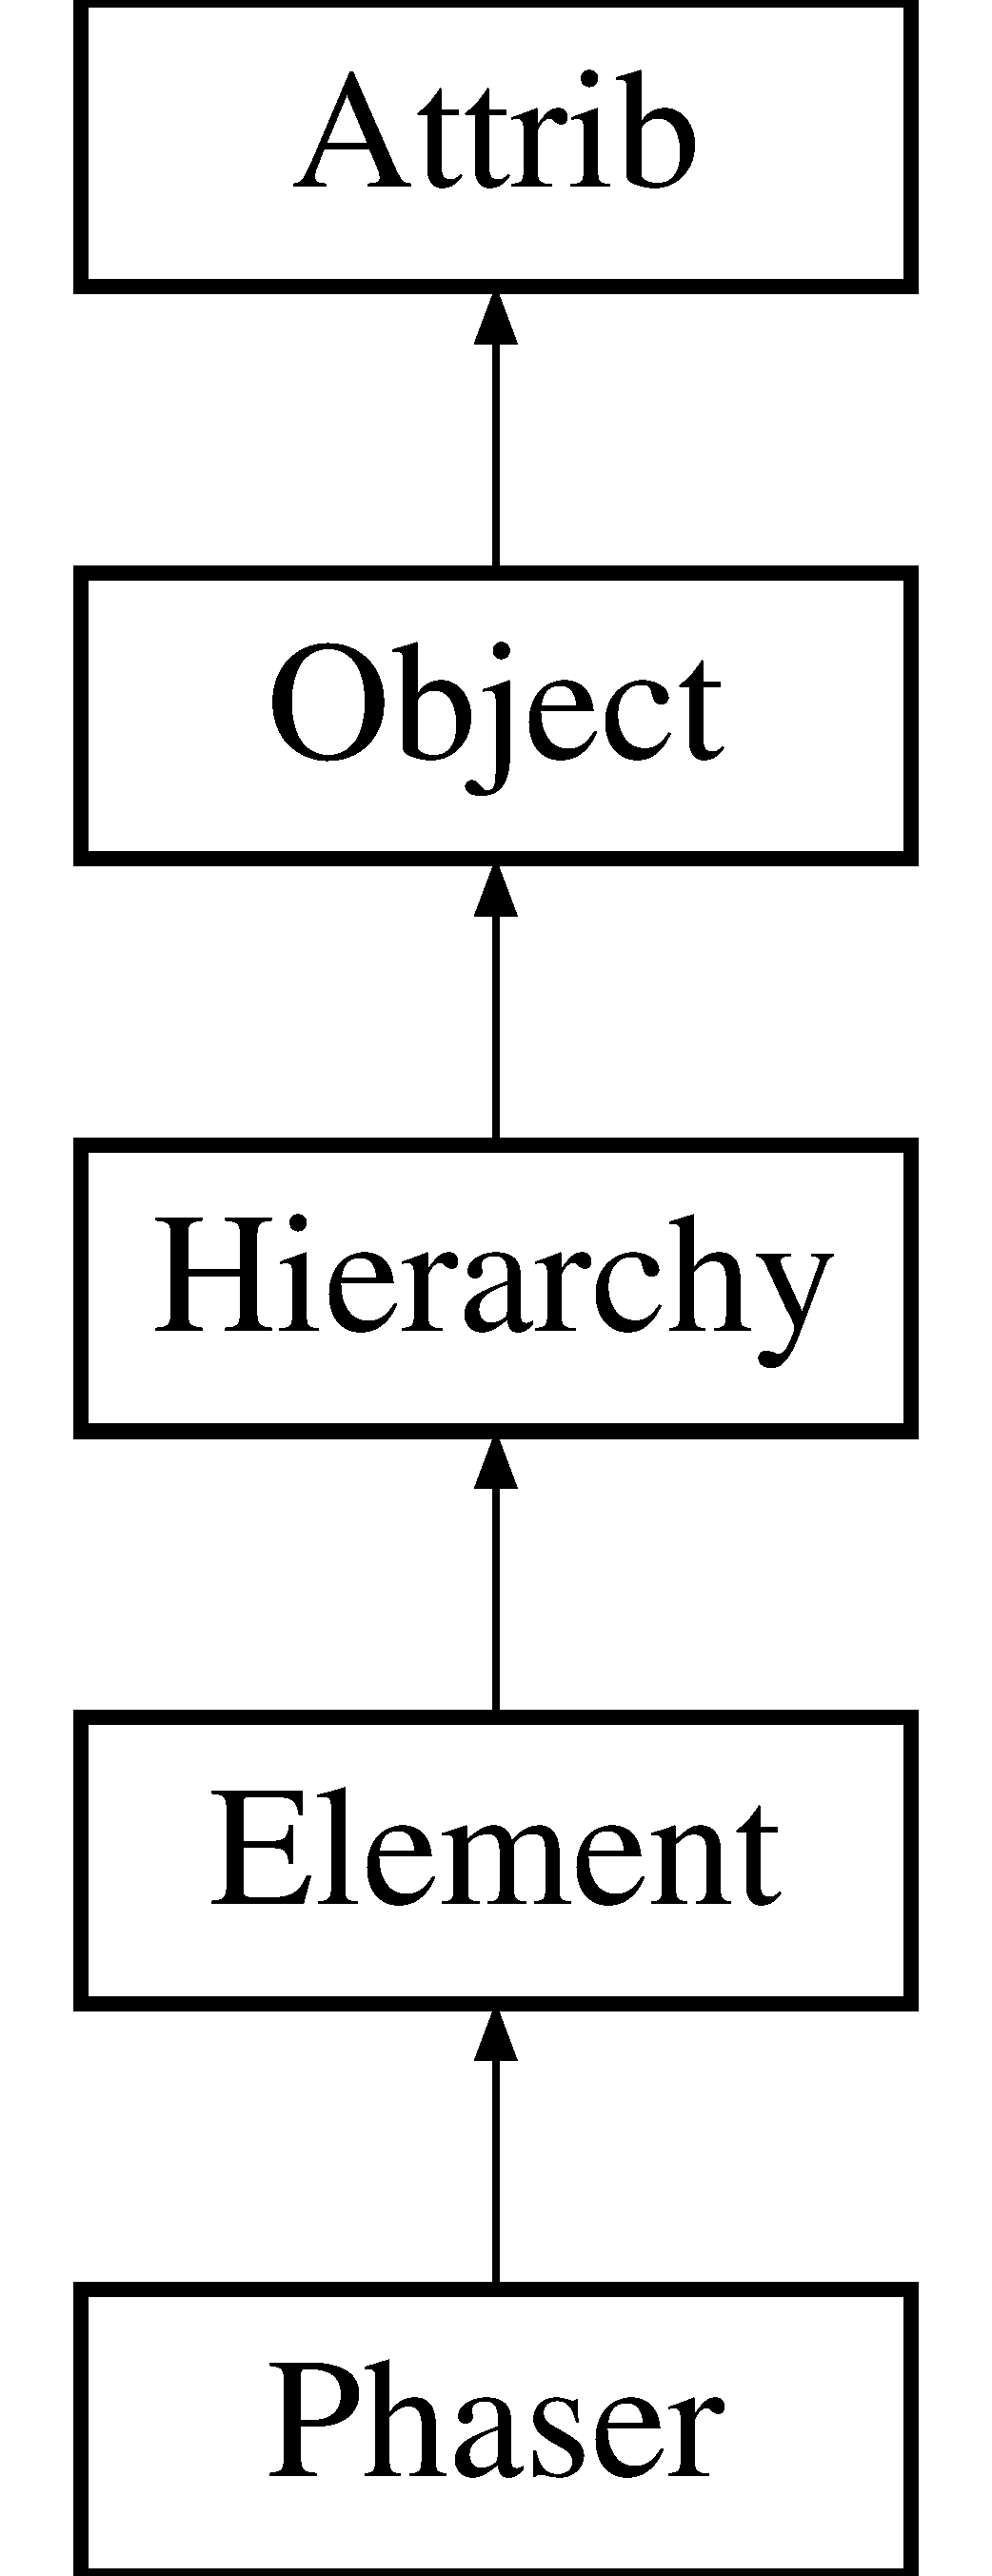
\includegraphics[height=5.000000cm]{classPhaser}
\end{center}
\end{figure}
\subsection*{Public Types}
\begin{DoxyCompactItemize}
\item 
typedef unsigned long \hyperlink{classPhaser_a733b5d40a397fc633db055248c76a23f}{U32}
\item 
typedef unsigned short \hyperlink{classPhaser_acadd65d66e8b38a16ad37a23834ee513}{U16}
\item 
typedef unsigned char \hyperlink{classPhaser_a09f745e43da83ab27286e69179755361}{U8}
\end{DoxyCompactItemize}
\subsection*{Public Member Functions}
\begin{DoxyCompactItemize}
\item 
\hyperlink{classPhaser_a849a7f7cd7d1491c490e4ba8e9906af0}{Phaser} ()
\item 
\hyperlink{classPhaser_a1facd3a2776130beb38792025fd8be20}{$\sim$\+Phaser} ()
\item 
void \hyperlink{classPhaser_a35c0add55885b3c0a7551ff48e322632}{set\+Phase} (unsigned char channel, unsigned char value)
\item 
void \hyperlink{classPhaser_a658be408ea31d55067e283723fa144f1}{set\+Phase} (unsigned char ch0, unsigned char ch1, unsigned char ch2, unsigned char ch3)
\item 
unsigned int \hyperlink{classPhaser_a3928ba4f1421c83b2f7783da87727ff2}{phase} (unsigned int ch)
\item 
void \hyperlink{classPhaser_a6ce0713403e961495192ffa0590c29e4}{read} ()
\item 
void \hyperlink{classPhaser_a7a94d4129a5f743c482fa97f3c5df68f}{write} ()
\item 
void \hyperlink{classPhaser_a0f122559297d076500420a7ceb21d70d}{help} ()
\item 
\hyperlink{classStatusCode}{Status\+Code} \hyperlink{classPhaser_a4691b8963a099f8a75475eb9be47a309}{init} ()
\item 
void \hyperlink{classPhaser_a0d15908b0d50f60f4ce6c6d013f75611}{reset} ()
\item 
void \hyperlink{classPhaser_ae1d1d3be2eed3973d269eab78834c594}{update} ()
\item 
\hyperlink{classRegister}{Register} $\ast$ \hyperlink{classPhaser_a3a4b64dc36e5f74292d9bec55da077a7}{reg} ()
\end{DoxyCompactItemize}
\subsection*{Private Attributes}
\begin{DoxyCompactItemize}
\item 
unsigned char \hyperlink{classPhaser_a8395e4279ce87dc816e02dd684a9fa3a}{m\+\_\+address}
\item 
unsigned char \hyperlink{classPhaser_a04df9ce4afe7a36ccaba5e5e727d504e}{m\+\_\+phase} \mbox{[}4\mbox{]}
\item 
\hyperlink{classRegister}{Register} $\ast$ \hyperlink{classPhaser_ab6d751d77cb1e39723a6ac85d4cfec0c}{m\+\_\+reg}
\end{DoxyCompactItemize}
\subsection*{Additional Inherited Members}


\subsection{Detailed Description}


Definition at line 19 of file Phaser.\+h.



\subsection{Member Typedef Documentation}
\mbox{\Hypertarget{classPhaser_acadd65d66e8b38a16ad37a23834ee513}\label{classPhaser_acadd65d66e8b38a16ad37a23834ee513}} 
\index{Phaser@{Phaser}!U16@{U16}}
\index{U16@{U16}!Phaser@{Phaser}}
\subsubsection{\texorpdfstring{U16}{U16}}
{\footnotesize\ttfamily typedef unsigned short \hyperlink{classPhaser_acadd65d66e8b38a16ad37a23834ee513}{Phaser\+::\+U16}}



Definition at line 22 of file Phaser.\+h.

\mbox{\Hypertarget{classPhaser_a733b5d40a397fc633db055248c76a23f}\label{classPhaser_a733b5d40a397fc633db055248c76a23f}} 
\index{Phaser@{Phaser}!U32@{U32}}
\index{U32@{U32}!Phaser@{Phaser}}
\subsubsection{\texorpdfstring{U32}{U32}}
{\footnotesize\ttfamily typedef unsigned long \hyperlink{classPhaser_a733b5d40a397fc633db055248c76a23f}{Phaser\+::\+U32}}



Definition at line 21 of file Phaser.\+h.

\mbox{\Hypertarget{classPhaser_a09f745e43da83ab27286e69179755361}\label{classPhaser_a09f745e43da83ab27286e69179755361}} 
\index{Phaser@{Phaser}!U8@{U8}}
\index{U8@{U8}!Phaser@{Phaser}}
\subsubsection{\texorpdfstring{U8}{U8}}
{\footnotesize\ttfamily typedef unsigned char \hyperlink{classPhaser_a09f745e43da83ab27286e69179755361}{Phaser\+::\+U8}}



Definition at line 23 of file Phaser.\+h.



\subsection{Constructor \& Destructor Documentation}
\mbox{\Hypertarget{classPhaser_a849a7f7cd7d1491c490e4ba8e9906af0}\label{classPhaser_a849a7f7cd7d1491c490e4ba8e9906af0}} 
\index{Phaser@{Phaser}!Phaser@{Phaser}}
\index{Phaser@{Phaser}!Phaser@{Phaser}}
\subsubsection{\texorpdfstring{Phaser()}{Phaser()}}
{\footnotesize\ttfamily Phaser\+::\+Phaser (\begin{DoxyParamCaption}{ }\end{DoxyParamCaption})\hspace{0.3cm}{\ttfamily [inline]}}



Definition at line 24 of file Phaser.\+h.



References Attrib\+::add(), Hierarchy\+::add\+Child(), Object\+::debug(), I\+Odata\+::def\+Data\+U8(), Attrib\+::\+E\+L\+E\+M\+E\+NT, Attrib\+::\+H\+A\+R\+D\+W\+A\+RE, I\+Oobject\+::io(), m\+\_\+phase, m\+\_\+reg, Object\+::set\+Id(), and Object\+::set\+Type().


\begin{DoxyCode}
24           \{
25     \hyperlink{classObject_aae534cc9d982bcb9b99fd505f2e103a5}{setType}(\textcolor{stringliteral}{"Phaser"});
26     \hyperlink{classObject_a398fe08cba594a0ce6891d59fe4f159f}{setId}(0);
27     \hyperlink{classAttrib_a235f773af19c900264a190b00a3b4ad7}{add}(\hyperlink{classAttrib_a69e171d7cc6417835a5a306d3c764235a7788bc5dd333fd8ce18562b269c9dab1}{Attrib::ELEMENT}); \hyperlink{classAttrib_a235f773af19c900264a190b00a3b4ad7}{add} (\hyperlink{classAttrib_a69e171d7cc6417835a5a306d3c764235a61ceb22149f365f1780d18f9d1459423}{Attrib::HARDWARE});
28     \hyperlink{classObject_aac010553f022165573714b7014a15f0d}{debug}(\textcolor{stringliteral}{"Phaser built."},\textcolor{stringliteral}{"Phaser::Phaser"});
29     \hyperlink{classPhaser_a04df9ce4afe7a36ccaba5e5e727d504e}{m\_phase}[0]=99;
30     \hyperlink{classPhaser_a04df9ce4afe7a36ccaba5e5e727d504e}{m\_phase}[1]=99;
31     \hyperlink{classPhaser_a04df9ce4afe7a36ccaba5e5e727d504e}{m\_phase}[2]=99;
32     \hyperlink{classPhaser_a04df9ce4afe7a36ccaba5e5e727d504e}{m\_phase}[3]=99;
33     \hyperlink{classPhaser_ab6d751d77cb1e39723a6ac85d4cfec0c}{m\_reg}=\textcolor{keyword}{new} \hyperlink{classRegister}{Register}();
34     \hyperlink{classPhaser_ab6d751d77cb1e39723a6ac85d4cfec0c}{m\_reg}->\hyperlink{classIOobject_af04fb94137c3d86849f478ac5afab5d1}{io}()->\hyperlink{classIOdata_a80bb230b61062b447db5832e43bf7b44}{defDataU8}(3);
35     \hyperlink{classHierarchy_ad677774ff38fcb257c04a3a10d471fac}{addChild}(\hyperlink{classPhaser_ab6d751d77cb1e39723a6ac85d4cfec0c}{m\_reg});
36   \}
\end{DoxyCode}
\mbox{\Hypertarget{classPhaser_a1facd3a2776130beb38792025fd8be20}\label{classPhaser_a1facd3a2776130beb38792025fd8be20}} 
\index{Phaser@{Phaser}!````~Phaser@{$\sim$\+Phaser}}
\index{````~Phaser@{$\sim$\+Phaser}!Phaser@{Phaser}}
\subsubsection{\texorpdfstring{$\sim$\+Phaser()}{~Phaser()}}
{\footnotesize\ttfamily Phaser\+::$\sim$\+Phaser (\begin{DoxyParamCaption}{ }\end{DoxyParamCaption})\hspace{0.3cm}{\ttfamily [inline]}}



Definition at line 38 of file Phaser.\+h.


\begin{DoxyCode}
38            \{
39 \textcolor{comment}{//    delete m\_reg;}
40   \}
\end{DoxyCode}


\subsection{Member Function Documentation}
\mbox{\Hypertarget{classPhaser_a0f122559297d076500420a7ceb21d70d}\label{classPhaser_a0f122559297d076500420a7ceb21d70d}} 
\index{Phaser@{Phaser}!help@{help}}
\index{help@{help}!Phaser@{Phaser}}
\subsubsection{\texorpdfstring{help()}{help()}}
{\footnotesize\ttfamily void Phaser\+::help (\begin{DoxyParamCaption}{ }\end{DoxyParamCaption})\hspace{0.3cm}{\ttfamily [inline]}, {\ttfamily [virtual]}}

printout help for the element 

Implements \hyperlink{classElement_a32c0de27acb08e17251cef88c3e9303a}{Element}.



Definition at line 74 of file Phaser.\+h.



References Object\+::info(), and Object\+::name().


\begin{DoxyCode}
74 \{ \hyperlink{classObject_a644fd329ea4cb85f54fa6846484b84a8}{info}(\textcolor{stringliteral}{"Phaser "}+\hyperlink{classObject_a300f4c05dd468c7bb8b3c968868443c1}{name}()+\textcolor{stringliteral}{". No help."},\textcolor{stringliteral}{"Phaser::help"}); \};
\end{DoxyCode}
\mbox{\Hypertarget{classPhaser_a4691b8963a099f8a75475eb9be47a309}\label{classPhaser_a4691b8963a099f8a75475eb9be47a309}} 
\index{Phaser@{Phaser}!init@{init}}
\index{init@{init}!Phaser@{Phaser}}
\subsubsection{\texorpdfstring{init()}{init()}}
{\footnotesize\ttfamily \hyperlink{classStatusCode}{Status\+Code} Phaser\+::init (\begin{DoxyParamCaption}{ }\end{DoxyParamCaption})\hspace{0.3cm}{\ttfamily [inline]}, {\ttfamily [virtual]}}

init the component

\begin{DoxyReturn}{Returns}
void 
\end{DoxyReturn}


Implements \hyperlink{classElement_af42754b5cabc198869222725218d695c}{Element}.



Definition at line 80 of file Phaser.\+h.



References Status\+Code\+::\+S\+U\+C\+C\+E\+SS.


\begin{DoxyCode}
80                     \{
81     \textcolor{keywordflow}{return} \hyperlink{classStatusCode_a6f565cbeadc76d14c72f047e5e85eb4badd0da38d3ba0d922efd1f4619bc37ad8}{StatusCode::SUCCESS};
82   \};
\end{DoxyCode}
\mbox{\Hypertarget{classPhaser_a3928ba4f1421c83b2f7783da87727ff2}\label{classPhaser_a3928ba4f1421c83b2f7783da87727ff2}} 
\index{Phaser@{Phaser}!phase@{phase}}
\index{phase@{phase}!Phaser@{Phaser}}
\subsubsection{\texorpdfstring{phase()}{phase()}}
{\footnotesize\ttfamily unsigned int Phaser\+::phase (\begin{DoxyParamCaption}\item[{unsigned int}]{ch }\end{DoxyParamCaption})\hspace{0.3cm}{\ttfamily [inline]}}



Definition at line 63 of file Phaser.\+h.



References m\+\_\+phase, read(), and write().



Referenced by B\+O\+O\+S\+T\+\_\+\+P\+Y\+T\+H\+O\+N\+\_\+\+M\+O\+D\+U\+L\+E(), Phaser\+Ramp\+Exec\+::execute(), and Phaser\+Ramp\+Exec\+::initialize().


\begin{DoxyCode}
63                                      \{
64     \hyperlink{classPhaser_a6ce0713403e961495192ffa0590c29e4}{read}() ;
65     \textcolor{keywordflow}{return} \hyperlink{classPhaser_a04df9ce4afe7a36ccaba5e5e727d504e}{m\_phase}[ch];
66   \}
\end{DoxyCode}
\mbox{\Hypertarget{classPhaser_a6ce0713403e961495192ffa0590c29e4}\label{classPhaser_a6ce0713403e961495192ffa0590c29e4}} 
\index{Phaser@{Phaser}!read@{read}}
\index{read@{read}!Phaser@{Phaser}}
\subsubsection{\texorpdfstring{read()}{read()}}
{\footnotesize\ttfamily void Phaser\+::read (\begin{DoxyParamCaption}{ }\end{DoxyParamCaption})}



Definition at line 23 of file Phaser.\+cpp.



References I\+Odata\+::data\+U8(), Object\+::debug(), I\+Oobject\+::io(), Status\+Code\+::is\+Failure(), itos(), m\+\_\+phase, m\+\_\+reg, Object\+::name(), I\+Oobject\+::read(), and Object\+::warning().



Referenced by B\+O\+O\+S\+T\+\_\+\+P\+Y\+T\+H\+O\+N\+\_\+\+M\+O\+D\+U\+L\+E(), Phaser\+Ramp\+Exec\+::execute(), Phaser\+Ramp\+Exec\+::initialize(), phase(), and update().


\begin{DoxyCode}
23                   \{
24   \textcolor{keywordflow}{if} (\hyperlink{classPhaser_ab6d751d77cb1e39723a6ac85d4cfec0c}{m\_reg}->\hyperlink{classIOobject_aa07610c11963b1db6710e3c76ceea456}{read}().\hyperlink{classStatusCode_a5dd22dc6eb2c52fc4cabc58f6dea2eb7}{isFailure}())\{
25     \hyperlink{classObject_a65cd4fda577711660821fd2cd5a3b4c9}{warning}(\textcolor{stringliteral}{"Phaser register read failure."},\textcolor{stringliteral}{"Phaser::read"});
26   \}
27   \textcolor{keywordflow}{else} \{
28     \hyperlink{ICECALv3_8h_a3cb25ca6f51f003950f9625ff05536fc}{U8}* buffer=\hyperlink{classPhaser_ab6d751d77cb1e39723a6ac85d4cfec0c}{m\_reg}->\hyperlink{classIOobject_af04fb94137c3d86849f478ac5afab5d1}{io}()->\hyperlink{classIOdata_a75e9c318dbac3a39402179070943d4bc}{dataU8}();
29     \textcolor{keywordtype}{unsigned} \textcolor{keywordtype}{int} d0 = (  buffer[0] & 0x1F );
30     \textcolor{keywordtype}{unsigned} \textcolor{keywordtype}{int} d1 = (( buffer[0] & 0xE0 ) >> 5 ) | (( buffer[1] & 0x3 ) << 3 );
31     \textcolor{keywordtype}{unsigned} \textcolor{keywordtype}{int} d2 = (( buffer[1] >> 2 ) & 0x1F );
32     \textcolor{keywordtype}{unsigned} \textcolor{keywordtype}{int} d3 = (( buffer[1] >> 7 ) & 0x1 )  | ((buffer[2] & 0xF) << 1);
33     \hyperlink{classObject_aac010553f022165573714b7014a15f0d}{debug}(\textcolor{stringliteral}{"reading "}+\hyperlink{classObject_a300f4c05dd468c7bb8b3c968868443c1}{name}()+\textcolor{stringliteral}{" phases : "}+
34         \hyperlink{Tools_8h_af330027dbdafb9a30768b3613c553e60}{itos}(d0)+\textcolor{stringliteral}{" "}+
35         \hyperlink{Tools_8h_af330027dbdafb9a30768b3613c553e60}{itos}(d1)+\textcolor{stringliteral}{" "}+
36         \hyperlink{Tools_8h_af330027dbdafb9a30768b3613c553e60}{itos}(d2)+\textcolor{stringliteral}{" "}+
37         \hyperlink{Tools_8h_af330027dbdafb9a30768b3613c553e60}{itos}(d3),
38         \textcolor{stringliteral}{"Phaser::read"});
39     \hyperlink{classPhaser_a04df9ce4afe7a36ccaba5e5e727d504e}{m\_phase}[0]=d0;
40     \hyperlink{classPhaser_a04df9ce4afe7a36ccaba5e5e727d504e}{m\_phase}[1]=d1;
41     \hyperlink{classPhaser_a04df9ce4afe7a36ccaba5e5e727d504e}{m\_phase}[2]=d2;
42     \hyperlink{classPhaser_a04df9ce4afe7a36ccaba5e5e727d504e}{m\_phase}[3]=d3;
43   \}
44 \}
\end{DoxyCode}
\mbox{\Hypertarget{classPhaser_a3a4b64dc36e5f74292d9bec55da077a7}\label{classPhaser_a3a4b64dc36e5f74292d9bec55da077a7}} 
\index{Phaser@{Phaser}!reg@{reg}}
\index{reg@{reg}!Phaser@{Phaser}}
\subsubsection{\texorpdfstring{reg()}{reg()}}
{\footnotesize\ttfamily \hyperlink{classRegister}{Register}$\ast$ Phaser\+::reg (\begin{DoxyParamCaption}{ }\end{DoxyParamCaption})\hspace{0.3cm}{\ttfamily [inline]}}



Definition at line 101 of file Phaser.\+h.



References m\+\_\+reg.



Referenced by B\+O\+O\+S\+T\+\_\+\+P\+Y\+T\+H\+O\+N\+\_\+\+M\+O\+D\+U\+L\+E(), and Proto40\+M\+Hz\+\_\+v1\+::\+Proto40\+M\+Hz\+\_\+v1().


\begin{DoxyCode}
101                  \{
102     \textcolor{keywordflow}{return} \hyperlink{classPhaser_ab6d751d77cb1e39723a6ac85d4cfec0c}{m\_reg};
103   \}
\end{DoxyCode}
\mbox{\Hypertarget{classPhaser_a0d15908b0d50f60f4ce6c6d013f75611}\label{classPhaser_a0d15908b0d50f60f4ce6c6d013f75611}} 
\index{Phaser@{Phaser}!reset@{reset}}
\index{reset@{reset}!Phaser@{Phaser}}
\subsubsection{\texorpdfstring{reset()}{reset()}}
{\footnotesize\ttfamily void Phaser\+::reset (\begin{DoxyParamCaption}{ }\end{DoxyParamCaption})\hspace{0.3cm}{\ttfamily [inline]}, {\ttfamily [virtual]}}

Resets the \hyperlink{classElement}{Element} so that is is in a standard and safe situation. Different from \hyperlink{classElement_af42754b5cabc198869222725218d695c}{Element\+::init} which configure the \hyperlink{classElement}{Element}. \hyperlink{classElement_a69efffa22f06909d768149715565cb56}{Element\+::reset()} is more an Emergency pull. It is often/usually called by the recursive\+Init\+Element method at the start of the program. 

Implements \hyperlink{classElement_a69efffa22f06909d768149715565cb56}{Element}.



Definition at line 91 of file Phaser.\+h.


\begin{DoxyCode}
91                \{
92   \};
\end{DoxyCode}
\mbox{\Hypertarget{classPhaser_a35c0add55885b3c0a7551ff48e322632}\label{classPhaser_a35c0add55885b3c0a7551ff48e322632}} 
\index{Phaser@{Phaser}!set\+Phase@{set\+Phase}}
\index{set\+Phase@{set\+Phase}!Phaser@{Phaser}}
\subsubsection{\texorpdfstring{set\+Phase()}{setPhase()}\hspace{0.1cm}{\footnotesize\ttfamily [1/2]}}
{\footnotesize\ttfamily void Phaser\+::set\+Phase (\begin{DoxyParamCaption}\item[{unsigned char}]{channel,  }\item[{unsigned char}]{value }\end{DoxyParamCaption})\hspace{0.3cm}{\ttfamily [inline]}}



Definition at line 42 of file Phaser.\+h.



References Object\+::info(), itos(), m\+\_\+phase, and write().



Referenced by B\+O\+O\+S\+T\+\_\+\+P\+Y\+T\+H\+O\+N\+\_\+\+M\+O\+D\+U\+L\+E(), Phaser\+Ramp\+Exec\+::execute(), and Phaser\+Ramp\+Exec\+::finalize().


\begin{DoxyCode}
42                                                            \{
43     \hyperlink{classObject_a644fd329ea4cb85f54fa6846484b84a8}{info}(\textcolor{stringliteral}{"Set Phase "}+\hyperlink{Tools_8h_af330027dbdafb9a30768b3613c553e60}{itos}(channel)+\textcolor{stringliteral}{" to "}+\hyperlink{Tools_8h_af330027dbdafb9a30768b3613c553e60}{itos}(value),\textcolor{stringliteral}{"Phaser::setPhase"});
44     \hyperlink{classPhaser_a04df9ce4afe7a36ccaba5e5e727d504e}{m\_phase}[channel]=value;
45     \hyperlink{classPhaser_a7a94d4129a5f743c482fa97f3c5df68f}{write}();
46   \}
\end{DoxyCode}
\mbox{\Hypertarget{classPhaser_a658be408ea31d55067e283723fa144f1}\label{classPhaser_a658be408ea31d55067e283723fa144f1}} 
\index{Phaser@{Phaser}!set\+Phase@{set\+Phase}}
\index{set\+Phase@{set\+Phase}!Phaser@{Phaser}}
\subsubsection{\texorpdfstring{set\+Phase()}{setPhase()}\hspace{0.1cm}{\footnotesize\ttfamily [2/2]}}
{\footnotesize\ttfamily void Phaser\+::set\+Phase (\begin{DoxyParamCaption}\item[{unsigned char}]{ch0,  }\item[{unsigned char}]{ch1,  }\item[{unsigned char}]{ch2,  }\item[{unsigned char}]{ch3 }\end{DoxyParamCaption})\hspace{0.3cm}{\ttfamily [inline]}}



Definition at line 48 of file Phaser.\+h.



References Object\+::info(), itos(), m\+\_\+phase, and write().


\begin{DoxyCode}
53        \{
54     \hyperlink{classPhaser_a04df9ce4afe7a36ccaba5e5e727d504e}{m\_phase}[0]=ch0;
55     \hyperlink{classPhaser_a04df9ce4afe7a36ccaba5e5e727d504e}{m\_phase}[1]=ch1;
56     \hyperlink{classPhaser_a04df9ce4afe7a36ccaba5e5e727d504e}{m\_phase}[2]=ch2;
57     \hyperlink{classPhaser_a04df9ce4afe7a36ccaba5e5e727d504e}{m\_phase}[3]=ch3;
58     \hyperlink{classObject_a644fd329ea4cb85f54fa6846484b84a8}{info}(\textcolor{stringliteral}{"Set Phases to "}+\hyperlink{Tools_8h_af330027dbdafb9a30768b3613c553e60}{itos}(ch0)+\textcolor{stringliteral}{" "}+\hyperlink{Tools_8h_af330027dbdafb9a30768b3613c553e60}{itos}(ch1)+\textcolor{stringliteral}{" "}
59         +\hyperlink{Tools_8h_af330027dbdafb9a30768b3613c553e60}{itos}(ch2)+\textcolor{stringliteral}{" "}+\hyperlink{Tools_8h_af330027dbdafb9a30768b3613c553e60}{itos}(ch3));
60     \hyperlink{classPhaser_a7a94d4129a5f743c482fa97f3c5df68f}{write}();
61   \}
\end{DoxyCode}
\mbox{\Hypertarget{classPhaser_ae1d1d3be2eed3973d269eab78834c594}\label{classPhaser_ae1d1d3be2eed3973d269eab78834c594}} 
\index{Phaser@{Phaser}!update@{update}}
\index{update@{update}!Phaser@{Phaser}}
\subsubsection{\texorpdfstring{update()}{update()}}
{\footnotesize\ttfamily void Phaser\+::update (\begin{DoxyParamCaption}{ }\end{DoxyParamCaption})\hspace{0.3cm}{\ttfamily [inline]}, {\ttfamily [virtual]}}

Update the \hyperlink{classElement}{Element} configuration from the actual hardware 

Implements \hyperlink{classElement_a4e6c83efae95616ebddd03c793a26661}{Element}.



Definition at line 97 of file Phaser.\+h.



References read().



Referenced by A3\+P\+E\+\_\+\+Bit\+Flip.\+A3\+P\+E\+\_\+\+Bit\+Flip\+::\+\_\+\+\_\+init\+\_\+\+\_\+(), Acquisition.\+Acquisition\+::\+\_\+\+\_\+init\+\_\+\+\_\+(), Emulate\+F\+E.\+Emulate\+F\+E\+::\+\_\+\+\_\+init\+\_\+\+\_\+(), App\+Frame.\+App\+Frame\+::delete\+Hardware(), Conf\+Frame.\+Conf\+Frame\+::on\+Change(), Graph\+Frame.\+Graph\+Frame\+::on\+Change(), Cfg\+Frame.\+Cfg\+Frame\+::on\+Change(), Conf\+Frame.\+Conf\+Frame\+::on\+Edit(), App\+Frame.\+App\+Frame\+::on\+Load(), Conf\+Frame.\+Conf\+Frame\+::on\+Re\+Load(), Graph\+Frame.\+Graph\+Frame\+::on\+Re\+Load(), Cfg\+Frame.\+Cfg\+Frame\+::on\+Re\+Load(), and App\+Frame.\+App\+Frame\+::on\+Re\+Load().


\begin{DoxyCode}
97                  \{
98     \hyperlink{classPhaser_a6ce0713403e961495192ffa0590c29e4}{read}();
99   \};
\end{DoxyCode}
\mbox{\Hypertarget{classPhaser_a7a94d4129a5f743c482fa97f3c5df68f}\label{classPhaser_a7a94d4129a5f743c482fa97f3c5df68f}} 
\index{Phaser@{Phaser}!write@{write}}
\index{write@{write}!Phaser@{Phaser}}
\subsubsection{\texorpdfstring{write()}{write()}}
{\footnotesize\ttfamily void Phaser\+::write (\begin{DoxyParamCaption}{ }\end{DoxyParamCaption})}



Definition at line 46 of file Phaser.\+cpp.



References I\+Odata\+::data\+U8(), Object\+::debug(), I\+Oobject\+::io(), Status\+Code\+::is\+Failure(), itos(), m\+\_\+phase, m\+\_\+reg, Object\+::name(), Object\+::warning(), and I\+Oobject\+::write().



Referenced by B\+O\+O\+S\+T\+\_\+\+P\+Y\+T\+H\+O\+N\+\_\+\+M\+O\+D\+U\+L\+E(), Phaser\+Ramp\+Exec\+::execute(), Phaser\+Ramp\+Exec\+::finalize(), phase(), and set\+Phase().


\begin{DoxyCode}
46                   \{
47   \hyperlink{ICECALv3_8h_a3cb25ca6f51f003950f9625ff05536fc}{U8}* buffer=\hyperlink{classPhaser_ab6d751d77cb1e39723a6ac85d4cfec0c}{m\_reg}->\hyperlink{classIOobject_af04fb94137c3d86849f478ac5afab5d1}{io}()->\hyperlink{classIOdata_a75e9c318dbac3a39402179070943d4bc}{dataU8}();
48   buffer[0]=(\hyperlink{classPhaser_a04df9ce4afe7a36ccaba5e5e727d504e}{m\_phase}[0] & 0x1F) | ((\hyperlink{classPhaser_a04df9ce4afe7a36ccaba5e5e727d504e}{m\_phase}[1] & 0x7)<<5);
49   buffer[1]=((\hyperlink{classPhaser_a04df9ce4afe7a36ccaba5e5e727d504e}{m\_phase}[1]>>3)& 0x3) |
50       ((\hyperlink{classPhaser_a04df9ce4afe7a36ccaba5e5e727d504e}{m\_phase}[2]& 0x1F)<<2) |
51       ((\hyperlink{classPhaser_a04df9ce4afe7a36ccaba5e5e727d504e}{m\_phase}[3]&0x1)<<7);
52   buffer[2]=(\hyperlink{classPhaser_a04df9ce4afe7a36ccaba5e5e727d504e}{m\_phase}[3]>>1)&0xF;
53   \hyperlink{classObject_aac010553f022165573714b7014a15f0d}{debug}(\textcolor{stringliteral}{"setting "}+\hyperlink{classObject_a300f4c05dd468c7bb8b3c968868443c1}{name}()+\textcolor{stringliteral}{" phases : "}+\hyperlink{Tools_8h_af330027dbdafb9a30768b3613c553e60}{itos}(\hyperlink{classPhaser_a04df9ce4afe7a36ccaba5e5e727d504e}{m\_phase}[0])+\textcolor{stringliteral}{" "}+
54       \hyperlink{Tools_8h_af330027dbdafb9a30768b3613c553e60}{itos}(\hyperlink{classPhaser_a04df9ce4afe7a36ccaba5e5e727d504e}{m\_phase}[1])+\textcolor{stringliteral}{" "}+\hyperlink{Tools_8h_af330027dbdafb9a30768b3613c553e60}{itos}(\hyperlink{classPhaser_a04df9ce4afe7a36ccaba5e5e727d504e}{m\_phase}[2])+\textcolor{stringliteral}{" "}+\hyperlink{Tools_8h_af330027dbdafb9a30768b3613c553e60}{itos}(
      \hyperlink{classPhaser_a04df9ce4afe7a36ccaba5e5e727d504e}{m\_phase}[3]),
55       \textcolor{stringliteral}{"Phaser::write"});
56   \textcolor{keywordflow}{if} (\hyperlink{classPhaser_ab6d751d77cb1e39723a6ac85d4cfec0c}{m\_reg}->\hyperlink{classIOobject_a9f6984bc9f0fadcf800f1be2523ac744}{write}().\hyperlink{classStatusCode_a5dd22dc6eb2c52fc4cabc58f6dea2eb7}{isFailure}())\{
57     \hyperlink{classObject_a65cd4fda577711660821fd2cd5a3b4c9}{warning}(\textcolor{stringliteral}{"Phaser register write failure."},\textcolor{stringliteral}{"Phaser::write"});
58   \}
59 \}
\end{DoxyCode}


\subsection{Member Data Documentation}
\mbox{\Hypertarget{classPhaser_a8395e4279ce87dc816e02dd684a9fa3a}\label{classPhaser_a8395e4279ce87dc816e02dd684a9fa3a}} 
\index{Phaser@{Phaser}!m\+\_\+address@{m\+\_\+address}}
\index{m\+\_\+address@{m\+\_\+address}!Phaser@{Phaser}}
\subsubsection{\texorpdfstring{m\+\_\+address}{m\_address}}
{\footnotesize\ttfamily unsigned char Phaser\+::m\+\_\+address\hspace{0.3cm}{\ttfamily [private]}}



Definition at line 106 of file Phaser.\+h.

\mbox{\Hypertarget{classPhaser_a04df9ce4afe7a36ccaba5e5e727d504e}\label{classPhaser_a04df9ce4afe7a36ccaba5e5e727d504e}} 
\index{Phaser@{Phaser}!m\+\_\+phase@{m\+\_\+phase}}
\index{m\+\_\+phase@{m\+\_\+phase}!Phaser@{Phaser}}
\subsubsection{\texorpdfstring{m\+\_\+phase}{m\_phase}}
{\footnotesize\ttfamily unsigned char Phaser\+::m\+\_\+phase\mbox{[}4\mbox{]}\hspace{0.3cm}{\ttfamily [private]}}



Definition at line 107 of file Phaser.\+h.



Referenced by phase(), Phaser(), read(), set\+Phase(), and write().

\mbox{\Hypertarget{classPhaser_ab6d751d77cb1e39723a6ac85d4cfec0c}\label{classPhaser_ab6d751d77cb1e39723a6ac85d4cfec0c}} 
\index{Phaser@{Phaser}!m\+\_\+reg@{m\+\_\+reg}}
\index{m\+\_\+reg@{m\+\_\+reg}!Phaser@{Phaser}}
\subsubsection{\texorpdfstring{m\+\_\+reg}{m\_reg}}
{\footnotesize\ttfamily \hyperlink{classRegister}{Register}$\ast$ Phaser\+::m\+\_\+reg\hspace{0.3cm}{\ttfamily [private]}}



Definition at line 108 of file Phaser.\+h.



Referenced by Phaser(), read(), reg(), and write().



The documentation for this class was generated from the following files\+:\begin{DoxyCompactItemize}
\item 
/home/eleclhcb/\+L\+H\+Cb/lbcat-\/cmake/\+Cat\+Calo/inc/\hyperlink{Phaser_8h}{Phaser.\+h}\item 
/home/eleclhcb/\+L\+H\+Cb/lbcat-\/cmake/\+Cat\+Calo/src/\hyperlink{Phaser_8cpp}{Phaser.\+cpp}\end{DoxyCompactItemize}

\hypertarget{classPhaserRampExec}{}\section{Phaser\+Ramp\+Exec Class Reference}
\label{classPhaserRampExec}\index{Phaser\+Ramp\+Exec@{Phaser\+Ramp\+Exec}}


{\ttfamily \#include $<$include/\+Phaser\+Ramp\+Exec.\+h$>$}

Inheritance diagram for Phaser\+Ramp\+Exec\+:\begin{figure}[H]
\begin{center}
\leavevmode
\includegraphics[height=4.000000cm]{classPhaserRampExec}
\end{center}
\end{figure}
\subsection*{Public Member Functions}
\begin{DoxyCompactItemize}
\item 
\hyperlink{classPhaserRampExec_a26f14f1c66dd37251374998ae0a4f02a}{Phaser\+Ramp\+Exec} ()
\begin{DoxyCompactList}\small\item\em Standard constructor. \end{DoxyCompactList}\item 
virtual \hyperlink{classPhaserRampExec_a0ea95adf577ff47f09068a20329f1598}{$\sim$\+Phaser\+Ramp\+Exec} ()
\begin{DoxyCompactList}\small\item\em Destructor. \end{DoxyCompactList}\item 
virtual \hyperlink{classStatusCode}{Status\+Code} \hyperlink{classPhaserRampExec_ae6f90f2ecf4b66d6f9bc85b123587ef3}{initialize} ()
\item 
virtual \hyperlink{classStatusCode}{Status\+Code} \hyperlink{classPhaserRampExec_a5fccbd3cddf738318f9d45d64b723907}{execute} ()
\item 
virtual \hyperlink{classStatusCode}{Status\+Code} \hyperlink{classPhaserRampExec_a8849cacdd34e7ca56f6d5e7668fe8c6c}{finalize} ()
\end{DoxyCompactItemize}
\subsection*{Protected Member Functions}
\begin{DoxyCompactItemize}
\item 
\hyperlink{classPhaserRampExec}{Phaser\+Ramp\+Exec} $\ast$ \hyperlink{classPhaserRampExec_a2586b2209d381c5b82a13dc2f997925f}{clone} ()
\end{DoxyCompactItemize}
\subsection*{Private Attributes}
\begin{DoxyCompactItemize}
\item 
\hyperlink{classPhaser}{Phaser} $\ast$ \hyperlink{classPhaserRampExec_a3c187e98596d492f195c2743322e263b}{m\+\_\+phaser}
\item 
T\+H1D $\ast$ \hyperlink{classPhaserRampExec_a8c13c96564df17be4e71685684e67edd}{h1}
\item 
T\+H1D $\ast$ \hyperlink{classPhaserRampExec_a538d1b02ed14d13c71f54b2b48e765ba}{h2}
\item 
T\+H1D $\ast$ \hyperlink{classPhaserRampExec_ad9ec4185f676732648c4886f28c9c6b7}{h3}
\item 
T\+H1D $\ast$ \hyperlink{classPhaserRampExec_aa487df389ad66093dba562f27f558128}{h4}
\item 
T\+H1D $\ast$ \hyperlink{classPhaserRampExec_ad2a2a82a0be74bc39c84b580e33d9c34}{hv1}
\item 
T\+H1D $\ast$ \hyperlink{classPhaserRampExec_a9762fd546432b5f3dffc4c5323af56ac}{hv2}
\item 
T\+H1D $\ast$ \hyperlink{classPhaserRampExec_ad3127f38a360044f7ad8fed272f916f9}{hv3}
\item 
T\+H1D $\ast$ \hyperlink{classPhaserRampExec_a998b7e5a8d186df60c2d60cba2b43aa0}{hv4}
\item 
T\+File $\ast$ \hyperlink{classPhaserRampExec_a63092bcbec01af94b4c5c842b81d2ccf}{file}
\item 
T\+H1F $\ast$ \hyperlink{classPhaserRampExec_a0c8d1c3ee09159cba1b1a07ce3fb1d96}{histo}
\item 
int \hyperlink{classPhaserRampExec_a7526a42abb33e880d60570386fd23e3e}{m\+\_\+init\+Phase} \mbox{[}4\mbox{]}
\item 
unsigned long \hyperlink{classPhaserRampExec_a198ba1ebb9a1b0fb2c599405307e92af}{m\+\_\+n\+Processed\+Events}
\item 
unsigned long \hyperlink{classPhaserRampExec_a3f09b8bf4cd8f5425adf8ae168d39e50}{error\+Count}
\end{DoxyCompactItemize}
\subsection*{Additional Inherited Members}


\subsection{Detailed Description}
\begin{DoxyAuthor}{Author}
Frédéric Machefert 
\end{DoxyAuthor}
\begin{DoxyDate}{Date}
2004-\/07-\/23 
\end{DoxyDate}


Definition at line 26 of file Phaser\+Ramp\+Exec.\+h.



\subsection{Constructor \& Destructor Documentation}
\mbox{\Hypertarget{classPhaserRampExec_a26f14f1c66dd37251374998ae0a4f02a}\label{classPhaserRampExec_a26f14f1c66dd37251374998ae0a4f02a}} 
\index{Phaser\+Ramp\+Exec@{Phaser\+Ramp\+Exec}!Phaser\+Ramp\+Exec@{Phaser\+Ramp\+Exec}}
\index{Phaser\+Ramp\+Exec@{Phaser\+Ramp\+Exec}!Phaser\+Ramp\+Exec@{Phaser\+Ramp\+Exec}}
\subsubsection{\texorpdfstring{Phaser\+Ramp\+Exec()}{PhaserRampExec()}}
{\footnotesize\ttfamily Phaser\+Ramp\+Exec\+::\+Phaser\+Ramp\+Exec (\begin{DoxyParamCaption}{ }\end{DoxyParamCaption})}



Standard constructor. 



Definition at line 36 of file Phaser\+Ramp\+Exec.\+cpp.



References Object\+::set\+Name(), Object\+::set\+Title(), and Object\+::set\+Type().



Referenced by clone().


\begin{DoxyCode}
36                                  \{
37   \hyperlink{classObject_ae30fea75683c2d149b6b6d17c09ecd0c}{setName} ( \textcolor{stringliteral}{"PhaserRampExec"} );
38   \hyperlink{classObject_aae534cc9d982bcb9b99fd505f2e103a5}{setType} ( \textcolor{stringliteral}{"Phaser"} );
39   \hyperlink{classObject_a89557dbbad5bcaa02652f5d7fa35d20f}{setTitle}( \textcolor{stringliteral}{"Phaser I2C Configuration Test"} );
40 \}
\end{DoxyCode}
\mbox{\Hypertarget{classPhaserRampExec_a0ea95adf577ff47f09068a20329f1598}\label{classPhaserRampExec_a0ea95adf577ff47f09068a20329f1598}} 
\index{Phaser\+Ramp\+Exec@{Phaser\+Ramp\+Exec}!````~Phaser\+Ramp\+Exec@{$\sim$\+Phaser\+Ramp\+Exec}}
\index{````~Phaser\+Ramp\+Exec@{$\sim$\+Phaser\+Ramp\+Exec}!Phaser\+Ramp\+Exec@{Phaser\+Ramp\+Exec}}
\subsubsection{\texorpdfstring{$\sim$\+Phaser\+Ramp\+Exec()}{~PhaserRampExec()}}
{\footnotesize\ttfamily Phaser\+Ramp\+Exec\+::$\sim$\+Phaser\+Ramp\+Exec (\begin{DoxyParamCaption}{ }\end{DoxyParamCaption})\hspace{0.3cm}{\ttfamily [virtual]}}



Destructor. 



Definition at line 44 of file Phaser\+Ramp\+Exec.\+cpp.


\begin{DoxyCode}
44 \{\}
\end{DoxyCode}


\subsection{Member Function Documentation}
\mbox{\Hypertarget{classPhaserRampExec_a2586b2209d381c5b82a13dc2f997925f}\label{classPhaserRampExec_a2586b2209d381c5b82a13dc2f997925f}} 
\index{Phaser\+Ramp\+Exec@{Phaser\+Ramp\+Exec}!clone@{clone}}
\index{clone@{clone}!Phaser\+Ramp\+Exec@{Phaser\+Ramp\+Exec}}
\subsubsection{\texorpdfstring{clone()}{clone()}}
{\footnotesize\ttfamily \hyperlink{classPhaserRampExec}{Phaser\+Ramp\+Exec}$\ast$ Phaser\+Ramp\+Exec\+::clone (\begin{DoxyParamCaption}{ }\end{DoxyParamCaption})\hspace{0.3cm}{\ttfamily [inline]}, {\ttfamily [protected]}, {\ttfamily [virtual]}}

processus termination virtual function 

Implements \hyperlink{classProcessus_aca8856f6d6d7b7e1fe941f298dcbb502}{Processus}.



Definition at line 41 of file Phaser\+Ramp\+Exec.\+h.



References Phaser\+Ramp\+Exec().


\begin{DoxyCode}
41                          \{
42     \textcolor{keywordflow}{return} \textcolor{keyword}{new} \hyperlink{classPhaserRampExec_a26f14f1c66dd37251374998ae0a4f02a}{PhaserRampExec} (*\textcolor{keyword}{this});
43   \}
\end{DoxyCode}
\mbox{\Hypertarget{classPhaserRampExec_a5fccbd3cddf738318f9d45d64b723907}\label{classPhaserRampExec_a5fccbd3cddf738318f9d45d64b723907}} 
\index{Phaser\+Ramp\+Exec@{Phaser\+Ramp\+Exec}!execute@{execute}}
\index{execute@{execute}!Phaser\+Ramp\+Exec@{Phaser\+Ramp\+Exec}}
\subsubsection{\texorpdfstring{execute()}{execute()}}
{\footnotesize\ttfamily \hyperlink{classStatusCode}{Status\+Code} Phaser\+Ramp\+Exec\+::execute (\begin{DoxyParamCaption}{ }\end{DoxyParamCaption})\hspace{0.3cm}{\ttfamily [virtual]}}

processus execution virtual function 

Implements \hyperlink{classProcessus_a63767a63a1fb0055c5aa45b21a4a5d58}{Processus}.



Definition at line 90 of file Phaser\+Ramp\+Exec.\+cpp.



References error\+Count, h1, h2, h3, h4, hv1, hv2, hv3, hv4, Object\+::info(), itos(), m\+\_\+n\+Processed\+Events, m\+\_\+phaser, Phaser\+::phase(), Phaser\+::read(), Phaser\+::set\+Phase(), Status\+Code\+::\+S\+U\+C\+C\+E\+SS, and Phaser\+::write().



Referenced by B\+O\+O\+S\+T\+\_\+\+P\+Y\+T\+H\+O\+N\+\_\+\+M\+O\+D\+U\+L\+E().


\begin{DoxyCode}
90                                      \{ 
91 
92   \hyperlink{classPhaserRampExec_a198ba1ebb9a1b0fb2c599405307e92af}{m\_nProcessedEvents}++;
93   
94   \textcolor{keywordtype}{int} v1 =  (int) ( (\textcolor{keywordtype}{float})rand()/RAND\_MAX * 25. );
95   \textcolor{keywordtype}{int} v2 =  (int) ( (\textcolor{keywordtype}{float})rand()/RAND\_MAX * 25. );
96   \textcolor{keywordtype}{int} v3 =  (int) ( (\textcolor{keywordtype}{float})rand()/RAND\_MAX * 25. );
97   \textcolor{keywordtype}{int} v4 =  (int) ( (\textcolor{keywordtype}{float})rand()/RAND\_MAX * 25. );
98   
99   \hyperlink{classPhaserRampExec_a3c187e98596d492f195c2743322e263b}{m\_phaser}->\hyperlink{classPhaser_a35c0add55885b3c0a7551ff48e322632}{setPhase}(v1,v2,v3,v4);
100   \hyperlink{classPhaserRampExec_a3c187e98596d492f195c2743322e263b}{m\_phaser}->\hyperlink{classPhaser_a7a94d4129a5f743c482fa97f3c5df68f}{write}();
101   \hyperlink{classPhaserRampExec_a3c187e98596d492f195c2743322e263b}{m\_phaser}->\hyperlink{classPhaser_a6ce0713403e961495192ffa0590c29e4}{read}();
102 
103   \textcolor{keywordtype}{int} d0=\hyperlink{classPhaserRampExec_a3c187e98596d492f195c2743322e263b}{m\_phaser}->\hyperlink{classPhaser_a3928ba4f1421c83b2f7783da87727ff2}{phase}(0);
104   \textcolor{keywordtype}{int} d1=\hyperlink{classPhaserRampExec_a3c187e98596d492f195c2743322e263b}{m\_phaser}->\hyperlink{classPhaser_a3928ba4f1421c83b2f7783da87727ff2}{phase}(1);
105   \textcolor{keywordtype}{int} d2=\hyperlink{classPhaserRampExec_a3c187e98596d492f195c2743322e263b}{m\_phaser}->\hyperlink{classPhaser_a3928ba4f1421c83b2f7783da87727ff2}{phase}(2);
106   \textcolor{keywordtype}{int} d3=\hyperlink{classPhaserRampExec_a3c187e98596d492f195c2743322e263b}{m\_phaser}->\hyperlink{classPhaser_a3928ba4f1421c83b2f7783da87727ff2}{phase}(3);
107   
108   \hyperlink{classPhaserRampExec_ad2a2a82a0be74bc39c84b580e33d9c34}{hv1}->Fill(v1);
109   \hyperlink{classPhaserRampExec_a9762fd546432b5f3dffc4c5323af56ac}{hv2}->Fill(v2);
110   \hyperlink{classPhaserRampExec_ad3127f38a360044f7ad8fed272f916f9}{hv3}->Fill(v3);
111   \hyperlink{classPhaserRampExec_a998b7e5a8d186df60c2d60cba2b43aa0}{hv4}->Fill(v4);
112 
113   
114   \textcolor{keywordflow}{if}( v1!=d0 || v2!=d1 || v3!=d2 || v4!=d3 )\{
115 
116     \textcolor{keywordflow}{if} ( d0 != v1 ) \hyperlink{classPhaserRampExec_a8c13c96564df17be4e71685684e67edd}{h1}->Fill(\textcolor{keywordtype}{int}(d0));
117     \textcolor{keywordflow}{if} ( d1 != v2 ) \hyperlink{classPhaserRampExec_a538d1b02ed14d13c71f54b2b48e765ba}{h2}->Fill(\textcolor{keywordtype}{int}(d1));
118     \textcolor{keywordflow}{if} ( d2 != v3 ) \hyperlink{classPhaserRampExec_ad9ec4185f676732648c4886f28c9c6b7}{h3}->Fill(\textcolor{keywordtype}{int}(d2));
119     \textcolor{keywordflow}{if} ( d3 != v4 ) \hyperlink{classPhaserRampExec_aa487df389ad66093dba562f27f558128}{h4}->Fill(\textcolor{keywordtype}{int}(d3));
120 
121     \hyperlink{classPhaserRampExec_a3f09b8bf4cd8f5425adf8ae168d39e50}{errorCount}++;
122     \hyperlink{classObject_a644fd329ea4cb85f54fa6846484b84a8}{info}(\textcolor{stringliteral}{"WRITE/READ INCOMPATIBILTY ["}+
123          \hyperlink{Tools_8h_af330027dbdafb9a30768b3613c553e60}{itos}(\hyperlink{classPhaserRampExec_a3f09b8bf4cd8f5425adf8ae168d39e50}{errorCount})+\textcolor{stringliteral}{"] "} +
124          \hyperlink{Tools_8h_af330027dbdafb9a30768b3613c553e60}{itos}(v1)+\textcolor{stringliteral}{"/"}+\hyperlink{Tools_8h_af330027dbdafb9a30768b3613c553e60}{itos}(d0)+\textcolor{stringliteral}{" "}+
125          \hyperlink{Tools_8h_af330027dbdafb9a30768b3613c553e60}{itos}(v2)+\textcolor{stringliteral}{"/"}+\hyperlink{Tools_8h_af330027dbdafb9a30768b3613c553e60}{itos}(d1)+\textcolor{stringliteral}{" "}+
126          \hyperlink{Tools_8h_af330027dbdafb9a30768b3613c553e60}{itos}(v3)+\textcolor{stringliteral}{"/"}+\hyperlink{Tools_8h_af330027dbdafb9a30768b3613c553e60}{itos}(d2)+\textcolor{stringliteral}{" "}+
127          \hyperlink{Tools_8h_af330027dbdafb9a30768b3613c553e60}{itos}(v4)+\textcolor{stringliteral}{"/"}+\hyperlink{Tools_8h_af330027dbdafb9a30768b3613c553e60}{itos}(d3),
128          \textcolor{stringliteral}{"Phaser::ramp"});
129     \textcolor{comment}{//     return false;}
130   \}
131   
132   \textcolor{keywordflow}{return} \hyperlink{classStatusCode_a6f565cbeadc76d14c72f047e5e85eb4badd0da38d3ba0d922efd1f4619bc37ad8}{StatusCode::SUCCESS};
133 \}
\end{DoxyCode}
\mbox{\Hypertarget{classPhaserRampExec_a8849cacdd34e7ca56f6d5e7668fe8c6c}\label{classPhaserRampExec_a8849cacdd34e7ca56f6d5e7668fe8c6c}} 
\index{Phaser\+Ramp\+Exec@{Phaser\+Ramp\+Exec}!finalize@{finalize}}
\index{finalize@{finalize}!Phaser\+Ramp\+Exec@{Phaser\+Ramp\+Exec}}
\subsubsection{\texorpdfstring{finalize()}{finalize()}}
{\footnotesize\ttfamily \hyperlink{classStatusCode}{Status\+Code} Phaser\+Ramp\+Exec\+::finalize (\begin{DoxyParamCaption}{ }\end{DoxyParamCaption})\hspace{0.3cm}{\ttfamily [virtual]}}

processus termination virtual function 

Implements \hyperlink{classProcessus_aba93d691f031bdb18ae4b8afb1b2e856}{Processus}.



Definition at line 139 of file Phaser\+Ramp\+Exec.\+cpp.



References Processus\+::close\+Root\+File(), Processus\+::elapsed\+Time(), error\+Count, ftos(), h1, h2, h3, h4, hv1, hv2, hv3, hv4, Object\+::info(), itos(), m\+\_\+init\+Phase, m\+\_\+n\+Processed\+Events, m\+\_\+phaser, Phaser\+::set\+Phase(), Status\+Code\+::\+S\+U\+C\+C\+E\+SS, and Phaser\+::write().



Referenced by B\+O\+O\+S\+T\+\_\+\+P\+Y\+T\+H\+O\+N\+\_\+\+M\+O\+D\+U\+L\+E().


\begin{DoxyCode}
139                                       \{
140   \hyperlink{classObject_a644fd329ea4cb85f54fa6846484b84a8}{info}(\textcolor{stringliteral}{"\_\_"} );
141   \hyperlink{classObject_a644fd329ea4cb85f54fa6846484b84a8}{info}(\textcolor{stringliteral}{"Errors                             "}+\hyperlink{Tools_8h_af330027dbdafb9a30768b3613c553e60}{itos}(\hyperlink{classPhaserRampExec_a3f09b8bf4cd8f5425adf8ae168d39e50}{errorCount}));
142   \hyperlink{classObject_a644fd329ea4cb85f54fa6846484b84a8}{info}(\textcolor{stringliteral}{"Processed Events                   "}+\hyperlink{Tools_8h_af330027dbdafb9a30768b3613c553e60}{itos}(\hyperlink{classPhaserRampExec_a198ba1ebb9a1b0fb2c599405307e92af}{m\_nProcessedEvents}));
143   \hyperlink{classObject_a644fd329ea4cb85f54fa6846484b84a8}{info}(\textcolor{stringliteral}{"Elapsed Time                       "}+\hyperlink{Tools_8h_ae78000c70889d75d67813c6cb83010a6}{ftos}(\hyperlink{classProcessus_aecca96218c65bc805c988cd95447df55}{elapsedTime}())+\textcolor{stringliteral}{" s."});
144   \hyperlink{classObject_a644fd329ea4cb85f54fa6846484b84a8}{info}(\textcolor{stringliteral}{"****************************"} );
145  
146   \hyperlink{classPhaserRampExec_a3c187e98596d492f195c2743322e263b}{m\_phaser}->\hyperlink{classPhaser_a35c0add55885b3c0a7551ff48e322632}{setPhase}(\hyperlink{classPhaserRampExec_a7526a42abb33e880d60570386fd23e3e}{m\_initPhase}[0],
147                      \hyperlink{classPhaserRampExec_a7526a42abb33e880d60570386fd23e3e}{m\_initPhase}[1],
148                      \hyperlink{classPhaserRampExec_a7526a42abb33e880d60570386fd23e3e}{m\_initPhase}[2],
149                      \hyperlink{classPhaserRampExec_a7526a42abb33e880d60570386fd23e3e}{m\_initPhase}[3]);
150   
151   \hyperlink{classPhaserRampExec_a3c187e98596d492f195c2743322e263b}{m\_phaser}->\hyperlink{classPhaser_a7a94d4129a5f743c482fa97f3c5df68f}{write}();
152 
153   \hyperlink{classProcessus_a2f3c41e99da4c738ea3d8f7b0d20a665}{closeRootFile}();
154 
155   \hyperlink{classPhaserRampExec_ad2a2a82a0be74bc39c84b580e33d9c34}{hv1}->Delete();
156   \hyperlink{classPhaserRampExec_a9762fd546432b5f3dffc4c5323af56ac}{hv2}->Delete();
157   \hyperlink{classPhaserRampExec_ad3127f38a360044f7ad8fed272f916f9}{hv3}->Delete();
158   \hyperlink{classPhaserRampExec_a998b7e5a8d186df60c2d60cba2b43aa0}{hv4}->Delete();
159   \hyperlink{classPhaserRampExec_a8c13c96564df17be4e71685684e67edd}{h1}->Delete();
160   \hyperlink{classPhaserRampExec_a538d1b02ed14d13c71f54b2b48e765ba}{h2}->Delete();
161   \hyperlink{classPhaserRampExec_ad9ec4185f676732648c4886f28c9c6b7}{h3}->Delete();
162   \hyperlink{classPhaserRampExec_aa487df389ad66093dba562f27f558128}{h4}->Delete();
163   
164   \textcolor{keywordflow}{return} \hyperlink{classStatusCode_a6f565cbeadc76d14c72f047e5e85eb4badd0da38d3ba0d922efd1f4619bc37ad8}{StatusCode::SUCCESS};  
165 \}
\end{DoxyCode}
\mbox{\Hypertarget{classPhaserRampExec_ae6f90f2ecf4b66d6f9bc85b123587ef3}\label{classPhaserRampExec_ae6f90f2ecf4b66d6f9bc85b123587ef3}} 
\index{Phaser\+Ramp\+Exec@{Phaser\+Ramp\+Exec}!initialize@{initialize}}
\index{initialize@{initialize}!Phaser\+Ramp\+Exec@{Phaser\+Ramp\+Exec}}
\subsubsection{\texorpdfstring{initialize()}{initialize()}}
{\footnotesize\ttfamily \hyperlink{classStatusCode}{Status\+Code} Phaser\+Ramp\+Exec\+::initialize (\begin{DoxyParamCaption}{ }\end{DoxyParamCaption})\hspace{0.3cm}{\ttfamily [virtual]}}

processus initialisation virtual function 

Implements \hyperlink{classProcessus_aee88ad7b77ae7319cf8b128e9dd2ea11}{Processus}.



Definition at line 49 of file Phaser\+Ramp\+Exec.\+cpp.



References Processus\+::element(), error\+Count, h1, h2, h3, h4, hv1, hv2, hv3, hv4, Object\+::info(), m\+\_\+init\+Phase, m\+\_\+n\+Processed\+Events, m\+\_\+phaser, Object\+::name(), Processus\+::open\+Root\+File(), Phaser\+::phase(), Phaser\+::read(), Processus\+::start\+Chrono(), Status\+Code\+::\+S\+U\+C\+C\+E\+SS, and Object\+::type().



Referenced by B\+O\+O\+S\+T\+\_\+\+P\+Y\+T\+H\+O\+N\+\_\+\+M\+O\+D\+U\+L\+E().


\begin{DoxyCode}
49                                         \{
50 
51   \hyperlink{classObject_a644fd329ea4cb85f54fa6846484b84a8}{info}(\textcolor{stringliteral}{""} );
52   \hyperlink{classObject_a644fd329ea4cb85f54fa6846484b84a8}{info}(\textcolor{stringliteral}{"\_\_\_\_\_\_\_\_\_\_\_\_\_\_\_\_\_\_\_\_\_\_\_\_\_\_\_\_"});
53   \hyperlink{classObject_a644fd329ea4cb85f54fa6846484b84a8}{info}(\textcolor{stringliteral}{"Phaser Configuration Control"});
54   \hyperlink{classObject_a644fd329ea4cb85f54fa6846484b84a8}{info}(\textcolor{stringliteral}{" =>"} + \hyperlink{classProcessus_a6fe155527431a7190b7d44d600b9608d}{element}()->path() + \textcolor{stringliteral}{" "} + 
55        \hyperlink{classProcessus_a6fe155527431a7190b7d44d600b9608d}{element}()->\hyperlink{classObject_a300f4c05dd468c7bb8b3c968868443c1}{name}() + \textcolor{stringliteral}{" "} + \hyperlink{classProcessus_a6fe155527431a7190b7d44d600b9608d}{element}()->\hyperlink{classObject_a84f99f70f144a83e1582d1d0f84e4e62}{type}() );
56   
57   \hyperlink{classPhaserRampExec_a3c187e98596d492f195c2743322e263b}{m\_phaser}=\textcolor{keyword}{dynamic\_cast<}\hyperlink{classPhaser}{Phaser}*\textcolor{keyword}{>}( \hyperlink{classProcessus_a6fe155527431a7190b7d44d600b9608d}{element}() );
58   
59   srand( (\textcolor{keywordtype}{unsigned})time( NULL ) );
60 
61   \hyperlink{classPhaserRampExec_a3c187e98596d492f195c2743322e263b}{m\_phaser}->\hyperlink{classPhaser_a6ce0713403e961495192ffa0590c29e4}{read}();
62 
63   \hyperlink{classPhaserRampExec_a7526a42abb33e880d60570386fd23e3e}{m\_initPhase}[0]=\hyperlink{classPhaserRampExec_a3c187e98596d492f195c2743322e263b}{m\_phaser}->\hyperlink{classPhaser_a3928ba4f1421c83b2f7783da87727ff2}{phase}(0);
64   \hyperlink{classPhaserRampExec_a7526a42abb33e880d60570386fd23e3e}{m\_initPhase}[1]=\hyperlink{classPhaserRampExec_a3c187e98596d492f195c2743322e263b}{m\_phaser}->\hyperlink{classPhaser_a3928ba4f1421c83b2f7783da87727ff2}{phase}(1);
65   \hyperlink{classPhaserRampExec_a7526a42abb33e880d60570386fd23e3e}{m\_initPhase}[2]=\hyperlink{classPhaserRampExec_a3c187e98596d492f195c2743322e263b}{m\_phaser}->\hyperlink{classPhaser_a3928ba4f1421c83b2f7783da87727ff2}{phase}(2);
66   \hyperlink{classPhaserRampExec_a7526a42abb33e880d60570386fd23e3e}{m\_initPhase}[3]=\hyperlink{classPhaserRampExec_a3c187e98596d492f195c2743322e263b}{m\_phaser}->\hyperlink{classPhaser_a3928ba4f1421c83b2f7783da87727ff2}{phase}(3);
67   
68   \hyperlink{classProcessus_aacf6812880c1d1a2bf14a4a39458f443}{openRootFile} ();
69 
70   \hyperlink{classPhaserRampExec_ad2a2a82a0be74bc39c84b580e33d9c34}{hv1}=\textcolor{keyword}{new} TH1D( \textcolor{stringliteral}{"Delay1"} , \textcolor{stringliteral}{"Delay Channel 1"} , 25 , 0. , 25. );
71   \hyperlink{classPhaserRampExec_a9762fd546432b5f3dffc4c5323af56ac}{hv2}=\textcolor{keyword}{new} TH1D( \textcolor{stringliteral}{"Delay2"} , \textcolor{stringliteral}{"Delay Channel 2"} , 25 , 0. , 25. );
72   \hyperlink{classPhaserRampExec_ad3127f38a360044f7ad8fed272f916f9}{hv3}=\textcolor{keyword}{new} TH1D( \textcolor{stringliteral}{"Delay3"} , \textcolor{stringliteral}{"Delay Channel 3"} , 25 , 0. , 25. );
73   \hyperlink{classPhaserRampExec_a998b7e5a8d186df60c2d60cba2b43aa0}{hv4}=\textcolor{keyword}{new} TH1D( \textcolor{stringliteral}{"Delay4"} , \textcolor{stringliteral}{"Delay Channel 4"} , 25 , 0. , 25. );
74 
75   \hyperlink{classPhaserRampExec_a8c13c96564df17be4e71685684e67edd}{h1}=\textcolor{keyword}{new} TH1D( \textcolor{stringliteral}{"Error1"} , \textcolor{stringliteral}{"Error Channel 1"} , 25 , 0. , 25. );
76   \hyperlink{classPhaserRampExec_a538d1b02ed14d13c71f54b2b48e765ba}{h2}=\textcolor{keyword}{new} TH1D( \textcolor{stringliteral}{"Error2"} , \textcolor{stringliteral}{"Error Channel 2"} , 25 , 0. , 25. );
77   \hyperlink{classPhaserRampExec_ad9ec4185f676732648c4886f28c9c6b7}{h3}=\textcolor{keyword}{new} TH1D( \textcolor{stringliteral}{"Error3"} , \textcolor{stringliteral}{"Error Channel 3"} , 25 , 0. , 25. );
78   \hyperlink{classPhaserRampExec_aa487df389ad66093dba562f27f558128}{h4}=\textcolor{keyword}{new} TH1D( \textcolor{stringliteral}{"Error4"} , \textcolor{stringliteral}{"Error Channel 4"} , 25 , 0. , 25. );
79   
80   \hyperlink{classPhaserRampExec_a198ba1ebb9a1b0fb2c599405307e92af}{m\_nProcessedEvents}=0;
81   \hyperlink{classPhaserRampExec_a3f09b8bf4cd8f5425adf8ae168d39e50}{errorCount}=0;
82   \hyperlink{classProcessus_a5e4d34b86241fa0756e07375a14ff4b2}{startChrono}();
83   
84   \textcolor{keywordflow}{return} \hyperlink{classStatusCode_a6f565cbeadc76d14c72f047e5e85eb4badd0da38d3ba0d922efd1f4619bc37ad8}{StatusCode::SUCCESS};  
85 \}
\end{DoxyCode}


\subsection{Member Data Documentation}
\mbox{\Hypertarget{classPhaserRampExec_a3f09b8bf4cd8f5425adf8ae168d39e50}\label{classPhaserRampExec_a3f09b8bf4cd8f5425adf8ae168d39e50}} 
\index{Phaser\+Ramp\+Exec@{Phaser\+Ramp\+Exec}!error\+Count@{error\+Count}}
\index{error\+Count@{error\+Count}!Phaser\+Ramp\+Exec@{Phaser\+Ramp\+Exec}}
\subsubsection{\texorpdfstring{error\+Count}{errorCount}}
{\footnotesize\ttfamily unsigned long Phaser\+Ramp\+Exec\+::error\+Count\hspace{0.3cm}{\ttfamily [private]}}



Definition at line 56 of file Phaser\+Ramp\+Exec.\+h.



Referenced by execute(), finalize(), and initialize().

\mbox{\Hypertarget{classPhaserRampExec_a63092bcbec01af94b4c5c842b81d2ccf}\label{classPhaserRampExec_a63092bcbec01af94b4c5c842b81d2ccf}} 
\index{Phaser\+Ramp\+Exec@{Phaser\+Ramp\+Exec}!file@{file}}
\index{file@{file}!Phaser\+Ramp\+Exec@{Phaser\+Ramp\+Exec}}
\subsubsection{\texorpdfstring{file}{file}}
{\footnotesize\ttfamily T\+File$\ast$ Phaser\+Ramp\+Exec\+::file\hspace{0.3cm}{\ttfamily [private]}}



Definition at line 50 of file Phaser\+Ramp\+Exec.\+h.



Referenced by arguments.\+arguments\+::decode(), and arguments.\+arguments\+::printout().

\mbox{\Hypertarget{classPhaserRampExec_a8c13c96564df17be4e71685684e67edd}\label{classPhaserRampExec_a8c13c96564df17be4e71685684e67edd}} 
\index{Phaser\+Ramp\+Exec@{Phaser\+Ramp\+Exec}!h1@{h1}}
\index{h1@{h1}!Phaser\+Ramp\+Exec@{Phaser\+Ramp\+Exec}}
\subsubsection{\texorpdfstring{h1}{h1}}
{\footnotesize\ttfamily T\+H1D$\ast$ Phaser\+Ramp\+Exec\+::h1\hspace{0.3cm}{\ttfamily [private]}}



Definition at line 48 of file Phaser\+Ramp\+Exec.\+h.



Referenced by execute(), finalize(), and initialize().

\mbox{\Hypertarget{classPhaserRampExec_a538d1b02ed14d13c71f54b2b48e765ba}\label{classPhaserRampExec_a538d1b02ed14d13c71f54b2b48e765ba}} 
\index{Phaser\+Ramp\+Exec@{Phaser\+Ramp\+Exec}!h2@{h2}}
\index{h2@{h2}!Phaser\+Ramp\+Exec@{Phaser\+Ramp\+Exec}}
\subsubsection{\texorpdfstring{h2}{h2}}
{\footnotesize\ttfamily T\+H1D $\ast$ Phaser\+Ramp\+Exec\+::h2\hspace{0.3cm}{\ttfamily [private]}}



Definition at line 48 of file Phaser\+Ramp\+Exec.\+h.



Referenced by execute(), finalize(), and initialize().

\mbox{\Hypertarget{classPhaserRampExec_ad9ec4185f676732648c4886f28c9c6b7}\label{classPhaserRampExec_ad9ec4185f676732648c4886f28c9c6b7}} 
\index{Phaser\+Ramp\+Exec@{Phaser\+Ramp\+Exec}!h3@{h3}}
\index{h3@{h3}!Phaser\+Ramp\+Exec@{Phaser\+Ramp\+Exec}}
\subsubsection{\texorpdfstring{h3}{h3}}
{\footnotesize\ttfamily T\+H1D $\ast$ Phaser\+Ramp\+Exec\+::h3\hspace{0.3cm}{\ttfamily [private]}}



Definition at line 48 of file Phaser\+Ramp\+Exec.\+h.



Referenced by execute(), finalize(), and initialize().

\mbox{\Hypertarget{classPhaserRampExec_aa487df389ad66093dba562f27f558128}\label{classPhaserRampExec_aa487df389ad66093dba562f27f558128}} 
\index{Phaser\+Ramp\+Exec@{Phaser\+Ramp\+Exec}!h4@{h4}}
\index{h4@{h4}!Phaser\+Ramp\+Exec@{Phaser\+Ramp\+Exec}}
\subsubsection{\texorpdfstring{h4}{h4}}
{\footnotesize\ttfamily T\+H1D $\ast$ Phaser\+Ramp\+Exec\+::h4\hspace{0.3cm}{\ttfamily [private]}}



Definition at line 48 of file Phaser\+Ramp\+Exec.\+h.



Referenced by execute(), finalize(), and initialize().

\mbox{\Hypertarget{classPhaserRampExec_a0c8d1c3ee09159cba1b1a07ce3fb1d96}\label{classPhaserRampExec_a0c8d1c3ee09159cba1b1a07ce3fb1d96}} 
\index{Phaser\+Ramp\+Exec@{Phaser\+Ramp\+Exec}!histo@{histo}}
\index{histo@{histo}!Phaser\+Ramp\+Exec@{Phaser\+Ramp\+Exec}}
\subsubsection{\texorpdfstring{histo}{histo}}
{\footnotesize\ttfamily T\+H1F$\ast$ Phaser\+Ramp\+Exec\+::histo\hspace{0.3cm}{\ttfamily [private]}}



Definition at line 51 of file Phaser\+Ramp\+Exec.\+h.

\mbox{\Hypertarget{classPhaserRampExec_ad2a2a82a0be74bc39c84b580e33d9c34}\label{classPhaserRampExec_ad2a2a82a0be74bc39c84b580e33d9c34}} 
\index{Phaser\+Ramp\+Exec@{Phaser\+Ramp\+Exec}!hv1@{hv1}}
\index{hv1@{hv1}!Phaser\+Ramp\+Exec@{Phaser\+Ramp\+Exec}}
\subsubsection{\texorpdfstring{hv1}{hv1}}
{\footnotesize\ttfamily T\+H1D$\ast$ Phaser\+Ramp\+Exec\+::hv1\hspace{0.3cm}{\ttfamily [private]}}



Definition at line 49 of file Phaser\+Ramp\+Exec.\+h.



Referenced by execute(), finalize(), and initialize().

\mbox{\Hypertarget{classPhaserRampExec_a9762fd546432b5f3dffc4c5323af56ac}\label{classPhaserRampExec_a9762fd546432b5f3dffc4c5323af56ac}} 
\index{Phaser\+Ramp\+Exec@{Phaser\+Ramp\+Exec}!hv2@{hv2}}
\index{hv2@{hv2}!Phaser\+Ramp\+Exec@{Phaser\+Ramp\+Exec}}
\subsubsection{\texorpdfstring{hv2}{hv2}}
{\footnotesize\ttfamily T\+H1D $\ast$ Phaser\+Ramp\+Exec\+::hv2\hspace{0.3cm}{\ttfamily [private]}}



Definition at line 49 of file Phaser\+Ramp\+Exec.\+h.



Referenced by execute(), finalize(), and initialize().

\mbox{\Hypertarget{classPhaserRampExec_ad3127f38a360044f7ad8fed272f916f9}\label{classPhaserRampExec_ad3127f38a360044f7ad8fed272f916f9}} 
\index{Phaser\+Ramp\+Exec@{Phaser\+Ramp\+Exec}!hv3@{hv3}}
\index{hv3@{hv3}!Phaser\+Ramp\+Exec@{Phaser\+Ramp\+Exec}}
\subsubsection{\texorpdfstring{hv3}{hv3}}
{\footnotesize\ttfamily T\+H1D $\ast$ Phaser\+Ramp\+Exec\+::hv3\hspace{0.3cm}{\ttfamily [private]}}



Definition at line 49 of file Phaser\+Ramp\+Exec.\+h.



Referenced by execute(), finalize(), and initialize().

\mbox{\Hypertarget{classPhaserRampExec_a998b7e5a8d186df60c2d60cba2b43aa0}\label{classPhaserRampExec_a998b7e5a8d186df60c2d60cba2b43aa0}} 
\index{Phaser\+Ramp\+Exec@{Phaser\+Ramp\+Exec}!hv4@{hv4}}
\index{hv4@{hv4}!Phaser\+Ramp\+Exec@{Phaser\+Ramp\+Exec}}
\subsubsection{\texorpdfstring{hv4}{hv4}}
{\footnotesize\ttfamily T\+H1D $\ast$ Phaser\+Ramp\+Exec\+::hv4\hspace{0.3cm}{\ttfamily [private]}}



Definition at line 49 of file Phaser\+Ramp\+Exec.\+h.



Referenced by execute(), finalize(), and initialize().

\mbox{\Hypertarget{classPhaserRampExec_a7526a42abb33e880d60570386fd23e3e}\label{classPhaserRampExec_a7526a42abb33e880d60570386fd23e3e}} 
\index{Phaser\+Ramp\+Exec@{Phaser\+Ramp\+Exec}!m\+\_\+init\+Phase@{m\+\_\+init\+Phase}}
\index{m\+\_\+init\+Phase@{m\+\_\+init\+Phase}!Phaser\+Ramp\+Exec@{Phaser\+Ramp\+Exec}}
\subsubsection{\texorpdfstring{m\+\_\+init\+Phase}{m\_initPhase}}
{\footnotesize\ttfamily int Phaser\+Ramp\+Exec\+::m\+\_\+init\+Phase\mbox{[}4\mbox{]}\hspace{0.3cm}{\ttfamily [private]}}



Definition at line 53 of file Phaser\+Ramp\+Exec.\+h.



Referenced by finalize(), and initialize().

\mbox{\Hypertarget{classPhaserRampExec_a198ba1ebb9a1b0fb2c599405307e92af}\label{classPhaserRampExec_a198ba1ebb9a1b0fb2c599405307e92af}} 
\index{Phaser\+Ramp\+Exec@{Phaser\+Ramp\+Exec}!m\+\_\+n\+Processed\+Events@{m\+\_\+n\+Processed\+Events}}
\index{m\+\_\+n\+Processed\+Events@{m\+\_\+n\+Processed\+Events}!Phaser\+Ramp\+Exec@{Phaser\+Ramp\+Exec}}
\subsubsection{\texorpdfstring{m\+\_\+n\+Processed\+Events}{m\_nProcessedEvents}}
{\footnotesize\ttfamily unsigned long Phaser\+Ramp\+Exec\+::m\+\_\+n\+Processed\+Events\hspace{0.3cm}{\ttfamily [private]}}



Definition at line 55 of file Phaser\+Ramp\+Exec.\+h.



Referenced by execute(), finalize(), and initialize().

\mbox{\Hypertarget{classPhaserRampExec_a3c187e98596d492f195c2743322e263b}\label{classPhaserRampExec_a3c187e98596d492f195c2743322e263b}} 
\index{Phaser\+Ramp\+Exec@{Phaser\+Ramp\+Exec}!m\+\_\+phaser@{m\+\_\+phaser}}
\index{m\+\_\+phaser@{m\+\_\+phaser}!Phaser\+Ramp\+Exec@{Phaser\+Ramp\+Exec}}
\subsubsection{\texorpdfstring{m\+\_\+phaser}{m\_phaser}}
{\footnotesize\ttfamily \hyperlink{classPhaser}{Phaser}$\ast$ Phaser\+Ramp\+Exec\+::m\+\_\+phaser\hspace{0.3cm}{\ttfamily [private]}}



Definition at line 46 of file Phaser\+Ramp\+Exec.\+h.



Referenced by execute(), finalize(), and initialize().



The documentation for this class was generated from the following files\+:\begin{DoxyCompactItemize}
\item 
/home/eleclhcb/\+L\+H\+Cb/lbcat-\/cmake/\+Cat\+Calo/inc/proc/\hyperlink{PhaserRampExec_8h}{Phaser\+Ramp\+Exec.\+h}\item 
/home/eleclhcb/\+L\+H\+Cb/lbcat-\/cmake/\+Cat\+Calo/src/proc/\hyperlink{PhaserRampExec_8cpp}{Phaser\+Ramp\+Exec.\+cpp}\end{DoxyCompactItemize}

\hypertarget{classPhaserScan}{
\section{PhaserScan Class Reference}
\label{classPhaserScan}\index{PhaserScan@{PhaserScan}}
}


{\ttfamily \#include $<$inc/PhaserScan.h$>$}Inheritance diagram for PhaserScan::\begin{figure}[H]
\begin{center}
\leavevmode
\includegraphics[height=4cm]{classPhaserScan}
\end{center}
\end{figure}
\subsection*{Public Types}
\begin{DoxyCompactItemize}
\item 
enum \hyperlink{classProcessus_a36278773bd98f2d5612fea40c7774821}{states} \{ \hyperlink{classProcessus_a36278773bd98f2d5612fea40c7774821adaf73ad5d0a09f952d0f18dbbe1c7493}{ERR} = -\/1, 
\hyperlink{classProcessus_a36278773bd98f2d5612fea40c7774821a629082f49d6e8df6b6da2b8fbb9d80fb}{NOT\_\-OK}, 
\hyperlink{classProcessus_a36278773bd98f2d5612fea40c7774821af77c64124fa175f28200166fff165ea2}{OK}
 \}
\item 
enum \hyperlink{classAttrib_a69e171d7cc6417835a5a306d3c764235}{Attribut} \{ \par
\hyperlink{classAttrib_a69e171d7cc6417835a5a306d3c764235a3a8da2ab97dda18aebab196fe4100531}{UNDEFINED}, 
\hyperlink{classAttrib_a69e171d7cc6417835a5a306d3c764235a2bfb2af57b87031d190a05fe25dd92ed}{PASSIVE}, 
\hyperlink{classAttrib_a69e171d7cc6417835a5a306d3c764235a3b1fec929c0370d1436f2f06e298fb0d}{ACTIVE}, 
\hyperlink{classAttrib_a69e171d7cc6417835a5a306d3c764235aa27c16b480a369ea4d18b07b2516bbc7}{INTERFACE}, 
\par
\hyperlink{classAttrib_a69e171d7cc6417835a5a306d3c764235a1420a5b8c0540b2af210b6975eded7f9}{IO}, 
\hyperlink{classAttrib_a69e171d7cc6417835a5a306d3c764235a0af3b0d0ac323c1704e6c69cf90add28}{IODATA}, 
\hyperlink{classAttrib_a69e171d7cc6417835a5a306d3c764235a7788bc5dd333fd8ce18562b269c9dab1}{ELEMENT}, 
\hyperlink{classAttrib_a69e171d7cc6417835a5a306d3c764235a61ceb22149f365f1780d18f9d1459423}{HARDWARE}, 
\par
\hyperlink{classAttrib_a69e171d7cc6417835a5a306d3c764235a75250e29692496e73effca2c0330977f}{PROCESSUS}, 
\hyperlink{classAttrib_a69e171d7cc6417835a5a306d3c764235a103a67cd0b8f07ef478fa45d4356e27b}{SOFTWARE}
 \}
\end{DoxyCompactItemize}
\subsection*{Public Member Functions}
\begin{DoxyCompactItemize}
\item 
\hyperlink{classPhaserScan_afba6f21affa3e014fe4019dfd9664672}{PhaserScan} ()
\begin{DoxyCompactList}\small\item\em Standard constructor. \item\end{DoxyCompactList}\item 
virtual \hyperlink{classPhaserScan_a861dfecc0610514a146c300a7458bad5}{$\sim$PhaserScan} ()
\begin{DoxyCompactList}\small\item\em Destructor. \item\end{DoxyCompactList}\item 
virtual \hyperlink{classStatusCode}{StatusCode} \hyperlink{classPhaserScan_aeb0dccb02754b11c19719962f7c43fb8}{initialize} ()
\item 
virtual \hyperlink{classStatusCode}{StatusCode} \hyperlink{classPhaserScan_abf8e9639bcbbd23ec1a9a8e04319d9d1}{execute} ()
\item 
virtual \hyperlink{classStatusCode}{StatusCode} \hyperlink{classPhaserScan_a505bd8dc2961fd220f1624cd949a266e}{finalize} ()
\item 
\hyperlink{classStatusCode}{StatusCode} \hyperlink{classPhaserScan_abc98adb04157f08d1c1ba99eee527a37}{setPhaserMin} (unsigned int)
\item 
unsigned int \hyperlink{classPhaserScan_ab24e5fc6e36639ce31faf430ca87afc9}{phaserMin} ()
\item 
\hyperlink{classStatusCode}{StatusCode} \hyperlink{classPhaserScan_ad968ae47c77c7813caf69cc22ff40559}{setPhaserMax} (unsigned int)
\item 
unsigned int \hyperlink{classPhaserScan_a2cccb1c5b687c5cdf934dd3eb11a73ad}{phaserMax} ()
\item 
\hyperlink{classStatusCode}{StatusCode} \hyperlink{classPhaserScan_a99ff5030b4e551437796c5614f92fffd}{setPhaserStep} (unsigned int)
\item 
unsigned int \hyperlink{classPhaserScan_a8bebde600274e342a78783e49917b64d}{phaserStep} ()
\item 
\hyperlink{classStatusCode}{StatusCode} \hyperlink{classPhaserScan_a182d5a23019a62c3c3ad3a03f5187036}{setDepth} (unsigned int)
\item 
unsigned int \hyperlink{classPhaserScan_ad2d47975431e765c906ba51eeeb4365d}{depth} ()
\item 
\hyperlink{classStatusCode}{StatusCode} \hyperlink{classPhaserScan_a12fc9ff050fc15e067ae622c37827661}{setChannels} (unsigned int)
\item 
unsigned int \hyperlink{classPhaserScan_ae3752906e17afd1f7ee5f62a08711871}{channels} ()
\item 
\hyperlink{classStatusCode}{StatusCode} \hyperlink{classPhaserScan_a8e9d2bff400546f71d0c24cd3658d09e}{setTrigger} (bool trig)
\item 
void \hyperlink{classPhaserScan_ae66b02455c6d5779ba92d3a17abd7ead}{setSample} (int nsample)
\item 
int \hyperlink{classPhaserScan_a278292fe5bc31814dab8cd54deb76b48}{sample} ()
\item 
bool \hyperlink{classPhaserScan_a6ae0b3511064540555ef9770c63febc4}{trigger} ()
\item 
\hyperlink{classStatusCode}{StatusCode} \hyperlink{classProcessus_a09319bde9bed93e290f69b4e04585543}{startProcessing} ()
\item 
\hyperlink{classStatusCode}{StatusCode} \hyperlink{classProcessus_a5e4da662989d356b89d490b89c7afbfd}{endProcessing} ()
\item 
void \hyperlink{classProcessus_aaeb17673b98d2b39f3aa780e335e0968}{clean} ()
\item 
void \hyperlink{classProcessus_ad57a29b33f9021eda9f6929136f1784f}{setStorage} (std::string storage)
\item 
\hyperlink{classData}{Data} $\ast$ \hyperlink{classProcessus_a16e45f329fbce935aeef0ff3cb508228}{data} ()
\item 
std::vector$<$ double $>$ \hyperlink{classProcessus_aa7c57483cf4b9ab0b2d0ae2de8316402}{data} (unsigned int row)
\item 
std::vector$<$ double $>$ \hyperlink{classProcessus_abf4d91fb36707e1d50178bab12d21ae9}{data} (std::string name)
\item 
\hyperlink{classHisto1D}{Histo1D} $\ast$ \hyperlink{classProcessus_a409227db936baff03c0462c1bcfe8069}{hist1d} (unsigned int row)
\item 
\hyperlink{classHisto2D}{Histo2D} $\ast$ \hyperlink{classProcessus_a73b5118cb5f2b5eaad33286183b86cfc}{hist2d} (unsigned int row)
\item 
void \hyperlink{classProcessus_a308c8f193802f1d1ab49d4447d0cb281}{addDataStream} (std::string name, std::string title)
\item 
void \hyperlink{classProcessus_ad46e0d4dfdfdcbce001ee6be1746dfa4}{addHisto1d} (TH1D $\ast$h)
\item 
void \hyperlink{classProcessus_ac1ed1aed5edaeabdf18aa56775440471}{addHisto2d} (TH2D $\ast$h)
\item 
\hyperlink{classStatusCode}{StatusCode} \hyperlink{classProcessus_a0d093b48f3218a088ba030e24372f18c}{dataFill} (int i, double val)
\item 
\hyperlink{classStatusCode}{StatusCode} \hyperlink{classProcessus_aa31ab71711f7af6a729441ff573f69c9}{dataFill} (std::string name, double val)
\item 
std::string \hyperlink{classProcessus_a33fa1a0b54a636e5cdd680669fd9ea51}{storage} ()
\item 
void \hyperlink{classProcessus_a8ddef94227d83d9dae2cd49aebc33353}{setElement} (\hyperlink{classElement}{Element} $\ast$element)
\item 
\hyperlink{classElement}{Element} $\ast$ \hyperlink{classProcessus_a6fe155527431a7190b7d44d600b9608d}{element} ()
\item 
void \hyperlink{classProcessus_abe603d0636f76db6aa6c5c60cf34c591}{incNErrors} ()
\item 
void \hyperlink{classProcessus_a831b027b9cf18ab56fa6147b5d3055da}{setNErrors} (unsigned int)
\item 
unsigned int \hyperlink{classProcessus_a82a0487f82f07cc2c2dc2731f98149e7}{nErrors} ()
\item 
TFile $\ast$ \hyperlink{classProcessus_a247e8c362ec08422cf53d08dd23b093c}{rootFile} ()
\item 
void \hyperlink{classProcessus_aacf6812880c1d1a2bf14a4a39458f443}{openRootFile} ()
\item 
void \hyperlink{classProcessus_a2f3c41e99da4c738ea3d8f7b0d20a665}{closeRootFile} ()
\item 
void \hyperlink{classProcessus_a5e4d34b86241fa0756e07375a14ff4b2}{startChrono} ()
\item 
void \hyperlink{classProcessus_a471833f89047aa9a7ff6200a31c17a1d}{setLogMsg} (std::string logMsg)
\item 
std::string \hyperlink{classProcessus_a42fdeb17dc13ba854222666b6aa29b61}{logMsg} ()
\item 
void \hyperlink{classProcessus_ad38cde0f1bcefa00b068e7947b8af927}{setState} (int state)
\item 
double \hyperlink{classProcessus_aecca96218c65bc805c988cd95447df55}{elapsedTime} ()
\item 
double \hyperlink{classProcessus_a06d3815ad56593dfd0d3c1f534f8b146}{elapsedTime} (time\_\-t start)
\item 
std::string \hyperlink{classObject_a975e888d50bfcbffda2c86368332a5cd}{name} () const 
\item 
std::string \hyperlink{classObject_a84f99f70f144a83e1582d1d0f84e4e62}{type} ()
\item 
unsigned char \hyperlink{classObject_af99145335cc61ff6e2798ea17db009d2}{id} ()
\item 
std::string \hyperlink{classObject_a73a0f1a41828fdd8303dd662446fb6c3}{title} ()
\item 
void \hyperlink{classObject_a3f9d5537ebce0c0f2bf6ae4d92426f3c}{msgSvc} (int level, std::string msg, std::string name)
\item 
void \hyperlink{classObject_a58b2d0618c2d08cf2383012611528d97}{msg} (std::string mymsg)
\item 
void \hyperlink{classObject_ac5d59299273cee27aacf7de00d2e7034}{msg} (std::string mymsg, std::string name)
\item 
void \hyperlink{classObject_a83d2db2df682907ea1115ad721c1c4a1}{verbose} (std::string mymsg)
\item 
void \hyperlink{classObject_a2d4120195317e2a3c6532e8bb9f3da68}{verbose} (std::string mymsg, std::string name)
\item 
void \hyperlink{classObject_aac010553f022165573714b7014a15f0d}{debug} (std::string mymsg)
\item 
void \hyperlink{classObject_a6c9a0397ca804e04d675ed05683f5420}{debug} (std::string mymsg, std::string name)
\item 
void \hyperlink{classObject_a644fd329ea4cb85f54fa6846484b84a8}{info} (std::string mymsg)
\item 
void \hyperlink{classObject_a1ca123253dfd30fc28b156f521dcbdae}{info} (std::string mymsg, std::string name)
\item 
void \hyperlink{classObject_a65cd4fda577711660821fd2cd5a3b4c9}{warning} (std::string mymsg)
\item 
void \hyperlink{classObject_a11f101db4dd73d9391b0231818881d86}{warning} (std::string mymsg, std::string name)
\item 
void \hyperlink{classObject_a204a95f57818c0f811933917a30eff45}{error} (std::string mymsg)
\item 
void \hyperlink{classObject_ad7f6c457733082efa2f9ff5f5c8e119a}{error} (std::string mymsg, std::string name)
\item 
void \hyperlink{classObject_aad5a16aac7516ce65bd5ec02ab07fc80}{fatal} (std::string mymsg)
\item 
void \hyperlink{classObject_ae62acd3d09f716220f75f252dc38bc9a}{fatal} (std::string mymsg, std::string name)
\item 
void \hyperlink{classObject_ae30fea75683c2d149b6b6d17c09ecd0c}{setName} (std::string name)
\item 
void \hyperlink{classObject_aae534cc9d982bcb9b99fd505f2e103a5}{setType} (std::string type)
\item 
void \hyperlink{classObject_a398fe08cba594a0ce6891d59fe4f159f}{setId} (unsigned char id)
\item 
void \hyperlink{classObject_a89557dbbad5bcaa02652f5d7fa35d20f}{setTitle} (std::string title)
\item 
void \hyperlink{classObject_a870c5af919958c2136623b2d7816d123}{setDllName} (std::string dllName)
\item 
std::string \hyperlink{classObject_a2e3947f2870094c332d7454117f3ec63}{dllName} ()
\item 
bool \hyperlink{classAttrib_a704f26af560909ad22065083bb7d4c34}{is} (int attribut)
\item 
void \hyperlink{classAttrib_a235f773af19c900264a190b00a3b4ad7}{add} (int attribut)
\item 
void \hyperlink{classAttrib_a7d4ef7e32d93cb287792b87b857e79f3}{remove} (int attribut)
\item 
std::string \hyperlink{classAttrib_aee7bbf16b144887f196e1341b24f8a26}{attributs} ()
\end{DoxyCompactItemize}
\subsection*{Protected Member Functions}
\begin{DoxyCompactItemize}
\item 
\hyperlink{classPhaserScan}{PhaserScan} $\ast$ \hyperlink{classPhaserScan_a4c842f4bda17fb8907c51efc0ccb9d43}{clone} ()
\item 
unsigned int \hyperlink{classPhaserScan_ad01a0ce0223859a138e3a78023a924bb}{decodeFormat} (unsigned int, unsigned int, \hyperlink{classRAM}{RAM} $\ast$)
\end{DoxyCompactItemize}
\subsection*{Protected Attributes}
\begin{DoxyCompactItemize}
\item 
\hyperlink{classElement}{Element} $\ast$ \hyperlink{classProcessus_aa9d24d53c3e52f36786cabb5d8e296e7}{m\_\-element}
\item 
std::string \hyperlink{classAttrib_a3414521d7a82476e874b25a5407b5e63}{m\_\-attribString} \mbox{[}10\mbox{]}
\end{DoxyCompactItemize}
\subsection*{Private Attributes}
\begin{DoxyCompactItemize}
\item 
Int\_\-t \hyperlink{classPhaserScan_a158add7f69adba5e4623afda6c9b31e2}{m\_\-runNumber}
\item 
Int\_\-t \hyperlink{classPhaserScan_a038d4303bd3f2446417ec2af5d9995cf}{m\_\-evtNumber}
\item 
Int\_\-t \hyperlink{classPhaserScan_a983fb003ef3c41d1dcf1078247548d82}{m\_\-channel} \mbox{[}8\mbox{]}
\item 
Int\_\-t \hyperlink{classPhaserScan_a6fd741cbc6a81d527e25aa9e8c7f27e0}{m\_\-chNumber} \mbox{[}8\mbox{]}
\item 
Int\_\-t \hyperlink{classPhaserScan_aa73583dea3f784eaacaffdd356e51e9d}{m\_\-nch}
\item 
int \hyperlink{classPhaserScan_a3e9894ae646ed25d26a07532c1a2b8b7}{m\_\-channels}
\item 
int \hyperlink{classPhaserScan_a445487a8eea9b6d484ae8615cb1bd52d}{m\_\-depth}
\item 
\hyperlink{classProto40MHz__v1}{Proto40MHz\_\-v1} $\ast$ \hyperlink{classPhaserScan_aec1f340810d0cf1f98155673385ffff5}{m\_\-board}
\item 
\hyperlink{classA3PE}{A3PE} $\ast$ \hyperlink{classPhaserScan_a2065860536763c7f9fd6b8b41908e673}{m\_\-pga}
\item 
\hyperlink{classPhaser}{Phaser} $\ast$ \hyperlink{classPhaserScan_ae2726b0d199ca8ae713cea55866d4ae3}{m\_\-phaser}
\item 
\hyperlink{classRAM}{RAM} $\ast$ \hyperlink{classPhaserScan_a4249cdec58c8163d9f3663be8e929cdf}{m\_\-fifo}
\item 
bool \hyperlink{classPhaserScan_ab3fd16cfcce13a09f5c1e91d96de60e6}{m\_\-trig}
\item 
TH1D $\ast$ \hyperlink{classPhaserScan_abd6954d739e7b2b0d36d09a080146d60}{m\_\-hist}
\item 
unsigned int \hyperlink{classPhaserScan_a65f83dd6b9e6c62cd828ef7b094c0361}{m\_\-phaserMin}
\item 
unsigned int \hyperlink{classPhaserScan_aed5bcb2582744f73a6189544c272213b}{m\_\-phaserStep}
\item 
unsigned int \hyperlink{classPhaserScan_ab47dd8cf441f9c713aa8c3e2251b382d}{m\_\-phaserMax}
\item 
unsigned int \hyperlink{classPhaserScan_a6c2089bb98fa8a897430b17ddb052447}{m\_\-nsample}
\item 
int \hyperlink{classPhaserScan_aef87ca678cea59093899a7cd138a9e25}{m\_\-deadtime}
\end{DoxyCompactItemize}
\subsection*{Static Private Attributes}
\begin{DoxyCompactItemize}
\item 
static const unsigned int \hyperlink{classPhaserScan_a3c5a969d3fef57564d2632b256bf857e}{m\_\-depthmax} = 512
\end{DoxyCompactItemize}


\subsection{Detailed Description}
\begin{DoxyAuthor}{Author}

\end{DoxyAuthor}
\begin{DoxyDate}{Date}
2006-\/10-\/23 
\end{DoxyDate}


Definition at line 20 of file PhaserScan.h.

\subsection{Member Enumeration Documentation}
\hypertarget{classAttrib_a69e171d7cc6417835a5a306d3c764235}{
\index{PhaserScan@{PhaserScan}!Attribut@{Attribut}}
\index{Attribut@{Attribut}!PhaserScan@{PhaserScan}}
\subsubsection[{Attribut}]{\setlength{\rightskip}{0pt plus 5cm}enum {\bf Attrib::Attribut}\hspace{0.3cm}{\ttfamily  \mbox{[}inherited\mbox{]}}}}
\label{classAttrib_a69e171d7cc6417835a5a306d3c764235}
\begin{Desc}
\item[Enumerator: ]\par
\begin{description}
\index{UNDEFINED@{UNDEFINED}!PhaserScan@{PhaserScan}}\index{PhaserScan@{PhaserScan}!UNDEFINED@{UNDEFINED}}\item[{\em 
\hypertarget{classAttrib_a69e171d7cc6417835a5a306d3c764235a3a8da2ab97dda18aebab196fe4100531}{
UNDEFINED}
\label{classAttrib_a69e171d7cc6417835a5a306d3c764235a3a8da2ab97dda18aebab196fe4100531}
}]\index{PASSIVE@{PASSIVE}!PhaserScan@{PhaserScan}}\index{PhaserScan@{PhaserScan}!PASSIVE@{PASSIVE}}\item[{\em 
\hypertarget{classAttrib_a69e171d7cc6417835a5a306d3c764235a2bfb2af57b87031d190a05fe25dd92ed}{
PASSIVE}
\label{classAttrib_a69e171d7cc6417835a5a306d3c764235a2bfb2af57b87031d190a05fe25dd92ed}
}]\index{ACTIVE@{ACTIVE}!PhaserScan@{PhaserScan}}\index{PhaserScan@{PhaserScan}!ACTIVE@{ACTIVE}}\item[{\em 
\hypertarget{classAttrib_a69e171d7cc6417835a5a306d3c764235a3b1fec929c0370d1436f2f06e298fb0d}{
ACTIVE}
\label{classAttrib_a69e171d7cc6417835a5a306d3c764235a3b1fec929c0370d1436f2f06e298fb0d}
}]\index{INTERFACE@{INTERFACE}!PhaserScan@{PhaserScan}}\index{PhaserScan@{PhaserScan}!INTERFACE@{INTERFACE}}\item[{\em 
\hypertarget{classAttrib_a69e171d7cc6417835a5a306d3c764235aa27c16b480a369ea4d18b07b2516bbc7}{
INTERFACE}
\label{classAttrib_a69e171d7cc6417835a5a306d3c764235aa27c16b480a369ea4d18b07b2516bbc7}
}]\index{IO@{IO}!PhaserScan@{PhaserScan}}\index{PhaserScan@{PhaserScan}!IO@{IO}}\item[{\em 
\hypertarget{classAttrib_a69e171d7cc6417835a5a306d3c764235a1420a5b8c0540b2af210b6975eded7f9}{
IO}
\label{classAttrib_a69e171d7cc6417835a5a306d3c764235a1420a5b8c0540b2af210b6975eded7f9}
}]\index{IODATA@{IODATA}!PhaserScan@{PhaserScan}}\index{PhaserScan@{PhaserScan}!IODATA@{IODATA}}\item[{\em 
\hypertarget{classAttrib_a69e171d7cc6417835a5a306d3c764235a0af3b0d0ac323c1704e6c69cf90add28}{
IODATA}
\label{classAttrib_a69e171d7cc6417835a5a306d3c764235a0af3b0d0ac323c1704e6c69cf90add28}
}]\index{ELEMENT@{ELEMENT}!PhaserScan@{PhaserScan}}\index{PhaserScan@{PhaserScan}!ELEMENT@{ELEMENT}}\item[{\em 
\hypertarget{classAttrib_a69e171d7cc6417835a5a306d3c764235a7788bc5dd333fd8ce18562b269c9dab1}{
ELEMENT}
\label{classAttrib_a69e171d7cc6417835a5a306d3c764235a7788bc5dd333fd8ce18562b269c9dab1}
}]\index{HARDWARE@{HARDWARE}!PhaserScan@{PhaserScan}}\index{PhaserScan@{PhaserScan}!HARDWARE@{HARDWARE}}\item[{\em 
\hypertarget{classAttrib_a69e171d7cc6417835a5a306d3c764235a61ceb22149f365f1780d18f9d1459423}{
HARDWARE}
\label{classAttrib_a69e171d7cc6417835a5a306d3c764235a61ceb22149f365f1780d18f9d1459423}
}]\index{PROCESSUS@{PROCESSUS}!PhaserScan@{PhaserScan}}\index{PhaserScan@{PhaserScan}!PROCESSUS@{PROCESSUS}}\item[{\em 
\hypertarget{classAttrib_a69e171d7cc6417835a5a306d3c764235a75250e29692496e73effca2c0330977f}{
PROCESSUS}
\label{classAttrib_a69e171d7cc6417835a5a306d3c764235a75250e29692496e73effca2c0330977f}
}]\index{SOFTWARE@{SOFTWARE}!PhaserScan@{PhaserScan}}\index{PhaserScan@{PhaserScan}!SOFTWARE@{SOFTWARE}}\item[{\em 
\hypertarget{classAttrib_a69e171d7cc6417835a5a306d3c764235a103a67cd0b8f07ef478fa45d4356e27b}{
SOFTWARE}
\label{classAttrib_a69e171d7cc6417835a5a306d3c764235a103a67cd0b8f07ef478fa45d4356e27b}
}]\end{description}
\end{Desc}



Definition at line 29 of file Attrib.h.


\begin{DoxyCode}
29                 {
30     UNDEFINED,
31     PASSIVE,
32     ACTIVE,
33     INTERFACE,
34     IO,
35     IODATA,
36     ELEMENT,
37     HARDWARE,
38     PROCESSUS,
39     SOFTWARE 
40   }; // array m_attribString must be changed into Attrib::Attrib if this enu is m
      odified. 
\end{DoxyCode}
\hypertarget{classProcessus_a36278773bd98f2d5612fea40c7774821}{
\index{PhaserScan@{PhaserScan}!states@{states}}
\index{states@{states}!PhaserScan@{PhaserScan}}
\subsubsection[{states}]{\setlength{\rightskip}{0pt plus 5cm}enum {\bf Processus::states}\hspace{0.3cm}{\ttfamily  \mbox{[}inherited\mbox{]}}}}
\label{classProcessus_a36278773bd98f2d5612fea40c7774821}
\begin{Desc}
\item[Enumerator: ]\par
\begin{description}
\index{ERR@{ERR}!PhaserScan@{PhaserScan}}\index{PhaserScan@{PhaserScan}!ERR@{ERR}}\item[{\em 
\hypertarget{classProcessus_a36278773bd98f2d5612fea40c7774821adaf73ad5d0a09f952d0f18dbbe1c7493}{
ERR}
\label{classProcessus_a36278773bd98f2d5612fea40c7774821adaf73ad5d0a09f952d0f18dbbe1c7493}
}]\index{NOT\_\-OK@{NOT\_\-OK}!PhaserScan@{PhaserScan}}\index{PhaserScan@{PhaserScan}!NOT\_\-OK@{NOT\_\-OK}}\item[{\em 
\hypertarget{classProcessus_a36278773bd98f2d5612fea40c7774821a629082f49d6e8df6b6da2b8fbb9d80fb}{
NOT\_\-OK}
\label{classProcessus_a36278773bd98f2d5612fea40c7774821a629082f49d6e8df6b6da2b8fbb9d80fb}
}]\index{OK@{OK}!PhaserScan@{PhaserScan}}\index{PhaserScan@{PhaserScan}!OK@{OK}}\item[{\em 
\hypertarget{classProcessus_a36278773bd98f2d5612fea40c7774821af77c64124fa175f28200166fff165ea2}{
OK}
\label{classProcessus_a36278773bd98f2d5612fea40c7774821af77c64124fa175f28200166fff165ea2}
}]\end{description}
\end{Desc}



Definition at line 34 of file Processus.h.


\begin{DoxyCode}
34 { ERR=-1 , NOT_OK , OK };
\end{DoxyCode}


\subsection{Constructor \& Destructor Documentation}
\hypertarget{classPhaserScan_afba6f21affa3e014fe4019dfd9664672}{
\index{PhaserScan@{PhaserScan}!PhaserScan@{PhaserScan}}
\index{PhaserScan@{PhaserScan}!PhaserScan@{PhaserScan}}
\subsubsection[{PhaserScan}]{\setlength{\rightskip}{0pt plus 5cm}PhaserScan::PhaserScan ()}}
\label{classPhaserScan_afba6f21affa3e014fe4019dfd9664672}


Standard constructor. 

Referenced by clone().\hypertarget{classPhaserScan_a861dfecc0610514a146c300a7458bad5}{
\index{PhaserScan@{PhaserScan}!$\sim$PhaserScan@{$\sim$PhaserScan}}
\index{$\sim$PhaserScan@{$\sim$PhaserScan}!PhaserScan@{PhaserScan}}
\subsubsection[{$\sim$PhaserScan}]{\setlength{\rightskip}{0pt plus 5cm}virtual PhaserScan::$\sim$PhaserScan ()\hspace{0.3cm}{\ttfamily  \mbox{[}virtual\mbox{]}}}}
\label{classPhaserScan_a861dfecc0610514a146c300a7458bad5}


Destructor. 

\subsection{Member Function Documentation}
\hypertarget{classAttrib_a235f773af19c900264a190b00a3b4ad7}{
\index{PhaserScan@{PhaserScan}!add@{add}}
\index{add@{add}!PhaserScan@{PhaserScan}}
\subsubsection[{add}]{\setlength{\rightskip}{0pt plus 5cm}void Attrib::add (int {\em attribut})\hspace{0.3cm}{\ttfamily  \mbox{[}inline, inherited\mbox{]}}}}
\label{classAttrib_a235f773af19c900264a190b00a3b4ad7}
Add an attribut 

Definition at line 67 of file Attrib.h.

References Attrib::m\_\-attributs, and Attrib::UNDEFINED.

Referenced by A3PE::A3PE(), Attrib::Attrib(), SpecsMezzanine::cmdline(), Computer::Computer(), CU\_\-v1::CU\_\-v1(), export\_\-obj(), FEB\_\-v1::FEB\_\-v1(), FePGA::FePGA(), ICECALv3::ICECALv3(), ICPhaser::ICPhaser(), Application::initialize(), Interface::Interface(), IOdata::IOdata(), IOobject::IOobject(), LSDelayChipV1::LSDelayChipV1(), MSOxxxx::MSOxxxx(), Phaser::Phaser(), Processus::Processus(), Proto40MHz\_\-v1::Proto40MHz\_\-v1(), Attrib::remove(), SeqPGA::SeqPGA(), SpecsMaster::SpecsMaster(), and SpecsSlave::SpecsSlave().


\begin{DoxyCode}
67                             {
68     if (attribut!=Attrib::UNDEFINED) remove(Attrib::UNDEFINED);
69     bool duplicate = false ;
70     std::vector<int>::const_iterator iter ;
71     for ( iter  = m_attributs.begin() ;
72           iter != m_attributs.end()   ;
73           ++iter ) {
74       if ( attribut == (*iter) ) {
75         duplicate = true ;
76       }
77     }
78     if (!duplicate) {
79       m_attributs.push_back( attribut );
80     }
81   }
\end{DoxyCode}
\hypertarget{classProcessus_a308c8f193802f1d1ab49d4447d0cb281}{
\index{PhaserScan@{PhaserScan}!addDataStream@{addDataStream}}
\index{addDataStream@{addDataStream}!PhaserScan@{PhaserScan}}
\subsubsection[{addDataStream}]{\setlength{\rightskip}{0pt plus 5cm}void Processus::addDataStream (std::string {\em name}, \/  std::string {\em title})\hspace{0.3cm}{\ttfamily  \mbox{[}inline, inherited\mbox{]}}}}
\label{classProcessus_a308c8f193802f1d1ab49d4447d0cb281}


Definition at line 153 of file Processus.h.

References Data::addDataStream(), and Processus::m\_\-data.

Referenced by CurrentMeasurement::initialize(), ADCMeasurement::initialize(), TestSuite::initialize(), TestUSB::initialize(), TestSPI::initialize(), TestI2C::initialize(), UsbFTInterfaceTest::initialize(), and RegisterTest::initialize().


\begin{DoxyCode}
153                                                        {
154     m_data->addDataStream(name, title);
155   }
\end{DoxyCode}
\hypertarget{classProcessus_ad46e0d4dfdfdcbce001ee6be1746dfa4}{
\index{PhaserScan@{PhaserScan}!addHisto1d@{addHisto1d}}
\index{addHisto1d@{addHisto1d}!PhaserScan@{PhaserScan}}
\subsubsection[{addHisto1d}]{\setlength{\rightskip}{0pt plus 5cm}void Processus::addHisto1d (TH1D $\ast$ {\em h})\hspace{0.3cm}{\ttfamily  \mbox{[}inline, inherited\mbox{]}}}}
\label{classProcessus_ad46e0d4dfdfdcbce001ee6be1746dfa4}


Definition at line 160 of file Processus.h.

References Data::addHisto1d(), and Processus::m\_\-data.

Referenced by TestSuite::initialize(), StorageFifoAcquisition::initialize(), StorageFifo::initialize(), Acquisition::initialize(), and A3PE\_\-BitFlip::initialize().


\begin{DoxyCode}
160                            {
161     m_data->addHisto1d(h);
162   }
\end{DoxyCode}
\hypertarget{classProcessus_ac1ed1aed5edaeabdf18aa56775440471}{
\index{PhaserScan@{PhaserScan}!addHisto2d@{addHisto2d}}
\index{addHisto2d@{addHisto2d}!PhaserScan@{PhaserScan}}
\subsubsection[{addHisto2d}]{\setlength{\rightskip}{0pt plus 5cm}void Processus::addHisto2d (TH2D $\ast$ {\em h})\hspace{0.3cm}{\ttfamily  \mbox{[}inline, inherited\mbox{]}}}}
\label{classProcessus_ac1ed1aed5edaeabdf18aa56775440471}


Definition at line 167 of file Processus.h.

References Data::addHisto2d(), and Processus::m\_\-data.

Referenced by TestSuite::initialize().


\begin{DoxyCode}
167                            {
168     m_data->addHisto2d(h);
169   }
\end{DoxyCode}
\hypertarget{classAttrib_aee7bbf16b144887f196e1341b24f8a26}{
\index{PhaserScan@{PhaserScan}!attributs@{attributs}}
\index{attributs@{attributs}!PhaserScan@{PhaserScan}}
\subsubsection[{attributs}]{\setlength{\rightskip}{0pt plus 5cm}std::string Attrib::attributs ()\hspace{0.3cm}{\ttfamily  \mbox{[}inherited\mbox{]}}}}
\label{classAttrib_aee7bbf16b144887f196e1341b24f8a26}
Print the \hyperlink{classAttrib}{Attrib} of an \hyperlink{classObject}{Object} 

Definition at line 54 of file Attrib.cpp.

References images::index, Attrib::m\_\-attribString, and Attrib::m\_\-attributs.

Referenced by export\_\-obj().


\begin{DoxyCode}
54                             {
55   std::string output;
56   std::vector<int>::iterator iter ;
57   for ( unsigned int index = 0 ; index < m_attributs.size() ; ++index ) {
58     if ( m_attributs.size() - index > 1 ) {
59       output.append(m_attribString[m_attributs[index]]);
60       output.append(":");
61     }
62     else {
63       output.append(m_attribString[m_attributs[index]]);
64     }
65   }
66   return output;
67 }
\end{DoxyCode}
\hypertarget{classPhaserScan_ae3752906e17afd1f7ee5f62a08711871}{
\index{PhaserScan@{PhaserScan}!channels@{channels}}
\index{channels@{channels}!PhaserScan@{PhaserScan}}
\subsubsection[{channels}]{\setlength{\rightskip}{0pt plus 5cm}unsigned int PhaserScan::channels ()\hspace{0.3cm}{\ttfamily  \mbox{[}inline\mbox{]}}}}
\label{classPhaserScan_ae3752906e17afd1f7ee5f62a08711871}


Definition at line 41 of file PhaserScan.h.

References m\_\-channels.


\begin{DoxyCode}
41 {return m_channels;};
\end{DoxyCode}
\hypertarget{classProcessus_aaeb17673b98d2b39f3aa780e335e0968}{
\index{PhaserScan@{PhaserScan}!clean@{clean}}
\index{clean@{clean}!PhaserScan@{PhaserScan}}
\subsubsection[{clean}]{\setlength{\rightskip}{0pt plus 5cm}void Processus::clean ()\hspace{0.3cm}{\ttfamily  \mbox{[}inline, inherited\mbox{]}}}}
\label{classProcessus_aaeb17673b98d2b39f3aa780e335e0968}


Definition at line 85 of file Processus.h.

References Processus::m\_\-element, Processus::m\_\-state, and Object::warning().

Referenced by Application::prepare().


\begin{DoxyCode}
86   {
87     m_element=0;
88     if (0!=m_state) {
89       delete m_state;
90       m_state=0;
91     }
92 #ifdef _NETWORK_
93     warning("Cleaning state service : should it be done ?","Processus::clean")
94       if (0!=m_stateService)
95       {
96         delete m_stateService;
97       }
98 #endif
99   }
\end{DoxyCode}
\hypertarget{classPhaserScan_a4c842f4bda17fb8907c51efc0ccb9d43}{
\index{PhaserScan@{PhaserScan}!clone@{clone}}
\index{clone@{clone}!PhaserScan@{PhaserScan}}
\subsubsection[{clone}]{\setlength{\rightskip}{0pt plus 5cm}{\bf PhaserScan}$\ast$ PhaserScan::clone ()\hspace{0.3cm}{\ttfamily  \mbox{[}inline, protected, virtual\mbox{]}}}}
\label{classPhaserScan_a4c842f4bda17fb8907c51efc0ccb9d43}
processus termination virtual function 

Implements \hyperlink{classProcessus_aca8856f6d6d7b7e1fe941f298dcbb502}{Processus}.

Definition at line 59 of file PhaserScan.h.

References PhaserScan().


\begin{DoxyCode}
59                      {
60     return new PhaserScan (*this);
61   }
\end{DoxyCode}
\hypertarget{classProcessus_a2f3c41e99da4c738ea3d8f7b0d20a665}{
\index{PhaserScan@{PhaserScan}!closeRootFile@{closeRootFile}}
\index{closeRootFile@{closeRootFile}!PhaserScan@{PhaserScan}}
\subsubsection[{closeRootFile}]{\setlength{\rightskip}{0pt plus 5cm}void Processus::closeRootFile ()\hspace{0.3cm}{\ttfamily  \mbox{[}inherited\mbox{]}}}}
\label{classProcessus_a2f3c41e99da4c738ea3d8f7b0d20a665}
Close Root file if already opened and requested 

Definition at line 160 of file Processus.cpp.

References Options::dataFileFullName(), Options::dataStorage(), Object::info(), Processus::m\_\-options, and Processus::m\_\-rootFile.

Referenced by Processus::endProcessing(), UsbFTInterfaceTest::finalize(), RegisterTest::finalize(), and PhaserRampExec::finalize().


\begin{DoxyCode}
160                                 {
161   if ( 0!= m_rootFile && m_options->dataStorage() ){
162     m_rootFile->Write();
163         std::string mess=std::string("Closing root file ");
164         mess.append(m_options->dataFileFullName());
165         info(mess,"closeRootFile");
166     m_rootFile->Delete();
167     m_rootFile = 0;
168   }
169 }
\end{DoxyCode}
\hypertarget{classProcessus_abf4d91fb36707e1d50178bab12d21ae9}{
\index{PhaserScan@{PhaserScan}!data@{data}}
\index{data@{data}!PhaserScan@{PhaserScan}}
\subsubsection[{data}]{\setlength{\rightskip}{0pt plus 5cm}std::vector$<$double$>$ Processus::data (std::string {\em name})\hspace{0.3cm}{\ttfamily  \mbox{[}inline, inherited\mbox{]}}}}
\label{classProcessus_abf4d91fb36707e1d50178bab12d21ae9}
Get accessor to member m\_\-data \begin{DoxyReturn}{Returns}
the current value of m\_\-data 
\end{DoxyReturn}


Definition at line 130 of file Processus.h.

References Processus::m\_\-data, and Data::vector().


\begin{DoxyCode}
130                                         {
131     return m_data->vector(name);
132   }
\end{DoxyCode}
\hypertarget{classProcessus_aa7c57483cf4b9ab0b2d0ae2de8316402}{
\index{PhaserScan@{PhaserScan}!data@{data}}
\index{data@{data}!PhaserScan@{PhaserScan}}
\subsubsection[{data}]{\setlength{\rightskip}{0pt plus 5cm}std::vector$<$double$>$ Processus::data (unsigned int {\em row})\hspace{0.3cm}{\ttfamily  \mbox{[}inline, inherited\mbox{]}}}}
\label{classProcessus_aa7c57483cf4b9ab0b2d0ae2de8316402}
Get accessor to member m\_\-data \begin{DoxyReturn}{Returns}
the current value of m\_\-data 
\end{DoxyReturn}


Definition at line 122 of file Processus.h.

References Processus::m\_\-data, and Data::vector().


\begin{DoxyCode}
122                                           {
123     return m_data->vector(row);
124   }
\end{DoxyCode}
\hypertarget{classProcessus_a16e45f329fbce935aeef0ff3cb508228}{
\index{PhaserScan@{PhaserScan}!data@{data}}
\index{data@{data}!PhaserScan@{PhaserScan}}
\subsubsection[{data}]{\setlength{\rightskip}{0pt plus 5cm}{\bf Data}$\ast$ Processus::data ()\hspace{0.3cm}{\ttfamily  \mbox{[}inline, inherited\mbox{]}}}}
\label{classProcessus_a16e45f329fbce935aeef0ff3cb508228}
Get accessor to member m\_\-data \begin{DoxyReturn}{Returns}
the current value of m\_\-data 
\end{DoxyReturn}


Definition at line 114 of file Processus.h.

References Processus::m\_\-data.

Referenced by StorageFifoAcquisition::execute(), and export\_\-proc().


\begin{DoxyCode}
114               {
115     return m_data;
116   }
\end{DoxyCode}
\hypertarget{classProcessus_aa31ab71711f7af6a729441ff573f69c9}{
\index{PhaserScan@{PhaserScan}!dataFill@{dataFill}}
\index{dataFill@{dataFill}!PhaserScan@{PhaserScan}}
\subsubsection[{dataFill}]{\setlength{\rightskip}{0pt plus 5cm}{\bf StatusCode} Processus::dataFill (std::string {\em name}, \/  double {\em val})\hspace{0.3cm}{\ttfamily  \mbox{[}inline, inherited\mbox{]}}}}
\label{classProcessus_aa31ab71711f7af6a729441ff573f69c9}
Set data stream with value \begin{DoxyReturn}{Returns}
the \hyperlink{classStatusCode}{StatusCode} 
\end{DoxyReturn}


Definition at line 189 of file Processus.h.

References StatusCode::FAILURE, Processus::m\_\-data, Data::rowFromName(), StatusCode::SUCCESS, and Data::vectorPtr().


\begin{DoxyCode}
189                                                  {
190     int row=m_data->rowFromName(name);
191     if (row<0) return StatusCode::FAILURE;
192     if (m_data->vectorPtr(row)!=0){
193       m_data->vectorPtr(row)->push_back(val);
194       return StatusCode::SUCCESS;
195     }
196     else {
197       return StatusCode::FAILURE;
198     }
199   }
\end{DoxyCode}
\hypertarget{classProcessus_a0d093b48f3218a088ba030e24372f18c}{
\index{PhaserScan@{PhaserScan}!dataFill@{dataFill}}
\index{dataFill@{dataFill}!PhaserScan@{PhaserScan}}
\subsubsection[{dataFill}]{\setlength{\rightskip}{0pt plus 5cm}{\bf StatusCode} Processus::dataFill (int {\em i}, \/  double {\em val})\hspace{0.3cm}{\ttfamily  \mbox{[}inline, inherited\mbox{]}}}}
\label{classProcessus_a0d093b48f3218a088ba030e24372f18c}
Set data stream with value \begin{DoxyReturn}{Returns}
the \hyperlink{classStatusCode}{StatusCode} 
\end{DoxyReturn}


Definition at line 175 of file Processus.h.

References StatusCode::FAILURE, Processus::m\_\-data, StatusCode::SUCCESS, and Data::vectorPtr().

Referenced by CurrentMeasurement::execute(), ADCMeasurement::execute(), TestSuite::execute(), TestUSB::execute(), TestSPI::execute(), TestI2C::execute(), and UsbFTInterfaceTest::execute().


\begin{DoxyCode}
175                                         {
176     if (m_data->vectorPtr(i)!=0){
177       m_data->vectorPtr(i)->push_back(val);
178       return StatusCode::SUCCESS;
179     }
180     else {
181       return StatusCode::FAILURE;
182     }
183   }
\end{DoxyCode}
\hypertarget{classObject_a6c9a0397ca804e04d675ed05683f5420}{
\index{PhaserScan@{PhaserScan}!debug@{debug}}
\index{debug@{debug}!PhaserScan@{PhaserScan}}
\subsubsection[{debug}]{\setlength{\rightskip}{0pt plus 5cm}void Object::debug (std::string {\em mymsg}, \/  std::string {\em name})\hspace{0.3cm}{\ttfamily  \mbox{[}inline, inherited\mbox{]}}}}
\label{classObject_a6c9a0397ca804e04d675ed05683f5420}


Definition at line 45 of file Object.h.

References MsgSvc::DEBUG, Object::m\_\-log, and MsgSvc::msgSvc().


\begin{DoxyCode}
45 { m_log.msgSvc (MsgSvc::DEBUG   , mymsg, name ); }
\end{DoxyCode}
\hypertarget{classObject_aac010553f022165573714b7014a15f0d}{
\index{PhaserScan@{PhaserScan}!debug@{debug}}
\index{debug@{debug}!PhaserScan@{PhaserScan}}
\subsubsection[{debug}]{\setlength{\rightskip}{0pt plus 5cm}void Object::debug (std::string {\em mymsg})\hspace{0.3cm}{\ttfamily  \mbox{[}inline, inherited\mbox{]}}}}
\label{classObject_aac010553f022165573714b7014a15f0d}


Definition at line 37 of file Object.h.

References MsgSvc::DEBUG, Object::m\_\-log, Object::m\_\-name, and MsgSvc::msgSvc().

Referenced by A3PE::A3PE(), A3PE::acquisition(), SpecsMezzanine::addBus(), Hierarchy::addChild(), SpecsSlave::addI2c(), LSDelayChipV1::checkConfigAddr(), LSDelayChipV1::checkStatusAddr(), LSDelayChipV1::configRegBulkRead(), LSDelayChipV1::configRegBulkWrite(), A3PE::dataReady(), DCU::DCU(), Hierarchy::delChild(), SpecsSlave::detect(), EmulateFE::execute(), StorageFifoAcquisition::execute(), StorageFifo::execute(), Acquisition::execute(), A3PE\_\-BitFlip::execute(), export\_\-obj(), FePGA::FePGA(), SpecsGlue::i2cClkMode(), SeqPGA::i2cRead(), FePGA::i2cRead(), SeqPGA::i2cWrite(), FePGA::i2cWrite(), ICECALv3::ICECALv3(), ICPhaser::ICPhaser(), SpecsSlave::init(), SpecsMaster::init(), EmulateFE::initialize(), StorageFifoAcquisition::initialize(), StorageFifo::initialize(), Acquisition::initialize(), A3PE\_\-BitFlip::initialize(), A3PE::internalAXSequence(), SpecsMezzanine::led(), SpecsGlue::led(), LSDelayChipV1::LSDelayChipV1(), MSOxxxx::MSOxxxx(), Phaser::Phaser(), Data::purge(), ICPhaser::read(), Phaser::read(), FEB\_\-v1::readFifoSpyFE(), SpecsSlave::reset(), SpecsMaster::reset(), FEB\_\-v1::reset(), CU\_\-v1::reset(), Proto40MHz\_\-v1::reset(), FEB\_\-v1::resetFifoSpyFE(), SeqPGA::resetSpi(), FEB\_\-v1::resetSpi(), SeqPGA::SeqPGA(), A3PE::setAddFromAXRam(), A3PE::setAddToAXRam(), A3PE::setAXRamUsb(), Element::setConnection(), SpecsGlue::setI2cClkMode(), A3PE::setLatencyAX(), SpecsMezzanine::setLed(), SpecsGlue::setLed(), A3PE::setLengthAX(), A3PE::setReadToAXRamUsb(), SpecsMaster::setSpeed(), A3PE::setWriteFromAXRamUsb(), SpecsBus::SpecsBus(), SpecsI2c::SpecsI2c(), SpecsMaster::SpecsMaster(), SpecsMezzanine::SpecsMezzanine(), SpecsParallelBus::SpecsParallelBus(), SpecsSlave::SpecsSlave(), LSDelayChipV1::spiBERTest(), ICECALv3::spiRead(), ICECALv3::spiWrite(), FEB\_\-v1::testDuration(), SeqPGA::testSequence(), A3PE::trigger(), Server::updateConfig(), Server::updateState(), ICPhaser::write(), Phaser::write(), and Hierarchy::$\sim$Hierarchy().


\begin{DoxyCode}
37 { m_log.msgSvc (MsgSvc::DEBUG   , mymsg, m_name ); }
\end{DoxyCode}
\hypertarget{classPhaserScan_ad01a0ce0223859a138e3a78023a924bb}{
\index{PhaserScan@{PhaserScan}!decodeFormat@{decodeFormat}}
\index{decodeFormat@{decodeFormat}!PhaserScan@{PhaserScan}}
\subsubsection[{decodeFormat}]{\setlength{\rightskip}{0pt plus 5cm}unsigned int PhaserScan::decodeFormat (unsigned {\em int}, \/  unsigned {\em int}, \/  {\bf RAM} $\ast$)\hspace{0.3cm}{\ttfamily  \mbox{[}protected\mbox{]}}}}
\label{classPhaserScan_ad01a0ce0223859a138e3a78023a924bb}
\hypertarget{classPhaserScan_ad2d47975431e765c906ba51eeeb4365d}{
\index{PhaserScan@{PhaserScan}!depth@{depth}}
\index{depth@{depth}!PhaserScan@{PhaserScan}}
\subsubsection[{depth}]{\setlength{\rightskip}{0pt plus 5cm}unsigned int PhaserScan::depth ()\hspace{0.3cm}{\ttfamily  \mbox{[}inline\mbox{]}}}}
\label{classPhaserScan_ad2d47975431e765c906ba51eeeb4365d}


Definition at line 38 of file PhaserScan.h.

References m\_\-depth.


\begin{DoxyCode}
38 {return m_depth;};
\end{DoxyCode}
\hypertarget{classObject_a2e3947f2870094c332d7454117f3ec63}{
\index{PhaserScan@{PhaserScan}!dllName@{dllName}}
\index{dllName@{dllName}!PhaserScan@{PhaserScan}}
\subsubsection[{dllName}]{\setlength{\rightskip}{0pt plus 5cm}std::string Object::dllName ()\hspace{0.3cm}{\ttfamily  \mbox{[}inline, inherited\mbox{]}}}}
\label{classObject_a2e3947f2870094c332d7454117f3ec63}
Get accessor to member m\_\-dllName \begin{DoxyReturn}{Returns}
the current value of m\_\-dllName 
\end{DoxyReturn}


Definition at line 74 of file Object.h.

References Object::m\_\-dllName.

Referenced by export\_\-obj().


\begin{DoxyCode}
74                        {
75     return m_dllName;
76   }  
\end{DoxyCode}
\hypertarget{classProcessus_a06d3815ad56593dfd0d3c1f534f8b146}{
\index{PhaserScan@{PhaserScan}!elapsedTime@{elapsedTime}}
\index{elapsedTime@{elapsedTime}!PhaserScan@{PhaserScan}}
\subsubsection[{elapsedTime}]{\setlength{\rightskip}{0pt plus 5cm}double Processus::elapsedTime (time\_\-t {\em start})\hspace{0.3cm}{\ttfamily  \mbox{[}inline, inherited\mbox{]}}}}
\label{classProcessus_a06d3815ad56593dfd0d3c1f534f8b146}


Definition at line 343 of file Processus.h.


\begin{DoxyCode}
343                                    {
344     return ((time(0)-start));
345   }
\end{DoxyCode}
\hypertarget{classProcessus_aecca96218c65bc805c988cd95447df55}{
\index{PhaserScan@{PhaserScan}!elapsedTime@{elapsedTime}}
\index{elapsedTime@{elapsedTime}!PhaserScan@{PhaserScan}}
\subsubsection[{elapsedTime}]{\setlength{\rightskip}{0pt plus 5cm}double Processus::elapsedTime ()\hspace{0.3cm}{\ttfamily  \mbox{[}inline, inherited\mbox{]}}}}
\label{classProcessus_aecca96218c65bc805c988cd95447df55}


Definition at line 340 of file Processus.h.

References Processus::m\_\-start.

Referenced by Processus::endProcessing(), UsbFTInterfaceTest::execute(), PhaserRampExec::finalize(), and Processus::setState().


\begin{DoxyCode}
340                        {
341     return difftime(time(0),m_start);
342   }
\end{DoxyCode}
\hypertarget{classProcessus_a6fe155527431a7190b7d44d600b9608d}{
\index{PhaserScan@{PhaserScan}!element@{element}}
\index{element@{element}!PhaserScan@{PhaserScan}}
\subsubsection[{element}]{\setlength{\rightskip}{0pt plus 5cm}{\bf Element}$\ast$ Processus::element ()\hspace{0.3cm}{\ttfamily  \mbox{[}inline, inherited\mbox{]}}}}
\label{classProcessus_a6fe155527431a7190b7d44d600b9608d}
Get accessor to member m\_\-element \begin{DoxyReturn}{Returns}
the current value of m\_\-element 
\end{DoxyReturn}


Definition at line 231 of file Processus.h.

References Processus::m\_\-element.

Referenced by UsbFTInterfaceTest::execute(), export\_\-proc(), CurrentMeasurement::initialize(), ADCMeasurement::initialize(), TestUSB::initialize(), TestSPI::initialize(), TestI2C::initialize(), EmulateFE::initialize(), StorageFifoAcquisition::initialize(), StorageFifo::initialize(), Acquisition::initialize(), A3PE\_\-BitFlip::initialize(), and PhaserRampExec::initialize().


\begin{DoxyCode}
231                       {
232     return m_element;
233   }
\end{DoxyCode}
\hypertarget{classProcessus_a5e4da662989d356b89d490b89c7afbfd}{
\index{PhaserScan@{PhaserScan}!endProcessing@{endProcessing}}
\index{endProcessing@{endProcessing}!PhaserScan@{PhaserScan}}
\subsubsection[{endProcessing}]{\setlength{\rightskip}{0pt plus 5cm}{\bf StatusCode} Processus::endProcessing ()\hspace{0.3cm}{\ttfamily  \mbox{[}inherited\mbox{]}}}}
\label{classProcessus_a5e4da662989d356b89d490b89c7afbfd}
processus standard termination function 

Definition at line 115 of file Processus.cpp.

References Data::buildHistos(), Processus::closeRootFile(), Processus::elapsedTime(), Data::empty(), Processus::finalize(), ftos(), Object::info(), itos(), Processus::m\_\-data, Processus::m\_\-options, Options::nErrors(), Processus::nErrors(), Options::nEvt(), Processus::NOT\_\-OK, Data::print(), Options::runNumber(), and Processus::setState().

Referenced by export\_\-proc(), and Application::terminate().


\begin{DoxyCode}
115                                     {
116   setState( NOT_OK );
117   // 
118   info("-------------------------------------------------------------------------
      -");
119   info("Processed Run Number       : " + itos (m_options->runNumber()) , "finaliz
      e");
120   info("Number of events processed : " + itos (m_options->nEvt())      , "finaliz
      e");
121   info("Number of Errors           : " + itos (nErrors())           , "finalize")
      ;  
122   info("Number of App errors       : " + itos (m_options->nErrors())   , "finaliz
      e");
123   info("Elapsed time               : " + ftos (elapsedTime())       , "finalize")
      ;
124   info("-------------------------------------------------------------------------
      -");
125   if (!m_data->empty()) 
126     m_data->print();
127   else 
128     info("No data Stored.","finalize");
129   info("-------------------------------------------------------------------------
      -");
130 
131 #ifdef _NETWORK_
132   if ( 0 != m_timerService ){
133     m_timerService->setRunning ( false );
134   }
135 #endif
136   StatusCode sc = finalize();
137   m_data->buildHistos();  
138   closeRootFile();
139   return sc;
140 }
\end{DoxyCode}
\hypertarget{classObject_ad7f6c457733082efa2f9ff5f5c8e119a}{
\index{PhaserScan@{PhaserScan}!error@{error}}
\index{error@{error}!PhaserScan@{PhaserScan}}
\subsubsection[{error}]{\setlength{\rightskip}{0pt plus 5cm}void Object::error (std::string {\em mymsg}, \/  std::string {\em name})\hspace{0.3cm}{\ttfamily  \mbox{[}inline, inherited\mbox{]}}}}
\label{classObject_ad7f6c457733082efa2f9ff5f5c8e119a}


Definition at line 48 of file Object.h.

References MsgSvc::ERR, Object::m\_\-log, and MsgSvc::msgSvc().


\begin{DoxyCode}
48 { m_log.msgSvc (MsgSvc::ERR     , mymsg, name ); }
\end{DoxyCode}
\hypertarget{classObject_a204a95f57818c0f811933917a30eff45}{
\index{PhaserScan@{PhaserScan}!error@{error}}
\index{error@{error}!PhaserScan@{PhaserScan}}
\subsubsection[{error}]{\setlength{\rightskip}{0pt plus 5cm}void Object::error (std::string {\em mymsg})\hspace{0.3cm}{\ttfamily  \mbox{[}inline, inherited\mbox{]}}}}
\label{classObject_a204a95f57818c0f811933917a30eff45}


Definition at line 40 of file Object.h.

References MsgSvc::ERR, Object::m\_\-log, Object::m\_\-name, and MsgSvc::msgSvc().

Referenced by ICECALv3::checkChNumber(), A3PE::clockDivision(), NI6008::cmd(), A3PE::enableStorage(), A3PE\_\-BitFlip::execute(), export\_\-obj(), A3PE::fifoDepth(), A3PE::fifoLatency(), FEB\_\-v1::gbtStatus(), Register::getBit(), MSOxxxx::getStatistics(), SpecsMaster::init(), NI6008::init(), UsbFTMLInterface::init(), UsbFTInterface::init(), A3PE::latencyAX(), A3PE::lengthAX(), A3PE::nTrigger(), MSOxxxx::open(), ICECALv3::parseParameterList(), A3PE::pipeline(), UsbFTMLInterface::read(), UsbFTInterface::read(), MSOxxxx::recv(), A3PE::reset(), MSOxxxx::send(), A3PE::setAddFromAXRam(), A3PE::setAddToAXRam(), ICECALv3::setAnalogCh(), A3PE::setAXRamUsb(), Register::setBit(), A3PE::setClockDivision(), A3PE::setFifoDepth(), A3PE::setFifoLatency(), A3PE::setLatencyAX(), A3PE::setLengthAX(), A3PE::setNTrigger(), A3PE::setPipeline(), A3PE::setReadPatternFifoUsb(), A3PE::setReadToAXRamUsb(), A3PE::setReadTriggerFifoUsb(), A3PE::setSoftwareTrigger(), A3PE::setTriggerDelay(), A3PE::setTriggerRate(), A3PE::setWriteFromAXRamUsb(), A3PE::setWriteStorageFifoUsb(), ICECALv3::spiFERTest(), ICECALv3::spiWriteSafe(), A3PE::startSequenceAX(), A3PE::triggerDelay(), A3PE::triggerRate(), UsbFTMLInterface::usbRead(), UsbFTInterface::usbRead(), UsbFTMLInterface::usbReadU16(), UsbFTInterface::usbReadU16(), UsbFTMLInterface::usbReadU32(), UsbFTInterface::usbReadU32(), UsbFTMLInterface::usbReadU8(), UsbFTInterface::usbReadU8(), UsbFTMLInterface::usbWrite(), UsbFTInterface::usbWrite(), UsbFTMLInterface::usbWriteRead(), UsbFTInterface::usbWriteRead(), UsbFTMLInterface::usbWriteU16(), UsbFTInterface::usbWriteU16(), UsbFTMLInterface::usbWriteU32(), UsbFTInterface::usbWriteU32(), UsbFTMLInterface::usbWriteU8(), UsbFTInterface::usbWriteU8(), UsbFTMLInterface::write(), and UsbFTInterface::write().


\begin{DoxyCode}
40 { m_log.msgSvc (MsgSvc::ERR     , mymsg, m_name ); }
\end{DoxyCode}
\hypertarget{classPhaserScan_abf8e9639bcbbd23ec1a9a8e04319d9d1}{
\index{PhaserScan@{PhaserScan}!execute@{execute}}
\index{execute@{execute}!PhaserScan@{PhaserScan}}
\subsubsection[{execute}]{\setlength{\rightskip}{0pt plus 5cm}virtual {\bf StatusCode} PhaserScan::execute ()\hspace{0.3cm}{\ttfamily  \mbox{[}virtual\mbox{]}}}}
\label{classPhaserScan_abf8e9639bcbbd23ec1a9a8e04319d9d1}
processus execution virtual function 

Implements \hyperlink{classProcessus_a63767a63a1fb0055c5aa45b21a4a5d58}{Processus}.\hypertarget{classObject_ae62acd3d09f716220f75f252dc38bc9a}{
\index{PhaserScan@{PhaserScan}!fatal@{fatal}}
\index{fatal@{fatal}!PhaserScan@{PhaserScan}}
\subsubsection[{fatal}]{\setlength{\rightskip}{0pt plus 5cm}void Object::fatal (std::string {\em mymsg}, \/  std::string {\em name})\hspace{0.3cm}{\ttfamily  \mbox{[}inline, inherited\mbox{]}}}}
\label{classObject_ae62acd3d09f716220f75f252dc38bc9a}


Definition at line 49 of file Object.h.

References MsgSvc::FATAL, Object::m\_\-log, and MsgSvc::msgSvc().


\begin{DoxyCode}
49 { m_log.msgSvc (MsgSvc::FATAL   , mymsg, name ); }
\end{DoxyCode}
\hypertarget{classObject_aad5a16aac7516ce65bd5ec02ab07fc80}{
\index{PhaserScan@{PhaserScan}!fatal@{fatal}}
\index{fatal@{fatal}!PhaserScan@{PhaserScan}}
\subsubsection[{fatal}]{\setlength{\rightskip}{0pt plus 5cm}void Object::fatal (std::string {\em mymsg})\hspace{0.3cm}{\ttfamily  \mbox{[}inline, inherited\mbox{]}}}}
\label{classObject_aad5a16aac7516ce65bd5ec02ab07fc80}


Definition at line 41 of file Object.h.

References MsgSvc::FATAL, Object::m\_\-log, Object::m\_\-name, and MsgSvc::msgSvc().

Referenced by export\_\-obj(), SpecsSlave::init(), UsbSpiBus::init(), UsbI2cBus::init(), IOobject::init(), UsbMLSpiBus::init(), UsbMLI2cBus::init(), UsbFTMLInterface::init(), UsbFTInterface::init(), and Element::setConnection().


\begin{DoxyCode}
41 { m_log.msgSvc (MsgSvc::FATAL   , mymsg, m_name ); }
\end{DoxyCode}
\hypertarget{classPhaserScan_a505bd8dc2961fd220f1624cd949a266e}{
\index{PhaserScan@{PhaserScan}!finalize@{finalize}}
\index{finalize@{finalize}!PhaserScan@{PhaserScan}}
\subsubsection[{finalize}]{\setlength{\rightskip}{0pt plus 5cm}virtual {\bf StatusCode} PhaserScan::finalize ()\hspace{0.3cm}{\ttfamily  \mbox{[}virtual\mbox{]}}}}
\label{classPhaserScan_a505bd8dc2961fd220f1624cd949a266e}
processus termination virtual function 

Implements \hyperlink{classProcessus_aba93d691f031bdb18ae4b8afb1b2e856}{Processus}.\hypertarget{classProcessus_a409227db936baff03c0462c1bcfe8069}{
\index{PhaserScan@{PhaserScan}!hist1d@{hist1d}}
\index{hist1d@{hist1d}!PhaserScan@{PhaserScan}}
\subsubsection[{hist1d}]{\setlength{\rightskip}{0pt plus 5cm}{\bf Histo1D}$\ast$ Processus::hist1d (unsigned int {\em row})\hspace{0.3cm}{\ttfamily  \mbox{[}inline, inherited\mbox{]}}}}
\label{classProcessus_a409227db936baff03c0462c1bcfe8069}
Get accessor to member m\_\-data \begin{DoxyReturn}{Returns}
the current value of m\_\-data 
\end{DoxyReturn}


Definition at line 138 of file Processus.h.

References Data::hist1d(), and Processus::m\_\-data.

Referenced by export\_\-proc().


\begin{DoxyCode}
138                                    {
139     return m_data->hist1d(row);
140   }
\end{DoxyCode}
\hypertarget{classProcessus_a73b5118cb5f2b5eaad33286183b86cfc}{
\index{PhaserScan@{PhaserScan}!hist2d@{hist2d}}
\index{hist2d@{hist2d}!PhaserScan@{PhaserScan}}
\subsubsection[{hist2d}]{\setlength{\rightskip}{0pt plus 5cm}{\bf Histo2D}$\ast$ Processus::hist2d (unsigned int {\em row})\hspace{0.3cm}{\ttfamily  \mbox{[}inline, inherited\mbox{]}}}}
\label{classProcessus_a73b5118cb5f2b5eaad33286183b86cfc}
Get accessor to member m\_\-data \begin{DoxyReturn}{Returns}
the current value of m\_\-data 
\end{DoxyReturn}


Definition at line 146 of file Processus.h.

References Data::hist2d(), and Processus::m\_\-data.

Referenced by export\_\-proc().


\begin{DoxyCode}
146                                    {
147     return m_data->hist2d(row);
148   }
\end{DoxyCode}
\hypertarget{classObject_af99145335cc61ff6e2798ea17db009d2}{
\index{PhaserScan@{PhaserScan}!id@{id}}
\index{id@{id}!PhaserScan@{PhaserScan}}
\subsubsection[{id}]{\setlength{\rightskip}{0pt plus 5cm}unsigned char Object::id ()\hspace{0.3cm}{\ttfamily  \mbox{[}inline, inherited\mbox{]}}}}
\label{classObject_af99145335cc61ff6e2798ea17db009d2}


Reimplemented in \hyperlink{classMSOxxxx_a0f14b23d31d8e7647184e99a89600cc3}{MSOxxxx}.

Definition at line 30 of file Object.h.

References Object::m\_\-id.

Referenced by export\_\-obj().


\begin{DoxyCode}
30 { return m_id;         } //< Get Object m_id 
\end{DoxyCode}
\hypertarget{classProcessus_abe603d0636f76db6aa6c5c60cf34c591}{
\index{PhaserScan@{PhaserScan}!incNErrors@{incNErrors}}
\index{incNErrors@{incNErrors}!PhaserScan@{PhaserScan}}
\subsubsection[{incNErrors}]{\setlength{\rightskip}{0pt plus 5cm}void Processus::incNErrors ()\hspace{0.3cm}{\ttfamily  \mbox{[}inherited\mbox{]}}}}
\label{classProcessus_abe603d0636f76db6aa6c5c60cf34c591}
Increment the number of Errors for that process 

Definition at line 72 of file Processus.cpp.

References Processus::m\_\-state, and ProcState::nerrors.


\begin{DoxyCode}
72                            {
73   m_state->nerrors++;
74 }
\end{DoxyCode}
\hypertarget{classObject_a1ca123253dfd30fc28b156f521dcbdae}{
\index{PhaserScan@{PhaserScan}!info@{info}}
\index{info@{info}!PhaserScan@{PhaserScan}}
\subsubsection[{info}]{\setlength{\rightskip}{0pt plus 5cm}void Object::info (std::string {\em mymsg}, \/  std::string {\em name})\hspace{0.3cm}{\ttfamily  \mbox{[}inline, inherited\mbox{]}}}}
\label{classObject_a1ca123253dfd30fc28b156f521dcbdae}


Definition at line 46 of file Object.h.

References MsgSvc::INFO, Object::m\_\-log, and MsgSvc::msgSvc().


\begin{DoxyCode}
46 { m_log.msgSvc (MsgSvc::INFO    , mymsg, name ); }
\end{DoxyCode}
\hypertarget{classObject_a644fd329ea4cb85f54fa6846484b84a8}{
\index{PhaserScan@{PhaserScan}!info@{info}}
\index{info@{info}!PhaserScan@{PhaserScan}}
\subsubsection[{info}]{\setlength{\rightskip}{0pt plus 5cm}void Object::info (std::string {\em mymsg})\hspace{0.3cm}{\ttfamily  \mbox{[}inline, inherited\mbox{]}}}}
\label{classObject_a644fd329ea4cb85f54fa6846484b84a8}


Definition at line 38 of file Object.h.

References MsgSvc::INFO, Object::m\_\-log, Object::m\_\-name, and MsgSvc::msgSvc().

Referenced by NI6008::addDevice(), ICECALv3::bxidResynchStatus(), FEB\_\-v1::calibCte(), checkCmd(), Hierarchy::clear(), FEB\_\-v1::clock80MHzFallingEdge(), FEB\_\-v1::clockFallingEdge(), UsbFTMLInterface::close(), UsbFTInterface::close(), MSOxxxx::closeConnection(), Processus::closeRootFile(), SpecsMezzanine::cmdline(), Server::cmdline(), SpecsSlave::detect(), FEB\_\-v1::disableSubtract(), IOdata::dump(), A3PE::dumpFromAX(), A3PE::dumpPattern(), A3PE::dumpStorage(), A3PE::dumpToAX(), A3PE::dumpTrigger(), Processus::endProcessing(), PhaserRampExec::execute(), export\_\-obj(), PhaserRampExec::finalize(), FEB\_\-v1::gain4(), FEB\_\-v1::gbt80MHzClkEport(), FEB\_\-v1::gbtDataPath(), FEB\_\-v1::gbtDLLEport(), FEB\_\-v1::gbtDLLReset(), FEB\_\-v1::gbtEnableEport(), FEB\_\-v1::gbtMode(), FEB\_\-v1::gbtStatus(), FEB\_\-v1::gbtTermEport(), FEB\_\-v1::gbtTrackMode(), ICECALv3::getAnalogCh(), ICECALv3::getDelayLineCh(), ICECALv3::getMainReg(), FEB\_\-v1::globalPseudoPMEnable(), SpecsMezzanine::help(), SpecsMaster::help(), SpecsGlue::help(), SpecsParallelBus::help(), SpecsInterface::help(), NI6008::help(), Computer::help(), UsbSpiBus::help(), UsbI2cBus::help(), RAM::help(), IOobject::help(), UsbMLSpiBus::help(), UsbMLI2cBus::help(), UsbFTMLInterface::help(), SeqPGA::help(), ICPhaser::help(), FePGA::help(), FEB\_\-v1::help(), CU\_\-v1::help(), UsbFTInterface::help(), Proto40MHz\_\-v1::help(), A3PE::help(), Phaser::help(), Croc::help(), MSOxxxx::help(), LSDelayChipV1::help(), ICECALv3::help(), MSOxxxx::id(), SpecsSlave::init(), SpecsMaster::init(), SpecsParallelBus::init(), SpecsInterface::init(), NI6008::init(), Computer::init(), UsbFTMLInterface::init(), UsbFTInterface::init(), Croc::init(), CurrentMeasurement::initialize(), ADCMeasurement::initialize(), EmulateFE::initialize(), StorageFifoAcquisition::initialize(), StorageFifo::initialize(), Acquisition::initialize(), A3PE\_\-BitFlip::initialize(), PhaserRampExec::initialize(), FEB\_\-v1::injectModeFE(), isInt(), FEB\_\-v1::latency(), FEB\_\-v1::latencyLLT(), A3PE::loadFromAX(), Application::loadHistoryFile(), A3PE::loadPattern(), A3PE::loadStorage(), A3PE::loadToAX(), A3PE::loadTrigger(), Application::loop(), FEB\_\-v1::maskLLT(), Application::network(), FEB\_\-v1::oldSubtract(), MSOxxxx::open(), Processus::openRootFile(), Data::print(), FEB\_\-v1::probeEnable(), ProcDataBase::ProcDataBase(), FEB\_\-v1::pseudoADCEnable(), FEB\_\-v1::pseudoPMEnable(), UsbSpiBus::read(), UsbFTMLInterface::read(), FEB\_\-v1::readFifoInjectFE(), FEB\_\-v1::readFifoLLT(), FEB\_\-v1::readFifoLLTFE(), FEB\_\-v1::readFifoSpyFE(), MSOxxxx::recv(), SpecsMaster::reset(), SpecsParallelBus::reset(), SpecsInterface::reset(), NI6008::reset(), Computer::reset(), UsbSpiBus::reset(), UsbI2cBus::reset(), UsbMLSpiBus::reset(), UsbMLI2cBus::reset(), UsbFTMLInterface::reset(), SeqPGA::reset(), FePGA::reset(), UsbFTInterface::reset(), A3PE::reset(), Croc::reset(), A3PE::resetAcquisitionWriteCounter(), FEB\_\-v1::resetFE(), A3PE::resetFE(), FEB\_\-v1::resetFifoInjectFE(), A3PE::resetFromAXRam(), SpecsSlave::resetInternal(), A3PE::resetLatencyCounter(), A3PE::resetPatternFifo(), A3PE::resetSequenceFromToAX(), A3PE::resetSPI(), A3PE::resetStorageFifo(), A3PE::resetToAXRam(), A3PE::resetTriggerFifo(), FePGA::resetUsb(), A3PE::resetUsbPhasers(), MSOxxxx::send(), Server::Server(), Application::server(), FEB\_\-v1::setCalibCte(), FEB\_\-v1::setClock80MHzFallingEdge(), A3PE::setClockDivision(), FEB\_\-v1::setClockFallingEdge(), UsbSpiBus::setDataLength(), FEB\_\-v1::setDisableSubtract(), A3PE::setEnableADC(), A3PE::setFifoDepth(), A3PE::setFifoLatency(), FEB\_\-v1::setGain4(), FEB\_\-v1::setGbt80MHzClkEport(), FEB\_\-v1::setGbtClockStrength(), FEB\_\-v1::setGbtDataPath(), FEB\_\-v1::setGbtDLLEport(), FEB\_\-v1::setGbtEnableEport(), FEB\_\-v1::setGbtMode(), FEB\_\-v1::setGbtTermEport(), FEB\_\-v1::setGbtTrackMode(), FEB\_\-v1::setGlobalPseudoPMEnable(), FEB\_\-v1::setInjectModeFE(), A3PE::setInternalAXSequence(), FEB\_\-v1::setLatency(), A3PE::setNTrigger(), FEB\_\-v1::setOldSubtract(), FEB\_\-v1::setOutputEport(), ICPhaser::setPhase(), Phaser::setPhase(), A3PE::setPipeline(), FEB\_\-v1::setProbeEnable(), FEB\_\-v1::setPseudoADCEnable(), FEB\_\-v1::setPseudoPMEnable(), A3PE::setReadPatternFifoUsb(), A3PE::setReadTriggerFifoUsb(), A3PE::setSoftwareTrigger(), FEB\_\-v1::setSpareForTrigEnable(), FEB\_\-v1::setSpyModeFE(), FEB\_\-v1::setThreshold(), A3PE::setTriggerDelay(), A3PE::setTriggerRate(), A3PE::setWriteStorageFifoUsb(), LSDelayChipV1::showConfig(), FEB\_\-v1::spareForTrigEnable(), SpecsI2c::SpecsI2c(), ICECALv3::spiFERTest(), FEB\_\-v1::spyModeFE(), FEB\_\-v1::spyModeSeq(), Server::start(), Processus::startProcessing(), FEB\_\-v1::statusRegister(), FEB\_\-v1::stopInjLoop(), Application::svcRunning(), Application::terminate(), FePGA::testSequence(), FEB\_\-v1::threshold(), Hierarchy::tree(), SpecsParallelBus::update(), SpecsInterface::update(), NI6008::update(), Computer::update(), UsbSpiBus::update(), UsbI2cBus::update(), UsbMLSpiBus::update(), UsbMLI2cBus::update(), UsbFTMLInterface::update(), FEB\_\-v1::update(), CU\_\-v1::update(), UsbFTInterface::update(), Proto40MHz\_\-v1::update(), Croc::update(), UsbFTInterface::UsbFTInterface(), UsbFTMLInterface::UsbFTMLInterface(), ICECALv3::version(), UsbSpiBus::write(), FEB\_\-v1::writeDataFifoInjectFE(), FEB\_\-v1::writeFifoInjectFE(), and NI6008::$\sim$NI6008().


\begin{DoxyCode}
38 { m_log.msgSvc (MsgSvc::INFO    , mymsg, m_name ); }
\end{DoxyCode}
\hypertarget{classPhaserScan_aeb0dccb02754b11c19719962f7c43fb8}{
\index{PhaserScan@{PhaserScan}!initialize@{initialize}}
\index{initialize@{initialize}!PhaserScan@{PhaserScan}}
\subsubsection[{initialize}]{\setlength{\rightskip}{0pt plus 5cm}virtual {\bf StatusCode} PhaserScan::initialize ()\hspace{0.3cm}{\ttfamily  \mbox{[}virtual\mbox{]}}}}
\label{classPhaserScan_aeb0dccb02754b11c19719962f7c43fb8}
processus initialisation virtual function 

Implements \hyperlink{classProcessus_aee88ad7b77ae7319cf8b128e9dd2ea11}{Processus}.\hypertarget{classAttrib_a704f26af560909ad22065083bb7d4c34}{
\index{PhaserScan@{PhaserScan}!is@{is}}
\index{is@{is}!PhaserScan@{PhaserScan}}
\subsubsection[{is}]{\setlength{\rightskip}{0pt plus 5cm}bool Attrib::is (int {\em attribut})\hspace{0.3cm}{\ttfamily  \mbox{[}inline, inherited\mbox{]}}}}
\label{classAttrib_a704f26af560909ad22065083bb7d4c34}
Test for an attribut 

Definition at line 50 of file Attrib.h.

References Attrib::m\_\-attributs.

Referenced by export\_\-obj(), and Element::setConnection().


\begin{DoxyCode}
51   {
52     std::vector<int>::const_iterator iter ;
53     for ( iter  = m_attributs.begin() ;
54           iter != m_attributs.end()   ;
55           ++iter ) {
56       if ( attribut == (*iter) ) {
57         return true;
58       }
59     }
60     return false;
61   }
\end{DoxyCode}
\hypertarget{classProcessus_a42fdeb17dc13ba854222666b6aa29b61}{
\index{PhaserScan@{PhaserScan}!logMsg@{logMsg}}
\index{logMsg@{logMsg}!PhaserScan@{PhaserScan}}
\subsubsection[{logMsg}]{\setlength{\rightskip}{0pt plus 5cm}std::string Processus::logMsg ()\hspace{0.3cm}{\ttfamily  \mbox{[}inline, inherited\mbox{]}}}}
\label{classProcessus_a42fdeb17dc13ba854222666b6aa29b61}
Get accessor to member m\_\-logMsg \begin{DoxyReturn}{Returns}
the current value of m\_\-logMsg 
\end{DoxyReturn}


Definition at line 291 of file Processus.h.

References Processus::m\_\-logMsg.


\begin{DoxyCode}
291                       {
292     return m_logMsg;
293   }
\end{DoxyCode}
\hypertarget{classObject_ac5d59299273cee27aacf7de00d2e7034}{
\index{PhaserScan@{PhaserScan}!msg@{msg}}
\index{msg@{msg}!PhaserScan@{PhaserScan}}
\subsubsection[{msg}]{\setlength{\rightskip}{0pt plus 5cm}void Object::msg (std::string {\em mymsg}, \/  std::string {\em name})\hspace{0.3cm}{\ttfamily  \mbox{[}inline, inherited\mbox{]}}}}
\label{classObject_ac5d59299273cee27aacf7de00d2e7034}


Definition at line 43 of file Object.h.

References Object::m\_\-log, MsgSvc::msgSvc(), and MsgSvc::NONE.


\begin{DoxyCode}
43 { m_log.msgSvc (MsgSvc::NONE    , mymsg, name ); }
\end{DoxyCode}
\hypertarget{classObject_a58b2d0618c2d08cf2383012611528d97}{
\index{PhaserScan@{PhaserScan}!msg@{msg}}
\index{msg@{msg}!PhaserScan@{PhaserScan}}
\subsubsection[{msg}]{\setlength{\rightskip}{0pt plus 5cm}void Object::msg (std::string {\em mymsg})\hspace{0.3cm}{\ttfamily  \mbox{[}inline, inherited\mbox{]}}}}
\label{classObject_a58b2d0618c2d08cf2383012611528d97}


Definition at line 35 of file Object.h.

References Object::m\_\-log, Object::m\_\-name, MsgSvc::msgSvc(), and MsgSvc::NONE.

Referenced by export\_\-obj().


\begin{DoxyCode}
35 { m_log.msgSvc (MsgSvc::NONE    , mymsg, m_name ); }
\end{DoxyCode}
\hypertarget{classObject_a3f9d5537ebce0c0f2bf6ae4d92426f3c}{
\index{PhaserScan@{PhaserScan}!msgSvc@{msgSvc}}
\index{msgSvc@{msgSvc}!PhaserScan@{PhaserScan}}
\subsubsection[{msgSvc}]{\setlength{\rightskip}{0pt plus 5cm}void Object::msgSvc (int {\em level}, \/  std::string {\em msg}, \/  std::string {\em name})\hspace{0.3cm}{\ttfamily  \mbox{[}inline, inherited\mbox{]}}}}
\label{classObject_a3f9d5537ebce0c0f2bf6ae4d92426f3c}


Definition at line 33 of file Object.h.

References Object::m\_\-log, and MsgSvc::msgSvc().

Referenced by Application::banner(), export\_\-obj(), SpecsMezzanine::help(), DCU::readMode(), DCU::setHIR(), DCU::setLIR(), and Hierarchy::tree().


\begin{DoxyCode}
33 { m_log.msgSvc ( (MsgSvc::MsgLevel)(level), msg, name ); }
\end{DoxyCode}
\hypertarget{classObject_a975e888d50bfcbffda2c86368332a5cd}{
\index{PhaserScan@{PhaserScan}!name@{name}}
\index{name@{name}!PhaserScan@{PhaserScan}}
\subsubsection[{name}]{\setlength{\rightskip}{0pt plus 5cm}std::string Object::name () const\hspace{0.3cm}{\ttfamily  \mbox{[}inline, inherited\mbox{]}}}}
\label{classObject_a975e888d50bfcbffda2c86368332a5cd}


Definition at line 28 of file Object.h.

References Object::m\_\-name.

Referenced by SpecsMezzanine::addBus(), Hierarchy::addChild(), SpecsSlave::addI2c(), Hierarchy::child(), Hierarchy::childTyped(), Hierarchy::clear(), A3PE::clockDivision(), UsbFTMLInterface::close(), UsbFTInterface::close(), Element::connection(), SpecsSlave::detect(), IOdata::dump(), A3PE::enableStorage(), export\_\-obj(), export\_\-proc(), A3PE::fifoDepth(), A3PE::fifoLatency(), Register::getBit(), SpecsParallelBus::help(), SpecsInterface::help(), NI6008::help(), Computer::help(), UsbSpiBus::help(), UsbI2cBus::help(), RAM::help(), IOobject::help(), UsbMLSpiBus::help(), UsbMLI2cBus::help(), UsbFTMLInterface::help(), SeqPGA::help(), ICPhaser::help(), FePGA::help(), FEB\_\-v1::help(), CU\_\-v1::help(), UsbFTInterface::help(), Proto40MHz\_\-v1::help(), A3PE::help(), Phaser::help(), Croc::help(), MSOxxxx::help(), LSDelayChipV1::help(), ICECALv3::help(), SpecsSlave::init(), SpecsMaster::init(), SpecsParallelBus::init(), SpecsInterface::init(), NI6008::init(), Computer::init(), UsbFTMLInterface::init(), UsbFTInterface::init(), Croc::init(), CurrentMeasurement::initialize(), ADCMeasurement::initialize(), EmulateFE::initialize(), StorageFifoAcquisition::initialize(), StorageFifo::initialize(), Acquisition::initialize(), A3PE\_\-BitFlip::initialize(), PhaserRampExec::initialize(), A3PE::latencyAX(), A3PE::lengthAX(), Application::network(), A3PE::nTrigger(), Processus::openRootFile(), Hierarchy::path(), Hierarchy::pathTyped(), A3PE::pipeline(), ICPhaser::read(), Phaser::read(), SpecsSlave::reset(), SpecsMaster::reset(), SpecsParallelBus::reset(), SpecsInterface::reset(), NI6008::reset(), Computer::reset(), UsbSpiBus::reset(), UsbI2cBus::reset(), UsbMLSpiBus::reset(), UsbMLI2cBus::reset(), UsbFTMLInterface::reset(), FEB\_\-v1::reset(), CU\_\-v1::reset(), UsbFTInterface::reset(), Proto40MHz\_\-v1::reset(), A3PE::reset(), Croc::reset(), SpecsSlave::resetInternal(), FEB\_\-v1::resetSpi(), A3PE::setAddFromAXRam(), A3PE::setAddToAXRam(), Register::setBit(), A3PE::setClockDivision(), Application::setConfig(), Element::setConnection(), A3PE::setFifoDepth(), A3PE::setFifoLatency(), A3PE::setLatencyAX(), A3PE::setLengthAX(), A3PE::setNTrigger(), A3PE::setPipeline(), SpecsMaster::setSpeed(), A3PE::setTriggerDelay(), A3PE::setTriggerRate(), SpecsBus::SpecsBus(), SpecsI2c::SpecsI2c(), SpecsParallelBus::SpecsParallelBus(), Server::start(), Processus::startProcessing(), Processus::storage(), Application::terminate(), Hierarchy::tree(), A3PE::triggerDelay(), A3PE::triggerRate(), SpecsParallelBus::update(), SpecsInterface::update(), NI6008::update(), Computer::update(), UsbSpiBus::update(), UsbI2cBus::update(), UsbMLSpiBus::update(), UsbMLI2cBus::update(), UsbFTMLInterface::update(), FEB\_\-v1::update(), CU\_\-v1::update(), UsbFTInterface::update(), Proto40MHz\_\-v1::update(), Croc::update(), UsbFTMLInterface::usbReadU16(), UsbFTInterface::usbReadU16(), UsbFTMLInterface::usbReadU32(), UsbFTInterface::usbReadU32(), UsbFTMLInterface::usbReadU8(), UsbFTInterface::usbReadU8(), UsbFTMLInterface::usbWriteRead(), UsbFTInterface::usbWriteRead(), UsbFTMLInterface::usbWriteU16(), UsbFTInterface::usbWriteU16(), UsbFTMLInterface::usbWriteU32(), UsbFTInterface::usbWriteU32(), UsbFTMLInterface::usbWriteU8(), UsbFTInterface::usbWriteU8(), ICPhaser::write(), Phaser::write(), and Hierarchy::$\sim$Hierarchy().


\begin{DoxyCode}
28 { return m_name; } //< Get Object m_name
\end{DoxyCode}
\hypertarget{classProcessus_a82a0487f82f07cc2c2dc2731f98149e7}{
\index{PhaserScan@{PhaserScan}!nErrors@{nErrors}}
\index{nErrors@{nErrors}!PhaserScan@{PhaserScan}}
\subsubsection[{nErrors}]{\setlength{\rightskip}{0pt plus 5cm}unsigned int Processus::nErrors ()\hspace{0.3cm}{\ttfamily  \mbox{[}inherited\mbox{]}}}}
\label{classProcessus_a82a0487f82f07cc2c2dc2731f98149e7}
Get accessor to member m\_\-nErrors \begin{DoxyReturn}{Returns}
the current value of m\_\-nErrors 
\end{DoxyReturn}


Definition at line 86 of file Processus.cpp.

References Processus::m\_\-state, and ProcState::nerrors.

Referenced by Processus::endProcessing().


\begin{DoxyCode}
86                                 {
87   return ( m_state->nerrors++ );
88 }
\end{DoxyCode}
\hypertarget{classProcessus_aacf6812880c1d1a2bf14a4a39458f443}{
\index{PhaserScan@{PhaserScan}!openRootFile@{openRootFile}}
\index{openRootFile@{openRootFile}!PhaserScan@{PhaserScan}}
\subsubsection[{openRootFile}]{\setlength{\rightskip}{0pt plus 5cm}void Processus::openRootFile ()\hspace{0.3cm}{\ttfamily  \mbox{[}inherited\mbox{]}}}}
\label{classProcessus_aacf6812880c1d1a2bf14a4a39458f443}
Open Root file if needed 

Definition at line 146 of file Processus.cpp.

References Options::dataFileFullName(), Options::dataStorage(), Object::info(), Processus::m\_\-options, Processus::m\_\-rootFile, and Object::name().

Referenced by UsbFTInterfaceTest::initialize(), RegisterTest::initialize(), PhaserRampExec::initialize(), and Processus::startProcessing().


\begin{DoxyCode}
146                                {
147   if ( m_options->dataStorage() ){
148     m_rootFile = new TFile(m_options->dataFileFullName().c_str(),
149                            "RECREATE",name().c_str());
150         std::string mess=std::string("Opening root file ");
151         mess.append(m_options->dataFileFullName());
152         info(mess,"openRootFile");
153   }
154 }
\end{DoxyCode}
\hypertarget{classPhaserScan_a2cccb1c5b687c5cdf934dd3eb11a73ad}{
\index{PhaserScan@{PhaserScan}!phaserMax@{phaserMax}}
\index{phaserMax@{phaserMax}!PhaserScan@{PhaserScan}}
\subsubsection[{phaserMax}]{\setlength{\rightskip}{0pt plus 5cm}unsigned int PhaserScan::phaserMax ()\hspace{0.3cm}{\ttfamily  \mbox{[}inline\mbox{]}}}}
\label{classPhaserScan_a2cccb1c5b687c5cdf934dd3eb11a73ad}


Definition at line 33 of file PhaserScan.h.

References m\_\-phaserMax.


\begin{DoxyCode}
33 {return m_phaserMax;};
\end{DoxyCode}
\hypertarget{classPhaserScan_ab24e5fc6e36639ce31faf430ca87afc9}{
\index{PhaserScan@{PhaserScan}!phaserMin@{phaserMin}}
\index{phaserMin@{phaserMin}!PhaserScan@{PhaserScan}}
\subsubsection[{phaserMin}]{\setlength{\rightskip}{0pt plus 5cm}unsigned int PhaserScan::phaserMin ()\hspace{0.3cm}{\ttfamily  \mbox{[}inline\mbox{]}}}}
\label{classPhaserScan_ab24e5fc6e36639ce31faf430ca87afc9}


Definition at line 31 of file PhaserScan.h.

References m\_\-phaserMin.


\begin{DoxyCode}
31 {return m_phaserMin;};
\end{DoxyCode}
\hypertarget{classPhaserScan_a8bebde600274e342a78783e49917b64d}{
\index{PhaserScan@{PhaserScan}!phaserStep@{phaserStep}}
\index{phaserStep@{phaserStep}!PhaserScan@{PhaserScan}}
\subsubsection[{phaserStep}]{\setlength{\rightskip}{0pt plus 5cm}unsigned int PhaserScan::phaserStep ()\hspace{0.3cm}{\ttfamily  \mbox{[}inline\mbox{]}}}}
\label{classPhaserScan_a8bebde600274e342a78783e49917b64d}


Definition at line 35 of file PhaserScan.h.

References m\_\-phaserStep.


\begin{DoxyCode}
35 {return m_phaserStep;};
\end{DoxyCode}
\hypertarget{classAttrib_a7d4ef7e32d93cb287792b87b857e79f3}{
\index{PhaserScan@{PhaserScan}!remove@{remove}}
\index{remove@{remove}!PhaserScan@{PhaserScan}}
\subsubsection[{remove}]{\setlength{\rightskip}{0pt plus 5cm}void Attrib::remove (int {\em attribut})\hspace{0.3cm}{\ttfamily  \mbox{[}inline, inherited\mbox{]}}}}
\label{classAttrib_a7d4ef7e32d93cb287792b87b857e79f3}
Remove an attribut 

Definition at line 86 of file Attrib.h.

References Attrib::add(), Attrib::m\_\-attributs, and Attrib::UNDEFINED.

Referenced by export\_\-obj().


\begin{DoxyCode}
86                                {
87     std::vector<int>::iterator iter , toremove ;
88     for ( iter  = m_attributs.begin() ;
89           iter != m_attributs.end()   ;
90           ++iter ) {
91       if ( attribut == (*iter) ) {
92         toremove = iter;
93       }
94     }
95     m_attributs.erase (toremove);
96     if(0==m_attributs.size()) add(Attrib::UNDEFINED);
97   }
\end{DoxyCode}
\hypertarget{classProcessus_a247e8c362ec08422cf53d08dd23b093c}{
\index{PhaserScan@{PhaserScan}!rootFile@{rootFile}}
\index{rootFile@{rootFile}!PhaserScan@{PhaserScan}}
\subsubsection[{rootFile}]{\setlength{\rightskip}{0pt plus 5cm}TFile$\ast$ Processus::rootFile ()\hspace{0.3cm}{\ttfamily  \mbox{[}inline, inherited\mbox{]}}}}
\label{classProcessus_a247e8c362ec08422cf53d08dd23b093c}
Get accessor to member m\_\-rootFile \begin{DoxyReturn}{Returns}
the current value of m\_\-rootFile 
\end{DoxyReturn}


Definition at line 258 of file Processus.h.

References Processus::m\_\-rootFile.


\begin{DoxyCode}
258                      {
259     return m_rootFile;
260   }
\end{DoxyCode}
\hypertarget{classPhaserScan_a278292fe5bc31814dab8cd54deb76b48}{
\index{PhaserScan@{PhaserScan}!sample@{sample}}
\index{sample@{sample}!PhaserScan@{PhaserScan}}
\subsubsection[{sample}]{\setlength{\rightskip}{0pt plus 5cm}int PhaserScan::sample ()\hspace{0.3cm}{\ttfamily  \mbox{[}inline\mbox{]}}}}
\label{classPhaserScan_a278292fe5bc31814dab8cd54deb76b48}


Definition at line 52 of file PhaserScan.h.

References m\_\-nsample.


\begin{DoxyCode}
52 {return m_nsample;}
\end{DoxyCode}
\hypertarget{classPhaserScan_a12fc9ff050fc15e067ae622c37827661}{
\index{PhaserScan@{PhaserScan}!setChannels@{setChannels}}
\index{setChannels@{setChannels}!PhaserScan@{PhaserScan}}
\subsubsection[{setChannels}]{\setlength{\rightskip}{0pt plus 5cm}{\bf StatusCode} PhaserScan::setChannels (unsigned {\em int})}}
\label{classPhaserScan_a12fc9ff050fc15e067ae622c37827661}
\hypertarget{classPhaserScan_a182d5a23019a62c3c3ad3a03f5187036}{
\index{PhaserScan@{PhaserScan}!setDepth@{setDepth}}
\index{setDepth@{setDepth}!PhaserScan@{PhaserScan}}
\subsubsection[{setDepth}]{\setlength{\rightskip}{0pt plus 5cm}{\bf StatusCode} PhaserScan::setDepth (unsigned {\em int})}}
\label{classPhaserScan_a182d5a23019a62c3c3ad3a03f5187036}
\hypertarget{classObject_a870c5af919958c2136623b2d7816d123}{
\index{PhaserScan@{PhaserScan}!setDllName@{setDllName}}
\index{setDllName@{setDllName}!PhaserScan@{PhaserScan}}
\subsubsection[{setDllName}]{\setlength{\rightskip}{0pt plus 5cm}void Object::setDllName (std::string {\em dllName})\hspace{0.3cm}{\ttfamily  \mbox{[}inline, inherited\mbox{]}}}}
\label{classObject_a870c5af919958c2136623b2d7816d123}
Set accessor to member m\_\-dllName 
\begin{DoxyParams}{Parameters}
\item[{\em dllName}]the new value for m\_\-dllName \end{DoxyParams}


Definition at line 66 of file Object.h.

References Object::m\_\-dllName.

Referenced by DLL::createElement(), DLL::createProcessus(), and Object::Object().


\begin{DoxyCode}
66                                       {
67     m_dllName = dllName;
68   }
\end{DoxyCode}
\hypertarget{classProcessus_a8ddef94227d83d9dae2cd49aebc33353}{
\index{PhaserScan@{PhaserScan}!setElement@{setElement}}
\index{setElement@{setElement}!PhaserScan@{PhaserScan}}
\subsubsection[{setElement}]{\setlength{\rightskip}{0pt plus 5cm}void Processus::setElement ({\bf Element} $\ast$ {\em element})\hspace{0.3cm}{\ttfamily  \mbox{[}inline, inherited\mbox{]}}}}
\label{classProcessus_a8ddef94227d83d9dae2cd49aebc33353}
Set accessor to member m\_\-element 
\begin{DoxyParams}{Parameters}
\item[{\em \hyperlink{namespaceelement}{element}}]the new value for m\_\-element \end{DoxyParams}


Definition at line 217 of file Processus.h.

References Processus::m\_\-element, Processus::m\_\-state, ProcState::nerrors, ProcState::nevent, ProcState::state, and ProcState::time.

Referenced by export\_\-proc(), and Application::prepare().


\begin{DoxyCode}
217                                      {
218     m_state = new ProcState ();
219     m_state->nevent  = 0;
220     m_state->nerrors = 0;
221     m_state->time    = 0;
222     strcpy( m_state->state,"");
223     //  setState( OK );
224     m_element = element;
225   }
\end{DoxyCode}
\hypertarget{classObject_a398fe08cba594a0ce6891d59fe4f159f}{
\index{PhaserScan@{PhaserScan}!setId@{setId}}
\index{setId@{setId}!PhaserScan@{PhaserScan}}
\subsubsection[{setId}]{\setlength{\rightskip}{0pt plus 5cm}void Object::setId (unsigned char {\em id})\hspace{0.3cm}{\ttfamily  \mbox{[}inline, inherited\mbox{]}}}}
\label{classObject_a398fe08cba594a0ce6891d59fe4f159f}


Definition at line 53 of file Object.h.

References Object::m\_\-id.

Referenced by A3PE::A3PE(), DCU::DCU(), export\_\-obj(), FePGA::FePGA(), ICECALv3::ICECALv3(), ICPhaser::ICPhaser(), LSDelayChipV1::LSDelayChipV1(), MSOxxxx::MSOxxxx(), Object::Object(), Phaser::Phaser(), SeqPGA::SeqPGA(), SpecsBus::SpecsBus(), SpecsI2c::SpecsI2c(), SpecsInterface::SpecsInterface(), SpecsMaster::SpecsMaster(), SpecsParallelBus::SpecsParallelBus(), and SpecsSlave::SpecsSlave().


\begin{DoxyCode}
53 { m_id    = id    ; } //< Set Object m_id
\end{DoxyCode}
\hypertarget{classProcessus_a471833f89047aa9a7ff6200a31c17a1d}{
\index{PhaserScan@{PhaserScan}!setLogMsg@{setLogMsg}}
\index{setLogMsg@{setLogMsg}!PhaserScan@{PhaserScan}}
\subsubsection[{setLogMsg}]{\setlength{\rightskip}{0pt plus 5cm}void Processus::setLogMsg (std::string {\em logMsg})\hspace{0.3cm}{\ttfamily  \mbox{[}inline, inherited\mbox{]}}}}
\label{classProcessus_a471833f89047aa9a7ff6200a31c17a1d}
Set accessor to member m\_\-logMsg 
\begin{DoxyParams}{Parameters}
\item[{\em logMsg}]the new value for m\_\-logMsg \end{DoxyParams}


Definition at line 283 of file Processus.h.

References Processus::m\_\-logMsg.


\begin{DoxyCode}
283                                     {
284     m_logMsg = logMsg;
285   }
\end{DoxyCode}
\hypertarget{classObject_ae30fea75683c2d149b6b6d17c09ecd0c}{
\index{PhaserScan@{PhaserScan}!setName@{setName}}
\index{setName@{setName}!PhaserScan@{PhaserScan}}
\subsubsection[{setName}]{\setlength{\rightskip}{0pt plus 5cm}void Object::setName (std::string {\em name})\hspace{0.3cm}{\ttfamily  \mbox{[}inline, inherited\mbox{]}}}}
\label{classObject_ae30fea75683c2d149b6b6d17c09ecd0c}


Definition at line 51 of file Object.h.

References Object::m\_\-name.

Referenced by A3PE::A3PE(), A3PE\_\-BitFlip::A3PE\_\-BitFlip(), Acquisition::Acquisition(), ADCMeasurement::ADCMeasurement(), Computer::Computer(), Application::create(), Croc::Croc(), CU\_\-v1::CU\_\-v1(), CurrentMeasurement::CurrentMeasurement(), EmulateFE::EmulateFE(), export\_\-obj(), FEB\_\-v1::FEB\_\-v1(), FePGA::FePGA(), ICECALv3::ICECALv3(), ICPhaser::ICPhaser(), Application::initialize(), Interface::Interface(), IOdata::IOdata(), IOobject::IOobject(), LSDelayChipV1::LSDelayChipV1(), FePGA::MakeRAM(), FePGA::MakeRegister(), Application::network(), NI6008::NI6008(), Object::Object(), PhaserRampExec::PhaserRampExec(), Proto40MHz\_\-v1::Proto40MHz\_\-v1(), RAM::RAM(), Register::Register(), RegisterTest::RegisterTest(), SeqPGA::SeqPGA(), SpecsBus::SpecsBus(), SpecsGlue::SpecsGlue(), SpecsI2c::SpecsI2c(), SpecsMaster::SpecsMaster(), SpecsMezzanine::SpecsMezzanine(), SpecsParallelBus::SpecsParallelBus(), StorageFifo::StorageFifo(), StorageFifoAcquisition::StorageFifoAcquisition(), TestI2C::TestI2C(), TestSPI::TestSPI(), TestSuite::TestSuite(), TestUSB::TestUSB(), UsbFTInterface::UsbFTInterface(), UsbFTInterfaceTest::UsbFTInterfaceTest(), UsbFTMLInterface::UsbFTMLInterface(), UsbI2cBus::UsbI2cBus(), UsbMLI2cBus::UsbMLI2cBus(), UsbMLSpiBus::UsbMLSpiBus(), and UsbSpiBus::UsbSpiBus().


\begin{DoxyCode}
51 { m_name  = name  ; } //< Set Object m_name
\end{DoxyCode}
\hypertarget{classProcessus_a831b027b9cf18ab56fa6147b5d3055da}{
\index{PhaserScan@{PhaserScan}!setNErrors@{setNErrors}}
\index{setNErrors@{setNErrors}!PhaserScan@{PhaserScan}}
\subsubsection[{setNErrors}]{\setlength{\rightskip}{0pt plus 5cm}void Processus::setNErrors (unsigned int {\em nerr})\hspace{0.3cm}{\ttfamily  \mbox{[}inherited\mbox{]}}}}
\label{classProcessus_a831b027b9cf18ab56fa6147b5d3055da}
Set accessor to member m\_\-nErrors 
\begin{DoxyParams}{Parameters}
\item[{\em nErrors}]the new value for m\_\-nErrors \end{DoxyParams}


Definition at line 79 of file Processus.cpp.

References Processus::m\_\-state, and ProcState::nerrors.

Referenced by Processus::startProcessing().


\begin{DoxyCode}
79                                              {
80   m_state->nerrors = nerr ;
81 }
\end{DoxyCode}
\hypertarget{classPhaserScan_ad968ae47c77c7813caf69cc22ff40559}{
\index{PhaserScan@{PhaserScan}!setPhaserMax@{setPhaserMax}}
\index{setPhaserMax@{setPhaserMax}!PhaserScan@{PhaserScan}}
\subsubsection[{setPhaserMax}]{\setlength{\rightskip}{0pt plus 5cm}{\bf StatusCode} PhaserScan::setPhaserMax (unsigned {\em int})}}
\label{classPhaserScan_ad968ae47c77c7813caf69cc22ff40559}
\hypertarget{classPhaserScan_abc98adb04157f08d1c1ba99eee527a37}{
\index{PhaserScan@{PhaserScan}!setPhaserMin@{setPhaserMin}}
\index{setPhaserMin@{setPhaserMin}!PhaserScan@{PhaserScan}}
\subsubsection[{setPhaserMin}]{\setlength{\rightskip}{0pt plus 5cm}{\bf StatusCode} PhaserScan::setPhaserMin (unsigned {\em int})}}
\label{classPhaserScan_abc98adb04157f08d1c1ba99eee527a37}
\hypertarget{classPhaserScan_a99ff5030b4e551437796c5614f92fffd}{
\index{PhaserScan@{PhaserScan}!setPhaserStep@{setPhaserStep}}
\index{setPhaserStep@{setPhaserStep}!PhaserScan@{PhaserScan}}
\subsubsection[{setPhaserStep}]{\setlength{\rightskip}{0pt plus 5cm}{\bf StatusCode} PhaserScan::setPhaserStep (unsigned {\em int})}}
\label{classPhaserScan_a99ff5030b4e551437796c5614f92fffd}
\hypertarget{classPhaserScan_ae66b02455c6d5779ba92d3a17abd7ead}{
\index{PhaserScan@{PhaserScan}!setSample@{setSample}}
\index{setSample@{setSample}!PhaserScan@{PhaserScan}}
\subsubsection[{setSample}]{\setlength{\rightskip}{0pt plus 5cm}void PhaserScan::setSample (int {\em nsample})\hspace{0.3cm}{\ttfamily  \mbox{[}inline\mbox{]}}}}
\label{classPhaserScan_ae66b02455c6d5779ba92d3a17abd7ead}


Definition at line 48 of file PhaserScan.h.

References m\_\-nsample.


\begin{DoxyCode}
48                              {
49     m_nsample=nsample;
50   }
\end{DoxyCode}
\hypertarget{classProcessus_ad38cde0f1bcefa00b068e7947b8af927}{
\index{PhaserScan@{PhaserScan}!setState@{setState}}
\index{setState@{setState}!PhaserScan@{PhaserScan}}
\subsubsection[{setState}]{\setlength{\rightskip}{0pt plus 5cm}void Processus::setState (int {\em state})\hspace{0.3cm}{\ttfamily  \mbox{[}inherited\mbox{]}}}}
\label{classProcessus_ad38cde0f1bcefa00b068e7947b8af927}
Set accessor to member m\_\-state.state 
\begin{DoxyParams}{Parameters}
\item[{\em state}]the new value for m\_\-state.state \end{DoxyParams}


Definition at line 174 of file Processus.cpp.

References Processus::elapsedTime(), Processus::ERR, Processus::m\_\-options, Processus::m\_\-state, Options::nErrors(), ProcState::nerrors, ProcState::nevent, Options::nEvt(), Processus::NOT\_\-OK, Processus::OK, ProcState::state, and ProcState::time.

Referenced by Processus::endProcessing().


\begin{DoxyCode}
174                                      {
175   m_state->nevent  = m_options->nEvt();
176   m_state->nerrors = m_options->nErrors();
177   m_state->time    = (float) ( elapsedTime() );
178   switch ( state ){
179   case OK:
180     strcpy(m_state->state,"OK");
181     break;
182   case NOT_OK:
183     strcpy(m_state->state,"NOT_OK");
184     break;
185   case ERR:
186     strcpy(m_state->state,"ERROR");
187   }
188 }
\end{DoxyCode}
\hypertarget{classProcessus_ad57a29b33f9021eda9f6929136f1784f}{
\index{PhaserScan@{PhaserScan}!setStorage@{setStorage}}
\index{setStorage@{setStorage}!PhaserScan@{PhaserScan}}
\subsubsection[{setStorage}]{\setlength{\rightskip}{0pt plus 5cm}void Processus::setStorage (std::string {\em storage})\hspace{0.3cm}{\ttfamily  \mbox{[}inline, inherited\mbox{]}}}}
\label{classProcessus_ad57a29b33f9021eda9f6929136f1784f}
Set accessor to member m\_\-storage 
\begin{DoxyParams}{Parameters}
\item[{\em storage}]the new value for m\_\-storage \end{DoxyParams}


Definition at line 106 of file Processus.h.

References Processus::m\_\-storage.

Referenced by export\_\-proc().


\begin{DoxyCode}
106                                       {
107     m_storage = storage;
108   }
\end{DoxyCode}
\hypertarget{classObject_a89557dbbad5bcaa02652f5d7fa35d20f}{
\index{PhaserScan@{PhaserScan}!setTitle@{setTitle}}
\index{setTitle@{setTitle}!PhaserScan@{PhaserScan}}
\subsubsection[{setTitle}]{\setlength{\rightskip}{0pt plus 5cm}void Object::setTitle (std::string {\em title})\hspace{0.3cm}{\ttfamily  \mbox{[}inline, inherited\mbox{]}}}}
\label{classObject_a89557dbbad5bcaa02652f5d7fa35d20f}


Definition at line 54 of file Object.h.

References Object::m\_\-title.

Referenced by A3PE\_\-BitFlip::A3PE\_\-BitFlip(), Acquisition::Acquisition(), ADCMeasurement::ADCMeasurement(), CurrentMeasurement::CurrentMeasurement(), EmulateFE::EmulateFE(), export\_\-obj(), Histo1D::Histo1D(), Histo2D::Histo2D(), Object::Object(), PhaserRampExec::PhaserRampExec(), RegisterTest::RegisterTest(), StorageFifo::StorageFifo(), StorageFifoAcquisition::StorageFifoAcquisition(), TestI2C::TestI2C(), TestSPI::TestSPI(), TestSuite::TestSuite(), TestUSB::TestUSB(), and UsbFTInterfaceTest::UsbFTInterfaceTest().


\begin{DoxyCode}
54 { m_title = title ; } //< Set Object m_title
\end{DoxyCode}
\hypertarget{classPhaserScan_a8e9d2bff400546f71d0c24cd3658d09e}{
\index{PhaserScan@{PhaserScan}!setTrigger@{setTrigger}}
\index{setTrigger@{setTrigger}!PhaserScan@{PhaserScan}}
\subsubsection[{setTrigger}]{\setlength{\rightskip}{0pt plus 5cm}{\bf StatusCode} PhaserScan::setTrigger (bool {\em trig})\hspace{0.3cm}{\ttfamily  \mbox{[}inline\mbox{]}}}}
\label{classPhaserScan_a8e9d2bff400546f71d0c24cd3658d09e}


Definition at line 43 of file PhaserScan.h.

References m\_\-trig, and StatusCode::SUCCESS.


\begin{DoxyCode}
43                                    {
44     m_trig=trig; 
45     return StatusCode::SUCCESS;
46   };
\end{DoxyCode}
\hypertarget{classObject_aae534cc9d982bcb9b99fd505f2e103a5}{
\index{PhaserScan@{PhaserScan}!setType@{setType}}
\index{setType@{setType}!PhaserScan@{PhaserScan}}
\subsubsection[{setType}]{\setlength{\rightskip}{0pt plus 5cm}void Object::setType (std::string {\em type})\hspace{0.3cm}{\ttfamily  \mbox{[}inline, inherited\mbox{]}}}}
\label{classObject_aae534cc9d982bcb9b99fd505f2e103a5}


Definition at line 52 of file Object.h.

References Object::m\_\-type.

Referenced by A3PE::A3PE(), A3PE\_\-BitFlip::A3PE\_\-BitFlip(), Acquisition::Acquisition(), ADCMeasurement::ADCMeasurement(), Computer::Computer(), Croc::Croc(), CU\_\-v1::CU\_\-v1(), CurrentMeasurement::CurrentMeasurement(), DCU::DCU(), EmulateFE::EmulateFE(), export\_\-obj(), FEB\_\-v1::FEB\_\-v1(), FePGA::FePGA(), ICECALv3::ICECALv3(), ICPhaser::ICPhaser(), Application::initialize(), Interface::Interface(), IOdata::IOdata(), IOobject::IOobject(), LSDelayChipV1::LSDelayChipV1(), MSOxxxx::MSOxxxx(), NI6008::NI6008(), Object::Object(), Phaser::Phaser(), PhaserRampExec::PhaserRampExec(), Proto40MHz\_\-v1::Proto40MHz\_\-v1(), RAM::RAM(), Register::Register(), RegisterTest::RegisterTest(), SeqPGA::SeqPGA(), SpecsBus::SpecsBus(), SpecsGlue::SpecsGlue(), SpecsI2c::SpecsI2c(), SpecsMaster::SpecsMaster(), SpecsMezzanine::SpecsMezzanine(), SpecsParallelBus::SpecsParallelBus(), SpecsSlave::SpecsSlave(), StorageFifo::StorageFifo(), StorageFifoAcquisition::StorageFifoAcquisition(), TestI2C::TestI2C(), TestSPI::TestSPI(), TestSuite::TestSuite(), TestUSB::TestUSB(), UsbFTInterface::UsbFTInterface(), UsbFTInterfaceTest::UsbFTInterfaceTest(), UsbFTMLInterface::UsbFTMLInterface(), UsbI2cBus::UsbI2cBus(), UsbMLI2cBus::UsbMLI2cBus(), UsbMLSpiBus::UsbMLSpiBus(), and UsbSpiBus::UsbSpiBus().


\begin{DoxyCode}
52 { m_type  = type  ; } //< Set Object m_type
\end{DoxyCode}
\hypertarget{classProcessus_a5e4d34b86241fa0756e07375a14ff4b2}{
\index{PhaserScan@{PhaserScan}!startChrono@{startChrono}}
\index{startChrono@{startChrono}!PhaserScan@{PhaserScan}}
\subsubsection[{startChrono}]{\setlength{\rightskip}{0pt plus 5cm}void Processus::startChrono ()\hspace{0.3cm}{\ttfamily  \mbox{[}inline, inherited\mbox{]}}}}
\label{classProcessus_a5e4d34b86241fa0756e07375a14ff4b2}
Start processus time measurement 

Definition at line 275 of file Processus.h.

References Processus::m\_\-start.

Referenced by PhaserRampExec::initialize(), and Processus::startProcessing().


\begin{DoxyCode}
275                     {
276     m_start = time(0);
277   }
\end{DoxyCode}
\hypertarget{classProcessus_a09319bde9bed93e290f69b4e04585543}{
\index{PhaserScan@{PhaserScan}!startProcessing@{startProcessing}}
\index{startProcessing@{startProcessing}!PhaserScan@{PhaserScan}}
\subsubsection[{startProcessing}]{\setlength{\rightskip}{0pt plus 5cm}{\bf StatusCode} Processus::startProcessing ()\hspace{0.3cm}{\ttfamily  \mbox{[}inherited\mbox{]}}}}
\label{classProcessus_a09319bde9bed93e290f69b4e04585543}
processus cmdline function processus virtual command function processus standard initialize function 

Definition at line 93 of file Processus.cpp.

References Object::info(), Processus::initialize(), Processus::m\_\-data, Processus::m\_\-options, Object::name(), Processus::openRootFile(), Data::purge(), Processus::setNErrors(), Options::setNErrors(), and Processus::startChrono().

Referenced by export\_\-proc(), and Application::prepare().


\begin{DoxyCode}
93                                       {
94   info("=========================================================================
      =");
95   info("   * " + name() + " *" );
96   m_options->setNErrors ( 0 );
97   setNErrors ( 0 );
98   m_data->purge();
99 #ifdef _NETWORK_
100   if ( 0 != m_timerService ){
101     m_timerService->setRunning ( true );
102     m_timerService->timeHandler() ;
103   }
104 #endif
105   // start measuring processus duration
106   
107   startChrono();
108   openRootFile();
109   return initialize();
110 }
\end{DoxyCode}
\hypertarget{classProcessus_a33fa1a0b54a636e5cdd680669fd9ea51}{
\index{PhaserScan@{PhaserScan}!storage@{storage}}
\index{storage@{storage}!PhaserScan@{PhaserScan}}
\subsubsection[{storage}]{\setlength{\rightskip}{0pt plus 5cm}std::string Processus::storage ()\hspace{0.3cm}{\ttfamily  \mbox{[}inline, inherited\mbox{]}}}}
\label{classProcessus_a33fa1a0b54a636e5cdd680669fd9ea51}
Get accessor to member m\_\-storage \begin{DoxyReturn}{Returns}
the current value of m\_\-storage 
\end{DoxyReturn}


Definition at line 205 of file Processus.h.

References Processus::m\_\-storage, and Object::name().

Referenced by export\_\-proc(), and Application::prepare().


\begin{DoxyCode}
205                        {
206     if ( 0 == m_storage.compare("") )
207     {
208       return name();
209     }
210     return m_storage;
211   }
\end{DoxyCode}
\hypertarget{classObject_a73a0f1a41828fdd8303dd662446fb6c3}{
\index{PhaserScan@{PhaserScan}!title@{title}}
\index{title@{title}!PhaserScan@{PhaserScan}}
\subsubsection[{title}]{\setlength{\rightskip}{0pt plus 5cm}std::string Object::title ()\hspace{0.3cm}{\ttfamily  \mbox{[}inline, inherited\mbox{]}}}}
\label{classObject_a73a0f1a41828fdd8303dd662446fb6c3}


Definition at line 31 of file Object.h.

References Object::m\_\-title.

Referenced by export\_\-obj(), export\_\-proc(), CurrentMeasurement::initialize(), ADCMeasurement::initialize(), StorageFifoAcquisition::initialize(), Acquisition::initialize(), and Application::terminate().


\begin{DoxyCode}
31 { return m_title;      } // < Get Object m_title
\end{DoxyCode}
\hypertarget{classPhaserScan_a6ae0b3511064540555ef9770c63febc4}{
\index{PhaserScan@{PhaserScan}!trigger@{trigger}}
\index{trigger@{trigger}!PhaserScan@{PhaserScan}}
\subsubsection[{trigger}]{\setlength{\rightskip}{0pt plus 5cm}bool PhaserScan::trigger ()\hspace{0.3cm}{\ttfamily  \mbox{[}inline\mbox{]}}}}
\label{classPhaserScan_a6ae0b3511064540555ef9770c63febc4}


Definition at line 54 of file PhaserScan.h.

References m\_\-trig.


\begin{DoxyCode}
54                  {
55     return m_trig;
56   };
\end{DoxyCode}
\hypertarget{classObject_a84f99f70f144a83e1582d1d0f84e4e62}{
\index{PhaserScan@{PhaserScan}!type@{type}}
\index{type@{type}!PhaserScan@{PhaserScan}}
\subsubsection[{type}]{\setlength{\rightskip}{0pt plus 5cm}std::string Object::type ()\hspace{0.3cm}{\ttfamily  \mbox{[}inline, inherited\mbox{]}}}}
\label{classObject_a84f99f70f144a83e1582d1d0f84e4e62}


Definition at line 29 of file Object.h.

References Object::m\_\-type.

Referenced by DLLMgr::destroy(), DLL::destroy(), IOdata::dump(), export\_\-obj(), UsbSpiBus::init(), UsbI2cBus::init(), UsbMLSpiBus::init(), UsbMLI2cBus::init(), EmulateFE::initialize(), StorageFifoAcquisition::initialize(), StorageFifo::initialize(), Acquisition::initialize(), A3PE\_\-BitFlip::initialize(), PhaserRampExec::initialize(), ProcDataBase::list(), Hierarchy::parent(), Hierarchy::pathTyped(), DLL::print(), ProcDataBase::procList(), Application::setConfig(), Element::setConnection(), and Hierarchy::tree().


\begin{DoxyCode}
29 { return m_type;       } //< Get Object m_type
\end{DoxyCode}
\hypertarget{classObject_a2d4120195317e2a3c6532e8bb9f3da68}{
\index{PhaserScan@{PhaserScan}!verbose@{verbose}}
\index{verbose@{verbose}!PhaserScan@{PhaserScan}}
\subsubsection[{verbose}]{\setlength{\rightskip}{0pt plus 5cm}void Object::verbose (std::string {\em mymsg}, \/  std::string {\em name})\hspace{0.3cm}{\ttfamily  \mbox{[}inline, inherited\mbox{]}}}}
\label{classObject_a2d4120195317e2a3c6532e8bb9f3da68}


Definition at line 44 of file Object.h.

References Object::m\_\-log, MsgSvc::msgSvc(), and MsgSvc::VERBOSE.


\begin{DoxyCode}
44 { m_log.msgSvc (MsgSvc::VERBOSE , mymsg, name ); }
\end{DoxyCode}
\hypertarget{classObject_a83d2db2df682907ea1115ad721c1c4a1}{
\index{PhaserScan@{PhaserScan}!verbose@{verbose}}
\index{verbose@{verbose}!PhaserScan@{PhaserScan}}
\subsubsection[{verbose}]{\setlength{\rightskip}{0pt plus 5cm}void Object::verbose (std::string {\em mymsg})\hspace{0.3cm}{\ttfamily  \mbox{[}inline, inherited\mbox{]}}}}
\label{classObject_a83d2db2df682907ea1115ad721c1c4a1}


Definition at line 36 of file Object.h.

References Object::m\_\-log, Object::m\_\-name, MsgSvc::msgSvc(), and MsgSvc::VERBOSE.

Referenced by DCU::acquire(), export\_\-obj(), DCU::init(), Application::prepare(), UsbFTMLInterface::read(), UsbFTInterface::read(), DCU::readMode(), DCU::reset(), DCU::setHIR(), DCU::setLIR(), SpecsInterface::specsReadI2c(), SpecsInterface::specsReadParallel(), SpecsInterface::specsReadRegister(), SpecsInterface::specsWriteI2c(), SpecsInterface::specsWriteParallel(), SpecsInterface::specsWriteRegister(), UsbFTMLInterface::usbRead(), UsbFTInterface::usbRead(), UsbFTMLInterface::usbReadU16(), UsbFTInterface::usbReadU16(), UsbFTMLInterface::usbReadU32(), UsbFTInterface::usbReadU32(), UsbFTMLInterface::usbReadU8(), UsbFTInterface::usbReadU8(), UsbFTMLInterface::usbWrite(), UsbFTInterface::usbWrite(), UsbFTMLInterface::usbWriteRead(), UsbFTInterface::usbWriteRead(), UsbFTMLInterface::usbWriteU16(), UsbFTInterface::usbWriteU16(), UsbFTMLInterface::usbWriteU32(), UsbFTInterface::usbWriteU32(), UsbFTMLInterface::usbWriteU8(), UsbFTInterface::usbWriteU8(), wait(), UsbFTMLInterface::write(), and UsbFTInterface::write().


\begin{DoxyCode}
36 { m_log.msgSvc (MsgSvc::VERBOSE , mymsg, m_name ); }
\end{DoxyCode}
\hypertarget{classObject_a11f101db4dd73d9391b0231818881d86}{
\index{PhaserScan@{PhaserScan}!warning@{warning}}
\index{warning@{warning}!PhaserScan@{PhaserScan}}
\subsubsection[{warning}]{\setlength{\rightskip}{0pt plus 5cm}void Object::warning (std::string {\em mymsg}, \/  std::string {\em name})\hspace{0.3cm}{\ttfamily  \mbox{[}inline, inherited\mbox{]}}}}
\label{classObject_a11f101db4dd73d9391b0231818881d86}


Definition at line 47 of file Object.h.

References Object::m\_\-log, MsgSvc::msgSvc(), and MsgSvc::WARNING.


\begin{DoxyCode}
47 { m_log.msgSvc (MsgSvc::WARNING , mymsg, name ); }
\end{DoxyCode}
\hypertarget{classObject_a65cd4fda577711660821fd2cd5a3b4c9}{
\index{PhaserScan@{PhaserScan}!warning@{warning}}
\index{warning@{warning}!PhaserScan@{PhaserScan}}
\subsubsection[{warning}]{\setlength{\rightskip}{0pt plus 5cm}void Object::warning (std::string {\em mymsg})\hspace{0.3cm}{\ttfamily  \mbox{[}inline, inherited\mbox{]}}}}
\label{classObject_a65cd4fda577711660821fd2cd5a3b4c9}


Definition at line 39 of file Object.h.

References Object::m\_\-log, Object::m\_\-name, MsgSvc::msgSvc(), and MsgSvc::WARNING.

Referenced by DCU::acquire(), A3PE::acquisition(), Plot::add(), Application::bookkeeping(), checkCmd(), Hierarchy::child(), Hierarchy::childTyped(), Processus::clean(), UsbSpiBus::clockDivider(), LSDelayChipV1::configRegBulkRead(), LSDelayChipV1::configRegBulkWrite(), Element::connection(), DCU::convert(), Application::create(), SpecsMezzanine::date(), SpecsGlue::date(), SpecsSlave::detect(), NI6008::device(), UsbFTInterfaceTest::execute(), Acquisition::execute(), A3PE\_\-BitFlip::execute(), export\_\-obj(), FEB\_\-v1::gbtAcknowledgeConfig(), FEB\_\-v1::gbtClockStrength(), FEB\_\-v1::gbtDLLReset(), LSDelayChipV1::getConfigReg(), SpecsGlue::i2cClkMode(), SpecsSlave::init(), DCU::init(), TestUSB::initialize(), TestSPI::initialize(), TestI2C::initialize(), EmulateFE::initialize(), StorageFifoAcquisition::initialize(), StorageFifo::initialize(), Acquisition::initialize(), A3PE\_\-BitFlip::initialize(), SpecsMezzanine::led(), SpecsGlue::led(), A3PE::loadTrigger(), Application::loop(), Application::makeDir(), Data::name(), Application::prepare(), UsbSpiBus::read(), UsbI2cBus::read(), ICPhaser::read(), Phaser::read(), DCU::readMode(), SpecsSlave::reset(), SpecsMaster::reset(), DCU::reset(), ICPhaser::reset(), SpecsSlave::resetInternal(), Server::Server(), FEB\_\-v1::setCalibCte(), StorageFifoAcquisition::setChannels(), Acquisition::setChannels(), UsbSpiBus::setClockDivider(), FEB\_\-v1::setClockFallingEdge(), Application::setConfig(), LSDelayChipV1::setConfigReg(), StorageFifoAcquisition::setDepth(), Acquisition::setDepth(), A3PE::setEnableADC(), FEB\_\-v1::setGain4(), FEB\_\-v1::setGbt80MHzClkEport(), FEB\_\-v1::setGbtClockStrength(), FEB\_\-v1::setGbtDataPath(), FEB\_\-v1::setGbtDLLEport(), FEB\_\-v1::setGbtEnableEport(), FEB\_\-v1::setGbtMode(), FEB\_\-v1::setGbtTermEport(), FEB\_\-v1::setGbtTrackMode(), DCU::setHIR(), SpecsGlue::setI2cClkMode(), SpecsMezzanine::setLed(), DCU::setLIR(), FEB\_\-v1::setOutputEport(), A3PE::setPipeline(), FEB\_\-v1::setPseudoADCEnable(), FEB\_\-v1::setPseudoPMEnable(), RAM::setSize(), SpecsMaster::setSpeed(), FEB\_\-v1::setStopInjLoop(), FEB\_\-v1::setTestDuration(), IOdata::setU16(), IOdata::setU32(), IOdata::setU8(), TestSuite::sigma(), SpecsInterface::specsReadI2c(), SpecsInterface::specsReadParallel(), SpecsInterface::specsReadRegister(), SpecsInterface::specsWriteI2c(), SpecsInterface::specsWriteParallel(), SpecsInterface::specsWriteRegister(), ICECALv3::spiAddressScan(), LSDelayChipV1::spiBERTest(), ICECALv3::spiFERTest(), ICECALv3::spiRead(), ICECALv3::spiWrite(), ICECALv3::spiWriteSafe(), Server::start(), ICPhaser::status(), Application::svcPlot(), Application::svcRunning(), Data::title(), Server::updateConfig(), Server::updateState(), Data::vectorPtr(), UsbSpiBus::write(), UsbI2cBus::write(), ICPhaser::write(), Phaser::write(), FEB\_\-v1::writeFifoInjectFE(), and FEB\_\-v1::writeFifoLLTFE().


\begin{DoxyCode}
39 { m_log.msgSvc (MsgSvc::WARNING , mymsg, m_name ); }
\end{DoxyCode}


\subsection{Member Data Documentation}
\hypertarget{classAttrib_a3414521d7a82476e874b25a5407b5e63}{
\index{PhaserScan@{PhaserScan}!m\_\-attribString@{m\_\-attribString}}
\index{m\_\-attribString@{m\_\-attribString}!PhaserScan@{PhaserScan}}
\subsubsection[{m\_\-attribString}]{\setlength{\rightskip}{0pt plus 5cm}std::string {\bf Attrib::m\_\-attribString}\mbox{[}10\mbox{]}\hspace{0.3cm}{\ttfamily  \mbox{[}protected, inherited\mbox{]}}}}
\label{classAttrib_a3414521d7a82476e874b25a5407b5e63}


Definition at line 105 of file Attrib.h.

Referenced by Attrib::Attrib(), and Attrib::attributs().\hypertarget{classPhaserScan_aec1f340810d0cf1f98155673385ffff5}{
\index{PhaserScan@{PhaserScan}!m\_\-board@{m\_\-board}}
\index{m\_\-board@{m\_\-board}!PhaserScan@{PhaserScan}}
\subsubsection[{m\_\-board}]{\setlength{\rightskip}{0pt plus 5cm}{\bf Proto40MHz\_\-v1}$\ast$ {\bf PhaserScan::m\_\-board}\hspace{0.3cm}{\ttfamily  \mbox{[}private\mbox{]}}}}
\label{classPhaserScan_aec1f340810d0cf1f98155673385ffff5}


Definition at line 77 of file PhaserScan.h.\hypertarget{classPhaserScan_a983fb003ef3c41d1dcf1078247548d82}{
\index{PhaserScan@{PhaserScan}!m\_\-channel@{m\_\-channel}}
\index{m\_\-channel@{m\_\-channel}!PhaserScan@{PhaserScan}}
\subsubsection[{m\_\-channel}]{\setlength{\rightskip}{0pt plus 5cm}Int\_\-t {\bf PhaserScan::m\_\-channel}\mbox{[}8\mbox{]}\hspace{0.3cm}{\ttfamily  \mbox{[}private\mbox{]}}}}
\label{classPhaserScan_a983fb003ef3c41d1dcf1078247548d82}


Definition at line 71 of file PhaserScan.h.\hypertarget{classPhaserScan_a3e9894ae646ed25d26a07532c1a2b8b7}{
\index{PhaserScan@{PhaserScan}!m\_\-channels@{m\_\-channels}}
\index{m\_\-channels@{m\_\-channels}!PhaserScan@{PhaserScan}}
\subsubsection[{m\_\-channels}]{\setlength{\rightskip}{0pt plus 5cm}int {\bf PhaserScan::m\_\-channels}\hspace{0.3cm}{\ttfamily  \mbox{[}private\mbox{]}}}}
\label{classPhaserScan_a3e9894ae646ed25d26a07532c1a2b8b7}


Definition at line 75 of file PhaserScan.h.

Referenced by channels().\hypertarget{classPhaserScan_a6fd741cbc6a81d527e25aa9e8c7f27e0}{
\index{PhaserScan@{PhaserScan}!m\_\-chNumber@{m\_\-chNumber}}
\index{m\_\-chNumber@{m\_\-chNumber}!PhaserScan@{PhaserScan}}
\subsubsection[{m\_\-chNumber}]{\setlength{\rightskip}{0pt plus 5cm}Int\_\-t {\bf PhaserScan::m\_\-chNumber}\mbox{[}8\mbox{]}\hspace{0.3cm}{\ttfamily  \mbox{[}private\mbox{]}}}}
\label{classPhaserScan_a6fd741cbc6a81d527e25aa9e8c7f27e0}


Definition at line 72 of file PhaserScan.h.\hypertarget{classPhaserScan_aef87ca678cea59093899a7cd138a9e25}{
\index{PhaserScan@{PhaserScan}!m\_\-deadtime@{m\_\-deadtime}}
\index{m\_\-deadtime@{m\_\-deadtime}!PhaserScan@{PhaserScan}}
\subsubsection[{m\_\-deadtime}]{\setlength{\rightskip}{0pt plus 5cm}int {\bf PhaserScan::m\_\-deadtime}\hspace{0.3cm}{\ttfamily  \mbox{[}private\mbox{]}}}}
\label{classPhaserScan_aef87ca678cea59093899a7cd138a9e25}


Definition at line 87 of file PhaserScan.h.\hypertarget{classPhaserScan_a445487a8eea9b6d484ae8615cb1bd52d}{
\index{PhaserScan@{PhaserScan}!m\_\-depth@{m\_\-depth}}
\index{m\_\-depth@{m\_\-depth}!PhaserScan@{PhaserScan}}
\subsubsection[{m\_\-depth}]{\setlength{\rightskip}{0pt plus 5cm}int {\bf PhaserScan::m\_\-depth}\hspace{0.3cm}{\ttfamily  \mbox{[}private\mbox{]}}}}
\label{classPhaserScan_a445487a8eea9b6d484ae8615cb1bd52d}


Definition at line 76 of file PhaserScan.h.

Referenced by depth().\hypertarget{classPhaserScan_a3c5a969d3fef57564d2632b256bf857e}{
\index{PhaserScan@{PhaserScan}!m\_\-depthmax@{m\_\-depthmax}}
\index{m\_\-depthmax@{m\_\-depthmax}!PhaserScan@{PhaserScan}}
\subsubsection[{m\_\-depthmax}]{\setlength{\rightskip}{0pt plus 5cm}const unsigned int {\bf PhaserScan::m\_\-depthmax} = 512\hspace{0.3cm}{\ttfamily  \mbox{[}static, private\mbox{]}}}}
\label{classPhaserScan_a3c5a969d3fef57564d2632b256bf857e}


Definition at line 65 of file PhaserScan.h.\hypertarget{classProcessus_aa9d24d53c3e52f36786cabb5d8e296e7}{
\index{PhaserScan@{PhaserScan}!m\_\-element@{m\_\-element}}
\index{m\_\-element@{m\_\-element}!PhaserScan@{PhaserScan}}
\subsubsection[{m\_\-element}]{\setlength{\rightskip}{0pt plus 5cm}{\bf Element}$\ast$ {\bf Processus::m\_\-element}\hspace{0.3cm}{\ttfamily  \mbox{[}protected, inherited\mbox{]}}}}
\label{classProcessus_aa9d24d53c3e52f36786cabb5d8e296e7}


Definition at line 348 of file Processus.h.

Referenced by Processus::clean(), Processus::element(), Processus::setElement(), and Processus::$\sim$Processus().\hypertarget{classPhaserScan_a038d4303bd3f2446417ec2af5d9995cf}{
\index{PhaserScan@{PhaserScan}!m\_\-evtNumber@{m\_\-evtNumber}}
\index{m\_\-evtNumber@{m\_\-evtNumber}!PhaserScan@{PhaserScan}}
\subsubsection[{m\_\-evtNumber}]{\setlength{\rightskip}{0pt plus 5cm}Int\_\-t {\bf PhaserScan::m\_\-evtNumber}\hspace{0.3cm}{\ttfamily  \mbox{[}private\mbox{]}}}}
\label{classPhaserScan_a038d4303bd3f2446417ec2af5d9995cf}


Definition at line 69 of file PhaserScan.h.\hypertarget{classPhaserScan_a4249cdec58c8163d9f3663be8e929cdf}{
\index{PhaserScan@{PhaserScan}!m\_\-fifo@{m\_\-fifo}}
\index{m\_\-fifo@{m\_\-fifo}!PhaserScan@{PhaserScan}}
\subsubsection[{m\_\-fifo}]{\setlength{\rightskip}{0pt plus 5cm}{\bf RAM}$\ast$ {\bf PhaserScan::m\_\-fifo}\hspace{0.3cm}{\ttfamily  \mbox{[}private\mbox{]}}}}
\label{classPhaserScan_a4249cdec58c8163d9f3663be8e929cdf}


Definition at line 80 of file PhaserScan.h.\hypertarget{classPhaserScan_abd6954d739e7b2b0d36d09a080146d60}{
\index{PhaserScan@{PhaserScan}!m\_\-hist@{m\_\-hist}}
\index{m\_\-hist@{m\_\-hist}!PhaserScan@{PhaserScan}}
\subsubsection[{m\_\-hist}]{\setlength{\rightskip}{0pt plus 5cm}TH1D$\ast$ {\bf PhaserScan::m\_\-hist}\hspace{0.3cm}{\ttfamily  \mbox{[}private\mbox{]}}}}
\label{classPhaserScan_abd6954d739e7b2b0d36d09a080146d60}


Definition at line 82 of file PhaserScan.h.\hypertarget{classPhaserScan_aa73583dea3f784eaacaffdd356e51e9d}{
\index{PhaserScan@{PhaserScan}!m\_\-nch@{m\_\-nch}}
\index{m\_\-nch@{m\_\-nch}!PhaserScan@{PhaserScan}}
\subsubsection[{m\_\-nch}]{\setlength{\rightskip}{0pt plus 5cm}Int\_\-t {\bf PhaserScan::m\_\-nch}\hspace{0.3cm}{\ttfamily  \mbox{[}private\mbox{]}}}}
\label{classPhaserScan_aa73583dea3f784eaacaffdd356e51e9d}


Definition at line 73 of file PhaserScan.h.\hypertarget{classPhaserScan_a6c2089bb98fa8a897430b17ddb052447}{
\index{PhaserScan@{PhaserScan}!m\_\-nsample@{m\_\-nsample}}
\index{m\_\-nsample@{m\_\-nsample}!PhaserScan@{PhaserScan}}
\subsubsection[{m\_\-nsample}]{\setlength{\rightskip}{0pt plus 5cm}unsigned int {\bf PhaserScan::m\_\-nsample}\hspace{0.3cm}{\ttfamily  \mbox{[}private\mbox{]}}}}
\label{classPhaserScan_a6c2089bb98fa8a897430b17ddb052447}


Definition at line 86 of file PhaserScan.h.

Referenced by sample(), and setSample().\hypertarget{classPhaserScan_a2065860536763c7f9fd6b8b41908e673}{
\index{PhaserScan@{PhaserScan}!m\_\-pga@{m\_\-pga}}
\index{m\_\-pga@{m\_\-pga}!PhaserScan@{PhaserScan}}
\subsubsection[{m\_\-pga}]{\setlength{\rightskip}{0pt plus 5cm}{\bf A3PE}$\ast$ {\bf PhaserScan::m\_\-pga}\hspace{0.3cm}{\ttfamily  \mbox{[}private\mbox{]}}}}
\label{classPhaserScan_a2065860536763c7f9fd6b8b41908e673}


Definition at line 78 of file PhaserScan.h.\hypertarget{classPhaserScan_ae2726b0d199ca8ae713cea55866d4ae3}{
\index{PhaserScan@{PhaserScan}!m\_\-phaser@{m\_\-phaser}}
\index{m\_\-phaser@{m\_\-phaser}!PhaserScan@{PhaserScan}}
\subsubsection[{m\_\-phaser}]{\setlength{\rightskip}{0pt plus 5cm}{\bf Phaser}$\ast$ {\bf PhaserScan::m\_\-phaser}\hspace{0.3cm}{\ttfamily  \mbox{[}private\mbox{]}}}}
\label{classPhaserScan_ae2726b0d199ca8ae713cea55866d4ae3}


Definition at line 79 of file PhaserScan.h.\hypertarget{classPhaserScan_ab47dd8cf441f9c713aa8c3e2251b382d}{
\index{PhaserScan@{PhaserScan}!m\_\-phaserMax@{m\_\-phaserMax}}
\index{m\_\-phaserMax@{m\_\-phaserMax}!PhaserScan@{PhaserScan}}
\subsubsection[{m\_\-phaserMax}]{\setlength{\rightskip}{0pt plus 5cm}unsigned int {\bf PhaserScan::m\_\-phaserMax}\hspace{0.3cm}{\ttfamily  \mbox{[}private\mbox{]}}}}
\label{classPhaserScan_ab47dd8cf441f9c713aa8c3e2251b382d}


Definition at line 85 of file PhaserScan.h.

Referenced by phaserMax().\hypertarget{classPhaserScan_a65f83dd6b9e6c62cd828ef7b094c0361}{
\index{PhaserScan@{PhaserScan}!m\_\-phaserMin@{m\_\-phaserMin}}
\index{m\_\-phaserMin@{m\_\-phaserMin}!PhaserScan@{PhaserScan}}
\subsubsection[{m\_\-phaserMin}]{\setlength{\rightskip}{0pt plus 5cm}unsigned int {\bf PhaserScan::m\_\-phaserMin}\hspace{0.3cm}{\ttfamily  \mbox{[}private\mbox{]}}}}
\label{classPhaserScan_a65f83dd6b9e6c62cd828ef7b094c0361}


Definition at line 83 of file PhaserScan.h.

Referenced by phaserMin().\hypertarget{classPhaserScan_aed5bcb2582744f73a6189544c272213b}{
\index{PhaserScan@{PhaserScan}!m\_\-phaserStep@{m\_\-phaserStep}}
\index{m\_\-phaserStep@{m\_\-phaserStep}!PhaserScan@{PhaserScan}}
\subsubsection[{m\_\-phaserStep}]{\setlength{\rightskip}{0pt plus 5cm}unsigned int {\bf PhaserScan::m\_\-phaserStep}\hspace{0.3cm}{\ttfamily  \mbox{[}private\mbox{]}}}}
\label{classPhaserScan_aed5bcb2582744f73a6189544c272213b}


Definition at line 84 of file PhaserScan.h.

Referenced by phaserStep().\hypertarget{classPhaserScan_a158add7f69adba5e4623afda6c9b31e2}{
\index{PhaserScan@{PhaserScan}!m\_\-runNumber@{m\_\-runNumber}}
\index{m\_\-runNumber@{m\_\-runNumber}!PhaserScan@{PhaserScan}}
\subsubsection[{m\_\-runNumber}]{\setlength{\rightskip}{0pt plus 5cm}Int\_\-t {\bf PhaserScan::m\_\-runNumber}\hspace{0.3cm}{\ttfamily  \mbox{[}private\mbox{]}}}}
\label{classPhaserScan_a158add7f69adba5e4623afda6c9b31e2}


Definition at line 68 of file PhaserScan.h.\hypertarget{classPhaserScan_ab3fd16cfcce13a09f5c1e91d96de60e6}{
\index{PhaserScan@{PhaserScan}!m\_\-trig@{m\_\-trig}}
\index{m\_\-trig@{m\_\-trig}!PhaserScan@{PhaserScan}}
\subsubsection[{m\_\-trig}]{\setlength{\rightskip}{0pt plus 5cm}bool {\bf PhaserScan::m\_\-trig}\hspace{0.3cm}{\ttfamily  \mbox{[}private\mbox{]}}}}
\label{classPhaserScan_ab3fd16cfcce13a09f5c1e91d96de60e6}


Definition at line 81 of file PhaserScan.h.

Referenced by setTrigger(), and trigger().

The documentation for this class was generated from the following file:\begin{DoxyCompactItemize}
\item 
/home/eleclhcb/LHCb/lbcat-\/cmake/CatCalo/inc/proc/\hyperlink{PhaserScan_8h}{PhaserScan.h}\end{DoxyCompactItemize}

\hypertarget{classPlot}{}\section{Plot Class Reference}
\label{classPlot}\index{Plot@{Plot}}


{\ttfamily \#include $<$inc/\+Plot.\+h$>$}

Inheritance diagram for Plot\+:\begin{figure}[H]
\begin{center}
\leavevmode
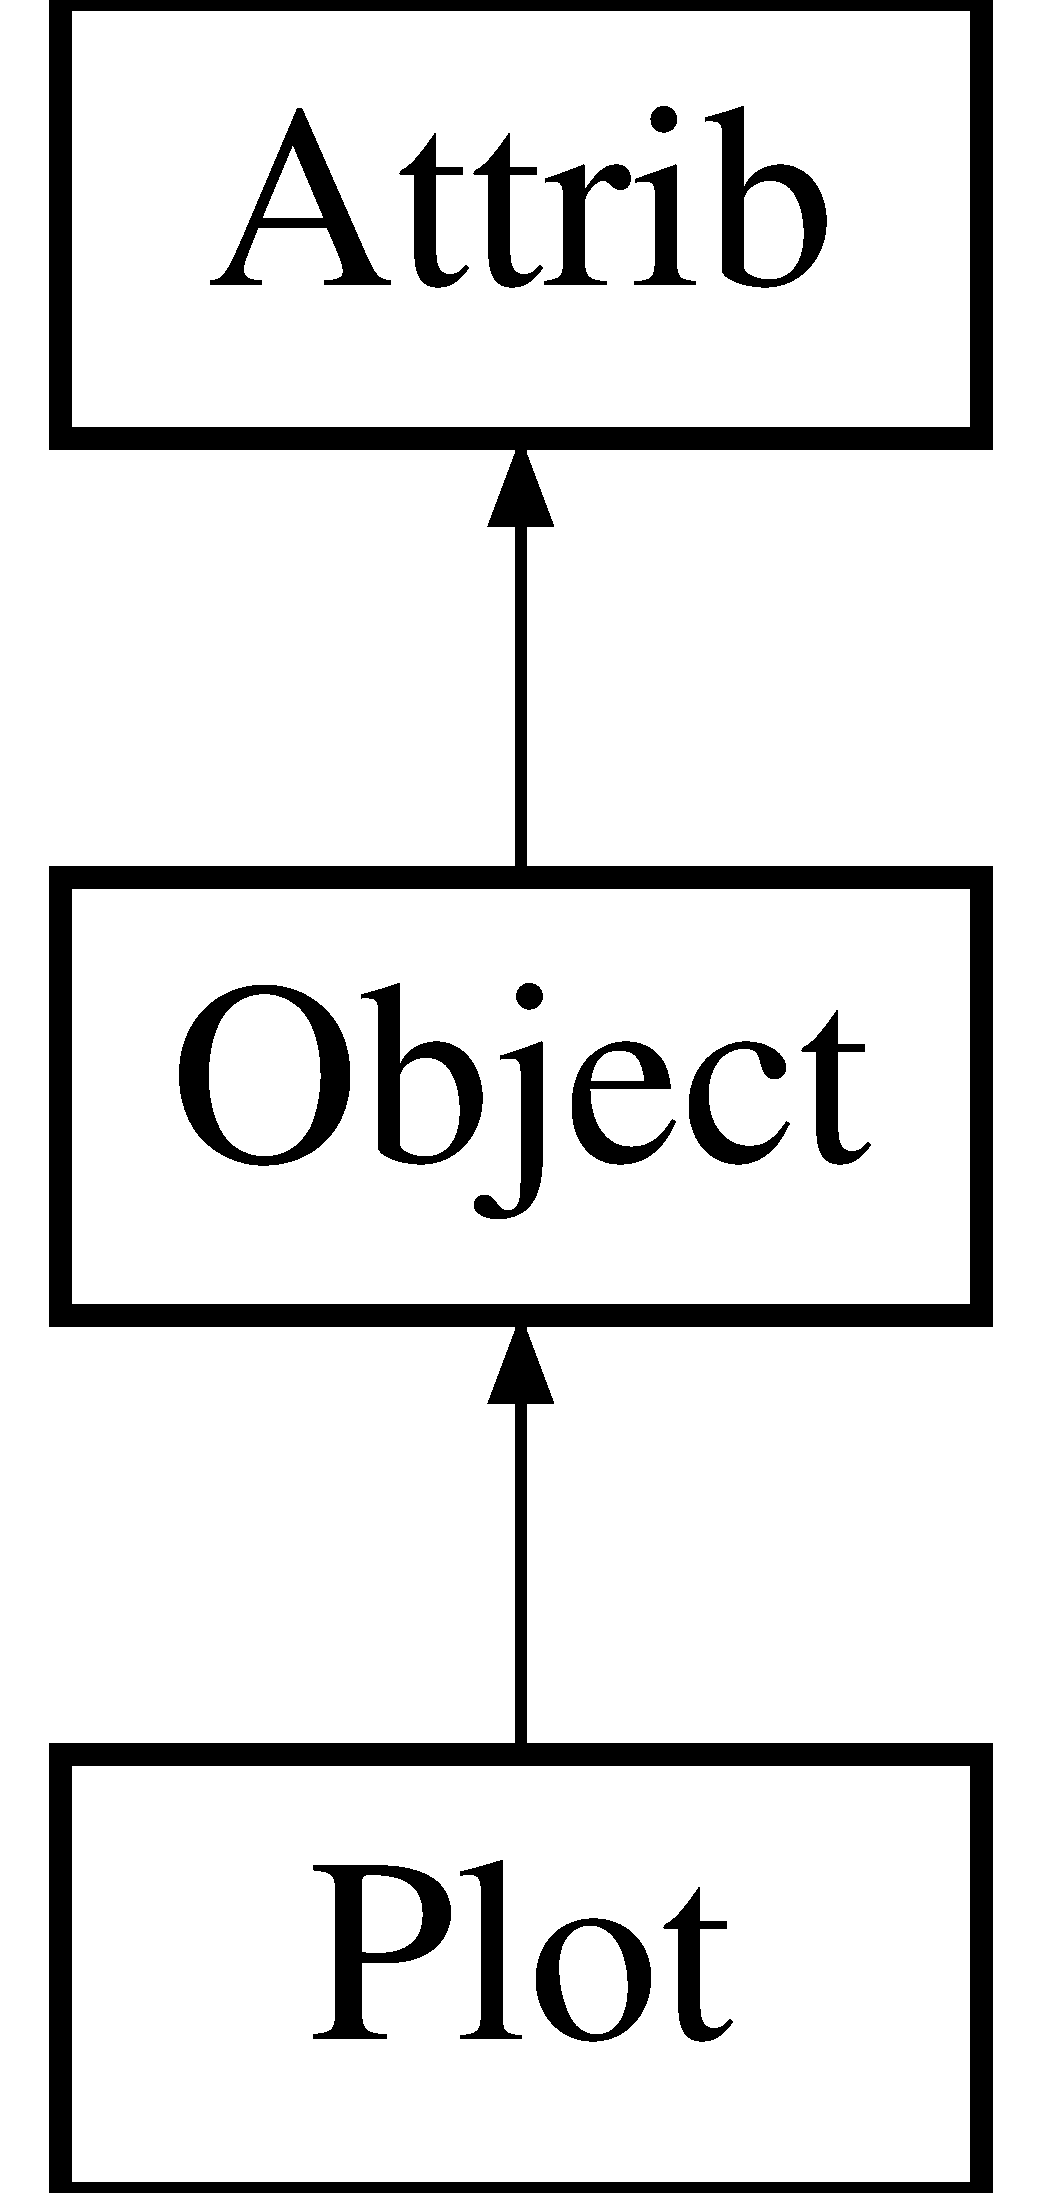
\includegraphics[height=3.000000cm]{classPlot}
\end{center}
\end{figure}
\subsection*{Public Types}
\begin{DoxyCompactItemize}
\item 
enum \hyperlink{classAttrib_a69e171d7cc6417835a5a306d3c764235}{Attribut} \{ \newline
\hyperlink{classAttrib_a69e171d7cc6417835a5a306d3c764235a3a8da2ab97dda18aebab196fe4100531}{U\+N\+D\+E\+F\+I\+N\+ED}, 
\hyperlink{classAttrib_a69e171d7cc6417835a5a306d3c764235a2bfb2af57b87031d190a05fe25dd92ed}{P\+A\+S\+S\+I\+VE}, 
\hyperlink{classAttrib_a69e171d7cc6417835a5a306d3c764235a3b1fec929c0370d1436f2f06e298fb0d}{A\+C\+T\+I\+VE}, 
\hyperlink{classAttrib_a69e171d7cc6417835a5a306d3c764235aa27c16b480a369ea4d18b07b2516bbc7}{I\+N\+T\+E\+R\+F\+A\+CE}, 
\newline
\hyperlink{classAttrib_a69e171d7cc6417835a5a306d3c764235a1420a5b8c0540b2af210b6975eded7f9}{IO}, 
\hyperlink{classAttrib_a69e171d7cc6417835a5a306d3c764235a0af3b0d0ac323c1704e6c69cf90add28}{I\+O\+D\+A\+TA}, 
\hyperlink{classAttrib_a69e171d7cc6417835a5a306d3c764235a7788bc5dd333fd8ce18562b269c9dab1}{E\+L\+E\+M\+E\+NT}, 
\hyperlink{classAttrib_a69e171d7cc6417835a5a306d3c764235a61ceb22149f365f1780d18f9d1459423}{H\+A\+R\+D\+W\+A\+RE}, 
\newline
\hyperlink{classAttrib_a69e171d7cc6417835a5a306d3c764235a75250e29692496e73effca2c0330977f}{P\+R\+O\+C\+E\+S\+S\+US}, 
\hyperlink{classAttrib_a69e171d7cc6417835a5a306d3c764235a103a67cd0b8f07ef478fa45d4356e27b}{S\+O\+F\+T\+W\+A\+RE}
 \}
\end{DoxyCompactItemize}
\subsection*{Public Member Functions}
\begin{DoxyCompactItemize}
\item 
\hyperlink{classPlot_ae8dca35f270d0964aac1e4ff42259129}{Plot} ()
\begin{DoxyCompactList}\small\item\em Standard constructor. \end{DoxyCompactList}\item 
\hyperlink{classPlot_a4e89bc6ea1800ba9697c9e0a0dc50a2e}{Plot} (unsigned int, unsigned int)
\item 
virtual \hyperlink{classPlot_a277e9c79c4357b3a317d74d61dabefcf}{$\sim$\+Plot} ()
\begin{DoxyCompactList}\small\item\em Destructor. \end{DoxyCompactList}\item 
std\+::vector$<$ std\+::pair$<$ unsigned int, \hyperlink{classHisto1D}{Histo1D} $\ast$$>$ $>$ \hyperlink{classPlot_af72e70c6b53df941708cd8d971083227}{histos} ()
\item 
std\+::vector$<$ \hyperlink{classHisto1D}{Histo1D} $\ast$ $>$ \hyperlink{classPlot_ad6f34fe5ab1a94b411b4fc121e0641bc}{histo1d} ()
\item 
int \hyperlink{classPlot_a3f7d4915b045844af0773d09d0c185ad}{pos} (\hyperlink{classHisto1D}{Histo1D} $\ast$h)
\item 
void \hyperlink{classPlot_a77a015d72e98d6fb066481e9c70af1ec}{set\+Region} (unsigned int, unsigned int)
\item 
std\+::pair$<$ unsigned int, unsigned int $>$ \hyperlink{classPlot_ae493b21749049d75cbb7282b1e1b9ab4}{region} ()
\item 
int \hyperlink{classPlot_a4a7404547e8a9d5dd0a921bfff3ed406}{format} ()
\item 
void \hyperlink{classPlot_ac0e03af81b0591d4786ff03441524eb2}{add} (T\+H1D $\ast$, unsigned int \hyperlink{classPlot_ae493b21749049d75cbb7282b1e1b9ab4}{region}=0)
\item 
void \hyperlink{classPlot_abe449e7c57a55f3bf0ee9201d07d497d}{make} (std\+::string script)
\item 
std\+::string \hyperlink{classPlot_aa49856f69c852f7f0ba65ed6131b7b61}{draw} ()
\item 
std\+::string \hyperlink{classObject_a300f4c05dd468c7bb8b3c968868443c1}{name} () const
\item 
std\+::string \hyperlink{classObject_a84f99f70f144a83e1582d1d0f84e4e62}{type} ()
\item 
unsigned char \hyperlink{classObject_af99145335cc61ff6e2798ea17db009d2}{id} ()
\item 
std\+::string \hyperlink{classObject_a73a0f1a41828fdd8303dd662446fb6c3}{title} ()
\item 
void \hyperlink{classObject_a3f9d5537ebce0c0f2bf6ae4d92426f3c}{msg\+Svc} (int level, std\+::string \hyperlink{classObject_a58b2d0618c2d08cf2383012611528d97}{msg}, std\+::string \hyperlink{classObject_a300f4c05dd468c7bb8b3c968868443c1}{name})
\item 
void \hyperlink{classObject_a58b2d0618c2d08cf2383012611528d97}{msg} (std\+::string mymsg)
\item 
void \hyperlink{classObject_ac5d59299273cee27aacf7de00d2e7034}{msg} (std\+::string mymsg, std\+::string \hyperlink{classObject_a300f4c05dd468c7bb8b3c968868443c1}{name})
\item 
void \hyperlink{classObject_a83d2db2df682907ea1115ad721c1c4a1}{verbose} (std\+::string mymsg)
\item 
void \hyperlink{classObject_a2d4120195317e2a3c6532e8bb9f3da68}{verbose} (std\+::string mymsg, std\+::string \hyperlink{classObject_a300f4c05dd468c7bb8b3c968868443c1}{name})
\item 
void \hyperlink{classObject_aac010553f022165573714b7014a15f0d}{debug} (std\+::string mymsg)
\item 
void \hyperlink{classObject_a6c9a0397ca804e04d675ed05683f5420}{debug} (std\+::string mymsg, std\+::string \hyperlink{classObject_a300f4c05dd468c7bb8b3c968868443c1}{name})
\item 
void \hyperlink{classObject_a644fd329ea4cb85f54fa6846484b84a8}{info} (std\+::string mymsg)
\item 
void \hyperlink{classObject_a1ca123253dfd30fc28b156f521dcbdae}{info} (std\+::string mymsg, std\+::string \hyperlink{classObject_a300f4c05dd468c7bb8b3c968868443c1}{name})
\item 
void \hyperlink{classObject_a65cd4fda577711660821fd2cd5a3b4c9}{warning} (std\+::string mymsg)
\item 
void \hyperlink{classObject_a11f101db4dd73d9391b0231818881d86}{warning} (std\+::string mymsg, std\+::string \hyperlink{classObject_a300f4c05dd468c7bb8b3c968868443c1}{name})
\item 
void \hyperlink{classObject_a204a95f57818c0f811933917a30eff45}{error} (std\+::string mymsg)
\item 
void \hyperlink{classObject_ad7f6c457733082efa2f9ff5f5c8e119a}{error} (std\+::string mymsg, std\+::string \hyperlink{classObject_a300f4c05dd468c7bb8b3c968868443c1}{name})
\item 
void \hyperlink{classObject_aad5a16aac7516ce65bd5ec02ab07fc80}{fatal} (std\+::string mymsg)
\item 
void \hyperlink{classObject_ae62acd3d09f716220f75f252dc38bc9a}{fatal} (std\+::string mymsg, std\+::string \hyperlink{classObject_a300f4c05dd468c7bb8b3c968868443c1}{name})
\item 
void \hyperlink{classObject_ae30fea75683c2d149b6b6d17c09ecd0c}{set\+Name} (std\+::string \hyperlink{classObject_a300f4c05dd468c7bb8b3c968868443c1}{name})
\item 
void \hyperlink{classObject_aae534cc9d982bcb9b99fd505f2e103a5}{set\+Type} (std\+::string \hyperlink{classObject_a84f99f70f144a83e1582d1d0f84e4e62}{type})
\item 
void \hyperlink{classObject_a398fe08cba594a0ce6891d59fe4f159f}{set\+Id} (unsigned char \hyperlink{classObject_af99145335cc61ff6e2798ea17db009d2}{id})
\item 
void \hyperlink{classObject_a89557dbbad5bcaa02652f5d7fa35d20f}{set\+Title} (std\+::string \hyperlink{classObject_a73a0f1a41828fdd8303dd662446fb6c3}{title})
\item 
void \hyperlink{classObject_a870c5af919958c2136623b2d7816d123}{set\+Dll\+Name} (std\+::string \hyperlink{classObject_a2e3947f2870094c332d7454117f3ec63}{dll\+Name})
\item 
std\+::string \hyperlink{classObject_a2e3947f2870094c332d7454117f3ec63}{dll\+Name} ()
\item 
bool \hyperlink{classAttrib_a704f26af560909ad22065083bb7d4c34}{is} (int attribut)
\item 
void \hyperlink{classAttrib_a235f773af19c900264a190b00a3b4ad7}{add} (int attribut)
\item 
void \hyperlink{classAttrib_a7d4ef7e32d93cb287792b87b857e79f3}{remove} (int attribut)
\item 
std\+::string \hyperlink{classAttrib_aee7bbf16b144887f196e1341b24f8a26}{attributs} ()
\end{DoxyCompactItemize}
\subsection*{Protected Attributes}
\begin{DoxyCompactItemize}
\item 
std\+::string \hyperlink{classAttrib_a3414521d7a82476e874b25a5407b5e63}{m\+\_\+attrib\+String} \mbox{[}10\mbox{]}
\end{DoxyCompactItemize}
\subsection*{Private Types}
\begin{DoxyCompactItemize}
\item 
typedef std\+::pair$<$ unsigned int, unsigned int $>$ \hyperlink{classPlot_a07543869c4a57b91ea0ec9835cb165ca}{Pos}
\item 
typedef std\+::pair$<$ unsigned int, \hyperlink{classHisto1D}{Histo1D} $\ast$$>$ \hyperlink{classPlot_ac411abcbcce315d4e77094393e6ca418}{Pos1D}
\end{DoxyCompactItemize}
\subsection*{Private Attributes}
\begin{DoxyCompactItemize}
\item 
std\+::pair$<$ unsigned int, unsigned int $>$ \hyperlink{classPlot_aabcbba1cfc66babcbcd647fdf90cdbf1}{m\+\_\+region}
\item 
std\+::vector$<$ std\+::pair$<$ unsigned int, \hyperlink{classHisto1D}{Histo1D} $\ast$$>$ $>$ \hyperlink{classPlot_a7edebf2b275223b8ce55f6ef3b2da0cc}{m\+\_\+histos}
\item 
std\+::string \hyperlink{classPlot_a83ffbf3effe6a2f8befa6375882f3994}{m\+\_\+draw}
\end{DoxyCompactItemize}


\subsection{Detailed Description}
\begin{DoxyAuthor}{Author}
Frederic Machefert 
\end{DoxyAuthor}
\begin{DoxyDate}{Date}
2005-\/01-\/04 
\end{DoxyDate}


Definition at line 21 of file Plot.\+h.



\subsection{Member Typedef Documentation}
\mbox{\Hypertarget{classPlot_a07543869c4a57b91ea0ec9835cb165ca}\label{classPlot_a07543869c4a57b91ea0ec9835cb165ca}} 
\index{Plot@{Plot}!Pos@{Pos}}
\index{Pos@{Pos}!Plot@{Plot}}
\subsubsection{\texorpdfstring{Pos}{Pos}}
{\footnotesize\ttfamily typedef std\+::pair$<$ unsigned int, unsigned int $>$ \hyperlink{classPlot_a07543869c4a57b91ea0ec9835cb165ca}{Plot\+::\+Pos}\hspace{0.3cm}{\ttfamily [private]}}



Definition at line 22 of file Plot.\+h.

\mbox{\Hypertarget{classPlot_ac411abcbcce315d4e77094393e6ca418}\label{classPlot_ac411abcbcce315d4e77094393e6ca418}} 
\index{Plot@{Plot}!Pos1D@{Pos1D}}
\index{Pos1D@{Pos1D}!Plot@{Plot}}
\subsubsection{\texorpdfstring{Pos1D}{Pos1D}}
{\footnotesize\ttfamily typedef std\+::pair$<$ unsigned int , \hyperlink{classHisto1D}{Histo1D}$\ast$ $>$ \hyperlink{classPlot_ac411abcbcce315d4e77094393e6ca418}{Plot\+::\+Pos1D}\hspace{0.3cm}{\ttfamily [private]}}



Definition at line 23 of file Plot.\+h.



\subsection{Member Enumeration Documentation}
\mbox{\Hypertarget{classAttrib_a69e171d7cc6417835a5a306d3c764235}\label{classAttrib_a69e171d7cc6417835a5a306d3c764235}} 
\index{Plot@{Plot}!Attribut@{Attribut}}
\index{Attribut@{Attribut}!Plot@{Plot}}
\subsubsection{\texorpdfstring{Attribut}{Attribut}}
{\footnotesize\ttfamily enum \hyperlink{classAttrib_a69e171d7cc6417835a5a306d3c764235}{Attrib\+::\+Attribut}\hspace{0.3cm}{\ttfamily [inherited]}}

\begin{DoxyEnumFields}{Enumerator}
\raisebox{\heightof{T}}[0pt][0pt]{\index{U\+N\+D\+E\+F\+I\+N\+ED@{U\+N\+D\+E\+F\+I\+N\+ED}!Plot@{Plot}}\index{Plot@{Plot}!U\+N\+D\+E\+F\+I\+N\+ED@{U\+N\+D\+E\+F\+I\+N\+ED}}}\mbox{\Hypertarget{classAttrib_a69e171d7cc6417835a5a306d3c764235a3a8da2ab97dda18aebab196fe4100531}\label{classAttrib_a69e171d7cc6417835a5a306d3c764235a3a8da2ab97dda18aebab196fe4100531}} 
U\+N\+D\+E\+F\+I\+N\+ED&\\
\hline

\raisebox{\heightof{T}}[0pt][0pt]{\index{P\+A\+S\+S\+I\+VE@{P\+A\+S\+S\+I\+VE}!Plot@{Plot}}\index{Plot@{Plot}!P\+A\+S\+S\+I\+VE@{P\+A\+S\+S\+I\+VE}}}\mbox{\Hypertarget{classAttrib_a69e171d7cc6417835a5a306d3c764235a2bfb2af57b87031d190a05fe25dd92ed}\label{classAttrib_a69e171d7cc6417835a5a306d3c764235a2bfb2af57b87031d190a05fe25dd92ed}} 
P\+A\+S\+S\+I\+VE&\\
\hline

\raisebox{\heightof{T}}[0pt][0pt]{\index{A\+C\+T\+I\+VE@{A\+C\+T\+I\+VE}!Plot@{Plot}}\index{Plot@{Plot}!A\+C\+T\+I\+VE@{A\+C\+T\+I\+VE}}}\mbox{\Hypertarget{classAttrib_a69e171d7cc6417835a5a306d3c764235a3b1fec929c0370d1436f2f06e298fb0d}\label{classAttrib_a69e171d7cc6417835a5a306d3c764235a3b1fec929c0370d1436f2f06e298fb0d}} 
A\+C\+T\+I\+VE&\\
\hline

\raisebox{\heightof{T}}[0pt][0pt]{\index{I\+N\+T\+E\+R\+F\+A\+CE@{I\+N\+T\+E\+R\+F\+A\+CE}!Plot@{Plot}}\index{Plot@{Plot}!I\+N\+T\+E\+R\+F\+A\+CE@{I\+N\+T\+E\+R\+F\+A\+CE}}}\mbox{\Hypertarget{classAttrib_a69e171d7cc6417835a5a306d3c764235aa27c16b480a369ea4d18b07b2516bbc7}\label{classAttrib_a69e171d7cc6417835a5a306d3c764235aa27c16b480a369ea4d18b07b2516bbc7}} 
I\+N\+T\+E\+R\+F\+A\+CE&\\
\hline

\raisebox{\heightof{T}}[0pt][0pt]{\index{IO@{IO}!Plot@{Plot}}\index{Plot@{Plot}!IO@{IO}}}\mbox{\Hypertarget{classAttrib_a69e171d7cc6417835a5a306d3c764235a1420a5b8c0540b2af210b6975eded7f9}\label{classAttrib_a69e171d7cc6417835a5a306d3c764235a1420a5b8c0540b2af210b6975eded7f9}} 
IO&\\
\hline

\raisebox{\heightof{T}}[0pt][0pt]{\index{I\+O\+D\+A\+TA@{I\+O\+D\+A\+TA}!Plot@{Plot}}\index{Plot@{Plot}!I\+O\+D\+A\+TA@{I\+O\+D\+A\+TA}}}\mbox{\Hypertarget{classAttrib_a69e171d7cc6417835a5a306d3c764235a0af3b0d0ac323c1704e6c69cf90add28}\label{classAttrib_a69e171d7cc6417835a5a306d3c764235a0af3b0d0ac323c1704e6c69cf90add28}} 
I\+O\+D\+A\+TA&\\
\hline

\raisebox{\heightof{T}}[0pt][0pt]{\index{E\+L\+E\+M\+E\+NT@{E\+L\+E\+M\+E\+NT}!Plot@{Plot}}\index{Plot@{Plot}!E\+L\+E\+M\+E\+NT@{E\+L\+E\+M\+E\+NT}}}\mbox{\Hypertarget{classAttrib_a69e171d7cc6417835a5a306d3c764235a7788bc5dd333fd8ce18562b269c9dab1}\label{classAttrib_a69e171d7cc6417835a5a306d3c764235a7788bc5dd333fd8ce18562b269c9dab1}} 
E\+L\+E\+M\+E\+NT&\\
\hline

\raisebox{\heightof{T}}[0pt][0pt]{\index{H\+A\+R\+D\+W\+A\+RE@{H\+A\+R\+D\+W\+A\+RE}!Plot@{Plot}}\index{Plot@{Plot}!H\+A\+R\+D\+W\+A\+RE@{H\+A\+R\+D\+W\+A\+RE}}}\mbox{\Hypertarget{classAttrib_a69e171d7cc6417835a5a306d3c764235a61ceb22149f365f1780d18f9d1459423}\label{classAttrib_a69e171d7cc6417835a5a306d3c764235a61ceb22149f365f1780d18f9d1459423}} 
H\+A\+R\+D\+W\+A\+RE&\\
\hline

\raisebox{\heightof{T}}[0pt][0pt]{\index{P\+R\+O\+C\+E\+S\+S\+US@{P\+R\+O\+C\+E\+S\+S\+US}!Plot@{Plot}}\index{Plot@{Plot}!P\+R\+O\+C\+E\+S\+S\+US@{P\+R\+O\+C\+E\+S\+S\+US}}}\mbox{\Hypertarget{classAttrib_a69e171d7cc6417835a5a306d3c764235a75250e29692496e73effca2c0330977f}\label{classAttrib_a69e171d7cc6417835a5a306d3c764235a75250e29692496e73effca2c0330977f}} 
P\+R\+O\+C\+E\+S\+S\+US&\\
\hline

\raisebox{\heightof{T}}[0pt][0pt]{\index{S\+O\+F\+T\+W\+A\+RE@{S\+O\+F\+T\+W\+A\+RE}!Plot@{Plot}}\index{Plot@{Plot}!S\+O\+F\+T\+W\+A\+RE@{S\+O\+F\+T\+W\+A\+RE}}}\mbox{\Hypertarget{classAttrib_a69e171d7cc6417835a5a306d3c764235a103a67cd0b8f07ef478fa45d4356e27b}\label{classAttrib_a69e171d7cc6417835a5a306d3c764235a103a67cd0b8f07ef478fa45d4356e27b}} 
S\+O\+F\+T\+W\+A\+RE&\\
\hline

\end{DoxyEnumFields}


Definition at line 29 of file Attrib.\+h.


\begin{DoxyCode}
29                 \{
30     \hyperlink{classAttrib_a69e171d7cc6417835a5a306d3c764235a3a8da2ab97dda18aebab196fe4100531}{UNDEFINED},
31     \hyperlink{classAttrib_a69e171d7cc6417835a5a306d3c764235a2bfb2af57b87031d190a05fe25dd92ed}{PASSIVE},
32     \hyperlink{classAttrib_a69e171d7cc6417835a5a306d3c764235a3b1fec929c0370d1436f2f06e298fb0d}{ACTIVE},
33     \hyperlink{classAttrib_a69e171d7cc6417835a5a306d3c764235aa27c16b480a369ea4d18b07b2516bbc7}{INTERFACE},
34     \hyperlink{classAttrib_a69e171d7cc6417835a5a306d3c764235a1420a5b8c0540b2af210b6975eded7f9}{IO},
35     \hyperlink{classAttrib_a69e171d7cc6417835a5a306d3c764235a0af3b0d0ac323c1704e6c69cf90add28}{IODATA},
36     \hyperlink{classAttrib_a69e171d7cc6417835a5a306d3c764235a7788bc5dd333fd8ce18562b269c9dab1}{ELEMENT},
37     \hyperlink{classAttrib_a69e171d7cc6417835a5a306d3c764235a61ceb22149f365f1780d18f9d1459423}{HARDWARE},
38     \hyperlink{classAttrib_a69e171d7cc6417835a5a306d3c764235a75250e29692496e73effca2c0330977f}{PROCESSUS},
39     \hyperlink{classAttrib_a69e171d7cc6417835a5a306d3c764235a103a67cd0b8f07ef478fa45d4356e27b}{SOFTWARE} 
40   \}; \textcolor{comment}{// array m\_attribString must be changed into Attrib::Attrib if this enu is modified. }
\end{DoxyCode}


\subsection{Constructor \& Destructor Documentation}
\mbox{\Hypertarget{classPlot_ae8dca35f270d0964aac1e4ff42259129}\label{classPlot_ae8dca35f270d0964aac1e4ff42259129}} 
\index{Plot@{Plot}!Plot@{Plot}}
\index{Plot@{Plot}!Plot@{Plot}}
\subsubsection{\texorpdfstring{Plot()}{Plot()}\hspace{0.1cm}{\footnotesize\ttfamily [1/2]}}
{\footnotesize\ttfamily Plot\+::\+Plot (\begin{DoxyParamCaption}{ }\end{DoxyParamCaption})}



Standard constructor. 



Definition at line 23 of file Plot.\+cpp.



References m\+\_\+draw, and m\+\_\+region.


\begin{DoxyCode}
23              \{
24   \hyperlink{classPlot_aabcbba1cfc66babcbcd647fdf90cdbf1}{m\_region}.first  = 1;
25   \hyperlink{classPlot_aabcbba1cfc66babcbcd647fdf90cdbf1}{m\_region}.second = 1;
26   \hyperlink{classPlot_a83ffbf3effe6a2f8befa6375882f3994}{m\_draw}=std::string(\textcolor{stringliteral}{""});
27 \}
\end{DoxyCode}
\mbox{\Hypertarget{classPlot_a4e89bc6ea1800ba9697c9e0a0dc50a2e}\label{classPlot_a4e89bc6ea1800ba9697c9e0a0dc50a2e}} 
\index{Plot@{Plot}!Plot@{Plot}}
\index{Plot@{Plot}!Plot@{Plot}}
\subsubsection{\texorpdfstring{Plot()}{Plot()}\hspace{0.1cm}{\footnotesize\ttfamily [2/2]}}
{\footnotesize\ttfamily Plot\+::\+Plot (\begin{DoxyParamCaption}\item[{unsigned int}]{x,  }\item[{unsigned int}]{y }\end{DoxyParamCaption})}



Definition at line 31 of file Plot.\+cpp.



References set\+Region().


\begin{DoxyCode}
32                             \{
33   \hyperlink{classPlot_a77a015d72e98d6fb066481e9c70af1ec}{setRegion} ( x , y );
34 \}
\end{DoxyCode}
\mbox{\Hypertarget{classPlot_a277e9c79c4357b3a317d74d61dabefcf}\label{classPlot_a277e9c79c4357b3a317d74d61dabefcf}} 
\index{Plot@{Plot}!````~Plot@{$\sim$\+Plot}}
\index{````~Plot@{$\sim$\+Plot}!Plot@{Plot}}
\subsubsection{\texorpdfstring{$\sim$\+Plot()}{~Plot()}}
{\footnotesize\ttfamily Plot\+::$\sim$\+Plot (\begin{DoxyParamCaption}{ }\end{DoxyParamCaption})\hspace{0.3cm}{\ttfamily [virtual]}}



Destructor. 



Definition at line 39 of file Plot.\+cpp.


\begin{DoxyCode}
39              \{ 
40 \} 
\end{DoxyCode}


\subsection{Member Function Documentation}
\mbox{\Hypertarget{classAttrib_a235f773af19c900264a190b00a3b4ad7}\label{classAttrib_a235f773af19c900264a190b00a3b4ad7}} 
\index{Plot@{Plot}!add@{add}}
\index{add@{add}!Plot@{Plot}}
\subsubsection{\texorpdfstring{add()}{add()}\hspace{0.1cm}{\footnotesize\ttfamily [1/2]}}
{\footnotesize\ttfamily void Attrib\+::add (\begin{DoxyParamCaption}\item[{int}]{attribut }\end{DoxyParamCaption})\hspace{0.3cm}{\ttfamily [inline]}, {\ttfamily [inherited]}}

Add an attribut 

Definition at line 67 of file Attrib.\+h.



References Attrib\+::m\+\_\+attributs, and Attrib\+::\+U\+N\+D\+E\+F\+I\+N\+ED.



Referenced by A3\+P\+E\+::\+A3\+P\+E(), Attrib\+::\+Attrib(), Specs\+Mezzanine\+::cmdline(), Computer\+::\+Computer(), C\+U\+\_\+v1\+::\+C\+U\+\_\+v1(), export\+\_\+obj(), F\+E\+B\+\_\+v1\+::\+F\+E\+B\+\_\+v1(), Fe\+P\+G\+A\+::\+Fe\+P\+G\+A(), I\+C\+E\+C\+A\+Lv3\+::\+I\+C\+E\+C\+A\+Lv3(), I\+C\+Phaser\+::\+I\+C\+Phaser(), Application\+::initialize(), Interface\+::\+Interface(), I\+Odata\+::\+I\+Odata(), I\+Oobject\+::\+I\+Oobject(), M\+S\+Oxxxx\+::\+M\+S\+Oxxxx(), Phaser\+::\+Phaser(), Processus\+::\+Processus(), Proto40\+M\+Hz\+\_\+v1\+::\+Proto40\+M\+Hz\+\_\+v1(), Attrib\+::remove(), Seq\+P\+G\+A\+::\+Seq\+P\+G\+A(), Test\+S\+P\+I\+::set\+Address(), Test\+I2\+C\+::set\+Address(), Specs\+Slave\+::set\+Address(), Specs\+Master\+::\+Specs\+Master(), and Specs\+Slave\+::\+Specs\+Slave().


\begin{DoxyCode}
67                             \{
68     \textcolor{keywordflow}{if} (attribut!=\hyperlink{classAttrib_a69e171d7cc6417835a5a306d3c764235a3a8da2ab97dda18aebab196fe4100531}{Attrib::UNDEFINED}) \textcolor{keyword}{remove}(\hyperlink{classAttrib_a69e171d7cc6417835a5a306d3c764235a3a8da2ab97dda18aebab196fe4100531}{Attrib::UNDEFINED});
69     \textcolor{keywordtype}{bool} duplicate = false ;
70     std::vector<int>::const\_iterator iter ;
71     \textcolor{keywordflow}{for} ( iter  = \hyperlink{classAttrib_ac4bd58a0cc6b38a3b711d609a3d3aacc}{m\_attributs}.begin() ;
72           iter != \hyperlink{classAttrib_ac4bd58a0cc6b38a3b711d609a3d3aacc}{m\_attributs}.end()   ;
73           ++iter ) \{
74       \textcolor{keywordflow}{if} ( attribut == (*iter) ) \{
75         duplicate = true ;
76       \}
77     \}
78     \textcolor{keywordflow}{if} (!duplicate) \{
79       \hyperlink{classAttrib_ac4bd58a0cc6b38a3b711d609a3d3aacc}{m\_attributs}.push\_back( attribut );
80     \}
81   \}
\end{DoxyCode}
\mbox{\Hypertarget{classPlot_ac0e03af81b0591d4786ff03441524eb2}\label{classPlot_ac0e03af81b0591d4786ff03441524eb2}} 
\index{Plot@{Plot}!add@{add}}
\index{add@{add}!Plot@{Plot}}
\subsubsection{\texorpdfstring{add()}{add()}\hspace{0.1cm}{\footnotesize\ttfamily [2/2]}}
{\footnotesize\ttfamily void Plot\+::add (\begin{DoxyParamCaption}\item[{T\+H1D $\ast$}]{histo,  }\item[{unsigned int}]{region = {\ttfamily 0} }\end{DoxyParamCaption})}



Definition at line 55 of file Plot.\+cpp.



References m\+\_\+histos, m\+\_\+region, region(), and Object\+::warning().



Referenced by format().


\begin{DoxyCode}
56                                        \{
57   
58   \textcolor{keywordflow}{if} ( \hyperlink{classPlot_ae493b21749049d75cbb7282b1e1b9ab4}{region} > \hyperlink{classPlot_aabcbba1cfc66babcbcd647fdf90cdbf1}{m\_region}.first * \hyperlink{classPlot_aabcbba1cfc66babcbcd647fdf90cdbf1}{m\_region}.second )\{
59     \hyperlink{classObject_a65cd4fda577711660821fd2cd5a3b4c9}{warning}(\textcolor{stringliteral}{"Try plot histogram outside allowed regions."},\textcolor{stringliteral}{"Processus::plot"});
60     \textcolor{keywordflow}{return};
61   \}
62 
63   std::pair < int , Histo1D* > graph;
64   graph.first = \hyperlink{classPlot_ae493b21749049d75cbb7282b1e1b9ab4}{region};
65   graph.second = \textcolor{keyword}{new} \hyperlink{classHisto1D}{Histo1D}(histo);
66 
67   \hyperlink{classPlot_a7edebf2b275223b8ce55f6ef3b2da0cc}{m\_histos}.push\_back ( graph );  
68 \}
\end{DoxyCode}
\mbox{\Hypertarget{classAttrib_aee7bbf16b144887f196e1341b24f8a26}\label{classAttrib_aee7bbf16b144887f196e1341b24f8a26}} 
\index{Plot@{Plot}!attributs@{attributs}}
\index{attributs@{attributs}!Plot@{Plot}}
\subsubsection{\texorpdfstring{attributs()}{attributs()}}
{\footnotesize\ttfamily std\+::string Attrib\+::attributs (\begin{DoxyParamCaption}{ }\end{DoxyParamCaption})\hspace{0.3cm}{\ttfamily [inherited]}}

Print the \hyperlink{classAttrib}{Attrib} of an \hyperlink{classObject}{Object} 

Definition at line 54 of file Attrib.\+cpp.



References images\+::index, Attrib\+::m\+\_\+attrib\+String, and Attrib\+::m\+\_\+attributs.



Referenced by export\+\_\+obj(), and Attrib\+::remove().


\begin{DoxyCode}
54                             \{
55   std::string output;
56   std::vector<int>::iterator iter ;
57   \textcolor{keywordflow}{for} ( \textcolor{keywordtype}{unsigned} \textcolor{keywordtype}{int} \hyperlink{namespaceimages_a54407fd574970b3178647ae096321a57}{index} = 0 ; \hyperlink{namespaceimages_a54407fd574970b3178647ae096321a57}{index} < \hyperlink{classAttrib_ac4bd58a0cc6b38a3b711d609a3d3aacc}{m\_attributs}.size() ; ++
      \hyperlink{namespaceimages_a54407fd574970b3178647ae096321a57}{index} ) \{
58     \textcolor{keywordflow}{if} ( \hyperlink{classAttrib_ac4bd58a0cc6b38a3b711d609a3d3aacc}{m\_attributs}.size() - \hyperlink{namespaceimages_a54407fd574970b3178647ae096321a57}{index} > 1 ) \{
59       output.append(\hyperlink{classAttrib_a3414521d7a82476e874b25a5407b5e63}{m\_attribString}[\hyperlink{classAttrib_ac4bd58a0cc6b38a3b711d609a3d3aacc}{m\_attributs}[\hyperlink{namespaceimages_a54407fd574970b3178647ae096321a57}{index}]]);
60       output.append(\textcolor{stringliteral}{":"});
61     \}
62     \textcolor{keywordflow}{else} \{
63       output.append(\hyperlink{classAttrib_a3414521d7a82476e874b25a5407b5e63}{m\_attribString}[\hyperlink{classAttrib_ac4bd58a0cc6b38a3b711d609a3d3aacc}{m\_attributs}[index]]);
64     \}
65   \}
66   \textcolor{keywordflow}{return} output;
67 \}
\end{DoxyCode}
\mbox{\Hypertarget{classObject_aac010553f022165573714b7014a15f0d}\label{classObject_aac010553f022165573714b7014a15f0d}} 
\index{Plot@{Plot}!debug@{debug}}
\index{debug@{debug}!Plot@{Plot}}
\subsubsection{\texorpdfstring{debug()}{debug()}\hspace{0.1cm}{\footnotesize\ttfamily [1/2]}}
{\footnotesize\ttfamily void Object\+::debug (\begin{DoxyParamCaption}\item[{std\+::string}]{mymsg }\end{DoxyParamCaption})\hspace{0.3cm}{\ttfamily [inline]}, {\ttfamily [inherited]}}



Definition at line 37 of file Object.\+h.



References Msg\+Svc\+::\+D\+E\+B\+UG, Object\+::m\+\_\+log, Object\+::m\+\_\+name, and Msg\+Svc\+::msg\+Svc().



Referenced by A3\+P\+E\+::\+A3\+P\+E(), A3\+P\+E\+::acquisition(), Specs\+Mezzanine\+::add\+Bus(), Hierarchy\+::add\+Child(), Specs\+Slave\+::add\+I2c(), L\+S\+Delay\+Chip\+V1\+::config\+Reg\+Bulk\+Read(), L\+S\+Delay\+Chip\+V1\+::config\+Reg\+Bulk\+Write(), A3\+P\+E\+::data\+Ready(), D\+C\+U\+::\+D\+C\+U(), Hierarchy\+::del\+Child(), Specs\+Slave\+::detect(), Storage\+Fifo\+Acquisition\+::execute(), Storage\+Fifo\+::execute(), A3\+P\+E\+\_\+\+Bit\+Flip\+::execute(), Acquisition\+::execute(), Emulate\+F\+E\+::execute(), export\+\_\+obj(), Fe\+P\+G\+A\+::\+Fe\+P\+G\+A(), Specs\+Glue\+::i2c\+Clk\+Mode(), Fe\+P\+G\+A\+::i2c\+Read(), Seq\+P\+G\+A\+::i2c\+Read(), Fe\+P\+G\+A\+::i2c\+Write(), Seq\+P\+G\+A\+::i2c\+Write(), I\+C\+E\+C\+A\+Lv3\+::\+I\+C\+E\+C\+A\+Lv3(), I\+C\+Phaser\+::\+I\+C\+Phaser(), Specs\+Slave\+::init(), Specs\+Master\+::init(), Storage\+Fifo\+Acquisition\+::initialize(), Storage\+Fifo\+::initialize(), A3\+P\+E\+\_\+\+Bit\+Flip\+::initialize(), Acquisition\+::initialize(), Emulate\+F\+E\+::initialize(), A3\+P\+E\+::internal\+A\+X\+Sequence(), Specs\+Glue\+::led(), Specs\+Mezzanine\+::led(), M\+S\+Oxxxx\+::\+M\+S\+Oxxxx(), Phaser\+::\+Phaser(), Data\+::purge(), Phaser\+::read(), I\+C\+Phaser\+::read(), C\+U\+\_\+v1\+::reset(), F\+E\+B\+\_\+v1\+::reset(), Proto40\+M\+Hz\+\_\+v1\+::reset(), Specs\+Master\+::reset(), Specs\+Slave\+::reset(), F\+E\+B\+\_\+v1\+::reset\+Usb(), Seq\+P\+G\+A\+::\+Seq\+P\+G\+A(), A3\+P\+E\+::set\+Add\+From\+A\+X\+Ram(), A3\+P\+E\+::set\+Add\+To\+A\+X\+Ram(), A3\+P\+E\+::set\+A\+X\+Ram\+Usb(), Element\+::set\+Connection(), Specs\+Glue\+::set\+I2c\+Clk\+Mode(), A3\+P\+E\+::set\+Latency\+A\+X(), Specs\+Glue\+::set\+Led(), Specs\+Mezzanine\+::set\+Led(), A3\+P\+E\+::set\+Length\+A\+X(), A3\+P\+E\+::set\+Read\+To\+A\+X\+Ram\+Usb(), Specs\+Master\+::set\+Speed(), A3\+P\+E\+::set\+Write\+From\+A\+X\+Ram\+Usb(), Specs\+Bus\+::\+Specs\+Bus(), Specs\+I2c\+::\+Specs\+I2c(), Specs\+Master\+::\+Specs\+Master(), Specs\+Mezzanine\+::\+Specs\+Mezzanine(), Specs\+Parallel\+Bus\+::\+Specs\+Parallel\+Bus(), Specs\+Slave\+::\+Specs\+Slave(), L\+S\+Delay\+Chip\+V1\+::spi\+B\+E\+R\+Test(), I\+C\+E\+C\+A\+Lv3\+::spi\+Read(), I\+C\+E\+C\+A\+Lv3\+::spi\+Write(), A3\+P\+E\+::trigger(), Server\+::update\+Config(), Server\+::update\+State(), Phaser\+::write(), I\+C\+Phaser\+::write(), and Hierarchy\+::$\sim$\+Hierarchy().


\begin{DoxyCode}
37 \{ \hyperlink{classObject_a0d269813dd7ac1f24bc143031e2963f2}{m\_log}.\hyperlink{classMsgSvc_ad25f18047920cc59a314e5098259711c}{msgSvc} (\hyperlink{classMsgSvc_ae671eb7301996cd049d2da8a65925926a1dbdcc82dce88370ec335883c83b38b0}{MsgSvc::DEBUG}   , mymsg, \hyperlink{classObject_a8b83c95c705d2c3ba0d081fe1710f48d}{m\_name} ); \}
\end{DoxyCode}
\mbox{\Hypertarget{classObject_a6c9a0397ca804e04d675ed05683f5420}\label{classObject_a6c9a0397ca804e04d675ed05683f5420}} 
\index{Plot@{Plot}!debug@{debug}}
\index{debug@{debug}!Plot@{Plot}}
\subsubsection{\texorpdfstring{debug()}{debug()}\hspace{0.1cm}{\footnotesize\ttfamily [2/2]}}
{\footnotesize\ttfamily void Object\+::debug (\begin{DoxyParamCaption}\item[{std\+::string}]{mymsg,  }\item[{std\+::string}]{name }\end{DoxyParamCaption})\hspace{0.3cm}{\ttfamily [inline]}, {\ttfamily [inherited]}}



Definition at line 45 of file Object.\+h.



References Msg\+Svc\+::\+D\+E\+B\+UG, Object\+::m\+\_\+log, and Msg\+Svc\+::msg\+Svc().


\begin{DoxyCode}
45 \{ \hyperlink{classObject_a0d269813dd7ac1f24bc143031e2963f2}{m\_log}.\hyperlink{classMsgSvc_ad25f18047920cc59a314e5098259711c}{msgSvc} (\hyperlink{classMsgSvc_ae671eb7301996cd049d2da8a65925926a1dbdcc82dce88370ec335883c83b38b0}{MsgSvc::DEBUG}   , mymsg, \hyperlink{classObject_a300f4c05dd468c7bb8b3c968868443c1}{name} ); \}
\end{DoxyCode}
\mbox{\Hypertarget{classObject_a2e3947f2870094c332d7454117f3ec63}\label{classObject_a2e3947f2870094c332d7454117f3ec63}} 
\index{Plot@{Plot}!dll\+Name@{dll\+Name}}
\index{dll\+Name@{dll\+Name}!Plot@{Plot}}
\subsubsection{\texorpdfstring{dll\+Name()}{dllName()}}
{\footnotesize\ttfamily std\+::string Object\+::dll\+Name (\begin{DoxyParamCaption}{ }\end{DoxyParamCaption})\hspace{0.3cm}{\ttfamily [inline]}, {\ttfamily [inherited]}}

Get accessor to member m\+\_\+dll\+Name \begin{DoxyReturn}{Returns}
the current value of m\+\_\+dll\+Name 
\end{DoxyReturn}


Definition at line 74 of file Object.\+h.



References Object\+::m\+\_\+dll\+Name.



Referenced by export\+\_\+obj(), and Object\+::set\+Dll\+Name().


\begin{DoxyCode}
74                        \{
75     \textcolor{keywordflow}{return} \hyperlink{classObject_a01afbeacebb8db6831559972ec362eb3}{m\_dllName};
76   \}  
\end{DoxyCode}
\mbox{\Hypertarget{classPlot_aa49856f69c852f7f0ba65ed6131b7b61}\label{classPlot_aa49856f69c852f7f0ba65ed6131b7b61}} 
\index{Plot@{Plot}!draw@{draw}}
\index{draw@{draw}!Plot@{Plot}}
\subsubsection{\texorpdfstring{draw()}{draw()}}
{\footnotesize\ttfamily std\+::string Plot\+::draw (\begin{DoxyParamCaption}{ }\end{DoxyParamCaption})\hspace{0.3cm}{\ttfamily [inline]}}



Definition at line 103 of file Plot.\+h.



References m\+\_\+draw.


\begin{DoxyCode}
103                   \{
104     \textcolor{keywordflow}{return} \hyperlink{classPlot_a83ffbf3effe6a2f8befa6375882f3994}{m\_draw};
105   \}
\end{DoxyCode}
\mbox{\Hypertarget{classObject_a204a95f57818c0f811933917a30eff45}\label{classObject_a204a95f57818c0f811933917a30eff45}} 
\index{Plot@{Plot}!error@{error}}
\index{error@{error}!Plot@{Plot}}
\subsubsection{\texorpdfstring{error()}{error()}\hspace{0.1cm}{\footnotesize\ttfamily [1/2]}}
{\footnotesize\ttfamily void Object\+::error (\begin{DoxyParamCaption}\item[{std\+::string}]{mymsg }\end{DoxyParamCaption})\hspace{0.3cm}{\ttfamily [inline]}, {\ttfamily [inherited]}}



Definition at line 40 of file Object.\+h.



References Msg\+Svc\+::\+E\+RR, Object\+::m\+\_\+log, Object\+::m\+\_\+name, and Msg\+Svc\+::msg\+Svc().



Referenced by A3\+P\+E\+::clock\+Division(), N\+I6008\+::cmd(), A3\+P\+E\+::enable\+Storage(), A3\+P\+E\+\_\+\+Bit\+Flip\+::execute(), export\+\_\+obj(), A3\+P\+E\+::fifo\+Depth(), A3\+P\+E\+::fifo\+Latency(), F\+E\+B\+\_\+v1\+::gbt\+Status(), Register\+::get\+Bit(), M\+S\+Oxxxx\+::get\+Statistics(), N\+I6008\+::init(), Specs\+Master\+::init(), Usb\+F\+T\+Interface\+::init(), Usb\+F\+T\+M\+L\+Interface\+::init(), A3\+P\+E\+::latency\+A\+X(), A3\+P\+E\+::length\+A\+X(), A3\+P\+E\+::n\+Trigger(), M\+S\+Oxxxx\+::open(), I\+C\+E\+C\+A\+Lv3\+::parse\+Parameter\+List(), A3\+P\+E\+::pipeline(), Usb\+F\+T\+Interface\+::read(), Usb\+F\+T\+M\+L\+Interface\+::read(), M\+S\+Oxxxx\+::recv(), A3\+P\+E\+::reset(), M\+S\+Oxxxx\+::send(), A3\+P\+E\+::set\+Add\+From\+A\+X\+Ram(), A3\+P\+E\+::set\+Add\+To\+A\+X\+Ram(), I\+C\+E\+C\+A\+Lv3\+::set\+Analog\+Ch(), A3\+P\+E\+::set\+A\+X\+Ram\+Usb(), Register\+::set\+Bit(), A3\+P\+E\+::set\+Clock\+Division(), A3\+P\+E\+::set\+Fifo\+Depth(), A3\+P\+E\+::set\+Fifo\+Latency(), A3\+P\+E\+::set\+Latency\+A\+X(), A3\+P\+E\+::set\+Length\+A\+X(), A3\+P\+E\+::set\+N\+Trigger(), A3\+P\+E\+::set\+Pipeline(), A3\+P\+E\+::set\+Read\+Pattern\+Fifo\+Usb(), A3\+P\+E\+::set\+Read\+To\+A\+X\+Ram\+Usb(), A3\+P\+E\+::set\+Read\+Trigger\+Fifo\+Usb(), A3\+P\+E\+::set\+Software\+Trigger(), A3\+P\+E\+::set\+Trigger\+Delay(), A3\+P\+E\+::set\+Trigger\+Rate(), A3\+P\+E\+::set\+Write\+From\+A\+X\+Ram\+Usb(), A3\+P\+E\+::set\+Write\+Storage\+Fifo\+Usb(), I\+C\+E\+C\+A\+Lv3\+::spi\+F\+E\+R\+Test(), I\+C\+E\+C\+A\+Lv3\+::spi\+Write\+Safe(), A3\+P\+E\+::start\+Sequence\+A\+X(), A3\+P\+E\+::trigger\+Delay(), A3\+P\+E\+::trigger\+Rate(), Usb\+F\+T\+M\+L\+Interface\+::usb\+Read(), Usb\+F\+T\+Interface\+::usb\+Read(), Usb\+F\+T\+M\+L\+Interface\+::usb\+Read\+U16(), Usb\+F\+T\+Interface\+::usb\+Read\+U16(), Usb\+F\+T\+M\+L\+Interface\+::usb\+Read\+U32(), Usb\+F\+T\+Interface\+::usb\+Read\+U32(), Usb\+F\+T\+M\+L\+Interface\+::usb\+Read\+U8(), Usb\+F\+T\+Interface\+::usb\+Read\+U8(), Usb\+F\+T\+M\+L\+Interface\+::usb\+Write(), Usb\+F\+T\+Interface\+::usb\+Write(), Usb\+F\+T\+Interface\+::usb\+Write\+Read(), Usb\+F\+T\+M\+L\+Interface\+::usb\+Write\+Read(), Usb\+F\+T\+M\+L\+Interface\+::usb\+Write\+U16(), Usb\+F\+T\+Interface\+::usb\+Write\+U16(), Usb\+F\+T\+M\+L\+Interface\+::usb\+Write\+U32(), Usb\+F\+T\+Interface\+::usb\+Write\+U32(), Usb\+F\+T\+M\+L\+Interface\+::usb\+Write\+U8(), Usb\+F\+T\+Interface\+::usb\+Write\+U8(), Usb\+F\+T\+M\+L\+Interface\+::write(), and Usb\+F\+T\+Interface\+::write().


\begin{DoxyCode}
40 \{ \hyperlink{classObject_a0d269813dd7ac1f24bc143031e2963f2}{m\_log}.\hyperlink{classMsgSvc_ad25f18047920cc59a314e5098259711c}{msgSvc} (\hyperlink{classMsgSvc_ae671eb7301996cd049d2da8a65925926a35a9d7166e9896af4ec8fb33bf5f1772}{MsgSvc::ERR}     , mymsg, \hyperlink{classObject_a8b83c95c705d2c3ba0d081fe1710f48d}{m\_name} ); \}
\end{DoxyCode}
\mbox{\Hypertarget{classObject_ad7f6c457733082efa2f9ff5f5c8e119a}\label{classObject_ad7f6c457733082efa2f9ff5f5c8e119a}} 
\index{Plot@{Plot}!error@{error}}
\index{error@{error}!Plot@{Plot}}
\subsubsection{\texorpdfstring{error()}{error()}\hspace{0.1cm}{\footnotesize\ttfamily [2/2]}}
{\footnotesize\ttfamily void Object\+::error (\begin{DoxyParamCaption}\item[{std\+::string}]{mymsg,  }\item[{std\+::string}]{name }\end{DoxyParamCaption})\hspace{0.3cm}{\ttfamily [inline]}, {\ttfamily [inherited]}}



Definition at line 48 of file Object.\+h.



References Msg\+Svc\+::\+E\+RR, Object\+::m\+\_\+log, and Msg\+Svc\+::msg\+Svc().


\begin{DoxyCode}
48 \{ \hyperlink{classObject_a0d269813dd7ac1f24bc143031e2963f2}{m\_log}.\hyperlink{classMsgSvc_ad25f18047920cc59a314e5098259711c}{msgSvc} (\hyperlink{classMsgSvc_ae671eb7301996cd049d2da8a65925926a35a9d7166e9896af4ec8fb33bf5f1772}{MsgSvc::ERR}     , mymsg, \hyperlink{classObject_a300f4c05dd468c7bb8b3c968868443c1}{name} ); \}
\end{DoxyCode}
\mbox{\Hypertarget{classObject_aad5a16aac7516ce65bd5ec02ab07fc80}\label{classObject_aad5a16aac7516ce65bd5ec02ab07fc80}} 
\index{Plot@{Plot}!fatal@{fatal}}
\index{fatal@{fatal}!Plot@{Plot}}
\subsubsection{\texorpdfstring{fatal()}{fatal()}\hspace{0.1cm}{\footnotesize\ttfamily [1/2]}}
{\footnotesize\ttfamily void Object\+::fatal (\begin{DoxyParamCaption}\item[{std\+::string}]{mymsg }\end{DoxyParamCaption})\hspace{0.3cm}{\ttfamily [inline]}, {\ttfamily [inherited]}}



Definition at line 41 of file Object.\+h.



References Msg\+Svc\+::\+F\+A\+T\+AL, Object\+::m\+\_\+log, Object\+::m\+\_\+name, and Msg\+Svc\+::msg\+Svc().



Referenced by export\+\_\+obj(), Usb\+M\+L\+I2c\+Bus\+::init(), Usb\+M\+L\+Spi\+Bus\+::init(), Usb\+I2c\+Bus\+::init(), Usb\+Spi\+Bus\+::init(), Specs\+Slave\+::init(), I\+Oobject\+::init(), Usb\+F\+T\+M\+L\+Interface\+::init(), Usb\+F\+T\+Interface\+::init(), and Element\+::set\+Connection().


\begin{DoxyCode}
41 \{ \hyperlink{classObject_a0d269813dd7ac1f24bc143031e2963f2}{m\_log}.\hyperlink{classMsgSvc_ad25f18047920cc59a314e5098259711c}{msgSvc} (\hyperlink{classMsgSvc_ae671eb7301996cd049d2da8a65925926a59c73cb29edfc9cdf35845e2b1301363}{MsgSvc::FATAL}   , mymsg, \hyperlink{classObject_a8b83c95c705d2c3ba0d081fe1710f48d}{m\_name} ); \}
\end{DoxyCode}
\mbox{\Hypertarget{classObject_ae62acd3d09f716220f75f252dc38bc9a}\label{classObject_ae62acd3d09f716220f75f252dc38bc9a}} 
\index{Plot@{Plot}!fatal@{fatal}}
\index{fatal@{fatal}!Plot@{Plot}}
\subsubsection{\texorpdfstring{fatal()}{fatal()}\hspace{0.1cm}{\footnotesize\ttfamily [2/2]}}
{\footnotesize\ttfamily void Object\+::fatal (\begin{DoxyParamCaption}\item[{std\+::string}]{mymsg,  }\item[{std\+::string}]{name }\end{DoxyParamCaption})\hspace{0.3cm}{\ttfamily [inline]}, {\ttfamily [inherited]}}



Definition at line 49 of file Object.\+h.



References Msg\+Svc\+::\+F\+A\+T\+AL, Object\+::m\+\_\+log, and Msg\+Svc\+::msg\+Svc().


\begin{DoxyCode}
49 \{ \hyperlink{classObject_a0d269813dd7ac1f24bc143031e2963f2}{m\_log}.\hyperlink{classMsgSvc_ad25f18047920cc59a314e5098259711c}{msgSvc} (\hyperlink{classMsgSvc_ae671eb7301996cd049d2da8a65925926a59c73cb29edfc9cdf35845e2b1301363}{MsgSvc::FATAL}   , mymsg, \hyperlink{classObject_a300f4c05dd468c7bb8b3c968868443c1}{name} ); \}
\end{DoxyCode}
\mbox{\Hypertarget{classPlot_a4a7404547e8a9d5dd0a921bfff3ed406}\label{classPlot_a4a7404547e8a9d5dd0a921bfff3ed406}} 
\index{Plot@{Plot}!format@{format}}
\index{format@{format}!Plot@{Plot}}
\subsubsection{\texorpdfstring{format()}{format()}}
{\footnotesize\ttfamily int Plot\+::format (\begin{DoxyParamCaption}{ }\end{DoxyParamCaption})\hspace{0.3cm}{\ttfamily [inline]}}



Definition at line 80 of file Plot.\+h.



References add(), m\+\_\+region, and region().


\begin{DoxyCode}
81   \{
82     \textcolor{keywordflow}{return} (\hyperlink{classPlot_aabcbba1cfc66babcbcd647fdf90cdbf1}{m\_region}.first+\hyperlink{classPlot_aabcbba1cfc66babcbcd647fdf90cdbf1}{m\_region}.second*100);
83 
84   \}
\end{DoxyCode}
\mbox{\Hypertarget{classPlot_ad6f34fe5ab1a94b411b4fc121e0641bc}\label{classPlot_ad6f34fe5ab1a94b411b4fc121e0641bc}} 
\index{Plot@{Plot}!histo1d@{histo1d}}
\index{histo1d@{histo1d}!Plot@{Plot}}
\subsubsection{\texorpdfstring{histo1d()}{histo1d()}}
{\footnotesize\ttfamily std\+::vector$<$\hyperlink{classHisto1D}{Histo1D}$\ast$$>$ Plot\+::histo1d (\begin{DoxyParamCaption}{ }\end{DoxyParamCaption})\hspace{0.3cm}{\ttfamily [inline]}}



Definition at line 44 of file Plot.\+h.



References m\+\_\+histos.


\begin{DoxyCode}
44                                \{
45     std::vector<Histo1D*> h;
46     \textcolor{keywordflow}{for} (\textcolor{keywordtype}{unsigned} \textcolor{keywordtype}{int} i=0; i<\hyperlink{classPlot_a7edebf2b275223b8ce55f6ef3b2da0cc}{m\_histos}.size(); ++i)
47     \{
48       h.push\_back((\hyperlink{classPlot_a7edebf2b275223b8ce55f6ef3b2da0cc}{m\_histos}[i]).second);
49     \}
50     \textcolor{keywordflow}{return} h;
51   \}
\end{DoxyCode}
\mbox{\Hypertarget{classPlot_af72e70c6b53df941708cd8d971083227}\label{classPlot_af72e70c6b53df941708cd8d971083227}} 
\index{Plot@{Plot}!histos@{histos}}
\index{histos@{histos}!Plot@{Plot}}
\subsubsection{\texorpdfstring{histos()}{histos()}}
{\footnotesize\ttfamily std\+::vector$<$ std\+::pair $<$ unsigned int , \hyperlink{classHisto1D}{Histo1D}$\ast$ $>$ $>$ Plot\+::histos (\begin{DoxyParamCaption}{ }\end{DoxyParamCaption})\hspace{0.3cm}{\ttfamily [inline]}}



Definition at line 36 of file Plot.\+h.



References m\+\_\+histos.


\begin{DoxyCode}
36                                                             \{
37     \textcolor{keywordflow}{return} \hyperlink{classPlot_a7edebf2b275223b8ce55f6ef3b2da0cc}{m\_histos};
38   \}
\end{DoxyCode}
\mbox{\Hypertarget{classObject_af99145335cc61ff6e2798ea17db009d2}\label{classObject_af99145335cc61ff6e2798ea17db009d2}} 
\index{Plot@{Plot}!id@{id}}
\index{id@{id}!Plot@{Plot}}
\subsubsection{\texorpdfstring{id()}{id()}}
{\footnotesize\ttfamily unsigned char Object\+::id (\begin{DoxyParamCaption}{ }\end{DoxyParamCaption})\hspace{0.3cm}{\ttfamily [inline]}, {\ttfamily [inherited]}}



Definition at line 30 of file Object.\+h.



References Object\+::m\+\_\+id.



Referenced by export\+\_\+obj(), and Object\+::set\+Id().


\begin{DoxyCode}
30 \{ \textcolor{keywordflow}{return} \hyperlink{classObject_aca74b9dbfed7b5556ea2d56c65b6b6b0}{m\_id};         \} \textcolor{comment}{//< Get Object m\_id }
\end{DoxyCode}
\mbox{\Hypertarget{classObject_a644fd329ea4cb85f54fa6846484b84a8}\label{classObject_a644fd329ea4cb85f54fa6846484b84a8}} 
\index{Plot@{Plot}!info@{info}}
\index{info@{info}!Plot@{Plot}}
\subsubsection{\texorpdfstring{info()}{info()}\hspace{0.1cm}{\footnotesize\ttfamily [1/2]}}
{\footnotesize\ttfamily void Object\+::info (\begin{DoxyParamCaption}\item[{std\+::string}]{mymsg }\end{DoxyParamCaption})\hspace{0.3cm}{\ttfamily [inline]}, {\ttfamily [inherited]}}



Definition at line 38 of file Object.\+h.



References Msg\+Svc\+::\+I\+N\+FO, Object\+::m\+\_\+log, Object\+::m\+\_\+name, and Msg\+Svc\+::msg\+Svc().



Referenced by N\+I6008\+::add\+Device(), F\+E\+B\+\_\+v1\+::calib\+Cte(), check\+Cmd(), Hierarchy\+::clear(), F\+E\+B\+\_\+v1\+::clock80\+M\+Hz\+Falling\+Edge(), F\+E\+B\+\_\+v1\+::clock\+Falling\+Edge(), Usb\+F\+T\+Interface\+::close(), Usb\+F\+T\+M\+L\+Interface\+::close(), Processus\+::close\+Root\+File(), Server\+::cmdline(), Specs\+Mezzanine\+::cmdline(), Specs\+Slave\+::detect(), F\+E\+B\+\_\+v1\+::disable\+Subtract(), I\+Odata\+::dump(), A3\+P\+E\+::dump\+From\+A\+X(), A3\+P\+E\+::dump\+Pattern(), A3\+P\+E\+::dump\+Storage(), A3\+P\+E\+::dump\+To\+A\+X(), A3\+P\+E\+::dump\+Trigger(), Processus\+::end\+Processing(), Phaser\+Ramp\+Exec\+::execute(), export\+\_\+obj(), Phaser\+Ramp\+Exec\+::finalize(), F\+E\+B\+\_\+v1\+::gain4(), F\+E\+B\+\_\+v1\+::gbt80\+M\+Hz\+Clk\+Eport(), F\+E\+B\+\_\+v1\+::gbt\+Data\+Path(), F\+E\+B\+\_\+v1\+::gbt\+D\+L\+L\+Eport(), F\+E\+B\+\_\+v1\+::gbt\+D\+L\+L\+Reset(), F\+E\+B\+\_\+v1\+::gbt\+Enable\+Eport(), F\+E\+B\+\_\+v1\+::gbt\+Mode(), F\+E\+B\+\_\+v1\+::gbt\+Status(), F\+E\+B\+\_\+v1\+::gbt\+Term\+Eport(), F\+E\+B\+\_\+v1\+::gbt\+Track\+Mode(), I\+C\+E\+C\+A\+Lv3\+::get\+Analog\+Ch(), I\+C\+E\+C\+A\+Lv3\+::get\+Delay\+Line\+Ch(), I\+C\+E\+C\+A\+Lv3\+::get\+Main\+Reg(), F\+E\+B\+\_\+v1\+::global\+Pseudo\+P\+M\+Enable(), Croc\+::help(), R\+A\+M\+::help(), Specs\+Glue\+::help(), Usb\+M\+L\+I2c\+Bus\+::help(), Usb\+M\+L\+Spi\+Bus\+::help(), C\+U\+\_\+v1\+::help(), Usb\+I2c\+Bus\+::help(), Usb\+Spi\+Bus\+::help(), F\+E\+B\+\_\+v1\+::help(), I\+Oobject\+::help(), Proto40\+M\+Hz\+\_\+v1\+::help(), Specs\+Mezzanine\+::help(), Fe\+P\+G\+A\+::help(), Seq\+P\+G\+A\+::help(), Computer\+::help(), N\+I6008\+::help(), Specs\+Parallel\+Bus\+::help(), Specs\+Master\+::help(), Usb\+F\+T\+M\+L\+Interface\+::help(), Usb\+F\+T\+Interface\+::help(), Phaser\+::help(), I\+C\+Phaser\+::help(), A3\+P\+E\+::help(), M\+S\+Oxxxx\+::id(), Croc\+::init(), Computer\+::init(), N\+I6008\+::init(), Specs\+Parallel\+Bus\+::init(), Specs\+Slave\+::init(), Specs\+Master\+::init(), Usb\+F\+T\+Interface\+::init(), Usb\+F\+T\+M\+L\+Interface\+::init(), Storage\+Fifo\+Acquisition\+::initialize(), Storage\+Fifo\+::initialize(), A3\+P\+E\+\_\+\+Bit\+Flip\+::initialize(), Acquisition\+::initialize(), Emulate\+F\+E\+::initialize(), Current\+Measurement\+::initialize(), A\+D\+C\+Measurement\+::initialize(), Phaser\+Ramp\+Exec\+::initialize(), F\+E\+B\+\_\+v1\+::inject\+Mode\+F\+E(), is\+Int(), F\+E\+B\+\_\+v1\+::latency(), F\+E\+B\+\_\+v1\+::latency\+L\+L\+T(), A3\+P\+E\+::load\+From\+A\+X(), Application\+::load\+History\+File(), A3\+P\+E\+::load\+Pattern(), A3\+P\+E\+::load\+Storage(), A3\+P\+E\+::load\+To\+A\+X(), A3\+P\+E\+::load\+Trigger(), Application\+::loop(), F\+E\+B\+\_\+v1\+::mask\+L\+L\+T(), Application\+::network(), F\+E\+B\+\_\+v1\+::old\+Subtract(), M\+S\+Oxxxx\+::open(), Processus\+::open\+Root\+File(), Data\+::print(), F\+E\+B\+\_\+v1\+::probe\+Enable(), Proc\+Data\+Base\+::\+Proc\+Data\+Base(), F\+E\+B\+\_\+v1\+::pseudo\+A\+D\+C\+Enable(), F\+E\+B\+\_\+v1\+::pseudo\+P\+M\+Enable(), Usb\+Spi\+Bus\+::read(), Usb\+F\+T\+M\+L\+Interface\+::read(), F\+E\+B\+\_\+v1\+::read\+Fifo\+Inject\+F\+E(), F\+E\+B\+\_\+v1\+::read\+Fifo\+L\+L\+T(), F\+E\+B\+\_\+v1\+::read\+Fifo\+L\+L\+T\+F\+E(), F\+E\+B\+\_\+v1\+::read\+Fifo\+Spy\+F\+E(), M\+S\+Oxxxx\+::recv(), Croc\+::reset(), Usb\+I2c\+Bus\+::reset(), Usb\+M\+L\+I2c\+Bus\+::reset(), Usb\+M\+L\+Spi\+Bus\+::reset(), Usb\+Spi\+Bus\+::reset(), Fe\+P\+G\+A\+::reset(), Seq\+P\+G\+A\+::reset(), Computer\+::reset(), Specs\+Parallel\+Bus\+::reset(), Specs\+Master\+::reset(), N\+I6008\+::reset(), Usb\+F\+T\+M\+L\+Interface\+::reset(), Usb\+F\+T\+Interface\+::reset(), A3\+P\+E\+::reset(), A3\+P\+E\+::reset\+Acquisition\+Write\+Counter(), F\+E\+B\+\_\+v1\+::reset\+F\+E(), A3\+P\+E\+::reset\+F\+E(), F\+E\+B\+\_\+v1\+::reset\+Fifo\+Inject\+F\+E(), F\+E\+B\+\_\+v1\+::reset\+Fifo\+Spy\+F\+E(), A3\+P\+E\+::reset\+From\+A\+X\+Ram(), Specs\+Slave\+::reset\+Internal(), A3\+P\+E\+::reset\+Latency\+Counter(), A3\+P\+E\+::reset\+Pattern\+Fifo(), A3\+P\+E\+::reset\+Sequence\+From\+To\+A\+X(), A3\+P\+E\+::reset\+S\+P\+I(), A3\+P\+E\+::reset\+Storage\+Fifo(), A3\+P\+E\+::reset\+To\+A\+X\+Ram(), A3\+P\+E\+::reset\+Trigger\+Fifo(), Seq\+P\+G\+A\+::reset\+Usb(), Fe\+P\+G\+A\+::reset\+Usb(), A3\+P\+E\+::reset\+Usb\+Phasers(), M\+S\+Oxxxx\+::send(), Server\+::\+Server(), Application\+::server(), F\+E\+B\+\_\+v1\+::set\+Calib\+Cte(), F\+E\+B\+\_\+v1\+::set\+Clock80\+M\+Hz\+Falling\+Edge(), A3\+P\+E\+::set\+Clock\+Division(), F\+E\+B\+\_\+v1\+::set\+Clock\+Falling\+Edge(), Usb\+Spi\+Bus\+::set\+Data\+Length(), F\+E\+B\+\_\+v1\+::set\+Disable\+Subtract(), A3\+P\+E\+::set\+Enable\+A\+D\+C(), A3\+P\+E\+::set\+Fifo\+Depth(), A3\+P\+E\+::set\+Fifo\+Latency(), F\+E\+B\+\_\+v1\+::set\+Gain4(), F\+E\+B\+\_\+v1\+::set\+Gbt80\+M\+Hz\+Clk\+Eport(), F\+E\+B\+\_\+v1\+::set\+Gbt\+Clock\+Strength(), F\+E\+B\+\_\+v1\+::set\+Gbt\+Data\+Path(), F\+E\+B\+\_\+v1\+::set\+Gbt\+D\+L\+L\+Eport(), F\+E\+B\+\_\+v1\+::set\+Gbt\+Enable\+Eport(), F\+E\+B\+\_\+v1\+::set\+Gbt\+Mode(), F\+E\+B\+\_\+v1\+::set\+Gbt\+Term\+Eport(), F\+E\+B\+\_\+v1\+::set\+Gbt\+Track\+Mode(), F\+E\+B\+\_\+v1\+::set\+Global\+Pseudo\+P\+M\+Enable(), F\+E\+B\+\_\+v1\+::set\+Inject\+Mode\+F\+E(), A3\+P\+E\+::set\+Internal\+A\+X\+Sequence(), F\+E\+B\+\_\+v1\+::set\+Latency(), A3\+P\+E\+::set\+N\+Trigger(), F\+E\+B\+\_\+v1\+::set\+Old\+Subtract(), F\+E\+B\+\_\+v1\+::set\+Output\+Eport(), Phaser\+::set\+Phase(), I\+C\+Phaser\+::set\+Phase(), A3\+P\+E\+::set\+Pipeline(), F\+E\+B\+\_\+v1\+::set\+Probe\+Enable(), F\+E\+B\+\_\+v1\+::set\+Pseudo\+A\+D\+C\+Enable(), F\+E\+B\+\_\+v1\+::set\+Pseudo\+P\+M\+Enable(), A3\+P\+E\+::set\+Read\+Pattern\+Fifo\+Usb(), A3\+P\+E\+::set\+Read\+Trigger\+Fifo\+Usb(), A3\+P\+E\+::set\+Software\+Trigger(), F\+E\+B\+\_\+v1\+::set\+Spare\+For\+Trig\+Enable(), F\+E\+B\+\_\+v1\+::set\+Spy\+Mode\+F\+E(), Processus\+::set\+State(), F\+E\+B\+\_\+v1\+::set\+Threshold(), A3\+P\+E\+::set\+Trigger\+Delay(), A3\+P\+E\+::set\+Trigger\+Rate(), A3\+P\+E\+::set\+Write\+Storage\+Fifo\+Usb(), L\+S\+Delay\+Chip\+V1\+::show\+Config(), F\+E\+B\+\_\+v1\+::spare\+For\+Trig\+Enable(), Specs\+I2c\+::\+Specs\+I2c(), I\+C\+E\+C\+A\+Lv3\+::spi\+F\+E\+R\+Test(), F\+E\+B\+\_\+v1\+::spy\+Mode\+F\+E(), F\+E\+B\+\_\+v1\+::spy\+Mode\+Seq(), Server\+::start(), Processus\+::start\+Processing(), F\+E\+B\+\_\+v1\+::status\+Register(), F\+E\+B\+\_\+v1\+::stop\+Inj\+Loop(), Application\+::svc\+Running(), Application\+::terminate(), F\+E\+B\+\_\+v1\+::test\+Duration(), Seq\+P\+G\+A\+::test\+Sequence(), Fe\+P\+G\+A\+::test\+Sequence(), F\+E\+B\+\_\+v1\+::threshold(), Hierarchy\+::tree(), Croc\+::update(), Usb\+I2c\+Bus\+::update(), Usb\+Spi\+Bus\+::update(), Usb\+M\+L\+I2c\+Bus\+::update(), Usb\+M\+L\+Spi\+Bus\+::update(), C\+U\+\_\+v1\+::update(), Proto40\+M\+Hz\+\_\+v1\+::update(), Computer\+::update(), F\+E\+B\+\_\+v1\+::update(), Specs\+Parallel\+Bus\+::update(), N\+I6008\+::update(), Usb\+F\+T\+Interface\+::update(), Usb\+F\+T\+M\+L\+Interface\+::update(), Usb\+F\+T\+Interface\+::\+Usb\+F\+T\+Interface(), Usb\+F\+T\+M\+L\+Interface\+::\+Usb\+F\+T\+M\+L\+Interface(), Usb\+Spi\+Bus\+::write(), F\+E\+B\+\_\+v1\+::write\+Data\+Fifo\+Inject\+F\+E(), F\+E\+B\+\_\+v1\+::write\+Fifo\+Inject\+F\+E(), and N\+I6008\+::$\sim$\+N\+I6008().


\begin{DoxyCode}
38 \{ \hyperlink{classObject_a0d269813dd7ac1f24bc143031e2963f2}{m\_log}.\hyperlink{classMsgSvc_ad25f18047920cc59a314e5098259711c}{msgSvc} (\hyperlink{classMsgSvc_ae671eb7301996cd049d2da8a65925926ad2fcf3f3e734fc41ee097cc23670ce51}{MsgSvc::INFO}    , mymsg, \hyperlink{classObject_a8b83c95c705d2c3ba0d081fe1710f48d}{m\_name} ); \}
\end{DoxyCode}
\mbox{\Hypertarget{classObject_a1ca123253dfd30fc28b156f521dcbdae}\label{classObject_a1ca123253dfd30fc28b156f521dcbdae}} 
\index{Plot@{Plot}!info@{info}}
\index{info@{info}!Plot@{Plot}}
\subsubsection{\texorpdfstring{info()}{info()}\hspace{0.1cm}{\footnotesize\ttfamily [2/2]}}
{\footnotesize\ttfamily void Object\+::info (\begin{DoxyParamCaption}\item[{std\+::string}]{mymsg,  }\item[{std\+::string}]{name }\end{DoxyParamCaption})\hspace{0.3cm}{\ttfamily [inline]}, {\ttfamily [inherited]}}



Definition at line 46 of file Object.\+h.



References Msg\+Svc\+::\+I\+N\+FO, Object\+::m\+\_\+log, and Msg\+Svc\+::msg\+Svc().


\begin{DoxyCode}
46 \{ \hyperlink{classObject_a0d269813dd7ac1f24bc143031e2963f2}{m\_log}.\hyperlink{classMsgSvc_ad25f18047920cc59a314e5098259711c}{msgSvc} (\hyperlink{classMsgSvc_ae671eb7301996cd049d2da8a65925926ad2fcf3f3e734fc41ee097cc23670ce51}{MsgSvc::INFO}    , mymsg, \hyperlink{classObject_a300f4c05dd468c7bb8b3c968868443c1}{name} ); \}
\end{DoxyCode}
\mbox{\Hypertarget{classAttrib_a704f26af560909ad22065083bb7d4c34}\label{classAttrib_a704f26af560909ad22065083bb7d4c34}} 
\index{Plot@{Plot}!is@{is}}
\index{is@{is}!Plot@{Plot}}
\subsubsection{\texorpdfstring{is()}{is()}}
{\footnotesize\ttfamily bool Attrib\+::is (\begin{DoxyParamCaption}\item[{int}]{attribut }\end{DoxyParamCaption})\hspace{0.3cm}{\ttfamily [inline]}, {\ttfamily [inherited]}}

Test for an attribut 

Definition at line 50 of file Attrib.\+h.



References Attrib\+::m\+\_\+attributs.



Referenced by export\+\_\+obj(), and Element\+::set\+Connection().


\begin{DoxyCode}
51   \{
52     std::vector<int>::const\_iterator iter ;
53     \textcolor{keywordflow}{for} ( iter  = \hyperlink{classAttrib_ac4bd58a0cc6b38a3b711d609a3d3aacc}{m\_attributs}.begin() ;
54           iter != \hyperlink{classAttrib_ac4bd58a0cc6b38a3b711d609a3d3aacc}{m\_attributs}.end()   ;
55           ++iter ) \{
56       \textcolor{keywordflow}{if} ( attribut == (*iter) ) \{
57         \textcolor{keywordflow}{return} \textcolor{keyword}{true};
58       \}
59     \}
60     \textcolor{keywordflow}{return} \textcolor{keyword}{false};
61   \}
\end{DoxyCode}
\mbox{\Hypertarget{classPlot_abe449e7c57a55f3bf0ee9201d07d497d}\label{classPlot_abe449e7c57a55f3bf0ee9201d07d497d}} 
\index{Plot@{Plot}!make@{make}}
\index{make@{make}!Plot@{Plot}}
\subsubsection{\texorpdfstring{make()}{make()}}
{\footnotesize\ttfamily void Plot\+::make (\begin{DoxyParamCaption}\item[{std\+::string}]{script }\end{DoxyParamCaption})\hspace{0.3cm}{\ttfamily [inline]}}



Definition at line 96 of file Plot.\+h.



References m\+\_\+draw.


\begin{DoxyCode}
96                              \{
97     \hyperlink{classPlot_a83ffbf3effe6a2f8befa6375882f3994}{m\_draw}=script;
98   \}
\end{DoxyCode}
\mbox{\Hypertarget{classObject_a58b2d0618c2d08cf2383012611528d97}\label{classObject_a58b2d0618c2d08cf2383012611528d97}} 
\index{Plot@{Plot}!msg@{msg}}
\index{msg@{msg}!Plot@{Plot}}
\subsubsection{\texorpdfstring{msg()}{msg()}\hspace{0.1cm}{\footnotesize\ttfamily [1/2]}}
{\footnotesize\ttfamily void Object\+::msg (\begin{DoxyParamCaption}\item[{std\+::string}]{mymsg }\end{DoxyParamCaption})\hspace{0.3cm}{\ttfamily [inline]}, {\ttfamily [inherited]}}



Definition at line 35 of file Object.\+h.



References Object\+::m\+\_\+log, Object\+::m\+\_\+name, Msg\+Svc\+::msg\+Svc(), and Msg\+Svc\+::\+N\+O\+NE.



Referenced by export\+\_\+obj().


\begin{DoxyCode}
35 \{ \hyperlink{classObject_a0d269813dd7ac1f24bc143031e2963f2}{m\_log}.\hyperlink{classMsgSvc_ad25f18047920cc59a314e5098259711c}{msgSvc} (\hyperlink{classMsgSvc_ae671eb7301996cd049d2da8a65925926a9be9ae32fed8e1e6eba4a58692210fbd}{MsgSvc::NONE}    , mymsg, \hyperlink{classObject_a8b83c95c705d2c3ba0d081fe1710f48d}{m\_name} ); \}
\end{DoxyCode}
\mbox{\Hypertarget{classObject_ac5d59299273cee27aacf7de00d2e7034}\label{classObject_ac5d59299273cee27aacf7de00d2e7034}} 
\index{Plot@{Plot}!msg@{msg}}
\index{msg@{msg}!Plot@{Plot}}
\subsubsection{\texorpdfstring{msg()}{msg()}\hspace{0.1cm}{\footnotesize\ttfamily [2/2]}}
{\footnotesize\ttfamily void Object\+::msg (\begin{DoxyParamCaption}\item[{std\+::string}]{mymsg,  }\item[{std\+::string}]{name }\end{DoxyParamCaption})\hspace{0.3cm}{\ttfamily [inline]}, {\ttfamily [inherited]}}



Definition at line 43 of file Object.\+h.



References Object\+::m\+\_\+log, Msg\+Svc\+::msg\+Svc(), and Msg\+Svc\+::\+N\+O\+NE.


\begin{DoxyCode}
43 \{ \hyperlink{classObject_a0d269813dd7ac1f24bc143031e2963f2}{m\_log}.\hyperlink{classMsgSvc_ad25f18047920cc59a314e5098259711c}{msgSvc} (\hyperlink{classMsgSvc_ae671eb7301996cd049d2da8a65925926a9be9ae32fed8e1e6eba4a58692210fbd}{MsgSvc::NONE}    , mymsg, \hyperlink{classObject_a300f4c05dd468c7bb8b3c968868443c1}{name} ); \}
\end{DoxyCode}
\mbox{\Hypertarget{classObject_a3f9d5537ebce0c0f2bf6ae4d92426f3c}\label{classObject_a3f9d5537ebce0c0f2bf6ae4d92426f3c}} 
\index{Plot@{Plot}!msg\+Svc@{msg\+Svc}}
\index{msg\+Svc@{msg\+Svc}!Plot@{Plot}}
\subsubsection{\texorpdfstring{msg\+Svc()}{msgSvc()}}
{\footnotesize\ttfamily void Object\+::msg\+Svc (\begin{DoxyParamCaption}\item[{int}]{level,  }\item[{std\+::string}]{msg,  }\item[{std\+::string}]{name }\end{DoxyParamCaption})\hspace{0.3cm}{\ttfamily [inline]}, {\ttfamily [inherited]}}



Definition at line 33 of file Object.\+h.



References Object\+::m\+\_\+log, and Msg\+Svc\+::msg\+Svc().



Referenced by Application\+::banner(), export\+\_\+obj(), Specs\+Mezzanine\+::help(), D\+C\+U\+::read\+Mode(), D\+C\+U\+::set\+H\+I\+R(), D\+C\+U\+::set\+L\+I\+R(), Processus\+::set\+State(), and Hierarchy\+::tree().


\begin{DoxyCode}
33 \{ \hyperlink{classObject_a0d269813dd7ac1f24bc143031e2963f2}{m\_log}.\hyperlink{classMsgSvc_ad25f18047920cc59a314e5098259711c}{msgSvc} ( (\hyperlink{classMsgSvc_ae671eb7301996cd049d2da8a65925926}{MsgSvc::MsgLevel})(level), \hyperlink{classObject_a58b2d0618c2d08cf2383012611528d97}{msg}, 
      \hyperlink{classObject_a300f4c05dd468c7bb8b3c968868443c1}{name} ); \}
\end{DoxyCode}
\mbox{\Hypertarget{classObject_a300f4c05dd468c7bb8b3c968868443c1}\label{classObject_a300f4c05dd468c7bb8b3c968868443c1}} 
\index{Plot@{Plot}!name@{name}}
\index{name@{name}!Plot@{Plot}}
\subsubsection{\texorpdfstring{name()}{name()}}
{\footnotesize\ttfamily std\+::string Object\+::name (\begin{DoxyParamCaption}{ }\end{DoxyParamCaption}) const\hspace{0.3cm}{\ttfamily [inline]}, {\ttfamily [inherited]}}



Definition at line 28 of file Object.\+h.



References Object\+::m\+\_\+name.



Referenced by Specs\+Mezzanine\+::add\+Bus(), Hierarchy\+::add\+Child(), Specs\+Slave\+::add\+I2c(), Hierarchy\+::child(), Hierarchy\+::child\+Typed(), Hierarchy\+::clear(), A3\+P\+E\+::clock\+Division(), Usb\+F\+T\+M\+L\+Interface\+::close(), Usb\+F\+T\+Interface\+::close(), Element\+::connection(), Specs\+Slave\+::detect(), I\+Odata\+::dump(), A3\+P\+E\+::enable\+Storage(), export\+\_\+obj(), export\+\_\+proc(), A3\+P\+E\+::fifo\+Depth(), A3\+P\+E\+::fifo\+Latency(), Register\+::get\+Bit(), Croc\+::help(), R\+A\+M\+::help(), Usb\+M\+L\+Spi\+Bus\+::help(), Usb\+M\+L\+I2c\+Bus\+::help(), Usb\+I2c\+Bus\+::help(), C\+U\+\_\+v1\+::help(), Usb\+Spi\+Bus\+::help(), I\+Oobject\+::help(), Proto40\+M\+Hz\+\_\+v1\+::help(), F\+E\+B\+\_\+v1\+::help(), Fe\+P\+G\+A\+::help(), Seq\+P\+G\+A\+::help(), Computer\+::help(), N\+I6008\+::help(), Specs\+Parallel\+Bus\+::help(), Usb\+F\+T\+Interface\+::help(), Usb\+F\+T\+M\+L\+Interface\+::help(), Phaser\+::help(), I\+C\+Phaser\+::help(), A3\+P\+E\+::help(), Data\+::hist2d(), Croc\+::init(), Computer\+::init(), N\+I6008\+::init(), Specs\+Parallel\+Bus\+::init(), Specs\+Slave\+::init(), Specs\+Master\+::init(), Usb\+F\+T\+M\+L\+Interface\+::init(), Usb\+F\+T\+Interface\+::init(), Storage\+Fifo\+::initialize(), Storage\+Fifo\+Acquisition\+::initialize(), A3\+P\+E\+\_\+\+Bit\+Flip\+::initialize(), Acquisition\+::initialize(), Emulate\+F\+E\+::initialize(), Current\+Measurement\+::initialize(), A\+D\+C\+Measurement\+::initialize(), Phaser\+Ramp\+Exec\+::initialize(), A3\+P\+E\+::latency\+A\+X(), A3\+P\+E\+::length\+A\+X(), Application\+::network(), A3\+P\+E\+::n\+Trigger(), Processus\+::open\+Root\+File(), Hierarchy\+::path(), Hierarchy\+::path\+Typed(), A3\+P\+E\+::pipeline(), Test\+Suite\+::\+Plot(), Test\+I2\+C\+::\+Plot(), Test\+S\+P\+I\+::\+Plot(), Test\+U\+S\+B\+::\+Plot(), Phaser\+::read(), I\+C\+Phaser\+::read(), Croc\+::reset(), Usb\+M\+L\+I2c\+Bus\+::reset(), Usb\+M\+L\+Spi\+Bus\+::reset(), Usb\+I2c\+Bus\+::reset(), Usb\+Spi\+Bus\+::reset(), C\+U\+\_\+v1\+::reset(), Proto40\+M\+Hz\+\_\+v1\+::reset(), F\+E\+B\+\_\+v1\+::reset(), Computer\+::reset(), Specs\+Parallel\+Bus\+::reset(), Specs\+Master\+::reset(), Specs\+Slave\+::reset(), N\+I6008\+::reset(), Usb\+F\+T\+M\+L\+Interface\+::reset(), Usb\+F\+T\+Interface\+::reset(), A3\+P\+E\+::reset(), Specs\+Slave\+::reset\+Internal(), F\+E\+B\+\_\+v1\+::reset\+Usb(), A3\+P\+E\+::set\+Add\+From\+A\+X\+Ram(), A3\+P\+E\+::set\+Add\+To\+A\+X\+Ram(), Register\+::set\+Bit(), A3\+P\+E\+::set\+Clock\+Division(), Application\+::set\+Config(), Element\+::set\+Connection(), A3\+P\+E\+::set\+Fifo\+Depth(), A3\+P\+E\+::set\+Fifo\+Latency(), A3\+P\+E\+::set\+Latency\+A\+X(), A3\+P\+E\+::set\+Length\+A\+X(), Object\+::set\+Name(), A3\+P\+E\+::set\+N\+Trigger(), A3\+P\+E\+::set\+Pipeline(), Specs\+Master\+::set\+Speed(), Processus\+::set\+State(), A3\+P\+E\+::set\+Trigger\+Delay(), A3\+P\+E\+::set\+Trigger\+Rate(), Specs\+Bus\+::\+Specs\+Bus(), Specs\+I2c\+::\+Specs\+I2c(), Specs\+Parallel\+Bus\+::\+Specs\+Parallel\+Bus(), Server\+::start(), Processus\+::start\+Processing(), Application\+::terminate(), Hierarchy\+::tree(), A3\+P\+E\+::trigger\+Delay(), A3\+P\+E\+::trigger\+Rate(), Croc\+::update(), Usb\+I2c\+Bus\+::update(), Usb\+Spi\+Bus\+::update(), Usb\+M\+L\+Spi\+Bus\+::update(), Usb\+M\+L\+I2c\+Bus\+::update(), C\+U\+\_\+v1\+::update(), Proto40\+M\+Hz\+\_\+v1\+::update(), Computer\+::update(), F\+E\+B\+\_\+v1\+::update(), Specs\+Parallel\+Bus\+::update(), N\+I6008\+::update(), Usb\+F\+T\+Interface\+::update(), Usb\+F\+T\+M\+L\+Interface\+::update(), Usb\+F\+T\+M\+L\+Interface\+::usb\+Read\+U16(), Usb\+F\+T\+Interface\+::usb\+Read\+U16(), Usb\+F\+T\+Interface\+::usb\+Read\+U32(), Usb\+F\+T\+M\+L\+Interface\+::usb\+Read\+U32(), Usb\+F\+T\+Interface\+::usb\+Read\+U8(), Usb\+F\+T\+M\+L\+Interface\+::usb\+Read\+U8(), Usb\+F\+T\+Interface\+::usb\+Write\+Read(), Usb\+F\+T\+M\+L\+Interface\+::usb\+Write\+Read(), Usb\+F\+T\+Interface\+::usb\+Write\+U16(), Usb\+F\+T\+M\+L\+Interface\+::usb\+Write\+U16(), Usb\+F\+T\+M\+L\+Interface\+::usb\+Write\+U32(), Usb\+F\+T\+Interface\+::usb\+Write\+U32(), Usb\+F\+T\+M\+L\+Interface\+::usb\+Write\+U8(), Usb\+F\+T\+Interface\+::usb\+Write\+U8(), Phaser\+::write(), I\+C\+Phaser\+::write(), and Hierarchy\+::$\sim$\+Hierarchy().


\begin{DoxyCode}
28 \{ \textcolor{keywordflow}{return} \hyperlink{classObject_a8b83c95c705d2c3ba0d081fe1710f48d}{m\_name}; \} \textcolor{comment}{//< Get Object m\_name}
\end{DoxyCode}
\mbox{\Hypertarget{classPlot_a3f7d4915b045844af0773d09d0c185ad}\label{classPlot_a3f7d4915b045844af0773d09d0c185ad}} 
\index{Plot@{Plot}!pos@{pos}}
\index{pos@{pos}!Plot@{Plot}}
\subsubsection{\texorpdfstring{pos()}{pos()}}
{\footnotesize\ttfamily int Plot\+::pos (\begin{DoxyParamCaption}\item[{\hyperlink{classHisto1D}{Histo1D} $\ast$}]{h }\end{DoxyParamCaption})\hspace{0.3cm}{\ttfamily [inline]}}



Definition at line 56 of file Plot.\+h.



References m\+\_\+histos, and set\+Region().


\begin{DoxyCode}
57   \{
58     \textcolor{keywordflow}{for} (\textcolor{keywordtype}{unsigned} \textcolor{keywordtype}{int} i=0; i<\hyperlink{classPlot_a7edebf2b275223b8ce55f6ef3b2da0cc}{m\_histos}.size(); ++i)
59     \{
60       \textcolor{keywordflow}{if} (h==(\hyperlink{classPlot_a7edebf2b275223b8ce55f6ef3b2da0cc}{m\_histos}[i]).second)
61         \textcolor{keywordflow}{return} ((\hyperlink{classPlot_a7edebf2b275223b8ce55f6ef3b2da0cc}{m\_histos}[i]).first);
62     \}
63     \textcolor{keywordflow}{return} -1;
64   \}
\end{DoxyCode}
\mbox{\Hypertarget{classPlot_ae493b21749049d75cbb7282b1e1b9ab4}\label{classPlot_ae493b21749049d75cbb7282b1e1b9ab4}} 
\index{Plot@{Plot}!region@{region}}
\index{region@{region}!Plot@{Plot}}
\subsubsection{\texorpdfstring{region()}{region()}}
{\footnotesize\ttfamily std\+::pair$<$unsigned int , unsigned int$>$ Plot\+::region (\begin{DoxyParamCaption}{ }\end{DoxyParamCaption})\hspace{0.3cm}{\ttfamily [inline]}}



Definition at line 75 of file Plot.\+h.



References m\+\_\+region.



Referenced by add(), and format().


\begin{DoxyCode}
75                                                 \{
76     \textcolor{keywordflow}{return} \hyperlink{classPlot_aabcbba1cfc66babcbcd647fdf90cdbf1}{m\_region};
77   \}
\end{DoxyCode}
\mbox{\Hypertarget{classAttrib_a7d4ef7e32d93cb287792b87b857e79f3}\label{classAttrib_a7d4ef7e32d93cb287792b87b857e79f3}} 
\index{Plot@{Plot}!remove@{remove}}
\index{remove@{remove}!Plot@{Plot}}
\subsubsection{\texorpdfstring{remove()}{remove()}}
{\footnotesize\ttfamily void Attrib\+::remove (\begin{DoxyParamCaption}\item[{int}]{attribut }\end{DoxyParamCaption})\hspace{0.3cm}{\ttfamily [inline]}, {\ttfamily [inherited]}}

Remove an attribut 

Definition at line 86 of file Attrib.\+h.



References Attrib\+::add(), Attrib\+::attributs(), Attrib\+::m\+\_\+attributs, and Attrib\+::\+U\+N\+D\+E\+F\+I\+N\+ED.



Referenced by export\+\_\+obj().


\begin{DoxyCode}
86                                \{
87     std::vector<int>::iterator iter , toremove ;
88     \textcolor{keywordflow}{for} ( iter  = \hyperlink{classAttrib_ac4bd58a0cc6b38a3b711d609a3d3aacc}{m\_attributs}.begin() ;
89           iter != \hyperlink{classAttrib_ac4bd58a0cc6b38a3b711d609a3d3aacc}{m\_attributs}.end()   ;
90           ++iter ) \{
91       \textcolor{keywordflow}{if} ( attribut == (*iter) ) \{
92         toremove = iter;
93       \}
94     \}
95     \hyperlink{classAttrib_ac4bd58a0cc6b38a3b711d609a3d3aacc}{m\_attributs}.erase (toremove);
96     \textcolor{keywordflow}{if}(0==\hyperlink{classAttrib_ac4bd58a0cc6b38a3b711d609a3d3aacc}{m\_attributs}.size()) \hyperlink{classAttrib_a235f773af19c900264a190b00a3b4ad7}{add}(\hyperlink{classAttrib_a69e171d7cc6417835a5a306d3c764235a3a8da2ab97dda18aebab196fe4100531}{Attrib::UNDEFINED});
97   \}
\end{DoxyCode}
\mbox{\Hypertarget{classObject_a870c5af919958c2136623b2d7816d123}\label{classObject_a870c5af919958c2136623b2d7816d123}} 
\index{Plot@{Plot}!set\+Dll\+Name@{set\+Dll\+Name}}
\index{set\+Dll\+Name@{set\+Dll\+Name}!Plot@{Plot}}
\subsubsection{\texorpdfstring{set\+Dll\+Name()}{setDllName()}}
{\footnotesize\ttfamily void Object\+::set\+Dll\+Name (\begin{DoxyParamCaption}\item[{std\+::string}]{dll\+Name }\end{DoxyParamCaption})\hspace{0.3cm}{\ttfamily [inline]}, {\ttfamily [inherited]}}

Set accessor to member m\+\_\+dll\+Name 
\begin{DoxyParams}{Parameters}
{\em dll\+Name} & the new value for m\+\_\+dll\+Name \\
\hline
\end{DoxyParams}


Definition at line 66 of file Object.\+h.



References Object\+::dll\+Name(), and Object\+::m\+\_\+dll\+Name.



Referenced by D\+L\+L\+::create\+Element(), D\+L\+L\+::create\+Processus(), and Object\+::\+Object().


\begin{DoxyCode}
66                                       \{
67     \hyperlink{classObject_a01afbeacebb8db6831559972ec362eb3}{m\_dllName} = \hyperlink{classObject_a2e3947f2870094c332d7454117f3ec63}{dllName};
68   \}
\end{DoxyCode}
\mbox{\Hypertarget{classObject_a398fe08cba594a0ce6891d59fe4f159f}\label{classObject_a398fe08cba594a0ce6891d59fe4f159f}} 
\index{Plot@{Plot}!set\+Id@{set\+Id}}
\index{set\+Id@{set\+Id}!Plot@{Plot}}
\subsubsection{\texorpdfstring{set\+Id()}{setId()}}
{\footnotesize\ttfamily void Object\+::set\+Id (\begin{DoxyParamCaption}\item[{unsigned char}]{id }\end{DoxyParamCaption})\hspace{0.3cm}{\ttfamily [inline]}, {\ttfamily [inherited]}}



Definition at line 53 of file Object.\+h.



References Object\+::id(), and Object\+::m\+\_\+id.



Referenced by A3\+P\+E\+::\+A3\+P\+E(), D\+C\+U\+::\+D\+C\+U(), export\+\_\+obj(), Fe\+P\+G\+A\+::\+Fe\+P\+G\+A(), I\+C\+E\+C\+A\+Lv3\+::\+I\+C\+E\+C\+A\+Lv3(), I\+C\+Phaser\+::\+I\+C\+Phaser(), M\+S\+Oxxxx\+::\+M\+S\+Oxxxx(), Object\+::\+Object(), Phaser\+::\+Phaser(), Seq\+P\+G\+A\+::\+Seq\+P\+G\+A(), Specs\+Bus\+::\+Specs\+Bus(), Specs\+I2c\+::\+Specs\+I2c(), Specs\+Interface\+::\+Specs\+Interface(), Specs\+Master\+::\+Specs\+Master(), Specs\+Parallel\+Bus\+::\+Specs\+Parallel\+Bus(), and Specs\+Slave\+::\+Specs\+Slave().


\begin{DoxyCode}
53 \{ \hyperlink{classObject_aca74b9dbfed7b5556ea2d56c65b6b6b0}{m\_id}    = \hyperlink{classObject_af99145335cc61ff6e2798ea17db009d2}{id}    ; \} \textcolor{comment}{//< Set Object m\_id}
\end{DoxyCode}
\mbox{\Hypertarget{classObject_ae30fea75683c2d149b6b6d17c09ecd0c}\label{classObject_ae30fea75683c2d149b6b6d17c09ecd0c}} 
\index{Plot@{Plot}!set\+Name@{set\+Name}}
\index{set\+Name@{set\+Name}!Plot@{Plot}}
\subsubsection{\texorpdfstring{set\+Name()}{setName()}}
{\footnotesize\ttfamily void Object\+::set\+Name (\begin{DoxyParamCaption}\item[{std\+::string}]{name }\end{DoxyParamCaption})\hspace{0.3cm}{\ttfamily [inline]}, {\ttfamily [inherited]}}



Definition at line 51 of file Object.\+h.



References Object\+::m\+\_\+name, and Object\+::name().



Referenced by A3\+P\+E\+::\+A3\+P\+E(), A3\+P\+E\+\_\+\+Bit\+Flip\+::\+A3\+P\+E\+\_\+\+Bit\+Flip(), Acquisition\+::\+Acquisition(), A\+D\+C\+Measurement\+::\+A\+D\+C\+Measurement(), Computer\+::\+Computer(), Application\+::create(), Croc\+::\+Croc(), C\+U\+\_\+v1\+::\+C\+U\+\_\+v1(), Current\+Measurement\+::\+Current\+Measurement(), Emulate\+F\+E\+::\+Emulate\+F\+E(), export\+\_\+obj(), F\+E\+B\+\_\+v1\+::\+F\+E\+B\+\_\+v1(), Fe\+P\+G\+A\+::\+Fe\+P\+G\+A(), I\+C\+E\+C\+A\+Lv3\+::\+I\+C\+E\+C\+A\+Lv3(), I\+C\+Phaser\+::\+I\+C\+Phaser(), Application\+::initialize(), Interface\+::\+Interface(), I\+Odata\+::\+I\+Odata(), I\+Oobject\+::\+I\+Oobject(), Application\+::network(), N\+I6008\+::\+N\+I6008(), Object\+::\+Object(), Phaser\+Ramp\+Exec\+::\+Phaser\+Ramp\+Exec(), Proto40\+M\+Hz\+\_\+v1\+::\+Proto40\+M\+Hz\+\_\+v1(), R\+A\+M\+::\+R\+A\+M(), Register\+::\+Register(), Register\+Test\+::\+Register\+Test(), Seq\+P\+G\+A\+::\+Seq\+P\+G\+A(), Specs\+Bus\+::\+Specs\+Bus(), Specs\+Glue\+::\+Specs\+Glue(), Specs\+I2c\+::\+Specs\+I2c(), Specs\+Master\+::\+Specs\+Master(), Specs\+Mezzanine\+::\+Specs\+Mezzanine(), Specs\+Parallel\+Bus\+::\+Specs\+Parallel\+Bus(), Storage\+Fifo\+::\+Storage\+Fifo(), Storage\+Fifo\+Acquisition\+::\+Storage\+Fifo\+Acquisition(), Test\+I2\+C\+::\+Test\+I2\+C(), Test\+S\+P\+I\+::\+Test\+S\+P\+I(), Test\+Suite\+::\+Test\+Suite(), Test\+U\+S\+B\+::\+Test\+U\+S\+B(), Usb\+F\+T\+Interface\+::\+Usb\+F\+T\+Interface(), Usb\+F\+T\+Interface\+Test\+::\+Usb\+F\+T\+Interface\+Test(), Usb\+F\+T\+M\+L\+Interface\+::\+Usb\+F\+T\+M\+L\+Interface(), Usb\+I2c\+Bus\+::\+Usb\+I2c\+Bus(), Usb\+M\+L\+I2c\+Bus\+::\+Usb\+M\+L\+I2c\+Bus(), Usb\+M\+L\+Spi\+Bus\+::\+Usb\+M\+L\+Spi\+Bus(), and Usb\+Spi\+Bus\+::\+Usb\+Spi\+Bus().


\begin{DoxyCode}
51 \{ \hyperlink{classObject_a8b83c95c705d2c3ba0d081fe1710f48d}{m\_name}  = \hyperlink{classObject_a300f4c05dd468c7bb8b3c968868443c1}{name}  ; \} \textcolor{comment}{//< Set Object m\_name}
\end{DoxyCode}
\mbox{\Hypertarget{classPlot_a77a015d72e98d6fb066481e9c70af1ec}\label{classPlot_a77a015d72e98d6fb066481e9c70af1ec}} 
\index{Plot@{Plot}!set\+Region@{set\+Region}}
\index{set\+Region@{set\+Region}!Plot@{Plot}}
\subsubsection{\texorpdfstring{set\+Region()}{setRegion()}}
{\footnotesize\ttfamily void Plot\+::set\+Region (\begin{DoxyParamCaption}\item[{unsigned int}]{x,  }\item[{unsigned int}]{y }\end{DoxyParamCaption})}



Definition at line 45 of file Plot.\+cpp.



References m\+\_\+region.



Referenced by Plot(), and pos().


\begin{DoxyCode}
46                                         \{
47   \hyperlink{classPlot_aabcbba1cfc66babcbcd647fdf90cdbf1}{m\_region}.first  = x;
48   \hyperlink{classPlot_aabcbba1cfc66babcbcd647fdf90cdbf1}{m\_region}.second = y;
49 \}
\end{DoxyCode}
\mbox{\Hypertarget{classObject_a89557dbbad5bcaa02652f5d7fa35d20f}\label{classObject_a89557dbbad5bcaa02652f5d7fa35d20f}} 
\index{Plot@{Plot}!set\+Title@{set\+Title}}
\index{set\+Title@{set\+Title}!Plot@{Plot}}
\subsubsection{\texorpdfstring{set\+Title()}{setTitle()}}
{\footnotesize\ttfamily void Object\+::set\+Title (\begin{DoxyParamCaption}\item[{std\+::string}]{title }\end{DoxyParamCaption})\hspace{0.3cm}{\ttfamily [inline]}, {\ttfamily [inherited]}}



Definition at line 54 of file Object.\+h.



References Object\+::m\+\_\+title, and Object\+::title().



Referenced by A3\+P\+E\+\_\+\+Bit\+Flip\+::\+A3\+P\+E\+\_\+\+Bit\+Flip(), Acquisition\+::\+Acquisition(), A\+D\+C\+Measurement\+::\+A\+D\+C\+Measurement(), Current\+Measurement\+::\+Current\+Measurement(), Emulate\+F\+E\+::\+Emulate\+F\+E(), export\+\_\+obj(), Histo1\+D\+::\+Histo1\+D(), Histo2\+D\+::\+Histo2\+D(), Object\+::\+Object(), Phaser\+Ramp\+Exec\+::\+Phaser\+Ramp\+Exec(), Register\+Test\+::\+Register\+Test(), Storage\+Fifo\+::\+Storage\+Fifo(), Storage\+Fifo\+Acquisition\+::\+Storage\+Fifo\+Acquisition(), Test\+I2\+C\+::\+Test\+I2\+C(), Test\+S\+P\+I\+::\+Test\+S\+P\+I(), Test\+Suite\+::\+Test\+Suite(), Test\+U\+S\+B\+::\+Test\+U\+S\+B(), and Usb\+F\+T\+Interface\+Test\+::\+Usb\+F\+T\+Interface\+Test().


\begin{DoxyCode}
54 \{ \hyperlink{classObject_affbeea1953eb5163573b92fad8f75727}{m\_title} = \hyperlink{classObject_a73a0f1a41828fdd8303dd662446fb6c3}{title} ; \} \textcolor{comment}{//< Set Object m\_title}
\end{DoxyCode}
\mbox{\Hypertarget{classObject_aae534cc9d982bcb9b99fd505f2e103a5}\label{classObject_aae534cc9d982bcb9b99fd505f2e103a5}} 
\index{Plot@{Plot}!set\+Type@{set\+Type}}
\index{set\+Type@{set\+Type}!Plot@{Plot}}
\subsubsection{\texorpdfstring{set\+Type()}{setType()}}
{\footnotesize\ttfamily void Object\+::set\+Type (\begin{DoxyParamCaption}\item[{std\+::string}]{type }\end{DoxyParamCaption})\hspace{0.3cm}{\ttfamily [inline]}, {\ttfamily [inherited]}}



Definition at line 52 of file Object.\+h.



References Object\+::m\+\_\+type, and Object\+::type().



Referenced by A3\+P\+E\+::\+A3\+P\+E(), A3\+P\+E\+\_\+\+Bit\+Flip\+::\+A3\+P\+E\+\_\+\+Bit\+Flip(), Acquisition\+::\+Acquisition(), A\+D\+C\+Measurement\+::\+A\+D\+C\+Measurement(), Computer\+::\+Computer(), Croc\+::\+Croc(), C\+U\+\_\+v1\+::\+C\+U\+\_\+v1(), Current\+Measurement\+::\+Current\+Measurement(), D\+C\+U\+::\+D\+C\+U(), Emulate\+F\+E\+::\+Emulate\+F\+E(), export\+\_\+obj(), F\+E\+B\+\_\+v1\+::\+F\+E\+B\+\_\+v1(), Fe\+P\+G\+A\+::\+Fe\+P\+G\+A(), I\+C\+E\+C\+A\+Lv3\+::\+I\+C\+E\+C\+A\+Lv3(), I\+C\+Phaser\+::\+I\+C\+Phaser(), Application\+::initialize(), Interface\+::\+Interface(), I\+Odata\+::\+I\+Odata(), I\+Oobject\+::\+I\+Oobject(), M\+S\+Oxxxx\+::\+M\+S\+Oxxxx(), N\+I6008\+::\+N\+I6008(), Object\+::\+Object(), Phaser\+::\+Phaser(), Phaser\+Ramp\+Exec\+::\+Phaser\+Ramp\+Exec(), Proto40\+M\+Hz\+\_\+v1\+::\+Proto40\+M\+Hz\+\_\+v1(), R\+A\+M\+::\+R\+A\+M(), Register\+::\+Register(), Register\+Test\+::\+Register\+Test(), Seq\+P\+G\+A\+::\+Seq\+P\+G\+A(), Specs\+Bus\+::\+Specs\+Bus(), Specs\+Glue\+::\+Specs\+Glue(), Specs\+I2c\+::\+Specs\+I2c(), Specs\+Master\+::\+Specs\+Master(), Specs\+Mezzanine\+::\+Specs\+Mezzanine(), Specs\+Parallel\+Bus\+::\+Specs\+Parallel\+Bus(), Specs\+Slave\+::\+Specs\+Slave(), Storage\+Fifo\+::\+Storage\+Fifo(), Storage\+Fifo\+Acquisition\+::\+Storage\+Fifo\+Acquisition(), Test\+I2\+C\+::\+Test\+I2\+C(), Test\+S\+P\+I\+::\+Test\+S\+P\+I(), Test\+Suite\+::\+Test\+Suite(), Test\+U\+S\+B\+::\+Test\+U\+S\+B(), Usb\+F\+T\+Interface\+::\+Usb\+F\+T\+Interface(), Usb\+F\+T\+Interface\+Test\+::\+Usb\+F\+T\+Interface\+Test(), Usb\+F\+T\+M\+L\+Interface\+::\+Usb\+F\+T\+M\+L\+Interface(), Usb\+I2c\+Bus\+::\+Usb\+I2c\+Bus(), Usb\+M\+L\+I2c\+Bus\+::\+Usb\+M\+L\+I2c\+Bus(), Usb\+M\+L\+Spi\+Bus\+::\+Usb\+M\+L\+Spi\+Bus(), and Usb\+Spi\+Bus\+::\+Usb\+Spi\+Bus().


\begin{DoxyCode}
52 \{ \hyperlink{classObject_a457a600fe8c00eb1034374f75110a78c}{m\_type}  = \hyperlink{classObject_a84f99f70f144a83e1582d1d0f84e4e62}{type}  ; \} \textcolor{comment}{//< Set Object m\_type}
\end{DoxyCode}
\mbox{\Hypertarget{classObject_a73a0f1a41828fdd8303dd662446fb6c3}\label{classObject_a73a0f1a41828fdd8303dd662446fb6c3}} 
\index{Plot@{Plot}!title@{title}}
\index{title@{title}!Plot@{Plot}}
\subsubsection{\texorpdfstring{title()}{title()}}
{\footnotesize\ttfamily std\+::string Object\+::title (\begin{DoxyParamCaption}{ }\end{DoxyParamCaption})\hspace{0.3cm}{\ttfamily [inline]}, {\ttfamily [inherited]}}



Definition at line 31 of file Object.\+h.



References Object\+::m\+\_\+title.



Referenced by export\+\_\+obj(), export\+\_\+proc(), Data\+::hist2d(), Storage\+Fifo\+Acquisition\+::initialize(), Acquisition\+::initialize(), Current\+Measurement\+::initialize(), A\+D\+C\+Measurement\+::initialize(), A3\+P\+E\+\_\+\+Bit\+Flip\+::\+Plot(), Usb\+F\+T\+Interface\+Test\+::\+Plot(), Test\+Suite\+::\+Plot(), Test\+S\+P\+I\+::\+Plot(), Test\+U\+S\+B\+::\+Plot(), Test\+I2\+C\+::\+Plot(), Object\+::set\+Title(), and Application\+::terminate().


\begin{DoxyCode}
31 \{ \textcolor{keywordflow}{return} \hyperlink{classObject_affbeea1953eb5163573b92fad8f75727}{m\_title};      \} \textcolor{comment}{// < Get Object m\_title}
\end{DoxyCode}
\mbox{\Hypertarget{classObject_a84f99f70f144a83e1582d1d0f84e4e62}\label{classObject_a84f99f70f144a83e1582d1d0f84e4e62}} 
\index{Plot@{Plot}!type@{type}}
\index{type@{type}!Plot@{Plot}}
\subsubsection{\texorpdfstring{type()}{type()}}
{\footnotesize\ttfamily std\+::string Object\+::type (\begin{DoxyParamCaption}{ }\end{DoxyParamCaption})\hspace{0.3cm}{\ttfamily [inline]}, {\ttfamily [inherited]}}



Definition at line 29 of file Object.\+h.



References Object\+::m\+\_\+type.



Referenced by D\+L\+L\+Mgr\+::destroy(), D\+L\+L\+::destroy(), I\+Odata\+::dump(), export\+\_\+obj(), Usb\+M\+L\+I2c\+Bus\+::init(), Usb\+M\+L\+Spi\+Bus\+::init(), Usb\+I2c\+Bus\+::init(), Usb\+Spi\+Bus\+::init(), Storage\+Fifo\+::initialize(), Storage\+Fifo\+Acquisition\+::initialize(), A3\+P\+E\+\_\+\+Bit\+Flip\+::initialize(), Acquisition\+::initialize(), Emulate\+F\+E\+::initialize(), Phaser\+Ramp\+Exec\+::initialize(), Proc\+Data\+Base\+::list(), Hierarchy\+::parent(), Hierarchy\+::path\+Typed(), D\+L\+L\+::print(), Proc\+Data\+Base\+::proc\+List(), Application\+::set\+Config(), Element\+::set\+Connection(), Emulate\+F\+E\+::set\+Generation\+Type(), Object\+::set\+Type(), and Hierarchy\+::tree().


\begin{DoxyCode}
29 \{ \textcolor{keywordflow}{return} \hyperlink{classObject_a457a600fe8c00eb1034374f75110a78c}{m\_type};       \} \textcolor{comment}{//< Get Object m\_type}
\end{DoxyCode}
\mbox{\Hypertarget{classObject_a83d2db2df682907ea1115ad721c1c4a1}\label{classObject_a83d2db2df682907ea1115ad721c1c4a1}} 
\index{Plot@{Plot}!verbose@{verbose}}
\index{verbose@{verbose}!Plot@{Plot}}
\subsubsection{\texorpdfstring{verbose()}{verbose()}\hspace{0.1cm}{\footnotesize\ttfamily [1/2]}}
{\footnotesize\ttfamily void Object\+::verbose (\begin{DoxyParamCaption}\item[{std\+::string}]{mymsg }\end{DoxyParamCaption})\hspace{0.3cm}{\ttfamily [inline]}, {\ttfamily [inherited]}}



Definition at line 36 of file Object.\+h.



References Object\+::m\+\_\+log, Object\+::m\+\_\+name, Msg\+Svc\+::msg\+Svc(), and Msg\+Svc\+::\+V\+E\+R\+B\+O\+SE.



Referenced by D\+C\+U\+::acquire(), export\+\_\+obj(), D\+C\+U\+::init(), Application\+::prepare(), Usb\+F\+T\+Interface\+::read(), Usb\+F\+T\+M\+L\+Interface\+::read(), D\+C\+U\+::read\+Mode(), D\+C\+U\+::reset(), D\+C\+U\+::set\+H\+I\+R(), D\+C\+U\+::set\+L\+I\+R(), Specs\+Interface\+::specs\+Read\+I2c(), Specs\+Interface\+::specs\+Read\+Parallel(), Specs\+Interface\+::specs\+Read\+Register(), Specs\+Interface\+::specs\+Write\+I2c(), Specs\+Interface\+::specs\+Write\+Parallel(), Specs\+Interface\+::specs\+Write\+Register(), Usb\+F\+T\+Interface\+::usb\+Read(), Usb\+F\+T\+M\+L\+Interface\+::usb\+Read(), Usb\+F\+T\+M\+L\+Interface\+::usb\+Read\+U16(), Usb\+F\+T\+Interface\+::usb\+Read\+U16(), Usb\+F\+T\+M\+L\+Interface\+::usb\+Read\+U32(), Usb\+F\+T\+Interface\+::usb\+Read\+U32(), Usb\+F\+T\+Interface\+::usb\+Read\+U8(), Usb\+F\+T\+M\+L\+Interface\+::usb\+Read\+U8(), Usb\+F\+T\+M\+L\+Interface\+::usb\+Write(), Usb\+F\+T\+Interface\+::usb\+Write(), Usb\+F\+T\+Interface\+::usb\+Write\+Read(), Usb\+F\+T\+M\+L\+Interface\+::usb\+Write\+Read(), Usb\+F\+T\+Interface\+::usb\+Write\+U16(), Usb\+F\+T\+M\+L\+Interface\+::usb\+Write\+U16(), Usb\+F\+T\+Interface\+::usb\+Write\+U32(), Usb\+F\+T\+M\+L\+Interface\+::usb\+Write\+U32(), Usb\+F\+T\+Interface\+::usb\+Write\+U8(), Usb\+F\+T\+M\+L\+Interface\+::usb\+Write\+U8(), wait(), Usb\+F\+T\+M\+L\+Interface\+::write(), and Usb\+F\+T\+Interface\+::write().


\begin{DoxyCode}
36 \{ \hyperlink{classObject_a0d269813dd7ac1f24bc143031e2963f2}{m\_log}.\hyperlink{classMsgSvc_ad25f18047920cc59a314e5098259711c}{msgSvc} (\hyperlink{classMsgSvc_ae671eb7301996cd049d2da8a65925926af655256b06494ade5ba830abe5401ec9}{MsgSvc::VERBOSE} , mymsg, \hyperlink{classObject_a8b83c95c705d2c3ba0d081fe1710f48d}{m\_name} ); \}
\end{DoxyCode}
\mbox{\Hypertarget{classObject_a2d4120195317e2a3c6532e8bb9f3da68}\label{classObject_a2d4120195317e2a3c6532e8bb9f3da68}} 
\index{Plot@{Plot}!verbose@{verbose}}
\index{verbose@{verbose}!Plot@{Plot}}
\subsubsection{\texorpdfstring{verbose()}{verbose()}\hspace{0.1cm}{\footnotesize\ttfamily [2/2]}}
{\footnotesize\ttfamily void Object\+::verbose (\begin{DoxyParamCaption}\item[{std\+::string}]{mymsg,  }\item[{std\+::string}]{name }\end{DoxyParamCaption})\hspace{0.3cm}{\ttfamily [inline]}, {\ttfamily [inherited]}}



Definition at line 44 of file Object.\+h.



References Object\+::m\+\_\+log, Msg\+Svc\+::msg\+Svc(), and Msg\+Svc\+::\+V\+E\+R\+B\+O\+SE.


\begin{DoxyCode}
44 \{ \hyperlink{classObject_a0d269813dd7ac1f24bc143031e2963f2}{m\_log}.\hyperlink{classMsgSvc_ad25f18047920cc59a314e5098259711c}{msgSvc} (\hyperlink{classMsgSvc_ae671eb7301996cd049d2da8a65925926af655256b06494ade5ba830abe5401ec9}{MsgSvc::VERBOSE} , mymsg, \hyperlink{classObject_a300f4c05dd468c7bb8b3c968868443c1}{name} ); \}
\end{DoxyCode}
\mbox{\Hypertarget{classObject_a65cd4fda577711660821fd2cd5a3b4c9}\label{classObject_a65cd4fda577711660821fd2cd5a3b4c9}} 
\index{Plot@{Plot}!warning@{warning}}
\index{warning@{warning}!Plot@{Plot}}
\subsubsection{\texorpdfstring{warning()}{warning()}\hspace{0.1cm}{\footnotesize\ttfamily [1/2]}}
{\footnotesize\ttfamily void Object\+::warning (\begin{DoxyParamCaption}\item[{std\+::string}]{mymsg }\end{DoxyParamCaption})\hspace{0.3cm}{\ttfamily [inline]}, {\ttfamily [inherited]}}



Definition at line 39 of file Object.\+h.



References Object\+::m\+\_\+log, Object\+::m\+\_\+name, Msg\+Svc\+::msg\+Svc(), and Msg\+Svc\+::\+W\+A\+R\+N\+I\+NG.



Referenced by D\+C\+U\+::acquire(), A3\+P\+E\+::acquisition(), add(), Application\+::bookkeeping(), check\+Cmd(), Hierarchy\+::child(), Hierarchy\+::child\+Typed(), Usb\+Spi\+Bus\+::clock\+Divider(), L\+S\+Delay\+Chip\+V1\+::config\+Reg\+Bulk\+Read(), L\+S\+Delay\+Chip\+V1\+::config\+Reg\+Bulk\+Write(), Element\+::connection(), D\+C\+U\+::convert(), Application\+::create(), Specs\+Glue\+::date(), Specs\+Mezzanine\+::date(), Specs\+Slave\+::detect(), N\+I6008\+::device(), A3\+P\+E\+\_\+\+Bit\+Flip\+::execute(), Acquisition\+::execute(), Usb\+F\+T\+Interface\+Test\+::execute(), export\+\_\+obj(), F\+E\+B\+\_\+v1\+::gbt\+Acknowledge\+Config(), F\+E\+B\+\_\+v1\+::gbt\+Clock\+Strength(), F\+E\+B\+\_\+v1\+::gbt\+D\+L\+L\+Reset(), L\+S\+Delay\+Chip\+V1\+::get\+Config\+Reg(), Specs\+Glue\+::i2c\+Clk\+Mode(), D\+C\+U\+::init(), Specs\+Slave\+::init(), Storage\+Fifo\+::initialize(), Storage\+Fifo\+Acquisition\+::initialize(), A3\+P\+E\+\_\+\+Bit\+Flip\+::initialize(), Acquisition\+::initialize(), Emulate\+F\+E\+::initialize(), Test\+I2\+C\+::initialize(), Test\+S\+P\+I\+::initialize(), Test\+U\+S\+B\+::initialize(), Specs\+Glue\+::led(), Specs\+Mezzanine\+::led(), A3\+P\+E\+::load\+Trigger(), Application\+::loop(), Application\+::make\+Dir(), Data\+::name(), Application\+::prepare(), Usb\+I2c\+Bus\+::read(), Phaser\+::read(), I\+C\+Phaser\+::read(), Usb\+Spi\+Bus\+::read(), D\+C\+U\+::read\+Mode(), D\+C\+U\+::reset(), Specs\+Slave\+::reset(), Specs\+Master\+::reset(), I\+C\+Phaser\+::reset(), Specs\+Slave\+::reset\+Internal(), Server\+::\+Server(), F\+E\+B\+\_\+v1\+::set\+Calib\+Cte(), Storage\+Fifo\+Acquisition\+::set\+Channels(), Acquisition\+::set\+Channels(), Usb\+Spi\+Bus\+::set\+Clock\+Divider(), F\+E\+B\+\_\+v1\+::set\+Clock\+Falling\+Edge(), Application\+::set\+Config(), L\+S\+Delay\+Chip\+V1\+::set\+Config\+Reg(), Storage\+Fifo\+Acquisition\+::set\+Depth(), Acquisition\+::set\+Depth(), A3\+P\+E\+::set\+Enable\+A\+D\+C(), F\+E\+B\+\_\+v1\+::set\+Gain4(), F\+E\+B\+\_\+v1\+::set\+Gbt80\+M\+Hz\+Clk\+Eport(), F\+E\+B\+\_\+v1\+::set\+Gbt\+Clock\+Strength(), F\+E\+B\+\_\+v1\+::set\+Gbt\+Data\+Path(), F\+E\+B\+\_\+v1\+::set\+Gbt\+D\+L\+L\+Eport(), F\+E\+B\+\_\+v1\+::set\+Gbt\+Enable\+Eport(), F\+E\+B\+\_\+v1\+::set\+Gbt\+Mode(), F\+E\+B\+\_\+v1\+::set\+Gbt\+Term\+Eport(), F\+E\+B\+\_\+v1\+::set\+Gbt\+Track\+Mode(), D\+C\+U\+::set\+H\+I\+R(), Specs\+Glue\+::set\+I2c\+Clk\+Mode(), Specs\+Mezzanine\+::set\+Led(), D\+C\+U\+::set\+L\+I\+R(), F\+E\+B\+\_\+v1\+::set\+Output\+Eport(), A3\+P\+E\+::set\+Pipeline(), F\+E\+B\+\_\+v1\+::set\+Pseudo\+A\+D\+C\+Enable(), F\+E\+B\+\_\+v1\+::set\+Pseudo\+P\+M\+Enable(), R\+A\+M\+::set\+Size(), Specs\+Master\+::set\+Speed(), F\+E\+B\+\_\+v1\+::set\+Stop\+Inj\+Loop(), F\+E\+B\+\_\+v1\+::set\+Test\+Duration(), I\+Odata\+::set\+U16(), I\+Odata\+::set\+U32(), I\+Odata\+::set\+U8(), Test\+Suite\+::sigma(), Specs\+Interface\+::specs\+Read\+I2c(), Specs\+Interface\+::specs\+Read\+Parallel(), Specs\+Interface\+::specs\+Read\+Register(), Specs\+Interface\+::specs\+Write\+I2c(), Specs\+Interface\+::specs\+Write\+Parallel(), Specs\+Interface\+::specs\+Write\+Register(), L\+S\+Delay\+Chip\+V1\+::spi\+B\+E\+R\+Test(), I\+C\+E\+C\+A\+Lv3\+::spi\+F\+E\+R\+Test(), I\+C\+E\+C\+A\+Lv3\+::spi\+Read(), I\+C\+E\+C\+A\+Lv3\+::spi\+Write(), I\+C\+E\+C\+A\+Lv3\+::spi\+Write\+Safe(), Server\+::start(), I\+C\+Phaser\+::status(), Application\+::svc\+Plot(), Application\+::svc\+Running(), Data\+::title(), Server\+::update\+Config(), Server\+::update\+State(), Data\+::vector\+Ptr(), Usb\+I2c\+Bus\+::write(), Phaser\+::write(), I\+C\+Phaser\+::write(), Usb\+Spi\+Bus\+::write(), F\+E\+B\+\_\+v1\+::write\+Fifo\+Inject\+F\+E(), and F\+E\+B\+\_\+v1\+::write\+Fifo\+L\+L\+T\+F\+E().


\begin{DoxyCode}
39 \{ \hyperlink{classObject_a0d269813dd7ac1f24bc143031e2963f2}{m\_log}.\hyperlink{classMsgSvc_ad25f18047920cc59a314e5098259711c}{msgSvc} (\hyperlink{classMsgSvc_ae671eb7301996cd049d2da8a65925926a7cefae88f2ba26b2b05b676a383c834b}{MsgSvc::WARNING} , mymsg, \hyperlink{classObject_a8b83c95c705d2c3ba0d081fe1710f48d}{m\_name} ); \}
\end{DoxyCode}
\mbox{\Hypertarget{classObject_a11f101db4dd73d9391b0231818881d86}\label{classObject_a11f101db4dd73d9391b0231818881d86}} 
\index{Plot@{Plot}!warning@{warning}}
\index{warning@{warning}!Plot@{Plot}}
\subsubsection{\texorpdfstring{warning()}{warning()}\hspace{0.1cm}{\footnotesize\ttfamily [2/2]}}
{\footnotesize\ttfamily void Object\+::warning (\begin{DoxyParamCaption}\item[{std\+::string}]{mymsg,  }\item[{std\+::string}]{name }\end{DoxyParamCaption})\hspace{0.3cm}{\ttfamily [inline]}, {\ttfamily [inherited]}}



Definition at line 47 of file Object.\+h.



References Object\+::m\+\_\+log, Msg\+Svc\+::msg\+Svc(), and Msg\+Svc\+::\+W\+A\+R\+N\+I\+NG.


\begin{DoxyCode}
47 \{ \hyperlink{classObject_a0d269813dd7ac1f24bc143031e2963f2}{m\_log}.\hyperlink{classMsgSvc_ad25f18047920cc59a314e5098259711c}{msgSvc} (\hyperlink{classMsgSvc_ae671eb7301996cd049d2da8a65925926a7cefae88f2ba26b2b05b676a383c834b}{MsgSvc::WARNING} , mymsg, \hyperlink{classObject_a300f4c05dd468c7bb8b3c968868443c1}{name} ); \}
\end{DoxyCode}


\subsection{Member Data Documentation}
\mbox{\Hypertarget{classAttrib_a3414521d7a82476e874b25a5407b5e63}\label{classAttrib_a3414521d7a82476e874b25a5407b5e63}} 
\index{Plot@{Plot}!m\+\_\+attrib\+String@{m\+\_\+attrib\+String}}
\index{m\+\_\+attrib\+String@{m\+\_\+attrib\+String}!Plot@{Plot}}
\subsubsection{\texorpdfstring{m\+\_\+attrib\+String}{m\_attribString}}
{\footnotesize\ttfamily std\+::string Attrib\+::m\+\_\+attrib\+String\mbox{[}10\mbox{]}\hspace{0.3cm}{\ttfamily [protected]}, {\ttfamily [inherited]}}



Definition at line 105 of file Attrib.\+h.



Referenced by Attrib\+::\+Attrib(), and Attrib\+::attributs().

\mbox{\Hypertarget{classPlot_a83ffbf3effe6a2f8befa6375882f3994}\label{classPlot_a83ffbf3effe6a2f8befa6375882f3994}} 
\index{Plot@{Plot}!m\+\_\+draw@{m\+\_\+draw}}
\index{m\+\_\+draw@{m\+\_\+draw}!Plot@{Plot}}
\subsubsection{\texorpdfstring{m\+\_\+draw}{m\_draw}}
{\footnotesize\ttfamily std\+::string Plot\+::m\+\_\+draw\hspace{0.3cm}{\ttfamily [private]}}



Definition at line 111 of file Plot.\+h.



Referenced by draw(), make(), and Plot().

\mbox{\Hypertarget{classPlot_a7edebf2b275223b8ce55f6ef3b2da0cc}\label{classPlot_a7edebf2b275223b8ce55f6ef3b2da0cc}} 
\index{Plot@{Plot}!m\+\_\+histos@{m\+\_\+histos}}
\index{m\+\_\+histos@{m\+\_\+histos}!Plot@{Plot}}
\subsubsection{\texorpdfstring{m\+\_\+histos}{m\_histos}}
{\footnotesize\ttfamily std\+::vector$<$ std\+::pair $<$ unsigned int , \hyperlink{classHisto1D}{Histo1D}$\ast$ $>$ $>$ Plot\+::m\+\_\+histos\hspace{0.3cm}{\ttfamily [private]}}



Definition at line 110 of file Plot.\+h.



Referenced by add(), histo1d(), histos(), and pos().

\mbox{\Hypertarget{classPlot_aabcbba1cfc66babcbcd647fdf90cdbf1}\label{classPlot_aabcbba1cfc66babcbcd647fdf90cdbf1}} 
\index{Plot@{Plot}!m\+\_\+region@{m\+\_\+region}}
\index{m\+\_\+region@{m\+\_\+region}!Plot@{Plot}}
\subsubsection{\texorpdfstring{m\+\_\+region}{m\_region}}
{\footnotesize\ttfamily std\+::pair$<$ unsigned int, unsigned int $>$ Plot\+::m\+\_\+region\hspace{0.3cm}{\ttfamily [private]}}



Definition at line 109 of file Plot.\+h.



Referenced by add(), format(), Plot(), region(), and set\+Region().



The documentation for this class was generated from the following files\+:\begin{DoxyCompactItemize}
\item 
/home/eleclhcb/\+L\+H\+Cb/lbcat-\/cmake/\+Cat\+Kernel/inc/\hyperlink{Plot_8h}{Plot.\+h}\item 
/home/eleclhcb/\+L\+H\+Cb/lbcat-\/cmake/\+Cat\+Kernel/src/\hyperlink{Plot_8cpp}{Plot.\+cpp}\end{DoxyCompactItemize}

\hypertarget{classplotter_1_1plotter}{}\section{plotter.\+plotter Class Reference}
\label{classplotter_1_1plotter}\index{plotter.\+plotter@{plotter.\+plotter}}
Inheritance diagram for plotter.\+plotter\+:\begin{figure}[H]
\begin{center}
\leavevmode
\includegraphics[height=2.000000cm]{classplotter_1_1plotter}
\end{center}
\end{figure}
\subsection*{Public Member Functions}
\begin{DoxyCompactItemize}
\item 
def \hyperlink{classplotter_1_1plotter_aa8c4aa595a3765f6f83ce75c1e9989ea}{\+\_\+\+\_\+init\+\_\+\+\_\+} (self, parent, \hyperlink{classplotter_1_1plotter_a9f4c4616f4fd21c3c9ae6dd320bfbeb6}{figid})
\item 
def \hyperlink{classplotter_1_1plotter_a4c7ba64058a8be7d362958e469429ed6}{current} (self)
\item 
def \hyperlink{classplotter_1_1plotter_a6bdaaad7796180c8dbe453ea192d982e}{destroy} (self)
\end{DoxyCompactItemize}
\subsection*{Public Attributes}
\begin{DoxyCompactItemize}
\item 
\hyperlink{classplotter_1_1plotter_a8766011b81271bcd938237fc9253af45}{figure}
\item 
\hyperlink{classplotter_1_1plotter_a9f4c4616f4fd21c3c9ae6dd320bfbeb6}{figid}
\item 
\hyperlink{classplotter_1_1plotter_a4e223147b19d30bad6a7a0177f3fe08d}{canvas}
\item 
\hyperlink{classplotter_1_1plotter_a55f4eaa8635020a1f0d76241dcfee593}{toolbar}
\end{DoxyCompactItemize}


\subsection{Detailed Description}


Definition at line 24 of file plotter.\+py.



\subsection{Constructor \& Destructor Documentation}
\mbox{\Hypertarget{classplotter_1_1plotter_aa8c4aa595a3765f6f83ce75c1e9989ea}\label{classplotter_1_1plotter_aa8c4aa595a3765f6f83ce75c1e9989ea}} 
\index{plotter\+::plotter@{plotter\+::plotter}!\+\_\+\+\_\+init\+\_\+\+\_\+@{\+\_\+\+\_\+init\+\_\+\+\_\+}}
\index{\+\_\+\+\_\+init\+\_\+\+\_\+@{\+\_\+\+\_\+init\+\_\+\+\_\+}!plotter\+::plotter@{plotter\+::plotter}}
\subsubsection{\texorpdfstring{\+\_\+\+\_\+init\+\_\+\+\_\+()}{\_\_init\_\_()}}
{\footnotesize\ttfamily def plotter.\+plotter.\+\_\+\+\_\+init\+\_\+\+\_\+ (\begin{DoxyParamCaption}\item[{}]{self,  }\item[{}]{parent,  }\item[{}]{figid }\end{DoxyParamCaption})}



Definition at line 25 of file plotter.\+py.


\begin{DoxyCode}
25         \textcolor{keyword}{def }\hyperlink{classwrapper_1_1ModuleDictWrapper_a9a7a794150502f51df687831583e13b9}{\_\_init\_\_}(self, parent,figid):
26                 \textcolor{keywordflow}{if} (parent==\textcolor{keywordtype}{None}):
27                         self.figure = plt.figure(figid)
28                 \textcolor{keywordflow}{else}:
29                         wx.Panel.\_\_init\_\_(self, parent, id=-1)
30                         self.figid  = figid
31                         self.figure = plt.figure(figid)
32                         self.figure.subplots\_adjust(top=0.9,bottom=0.05,right=0.95,left=0.05)
33                         self.canvas = Canvas(self, -1, self.figure)
34                         self.toolbar = Toolbar(self.canvas)
35                         self.toolbar.Realize()
36                         sizer = wx.BoxSizer(wx.VERTICAL)
37                         sizer.Add(self.canvas,1,wx.EXPAND)
38                         sizer.Add(self.toolbar, 0 , wx.LEFT | wx.EXPAND)
39                         self.SetSizer(sizer)
40                         
\end{DoxyCode}


\subsection{Member Function Documentation}
\mbox{\Hypertarget{classplotter_1_1plotter_a4c7ba64058a8be7d362958e469429ed6}\label{classplotter_1_1plotter_a4c7ba64058a8be7d362958e469429ed6}} 
\index{plotter\+::plotter@{plotter\+::plotter}!current@{current}}
\index{current@{current}!plotter\+::plotter@{plotter\+::plotter}}
\subsubsection{\texorpdfstring{current()}{current()}}
{\footnotesize\ttfamily def plotter.\+plotter.\+current (\begin{DoxyParamCaption}\item[{}]{self }\end{DoxyParamCaption})}



Definition at line 41 of file plotter.\+py.



References plotter.\+plotter.\+figure.


\begin{DoxyCode}
41     \textcolor{keyword}{def }current(self):
42             \textcolor{keywordflow}{return} self.figure
43 
\end{DoxyCode}
\mbox{\Hypertarget{classplotter_1_1plotter_a6bdaaad7796180c8dbe453ea192d982e}\label{classplotter_1_1plotter_a6bdaaad7796180c8dbe453ea192d982e}} 
\index{plotter\+::plotter@{plotter\+::plotter}!destroy@{destroy}}
\index{destroy@{destroy}!plotter\+::plotter@{plotter\+::plotter}}
\subsubsection{\texorpdfstring{destroy()}{destroy()}}
{\footnotesize\ttfamily def plotter.\+plotter.\+destroy (\begin{DoxyParamCaption}\item[{}]{self }\end{DoxyParamCaption})}



Definition at line 44 of file plotter.\+py.



References plotter.\+plotter.\+canvas, and plotter.\+h1d().


\begin{DoxyCode}
44     \textcolor{keyword}{def }destroy(self):
45         self.canvas.Destroy()
46 
\end{DoxyCode}


\subsection{Member Data Documentation}
\mbox{\Hypertarget{classplotter_1_1plotter_a4e223147b19d30bad6a7a0177f3fe08d}\label{classplotter_1_1plotter_a4e223147b19d30bad6a7a0177f3fe08d}} 
\index{plotter\+::plotter@{plotter\+::plotter}!canvas@{canvas}}
\index{canvas@{canvas}!plotter\+::plotter@{plotter\+::plotter}}
\subsubsection{\texorpdfstring{canvas}{canvas}}
{\footnotesize\ttfamily plotter.\+plotter.\+canvas}



Definition at line 33 of file plotter.\+py.



Referenced by plotter.\+plotter.\+destroy().

\mbox{\Hypertarget{classplotter_1_1plotter_a9f4c4616f4fd21c3c9ae6dd320bfbeb6}\label{classplotter_1_1plotter_a9f4c4616f4fd21c3c9ae6dd320bfbeb6}} 
\index{plotter\+::plotter@{plotter\+::plotter}!figid@{figid}}
\index{figid@{figid}!plotter\+::plotter@{plotter\+::plotter}}
\subsubsection{\texorpdfstring{figid}{figid}}
{\footnotesize\ttfamily plotter.\+plotter.\+figid}



Definition at line 30 of file plotter.\+py.

\mbox{\Hypertarget{classplotter_1_1plotter_a8766011b81271bcd938237fc9253af45}\label{classplotter_1_1plotter_a8766011b81271bcd938237fc9253af45}} 
\index{plotter\+::plotter@{plotter\+::plotter}!figure@{figure}}
\index{figure@{figure}!plotter\+::plotter@{plotter\+::plotter}}
\subsubsection{\texorpdfstring{figure}{figure}}
{\footnotesize\ttfamily plotter.\+plotter.\+figure}



Definition at line 27 of file plotter.\+py.



Referenced by plotter.\+plotter.\+current().

\mbox{\Hypertarget{classplotter_1_1plotter_a55f4eaa8635020a1f0d76241dcfee593}\label{classplotter_1_1plotter_a55f4eaa8635020a1f0d76241dcfee593}} 
\index{plotter\+::plotter@{plotter\+::plotter}!toolbar@{toolbar}}
\index{toolbar@{toolbar}!plotter\+::plotter@{plotter\+::plotter}}
\subsubsection{\texorpdfstring{toolbar}{toolbar}}
{\footnotesize\ttfamily plotter.\+plotter.\+toolbar}



Definition at line 34 of file plotter.\+py.



The documentation for this class was generated from the following file\+:\begin{DoxyCompactItemize}
\item 
/home/eleclhcb/\+L\+H\+Cb/lbcat-\/cmake/\+Cat\+Python/python/\hyperlink{plotter_8py}{plotter.\+py}\end{DoxyCompactItemize}

\hypertarget{classproc_1_1proc}{
\section{proc::proc Class Reference}
\label{classproc_1_1proc}\index{proc::proc@{proc::proc}}
}
Inheritance diagram for proc::proc::\begin{figure}[H]
\begin{center}
\leavevmode
\includegraphics[height=3cm]{classproc_1_1proc}
\end{center}
\end{figure}
\subsection*{Public Member Functions}
\begin{DoxyCompactItemize}
\item 
def \hyperlink{classproc_1_1proc_a21e9bcad44f0098f74639f245d2d0e4b}{\_\-\_\-init\_\-\_\-}
\item 
def \hyperlink{classproc_1_1proc_a73ad55427f28a79ef0483e18ce996e14}{parent}
\item 
def \hyperlink{classproc_1_1proc_a2192e09617c5de1798ca71123cb390bb}{loadxrc}
\item 
def \hyperlink{classproc_1_1proc_ac70ada08e4fc982a3e61e9ee77b247bf}{page}
\item 
def \hyperlink{classobject_1_1object_ac765747a2b581d48eeb94e600c31fc3f}{getControl}
\item 
def \hyperlink{classobject_1_1object_ac765747a2b581d48eeb94e600c31fc3f}{getControl}
\end{DoxyCompactItemize}
\subsection*{Public Attributes}
\begin{DoxyCompactItemize}
\item 
\hyperlink{classproc_1_1proc_a9ee372f307278c50a935b46ca00a350a}{panel}
\item 
\hyperlink{classobject_1_1object_a4fbaf843d1f40843b2c3895cb73ffada}{cat}
\item 
\hyperlink{classobject_1_1object_a15f13858ecdbf661a97a7da93d717922}{obj}
\item 
\hyperlink{classobject_1_1object_a6b4e1fd053496eafff2bc0f8aed7f089}{path}
\end{DoxyCompactItemize}


\subsection{Detailed Description}


Definition at line 8 of file proc.py.

\subsection{Member Function Documentation}
\hypertarget{classproc_1_1proc_a21e9bcad44f0098f74639f245d2d0e4b}{
\index{proc::proc@{proc::proc}!\_\-\_\-init\_\-\_\-@{\_\-\_\-init\_\-\_\-}}
\index{\_\-\_\-init\_\-\_\-@{\_\-\_\-init\_\-\_\-}!proc::proc@{proc::proc}}
\subsubsection[{\_\-\_\-init\_\-\_\-}]{\setlength{\rightskip}{0pt plus 5cm}def proc::proc::\_\-\_\-init\_\-\_\- ( {\em self}, \/   {\em cat}, \/   {\em obj}, \/   {\em panel}, \/   {\em path})}}
\label{classproc_1_1proc_a21e9bcad44f0098f74639f245d2d0e4b}


Reimplemented from \hyperlink{classobject_1_1object_a1220f7c88ee9a71fcfd9acb49a2f44d8}{object::object}.

Reimplemented in \hyperlink{classEmulateFE_1_1EmulateFE_a3749dd5f45e93a8550800372a3ee40b6}{EmulateFE::EmulateFE}.

Definition at line 9 of file proc.py.


\begin{DoxyCode}
9                                              :
10         object.__init__(self, cat, obj, panel, path)
11         
    def parent(self):
\end{DoxyCode}
\hypertarget{classobject_1_1object_ac765747a2b581d48eeb94e600c31fc3f}{
\index{proc::proc@{proc::proc}!getControl@{getControl}}
\index{getControl@{getControl}!proc::proc@{proc::proc}}
\subsubsection[{getControl}]{\setlength{\rightskip}{0pt plus 5cm}def object::object::getControl ( {\em self}, \/   {\em xmlid})\hspace{0.3cm}{\ttfamily  \mbox{[}inherited\mbox{]}}}}
\label{classobject_1_1object_ac765747a2b581d48eeb94e600c31fc3f}
\begin{DoxyVerb}Retrieves the given control (within a dialog) by its xmlid\end{DoxyVerb}
 

Definition at line 20 of file object.py.


\begin{DoxyCode}
20                                  :
21         '''Retrieves the given control (within a dialog) by its xmlid'''
22         control = self.panel.FindWindowById(xrc.XRCID(xmlid))
23         assert control != None, 'Programming error: a control with xml id ' + xml
      id + ' was not found.'
24         return control
25 
26                 
27 #----------------------------------------------------------------------
28 
29     
    
\end{DoxyCode}
\hypertarget{classobject_1_1object_ac765747a2b581d48eeb94e600c31fc3f}{
\index{proc::proc@{proc::proc}!getControl@{getControl}}
\index{getControl@{getControl}!proc::proc@{proc::proc}}
\subsubsection[{getControl}]{\setlength{\rightskip}{0pt plus 5cm}def object::object::getControl ( {\em self}, \/   {\em xmlid}, \/   {\em item})\hspace{0.3cm}{\ttfamily  \mbox{[}inherited\mbox{]}}}}
\label{classobject_1_1object_ac765747a2b581d48eeb94e600c31fc3f}
\begin{DoxyVerb}Retrieves the given control (within a dialog) by its xmlid\end{DoxyVerb}
 

Definition at line 14 of file object.py.


\begin{DoxyCode}
14                                        :
15         '''Retrieves the given control (within a dialog) by its xmlid'''
16         control = item.FindWindowById(xrc.XRCID(xmlid))
17         assert control != None, 'Programming error: a control with xml id ' + xml
      id + ' was not found.'
18         return control
19 
    def getControl(self, xmlid ) :
\end{DoxyCode}
\hypertarget{classproc_1_1proc_a2192e09617c5de1798ca71123cb390bb}{
\index{proc::proc@{proc::proc}!loadxrc@{loadxrc}}
\index{loadxrc@{loadxrc}!proc::proc@{proc::proc}}
\subsubsection[{loadxrc}]{\setlength{\rightskip}{0pt plus 5cm}def proc::proc::loadxrc ( {\em self})}}
\label{classproc_1_1proc_a2192e09617c5de1798ca71123cb390bb}


Definition at line 16 of file proc.py.


\begin{DoxyCode}
16                      :
17         path= os.path.join(self.path,"proc")
18         path= os.path.join(self.path,"xrc")
19         path= os.path.join(path,self.obj.name())
20         path= path+".xrc"
21         res=xrc.XmlResource(path)
22         self.panel=res.LoadPanel(self.parent(),self.obj.name())
23         
    def page(self):
\end{DoxyCode}
\hypertarget{classproc_1_1proc_ac70ada08e4fc982a3e61e9ee77b247bf}{
\index{proc::proc@{proc::proc}!page@{page}}
\index{page@{page}!proc::proc@{proc::proc}}
\subsubsection[{page}]{\setlength{\rightskip}{0pt plus 5cm}def proc::proc::page ( {\em self})}}
\label{classproc_1_1proc_ac70ada08e4fc982a3e61e9ee77b247bf}


Definition at line 24 of file proc.py.


\begin{DoxyCode}
24                   :
25         return self.panel
        return self.panel
\end{DoxyCode}
\hypertarget{classproc_1_1proc_a73ad55427f28a79ef0483e18ce996e14}{
\index{proc::proc@{proc::proc}!parent@{parent}}
\index{parent@{parent}!proc::proc@{proc::proc}}
\subsubsection[{parent}]{\setlength{\rightskip}{0pt plus 5cm}def proc::proc::parent ( {\em self})}}
\label{classproc_1_1proc_a73ad55427f28a79ef0483e18ce996e14}


Definition at line 12 of file proc.py.


\begin{DoxyCode}
12                     :
13 #        return self.getControl("Element")   
14         return self.getControl("control")
15 
    def loadxrc(self):
\end{DoxyCode}


\subsection{Member Data Documentation}
\hypertarget{classobject_1_1object_a4fbaf843d1f40843b2c3895cb73ffada}{
\index{proc::proc@{proc::proc}!cat@{cat}}
\index{cat@{cat}!proc::proc@{proc::proc}}
\subsubsection[{cat}]{\setlength{\rightskip}{0pt plus 5cm}{\bf object::object::cat}\hspace{0.3cm}{\ttfamily  \mbox{[}inherited\mbox{]}}}}
\label{classobject_1_1object_a4fbaf843d1f40843b2c3895cb73ffada}


Definition at line 8 of file object.py.\hypertarget{classobject_1_1object_a15f13858ecdbf661a97a7da93d717922}{
\index{proc::proc@{proc::proc}!obj@{obj}}
\index{obj@{obj}!proc::proc@{proc::proc}}
\subsubsection[{obj}]{\setlength{\rightskip}{0pt plus 5cm}{\bf object::object::obj}\hspace{0.3cm}{\ttfamily  \mbox{[}inherited\mbox{]}}}}
\label{classobject_1_1object_a15f13858ecdbf661a97a7da93d717922}


Definition at line 9 of file object.py.\hypertarget{classproc_1_1proc_a9ee372f307278c50a935b46ca00a350a}{
\index{proc::proc@{proc::proc}!panel@{panel}}
\index{panel@{panel}!proc::proc@{proc::proc}}
\subsubsection[{panel}]{\setlength{\rightskip}{0pt plus 5cm}{\bf proc::proc::panel}}}
\label{classproc_1_1proc_a9ee372f307278c50a935b46ca00a350a}


Reimplemented from \hyperlink{classobject_1_1object_add82cb657066d4ab5b39035792971503}{object::object}.

Definition at line 22 of file proc.py.\hypertarget{classobject_1_1object_a6b4e1fd053496eafff2bc0f8aed7f089}{
\index{proc::proc@{proc::proc}!path@{path}}
\index{path@{path}!proc::proc@{proc::proc}}
\subsubsection[{path}]{\setlength{\rightskip}{0pt plus 5cm}{\bf object::object::path}\hspace{0.3cm}{\ttfamily  \mbox{[}inherited\mbox{]}}}}
\label{classobject_1_1object_a6b4e1fd053496eafff2bc0f8aed7f089}


Definition at line 11 of file object.py.

The documentation for this class was generated from the following file:\begin{DoxyCompactItemize}
\item 
/home/eleclhcb/LHCb/lbcat-\/cmake/CatPython/python/\hyperlink{proc_8py}{proc.py}\end{DoxyCompactItemize}

\hypertarget{classProcDataBase}{}\section{Proc\+Data\+Base Class Reference}
\label{classProcDataBase}\index{Proc\+Data\+Base@{Proc\+Data\+Base}}


{\ttfamily \#include $<$inc/\+Proc\+Data\+Base.\+h$>$}

\subsection*{Public Member Functions}
\begin{DoxyCompactItemize}
\item 
\hyperlink{classProcDataBase_a82163dfca2df460ba2ea1559ffa72179}{Proc\+Data\+Base} ()
\begin{DoxyCompactList}\small\item\em Standard constructor. \end{DoxyCompactList}\item 
virtual \hyperlink{classProcDataBase_a65ec1212978a4996b5132bfaf1d0738d}{$\sim$\+Proc\+Data\+Base} ()
\begin{DoxyCompactList}\small\item\em Destructor. \end{DoxyCompactList}\item 
void \hyperlink{classProcDataBase_a604959db08c3871d863a799cc4e1d5f4}{update} ()
\item 
std\+::list$<$ \hyperlink{classProcessus}{Processus} $\ast$$>$ \hyperlink{classProcDataBase_a8145de34e9857f3f6eebd2572740f198}{proc\+List} (\hyperlink{classElement}{Element} $\ast$)
\item 
std\+::vector$<$ \hyperlink{classProcessus}{Processus} $\ast$ $>$ \hyperlink{classProcDataBase_a6f17bfad64929fa887c6aafb0080354b}{list} (\hyperlink{classElement}{Element} $\ast$)
\item 
std\+::vector$<$ \hyperlink{classProcessus}{Processus} $\ast$ $>$ \hyperlink{classProcDataBase_a813dbc8f9e7c4d69074a01394f04fc98}{list} ()
\item 
\hyperlink{classProcessus}{Processus} $\ast$ \hyperlink{classProcDataBase_a839b15c7bc0d73f5ff0f2516c3cb418e}{processus} (std\+::string)
\item 
\hyperlink{classStatusCode}{Status\+Code} \hyperlink{classProcDataBase_a0aafeb65a41b92a6d1fdd67f363ef826}{add} (\hyperlink{classProcessus}{Processus} $\ast$)
\item 
\hyperlink{classStatusCode}{Status\+Code} \hyperlink{classProcDataBase_a0413976bac8f233b31eab6d7a83866b9}{remove} (\hyperlink{classProcessus}{Processus} $\ast$)
\end{DoxyCompactItemize}
\subsection*{Private Attributes}
\begin{DoxyCompactItemize}
\item 
std\+::list$<$ \hyperlink{classProcessus}{Processus} $\ast$$>$ \hyperlink{classProcDataBase_a9b7458b811b826c5d264b436c7a391c4}{m\+\_\+proc\+List}
\item 
std\+::list$<$ std\+::string $>$ \hyperlink{classProcDataBase_a94063cebf50be9a12b8bd9f70e410ed5}{m\+\_\+types}
\end{DoxyCompactItemize}


\subsection{Detailed Description}
\begin{DoxyAuthor}{Author}
Frederic Machefert 
\end{DoxyAuthor}
\begin{DoxyDate}{Date}
2005-\/01-\/03 
\end{DoxyDate}


Definition at line 20 of file Proc\+Data\+Base.\+h.



\subsection{Constructor \& Destructor Documentation}
\mbox{\Hypertarget{classProcDataBase_a82163dfca2df460ba2ea1559ffa72179}\label{classProcDataBase_a82163dfca2df460ba2ea1559ffa72179}} 
\index{Proc\+Data\+Base@{Proc\+Data\+Base}!Proc\+Data\+Base@{Proc\+Data\+Base}}
\index{Proc\+Data\+Base@{Proc\+Data\+Base}!Proc\+Data\+Base@{Proc\+Data\+Base}}
\subsubsection{\texorpdfstring{Proc\+Data\+Base()}{ProcDataBase()}}
{\footnotesize\ttfamily Proc\+Data\+Base\+::\+Proc\+Data\+Base (\begin{DoxyParamCaption}{ }\end{DoxyParamCaption})}



Standard constructor. 



Definition at line 25 of file Proc\+Data\+Base.\+cpp.



References application(), and Object\+::info().


\begin{DoxyCode}
25                              \{
26   \hyperlink{Tools_8h_a27885a3c35afe79029fb830f32f66458}{application}()->\hyperlink{classObject_a644fd329ea4cb85f54fa6846484b84a8}{info}(\textcolor{stringliteral}{"Building Processus DataBase."},\textcolor{stringliteral}{"ProcDataBase"});
27 \}
\end{DoxyCode}
\mbox{\Hypertarget{classProcDataBase_a65ec1212978a4996b5132bfaf1d0738d}\label{classProcDataBase_a65ec1212978a4996b5132bfaf1d0738d}} 
\index{Proc\+Data\+Base@{Proc\+Data\+Base}!````~Proc\+Data\+Base@{$\sim$\+Proc\+Data\+Base}}
\index{````~Proc\+Data\+Base@{$\sim$\+Proc\+Data\+Base}!Proc\+Data\+Base@{Proc\+Data\+Base}}
\subsubsection{\texorpdfstring{$\sim$\+Proc\+Data\+Base()}{~ProcDataBase()}}
{\footnotesize\ttfamily Proc\+Data\+Base\+::$\sim$\+Proc\+Data\+Base (\begin{DoxyParamCaption}{ }\end{DoxyParamCaption})\hspace{0.3cm}{\ttfamily [virtual]}}



Destructor. 



Definition at line 32 of file Proc\+Data\+Base.\+cpp.


\begin{DoxyCode}
32                             \{
33 \}
\end{DoxyCode}


\subsection{Member Function Documentation}
\mbox{\Hypertarget{classProcDataBase_a0aafeb65a41b92a6d1fdd67f363ef826}\label{classProcDataBase_a0aafeb65a41b92a6d1fdd67f363ef826}} 
\index{Proc\+Data\+Base@{Proc\+Data\+Base}!add@{add}}
\index{add@{add}!Proc\+Data\+Base@{Proc\+Data\+Base}}
\subsubsection{\texorpdfstring{add()}{add()}}
{\footnotesize\ttfamily \hyperlink{classStatusCode}{Status\+Code} Proc\+Data\+Base\+::add (\begin{DoxyParamCaption}\item[{\hyperlink{classProcessus}{Processus} $\ast$}]{proc }\end{DoxyParamCaption})}



Definition at line 101 of file Proc\+Data\+Base.\+cpp.



References m\+\_\+proc\+List, Status\+Code\+::\+S\+U\+C\+C\+E\+SS, and update().



Referenced by Computer\+::\+Computer(), and D\+L\+L\+::init().


\begin{DoxyCode}
101                                                \{
102   \hyperlink{classProcDataBase_a9b7458b811b826c5d264b436c7a391c4}{m\_procList}.push\_back ( proc );
103   \hyperlink{classProcDataBase_a604959db08c3871d863a799cc4e1d5f4}{update}();
104   \textcolor{keywordflow}{return} \hyperlink{classStatusCode_a6f565cbeadc76d14c72f047e5e85eb4badd0da38d3ba0d922efd1f4619bc37ad8}{StatusCode::SUCCESS};
105 \}
\end{DoxyCode}
\mbox{\Hypertarget{classProcDataBase_a6f17bfad64929fa887c6aafb0080354b}\label{classProcDataBase_a6f17bfad64929fa887c6aafb0080354b}} 
\index{Proc\+Data\+Base@{Proc\+Data\+Base}!list@{list}}
\index{list@{list}!Proc\+Data\+Base@{Proc\+Data\+Base}}
\subsubsection{\texorpdfstring{list()}{list()}\hspace{0.1cm}{\footnotesize\ttfamily [1/2]}}
{\footnotesize\ttfamily std\+::vector$<$ \hyperlink{classProcessus}{Processus} $\ast$ $>$ Proc\+Data\+Base\+::list (\begin{DoxyParamCaption}\item[{\hyperlink{classElement}{Element} $\ast$}]{element }\end{DoxyParamCaption})}



Definition at line 63 of file Proc\+Data\+Base.\+cpp.



References list(), m\+\_\+proc\+List, and Object\+::type().


\begin{DoxyCode}
63                                                             \{
64   std::vector<Processus*> \hyperlink{classProcDataBase_a813dbc8f9e7c4d69074a01394f04fc98}{list};
65   std::list<Processus*>::const\_iterator iter;
66   \textcolor{keywordflow}{for} (iter=\hyperlink{classProcDataBase_a9b7458b811b826c5d264b436c7a391c4}{m\_procList}.begin();iter!=\hyperlink{classProcDataBase_a9b7458b811b826c5d264b436c7a391c4}{m\_procList}.end();++iter)\{
67     \textcolor{keywordflow}{if} ( (*iter)->type().compare( element->\hyperlink{classObject_a84f99f70f144a83e1582d1d0f84e4e62}{type}() )==0 )\{
68       list.push\_back( *iter );        
69     \}
70   \}
71   \textcolor{keywordflow}{return} \hyperlink{classProcDataBase_a813dbc8f9e7c4d69074a01394f04fc98}{list};
72 \}
\end{DoxyCode}
\mbox{\Hypertarget{classProcDataBase_a813dbc8f9e7c4d69074a01394f04fc98}\label{classProcDataBase_a813dbc8f9e7c4d69074a01394f04fc98}} 
\index{Proc\+Data\+Base@{Proc\+Data\+Base}!list@{list}}
\index{list@{list}!Proc\+Data\+Base@{Proc\+Data\+Base}}
\subsubsection{\texorpdfstring{list()}{list()}\hspace{0.1cm}{\footnotesize\ttfamily [2/2]}}
{\footnotesize\ttfamily std\+::vector$<$ \hyperlink{classProcessus}{Processus} $\ast$ $>$ Proc\+Data\+Base\+::list (\begin{DoxyParamCaption}{ }\end{DoxyParamCaption})}



Definition at line 76 of file Proc\+Data\+Base.\+cpp.



References m\+\_\+proc\+List.



Referenced by export\+\_\+base(), export\+\_\+proc(), list(), and proc\+List().


\begin{DoxyCode}
76                                            \{
77   std::vector<Processus*> \hyperlink{classProcDataBase_a813dbc8f9e7c4d69074a01394f04fc98}{list};
78   std::list<Processus*>::const\_iterator iter;
79   \textcolor{keywordflow}{for} (iter=\hyperlink{classProcDataBase_a9b7458b811b826c5d264b436c7a391c4}{m\_procList}.begin();iter!=\hyperlink{classProcDataBase_a9b7458b811b826c5d264b436c7a391c4}{m\_procList}.end();++iter)\{
80     list.push\_back( *iter );        
81   \}
82   \textcolor{keywordflow}{return} \hyperlink{classProcDataBase_a813dbc8f9e7c4d69074a01394f04fc98}{list};
83 \}
\end{DoxyCode}
\mbox{\Hypertarget{classProcDataBase_a839b15c7bc0d73f5ff0f2516c3cb418e}\label{classProcDataBase_a839b15c7bc0d73f5ff0f2516c3cb418e}} 
\index{Proc\+Data\+Base@{Proc\+Data\+Base}!processus@{processus}}
\index{processus@{processus}!Proc\+Data\+Base@{Proc\+Data\+Base}}
\subsubsection{\texorpdfstring{processus()}{processus()}}
{\footnotesize\ttfamily \hyperlink{classProcessus}{Processus} $\ast$ Proc\+Data\+Base\+::processus (\begin{DoxyParamCaption}\item[{std\+::string}]{proc\+Name }\end{DoxyParamCaption})}



Definition at line 88 of file Proc\+Data\+Base.\+cpp.



References m\+\_\+proc\+List.



Referenced by D\+L\+L\+::print().


\begin{DoxyCode}
88                                                         \{
89   std::list< Processus* >::const\_iterator iter;
90   \textcolor{keywordflow}{for} (iter=\hyperlink{classProcDataBase_a9b7458b811b826c5d264b436c7a391c4}{m\_procList}.begin();iter!=\hyperlink{classProcDataBase_a9b7458b811b826c5d264b436c7a391c4}{m\_procList}.end();++iter)\{
91     \textcolor{keywordflow}{if} ( (*iter)->name().compare(procName) == 0 ) \{
92       \textcolor{keywordflow}{return} (*iter);
93     \}        
94   \}
95   \textcolor{keywordflow}{return} NULL;
96 \}
\end{DoxyCode}
\mbox{\Hypertarget{classProcDataBase_a8145de34e9857f3f6eebd2572740f198}\label{classProcDataBase_a8145de34e9857f3f6eebd2572740f198}} 
\index{Proc\+Data\+Base@{Proc\+Data\+Base}!proc\+List@{proc\+List}}
\index{proc\+List@{proc\+List}!Proc\+Data\+Base@{Proc\+Data\+Base}}
\subsubsection{\texorpdfstring{proc\+List()}{procList()}}
{\footnotesize\ttfamily std\+::list$<$ \hyperlink{classProcessus}{Processus} $\ast$ $>$ Proc\+Data\+Base\+::proc\+List (\begin{DoxyParamCaption}\item[{\hyperlink{classElement}{Element} $\ast$}]{element }\end{DoxyParamCaption})}



Definition at line 49 of file Proc\+Data\+Base.\+cpp.



References list(), m\+\_\+proc\+List, and Object\+::type().



Referenced by Application\+::prepare(), and Application\+::set\+Config().


\begin{DoxyCode}
49                                                               \{
50   std::list<Processus*> \hyperlink{classProcDataBase_a813dbc8f9e7c4d69074a01394f04fc98}{list};
51   std::list<Processus*>::const\_iterator iter;
52   \textcolor{keywordflow}{for} (iter=\hyperlink{classProcDataBase_a9b7458b811b826c5d264b436c7a391c4}{m\_procList}.begin();iter!=\hyperlink{classProcDataBase_a9b7458b811b826c5d264b436c7a391c4}{m\_procList}.end();++iter)\{
53     \textcolor{keywordflow}{if} ( (*iter)->type().compare( element->\hyperlink{classObject_a84f99f70f144a83e1582d1d0f84e4e62}{type}() )==0 )\{
54       list.push\_back( *iter );        
55     \}
56   \}
57   \textcolor{keywordflow}{return} \hyperlink{classProcDataBase_a813dbc8f9e7c4d69074a01394f04fc98}{list};
58 \}
\end{DoxyCode}
\mbox{\Hypertarget{classProcDataBase_a0413976bac8f233b31eab6d7a83866b9}\label{classProcDataBase_a0413976bac8f233b31eab6d7a83866b9}} 
\index{Proc\+Data\+Base@{Proc\+Data\+Base}!remove@{remove}}
\index{remove@{remove}!Proc\+Data\+Base@{Proc\+Data\+Base}}
\subsubsection{\texorpdfstring{remove()}{remove()}}
{\footnotesize\ttfamily \hyperlink{classStatusCode}{Status\+Code} Proc\+Data\+Base\+::remove (\begin{DoxyParamCaption}\item[{\hyperlink{classProcessus}{Processus} $\ast$}]{proc }\end{DoxyParamCaption})}

Erase a processus to the db 

Definition at line 110 of file Proc\+Data\+Base.\+cpp.



References m\+\_\+proc\+List, and Status\+Code\+::\+S\+U\+C\+C\+E\+SS.



Referenced by Computer\+::$\sim$\+Computer().


\begin{DoxyCode}
110                                                   \{
111   \hyperlink{classProcDataBase_a9b7458b811b826c5d264b436c7a391c4}{m\_procList}.remove( proc );
112   \textcolor{keywordflow}{return} \hyperlink{classStatusCode_a6f565cbeadc76d14c72f047e5e85eb4badd0da38d3ba0d922efd1f4619bc37ad8}{StatusCode::SUCCESS};
113 \}
\end{DoxyCode}
\mbox{\Hypertarget{classProcDataBase_a604959db08c3871d863a799cc4e1d5f4}\label{classProcDataBase_a604959db08c3871d863a799cc4e1d5f4}} 
\index{Proc\+Data\+Base@{Proc\+Data\+Base}!update@{update}}
\index{update@{update}!Proc\+Data\+Base@{Proc\+Data\+Base}}
\subsubsection{\texorpdfstring{update()}{update()}}
{\footnotesize\ttfamily void Proc\+Data\+Base\+::update (\begin{DoxyParamCaption}{ }\end{DoxyParamCaption})}



Definition at line 38 of file Proc\+Data\+Base.\+cpp.



References m\+\_\+proc\+List, and m\+\_\+types.



Referenced by add(), App\+Frame.\+App\+Frame\+::delete\+Hardware(), Conf\+Frame.\+Conf\+Frame\+::on\+Change(), Graph\+Frame.\+Graph\+Frame\+::on\+Change(), Cfg\+Frame.\+Cfg\+Frame\+::on\+Change(), Conf\+Frame.\+Conf\+Frame\+::on\+Edit(), App\+Frame.\+App\+Frame\+::on\+Load(), Conf\+Frame.\+Conf\+Frame\+::on\+Re\+Load(), Graph\+Frame.\+Graph\+Frame\+::on\+Re\+Load(), Cfg\+Frame.\+Cfg\+Frame\+::on\+Re\+Load(), and App\+Frame.\+App\+Frame\+::on\+Re\+Load().


\begin{DoxyCode}
38                             \{
39   std::list<Processus*>::const\_iterator iter;
40   \textcolor{keywordflow}{for} (iter=\hyperlink{classProcDataBase_a9b7458b811b826c5d264b436c7a391c4}{m\_procList}.begin();iter!=\hyperlink{classProcDataBase_a9b7458b811b826c5d264b436c7a391c4}{m\_procList}.end();++iter)\{
41     \hyperlink{classProcDataBase_a94063cebf50be9a12b8bd9f70e410ed5}{m\_types}.push\_back( (*iter)->type() );
42   \}
43   \hyperlink{classProcDataBase_a94063cebf50be9a12b8bd9f70e410ed5}{m\_types}.unique();
44 \}
\end{DoxyCode}


\subsection{Member Data Documentation}
\mbox{\Hypertarget{classProcDataBase_a9b7458b811b826c5d264b436c7a391c4}\label{classProcDataBase_a9b7458b811b826c5d264b436c7a391c4}} 
\index{Proc\+Data\+Base@{Proc\+Data\+Base}!m\+\_\+proc\+List@{m\+\_\+proc\+List}}
\index{m\+\_\+proc\+List@{m\+\_\+proc\+List}!Proc\+Data\+Base@{Proc\+Data\+Base}}
\subsubsection{\texorpdfstring{m\+\_\+proc\+List}{m\_procList}}
{\footnotesize\ttfamily std\+::list$<$ \hyperlink{classProcessus}{Processus}$\ast$ $>$ Proc\+Data\+Base\+::m\+\_\+proc\+List\hspace{0.3cm}{\ttfamily [private]}}



Definition at line 55 of file Proc\+Data\+Base.\+h.



Referenced by add(), list(), processus(), proc\+List(), remove(), and update().

\mbox{\Hypertarget{classProcDataBase_a94063cebf50be9a12b8bd9f70e410ed5}\label{classProcDataBase_a94063cebf50be9a12b8bd9f70e410ed5}} 
\index{Proc\+Data\+Base@{Proc\+Data\+Base}!m\+\_\+types@{m\+\_\+types}}
\index{m\+\_\+types@{m\+\_\+types}!Proc\+Data\+Base@{Proc\+Data\+Base}}
\subsubsection{\texorpdfstring{m\+\_\+types}{m\_types}}
{\footnotesize\ttfamily std\+::list$<$ std\+::string $>$ Proc\+Data\+Base\+::m\+\_\+types\hspace{0.3cm}{\ttfamily [private]}}



Definition at line 56 of file Proc\+Data\+Base.\+h.



Referenced by update().



The documentation for this class was generated from the following files\+:\begin{DoxyCompactItemize}
\item 
/home/eleclhcb/\+L\+H\+Cb/lbcat-\/cmake/\+Cat\+Kernel/inc/\hyperlink{ProcDataBase_8h}{Proc\+Data\+Base.\+h}\item 
/home/eleclhcb/\+L\+H\+Cb/lbcat-\/cmake/\+Cat\+Kernel/src/\hyperlink{ProcDataBase_8cpp}{Proc\+Data\+Base.\+cpp}\end{DoxyCompactItemize}

\hypertarget{classProcessus}{}\section{Processus Class Reference}
\label{classProcessus}\index{Processus@{Processus}}


{\ttfamily \#include $<$include/\+Processus.\+h$>$}

Inheritance diagram for Processus\+:\begin{figure}[H]
\begin{center}
\leavevmode
\includegraphics[height=12.000000cm]{classProcessus}
\end{center}
\end{figure}
\subsection*{Public Types}
\begin{DoxyCompactItemize}
\item 
enum \hyperlink{classProcessus_a36278773bd98f2d5612fea40c7774821}{states} \{ \hyperlink{classProcessus_a36278773bd98f2d5612fea40c7774821adaf73ad5d0a09f952d0f18dbbe1c7493}{E\+RR} =-\/1, 
\hyperlink{classProcessus_a36278773bd98f2d5612fea40c7774821a629082f49d6e8df6b6da2b8fbb9d80fb}{N\+O\+T\+\_\+\+OK}, 
\hyperlink{classProcessus_a36278773bd98f2d5612fea40c7774821af77c64124fa175f28200166fff165ea2}{OK}
 \}
\item 
enum \hyperlink{classAttrib_a69e171d7cc6417835a5a306d3c764235}{Attribut} \{ \newline
\hyperlink{classAttrib_a69e171d7cc6417835a5a306d3c764235a3a8da2ab97dda18aebab196fe4100531}{U\+N\+D\+E\+F\+I\+N\+ED}, 
\hyperlink{classAttrib_a69e171d7cc6417835a5a306d3c764235a2bfb2af57b87031d190a05fe25dd92ed}{P\+A\+S\+S\+I\+VE}, 
\hyperlink{classAttrib_a69e171d7cc6417835a5a306d3c764235a3b1fec929c0370d1436f2f06e298fb0d}{A\+C\+T\+I\+VE}, 
\hyperlink{classAttrib_a69e171d7cc6417835a5a306d3c764235aa27c16b480a369ea4d18b07b2516bbc7}{I\+N\+T\+E\+R\+F\+A\+CE}, 
\newline
\hyperlink{classAttrib_a69e171d7cc6417835a5a306d3c764235a1420a5b8c0540b2af210b6975eded7f9}{IO}, 
\hyperlink{classAttrib_a69e171d7cc6417835a5a306d3c764235a0af3b0d0ac323c1704e6c69cf90add28}{I\+O\+D\+A\+TA}, 
\hyperlink{classAttrib_a69e171d7cc6417835a5a306d3c764235a7788bc5dd333fd8ce18562b269c9dab1}{E\+L\+E\+M\+E\+NT}, 
\hyperlink{classAttrib_a69e171d7cc6417835a5a306d3c764235a61ceb22149f365f1780d18f9d1459423}{H\+A\+R\+D\+W\+A\+RE}, 
\newline
\hyperlink{classAttrib_a69e171d7cc6417835a5a306d3c764235a75250e29692496e73effca2c0330977f}{P\+R\+O\+C\+E\+S\+S\+US}, 
\hyperlink{classAttrib_a69e171d7cc6417835a5a306d3c764235a103a67cd0b8f07ef478fa45d4356e27b}{S\+O\+F\+T\+W\+A\+RE}
 \}
\end{DoxyCompactItemize}
\subsection*{Public Member Functions}
\begin{DoxyCompactItemize}
\item 
\hyperlink{classProcessus_a42ecb4626ba682ee10a313c83327a0f8}{Processus} ()
\begin{DoxyCompactList}\small\item\em Standard constructor. \end{DoxyCompactList}\item 
virtual \hyperlink{classProcessus_a3ec6c9d6ef9e7a6db07f66924561f2ee}{$\sim$\+Processus} ()
\begin{DoxyCompactList}\small\item\em Destructor. \end{DoxyCompactList}\item 
\hyperlink{classStatusCode}{Status\+Code} \hyperlink{classProcessus_a09319bde9bed93e290f69b4e04585543}{start\+Processing} ()
\item 
\hyperlink{classStatusCode}{Status\+Code} \hyperlink{classProcessus_a5e4da662989d356b89d490b89c7afbfd}{end\+Processing} ()
\item 
virtual \hyperlink{classStatusCode}{Status\+Code} \hyperlink{classProcessus_aee88ad7b77ae7319cf8b128e9dd2ea11}{initialize} ()=0
\item 
virtual \hyperlink{classStatusCode}{Status\+Code} \hyperlink{classProcessus_a63767a63a1fb0055c5aa45b21a4a5d58}{execute} ()=0
\item 
virtual \hyperlink{classStatusCode}{Status\+Code} \hyperlink{classProcessus_aba93d691f031bdb18ae4b8afb1b2e856}{finalize} ()=0
\item 
virtual \hyperlink{classProcessus}{Processus} $\ast$ \hyperlink{classProcessus_aca8856f6d6d7b7e1fe941f298dcbb502}{clone} ()=0
\item 
void \hyperlink{classProcessus_aaeb17673b98d2b39f3aa780e335e0968}{clean} ()
\item 
void \hyperlink{classProcessus_ad57a29b33f9021eda9f6929136f1784f}{set\+Storage} (std\+::string \hyperlink{classProcessus_a33fa1a0b54a636e5cdd680669fd9ea51}{storage})
\item 
\hyperlink{classData}{Data} $\ast$ \hyperlink{classProcessus_a16e45f329fbce935aeef0ff3cb508228}{data} ()
\item 
std\+::vector$<$ double $>$ \hyperlink{classProcessus_aa7c57483cf4b9ab0b2d0ae2de8316402}{data} (unsigned int row)
\item 
std\+::vector$<$ double $>$ \hyperlink{classProcessus_abf4d91fb36707e1d50178bab12d21ae9}{data} (std\+::string \hyperlink{classObject_a300f4c05dd468c7bb8b3c968868443c1}{name})
\item 
\hyperlink{classHisto1D}{Histo1D} $\ast$ \hyperlink{classProcessus_a409227db936baff03c0462c1bcfe8069}{hist1d} (unsigned int row)
\item 
\hyperlink{classHisto2D}{Histo2D} $\ast$ \hyperlink{classProcessus_a73b5118cb5f2b5eaad33286183b86cfc}{hist2d} (unsigned int row)
\item 
void \hyperlink{classProcessus_a308c8f193802f1d1ab49d4447d0cb281}{add\+Data\+Stream} (std\+::string \hyperlink{classObject_a300f4c05dd468c7bb8b3c968868443c1}{name}, std\+::string \hyperlink{classObject_a73a0f1a41828fdd8303dd662446fb6c3}{title})
\item 
void \hyperlink{classProcessus_ad46e0d4dfdfdcbce001ee6be1746dfa4}{add\+Histo1d} (T\+H1D $\ast$h)
\item 
void \hyperlink{classProcessus_ac1ed1aed5edaeabdf18aa56775440471}{add\+Histo2d} (T\+H2D $\ast$h)
\item 
\hyperlink{classStatusCode}{Status\+Code} \hyperlink{classProcessus_a0d093b48f3218a088ba030e24372f18c}{data\+Fill} (int i, double val)
\item 
\hyperlink{classStatusCode}{Status\+Code} \hyperlink{classProcessus_aa31ab71711f7af6a729441ff573f69c9}{data\+Fill} (std\+::string \hyperlink{classObject_a300f4c05dd468c7bb8b3c968868443c1}{name}, double val)
\item 
std\+::string \hyperlink{classProcessus_a33fa1a0b54a636e5cdd680669fd9ea51}{storage} ()
\item 
void \hyperlink{classProcessus_a8ddef94227d83d9dae2cd49aebc33353}{set\+Element} (\hyperlink{classElement}{Element} $\ast$\hyperlink{classProcessus_a6fe155527431a7190b7d44d600b9608d}{element})
\item 
\hyperlink{classElement}{Element} $\ast$ \hyperlink{classProcessus_a6fe155527431a7190b7d44d600b9608d}{element} ()
\item 
void \hyperlink{classProcessus_abe603d0636f76db6aa6c5c60cf34c591}{inc\+N\+Errors} ()
\item 
void \hyperlink{classProcessus_a831b027b9cf18ab56fa6147b5d3055da}{set\+N\+Errors} (unsigned int)
\item 
unsigned int \hyperlink{classProcessus_a82a0487f82f07cc2c2dc2731f98149e7}{n\+Errors} ()
\item 
T\+File $\ast$ \hyperlink{classProcessus_a247e8c362ec08422cf53d08dd23b093c}{root\+File} ()
\item 
void \hyperlink{classProcessus_aacf6812880c1d1a2bf14a4a39458f443}{open\+Root\+File} ()
\item 
void \hyperlink{classProcessus_a2f3c41e99da4c738ea3d8f7b0d20a665}{close\+Root\+File} ()
\item 
void \hyperlink{classProcessus_a5e4d34b86241fa0756e07375a14ff4b2}{start\+Chrono} ()
\item 
void \hyperlink{classProcessus_a471833f89047aa9a7ff6200a31c17a1d}{set\+Log\+Msg} (std\+::string \hyperlink{classProcessus_a42fdeb17dc13ba854222666b6aa29b61}{log\+Msg})
\item 
std\+::string \hyperlink{classProcessus_a42fdeb17dc13ba854222666b6aa29b61}{log\+Msg} ()
\item 
void \hyperlink{classProcessus_ad38cde0f1bcefa00b068e7947b8af927}{set\+State} (int state)
\item 
double \hyperlink{classProcessus_aecca96218c65bc805c988cd95447df55}{elapsed\+Time} ()
\item 
double \hyperlink{classProcessus_a06d3815ad56593dfd0d3c1f534f8b146}{elapsed\+Time} (time\+\_\+t start)
\item 
std\+::string \hyperlink{classObject_a300f4c05dd468c7bb8b3c968868443c1}{name} () const
\item 
std\+::string \hyperlink{classObject_a84f99f70f144a83e1582d1d0f84e4e62}{type} ()
\item 
unsigned char \hyperlink{classObject_af99145335cc61ff6e2798ea17db009d2}{id} ()
\item 
std\+::string \hyperlink{classObject_a73a0f1a41828fdd8303dd662446fb6c3}{title} ()
\item 
void \hyperlink{classObject_a3f9d5537ebce0c0f2bf6ae4d92426f3c}{msg\+Svc} (int level, std\+::string \hyperlink{classObject_a58b2d0618c2d08cf2383012611528d97}{msg}, std\+::string \hyperlink{classObject_a300f4c05dd468c7bb8b3c968868443c1}{name})
\item 
void \hyperlink{classObject_a58b2d0618c2d08cf2383012611528d97}{msg} (std\+::string mymsg)
\item 
void \hyperlink{classObject_ac5d59299273cee27aacf7de00d2e7034}{msg} (std\+::string mymsg, std\+::string \hyperlink{classObject_a300f4c05dd468c7bb8b3c968868443c1}{name})
\item 
void \hyperlink{classObject_a83d2db2df682907ea1115ad721c1c4a1}{verbose} (std\+::string mymsg)
\item 
void \hyperlink{classObject_a2d4120195317e2a3c6532e8bb9f3da68}{verbose} (std\+::string mymsg, std\+::string \hyperlink{classObject_a300f4c05dd468c7bb8b3c968868443c1}{name})
\item 
void \hyperlink{classObject_aac010553f022165573714b7014a15f0d}{debug} (std\+::string mymsg)
\item 
void \hyperlink{classObject_a6c9a0397ca804e04d675ed05683f5420}{debug} (std\+::string mymsg, std\+::string \hyperlink{classObject_a300f4c05dd468c7bb8b3c968868443c1}{name})
\item 
void \hyperlink{classObject_a644fd329ea4cb85f54fa6846484b84a8}{info} (std\+::string mymsg)
\item 
void \hyperlink{classObject_a1ca123253dfd30fc28b156f521dcbdae}{info} (std\+::string mymsg, std\+::string \hyperlink{classObject_a300f4c05dd468c7bb8b3c968868443c1}{name})
\item 
void \hyperlink{classObject_a65cd4fda577711660821fd2cd5a3b4c9}{warning} (std\+::string mymsg)
\item 
void \hyperlink{classObject_a11f101db4dd73d9391b0231818881d86}{warning} (std\+::string mymsg, std\+::string \hyperlink{classObject_a300f4c05dd468c7bb8b3c968868443c1}{name})
\item 
void \hyperlink{classObject_a204a95f57818c0f811933917a30eff45}{error} (std\+::string mymsg)
\item 
void \hyperlink{classObject_ad7f6c457733082efa2f9ff5f5c8e119a}{error} (std\+::string mymsg, std\+::string \hyperlink{classObject_a300f4c05dd468c7bb8b3c968868443c1}{name})
\item 
void \hyperlink{classObject_aad5a16aac7516ce65bd5ec02ab07fc80}{fatal} (std\+::string mymsg)
\item 
void \hyperlink{classObject_ae62acd3d09f716220f75f252dc38bc9a}{fatal} (std\+::string mymsg, std\+::string \hyperlink{classObject_a300f4c05dd468c7bb8b3c968868443c1}{name})
\item 
void \hyperlink{classObject_ae30fea75683c2d149b6b6d17c09ecd0c}{set\+Name} (std\+::string \hyperlink{classObject_a300f4c05dd468c7bb8b3c968868443c1}{name})
\item 
void \hyperlink{classObject_aae534cc9d982bcb9b99fd505f2e103a5}{set\+Type} (std\+::string \hyperlink{classObject_a84f99f70f144a83e1582d1d0f84e4e62}{type})
\item 
void \hyperlink{classObject_a398fe08cba594a0ce6891d59fe4f159f}{set\+Id} (unsigned char \hyperlink{classObject_af99145335cc61ff6e2798ea17db009d2}{id})
\item 
void \hyperlink{classObject_a89557dbbad5bcaa02652f5d7fa35d20f}{set\+Title} (std\+::string \hyperlink{classObject_a73a0f1a41828fdd8303dd662446fb6c3}{title})
\item 
void \hyperlink{classObject_a870c5af919958c2136623b2d7816d123}{set\+Dll\+Name} (std\+::string \hyperlink{classObject_a2e3947f2870094c332d7454117f3ec63}{dll\+Name})
\item 
std\+::string \hyperlink{classObject_a2e3947f2870094c332d7454117f3ec63}{dll\+Name} ()
\item 
bool \hyperlink{classAttrib_a704f26af560909ad22065083bb7d4c34}{is} (int attribut)
\item 
void \hyperlink{classAttrib_a235f773af19c900264a190b00a3b4ad7}{add} (int attribut)
\item 
void \hyperlink{classAttrib_a7d4ef7e32d93cb287792b87b857e79f3}{remove} (int attribut)
\item 
std\+::string \hyperlink{classAttrib_aee7bbf16b144887f196e1341b24f8a26}{attributs} ()
\end{DoxyCompactItemize}
\subsection*{Protected Attributes}
\begin{DoxyCompactItemize}
\item 
\hyperlink{classElement}{Element} $\ast$ \hyperlink{classProcessus_aa9d24d53c3e52f36786cabb5d8e296e7}{m\+\_\+element}
\item 
std\+::string \hyperlink{classAttrib_a3414521d7a82476e874b25a5407b5e63}{m\+\_\+attrib\+String} \mbox{[}10\mbox{]}
\end{DoxyCompactItemize}
\subsection*{Private Attributes}
\begin{DoxyCompactItemize}
\item 
\hyperlink{classData}{Data} $\ast$ \hyperlink{classProcessus_a3da9a9de8af54e2f47807a3e09dfccff}{m\+\_\+data}
\item 
T\+File $\ast$ \hyperlink{classProcessus_a76114f8cf2111e910c323a7ae05a015d}{m\+\_\+root\+File}
\item 
\hyperlink{classOptions}{Options} $\ast$ \hyperlink{classProcessus_a74205f3c1e00c4448f7b3257c2351797}{m\+\_\+options}
\item 
time\+\_\+t \hyperlink{classProcessus_a8ec00b2e12c5beada932610f30218e93}{m\+\_\+start}
\item 
\hyperlink{structProcState}{Proc\+State} $\ast$ \hyperlink{classProcessus_ab3539eee42891ceae0baf4395ae7fb61}{m\+\_\+state}
\item 
std\+::string \hyperlink{classProcessus_a132b1e71f72327e5a87f0a168c7b6325}{m\+\_\+storage}
\item 
std\+::string \hyperlink{classProcessus_a3bc0140a3a69a83951ab7f9986bd2c84}{m\+\_\+log\+Msg}
\end{DoxyCompactItemize}


\subsection{Detailed Description}
\begin{DoxyAuthor}{Author}
Frederic Machefert 
\end{DoxyAuthor}
\begin{DoxyDate}{Date}
2004-\/07-\/22 
\end{DoxyDate}


Definition at line 32 of file Processus.\+h.



\subsection{Member Enumeration Documentation}
\mbox{\Hypertarget{classAttrib_a69e171d7cc6417835a5a306d3c764235}\label{classAttrib_a69e171d7cc6417835a5a306d3c764235}} 
\index{Processus@{Processus}!Attribut@{Attribut}}
\index{Attribut@{Attribut}!Processus@{Processus}}
\subsubsection{\texorpdfstring{Attribut}{Attribut}}
{\footnotesize\ttfamily enum \hyperlink{classAttrib_a69e171d7cc6417835a5a306d3c764235}{Attrib\+::\+Attribut}\hspace{0.3cm}{\ttfamily [inherited]}}

\begin{DoxyEnumFields}{Enumerator}
\raisebox{\heightof{T}}[0pt][0pt]{\index{U\+N\+D\+E\+F\+I\+N\+ED@{U\+N\+D\+E\+F\+I\+N\+ED}!Processus@{Processus}}\index{Processus@{Processus}!U\+N\+D\+E\+F\+I\+N\+ED@{U\+N\+D\+E\+F\+I\+N\+ED}}}\mbox{\Hypertarget{classAttrib_a69e171d7cc6417835a5a306d3c764235a3a8da2ab97dda18aebab196fe4100531}\label{classAttrib_a69e171d7cc6417835a5a306d3c764235a3a8da2ab97dda18aebab196fe4100531}} 
U\+N\+D\+E\+F\+I\+N\+ED&\\
\hline

\raisebox{\heightof{T}}[0pt][0pt]{\index{P\+A\+S\+S\+I\+VE@{P\+A\+S\+S\+I\+VE}!Processus@{Processus}}\index{Processus@{Processus}!P\+A\+S\+S\+I\+VE@{P\+A\+S\+S\+I\+VE}}}\mbox{\Hypertarget{classAttrib_a69e171d7cc6417835a5a306d3c764235a2bfb2af57b87031d190a05fe25dd92ed}\label{classAttrib_a69e171d7cc6417835a5a306d3c764235a2bfb2af57b87031d190a05fe25dd92ed}} 
P\+A\+S\+S\+I\+VE&\\
\hline

\raisebox{\heightof{T}}[0pt][0pt]{\index{A\+C\+T\+I\+VE@{A\+C\+T\+I\+VE}!Processus@{Processus}}\index{Processus@{Processus}!A\+C\+T\+I\+VE@{A\+C\+T\+I\+VE}}}\mbox{\Hypertarget{classAttrib_a69e171d7cc6417835a5a306d3c764235a3b1fec929c0370d1436f2f06e298fb0d}\label{classAttrib_a69e171d7cc6417835a5a306d3c764235a3b1fec929c0370d1436f2f06e298fb0d}} 
A\+C\+T\+I\+VE&\\
\hline

\raisebox{\heightof{T}}[0pt][0pt]{\index{I\+N\+T\+E\+R\+F\+A\+CE@{I\+N\+T\+E\+R\+F\+A\+CE}!Processus@{Processus}}\index{Processus@{Processus}!I\+N\+T\+E\+R\+F\+A\+CE@{I\+N\+T\+E\+R\+F\+A\+CE}}}\mbox{\Hypertarget{classAttrib_a69e171d7cc6417835a5a306d3c764235aa27c16b480a369ea4d18b07b2516bbc7}\label{classAttrib_a69e171d7cc6417835a5a306d3c764235aa27c16b480a369ea4d18b07b2516bbc7}} 
I\+N\+T\+E\+R\+F\+A\+CE&\\
\hline

\raisebox{\heightof{T}}[0pt][0pt]{\index{IO@{IO}!Processus@{Processus}}\index{Processus@{Processus}!IO@{IO}}}\mbox{\Hypertarget{classAttrib_a69e171d7cc6417835a5a306d3c764235a1420a5b8c0540b2af210b6975eded7f9}\label{classAttrib_a69e171d7cc6417835a5a306d3c764235a1420a5b8c0540b2af210b6975eded7f9}} 
IO&\\
\hline

\raisebox{\heightof{T}}[0pt][0pt]{\index{I\+O\+D\+A\+TA@{I\+O\+D\+A\+TA}!Processus@{Processus}}\index{Processus@{Processus}!I\+O\+D\+A\+TA@{I\+O\+D\+A\+TA}}}\mbox{\Hypertarget{classAttrib_a69e171d7cc6417835a5a306d3c764235a0af3b0d0ac323c1704e6c69cf90add28}\label{classAttrib_a69e171d7cc6417835a5a306d3c764235a0af3b0d0ac323c1704e6c69cf90add28}} 
I\+O\+D\+A\+TA&\\
\hline

\raisebox{\heightof{T}}[0pt][0pt]{\index{E\+L\+E\+M\+E\+NT@{E\+L\+E\+M\+E\+NT}!Processus@{Processus}}\index{Processus@{Processus}!E\+L\+E\+M\+E\+NT@{E\+L\+E\+M\+E\+NT}}}\mbox{\Hypertarget{classAttrib_a69e171d7cc6417835a5a306d3c764235a7788bc5dd333fd8ce18562b269c9dab1}\label{classAttrib_a69e171d7cc6417835a5a306d3c764235a7788bc5dd333fd8ce18562b269c9dab1}} 
E\+L\+E\+M\+E\+NT&\\
\hline

\raisebox{\heightof{T}}[0pt][0pt]{\index{H\+A\+R\+D\+W\+A\+RE@{H\+A\+R\+D\+W\+A\+RE}!Processus@{Processus}}\index{Processus@{Processus}!H\+A\+R\+D\+W\+A\+RE@{H\+A\+R\+D\+W\+A\+RE}}}\mbox{\Hypertarget{classAttrib_a69e171d7cc6417835a5a306d3c764235a61ceb22149f365f1780d18f9d1459423}\label{classAttrib_a69e171d7cc6417835a5a306d3c764235a61ceb22149f365f1780d18f9d1459423}} 
H\+A\+R\+D\+W\+A\+RE&\\
\hline

\raisebox{\heightof{T}}[0pt][0pt]{\index{P\+R\+O\+C\+E\+S\+S\+US@{P\+R\+O\+C\+E\+S\+S\+US}!Processus@{Processus}}\index{Processus@{Processus}!P\+R\+O\+C\+E\+S\+S\+US@{P\+R\+O\+C\+E\+S\+S\+US}}}\mbox{\Hypertarget{classAttrib_a69e171d7cc6417835a5a306d3c764235a75250e29692496e73effca2c0330977f}\label{classAttrib_a69e171d7cc6417835a5a306d3c764235a75250e29692496e73effca2c0330977f}} 
P\+R\+O\+C\+E\+S\+S\+US&\\
\hline

\raisebox{\heightof{T}}[0pt][0pt]{\index{S\+O\+F\+T\+W\+A\+RE@{S\+O\+F\+T\+W\+A\+RE}!Processus@{Processus}}\index{Processus@{Processus}!S\+O\+F\+T\+W\+A\+RE@{S\+O\+F\+T\+W\+A\+RE}}}\mbox{\Hypertarget{classAttrib_a69e171d7cc6417835a5a306d3c764235a103a67cd0b8f07ef478fa45d4356e27b}\label{classAttrib_a69e171d7cc6417835a5a306d3c764235a103a67cd0b8f07ef478fa45d4356e27b}} 
S\+O\+F\+T\+W\+A\+RE&\\
\hline

\end{DoxyEnumFields}


Definition at line 29 of file Attrib.\+h.


\begin{DoxyCode}
29                 \{
30     \hyperlink{classAttrib_a69e171d7cc6417835a5a306d3c764235a3a8da2ab97dda18aebab196fe4100531}{UNDEFINED},
31     \hyperlink{classAttrib_a69e171d7cc6417835a5a306d3c764235a2bfb2af57b87031d190a05fe25dd92ed}{PASSIVE},
32     \hyperlink{classAttrib_a69e171d7cc6417835a5a306d3c764235a3b1fec929c0370d1436f2f06e298fb0d}{ACTIVE},
33     \hyperlink{classAttrib_a69e171d7cc6417835a5a306d3c764235aa27c16b480a369ea4d18b07b2516bbc7}{INTERFACE},
34     \hyperlink{classAttrib_a69e171d7cc6417835a5a306d3c764235a1420a5b8c0540b2af210b6975eded7f9}{IO},
35     \hyperlink{classAttrib_a69e171d7cc6417835a5a306d3c764235a0af3b0d0ac323c1704e6c69cf90add28}{IODATA},
36     \hyperlink{classAttrib_a69e171d7cc6417835a5a306d3c764235a7788bc5dd333fd8ce18562b269c9dab1}{ELEMENT},
37     \hyperlink{classAttrib_a69e171d7cc6417835a5a306d3c764235a61ceb22149f365f1780d18f9d1459423}{HARDWARE},
38     \hyperlink{classAttrib_a69e171d7cc6417835a5a306d3c764235a75250e29692496e73effca2c0330977f}{PROCESSUS},
39     \hyperlink{classAttrib_a69e171d7cc6417835a5a306d3c764235a103a67cd0b8f07ef478fa45d4356e27b}{SOFTWARE} 
40   \}; \textcolor{comment}{// array m\_attribString must be changed into Attrib::Attrib if this enu is modified. }
\end{DoxyCode}
\mbox{\Hypertarget{classProcessus_a36278773bd98f2d5612fea40c7774821}\label{classProcessus_a36278773bd98f2d5612fea40c7774821}} 
\index{Processus@{Processus}!states@{states}}
\index{states@{states}!Processus@{Processus}}
\subsubsection{\texorpdfstring{states}{states}}
{\footnotesize\ttfamily enum \hyperlink{classProcessus_a36278773bd98f2d5612fea40c7774821}{Processus\+::states}}

\begin{DoxyEnumFields}{Enumerator}
\raisebox{\heightof{T}}[0pt][0pt]{\index{E\+RR@{E\+RR}!Processus@{Processus}}\index{Processus@{Processus}!E\+RR@{E\+RR}}}\mbox{\Hypertarget{classProcessus_a36278773bd98f2d5612fea40c7774821adaf73ad5d0a09f952d0f18dbbe1c7493}\label{classProcessus_a36278773bd98f2d5612fea40c7774821adaf73ad5d0a09f952d0f18dbbe1c7493}} 
E\+RR&\\
\hline

\raisebox{\heightof{T}}[0pt][0pt]{\index{N\+O\+T\+\_\+\+OK@{N\+O\+T\+\_\+\+OK}!Processus@{Processus}}\index{Processus@{Processus}!N\+O\+T\+\_\+\+OK@{N\+O\+T\+\_\+\+OK}}}\mbox{\Hypertarget{classProcessus_a36278773bd98f2d5612fea40c7774821a629082f49d6e8df6b6da2b8fbb9d80fb}\label{classProcessus_a36278773bd98f2d5612fea40c7774821a629082f49d6e8df6b6da2b8fbb9d80fb}} 
N\+O\+T\+\_\+\+OK&\\
\hline

\raisebox{\heightof{T}}[0pt][0pt]{\index{OK@{OK}!Processus@{Processus}}\index{Processus@{Processus}!OK@{OK}}}\mbox{\Hypertarget{classProcessus_a36278773bd98f2d5612fea40c7774821af77c64124fa175f28200166fff165ea2}\label{classProcessus_a36278773bd98f2d5612fea40c7774821af77c64124fa175f28200166fff165ea2}} 
OK&\\
\hline

\end{DoxyEnumFields}


Definition at line 34 of file Processus.\+h.


\begin{DoxyCode}
34 \{ \hyperlink{classProcessus_a36278773bd98f2d5612fea40c7774821adaf73ad5d0a09f952d0f18dbbe1c7493}{ERR}=-1 , \hyperlink{classProcessus_a36278773bd98f2d5612fea40c7774821a629082f49d6e8df6b6da2b8fbb9d80fb}{NOT\_OK} , \hyperlink{classProcessus_a36278773bd98f2d5612fea40c7774821af77c64124fa175f28200166fff165ea2}{OK} \};
\end{DoxyCode}


\subsection{Constructor \& Destructor Documentation}
\mbox{\Hypertarget{classProcessus_a42ecb4626ba682ee10a313c83327a0f8}\label{classProcessus_a42ecb4626ba682ee10a313c83327a0f8}} 
\index{Processus@{Processus}!Processus@{Processus}}
\index{Processus@{Processus}!Processus@{Processus}}
\subsubsection{\texorpdfstring{Processus()}{Processus()}}
{\footnotesize\ttfamily Processus\+::\+Processus (\begin{DoxyParamCaption}{ }\end{DoxyParamCaption})}



Standard constructor. 



Definition at line 23 of file Processus.\+cpp.



References Attrib\+::add(), and m\+\_\+data.


\begin{DoxyCode}
23                        : 
24   \hyperlink{classProcessus_aa9d24d53c3e52f36786cabb5d8e296e7}{m\_element} (0),
25   \hyperlink{classProcessus_a3da9a9de8af54e2f47807a3e09dfccff}{m\_data}    (0),
26   \hyperlink{classProcessus_a76114f8cf2111e910c323a7ae05a015d}{m\_rootFile}(0),
27   \hyperlink{classProcessus_a74205f3c1e00c4448f7b3257c2351797}{m\_options} (\hyperlink{Tools_8h_a27885a3c35afe79029fb830f32f66458}{application}()->options()),
28   \hyperlink{classProcessus_ab3539eee42891ceae0baf4395ae7fb61}{m\_state}   (0),
29   \hyperlink{classProcessus_a132b1e71f72327e5a87f0a168c7b6325}{m\_storage} (std::string(\textcolor{stringliteral}{""})),
30   \hyperlink{classProcessus_a3bc0140a3a69a83951ab7f9986bd2c84}{m\_logMsg}  (std::string(\textcolor{stringliteral}{""}))
31 \textcolor{preprocessor}{#ifdef \_NETWORK\_}
32   ,  
33   m\_service (\textcolor{keyword}{false}),
34   m\_updateDelay  (2),
35   m\_timerService (0),
36   m\_valueService (0)  
37   m\_stateService (0)
38 \textcolor{preprocessor}{#endif  }
39 \{
40   \hyperlink{classProcessus_a3da9a9de8af54e2f47807a3e09dfccff}{m\_data}=\textcolor{keyword}{new} \hyperlink{classData}{Data}();
41   \hyperlink{classAttrib_a235f773af19c900264a190b00a3b4ad7}{add}(8); \hyperlink{classAttrib_a235f773af19c900264a190b00a3b4ad7}{add}(9);
42 \}
\end{DoxyCode}
\mbox{\Hypertarget{classProcessus_a3ec6c9d6ef9e7a6db07f66924561f2ee}\label{classProcessus_a3ec6c9d6ef9e7a6db07f66924561f2ee}} 
\index{Processus@{Processus}!````~Processus@{$\sim$\+Processus}}
\index{````~Processus@{$\sim$\+Processus}!Processus@{Processus}}
\subsubsection{\texorpdfstring{$\sim$\+Processus()}{~Processus()}}
{\footnotesize\ttfamily Processus\+::$\sim$\+Processus (\begin{DoxyParamCaption}{ }\end{DoxyParamCaption})\hspace{0.3cm}{\ttfamily [virtual]}}



Destructor. 



Definition at line 47 of file Processus.\+cpp.



References m\+\_\+data, m\+\_\+element, and m\+\_\+state.


\begin{DoxyCode}
47                       \{
48   \textcolor{keywordflow}{if} (0!=\hyperlink{classProcessus_a3da9a9de8af54e2f47807a3e09dfccff}{m\_data}) \textcolor{keyword}{delete} \hyperlink{classProcessus_a3da9a9de8af54e2f47807a3e09dfccff}{m\_data};
49   \textcolor{keywordflow}{if} (0!=\hyperlink{classProcessus_aa9d24d53c3e52f36786cabb5d8e296e7}{m\_element})
50   \{
51     \textcolor{keywordflow}{if} (0!=\hyperlink{classProcessus_ab3539eee42891ceae0baf4395ae7fb61}{m\_state})
52     \{
53       \textcolor{keyword}{delete} \hyperlink{classProcessus_ab3539eee42891ceae0baf4395ae7fb61}{m\_state};      
54     \}
55   \}
56 \textcolor{preprocessor}{#ifdef \_NETWORK\_}
57   \textcolor{keywordflow}{if} ( 0 != m\_timerService )\{
58     \textcolor{keyword}{delete} m\_timerService;
59   \}
60   \textcolor{keywordflow}{if} ( 0 != m\_stateService )\{
61     \textcolor{keyword}{delete} m\_stateService;
62   \}
63   \textcolor{keywordflow}{if} ( 0 != m\_valueService )\{
64     \textcolor{keyword}{delete} m\_valueService;
65   \}
66 \textcolor{preprocessor}{#endif}
67 \}
\end{DoxyCode}


\subsection{Member Function Documentation}
\mbox{\Hypertarget{classAttrib_a235f773af19c900264a190b00a3b4ad7}\label{classAttrib_a235f773af19c900264a190b00a3b4ad7}} 
\index{Processus@{Processus}!add@{add}}
\index{add@{add}!Processus@{Processus}}
\subsubsection{\texorpdfstring{add()}{add()}}
{\footnotesize\ttfamily void Attrib\+::add (\begin{DoxyParamCaption}\item[{int}]{attribut }\end{DoxyParamCaption})\hspace{0.3cm}{\ttfamily [inline]}, {\ttfamily [inherited]}}

Add an attribut 

Definition at line 67 of file Attrib.\+h.



References Attrib\+::m\+\_\+attributs, and Attrib\+::\+U\+N\+D\+E\+F\+I\+N\+ED.



Referenced by A3\+P\+E\+::\+A3\+P\+E(), Attrib\+::\+Attrib(), Specs\+Mezzanine\+::cmdline(), Computer\+::\+Computer(), C\+U\+\_\+v1\+::\+C\+U\+\_\+v1(), export\+\_\+obj(), F\+E\+B\+\_\+v1\+::\+F\+E\+B\+\_\+v1(), Fe\+P\+G\+A\+::\+Fe\+P\+G\+A(), I\+C\+E\+C\+A\+Lv3\+::\+I\+C\+E\+C\+A\+Lv3(), I\+C\+Phaser\+::\+I\+C\+Phaser(), Fe\+P\+G\+A\+::init(), Application\+::initialize(), Interface\+::\+Interface(), I\+Odata\+::\+I\+Odata(), I\+Oobject\+::\+I\+Oobject(), M\+S\+Oxxxx\+::\+M\+S\+Oxxxx(), Phaser\+::\+Phaser(), Processus(), Proto40\+M\+Hz\+\_\+v1\+::\+Proto40\+M\+Hz\+\_\+v1(), Attrib\+::remove(), Seq\+P\+G\+A\+::\+Seq\+P\+G\+A(), Test\+S\+P\+I\+::set\+Address(), Test\+I2\+C\+::set\+Address(), Specs\+Slave\+::set\+Address(), Specs\+Master\+::\+Specs\+Master(), and Specs\+Slave\+::\+Specs\+Slave().


\begin{DoxyCode}
67                             \{
68     \textcolor{keywordflow}{if} (attribut!=\hyperlink{classAttrib_a69e171d7cc6417835a5a306d3c764235a3a8da2ab97dda18aebab196fe4100531}{Attrib::UNDEFINED}) \textcolor{keyword}{remove}(\hyperlink{classAttrib_a69e171d7cc6417835a5a306d3c764235a3a8da2ab97dda18aebab196fe4100531}{Attrib::UNDEFINED});
69     \textcolor{keywordtype}{bool} duplicate = false ;
70     std::vector<int>::const\_iterator iter ;
71     \textcolor{keywordflow}{for} ( iter  = \hyperlink{classAttrib_ac4bd58a0cc6b38a3b711d609a3d3aacc}{m\_attributs}.begin() ;
72           iter != \hyperlink{classAttrib_ac4bd58a0cc6b38a3b711d609a3d3aacc}{m\_attributs}.end()   ;
73           ++iter ) \{
74       \textcolor{keywordflow}{if} ( attribut == (*iter) ) \{
75         duplicate = true ;
76       \}
77     \}
78     \textcolor{keywordflow}{if} (!duplicate) \{
79       \hyperlink{classAttrib_ac4bd58a0cc6b38a3b711d609a3d3aacc}{m\_attributs}.push\_back( attribut );
80     \}
81   \}
\end{DoxyCode}
\mbox{\Hypertarget{classProcessus_a308c8f193802f1d1ab49d4447d0cb281}\label{classProcessus_a308c8f193802f1d1ab49d4447d0cb281}} 
\index{Processus@{Processus}!add\+Data\+Stream@{add\+Data\+Stream}}
\index{add\+Data\+Stream@{add\+Data\+Stream}!Processus@{Processus}}
\subsubsection{\texorpdfstring{add\+Data\+Stream()}{addDataStream()}}
{\footnotesize\ttfamily void Processus\+::add\+Data\+Stream (\begin{DoxyParamCaption}\item[{std\+::string}]{name,  }\item[{std\+::string}]{title }\end{DoxyParamCaption})\hspace{0.3cm}{\ttfamily [inline]}}



Definition at line 153 of file Processus.\+h.



Referenced by Register\+Test\+::initialize(), Test\+Suite\+::initialize(), Test\+U\+S\+B\+::initialize(), Test\+I2\+C\+::initialize(), Test\+S\+P\+I\+::initialize(), Usb\+F\+T\+Interface\+Test\+::initialize(), A\+D\+C\+Measurement\+::initialize(), and Current\+Measurement\+::initialize().


\begin{DoxyCode}
153                                                        \{
154     \hyperlink{classProcessus_a3da9a9de8af54e2f47807a3e09dfccff}{m\_data}->\hyperlink{classData_a33c31859f6b2771ebd4f0b83fa44739c}{addDataStream}(\hyperlink{classObject_a300f4c05dd468c7bb8b3c968868443c1}{name}, \hyperlink{classObject_a73a0f1a41828fdd8303dd662446fb6c3}{title});
155   \}
\end{DoxyCode}
\mbox{\Hypertarget{classProcessus_ad46e0d4dfdfdcbce001ee6be1746dfa4}\label{classProcessus_ad46e0d4dfdfdcbce001ee6be1746dfa4}} 
\index{Processus@{Processus}!add\+Histo1d@{add\+Histo1d}}
\index{add\+Histo1d@{add\+Histo1d}!Processus@{Processus}}
\subsubsection{\texorpdfstring{add\+Histo1d()}{addHisto1d()}}
{\footnotesize\ttfamily void Processus\+::add\+Histo1d (\begin{DoxyParamCaption}\item[{T\+H1D $\ast$}]{h }\end{DoxyParamCaption})\hspace{0.3cm}{\ttfamily [inline]}}



Definition at line 160 of file Processus.\+h.



Referenced by Storage\+Fifo\+::initialize(), Storage\+Fifo\+Acquisition\+::initialize(), Test\+Suite\+::initialize(), A3\+P\+E\+\_\+\+Bit\+Flip\+::initialize(), and Acquisition\+::initialize().


\begin{DoxyCode}
160                            \{
161     \hyperlink{classProcessus_a3da9a9de8af54e2f47807a3e09dfccff}{m\_data}->\hyperlink{classData_ab6e1f621fc3b44a940d9d8af3cfa4253}{addHisto1d}(h);
162   \}
\end{DoxyCode}
\mbox{\Hypertarget{classProcessus_ac1ed1aed5edaeabdf18aa56775440471}\label{classProcessus_ac1ed1aed5edaeabdf18aa56775440471}} 
\index{Processus@{Processus}!add\+Histo2d@{add\+Histo2d}}
\index{add\+Histo2d@{add\+Histo2d}!Processus@{Processus}}
\subsubsection{\texorpdfstring{add\+Histo2d()}{addHisto2d()}}
{\footnotesize\ttfamily void Processus\+::add\+Histo2d (\begin{DoxyParamCaption}\item[{T\+H2D $\ast$}]{h }\end{DoxyParamCaption})\hspace{0.3cm}{\ttfamily [inline]}}



Definition at line 167 of file Processus.\+h.



Referenced by Test\+Suite\+::initialize().


\begin{DoxyCode}
167                            \{
168     \hyperlink{classProcessus_a3da9a9de8af54e2f47807a3e09dfccff}{m\_data}->\hyperlink{classData_a4bef9c956f3994bfa491f94f4821704c}{addHisto2d}(h);
169   \}
\end{DoxyCode}
\mbox{\Hypertarget{classAttrib_aee7bbf16b144887f196e1341b24f8a26}\label{classAttrib_aee7bbf16b144887f196e1341b24f8a26}} 
\index{Processus@{Processus}!attributs@{attributs}}
\index{attributs@{attributs}!Processus@{Processus}}
\subsubsection{\texorpdfstring{attributs()}{attributs()}}
{\footnotesize\ttfamily std\+::string Attrib\+::attributs (\begin{DoxyParamCaption}{ }\end{DoxyParamCaption})\hspace{0.3cm}{\ttfamily [inherited]}}

Print the \hyperlink{classAttrib}{Attrib} of an \hyperlink{classObject}{Object} 

Definition at line 54 of file Attrib.\+cpp.



References images\+::index, Attrib\+::m\+\_\+attrib\+String, and Attrib\+::m\+\_\+attributs.



Referenced by export\+\_\+obj(), and Attrib\+::remove().


\begin{DoxyCode}
54                             \{
55   std::string output;
56   std::vector<int>::iterator iter ;
57   \textcolor{keywordflow}{for} ( \textcolor{keywordtype}{unsigned} \textcolor{keywordtype}{int} \hyperlink{namespaceimages_a54407fd574970b3178647ae096321a57}{index} = 0 ; \hyperlink{namespaceimages_a54407fd574970b3178647ae096321a57}{index} < \hyperlink{classAttrib_ac4bd58a0cc6b38a3b711d609a3d3aacc}{m\_attributs}.size() ; ++
      \hyperlink{namespaceimages_a54407fd574970b3178647ae096321a57}{index} ) \{
58     \textcolor{keywordflow}{if} ( \hyperlink{classAttrib_ac4bd58a0cc6b38a3b711d609a3d3aacc}{m\_attributs}.size() - \hyperlink{namespaceimages_a54407fd574970b3178647ae096321a57}{index} > 1 ) \{
59       output.append(\hyperlink{classAttrib_a3414521d7a82476e874b25a5407b5e63}{m\_attribString}[\hyperlink{classAttrib_ac4bd58a0cc6b38a3b711d609a3d3aacc}{m\_attributs}[\hyperlink{namespaceimages_a54407fd574970b3178647ae096321a57}{index}]]);
60       output.append(\textcolor{stringliteral}{":"});
61     \}
62     \textcolor{keywordflow}{else} \{
63       output.append(\hyperlink{classAttrib_a3414521d7a82476e874b25a5407b5e63}{m\_attribString}[\hyperlink{classAttrib_ac4bd58a0cc6b38a3b711d609a3d3aacc}{m\_attributs}[index]]);
64     \}
65   \}
66   \textcolor{keywordflow}{return} output;
67 \}
\end{DoxyCode}
\mbox{\Hypertarget{classProcessus_aaeb17673b98d2b39f3aa780e335e0968}\label{classProcessus_aaeb17673b98d2b39f3aa780e335e0968}} 
\index{Processus@{Processus}!clean@{clean}}
\index{clean@{clean}!Processus@{Processus}}
\subsubsection{\texorpdfstring{clean()}{clean()}}
{\footnotesize\ttfamily void Processus\+::clean (\begin{DoxyParamCaption}{ }\end{DoxyParamCaption})\hspace{0.3cm}{\ttfamily [inline]}}



Definition at line 85 of file Processus.\+h.



Referenced by Application\+::prepare().


\begin{DoxyCode}
86   \{
87     \hyperlink{classProcessus_aa9d24d53c3e52f36786cabb5d8e296e7}{m\_element}=0;
88     \textcolor{keywordflow}{if} (0!=\hyperlink{classProcessus_ab3539eee42891ceae0baf4395ae7fb61}{m\_state}) \{
89       \textcolor{keyword}{delete} \hyperlink{classProcessus_ab3539eee42891ceae0baf4395ae7fb61}{m\_state};
90       \hyperlink{classProcessus_ab3539eee42891ceae0baf4395ae7fb61}{m\_state}=0;
91     \}
92 \textcolor{preprocessor}{#ifdef \_NETWORK\_
}
93     \hyperlink{classObject_a65cd4fda577711660821fd2cd5a3b4c9}{warning}(\textcolor{stringliteral}{"Cleaning state service : should it be done ?"},\textcolor{stringliteral}{"Processus::clean"})
94       if (0!=m\_stateService)
95       \{
96         \textcolor{keyword}{delete} m\_stateService;
97       \}
98 \textcolor{preprocessor}{#endif
}
99   \}
\end{DoxyCode}
\mbox{\Hypertarget{classProcessus_aca8856f6d6d7b7e1fe941f298dcbb502}\label{classProcessus_aca8856f6d6d7b7e1fe941f298dcbb502}} 
\index{Processus@{Processus}!clone@{clone}}
\index{clone@{clone}!Processus@{Processus}}
\subsubsection{\texorpdfstring{clone()}{clone()}}
{\footnotesize\ttfamily virtual \hyperlink{classProcessus}{Processus}$\ast$ Processus\+::clone (\begin{DoxyParamCaption}{ }\end{DoxyParamCaption})\hspace{0.3cm}{\ttfamily [pure virtual]}}

processus termination virtual function 

Implemented in \hyperlink{classAcquisition_a4b1b690ef27f20b3e1ad9383f2f57628}{Acquisition}, \hyperlink{classAcquisition_a4b1b690ef27f20b3e1ad9383f2f57628}{Acquisition}, \hyperlink{classEmulateFE_a9a704d0081a275410d19071a006f1a80}{Emulate\+FE}, \hyperlink{classCurrentMeasurement_a7722435fcc404fe4761c3fa96f3b6338}{Current\+Measurement}, \hyperlink{classPhaserScan_a4c842f4bda17fb8907c51efc0ccb9d43}{Phaser\+Scan}, \hyperlink{classTestSuite_a949558c82561fd2b3548f0d050accab8}{Test\+Suite}, \hyperlink{classUsbFTInterfaceTest_af4eae62d10c30e060d19aa48621ffb54}{Usb\+F\+T\+Interface\+Test}, \hyperlink{classRegisterTest_a05c7318198562df874c8d7ab5d0e9f89}{Register\+Test}, \hyperlink{classADCMeasurement_a6e34c2b4e3451f1fd128d213723ab1b9}{A\+D\+C\+Measurement}, \hyperlink{classA3PE__BitFlip_a444f2b4fd5211e457105f13d19795211}{A3\+P\+E\+\_\+\+Bit\+Flip}, \hyperlink{classStorageFifoAcquisition_aab797010fd3efe7ef2c4a6e6ba4e87c2}{Storage\+Fifo\+Acquisition}, \hyperlink{classPhaserRampExec_a2586b2209d381c5b82a13dc2f997925f}{Phaser\+Ramp\+Exec}, \hyperlink{classTestI2C_a52b8f5f8203ebea02d0cd73be029de23}{Test\+I2C}, \hyperlink{classTestSPI_afbca7dd9802d226ee1fec8475ff5f127}{Test\+S\+PI}, \hyperlink{classTestUSB_a109094c177ccaaa224b514c118c93ce7}{Test\+U\+SB}, \hyperlink{classStorageFifo_a80b534eb6d81a3b570f6957d6a932987}{Storage\+Fifo}, and \hyperlink{structProcessusWrap_a6582297a477b1cd1594f90a80691fca3}{Processus\+Wrap}.



Referenced by Application\+::prepare().

\mbox{\Hypertarget{classProcessus_a2f3c41e99da4c738ea3d8f7b0d20a665}\label{classProcessus_a2f3c41e99da4c738ea3d8f7b0d20a665}} 
\index{Processus@{Processus}!close\+Root\+File@{close\+Root\+File}}
\index{close\+Root\+File@{close\+Root\+File}!Processus@{Processus}}
\subsubsection{\texorpdfstring{close\+Root\+File()}{closeRootFile()}}
{\footnotesize\ttfamily void Processus\+::close\+Root\+File (\begin{DoxyParamCaption}{ }\end{DoxyParamCaption})}

Close Root file if already opened and requested 

Definition at line 160 of file Processus.\+cpp.



References Options\+::data\+File\+Full\+Name(), Options\+::data\+Storage(), Object\+::info(), m\+\_\+options, and m\+\_\+root\+File.



Referenced by end\+Processing(), Register\+Test\+::finalize(), Usb\+F\+T\+Interface\+Test\+::finalize(), and Phaser\+Ramp\+Exec\+::finalize().


\begin{DoxyCode}
160                                 \{
161   \textcolor{keywordflow}{if} ( 0!= \hyperlink{classProcessus_a76114f8cf2111e910c323a7ae05a015d}{m\_rootFile} && \hyperlink{classProcessus_a74205f3c1e00c4448f7b3257c2351797}{m\_options}->\hyperlink{classOptions_aed7799d10139fa542055b982cb820192}{dataStorage}() )\{
162     \hyperlink{classProcessus_a76114f8cf2111e910c323a7ae05a015d}{m\_rootFile}->Write();
163         std::string mess=std::string(\textcolor{stringliteral}{"Closing root file "});
164         mess.append(\hyperlink{classProcessus_a74205f3c1e00c4448f7b3257c2351797}{m\_options}->\hyperlink{classOptions_ab1cd9f237e9c18fd72323c74565453f8}{dataFileFullName}());
165         \hyperlink{classObject_a644fd329ea4cb85f54fa6846484b84a8}{info}(mess,\textcolor{stringliteral}{"closeRootFile"});
166     \hyperlink{classProcessus_a76114f8cf2111e910c323a7ae05a015d}{m\_rootFile}->Delete();
167     \hyperlink{classProcessus_a76114f8cf2111e910c323a7ae05a015d}{m\_rootFile} = 0;
168   \}
169 \}
\end{DoxyCode}
\mbox{\Hypertarget{classProcessus_a16e45f329fbce935aeef0ff3cb508228}\label{classProcessus_a16e45f329fbce935aeef0ff3cb508228}} 
\index{Processus@{Processus}!data@{data}}
\index{data@{data}!Processus@{Processus}}
\subsubsection{\texorpdfstring{data()}{data()}\hspace{0.1cm}{\footnotesize\ttfamily [1/3]}}
{\footnotesize\ttfamily \hyperlink{classData}{Data}$\ast$ Processus\+::data (\begin{DoxyParamCaption}{ }\end{DoxyParamCaption})\hspace{0.3cm}{\ttfamily [inline]}}

Get accessor to member m\+\_\+data \begin{DoxyReturn}{Returns}
the current value of m\+\_\+data 
\end{DoxyReturn}


Definition at line 114 of file Processus.\+h.



Referenced by Storage\+Fifo\+Acquisition\+::execute(), and export\+\_\+proc().


\begin{DoxyCode}
114               \{
115     \textcolor{keywordflow}{return} \hyperlink{classProcessus_a3da9a9de8af54e2f47807a3e09dfccff}{m\_data};
116   \}
\end{DoxyCode}
\mbox{\Hypertarget{classProcessus_aa7c57483cf4b9ab0b2d0ae2de8316402}\label{classProcessus_aa7c57483cf4b9ab0b2d0ae2de8316402}} 
\index{Processus@{Processus}!data@{data}}
\index{data@{data}!Processus@{Processus}}
\subsubsection{\texorpdfstring{data()}{data()}\hspace{0.1cm}{\footnotesize\ttfamily [2/3]}}
{\footnotesize\ttfamily std\+::vector$<$double$>$ Processus\+::data (\begin{DoxyParamCaption}\item[{unsigned int}]{row }\end{DoxyParamCaption})\hspace{0.3cm}{\ttfamily [inline]}}

Get accessor to member m\+\_\+data \begin{DoxyReturn}{Returns}
the current value of m\+\_\+data 
\end{DoxyReturn}


Definition at line 122 of file Processus.\+h.


\begin{DoxyCode}
122                                           \{
123     \textcolor{keywordflow}{return} \hyperlink{classProcessus_a3da9a9de8af54e2f47807a3e09dfccff}{m\_data}->\hyperlink{classData_a94e00cdd58c1d6f11487f1ac47fee4bc}{vector}(row);
124   \}
\end{DoxyCode}
\mbox{\Hypertarget{classProcessus_abf4d91fb36707e1d50178bab12d21ae9}\label{classProcessus_abf4d91fb36707e1d50178bab12d21ae9}} 
\index{Processus@{Processus}!data@{data}}
\index{data@{data}!Processus@{Processus}}
\subsubsection{\texorpdfstring{data()}{data()}\hspace{0.1cm}{\footnotesize\ttfamily [3/3]}}
{\footnotesize\ttfamily std\+::vector$<$double$>$ Processus\+::data (\begin{DoxyParamCaption}\item[{std\+::string}]{name }\end{DoxyParamCaption})\hspace{0.3cm}{\ttfamily [inline]}}

Get accessor to member m\+\_\+data \begin{DoxyReturn}{Returns}
the current value of m\+\_\+data 
\end{DoxyReturn}


Definition at line 130 of file Processus.\+h.


\begin{DoxyCode}
130                                         \{
131     \textcolor{keywordflow}{return} \hyperlink{classProcessus_a3da9a9de8af54e2f47807a3e09dfccff}{m\_data}->\hyperlink{classData_a94e00cdd58c1d6f11487f1ac47fee4bc}{vector}(\hyperlink{classObject_a300f4c05dd468c7bb8b3c968868443c1}{name});
132   \}
\end{DoxyCode}
\mbox{\Hypertarget{classProcessus_a0d093b48f3218a088ba030e24372f18c}\label{classProcessus_a0d093b48f3218a088ba030e24372f18c}} 
\index{Processus@{Processus}!data\+Fill@{data\+Fill}}
\index{data\+Fill@{data\+Fill}!Processus@{Processus}}
\subsubsection{\texorpdfstring{data\+Fill()}{dataFill()}\hspace{0.1cm}{\footnotesize\ttfamily [1/2]}}
{\footnotesize\ttfamily \hyperlink{classStatusCode}{Status\+Code} Processus\+::data\+Fill (\begin{DoxyParamCaption}\item[{int}]{i,  }\item[{double}]{val }\end{DoxyParamCaption})\hspace{0.3cm}{\ttfamily [inline]}}

Set data stream with value \begin{DoxyReturn}{Returns}
the \hyperlink{classStatusCode}{Status\+Code} 
\end{DoxyReturn}


Definition at line 175 of file Processus.\+h.



References Status\+Code\+::\+F\+A\+I\+L\+U\+RE, and Status\+Code\+::\+S\+U\+C\+C\+E\+SS.



Referenced by Test\+Suite\+::execute(), Test\+I2\+C\+::execute(), Test\+S\+P\+I\+::execute(), Test\+U\+S\+B\+::execute(), Usb\+F\+T\+Interface\+Test\+::execute(), Current\+Measurement\+::execute(), and A\+D\+C\+Measurement\+::execute().


\begin{DoxyCode}
175                                         \{
176     \textcolor{keywordflow}{if} (\hyperlink{classProcessus_a3da9a9de8af54e2f47807a3e09dfccff}{m\_data}->\hyperlink{classData_aa2153cb57f6f1a67b54eafe5582e0b6b}{vectorPtr}(i)!=0)\{
177       \hyperlink{classProcessus_a3da9a9de8af54e2f47807a3e09dfccff}{m\_data}->\hyperlink{classData_aa2153cb57f6f1a67b54eafe5582e0b6b}{vectorPtr}(i)->push\_back(val);
178       \textcolor{keywordflow}{return} \hyperlink{classStatusCode_a6f565cbeadc76d14c72f047e5e85eb4badd0da38d3ba0d922efd1f4619bc37ad8}{StatusCode::SUCCESS};
179     \}
180     \textcolor{keywordflow}{else} \{
181       \textcolor{keywordflow}{return} \hyperlink{classStatusCode_a6f565cbeadc76d14c72f047e5e85eb4ba3da73d4c469762eb9d3c960368252b26}{StatusCode::FAILURE};
182     \}
183   \}
\end{DoxyCode}
\mbox{\Hypertarget{classProcessus_aa31ab71711f7af6a729441ff573f69c9}\label{classProcessus_aa31ab71711f7af6a729441ff573f69c9}} 
\index{Processus@{Processus}!data\+Fill@{data\+Fill}}
\index{data\+Fill@{data\+Fill}!Processus@{Processus}}
\subsubsection{\texorpdfstring{data\+Fill()}{dataFill()}\hspace{0.1cm}{\footnotesize\ttfamily [2/2]}}
{\footnotesize\ttfamily \hyperlink{classStatusCode}{Status\+Code} Processus\+::data\+Fill (\begin{DoxyParamCaption}\item[{std\+::string}]{name,  }\item[{double}]{val }\end{DoxyParamCaption})\hspace{0.3cm}{\ttfamily [inline]}}

Set data stream with value \begin{DoxyReturn}{Returns}
the \hyperlink{classStatusCode}{Status\+Code} 
\end{DoxyReturn}


Definition at line 189 of file Processus.\+h.



References Status\+Code\+::\+F\+A\+I\+L\+U\+RE, and Status\+Code\+::\+S\+U\+C\+C\+E\+SS.


\begin{DoxyCode}
189                                                  \{
190     \textcolor{keywordtype}{int} row=\hyperlink{classProcessus_a3da9a9de8af54e2f47807a3e09dfccff}{m\_data}->\hyperlink{classData_a72f9afe0edb22ad39871292f9f4d3d38}{rowFromName}(\hyperlink{classObject_a300f4c05dd468c7bb8b3c968868443c1}{name});
191     \textcolor{keywordflow}{if} (row<0) \textcolor{keywordflow}{return} \hyperlink{classStatusCode_a6f565cbeadc76d14c72f047e5e85eb4ba3da73d4c469762eb9d3c960368252b26}{StatusCode::FAILURE};
192     \textcolor{keywordflow}{if} (\hyperlink{classProcessus_a3da9a9de8af54e2f47807a3e09dfccff}{m\_data}->\hyperlink{classData_aa2153cb57f6f1a67b54eafe5582e0b6b}{vectorPtr}(row)!=0)\{
193       \hyperlink{classProcessus_a3da9a9de8af54e2f47807a3e09dfccff}{m\_data}->\hyperlink{classData_aa2153cb57f6f1a67b54eafe5582e0b6b}{vectorPtr}(row)->push\_back(val);
194       \textcolor{keywordflow}{return} \hyperlink{classStatusCode_a6f565cbeadc76d14c72f047e5e85eb4badd0da38d3ba0d922efd1f4619bc37ad8}{StatusCode::SUCCESS};
195     \}
196     \textcolor{keywordflow}{else} \{
197       \textcolor{keywordflow}{return} \hyperlink{classStatusCode_a6f565cbeadc76d14c72f047e5e85eb4ba3da73d4c469762eb9d3c960368252b26}{StatusCode::FAILURE};
198     \}
199   \}
\end{DoxyCode}
\mbox{\Hypertarget{classObject_aac010553f022165573714b7014a15f0d}\label{classObject_aac010553f022165573714b7014a15f0d}} 
\index{Processus@{Processus}!debug@{debug}}
\index{debug@{debug}!Processus@{Processus}}
\subsubsection{\texorpdfstring{debug()}{debug()}\hspace{0.1cm}{\footnotesize\ttfamily [1/2]}}
{\footnotesize\ttfamily void Object\+::debug (\begin{DoxyParamCaption}\item[{std\+::string}]{mymsg }\end{DoxyParamCaption})\hspace{0.3cm}{\ttfamily [inline]}, {\ttfamily [inherited]}}



Definition at line 37 of file Object.\+h.



References Msg\+Svc\+::\+D\+E\+B\+UG, Object\+::m\+\_\+log, Object\+::m\+\_\+name, and Msg\+Svc\+::msg\+Svc().



Referenced by A3\+P\+E\+::\+A3\+P\+E(), A3\+P\+E\+::acquisition(), Specs\+Mezzanine\+::add\+Bus(), Hierarchy\+::add\+Child(), Specs\+Slave\+::add\+I2c(), L\+S\+Delay\+Chip\+V1\+::config\+Reg\+Bulk\+Read(), L\+S\+Delay\+Chip\+V1\+::config\+Reg\+Bulk\+Write(), A3\+P\+E\+::data\+Ready(), D\+C\+U\+::\+D\+C\+U(), Hierarchy\+::del\+Child(), Specs\+Slave\+::detect(), Storage\+Fifo\+Acquisition\+::execute(), Storage\+Fifo\+::execute(), A3\+P\+E\+\_\+\+Bit\+Flip\+::execute(), Acquisition\+::execute(), Emulate\+F\+E\+::execute(), export\+\_\+obj(), Fe\+P\+G\+A\+::\+Fe\+P\+G\+A(), Specs\+Glue\+::i2c\+Clk\+Mode(), Fe\+P\+G\+A\+::i2c\+Read(), Seq\+P\+G\+A\+::i2c\+Read(), Fe\+P\+G\+A\+::i2c\+Write(), Seq\+P\+G\+A\+::i2c\+Write(), I\+C\+E\+C\+A\+Lv3\+::\+I\+C\+E\+C\+A\+Lv3(), I\+C\+Phaser\+::\+I\+C\+Phaser(), Specs\+Slave\+::init(), Specs\+Master\+::init(), Storage\+Fifo\+::initialize(), Storage\+Fifo\+Acquisition\+::initialize(), A3\+P\+E\+\_\+\+Bit\+Flip\+::initialize(), Acquisition\+::initialize(), Emulate\+F\+E\+::initialize(), A3\+P\+E\+::internal\+A\+X\+Sequence(), Specs\+Glue\+::led(), Specs\+Mezzanine\+::led(), M\+S\+Oxxxx\+::\+M\+S\+Oxxxx(), Phaser\+::\+Phaser(), Data\+::purge(), Phaser\+::read(), I\+C\+Phaser\+::read(), F\+E\+B\+\_\+v1\+::read\+Fifo\+Spy\+F\+E(), C\+U\+\_\+v1\+::reset(), F\+E\+B\+\_\+v1\+::reset(), Proto40\+M\+Hz\+\_\+v1\+::reset(), Specs\+Slave\+::reset(), Specs\+Master\+::reset(), F\+E\+B\+\_\+v1\+::reset\+Fifo\+Spy\+F\+E(), F\+E\+B\+\_\+v1\+::reset\+Spi(), Seq\+P\+G\+A\+::reset\+Spi(), Seq\+P\+G\+A\+::\+Seq\+P\+G\+A(), A3\+P\+E\+::set\+Add\+From\+A\+X\+Ram(), A3\+P\+E\+::set\+Add\+To\+A\+X\+Ram(), A3\+P\+E\+::set\+A\+X\+Ram\+Usb(), Element\+::set\+Connection(), Specs\+Glue\+::set\+I2c\+Clk\+Mode(), A3\+P\+E\+::set\+Latency\+A\+X(), Specs\+Glue\+::set\+Led(), Specs\+Mezzanine\+::set\+Led(), A3\+P\+E\+::set\+Length\+A\+X(), A3\+P\+E\+::set\+Read\+To\+A\+X\+Ram\+Usb(), Specs\+Master\+::set\+Speed(), A3\+P\+E\+::set\+Write\+From\+A\+X\+Ram\+Usb(), Specs\+Bus\+::\+Specs\+Bus(), Specs\+I2c\+::\+Specs\+I2c(), Specs\+Master\+::\+Specs\+Master(), Specs\+Mezzanine\+::\+Specs\+Mezzanine(), Specs\+Parallel\+Bus\+::\+Specs\+Parallel\+Bus(), Specs\+Slave\+::\+Specs\+Slave(), L\+S\+Delay\+Chip\+V1\+::spi\+B\+E\+R\+Test(), I\+C\+E\+C\+A\+Lv3\+::spi\+Read(), I\+C\+E\+C\+A\+Lv3\+::spi\+Write(), F\+E\+B\+\_\+v1\+::test\+Duration(), Seq\+P\+G\+A\+::test\+Sequence(), A3\+P\+E\+::trigger(), Server\+::update\+Config(), Server\+::update\+State(), Phaser\+::write(), I\+C\+Phaser\+::write(), and Hierarchy\+::$\sim$\+Hierarchy().


\begin{DoxyCode}
37 \{ \hyperlink{classObject_a0d269813dd7ac1f24bc143031e2963f2}{m\_log}.\hyperlink{classMsgSvc_ad25f18047920cc59a314e5098259711c}{msgSvc} (\hyperlink{classMsgSvc_ae671eb7301996cd049d2da8a65925926a1dbdcc82dce88370ec335883c83b38b0}{MsgSvc::DEBUG}   , mymsg, \hyperlink{classObject_a8b83c95c705d2c3ba0d081fe1710f48d}{m\_name} ); \}
\end{DoxyCode}
\mbox{\Hypertarget{classObject_a6c9a0397ca804e04d675ed05683f5420}\label{classObject_a6c9a0397ca804e04d675ed05683f5420}} 
\index{Processus@{Processus}!debug@{debug}}
\index{debug@{debug}!Processus@{Processus}}
\subsubsection{\texorpdfstring{debug()}{debug()}\hspace{0.1cm}{\footnotesize\ttfamily [2/2]}}
{\footnotesize\ttfamily void Object\+::debug (\begin{DoxyParamCaption}\item[{std\+::string}]{mymsg,  }\item[{std\+::string}]{name }\end{DoxyParamCaption})\hspace{0.3cm}{\ttfamily [inline]}, {\ttfamily [inherited]}}



Definition at line 45 of file Object.\+h.



References Msg\+Svc\+::\+D\+E\+B\+UG, Object\+::m\+\_\+log, and Msg\+Svc\+::msg\+Svc().


\begin{DoxyCode}
45 \{ \hyperlink{classObject_a0d269813dd7ac1f24bc143031e2963f2}{m\_log}.\hyperlink{classMsgSvc_ad25f18047920cc59a314e5098259711c}{msgSvc} (\hyperlink{classMsgSvc_ae671eb7301996cd049d2da8a65925926a1dbdcc82dce88370ec335883c83b38b0}{MsgSvc::DEBUG}   , mymsg, \hyperlink{classObject_a300f4c05dd468c7bb8b3c968868443c1}{name} ); \}
\end{DoxyCode}
\mbox{\Hypertarget{classObject_a2e3947f2870094c332d7454117f3ec63}\label{classObject_a2e3947f2870094c332d7454117f3ec63}} 
\index{Processus@{Processus}!dll\+Name@{dll\+Name}}
\index{dll\+Name@{dll\+Name}!Processus@{Processus}}
\subsubsection{\texorpdfstring{dll\+Name()}{dllName()}}
{\footnotesize\ttfamily std\+::string Object\+::dll\+Name (\begin{DoxyParamCaption}{ }\end{DoxyParamCaption})\hspace{0.3cm}{\ttfamily [inline]}, {\ttfamily [inherited]}}

Get accessor to member m\+\_\+dll\+Name \begin{DoxyReturn}{Returns}
the current value of m\+\_\+dll\+Name 
\end{DoxyReturn}


Definition at line 74 of file Object.\+h.



References Object\+::m\+\_\+dll\+Name.



Referenced by export\+\_\+obj(), and Object\+::set\+Dll\+Name().


\begin{DoxyCode}
74                        \{
75     \textcolor{keywordflow}{return} \hyperlink{classObject_a01afbeacebb8db6831559972ec362eb3}{m\_dllName};
76   \}  
\end{DoxyCode}
\mbox{\Hypertarget{classProcessus_aecca96218c65bc805c988cd95447df55}\label{classProcessus_aecca96218c65bc805c988cd95447df55}} 
\index{Processus@{Processus}!elapsed\+Time@{elapsed\+Time}}
\index{elapsed\+Time@{elapsed\+Time}!Processus@{Processus}}
\subsubsection{\texorpdfstring{elapsed\+Time()}{elapsedTime()}\hspace{0.1cm}{\footnotesize\ttfamily [1/2]}}
{\footnotesize\ttfamily double Processus\+::elapsed\+Time (\begin{DoxyParamCaption}{ }\end{DoxyParamCaption})\hspace{0.3cm}{\ttfamily [inline]}}



Definition at line 340 of file Processus.\+h.



References Proc\+State\+::time.



Referenced by end\+Processing(), Usb\+F\+T\+Interface\+Test\+::execute(), Phaser\+Ramp\+Exec\+::finalize(), and set\+State().


\begin{DoxyCode}
340                        \{
341     \textcolor{keywordflow}{return} difftime(time(0),\hyperlink{classProcessus_a8ec00b2e12c5beada932610f30218e93}{m\_start});
342   \}
\end{DoxyCode}
\mbox{\Hypertarget{classProcessus_a06d3815ad56593dfd0d3c1f534f8b146}\label{classProcessus_a06d3815ad56593dfd0d3c1f534f8b146}} 
\index{Processus@{Processus}!elapsed\+Time@{elapsed\+Time}}
\index{elapsed\+Time@{elapsed\+Time}!Processus@{Processus}}
\subsubsection{\texorpdfstring{elapsed\+Time()}{elapsedTime()}\hspace{0.1cm}{\footnotesize\ttfamily [2/2]}}
{\footnotesize\ttfamily double Processus\+::elapsed\+Time (\begin{DoxyParamCaption}\item[{time\+\_\+t}]{start }\end{DoxyParamCaption})\hspace{0.3cm}{\ttfamily [inline]}}



Definition at line 343 of file Processus.\+h.



References Proc\+State\+::time.


\begin{DoxyCode}
343                                    \{
344     \textcolor{keywordflow}{return} ((time(0)-start));
345   \}
\end{DoxyCode}
\mbox{\Hypertarget{classProcessus_a6fe155527431a7190b7d44d600b9608d}\label{classProcessus_a6fe155527431a7190b7d44d600b9608d}} 
\index{Processus@{Processus}!element@{element}}
\index{element@{element}!Processus@{Processus}}
\subsubsection{\texorpdfstring{element()}{element()}}
{\footnotesize\ttfamily \hyperlink{classElement}{Element}$\ast$ Processus\+::element (\begin{DoxyParamCaption}{ }\end{DoxyParamCaption})\hspace{0.3cm}{\ttfamily [inline]}}

Get accessor to member m\+\_\+element \begin{DoxyReturn}{Returns}
the current value of m\+\_\+element 
\end{DoxyReturn}


Definition at line 231 of file Processus.\+h.



Referenced by Usb\+F\+T\+Interface\+Test\+::execute(), export\+\_\+proc(), Storage\+Fifo\+::initialize(), Storage\+Fifo\+Acquisition\+::initialize(), A3\+P\+E\+\_\+\+Bit\+Flip\+::initialize(), Acquisition\+::initialize(), Emulate\+F\+E\+::initialize(), Test\+I2\+C\+::initialize(), Test\+S\+P\+I\+::initialize(), Test\+U\+S\+B\+::initialize(), Current\+Measurement\+::initialize(), A\+D\+C\+Measurement\+::initialize(), and Phaser\+Ramp\+Exec\+::initialize().


\begin{DoxyCode}
231                       \{
232     \textcolor{keywordflow}{return} \hyperlink{classProcessus_aa9d24d53c3e52f36786cabb5d8e296e7}{m\_element};
233   \}
\end{DoxyCode}
\mbox{\Hypertarget{classProcessus_a5e4da662989d356b89d490b89c7afbfd}\label{classProcessus_a5e4da662989d356b89d490b89c7afbfd}} 
\index{Processus@{Processus}!end\+Processing@{end\+Processing}}
\index{end\+Processing@{end\+Processing}!Processus@{Processus}}
\subsubsection{\texorpdfstring{end\+Processing()}{endProcessing()}}
{\footnotesize\ttfamily \hyperlink{classStatusCode}{Status\+Code} Processus\+::end\+Processing (\begin{DoxyParamCaption}{ }\end{DoxyParamCaption})}

processus standard termination function 

Definition at line 115 of file Processus.\+cpp.



References Data\+::build\+Histos(), close\+Root\+File(), elapsed\+Time(), Data\+::empty(), finalize(), ftos(), Object\+::info(), itos(), m\+\_\+data, m\+\_\+options, n\+Errors(), Options\+::n\+Errors(), Options\+::n\+Evt(), N\+O\+T\+\_\+\+OK, Data\+::print(), Options\+::run\+Number(), and set\+State().



Referenced by export\+\_\+proc(), and Application\+::terminate().


\begin{DoxyCode}
115                                     \{
116   \hyperlink{classProcessus_ad38cde0f1bcefa00b068e7947b8af927}{setState}( \hyperlink{classProcessus_a36278773bd98f2d5612fea40c7774821a629082f49d6e8df6b6da2b8fbb9d80fb}{NOT\_OK} );
117   \textcolor{comment}{// }
118   \hyperlink{classObject_a644fd329ea4cb85f54fa6846484b84a8}{info}(\textcolor{stringliteral}{"--------------------------------------------------------------------------"});
119   \hyperlink{classObject_a644fd329ea4cb85f54fa6846484b84a8}{info}(\textcolor{stringliteral}{"Processed Run Number       : "} + \hyperlink{Tools_8h_af330027dbdafb9a30768b3613c553e60}{itos} (\hyperlink{classProcessus_a74205f3c1e00c4448f7b3257c2351797}{m\_options}->
      \hyperlink{classOptions_a2d9447919fe90f9ce8df5530526cbb27}{runNumber}()) , \textcolor{stringliteral}{"finalize"});
120   \hyperlink{classObject_a644fd329ea4cb85f54fa6846484b84a8}{info}(\textcolor{stringliteral}{"Number of events processed : "} + \hyperlink{Tools_8h_af330027dbdafb9a30768b3613c553e60}{itos} (\hyperlink{classProcessus_a74205f3c1e00c4448f7b3257c2351797}{m\_options}->\hyperlink{classOptions_ad769b256263a4ac24dd6f989ae724ab7}{nEvt}())      , \textcolor{stringliteral}{"finalize"});
121   \hyperlink{classObject_a644fd329ea4cb85f54fa6846484b84a8}{info}(\textcolor{stringliteral}{"Number of Errors           : "} + \hyperlink{Tools_8h_af330027dbdafb9a30768b3613c553e60}{itos} (\hyperlink{classProcessus_a82a0487f82f07cc2c2dc2731f98149e7}{nErrors}())           , \textcolor{stringliteral}{"finalize"});  
122   \hyperlink{classObject_a644fd329ea4cb85f54fa6846484b84a8}{info}(\textcolor{stringliteral}{"Number of App errors       : "} + \hyperlink{Tools_8h_af330027dbdafb9a30768b3613c553e60}{itos} (\hyperlink{classProcessus_a74205f3c1e00c4448f7b3257c2351797}{m\_options}->
      \hyperlink{classOptions_acc6474323f0bbe17fa844e9a086b90b8}{nErrors}())   , \textcolor{stringliteral}{"finalize"});
123   \hyperlink{classObject_a644fd329ea4cb85f54fa6846484b84a8}{info}(\textcolor{stringliteral}{"Elapsed time               : "} + \hyperlink{Tools_8h_ae78000c70889d75d67813c6cb83010a6}{ftos} (\hyperlink{classProcessus_aecca96218c65bc805c988cd95447df55}{elapsedTime}())       , \textcolor{stringliteral}{"finalize"});
124   \hyperlink{classObject_a644fd329ea4cb85f54fa6846484b84a8}{info}(\textcolor{stringliteral}{"--------------------------------------------------------------------------"});
125   \textcolor{keywordflow}{if} (!\hyperlink{classProcessus_a3da9a9de8af54e2f47807a3e09dfccff}{m\_data}->\hyperlink{classData_ad3942803fea5649bf101220667ab5021}{empty}()) 
126     \hyperlink{classProcessus_a3da9a9de8af54e2f47807a3e09dfccff}{m\_data}->\hyperlink{classData_a779ce878d01483220b49ad9e513d7366}{print}();
127   \textcolor{keywordflow}{else} 
128     \hyperlink{classObject_a644fd329ea4cb85f54fa6846484b84a8}{info}(\textcolor{stringliteral}{"No data Stored."},\textcolor{stringliteral}{"finalize"});
129   \hyperlink{classObject_a644fd329ea4cb85f54fa6846484b84a8}{info}(\textcolor{stringliteral}{"--------------------------------------------------------------------------"});
130 
131 \textcolor{preprocessor}{#ifdef \_NETWORK\_}
132   \textcolor{keywordflow}{if} ( 0 != m\_timerService )\{
133     m\_timerService->setRunning ( \textcolor{keyword}{false} );
134   \}
135 \textcolor{preprocessor}{#endif}
136   \hyperlink{classStatusCode}{StatusCode} sc = \hyperlink{classProcessus_aba93d691f031bdb18ae4b8afb1b2e856}{finalize}();
137   \hyperlink{classProcessus_a3da9a9de8af54e2f47807a3e09dfccff}{m\_data}->\hyperlink{classData_a0c21ebc7662b7a6e25171959689481ca}{buildHistos}();  
138   \hyperlink{classProcessus_a2f3c41e99da4c738ea3d8f7b0d20a665}{closeRootFile}();
139   \textcolor{keywordflow}{return} sc;
140 \}
\end{DoxyCode}
\mbox{\Hypertarget{classObject_a204a95f57818c0f811933917a30eff45}\label{classObject_a204a95f57818c0f811933917a30eff45}} 
\index{Processus@{Processus}!error@{error}}
\index{error@{error}!Processus@{Processus}}
\subsubsection{\texorpdfstring{error()}{error()}\hspace{0.1cm}{\footnotesize\ttfamily [1/2]}}
{\footnotesize\ttfamily void Object\+::error (\begin{DoxyParamCaption}\item[{std\+::string}]{mymsg }\end{DoxyParamCaption})\hspace{0.3cm}{\ttfamily [inline]}, {\ttfamily [inherited]}}



Definition at line 40 of file Object.\+h.



References Msg\+Svc\+::\+E\+RR, Object\+::m\+\_\+log, Object\+::m\+\_\+name, and Msg\+Svc\+::msg\+Svc().



Referenced by A3\+P\+E\+::clock\+Division(), N\+I6008\+::cmd(), A3\+P\+E\+::enable\+Storage(), A3\+P\+E\+\_\+\+Bit\+Flip\+::execute(), export\+\_\+obj(), A3\+P\+E\+::fifo\+Depth(), A3\+P\+E\+::fifo\+Latency(), F\+E\+B\+\_\+v1\+::gbt\+Status(), Register\+::get\+Bit(), M\+S\+Oxxxx\+::get\+Statistics(), N\+I6008\+::init(), Specs\+Master\+::init(), Usb\+F\+T\+Interface\+::init(), Usb\+F\+T\+M\+L\+Interface\+::init(), A3\+P\+E\+::latency\+A\+X(), A3\+P\+E\+::length\+A\+X(), A3\+P\+E\+::n\+Trigger(), M\+S\+Oxxxx\+::open(), I\+C\+E\+C\+A\+Lv3\+::parse\+Parameter\+List(), A3\+P\+E\+::pipeline(), Usb\+F\+T\+Interface\+::read(), Usb\+F\+T\+M\+L\+Interface\+::read(), M\+S\+Oxxxx\+::recv(), A3\+P\+E\+::reset(), M\+S\+Oxxxx\+::send(), A3\+P\+E\+::set\+Add\+From\+A\+X\+Ram(), A3\+P\+E\+::set\+Add\+To\+A\+X\+Ram(), I\+C\+E\+C\+A\+Lv3\+::set\+Analog\+Ch(), A3\+P\+E\+::set\+A\+X\+Ram\+Usb(), Register\+::set\+Bit(), A3\+P\+E\+::set\+Clock\+Division(), A3\+P\+E\+::set\+Fifo\+Depth(), A3\+P\+E\+::set\+Fifo\+Latency(), A3\+P\+E\+::set\+Latency\+A\+X(), A3\+P\+E\+::set\+Length\+A\+X(), A3\+P\+E\+::set\+N\+Trigger(), A3\+P\+E\+::set\+Pipeline(), A3\+P\+E\+::set\+Read\+Pattern\+Fifo\+Usb(), A3\+P\+E\+::set\+Read\+To\+A\+X\+Ram\+Usb(), A3\+P\+E\+::set\+Read\+Trigger\+Fifo\+Usb(), A3\+P\+E\+::set\+Software\+Trigger(), A3\+P\+E\+::set\+Trigger\+Delay(), A3\+P\+E\+::set\+Trigger\+Rate(), A3\+P\+E\+::set\+Write\+From\+A\+X\+Ram\+Usb(), A3\+P\+E\+::set\+Write\+Storage\+Fifo\+Usb(), I\+C\+E\+C\+A\+Lv3\+::spi\+F\+E\+R\+Test(), I\+C\+E\+C\+A\+Lv3\+::spi\+Write\+Safe(), A3\+P\+E\+::start\+Sequence\+A\+X(), A3\+P\+E\+::trigger\+Delay(), A3\+P\+E\+::trigger\+Rate(), Usb\+F\+T\+Interface\+::usb\+Read(), Usb\+F\+T\+M\+L\+Interface\+::usb\+Read(), Usb\+F\+T\+Interface\+::usb\+Read\+U16(), Usb\+F\+T\+M\+L\+Interface\+::usb\+Read\+U16(), Usb\+F\+T\+M\+L\+Interface\+::usb\+Read\+U32(), Usb\+F\+T\+Interface\+::usb\+Read\+U32(), Usb\+F\+T\+M\+L\+Interface\+::usb\+Read\+U8(), Usb\+F\+T\+Interface\+::usb\+Read\+U8(), Usb\+F\+T\+Interface\+::usb\+Write(), Usb\+F\+T\+M\+L\+Interface\+::usb\+Write(), Usb\+F\+T\+Interface\+::usb\+Write\+Read(), Usb\+F\+T\+M\+L\+Interface\+::usb\+Write\+Read(), Usb\+F\+T\+Interface\+::usb\+Write\+U16(), Usb\+F\+T\+M\+L\+Interface\+::usb\+Write\+U16(), Usb\+F\+T\+M\+L\+Interface\+::usb\+Write\+U32(), Usb\+F\+T\+Interface\+::usb\+Write\+U32(), Usb\+F\+T\+M\+L\+Interface\+::usb\+Write\+U8(), Usb\+F\+T\+Interface\+::usb\+Write\+U8(), Usb\+F\+T\+M\+L\+Interface\+::write(), and Usb\+F\+T\+Interface\+::write().


\begin{DoxyCode}
40 \{ \hyperlink{classObject_a0d269813dd7ac1f24bc143031e2963f2}{m\_log}.\hyperlink{classMsgSvc_ad25f18047920cc59a314e5098259711c}{msgSvc} (\hyperlink{classMsgSvc_ae671eb7301996cd049d2da8a65925926a35a9d7166e9896af4ec8fb33bf5f1772}{MsgSvc::ERR}     , mymsg, \hyperlink{classObject_a8b83c95c705d2c3ba0d081fe1710f48d}{m\_name} ); \}
\end{DoxyCode}
\mbox{\Hypertarget{classObject_ad7f6c457733082efa2f9ff5f5c8e119a}\label{classObject_ad7f6c457733082efa2f9ff5f5c8e119a}} 
\index{Processus@{Processus}!error@{error}}
\index{error@{error}!Processus@{Processus}}
\subsubsection{\texorpdfstring{error()}{error()}\hspace{0.1cm}{\footnotesize\ttfamily [2/2]}}
{\footnotesize\ttfamily void Object\+::error (\begin{DoxyParamCaption}\item[{std\+::string}]{mymsg,  }\item[{std\+::string}]{name }\end{DoxyParamCaption})\hspace{0.3cm}{\ttfamily [inline]}, {\ttfamily [inherited]}}



Definition at line 48 of file Object.\+h.



References Msg\+Svc\+::\+E\+RR, Object\+::m\+\_\+log, and Msg\+Svc\+::msg\+Svc().


\begin{DoxyCode}
48 \{ \hyperlink{classObject_a0d269813dd7ac1f24bc143031e2963f2}{m\_log}.\hyperlink{classMsgSvc_ad25f18047920cc59a314e5098259711c}{msgSvc} (\hyperlink{classMsgSvc_ae671eb7301996cd049d2da8a65925926a35a9d7166e9896af4ec8fb33bf5f1772}{MsgSvc::ERR}     , mymsg, \hyperlink{classObject_a300f4c05dd468c7bb8b3c968868443c1}{name} ); \}
\end{DoxyCode}
\mbox{\Hypertarget{classProcessus_a63767a63a1fb0055c5aa45b21a4a5d58}\label{classProcessus_a63767a63a1fb0055c5aa45b21a4a5d58}} 
\index{Processus@{Processus}!execute@{execute}}
\index{execute@{execute}!Processus@{Processus}}
\subsubsection{\texorpdfstring{execute()}{execute()}}
{\footnotesize\ttfamily virtual \hyperlink{classStatusCode}{Status\+Code} Processus\+::execute (\begin{DoxyParamCaption}{ }\end{DoxyParamCaption})\hspace{0.3cm}{\ttfamily [pure virtual]}}

processus execution virtual function 

Implemented in \hyperlink{classPhaserRampExec_a5fccbd3cddf738318f9d45d64b723907}{Phaser\+Ramp\+Exec}, \hyperlink{classADCMeasurement_a82de69f0488646dfc50d28f611e2010d}{A\+D\+C\+Measurement}, \hyperlink{classCurrentMeasurement_a19ae0dcc63b4151ceebe0bf2c42da948}{Current\+Measurement}, \hyperlink{classUsbFTInterfaceTest_a1e6d0b0e0c1c58238e78c5b910289b68}{Usb\+F\+T\+Interface\+Test}, \hyperlink{classEmulateFE_a5133d5b45521fc311db62d61217848b9}{Emulate\+FE}, \hyperlink{classTestI2C_aafef0778386d8a60aa5fa6067ef7ea00}{Test\+I2C}, \hyperlink{classTestSPI_afe77bfff2e5454c8b3d012721d1f0a99}{Test\+S\+PI}, \hyperlink{classTestUSB_a8c3d68e00ec4f10ec638969756a925a8}{Test\+U\+SB}, \hyperlink{classPhaserScan_abf8e9639bcbbd23ec1a9a8e04319d9d1}{Phaser\+Scan}, \hyperlink{classA3PE__BitFlip_affa7320fb39001a6e9b5696542fe4584}{A3\+P\+E\+\_\+\+Bit\+Flip}, \hyperlink{classAcquisition_ae3b63064bee1b042914b63ae4135cbd8}{Acquisition}, \hyperlink{classRegisterTest_aa1a19b0cd0e0f2d8a47913521ae259a4}{Register\+Test}, \hyperlink{classTestSuite_a531665e9bba1edb96a3ffdd421f642e2}{Test\+Suite}, \hyperlink{classStorageFifo_aa6826007c79ce353640fd1b1836807ff}{Storage\+Fifo}, \hyperlink{classStorageFifoAcquisition_a36ffcd2b9bd7ff721c4d0b638b8e4901}{Storage\+Fifo\+Acquisition}, \hyperlink{classAcquisition_a6cae797f591c2c576ebf17411e5212c9}{Acquisition}, and \hyperlink{structProcessusWrap_a099df299b3dadd548c44e7e6d94f027a}{Processus\+Wrap}.



Referenced by export\+\_\+proc(), and Application\+::loop().

\mbox{\Hypertarget{classObject_aad5a16aac7516ce65bd5ec02ab07fc80}\label{classObject_aad5a16aac7516ce65bd5ec02ab07fc80}} 
\index{Processus@{Processus}!fatal@{fatal}}
\index{fatal@{fatal}!Processus@{Processus}}
\subsubsection{\texorpdfstring{fatal()}{fatal()}\hspace{0.1cm}{\footnotesize\ttfamily [1/2]}}
{\footnotesize\ttfamily void Object\+::fatal (\begin{DoxyParamCaption}\item[{std\+::string}]{mymsg }\end{DoxyParamCaption})\hspace{0.3cm}{\ttfamily [inline]}, {\ttfamily [inherited]}}



Definition at line 41 of file Object.\+h.



References Msg\+Svc\+::\+F\+A\+T\+AL, Object\+::m\+\_\+log, Object\+::m\+\_\+name, and Msg\+Svc\+::msg\+Svc().



Referenced by export\+\_\+obj(), Usb\+M\+L\+I2c\+Bus\+::init(), Usb\+M\+L\+Spi\+Bus\+::init(), Usb\+I2c\+Bus\+::init(), Usb\+Spi\+Bus\+::init(), Specs\+Slave\+::init(), I\+Oobject\+::init(), Usb\+F\+T\+M\+L\+Interface\+::init(), Usb\+F\+T\+Interface\+::init(), and Element\+::set\+Connection().


\begin{DoxyCode}
41 \{ \hyperlink{classObject_a0d269813dd7ac1f24bc143031e2963f2}{m\_log}.\hyperlink{classMsgSvc_ad25f18047920cc59a314e5098259711c}{msgSvc} (\hyperlink{classMsgSvc_ae671eb7301996cd049d2da8a65925926a59c73cb29edfc9cdf35845e2b1301363}{MsgSvc::FATAL}   , mymsg, \hyperlink{classObject_a8b83c95c705d2c3ba0d081fe1710f48d}{m\_name} ); \}
\end{DoxyCode}
\mbox{\Hypertarget{classObject_ae62acd3d09f716220f75f252dc38bc9a}\label{classObject_ae62acd3d09f716220f75f252dc38bc9a}} 
\index{Processus@{Processus}!fatal@{fatal}}
\index{fatal@{fatal}!Processus@{Processus}}
\subsubsection{\texorpdfstring{fatal()}{fatal()}\hspace{0.1cm}{\footnotesize\ttfamily [2/2]}}
{\footnotesize\ttfamily void Object\+::fatal (\begin{DoxyParamCaption}\item[{std\+::string}]{mymsg,  }\item[{std\+::string}]{name }\end{DoxyParamCaption})\hspace{0.3cm}{\ttfamily [inline]}, {\ttfamily [inherited]}}



Definition at line 49 of file Object.\+h.



References Msg\+Svc\+::\+F\+A\+T\+AL, Object\+::m\+\_\+log, and Msg\+Svc\+::msg\+Svc().


\begin{DoxyCode}
49 \{ \hyperlink{classObject_a0d269813dd7ac1f24bc143031e2963f2}{m\_log}.\hyperlink{classMsgSvc_ad25f18047920cc59a314e5098259711c}{msgSvc} (\hyperlink{classMsgSvc_ae671eb7301996cd049d2da8a65925926a59c73cb29edfc9cdf35845e2b1301363}{MsgSvc::FATAL}   , mymsg, \hyperlink{classObject_a300f4c05dd468c7bb8b3c968868443c1}{name} ); \}
\end{DoxyCode}
\mbox{\Hypertarget{classProcessus_aba93d691f031bdb18ae4b8afb1b2e856}\label{classProcessus_aba93d691f031bdb18ae4b8afb1b2e856}} 
\index{Processus@{Processus}!finalize@{finalize}}
\index{finalize@{finalize}!Processus@{Processus}}
\subsubsection{\texorpdfstring{finalize()}{finalize()}}
{\footnotesize\ttfamily virtual \hyperlink{classStatusCode}{Status\+Code} Processus\+::finalize (\begin{DoxyParamCaption}{ }\end{DoxyParamCaption})\hspace{0.3cm}{\ttfamily [pure virtual]}}

processus termination virtual function 

Implemented in \hyperlink{classPhaserRampExec_a8849cacdd34e7ca56f6d5e7668fe8c6c}{Phaser\+Ramp\+Exec}, \hyperlink{classADCMeasurement_a02a5ae7c0f9c90d0dad00c1d40a1c52a}{A\+D\+C\+Measurement}, \hyperlink{classCurrentMeasurement_af87fa329a11212c10e878568bcecaeb3}{Current\+Measurement}, \hyperlink{classUsbFTInterfaceTest_a652987fb86a0605842d9a8d7726b8012}{Usb\+F\+T\+Interface\+Test}, \hyperlink{classEmulateFE_a7d29ee79a606d0f7d337b1e78ef54a03}{Emulate\+FE}, \hyperlink{classTestI2C_af7f36cd1607eb089a6de1bee57c388e7}{Test\+I2C}, \hyperlink{classTestSPI_aa07f9e513271f933a9166226505779b0}{Test\+S\+PI}, \hyperlink{classTestUSB_a24bb22d7203746e6c3b5669aa71e72f3}{Test\+U\+SB}, \hyperlink{classPhaserScan_a505bd8dc2961fd220f1624cd949a266e}{Phaser\+Scan}, \hyperlink{classA3PE__BitFlip_ab40772a001613a0e1932d1e356ccf717}{A3\+P\+E\+\_\+\+Bit\+Flip}, \hyperlink{classAcquisition_ab8ffcd86548280f0403b3ae6338f2499}{Acquisition}, \hyperlink{classRegisterTest_a6d37b30d3e663c99f7deef01310bea76}{Register\+Test}, \hyperlink{classTestSuite_a3a1658a78902d96e00c888c17862abdb}{Test\+Suite}, \hyperlink{classStorageFifo_aaa04959087ffc774dbb713f9910c6c04}{Storage\+Fifo}, \hyperlink{classStorageFifoAcquisition_acb6eee350941bc44e2a4cb768b359d4f}{Storage\+Fifo\+Acquisition}, \hyperlink{classAcquisition_a92b4b55e8c7d53610e7eda6d5b9c74a4}{Acquisition}, and \hyperlink{structProcessusWrap_a6be9ef2aaa45c23bc780d264875cc542}{Processus\+Wrap}.



Referenced by end\+Processing(), and export\+\_\+proc().

\mbox{\Hypertarget{classProcessus_a409227db936baff03c0462c1bcfe8069}\label{classProcessus_a409227db936baff03c0462c1bcfe8069}} 
\index{Processus@{Processus}!hist1d@{hist1d}}
\index{hist1d@{hist1d}!Processus@{Processus}}
\subsubsection{\texorpdfstring{hist1d()}{hist1d()}}
{\footnotesize\ttfamily \hyperlink{classHisto1D}{Histo1D}$\ast$ Processus\+::hist1d (\begin{DoxyParamCaption}\item[{unsigned int}]{row }\end{DoxyParamCaption})\hspace{0.3cm}{\ttfamily [inline]}}

Get accessor to member m\+\_\+data \begin{DoxyReturn}{Returns}
the current value of m\+\_\+data 
\end{DoxyReturn}


Definition at line 138 of file Processus.\+h.



Referenced by export\+\_\+proc().


\begin{DoxyCode}
138                                    \{
139     \textcolor{keywordflow}{return} \hyperlink{classProcessus_a3da9a9de8af54e2f47807a3e09dfccff}{m\_data}->\hyperlink{classData_a476a66728ccfc553909d15b36c22492a}{hist1d}(row);
140   \}
\end{DoxyCode}
\mbox{\Hypertarget{classProcessus_a73b5118cb5f2b5eaad33286183b86cfc}\label{classProcessus_a73b5118cb5f2b5eaad33286183b86cfc}} 
\index{Processus@{Processus}!hist2d@{hist2d}}
\index{hist2d@{hist2d}!Processus@{Processus}}
\subsubsection{\texorpdfstring{hist2d()}{hist2d()}}
{\footnotesize\ttfamily \hyperlink{classHisto2D}{Histo2D}$\ast$ Processus\+::hist2d (\begin{DoxyParamCaption}\item[{unsigned int}]{row }\end{DoxyParamCaption})\hspace{0.3cm}{\ttfamily [inline]}}

Get accessor to member m\+\_\+data \begin{DoxyReturn}{Returns}
the current value of m\+\_\+data 
\end{DoxyReturn}


Definition at line 146 of file Processus.\+h.



Referenced by export\+\_\+proc().


\begin{DoxyCode}
146                                    \{
147     \textcolor{keywordflow}{return} \hyperlink{classProcessus_a3da9a9de8af54e2f47807a3e09dfccff}{m\_data}->\hyperlink{classData_ab717ebe242192605ad509b76df35e855}{hist2d}(row);
148   \}
\end{DoxyCode}
\mbox{\Hypertarget{classObject_af99145335cc61ff6e2798ea17db009d2}\label{classObject_af99145335cc61ff6e2798ea17db009d2}} 
\index{Processus@{Processus}!id@{id}}
\index{id@{id}!Processus@{Processus}}
\subsubsection{\texorpdfstring{id()}{id()}}
{\footnotesize\ttfamily unsigned char Object\+::id (\begin{DoxyParamCaption}{ }\end{DoxyParamCaption})\hspace{0.3cm}{\ttfamily [inline]}, {\ttfamily [inherited]}}



Definition at line 30 of file Object.\+h.



References Object\+::m\+\_\+id.



Referenced by export\+\_\+obj(), and Object\+::set\+Id().


\begin{DoxyCode}
30 \{ \textcolor{keywordflow}{return} \hyperlink{classObject_aca74b9dbfed7b5556ea2d56c65b6b6b0}{m\_id};         \} \textcolor{comment}{//< Get Object m\_id }
\end{DoxyCode}
\mbox{\Hypertarget{classProcessus_abe603d0636f76db6aa6c5c60cf34c591}\label{classProcessus_abe603d0636f76db6aa6c5c60cf34c591}} 
\index{Processus@{Processus}!inc\+N\+Errors@{inc\+N\+Errors}}
\index{inc\+N\+Errors@{inc\+N\+Errors}!Processus@{Processus}}
\subsubsection{\texorpdfstring{inc\+N\+Errors()}{incNErrors()}}
{\footnotesize\ttfamily void Processus\+::inc\+N\+Errors (\begin{DoxyParamCaption}{ }\end{DoxyParamCaption})}

Increment the number of Errors for that process 

Definition at line 72 of file Processus.\+cpp.



References m\+\_\+state, and Proc\+State\+::nerrors.


\begin{DoxyCode}
72                            \{
73   \hyperlink{classProcessus_ab3539eee42891ceae0baf4395ae7fb61}{m\_state}->\hyperlink{structProcState_a51a0f54ba62b07e07ac8518c5f32828d}{nerrors}++;
74 \}
\end{DoxyCode}
\mbox{\Hypertarget{classObject_a644fd329ea4cb85f54fa6846484b84a8}\label{classObject_a644fd329ea4cb85f54fa6846484b84a8}} 
\index{Processus@{Processus}!info@{info}}
\index{info@{info}!Processus@{Processus}}
\subsubsection{\texorpdfstring{info()}{info()}\hspace{0.1cm}{\footnotesize\ttfamily [1/2]}}
{\footnotesize\ttfamily void Object\+::info (\begin{DoxyParamCaption}\item[{std\+::string}]{mymsg }\end{DoxyParamCaption})\hspace{0.3cm}{\ttfamily [inline]}, {\ttfamily [inherited]}}



Definition at line 38 of file Object.\+h.



References Msg\+Svc\+::\+I\+N\+FO, Object\+::m\+\_\+log, Object\+::m\+\_\+name, and Msg\+Svc\+::msg\+Svc().



Referenced by N\+I6008\+::add\+Device(), I\+C\+E\+C\+A\+Lv3\+::bxid\+Resynch\+Status(), F\+E\+B\+\_\+v1\+::calib\+Cte(), check\+Cmd(), Hierarchy\+::clear(), F\+E\+B\+\_\+v1\+::clock80\+M\+Hz\+Falling\+Edge(), F\+E\+B\+\_\+v1\+::clock\+Falling\+Edge(), Usb\+F\+T\+Interface\+::close(), Usb\+F\+T\+M\+L\+Interface\+::close(), close\+Root\+File(), Server\+::cmdline(), Specs\+Mezzanine\+::cmdline(), Specs\+Slave\+::detect(), F\+E\+B\+\_\+v1\+::disable\+Subtract(), I\+Odata\+::dump(), A3\+P\+E\+::dump\+From\+A\+X(), A3\+P\+E\+::dump\+Pattern(), A3\+P\+E\+::dump\+Storage(), A3\+P\+E\+::dump\+To\+A\+X(), A3\+P\+E\+::dump\+Trigger(), end\+Processing(), Phaser\+Ramp\+Exec\+::execute(), export\+\_\+obj(), Phaser\+Ramp\+Exec\+::finalize(), F\+E\+B\+\_\+v1\+::gain4(), F\+E\+B\+\_\+v1\+::gbt80\+M\+Hz\+Clk\+Eport(), F\+E\+B\+\_\+v1\+::gbt\+Data\+Path(), F\+E\+B\+\_\+v1\+::gbt\+D\+L\+L\+Eport(), F\+E\+B\+\_\+v1\+::gbt\+D\+L\+L\+Reset(), F\+E\+B\+\_\+v1\+::gbt\+Enable\+Eport(), F\+E\+B\+\_\+v1\+::gbt\+Mode(), F\+E\+B\+\_\+v1\+::gbt\+Status(), F\+E\+B\+\_\+v1\+::gbt\+Term\+Eport(), F\+E\+B\+\_\+v1\+::gbt\+Track\+Mode(), I\+C\+E\+C\+A\+Lv3\+::get\+Analog\+Ch(), I\+C\+E\+C\+A\+Lv3\+::get\+Delay\+Line\+Ch(), I\+C\+E\+C\+A\+Lv3\+::get\+Main\+Reg(), F\+E\+B\+\_\+v1\+::global\+Pseudo\+P\+M\+Enable(), Croc\+::help(), R\+A\+M\+::help(), Specs\+Glue\+::help(), Usb\+M\+L\+I2c\+Bus\+::help(), Usb\+M\+L\+Spi\+Bus\+::help(), C\+U\+\_\+v1\+::help(), Usb\+I2c\+Bus\+::help(), Usb\+Spi\+Bus\+::help(), F\+E\+B\+\_\+v1\+::help(), I\+Oobject\+::help(), Proto40\+M\+Hz\+\_\+v1\+::help(), Specs\+Mezzanine\+::help(), Fe\+P\+G\+A\+::help(), Seq\+P\+G\+A\+::help(), Computer\+::help(), N\+I6008\+::help(), Specs\+Parallel\+Bus\+::help(), Specs\+Master\+::help(), Usb\+F\+T\+M\+L\+Interface\+::help(), Usb\+F\+T\+Interface\+::help(), Phaser\+::help(), I\+C\+Phaser\+::help(), A3\+P\+E\+::help(), M\+S\+Oxxxx\+::id(), Croc\+::init(), Computer\+::init(), N\+I6008\+::init(), Specs\+Parallel\+Bus\+::init(), Specs\+Slave\+::init(), Specs\+Master\+::init(), Usb\+F\+T\+Interface\+::init(), Usb\+F\+T\+M\+L\+Interface\+::init(), Storage\+Fifo\+Acquisition\+::initialize(), Storage\+Fifo\+::initialize(), Acquisition\+::initialize(), A3\+P\+E\+\_\+\+Bit\+Flip\+::initialize(), Emulate\+F\+E\+::initialize(), A\+D\+C\+Measurement\+::initialize(), Current\+Measurement\+::initialize(), Phaser\+Ramp\+Exec\+::initialize(), F\+E\+B\+\_\+v1\+::inject\+Mode\+F\+E(), is\+Int(), F\+E\+B\+\_\+v1\+::latency(), F\+E\+B\+\_\+v1\+::latency\+L\+L\+T(), A3\+P\+E\+::load\+From\+A\+X(), Application\+::load\+History\+File(), A3\+P\+E\+::load\+Pattern(), A3\+P\+E\+::load\+Storage(), A3\+P\+E\+::load\+To\+A\+X(), A3\+P\+E\+::load\+Trigger(), Application\+::loop(), F\+E\+B\+\_\+v1\+::mask\+L\+L\+T(), Application\+::network(), F\+E\+B\+\_\+v1\+::old\+Subtract(), M\+S\+Oxxxx\+::open(), open\+Root\+File(), Data\+::print(), F\+E\+B\+\_\+v1\+::probe\+Enable(), Proc\+Data\+Base\+::\+Proc\+Data\+Base(), F\+E\+B\+\_\+v1\+::pseudo\+A\+D\+C\+Enable(), F\+E\+B\+\_\+v1\+::pseudo\+P\+M\+Enable(), Usb\+Spi\+Bus\+::read(), Usb\+F\+T\+M\+L\+Interface\+::read(), F\+E\+B\+\_\+v1\+::read\+Fifo\+Inject\+F\+E(), F\+E\+B\+\_\+v1\+::read\+Fifo\+L\+L\+T(), F\+E\+B\+\_\+v1\+::read\+Fifo\+L\+L\+T\+F\+E(), F\+E\+B\+\_\+v1\+::read\+Fifo\+Spy\+F\+E(), M\+S\+Oxxxx\+::recv(), Croc\+::reset(), Usb\+I2c\+Bus\+::reset(), Usb\+M\+L\+I2c\+Bus\+::reset(), Usb\+M\+L\+Spi\+Bus\+::reset(), Usb\+Spi\+Bus\+::reset(), Seq\+P\+G\+A\+::reset(), Computer\+::reset(), Fe\+P\+G\+A\+::reset(), Specs\+Parallel\+Bus\+::reset(), Specs\+Master\+::reset(), N\+I6008\+::reset(), Usb\+F\+T\+Interface\+::reset(), Usb\+F\+T\+M\+L\+Interface\+::reset(), A3\+P\+E\+::reset(), A3\+P\+E\+::reset\+Acquisition\+Write\+Counter(), F\+E\+B\+\_\+v1\+::reset\+F\+E(), A3\+P\+E\+::reset\+F\+E(), F\+E\+B\+\_\+v1\+::reset\+Fifo\+Inject\+F\+E(), A3\+P\+E\+::reset\+From\+A\+X\+Ram(), Specs\+Slave\+::reset\+Internal(), A3\+P\+E\+::reset\+Latency\+Counter(), A3\+P\+E\+::reset\+Pattern\+Fifo(), A3\+P\+E\+::reset\+Sequence\+From\+To\+A\+X(), A3\+P\+E\+::reset\+S\+P\+I(), A3\+P\+E\+::reset\+Storage\+Fifo(), A3\+P\+E\+::reset\+To\+A\+X\+Ram(), A3\+P\+E\+::reset\+Trigger\+Fifo(), Fe\+P\+G\+A\+::reset\+Usb(), A3\+P\+E\+::reset\+Usb\+Phasers(), M\+S\+Oxxxx\+::send(), Server\+::\+Server(), Application\+::server(), F\+E\+B\+\_\+v1\+::set\+Calib\+Cte(), F\+E\+B\+\_\+v1\+::set\+Clock80\+M\+Hz\+Falling\+Edge(), A3\+P\+E\+::set\+Clock\+Division(), F\+E\+B\+\_\+v1\+::set\+Clock\+Falling\+Edge(), Usb\+Spi\+Bus\+::set\+Data\+Length(), F\+E\+B\+\_\+v1\+::set\+Disable\+Subtract(), A3\+P\+E\+::set\+Enable\+A\+D\+C(), A3\+P\+E\+::set\+Fifo\+Depth(), A3\+P\+E\+::set\+Fifo\+Latency(), F\+E\+B\+\_\+v1\+::set\+Gain4(), F\+E\+B\+\_\+v1\+::set\+Gbt80\+M\+Hz\+Clk\+Eport(), F\+E\+B\+\_\+v1\+::set\+Gbt\+Clock\+Strength(), F\+E\+B\+\_\+v1\+::set\+Gbt\+Data\+Path(), F\+E\+B\+\_\+v1\+::set\+Gbt\+D\+L\+L\+Eport(), F\+E\+B\+\_\+v1\+::set\+Gbt\+Enable\+Eport(), F\+E\+B\+\_\+v1\+::set\+Gbt\+Mode(), F\+E\+B\+\_\+v1\+::set\+Gbt\+Term\+Eport(), F\+E\+B\+\_\+v1\+::set\+Gbt\+Track\+Mode(), F\+E\+B\+\_\+v1\+::set\+Global\+Pseudo\+P\+M\+Enable(), F\+E\+B\+\_\+v1\+::set\+Inject\+Mode\+F\+E(), A3\+P\+E\+::set\+Internal\+A\+X\+Sequence(), F\+E\+B\+\_\+v1\+::set\+Latency(), A3\+P\+E\+::set\+N\+Trigger(), F\+E\+B\+\_\+v1\+::set\+Old\+Subtract(), F\+E\+B\+\_\+v1\+::set\+Output\+Eport(), Phaser\+::set\+Phase(), I\+C\+Phaser\+::set\+Phase(), A3\+P\+E\+::set\+Pipeline(), F\+E\+B\+\_\+v1\+::set\+Probe\+Enable(), F\+E\+B\+\_\+v1\+::set\+Pseudo\+A\+D\+C\+Enable(), F\+E\+B\+\_\+v1\+::set\+Pseudo\+P\+M\+Enable(), A3\+P\+E\+::set\+Read\+Pattern\+Fifo\+Usb(), A3\+P\+E\+::set\+Read\+Trigger\+Fifo\+Usb(), A3\+P\+E\+::set\+Software\+Trigger(), F\+E\+B\+\_\+v1\+::set\+Spare\+For\+Trig\+Enable(), F\+E\+B\+\_\+v1\+::set\+Spy\+Mode\+F\+E(), set\+State(), F\+E\+B\+\_\+v1\+::set\+Threshold(), A3\+P\+E\+::set\+Trigger\+Delay(), A3\+P\+E\+::set\+Trigger\+Rate(), A3\+P\+E\+::set\+Write\+Storage\+Fifo\+Usb(), L\+S\+Delay\+Chip\+V1\+::show\+Config(), F\+E\+B\+\_\+v1\+::spare\+For\+Trig\+Enable(), Specs\+I2c\+::\+Specs\+I2c(), I\+C\+E\+C\+A\+Lv3\+::spi\+F\+E\+R\+Test(), F\+E\+B\+\_\+v1\+::spy\+Mode\+F\+E(), F\+E\+B\+\_\+v1\+::spy\+Mode\+Seq(), Server\+::start(), start\+Processing(), F\+E\+B\+\_\+v1\+::status\+Register(), F\+E\+B\+\_\+v1\+::stop\+Inj\+Loop(), Application\+::svc\+Running(), Application\+::terminate(), Fe\+P\+G\+A\+::test\+Sequence(), F\+E\+B\+\_\+v1\+::threshold(), Hierarchy\+::tree(), Croc\+::update(), Usb\+I2c\+Bus\+::update(), Usb\+Spi\+Bus\+::update(), Usb\+M\+L\+Spi\+Bus\+::update(), Usb\+M\+L\+I2c\+Bus\+::update(), C\+U\+\_\+v1\+::update(), Proto40\+M\+Hz\+\_\+v1\+::update(), Computer\+::update(), F\+E\+B\+\_\+v1\+::update(), Specs\+Parallel\+Bus\+::update(), N\+I6008\+::update(), Usb\+F\+T\+M\+L\+Interface\+::update(), Usb\+F\+T\+Interface\+::update(), Usb\+F\+T\+Interface\+::\+Usb\+F\+T\+Interface(), Usb\+F\+T\+M\+L\+Interface\+::\+Usb\+F\+T\+M\+L\+Interface(), I\+C\+E\+C\+A\+Lv3\+::version(), Usb\+Spi\+Bus\+::write(), F\+E\+B\+\_\+v1\+::write\+Data\+Fifo\+Inject\+F\+E(), F\+E\+B\+\_\+v1\+::write\+Fifo\+Inject\+F\+E(), and N\+I6008\+::$\sim$\+N\+I6008().


\begin{DoxyCode}
38 \{ \hyperlink{classObject_a0d269813dd7ac1f24bc143031e2963f2}{m\_log}.\hyperlink{classMsgSvc_ad25f18047920cc59a314e5098259711c}{msgSvc} (\hyperlink{classMsgSvc_ae671eb7301996cd049d2da8a65925926ad2fcf3f3e734fc41ee097cc23670ce51}{MsgSvc::INFO}    , mymsg, \hyperlink{classObject_a8b83c95c705d2c3ba0d081fe1710f48d}{m\_name} ); \}
\end{DoxyCode}
\mbox{\Hypertarget{classObject_a1ca123253dfd30fc28b156f521dcbdae}\label{classObject_a1ca123253dfd30fc28b156f521dcbdae}} 
\index{Processus@{Processus}!info@{info}}
\index{info@{info}!Processus@{Processus}}
\subsubsection{\texorpdfstring{info()}{info()}\hspace{0.1cm}{\footnotesize\ttfamily [2/2]}}
{\footnotesize\ttfamily void Object\+::info (\begin{DoxyParamCaption}\item[{std\+::string}]{mymsg,  }\item[{std\+::string}]{name }\end{DoxyParamCaption})\hspace{0.3cm}{\ttfamily [inline]}, {\ttfamily [inherited]}}



Definition at line 46 of file Object.\+h.



References Msg\+Svc\+::\+I\+N\+FO, Object\+::m\+\_\+log, and Msg\+Svc\+::msg\+Svc().


\begin{DoxyCode}
46 \{ \hyperlink{classObject_a0d269813dd7ac1f24bc143031e2963f2}{m\_log}.\hyperlink{classMsgSvc_ad25f18047920cc59a314e5098259711c}{msgSvc} (\hyperlink{classMsgSvc_ae671eb7301996cd049d2da8a65925926ad2fcf3f3e734fc41ee097cc23670ce51}{MsgSvc::INFO}    , mymsg, \hyperlink{classObject_a300f4c05dd468c7bb8b3c968868443c1}{name} ); \}
\end{DoxyCode}
\mbox{\Hypertarget{classProcessus_aee88ad7b77ae7319cf8b128e9dd2ea11}\label{classProcessus_aee88ad7b77ae7319cf8b128e9dd2ea11}} 
\index{Processus@{Processus}!initialize@{initialize}}
\index{initialize@{initialize}!Processus@{Processus}}
\subsubsection{\texorpdfstring{initialize()}{initialize()}}
{\footnotesize\ttfamily virtual \hyperlink{classStatusCode}{Status\+Code} Processus\+::initialize (\begin{DoxyParamCaption}{ }\end{DoxyParamCaption})\hspace{0.3cm}{\ttfamily [pure virtual]}}

processus initialisation virtual function 

Implemented in \hyperlink{classPhaserRampExec_ae6f90f2ecf4b66d6f9bc85b123587ef3}{Phaser\+Ramp\+Exec}, \hyperlink{classADCMeasurement_a3fc6d3e863fecc7a1caf91f9b0ca5268}{A\+D\+C\+Measurement}, \hyperlink{classCurrentMeasurement_a88d397682cb5847d5710d08544b6f4c6}{Current\+Measurement}, \hyperlink{classUsbFTInterfaceTest_a68831f83830305e65d830c55af16e878}{Usb\+F\+T\+Interface\+Test}, \hyperlink{classEmulateFE_aeb689a366ed5e675d02d08ee787d338e}{Emulate\+FE}, \hyperlink{classTestI2C_a3f928813a5e26e0f9b6d851e16781a33}{Test\+I2C}, \hyperlink{classTestSPI_ab2c54cd233a04a583d96fde1f81d4bd6}{Test\+S\+PI}, \hyperlink{classTestUSB_ae7cca13f49e4180c93f9f5a3cbd05985}{Test\+U\+SB}, \hyperlink{classPhaserScan_aeb0dccb02754b11c19719962f7c43fb8}{Phaser\+Scan}, \hyperlink{classA3PE__BitFlip_a88dc6cfe690a518e38ff6d89026e6e0c}{A3\+P\+E\+\_\+\+Bit\+Flip}, \hyperlink{classAcquisition_acffc6b70b80811657409f92e489584ba}{Acquisition}, \hyperlink{classRegisterTest_a77354dcd379c33deae6b713a1ba697b5}{Register\+Test}, \hyperlink{classTestSuite_a78793d8c648ce1c47671c263014ab394}{Test\+Suite}, \hyperlink{classStorageFifo_a568becd5cb8d0cb5307a39e0d27fb332}{Storage\+Fifo}, \hyperlink{classStorageFifoAcquisition_a9cf77a05d754282e7737fb439bfa835d}{Storage\+Fifo\+Acquisition}, \hyperlink{classAcquisition_aa73eec1ec46deae89bd3c25551bad86e}{Acquisition}, and \hyperlink{structProcessusWrap_a7cf48f51e6ac8173255417654cc0b499}{Processus\+Wrap}.



Referenced by export\+\_\+proc(), and start\+Processing().

\mbox{\Hypertarget{classAttrib_a704f26af560909ad22065083bb7d4c34}\label{classAttrib_a704f26af560909ad22065083bb7d4c34}} 
\index{Processus@{Processus}!is@{is}}
\index{is@{is}!Processus@{Processus}}
\subsubsection{\texorpdfstring{is()}{is()}}
{\footnotesize\ttfamily bool Attrib\+::is (\begin{DoxyParamCaption}\item[{int}]{attribut }\end{DoxyParamCaption})\hspace{0.3cm}{\ttfamily [inline]}, {\ttfamily [inherited]}}

Test for an attribut 

Definition at line 50 of file Attrib.\+h.



References Attrib\+::m\+\_\+attributs.



Referenced by export\+\_\+obj(), and Element\+::set\+Connection().


\begin{DoxyCode}
51   \{
52     std::vector<int>::const\_iterator iter ;
53     \textcolor{keywordflow}{for} ( iter  = \hyperlink{classAttrib_ac4bd58a0cc6b38a3b711d609a3d3aacc}{m\_attributs}.begin() ;
54           iter != \hyperlink{classAttrib_ac4bd58a0cc6b38a3b711d609a3d3aacc}{m\_attributs}.end()   ;
55           ++iter ) \{
56       \textcolor{keywordflow}{if} ( attribut == (*iter) ) \{
57         \textcolor{keywordflow}{return} \textcolor{keyword}{true};
58       \}
59     \}
60     \textcolor{keywordflow}{return} \textcolor{keyword}{false};
61   \}
\end{DoxyCode}
\mbox{\Hypertarget{classProcessus_a42fdeb17dc13ba854222666b6aa29b61}\label{classProcessus_a42fdeb17dc13ba854222666b6aa29b61}} 
\index{Processus@{Processus}!log\+Msg@{log\+Msg}}
\index{log\+Msg@{log\+Msg}!Processus@{Processus}}
\subsubsection{\texorpdfstring{log\+Msg()}{logMsg()}}
{\footnotesize\ttfamily std\+::string Processus\+::log\+Msg (\begin{DoxyParamCaption}{ }\end{DoxyParamCaption})\hspace{0.3cm}{\ttfamily [inline]}}

Get accessor to member m\+\_\+log\+Msg \begin{DoxyReturn}{Returns}
the current value of m\+\_\+log\+Msg 
\end{DoxyReturn}


Definition at line 291 of file Processus.\+h.



References Proc\+State\+::state.


\begin{DoxyCode}
291                       \{
292     \textcolor{keywordflow}{return} \hyperlink{classProcessus_a3bc0140a3a69a83951ab7f9986bd2c84}{m\_logMsg};
293   \}
\end{DoxyCode}
\mbox{\Hypertarget{classObject_a58b2d0618c2d08cf2383012611528d97}\label{classObject_a58b2d0618c2d08cf2383012611528d97}} 
\index{Processus@{Processus}!msg@{msg}}
\index{msg@{msg}!Processus@{Processus}}
\subsubsection{\texorpdfstring{msg()}{msg()}\hspace{0.1cm}{\footnotesize\ttfamily [1/2]}}
{\footnotesize\ttfamily void Object\+::msg (\begin{DoxyParamCaption}\item[{std\+::string}]{mymsg }\end{DoxyParamCaption})\hspace{0.3cm}{\ttfamily [inline]}, {\ttfamily [inherited]}}



Definition at line 35 of file Object.\+h.



References Object\+::m\+\_\+log, Object\+::m\+\_\+name, Msg\+Svc\+::msg\+Svc(), and Msg\+Svc\+::\+N\+O\+NE.



Referenced by export\+\_\+obj().


\begin{DoxyCode}
35 \{ \hyperlink{classObject_a0d269813dd7ac1f24bc143031e2963f2}{m\_log}.\hyperlink{classMsgSvc_ad25f18047920cc59a314e5098259711c}{msgSvc} (\hyperlink{classMsgSvc_ae671eb7301996cd049d2da8a65925926a9be9ae32fed8e1e6eba4a58692210fbd}{MsgSvc::NONE}    , mymsg, \hyperlink{classObject_a8b83c95c705d2c3ba0d081fe1710f48d}{m\_name} ); \}
\end{DoxyCode}
\mbox{\Hypertarget{classObject_ac5d59299273cee27aacf7de00d2e7034}\label{classObject_ac5d59299273cee27aacf7de00d2e7034}} 
\index{Processus@{Processus}!msg@{msg}}
\index{msg@{msg}!Processus@{Processus}}
\subsubsection{\texorpdfstring{msg()}{msg()}\hspace{0.1cm}{\footnotesize\ttfamily [2/2]}}
{\footnotesize\ttfamily void Object\+::msg (\begin{DoxyParamCaption}\item[{std\+::string}]{mymsg,  }\item[{std\+::string}]{name }\end{DoxyParamCaption})\hspace{0.3cm}{\ttfamily [inline]}, {\ttfamily [inherited]}}



Definition at line 43 of file Object.\+h.



References Object\+::m\+\_\+log, Msg\+Svc\+::msg\+Svc(), and Msg\+Svc\+::\+N\+O\+NE.


\begin{DoxyCode}
43 \{ \hyperlink{classObject_a0d269813dd7ac1f24bc143031e2963f2}{m\_log}.\hyperlink{classMsgSvc_ad25f18047920cc59a314e5098259711c}{msgSvc} (\hyperlink{classMsgSvc_ae671eb7301996cd049d2da8a65925926a9be9ae32fed8e1e6eba4a58692210fbd}{MsgSvc::NONE}    , mymsg, \hyperlink{classObject_a300f4c05dd468c7bb8b3c968868443c1}{name} ); \}
\end{DoxyCode}
\mbox{\Hypertarget{classObject_a3f9d5537ebce0c0f2bf6ae4d92426f3c}\label{classObject_a3f9d5537ebce0c0f2bf6ae4d92426f3c}} 
\index{Processus@{Processus}!msg\+Svc@{msg\+Svc}}
\index{msg\+Svc@{msg\+Svc}!Processus@{Processus}}
\subsubsection{\texorpdfstring{msg\+Svc()}{msgSvc()}}
{\footnotesize\ttfamily void Object\+::msg\+Svc (\begin{DoxyParamCaption}\item[{int}]{level,  }\item[{std\+::string}]{msg,  }\item[{std\+::string}]{name }\end{DoxyParamCaption})\hspace{0.3cm}{\ttfamily [inline]}, {\ttfamily [inherited]}}



Definition at line 33 of file Object.\+h.



References Object\+::m\+\_\+log, and Msg\+Svc\+::msg\+Svc().



Referenced by Application\+::banner(), export\+\_\+obj(), Specs\+Mezzanine\+::help(), D\+C\+U\+::read\+Mode(), D\+C\+U\+::set\+H\+I\+R(), D\+C\+U\+::set\+L\+I\+R(), set\+State(), and Hierarchy\+::tree().


\begin{DoxyCode}
33 \{ \hyperlink{classObject_a0d269813dd7ac1f24bc143031e2963f2}{m\_log}.\hyperlink{classMsgSvc_ad25f18047920cc59a314e5098259711c}{msgSvc} ( (\hyperlink{classMsgSvc_ae671eb7301996cd049d2da8a65925926}{MsgSvc::MsgLevel})(level), \hyperlink{classObject_a58b2d0618c2d08cf2383012611528d97}{msg}, 
      \hyperlink{classObject_a300f4c05dd468c7bb8b3c968868443c1}{name} ); \}
\end{DoxyCode}
\mbox{\Hypertarget{classObject_a300f4c05dd468c7bb8b3c968868443c1}\label{classObject_a300f4c05dd468c7bb8b3c968868443c1}} 
\index{Processus@{Processus}!name@{name}}
\index{name@{name}!Processus@{Processus}}
\subsubsection{\texorpdfstring{name()}{name()}}
{\footnotesize\ttfamily std\+::string Object\+::name (\begin{DoxyParamCaption}{ }\end{DoxyParamCaption}) const\hspace{0.3cm}{\ttfamily [inline]}, {\ttfamily [inherited]}}



Definition at line 28 of file Object.\+h.



References Object\+::m\+\_\+name.



Referenced by Specs\+Mezzanine\+::add\+Bus(), Hierarchy\+::add\+Child(), Specs\+Slave\+::add\+I2c(), Hierarchy\+::child(), Hierarchy\+::child\+Typed(), Hierarchy\+::clear(), A3\+P\+E\+::clock\+Division(), Usb\+F\+T\+M\+L\+Interface\+::close(), Usb\+F\+T\+Interface\+::close(), Element\+::connection(), Specs\+Slave\+::detect(), I\+Odata\+::dump(), A3\+P\+E\+::enable\+Storage(), export\+\_\+obj(), export\+\_\+proc(), A3\+P\+E\+::fifo\+Depth(), A3\+P\+E\+::fifo\+Latency(), Register\+::get\+Bit(), Croc\+::help(), R\+A\+M\+::help(), Usb\+M\+L\+Spi\+Bus\+::help(), Usb\+M\+L\+I2c\+Bus\+::help(), Usb\+I2c\+Bus\+::help(), C\+U\+\_\+v1\+::help(), Usb\+Spi\+Bus\+::help(), I\+Oobject\+::help(), Proto40\+M\+Hz\+\_\+v1\+::help(), F\+E\+B\+\_\+v1\+::help(), Fe\+P\+G\+A\+::help(), Seq\+P\+G\+A\+::help(), N\+I6008\+::help(), Computer\+::help(), Specs\+Parallel\+Bus\+::help(), Usb\+F\+T\+Interface\+::help(), Usb\+F\+T\+M\+L\+Interface\+::help(), Phaser\+::help(), I\+C\+Phaser\+::help(), A3\+P\+E\+::help(), Data\+::hist2d(), Croc\+::init(), Fe\+P\+G\+A\+::init(), Computer\+::init(), N\+I6008\+::init(), Specs\+Parallel\+Bus\+::init(), Specs\+Slave\+::init(), Specs\+Master\+::init(), Usb\+F\+T\+M\+L\+Interface\+::init(), Usb\+F\+T\+Interface\+::init(), Storage\+Fifo\+::initialize(), Storage\+Fifo\+Acquisition\+::initialize(), A3\+P\+E\+\_\+\+Bit\+Flip\+::initialize(), Acquisition\+::initialize(), Emulate\+F\+E\+::initialize(), Current\+Measurement\+::initialize(), A\+D\+C\+Measurement\+::initialize(), Phaser\+Ramp\+Exec\+::initialize(), A3\+P\+E\+::latency\+A\+X(), A3\+P\+E\+::length\+A\+X(), Application\+::network(), A3\+P\+E\+::n\+Trigger(), open\+Root\+File(), Hierarchy\+::path(), Hierarchy\+::path\+Typed(), A3\+P\+E\+::pipeline(), Test\+Suite\+::\+Plot(), Test\+I2\+C\+::\+Plot(), Test\+S\+P\+I\+::\+Plot(), Test\+U\+S\+B\+::\+Plot(), Phaser\+::read(), I\+C\+Phaser\+::read(), Croc\+::reset(), Usb\+M\+L\+Spi\+Bus\+::reset(), Usb\+I2c\+Bus\+::reset(), Usb\+M\+L\+I2c\+Bus\+::reset(), Usb\+Spi\+Bus\+::reset(), C\+U\+\_\+v1\+::reset(), Proto40\+M\+Hz\+\_\+v1\+::reset(), F\+E\+B\+\_\+v1\+::reset(), Computer\+::reset(), Specs\+Parallel\+Bus\+::reset(), Specs\+Master\+::reset(), Specs\+Slave\+::reset(), N\+I6008\+::reset(), Usb\+F\+T\+M\+L\+Interface\+::reset(), Usb\+F\+T\+Interface\+::reset(), A3\+P\+E\+::reset(), Specs\+Slave\+::reset\+Internal(), F\+E\+B\+\_\+v1\+::reset\+Spi(), A3\+P\+E\+::set\+Add\+From\+A\+X\+Ram(), A3\+P\+E\+::set\+Add\+To\+A\+X\+Ram(), Register\+::set\+Bit(), A3\+P\+E\+::set\+Clock\+Division(), Application\+::set\+Config(), Element\+::set\+Connection(), A3\+P\+E\+::set\+Fifo\+Depth(), A3\+P\+E\+::set\+Fifo\+Latency(), A3\+P\+E\+::set\+Latency\+A\+X(), A3\+P\+E\+::set\+Length\+A\+X(), Object\+::set\+Name(), A3\+P\+E\+::set\+N\+Trigger(), A3\+P\+E\+::set\+Pipeline(), Specs\+Master\+::set\+Speed(), set\+State(), A3\+P\+E\+::set\+Trigger\+Delay(), A3\+P\+E\+::set\+Trigger\+Rate(), Specs\+Bus\+::\+Specs\+Bus(), Specs\+I2c\+::\+Specs\+I2c(), Specs\+Parallel\+Bus\+::\+Specs\+Parallel\+Bus(), Server\+::start(), start\+Processing(), Application\+::terminate(), Hierarchy\+::tree(), A3\+P\+E\+::trigger\+Delay(), A3\+P\+E\+::trigger\+Rate(), Croc\+::update(), Usb\+I2c\+Bus\+::update(), Usb\+Spi\+Bus\+::update(), Usb\+M\+L\+Spi\+Bus\+::update(), Usb\+M\+L\+I2c\+Bus\+::update(), C\+U\+\_\+v1\+::update(), Proto40\+M\+Hz\+\_\+v1\+::update(), Computer\+::update(), F\+E\+B\+\_\+v1\+::update(), Specs\+Parallel\+Bus\+::update(), N\+I6008\+::update(), Usb\+F\+T\+Interface\+::update(), Usb\+F\+T\+M\+L\+Interface\+::update(), Usb\+F\+T\+Interface\+::usb\+Read\+U16(), Usb\+F\+T\+M\+L\+Interface\+::usb\+Read\+U16(), Usb\+F\+T\+Interface\+::usb\+Read\+U32(), Usb\+F\+T\+M\+L\+Interface\+::usb\+Read\+U32(), Usb\+F\+T\+Interface\+::usb\+Read\+U8(), Usb\+F\+T\+M\+L\+Interface\+::usb\+Read\+U8(), Usb\+F\+T\+Interface\+::usb\+Write\+Read(), Usb\+F\+T\+M\+L\+Interface\+::usb\+Write\+Read(), Usb\+F\+T\+Interface\+::usb\+Write\+U16(), Usb\+F\+T\+M\+L\+Interface\+::usb\+Write\+U16(), Usb\+F\+T\+M\+L\+Interface\+::usb\+Write\+U32(), Usb\+F\+T\+Interface\+::usb\+Write\+U32(), Usb\+F\+T\+Interface\+::usb\+Write\+U8(), Usb\+F\+T\+M\+L\+Interface\+::usb\+Write\+U8(), Phaser\+::write(), I\+C\+Phaser\+::write(), and Hierarchy\+::$\sim$\+Hierarchy().


\begin{DoxyCode}
28 \{ \textcolor{keywordflow}{return} \hyperlink{classObject_a8b83c95c705d2c3ba0d081fe1710f48d}{m\_name}; \} \textcolor{comment}{//< Get Object m\_name}
\end{DoxyCode}
\mbox{\Hypertarget{classProcessus_a82a0487f82f07cc2c2dc2731f98149e7}\label{classProcessus_a82a0487f82f07cc2c2dc2731f98149e7}} 
\index{Processus@{Processus}!n\+Errors@{n\+Errors}}
\index{n\+Errors@{n\+Errors}!Processus@{Processus}}
\subsubsection{\texorpdfstring{n\+Errors()}{nErrors()}}
{\footnotesize\ttfamily unsigned int Processus\+::n\+Errors (\begin{DoxyParamCaption}{ }\end{DoxyParamCaption})}

Get accessor to member m\+\_\+n\+Errors \begin{DoxyReturn}{Returns}
the current value of m\+\_\+n\+Errors 
\end{DoxyReturn}


Definition at line 86 of file Processus.\+cpp.



References m\+\_\+state, and Proc\+State\+::nerrors.



Referenced by end\+Processing().


\begin{DoxyCode}
86                                 \{
87   \textcolor{keywordflow}{return} ( \hyperlink{classProcessus_ab3539eee42891ceae0baf4395ae7fb61}{m\_state}->\hyperlink{structProcState_a51a0f54ba62b07e07ac8518c5f32828d}{nerrors}++ );
88 \}
\end{DoxyCode}
\mbox{\Hypertarget{classProcessus_aacf6812880c1d1a2bf14a4a39458f443}\label{classProcessus_aacf6812880c1d1a2bf14a4a39458f443}} 
\index{Processus@{Processus}!open\+Root\+File@{open\+Root\+File}}
\index{open\+Root\+File@{open\+Root\+File}!Processus@{Processus}}
\subsubsection{\texorpdfstring{open\+Root\+File()}{openRootFile()}}
{\footnotesize\ttfamily void Processus\+::open\+Root\+File (\begin{DoxyParamCaption}{ }\end{DoxyParamCaption})}

Open Root file if needed 

Definition at line 146 of file Processus.\+cpp.



References Options\+::data\+File\+Full\+Name(), Options\+::data\+Storage(), Object\+::info(), m\+\_\+options, m\+\_\+root\+File, and Object\+::name().



Referenced by Register\+Test\+::initialize(), Usb\+F\+T\+Interface\+Test\+::initialize(), Phaser\+Ramp\+Exec\+::initialize(), and start\+Processing().


\begin{DoxyCode}
146                                \{
147   \textcolor{keywordflow}{if} ( \hyperlink{classProcessus_a74205f3c1e00c4448f7b3257c2351797}{m\_options}->\hyperlink{classOptions_aed7799d10139fa542055b982cb820192}{dataStorage}() )\{
148     \hyperlink{classProcessus_a76114f8cf2111e910c323a7ae05a015d}{m\_rootFile} = \textcolor{keyword}{new} TFile(\hyperlink{classProcessus_a74205f3c1e00c4448f7b3257c2351797}{m\_options}->\hyperlink{classOptions_ab1cd9f237e9c18fd72323c74565453f8}{dataFileFullName}().c\_str(),
149                            \textcolor{stringliteral}{"RECREATE"},\hyperlink{classObject_a300f4c05dd468c7bb8b3c968868443c1}{name}().c\_str());
150         std::string mess=std::string(\textcolor{stringliteral}{"Opening root file "});
151         mess.append(\hyperlink{classProcessus_a74205f3c1e00c4448f7b3257c2351797}{m\_options}->\hyperlink{classOptions_ab1cd9f237e9c18fd72323c74565453f8}{dataFileFullName}());
152         \hyperlink{classObject_a644fd329ea4cb85f54fa6846484b84a8}{info}(mess,\textcolor{stringliteral}{"openRootFile"});
153   \}
154 \}
\end{DoxyCode}
\mbox{\Hypertarget{classAttrib_a7d4ef7e32d93cb287792b87b857e79f3}\label{classAttrib_a7d4ef7e32d93cb287792b87b857e79f3}} 
\index{Processus@{Processus}!remove@{remove}}
\index{remove@{remove}!Processus@{Processus}}
\subsubsection{\texorpdfstring{remove()}{remove()}}
{\footnotesize\ttfamily void Attrib\+::remove (\begin{DoxyParamCaption}\item[{int}]{attribut }\end{DoxyParamCaption})\hspace{0.3cm}{\ttfamily [inline]}, {\ttfamily [inherited]}}

Remove an attribut 

Definition at line 86 of file Attrib.\+h.



References Attrib\+::add(), Attrib\+::attributs(), Attrib\+::m\+\_\+attributs, and Attrib\+::\+U\+N\+D\+E\+F\+I\+N\+ED.



Referenced by export\+\_\+obj().


\begin{DoxyCode}
86                                \{
87     std::vector<int>::iterator iter , toremove ;
88     \textcolor{keywordflow}{for} ( iter  = \hyperlink{classAttrib_ac4bd58a0cc6b38a3b711d609a3d3aacc}{m\_attributs}.begin() ;
89           iter != \hyperlink{classAttrib_ac4bd58a0cc6b38a3b711d609a3d3aacc}{m\_attributs}.end()   ;
90           ++iter ) \{
91       \textcolor{keywordflow}{if} ( attribut == (*iter) ) \{
92         toremove = iter;
93       \}
94     \}
95     \hyperlink{classAttrib_ac4bd58a0cc6b38a3b711d609a3d3aacc}{m\_attributs}.erase (toremove);
96     \textcolor{keywordflow}{if}(0==\hyperlink{classAttrib_ac4bd58a0cc6b38a3b711d609a3d3aacc}{m\_attributs}.size()) \hyperlink{classAttrib_a235f773af19c900264a190b00a3b4ad7}{add}(\hyperlink{classAttrib_a69e171d7cc6417835a5a306d3c764235a3a8da2ab97dda18aebab196fe4100531}{Attrib::UNDEFINED});
97   \}
\end{DoxyCode}
\mbox{\Hypertarget{classProcessus_a247e8c362ec08422cf53d08dd23b093c}\label{classProcessus_a247e8c362ec08422cf53d08dd23b093c}} 
\index{Processus@{Processus}!root\+File@{root\+File}}
\index{root\+File@{root\+File}!Processus@{Processus}}
\subsubsection{\texorpdfstring{root\+File()}{rootFile()}}
{\footnotesize\ttfamily T\+File$\ast$ Processus\+::root\+File (\begin{DoxyParamCaption}{ }\end{DoxyParamCaption})\hspace{0.3cm}{\ttfamily [inline]}}

Get accessor to member m\+\_\+root\+File \begin{DoxyReturn}{Returns}
the current value of m\+\_\+root\+File 
\end{DoxyReturn}


Definition at line 258 of file Processus.\+h.


\begin{DoxyCode}
258                      \{
259     \textcolor{keywordflow}{return} \hyperlink{classProcessus_a76114f8cf2111e910c323a7ae05a015d}{m\_rootFile};
260   \}
\end{DoxyCode}
\mbox{\Hypertarget{classObject_a870c5af919958c2136623b2d7816d123}\label{classObject_a870c5af919958c2136623b2d7816d123}} 
\index{Processus@{Processus}!set\+Dll\+Name@{set\+Dll\+Name}}
\index{set\+Dll\+Name@{set\+Dll\+Name}!Processus@{Processus}}
\subsubsection{\texorpdfstring{set\+Dll\+Name()}{setDllName()}}
{\footnotesize\ttfamily void Object\+::set\+Dll\+Name (\begin{DoxyParamCaption}\item[{std\+::string}]{dll\+Name }\end{DoxyParamCaption})\hspace{0.3cm}{\ttfamily [inline]}, {\ttfamily [inherited]}}

Set accessor to member m\+\_\+dll\+Name 
\begin{DoxyParams}{Parameters}
{\em dll\+Name} & the new value for m\+\_\+dll\+Name \\
\hline
\end{DoxyParams}


Definition at line 66 of file Object.\+h.



References Object\+::dll\+Name(), and Object\+::m\+\_\+dll\+Name.



Referenced by D\+L\+L\+::create\+Element(), D\+L\+L\+::create\+Processus(), and Object\+::\+Object().


\begin{DoxyCode}
66                                       \{
67     \hyperlink{classObject_a01afbeacebb8db6831559972ec362eb3}{m\_dllName} = \hyperlink{classObject_a2e3947f2870094c332d7454117f3ec63}{dllName};
68   \}
\end{DoxyCode}
\mbox{\Hypertarget{classProcessus_a8ddef94227d83d9dae2cd49aebc33353}\label{classProcessus_a8ddef94227d83d9dae2cd49aebc33353}} 
\index{Processus@{Processus}!set\+Element@{set\+Element}}
\index{set\+Element@{set\+Element}!Processus@{Processus}}
\subsubsection{\texorpdfstring{set\+Element()}{setElement()}}
{\footnotesize\ttfamily void Processus\+::set\+Element (\begin{DoxyParamCaption}\item[{\hyperlink{classElement}{Element} $\ast$}]{element }\end{DoxyParamCaption})\hspace{0.3cm}{\ttfamily [inline]}}

Set accessor to member m\+\_\+element 
\begin{DoxyParams}{Parameters}
{\em element} & the new value for m\+\_\+element \\
\hline
\end{DoxyParams}


Definition at line 217 of file Processus.\+h.



Referenced by export\+\_\+proc(), and Application\+::prepare().


\begin{DoxyCode}
217                                      \{
218     \hyperlink{classProcessus_ab3539eee42891ceae0baf4395ae7fb61}{m\_state} = \textcolor{keyword}{new} \hyperlink{structProcState}{ProcState} ();
219     \hyperlink{classProcessus_ab3539eee42891ceae0baf4395ae7fb61}{m\_state}->\hyperlink{structProcState_a1881d6b0db849a8af15f586ad5959260}{nevent}  = 0;
220     \hyperlink{classProcessus_ab3539eee42891ceae0baf4395ae7fb61}{m\_state}->\hyperlink{structProcState_a51a0f54ba62b07e07ac8518c5f32828d}{nerrors} = 0;
221     \hyperlink{classProcessus_ab3539eee42891ceae0baf4395ae7fb61}{m\_state}->\hyperlink{structProcState_a88c69b099d8f2b2164d478f28e87610f}{time}    = 0;
222     strcpy( \hyperlink{classProcessus_ab3539eee42891ceae0baf4395ae7fb61}{m\_state}->\hyperlink{structProcState_aaffb70e5af437e2c0d4dfc69bd0b24cd}{state},\textcolor{stringliteral}{""});
223     \textcolor{comment}{//  setState( OK );}
224     \hyperlink{classProcessus_aa9d24d53c3e52f36786cabb5d8e296e7}{m\_element} = \hyperlink{classProcessus_a6fe155527431a7190b7d44d600b9608d}{element};
225   \}
\end{DoxyCode}
\mbox{\Hypertarget{classObject_a398fe08cba594a0ce6891d59fe4f159f}\label{classObject_a398fe08cba594a0ce6891d59fe4f159f}} 
\index{Processus@{Processus}!set\+Id@{set\+Id}}
\index{set\+Id@{set\+Id}!Processus@{Processus}}
\subsubsection{\texorpdfstring{set\+Id()}{setId()}}
{\footnotesize\ttfamily void Object\+::set\+Id (\begin{DoxyParamCaption}\item[{unsigned char}]{id }\end{DoxyParamCaption})\hspace{0.3cm}{\ttfamily [inline]}, {\ttfamily [inherited]}}



Definition at line 53 of file Object.\+h.



References Object\+::id(), and Object\+::m\+\_\+id.



Referenced by A3\+P\+E\+::\+A3\+P\+E(), D\+C\+U\+::\+D\+C\+U(), export\+\_\+obj(), Fe\+P\+G\+A\+::\+Fe\+P\+G\+A(), I\+C\+E\+C\+A\+Lv3\+::\+I\+C\+E\+C\+A\+Lv3(), I\+C\+Phaser\+::\+I\+C\+Phaser(), M\+S\+Oxxxx\+::\+M\+S\+Oxxxx(), Object\+::\+Object(), Phaser\+::\+Phaser(), Seq\+P\+G\+A\+::\+Seq\+P\+G\+A(), Specs\+Bus\+::\+Specs\+Bus(), Specs\+I2c\+::\+Specs\+I2c(), Specs\+Interface\+::\+Specs\+Interface(), Specs\+Master\+::\+Specs\+Master(), Specs\+Parallel\+Bus\+::\+Specs\+Parallel\+Bus(), and Specs\+Slave\+::\+Specs\+Slave().


\begin{DoxyCode}
53 \{ \hyperlink{classObject_aca74b9dbfed7b5556ea2d56c65b6b6b0}{m\_id}    = \hyperlink{classObject_af99145335cc61ff6e2798ea17db009d2}{id}    ; \} \textcolor{comment}{//< Set Object m\_id}
\end{DoxyCode}
\mbox{\Hypertarget{classProcessus_a471833f89047aa9a7ff6200a31c17a1d}\label{classProcessus_a471833f89047aa9a7ff6200a31c17a1d}} 
\index{Processus@{Processus}!set\+Log\+Msg@{set\+Log\+Msg}}
\index{set\+Log\+Msg@{set\+Log\+Msg}!Processus@{Processus}}
\subsubsection{\texorpdfstring{set\+Log\+Msg()}{setLogMsg()}}
{\footnotesize\ttfamily void Processus\+::set\+Log\+Msg (\begin{DoxyParamCaption}\item[{std\+::string}]{log\+Msg }\end{DoxyParamCaption})\hspace{0.3cm}{\ttfamily [inline]}}

Set accessor to member m\+\_\+log\+Msg 
\begin{DoxyParams}{Parameters}
{\em log\+Msg} & the new value for m\+\_\+log\+Msg \\
\hline
\end{DoxyParams}


Definition at line 283 of file Processus.\+h.


\begin{DoxyCode}
283                                     \{
284     \hyperlink{classProcessus_a3bc0140a3a69a83951ab7f9986bd2c84}{m\_logMsg} = \hyperlink{classProcessus_a42fdeb17dc13ba854222666b6aa29b61}{logMsg};
285   \}
\end{DoxyCode}
\mbox{\Hypertarget{classObject_ae30fea75683c2d149b6b6d17c09ecd0c}\label{classObject_ae30fea75683c2d149b6b6d17c09ecd0c}} 
\index{Processus@{Processus}!set\+Name@{set\+Name}}
\index{set\+Name@{set\+Name}!Processus@{Processus}}
\subsubsection{\texorpdfstring{set\+Name()}{setName()}}
{\footnotesize\ttfamily void Object\+::set\+Name (\begin{DoxyParamCaption}\item[{std\+::string}]{name }\end{DoxyParamCaption})\hspace{0.3cm}{\ttfamily [inline]}, {\ttfamily [inherited]}}



Definition at line 51 of file Object.\+h.



References Object\+::m\+\_\+name, and Object\+::name().



Referenced by A3\+P\+E\+::\+A3\+P\+E(), A3\+P\+E\+\_\+\+Bit\+Flip\+::\+A3\+P\+E\+\_\+\+Bit\+Flip(), Acquisition\+::\+Acquisition(), A\+D\+C\+Measurement\+::\+A\+D\+C\+Measurement(), Computer\+::\+Computer(), Application\+::create(), Croc\+::\+Croc(), C\+U\+\_\+v1\+::\+C\+U\+\_\+v1(), Current\+Measurement\+::\+Current\+Measurement(), Emulate\+F\+E\+::\+Emulate\+F\+E(), export\+\_\+obj(), F\+E\+B\+\_\+v1\+::\+F\+E\+B\+\_\+v1(), Fe\+P\+G\+A\+::\+Fe\+P\+G\+A(), I\+C\+E\+C\+A\+Lv3\+::\+I\+C\+E\+C\+A\+Lv3(), I\+C\+Phaser\+::\+I\+C\+Phaser(), Application\+::initialize(), Interface\+::\+Interface(), I\+Odata\+::\+I\+Odata(), I\+Oobject\+::\+I\+Oobject(), Fe\+P\+G\+A\+::\+Make\+R\+A\+M(), Fe\+P\+G\+A\+::\+Make\+Register(), Application\+::network(), N\+I6008\+::\+N\+I6008(), Object\+::\+Object(), Phaser\+Ramp\+Exec\+::\+Phaser\+Ramp\+Exec(), Proto40\+M\+Hz\+\_\+v1\+::\+Proto40\+M\+Hz\+\_\+v1(), R\+A\+M\+::\+R\+A\+M(), Register\+::\+Register(), Register\+Test\+::\+Register\+Test(), Seq\+P\+G\+A\+::\+Seq\+P\+G\+A(), Specs\+Bus\+::\+Specs\+Bus(), Specs\+Glue\+::\+Specs\+Glue(), Specs\+I2c\+::\+Specs\+I2c(), Specs\+Master\+::\+Specs\+Master(), Specs\+Mezzanine\+::\+Specs\+Mezzanine(), Specs\+Parallel\+Bus\+::\+Specs\+Parallel\+Bus(), Storage\+Fifo\+::\+Storage\+Fifo(), Storage\+Fifo\+Acquisition\+::\+Storage\+Fifo\+Acquisition(), Test\+I2\+C\+::\+Test\+I2\+C(), Test\+S\+P\+I\+::\+Test\+S\+P\+I(), Test\+Suite\+::\+Test\+Suite(), Test\+U\+S\+B\+::\+Test\+U\+S\+B(), Usb\+F\+T\+Interface\+::\+Usb\+F\+T\+Interface(), Usb\+F\+T\+Interface\+Test\+::\+Usb\+F\+T\+Interface\+Test(), Usb\+F\+T\+M\+L\+Interface\+::\+Usb\+F\+T\+M\+L\+Interface(), Usb\+I2c\+Bus\+::\+Usb\+I2c\+Bus(), Usb\+M\+L\+I2c\+Bus\+::\+Usb\+M\+L\+I2c\+Bus(), Usb\+M\+L\+Spi\+Bus\+::\+Usb\+M\+L\+Spi\+Bus(), and Usb\+Spi\+Bus\+::\+Usb\+Spi\+Bus().


\begin{DoxyCode}
51 \{ \hyperlink{classObject_a8b83c95c705d2c3ba0d081fe1710f48d}{m\_name}  = \hyperlink{classObject_a300f4c05dd468c7bb8b3c968868443c1}{name}  ; \} \textcolor{comment}{//< Set Object m\_name}
\end{DoxyCode}
\mbox{\Hypertarget{classProcessus_a831b027b9cf18ab56fa6147b5d3055da}\label{classProcessus_a831b027b9cf18ab56fa6147b5d3055da}} 
\index{Processus@{Processus}!set\+N\+Errors@{set\+N\+Errors}}
\index{set\+N\+Errors@{set\+N\+Errors}!Processus@{Processus}}
\subsubsection{\texorpdfstring{set\+N\+Errors()}{setNErrors()}}
{\footnotesize\ttfamily void Processus\+::set\+N\+Errors (\begin{DoxyParamCaption}\item[{unsigned int}]{nerr }\end{DoxyParamCaption})}

Set accessor to member m\+\_\+n\+Errors 
\begin{DoxyParams}{Parameters}
{\em n\+Errors} & the new value for m\+\_\+n\+Errors \\
\hline
\end{DoxyParams}


Definition at line 79 of file Processus.\+cpp.



References m\+\_\+state, and Proc\+State\+::nerrors.



Referenced by start\+Processing().


\begin{DoxyCode}
79                                              \{
80   \hyperlink{classProcessus_ab3539eee42891ceae0baf4395ae7fb61}{m\_state}->\hyperlink{structProcState_a51a0f54ba62b07e07ac8518c5f32828d}{nerrors} = nerr ;
81 \}
\end{DoxyCode}
\mbox{\Hypertarget{classProcessus_ad38cde0f1bcefa00b068e7947b8af927}\label{classProcessus_ad38cde0f1bcefa00b068e7947b8af927}} 
\index{Processus@{Processus}!set\+State@{set\+State}}
\index{set\+State@{set\+State}!Processus@{Processus}}
\subsubsection{\texorpdfstring{set\+State()}{setState()}}
{\footnotesize\ttfamily void Processus\+::set\+State (\begin{DoxyParamCaption}\item[{int}]{state }\end{DoxyParamCaption})}

Set accessor to member m\+\_\+state.\+state 
\begin{DoxyParams}{Parameters}
{\em state} & the new value for m\+\_\+state.\+state \\
\hline
\end{DoxyParams}


Definition at line 174 of file Processus.\+cpp.



References application(), elapsed\+Time(), E\+RR, Object\+::info(), m\+\_\+options, m\+\_\+state, Object\+::msg\+Svc(), Object\+::name(), Proc\+State\+::nerrors, Options\+::n\+Errors(), Proc\+State\+::nevent, Options\+::n\+Evt(), N\+O\+T\+\_\+\+OK, OK, Proc\+State\+::state, and Proc\+State\+::time.



Referenced by end\+Processing().


\begin{DoxyCode}
174                                      \{
175   \hyperlink{classProcessus_ab3539eee42891ceae0baf4395ae7fb61}{m\_state}->\hyperlink{structProcState_a1881d6b0db849a8af15f586ad5959260}{nevent}  = \hyperlink{classProcessus_a74205f3c1e00c4448f7b3257c2351797}{m\_options}->\hyperlink{classOptions_ad769b256263a4ac24dd6f989ae724ab7}{nEvt}();
176   \hyperlink{classProcessus_ab3539eee42891ceae0baf4395ae7fb61}{m\_state}->\hyperlink{structProcState_a51a0f54ba62b07e07ac8518c5f32828d}{nerrors} = \hyperlink{classProcessus_a74205f3c1e00c4448f7b3257c2351797}{m\_options}->\hyperlink{classOptions_acc6474323f0bbe17fa844e9a086b90b8}{nErrors}();
177   \hyperlink{classProcessus_ab3539eee42891ceae0baf4395ae7fb61}{m\_state}->\hyperlink{structProcState_a88c69b099d8f2b2164d478f28e87610f}{time}    = (float) ( \hyperlink{classProcessus_aecca96218c65bc805c988cd95447df55}{elapsedTime}() );
178   \textcolor{keywordflow}{switch} ( state )\{
179   \textcolor{keywordflow}{case} \hyperlink{classProcessus_a36278773bd98f2d5612fea40c7774821af77c64124fa175f28200166fff165ea2}{OK}:
180     strcpy(\hyperlink{classProcessus_ab3539eee42891ceae0baf4395ae7fb61}{m\_state}->\hyperlink{structProcState_aaffb70e5af437e2c0d4dfc69bd0b24cd}{state},\textcolor{stringliteral}{"OK"});
181     \textcolor{keywordflow}{break};
182   \textcolor{keywordflow}{case} \hyperlink{classProcessus_a36278773bd98f2d5612fea40c7774821a629082f49d6e8df6b6da2b8fbb9d80fb}{NOT\_OK}:
183     strcpy(\hyperlink{classProcessus_ab3539eee42891ceae0baf4395ae7fb61}{m\_state}->\hyperlink{structProcState_aaffb70e5af437e2c0d4dfc69bd0b24cd}{state},\textcolor{stringliteral}{"NOT\_OK"});
184     \textcolor{keywordflow}{break};
185   \textcolor{keywordflow}{case} \hyperlink{classProcessus_a36278773bd98f2d5612fea40c7774821adaf73ad5d0a09f952d0f18dbbe1c7493}{ERR}:
186     strcpy(\hyperlink{classProcessus_ab3539eee42891ceae0baf4395ae7fb61}{m\_state}->\hyperlink{structProcState_aaffb70e5af437e2c0d4dfc69bd0b24cd}{state},\textcolor{stringliteral}{"ERROR"});
187   \}
188 \}
\end{DoxyCode}
\mbox{\Hypertarget{classProcessus_ad57a29b33f9021eda9f6929136f1784f}\label{classProcessus_ad57a29b33f9021eda9f6929136f1784f}} 
\index{Processus@{Processus}!set\+Storage@{set\+Storage}}
\index{set\+Storage@{set\+Storage}!Processus@{Processus}}
\subsubsection{\texorpdfstring{set\+Storage()}{setStorage()}}
{\footnotesize\ttfamily void Processus\+::set\+Storage (\begin{DoxyParamCaption}\item[{std\+::string}]{storage }\end{DoxyParamCaption})\hspace{0.3cm}{\ttfamily [inline]}}

Set accessor to member m\+\_\+storage 
\begin{DoxyParams}{Parameters}
{\em storage} & the new value for m\+\_\+storage \\
\hline
\end{DoxyParams}


Definition at line 106 of file Processus.\+h.



Referenced by export\+\_\+proc().


\begin{DoxyCode}
106                                       \{
107     \hyperlink{classProcessus_a132b1e71f72327e5a87f0a168c7b6325}{m\_storage} = \hyperlink{classProcessus_a33fa1a0b54a636e5cdd680669fd9ea51}{storage};
108   \}
\end{DoxyCode}
\mbox{\Hypertarget{classObject_a89557dbbad5bcaa02652f5d7fa35d20f}\label{classObject_a89557dbbad5bcaa02652f5d7fa35d20f}} 
\index{Processus@{Processus}!set\+Title@{set\+Title}}
\index{set\+Title@{set\+Title}!Processus@{Processus}}
\subsubsection{\texorpdfstring{set\+Title()}{setTitle()}}
{\footnotesize\ttfamily void Object\+::set\+Title (\begin{DoxyParamCaption}\item[{std\+::string}]{title }\end{DoxyParamCaption})\hspace{0.3cm}{\ttfamily [inline]}, {\ttfamily [inherited]}}



Definition at line 54 of file Object.\+h.



References Object\+::m\+\_\+title, and Object\+::title().



Referenced by A3\+P\+E\+\_\+\+Bit\+Flip\+::\+A3\+P\+E\+\_\+\+Bit\+Flip(), Acquisition\+::\+Acquisition(), A\+D\+C\+Measurement\+::\+A\+D\+C\+Measurement(), Current\+Measurement\+::\+Current\+Measurement(), Emulate\+F\+E\+::\+Emulate\+F\+E(), export\+\_\+obj(), Histo1\+D\+::\+Histo1\+D(), Histo2\+D\+::\+Histo2\+D(), Object\+::\+Object(), Phaser\+Ramp\+Exec\+::\+Phaser\+Ramp\+Exec(), Register\+Test\+::\+Register\+Test(), Storage\+Fifo\+::\+Storage\+Fifo(), Storage\+Fifo\+Acquisition\+::\+Storage\+Fifo\+Acquisition(), Test\+I2\+C\+::\+Test\+I2\+C(), Test\+S\+P\+I\+::\+Test\+S\+P\+I(), Test\+Suite\+::\+Test\+Suite(), Test\+U\+S\+B\+::\+Test\+U\+S\+B(), and Usb\+F\+T\+Interface\+Test\+::\+Usb\+F\+T\+Interface\+Test().


\begin{DoxyCode}
54 \{ \hyperlink{classObject_affbeea1953eb5163573b92fad8f75727}{m\_title} = \hyperlink{classObject_a73a0f1a41828fdd8303dd662446fb6c3}{title} ; \} \textcolor{comment}{//< Set Object m\_title}
\end{DoxyCode}
\mbox{\Hypertarget{classObject_aae534cc9d982bcb9b99fd505f2e103a5}\label{classObject_aae534cc9d982bcb9b99fd505f2e103a5}} 
\index{Processus@{Processus}!set\+Type@{set\+Type}}
\index{set\+Type@{set\+Type}!Processus@{Processus}}
\subsubsection{\texorpdfstring{set\+Type()}{setType()}}
{\footnotesize\ttfamily void Object\+::set\+Type (\begin{DoxyParamCaption}\item[{std\+::string}]{type }\end{DoxyParamCaption})\hspace{0.3cm}{\ttfamily [inline]}, {\ttfamily [inherited]}}



Definition at line 52 of file Object.\+h.



References Object\+::m\+\_\+type, and Object\+::type().



Referenced by A3\+P\+E\+::\+A3\+P\+E(), A3\+P\+E\+\_\+\+Bit\+Flip\+::\+A3\+P\+E\+\_\+\+Bit\+Flip(), Acquisition\+::\+Acquisition(), A\+D\+C\+Measurement\+::\+A\+D\+C\+Measurement(), Computer\+::\+Computer(), Croc\+::\+Croc(), C\+U\+\_\+v1\+::\+C\+U\+\_\+v1(), Current\+Measurement\+::\+Current\+Measurement(), D\+C\+U\+::\+D\+C\+U(), Emulate\+F\+E\+::\+Emulate\+F\+E(), export\+\_\+obj(), F\+E\+B\+\_\+v1\+::\+F\+E\+B\+\_\+v1(), Fe\+P\+G\+A\+::\+Fe\+P\+G\+A(), I\+C\+E\+C\+A\+Lv3\+::\+I\+C\+E\+C\+A\+Lv3(), I\+C\+Phaser\+::\+I\+C\+Phaser(), Application\+::initialize(), Interface\+::\+Interface(), I\+Odata\+::\+I\+Odata(), I\+Oobject\+::\+I\+Oobject(), M\+S\+Oxxxx\+::\+M\+S\+Oxxxx(), N\+I6008\+::\+N\+I6008(), Object\+::\+Object(), Phaser\+::\+Phaser(), Phaser\+Ramp\+Exec\+::\+Phaser\+Ramp\+Exec(), Proto40\+M\+Hz\+\_\+v1\+::\+Proto40\+M\+Hz\+\_\+v1(), R\+A\+M\+::\+R\+A\+M(), Register\+::\+Register(), Register\+Test\+::\+Register\+Test(), Seq\+P\+G\+A\+::\+Seq\+P\+G\+A(), Specs\+Bus\+::\+Specs\+Bus(), Specs\+Glue\+::\+Specs\+Glue(), Specs\+I2c\+::\+Specs\+I2c(), Specs\+Master\+::\+Specs\+Master(), Specs\+Mezzanine\+::\+Specs\+Mezzanine(), Specs\+Parallel\+Bus\+::\+Specs\+Parallel\+Bus(), Specs\+Slave\+::\+Specs\+Slave(), Storage\+Fifo\+::\+Storage\+Fifo(), Storage\+Fifo\+Acquisition\+::\+Storage\+Fifo\+Acquisition(), Test\+I2\+C\+::\+Test\+I2\+C(), Test\+S\+P\+I\+::\+Test\+S\+P\+I(), Test\+Suite\+::\+Test\+Suite(), Test\+U\+S\+B\+::\+Test\+U\+S\+B(), Usb\+F\+T\+Interface\+::\+Usb\+F\+T\+Interface(), Usb\+F\+T\+Interface\+Test\+::\+Usb\+F\+T\+Interface\+Test(), Usb\+F\+T\+M\+L\+Interface\+::\+Usb\+F\+T\+M\+L\+Interface(), Usb\+I2c\+Bus\+::\+Usb\+I2c\+Bus(), Usb\+M\+L\+I2c\+Bus\+::\+Usb\+M\+L\+I2c\+Bus(), Usb\+M\+L\+Spi\+Bus\+::\+Usb\+M\+L\+Spi\+Bus(), and Usb\+Spi\+Bus\+::\+Usb\+Spi\+Bus().


\begin{DoxyCode}
52 \{ \hyperlink{classObject_a457a600fe8c00eb1034374f75110a78c}{m\_type}  = \hyperlink{classObject_a84f99f70f144a83e1582d1d0f84e4e62}{type}  ; \} \textcolor{comment}{//< Set Object m\_type}
\end{DoxyCode}
\mbox{\Hypertarget{classProcessus_a5e4d34b86241fa0756e07375a14ff4b2}\label{classProcessus_a5e4d34b86241fa0756e07375a14ff4b2}} 
\index{Processus@{Processus}!start\+Chrono@{start\+Chrono}}
\index{start\+Chrono@{start\+Chrono}!Processus@{Processus}}
\subsubsection{\texorpdfstring{start\+Chrono()}{startChrono()}}
{\footnotesize\ttfamily void Processus\+::start\+Chrono (\begin{DoxyParamCaption}{ }\end{DoxyParamCaption})\hspace{0.3cm}{\ttfamily [inline]}}

Start processus time measurement 

Definition at line 275 of file Processus.\+h.



References Proc\+State\+::time.



Referenced by Phaser\+Ramp\+Exec\+::initialize(), and start\+Processing().


\begin{DoxyCode}
275                     \{
276     \hyperlink{classProcessus_a8ec00b2e12c5beada932610f30218e93}{m\_start} = time(0);
277   \}
\end{DoxyCode}
\mbox{\Hypertarget{classProcessus_a09319bde9bed93e290f69b4e04585543}\label{classProcessus_a09319bde9bed93e290f69b4e04585543}} 
\index{Processus@{Processus}!start\+Processing@{start\+Processing}}
\index{start\+Processing@{start\+Processing}!Processus@{Processus}}
\subsubsection{\texorpdfstring{start\+Processing()}{startProcessing()}}
{\footnotesize\ttfamily \hyperlink{classStatusCode}{Status\+Code} Processus\+::start\+Processing (\begin{DoxyParamCaption}{ }\end{DoxyParamCaption})}

processus cmdline function processus virtual command function processus standard initialize function 

Definition at line 93 of file Processus.\+cpp.



References Object\+::info(), initialize(), m\+\_\+data, m\+\_\+options, Object\+::name(), open\+Root\+File(), Data\+::purge(), set\+N\+Errors(), Options\+::set\+N\+Errors(), and start\+Chrono().



Referenced by export\+\_\+proc(), and Application\+::prepare().


\begin{DoxyCode}
93                                       \{
94   \hyperlink{classObject_a644fd329ea4cb85f54fa6846484b84a8}{info}(\textcolor{stringliteral}{"=========================================================================="});
95   \hyperlink{classObject_a644fd329ea4cb85f54fa6846484b84a8}{info}(\textcolor{stringliteral}{"   * "} + \hyperlink{classObject_a300f4c05dd468c7bb8b3c968868443c1}{name}() + \textcolor{stringliteral}{" *"} );
96   \hyperlink{classProcessus_a74205f3c1e00c4448f7b3257c2351797}{m\_options}->\hyperlink{classOptions_a45368b495036869c67fe0e6bf9abc4e6}{setNErrors} ( 0 );
97   \hyperlink{classProcessus_a831b027b9cf18ab56fa6147b5d3055da}{setNErrors} ( 0 );
98   \hyperlink{classProcessus_a3da9a9de8af54e2f47807a3e09dfccff}{m\_data}->\hyperlink{classData_a26209d56fdc86a72ae391fcd3bd2adfd}{purge}();
99 \textcolor{preprocessor}{#ifdef \_NETWORK\_}
100   \textcolor{keywordflow}{if} ( 0 != m\_timerService )\{
101     m\_timerService->setRunning ( \textcolor{keyword}{true} );
102     m\_timerService->timeHandler() ;
103   \}
104 \textcolor{preprocessor}{#endif}
105   \textcolor{comment}{// start measuring processus duration}
106   
107   \hyperlink{classProcessus_a5e4d34b86241fa0756e07375a14ff4b2}{startChrono}();
108   \hyperlink{classProcessus_aacf6812880c1d1a2bf14a4a39458f443}{openRootFile}();
109   \textcolor{keywordflow}{return} \hyperlink{classProcessus_aee88ad7b77ae7319cf8b128e9dd2ea11}{initialize}();
110 \}
\end{DoxyCode}
\mbox{\Hypertarget{classProcessus_a33fa1a0b54a636e5cdd680669fd9ea51}\label{classProcessus_a33fa1a0b54a636e5cdd680669fd9ea51}} 
\index{Processus@{Processus}!storage@{storage}}
\index{storage@{storage}!Processus@{Processus}}
\subsubsection{\texorpdfstring{storage()}{storage()}}
{\footnotesize\ttfamily std\+::string Processus\+::storage (\begin{DoxyParamCaption}{ }\end{DoxyParamCaption})\hspace{0.3cm}{\ttfamily [inline]}}

Get accessor to member m\+\_\+storage \begin{DoxyReturn}{Returns}
the current value of m\+\_\+storage 
\end{DoxyReturn}


Definition at line 205 of file Processus.\+h.



Referenced by export\+\_\+proc(), and Application\+::prepare().


\begin{DoxyCode}
205                        \{
206     \textcolor{keywordflow}{if} ( 0 == \hyperlink{classProcessus_a132b1e71f72327e5a87f0a168c7b6325}{m\_storage}.compare(\textcolor{stringliteral}{""}) )
207     \{
208       \textcolor{keywordflow}{return} \hyperlink{classObject_a300f4c05dd468c7bb8b3c968868443c1}{name}();
209     \}
210     \textcolor{keywordflow}{return} \hyperlink{classProcessus_a132b1e71f72327e5a87f0a168c7b6325}{m\_storage};
211   \}
\end{DoxyCode}
\mbox{\Hypertarget{classObject_a73a0f1a41828fdd8303dd662446fb6c3}\label{classObject_a73a0f1a41828fdd8303dd662446fb6c3}} 
\index{Processus@{Processus}!title@{title}}
\index{title@{title}!Processus@{Processus}}
\subsubsection{\texorpdfstring{title()}{title()}}
{\footnotesize\ttfamily std\+::string Object\+::title (\begin{DoxyParamCaption}{ }\end{DoxyParamCaption})\hspace{0.3cm}{\ttfamily [inline]}, {\ttfamily [inherited]}}



Definition at line 31 of file Object.\+h.



References Object\+::m\+\_\+title.



Referenced by export\+\_\+obj(), export\+\_\+proc(), Data\+::hist2d(), Storage\+Fifo\+Acquisition\+::initialize(), Acquisition\+::initialize(), Current\+Measurement\+::initialize(), A\+D\+C\+Measurement\+::initialize(), A3\+P\+E\+\_\+\+Bit\+Flip\+::\+Plot(), Usb\+F\+T\+Interface\+Test\+::\+Plot(), Test\+Suite\+::\+Plot(), Test\+U\+S\+B\+::\+Plot(), Test\+S\+P\+I\+::\+Plot(), Test\+I2\+C\+::\+Plot(), Object\+::set\+Title(), and Application\+::terminate().


\begin{DoxyCode}
31 \{ \textcolor{keywordflow}{return} \hyperlink{classObject_affbeea1953eb5163573b92fad8f75727}{m\_title};      \} \textcolor{comment}{// < Get Object m\_title}
\end{DoxyCode}
\mbox{\Hypertarget{classObject_a84f99f70f144a83e1582d1d0f84e4e62}\label{classObject_a84f99f70f144a83e1582d1d0f84e4e62}} 
\index{Processus@{Processus}!type@{type}}
\index{type@{type}!Processus@{Processus}}
\subsubsection{\texorpdfstring{type()}{type()}}
{\footnotesize\ttfamily std\+::string Object\+::type (\begin{DoxyParamCaption}{ }\end{DoxyParamCaption})\hspace{0.3cm}{\ttfamily [inline]}, {\ttfamily [inherited]}}



Definition at line 29 of file Object.\+h.



References Object\+::m\+\_\+type.



Referenced by D\+L\+L\+Mgr\+::destroy(), D\+L\+L\+::destroy(), I\+Odata\+::dump(), export\+\_\+obj(), Usb\+M\+L\+I2c\+Bus\+::init(), Usb\+M\+L\+Spi\+Bus\+::init(), Usb\+I2c\+Bus\+::init(), Usb\+Spi\+Bus\+::init(), Storage\+Fifo\+::initialize(), Storage\+Fifo\+Acquisition\+::initialize(), A3\+P\+E\+\_\+\+Bit\+Flip\+::initialize(), Acquisition\+::initialize(), Emulate\+F\+E\+::initialize(), Phaser\+Ramp\+Exec\+::initialize(), Proc\+Data\+Base\+::list(), Hierarchy\+::parent(), Hierarchy\+::path\+Typed(), D\+L\+L\+::print(), Proc\+Data\+Base\+::proc\+List(), Application\+::set\+Config(), Element\+::set\+Connection(), Emulate\+F\+E\+::set\+Generation\+Type(), Object\+::set\+Type(), and Hierarchy\+::tree().


\begin{DoxyCode}
29 \{ \textcolor{keywordflow}{return} \hyperlink{classObject_a457a600fe8c00eb1034374f75110a78c}{m\_type};       \} \textcolor{comment}{//< Get Object m\_type}
\end{DoxyCode}
\mbox{\Hypertarget{classObject_a83d2db2df682907ea1115ad721c1c4a1}\label{classObject_a83d2db2df682907ea1115ad721c1c4a1}} 
\index{Processus@{Processus}!verbose@{verbose}}
\index{verbose@{verbose}!Processus@{Processus}}
\subsubsection{\texorpdfstring{verbose()}{verbose()}\hspace{0.1cm}{\footnotesize\ttfamily [1/2]}}
{\footnotesize\ttfamily void Object\+::verbose (\begin{DoxyParamCaption}\item[{std\+::string}]{mymsg }\end{DoxyParamCaption})\hspace{0.3cm}{\ttfamily [inline]}, {\ttfamily [inherited]}}



Definition at line 36 of file Object.\+h.



References Object\+::m\+\_\+log, Object\+::m\+\_\+name, Msg\+Svc\+::msg\+Svc(), and Msg\+Svc\+::\+V\+E\+R\+B\+O\+SE.



Referenced by D\+C\+U\+::acquire(), export\+\_\+obj(), D\+C\+U\+::init(), Application\+::prepare(), Usb\+F\+T\+Interface\+::read(), Usb\+F\+T\+M\+L\+Interface\+::read(), D\+C\+U\+::read\+Mode(), D\+C\+U\+::reset(), D\+C\+U\+::set\+H\+I\+R(), D\+C\+U\+::set\+L\+I\+R(), Specs\+Interface\+::specs\+Read\+I2c(), Specs\+Interface\+::specs\+Read\+Parallel(), Specs\+Interface\+::specs\+Read\+Register(), Specs\+Interface\+::specs\+Write\+I2c(), Specs\+Interface\+::specs\+Write\+Parallel(), Specs\+Interface\+::specs\+Write\+Register(), Usb\+F\+T\+Interface\+::usb\+Read(), Usb\+F\+T\+M\+L\+Interface\+::usb\+Read(), Usb\+F\+T\+M\+L\+Interface\+::usb\+Read\+U16(), Usb\+F\+T\+Interface\+::usb\+Read\+U16(), Usb\+F\+T\+M\+L\+Interface\+::usb\+Read\+U32(), Usb\+F\+T\+Interface\+::usb\+Read\+U32(), Usb\+F\+T\+Interface\+::usb\+Read\+U8(), Usb\+F\+T\+M\+L\+Interface\+::usb\+Read\+U8(), Usb\+F\+T\+M\+L\+Interface\+::usb\+Write(), Usb\+F\+T\+Interface\+::usb\+Write(), Usb\+F\+T\+M\+L\+Interface\+::usb\+Write\+Read(), Usb\+F\+T\+Interface\+::usb\+Write\+Read(), Usb\+F\+T\+Interface\+::usb\+Write\+U16(), Usb\+F\+T\+M\+L\+Interface\+::usb\+Write\+U16(), Usb\+F\+T\+Interface\+::usb\+Write\+U32(), Usb\+F\+T\+M\+L\+Interface\+::usb\+Write\+U32(), Usb\+F\+T\+Interface\+::usb\+Write\+U8(), Usb\+F\+T\+M\+L\+Interface\+::usb\+Write\+U8(), wait(), Usb\+F\+T\+Interface\+::write(), and Usb\+F\+T\+M\+L\+Interface\+::write().


\begin{DoxyCode}
36 \{ \hyperlink{classObject_a0d269813dd7ac1f24bc143031e2963f2}{m\_log}.\hyperlink{classMsgSvc_ad25f18047920cc59a314e5098259711c}{msgSvc} (\hyperlink{classMsgSvc_ae671eb7301996cd049d2da8a65925926af655256b06494ade5ba830abe5401ec9}{MsgSvc::VERBOSE} , mymsg, \hyperlink{classObject_a8b83c95c705d2c3ba0d081fe1710f48d}{m\_name} ); \}
\end{DoxyCode}
\mbox{\Hypertarget{classObject_a2d4120195317e2a3c6532e8bb9f3da68}\label{classObject_a2d4120195317e2a3c6532e8bb9f3da68}} 
\index{Processus@{Processus}!verbose@{verbose}}
\index{verbose@{verbose}!Processus@{Processus}}
\subsubsection{\texorpdfstring{verbose()}{verbose()}\hspace{0.1cm}{\footnotesize\ttfamily [2/2]}}
{\footnotesize\ttfamily void Object\+::verbose (\begin{DoxyParamCaption}\item[{std\+::string}]{mymsg,  }\item[{std\+::string}]{name }\end{DoxyParamCaption})\hspace{0.3cm}{\ttfamily [inline]}, {\ttfamily [inherited]}}



Definition at line 44 of file Object.\+h.



References Object\+::m\+\_\+log, Msg\+Svc\+::msg\+Svc(), and Msg\+Svc\+::\+V\+E\+R\+B\+O\+SE.


\begin{DoxyCode}
44 \{ \hyperlink{classObject_a0d269813dd7ac1f24bc143031e2963f2}{m\_log}.\hyperlink{classMsgSvc_ad25f18047920cc59a314e5098259711c}{msgSvc} (\hyperlink{classMsgSvc_ae671eb7301996cd049d2da8a65925926af655256b06494ade5ba830abe5401ec9}{MsgSvc::VERBOSE} , mymsg, \hyperlink{classObject_a300f4c05dd468c7bb8b3c968868443c1}{name} ); \}
\end{DoxyCode}
\mbox{\Hypertarget{classObject_a65cd4fda577711660821fd2cd5a3b4c9}\label{classObject_a65cd4fda577711660821fd2cd5a3b4c9}} 
\index{Processus@{Processus}!warning@{warning}}
\index{warning@{warning}!Processus@{Processus}}
\subsubsection{\texorpdfstring{warning()}{warning()}\hspace{0.1cm}{\footnotesize\ttfamily [1/2]}}
{\footnotesize\ttfamily void Object\+::warning (\begin{DoxyParamCaption}\item[{std\+::string}]{mymsg }\end{DoxyParamCaption})\hspace{0.3cm}{\ttfamily [inline]}, {\ttfamily [inherited]}}



Definition at line 39 of file Object.\+h.



References Object\+::m\+\_\+log, Object\+::m\+\_\+name, Msg\+Svc\+::msg\+Svc(), and Msg\+Svc\+::\+W\+A\+R\+N\+I\+NG.



Referenced by D\+C\+U\+::acquire(), A3\+P\+E\+::acquisition(), Plot\+::add(), Application\+::bookkeeping(), check\+Cmd(), Hierarchy\+::child(), Hierarchy\+::child\+Typed(), Usb\+Spi\+Bus\+::clock\+Divider(), L\+S\+Delay\+Chip\+V1\+::config\+Reg\+Bulk\+Read(), L\+S\+Delay\+Chip\+V1\+::config\+Reg\+Bulk\+Write(), Element\+::connection(), D\+C\+U\+::convert(), Application\+::create(), Specs\+Glue\+::date(), Specs\+Mezzanine\+::date(), Specs\+Slave\+::detect(), N\+I6008\+::device(), A3\+P\+E\+\_\+\+Bit\+Flip\+::execute(), Acquisition\+::execute(), Usb\+F\+T\+Interface\+Test\+::execute(), export\+\_\+obj(), F\+E\+B\+\_\+v1\+::gbt\+Acknowledge\+Config(), F\+E\+B\+\_\+v1\+::gbt\+Clock\+Strength(), F\+E\+B\+\_\+v1\+::gbt\+D\+L\+L\+Reset(), L\+S\+Delay\+Chip\+V1\+::get\+Config\+Reg(), Specs\+Glue\+::i2c\+Clk\+Mode(), D\+C\+U\+::init(), Specs\+Slave\+::init(), Storage\+Fifo\+::initialize(), Storage\+Fifo\+Acquisition\+::initialize(), Acquisition\+::initialize(), A3\+P\+E\+\_\+\+Bit\+Flip\+::initialize(), Test\+I2\+C\+::initialize(), Emulate\+F\+E\+::initialize(), Test\+S\+P\+I\+::initialize(), Test\+U\+S\+B\+::initialize(), Specs\+Glue\+::led(), Specs\+Mezzanine\+::led(), A3\+P\+E\+::load\+Trigger(), Application\+::loop(), Application\+::make\+Dir(), Data\+::name(), Application\+::prepare(), Usb\+I2c\+Bus\+::read(), Phaser\+::read(), I\+C\+Phaser\+::read(), Usb\+Spi\+Bus\+::read(), D\+C\+U\+::read\+Mode(), D\+C\+U\+::reset(), Specs\+Master\+::reset(), Specs\+Slave\+::reset(), I\+C\+Phaser\+::reset(), Specs\+Slave\+::reset\+Internal(), Server\+::\+Server(), F\+E\+B\+\_\+v1\+::set\+Calib\+Cte(), Storage\+Fifo\+Acquisition\+::set\+Channels(), Acquisition\+::set\+Channels(), Usb\+Spi\+Bus\+::set\+Clock\+Divider(), F\+E\+B\+\_\+v1\+::set\+Clock\+Falling\+Edge(), Application\+::set\+Config(), L\+S\+Delay\+Chip\+V1\+::set\+Config\+Reg(), Storage\+Fifo\+Acquisition\+::set\+Depth(), Acquisition\+::set\+Depth(), A3\+P\+E\+::set\+Enable\+A\+D\+C(), F\+E\+B\+\_\+v1\+::set\+Gain4(), F\+E\+B\+\_\+v1\+::set\+Gbt80\+M\+Hz\+Clk\+Eport(), F\+E\+B\+\_\+v1\+::set\+Gbt\+Clock\+Strength(), F\+E\+B\+\_\+v1\+::set\+Gbt\+Data\+Path(), F\+E\+B\+\_\+v1\+::set\+Gbt\+D\+L\+L\+Eport(), F\+E\+B\+\_\+v1\+::set\+Gbt\+Enable\+Eport(), F\+E\+B\+\_\+v1\+::set\+Gbt\+Mode(), F\+E\+B\+\_\+v1\+::set\+Gbt\+Term\+Eport(), F\+E\+B\+\_\+v1\+::set\+Gbt\+Track\+Mode(), D\+C\+U\+::set\+H\+I\+R(), Specs\+Glue\+::set\+I2c\+Clk\+Mode(), Specs\+Mezzanine\+::set\+Led(), D\+C\+U\+::set\+L\+I\+R(), F\+E\+B\+\_\+v1\+::set\+Output\+Eport(), A3\+P\+E\+::set\+Pipeline(), F\+E\+B\+\_\+v1\+::set\+Pseudo\+A\+D\+C\+Enable(), F\+E\+B\+\_\+v1\+::set\+Pseudo\+P\+M\+Enable(), R\+A\+M\+::set\+Size(), Specs\+Master\+::set\+Speed(), F\+E\+B\+\_\+v1\+::set\+Stop\+Inj\+Loop(), F\+E\+B\+\_\+v1\+::set\+Test\+Duration(), I\+Odata\+::set\+U16(), I\+Odata\+::set\+U32(), I\+Odata\+::set\+U8(), Test\+Suite\+::sigma(), Specs\+Interface\+::specs\+Read\+I2c(), Specs\+Interface\+::specs\+Read\+Parallel(), Specs\+Interface\+::specs\+Read\+Register(), Specs\+Interface\+::specs\+Write\+I2c(), Specs\+Interface\+::specs\+Write\+Parallel(), Specs\+Interface\+::specs\+Write\+Register(), I\+C\+E\+C\+A\+Lv3\+::spi\+Address\+Scan(), L\+S\+Delay\+Chip\+V1\+::spi\+B\+E\+R\+Test(), I\+C\+E\+C\+A\+Lv3\+::spi\+F\+E\+R\+Test(), I\+C\+E\+C\+A\+Lv3\+::spi\+Read(), I\+C\+E\+C\+A\+Lv3\+::spi\+Write(), I\+C\+E\+C\+A\+Lv3\+::spi\+Write\+Safe(), Server\+::start(), I\+C\+Phaser\+::status(), Application\+::svc\+Plot(), Application\+::svc\+Running(), Data\+::title(), Server\+::update\+Config(), Server\+::update\+State(), Data\+::vector\+Ptr(), Usb\+I2c\+Bus\+::write(), Phaser\+::write(), I\+C\+Phaser\+::write(), Usb\+Spi\+Bus\+::write(), F\+E\+B\+\_\+v1\+::write\+Fifo\+Inject\+F\+E(), and F\+E\+B\+\_\+v1\+::write\+Fifo\+L\+L\+T\+F\+E().


\begin{DoxyCode}
39 \{ \hyperlink{classObject_a0d269813dd7ac1f24bc143031e2963f2}{m\_log}.\hyperlink{classMsgSvc_ad25f18047920cc59a314e5098259711c}{msgSvc} (\hyperlink{classMsgSvc_ae671eb7301996cd049d2da8a65925926a7cefae88f2ba26b2b05b676a383c834b}{MsgSvc::WARNING} , mymsg, \hyperlink{classObject_a8b83c95c705d2c3ba0d081fe1710f48d}{m\_name} ); \}
\end{DoxyCode}
\mbox{\Hypertarget{classObject_a11f101db4dd73d9391b0231818881d86}\label{classObject_a11f101db4dd73d9391b0231818881d86}} 
\index{Processus@{Processus}!warning@{warning}}
\index{warning@{warning}!Processus@{Processus}}
\subsubsection{\texorpdfstring{warning()}{warning()}\hspace{0.1cm}{\footnotesize\ttfamily [2/2]}}
{\footnotesize\ttfamily void Object\+::warning (\begin{DoxyParamCaption}\item[{std\+::string}]{mymsg,  }\item[{std\+::string}]{name }\end{DoxyParamCaption})\hspace{0.3cm}{\ttfamily [inline]}, {\ttfamily [inherited]}}



Definition at line 47 of file Object.\+h.



References Object\+::m\+\_\+log, Msg\+Svc\+::msg\+Svc(), and Msg\+Svc\+::\+W\+A\+R\+N\+I\+NG.


\begin{DoxyCode}
47 \{ \hyperlink{classObject_a0d269813dd7ac1f24bc143031e2963f2}{m\_log}.\hyperlink{classMsgSvc_ad25f18047920cc59a314e5098259711c}{msgSvc} (\hyperlink{classMsgSvc_ae671eb7301996cd049d2da8a65925926a7cefae88f2ba26b2b05b676a383c834b}{MsgSvc::WARNING} , mymsg, \hyperlink{classObject_a300f4c05dd468c7bb8b3c968868443c1}{name} ); \}
\end{DoxyCode}


\subsection{Member Data Documentation}
\mbox{\Hypertarget{classAttrib_a3414521d7a82476e874b25a5407b5e63}\label{classAttrib_a3414521d7a82476e874b25a5407b5e63}} 
\index{Processus@{Processus}!m\+\_\+attrib\+String@{m\+\_\+attrib\+String}}
\index{m\+\_\+attrib\+String@{m\+\_\+attrib\+String}!Processus@{Processus}}
\subsubsection{\texorpdfstring{m\+\_\+attrib\+String}{m\_attribString}}
{\footnotesize\ttfamily std\+::string Attrib\+::m\+\_\+attrib\+String\mbox{[}10\mbox{]}\hspace{0.3cm}{\ttfamily [protected]}, {\ttfamily [inherited]}}



Definition at line 105 of file Attrib.\+h.



Referenced by Attrib\+::\+Attrib(), and Attrib\+::attributs().

\mbox{\Hypertarget{classProcessus_a3da9a9de8af54e2f47807a3e09dfccff}\label{classProcessus_a3da9a9de8af54e2f47807a3e09dfccff}} 
\index{Processus@{Processus}!m\+\_\+data@{m\+\_\+data}}
\index{m\+\_\+data@{m\+\_\+data}!Processus@{Processus}}
\subsubsection{\texorpdfstring{m\+\_\+data}{m\_data}}
{\footnotesize\ttfamily \hyperlink{classData}{Data}$\ast$ Processus\+::m\+\_\+data\hspace{0.3cm}{\ttfamily [private]}}



Definition at line 358 of file Processus.\+h.



Referenced by end\+Processing(), Processus(), start\+Processing(), and $\sim$\+Processus().

\mbox{\Hypertarget{classProcessus_aa9d24d53c3e52f36786cabb5d8e296e7}\label{classProcessus_aa9d24d53c3e52f36786cabb5d8e296e7}} 
\index{Processus@{Processus}!m\+\_\+element@{m\+\_\+element}}
\index{m\+\_\+element@{m\+\_\+element}!Processus@{Processus}}
\subsubsection{\texorpdfstring{m\+\_\+element}{m\_element}}
{\footnotesize\ttfamily \hyperlink{classElement}{Element}$\ast$ Processus\+::m\+\_\+element\hspace{0.3cm}{\ttfamily [protected]}}



Definition at line 348 of file Processus.\+h.



Referenced by $\sim$\+Processus().

\mbox{\Hypertarget{classProcessus_a3bc0140a3a69a83951ab7f9986bd2c84}\label{classProcessus_a3bc0140a3a69a83951ab7f9986bd2c84}} 
\index{Processus@{Processus}!m\+\_\+log\+Msg@{m\+\_\+log\+Msg}}
\index{m\+\_\+log\+Msg@{m\+\_\+log\+Msg}!Processus@{Processus}}
\subsubsection{\texorpdfstring{m\+\_\+log\+Msg}{m\_logMsg}}
{\footnotesize\ttfamily std\+::string Processus\+::m\+\_\+log\+Msg\hspace{0.3cm}{\ttfamily [private]}}



Definition at line 365 of file Processus.\+h.

\mbox{\Hypertarget{classProcessus_a74205f3c1e00c4448f7b3257c2351797}\label{classProcessus_a74205f3c1e00c4448f7b3257c2351797}} 
\index{Processus@{Processus}!m\+\_\+options@{m\+\_\+options}}
\index{m\+\_\+options@{m\+\_\+options}!Processus@{Processus}}
\subsubsection{\texorpdfstring{m\+\_\+options}{m\_options}}
{\footnotesize\ttfamily \hyperlink{classOptions}{Options}$\ast$ Processus\+::m\+\_\+options\hspace{0.3cm}{\ttfamily [private]}}



Definition at line 360 of file Processus.\+h.



Referenced by close\+Root\+File(), end\+Processing(), open\+Root\+File(), set\+State(), and start\+Processing().

\mbox{\Hypertarget{classProcessus_a76114f8cf2111e910c323a7ae05a015d}\label{classProcessus_a76114f8cf2111e910c323a7ae05a015d}} 
\index{Processus@{Processus}!m\+\_\+root\+File@{m\+\_\+root\+File}}
\index{m\+\_\+root\+File@{m\+\_\+root\+File}!Processus@{Processus}}
\subsubsection{\texorpdfstring{m\+\_\+root\+File}{m\_rootFile}}
{\footnotesize\ttfamily T\+File$\ast$ Processus\+::m\+\_\+root\+File\hspace{0.3cm}{\ttfamily [private]}}



Definition at line 359 of file Processus.\+h.



Referenced by close\+Root\+File(), and open\+Root\+File().

\mbox{\Hypertarget{classProcessus_a8ec00b2e12c5beada932610f30218e93}\label{classProcessus_a8ec00b2e12c5beada932610f30218e93}} 
\index{Processus@{Processus}!m\+\_\+start@{m\+\_\+start}}
\index{m\+\_\+start@{m\+\_\+start}!Processus@{Processus}}
\subsubsection{\texorpdfstring{m\+\_\+start}{m\_start}}
{\footnotesize\ttfamily time\+\_\+t Processus\+::m\+\_\+start\hspace{0.3cm}{\ttfamily [private]}}



Definition at line 362 of file Processus.\+h.

\mbox{\Hypertarget{classProcessus_ab3539eee42891ceae0baf4395ae7fb61}\label{classProcessus_ab3539eee42891ceae0baf4395ae7fb61}} 
\index{Processus@{Processus}!m\+\_\+state@{m\+\_\+state}}
\index{m\+\_\+state@{m\+\_\+state}!Processus@{Processus}}
\subsubsection{\texorpdfstring{m\+\_\+state}{m\_state}}
{\footnotesize\ttfamily \hyperlink{structProcState}{Proc\+State}$\ast$ Processus\+::m\+\_\+state\hspace{0.3cm}{\ttfamily [private]}}



Definition at line 363 of file Processus.\+h.



Referenced by inc\+N\+Errors(), n\+Errors(), set\+N\+Errors(), set\+State(), and $\sim$\+Processus().

\mbox{\Hypertarget{classProcessus_a132b1e71f72327e5a87f0a168c7b6325}\label{classProcessus_a132b1e71f72327e5a87f0a168c7b6325}} 
\index{Processus@{Processus}!m\+\_\+storage@{m\+\_\+storage}}
\index{m\+\_\+storage@{m\+\_\+storage}!Processus@{Processus}}
\subsubsection{\texorpdfstring{m\+\_\+storage}{m\_storage}}
{\footnotesize\ttfamily std\+::string Processus\+::m\+\_\+storage\hspace{0.3cm}{\ttfamily [private]}}



Definition at line 364 of file Processus.\+h.



The documentation for this class was generated from the following files\+:\begin{DoxyCompactItemize}
\item 
/home/eleclhcb/\+L\+H\+Cb/lbcat-\/cmake/\+Cat\+Kernel/inc/\hyperlink{Processus_8h}{Processus.\+h}\item 
/home/eleclhcb/\+L\+H\+Cb/lbcat-\/cmake/\+Cat\+Kernel/src/\hyperlink{Processus_8cpp}{Processus.\+cpp}\end{DoxyCompactItemize}

\hypertarget{structProcessusWrap}{}\section{Processus\+Wrap Struct Reference}
\label{structProcessusWrap}\index{Processus\+Wrap@{Processus\+Wrap}}
Inheritance diagram for Processus\+Wrap\+:\begin{figure}[H]
\begin{center}
\leavevmode
\includegraphics[height=4.000000cm]{structProcessusWrap}
\end{center}
\end{figure}
\subsection*{Public Member Functions}
\begin{DoxyCompactItemize}
\item 
\hyperlink{classStatusCode}{Status\+Code} \hyperlink{structProcessusWrap_a7cf48f51e6ac8173255417654cc0b499}{initialize} ()
\item 
\hyperlink{classStatusCode}{Status\+Code} \hyperlink{structProcessusWrap_a099df299b3dadd548c44e7e6d94f027a}{execute} ()
\item 
\hyperlink{classStatusCode}{Status\+Code} \hyperlink{structProcessusWrap_a6be9ef2aaa45c23bc780d264875cc542}{finalize} ()
\item 
\hyperlink{classProcessus}{Processus} $\ast$ \hyperlink{structProcessusWrap_a6582297a477b1cd1594f90a80691fca3}{clone} ()
\end{DoxyCompactItemize}
\subsection*{Additional Inherited Members}


\subsection{Detailed Description}


Definition at line 21 of file Python\+\_\+\+Proc.\+cpp.



\subsection{Member Function Documentation}
\mbox{\Hypertarget{structProcessusWrap_a6582297a477b1cd1594f90a80691fca3}\label{structProcessusWrap_a6582297a477b1cd1594f90a80691fca3}} 
\index{Processus\+Wrap@{Processus\+Wrap}!clone@{clone}}
\index{clone@{clone}!Processus\+Wrap@{Processus\+Wrap}}
\subsubsection{\texorpdfstring{clone()}{clone()}}
{\footnotesize\ttfamily \hyperlink{classProcessus}{Processus}$\ast$ Processus\+Wrap\+::clone (\begin{DoxyParamCaption}{ }\end{DoxyParamCaption})\hspace{0.3cm}{\ttfamily [inline]}, {\ttfamily [virtual]}}

processus termination virtual function 

Implements \hyperlink{classProcessus_aca8856f6d6d7b7e1fe941f298dcbb502}{Processus}.



Definition at line 26 of file Python\+\_\+\+Proc.\+cpp.


\begin{DoxyCode}
26 \{\textcolor{keywordflow}{return} this->get\_override(\textcolor{stringliteral}{"clone"})();\};
\end{DoxyCode}
\mbox{\Hypertarget{structProcessusWrap_a099df299b3dadd548c44e7e6d94f027a}\label{structProcessusWrap_a099df299b3dadd548c44e7e6d94f027a}} 
\index{Processus\+Wrap@{Processus\+Wrap}!execute@{execute}}
\index{execute@{execute}!Processus\+Wrap@{Processus\+Wrap}}
\subsubsection{\texorpdfstring{execute()}{execute()}}
{\footnotesize\ttfamily \hyperlink{classStatusCode}{Status\+Code} Processus\+Wrap\+::execute (\begin{DoxyParamCaption}{ }\end{DoxyParamCaption})\hspace{0.3cm}{\ttfamily [inline]}, {\ttfamily [virtual]}}

processus execution virtual function 

Implements \hyperlink{classProcessus_a63767a63a1fb0055c5aa45b21a4a5d58}{Processus}.



Definition at line 24 of file Python\+\_\+\+Proc.\+cpp.


\begin{DoxyCode}
24 \{\textcolor{keywordflow}{return} this->get\_override(\textcolor{stringliteral}{"execute"})();\};
\end{DoxyCode}
\mbox{\Hypertarget{structProcessusWrap_a6be9ef2aaa45c23bc780d264875cc542}\label{structProcessusWrap_a6be9ef2aaa45c23bc780d264875cc542}} 
\index{Processus\+Wrap@{Processus\+Wrap}!finalize@{finalize}}
\index{finalize@{finalize}!Processus\+Wrap@{Processus\+Wrap}}
\subsubsection{\texorpdfstring{finalize()}{finalize()}}
{\footnotesize\ttfamily \hyperlink{classStatusCode}{Status\+Code} Processus\+Wrap\+::finalize (\begin{DoxyParamCaption}{ }\end{DoxyParamCaption})\hspace{0.3cm}{\ttfamily [inline]}, {\ttfamily [virtual]}}

processus termination virtual function 

Implements \hyperlink{classProcessus_aba93d691f031bdb18ae4b8afb1b2e856}{Processus}.



Definition at line 25 of file Python\+\_\+\+Proc.\+cpp.


\begin{DoxyCode}
25 \{\textcolor{keywordflow}{return} this->get\_override(\textcolor{stringliteral}{"finalize"})();\};
\end{DoxyCode}
\mbox{\Hypertarget{structProcessusWrap_a7cf48f51e6ac8173255417654cc0b499}\label{structProcessusWrap_a7cf48f51e6ac8173255417654cc0b499}} 
\index{Processus\+Wrap@{Processus\+Wrap}!initialize@{initialize}}
\index{initialize@{initialize}!Processus\+Wrap@{Processus\+Wrap}}
\subsubsection{\texorpdfstring{initialize()}{initialize()}}
{\footnotesize\ttfamily \hyperlink{classStatusCode}{Status\+Code} Processus\+Wrap\+::initialize (\begin{DoxyParamCaption}{ }\end{DoxyParamCaption})\hspace{0.3cm}{\ttfamily [inline]}, {\ttfamily [virtual]}}

processus initialisation virtual function 

Implements \hyperlink{classProcessus_aee88ad7b77ae7319cf8b128e9dd2ea11}{Processus}.



Definition at line 23 of file Python\+\_\+\+Proc.\+cpp.


\begin{DoxyCode}
23 \{\textcolor{keywordflow}{return} this->get\_override(\textcolor{stringliteral}{"initialize"})();\};
\end{DoxyCode}


The documentation for this struct was generated from the following file\+:\begin{DoxyCompactItemize}
\item 
/home/eleclhcb/\+L\+H\+Cb/lbcat-\/cmake/\+Cat\+Kernel/src/\hyperlink{Python__Proc_8cpp}{Python\+\_\+\+Proc.\+cpp}\end{DoxyCompactItemize}

\hypertarget{structProcState}{
\section{ProcState Struct Reference}
\label{structProcState}\index{ProcState@{ProcState}}
}


{\ttfamily \#include $<$Processus.h$>$}\subsection*{Public Attributes}
\begin{DoxyCompactItemize}
\item 
int \hyperlink{structProcState_a1881d6b0db849a8af15f586ad5959260}{nevent}
\item 
int \hyperlink{structProcState_a51a0f54ba62b07e07ac8518c5f32828d}{nerrors}
\item 
float \hyperlink{structProcState_a88c69b099d8f2b2164d478f28e87610f}{time}
\item 
char \hyperlink{structProcState_aaffb70e5af437e2c0d4dfc69bd0b24cd}{state} \mbox{[}256\mbox{]}
\end{DoxyCompactItemize}


\subsection{Detailed Description}


Definition at line 24 of file Processus.h.

\subsection{Member Data Documentation}
\hypertarget{structProcState_a51a0f54ba62b07e07ac8518c5f32828d}{
\index{ProcState@{ProcState}!nerrors@{nerrors}}
\index{nerrors@{nerrors}!ProcState@{ProcState}}
\subsubsection[{nerrors}]{\setlength{\rightskip}{0pt plus 5cm}int {\bf ProcState::nerrors}}}
\label{structProcState_a51a0f54ba62b07e07ac8518c5f32828d}


Definition at line 26 of file Processus.h.

Referenced by Processus::incNErrors(), Processus::nErrors(), Processus::setElement(), Processus::setNErrors(), and Processus::setState().\hypertarget{structProcState_a1881d6b0db849a8af15f586ad5959260}{
\index{ProcState@{ProcState}!nevent@{nevent}}
\index{nevent@{nevent}!ProcState@{ProcState}}
\subsubsection[{nevent}]{\setlength{\rightskip}{0pt plus 5cm}int {\bf ProcState::nevent}}}
\label{structProcState_a1881d6b0db849a8af15f586ad5959260}


Definition at line 25 of file Processus.h.

Referenced by Processus::setElement(), and Processus::setState().\hypertarget{structProcState_aaffb70e5af437e2c0d4dfc69bd0b24cd}{
\index{ProcState@{ProcState}!state@{state}}
\index{state@{state}!ProcState@{ProcState}}
\subsubsection[{state}]{\setlength{\rightskip}{0pt plus 5cm}char {\bf ProcState::state}\mbox{[}256\mbox{]}}}
\label{structProcState_aaffb70e5af437e2c0d4dfc69bd0b24cd}


Definition at line 28 of file Processus.h.

Referenced by Processus::setElement(), and Processus::setState().\hypertarget{structProcState_a88c69b099d8f2b2164d478f28e87610f}{
\index{ProcState@{ProcState}!time@{time}}
\index{time@{time}!ProcState@{ProcState}}
\subsubsection[{time}]{\setlength{\rightskip}{0pt plus 5cm}float {\bf ProcState::time}}}
\label{structProcState_a88c69b099d8f2b2164d478f28e87610f}


Definition at line 27 of file Processus.h.

Referenced by Processus::setElement(), and Processus::setState().

The documentation for this struct was generated from the following file:\begin{DoxyCompactItemize}
\item 
/home/eleclhcb/LHCb/lbcat-\/cmake/CatKernel/inc/\hyperlink{Processus_8h}{Processus.h}\end{DoxyCompactItemize}

\hypertarget{classprogressbar_1_1ProgressBar}{
\section{progressbar::ProgressBar Class Reference}
\label{classprogressbar_1_1ProgressBar}\index{progressbar::ProgressBar@{progressbar::ProgressBar}}
}
Inheritance diagram for progressbar::ProgressBar::\begin{figure}[H]
\begin{center}
\leavevmode
\includegraphics[height=2cm]{classprogressbar_1_1ProgressBar}
\end{center}
\end{figure}
\subsection*{Public Member Functions}
\begin{DoxyCompactItemize}
\item 
def \hyperlink{classprogressbar_1_1ProgressBar_a7ad95b3ae7b580117dd48355a3e967ae}{\_\-\_\-init\_\-\_\-}
\item 
def \hyperlink{classprogressbar_1_1ProgressBar_a1f77ba8c29d99201812d6072c196c442}{\_\-\_\-add\_\-\_\-}
\item 
def \hyperlink{classprogressbar_1_1ProgressBar_ad7acb97d5893c7c67d9e1c8224364df9}{\_\-\_\-str\_\-\_\-}
\item 
def \hyperlink{classprogressbar_1_1ProgressBar_ad47beed6bd8b7239d0e8ce37966c96e6}{set}
\item 
def \hyperlink{classprogressbar_1_1ProgressBar_a1e3174a60591ce40f957310b350d62d4}{reset}
\end{DoxyCompactItemize}
\subsection*{Public Attributes}
\begin{DoxyCompactItemize}
\item 
\hyperlink{classprogressbar_1_1ProgressBar_afa2d297abaa373dfe45a2036b0d3c123}{start}
\item 
\hyperlink{classprogressbar_1_1ProgressBar_a46470a910a06dc2328d74c9da269f800}{end}
\item 
\hyperlink{classprogressbar_1_1ProgressBar_a818a39d7acf131db44f1ce01c3a1ea98}{width}
\item 
\hyperlink{classprogressbar_1_1ProgressBar_a6688b4a5e97312c48e61f7e3f96eeca0}{fill}
\item 
\hyperlink{classprogressbar_1_1ProgressBar_adb0492e85eacafa26a86c115791e5708}{blank}
\item 
\hyperlink{classprogressbar_1_1ProgressBar_a7c67be1a98afb82bcbc6ddf97d632662}{format}
\item 
\hyperlink{classprogressbar_1_1ProgressBar_aedc9b9f8823b12386c934d1427c35e0a}{incremental}
\item 
\hyperlink{classprogressbar_1_1ProgressBar_a96358aecb3816a174bae4795122f5c1b}{step}
\item 
\hyperlink{classprogressbar_1_1ProgressBar_a9a097a5d47063a94117196891ac4b666}{process}
\item 
\hyperlink{classprogressbar_1_1ProgressBar_abec1e1566520ec7ea9522f56dccaa125}{progress}
\end{DoxyCompactItemize}
\subsection*{Private Member Functions}
\begin{DoxyCompactItemize}
\item 
def \hyperlink{classprogressbar_1_1ProgressBar_af11b2da67d3c42a65defe21b4abf7351}{\_\-get\_\-progress}
\end{DoxyCompactItemize}
\subsection*{Static Private Attributes}
\begin{DoxyCompactItemize}
\item 
\hyperlink{classprogressbar_1_1ProgressBar_aef4ad61d3b7ec3f1b8514ee563268d4c}{\_\-\_\-repr\_\-\_\-} = \_\-\_\-str\_\-\_\-
\end{DoxyCompactItemize}


\subsection{Detailed Description}
\begin{DoxyVerb}ProgressBar class holds the options of the progress bar.
The options are:
    start   State from which start the progress. For example, if start is
            5 and the end is 10, the progress of this state is 50%
    end     State in which the progress has terminated.
    width   --
    fill    String to use for "filled" used to represent the progress
    blank   String to use for "filled" used to represent remaining space.
    format  Format
    incremental
\end{DoxyVerb}
 

Definition at line 4 of file progressbar.py.

\subsection{Member Function Documentation}
\hypertarget{classprogressbar_1_1ProgressBar_a1f77ba8c29d99201812d6072c196c442}{
\index{progressbar::ProgressBar@{progressbar::ProgressBar}!\_\-\_\-add\_\-\_\-@{\_\-\_\-add\_\-\_\-}}
\index{\_\-\_\-add\_\-\_\-@{\_\-\_\-add\_\-\_\-}!progressbar::ProgressBar@{progressbar::ProgressBar}}
\subsubsection[{\_\-\_\-add\_\-\_\-}]{\setlength{\rightskip}{0pt plus 5cm}def progressbar::ProgressBar::\_\-\_\-add\_\-\_\- ( {\em self}, \/   {\em increment})}}
\label{classprogressbar_1_1ProgressBar_a1f77ba8c29d99201812d6072c196c442}


Definition at line 30 of file progressbar.py.


\begin{DoxyCode}
30                                 :
31         increment = self._get_progress(increment)
32         if 100 > self.progress + increment:
33             self.progress += increment
34         else:
35             self.progress = 100
36         return self
37     
    def __str__(self):
\end{DoxyCode}
\hypertarget{classprogressbar_1_1ProgressBar_a7ad95b3ae7b580117dd48355a3e967ae}{
\index{progressbar::ProgressBar@{progressbar::ProgressBar}!\_\-\_\-init\_\-\_\-@{\_\-\_\-init\_\-\_\-}}
\index{\_\-\_\-init\_\-\_\-@{\_\-\_\-init\_\-\_\-}!progressbar::ProgressBar@{progressbar::ProgressBar}}
\subsubsection[{\_\-\_\-init\_\-\_\-}]{\setlength{\rightskip}{0pt plus 5cm}def progressbar::ProgressBar::\_\-\_\-init\_\-\_\- ( {\em self}, \/   {\em process} = {\ttfamily \char`\"{}~~~~~\char`\"{}}, \/   {\em start} = {\ttfamily 0}, \/   {\em end} = {\ttfamily 10}, \/   {\em width} = {\ttfamily 12}, \/   {\em fill} = {\ttfamily '='}, \/   {\em blank} = {\ttfamily '.'}, \/   {\em format} = {\ttfamily 'running~\%({\bf process})s~\mbox{[}\%({\bf fill})s\%({\bf blank})s\mbox{]}~\%({\bf progress})s\%\%'}, \/   {\em incremental} = {\ttfamily True})}}
\label{classprogressbar_1_1ProgressBar_a7ad95b3ae7b580117dd48355a3e967ae}


Definition at line 16 of file progressbar.py.


\begin{DoxyCode}
16                                                                                  
                                                                                       
              :
17         super(ProgressBar, self).__init__()
18 
19         self.start = start
20         self.end = end
21         self.width = width
22         self.fill = fill
23         self.blank = blank
24         self.format = format
25         self.incremental = incremental
26         self.step = 100 / float(width) #fix
27         self.process = process
28         self.reset()
29 
    def __add__(self, increment):
\end{DoxyCode}
\hypertarget{classprogressbar_1_1ProgressBar_ad7acb97d5893c7c67d9e1c8224364df9}{
\index{progressbar::ProgressBar@{progressbar::ProgressBar}!\_\-\_\-str\_\-\_\-@{\_\-\_\-str\_\-\_\-}}
\index{\_\-\_\-str\_\-\_\-@{\_\-\_\-str\_\-\_\-}!progressbar::ProgressBar@{progressbar::ProgressBar}}
\subsubsection[{\_\-\_\-str\_\-\_\-}]{\setlength{\rightskip}{0pt plus 5cm}def progressbar::ProgressBar::\_\-\_\-str\_\-\_\- ( {\em self})}}
\label{classprogressbar_1_1ProgressBar_ad7acb97d5893c7c67d9e1c8224364df9}


Definition at line 38 of file progressbar.py.


\begin{DoxyCode}
38                      :
39         progressed = int(self.progress / self.step) #fix
40         fill = progressed * self.fill
41         proc = self.process
42         blank = (self.width - progressed) * self.blank
43         return self.format % {'process': proc, 'fill': fill, 'blank': blank, 'pro
      gress': int(self.progress)}
44 
    __repr__ = __str__
\end{DoxyCode}
\hypertarget{classprogressbar_1_1ProgressBar_af11b2da67d3c42a65defe21b4abf7351}{
\index{progressbar::ProgressBar@{progressbar::ProgressBar}!\_\-get\_\-progress@{\_\-get\_\-progress}}
\index{\_\-get\_\-progress@{\_\-get\_\-progress}!progressbar::ProgressBar@{progressbar::ProgressBar}}
\subsubsection[{\_\-get\_\-progress}]{\setlength{\rightskip}{0pt plus 5cm}def progressbar::ProgressBar::\_\-get\_\-progress ( {\em self}, \/   {\em increment})\hspace{0.3cm}{\ttfamily  \mbox{[}private\mbox{]}}}}
\label{classprogressbar_1_1ProgressBar_af11b2da67d3c42a65defe21b4abf7351}


Definition at line 47 of file progressbar.py.


\begin{DoxyCode}
47                                       :
48         return float(increment * 100) / self.end
49 
    def set(self, value):
\end{DoxyCode}
\hypertarget{classprogressbar_1_1ProgressBar_a1e3174a60591ce40f957310b350d62d4}{
\index{progressbar::ProgressBar@{progressbar::ProgressBar}!reset@{reset}}
\index{reset@{reset}!progressbar::ProgressBar@{progressbar::ProgressBar}}
\subsubsection[{reset}]{\setlength{\rightskip}{0pt plus 5cm}def progressbar::ProgressBar::reset ( {\em self})}}
\label{classprogressbar_1_1ProgressBar_a1e3174a60591ce40f957310b350d62d4}
\begin{DoxyVerb}Resets the current progress to the start point\end{DoxyVerb}
 

Definition at line 58 of file progressbar.py.


\begin{DoxyCode}
58                    :
59         """Resets the current progress to the start point"""
60         self.progress = self._get_progress(self.start)
61         return self
62 
63 
class AnimatedProgressBar(ProgressBar):
\end{DoxyCode}
\hypertarget{classprogressbar_1_1ProgressBar_ad47beed6bd8b7239d0e8ce37966c96e6}{
\index{progressbar::ProgressBar@{progressbar::ProgressBar}!set@{set}}
\index{set@{set}!progressbar::ProgressBar@{progressbar::ProgressBar}}
\subsubsection[{set}]{\setlength{\rightskip}{0pt plus 5cm}def progressbar::ProgressBar::set ( {\em self}, \/   {\em value})}}
\label{classprogressbar_1_1ProgressBar_ad47beed6bd8b7239d0e8ce37966c96e6}


Definition at line 50 of file progressbar.py.


\begin{DoxyCode}
50                         :
51         value = self._get_progress(value)
52         if 100 > value:
53             self.progress = value 
54         else:
55             self.progress = 100
56         return self
57 
    def reset(self):
\end{DoxyCode}


\subsection{Member Data Documentation}
\hypertarget{classprogressbar_1_1ProgressBar_aef4ad61d3b7ec3f1b8514ee563268d4c}{
\index{progressbar::ProgressBar@{progressbar::ProgressBar}!\_\-\_\-repr\_\-\_\-@{\_\-\_\-repr\_\-\_\-}}
\index{\_\-\_\-repr\_\-\_\-@{\_\-\_\-repr\_\-\_\-}!progressbar::ProgressBar@{progressbar::ProgressBar}}
\subsubsection[{\_\-\_\-repr\_\-\_\-}]{\setlength{\rightskip}{0pt plus 5cm}{\bf progressbar::ProgressBar::\_\-\_\-repr\_\-\_\-} = \_\-\_\-str\_\-\_\-\hspace{0.3cm}{\ttfamily  \mbox{[}static, private\mbox{]}}}}
\label{classprogressbar_1_1ProgressBar_aef4ad61d3b7ec3f1b8514ee563268d4c}


Definition at line 45 of file progressbar.py.\hypertarget{classprogressbar_1_1ProgressBar_adb0492e85eacafa26a86c115791e5708}{
\index{progressbar::ProgressBar@{progressbar::ProgressBar}!blank@{blank}}
\index{blank@{blank}!progressbar::ProgressBar@{progressbar::ProgressBar}}
\subsubsection[{blank}]{\setlength{\rightskip}{0pt plus 5cm}{\bf progressbar::ProgressBar::blank}}}
\label{classprogressbar_1_1ProgressBar_adb0492e85eacafa26a86c115791e5708}


Definition at line 23 of file progressbar.py.\hypertarget{classprogressbar_1_1ProgressBar_a46470a910a06dc2328d74c9da269f800}{
\index{progressbar::ProgressBar@{progressbar::ProgressBar}!end@{end}}
\index{end@{end}!progressbar::ProgressBar@{progressbar::ProgressBar}}
\subsubsection[{end}]{\setlength{\rightskip}{0pt plus 5cm}{\bf progressbar::ProgressBar::end}}}
\label{classprogressbar_1_1ProgressBar_a46470a910a06dc2328d74c9da269f800}


Definition at line 20 of file progressbar.py.\hypertarget{classprogressbar_1_1ProgressBar_a6688b4a5e97312c48e61f7e3f96eeca0}{
\index{progressbar::ProgressBar@{progressbar::ProgressBar}!fill@{fill}}
\index{fill@{fill}!progressbar::ProgressBar@{progressbar::ProgressBar}}
\subsubsection[{fill}]{\setlength{\rightskip}{0pt plus 5cm}{\bf progressbar::ProgressBar::fill}}}
\label{classprogressbar_1_1ProgressBar_a6688b4a5e97312c48e61f7e3f96eeca0}


Definition at line 22 of file progressbar.py.\hypertarget{classprogressbar_1_1ProgressBar_a7c67be1a98afb82bcbc6ddf97d632662}{
\index{progressbar::ProgressBar@{progressbar::ProgressBar}!format@{format}}
\index{format@{format}!progressbar::ProgressBar@{progressbar::ProgressBar}}
\subsubsection[{format}]{\setlength{\rightskip}{0pt plus 5cm}{\bf progressbar::ProgressBar::format}}}
\label{classprogressbar_1_1ProgressBar_a7c67be1a98afb82bcbc6ddf97d632662}


Definition at line 24 of file progressbar.py.\hypertarget{classprogressbar_1_1ProgressBar_aedc9b9f8823b12386c934d1427c35e0a}{
\index{progressbar::ProgressBar@{progressbar::ProgressBar}!incremental@{incremental}}
\index{incremental@{incremental}!progressbar::ProgressBar@{progressbar::ProgressBar}}
\subsubsection[{incremental}]{\setlength{\rightskip}{0pt plus 5cm}{\bf progressbar::ProgressBar::incremental}}}
\label{classprogressbar_1_1ProgressBar_aedc9b9f8823b12386c934d1427c35e0a}


Definition at line 25 of file progressbar.py.\hypertarget{classprogressbar_1_1ProgressBar_a9a097a5d47063a94117196891ac4b666}{
\index{progressbar::ProgressBar@{progressbar::ProgressBar}!process@{process}}
\index{process@{process}!progressbar::ProgressBar@{progressbar::ProgressBar}}
\subsubsection[{process}]{\setlength{\rightskip}{0pt plus 5cm}{\bf progressbar::ProgressBar::process}}}
\label{classprogressbar_1_1ProgressBar_a9a097a5d47063a94117196891ac4b666}


Definition at line 27 of file progressbar.py.\hypertarget{classprogressbar_1_1ProgressBar_abec1e1566520ec7ea9522f56dccaa125}{
\index{progressbar::ProgressBar@{progressbar::ProgressBar}!progress@{progress}}
\index{progress@{progress}!progressbar::ProgressBar@{progressbar::ProgressBar}}
\subsubsection[{progress}]{\setlength{\rightskip}{0pt plus 5cm}{\bf progressbar::ProgressBar::progress}}}
\label{classprogressbar_1_1ProgressBar_abec1e1566520ec7ea9522f56dccaa125}


Definition at line 35 of file progressbar.py.\hypertarget{classprogressbar_1_1ProgressBar_afa2d297abaa373dfe45a2036b0d3c123}{
\index{progressbar::ProgressBar@{progressbar::ProgressBar}!start@{start}}
\index{start@{start}!progressbar::ProgressBar@{progressbar::ProgressBar}}
\subsubsection[{start}]{\setlength{\rightskip}{0pt plus 5cm}{\bf progressbar::ProgressBar::start}}}
\label{classprogressbar_1_1ProgressBar_afa2d297abaa373dfe45a2036b0d3c123}


Definition at line 19 of file progressbar.py.\hypertarget{classprogressbar_1_1ProgressBar_a96358aecb3816a174bae4795122f5c1b}{
\index{progressbar::ProgressBar@{progressbar::ProgressBar}!step@{step}}
\index{step@{step}!progressbar::ProgressBar@{progressbar::ProgressBar}}
\subsubsection[{step}]{\setlength{\rightskip}{0pt plus 5cm}{\bf progressbar::ProgressBar::step}}}
\label{classprogressbar_1_1ProgressBar_a96358aecb3816a174bae4795122f5c1b}


Definition at line 26 of file progressbar.py.\hypertarget{classprogressbar_1_1ProgressBar_a818a39d7acf131db44f1ce01c3a1ea98}{
\index{progressbar::ProgressBar@{progressbar::ProgressBar}!width@{width}}
\index{width@{width}!progressbar::ProgressBar@{progressbar::ProgressBar}}
\subsubsection[{width}]{\setlength{\rightskip}{0pt plus 5cm}{\bf progressbar::ProgressBar::width}}}
\label{classprogressbar_1_1ProgressBar_a818a39d7acf131db44f1ce01c3a1ea98}


Definition at line 21 of file progressbar.py.

The documentation for this class was generated from the following file:\begin{DoxyCompactItemize}
\item 
/home/eleclhcb/LHCb/lbcat-\/cmake/CatPython/python/\hyperlink{progressbar_8py}{progressbar.py}\end{DoxyCompactItemize}

\hypertarget{classProto40MHz__v1_1_1Proto40MHz__v1}{}\section{Proto40\+M\+Hz\+\_\+v1.\+Proto40\+M\+Hz\+\_\+v1 Class Reference}
\label{classProto40MHz__v1_1_1Proto40MHz__v1}\index{Proto40\+M\+Hz\+\_\+v1.\+Proto40\+M\+Hz\+\_\+v1@{Proto40\+M\+Hz\+\_\+v1.\+Proto40\+M\+Hz\+\_\+v1}}
Inheritance diagram for Proto40\+M\+Hz\+\_\+v1.\+Proto40\+M\+Hz\+\_\+v1\+:\begin{figure}[H]
\begin{center}
\leavevmode
\includegraphics[height=2.000000cm]{classProto40MHz__v1_1_1Proto40MHz__v1}
\end{center}
\end{figure}
\subsection*{Public Member Functions}
\begin{DoxyCompactItemize}
\item 
def \hyperlink{classProto40MHz__v1_1_1Proto40MHz__v1_af6ae461ea2c763ce3a87c0752e21b3e4}{\+\_\+\+\_\+init\+\_\+\+\_\+} (self, cat, obj, panel, \hyperlink{classHierarchy_aa7990fa7caf132d83e361ce033c6c65a}{path})
\item 
def \hyperlink{classProto40MHz__v1_1_1Proto40MHz__v1_af042406a0a21ee5721f6513a98d847b0}{update} (self)
\item 
def \hyperlink{classProto40MHz__v1_1_1Proto40MHz__v1_ad89c2823006ad921bcb9f1587797694e}{on\+Acquisition} (self, event)
\item 
def \hyperlink{classProto40MHz__v1_1_1Proto40MHz__v1_a594dddbd5d1eb852aaa71fe9b9a23117}{is\+Ready} (self, event)
\item 
def \hyperlink{classProto40MHz__v1_1_1Proto40MHz__v1_ad3639b823f80b8a837d5c6b0240dfa04}{on\+Trigger} (self, event)
\item 
def \hyperlink{classProto40MHz__v1_1_1Proto40MHz__v1_a504affc7cfd2238410d8856a670415c2}{on\+Enable\+Storage} (self, event)
\item 
def \hyperlink{classProto40MHz__v1_1_1Proto40MHz__v1_af4681815eba15ad08b366382e6724208}{on\+Read\+Fifo} (self, event)
\item 
def \hyperlink{classProto40MHz__v1_1_1Proto40MHz__v1_a26f7a8b8616e631dd9f193a683dce4fe}{on\+Read\+Pattern} (self, event)
\item 
def \hyperlink{classProto40MHz__v1_1_1Proto40MHz__v1_ad09ec450bda96a2afa0416eac0456238}{on\+Read\+Trigger} (self, event)
\item 
def \hyperlink{classProto40MHz__v1_1_1Proto40MHz__v1_ab2d7f48fb96de1a4f7e055d222cd81a7}{on\+Read\+To\+AX} (self, event)
\item 
def \hyperlink{classProto40MHz__v1_1_1Proto40MHz__v1_a7c2739aa6bc9aa2b84e5dd61a75f1a8a}{on\+Read\+From\+AX} (self, event)
\item 
def \hyperlink{classProto40MHz__v1_1_1Proto40MHz__v1_a20a1ff18e3e5385432b6b16aafcf5cb4}{on\+Soft\+Trig} (self, event)
\item 
def \hyperlink{classProto40MHz__v1_1_1Proto40MHz__v1_af871ec7ec3be7b3612c48d26148eaef6}{on\+Mode\+AX} (self, event)
\item 
def \hyperlink{classProto40MHz__v1_1_1Proto40MHz__v1_aa4039f9fab5ec8b17cda49278e146bb8}{on\+Pipeline} (self, event)
\item 
def \hyperlink{classProto40MHz__v1_1_1Proto40MHz__v1_a3396648f1e18f32dfc0e2f9edb38c723}{on\+Global\+Reset} (self, event)
\item 
def \hyperlink{classProto40MHz__v1_1_1Proto40MHz__v1_af3de374ffd7881b77c2f8c8001a10077}{on\+Usb\+Phasers\+Reset} (self, event)
\item 
def \hyperlink{classProto40MHz__v1_1_1Proto40MHz__v1_ab13eebd15de4b16c9abf12d07dbda156}{on\+Fifo\+Reset} (self, event)
\item 
def \hyperlink{classProto40MHz__v1_1_1Proto40MHz__v1_a9b79ac2b7e3f3d0b3b11da1d0366656b}{on\+Reset\+FE} (self, event)
\item 
def \hyperlink{classProto40MHz__v1_1_1Proto40MHz__v1_a64103f436e81b9e0b08d94b22fd4a088}{on\+Reset\+S\+PI} (self, event)
\item 
def \hyperlink{classProto40MHz__v1_1_1Proto40MHz__v1_af298324a50fcbaab3114aa2b9cc52b81}{on\+Fifo\+R\+AZ} (self, event)
\item 
def \hyperlink{classProto40MHz__v1_1_1Proto40MHz__v1_a4ab762dab8eaef531e74cb43c8e3b399}{on\+Pattern\+R\+AZ} (self, event)
\item 
def \hyperlink{classProto40MHz__v1_1_1Proto40MHz__v1_a6eaf9957a2db9ea41e3cb80625fbd8c9}{on\+Trigger\+R\+AZ} (self, event)
\item 
def \hyperlink{classProto40MHz__v1_1_1Proto40MHz__v1_a9a9f8eae643623b9aae3239fc204a9d1}{on\+To\+A\+X\+R\+AZ} (self, event)
\item 
def \hyperlink{classProto40MHz__v1_1_1Proto40MHz__v1_aee2e5a6ae16a099c14d734eaaa119979}{on\+From\+A\+X\+R\+AZ} (self, event)
\item 
def \hyperlink{classProto40MHz__v1_1_1Proto40MHz__v1_ac3a292f2caf8585e44dd45ce99c6cbf7}{on\+Fifo\+Write} (self, event)
\item 
def \hyperlink{classProto40MHz__v1_1_1Proto40MHz__v1_a1e9aa581b003b51a6f9b532d69734202}{on\+Pattern\+Write} (self, event)
\item 
def \hyperlink{classProto40MHz__v1_1_1Proto40MHz__v1_a6d03147c7dc0b36d7e7b3405c625ce1c}{on\+Trigger\+Write} (self, event)
\item 
def \hyperlink{classProto40MHz__v1_1_1Proto40MHz__v1_a0111c0c34c35554f5775a2ebfd651d2d}{on\+To\+A\+X\+Write} (self, event)
\item 
def \hyperlink{classProto40MHz__v1_1_1Proto40MHz__v1_ac8f631c7bc3944eadb1c8fce58f21a6d}{on\+From\+A\+X\+Write} (self, event)
\item 
def \hyperlink{classProto40MHz__v1_1_1Proto40MHz__v1_a1558f7e9c28374df38db7229076f621c}{on\+Latency\+Reset} (self, event)
\item 
def \hyperlink{classProto40MHz__v1_1_1Proto40MHz__v1_a64caf487900ebef03ab80ae633f8b59e}{on\+Acquisition\+Reset} (self, event)
\item 
def \hyperlink{classProto40MHz__v1_1_1Proto40MHz__v1_a290d939bc88adbfc9dd6d3044b88aa80}{on\+To\+A\+X\+Ptr\+Raz} (self, event)
\item 
def \hyperlink{classProto40MHz__v1_1_1Proto40MHz__v1_a028a01486c07973be1c66d5b632cb58a}{on\+From\+A\+X\+Ptr\+Raz} (self, event)
\item 
def \hyperlink{classProto40MHz__v1_1_1Proto40MHz__v1_a9311a8d74fcc534437715e3ce1bb5dfb}{on\+Start\+Sequence\+AX} (self, event)
\item 
def \hyperlink{classProto40MHz__v1_1_1Proto40MHz__v1_a3c0faa924421f2dc50101373a7d144b9}{on\+Phaser0} (self, event)
\item 
def \hyperlink{classProto40MHz__v1_1_1Proto40MHz__v1_a6ce4bff9a33098821c271c6126d38e87}{on\+Phaser1} (self, event)
\item 
def \hyperlink{classProto40MHz__v1_1_1Proto40MHz__v1_aa6e608163c77fab1034a0d4dd6e07ed3}{on\+Phaser2} (self, event)
\item 
def \hyperlink{classProto40MHz__v1_1_1Proto40MHz__v1_a396ff2e86b0d9f7211b353aa5970bb19}{onapply\+Ch} (self, event)
\item 
def \hyperlink{classProto40MHz__v1_1_1Proto40MHz__v1_ab8ebf6ec8e0154809593d1d3f16ec818}{on\+Mode\+Ch} (self, event)
\item 
def \hyperlink{classProto40MHz__v1_1_1Proto40MHz__v1_a942b2d6f638b5966874437390f11890d}{onenable\+All} (self, event)
\item 
def \hyperlink{classProto40MHz__v1_1_1Proto40MHz__v1_ad140223c54f34dfd64730ccb0140cd81}{onunable\+All} (self, event)
\item 
def \hyperlink{classProto40MHz__v1_1_1Proto40MHz__v1_a294c942e8da1b356e4dfab6c3ac4c4bb}{onapplyfifodepth} (self, event)
\item 
def \hyperlink{classProto40MHz__v1_1_1Proto40MHz__v1_aebb346c0ab965ffe6fa0296a29574253}{onapplyclockdiv} (self, event)
\item 
def \hyperlink{classProto40MHz__v1_1_1Proto40MHz__v1_a93922a09cbaefc409b6018fad42e9da2}{onapplynumber} (self, event)
\item 
def \hyperlink{classProto40MHz__v1_1_1Proto40MHz__v1_a608b5e152da694d561a3e6e7d87a1b44}{onapplydelay} (self, event)
\item 
def \hyperlink{classProto40MHz__v1_1_1Proto40MHz__v1_a5b5aed6590a3c371680928a7d678583e}{onapplyfreq} (self, event)
\item 
def \hyperlink{classProto40MHz__v1_1_1Proto40MHz__v1_a02dd49010273fa59a8964c08aafe94c8}{onapplytrig} (self, event)
\item 
def \hyperlink{classProto40MHz__v1_1_1Proto40MHz__v1_a290b605ea5c60d320cb32d8c9cd94bc8}{onapplyaxlength} (self, event)
\item 
def \hyperlink{classProto40MHz__v1_1_1Proto40MHz__v1_a9cc766ba7ec88bfd62fcb808e9e6a7c3}{onapplyaxlatency} (self, event)
\item 
def \hyperlink{classProto40MHz__v1_1_1Proto40MHz__v1_aaa7351162eec817a5e459af1ed1d6a70}{get\+File} (self)
\end{DoxyCompactItemize}
\subsection*{Public Attributes}
\begin{DoxyCompactItemize}
\item 
\hyperlink{classProto40MHz__v1_1_1Proto40MHz__v1_a64f1852e9039bb3719089edda617a019}{soft\+Trig}
\item 
\hyperlink{classProto40MHz__v1_1_1Proto40MHz__v1_a9c4e7fa9c6a355546083db84ac5893ce}{mode\+Ch}
\item 
\hyperlink{classProto40MHz__v1_1_1Proto40MHz__v1_a4b216b21369890235d4d9eba8c5f1346}{ph0\+\_\+0}
\item 
\hyperlink{classProto40MHz__v1_1_1Proto40MHz__v1_a78d05d26e0f0d655ee62903b2783dd78}{ph0\+\_\+1}
\item 
\hyperlink{classProto40MHz__v1_1_1Proto40MHz__v1_af670d5ea48c5410e3564d1982dc3d4d9}{ph0\+\_\+2}
\item 
\hyperlink{classProto40MHz__v1_1_1Proto40MHz__v1_a357b413847e01478f176248a8d37d038}{ph0\+\_\+3}
\item 
\hyperlink{classProto40MHz__v1_1_1Proto40MHz__v1_af595e54769bd27e92a65a126a7a16e2a}{ph1\+\_\+0}
\item 
\hyperlink{classProto40MHz__v1_1_1Proto40MHz__v1_a573e9e71d8f3e4a9eb413d401bf9810f}{ph1\+\_\+1}
\item 
\hyperlink{classProto40MHz__v1_1_1Proto40MHz__v1_aeb9f8960dbac8bb72c81491cca688c23}{ph1\+\_\+2}
\item 
\hyperlink{classProto40MHz__v1_1_1Proto40MHz__v1_a174e1c984c321727905b4287384f41fc}{ph1\+\_\+3}
\item 
\hyperlink{classProto40MHz__v1_1_1Proto40MHz__v1_a40aa8b87961ddf4b8a4c307d3f533a0d}{ph2\+\_\+0}
\item 
\hyperlink{classProto40MHz__v1_1_1Proto40MHz__v1_aa1c807dde7604ed8ecf187dc233eaa74}{ph2\+\_\+1}
\item 
\hyperlink{classProto40MHz__v1_1_1Proto40MHz__v1_a29f0c8ddd6f232ad4b7a0a81d7c08cce}{ph2\+\_\+2}
\item 
\hyperlink{classProto40MHz__v1_1_1Proto40MHz__v1_aaafcf5d95c911ded4a8d0edab58dc51d}{ph2\+\_\+3}
\end{DoxyCompactItemize}
\subsection*{Static Public Attributes}
\begin{DoxyCompactItemize}
\item 
\hyperlink{classProto40MHz__v1_1_1Proto40MHz__v1_a8d5d6fc9d38418b0515a87cf60afbe78}{pipeline} = self.\+obj.\+a3pe().pipeline()
\end{DoxyCompactItemize}


\subsection{Detailed Description}


Definition at line 6 of file Proto40\+M\+Hz\+\_\+v1.\+py.



\subsection{Constructor \& Destructor Documentation}
\mbox{\Hypertarget{classProto40MHz__v1_1_1Proto40MHz__v1_af6ae461ea2c763ce3a87c0752e21b3e4}\label{classProto40MHz__v1_1_1Proto40MHz__v1_af6ae461ea2c763ce3a87c0752e21b3e4}} 
\index{Proto40\+M\+Hz\+\_\+v1\+::\+Proto40\+M\+Hz\+\_\+v1@{Proto40\+M\+Hz\+\_\+v1\+::\+Proto40\+M\+Hz\+\_\+v1}!\+\_\+\+\_\+init\+\_\+\+\_\+@{\+\_\+\+\_\+init\+\_\+\+\_\+}}
\index{\+\_\+\+\_\+init\+\_\+\+\_\+@{\+\_\+\+\_\+init\+\_\+\+\_\+}!Proto40\+M\+Hz\+\_\+v1\+::\+Proto40\+M\+Hz\+\_\+v1@{Proto40\+M\+Hz\+\_\+v1\+::\+Proto40\+M\+Hz\+\_\+v1}}
\subsubsection{\texorpdfstring{\+\_\+\+\_\+init\+\_\+\+\_\+()}{\_\_init\_\_()}}
{\footnotesize\ttfamily def Proto40\+M\+Hz\+\_\+v1.\+Proto40\+M\+Hz\+\_\+v1.\+\_\+\+\_\+init\+\_\+\+\_\+ (\begin{DoxyParamCaption}\item[{}]{self,  }\item[{}]{cat,  }\item[{}]{obj,  }\item[{}]{panel,  }\item[{}]{path }\end{DoxyParamCaption})}



Definition at line 7 of file Proto40\+M\+Hz\+\_\+v1.\+py.



References element.\+element.\+loadxrc(), and proc.\+proc.\+loadxrc().


\begin{DoxyCode}
7     \textcolor{keyword}{def }\hyperlink{classwrapper_1_1ModuleDictWrapper_a9a7a794150502f51df687831583e13b9}{\_\_init\_\_}(self, cat, obj, panel, path):
8         element.\_\_init\_\_(self,cat,obj,panel,path)
9         self.loadxrc()
10                 
11         self.softTrig=self.getControl(\textcolor{stringliteral}{"softtrig"})
12         self.modeCh=self.getControl(\textcolor{stringliteral}{"modeCh"})
13 
14         self.ph0\_0=self.getControl(\textcolor{stringliteral}{"phaser0\_0"})
15         self.ph0\_1=self.getControl(\textcolor{stringliteral}{"phaser0\_1"})
16         self.ph0\_2=self.getControl(\textcolor{stringliteral}{"phaser0\_2"})
17         self.ph0\_3=self.getControl(\textcolor{stringliteral}{"phaser0\_3"})
18         self.ph1\_0=self.getControl(\textcolor{stringliteral}{"phaser1\_0"})
19         self.ph1\_1=self.getControl(\textcolor{stringliteral}{"phaser1\_1"})
20         self.ph1\_2=self.getControl(\textcolor{stringliteral}{"phaser1\_2"})
21         self.ph1\_3=self.getControl(\textcolor{stringliteral}{"phaser1\_3"})
22         self.ph2\_0=self.getControl(\textcolor{stringliteral}{"phaser2\_0"})
23         self.ph2\_1=self.getControl(\textcolor{stringliteral}{"phaser2\_1"})
24         self.ph2\_2=self.getControl(\textcolor{stringliteral}{"phaser2\_2"})
25         self.ph2\_3=self.getControl(\textcolor{stringliteral}{"phaser2\_3"})
26         
27         self.panel.Bind(wx.EVT\_BUTTON,self.onAcquisition,id=xrc.XRCID(\textcolor{stringliteral}{"acquisition"}))
28         self.panel.Bind(wx.EVT\_BUTTON,self.isReady,id=xrc.XRCID(\textcolor{stringliteral}{"isReady"}))
29         self.panel.Bind(wx.EVT\_BUTTON,self.onTrigger,id=xrc.XRCID(\textcolor{stringliteral}{"trigger"}))
30         self.panel.Bind(wx.EVT\_BUTTON,self.onEnableStorage,id=xrc.XRCID(\textcolor{stringliteral}{"enableStorage"}))
31         self.panel.Bind(wx.EVT\_TOGGLEBUTTON,self.onSoftTrig,id=xrc.XRCID(\textcolor{stringliteral}{"softtrig"}))
32         self.panel.Bind(wx.EVT\_TOGGLEBUTTON,self.onModeAX,id=xrc.XRCID(\textcolor{stringliteral}{"modeAX"}))
33 
34         self.panel.Bind(wx.EVT\_CHOICE,self.onModeCh,id=xrc.XRCID(\textcolor{stringliteral}{"modeCh"}))
35 
36         self.panel.Bind(wx.EVT\_CHOICE,self.onPipeline,id=xrc.XRCID(\textcolor{stringliteral}{"pipeline"}))
37 
38         self.panel.Bind(wx.EVT\_BUTTON,self.onGlobalReset,id=xrc.XRCID(\textcolor{stringliteral}{"global\_reset"}))
39         self.panel.Bind(wx.EVT\_BUTTON,self.onUsbPhasersReset,id=xrc.XRCID(\textcolor{stringliteral}{"usb\_phasers\_reset"}))
40         self.panel.Bind(wx.EVT\_BUTTON,self.onResetFE,id=xrc.XRCID(\textcolor{stringliteral}{"reset\_fe"}))
41         self.panel.Bind(wx.EVT\_BUTTON,self.onResetSPI,id=xrc.XRCID(\textcolor{stringliteral}{"reset\_spi"}))
42         self.panel.Bind(wx.EVT\_BUTTON,self.onFifoReset,id=xrc.XRCID(\textcolor{stringliteral}{"fifo\_reset"}))
43 
44         self.panel.Bind(wx.EVT\_BUTTON,self.onFifoRAZ,id=xrc.XRCID(\textcolor{stringliteral}{"fifo\_raz"}))
45         self.panel.Bind(wx.EVT\_BUTTON,self.onPatternRAZ,id=xrc.XRCID(\textcolor{stringliteral}{"pattern\_raz"}))
46         self.panel.Bind(wx.EVT\_BUTTON,self.onTriggerRAZ,id=xrc.XRCID(\textcolor{stringliteral}{"trigger\_raz"}))
47         self.panel.Bind(wx.EVT\_BUTTON,self.onToAXRAZ,id=xrc.XRCID(\textcolor{stringliteral}{"toax\_raz"}))
48         self.panel.Bind(wx.EVT\_BUTTON,self.onFromAXRAZ,id=xrc.XRCID(\textcolor{stringliteral}{"from\_raz"}))
49         
50         self.panel.Bind(wx.EVT\_BUTTON,self.onFifoWrite,id=xrc.XRCID(\textcolor{stringliteral}{"fifo\_write"}))
51         self.panel.Bind(wx.EVT\_BUTTON,self.onPatternWrite,id=xrc.XRCID(\textcolor{stringliteral}{"pattern\_write"}))
52         self.panel.Bind(wx.EVT\_BUTTON,self.onTriggerWrite,id=xrc.XRCID(\textcolor{stringliteral}{"trigger\_write"}))
53         self.panel.Bind(wx.EVT\_BUTTON,self.onToAXWrite,id=xrc.XRCID(\textcolor{stringliteral}{"toax\_write"}))
54         self.panel.Bind(wx.EVT\_BUTTON,self.onFromAXWrite,id=xrc.XRCID(\textcolor{stringliteral}{"fromax\_write"}))
55         self.panel.Bind(wx.EVT\_BUTTON,self.onReadFifo,id=xrc.XRCID(\textcolor{stringliteral}{"fifo\_read"}))
56         self.panel.Bind(wx.EVT\_BUTTON,self.onReadPattern,id=xrc.XRCID(\textcolor{stringliteral}{"pattern\_read"}))
57         self.panel.Bind(wx.EVT\_BUTTON,self.onReadTrigger,id=xrc.XRCID(\textcolor{stringliteral}{"trigger\_read"}))
58         self.panel.Bind(wx.EVT\_BUTTON,self.onReadToAX,id=xrc.XRCID(\textcolor{stringliteral}{"toax\_read"}))
59         self.panel.Bind(wx.EVT\_BUTTON,self.onReadFromAX,id=xrc.XRCID(\textcolor{stringliteral}{"fromax\_read"}))
60 
61         self.panel.Bind(wx.EVT\_BUTTON,self.onFromAXPtrRaz,id=xrc.XRCID(\textcolor{stringliteral}{"fromax\_ptr\_raz"}))
62         self.panel.Bind(wx.EVT\_BUTTON,self.onToAXPtrRaz,id=xrc.XRCID(\textcolor{stringliteral}{"toax\_ptr\_raz"}))
63         self.panel.Bind(wx.EVT\_BUTTON,self.onStartSequenceAX,id=xrc.XRCID(\textcolor{stringliteral}{"startAXSequence"}))
64 
65         self.panel.Bind(wx.EVT\_BUTTON,self.onLatencyReset,id=xrc.XRCID(\textcolor{stringliteral}{"latency\_reset"}))
66         self.panel.Bind(wx.EVT\_BUTTON,self.onAcquisitionReset,id=xrc.XRCID(\textcolor{stringliteral}{"acquisition\_reset"}))
67 
68         self.panel.Bind(wx.EVT\_BUTTON,self.onPhaser0,id=xrc.XRCID(\textcolor{stringliteral}{"apply\_ph0"}))
69         self.panel.Bind(wx.EVT\_BUTTON,self.onPhaser1,id=xrc.XRCID(\textcolor{stringliteral}{"apply\_ph1"}))
70         self.panel.Bind(wx.EVT\_BUTTON,self.onPhaser2,id=xrc.XRCID(\textcolor{stringliteral}{"apply\_ph2"}))
71 
72         
73         self.panel.Bind(wx.EVT\_BUTTON,self.onapplyCh,id=xrc.XRCID(\textcolor{stringliteral}{"applyCh"}))
74         self.panel.Bind(wx.EVT\_BUTTON,self.onenableAll,id=xrc.XRCID(\textcolor{stringliteral}{"enableAll"}))
75         self.panel.Bind(wx.EVT\_BUTTON,self.onunableAll,id=xrc.XRCID(\textcolor{stringliteral}{"unableAll"}))
76 
77         self.panel.Bind(wx.EVT\_BUTTON,self.onapplyfifodepth,id=xrc.XRCID(\textcolor{stringliteral}{"applyfifodepth"}))
78 
79         self.panel.Bind(wx.EVT\_BUTTON,self.onapplyclockdiv,id=xrc.XRCID(\textcolor{stringliteral}{"applyclockdiv"}))
80 
81         self.panel.Bind(wx.EVT\_BUTTON,self.onapplynumber,id=xrc.XRCID(\textcolor{stringliteral}{"applynumber"}))
82         self.panel.Bind(wx.EVT\_BUTTON,self.onapplydelay,id=xrc.XRCID(\textcolor{stringliteral}{"applydelay"}))
83 \textcolor{comment}{#        self.panel.Bind(wx.EVT\_BUTTON,self.onapplyseqpulsedelay,}
84 \textcolor{comment}{#                        id=xrc.XRCID("applyseqpulsedelay"))}
85         self.panel.Bind(wx.EVT\_BUTTON,self.onapplyfreq,id=xrc.XRCID(\textcolor{stringliteral}{"applyfreq"}))
86         self.panel.Bind(wx.EVT\_BUTTON,self.onapplytrig,id=xrc.XRCID(\textcolor{stringliteral}{"applytrig"}))
87 
88         self.panel.Bind(wx.EVT\_BUTTON,self.onapplyaxlatency,id=xrc.XRCID(\textcolor{stringliteral}{"apply\_ax\_latency"}))
89         self.panel.Bind(wx.EVT\_BUTTON,self.onapplyaxlength,id=xrc.XRCID(\textcolor{stringliteral}{"apply\_ax\_length"}))
90 
\end{DoxyCode}


\subsection{Member Function Documentation}
\mbox{\Hypertarget{classProto40MHz__v1_1_1Proto40MHz__v1_aaa7351162eec817a5e459af1ed1d6a70}\label{classProto40MHz__v1_1_1Proto40MHz__v1_aaa7351162eec817a5e459af1ed1d6a70}} 
\index{Proto40\+M\+Hz\+\_\+v1\+::\+Proto40\+M\+Hz\+\_\+v1@{Proto40\+M\+Hz\+\_\+v1\+::\+Proto40\+M\+Hz\+\_\+v1}!get\+File@{get\+File}}
\index{get\+File@{get\+File}!Proto40\+M\+Hz\+\_\+v1\+::\+Proto40\+M\+Hz\+\_\+v1@{Proto40\+M\+Hz\+\_\+v1\+::\+Proto40\+M\+Hz\+\_\+v1}}
\subsubsection{\texorpdfstring{get\+File()}{getFile()}}
{\footnotesize\ttfamily def Proto40\+M\+Hz\+\_\+v1.\+Proto40\+M\+Hz\+\_\+v1.\+get\+File (\begin{DoxyParamCaption}\item[{}]{self }\end{DoxyParamCaption})}



Definition at line 363 of file Proto40\+M\+Hz\+\_\+v1.\+py.



References object.\+object.\+panel, element.\+element.\+panel, proc.\+proc.\+panel, Log\+Frame.\+Log\+Frame.\+panel, Conf\+Frame.\+Conf\+Frame.\+panel, Graph\+Frame.\+Graph\+Frame.\+panel, and App\+Frame.\+App\+Frame.\+panel.



Referenced by Proto40\+M\+Hz\+\_\+v1.\+Proto40\+M\+Hz\+\_\+v1.\+on\+Fifo\+Write(), Proto\+F\+E\+B\+\_\+v1.\+Proto\+F\+E\+B\+\_\+v1.\+on\+Fifo\+Write(), Proto40\+M\+Hz\+\_\+v1.\+Proto40\+M\+Hz\+\_\+v1.\+on\+From\+A\+X\+Write(), Proto\+F\+E\+B\+\_\+v1.\+Proto\+F\+E\+B\+\_\+v1.\+on\+From\+A\+X\+Write(), Proto\+F\+E\+B\+\_\+v1.\+Proto\+F\+E\+B\+\_\+v1.\+on\+Pattern\+Write(), Proto40\+M\+Hz\+\_\+v1.\+Proto40\+M\+Hz\+\_\+v1.\+on\+Pattern\+Write(), Proto\+F\+E\+B\+\_\+v1.\+Proto\+F\+E\+B\+\_\+v1.\+on\+To\+A\+X\+Write(), Proto40\+M\+Hz\+\_\+v1.\+Proto40\+M\+Hz\+\_\+v1.\+on\+To\+A\+X\+Write(), Proto40\+M\+Hz\+\_\+v1.\+Proto40\+M\+Hz\+\_\+v1.\+on\+Trigger\+Write(), and Proto\+F\+E\+B\+\_\+v1.\+Proto\+F\+E\+B\+\_\+v1.\+on\+Trigger\+Write().


\begin{DoxyCode}
363     \textcolor{keyword}{def }getFile(self):
364         path=[]
365         dlg = wx.FileDialog(
366             self.panel, message=\textcolor{stringliteral}{"Choose a file"},
367             defaultDir=os.getcwd(), 
368             defaultFile=\textcolor{stringliteral}{""},
369             wildcard=\textcolor{stringliteral}{"data file (*.dat)|*.dat|"} \textcolor{stringliteral}{"text files (*.txt)|*.txt"} \textcolor{stringliteral}{"All files (*.*)|*.*"},
370             style=wx.OPEN | wx.CHANGE\_DIR
371             )
372         \textcolor{keywordflow}{if} dlg.ShowModal() == wx.ID\_OK:
373             path = dlg.GetPaths()
374         dlg.Destroy()
375         \textcolor{keywordflow}{if} len(path)==1:
376             filename=str(path[0])
377             \textcolor{keywordflow}{return} filename
378         \textcolor{keywordflow}{else}:   
379             \textcolor{keywordflow}{return} \textcolor{stringliteral}{""}
380          
381 \textcolor{comment}{#----------------------------------------------------------------------}
382 
383 
384 
\end{DoxyCode}
\mbox{\Hypertarget{classProto40MHz__v1_1_1Proto40MHz__v1_a594dddbd5d1eb852aaa71fe9b9a23117}\label{classProto40MHz__v1_1_1Proto40MHz__v1_a594dddbd5d1eb852aaa71fe9b9a23117}} 
\index{Proto40\+M\+Hz\+\_\+v1\+::\+Proto40\+M\+Hz\+\_\+v1@{Proto40\+M\+Hz\+\_\+v1\+::\+Proto40\+M\+Hz\+\_\+v1}!is\+Ready@{is\+Ready}}
\index{is\+Ready@{is\+Ready}!Proto40\+M\+Hz\+\_\+v1\+::\+Proto40\+M\+Hz\+\_\+v1@{Proto40\+M\+Hz\+\_\+v1\+::\+Proto40\+M\+Hz\+\_\+v1}}
\subsubsection{\texorpdfstring{is\+Ready()}{isReady()}}
{\footnotesize\ttfamily def Proto40\+M\+Hz\+\_\+v1.\+Proto40\+M\+Hz\+\_\+v1.\+is\+Ready (\begin{DoxyParamCaption}\item[{}]{self,  }\item[{}]{event }\end{DoxyParamCaption})}



Definition at line 155 of file Proto40\+M\+Hz\+\_\+v1.\+py.



References Proto40\+M\+Hz\+\_\+v1.\+a3pe(), object.\+object.\+get\+Control(), Conf\+Frame.\+Conf\+Frame.\+get\+Control(), Graph\+Frame.\+Graph\+Frame.\+get\+Control(), Cfg\+Frame.\+Cfg\+Frame.\+get\+Control(), App\+Frame.\+App\+Frame.\+get\+Control(), object.\+object.\+obj, and Cfg\+Frame.\+Cfg\+Frame.\+obj.


\begin{DoxyCode}
155     \textcolor{keyword}{def }isReady(self, event):
156         val=self.obj.a3pe().dataReady
157         \textcolor{keywordflow}{if} val: self.getControl(\textcolor{stringliteral}{"isReady"}).SetBackgroundColour(\textcolor{stringliteral}{'GREEN'})
158         \textcolor{keywordflow}{else} : self.getControl(\textcolor{stringliteral}{"isReady"}).SetBackgroundColour(\textcolor{stringliteral}{'RED'})
159   
160             
\end{DoxyCode}
\mbox{\Hypertarget{classProto40MHz__v1_1_1Proto40MHz__v1_ad89c2823006ad921bcb9f1587797694e}\label{classProto40MHz__v1_1_1Proto40MHz__v1_ad89c2823006ad921bcb9f1587797694e}} 
\index{Proto40\+M\+Hz\+\_\+v1\+::\+Proto40\+M\+Hz\+\_\+v1@{Proto40\+M\+Hz\+\_\+v1\+::\+Proto40\+M\+Hz\+\_\+v1}!on\+Acquisition@{on\+Acquisition}}
\index{on\+Acquisition@{on\+Acquisition}!Proto40\+M\+Hz\+\_\+v1\+::\+Proto40\+M\+Hz\+\_\+v1@{Proto40\+M\+Hz\+\_\+v1\+::\+Proto40\+M\+Hz\+\_\+v1}}
\subsubsection{\texorpdfstring{on\+Acquisition()}{onAcquisition()}}
{\footnotesize\ttfamily def Proto40\+M\+Hz\+\_\+v1.\+Proto40\+M\+Hz\+\_\+v1.\+on\+Acquisition (\begin{DoxyParamCaption}\item[{}]{self,  }\item[{}]{event }\end{DoxyParamCaption})}



Definition at line 149 of file Proto40\+M\+Hz\+\_\+v1.\+py.



References Proto40\+M\+Hz\+\_\+v1.\+a3pe(), object.\+object.\+obj, and Cfg\+Frame.\+Cfg\+Frame.\+obj.


\begin{DoxyCode}
149     \textcolor{keyword}{def }onAcquisition(self, event):
150 \textcolor{comment}{#        self.obj.a3pe().acquisition()}
151         self.obj.a3pe().enableStorage()
152         self.obj.a3pe().trigger()
153         self.obj.a3pe().dumpStorage()
154 
\end{DoxyCode}
\mbox{\Hypertarget{classProto40MHz__v1_1_1Proto40MHz__v1_a64caf487900ebef03ab80ae633f8b59e}\label{classProto40MHz__v1_1_1Proto40MHz__v1_a64caf487900ebef03ab80ae633f8b59e}} 
\index{Proto40\+M\+Hz\+\_\+v1\+::\+Proto40\+M\+Hz\+\_\+v1@{Proto40\+M\+Hz\+\_\+v1\+::\+Proto40\+M\+Hz\+\_\+v1}!on\+Acquisition\+Reset@{on\+Acquisition\+Reset}}
\index{on\+Acquisition\+Reset@{on\+Acquisition\+Reset}!Proto40\+M\+Hz\+\_\+v1\+::\+Proto40\+M\+Hz\+\_\+v1@{Proto40\+M\+Hz\+\_\+v1\+::\+Proto40\+M\+Hz\+\_\+v1}}
\subsubsection{\texorpdfstring{on\+Acquisition\+Reset()}{onAcquisitionReset()}}
{\footnotesize\ttfamily def Proto40\+M\+Hz\+\_\+v1.\+Proto40\+M\+Hz\+\_\+v1.\+on\+Acquisition\+Reset (\begin{DoxyParamCaption}\item[{}]{self,  }\item[{}]{event }\end{DoxyParamCaption})}



Definition at line 260 of file Proto40\+M\+Hz\+\_\+v1.\+py.



References Proto40\+M\+Hz\+\_\+v1.\+a3pe(), object.\+object.\+obj, and Cfg\+Frame.\+Cfg\+Frame.\+obj.


\begin{DoxyCode}
260     \textcolor{keyword}{def }onAcquisitionReset(self, event):
261         self.obj.a3pe().resetAcquisitionWriteCounter()
262 
\end{DoxyCode}
\mbox{\Hypertarget{classProto40MHz__v1_1_1Proto40MHz__v1_a9cc766ba7ec88bfd62fcb808e9e6a7c3}\label{classProto40MHz__v1_1_1Proto40MHz__v1_a9cc766ba7ec88bfd62fcb808e9e6a7c3}} 
\index{Proto40\+M\+Hz\+\_\+v1\+::\+Proto40\+M\+Hz\+\_\+v1@{Proto40\+M\+Hz\+\_\+v1\+::\+Proto40\+M\+Hz\+\_\+v1}!onapplyaxlatency@{onapplyaxlatency}}
\index{onapplyaxlatency@{onapplyaxlatency}!Proto40\+M\+Hz\+\_\+v1\+::\+Proto40\+M\+Hz\+\_\+v1@{Proto40\+M\+Hz\+\_\+v1\+::\+Proto40\+M\+Hz\+\_\+v1}}
\subsubsection{\texorpdfstring{onapplyaxlatency()}{onapplyaxlatency()}}
{\footnotesize\ttfamily def Proto40\+M\+Hz\+\_\+v1.\+Proto40\+M\+Hz\+\_\+v1.\+onapplyaxlatency (\begin{DoxyParamCaption}\item[{}]{self,  }\item[{}]{event }\end{DoxyParamCaption})}



Definition at line 359 of file Proto40\+M\+Hz\+\_\+v1.\+py.



References Proto40\+M\+Hz\+\_\+v1.\+a3pe(), object.\+object.\+get\+Control(), Conf\+Frame.\+Conf\+Frame.\+get\+Control(), Graph\+Frame.\+Graph\+Frame.\+get\+Control(), Cfg\+Frame.\+Cfg\+Frame.\+get\+Control(), App\+Frame.\+App\+Frame.\+get\+Control(), object.\+object.\+obj, and Cfg\+Frame.\+Cfg\+Frame.\+obj.


\begin{DoxyCode}
359     \textcolor{keyword}{def }onapplyaxlatency(self, event):
360         self.obj.a3pe().setLatencyAX(self.getControl(\textcolor{stringliteral}{"ax\_latency"}).GetValue())
361 
362 
\end{DoxyCode}
\mbox{\Hypertarget{classProto40MHz__v1_1_1Proto40MHz__v1_a290b605ea5c60d320cb32d8c9cd94bc8}\label{classProto40MHz__v1_1_1Proto40MHz__v1_a290b605ea5c60d320cb32d8c9cd94bc8}} 
\index{Proto40\+M\+Hz\+\_\+v1\+::\+Proto40\+M\+Hz\+\_\+v1@{Proto40\+M\+Hz\+\_\+v1\+::\+Proto40\+M\+Hz\+\_\+v1}!onapplyaxlength@{onapplyaxlength}}
\index{onapplyaxlength@{onapplyaxlength}!Proto40\+M\+Hz\+\_\+v1\+::\+Proto40\+M\+Hz\+\_\+v1@{Proto40\+M\+Hz\+\_\+v1\+::\+Proto40\+M\+Hz\+\_\+v1}}
\subsubsection{\texorpdfstring{onapplyaxlength()}{onapplyaxlength()}}
{\footnotesize\ttfamily def Proto40\+M\+Hz\+\_\+v1.\+Proto40\+M\+Hz\+\_\+v1.\+onapplyaxlength (\begin{DoxyParamCaption}\item[{}]{self,  }\item[{}]{event }\end{DoxyParamCaption})}



Definition at line 356 of file Proto40\+M\+Hz\+\_\+v1.\+py.



References Proto40\+M\+Hz\+\_\+v1.\+a3pe(), object.\+object.\+get\+Control(), Conf\+Frame.\+Conf\+Frame.\+get\+Control(), Graph\+Frame.\+Graph\+Frame.\+get\+Control(), Cfg\+Frame.\+Cfg\+Frame.\+get\+Control(), App\+Frame.\+App\+Frame.\+get\+Control(), object.\+object.\+obj, and Cfg\+Frame.\+Cfg\+Frame.\+obj.


\begin{DoxyCode}
356     \textcolor{keyword}{def }onapplyaxlength(self, event):
357         self.obj.a3pe().setLengthAX(self.getControl(\textcolor{stringliteral}{"ax\_length"}).GetValue())
358 
\end{DoxyCode}
\mbox{\Hypertarget{classProto40MHz__v1_1_1Proto40MHz__v1_a396ff2e86b0d9f7211b353aa5970bb19}\label{classProto40MHz__v1_1_1Proto40MHz__v1_a396ff2e86b0d9f7211b353aa5970bb19}} 
\index{Proto40\+M\+Hz\+\_\+v1\+::\+Proto40\+M\+Hz\+\_\+v1@{Proto40\+M\+Hz\+\_\+v1\+::\+Proto40\+M\+Hz\+\_\+v1}!onapply\+Ch@{onapply\+Ch}}
\index{onapply\+Ch@{onapply\+Ch}!Proto40\+M\+Hz\+\_\+v1\+::\+Proto40\+M\+Hz\+\_\+v1@{Proto40\+M\+Hz\+\_\+v1\+::\+Proto40\+M\+Hz\+\_\+v1}}
\subsubsection{\texorpdfstring{onapply\+Ch()}{onapplyCh()}}
{\footnotesize\ttfamily def Proto40\+M\+Hz\+\_\+v1.\+Proto40\+M\+Hz\+\_\+v1.\+onapply\+Ch (\begin{DoxyParamCaption}\item[{}]{self,  }\item[{}]{event }\end{DoxyParamCaption})}



Definition at line 297 of file Proto40\+M\+Hz\+\_\+v1.\+py.



References Proto40\+M\+Hz\+\_\+v1.\+a3pe(), object.\+object.\+get\+Control(), Conf\+Frame.\+Conf\+Frame.\+get\+Control(), Graph\+Frame.\+Graph\+Frame.\+get\+Control(), Cfg\+Frame.\+Cfg\+Frame.\+get\+Control(), App\+Frame.\+App\+Frame.\+get\+Control(), object.\+object.\+obj, and Cfg\+Frame.\+Cfg\+Frame.\+obj.


\begin{DoxyCode}
297     \textcolor{keyword}{def }onapplyCh(self, event):
298         self.obj.a3pe().setEnableADC(0,self.getControl(\textcolor{stringliteral}{"ch0"}).GetValue())
299         self.obj.a3pe().setEnableADC(1,self.getControl(\textcolor{stringliteral}{"ch1"}).GetValue())
300         self.obj.a3pe().setEnableADC(2,self.getControl(\textcolor{stringliteral}{"ch2"}).GetValue())
301         self.obj.a3pe().setEnableADC(3,self.getControl(\textcolor{stringliteral}{"ch3"}).GetValue())
302         self.obj.a3pe().setEnableADC(4,self.getControl(\textcolor{stringliteral}{"ch4"}).GetValue())
303         self.obj.a3pe().setEnableADC(5,self.getControl(\textcolor{stringliteral}{"ch5"}).GetValue())
304         self.obj.a3pe().setEnableADC(6,self.getControl(\textcolor{stringliteral}{"ch6"}).GetValue())
305         self.obj.a3pe().setEnableADC(7,self.getControl(\textcolor{stringliteral}{"ch7"}).GetValue())
306         
\end{DoxyCode}
\mbox{\Hypertarget{classProto40MHz__v1_1_1Proto40MHz__v1_aebb346c0ab965ffe6fa0296a29574253}\label{classProto40MHz__v1_1_1Proto40MHz__v1_aebb346c0ab965ffe6fa0296a29574253}} 
\index{Proto40\+M\+Hz\+\_\+v1\+::\+Proto40\+M\+Hz\+\_\+v1@{Proto40\+M\+Hz\+\_\+v1\+::\+Proto40\+M\+Hz\+\_\+v1}!onapplyclockdiv@{onapplyclockdiv}}
\index{onapplyclockdiv@{onapplyclockdiv}!Proto40\+M\+Hz\+\_\+v1\+::\+Proto40\+M\+Hz\+\_\+v1@{Proto40\+M\+Hz\+\_\+v1\+::\+Proto40\+M\+Hz\+\_\+v1}}
\subsubsection{\texorpdfstring{onapplyclockdiv()}{onapplyclockdiv()}}
{\footnotesize\ttfamily def Proto40\+M\+Hz\+\_\+v1.\+Proto40\+M\+Hz\+\_\+v1.\+onapplyclockdiv (\begin{DoxyParamCaption}\item[{}]{self,  }\item[{}]{event }\end{DoxyParamCaption})}



Definition at line 336 of file Proto40\+M\+Hz\+\_\+v1.\+py.



References Proto40\+M\+Hz\+\_\+v1.\+a3pe(), object.\+object.\+get\+Control(), Conf\+Frame.\+Conf\+Frame.\+get\+Control(), Graph\+Frame.\+Graph\+Frame.\+get\+Control(), Cfg\+Frame.\+Cfg\+Frame.\+get\+Control(), App\+Frame.\+App\+Frame.\+get\+Control(), object.\+object.\+obj, and Cfg\+Frame.\+Cfg\+Frame.\+obj.


\begin{DoxyCode}
336     \textcolor{keyword}{def }onapplyclockdiv(self, event):
337         self.obj.a3pe().setClockDivision(self.getControl(\textcolor{stringliteral}{"clockdiv"}).GetValue())
338 
\end{DoxyCode}
\mbox{\Hypertarget{classProto40MHz__v1_1_1Proto40MHz__v1_a608b5e152da694d561a3e6e7d87a1b44}\label{classProto40MHz__v1_1_1Proto40MHz__v1_a608b5e152da694d561a3e6e7d87a1b44}} 
\index{Proto40\+M\+Hz\+\_\+v1\+::\+Proto40\+M\+Hz\+\_\+v1@{Proto40\+M\+Hz\+\_\+v1\+::\+Proto40\+M\+Hz\+\_\+v1}!onapplydelay@{onapplydelay}}
\index{onapplydelay@{onapplydelay}!Proto40\+M\+Hz\+\_\+v1\+::\+Proto40\+M\+Hz\+\_\+v1@{Proto40\+M\+Hz\+\_\+v1\+::\+Proto40\+M\+Hz\+\_\+v1}}
\subsubsection{\texorpdfstring{onapplydelay()}{onapplydelay()}}
{\footnotesize\ttfamily def Proto40\+M\+Hz\+\_\+v1.\+Proto40\+M\+Hz\+\_\+v1.\+onapplydelay (\begin{DoxyParamCaption}\item[{}]{self,  }\item[{}]{event }\end{DoxyParamCaption})}



Definition at line 342 of file Proto40\+M\+Hz\+\_\+v1.\+py.



References Proto40\+M\+Hz\+\_\+v1.\+a3pe(), object.\+object.\+get\+Control(), Conf\+Frame.\+Conf\+Frame.\+get\+Control(), Graph\+Frame.\+Graph\+Frame.\+get\+Control(), Cfg\+Frame.\+Cfg\+Frame.\+get\+Control(), App\+Frame.\+App\+Frame.\+get\+Control(), object.\+object.\+obj, and Cfg\+Frame.\+Cfg\+Frame.\+obj.


\begin{DoxyCode}
342     \textcolor{keyword}{def }onapplydelay(self, event):
343         self.obj.a3pe().setTriggerDelay(self.getControl(\textcolor{stringliteral}{"trigdelay"}).GetValue())
344 
345 \textcolor{comment}{#    def onapplyseqpulsedelay(self, event):}
346 \textcolor{comment}{#        self.obj.a3pe().setSeqPulseDelay(self.getControl("seqpulsedelay").GetValue())}
347 
\end{DoxyCode}
\mbox{\Hypertarget{classProto40MHz__v1_1_1Proto40MHz__v1_a294c942e8da1b356e4dfab6c3ac4c4bb}\label{classProto40MHz__v1_1_1Proto40MHz__v1_a294c942e8da1b356e4dfab6c3ac4c4bb}} 
\index{Proto40\+M\+Hz\+\_\+v1\+::\+Proto40\+M\+Hz\+\_\+v1@{Proto40\+M\+Hz\+\_\+v1\+::\+Proto40\+M\+Hz\+\_\+v1}!onapplyfifodepth@{onapplyfifodepth}}
\index{onapplyfifodepth@{onapplyfifodepth}!Proto40\+M\+Hz\+\_\+v1\+::\+Proto40\+M\+Hz\+\_\+v1@{Proto40\+M\+Hz\+\_\+v1\+::\+Proto40\+M\+Hz\+\_\+v1}}
\subsubsection{\texorpdfstring{onapplyfifodepth()}{onapplyfifodepth()}}
{\footnotesize\ttfamily def Proto40\+M\+Hz\+\_\+v1.\+Proto40\+M\+Hz\+\_\+v1.\+onapplyfifodepth (\begin{DoxyParamCaption}\item[{}]{self,  }\item[{}]{event }\end{DoxyParamCaption})}



Definition at line 332 of file Proto40\+M\+Hz\+\_\+v1.\+py.



References Proto40\+M\+Hz\+\_\+v1.\+a3pe(), object.\+object.\+get\+Control(), Conf\+Frame.\+Conf\+Frame.\+get\+Control(), Graph\+Frame.\+Graph\+Frame.\+get\+Control(), Cfg\+Frame.\+Cfg\+Frame.\+get\+Control(), App\+Frame.\+App\+Frame.\+get\+Control(), object.\+object.\+obj, and Cfg\+Frame.\+Cfg\+Frame.\+obj.


\begin{DoxyCode}
332     \textcolor{keyword}{def }onapplyfifodepth(self, event):
333         self.obj.a3pe().setFifoDepth(self.getControl(\textcolor{stringliteral}{"fifodepth"}).GetValue())
334         self.obj.a3pe().setFifoLatency(self.getControl(\textcolor{stringliteral}{"fifolatency"}).GetValue())
335 
\end{DoxyCode}
\mbox{\Hypertarget{classProto40MHz__v1_1_1Proto40MHz__v1_a5b5aed6590a3c371680928a7d678583e}\label{classProto40MHz__v1_1_1Proto40MHz__v1_a5b5aed6590a3c371680928a7d678583e}} 
\index{Proto40\+M\+Hz\+\_\+v1\+::\+Proto40\+M\+Hz\+\_\+v1@{Proto40\+M\+Hz\+\_\+v1\+::\+Proto40\+M\+Hz\+\_\+v1}!onapplyfreq@{onapplyfreq}}
\index{onapplyfreq@{onapplyfreq}!Proto40\+M\+Hz\+\_\+v1\+::\+Proto40\+M\+Hz\+\_\+v1@{Proto40\+M\+Hz\+\_\+v1\+::\+Proto40\+M\+Hz\+\_\+v1}}
\subsubsection{\texorpdfstring{onapplyfreq()}{onapplyfreq()}}
{\footnotesize\ttfamily def Proto40\+M\+Hz\+\_\+v1.\+Proto40\+M\+Hz\+\_\+v1.\+onapplyfreq (\begin{DoxyParamCaption}\item[{}]{self,  }\item[{}]{event }\end{DoxyParamCaption})}



Definition at line 348 of file Proto40\+M\+Hz\+\_\+v1.\+py.



References Proto40\+M\+Hz\+\_\+v1.\+a3pe(), object.\+object.\+get\+Control(), Conf\+Frame.\+Conf\+Frame.\+get\+Control(), Graph\+Frame.\+Graph\+Frame.\+get\+Control(), Cfg\+Frame.\+Cfg\+Frame.\+get\+Control(), App\+Frame.\+App\+Frame.\+get\+Control(), object.\+object.\+obj, and Cfg\+Frame.\+Cfg\+Frame.\+obj.


\begin{DoxyCode}
348     \textcolor{keyword}{def }onapplyfreq(self, event):
349         self.obj.a3pe().setTriggerRate(self.getControl(\textcolor{stringliteral}{"trigfreq"}).GetValue())
350 
\end{DoxyCode}
\mbox{\Hypertarget{classProto40MHz__v1_1_1Proto40MHz__v1_a93922a09cbaefc409b6018fad42e9da2}\label{classProto40MHz__v1_1_1Proto40MHz__v1_a93922a09cbaefc409b6018fad42e9da2}} 
\index{Proto40\+M\+Hz\+\_\+v1\+::\+Proto40\+M\+Hz\+\_\+v1@{Proto40\+M\+Hz\+\_\+v1\+::\+Proto40\+M\+Hz\+\_\+v1}!onapplynumber@{onapplynumber}}
\index{onapplynumber@{onapplynumber}!Proto40\+M\+Hz\+\_\+v1\+::\+Proto40\+M\+Hz\+\_\+v1@{Proto40\+M\+Hz\+\_\+v1\+::\+Proto40\+M\+Hz\+\_\+v1}}
\subsubsection{\texorpdfstring{onapplynumber()}{onapplynumber()}}
{\footnotesize\ttfamily def Proto40\+M\+Hz\+\_\+v1.\+Proto40\+M\+Hz\+\_\+v1.\+onapplynumber (\begin{DoxyParamCaption}\item[{}]{self,  }\item[{}]{event }\end{DoxyParamCaption})}



Definition at line 339 of file Proto40\+M\+Hz\+\_\+v1.\+py.



References Proto40\+M\+Hz\+\_\+v1.\+a3pe(), object.\+object.\+get\+Control(), Conf\+Frame.\+Conf\+Frame.\+get\+Control(), Graph\+Frame.\+Graph\+Frame.\+get\+Control(), Cfg\+Frame.\+Cfg\+Frame.\+get\+Control(), App\+Frame.\+App\+Frame.\+get\+Control(), object.\+object.\+obj, and Cfg\+Frame.\+Cfg\+Frame.\+obj.


\begin{DoxyCode}
339     \textcolor{keyword}{def }onapplynumber(self, event):
340         self.obj.a3pe().setNTrigger(self.getControl(\textcolor{stringliteral}{"trignumber"}).GetValue())
341 
\end{DoxyCode}
\mbox{\Hypertarget{classProto40MHz__v1_1_1Proto40MHz__v1_a02dd49010273fa59a8964c08aafe94c8}\label{classProto40MHz__v1_1_1Proto40MHz__v1_a02dd49010273fa59a8964c08aafe94c8}} 
\index{Proto40\+M\+Hz\+\_\+v1\+::\+Proto40\+M\+Hz\+\_\+v1@{Proto40\+M\+Hz\+\_\+v1\+::\+Proto40\+M\+Hz\+\_\+v1}!onapplytrig@{onapplytrig}}
\index{onapplytrig@{onapplytrig}!Proto40\+M\+Hz\+\_\+v1\+::\+Proto40\+M\+Hz\+\_\+v1@{Proto40\+M\+Hz\+\_\+v1\+::\+Proto40\+M\+Hz\+\_\+v1}}
\subsubsection{\texorpdfstring{onapplytrig()}{onapplytrig()}}
{\footnotesize\ttfamily def Proto40\+M\+Hz\+\_\+v1.\+Proto40\+M\+Hz\+\_\+v1.\+onapplytrig (\begin{DoxyParamCaption}\item[{}]{self,  }\item[{}]{event }\end{DoxyParamCaption})}



Definition at line 351 of file Proto40\+M\+Hz\+\_\+v1.\+py.



References Proto40\+M\+Hz\+\_\+v1.\+a3pe(), object.\+object.\+get\+Control(), Conf\+Frame.\+Conf\+Frame.\+get\+Control(), Graph\+Frame.\+Graph\+Frame.\+get\+Control(), Cfg\+Frame.\+Cfg\+Frame.\+get\+Control(), App\+Frame.\+App\+Frame.\+get\+Control(), object.\+object.\+obj, and Cfg\+Frame.\+Cfg\+Frame.\+obj.


\begin{DoxyCode}
351     \textcolor{keyword}{def }onapplytrig(self, event):
352         self.obj.a3pe().setNTrigger(self.getControl(\textcolor{stringliteral}{"trignumber"}).GetValue())
353         self.obj.a3pe().setTriggerDelay(self.getControl(\textcolor{stringliteral}{"trigdelay"}).GetValue())
354         self.obj.a3pe().setTriggerRate(self.getControl(\textcolor{stringliteral}{"trigfreq"}).GetValue())
355 
\end{DoxyCode}
\mbox{\Hypertarget{classProto40MHz__v1_1_1Proto40MHz__v1_a942b2d6f638b5966874437390f11890d}\label{classProto40MHz__v1_1_1Proto40MHz__v1_a942b2d6f638b5966874437390f11890d}} 
\index{Proto40\+M\+Hz\+\_\+v1\+::\+Proto40\+M\+Hz\+\_\+v1@{Proto40\+M\+Hz\+\_\+v1\+::\+Proto40\+M\+Hz\+\_\+v1}!onenable\+All@{onenable\+All}}
\index{onenable\+All@{onenable\+All}!Proto40\+M\+Hz\+\_\+v1\+::\+Proto40\+M\+Hz\+\_\+v1@{Proto40\+M\+Hz\+\_\+v1\+::\+Proto40\+M\+Hz\+\_\+v1}}
\subsubsection{\texorpdfstring{onenable\+All()}{onenableAll()}}
{\footnotesize\ttfamily def Proto40\+M\+Hz\+\_\+v1.\+Proto40\+M\+Hz\+\_\+v1.\+onenable\+All (\begin{DoxyParamCaption}\item[{}]{self,  }\item[{}]{event }\end{DoxyParamCaption})}



Definition at line 312 of file Proto40\+M\+Hz\+\_\+v1.\+py.



References object.\+object.\+get\+Control(), Conf\+Frame.\+Conf\+Frame.\+get\+Control(), Graph\+Frame.\+Graph\+Frame.\+get\+Control(), Cfg\+Frame.\+Cfg\+Frame.\+get\+Control(), and App\+Frame.\+App\+Frame.\+get\+Control().


\begin{DoxyCode}
312     \textcolor{keyword}{def }onenableAll(self, event):
313         self.getControl(\textcolor{stringliteral}{"ch0"}).SetValue(\textcolor{keyword}{True})
314         self.getControl(\textcolor{stringliteral}{"ch1"}).SetValue(\textcolor{keyword}{True})
315         self.getControl(\textcolor{stringliteral}{"ch2"}).SetValue(\textcolor{keyword}{True})
316         self.getControl(\textcolor{stringliteral}{"ch3"}).SetValue(\textcolor{keyword}{True})
317         self.getControl(\textcolor{stringliteral}{"ch4"}).SetValue(\textcolor{keyword}{True})
318         self.getControl(\textcolor{stringliteral}{"ch5"}).SetValue(\textcolor{keyword}{True})
319         self.getControl(\textcolor{stringliteral}{"ch6"}).SetValue(\textcolor{keyword}{True})
320         self.getControl(\textcolor{stringliteral}{"ch7"}).SetValue(\textcolor{keyword}{True})
321 
\end{DoxyCode}
\mbox{\Hypertarget{classProto40MHz__v1_1_1Proto40MHz__v1_a504affc7cfd2238410d8856a670415c2}\label{classProto40MHz__v1_1_1Proto40MHz__v1_a504affc7cfd2238410d8856a670415c2}} 
\index{Proto40\+M\+Hz\+\_\+v1\+::\+Proto40\+M\+Hz\+\_\+v1@{Proto40\+M\+Hz\+\_\+v1\+::\+Proto40\+M\+Hz\+\_\+v1}!on\+Enable\+Storage@{on\+Enable\+Storage}}
\index{on\+Enable\+Storage@{on\+Enable\+Storage}!Proto40\+M\+Hz\+\_\+v1\+::\+Proto40\+M\+Hz\+\_\+v1@{Proto40\+M\+Hz\+\_\+v1\+::\+Proto40\+M\+Hz\+\_\+v1}}
\subsubsection{\texorpdfstring{on\+Enable\+Storage()}{onEnableStorage()}}
{\footnotesize\ttfamily def Proto40\+M\+Hz\+\_\+v1.\+Proto40\+M\+Hz\+\_\+v1.\+on\+Enable\+Storage (\begin{DoxyParamCaption}\item[{}]{self,  }\item[{}]{event }\end{DoxyParamCaption})}



Definition at line 164 of file Proto40\+M\+Hz\+\_\+v1.\+py.



References Proto40\+M\+Hz\+\_\+v1.\+a3pe(), object.\+object.\+obj, and Cfg\+Frame.\+Cfg\+Frame.\+obj.


\begin{DoxyCode}
164     \textcolor{keyword}{def }onEnableStorage(self, event):
165         self.obj.a3pe().enableStorage()
166 
\end{DoxyCode}
\mbox{\Hypertarget{classProto40MHz__v1_1_1Proto40MHz__v1_af298324a50fcbaab3114aa2b9cc52b81}\label{classProto40MHz__v1_1_1Proto40MHz__v1_af298324a50fcbaab3114aa2b9cc52b81}} 
\index{Proto40\+M\+Hz\+\_\+v1\+::\+Proto40\+M\+Hz\+\_\+v1@{Proto40\+M\+Hz\+\_\+v1\+::\+Proto40\+M\+Hz\+\_\+v1}!on\+Fifo\+R\+AZ@{on\+Fifo\+R\+AZ}}
\index{on\+Fifo\+R\+AZ@{on\+Fifo\+R\+AZ}!Proto40\+M\+Hz\+\_\+v1\+::\+Proto40\+M\+Hz\+\_\+v1@{Proto40\+M\+Hz\+\_\+v1\+::\+Proto40\+M\+Hz\+\_\+v1}}
\subsubsection{\texorpdfstring{on\+Fifo\+R\+A\+Z()}{onFifoRAZ()}}
{\footnotesize\ttfamily def Proto40\+M\+Hz\+\_\+v1.\+Proto40\+M\+Hz\+\_\+v1.\+on\+Fifo\+R\+AZ (\begin{DoxyParamCaption}\item[{}]{self,  }\item[{}]{event }\end{DoxyParamCaption})}



Definition at line 215 of file Proto40\+M\+Hz\+\_\+v1.\+py.



References Proto40\+M\+Hz\+\_\+v1.\+a3pe(), object.\+object.\+obj, and Cfg\+Frame.\+Cfg\+Frame.\+obj.


\begin{DoxyCode}
215     \textcolor{keyword}{def }onFifoRAZ(self, event):
216         self.obj.a3pe().setWriteStorageFifoUsb(\textcolor{keyword}{True})        
217         self.obj.a3pe().storageRam().raz()
218         self.obj.a3pe().setWriteStorageFifoUsb(\textcolor{keyword}{False})
219 
\end{DoxyCode}
\mbox{\Hypertarget{classProto40MHz__v1_1_1Proto40MHz__v1_ab13eebd15de4b16c9abf12d07dbda156}\label{classProto40MHz__v1_1_1Proto40MHz__v1_ab13eebd15de4b16c9abf12d07dbda156}} 
\index{Proto40\+M\+Hz\+\_\+v1\+::\+Proto40\+M\+Hz\+\_\+v1@{Proto40\+M\+Hz\+\_\+v1\+::\+Proto40\+M\+Hz\+\_\+v1}!on\+Fifo\+Reset@{on\+Fifo\+Reset}}
\index{on\+Fifo\+Reset@{on\+Fifo\+Reset}!Proto40\+M\+Hz\+\_\+v1\+::\+Proto40\+M\+Hz\+\_\+v1@{Proto40\+M\+Hz\+\_\+v1\+::\+Proto40\+M\+Hz\+\_\+v1}}
\subsubsection{\texorpdfstring{on\+Fifo\+Reset()}{onFifoReset()}}
{\footnotesize\ttfamily def Proto40\+M\+Hz\+\_\+v1.\+Proto40\+M\+Hz\+\_\+v1.\+on\+Fifo\+Reset (\begin{DoxyParamCaption}\item[{}]{self,  }\item[{}]{event }\end{DoxyParamCaption})}



Definition at line 206 of file Proto40\+M\+Hz\+\_\+v1.\+py.



References Proto40\+M\+Hz\+\_\+v1.\+a3pe(), object.\+object.\+obj, and Cfg\+Frame.\+Cfg\+Frame.\+obj.


\begin{DoxyCode}
206     \textcolor{keyword}{def }onFifoReset(self, event):
207         self.obj.a3pe().resetStorageFifo()
208 
\end{DoxyCode}
\mbox{\Hypertarget{classProto40MHz__v1_1_1Proto40MHz__v1_ac3a292f2caf8585e44dd45ce99c6cbf7}\label{classProto40MHz__v1_1_1Proto40MHz__v1_ac3a292f2caf8585e44dd45ce99c6cbf7}} 
\index{Proto40\+M\+Hz\+\_\+v1\+::\+Proto40\+M\+Hz\+\_\+v1@{Proto40\+M\+Hz\+\_\+v1\+::\+Proto40\+M\+Hz\+\_\+v1}!on\+Fifo\+Write@{on\+Fifo\+Write}}
\index{on\+Fifo\+Write@{on\+Fifo\+Write}!Proto40\+M\+Hz\+\_\+v1\+::\+Proto40\+M\+Hz\+\_\+v1@{Proto40\+M\+Hz\+\_\+v1\+::\+Proto40\+M\+Hz\+\_\+v1}}
\subsubsection{\texorpdfstring{on\+Fifo\+Write()}{onFifoWrite()}}
{\footnotesize\ttfamily def Proto40\+M\+Hz\+\_\+v1.\+Proto40\+M\+Hz\+\_\+v1.\+on\+Fifo\+Write (\begin{DoxyParamCaption}\item[{}]{self,  }\item[{}]{event }\end{DoxyParamCaption})}



Definition at line 232 of file Proto40\+M\+Hz\+\_\+v1.\+py.



References Proto40\+M\+Hz\+\_\+v1.\+a3pe(), Proto40\+M\+Hz\+\_\+v1.\+Proto40\+M\+Hz\+\_\+v1.\+get\+File(), object.\+object.\+obj, and Cfg\+Frame.\+Cfg\+Frame.\+obj.


\begin{DoxyCode}
232     \textcolor{keyword}{def }onFifoWrite(self,event):
233         filename = self.getFile()
234         \textcolor{keywordflow}{if} filename!=\textcolor{stringliteral}{""}:
235             self.obj.a3pe().loadStorage(filename)        
236 
\end{DoxyCode}
\mbox{\Hypertarget{classProto40MHz__v1_1_1Proto40MHz__v1_a028a01486c07973be1c66d5b632cb58a}\label{classProto40MHz__v1_1_1Proto40MHz__v1_a028a01486c07973be1c66d5b632cb58a}} 
\index{Proto40\+M\+Hz\+\_\+v1\+::\+Proto40\+M\+Hz\+\_\+v1@{Proto40\+M\+Hz\+\_\+v1\+::\+Proto40\+M\+Hz\+\_\+v1}!on\+From\+A\+X\+Ptr\+Raz@{on\+From\+A\+X\+Ptr\+Raz}}
\index{on\+From\+A\+X\+Ptr\+Raz@{on\+From\+A\+X\+Ptr\+Raz}!Proto40\+M\+Hz\+\_\+v1\+::\+Proto40\+M\+Hz\+\_\+v1@{Proto40\+M\+Hz\+\_\+v1\+::\+Proto40\+M\+Hz\+\_\+v1}}
\subsubsection{\texorpdfstring{on\+From\+A\+X\+Ptr\+Raz()}{onFromAXPtrRaz()}}
{\footnotesize\ttfamily def Proto40\+M\+Hz\+\_\+v1.\+Proto40\+M\+Hz\+\_\+v1.\+on\+From\+A\+X\+Ptr\+Raz (\begin{DoxyParamCaption}\item[{}]{self,  }\item[{}]{event }\end{DoxyParamCaption})}



Definition at line 267 of file Proto40\+M\+Hz\+\_\+v1.\+py.



References Proto40\+M\+Hz\+\_\+v1.\+a3pe(), object.\+object.\+obj, and Cfg\+Frame.\+Cfg\+Frame.\+obj.


\begin{DoxyCode}
267     \textcolor{keyword}{def }onFromAXPtrRaz(self, event):
268         \textcolor{keywordflow}{print} \textcolor{stringliteral}{"FromAxPtrRaz"}
269         self.obj.a3pe().setAddFromAXRam(0)
270 
\end{DoxyCode}
\mbox{\Hypertarget{classProto40MHz__v1_1_1Proto40MHz__v1_aee2e5a6ae16a099c14d734eaaa119979}\label{classProto40MHz__v1_1_1Proto40MHz__v1_aee2e5a6ae16a099c14d734eaaa119979}} 
\index{Proto40\+M\+Hz\+\_\+v1\+::\+Proto40\+M\+Hz\+\_\+v1@{Proto40\+M\+Hz\+\_\+v1\+::\+Proto40\+M\+Hz\+\_\+v1}!on\+From\+A\+X\+R\+AZ@{on\+From\+A\+X\+R\+AZ}}
\index{on\+From\+A\+X\+R\+AZ@{on\+From\+A\+X\+R\+AZ}!Proto40\+M\+Hz\+\_\+v1\+::\+Proto40\+M\+Hz\+\_\+v1@{Proto40\+M\+Hz\+\_\+v1\+::\+Proto40\+M\+Hz\+\_\+v1}}
\subsubsection{\texorpdfstring{on\+From\+A\+X\+R\+A\+Z()}{onFromAXRAZ()}}
{\footnotesize\ttfamily def Proto40\+M\+Hz\+\_\+v1.\+Proto40\+M\+Hz\+\_\+v1.\+on\+From\+A\+X\+R\+AZ (\begin{DoxyParamCaption}\item[{}]{self,  }\item[{}]{event }\end{DoxyParamCaption})}



Definition at line 229 of file Proto40\+M\+Hz\+\_\+v1.\+py.



References Proto40\+M\+Hz\+\_\+v1.\+a3pe(), object.\+object.\+obj, and Cfg\+Frame.\+Cfg\+Frame.\+obj.


\begin{DoxyCode}
229     \textcolor{keyword}{def }onFromAXRAZ(self, event):
230         self.obj.a3pe().fromAXRam().raz()
231 
\end{DoxyCode}
\mbox{\Hypertarget{classProto40MHz__v1_1_1Proto40MHz__v1_ac8f631c7bc3944eadb1c8fce58f21a6d}\label{classProto40MHz__v1_1_1Proto40MHz__v1_ac8f631c7bc3944eadb1c8fce58f21a6d}} 
\index{Proto40\+M\+Hz\+\_\+v1\+::\+Proto40\+M\+Hz\+\_\+v1@{Proto40\+M\+Hz\+\_\+v1\+::\+Proto40\+M\+Hz\+\_\+v1}!on\+From\+A\+X\+Write@{on\+From\+A\+X\+Write}}
\index{on\+From\+A\+X\+Write@{on\+From\+A\+X\+Write}!Proto40\+M\+Hz\+\_\+v1\+::\+Proto40\+M\+Hz\+\_\+v1@{Proto40\+M\+Hz\+\_\+v1\+::\+Proto40\+M\+Hz\+\_\+v1}}
\subsubsection{\texorpdfstring{on\+From\+A\+X\+Write()}{onFromAXWrite()}}
{\footnotesize\ttfamily def Proto40\+M\+Hz\+\_\+v1.\+Proto40\+M\+Hz\+\_\+v1.\+on\+From\+A\+X\+Write (\begin{DoxyParamCaption}\item[{}]{self,  }\item[{}]{event }\end{DoxyParamCaption})}



Definition at line 252 of file Proto40\+M\+Hz\+\_\+v1.\+py.



References Proto40\+M\+Hz\+\_\+v1.\+a3pe(), Proto40\+M\+Hz\+\_\+v1.\+Proto40\+M\+Hz\+\_\+v1.\+get\+File(), object.\+object.\+obj, and Cfg\+Frame.\+Cfg\+Frame.\+obj.


\begin{DoxyCode}
252     \textcolor{keyword}{def }onFromAXWrite(self,event):
253         filename = self.getFile()
254         \textcolor{keywordflow}{if} filename!=\textcolor{stringliteral}{""}:
255             self.obj.a3pe().loadFromAX(filename)
256 
\end{DoxyCode}
\mbox{\Hypertarget{classProto40MHz__v1_1_1Proto40MHz__v1_a3396648f1e18f32dfc0e2f9edb38c723}\label{classProto40MHz__v1_1_1Proto40MHz__v1_a3396648f1e18f32dfc0e2f9edb38c723}} 
\index{Proto40\+M\+Hz\+\_\+v1\+::\+Proto40\+M\+Hz\+\_\+v1@{Proto40\+M\+Hz\+\_\+v1\+::\+Proto40\+M\+Hz\+\_\+v1}!on\+Global\+Reset@{on\+Global\+Reset}}
\index{on\+Global\+Reset@{on\+Global\+Reset}!Proto40\+M\+Hz\+\_\+v1\+::\+Proto40\+M\+Hz\+\_\+v1@{Proto40\+M\+Hz\+\_\+v1\+::\+Proto40\+M\+Hz\+\_\+v1}}
\subsubsection{\texorpdfstring{on\+Global\+Reset()}{onGlobalReset()}}
{\footnotesize\ttfamily def Proto40\+M\+Hz\+\_\+v1.\+Proto40\+M\+Hz\+\_\+v1.\+on\+Global\+Reset (\begin{DoxyParamCaption}\item[{}]{self,  }\item[{}]{event }\end{DoxyParamCaption})}



Definition at line 200 of file Proto40\+M\+Hz\+\_\+v1.\+py.



References object.\+object.\+obj, Cfg\+Frame.\+Cfg\+Frame.\+obj, and Proto40\+M\+Hz\+\_\+v1.\+reset().


\begin{DoxyCode}
200     \textcolor{keyword}{def }onGlobalReset(self, event):
201         self.obj.\hyperlink{namespaceshell_a2f31bbe4baf894f4863c4d392239ab8b}{reset}()
202 
\end{DoxyCode}
\mbox{\Hypertarget{classProto40MHz__v1_1_1Proto40MHz__v1_a1558f7e9c28374df38db7229076f621c}\label{classProto40MHz__v1_1_1Proto40MHz__v1_a1558f7e9c28374df38db7229076f621c}} 
\index{Proto40\+M\+Hz\+\_\+v1\+::\+Proto40\+M\+Hz\+\_\+v1@{Proto40\+M\+Hz\+\_\+v1\+::\+Proto40\+M\+Hz\+\_\+v1}!on\+Latency\+Reset@{on\+Latency\+Reset}}
\index{on\+Latency\+Reset@{on\+Latency\+Reset}!Proto40\+M\+Hz\+\_\+v1\+::\+Proto40\+M\+Hz\+\_\+v1@{Proto40\+M\+Hz\+\_\+v1\+::\+Proto40\+M\+Hz\+\_\+v1}}
\subsubsection{\texorpdfstring{on\+Latency\+Reset()}{onLatencyReset()}}
{\footnotesize\ttfamily def Proto40\+M\+Hz\+\_\+v1.\+Proto40\+M\+Hz\+\_\+v1.\+on\+Latency\+Reset (\begin{DoxyParamCaption}\item[{}]{self,  }\item[{}]{event }\end{DoxyParamCaption})}



Definition at line 257 of file Proto40\+M\+Hz\+\_\+v1.\+py.



References Proto40\+M\+Hz\+\_\+v1.\+a3pe(), object.\+object.\+obj, and Cfg\+Frame.\+Cfg\+Frame.\+obj.


\begin{DoxyCode}
257     \textcolor{keyword}{def }onLatencyReset(self, event):
258         self.obj.a3pe().resetLatencyCounter()
259 
\end{DoxyCode}
\mbox{\Hypertarget{classProto40MHz__v1_1_1Proto40MHz__v1_af871ec7ec3be7b3612c48d26148eaef6}\label{classProto40MHz__v1_1_1Proto40MHz__v1_af871ec7ec3be7b3612c48d26148eaef6}} 
\index{Proto40\+M\+Hz\+\_\+v1\+::\+Proto40\+M\+Hz\+\_\+v1@{Proto40\+M\+Hz\+\_\+v1\+::\+Proto40\+M\+Hz\+\_\+v1}!on\+Mode\+AX@{on\+Mode\+AX}}
\index{on\+Mode\+AX@{on\+Mode\+AX}!Proto40\+M\+Hz\+\_\+v1\+::\+Proto40\+M\+Hz\+\_\+v1@{Proto40\+M\+Hz\+\_\+v1\+::\+Proto40\+M\+Hz\+\_\+v1}}
\subsubsection{\texorpdfstring{on\+Mode\+A\+X()}{onModeAX()}}
{\footnotesize\ttfamily def Proto40\+M\+Hz\+\_\+v1.\+Proto40\+M\+Hz\+\_\+v1.\+on\+Mode\+AX (\begin{DoxyParamCaption}\item[{}]{self,  }\item[{}]{event }\end{DoxyParamCaption})}



Definition at line 189 of file Proto40\+M\+Hz\+\_\+v1.\+py.



References Proto40\+M\+Hz\+\_\+v1.\+a3pe(), object.\+object.\+get\+Control(), Conf\+Frame.\+Conf\+Frame.\+get\+Control(), Graph\+Frame.\+Graph\+Frame.\+get\+Control(), Cfg\+Frame.\+Cfg\+Frame.\+get\+Control(), App\+Frame.\+App\+Frame.\+get\+Control(), object.\+object.\+obj, and Cfg\+Frame.\+Cfg\+Frame.\+obj.


\begin{DoxyCode}
189     \textcolor{keyword}{def }onModeAX(self, event):
190         \textcolor{keywordflow}{if} self.getControl(\textcolor{stringliteral}{"modeAX"}).GetValue(): 
191             self.getControl(\textcolor{stringliteral}{"modeAX"}).SetLabel(\textcolor{stringliteral}{"Internal"})
192         \textcolor{keywordflow}{else}:
193             self.getControl(\textcolor{stringliteral}{"modeAX"}).SetLabel(\textcolor{stringliteral}{"AX loop"})
194         self.obj.a3pe().setInternalAXSequence(self.getControl(\textcolor{stringliteral}{"modeAX"}).GetValue())
195             
\end{DoxyCode}
\mbox{\Hypertarget{classProto40MHz__v1_1_1Proto40MHz__v1_ab8ebf6ec8e0154809593d1d3f16ec818}\label{classProto40MHz__v1_1_1Proto40MHz__v1_ab8ebf6ec8e0154809593d1d3f16ec818}} 
\index{Proto40\+M\+Hz\+\_\+v1\+::\+Proto40\+M\+Hz\+\_\+v1@{Proto40\+M\+Hz\+\_\+v1\+::\+Proto40\+M\+Hz\+\_\+v1}!on\+Mode\+Ch@{on\+Mode\+Ch}}
\index{on\+Mode\+Ch@{on\+Mode\+Ch}!Proto40\+M\+Hz\+\_\+v1\+::\+Proto40\+M\+Hz\+\_\+v1@{Proto40\+M\+Hz\+\_\+v1\+::\+Proto40\+M\+Hz\+\_\+v1}}
\subsubsection{\texorpdfstring{on\+Mode\+Ch()}{onModeCh()}}
{\footnotesize\ttfamily def Proto40\+M\+Hz\+\_\+v1.\+Proto40\+M\+Hz\+\_\+v1.\+on\+Mode\+Ch (\begin{DoxyParamCaption}\item[{}]{self,  }\item[{}]{event }\end{DoxyParamCaption})}



Definition at line 307 of file Proto40\+M\+Hz\+\_\+v1.\+py.



References Proto40\+M\+Hz\+\_\+v1.\+a3pe(), object.\+object.\+get\+Control(), Conf\+Frame.\+Conf\+Frame.\+get\+Control(), Graph\+Frame.\+Graph\+Frame.\+get\+Control(), Cfg\+Frame.\+Cfg\+Frame.\+get\+Control(), App\+Frame.\+App\+Frame.\+get\+Control(), object.\+object.\+obj, and Cfg\+Frame.\+Cfg\+Frame.\+obj.


\begin{DoxyCode}
307     \textcolor{keyword}{def }onModeCh(self,event):
308         mode=self.getControl(\textcolor{stringliteral}{"modeCh"}).GetSelection()
309         \textcolor{keywordflow}{if} (mode==0) : self.obj.a3pe().setWriteStorageFifoUsb(\textcolor{keyword}{False})
310         \textcolor{keywordflow}{if} (mode==1) : self.obj.a3pe().setWriteStorageFifoUsb(\textcolor{keyword}{True})
311 
\end{DoxyCode}
\mbox{\Hypertarget{classProto40MHz__v1_1_1Proto40MHz__v1_a4ab762dab8eaef531e74cb43c8e3b399}\label{classProto40MHz__v1_1_1Proto40MHz__v1_a4ab762dab8eaef531e74cb43c8e3b399}} 
\index{Proto40\+M\+Hz\+\_\+v1\+::\+Proto40\+M\+Hz\+\_\+v1@{Proto40\+M\+Hz\+\_\+v1\+::\+Proto40\+M\+Hz\+\_\+v1}!on\+Pattern\+R\+AZ@{on\+Pattern\+R\+AZ}}
\index{on\+Pattern\+R\+AZ@{on\+Pattern\+R\+AZ}!Proto40\+M\+Hz\+\_\+v1\+::\+Proto40\+M\+Hz\+\_\+v1@{Proto40\+M\+Hz\+\_\+v1\+::\+Proto40\+M\+Hz\+\_\+v1}}
\subsubsection{\texorpdfstring{on\+Pattern\+R\+A\+Z()}{onPatternRAZ()}}
{\footnotesize\ttfamily def Proto40\+M\+Hz\+\_\+v1.\+Proto40\+M\+Hz\+\_\+v1.\+on\+Pattern\+R\+AZ (\begin{DoxyParamCaption}\item[{}]{self,  }\item[{}]{event }\end{DoxyParamCaption})}



Definition at line 220 of file Proto40\+M\+Hz\+\_\+v1.\+py.



References Proto40\+M\+Hz\+\_\+v1.\+a3pe(), object.\+object.\+obj, and Cfg\+Frame.\+Cfg\+Frame.\+obj.


\begin{DoxyCode}
220     \textcolor{keyword}{def }onPatternRAZ(self, event):
221         self.obj.a3pe().patternRam().raz()
222 
\end{DoxyCode}
\mbox{\Hypertarget{classProto40MHz__v1_1_1Proto40MHz__v1_a1e9aa581b003b51a6f9b532d69734202}\label{classProto40MHz__v1_1_1Proto40MHz__v1_a1e9aa581b003b51a6f9b532d69734202}} 
\index{Proto40\+M\+Hz\+\_\+v1\+::\+Proto40\+M\+Hz\+\_\+v1@{Proto40\+M\+Hz\+\_\+v1\+::\+Proto40\+M\+Hz\+\_\+v1}!on\+Pattern\+Write@{on\+Pattern\+Write}}
\index{on\+Pattern\+Write@{on\+Pattern\+Write}!Proto40\+M\+Hz\+\_\+v1\+::\+Proto40\+M\+Hz\+\_\+v1@{Proto40\+M\+Hz\+\_\+v1\+::\+Proto40\+M\+Hz\+\_\+v1}}
\subsubsection{\texorpdfstring{on\+Pattern\+Write()}{onPatternWrite()}}
{\footnotesize\ttfamily def Proto40\+M\+Hz\+\_\+v1.\+Proto40\+M\+Hz\+\_\+v1.\+on\+Pattern\+Write (\begin{DoxyParamCaption}\item[{}]{self,  }\item[{}]{event }\end{DoxyParamCaption})}



Definition at line 237 of file Proto40\+M\+Hz\+\_\+v1.\+py.



References Proto40\+M\+Hz\+\_\+v1.\+a3pe(), Proto40\+M\+Hz\+\_\+v1.\+Proto40\+M\+Hz\+\_\+v1.\+get\+File(), object.\+object.\+obj, and Cfg\+Frame.\+Cfg\+Frame.\+obj.


\begin{DoxyCode}
237     \textcolor{keyword}{def }onPatternWrite(self,event):
238         filename = self.getFile()
239         \textcolor{keywordflow}{if} filename!=\textcolor{stringliteral}{""}:
240             self.obj.a3pe().loadPattern(filename)
241         
\end{DoxyCode}
\mbox{\Hypertarget{classProto40MHz__v1_1_1Proto40MHz__v1_a3c0faa924421f2dc50101373a7d144b9}\label{classProto40MHz__v1_1_1Proto40MHz__v1_a3c0faa924421f2dc50101373a7d144b9}} 
\index{Proto40\+M\+Hz\+\_\+v1\+::\+Proto40\+M\+Hz\+\_\+v1@{Proto40\+M\+Hz\+\_\+v1\+::\+Proto40\+M\+Hz\+\_\+v1}!on\+Phaser0@{on\+Phaser0}}
\index{on\+Phaser0@{on\+Phaser0}!Proto40\+M\+Hz\+\_\+v1\+::\+Proto40\+M\+Hz\+\_\+v1@{Proto40\+M\+Hz\+\_\+v1\+::\+Proto40\+M\+Hz\+\_\+v1}}
\subsubsection{\texorpdfstring{on\+Phaser0()}{onPhaser0()}}
{\footnotesize\ttfamily def Proto40\+M\+Hz\+\_\+v1.\+Proto40\+M\+Hz\+\_\+v1.\+on\+Phaser0 (\begin{DoxyParamCaption}\item[{}]{self,  }\item[{}]{event }\end{DoxyParamCaption})}



Definition at line 275 of file Proto40\+M\+Hz\+\_\+v1.\+py.



References object.\+object.\+obj, Cfg\+Frame.\+Cfg\+Frame.\+obj, Proto40\+M\+Hz\+\_\+v1.\+Proto40\+M\+Hz\+\_\+v1.\+ph0\+\_\+0, Proto40\+M\+Hz\+\_\+v1.\+Proto40\+M\+Hz\+\_\+v1.\+ph0\+\_\+1, Proto40\+M\+Hz\+\_\+v1.\+Proto40\+M\+Hz\+\_\+v1.\+ph0\+\_\+2, Proto40\+M\+Hz\+\_\+v1.\+Proto40\+M\+Hz\+\_\+v1.\+ph0\+\_\+3, and Proto40\+M\+Hz\+\_\+v1.\+phaser0().


\begin{DoxyCode}
275     \textcolor{keyword}{def }onPhaser0(self, event):
276         phaser=self.obj.phaser0()
277         phaser.setPhase(0,self.ph0\_0.GetValue())
278         phaser.setPhase(1,self.ph0\_1.GetValue())
279         phaser.setPhase(2,self.ph0\_2.GetValue())
280         phaser.setPhase(3,self.ph0\_3.GetValue())
281 
\end{DoxyCode}
\mbox{\Hypertarget{classProto40MHz__v1_1_1Proto40MHz__v1_a6ce4bff9a33098821c271c6126d38e87}\label{classProto40MHz__v1_1_1Proto40MHz__v1_a6ce4bff9a33098821c271c6126d38e87}} 
\index{Proto40\+M\+Hz\+\_\+v1\+::\+Proto40\+M\+Hz\+\_\+v1@{Proto40\+M\+Hz\+\_\+v1\+::\+Proto40\+M\+Hz\+\_\+v1}!on\+Phaser1@{on\+Phaser1}}
\index{on\+Phaser1@{on\+Phaser1}!Proto40\+M\+Hz\+\_\+v1\+::\+Proto40\+M\+Hz\+\_\+v1@{Proto40\+M\+Hz\+\_\+v1\+::\+Proto40\+M\+Hz\+\_\+v1}}
\subsubsection{\texorpdfstring{on\+Phaser1()}{onPhaser1()}}
{\footnotesize\ttfamily def Proto40\+M\+Hz\+\_\+v1.\+Proto40\+M\+Hz\+\_\+v1.\+on\+Phaser1 (\begin{DoxyParamCaption}\item[{}]{self,  }\item[{}]{event }\end{DoxyParamCaption})}



Definition at line 282 of file Proto40\+M\+Hz\+\_\+v1.\+py.



References object.\+object.\+obj, Cfg\+Frame.\+Cfg\+Frame.\+obj, Proto40\+M\+Hz\+\_\+v1.\+Proto40\+M\+Hz\+\_\+v1.\+ph1\+\_\+0, Proto40\+M\+Hz\+\_\+v1.\+Proto40\+M\+Hz\+\_\+v1.\+ph1\+\_\+1, Proto40\+M\+Hz\+\_\+v1.\+Proto40\+M\+Hz\+\_\+v1.\+ph1\+\_\+2, Proto40\+M\+Hz\+\_\+v1.\+Proto40\+M\+Hz\+\_\+v1.\+ph1\+\_\+3, and Proto40\+M\+Hz\+\_\+v1.\+phaser1().


\begin{DoxyCode}
282     \textcolor{keyword}{def }onPhaser1(self, event):
283         phaser=self.obj.phaser1()
284         phaser.setPhase(0,self.ph1\_0.GetValue())
285         phaser.setPhase(1,self.ph1\_1.GetValue())
286         phaser.setPhase(2,self.ph1\_2.GetValue())
287         phaser.setPhase(3,self.ph1\_3.GetValue())
288 
\end{DoxyCode}
\mbox{\Hypertarget{classProto40MHz__v1_1_1Proto40MHz__v1_aa6e608163c77fab1034a0d4dd6e07ed3}\label{classProto40MHz__v1_1_1Proto40MHz__v1_aa6e608163c77fab1034a0d4dd6e07ed3}} 
\index{Proto40\+M\+Hz\+\_\+v1\+::\+Proto40\+M\+Hz\+\_\+v1@{Proto40\+M\+Hz\+\_\+v1\+::\+Proto40\+M\+Hz\+\_\+v1}!on\+Phaser2@{on\+Phaser2}}
\index{on\+Phaser2@{on\+Phaser2}!Proto40\+M\+Hz\+\_\+v1\+::\+Proto40\+M\+Hz\+\_\+v1@{Proto40\+M\+Hz\+\_\+v1\+::\+Proto40\+M\+Hz\+\_\+v1}}
\subsubsection{\texorpdfstring{on\+Phaser2()}{onPhaser2()}}
{\footnotesize\ttfamily def Proto40\+M\+Hz\+\_\+v1.\+Proto40\+M\+Hz\+\_\+v1.\+on\+Phaser2 (\begin{DoxyParamCaption}\item[{}]{self,  }\item[{}]{event }\end{DoxyParamCaption})}



Definition at line 289 of file Proto40\+M\+Hz\+\_\+v1.\+py.



References object.\+object.\+obj, Cfg\+Frame.\+Cfg\+Frame.\+obj, Proto40\+M\+Hz\+\_\+v1.\+Proto40\+M\+Hz\+\_\+v1.\+ph2\+\_\+0, Proto40\+M\+Hz\+\_\+v1.\+Proto40\+M\+Hz\+\_\+v1.\+ph2\+\_\+1, Proto40\+M\+Hz\+\_\+v1.\+Proto40\+M\+Hz\+\_\+v1.\+ph2\+\_\+2, Proto40\+M\+Hz\+\_\+v1.\+Proto40\+M\+Hz\+\_\+v1.\+ph2\+\_\+3, and Proto40\+M\+Hz\+\_\+v1.\+phaser2().


\begin{DoxyCode}
289     \textcolor{keyword}{def }onPhaser2(self, event):
290         phaser=self.obj.phaser2()
291         phaser.setPhase(0,self.ph2\_0.GetValue())
292         phaser.setPhase(1,self.ph2\_1.GetValue())
293         phaser.setPhase(2,self.ph2\_2.GetValue())
294         phaser.setPhase(3,self.ph2\_3.GetValue())
295 
296 
\end{DoxyCode}
\mbox{\Hypertarget{classProto40MHz__v1_1_1Proto40MHz__v1_aa4039f9fab5ec8b17cda49278e146bb8}\label{classProto40MHz__v1_1_1Proto40MHz__v1_aa4039f9fab5ec8b17cda49278e146bb8}} 
\index{Proto40\+M\+Hz\+\_\+v1\+::\+Proto40\+M\+Hz\+\_\+v1@{Proto40\+M\+Hz\+\_\+v1\+::\+Proto40\+M\+Hz\+\_\+v1}!on\+Pipeline@{on\+Pipeline}}
\index{on\+Pipeline@{on\+Pipeline}!Proto40\+M\+Hz\+\_\+v1\+::\+Proto40\+M\+Hz\+\_\+v1@{Proto40\+M\+Hz\+\_\+v1\+::\+Proto40\+M\+Hz\+\_\+v1}}
\subsubsection{\texorpdfstring{on\+Pipeline()}{onPipeline()}}
{\footnotesize\ttfamily def Proto40\+M\+Hz\+\_\+v1.\+Proto40\+M\+Hz\+\_\+v1.\+on\+Pipeline (\begin{DoxyParamCaption}\item[{}]{self,  }\item[{}]{event }\end{DoxyParamCaption})}



Definition at line 196 of file Proto40\+M\+Hz\+\_\+v1.\+py.



References Proto40\+M\+Hz\+\_\+v1.\+a3pe(), object.\+object.\+get\+Control(), Conf\+Frame.\+Conf\+Frame.\+get\+Control(), Graph\+Frame.\+Graph\+Frame.\+get\+Control(), Cfg\+Frame.\+Cfg\+Frame.\+get\+Control(), App\+Frame.\+App\+Frame.\+get\+Control(), object.\+object.\+obj, and Cfg\+Frame.\+Cfg\+Frame.\+obj.


\begin{DoxyCode}
196     \textcolor{keyword}{def }onPipeline(self, event):
197         pipeline=self.getControl(\textcolor{stringliteral}{"pipeline"}).GetSelection()
198         self.obj.a3pe().setPipeline(pipeline)
199 
\end{DoxyCode}
\mbox{\Hypertarget{classProto40MHz__v1_1_1Proto40MHz__v1_af4681815eba15ad08b366382e6724208}\label{classProto40MHz__v1_1_1Proto40MHz__v1_af4681815eba15ad08b366382e6724208}} 
\index{Proto40\+M\+Hz\+\_\+v1\+::\+Proto40\+M\+Hz\+\_\+v1@{Proto40\+M\+Hz\+\_\+v1\+::\+Proto40\+M\+Hz\+\_\+v1}!on\+Read\+Fifo@{on\+Read\+Fifo}}
\index{on\+Read\+Fifo@{on\+Read\+Fifo}!Proto40\+M\+Hz\+\_\+v1\+::\+Proto40\+M\+Hz\+\_\+v1@{Proto40\+M\+Hz\+\_\+v1\+::\+Proto40\+M\+Hz\+\_\+v1}}
\subsubsection{\texorpdfstring{on\+Read\+Fifo()}{onReadFifo()}}
{\footnotesize\ttfamily def Proto40\+M\+Hz\+\_\+v1.\+Proto40\+M\+Hz\+\_\+v1.\+on\+Read\+Fifo (\begin{DoxyParamCaption}\item[{}]{self,  }\item[{}]{event }\end{DoxyParamCaption})}



Definition at line 167 of file Proto40\+M\+Hz\+\_\+v1.\+py.



References Proto40\+M\+Hz\+\_\+v1.\+a3pe(), object.\+object.\+obj, and Cfg\+Frame.\+Cfg\+Frame.\+obj.


\begin{DoxyCode}
167     \textcolor{keyword}{def }onReadFifo(self, event):
168         self.obj.a3pe().dumpStorage()
169 
\end{DoxyCode}
\mbox{\Hypertarget{classProto40MHz__v1_1_1Proto40MHz__v1_a7c2739aa6bc9aa2b84e5dd61a75f1a8a}\label{classProto40MHz__v1_1_1Proto40MHz__v1_a7c2739aa6bc9aa2b84e5dd61a75f1a8a}} 
\index{Proto40\+M\+Hz\+\_\+v1\+::\+Proto40\+M\+Hz\+\_\+v1@{Proto40\+M\+Hz\+\_\+v1\+::\+Proto40\+M\+Hz\+\_\+v1}!on\+Read\+From\+AX@{on\+Read\+From\+AX}}
\index{on\+Read\+From\+AX@{on\+Read\+From\+AX}!Proto40\+M\+Hz\+\_\+v1\+::\+Proto40\+M\+Hz\+\_\+v1@{Proto40\+M\+Hz\+\_\+v1\+::\+Proto40\+M\+Hz\+\_\+v1}}
\subsubsection{\texorpdfstring{on\+Read\+From\+A\+X()}{onReadFromAX()}}
{\footnotesize\ttfamily def Proto40\+M\+Hz\+\_\+v1.\+Proto40\+M\+Hz\+\_\+v1.\+on\+Read\+From\+AX (\begin{DoxyParamCaption}\item[{}]{self,  }\item[{}]{event }\end{DoxyParamCaption})}



Definition at line 179 of file Proto40\+M\+Hz\+\_\+v1.\+py.



References Proto40\+M\+Hz\+\_\+v1.\+a3pe(), object.\+object.\+obj, and Cfg\+Frame.\+Cfg\+Frame.\+obj.


\begin{DoxyCode}
179     \textcolor{keyword}{def }onReadFromAX(self, event):
180         self.obj.a3pe().dumpFromAX()
181 
\end{DoxyCode}
\mbox{\Hypertarget{classProto40MHz__v1_1_1Proto40MHz__v1_a26f7a8b8616e631dd9f193a683dce4fe}\label{classProto40MHz__v1_1_1Proto40MHz__v1_a26f7a8b8616e631dd9f193a683dce4fe}} 
\index{Proto40\+M\+Hz\+\_\+v1\+::\+Proto40\+M\+Hz\+\_\+v1@{Proto40\+M\+Hz\+\_\+v1\+::\+Proto40\+M\+Hz\+\_\+v1}!on\+Read\+Pattern@{on\+Read\+Pattern}}
\index{on\+Read\+Pattern@{on\+Read\+Pattern}!Proto40\+M\+Hz\+\_\+v1\+::\+Proto40\+M\+Hz\+\_\+v1@{Proto40\+M\+Hz\+\_\+v1\+::\+Proto40\+M\+Hz\+\_\+v1}}
\subsubsection{\texorpdfstring{on\+Read\+Pattern()}{onReadPattern()}}
{\footnotesize\ttfamily def Proto40\+M\+Hz\+\_\+v1.\+Proto40\+M\+Hz\+\_\+v1.\+on\+Read\+Pattern (\begin{DoxyParamCaption}\item[{}]{self,  }\item[{}]{event }\end{DoxyParamCaption})}



Definition at line 170 of file Proto40\+M\+Hz\+\_\+v1.\+py.



References Proto40\+M\+Hz\+\_\+v1.\+a3pe(), object.\+object.\+obj, and Cfg\+Frame.\+Cfg\+Frame.\+obj.


\begin{DoxyCode}
170     \textcolor{keyword}{def }onReadPattern(self, event):
171         self.obj.a3pe().dumpPattern()
172 
\end{DoxyCode}
\mbox{\Hypertarget{classProto40MHz__v1_1_1Proto40MHz__v1_ab2d7f48fb96de1a4f7e055d222cd81a7}\label{classProto40MHz__v1_1_1Proto40MHz__v1_ab2d7f48fb96de1a4f7e055d222cd81a7}} 
\index{Proto40\+M\+Hz\+\_\+v1\+::\+Proto40\+M\+Hz\+\_\+v1@{Proto40\+M\+Hz\+\_\+v1\+::\+Proto40\+M\+Hz\+\_\+v1}!on\+Read\+To\+AX@{on\+Read\+To\+AX}}
\index{on\+Read\+To\+AX@{on\+Read\+To\+AX}!Proto40\+M\+Hz\+\_\+v1\+::\+Proto40\+M\+Hz\+\_\+v1@{Proto40\+M\+Hz\+\_\+v1\+::\+Proto40\+M\+Hz\+\_\+v1}}
\subsubsection{\texorpdfstring{on\+Read\+To\+A\+X()}{onReadToAX()}}
{\footnotesize\ttfamily def Proto40\+M\+Hz\+\_\+v1.\+Proto40\+M\+Hz\+\_\+v1.\+on\+Read\+To\+AX (\begin{DoxyParamCaption}\item[{}]{self,  }\item[{}]{event }\end{DoxyParamCaption})}



Definition at line 176 of file Proto40\+M\+Hz\+\_\+v1.\+py.



References Proto40\+M\+Hz\+\_\+v1.\+a3pe(), object.\+object.\+obj, and Cfg\+Frame.\+Cfg\+Frame.\+obj.


\begin{DoxyCode}
176     \textcolor{keyword}{def }onReadToAX(self, event):
177         self.obj.a3pe().dumpToAX()
178 
\end{DoxyCode}
\mbox{\Hypertarget{classProto40MHz__v1_1_1Proto40MHz__v1_ad09ec450bda96a2afa0416eac0456238}\label{classProto40MHz__v1_1_1Proto40MHz__v1_ad09ec450bda96a2afa0416eac0456238}} 
\index{Proto40\+M\+Hz\+\_\+v1\+::\+Proto40\+M\+Hz\+\_\+v1@{Proto40\+M\+Hz\+\_\+v1\+::\+Proto40\+M\+Hz\+\_\+v1}!on\+Read\+Trigger@{on\+Read\+Trigger}}
\index{on\+Read\+Trigger@{on\+Read\+Trigger}!Proto40\+M\+Hz\+\_\+v1\+::\+Proto40\+M\+Hz\+\_\+v1@{Proto40\+M\+Hz\+\_\+v1\+::\+Proto40\+M\+Hz\+\_\+v1}}
\subsubsection{\texorpdfstring{on\+Read\+Trigger()}{onReadTrigger()}}
{\footnotesize\ttfamily def Proto40\+M\+Hz\+\_\+v1.\+Proto40\+M\+Hz\+\_\+v1.\+on\+Read\+Trigger (\begin{DoxyParamCaption}\item[{}]{self,  }\item[{}]{event }\end{DoxyParamCaption})}



Definition at line 173 of file Proto40\+M\+Hz\+\_\+v1.\+py.



References Proto40\+M\+Hz\+\_\+v1.\+a3pe(), object.\+object.\+obj, and Cfg\+Frame.\+Cfg\+Frame.\+obj.


\begin{DoxyCode}
173     \textcolor{keyword}{def }onReadTrigger(self, event):
174         self.obj.a3pe().dumpTrigger()
175 
\end{DoxyCode}
\mbox{\Hypertarget{classProto40MHz__v1_1_1Proto40MHz__v1_a9b79ac2b7e3f3d0b3b11da1d0366656b}\label{classProto40MHz__v1_1_1Proto40MHz__v1_a9b79ac2b7e3f3d0b3b11da1d0366656b}} 
\index{Proto40\+M\+Hz\+\_\+v1\+::\+Proto40\+M\+Hz\+\_\+v1@{Proto40\+M\+Hz\+\_\+v1\+::\+Proto40\+M\+Hz\+\_\+v1}!on\+Reset\+FE@{on\+Reset\+FE}}
\index{on\+Reset\+FE@{on\+Reset\+FE}!Proto40\+M\+Hz\+\_\+v1\+::\+Proto40\+M\+Hz\+\_\+v1@{Proto40\+M\+Hz\+\_\+v1\+::\+Proto40\+M\+Hz\+\_\+v1}}
\subsubsection{\texorpdfstring{on\+Reset\+F\+E()}{onResetFE()}}
{\footnotesize\ttfamily def Proto40\+M\+Hz\+\_\+v1.\+Proto40\+M\+Hz\+\_\+v1.\+on\+Reset\+FE (\begin{DoxyParamCaption}\item[{}]{self,  }\item[{}]{event }\end{DoxyParamCaption})}



Definition at line 209 of file Proto40\+M\+Hz\+\_\+v1.\+py.



References Proto40\+M\+Hz\+\_\+v1.\+a3pe(), object.\+object.\+obj, and Cfg\+Frame.\+Cfg\+Frame.\+obj.


\begin{DoxyCode}
209     \textcolor{keyword}{def }onResetFE(self, event):
210         self.obj.a3pe().resetFE()
211 
\end{DoxyCode}
\mbox{\Hypertarget{classProto40MHz__v1_1_1Proto40MHz__v1_a64103f436e81b9e0b08d94b22fd4a088}\label{classProto40MHz__v1_1_1Proto40MHz__v1_a64103f436e81b9e0b08d94b22fd4a088}} 
\index{Proto40\+M\+Hz\+\_\+v1\+::\+Proto40\+M\+Hz\+\_\+v1@{Proto40\+M\+Hz\+\_\+v1\+::\+Proto40\+M\+Hz\+\_\+v1}!on\+Reset\+S\+PI@{on\+Reset\+S\+PI}}
\index{on\+Reset\+S\+PI@{on\+Reset\+S\+PI}!Proto40\+M\+Hz\+\_\+v1\+::\+Proto40\+M\+Hz\+\_\+v1@{Proto40\+M\+Hz\+\_\+v1\+::\+Proto40\+M\+Hz\+\_\+v1}}
\subsubsection{\texorpdfstring{on\+Reset\+S\+P\+I()}{onResetSPI()}}
{\footnotesize\ttfamily def Proto40\+M\+Hz\+\_\+v1.\+Proto40\+M\+Hz\+\_\+v1.\+on\+Reset\+S\+PI (\begin{DoxyParamCaption}\item[{}]{self,  }\item[{}]{event }\end{DoxyParamCaption})}



Definition at line 212 of file Proto40\+M\+Hz\+\_\+v1.\+py.



References Proto40\+M\+Hz\+\_\+v1.\+a3pe(), object.\+object.\+obj, and Cfg\+Frame.\+Cfg\+Frame.\+obj.


\begin{DoxyCode}
212     \textcolor{keyword}{def }onResetSPI(self, event):
213         self.obj.a3pe().resetSPI()
214 
\end{DoxyCode}
\mbox{\Hypertarget{classProto40MHz__v1_1_1Proto40MHz__v1_a20a1ff18e3e5385432b6b16aafcf5cb4}\label{classProto40MHz__v1_1_1Proto40MHz__v1_a20a1ff18e3e5385432b6b16aafcf5cb4}} 
\index{Proto40\+M\+Hz\+\_\+v1\+::\+Proto40\+M\+Hz\+\_\+v1@{Proto40\+M\+Hz\+\_\+v1\+::\+Proto40\+M\+Hz\+\_\+v1}!on\+Soft\+Trig@{on\+Soft\+Trig}}
\index{on\+Soft\+Trig@{on\+Soft\+Trig}!Proto40\+M\+Hz\+\_\+v1\+::\+Proto40\+M\+Hz\+\_\+v1@{Proto40\+M\+Hz\+\_\+v1\+::\+Proto40\+M\+Hz\+\_\+v1}}
\subsubsection{\texorpdfstring{on\+Soft\+Trig()}{onSoftTrig()}}
{\footnotesize\ttfamily def Proto40\+M\+Hz\+\_\+v1.\+Proto40\+M\+Hz\+\_\+v1.\+on\+Soft\+Trig (\begin{DoxyParamCaption}\item[{}]{self,  }\item[{}]{event }\end{DoxyParamCaption})}



Definition at line 182 of file Proto40\+M\+Hz\+\_\+v1.\+py.



References Proto40\+M\+Hz\+\_\+v1.\+a3pe(), object.\+object.\+get\+Control(), Conf\+Frame.\+Conf\+Frame.\+get\+Control(), Graph\+Frame.\+Graph\+Frame.\+get\+Control(), Cfg\+Frame.\+Cfg\+Frame.\+get\+Control(), App\+Frame.\+App\+Frame.\+get\+Control(), object.\+object.\+obj, Cfg\+Frame.\+Cfg\+Frame.\+obj, and Proto40\+M\+Hz\+\_\+v1.\+Proto40\+M\+Hz\+\_\+v1.\+soft\+Trig.



Referenced by Acquisition.\+Acquisition.\+\_\+\+\_\+init\+\_\+\+\_\+().


\begin{DoxyCode}
182     \textcolor{keyword}{def }onSoftTrig(self, event):
183         self.obj.a3pe().setSoftwareTrigger(self.softTrig.GetValue())
184         \textcolor{keywordflow}{if} self.softTrig.GetValue():
185             self.getControl(\textcolor{stringliteral}{"softtrig"}).SetLabel(\textcolor{stringliteral}{"Soft. Trig."})
186         \textcolor{keywordflow}{else}:
187             self.getControl(\textcolor{stringliteral}{"softtrig"}).SetLabel(\textcolor{stringliteral}{"Ext. Trig."})
188             
\end{DoxyCode}
\mbox{\Hypertarget{classProto40MHz__v1_1_1Proto40MHz__v1_a9311a8d74fcc534437715e3ce1bb5dfb}\label{classProto40MHz__v1_1_1Proto40MHz__v1_a9311a8d74fcc534437715e3ce1bb5dfb}} 
\index{Proto40\+M\+Hz\+\_\+v1\+::\+Proto40\+M\+Hz\+\_\+v1@{Proto40\+M\+Hz\+\_\+v1\+::\+Proto40\+M\+Hz\+\_\+v1}!on\+Start\+Sequence\+AX@{on\+Start\+Sequence\+AX}}
\index{on\+Start\+Sequence\+AX@{on\+Start\+Sequence\+AX}!Proto40\+M\+Hz\+\_\+v1\+::\+Proto40\+M\+Hz\+\_\+v1@{Proto40\+M\+Hz\+\_\+v1\+::\+Proto40\+M\+Hz\+\_\+v1}}
\subsubsection{\texorpdfstring{on\+Start\+Sequence\+A\+X()}{onStartSequenceAX()}}
{\footnotesize\ttfamily def Proto40\+M\+Hz\+\_\+v1.\+Proto40\+M\+Hz\+\_\+v1.\+on\+Start\+Sequence\+AX (\begin{DoxyParamCaption}\item[{}]{self,  }\item[{}]{event }\end{DoxyParamCaption})}



Definition at line 271 of file Proto40\+M\+Hz\+\_\+v1.\+py.



References Proto40\+M\+Hz\+\_\+v1.\+a3pe(), object.\+object.\+obj, and Cfg\+Frame.\+Cfg\+Frame.\+obj.


\begin{DoxyCode}
271     \textcolor{keyword}{def }onStartSequenceAX(self,event):
272         \textcolor{keywordflow}{print} \textcolor{stringliteral}{"StartSequence"}
273         self.obj.a3pe().startSequenceAX()
274         
\end{DoxyCode}
\mbox{\Hypertarget{classProto40MHz__v1_1_1Proto40MHz__v1_a290d939bc88adbfc9dd6d3044b88aa80}\label{classProto40MHz__v1_1_1Proto40MHz__v1_a290d939bc88adbfc9dd6d3044b88aa80}} 
\index{Proto40\+M\+Hz\+\_\+v1\+::\+Proto40\+M\+Hz\+\_\+v1@{Proto40\+M\+Hz\+\_\+v1\+::\+Proto40\+M\+Hz\+\_\+v1}!on\+To\+A\+X\+Ptr\+Raz@{on\+To\+A\+X\+Ptr\+Raz}}
\index{on\+To\+A\+X\+Ptr\+Raz@{on\+To\+A\+X\+Ptr\+Raz}!Proto40\+M\+Hz\+\_\+v1\+::\+Proto40\+M\+Hz\+\_\+v1@{Proto40\+M\+Hz\+\_\+v1\+::\+Proto40\+M\+Hz\+\_\+v1}}
\subsubsection{\texorpdfstring{on\+To\+A\+X\+Ptr\+Raz()}{onToAXPtrRaz()}}
{\footnotesize\ttfamily def Proto40\+M\+Hz\+\_\+v1.\+Proto40\+M\+Hz\+\_\+v1.\+on\+To\+A\+X\+Ptr\+Raz (\begin{DoxyParamCaption}\item[{}]{self,  }\item[{}]{event }\end{DoxyParamCaption})}



Definition at line 263 of file Proto40\+M\+Hz\+\_\+v1.\+py.



References Proto40\+M\+Hz\+\_\+v1.\+a3pe(), object.\+object.\+obj, and Cfg\+Frame.\+Cfg\+Frame.\+obj.


\begin{DoxyCode}
263     \textcolor{keyword}{def }onToAXPtrRaz(self, event):
264         \textcolor{keywordflow}{print} \textcolor{stringliteral}{"toAxPtrRaz"}
265         self.obj.a3pe().setAddToAXRam(0)
266 
\end{DoxyCode}
\mbox{\Hypertarget{classProto40MHz__v1_1_1Proto40MHz__v1_a9a9f8eae643623b9aae3239fc204a9d1}\label{classProto40MHz__v1_1_1Proto40MHz__v1_a9a9f8eae643623b9aae3239fc204a9d1}} 
\index{Proto40\+M\+Hz\+\_\+v1\+::\+Proto40\+M\+Hz\+\_\+v1@{Proto40\+M\+Hz\+\_\+v1\+::\+Proto40\+M\+Hz\+\_\+v1}!on\+To\+A\+X\+R\+AZ@{on\+To\+A\+X\+R\+AZ}}
\index{on\+To\+A\+X\+R\+AZ@{on\+To\+A\+X\+R\+AZ}!Proto40\+M\+Hz\+\_\+v1\+::\+Proto40\+M\+Hz\+\_\+v1@{Proto40\+M\+Hz\+\_\+v1\+::\+Proto40\+M\+Hz\+\_\+v1}}
\subsubsection{\texorpdfstring{on\+To\+A\+X\+R\+A\+Z()}{onToAXRAZ()}}
{\footnotesize\ttfamily def Proto40\+M\+Hz\+\_\+v1.\+Proto40\+M\+Hz\+\_\+v1.\+on\+To\+A\+X\+R\+AZ (\begin{DoxyParamCaption}\item[{}]{self,  }\item[{}]{event }\end{DoxyParamCaption})}



Definition at line 226 of file Proto40\+M\+Hz\+\_\+v1.\+py.



References Proto40\+M\+Hz\+\_\+v1.\+a3pe(), object.\+object.\+obj, and Cfg\+Frame.\+Cfg\+Frame.\+obj.


\begin{DoxyCode}
226     \textcolor{keyword}{def }onToAXRAZ(self, event):
227         self.obj.a3pe().toAXRam().raz()
228 
\end{DoxyCode}
\mbox{\Hypertarget{classProto40MHz__v1_1_1Proto40MHz__v1_a0111c0c34c35554f5775a2ebfd651d2d}\label{classProto40MHz__v1_1_1Proto40MHz__v1_a0111c0c34c35554f5775a2ebfd651d2d}} 
\index{Proto40\+M\+Hz\+\_\+v1\+::\+Proto40\+M\+Hz\+\_\+v1@{Proto40\+M\+Hz\+\_\+v1\+::\+Proto40\+M\+Hz\+\_\+v1}!on\+To\+A\+X\+Write@{on\+To\+A\+X\+Write}}
\index{on\+To\+A\+X\+Write@{on\+To\+A\+X\+Write}!Proto40\+M\+Hz\+\_\+v1\+::\+Proto40\+M\+Hz\+\_\+v1@{Proto40\+M\+Hz\+\_\+v1\+::\+Proto40\+M\+Hz\+\_\+v1}}
\subsubsection{\texorpdfstring{on\+To\+A\+X\+Write()}{onToAXWrite()}}
{\footnotesize\ttfamily def Proto40\+M\+Hz\+\_\+v1.\+Proto40\+M\+Hz\+\_\+v1.\+on\+To\+A\+X\+Write (\begin{DoxyParamCaption}\item[{}]{self,  }\item[{}]{event }\end{DoxyParamCaption})}



Definition at line 247 of file Proto40\+M\+Hz\+\_\+v1.\+py.



References Proto40\+M\+Hz\+\_\+v1.\+a3pe(), Proto40\+M\+Hz\+\_\+v1.\+Proto40\+M\+Hz\+\_\+v1.\+get\+File(), object.\+object.\+obj, and Cfg\+Frame.\+Cfg\+Frame.\+obj.


\begin{DoxyCode}
247     \textcolor{keyword}{def }onToAXWrite(self,event):
248         filename = self.getFile()
249         \textcolor{keywordflow}{if} filename!=\textcolor{stringliteral}{""}:
250             self.obj.a3pe().loadToAX(filename)
251 
\end{DoxyCode}
\mbox{\Hypertarget{classProto40MHz__v1_1_1Proto40MHz__v1_ad3639b823f80b8a837d5c6b0240dfa04}\label{classProto40MHz__v1_1_1Proto40MHz__v1_ad3639b823f80b8a837d5c6b0240dfa04}} 
\index{Proto40\+M\+Hz\+\_\+v1\+::\+Proto40\+M\+Hz\+\_\+v1@{Proto40\+M\+Hz\+\_\+v1\+::\+Proto40\+M\+Hz\+\_\+v1}!on\+Trigger@{on\+Trigger}}
\index{on\+Trigger@{on\+Trigger}!Proto40\+M\+Hz\+\_\+v1\+::\+Proto40\+M\+Hz\+\_\+v1@{Proto40\+M\+Hz\+\_\+v1\+::\+Proto40\+M\+Hz\+\_\+v1}}
\subsubsection{\texorpdfstring{on\+Trigger()}{onTrigger()}}
{\footnotesize\ttfamily def Proto40\+M\+Hz\+\_\+v1.\+Proto40\+M\+Hz\+\_\+v1.\+on\+Trigger (\begin{DoxyParamCaption}\item[{}]{self,  }\item[{}]{event }\end{DoxyParamCaption})}



Definition at line 161 of file Proto40\+M\+Hz\+\_\+v1.\+py.



References Proto40\+M\+Hz\+\_\+v1.\+a3pe(), object.\+object.\+obj, and Cfg\+Frame.\+Cfg\+Frame.\+obj.


\begin{DoxyCode}
161     \textcolor{keyword}{def }onTrigger(self, event):
162         self.obj.a3pe().trigger()
163 
\end{DoxyCode}
\mbox{\Hypertarget{classProto40MHz__v1_1_1Proto40MHz__v1_a6eaf9957a2db9ea41e3cb80625fbd8c9}\label{classProto40MHz__v1_1_1Proto40MHz__v1_a6eaf9957a2db9ea41e3cb80625fbd8c9}} 
\index{Proto40\+M\+Hz\+\_\+v1\+::\+Proto40\+M\+Hz\+\_\+v1@{Proto40\+M\+Hz\+\_\+v1\+::\+Proto40\+M\+Hz\+\_\+v1}!on\+Trigger\+R\+AZ@{on\+Trigger\+R\+AZ}}
\index{on\+Trigger\+R\+AZ@{on\+Trigger\+R\+AZ}!Proto40\+M\+Hz\+\_\+v1\+::\+Proto40\+M\+Hz\+\_\+v1@{Proto40\+M\+Hz\+\_\+v1\+::\+Proto40\+M\+Hz\+\_\+v1}}
\subsubsection{\texorpdfstring{on\+Trigger\+R\+A\+Z()}{onTriggerRAZ()}}
{\footnotesize\ttfamily def Proto40\+M\+Hz\+\_\+v1.\+Proto40\+M\+Hz\+\_\+v1.\+on\+Trigger\+R\+AZ (\begin{DoxyParamCaption}\item[{}]{self,  }\item[{}]{event }\end{DoxyParamCaption})}



Definition at line 223 of file Proto40\+M\+Hz\+\_\+v1.\+py.



References Proto40\+M\+Hz\+\_\+v1.\+a3pe(), object.\+object.\+obj, and Cfg\+Frame.\+Cfg\+Frame.\+obj.


\begin{DoxyCode}
223     \textcolor{keyword}{def }onTriggerRAZ(self, event):
224         self.obj.a3pe().triggerRam().raz()
225 
\end{DoxyCode}
\mbox{\Hypertarget{classProto40MHz__v1_1_1Proto40MHz__v1_a6d03147c7dc0b36d7e7b3405c625ce1c}\label{classProto40MHz__v1_1_1Proto40MHz__v1_a6d03147c7dc0b36d7e7b3405c625ce1c}} 
\index{Proto40\+M\+Hz\+\_\+v1\+::\+Proto40\+M\+Hz\+\_\+v1@{Proto40\+M\+Hz\+\_\+v1\+::\+Proto40\+M\+Hz\+\_\+v1}!on\+Trigger\+Write@{on\+Trigger\+Write}}
\index{on\+Trigger\+Write@{on\+Trigger\+Write}!Proto40\+M\+Hz\+\_\+v1\+::\+Proto40\+M\+Hz\+\_\+v1@{Proto40\+M\+Hz\+\_\+v1\+::\+Proto40\+M\+Hz\+\_\+v1}}
\subsubsection{\texorpdfstring{on\+Trigger\+Write()}{onTriggerWrite()}}
{\footnotesize\ttfamily def Proto40\+M\+Hz\+\_\+v1.\+Proto40\+M\+Hz\+\_\+v1.\+on\+Trigger\+Write (\begin{DoxyParamCaption}\item[{}]{self,  }\item[{}]{event }\end{DoxyParamCaption})}



Definition at line 242 of file Proto40\+M\+Hz\+\_\+v1.\+py.



References Proto40\+M\+Hz\+\_\+v1.\+a3pe(), Proto40\+M\+Hz\+\_\+v1.\+Proto40\+M\+Hz\+\_\+v1.\+get\+File(), object.\+object.\+obj, and Cfg\+Frame.\+Cfg\+Frame.\+obj.


\begin{DoxyCode}
242     \textcolor{keyword}{def }onTriggerWrite(self,event):
243         filename = self.getFile()
244         \textcolor{keywordflow}{if} filename!=\textcolor{stringliteral}{""}:
245             self.obj.a3pe().loadTrigger(filename)
246 
\end{DoxyCode}
\mbox{\Hypertarget{classProto40MHz__v1_1_1Proto40MHz__v1_ad140223c54f34dfd64730ccb0140cd81}\label{classProto40MHz__v1_1_1Proto40MHz__v1_ad140223c54f34dfd64730ccb0140cd81}} 
\index{Proto40\+M\+Hz\+\_\+v1\+::\+Proto40\+M\+Hz\+\_\+v1@{Proto40\+M\+Hz\+\_\+v1\+::\+Proto40\+M\+Hz\+\_\+v1}!onunable\+All@{onunable\+All}}
\index{onunable\+All@{onunable\+All}!Proto40\+M\+Hz\+\_\+v1\+::\+Proto40\+M\+Hz\+\_\+v1@{Proto40\+M\+Hz\+\_\+v1\+::\+Proto40\+M\+Hz\+\_\+v1}}
\subsubsection{\texorpdfstring{onunable\+All()}{onunableAll()}}
{\footnotesize\ttfamily def Proto40\+M\+Hz\+\_\+v1.\+Proto40\+M\+Hz\+\_\+v1.\+onunable\+All (\begin{DoxyParamCaption}\item[{}]{self,  }\item[{}]{event }\end{DoxyParamCaption})}



Definition at line 322 of file Proto40\+M\+Hz\+\_\+v1.\+py.



References object.\+object.\+get\+Control(), Conf\+Frame.\+Conf\+Frame.\+get\+Control(), Graph\+Frame.\+Graph\+Frame.\+get\+Control(), Cfg\+Frame.\+Cfg\+Frame.\+get\+Control(), and App\+Frame.\+App\+Frame.\+get\+Control().


\begin{DoxyCode}
322     \textcolor{keyword}{def }onunableAll(self, event):
323         self.getControl(\textcolor{stringliteral}{"ch0"}).SetValue(\textcolor{keyword}{False})
324         self.getControl(\textcolor{stringliteral}{"ch1"}).SetValue(\textcolor{keyword}{False})
325         self.getControl(\textcolor{stringliteral}{"ch2"}).SetValue(\textcolor{keyword}{False})
326         self.getControl(\textcolor{stringliteral}{"ch3"}).SetValue(\textcolor{keyword}{False})
327         self.getControl(\textcolor{stringliteral}{"ch4"}).SetValue(\textcolor{keyword}{False})
328         self.getControl(\textcolor{stringliteral}{"ch5"}).SetValue(\textcolor{keyword}{False})
329         self.getControl(\textcolor{stringliteral}{"ch6"}).SetValue(\textcolor{keyword}{False})
330         self.getControl(\textcolor{stringliteral}{"ch7"}).SetValue(\textcolor{keyword}{False})
331 
\end{DoxyCode}
\mbox{\Hypertarget{classProto40MHz__v1_1_1Proto40MHz__v1_af3de374ffd7881b77c2f8c8001a10077}\label{classProto40MHz__v1_1_1Proto40MHz__v1_af3de374ffd7881b77c2f8c8001a10077}} 
\index{Proto40\+M\+Hz\+\_\+v1\+::\+Proto40\+M\+Hz\+\_\+v1@{Proto40\+M\+Hz\+\_\+v1\+::\+Proto40\+M\+Hz\+\_\+v1}!on\+Usb\+Phasers\+Reset@{on\+Usb\+Phasers\+Reset}}
\index{on\+Usb\+Phasers\+Reset@{on\+Usb\+Phasers\+Reset}!Proto40\+M\+Hz\+\_\+v1\+::\+Proto40\+M\+Hz\+\_\+v1@{Proto40\+M\+Hz\+\_\+v1\+::\+Proto40\+M\+Hz\+\_\+v1}}
\subsubsection{\texorpdfstring{on\+Usb\+Phasers\+Reset()}{onUsbPhasersReset()}}
{\footnotesize\ttfamily def Proto40\+M\+Hz\+\_\+v1.\+Proto40\+M\+Hz\+\_\+v1.\+on\+Usb\+Phasers\+Reset (\begin{DoxyParamCaption}\item[{}]{self,  }\item[{}]{event }\end{DoxyParamCaption})}



Definition at line 203 of file Proto40\+M\+Hz\+\_\+v1.\+py.



References Proto40\+M\+Hz\+\_\+v1.\+a3pe(), object.\+object.\+obj, and Cfg\+Frame.\+Cfg\+Frame.\+obj.


\begin{DoxyCode}
203     \textcolor{keyword}{def }onUsbPhasersReset(self, event):
204         self.obj.a3pe().resetUsbPhasers()
205 
\end{DoxyCode}
\mbox{\Hypertarget{classProto40MHz__v1_1_1Proto40MHz__v1_af042406a0a21ee5721f6513a98d847b0}\label{classProto40MHz__v1_1_1Proto40MHz__v1_af042406a0a21ee5721f6513a98d847b0}} 
\index{Proto40\+M\+Hz\+\_\+v1\+::\+Proto40\+M\+Hz\+\_\+v1@{Proto40\+M\+Hz\+\_\+v1\+::\+Proto40\+M\+Hz\+\_\+v1}!update@{update}}
\index{update@{update}!Proto40\+M\+Hz\+\_\+v1\+::\+Proto40\+M\+Hz\+\_\+v1@{Proto40\+M\+Hz\+\_\+v1\+::\+Proto40\+M\+Hz\+\_\+v1}}
\subsubsection{\texorpdfstring{update()}{update()}}
{\footnotesize\ttfamily def Proto40\+M\+Hz\+\_\+v1.\+Proto40\+M\+Hz\+\_\+v1.\+update (\begin{DoxyParamCaption}\item[{}]{self }\end{DoxyParamCaption})}



Definition at line 91 of file Proto40\+M\+Hz\+\_\+v1.\+py.



References Proto40\+M\+Hz\+\_\+v1.\+a3pe(), object.\+object.\+get\+Control(), Conf\+Frame.\+Conf\+Frame.\+get\+Control(), Graph\+Frame.\+Graph\+Frame.\+get\+Control(), Cfg\+Frame.\+Cfg\+Frame.\+get\+Control(), App\+Frame.\+App\+Frame.\+get\+Control(), object.\+object.\+obj, and Cfg\+Frame.\+Cfg\+Frame.\+obj.



Referenced by A3\+P\+E\+\_\+\+Bit\+Flip.\+A3\+P\+E\+\_\+\+Bit\+Flip.\+\_\+\+\_\+init\+\_\+\+\_\+(), Acquisition.\+Acquisition.\+\_\+\+\_\+init\+\_\+\+\_\+(), Emulate\+F\+E.\+Emulate\+F\+E.\+\_\+\+\_\+init\+\_\+\+\_\+(), App\+Frame.\+App\+Frame.\+delete\+Hardware(), Conf\+Frame.\+Conf\+Frame.\+on\+Change(), Graph\+Frame.\+Graph\+Frame.\+on\+Change(), Cfg\+Frame.\+Cfg\+Frame.\+on\+Change(), Conf\+Frame.\+Conf\+Frame.\+on\+Edit(), App\+Frame.\+App\+Frame.\+on\+Load(), Conf\+Frame.\+Conf\+Frame.\+on\+Re\+Load(), Graph\+Frame.\+Graph\+Frame.\+on\+Re\+Load(), Cfg\+Frame.\+Cfg\+Frame.\+on\+Re\+Load(), and App\+Frame.\+App\+Frame.\+on\+Re\+Load().


\begin{DoxyCode}
91     \textcolor{keyword}{def }update(self):
92         
93         \textcolor{keywordflow}{if} self.obj.a3pe().softwareTrigger():
94             self.getControl(\textcolor{stringliteral}{"softtrig"}).SetValue(1)
95             self.getControl(\textcolor{stringliteral}{"softtrig"}).SetLabel(\textcolor{stringliteral}{"Soft. Trig."})
96         \textcolor{keywordflow}{else}:
97             self.getControl(\textcolor{stringliteral}{"softtrig"}).SetValue(0)
98             self.getControl(\textcolor{stringliteral}{"softtrig"}).SetLabel(\textcolor{stringliteral}{"Ext. Trig."})
99             
\end{DoxyCode}


\subsection{Member Data Documentation}
\mbox{\Hypertarget{classProto40MHz__v1_1_1Proto40MHz__v1_a9c4e7fa9c6a355546083db84ac5893ce}\label{classProto40MHz__v1_1_1Proto40MHz__v1_a9c4e7fa9c6a355546083db84ac5893ce}} 
\index{Proto40\+M\+Hz\+\_\+v1\+::\+Proto40\+M\+Hz\+\_\+v1@{Proto40\+M\+Hz\+\_\+v1\+::\+Proto40\+M\+Hz\+\_\+v1}!mode\+Ch@{mode\+Ch}}
\index{mode\+Ch@{mode\+Ch}!Proto40\+M\+Hz\+\_\+v1\+::\+Proto40\+M\+Hz\+\_\+v1@{Proto40\+M\+Hz\+\_\+v1\+::\+Proto40\+M\+Hz\+\_\+v1}}
\subsubsection{\texorpdfstring{mode\+Ch}{modeCh}}
{\footnotesize\ttfamily Proto40\+M\+Hz\+\_\+v1.\+Proto40\+M\+Hz\+\_\+v1.\+mode\+Ch}



Definition at line 12 of file Proto40\+M\+Hz\+\_\+v1.\+py.

\mbox{\Hypertarget{classProto40MHz__v1_1_1Proto40MHz__v1_a4b216b21369890235d4d9eba8c5f1346}\label{classProto40MHz__v1_1_1Proto40MHz__v1_a4b216b21369890235d4d9eba8c5f1346}} 
\index{Proto40\+M\+Hz\+\_\+v1\+::\+Proto40\+M\+Hz\+\_\+v1@{Proto40\+M\+Hz\+\_\+v1\+::\+Proto40\+M\+Hz\+\_\+v1}!ph0\+\_\+0@{ph0\+\_\+0}}
\index{ph0\+\_\+0@{ph0\+\_\+0}!Proto40\+M\+Hz\+\_\+v1\+::\+Proto40\+M\+Hz\+\_\+v1@{Proto40\+M\+Hz\+\_\+v1\+::\+Proto40\+M\+Hz\+\_\+v1}}
\subsubsection{\texorpdfstring{ph0\+\_\+0}{ph0\_0}}
{\footnotesize\ttfamily Proto40\+M\+Hz\+\_\+v1.\+Proto40\+M\+Hz\+\_\+v1.\+ph0\+\_\+0}



Definition at line 14 of file Proto40\+M\+Hz\+\_\+v1.\+py.



Referenced by Proto40\+M\+Hz\+\_\+v1.\+Proto40\+M\+Hz\+\_\+v1.\+on\+Phaser0(), and Proto\+F\+E\+B\+\_\+v1.\+Proto\+F\+E\+B\+\_\+v1.\+on\+Phaser0().

\mbox{\Hypertarget{classProto40MHz__v1_1_1Proto40MHz__v1_a78d05d26e0f0d655ee62903b2783dd78}\label{classProto40MHz__v1_1_1Proto40MHz__v1_a78d05d26e0f0d655ee62903b2783dd78}} 
\index{Proto40\+M\+Hz\+\_\+v1\+::\+Proto40\+M\+Hz\+\_\+v1@{Proto40\+M\+Hz\+\_\+v1\+::\+Proto40\+M\+Hz\+\_\+v1}!ph0\+\_\+1@{ph0\+\_\+1}}
\index{ph0\+\_\+1@{ph0\+\_\+1}!Proto40\+M\+Hz\+\_\+v1\+::\+Proto40\+M\+Hz\+\_\+v1@{Proto40\+M\+Hz\+\_\+v1\+::\+Proto40\+M\+Hz\+\_\+v1}}
\subsubsection{\texorpdfstring{ph0\+\_\+1}{ph0\_1}}
{\footnotesize\ttfamily Proto40\+M\+Hz\+\_\+v1.\+Proto40\+M\+Hz\+\_\+v1.\+ph0\+\_\+1}



Definition at line 15 of file Proto40\+M\+Hz\+\_\+v1.\+py.



Referenced by Proto40\+M\+Hz\+\_\+v1.\+Proto40\+M\+Hz\+\_\+v1.\+on\+Phaser0(), and Proto\+F\+E\+B\+\_\+v1.\+Proto\+F\+E\+B\+\_\+v1.\+on\+Phaser0().

\mbox{\Hypertarget{classProto40MHz__v1_1_1Proto40MHz__v1_af670d5ea48c5410e3564d1982dc3d4d9}\label{classProto40MHz__v1_1_1Proto40MHz__v1_af670d5ea48c5410e3564d1982dc3d4d9}} 
\index{Proto40\+M\+Hz\+\_\+v1\+::\+Proto40\+M\+Hz\+\_\+v1@{Proto40\+M\+Hz\+\_\+v1\+::\+Proto40\+M\+Hz\+\_\+v1}!ph0\+\_\+2@{ph0\+\_\+2}}
\index{ph0\+\_\+2@{ph0\+\_\+2}!Proto40\+M\+Hz\+\_\+v1\+::\+Proto40\+M\+Hz\+\_\+v1@{Proto40\+M\+Hz\+\_\+v1\+::\+Proto40\+M\+Hz\+\_\+v1}}
\subsubsection{\texorpdfstring{ph0\+\_\+2}{ph0\_2}}
{\footnotesize\ttfamily Proto40\+M\+Hz\+\_\+v1.\+Proto40\+M\+Hz\+\_\+v1.\+ph0\+\_\+2}



Definition at line 16 of file Proto40\+M\+Hz\+\_\+v1.\+py.



Referenced by Proto40\+M\+Hz\+\_\+v1.\+Proto40\+M\+Hz\+\_\+v1.\+on\+Phaser0(), and Proto\+F\+E\+B\+\_\+v1.\+Proto\+F\+E\+B\+\_\+v1.\+on\+Phaser0().

\mbox{\Hypertarget{classProto40MHz__v1_1_1Proto40MHz__v1_a357b413847e01478f176248a8d37d038}\label{classProto40MHz__v1_1_1Proto40MHz__v1_a357b413847e01478f176248a8d37d038}} 
\index{Proto40\+M\+Hz\+\_\+v1\+::\+Proto40\+M\+Hz\+\_\+v1@{Proto40\+M\+Hz\+\_\+v1\+::\+Proto40\+M\+Hz\+\_\+v1}!ph0\+\_\+3@{ph0\+\_\+3}}
\index{ph0\+\_\+3@{ph0\+\_\+3}!Proto40\+M\+Hz\+\_\+v1\+::\+Proto40\+M\+Hz\+\_\+v1@{Proto40\+M\+Hz\+\_\+v1\+::\+Proto40\+M\+Hz\+\_\+v1}}
\subsubsection{\texorpdfstring{ph0\+\_\+3}{ph0\_3}}
{\footnotesize\ttfamily Proto40\+M\+Hz\+\_\+v1.\+Proto40\+M\+Hz\+\_\+v1.\+ph0\+\_\+3}



Definition at line 17 of file Proto40\+M\+Hz\+\_\+v1.\+py.



Referenced by Proto40\+M\+Hz\+\_\+v1.\+Proto40\+M\+Hz\+\_\+v1.\+on\+Phaser0(), and Proto\+F\+E\+B\+\_\+v1.\+Proto\+F\+E\+B\+\_\+v1.\+on\+Phaser0().

\mbox{\Hypertarget{classProto40MHz__v1_1_1Proto40MHz__v1_af595e54769bd27e92a65a126a7a16e2a}\label{classProto40MHz__v1_1_1Proto40MHz__v1_af595e54769bd27e92a65a126a7a16e2a}} 
\index{Proto40\+M\+Hz\+\_\+v1\+::\+Proto40\+M\+Hz\+\_\+v1@{Proto40\+M\+Hz\+\_\+v1\+::\+Proto40\+M\+Hz\+\_\+v1}!ph1\+\_\+0@{ph1\+\_\+0}}
\index{ph1\+\_\+0@{ph1\+\_\+0}!Proto40\+M\+Hz\+\_\+v1\+::\+Proto40\+M\+Hz\+\_\+v1@{Proto40\+M\+Hz\+\_\+v1\+::\+Proto40\+M\+Hz\+\_\+v1}}
\subsubsection{\texorpdfstring{ph1\+\_\+0}{ph1\_0}}
{\footnotesize\ttfamily Proto40\+M\+Hz\+\_\+v1.\+Proto40\+M\+Hz\+\_\+v1.\+ph1\+\_\+0}



Definition at line 18 of file Proto40\+M\+Hz\+\_\+v1.\+py.



Referenced by Proto40\+M\+Hz\+\_\+v1.\+Proto40\+M\+Hz\+\_\+v1.\+on\+Phaser1(), and Proto\+F\+E\+B\+\_\+v1.\+Proto\+F\+E\+B\+\_\+v1.\+on\+Phaser1().

\mbox{\Hypertarget{classProto40MHz__v1_1_1Proto40MHz__v1_a573e9e71d8f3e4a9eb413d401bf9810f}\label{classProto40MHz__v1_1_1Proto40MHz__v1_a573e9e71d8f3e4a9eb413d401bf9810f}} 
\index{Proto40\+M\+Hz\+\_\+v1\+::\+Proto40\+M\+Hz\+\_\+v1@{Proto40\+M\+Hz\+\_\+v1\+::\+Proto40\+M\+Hz\+\_\+v1}!ph1\+\_\+1@{ph1\+\_\+1}}
\index{ph1\+\_\+1@{ph1\+\_\+1}!Proto40\+M\+Hz\+\_\+v1\+::\+Proto40\+M\+Hz\+\_\+v1@{Proto40\+M\+Hz\+\_\+v1\+::\+Proto40\+M\+Hz\+\_\+v1}}
\subsubsection{\texorpdfstring{ph1\+\_\+1}{ph1\_1}}
{\footnotesize\ttfamily Proto40\+M\+Hz\+\_\+v1.\+Proto40\+M\+Hz\+\_\+v1.\+ph1\+\_\+1}



Definition at line 19 of file Proto40\+M\+Hz\+\_\+v1.\+py.



Referenced by Proto40\+M\+Hz\+\_\+v1.\+Proto40\+M\+Hz\+\_\+v1.\+on\+Phaser1(), and Proto\+F\+E\+B\+\_\+v1.\+Proto\+F\+E\+B\+\_\+v1.\+on\+Phaser1().

\mbox{\Hypertarget{classProto40MHz__v1_1_1Proto40MHz__v1_aeb9f8960dbac8bb72c81491cca688c23}\label{classProto40MHz__v1_1_1Proto40MHz__v1_aeb9f8960dbac8bb72c81491cca688c23}} 
\index{Proto40\+M\+Hz\+\_\+v1\+::\+Proto40\+M\+Hz\+\_\+v1@{Proto40\+M\+Hz\+\_\+v1\+::\+Proto40\+M\+Hz\+\_\+v1}!ph1\+\_\+2@{ph1\+\_\+2}}
\index{ph1\+\_\+2@{ph1\+\_\+2}!Proto40\+M\+Hz\+\_\+v1\+::\+Proto40\+M\+Hz\+\_\+v1@{Proto40\+M\+Hz\+\_\+v1\+::\+Proto40\+M\+Hz\+\_\+v1}}
\subsubsection{\texorpdfstring{ph1\+\_\+2}{ph1\_2}}
{\footnotesize\ttfamily Proto40\+M\+Hz\+\_\+v1.\+Proto40\+M\+Hz\+\_\+v1.\+ph1\+\_\+2}



Definition at line 20 of file Proto40\+M\+Hz\+\_\+v1.\+py.



Referenced by Proto40\+M\+Hz\+\_\+v1.\+Proto40\+M\+Hz\+\_\+v1.\+on\+Phaser1(), and Proto\+F\+E\+B\+\_\+v1.\+Proto\+F\+E\+B\+\_\+v1.\+on\+Phaser1().

\mbox{\Hypertarget{classProto40MHz__v1_1_1Proto40MHz__v1_a174e1c984c321727905b4287384f41fc}\label{classProto40MHz__v1_1_1Proto40MHz__v1_a174e1c984c321727905b4287384f41fc}} 
\index{Proto40\+M\+Hz\+\_\+v1\+::\+Proto40\+M\+Hz\+\_\+v1@{Proto40\+M\+Hz\+\_\+v1\+::\+Proto40\+M\+Hz\+\_\+v1}!ph1\+\_\+3@{ph1\+\_\+3}}
\index{ph1\+\_\+3@{ph1\+\_\+3}!Proto40\+M\+Hz\+\_\+v1\+::\+Proto40\+M\+Hz\+\_\+v1@{Proto40\+M\+Hz\+\_\+v1\+::\+Proto40\+M\+Hz\+\_\+v1}}
\subsubsection{\texorpdfstring{ph1\+\_\+3}{ph1\_3}}
{\footnotesize\ttfamily Proto40\+M\+Hz\+\_\+v1.\+Proto40\+M\+Hz\+\_\+v1.\+ph1\+\_\+3}



Definition at line 21 of file Proto40\+M\+Hz\+\_\+v1.\+py.



Referenced by Proto40\+M\+Hz\+\_\+v1.\+Proto40\+M\+Hz\+\_\+v1.\+on\+Phaser1(), and Proto\+F\+E\+B\+\_\+v1.\+Proto\+F\+E\+B\+\_\+v1.\+on\+Phaser1().

\mbox{\Hypertarget{classProto40MHz__v1_1_1Proto40MHz__v1_a40aa8b87961ddf4b8a4c307d3f533a0d}\label{classProto40MHz__v1_1_1Proto40MHz__v1_a40aa8b87961ddf4b8a4c307d3f533a0d}} 
\index{Proto40\+M\+Hz\+\_\+v1\+::\+Proto40\+M\+Hz\+\_\+v1@{Proto40\+M\+Hz\+\_\+v1\+::\+Proto40\+M\+Hz\+\_\+v1}!ph2\+\_\+0@{ph2\+\_\+0}}
\index{ph2\+\_\+0@{ph2\+\_\+0}!Proto40\+M\+Hz\+\_\+v1\+::\+Proto40\+M\+Hz\+\_\+v1@{Proto40\+M\+Hz\+\_\+v1\+::\+Proto40\+M\+Hz\+\_\+v1}}
\subsubsection{\texorpdfstring{ph2\+\_\+0}{ph2\_0}}
{\footnotesize\ttfamily Proto40\+M\+Hz\+\_\+v1.\+Proto40\+M\+Hz\+\_\+v1.\+ph2\+\_\+0}



Definition at line 22 of file Proto40\+M\+Hz\+\_\+v1.\+py.



Referenced by Proto40\+M\+Hz\+\_\+v1.\+Proto40\+M\+Hz\+\_\+v1.\+on\+Phaser2(), and Proto\+F\+E\+B\+\_\+v1.\+Proto\+F\+E\+B\+\_\+v1.\+on\+Phaser2().

\mbox{\Hypertarget{classProto40MHz__v1_1_1Proto40MHz__v1_aa1c807dde7604ed8ecf187dc233eaa74}\label{classProto40MHz__v1_1_1Proto40MHz__v1_aa1c807dde7604ed8ecf187dc233eaa74}} 
\index{Proto40\+M\+Hz\+\_\+v1\+::\+Proto40\+M\+Hz\+\_\+v1@{Proto40\+M\+Hz\+\_\+v1\+::\+Proto40\+M\+Hz\+\_\+v1}!ph2\+\_\+1@{ph2\+\_\+1}}
\index{ph2\+\_\+1@{ph2\+\_\+1}!Proto40\+M\+Hz\+\_\+v1\+::\+Proto40\+M\+Hz\+\_\+v1@{Proto40\+M\+Hz\+\_\+v1\+::\+Proto40\+M\+Hz\+\_\+v1}}
\subsubsection{\texorpdfstring{ph2\+\_\+1}{ph2\_1}}
{\footnotesize\ttfamily Proto40\+M\+Hz\+\_\+v1.\+Proto40\+M\+Hz\+\_\+v1.\+ph2\+\_\+1}



Definition at line 23 of file Proto40\+M\+Hz\+\_\+v1.\+py.



Referenced by Proto40\+M\+Hz\+\_\+v1.\+Proto40\+M\+Hz\+\_\+v1.\+on\+Phaser2(), and Proto\+F\+E\+B\+\_\+v1.\+Proto\+F\+E\+B\+\_\+v1.\+on\+Phaser2().

\mbox{\Hypertarget{classProto40MHz__v1_1_1Proto40MHz__v1_a29f0c8ddd6f232ad4b7a0a81d7c08cce}\label{classProto40MHz__v1_1_1Proto40MHz__v1_a29f0c8ddd6f232ad4b7a0a81d7c08cce}} 
\index{Proto40\+M\+Hz\+\_\+v1\+::\+Proto40\+M\+Hz\+\_\+v1@{Proto40\+M\+Hz\+\_\+v1\+::\+Proto40\+M\+Hz\+\_\+v1}!ph2\+\_\+2@{ph2\+\_\+2}}
\index{ph2\+\_\+2@{ph2\+\_\+2}!Proto40\+M\+Hz\+\_\+v1\+::\+Proto40\+M\+Hz\+\_\+v1@{Proto40\+M\+Hz\+\_\+v1\+::\+Proto40\+M\+Hz\+\_\+v1}}
\subsubsection{\texorpdfstring{ph2\+\_\+2}{ph2\_2}}
{\footnotesize\ttfamily Proto40\+M\+Hz\+\_\+v1.\+Proto40\+M\+Hz\+\_\+v1.\+ph2\+\_\+2}



Definition at line 24 of file Proto40\+M\+Hz\+\_\+v1.\+py.



Referenced by Proto40\+M\+Hz\+\_\+v1.\+Proto40\+M\+Hz\+\_\+v1.\+on\+Phaser2(), and Proto\+F\+E\+B\+\_\+v1.\+Proto\+F\+E\+B\+\_\+v1.\+on\+Phaser2().

\mbox{\Hypertarget{classProto40MHz__v1_1_1Proto40MHz__v1_aaafcf5d95c911ded4a8d0edab58dc51d}\label{classProto40MHz__v1_1_1Proto40MHz__v1_aaafcf5d95c911ded4a8d0edab58dc51d}} 
\index{Proto40\+M\+Hz\+\_\+v1\+::\+Proto40\+M\+Hz\+\_\+v1@{Proto40\+M\+Hz\+\_\+v1\+::\+Proto40\+M\+Hz\+\_\+v1}!ph2\+\_\+3@{ph2\+\_\+3}}
\index{ph2\+\_\+3@{ph2\+\_\+3}!Proto40\+M\+Hz\+\_\+v1\+::\+Proto40\+M\+Hz\+\_\+v1@{Proto40\+M\+Hz\+\_\+v1\+::\+Proto40\+M\+Hz\+\_\+v1}}
\subsubsection{\texorpdfstring{ph2\+\_\+3}{ph2\_3}}
{\footnotesize\ttfamily Proto40\+M\+Hz\+\_\+v1.\+Proto40\+M\+Hz\+\_\+v1.\+ph2\+\_\+3}



Definition at line 25 of file Proto40\+M\+Hz\+\_\+v1.\+py.



Referenced by Proto40\+M\+Hz\+\_\+v1.\+Proto40\+M\+Hz\+\_\+v1.\+on\+Phaser2(), and Proto\+F\+E\+B\+\_\+v1.\+Proto\+F\+E\+B\+\_\+v1.\+on\+Phaser2().

\mbox{\Hypertarget{classProto40MHz__v1_1_1Proto40MHz__v1_a8d5d6fc9d38418b0515a87cf60afbe78}\label{classProto40MHz__v1_1_1Proto40MHz__v1_a8d5d6fc9d38418b0515a87cf60afbe78}} 
\index{Proto40\+M\+Hz\+\_\+v1\+::\+Proto40\+M\+Hz\+\_\+v1@{Proto40\+M\+Hz\+\_\+v1\+::\+Proto40\+M\+Hz\+\_\+v1}!pipeline@{pipeline}}
\index{pipeline@{pipeline}!Proto40\+M\+Hz\+\_\+v1\+::\+Proto40\+M\+Hz\+\_\+v1@{Proto40\+M\+Hz\+\_\+v1\+::\+Proto40\+M\+Hz\+\_\+v1}}
\subsubsection{\texorpdfstring{pipeline}{pipeline}}
{\footnotesize\ttfamily Proto40\+M\+Hz\+\_\+v1.\+Proto40\+M\+Hz\+\_\+v1.\+pipeline = self.\+obj.\+a3pe().pipeline()\hspace{0.3cm}{\ttfamily [static]}}



Definition at line 114 of file Proto40\+M\+Hz\+\_\+v1.\+py.

\mbox{\Hypertarget{classProto40MHz__v1_1_1Proto40MHz__v1_a64f1852e9039bb3719089edda617a019}\label{classProto40MHz__v1_1_1Proto40MHz__v1_a64f1852e9039bb3719089edda617a019}} 
\index{Proto40\+M\+Hz\+\_\+v1\+::\+Proto40\+M\+Hz\+\_\+v1@{Proto40\+M\+Hz\+\_\+v1\+::\+Proto40\+M\+Hz\+\_\+v1}!soft\+Trig@{soft\+Trig}}
\index{soft\+Trig@{soft\+Trig}!Proto40\+M\+Hz\+\_\+v1\+::\+Proto40\+M\+Hz\+\_\+v1@{Proto40\+M\+Hz\+\_\+v1\+::\+Proto40\+M\+Hz\+\_\+v1}}
\subsubsection{\texorpdfstring{soft\+Trig}{softTrig}}
{\footnotesize\ttfamily Proto40\+M\+Hz\+\_\+v1.\+Proto40\+M\+Hz\+\_\+v1.\+soft\+Trig}



Definition at line 11 of file Proto40\+M\+Hz\+\_\+v1.\+py.



Referenced by Proto40\+M\+Hz\+\_\+v1.\+Proto40\+M\+Hz\+\_\+v1.\+on\+Soft\+Trig(), and Proto\+F\+E\+B\+\_\+v1.\+Proto\+F\+E\+B\+\_\+v1.\+on\+Soft\+Trig().



The documentation for this class was generated from the following file\+:\begin{DoxyCompactItemize}
\item 
/home/eleclhcb/\+L\+H\+Cb/lbcat-\/cmake/\+Cat\+Calo\+Proto40\+M\+Hz/python/element/\hyperlink{Proto40MHz__v1_8py}{Proto40\+M\+Hz\+\_\+v1.\+py}\end{DoxyCompactItemize}

\hypertarget{classProto40MHz__v1}{}\section{Proto40\+M\+Hz\+\_\+v1 Class Reference}
\label{classProto40MHz__v1}\index{Proto40\+M\+Hz\+\_\+v1@{Proto40\+M\+Hz\+\_\+v1}}


{\ttfamily \#include $<$inc/\+Proto40\+M\+Hz\+\_\+v1.\+h$>$}

Inheritance diagram for Proto40\+M\+Hz\+\_\+v1\+:\begin{figure}[H]
\begin{center}
\leavevmode
\includegraphics[height=5.000000cm]{classProto40MHz__v1}
\end{center}
\end{figure}
\subsection*{Classes}
\begin{DoxyCompactItemize}
\item 
class \hyperlink{classProto40MHz__v1_1_1Proto40MHz__v1}{Proto40\+M\+Hz\+\_\+v1}
\end{DoxyCompactItemize}
\subsection*{Public Member Functions}
\begin{DoxyCompactItemize}
\item 
\hyperlink{classProto40MHz__v1_ac78306552cc5dcff551d03cda7a12c0f}{Proto40\+M\+Hz\+\_\+v1} ()
\begin{DoxyCompactList}\small\item\em Standard constructor. \end{DoxyCompactList}\item 
virtual \hyperlink{classProto40MHz__v1_a000cf963b1c194daf39b5f54f4ad0a62}{$\sim$\+Proto40\+M\+Hz\+\_\+v1} ()
\begin{DoxyCompactList}\small\item\em Destructor. \end{DoxyCompactList}\item 
void \hyperlink{classProto40MHz__v1_ae775987179848b4bc257473be261d24c}{help} ()
\item 
\hyperlink{classStatusCode}{Status\+Code} \hyperlink{classProto40MHz__v1_a60c96d57ae30bf6dcf9e4778294ca55c}{init} ()
\item 
void \hyperlink{classProto40MHz__v1_a321b46479def2e28e5727117cb5e05a1}{reset} ()
\item 
void \hyperlink{classProto40MHz__v1_a862d752dfe341ad00eea6f9d8dbc8525}{update} ()
\item 
\hyperlink{classUsbFTInterface}{Usb\+F\+T\+Interface} $\ast$ \hyperlink{classProto40MHz__v1_aee48500fba238c4caf8502db32ebb991}{usb} ()
\item 
\hyperlink{classPhaser}{Phaser} $\ast$ \hyperlink{classProto40MHz__v1_a545f205296c492530a50febd54584f73}{phaser0} ()
\item 
\hyperlink{classPhaser}{Phaser} $\ast$ \hyperlink{classProto40MHz__v1_a9c4ef3187b86b74b05bdec3c167a405e}{phaser1} ()
\item 
\hyperlink{classPhaser}{Phaser} $\ast$ \hyperlink{classProto40MHz__v1_a59defd14376765f7df8f87d594170527}{phaser2} ()
\item 
\hyperlink{classA3PE}{A3\+PE} $\ast$ \hyperlink{classProto40MHz__v1_a263cfc900aafa3ceee1af4b596a824de}{a3pe} ()
\end{DoxyCompactItemize}
\subsection*{Private Attributes}
\begin{DoxyCompactItemize}
\item 
\hyperlink{classUsbFTInterface}{Usb\+F\+T\+Interface} $\ast$ \hyperlink{classProto40MHz__v1_a954047995f615e6c6b60d178263cc09c}{m\+\_\+usb}
\item 
\hyperlink{classUsbI2cBus}{Usb\+I2c\+Bus} $\ast$ \hyperlink{classProto40MHz__v1_ae4f9dc7b1549d4ef43e1e6b35f28d41d}{m\+\_\+usbi2c}
\item 
\hyperlink{classUsbSpiBus}{Usb\+Spi\+Bus} $\ast$ \hyperlink{classProto40MHz__v1_a3539294876a0bd775da282777d2091ca}{m\+\_\+usbspi}
\item 
\hyperlink{classPhaser}{Phaser} $\ast$ \hyperlink{classProto40MHz__v1_a4464d318fb4a546bd855b46f403deb2a}{m\+\_\+phaser0}
\item 
\hyperlink{classPhaser}{Phaser} $\ast$ \hyperlink{classProto40MHz__v1_abb2d522883488411af268ca1435d8189}{m\+\_\+phaser1}
\item 
\hyperlink{classPhaser}{Phaser} $\ast$ \hyperlink{classProto40MHz__v1_a201c755bc33cf5b6c14c6833e913755b}{m\+\_\+phaser2}
\item 
\hyperlink{classRegister}{Register} $\ast$ \hyperlink{classProto40MHz__v1_a8533a6455eebc9add8e394ac2cf3af9f}{m\+\_\+reg}
\item 
\hyperlink{classA3PE}{A3\+PE} $\ast$ \hyperlink{classProto40MHz__v1_a504389d91640776389db46797ca53909}{m\+\_\+a3pe}
\end{DoxyCompactItemize}
\subsection*{Additional Inherited Members}


\subsection{Detailed Description}
\begin{DoxyAuthor}{Author}

\end{DoxyAuthor}
\begin{DoxyDate}{Date}
2006-\/10-\/23 
\end{DoxyDate}


Definition at line 21 of file Proto40\+M\+Hz\+\_\+v1.\+h.



\subsection{Constructor \& Destructor Documentation}
\mbox{\Hypertarget{classProto40MHz__v1_ac78306552cc5dcff551d03cda7a12c0f}\label{classProto40MHz__v1_ac78306552cc5dcff551d03cda7a12c0f}} 
\index{Proto40\+M\+Hz\+\_\+v1@{Proto40\+M\+Hz\+\_\+v1}!Proto40\+M\+Hz\+\_\+v1@{Proto40\+M\+Hz\+\_\+v1}}
\index{Proto40\+M\+Hz\+\_\+v1@{Proto40\+M\+Hz\+\_\+v1}!Proto40\+M\+Hz\+\_\+v1@{Proto40\+M\+Hz\+\_\+v1}}
\subsubsection{\texorpdfstring{Proto40\+M\+Hz\+\_\+v1()}{Proto40MHz\_v1()}}
{\footnotesize\ttfamily \hyperlink{classProto40MHz__v1_1_1Proto40MHz__v1}{Proto40\+M\+Hz\+\_\+v1\+::\+Proto40\+M\+Hz\+\_\+v1} (\begin{DoxyParamCaption}{ }\end{DoxyParamCaption})}



Standard constructor. 



Definition at line 17 of file Proto40\+M\+Hz\+\_\+v1.\+cpp.



References Attrib\+::add(), Hierarchy\+::add\+Child(), I\+Odata\+::def\+Data\+U8(), Attrib\+::\+E\+L\+E\+M\+E\+NT, Attrib\+::\+H\+A\+R\+D\+W\+A\+RE, I\+Oobject\+::io(), m\+\_\+a3pe, m\+\_\+phaser0, m\+\_\+phaser1, m\+\_\+phaser2, m\+\_\+reg, m\+\_\+usb, m\+\_\+usbi2c, m\+\_\+usbspi, Phaser\+::reg(), Usb\+I2c\+Bus\+::reg\+Address(), Usb\+I2c\+Bus\+::reg\+Data(), I\+Oobject\+::set\+Address(), Object\+::set\+Name(), and Object\+::set\+Type().


\begin{DoxyCode}
17                                \{
18   \hyperlink{classObject_ae30fea75683c2d149b6b6d17c09ecd0c}{setName}(\textcolor{stringliteral}{"Proto40MHz\_v1"});
19   \hyperlink{classObject_aae534cc9d982bcb9b99fd505f2e103a5}{setType}(\textcolor{stringliteral}{"Proto40MHz\_v1"});
20   \hyperlink{classAttrib_a235f773af19c900264a190b00a3b4ad7}{add}(\hyperlink{classAttrib_a69e171d7cc6417835a5a306d3c764235a7788bc5dd333fd8ce18562b269c9dab1}{Attrib::ELEMENT}); \hyperlink{classAttrib_a235f773af19c900264a190b00a3b4ad7}{add} (\hyperlink{classAttrib_a69e171d7cc6417835a5a306d3c764235a61ceb22149f365f1780d18f9d1459423}{Attrib::HARDWARE});
21 
22   \hyperlink{classProto40MHz__v1_a954047995f615e6c6b60d178263cc09c}{m\_usb} = \textcolor{keyword}{new} \hyperlink{classUsbFTInterface}{UsbFTInterface}();
23   \hyperlink{classProto40MHz__v1_ae4f9dc7b1549d4ef43e1e6b35f28d41d}{m\_usbi2c}=\textcolor{keyword}{new} \hyperlink{classUsbI2cBus}{UsbI2cBus}();
24   \hyperlink{classProto40MHz__v1_a4464d318fb4a546bd855b46f403deb2a}{m\_phaser0} = \textcolor{keyword}{new} \hyperlink{classPhaser}{Phaser}();
25   \hyperlink{classProto40MHz__v1_abb2d522883488411af268ca1435d8189}{m\_phaser1} = \textcolor{keyword}{new} \hyperlink{classPhaser}{Phaser}();
26   \hyperlink{classProto40MHz__v1_a201c755bc33cf5b6c14c6833e913755b}{m\_phaser2} = \textcolor{keyword}{new} \hyperlink{classPhaser}{Phaser}();
27 
28   \hyperlink{classProto40MHz__v1_a954047995f615e6c6b60d178263cc09c}{m\_usb}->\hyperlink{classObject_ae30fea75683c2d149b6b6d17c09ecd0c}{setName}(\textcolor{stringliteral}{"Usb"});
29   \hyperlink{classProto40MHz__v1_ae4f9dc7b1549d4ef43e1e6b35f28d41d}{m\_usbi2c}->\hyperlink{classObject_ae30fea75683c2d149b6b6d17c09ecd0c}{setName}(\textcolor{stringliteral}{"UsbI2c"});
30   \hyperlink{classProto40MHz__v1_a4464d318fb4a546bd855b46f403deb2a}{m\_phaser0}->\hyperlink{classObject_ae30fea75683c2d149b6b6d17c09ecd0c}{setName}(\textcolor{stringliteral}{"Phaser0"});
31   \hyperlink{classProto40MHz__v1_abb2d522883488411af268ca1435d8189}{m\_phaser1}->\hyperlink{classObject_ae30fea75683c2d149b6b6d17c09ecd0c}{setName}(\textcolor{stringliteral}{"Phaser1"});
32   \hyperlink{classProto40MHz__v1_a201c755bc33cf5b6c14c6833e913755b}{m\_phaser2}->\hyperlink{classObject_ae30fea75683c2d149b6b6d17c09ecd0c}{setName}(\textcolor{stringliteral}{"Phaser2"});
33 
34   \hyperlink{classHierarchy_ad677774ff38fcb257c04a3a10d471fac}{addChild}(\hyperlink{classProto40MHz__v1_a954047995f615e6c6b60d178263cc09c}{m\_usb});
35   \hyperlink{classProto40MHz__v1_a954047995f615e6c6b60d178263cc09c}{m\_usb}->\hyperlink{classHierarchy_ad677774ff38fcb257c04a3a10d471fac}{addChild}(\hyperlink{classProto40MHz__v1_ae4f9dc7b1549d4ef43e1e6b35f28d41d}{m\_usbi2c});
36   \hyperlink{classProto40MHz__v1_ae4f9dc7b1549d4ef43e1e6b35f28d41d}{m\_usbi2c}->\hyperlink{classHierarchy_ad677774ff38fcb257c04a3a10d471fac}{addChild}(\hyperlink{classProto40MHz__v1_a4464d318fb4a546bd855b46f403deb2a}{m\_phaser0});
37   \hyperlink{classProto40MHz__v1_ae4f9dc7b1549d4ef43e1e6b35f28d41d}{m\_usbi2c}->\hyperlink{classHierarchy_ad677774ff38fcb257c04a3a10d471fac}{addChild}(\hyperlink{classProto40MHz__v1_abb2d522883488411af268ca1435d8189}{m\_phaser1});
38   \hyperlink{classProto40MHz__v1_ae4f9dc7b1549d4ef43e1e6b35f28d41d}{m\_usbi2c}->\hyperlink{classHierarchy_ad677774ff38fcb257c04a3a10d471fac}{addChild}(\hyperlink{classProto40MHz__v1_a201c755bc33cf5b6c14c6833e913755b}{m\_phaser2});
39   \hyperlink{classProto40MHz__v1_ae4f9dc7b1549d4ef43e1e6b35f28d41d}{m\_usbi2c}->\hyperlink{classUsbI2cBus_a3fb938828d8d0592076ad8cf5821b35b}{regAddress}()->\hyperlink{classIOobject_ae0d372aaeafe3da3c239677118deb2ac}{setAddress}(21);
40   \hyperlink{classProto40MHz__v1_ae4f9dc7b1549d4ef43e1e6b35f28d41d}{m\_usbi2c}->\hyperlink{classUsbI2cBus_adbd9f85503b361a5b170df2c6c1e733b}{regData}()   ->\hyperlink{classIOobject_ae0d372aaeafe3da3c239677118deb2ac}{setAddress}(5);
41 
42   \hyperlink{classProto40MHz__v1_a4464d318fb4a546bd855b46f403deb2a}{m\_phaser0}->\hyperlink{classPhaser_a3a4b64dc36e5f74292d9bec55da077a7}{reg}()->\hyperlink{classIOobject_ae0d372aaeafe3da3c239677118deb2ac}{setAddress}(65);
43   \hyperlink{classProto40MHz__v1_abb2d522883488411af268ca1435d8189}{m\_phaser1}->\hyperlink{classPhaser_a3a4b64dc36e5f74292d9bec55da077a7}{reg}()->\hyperlink{classIOobject_ae0d372aaeafe3da3c239677118deb2ac}{setAddress}(66);
44   \hyperlink{classProto40MHz__v1_a201c755bc33cf5b6c14c6833e913755b}{m\_phaser2}->\hyperlink{classPhaser_a3a4b64dc36e5f74292d9bec55da077a7}{reg}()->\hyperlink{classIOobject_ae0d372aaeafe3da3c239677118deb2ac}{setAddress}(68);
45 
46   \hyperlink{classProto40MHz__v1_a3539294876a0bd775da282777d2091ca}{m\_usbspi}=\textcolor{keyword}{new} \hyperlink{classUsbSpiBus}{UsbSpiBus}();
47   \hyperlink{classProto40MHz__v1_a3539294876a0bd775da282777d2091ca}{m\_usbspi}->\hyperlink{classObject_ae30fea75683c2d149b6b6d17c09ecd0c}{setName}(\textcolor{stringliteral}{"UsbSpi"});
48   \hyperlink{classProto40MHz__v1_a954047995f615e6c6b60d178263cc09c}{m\_usb}->\hyperlink{classHierarchy_ad677774ff38fcb257c04a3a10d471fac}{addChild}(\hyperlink{classProto40MHz__v1_a3539294876a0bd775da282777d2091ca}{m\_usbspi});
49   \hyperlink{classProto40MHz__v1_a8533a6455eebc9add8e394ac2cf3af9f}{m\_reg}=\textcolor{keyword}{new} \hyperlink{classRegister}{Register}();
50   \hyperlink{classProto40MHz__v1_a8533a6455eebc9add8e394ac2cf3af9f}{m\_reg}->\hyperlink{classIOobject_af04fb94137c3d86849f478ac5afab5d1}{io}()->\hyperlink{classIOdata_a80bb230b61062b447db5832e43bf7b44}{defDataU8}(4);
51   \hyperlink{classProto40MHz__v1_a8533a6455eebc9add8e394ac2cf3af9f}{m\_reg}->\hyperlink{classObject_ae30fea75683c2d149b6b6d17c09ecd0c}{setName}(\textcolor{stringliteral}{"SpiReg"});
52   \hyperlink{classProto40MHz__v1_a8533a6455eebc9add8e394ac2cf3af9f}{m\_reg}->\hyperlink{classIOobject_ae0d372aaeafe3da3c239677118deb2ac}{setAddress}(8);
53   \hyperlink{classProto40MHz__v1_a3539294876a0bd775da282777d2091ca}{m\_usbspi}->\hyperlink{classHierarchy_ad677774ff38fcb257c04a3a10d471fac}{addChild}(\hyperlink{classProto40MHz__v1_a8533a6455eebc9add8e394ac2cf3af9f}{m\_reg});
54 
55   \hyperlink{classProto40MHz__v1_a504389d91640776389db46797ca53909}{m\_a3pe}=\textcolor{keyword}{new} \hyperlink{classA3PE}{A3PE}();
56   \hyperlink{classProto40MHz__v1_a504389d91640776389db46797ca53909}{m\_a3pe}->\hyperlink{classObject_ae30fea75683c2d149b6b6d17c09ecd0c}{setName}(\textcolor{stringliteral}{"A3PE"});
57   \hyperlink{classProto40MHz__v1_a954047995f615e6c6b60d178263cc09c}{m\_usb}->\hyperlink{classHierarchy_ad677774ff38fcb257c04a3a10d471fac}{addChild}(\hyperlink{classProto40MHz__v1_a504389d91640776389db46797ca53909}{m\_a3pe});
58 \}
\end{DoxyCode}
\mbox{\Hypertarget{classProto40MHz__v1_a000cf963b1c194daf39b5f54f4ad0a62}\label{classProto40MHz__v1_a000cf963b1c194daf39b5f54f4ad0a62}} 
\index{Proto40\+M\+Hz\+\_\+v1@{Proto40\+M\+Hz\+\_\+v1}!````~Proto40\+M\+Hz\+\_\+v1@{$\sim$\+Proto40\+M\+Hz\+\_\+v1}}
\index{````~Proto40\+M\+Hz\+\_\+v1@{$\sim$\+Proto40\+M\+Hz\+\_\+v1}!Proto40\+M\+Hz\+\_\+v1@{Proto40\+M\+Hz\+\_\+v1}}
\subsubsection{\texorpdfstring{$\sim$\+Proto40\+M\+Hz\+\_\+v1()}{~Proto40MHz\_v1()}}
{\footnotesize\ttfamily Proto40\+M\+Hz\+\_\+v1\+::$\sim$\+Proto40\+M\+Hz\+\_\+v1 (\begin{DoxyParamCaption}{ }\end{DoxyParamCaption})\hspace{0.3cm}{\ttfamily [virtual]}}



Destructor. 



Definition at line 62 of file Proto40\+M\+Hz\+\_\+v1.\+cpp.


\begin{DoxyCode}
62                               \{
63 
64 \}
\end{DoxyCode}


\subsection{Member Function Documentation}
\mbox{\Hypertarget{classProto40MHz__v1_a263cfc900aafa3ceee1af4b596a824de}\label{classProto40MHz__v1_a263cfc900aafa3ceee1af4b596a824de}} 
\index{Proto40\+M\+Hz\+\_\+v1@{Proto40\+M\+Hz\+\_\+v1}!a3pe@{a3pe}}
\index{a3pe@{a3pe}!Proto40\+M\+Hz\+\_\+v1@{Proto40\+M\+Hz\+\_\+v1}}
\subsubsection{\texorpdfstring{a3pe()}{a3pe()}}
{\footnotesize\ttfamily \hyperlink{classA3PE}{A3\+PE}$\ast$ Proto40\+M\+Hz\+\_\+v1\+::a3pe (\begin{DoxyParamCaption}{ }\end{DoxyParamCaption})\hspace{0.3cm}{\ttfamily [inline]}}



Definition at line 74 of file Proto40\+M\+Hz\+\_\+v1.\+h.



References m\+\_\+a3pe.



Referenced by B\+O\+O\+S\+T\+\_\+\+P\+Y\+T\+H\+O\+N\+\_\+\+M\+O\+D\+U\+L\+E(), Storage\+Fifo\+::initialize(), Storage\+Fifo\+Acquisition\+::initialize(), A3\+P\+E\+\_\+\+Bit\+Flip\+::initialize(), Acquisition\+::initialize(), Proto40\+M\+Hz\+\_\+v1.\+Proto40\+M\+Hz\+\_\+v1\+::is\+Ready(), Proto40\+M\+Hz\+\_\+v1.\+Proto40\+M\+Hz\+\_\+v1\+::on\+Acquisition(), Proto40\+M\+Hz\+\_\+v1.\+Proto40\+M\+Hz\+\_\+v1\+::on\+Acquisition\+Reset(), Proto40\+M\+Hz\+\_\+v1.\+Proto40\+M\+Hz\+\_\+v1\+::onapplyaxlatency(), Proto40\+M\+Hz\+\_\+v1.\+Proto40\+M\+Hz\+\_\+v1\+::onapplyaxlength(), Proto40\+M\+Hz\+\_\+v1.\+Proto40\+M\+Hz\+\_\+v1\+::onapply\+Ch(), Proto40\+M\+Hz\+\_\+v1.\+Proto40\+M\+Hz\+\_\+v1\+::onapplyclockdiv(), Proto40\+M\+Hz\+\_\+v1.\+Proto40\+M\+Hz\+\_\+v1\+::onapplydelay(), Proto40\+M\+Hz\+\_\+v1.\+Proto40\+M\+Hz\+\_\+v1\+::onapplyfifodepth(), Proto40\+M\+Hz\+\_\+v1.\+Proto40\+M\+Hz\+\_\+v1\+::onapplyfreq(), Proto40\+M\+Hz\+\_\+v1.\+Proto40\+M\+Hz\+\_\+v1\+::onapplynumber(), Proto40\+M\+Hz\+\_\+v1.\+Proto40\+M\+Hz\+\_\+v1\+::onapplytrig(), Proto40\+M\+Hz\+\_\+v1.\+Proto40\+M\+Hz\+\_\+v1\+::on\+Enable\+Storage(), Proto40\+M\+Hz\+\_\+v1.\+Proto40\+M\+Hz\+\_\+v1\+::on\+Fifo\+R\+A\+Z(), Proto40\+M\+Hz\+\_\+v1.\+Proto40\+M\+Hz\+\_\+v1\+::on\+Fifo\+Reset(), Proto40\+M\+Hz\+\_\+v1.\+Proto40\+M\+Hz\+\_\+v1\+::on\+Fifo\+Write(), Proto40\+M\+Hz\+\_\+v1.\+Proto40\+M\+Hz\+\_\+v1\+::on\+From\+A\+X\+Ptr\+Raz(), Proto40\+M\+Hz\+\_\+v1.\+Proto40\+M\+Hz\+\_\+v1\+::on\+From\+A\+X\+R\+A\+Z(), Proto40\+M\+Hz\+\_\+v1.\+Proto40\+M\+Hz\+\_\+v1\+::on\+From\+A\+X\+Write(), Proto40\+M\+Hz\+\_\+v1.\+Proto40\+M\+Hz\+\_\+v1\+::on\+Latency\+Reset(), Proto40\+M\+Hz\+\_\+v1.\+Proto40\+M\+Hz\+\_\+v1\+::on\+Mode\+A\+X(), Proto40\+M\+Hz\+\_\+v1.\+Proto40\+M\+Hz\+\_\+v1\+::on\+Mode\+Ch(), Proto40\+M\+Hz\+\_\+v1.\+Proto40\+M\+Hz\+\_\+v1\+::on\+Pattern\+R\+A\+Z(), Proto40\+M\+Hz\+\_\+v1.\+Proto40\+M\+Hz\+\_\+v1\+::on\+Pattern\+Write(), Proto40\+M\+Hz\+\_\+v1.\+Proto40\+M\+Hz\+\_\+v1\+::on\+Pipeline(), Proto40\+M\+Hz\+\_\+v1.\+Proto40\+M\+Hz\+\_\+v1\+::on\+Read\+Fifo(), Proto40\+M\+Hz\+\_\+v1.\+Proto40\+M\+Hz\+\_\+v1\+::on\+Read\+From\+A\+X(), Proto40\+M\+Hz\+\_\+v1.\+Proto40\+M\+Hz\+\_\+v1\+::on\+Read\+Pattern(), Proto40\+M\+Hz\+\_\+v1.\+Proto40\+M\+Hz\+\_\+v1\+::on\+Read\+To\+A\+X(), Proto40\+M\+Hz\+\_\+v1.\+Proto40\+M\+Hz\+\_\+v1\+::on\+Read\+Trigger(), Proto40\+M\+Hz\+\_\+v1.\+Proto40\+M\+Hz\+\_\+v1\+::on\+Reset\+F\+E(), Proto40\+M\+Hz\+\_\+v1.\+Proto40\+M\+Hz\+\_\+v1\+::on\+Reset\+S\+P\+I(), Proto40\+M\+Hz\+\_\+v1.\+Proto40\+M\+Hz\+\_\+v1\+::on\+Soft\+Trig(), Proto40\+M\+Hz\+\_\+v1.\+Proto40\+M\+Hz\+\_\+v1\+::on\+Start\+Sequence\+A\+X(), Proto40\+M\+Hz\+\_\+v1.\+Proto40\+M\+Hz\+\_\+v1\+::on\+To\+A\+X\+Ptr\+Raz(), Proto40\+M\+Hz\+\_\+v1.\+Proto40\+M\+Hz\+\_\+v1\+::on\+To\+A\+X\+R\+A\+Z(), Proto40\+M\+Hz\+\_\+v1.\+Proto40\+M\+Hz\+\_\+v1\+::on\+To\+A\+X\+Write(), Proto40\+M\+Hz\+\_\+v1.\+Proto40\+M\+Hz\+\_\+v1\+::on\+Trigger(), Proto40\+M\+Hz\+\_\+v1.\+Proto40\+M\+Hz\+\_\+v1\+::on\+Trigger\+R\+A\+Z(), Proto40\+M\+Hz\+\_\+v1.\+Proto40\+M\+Hz\+\_\+v1\+::on\+Trigger\+Write(), Proto40\+M\+Hz\+\_\+v1.\+Proto40\+M\+Hz\+\_\+v1\+::on\+Usb\+Phasers\+Reset(), reset(), and Proto40\+M\+Hz\+\_\+v1.\+Proto40\+M\+Hz\+\_\+v1\+::update().


\begin{DoxyCode}
74               \{
75     \textcolor{keywordflow}{return} \hyperlink{classProto40MHz__v1_a504389d91640776389db46797ca53909}{m\_a3pe};
76   \}
\end{DoxyCode}
\mbox{\Hypertarget{classProto40MHz__v1_ae775987179848b4bc257473be261d24c}\label{classProto40MHz__v1_ae775987179848b4bc257473be261d24c}} 
\index{Proto40\+M\+Hz\+\_\+v1@{Proto40\+M\+Hz\+\_\+v1}!help@{help}}
\index{help@{help}!Proto40\+M\+Hz\+\_\+v1@{Proto40\+M\+Hz\+\_\+v1}}
\subsubsection{\texorpdfstring{help()}{help()}}
{\footnotesize\ttfamily void Proto40\+M\+Hz\+\_\+v1\+::help (\begin{DoxyParamCaption}{ }\end{DoxyParamCaption})\hspace{0.3cm}{\ttfamily [inline]}, {\ttfamily [virtual]}}

printout help for the element 

Implements \hyperlink{classElement_a32c0de27acb08e17251cef88c3e9303a}{Element}.



Definition at line 31 of file Proto40\+M\+Hz\+\_\+v1.\+h.



References Object\+::info(), and Object\+::name().


\begin{DoxyCode}
31 \{ \hyperlink{classObject_a644fd329ea4cb85f54fa6846484b84a8}{info}(\textcolor{stringliteral}{"Proto40MHz\_v1 "}+\hyperlink{classObject_a300f4c05dd468c7bb8b3c968868443c1}{name}()+\textcolor{stringliteral}{". No help."},\textcolor{stringliteral}{"Proto40MHz\_v1::help"}); \};
\end{DoxyCode}
\mbox{\Hypertarget{classProto40MHz__v1_a60c96d57ae30bf6dcf9e4778294ca55c}\label{classProto40MHz__v1_a60c96d57ae30bf6dcf9e4778294ca55c}} 
\index{Proto40\+M\+Hz\+\_\+v1@{Proto40\+M\+Hz\+\_\+v1}!init@{init}}
\index{init@{init}!Proto40\+M\+Hz\+\_\+v1@{Proto40\+M\+Hz\+\_\+v1}}
\subsubsection{\texorpdfstring{init()}{init()}}
{\footnotesize\ttfamily \hyperlink{classStatusCode}{Status\+Code} Proto40\+M\+Hz\+\_\+v1\+::init (\begin{DoxyParamCaption}{ }\end{DoxyParamCaption})\hspace{0.3cm}{\ttfamily [inline]}, {\ttfamily [virtual]}}

init the component

\begin{DoxyReturn}{Returns}
void 
\end{DoxyReturn}


Implements \hyperlink{classElement_af42754b5cabc198869222725218d695c}{Element}.



Definition at line 37 of file Proto40\+M\+Hz\+\_\+v1.\+h.



References Status\+Code\+::\+S\+U\+C\+C\+E\+SS.


\begin{DoxyCode}
37                     \{
38     \textcolor{keywordflow}{return} \hyperlink{classStatusCode_a6f565cbeadc76d14c72f047e5e85eb4badd0da38d3ba0d922efd1f4619bc37ad8}{StatusCode::SUCCESS};
39   \};
\end{DoxyCode}
\mbox{\Hypertarget{classProto40MHz__v1_a545f205296c492530a50febd54584f73}\label{classProto40MHz__v1_a545f205296c492530a50febd54584f73}} 
\index{Proto40\+M\+Hz\+\_\+v1@{Proto40\+M\+Hz\+\_\+v1}!phaser0@{phaser0}}
\index{phaser0@{phaser0}!Proto40\+M\+Hz\+\_\+v1@{Proto40\+M\+Hz\+\_\+v1}}
\subsubsection{\texorpdfstring{phaser0()}{phaser0()}}
{\footnotesize\ttfamily \hyperlink{classPhaser}{Phaser}$\ast$ Proto40\+M\+Hz\+\_\+v1\+::phaser0 (\begin{DoxyParamCaption}{ }\end{DoxyParamCaption})\hspace{0.3cm}{\ttfamily [inline]}}



Definition at line 62 of file Proto40\+M\+Hz\+\_\+v1.\+h.



References m\+\_\+phaser0.



Referenced by B\+O\+O\+S\+T\+\_\+\+P\+Y\+T\+H\+O\+N\+\_\+\+M\+O\+D\+U\+L\+E(), and Proto40\+M\+Hz\+\_\+v1.\+Proto40\+M\+Hz\+\_\+v1\+::on\+Phaser0().


\begin{DoxyCode}
62                    \{
63     \textcolor{keywordflow}{return} \hyperlink{classProto40MHz__v1_a4464d318fb4a546bd855b46f403deb2a}{m\_phaser0};
64   \}
\end{DoxyCode}
\mbox{\Hypertarget{classProto40MHz__v1_a9c4ef3187b86b74b05bdec3c167a405e}\label{classProto40MHz__v1_a9c4ef3187b86b74b05bdec3c167a405e}} 
\index{Proto40\+M\+Hz\+\_\+v1@{Proto40\+M\+Hz\+\_\+v1}!phaser1@{phaser1}}
\index{phaser1@{phaser1}!Proto40\+M\+Hz\+\_\+v1@{Proto40\+M\+Hz\+\_\+v1}}
\subsubsection{\texorpdfstring{phaser1()}{phaser1()}}
{\footnotesize\ttfamily \hyperlink{classPhaser}{Phaser}$\ast$ Proto40\+M\+Hz\+\_\+v1\+::phaser1 (\begin{DoxyParamCaption}{ }\end{DoxyParamCaption})\hspace{0.3cm}{\ttfamily [inline]}}



Definition at line 66 of file Proto40\+M\+Hz\+\_\+v1.\+h.



References m\+\_\+phaser1.



Referenced by B\+O\+O\+S\+T\+\_\+\+P\+Y\+T\+H\+O\+N\+\_\+\+M\+O\+D\+U\+L\+E(), and Proto40\+M\+Hz\+\_\+v1.\+Proto40\+M\+Hz\+\_\+v1\+::on\+Phaser1().


\begin{DoxyCode}
66                    \{
67     \textcolor{keywordflow}{return} \hyperlink{classProto40MHz__v1_abb2d522883488411af268ca1435d8189}{m\_phaser1};
68   \}
\end{DoxyCode}
\mbox{\Hypertarget{classProto40MHz__v1_a59defd14376765f7df8f87d594170527}\label{classProto40MHz__v1_a59defd14376765f7df8f87d594170527}} 
\index{Proto40\+M\+Hz\+\_\+v1@{Proto40\+M\+Hz\+\_\+v1}!phaser2@{phaser2}}
\index{phaser2@{phaser2}!Proto40\+M\+Hz\+\_\+v1@{Proto40\+M\+Hz\+\_\+v1}}
\subsubsection{\texorpdfstring{phaser2()}{phaser2()}}
{\footnotesize\ttfamily \hyperlink{classPhaser}{Phaser}$\ast$ Proto40\+M\+Hz\+\_\+v1\+::phaser2 (\begin{DoxyParamCaption}{ }\end{DoxyParamCaption})\hspace{0.3cm}{\ttfamily [inline]}}



Definition at line 70 of file Proto40\+M\+Hz\+\_\+v1.\+h.



References m\+\_\+phaser2.



Referenced by B\+O\+O\+S\+T\+\_\+\+P\+Y\+T\+H\+O\+N\+\_\+\+M\+O\+D\+U\+L\+E(), and Proto40\+M\+Hz\+\_\+v1.\+Proto40\+M\+Hz\+\_\+v1\+::on\+Phaser2().


\begin{DoxyCode}
70                    \{
71     \textcolor{keywordflow}{return} \hyperlink{classProto40MHz__v1_a201c755bc33cf5b6c14c6833e913755b}{m\_phaser2};
72   \} 
\end{DoxyCode}
\mbox{\Hypertarget{classProto40MHz__v1_a321b46479def2e28e5727117cb5e05a1}\label{classProto40MHz__v1_a321b46479def2e28e5727117cb5e05a1}} 
\index{Proto40\+M\+Hz\+\_\+v1@{Proto40\+M\+Hz\+\_\+v1}!reset@{reset}}
\index{reset@{reset}!Proto40\+M\+Hz\+\_\+v1@{Proto40\+M\+Hz\+\_\+v1}}
\subsubsection{\texorpdfstring{reset()}{reset()}}
{\footnotesize\ttfamily void Proto40\+M\+Hz\+\_\+v1\+::reset (\begin{DoxyParamCaption}{ }\end{DoxyParamCaption})\hspace{0.3cm}{\ttfamily [inline]}, {\ttfamily [virtual]}}

Resets the \hyperlink{classElement}{Element} so that is is in a standard and safe situation. Different from \hyperlink{classElement_af42754b5cabc198869222725218d695c}{Element\+::init} which configure the \hyperlink{classElement}{Element}. \hyperlink{classElement_a69efffa22f06909d768149715565cb56}{Element\+::reset()} is more an Emergency pull. It is often/usually called by the recursive\+Init\+Element method at the start of the program. 

Implements \hyperlink{classElement_a69efffa22f06909d768149715565cb56}{Element}.



Definition at line 48 of file Proto40\+M\+Hz\+\_\+v1.\+h.



References a3pe(), Object\+::debug(), Object\+::name(), and A3\+P\+E\+::reset().



Referenced by Proto40\+M\+Hz\+\_\+v1.\+Proto40\+M\+Hz\+\_\+v1\+::on\+Global\+Reset().


\begin{DoxyCode}
48                \{
49     \hyperlink{classObject_aac010553f022165573714b7014a15f0d}{debug}(\textcolor{stringliteral}{"Proto40MHz\_v1 "}+\hyperlink{classObject_a300f4c05dd468c7bb8b3c968868443c1}{name}()+\textcolor{stringliteral}{" reset."},\textcolor{stringliteral}{"Proto40MHz\_v1::reset"});
50     \hyperlink{classProto40MHz__v1_a263cfc900aafa3ceee1af4b596a824de}{a3pe}()->\hyperlink{classA3PE_a449775588222d544aeeaab190d553652}{reset}();
51   \};
\end{DoxyCode}
\mbox{\Hypertarget{classProto40MHz__v1_a862d752dfe341ad00eea6f9d8dbc8525}\label{classProto40MHz__v1_a862d752dfe341ad00eea6f9d8dbc8525}} 
\index{Proto40\+M\+Hz\+\_\+v1@{Proto40\+M\+Hz\+\_\+v1}!update@{update}}
\index{update@{update}!Proto40\+M\+Hz\+\_\+v1@{Proto40\+M\+Hz\+\_\+v1}}
\subsubsection{\texorpdfstring{update()}{update()}}
{\footnotesize\ttfamily void Proto40\+M\+Hz\+\_\+v1\+::update (\begin{DoxyParamCaption}{ }\end{DoxyParamCaption})\hspace{0.3cm}{\ttfamily [inline]}, {\ttfamily [virtual]}}

Update the \hyperlink{classElement}{Element} configuration from the actual hardware 

Implements \hyperlink{classElement_a4e6c83efae95616ebddd03c793a26661}{Element}.



Definition at line 56 of file Proto40\+M\+Hz\+\_\+v1.\+h.



References Object\+::info(), and Object\+::name().



Referenced by A3\+P\+E\+\_\+\+Bit\+Flip.\+A3\+P\+E\+\_\+\+Bit\+Flip\+::\+\_\+\+\_\+init\+\_\+\+\_\+(), Acquisition.\+Acquisition\+::\+\_\+\+\_\+init\+\_\+\+\_\+(), Emulate\+F\+E.\+Emulate\+F\+E\+::\+\_\+\+\_\+init\+\_\+\+\_\+(), App\+Frame.\+App\+Frame\+::delete\+Hardware(), Conf\+Frame.\+Conf\+Frame\+::on\+Change(), Graph\+Frame.\+Graph\+Frame\+::on\+Change(), Cfg\+Frame.\+Cfg\+Frame\+::on\+Change(), Conf\+Frame.\+Conf\+Frame\+::on\+Edit(), App\+Frame.\+App\+Frame\+::on\+Load(), Conf\+Frame.\+Conf\+Frame\+::on\+Re\+Load(), Graph\+Frame.\+Graph\+Frame\+::on\+Re\+Load(), Cfg\+Frame.\+Cfg\+Frame\+::on\+Re\+Load(), and App\+Frame.\+App\+Frame\+::on\+Re\+Load().


\begin{DoxyCode}
56 \{\hyperlink{classObject_a644fd329ea4cb85f54fa6846484b84a8}{info}(\textcolor{stringliteral}{"Proto40MHz\_v1 "}+\hyperlink{classObject_a300f4c05dd468c7bb8b3c968868443c1}{name}()+\textcolor{stringliteral}{". Nothing to do."},\textcolor{stringliteral}{"Proto40MHz\_v1::update"});\};
\end{DoxyCode}
\mbox{\Hypertarget{classProto40MHz__v1_aee48500fba238c4caf8502db32ebb991}\label{classProto40MHz__v1_aee48500fba238c4caf8502db32ebb991}} 
\index{Proto40\+M\+Hz\+\_\+v1@{Proto40\+M\+Hz\+\_\+v1}!usb@{usb}}
\index{usb@{usb}!Proto40\+M\+Hz\+\_\+v1@{Proto40\+M\+Hz\+\_\+v1}}
\subsubsection{\texorpdfstring{usb()}{usb()}}
{\footnotesize\ttfamily \hyperlink{classUsbFTInterface}{Usb\+F\+T\+Interface}$\ast$ Proto40\+M\+Hz\+\_\+v1\+::usb (\begin{DoxyParamCaption}{ }\end{DoxyParamCaption})\hspace{0.3cm}{\ttfamily [inline]}}



Definition at line 58 of file Proto40\+M\+Hz\+\_\+v1.\+h.



References m\+\_\+usb.



Referenced by B\+O\+O\+S\+T\+\_\+\+P\+Y\+T\+H\+O\+N\+\_\+\+M\+O\+D\+U\+L\+E().


\begin{DoxyCode}
58                        \{
59     \textcolor{keywordflow}{return} \hyperlink{classProto40MHz__v1_a954047995f615e6c6b60d178263cc09c}{m\_usb};
60   \}
\end{DoxyCode}


\subsection{Member Data Documentation}
\mbox{\Hypertarget{classProto40MHz__v1_a504389d91640776389db46797ca53909}\label{classProto40MHz__v1_a504389d91640776389db46797ca53909}} 
\index{Proto40\+M\+Hz\+\_\+v1@{Proto40\+M\+Hz\+\_\+v1}!m\+\_\+a3pe@{m\+\_\+a3pe}}
\index{m\+\_\+a3pe@{m\+\_\+a3pe}!Proto40\+M\+Hz\+\_\+v1@{Proto40\+M\+Hz\+\_\+v1}}
\subsubsection{\texorpdfstring{m\+\_\+a3pe}{m\_a3pe}}
{\footnotesize\ttfamily \hyperlink{classA3PE}{A3\+PE}$\ast$ Proto40\+M\+Hz\+\_\+v1\+::m\+\_\+a3pe\hspace{0.3cm}{\ttfamily [private]}}



Definition at line 88 of file Proto40\+M\+Hz\+\_\+v1.\+h.



Referenced by a3pe(), and Proto40\+M\+Hz\+\_\+v1().

\mbox{\Hypertarget{classProto40MHz__v1_a4464d318fb4a546bd855b46f403deb2a}\label{classProto40MHz__v1_a4464d318fb4a546bd855b46f403deb2a}} 
\index{Proto40\+M\+Hz\+\_\+v1@{Proto40\+M\+Hz\+\_\+v1}!m\+\_\+phaser0@{m\+\_\+phaser0}}
\index{m\+\_\+phaser0@{m\+\_\+phaser0}!Proto40\+M\+Hz\+\_\+v1@{Proto40\+M\+Hz\+\_\+v1}}
\subsubsection{\texorpdfstring{m\+\_\+phaser0}{m\_phaser0}}
{\footnotesize\ttfamily \hyperlink{classPhaser}{Phaser}$\ast$ Proto40\+M\+Hz\+\_\+v1\+::m\+\_\+phaser0\hspace{0.3cm}{\ttfamily [private]}}



Definition at line 84 of file Proto40\+M\+Hz\+\_\+v1.\+h.



Referenced by phaser0(), and Proto40\+M\+Hz\+\_\+v1().

\mbox{\Hypertarget{classProto40MHz__v1_abb2d522883488411af268ca1435d8189}\label{classProto40MHz__v1_abb2d522883488411af268ca1435d8189}} 
\index{Proto40\+M\+Hz\+\_\+v1@{Proto40\+M\+Hz\+\_\+v1}!m\+\_\+phaser1@{m\+\_\+phaser1}}
\index{m\+\_\+phaser1@{m\+\_\+phaser1}!Proto40\+M\+Hz\+\_\+v1@{Proto40\+M\+Hz\+\_\+v1}}
\subsubsection{\texorpdfstring{m\+\_\+phaser1}{m\_phaser1}}
{\footnotesize\ttfamily \hyperlink{classPhaser}{Phaser}$\ast$ Proto40\+M\+Hz\+\_\+v1\+::m\+\_\+phaser1\hspace{0.3cm}{\ttfamily [private]}}



Definition at line 85 of file Proto40\+M\+Hz\+\_\+v1.\+h.



Referenced by phaser1(), and Proto40\+M\+Hz\+\_\+v1().

\mbox{\Hypertarget{classProto40MHz__v1_a201c755bc33cf5b6c14c6833e913755b}\label{classProto40MHz__v1_a201c755bc33cf5b6c14c6833e913755b}} 
\index{Proto40\+M\+Hz\+\_\+v1@{Proto40\+M\+Hz\+\_\+v1}!m\+\_\+phaser2@{m\+\_\+phaser2}}
\index{m\+\_\+phaser2@{m\+\_\+phaser2}!Proto40\+M\+Hz\+\_\+v1@{Proto40\+M\+Hz\+\_\+v1}}
\subsubsection{\texorpdfstring{m\+\_\+phaser2}{m\_phaser2}}
{\footnotesize\ttfamily \hyperlink{classPhaser}{Phaser}$\ast$ Proto40\+M\+Hz\+\_\+v1\+::m\+\_\+phaser2\hspace{0.3cm}{\ttfamily [private]}}



Definition at line 86 of file Proto40\+M\+Hz\+\_\+v1.\+h.



Referenced by phaser2(), and Proto40\+M\+Hz\+\_\+v1().

\mbox{\Hypertarget{classProto40MHz__v1_a8533a6455eebc9add8e394ac2cf3af9f}\label{classProto40MHz__v1_a8533a6455eebc9add8e394ac2cf3af9f}} 
\index{Proto40\+M\+Hz\+\_\+v1@{Proto40\+M\+Hz\+\_\+v1}!m\+\_\+reg@{m\+\_\+reg}}
\index{m\+\_\+reg@{m\+\_\+reg}!Proto40\+M\+Hz\+\_\+v1@{Proto40\+M\+Hz\+\_\+v1}}
\subsubsection{\texorpdfstring{m\+\_\+reg}{m\_reg}}
{\footnotesize\ttfamily \hyperlink{classRegister}{Register}$\ast$ Proto40\+M\+Hz\+\_\+v1\+::m\+\_\+reg\hspace{0.3cm}{\ttfamily [private]}}



Definition at line 87 of file Proto40\+M\+Hz\+\_\+v1.\+h.



Referenced by Proto40\+M\+Hz\+\_\+v1().

\mbox{\Hypertarget{classProto40MHz__v1_a954047995f615e6c6b60d178263cc09c}\label{classProto40MHz__v1_a954047995f615e6c6b60d178263cc09c}} 
\index{Proto40\+M\+Hz\+\_\+v1@{Proto40\+M\+Hz\+\_\+v1}!m\+\_\+usb@{m\+\_\+usb}}
\index{m\+\_\+usb@{m\+\_\+usb}!Proto40\+M\+Hz\+\_\+v1@{Proto40\+M\+Hz\+\_\+v1}}
\subsubsection{\texorpdfstring{m\+\_\+usb}{m\_usb}}
{\footnotesize\ttfamily \hyperlink{classUsbFTInterface}{Usb\+F\+T\+Interface}$\ast$ Proto40\+M\+Hz\+\_\+v1\+::m\+\_\+usb\hspace{0.3cm}{\ttfamily [private]}}



Definition at line 81 of file Proto40\+M\+Hz\+\_\+v1.\+h.



Referenced by Proto40\+M\+Hz\+\_\+v1(), and usb().

\mbox{\Hypertarget{classProto40MHz__v1_ae4f9dc7b1549d4ef43e1e6b35f28d41d}\label{classProto40MHz__v1_ae4f9dc7b1549d4ef43e1e6b35f28d41d}} 
\index{Proto40\+M\+Hz\+\_\+v1@{Proto40\+M\+Hz\+\_\+v1}!m\+\_\+usbi2c@{m\+\_\+usbi2c}}
\index{m\+\_\+usbi2c@{m\+\_\+usbi2c}!Proto40\+M\+Hz\+\_\+v1@{Proto40\+M\+Hz\+\_\+v1}}
\subsubsection{\texorpdfstring{m\+\_\+usbi2c}{m\_usbi2c}}
{\footnotesize\ttfamily \hyperlink{classUsbI2cBus}{Usb\+I2c\+Bus}$\ast$ Proto40\+M\+Hz\+\_\+v1\+::m\+\_\+usbi2c\hspace{0.3cm}{\ttfamily [private]}}



Definition at line 82 of file Proto40\+M\+Hz\+\_\+v1.\+h.



Referenced by Proto40\+M\+Hz\+\_\+v1().

\mbox{\Hypertarget{classProto40MHz__v1_a3539294876a0bd775da282777d2091ca}\label{classProto40MHz__v1_a3539294876a0bd775da282777d2091ca}} 
\index{Proto40\+M\+Hz\+\_\+v1@{Proto40\+M\+Hz\+\_\+v1}!m\+\_\+usbspi@{m\+\_\+usbspi}}
\index{m\+\_\+usbspi@{m\+\_\+usbspi}!Proto40\+M\+Hz\+\_\+v1@{Proto40\+M\+Hz\+\_\+v1}}
\subsubsection{\texorpdfstring{m\+\_\+usbspi}{m\_usbspi}}
{\footnotesize\ttfamily \hyperlink{classUsbSpiBus}{Usb\+Spi\+Bus}$\ast$ Proto40\+M\+Hz\+\_\+v1\+::m\+\_\+usbspi\hspace{0.3cm}{\ttfamily [private]}}



Definition at line 83 of file Proto40\+M\+Hz\+\_\+v1.\+h.



Referenced by Proto40\+M\+Hz\+\_\+v1().



The documentation for this class was generated from the following files\+:\begin{DoxyCompactItemize}
\item 
/home/eleclhcb/\+L\+H\+Cb/lbcat-\/cmake/\+Cat\+Calo\+Proto40\+M\+Hz/inc/\hyperlink{Proto40MHz__v1_8h}{Proto40\+M\+Hz\+\_\+v1.\+h}\item 
/home/eleclhcb/\+L\+H\+Cb/lbcat-\/cmake/\+Cat\+Calo\+Proto40\+M\+Hz/src/\hyperlink{Proto40MHz__v1_8cpp}{Proto40\+M\+Hz\+\_\+v1.\+cpp}\end{DoxyCompactItemize}

\hypertarget{classProtoFEB__v1_1_1ProtoFEB__v1}{
\section{ProtoFEB\_\-v1::ProtoFEB\_\-v1 Class Reference}
\label{classProtoFEB__v1_1_1ProtoFEB__v1}\index{ProtoFEB\_\-v1::ProtoFEB\_\-v1@{ProtoFEB\_\-v1::ProtoFEB\_\-v1}}
}
Inheritance diagram for ProtoFEB\_\-v1::ProtoFEB\_\-v1::\begin{figure}[H]
\begin{center}
\leavevmode
\includegraphics[height=3cm]{classProtoFEB__v1_1_1ProtoFEB__v1}
\end{center}
\end{figure}
\subsection*{Public Member Functions}
\begin{DoxyCompactItemize}
\item 
def \hyperlink{classProtoFEB__v1_1_1ProtoFEB__v1_a4fe76cce14ea6f67a0b32d45a92ab577}{\_\-\_\-init\_\-\_\-}
\item 
def \hyperlink{classProtoFEB__v1_1_1ProtoFEB__v1_a1b2e248189d0cc03eb7666100dbe1280}{update}
\item 
def \hyperlink{classProtoFEB__v1_1_1ProtoFEB__v1_a71c6d3a351a4aa0d39d1888b679466e7}{onAcquisition}
\item 
def \hyperlink{classProtoFEB__v1_1_1ProtoFEB__v1_a031fbbb17ded0f3312a237b7c0d29305}{isReady}
\item 
def \hyperlink{classProtoFEB__v1_1_1ProtoFEB__v1_a0aeaa7877d9e24260c3d4239845f2b4c}{onTrigger}
\item 
def \hyperlink{classProtoFEB__v1_1_1ProtoFEB__v1_a83c1e6f881f44cd0ccd19d6df21a02f9}{onEnableStorage}
\item 
def \hyperlink{classProtoFEB__v1_1_1ProtoFEB__v1_a87e1d49a8627f6092b24ee89615c66d3}{onReadFifo}
\item 
def \hyperlink{classProtoFEB__v1_1_1ProtoFEB__v1_a7427823cf45ae9ef080644389c65eb49}{onReadPattern}
\item 
def \hyperlink{classProtoFEB__v1_1_1ProtoFEB__v1_a4144ba8a2f2a74f29d1ef9f5baec0e57}{onReadTrigger}
\item 
def \hyperlink{classProtoFEB__v1_1_1ProtoFEB__v1_a709904a542a51fba791ca267d03a62c8}{onReadToAX}
\item 
def \hyperlink{classProtoFEB__v1_1_1ProtoFEB__v1_a3245fdcfbb7727e9da4aeb481355b8c0}{onReadFromAX}
\item 
def \hyperlink{classProtoFEB__v1_1_1ProtoFEB__v1_aeacb09d0b459c2fb2aa662358c29ef27}{onSoftTrig}
\item 
def \hyperlink{classProtoFEB__v1_1_1ProtoFEB__v1_ac62afe73a8e95b214fc48701307d0a5f}{onModeAX}
\item 
def \hyperlink{classProtoFEB__v1_1_1ProtoFEB__v1_a6d345e643ca8673d761aea4830cc40c5}{onPipeline}
\item 
def \hyperlink{classProtoFEB__v1_1_1ProtoFEB__v1_aa47e9d0b2e8282ee4ae9e8c5c99e11d9}{onGlobalReset}
\item 
def \hyperlink{classProtoFEB__v1_1_1ProtoFEB__v1_aa90a777d0cd810c0fab236d3fb29429c}{onUsbPhasersReset}
\item 
def \hyperlink{classProtoFEB__v1_1_1ProtoFEB__v1_a40f59108a553f6e2d05ae7fcf90ecec9}{onFifoReset}
\item 
def \hyperlink{classProtoFEB__v1_1_1ProtoFEB__v1_a9bf15b7b386345b1be7005a6ac8e171b}{onResetFE}
\item 
def \hyperlink{classProtoFEB__v1_1_1ProtoFEB__v1_ae61b7e9e534bf9690ecea4e72cfb1eb8}{onResetSPI}
\item 
def \hyperlink{classProtoFEB__v1_1_1ProtoFEB__v1_a321e06797a731b59488db89c496925ba}{onFifoRAZ}
\item 
def \hyperlink{classProtoFEB__v1_1_1ProtoFEB__v1_adcd13eb91a6d91a867e7954501318359}{onPatternRAZ}
\item 
def \hyperlink{classProtoFEB__v1_1_1ProtoFEB__v1_a23f6f93fd12ef1dd76a798748b8f775d}{onTriggerRAZ}
\item 
def \hyperlink{classProtoFEB__v1_1_1ProtoFEB__v1_a3865d1488856b7578c70c5858866d50c}{onToAXRAZ}
\item 
def \hyperlink{classProtoFEB__v1_1_1ProtoFEB__v1_a376ce4530a692a13a20eafd3ebacd2ff}{onFromAXRAZ}
\item 
def \hyperlink{classProtoFEB__v1_1_1ProtoFEB__v1_ac0c5e2e8457b1e9804901df49ae66161}{onFifoWrite}
\item 
def \hyperlink{classProtoFEB__v1_1_1ProtoFEB__v1_a4e959da1a93010d069005123c49fcf7e}{onPatternWrite}
\item 
def \hyperlink{classProtoFEB__v1_1_1ProtoFEB__v1_a2efd32e4383318561fce2e2625f781c7}{onTriggerWrite}
\item 
def \hyperlink{classProtoFEB__v1_1_1ProtoFEB__v1_a26053ea3e05730fec3a71ef6864d0291}{onToAXWrite}
\item 
def \hyperlink{classProtoFEB__v1_1_1ProtoFEB__v1_a88cb2dd98480dc46cf29ddfefea35d1a}{onFromAXWrite}
\item 
def \hyperlink{classProtoFEB__v1_1_1ProtoFEB__v1_a42fc231eef43b49ee7fe733711b6d8c4}{onLatencyReset}
\item 
def \hyperlink{classProtoFEB__v1_1_1ProtoFEB__v1_a6cbdb15029b52e3af436692ee8723f1f}{onAcquisitionReset}
\item 
def \hyperlink{classProtoFEB__v1_1_1ProtoFEB__v1_ad84b16fdcb04f3c34de0770579c7ed68}{onToAXPtrRaz}
\item 
def \hyperlink{classProtoFEB__v1_1_1ProtoFEB__v1_ad8e08eb51a50c8f4f2e963a5481ae172}{onFromAXPtrRaz}
\item 
def \hyperlink{classProtoFEB__v1_1_1ProtoFEB__v1_a0d1f66b48e7d41c8a10db815d439a514}{onStartSequenceAX}
\item 
def \hyperlink{classProtoFEB__v1_1_1ProtoFEB__v1_a40ff7b2e1c4b49d4ea6288a58ccab0dd}{onPhaser0}
\item 
def \hyperlink{classProtoFEB__v1_1_1ProtoFEB__v1_a91ed23669163e4db426f42b920a90b78}{onPhaser1}
\item 
def \hyperlink{classProtoFEB__v1_1_1ProtoFEB__v1_a33679895ccabf2f476a5b3a8fc004f73}{onPhaser2}
\item 
def \hyperlink{classProtoFEB__v1_1_1ProtoFEB__v1_aad252d911e07f836c12e0cc011534862}{onapplyCh}
\item 
def \hyperlink{classProtoFEB__v1_1_1ProtoFEB__v1_ac86f19c63e6d25c46c167c07f2f0146f}{onModeCh}
\item 
def \hyperlink{classProtoFEB__v1_1_1ProtoFEB__v1_a02fb97b201dc6054dccd7de8a67e825f}{onenableAll}
\item 
def \hyperlink{classProtoFEB__v1_1_1ProtoFEB__v1_a6714bcd84bd82ab146d2f1a0862386e8}{onunableAll}
\item 
def \hyperlink{classProtoFEB__v1_1_1ProtoFEB__v1_a210230166c3b08f98d003c48097d8215}{onapplyfifodepth}
\item 
def \hyperlink{classProtoFEB__v1_1_1ProtoFEB__v1_a882ff6d6c37f5386921657544e66028e}{onapplyclockdiv}
\item 
def \hyperlink{classProtoFEB__v1_1_1ProtoFEB__v1_a7bb33dac274f782f0b3dd1a1e1db57e7}{onapplynumber}
\item 
def \hyperlink{classProtoFEB__v1_1_1ProtoFEB__v1_a2192e3d5539152859e0388ecfb2410c7}{onapplydelay}
\item 
def \hyperlink{classProtoFEB__v1_1_1ProtoFEB__v1_a81f03fc9acd5375e77012ef3680dd306}{onapplyfreq}
\item 
def \hyperlink{classProtoFEB__v1_1_1ProtoFEB__v1_acd4b25906a05caf26da463888cd8927b}{onapplytrig}
\item 
def \hyperlink{classProtoFEB__v1_1_1ProtoFEB__v1_a2c116af8044e40e0b670a418ee7624c4}{onapplyaxlength}
\item 
def \hyperlink{classProtoFEB__v1_1_1ProtoFEB__v1_ae3fb3c8b815e39c00a044325508913c8}{onapplyaxlatency}
\item 
def \hyperlink{classProtoFEB__v1_1_1ProtoFEB__v1_a336d0a355662880c667ac1da3c69d1ab}{getFile}
\item 
def \hyperlink{classelement_1_1element_a2010faa4da4d94ff8deaaaf74bbc6ba3}{parent}
\item 
def \hyperlink{classelement_1_1element_a917516054d0cd3a641c57be859dbe370}{loadxrc}
\item 
def \hyperlink{classelement_1_1element_acb01482fd72cc106f0e16e08c4df276a}{page}
\item 
def \hyperlink{classobject_1_1object_ac765747a2b581d48eeb94e600c31fc3f}{getControl}
\item 
def \hyperlink{classobject_1_1object_ac765747a2b581d48eeb94e600c31fc3f}{getControl}
\end{DoxyCompactItemize}
\subsection*{Public Attributes}
\begin{DoxyCompactItemize}
\item 
\hyperlink{classProtoFEB__v1_1_1ProtoFEB__v1_a3ea716a290c9ca4fd5b1bb04f41b69c5}{softTrig}
\item 
\hyperlink{classProtoFEB__v1_1_1ProtoFEB__v1_aaf44fb26138bd663c8d7faee3b2e94bf}{modeCh}
\item 
\hyperlink{classProtoFEB__v1_1_1ProtoFEB__v1_a3cacbf244b4e3c06f138935dbce907b7}{ph0\_\-0}
\item 
\hyperlink{classProtoFEB__v1_1_1ProtoFEB__v1_a734eb72a6fdd8b7907a268f9f3300795}{ph0\_\-1}
\item 
\hyperlink{classProtoFEB__v1_1_1ProtoFEB__v1_a7180d040b69112c1d66779746dc58cea}{ph0\_\-2}
\item 
\hyperlink{classProtoFEB__v1_1_1ProtoFEB__v1_a32cbcba33b394ed14c79f0c0fe60c479}{ph0\_\-3}
\item 
\hyperlink{classProtoFEB__v1_1_1ProtoFEB__v1_a615802862be61ed61f35f83d698db9ef}{ph1\_\-0}
\item 
\hyperlink{classProtoFEB__v1_1_1ProtoFEB__v1_a7cffc575fe705a474fa5f26e534e8a15}{ph1\_\-1}
\item 
\hyperlink{classProtoFEB__v1_1_1ProtoFEB__v1_a6cec15a7d2244084d67bd057bc98fffe}{ph1\_\-2}
\item 
\hyperlink{classProtoFEB__v1_1_1ProtoFEB__v1_a275c8b8ad2c4004bd709d182a09a0ab7}{ph1\_\-3}
\item 
\hyperlink{classProtoFEB__v1_1_1ProtoFEB__v1_a08a4b28a7f05dcf80bd92cde887d1d12}{ph2\_\-0}
\item 
\hyperlink{classProtoFEB__v1_1_1ProtoFEB__v1_ae3d8ead16d02484a80dd99465f93ce2e}{ph2\_\-1}
\item 
\hyperlink{classProtoFEB__v1_1_1ProtoFEB__v1_a52cb09809a670c1c643f8421d31cda5e}{ph2\_\-2}
\item 
\hyperlink{classProtoFEB__v1_1_1ProtoFEB__v1_a1985e6c1191761622cee61f3987e23d4}{ph2\_\-3}
\item 
\hyperlink{classelement_1_1element_abadf93bb1b1fa6f5fdd00dde996d0f2c}{panel}
\item 
\hyperlink{classobject_1_1object_a4fbaf843d1f40843b2c3895cb73ffada}{cat}
\item 
\hyperlink{classobject_1_1object_a15f13858ecdbf661a97a7da93d717922}{obj}
\item 
\hyperlink{classobject_1_1object_a6b4e1fd053496eafff2bc0f8aed7f089}{path}
\end{DoxyCompactItemize}


\subsection{Detailed Description}


Definition at line 6 of file ProtoFEB\_\-v1.py.

\subsection{Member Function Documentation}
\hypertarget{classProtoFEB__v1_1_1ProtoFEB__v1_a4fe76cce14ea6f67a0b32d45a92ab577}{
\index{ProtoFEB\_\-v1::ProtoFEB\_\-v1@{ProtoFEB\_\-v1::ProtoFEB\_\-v1}!\_\-\_\-init\_\-\_\-@{\_\-\_\-init\_\-\_\-}}
\index{\_\-\_\-init\_\-\_\-@{\_\-\_\-init\_\-\_\-}!ProtoFEB_v1::ProtoFEB_v1@{ProtoFEB\_\-v1::ProtoFEB\_\-v1}}
\subsubsection[{\_\-\_\-init\_\-\_\-}]{\setlength{\rightskip}{0pt plus 5cm}def ProtoFEB\_\-v1::ProtoFEB\_\-v1::\_\-\_\-init\_\-\_\- ( {\em self}, \/   {\em cat}, \/   {\em obj}, \/   {\em panel}, \/   {\em path})}}
\label{classProtoFEB__v1_1_1ProtoFEB__v1_a4fe76cce14ea6f67a0b32d45a92ab577}


Reimplemented from \hyperlink{classelement_1_1element_a7c08cd9a50e415b05efacce60b4511d2}{element::element}.

Definition at line 7 of file ProtoFEB\_\-v1.py.


\begin{DoxyCode}
7                                              :
8         element.__init__(self,cat,obj,panel,path)
9         self.loadxrc()
10 
11         self.softTrig=self.getControl("softtrig")
12         self.modeCh=self.getControl("modeCh")
13 
14         self.ph0_0=self.getControl("phaser0_0")
15         self.ph0_1=self.getControl("phaser0_1")
16         self.ph0_2=self.getControl("phaser0_2")
17         self.ph0_3=self.getControl("phaser0_3")
18         self.ph1_0=self.getControl("phaser1_0")
19         self.ph1_1=self.getControl("phaser1_1")
20         self.ph1_2=self.getControl("phaser1_2")
21         self.ph1_3=self.getControl("phaser1_3")
22         self.ph2_0=self.getControl("phaser2_0")
23         self.ph2_1=self.getControl("phaser2_1")
24         self.ph2_2=self.getControl("phaser2_2")
25         self.ph2_3=self.getControl("phaser2_3")
26 
27         self.panel.Bind(wx.EVT_BUTTON,self.onAcquisition,id=xrc.XRCID("acquisitio
      n"))
28         self.panel.Bind(wx.EVT_BUTTON,self.isReady,id=xrc.XRCID("isReady"))
29         self.panel.Bind(wx.EVT_BUTTON,self.onTrigger,id=xrc.XRCID("trigger"))
30         self.panel.Bind(wx.EVT_BUTTON,self.onEnableStorage,id=xrc.XRCID("enableSt
      orage"))
31         self.panel.Bind(wx.EVT_TOGGLEBUTTON,self.onSoftTrig,id=xrc.XRCID("softtri
      g"))
32         self.panel.Bind(wx.EVT_TOGGLEBUTTON,self.onModeAX,id=xrc.XRCID("modeAX"))
      
33 
34         self.panel.Bind(wx.EVT_CHOICE,self.onModeCh,id=xrc.XRCID("modeCh"))
35 
36         self.panel.Bind(wx.EVT_CHOICE,self.onPipeline,id=xrc.XRCID("pipeline"))
37 
38         self.panel.Bind(wx.EVT_BUTTON,self.onGlobalReset,id=xrc.XRCID("global_res
      et"))
39         self.panel.Bind(wx.EVT_BUTTON,self.onUsbPhasersReset,id=xrc.XRCID("usb_ph
      asers_reset"))
40         self.panel.Bind(wx.EVT_BUTTON,self.onResetFE,id=xrc.XRCID("reset_fe"))
41         self.panel.Bind(wx.EVT_BUTTON,self.onResetSPI,id=xrc.XRCID("reset_spi"))
42         self.panel.Bind(wx.EVT_BUTTON,self.onFifoReset,id=xrc.XRCID("fifo_reset")
      )
43 
44         self.panel.Bind(wx.EVT_BUTTON,self.onFifoRAZ,id=xrc.XRCID("fifo_raz"))
45         self.panel.Bind(wx.EVT_BUTTON,self.onPatternRAZ,id=xrc.XRCID("pattern_raz
      "))
46         self.panel.Bind(wx.EVT_BUTTON,self.onTriggerRAZ,id=xrc.XRCID("trigger_raz
      "))
47         self.panel.Bind(wx.EVT_BUTTON,self.onToAXRAZ,id=xrc.XRCID("toax_raz"))
48         self.panel.Bind(wx.EVT_BUTTON,self.onFromAXRAZ,id=xrc.XRCID("from_raz"))
49 
50         self.panel.Bind(wx.EVT_BUTTON,self.onFifoWrite,id=xrc.XRCID("fifo_write")
      )
51         self.panel.Bind(wx.EVT_BUTTON,self.onPatternWrite,id=xrc.XRCID("pattern_w
      rite"))
52         self.panel.Bind(wx.EVT_BUTTON,self.onTriggerWrite,id=xrc.XRCID("trigger_w
      rite"))
53         self.panel.Bind(wx.EVT_BUTTON,self.onToAXWrite,id=xrc.XRCID("toax_write")
      )
54         self.panel.Bind(wx.EVT_BUTTON,self.onFromAXWrite,id=xrc.XRCID("fromax_wri
      te"))
55         self.panel.Bind(wx.EVT_BUTTON,self.onReadFifo,id=xrc.XRCID("fifo_read"))
56         self.panel.Bind(wx.EVT_BUTTON,self.onReadPattern,id=xrc.XRCID("pattern_re
      ad"))
57         self.panel.Bind(wx.EVT_BUTTON,self.onReadTrigger,id=xrc.XRCID("trigger_re
      ad"))
58         self.panel.Bind(wx.EVT_BUTTON,self.onReadToAX,id=xrc.XRCID("toax_read"))
59         self.panel.Bind(wx.EVT_BUTTON,self.onReadFromAX,id=xrc.XRCID("fromax_read
      "))
60 
61         self.panel.Bind(wx.EVT_BUTTON,self.onFromAXPtrRaz,id=xrc.XRCID("fromax_pt
      r_raz"))
62         self.panel.Bind(wx.EVT_BUTTON,self.onToAXPtrRaz,id=xrc.XRCID("toax_ptr_ra
      z"))
63         self.panel.Bind(wx.EVT_BUTTON,self.onStartSequenceAX,id=xrc.XRCID("startA
      XSequence"))
64 
65         self.panel.Bind(wx.EVT_BUTTON,self.onLatencyReset,id=xrc.XRCID("latency_r
      eset"))
66         self.panel.Bind(wx.EVT_BUTTON,self.onAcquisitionReset,id=xrc.XRCID("acqui
      sition_reset"))
67 
68         self.panel.Bind(wx.EVT_BUTTON,self.onPhaser0,id=xrc.XRCID("apply_ph0"))
69         self.panel.Bind(wx.EVT_BUTTON,self.onPhaser1,id=xrc.XRCID("apply_ph1"))
70         self.panel.Bind(wx.EVT_BUTTON,self.onPhaser2,id=xrc.XRCID("apply_ph2"))
71 
72 
73         self.panel.Bind(wx.EVT_BUTTON,self.onapplyCh,id=xrc.XRCID("applyCh"))
74         self.panel.Bind(wx.EVT_BUTTON,self.onenableAll,id=xrc.XRCID("enableAll"))
      
75         self.panel.Bind(wx.EVT_BUTTON,self.onunableAll,id=xrc.XRCID("unableAll"))
      
76 
77         self.panel.Bind(wx.EVT_BUTTON,self.onapplyfifodepth,id=xrc.XRCID("applyfi
      fodepth"))
78 
79         self.panel.Bind(wx.EVT_BUTTON,self.onapplyclockdiv,id=xrc.XRCID("applyclo
      ckdiv"))
80 
81         self.panel.Bind(wx.EVT_BUTTON,self.onapplynumber,id=xrc.XRCID("applynumbe
      r"))
82         self.panel.Bind(wx.EVT_BUTTON,self.onapplydelay,id=xrc.XRCID("applydelay"
      ))
83 #        self.panel.Bind(wx.EVT_BUTTON,self.onapplyseqpulsedelay,
84 #                        id=xrc.XRCID("applyseqpulsedelay"))
85         self.panel.Bind(wx.EVT_BUTTON,self.onapplyfreq,id=xrc.XRCID("applyfreq"))
      
86         self.panel.Bind(wx.EVT_BUTTON,self.onapplytrig,id=xrc.XRCID("applytrig"))
      
87 
88         self.panel.Bind(wx.EVT_BUTTON,self.onapplyaxlatency,id=xrc.XRCID("apply_a
      x_latency"))
89         self.panel.Bind(wx.EVT_BUTTON,self.onapplyaxlength,id=xrc.XRCID("apply_ax
      _length"))
90 
    def update(self):
\end{DoxyCode}
\hypertarget{classobject_1_1object_ac765747a2b581d48eeb94e600c31fc3f}{
\index{ProtoFEB\_\-v1::ProtoFEB\_\-v1@{ProtoFEB\_\-v1::ProtoFEB\_\-v1}!getControl@{getControl}}
\index{getControl@{getControl}!ProtoFEB_v1::ProtoFEB_v1@{ProtoFEB\_\-v1::ProtoFEB\_\-v1}}
\subsubsection[{getControl}]{\setlength{\rightskip}{0pt plus 5cm}def object::object::getControl ( {\em self}, \/   {\em xmlid})\hspace{0.3cm}{\ttfamily  \mbox{[}inherited\mbox{]}}}}
\label{classobject_1_1object_ac765747a2b581d48eeb94e600c31fc3f}
\begin{DoxyVerb}Retrieves the given control (within a dialog) by its xmlid\end{DoxyVerb}
 

Definition at line 20 of file object.py.


\begin{DoxyCode}
20                                  :
21         '''Retrieves the given control (within a dialog) by its xmlid'''
22         control = self.panel.FindWindowById(xrc.XRCID(xmlid))
23         assert control != None, 'Programming error: a control with xml id ' + xml
      id + ' was not found.'
24         return control
25 
26                 
27 #----------------------------------------------------------------------
28 
29     
    
\end{DoxyCode}
\hypertarget{classobject_1_1object_ac765747a2b581d48eeb94e600c31fc3f}{
\index{ProtoFEB\_\-v1::ProtoFEB\_\-v1@{ProtoFEB\_\-v1::ProtoFEB\_\-v1}!getControl@{getControl}}
\index{getControl@{getControl}!ProtoFEB_v1::ProtoFEB_v1@{ProtoFEB\_\-v1::ProtoFEB\_\-v1}}
\subsubsection[{getControl}]{\setlength{\rightskip}{0pt plus 5cm}def object::object::getControl ( {\em self}, \/   {\em xmlid}, \/   {\em item})\hspace{0.3cm}{\ttfamily  \mbox{[}inherited\mbox{]}}}}
\label{classobject_1_1object_ac765747a2b581d48eeb94e600c31fc3f}
\begin{DoxyVerb}Retrieves the given control (within a dialog) by its xmlid\end{DoxyVerb}
 

Definition at line 14 of file object.py.


\begin{DoxyCode}
14                                        :
15         '''Retrieves the given control (within a dialog) by its xmlid'''
16         control = item.FindWindowById(xrc.XRCID(xmlid))
17         assert control != None, 'Programming error: a control with xml id ' + xml
      id + ' was not found.'
18         return control
19 
    def getControl(self, xmlid ) :
\end{DoxyCode}
\hypertarget{classProtoFEB__v1_1_1ProtoFEB__v1_a336d0a355662880c667ac1da3c69d1ab}{
\index{ProtoFEB\_\-v1::ProtoFEB\_\-v1@{ProtoFEB\_\-v1::ProtoFEB\_\-v1}!getFile@{getFile}}
\index{getFile@{getFile}!ProtoFEB_v1::ProtoFEB_v1@{ProtoFEB\_\-v1::ProtoFEB\_\-v1}}
\subsubsection[{getFile}]{\setlength{\rightskip}{0pt plus 5cm}def ProtoFEB\_\-v1::ProtoFEB\_\-v1::getFile ( {\em self})}}
\label{classProtoFEB__v1_1_1ProtoFEB__v1_a336d0a355662880c667ac1da3c69d1ab}


Definition at line 363 of file ProtoFEB\_\-v1.py.


\begin{DoxyCode}
363                      :
364         path=[]
365         dlg = wx.FileDialog(
366             self.panel, message="Choose a file",
367             defaultDir=os.getcwd(),
368             defaultFile="",
369             wildcard="data file (*.dat)|*.dat|" "text files (*.txt)|*.txt" "All f
      iles (*.*)|*.*",
370             style=wx.OPEN | wx.CHANGE_DIR
371             )
372         if dlg.ShowModal() == wx.ID_OK:
373             path = dlg.GetPaths()
374         dlg.Destroy()
375         if len(path)==1:
376             filename=str(path[0])
377             return filename
378         else:
379             return ""
380 
381 #----------------------------------------------------------------------
382 
383 
384 
def Edit (cat, obj, panel, path):
\end{DoxyCode}
\hypertarget{classProtoFEB__v1_1_1ProtoFEB__v1_a031fbbb17ded0f3312a237b7c0d29305}{
\index{ProtoFEB\_\-v1::ProtoFEB\_\-v1@{ProtoFEB\_\-v1::ProtoFEB\_\-v1}!isReady@{isReady}}
\index{isReady@{isReady}!ProtoFEB_v1::ProtoFEB_v1@{ProtoFEB\_\-v1::ProtoFEB\_\-v1}}
\subsubsection[{isReady}]{\setlength{\rightskip}{0pt plus 5cm}def ProtoFEB\_\-v1::ProtoFEB\_\-v1::isReady ( {\em self}, \/   {\em event})}}
\label{classProtoFEB__v1_1_1ProtoFEB__v1_a031fbbb17ded0f3312a237b7c0d29305}


Definition at line 155 of file ProtoFEB\_\-v1.py.


\begin{DoxyCode}
155                             :
156         val=self.obj.a3pe().dataReady
157         if val: self.getControl("isReady").SetBackgroundColour('GREEN')
158         else : self.getControl("isReady").SetBackgroundColour('RED')
159 
160 
    def onTrigger(self, event):
\end{DoxyCode}
\hypertarget{classelement_1_1element_a917516054d0cd3a641c57be859dbe370}{
\index{ProtoFEB\_\-v1::ProtoFEB\_\-v1@{ProtoFEB\_\-v1::ProtoFEB\_\-v1}!loadxrc@{loadxrc}}
\index{loadxrc@{loadxrc}!ProtoFEB_v1::ProtoFEB_v1@{ProtoFEB\_\-v1::ProtoFEB\_\-v1}}
\subsubsection[{loadxrc}]{\setlength{\rightskip}{0pt plus 5cm}def element::element::loadxrc ( {\em self})\hspace{0.3cm}{\ttfamily  \mbox{[}inherited\mbox{]}}}}
\label{classelement_1_1element_a917516054d0cd3a641c57be859dbe370}


Definition at line 15 of file element.py.


\begin{DoxyCode}
15                      :
16         path= os.path.join(self.path,"element")
17         path= os.path.join(self.path,"xrc")
18         path= os.path.join(path,self.obj.type())
19         path= path+".xrc"
20         res=xrc.XmlResource(path)
21         self.panel=res.LoadPanel(self.parent(),self.obj.type())
22             
    def page(self):
\end{DoxyCode}
\hypertarget{classProtoFEB__v1_1_1ProtoFEB__v1_a71c6d3a351a4aa0d39d1888b679466e7}{
\index{ProtoFEB\_\-v1::ProtoFEB\_\-v1@{ProtoFEB\_\-v1::ProtoFEB\_\-v1}!onAcquisition@{onAcquisition}}
\index{onAcquisition@{onAcquisition}!ProtoFEB_v1::ProtoFEB_v1@{ProtoFEB\_\-v1::ProtoFEB\_\-v1}}
\subsubsection[{onAcquisition}]{\setlength{\rightskip}{0pt plus 5cm}def ProtoFEB\_\-v1::ProtoFEB\_\-v1::onAcquisition ( {\em self}, \/   {\em event})}}
\label{classProtoFEB__v1_1_1ProtoFEB__v1_a71c6d3a351a4aa0d39d1888b679466e7}


Definition at line 149 of file ProtoFEB\_\-v1.py.


\begin{DoxyCode}
149                                   :
150 #        self.obj.a3pe().acquisition()
151         self.obj.a3pe().enableStorage()
152         self.obj.a3pe().trigger()
153         self.obj.a3pe().dumpStorage()
154 
    def isReady(self, event):
\end{DoxyCode}
\hypertarget{classProtoFEB__v1_1_1ProtoFEB__v1_a6cbdb15029b52e3af436692ee8723f1f}{
\index{ProtoFEB\_\-v1::ProtoFEB\_\-v1@{ProtoFEB\_\-v1::ProtoFEB\_\-v1}!onAcquisitionReset@{onAcquisitionReset}}
\index{onAcquisitionReset@{onAcquisitionReset}!ProtoFEB_v1::ProtoFEB_v1@{ProtoFEB\_\-v1::ProtoFEB\_\-v1}}
\subsubsection[{onAcquisitionReset}]{\setlength{\rightskip}{0pt plus 5cm}def ProtoFEB\_\-v1::ProtoFEB\_\-v1::onAcquisitionReset ( {\em self}, \/   {\em event})}}
\label{classProtoFEB__v1_1_1ProtoFEB__v1_a6cbdb15029b52e3af436692ee8723f1f}


Definition at line 260 of file ProtoFEB\_\-v1.py.


\begin{DoxyCode}
260                                        :
261         self.obj.a3pe().resetAcquisitionWriteCounter()
262 
    def onToAXPtrRaz(self, event):
\end{DoxyCode}
\hypertarget{classProtoFEB__v1_1_1ProtoFEB__v1_ae3fb3c8b815e39c00a044325508913c8}{
\index{ProtoFEB\_\-v1::ProtoFEB\_\-v1@{ProtoFEB\_\-v1::ProtoFEB\_\-v1}!onapplyaxlatency@{onapplyaxlatency}}
\index{onapplyaxlatency@{onapplyaxlatency}!ProtoFEB_v1::ProtoFEB_v1@{ProtoFEB\_\-v1::ProtoFEB\_\-v1}}
\subsubsection[{onapplyaxlatency}]{\setlength{\rightskip}{0pt plus 5cm}def ProtoFEB\_\-v1::ProtoFEB\_\-v1::onapplyaxlatency ( {\em self}, \/   {\em event})}}
\label{classProtoFEB__v1_1_1ProtoFEB__v1_ae3fb3c8b815e39c00a044325508913c8}


Definition at line 359 of file ProtoFEB\_\-v1.py.


\begin{DoxyCode}
359                                      :
360         self.obj.a3pe().setLatencyAX(self.getControl("ax_latency").GetValue())
361 
362 
    def getFile(self):
\end{DoxyCode}
\hypertarget{classProtoFEB__v1_1_1ProtoFEB__v1_a2c116af8044e40e0b670a418ee7624c4}{
\index{ProtoFEB\_\-v1::ProtoFEB\_\-v1@{ProtoFEB\_\-v1::ProtoFEB\_\-v1}!onapplyaxlength@{onapplyaxlength}}
\index{onapplyaxlength@{onapplyaxlength}!ProtoFEB_v1::ProtoFEB_v1@{ProtoFEB\_\-v1::ProtoFEB\_\-v1}}
\subsubsection[{onapplyaxlength}]{\setlength{\rightskip}{0pt plus 5cm}def ProtoFEB\_\-v1::ProtoFEB\_\-v1::onapplyaxlength ( {\em self}, \/   {\em event})}}
\label{classProtoFEB__v1_1_1ProtoFEB__v1_a2c116af8044e40e0b670a418ee7624c4}


Definition at line 356 of file ProtoFEB\_\-v1.py.


\begin{DoxyCode}
356                                     :
357         self.obj.a3pe().setLengthAX(self.getControl("ax_length").GetValue())
358 
    def onapplyaxlatency(self, event):
\end{DoxyCode}
\hypertarget{classProtoFEB__v1_1_1ProtoFEB__v1_aad252d911e07f836c12e0cc011534862}{
\index{ProtoFEB\_\-v1::ProtoFEB\_\-v1@{ProtoFEB\_\-v1::ProtoFEB\_\-v1}!onapplyCh@{onapplyCh}}
\index{onapplyCh@{onapplyCh}!ProtoFEB_v1::ProtoFEB_v1@{ProtoFEB\_\-v1::ProtoFEB\_\-v1}}
\subsubsection[{onapplyCh}]{\setlength{\rightskip}{0pt plus 5cm}def ProtoFEB\_\-v1::ProtoFEB\_\-v1::onapplyCh ( {\em self}, \/   {\em event})}}
\label{classProtoFEB__v1_1_1ProtoFEB__v1_aad252d911e07f836c12e0cc011534862}


Definition at line 297 of file ProtoFEB\_\-v1.py.


\begin{DoxyCode}
297                               :
298         self.obj.a3pe().setEnableADC(0,self.getControl("ch0").GetValue())
299         self.obj.a3pe().setEnableADC(1,self.getControl("ch1").GetValue())
300         self.obj.a3pe().setEnableADC(2,self.getControl("ch2").GetValue())
301         self.obj.a3pe().setEnableADC(3,self.getControl("ch3").GetValue())
302         self.obj.a3pe().setEnableADC(4,self.getControl("ch4").GetValue())
303         self.obj.a3pe().setEnableADC(5,self.getControl("ch5").GetValue())
304         self.obj.a3pe().setEnableADC(6,self.getControl("ch6").GetValue())
305         self.obj.a3pe().setEnableADC(7,self.getControl("ch7").GetValue())
306 
    def onModeCh(self,event):
\end{DoxyCode}
\hypertarget{classProtoFEB__v1_1_1ProtoFEB__v1_a882ff6d6c37f5386921657544e66028e}{
\index{ProtoFEB\_\-v1::ProtoFEB\_\-v1@{ProtoFEB\_\-v1::ProtoFEB\_\-v1}!onapplyclockdiv@{onapplyclockdiv}}
\index{onapplyclockdiv@{onapplyclockdiv}!ProtoFEB_v1::ProtoFEB_v1@{ProtoFEB\_\-v1::ProtoFEB\_\-v1}}
\subsubsection[{onapplyclockdiv}]{\setlength{\rightskip}{0pt plus 5cm}def ProtoFEB\_\-v1::ProtoFEB\_\-v1::onapplyclockdiv ( {\em self}, \/   {\em event})}}
\label{classProtoFEB__v1_1_1ProtoFEB__v1_a882ff6d6c37f5386921657544e66028e}


Definition at line 336 of file ProtoFEB\_\-v1.py.


\begin{DoxyCode}
336                                     :
337         self.obj.a3pe().setClockDivision(self.getControl("clockdiv").GetValue())
338 
    def onapplynumber(self, event):
\end{DoxyCode}
\hypertarget{classProtoFEB__v1_1_1ProtoFEB__v1_a2192e3d5539152859e0388ecfb2410c7}{
\index{ProtoFEB\_\-v1::ProtoFEB\_\-v1@{ProtoFEB\_\-v1::ProtoFEB\_\-v1}!onapplydelay@{onapplydelay}}
\index{onapplydelay@{onapplydelay}!ProtoFEB_v1::ProtoFEB_v1@{ProtoFEB\_\-v1::ProtoFEB\_\-v1}}
\subsubsection[{onapplydelay}]{\setlength{\rightskip}{0pt plus 5cm}def ProtoFEB\_\-v1::ProtoFEB\_\-v1::onapplydelay ( {\em self}, \/   {\em event})}}
\label{classProtoFEB__v1_1_1ProtoFEB__v1_a2192e3d5539152859e0388ecfb2410c7}


Definition at line 342 of file ProtoFEB\_\-v1.py.


\begin{DoxyCode}
342                                  :
343         self.obj.a3pe().setTriggerDelay(self.getControl("trigdelay").GetValue())
344 
345 #    def onapplyseqpulsedelay(self, event):
346 #        self.obj.a3pe().setSeqPulseDelay(self.getControl("seqpulsedelay").GetVal
      ue())
347 
    def onapplyfreq(self, event):
\end{DoxyCode}
\hypertarget{classProtoFEB__v1_1_1ProtoFEB__v1_a210230166c3b08f98d003c48097d8215}{
\index{ProtoFEB\_\-v1::ProtoFEB\_\-v1@{ProtoFEB\_\-v1::ProtoFEB\_\-v1}!onapplyfifodepth@{onapplyfifodepth}}
\index{onapplyfifodepth@{onapplyfifodepth}!ProtoFEB_v1::ProtoFEB_v1@{ProtoFEB\_\-v1::ProtoFEB\_\-v1}}
\subsubsection[{onapplyfifodepth}]{\setlength{\rightskip}{0pt plus 5cm}def ProtoFEB\_\-v1::ProtoFEB\_\-v1::onapplyfifodepth ( {\em self}, \/   {\em event})}}
\label{classProtoFEB__v1_1_1ProtoFEB__v1_a210230166c3b08f98d003c48097d8215}


Definition at line 332 of file ProtoFEB\_\-v1.py.


\begin{DoxyCode}
332                                      :
333         self.obj.a3pe().setFifoDepth(self.getControl("fifodepth").GetValue())
334         self.obj.a3pe().setFifoLatency(self.getControl("fifolatency").GetValue())
      
335 
    def onapplyclockdiv(self, event):
\end{DoxyCode}
\hypertarget{classProtoFEB__v1_1_1ProtoFEB__v1_a81f03fc9acd5375e77012ef3680dd306}{
\index{ProtoFEB\_\-v1::ProtoFEB\_\-v1@{ProtoFEB\_\-v1::ProtoFEB\_\-v1}!onapplyfreq@{onapplyfreq}}
\index{onapplyfreq@{onapplyfreq}!ProtoFEB_v1::ProtoFEB_v1@{ProtoFEB\_\-v1::ProtoFEB\_\-v1}}
\subsubsection[{onapplyfreq}]{\setlength{\rightskip}{0pt plus 5cm}def ProtoFEB\_\-v1::ProtoFEB\_\-v1::onapplyfreq ( {\em self}, \/   {\em event})}}
\label{classProtoFEB__v1_1_1ProtoFEB__v1_a81f03fc9acd5375e77012ef3680dd306}


Definition at line 348 of file ProtoFEB\_\-v1.py.


\begin{DoxyCode}
348                                 :
349         self.obj.a3pe().setTriggerRate(self.getControl("trigfreq").GetValue())
350 
    def onapplytrig(self, event):
\end{DoxyCode}
\hypertarget{classProtoFEB__v1_1_1ProtoFEB__v1_a7bb33dac274f782f0b3dd1a1e1db57e7}{
\index{ProtoFEB\_\-v1::ProtoFEB\_\-v1@{ProtoFEB\_\-v1::ProtoFEB\_\-v1}!onapplynumber@{onapplynumber}}
\index{onapplynumber@{onapplynumber}!ProtoFEB_v1::ProtoFEB_v1@{ProtoFEB\_\-v1::ProtoFEB\_\-v1}}
\subsubsection[{onapplynumber}]{\setlength{\rightskip}{0pt plus 5cm}def ProtoFEB\_\-v1::ProtoFEB\_\-v1::onapplynumber ( {\em self}, \/   {\em event})}}
\label{classProtoFEB__v1_1_1ProtoFEB__v1_a7bb33dac274f782f0b3dd1a1e1db57e7}


Definition at line 339 of file ProtoFEB\_\-v1.py.


\begin{DoxyCode}
339                                   :
340         self.obj.a3pe().setNTrigger(self.getControl("trignumber").GetValue())
341 
    def onapplydelay(self, event):
\end{DoxyCode}
\hypertarget{classProtoFEB__v1_1_1ProtoFEB__v1_acd4b25906a05caf26da463888cd8927b}{
\index{ProtoFEB\_\-v1::ProtoFEB\_\-v1@{ProtoFEB\_\-v1::ProtoFEB\_\-v1}!onapplytrig@{onapplytrig}}
\index{onapplytrig@{onapplytrig}!ProtoFEB_v1::ProtoFEB_v1@{ProtoFEB\_\-v1::ProtoFEB\_\-v1}}
\subsubsection[{onapplytrig}]{\setlength{\rightskip}{0pt plus 5cm}def ProtoFEB\_\-v1::ProtoFEB\_\-v1::onapplytrig ( {\em self}, \/   {\em event})}}
\label{classProtoFEB__v1_1_1ProtoFEB__v1_acd4b25906a05caf26da463888cd8927b}


Definition at line 351 of file ProtoFEB\_\-v1.py.


\begin{DoxyCode}
351                                 :
352         self.obj.a3pe().setNTrigger(self.getControl("trignumber").GetValue())
353         self.obj.a3pe().setTriggerDelay(self.getControl("trigdelay").GetValue())
354         self.obj.a3pe().setTriggerRate(self.getControl("trigfreq").GetValue())
355 
    def onapplyaxlength(self, event):
\end{DoxyCode}
\hypertarget{classProtoFEB__v1_1_1ProtoFEB__v1_a02fb97b201dc6054dccd7de8a67e825f}{
\index{ProtoFEB\_\-v1::ProtoFEB\_\-v1@{ProtoFEB\_\-v1::ProtoFEB\_\-v1}!onenableAll@{onenableAll}}
\index{onenableAll@{onenableAll}!ProtoFEB_v1::ProtoFEB_v1@{ProtoFEB\_\-v1::ProtoFEB\_\-v1}}
\subsubsection[{onenableAll}]{\setlength{\rightskip}{0pt plus 5cm}def ProtoFEB\_\-v1::ProtoFEB\_\-v1::onenableAll ( {\em self}, \/   {\em event})}}
\label{classProtoFEB__v1_1_1ProtoFEB__v1_a02fb97b201dc6054dccd7de8a67e825f}


Definition at line 312 of file ProtoFEB\_\-v1.py.


\begin{DoxyCode}
312                                 :
313         self.getControl("ch0").SetValue(True)
314         self.getControl("ch1").SetValue(True)
315         self.getControl("ch2").SetValue(True)
316         self.getControl("ch3").SetValue(True)
317         self.getControl("ch4").SetValue(True)
318         self.getControl("ch5").SetValue(True)
319         self.getControl("ch6").SetValue(True)
320         self.getControl("ch7").SetValue(True)
321 
    def onunableAll(self, event):
\end{DoxyCode}
\hypertarget{classProtoFEB__v1_1_1ProtoFEB__v1_a83c1e6f881f44cd0ccd19d6df21a02f9}{
\index{ProtoFEB\_\-v1::ProtoFEB\_\-v1@{ProtoFEB\_\-v1::ProtoFEB\_\-v1}!onEnableStorage@{onEnableStorage}}
\index{onEnableStorage@{onEnableStorage}!ProtoFEB_v1::ProtoFEB_v1@{ProtoFEB\_\-v1::ProtoFEB\_\-v1}}
\subsubsection[{onEnableStorage}]{\setlength{\rightskip}{0pt plus 5cm}def ProtoFEB\_\-v1::ProtoFEB\_\-v1::onEnableStorage ( {\em self}, \/   {\em event})}}
\label{classProtoFEB__v1_1_1ProtoFEB__v1_a83c1e6f881f44cd0ccd19d6df21a02f9}


Definition at line 164 of file ProtoFEB\_\-v1.py.


\begin{DoxyCode}
164                                     :
165         self.obj.a3pe().enableStorage()
166 
    def onReadFifo(self, event):
\end{DoxyCode}
\hypertarget{classProtoFEB__v1_1_1ProtoFEB__v1_a321e06797a731b59488db89c496925ba}{
\index{ProtoFEB\_\-v1::ProtoFEB\_\-v1@{ProtoFEB\_\-v1::ProtoFEB\_\-v1}!onFifoRAZ@{onFifoRAZ}}
\index{onFifoRAZ@{onFifoRAZ}!ProtoFEB_v1::ProtoFEB_v1@{ProtoFEB\_\-v1::ProtoFEB\_\-v1}}
\subsubsection[{onFifoRAZ}]{\setlength{\rightskip}{0pt plus 5cm}def ProtoFEB\_\-v1::ProtoFEB\_\-v1::onFifoRAZ ( {\em self}, \/   {\em event})}}
\label{classProtoFEB__v1_1_1ProtoFEB__v1_a321e06797a731b59488db89c496925ba}


Definition at line 215 of file ProtoFEB\_\-v1.py.


\begin{DoxyCode}
215                               :
216         self.obj.a3pe().setWriteStorageFifoUsb(True)
217         self.obj.a3pe().storageRam().raz()
218         self.obj.a3pe().setWriteStorageFifoUsb(False)
219 
    def onPatternRAZ(self, event):
\end{DoxyCode}
\hypertarget{classProtoFEB__v1_1_1ProtoFEB__v1_a40f59108a553f6e2d05ae7fcf90ecec9}{
\index{ProtoFEB\_\-v1::ProtoFEB\_\-v1@{ProtoFEB\_\-v1::ProtoFEB\_\-v1}!onFifoReset@{onFifoReset}}
\index{onFifoReset@{onFifoReset}!ProtoFEB_v1::ProtoFEB_v1@{ProtoFEB\_\-v1::ProtoFEB\_\-v1}}
\subsubsection[{onFifoReset}]{\setlength{\rightskip}{0pt plus 5cm}def ProtoFEB\_\-v1::ProtoFEB\_\-v1::onFifoReset ( {\em self}, \/   {\em event})}}
\label{classProtoFEB__v1_1_1ProtoFEB__v1_a40f59108a553f6e2d05ae7fcf90ecec9}


Definition at line 206 of file ProtoFEB\_\-v1.py.


\begin{DoxyCode}
206                                 :
207         self.obj.a3pe().resetStorageFifo()
208 
    def onResetFE(self, event):
\end{DoxyCode}
\hypertarget{classProtoFEB__v1_1_1ProtoFEB__v1_ac0c5e2e8457b1e9804901df49ae66161}{
\index{ProtoFEB\_\-v1::ProtoFEB\_\-v1@{ProtoFEB\_\-v1::ProtoFEB\_\-v1}!onFifoWrite@{onFifoWrite}}
\index{onFifoWrite@{onFifoWrite}!ProtoFEB_v1::ProtoFEB_v1@{ProtoFEB\_\-v1::ProtoFEB\_\-v1}}
\subsubsection[{onFifoWrite}]{\setlength{\rightskip}{0pt plus 5cm}def ProtoFEB\_\-v1::ProtoFEB\_\-v1::onFifoWrite ( {\em self}, \/   {\em event})}}
\label{classProtoFEB__v1_1_1ProtoFEB__v1_ac0c5e2e8457b1e9804901df49ae66161}


Definition at line 232 of file ProtoFEB\_\-v1.py.


\begin{DoxyCode}
232                                :
233         filename = self.getFile()
234         if filename!="":
235             self.obj.a3pe().loadStorage(filename)
236 
    def onPatternWrite(self,event):
\end{DoxyCode}
\hypertarget{classProtoFEB__v1_1_1ProtoFEB__v1_ad8e08eb51a50c8f4f2e963a5481ae172}{
\index{ProtoFEB\_\-v1::ProtoFEB\_\-v1@{ProtoFEB\_\-v1::ProtoFEB\_\-v1}!onFromAXPtrRaz@{onFromAXPtrRaz}}
\index{onFromAXPtrRaz@{onFromAXPtrRaz}!ProtoFEB_v1::ProtoFEB_v1@{ProtoFEB\_\-v1::ProtoFEB\_\-v1}}
\subsubsection[{onFromAXPtrRaz}]{\setlength{\rightskip}{0pt plus 5cm}def ProtoFEB\_\-v1::ProtoFEB\_\-v1::onFromAXPtrRaz ( {\em self}, \/   {\em event})}}
\label{classProtoFEB__v1_1_1ProtoFEB__v1_ad8e08eb51a50c8f4f2e963a5481ae172}


Definition at line 267 of file ProtoFEB\_\-v1.py.


\begin{DoxyCode}
267                                    :
268         print "FromAxPtrRaz"
269         self.obj.a3pe().setAddFromAXRam(0)
270 
    def onStartSequenceAX(self,event):
\end{DoxyCode}
\hypertarget{classProtoFEB__v1_1_1ProtoFEB__v1_a376ce4530a692a13a20eafd3ebacd2ff}{
\index{ProtoFEB\_\-v1::ProtoFEB\_\-v1@{ProtoFEB\_\-v1::ProtoFEB\_\-v1}!onFromAXRAZ@{onFromAXRAZ}}
\index{onFromAXRAZ@{onFromAXRAZ}!ProtoFEB_v1::ProtoFEB_v1@{ProtoFEB\_\-v1::ProtoFEB\_\-v1}}
\subsubsection[{onFromAXRAZ}]{\setlength{\rightskip}{0pt plus 5cm}def ProtoFEB\_\-v1::ProtoFEB\_\-v1::onFromAXRAZ ( {\em self}, \/   {\em event})}}
\label{classProtoFEB__v1_1_1ProtoFEB__v1_a376ce4530a692a13a20eafd3ebacd2ff}


Definition at line 229 of file ProtoFEB\_\-v1.py.


\begin{DoxyCode}
229                                 :
230         self.obj.a3pe().fromAXRam().raz()
231 
    def onFifoWrite(self,event):
\end{DoxyCode}
\hypertarget{classProtoFEB__v1_1_1ProtoFEB__v1_a88cb2dd98480dc46cf29ddfefea35d1a}{
\index{ProtoFEB\_\-v1::ProtoFEB\_\-v1@{ProtoFEB\_\-v1::ProtoFEB\_\-v1}!onFromAXWrite@{onFromAXWrite}}
\index{onFromAXWrite@{onFromAXWrite}!ProtoFEB_v1::ProtoFEB_v1@{ProtoFEB\_\-v1::ProtoFEB\_\-v1}}
\subsubsection[{onFromAXWrite}]{\setlength{\rightskip}{0pt plus 5cm}def ProtoFEB\_\-v1::ProtoFEB\_\-v1::onFromAXWrite ( {\em self}, \/   {\em event})}}
\label{classProtoFEB__v1_1_1ProtoFEB__v1_a88cb2dd98480dc46cf29ddfefea35d1a}


Definition at line 252 of file ProtoFEB\_\-v1.py.


\begin{DoxyCode}
252                                  :
253         filename = self.getFile()
254         if filename!="":
255             self.obj.a3pe().loadFromAX(filename)
256 
    def onLatencyReset(self, event):
\end{DoxyCode}
\hypertarget{classProtoFEB__v1_1_1ProtoFEB__v1_aa47e9d0b2e8282ee4ae9e8c5c99e11d9}{
\index{ProtoFEB\_\-v1::ProtoFEB\_\-v1@{ProtoFEB\_\-v1::ProtoFEB\_\-v1}!onGlobalReset@{onGlobalReset}}
\index{onGlobalReset@{onGlobalReset}!ProtoFEB_v1::ProtoFEB_v1@{ProtoFEB\_\-v1::ProtoFEB\_\-v1}}
\subsubsection[{onGlobalReset}]{\setlength{\rightskip}{0pt plus 5cm}def ProtoFEB\_\-v1::ProtoFEB\_\-v1::onGlobalReset ( {\em self}, \/   {\em event})}}
\label{classProtoFEB__v1_1_1ProtoFEB__v1_aa47e9d0b2e8282ee4ae9e8c5c99e11d9}


Definition at line 200 of file ProtoFEB\_\-v1.py.


\begin{DoxyCode}
200                                   :
201         self.obj.reset()
202 
    def onUsbPhasersReset(self, event):
\end{DoxyCode}
\hypertarget{classProtoFEB__v1_1_1ProtoFEB__v1_a42fc231eef43b49ee7fe733711b6d8c4}{
\index{ProtoFEB\_\-v1::ProtoFEB\_\-v1@{ProtoFEB\_\-v1::ProtoFEB\_\-v1}!onLatencyReset@{onLatencyReset}}
\index{onLatencyReset@{onLatencyReset}!ProtoFEB_v1::ProtoFEB_v1@{ProtoFEB\_\-v1::ProtoFEB\_\-v1}}
\subsubsection[{onLatencyReset}]{\setlength{\rightskip}{0pt plus 5cm}def ProtoFEB\_\-v1::ProtoFEB\_\-v1::onLatencyReset ( {\em self}, \/   {\em event})}}
\label{classProtoFEB__v1_1_1ProtoFEB__v1_a42fc231eef43b49ee7fe733711b6d8c4}


Definition at line 257 of file ProtoFEB\_\-v1.py.


\begin{DoxyCode}
257                                    :
258         self.obj.a3pe().resetLatencyCounter()
259 
    def onAcquisitionReset(self, event):
\end{DoxyCode}
\hypertarget{classProtoFEB__v1_1_1ProtoFEB__v1_ac62afe73a8e95b214fc48701307d0a5f}{
\index{ProtoFEB\_\-v1::ProtoFEB\_\-v1@{ProtoFEB\_\-v1::ProtoFEB\_\-v1}!onModeAX@{onModeAX}}
\index{onModeAX@{onModeAX}!ProtoFEB_v1::ProtoFEB_v1@{ProtoFEB\_\-v1::ProtoFEB\_\-v1}}
\subsubsection[{onModeAX}]{\setlength{\rightskip}{0pt plus 5cm}def ProtoFEB\_\-v1::ProtoFEB\_\-v1::onModeAX ( {\em self}, \/   {\em event})}}
\label{classProtoFEB__v1_1_1ProtoFEB__v1_ac62afe73a8e95b214fc48701307d0a5f}


Definition at line 189 of file ProtoFEB\_\-v1.py.


\begin{DoxyCode}
189                              :
190         if self.getControl("modeAX").GetValue():
191             self.getControl("modeAX").SetLabel("Internal")
192         else:
193             self.getControl("modeAX").SetLabel("AX loop")
194         self.obj.a3pe().setInternalAXSequence(self.getControl("modeAX").GetValue(
      ))
195 
    def onPipeline(self, event):
\end{DoxyCode}
\hypertarget{classProtoFEB__v1_1_1ProtoFEB__v1_ac86f19c63e6d25c46c167c07f2f0146f}{
\index{ProtoFEB\_\-v1::ProtoFEB\_\-v1@{ProtoFEB\_\-v1::ProtoFEB\_\-v1}!onModeCh@{onModeCh}}
\index{onModeCh@{onModeCh}!ProtoFEB_v1::ProtoFEB_v1@{ProtoFEB\_\-v1::ProtoFEB\_\-v1}}
\subsubsection[{onModeCh}]{\setlength{\rightskip}{0pt plus 5cm}def ProtoFEB\_\-v1::ProtoFEB\_\-v1::onModeCh ( {\em self}, \/   {\em event})}}
\label{classProtoFEB__v1_1_1ProtoFEB__v1_ac86f19c63e6d25c46c167c07f2f0146f}


Definition at line 307 of file ProtoFEB\_\-v1.py.


\begin{DoxyCode}
307                             :
308         mode=self.getControl("modeCh").GetSelection()
309         if (mode==0) : self.obj.a3pe().setWriteStorageFifoUsb(False)
310         if (mode==1) : self.obj.a3pe().setWriteStorageFifoUsb(True)
311 
    def onenableAll(self, event):
\end{DoxyCode}
\hypertarget{classProtoFEB__v1_1_1ProtoFEB__v1_adcd13eb91a6d91a867e7954501318359}{
\index{ProtoFEB\_\-v1::ProtoFEB\_\-v1@{ProtoFEB\_\-v1::ProtoFEB\_\-v1}!onPatternRAZ@{onPatternRAZ}}
\index{onPatternRAZ@{onPatternRAZ}!ProtoFEB_v1::ProtoFEB_v1@{ProtoFEB\_\-v1::ProtoFEB\_\-v1}}
\subsubsection[{onPatternRAZ}]{\setlength{\rightskip}{0pt plus 5cm}def ProtoFEB\_\-v1::ProtoFEB\_\-v1::onPatternRAZ ( {\em self}, \/   {\em event})}}
\label{classProtoFEB__v1_1_1ProtoFEB__v1_adcd13eb91a6d91a867e7954501318359}


Definition at line 220 of file ProtoFEB\_\-v1.py.


\begin{DoxyCode}
220                                  :
221         self.obj.a3pe().patternRam().raz()
222 
    def onTriggerRAZ(self, event):
\end{DoxyCode}
\hypertarget{classProtoFEB__v1_1_1ProtoFEB__v1_a4e959da1a93010d069005123c49fcf7e}{
\index{ProtoFEB\_\-v1::ProtoFEB\_\-v1@{ProtoFEB\_\-v1::ProtoFEB\_\-v1}!onPatternWrite@{onPatternWrite}}
\index{onPatternWrite@{onPatternWrite}!ProtoFEB_v1::ProtoFEB_v1@{ProtoFEB\_\-v1::ProtoFEB\_\-v1}}
\subsubsection[{onPatternWrite}]{\setlength{\rightskip}{0pt plus 5cm}def ProtoFEB\_\-v1::ProtoFEB\_\-v1::onPatternWrite ( {\em self}, \/   {\em event})}}
\label{classProtoFEB__v1_1_1ProtoFEB__v1_a4e959da1a93010d069005123c49fcf7e}


Definition at line 237 of file ProtoFEB\_\-v1.py.


\begin{DoxyCode}
237                                   :
238         filename = self.getFile()
239         if filename!="":
240             self.obj.a3pe().loadPattern(filename)
241 
    def onTriggerWrite(self,event):
\end{DoxyCode}
\hypertarget{classProtoFEB__v1_1_1ProtoFEB__v1_a40ff7b2e1c4b49d4ea6288a58ccab0dd}{
\index{ProtoFEB\_\-v1::ProtoFEB\_\-v1@{ProtoFEB\_\-v1::ProtoFEB\_\-v1}!onPhaser0@{onPhaser0}}
\index{onPhaser0@{onPhaser0}!ProtoFEB_v1::ProtoFEB_v1@{ProtoFEB\_\-v1::ProtoFEB\_\-v1}}
\subsubsection[{onPhaser0}]{\setlength{\rightskip}{0pt plus 5cm}def ProtoFEB\_\-v1::ProtoFEB\_\-v1::onPhaser0 ( {\em self}, \/   {\em event})}}
\label{classProtoFEB__v1_1_1ProtoFEB__v1_a40ff7b2e1c4b49d4ea6288a58ccab0dd}


Definition at line 275 of file ProtoFEB\_\-v1.py.


\begin{DoxyCode}
275                               :
276         phaser=self.obj.phaser0()
277         phaser.setPhase(0,self.ph0_0.GetValue())
278         phaser.setPhase(1,self.ph0_1.GetValue())
279         phaser.setPhase(2,self.ph0_2.GetValue())
280         phaser.setPhase(3,self.ph0_3.GetValue())
281 
    def onPhaser1(self, event):
\end{DoxyCode}
\hypertarget{classProtoFEB__v1_1_1ProtoFEB__v1_a91ed23669163e4db426f42b920a90b78}{
\index{ProtoFEB\_\-v1::ProtoFEB\_\-v1@{ProtoFEB\_\-v1::ProtoFEB\_\-v1}!onPhaser1@{onPhaser1}}
\index{onPhaser1@{onPhaser1}!ProtoFEB_v1::ProtoFEB_v1@{ProtoFEB\_\-v1::ProtoFEB\_\-v1}}
\subsubsection[{onPhaser1}]{\setlength{\rightskip}{0pt plus 5cm}def ProtoFEB\_\-v1::ProtoFEB\_\-v1::onPhaser1 ( {\em self}, \/   {\em event})}}
\label{classProtoFEB__v1_1_1ProtoFEB__v1_a91ed23669163e4db426f42b920a90b78}


Definition at line 282 of file ProtoFEB\_\-v1.py.


\begin{DoxyCode}
282                               :
283         phaser=self.obj.phaser1()
284         phaser.setPhase(0,self.ph1_0.GetValue())
285         phaser.setPhase(1,self.ph1_1.GetValue())
286         phaser.setPhase(2,self.ph1_2.GetValue())
287         phaser.setPhase(3,self.ph1_3.GetValue())
288 
    def onPhaser2(self, event):
\end{DoxyCode}
\hypertarget{classProtoFEB__v1_1_1ProtoFEB__v1_a33679895ccabf2f476a5b3a8fc004f73}{
\index{ProtoFEB\_\-v1::ProtoFEB\_\-v1@{ProtoFEB\_\-v1::ProtoFEB\_\-v1}!onPhaser2@{onPhaser2}}
\index{onPhaser2@{onPhaser2}!ProtoFEB_v1::ProtoFEB_v1@{ProtoFEB\_\-v1::ProtoFEB\_\-v1}}
\subsubsection[{onPhaser2}]{\setlength{\rightskip}{0pt plus 5cm}def ProtoFEB\_\-v1::ProtoFEB\_\-v1::onPhaser2 ( {\em self}, \/   {\em event})}}
\label{classProtoFEB__v1_1_1ProtoFEB__v1_a33679895ccabf2f476a5b3a8fc004f73}


Definition at line 289 of file ProtoFEB\_\-v1.py.


\begin{DoxyCode}
289                               :
290         phaser=self.obj.phaser2()
291         phaser.setPhase(0,self.ph2_0.GetValue())
292         phaser.setPhase(1,self.ph2_1.GetValue())
293         phaser.setPhase(2,self.ph2_2.GetValue())
294         phaser.setPhase(3,self.ph2_3.GetValue())
295 
296 
    def onapplyCh(self, event):
\end{DoxyCode}
\hypertarget{classProtoFEB__v1_1_1ProtoFEB__v1_a6d345e643ca8673d761aea4830cc40c5}{
\index{ProtoFEB\_\-v1::ProtoFEB\_\-v1@{ProtoFEB\_\-v1::ProtoFEB\_\-v1}!onPipeline@{onPipeline}}
\index{onPipeline@{onPipeline}!ProtoFEB_v1::ProtoFEB_v1@{ProtoFEB\_\-v1::ProtoFEB\_\-v1}}
\subsubsection[{onPipeline}]{\setlength{\rightskip}{0pt plus 5cm}def ProtoFEB\_\-v1::ProtoFEB\_\-v1::onPipeline ( {\em self}, \/   {\em event})}}
\label{classProtoFEB__v1_1_1ProtoFEB__v1_a6d345e643ca8673d761aea4830cc40c5}


Definition at line 196 of file ProtoFEB\_\-v1.py.


\begin{DoxyCode}
196                                :
197         pipeline=self.getControl("pipeline").GetSelection()
198         self.obj.a3pe().setPipeline(pipeline)
199 
    def onGlobalReset(self, event):
\end{DoxyCode}
\hypertarget{classProtoFEB__v1_1_1ProtoFEB__v1_a87e1d49a8627f6092b24ee89615c66d3}{
\index{ProtoFEB\_\-v1::ProtoFEB\_\-v1@{ProtoFEB\_\-v1::ProtoFEB\_\-v1}!onReadFifo@{onReadFifo}}
\index{onReadFifo@{onReadFifo}!ProtoFEB_v1::ProtoFEB_v1@{ProtoFEB\_\-v1::ProtoFEB\_\-v1}}
\subsubsection[{onReadFifo}]{\setlength{\rightskip}{0pt plus 5cm}def ProtoFEB\_\-v1::ProtoFEB\_\-v1::onReadFifo ( {\em self}, \/   {\em event})}}
\label{classProtoFEB__v1_1_1ProtoFEB__v1_a87e1d49a8627f6092b24ee89615c66d3}


Definition at line 167 of file ProtoFEB\_\-v1.py.


\begin{DoxyCode}
167                                :
168         self.obj.a3pe().dumpStorage()
169 
    def onReadPattern(self, event):
\end{DoxyCode}
\hypertarget{classProtoFEB__v1_1_1ProtoFEB__v1_a3245fdcfbb7727e9da4aeb481355b8c0}{
\index{ProtoFEB\_\-v1::ProtoFEB\_\-v1@{ProtoFEB\_\-v1::ProtoFEB\_\-v1}!onReadFromAX@{onReadFromAX}}
\index{onReadFromAX@{onReadFromAX}!ProtoFEB_v1::ProtoFEB_v1@{ProtoFEB\_\-v1::ProtoFEB\_\-v1}}
\subsubsection[{onReadFromAX}]{\setlength{\rightskip}{0pt plus 5cm}def ProtoFEB\_\-v1::ProtoFEB\_\-v1::onReadFromAX ( {\em self}, \/   {\em event})}}
\label{classProtoFEB__v1_1_1ProtoFEB__v1_a3245fdcfbb7727e9da4aeb481355b8c0}


Definition at line 179 of file ProtoFEB\_\-v1.py.


\begin{DoxyCode}
179                                  :
180         self.obj.a3pe().dumpFromAX()
181 
    def onSoftTrig(self, event):
\end{DoxyCode}
\hypertarget{classProtoFEB__v1_1_1ProtoFEB__v1_a7427823cf45ae9ef080644389c65eb49}{
\index{ProtoFEB\_\-v1::ProtoFEB\_\-v1@{ProtoFEB\_\-v1::ProtoFEB\_\-v1}!onReadPattern@{onReadPattern}}
\index{onReadPattern@{onReadPattern}!ProtoFEB_v1::ProtoFEB_v1@{ProtoFEB\_\-v1::ProtoFEB\_\-v1}}
\subsubsection[{onReadPattern}]{\setlength{\rightskip}{0pt plus 5cm}def ProtoFEB\_\-v1::ProtoFEB\_\-v1::onReadPattern ( {\em self}, \/   {\em event})}}
\label{classProtoFEB__v1_1_1ProtoFEB__v1_a7427823cf45ae9ef080644389c65eb49}


Definition at line 170 of file ProtoFEB\_\-v1.py.


\begin{DoxyCode}
170                                   :
171         self.obj.a3pe().dumpPattern()
172 
    def onReadTrigger(self, event):
\end{DoxyCode}
\hypertarget{classProtoFEB__v1_1_1ProtoFEB__v1_a709904a542a51fba791ca267d03a62c8}{
\index{ProtoFEB\_\-v1::ProtoFEB\_\-v1@{ProtoFEB\_\-v1::ProtoFEB\_\-v1}!onReadToAX@{onReadToAX}}
\index{onReadToAX@{onReadToAX}!ProtoFEB_v1::ProtoFEB_v1@{ProtoFEB\_\-v1::ProtoFEB\_\-v1}}
\subsubsection[{onReadToAX}]{\setlength{\rightskip}{0pt plus 5cm}def ProtoFEB\_\-v1::ProtoFEB\_\-v1::onReadToAX ( {\em self}, \/   {\em event})}}
\label{classProtoFEB__v1_1_1ProtoFEB__v1_a709904a542a51fba791ca267d03a62c8}


Definition at line 176 of file ProtoFEB\_\-v1.py.


\begin{DoxyCode}
176                                :
177         self.obj.a3pe().dumpToAX()
178 
    def onReadFromAX(self, event):
\end{DoxyCode}
\hypertarget{classProtoFEB__v1_1_1ProtoFEB__v1_a4144ba8a2f2a74f29d1ef9f5baec0e57}{
\index{ProtoFEB\_\-v1::ProtoFEB\_\-v1@{ProtoFEB\_\-v1::ProtoFEB\_\-v1}!onReadTrigger@{onReadTrigger}}
\index{onReadTrigger@{onReadTrigger}!ProtoFEB_v1::ProtoFEB_v1@{ProtoFEB\_\-v1::ProtoFEB\_\-v1}}
\subsubsection[{onReadTrigger}]{\setlength{\rightskip}{0pt plus 5cm}def ProtoFEB\_\-v1::ProtoFEB\_\-v1::onReadTrigger ( {\em self}, \/   {\em event})}}
\label{classProtoFEB__v1_1_1ProtoFEB__v1_a4144ba8a2f2a74f29d1ef9f5baec0e57}


Definition at line 173 of file ProtoFEB\_\-v1.py.


\begin{DoxyCode}
173                                   :
174         self.obj.a3pe().dumpTrigger()
175 
    def onReadToAX(self, event):
\end{DoxyCode}
\hypertarget{classProtoFEB__v1_1_1ProtoFEB__v1_a9bf15b7b386345b1be7005a6ac8e171b}{
\index{ProtoFEB\_\-v1::ProtoFEB\_\-v1@{ProtoFEB\_\-v1::ProtoFEB\_\-v1}!onResetFE@{onResetFE}}
\index{onResetFE@{onResetFE}!ProtoFEB_v1::ProtoFEB_v1@{ProtoFEB\_\-v1::ProtoFEB\_\-v1}}
\subsubsection[{onResetFE}]{\setlength{\rightskip}{0pt plus 5cm}def ProtoFEB\_\-v1::ProtoFEB\_\-v1::onResetFE ( {\em self}, \/   {\em event})}}
\label{classProtoFEB__v1_1_1ProtoFEB__v1_a9bf15b7b386345b1be7005a6ac8e171b}


Definition at line 209 of file ProtoFEB\_\-v1.py.


\begin{DoxyCode}
209                               :
210         self.obj.a3pe().resetFE()
211 
    def onResetSPI(self, event):
\end{DoxyCode}
\hypertarget{classProtoFEB__v1_1_1ProtoFEB__v1_ae61b7e9e534bf9690ecea4e72cfb1eb8}{
\index{ProtoFEB\_\-v1::ProtoFEB\_\-v1@{ProtoFEB\_\-v1::ProtoFEB\_\-v1}!onResetSPI@{onResetSPI}}
\index{onResetSPI@{onResetSPI}!ProtoFEB_v1::ProtoFEB_v1@{ProtoFEB\_\-v1::ProtoFEB\_\-v1}}
\subsubsection[{onResetSPI}]{\setlength{\rightskip}{0pt plus 5cm}def ProtoFEB\_\-v1::ProtoFEB\_\-v1::onResetSPI ( {\em self}, \/   {\em event})}}
\label{classProtoFEB__v1_1_1ProtoFEB__v1_ae61b7e9e534bf9690ecea4e72cfb1eb8}


Definition at line 212 of file ProtoFEB\_\-v1.py.


\begin{DoxyCode}
212                                :
213         self.obj.a3pe().resetSPI()
214 
    def onFifoRAZ(self, event):
\end{DoxyCode}
\hypertarget{classProtoFEB__v1_1_1ProtoFEB__v1_aeacb09d0b459c2fb2aa662358c29ef27}{
\index{ProtoFEB\_\-v1::ProtoFEB\_\-v1@{ProtoFEB\_\-v1::ProtoFEB\_\-v1}!onSoftTrig@{onSoftTrig}}
\index{onSoftTrig@{onSoftTrig}!ProtoFEB_v1::ProtoFEB_v1@{ProtoFEB\_\-v1::ProtoFEB\_\-v1}}
\subsubsection[{onSoftTrig}]{\setlength{\rightskip}{0pt plus 5cm}def ProtoFEB\_\-v1::ProtoFEB\_\-v1::onSoftTrig ( {\em self}, \/   {\em event})}}
\label{classProtoFEB__v1_1_1ProtoFEB__v1_aeacb09d0b459c2fb2aa662358c29ef27}


Definition at line 182 of file ProtoFEB\_\-v1.py.


\begin{DoxyCode}
182                                :
183         self.obj.a3pe().setSoftwareTrigger(self.softTrig.GetValue())
184         if self.softTrig.GetValue():
185             self.getControl("softtrig").SetLabel("Soft. Trig.")
186         else:
187             self.getControl("softtrig").SetLabel("Ext. Trig.")
188 
    def onModeAX(self, event):
\end{DoxyCode}
\hypertarget{classProtoFEB__v1_1_1ProtoFEB__v1_a0d1f66b48e7d41c8a10db815d439a514}{
\index{ProtoFEB\_\-v1::ProtoFEB\_\-v1@{ProtoFEB\_\-v1::ProtoFEB\_\-v1}!onStartSequenceAX@{onStartSequenceAX}}
\index{onStartSequenceAX@{onStartSequenceAX}!ProtoFEB_v1::ProtoFEB_v1@{ProtoFEB\_\-v1::ProtoFEB\_\-v1}}
\subsubsection[{onStartSequenceAX}]{\setlength{\rightskip}{0pt plus 5cm}def ProtoFEB\_\-v1::ProtoFEB\_\-v1::onStartSequenceAX ( {\em self}, \/   {\em event})}}
\label{classProtoFEB__v1_1_1ProtoFEB__v1_a0d1f66b48e7d41c8a10db815d439a514}


Definition at line 271 of file ProtoFEB\_\-v1.py.


\begin{DoxyCode}
271                                      :
272         print "StartSequence"
273         self.obj.a3pe().startSequenceAX()
274 
    def onPhaser0(self, event):
\end{DoxyCode}
\hypertarget{classProtoFEB__v1_1_1ProtoFEB__v1_ad84b16fdcb04f3c34de0770579c7ed68}{
\index{ProtoFEB\_\-v1::ProtoFEB\_\-v1@{ProtoFEB\_\-v1::ProtoFEB\_\-v1}!onToAXPtrRaz@{onToAXPtrRaz}}
\index{onToAXPtrRaz@{onToAXPtrRaz}!ProtoFEB_v1::ProtoFEB_v1@{ProtoFEB\_\-v1::ProtoFEB\_\-v1}}
\subsubsection[{onToAXPtrRaz}]{\setlength{\rightskip}{0pt plus 5cm}def ProtoFEB\_\-v1::ProtoFEB\_\-v1::onToAXPtrRaz ( {\em self}, \/   {\em event})}}
\label{classProtoFEB__v1_1_1ProtoFEB__v1_ad84b16fdcb04f3c34de0770579c7ed68}


Definition at line 263 of file ProtoFEB\_\-v1.py.


\begin{DoxyCode}
263                                  :
264         print "toAxPtrRaz"
265         self.obj.a3pe().setAddToAXRam(0)
266 
    def onFromAXPtrRaz(self, event):
\end{DoxyCode}
\hypertarget{classProtoFEB__v1_1_1ProtoFEB__v1_a3865d1488856b7578c70c5858866d50c}{
\index{ProtoFEB\_\-v1::ProtoFEB\_\-v1@{ProtoFEB\_\-v1::ProtoFEB\_\-v1}!onToAXRAZ@{onToAXRAZ}}
\index{onToAXRAZ@{onToAXRAZ}!ProtoFEB_v1::ProtoFEB_v1@{ProtoFEB\_\-v1::ProtoFEB\_\-v1}}
\subsubsection[{onToAXRAZ}]{\setlength{\rightskip}{0pt plus 5cm}def ProtoFEB\_\-v1::ProtoFEB\_\-v1::onToAXRAZ ( {\em self}, \/   {\em event})}}
\label{classProtoFEB__v1_1_1ProtoFEB__v1_a3865d1488856b7578c70c5858866d50c}


Definition at line 226 of file ProtoFEB\_\-v1.py.


\begin{DoxyCode}
226                               :
227         self.obj.a3pe().toAXRam().raz()
228 
    def onFromAXRAZ(self, event):
\end{DoxyCode}
\hypertarget{classProtoFEB__v1_1_1ProtoFEB__v1_a26053ea3e05730fec3a71ef6864d0291}{
\index{ProtoFEB\_\-v1::ProtoFEB\_\-v1@{ProtoFEB\_\-v1::ProtoFEB\_\-v1}!onToAXWrite@{onToAXWrite}}
\index{onToAXWrite@{onToAXWrite}!ProtoFEB_v1::ProtoFEB_v1@{ProtoFEB\_\-v1::ProtoFEB\_\-v1}}
\subsubsection[{onToAXWrite}]{\setlength{\rightskip}{0pt plus 5cm}def ProtoFEB\_\-v1::ProtoFEB\_\-v1::onToAXWrite ( {\em self}, \/   {\em event})}}
\label{classProtoFEB__v1_1_1ProtoFEB__v1_a26053ea3e05730fec3a71ef6864d0291}


Definition at line 247 of file ProtoFEB\_\-v1.py.


\begin{DoxyCode}
247                                :
248         filename = self.getFile()
249         if filename!="":
250             self.obj.a3pe().loadToAX(filename)
251 
    def onFromAXWrite(self,event):
\end{DoxyCode}
\hypertarget{classProtoFEB__v1_1_1ProtoFEB__v1_a0aeaa7877d9e24260c3d4239845f2b4c}{
\index{ProtoFEB\_\-v1::ProtoFEB\_\-v1@{ProtoFEB\_\-v1::ProtoFEB\_\-v1}!onTrigger@{onTrigger}}
\index{onTrigger@{onTrigger}!ProtoFEB_v1::ProtoFEB_v1@{ProtoFEB\_\-v1::ProtoFEB\_\-v1}}
\subsubsection[{onTrigger}]{\setlength{\rightskip}{0pt plus 5cm}def ProtoFEB\_\-v1::ProtoFEB\_\-v1::onTrigger ( {\em self}, \/   {\em event})}}
\label{classProtoFEB__v1_1_1ProtoFEB__v1_a0aeaa7877d9e24260c3d4239845f2b4c}


Definition at line 161 of file ProtoFEB\_\-v1.py.


\begin{DoxyCode}
161                               :
162         self.obj.a3pe().trigger()
163 
    def onEnableStorage(self, event):
\end{DoxyCode}
\hypertarget{classProtoFEB__v1_1_1ProtoFEB__v1_a23f6f93fd12ef1dd76a798748b8f775d}{
\index{ProtoFEB\_\-v1::ProtoFEB\_\-v1@{ProtoFEB\_\-v1::ProtoFEB\_\-v1}!onTriggerRAZ@{onTriggerRAZ}}
\index{onTriggerRAZ@{onTriggerRAZ}!ProtoFEB_v1::ProtoFEB_v1@{ProtoFEB\_\-v1::ProtoFEB\_\-v1}}
\subsubsection[{onTriggerRAZ}]{\setlength{\rightskip}{0pt plus 5cm}def ProtoFEB\_\-v1::ProtoFEB\_\-v1::onTriggerRAZ ( {\em self}, \/   {\em event})}}
\label{classProtoFEB__v1_1_1ProtoFEB__v1_a23f6f93fd12ef1dd76a798748b8f775d}


Definition at line 223 of file ProtoFEB\_\-v1.py.


\begin{DoxyCode}
223                                  :
224         self.obj.a3pe().triggerRam().raz()
225 
    def onToAXRAZ(self, event):
\end{DoxyCode}
\hypertarget{classProtoFEB__v1_1_1ProtoFEB__v1_a2efd32e4383318561fce2e2625f781c7}{
\index{ProtoFEB\_\-v1::ProtoFEB\_\-v1@{ProtoFEB\_\-v1::ProtoFEB\_\-v1}!onTriggerWrite@{onTriggerWrite}}
\index{onTriggerWrite@{onTriggerWrite}!ProtoFEB_v1::ProtoFEB_v1@{ProtoFEB\_\-v1::ProtoFEB\_\-v1}}
\subsubsection[{onTriggerWrite}]{\setlength{\rightskip}{0pt plus 5cm}def ProtoFEB\_\-v1::ProtoFEB\_\-v1::onTriggerWrite ( {\em self}, \/   {\em event})}}
\label{classProtoFEB__v1_1_1ProtoFEB__v1_a2efd32e4383318561fce2e2625f781c7}


Definition at line 242 of file ProtoFEB\_\-v1.py.


\begin{DoxyCode}
242                                   :
243         filename = self.getFile()
244         if filename!="":
245             self.obj.a3pe().loadTrigger(filename)
246 
    def onToAXWrite(self,event):
\end{DoxyCode}
\hypertarget{classProtoFEB__v1_1_1ProtoFEB__v1_a6714bcd84bd82ab146d2f1a0862386e8}{
\index{ProtoFEB\_\-v1::ProtoFEB\_\-v1@{ProtoFEB\_\-v1::ProtoFEB\_\-v1}!onunableAll@{onunableAll}}
\index{onunableAll@{onunableAll}!ProtoFEB_v1::ProtoFEB_v1@{ProtoFEB\_\-v1::ProtoFEB\_\-v1}}
\subsubsection[{onunableAll}]{\setlength{\rightskip}{0pt plus 5cm}def ProtoFEB\_\-v1::ProtoFEB\_\-v1::onunableAll ( {\em self}, \/   {\em event})}}
\label{classProtoFEB__v1_1_1ProtoFEB__v1_a6714bcd84bd82ab146d2f1a0862386e8}


Definition at line 322 of file ProtoFEB\_\-v1.py.


\begin{DoxyCode}
322                                 :
323         self.getControl("ch0").SetValue(False)
324         self.getControl("ch1").SetValue(False)
325         self.getControl("ch2").SetValue(False)
326         self.getControl("ch3").SetValue(False)
327         self.getControl("ch4").SetValue(False)
328         self.getControl("ch5").SetValue(False)
329         self.getControl("ch6").SetValue(False)
330         self.getControl("ch7").SetValue(False)
331 
    def onapplyfifodepth(self, event):
\end{DoxyCode}
\hypertarget{classProtoFEB__v1_1_1ProtoFEB__v1_aa90a777d0cd810c0fab236d3fb29429c}{
\index{ProtoFEB\_\-v1::ProtoFEB\_\-v1@{ProtoFEB\_\-v1::ProtoFEB\_\-v1}!onUsbPhasersReset@{onUsbPhasersReset}}
\index{onUsbPhasersReset@{onUsbPhasersReset}!ProtoFEB_v1::ProtoFEB_v1@{ProtoFEB\_\-v1::ProtoFEB\_\-v1}}
\subsubsection[{onUsbPhasersReset}]{\setlength{\rightskip}{0pt plus 5cm}def ProtoFEB\_\-v1::ProtoFEB\_\-v1::onUsbPhasersReset ( {\em self}, \/   {\em event})}}
\label{classProtoFEB__v1_1_1ProtoFEB__v1_aa90a777d0cd810c0fab236d3fb29429c}


Definition at line 203 of file ProtoFEB\_\-v1.py.


\begin{DoxyCode}
203                                       :
204         self.obj.a3pe().resetUsbPhasers()
205 
    def onFifoReset(self, event):
\end{DoxyCode}
\hypertarget{classelement_1_1element_acb01482fd72cc106f0e16e08c4df276a}{
\index{ProtoFEB\_\-v1::ProtoFEB\_\-v1@{ProtoFEB\_\-v1::ProtoFEB\_\-v1}!page@{page}}
\index{page@{page}!ProtoFEB_v1::ProtoFEB_v1@{ProtoFEB\_\-v1::ProtoFEB\_\-v1}}
\subsubsection[{page}]{\setlength{\rightskip}{0pt plus 5cm}def element::element::page ( {\em self})\hspace{0.3cm}{\ttfamily  \mbox{[}inherited\mbox{]}}}}
\label{classelement_1_1element_acb01482fd72cc106f0e16e08c4df276a}


Definition at line 23 of file element.py.


\begin{DoxyCode}
23                   :
24         return self.panel
25 #----------------------------------------------------------------------
26 
27     
    
\end{DoxyCode}
\hypertarget{classelement_1_1element_a2010faa4da4d94ff8deaaaf74bbc6ba3}{
\index{ProtoFEB\_\-v1::ProtoFEB\_\-v1@{ProtoFEB\_\-v1::ProtoFEB\_\-v1}!parent@{parent}}
\index{parent@{parent}!ProtoFEB_v1::ProtoFEB_v1@{ProtoFEB\_\-v1::ProtoFEB\_\-v1}}
\subsubsection[{parent}]{\setlength{\rightskip}{0pt plus 5cm}def element::element::parent ( {\em self})\hspace{0.3cm}{\ttfamily  \mbox{[}inherited\mbox{]}}}}
\label{classelement_1_1element_a2010faa4da4d94ff8deaaaf74bbc6ba3}


Definition at line 11 of file element.py.


\begin{DoxyCode}
11                     :
12 #        return self.getControl("Element")
13         return self.getControl("control")
14    
    def loadxrc(self):
\end{DoxyCode}
\hypertarget{classProtoFEB__v1_1_1ProtoFEB__v1_a1b2e248189d0cc03eb7666100dbe1280}{
\index{ProtoFEB\_\-v1::ProtoFEB\_\-v1@{ProtoFEB\_\-v1::ProtoFEB\_\-v1}!update@{update}}
\index{update@{update}!ProtoFEB_v1::ProtoFEB_v1@{ProtoFEB\_\-v1::ProtoFEB\_\-v1}}
\subsubsection[{update}]{\setlength{\rightskip}{0pt plus 5cm}def ProtoFEB\_\-v1::ProtoFEB\_\-v1::update ( {\em self})}}
\label{classProtoFEB__v1_1_1ProtoFEB__v1_a1b2e248189d0cc03eb7666100dbe1280}


Definition at line 91 of file ProtoFEB\_\-v1.py.


\begin{DoxyCode}
91                     :
92 
93         if self.obj.a3pe().softwareTrigger():
94             self.getControl("softtrig").SetValue(1)
95             self.getControl("softtrig").SetLabel("Soft. Trig.")
96         else:
97             self.getControl("softtrig").SetValue(0)
98             self.getControl("softtrig").SetLabel("Ext. Trig.")
99 
100  #       if self.obj.a3pe().internalAXSequence():
101  #           self.getControl("modeAX").SetValue(1)
102  #           self.getControl("modeAX").SetLabel("Internal")
103  #       else:
104  #           self.getControl("modeAX").SetValue(0)
105  #           self.getControl("modeAX").SetLabel("AX loop")
106 
107         self.getControl("isReady").SetBackgroundColour('BLUE')
108 
109         if self.obj.a3pe().writeStorageFifoUsb() :
110             self.getControl("modeCh").SetSelection(1)
111         else:
112             self.getControl("modeCh").SetSelection(0)
113 
114         pipeline=self.obj.a3pe().pipeline()
115         if pipeline==0: self.getControl("pipeline").SetSelection(0)
116         elif pipeline==1: self.getControl("pipeline").SetSelection(1)
117         else: self.getControl("pipeline").SetSelection(2)
118 
119         self.getControl("ch0").SetValue(self.obj.a3pe().enableADC(0))
120         self.getControl("ch1").SetValue(self.obj.a3pe().enableADC(1))
121         self.getControl("ch2").SetValue(self.obj.a3pe().enableADC(2))
122         self.getControl("ch3").SetValue(self.obj.a3pe().enableADC(3))
123         self.getControl("ch4").SetValue(self.obj.a3pe().enableADC(4))
124         self.getControl("ch5").SetValue(self.obj.a3pe().enableADC(5))
125         self.getControl("ch6").SetValue(self.obj.a3pe().enableADC(6))
126         self.getControl("ch7").SetValue(self.obj.a3pe().enableADC(7))
127         self.getControl("clockdiv").SetValue(self.obj.a3pe().clockDivision())
128         self.getControl("fifodepth").SetValue(self.obj.a3pe().fifoDepth())
129         self.getControl("fifolatency").SetValue(self.obj.a3pe().fifoLatency())
130         self.getControl("trignumber").SetValue(self.obj.a3pe().nTrigger())
131 #        self.getControl("ax_length").SetValue(self.obj.a3pe().lengthAX())
132 #        self.getControl("ax_latency").SetValue(self.obj.a3pe().latencyAX())
133         self.getControl("trigfreq").SetValue(self.obj.a3pe().triggerRate())
134         self.getControl("trigdelay").SetValue(self.obj.a3pe().triggerDelay())
135 #        self.getControl("seqpulsedelay").SetValue(self.obj.a3pe().seqPulseDelay(
      ))
136         self.ph0_0.SetValue(self.obj.phaser0().phase(0))
137         self.ph0_1.SetValue(self.obj.phaser0().phase(1))
138         self.ph0_2.SetValue(self.obj.phaser0().phase(2))
139         self.ph0_3.SetValue(self.obj.phaser0().phase(3))
140         self.ph1_0.SetValue(self.obj.phaser1().phase(0))
141         self.ph1_1.SetValue(self.obj.phaser1().phase(1))
142         self.ph1_2.SetValue(self.obj.phaser1().phase(2))
143         self.ph1_3.SetValue(self.obj.phaser1().phase(3))
144         self.ph2_0.SetValue(self.obj.phaser2().phase(0))
145         self.ph2_1.SetValue(self.obj.phaser2().phase(1))
146         self.ph2_2.SetValue(self.obj.phaser2().phase(2))
147         self.ph2_3.SetValue(self.obj.phaser2().phase(3))
148 
    def onAcquisition(self, event):
\end{DoxyCode}


\subsection{Member Data Documentation}
\hypertarget{classobject_1_1object_a4fbaf843d1f40843b2c3895cb73ffada}{
\index{ProtoFEB\_\-v1::ProtoFEB\_\-v1@{ProtoFEB\_\-v1::ProtoFEB\_\-v1}!cat@{cat}}
\index{cat@{cat}!ProtoFEB_v1::ProtoFEB_v1@{ProtoFEB\_\-v1::ProtoFEB\_\-v1}}
\subsubsection[{cat}]{\setlength{\rightskip}{0pt plus 5cm}{\bf object::object::cat}\hspace{0.3cm}{\ttfamily  \mbox{[}inherited\mbox{]}}}}
\label{classobject_1_1object_a4fbaf843d1f40843b2c3895cb73ffada}


Definition at line 8 of file object.py.\hypertarget{classProtoFEB__v1_1_1ProtoFEB__v1_aaf44fb26138bd663c8d7faee3b2e94bf}{
\index{ProtoFEB\_\-v1::ProtoFEB\_\-v1@{ProtoFEB\_\-v1::ProtoFEB\_\-v1}!modeCh@{modeCh}}
\index{modeCh@{modeCh}!ProtoFEB_v1::ProtoFEB_v1@{ProtoFEB\_\-v1::ProtoFEB\_\-v1}}
\subsubsection[{modeCh}]{\setlength{\rightskip}{0pt plus 5cm}{\bf ProtoFEB\_\-v1::ProtoFEB\_\-v1::modeCh}}}
\label{classProtoFEB__v1_1_1ProtoFEB__v1_aaf44fb26138bd663c8d7faee3b2e94bf}


Definition at line 12 of file ProtoFEB\_\-v1.py.\hypertarget{classobject_1_1object_a15f13858ecdbf661a97a7da93d717922}{
\index{ProtoFEB\_\-v1::ProtoFEB\_\-v1@{ProtoFEB\_\-v1::ProtoFEB\_\-v1}!obj@{obj}}
\index{obj@{obj}!ProtoFEB_v1::ProtoFEB_v1@{ProtoFEB\_\-v1::ProtoFEB\_\-v1}}
\subsubsection[{obj}]{\setlength{\rightskip}{0pt plus 5cm}{\bf object::object::obj}\hspace{0.3cm}{\ttfamily  \mbox{[}inherited\mbox{]}}}}
\label{classobject_1_1object_a15f13858ecdbf661a97a7da93d717922}


Definition at line 9 of file object.py.\hypertarget{classelement_1_1element_abadf93bb1b1fa6f5fdd00dde996d0f2c}{
\index{ProtoFEB\_\-v1::ProtoFEB\_\-v1@{ProtoFEB\_\-v1::ProtoFEB\_\-v1}!panel@{panel}}
\index{panel@{panel}!ProtoFEB_v1::ProtoFEB_v1@{ProtoFEB\_\-v1::ProtoFEB\_\-v1}}
\subsubsection[{panel}]{\setlength{\rightskip}{0pt plus 5cm}{\bf element::element::panel}\hspace{0.3cm}{\ttfamily  \mbox{[}inherited\mbox{]}}}}
\label{classelement_1_1element_abadf93bb1b1fa6f5fdd00dde996d0f2c}


Reimplemented from \hyperlink{classobject_1_1object_add82cb657066d4ab5b39035792971503}{object::object}.

Definition at line 21 of file element.py.\hypertarget{classobject_1_1object_a6b4e1fd053496eafff2bc0f8aed7f089}{
\index{ProtoFEB\_\-v1::ProtoFEB\_\-v1@{ProtoFEB\_\-v1::ProtoFEB\_\-v1}!path@{path}}
\index{path@{path}!ProtoFEB_v1::ProtoFEB_v1@{ProtoFEB\_\-v1::ProtoFEB\_\-v1}}
\subsubsection[{path}]{\setlength{\rightskip}{0pt plus 5cm}{\bf object::object::path}\hspace{0.3cm}{\ttfamily  \mbox{[}inherited\mbox{]}}}}
\label{classobject_1_1object_a6b4e1fd053496eafff2bc0f8aed7f089}


Definition at line 11 of file object.py.\hypertarget{classProtoFEB__v1_1_1ProtoFEB__v1_a3cacbf244b4e3c06f138935dbce907b7}{
\index{ProtoFEB\_\-v1::ProtoFEB\_\-v1@{ProtoFEB\_\-v1::ProtoFEB\_\-v1}!ph0\_\-0@{ph0\_\-0}}
\index{ph0\_\-0@{ph0\_\-0}!ProtoFEB_v1::ProtoFEB_v1@{ProtoFEB\_\-v1::ProtoFEB\_\-v1}}
\subsubsection[{ph0\_\-0}]{\setlength{\rightskip}{0pt plus 5cm}{\bf ProtoFEB\_\-v1::ProtoFEB\_\-v1::ph0\_\-0}}}
\label{classProtoFEB__v1_1_1ProtoFEB__v1_a3cacbf244b4e3c06f138935dbce907b7}


Definition at line 14 of file ProtoFEB\_\-v1.py.\hypertarget{classProtoFEB__v1_1_1ProtoFEB__v1_a734eb72a6fdd8b7907a268f9f3300795}{
\index{ProtoFEB\_\-v1::ProtoFEB\_\-v1@{ProtoFEB\_\-v1::ProtoFEB\_\-v1}!ph0\_\-1@{ph0\_\-1}}
\index{ph0\_\-1@{ph0\_\-1}!ProtoFEB_v1::ProtoFEB_v1@{ProtoFEB\_\-v1::ProtoFEB\_\-v1}}
\subsubsection[{ph0\_\-1}]{\setlength{\rightskip}{0pt plus 5cm}{\bf ProtoFEB\_\-v1::ProtoFEB\_\-v1::ph0\_\-1}}}
\label{classProtoFEB__v1_1_1ProtoFEB__v1_a734eb72a6fdd8b7907a268f9f3300795}


Definition at line 15 of file ProtoFEB\_\-v1.py.\hypertarget{classProtoFEB__v1_1_1ProtoFEB__v1_a7180d040b69112c1d66779746dc58cea}{
\index{ProtoFEB\_\-v1::ProtoFEB\_\-v1@{ProtoFEB\_\-v1::ProtoFEB\_\-v1}!ph0\_\-2@{ph0\_\-2}}
\index{ph0\_\-2@{ph0\_\-2}!ProtoFEB_v1::ProtoFEB_v1@{ProtoFEB\_\-v1::ProtoFEB\_\-v1}}
\subsubsection[{ph0\_\-2}]{\setlength{\rightskip}{0pt plus 5cm}{\bf ProtoFEB\_\-v1::ProtoFEB\_\-v1::ph0\_\-2}}}
\label{classProtoFEB__v1_1_1ProtoFEB__v1_a7180d040b69112c1d66779746dc58cea}


Definition at line 16 of file ProtoFEB\_\-v1.py.\hypertarget{classProtoFEB__v1_1_1ProtoFEB__v1_a32cbcba33b394ed14c79f0c0fe60c479}{
\index{ProtoFEB\_\-v1::ProtoFEB\_\-v1@{ProtoFEB\_\-v1::ProtoFEB\_\-v1}!ph0\_\-3@{ph0\_\-3}}
\index{ph0\_\-3@{ph0\_\-3}!ProtoFEB_v1::ProtoFEB_v1@{ProtoFEB\_\-v1::ProtoFEB\_\-v1}}
\subsubsection[{ph0\_\-3}]{\setlength{\rightskip}{0pt plus 5cm}{\bf ProtoFEB\_\-v1::ProtoFEB\_\-v1::ph0\_\-3}}}
\label{classProtoFEB__v1_1_1ProtoFEB__v1_a32cbcba33b394ed14c79f0c0fe60c479}


Definition at line 17 of file ProtoFEB\_\-v1.py.\hypertarget{classProtoFEB__v1_1_1ProtoFEB__v1_a615802862be61ed61f35f83d698db9ef}{
\index{ProtoFEB\_\-v1::ProtoFEB\_\-v1@{ProtoFEB\_\-v1::ProtoFEB\_\-v1}!ph1\_\-0@{ph1\_\-0}}
\index{ph1\_\-0@{ph1\_\-0}!ProtoFEB_v1::ProtoFEB_v1@{ProtoFEB\_\-v1::ProtoFEB\_\-v1}}
\subsubsection[{ph1\_\-0}]{\setlength{\rightskip}{0pt plus 5cm}{\bf ProtoFEB\_\-v1::ProtoFEB\_\-v1::ph1\_\-0}}}
\label{classProtoFEB__v1_1_1ProtoFEB__v1_a615802862be61ed61f35f83d698db9ef}


Definition at line 18 of file ProtoFEB\_\-v1.py.\hypertarget{classProtoFEB__v1_1_1ProtoFEB__v1_a7cffc575fe705a474fa5f26e534e8a15}{
\index{ProtoFEB\_\-v1::ProtoFEB\_\-v1@{ProtoFEB\_\-v1::ProtoFEB\_\-v1}!ph1\_\-1@{ph1\_\-1}}
\index{ph1\_\-1@{ph1\_\-1}!ProtoFEB_v1::ProtoFEB_v1@{ProtoFEB\_\-v1::ProtoFEB\_\-v1}}
\subsubsection[{ph1\_\-1}]{\setlength{\rightskip}{0pt plus 5cm}{\bf ProtoFEB\_\-v1::ProtoFEB\_\-v1::ph1\_\-1}}}
\label{classProtoFEB__v1_1_1ProtoFEB__v1_a7cffc575fe705a474fa5f26e534e8a15}


Definition at line 19 of file ProtoFEB\_\-v1.py.\hypertarget{classProtoFEB__v1_1_1ProtoFEB__v1_a6cec15a7d2244084d67bd057bc98fffe}{
\index{ProtoFEB\_\-v1::ProtoFEB\_\-v1@{ProtoFEB\_\-v1::ProtoFEB\_\-v1}!ph1\_\-2@{ph1\_\-2}}
\index{ph1\_\-2@{ph1\_\-2}!ProtoFEB_v1::ProtoFEB_v1@{ProtoFEB\_\-v1::ProtoFEB\_\-v1}}
\subsubsection[{ph1\_\-2}]{\setlength{\rightskip}{0pt plus 5cm}{\bf ProtoFEB\_\-v1::ProtoFEB\_\-v1::ph1\_\-2}}}
\label{classProtoFEB__v1_1_1ProtoFEB__v1_a6cec15a7d2244084d67bd057bc98fffe}


Definition at line 20 of file ProtoFEB\_\-v1.py.\hypertarget{classProtoFEB__v1_1_1ProtoFEB__v1_a275c8b8ad2c4004bd709d182a09a0ab7}{
\index{ProtoFEB\_\-v1::ProtoFEB\_\-v1@{ProtoFEB\_\-v1::ProtoFEB\_\-v1}!ph1\_\-3@{ph1\_\-3}}
\index{ph1\_\-3@{ph1\_\-3}!ProtoFEB_v1::ProtoFEB_v1@{ProtoFEB\_\-v1::ProtoFEB\_\-v1}}
\subsubsection[{ph1\_\-3}]{\setlength{\rightskip}{0pt plus 5cm}{\bf ProtoFEB\_\-v1::ProtoFEB\_\-v1::ph1\_\-3}}}
\label{classProtoFEB__v1_1_1ProtoFEB__v1_a275c8b8ad2c4004bd709d182a09a0ab7}


Definition at line 21 of file ProtoFEB\_\-v1.py.\hypertarget{classProtoFEB__v1_1_1ProtoFEB__v1_a08a4b28a7f05dcf80bd92cde887d1d12}{
\index{ProtoFEB\_\-v1::ProtoFEB\_\-v1@{ProtoFEB\_\-v1::ProtoFEB\_\-v1}!ph2\_\-0@{ph2\_\-0}}
\index{ph2\_\-0@{ph2\_\-0}!ProtoFEB_v1::ProtoFEB_v1@{ProtoFEB\_\-v1::ProtoFEB\_\-v1}}
\subsubsection[{ph2\_\-0}]{\setlength{\rightskip}{0pt plus 5cm}{\bf ProtoFEB\_\-v1::ProtoFEB\_\-v1::ph2\_\-0}}}
\label{classProtoFEB__v1_1_1ProtoFEB__v1_a08a4b28a7f05dcf80bd92cde887d1d12}


Definition at line 22 of file ProtoFEB\_\-v1.py.\hypertarget{classProtoFEB__v1_1_1ProtoFEB__v1_ae3d8ead16d02484a80dd99465f93ce2e}{
\index{ProtoFEB\_\-v1::ProtoFEB\_\-v1@{ProtoFEB\_\-v1::ProtoFEB\_\-v1}!ph2\_\-1@{ph2\_\-1}}
\index{ph2\_\-1@{ph2\_\-1}!ProtoFEB_v1::ProtoFEB_v1@{ProtoFEB\_\-v1::ProtoFEB\_\-v1}}
\subsubsection[{ph2\_\-1}]{\setlength{\rightskip}{0pt plus 5cm}{\bf ProtoFEB\_\-v1::ProtoFEB\_\-v1::ph2\_\-1}}}
\label{classProtoFEB__v1_1_1ProtoFEB__v1_ae3d8ead16d02484a80dd99465f93ce2e}


Definition at line 23 of file ProtoFEB\_\-v1.py.\hypertarget{classProtoFEB__v1_1_1ProtoFEB__v1_a52cb09809a670c1c643f8421d31cda5e}{
\index{ProtoFEB\_\-v1::ProtoFEB\_\-v1@{ProtoFEB\_\-v1::ProtoFEB\_\-v1}!ph2\_\-2@{ph2\_\-2}}
\index{ph2\_\-2@{ph2\_\-2}!ProtoFEB_v1::ProtoFEB_v1@{ProtoFEB\_\-v1::ProtoFEB\_\-v1}}
\subsubsection[{ph2\_\-2}]{\setlength{\rightskip}{0pt plus 5cm}{\bf ProtoFEB\_\-v1::ProtoFEB\_\-v1::ph2\_\-2}}}
\label{classProtoFEB__v1_1_1ProtoFEB__v1_a52cb09809a670c1c643f8421d31cda5e}


Definition at line 24 of file ProtoFEB\_\-v1.py.\hypertarget{classProtoFEB__v1_1_1ProtoFEB__v1_a1985e6c1191761622cee61f3987e23d4}{
\index{ProtoFEB\_\-v1::ProtoFEB\_\-v1@{ProtoFEB\_\-v1::ProtoFEB\_\-v1}!ph2\_\-3@{ph2\_\-3}}
\index{ph2\_\-3@{ph2\_\-3}!ProtoFEB_v1::ProtoFEB_v1@{ProtoFEB\_\-v1::ProtoFEB\_\-v1}}
\subsubsection[{ph2\_\-3}]{\setlength{\rightskip}{0pt plus 5cm}{\bf ProtoFEB\_\-v1::ProtoFEB\_\-v1::ph2\_\-3}}}
\label{classProtoFEB__v1_1_1ProtoFEB__v1_a1985e6c1191761622cee61f3987e23d4}


Definition at line 25 of file ProtoFEB\_\-v1.py.\hypertarget{classProtoFEB__v1_1_1ProtoFEB__v1_a3ea716a290c9ca4fd5b1bb04f41b69c5}{
\index{ProtoFEB\_\-v1::ProtoFEB\_\-v1@{ProtoFEB\_\-v1::ProtoFEB\_\-v1}!softTrig@{softTrig}}
\index{softTrig@{softTrig}!ProtoFEB_v1::ProtoFEB_v1@{ProtoFEB\_\-v1::ProtoFEB\_\-v1}}
\subsubsection[{softTrig}]{\setlength{\rightskip}{0pt plus 5cm}{\bf ProtoFEB\_\-v1::ProtoFEB\_\-v1::softTrig}}}
\label{classProtoFEB__v1_1_1ProtoFEB__v1_a3ea716a290c9ca4fd5b1bb04f41b69c5}


Definition at line 11 of file ProtoFEB\_\-v1.py.

The documentation for this class was generated from the following file:\begin{DoxyCompactItemize}
\item 
/home/eleclhcb/LHCb/lbcat-\/cmake/CatCaloProto40MHz/python/element/\hyperlink{ProtoFEB__v1_8py}{ProtoFEB\_\-v1.py}\end{DoxyCompactItemize}

\hypertarget{classRAM}{}\section{R\+AM Class Reference}
\label{classRAM}\index{R\+AM@{R\+AM}}


{\ttfamily \#include $<$inc/\+R\+A\+M.\+h$>$}

Inheritance diagram for R\+AM\+:\begin{figure}[H]
\begin{center}
\leavevmode
\includegraphics[height=6.000000cm]{classRAM}
\end{center}
\end{figure}
\subsection*{Public Member Functions}
\begin{DoxyCompactItemize}
\item 
\hyperlink{classRAM_a25289e9f70eb7de231f869a6032f179b}{R\+AM} ()
\begin{DoxyCompactList}\small\item\em Standard constructor. \end{DoxyCompactList}\item 
virtual \hyperlink{classRAM_ac884b3e9ee3c3d95ebcd7b6ed9851da3}{$\sim$\+R\+AM} ()
\begin{DoxyCompactList}\small\item\em Destructor. \end{DoxyCompactList}\item 
void \hyperlink{classRAM_ac1e78007fabee045f00f342a907fa25c}{help} ()
\item 
\hyperlink{classStatusCode}{Status\+Code} \hyperlink{classRAM_adcf2ebb12f1a3e833ce7d5a33670c29d}{set\+Size} (unsigned int, unsigned int)
\item 
\hyperlink{classStatusCode}{Status\+Code} \hyperlink{classRAM_aac835f84bf892cd4d95b5d7a0caa62f0}{raz} ()
\item 
int \hyperlink{classRAM_aa36cbedb8a970a01ee07a9637553887f}{depth} ()
\item 
int \hyperlink{classRAM_a7770fe5392ee3f962acb14724849e01c}{width} ()
\end{DoxyCompactItemize}
\subsection*{Private Attributes}
\begin{DoxyCompactItemize}
\item 
int \hyperlink{classRAM_a9921651055311f968a843e2931f45164}{m\+\_\+width}
\item 
int \hyperlink{classRAM_a7f23b0ac79ae5d954c968814c628ac53}{m\+\_\+depth}
\end{DoxyCompactItemize}
\subsection*{Additional Inherited Members}


\subsection{Detailed Description}
\begin{DoxyAuthor}{Author}

\end{DoxyAuthor}
\begin{DoxyDate}{Date}
2006-\/10-\/23 
\end{DoxyDate}


Definition at line 16 of file R\+A\+M.\+h.



\subsection{Constructor \& Destructor Documentation}
\mbox{\Hypertarget{classRAM_a25289e9f70eb7de231f869a6032f179b}\label{classRAM_a25289e9f70eb7de231f869a6032f179b}} 
\index{R\+AM@{R\+AM}!R\+AM@{R\+AM}}
\index{R\+AM@{R\+AM}!R\+AM@{R\+AM}}
\subsubsection{\texorpdfstring{R\+A\+M()}{RAM()}}
{\footnotesize\ttfamily R\+A\+M\+::\+R\+AM (\begin{DoxyParamCaption}{ }\end{DoxyParamCaption})}



Standard constructor. 



Definition at line 17 of file R\+A\+M.\+cpp.



References Object\+::set\+Name(), and Object\+::set\+Type().


\begin{DoxyCode}
17           \{
18   \hyperlink{classObject_ae30fea75683c2d149b6b6d17c09ecd0c}{setName}(\textcolor{stringliteral}{"RAM"});
19   \hyperlink{classObject_aae534cc9d982bcb9b99fd505f2e103a5}{setType}(\textcolor{stringliteral}{"RAM"});
20 \}
\end{DoxyCode}
\mbox{\Hypertarget{classRAM_ac884b3e9ee3c3d95ebcd7b6ed9851da3}\label{classRAM_ac884b3e9ee3c3d95ebcd7b6ed9851da3}} 
\index{R\+AM@{R\+AM}!````~R\+AM@{$\sim$\+R\+AM}}
\index{````~R\+AM@{$\sim$\+R\+AM}!R\+AM@{R\+AM}}
\subsubsection{\texorpdfstring{$\sim$\+R\+A\+M()}{~RAM()}}
{\footnotesize\ttfamily R\+A\+M\+::$\sim$\+R\+AM (\begin{DoxyParamCaption}{ }\end{DoxyParamCaption})\hspace{0.3cm}{\ttfamily [virtual]}}



Destructor. 



Definition at line 24 of file R\+A\+M.\+cpp.


\begin{DoxyCode}
24 \{\}
\end{DoxyCode}


\subsection{Member Function Documentation}
\mbox{\Hypertarget{classRAM_aa36cbedb8a970a01ee07a9637553887f}\label{classRAM_aa36cbedb8a970a01ee07a9637553887f}} 
\index{R\+AM@{R\+AM}!depth@{depth}}
\index{depth@{depth}!R\+AM@{R\+AM}}
\subsubsection{\texorpdfstring{depth()}{depth()}}
{\footnotesize\ttfamily int R\+A\+M\+::depth (\begin{DoxyParamCaption}{ }\end{DoxyParamCaption})\hspace{0.3cm}{\ttfamily [inline]}}



Definition at line 32 of file R\+A\+M.\+h.



References m\+\_\+depth.



Referenced by A3\+P\+E\+::dump\+Pattern(), A3\+P\+E\+::dump\+To\+A\+X(), A3\+P\+E\+::dump\+Trigger(), A3\+P\+E\+::load\+From\+A\+X(), A3\+P\+E\+::load\+Pattern(), A3\+P\+E\+::load\+To\+A\+X(), A3\+P\+E\+::load\+Trigger(), A3\+P\+E\+\_\+\+Bit\+Flip\+::random\+Values(), and set\+Size().


\begin{DoxyCode}
32              \{
33     \textcolor{keywordflow}{return} \hyperlink{classRAM_a7f23b0ac79ae5d954c968814c628ac53}{m\_depth};
34   \}
\end{DoxyCode}
\mbox{\Hypertarget{classRAM_ac1e78007fabee045f00f342a907fa25c}\label{classRAM_ac1e78007fabee045f00f342a907fa25c}} 
\index{R\+AM@{R\+AM}!help@{help}}
\index{help@{help}!R\+AM@{R\+AM}}
\subsubsection{\texorpdfstring{help()}{help()}}
{\footnotesize\ttfamily void R\+A\+M\+::help (\begin{DoxyParamCaption}{ }\end{DoxyParamCaption})\hspace{0.3cm}{\ttfamily [inline]}, {\ttfamily [virtual]}}

printout help for the element 

Reimplemented from \hyperlink{classIOobject_a0520d82a9773c764fbaede59fe6f8a17}{I\+Oobject}.



Definition at line 26 of file R\+A\+M.\+h.



References Object\+::info(), Object\+::name(), raz(), and set\+Size().


\begin{DoxyCode}
26 \{ \hyperlink{classObject_a644fd329ea4cb85f54fa6846484b84a8}{info}(\textcolor{stringliteral}{"RAM "}+\hyperlink{classObject_a300f4c05dd468c7bb8b3c968868443c1}{name}()+\textcolor{stringliteral}{". No help."},\textcolor{stringliteral}{"RAM::help"}); \};
\end{DoxyCode}
\mbox{\Hypertarget{classRAM_aac835f84bf892cd4d95b5d7a0caa62f0}\label{classRAM_aac835f84bf892cd4d95b5d7a0caa62f0}} 
\index{R\+AM@{R\+AM}!raz@{raz}}
\index{raz@{raz}!R\+AM@{R\+AM}}
\subsubsection{\texorpdfstring{raz()}{raz()}}
{\footnotesize\ttfamily \hyperlink{classStatusCode}{Status\+Code} R\+A\+M\+::raz (\begin{DoxyParamCaption}{ }\end{DoxyParamCaption})}



Definition at line 43 of file R\+A\+M.\+cpp.



References shell\+::data(), I\+Odata\+::data\+U8(), I\+Oobject\+::io(), m\+\_\+depth, m\+\_\+width, Status\+Code\+::\+S\+U\+C\+C\+E\+SS, and I\+Oobject\+::write().



Referenced by B\+O\+O\+S\+T\+\_\+\+P\+Y\+T\+H\+O\+N\+\_\+\+M\+O\+D\+U\+L\+E(), and help().


\begin{DoxyCode}
43                    \{
44   \hyperlink{ICECALv3_8h_a3cb25ca6f51f003950f9625ff05536fc}{U8}* \hyperlink{namespaceshell_a5ea2525995cedc3efd69ea8a7f034d1e}{data}=\hyperlink{classIOobject_af04fb94137c3d86849f478ac5afab5d1}{io}()->\hyperlink{classIOdata_a75e9c318dbac3a39402179070943d4bc}{dataU8}();
45   \textcolor{keywordflow}{for} (\textcolor{keywordtype}{int} i=0; i<\hyperlink{classRAM_a7f23b0ac79ae5d954c968814c628ac53}{m\_depth}*\hyperlink{classRAM_a9921651055311f968a843e2931f45164}{m\_width};++i)\{
46     data[i]=i;
47   \} 
48   \hyperlink{classIOobject_a9f6984bc9f0fadcf800f1be2523ac744}{write}();
49   \textcolor{keywordflow}{return} \hyperlink{classStatusCode_a6f565cbeadc76d14c72f047e5e85eb4badd0da38d3ba0d922efd1f4619bc37ad8}{StatusCode::SUCCESS};
50 \}
\end{DoxyCode}
\mbox{\Hypertarget{classRAM_adcf2ebb12f1a3e833ce7d5a33670c29d}\label{classRAM_adcf2ebb12f1a3e833ce7d5a33670c29d}} 
\index{R\+AM@{R\+AM}!set\+Size@{set\+Size}}
\index{set\+Size@{set\+Size}!R\+AM@{R\+AM}}
\subsubsection{\texorpdfstring{set\+Size()}{setSize()}}
{\footnotesize\ttfamily \hyperlink{classStatusCode}{Status\+Code} R\+A\+M\+::set\+Size (\begin{DoxyParamCaption}\item[{unsigned int}]{width,  }\item[{unsigned int}]{depth }\end{DoxyParamCaption})}



Definition at line 29 of file R\+A\+M.\+cpp.



References I\+Odata\+::def\+Data\+U8(), depth(), Status\+Code\+::\+F\+A\+I\+L\+U\+RE, I\+Oobject\+::io(), itos(), m\+\_\+depth, m\+\_\+width, Status\+Code\+::\+S\+U\+C\+C\+E\+SS, and Object\+::warning().



Referenced by A3\+P\+E\+::\+A3\+P\+E(), B\+O\+O\+S\+T\+\_\+\+P\+Y\+T\+H\+O\+N\+\_\+\+M\+O\+D\+U\+L\+E(), F\+E\+B\+\_\+v1\+::\+F\+E\+B\+\_\+v1(), help(), Fe\+P\+G\+A\+::\+Make\+R\+A\+M(), Seq\+P\+G\+A\+::\+Seq\+P\+G\+A(), A3\+P\+E\+::set\+Fifo\+Depth(), Fe\+P\+G\+A\+::spi\+Read(), Seq\+P\+G\+A\+::spi\+Read(), Fe\+P\+G\+A\+::spi\+Write(), and Seq\+P\+G\+A\+::spi\+Write().


\begin{DoxyCode}
29                                                              \{
30   \textcolor{keywordflow}{if} (0!=\hyperlink{classRAM_a7770fe5392ee3f962acb14724849e01c}{width}%8)\{
31     \hyperlink{classRAM_a7770fe5392ee3f962acb14724849e01c}{width}=(\hyperlink{classRAM_a7770fe5392ee3f962acb14724849e01c}{width}/8)+8;
32     \hyperlink{classObject_a65cd4fda577711660821fd2cd5a3b4c9}{warning}(\textcolor{stringliteral}{"The width is not an integer number of octet. Width is set to "}+
33         \hyperlink{Tools_8h_af330027dbdafb9a30768b3613c553e60}{itos}(\hyperlink{classRAM_a7770fe5392ee3f962acb14724849e01c}{width}),\textcolor{stringliteral}{"RAM::RAM"});
34     \textcolor{keywordflow}{return} \hyperlink{classStatusCode_a6f565cbeadc76d14c72f047e5e85eb4ba3da73d4c469762eb9d3c960368252b26}{StatusCode::FAILURE};
35   \}
36   \hyperlink{classRAM_a9921651055311f968a843e2931f45164}{m\_width}=\hyperlink{classRAM_a7770fe5392ee3f962acb14724849e01c}{width}/8;
37   \hyperlink{classRAM_a7f23b0ac79ae5d954c968814c628ac53}{m\_depth}=\hyperlink{classRAM_aa36cbedb8a970a01ee07a9637553887f}{depth};
38   \hyperlink{classIOobject_af04fb94137c3d86849f478ac5afab5d1}{io}()->\hyperlink{classIOdata_a80bb230b61062b447db5832e43bf7b44}{defDataU8}(\hyperlink{classRAM_a9921651055311f968a843e2931f45164}{m\_width}*\hyperlink{classRAM_a7f23b0ac79ae5d954c968814c628ac53}{m\_depth});
39   \textcolor{keywordflow}{return} \hyperlink{classStatusCode_a6f565cbeadc76d14c72f047e5e85eb4badd0da38d3ba0d922efd1f4619bc37ad8}{StatusCode::SUCCESS};
40 \}
\end{DoxyCode}
\mbox{\Hypertarget{classRAM_a7770fe5392ee3f962acb14724849e01c}\label{classRAM_a7770fe5392ee3f962acb14724849e01c}} 
\index{R\+AM@{R\+AM}!width@{width}}
\index{width@{width}!R\+AM@{R\+AM}}
\subsubsection{\texorpdfstring{width()}{width()}}
{\footnotesize\ttfamily int R\+A\+M\+::width (\begin{DoxyParamCaption}{ }\end{DoxyParamCaption})\hspace{0.3cm}{\ttfamily [inline]}}



Definition at line 36 of file R\+A\+M.\+h.



References m\+\_\+width.


\begin{DoxyCode}
36              \{
37     \textcolor{keywordflow}{return} \hyperlink{classRAM_a9921651055311f968a843e2931f45164}{m\_width};
38   \}
\end{DoxyCode}


\subsection{Member Data Documentation}
\mbox{\Hypertarget{classRAM_a7f23b0ac79ae5d954c968814c628ac53}\label{classRAM_a7f23b0ac79ae5d954c968814c628ac53}} 
\index{R\+AM@{R\+AM}!m\+\_\+depth@{m\+\_\+depth}}
\index{m\+\_\+depth@{m\+\_\+depth}!R\+AM@{R\+AM}}
\subsubsection{\texorpdfstring{m\+\_\+depth}{m\_depth}}
{\footnotesize\ttfamily int R\+A\+M\+::m\+\_\+depth\hspace{0.3cm}{\ttfamily [private]}}



Definition at line 44 of file R\+A\+M.\+h.



Referenced by depth(), raz(), and set\+Size().

\mbox{\Hypertarget{classRAM_a9921651055311f968a843e2931f45164}\label{classRAM_a9921651055311f968a843e2931f45164}} 
\index{R\+AM@{R\+AM}!m\+\_\+width@{m\+\_\+width}}
\index{m\+\_\+width@{m\+\_\+width}!R\+AM@{R\+AM}}
\subsubsection{\texorpdfstring{m\+\_\+width}{m\_width}}
{\footnotesize\ttfamily int R\+A\+M\+::m\+\_\+width\hspace{0.3cm}{\ttfamily [private]}}



Definition at line 43 of file R\+A\+M.\+h.



Referenced by raz(), set\+Size(), and width().



The documentation for this class was generated from the following files\+:\begin{DoxyCompactItemize}
\item 
/home/eleclhcb/\+L\+H\+Cb/lbcat-\/cmake/\+Cat\+Core/inc/\hyperlink{RAM_8h}{R\+A\+M.\+h}\item 
/home/eleclhcb/\+L\+H\+Cb/lbcat-\/cmake/\+Cat\+Core/src/\hyperlink{RAM_8cpp}{R\+A\+M.\+cpp}\end{DoxyCompactItemize}

\hypertarget{classRegister}{}\section{Register Class Reference}
\label{classRegister}\index{Register@{Register}}


{\ttfamily \#include $<$inc/\+Register.\+h$>$}

Inheritance diagram for Register\+:\begin{figure}[H]
\begin{center}
\leavevmode
\includegraphics[height=6.000000cm]{classRegister}
\end{center}
\end{figure}
\subsection*{Public Member Functions}
\begin{DoxyCompactItemize}
\item 
\hyperlink{classRegister_a669b96861697fb8c04bce79f04390c66}{Register} ()
\begin{DoxyCompactList}\small\item\em Standard constructor. \end{DoxyCompactList}\item 
virtual \hyperlink{classRegister_a27490bda19cd4bd6ca09b48a795fc060}{$\sim$\+Register} ()
\begin{DoxyCompactList}\small\item\em Destructor. \end{DoxyCompactList}\item 
\hyperlink{classStatusCode}{Status\+Code} \hyperlink{classRegister_ab094246dd12aa7e0aa0ca917f4e70b31}{set\+Bit} (unsigned int, bool)
\item 
bool \hyperlink{classRegister_a5d27c9ff548817eee097ba4fdc8e8f69}{get\+Bit} (unsigned int)
\end{DoxyCompactItemize}
\subsection*{Additional Inherited Members}


\subsection{Detailed Description}
\begin{DoxyAuthor}{Author}

\end{DoxyAuthor}
\begin{DoxyDate}{Date}
2006-\/10-\/23 
\end{DoxyDate}


Definition at line 16 of file Register.\+h.



\subsection{Constructor \& Destructor Documentation}
\mbox{\Hypertarget{classRegister_a669b96861697fb8c04bce79f04390c66}\label{classRegister_a669b96861697fb8c04bce79f04390c66}} 
\index{Register@{Register}!Register@{Register}}
\index{Register@{Register}!Register@{Register}}
\subsubsection{\texorpdfstring{Register()}{Register()}}
{\footnotesize\ttfamily Register\+::\+Register (\begin{DoxyParamCaption}{ }\end{DoxyParamCaption})}



Standard constructor. 



Definition at line 18 of file Register.\+cpp.



References Object\+::set\+Name(), and Object\+::set\+Type().


\begin{DoxyCode}
18                      \{
19   \hyperlink{classObject_ae30fea75683c2d149b6b6d17c09ecd0c}{setName}(\textcolor{stringliteral}{"Register"});
20   \hyperlink{classObject_aae534cc9d982bcb9b99fd505f2e103a5}{setType}(\textcolor{stringliteral}{"Register"});
21 \}
\end{DoxyCode}
\mbox{\Hypertarget{classRegister_a27490bda19cd4bd6ca09b48a795fc060}\label{classRegister_a27490bda19cd4bd6ca09b48a795fc060}} 
\index{Register@{Register}!````~Register@{$\sim$\+Register}}
\index{````~Register@{$\sim$\+Register}!Register@{Register}}
\subsubsection{\texorpdfstring{$\sim$\+Register()}{~Register()}}
{\footnotesize\ttfamily Register\+::$\sim$\+Register (\begin{DoxyParamCaption}{ }\end{DoxyParamCaption})\hspace{0.3cm}{\ttfamily [virtual]}}



Destructor. 



Definition at line 25 of file Register.\+cpp.


\begin{DoxyCode}
25                     \{
26 
27 \}
\end{DoxyCode}


\subsection{Member Function Documentation}
\mbox{\Hypertarget{classRegister_a5d27c9ff548817eee097ba4fdc8e8f69}\label{classRegister_a5d27c9ff548817eee097ba4fdc8e8f69}} 
\index{Register@{Register}!get\+Bit@{get\+Bit}}
\index{get\+Bit@{get\+Bit}!Register@{Register}}
\subsubsection{\texorpdfstring{get\+Bit()}{getBit()}}
{\footnotesize\ttfamily bool Register\+::get\+Bit (\begin{DoxyParamCaption}\item[{unsigned int}]{bit }\end{DoxyParamCaption})}



Definition at line 66 of file Register.\+cpp.



References I\+Odata\+::\+Byte, shell\+::data(), I\+Odata\+::data\+U16(), I\+Odata\+::data\+U32(), I\+Odata\+::data\+U8(), I\+Odata\+::\+D\+Word, Object\+::error(), Status\+Code\+::\+F\+A\+I\+L\+U\+RE, I\+Oobject\+::io(), Object\+::name(), I\+Oobject\+::read(), Status\+Code\+::\+S\+U\+C\+C\+E\+SS, I\+Odata\+::\+Word, and I\+Oobject\+::write().



Referenced by B\+O\+O\+S\+T\+\_\+\+P\+Y\+T\+H\+O\+N\+\_\+\+M\+O\+D\+U\+L\+E(), A3\+P\+E\+::data\+Ready(), A3\+P\+E\+::enable\+A\+D\+C(), A3\+P\+E\+::internal\+A\+X\+Sequence(), A3\+P\+E\+::read\+Pattern\+Fifo\+Usb(), A3\+P\+E\+::read\+To\+A\+X\+Ram\+Usb(), A3\+P\+E\+::read\+Trigger\+Fifo\+Usb(), A3\+P\+E\+::software\+Trigger(), A3\+P\+E\+::write\+From\+A\+X\+Ram\+Usb(), and A3\+P\+E\+::write\+Storage\+Fifo\+Usb().


\begin{DoxyCode}
66                                      \{
67   \textcolor{keywordflow}{if} (\hyperlink{classIOobject_aa07610c11963b1db6710e3c76ceea456}{read}().isFailure())\{
68     \hyperlink{classObject_a204a95f57818c0f811933917a30eff45}{error}(\textcolor{stringliteral}{"Cannot read register "}+\hyperlink{classObject_a300f4c05dd468c7bb8b3c968868443c1}{name}(),\textcolor{stringliteral}{"Register::setBit"});
69     \textcolor{keywordflow}{return} \hyperlink{classStatusCode_a6f565cbeadc76d14c72f047e5e85eb4ba3da73d4c469762eb9d3c960368252b26}{StatusCode::FAILURE};
70   \}
71   \textcolor{keywordtype}{unsigned} \textcolor{keywordtype}{int} \hyperlink{namespaceshell_a5ea2525995cedc3efd69ea8a7f034d1e}{data};
72   \textcolor{keywordflow}{if} (\hyperlink{classIOdata_a37c53ebf4bf8d866aac8af572962a84ca00156611f08eeb1b5d361de809dafb8e}{IOdata::Byte}==\hyperlink{classIOobject_af04fb94137c3d86849f478ac5afab5d1}{io}()->wordSize()&&0!=\hyperlink{classIOobject_af04fb94137c3d86849f478ac5afab5d1}{io}()->dataU8()&&bit<8)\{
73     data=\hyperlink{classIOobject_af04fb94137c3d86849f478ac5afab5d1}{io}()->\hyperlink{classIOdata_a75e9c318dbac3a39402179070943d4bc}{dataU8}()[0];
74     \textcolor{keywordflow}{return} (data >>bit )& 1 ;
75   \}
76   \textcolor{keywordflow}{if} (\hyperlink{classIOdata_a37c53ebf4bf8d866aac8af572962a84ca7d603e9c9a55e3c8dffa4bd8e3dca491}{IOdata::Word}==\hyperlink{classIOobject_af04fb94137c3d86849f478ac5afab5d1}{io}()->wordSize()&&0!=\hyperlink{classIOobject_af04fb94137c3d86849f478ac5afab5d1}{io}()->dataU16()&&bit<16)\{
77     data=\hyperlink{classIOobject_af04fb94137c3d86849f478ac5afab5d1}{io}()->\hyperlink{classIOdata_a8d8528b731c6cf117f8c5b9b2473390c}{dataU16}()[0];
78     \textcolor{keywordflow}{return} (data >>bit )& 1 ;
79   \}
80   \textcolor{keywordflow}{if} (\hyperlink{classIOdata_a37c53ebf4bf8d866aac8af572962a84ca458da82d97e3ea9715c34b558c34f734}{IOdata::DWord}==\hyperlink{classIOobject_af04fb94137c3d86849f478ac5afab5d1}{io}()->wordSize()&&0!=\hyperlink{classIOobject_af04fb94137c3d86849f478ac5afab5d1}{io}()->dataU32()&&bit<32)\{
81     data=\hyperlink{classIOobject_af04fb94137c3d86849f478ac5afab5d1}{io}()->\hyperlink{classIOdata_ab0e3cd09f46c1c3712f797116f6da074}{dataU32}()[0];
82     \textcolor{keywordflow}{return} (data >>bit )& 1 ;
83   \}
84   \textcolor{keywordflow}{if} (\hyperlink{classIOobject_a9f6984bc9f0fadcf800f1be2523ac744}{write}().isFailure())\{
85     \hyperlink{classObject_a204a95f57818c0f811933917a30eff45}{error}(\textcolor{stringliteral}{"Cannot write register "}+\hyperlink{classObject_a300f4c05dd468c7bb8b3c968868443c1}{name}(),\textcolor{stringliteral}{"Register::setBit"});
86     \textcolor{keywordflow}{return} \hyperlink{classStatusCode_a6f565cbeadc76d14c72f047e5e85eb4ba3da73d4c469762eb9d3c960368252b26}{StatusCode::FAILURE};
87   \}
88   \textcolor{keywordflow}{return} \hyperlink{classStatusCode_a6f565cbeadc76d14c72f047e5e85eb4badd0da38d3ba0d922efd1f4619bc37ad8}{StatusCode::SUCCESS};
89 \}
\end{DoxyCode}
\mbox{\Hypertarget{classRegister_ab094246dd12aa7e0aa0ca917f4e70b31}\label{classRegister_ab094246dd12aa7e0aa0ca917f4e70b31}} 
\index{Register@{Register}!set\+Bit@{set\+Bit}}
\index{set\+Bit@{set\+Bit}!Register@{Register}}
\subsubsection{\texorpdfstring{set\+Bit()}{setBit()}}
{\footnotesize\ttfamily \hyperlink{classStatusCode}{Status\+Code} Register\+::set\+Bit (\begin{DoxyParamCaption}\item[{unsigned int}]{bit,  }\item[{bool}]{val }\end{DoxyParamCaption})}



Definition at line 32 of file Register.\+cpp.



References I\+Odata\+::\+Byte, shell\+::data(), I\+Odata\+::data\+U16(), I\+Odata\+::data\+U32(), I\+Odata\+::data\+U8(), I\+Odata\+::\+D\+Word, Object\+::error(), Status\+Code\+::\+F\+A\+I\+L\+U\+RE, I\+Oobject\+::io(), Object\+::name(), I\+Oobject\+::read(), I\+Odata\+::set\+U16(), I\+Odata\+::set\+U32(), I\+Odata\+::set\+U8(), Status\+Code\+::\+S\+U\+C\+C\+E\+SS, I\+Odata\+::\+Word, and I\+Oobject\+::write().



Referenced by A3\+P\+E\+::acquisition(), B\+O\+O\+S\+T\+\_\+\+P\+Y\+T\+H\+O\+N\+\_\+\+M\+O\+D\+U\+L\+E(), A3\+P\+E\+::reset\+Acquisition\+Write\+Counter(), A3\+P\+E\+::reset\+F\+E(), A3\+P\+E\+::reset\+From\+A\+X\+Ram(), A3\+P\+E\+::reset\+Latency\+Counter(), A3\+P\+E\+::reset\+Pattern\+Fifo(), A3\+P\+E\+::reset\+Sequence\+From\+To\+A\+X(), A3\+P\+E\+::reset\+S\+P\+I(), A3\+P\+E\+::reset\+Storage\+Fifo(), A3\+P\+E\+::reset\+To\+A\+X\+Ram(), A3\+P\+E\+::reset\+Trigger\+Fifo(), A3\+P\+E\+::reset\+Usb\+Phasers(), A3\+P\+E\+::set\+A\+X\+Ram\+Usb(), A3\+P\+E\+::set\+Enable\+A\+D\+C(), A3\+P\+E\+::set\+Internal\+A\+X\+Sequence(), A3\+P\+E\+::set\+Read\+Pattern\+Fifo\+Usb(), A3\+P\+E\+::set\+Read\+To\+A\+X\+Ram\+Usb(), A3\+P\+E\+::set\+Read\+Trigger\+Fifo\+Usb(), A3\+P\+E\+::set\+Software\+Trigger(), A3\+P\+E\+::set\+Write\+From\+A\+X\+Ram\+Usb(), A3\+P\+E\+::set\+Write\+Storage\+Fifo\+Usb(), A3\+P\+E\+::start\+Sequence\+A\+X(), and A3\+P\+E\+::trigger().


\begin{DoxyCode}
32                                                      \{
33   \textcolor{keywordflow}{if} (\hyperlink{classIOobject_aa07610c11963b1db6710e3c76ceea456}{read}().isFailure())\{
34     \hyperlink{classObject_a204a95f57818c0f811933917a30eff45}{error}(\textcolor{stringliteral}{"Cannot read register "}+\hyperlink{classObject_a300f4c05dd468c7bb8b3c968868443c1}{name}(),\textcolor{stringliteral}{"Register::setBit"});
35     \textcolor{keywordflow}{return} \hyperlink{classStatusCode_a6f565cbeadc76d14c72f047e5e85eb4ba3da73d4c469762eb9d3c960368252b26}{StatusCode::FAILURE};
36   \}
37   \textcolor{keywordtype}{unsigned} \textcolor{keywordtype}{int} \hyperlink{namespaceshell_a5ea2525995cedc3efd69ea8a7f034d1e}{data};
38   \textcolor{keywordflow}{if} (\hyperlink{classIOdata_a37c53ebf4bf8d866aac8af572962a84ca00156611f08eeb1b5d361de809dafb8e}{IOdata::Byte}==\hyperlink{classIOobject_af04fb94137c3d86849f478ac5afab5d1}{io}()->wordSize()&&0!=\hyperlink{classIOobject_af04fb94137c3d86849f478ac5afab5d1}{io}()->dataU8()&&bit<8)\{
39     data=\hyperlink{classIOobject_af04fb94137c3d86849f478ac5afab5d1}{io}()->\hyperlink{classIOdata_a75e9c318dbac3a39402179070943d4bc}{dataU8}()[0];
40     \textcolor{keywordflow}{if} (val) data |= (1 << bit);
41     \textcolor{keywordflow}{else}     data &= ~(1 << bit);
42     \hyperlink{classIOobject_af04fb94137c3d86849f478ac5afab5d1}{io}()->\hyperlink{classIOdata_a6c4fb2f2af01889ada889c2b7aceb24d}{setU8}(0,data);
43   \}
44   \textcolor{keywordflow}{if} (\hyperlink{classIOdata_a37c53ebf4bf8d866aac8af572962a84ca7d603e9c9a55e3c8dffa4bd8e3dca491}{IOdata::Word}==\hyperlink{classIOobject_af04fb94137c3d86849f478ac5afab5d1}{io}()->wordSize()&&0!=\hyperlink{classIOobject_af04fb94137c3d86849f478ac5afab5d1}{io}()->dataU16()&&bit<16)\{
45     data=\hyperlink{classIOobject_af04fb94137c3d86849f478ac5afab5d1}{io}()->\hyperlink{classIOdata_a8d8528b731c6cf117f8c5b9b2473390c}{dataU16}()[0];
46     \textcolor{keywordflow}{if} (val) data |= (1 << bit);
47     \textcolor{keywordflow}{else}     data &= ~(1 << bit);
48     \hyperlink{classIOobject_af04fb94137c3d86849f478ac5afab5d1}{io}()->\hyperlink{classIOdata_aa9ade5ce3944c8e2b831533b6f876caf}{setU16}(0,data);
49   \}
50   \textcolor{keywordflow}{if} (\hyperlink{classIOdata_a37c53ebf4bf8d866aac8af572962a84ca458da82d97e3ea9715c34b558c34f734}{IOdata::DWord}==\hyperlink{classIOobject_af04fb94137c3d86849f478ac5afab5d1}{io}()->wordSize()&&0!=\hyperlink{classIOobject_af04fb94137c3d86849f478ac5afab5d1}{io}()->dataU32()&&bit<32)\{
51     data=\hyperlink{classIOobject_af04fb94137c3d86849f478ac5afab5d1}{io}()->\hyperlink{classIOdata_ab0e3cd09f46c1c3712f797116f6da074}{dataU32}()[0];
52     \textcolor{keywordflow}{if} (val) data |= (1 << bit);
53     \textcolor{keywordflow}{else}     data &= ~(1 << bit);
54     \hyperlink{classIOobject_af04fb94137c3d86849f478ac5afab5d1}{io}()->\hyperlink{classIOdata_abbed9a057203bc763f97b85fb385f36b}{setU32}(0,data);
55   \}
56   \textcolor{keywordflow}{if} (\hyperlink{classIOobject_a9f6984bc9f0fadcf800f1be2523ac744}{write}().isFailure())\{
57     \hyperlink{classObject_a204a95f57818c0f811933917a30eff45}{error}(\textcolor{stringliteral}{"Cannot write register "}+\hyperlink{classObject_a300f4c05dd468c7bb8b3c968868443c1}{name}(),\textcolor{stringliteral}{"Register::setBit"});
58     \textcolor{keywordflow}{return} \hyperlink{classStatusCode_a6f565cbeadc76d14c72f047e5e85eb4ba3da73d4c469762eb9d3c960368252b26}{StatusCode::FAILURE};
59   \}
60   \textcolor{keywordflow}{return} \hyperlink{classStatusCode_a6f565cbeadc76d14c72f047e5e85eb4badd0da38d3ba0d922efd1f4619bc37ad8}{StatusCode::SUCCESS};
61 \}
\end{DoxyCode}


The documentation for this class was generated from the following files\+:\begin{DoxyCompactItemize}
\item 
/home/eleclhcb/\+L\+H\+Cb/lbcat-\/cmake/\+Cat\+Core/inc/\hyperlink{Register_8h}{Register.\+h}\item 
/home/eleclhcb/\+L\+H\+Cb/lbcat-\/cmake/\+Cat\+Core/src/\hyperlink{Register_8cpp}{Register.\+cpp}\end{DoxyCompactItemize}

\hypertarget{classRegisterTest}{}\section{Register\+Test Class Reference}
\label{classRegisterTest}\index{Register\+Test@{Register\+Test}}


{\ttfamily \#include $<$include/\+Register\+Test.\+h$>$}

Inheritance diagram for Register\+Test\+:\begin{figure}[H]
\begin{center}
\leavevmode
\includegraphics[height=4.000000cm]{classRegisterTest}
\end{center}
\end{figure}
\subsection*{Public Member Functions}
\begin{DoxyCompactItemize}
\item 
\hyperlink{classRegisterTest_a0c77058c104d6249d884d864a4f61524}{Register\+Test} ()
\begin{DoxyCompactList}\small\item\em Standard constructor. \end{DoxyCompactList}\item 
virtual \hyperlink{classRegisterTest_aa52cee0f106fabf76ee320c391ec94a2}{$\sim$\+Register\+Test} ()
\item 
virtual \hyperlink{classStatusCode}{Status\+Code} \hyperlink{classRegisterTest_a77354dcd379c33deae6b713a1ba697b5}{initialize} ()
\begin{DoxyCompactList}\small\item\em Destructor. \end{DoxyCompactList}\item 
virtual \hyperlink{classStatusCode}{Status\+Code} \hyperlink{classRegisterTest_aa1a19b0cd0e0f2d8a47913521ae259a4}{execute} ()
\item 
virtual \hyperlink{classStatusCode}{Status\+Code} \hyperlink{classRegisterTest_a6d37b30d3e663c99f7deef01310bea76}{finalize} ()
\item 
\hyperlink{classStatusCode}{Status\+Code} \hyperlink{classRegisterTest_a5ed3012183069fb4c76580efcf4cec3a}{set\+Address} (long int address)
\item 
\hyperlink{classStatusCode}{Status\+Code} \hyperlink{classRegisterTest_ac2c7c3721a238161d300bf1df5ffb1a5}{set\+Param} (int size, double \hyperlink{classRegisterTest_a5d3726a88a7fdcd90981bb5de8399df9}{mean}, double \hyperlink{classRegisterTest_af2a1f9ac2798188e52198fc264ae55cc}{sigma})
\item 
double \hyperlink{classRegisterTest_a5d3726a88a7fdcd90981bb5de8399df9}{mean} ()
\item 
double \hyperlink{classRegisterTest_af2a1f9ac2798188e52198fc264ae55cc}{sigma} ()
\end{DoxyCompactItemize}
\subsection*{Protected Member Functions}
\begin{DoxyCompactItemize}
\item 
\hyperlink{classRegisterTest}{Register\+Test} $\ast$ \hyperlink{classRegisterTest_a05c7318198562df874c8d7ab5d0e9f89}{clone} ()
\end{DoxyCompactItemize}
\subsection*{Private Attributes}
\begin{DoxyCompactItemize}
\item 
T\+Random $\ast$ \hyperlink{classRegisterTest_a07e35817b07d61e54caa694d2a0fa210}{m\+\_\+rnd}
\item 
T\+H1D $\ast$ \hyperlink{classRegisterTest_a4e2dbc640871ece43a554425e2b73dcf}{m\+\_\+write}
\item 
T\+H1D $\ast$ \hyperlink{classRegisterTest_a5bb74853c26fdf7223244c569c64eb6d}{m\+\_\+read}
\item 
T\+H1D $\ast$ \hyperlink{classRegisterTest_a9b32a49463a1b1d319fde007607254f0}{m\+\_\+error}
\item 
unsigned int \hyperlink{classRegisterTest_a1a227f5fe12e8cfc284a904bb9f7e109}{m\+\_\+address}
\item 
unsigned int \hyperlink{classRegisterTest_ab543b709d593b4ae36c628c60da76923}{m\+\_\+size}
\item 
double \hyperlink{classRegisterTest_aba5ac8088017236617d2244fc0c261b9}{m\+\_\+mean}
\item 
double \hyperlink{classRegisterTest_a17f1f3646bf00ae7ab6744afca9e6813}{m\+\_\+sigma}
\end{DoxyCompactItemize}
\subsection*{Additional Inherited Members}


\subsection{Detailed Description}
\begin{DoxyAuthor}{Author}
Frederic Machefert 
\end{DoxyAuthor}
\begin{DoxyDate}{Date}
2010-\/01-\/07 
\end{DoxyDate}


Definition at line 18 of file Register\+Test.\+h.



\subsection{Constructor \& Destructor Documentation}
\mbox{\Hypertarget{classRegisterTest_a0c77058c104d6249d884d864a4f61524}\label{classRegisterTest_a0c77058c104d6249d884d864a4f61524}} 
\index{Register\+Test@{Register\+Test}!Register\+Test@{Register\+Test}}
\index{Register\+Test@{Register\+Test}!Register\+Test@{Register\+Test}}
\subsubsection{\texorpdfstring{Register\+Test()}{RegisterTest()}}
{\footnotesize\ttfamily Register\+Test\+::\+Register\+Test (\begin{DoxyParamCaption}{ }\end{DoxyParamCaption})}



Standard constructor. 



Definition at line 23 of file Register\+Test.\+cpp.



References Object\+::set\+Name(), Object\+::set\+Title(), and Object\+::set\+Type().



Referenced by clone().


\begin{DoxyCode}
23                              :
24   \hyperlink{classRegisterTest_aba5ac8088017236617d2244fc0c261b9}{m\_mean} (30000.),
25   \hyperlink{classRegisterTest_a17f1f3646bf00ae7ab6744afca9e6813}{m\_sigma}(10000.)
26   \{
27   \hyperlink{classObject_ae30fea75683c2d149b6b6d17c09ecd0c}{setName} ( \textcolor{stringliteral}{"RegisterTest"} );
28   \hyperlink{classObject_aae534cc9d982bcb9b99fd505f2e103a5}{setType} ( \textcolor{stringliteral}{"Register"} );
29   \hyperlink{classObject_a89557dbbad5bcaa02652f5d7fa35d20f}{setTitle}( \textcolor{stringliteral}{"Register test"} );
30 \}
\end{DoxyCode}
\mbox{\Hypertarget{classRegisterTest_aa52cee0f106fabf76ee320c391ec94a2}\label{classRegisterTest_aa52cee0f106fabf76ee320c391ec94a2}} 
\index{Register\+Test@{Register\+Test}!````~Register\+Test@{$\sim$\+Register\+Test}}
\index{````~Register\+Test@{$\sim$\+Register\+Test}!Register\+Test@{Register\+Test}}
\subsubsection{\texorpdfstring{$\sim$\+Register\+Test()}{~RegisterTest()}}
{\footnotesize\ttfamily virtual Register\+Test\+::$\sim$\+Register\+Test (\begin{DoxyParamCaption}{ }\end{DoxyParamCaption})\hspace{0.3cm}{\ttfamily [inline]}, {\ttfamily [virtual]}}



Definition at line 23 of file Register\+Test.\+h.



References execute(), finalize(), and initialize().


\begin{DoxyCode}
23 \{\}; 
\end{DoxyCode}


\subsection{Member Function Documentation}
\mbox{\Hypertarget{classRegisterTest_a05c7318198562df874c8d7ab5d0e9f89}\label{classRegisterTest_a05c7318198562df874c8d7ab5d0e9f89}} 
\index{Register\+Test@{Register\+Test}!clone@{clone}}
\index{clone@{clone}!Register\+Test@{Register\+Test}}
\subsubsection{\texorpdfstring{clone()}{clone()}}
{\footnotesize\ttfamily \hyperlink{classRegisterTest}{Register\+Test}$\ast$ Register\+Test\+::clone (\begin{DoxyParamCaption}{ }\end{DoxyParamCaption})\hspace{0.3cm}{\ttfamily [inline]}, {\ttfamily [protected]}, {\ttfamily [virtual]}}

processus termination virtual function 

Implements \hyperlink{classProcessus_aca8856f6d6d7b7e1fe941f298dcbb502}{Processus}.



Definition at line 50 of file Register\+Test.\+h.



References Register\+Test().


\begin{DoxyCode}
50                        \{
51     \textcolor{keywordflow}{return} \textcolor{keyword}{new} \hyperlink{classRegisterTest_a0c77058c104d6249d884d864a4f61524}{RegisterTest} (*\textcolor{keyword}{this});
52   \}
\end{DoxyCode}
\mbox{\Hypertarget{classRegisterTest_aa1a19b0cd0e0f2d8a47913521ae259a4}\label{classRegisterTest_aa1a19b0cd0e0f2d8a47913521ae259a4}} 
\index{Register\+Test@{Register\+Test}!execute@{execute}}
\index{execute@{execute}!Register\+Test@{Register\+Test}}
\subsubsection{\texorpdfstring{execute()}{execute()}}
{\footnotesize\ttfamily \hyperlink{classStatusCode}{Status\+Code} Register\+Test\+::execute (\begin{DoxyParamCaption}{ }\end{DoxyParamCaption})\hspace{0.3cm}{\ttfamily [virtual]}}

processus execution virtual function 

Implements \hyperlink{classProcessus_a63767a63a1fb0055c5aa45b21a4a5d58}{Processus}.



Definition at line 54 of file Register\+Test.\+cpp.



References Status\+Code\+::\+S\+U\+C\+C\+E\+SS.



Referenced by $\sim$\+Register\+Test().


\begin{DoxyCode}
54                                    \{
55   \textcolor{comment}{/*}
56 \textcolor{comment}{  // fetch the usb interface
}
57 \textcolor{comment}{  Register *reg=dynamic\_cast<Register*>( element() );
}
58 \textcolor{comment}{  IOdata::WordSize size=reg->io()->wordSize();
}
59 \textcolor{comment}{  if(IOdata::Byte!=size)\{
}
60 \textcolor{comment}{    warning("Cannot perform test on a ");
}
61 \textcolor{comment}{    return StatusCode::FAILURE;
}
62 \textcolor{comment}{  \}
}
63 \textcolor{comment}{  U8 *buffer=reg->io()->dataU8(write);
}
64 \textcolor{comment}{}
65 \textcolor{comment}{  // prepare vector to be written
}
66 \textcolor{comment}{  U8 write[m\_size];
}
67 \textcolor{comment}{  U8 read[m\_size];
}
68 \textcolor{comment}{  for (unsigned int i=0; i<m\_size; ++i)\{
}
69 \textcolor{comment}{    write[i]=(U16)(m\_rnd->Gaus(m\_mean,m\_sigma));
}
70 \textcolor{comment}{  \}
}
71 \textcolor{comment}{}
72 \textcolor{comment}{  // write / read and measure times
}
73 \textcolor{comment}{  float tw,tr;
}
74 \textcolor{comment}{  clock\_t start;
}
75 \textcolor{comment}{  start=clock();
}
76 \textcolor{comment}{  reg->write()
}
77 \textcolor{comment}{  tw=elapsedTime(start);
}
78 \textcolor{comment}{  start=clock();
}
79 \textcolor{comment}{  reg->read()
}
80 \textcolor{comment}{  tr=elapsedTime(start);
}
81 \textcolor{comment}{  dataFill("TimeWrite",tw);
}
82 \textcolor{comment}{  dataFill("TimeRead",tr);
}
83 \textcolor{comment}{}
84 \textcolor{comment}{  // store values and check errors
}
85 \textcolor{comment}{  float w,r;
}
86 \textcolor{comment}{  for (unsigned int i=0; i<m\_size; ++i)\{
}
87 \textcolor{comment}{    w=write[i];
}
88 \textcolor{comment}{    r=read[i];
}
89 \textcolor{comment}{    dataFill("Write",w);
}
90 \textcolor{comment}{    m\_write->Fill(w);
}
91 \textcolor{comment}{    m\_read->Fill(r);
}
92 \textcolor{comment}{    if (w!=r)\{
}
93 \textcolor{comment}{      warning("Error!");
}
94 \textcolor{comment}{      m\_error->Fill(w);
}
95 \textcolor{comment}{      dataFill("ErrorWrite",w);
}
96 \textcolor{comment}{      dataFill("ErrorRead",r);
}
97 \textcolor{comment}{    \}
}
98 \textcolor{comment}{  \}
}
99 \textcolor{comment}{  */}
100   \textcolor{keywordflow}{return} \hyperlink{classStatusCode_a6f565cbeadc76d14c72f047e5e85eb4badd0da38d3ba0d922efd1f4619bc37ad8}{StatusCode::SUCCESS};
101 \}
\end{DoxyCode}
\mbox{\Hypertarget{classRegisterTest_a6d37b30d3e663c99f7deef01310bea76}\label{classRegisterTest_a6d37b30d3e663c99f7deef01310bea76}} 
\index{Register\+Test@{Register\+Test}!finalize@{finalize}}
\index{finalize@{finalize}!Register\+Test@{Register\+Test}}
\subsubsection{\texorpdfstring{finalize()}{finalize()}}
{\footnotesize\ttfamily \hyperlink{classStatusCode}{Status\+Code} Register\+Test\+::finalize (\begin{DoxyParamCaption}{ }\end{DoxyParamCaption})\hspace{0.3cm}{\ttfamily [virtual]}}

processus termination virtual function 

Implements \hyperlink{classProcessus_aba93d691f031bdb18ae4b8afb1b2e856}{Processus}.



Definition at line 106 of file Register\+Test.\+cpp.



References Processus\+::close\+Root\+File(), and Status\+Code\+::\+S\+U\+C\+C\+E\+SS.



Referenced by $\sim$\+Register\+Test().


\begin{DoxyCode}
106                                     \{
107   \hyperlink{classProcessus_a2f3c41e99da4c738ea3d8f7b0d20a665}{closeRootFile}(); \textcolor{comment}{// Deletes the histos -> do not make it yourself !!!}
108   \textcolor{keywordflow}{return} \hyperlink{classStatusCode_a6f565cbeadc76d14c72f047e5e85eb4badd0da38d3ba0d922efd1f4619bc37ad8}{StatusCode::SUCCESS};
109 \}
\end{DoxyCode}
\mbox{\Hypertarget{classRegisterTest_a77354dcd379c33deae6b713a1ba697b5}\label{classRegisterTest_a77354dcd379c33deae6b713a1ba697b5}} 
\index{Register\+Test@{Register\+Test}!initialize@{initialize}}
\index{initialize@{initialize}!Register\+Test@{Register\+Test}}
\subsubsection{\texorpdfstring{initialize()}{initialize()}}
{\footnotesize\ttfamily \hyperlink{classStatusCode}{Status\+Code} Register\+Test\+::initialize (\begin{DoxyParamCaption}{ }\end{DoxyParamCaption})\hspace{0.3cm}{\ttfamily [virtual]}}



Destructor. 



Implements \hyperlink{classProcessus_aee88ad7b77ae7319cf8b128e9dd2ea11}{Processus}.



Definition at line 35 of file Register\+Test.\+cpp.



References Processus\+::add\+Data\+Stream(), m\+\_\+error, m\+\_\+read, m\+\_\+rnd, m\+\_\+write, Processus\+::open\+Root\+File(), and Status\+Code\+::\+S\+U\+C\+C\+E\+SS.



Referenced by $\sim$\+Register\+Test().


\begin{DoxyCode}
35                                       \{
36   \hyperlink{classProcessus_aacf6812880c1d1a2bf14a4a39458f443}{openRootFile} ();
37   \hyperlink{classRegisterTest_a4e2dbc640871ece43a554425e2b73dcf}{m\_write}=\textcolor{keyword}{new} TH1D( \textcolor{stringliteral}{"Write"} , \textcolor{stringliteral}{"Write"} , 1000 , 0. , 65535. );
38   \hyperlink{classRegisterTest_a5bb74853c26fdf7223244c569c64eb6d}{m\_read} =\textcolor{keyword}{new} TH1D( \textcolor{stringliteral}{"Read"}  , \textcolor{stringliteral}{"Read"}  , 1000 , 0. , 65535. );
39   \hyperlink{classRegisterTest_a9b32a49463a1b1d319fde007607254f0}{m\_error}=\textcolor{keyword}{new} TH1D( \textcolor{stringliteral}{"Error"} , \textcolor{stringliteral}{"Error"} , 1000 , 0. , 65535. );
40   \hyperlink{classRegisterTest_a07e35817b07d61e54caa694d2a0fa210}{m\_rnd} =\textcolor{keyword}{new} TRandom();
41   \hyperlink{classProcessus_a308c8f193802f1d1ab49d4447d0cb281}{addDataStream}(\textcolor{stringliteral}{"Write"},\textcolor{stringliteral}{"Written values"});
42   \hyperlink{classProcessus_a308c8f193802f1d1ab49d4447d0cb281}{addDataStream}(\textcolor{stringliteral}{"ErrorWrite"},\textcolor{stringliteral}{"Error - Written values if Error"});
43   \hyperlink{classProcessus_a308c8f193802f1d1ab49d4447d0cb281}{addDataStream}(\textcolor{stringliteral}{"ErrorRead"},\textcolor{stringliteral}{"Error - Read values if Error"});
44   \hyperlink{classProcessus_a308c8f193802f1d1ab49d4447d0cb281}{addDataStream}(\textcolor{stringliteral}{"TimeWrite"},\textcolor{stringliteral}{"Time to write"});
45   \hyperlink{classProcessus_a308c8f193802f1d1ab49d4447d0cb281}{addDataStream}(\textcolor{stringliteral}{"TimeRead"},\textcolor{stringliteral}{"Time to read"});
46   \textcolor{comment}{//  addHisto1d( m\_write );}
47   \textcolor{comment}{//  addHisto1d( m\_read );}
48   \textcolor{keywordflow}{return} \hyperlink{classStatusCode_a6f565cbeadc76d14c72f047e5e85eb4badd0da38d3ba0d922efd1f4619bc37ad8}{StatusCode::SUCCESS};
49 \}
\end{DoxyCode}
\mbox{\Hypertarget{classRegisterTest_a5d3726a88a7fdcd90981bb5de8399df9}\label{classRegisterTest_a5d3726a88a7fdcd90981bb5de8399df9}} 
\index{Register\+Test@{Register\+Test}!mean@{mean}}
\index{mean@{mean}!Register\+Test@{Register\+Test}}
\subsubsection{\texorpdfstring{mean()}{mean()}}
{\footnotesize\ttfamily double Register\+Test\+::mean (\begin{DoxyParamCaption}{ }\end{DoxyParamCaption})\hspace{0.3cm}{\ttfamily [inline]}}



Definition at line 41 of file Register\+Test.\+h.



References m\+\_\+mean.



Referenced by set\+Param().


\begin{DoxyCode}
41                \{
42     \textcolor{keywordflow}{return} \hyperlink{classRegisterTest_aba5ac8088017236617d2244fc0c261b9}{m\_mean};
43   \}
\end{DoxyCode}
\mbox{\Hypertarget{classRegisterTest_a5ed3012183069fb4c76580efcf4cec3a}\label{classRegisterTest_a5ed3012183069fb4c76580efcf4cec3a}} 
\index{Register\+Test@{Register\+Test}!set\+Address@{set\+Address}}
\index{set\+Address@{set\+Address}!Register\+Test@{Register\+Test}}
\subsubsection{\texorpdfstring{set\+Address()}{setAddress()}}
{\footnotesize\ttfamily \hyperlink{classStatusCode}{Status\+Code} Register\+Test\+::set\+Address (\begin{DoxyParamCaption}\item[{long int}]{address }\end{DoxyParamCaption})\hspace{0.3cm}{\ttfamily [inline]}}



Definition at line 29 of file Register\+Test.\+h.



References m\+\_\+address, and Status\+Code\+::\+S\+U\+C\+C\+E\+SS.


\begin{DoxyCode}
29                                            \{
30     \hyperlink{classRegisterTest_a1a227f5fe12e8cfc284a904bb9f7e109}{m\_address}=address;
31     \textcolor{keywordflow}{return} \hyperlink{classStatusCode_a6f565cbeadc76d14c72f047e5e85eb4badd0da38d3ba0d922efd1f4619bc37ad8}{StatusCode::SUCCESS};
32   \}
\end{DoxyCode}
\mbox{\Hypertarget{classRegisterTest_ac2c7c3721a238161d300bf1df5ffb1a5}\label{classRegisterTest_ac2c7c3721a238161d300bf1df5ffb1a5}} 
\index{Register\+Test@{Register\+Test}!set\+Param@{set\+Param}}
\index{set\+Param@{set\+Param}!Register\+Test@{Register\+Test}}
\subsubsection{\texorpdfstring{set\+Param()}{setParam()}}
{\footnotesize\ttfamily \hyperlink{classStatusCode}{Status\+Code} Register\+Test\+::set\+Param (\begin{DoxyParamCaption}\item[{int}]{size,  }\item[{double}]{mean,  }\item[{double}]{sigma }\end{DoxyParamCaption})\hspace{0.3cm}{\ttfamily [inline]}}



Definition at line 34 of file Register\+Test.\+h.



References m\+\_\+mean, m\+\_\+sigma, m\+\_\+size, mean(), sigma(), cat\+::size, and Status\+Code\+::\+S\+U\+C\+C\+E\+SS.


\begin{DoxyCode}
34                                                             \{
35     \hyperlink{classRegisterTest_ab543b709d593b4ae36c628c60da76923}{m\_size}=\hyperlink{namespacecat_a3eae50bb86a614752045105e00365a46}{size};
36     \hyperlink{classRegisterTest_aba5ac8088017236617d2244fc0c261b9}{m\_mean}=\hyperlink{classRegisterTest_a5d3726a88a7fdcd90981bb5de8399df9}{mean};
37     \hyperlink{classRegisterTest_a17f1f3646bf00ae7ab6744afca9e6813}{m\_sigma}=\hyperlink{classRegisterTest_af2a1f9ac2798188e52198fc264ae55cc}{sigma};
38     \textcolor{keywordflow}{return} \hyperlink{classStatusCode_a6f565cbeadc76d14c72f047e5e85eb4badd0da38d3ba0d922efd1f4619bc37ad8}{StatusCode::SUCCESS};
39   \}
\end{DoxyCode}
\mbox{\Hypertarget{classRegisterTest_af2a1f9ac2798188e52198fc264ae55cc}\label{classRegisterTest_af2a1f9ac2798188e52198fc264ae55cc}} 
\index{Register\+Test@{Register\+Test}!sigma@{sigma}}
\index{sigma@{sigma}!Register\+Test@{Register\+Test}}
\subsubsection{\texorpdfstring{sigma()}{sigma()}}
{\footnotesize\ttfamily double Register\+Test\+::sigma (\begin{DoxyParamCaption}{ }\end{DoxyParamCaption})\hspace{0.3cm}{\ttfamily [inline]}}



Definition at line 45 of file Register\+Test.\+h.



References m\+\_\+mean.



Referenced by set\+Param().


\begin{DoxyCode}
45                 \{
46     \textcolor{keywordflow}{return} \hyperlink{classRegisterTest_aba5ac8088017236617d2244fc0c261b9}{m\_mean};
47   \}
\end{DoxyCode}


\subsection{Member Data Documentation}
\mbox{\Hypertarget{classRegisterTest_a1a227f5fe12e8cfc284a904bb9f7e109}\label{classRegisterTest_a1a227f5fe12e8cfc284a904bb9f7e109}} 
\index{Register\+Test@{Register\+Test}!m\+\_\+address@{m\+\_\+address}}
\index{m\+\_\+address@{m\+\_\+address}!Register\+Test@{Register\+Test}}
\subsubsection{\texorpdfstring{m\+\_\+address}{m\_address}}
{\footnotesize\ttfamily unsigned int Register\+Test\+::m\+\_\+address\hspace{0.3cm}{\ttfamily [private]}}



Definition at line 57 of file Register\+Test.\+h.



Referenced by set\+Address().

\mbox{\Hypertarget{classRegisterTest_a9b32a49463a1b1d319fde007607254f0}\label{classRegisterTest_a9b32a49463a1b1d319fde007607254f0}} 
\index{Register\+Test@{Register\+Test}!m\+\_\+error@{m\+\_\+error}}
\index{m\+\_\+error@{m\+\_\+error}!Register\+Test@{Register\+Test}}
\subsubsection{\texorpdfstring{m\+\_\+error}{m\_error}}
{\footnotesize\ttfamily T\+H1D $\ast$ Register\+Test\+::m\+\_\+error\hspace{0.3cm}{\ttfamily [private]}}



Definition at line 56 of file Register\+Test.\+h.



Referenced by initialize().

\mbox{\Hypertarget{classRegisterTest_aba5ac8088017236617d2244fc0c261b9}\label{classRegisterTest_aba5ac8088017236617d2244fc0c261b9}} 
\index{Register\+Test@{Register\+Test}!m\+\_\+mean@{m\+\_\+mean}}
\index{m\+\_\+mean@{m\+\_\+mean}!Register\+Test@{Register\+Test}}
\subsubsection{\texorpdfstring{m\+\_\+mean}{m\_mean}}
{\footnotesize\ttfamily double Register\+Test\+::m\+\_\+mean\hspace{0.3cm}{\ttfamily [private]}}



Definition at line 58 of file Register\+Test.\+h.



Referenced by mean(), set\+Param(), and sigma().

\mbox{\Hypertarget{classRegisterTest_a5bb74853c26fdf7223244c569c64eb6d}\label{classRegisterTest_a5bb74853c26fdf7223244c569c64eb6d}} 
\index{Register\+Test@{Register\+Test}!m\+\_\+read@{m\+\_\+read}}
\index{m\+\_\+read@{m\+\_\+read}!Register\+Test@{Register\+Test}}
\subsubsection{\texorpdfstring{m\+\_\+read}{m\_read}}
{\footnotesize\ttfamily T\+H1D $\ast$ Register\+Test\+::m\+\_\+read\hspace{0.3cm}{\ttfamily [private]}}



Definition at line 56 of file Register\+Test.\+h.



Referenced by initialize().

\mbox{\Hypertarget{classRegisterTest_a07e35817b07d61e54caa694d2a0fa210}\label{classRegisterTest_a07e35817b07d61e54caa694d2a0fa210}} 
\index{Register\+Test@{Register\+Test}!m\+\_\+rnd@{m\+\_\+rnd}}
\index{m\+\_\+rnd@{m\+\_\+rnd}!Register\+Test@{Register\+Test}}
\subsubsection{\texorpdfstring{m\+\_\+rnd}{m\_rnd}}
{\footnotesize\ttfamily T\+Random$\ast$ Register\+Test\+::m\+\_\+rnd\hspace{0.3cm}{\ttfamily [private]}}



Definition at line 55 of file Register\+Test.\+h.



Referenced by initialize().

\mbox{\Hypertarget{classRegisterTest_a17f1f3646bf00ae7ab6744afca9e6813}\label{classRegisterTest_a17f1f3646bf00ae7ab6744afca9e6813}} 
\index{Register\+Test@{Register\+Test}!m\+\_\+sigma@{m\+\_\+sigma}}
\index{m\+\_\+sigma@{m\+\_\+sigma}!Register\+Test@{Register\+Test}}
\subsubsection{\texorpdfstring{m\+\_\+sigma}{m\_sigma}}
{\footnotesize\ttfamily double Register\+Test\+::m\+\_\+sigma\hspace{0.3cm}{\ttfamily [private]}}



Definition at line 58 of file Register\+Test.\+h.



Referenced by set\+Param().

\mbox{\Hypertarget{classRegisterTest_ab543b709d593b4ae36c628c60da76923}\label{classRegisterTest_ab543b709d593b4ae36c628c60da76923}} 
\index{Register\+Test@{Register\+Test}!m\+\_\+size@{m\+\_\+size}}
\index{m\+\_\+size@{m\+\_\+size}!Register\+Test@{Register\+Test}}
\subsubsection{\texorpdfstring{m\+\_\+size}{m\_size}}
{\footnotesize\ttfamily unsigned int Register\+Test\+::m\+\_\+size\hspace{0.3cm}{\ttfamily [private]}}



Definition at line 57 of file Register\+Test.\+h.



Referenced by set\+Param().

\mbox{\Hypertarget{classRegisterTest_a4e2dbc640871ece43a554425e2b73dcf}\label{classRegisterTest_a4e2dbc640871ece43a554425e2b73dcf}} 
\index{Register\+Test@{Register\+Test}!m\+\_\+write@{m\+\_\+write}}
\index{m\+\_\+write@{m\+\_\+write}!Register\+Test@{Register\+Test}}
\subsubsection{\texorpdfstring{m\+\_\+write}{m\_write}}
{\footnotesize\ttfamily T\+H1D$\ast$ Register\+Test\+::m\+\_\+write\hspace{0.3cm}{\ttfamily [private]}}



Definition at line 56 of file Register\+Test.\+h.



Referenced by initialize().



The documentation for this class was generated from the following files\+:\begin{DoxyCompactItemize}
\item 
/home/eleclhcb/\+L\+H\+Cb/lbcat-\/cmake/\+Cat\+Calo\+Proto40\+M\+Hz/inc/proc/\hyperlink{RegisterTest_8h}{Register\+Test.\+h}\item 
/home/eleclhcb/\+L\+H\+Cb/lbcat-\/cmake/\+Cat\+Calo\+Proto40\+M\+Hz/src/proc/\hyperlink{RegisterTest_8cpp}{Register\+Test.\+cpp}\end{DoxyCompactItemize}

\hypertarget{classRun}{}\section{Run Class Reference}
\label{classRun}\index{Run@{Run}}


{\ttfamily \#include $<$include/\+Run.\+h$>$}

Inheritance diagram for Run\+:\begin{figure}[H]
\begin{center}
\leavevmode
\includegraphics[height=2.000000cm]{classRun}
\end{center}
\end{figure}
\subsection*{Public Member Functions}
\begin{DoxyCompactItemize}
\item 
\hyperlink{classRun_ad9511732117430d7fcdc0c11796f0ef6}{Run} ()
\begin{DoxyCompactList}\small\item\em Standard constructor. \end{DoxyCompactList}\item 
\hyperlink{classRun_a45e6035b7001cde5d949b407faf0d8ca}{Run} (std\+::vector$<$ short $>$)
\item 
\hyperlink{classRun_aa9d670242947e1dc0e31ea68a7938611}{Run} (int, std\+::vector$<$ short $>$)
\item 
virtual \hyperlink{classRun_a7fa0ac1770a5067113aaa1928be3d742}{$\sim$\+Run} ()
\begin{DoxyCompactList}\small\item\em Destructor. \end{DoxyCompactList}\item 
void \hyperlink{classRun_a2b2687a21cbe4b0b528bdb802a0ee585}{decode\+Info} ()
\item 
unsigned long \hyperlink{classRun_aab2f7571f6348643011d538d05200f46}{number} ()
\item 
unsigned long \hyperlink{classRun_ae5f87d35674ded8f7a0d0ca3d842a7b4}{date} ()
\item 
void \hyperlink{classRun_a0ad734e3ee75d2b58631e5b237a55f5d}{set\+Number} (unsigned long run)
\item 
void \hyperlink{classRun_a391d15d3d908d3d011214dba1a075277}{set\+Spy} (std\+::vector$<$ short $>$)
\item 
void \hyperlink{classRun_ad6c534e3fdce5978250ca04791934680}{set\+Date} (unsigned long \hyperlink{classRun_ae5f87d35674ded8f7a0d0ca3d842a7b4}{date})
\item 
std\+::vector$<$ int $>$ \hyperlink{classRun_a01c526576b5b821696229b53f6afd624}{spy\+Evt} ()
\item 
std\+::vector$<$ int $>$ \hyperlink{classRun_a9ab05b137c79436688d59fba008f8078}{spy\+Channel} ()
\item 
std\+::vector$<$ short $>$ \hyperlink{classRun_af386b1e6d814454e347c5bd90b20bf2c}{spy\+Raw} ()
\end{DoxyCompactItemize}
\subsection*{Public Attributes}
\begin{DoxyCompactItemize}
\item 
Class\+Def(\hyperlink{classRun}{Run}, 1) protected unsigned long \hyperlink{classRun_a841000f96566fdbe5772f16ef3963006}{m\+\_\+date}
\item 
std\+::vector$<$ short $>$ \hyperlink{classRun_a825ab81f2a93f291878235dc13536688}{m\+\_\+spy\+Raw}
\item 
int \hyperlink{classRun_a343bd5a0475c262da9b366933cf3a523}{m\+\_\+spy\+Size}
\item 
std\+::vector$<$ int $>$ \hyperlink{classRun_ae812e1695eafeb95fb54594047e98d95}{m\+\_\+spy\+Evt}
\item 
std\+::vector$<$ int $>$ \hyperlink{classRun_abe97602a3597cc941906069386a8d9aa}{m\+\_\+spy\+Channel}
\end{DoxyCompactItemize}


\subsection{Detailed Description}
\begin{DoxyAuthor}{Author}
Frederic Machefert 
\end{DoxyAuthor}
\begin{DoxyDate}{Date}
2004-\/10-\/04 
\end{DoxyDate}


Definition at line 17 of file Run.\+h.



\subsection{Constructor \& Destructor Documentation}
\mbox{\Hypertarget{classRun_ad9511732117430d7fcdc0c11796f0ef6}\label{classRun_ad9511732117430d7fcdc0c11796f0ef6}} 
\index{Run@{Run}!Run@{Run}}
\index{Run@{Run}!Run@{Run}}
\subsubsection{\texorpdfstring{Run()}{Run()}\hspace{0.1cm}{\footnotesize\ttfamily [1/3]}}
{\footnotesize\ttfamily Run\+::\+Run (\begin{DoxyParamCaption}{ }\end{DoxyParamCaption})}



Standard constructor. 

\mbox{\Hypertarget{classRun_a45e6035b7001cde5d949b407faf0d8ca}\label{classRun_a45e6035b7001cde5d949b407faf0d8ca}} 
\index{Run@{Run}!Run@{Run}}
\index{Run@{Run}!Run@{Run}}
\subsubsection{\texorpdfstring{Run()}{Run()}\hspace{0.1cm}{\footnotesize\ttfamily [2/3]}}
{\footnotesize\ttfamily Run\+::\+Run (\begin{DoxyParamCaption}\item[{std\+::vector$<$ short $>$}]{spy\+Info }\end{DoxyParamCaption})}



Definition at line 31 of file Run.\+cpp.



References m\+\_\+date, and set\+Spy().


\begin{DoxyCode}
31                                         \{
32   \hyperlink{classRun_a391d15d3d908d3d011214dba1a075277}{setSpy} ( spyInfo );
33   m\_run    = 0;
34   TDatime today;
35   \hyperlink{classRun_a841000f96566fdbe5772f16ef3963006}{m\_date}   = today.GetDate();
36 \}
\end{DoxyCode}
\mbox{\Hypertarget{classRun_aa9d670242947e1dc0e31ea68a7938611}\label{classRun_aa9d670242947e1dc0e31ea68a7938611}} 
\index{Run@{Run}!Run@{Run}}
\index{Run@{Run}!Run@{Run}}
\subsubsection{\texorpdfstring{Run()}{Run()}\hspace{0.1cm}{\footnotesize\ttfamily [3/3]}}
{\footnotesize\ttfamily Run\+::\+Run (\begin{DoxyParamCaption}\item[{int}]{run,  }\item[{std\+::vector$<$ short $>$}]{spy\+Info }\end{DoxyParamCaption})}



Definition at line 41 of file Run.\+cpp.



References m\+\_\+date, shell\+::run(), and set\+Spy().


\begin{DoxyCode}
41                                                  \{
42   \hyperlink{classRun_a391d15d3d908d3d011214dba1a075277}{setSpy} ( spyInfo );
43   m\_run    = \hyperlink{namespaceshell_ac89ea08a5e75ecb222fe9e707b3ee102}{run} ;
44   TDatime today;
45   \hyperlink{classRun_a841000f96566fdbe5772f16ef3963006}{m\_date}   = today.GetDate();
46 \}
\end{DoxyCode}
\mbox{\Hypertarget{classRun_a7fa0ac1770a5067113aaa1928be3d742}\label{classRun_a7fa0ac1770a5067113aaa1928be3d742}} 
\index{Run@{Run}!````~Run@{$\sim$\+Run}}
\index{````~Run@{$\sim$\+Run}!Run@{Run}}
\subsubsection{\texorpdfstring{$\sim$\+Run()}{~Run()}}
{\footnotesize\ttfamily Run\+::$\sim$\+Run (\begin{DoxyParamCaption}{ }\end{DoxyParamCaption})\hspace{0.3cm}{\ttfamily [virtual]}}



Destructor. 



Definition at line 52 of file Run.\+cpp.


\begin{DoxyCode}
52 \{\}
\end{DoxyCode}


\subsection{Member Function Documentation}
\mbox{\Hypertarget{classRun_ae5f87d35674ded8f7a0d0ca3d842a7b4}\label{classRun_ae5f87d35674ded8f7a0d0ca3d842a7b4}} 
\index{Run@{Run}!date@{date}}
\index{date@{date}!Run@{Run}}
\subsubsection{\texorpdfstring{date()}{date()}}
{\footnotesize\ttfamily unsigned long Run\+::date (\begin{DoxyParamCaption}{ }\end{DoxyParamCaption})\hspace{0.3cm}{\ttfamily [inline]}}



Definition at line 33 of file Run.\+h.



References m\+\_\+date.



Referenced by set\+Date().


\begin{DoxyCode}
33                       \{
34     \textcolor{keywordflow}{return} \hyperlink{classRun_a841000f96566fdbe5772f16ef3963006}{m\_date};
35   \}  
\end{DoxyCode}
\mbox{\Hypertarget{classRun_a2b2687a21cbe4b0b528bdb802a0ee585}\label{classRun_a2b2687a21cbe4b0b528bdb802a0ee585}} 
\index{Run@{Run}!decode\+Info@{decode\+Info}}
\index{decode\+Info@{decode\+Info}!Run@{Run}}
\subsubsection{\texorpdfstring{decode\+Info()}{decodeInfo()}}
{\footnotesize\ttfamily void Run\+::decode\+Info (\begin{DoxyParamCaption}{ }\end{DoxyParamCaption})}



Definition at line 66 of file Run.\+cpp.



References images\+::index, m\+\_\+spy\+Channel, m\+\_\+spy\+Evt, m\+\_\+spy\+Raw, and m\+\_\+spy\+Size.



Referenced by set\+Spy().


\begin{DoxyCode}
66                      \{
67   \hyperlink{classRun_ae812e1695eafeb95fb54594047e98d95}{m\_spyEvt}.reserve( \hyperlink{classRun_a343bd5a0475c262da9b366933cf3a523}{m\_spySize});
68   \hyperlink{classRun_abe97602a3597cc941906069386a8d9aa}{m\_spyChannel}.reserve(\hyperlink{classRun_a343bd5a0475c262da9b366933cf3a523}{m\_spySize});
69   \hyperlink{classRun_ae812e1695eafeb95fb54594047e98d95}{m\_spyEvt}.clear();
70   \hyperlink{classRun_abe97602a3597cc941906069386a8d9aa}{m\_spyChannel}.clear();
71   \textcolor{keywordflow}{for} (\textcolor{keywordtype}{int} \hyperlink{namespaceimages_a54407fd574970b3178647ae096321a57}{index} = 0 ; \hyperlink{namespaceimages_a54407fd574970b3178647ae096321a57}{index} < \hyperlink{classRun_a343bd5a0475c262da9b366933cf3a523}{m\_spySize} ; ++\hyperlink{namespaceimages_a54407fd574970b3178647ae096321a57}{index})\{
72     \hyperlink{classRun_ae812e1695eafeb95fb54594047e98d95}{m\_spyEvt}.push\_back(((\hyperlink{classRun_a825ab81f2a93f291878235dc13536688}{m\_spyRaw}[\hyperlink{namespaceimages_a54407fd574970b3178647ae096321a57}{index}]>>0xF)&0xFF));
73     \hyperlink{classRun_abe97602a3597cc941906069386a8d9aa}{m\_spyChannel}.push\_back(\hyperlink{classRun_a825ab81f2a93f291878235dc13536688}{m\_spyRaw}[\hyperlink{namespaceimages_a54407fd574970b3178647ae096321a57}{index}]&0xF);
74   \}
75 \}
\end{DoxyCode}
\mbox{\Hypertarget{classRun_aab2f7571f6348643011d538d05200f46}\label{classRun_aab2f7571f6348643011d538d05200f46}} 
\index{Run@{Run}!number@{number}}
\index{number@{number}!Run@{Run}}
\subsubsection{\texorpdfstring{number()}{number()}}
{\footnotesize\ttfamily unsigned long Run\+::number (\begin{DoxyParamCaption}{ }\end{DoxyParamCaption})\hspace{0.3cm}{\ttfamily [inline]}}



Definition at line 29 of file Run.\+h.


\begin{DoxyCode}
29                         \{
30     \textcolor{keywordflow}{return} m\_run;
31   \}
\end{DoxyCode}
\mbox{\Hypertarget{classRun_ad6c534e3fdce5978250ca04791934680}\label{classRun_ad6c534e3fdce5978250ca04791934680}} 
\index{Run@{Run}!set\+Date@{set\+Date}}
\index{set\+Date@{set\+Date}!Run@{Run}}
\subsubsection{\texorpdfstring{set\+Date()}{setDate()}}
{\footnotesize\ttfamily void Run\+::set\+Date (\begin{DoxyParamCaption}\item[{unsigned long}]{date }\end{DoxyParamCaption})\hspace{0.3cm}{\ttfamily [inline]}}



Definition at line 44 of file Run.\+h.



References date(), and m\+\_\+date.


\begin{DoxyCode}
44                                   \{
45     \hyperlink{classRun_a841000f96566fdbe5772f16ef3963006}{m\_date}=\hyperlink{classRun_ae5f87d35674ded8f7a0d0ca3d842a7b4}{date};
46   \}  
\end{DoxyCode}
\mbox{\Hypertarget{classRun_a0ad734e3ee75d2b58631e5b237a55f5d}\label{classRun_a0ad734e3ee75d2b58631e5b237a55f5d}} 
\index{Run@{Run}!set\+Number@{set\+Number}}
\index{set\+Number@{set\+Number}!Run@{Run}}
\subsubsection{\texorpdfstring{set\+Number()}{setNumber()}}
{\footnotesize\ttfamily void Run\+::set\+Number (\begin{DoxyParamCaption}\item[{unsigned long}]{run }\end{DoxyParamCaption})\hspace{0.3cm}{\ttfamily [inline]}}



Definition at line 37 of file Run.\+h.



References shell\+::run(), and set\+Spy().


\begin{DoxyCode}
37                                    \{
38     m\_run=\hyperlink{namespaceshell_ac89ea08a5e75ecb222fe9e707b3ee102}{run};
39   \}
\end{DoxyCode}
\mbox{\Hypertarget{classRun_a391d15d3d908d3d011214dba1a075277}\label{classRun_a391d15d3d908d3d011214dba1a075277}} 
\index{Run@{Run}!set\+Spy@{set\+Spy}}
\index{set\+Spy@{set\+Spy}!Run@{Run}}
\subsubsection{\texorpdfstring{set\+Spy()}{setSpy()}}
{\footnotesize\ttfamily void Run\+::set\+Spy (\begin{DoxyParamCaption}\item[{std\+::vector$<$ short $>$}]{spy\+Info }\end{DoxyParamCaption})}



Definition at line 57 of file Run.\+cpp.



References decode\+Info(), m\+\_\+spy\+Raw, and m\+\_\+spy\+Size.



Referenced by Run(), and set\+Number().


\begin{DoxyCode}
57                                              \{
58   \hyperlink{classRun_a825ab81f2a93f291878235dc13536688}{m\_spyRaw} = spyInfo ;
59   \hyperlink{classRun_a343bd5a0475c262da9b366933cf3a523}{m\_spySize}= \hyperlink{classRun_a825ab81f2a93f291878235dc13536688}{m\_spyRaw}.size();
60   \hyperlink{classRun_a2b2687a21cbe4b0b528bdb802a0ee585}{decodeInfo}();
61 \}
\end{DoxyCode}
\mbox{\Hypertarget{classRun_a9ab05b137c79436688d59fba008f8078}\label{classRun_a9ab05b137c79436688d59fba008f8078}} 
\index{Run@{Run}!spy\+Channel@{spy\+Channel}}
\index{spy\+Channel@{spy\+Channel}!Run@{Run}}
\subsubsection{\texorpdfstring{spy\+Channel()}{spyChannel()}}
{\footnotesize\ttfamily std\+::vector$<$ int $>$ Run\+::spy\+Channel (\begin{DoxyParamCaption}{ }\end{DoxyParamCaption})\hspace{0.3cm}{\ttfamily [inline]}}

Get accessor to member m\+\_\+spy\+Channel \begin{DoxyReturn}{Returns}
the current value of m\+\_\+spy\+Channel 
\end{DoxyReturn}


Definition at line 60 of file Run.\+h.



References m\+\_\+spy\+Channel.


\begin{DoxyCode}
60                                  \{
61     \textcolor{keywordflow}{return} \hyperlink{classRun_abe97602a3597cc941906069386a8d9aa}{m\_spyChannel};
62   \}
\end{DoxyCode}
\mbox{\Hypertarget{classRun_a01c526576b5b821696229b53f6afd624}\label{classRun_a01c526576b5b821696229b53f6afd624}} 
\index{Run@{Run}!spy\+Evt@{spy\+Evt}}
\index{spy\+Evt@{spy\+Evt}!Run@{Run}}
\subsubsection{\texorpdfstring{spy\+Evt()}{spyEvt()}}
{\footnotesize\ttfamily std\+::vector$<$ int $>$ Run\+::spy\+Evt (\begin{DoxyParamCaption}{ }\end{DoxyParamCaption})\hspace{0.3cm}{\ttfamily [inline]}}

Get accessor to member m\+\_\+spy\+Evt \begin{DoxyReturn}{Returns}
the current value of m\+\_\+spy\+Evt 
\end{DoxyReturn}


Definition at line 52 of file Run.\+h.



References m\+\_\+spy\+Evt.


\begin{DoxyCode}
52                              \{
53     \textcolor{keywordflow}{return} \hyperlink{classRun_ae812e1695eafeb95fb54594047e98d95}{m\_spyEvt};
54   \}
\end{DoxyCode}
\mbox{\Hypertarget{classRun_af386b1e6d814454e347c5bd90b20bf2c}\label{classRun_af386b1e6d814454e347c5bd90b20bf2c}} 
\index{Run@{Run}!spy\+Raw@{spy\+Raw}}
\index{spy\+Raw@{spy\+Raw}!Run@{Run}}
\subsubsection{\texorpdfstring{spy\+Raw()}{spyRaw()}}
{\footnotesize\ttfamily std\+::vector$<$ short $>$ Run\+::spy\+Raw (\begin{DoxyParamCaption}{ }\end{DoxyParamCaption})\hspace{0.3cm}{\ttfamily [inline]}}



Definition at line 64 of file Run.\+h.



References m\+\_\+spy\+Raw.


\begin{DoxyCode}
64                                \{
65     \textcolor{keywordflow}{return} \hyperlink{classRun_a825ab81f2a93f291878235dc13536688}{m\_spyRaw};
66   \}
\end{DoxyCode}


\subsection{Member Data Documentation}
\mbox{\Hypertarget{classRun_a841000f96566fdbe5772f16ef3963006}\label{classRun_a841000f96566fdbe5772f16ef3963006}} 
\index{Run@{Run}!m\+\_\+date@{m\+\_\+date}}
\index{m\+\_\+date@{m\+\_\+date}!Run@{Run}}
\subsubsection{\texorpdfstring{m\+\_\+date}{m\_date}}
{\footnotesize\ttfamily Class\+Def (\hyperlink{classRun}{Run},1) protected unsigned long Run\+::m\+\_\+date}



Definition at line 68 of file Run.\+h.



Referenced by Class\+Imp(), date(), Run(), and set\+Date().

\mbox{\Hypertarget{classRun_abe97602a3597cc941906069386a8d9aa}\label{classRun_abe97602a3597cc941906069386a8d9aa}} 
\index{Run@{Run}!m\+\_\+spy\+Channel@{m\+\_\+spy\+Channel}}
\index{m\+\_\+spy\+Channel@{m\+\_\+spy\+Channel}!Run@{Run}}
\subsubsection{\texorpdfstring{m\+\_\+spy\+Channel}{m\_spyChannel}}
{\footnotesize\ttfamily std\+::vector$<$ int $>$ Run\+::m\+\_\+spy\+Channel}



Definition at line 78 of file Run.\+h.



Referenced by decode\+Info(), and spy\+Channel().

\mbox{\Hypertarget{classRun_ae812e1695eafeb95fb54594047e98d95}\label{classRun_ae812e1695eafeb95fb54594047e98d95}} 
\index{Run@{Run}!m\+\_\+spy\+Evt@{m\+\_\+spy\+Evt}}
\index{m\+\_\+spy\+Evt@{m\+\_\+spy\+Evt}!Run@{Run}}
\subsubsection{\texorpdfstring{m\+\_\+spy\+Evt}{m\_spyEvt}}
{\footnotesize\ttfamily std\+::vector$<$ int $>$ Run\+::m\+\_\+spy\+Evt}



Definition at line 77 of file Run.\+h.



Referenced by decode\+Info(), and spy\+Evt().

\mbox{\Hypertarget{classRun_a825ab81f2a93f291878235dc13536688}\label{classRun_a825ab81f2a93f291878235dc13536688}} 
\index{Run@{Run}!m\+\_\+spy\+Raw@{m\+\_\+spy\+Raw}}
\index{m\+\_\+spy\+Raw@{m\+\_\+spy\+Raw}!Run@{Run}}
\subsubsection{\texorpdfstring{m\+\_\+spy\+Raw}{m\_spyRaw}}
{\footnotesize\ttfamily std\+::vector$<$short$>$ Run\+::m\+\_\+spy\+Raw}



Definition at line 75 of file Run.\+h.



Referenced by decode\+Info(), set\+Spy(), and spy\+Raw().

\mbox{\Hypertarget{classRun_a343bd5a0475c262da9b366933cf3a523}\label{classRun_a343bd5a0475c262da9b366933cf3a523}} 
\index{Run@{Run}!m\+\_\+spy\+Size@{m\+\_\+spy\+Size}}
\index{m\+\_\+spy\+Size@{m\+\_\+spy\+Size}!Run@{Run}}
\subsubsection{\texorpdfstring{m\+\_\+spy\+Size}{m\_spySize}}
{\footnotesize\ttfamily int Run\+::m\+\_\+spy\+Size}



Definition at line 76 of file Run.\+h.



Referenced by Class\+Imp(), decode\+Info(), and set\+Spy().



The documentation for this class was generated from the following files\+:\begin{DoxyCompactItemize}
\item 
/home/eleclhcb/\+L\+H\+Cb/lbcat-\/cmake/\+Cat\+Calo\+Event/inc/\hyperlink{Run_8h}{Run.\+h}\item 
/home/eleclhcb/\+L\+H\+Cb/lbcat-\/cmake/\+Cat\+Calo\+Event/src/\hyperlink{Run_8cpp}{Run.\+cpp}\end{DoxyCompactItemize}

\hypertarget{classSeqPGA}{}\section{Seq\+P\+GA Class Reference}
\label{classSeqPGA}\index{Seq\+P\+GA@{Seq\+P\+GA}}


{\ttfamily \#include $<$Seq\+P\+G\+A.\+h$>$}

Inheritance diagram for Seq\+P\+GA\+:\begin{figure}[H]
\begin{center}
\leavevmode
\includegraphics[height=5.000000cm]{classSeqPGA}
\end{center}
\end{figure}
\subsection*{Public Types}
\begin{DoxyCompactItemize}
\item 
typedef unsigned long \hyperlink{classSeqPGA_a9e9a99e1d7586223a7c118a19deef42c}{U32}
\item 
typedef unsigned short \hyperlink{classSeqPGA_ab58f68f9484bdc99722a29f533f0d4e3}{U16}
\item 
typedef unsigned char \hyperlink{classSeqPGA_ace27b11f060e537a6fd756cc3eca5347}{U8}
\item 
enum \hyperlink{classAttrib_a69e171d7cc6417835a5a306d3c764235}{Attribut} \{ \newline
\hyperlink{classAttrib_a69e171d7cc6417835a5a306d3c764235a3a8da2ab97dda18aebab196fe4100531}{U\+N\+D\+E\+F\+I\+N\+ED}, 
\hyperlink{classAttrib_a69e171d7cc6417835a5a306d3c764235a2bfb2af57b87031d190a05fe25dd92ed}{P\+A\+S\+S\+I\+VE}, 
\hyperlink{classAttrib_a69e171d7cc6417835a5a306d3c764235a3b1fec929c0370d1436f2f06e298fb0d}{A\+C\+T\+I\+VE}, 
\hyperlink{classAttrib_a69e171d7cc6417835a5a306d3c764235aa27c16b480a369ea4d18b07b2516bbc7}{I\+N\+T\+E\+R\+F\+A\+CE}, 
\newline
\hyperlink{classAttrib_a69e171d7cc6417835a5a306d3c764235a1420a5b8c0540b2af210b6975eded7f9}{IO}, 
\hyperlink{classAttrib_a69e171d7cc6417835a5a306d3c764235a0af3b0d0ac323c1704e6c69cf90add28}{I\+O\+D\+A\+TA}, 
\hyperlink{classAttrib_a69e171d7cc6417835a5a306d3c764235a7788bc5dd333fd8ce18562b269c9dab1}{E\+L\+E\+M\+E\+NT}, 
\hyperlink{classAttrib_a69e171d7cc6417835a5a306d3c764235a61ceb22149f365f1780d18f9d1459423}{H\+A\+R\+D\+W\+A\+RE}, 
\newline
\hyperlink{classAttrib_a69e171d7cc6417835a5a306d3c764235a75250e29692496e73effca2c0330977f}{P\+R\+O\+C\+E\+S\+S\+US}, 
\hyperlink{classAttrib_a69e171d7cc6417835a5a306d3c764235a103a67cd0b8f07ef478fa45d4356e27b}{S\+O\+F\+T\+W\+A\+RE}
 \}
\end{DoxyCompactItemize}
\subsection*{Public Member Functions}
\begin{DoxyCompactItemize}
\item 
\hyperlink{classSeqPGA_a032240de5048a496dcce57ac28e10f65}{Seq\+P\+GA} ()
\item 
virtual \hyperlink{classSeqPGA_ac36a18cf2f56796a78fb91a1afc5cc1b}{$\sim$\+Seq\+P\+GA} ()
\item 
void \hyperlink{classSeqPGA_ae651bb2d5ac33e863951499c638655fe}{help} ()
\begin{DoxyCompactList}\small\item\em Destructor. \end{DoxyCompactList}\item 
\hyperlink{classStatusCode}{Status\+Code} \hyperlink{classSeqPGA_aba1ead90de9e6f14042d8838db5ebe5b}{init} ()
\item 
void \hyperlink{classSeqPGA_aaadcbdd7ad7c96d2d69549b820da6809}{reset} ()
\item 
void \hyperlink{classSeqPGA_aea7d31e0cce81ea4dcad7d4534ff4493}{reset\+Usb} ()
\item 
void \hyperlink{classSeqPGA_a0003d286a27a82024d84b392edab2c3b}{update} ()
\item 
\hyperlink{classUsbFTMLInterface}{Usb\+F\+T\+M\+L\+Interface} $\ast$ \hyperlink{classSeqPGA_a10c68ea9de38eb0445d47e4b21b580a1}{usb} ()
\item 
\hyperlink{classUsbMLI2cBus}{Usb\+M\+L\+I2c\+Bus} $\ast$ \hyperlink{classSeqPGA_ad1629388bbd38b013110ee03a1eea339}{i2c} ()
\item 
\hyperlink{classUsbMLSpiBus}{Usb\+M\+L\+Spi\+Bus} $\ast$ \hyperlink{classSeqPGA_a9c6993bb241b4cc474d525f65696099a}{spi} ()
\item 
\hyperlink{classRegister}{Register} $\ast$ \hyperlink{classSeqPGA_a43c48f29313ca63046cc8efc6cc73e23}{reg} ()
\item 
\hyperlink{classRegister}{Register} $\ast$ \hyperlink{classSeqPGA_a83598ab914c8e3ee5afa34c5e6e7fdf4}{setup\+Reg} ()
\item 
\hyperlink{classRegister}{Register} $\ast$ \hyperlink{classSeqPGA_a3906fe0cdfd9042a67c0fa35ae75147a}{master\+I2c\+Reg} ()
\item 
\hyperlink{classRegister}{Register} $\ast$ \hyperlink{classSeqPGA_a80eec67d433c12f8fcdf1ad73c6b8f59}{add\+I2c\+Reg} ()
\item 
\hyperlink{classStatusCode}{Status\+Code} \hyperlink{classSeqPGA_a299f2826e5edba5636f0f41233683156}{test\+Sequence} ()
\item 
\hyperlink{classStatusCode}{Status\+Code} \hyperlink{classSeqPGA_a9744b6cff04738474556cc2153af19de}{set\+Ext\+Trig} (bool)
\item 
bool \hyperlink{classSeqPGA_ae2e0917c379649d106539cc3b8b9ca3c}{ext\+Trig} ()
\item 
\hyperlink{classStatusCode}{Status\+Code} \hyperlink{classSeqPGA_ae5449d6970bffd8de3670a8a1ce6942d}{set\+Spi\+G\+B\+T\+S\+CA} (bool)
\item 
bool \hyperlink{classSeqPGA_a2eadc7868d61ff79ea566b3fbfd977a5}{spi\+G\+B\+T\+S\+CA} ()
\item 
\hyperlink{classStatusCode}{Status\+Code} \hyperlink{classSeqPGA_ac998ce3a6d9b5f2e88cc8393f8c1df53}{set\+Spi\+Add} (unsigned long int)
\item 
unsigned long int \hyperlink{classSeqPGA_af31a6428f365c1f8ded0ee381d249cde}{spi\+Add} ()
\item 
\hyperlink{classStatusCode}{Status\+Code} \hyperlink{classSeqPGA_a5db205f213770dd3fb3fcfb8ff7981df}{set\+Spi\+Sub\+Add} (unsigned long int)
\item 
unsigned long int \hyperlink{classSeqPGA_a6422961edd45abad31e6d79e0564c48f}{spi\+Sub\+Add} ()
\item 
\hyperlink{classStatusCode}{Status\+Code} \hyperlink{classSeqPGA_ab3d0e5e5d4014bc7a92588a76b8713d4}{spi\+Read} (unsigned int, unsigned int, unsigned int $\ast$)
\item 
\hyperlink{classStatusCode}{Status\+Code} \hyperlink{classSeqPGA_ad4421841ce4ce8b88ad13f63216f0743}{spi\+Write} (unsigned int, unsigned int, unsigned int $\ast$)
\item 
Py\+Object $\ast$ \hyperlink{classSeqPGA_a61df84df1bd134d1bda2133d82bafb2e}{spi\+Read} (unsigned int, unsigned int)
\item 
\hyperlink{classStatusCode}{Status\+Code} \hyperlink{classSeqPGA_a7b8af951501ccd0f763e131276c543ad}{spi\+Write} (unsigned int, unsigned int, Py\+Object $\ast$)
\item 
unsigned int \hyperlink{classSeqPGA_a654a40dc597227e59458631f49ff598f}{spi\+Read} (unsigned int)
\item 
\hyperlink{classStatusCode}{Status\+Code} \hyperlink{classSeqPGA_a3cc382925053df4b2fc7d3a99b4def20}{spi\+Write} (unsigned int, unsigned int)
\item 
\hyperlink{classStatusCode}{Status\+Code} \hyperlink{classSeqPGA_aef7911620b07d8aeef2a9ec95fa58ca4}{set\+I2c\+G\+B\+T\+S\+CA} (bool)
\item 
bool \hyperlink{classSeqPGA_a1d9edf6e3303581efe0bdb1b8b3fff0c}{i2c\+G\+B\+T\+S\+CA} ()
\item 
\hyperlink{classStatusCode}{Status\+Code} \hyperlink{classSeqPGA_ab93beca49a31c1f9fddc915e9efeeaa0}{set\+I2c\+Buffer} (unsigned long int)
\item 
unsigned long int \hyperlink{classSeqPGA_a3d441522bfe5a6d35b8a77cbcd38b49e}{i2c\+Buffer} ()
\item 
unsigned long int \hyperlink{classSeqPGA_a5e48f7b7ca1ada5a1decc0436dda4b26}{i2c\+Data} ()
\item 
\hyperlink{classStatusCode}{Status\+Code} \hyperlink{classSeqPGA_a4ef334e4d2cb417b49033dce951728cd}{set\+I2c\+Add} (unsigned long int)
\item 
unsigned long int \hyperlink{classSeqPGA_a67022684977cb2f6335eb6b21262fe89}{i2c\+Add} ()
\item 
\hyperlink{classStatusCode}{Status\+Code} \hyperlink{classSeqPGA_a348c5d982223fb5cf2878e5bf3c6429c}{set\+I2c\+Sub\+Add} (unsigned long int)
\item 
unsigned long int \hyperlink{classSeqPGA_a6c7137f9b45a20ecfcccf1d47e5af985}{i2c\+Sub\+Add} ()
\item 
\hyperlink{classStatusCode}{Status\+Code} \hyperlink{classSeqPGA_a7cd344df2be99f3a02b487f80e87b27e}{i2c\+Read} ()
\item 
\hyperlink{classStatusCode}{Status\+Code} \hyperlink{classSeqPGA_a429076ca3a4ece94182bd95c623bb9d0}{i2c\+Write} ()
\item 
unsigned long int \hyperlink{classSeqPGA_a9cf54d57d77b04f54cc0fe516c3528b4}{i2c\+Read} (unsigned long int)
\item 
\hyperlink{classStatusCode}{Status\+Code} \hyperlink{classSeqPGA_a4176b2047888421f8766d038e35bccfd}{i2c\+Write} (unsigned long int, unsigned long int)
\item 
\hyperlink{classStatusCode}{Status\+Code} \hyperlink{classSeqPGA_a579b4ab222e1c4778640948fbf2a8805}{transmit\+Spi} ()
\item 
void \hyperlink{classElement_a3c0abcb36f8906688bb7e32608df7086}{recursive\+Init\+Element} ()
\item 
void \hyperlink{classElement_a82119ed37dff76508a2746a853ec35ba}{recursive\+Init\+Communications} ()
\item 
\hyperlink{classStatusCode}{Status\+Code} \hyperlink{classElement_ab476b4b1df5954141ceb14f072433b89}{set\+Connection} (\hyperlink{classHierarchy}{Hierarchy} $\ast$)
\item 
\hyperlink{classHierarchy}{Hierarchy} $\ast$ \hyperlink{classElement_af57444353c1ddf9fa0109801e97debf7}{connection} ()
\item 
void \hyperlink{classHierarchy_af4d43b0765b402670eed2d62c73405af}{clear} ()
\item 
void \hyperlink{classHierarchy_a585ad1aeec16077a0e532ab8b4fc557b}{set\+Parent} (\hyperlink{classHierarchy}{Hierarchy} $\ast$\hyperlink{classHierarchy_a1c7bec8257e717f9c1465e06ebf845fc}{parent})
\item 
\hyperlink{classHierarchy}{Hierarchy} $\ast$ \hyperlink{classHierarchy_a1c7bec8257e717f9c1465e06ebf845fc}{parent} ()
\item 
\hyperlink{classHierarchy}{Hierarchy} $\ast$ \hyperlink{classHierarchy_ad550588733bf75ac5c0fcfd7c8fd11a6}{parent} (std\+::string)
\item 
\hyperlink{classHierarchy}{Hierarchy} $\ast$ \hyperlink{classHierarchy_aee461dc930ce3871636ff87f075b1b83}{origin} ()
\item 
virtual void \hyperlink{classHierarchy_ad677774ff38fcb257c04a3a10d471fac}{add\+Child} (\hyperlink{classHierarchy}{Hierarchy} $\ast$element)
\item 
std\+::vector$<$ \hyperlink{classHierarchy}{Hierarchy} $\ast$ $>$ \hyperlink{classHierarchy_aa9a76f69e98e052ee1a6e32cea006288}{children} ()
\item 
\hyperlink{classHierarchy}{Hierarchy} $\ast$ \hyperlink{classHierarchy_a1e207f973c694b538bf90107b4868817}{child} (std\+::string)
\item 
\hyperlink{classHierarchy}{Hierarchy} $\ast$ \hyperlink{classHierarchy_a0c15a5276a3b80b4354d6bd8a01e0708}{child\+Typed} (std\+::string)
\item 
unsigned long \hyperlink{classHierarchy_ab16e84de65fd84e14001a6cf941c8be4}{number\+Of\+Children} ()
\item 
bool \hyperlink{classHierarchy_a255174fe4d316d2a3f430dcb9dab29f1}{has\+Children} ()
\item 
void \hyperlink{classHierarchy_a2b2b359fac003233f65786a616766bde}{del\+Child} (\hyperlink{classHierarchy}{Hierarchy} $\ast$)
\item 
void \hyperlink{classHierarchy_a1928ac7615fe0b5e55cd707f70dc6781}{del\+Child} (std\+::string)
\item 
std\+::string \hyperlink{classHierarchy_aa7990fa7caf132d83e361ce033c6c65a}{path} (std\+::string=std\+::string(\char`\"{}\char`\"{}))
\item 
std\+::string \hyperlink{classHierarchy_a1efd56cd164d328d2002e53a10a19b8c}{path\+Typed} (std\+::string=std\+::string(\char`\"{}\char`\"{}))
\item 
void \hyperlink{classHierarchy_a76e914b9a677a22a82deb74d892bf261}{tree} (std\+::string indent=std\+::string(\char`\"{}\char`\"{}))
\item 
void \hyperlink{classHierarchy_a594c294c5f60c230e106d522ed008212}{tree} ()
\item 
std\+::string \hyperlink{classObject_a300f4c05dd468c7bb8b3c968868443c1}{name} () const
\item 
std\+::string \hyperlink{classObject_a84f99f70f144a83e1582d1d0f84e4e62}{type} ()
\item 
unsigned char \hyperlink{classObject_af99145335cc61ff6e2798ea17db009d2}{id} ()
\item 
std\+::string \hyperlink{classObject_a73a0f1a41828fdd8303dd662446fb6c3}{title} ()
\item 
void \hyperlink{classObject_a3f9d5537ebce0c0f2bf6ae4d92426f3c}{msg\+Svc} (int level, std\+::string \hyperlink{classObject_a58b2d0618c2d08cf2383012611528d97}{msg}, std\+::string \hyperlink{classObject_a300f4c05dd468c7bb8b3c968868443c1}{name})
\item 
void \hyperlink{classObject_a58b2d0618c2d08cf2383012611528d97}{msg} (std\+::string mymsg)
\item 
void \hyperlink{classObject_ac5d59299273cee27aacf7de00d2e7034}{msg} (std\+::string mymsg, std\+::string \hyperlink{classObject_a300f4c05dd468c7bb8b3c968868443c1}{name})
\item 
void \hyperlink{classObject_a83d2db2df682907ea1115ad721c1c4a1}{verbose} (std\+::string mymsg)
\item 
void \hyperlink{classObject_a2d4120195317e2a3c6532e8bb9f3da68}{verbose} (std\+::string mymsg, std\+::string \hyperlink{classObject_a300f4c05dd468c7bb8b3c968868443c1}{name})
\item 
void \hyperlink{classObject_aac010553f022165573714b7014a15f0d}{debug} (std\+::string mymsg)
\item 
void \hyperlink{classObject_a6c9a0397ca804e04d675ed05683f5420}{debug} (std\+::string mymsg, std\+::string \hyperlink{classObject_a300f4c05dd468c7bb8b3c968868443c1}{name})
\item 
void \hyperlink{classObject_a644fd329ea4cb85f54fa6846484b84a8}{info} (std\+::string mymsg)
\item 
void \hyperlink{classObject_a1ca123253dfd30fc28b156f521dcbdae}{info} (std\+::string mymsg, std\+::string \hyperlink{classObject_a300f4c05dd468c7bb8b3c968868443c1}{name})
\item 
void \hyperlink{classObject_a65cd4fda577711660821fd2cd5a3b4c9}{warning} (std\+::string mymsg)
\item 
void \hyperlink{classObject_a11f101db4dd73d9391b0231818881d86}{warning} (std\+::string mymsg, std\+::string \hyperlink{classObject_a300f4c05dd468c7bb8b3c968868443c1}{name})
\item 
void \hyperlink{classObject_a204a95f57818c0f811933917a30eff45}{error} (std\+::string mymsg)
\item 
void \hyperlink{classObject_ad7f6c457733082efa2f9ff5f5c8e119a}{error} (std\+::string mymsg, std\+::string \hyperlink{classObject_a300f4c05dd468c7bb8b3c968868443c1}{name})
\item 
void \hyperlink{classObject_aad5a16aac7516ce65bd5ec02ab07fc80}{fatal} (std\+::string mymsg)
\item 
void \hyperlink{classObject_ae62acd3d09f716220f75f252dc38bc9a}{fatal} (std\+::string mymsg, std\+::string \hyperlink{classObject_a300f4c05dd468c7bb8b3c968868443c1}{name})
\item 
void \hyperlink{classObject_ae30fea75683c2d149b6b6d17c09ecd0c}{set\+Name} (std\+::string \hyperlink{classObject_a300f4c05dd468c7bb8b3c968868443c1}{name})
\item 
void \hyperlink{classObject_aae534cc9d982bcb9b99fd505f2e103a5}{set\+Type} (std\+::string \hyperlink{classObject_a84f99f70f144a83e1582d1d0f84e4e62}{type})
\item 
void \hyperlink{classObject_a398fe08cba594a0ce6891d59fe4f159f}{set\+Id} (unsigned char \hyperlink{classObject_af99145335cc61ff6e2798ea17db009d2}{id})
\item 
void \hyperlink{classObject_a89557dbbad5bcaa02652f5d7fa35d20f}{set\+Title} (std\+::string \hyperlink{classObject_a73a0f1a41828fdd8303dd662446fb6c3}{title})
\item 
void \hyperlink{classObject_a870c5af919958c2136623b2d7816d123}{set\+Dll\+Name} (std\+::string \hyperlink{classObject_a2e3947f2870094c332d7454117f3ec63}{dll\+Name})
\item 
std\+::string \hyperlink{classObject_a2e3947f2870094c332d7454117f3ec63}{dll\+Name} ()
\item 
bool \hyperlink{classAttrib_a704f26af560909ad22065083bb7d4c34}{is} (int attribut)
\item 
void \hyperlink{classAttrib_a235f773af19c900264a190b00a3b4ad7}{add} (int attribut)
\item 
void \hyperlink{classAttrib_a7d4ef7e32d93cb287792b87b857e79f3}{remove} (int attribut)
\item 
std\+::string \hyperlink{classAttrib_aee7bbf16b144887f196e1341b24f8a26}{attributs} ()
\end{DoxyCompactItemize}
\subsection*{Protected Attributes}
\begin{DoxyCompactItemize}
\item 
\hyperlink{classHierarchy}{Hierarchy} $\ast$ \hyperlink{classElement_abe3de7a5dbbc9a6dd2d7e012e5fdb266}{m\+\_\+connection}
\item 
std\+::string \hyperlink{classAttrib_a3414521d7a82476e874b25a5407b5e63}{m\+\_\+attrib\+String} \mbox{[}10\mbox{]}
\end{DoxyCompactItemize}
\subsection*{Private Attributes}
\begin{DoxyCompactItemize}
\item 
\hyperlink{classUsbFTMLInterface}{Usb\+F\+T\+M\+L\+Interface} $\ast$ \hyperlink{classSeqPGA_a3df81bbe0e75a1287aa6fe9d33ea27f5}{m\+\_\+usb}
\item 
\hyperlink{classUsbMLI2cBus}{Usb\+M\+L\+I2c\+Bus} $\ast$ \hyperlink{classSeqPGA_a31d692cdc2f70dfd71671f3e2d688e20}{m\+\_\+usbi2c}
\item 
\hyperlink{classUsbMLSpiBus}{Usb\+M\+L\+Spi\+Bus} $\ast$ \hyperlink{classSeqPGA_aeb7d559e042bced959366125781cef39}{m\+\_\+usbspi}
\item 
\hyperlink{classRegister}{Register} $\ast$ \hyperlink{classSeqPGA_afd827f1d3d55b0a8efafbd79a8c54a52}{m\+\_\+reg}
\item 
\hyperlink{classRegister}{Register} $\ast$ \hyperlink{classSeqPGA_ae39eb15fbde7a4a48376c8cbdbbceeaa}{m\+\_\+status\+Reg}
\item 
\hyperlink{classRegister}{Register} $\ast$ \hyperlink{classSeqPGA_a03269241e7fc26493cd0595beda334c2}{m\+\_\+setup\+Reg}
\item 
\hyperlink{classRegister}{Register} $\ast$ \hyperlink{classSeqPGA_a8c519e98b992ab872622e95dae4461d8}{m\+\_\+reset\+Reg}
\item 
\hyperlink{classRegister}{Register} $\ast$ \hyperlink{classSeqPGA_a7478537516c951a4d08f23b0789ed6d9}{m\+\_\+test\+Seq\+Reg}
\item 
\hyperlink{classRAM}{R\+AM} $\ast$ \hyperlink{classSeqPGA_a6fbdd81928bb5d0fcd671ae2facaef11}{m\+\_\+tx\+Spi\+Fifo}
\item 
\hyperlink{classRAM}{R\+AM} $\ast$ \hyperlink{classSeqPGA_a8ebfe7863e10ab540b5ebecb7655a0d5}{m\+\_\+rx\+Spi\+Fifo}
\item 
\hyperlink{classRegister}{Register} $\ast$ \hyperlink{classSeqPGA_af31d87ad56c501584ccb9c60776a1289}{m\+\_\+add\+Spi\+Reg}
\item 
\hyperlink{classRegister}{Register} $\ast$ \hyperlink{classSeqPGA_ab6597288860f5172540059345256f9a9}{m\+\_\+ctrl\+Spi\+Reg}
\item 
\hyperlink{classRegister}{Register} $\ast$ \hyperlink{classSeqPGA_a4e0ffb37b1cd947d389354ac25723ab8}{m\+\_\+transmit\+Spi\+Reg}
\item 
unsigned int \hyperlink{classSeqPGA_afd5442d9b92f9b59bd553df9bd91dd87}{m\+\_\+spi\+Sub\+Add}
\item 
unsigned int \hyperlink{classSeqPGA_a82bda98edb9681aff47733e83ac8bc4f}{m\+\_\+i2c\+Sub\+Add}
\item 
unsigned int \hyperlink{classSeqPGA_afcef519379e9c6ba624ba58a4eac79f1}{m\+\_\+i2c\+Buffer}
\item 
\hyperlink{classRegister}{Register} $\ast$ \hyperlink{classSeqPGA_a942c71b33a4f43b7a994cb9216abb17e}{m\+\_\+master\+I2c\+Reg}
\item 
\hyperlink{classRegister}{Register} $\ast$ \hyperlink{classSeqPGA_ac3a6aad3fec65ceb78528b6d20deeb3f}{m\+\_\+add\+I2c\+Reg}
\end{DoxyCompactItemize}


\subsection{Detailed Description}


Definition at line 23 of file Seq\+P\+G\+A.\+h.



\subsection{Member Typedef Documentation}
\mbox{\Hypertarget{classSeqPGA_ab58f68f9484bdc99722a29f533f0d4e3}\label{classSeqPGA_ab58f68f9484bdc99722a29f533f0d4e3}} 
\index{Seq\+P\+GA@{Seq\+P\+GA}!U16@{U16}}
\index{U16@{U16}!Seq\+P\+GA@{Seq\+P\+GA}}
\subsubsection{\texorpdfstring{U16}{U16}}
{\footnotesize\ttfamily typedef unsigned short \hyperlink{classSeqPGA_ab58f68f9484bdc99722a29f533f0d4e3}{Seq\+P\+G\+A\+::\+U16}}



Definition at line 26 of file Seq\+P\+G\+A.\+h.

\mbox{\Hypertarget{classSeqPGA_a9e9a99e1d7586223a7c118a19deef42c}\label{classSeqPGA_a9e9a99e1d7586223a7c118a19deef42c}} 
\index{Seq\+P\+GA@{Seq\+P\+GA}!U32@{U32}}
\index{U32@{U32}!Seq\+P\+GA@{Seq\+P\+GA}}
\subsubsection{\texorpdfstring{U32}{U32}}
{\footnotesize\ttfamily typedef unsigned long \hyperlink{classSeqPGA_a9e9a99e1d7586223a7c118a19deef42c}{Seq\+P\+G\+A\+::\+U32}}



Definition at line 25 of file Seq\+P\+G\+A.\+h.

\mbox{\Hypertarget{classSeqPGA_ace27b11f060e537a6fd756cc3eca5347}\label{classSeqPGA_ace27b11f060e537a6fd756cc3eca5347}} 
\index{Seq\+P\+GA@{Seq\+P\+GA}!U8@{U8}}
\index{U8@{U8}!Seq\+P\+GA@{Seq\+P\+GA}}
\subsubsection{\texorpdfstring{U8}{U8}}
{\footnotesize\ttfamily typedef unsigned char \hyperlink{classSeqPGA_ace27b11f060e537a6fd756cc3eca5347}{Seq\+P\+G\+A\+::\+U8}}



Definition at line 27 of file Seq\+P\+G\+A.\+h.



\subsection{Member Enumeration Documentation}
\mbox{\Hypertarget{classAttrib_a69e171d7cc6417835a5a306d3c764235}\label{classAttrib_a69e171d7cc6417835a5a306d3c764235}} 
\index{Seq\+P\+GA@{Seq\+P\+GA}!Attribut@{Attribut}}
\index{Attribut@{Attribut}!Seq\+P\+GA@{Seq\+P\+GA}}
\subsubsection{\texorpdfstring{Attribut}{Attribut}}
{\footnotesize\ttfamily enum \hyperlink{classAttrib_a69e171d7cc6417835a5a306d3c764235}{Attrib\+::\+Attribut}\hspace{0.3cm}{\ttfamily [inherited]}}

\begin{DoxyEnumFields}{Enumerator}
\raisebox{\heightof{T}}[0pt][0pt]{\index{U\+N\+D\+E\+F\+I\+N\+ED@{U\+N\+D\+E\+F\+I\+N\+ED}!Seq\+P\+GA@{Seq\+P\+GA}}\index{Seq\+P\+GA@{Seq\+P\+GA}!U\+N\+D\+E\+F\+I\+N\+ED@{U\+N\+D\+E\+F\+I\+N\+ED}}}\mbox{\Hypertarget{classAttrib_a69e171d7cc6417835a5a306d3c764235a3a8da2ab97dda18aebab196fe4100531}\label{classAttrib_a69e171d7cc6417835a5a306d3c764235a3a8da2ab97dda18aebab196fe4100531}} 
U\+N\+D\+E\+F\+I\+N\+ED&\\
\hline

\raisebox{\heightof{T}}[0pt][0pt]{\index{P\+A\+S\+S\+I\+VE@{P\+A\+S\+S\+I\+VE}!Seq\+P\+GA@{Seq\+P\+GA}}\index{Seq\+P\+GA@{Seq\+P\+GA}!P\+A\+S\+S\+I\+VE@{P\+A\+S\+S\+I\+VE}}}\mbox{\Hypertarget{classAttrib_a69e171d7cc6417835a5a306d3c764235a2bfb2af57b87031d190a05fe25dd92ed}\label{classAttrib_a69e171d7cc6417835a5a306d3c764235a2bfb2af57b87031d190a05fe25dd92ed}} 
P\+A\+S\+S\+I\+VE&\\
\hline

\raisebox{\heightof{T}}[0pt][0pt]{\index{A\+C\+T\+I\+VE@{A\+C\+T\+I\+VE}!Seq\+P\+GA@{Seq\+P\+GA}}\index{Seq\+P\+GA@{Seq\+P\+GA}!A\+C\+T\+I\+VE@{A\+C\+T\+I\+VE}}}\mbox{\Hypertarget{classAttrib_a69e171d7cc6417835a5a306d3c764235a3b1fec929c0370d1436f2f06e298fb0d}\label{classAttrib_a69e171d7cc6417835a5a306d3c764235a3b1fec929c0370d1436f2f06e298fb0d}} 
A\+C\+T\+I\+VE&\\
\hline

\raisebox{\heightof{T}}[0pt][0pt]{\index{I\+N\+T\+E\+R\+F\+A\+CE@{I\+N\+T\+E\+R\+F\+A\+CE}!Seq\+P\+GA@{Seq\+P\+GA}}\index{Seq\+P\+GA@{Seq\+P\+GA}!I\+N\+T\+E\+R\+F\+A\+CE@{I\+N\+T\+E\+R\+F\+A\+CE}}}\mbox{\Hypertarget{classAttrib_a69e171d7cc6417835a5a306d3c764235aa27c16b480a369ea4d18b07b2516bbc7}\label{classAttrib_a69e171d7cc6417835a5a306d3c764235aa27c16b480a369ea4d18b07b2516bbc7}} 
I\+N\+T\+E\+R\+F\+A\+CE&\\
\hline

\raisebox{\heightof{T}}[0pt][0pt]{\index{IO@{IO}!Seq\+P\+GA@{Seq\+P\+GA}}\index{Seq\+P\+GA@{Seq\+P\+GA}!IO@{IO}}}\mbox{\Hypertarget{classAttrib_a69e171d7cc6417835a5a306d3c764235a1420a5b8c0540b2af210b6975eded7f9}\label{classAttrib_a69e171d7cc6417835a5a306d3c764235a1420a5b8c0540b2af210b6975eded7f9}} 
IO&\\
\hline

\raisebox{\heightof{T}}[0pt][0pt]{\index{I\+O\+D\+A\+TA@{I\+O\+D\+A\+TA}!Seq\+P\+GA@{Seq\+P\+GA}}\index{Seq\+P\+GA@{Seq\+P\+GA}!I\+O\+D\+A\+TA@{I\+O\+D\+A\+TA}}}\mbox{\Hypertarget{classAttrib_a69e171d7cc6417835a5a306d3c764235a0af3b0d0ac323c1704e6c69cf90add28}\label{classAttrib_a69e171d7cc6417835a5a306d3c764235a0af3b0d0ac323c1704e6c69cf90add28}} 
I\+O\+D\+A\+TA&\\
\hline

\raisebox{\heightof{T}}[0pt][0pt]{\index{E\+L\+E\+M\+E\+NT@{E\+L\+E\+M\+E\+NT}!Seq\+P\+GA@{Seq\+P\+GA}}\index{Seq\+P\+GA@{Seq\+P\+GA}!E\+L\+E\+M\+E\+NT@{E\+L\+E\+M\+E\+NT}}}\mbox{\Hypertarget{classAttrib_a69e171d7cc6417835a5a306d3c764235a7788bc5dd333fd8ce18562b269c9dab1}\label{classAttrib_a69e171d7cc6417835a5a306d3c764235a7788bc5dd333fd8ce18562b269c9dab1}} 
E\+L\+E\+M\+E\+NT&\\
\hline

\raisebox{\heightof{T}}[0pt][0pt]{\index{H\+A\+R\+D\+W\+A\+RE@{H\+A\+R\+D\+W\+A\+RE}!Seq\+P\+GA@{Seq\+P\+GA}}\index{Seq\+P\+GA@{Seq\+P\+GA}!H\+A\+R\+D\+W\+A\+RE@{H\+A\+R\+D\+W\+A\+RE}}}\mbox{\Hypertarget{classAttrib_a69e171d7cc6417835a5a306d3c764235a61ceb22149f365f1780d18f9d1459423}\label{classAttrib_a69e171d7cc6417835a5a306d3c764235a61ceb22149f365f1780d18f9d1459423}} 
H\+A\+R\+D\+W\+A\+RE&\\
\hline

\raisebox{\heightof{T}}[0pt][0pt]{\index{P\+R\+O\+C\+E\+S\+S\+US@{P\+R\+O\+C\+E\+S\+S\+US}!Seq\+P\+GA@{Seq\+P\+GA}}\index{Seq\+P\+GA@{Seq\+P\+GA}!P\+R\+O\+C\+E\+S\+S\+US@{P\+R\+O\+C\+E\+S\+S\+US}}}\mbox{\Hypertarget{classAttrib_a69e171d7cc6417835a5a306d3c764235a75250e29692496e73effca2c0330977f}\label{classAttrib_a69e171d7cc6417835a5a306d3c764235a75250e29692496e73effca2c0330977f}} 
P\+R\+O\+C\+E\+S\+S\+US&\\
\hline

\raisebox{\heightof{T}}[0pt][0pt]{\index{S\+O\+F\+T\+W\+A\+RE@{S\+O\+F\+T\+W\+A\+RE}!Seq\+P\+GA@{Seq\+P\+GA}}\index{Seq\+P\+GA@{Seq\+P\+GA}!S\+O\+F\+T\+W\+A\+RE@{S\+O\+F\+T\+W\+A\+RE}}}\mbox{\Hypertarget{classAttrib_a69e171d7cc6417835a5a306d3c764235a103a67cd0b8f07ef478fa45d4356e27b}\label{classAttrib_a69e171d7cc6417835a5a306d3c764235a103a67cd0b8f07ef478fa45d4356e27b}} 
S\+O\+F\+T\+W\+A\+RE&\\
\hline

\end{DoxyEnumFields}


Definition at line 29 of file Attrib.\+h.


\begin{DoxyCode}
29                 \{
30     \hyperlink{classAttrib_a69e171d7cc6417835a5a306d3c764235a3a8da2ab97dda18aebab196fe4100531}{UNDEFINED},
31     \hyperlink{classAttrib_a69e171d7cc6417835a5a306d3c764235a2bfb2af57b87031d190a05fe25dd92ed}{PASSIVE},
32     \hyperlink{classAttrib_a69e171d7cc6417835a5a306d3c764235a3b1fec929c0370d1436f2f06e298fb0d}{ACTIVE},
33     \hyperlink{classAttrib_a69e171d7cc6417835a5a306d3c764235aa27c16b480a369ea4d18b07b2516bbc7}{INTERFACE},
34     \hyperlink{classAttrib_a69e171d7cc6417835a5a306d3c764235a1420a5b8c0540b2af210b6975eded7f9}{IO},
35     \hyperlink{classAttrib_a69e171d7cc6417835a5a306d3c764235a0af3b0d0ac323c1704e6c69cf90add28}{IODATA},
36     \hyperlink{classAttrib_a69e171d7cc6417835a5a306d3c764235a7788bc5dd333fd8ce18562b269c9dab1}{ELEMENT},
37     \hyperlink{classAttrib_a69e171d7cc6417835a5a306d3c764235a61ceb22149f365f1780d18f9d1459423}{HARDWARE},
38     \hyperlink{classAttrib_a69e171d7cc6417835a5a306d3c764235a75250e29692496e73effca2c0330977f}{PROCESSUS},
39     \hyperlink{classAttrib_a69e171d7cc6417835a5a306d3c764235a103a67cd0b8f07ef478fa45d4356e27b}{SOFTWARE} 
40   \}; \textcolor{comment}{// array m\_attribString must be changed into Attrib::Attrib if this enu is modified. }
\end{DoxyCode}


\subsection{Constructor \& Destructor Documentation}
\mbox{\Hypertarget{classSeqPGA_a032240de5048a496dcce57ac28e10f65}\label{classSeqPGA_a032240de5048a496dcce57ac28e10f65}} 
\index{Seq\+P\+GA@{Seq\+P\+GA}!Seq\+P\+GA@{Seq\+P\+GA}}
\index{Seq\+P\+GA@{Seq\+P\+GA}!Seq\+P\+GA@{Seq\+P\+GA}}
\subsubsection{\texorpdfstring{Seq\+P\+G\+A()}{SeqPGA()}}
{\footnotesize\ttfamily Seq\+P\+G\+A\+::\+Seq\+P\+GA (\begin{DoxyParamCaption}{ }\end{DoxyParamCaption})}



Definition at line 29 of file Seq\+P\+G\+A.\+cpp.



References Attrib\+::add(), Hierarchy\+::add\+Child(), I\+Odata\+::\+Byte, Object\+::debug(), I\+Odata\+::def\+Data\+U8(), Attrib\+::\+E\+L\+E\+M\+E\+NT, Attrib\+::\+H\+A\+R\+D\+W\+A\+RE, I\+Oobject\+::io(), m\+\_\+add\+I2c\+Reg, m\+\_\+add\+Spi\+Reg, m\+\_\+ctrl\+Spi\+Reg, m\+\_\+master\+I2c\+Reg, m\+\_\+reg, m\+\_\+reset\+Reg, m\+\_\+rx\+Spi\+Fifo, m\+\_\+setup\+Reg, m\+\_\+status\+Reg, m\+\_\+test\+Seq\+Reg, m\+\_\+transmit\+Spi\+Reg, m\+\_\+tx\+Spi\+Fifo, m\+\_\+usb, m\+\_\+usbi2c, m\+\_\+usbspi, I\+Odata\+::set\+Address(), I\+Oobject\+::set\+Address(), Object\+::set\+Id(), Object\+::set\+Name(), R\+A\+M\+::set\+Size(), Object\+::set\+Type(), and I\+Odata\+::set\+Word\+Size().


\begin{DoxyCode}
29               \{
30   \hyperlink{classObject_aae534cc9d982bcb9b99fd505f2e103a5}{setType}(\textcolor{stringliteral}{"SeqPGA"});
31   \hyperlink{classObject_a398fe08cba594a0ce6891d59fe4f159f}{setId}(0);
32   \hyperlink{classAttrib_a235f773af19c900264a190b00a3b4ad7}{add}(\hyperlink{classAttrib_a69e171d7cc6417835a5a306d3c764235a7788bc5dd333fd8ce18562b269c9dab1}{Attrib::ELEMENT}); \hyperlink{classAttrib_a235f773af19c900264a190b00a3b4ad7}{add} (\hyperlink{classAttrib_a69e171d7cc6417835a5a306d3c764235a61ceb22149f365f1780d18f9d1459423}{Attrib::HARDWARE});
33   \hyperlink{classObject_aac010553f022165573714b7014a15f0d}{debug}(\textcolor{stringliteral}{"SeqPGA built."},\textcolor{stringliteral}{"SeqPGA::SeqPGA"});
34   
35   \hyperlink{classSeqPGA_a3df81bbe0e75a1287aa6fe9d33ea27f5}{m\_usb} = \textcolor{keyword}{new} \hyperlink{classUsbFTMLInterface}{UsbFTMLInterface}();
36   \hyperlink{classSeqPGA_a3df81bbe0e75a1287aa6fe9d33ea27f5}{m\_usb}->\hyperlink{classObject_ae30fea75683c2d149b6b6d17c09ecd0c}{setName}(\textcolor{stringliteral}{"Usb"});
37   \hyperlink{classHierarchy_ad677774ff38fcb257c04a3a10d471fac}{addChild}(\hyperlink{classSeqPGA_a3df81bbe0e75a1287aa6fe9d33ea27f5}{m\_usb});
38   
39   \hyperlink{classSeqPGA_a31d692cdc2f70dfd71671f3e2d688e20}{m\_usbi2c}=\textcolor{keyword}{new} \hyperlink{classUsbMLI2cBus}{UsbMLI2cBus}();
40   \hyperlink{classSeqPGA_a31d692cdc2f70dfd71671f3e2d688e20}{m\_usbi2c}->\hyperlink{classObject_ae30fea75683c2d149b6b6d17c09ecd0c}{setName}(\textcolor{stringliteral}{"UsbI2c"});
41   \hyperlink{classSeqPGA_a3df81bbe0e75a1287aa6fe9d33ea27f5}{m\_usb}->\hyperlink{classHierarchy_ad677774ff38fcb257c04a3a10d471fac}{addChild}(\hyperlink{classSeqPGA_a31d692cdc2f70dfd71671f3e2d688e20}{m\_usbi2c});
42   
43   \hyperlink{classSeqPGA_aeb7d559e042bced959366125781cef39}{m\_usbspi}=\textcolor{keyword}{new} \hyperlink{classUsbMLSpiBus}{UsbMLSpiBus}();
44   \hyperlink{classSeqPGA_aeb7d559e042bced959366125781cef39}{m\_usbspi}->\hyperlink{classObject_ae30fea75683c2d149b6b6d17c09ecd0c}{setName}(\textcolor{stringliteral}{"UsbSpi"});
45   \hyperlink{classSeqPGA_a3df81bbe0e75a1287aa6fe9d33ea27f5}{m\_usb}->\hyperlink{classHierarchy_ad677774ff38fcb257c04a3a10d471fac}{addChild}(\hyperlink{classSeqPGA_aeb7d559e042bced959366125781cef39}{m\_usbspi});
46   
47   \hyperlink{classSeqPGA_afd827f1d3d55b0a8efafbd79a8c54a52}{m\_reg}=\textcolor{keyword}{new} \hyperlink{classRegister}{Register}();
48   \hyperlink{classSeqPGA_afd827f1d3d55b0a8efafbd79a8c54a52}{m\_reg}->\hyperlink{classIOobject_af04fb94137c3d86849f478ac5afab5d1}{io}()->\hyperlink{classIOdata_a80bb230b61062b447db5832e43bf7b44}{defDataU8}(2);
49   \hyperlink{classSeqPGA_afd827f1d3d55b0a8efafbd79a8c54a52}{m\_reg}->\hyperlink{classObject_ae30fea75683c2d149b6b6d17c09ecd0c}{setName}(\textcolor{stringliteral}{"UsbTestReg"});
50   \hyperlink{classSeqPGA_afd827f1d3d55b0a8efafbd79a8c54a52}{m\_reg}->\hyperlink{classIOobject_ae0d372aaeafe3da3c239677118deb2ac}{setAddress}(11);
51   \hyperlink{classSeqPGA_a3df81bbe0e75a1287aa6fe9d33ea27f5}{m\_usb}->\hyperlink{classHierarchy_ad677774ff38fcb257c04a3a10d471fac}{addChild}(\hyperlink{classSeqPGA_afd827f1d3d55b0a8efafbd79a8c54a52}{m\_reg});
52    
53   \hyperlink{classSeqPGA_ae39eb15fbde7a4a48376c8cbdbbceeaa}{m\_statusReg}       = \textcolor{keyword}{new} \hyperlink{classRegister}{Register}();
54   \hyperlink{classSeqPGA_ae39eb15fbde7a4a48376c8cbdbbceeaa}{m\_statusReg}       ->\hyperlink{classObject_ae30fea75683c2d149b6b6d17c09ecd0c}{setName}(\textcolor{stringliteral}{"StatusReg"});
55   \hyperlink{classSeqPGA_ae39eb15fbde7a4a48376c8cbdbbceeaa}{m\_statusReg}       ->\hyperlink{classIOobject_af04fb94137c3d86849f478ac5afab5d1}{io}()->\hyperlink{classIOdata_a80bb230b61062b447db5832e43bf7b44}{defDataU8}(2);
56   \hyperlink{classSeqPGA_ae39eb15fbde7a4a48376c8cbdbbceeaa}{m\_statusReg}       ->\hyperlink{classIOobject_af04fb94137c3d86849f478ac5afab5d1}{io}()->\hyperlink{classIOdata_af98cbfbc28346ebb9b64ca0203af1463}{setAddress}(7);
57   \hyperlink{classSeqPGA_ae39eb15fbde7a4a48376c8cbdbbceeaa}{m\_statusReg}       ->\hyperlink{classIOobject_af04fb94137c3d86849f478ac5afab5d1}{io}()->\hyperlink{classIOdata_a20f30a9f4673713616447b1b5e9817d5}{setWordSize}(\hyperlink{classIOdata_a37c53ebf4bf8d866aac8af572962a84ca00156611f08eeb1b5d361de809dafb8e}{IOdata::Byte});
58   \hyperlink{classSeqPGA_a3df81bbe0e75a1287aa6fe9d33ea27f5}{m\_usb}            ->\hyperlink{classHierarchy_ad677774ff38fcb257c04a3a10d471fac}{addChild}(\hyperlink{classSeqPGA_ae39eb15fbde7a4a48376c8cbdbbceeaa}{m\_statusReg});
59 
60   \hyperlink{classSeqPGA_a03269241e7fc26493cd0595beda334c2}{m\_setupReg}       = \textcolor{keyword}{new} \hyperlink{classRegister}{Register}();
61   \hyperlink{classSeqPGA_a03269241e7fc26493cd0595beda334c2}{m\_setupReg}       ->\hyperlink{classObject_ae30fea75683c2d149b6b6d17c09ecd0c}{setName}(\textcolor{stringliteral}{"SetupReg"});
62   \hyperlink{classSeqPGA_a03269241e7fc26493cd0595beda334c2}{m\_setupReg}       ->\hyperlink{classIOobject_af04fb94137c3d86849f478ac5afab5d1}{io}()->\hyperlink{classIOdata_a80bb230b61062b447db5832e43bf7b44}{defDataU8}(2);
63   \hyperlink{classSeqPGA_a03269241e7fc26493cd0595beda334c2}{m\_setupReg}       ->\hyperlink{classIOobject_af04fb94137c3d86849f478ac5afab5d1}{io}()->\hyperlink{classIOdata_af98cbfbc28346ebb9b64ca0203af1463}{setAddress}(8);
64   \hyperlink{classSeqPGA_a03269241e7fc26493cd0595beda334c2}{m\_setupReg}       ->\hyperlink{classIOobject_af04fb94137c3d86849f478ac5afab5d1}{io}()->\hyperlink{classIOdata_a20f30a9f4673713616447b1b5e9817d5}{setWordSize}(\hyperlink{classIOdata_a37c53ebf4bf8d866aac8af572962a84ca00156611f08eeb1b5d361de809dafb8e}{IOdata::Byte});
65   \hyperlink{classSeqPGA_a3df81bbe0e75a1287aa6fe9d33ea27f5}{m\_usb}            ->\hyperlink{classHierarchy_ad677774ff38fcb257c04a3a10d471fac}{addChild}(\hyperlink{classSeqPGA_a03269241e7fc26493cd0595beda334c2}{m\_setupReg});
66 
67   \hyperlink{classSeqPGA_a8c519e98b992ab872622e95dae4461d8}{m\_resetReg}       = \textcolor{keyword}{new} \hyperlink{classRegister}{Register}();
68   \hyperlink{classSeqPGA_a8c519e98b992ab872622e95dae4461d8}{m\_resetReg}       ->\hyperlink{classObject_ae30fea75683c2d149b6b6d17c09ecd0c}{setName}(\textcolor{stringliteral}{"ResetReg"});
69   \hyperlink{classSeqPGA_a8c519e98b992ab872622e95dae4461d8}{m\_resetReg}       ->\hyperlink{classIOobject_af04fb94137c3d86849f478ac5afab5d1}{io}()->\hyperlink{classIOdata_a80bb230b61062b447db5832e43bf7b44}{defDataU8}(2);
70   \hyperlink{classSeqPGA_a8c519e98b992ab872622e95dae4461d8}{m\_resetReg}       ->\hyperlink{classIOobject_af04fb94137c3d86849f478ac5afab5d1}{io}()->\hyperlink{classIOdata_af98cbfbc28346ebb9b64ca0203af1463}{setAddress}(14);
71   \hyperlink{classSeqPGA_a8c519e98b992ab872622e95dae4461d8}{m\_resetReg}       ->\hyperlink{classIOobject_af04fb94137c3d86849f478ac5afab5d1}{io}()->\hyperlink{classIOdata_a20f30a9f4673713616447b1b5e9817d5}{setWordSize}(\hyperlink{classIOdata_a37c53ebf4bf8d866aac8af572962a84ca00156611f08eeb1b5d361de809dafb8e}{IOdata::Byte});
72   \hyperlink{classSeqPGA_a3df81bbe0e75a1287aa6fe9d33ea27f5}{m\_usb}            ->\hyperlink{classHierarchy_ad677774ff38fcb257c04a3a10d471fac}{addChild}(\hyperlink{classSeqPGA_a8c519e98b992ab872622e95dae4461d8}{m\_resetReg});
73 
74   \hyperlink{classSeqPGA_a7478537516c951a4d08f23b0789ed6d9}{m\_testSeqReg}     = \textcolor{keyword}{new} \hyperlink{classRegister}{Register}();
75   \hyperlink{classSeqPGA_a7478537516c951a4d08f23b0789ed6d9}{m\_testSeqReg}     ->\hyperlink{classObject_ae30fea75683c2d149b6b6d17c09ecd0c}{setName}(\textcolor{stringliteral}{"TestSeqReg"});
76   \hyperlink{classSeqPGA_a7478537516c951a4d08f23b0789ed6d9}{m\_testSeqReg}     ->\hyperlink{classIOobject_af04fb94137c3d86849f478ac5afab5d1}{io}()->\hyperlink{classIOdata_a80bb230b61062b447db5832e43bf7b44}{defDataU8}(2);
77   \hyperlink{classSeqPGA_a7478537516c951a4d08f23b0789ed6d9}{m\_testSeqReg}     ->\hyperlink{classIOobject_af04fb94137c3d86849f478ac5afab5d1}{io}()->\hyperlink{classIOdata_af98cbfbc28346ebb9b64ca0203af1463}{setAddress}(12);
78   \hyperlink{classSeqPGA_a7478537516c951a4d08f23b0789ed6d9}{m\_testSeqReg}     ->\hyperlink{classIOobject_af04fb94137c3d86849f478ac5afab5d1}{io}()->\hyperlink{classIOdata_a20f30a9f4673713616447b1b5e9817d5}{setWordSize}(\hyperlink{classIOdata_a37c53ebf4bf8d866aac8af572962a84ca00156611f08eeb1b5d361de809dafb8e}{IOdata::Byte});
79   \hyperlink{classSeqPGA_a3df81bbe0e75a1287aa6fe9d33ea27f5}{m\_usb}            ->\hyperlink{classHierarchy_ad677774ff38fcb257c04a3a10d471fac}{addChild}(\hyperlink{classSeqPGA_a7478537516c951a4d08f23b0789ed6d9}{m\_testSeqReg});
80 
81   \hyperlink{classSeqPGA_a6fbdd81928bb5d0fcd671ae2facaef11}{m\_txSpiFifo}         = \textcolor{keyword}{new} \hyperlink{classRAM}{RAM}();
82   \hyperlink{classSeqPGA_a8ebfe7863e10ab540b5ebecb7655a0d5}{m\_rxSpiFifo}         = \textcolor{keyword}{new} \hyperlink{classRAM}{RAM}();
83   \hyperlink{classSeqPGA_af31d87ad56c501584ccb9c60776a1289}{m\_addSpiReg}         = \textcolor{keyword}{new} \hyperlink{classRegister}{Register}();
84   \hyperlink{classSeqPGA_ab6597288860f5172540059345256f9a9}{m\_ctrlSpiReg}        = \textcolor{keyword}{new} \hyperlink{classRegister}{Register}();
85   \textcolor{comment}{//  m\_subAddSpiReg      = new Register();}
86   \hyperlink{classSeqPGA_a4e0ffb37b1cd947d389354ac25723ab8}{m\_transmitSpiReg}    = \textcolor{keyword}{new} \hyperlink{classRegister}{Register}();
87   
88   \hyperlink{classSeqPGA_a6fbdd81928bb5d0fcd671ae2facaef11}{m\_txSpiFifo}       ->\hyperlink{classObject_ae30fea75683c2d149b6b6d17c09ecd0c}{setName}(\textcolor{stringliteral}{"TxSpiFifo"});
89   \hyperlink{classSeqPGA_a8ebfe7863e10ab540b5ebecb7655a0d5}{m\_rxSpiFifo}       ->\hyperlink{classObject_ae30fea75683c2d149b6b6d17c09ecd0c}{setName}(\textcolor{stringliteral}{"RxSpiFifo"});
90   \hyperlink{classSeqPGA_af31d87ad56c501584ccb9c60776a1289}{m\_addSpiReg}       ->\hyperlink{classObject_ae30fea75683c2d149b6b6d17c09ecd0c}{setName}(\textcolor{stringliteral}{"AddSpiReg"});
91   \hyperlink{classSeqPGA_ab6597288860f5172540059345256f9a9}{m\_ctrlSpiReg}      ->\hyperlink{classObject_ae30fea75683c2d149b6b6d17c09ecd0c}{setName}(\textcolor{stringliteral}{"CtrlSpiReg"});
92   \textcolor{comment}{//  m\_subAddSpiReg    ->setName("SubAddSpiReg");}
93   \hyperlink{classSeqPGA_a4e0ffb37b1cd947d389354ac25723ab8}{m\_transmitSpiReg}  ->\hyperlink{classObject_ae30fea75683c2d149b6b6d17c09ecd0c}{setName}(\textcolor{stringliteral}{"TransmitSpiReg"});
94   
95   \hyperlink{classSeqPGA_a6fbdd81928bb5d0fcd671ae2facaef11}{m\_txSpiFifo}       ->\hyperlink{classRAM_adcf2ebb12f1a3e833ce7d5a33670c29d}{setSize}(16,2);
96   \hyperlink{classSeqPGA_a8ebfe7863e10ab540b5ebecb7655a0d5}{m\_rxSpiFifo}       ->\hyperlink{classRAM_adcf2ebb12f1a3e833ce7d5a33670c29d}{setSize}(16,1);
97   \hyperlink{classSeqPGA_af31d87ad56c501584ccb9c60776a1289}{m\_addSpiReg}       ->\hyperlink{classIOobject_af04fb94137c3d86849f478ac5afab5d1}{io}()->\hyperlink{classIOdata_a80bb230b61062b447db5832e43bf7b44}{defDataU8}(2);
98   \hyperlink{classSeqPGA_ab6597288860f5172540059345256f9a9}{m\_ctrlSpiReg}      ->\hyperlink{classIOobject_af04fb94137c3d86849f478ac5afab5d1}{io}()->\hyperlink{classIOdata_a80bb230b61062b447db5832e43bf7b44}{defDataU8}(2);
99   \textcolor{comment}{//  m\_subAddSpiReg    ->io()->defDataU8(2);}
100   \hyperlink{classSeqPGA_a4e0ffb37b1cd947d389354ac25723ab8}{m\_transmitSpiReg}  ->\hyperlink{classIOobject_af04fb94137c3d86849f478ac5afab5d1}{io}()->\hyperlink{classIOdata_a80bb230b61062b447db5832e43bf7b44}{defDataU8}(2);
101   
102   \hyperlink{classSeqPGA_a6fbdd81928bb5d0fcd671ae2facaef11}{m\_txSpiFifo}       ->\hyperlink{classIOobject_af04fb94137c3d86849f478ac5afab5d1}{io}()->\hyperlink{classIOdata_af98cbfbc28346ebb9b64ca0203af1463}{setAddress}(2);
103   \hyperlink{classSeqPGA_a8ebfe7863e10ab540b5ebecb7655a0d5}{m\_rxSpiFifo}       ->\hyperlink{classIOobject_af04fb94137c3d86849f478ac5afab5d1}{io}()->\hyperlink{classIOdata_af98cbfbc28346ebb9b64ca0203af1463}{setAddress}(4);
104   \hyperlink{classSeqPGA_af31d87ad56c501584ccb9c60776a1289}{m\_addSpiReg}       ->\hyperlink{classIOobject_af04fb94137c3d86849f478ac5afab5d1}{io}()->\hyperlink{classIOdata_af98cbfbc28346ebb9b64ca0203af1463}{setAddress}(6);
105   \hyperlink{classSeqPGA_ab6597288860f5172540059345256f9a9}{m\_ctrlSpiReg}      ->\hyperlink{classIOobject_af04fb94137c3d86849f478ac5afab5d1}{io}()->\hyperlink{classIOdata_af98cbfbc28346ebb9b64ca0203af1463}{setAddress}(5);
106   \textcolor{comment}{//  m\_subAddSpiReg    ->io()->setAddress(3);}
107   \hyperlink{classSeqPGA_a4e0ffb37b1cd947d389354ac25723ab8}{m\_transmitSpiReg}  ->\hyperlink{classIOobject_af04fb94137c3d86849f478ac5afab5d1}{io}()->\hyperlink{classIOdata_af98cbfbc28346ebb9b64ca0203af1463}{setAddress}(10);
108   
109   \hyperlink{classSeqPGA_af31d87ad56c501584ccb9c60776a1289}{m\_addSpiReg}       ->\hyperlink{classIOobject_af04fb94137c3d86849f478ac5afab5d1}{io}()->\hyperlink{classIOdata_a20f30a9f4673713616447b1b5e9817d5}{setWordSize}(\hyperlink{classIOdata_a37c53ebf4bf8d866aac8af572962a84ca00156611f08eeb1b5d361de809dafb8e}{IOdata::Byte});
110   \hyperlink{classSeqPGA_ab6597288860f5172540059345256f9a9}{m\_ctrlSpiReg}      ->\hyperlink{classIOobject_af04fb94137c3d86849f478ac5afab5d1}{io}()->\hyperlink{classIOdata_a20f30a9f4673713616447b1b5e9817d5}{setWordSize}(\hyperlink{classIOdata_a37c53ebf4bf8d866aac8af572962a84ca00156611f08eeb1b5d361de809dafb8e}{IOdata::Byte});
111   \textcolor{comment}{//  m\_subAddSpiReg    ->io()->setWordSize(IOdata::Byte);}
112   \hyperlink{classSeqPGA_a4e0ffb37b1cd947d389354ac25723ab8}{m\_transmitSpiReg}  ->\hyperlink{classIOobject_af04fb94137c3d86849f478ac5afab5d1}{io}()->\hyperlink{classIOdata_a20f30a9f4673713616447b1b5e9817d5}{setWordSize}(
      \hyperlink{classIOdata_a37c53ebf4bf8d866aac8af572962a84ca00156611f08eeb1b5d361de809dafb8e}{IOdata::Byte});
113   
114   \hyperlink{classSeqPGA_a3df81bbe0e75a1287aa6fe9d33ea27f5}{m\_usb}->\hyperlink{classHierarchy_ad677774ff38fcb257c04a3a10d471fac}{addChild}(\hyperlink{classSeqPGA_a6fbdd81928bb5d0fcd671ae2facaef11}{m\_txSpiFifo});  
115   \hyperlink{classSeqPGA_a3df81bbe0e75a1287aa6fe9d33ea27f5}{m\_usb}->\hyperlink{classHierarchy_ad677774ff38fcb257c04a3a10d471fac}{addChild}(\hyperlink{classSeqPGA_a8ebfe7863e10ab540b5ebecb7655a0d5}{m\_rxSpiFifo});     
116   \hyperlink{classSeqPGA_a3df81bbe0e75a1287aa6fe9d33ea27f5}{m\_usb}->\hyperlink{classHierarchy_ad677774ff38fcb257c04a3a10d471fac}{addChild}(\hyperlink{classSeqPGA_af31d87ad56c501584ccb9c60776a1289}{m\_addSpiReg});     
117   \hyperlink{classSeqPGA_a3df81bbe0e75a1287aa6fe9d33ea27f5}{m\_usb}->\hyperlink{classHierarchy_ad677774ff38fcb257c04a3a10d471fac}{addChild}(\hyperlink{classSeqPGA_ab6597288860f5172540059345256f9a9}{m\_ctrlSpiReg});     
118   \textcolor{comment}{//  m\_usb->addChild(m\_subAddSpiReg);   }
119   \hyperlink{classSeqPGA_a3df81bbe0e75a1287aa6fe9d33ea27f5}{m\_usb}->\hyperlink{classHierarchy_ad677774ff38fcb257c04a3a10d471fac}{addChild}(\hyperlink{classSeqPGA_a4e0ffb37b1cd947d389354ac25723ab8}{m\_transmitSpiReg});
120 
121   \hyperlink{classSeqPGA_a942c71b33a4f43b7a994cb9216abb17e}{m\_masterI2cReg}    = \textcolor{keyword}{new} \hyperlink{classRegister}{Register}();
122   \hyperlink{classSeqPGA_a942c71b33a4f43b7a994cb9216abb17e}{m\_masterI2cReg}    ->\hyperlink{classObject_ae30fea75683c2d149b6b6d17c09ecd0c}{setName}(\textcolor{stringliteral}{"I2cMasterI2cReg"});
123   \hyperlink{classSeqPGA_a942c71b33a4f43b7a994cb9216abb17e}{m\_masterI2cReg}    ->\hyperlink{classIOobject_af04fb94137c3d86849f478ac5afab5d1}{io}()->\hyperlink{classIOdata_a80bb230b61062b447db5832e43bf7b44}{defDataU8}(3);
124   \hyperlink{classSeqPGA_a942c71b33a4f43b7a994cb9216abb17e}{m\_masterI2cReg}    ->\hyperlink{classIOobject_af04fb94137c3d86849f478ac5afab5d1}{io}()->\hyperlink{classIOdata_af98cbfbc28346ebb9b64ca0203af1463}{setAddress}(9);
125   \hyperlink{classSeqPGA_a942c71b33a4f43b7a994cb9216abb17e}{m\_masterI2cReg}    ->\hyperlink{classIOobject_af04fb94137c3d86849f478ac5afab5d1}{io}()->\hyperlink{classIOdata_a20f30a9f4673713616447b1b5e9817d5}{setWordSize}(\hyperlink{classIOdata_a37c53ebf4bf8d866aac8af572962a84ca00156611f08eeb1b5d361de809dafb8e}{IOdata::Byte});
126 
127   \hyperlink{classSeqPGA_ac3a6aad3fec65ceb78528b6d20deeb3f}{m\_addI2cReg}       = \textcolor{keyword}{new} \hyperlink{classRegister}{Register}();
128   \hyperlink{classSeqPGA_ac3a6aad3fec65ceb78528b6d20deeb3f}{m\_addI2cReg}       ->\hyperlink{classObject_ae30fea75683c2d149b6b6d17c09ecd0c}{setName}(\textcolor{stringliteral}{"AddI2cReg"});
129   \hyperlink{classSeqPGA_ac3a6aad3fec65ceb78528b6d20deeb3f}{m\_addI2cReg}       ->\hyperlink{classIOobject_af04fb94137c3d86849f478ac5afab5d1}{io}()->\hyperlink{classIOdata_a80bb230b61062b447db5832e43bf7b44}{defDataU8}(2);
130   \hyperlink{classSeqPGA_ac3a6aad3fec65ceb78528b6d20deeb3f}{m\_addI2cReg}       ->\hyperlink{classIOobject_af04fb94137c3d86849f478ac5afab5d1}{io}()->\hyperlink{classIOdata_af98cbfbc28346ebb9b64ca0203af1463}{setAddress}(1);
131   \hyperlink{classSeqPGA_ac3a6aad3fec65ceb78528b6d20deeb3f}{m\_addI2cReg}       ->\hyperlink{classIOobject_af04fb94137c3d86849f478ac5afab5d1}{io}()->\hyperlink{classIOdata_a20f30a9f4673713616447b1b5e9817d5}{setWordSize}(\hyperlink{classIOdata_a37c53ebf4bf8d866aac8af572962a84ca00156611f08eeb1b5d361de809dafb8e}{IOdata::Byte});
132 
133   \hyperlink{classSeqPGA_a3df81bbe0e75a1287aa6fe9d33ea27f5}{m\_usb}->\hyperlink{classHierarchy_ad677774ff38fcb257c04a3a10d471fac}{addChild}(\hyperlink{classSeqPGA_a942c71b33a4f43b7a994cb9216abb17e}{m\_masterI2cReg});  
134   \hyperlink{classSeqPGA_a3df81bbe0e75a1287aa6fe9d33ea27f5}{m\_usb}->\hyperlink{classHierarchy_ad677774ff38fcb257c04a3a10d471fac}{addChild}(\hyperlink{classSeqPGA_ac3a6aad3fec65ceb78528b6d20deeb3f}{m\_addI2cReg});     
135 
136 \}
\end{DoxyCode}
\mbox{\Hypertarget{classSeqPGA_ac36a18cf2f56796a78fb91a1afc5cc1b}\label{classSeqPGA_ac36a18cf2f56796a78fb91a1afc5cc1b}} 
\index{Seq\+P\+GA@{Seq\+P\+GA}!````~Seq\+P\+GA@{$\sim$\+Seq\+P\+GA}}
\index{````~Seq\+P\+GA@{$\sim$\+Seq\+P\+GA}!Seq\+P\+GA@{Seq\+P\+GA}}
\subsubsection{\texorpdfstring{$\sim$\+Seq\+P\+G\+A()}{~SeqPGA()}}
{\footnotesize\ttfamily virtual Seq\+P\+G\+A\+::$\sim$\+Seq\+P\+GA (\begin{DoxyParamCaption}{ }\end{DoxyParamCaption})\hspace{0.3cm}{\ttfamily [inline]}, {\ttfamily [virtual]}}



Definition at line 31 of file Seq\+P\+G\+A.\+h.


\begin{DoxyCode}
31 \{\}; 
\end{DoxyCode}


\subsection{Member Function Documentation}
\mbox{\Hypertarget{classAttrib_a235f773af19c900264a190b00a3b4ad7}\label{classAttrib_a235f773af19c900264a190b00a3b4ad7}} 
\index{Seq\+P\+GA@{Seq\+P\+GA}!add@{add}}
\index{add@{add}!Seq\+P\+GA@{Seq\+P\+GA}}
\subsubsection{\texorpdfstring{add()}{add()}}
{\footnotesize\ttfamily void Attrib\+::add (\begin{DoxyParamCaption}\item[{int}]{attribut }\end{DoxyParamCaption})\hspace{0.3cm}{\ttfamily [inline]}, {\ttfamily [inherited]}}

Add an attribut 

Definition at line 67 of file Attrib.\+h.



References Attrib\+::m\+\_\+attributs, and Attrib\+::\+U\+N\+D\+E\+F\+I\+N\+ED.



Referenced by A3\+P\+E\+::\+A3\+P\+E(), Attrib\+::\+Attrib(), Specs\+Mezzanine\+::cmdline(), Computer\+::\+Computer(), C\+U\+\_\+v1\+::\+C\+U\+\_\+v1(), export\+\_\+obj(), F\+E\+B\+\_\+v1\+::\+F\+E\+B\+\_\+v1(), Fe\+P\+G\+A\+::\+Fe\+P\+G\+A(), I\+C\+E\+C\+A\+Lv3\+::\+I\+C\+E\+C\+A\+Lv3(), I\+C\+Phaser\+::\+I\+C\+Phaser(), Application\+::initialize(), Interface\+::\+Interface(), I\+Odata\+::\+I\+Odata(), I\+Oobject\+::\+I\+Oobject(), M\+S\+Oxxxx\+::\+M\+S\+Oxxxx(), Phaser\+::\+Phaser(), Processus\+::\+Processus(), Proto40\+M\+Hz\+\_\+v1\+::\+Proto40\+M\+Hz\+\_\+v1(), Attrib\+::remove(), Seq\+P\+G\+A(), Test\+I2\+C\+::set\+Address(), Test\+S\+P\+I\+::set\+Address(), Specs\+Slave\+::set\+Address(), Specs\+Master\+::\+Specs\+Master(), and Specs\+Slave\+::\+Specs\+Slave().


\begin{DoxyCode}
67                             \{
68     \textcolor{keywordflow}{if} (attribut!=\hyperlink{classAttrib_a69e171d7cc6417835a5a306d3c764235a3a8da2ab97dda18aebab196fe4100531}{Attrib::UNDEFINED}) \textcolor{keyword}{remove}(\hyperlink{classAttrib_a69e171d7cc6417835a5a306d3c764235a3a8da2ab97dda18aebab196fe4100531}{Attrib::UNDEFINED});
69     \textcolor{keywordtype}{bool} duplicate = false ;
70     std::vector<int>::const\_iterator iter ;
71     \textcolor{keywordflow}{for} ( iter  = \hyperlink{classAttrib_ac4bd58a0cc6b38a3b711d609a3d3aacc}{m\_attributs}.begin() ;
72           iter != \hyperlink{classAttrib_ac4bd58a0cc6b38a3b711d609a3d3aacc}{m\_attributs}.end()   ;
73           ++iter ) \{
74       \textcolor{keywordflow}{if} ( attribut == (*iter) ) \{
75         duplicate = true ;
76       \}
77     \}
78     \textcolor{keywordflow}{if} (!duplicate) \{
79       \hyperlink{classAttrib_ac4bd58a0cc6b38a3b711d609a3d3aacc}{m\_attributs}.push\_back( attribut );
80     \}
81   \}
\end{DoxyCode}
\mbox{\Hypertarget{classHierarchy_ad677774ff38fcb257c04a3a10d471fac}\label{classHierarchy_ad677774ff38fcb257c04a3a10d471fac}} 
\index{Seq\+P\+GA@{Seq\+P\+GA}!add\+Child@{add\+Child}}
\index{add\+Child@{add\+Child}!Seq\+P\+GA@{Seq\+P\+GA}}
\subsubsection{\texorpdfstring{add\+Child()}{addChild()}}
{\footnotesize\ttfamily void Hierarchy\+::add\+Child (\begin{DoxyParamCaption}\item[{\hyperlink{classHierarchy}{Hierarchy} $\ast$}]{element }\end{DoxyParamCaption})\hspace{0.3cm}{\ttfamily [virtual]}, {\ttfamily [inherited]}}



Definition at line 83 of file Hierarchy.\+cpp.



References Object\+::debug(), Hierarchy\+::m\+\_\+children, Object\+::name(), and Hierarchy\+::set\+Parent().



Referenced by A3\+P\+E\+::\+A3\+P\+E(), Specs\+Mezzanine\+::add\+Bus(), Specs\+Slave\+::add\+I2c(), Application\+::create(), C\+U\+\_\+v1\+::\+C\+U\+\_\+v1(), export\+\_\+obj(), F\+E\+B\+\_\+v1\+::\+F\+E\+B\+\_\+v1(), Fe\+P\+G\+A\+::\+Fe\+P\+G\+A(), I\+C\+E\+C\+A\+Lv3\+::\+I\+C\+E\+C\+A\+Lv3(), I\+C\+Phaser\+::\+I\+C\+Phaser(), Hierarchy\+::origin(), Phaser\+::\+Phaser(), Proto40\+M\+Hz\+\_\+v1\+::\+Proto40\+M\+Hz\+\_\+v1(), Seq\+P\+G\+A(), Specs\+Mezzanine\+::\+Specs\+Mezzanine(), Usb\+I2c\+Bus\+::\+Usb\+I2c\+Bus(), and Usb\+Spi\+Bus\+::\+Usb\+Spi\+Bus().


\begin{DoxyCode}
83                                           \{
84   element->\hyperlink{classHierarchy_a585ad1aeec16077a0e532ab8b4fc557b}{setParent}(\textcolor{keyword}{this});
85   \hyperlink{classHierarchy_a038816763941fd4a930504917f60483b}{m\_children}.push\_back(element);
86   \hyperlink{classObject_aac010553f022165573714b7014a15f0d}{debug}(element->\hyperlink{classObject_a300f4c05dd468c7bb8b3c968868443c1}{name}()+\textcolor{stringliteral}{" added to the child tree."},\textcolor{stringliteral}{"Hierarchy::addChild"});
87 \}
\end{DoxyCode}
\mbox{\Hypertarget{classSeqPGA_a80eec67d433c12f8fcdf1ad73c6b8f59}\label{classSeqPGA_a80eec67d433c12f8fcdf1ad73c6b8f59}} 
\index{Seq\+P\+GA@{Seq\+P\+GA}!add\+I2c\+Reg@{add\+I2c\+Reg}}
\index{add\+I2c\+Reg@{add\+I2c\+Reg}!Seq\+P\+GA@{Seq\+P\+GA}}
\subsubsection{\texorpdfstring{add\+I2c\+Reg()}{addI2cReg()}}
{\footnotesize\ttfamily \hyperlink{classRegister}{Register}$\ast$ Seq\+P\+G\+A\+::add\+I2c\+Reg (\begin{DoxyParamCaption}{ }\end{DoxyParamCaption})\hspace{0.3cm}{\ttfamily [inline]}}



Definition at line 94 of file Seq\+P\+G\+A.\+h.



References m\+\_\+add\+I2c\+Reg.



Referenced by B\+O\+O\+S\+T\+\_\+\+P\+Y\+T\+H\+O\+N\+\_\+\+M\+O\+D\+U\+L\+E().


\begin{DoxyCode}
94 \{ \textcolor{keywordflow}{return} \hyperlink{classSeqPGA_ac3a6aad3fec65ceb78528b6d20deeb3f}{m\_addI2cReg};    \}
\end{DoxyCode}
\mbox{\Hypertarget{classAttrib_aee7bbf16b144887f196e1341b24f8a26}\label{classAttrib_aee7bbf16b144887f196e1341b24f8a26}} 
\index{Seq\+P\+GA@{Seq\+P\+GA}!attributs@{attributs}}
\index{attributs@{attributs}!Seq\+P\+GA@{Seq\+P\+GA}}
\subsubsection{\texorpdfstring{attributs()}{attributs()}}
{\footnotesize\ttfamily std\+::string Attrib\+::attributs (\begin{DoxyParamCaption}{ }\end{DoxyParamCaption})\hspace{0.3cm}{\ttfamily [inherited]}}

Print the \hyperlink{classAttrib}{Attrib} of an \hyperlink{classObject}{Object} 

Definition at line 54 of file Attrib.\+cpp.



References images\+::index, Attrib\+::m\+\_\+attrib\+String, and Attrib\+::m\+\_\+attributs.



Referenced by export\+\_\+obj(), and Attrib\+::remove().


\begin{DoxyCode}
54                             \{
55   std::string output;
56   std::vector<int>::iterator iter ;
57   \textcolor{keywordflow}{for} ( \textcolor{keywordtype}{unsigned} \textcolor{keywordtype}{int} \hyperlink{namespaceimages_a54407fd574970b3178647ae096321a57}{index} = 0 ; \hyperlink{namespaceimages_a54407fd574970b3178647ae096321a57}{index} < \hyperlink{classAttrib_ac4bd58a0cc6b38a3b711d609a3d3aacc}{m\_attributs}.size() ; ++
      \hyperlink{namespaceimages_a54407fd574970b3178647ae096321a57}{index} ) \{
58     \textcolor{keywordflow}{if} ( \hyperlink{classAttrib_ac4bd58a0cc6b38a3b711d609a3d3aacc}{m\_attributs}.size() - \hyperlink{namespaceimages_a54407fd574970b3178647ae096321a57}{index} > 1 ) \{
59       output.append(\hyperlink{classAttrib_a3414521d7a82476e874b25a5407b5e63}{m\_attribString}[\hyperlink{classAttrib_ac4bd58a0cc6b38a3b711d609a3d3aacc}{m\_attributs}[\hyperlink{namespaceimages_a54407fd574970b3178647ae096321a57}{index}]]);
60       output.append(\textcolor{stringliteral}{":"});
61     \}
62     \textcolor{keywordflow}{else} \{
63       output.append(\hyperlink{classAttrib_a3414521d7a82476e874b25a5407b5e63}{m\_attribString}[\hyperlink{classAttrib_ac4bd58a0cc6b38a3b711d609a3d3aacc}{m\_attributs}[index]]);
64     \}
65   \}
66   \textcolor{keywordflow}{return} output;
67 \}
\end{DoxyCode}
\mbox{\Hypertarget{classHierarchy_a1e207f973c694b538bf90107b4868817}\label{classHierarchy_a1e207f973c694b538bf90107b4868817}} 
\index{Seq\+P\+GA@{Seq\+P\+GA}!child@{child}}
\index{child@{child}!Seq\+P\+GA@{Seq\+P\+GA}}
\subsubsection{\texorpdfstring{child()}{child()}}
{\footnotesize\ttfamily \hyperlink{classHierarchy}{Hierarchy} $\ast$ Hierarchy\+::child (\begin{DoxyParamCaption}\item[{std\+::string}]{path }\end{DoxyParamCaption})\hspace{0.3cm}{\ttfamily [inherited]}}



Definition at line 133 of file Hierarchy.\+cpp.



References Hierarchy\+::child(), Hierarchy\+::children(), Object\+::name(), Hierarchy\+::origin(), Hierarchy\+::parent(), Hierarchy\+::path(), and Object\+::warning().



Referenced by Application\+::cd(), Hierarchy\+::child(), Hierarchy\+::children(), and export\+\_\+obj().


\begin{DoxyCode}
133                                          \{
134   std::string newpath = \hyperlink{classHierarchy_aa7990fa7caf132d83e361ce033c6c65a}{path};
135   std::string up(\textcolor{stringliteral}{".."});
136   std::string separator(1,\textcolor{charliteral}{'/'});
137 
138   \hyperlink{classHierarchy}{Hierarchy} * newcurrent = 0;
139 
140   \textcolor{comment}{//  info("path="+path,"Hierarchy::child");}
141 
142   \textcolor{keywordflow}{if} (\hyperlink{classHierarchy_aa7990fa7caf132d83e361ce033c6c65a}{path}.compare(\textcolor{stringliteral}{""})==0 || \hyperlink{classHierarchy_aa7990fa7caf132d83e361ce033c6c65a}{path}.compare(\textcolor{stringliteral}{"/"})==0) \{
143     \textcolor{comment}{//    debug("return origin","Hierarchy::child");}
144     \textcolor{keywordflow}{return} \hyperlink{classHierarchy_aee461dc930ce3871636ff87f075b1b83}{origin}();
145   \}
146 
147   \textcolor{keywordflow}{if} (\hyperlink{classHierarchy_aa7990fa7caf132d83e361ce033c6c65a}{path}.compare(\hyperlink{classObject_a300f4c05dd468c7bb8b3c968868443c1}{name}())==0)\{
148     \textcolor{comment}{//    debug("return itself","Hierarchy::child");}
149     \textcolor{keywordflow}{return} \textcolor{keyword}{this};
150   \}
151 
152   \textcolor{keywordflow}{if} (\hyperlink{classHierarchy_aa7990fa7caf132d83e361ce033c6c65a}{path}.compare(\textcolor{stringliteral}{".."})==0)\{
153     \textcolor{keywordflow}{if} (0!=this->\hyperlink{classHierarchy_a1c7bec8257e717f9c1465e06ebf845fc}{parent}()) \textcolor{keywordflow}{return} this->\hyperlink{classHierarchy_a1c7bec8257e717f9c1465e06ebf845fc}{parent}();
154     \textcolor{keywordflow}{else} \textcolor{keywordflow}{return} \textcolor{keyword}{this};
155   \}
156 
157   \textcolor{keywordflow}{if} (\hyperlink{classHierarchy_aa7990fa7caf132d83e361ce033c6c65a}{path}.compare(\textcolor{stringliteral}{"../"})==0)\{
158     \textcolor{keywordflow}{if} (0!=this->\hyperlink{classHierarchy_a1c7bec8257e717f9c1465e06ebf845fc}{parent}()) \textcolor{keywordflow}{return} this->\hyperlink{classHierarchy_a1c7bec8257e717f9c1465e06ebf845fc}{parent}();
159     \textcolor{keywordflow}{else} \textcolor{keywordflow}{return} \textcolor{keyword}{this};
160   \}
161 
162 
163   \textcolor{keywordtype}{int} npos=\hyperlink{classHierarchy_aa7990fa7caf132d83e361ce033c6c65a}{path}.find(separator,0);
164 
165   \textcolor{comment}{//  info("find separator in "+itos(npos)+" of "+path,"Hierarchy::child");}
166 
167   \textcolor{comment}{// remove last separator}
168   \textcolor{keywordflow}{if} ( npos == (\textcolor{keywordtype}{int})(\hyperlink{classHierarchy_aa7990fa7caf132d83e361ce033c6c65a}{path}.size()-1) ) \{
169     newpath = std::string(\hyperlink{classHierarchy_aa7990fa7caf132d83e361ce033c6c65a}{path},0,npos);
170     \hyperlink{classHierarchy_aa7990fa7caf132d83e361ce033c6c65a}{path} = newpath;
171   \}
172 
173   \textcolor{keywordflow}{if} (npos==0)\{
174     \textcolor{comment}{//    debug("Going back to origin and calling child","Hierarchy::child");}
175     newpath=std::string(\hyperlink{classHierarchy_aa7990fa7caf132d83e361ce033c6c65a}{path},1,\hyperlink{classHierarchy_aa7990fa7caf132d83e361ce033c6c65a}{path}.size()-1);
176     \textcolor{keywordflow}{return} \hyperlink{classHierarchy_aee461dc930ce3871636ff87f075b1b83}{origin}()->\hyperlink{classHierarchy_a1e207f973c694b538bf90107b4868817}{child}(newpath);
177   \}
178   \textcolor{keywordflow}{else}\{
179     \textcolor{keywordflow}{if} ( npos== (\textcolor{keywordtype}{int})(std::string::npos) )\{
180       \textcolor{comment}{//      debug("Getting chid "+path+" of "+this->name(),"Hierarchy::child");}
181       std::vector <Hierarchy*> list = \hyperlink{classHierarchy_aa9a76f69e98e052ee1a6e32cea006288}{children}();
182       std::vector<Hierarchy*>::iterator iter;
183       \textcolor{keywordflow}{for} (iter=list.begin();iter!=list.end();iter++)\{
184         \textcolor{keywordflow}{if} ((*iter)->name().compare(\hyperlink{classHierarchy_aa7990fa7caf132d83e361ce033c6c65a}{path})==0)\{
185           \textcolor{keywordflow}{return} *iter;
186         \}
187       \}
188       \hyperlink{classObject_a65cd4fda577711660821fd2cd5a3b4c9}{warning}(this->\hyperlink{classObject_a300f4c05dd468c7bb8b3c968868443c1}{name}()+std::string(\textcolor{stringliteral}{" has no child '"})+\hyperlink{classHierarchy_aa7990fa7caf132d83e361ce033c6c65a}{path}+\textcolor{stringliteral}{"'"},\textcolor{stringliteral}{"Hierarchy::child"});
189       \textcolor{keywordflow}{return} \textcolor{keyword}{this};
190     \}
191     \textcolor{keywordflow}{else}
192     \{
193       \textcolor{keywordtype}{int} ipos=\hyperlink{classHierarchy_aa7990fa7caf132d83e361ce033c6c65a}{path}.find(separator,0);
194       \textcolor{comment}{//      info("default behaviour "+path+" with separator in "+itos(ipos),"Hierarchy::child");}
195 
196       std::string newcurrentname=std::string(\hyperlink{classHierarchy_aa7990fa7caf132d83e361ce033c6c65a}{path},0,ipos);
197       newpath=std::string(\hyperlink{classHierarchy_aa7990fa7caf132d83e361ce033c6c65a}{path},ipos+1,\hyperlink{classHierarchy_aa7990fa7caf132d83e361ce033c6c65a}{path}.size()-1);
198 
199       \textcolor{comment}{//      info("looking now for "+newpath+" from "+newcurrentname,"Hierarchy::child");}
200 
201       \textcolor{keywordflow}{if} (0==newcurrentname.compare(\hyperlink{classHierarchy_aee461dc930ce3871636ff87f075b1b83}{origin}()->\hyperlink{classObject_a300f4c05dd468c7bb8b3c968868443c1}{name}()))\{
202         \textcolor{comment}{//        info("current is computer. Looking for children"+newcurrentname,"Hierarchy::child");}
203         \textcolor{keywordflow}{return} \hyperlink{classHierarchy_aee461dc930ce3871636ff87f075b1b83}{origin}()->\hyperlink{classHierarchy_a1e207f973c694b538bf90107b4868817}{child}(newpath);
204       \}
205 
206       newcurrent = (\hyperlink{classHierarchy}{Hierarchy}*)0;
207 
208       std::vector <Hierarchy*> list = \hyperlink{classHierarchy_aa9a76f69e98e052ee1a6e32cea006288}{children}();
209       std::vector<Hierarchy*>::iterator iter;
210       \textcolor{keywordflow}{for} (iter=list.begin();iter!=list.end();iter++)\{
211         \textcolor{keywordflow}{if} ((*iter)->name().compare(newcurrentname)==0)\{
212           newcurrent = (*iter);
213         \}
214       \}
215 
216 
217       \textcolor{keywordflow}{if} ((\hyperlink{classHierarchy}{Hierarchy}*)0==newcurrent)\{
218         \textcolor{keywordflow}{if} (newcurrentname.compare(\textcolor{stringliteral}{".."})==0 && 0!=\hyperlink{classHierarchy_a1c7bec8257e717f9c1465e06ebf845fc}{parent}())\{
219           newcurrent=this->\hyperlink{classHierarchy_a1c7bec8257e717f9c1465e06ebf845fc}{parent}();
220           \textcolor{comment}{//          debug("newcurrent was .. -> parent="+parent()->name());}
221         \}
222         \textcolor{keywordflow}{else}
223         \{
224           \hyperlink{classObject_a65cd4fda577711660821fd2cd5a3b4c9}{warning}(this->\hyperlink{classObject_a300f4c05dd468c7bb8b3c968868443c1}{name}()+\textcolor{stringliteral}{" has no child '"}+newcurrentname+\textcolor{stringliteral}{"'"},
225               \textcolor{stringliteral}{"Hierarchy::child"});
226           \textcolor{keywordflow}{return} \textcolor{keyword}{this};
227         \}
228       \}
229       \textcolor{comment}{//      debug("recurrence call for "+newpath+" on "+newcurrent->name(),"Hierarchy::child");}
230       \textcolor{keywordflow}{return} newcurrent -> \hyperlink{classHierarchy_a1e207f973c694b538bf90107b4868817}{child} ( newpath );
231     \}
232   \}
233 \}
\end{DoxyCode}
\mbox{\Hypertarget{classHierarchy_aa9a76f69e98e052ee1a6e32cea006288}\label{classHierarchy_aa9a76f69e98e052ee1a6e32cea006288}} 
\index{Seq\+P\+GA@{Seq\+P\+GA}!children@{children}}
\index{children@{children}!Seq\+P\+GA@{Seq\+P\+GA}}
\subsubsection{\texorpdfstring{children()}{children()}}
{\footnotesize\ttfamily std\+::vector$<$\hyperlink{classHierarchy}{Hierarchy}$\ast$$>$ Hierarchy\+::children (\begin{DoxyParamCaption}{ }\end{DoxyParamCaption})\hspace{0.3cm}{\ttfamily [inline]}, {\ttfamily [inherited]}}



Definition at line 33 of file Hierarchy.\+h.



References Hierarchy\+::child(), Hierarchy\+::child\+Typed(), Hierarchy\+::del\+Child(), Hierarchy\+::has\+Children(), Hierarchy\+::m\+\_\+children, Hierarchy\+::number\+Of\+Children(), Hierarchy\+::path(), Hierarchy\+::path\+Typed(), and Hierarchy\+::tree().



Referenced by Hierarchy\+::child(), Hierarchy\+::child\+Typed(), export\+\_\+obj(), Specs\+Slave\+::recursive\+Init\+Communications(), Element\+::recursive\+Init\+Communications(), Element\+::recursive\+Init\+Element(), Application\+::set\+Config(), and Hierarchy\+::tree().


\begin{DoxyCode}
33 \{ \textcolor{keywordflow}{return} \hyperlink{classHierarchy_a038816763941fd4a930504917f60483b}{m\_children};  \} \textcolor{comment}{//< get list of child(ren)}
\end{DoxyCode}
\mbox{\Hypertarget{classHierarchy_a0c15a5276a3b80b4354d6bd8a01e0708}\label{classHierarchy_a0c15a5276a3b80b4354d6bd8a01e0708}} 
\index{Seq\+P\+GA@{Seq\+P\+GA}!child\+Typed@{child\+Typed}}
\index{child\+Typed@{child\+Typed}!Seq\+P\+GA@{Seq\+P\+GA}}
\subsubsection{\texorpdfstring{child\+Typed()}{childTyped()}}
{\footnotesize\ttfamily \hyperlink{classHierarchy}{Hierarchy} $\ast$ Hierarchy\+::child\+Typed (\begin{DoxyParamCaption}\item[{std\+::string}]{path }\end{DoxyParamCaption})\hspace{0.3cm}{\ttfamily [inherited]}}



Definition at line 239 of file Hierarchy.\+cpp.



References Hierarchy\+::children(), Hierarchy\+::m\+\_\+origin, Object\+::name(), Hierarchy\+::parent(), Hierarchy\+::path(), and Object\+::warning().



Referenced by Hierarchy\+::children(), and export\+\_\+obj().


\begin{DoxyCode}
239                                               \{
240 
241   std::string newpath = \hyperlink{classHierarchy_aa7990fa7caf132d83e361ce033c6c65a}{path};
242 
243   std::string up(\textcolor{stringliteral}{".."});
244   std::string separator(1,\textcolor{charliteral}{'/'});
245   std::string typeopen(1,\textcolor{charliteral}{'['});
246   std::string typeclose(1,\textcolor{charliteral}{']'});
247 
248   \hyperlink{classHierarchy}{Hierarchy} * newcurrent = 0;
249 
250   \textcolor{keywordtype}{unsigned} \textcolor{keywordtype}{int} npos=\hyperlink{classHierarchy_aa7990fa7caf132d83e361ce033c6c65a}{path}.find(separator,0);
251   \textcolor{keywordtype}{unsigned} \textcolor{keywordtype}{int} opos=\hyperlink{classHierarchy_aa7990fa7caf132d83e361ce033c6c65a}{path}.find(typeopen,0);
252   \textcolor{keywordflow}{if} ( npos==std::string::npos || npos == \hyperlink{classHierarchy_aa7990fa7caf132d83e361ce033c6c65a}{path}.size()-1 )\{
253     \textcolor{keywordflow}{if} ( \hyperlink{classHierarchy_aa7990fa7caf132d83e361ce033c6c65a}{path}.compare(\textcolor{stringliteral}{".."})==0 ) \{
254       \textcolor{keywordflow}{return} \hyperlink{classHierarchy_a1c7bec8257e717f9c1465e06ebf845fc}{parent}();
255     \}
256 
257     \textcolor{keywordflow}{if} ( npos == \hyperlink{classHierarchy_aa7990fa7caf132d83e361ce033c6c65a}{path}.size()-1 ) \{
258       newpath = std::string(\hyperlink{classHierarchy_aa7990fa7caf132d83e361ce033c6c65a}{path},0,opos);
259       \hyperlink{classHierarchy_aa7990fa7caf132d83e361ce033c6c65a}{path} = newpath;
260     \}
261 
262     std::vector < Hierarchy* > list = \hyperlink{classHierarchy_aa9a76f69e98e052ee1a6e32cea006288}{children}();
263     std::vector < Hierarchy* >::iterator iter;
264     \textcolor{keywordflow}{for} (iter=list.begin();iter!=list.end();iter++)\{
265       std::string notypepath = std::string(\hyperlink{classHierarchy_aa7990fa7caf132d83e361ce033c6c65a}{path},0,opos);
266       \textcolor{keywordflow}{if} ((*iter)->name().compare(notypepath)==0)\{
267         \textcolor{keywordflow}{return} *iter;
268       \}
269     \}
270     \hyperlink{classObject_a65cd4fda577711660821fd2cd5a3b4c9}{warning}(this->\hyperlink{classObject_a300f4c05dd468c7bb8b3c968868443c1}{name}()+std::string(\textcolor{stringliteral}{" has no child "}) +\hyperlink{classHierarchy_aa7990fa7caf132d83e361ce033c6c65a}{path},\textcolor{stringliteral}{"Hierarchy::child"});
271     \textcolor{keywordflow}{return} 0;
272   \}
273 
274   \textcolor{keywordflow}{else} \{
275 
276     \textcolor{keywordflow}{if} (std::string(\hyperlink{classHierarchy_aa7990fa7caf132d83e361ce033c6c65a}{path},0,3).compare(std::string(\textcolor{stringliteral}{"../"}))==0) \{
277       newpath=std::string(\hyperlink{classHierarchy_aa7990fa7caf132d83e361ce033c6c65a}{path},3,\hyperlink{classHierarchy_aa7990fa7caf132d83e361ce033c6c65a}{path}.size()-3);
278       newcurrent = \hyperlink{classHierarchy_a1c7bec8257e717f9c1465e06ebf845fc}{parent}();
279     \}
280     \textcolor{keywordflow}{if} (std::string(\hyperlink{classHierarchy_aa7990fa7caf132d83e361ce033c6c65a}{path},0,1).compare(std::string(\textcolor{stringliteral}{"/"}))==0) \{
281       newpath=std::string(\hyperlink{classHierarchy_aa7990fa7caf132d83e361ce033c6c65a}{path},1,\hyperlink{classHierarchy_aa7990fa7caf132d83e361ce033c6c65a}{path}.size()-1);
282       newcurrent = ( \hyperlink{classHierarchy}{Hierarchy}* ) \hyperlink{classHierarchy_a16c73e557d3a7c156ffb5dc4102d148e}{m\_origin};
283     \}
284     \textcolor{keywordflow}{if} ((std::string(\hyperlink{classHierarchy_aa7990fa7caf132d83e361ce033c6c65a}{path},0,3).compare(std::string(\textcolor{stringliteral}{"../"})) !=0 ) &&
285         std::string(\hyperlink{classHierarchy_aa7990fa7caf132d83e361ce033c6c65a}{path},0,1).compare(std::string(\textcolor{stringliteral}{"/"}))!=0 ) \{
286       opos = \hyperlink{classHierarchy_aa7990fa7caf132d83e361ce033c6c65a}{path}.find(typeopen,0);
287       \textcolor{keywordtype}{int} cpos = \hyperlink{classHierarchy_aa7990fa7caf132d83e361ce033c6c65a}{path}.find(typeclose,0);
288       std::string \hyperlink{classObject_a300f4c05dd468c7bb8b3c968868443c1}{name} = std::string (\hyperlink{classHierarchy_aa7990fa7caf132d83e361ce033c6c65a}{path},0,opos);
289       newcurrent = \hyperlink{classHierarchy_a0c15a5276a3b80b4354d6bd8a01e0708}{childTyped}( name );
290       \textcolor{keywordflow}{if} (newcurrent ==0)\{
291         \hyperlink{classObject_a65cd4fda577711660821fd2cd5a3b4c9}{warning}(\hyperlink{classHierarchy_aa7990fa7caf132d83e361ce033c6c65a}{path}+\textcolor{stringliteral}{": no child found with such a name"},\textcolor{stringliteral}{"Hierarchy::child"});
292       \}
293       newpath = std::string (\hyperlink{classHierarchy_aa7990fa7caf132d83e361ce033c6c65a}{path},cpos+2,\hyperlink{classHierarchy_aa7990fa7caf132d83e361ce033c6c65a}{path}.size()-cpos-1);
294     \}
295     \textcolor{keywordflow}{return} newcurrent -> \hyperlink{classHierarchy_a0c15a5276a3b80b4354d6bd8a01e0708}{childTyped} ( newpath );
296   \}
297 \}
\end{DoxyCode}
\mbox{\Hypertarget{classHierarchy_af4d43b0765b402670eed2d62c73405af}\label{classHierarchy_af4d43b0765b402670eed2d62c73405af}} 
\index{Seq\+P\+GA@{Seq\+P\+GA}!clear@{clear}}
\index{clear@{clear}!Seq\+P\+GA@{Seq\+P\+GA}}
\subsubsection{\texorpdfstring{clear()}{clear()}}
{\footnotesize\ttfamily void Hierarchy\+::clear (\begin{DoxyParamCaption}{ }\end{DoxyParamCaption})\hspace{0.3cm}{\ttfamily [inherited]}}



Definition at line 35 of file Hierarchy.\+cpp.



References Hierarchy\+::del\+Child(), Object\+::info(), Hierarchy\+::m\+\_\+children, and Object\+::name().



Referenced by export\+\_\+obj().


\begin{DoxyCode}
35                      \{
36   std::vector<Hierarchy*> listlocale;
37   std::vector<Hierarchy*>::iterator iter;
38   \hyperlink{classObject_a644fd329ea4cb85f54fa6846484b84a8}{info}(\textcolor{stringliteral}{"loop on "}+\hyperlink{classObject_a300f4c05dd468c7bb8b3c968868443c1}{name}()+\textcolor{stringliteral}{" children."},\textcolor{stringliteral}{"Hierarchy::clear"});
39   \textcolor{keywordflow}{for} (iter=\hyperlink{classHierarchy_a038816763941fd4a930504917f60483b}{m\_children}.begin();iter!=\hyperlink{classHierarchy_a038816763941fd4a930504917f60483b}{m\_children}.end();iter++)\{
40       \hyperlink{classObject_a644fd329ea4cb85f54fa6846484b84a8}{info}(\textcolor{stringliteral}{"processing "}+(*iter)->name()+\textcolor{stringliteral}{"."},\textcolor{stringliteral}{"Hierarchy::clear"});
41 \textcolor{comment}{/*}
42 \textcolor{comment}{      (*iter)->clear();
}
43 \textcolor{comment}{//      this->delChild((*iter));
}
44 \textcolor{comment}{      info("obj "+(*iter)->name()+" being cleared.","Hierarchy::clear");
}
45 \textcolor{comment}{      delete (*iter);
}
46 \textcolor{comment}{      info("Object deleted.","Hierarchy::clear");
}
47 \textcolor{comment}{      m\_children.erase(iter);
}
48 \textcolor{comment}{      info("Object removed from the tree.","Hierarchy::clear");
}
49 \textcolor{comment}{*/}
50     (*iter)->clear();
51     \hyperlink{classObject_a644fd329ea4cb85f54fa6846484b84a8}{info}(\textcolor{stringliteral}{"Adding object "}+(*iter)->name()+\textcolor{stringliteral}{" from the Hierarchy to the list of deleted objects."},\textcolor{stringliteral}{"
      Hierarchy::clear"});
52     listlocale.push\_back((*iter));
53   \}
54 
55   \textcolor{keywordflow}{for} (iter=listlocale.begin();iter!=listlocale.end();iter++)\{
56     \hyperlink{classObject_a644fd329ea4cb85f54fa6846484b84a8}{info}(\textcolor{stringliteral}{"Removing object "}+(*iter)->name()+\textcolor{stringliteral}{"."},\textcolor{stringliteral}{"Hierarchy::clear"});
57     this->\hyperlink{classHierarchy_a2b2b359fac003233f65786a616766bde}{delChild}(*iter);
58 \textcolor{comment}{//    m\_children.erase(iter);}
59     \textcolor{keyword}{delete} (*iter);
60   \}
61   \hyperlink{classObject_a644fd329ea4cb85f54fa6846484b84a8}{info}(\textcolor{stringliteral}{"Getting out of "}+\hyperlink{classObject_a300f4c05dd468c7bb8b3c968868443c1}{name}());
62 \}
\end{DoxyCode}
\mbox{\Hypertarget{classElement_af57444353c1ddf9fa0109801e97debf7}\label{classElement_af57444353c1ddf9fa0109801e97debf7}} 
\index{Seq\+P\+GA@{Seq\+P\+GA}!connection@{connection}}
\index{connection@{connection}!Seq\+P\+GA@{Seq\+P\+GA}}
\subsubsection{\texorpdfstring{connection()}{connection()}}
{\footnotesize\ttfamily \hyperlink{classHierarchy}{Hierarchy} $\ast$ Element\+::connection (\begin{DoxyParamCaption}{ }\end{DoxyParamCaption})\hspace{0.3cm}{\ttfamily [inherited]}}

Get IO interface 

Definition at line 84 of file Element.\+cpp.



References Element\+::m\+\_\+connection, Object\+::name(), and Object\+::warning().



Referenced by Usb\+Spi\+Bus\+::clock\+Divider(), export\+\_\+obj(), Usb\+I2c\+Bus\+::read(), I\+Oobject\+::read(), Usb\+Spi\+Bus\+::read(), Usb\+Spi\+Bus\+::set\+Clock\+Divider(), Element\+::set\+Connection(), Usb\+I2c\+Bus\+::write(), I\+Oobject\+::write(), and Usb\+Spi\+Bus\+::write().


\begin{DoxyCode}
84                               \{
85   \textcolor{keywordflow}{if} (0==\hyperlink{classElement_abe3de7a5dbbc9a6dd2d7e012e5fdb266}{m\_connection})\{
86     \hyperlink{classObject_a65cd4fda577711660821fd2cd5a3b4c9}{warning}(\textcolor{stringliteral}{"no connection defined for "}+\hyperlink{classObject_a300f4c05dd468c7bb8b3c968868443c1}{name}()+\textcolor{stringliteral}{"."},\textcolor{stringliteral}{"Element::connection"});
87     \textcolor{keywordflow}{return} (\hyperlink{classHierarchy}{Hierarchy}*)0;
88   \}
89   \textcolor{keywordflow}{return} \hyperlink{classElement_abe3de7a5dbbc9a6dd2d7e012e5fdb266}{m\_connection};
90 \}
\end{DoxyCode}
\mbox{\Hypertarget{classObject_aac010553f022165573714b7014a15f0d}\label{classObject_aac010553f022165573714b7014a15f0d}} 
\index{Seq\+P\+GA@{Seq\+P\+GA}!debug@{debug}}
\index{debug@{debug}!Seq\+P\+GA@{Seq\+P\+GA}}
\subsubsection{\texorpdfstring{debug()}{debug()}\hspace{0.1cm}{\footnotesize\ttfamily [1/2]}}
{\footnotesize\ttfamily void Object\+::debug (\begin{DoxyParamCaption}\item[{std\+::string}]{mymsg }\end{DoxyParamCaption})\hspace{0.3cm}{\ttfamily [inline]}, {\ttfamily [inherited]}}



Definition at line 37 of file Object.\+h.



References Msg\+Svc\+::\+D\+E\+B\+UG, Object\+::m\+\_\+log, Object\+::m\+\_\+name, and Msg\+Svc\+::msg\+Svc().



Referenced by A3\+P\+E\+::\+A3\+P\+E(), A3\+P\+E\+::acquisition(), Specs\+Mezzanine\+::add\+Bus(), Hierarchy\+::add\+Child(), Specs\+Slave\+::add\+I2c(), L\+S\+Delay\+Chip\+V1\+::config\+Reg\+Bulk\+Read(), L\+S\+Delay\+Chip\+V1\+::config\+Reg\+Bulk\+Write(), A3\+P\+E\+::data\+Ready(), D\+C\+U\+::\+D\+C\+U(), Hierarchy\+::del\+Child(), Specs\+Slave\+::detect(), Storage\+Fifo\+Acquisition\+::execute(), Storage\+Fifo\+::execute(), A3\+P\+E\+\_\+\+Bit\+Flip\+::execute(), Acquisition\+::execute(), Emulate\+F\+E\+::execute(), export\+\_\+obj(), Fe\+P\+G\+A\+::\+Fe\+P\+G\+A(), Specs\+Glue\+::i2c\+Clk\+Mode(), Fe\+P\+G\+A\+::i2c\+Read(), i2c\+Read(), Fe\+P\+G\+A\+::i2c\+Write(), i2c\+Write(), I\+C\+E\+C\+A\+Lv3\+::\+I\+C\+E\+C\+A\+Lv3(), I\+C\+Phaser\+::\+I\+C\+Phaser(), Specs\+Slave\+::init(), Specs\+Master\+::init(), Storage\+Fifo\+Acquisition\+::initialize(), Storage\+Fifo\+::initialize(), A3\+P\+E\+\_\+\+Bit\+Flip\+::initialize(), Acquisition\+::initialize(), Emulate\+F\+E\+::initialize(), A3\+P\+E\+::internal\+A\+X\+Sequence(), Specs\+Glue\+::led(), Specs\+Mezzanine\+::led(), M\+S\+Oxxxx\+::\+M\+S\+Oxxxx(), Phaser\+::\+Phaser(), Data\+::purge(), Phaser\+::read(), I\+C\+Phaser\+::read(), C\+U\+\_\+v1\+::reset(), Proto40\+M\+Hz\+\_\+v1\+::reset(), F\+E\+B\+\_\+v1\+::reset(), Specs\+Master\+::reset(), Specs\+Slave\+::reset(), F\+E\+B\+\_\+v1\+::reset\+Usb(), Seq\+P\+G\+A(), A3\+P\+E\+::set\+Add\+From\+A\+X\+Ram(), A3\+P\+E\+::set\+Add\+To\+A\+X\+Ram(), A3\+P\+E\+::set\+A\+X\+Ram\+Usb(), Element\+::set\+Connection(), Specs\+Glue\+::set\+I2c\+Clk\+Mode(), A3\+P\+E\+::set\+Latency\+A\+X(), Specs\+Glue\+::set\+Led(), Specs\+Mezzanine\+::set\+Led(), A3\+P\+E\+::set\+Length\+A\+X(), A3\+P\+E\+::set\+Read\+To\+A\+X\+Ram\+Usb(), Specs\+Master\+::set\+Speed(), A3\+P\+E\+::set\+Write\+From\+A\+X\+Ram\+Usb(), Specs\+Bus\+::\+Specs\+Bus(), Specs\+I2c\+::\+Specs\+I2c(), Specs\+Master\+::\+Specs\+Master(), Specs\+Mezzanine\+::\+Specs\+Mezzanine(), Specs\+Parallel\+Bus\+::\+Specs\+Parallel\+Bus(), Specs\+Slave\+::\+Specs\+Slave(), L\+S\+Delay\+Chip\+V1\+::spi\+B\+E\+R\+Test(), I\+C\+E\+C\+A\+Lv3\+::spi\+Read(), I\+C\+E\+C\+A\+Lv3\+::spi\+Write(), A3\+P\+E\+::trigger(), Server\+::update\+Config(), Server\+::update\+State(), Phaser\+::write(), I\+C\+Phaser\+::write(), and Hierarchy\+::$\sim$\+Hierarchy().


\begin{DoxyCode}
37 \{ \hyperlink{classObject_a0d269813dd7ac1f24bc143031e2963f2}{m\_log}.\hyperlink{classMsgSvc_ad25f18047920cc59a314e5098259711c}{msgSvc} (\hyperlink{classMsgSvc_ae671eb7301996cd049d2da8a65925926a1dbdcc82dce88370ec335883c83b38b0}{MsgSvc::DEBUG}   , mymsg, \hyperlink{classObject_a8b83c95c705d2c3ba0d081fe1710f48d}{m\_name} ); \}
\end{DoxyCode}
\mbox{\Hypertarget{classObject_a6c9a0397ca804e04d675ed05683f5420}\label{classObject_a6c9a0397ca804e04d675ed05683f5420}} 
\index{Seq\+P\+GA@{Seq\+P\+GA}!debug@{debug}}
\index{debug@{debug}!Seq\+P\+GA@{Seq\+P\+GA}}
\subsubsection{\texorpdfstring{debug()}{debug()}\hspace{0.1cm}{\footnotesize\ttfamily [2/2]}}
{\footnotesize\ttfamily void Object\+::debug (\begin{DoxyParamCaption}\item[{std\+::string}]{mymsg,  }\item[{std\+::string}]{name }\end{DoxyParamCaption})\hspace{0.3cm}{\ttfamily [inline]}, {\ttfamily [inherited]}}



Definition at line 45 of file Object.\+h.



References Msg\+Svc\+::\+D\+E\+B\+UG, Object\+::m\+\_\+log, and Msg\+Svc\+::msg\+Svc().


\begin{DoxyCode}
45 \{ \hyperlink{classObject_a0d269813dd7ac1f24bc143031e2963f2}{m\_log}.\hyperlink{classMsgSvc_ad25f18047920cc59a314e5098259711c}{msgSvc} (\hyperlink{classMsgSvc_ae671eb7301996cd049d2da8a65925926a1dbdcc82dce88370ec335883c83b38b0}{MsgSvc::DEBUG}   , mymsg, \hyperlink{classObject_a300f4c05dd468c7bb8b3c968868443c1}{name} ); \}
\end{DoxyCode}
\mbox{\Hypertarget{classHierarchy_a2b2b359fac003233f65786a616766bde}\label{classHierarchy_a2b2b359fac003233f65786a616766bde}} 
\index{Seq\+P\+GA@{Seq\+P\+GA}!del\+Child@{del\+Child}}
\index{del\+Child@{del\+Child}!Seq\+P\+GA@{Seq\+P\+GA}}
\subsubsection{\texorpdfstring{del\+Child()}{delChild()}\hspace{0.1cm}{\footnotesize\ttfamily [1/2]}}
{\footnotesize\ttfamily void Hierarchy\+::del\+Child (\begin{DoxyParamCaption}\item[{\hyperlink{classHierarchy}{Hierarchy} $\ast$}]{element }\end{DoxyParamCaption})\hspace{0.3cm}{\ttfamily [inherited]}}



Definition at line 92 of file Hierarchy.\+cpp.



References Object\+::debug(), and Hierarchy\+::m\+\_\+children.



Referenced by Hierarchy\+::children(), Hierarchy\+::clear(), export\+\_\+obj(), and Hierarchy\+::$\sim$\+Hierarchy().


\begin{DoxyCode}
92                                           \{
93   \textcolor{keywordtype}{bool} flag=\textcolor{keyword}{false};
94   std::vector<Hierarchy*>::iterator iter,\textcolor{keyword}{remove};
95   \textcolor{keywordflow}{for} (iter=\hyperlink{classHierarchy_a038816763941fd4a930504917f60483b}{m\_children}.begin();(iter!=\hyperlink{classHierarchy_a038816763941fd4a930504917f60483b}{m\_children}.end());iter++)\{
96     \textcolor{keywordflow}{if} (*iter==element)\{
97       \textcolor{keyword}{remove}=iter;
98       flag=\textcolor{keyword}{true};
99     \}
100   \}
101   \textcolor{keywordflow}{if} (flag)\{
102     \hyperlink{classObject_aac010553f022165573714b7014a15f0d}{debug}(\textcolor{stringliteral}{"removing "}+(*remove)->name()+\textcolor{stringliteral}{" from the tree."},\textcolor{stringliteral}{"Hierarchy::delChild"});
103     \hyperlink{classHierarchy_a038816763941fd4a930504917f60483b}{m\_children}.erase(\textcolor{keyword}{remove});
104   \}
105 \}
\end{DoxyCode}
\mbox{\Hypertarget{classHierarchy_a1928ac7615fe0b5e55cd707f70dc6781}\label{classHierarchy_a1928ac7615fe0b5e55cd707f70dc6781}} 
\index{Seq\+P\+GA@{Seq\+P\+GA}!del\+Child@{del\+Child}}
\index{del\+Child@{del\+Child}!Seq\+P\+GA@{Seq\+P\+GA}}
\subsubsection{\texorpdfstring{del\+Child()}{delChild()}\hspace{0.1cm}{\footnotesize\ttfamily [2/2]}}
{\footnotesize\ttfamily void Hierarchy\+::del\+Child (\begin{DoxyParamCaption}\item[{std\+::string}]{n }\end{DoxyParamCaption})\hspace{0.3cm}{\ttfamily [inherited]}}



Definition at line 110 of file Hierarchy.\+cpp.



References Object\+::debug(), and Hierarchy\+::m\+\_\+children.


\begin{DoxyCode}
110                                    \{
111   \textcolor{keywordtype}{bool} flag=\textcolor{keyword}{false};
112   std::vector<Hierarchy*>::iterator iter,\textcolor{keyword}{remove};
113   \textcolor{keywordflow}{for} (iter=\hyperlink{classHierarchy_a038816763941fd4a930504917f60483b}{m\_children}.begin();iter!=\hyperlink{classHierarchy_a038816763941fd4a930504917f60483b}{m\_children}.end();iter++)\{
114     \textcolor{keywordflow}{if} ((*iter)->name()==n)\{ \textcolor{keyword}{remove}=iter; flag=\textcolor{keyword}{true};\}
115   \}
116   \textcolor{keywordflow}{if} (flag)\{
117     \hyperlink{classObject_aac010553f022165573714b7014a15f0d}{debug}(\textcolor{stringliteral}{"removing "}+(*remove)->name()+\textcolor{stringliteral}{" from the tree."},\textcolor{stringliteral}{"Hierarchy::delChild"});
118     \hyperlink{classHierarchy_a038816763941fd4a930504917f60483b}{m\_children}.erase(\textcolor{keyword}{remove});
119   \}
120 \}
\end{DoxyCode}
\mbox{\Hypertarget{classObject_a2e3947f2870094c332d7454117f3ec63}\label{classObject_a2e3947f2870094c332d7454117f3ec63}} 
\index{Seq\+P\+GA@{Seq\+P\+GA}!dll\+Name@{dll\+Name}}
\index{dll\+Name@{dll\+Name}!Seq\+P\+GA@{Seq\+P\+GA}}
\subsubsection{\texorpdfstring{dll\+Name()}{dllName()}}
{\footnotesize\ttfamily std\+::string Object\+::dll\+Name (\begin{DoxyParamCaption}{ }\end{DoxyParamCaption})\hspace{0.3cm}{\ttfamily [inline]}, {\ttfamily [inherited]}}

Get accessor to member m\+\_\+dll\+Name \begin{DoxyReturn}{Returns}
the current value of m\+\_\+dll\+Name 
\end{DoxyReturn}


Definition at line 74 of file Object.\+h.



References Object\+::m\+\_\+dll\+Name.



Referenced by export\+\_\+obj(), and Object\+::set\+Dll\+Name().


\begin{DoxyCode}
74                        \{
75     \textcolor{keywordflow}{return} \hyperlink{classObject_a01afbeacebb8db6831559972ec362eb3}{m\_dllName};
76   \}  
\end{DoxyCode}
\mbox{\Hypertarget{classObject_a204a95f57818c0f811933917a30eff45}\label{classObject_a204a95f57818c0f811933917a30eff45}} 
\index{Seq\+P\+GA@{Seq\+P\+GA}!error@{error}}
\index{error@{error}!Seq\+P\+GA@{Seq\+P\+GA}}
\subsubsection{\texorpdfstring{error()}{error()}\hspace{0.1cm}{\footnotesize\ttfamily [1/2]}}
{\footnotesize\ttfamily void Object\+::error (\begin{DoxyParamCaption}\item[{std\+::string}]{mymsg }\end{DoxyParamCaption})\hspace{0.3cm}{\ttfamily [inline]}, {\ttfamily [inherited]}}



Definition at line 40 of file Object.\+h.



References Msg\+Svc\+::\+E\+RR, Object\+::m\+\_\+log, Object\+::m\+\_\+name, and Msg\+Svc\+::msg\+Svc().



Referenced by A3\+P\+E\+::clock\+Division(), N\+I6008\+::cmd(), A3\+P\+E\+::enable\+Storage(), A3\+P\+E\+\_\+\+Bit\+Flip\+::execute(), export\+\_\+obj(), A3\+P\+E\+::fifo\+Depth(), A3\+P\+E\+::fifo\+Latency(), F\+E\+B\+\_\+v1\+::gbt\+Status(), Register\+::get\+Bit(), M\+S\+Oxxxx\+::get\+Statistics(), N\+I6008\+::init(), Specs\+Master\+::init(), Usb\+F\+T\+Interface\+::init(), Usb\+F\+T\+M\+L\+Interface\+::init(), A3\+P\+E\+::latency\+A\+X(), A3\+P\+E\+::length\+A\+X(), A3\+P\+E\+::n\+Trigger(), M\+S\+Oxxxx\+::open(), I\+C\+E\+C\+A\+Lv3\+::parse\+Parameter\+List(), A3\+P\+E\+::pipeline(), Usb\+F\+T\+Interface\+::read(), Usb\+F\+T\+M\+L\+Interface\+::read(), M\+S\+Oxxxx\+::recv(), A3\+P\+E\+::reset(), M\+S\+Oxxxx\+::send(), A3\+P\+E\+::set\+Add\+From\+A\+X\+Ram(), A3\+P\+E\+::set\+Add\+To\+A\+X\+Ram(), I\+C\+E\+C\+A\+Lv3\+::set\+Analog\+Ch(), A3\+P\+E\+::set\+A\+X\+Ram\+Usb(), Register\+::set\+Bit(), A3\+P\+E\+::set\+Clock\+Division(), A3\+P\+E\+::set\+Fifo\+Depth(), A3\+P\+E\+::set\+Fifo\+Latency(), A3\+P\+E\+::set\+Latency\+A\+X(), A3\+P\+E\+::set\+Length\+A\+X(), A3\+P\+E\+::set\+N\+Trigger(), A3\+P\+E\+::set\+Pipeline(), A3\+P\+E\+::set\+Read\+Pattern\+Fifo\+Usb(), A3\+P\+E\+::set\+Read\+To\+A\+X\+Ram\+Usb(), A3\+P\+E\+::set\+Read\+Trigger\+Fifo\+Usb(), A3\+P\+E\+::set\+Software\+Trigger(), A3\+P\+E\+::set\+Trigger\+Delay(), A3\+P\+E\+::set\+Trigger\+Rate(), A3\+P\+E\+::set\+Write\+From\+A\+X\+Ram\+Usb(), A3\+P\+E\+::set\+Write\+Storage\+Fifo\+Usb(), I\+C\+E\+C\+A\+Lv3\+::spi\+F\+E\+R\+Test(), I\+C\+E\+C\+A\+Lv3\+::spi\+Write\+Safe(), A3\+P\+E\+::start\+Sequence\+A\+X(), A3\+P\+E\+::trigger\+Delay(), A3\+P\+E\+::trigger\+Rate(), Usb\+F\+T\+Interface\+::usb\+Read(), Usb\+F\+T\+M\+L\+Interface\+::usb\+Read(), Usb\+F\+T\+Interface\+::usb\+Read\+U16(), Usb\+F\+T\+M\+L\+Interface\+::usb\+Read\+U16(), Usb\+F\+T\+M\+L\+Interface\+::usb\+Read\+U32(), Usb\+F\+T\+Interface\+::usb\+Read\+U32(), Usb\+F\+T\+M\+L\+Interface\+::usb\+Read\+U8(), Usb\+F\+T\+Interface\+::usb\+Read\+U8(), Usb\+F\+T\+Interface\+::usb\+Write(), Usb\+F\+T\+M\+L\+Interface\+::usb\+Write(), Usb\+F\+T\+Interface\+::usb\+Write\+Read(), Usb\+F\+T\+M\+L\+Interface\+::usb\+Write\+Read(), Usb\+F\+T\+Interface\+::usb\+Write\+U16(), Usb\+F\+T\+M\+L\+Interface\+::usb\+Write\+U16(), Usb\+F\+T\+M\+L\+Interface\+::usb\+Write\+U32(), Usb\+F\+T\+Interface\+::usb\+Write\+U32(), Usb\+F\+T\+M\+L\+Interface\+::usb\+Write\+U8(), Usb\+F\+T\+Interface\+::usb\+Write\+U8(), Usb\+F\+T\+M\+L\+Interface\+::write(), and Usb\+F\+T\+Interface\+::write().


\begin{DoxyCode}
40 \{ \hyperlink{classObject_a0d269813dd7ac1f24bc143031e2963f2}{m\_log}.\hyperlink{classMsgSvc_ad25f18047920cc59a314e5098259711c}{msgSvc} (\hyperlink{classMsgSvc_ae671eb7301996cd049d2da8a65925926a35a9d7166e9896af4ec8fb33bf5f1772}{MsgSvc::ERR}     , mymsg, \hyperlink{classObject_a8b83c95c705d2c3ba0d081fe1710f48d}{m\_name} ); \}
\end{DoxyCode}
\mbox{\Hypertarget{classObject_ad7f6c457733082efa2f9ff5f5c8e119a}\label{classObject_ad7f6c457733082efa2f9ff5f5c8e119a}} 
\index{Seq\+P\+GA@{Seq\+P\+GA}!error@{error}}
\index{error@{error}!Seq\+P\+GA@{Seq\+P\+GA}}
\subsubsection{\texorpdfstring{error()}{error()}\hspace{0.1cm}{\footnotesize\ttfamily [2/2]}}
{\footnotesize\ttfamily void Object\+::error (\begin{DoxyParamCaption}\item[{std\+::string}]{mymsg,  }\item[{std\+::string}]{name }\end{DoxyParamCaption})\hspace{0.3cm}{\ttfamily [inline]}, {\ttfamily [inherited]}}



Definition at line 48 of file Object.\+h.



References Msg\+Svc\+::\+E\+RR, Object\+::m\+\_\+log, and Msg\+Svc\+::msg\+Svc().


\begin{DoxyCode}
48 \{ \hyperlink{classObject_a0d269813dd7ac1f24bc143031e2963f2}{m\_log}.\hyperlink{classMsgSvc_ad25f18047920cc59a314e5098259711c}{msgSvc} (\hyperlink{classMsgSvc_ae671eb7301996cd049d2da8a65925926a35a9d7166e9896af4ec8fb33bf5f1772}{MsgSvc::ERR}     , mymsg, \hyperlink{classObject_a300f4c05dd468c7bb8b3c968868443c1}{name} ); \}
\end{DoxyCode}
\mbox{\Hypertarget{classSeqPGA_ae2e0917c379649d106539cc3b8b9ca3c}\label{classSeqPGA_ae2e0917c379649d106539cc3b8b9ca3c}} 
\index{Seq\+P\+GA@{Seq\+P\+GA}!ext\+Trig@{ext\+Trig}}
\index{ext\+Trig@{ext\+Trig}!Seq\+P\+GA@{Seq\+P\+GA}}
\subsubsection{\texorpdfstring{ext\+Trig()}{extTrig()}}
{\footnotesize\ttfamily bool Seq\+P\+G\+A\+::ext\+Trig (\begin{DoxyParamCaption}{ }\end{DoxyParamCaption})}



Definition at line 151 of file Seq\+P\+G\+A.\+cpp.



References I\+Odata\+::data\+U8(), I\+Oobject\+::io(), m\+\_\+setup\+Reg, and I\+Oobject\+::read().



Referenced by B\+O\+O\+S\+T\+\_\+\+P\+Y\+T\+H\+O\+N\+\_\+\+M\+O\+D\+U\+L\+E(), F\+E\+B\+\_\+v1\+::ext\+Trig(), and test\+Sequence().


\begin{DoxyCode}
151                      \{
152   \hyperlink{classSeqPGA_a03269241e7fc26493cd0595beda334c2}{m\_setupReg}->\hyperlink{classIOobject_aa07610c11963b1db6710e3c76ceea456}{read}();
153   \textcolor{comment}{/*}
154 \textcolor{comment}{    if (StatusCode::SUCCESS == m\_setupReg->read()) \{}
155 \textcolor{comment}{    error("I2c register setupReg error", "UsbMLI2cBus::spiGBTSCA");}
156 \textcolor{comment}{    return false;}
157 \textcolor{comment}{    \}*/}
158   \textcolor{keywordflow}{return} ( ( \hyperlink{classSeqPGA_a03269241e7fc26493cd0595beda334c2}{m\_setupReg}->\hyperlink{classIOobject_af04fb94137c3d86849f478ac5afab5d1}{io}()->\hyperlink{classIOdata_a75e9c318dbac3a39402179070943d4bc}{dataU8}(0) >> 3 ) & 1 ) ;
159 \}
\end{DoxyCode}
\mbox{\Hypertarget{classObject_aad5a16aac7516ce65bd5ec02ab07fc80}\label{classObject_aad5a16aac7516ce65bd5ec02ab07fc80}} 
\index{Seq\+P\+GA@{Seq\+P\+GA}!fatal@{fatal}}
\index{fatal@{fatal}!Seq\+P\+GA@{Seq\+P\+GA}}
\subsubsection{\texorpdfstring{fatal()}{fatal()}\hspace{0.1cm}{\footnotesize\ttfamily [1/2]}}
{\footnotesize\ttfamily void Object\+::fatal (\begin{DoxyParamCaption}\item[{std\+::string}]{mymsg }\end{DoxyParamCaption})\hspace{0.3cm}{\ttfamily [inline]}, {\ttfamily [inherited]}}



Definition at line 41 of file Object.\+h.



References Msg\+Svc\+::\+F\+A\+T\+AL, Object\+::m\+\_\+log, Object\+::m\+\_\+name, and Msg\+Svc\+::msg\+Svc().



Referenced by export\+\_\+obj(), Usb\+M\+L\+I2c\+Bus\+::init(), Usb\+M\+L\+Spi\+Bus\+::init(), Usb\+I2c\+Bus\+::init(), Usb\+Spi\+Bus\+::init(), Specs\+Slave\+::init(), I\+Oobject\+::init(), Usb\+F\+T\+M\+L\+Interface\+::init(), Usb\+F\+T\+Interface\+::init(), and Element\+::set\+Connection().


\begin{DoxyCode}
41 \{ \hyperlink{classObject_a0d269813dd7ac1f24bc143031e2963f2}{m\_log}.\hyperlink{classMsgSvc_ad25f18047920cc59a314e5098259711c}{msgSvc} (\hyperlink{classMsgSvc_ae671eb7301996cd049d2da8a65925926a59c73cb29edfc9cdf35845e2b1301363}{MsgSvc::FATAL}   , mymsg, \hyperlink{classObject_a8b83c95c705d2c3ba0d081fe1710f48d}{m\_name} ); \}
\end{DoxyCode}
\mbox{\Hypertarget{classObject_ae62acd3d09f716220f75f252dc38bc9a}\label{classObject_ae62acd3d09f716220f75f252dc38bc9a}} 
\index{Seq\+P\+GA@{Seq\+P\+GA}!fatal@{fatal}}
\index{fatal@{fatal}!Seq\+P\+GA@{Seq\+P\+GA}}
\subsubsection{\texorpdfstring{fatal()}{fatal()}\hspace{0.1cm}{\footnotesize\ttfamily [2/2]}}
{\footnotesize\ttfamily void Object\+::fatal (\begin{DoxyParamCaption}\item[{std\+::string}]{mymsg,  }\item[{std\+::string}]{name }\end{DoxyParamCaption})\hspace{0.3cm}{\ttfamily [inline]}, {\ttfamily [inherited]}}



Definition at line 49 of file Object.\+h.



References Msg\+Svc\+::\+F\+A\+T\+AL, Object\+::m\+\_\+log, and Msg\+Svc\+::msg\+Svc().


\begin{DoxyCode}
49 \{ \hyperlink{classObject_a0d269813dd7ac1f24bc143031e2963f2}{m\_log}.\hyperlink{classMsgSvc_ad25f18047920cc59a314e5098259711c}{msgSvc} (\hyperlink{classMsgSvc_ae671eb7301996cd049d2da8a65925926a59c73cb29edfc9cdf35845e2b1301363}{MsgSvc::FATAL}   , mymsg, \hyperlink{classObject_a300f4c05dd468c7bb8b3c968868443c1}{name} ); \}
\end{DoxyCode}
\mbox{\Hypertarget{classHierarchy_a255174fe4d316d2a3f430dcb9dab29f1}\label{classHierarchy_a255174fe4d316d2a3f430dcb9dab29f1}} 
\index{Seq\+P\+GA@{Seq\+P\+GA}!has\+Children@{has\+Children}}
\index{has\+Children@{has\+Children}!Seq\+P\+GA@{Seq\+P\+GA}}
\subsubsection{\texorpdfstring{has\+Children()}{hasChildren()}}
{\footnotesize\ttfamily bool Hierarchy\+::has\+Children (\begin{DoxyParamCaption}{ }\end{DoxyParamCaption})\hspace{0.3cm}{\ttfamily [inherited]}}



Definition at line 303 of file Hierarchy.\+cpp.



References Hierarchy\+::m\+\_\+children.



Referenced by Hierarchy\+::children(), and export\+\_\+obj().


\begin{DoxyCode}
303                               \{
304   \textcolor{keywordflow}{return} ( \hyperlink{classHierarchy_a038816763941fd4a930504917f60483b}{m\_children}.size()>0 );
305 \}
\end{DoxyCode}
\mbox{\Hypertarget{classSeqPGA_ae651bb2d5ac33e863951499c638655fe}\label{classSeqPGA_ae651bb2d5ac33e863951499c638655fe}} 
\index{Seq\+P\+GA@{Seq\+P\+GA}!help@{help}}
\index{help@{help}!Seq\+P\+GA@{Seq\+P\+GA}}
\subsubsection{\texorpdfstring{help()}{help()}}
{\footnotesize\ttfamily void Seq\+P\+G\+A\+::help (\begin{DoxyParamCaption}{ }\end{DoxyParamCaption})\hspace{0.3cm}{\ttfamily [inline]}, {\ttfamily [virtual]}}



Destructor. 

printout help for the element 

Implements \hyperlink{classElement_a32c0de27acb08e17251cef88c3e9303a}{Element}.



Definition at line 36 of file Seq\+P\+G\+A.\+h.



References Object\+::info(), and Object\+::name().


\begin{DoxyCode}
36 \{ \hyperlink{classObject_a644fd329ea4cb85f54fa6846484b84a8}{info}(\textcolor{stringliteral}{"SeqPGA "}+\hyperlink{classObject_a300f4c05dd468c7bb8b3c968868443c1}{name}()+\textcolor{stringliteral}{". No help."},\textcolor{stringliteral}{"SeqPGA::help"}); \};
\end{DoxyCode}
\mbox{\Hypertarget{classSeqPGA_ad1629388bbd38b013110ee03a1eea339}\label{classSeqPGA_ad1629388bbd38b013110ee03a1eea339}} 
\index{Seq\+P\+GA@{Seq\+P\+GA}!i2c@{i2c}}
\index{i2c@{i2c}!Seq\+P\+GA@{Seq\+P\+GA}}
\subsubsection{\texorpdfstring{i2c()}{i2c()}}
{\footnotesize\ttfamily \hyperlink{classUsbMLI2cBus}{Usb\+M\+L\+I2c\+Bus}$\ast$ Seq\+P\+G\+A\+::i2c (\begin{DoxyParamCaption}{ }\end{DoxyParamCaption})\hspace{0.3cm}{\ttfamily [inline]}}



Definition at line 79 of file Seq\+P\+G\+A.\+h.



References m\+\_\+usbi2c.



Referenced by B\+O\+O\+S\+T\+\_\+\+P\+Y\+T\+H\+O\+N\+\_\+\+M\+O\+D\+U\+L\+E().


\begin{DoxyCode}
79                     \{
80     \textcolor{keywordflow}{return} \hyperlink{classSeqPGA_a31d692cdc2f70dfd71671f3e2d688e20}{m\_usbi2c};
81   \}
\end{DoxyCode}
\mbox{\Hypertarget{classSeqPGA_a67022684977cb2f6335eb6b21262fe89}\label{classSeqPGA_a67022684977cb2f6335eb6b21262fe89}} 
\index{Seq\+P\+GA@{Seq\+P\+GA}!i2c\+Add@{i2c\+Add}}
\index{i2c\+Add@{i2c\+Add}!Seq\+P\+GA@{Seq\+P\+GA}}
\subsubsection{\texorpdfstring{i2c\+Add()}{i2cAdd()}}
{\footnotesize\ttfamily unsigned long int Seq\+P\+G\+A\+::i2c\+Add (\begin{DoxyParamCaption}{ }\end{DoxyParamCaption})}



Definition at line 450 of file Seq\+P\+G\+A.\+cpp.



References I\+Odata\+::data\+U8(), I\+Oobject\+::io(), m\+\_\+add\+I2c\+Reg, and I\+Oobject\+::read().



Referenced by B\+O\+O\+S\+T\+\_\+\+P\+Y\+T\+H\+O\+N\+\_\+\+M\+O\+D\+U\+L\+E(), and test\+Sequence().


\begin{DoxyCode}
450                                 \{
451   \hyperlink{classSeqPGA_ac3a6aad3fec65ceb78528b6d20deeb3f}{m\_addI2cReg}->\hyperlink{classIOobject_aa07610c11963b1db6710e3c76ceea456}{read}();
452   \textcolor{keywordflow}{return} ( \hyperlink{classSeqPGA_ac3a6aad3fec65ceb78528b6d20deeb3f}{m\_addI2cReg}->\hyperlink{classIOobject_af04fb94137c3d86849f478ac5afab5d1}{io}()->\hyperlink{classIOdata_a75e9c318dbac3a39402179070943d4bc}{dataU8}(0) + (\hyperlink{classSeqPGA_ac3a6aad3fec65ceb78528b6d20deeb3f}{m\_addI2cReg}->
      \hyperlink{classIOobject_af04fb94137c3d86849f478ac5afab5d1}{io}()->\hyperlink{classIOdata_a75e9c318dbac3a39402179070943d4bc}{dataU8}(1)<<8) ) ;
453 \}
\end{DoxyCode}
\mbox{\Hypertarget{classSeqPGA_a3d441522bfe5a6d35b8a77cbcd38b49e}\label{classSeqPGA_a3d441522bfe5a6d35b8a77cbcd38b49e}} 
\index{Seq\+P\+GA@{Seq\+P\+GA}!i2c\+Buffer@{i2c\+Buffer}}
\index{i2c\+Buffer@{i2c\+Buffer}!Seq\+P\+GA@{Seq\+P\+GA}}
\subsubsection{\texorpdfstring{i2c\+Buffer()}{i2cBuffer()}}
{\footnotesize\ttfamily unsigned long int Seq\+P\+G\+A\+::i2c\+Buffer (\begin{DoxyParamCaption}{ }\end{DoxyParamCaption})}



Definition at line 427 of file Seq\+P\+G\+A.\+cpp.



References m\+\_\+i2c\+Buffer.



Referenced by B\+O\+O\+S\+T\+\_\+\+P\+Y\+T\+H\+O\+N\+\_\+\+M\+O\+D\+U\+L\+E(), and test\+Sequence().


\begin{DoxyCode}
427                                    \{
428   \textcolor{keywordflow}{return} \hyperlink{classSeqPGA_afcef519379e9c6ba624ba58a4eac79f1}{m\_i2cBuffer};
429 \}
\end{DoxyCode}
\mbox{\Hypertarget{classSeqPGA_a5e48f7b7ca1ada5a1decc0436dda4b26}\label{classSeqPGA_a5e48f7b7ca1ada5a1decc0436dda4b26}} 
\index{Seq\+P\+GA@{Seq\+P\+GA}!i2c\+Data@{i2c\+Data}}
\index{i2c\+Data@{i2c\+Data}!Seq\+P\+GA@{Seq\+P\+GA}}
\subsubsection{\texorpdfstring{i2c\+Data()}{i2cData()}}
{\footnotesize\ttfamily unsigned long int Seq\+P\+G\+A\+::i2c\+Data (\begin{DoxyParamCaption}{ }\end{DoxyParamCaption})}



Definition at line 435 of file Seq\+P\+G\+A.\+cpp.



References I\+Odata\+::data\+U8(), I\+Oobject\+::io(), and m\+\_\+master\+I2c\+Reg.



Referenced by B\+O\+O\+S\+T\+\_\+\+P\+Y\+T\+H\+O\+N\+\_\+\+M\+O\+D\+U\+L\+E(), i2c\+Read(), and test\+Sequence().


\begin{DoxyCode}
435                                  \{
436   \textcolor{comment}{//  m\_masterI2cReg->io()->dump(0);}
437   \textcolor{keywordflow}{return} ( ((\hyperlink{classSeqPGA_a942c71b33a4f43b7a994cb9216abb17e}{m\_masterI2cReg}->\hyperlink{classIOobject_af04fb94137c3d86849f478ac5afab5d1}{io}()->\hyperlink{classIOdata_a75e9c318dbac3a39402179070943d4bc}{dataU8}(0))&0xFF) ) ;
438 \}
\end{DoxyCode}
\mbox{\Hypertarget{classSeqPGA_a1d9edf6e3303581efe0bdb1b8b3fff0c}\label{classSeqPGA_a1d9edf6e3303581efe0bdb1b8b3fff0c}} 
\index{Seq\+P\+GA@{Seq\+P\+GA}!i2c\+G\+B\+T\+S\+CA@{i2c\+G\+B\+T\+S\+CA}}
\index{i2c\+G\+B\+T\+S\+CA@{i2c\+G\+B\+T\+S\+CA}!Seq\+P\+GA@{Seq\+P\+GA}}
\subsubsection{\texorpdfstring{i2c\+G\+B\+T\+S\+C\+A()}{i2cGBTSCA()}}
{\footnotesize\ttfamily bool Seq\+P\+G\+A\+::i2c\+G\+B\+T\+S\+CA (\begin{DoxyParamCaption}{ }\end{DoxyParamCaption})}



Definition at line 413 of file Seq\+P\+G\+A.\+cpp.



References I\+Odata\+::data\+U8(), I\+Oobject\+::io(), m\+\_\+setup\+Reg, and I\+Oobject\+::read().



Referenced by B\+O\+O\+S\+T\+\_\+\+P\+Y\+T\+H\+O\+N\+\_\+\+M\+O\+D\+U\+L\+E(), and test\+Sequence().


\begin{DoxyCode}
413                        \{
414   \hyperlink{classSeqPGA_a03269241e7fc26493cd0595beda334c2}{m\_setupReg}->\hyperlink{classIOobject_aa07610c11963b1db6710e3c76ceea456}{read}();
415   \textcolor{keywordflow}{return} (! ( \hyperlink{classSeqPGA_a03269241e7fc26493cd0595beda334c2}{m\_setupReg}->\hyperlink{classIOobject_af04fb94137c3d86849f478ac5afab5d1}{io}()->\hyperlink{classIOdata_a75e9c318dbac3a39402179070943d4bc}{dataU8}(0) & 1 ) ) ;
416 \}
\end{DoxyCode}
\mbox{\Hypertarget{classSeqPGA_a7cd344df2be99f3a02b487f80e87b27e}\label{classSeqPGA_a7cd344df2be99f3a02b487f80e87b27e}} 
\index{Seq\+P\+GA@{Seq\+P\+GA}!i2c\+Read@{i2c\+Read}}
\index{i2c\+Read@{i2c\+Read}!Seq\+P\+GA@{Seq\+P\+GA}}
\subsubsection{\texorpdfstring{i2c\+Read()}{i2cRead()}\hspace{0.1cm}{\footnotesize\ttfamily [1/2]}}
{\footnotesize\ttfamily \hyperlink{classStatusCode}{Status\+Code} Seq\+P\+G\+A\+::i2c\+Read (\begin{DoxyParamCaption}{ }\end{DoxyParamCaption})}



Definition at line 472 of file Seq\+P\+G\+A.\+cpp.



References shell\+::data(), I\+Odata\+::data\+U8(), Object\+::debug(), I\+Odata\+::def\+Data\+U8(), I\+Oobject\+::io(), m\+\_\+i2c\+Sub\+Add, m\+\_\+master\+I2c\+Reg, m\+\_\+setup\+Reg, I\+Oobject\+::read(), I\+Odata\+::set\+U8(), Status\+Code\+::\+S\+U\+C\+C\+E\+SS, and I\+Oobject\+::write().



Referenced by B\+O\+O\+S\+T\+\_\+\+P\+Y\+T\+H\+O\+N\+\_\+\+M\+O\+D\+U\+L\+E(), Test\+I2\+C\+::execute(), F\+E\+B\+\_\+v1\+::gbt80\+M\+Hz\+Clk\+Eport(), F\+E\+B\+\_\+v1\+::gbt\+Clock\+Strength(), F\+E\+B\+\_\+v1\+::gbt\+Data\+Path(), F\+E\+B\+\_\+v1\+::gbt\+D\+L\+L\+Eport(), F\+E\+B\+\_\+v1\+::gbt\+D\+L\+L\+Reset(), F\+E\+B\+\_\+v1\+::gbt\+Enable\+Eport(), F\+E\+B\+\_\+v1\+::gbt\+Mode(), F\+E\+B\+\_\+v1\+::gbt\+Status(), F\+E\+B\+\_\+v1\+::gbt\+Term\+Eport(), F\+E\+B\+\_\+v1\+::gbt\+Track\+Mode(), i2c\+Read(), and test\+Sequence().


\begin{DoxyCode}
472                            \{
473   \hyperlink{classObject_aac010553f022165573714b7014a15f0d}{debug}(\textcolor{stringliteral}{"setting position of read i2c protocol"},\textcolor{stringliteral}{"i2c read"});
474   \hyperlink{classSeqPGA_a03269241e7fc26493cd0595beda334c2}{m\_setupReg}->\hyperlink{classIOobject_aa07610c11963b1db6710e3c76ceea456}{read}();
475   \textcolor{keywordtype}{unsigned} \textcolor{keywordtype}{int} \hyperlink{namespaceshell_a5ea2525995cedc3efd69ea8a7f034d1e}{data} = \hyperlink{classSeqPGA_a03269241e7fc26493cd0595beda334c2}{m\_setupReg}->\hyperlink{classIOobject_af04fb94137c3d86849f478ac5afab5d1}{io}()->\hyperlink{classIOdata_a75e9c318dbac3a39402179070943d4bc}{dataU8}()[0];
476   data |= (1 << 2)  ;     
477   \hyperlink{classSeqPGA_a03269241e7fc26493cd0595beda334c2}{m\_setupReg}->\hyperlink{classIOobject_af04fb94137c3d86849f478ac5afab5d1}{io}()->\hyperlink{classIOdata_a6c4fb2f2af01889ada889c2b7aceb24d}{setU8}(0,data);
478   \hyperlink{classSeqPGA_a03269241e7fc26493cd0595beda334c2}{m\_setupReg}->\hyperlink{classIOobject_a9f6984bc9f0fadcf800f1be2523ac744}{write}();
479     
480   \hyperlink{classObject_aac010553f022165573714b7014a15f0d}{debug}(\textcolor{stringliteral}{"setting subadd value in the frame"},\textcolor{stringliteral}{"i2c write"});
481   \hyperlink{classSeqPGA_a942c71b33a4f43b7a994cb9216abb17e}{m\_masterI2cReg}->\hyperlink{classIOobject_af04fb94137c3d86849f478ac5afab5d1}{io}()->\hyperlink{classIOdata_a80bb230b61062b447db5832e43bf7b44}{defDataU8}(2);
482   \hyperlink{classSeqPGA_a942c71b33a4f43b7a994cb9216abb17e}{m\_masterI2cReg}->\hyperlink{classIOobject_af04fb94137c3d86849f478ac5afab5d1}{io}()->\hyperlink{classIOdata_a6c4fb2f2af01889ada889c2b7aceb24d}{setU8}(0,\hyperlink{classSeqPGA_a82bda98edb9681aff47733e83ac8bc4f}{m\_i2cSubAdd}&0xFF);
483   \hyperlink{classSeqPGA_a942c71b33a4f43b7a994cb9216abb17e}{m\_masterI2cReg}->\hyperlink{classIOobject_af04fb94137c3d86849f478ac5afab5d1}{io}()->\hyperlink{classIOdata_a6c4fb2f2af01889ada889c2b7aceb24d}{setU8}(1,(\hyperlink{classSeqPGA_a82bda98edb9681aff47733e83ac8bc4f}{m\_i2cSubAdd}>>8)&0xFF);
484   \textcolor{comment}{//  m\_masterI2cReg->io()->dump(0);}
485 
486   \hyperlink{classObject_aac010553f022165573714b7014a15f0d}{debug}(\textcolor{stringliteral}{"i2c write of the register"},\textcolor{stringliteral}{"i2c read"});
487   \hyperlink{classSeqPGA_a942c71b33a4f43b7a994cb9216abb17e}{m\_masterI2cReg}->\hyperlink{classIOobject_a9f6984bc9f0fadcf800f1be2523ac744}{write}();
488 
489   \hyperlink{classObject_aac010553f022165573714b7014a15f0d}{debug}(\textcolor{stringliteral}{"i2c read of the addressed register"},\textcolor{stringliteral}{"i2c read"});
490   \hyperlink{classSeqPGA_a942c71b33a4f43b7a994cb9216abb17e}{m\_masterI2cReg}->\hyperlink{classIOobject_af04fb94137c3d86849f478ac5afab5d1}{io}()->\hyperlink{classIOdata_a80bb230b61062b447db5832e43bf7b44}{defDataU8}(1);
491   \hyperlink{classSeqPGA_a942c71b33a4f43b7a994cb9216abb17e}{m\_masterI2cReg}->\hyperlink{classIOobject_aa07610c11963b1db6710e3c76ceea456}{read}();
492   \textcolor{comment}{//  m\_masterI2cReg->io()->dump(0);}
493 
494   \textcolor{keywordflow}{return} \hyperlink{classStatusCode_a6f565cbeadc76d14c72f047e5e85eb4badd0da38d3ba0d922efd1f4619bc37ad8}{StatusCode::SUCCESS};
495 \}
\end{DoxyCode}
\mbox{\Hypertarget{classSeqPGA_a9cf54d57d77b04f54cc0fe516c3528b4}\label{classSeqPGA_a9cf54d57d77b04f54cc0fe516c3528b4}} 
\index{Seq\+P\+GA@{Seq\+P\+GA}!i2c\+Read@{i2c\+Read}}
\index{i2c\+Read@{i2c\+Read}!Seq\+P\+GA@{Seq\+P\+GA}}
\subsubsection{\texorpdfstring{i2c\+Read()}{i2cRead()}\hspace{0.1cm}{\footnotesize\ttfamily [2/2]}}
{\footnotesize\ttfamily unsigned long int Seq\+P\+G\+A\+::i2c\+Read (\begin{DoxyParamCaption}\item[{unsigned long int}]{subadd }\end{DoxyParamCaption})}



Definition at line 518 of file Seq\+P\+G\+A.\+cpp.



References i2c\+Data(), i2c\+Read(), and set\+I2c\+Sub\+Add().


\begin{DoxyCode}
518                                                          \{
519   \hyperlink{classSeqPGA_a348c5d982223fb5cf2878e5bf3c6429c}{setI2cSubAdd}(subadd);
520   \hyperlink{classSeqPGA_a7cd344df2be99f3a02b487f80e87b27e}{i2cRead}();
521   \textcolor{keywordflow}{return} \hyperlink{classSeqPGA_a5e48f7b7ca1ada5a1decc0436dda4b26}{i2cData}();
522 \}
\end{DoxyCode}
\mbox{\Hypertarget{classSeqPGA_a6c7137f9b45a20ecfcccf1d47e5af985}\label{classSeqPGA_a6c7137f9b45a20ecfcccf1d47e5af985}} 
\index{Seq\+P\+GA@{Seq\+P\+GA}!i2c\+Sub\+Add@{i2c\+Sub\+Add}}
\index{i2c\+Sub\+Add@{i2c\+Sub\+Add}!Seq\+P\+GA@{Seq\+P\+GA}}
\subsubsection{\texorpdfstring{i2c\+Sub\+Add()}{i2cSubAdd()}}
{\footnotesize\ttfamily unsigned long int Seq\+P\+G\+A\+::i2c\+Sub\+Add (\begin{DoxyParamCaption}{ }\end{DoxyParamCaption})}



Definition at line 464 of file Seq\+P\+G\+A.\+cpp.



References m\+\_\+i2c\+Sub\+Add.



Referenced by B\+O\+O\+S\+T\+\_\+\+P\+Y\+T\+H\+O\+N\+\_\+\+M\+O\+D\+U\+L\+E(), and test\+Sequence().


\begin{DoxyCode}
464                                    \{
465   \textcolor{keywordflow}{return} \hyperlink{classSeqPGA_a82bda98edb9681aff47733e83ac8bc4f}{m\_i2cSubAdd}; 
466 \}
\end{DoxyCode}
\mbox{\Hypertarget{classSeqPGA_a429076ca3a4ece94182bd95c623bb9d0}\label{classSeqPGA_a429076ca3a4ece94182bd95c623bb9d0}} 
\index{Seq\+P\+GA@{Seq\+P\+GA}!i2c\+Write@{i2c\+Write}}
\index{i2c\+Write@{i2c\+Write}!Seq\+P\+GA@{Seq\+P\+GA}}
\subsubsection{\texorpdfstring{i2c\+Write()}{i2cWrite()}\hspace{0.1cm}{\footnotesize\ttfamily [1/2]}}
{\footnotesize\ttfamily \hyperlink{classStatusCode}{Status\+Code} Seq\+P\+G\+A\+::i2c\+Write (\begin{DoxyParamCaption}{ }\end{DoxyParamCaption})}



Definition at line 497 of file Seq\+P\+G\+A.\+cpp.



References shell\+::data(), I\+Odata\+::data\+U8(), Object\+::debug(), I\+Odata\+::def\+Data\+U8(), I\+Oobject\+::io(), m\+\_\+i2c\+Buffer, m\+\_\+i2c\+Sub\+Add, m\+\_\+master\+I2c\+Reg, m\+\_\+setup\+Reg, I\+Oobject\+::read(), I\+Odata\+::set\+U8(), and I\+Oobject\+::write().



Referenced by B\+O\+O\+S\+T\+\_\+\+P\+Y\+T\+H\+O\+N\+\_\+\+M\+O\+D\+U\+L\+E(), Test\+I2\+C\+::execute(), F\+E\+B\+\_\+v1\+::gbt\+Acknowledge\+Config(), F\+E\+B\+\_\+v1\+::gbt\+D\+L\+L\+Reset(), i2c\+Write(), F\+E\+B\+\_\+v1\+::set\+Gbt80\+M\+Hz\+Clk\+Eport(), F\+E\+B\+\_\+v1\+::set\+Gbt\+Clock\+Strength(), F\+E\+B\+\_\+v1\+::set\+Gbt\+Data\+Path(), F\+E\+B\+\_\+v1\+::set\+Gbt\+D\+L\+L\+Eport(), F\+E\+B\+\_\+v1\+::set\+Gbt\+Enable\+Eport(), F\+E\+B\+\_\+v1\+::set\+Gbt\+Mode(), F\+E\+B\+\_\+v1\+::set\+Gbt\+Term\+Eport(), F\+E\+B\+\_\+v1\+::set\+Gbt\+Track\+Mode(), and test\+Sequence().


\begin{DoxyCode}
497                            \{
498   \hyperlink{classObject_aac010553f022165573714b7014a15f0d}{debug}(\textcolor{stringliteral}{"setting position of write i2c protocol"},\textcolor{stringliteral}{"i2c write"});
499   \hyperlink{classSeqPGA_a03269241e7fc26493cd0595beda334c2}{m\_setupReg}->\hyperlink{classIOobject_aa07610c11963b1db6710e3c76ceea456}{read}();
500   \textcolor{keywordtype}{unsigned} \textcolor{keywordtype}{int} \hyperlink{namespaceshell_a5ea2525995cedc3efd69ea8a7f034d1e}{data} = \hyperlink{classSeqPGA_a03269241e7fc26493cd0595beda334c2}{m\_setupReg}->\hyperlink{classIOobject_af04fb94137c3d86849f478ac5afab5d1}{io}()->\hyperlink{classIOdata_a75e9c318dbac3a39402179070943d4bc}{dataU8}()[0];
501   data &= ~(1 << 2)  ; 
502   \hyperlink{classSeqPGA_a03269241e7fc26493cd0595beda334c2}{m\_setupReg}->\hyperlink{classIOobject_af04fb94137c3d86849f478ac5afab5d1}{io}()->\hyperlink{classIOdata_a6c4fb2f2af01889ada889c2b7aceb24d}{setU8}(0,data);
503   \hyperlink{classSeqPGA_a03269241e7fc26493cd0595beda334c2}{m\_setupReg}->\hyperlink{classIOobject_a9f6984bc9f0fadcf800f1be2523ac744}{write}();
504 
505   \hyperlink{classObject_aac010553f022165573714b7014a15f0d}{debug}(\textcolor{stringliteral}{"setting subadd value in the frame"},\textcolor{stringliteral}{"i2c write"});
506   \hyperlink{classSeqPGA_a942c71b33a4f43b7a994cb9216abb17e}{m\_masterI2cReg}->\hyperlink{classIOobject_af04fb94137c3d86849f478ac5afab5d1}{io}()->\hyperlink{classIOdata_a80bb230b61062b447db5832e43bf7b44}{defDataU8}(3);
507   \hyperlink{classSeqPGA_a942c71b33a4f43b7a994cb9216abb17e}{m\_masterI2cReg}->\hyperlink{classIOobject_af04fb94137c3d86849f478ac5afab5d1}{io}()->\hyperlink{classIOdata_a6c4fb2f2af01889ada889c2b7aceb24d}{setU8}(0,\hyperlink{classSeqPGA_a82bda98edb9681aff47733e83ac8bc4f}{m\_i2cSubAdd}&0xFF);
508   \hyperlink{classSeqPGA_a942c71b33a4f43b7a994cb9216abb17e}{m\_masterI2cReg}->\hyperlink{classIOobject_af04fb94137c3d86849f478ac5afab5d1}{io}()->\hyperlink{classIOdata_a6c4fb2f2af01889ada889c2b7aceb24d}{setU8}(1,(\hyperlink{classSeqPGA_a82bda98edb9681aff47733e83ac8bc4f}{m\_i2cSubAdd}>>8)&0xFF);
509 
510   \hyperlink{classObject_aac010553f022165573714b7014a15f0d}{debug}(\textcolor{stringliteral}{"setting buffer value in the frame"},\textcolor{stringliteral}{"i2c write"});
511   \hyperlink{classSeqPGA_a942c71b33a4f43b7a994cb9216abb17e}{m\_masterI2cReg}->\hyperlink{classIOobject_af04fb94137c3d86849f478ac5afab5d1}{io}()->\hyperlink{classIOdata_a6c4fb2f2af01889ada889c2b7aceb24d}{setU8}(2,\hyperlink{classSeqPGA_afcef519379e9c6ba624ba58a4eac79f1}{m\_i2cBuffer}&0xFF);
512   \textcolor{comment}{//  m\_masterI2cReg->io()->dump(0);}
513 
514   \hyperlink{classObject_aac010553f022165573714b7014a15f0d}{debug}(\textcolor{stringliteral}{"i2c write"},\textcolor{stringliteral}{"i2c write"});
515   \textcolor{keywordflow}{return} \hyperlink{classSeqPGA_a942c71b33a4f43b7a994cb9216abb17e}{m\_masterI2cReg}->\hyperlink{classIOobject_a9f6984bc9f0fadcf800f1be2523ac744}{write}();
516 \}
\end{DoxyCode}
\mbox{\Hypertarget{classSeqPGA_a4176b2047888421f8766d038e35bccfd}\label{classSeqPGA_a4176b2047888421f8766d038e35bccfd}} 
\index{Seq\+P\+GA@{Seq\+P\+GA}!i2c\+Write@{i2c\+Write}}
\index{i2c\+Write@{i2c\+Write}!Seq\+P\+GA@{Seq\+P\+GA}}
\subsubsection{\texorpdfstring{i2c\+Write()}{i2cWrite()}\hspace{0.1cm}{\footnotesize\ttfamily [2/2]}}
{\footnotesize\ttfamily \hyperlink{classStatusCode}{Status\+Code} Seq\+P\+G\+A\+::i2c\+Write (\begin{DoxyParamCaption}\item[{unsigned long int}]{subadd,  }\item[{unsigned long int}]{value }\end{DoxyParamCaption})}



Definition at line 524 of file Seq\+P\+G\+A.\+cpp.



References i2c\+Write(), set\+I2c\+Buffer(), and set\+I2c\+Sub\+Add().


\begin{DoxyCode}
524                                                                             \{
525   \hyperlink{classSeqPGA_a348c5d982223fb5cf2878e5bf3c6429c}{setI2cSubAdd}(subadd);
526   \hyperlink{classSeqPGA_ab93beca49a31c1f9fddc915e9efeeaa0}{setI2cBuffer}(value);
527   \textcolor{keywordflow}{return} \hyperlink{classSeqPGA_a429076ca3a4ece94182bd95c623bb9d0}{i2cWrite}();
528 \}
\end{DoxyCode}
\mbox{\Hypertarget{classObject_af99145335cc61ff6e2798ea17db009d2}\label{classObject_af99145335cc61ff6e2798ea17db009d2}} 
\index{Seq\+P\+GA@{Seq\+P\+GA}!id@{id}}
\index{id@{id}!Seq\+P\+GA@{Seq\+P\+GA}}
\subsubsection{\texorpdfstring{id()}{id()}}
{\footnotesize\ttfamily unsigned char Object\+::id (\begin{DoxyParamCaption}{ }\end{DoxyParamCaption})\hspace{0.3cm}{\ttfamily [inline]}, {\ttfamily [inherited]}}



Definition at line 30 of file Object.\+h.



References Object\+::m\+\_\+id.



Referenced by export\+\_\+obj(), and Object\+::set\+Id().


\begin{DoxyCode}
30 \{ \textcolor{keywordflow}{return} \hyperlink{classObject_aca74b9dbfed7b5556ea2d56c65b6b6b0}{m\_id};         \} \textcolor{comment}{//< Get Object m\_id }
\end{DoxyCode}
\mbox{\Hypertarget{classObject_a644fd329ea4cb85f54fa6846484b84a8}\label{classObject_a644fd329ea4cb85f54fa6846484b84a8}} 
\index{Seq\+P\+GA@{Seq\+P\+GA}!info@{info}}
\index{info@{info}!Seq\+P\+GA@{Seq\+P\+GA}}
\subsubsection{\texorpdfstring{info()}{info()}\hspace{0.1cm}{\footnotesize\ttfamily [1/2]}}
{\footnotesize\ttfamily void Object\+::info (\begin{DoxyParamCaption}\item[{std\+::string}]{mymsg }\end{DoxyParamCaption})\hspace{0.3cm}{\ttfamily [inline]}, {\ttfamily [inherited]}}



Definition at line 38 of file Object.\+h.



References Msg\+Svc\+::\+I\+N\+FO, Object\+::m\+\_\+log, Object\+::m\+\_\+name, and Msg\+Svc\+::msg\+Svc().



Referenced by N\+I6008\+::add\+Device(), F\+E\+B\+\_\+v1\+::calib\+Cte(), check\+Cmd(), Hierarchy\+::clear(), F\+E\+B\+\_\+v1\+::clock80\+M\+Hz\+Falling\+Edge(), F\+E\+B\+\_\+v1\+::clock\+Falling\+Edge(), Usb\+F\+T\+M\+L\+Interface\+::close(), Usb\+F\+T\+Interface\+::close(), Processus\+::close\+Root\+File(), Server\+::cmdline(), Specs\+Mezzanine\+::cmdline(), Specs\+Slave\+::detect(), F\+E\+B\+\_\+v1\+::disable\+Subtract(), I\+Odata\+::dump(), A3\+P\+E\+::dump\+From\+A\+X(), A3\+P\+E\+::dump\+Pattern(), A3\+P\+E\+::dump\+Storage(), A3\+P\+E\+::dump\+To\+A\+X(), A3\+P\+E\+::dump\+Trigger(), Processus\+::end\+Processing(), Phaser\+Ramp\+Exec\+::execute(), export\+\_\+obj(), Phaser\+Ramp\+Exec\+::finalize(), F\+E\+B\+\_\+v1\+::gain4(), F\+E\+B\+\_\+v1\+::gbt80\+M\+Hz\+Clk\+Eport(), F\+E\+B\+\_\+v1\+::gbt\+Data\+Path(), F\+E\+B\+\_\+v1\+::gbt\+D\+L\+L\+Eport(), F\+E\+B\+\_\+v1\+::gbt\+D\+L\+L\+Reset(), F\+E\+B\+\_\+v1\+::gbt\+Enable\+Eport(), F\+E\+B\+\_\+v1\+::gbt\+Mode(), F\+E\+B\+\_\+v1\+::gbt\+Status(), F\+E\+B\+\_\+v1\+::gbt\+Term\+Eport(), F\+E\+B\+\_\+v1\+::gbt\+Track\+Mode(), I\+C\+E\+C\+A\+Lv3\+::get\+Analog\+Ch(), I\+C\+E\+C\+A\+Lv3\+::get\+Delay\+Line\+Ch(), I\+C\+E\+C\+A\+Lv3\+::get\+Main\+Reg(), F\+E\+B\+\_\+v1\+::global\+Pseudo\+P\+M\+Enable(), Croc\+::help(), R\+A\+M\+::help(), Specs\+Glue\+::help(), Usb\+M\+L\+I2c\+Bus\+::help(), Usb\+M\+L\+Spi\+Bus\+::help(), C\+U\+\_\+v1\+::help(), Usb\+I2c\+Bus\+::help(), Usb\+Spi\+Bus\+::help(), F\+E\+B\+\_\+v1\+::help(), I\+Oobject\+::help(), Proto40\+M\+Hz\+\_\+v1\+::help(), Specs\+Mezzanine\+::help(), Fe\+P\+G\+A\+::help(), help(), Computer\+::help(), N\+I6008\+::help(), Specs\+Parallel\+Bus\+::help(), Specs\+Master\+::help(), Usb\+F\+T\+M\+L\+Interface\+::help(), Usb\+F\+T\+Interface\+::help(), Phaser\+::help(), I\+C\+Phaser\+::help(), A3\+P\+E\+::help(), M\+S\+Oxxxx\+::id(), Croc\+::init(), N\+I6008\+::init(), Computer\+::init(), Specs\+Parallel\+Bus\+::init(), Specs\+Slave\+::init(), Specs\+Master\+::init(), Usb\+F\+T\+Interface\+::init(), Usb\+F\+T\+M\+L\+Interface\+::init(), Storage\+Fifo\+Acquisition\+::initialize(), Storage\+Fifo\+::initialize(), A3\+P\+E\+\_\+\+Bit\+Flip\+::initialize(), Acquisition\+::initialize(), Emulate\+F\+E\+::initialize(), Current\+Measurement\+::initialize(), A\+D\+C\+Measurement\+::initialize(), Phaser\+Ramp\+Exec\+::initialize(), F\+E\+B\+\_\+v1\+::inject\+Mode\+F\+E(), is\+Int(), F\+E\+B\+\_\+v1\+::latency(), F\+E\+B\+\_\+v1\+::latency\+L\+L\+T(), A3\+P\+E\+::load\+From\+A\+X(), Application\+::load\+History\+File(), A3\+P\+E\+::load\+Pattern(), A3\+P\+E\+::load\+Storage(), A3\+P\+E\+::load\+To\+A\+X(), A3\+P\+E\+::load\+Trigger(), Application\+::loop(), F\+E\+B\+\_\+v1\+::mask\+L\+L\+T(), Application\+::network(), F\+E\+B\+\_\+v1\+::old\+Subtract(), M\+S\+Oxxxx\+::open(), Processus\+::open\+Root\+File(), Data\+::print(), F\+E\+B\+\_\+v1\+::probe\+Enable(), Proc\+Data\+Base\+::\+Proc\+Data\+Base(), F\+E\+B\+\_\+v1\+::pseudo\+A\+D\+C\+Enable(), F\+E\+B\+\_\+v1\+::pseudo\+P\+M\+Enable(), Usb\+Spi\+Bus\+::read(), Usb\+F\+T\+M\+L\+Interface\+::read(), F\+E\+B\+\_\+v1\+::read\+Fifo\+Inject\+F\+E(), F\+E\+B\+\_\+v1\+::read\+Fifo\+L\+L\+T(), F\+E\+B\+\_\+v1\+::read\+Fifo\+L\+L\+T\+F\+E(), F\+E\+B\+\_\+v1\+::read\+Fifo\+Spy\+F\+E(), M\+S\+Oxxxx\+::recv(), Croc\+::reset(), Usb\+I2c\+Bus\+::reset(), Usb\+M\+L\+I2c\+Bus\+::reset(), Usb\+M\+L\+Spi\+Bus\+::reset(), Usb\+Spi\+Bus\+::reset(), Fe\+P\+G\+A\+::reset(), reset(), Computer\+::reset(), Specs\+Parallel\+Bus\+::reset(), Specs\+Master\+::reset(), N\+I6008\+::reset(), Usb\+F\+T\+M\+L\+Interface\+::reset(), Usb\+F\+T\+Interface\+::reset(), A3\+P\+E\+::reset(), A3\+P\+E\+::reset\+Acquisition\+Write\+Counter(), F\+E\+B\+\_\+v1\+::reset\+F\+E(), A3\+P\+E\+::reset\+F\+E(), F\+E\+B\+\_\+v1\+::reset\+Fifo\+Inject\+F\+E(), F\+E\+B\+\_\+v1\+::reset\+Fifo\+Spy\+F\+E(), A3\+P\+E\+::reset\+From\+A\+X\+Ram(), Specs\+Slave\+::reset\+Internal(), A3\+P\+E\+::reset\+Latency\+Counter(), A3\+P\+E\+::reset\+Pattern\+Fifo(), A3\+P\+E\+::reset\+Sequence\+From\+To\+A\+X(), A3\+P\+E\+::reset\+S\+P\+I(), A3\+P\+E\+::reset\+Storage\+Fifo(), A3\+P\+E\+::reset\+To\+A\+X\+Ram(), A3\+P\+E\+::reset\+Trigger\+Fifo(), reset\+Usb(), Fe\+P\+G\+A\+::reset\+Usb(), A3\+P\+E\+::reset\+Usb\+Phasers(), M\+S\+Oxxxx\+::send(), Server\+::\+Server(), Application\+::server(), F\+E\+B\+\_\+v1\+::set\+Calib\+Cte(), F\+E\+B\+\_\+v1\+::set\+Clock80\+M\+Hz\+Falling\+Edge(), A3\+P\+E\+::set\+Clock\+Division(), F\+E\+B\+\_\+v1\+::set\+Clock\+Falling\+Edge(), Usb\+Spi\+Bus\+::set\+Data\+Length(), F\+E\+B\+\_\+v1\+::set\+Disable\+Subtract(), A3\+P\+E\+::set\+Enable\+A\+D\+C(), A3\+P\+E\+::set\+Fifo\+Depth(), A3\+P\+E\+::set\+Fifo\+Latency(), F\+E\+B\+\_\+v1\+::set\+Gain4(), F\+E\+B\+\_\+v1\+::set\+Gbt80\+M\+Hz\+Clk\+Eport(), F\+E\+B\+\_\+v1\+::set\+Gbt\+Clock\+Strength(), F\+E\+B\+\_\+v1\+::set\+Gbt\+Data\+Path(), F\+E\+B\+\_\+v1\+::set\+Gbt\+D\+L\+L\+Eport(), F\+E\+B\+\_\+v1\+::set\+Gbt\+Enable\+Eport(), F\+E\+B\+\_\+v1\+::set\+Gbt\+Mode(), F\+E\+B\+\_\+v1\+::set\+Gbt\+Term\+Eport(), F\+E\+B\+\_\+v1\+::set\+Gbt\+Track\+Mode(), F\+E\+B\+\_\+v1\+::set\+Global\+Pseudo\+P\+M\+Enable(), F\+E\+B\+\_\+v1\+::set\+Inject\+Mode\+F\+E(), A3\+P\+E\+::set\+Internal\+A\+X\+Sequence(), F\+E\+B\+\_\+v1\+::set\+Latency(), A3\+P\+E\+::set\+N\+Trigger(), F\+E\+B\+\_\+v1\+::set\+Old\+Subtract(), F\+E\+B\+\_\+v1\+::set\+Output\+Eport(), Phaser\+::set\+Phase(), I\+C\+Phaser\+::set\+Phase(), A3\+P\+E\+::set\+Pipeline(), F\+E\+B\+\_\+v1\+::set\+Probe\+Enable(), F\+E\+B\+\_\+v1\+::set\+Pseudo\+A\+D\+C\+Enable(), F\+E\+B\+\_\+v1\+::set\+Pseudo\+P\+M\+Enable(), A3\+P\+E\+::set\+Read\+Pattern\+Fifo\+Usb(), A3\+P\+E\+::set\+Read\+Trigger\+Fifo\+Usb(), A3\+P\+E\+::set\+Software\+Trigger(), F\+E\+B\+\_\+v1\+::set\+Spare\+For\+Trig\+Enable(), F\+E\+B\+\_\+v1\+::set\+Spy\+Mode\+F\+E(), Processus\+::set\+State(), F\+E\+B\+\_\+v1\+::set\+Threshold(), A3\+P\+E\+::set\+Trigger\+Delay(), A3\+P\+E\+::set\+Trigger\+Rate(), A3\+P\+E\+::set\+Write\+Storage\+Fifo\+Usb(), L\+S\+Delay\+Chip\+V1\+::show\+Config(), F\+E\+B\+\_\+v1\+::spare\+For\+Trig\+Enable(), Specs\+I2c\+::\+Specs\+I2c(), I\+C\+E\+C\+A\+Lv3\+::spi\+F\+E\+R\+Test(), F\+E\+B\+\_\+v1\+::spy\+Mode\+F\+E(), F\+E\+B\+\_\+v1\+::spy\+Mode\+Seq(), Server\+::start(), Processus\+::start\+Processing(), F\+E\+B\+\_\+v1\+::status\+Register(), F\+E\+B\+\_\+v1\+::stop\+Inj\+Loop(), Application\+::svc\+Running(), Application\+::terminate(), F\+E\+B\+\_\+v1\+::test\+Duration(), test\+Sequence(), Fe\+P\+G\+A\+::test\+Sequence(), F\+E\+B\+\_\+v1\+::threshold(), Hierarchy\+::tree(), Croc\+::update(), Usb\+I2c\+Bus\+::update(), Usb\+Spi\+Bus\+::update(), Usb\+M\+L\+I2c\+Bus\+::update(), Usb\+M\+L\+Spi\+Bus\+::update(), C\+U\+\_\+v1\+::update(), Proto40\+M\+Hz\+\_\+v1\+::update(), Computer\+::update(), F\+E\+B\+\_\+v1\+::update(), Specs\+Parallel\+Bus\+::update(), N\+I6008\+::update(), Usb\+F\+T\+Interface\+::update(), Usb\+F\+T\+M\+L\+Interface\+::update(), Usb\+F\+T\+Interface\+::\+Usb\+F\+T\+Interface(), Usb\+F\+T\+M\+L\+Interface\+::\+Usb\+F\+T\+M\+L\+Interface(), Usb\+Spi\+Bus\+::write(), F\+E\+B\+\_\+v1\+::write\+Data\+Fifo\+Inject\+F\+E(), F\+E\+B\+\_\+v1\+::write\+Fifo\+Inject\+F\+E(), and N\+I6008\+::$\sim$\+N\+I6008().


\begin{DoxyCode}
38 \{ \hyperlink{classObject_a0d269813dd7ac1f24bc143031e2963f2}{m\_log}.\hyperlink{classMsgSvc_ad25f18047920cc59a314e5098259711c}{msgSvc} (\hyperlink{classMsgSvc_ae671eb7301996cd049d2da8a65925926ad2fcf3f3e734fc41ee097cc23670ce51}{MsgSvc::INFO}    , mymsg, \hyperlink{classObject_a8b83c95c705d2c3ba0d081fe1710f48d}{m\_name} ); \}
\end{DoxyCode}
\mbox{\Hypertarget{classObject_a1ca123253dfd30fc28b156f521dcbdae}\label{classObject_a1ca123253dfd30fc28b156f521dcbdae}} 
\index{Seq\+P\+GA@{Seq\+P\+GA}!info@{info}}
\index{info@{info}!Seq\+P\+GA@{Seq\+P\+GA}}
\subsubsection{\texorpdfstring{info()}{info()}\hspace{0.1cm}{\footnotesize\ttfamily [2/2]}}
{\footnotesize\ttfamily void Object\+::info (\begin{DoxyParamCaption}\item[{std\+::string}]{mymsg,  }\item[{std\+::string}]{name }\end{DoxyParamCaption})\hspace{0.3cm}{\ttfamily [inline]}, {\ttfamily [inherited]}}



Definition at line 46 of file Object.\+h.



References Msg\+Svc\+::\+I\+N\+FO, Object\+::m\+\_\+log, and Msg\+Svc\+::msg\+Svc().


\begin{DoxyCode}
46 \{ \hyperlink{classObject_a0d269813dd7ac1f24bc143031e2963f2}{m\_log}.\hyperlink{classMsgSvc_ad25f18047920cc59a314e5098259711c}{msgSvc} (\hyperlink{classMsgSvc_ae671eb7301996cd049d2da8a65925926ad2fcf3f3e734fc41ee097cc23670ce51}{MsgSvc::INFO}    , mymsg, \hyperlink{classObject_a300f4c05dd468c7bb8b3c968868443c1}{name} ); \}
\end{DoxyCode}
\mbox{\Hypertarget{classSeqPGA_aba1ead90de9e6f14042d8838db5ebe5b}\label{classSeqPGA_aba1ead90de9e6f14042d8838db5ebe5b}} 
\index{Seq\+P\+GA@{Seq\+P\+GA}!init@{init}}
\index{init@{init}!Seq\+P\+GA@{Seq\+P\+GA}}
\subsubsection{\texorpdfstring{init()}{init()}}
{\footnotesize\ttfamily \hyperlink{classStatusCode}{Status\+Code} Seq\+P\+G\+A\+::init (\begin{DoxyParamCaption}{ }\end{DoxyParamCaption})\hspace{0.3cm}{\ttfamily [inline]}, {\ttfamily [virtual]}}

init the component

\begin{DoxyReturn}{Returns}
void 
\end{DoxyReturn}


Implements \hyperlink{classElement_af42754b5cabc198869222725218d695c}{Element}.



Definition at line 42 of file Seq\+P\+G\+A.\+h.



References Status\+Code\+::\+S\+U\+C\+C\+E\+SS.


\begin{DoxyCode}
42                     \{
43     \textcolor{keywordflow}{return} \hyperlink{classStatusCode_a6f565cbeadc76d14c72f047e5e85eb4badd0da38d3ba0d922efd1f4619bc37ad8}{StatusCode::SUCCESS};
44   \};
\end{DoxyCode}
\mbox{\Hypertarget{classAttrib_a704f26af560909ad22065083bb7d4c34}\label{classAttrib_a704f26af560909ad22065083bb7d4c34}} 
\index{Seq\+P\+GA@{Seq\+P\+GA}!is@{is}}
\index{is@{is}!Seq\+P\+GA@{Seq\+P\+GA}}
\subsubsection{\texorpdfstring{is()}{is()}}
{\footnotesize\ttfamily bool Attrib\+::is (\begin{DoxyParamCaption}\item[{int}]{attribut }\end{DoxyParamCaption})\hspace{0.3cm}{\ttfamily [inline]}, {\ttfamily [inherited]}}

Test for an attribut 

Definition at line 50 of file Attrib.\+h.



References Attrib\+::m\+\_\+attributs.



Referenced by export\+\_\+obj(), and Element\+::set\+Connection().


\begin{DoxyCode}
51   \{
52     std::vector<int>::const\_iterator iter ;
53     \textcolor{keywordflow}{for} ( iter  = \hyperlink{classAttrib_ac4bd58a0cc6b38a3b711d609a3d3aacc}{m\_attributs}.begin() ;
54           iter != \hyperlink{classAttrib_ac4bd58a0cc6b38a3b711d609a3d3aacc}{m\_attributs}.end()   ;
55           ++iter ) \{
56       \textcolor{keywordflow}{if} ( attribut == (*iter) ) \{
57         \textcolor{keywordflow}{return} \textcolor{keyword}{true};
58       \}
59     \}
60     \textcolor{keywordflow}{return} \textcolor{keyword}{false};
61   \}
\end{DoxyCode}
\mbox{\Hypertarget{classSeqPGA_a3906fe0cdfd9042a67c0fa35ae75147a}\label{classSeqPGA_a3906fe0cdfd9042a67c0fa35ae75147a}} 
\index{Seq\+P\+GA@{Seq\+P\+GA}!master\+I2c\+Reg@{master\+I2c\+Reg}}
\index{master\+I2c\+Reg@{master\+I2c\+Reg}!Seq\+P\+GA@{Seq\+P\+GA}}
\subsubsection{\texorpdfstring{master\+I2c\+Reg()}{masterI2cReg()}}
{\footnotesize\ttfamily \hyperlink{classRegister}{Register}$\ast$ Seq\+P\+G\+A\+::master\+I2c\+Reg (\begin{DoxyParamCaption}{ }\end{DoxyParamCaption})\hspace{0.3cm}{\ttfamily [inline]}}



Definition at line 93 of file Seq\+P\+G\+A.\+h.



References m\+\_\+master\+I2c\+Reg.



Referenced by B\+O\+O\+S\+T\+\_\+\+P\+Y\+T\+H\+O\+N\+\_\+\+M\+O\+D\+U\+L\+E().


\begin{DoxyCode}
93 \{ \textcolor{keywordflow}{return} \hyperlink{classSeqPGA_a942c71b33a4f43b7a994cb9216abb17e}{m\_masterI2cReg}; \}
\end{DoxyCode}
\mbox{\Hypertarget{classObject_a58b2d0618c2d08cf2383012611528d97}\label{classObject_a58b2d0618c2d08cf2383012611528d97}} 
\index{Seq\+P\+GA@{Seq\+P\+GA}!msg@{msg}}
\index{msg@{msg}!Seq\+P\+GA@{Seq\+P\+GA}}
\subsubsection{\texorpdfstring{msg()}{msg()}\hspace{0.1cm}{\footnotesize\ttfamily [1/2]}}
{\footnotesize\ttfamily void Object\+::msg (\begin{DoxyParamCaption}\item[{std\+::string}]{mymsg }\end{DoxyParamCaption})\hspace{0.3cm}{\ttfamily [inline]}, {\ttfamily [inherited]}}



Definition at line 35 of file Object.\+h.



References Object\+::m\+\_\+log, Object\+::m\+\_\+name, Msg\+Svc\+::msg\+Svc(), and Msg\+Svc\+::\+N\+O\+NE.



Referenced by export\+\_\+obj().


\begin{DoxyCode}
35 \{ \hyperlink{classObject_a0d269813dd7ac1f24bc143031e2963f2}{m\_log}.\hyperlink{classMsgSvc_ad25f18047920cc59a314e5098259711c}{msgSvc} (\hyperlink{classMsgSvc_ae671eb7301996cd049d2da8a65925926a9be9ae32fed8e1e6eba4a58692210fbd}{MsgSvc::NONE}    , mymsg, \hyperlink{classObject_a8b83c95c705d2c3ba0d081fe1710f48d}{m\_name} ); \}
\end{DoxyCode}
\mbox{\Hypertarget{classObject_ac5d59299273cee27aacf7de00d2e7034}\label{classObject_ac5d59299273cee27aacf7de00d2e7034}} 
\index{Seq\+P\+GA@{Seq\+P\+GA}!msg@{msg}}
\index{msg@{msg}!Seq\+P\+GA@{Seq\+P\+GA}}
\subsubsection{\texorpdfstring{msg()}{msg()}\hspace{0.1cm}{\footnotesize\ttfamily [2/2]}}
{\footnotesize\ttfamily void Object\+::msg (\begin{DoxyParamCaption}\item[{std\+::string}]{mymsg,  }\item[{std\+::string}]{name }\end{DoxyParamCaption})\hspace{0.3cm}{\ttfamily [inline]}, {\ttfamily [inherited]}}



Definition at line 43 of file Object.\+h.



References Object\+::m\+\_\+log, Msg\+Svc\+::msg\+Svc(), and Msg\+Svc\+::\+N\+O\+NE.


\begin{DoxyCode}
43 \{ \hyperlink{classObject_a0d269813dd7ac1f24bc143031e2963f2}{m\_log}.\hyperlink{classMsgSvc_ad25f18047920cc59a314e5098259711c}{msgSvc} (\hyperlink{classMsgSvc_ae671eb7301996cd049d2da8a65925926a9be9ae32fed8e1e6eba4a58692210fbd}{MsgSvc::NONE}    , mymsg, \hyperlink{classObject_a300f4c05dd468c7bb8b3c968868443c1}{name} ); \}
\end{DoxyCode}
\mbox{\Hypertarget{classObject_a3f9d5537ebce0c0f2bf6ae4d92426f3c}\label{classObject_a3f9d5537ebce0c0f2bf6ae4d92426f3c}} 
\index{Seq\+P\+GA@{Seq\+P\+GA}!msg\+Svc@{msg\+Svc}}
\index{msg\+Svc@{msg\+Svc}!Seq\+P\+GA@{Seq\+P\+GA}}
\subsubsection{\texorpdfstring{msg\+Svc()}{msgSvc()}}
{\footnotesize\ttfamily void Object\+::msg\+Svc (\begin{DoxyParamCaption}\item[{int}]{level,  }\item[{std\+::string}]{msg,  }\item[{std\+::string}]{name }\end{DoxyParamCaption})\hspace{0.3cm}{\ttfamily [inline]}, {\ttfamily [inherited]}}



Definition at line 33 of file Object.\+h.



References Object\+::m\+\_\+log, and Msg\+Svc\+::msg\+Svc().



Referenced by Application\+::banner(), export\+\_\+obj(), Specs\+Mezzanine\+::help(), D\+C\+U\+::read\+Mode(), D\+C\+U\+::set\+H\+I\+R(), D\+C\+U\+::set\+L\+I\+R(), Processus\+::set\+State(), and Hierarchy\+::tree().


\begin{DoxyCode}
33 \{ \hyperlink{classObject_a0d269813dd7ac1f24bc143031e2963f2}{m\_log}.\hyperlink{classMsgSvc_ad25f18047920cc59a314e5098259711c}{msgSvc} ( (\hyperlink{classMsgSvc_ae671eb7301996cd049d2da8a65925926}{MsgSvc::MsgLevel})(level), \hyperlink{classObject_a58b2d0618c2d08cf2383012611528d97}{msg}, 
      \hyperlink{classObject_a300f4c05dd468c7bb8b3c968868443c1}{name} ); \}
\end{DoxyCode}
\mbox{\Hypertarget{classObject_a300f4c05dd468c7bb8b3c968868443c1}\label{classObject_a300f4c05dd468c7bb8b3c968868443c1}} 
\index{Seq\+P\+GA@{Seq\+P\+GA}!name@{name}}
\index{name@{name}!Seq\+P\+GA@{Seq\+P\+GA}}
\subsubsection{\texorpdfstring{name()}{name()}}
{\footnotesize\ttfamily std\+::string Object\+::name (\begin{DoxyParamCaption}{ }\end{DoxyParamCaption}) const\hspace{0.3cm}{\ttfamily [inline]}, {\ttfamily [inherited]}}



Definition at line 28 of file Object.\+h.



References Object\+::m\+\_\+name.



Referenced by Specs\+Mezzanine\+::add\+Bus(), Hierarchy\+::add\+Child(), Specs\+Slave\+::add\+I2c(), Hierarchy\+::child(), Hierarchy\+::child\+Typed(), Hierarchy\+::clear(), A3\+P\+E\+::clock\+Division(), Usb\+F\+T\+M\+L\+Interface\+::close(), Usb\+F\+T\+Interface\+::close(), Element\+::connection(), Specs\+Slave\+::detect(), I\+Odata\+::dump(), A3\+P\+E\+::enable\+Storage(), export\+\_\+obj(), export\+\_\+proc(), A3\+P\+E\+::fifo\+Depth(), A3\+P\+E\+::fifo\+Latency(), Register\+::get\+Bit(), Croc\+::help(), R\+A\+M\+::help(), Usb\+M\+L\+Spi\+Bus\+::help(), Usb\+M\+L\+I2c\+Bus\+::help(), Usb\+I2c\+Bus\+::help(), C\+U\+\_\+v1\+::help(), Usb\+Spi\+Bus\+::help(), I\+Oobject\+::help(), Proto40\+M\+Hz\+\_\+v1\+::help(), F\+E\+B\+\_\+v1\+::help(), Fe\+P\+G\+A\+::help(), help(), N\+I6008\+::help(), Computer\+::help(), Specs\+Parallel\+Bus\+::help(), Usb\+F\+T\+Interface\+::help(), Usb\+F\+T\+M\+L\+Interface\+::help(), Phaser\+::help(), I\+C\+Phaser\+::help(), A3\+P\+E\+::help(), Data\+::hist2d(), Croc\+::init(), Computer\+::init(), N\+I6008\+::init(), Specs\+Parallel\+Bus\+::init(), Specs\+Slave\+::init(), Specs\+Master\+::init(), Usb\+F\+T\+M\+L\+Interface\+::init(), Usb\+F\+T\+Interface\+::init(), Storage\+Fifo\+::initialize(), Storage\+Fifo\+Acquisition\+::initialize(), A3\+P\+E\+\_\+\+Bit\+Flip\+::initialize(), Acquisition\+::initialize(), Emulate\+F\+E\+::initialize(), Current\+Measurement\+::initialize(), A\+D\+C\+Measurement\+::initialize(), Phaser\+Ramp\+Exec\+::initialize(), A3\+P\+E\+::latency\+A\+X(), A3\+P\+E\+::length\+A\+X(), Application\+::network(), A3\+P\+E\+::n\+Trigger(), Processus\+::open\+Root\+File(), Hierarchy\+::path(), Hierarchy\+::path\+Typed(), A3\+P\+E\+::pipeline(), Test\+Suite\+::\+Plot(), Test\+I2\+C\+::\+Plot(), Test\+S\+P\+I\+::\+Plot(), Test\+U\+S\+B\+::\+Plot(), Phaser\+::read(), I\+C\+Phaser\+::read(), Croc\+::reset(), Usb\+M\+L\+I2c\+Bus\+::reset(), Usb\+M\+L\+Spi\+Bus\+::reset(), Usb\+I2c\+Bus\+::reset(), C\+U\+\_\+v1\+::reset(), Usb\+Spi\+Bus\+::reset(), Proto40\+M\+Hz\+\_\+v1\+::reset(), F\+E\+B\+\_\+v1\+::reset(), Computer\+::reset(), Specs\+Parallel\+Bus\+::reset(), Specs\+Master\+::reset(), Specs\+Slave\+::reset(), N\+I6008\+::reset(), Usb\+F\+T\+M\+L\+Interface\+::reset(), Usb\+F\+T\+Interface\+::reset(), A3\+P\+E\+::reset(), Specs\+Slave\+::reset\+Internal(), F\+E\+B\+\_\+v1\+::reset\+Usb(), A3\+P\+E\+::set\+Add\+From\+A\+X\+Ram(), A3\+P\+E\+::set\+Add\+To\+A\+X\+Ram(), Register\+::set\+Bit(), A3\+P\+E\+::set\+Clock\+Division(), Application\+::set\+Config(), Element\+::set\+Connection(), A3\+P\+E\+::set\+Fifo\+Depth(), A3\+P\+E\+::set\+Fifo\+Latency(), A3\+P\+E\+::set\+Latency\+A\+X(), A3\+P\+E\+::set\+Length\+A\+X(), Object\+::set\+Name(), A3\+P\+E\+::set\+N\+Trigger(), A3\+P\+E\+::set\+Pipeline(), Specs\+Master\+::set\+Speed(), Processus\+::set\+State(), A3\+P\+E\+::set\+Trigger\+Delay(), A3\+P\+E\+::set\+Trigger\+Rate(), Specs\+Bus\+::\+Specs\+Bus(), Specs\+I2c\+::\+Specs\+I2c(), Specs\+Parallel\+Bus\+::\+Specs\+Parallel\+Bus(), Server\+::start(), Processus\+::start\+Processing(), Application\+::terminate(), Hierarchy\+::tree(), A3\+P\+E\+::trigger\+Delay(), A3\+P\+E\+::trigger\+Rate(), Croc\+::update(), Usb\+I2c\+Bus\+::update(), Usb\+Spi\+Bus\+::update(), Usb\+M\+L\+I2c\+Bus\+::update(), Usb\+M\+L\+Spi\+Bus\+::update(), C\+U\+\_\+v1\+::update(), Proto40\+M\+Hz\+\_\+v1\+::update(), Computer\+::update(), F\+E\+B\+\_\+v1\+::update(), Specs\+Parallel\+Bus\+::update(), N\+I6008\+::update(), Usb\+F\+T\+M\+L\+Interface\+::update(), Usb\+F\+T\+Interface\+::update(), Usb\+F\+T\+Interface\+::usb\+Read\+U16(), Usb\+F\+T\+M\+L\+Interface\+::usb\+Read\+U16(), Usb\+F\+T\+Interface\+::usb\+Read\+U32(), Usb\+F\+T\+M\+L\+Interface\+::usb\+Read\+U32(), Usb\+F\+T\+M\+L\+Interface\+::usb\+Read\+U8(), Usb\+F\+T\+Interface\+::usb\+Read\+U8(), Usb\+F\+T\+M\+L\+Interface\+::usb\+Write\+Read(), Usb\+F\+T\+Interface\+::usb\+Write\+Read(), Usb\+F\+T\+Interface\+::usb\+Write\+U16(), Usb\+F\+T\+M\+L\+Interface\+::usb\+Write\+U16(), Usb\+F\+T\+Interface\+::usb\+Write\+U32(), Usb\+F\+T\+M\+L\+Interface\+::usb\+Write\+U32(), Usb\+F\+T\+M\+L\+Interface\+::usb\+Write\+U8(), Usb\+F\+T\+Interface\+::usb\+Write\+U8(), Phaser\+::write(), I\+C\+Phaser\+::write(), and Hierarchy\+::$\sim$\+Hierarchy().


\begin{DoxyCode}
28 \{ \textcolor{keywordflow}{return} \hyperlink{classObject_a8b83c95c705d2c3ba0d081fe1710f48d}{m\_name}; \} \textcolor{comment}{//< Get Object m\_name}
\end{DoxyCode}
\mbox{\Hypertarget{classHierarchy_ab16e84de65fd84e14001a6cf941c8be4}\label{classHierarchy_ab16e84de65fd84e14001a6cf941c8be4}} 
\index{Seq\+P\+GA@{Seq\+P\+GA}!number\+Of\+Children@{number\+Of\+Children}}
\index{number\+Of\+Children@{number\+Of\+Children}!Seq\+P\+GA@{Seq\+P\+GA}}
\subsubsection{\texorpdfstring{number\+Of\+Children()}{numberOfChildren()}}
{\footnotesize\ttfamily unsigned long Hierarchy\+::number\+Of\+Children (\begin{DoxyParamCaption}{ }\end{DoxyParamCaption})\hspace{0.3cm}{\ttfamily [inherited]}}



Definition at line 125 of file Hierarchy.\+cpp.



References Hierarchy\+::m\+\_\+children.



Referenced by Hierarchy\+::children(), and export\+\_\+obj().


\begin{DoxyCode}
125                                            \{
126   \textcolor{keywordflow}{return} \hyperlink{classHierarchy_a038816763941fd4a930504917f60483b}{m\_children}.size();
127 \}
\end{DoxyCode}
\mbox{\Hypertarget{classHierarchy_aee461dc930ce3871636ff87f075b1b83}\label{classHierarchy_aee461dc930ce3871636ff87f075b1b83}} 
\index{Seq\+P\+GA@{Seq\+P\+GA}!origin@{origin}}
\index{origin@{origin}!Seq\+P\+GA@{Seq\+P\+GA}}
\subsubsection{\texorpdfstring{origin()}{origin()}}
{\footnotesize\ttfamily \hyperlink{classHierarchy}{Hierarchy}$\ast$ Hierarchy\+::origin (\begin{DoxyParamCaption}{ }\end{DoxyParamCaption})\hspace{0.3cm}{\ttfamily [inline]}, {\ttfamily [inherited]}}



Definition at line 30 of file Hierarchy.\+h.



References Hierarchy\+::add\+Child(), and Hierarchy\+::m\+\_\+origin.



Referenced by Hierarchy\+::child(), export\+\_\+obj(), and Hierarchy\+::set\+Parent().


\begin{DoxyCode}
30 \{ \textcolor{keywordflow}{return} \hyperlink{classHierarchy_a16c73e557d3a7c156ffb5dc4102d148e}{m\_origin}; \}  \textcolor{comment}{//< Get the origin of the tree}
\end{DoxyCode}
\mbox{\Hypertarget{classHierarchy_a1c7bec8257e717f9c1465e06ebf845fc}\label{classHierarchy_a1c7bec8257e717f9c1465e06ebf845fc}} 
\index{Seq\+P\+GA@{Seq\+P\+GA}!parent@{parent}}
\index{parent@{parent}!Seq\+P\+GA@{Seq\+P\+GA}}
\subsubsection{\texorpdfstring{parent()}{parent()}\hspace{0.1cm}{\footnotesize\ttfamily [1/2]}}
{\footnotesize\ttfamily \hyperlink{classHierarchy}{Hierarchy}$\ast$ Hierarchy\+::parent (\begin{DoxyParamCaption}{ }\end{DoxyParamCaption})\hspace{0.3cm}{\ttfamily [inline]}, {\ttfamily [inherited]}}



Definition at line 28 of file Hierarchy.\+h.



References Hierarchy\+::m\+\_\+parent.



Referenced by Hierarchy\+::child(), Hierarchy\+::child\+Typed(), export\+\_\+obj(), Usb\+M\+L\+Spi\+Bus\+::init(), Usb\+M\+L\+I2c\+Bus\+::init(), Usb\+I2c\+Bus\+::init(), Usb\+Spi\+Bus\+::init(), I\+Oobject\+::init(), Hierarchy\+::parent(), Hierarchy\+::path(), Hierarchy\+::path\+Typed(), Element\+::set\+Connection(), Hierarchy\+::set\+Parent(), Specs\+Interface\+::specs\+Master(), Specs\+Interface\+::specs\+Master\+Device(), Specs\+Interface\+::specs\+Slave(), Specs\+Interface\+::specs\+Slave\+Device(), and Hierarchy\+::$\sim$\+Hierarchy().


\begin{DoxyCode}
28 \{ \textcolor{keywordflow}{return} \hyperlink{classHierarchy_a5814bb280d4e8539ab25ab6cbfb9cc4f}{m\_parent}; \}  \textcolor{comment}{//< Get Hierarchy Parent}
\end{DoxyCode}
\mbox{\Hypertarget{classHierarchy_ad550588733bf75ac5c0fcfd7c8fd11a6}\label{classHierarchy_ad550588733bf75ac5c0fcfd7c8fd11a6}} 
\index{Seq\+P\+GA@{Seq\+P\+GA}!parent@{parent}}
\index{parent@{parent}!Seq\+P\+GA@{Seq\+P\+GA}}
\subsubsection{\texorpdfstring{parent()}{parent()}\hspace{0.1cm}{\footnotesize\ttfamily [2/2]}}
{\footnotesize\ttfamily \hyperlink{classHierarchy}{Hierarchy} $\ast$ Hierarchy\+::parent (\begin{DoxyParamCaption}\item[{std\+::string}]{type }\end{DoxyParamCaption})\hspace{0.3cm}{\ttfamily [inherited]}}



Definition at line 327 of file Hierarchy.\+cpp.



References Hierarchy\+::parent(), and Object\+::type().


\begin{DoxyCode}
327                                             \{
328   \hyperlink{classHierarchy}{Hierarchy} *\hyperlink{classHierarchy_a1c7bec8257e717f9c1465e06ebf845fc}{parent} = this->\hyperlink{classHierarchy_a1c7bec8257e717f9c1465e06ebf845fc}{parent}();
329   \textcolor{keywordflow}{if} ( 0 != parent)\{
330     \textcolor{keywordflow}{if} (parent->\hyperlink{classObject_a84f99f70f144a83e1582d1d0f84e4e62}{type}().compare( \hyperlink{classObject_a84f99f70f144a83e1582d1d0f84e4e62}{type} )==0) \{
331       \textcolor{keywordflow}{return} \hyperlink{classHierarchy_a1c7bec8257e717f9c1465e06ebf845fc}{parent};
332     \}
333     \textcolor{keywordflow}{else}
334       \textcolor{keywordflow}{return} parent->\hyperlink{classHierarchy_a1c7bec8257e717f9c1465e06ebf845fc}{parent}( \hyperlink{classObject_a84f99f70f144a83e1582d1d0f84e4e62}{type} );
335   \}
336   \textcolor{keywordflow}{else} \{
337     \textcolor{keywordflow}{return} (\hyperlink{classHierarchy}{Hierarchy}*)NULL;
338   \}
339 \}
\end{DoxyCode}
\mbox{\Hypertarget{classHierarchy_aa7990fa7caf132d83e361ce033c6c65a}\label{classHierarchy_aa7990fa7caf132d83e361ce033c6c65a}} 
\index{Seq\+P\+GA@{Seq\+P\+GA}!path@{path}}
\index{path@{path}!Seq\+P\+GA@{Seq\+P\+GA}}
\subsubsection{\texorpdfstring{path()}{path()}}
{\footnotesize\ttfamily std\+::string Hierarchy\+::path (\begin{DoxyParamCaption}\item[{std\+::string}]{str = {\ttfamily std\+:\+:string(\char`\"{}\char`\"{})} }\end{DoxyParamCaption})\hspace{0.3cm}{\ttfamily [inherited]}}



Definition at line 344 of file Hierarchy.\+cpp.



References Hierarchy\+::m\+\_\+parent, Object\+::name(), Hierarchy\+::parent(), and Hierarchy\+::path().



Referenced by Hierarchy\+::child(), Hierarchy\+::children(), Hierarchy\+::child\+Typed(), export\+\_\+obj(), Hierarchy\+::path(), Usb\+F\+T\+M\+L\+Interface\+::usb\+Read\+U16(), Usb\+F\+T\+M\+L\+Interface\+::usb\+Read\+U32(), Usb\+F\+T\+M\+L\+Interface\+::usb\+Read\+U8(), Usb\+F\+T\+M\+L\+Interface\+::usb\+Write\+Read(), Usb\+F\+T\+M\+L\+Interface\+::usb\+Write\+U16(), Usb\+F\+T\+M\+L\+Interface\+::usb\+Write\+U32(), and Usb\+F\+T\+M\+L\+Interface\+::usb\+Write\+U8().


\begin{DoxyCode}
344                                       \{
345   str=\textcolor{stringliteral}{"/"}+\hyperlink{classObject_a300f4c05dd468c7bb8b3c968868443c1}{name}()+str;
346   \hyperlink{classHierarchy}{Hierarchy} *\hyperlink{classHierarchy_a5814bb280d4e8539ab25ab6cbfb9cc4f}{m\_parent}=\hyperlink{classHierarchy_a1c7bec8257e717f9c1465e06ebf845fc}{parent}();
347   \textcolor{keywordflow}{if} (0!=m\_parent)\{
348     \textcolor{keywordflow}{return} m\_parent->\hyperlink{classHierarchy_aa7990fa7caf132d83e361ce033c6c65a}{path}(str);
349   \}
350   \textcolor{keywordflow}{return} str;
351 \}
\end{DoxyCode}
\mbox{\Hypertarget{classHierarchy_a1efd56cd164d328d2002e53a10a19b8c}\label{classHierarchy_a1efd56cd164d328d2002e53a10a19b8c}} 
\index{Seq\+P\+GA@{Seq\+P\+GA}!path\+Typed@{path\+Typed}}
\index{path\+Typed@{path\+Typed}!Seq\+P\+GA@{Seq\+P\+GA}}
\subsubsection{\texorpdfstring{path\+Typed()}{pathTyped()}}
{\footnotesize\ttfamily std\+::string Hierarchy\+::path\+Typed (\begin{DoxyParamCaption}\item[{std\+::string}]{str = {\ttfamily std\+:\+:string(\char`\"{}\char`\"{})} }\end{DoxyParamCaption})\hspace{0.3cm}{\ttfamily [inherited]}}



Definition at line 356 of file Hierarchy.\+cpp.



References Hierarchy\+::m\+\_\+parent, Object\+::name(), Hierarchy\+::parent(), Hierarchy\+::path\+Typed(), and Object\+::type().



Referenced by Hierarchy\+::children(), export\+\_\+obj(), and Hierarchy\+::path\+Typed().


\begin{DoxyCode}
356                                            \{
357   \hyperlink{classHierarchy}{Hierarchy} *\hyperlink{classHierarchy_a5814bb280d4e8539ab25ab6cbfb9cc4f}{m\_parent}=\hyperlink{classHierarchy_a1c7bec8257e717f9c1465e06ebf845fc}{parent}();
358   \textcolor{keywordflow}{if} (0!=m\_parent)\{
359     str=\textcolor{stringliteral}{"/"}+\hyperlink{classObject_a300f4c05dd468c7bb8b3c968868443c1}{name}()+\textcolor{stringliteral}{"["}+\hyperlink{classObject_a84f99f70f144a83e1582d1d0f84e4e62}{type}()+\textcolor{stringliteral}{"]"}+str;
360     \textcolor{keywordflow}{return} m\_parent->\hyperlink{classHierarchy_a1efd56cd164d328d2002e53a10a19b8c}{pathTyped}(str);
361   \}
362   \textcolor{keywordflow}{return} str;
363 \}
\end{DoxyCode}
\mbox{\Hypertarget{classElement_a82119ed37dff76508a2746a853ec35ba}\label{classElement_a82119ed37dff76508a2746a853ec35ba}} 
\index{Seq\+P\+GA@{Seq\+P\+GA}!recursive\+Init\+Communications@{recursive\+Init\+Communications}}
\index{recursive\+Init\+Communications@{recursive\+Init\+Communications}!Seq\+P\+GA@{Seq\+P\+GA}}
\subsubsection{\texorpdfstring{recursive\+Init\+Communications()}{recursiveInitCommunications()}}
{\footnotesize\ttfamily void Element\+::recursive\+Init\+Communications (\begin{DoxyParamCaption}{ }\end{DoxyParamCaption})\hspace{0.3cm}{\ttfamily [inherited]}}

Triggers a recursive call to init\+Communications() for the full hierarchy

\begin{DoxyReturn}{Returns}
void 
\end{DoxyReturn}


Definition at line 44 of file Element.\+cpp.



References Hierarchy\+::children().



Referenced by export\+\_\+obj().


\begin{DoxyCode}
44                                          \{
45   std::vector<Hierarchy*> list = \hyperlink{classHierarchy_aa9a76f69e98e052ee1a6e32cea006288}{children}();
46   std::vector<Hierarchy*>::const\_iterator iter;
47   \textcolor{keywordflow}{for} (iter=list.begin();iter!=list.end();iter++)\{
48     \textcolor{keyword}{dynamic\_cast<}\hyperlink{classElement}{Element}*\textcolor{keyword}{>}((*iter))->\hyperlink{classElement_a82119ed37dff76508a2746a853ec35ba}{recursiveInitCommunications}();
49   \}
50 \}
\end{DoxyCode}
\mbox{\Hypertarget{classElement_a3c0abcb36f8906688bb7e32608df7086}\label{classElement_a3c0abcb36f8906688bb7e32608df7086}} 
\index{Seq\+P\+GA@{Seq\+P\+GA}!recursive\+Init\+Element@{recursive\+Init\+Element}}
\index{recursive\+Init\+Element@{recursive\+Init\+Element}!Seq\+P\+GA@{Seq\+P\+GA}}
\subsubsection{\texorpdfstring{recursive\+Init\+Element()}{recursiveInitElement()}}
{\footnotesize\ttfamily void Element\+::recursive\+Init\+Element (\begin{DoxyParamCaption}{ }\end{DoxyParamCaption})\hspace{0.3cm}{\ttfamily [inherited]}}

Triggers a recursive call to \hyperlink{classSeqPGA_aba1ead90de9e6f14042d8838db5ebe5b}{init()} for the full hierarchy

\begin{DoxyReturn}{Returns}
void 
\end{DoxyReturn}


Definition at line 32 of file Element.\+cpp.



References Hierarchy\+::children(), and Element\+::init().



Referenced by export\+\_\+obj().


\begin{DoxyCode}
32                                   \{
33   \hyperlink{classElement_af42754b5cabc198869222725218d695c}{init}();
34   std::vector<Hierarchy*> list = \hyperlink{classHierarchy_aa9a76f69e98e052ee1a6e32cea006288}{children}();
35   std::vector<Hierarchy*>::iterator iter;
36   \textcolor{keywordflow}{for} (iter=list.begin() ; iter!=list.end() ; ++iter)\{
37     \textcolor{keyword}{dynamic\_cast<}\hyperlink{classElement}{Element}*\textcolor{keyword}{>}((*iter))->\hyperlink{classElement_a3c0abcb36f8906688bb7e32608df7086}{recursiveInitElement}();
38   \}
39 \}
\end{DoxyCode}
\mbox{\Hypertarget{classSeqPGA_a43c48f29313ca63046cc8efc6cc73e23}\label{classSeqPGA_a43c48f29313ca63046cc8efc6cc73e23}} 
\index{Seq\+P\+GA@{Seq\+P\+GA}!reg@{reg}}
\index{reg@{reg}!Seq\+P\+GA@{Seq\+P\+GA}}
\subsubsection{\texorpdfstring{reg()}{reg()}}
{\footnotesize\ttfamily \hyperlink{classRegister}{Register}$\ast$ Seq\+P\+G\+A\+::reg (\begin{DoxyParamCaption}{ }\end{DoxyParamCaption})\hspace{0.3cm}{\ttfamily [inline]}}



Definition at line 87 of file Seq\+P\+G\+A.\+h.



References m\+\_\+reg.



Referenced by B\+O\+O\+S\+T\+\_\+\+P\+Y\+T\+H\+O\+N\+\_\+\+M\+O\+D\+U\+L\+E().


\begin{DoxyCode}
87                  \{
88     \textcolor{keywordflow}{return} \hyperlink{classSeqPGA_afd827f1d3d55b0a8efafbd79a8c54a52}{m\_reg};
89   \}
\end{DoxyCode}
\mbox{\Hypertarget{classAttrib_a7d4ef7e32d93cb287792b87b857e79f3}\label{classAttrib_a7d4ef7e32d93cb287792b87b857e79f3}} 
\index{Seq\+P\+GA@{Seq\+P\+GA}!remove@{remove}}
\index{remove@{remove}!Seq\+P\+GA@{Seq\+P\+GA}}
\subsubsection{\texorpdfstring{remove()}{remove()}}
{\footnotesize\ttfamily void Attrib\+::remove (\begin{DoxyParamCaption}\item[{int}]{attribut }\end{DoxyParamCaption})\hspace{0.3cm}{\ttfamily [inline]}, {\ttfamily [inherited]}}

Remove an attribut 

Definition at line 86 of file Attrib.\+h.



References Attrib\+::add(), Attrib\+::attributs(), Attrib\+::m\+\_\+attributs, and Attrib\+::\+U\+N\+D\+E\+F\+I\+N\+ED.



Referenced by export\+\_\+obj().


\begin{DoxyCode}
86                                \{
87     std::vector<int>::iterator iter , toremove ;
88     \textcolor{keywordflow}{for} ( iter  = \hyperlink{classAttrib_ac4bd58a0cc6b38a3b711d609a3d3aacc}{m\_attributs}.begin() ;
89           iter != \hyperlink{classAttrib_ac4bd58a0cc6b38a3b711d609a3d3aacc}{m\_attributs}.end()   ;
90           ++iter ) \{
91       \textcolor{keywordflow}{if} ( attribut == (*iter) ) \{
92         toremove = iter;
93       \}
94     \}
95     \hyperlink{classAttrib_ac4bd58a0cc6b38a3b711d609a3d3aacc}{m\_attributs}.erase (toremove);
96     \textcolor{keywordflow}{if}(0==\hyperlink{classAttrib_ac4bd58a0cc6b38a3b711d609a3d3aacc}{m\_attributs}.size()) \hyperlink{classAttrib_a235f773af19c900264a190b00a3b4ad7}{add}(\hyperlink{classAttrib_a69e171d7cc6417835a5a306d3c764235a3a8da2ab97dda18aebab196fe4100531}{Attrib::UNDEFINED});
97   \}
\end{DoxyCode}
\mbox{\Hypertarget{classSeqPGA_aaadcbdd7ad7c96d2d69549b820da6809}\label{classSeqPGA_aaadcbdd7ad7c96d2d69549b820da6809}} 
\index{Seq\+P\+GA@{Seq\+P\+GA}!reset@{reset}}
\index{reset@{reset}!Seq\+P\+GA@{Seq\+P\+GA}}
\subsubsection{\texorpdfstring{reset()}{reset()}}
{\footnotesize\ttfamily void Seq\+P\+G\+A\+::reset (\begin{DoxyParamCaption}{ }\end{DoxyParamCaption})\hspace{0.3cm}{\ttfamily [inline]}, {\ttfamily [virtual]}}

Resets the \hyperlink{classElement}{Element} so that is is in a standard and safe situation. Different from \hyperlink{classElement_af42754b5cabc198869222725218d695c}{Element\+::init} which configure the \hyperlink{classElement}{Element}. \hyperlink{classElement_a69efffa22f06909d768149715565cb56}{Element\+::reset()} is more an Emergency pull. It is often/usually called by the recursive\+Init\+Element method at the start of the program. 

Implements \hyperlink{classElement_a69efffa22f06909d768149715565cb56}{Element}.



Definition at line 54 of file Seq\+P\+G\+A.\+h.



References Object\+::info(), I\+Oobject\+::io(), m\+\_\+reset\+Reg, I\+Odata\+::set\+U8(), and I\+Oobject\+::write().



Referenced by F\+E\+B\+\_\+v1\+::reset().


\begin{DoxyCode}
54                \{
55     \hyperlink{classObject_a644fd329ea4cb85f54fa6846484b84a8}{info}(\textcolor{stringliteral}{"FEB reset."});
56     \hyperlink{classSeqPGA_a8c519e98b992ab872622e95dae4461d8}{m\_resetReg}->\hyperlink{classIOobject_af04fb94137c3d86849f478ac5afab5d1}{io}()->\hyperlink{classIOdata_a6c4fb2f2af01889ada889c2b7aceb24d}{setU8}(0,1);
57     \hyperlink{classSeqPGA_a8c519e98b992ab872622e95dae4461d8}{m\_resetReg}->\hyperlink{classIOobject_af04fb94137c3d86849f478ac5afab5d1}{io}()->\hyperlink{classIOdata_a6c4fb2f2af01889ada889c2b7aceb24d}{setU8}(1,0);
58     \hyperlink{classSeqPGA_a8c519e98b992ab872622e95dae4461d8}{m\_resetReg}->\hyperlink{classIOobject_a9f6984bc9f0fadcf800f1be2523ac744}{write}();
59   \};
\end{DoxyCode}
\mbox{\Hypertarget{classSeqPGA_aea7d31e0cce81ea4dcad7d4534ff4493}\label{classSeqPGA_aea7d31e0cce81ea4dcad7d4534ff4493}} 
\index{Seq\+P\+GA@{Seq\+P\+GA}!reset\+Usb@{reset\+Usb}}
\index{reset\+Usb@{reset\+Usb}!Seq\+P\+GA@{Seq\+P\+GA}}
\subsubsection{\texorpdfstring{reset\+Usb()}{resetUsb()}}
{\footnotesize\ttfamily void Seq\+P\+G\+A\+::reset\+Usb (\begin{DoxyParamCaption}{ }\end{DoxyParamCaption})\hspace{0.3cm}{\ttfamily [inline]}}



Definition at line 61 of file Seq\+P\+G\+A.\+h.



References I\+Oobject\+::dump(), Object\+::info(), I\+Oobject\+::io(), m\+\_\+reset\+Reg, I\+Odata\+::set\+U8(), and I\+Oobject\+::write().



Referenced by F\+E\+B\+\_\+v1\+::reset\+Usb().


\begin{DoxyCode}
61                   \{
62     \hyperlink{classObject_a644fd329ea4cb85f54fa6846484b84a8}{info}(\textcolor{stringliteral}{"Usb TxRx reset."});
63     \hyperlink{classSeqPGA_a8c519e98b992ab872622e95dae4461d8}{m\_resetReg}->\hyperlink{classIOobject_af04fb94137c3d86849f478ac5afab5d1}{io}()->\hyperlink{classIOdata_a6c4fb2f2af01889ada889c2b7aceb24d}{setU8}(0,2);
64     \hyperlink{classSeqPGA_a8c519e98b992ab872622e95dae4461d8}{m\_resetReg}->\hyperlink{classIOobject_af04fb94137c3d86849f478ac5afab5d1}{io}()->\hyperlink{classIOdata_a6c4fb2f2af01889ada889c2b7aceb24d}{setU8}(1,0);
65     \hyperlink{classSeqPGA_a8c519e98b992ab872622e95dae4461d8}{m\_resetReg}->\hyperlink{classIOobject_a1247f08c84c1732a76caf07e987871e9}{dump}();
66     \hyperlink{classSeqPGA_a8c519e98b992ab872622e95dae4461d8}{m\_resetReg}->\hyperlink{classIOobject_a9f6984bc9f0fadcf800f1be2523ac744}{write}();
67   \};
\end{DoxyCode}
\mbox{\Hypertarget{classElement_ab476b4b1df5954141ceb14f072433b89}\label{classElement_ab476b4b1df5954141ceb14f072433b89}} 
\index{Seq\+P\+GA@{Seq\+P\+GA}!set\+Connection@{set\+Connection}}
\index{set\+Connection@{set\+Connection}!Seq\+P\+GA@{Seq\+P\+GA}}
\subsubsection{\texorpdfstring{set\+Connection()}{setConnection()}}
{\footnotesize\ttfamily \hyperlink{classStatusCode}{Status\+Code} Element\+::set\+Connection (\begin{DoxyParamCaption}\item[{\hyperlink{classHierarchy}{Hierarchy} $\ast$}]{connection }\end{DoxyParamCaption})\hspace{0.3cm}{\ttfamily [inherited]}}

Define IO interface 

Definition at line 55 of file Element.\+cpp.



References Element\+::connection(), Object\+::debug(), Status\+Code\+::\+F\+A\+I\+L\+U\+RE, Object\+::fatal(), Attrib\+::\+I\+N\+T\+E\+R\+F\+A\+CE, Attrib\+::is(), Element\+::m\+\_\+connection, Object\+::name(), Hierarchy\+::parent(), Status\+Code\+::\+S\+U\+C\+C\+E\+SS, and Object\+::type().



Referenced by export\+\_\+obj(), Usb\+M\+L\+Spi\+Bus\+::init(), Usb\+M\+L\+I2c\+Bus\+::init(), Usb\+I2c\+Bus\+::init(), Usb\+Spi\+Bus\+::init(), and I\+Oobject\+::init().


\begin{DoxyCode}
55                                                       \{
56   \textcolor{keywordflow}{if} (0==connection)\{
57     \hyperlink{classObject_aad5a16aac7516ce65bd5ec02ab07fc80}{fatal}(\textcolor{stringliteral}{"Try to define a connection with a null pointer."},
58         \textcolor{stringliteral}{"Element::setConnection"});
59     \textcolor{keywordflow}{return} \hyperlink{classStatusCode_a6f565cbeadc76d14c72f047e5e85eb4ba3da73d4c469762eb9d3c960368252b26}{StatusCode::FAILURE};
60   \}
61   \textcolor{keywordflow}{if} (connection->\hyperlink{classAttrib_a704f26af560909ad22065083bb7d4c34}{is}(\hyperlink{classAttrib_a69e171d7cc6417835a5a306d3c764235aa27c16b480a369ea4d18b07b2516bbc7}{Attrib::INTERFACE}))\{
62     \hyperlink{classElement_abe3de7a5dbbc9a6dd2d7e012e5fdb266}{m\_connection}=\textcolor{keyword}{dynamic\_cast<}\hyperlink{classHierarchy}{Hierarchy}*\textcolor{keyword}{>}(\hyperlink{classElement_af57444353c1ddf9fa0109801e97debf7}{connection});
63     \textcolor{keywordflow}{return} \hyperlink{classStatusCode_a6f565cbeadc76d14c72f047e5e85eb4badd0da38d3ba0d922efd1f4619bc37ad8}{StatusCode::SUCCESS};
64   \}
65   \textcolor{keywordflow}{else} \{
66     \hyperlink{classObject_aac010553f022165573714b7014a15f0d}{debug}(connection->\hyperlink{classObject_a300f4c05dd468c7bb8b3c968868443c1}{name}()+
67         \textcolor{stringliteral}{" is not a Attrib::INTERFACE hardware. Connection refused."},
68         \textcolor{stringliteral}{"Element::setConnection"});
69     \textcolor{keywordflow}{if} (0!=connection->\hyperlink{classHierarchy_a1c7bec8257e717f9c1465e06ebf845fc}{parent}())\{
70       \textcolor{keywordflow}{return} \hyperlink{classElement_ab476b4b1df5954141ceb14f072433b89}{setConnection}(connection->\hyperlink{classHierarchy_a1c7bec8257e717f9c1465e06ebf845fc}{parent}());
71     \}
72     \textcolor{keywordflow}{else}\{
73       \hyperlink{classObject_aad5a16aac7516ce65bd5ec02ab07fc80}{fatal}(\textcolor{stringliteral}{"Could not find a connection for element "}+
74           \hyperlink{classObject_a300f4c05dd468c7bb8b3c968868443c1}{name}()+\textcolor{stringliteral}{"["}+\hyperlink{classObject_a84f99f70f144a83e1582d1d0f84e4e62}{type}()+\textcolor{stringliteral}{"]."},\textcolor{stringliteral}{"element::setConnection"});
75       \textcolor{keywordflow}{return} \hyperlink{classStatusCode_a6f565cbeadc76d14c72f047e5e85eb4ba3da73d4c469762eb9d3c960368252b26}{StatusCode::FAILURE};
76     \}
77   \}
78 \}
\end{DoxyCode}
\mbox{\Hypertarget{classObject_a870c5af919958c2136623b2d7816d123}\label{classObject_a870c5af919958c2136623b2d7816d123}} 
\index{Seq\+P\+GA@{Seq\+P\+GA}!set\+Dll\+Name@{set\+Dll\+Name}}
\index{set\+Dll\+Name@{set\+Dll\+Name}!Seq\+P\+GA@{Seq\+P\+GA}}
\subsubsection{\texorpdfstring{set\+Dll\+Name()}{setDllName()}}
{\footnotesize\ttfamily void Object\+::set\+Dll\+Name (\begin{DoxyParamCaption}\item[{std\+::string}]{dll\+Name }\end{DoxyParamCaption})\hspace{0.3cm}{\ttfamily [inline]}, {\ttfamily [inherited]}}

Set accessor to member m\+\_\+dll\+Name 
\begin{DoxyParams}{Parameters}
{\em dll\+Name} & the new value for m\+\_\+dll\+Name \\
\hline
\end{DoxyParams}


Definition at line 66 of file Object.\+h.



References Object\+::dll\+Name(), and Object\+::m\+\_\+dll\+Name.



Referenced by D\+L\+L\+::create\+Element(), D\+L\+L\+::create\+Processus(), and Object\+::\+Object().


\begin{DoxyCode}
66                                       \{
67     \hyperlink{classObject_a01afbeacebb8db6831559972ec362eb3}{m\_dllName} = \hyperlink{classObject_a2e3947f2870094c332d7454117f3ec63}{dllName};
68   \}
\end{DoxyCode}
\mbox{\Hypertarget{classSeqPGA_a9744b6cff04738474556cc2153af19de}\label{classSeqPGA_a9744b6cff04738474556cc2153af19de}} 
\index{Seq\+P\+GA@{Seq\+P\+GA}!set\+Ext\+Trig@{set\+Ext\+Trig}}
\index{set\+Ext\+Trig@{set\+Ext\+Trig}!Seq\+P\+GA@{Seq\+P\+GA}}
\subsubsection{\texorpdfstring{set\+Ext\+Trig()}{setExtTrig()}}
{\footnotesize\ttfamily \hyperlink{classStatusCode}{Status\+Code} Seq\+P\+G\+A\+::set\+Ext\+Trig (\begin{DoxyParamCaption}\item[{bool}]{value }\end{DoxyParamCaption})}



Definition at line 142 of file Seq\+P\+G\+A.\+cpp.



References shell\+::data(), I\+Odata\+::data\+U8(), I\+Oobject\+::io(), m\+\_\+setup\+Reg, I\+Oobject\+::read(), I\+Odata\+::set\+U8(), and I\+Oobject\+::write().



Referenced by B\+O\+O\+S\+T\+\_\+\+P\+Y\+T\+H\+O\+N\+\_\+\+M\+O\+D\+U\+L\+E(), F\+E\+B\+\_\+v1\+::set\+Ext\+Trig(), and test\+Sequence().


\begin{DoxyCode}
142                                          \{
143   \hyperlink{classSeqPGA_a03269241e7fc26493cd0595beda334c2}{m\_setupReg}->\hyperlink{classIOobject_aa07610c11963b1db6710e3c76ceea456}{read}();
144   \textcolor{keywordtype}{unsigned} \textcolor{keywordtype}{int} \hyperlink{namespaceshell_a5ea2525995cedc3efd69ea8a7f034d1e}{data}=\hyperlink{classSeqPGA_a03269241e7fc26493cd0595beda334c2}{m\_setupReg}->\hyperlink{classIOobject_af04fb94137c3d86849f478ac5afab5d1}{io}()->\hyperlink{classIOdata_a75e9c318dbac3a39402179070943d4bc}{dataU8}()[0];
145   \textcolor{keywordflow}{if} (value) data |=  8 ;
146   \textcolor{keywordflow}{else}       data &= ~8 ;
147   \hyperlink{classSeqPGA_a03269241e7fc26493cd0595beda334c2}{m\_setupReg}->\hyperlink{classIOobject_af04fb94137c3d86849f478ac5afab5d1}{io}()->\hyperlink{classIOdata_a6c4fb2f2af01889ada889c2b7aceb24d}{setU8}(0,data);
148   \textcolor{keywordflow}{return} \hyperlink{classSeqPGA_a03269241e7fc26493cd0595beda334c2}{m\_setupReg}->\hyperlink{classIOobject_a9f6984bc9f0fadcf800f1be2523ac744}{write}();
149 \}
\end{DoxyCode}
\mbox{\Hypertarget{classSeqPGA_a4ef334e4d2cb417b49033dce951728cd}\label{classSeqPGA_a4ef334e4d2cb417b49033dce951728cd}} 
\index{Seq\+P\+GA@{Seq\+P\+GA}!set\+I2c\+Add@{set\+I2c\+Add}}
\index{set\+I2c\+Add@{set\+I2c\+Add}!Seq\+P\+GA@{Seq\+P\+GA}}
\subsubsection{\texorpdfstring{set\+I2c\+Add()}{setI2cAdd()}}
{\footnotesize\ttfamily \hyperlink{classStatusCode}{Status\+Code} Seq\+P\+G\+A\+::set\+I2c\+Add (\begin{DoxyParamCaption}\item[{unsigned long int}]{value }\end{DoxyParamCaption})}



Definition at line 444 of file Seq\+P\+G\+A.\+cpp.



References I\+Oobject\+::io(), m\+\_\+add\+I2c\+Reg, I\+Odata\+::set\+U8(), and I\+Oobject\+::write().



Referenced by B\+O\+O\+S\+T\+\_\+\+P\+Y\+T\+H\+O\+N\+\_\+\+M\+O\+D\+U\+L\+E(), F\+E\+B\+\_\+v1\+::gbt80\+M\+Hz\+Clk\+Eport(), F\+E\+B\+\_\+v1\+::gbt\+Acknowledge\+Config(), F\+E\+B\+\_\+v1\+::gbt\+Clock\+Strength(), F\+E\+B\+\_\+v1\+::gbt\+Data\+Path(), F\+E\+B\+\_\+v1\+::gbt\+D\+L\+L\+Eport(), F\+E\+B\+\_\+v1\+::gbt\+D\+L\+L\+Reset(), F\+E\+B\+\_\+v1\+::gbt\+Enable\+Eport(), F\+E\+B\+\_\+v1\+::gbt\+Mode(), F\+E\+B\+\_\+v1\+::gbt\+Status(), F\+E\+B\+\_\+v1\+::gbt\+Term\+Eport(), F\+E\+B\+\_\+v1\+::gbt\+Track\+Mode(), Test\+I2\+C\+::initialize(), F\+E\+B\+\_\+v1\+::set\+Gbt80\+M\+Hz\+Clk\+Eport(), F\+E\+B\+\_\+v1\+::set\+Gbt\+Clock\+Strength(), F\+E\+B\+\_\+v1\+::set\+Gbt\+Data\+Path(), F\+E\+B\+\_\+v1\+::set\+Gbt\+D\+L\+L\+Eport(), F\+E\+B\+\_\+v1\+::set\+Gbt\+Enable\+Eport(), F\+E\+B\+\_\+v1\+::set\+Gbt\+Mode(), F\+E\+B\+\_\+v1\+::set\+Gbt\+Term\+Eport(), F\+E\+B\+\_\+v1\+::set\+Gbt\+Track\+Mode(), and test\+Sequence().


\begin{DoxyCode}
444                                                      \{
445   \hyperlink{classSeqPGA_ac3a6aad3fec65ceb78528b6d20deeb3f}{m\_addI2cReg}->\hyperlink{classIOobject_af04fb94137c3d86849f478ac5afab5d1}{io}()->\hyperlink{classIOdata_a6c4fb2f2af01889ada889c2b7aceb24d}{setU8}(0,value&0xFF);
446   \hyperlink{classSeqPGA_ac3a6aad3fec65ceb78528b6d20deeb3f}{m\_addI2cReg}->\hyperlink{classIOobject_af04fb94137c3d86849f478ac5afab5d1}{io}()->\hyperlink{classIOdata_a6c4fb2f2af01889ada889c2b7aceb24d}{setU8}(1,(value&0xFF00)>>8);
447   \textcolor{keywordflow}{return} \hyperlink{classSeqPGA_ac3a6aad3fec65ceb78528b6d20deeb3f}{m\_addI2cReg}->\hyperlink{classIOobject_a9f6984bc9f0fadcf800f1be2523ac744}{write}();
448 \}
\end{DoxyCode}
\mbox{\Hypertarget{classSeqPGA_ab93beca49a31c1f9fddc915e9efeeaa0}\label{classSeqPGA_ab93beca49a31c1f9fddc915e9efeeaa0}} 
\index{Seq\+P\+GA@{Seq\+P\+GA}!set\+I2c\+Buffer@{set\+I2c\+Buffer}}
\index{set\+I2c\+Buffer@{set\+I2c\+Buffer}!Seq\+P\+GA@{Seq\+P\+GA}}
\subsubsection{\texorpdfstring{set\+I2c\+Buffer()}{setI2cBuffer()}}
{\footnotesize\ttfamily \hyperlink{classStatusCode}{Status\+Code} Seq\+P\+G\+A\+::set\+I2c\+Buffer (\begin{DoxyParamCaption}\item[{unsigned long int}]{value }\end{DoxyParamCaption})}



Definition at line 422 of file Seq\+P\+G\+A.\+cpp.



References m\+\_\+i2c\+Buffer, and Status\+Code\+::\+S\+U\+C\+C\+E\+SS.



Referenced by B\+O\+O\+S\+T\+\_\+\+P\+Y\+T\+H\+O\+N\+\_\+\+M\+O\+D\+U\+L\+E(), i2c\+Write(), and test\+Sequence().


\begin{DoxyCode}
422                                                         \{
423   \hyperlink{classSeqPGA_afcef519379e9c6ba624ba58a4eac79f1}{m\_i2cBuffer} = value;
424   \textcolor{keywordflow}{return} \hyperlink{classStatusCode_a6f565cbeadc76d14c72f047e5e85eb4badd0da38d3ba0d922efd1f4619bc37ad8}{StatusCode::SUCCESS};
425 \}
\end{DoxyCode}
\mbox{\Hypertarget{classSeqPGA_aef7911620b07d8aeef2a9ec95fa58ca4}\label{classSeqPGA_aef7911620b07d8aeef2a9ec95fa58ca4}} 
\index{Seq\+P\+GA@{Seq\+P\+GA}!set\+I2c\+G\+B\+T\+S\+CA@{set\+I2c\+G\+B\+T\+S\+CA}}
\index{set\+I2c\+G\+B\+T\+S\+CA@{set\+I2c\+G\+B\+T\+S\+CA}!Seq\+P\+GA@{Seq\+P\+GA}}
\subsubsection{\texorpdfstring{set\+I2c\+G\+B\+T\+S\+C\+A()}{setI2cGBTSCA()}}
{\footnotesize\ttfamily \hyperlink{classStatusCode}{Status\+Code} Seq\+P\+G\+A\+::set\+I2c\+G\+B\+T\+S\+CA (\begin{DoxyParamCaption}\item[{bool}]{value }\end{DoxyParamCaption})}



Definition at line 404 of file Seq\+P\+G\+A.\+cpp.



References shell\+::data(), I\+Odata\+::data\+U8(), I\+Oobject\+::io(), m\+\_\+setup\+Reg, I\+Oobject\+::read(), I\+Odata\+::set\+U8(), and I\+Oobject\+::write().



Referenced by B\+O\+O\+S\+T\+\_\+\+P\+Y\+T\+H\+O\+N\+\_\+\+M\+O\+D\+U\+L\+E(), and test\+Sequence().


\begin{DoxyCode}
404                                            \{
405   \hyperlink{classSeqPGA_a03269241e7fc26493cd0595beda334c2}{m\_setupReg}->\hyperlink{classIOobject_aa07610c11963b1db6710e3c76ceea456}{read}();
406   \textcolor{keywordtype}{unsigned} \textcolor{keywordtype}{int} \hyperlink{namespaceshell_a5ea2525995cedc3efd69ea8a7f034d1e}{data}=\hyperlink{classSeqPGA_a03269241e7fc26493cd0595beda334c2}{m\_setupReg}->\hyperlink{classIOobject_af04fb94137c3d86849f478ac5afab5d1}{io}()->\hyperlink{classIOdata_a75e9c318dbac3a39402179070943d4bc}{dataU8}()[0];
407   \textcolor{keywordflow}{if} (!value) data |= 1  ;
408   \textcolor{keywordflow}{else}        data &= ~1 ;
409   \hyperlink{classSeqPGA_a03269241e7fc26493cd0595beda334c2}{m\_setupReg}->\hyperlink{classIOobject_af04fb94137c3d86849f478ac5afab5d1}{io}()->\hyperlink{classIOdata_a6c4fb2f2af01889ada889c2b7aceb24d}{setU8}(0,data);
410   \textcolor{keywordflow}{return} \hyperlink{classSeqPGA_a03269241e7fc26493cd0595beda334c2}{m\_setupReg}->\hyperlink{classIOobject_a9f6984bc9f0fadcf800f1be2523ac744}{write}();
411 \}
\end{DoxyCode}
\mbox{\Hypertarget{classSeqPGA_a348c5d982223fb5cf2878e5bf3c6429c}\label{classSeqPGA_a348c5d982223fb5cf2878e5bf3c6429c}} 
\index{Seq\+P\+GA@{Seq\+P\+GA}!set\+I2c\+Sub\+Add@{set\+I2c\+Sub\+Add}}
\index{set\+I2c\+Sub\+Add@{set\+I2c\+Sub\+Add}!Seq\+P\+GA@{Seq\+P\+GA}}
\subsubsection{\texorpdfstring{set\+I2c\+Sub\+Add()}{setI2cSubAdd()}}
{\footnotesize\ttfamily \hyperlink{classStatusCode}{Status\+Code} Seq\+P\+G\+A\+::set\+I2c\+Sub\+Add (\begin{DoxyParamCaption}\item[{unsigned long int}]{value }\end{DoxyParamCaption})}



Definition at line 459 of file Seq\+P\+G\+A.\+cpp.



References m\+\_\+i2c\+Sub\+Add, and Status\+Code\+::\+S\+U\+C\+C\+E\+SS.



Referenced by B\+O\+O\+S\+T\+\_\+\+P\+Y\+T\+H\+O\+N\+\_\+\+M\+O\+D\+U\+L\+E(), i2c\+Read(), i2c\+Write(), and test\+Sequence().


\begin{DoxyCode}
459                                                         \{
460   \hyperlink{classSeqPGA_a82bda98edb9681aff47733e83ac8bc4f}{m\_i2cSubAdd} = value;
461   \textcolor{keywordflow}{return} \hyperlink{classStatusCode_a6f565cbeadc76d14c72f047e5e85eb4badd0da38d3ba0d922efd1f4619bc37ad8}{StatusCode::SUCCESS};
462 \}
\end{DoxyCode}
\mbox{\Hypertarget{classObject_a398fe08cba594a0ce6891d59fe4f159f}\label{classObject_a398fe08cba594a0ce6891d59fe4f159f}} 
\index{Seq\+P\+GA@{Seq\+P\+GA}!set\+Id@{set\+Id}}
\index{set\+Id@{set\+Id}!Seq\+P\+GA@{Seq\+P\+GA}}
\subsubsection{\texorpdfstring{set\+Id()}{setId()}}
{\footnotesize\ttfamily void Object\+::set\+Id (\begin{DoxyParamCaption}\item[{unsigned char}]{id }\end{DoxyParamCaption})\hspace{0.3cm}{\ttfamily [inline]}, {\ttfamily [inherited]}}



Definition at line 53 of file Object.\+h.



References Object\+::id(), and Object\+::m\+\_\+id.



Referenced by A3\+P\+E\+::\+A3\+P\+E(), D\+C\+U\+::\+D\+C\+U(), export\+\_\+obj(), Fe\+P\+G\+A\+::\+Fe\+P\+G\+A(), I\+C\+E\+C\+A\+Lv3\+::\+I\+C\+E\+C\+A\+Lv3(), I\+C\+Phaser\+::\+I\+C\+Phaser(), M\+S\+Oxxxx\+::\+M\+S\+Oxxxx(), Object\+::\+Object(), Phaser\+::\+Phaser(), Seq\+P\+G\+A(), Specs\+Bus\+::\+Specs\+Bus(), Specs\+I2c\+::\+Specs\+I2c(), Specs\+Interface\+::\+Specs\+Interface(), Specs\+Master\+::\+Specs\+Master(), Specs\+Parallel\+Bus\+::\+Specs\+Parallel\+Bus(), and Specs\+Slave\+::\+Specs\+Slave().


\begin{DoxyCode}
53 \{ \hyperlink{classObject_aca74b9dbfed7b5556ea2d56c65b6b6b0}{m\_id}    = \hyperlink{classObject_af99145335cc61ff6e2798ea17db009d2}{id}    ; \} \textcolor{comment}{//< Set Object m\_id}
\end{DoxyCode}
\mbox{\Hypertarget{classObject_ae30fea75683c2d149b6b6d17c09ecd0c}\label{classObject_ae30fea75683c2d149b6b6d17c09ecd0c}} 
\index{Seq\+P\+GA@{Seq\+P\+GA}!set\+Name@{set\+Name}}
\index{set\+Name@{set\+Name}!Seq\+P\+GA@{Seq\+P\+GA}}
\subsubsection{\texorpdfstring{set\+Name()}{setName()}}
{\footnotesize\ttfamily void Object\+::set\+Name (\begin{DoxyParamCaption}\item[{std\+::string}]{name }\end{DoxyParamCaption})\hspace{0.3cm}{\ttfamily [inline]}, {\ttfamily [inherited]}}



Definition at line 51 of file Object.\+h.



References Object\+::m\+\_\+name, and Object\+::name().



Referenced by A3\+P\+E\+::\+A3\+P\+E(), A3\+P\+E\+\_\+\+Bit\+Flip\+::\+A3\+P\+E\+\_\+\+Bit\+Flip(), Acquisition\+::\+Acquisition(), A\+D\+C\+Measurement\+::\+A\+D\+C\+Measurement(), Computer\+::\+Computer(), Application\+::create(), Croc\+::\+Croc(), C\+U\+\_\+v1\+::\+C\+U\+\_\+v1(), Current\+Measurement\+::\+Current\+Measurement(), Emulate\+F\+E\+::\+Emulate\+F\+E(), export\+\_\+obj(), F\+E\+B\+\_\+v1\+::\+F\+E\+B\+\_\+v1(), Fe\+P\+G\+A\+::\+Fe\+P\+G\+A(), I\+C\+E\+C\+A\+Lv3\+::\+I\+C\+E\+C\+A\+Lv3(), I\+C\+Phaser\+::\+I\+C\+Phaser(), Application\+::initialize(), Interface\+::\+Interface(), I\+Odata\+::\+I\+Odata(), I\+Oobject\+::\+I\+Oobject(), Application\+::network(), N\+I6008\+::\+N\+I6008(), Object\+::\+Object(), Phaser\+Ramp\+Exec\+::\+Phaser\+Ramp\+Exec(), Proto40\+M\+Hz\+\_\+v1\+::\+Proto40\+M\+Hz\+\_\+v1(), R\+A\+M\+::\+R\+A\+M(), Register\+::\+Register(), Register\+Test\+::\+Register\+Test(), Seq\+P\+G\+A(), Specs\+Bus\+::\+Specs\+Bus(), Specs\+Glue\+::\+Specs\+Glue(), Specs\+I2c\+::\+Specs\+I2c(), Specs\+Master\+::\+Specs\+Master(), Specs\+Mezzanine\+::\+Specs\+Mezzanine(), Specs\+Parallel\+Bus\+::\+Specs\+Parallel\+Bus(), Storage\+Fifo\+::\+Storage\+Fifo(), Storage\+Fifo\+Acquisition\+::\+Storage\+Fifo\+Acquisition(), Test\+I2\+C\+::\+Test\+I2\+C(), Test\+S\+P\+I\+::\+Test\+S\+P\+I(), Test\+Suite\+::\+Test\+Suite(), Test\+U\+S\+B\+::\+Test\+U\+S\+B(), Usb\+F\+T\+Interface\+::\+Usb\+F\+T\+Interface(), Usb\+F\+T\+Interface\+Test\+::\+Usb\+F\+T\+Interface\+Test(), Usb\+F\+T\+M\+L\+Interface\+::\+Usb\+F\+T\+M\+L\+Interface(), Usb\+I2c\+Bus\+::\+Usb\+I2c\+Bus(), Usb\+M\+L\+I2c\+Bus\+::\+Usb\+M\+L\+I2c\+Bus(), Usb\+M\+L\+Spi\+Bus\+::\+Usb\+M\+L\+Spi\+Bus(), and Usb\+Spi\+Bus\+::\+Usb\+Spi\+Bus().


\begin{DoxyCode}
51 \{ \hyperlink{classObject_a8b83c95c705d2c3ba0d081fe1710f48d}{m\_name}  = \hyperlink{classObject_a300f4c05dd468c7bb8b3c968868443c1}{name}  ; \} \textcolor{comment}{//< Set Object m\_name}
\end{DoxyCode}
\mbox{\Hypertarget{classHierarchy_a585ad1aeec16077a0e532ab8b4fc557b}\label{classHierarchy_a585ad1aeec16077a0e532ab8b4fc557b}} 
\index{Seq\+P\+GA@{Seq\+P\+GA}!set\+Parent@{set\+Parent}}
\index{set\+Parent@{set\+Parent}!Seq\+P\+GA@{Seq\+P\+GA}}
\subsubsection{\texorpdfstring{set\+Parent()}{setParent()}}
{\footnotesize\ttfamily void Hierarchy\+::set\+Parent (\begin{DoxyParamCaption}\item[{\hyperlink{classHierarchy}{Hierarchy} $\ast$}]{parent }\end{DoxyParamCaption})\hspace{0.3cm}{\ttfamily [inherited]}}



Definition at line 67 of file Hierarchy.\+cpp.



References Hierarchy\+::m\+\_\+origin, Hierarchy\+::m\+\_\+parent, Hierarchy\+::origin(), and Hierarchy\+::parent().



Referenced by Specs\+Mezzanine\+::add\+Bus(), Hierarchy\+::add\+Child(), Specs\+Slave\+::add\+I2c(), Computer\+::\+Computer(), Application\+::create(), export\+\_\+obj(), and Specs\+Mezzanine\+::\+Specs\+Mezzanine().


\begin{DoxyCode}
67                                               \{
68   \hyperlink{classHierarchy_a5814bb280d4e8539ab25ab6cbfb9cc4f}{m\_parent} = \hyperlink{classHierarchy_a1c7bec8257e717f9c1465e06ebf845fc}{parent};
69   \textcolor{keywordflow}{if} ((\hyperlink{classHierarchy}{Hierarchy}*)0==parent) \textcolor{keywordflow}{return};
70 
71   \hyperlink{classHierarchy}{Hierarchy} *curr = \textcolor{keyword}{this};
72   \hyperlink{classHierarchy}{Hierarchy} *prev = \hyperlink{classHierarchy_a1c7bec8257e717f9c1465e06ebf845fc}{parent};
73   \textcolor{keywordflow}{while} ( prev != 0 )\{
74     curr = prev;
75     prev = curr->\hyperlink{classHierarchy_a1c7bec8257e717f9c1465e06ebf845fc}{parent}();
76   \}
77   \textcolor{keywordflow}{if} (parent->\hyperlink{classHierarchy_aee461dc930ce3871636ff87f075b1b83}{origin}()!=0) \hyperlink{classHierarchy_a16c73e557d3a7c156ffb5dc4102d148e}{m\_origin}=parent->\hyperlink{classHierarchy_aee461dc930ce3871636ff87f075b1b83}{origin}();
78 \}
\end{DoxyCode}
\mbox{\Hypertarget{classSeqPGA_ac998ce3a6d9b5f2e88cc8393f8c1df53}\label{classSeqPGA_ac998ce3a6d9b5f2e88cc8393f8c1df53}} 
\index{Seq\+P\+GA@{Seq\+P\+GA}!set\+Spi\+Add@{set\+Spi\+Add}}
\index{set\+Spi\+Add@{set\+Spi\+Add}!Seq\+P\+GA@{Seq\+P\+GA}}
\subsubsection{\texorpdfstring{set\+Spi\+Add()}{setSpiAdd()}}
{\footnotesize\ttfamily \hyperlink{classStatusCode}{Status\+Code} Seq\+P\+G\+A\+::set\+Spi\+Add (\begin{DoxyParamCaption}\item[{unsigned long int}]{value }\end{DoxyParamCaption})}



Definition at line 219 of file Seq\+P\+G\+A.\+cpp.



References I\+Oobject\+::io(), m\+\_\+add\+Spi\+Reg, I\+Odata\+::set\+U8(), and I\+Oobject\+::write().



Referenced by B\+O\+O\+S\+T\+\_\+\+P\+Y\+T\+H\+O\+N\+\_\+\+M\+O\+D\+U\+L\+E(), F\+E\+B\+\_\+v1\+::calib\+Cte(), F\+E\+B\+\_\+v1\+::clock80\+M\+Hz\+Falling\+Edge(), F\+E\+B\+\_\+v1\+::clock\+Falling\+Edge(), F\+E\+B\+\_\+v1\+::clock\+Phase\+Eport(), F\+E\+B\+\_\+v1\+::disable\+Subtract(), F\+E\+B\+\_\+v1\+::enable\+B\+X\+I\+D\+Reset(), F\+E\+B\+\_\+v1\+::gain4(), F\+E\+B\+\_\+v1\+::global\+Pseudo\+P\+M\+Enable(), Test\+S\+P\+I\+::initialize(), F\+E\+B\+\_\+v1\+::inject\+Mode\+F\+E(), F\+E\+B\+\_\+v1\+::latency(), F\+E\+B\+\_\+v1\+::latency\+Eport(), F\+E\+B\+\_\+v1\+::latency\+L\+L\+T(), F\+E\+B\+\_\+v1\+::mask\+L\+L\+T(), F\+E\+B\+\_\+v1\+::old\+Subtract(), F\+E\+B\+\_\+v1\+::probe\+Enable(), F\+E\+B\+\_\+v1\+::pseudo\+A\+D\+C\+Enable(), F\+E\+B\+\_\+v1\+::pseudo\+P\+M\+Enable(), F\+E\+B\+\_\+v1\+::reset\+F\+E(), F\+E\+B\+\_\+v1\+::reset\+Fifo\+Inject\+F\+E(), F\+E\+B\+\_\+v1\+::reset\+Fifo\+Spy\+F\+E(), F\+E\+B\+\_\+v1\+::set\+Calib\+Cte(), F\+E\+B\+\_\+v1\+::set\+Clock80\+M\+Hz\+Falling\+Edge(), F\+E\+B\+\_\+v1\+::set\+Clock\+Falling\+Edge(), F\+E\+B\+\_\+v1\+::set\+Disable\+Subtract(), F\+E\+B\+\_\+v1\+::set\+Enable\+B\+X\+I\+D\+Reset(), F\+E\+B\+\_\+v1\+::set\+Gain4(), F\+E\+B\+\_\+v1\+::set\+Global\+Pseudo\+P\+M\+Enable(), F\+E\+B\+\_\+v1\+::set\+Inject\+Mode\+F\+E(), F\+E\+B\+\_\+v1\+::set\+Latency(), F\+E\+B\+\_\+v1\+::set\+Latency\+L\+L\+T(), F\+E\+B\+\_\+v1\+::set\+Latency\+L\+L\+T\+Corner(), F\+E\+B\+\_\+v1\+::set\+Latency\+L\+L\+T\+Side\+Nb(), F\+E\+B\+\_\+v1\+::set\+Latency\+L\+L\+T\+Up\+Nb(), F\+E\+B\+\_\+v1\+::set\+Mask\+L\+L\+T(), F\+E\+B\+\_\+v1\+::set\+Mask\+L\+L\+T\+Corner(), F\+E\+B\+\_\+v1\+::set\+Mask\+L\+L\+T\+Side\+Nb(), F\+E\+B\+\_\+v1\+::set\+Mask\+L\+L\+T\+Up\+Nb(), F\+E\+B\+\_\+v1\+::set\+Old\+Subtract(), F\+E\+B\+\_\+v1\+::set\+Output\+Eport(), F\+E\+B\+\_\+v1\+::set\+Probe\+Enable(), F\+E\+B\+\_\+v1\+::set\+Pseudo\+A\+D\+C\+Enable(), F\+E\+B\+\_\+v1\+::set\+Pseudo\+P\+M\+Enable(), F\+E\+B\+\_\+v1\+::set\+Spare\+For\+Trig\+Enable(), F\+E\+B\+\_\+v1\+::set\+Spy\+Mode\+F\+E(), F\+E\+B\+\_\+v1\+::set\+Spy\+Mode\+Seq(), F\+E\+B\+\_\+v1\+::set\+Stop\+Inj\+Loop(), F\+E\+B\+\_\+v1\+::set\+Test\+Duration(), F\+E\+B\+\_\+v1\+::set\+Threshold(), F\+E\+B\+\_\+v1\+::spare\+For\+Trig\+Enable(), F\+E\+B\+\_\+v1\+::spy\+Mode\+F\+E(), F\+E\+B\+\_\+v1\+::spy\+Mode\+Seq(), F\+E\+B\+\_\+v1\+::status\+Register(), F\+E\+B\+\_\+v1\+::stop\+Inj\+Loop(), F\+E\+B\+\_\+v1\+::test\+Duration(), test\+Sequence(), F\+E\+B\+\_\+v1\+::threshold(), F\+E\+B\+\_\+v1\+::write\+Data\+Fifo\+Inject\+F\+E(), F\+E\+B\+\_\+v1\+::write\+Fifo\+Inject\+F\+E(), and F\+E\+B\+\_\+v1\+::write\+Fifo\+L\+L\+T().


\begin{DoxyCode}
219                                                      \{
220   \hyperlink{classSeqPGA_af31d87ad56c501584ccb9c60776a1289}{m\_addSpiReg}->\hyperlink{classIOobject_af04fb94137c3d86849f478ac5afab5d1}{io}()->\hyperlink{classIOdata_a6c4fb2f2af01889ada889c2b7aceb24d}{setU8}(0,value&0xFF);
221   \hyperlink{classSeqPGA_af31d87ad56c501584ccb9c60776a1289}{m\_addSpiReg}->\hyperlink{classIOobject_af04fb94137c3d86849f478ac5afab5d1}{io}()->\hyperlink{classIOdata_a6c4fb2f2af01889ada889c2b7aceb24d}{setU8}(1,(value>>8) & 0xFF);
222   \textcolor{keywordflow}{return} \hyperlink{classSeqPGA_af31d87ad56c501584ccb9c60776a1289}{m\_addSpiReg}->\hyperlink{classIOobject_a9f6984bc9f0fadcf800f1be2523ac744}{write}();
223 \}
\end{DoxyCode}
\mbox{\Hypertarget{classSeqPGA_ae5449d6970bffd8de3670a8a1ce6942d}\label{classSeqPGA_ae5449d6970bffd8de3670a8a1ce6942d}} 
\index{Seq\+P\+GA@{Seq\+P\+GA}!set\+Spi\+G\+B\+T\+S\+CA@{set\+Spi\+G\+B\+T\+S\+CA}}
\index{set\+Spi\+G\+B\+T\+S\+CA@{set\+Spi\+G\+B\+T\+S\+CA}!Seq\+P\+GA@{Seq\+P\+GA}}
\subsubsection{\texorpdfstring{set\+Spi\+G\+B\+T\+S\+C\+A()}{setSpiGBTSCA()}}
{\footnotesize\ttfamily \hyperlink{classStatusCode}{Status\+Code} Seq\+P\+G\+A\+::set\+Spi\+G\+B\+T\+S\+CA (\begin{DoxyParamCaption}\item[{bool}]{value }\end{DoxyParamCaption})}



Definition at line 165 of file Seq\+P\+G\+A.\+cpp.



References shell\+::data(), I\+Odata\+::data\+U8(), I\+Oobject\+::io(), m\+\_\+setup\+Reg, I\+Oobject\+::read(), I\+Odata\+::set\+U8(), and I\+Oobject\+::write().



Referenced by B\+O\+O\+S\+T\+\_\+\+P\+Y\+T\+H\+O\+N\+\_\+\+M\+O\+D\+U\+L\+E(), F\+E\+B\+\_\+v1\+::read\+Fifo\+Inject\+F\+E(), F\+E\+B\+\_\+v1\+::read\+Fifo\+L\+L\+T(), F\+E\+B\+\_\+v1\+::read\+Fifo\+L\+L\+T\+F\+E(), F\+E\+B\+\_\+v1\+::read\+Fifo\+Spy\+F\+E(), and test\+Sequence().


\begin{DoxyCode}
165                                            \{
166   \hyperlink{classSeqPGA_a03269241e7fc26493cd0595beda334c2}{m\_setupReg}->\hyperlink{classIOobject_aa07610c11963b1db6710e3c76ceea456}{read}();
167   \textcolor{keywordtype}{unsigned} \textcolor{keywordtype}{int} \hyperlink{namespaceshell_a5ea2525995cedc3efd69ea8a7f034d1e}{data}=\hyperlink{classSeqPGA_a03269241e7fc26493cd0595beda334c2}{m\_setupReg}->\hyperlink{classIOobject_af04fb94137c3d86849f478ac5afab5d1}{io}()->\hyperlink{classIOdata_a75e9c318dbac3a39402179070943d4bc}{dataU8}()[0];
168   \textcolor{keywordflow}{if} (!value) data |=  2 ;
169   \textcolor{keywordflow}{else}        data &= ~2 ;
170   \hyperlink{classSeqPGA_a03269241e7fc26493cd0595beda334c2}{m\_setupReg}->\hyperlink{classIOobject_af04fb94137c3d86849f478ac5afab5d1}{io}()->\hyperlink{classIOdata_a6c4fb2f2af01889ada889c2b7aceb24d}{setU8}(0,data);
171   \textcolor{keywordflow}{return} \hyperlink{classSeqPGA_a03269241e7fc26493cd0595beda334c2}{m\_setupReg}->\hyperlink{classIOobject_a9f6984bc9f0fadcf800f1be2523ac744}{write}();
172 \}
\end{DoxyCode}
\mbox{\Hypertarget{classSeqPGA_a5db205f213770dd3fb3fcfb8ff7981df}\label{classSeqPGA_a5db205f213770dd3fb3fcfb8ff7981df}} 
\index{Seq\+P\+GA@{Seq\+P\+GA}!set\+Spi\+Sub\+Add@{set\+Spi\+Sub\+Add}}
\index{set\+Spi\+Sub\+Add@{set\+Spi\+Sub\+Add}!Seq\+P\+GA@{Seq\+P\+GA}}
\subsubsection{\texorpdfstring{set\+Spi\+Sub\+Add()}{setSpiSubAdd()}}
{\footnotesize\ttfamily \hyperlink{classStatusCode}{Status\+Code} Seq\+P\+G\+A\+::set\+Spi\+Sub\+Add (\begin{DoxyParamCaption}\item[{unsigned long int}]{value }\end{DoxyParamCaption})}



Definition at line 240 of file Seq\+P\+G\+A.\+cpp.



References m\+\_\+spi\+Sub\+Add.



Referenced by B\+O\+O\+S\+T\+\_\+\+P\+Y\+T\+H\+O\+N\+\_\+\+M\+O\+D\+U\+L\+E(), and test\+Sequence().


\begin{DoxyCode}
240                                                         \{
241   \hyperlink{classSeqPGA_afd5442d9b92f9b59bd553df9bd91dd87}{m\_spiSubAdd} = value & 0x7F;
242 \}
\end{DoxyCode}
\mbox{\Hypertarget{classObject_a89557dbbad5bcaa02652f5d7fa35d20f}\label{classObject_a89557dbbad5bcaa02652f5d7fa35d20f}} 
\index{Seq\+P\+GA@{Seq\+P\+GA}!set\+Title@{set\+Title}}
\index{set\+Title@{set\+Title}!Seq\+P\+GA@{Seq\+P\+GA}}
\subsubsection{\texorpdfstring{set\+Title()}{setTitle()}}
{\footnotesize\ttfamily void Object\+::set\+Title (\begin{DoxyParamCaption}\item[{std\+::string}]{title }\end{DoxyParamCaption})\hspace{0.3cm}{\ttfamily [inline]}, {\ttfamily [inherited]}}



Definition at line 54 of file Object.\+h.



References Object\+::m\+\_\+title, and Object\+::title().



Referenced by A3\+P\+E\+\_\+\+Bit\+Flip\+::\+A3\+P\+E\+\_\+\+Bit\+Flip(), Acquisition\+::\+Acquisition(), A\+D\+C\+Measurement\+::\+A\+D\+C\+Measurement(), Current\+Measurement\+::\+Current\+Measurement(), Emulate\+F\+E\+::\+Emulate\+F\+E(), export\+\_\+obj(), Histo1\+D\+::\+Histo1\+D(), Histo2\+D\+::\+Histo2\+D(), Object\+::\+Object(), Phaser\+Ramp\+Exec\+::\+Phaser\+Ramp\+Exec(), Register\+Test\+::\+Register\+Test(), Storage\+Fifo\+::\+Storage\+Fifo(), Storage\+Fifo\+Acquisition\+::\+Storage\+Fifo\+Acquisition(), Test\+I2\+C\+::\+Test\+I2\+C(), Test\+S\+P\+I\+::\+Test\+S\+P\+I(), Test\+Suite\+::\+Test\+Suite(), Test\+U\+S\+B\+::\+Test\+U\+S\+B(), and Usb\+F\+T\+Interface\+Test\+::\+Usb\+F\+T\+Interface\+Test().


\begin{DoxyCode}
54 \{ \hyperlink{classObject_affbeea1953eb5163573b92fad8f75727}{m\_title} = \hyperlink{classObject_a73a0f1a41828fdd8303dd662446fb6c3}{title} ; \} \textcolor{comment}{//< Set Object m\_title}
\end{DoxyCode}
\mbox{\Hypertarget{classObject_aae534cc9d982bcb9b99fd505f2e103a5}\label{classObject_aae534cc9d982bcb9b99fd505f2e103a5}} 
\index{Seq\+P\+GA@{Seq\+P\+GA}!set\+Type@{set\+Type}}
\index{set\+Type@{set\+Type}!Seq\+P\+GA@{Seq\+P\+GA}}
\subsubsection{\texorpdfstring{set\+Type()}{setType()}}
{\footnotesize\ttfamily void Object\+::set\+Type (\begin{DoxyParamCaption}\item[{std\+::string}]{type }\end{DoxyParamCaption})\hspace{0.3cm}{\ttfamily [inline]}, {\ttfamily [inherited]}}



Definition at line 52 of file Object.\+h.



References Object\+::m\+\_\+type, and Object\+::type().



Referenced by A3\+P\+E\+::\+A3\+P\+E(), A3\+P\+E\+\_\+\+Bit\+Flip\+::\+A3\+P\+E\+\_\+\+Bit\+Flip(), Acquisition\+::\+Acquisition(), A\+D\+C\+Measurement\+::\+A\+D\+C\+Measurement(), Computer\+::\+Computer(), Croc\+::\+Croc(), C\+U\+\_\+v1\+::\+C\+U\+\_\+v1(), Current\+Measurement\+::\+Current\+Measurement(), D\+C\+U\+::\+D\+C\+U(), Emulate\+F\+E\+::\+Emulate\+F\+E(), export\+\_\+obj(), F\+E\+B\+\_\+v1\+::\+F\+E\+B\+\_\+v1(), Fe\+P\+G\+A\+::\+Fe\+P\+G\+A(), I\+C\+E\+C\+A\+Lv3\+::\+I\+C\+E\+C\+A\+Lv3(), I\+C\+Phaser\+::\+I\+C\+Phaser(), Application\+::initialize(), Interface\+::\+Interface(), I\+Odata\+::\+I\+Odata(), I\+Oobject\+::\+I\+Oobject(), M\+S\+Oxxxx\+::\+M\+S\+Oxxxx(), N\+I6008\+::\+N\+I6008(), Object\+::\+Object(), Phaser\+::\+Phaser(), Phaser\+Ramp\+Exec\+::\+Phaser\+Ramp\+Exec(), Proto40\+M\+Hz\+\_\+v1\+::\+Proto40\+M\+Hz\+\_\+v1(), R\+A\+M\+::\+R\+A\+M(), Register\+::\+Register(), Register\+Test\+::\+Register\+Test(), Seq\+P\+G\+A(), Specs\+Bus\+::\+Specs\+Bus(), Specs\+Glue\+::\+Specs\+Glue(), Specs\+I2c\+::\+Specs\+I2c(), Specs\+Master\+::\+Specs\+Master(), Specs\+Mezzanine\+::\+Specs\+Mezzanine(), Specs\+Parallel\+Bus\+::\+Specs\+Parallel\+Bus(), Specs\+Slave\+::\+Specs\+Slave(), Storage\+Fifo\+::\+Storage\+Fifo(), Storage\+Fifo\+Acquisition\+::\+Storage\+Fifo\+Acquisition(), Test\+I2\+C\+::\+Test\+I2\+C(), Test\+S\+P\+I\+::\+Test\+S\+P\+I(), Test\+Suite\+::\+Test\+Suite(), Test\+U\+S\+B\+::\+Test\+U\+S\+B(), Usb\+F\+T\+Interface\+::\+Usb\+F\+T\+Interface(), Usb\+F\+T\+Interface\+Test\+::\+Usb\+F\+T\+Interface\+Test(), Usb\+F\+T\+M\+L\+Interface\+::\+Usb\+F\+T\+M\+L\+Interface(), Usb\+I2c\+Bus\+::\+Usb\+I2c\+Bus(), Usb\+M\+L\+I2c\+Bus\+::\+Usb\+M\+L\+I2c\+Bus(), Usb\+M\+L\+Spi\+Bus\+::\+Usb\+M\+L\+Spi\+Bus(), and Usb\+Spi\+Bus\+::\+Usb\+Spi\+Bus().


\begin{DoxyCode}
52 \{ \hyperlink{classObject_a457a600fe8c00eb1034374f75110a78c}{m\_type}  = \hyperlink{classObject_a84f99f70f144a83e1582d1d0f84e4e62}{type}  ; \} \textcolor{comment}{//< Set Object m\_type}
\end{DoxyCode}
\mbox{\Hypertarget{classSeqPGA_a83598ab914c8e3ee5afa34c5e6e7fdf4}\label{classSeqPGA_a83598ab914c8e3ee5afa34c5e6e7fdf4}} 
\index{Seq\+P\+GA@{Seq\+P\+GA}!setup\+Reg@{setup\+Reg}}
\index{setup\+Reg@{setup\+Reg}!Seq\+P\+GA@{Seq\+P\+GA}}
\subsubsection{\texorpdfstring{setup\+Reg()}{setupReg()}}
{\footnotesize\ttfamily \hyperlink{classRegister}{Register}$\ast$ Seq\+P\+G\+A\+::setup\+Reg (\begin{DoxyParamCaption}{ }\end{DoxyParamCaption})\hspace{0.3cm}{\ttfamily [inline]}}



Definition at line 91 of file Seq\+P\+G\+A.\+h.



References m\+\_\+setup\+Reg.



Referenced by B\+O\+O\+S\+T\+\_\+\+P\+Y\+T\+H\+O\+N\+\_\+\+M\+O\+D\+U\+L\+E(), Test\+U\+S\+B\+::initialize(), and Test\+I2\+C\+::initialize().


\begin{DoxyCode}
91 \{ \textcolor{keywordflow}{return} \hyperlink{classSeqPGA_a03269241e7fc26493cd0595beda334c2}{m\_setupReg};  \}
\end{DoxyCode}
\mbox{\Hypertarget{classSeqPGA_a9c6993bb241b4cc474d525f65696099a}\label{classSeqPGA_a9c6993bb241b4cc474d525f65696099a}} 
\index{Seq\+P\+GA@{Seq\+P\+GA}!spi@{spi}}
\index{spi@{spi}!Seq\+P\+GA@{Seq\+P\+GA}}
\subsubsection{\texorpdfstring{spi()}{spi()}}
{\footnotesize\ttfamily \hyperlink{classUsbMLSpiBus}{Usb\+M\+L\+Spi\+Bus}$\ast$ Seq\+P\+G\+A\+::spi (\begin{DoxyParamCaption}{ }\end{DoxyParamCaption})\hspace{0.3cm}{\ttfamily [inline]}}



Definition at line 83 of file Seq\+P\+G\+A.\+h.



References m\+\_\+usbspi.



Referenced by B\+O\+O\+S\+T\+\_\+\+P\+Y\+T\+H\+O\+N\+\_\+\+M\+O\+D\+U\+L\+E().


\begin{DoxyCode}
83                     \{
84     \textcolor{keywordflow}{return} \hyperlink{classSeqPGA_aeb7d559e042bced959366125781cef39}{m\_usbspi};
85   \}
\end{DoxyCode}
\mbox{\Hypertarget{classSeqPGA_af31a6428f365c1f8ded0ee381d249cde}\label{classSeqPGA_af31a6428f365c1f8ded0ee381d249cde}} 
\index{Seq\+P\+GA@{Seq\+P\+GA}!spi\+Add@{spi\+Add}}
\index{spi\+Add@{spi\+Add}!Seq\+P\+GA@{Seq\+P\+GA}}
\subsubsection{\texorpdfstring{spi\+Add()}{spiAdd()}}
{\footnotesize\ttfamily unsigned long int Seq\+P\+G\+A\+::spi\+Add (\begin{DoxyParamCaption}{ }\end{DoxyParamCaption})}



Definition at line 225 of file Seq\+P\+G\+A.\+cpp.



References I\+Odata\+::data\+U8(), I\+Oobject\+::io(), m\+\_\+add\+Spi\+Reg, and I\+Oobject\+::read().



Referenced by B\+O\+O\+S\+T\+\_\+\+P\+Y\+T\+H\+O\+N\+\_\+\+M\+O\+D\+U\+L\+E(), and test\+Sequence().


\begin{DoxyCode}
225                                 \{
226   \hyperlink{classSeqPGA_af31d87ad56c501584ccb9c60776a1289}{m\_addSpiReg}->\hyperlink{classIOobject_aa07610c11963b1db6710e3c76ceea456}{read}();
227   \textcolor{comment}{/*}
228 \textcolor{comment}{    if (StatusCode::SUCCESS == m\_txSpiReg->read()) \{}
229 \textcolor{comment}{    error("TX register txSpiReg error", "UsbMLSpiBus::dataTx");}
230 \textcolor{comment}{    return false;}
231 \textcolor{comment}{    \}}
232 \textcolor{comment}{  */}
233   \textcolor{keywordflow}{return} ( \hyperlink{classSeqPGA_af31d87ad56c501584ccb9c60776a1289}{m\_addSpiReg}->\hyperlink{classIOobject_af04fb94137c3d86849f478ac5afab5d1}{io}()->\hyperlink{classIOdata_a75e9c318dbac3a39402179070943d4bc}{dataU8}(0) + (\hyperlink{classSeqPGA_af31d87ad56c501584ccb9c60776a1289}{m\_addSpiReg}->
      \hyperlink{classIOobject_af04fb94137c3d86849f478ac5afab5d1}{io}()->\hyperlink{classIOdata_a75e9c318dbac3a39402179070943d4bc}{dataU8}(1)<<8) ) ;
234 \}
\end{DoxyCode}
\mbox{\Hypertarget{classSeqPGA_a2eadc7868d61ff79ea566b3fbfd977a5}\label{classSeqPGA_a2eadc7868d61ff79ea566b3fbfd977a5}} 
\index{Seq\+P\+GA@{Seq\+P\+GA}!spi\+G\+B\+T\+S\+CA@{spi\+G\+B\+T\+S\+CA}}
\index{spi\+G\+B\+T\+S\+CA@{spi\+G\+B\+T\+S\+CA}!Seq\+P\+GA@{Seq\+P\+GA}}
\subsubsection{\texorpdfstring{spi\+G\+B\+T\+S\+C\+A()}{spiGBTSCA()}}
{\footnotesize\ttfamily bool Seq\+P\+G\+A\+::spi\+G\+B\+T\+S\+CA (\begin{DoxyParamCaption}{ }\end{DoxyParamCaption})}



Definition at line 174 of file Seq\+P\+G\+A.\+cpp.



References I\+Odata\+::data\+U8(), I\+Oobject\+::io(), m\+\_\+setup\+Reg, and I\+Oobject\+::read().



Referenced by B\+O\+O\+S\+T\+\_\+\+P\+Y\+T\+H\+O\+N\+\_\+\+M\+O\+D\+U\+L\+E(), and test\+Sequence().


\begin{DoxyCode}
174                        \{
175   \hyperlink{classSeqPGA_a03269241e7fc26493cd0595beda334c2}{m\_setupReg}->\hyperlink{classIOobject_aa07610c11963b1db6710e3c76ceea456}{read}();
176   \textcolor{comment}{/*}
177 \textcolor{comment}{    if (StatusCode::SUCCESS == m\_setupReg->read()) \{}
178 \textcolor{comment}{    error("I2c register setupReg error", "UsbMLI2cBus::spiGBTSCA");}
179 \textcolor{comment}{    return false;}
180 \textcolor{comment}{    \}*/}
181   \textcolor{keywordflow}{return} (! ( \hyperlink{classSeqPGA_a03269241e7fc26493cd0595beda334c2}{m\_setupReg}->\hyperlink{classIOobject_af04fb94137c3d86849f478ac5afab5d1}{io}()->\hyperlink{classIOdata_a75e9c318dbac3a39402179070943d4bc}{dataU8}(0) & 2 ) ) ;
182 \}
\end{DoxyCode}
\mbox{\Hypertarget{classSeqPGA_ab3d0e5e5d4014bc7a92588a76b8713d4}\label{classSeqPGA_ab3d0e5e5d4014bc7a92588a76b8713d4}} 
\index{Seq\+P\+GA@{Seq\+P\+GA}!spi\+Read@{spi\+Read}}
\index{spi\+Read@{spi\+Read}!Seq\+P\+GA@{Seq\+P\+GA}}
\subsubsection{\texorpdfstring{spi\+Read()}{spiRead()}\hspace{0.1cm}{\footnotesize\ttfamily [1/3]}}
{\footnotesize\ttfamily \hyperlink{classStatusCode}{Status\+Code} Seq\+P\+G\+A\+::spi\+Read (\begin{DoxyParamCaption}\item[{unsigned int}]{subadd,  }\item[{unsigned int}]{nwords,  }\item[{unsigned int $\ast$}]{values }\end{DoxyParamCaption})}



Definition at line 299 of file Seq\+P\+G\+A.\+cpp.



References I\+Odata\+::data\+U8(), I\+Oobject\+::io(), m\+\_\+ctrl\+Spi\+Reg, m\+\_\+rx\+Spi\+Fifo, m\+\_\+transmit\+Spi\+Reg, m\+\_\+tx\+Spi\+Fifo, I\+Oobject\+::read(), R\+A\+M\+::set\+Size(), I\+Odata\+::set\+U8(), and I\+Oobject\+::write().



Referenced by B\+O\+O\+S\+T\+\_\+\+P\+Y\+T\+H\+O\+N\+\_\+\+M\+O\+D\+U\+L\+E(), F\+E\+B\+\_\+v1\+::calib\+Cte(), F\+E\+B\+\_\+v1\+::clock80\+M\+Hz\+Falling\+Edge(), F\+E\+B\+\_\+v1\+::clock\+Falling\+Edge(), F\+E\+B\+\_\+v1\+::clock\+Phase\+Eport(), F\+E\+B\+\_\+v1\+::disable\+Subtract(), F\+E\+B\+\_\+v1\+::enable\+B\+X\+I\+D\+Reset(), Test\+S\+P\+I\+::execute(), F\+E\+B\+\_\+v1\+::gain4(), F\+E\+B\+\_\+v1\+::global\+Pseudo\+P\+M\+Enable(), F\+E\+B\+\_\+v1\+::inject\+Mode\+F\+E(), F\+E\+B\+\_\+v1\+::latency(), F\+E\+B\+\_\+v1\+::latency\+Eport(), F\+E\+B\+\_\+v1\+::latency\+L\+L\+T(), F\+E\+B\+\_\+v1\+::mask\+L\+L\+T(), F\+E\+B\+\_\+v1\+::old\+Subtract(), F\+E\+B\+\_\+v1\+::probe\+Enable(), F\+E\+B\+\_\+v1\+::pseudo\+A\+D\+C\+Enable(), F\+E\+B\+\_\+v1\+::pseudo\+P\+M\+Enable(), F\+E\+B\+\_\+v1\+::read\+Fifo(), F\+E\+B\+\_\+v1\+::set\+Calib\+Cte(), F\+E\+B\+\_\+v1\+::set\+Clock80\+M\+Hz\+Falling\+Edge(), F\+E\+B\+\_\+v1\+::set\+Clock\+Falling\+Edge(), F\+E\+B\+\_\+v1\+::set\+Disable\+Subtract(), F\+E\+B\+\_\+v1\+::set\+Enable\+B\+X\+I\+D\+Reset(), F\+E\+B\+\_\+v1\+::set\+Gain4(), F\+E\+B\+\_\+v1\+::set\+Global\+Pseudo\+P\+M\+Enable(), F\+E\+B\+\_\+v1\+::set\+Inject\+Mode\+F\+E(), F\+E\+B\+\_\+v1\+::set\+Latency(), F\+E\+B\+\_\+v1\+::set\+Latency\+L\+L\+T(), F\+E\+B\+\_\+v1\+::set\+Latency\+L\+L\+T\+Corner(), F\+E\+B\+\_\+v1\+::set\+Latency\+L\+L\+T\+Side\+Nb(), F\+E\+B\+\_\+v1\+::set\+Latency\+L\+L\+T\+Up\+Nb(), F\+E\+B\+\_\+v1\+::set\+Mask\+L\+L\+T(), F\+E\+B\+\_\+v1\+::set\+Mask\+L\+L\+T\+Corner(), F\+E\+B\+\_\+v1\+::set\+Mask\+L\+L\+T\+Side\+Nb(), F\+E\+B\+\_\+v1\+::set\+Mask\+L\+L\+T\+Up\+Nb(), F\+E\+B\+\_\+v1\+::set\+Old\+Subtract(), F\+E\+B\+\_\+v1\+::set\+Probe\+Enable(), F\+E\+B\+\_\+v1\+::set\+Pseudo\+A\+D\+C\+Enable(), F\+E\+B\+\_\+v1\+::set\+Pseudo\+P\+M\+Enable(), F\+E\+B\+\_\+v1\+::set\+Spare\+For\+Trig\+Enable(), F\+E\+B\+\_\+v1\+::set\+Spy\+Mode\+F\+E(), F\+E\+B\+\_\+v1\+::set\+Spy\+Mode\+Seq(), F\+E\+B\+\_\+v1\+::set\+Stop\+Inj\+Loop(), F\+E\+B\+\_\+v1\+::set\+Test\+Duration(), F\+E\+B\+\_\+v1\+::set\+Threshold(), F\+E\+B\+\_\+v1\+::spare\+For\+Trig\+Enable(), F\+E\+B\+\_\+v1\+::spy\+Mode\+F\+E(), F\+E\+B\+\_\+v1\+::spy\+Mode\+Seq(), F\+E\+B\+\_\+v1\+::status\+Register(), F\+E\+B\+\_\+v1\+::stop\+Inj\+Loop(), F\+E\+B\+\_\+v1\+::test\+Duration(), test\+Sequence(), and F\+E\+B\+\_\+v1\+::threshold().


\begin{DoxyCode}
299                                                                                           \{ 
300   \textcolor{keywordtype}{unsigned} \textcolor{keywordtype}{int} val = subadd | 0x80 ; 
301   \hyperlink{classSeqPGA_a6fbdd81928bb5d0fcd671ae2facaef11}{m\_txSpiFifo}->\hyperlink{classRAM_adcf2ebb12f1a3e833ce7d5a33670c29d}{setSize}(16,1);
302   \hyperlink{classSeqPGA_a8ebfe7863e10ab540b5ebecb7655a0d5}{m\_rxSpiFifo}->\hyperlink{classRAM_adcf2ebb12f1a3e833ce7d5a33670c29d}{setSize}(16,nwords+1);
303   \hyperlink{classSeqPGA_ab6597288860f5172540059345256f9a9}{m\_ctrlSpiReg}->\hyperlink{classIOobject_af04fb94137c3d86849f478ac5afab5d1}{io}()->\hyperlink{classIOdata_a6c4fb2f2af01889ada889c2b7aceb24d}{setU8}(0,(nwords+1)&0xFF);
304   \hyperlink{classSeqPGA_ab6597288860f5172540059345256f9a9}{m\_ctrlSpiReg}->\hyperlink{classIOobject_af04fb94137c3d86849f478ac5afab5d1}{io}()->\hyperlink{classIOdata_a6c4fb2f2af01889ada889c2b7aceb24d}{setU8}(1,((nwords+1)>>8)&0xFF);
305   \hyperlink{classSeqPGA_ab6597288860f5172540059345256f9a9}{m\_ctrlSpiReg}->\hyperlink{classIOobject_a9f6984bc9f0fadcf800f1be2523ac744}{write}();
306   \hyperlink{classSeqPGA_a6fbdd81928bb5d0fcd671ae2facaef11}{m\_txSpiFifo}->\hyperlink{classIOobject_af04fb94137c3d86849f478ac5afab5d1}{io}()->\hyperlink{classIOdata_a6c4fb2f2af01889ada889c2b7aceb24d}{setU8}(0,val);
307   \hyperlink{classSeqPGA_a6fbdd81928bb5d0fcd671ae2facaef11}{m\_txSpiFifo}->\hyperlink{classIOobject_af04fb94137c3d86849f478ac5afab5d1}{io}()->\hyperlink{classIOdata_a6c4fb2f2af01889ada889c2b7aceb24d}{setU8}(1,0);
308   \hyperlink{classSeqPGA_a6fbdd81928bb5d0fcd671ae2facaef11}{m\_txSpiFifo}->\hyperlink{classIOobject_a9f6984bc9f0fadcf800f1be2523ac744}{write}();
309   \hyperlink{classStatusCode}{StatusCode} status = \hyperlink{classSeqPGA_a4e0ffb37b1cd947d389354ac25723ab8}{m\_transmitSpiReg}->\hyperlink{classIOobject_a9f6984bc9f0fadcf800f1be2523ac744}{write}();  
310   \textcolor{comment}{//  usleep(100000);}
311   \hyperlink{classSeqPGA_a8ebfe7863e10ab540b5ebecb7655a0d5}{m\_rxSpiFifo}->\hyperlink{classIOobject_aa07610c11963b1db6710e3c76ceea456}{read}();
312   \textcolor{keywordflow}{for} (\textcolor{keywordtype}{int} w=0; w<nwords; ++w) \{
313     values[w]=((\hyperlink{classSeqPGA_a8ebfe7863e10ab540b5ebecb7655a0d5}{m\_rxSpiFifo}->\hyperlink{classIOobject_af04fb94137c3d86849f478ac5afab5d1}{io}()->\hyperlink{classIOdata_a75e9c318dbac3a39402179070943d4bc}{dataU8}(2*w+2))&0xFF)+
314       (((\hyperlink{classSeqPGA_a8ebfe7863e10ab540b5ebecb7655a0d5}{m\_rxSpiFifo}->\hyperlink{classIOobject_af04fb94137c3d86849f478ac5afab5d1}{io}()->\hyperlink{classIOdata_a75e9c318dbac3a39402179070943d4bc}{dataU8}(2*w+3))&0xFF)<<8);
315   \}
316   \textcolor{keywordflow}{return} status;
317 \}
\end{DoxyCode}
\mbox{\Hypertarget{classSeqPGA_a61df84df1bd134d1bda2133d82bafb2e}\label{classSeqPGA_a61df84df1bd134d1bda2133d82bafb2e}} 
\index{Seq\+P\+GA@{Seq\+P\+GA}!spi\+Read@{spi\+Read}}
\index{spi\+Read@{spi\+Read}!Seq\+P\+GA@{Seq\+P\+GA}}
\subsubsection{\texorpdfstring{spi\+Read()}{spiRead()}\hspace{0.1cm}{\footnotesize\ttfamily [2/3]}}
{\footnotesize\ttfamily Py\+Object $\ast$ Seq\+P\+G\+A\+::spi\+Read (\begin{DoxyParamCaption}\item[{unsigned int}]{subadd,  }\item[{unsigned int}]{nwords }\end{DoxyParamCaption})}



Definition at line 339 of file Seq\+P\+G\+A.\+cpp.



References I\+Odata\+::data\+U8(), I\+Oobject\+::io(), m\+\_\+ctrl\+Spi\+Reg, m\+\_\+rx\+Spi\+Fifo, m\+\_\+transmit\+Spi\+Reg, m\+\_\+tx\+Spi\+Fifo, I\+Oobject\+::read(), R\+A\+M\+::set\+Size(), I\+Odata\+::set\+U8(), and I\+Oobject\+::write().


\begin{DoxyCode}
339                                                                    \{ 
340   \textcolor{keywordtype}{unsigned} \textcolor{keywordtype}{int} val = subadd | 0x80 ; 
341   \hyperlink{classSeqPGA_a6fbdd81928bb5d0fcd671ae2facaef11}{m\_txSpiFifo}->\hyperlink{classRAM_adcf2ebb12f1a3e833ce7d5a33670c29d}{setSize}(16,1);
342   \hyperlink{classSeqPGA_a8ebfe7863e10ab540b5ebecb7655a0d5}{m\_rxSpiFifo}->\hyperlink{classRAM_adcf2ebb12f1a3e833ce7d5a33670c29d}{setSize}(16,nwords+1);
343   \hyperlink{classSeqPGA_ab6597288860f5172540059345256f9a9}{m\_ctrlSpiReg}->\hyperlink{classIOobject_af04fb94137c3d86849f478ac5afab5d1}{io}()->\hyperlink{classIOdata_a6c4fb2f2af01889ada889c2b7aceb24d}{setU8}(0,(nwords+1)&0xFF);
344   \hyperlink{classSeqPGA_ab6597288860f5172540059345256f9a9}{m\_ctrlSpiReg}->\hyperlink{classIOobject_af04fb94137c3d86849f478ac5afab5d1}{io}()->\hyperlink{classIOdata_a6c4fb2f2af01889ada889c2b7aceb24d}{setU8}(1,((nwords+1)>>8)&0xFF);
345   \hyperlink{classSeqPGA_ab6597288860f5172540059345256f9a9}{m\_ctrlSpiReg}->\hyperlink{classIOobject_a9f6984bc9f0fadcf800f1be2523ac744}{write}();
346   \textcolor{comment}{//  m\_ctrlSpiReg->read();}
347   \textcolor{comment}{//  m\_ctrlSpiReg->dump();}
348   \hyperlink{classSeqPGA_a6fbdd81928bb5d0fcd671ae2facaef11}{m\_txSpiFifo}->\hyperlink{classIOobject_af04fb94137c3d86849f478ac5afab5d1}{io}()->\hyperlink{classIOdata_a6c4fb2f2af01889ada889c2b7aceb24d}{setU8}(0,val);
349   \hyperlink{classSeqPGA_a6fbdd81928bb5d0fcd671ae2facaef11}{m\_txSpiFifo}->\hyperlink{classIOobject_af04fb94137c3d86849f478ac5afab5d1}{io}()->\hyperlink{classIOdata_a6c4fb2f2af01889ada889c2b7aceb24d}{setU8}(1,0);
350   \hyperlink{classSeqPGA_a6fbdd81928bb5d0fcd671ae2facaef11}{m\_txSpiFifo}->\hyperlink{classIOobject_a9f6984bc9f0fadcf800f1be2523ac744}{write}();
351   \hyperlink{classStatusCode}{StatusCode} status = \hyperlink{classSeqPGA_a4e0ffb37b1cd947d389354ac25723ab8}{m\_transmitSpiReg}->\hyperlink{classIOobject_a9f6984bc9f0fadcf800f1be2523ac744}{write}();  
352   \textcolor{comment}{//  usleep(100000);}
353   \hyperlink{classSeqPGA_a8ebfe7863e10ab540b5ebecb7655a0d5}{m\_rxSpiFifo}->\hyperlink{classIOobject_aa07610c11963b1db6710e3c76ceea456}{read}();
354   PyObject* values = PyList\_New(0);
355   \textcolor{keywordflow}{for} (\textcolor{keywordtype}{int} w=0; w<nwords; ++w) \{
356     \textcolor{comment}{//    m\_rxSpiFifo->dump();}
357    PyList\_Append(values,
358           PyInt\_FromLong( (\textcolor{keywordtype}{long} \textcolor{keywordtype}{int}) (
359                           ((\hyperlink{classSeqPGA_a8ebfe7863e10ab540b5ebecb7655a0d5}{m\_rxSpiFifo}->\hyperlink{classIOobject_af04fb94137c3d86849f478ac5afab5d1}{io}()->\hyperlink{classIOdata_a75e9c318dbac3a39402179070943d4bc}{dataU8}(2*w+2))&0xFF) + 
360                           (((\hyperlink{classSeqPGA_a8ebfe7863e10ab540b5ebecb7655a0d5}{m\_rxSpiFifo}->\hyperlink{classIOobject_af04fb94137c3d86849f478ac5afab5d1}{io}()->\hyperlink{classIOdata_a75e9c318dbac3a39402179070943d4bc}{dataU8}(2*w+3))&0xFF)<<8)
361                           )));
362   \}
363   \textcolor{keywordflow}{return} values;
364 \} 
\end{DoxyCode}
\mbox{\Hypertarget{classSeqPGA_a654a40dc597227e59458631f49ff598f}\label{classSeqPGA_a654a40dc597227e59458631f49ff598f}} 
\index{Seq\+P\+GA@{Seq\+P\+GA}!spi\+Read@{spi\+Read}}
\index{spi\+Read@{spi\+Read}!Seq\+P\+GA@{Seq\+P\+GA}}
\subsubsection{\texorpdfstring{spi\+Read()}{spiRead()}\hspace{0.1cm}{\footnotesize\ttfamily [3/3]}}
{\footnotesize\ttfamily unsigned int Seq\+P\+G\+A\+::spi\+Read (\begin{DoxyParamCaption}\item[{unsigned int}]{subadd }\end{DoxyParamCaption})}



Definition at line 382 of file Seq\+P\+G\+A.\+cpp.



References I\+Odata\+::data\+U8(), I\+Oobject\+::io(), m\+\_\+ctrl\+Spi\+Reg, m\+\_\+rx\+Spi\+Fifo, m\+\_\+transmit\+Spi\+Reg, m\+\_\+tx\+Spi\+Fifo, I\+Oobject\+::read(), R\+A\+M\+::set\+Size(), I\+Odata\+::set\+U8(), and I\+Oobject\+::write().


\begin{DoxyCode}
382                                                 \{
383   \textcolor{keywordtype}{unsigned} \textcolor{keywordtype}{int} val = subadd | 0x80 ; 
384   \hyperlink{classSeqPGA_a6fbdd81928bb5d0fcd671ae2facaef11}{m\_txSpiFifo}->\hyperlink{classRAM_adcf2ebb12f1a3e833ce7d5a33670c29d}{setSize}(16,1);
385   \hyperlink{classSeqPGA_a8ebfe7863e10ab540b5ebecb7655a0d5}{m\_rxSpiFifo}->\hyperlink{classRAM_adcf2ebb12f1a3e833ce7d5a33670c29d}{setSize}(16,1);
386   \hyperlink{classSeqPGA_ab6597288860f5172540059345256f9a9}{m\_ctrlSpiReg}->\hyperlink{classIOobject_af04fb94137c3d86849f478ac5afab5d1}{io}()->\hyperlink{classIOdata_a6c4fb2f2af01889ada889c2b7aceb24d}{setU8}(0,1);
387   \hyperlink{classSeqPGA_ab6597288860f5172540059345256f9a9}{m\_ctrlSpiReg}->\hyperlink{classIOobject_af04fb94137c3d86849f478ac5afab5d1}{io}()->\hyperlink{classIOdata_a6c4fb2f2af01889ada889c2b7aceb24d}{setU8}(1,0);
388   \hyperlink{classSeqPGA_ab6597288860f5172540059345256f9a9}{m\_ctrlSpiReg}->\hyperlink{classIOobject_a9f6984bc9f0fadcf800f1be2523ac744}{write}();
389   \hyperlink{classSeqPGA_a6fbdd81928bb5d0fcd671ae2facaef11}{m\_txSpiFifo}->\hyperlink{classIOobject_af04fb94137c3d86849f478ac5afab5d1}{io}()->\hyperlink{classIOdata_a6c4fb2f2af01889ada889c2b7aceb24d}{setU8}(0,val);
390   \hyperlink{classSeqPGA_a6fbdd81928bb5d0fcd671ae2facaef11}{m\_txSpiFifo}->\hyperlink{classIOobject_af04fb94137c3d86849f478ac5afab5d1}{io}()->\hyperlink{classIOdata_a6c4fb2f2af01889ada889c2b7aceb24d}{setU8}(1,0);
391   \hyperlink{classSeqPGA_a6fbdd81928bb5d0fcd671ae2facaef11}{m\_txSpiFifo}->\hyperlink{classIOobject_a9f6984bc9f0fadcf800f1be2523ac744}{write}();
392   \textcolor{comment}{//  m\_txSpiFifo->dump();}
393   \hyperlink{classStatusCode}{StatusCode} status = \hyperlink{classSeqPGA_a4e0ffb37b1cd947d389354ac25723ab8}{m\_transmitSpiReg}->\hyperlink{classIOobject_a9f6984bc9f0fadcf800f1be2523ac744}{write}();  
394   \textcolor{comment}{//  usleep(100000);}
395   \hyperlink{classSeqPGA_a8ebfe7863e10ab540b5ebecb7655a0d5}{m\_rxSpiFifo}->\hyperlink{classIOobject_aa07610c11963b1db6710e3c76ceea456}{read}();
396   \textcolor{comment}{//  m\_rxSpiFifo->dump();}
397   \textcolor{keywordflow}{return}   ((\hyperlink{classSeqPGA_a8ebfe7863e10ab540b5ebecb7655a0d5}{m\_rxSpiFifo}->\hyperlink{classIOobject_af04fb94137c3d86849f478ac5afab5d1}{io}()->\hyperlink{classIOdata_a75e9c318dbac3a39402179070943d4bc}{dataU8}(0))&0xFF) + (((
      \hyperlink{classSeqPGA_a8ebfe7863e10ab540b5ebecb7655a0d5}{m\_rxSpiFifo}->\hyperlink{classIOobject_af04fb94137c3d86849f478ac5afab5d1}{io}()->\hyperlink{classIOdata_a75e9c318dbac3a39402179070943d4bc}{dataU8}(1))&0xFF)<<8);
398 \} 
\end{DoxyCode}
\mbox{\Hypertarget{classSeqPGA_a6422961edd45abad31e6d79e0564c48f}\label{classSeqPGA_a6422961edd45abad31e6d79e0564c48f}} 
\index{Seq\+P\+GA@{Seq\+P\+GA}!spi\+Sub\+Add@{spi\+Sub\+Add}}
\index{spi\+Sub\+Add@{spi\+Sub\+Add}!Seq\+P\+GA@{Seq\+P\+GA}}
\subsubsection{\texorpdfstring{spi\+Sub\+Add()}{spiSubAdd()}}
{\footnotesize\ttfamily unsigned long int Seq\+P\+G\+A\+::spi\+Sub\+Add (\begin{DoxyParamCaption}{ }\end{DoxyParamCaption})}



Definition at line 244 of file Seq\+P\+G\+A.\+cpp.



References m\+\_\+spi\+Sub\+Add.



Referenced by B\+O\+O\+S\+T\+\_\+\+P\+Y\+T\+H\+O\+N\+\_\+\+M\+O\+D\+U\+L\+E(), and test\+Sequence().


\begin{DoxyCode}
244                                    \{
245   \textcolor{keywordflow}{return} ( \hyperlink{classSeqPGA_afd5442d9b92f9b59bd553df9bd91dd87}{m\_spiSubAdd} ) ;
246 \}
\end{DoxyCode}
\mbox{\Hypertarget{classSeqPGA_ad4421841ce4ce8b88ad13f63216f0743}\label{classSeqPGA_ad4421841ce4ce8b88ad13f63216f0743}} 
\index{Seq\+P\+GA@{Seq\+P\+GA}!spi\+Write@{spi\+Write}}
\index{spi\+Write@{spi\+Write}!Seq\+P\+GA@{Seq\+P\+GA}}
\subsubsection{\texorpdfstring{spi\+Write()}{spiWrite()}\hspace{0.1cm}{\footnotesize\ttfamily [1/3]}}
{\footnotesize\ttfamily \hyperlink{classStatusCode}{Status\+Code} Seq\+P\+G\+A\+::spi\+Write (\begin{DoxyParamCaption}\item[{unsigned int}]{subadd,  }\item[{unsigned int}]{nwords,  }\item[{unsigned int $\ast$}]{values }\end{DoxyParamCaption})}



Definition at line 283 of file Seq\+P\+G\+A.\+cpp.



References I\+Oobject\+::io(), m\+\_\+ctrl\+Spi\+Reg, m\+\_\+transmit\+Spi\+Reg, m\+\_\+tx\+Spi\+Fifo, R\+A\+M\+::set\+Size(), I\+Odata\+::set\+U8(), and I\+Oobject\+::write().



Referenced by B\+O\+O\+S\+T\+\_\+\+P\+Y\+T\+H\+O\+N\+\_\+\+M\+O\+D\+U\+L\+E(), Test\+S\+P\+I\+::execute(), F\+E\+B\+\_\+v1\+::reset\+F\+E(), F\+E\+B\+\_\+v1\+::reset\+Fifo\+Inject\+F\+E(), F\+E\+B\+\_\+v1\+::reset\+Fifo\+Spy\+F\+E(), F\+E\+B\+\_\+v1\+::set\+Calib\+Cte(), F\+E\+B\+\_\+v1\+::set\+Clock80\+M\+Hz\+Falling\+Edge(), F\+E\+B\+\_\+v1\+::set\+Clock\+Falling\+Edge(), F\+E\+B\+\_\+v1\+::set\+Disable\+Subtract(), F\+E\+B\+\_\+v1\+::set\+Enable\+B\+X\+I\+D\+Reset(), F\+E\+B\+\_\+v1\+::set\+Gain4(), F\+E\+B\+\_\+v1\+::set\+Global\+Pseudo\+P\+M\+Enable(), F\+E\+B\+\_\+v1\+::set\+Inject\+Mode\+F\+E(), F\+E\+B\+\_\+v1\+::set\+Latency(), F\+E\+B\+\_\+v1\+::set\+Latency\+L\+L\+T(), F\+E\+B\+\_\+v1\+::set\+Latency\+L\+L\+T\+Corner(), F\+E\+B\+\_\+v1\+::set\+Latency\+L\+L\+T\+Side\+Nb(), F\+E\+B\+\_\+v1\+::set\+Latency\+L\+L\+T\+Up\+Nb(), F\+E\+B\+\_\+v1\+::set\+Mask\+L\+L\+T(), F\+E\+B\+\_\+v1\+::set\+Mask\+L\+L\+T\+Corner(), F\+E\+B\+\_\+v1\+::set\+Mask\+L\+L\+T\+Side\+Nb(), F\+E\+B\+\_\+v1\+::set\+Mask\+L\+L\+T\+Up\+Nb(), F\+E\+B\+\_\+v1\+::set\+Old\+Subtract(), F\+E\+B\+\_\+v1\+::set\+Output\+Eport(), F\+E\+B\+\_\+v1\+::set\+Probe\+Enable(), F\+E\+B\+\_\+v1\+::set\+Pseudo\+A\+D\+C\+Enable(), F\+E\+B\+\_\+v1\+::set\+Pseudo\+P\+M\+Enable(), F\+E\+B\+\_\+v1\+::set\+Spare\+For\+Trig\+Enable(), F\+E\+B\+\_\+v1\+::set\+Spy\+Mode\+F\+E(), F\+E\+B\+\_\+v1\+::set\+Spy\+Mode\+Seq(), F\+E\+B\+\_\+v1\+::set\+Stop\+Inj\+Loop(), F\+E\+B\+\_\+v1\+::set\+Test\+Duration(), F\+E\+B\+\_\+v1\+::set\+Threshold(), test\+Sequence(), F\+E\+B\+\_\+v1\+::write\+Data\+Fifo\+Inject\+F\+E(), F\+E\+B\+\_\+v1\+::write\+Fifo\+Inject\+F\+E(), F\+E\+B\+\_\+v1\+::write\+Fifo\+L\+L\+T(), and F\+E\+B\+\_\+v1\+::write\+Fifo\+Spy\+F\+E().


\begin{DoxyCode}
283                                                                                          \{
284   \textcolor{keywordtype}{unsigned} \textcolor{keywordtype}{int} val = subadd & 0x7F; 
285   \hyperlink{classSeqPGA_a6fbdd81928bb5d0fcd671ae2facaef11}{m\_txSpiFifo}->\hyperlink{classRAM_adcf2ebb12f1a3e833ce7d5a33670c29d}{setSize}(16,nwords+1);
286   \hyperlink{classSeqPGA_ab6597288860f5172540059345256f9a9}{m\_ctrlSpiReg}->\hyperlink{classIOobject_af04fb94137c3d86849f478ac5afab5d1}{io}()->\hyperlink{classIOdata_a6c4fb2f2af01889ada889c2b7aceb24d}{setU8}(0,nwords&0xFF);
287   \hyperlink{classSeqPGA_ab6597288860f5172540059345256f9a9}{m\_ctrlSpiReg}->\hyperlink{classIOobject_af04fb94137c3d86849f478ac5afab5d1}{io}()->\hyperlink{classIOdata_a6c4fb2f2af01889ada889c2b7aceb24d}{setU8}(1,(nwords>>8)&0xFF);
288   \hyperlink{classSeqPGA_ab6597288860f5172540059345256f9a9}{m\_ctrlSpiReg}->\hyperlink{classIOobject_a9f6984bc9f0fadcf800f1be2523ac744}{write}();
289   \hyperlink{classSeqPGA_a6fbdd81928bb5d0fcd671ae2facaef11}{m\_txSpiFifo}->\hyperlink{classIOobject_af04fb94137c3d86849f478ac5afab5d1}{io}()->\hyperlink{classIOdata_a6c4fb2f2af01889ada889c2b7aceb24d}{setU8}(0,val);
290   \hyperlink{classSeqPGA_a6fbdd81928bb5d0fcd671ae2facaef11}{m\_txSpiFifo}->\hyperlink{classIOobject_af04fb94137c3d86849f478ac5afab5d1}{io}()->\hyperlink{classIOdata_a6c4fb2f2af01889ada889c2b7aceb24d}{setU8}(1,0);
291   \textcolor{keywordflow}{for} (\textcolor{keywordtype}{int} w=0; w<nwords; ++w) \{
292     \hyperlink{classSeqPGA_a6fbdd81928bb5d0fcd671ae2facaef11}{m\_txSpiFifo}->\hyperlink{classIOobject_af04fb94137c3d86849f478ac5afab5d1}{io}()->\hyperlink{classIOdata_a6c4fb2f2af01889ada889c2b7aceb24d}{setU8}(2*w+2,values[w]&0xFF);
293     \hyperlink{classSeqPGA_a6fbdd81928bb5d0fcd671ae2facaef11}{m\_txSpiFifo}->\hyperlink{classIOobject_af04fb94137c3d86849f478ac5afab5d1}{io}()->\hyperlink{classIOdata_a6c4fb2f2af01889ada889c2b7aceb24d}{setU8}(2*w+3,(values[w]>>8)&0xFF);
294   \}
295   \hyperlink{classSeqPGA_a6fbdd81928bb5d0fcd671ae2facaef11}{m\_txSpiFifo}->\hyperlink{classIOobject_a9f6984bc9f0fadcf800f1be2523ac744}{write}();
296   \textcolor{keywordflow}{return} \hyperlink{classSeqPGA_a4e0ffb37b1cd947d389354ac25723ab8}{m\_transmitSpiReg}->\hyperlink{classIOobject_a9f6984bc9f0fadcf800f1be2523ac744}{write}();
297 \}
\end{DoxyCode}
\mbox{\Hypertarget{classSeqPGA_a7b8af951501ccd0f763e131276c543ad}\label{classSeqPGA_a7b8af951501ccd0f763e131276c543ad}} 
\index{Seq\+P\+GA@{Seq\+P\+GA}!spi\+Write@{spi\+Write}}
\index{spi\+Write@{spi\+Write}!Seq\+P\+GA@{Seq\+P\+GA}}
\subsubsection{\texorpdfstring{spi\+Write()}{spiWrite()}\hspace{0.1cm}{\footnotesize\ttfamily [2/3]}}
{\footnotesize\ttfamily \hyperlink{classStatusCode}{Status\+Code} Seq\+P\+G\+A\+::spi\+Write (\begin{DoxyParamCaption}\item[{unsigned int}]{subadd,  }\item[{unsigned int}]{nwords,  }\item[{Py\+Object $\ast$}]{value }\end{DoxyParamCaption})}



Definition at line 319 of file Seq\+P\+G\+A.\+cpp.



References I\+Oobject\+::io(), m\+\_\+ctrl\+Spi\+Reg, m\+\_\+transmit\+Spi\+Reg, m\+\_\+tx\+Spi\+Fifo, R\+A\+M\+::set\+Size(), I\+Odata\+::set\+U8(), and I\+Oobject\+::write().


\begin{DoxyCode}
319                                                                                     \{
320   \textcolor{keywordtype}{unsigned} \textcolor{keywordtype}{int} val = subadd & 0x7F; 
321   \hyperlink{classSeqPGA_a6fbdd81928bb5d0fcd671ae2facaef11}{m\_txSpiFifo}->\hyperlink{classRAM_adcf2ebb12f1a3e833ce7d5a33670c29d}{setSize}(16,nwords+1);
322   \hyperlink{classSeqPGA_ab6597288860f5172540059345256f9a9}{m\_ctrlSpiReg}->\hyperlink{classIOobject_af04fb94137c3d86849f478ac5afab5d1}{io}()->\hyperlink{classIOdata_a6c4fb2f2af01889ada889c2b7aceb24d}{setU8}(0,nwords&0xFF);
323   \hyperlink{classSeqPGA_ab6597288860f5172540059345256f9a9}{m\_ctrlSpiReg}->\hyperlink{classIOobject_af04fb94137c3d86849f478ac5afab5d1}{io}()->\hyperlink{classIOdata_a6c4fb2f2af01889ada889c2b7aceb24d}{setU8}(1,(nwords>>8)&0xFF);
324   \hyperlink{classSeqPGA_ab6597288860f5172540059345256f9a9}{m\_ctrlSpiReg}->\hyperlink{classIOobject_a9f6984bc9f0fadcf800f1be2523ac744}{write}();
325   \textcolor{comment}{//  m\_ctrlSpiReg->read();}
326   \textcolor{comment}{//  m\_ctrlSpiReg->dump();}
327   \hyperlink{classSeqPGA_a6fbdd81928bb5d0fcd671ae2facaef11}{m\_txSpiFifo}->\hyperlink{classIOobject_af04fb94137c3d86849f478ac5afab5d1}{io}()->\hyperlink{classIOdata_a6c4fb2f2af01889ada889c2b7aceb24d}{setU8}(0,val);
328   \hyperlink{classSeqPGA_a6fbdd81928bb5d0fcd671ae2facaef11}{m\_txSpiFifo}->\hyperlink{classIOobject_af04fb94137c3d86849f478ac5afab5d1}{io}()->\hyperlink{classIOdata_a6c4fb2f2af01889ada889c2b7aceb24d}{setU8}(1,0);
329   \textcolor{keywordflow}{for} (\textcolor{keywordtype}{int} w=0; w<nwords; ++w) \{
330     val = PyInt\_AsLong(PyList\_GetItem(value,w));
331     \hyperlink{classSeqPGA_a6fbdd81928bb5d0fcd671ae2facaef11}{m\_txSpiFifo}->\hyperlink{classIOobject_af04fb94137c3d86849f478ac5afab5d1}{io}()->\hyperlink{classIOdata_a6c4fb2f2af01889ada889c2b7aceb24d}{setU8}(2*w+2,val&0xFF);
332     \hyperlink{classSeqPGA_a6fbdd81928bb5d0fcd671ae2facaef11}{m\_txSpiFifo}->\hyperlink{classIOobject_af04fb94137c3d86849f478ac5afab5d1}{io}()->\hyperlink{classIOdata_a6c4fb2f2af01889ada889c2b7aceb24d}{setU8}(2*w+3,(val>>8)&0xFF);
333   \}
334   \textcolor{comment}{//  m\_txSpiFifo->dump();}
335   \hyperlink{classSeqPGA_a6fbdd81928bb5d0fcd671ae2facaef11}{m\_txSpiFifo}->\hyperlink{classIOobject_a9f6984bc9f0fadcf800f1be2523ac744}{write}();
336   \textcolor{keywordflow}{return} \hyperlink{classSeqPGA_a4e0ffb37b1cd947d389354ac25723ab8}{m\_transmitSpiReg}->\hyperlink{classIOobject_a9f6984bc9f0fadcf800f1be2523ac744}{write}();
337 \}
\end{DoxyCode}
\mbox{\Hypertarget{classSeqPGA_a3cc382925053df4b2fc7d3a99b4def20}\label{classSeqPGA_a3cc382925053df4b2fc7d3a99b4def20}} 
\index{Seq\+P\+GA@{Seq\+P\+GA}!spi\+Write@{spi\+Write}}
\index{spi\+Write@{spi\+Write}!Seq\+P\+GA@{Seq\+P\+GA}}
\subsubsection{\texorpdfstring{spi\+Write()}{spiWrite()}\hspace{0.1cm}{\footnotesize\ttfamily [3/3]}}
{\footnotesize\ttfamily \hyperlink{classStatusCode}{Status\+Code} Seq\+P\+G\+A\+::spi\+Write (\begin{DoxyParamCaption}\item[{unsigned int}]{subadd,  }\item[{unsigned int}]{value }\end{DoxyParamCaption})}



Definition at line 366 of file Seq\+P\+G\+A.\+cpp.



References I\+Oobject\+::io(), m\+\_\+ctrl\+Spi\+Reg, m\+\_\+transmit\+Spi\+Reg, m\+\_\+tx\+Spi\+Fifo, R\+A\+M\+::set\+Size(), I\+Odata\+::set\+U8(), and I\+Oobject\+::write().


\begin{DoxyCode}
366                                                                   \{
367   \textcolor{keywordtype}{unsigned} \textcolor{keywordtype}{int} val = subadd & 0x7F; 
368   \hyperlink{classSeqPGA_a6fbdd81928bb5d0fcd671ae2facaef11}{m\_txSpiFifo}->\hyperlink{classRAM_adcf2ebb12f1a3e833ce7d5a33670c29d}{setSize}(16,2);
369   \hyperlink{classSeqPGA_ab6597288860f5172540059345256f9a9}{m\_ctrlSpiReg}->\hyperlink{classIOobject_af04fb94137c3d86849f478ac5afab5d1}{io}()->\hyperlink{classIOdata_a6c4fb2f2af01889ada889c2b7aceb24d}{setU8}(0,1);
370   \hyperlink{classSeqPGA_ab6597288860f5172540059345256f9a9}{m\_ctrlSpiReg}->\hyperlink{classIOobject_af04fb94137c3d86849f478ac5afab5d1}{io}()->\hyperlink{classIOdata_a6c4fb2f2af01889ada889c2b7aceb24d}{setU8}(1,0);
371   \hyperlink{classSeqPGA_ab6597288860f5172540059345256f9a9}{m\_ctrlSpiReg}->\hyperlink{classIOobject_a9f6984bc9f0fadcf800f1be2523ac744}{write}();
372   \textcolor{comment}{//  m\_ctrlSpiReg->read();}
373   \hyperlink{classSeqPGA_a6fbdd81928bb5d0fcd671ae2facaef11}{m\_txSpiFifo}->\hyperlink{classIOobject_af04fb94137c3d86849f478ac5afab5d1}{io}()->\hyperlink{classIOdata_a6c4fb2f2af01889ada889c2b7aceb24d}{setU8}(0,val);
374   \hyperlink{classSeqPGA_a6fbdd81928bb5d0fcd671ae2facaef11}{m\_txSpiFifo}->\hyperlink{classIOobject_af04fb94137c3d86849f478ac5afab5d1}{io}()->\hyperlink{classIOdata_a6c4fb2f2af01889ada889c2b7aceb24d}{setU8}(1,0);
375   \hyperlink{classSeqPGA_a6fbdd81928bb5d0fcd671ae2facaef11}{m\_txSpiFifo}->\hyperlink{classIOobject_af04fb94137c3d86849f478ac5afab5d1}{io}()->\hyperlink{classIOdata_a6c4fb2f2af01889ada889c2b7aceb24d}{setU8}(2,value&0xFF);
376   \hyperlink{classSeqPGA_a6fbdd81928bb5d0fcd671ae2facaef11}{m\_txSpiFifo}->\hyperlink{classIOobject_af04fb94137c3d86849f478ac5afab5d1}{io}()->\hyperlink{classIOdata_a6c4fb2f2af01889ada889c2b7aceb24d}{setU8}(3,(value>>8)&0xFF);
377   \hyperlink{classSeqPGA_a6fbdd81928bb5d0fcd671ae2facaef11}{m\_txSpiFifo}->\hyperlink{classIOobject_a9f6984bc9f0fadcf800f1be2523ac744}{write}();
378   \textcolor{comment}{//  m\_txSpiFifo->dump();}
379   \textcolor{keywordflow}{return} \hyperlink{classSeqPGA_a4e0ffb37b1cd947d389354ac25723ab8}{m\_transmitSpiReg}->\hyperlink{classIOobject_a9f6984bc9f0fadcf800f1be2523ac744}{write}();
380 \}
\end{DoxyCode}
\mbox{\Hypertarget{classSeqPGA_a299f2826e5edba5636f0f41233683156}\label{classSeqPGA_a299f2826e5edba5636f0f41233683156}} 
\index{Seq\+P\+GA@{Seq\+P\+GA}!test\+Sequence@{test\+Sequence}}
\index{test\+Sequence@{test\+Sequence}!Seq\+P\+GA@{Seq\+P\+GA}}
\subsubsection{\texorpdfstring{test\+Sequence()}{testSequence()}}
{\footnotesize\ttfamily \hyperlink{classStatusCode}{Status\+Code} Seq\+P\+G\+A\+::test\+Sequence (\begin{DoxyParamCaption}{ }\end{DoxyParamCaption})\hspace{0.3cm}{\ttfamily [inline]}}



Definition at line 96 of file Seq\+P\+G\+A.\+h.



References ext\+Trig(), i2c\+Add(), i2c\+Buffer(), i2c\+Data(), i2c\+G\+B\+T\+S\+C\+A(), i2c\+Read(), i2c\+Sub\+Add(), i2c\+Write(), Object\+::info(), m\+\_\+test\+Seq\+Reg, set\+Ext\+Trig(), set\+I2c\+Add(), set\+I2c\+Buffer(), set\+I2c\+G\+B\+T\+S\+C\+A(), set\+I2c\+Sub\+Add(), set\+Spi\+Add(), set\+Spi\+G\+B\+T\+S\+C\+A(), set\+Spi\+Sub\+Add(), spi\+Add(), spi\+G\+B\+T\+S\+C\+A(), spi\+Read(), spi\+Sub\+Add(), spi\+Write(), and I\+Oobject\+::write().



Referenced by B\+O\+O\+S\+T\+\_\+\+P\+Y\+T\+H\+O\+N\+\_\+\+M\+O\+D\+U\+L\+E(), and F\+E\+B\+\_\+v1\+::test\+Sequence().


\begin{DoxyCode}
96                             \{
97     \hyperlink{classObject_a644fd329ea4cb85f54fa6846484b84a8}{info}(\textcolor{stringliteral}{"SeqPGA testSequence."});
98     \textcolor{keywordflow}{return} \hyperlink{classSeqPGA_a7478537516c951a4d08f23b0789ed6d9}{m\_testSeqReg}->\hyperlink{classIOobject_a9f6984bc9f0fadcf800f1be2523ac744}{write}();
99   \};
\end{DoxyCode}
\mbox{\Hypertarget{classObject_a73a0f1a41828fdd8303dd662446fb6c3}\label{classObject_a73a0f1a41828fdd8303dd662446fb6c3}} 
\index{Seq\+P\+GA@{Seq\+P\+GA}!title@{title}}
\index{title@{title}!Seq\+P\+GA@{Seq\+P\+GA}}
\subsubsection{\texorpdfstring{title()}{title()}}
{\footnotesize\ttfamily std\+::string Object\+::title (\begin{DoxyParamCaption}{ }\end{DoxyParamCaption})\hspace{0.3cm}{\ttfamily [inline]}, {\ttfamily [inherited]}}



Definition at line 31 of file Object.\+h.



References Object\+::m\+\_\+title.



Referenced by export\+\_\+obj(), export\+\_\+proc(), Data\+::hist2d(), Storage\+Fifo\+Acquisition\+::initialize(), Acquisition\+::initialize(), Current\+Measurement\+::initialize(), A\+D\+C\+Measurement\+::initialize(), A3\+P\+E\+\_\+\+Bit\+Flip\+::\+Plot(), Usb\+F\+T\+Interface\+Test\+::\+Plot(), Test\+Suite\+::\+Plot(), Test\+U\+S\+B\+::\+Plot(), Test\+S\+P\+I\+::\+Plot(), Test\+I2\+C\+::\+Plot(), Object\+::set\+Title(), and Application\+::terminate().


\begin{DoxyCode}
31 \{ \textcolor{keywordflow}{return} \hyperlink{classObject_affbeea1953eb5163573b92fad8f75727}{m\_title};      \} \textcolor{comment}{// < Get Object m\_title}
\end{DoxyCode}
\mbox{\Hypertarget{classSeqPGA_a579b4ab222e1c4778640948fbf2a8805}\label{classSeqPGA_a579b4ab222e1c4778640948fbf2a8805}} 
\index{Seq\+P\+GA@{Seq\+P\+GA}!transmit\+Spi@{transmit\+Spi}}
\index{transmit\+Spi@{transmit\+Spi}!Seq\+P\+GA@{Seq\+P\+GA}}
\subsubsection{\texorpdfstring{transmit\+Spi()}{transmitSpi()}}
{\footnotesize\ttfamily \hyperlink{classStatusCode}{Status\+Code} Seq\+P\+G\+A\+::transmit\+Spi (\begin{DoxyParamCaption}{ }\end{DoxyParamCaption})\hspace{0.3cm}{\ttfamily [inline]}}



Definition at line 174 of file Seq\+P\+G\+A.\+h.



References m\+\_\+transmit\+Spi\+Reg, and I\+Oobject\+::write().


\begin{DoxyCode}
174                            \{
175     \textcolor{keywordflow}{return} \hyperlink{classSeqPGA_a4e0ffb37b1cd947d389354ac25723ab8}{m\_transmitSpiReg}->\hyperlink{classIOobject_a9f6984bc9f0fadcf800f1be2523ac744}{write}();
176   \}
\end{DoxyCode}
\mbox{\Hypertarget{classHierarchy_a76e914b9a677a22a82deb74d892bf261}\label{classHierarchy_a76e914b9a677a22a82deb74d892bf261}} 
\index{Seq\+P\+GA@{Seq\+P\+GA}!tree@{tree}}
\index{tree@{tree}!Seq\+P\+GA@{Seq\+P\+GA}}
\subsubsection{\texorpdfstring{tree()}{tree()}\hspace{0.1cm}{\footnotesize\ttfamily [1/2]}}
{\footnotesize\ttfamily void Hierarchy\+::tree (\begin{DoxyParamCaption}\item[{std\+::string}]{indent = {\ttfamily std\+:\+:string(\char`\"{}\char`\"{})} }\end{DoxyParamCaption})\hspace{0.3cm}{\ttfamily [inherited]}}



Definition at line 310 of file Hierarchy.\+cpp.



References Hierarchy\+::children(), Object\+::info(), Object\+::msg\+Svc(), Object\+::name(), Msg\+Svc\+::\+N\+O\+NE, and Object\+::type().


\begin{DoxyCode}
310                                     \{
311   std::string line=indent+\textcolor{stringliteral}{" -> "}+\hyperlink{classObject_a300f4c05dd468c7bb8b3c968868443c1}{name}()+\textcolor{stringliteral}{"["}+\hyperlink{classObject_a84f99f70f144a83e1582d1d0f84e4e62}{type}()+\textcolor{stringliteral}{"] "};
312   \textcolor{keywordflow}{if} (std::string(\textcolor{stringliteral}{""})==indent)\{
313     \hyperlink{classObject_a644fd329ea4cb85f54fa6846484b84a8}{info}(\textcolor{stringliteral}{"Hierarchy for Object "}+\hyperlink{classObject_a300f4c05dd468c7bb8b3c968868443c1}{name}()+\textcolor{stringliteral}{"["}+\hyperlink{classObject_a84f99f70f144a83e1582d1d0f84e4e62}{type}()+\textcolor{stringliteral}{"]"},\textcolor{stringliteral}{"Hierarchy::tree"});
314   \}
315   \hyperlink{classObject_a3f9d5537ebce0c0f2bf6ae4d92426f3c}{msgSvc}(\hyperlink{classMsgSvc_ae671eb7301996cd049d2da8a65925926a9be9ae32fed8e1e6eba4a58692210fbd}{MsgSvc::NONE},line,\textcolor{stringliteral}{""});
316   std::vector<Hierarchy*> list = \hyperlink{classHierarchy_aa9a76f69e98e052ee1a6e32cea006288}{children}();
317   std::vector<Hierarchy*>::iterator iter;
318   \textcolor{keywordflow}{for} (iter=list.begin() ; iter!=list.end() ; ++iter)\{
319     std::string tab=\textcolor{stringliteral}{"  "};
320     (*iter)->tree(indent+tab);
321   \}
322 \}
\end{DoxyCode}
\mbox{\Hypertarget{classHierarchy_a594c294c5f60c230e106d522ed008212}\label{classHierarchy_a594c294c5f60c230e106d522ed008212}} 
\index{Seq\+P\+GA@{Seq\+P\+GA}!tree@{tree}}
\index{tree@{tree}!Seq\+P\+GA@{Seq\+P\+GA}}
\subsubsection{\texorpdfstring{tree()}{tree()}\hspace{0.1cm}{\footnotesize\ttfamily [2/2]}}
{\footnotesize\ttfamily void Hierarchy\+::tree (\begin{DoxyParamCaption}{ }\end{DoxyParamCaption})\hspace{0.3cm}{\ttfamily [inline]}, {\ttfamily [inherited]}}



Definition at line 46 of file Hierarchy.\+h.



References Hierarchy\+::m\+\_\+parent, and Hierarchy\+::tree().



Referenced by Hierarchy\+::children(), export\+\_\+obj(), and Hierarchy\+::tree().


\begin{DoxyCode}
46 \{ \hyperlink{classHierarchy_a594c294c5f60c230e106d522ed008212}{tree}(\textcolor{stringliteral}{""}); \};                     \textcolor{comment}{// output tree of Hierarchy from object}
\end{DoxyCode}
\mbox{\Hypertarget{classObject_a84f99f70f144a83e1582d1d0f84e4e62}\label{classObject_a84f99f70f144a83e1582d1d0f84e4e62}} 
\index{Seq\+P\+GA@{Seq\+P\+GA}!type@{type}}
\index{type@{type}!Seq\+P\+GA@{Seq\+P\+GA}}
\subsubsection{\texorpdfstring{type()}{type()}}
{\footnotesize\ttfamily std\+::string Object\+::type (\begin{DoxyParamCaption}{ }\end{DoxyParamCaption})\hspace{0.3cm}{\ttfamily [inline]}, {\ttfamily [inherited]}}



Definition at line 29 of file Object.\+h.



References Object\+::m\+\_\+type.



Referenced by D\+L\+L\+Mgr\+::destroy(), D\+L\+L\+::destroy(), I\+Odata\+::dump(), export\+\_\+obj(), Usb\+M\+L\+I2c\+Bus\+::init(), Usb\+M\+L\+Spi\+Bus\+::init(), Usb\+I2c\+Bus\+::init(), Usb\+Spi\+Bus\+::init(), Storage\+Fifo\+::initialize(), Storage\+Fifo\+Acquisition\+::initialize(), A3\+P\+E\+\_\+\+Bit\+Flip\+::initialize(), Acquisition\+::initialize(), Emulate\+F\+E\+::initialize(), Phaser\+Ramp\+Exec\+::initialize(), Proc\+Data\+Base\+::list(), Hierarchy\+::parent(), Hierarchy\+::path\+Typed(), D\+L\+L\+::print(), Proc\+Data\+Base\+::proc\+List(), Application\+::set\+Config(), Element\+::set\+Connection(), Emulate\+F\+E\+::set\+Generation\+Type(), Object\+::set\+Type(), and Hierarchy\+::tree().


\begin{DoxyCode}
29 \{ \textcolor{keywordflow}{return} \hyperlink{classObject_a457a600fe8c00eb1034374f75110a78c}{m\_type};       \} \textcolor{comment}{//< Get Object m\_type}
\end{DoxyCode}
\mbox{\Hypertarget{classSeqPGA_a0003d286a27a82024d84b392edab2c3b}\label{classSeqPGA_a0003d286a27a82024d84b392edab2c3b}} 
\index{Seq\+P\+GA@{Seq\+P\+GA}!update@{update}}
\index{update@{update}!Seq\+P\+GA@{Seq\+P\+GA}}
\subsubsection{\texorpdfstring{update()}{update()}}
{\footnotesize\ttfamily void Seq\+P\+G\+A\+::update (\begin{DoxyParamCaption}{ }\end{DoxyParamCaption})\hspace{0.3cm}{\ttfamily [inline]}, {\ttfamily [virtual]}}

Update the \hyperlink{classElement}{Element} configuration from the actual hardware 

Implements \hyperlink{classElement_a4e6c83efae95616ebddd03c793a26661}{Element}.



Definition at line 72 of file Seq\+P\+G\+A.\+h.



Referenced by App\+Frame.\+App\+Frame\+::delete\+Hardware(), Conf\+Frame.\+Conf\+Frame\+::on\+Change(), Graph\+Frame.\+Graph\+Frame\+::on\+Change(), Cfg\+Frame.\+Cfg\+Frame\+::on\+Change(), Conf\+Frame.\+Conf\+Frame\+::on\+Edit(), App\+Frame.\+App\+Frame\+::on\+Load(), Conf\+Frame.\+Conf\+Frame\+::on\+Re\+Load(), Graph\+Frame.\+Graph\+Frame\+::on\+Re\+Load(), Cfg\+Frame.\+Cfg\+Frame\+::on\+Re\+Load(), and App\+Frame.\+App\+Frame\+::on\+Re\+Load().


\begin{DoxyCode}
72                  \{
73   \};
\end{DoxyCode}
\mbox{\Hypertarget{classSeqPGA_a10c68ea9de38eb0445d47e4b21b580a1}\label{classSeqPGA_a10c68ea9de38eb0445d47e4b21b580a1}} 
\index{Seq\+P\+GA@{Seq\+P\+GA}!usb@{usb}}
\index{usb@{usb}!Seq\+P\+GA@{Seq\+P\+GA}}
\subsubsection{\texorpdfstring{usb()}{usb()}}
{\footnotesize\ttfamily \hyperlink{classUsbFTMLInterface}{Usb\+F\+T\+M\+L\+Interface}$\ast$ Seq\+P\+G\+A\+::usb (\begin{DoxyParamCaption}{ }\end{DoxyParamCaption})\hspace{0.3cm}{\ttfamily [inline]}}



Definition at line 75 of file Seq\+P\+G\+A.\+h.



References m\+\_\+usb.



Referenced by B\+O\+O\+S\+T\+\_\+\+P\+Y\+T\+H\+O\+N\+\_\+\+M\+O\+D\+U\+L\+E(), and F\+E\+B\+\_\+v1\+::\+F\+E\+B\+\_\+v1().


\begin{DoxyCode}
75                          \{
76     \textcolor{keywordflow}{return} \hyperlink{classSeqPGA_a3df81bbe0e75a1287aa6fe9d33ea27f5}{m\_usb};
77   \}
\end{DoxyCode}
\mbox{\Hypertarget{classObject_a83d2db2df682907ea1115ad721c1c4a1}\label{classObject_a83d2db2df682907ea1115ad721c1c4a1}} 
\index{Seq\+P\+GA@{Seq\+P\+GA}!verbose@{verbose}}
\index{verbose@{verbose}!Seq\+P\+GA@{Seq\+P\+GA}}
\subsubsection{\texorpdfstring{verbose()}{verbose()}\hspace{0.1cm}{\footnotesize\ttfamily [1/2]}}
{\footnotesize\ttfamily void Object\+::verbose (\begin{DoxyParamCaption}\item[{std\+::string}]{mymsg }\end{DoxyParamCaption})\hspace{0.3cm}{\ttfamily [inline]}, {\ttfamily [inherited]}}



Definition at line 36 of file Object.\+h.



References Object\+::m\+\_\+log, Object\+::m\+\_\+name, Msg\+Svc\+::msg\+Svc(), and Msg\+Svc\+::\+V\+E\+R\+B\+O\+SE.



Referenced by D\+C\+U\+::acquire(), export\+\_\+obj(), D\+C\+U\+::init(), Application\+::prepare(), Usb\+F\+T\+Interface\+::read(), Usb\+F\+T\+M\+L\+Interface\+::read(), D\+C\+U\+::read\+Mode(), D\+C\+U\+::reset(), D\+C\+U\+::set\+H\+I\+R(), D\+C\+U\+::set\+L\+I\+R(), Specs\+Interface\+::specs\+Read\+I2c(), Specs\+Interface\+::specs\+Read\+Parallel(), Specs\+Interface\+::specs\+Read\+Register(), Specs\+Interface\+::specs\+Write\+I2c(), Specs\+Interface\+::specs\+Write\+Parallel(), Specs\+Interface\+::specs\+Write\+Register(), Usb\+F\+T\+Interface\+::usb\+Read(), Usb\+F\+T\+M\+L\+Interface\+::usb\+Read(), Usb\+F\+T\+M\+L\+Interface\+::usb\+Read\+U16(), Usb\+F\+T\+Interface\+::usb\+Read\+U16(), Usb\+F\+T\+M\+L\+Interface\+::usb\+Read\+U32(), Usb\+F\+T\+Interface\+::usb\+Read\+U32(), Usb\+F\+T\+Interface\+::usb\+Read\+U8(), Usb\+F\+T\+M\+L\+Interface\+::usb\+Read\+U8(), Usb\+F\+T\+M\+L\+Interface\+::usb\+Write(), Usb\+F\+T\+Interface\+::usb\+Write(), Usb\+F\+T\+M\+L\+Interface\+::usb\+Write\+Read(), Usb\+F\+T\+Interface\+::usb\+Write\+Read(), Usb\+F\+T\+Interface\+::usb\+Write\+U16(), Usb\+F\+T\+M\+L\+Interface\+::usb\+Write\+U16(), Usb\+F\+T\+Interface\+::usb\+Write\+U32(), Usb\+F\+T\+M\+L\+Interface\+::usb\+Write\+U32(), Usb\+F\+T\+Interface\+::usb\+Write\+U8(), Usb\+F\+T\+M\+L\+Interface\+::usb\+Write\+U8(), wait(), Usb\+F\+T\+Interface\+::write(), and Usb\+F\+T\+M\+L\+Interface\+::write().


\begin{DoxyCode}
36 \{ \hyperlink{classObject_a0d269813dd7ac1f24bc143031e2963f2}{m\_log}.\hyperlink{classMsgSvc_ad25f18047920cc59a314e5098259711c}{msgSvc} (\hyperlink{classMsgSvc_ae671eb7301996cd049d2da8a65925926af655256b06494ade5ba830abe5401ec9}{MsgSvc::VERBOSE} , mymsg, \hyperlink{classObject_a8b83c95c705d2c3ba0d081fe1710f48d}{m\_name} ); \}
\end{DoxyCode}
\mbox{\Hypertarget{classObject_a2d4120195317e2a3c6532e8bb9f3da68}\label{classObject_a2d4120195317e2a3c6532e8bb9f3da68}} 
\index{Seq\+P\+GA@{Seq\+P\+GA}!verbose@{verbose}}
\index{verbose@{verbose}!Seq\+P\+GA@{Seq\+P\+GA}}
\subsubsection{\texorpdfstring{verbose()}{verbose()}\hspace{0.1cm}{\footnotesize\ttfamily [2/2]}}
{\footnotesize\ttfamily void Object\+::verbose (\begin{DoxyParamCaption}\item[{std\+::string}]{mymsg,  }\item[{std\+::string}]{name }\end{DoxyParamCaption})\hspace{0.3cm}{\ttfamily [inline]}, {\ttfamily [inherited]}}



Definition at line 44 of file Object.\+h.



References Object\+::m\+\_\+log, Msg\+Svc\+::msg\+Svc(), and Msg\+Svc\+::\+V\+E\+R\+B\+O\+SE.


\begin{DoxyCode}
44 \{ \hyperlink{classObject_a0d269813dd7ac1f24bc143031e2963f2}{m\_log}.\hyperlink{classMsgSvc_ad25f18047920cc59a314e5098259711c}{msgSvc} (\hyperlink{classMsgSvc_ae671eb7301996cd049d2da8a65925926af655256b06494ade5ba830abe5401ec9}{MsgSvc::VERBOSE} , mymsg, \hyperlink{classObject_a300f4c05dd468c7bb8b3c968868443c1}{name} ); \}
\end{DoxyCode}
\mbox{\Hypertarget{classObject_a65cd4fda577711660821fd2cd5a3b4c9}\label{classObject_a65cd4fda577711660821fd2cd5a3b4c9}} 
\index{Seq\+P\+GA@{Seq\+P\+GA}!warning@{warning}}
\index{warning@{warning}!Seq\+P\+GA@{Seq\+P\+GA}}
\subsubsection{\texorpdfstring{warning()}{warning()}\hspace{0.1cm}{\footnotesize\ttfamily [1/2]}}
{\footnotesize\ttfamily void Object\+::warning (\begin{DoxyParamCaption}\item[{std\+::string}]{mymsg }\end{DoxyParamCaption})\hspace{0.3cm}{\ttfamily [inline]}, {\ttfamily [inherited]}}



Definition at line 39 of file Object.\+h.



References Object\+::m\+\_\+log, Object\+::m\+\_\+name, Msg\+Svc\+::msg\+Svc(), and Msg\+Svc\+::\+W\+A\+R\+N\+I\+NG.



Referenced by D\+C\+U\+::acquire(), A3\+P\+E\+::acquisition(), Plot\+::add(), Application\+::bookkeeping(), check\+Cmd(), Hierarchy\+::child(), Hierarchy\+::child\+Typed(), Usb\+Spi\+Bus\+::clock\+Divider(), L\+S\+Delay\+Chip\+V1\+::config\+Reg\+Bulk\+Read(), L\+S\+Delay\+Chip\+V1\+::config\+Reg\+Bulk\+Write(), Element\+::connection(), D\+C\+U\+::convert(), Application\+::create(), Specs\+Glue\+::date(), Specs\+Mezzanine\+::date(), Specs\+Slave\+::detect(), N\+I6008\+::device(), A3\+P\+E\+\_\+\+Bit\+Flip\+::execute(), Acquisition\+::execute(), Usb\+F\+T\+Interface\+Test\+::execute(), export\+\_\+obj(), F\+E\+B\+\_\+v1\+::gbt\+Acknowledge\+Config(), F\+E\+B\+\_\+v1\+::gbt\+Clock\+Strength(), F\+E\+B\+\_\+v1\+::gbt\+D\+L\+L\+Reset(), L\+S\+Delay\+Chip\+V1\+::get\+Config\+Reg(), Specs\+Glue\+::i2c\+Clk\+Mode(), D\+C\+U\+::init(), Specs\+Slave\+::init(), Storage\+Fifo\+::initialize(), Storage\+Fifo\+Acquisition\+::initialize(), Acquisition\+::initialize(), A3\+P\+E\+\_\+\+Bit\+Flip\+::initialize(), Emulate\+F\+E\+::initialize(), Test\+I2\+C\+::initialize(), Test\+S\+P\+I\+::initialize(), Test\+U\+S\+B\+::initialize(), Specs\+Glue\+::led(), Specs\+Mezzanine\+::led(), A3\+P\+E\+::load\+Trigger(), Application\+::loop(), Application\+::make\+Dir(), Data\+::name(), Application\+::prepare(), Usb\+I2c\+Bus\+::read(), Phaser\+::read(), I\+C\+Phaser\+::read(), Usb\+Spi\+Bus\+::read(), D\+C\+U\+::read\+Mode(), D\+C\+U\+::reset(), Specs\+Slave\+::reset(), Specs\+Master\+::reset(), I\+C\+Phaser\+::reset(), Specs\+Slave\+::reset\+Internal(), Server\+::\+Server(), F\+E\+B\+\_\+v1\+::set\+Calib\+Cte(), Storage\+Fifo\+Acquisition\+::set\+Channels(), Acquisition\+::set\+Channels(), Usb\+Spi\+Bus\+::set\+Clock\+Divider(), F\+E\+B\+\_\+v1\+::set\+Clock\+Falling\+Edge(), Application\+::set\+Config(), L\+S\+Delay\+Chip\+V1\+::set\+Config\+Reg(), Storage\+Fifo\+Acquisition\+::set\+Depth(), Acquisition\+::set\+Depth(), A3\+P\+E\+::set\+Enable\+A\+D\+C(), F\+E\+B\+\_\+v1\+::set\+Gain4(), F\+E\+B\+\_\+v1\+::set\+Gbt80\+M\+Hz\+Clk\+Eport(), F\+E\+B\+\_\+v1\+::set\+Gbt\+Clock\+Strength(), F\+E\+B\+\_\+v1\+::set\+Gbt\+Data\+Path(), F\+E\+B\+\_\+v1\+::set\+Gbt\+D\+L\+L\+Eport(), F\+E\+B\+\_\+v1\+::set\+Gbt\+Enable\+Eport(), F\+E\+B\+\_\+v1\+::set\+Gbt\+Mode(), F\+E\+B\+\_\+v1\+::set\+Gbt\+Term\+Eport(), F\+E\+B\+\_\+v1\+::set\+Gbt\+Track\+Mode(), D\+C\+U\+::set\+H\+I\+R(), Specs\+Glue\+::set\+I2c\+Clk\+Mode(), Specs\+Mezzanine\+::set\+Led(), D\+C\+U\+::set\+L\+I\+R(), F\+E\+B\+\_\+v1\+::set\+Output\+Eport(), A3\+P\+E\+::set\+Pipeline(), F\+E\+B\+\_\+v1\+::set\+Pseudo\+A\+D\+C\+Enable(), F\+E\+B\+\_\+v1\+::set\+Pseudo\+P\+M\+Enable(), R\+A\+M\+::set\+Size(), Specs\+Master\+::set\+Speed(), F\+E\+B\+\_\+v1\+::set\+Stop\+Inj\+Loop(), F\+E\+B\+\_\+v1\+::set\+Test\+Duration(), I\+Odata\+::set\+U16(), I\+Odata\+::set\+U32(), I\+Odata\+::set\+U8(), Test\+Suite\+::sigma(), Specs\+Interface\+::specs\+Read\+I2c(), Specs\+Interface\+::specs\+Read\+Parallel(), Specs\+Interface\+::specs\+Read\+Register(), Specs\+Interface\+::specs\+Write\+I2c(), Specs\+Interface\+::specs\+Write\+Parallel(), Specs\+Interface\+::specs\+Write\+Register(), L\+S\+Delay\+Chip\+V1\+::spi\+B\+E\+R\+Test(), I\+C\+E\+C\+A\+Lv3\+::spi\+F\+E\+R\+Test(), I\+C\+E\+C\+A\+Lv3\+::spi\+Read(), I\+C\+E\+C\+A\+Lv3\+::spi\+Write(), I\+C\+E\+C\+A\+Lv3\+::spi\+Write\+Safe(), Server\+::start(), I\+C\+Phaser\+::status(), Application\+::svc\+Plot(), Application\+::svc\+Running(), Data\+::title(), Server\+::update\+Config(), Server\+::update\+State(), Data\+::vector\+Ptr(), Usb\+I2c\+Bus\+::write(), Phaser\+::write(), I\+C\+Phaser\+::write(), Usb\+Spi\+Bus\+::write(), F\+E\+B\+\_\+v1\+::write\+Fifo\+Inject\+F\+E(), and F\+E\+B\+\_\+v1\+::write\+Fifo\+L\+L\+T\+F\+E().


\begin{DoxyCode}
39 \{ \hyperlink{classObject_a0d269813dd7ac1f24bc143031e2963f2}{m\_log}.\hyperlink{classMsgSvc_ad25f18047920cc59a314e5098259711c}{msgSvc} (\hyperlink{classMsgSvc_ae671eb7301996cd049d2da8a65925926a7cefae88f2ba26b2b05b676a383c834b}{MsgSvc::WARNING} , mymsg, \hyperlink{classObject_a8b83c95c705d2c3ba0d081fe1710f48d}{m\_name} ); \}
\end{DoxyCode}
\mbox{\Hypertarget{classObject_a11f101db4dd73d9391b0231818881d86}\label{classObject_a11f101db4dd73d9391b0231818881d86}} 
\index{Seq\+P\+GA@{Seq\+P\+GA}!warning@{warning}}
\index{warning@{warning}!Seq\+P\+GA@{Seq\+P\+GA}}
\subsubsection{\texorpdfstring{warning()}{warning()}\hspace{0.1cm}{\footnotesize\ttfamily [2/2]}}
{\footnotesize\ttfamily void Object\+::warning (\begin{DoxyParamCaption}\item[{std\+::string}]{mymsg,  }\item[{std\+::string}]{name }\end{DoxyParamCaption})\hspace{0.3cm}{\ttfamily [inline]}, {\ttfamily [inherited]}}



Definition at line 47 of file Object.\+h.



References Object\+::m\+\_\+log, Msg\+Svc\+::msg\+Svc(), and Msg\+Svc\+::\+W\+A\+R\+N\+I\+NG.


\begin{DoxyCode}
47 \{ \hyperlink{classObject_a0d269813dd7ac1f24bc143031e2963f2}{m\_log}.\hyperlink{classMsgSvc_ad25f18047920cc59a314e5098259711c}{msgSvc} (\hyperlink{classMsgSvc_ae671eb7301996cd049d2da8a65925926a7cefae88f2ba26b2b05b676a383c834b}{MsgSvc::WARNING} , mymsg, \hyperlink{classObject_a300f4c05dd468c7bb8b3c968868443c1}{name} ); \}
\end{DoxyCode}


\subsection{Member Data Documentation}
\mbox{\Hypertarget{classSeqPGA_ac3a6aad3fec65ceb78528b6d20deeb3f}\label{classSeqPGA_ac3a6aad3fec65ceb78528b6d20deeb3f}} 
\index{Seq\+P\+GA@{Seq\+P\+GA}!m\+\_\+add\+I2c\+Reg@{m\+\_\+add\+I2c\+Reg}}
\index{m\+\_\+add\+I2c\+Reg@{m\+\_\+add\+I2c\+Reg}!Seq\+P\+GA@{Seq\+P\+GA}}
\subsubsection{\texorpdfstring{m\+\_\+add\+I2c\+Reg}{m\_addI2cReg}}
{\footnotesize\ttfamily \hyperlink{classRegister}{Register}$\ast$ Seq\+P\+G\+A\+::m\+\_\+add\+I2c\+Reg\hspace{0.3cm}{\ttfamily [private]}}



Definition at line 202 of file Seq\+P\+G\+A.\+h.



Referenced by add\+I2c\+Reg(), i2c\+Add(), Seq\+P\+G\+A(), and set\+I2c\+Add().

\mbox{\Hypertarget{classSeqPGA_af31d87ad56c501584ccb9c60776a1289}\label{classSeqPGA_af31d87ad56c501584ccb9c60776a1289}} 
\index{Seq\+P\+GA@{Seq\+P\+GA}!m\+\_\+add\+Spi\+Reg@{m\+\_\+add\+Spi\+Reg}}
\index{m\+\_\+add\+Spi\+Reg@{m\+\_\+add\+Spi\+Reg}!Seq\+P\+GA@{Seq\+P\+GA}}
\subsubsection{\texorpdfstring{m\+\_\+add\+Spi\+Reg}{m\_addSpiReg}}
{\footnotesize\ttfamily \hyperlink{classRegister}{Register}$\ast$ Seq\+P\+G\+A\+::m\+\_\+add\+Spi\+Reg\hspace{0.3cm}{\ttfamily [private]}}



Definition at line 192 of file Seq\+P\+G\+A.\+h.



Referenced by Seq\+P\+G\+A(), set\+Spi\+Add(), and spi\+Add().

\mbox{\Hypertarget{classAttrib_a3414521d7a82476e874b25a5407b5e63}\label{classAttrib_a3414521d7a82476e874b25a5407b5e63}} 
\index{Seq\+P\+GA@{Seq\+P\+GA}!m\+\_\+attrib\+String@{m\+\_\+attrib\+String}}
\index{m\+\_\+attrib\+String@{m\+\_\+attrib\+String}!Seq\+P\+GA@{Seq\+P\+GA}}
\subsubsection{\texorpdfstring{m\+\_\+attrib\+String}{m\_attribString}}
{\footnotesize\ttfamily std\+::string Attrib\+::m\+\_\+attrib\+String\mbox{[}10\mbox{]}\hspace{0.3cm}{\ttfamily [protected]}, {\ttfamily [inherited]}}



Definition at line 105 of file Attrib.\+h.



Referenced by Attrib\+::\+Attrib(), and Attrib\+::attributs().

\mbox{\Hypertarget{classElement_abe3de7a5dbbc9a6dd2d7e012e5fdb266}\label{classElement_abe3de7a5dbbc9a6dd2d7e012e5fdb266}} 
\index{Seq\+P\+GA@{Seq\+P\+GA}!m\+\_\+connection@{m\+\_\+connection}}
\index{m\+\_\+connection@{m\+\_\+connection}!Seq\+P\+GA@{Seq\+P\+GA}}
\subsubsection{\texorpdfstring{m\+\_\+connection}{m\_connection}}
{\footnotesize\ttfamily \hyperlink{classHierarchy}{Hierarchy}$\ast$ Element\+::m\+\_\+connection\hspace{0.3cm}{\ttfamily [protected]}, {\ttfamily [inherited]}}



Definition at line 70 of file Element.\+h.



Referenced by Usb\+Spi\+Bus\+::clock\+Divider(), Element\+::connection(), Element\+::\+Element(), Usb\+M\+L\+I2c\+Bus\+::init(), Usb\+M\+L\+Spi\+Bus\+::init(), Usb\+I2c\+Bus\+::init(), Usb\+Spi\+Bus\+::init(), I\+Oobject\+::init(), Usb\+I2c\+Bus\+::read(), Usb\+Spi\+Bus\+::read(), Usb\+Spi\+Bus\+::set\+Clock\+Divider(), Element\+::set\+Connection(), Usb\+I2c\+Bus\+::write(), and Usb\+Spi\+Bus\+::write().

\mbox{\Hypertarget{classSeqPGA_ab6597288860f5172540059345256f9a9}\label{classSeqPGA_ab6597288860f5172540059345256f9a9}} 
\index{Seq\+P\+GA@{Seq\+P\+GA}!m\+\_\+ctrl\+Spi\+Reg@{m\+\_\+ctrl\+Spi\+Reg}}
\index{m\+\_\+ctrl\+Spi\+Reg@{m\+\_\+ctrl\+Spi\+Reg}!Seq\+P\+GA@{Seq\+P\+GA}}
\subsubsection{\texorpdfstring{m\+\_\+ctrl\+Spi\+Reg}{m\_ctrlSpiReg}}
{\footnotesize\ttfamily \hyperlink{classRegister}{Register}$\ast$ Seq\+P\+G\+A\+::m\+\_\+ctrl\+Spi\+Reg\hspace{0.3cm}{\ttfamily [private]}}



Definition at line 193 of file Seq\+P\+G\+A.\+h.



Referenced by Seq\+P\+G\+A(), spi\+Read(), and spi\+Write().

\mbox{\Hypertarget{classSeqPGA_afcef519379e9c6ba624ba58a4eac79f1}\label{classSeqPGA_afcef519379e9c6ba624ba58a4eac79f1}} 
\index{Seq\+P\+GA@{Seq\+P\+GA}!m\+\_\+i2c\+Buffer@{m\+\_\+i2c\+Buffer}}
\index{m\+\_\+i2c\+Buffer@{m\+\_\+i2c\+Buffer}!Seq\+P\+GA@{Seq\+P\+GA}}
\subsubsection{\texorpdfstring{m\+\_\+i2c\+Buffer}{m\_i2cBuffer}}
{\footnotesize\ttfamily unsigned int Seq\+P\+G\+A\+::m\+\_\+i2c\+Buffer\hspace{0.3cm}{\ttfamily [private]}}



Definition at line 199 of file Seq\+P\+G\+A.\+h.



Referenced by i2c\+Buffer(), i2c\+Write(), and set\+I2c\+Buffer().

\mbox{\Hypertarget{classSeqPGA_a82bda98edb9681aff47733e83ac8bc4f}\label{classSeqPGA_a82bda98edb9681aff47733e83ac8bc4f}} 
\index{Seq\+P\+GA@{Seq\+P\+GA}!m\+\_\+i2c\+Sub\+Add@{m\+\_\+i2c\+Sub\+Add}}
\index{m\+\_\+i2c\+Sub\+Add@{m\+\_\+i2c\+Sub\+Add}!Seq\+P\+GA@{Seq\+P\+GA}}
\subsubsection{\texorpdfstring{m\+\_\+i2c\+Sub\+Add}{m\_i2cSubAdd}}
{\footnotesize\ttfamily unsigned int Seq\+P\+G\+A\+::m\+\_\+i2c\+Sub\+Add\hspace{0.3cm}{\ttfamily [private]}}



Definition at line 198 of file Seq\+P\+G\+A.\+h.



Referenced by i2c\+Read(), i2c\+Sub\+Add(), i2c\+Write(), and set\+I2c\+Sub\+Add().

\mbox{\Hypertarget{classSeqPGA_a942c71b33a4f43b7a994cb9216abb17e}\label{classSeqPGA_a942c71b33a4f43b7a994cb9216abb17e}} 
\index{Seq\+P\+GA@{Seq\+P\+GA}!m\+\_\+master\+I2c\+Reg@{m\+\_\+master\+I2c\+Reg}}
\index{m\+\_\+master\+I2c\+Reg@{m\+\_\+master\+I2c\+Reg}!Seq\+P\+GA@{Seq\+P\+GA}}
\subsubsection{\texorpdfstring{m\+\_\+master\+I2c\+Reg}{m\_masterI2cReg}}
{\footnotesize\ttfamily \hyperlink{classRegister}{Register}$\ast$ Seq\+P\+G\+A\+::m\+\_\+master\+I2c\+Reg\hspace{0.3cm}{\ttfamily [private]}}



Definition at line 201 of file Seq\+P\+G\+A.\+h.



Referenced by i2c\+Data(), i2c\+Read(), i2c\+Write(), master\+I2c\+Reg(), and Seq\+P\+G\+A().

\mbox{\Hypertarget{classSeqPGA_afd827f1d3d55b0a8efafbd79a8c54a52}\label{classSeqPGA_afd827f1d3d55b0a8efafbd79a8c54a52}} 
\index{Seq\+P\+GA@{Seq\+P\+GA}!m\+\_\+reg@{m\+\_\+reg}}
\index{m\+\_\+reg@{m\+\_\+reg}!Seq\+P\+GA@{Seq\+P\+GA}}
\subsubsection{\texorpdfstring{m\+\_\+reg}{m\_reg}}
{\footnotesize\ttfamily \hyperlink{classRegister}{Register}$\ast$ Seq\+P\+G\+A\+::m\+\_\+reg\hspace{0.3cm}{\ttfamily [private]}}



Definition at line 183 of file Seq\+P\+G\+A.\+h.



Referenced by reg(), and Seq\+P\+G\+A().

\mbox{\Hypertarget{classSeqPGA_a8c519e98b992ab872622e95dae4461d8}\label{classSeqPGA_a8c519e98b992ab872622e95dae4461d8}} 
\index{Seq\+P\+GA@{Seq\+P\+GA}!m\+\_\+reset\+Reg@{m\+\_\+reset\+Reg}}
\index{m\+\_\+reset\+Reg@{m\+\_\+reset\+Reg}!Seq\+P\+GA@{Seq\+P\+GA}}
\subsubsection{\texorpdfstring{m\+\_\+reset\+Reg}{m\_resetReg}}
{\footnotesize\ttfamily \hyperlink{classRegister}{Register}$\ast$ Seq\+P\+G\+A\+::m\+\_\+reset\+Reg\hspace{0.3cm}{\ttfamily [private]}}



Definition at line 187 of file Seq\+P\+G\+A.\+h.



Referenced by reset(), reset\+Usb(), and Seq\+P\+G\+A().

\mbox{\Hypertarget{classSeqPGA_a8ebfe7863e10ab540b5ebecb7655a0d5}\label{classSeqPGA_a8ebfe7863e10ab540b5ebecb7655a0d5}} 
\index{Seq\+P\+GA@{Seq\+P\+GA}!m\+\_\+rx\+Spi\+Fifo@{m\+\_\+rx\+Spi\+Fifo}}
\index{m\+\_\+rx\+Spi\+Fifo@{m\+\_\+rx\+Spi\+Fifo}!Seq\+P\+GA@{Seq\+P\+GA}}
\subsubsection{\texorpdfstring{m\+\_\+rx\+Spi\+Fifo}{m\_rxSpiFifo}}
{\footnotesize\ttfamily \hyperlink{classRAM}{R\+AM}$\ast$ Seq\+P\+G\+A\+::m\+\_\+rx\+Spi\+Fifo\hspace{0.3cm}{\ttfamily [private]}}



Definition at line 191 of file Seq\+P\+G\+A.\+h.



Referenced by Seq\+P\+G\+A(), and spi\+Read().

\mbox{\Hypertarget{classSeqPGA_a03269241e7fc26493cd0595beda334c2}\label{classSeqPGA_a03269241e7fc26493cd0595beda334c2}} 
\index{Seq\+P\+GA@{Seq\+P\+GA}!m\+\_\+setup\+Reg@{m\+\_\+setup\+Reg}}
\index{m\+\_\+setup\+Reg@{m\+\_\+setup\+Reg}!Seq\+P\+GA@{Seq\+P\+GA}}
\subsubsection{\texorpdfstring{m\+\_\+setup\+Reg}{m\_setupReg}}
{\footnotesize\ttfamily \hyperlink{classRegister}{Register}$\ast$ Seq\+P\+G\+A\+::m\+\_\+setup\+Reg\hspace{0.3cm}{\ttfamily [private]}}



Definition at line 186 of file Seq\+P\+G\+A.\+h.



Referenced by ext\+Trig(), i2c\+G\+B\+T\+S\+C\+A(), i2c\+Read(), i2c\+Write(), Seq\+P\+G\+A(), set\+Ext\+Trig(), set\+I2c\+G\+B\+T\+S\+C\+A(), set\+Spi\+G\+B\+T\+S\+C\+A(), setup\+Reg(), and spi\+G\+B\+T\+S\+C\+A().

\mbox{\Hypertarget{classSeqPGA_afd5442d9b92f9b59bd553df9bd91dd87}\label{classSeqPGA_afd5442d9b92f9b59bd553df9bd91dd87}} 
\index{Seq\+P\+GA@{Seq\+P\+GA}!m\+\_\+spi\+Sub\+Add@{m\+\_\+spi\+Sub\+Add}}
\index{m\+\_\+spi\+Sub\+Add@{m\+\_\+spi\+Sub\+Add}!Seq\+P\+GA@{Seq\+P\+GA}}
\subsubsection{\texorpdfstring{m\+\_\+spi\+Sub\+Add}{m\_spiSubAdd}}
{\footnotesize\ttfamily unsigned int Seq\+P\+G\+A\+::m\+\_\+spi\+Sub\+Add\hspace{0.3cm}{\ttfamily [private]}}



Definition at line 197 of file Seq\+P\+G\+A.\+h.



Referenced by set\+Spi\+Sub\+Add(), and spi\+Sub\+Add().

\mbox{\Hypertarget{classSeqPGA_ae39eb15fbde7a4a48376c8cbdbbceeaa}\label{classSeqPGA_ae39eb15fbde7a4a48376c8cbdbbceeaa}} 
\index{Seq\+P\+GA@{Seq\+P\+GA}!m\+\_\+status\+Reg@{m\+\_\+status\+Reg}}
\index{m\+\_\+status\+Reg@{m\+\_\+status\+Reg}!Seq\+P\+GA@{Seq\+P\+GA}}
\subsubsection{\texorpdfstring{m\+\_\+status\+Reg}{m\_statusReg}}
{\footnotesize\ttfamily \hyperlink{classRegister}{Register}$\ast$ Seq\+P\+G\+A\+::m\+\_\+status\+Reg\hspace{0.3cm}{\ttfamily [private]}}



Definition at line 185 of file Seq\+P\+G\+A.\+h.



Referenced by Seq\+P\+G\+A().

\mbox{\Hypertarget{classSeqPGA_a7478537516c951a4d08f23b0789ed6d9}\label{classSeqPGA_a7478537516c951a4d08f23b0789ed6d9}} 
\index{Seq\+P\+GA@{Seq\+P\+GA}!m\+\_\+test\+Seq\+Reg@{m\+\_\+test\+Seq\+Reg}}
\index{m\+\_\+test\+Seq\+Reg@{m\+\_\+test\+Seq\+Reg}!Seq\+P\+GA@{Seq\+P\+GA}}
\subsubsection{\texorpdfstring{m\+\_\+test\+Seq\+Reg}{m\_testSeqReg}}
{\footnotesize\ttfamily \hyperlink{classRegister}{Register}$\ast$ Seq\+P\+G\+A\+::m\+\_\+test\+Seq\+Reg\hspace{0.3cm}{\ttfamily [private]}}



Definition at line 188 of file Seq\+P\+G\+A.\+h.



Referenced by Seq\+P\+G\+A(), and test\+Sequence().

\mbox{\Hypertarget{classSeqPGA_a4e0ffb37b1cd947d389354ac25723ab8}\label{classSeqPGA_a4e0ffb37b1cd947d389354ac25723ab8}} 
\index{Seq\+P\+GA@{Seq\+P\+GA}!m\+\_\+transmit\+Spi\+Reg@{m\+\_\+transmit\+Spi\+Reg}}
\index{m\+\_\+transmit\+Spi\+Reg@{m\+\_\+transmit\+Spi\+Reg}!Seq\+P\+GA@{Seq\+P\+GA}}
\subsubsection{\texorpdfstring{m\+\_\+transmit\+Spi\+Reg}{m\_transmitSpiReg}}
{\footnotesize\ttfamily \hyperlink{classRegister}{Register}$\ast$ Seq\+P\+G\+A\+::m\+\_\+transmit\+Spi\+Reg\hspace{0.3cm}{\ttfamily [private]}}



Definition at line 195 of file Seq\+P\+G\+A.\+h.



Referenced by Seq\+P\+G\+A(), spi\+Read(), spi\+Write(), and transmit\+Spi().

\mbox{\Hypertarget{classSeqPGA_a6fbdd81928bb5d0fcd671ae2facaef11}\label{classSeqPGA_a6fbdd81928bb5d0fcd671ae2facaef11}} 
\index{Seq\+P\+GA@{Seq\+P\+GA}!m\+\_\+tx\+Spi\+Fifo@{m\+\_\+tx\+Spi\+Fifo}}
\index{m\+\_\+tx\+Spi\+Fifo@{m\+\_\+tx\+Spi\+Fifo}!Seq\+P\+GA@{Seq\+P\+GA}}
\subsubsection{\texorpdfstring{m\+\_\+tx\+Spi\+Fifo}{m\_txSpiFifo}}
{\footnotesize\ttfamily \hyperlink{classRAM}{R\+AM}$\ast$ Seq\+P\+G\+A\+::m\+\_\+tx\+Spi\+Fifo\hspace{0.3cm}{\ttfamily [private]}}



Definition at line 190 of file Seq\+P\+G\+A.\+h.



Referenced by Seq\+P\+G\+A(), spi\+Read(), and spi\+Write().

\mbox{\Hypertarget{classSeqPGA_a3df81bbe0e75a1287aa6fe9d33ea27f5}\label{classSeqPGA_a3df81bbe0e75a1287aa6fe9d33ea27f5}} 
\index{Seq\+P\+GA@{Seq\+P\+GA}!m\+\_\+usb@{m\+\_\+usb}}
\index{m\+\_\+usb@{m\+\_\+usb}!Seq\+P\+GA@{Seq\+P\+GA}}
\subsubsection{\texorpdfstring{m\+\_\+usb}{m\_usb}}
{\footnotesize\ttfamily \hyperlink{classUsbFTMLInterface}{Usb\+F\+T\+M\+L\+Interface}$\ast$ Seq\+P\+G\+A\+::m\+\_\+usb\hspace{0.3cm}{\ttfamily [private]}}



Definition at line 179 of file Seq\+P\+G\+A.\+h.



Referenced by Seq\+P\+G\+A(), and usb().

\mbox{\Hypertarget{classSeqPGA_a31d692cdc2f70dfd71671f3e2d688e20}\label{classSeqPGA_a31d692cdc2f70dfd71671f3e2d688e20}} 
\index{Seq\+P\+GA@{Seq\+P\+GA}!m\+\_\+usbi2c@{m\+\_\+usbi2c}}
\index{m\+\_\+usbi2c@{m\+\_\+usbi2c}!Seq\+P\+GA@{Seq\+P\+GA}}
\subsubsection{\texorpdfstring{m\+\_\+usbi2c}{m\_usbi2c}}
{\footnotesize\ttfamily \hyperlink{classUsbMLI2cBus}{Usb\+M\+L\+I2c\+Bus}$\ast$ Seq\+P\+G\+A\+::m\+\_\+usbi2c\hspace{0.3cm}{\ttfamily [private]}}



Definition at line 180 of file Seq\+P\+G\+A.\+h.



Referenced by i2c(), and Seq\+P\+G\+A().

\mbox{\Hypertarget{classSeqPGA_aeb7d559e042bced959366125781cef39}\label{classSeqPGA_aeb7d559e042bced959366125781cef39}} 
\index{Seq\+P\+GA@{Seq\+P\+GA}!m\+\_\+usbspi@{m\+\_\+usbspi}}
\index{m\+\_\+usbspi@{m\+\_\+usbspi}!Seq\+P\+GA@{Seq\+P\+GA}}
\subsubsection{\texorpdfstring{m\+\_\+usbspi}{m\_usbspi}}
{\footnotesize\ttfamily \hyperlink{classUsbMLSpiBus}{Usb\+M\+L\+Spi\+Bus}$\ast$ Seq\+P\+G\+A\+::m\+\_\+usbspi\hspace{0.3cm}{\ttfamily [private]}}



Definition at line 181 of file Seq\+P\+G\+A.\+h.



Referenced by Seq\+P\+G\+A(), and spi().



The documentation for this class was generated from the following files\+:\begin{DoxyCompactItemize}
\item 
/home/eleclhcb/\+L\+H\+Cb/lbcat-\/cmake/\+Cat\+Calo\+Upgrade/inc/\hyperlink{SeqPGA_8h}{Seq\+P\+G\+A.\+h}\item 
/home/eleclhcb/\+L\+H\+Cb/lbcat-\/cmake/\+Cat\+Calo\+Upgrade/src/\hyperlink{SeqPGA_8cpp}{Seq\+P\+G\+A.\+cpp}\end{DoxyCompactItemize}

\hypertarget{classServer}{}\section{Server Class Reference}
\label{classServer}\index{Server@{Server}}


{\ttfamily \#include $<$inc/\+Server.\+h$>$}

\subsection*{Public Member Functions}
\begin{DoxyCompactItemize}
\item 
\hyperlink{classServer_ac808c867e64a7f139b1958abeb387a15}{Server} (\hyperlink{classApplication}{Application} $\ast$)
\begin{DoxyCompactList}\small\item\em Standard constructor. \end{DoxyCompactList}\item 
virtual \hyperlink{classServer_a4b3aa2579cb1c8cd1d069582c14d0fa6}{$\sim$\+Server} ()
\begin{DoxyCompactList}\small\item\em Destructor. \end{DoxyCompactList}\item 
\hyperlink{classStatusCode}{Status\+Code} \hyperlink{classServer_a039cc5b24c26fa5bb8145335f27bb28e}{start} ()
\begin{DoxyCompactList}\small\item\em Start Service. \end{DoxyCompactList}\item 
\hyperlink{classStatusCode}{Status\+Code} \hyperlink{classServer_abaa0b878f4f96454339f1989ec12cc6b}{update\+State} ()
\begin{DoxyCompactList}\small\item\em Update \hyperlink{classState}{State} Service. \end{DoxyCompactList}\item 
\hyperlink{classStatusCode}{Status\+Code} \hyperlink{classServer_af58d60a5587813e2aab7fc9016dfa01a}{update\+Config} ()
\begin{DoxyCompactList}\small\item\em Update \hyperlink{classConfig}{Config} Service. \end{DoxyCompactList}\item 
\hyperlink{classStatusCode}{Status\+Code} \hyperlink{classServer_adc7d38a333b12fbe03db3d209f5feae9}{cmdline} (std\+::vector$<$ std\+::string $>$)
\item 
void \hyperlink{classServer_ac885fb635733c69a28fe3ec9bd21eac5}{set\+Update\+Delay} (int \hyperlink{classServer_ac3b91a1bf06dab7911e6d1b867d677bc}{update\+Delay})
\item 
int \hyperlink{classServer_ac3b91a1bf06dab7911e6d1b867d677bc}{update\+Delay} ()
\end{DoxyCompactItemize}
\subsection*{Private Attributes}
\begin{DoxyCompactItemize}
\item 
\hyperlink{classApplication}{Application} $\ast$ \hyperlink{classServer_ae1c25dc357c4a1145289c747fddaa251}{m\+\_\+app}
\item 
int \hyperlink{classServer_ae991d55181bff0552a34278ea9f76735}{m\+\_\+update\+Delay}
\end{DoxyCompactItemize}


\subsection{Detailed Description}
\begin{DoxyAuthor}{Author}
Frederic Machefert 
\end{DoxyAuthor}
\begin{DoxyDate}{Date}
2005-\/03-\/03 
\end{DoxyDate}


Definition at line 22 of file Server.\+h.



\subsection{Constructor \& Destructor Documentation}
\mbox{\Hypertarget{classServer_ac808c867e64a7f139b1958abeb387a15}\label{classServer_ac808c867e64a7f139b1958abeb387a15}} 
\index{Server@{Server}!Server@{Server}}
\index{Server@{Server}!Server@{Server}}
\subsubsection{\texorpdfstring{Server()}{Server()}}
{\footnotesize\ttfamily Server\+::\+Server (\begin{DoxyParamCaption}\item[{\hyperlink{classApplication}{Application} $\ast$}]{application }\end{DoxyParamCaption})}



Standard constructor. 



Definition at line 26 of file Server.\+cpp.



References application(), Object\+::info(), m\+\_\+app, m\+\_\+update\+Delay, and Object\+::warning().


\begin{DoxyCode}
26                                          \{
27   \hyperlink{classServer_ae1c25dc357c4a1145289c747fddaa251}{m\_app} = \hyperlink{Tools_8h_a27885a3c35afe79029fb830f32f66458}{application};
28 \textcolor{preprocessor}{#ifdef \_NETWORK\_}
29   \hyperlink{classServer_ae991d55181bff0552a34278ea9f76735}{m\_updateDelay} = 1;
30   \hyperlink{classServer_ae1c25dc357c4a1145289c747fddaa251}{m\_app}->\hyperlink{classObject_a644fd329ea4cb85f54fa6846484b84a8}{info}(\textcolor{stringliteral}{"Server built."},\textcolor{stringliteral}{"Server::Server"});
31   m\_servCmd    = \textcolor{keyword}{new} CmndServ ( \hyperlink{classServer_ae1c25dc357c4a1145289c747fddaa251}{m\_app} );
32   m\_servCtrl   = \textcolor{keyword}{new} CtrlServ ( \hyperlink{classServer_ae1c25dc357c4a1145289c747fddaa251}{m\_app} );
33   m\_servTimer  = 0;
34   m\_servState  = 0;
35   m\_servConfig = 0;
36 \textcolor{preprocessor}{#else}
37   \hyperlink{classServer_ae1c25dc357c4a1145289c747fddaa251}{m\_app}->\hyperlink{classObject_a65cd4fda577711660821fd2cd5a3b4c9}{warning}(\textcolor{stringliteral}{"Compilation without NETWORK capabilities"},\textcolor{stringliteral}{"Server::Server"}); 
38 \textcolor{preprocessor}{#endif  }
39 \}
\end{DoxyCode}
\mbox{\Hypertarget{classServer_a4b3aa2579cb1c8cd1d069582c14d0fa6}\label{classServer_a4b3aa2579cb1c8cd1d069582c14d0fa6}} 
\index{Server@{Server}!````~Server@{$\sim$\+Server}}
\index{````~Server@{$\sim$\+Server}!Server@{Server}}
\subsubsection{\texorpdfstring{$\sim$\+Server()}{~Server()}}
{\footnotesize\ttfamily Server\+::$\sim$\+Server (\begin{DoxyParamCaption}{ }\end{DoxyParamCaption})\hspace{0.3cm}{\ttfamily [virtual]}}



Destructor. 



Definition at line 44 of file Server.\+cpp.


\begin{DoxyCode}
44                 \{
45 \textcolor{preprocessor}{#ifdef \_NETWORK\_}
46   \textcolor{keyword}{delete} m\_servCmd;
47   \textcolor{keyword}{delete} m\_servCtrl;
48   \textcolor{keywordflow}{if} ( 0 != m\_servState ) \{
49     \textcolor{keyword}{delete} m\_servState;
50   \}
51   \textcolor{keywordflow}{if} ( 0 != m\_servTimer ) \{
52     \textcolor{keyword}{delete} m\_servTimer;
53   \}
54   \textcolor{keywordflow}{if} ( 0 != m\_servConfig ) \{
55     \textcolor{keyword}{delete} m\_servConfig;
56   \}
57   m\_servCmd    = 0;
58   m\_servCtrl   = 0;
59   m\_servTimer  = 0;
60   m\_servState  = 0;
61   m\_servConfig = 0;
62 \textcolor{preprocessor}{#endif}
63 \}
\end{DoxyCode}


\subsection{Member Function Documentation}
\mbox{\Hypertarget{classServer_adc7d38a333b12fbe03db3d209f5feae9}\label{classServer_adc7d38a333b12fbe03db3d209f5feae9}} 
\index{Server@{Server}!cmdline@{cmdline}}
\index{cmdline@{cmdline}!Server@{Server}}
\subsubsection{\texorpdfstring{cmdline()}{cmdline()}}
{\footnotesize\ttfamily \hyperlink{classStatusCode}{Status\+Code} Server\+::cmdline (\begin{DoxyParamCaption}\item[{std\+::vector$<$ std\+::string $>$}]{cmd }\end{DoxyParamCaption})}



Definition at line 128 of file Server.\+cpp.



References Status\+Code\+::\+F\+A\+I\+L\+U\+RE, Object\+::info(), m\+\_\+app, set\+Update\+Delay(), Status\+Code\+::\+S\+U\+C\+C\+E\+SS, update\+Config(), update\+Delay(), and update\+State().


\begin{DoxyCode}
128                                                         \{  
129   \textcolor{keywordflow}{if} ( cmd.size()==0)\{
130     \textcolor{keywordtype}{char} line[200];
131     std::string tmp;
132     sprintf(line,\textcolor{stringliteral}{"Timer    [timer]    : %i"}, \hyperlink{classServer_ac3b91a1bf06dab7911e6d1b867d677bc}{updateDelay}() );
133     \hyperlink{classServer_ae1c25dc357c4a1145289c747fddaa251}{m\_app}->\hyperlink{classObject_a644fd329ea4cb85f54fa6846484b84a8}{info}(line,\textcolor{stringliteral}{"Server::cmdline"});
134     \textcolor{keywordflow}{return} \hyperlink{classStatusCode_a6f565cbeadc76d14c72f047e5e85eb4badd0da38d3ba0d922efd1f4619bc37ad8}{StatusCode::SUCCESS};
135   \}
136   
137   transform(cmd[0].begin(),cmd[0].end(),cmd[0].begin(),tolower);
138 
139   \textcolor{keywordflow}{if} (cmd[0].compare(\textcolor{stringliteral}{"timer"})==0)\{
140     \textcolor{keywordflow}{if} ( cmd.size() == 2 ) \{
141       \hyperlink{classServer_ac885fb635733c69a28fe3ec9bd21eac5}{setUpdateDelay} ( atoi(cmd[1].c\_str()) );
142       \textcolor{keyword}{this} -> \hyperlink{classServer_af58d60a5587813e2aab7fc9016dfa01a}{updateConfig}();
143       \textcolor{keyword}{this} -> \hyperlink{classServer_abaa0b878f4f96454339f1989ec12cc6b}{updateState}();  
144     \}
145     \textcolor{keyword}{this} -> \hyperlink{classServer_af58d60a5587813e2aab7fc9016dfa01a}{updateConfig}();
146     \textcolor{keyword}{this} -> \hyperlink{classServer_abaa0b878f4f96454339f1989ec12cc6b}{updateState}();
147     \textcolor{keywordflow}{return} \hyperlink{classStatusCode_a6f565cbeadc76d14c72f047e5e85eb4badd0da38d3ba0d922efd1f4619bc37ad8}{StatusCode::SUCCESS};
148   \}
149   \textcolor{keywordflow}{return} \hyperlink{classStatusCode_a6f565cbeadc76d14c72f047e5e85eb4ba3da73d4c469762eb9d3c960368252b26}{StatusCode::FAILURE};
150 \}
\end{DoxyCode}
\mbox{\Hypertarget{classServer_ac885fb635733c69a28fe3ec9bd21eac5}\label{classServer_ac885fb635733c69a28fe3ec9bd21eac5}} 
\index{Server@{Server}!set\+Update\+Delay@{set\+Update\+Delay}}
\index{set\+Update\+Delay@{set\+Update\+Delay}!Server@{Server}}
\subsubsection{\texorpdfstring{set\+Update\+Delay()}{setUpdateDelay()}}
{\footnotesize\ttfamily void Server\+::set\+Update\+Delay (\begin{DoxyParamCaption}\item[{int}]{update\+Delay }\end{DoxyParamCaption})\hspace{0.3cm}{\ttfamily [inline]}}

Set accessor to member m\+\_\+update\+Delay 
\begin{DoxyParams}{Parameters}
{\em update\+Delay} & the new value for m\+\_\+update\+Delay \\
\hline
\end{DoxyParams}


Definition at line 41 of file Server.\+h.



References m\+\_\+update\+Delay, and update\+Delay().



Referenced by cmdline().


\begin{DoxyCode}
41                                         \{
42     \hyperlink{classServer_ae991d55181bff0552a34278ea9f76735}{m\_updateDelay} = \hyperlink{classServer_ac3b91a1bf06dab7911e6d1b867d677bc}{updateDelay};
43 \textcolor{preprocessor}{#ifdef \_NETWORK\_}
44     \textcolor{keywordflow}{if} ( 0 != m\_servTimer )\{
45       m\_servTimer->setDelay ( \hyperlink{classServer_ae991d55181bff0552a34278ea9f76735}{m\_updateDelay} );
46     \}
47 \textcolor{preprocessor}{#endif}
48   \}
\end{DoxyCode}
\mbox{\Hypertarget{classServer_a039cc5b24c26fa5bb8145335f27bb28e}\label{classServer_a039cc5b24c26fa5bb8145335f27bb28e}} 
\index{Server@{Server}!start@{start}}
\index{start@{start}!Server@{Server}}
\subsubsection{\texorpdfstring{start()}{start()}}
{\footnotesize\ttfamily \hyperlink{classStatusCode}{Status\+Code} Server\+::start (\begin{DoxyParamCaption}{ }\end{DoxyParamCaption})}



Start Service. 



Definition at line 98 of file Server.\+cpp.



References application(), Application\+::config(), Status\+Code\+::\+F\+A\+I\+L\+U\+RE, Object\+::info(), m\+\_\+app, Object\+::name(), Application\+::proc\+Db(), Application\+::state(), Status\+Code\+::\+S\+U\+C\+C\+E\+SS, update\+Delay(), and Object\+::warning().



Referenced by Application\+::network(), and Application\+::server().


\begin{DoxyCode}
98                            \{
99 \textcolor{preprocessor}{#ifdef \_NETWORK\_}
100   \hyperlink{classServer_ae1c25dc357c4a1145289c747fddaa251}{m\_app}->\hyperlink{classObject_a644fd329ea4cb85f54fa6846484b84a8}{info}(\textcolor{stringliteral}{"Starting CAT server "} + \hyperlink{Tools_8h_a27885a3c35afe79029fb830f32f66458}{application}()->name(),\textcolor{stringliteral}{"Server::start"});
101   DimServer::start(\hyperlink{classServer_ae1c25dc357c4a1145289c747fddaa251}{m\_app}->\hyperlink{classObject_a300f4c05dd468c7bb8b3c968868443c1}{name}().c\_str());
102   std::string str =  \hyperlink{classServer_ae1c25dc357c4a1145289c747fddaa251}{m\_app}->\hyperlink{classObject_a300f4c05dd468c7bb8b3c968868443c1}{name}() ;
103   str = \hyperlink{classServer_ae1c25dc357c4a1145289c747fddaa251}{m\_app}->\hyperlink{classObject_a300f4c05dd468c7bb8b3c968868443c1}{name}() ;
104   str.append (\textcolor{stringliteral}{"/state"});
105   m\_servState = \textcolor{keyword}{new} DimService ( str.c\_str(),\textcolor{stringliteral}{"I:4;C"},
106                                  \hyperlink{classServer_ae1c25dc357c4a1145289c747fddaa251}{m\_app}->\hyperlink{classApplication_adfc9b92559f61c92224abf03f51cef47}{state}(),
107                                  \textcolor{keyword}{sizeof}(*(\hyperlink{classServer_ae1c25dc357c4a1145289c747fddaa251}{m\_app}->\hyperlink{classApplication_adfc9b92559f61c92224abf03f51cef47}{state}())) );
108   m\_servTimer = \textcolor{keyword}{new} Timer    ( \hyperlink{classServer_ac3b91a1bf06dab7911e6d1b867d677bc}{updateDelay}() , m\_servState );
109   str = \hyperlink{Tools_8h_a27885a3c35afe79029fb830f32f66458}{application}()->\hyperlink{classObject_a300f4c05dd468c7bb8b3c968868443c1}{name}() ;
110   str.append (\textcolor{stringliteral}{"/config"}); 
111   m\_servConfig = \textcolor{keyword}{new} DimService ( str.c\_str(),\textcolor{stringliteral}{"C"},
112                                   \hyperlink{classServer_ae1c25dc357c4a1145289c747fddaa251}{m\_app}->\hyperlink{classApplication_ae79819f7743d6f402fce87665c1dc9a6}{config}(),
113                                   \textcolor{keyword}{sizeof}(*(\hyperlink{classServer_ae1c25dc357c4a1145289c747fddaa251}{m\_app}->\hyperlink{classApplication_ae79819f7743d6f402fce87665c1dc9a6}{config}())) );
114 
115   \hyperlink{classServer_ae1c25dc357c4a1145289c747fddaa251}{m\_app}->\hyperlink{classApplication_aa5c28af1a7e1c41dada2db2a4d03c57d}{procDb}()->startServices();
116 \textcolor{preprocessor}{#else}
117   \hyperlink{classServer_ae1c25dc357c4a1145289c747fddaa251}{m\_app}->\hyperlink{classObject_a65cd4fda577711660821fd2cd5a3b4c9}{warning}(\textcolor{stringliteral}{"compilation without NETWORK capabilities. Cannot start server."},
118                  \textcolor{stringliteral}{"Server::star"});
119   \textcolor{keywordflow}{return} \hyperlink{classStatusCode_a6f565cbeadc76d14c72f047e5e85eb4ba3da73d4c469762eb9d3c960368252b26}{StatusCode::FAILURE};
120 \textcolor{preprocessor}{#endif}
121   \textcolor{keywordflow}{return} \hyperlink{classStatusCode_a6f565cbeadc76d14c72f047e5e85eb4badd0da38d3ba0d922efd1f4619bc37ad8}{StatusCode::SUCCESS};
122 \}
\end{DoxyCode}
\mbox{\Hypertarget{classServer_af58d60a5587813e2aab7fc9016dfa01a}\label{classServer_af58d60a5587813e2aab7fc9016dfa01a}} 
\index{Server@{Server}!update\+Config@{update\+Config}}
\index{update\+Config@{update\+Config}!Server@{Server}}
\subsubsection{\texorpdfstring{update\+Config()}{updateConfig()}}
{\footnotesize\ttfamily \hyperlink{classStatusCode}{Status\+Code} Server\+::update\+Config (\begin{DoxyParamCaption}{ }\end{DoxyParamCaption})}



Update \hyperlink{classConfig}{Config} Service. 



Definition at line 83 of file Server.\+cpp.



References Object\+::debug(), Status\+Code\+::\+F\+A\+I\+L\+U\+RE, m\+\_\+app, Status\+Code\+::\+S\+U\+C\+C\+E\+SS, and Object\+::warning().



Referenced by cmdline(), and Application\+::set\+Config().


\begin{DoxyCode}
83                                   \{
84 \textcolor{preprocessor}{#ifdef \_NETWORK\_}
85   m\_servConfig->updateService();
86   \hyperlink{classServer_ae1c25dc357c4a1145289c747fddaa251}{m\_app}->\hyperlink{classObject_aac010553f022165573714b7014a15f0d}{debug}(\textcolor{stringliteral}{"Updating proc database service."},\textcolor{stringliteral}{"Server::updateConfig"});
87 \textcolor{preprocessor}{#else}
88   \hyperlink{classServer_ae1c25dc357c4a1145289c747fddaa251}{m\_app}->\hyperlink{classObject_a65cd4fda577711660821fd2cd5a3b4c9}{warning}(\textcolor{stringliteral}{"Updating server services not available (NETWORK mode off)."},
89                  \textcolor{stringliteral}{"Server::updateConfig"}); 
90   \textcolor{keywordflow}{return} \hyperlink{classStatusCode_a6f565cbeadc76d14c72f047e5e85eb4ba3da73d4c469762eb9d3c960368252b26}{StatusCode::FAILURE};
91 \textcolor{preprocessor}{#endif}
92   \textcolor{keywordflow}{return} \hyperlink{classStatusCode_a6f565cbeadc76d14c72f047e5e85eb4badd0da38d3ba0d922efd1f4619bc37ad8}{StatusCode::SUCCESS};
93 \}
\end{DoxyCode}
\mbox{\Hypertarget{classServer_ac3b91a1bf06dab7911e6d1b867d677bc}\label{classServer_ac3b91a1bf06dab7911e6d1b867d677bc}} 
\index{Server@{Server}!update\+Delay@{update\+Delay}}
\index{update\+Delay@{update\+Delay}!Server@{Server}}
\subsubsection{\texorpdfstring{update\+Delay()}{updateDelay()}}
{\footnotesize\ttfamily int Server\+::update\+Delay (\begin{DoxyParamCaption}{ }\end{DoxyParamCaption})\hspace{0.3cm}{\ttfamily [inline]}}

Get accessor to member m\+\_\+update\+Delay \begin{DoxyReturn}{Returns}
the current value of m\+\_\+update\+Delay 
\end{DoxyReturn}


Definition at line 54 of file Server.\+h.



References m\+\_\+update\+Delay.



Referenced by cmdline(), set\+Update\+Delay(), and start().


\begin{DoxyCode}
54                      \{
55     \textcolor{keywordflow}{return} \hyperlink{classServer_ae991d55181bff0552a34278ea9f76735}{m\_updateDelay};
56   \}
\end{DoxyCode}
\mbox{\Hypertarget{classServer_abaa0b878f4f96454339f1989ec12cc6b}\label{classServer_abaa0b878f4f96454339f1989ec12cc6b}} 
\index{Server@{Server}!update\+State@{update\+State}}
\index{update\+State@{update\+State}!Server@{Server}}
\subsubsection{\texorpdfstring{update\+State()}{updateState()}}
{\footnotesize\ttfamily \hyperlink{classStatusCode}{Status\+Code} Server\+::update\+State (\begin{DoxyParamCaption}{ }\end{DoxyParamCaption})}



Update \hyperlink{classState}{State} Service. 



Definition at line 68 of file Server.\+cpp.



References Object\+::debug(), Status\+Code\+::\+F\+A\+I\+L\+U\+RE, m\+\_\+app, Status\+Code\+::\+S\+U\+C\+C\+E\+SS, and Object\+::warning().



Referenced by cmdline(), and Application\+::set\+State().


\begin{DoxyCode}
68                                  \{
69 \textcolor{preprocessor}{#ifdef \_NETWORK\_}
70   m\_servState->updateService();
71   \hyperlink{classServer_ae1c25dc357c4a1145289c747fddaa251}{m\_app}->\hyperlink{classObject_aac010553f022165573714b7014a15f0d}{debug}(\textcolor{stringliteral}{"Updating state service."},\textcolor{stringliteral}{"Server::updateState"}); 
72 \textcolor{preprocessor}{#else}
73   \hyperlink{classServer_ae1c25dc357c4a1145289c747fddaa251}{m\_app}->\hyperlink{classObject_a65cd4fda577711660821fd2cd5a3b4c9}{warning}(\textcolor{stringliteral}{"Updating server services not available (NETWORK mode off)."},
74                  \textcolor{stringliteral}{"Server::updateState"}); 
75   \textcolor{keywordflow}{return} \hyperlink{classStatusCode_a6f565cbeadc76d14c72f047e5e85eb4ba3da73d4c469762eb9d3c960368252b26}{StatusCode::FAILURE};
76 \textcolor{preprocessor}{#endif}
77   \textcolor{keywordflow}{return} \hyperlink{classStatusCode_a6f565cbeadc76d14c72f047e5e85eb4badd0da38d3ba0d922efd1f4619bc37ad8}{StatusCode::SUCCESS};
78 \}
\end{DoxyCode}


\subsection{Member Data Documentation}
\mbox{\Hypertarget{classServer_ae1c25dc357c4a1145289c747fddaa251}\label{classServer_ae1c25dc357c4a1145289c747fddaa251}} 
\index{Server@{Server}!m\+\_\+app@{m\+\_\+app}}
\index{m\+\_\+app@{m\+\_\+app}!Server@{Server}}
\subsubsection{\texorpdfstring{m\+\_\+app}{m\_app}}
{\footnotesize\ttfamily \hyperlink{classApplication}{Application}$\ast$ Server\+::m\+\_\+app\hspace{0.3cm}{\ttfamily [private]}}



Definition at line 79 of file Server.\+h.



Referenced by cmdline(), Server(), start(), update\+Config(), and update\+State().

\mbox{\Hypertarget{classServer_ae991d55181bff0552a34278ea9f76735}\label{classServer_ae991d55181bff0552a34278ea9f76735}} 
\index{Server@{Server}!m\+\_\+update\+Delay@{m\+\_\+update\+Delay}}
\index{m\+\_\+update\+Delay@{m\+\_\+update\+Delay}!Server@{Server}}
\subsubsection{\texorpdfstring{m\+\_\+update\+Delay}{m\_updateDelay}}
{\footnotesize\ttfamily int Server\+::m\+\_\+update\+Delay\hspace{0.3cm}{\ttfamily [private]}}



Definition at line 80 of file Server.\+h.



Referenced by Server(), set\+Update\+Delay(), and update\+Delay().



The documentation for this class was generated from the following files\+:\begin{DoxyCompactItemize}
\item 
/home/eleclhcb/\+L\+H\+Cb/lbcat-\/cmake/\+Cat\+Kernel/inc/\hyperlink{Server_8h}{Server.\+h}\item 
/home/eleclhcb/\+L\+H\+Cb/lbcat-\/cmake/\+Cat\+Kernel/src/\hyperlink{Server_8cpp}{Server.\+cpp}\end{DoxyCompactItemize}

\hypertarget{classServer__NI6008}{
\section{Server\_\-NI6008 Class Reference}
\label{classServer__NI6008}\index{Server\_\-NI6008@{Server\_\-NI6008}}
}


{\ttfamily \#include $<$inc/Server\_\-NI6008.h$>$}\subsection*{Public Types}
\begin{DoxyCompactItemize}
\item 
enum \hyperlink{classServer__NI6008_af1e3e3bac26355a746b5d2e548fe25be}{MsgLevel} \{ \par
\hyperlink{classServer__NI6008_af1e3e3bac26355a746b5d2e548fe25bea58fcd852dfcff4011a32756eda28852b}{VERBOSE} = -\/6, 
\hyperlink{classServer__NI6008_af1e3e3bac26355a746b5d2e548fe25bead3eef0ad5b826981e274ce214fd3a6d3}{DEBUG}, 
\hyperlink{classServer__NI6008_af1e3e3bac26355a746b5d2e548fe25bea218489470a9743b7d475e86e13ea219d}{INFO}, 
\hyperlink{classServer__NI6008_af1e3e3bac26355a746b5d2e548fe25bead7775b9a40b2a58fe2547fe9c2617093}{WARNING}, 
\par
\hyperlink{classServer__NI6008_af1e3e3bac26355a746b5d2e548fe25bea23728be8768fe4c119fb61ad427ed5ba}{ERR}, 
\hyperlink{classServer__NI6008_af1e3e3bac26355a746b5d2e548fe25bea678aa96ea2189f7d6ab602160fa49b8b}{FATAL}, 
\hyperlink{classServer__NI6008_af1e3e3bac26355a746b5d2e548fe25bea26813832bb3e07669c3f2e68e2b9690e}{NONE}
 \}
\item 
enum \hyperlink{classServer__NI6008_abee9aec1c5054cd3223d4a1e5e4a7ad9}{MsgColor} \{ \par
\hyperlink{classServer__NI6008_abee9aec1c5054cd3223d4a1e5e4a7ad9a87f786fd497d96c2772b919191814893}{BLUE}, 
\hyperlink{classServer__NI6008_abee9aec1c5054cd3223d4a1e5e4a7ad9a68bc466d3117463d6348299d532b2d45}{GREEN}, 
\hyperlink{classServer__NI6008_abee9aec1c5054cd3223d4a1e5e4a7ad9aa89fb8138b784b74e19d3c91a4e57999}{WHITE}, 
\hyperlink{classServer__NI6008_abee9aec1c5054cd3223d4a1e5e4a7ad9a63a33102efe5a43b2004daeb24ac9393}{MAGENTA}, 
\par
\hyperlink{classServer__NI6008_abee9aec1c5054cd3223d4a1e5e4a7ad9a5595845a9cce91475fd2c84dfc0244a1}{YELLOW}, 
\hyperlink{classServer__NI6008_abee9aec1c5054cd3223d4a1e5e4a7ad9ac0ceda8a3474b33193dd1d704d24ecb0}{RED}, 
\hyperlink{classServer__NI6008_abee9aec1c5054cd3223d4a1e5e4a7ad9a17e88e209cae3fc66ebd0ede07ec4431}{CYAN}
 \}
\end{DoxyCompactItemize}
\subsection*{Public Member Functions}
\begin{DoxyCompactItemize}
\item 
\hyperlink{classServer__NI6008_afdb7ded0c7463c53829529aa9864c9da}{Server\_\-NI6008} (int)
\item 
virtual \hyperlink{classServer__NI6008_a1c9bf761d7bae3ee267363fb851171b7}{$\sim$Server\_\-NI6008} ()
\begin{DoxyCompactList}\small\item\em Standard constructor. \item\end{DoxyCompactList}\item 
void \hyperlink{classServer__NI6008_a7bcfa6ba683c63b68c624644ccfb8597}{error} (const char $\ast$)
\item 
void \hyperlink{classServer__NI6008_ae3ac1bbf922a2475f41dfd97482af152}{start} ()
\item 
int \hyperlink{classServer__NI6008_ac659132ba000bf628a5f5b696ae133ee}{cmd} ()
\item 
int \hyperlink{classServer__NI6008_a94705879717d5bcf129899e96be81675}{AI} (const char $\ast$, double\mbox{[}$\,$\mbox{]})
\item 
int \hyperlink{classServer__NI6008_adde2efeb68363f67abb6d76c7ca2d761}{AO} (const char $\ast$, double\mbox{[}$\,$\mbox{]})
\item 
int \hyperlink{classServer__NI6008_a53ef808ed00d7b7105b62c2ce34faaec}{AO0} (double)
\item 
int \hyperlink{classServer__NI6008_a130bb6bca52d5c779491c51975e6ffda}{AO1} (double)
\item 
int \hyperlink{classServer__NI6008_a76b7491d11244e43a2fdb6d4783bd0f8}{DI} (const char $\ast$, unsigned char\mbox{[}$\,$\mbox{]})
\item 
int \hyperlink{classServer__NI6008_a0495ec12779e4b9bfdda3d60c0ef20aa}{Reset} ()
\item 
void \hyperlink{classServer__NI6008_aae0469228b36fc7085223ad301ffe073}{status} ()
\item 
int \hyperlink{classServer__NI6008_af47694911afff2feb37a091d9fcab4fa}{send} (std::string word)
\item 
void \hyperlink{classServer__NI6008_a140d5f91d6c0f4fb963ecf747e44df78}{msgSvc} (\hyperlink{classServer__NI6008_af1e3e3bac26355a746b5d2e548fe25be}{MsgLevel}, std::string, std::string call=std::string(\char`\"{}\char`\"{}))
\item 
void \hyperlink{classServer__NI6008_adc52659db137940242998e8e0b980c03}{setLineLength} (int length)
\item 
void \hyperlink{classServer__NI6008_ae2eab1871efb0ec0a7c0c72f56604e13}{setCallSize} (int size)
\item 
void \hyperlink{classServer__NI6008_ab83d0f144d5bb34f3a22aabef37de440}{log} (\hyperlink{classServer__NI6008_af1e3e3bac26355a746b5d2e548fe25be}{MsgLevel}, std::string, std::string)
\item 
void \hyperlink{classServer__NI6008_a120ec56f6af12d56683322f56a8d7878}{setAIRange} (double min=-\/10., double max=10.)
\item 
void \hyperlink{classServer__NI6008_aec1596005b4c75cc2c13d87ab3d9d120}{setAORange} (double min=0., double max=5.)
\item 
void \hyperlink{classServer__NI6008_ade018df1c5afac06e6d528536635ba48}{setTimeout} (double timeout=10.0)
\end{DoxyCompactItemize}
\subsection*{Private Member Functions}
\begin{DoxyCompactItemize}
\item 
std::string \hyperlink{classServer__NI6008_aab6f8e71661f6234a72d539dedbd53d2}{logtime} ()
\end{DoxyCompactItemize}
\subsection*{Private Attributes}
\begin{DoxyCompactItemize}
\item 
int \hyperlink{classServer__NI6008_a79b2fe632095d34e1c6320a1ffe2d561}{sockfd}
\item 
int \hyperlink{classServer__NI6008_a37e3d77925f6c6c9d7dee4dc1c8560d6}{newsockfd}
\item 
int \hyperlink{classServer__NI6008_ae70c386215b3945d98eba610022db813}{portno}
\item 
std::string \hyperlink{classServer__NI6008_a9c73f187e64f7d753a8eabd9d1b6e9cd}{ni6008}
\item 
socklen\_\-t \hyperlink{classServer__NI6008_a7870880eba646269208e0c75de3e63bc}{clilen}
\item 
char \hyperlink{classServer__NI6008_a2ebf359e55794c1d5ce59900e90b54e6}{buffer} \mbox{[}256\mbox{]}
\item 
struct sockaddr\_\-in serv\_\-addr \hyperlink{classServer__NI6008_a8f65891da026492eba6d3642df9e0357}{cli\_\-addr}
\item 
int \hyperlink{classServer__NI6008_a5573d5feeef8372e2b31a54d6a5a19aa}{n}
\item 
std::vector$<$ std::string $>$ \hyperlink{classServer__NI6008_a79fecc3f96756f6a519785663bb11d07}{colors}
\item 
int \hyperlink{classServer__NI6008_a9aa5c02fb85f20452a3f8e0f9dcc33fd}{callSize}
\item 
int \hyperlink{classServer__NI6008_a88ff64de4d8715d849b06c2457d13e17}{lineLength}
\item 
double \hyperlink{classServer__NI6008_af0fea276566b46d56f235bece151af78}{m\_\-aiMin}
\item 
double \hyperlink{classServer__NI6008_aa871878e7792bd5dc002f64ef7575dd4}{m\_\-aiMax}
\item 
double \hyperlink{classServer__NI6008_ad650503ceebacea17688e04065130eaa}{m\_\-aoMin}
\item 
double \hyperlink{classServer__NI6008_a228a5d51f43daaf9eaea8e77cfa3334e}{m\_\-aoMax}
\item 
double \hyperlink{classServer__NI6008_a782b89c4483096900a3c02f1b1fc2c2f}{m\_\-timeout}
\end{DoxyCompactItemize}


\subsection{Detailed Description}
\begin{DoxyAuthor}{Author}
Frédéric Machefert 
\end{DoxyAuthor}
\begin{DoxyDate}{Date}
2016-\/05-\/28 
\end{DoxyDate}


Definition at line 103 of file Server\_\-NI6008.h.

\subsection{Member Enumeration Documentation}
\hypertarget{classServer__NI6008_abee9aec1c5054cd3223d4a1e5e4a7ad9}{
\index{Server\_\-NI6008@{Server\_\-NI6008}!MsgColor@{MsgColor}}
\index{MsgColor@{MsgColor}!Server_NI6008@{Server\_\-NI6008}}
\subsubsection[{MsgColor}]{\setlength{\rightskip}{0pt plus 5cm}enum {\bf Server\_\-NI6008::MsgColor}}}
\label{classServer__NI6008_abee9aec1c5054cd3223d4a1e5e4a7ad9}
\begin{Desc}
\item[Enumerator: ]\par
\begin{description}
\index{BLUE@{BLUE}!Server\_\-NI6008@{Server\_\-NI6008}}\index{Server\_\-NI6008@{Server\_\-NI6008}!BLUE@{BLUE}}\item[{\em 
\hypertarget{classServer__NI6008_abee9aec1c5054cd3223d4a1e5e4a7ad9a87f786fd497d96c2772b919191814893}{
BLUE}
\label{classServer__NI6008_abee9aec1c5054cd3223d4a1e5e4a7ad9a87f786fd497d96c2772b919191814893}
}]\index{GREEN@{GREEN}!Server\_\-NI6008@{Server\_\-NI6008}}\index{Server\_\-NI6008@{Server\_\-NI6008}!GREEN@{GREEN}}\item[{\em 
\hypertarget{classServer__NI6008_abee9aec1c5054cd3223d4a1e5e4a7ad9a68bc466d3117463d6348299d532b2d45}{
GREEN}
\label{classServer__NI6008_abee9aec1c5054cd3223d4a1e5e4a7ad9a68bc466d3117463d6348299d532b2d45}
}]\index{WHITE@{WHITE}!Server\_\-NI6008@{Server\_\-NI6008}}\index{Server\_\-NI6008@{Server\_\-NI6008}!WHITE@{WHITE}}\item[{\em 
\hypertarget{classServer__NI6008_abee9aec1c5054cd3223d4a1e5e4a7ad9aa89fb8138b784b74e19d3c91a4e57999}{
WHITE}
\label{classServer__NI6008_abee9aec1c5054cd3223d4a1e5e4a7ad9aa89fb8138b784b74e19d3c91a4e57999}
}]\index{MAGENTA@{MAGENTA}!Server\_\-NI6008@{Server\_\-NI6008}}\index{Server\_\-NI6008@{Server\_\-NI6008}!MAGENTA@{MAGENTA}}\item[{\em 
\hypertarget{classServer__NI6008_abee9aec1c5054cd3223d4a1e5e4a7ad9a63a33102efe5a43b2004daeb24ac9393}{
MAGENTA}
\label{classServer__NI6008_abee9aec1c5054cd3223d4a1e5e4a7ad9a63a33102efe5a43b2004daeb24ac9393}
}]\index{YELLOW@{YELLOW}!Server\_\-NI6008@{Server\_\-NI6008}}\index{Server\_\-NI6008@{Server\_\-NI6008}!YELLOW@{YELLOW}}\item[{\em 
\hypertarget{classServer__NI6008_abee9aec1c5054cd3223d4a1e5e4a7ad9a5595845a9cce91475fd2c84dfc0244a1}{
YELLOW}
\label{classServer__NI6008_abee9aec1c5054cd3223d4a1e5e4a7ad9a5595845a9cce91475fd2c84dfc0244a1}
}]\index{RED@{RED}!Server\_\-NI6008@{Server\_\-NI6008}}\index{Server\_\-NI6008@{Server\_\-NI6008}!RED@{RED}}\item[{\em 
\hypertarget{classServer__NI6008_abee9aec1c5054cd3223d4a1e5e4a7ad9ac0ceda8a3474b33193dd1d704d24ecb0}{
RED}
\label{classServer__NI6008_abee9aec1c5054cd3223d4a1e5e4a7ad9ac0ceda8a3474b33193dd1d704d24ecb0}
}]\index{CYAN@{CYAN}!Server\_\-NI6008@{Server\_\-NI6008}}\index{Server\_\-NI6008@{Server\_\-NI6008}!CYAN@{CYAN}}\item[{\em 
\hypertarget{classServer__NI6008_abee9aec1c5054cd3223d4a1e5e4a7ad9a17e88e209cae3fc66ebd0ede07ec4431}{
CYAN}
\label{classServer__NI6008_abee9aec1c5054cd3223d4a1e5e4a7ad9a17e88e209cae3fc66ebd0ede07ec4431}
}]\end{description}
\end{Desc}



Definition at line 130 of file Server\_\-NI6008.h.


\begin{DoxyCode}
130 {BLUE, GREEN,  WHITE, MAGENTA, YELLOW, RED, CYAN};
\end{DoxyCode}
\hypertarget{classServer__NI6008_af1e3e3bac26355a746b5d2e548fe25be}{
\index{Server\_\-NI6008@{Server\_\-NI6008}!MsgLevel@{MsgLevel}}
\index{MsgLevel@{MsgLevel}!Server_NI6008@{Server\_\-NI6008}}
\subsubsection[{MsgLevel}]{\setlength{\rightskip}{0pt plus 5cm}enum {\bf Server\_\-NI6008::MsgLevel}}}
\label{classServer__NI6008_af1e3e3bac26355a746b5d2e548fe25be}
\begin{Desc}
\item[Enumerator: ]\par
\begin{description}
\index{VERBOSE@{VERBOSE}!Server\_\-NI6008@{Server\_\-NI6008}}\index{Server\_\-NI6008@{Server\_\-NI6008}!VERBOSE@{VERBOSE}}\item[{\em 
\hypertarget{classServer__NI6008_af1e3e3bac26355a746b5d2e548fe25bea58fcd852dfcff4011a32756eda28852b}{
VERBOSE}
\label{classServer__NI6008_af1e3e3bac26355a746b5d2e548fe25bea58fcd852dfcff4011a32756eda28852b}
}]\index{DEBUG@{DEBUG}!Server\_\-NI6008@{Server\_\-NI6008}}\index{Server\_\-NI6008@{Server\_\-NI6008}!DEBUG@{DEBUG}}\item[{\em 
\hypertarget{classServer__NI6008_af1e3e3bac26355a746b5d2e548fe25bead3eef0ad5b826981e274ce214fd3a6d3}{
DEBUG}
\label{classServer__NI6008_af1e3e3bac26355a746b5d2e548fe25bead3eef0ad5b826981e274ce214fd3a6d3}
}]\index{INFO@{INFO}!Server\_\-NI6008@{Server\_\-NI6008}}\index{Server\_\-NI6008@{Server\_\-NI6008}!INFO@{INFO}}\item[{\em 
\hypertarget{classServer__NI6008_af1e3e3bac26355a746b5d2e548fe25bea218489470a9743b7d475e86e13ea219d}{
INFO}
\label{classServer__NI6008_af1e3e3bac26355a746b5d2e548fe25bea218489470a9743b7d475e86e13ea219d}
}]\index{WARNING@{WARNING}!Server\_\-NI6008@{Server\_\-NI6008}}\index{Server\_\-NI6008@{Server\_\-NI6008}!WARNING@{WARNING}}\item[{\em 
\hypertarget{classServer__NI6008_af1e3e3bac26355a746b5d2e548fe25bead7775b9a40b2a58fe2547fe9c2617093}{
WARNING}
\label{classServer__NI6008_af1e3e3bac26355a746b5d2e548fe25bead7775b9a40b2a58fe2547fe9c2617093}
}]\index{ERR@{ERR}!Server\_\-NI6008@{Server\_\-NI6008}}\index{Server\_\-NI6008@{Server\_\-NI6008}!ERR@{ERR}}\item[{\em 
\hypertarget{classServer__NI6008_af1e3e3bac26355a746b5d2e548fe25bea23728be8768fe4c119fb61ad427ed5ba}{
ERR}
\label{classServer__NI6008_af1e3e3bac26355a746b5d2e548fe25bea23728be8768fe4c119fb61ad427ed5ba}
}]\index{FATAL@{FATAL}!Server\_\-NI6008@{Server\_\-NI6008}}\index{Server\_\-NI6008@{Server\_\-NI6008}!FATAL@{FATAL}}\item[{\em 
\hypertarget{classServer__NI6008_af1e3e3bac26355a746b5d2e548fe25bea678aa96ea2189f7d6ab602160fa49b8b}{
FATAL}
\label{classServer__NI6008_af1e3e3bac26355a746b5d2e548fe25bea678aa96ea2189f7d6ab602160fa49b8b}
}]\index{NONE@{NONE}!Server\_\-NI6008@{Server\_\-NI6008}}\index{Server\_\-NI6008@{Server\_\-NI6008}!NONE@{NONE}}\item[{\em 
\hypertarget{classServer__NI6008_af1e3e3bac26355a746b5d2e548fe25bea26813832bb3e07669c3f2e68e2b9690e}{
NONE}
\label{classServer__NI6008_af1e3e3bac26355a746b5d2e548fe25bea26813832bb3e07669c3f2e68e2b9690e}
}]\end{description}
\end{Desc}



Definition at line 129 of file Server\_\-NI6008.h.


\begin{DoxyCode}
129 {VERBOSE=-6, DEBUG, INFO, WARNING, ERR, FATAL, NONE};
\end{DoxyCode}


\subsection{Constructor \& Destructor Documentation}
\hypertarget{classServer__NI6008_afdb7ded0c7463c53829529aa9864c9da}{
\index{Server\_\-NI6008@{Server\_\-NI6008}!Server\_\-NI6008@{Server\_\-NI6008}}
\index{Server\_\-NI6008@{Server\_\-NI6008}!Server_NI6008@{Server\_\-NI6008}}
\subsubsection[{Server\_\-NI6008}]{\setlength{\rightskip}{0pt plus 5cm}Server\_\-NI6008::Server\_\-NI6008 (int {\em port})}}
\label{classServer__NI6008_afdb7ded0c7463c53829529aa9864c9da}


Definition at line 25 of file Server\_\-NI6008.cpp.

References accountName(), colors, hostName(), INFO, itos(), msgSvc(), osName(), osVersion(), portno, start(), and WARNING.


\begin{DoxyCode}
25                                     :
26   callSize   (18),
27   lineLength (200),
28   m_aiMin(-10.0),
29   m_aiMax(10.0),
30   m_aoMin(0.0),
31   m_aoMax(5.0),
32   m_timeout(10.0)
33 {
34   portno = port;
35   
36   colors.push_back(std::string("\033[94m"));
37   colors.push_back(std::string("\033[92m"));
38   colors.push_back(std::string("\033[93m"));
39   colors.push_back(std::string("\033[95m"));
40   colors.push_back(std::string("\033[33m"));
41   colors.push_back(std::string("\033[91m"));
42   colors.push_back(std::string("\033[0m"));
43 
44   std::string _accountName = accountName();
45   std::string _hostName    = hostName();
46   std::string _osName      = osName();
47   std::string _osVersion   = osVersion();
48 
49   msgSvc(INFO,"","");
50   msgSvc(INFO,"                          ****************************************
      *******","");
51   msgSvc(INFO,"                          *               C      A      T         
            *","");
52   msgSvc(INFO,"                          *                                       
            *","");
53   msgSvc(INFO,"                          *          |\\-''-/|.___..--''\"`-._    
              *","");
54   msgSvc(INFO,"                          *          `6_ 6  )   `-.  (     ).`-.__
      .`)   *","");
55   msgSvc(INFO,"                          *          (_Y_.)'  ._   )  `._ `. ``-..
      -'    *","");
56   msgSvc(INFO,"                          *         _..`--'_..-  _/ /--'_.' ,'    
            *","");
57   msgSvc(INFO,"                          *     (il),-''  (li),' ((!.-'           
            *","");
58   msgSvc(INFO,"                          ****************************************
      *******","");
59   msgSvc(INFO,"","");
60   msgSvc(INFO,"Application running on "+
61          _accountName+"@"+
62          _hostName+" ("+
63          _osName+" - "+
64          _osVersion+")","");
65   
66   msgSvc(INFO, "Connecting port "+itos(port),"Server_NI6008");
67 
68 #ifdef NODAQ
69   msgSvc(WARNING,"NO HARDWARE - FAKE ACQUISITION");
70 #endif  
71   start();
72 }

\end{DoxyCode}
\hypertarget{classServer__NI6008_a1c9bf761d7bae3ee267363fb851171b7}{
\index{Server\_\-NI6008@{Server\_\-NI6008}!$\sim$Server\_\-NI6008@{$\sim$Server\_\-NI6008}}
\index{$\sim$Server\_\-NI6008@{$\sim$Server\_\-NI6008}!Server_NI6008@{Server\_\-NI6008}}
\subsubsection[{$\sim$Server\_\-NI6008}]{\setlength{\rightskip}{0pt plus 5cm}Server\_\-NI6008::$\sim$Server\_\-NI6008 ()\hspace{0.3cm}{\ttfamily  \mbox{[}virtual\mbox{]}}}}
\label{classServer__NI6008_a1c9bf761d7bae3ee267363fb851171b7}


Standard constructor. Destructor 

Definition at line 77 of file Server\_\-NI6008.cpp.


\begin{DoxyCode}
77                              {
78 }
\end{DoxyCode}


\subsection{Member Function Documentation}
\hypertarget{classServer__NI6008_a94705879717d5bcf129899e96be81675}{
\index{Server\_\-NI6008@{Server\_\-NI6008}!AI@{AI}}
\index{AI@{AI}!Server_NI6008@{Server\_\-NI6008}}
\subsubsection[{AI}]{\setlength{\rightskip}{0pt plus 5cm}int Server\_\-NI6008::AI (const char $\ast$, \/  double\mbox{[}$\,$\mbox{]})}}
\label{classServer__NI6008_a94705879717d5bcf129899e96be81675}


Referenced by cmd().\hypertarget{classServer__NI6008_adde2efeb68363f67abb6d76c7ca2d761}{
\index{Server\_\-NI6008@{Server\_\-NI6008}!AO@{AO}}
\index{AO@{AO}!Server_NI6008@{Server\_\-NI6008}}
\subsubsection[{AO}]{\setlength{\rightskip}{0pt plus 5cm}int Server\_\-NI6008::AO (const char $\ast$, \/  double\mbox{[}$\,$\mbox{]})}}
\label{classServer__NI6008_adde2efeb68363f67abb6d76c7ca2d761}


Referenced by cmd().\hypertarget{classServer__NI6008_a53ef808ed00d7b7105b62c2ce34faaec}{
\index{Server\_\-NI6008@{Server\_\-NI6008}!AO0@{AO0}}
\index{AO0@{AO0}!Server_NI6008@{Server\_\-NI6008}}
\subsubsection[{AO0}]{\setlength{\rightskip}{0pt plus 5cm}int Server\_\-NI6008::AO0 (double {\em data})}}
\label{classServer__NI6008_a53ef808ed00d7b7105b62c2ce34faaec}


Definition at line 554 of file Server\_\-NI6008.cpp.

References DAQmxErrChk, INFO, m\_\-aoMax, m\_\-aoMin, m\_\-timeout, and msgSvc().


\begin{DoxyCode}
554                                  {
555   // Task parameters
556   int         code  = 0;
557   int32       error = 0;
558   TaskHandle  taskHandle = 0;
559   char        errBuff[2048]={'\0'};
560   char        chan[] = "Dev1/ao0\0";
561   // Channel parameters
562   float64     min = m_aoMin;
563   float64     max = m_aoMax;
564   // Timing parameters
565   uInt64      samplesPerChan = 1;
566   // Data write parameters
567   int32       pointsWritten;
568 
569 #ifndef NODAQ
570   
571   DAQmxErrChk (DAQmxBaseCreateTask("",&taskHandle));
572   DAQmxErrChk (DAQmxBaseCreateAOVoltageChan(taskHandle,
573                         chan,
574                         "",
575                         min,max,
576                         DAQmx_Val_Volts,
577                         NULL));
578   DAQmxErrChk (DAQmxBaseStartTask(taskHandle));
579   
580   DAQmxErrChk (DAQmxBaseWriteAnalogF64(taskHandle,
581                        samplesPerChan,
582                        0,
583                        m_timeout,
584                        DAQmx_Val_GroupByChannel,
585                        &data,
586                        &pointsWritten,NULL)
587            );
588   msgSvc(INFO,"Processing AO "+std::string(chan)+".");
589   return code;
590 
591 Error:
592     if( DAQmxFailed(error) )
593         DAQmxBaseGetExtendedErrorInfo(errBuff,2048);
594     if( taskHandle!=0 ) {
595         DAQmxBaseStopTask(taskHandle);
596         DAQmxBaseClearTask(taskHandle);
597     }
598     if( DAQmxFailed(error) )
599         printf ("DAQmxBase Error %ld: %s\n", error, errBuff);
600 #endif
601     return 0;
602 }
\end{DoxyCode}
\hypertarget{classServer__NI6008_a130bb6bca52d5c779491c51975e6ffda}{
\index{Server\_\-NI6008@{Server\_\-NI6008}!AO1@{AO1}}
\index{AO1@{AO1}!Server_NI6008@{Server\_\-NI6008}}
\subsubsection[{AO1}]{\setlength{\rightskip}{0pt plus 5cm}int Server\_\-NI6008::AO1 (double {\em data})}}
\label{classServer__NI6008_a130bb6bca52d5c779491c51975e6ffda}


Definition at line 607 of file Server\_\-NI6008.cpp.

References DAQmxErrChk, INFO, m\_\-aoMax, m\_\-aoMin, m\_\-timeout, and msgSvc().


\begin{DoxyCode}
607                                  {
608   // Task parameters
609   int         code  = 0;
610   int32       error = 0;
611   TaskHandle  taskHandle = 0;
612   char        errBuff[2048]={'\0'};
613   char        chan[] = "Dev1/ao1";
614   // Channel parameters
615   float64     min = m_aoMin;
616   float64     max = m_aoMax;
617   // Timing parameters
618   uInt64      samplesPerChan = 1;
619   // Data write parameters
620   int32       pointsWritten;
621 
622   #ifndef NODAQ
623   DAQmxErrChk (DAQmxBaseCreateTask("",&taskHandle));
624   DAQmxErrChk (DAQmxBaseCreateAOVoltageChan(taskHandle,
625                         chan,
626                         "",
627                         min,max,
628                         DAQmx_Val_Volts,
629                         NULL));
630   DAQmxErrChk (DAQmxBaseStartTask(taskHandle));
631   
632   DAQmxErrChk (DAQmxBaseWriteAnalogF64(taskHandle,
633                        samplesPerChan,
634                        0,
635                        m_timeout,
636                        DAQmx_Val_GroupByChannel,
637                        &data,
638                        &pointsWritten,NULL)
639            );
640   msgSvc(INFO,"Processing AO1 "+std::string(chan)+".");
641 #endif
642   return code;
643 
644 #ifndef NODAQ
645 Error:
646     if( DAQmxFailed(error) )
647         DAQmxBaseGetExtendedErrorInfo(errBuff,2048);
648     if( taskHandle!=0 ) {
649         DAQmxBaseStopTask(taskHandle);
650         DAQmxBaseClearTask(taskHandle);
651     }
652     if( DAQmxFailed(error) )
653         printf ("DAQmxBase Error %ld: %s\n", error, errBuff);
654     return 0;
655 #endif
656 }
\end{DoxyCode}
\hypertarget{classServer__NI6008_ac659132ba000bf628a5f5b696ae133ee}{
\index{Server\_\-NI6008@{Server\_\-NI6008}!cmd@{cmd}}
\index{cmd@{cmd}!Server_NI6008@{Server\_\-NI6008}}
\subsubsection[{cmd}]{\setlength{\rightskip}{0pt plus 5cm}int Server\_\-NI6008::cmd ()}}
\label{classServer__NI6008_ac659132ba000bf628a5f5b696ae133ee}


Definition at line 223 of file Server\_\-NI6008.cpp.

References AI(), AO(), buffer, shell::data(), DI(), error(), msgSvc(), n, newsockfd, Reset(), send(), setAIRange(), setAORange(), setTimeout(), cat::size, sockfd, and WARNING.

Referenced by start().


\begin{DoxyCode}
223                       {
224   n = read(newsockfd,buffer,255);
225   if (n < 0) {
226     error("ERROR reading from socket");
227   }
228  
229   char   result[4096];
230   int    size = 0 ;
231   
232   std::string newcmd = std::string(buffer);
233   std::string delimiter = " ";
234   size_t pos = 0;
235   int cmdsize = 0;
236   std::vector<std::string> cmdvec;
237   while ((pos = newcmd.find(delimiter)) != std::string::npos) {
238     cmdvec.push_back(newcmd.substr(0, pos));
239     newcmd.erase(0, pos + delimiter.length());
240     cmdsize++;
241   }
242   cmdvec.push_back(newcmd);
243   cmdsize++;
244   //  for (int i =0 ; i<cmdsize; i++) std::cout<<" command: "<<cmdvec[i]<<" "<<cm
      dsize<<std::endl;
245   
246   bool understood = false;
247   std::string instr = cmdvec[1];
248   std::transform(instr.begin(), instr.end(),instr.begin(), ::tolower);
249   size = -1 ; 
250   // Server status
251   if ( instr=="status"){
252     //    status();
253     understood = true;
254   }
255   // Time out
256   if ( instr=="timeout" && cmdsize==2 ){
257     setTimeout(atof(cmdvec[2].c_str()));
258     //    status();
259     understood = true;
260   }
261   // AI
262   if ( instr=="ai" && cmdsize==2 ){
263     const char* dev = cmdvec[0].c_str();
264     double data[4];
265     AI(dev, data);
266     size = sprintf(result,"%f %f %f %f", data[0], data[1], data[2], data[3]);
267     if ( write(newsockfd, result, size)<0 ) error("ERROR writing to socket");
268     understood = true; 
269   }
270   // AI range 
271   if ( instr=="airange" && cmdsize==4 ){
272     setAIRange(atof(cmdvec[2].c_str()), atof(cmdvec[3].c_str()));
273     //    status();
274     understood = true;
275   }
276   // AO
277   if ( instr=="ao" && cmdsize==4){
278     const char* dev = cmdvec[0].c_str();
279     double data[2];
280     data[0]=atof(cmdvec[2].c_str());
281     data[1]=atof(cmdvec[3].c_str());
282     //    std::cout<<data[0]<<" "<<data[1]<<std::endl;
283     AO(dev, data);
284     size = sprintf(result,"AO set.");
285     if ( write(newsockfd, result, size)<0 ) error("ERROR writing to socket");
286     understood = true;
287   }
288   // // AO0
289   // if ( instr=="ao0" && cmdsize==1){
290   //   double data;
291   //   data=atof(cmdvec[1].c_str());
292   //   AO0(data);
293   //   size = sprintf(result,"AO0 set.");
294   //   if ( write(newsockfd, result, size)<0 ) error("ERROR writing to socket");
295   // }
296   // // AO1
297   // if ( instr=="ao1" && cmdsize==1){
298   //   double data;
299   //   data=atof(cmdvec[1].c_str());
300   //   AO1(data);
301   //   size = sprintf(result,"AO1 set.");
302   //   if ( write(newsockfd, result, size)<0 ) error("ERROR writing to socket");
303   // }
304   // AO range 
305   if ( instr=="aorange" && cmdsize==4 ){
306     setAORange(atof(cmdvec[2].c_str()), atof(cmdvec[3].c_str()));
307     //    status();
308     understood = true;
309   }
310   // DI
311   if ( instr=="di"){
312     const char* dev = cmdvec[0].c_str();
313     unsigned char idata[2];
314     DI(dev, idata);
315     unsigned int data = idata[0]+256*idata[1];
316     unsigned int data2 = 
317       (data>>3&1)+2*(data>>2&1)+4*(data>>1&1)+8*(data&1)+
318       16*(data>>11&1)+32*(data>>10&1)+64*(data>>9&1)+128*(data>>8&1)+
319       256*(data>>7&1)+512*(data>>6&1)+1024*(data>>5&1)+2048*(data>>4&1);
320 
321     size = sprintf(result,"%d %d - %d / %d -> %i%i%i%i%i%i%i%i%i%i%i%i ", idata[0
      ], idata[1], data, data2,  
322            data>>11&1, data>>10& 1, data>>9&1, data>>8&1,
323            data>>7&1, data>>6&1, data>>5&1, data>>4&1,
324            data>>3&1, data>>2&1, data>>1&1, data&1
325            );
326     std::cout<< "digit :" << result<< std::endl;
327     if ( write(newsockfd, result, size)<0 ) error("ERROR writing to socket");
328     understood = true;
329   }
330   // DI
331   if ( instr=="reset"){
332     Reset();
333     if ( write(newsockfd, result, size)<0 ) error("ERROR writing to socket");
334     understood = true; 
335   }
336   // Stop
337   if ( instr=="stop"){
338     msgSvc(WARNING, "Closing the server connection.");
339     n = send("exit");
340     if (n < 0) error("ERROR writing to socket");
341     close(newsockfd);
342     close(sockfd);
343     exit(0);
344   }
345   if (!understood){
346     size = sprintf(result,"Instruction not understood.");
347     if ( write(newsockfd, result, size)<0 ) error("ERROR writing to socket");
348   }
349   return 0; 
350 }
\end{DoxyCode}
\hypertarget{classServer__NI6008_a76b7491d11244e43a2fdb6d4783bd0f8}{
\index{Server\_\-NI6008@{Server\_\-NI6008}!DI@{DI}}
\index{DI@{DI}!Server_NI6008@{Server\_\-NI6008}}
\subsubsection[{DI}]{\setlength{\rightskip}{0pt plus 5cm}int Server\_\-NI6008::DI (const char $\ast$, \/  unsigned {\em char}\mbox{[}$\,$\mbox{]})}}
\label{classServer__NI6008_a76b7491d11244e43a2fdb6d4783bd0f8}


Referenced by cmd().\hypertarget{classServer__NI6008_a7bcfa6ba683c63b68c624644ccfb8597}{
\index{Server\_\-NI6008@{Server\_\-NI6008}!error@{error}}
\index{error@{error}!Server_NI6008@{Server\_\-NI6008}}
\subsubsection[{error}]{\setlength{\rightskip}{0pt plus 5cm}void Server\_\-NI6008::error (const char $\ast$ {\em msg})}}
\label{classServer__NI6008_a7bcfa6ba683c63b68c624644ccfb8597}


Definition at line 83 of file Server\_\-NI6008.cpp.

Referenced by cmd(), and start().


\begin{DoxyCode}
84 {
85     perror(msg);
86     exit(1);
87 }
\end{DoxyCode}
\hypertarget{classServer__NI6008_ab83d0f144d5bb34f3a22aabef37de440}{
\index{Server\_\-NI6008@{Server\_\-NI6008}!log@{log}}
\index{log@{log}!Server_NI6008@{Server\_\-NI6008}}
\subsubsection[{log}]{\setlength{\rightskip}{0pt plus 5cm}void Server\_\-NI6008::log ({\bf MsgLevel} {\em level}, \/  std::string {\em msg}, \/  std::string {\em call})}}
\label{classServer__NI6008_ab83d0f144d5bb34f3a22aabef37de440}


Definition at line 118 of file Server\_\-NI6008.cpp.

References BLUE, callSize, colors, CYAN, DEBUG, ERR, FATAL, GREEN, INFO, logtime(), MAGENTA, RED, VERBOSE, WARNING, WHITE, and YELLOW.

Referenced by msgSvc().


\begin{DoxyCode}
120                                   {
121 
122   bool isFatal=false;   
123   
124   //#ifndef WIN32
125   std::string output(colors[BLUE]);
126   output+=std::string(call,0,callSize);
127   //#else
128   //  std::string output=std::string(call,0,callSize);
129   //#endif
130 
131 
132 
133   int clen=call.length();
134 
135   if (clen>0)
136   {
137     if (clen>callSize) output.replace(callSize+5-3,3,"...");
138     if (clen<callSize) output.insert (clen+5,callSize-clen,' ');
139   }
140   
141   std::string color;
142   
143   switch(level) {       
144   case VERBOSE:
145     color=colors[BLUE];
146     output+=color;
147     output+=" VERBOSE ";
148     break;
149   case DEBUG:
150     color=colors[BLUE];
151     output+=color;
152     output+=" DEBUG   ";
153     break;
154   case INFO:
155     color=colors[GREEN];
156     output+=color;
157     output+=" INFO    ";
158     break;
159   case WARNING:
160     color=colors[YELLOW];    
161     output+=color;
162     output+=" WARNING ";
163     break;
164   case ERR:
165     color=colors[MAGENTA];    
166     output+=color;
167     output+=" ERROR   ";
168     break;
169   case FATAL:
170     color=colors[RED];
171     output+=color;
172     output+=" FATAL   ";
173     isFatal=true;
174     break;
175   default:
176     color  = colors[CYAN];
177     output+=color;
178     output = call;
179     break;
180   }
181   output+=colors[WHITE];
182   output+=logtime();
183   output+=color;
184   output+=msg;
185   output+=colors[WHITE];
186   
187   std::cout << output << std::endl;
188 
189   if (isFatal) {exit(0);}
190 }
\end{DoxyCode}
\hypertarget{classServer__NI6008_aab6f8e71661f6234a72d539dedbd53d2}{
\index{Server\_\-NI6008@{Server\_\-NI6008}!logtime@{logtime}}
\index{logtime@{logtime}!Server_NI6008@{Server\_\-NI6008}}
\subsubsection[{logtime}]{\setlength{\rightskip}{0pt plus 5cm}std::string Server\_\-NI6008::logtime ()\hspace{0.3cm}{\ttfamily  \mbox{[}private\mbox{]}}}}
\label{classServer__NI6008_aab6f8e71661f6234a72d539dedbd53d2}


Definition at line 103 of file Server\_\-NI6008.cpp.

Referenced by log().


\begin{DoxyCode}
103                                 {
104   time_t rawtime;
105   struct tm * timeinfo;
106   
107   time ( &rawtime );
108   timeinfo = localtime ( &rawtime );
109   char* timechar =  asctime (timeinfo) ;
110   std::string timing = std::string(timechar,24) + " ";
111 
112   return timing;
113 }
\end{DoxyCode}
\hypertarget{classServer__NI6008_a140d5f91d6c0f4fb963ecf747e44df78}{
\index{Server\_\-NI6008@{Server\_\-NI6008}!msgSvc@{msgSvc}}
\index{msgSvc@{msgSvc}!Server_NI6008@{Server\_\-NI6008}}
\subsubsection[{msgSvc}]{\setlength{\rightskip}{0pt plus 5cm}void Server\_\-NI6008::msgSvc ({\bf MsgLevel} {\em level}, \/  std::string {\em msg}, \/  std::string {\em call} = {\ttfamily std::string(\char`\"{}\char`\"{})})}}
\label{classServer__NI6008_a140d5f91d6c0f4fb963ecf747e44df78}


Definition at line 92 of file Server\_\-NI6008.cpp.

References DEBUG, and log().

Referenced by AO0(), AO1(), cmd(), Reset(), Server\_\-NI6008(), setAIRange(), and setAORange().


\begin{DoxyCode}
94                                      {
95   const int OUTLEVEL = DEBUG;
96   if (level<OUTLEVEL) return;
97   log ( level, msg, call);  
98 } 
\end{DoxyCode}
\hypertarget{classServer__NI6008_a0495ec12779e4b9bfdda3d60c0ef20aa}{
\index{Server\_\-NI6008@{Server\_\-NI6008}!Reset@{Reset}}
\index{Reset@{Reset}!Server_NI6008@{Server\_\-NI6008}}
\subsubsection[{Reset}]{\setlength{\rightskip}{0pt plus 5cm}int Server\_\-NI6008::Reset ()}}
\label{classServer__NI6008_a0495ec12779e4b9bfdda3d60c0ef20aa}


Definition at line 546 of file Server\_\-NI6008.cpp.

References INFO, and msgSvc().

Referenced by cmd().


\begin{DoxyCode}
546                         {
547   msgSvc(INFO,"Reset has not been implemented yet.");
548   return 0;
549 }
\end{DoxyCode}
\hypertarget{classServer__NI6008_af47694911afff2feb37a091d9fcab4fa}{
\index{Server\_\-NI6008@{Server\_\-NI6008}!send@{send}}
\index{send@{send}!Server_NI6008@{Server\_\-NI6008}}
\subsubsection[{send}]{\setlength{\rightskip}{0pt plus 5cm}int Server\_\-NI6008::send (std::string {\em word})\hspace{0.3cm}{\ttfamily  \mbox{[}inline\mbox{]}}}}
\label{classServer__NI6008_af47694911afff2feb37a091d9fcab4fa}


Definition at line 117 of file Server\_\-NI6008.h.

Referenced by cmd(), and status().


\begin{DoxyCode}
117                              {
118     /*
119     char buffer[]=word.c_str()); 
120     std::cout<<"sending : "<<buffer<<" "<<sizeof(buffer)<<std::endl;
121     int size = -1;
122     size = write(newsockfd, buffer, sizeof(buffer));
123     if (size<0) error("ERROR writing to socket");
124     return size;
125     */
126     return 0;
127   }
\end{DoxyCode}
\hypertarget{classServer__NI6008_a120ec56f6af12d56683322f56a8d7878}{
\index{Server\_\-NI6008@{Server\_\-NI6008}!setAIRange@{setAIRange}}
\index{setAIRange@{setAIRange}!Server_NI6008@{Server\_\-NI6008}}
\subsubsection[{setAIRange}]{\setlength{\rightskip}{0pt plus 5cm}void Server\_\-NI6008::setAIRange (double {\em min} = {\ttfamily -\/10.}, \/  double {\em max} = {\ttfamily 10.})\hspace{0.3cm}{\ttfamily  \mbox{[}inline\mbox{]}}}}
\label{classServer__NI6008_a120ec56f6af12d56683322f56a8d7878}


Definition at line 138 of file Server\_\-NI6008.h.

References FATAL, ftos(), m\_\-aiMax, m\_\-aiMin, and msgSvc().

Referenced by cmd().


\begin{DoxyCode}
138                                                   {
139     if (min<-10.0&&max>10.0){
140     msgSvc(FATAL,"Cannot set such range: "+ftos(min)+","+ftos(max),"setAORange");
      
141     }
142     m_aiMin = min;
143     m_aiMax = max;
144   }
\end{DoxyCode}
\hypertarget{classServer__NI6008_aec1596005b4c75cc2c13d87ab3d9d120}{
\index{Server\_\-NI6008@{Server\_\-NI6008}!setAORange@{setAORange}}
\index{setAORange@{setAORange}!Server_NI6008@{Server\_\-NI6008}}
\subsubsection[{setAORange}]{\setlength{\rightskip}{0pt plus 5cm}void Server\_\-NI6008::setAORange (double {\em min} = {\ttfamily 0.}, \/  double {\em max} = {\ttfamily 5.})\hspace{0.3cm}{\ttfamily  \mbox{[}inline\mbox{]}}}}
\label{classServer__NI6008_aec1596005b4c75cc2c13d87ab3d9d120}


Definition at line 146 of file Server\_\-NI6008.h.

References FATAL, ftos(), m\_\-aoMax, m\_\-aoMin, and msgSvc().

Referenced by cmd().


\begin{DoxyCode}
146                                                {
147     if (min<-10.0&&max>10.0){
148     msgSvc(FATAL,"Cannot set such range: "+ftos(min)+","+ftos(max),"setAORange");
      
149     }
150     m_aoMin = min;
151     m_aoMax = max;
152   }
\end{DoxyCode}
\hypertarget{classServer__NI6008_ae2eab1871efb0ec0a7c0c72f56604e13}{
\index{Server\_\-NI6008@{Server\_\-NI6008}!setCallSize@{setCallSize}}
\index{setCallSize@{setCallSize}!Server_NI6008@{Server\_\-NI6008}}
\subsubsection[{setCallSize}]{\setlength{\rightskip}{0pt plus 5cm}void Server\_\-NI6008::setCallSize (int {\em size})\hspace{0.3cm}{\ttfamily  \mbox{[}inline\mbox{]}}}}
\label{classServer__NI6008_ae2eab1871efb0ec0a7c0c72f56604e13}


Definition at line 135 of file Server\_\-NI6008.h.

References callSize.


\begin{DoxyCode}
135 { callSize   = size  ; } //< Set Msg call field size
\end{DoxyCode}
\hypertarget{classServer__NI6008_adc52659db137940242998e8e0b980c03}{
\index{Server\_\-NI6008@{Server\_\-NI6008}!setLineLength@{setLineLength}}
\index{setLineLength@{setLineLength}!Server_NI6008@{Server\_\-NI6008}}
\subsubsection[{setLineLength}]{\setlength{\rightskip}{0pt plus 5cm}void Server\_\-NI6008::setLineLength (int {\em length})\hspace{0.3cm}{\ttfamily  \mbox{[}inline\mbox{]}}}}
\label{classServer__NI6008_adc52659db137940242998e8e0b980c03}


Definition at line 134 of file Server\_\-NI6008.h.

References lineLength.


\begin{DoxyCode}
134 { lineLength = length ; } //< Set Msg line length
\end{DoxyCode}
\hypertarget{classServer__NI6008_ade018df1c5afac06e6d528536635ba48}{
\index{Server\_\-NI6008@{Server\_\-NI6008}!setTimeout@{setTimeout}}
\index{setTimeout@{setTimeout}!Server_NI6008@{Server\_\-NI6008}}
\subsubsection[{setTimeout}]{\setlength{\rightskip}{0pt plus 5cm}void Server\_\-NI6008::setTimeout (double {\em timeout} = {\ttfamily 10.0})\hspace{0.3cm}{\ttfamily  \mbox{[}inline\mbox{]}}}}
\label{classServer__NI6008_ade018df1c5afac06e6d528536635ba48}


Definition at line 154 of file Server\_\-NI6008.h.

References m\_\-timeout.

Referenced by cmd().


\begin{DoxyCode}
154                                         {
155     m_timeout = timeout;
156   }  
\end{DoxyCode}
\hypertarget{classServer__NI6008_ae3ac1bbf922a2475f41dfd97482af152}{
\index{Server\_\-NI6008@{Server\_\-NI6008}!start@{start}}
\index{start@{start}!Server_NI6008@{Server\_\-NI6008}}
\subsubsection[{start}]{\setlength{\rightskip}{0pt plus 5cm}void Server\_\-NI6008::start ()}}
\label{classServer__NI6008_ae3ac1bbf922a2475f41dfd97482af152}


Definition at line 195 of file Server\_\-NI6008.cpp.

References buffer, cli\_\-addr, clilen, cmd(), error(), newsockfd, portno, and sockfd.

Referenced by Server\_\-NI6008().


\begin{DoxyCode}
195                          {
196   sockfd = socket(AF_INET, SOCK_STREAM, 0);
197   if (sockfd < 0) 
198     error("ERROR opening socket");
199   bzero((char *) &serv_addr, sizeof(serv_addr));
200   serv_addr.sin_family = AF_INET;
201   serv_addr.sin_addr.s_addr = INADDR_ANY;
202   serv_addr.sin_port = htons(portno);
203   if (bind(sockfd, (struct sockaddr *) &serv_addr,
204        sizeof(serv_addr)) < 0) 
205     error("ERROR on binding");
206   listen(sockfd,5);
207   clilen = sizeof(cli_addr);
208   newsockfd = accept(sockfd, 
209              (struct sockaddr *) &cli_addr, 
210              &clilen);
211   if (newsockfd < 0) error("ERROR on accept");
212      while(1) {
213        bzero(buffer,256);
214        cmd();
215      }
216   close(newsockfd);
217   close(sockfd);
218 }
\end{DoxyCode}
\hypertarget{classServer__NI6008_aae0469228b36fc7085223ad301ffe073}{
\index{Server\_\-NI6008@{Server\_\-NI6008}!status@{status}}
\index{status@{status}!Server_NI6008@{Server\_\-NI6008}}
\subsubsection[{status}]{\setlength{\rightskip}{0pt plus 5cm}void Server\_\-NI6008::status ()}}
\label{classServer__NI6008_aae0469228b36fc7085223ad301ffe073}


Definition at line 355 of file Server\_\-NI6008.cpp.

References ftos(), itos(), m\_\-aiMax, m\_\-aiMin, m\_\-aoMax, m\_\-aoMin, m\_\-timeout, portno, and send().


\begin{DoxyCode}
355                            {
356   send(std::string("Port   : "+itos(portno)));
357   send(std::string("   - Timeout = "+ftos(m_timeout)));
358   send(std::string("   - AI"));
359   send(std::string("       . min = "+ftos(m_aiMin)));
360   send(std::string("       . max = "+ftos(m_aiMax)));
361   send(std::string("   - AO"));
362   send(std::string("       . min = "+ftos(m_aoMin)));  
363   send(std::string("       . max = "+ftos(m_aoMax)));
364 }
\end{DoxyCode}


\subsection{Member Data Documentation}
\hypertarget{classServer__NI6008_a2ebf359e55794c1d5ce59900e90b54e6}{
\index{Server\_\-NI6008@{Server\_\-NI6008}!buffer@{buffer}}
\index{buffer@{buffer}!Server_NI6008@{Server\_\-NI6008}}
\subsubsection[{buffer}]{\setlength{\rightskip}{0pt plus 5cm}char {\bf Server\_\-NI6008::buffer}\mbox{[}256\mbox{]}\hspace{0.3cm}{\ttfamily  \mbox{[}private\mbox{]}}}}
\label{classServer__NI6008_a2ebf359e55794c1d5ce59900e90b54e6}


Definition at line 162 of file Server\_\-NI6008.h.

Referenced by cmd(), and start().\hypertarget{classServer__NI6008_a9aa5c02fb85f20452a3f8e0f9dcc33fd}{
\index{Server\_\-NI6008@{Server\_\-NI6008}!callSize@{callSize}}
\index{callSize@{callSize}!Server_NI6008@{Server\_\-NI6008}}
\subsubsection[{callSize}]{\setlength{\rightskip}{0pt plus 5cm}int {\bf Server\_\-NI6008::callSize}\hspace{0.3cm}{\ttfamily  \mbox{[}private\mbox{]}}}}
\label{classServer__NI6008_a9aa5c02fb85f20452a3f8e0f9dcc33fd}


Definition at line 166 of file Server\_\-NI6008.h.

Referenced by log(), and setCallSize().\hypertarget{classServer__NI6008_a8f65891da026492eba6d3642df9e0357}{
\index{Server\_\-NI6008@{Server\_\-NI6008}!cli\_\-addr@{cli\_\-addr}}
\index{cli\_\-addr@{cli\_\-addr}!Server_NI6008@{Server\_\-NI6008}}
\subsubsection[{cli\_\-addr}]{\setlength{\rightskip}{0pt plus 5cm}struct sockaddr\_\-in serv\_\-addr {\bf Server\_\-NI6008::cli\_\-addr}\hspace{0.3cm}{\ttfamily  \mbox{[}read, private\mbox{]}}}}
\label{classServer__NI6008_a8f65891da026492eba6d3642df9e0357}


Definition at line 163 of file Server\_\-NI6008.h.

Referenced by start().\hypertarget{classServer__NI6008_a7870880eba646269208e0c75de3e63bc}{
\index{Server\_\-NI6008@{Server\_\-NI6008}!clilen@{clilen}}
\index{clilen@{clilen}!Server_NI6008@{Server\_\-NI6008}}
\subsubsection[{clilen}]{\setlength{\rightskip}{0pt plus 5cm}socklen\_\-t {\bf Server\_\-NI6008::clilen}\hspace{0.3cm}{\ttfamily  \mbox{[}private\mbox{]}}}}
\label{classServer__NI6008_a7870880eba646269208e0c75de3e63bc}


Definition at line 161 of file Server\_\-NI6008.h.

Referenced by start().\hypertarget{classServer__NI6008_a79fecc3f96756f6a519785663bb11d07}{
\index{Server\_\-NI6008@{Server\_\-NI6008}!colors@{colors}}
\index{colors@{colors}!Server_NI6008@{Server\_\-NI6008}}
\subsubsection[{colors}]{\setlength{\rightskip}{0pt plus 5cm}std::vector$<$std::string$>$ {\bf Server\_\-NI6008::colors}\hspace{0.3cm}{\ttfamily  \mbox{[}private\mbox{]}}}}
\label{classServer__NI6008_a79fecc3f96756f6a519785663bb11d07}


Definition at line 165 of file Server\_\-NI6008.h.

Referenced by log(), and Server\_\-NI6008().\hypertarget{classServer__NI6008_a88ff64de4d8715d849b06c2457d13e17}{
\index{Server\_\-NI6008@{Server\_\-NI6008}!lineLength@{lineLength}}
\index{lineLength@{lineLength}!Server_NI6008@{Server\_\-NI6008}}
\subsubsection[{lineLength}]{\setlength{\rightskip}{0pt plus 5cm}int {\bf Server\_\-NI6008::lineLength}\hspace{0.3cm}{\ttfamily  \mbox{[}private\mbox{]}}}}
\label{classServer__NI6008_a88ff64de4d8715d849b06c2457d13e17}


Definition at line 167 of file Server\_\-NI6008.h.

Referenced by setLineLength().\hypertarget{classServer__NI6008_aa871878e7792bd5dc002f64ef7575dd4}{
\index{Server\_\-NI6008@{Server\_\-NI6008}!m\_\-aiMax@{m\_\-aiMax}}
\index{m\_\-aiMax@{m\_\-aiMax}!Server_NI6008@{Server\_\-NI6008}}
\subsubsection[{m\_\-aiMax}]{\setlength{\rightskip}{0pt plus 5cm}double {\bf Server\_\-NI6008::m\_\-aiMax}\hspace{0.3cm}{\ttfamily  \mbox{[}private\mbox{]}}}}
\label{classServer__NI6008_aa871878e7792bd5dc002f64ef7575dd4}


Definition at line 170 of file Server\_\-NI6008.h.

Referenced by setAIRange(), and status().\hypertarget{classServer__NI6008_af0fea276566b46d56f235bece151af78}{
\index{Server\_\-NI6008@{Server\_\-NI6008}!m\_\-aiMin@{m\_\-aiMin}}
\index{m\_\-aiMin@{m\_\-aiMin}!Server_NI6008@{Server\_\-NI6008}}
\subsubsection[{m\_\-aiMin}]{\setlength{\rightskip}{0pt plus 5cm}double {\bf Server\_\-NI6008::m\_\-aiMin}\hspace{0.3cm}{\ttfamily  \mbox{[}private\mbox{]}}}}
\label{classServer__NI6008_af0fea276566b46d56f235bece151af78}


Definition at line 170 of file Server\_\-NI6008.h.

Referenced by setAIRange(), and status().\hypertarget{classServer__NI6008_a228a5d51f43daaf9eaea8e77cfa3334e}{
\index{Server\_\-NI6008@{Server\_\-NI6008}!m\_\-aoMax@{m\_\-aoMax}}
\index{m\_\-aoMax@{m\_\-aoMax}!Server_NI6008@{Server\_\-NI6008}}
\subsubsection[{m\_\-aoMax}]{\setlength{\rightskip}{0pt plus 5cm}double {\bf Server\_\-NI6008::m\_\-aoMax}\hspace{0.3cm}{\ttfamily  \mbox{[}private\mbox{]}}}}
\label{classServer__NI6008_a228a5d51f43daaf9eaea8e77cfa3334e}


Definition at line 171 of file Server\_\-NI6008.h.

Referenced by AO0(), AO1(), setAORange(), and status().\hypertarget{classServer__NI6008_ad650503ceebacea17688e04065130eaa}{
\index{Server\_\-NI6008@{Server\_\-NI6008}!m\_\-aoMin@{m\_\-aoMin}}
\index{m\_\-aoMin@{m\_\-aoMin}!Server_NI6008@{Server\_\-NI6008}}
\subsubsection[{m\_\-aoMin}]{\setlength{\rightskip}{0pt plus 5cm}double {\bf Server\_\-NI6008::m\_\-aoMin}\hspace{0.3cm}{\ttfamily  \mbox{[}private\mbox{]}}}}
\label{classServer__NI6008_ad650503ceebacea17688e04065130eaa}


Definition at line 171 of file Server\_\-NI6008.h.

Referenced by AO0(), AO1(), setAORange(), and status().\hypertarget{classServer__NI6008_a782b89c4483096900a3c02f1b1fc2c2f}{
\index{Server\_\-NI6008@{Server\_\-NI6008}!m\_\-timeout@{m\_\-timeout}}
\index{m\_\-timeout@{m\_\-timeout}!Server_NI6008@{Server\_\-NI6008}}
\subsubsection[{m\_\-timeout}]{\setlength{\rightskip}{0pt plus 5cm}double {\bf Server\_\-NI6008::m\_\-timeout}\hspace{0.3cm}{\ttfamily  \mbox{[}private\mbox{]}}}}
\label{classServer__NI6008_a782b89c4483096900a3c02f1b1fc2c2f}


Definition at line 172 of file Server\_\-NI6008.h.

Referenced by AO0(), AO1(), setTimeout(), and status().\hypertarget{classServer__NI6008_a5573d5feeef8372e2b31a54d6a5a19aa}{
\index{Server\_\-NI6008@{Server\_\-NI6008}!n@{n}}
\index{n@{n}!Server_NI6008@{Server\_\-NI6008}}
\subsubsection[{n}]{\setlength{\rightskip}{0pt plus 5cm}int {\bf Server\_\-NI6008::n}\hspace{0.3cm}{\ttfamily  \mbox{[}private\mbox{]}}}}
\label{classServer__NI6008_a5573d5feeef8372e2b31a54d6a5a19aa}


Definition at line 164 of file Server\_\-NI6008.h.

Referenced by cmd().\hypertarget{classServer__NI6008_a37e3d77925f6c6c9d7dee4dc1c8560d6}{
\index{Server\_\-NI6008@{Server\_\-NI6008}!newsockfd@{newsockfd}}
\index{newsockfd@{newsockfd}!Server_NI6008@{Server\_\-NI6008}}
\subsubsection[{newsockfd}]{\setlength{\rightskip}{0pt plus 5cm}int {\bf Server\_\-NI6008::newsockfd}\hspace{0.3cm}{\ttfamily  \mbox{[}private\mbox{]}}}}
\label{classServer__NI6008_a37e3d77925f6c6c9d7dee4dc1c8560d6}


Definition at line 159 of file Server\_\-NI6008.h.

Referenced by cmd(), and start().\hypertarget{classServer__NI6008_a9c73f187e64f7d753a8eabd9d1b6e9cd}{
\index{Server\_\-NI6008@{Server\_\-NI6008}!ni6008@{ni6008}}
\index{ni6008@{ni6008}!Server_NI6008@{Server\_\-NI6008}}
\subsubsection[{ni6008}]{\setlength{\rightskip}{0pt plus 5cm}std::string {\bf Server\_\-NI6008::ni6008}\hspace{0.3cm}{\ttfamily  \mbox{[}private\mbox{]}}}}
\label{classServer__NI6008_a9c73f187e64f7d753a8eabd9d1b6e9cd}


Definition at line 160 of file Server\_\-NI6008.h.\hypertarget{classServer__NI6008_ae70c386215b3945d98eba610022db813}{
\index{Server\_\-NI6008@{Server\_\-NI6008}!portno@{portno}}
\index{portno@{portno}!Server_NI6008@{Server\_\-NI6008}}
\subsubsection[{portno}]{\setlength{\rightskip}{0pt plus 5cm}int {\bf Server\_\-NI6008::portno}\hspace{0.3cm}{\ttfamily  \mbox{[}private\mbox{]}}}}
\label{classServer__NI6008_ae70c386215b3945d98eba610022db813}


Definition at line 159 of file Server\_\-NI6008.h.

Referenced by Server\_\-NI6008(), start(), and status().\hypertarget{classServer__NI6008_a79b2fe632095d34e1c6320a1ffe2d561}{
\index{Server\_\-NI6008@{Server\_\-NI6008}!sockfd@{sockfd}}
\index{sockfd@{sockfd}!Server_NI6008@{Server\_\-NI6008}}
\subsubsection[{sockfd}]{\setlength{\rightskip}{0pt plus 5cm}int {\bf Server\_\-NI6008::sockfd}\hspace{0.3cm}{\ttfamily  \mbox{[}private\mbox{]}}}}
\label{classServer__NI6008_a79b2fe632095d34e1c6320a1ffe2d561}


Definition at line 159 of file Server\_\-NI6008.h.

Referenced by cmd(), and start().

The documentation for this class was generated from the following files:\begin{DoxyCompactItemize}
\item 
/home/eleclhcb/LHCb/lbcat-\/cmake/CatNI/inc/\hyperlink{Server__NI6008_8h}{Server\_\-NI6008.h}\item 
/home/eleclhcb/LHCb/lbcat-\/cmake/CatNI/src/\hyperlink{Server__NI6008_8cpp}{Server\_\-NI6008.cpp}\end{DoxyCompactItemize}

\hypertarget{classSpecsBus}{}\section{Specs\+Bus Class Reference}
\label{classSpecsBus}\index{Specs\+Bus@{Specs\+Bus}}


{\ttfamily \#include $<$include/\+Specs\+Bus.\+h$>$}

Inheritance diagram for Specs\+Bus\+:\begin{figure}[H]
\begin{center}
\leavevmode
\includegraphics[height=7.000000cm]{classSpecsBus}
\end{center}
\end{figure}
\subsection*{Public Member Functions}
\begin{DoxyCompactItemize}
\item 
\hyperlink{classSpecsBus_a70601e1c92e30c3c80cda24dde6605df}{Specs\+Bus} ()
\item 
\hyperlink{classSpecsBus_a518fc5bcbc868cb6b25c9f2132601ad4}{$\sim$\+Specs\+Bus} ()
\end{DoxyCompactItemize}
\subsection*{Additional Inherited Members}


\subsection{Detailed Description}
Class Describes a parallel bus

\begin{DoxyAuthor}{Author}
Fr�d�ric Machefert 
\end{DoxyAuthor}
\begin{DoxyDate}{Date}
2004-\/01-\/18 
\end{DoxyDate}


Definition at line 28 of file Specs\+Bus.\+h.



\subsection{Constructor \& Destructor Documentation}
\mbox{\Hypertarget{classSpecsBus_a70601e1c92e30c3c80cda24dde6605df}\label{classSpecsBus_a70601e1c92e30c3c80cda24dde6605df}} 
\index{Specs\+Bus@{Specs\+Bus}!Specs\+Bus@{Specs\+Bus}}
\index{Specs\+Bus@{Specs\+Bus}!Specs\+Bus@{Specs\+Bus}}
\subsubsection{\texorpdfstring{Specs\+Bus()}{SpecsBus()}}
{\footnotesize\ttfamily Specs\+Bus\+::\+Specs\+Bus (\begin{DoxyParamCaption}{ }\end{DoxyParamCaption})\hspace{0.3cm}{\ttfamily [inline]}}



Definition at line 30 of file Specs\+Bus.\+h.



References Object\+::debug(), Object\+::name(), Object\+::set\+Id(), Object\+::set\+Name(), and Object\+::set\+Type().


\begin{DoxyCode}
30             \{
31     \hyperlink{classObject_ae30fea75683c2d149b6b6d17c09ecd0c}{setName}(\textcolor{stringliteral}{"SpecsBus"});
32     \hyperlink{classObject_aae534cc9d982bcb9b99fd505f2e103a5}{setType}(\textcolor{stringliteral}{"SpecsBus"});
33     \hyperlink{classObject_a398fe08cba594a0ce6891d59fe4f159f}{setId}(0);
34     \hyperlink{classObject_aac010553f022165573714b7014a15f0d}{debug}(\textcolor{stringliteral}{"SpecsBus::SpecsBus"},\hyperlink{classObject_a300f4c05dd468c7bb8b3c968868443c1}{name}()+\textcolor{stringliteral}{" built."});
35   \}  
\end{DoxyCode}
\mbox{\Hypertarget{classSpecsBus_a518fc5bcbc868cb6b25c9f2132601ad4}\label{classSpecsBus_a518fc5bcbc868cb6b25c9f2132601ad4}} 
\index{Specs\+Bus@{Specs\+Bus}!````~Specs\+Bus@{$\sim$\+Specs\+Bus}}
\index{````~Specs\+Bus@{$\sim$\+Specs\+Bus}!Specs\+Bus@{Specs\+Bus}}
\subsubsection{\texorpdfstring{$\sim$\+Specs\+Bus()}{~SpecsBus()}}
{\footnotesize\ttfamily Specs\+Bus\+::$\sim$\+Specs\+Bus (\begin{DoxyParamCaption}{ }\end{DoxyParamCaption})\hspace{0.3cm}{\ttfamily [inline]}}



Definition at line 36 of file Specs\+Bus.\+h.


\begin{DoxyCode}
36 \{\}
\end{DoxyCode}


The documentation for this class was generated from the following file\+:\begin{DoxyCompactItemize}
\item 
/home/eleclhcb/\+L\+H\+Cb/lbcat-\/cmake/\+Cat\+Specs/inc/\hyperlink{SpecsBus_8h}{Specs\+Bus.\+h}\end{DoxyCompactItemize}

\hypertarget{classSpecsGlue}{}\section{Specs\+Glue Class Reference}
\label{classSpecsGlue}\index{Specs\+Glue@{Specs\+Glue}}


{\ttfamily \#include $<$inc/\+Specs\+Glue.\+h$>$}

Inheritance diagram for Specs\+Glue\+:\begin{figure}[H]
\begin{center}
\leavevmode
\includegraphics[height=8.000000cm]{classSpecsGlue}
\end{center}
\end{figure}
\subsection*{Public Member Functions}
\begin{DoxyCompactItemize}
\item 
\hyperlink{classSpecsGlue_a156288b9b0cd7768aef82e6207116bba}{Specs\+Glue} ()
\begin{DoxyCompactList}\small\item\em Standard constructor. \end{DoxyCompactList}\item 
virtual \hyperlink{classSpecsGlue_ab4ff02dcccfe3a4a34c1148a97735a94}{$\sim$\+Specs\+Glue} ()
\begin{DoxyCompactList}\small\item\em Standard Destructor. \end{DoxyCompactList}\item 
void \hyperlink{classSpecsGlue_a04fd0c122ac6980833fd87af92377791}{help} ()
\item 
bool \hyperlink{classSpecsGlue_a473b3e5a06d63f2b1eb1586977401d1b}{led} ()
\item 
int \hyperlink{classSpecsGlue_a19af9e595c896a53642606f4ace65faa}{date} ()
\item 
void \hyperlink{classSpecsGlue_a09648223fd5692b7a072cd97eb345253}{set\+Led} (bool)
\item 
void \hyperlink{classSpecsGlue_afd71e04e040cf3c693ca02784d23a18c}{set\+I2c\+Clk\+Mode} (int)
\item 
int \hyperlink{classSpecsGlue_a01d9e4252988af0c5dc91500f3ec5f5b}{i2c\+Clk\+Mode} ()
\end{DoxyCompactItemize}
\subsection*{Additional Inherited Members}


\subsection{Detailed Description}
\begin{DoxyAuthor}{Author}
Fr�d�ric Machefert 
\end{DoxyAuthor}
\begin{DoxyDate}{Date}
2005-\/05-\/25 
\end{DoxyDate}


Definition at line 15 of file Specs\+Glue.\+h.



\subsection{Constructor \& Destructor Documentation}
\mbox{\Hypertarget{classSpecsGlue_a156288b9b0cd7768aef82e6207116bba}\label{classSpecsGlue_a156288b9b0cd7768aef82e6207116bba}} 
\index{Specs\+Glue@{Specs\+Glue}!Specs\+Glue@{Specs\+Glue}}
\index{Specs\+Glue@{Specs\+Glue}!Specs\+Glue@{Specs\+Glue}}
\subsubsection{\texorpdfstring{Specs\+Glue()}{SpecsGlue()}}
{\footnotesize\ttfamily Specs\+Glue\+::\+Specs\+Glue (\begin{DoxyParamCaption}{ }\end{DoxyParamCaption})}



Standard constructor. 



Definition at line 21 of file Specs\+Glue.\+cpp.



References Specs\+Slave\+::set\+Address(), Object\+::set\+Name(), and Object\+::set\+Type().


\begin{DoxyCode}
21                        \{
22   \hyperlink{classSpecsSlave_a1e5917c1f323cd7b4aabe4940c6baf12}{setAddress}(0x0);
23   \hyperlink{classObject_ae30fea75683c2d149b6b6d17c09ecd0c}{setName}(\textcolor{stringliteral}{"SpecsGlue"});
24   \hyperlink{classObject_aae534cc9d982bcb9b99fd505f2e103a5}{setType}(\textcolor{stringliteral}{"SpecsGlue"});
25 \}
\end{DoxyCode}
\mbox{\Hypertarget{classSpecsGlue_ab4ff02dcccfe3a4a34c1148a97735a94}\label{classSpecsGlue_ab4ff02dcccfe3a4a34c1148a97735a94}} 
\index{Specs\+Glue@{Specs\+Glue}!````~Specs\+Glue@{$\sim$\+Specs\+Glue}}
\index{````~Specs\+Glue@{$\sim$\+Specs\+Glue}!Specs\+Glue@{Specs\+Glue}}
\subsubsection{\texorpdfstring{$\sim$\+Specs\+Glue()}{~SpecsGlue()}}
{\footnotesize\ttfamily Specs\+Glue\+::$\sim$\+Specs\+Glue (\begin{DoxyParamCaption}{ }\end{DoxyParamCaption})\hspace{0.3cm}{\ttfamily [virtual]}}



Standard Destructor. 

Destructor 

Definition at line 30 of file Specs\+Glue.\+cpp.


\begin{DoxyCode}
30 \{\}
\end{DoxyCode}


\subsection{Member Function Documentation}
\mbox{\Hypertarget{classSpecsGlue_a19af9e595c896a53642606f4ace65faa}\label{classSpecsGlue_a19af9e595c896a53642606f4ace65faa}} 
\index{Specs\+Glue@{Specs\+Glue}!date@{date}}
\index{date@{date}!Specs\+Glue@{Specs\+Glue}}
\subsubsection{\texorpdfstring{date()}{date()}}
{\footnotesize\ttfamily int Specs\+Glue\+::date (\begin{DoxyParamCaption}{ }\end{DoxyParamCaption})}

Get the Specs Slave Date 

Definition at line 158 of file Specs\+Glue.\+cpp.



References Specs\+Interface\+::specs\+Read\+Register(), and Object\+::warning().


\begin{DoxyCode}
158                    \{
159   \textcolor{keywordtype}{unsigned} \textcolor{keywordtype}{char} reg = 8 ;
160 \textcolor{preprocessor}{#ifndef \_NODEVICE\_
}
161   \hyperlink{ICECALv3_8h_adf928e51a60dba0df29d615401cc55a8}{U16} val; 
162   \textcolor{keyword}{this} -> \hyperlink{classSpecsInterface_a87080bb575d1b9d0bb313c48e7d3f59a}{specsReadRegister}( reg , val );  
163   val = (val&0xFF00)*100+(val&0xFF);
164   \textcolor{keywordflow}{return} val;
165 \textcolor{preprocessor}{#else
}
166   \hyperlink{classObject_a65cd4fda577711660821fd2cd5a3b4c9}{warning}(\textcolor{stringliteral}{""} , \textcolor{stringliteral}{"Compilation in \_NoDevice\_ mode."} );
167 \textcolor{preprocessor}{#endif
}
168   \textcolor{keywordflow}{return} 0;
169 \}
\end{DoxyCode}
\mbox{\Hypertarget{classSpecsGlue_a04fd0c122ac6980833fd87af92377791}\label{classSpecsGlue_a04fd0c122ac6980833fd87af92377791}} 
\index{Specs\+Glue@{Specs\+Glue}!help@{help}}
\index{help@{help}!Specs\+Glue@{Specs\+Glue}}
\subsubsection{\texorpdfstring{help()}{help()}}
{\footnotesize\ttfamily void Specs\+Glue\+::help (\begin{DoxyParamCaption}{ }\end{DoxyParamCaption})\hspace{0.3cm}{\ttfamily [virtual]}}

Help message for the Specs Slaves 

Reimplemented from \hyperlink{classSpecsInterface_a24bf2b5e2da6c675ba5de3b226481a73}{Specs\+Interface}.



Definition at line 143 of file Specs\+Glue.\+cpp.



References Object\+::info().


\begin{DoxyCode}
143                     \{
144   \hyperlink{classObject_a644fd329ea4cb85f54fa6846484b84a8}{info}(\textcolor{stringliteral}{"SpecsGlue"},\textcolor{stringliteral}{"Specs Glue Element help"});
145   \hyperlink{classObject_a644fd329ea4cb85f54fa6846484b84a8}{info}(\textcolor{stringliteral}{""},\textcolor{stringliteral}{""});
146   \hyperlink{classObject_a644fd329ea4cb85f54fa6846484b84a8}{info}(\textcolor{stringliteral}{""},\textcolor{stringliteral}{"Address #      : set slave address at #"});
147   \hyperlink{classObject_a644fd329ea4cb85f54fa6846484b84a8}{info}(\textcolor{stringliteral}{""},\textcolor{stringliteral}{"Reset          : reset of the slave"});
148   \hyperlink{classObject_a644fd329ea4cb85f54fa6846484b84a8}{info}(\textcolor{stringliteral}{""},\textcolor{stringliteral}{"ResetInternal  : internal reset of the slave"});
149   \hyperlink{classObject_a644fd329ea4cb85f54fa6846484b84a8}{info}(\textcolor{stringliteral}{""},\textcolor{stringliteral}{"RegWrite #0 #1 : write register #0 with value #1"});
150   \hyperlink{classObject_a644fd329ea4cb85f54fa6846484b84a8}{info}(\textcolor{stringliteral}{""},\textcolor{stringliteral}{"RegRead #0 #1  : read register #"});
151 
152   \hyperlink{classObject_a644fd329ea4cb85f54fa6846484b84a8}{info}(  \textcolor{stringliteral}{""},\textcolor{stringliteral}{""});
153 \}
\end{DoxyCode}
\mbox{\Hypertarget{classSpecsGlue_a01d9e4252988af0c5dc91500f3ec5f5b}\label{classSpecsGlue_a01d9e4252988af0c5dc91500f3ec5f5b}} 
\index{Specs\+Glue@{Specs\+Glue}!i2c\+Clk\+Mode@{i2c\+Clk\+Mode}}
\index{i2c\+Clk\+Mode@{i2c\+Clk\+Mode}!Specs\+Glue@{Specs\+Glue}}
\subsubsection{\texorpdfstring{i2c\+Clk\+Mode()}{i2cClkMode()}}
{\footnotesize\ttfamily int Specs\+Glue\+::i2c\+Clk\+Mode (\begin{DoxyParamCaption}{ }\end{DoxyParamCaption})}



Definition at line 241 of file Specs\+Glue.\+cpp.



References Object\+::debug(), Specs\+Interface\+::specs\+Read\+Register(), and Object\+::warning().


\begin{DoxyCode}
241                             \{
242   \textcolor{keywordtype}{unsigned} \textcolor{keywordtype}{char} reg = 4 ;
243 \textcolor{preprocessor}{#ifndef \_NODEVICE\_
}
244   \hyperlink{ICECALv3_8h_adf928e51a60dba0df29d615401cc55a8}{U16} val ; 
245   \textcolor{keyword}{this} -> \hyperlink{classSpecsInterface_a87080bb575d1b9d0bb313c48e7d3f59a}{specsReadRegister}( reg , val );  
246   \textcolor{keywordflow}{if} ( 0 != ( val & 0x0004 ) )\{ 
247     \hyperlink{classObject_aac010553f022165573714b7014a15f0d}{debug}(\textcolor{stringliteral}{"SpecsGlue::led"},\textcolor{stringliteral}{"Glue I2C Mode Clk idle 0"});
248     \textcolor{keywordflow}{return} 1;
249   \}
250 \textcolor{preprocessor}{#else
}
251   \hyperlink{classObject_a65cd4fda577711660821fd2cd5a3b4c9}{warning}(\textcolor{stringliteral}{""} , \textcolor{stringliteral}{"Compilation in \_NoDevice\_ mode."} );
252   \textcolor{keywordflow}{return} 0;
253 \textcolor{preprocessor}{#endif
}
254   \hyperlink{classObject_aac010553f022165573714b7014a15f0d}{debug}(\textcolor{stringliteral}{"SpecsGlue::led"},\textcolor{stringliteral}{"Glue I2C Mode Clk idle 1"});
255   \textcolor{keywordflow}{return} 0;
256 \}
\end{DoxyCode}
\mbox{\Hypertarget{classSpecsGlue_a473b3e5a06d63f2b1eb1586977401d1b}\label{classSpecsGlue_a473b3e5a06d63f2b1eb1586977401d1b}} 
\index{Specs\+Glue@{Specs\+Glue}!led@{led}}
\index{led@{led}!Specs\+Glue@{Specs\+Glue}}
\subsubsection{\texorpdfstring{led()}{led()}}
{\footnotesize\ttfamily bool Specs\+Glue\+::led (\begin{DoxyParamCaption}{ }\end{DoxyParamCaption})}

Get the state of the L\+E\+Ds controlled by the Specs Slave 

Definition at line 197 of file Specs\+Glue.\+cpp.



References Object\+::debug(), Specs\+Interface\+::specs\+Read\+Register(), and Object\+::warning().


\begin{DoxyCode}
197                       \{
198   \textcolor{keywordtype}{unsigned} \textcolor{keywordtype}{char} reg = 4 ;
199 \textcolor{preprocessor}{#ifndef \_NODEVICE\_
}
200   \hyperlink{ICECALv3_8h_adf928e51a60dba0df29d615401cc55a8}{U16} val ; 
201   \textcolor{keyword}{this} -> \hyperlink{classSpecsInterface_a87080bb575d1b9d0bb313c48e7d3f59a}{specsReadRegister}( reg , val );  
202   \textcolor{keywordflow}{if} ( 0 != ( val & 0x0008 ) )\{ 
203     \hyperlink{classObject_aac010553f022165573714b7014a15f0d}{debug}(\textcolor{stringliteral}{"SpecsGlue::led"},\textcolor{stringliteral}{"Glue LEDs are OFF"});
204     \textcolor{keywordflow}{return} \textcolor{keyword}{false};
205   \}
206 \textcolor{preprocessor}{#else
}
207   \hyperlink{classObject_a65cd4fda577711660821fd2cd5a3b4c9}{warning}(\textcolor{stringliteral}{""} , \textcolor{stringliteral}{"Compilation in \_NoDevice\_ mode."} );
208   \textcolor{keywordflow}{return} \textcolor{keyword}{true};
209 \textcolor{preprocessor}{#endif
}
210   \hyperlink{classObject_aac010553f022165573714b7014a15f0d}{debug}(\textcolor{stringliteral}{"SpecsGlue::led"},\textcolor{stringliteral}{"Glue LEDs are ON"});
211   \textcolor{keywordflow}{return} \textcolor{keyword}{true};
212 \}
\end{DoxyCode}
\mbox{\Hypertarget{classSpecsGlue_afd71e04e040cf3c693ca02784d23a18c}\label{classSpecsGlue_afd71e04e040cf3c693ca02784d23a18c}} 
\index{Specs\+Glue@{Specs\+Glue}!set\+I2c\+Clk\+Mode@{set\+I2c\+Clk\+Mode}}
\index{set\+I2c\+Clk\+Mode@{set\+I2c\+Clk\+Mode}!Specs\+Glue@{Specs\+Glue}}
\subsubsection{\texorpdfstring{set\+I2c\+Clk\+Mode()}{setI2cClkMode()}}
{\footnotesize\ttfamily void Specs\+Glue\+::set\+I2c\+Clk\+Mode (\begin{DoxyParamCaption}\item[{int}]{mode }\end{DoxyParamCaption})}



Definition at line 217 of file Specs\+Glue.\+cpp.



References Object\+::debug(), Specs\+Interface\+::specs\+Read\+Register(), Specs\+Interface\+::specs\+Write\+Register(), and Object\+::warning().


\begin{DoxyCode}
217                                         \{
218   \textcolor{keywordtype}{unsigned} \textcolor{keywordtype}{char} reg = 4 ;
219 \textcolor{preprocessor}{#ifndef \_NODEVICE\_
}
220   \hyperlink{ICECALv3_8h_adf928e51a60dba0df29d615401cc55a8}{U16} val;
221   \textcolor{keyword}{this} -> \hyperlink{classSpecsInterface_a87080bb575d1b9d0bb313c48e7d3f59a}{specsReadRegister}( reg , val );  
222   \textcolor{keywordflow}{if} ( 0==mode ) \{
223     val = ( val & 0xFFFB ) ;
224     \textcolor{keyword}{this} -> \hyperlink{classSpecsInterface_ab70adfa5ad87097469c7485126a3c61a}{specsWriteRegister}(reg, val );  
225     \hyperlink{classObject_aac010553f022165573714b7014a15f0d}{debug}(\textcolor{stringliteral}{"SpecsGlue::led"},\textcolor{stringliteral}{"setting Glue I2C Mode Clk idle 1"});
226   \}
227   \textcolor{keywordflow}{else} \{
228     val = ( val | 0x0004 ) ;
229     \textcolor{keyword}{this} -> \hyperlink{classSpecsInterface_ab70adfa5ad87097469c7485126a3c61a}{specsWriteRegister}(reg , val ) ;
230     \hyperlink{classObject_aac010553f022165573714b7014a15f0d}{debug}(\textcolor{stringliteral}{"SpecsGlue::led"},\textcolor{stringliteral}{"setting Glue I2C Mode Clk idle 0"});
231   \}
232 \textcolor{preprocessor}{#else 
}
233   \hyperlink{classObject_a65cd4fda577711660821fd2cd5a3b4c9}{warning}(\textcolor{stringliteral}{""} , \textcolor{stringliteral}{"Compilation in \_NoDevice\_ mode."} );
234 \textcolor{preprocessor}{#endif
}
235 \}
\end{DoxyCode}
\mbox{\Hypertarget{classSpecsGlue_a09648223fd5692b7a072cd97eb345253}\label{classSpecsGlue_a09648223fd5692b7a072cd97eb345253}} 
\index{Specs\+Glue@{Specs\+Glue}!set\+Led@{set\+Led}}
\index{set\+Led@{set\+Led}!Specs\+Glue@{Specs\+Glue}}
\subsubsection{\texorpdfstring{set\+Led()}{setLed()}}
{\footnotesize\ttfamily void Specs\+Glue\+::set\+Led (\begin{DoxyParamCaption}\item[{bool}]{state }\end{DoxyParamCaption})}

Set the state of the L\+E\+Ds controlled by the Specs Slave 

Definition at line 174 of file Specs\+Glue.\+cpp.



References Object\+::debug(), Specs\+Interface\+::specs\+Read\+Register(), and Specs\+Interface\+::specs\+Write\+Register().


\begin{DoxyCode}
174                                    \{
175   \textcolor{keywordtype}{unsigned} \textcolor{keywordtype}{char} reg = 4 ;
176 \textcolor{preprocessor}{#ifndef \_NODEVICE\_
}
177   \hyperlink{ICECALv3_8h_adf928e51a60dba0df29d615401cc55a8}{U16} val;
178   \textcolor{keyword}{this} -> \hyperlink{classSpecsInterface_a87080bb575d1b9d0bb313c48e7d3f59a}{specsReadRegister}( reg , val );  
179   \textcolor{keywordflow}{if} ( state ) \{
180     val = ( val & 0xFFF7 ) ;
181     \textcolor{keyword}{this} -> \hyperlink{classSpecsInterface_ab70adfa5ad87097469c7485126a3c61a}{specsWriteRegister}(reg, val );  
182     \hyperlink{classObject_aac010553f022165573714b7014a15f0d}{debug}(\textcolor{stringliteral}{"SpecsGlue::led"},\textcolor{stringliteral}{"setting Glue LEDs On"});
183   \}
184   \textcolor{keywordflow}{else} \{
185     val = ( val | 0x0008 ) ;
186     \textcolor{keyword}{this} -> \hyperlink{classSpecsInterface_ab70adfa5ad87097469c7485126a3c61a}{specsWriteRegister}(reg , val ) ;
187     \hyperlink{classObject_aac010553f022165573714b7014a15f0d}{debug}(\textcolor{stringliteral}{"SpecsGlue::led"},\textcolor{stringliteral}{"setting Glue LEDs OFF"});
188   \}
189 \textcolor{preprocessor}{#else 
}
190   \hyperlink{classObject_aac010553f022165573714b7014a15f0d}{debug}(\textcolor{stringliteral}{""} , \textcolor{stringliteral}{"Compilation in \_NoDevice\_ mode."} );
191 \textcolor{preprocessor}{#endif
}
192 \}
\end{DoxyCode}


The documentation for this class was generated from the following files\+:\begin{DoxyCompactItemize}
\item 
/home/eleclhcb/\+L\+H\+Cb/lbcat-\/cmake/\+Cat\+Specs/inc/\hyperlink{SpecsGlue_8h}{Specs\+Glue.\+h}\item 
/home/eleclhcb/\+L\+H\+Cb/lbcat-\/cmake/\+Cat\+Specs/src/\hyperlink{SpecsGlue_8cpp}{Specs\+Glue.\+cpp}\end{DoxyCompactItemize}

\hypertarget{classSpecsI2c}{}\section{Specs\+I2c Class Reference}
\label{classSpecsI2c}\index{Specs\+I2c@{Specs\+I2c}}


{\ttfamily \#include $<$include/\+Specs\+I2c.\+h$>$}

Inheritance diagram for Specs\+I2c\+:\begin{figure}[H]
\begin{center}
\leavevmode
\includegraphics[height=7.000000cm]{classSpecsI2c}
\end{center}
\end{figure}
\subsection*{Public Member Functions}
\begin{DoxyCompactItemize}
\item 
\hyperlink{classSpecsI2c_a636725670b2007c82cf7d7f86412b286}{Specs\+I2c} ()
\item 
\hyperlink{classSpecsI2c_af6d0f5efd7a370d9cd0cd8f90371413e}{Specs\+I2c} (unsigned char i)
\item 
\hyperlink{classSpecsI2c_ac12288dfb592677b019cecd885492848}{$\sim$\+Specs\+I2c} ()
\end{DoxyCompactItemize}
\subsection*{Additional Inherited Members}


\subsection{Detailed Description}
Describe a i2c bus

\begin{DoxyAuthor}{Author}
Fr�d�ric Machefert 
\end{DoxyAuthor}
\begin{DoxyDate}{Date}
2004-\/01-\/18 
\end{DoxyDate}


Definition at line 29 of file Specs\+I2c.\+h.



\subsection{Constructor \& Destructor Documentation}
\mbox{\Hypertarget{classSpecsI2c_a636725670b2007c82cf7d7f86412b286}\label{classSpecsI2c_a636725670b2007c82cf7d7f86412b286}} 
\index{Specs\+I2c@{Specs\+I2c}!Specs\+I2c@{Specs\+I2c}}
\index{Specs\+I2c@{Specs\+I2c}!Specs\+I2c@{Specs\+I2c}}
\subsubsection{\texorpdfstring{Specs\+I2c()}{SpecsI2c()}\hspace{0.1cm}{\footnotesize\ttfamily [1/2]}}
{\footnotesize\ttfamily Specs\+I2c\+::\+Specs\+I2c (\begin{DoxyParamCaption}{ }\end{DoxyParamCaption})\hspace{0.3cm}{\ttfamily [inline]}}



Definition at line 31 of file Specs\+I2c.\+h.



References Object\+::debug(), Object\+::name(), Object\+::set\+Id(), Object\+::set\+Name(), and Object\+::set\+Type().


\begin{DoxyCode}
31             \{
32     \hyperlink{classObject_ae30fea75683c2d149b6b6d17c09ecd0c}{setName}(\textcolor{stringliteral}{"SpecsI2c"});
33     \hyperlink{classObject_aae534cc9d982bcb9b99fd505f2e103a5}{setType}(\textcolor{stringliteral}{"SpecsI2c"});
34     \hyperlink{classObject_a398fe08cba594a0ce6891d59fe4f159f}{setId}(0);
35     \hyperlink{classObject_aac010553f022165573714b7014a15f0d}{debug}(\textcolor{stringliteral}{"SpecsI2c::SpecsI2c"},\hyperlink{classObject_a300f4c05dd468c7bb8b3c968868443c1}{name}()+\textcolor{stringliteral}{" built."});
36   \}
\end{DoxyCode}
\mbox{\Hypertarget{classSpecsI2c_af6d0f5efd7a370d9cd0cd8f90371413e}\label{classSpecsI2c_af6d0f5efd7a370d9cd0cd8f90371413e}} 
\index{Specs\+I2c@{Specs\+I2c}!Specs\+I2c@{Specs\+I2c}}
\index{Specs\+I2c@{Specs\+I2c}!Specs\+I2c@{Specs\+I2c}}
\subsubsection{\texorpdfstring{Specs\+I2c()}{SpecsI2c()}\hspace{0.1cm}{\footnotesize\ttfamily [2/2]}}
{\footnotesize\ttfamily Specs\+I2c\+::\+Specs\+I2c (\begin{DoxyParamCaption}\item[{unsigned char}]{i }\end{DoxyParamCaption})\hspace{0.3cm}{\ttfamily [inline]}}



Definition at line 38 of file Specs\+I2c.\+h.



References Object\+::info(), itos(), Object\+::name(), Object\+::set\+Id(), Object\+::set\+Name(), and Object\+::set\+Type().


\begin{DoxyCode}
38                            \{
39     \hyperlink{classObject_ae30fea75683c2d149b6b6d17c09ecd0c}{setName}(\textcolor{stringliteral}{"SpecsI2c"}+\hyperlink{Tools_8h_af330027dbdafb9a30768b3613c553e60}{itos}(i));
40     \hyperlink{classObject_aae534cc9d982bcb9b99fd505f2e103a5}{setType}(\textcolor{stringliteral}{"SpecsI2c"});
41     \hyperlink{classObject_a398fe08cba594a0ce6891d59fe4f159f}{setId}(i);
42     \hyperlink{classObject_a644fd329ea4cb85f54fa6846484b84a8}{info}(\textcolor{stringliteral}{"SpecsI2c::SpecsI2c"},\hyperlink{classObject_a300f4c05dd468c7bb8b3c968868443c1}{name}()+\textcolor{stringliteral}{" built."});
43   \}
\end{DoxyCode}
\mbox{\Hypertarget{classSpecsI2c_ac12288dfb592677b019cecd885492848}\label{classSpecsI2c_ac12288dfb592677b019cecd885492848}} 
\index{Specs\+I2c@{Specs\+I2c}!````~Specs\+I2c@{$\sim$\+Specs\+I2c}}
\index{````~Specs\+I2c@{$\sim$\+Specs\+I2c}!Specs\+I2c@{Specs\+I2c}}
\subsubsection{\texorpdfstring{$\sim$\+Specs\+I2c()}{~SpecsI2c()}}
{\footnotesize\ttfamily Specs\+I2c\+::$\sim$\+Specs\+I2c (\begin{DoxyParamCaption}{ }\end{DoxyParamCaption})\hspace{0.3cm}{\ttfamily [inline]}}



Definition at line 44 of file Specs\+I2c.\+h.


\begin{DoxyCode}
44 \{;\} ;
\end{DoxyCode}


The documentation for this class was generated from the following file\+:\begin{DoxyCompactItemize}
\item 
/home/eleclhcb/\+L\+H\+Cb/lbcat-\/cmake/\+Cat\+Specs/inc/\hyperlink{SpecsI2c_8h}{Specs\+I2c.\+h}\end{DoxyCompactItemize}

\hypertarget{classSpecsInterface}{
\section{SpecsInterface Class Reference}
\label{classSpecsInterface}\index{SpecsInterface@{SpecsInterface}}
}


{\ttfamily \#include $<$include/SpecsInterface.h$>$}Inheritance diagram for SpecsInterface::\begin{figure}[H]
\begin{center}
\leavevmode
\includegraphics[height=7.52941cm]{classSpecsInterface}
\end{center}
\end{figure}
\subsection*{Public Types}
\begin{DoxyCompactItemize}
\item 
enum \hyperlink{classAttrib_a69e171d7cc6417835a5a306d3c764235}{Attribut} \{ \par
\hyperlink{classAttrib_a69e171d7cc6417835a5a306d3c764235a3a8da2ab97dda18aebab196fe4100531}{UNDEFINED}, 
\hyperlink{classAttrib_a69e171d7cc6417835a5a306d3c764235a2bfb2af57b87031d190a05fe25dd92ed}{PASSIVE}, 
\hyperlink{classAttrib_a69e171d7cc6417835a5a306d3c764235a3b1fec929c0370d1436f2f06e298fb0d}{ACTIVE}, 
\hyperlink{classAttrib_a69e171d7cc6417835a5a306d3c764235aa27c16b480a369ea4d18b07b2516bbc7}{INTERFACE}, 
\par
\hyperlink{classAttrib_a69e171d7cc6417835a5a306d3c764235a1420a5b8c0540b2af210b6975eded7f9}{IO}, 
\hyperlink{classAttrib_a69e171d7cc6417835a5a306d3c764235a0af3b0d0ac323c1704e6c69cf90add28}{IODATA}, 
\hyperlink{classAttrib_a69e171d7cc6417835a5a306d3c764235a7788bc5dd333fd8ce18562b269c9dab1}{ELEMENT}, 
\hyperlink{classAttrib_a69e171d7cc6417835a5a306d3c764235a61ceb22149f365f1780d18f9d1459423}{HARDWARE}, 
\par
\hyperlink{classAttrib_a69e171d7cc6417835a5a306d3c764235a75250e29692496e73effca2c0330977f}{PROCESSUS}, 
\hyperlink{classAttrib_a69e171d7cc6417835a5a306d3c764235a103a67cd0b8f07ef478fa45d4356e27b}{SOFTWARE}
 \}
\end{DoxyCompactItemize}
\subsection*{Public Member Functions}
\begin{DoxyCompactItemize}
\item 
\hyperlink{classSpecsInterface_a33b267de6a6447965f068adea3aba138}{SpecsInterface} ()
\item 
virtual \hyperlink{classSpecsInterface_a914c632c299fa854be1ff9387b4d8939}{$\sim$SpecsInterface} ()
\item 
virtual void \hyperlink{classSpecsInterface_a24bf2b5e2da6c675ba5de3b226481a73}{help} ()
\item 
virtual \hyperlink{classStatusCode}{StatusCode} \hyperlink{classSpecsInterface_a99ec05cbe0d15892afbec6feaf33c89b}{init} ()
\item 
virtual void \hyperlink{classSpecsInterface_ade474eeef32f10c72926c9ba7d23f9a8}{reset} ()
\item 
virtual void \hyperlink{classSpecsInterface_af17ca5c8d48bea81f84e503b2994f5da}{update} ()
\item 
void \hyperlink{classSpecsInterface_aa92dff67cc80487ee3109b6aee2fa007}{setAddress} (unsigned char)
\item 
unsigned char \hyperlink{classSpecsInterface_a0fa039a15b842a5ba783ce825b9915d8}{address} ()
\item 
void \hyperlink{classSpecsInterface_a1907d360f2bda367cfb1d39e379c6493}{setOutputSelect} (unsigned char)
\item 
unsigned char \hyperlink{classSpecsInterface_ab291ed03f4c2f0143e14c26ad5f648dd}{outputSelect} ()
\item 
virtual \hyperlink{classSpecsSlave}{SpecsSlave} $\ast$ \hyperlink{classSpecsInterface_a13cf39bddfa8ba21d6e6aa78e78f0e4f}{specsSlave} ()
\item 
virtual \hyperlink{classSpecsMaster}{SpecsMaster} $\ast$ \hyperlink{classSpecsInterface_a3d497c965fb6ec06b49a54b7901a22b2}{specsMaster} ()
\item 
virtual SPECSSLAVE $\ast$ \hyperlink{classSpecsInterface_ac8d4711197f484f055533ec1e5ae01a1}{specsSlaveDevice} ()
\item 
virtual SPECSMASTER $\ast$ \hyperlink{classSpecsInterface_aa8aeaa74acf2c913905ea996d153a6ef}{specsMasterDevice} ()
\item 
virtual \hyperlink{classStatusCode}{StatusCode} \hyperlink{classSpecsInterface_a6f1c8ca420f08c8fca9347ca743087c5}{read} (\hyperlink{classIOdata}{IOdata} $\ast$io)
\item 
virtual \hyperlink{classStatusCode}{StatusCode} \hyperlink{classSpecsInterface_a33c7224b61bbb8d1ef20680f570ba4bd}{write} (\hyperlink{classIOdata}{IOdata} $\ast$io)
\item 
bool \hyperlink{classSpecsInterface_a20dacf68396a40eadbb740db73ff9624}{specsWriteI2c} (unsigned char address, unsigned char nData, \hyperlink{LSDelayChipV1_8h_a3cb25ca6f51f003950f9625ff05536fc}{U8} $\ast$data)
\item 
bool \hyperlink{classSpecsInterface_a00c49357f1f60e3e50de9a51fa127b79}{specsWriteI2c} (unsigned char address, std::vector$<$ \hyperlink{LSDelayChipV1_8h_a3cb25ca6f51f003950f9625ff05536fc}{U8} $>$ data)
\item 
bool \hyperlink{classSpecsInterface_a7e9a0fe69a998e624ca2d7339b61bcb5}{specsReadI2c} (unsigned char address, unsigned char nOctects, \hyperlink{LSDelayChipV1_8h_a3cb25ca6f51f003950f9625ff05536fc}{U8} $\ast$i2cWords)
\item 
bool \hyperlink{classSpecsInterface_ab61d866ec9b8a48e84a867004c1ed662}{specsReadI2c} (unsigned char address, std::vector$<$ unsigned char $>$ \&specsWords)
\item 
bool \hyperlink{classSpecsInterface_a08dff9a17cd6073cd94fbd2cf7340dbd}{specsWriteI2c} (unsigned char address, unsigned char subAddress, unsigned char nData, \hyperlink{LSDelayChipV1_8h_a3cb25ca6f51f003950f9625ff05536fc}{U8} $\ast$data)
\item 
bool \hyperlink{classSpecsInterface_ae208595624e222a9ff81d112dfbf5a97}{specsWriteI2c} (unsigned char address, unsigned char outputSel, unsigned char subAddress, unsigned char nData, \hyperlink{LSDelayChipV1_8h_a3cb25ca6f51f003950f9625ff05536fc}{U8} $\ast$data)
\item 
bool \hyperlink{classSpecsInterface_acbc22fab91e3dbd33f83b324750baa1f}{specsReadI2c} (unsigned char address, unsigned char subAddress, unsigned char nOctets, \hyperlink{LSDelayChipV1_8h_a3cb25ca6f51f003950f9625ff05536fc}{U8} $\ast$i2cWords)
\item 
bool \hyperlink{classSpecsInterface_ad27047eaae1bc333ee0c1a6c871a407b}{specsReadI2c} (unsigned char address, unsigned char outputSel, unsigned char subAddress, unsigned char nOctets, \hyperlink{LSDelayChipV1_8h_a3cb25ca6f51f003950f9625ff05536fc}{U8} $\ast$i2cWords)
\item 
bool \hyperlink{classSpecsInterface_a232c39e46091c493ad9d061428dd2a8b}{specsWriteParallel} (unsigned char address, unsigned short data)
\item 
bool \hyperlink{classSpecsInterface_aefbe6b92a9f9e2f00bf41dd8b2605c05}{specsReadParallel} (unsigned char address, \hyperlink{LSDelayChipV1_8h_adf928e51a60dba0df29d615401cc55a8}{U16} \&data)
\item 
bool \hyperlink{classSpecsInterface_ab70adfa5ad87097469c7485126a3c61a}{specsWriteRegister} (unsigned char, unsigned short)
\item 
bool \hyperlink{classSpecsInterface_a87080bb575d1b9d0bb313c48e7d3f59a}{specsReadRegister} (unsigned char, \hyperlink{LSDelayChipV1_8h_adf928e51a60dba0df29d615401cc55a8}{U16} \&)
\item 
void \hyperlink{classElement_a3c0abcb36f8906688bb7e32608df7086}{recursiveInitElement} ()
\item 
void \hyperlink{classElement_a82119ed37dff76508a2746a853ec35ba}{recursiveInitCommunications} ()
\item 
\hyperlink{classStatusCode}{StatusCode} \hyperlink{classElement_ab476b4b1df5954141ceb14f072433b89}{setConnection} (\hyperlink{classHierarchy}{Hierarchy} $\ast$)
\item 
\hyperlink{classHierarchy}{Hierarchy} $\ast$ \hyperlink{classElement_af57444353c1ddf9fa0109801e97debf7}{connection} ()
\item 
void \hyperlink{classHierarchy_af4d43b0765b402670eed2d62c73405af}{clear} ()
\item 
void \hyperlink{classHierarchy_a585ad1aeec16077a0e532ab8b4fc557b}{setParent} (\hyperlink{classHierarchy}{Hierarchy} $\ast$parent)
\item 
\hyperlink{classHierarchy}{Hierarchy} $\ast$ \hyperlink{classHierarchy_a1c7bec8257e717f9c1465e06ebf845fc}{parent} ()
\item 
\hyperlink{classHierarchy}{Hierarchy} $\ast$ \hyperlink{classHierarchy_ad550588733bf75ac5c0fcfd7c8fd11a6}{parent} (std::string)
\item 
\hyperlink{classHierarchy}{Hierarchy} $\ast$ \hyperlink{classHierarchy_aee461dc930ce3871636ff87f075b1b83}{origin} ()
\item 
virtual void \hyperlink{classHierarchy_ad677774ff38fcb257c04a3a10d471fac}{addChild} (\hyperlink{classHierarchy}{Hierarchy} $\ast$element)
\item 
std::vector$<$ \hyperlink{classHierarchy}{Hierarchy} $\ast$ $>$ \hyperlink{classHierarchy_aa9a76f69e98e052ee1a6e32cea006288}{children} ()
\item 
\hyperlink{classHierarchy}{Hierarchy} $\ast$ \hyperlink{classHierarchy_a1e207f973c694b538bf90107b4868817}{child} (std::string)
\item 
\hyperlink{classHierarchy}{Hierarchy} $\ast$ \hyperlink{classHierarchy_a0c15a5276a3b80b4354d6bd8a01e0708}{childTyped} (std::string)
\item 
unsigned long \hyperlink{classHierarchy_ab16e84de65fd84e14001a6cf941c8be4}{numberOfChildren} ()
\item 
bool \hyperlink{classHierarchy_a255174fe4d316d2a3f430dcb9dab29f1}{hasChildren} ()
\item 
void \hyperlink{classHierarchy_a2b2b359fac003233f65786a616766bde}{delChild} (\hyperlink{classHierarchy}{Hierarchy} $\ast$)
\item 
void \hyperlink{classHierarchy_a1928ac7615fe0b5e55cd707f70dc6781}{delChild} (std::string)
\item 
std::string \hyperlink{classHierarchy_aa7990fa7caf132d83e361ce033c6c65a}{path} (std::string=std::string(\char`\"{}\char`\"{}))
\item 
std::string \hyperlink{classHierarchy_a1efd56cd164d328d2002e53a10a19b8c}{pathTyped} (std::string=std::string(\char`\"{}\char`\"{}))
\item 
void \hyperlink{classHierarchy_a76e914b9a677a22a82deb74d892bf261}{tree} (std::string indent=std::string(\char`\"{}\char`\"{}))
\item 
void \hyperlink{classHierarchy_a594c294c5f60c230e106d522ed008212}{tree} ()
\item 
std::string \hyperlink{classObject_a975e888d50bfcbffda2c86368332a5cd}{name} () const 
\item 
std::string \hyperlink{classObject_a84f99f70f144a83e1582d1d0f84e4e62}{type} ()
\item 
unsigned char \hyperlink{classObject_af99145335cc61ff6e2798ea17db009d2}{id} ()
\item 
std::string \hyperlink{classObject_a73a0f1a41828fdd8303dd662446fb6c3}{title} ()
\item 
void \hyperlink{classObject_a3f9d5537ebce0c0f2bf6ae4d92426f3c}{msgSvc} (int level, std::string msg, std::string name)
\item 
void \hyperlink{classObject_a58b2d0618c2d08cf2383012611528d97}{msg} (std::string mymsg)
\item 
void \hyperlink{classObject_ac5d59299273cee27aacf7de00d2e7034}{msg} (std::string mymsg, std::string name)
\item 
void \hyperlink{classObject_a83d2db2df682907ea1115ad721c1c4a1}{verbose} (std::string mymsg)
\item 
void \hyperlink{classObject_a2d4120195317e2a3c6532e8bb9f3da68}{verbose} (std::string mymsg, std::string name)
\item 
void \hyperlink{classObject_aac010553f022165573714b7014a15f0d}{debug} (std::string mymsg)
\item 
void \hyperlink{classObject_a6c9a0397ca804e04d675ed05683f5420}{debug} (std::string mymsg, std::string name)
\item 
void \hyperlink{classObject_a644fd329ea4cb85f54fa6846484b84a8}{info} (std::string mymsg)
\item 
void \hyperlink{classObject_a1ca123253dfd30fc28b156f521dcbdae}{info} (std::string mymsg, std::string name)
\item 
void \hyperlink{classObject_a65cd4fda577711660821fd2cd5a3b4c9}{warning} (std::string mymsg)
\item 
void \hyperlink{classObject_a11f101db4dd73d9391b0231818881d86}{warning} (std::string mymsg, std::string name)
\item 
void \hyperlink{classObject_a204a95f57818c0f811933917a30eff45}{error} (std::string mymsg)
\item 
void \hyperlink{classObject_ad7f6c457733082efa2f9ff5f5c8e119a}{error} (std::string mymsg, std::string name)
\item 
void \hyperlink{classObject_aad5a16aac7516ce65bd5ec02ab07fc80}{fatal} (std::string mymsg)
\item 
void \hyperlink{classObject_ae62acd3d09f716220f75f252dc38bc9a}{fatal} (std::string mymsg, std::string name)
\item 
void \hyperlink{classObject_ae30fea75683c2d149b6b6d17c09ecd0c}{setName} (std::string name)
\item 
void \hyperlink{classObject_aae534cc9d982bcb9b99fd505f2e103a5}{setType} (std::string type)
\item 
void \hyperlink{classObject_a398fe08cba594a0ce6891d59fe4f159f}{setId} (unsigned char id)
\item 
void \hyperlink{classObject_a89557dbbad5bcaa02652f5d7fa35d20f}{setTitle} (std::string title)
\item 
void \hyperlink{classObject_a870c5af919958c2136623b2d7816d123}{setDllName} (std::string dllName)
\item 
std::string \hyperlink{classObject_a2e3947f2870094c332d7454117f3ec63}{dllName} ()
\item 
bool \hyperlink{classAttrib_a704f26af560909ad22065083bb7d4c34}{is} (int attribut)
\item 
void \hyperlink{classAttrib_a235f773af19c900264a190b00a3b4ad7}{add} (int attribut)
\item 
void \hyperlink{classAttrib_a7d4ef7e32d93cb287792b87b857e79f3}{remove} (int attribut)
\item 
std::string \hyperlink{classAttrib_aee7bbf16b144887f196e1341b24f8a26}{attributs} ()
\end{DoxyCompactItemize}
\subsection*{Protected Attributes}
\begin{DoxyCompactItemize}
\item 
unsigned char \hyperlink{classSpecsInterface_a4064da5ca6e0a172363967c4acc0b365}{m\_\-address}
\item 
unsigned char \hyperlink{classSpecsInterface_a660cb4112ce1c071f277cb6ec115b411}{m\_\-outputSelect}
\item 
\hyperlink{classHierarchy}{Hierarchy} $\ast$ \hyperlink{classElement_abe3de7a5dbbc9a6dd2d7e012e5fdb266}{m\_\-connection}
\item 
std::string \hyperlink{classAttrib_a3414521d7a82476e874b25a5407b5e63}{m\_\-attribString} \mbox{[}10\mbox{]}
\end{DoxyCompactItemize}
\subsection*{Private Attributes}
\begin{DoxyCompactItemize}
\item 
int \hyperlink{classSpecsInterface_a7030d3ba54c826b3524f72e57b82ece6}{m\_\-slot}
\end{DoxyCompactItemize}


\subsection{Detailed Description}
Class to describe general electronics \hyperlink{namespaceobject}{object}

\begin{DoxyAuthor}{Author}
Frederic Machefert 
\end{DoxyAuthor}
\begin{DoxyDate}{Date}
2004-\/01-\/18 
\end{DoxyDate}


Definition at line 54 of file SpecsInterface.h.

\subsection{Member Enumeration Documentation}
\hypertarget{classAttrib_a69e171d7cc6417835a5a306d3c764235}{
\index{SpecsInterface@{SpecsInterface}!Attribut@{Attribut}}
\index{Attribut@{Attribut}!SpecsInterface@{SpecsInterface}}
\subsubsection[{Attribut}]{\setlength{\rightskip}{0pt plus 5cm}enum {\bf Attrib::Attribut}\hspace{0.3cm}{\ttfamily  \mbox{[}inherited\mbox{]}}}}
\label{classAttrib_a69e171d7cc6417835a5a306d3c764235}
\begin{Desc}
\item[Enumerator: ]\par
\begin{description}
\index{UNDEFINED@{UNDEFINED}!SpecsInterface@{SpecsInterface}}\index{SpecsInterface@{SpecsInterface}!UNDEFINED@{UNDEFINED}}\item[{\em 
\hypertarget{classAttrib_a69e171d7cc6417835a5a306d3c764235a3a8da2ab97dda18aebab196fe4100531}{
UNDEFINED}
\label{classAttrib_a69e171d7cc6417835a5a306d3c764235a3a8da2ab97dda18aebab196fe4100531}
}]\index{PASSIVE@{PASSIVE}!SpecsInterface@{SpecsInterface}}\index{SpecsInterface@{SpecsInterface}!PASSIVE@{PASSIVE}}\item[{\em 
\hypertarget{classAttrib_a69e171d7cc6417835a5a306d3c764235a2bfb2af57b87031d190a05fe25dd92ed}{
PASSIVE}
\label{classAttrib_a69e171d7cc6417835a5a306d3c764235a2bfb2af57b87031d190a05fe25dd92ed}
}]\index{ACTIVE@{ACTIVE}!SpecsInterface@{SpecsInterface}}\index{SpecsInterface@{SpecsInterface}!ACTIVE@{ACTIVE}}\item[{\em 
\hypertarget{classAttrib_a69e171d7cc6417835a5a306d3c764235a3b1fec929c0370d1436f2f06e298fb0d}{
ACTIVE}
\label{classAttrib_a69e171d7cc6417835a5a306d3c764235a3b1fec929c0370d1436f2f06e298fb0d}
}]\index{INTERFACE@{INTERFACE}!SpecsInterface@{SpecsInterface}}\index{SpecsInterface@{SpecsInterface}!INTERFACE@{INTERFACE}}\item[{\em 
\hypertarget{classAttrib_a69e171d7cc6417835a5a306d3c764235aa27c16b480a369ea4d18b07b2516bbc7}{
INTERFACE}
\label{classAttrib_a69e171d7cc6417835a5a306d3c764235aa27c16b480a369ea4d18b07b2516bbc7}
}]\index{IO@{IO}!SpecsInterface@{SpecsInterface}}\index{SpecsInterface@{SpecsInterface}!IO@{IO}}\item[{\em 
\hypertarget{classAttrib_a69e171d7cc6417835a5a306d3c764235a1420a5b8c0540b2af210b6975eded7f9}{
IO}
\label{classAttrib_a69e171d7cc6417835a5a306d3c764235a1420a5b8c0540b2af210b6975eded7f9}
}]\index{IODATA@{IODATA}!SpecsInterface@{SpecsInterface}}\index{SpecsInterface@{SpecsInterface}!IODATA@{IODATA}}\item[{\em 
\hypertarget{classAttrib_a69e171d7cc6417835a5a306d3c764235a0af3b0d0ac323c1704e6c69cf90add28}{
IODATA}
\label{classAttrib_a69e171d7cc6417835a5a306d3c764235a0af3b0d0ac323c1704e6c69cf90add28}
}]\index{ELEMENT@{ELEMENT}!SpecsInterface@{SpecsInterface}}\index{SpecsInterface@{SpecsInterface}!ELEMENT@{ELEMENT}}\item[{\em 
\hypertarget{classAttrib_a69e171d7cc6417835a5a306d3c764235a7788bc5dd333fd8ce18562b269c9dab1}{
ELEMENT}
\label{classAttrib_a69e171d7cc6417835a5a306d3c764235a7788bc5dd333fd8ce18562b269c9dab1}
}]\index{HARDWARE@{HARDWARE}!SpecsInterface@{SpecsInterface}}\index{SpecsInterface@{SpecsInterface}!HARDWARE@{HARDWARE}}\item[{\em 
\hypertarget{classAttrib_a69e171d7cc6417835a5a306d3c764235a61ceb22149f365f1780d18f9d1459423}{
HARDWARE}
\label{classAttrib_a69e171d7cc6417835a5a306d3c764235a61ceb22149f365f1780d18f9d1459423}
}]\index{PROCESSUS@{PROCESSUS}!SpecsInterface@{SpecsInterface}}\index{SpecsInterface@{SpecsInterface}!PROCESSUS@{PROCESSUS}}\item[{\em 
\hypertarget{classAttrib_a69e171d7cc6417835a5a306d3c764235a75250e29692496e73effca2c0330977f}{
PROCESSUS}
\label{classAttrib_a69e171d7cc6417835a5a306d3c764235a75250e29692496e73effca2c0330977f}
}]\index{SOFTWARE@{SOFTWARE}!SpecsInterface@{SpecsInterface}}\index{SpecsInterface@{SpecsInterface}!SOFTWARE@{SOFTWARE}}\item[{\em 
\hypertarget{classAttrib_a69e171d7cc6417835a5a306d3c764235a103a67cd0b8f07ef478fa45d4356e27b}{
SOFTWARE}
\label{classAttrib_a69e171d7cc6417835a5a306d3c764235a103a67cd0b8f07ef478fa45d4356e27b}
}]\end{description}
\end{Desc}



Definition at line 29 of file Attrib.h.


\begin{DoxyCode}
29                 {
30     UNDEFINED,
31     PASSIVE,
32     ACTIVE,
33     INTERFACE,
34     IO,
35     IODATA,
36     ELEMENT,
37     HARDWARE,
38     PROCESSUS,
39     SOFTWARE 
40   }; // array m_attribString must be changed into Attrib::Attrib if this enu is m
      odified. 
\end{DoxyCode}


\subsection{Constructor \& Destructor Documentation}
\hypertarget{classSpecsInterface_a33b267de6a6447965f068adea3aba138}{
\index{SpecsInterface@{SpecsInterface}!SpecsInterface@{SpecsInterface}}
\index{SpecsInterface@{SpecsInterface}!SpecsInterface@{SpecsInterface}}
\subsubsection[{SpecsInterface}]{\setlength{\rightskip}{0pt plus 5cm}SpecsInterface::SpecsInterface ()}}
\label{classSpecsInterface_a33b267de6a6447965f068adea3aba138}


Definition at line 21 of file SpecsInterface.cpp.

References m\_\-address, m\_\-outputSelect, and Object::setId().


\begin{DoxyCode}
21                               {
22   m_address=0;
23   m_outputSelect=0x0;
24   setId(0);
25 
26 
27 }
\end{DoxyCode}
\hypertarget{classSpecsInterface_a914c632c299fa854be1ff9387b4d8939}{
\index{SpecsInterface@{SpecsInterface}!$\sim$SpecsInterface@{$\sim$SpecsInterface}}
\index{$\sim$SpecsInterface@{$\sim$SpecsInterface}!SpecsInterface@{SpecsInterface}}
\subsubsection[{$\sim$SpecsInterface}]{\setlength{\rightskip}{0pt plus 5cm}virtual SpecsInterface::$\sim$SpecsInterface ()\hspace{0.3cm}{\ttfamily  \mbox{[}inline, virtual\mbox{]}}}}
\label{classSpecsInterface_a914c632c299fa854be1ff9387b4d8939}


Definition at line 57 of file SpecsInterface.h.


\begin{DoxyCode}
57 {} //< Destructor
\end{DoxyCode}


\subsection{Member Function Documentation}
\hypertarget{classAttrib_a235f773af19c900264a190b00a3b4ad7}{
\index{SpecsInterface@{SpecsInterface}!add@{add}}
\index{add@{add}!SpecsInterface@{SpecsInterface}}
\subsubsection[{add}]{\setlength{\rightskip}{0pt plus 5cm}void Attrib::add (int {\em attribut})\hspace{0.3cm}{\ttfamily  \mbox{[}inline, inherited\mbox{]}}}}
\label{classAttrib_a235f773af19c900264a190b00a3b4ad7}
Add an attribut 

Definition at line 67 of file Attrib.h.

References Attrib::m\_\-attributs, and Attrib::UNDEFINED.

Referenced by A3PE::A3PE(), Attrib::Attrib(), SpecsMezzanine::cmdline(), Computer::Computer(), CU\_\-v1::CU\_\-v1(), export\_\-obj(), FEB\_\-v1::FEB\_\-v1(), FePGA::FePGA(), ICECALv3::ICECALv3(), ICPhaser::ICPhaser(), Application::initialize(), Interface::Interface(), IOdata::IOdata(), IOobject::IOobject(), LSDelayChipV1::LSDelayChipV1(), MSOxxxx::MSOxxxx(), Phaser::Phaser(), Processus::Processus(), Proto40MHz\_\-v1::Proto40MHz\_\-v1(), Attrib::remove(), SeqPGA::SeqPGA(), SpecsMaster::SpecsMaster(), and SpecsSlave::SpecsSlave().


\begin{DoxyCode}
67                             {
68     if (attribut!=Attrib::UNDEFINED) remove(Attrib::UNDEFINED);
69     bool duplicate = false ;
70     std::vector<int>::const_iterator iter ;
71     for ( iter  = m_attributs.begin() ;
72           iter != m_attributs.end()   ;
73           ++iter ) {
74       if ( attribut == (*iter) ) {
75         duplicate = true ;
76       }
77     }
78     if (!duplicate) {
79       m_attributs.push_back( attribut );
80     }
81   }
\end{DoxyCode}
\hypertarget{classHierarchy_ad677774ff38fcb257c04a3a10d471fac}{
\index{SpecsInterface@{SpecsInterface}!addChild@{addChild}}
\index{addChild@{addChild}!SpecsInterface@{SpecsInterface}}
\subsubsection[{addChild}]{\setlength{\rightskip}{0pt plus 5cm}void Hierarchy::addChild ({\bf Hierarchy} $\ast$ {\em element})\hspace{0.3cm}{\ttfamily  \mbox{[}virtual, inherited\mbox{]}}}}
\label{classHierarchy_ad677774ff38fcb257c04a3a10d471fac}


Definition at line 83 of file Hierarchy.cpp.

References Object::debug(), Hierarchy::m\_\-children, Object::name(), and Hierarchy::setParent().

Referenced by A3PE::A3PE(), SpecsMezzanine::addBus(), SpecsSlave::addI2c(), Application::create(), CU\_\-v1::CU\_\-v1(), export\_\-obj(), FEB\_\-v1::FEB\_\-v1(), FePGA::FePGA(), ICECALv3::ICECALv3(), ICPhaser::ICPhaser(), LSDelayChipV1::LSDelayChipV1(), FePGA::MakeRAM(), FePGA::MakeRegister(), Phaser::Phaser(), Proto40MHz\_\-v1::Proto40MHz\_\-v1(), SeqPGA::SeqPGA(), SpecsMezzanine::SpecsMezzanine(), UsbI2cBus::UsbI2cBus(), and UsbSpiBus::UsbSpiBus().


\begin{DoxyCode}
83                                           {
84   element->setParent(this);
85   m_children.push_back(element);
86   debug(element->name()+" added to the child tree.","Hierarchy::addChild");
87 }
\end{DoxyCode}
\hypertarget{classSpecsInterface_a0fa039a15b842a5ba783ce825b9915d8}{
\index{SpecsInterface@{SpecsInterface}!address@{address}}
\index{address@{address}!SpecsInterface@{SpecsInterface}}
\subsubsection[{address}]{\setlength{\rightskip}{0pt plus 5cm}unsigned char SpecsInterface::address ()}}
\label{classSpecsInterface_a0fa039a15b842a5ba783ce825b9915d8}


Definition at line 33 of file SpecsInterface.cpp.

References m\_\-address.

Referenced by BOOST\_\-PYTHON\_\-MODULE(), SpecsMezzanine::cmdline(), SpecsSlave::detect(), SpecsSlave::init(), SpecsSlave::reset(), and SpecsSlave::resetInternal().


\begin{DoxyCode}
33                                       {
34     return m_address;
35 }
\end{DoxyCode}
\hypertarget{classAttrib_aee7bbf16b144887f196e1341b24f8a26}{
\index{SpecsInterface@{SpecsInterface}!attributs@{attributs}}
\index{attributs@{attributs}!SpecsInterface@{SpecsInterface}}
\subsubsection[{attributs}]{\setlength{\rightskip}{0pt plus 5cm}std::string Attrib::attributs ()\hspace{0.3cm}{\ttfamily  \mbox{[}inherited\mbox{]}}}}
\label{classAttrib_aee7bbf16b144887f196e1341b24f8a26}
Print the \hyperlink{classAttrib}{Attrib} of an \hyperlink{classObject}{Object} 

Definition at line 54 of file Attrib.cpp.

References images::index, Attrib::m\_\-attribString, and Attrib::m\_\-attributs.

Referenced by export\_\-obj().


\begin{DoxyCode}
54                             {
55   std::string output;
56   std::vector<int>::iterator iter ;
57   for ( unsigned int index = 0 ; index < m_attributs.size() ; ++index ) {
58     if ( m_attributs.size() - index > 1 ) {
59       output.append(m_attribString[m_attributs[index]]);
60       output.append(":");
61     }
62     else {
63       output.append(m_attribString[m_attributs[index]]);
64     }
65   }
66   return output;
67 }
\end{DoxyCode}
\hypertarget{classHierarchy_a1e207f973c694b538bf90107b4868817}{
\index{SpecsInterface@{SpecsInterface}!child@{child}}
\index{child@{child}!SpecsInterface@{SpecsInterface}}
\subsubsection[{child}]{\setlength{\rightskip}{0pt plus 5cm}{\bf Hierarchy} $\ast$ Hierarchy::child (std::string {\em path})\hspace{0.3cm}{\ttfamily  \mbox{[}inherited\mbox{]}}}}
\label{classHierarchy_a1e207f973c694b538bf90107b4868817}


Definition at line 133 of file Hierarchy.cpp.

References Hierarchy::child(), Hierarchy::children(), Object::name(), Hierarchy::origin(), Hierarchy::parent(), and Object::warning().

Referenced by Application::cd(), Hierarchy::child(), and export\_\-obj().


\begin{DoxyCode}
133                                          {
134   std::string newpath = path;
135   std::string up("..");
136   std::string separator(1,'/');
137 
138   Hierarchy * newcurrent = 0;
139 
140   //  info("path="+path,"Hierarchy::child");
141 
142   if (path.compare("")==0 || path.compare("/")==0) {
143     //    debug("return origin","Hierarchy::child");
144     return origin();
145   }
146 
147   if (path.compare(name())==0){
148     //    debug("return itself","Hierarchy::child");
149     return this;
150   }
151 
152   if (path.compare("..")==0){
153     if (0!=this->parent()) return this->parent();
154     else return this;
155   }
156 
157   if (path.compare("../")==0){
158     if (0!=this->parent()) return this->parent();
159     else return this;
160   }
161 
162 
163   int npos=path.find(separator,0);
164 
165   //  info("find separator in "+itos(npos)+" of "+path,"Hierarchy::child");
166 
167   // remove last separator
168   if ( npos == (int)(path.size()-1) ) {
169     newpath = std::string(path,0,npos);
170     path = newpath;
171   }
172 
173   if (npos==0){
174     //    debug("Going back to origin and calling child","Hierarchy::child");
175     newpath=std::string(path,1,path.size()-1);
176     return origin()->child(newpath);
177   }
178   else{
179     if ( npos== (int)(std::string::npos) ){
180       //      debug("Getting chid "+path+" of "+this->name(),"Hierarchy::child");
      
181       std::vector <Hierarchy*> list = children();
182       std::vector<Hierarchy*>::iterator iter;
183       for (iter=list.begin();iter!=list.end();iter++){
184         if ((*iter)->name().compare(path)==0){
185           return *iter;
186         }
187       }
188       warning(this->name()+std::string(" has no child '")+path+"'","Hierarchy::ch
      ild");
189       return this;
190     }
191     else
192     {
193       int ipos=path.find(separator,0);
194       //      info("default behaviour "+path+" with separator in "+itos(ipos),"Hi
      erarchy::child");
195 
196       std::string newcurrentname=std::string(path,0,ipos);
197       newpath=std::string(path,ipos+1,path.size()-1);
198 
199       //      info("looking now for "+newpath+" from "+newcurrentname,"Hierarchy:
      :child");
200 
201       if (0==newcurrentname.compare(origin()->name())){
202         //        info("current is computer. Looking for children"+newcurrentname
      ,"Hierarchy::child");
203         return origin()->child(newpath);
204       }
205 
206       newcurrent = (Hierarchy*)0;
207 
208       std::vector <Hierarchy*> list = children();
209       std::vector<Hierarchy*>::iterator iter;
210       for (iter=list.begin();iter!=list.end();iter++){
211         if ((*iter)->name().compare(newcurrentname)==0){
212           newcurrent = (*iter);
213         }
214       }
215 
216 
217       if ((Hierarchy*)0==newcurrent){
218         if (newcurrentname.compare("..")==0 && 0!=parent()){
219           newcurrent=this->parent();
220           //          debug("newcurrent was .. -> parent="+parent()->name());
221         }
222         else
223         {
224           warning(this->name()+" has no child '"+newcurrentname+"'",
225               "Hierarchy::child");
226           return this;
227         }
228       }
229       //      debug("recurrence call for "+newpath+" on "+newcurrent->name(),"Hie
      rarchy::child");
230       return newcurrent -> child ( newpath );
231     }
232   }
233 }
\end{DoxyCode}
\hypertarget{classHierarchy_aa9a76f69e98e052ee1a6e32cea006288}{
\index{SpecsInterface@{SpecsInterface}!children@{children}}
\index{children@{children}!SpecsInterface@{SpecsInterface}}
\subsubsection[{children}]{\setlength{\rightskip}{0pt plus 5cm}std::vector$<${\bf Hierarchy}$\ast$$>$ Hierarchy::children ()\hspace{0.3cm}{\ttfamily  \mbox{[}inline, inherited\mbox{]}}}}
\label{classHierarchy_aa9a76f69e98e052ee1a6e32cea006288}


Definition at line 33 of file Hierarchy.h.

References Hierarchy::m\_\-children.

Referenced by Hierarchy::child(), Hierarchy::childTyped(), export\_\-obj(), SpecsSlave::recursiveInitCommunications(), Element::recursiveInitCommunications(), Element::recursiveInitElement(), Application::setConfig(), and Hierarchy::tree().


\begin{DoxyCode}
33 { return m_children;  } //< get list of child(ren)
\end{DoxyCode}
\hypertarget{classHierarchy_a0c15a5276a3b80b4354d6bd8a01e0708}{
\index{SpecsInterface@{SpecsInterface}!childTyped@{childTyped}}
\index{childTyped@{childTyped}!SpecsInterface@{SpecsInterface}}
\subsubsection[{childTyped}]{\setlength{\rightskip}{0pt plus 5cm}{\bf Hierarchy} $\ast$ Hierarchy::childTyped (std::string {\em path})\hspace{0.3cm}{\ttfamily  \mbox{[}inherited\mbox{]}}}}
\label{classHierarchy_a0c15a5276a3b80b4354d6bd8a01e0708}


Definition at line 239 of file Hierarchy.cpp.

References Hierarchy::children(), Hierarchy::m\_\-origin, Object::name(), Hierarchy::parent(), and Object::warning().

Referenced by export\_\-obj().


\begin{DoxyCode}
239                                               {
240 
241   std::string newpath = path;
242 
243   std::string up("..");
244   std::string separator(1,'/');
245   std::string typeopen(1,'[');
246   std::string typeclose(1,']');
247 
248   Hierarchy * newcurrent = 0;
249 
250   unsigned int npos=path.find(separator,0);
251   unsigned int opos=path.find(typeopen,0);
252   if ( npos==std::string::npos || npos == path.size()-1 ){
253     if ( path.compare("..")==0 ) {
254       return parent();
255     }
256 
257     if ( npos == path.size()-1 ) {
258       newpath = std::string(path,0,opos);
259       path = newpath;
260     }
261 
262     std::vector < Hierarchy* > list = children();
263     std::vector < Hierarchy* >::iterator iter;
264     for (iter=list.begin();iter!=list.end();iter++){
265       std::string notypepath = std::string(path,0,opos);
266       if ((*iter)->name().compare(notypepath)==0){
267         return *iter;
268       }
269     }
270     warning(this->name()+std::string(" has no child ") +path,"Hierarchy::child");
      
271     return 0;
272   }
273 
274   else {
275 
276     if (std::string(path,0,3).compare(std::string("../"))==0) {
277       newpath=std::string(path,3,path.size()-3);
278       newcurrent = parent();
279     }
280     if (std::string(path,0,1).compare(std::string("/"))==0) {
281       newpath=std::string(path,1,path.size()-1);
282       newcurrent = ( Hierarchy* ) m_origin;
283     }
284     if ((std::string(path,0,3).compare(std::string("../")) !=0 ) &&
285         std::string(path,0,1).compare(std::string("/"))!=0 ) {
286       opos = path.find(typeopen,0);
287       int cpos = path.find(typeclose,0);
288       std::string name = std::string (path,0,opos);
289       newcurrent = childTyped( name );
290       if (newcurrent ==0){
291         warning(path+": no child found with such a name","Hierarchy::child");
292       }
293       newpath = std::string (path,cpos+2,path.size()-cpos-1);
294     }
295     return newcurrent -> childTyped ( newpath );
296   }
297 }
\end{DoxyCode}
\hypertarget{classHierarchy_af4d43b0765b402670eed2d62c73405af}{
\index{SpecsInterface@{SpecsInterface}!clear@{clear}}
\index{clear@{clear}!SpecsInterface@{SpecsInterface}}
\subsubsection[{clear}]{\setlength{\rightskip}{0pt plus 5cm}void Hierarchy::clear ()\hspace{0.3cm}{\ttfamily  \mbox{[}inherited\mbox{]}}}}
\label{classHierarchy_af4d43b0765b402670eed2d62c73405af}


Definition at line 35 of file Hierarchy.cpp.

References Hierarchy::delChild(), Object::info(), Hierarchy::m\_\-children, and Object::name().

Referenced by export\_\-obj().


\begin{DoxyCode}
35                      {
36   std::vector<Hierarchy*> listlocale;
37   std::vector<Hierarchy*>::iterator iter;
38   info("loop on "+name()+" children.","Hierarchy::clear");
39   for (iter=m_children.begin();iter!=m_children.end();iter++){
40       info("processing "+(*iter)->name()+".","Hierarchy::clear");
41 /*
42       (*iter)->clear();
43 //      this->delChild((*iter));
44       info("obj "+(*iter)->name()+" being cleared.","Hierarchy::clear");
45       delete (*iter);
46       info("Object deleted.","Hierarchy::clear");
47       m_children.erase(iter);
48       info("Object removed from the tree.","Hierarchy::clear");
49 */
50     (*iter)->clear();
51     info("Adding object "+(*iter)->name()+" from the Hierarchy to the list of del
      eted objects.","Hierarchy::clear");
52     listlocale.push_back((*iter));
53   }
54 
55   for (iter=listlocale.begin();iter!=listlocale.end();iter++){
56     info("Removing object "+(*iter)->name()+".","Hierarchy::clear");
57     this->delChild(*iter);
58 //    m_children.erase(iter);
59     delete (*iter);
60   }
61   info("Getting out of "+name());
62 }
\end{DoxyCode}
\hypertarget{classElement_af57444353c1ddf9fa0109801e97debf7}{
\index{SpecsInterface@{SpecsInterface}!connection@{connection}}
\index{connection@{connection}!SpecsInterface@{SpecsInterface}}
\subsubsection[{connection}]{\setlength{\rightskip}{0pt plus 5cm}{\bf Hierarchy} $\ast$ Element::connection ()\hspace{0.3cm}{\ttfamily  \mbox{[}inherited\mbox{]}}}}
\label{classElement_af57444353c1ddf9fa0109801e97debf7}
Get IO interface 

Definition at line 84 of file Element.cpp.

References Element::m\_\-connection, Object::name(), and Object::warning().

Referenced by UsbSpiBus::clockDivider(), export\_\-obj(), UsbSpiBus::read(), UsbI2cBus::read(), IOobject::read(), UsbSpiBus::setClockDivider(), UsbSpiBus::write(), UsbI2cBus::write(), and IOobject::write().


\begin{DoxyCode}
84                               {
85   if (0==m_connection){
86     warning("no connection defined for "+name()+".","Element::connection");
87     return (Hierarchy*)0;
88   }
89   return m_connection;
90 }
\end{DoxyCode}
\hypertarget{classObject_a6c9a0397ca804e04d675ed05683f5420}{
\index{SpecsInterface@{SpecsInterface}!debug@{debug}}
\index{debug@{debug}!SpecsInterface@{SpecsInterface}}
\subsubsection[{debug}]{\setlength{\rightskip}{0pt plus 5cm}void Object::debug (std::string {\em mymsg}, \/  std::string {\em name})\hspace{0.3cm}{\ttfamily  \mbox{[}inline, inherited\mbox{]}}}}
\label{classObject_a6c9a0397ca804e04d675ed05683f5420}


Definition at line 45 of file Object.h.

References MsgSvc::DEBUG, Object::m\_\-log, and MsgSvc::msgSvc().


\begin{DoxyCode}
45 { m_log.msgSvc (MsgSvc::DEBUG   , mymsg, name ); }
\end{DoxyCode}
\hypertarget{classObject_aac010553f022165573714b7014a15f0d}{
\index{SpecsInterface@{SpecsInterface}!debug@{debug}}
\index{debug@{debug}!SpecsInterface@{SpecsInterface}}
\subsubsection[{debug}]{\setlength{\rightskip}{0pt plus 5cm}void Object::debug (std::string {\em mymsg})\hspace{0.3cm}{\ttfamily  \mbox{[}inline, inherited\mbox{]}}}}
\label{classObject_aac010553f022165573714b7014a15f0d}


Definition at line 37 of file Object.h.

References MsgSvc::DEBUG, Object::m\_\-log, Object::m\_\-name, and MsgSvc::msgSvc().

Referenced by A3PE::A3PE(), A3PE::acquisition(), SpecsMezzanine::addBus(), Hierarchy::addChild(), SpecsSlave::addI2c(), LSDelayChipV1::checkConfigAddr(), LSDelayChipV1::checkStatusAddr(), LSDelayChipV1::configRegBulkRead(), LSDelayChipV1::configRegBulkWrite(), A3PE::dataReady(), DCU::DCU(), Hierarchy::delChild(), SpecsSlave::detect(), EmulateFE::execute(), StorageFifoAcquisition::execute(), StorageFifo::execute(), Acquisition::execute(), A3PE\_\-BitFlip::execute(), export\_\-obj(), FePGA::FePGA(), SpecsGlue::i2cClkMode(), SeqPGA::i2cRead(), FePGA::i2cRead(), SeqPGA::i2cWrite(), FePGA::i2cWrite(), ICECALv3::ICECALv3(), ICPhaser::ICPhaser(), SpecsSlave::init(), SpecsMaster::init(), EmulateFE::initialize(), StorageFifoAcquisition::initialize(), StorageFifo::initialize(), Acquisition::initialize(), A3PE\_\-BitFlip::initialize(), A3PE::internalAXSequence(), SpecsMezzanine::led(), SpecsGlue::led(), LSDelayChipV1::LSDelayChipV1(), MSOxxxx::MSOxxxx(), Phaser::Phaser(), Data::purge(), ICPhaser::read(), Phaser::read(), FEB\_\-v1::readFifoSpyFE(), SpecsSlave::reset(), SpecsMaster::reset(), FEB\_\-v1::reset(), CU\_\-v1::reset(), Proto40MHz\_\-v1::reset(), FEB\_\-v1::resetFifoSpyFE(), SeqPGA::resetSpi(), FEB\_\-v1::resetSpi(), SeqPGA::SeqPGA(), A3PE::setAddFromAXRam(), A3PE::setAddToAXRam(), A3PE::setAXRamUsb(), Element::setConnection(), SpecsGlue::setI2cClkMode(), A3PE::setLatencyAX(), SpecsMezzanine::setLed(), SpecsGlue::setLed(), A3PE::setLengthAX(), A3PE::setReadToAXRamUsb(), SpecsMaster::setSpeed(), A3PE::setWriteFromAXRamUsb(), SpecsBus::SpecsBus(), SpecsI2c::SpecsI2c(), SpecsMaster::SpecsMaster(), SpecsMezzanine::SpecsMezzanine(), SpecsParallelBus::SpecsParallelBus(), SpecsSlave::SpecsSlave(), LSDelayChipV1::spiBERTest(), ICECALv3::spiRead(), ICECALv3::spiWrite(), FEB\_\-v1::testDuration(), SeqPGA::testSequence(), A3PE::trigger(), Server::updateConfig(), Server::updateState(), ICPhaser::write(), Phaser::write(), and Hierarchy::$\sim$Hierarchy().


\begin{DoxyCode}
37 { m_log.msgSvc (MsgSvc::DEBUG   , mymsg, m_name ); }
\end{DoxyCode}
\hypertarget{classHierarchy_a1928ac7615fe0b5e55cd707f70dc6781}{
\index{SpecsInterface@{SpecsInterface}!delChild@{delChild}}
\index{delChild@{delChild}!SpecsInterface@{SpecsInterface}}
\subsubsection[{delChild}]{\setlength{\rightskip}{0pt plus 5cm}void Hierarchy::delChild (std::string {\em n})\hspace{0.3cm}{\ttfamily  \mbox{[}inherited\mbox{]}}}}
\label{classHierarchy_a1928ac7615fe0b5e55cd707f70dc6781}


Definition at line 110 of file Hierarchy.cpp.

References Object::debug(), and Hierarchy::m\_\-children.


\begin{DoxyCode}
110                                    {
111   bool flag=false;
112   std::vector<Hierarchy*>::iterator iter,remove;
113   for (iter=m_children.begin();iter!=m_children.end();iter++){
114     if ((*iter)->name()==n){ remove=iter; flag=true;}
115   }
116   if (flag){
117     debug("removing "+(*remove)->name()+" from the tree.","Hierarchy::delChild");
      
118     m_children.erase(remove);
119   }
120 }
\end{DoxyCode}
\hypertarget{classHierarchy_a2b2b359fac003233f65786a616766bde}{
\index{SpecsInterface@{SpecsInterface}!delChild@{delChild}}
\index{delChild@{delChild}!SpecsInterface@{SpecsInterface}}
\subsubsection[{delChild}]{\setlength{\rightskip}{0pt plus 5cm}void Hierarchy::delChild ({\bf Hierarchy} $\ast$ {\em element})\hspace{0.3cm}{\ttfamily  \mbox{[}inherited\mbox{]}}}}
\label{classHierarchy_a2b2b359fac003233f65786a616766bde}


Definition at line 92 of file Hierarchy.cpp.

References Object::debug(), and Hierarchy::m\_\-children.

Referenced by Hierarchy::clear(), export\_\-obj(), and Hierarchy::$\sim$Hierarchy().


\begin{DoxyCode}
92                                           {
93   bool flag=false;
94   std::vector<Hierarchy*>::iterator iter,remove;
95   for (iter=m_children.begin();(iter!=m_children.end());iter++){
96     if (*iter==element){
97       remove=iter;
98       flag=true;
99     }
100   }
101   if (flag){
102     debug("removing "+(*remove)->name()+" from the tree.","Hierarchy::delChild");
      
103     m_children.erase(remove);
104   }
105 }
\end{DoxyCode}
\hypertarget{classObject_a2e3947f2870094c332d7454117f3ec63}{
\index{SpecsInterface@{SpecsInterface}!dllName@{dllName}}
\index{dllName@{dllName}!SpecsInterface@{SpecsInterface}}
\subsubsection[{dllName}]{\setlength{\rightskip}{0pt plus 5cm}std::string Object::dllName ()\hspace{0.3cm}{\ttfamily  \mbox{[}inline, inherited\mbox{]}}}}
\label{classObject_a2e3947f2870094c332d7454117f3ec63}
Get accessor to member m\_\-dllName \begin{DoxyReturn}{Returns}
the current value of m\_\-dllName 
\end{DoxyReturn}


Definition at line 74 of file Object.h.

References Object::m\_\-dllName.

Referenced by export\_\-obj().


\begin{DoxyCode}
74                        {
75     return m_dllName;
76   }  
\end{DoxyCode}
\hypertarget{classObject_ad7f6c457733082efa2f9ff5f5c8e119a}{
\index{SpecsInterface@{SpecsInterface}!error@{error}}
\index{error@{error}!SpecsInterface@{SpecsInterface}}
\subsubsection[{error}]{\setlength{\rightskip}{0pt plus 5cm}void Object::error (std::string {\em mymsg}, \/  std::string {\em name})\hspace{0.3cm}{\ttfamily  \mbox{[}inline, inherited\mbox{]}}}}
\label{classObject_ad7f6c457733082efa2f9ff5f5c8e119a}


Definition at line 48 of file Object.h.

References MsgSvc::ERR, Object::m\_\-log, and MsgSvc::msgSvc().


\begin{DoxyCode}
48 { m_log.msgSvc (MsgSvc::ERR     , mymsg, name ); }
\end{DoxyCode}
\hypertarget{classObject_a204a95f57818c0f811933917a30eff45}{
\index{SpecsInterface@{SpecsInterface}!error@{error}}
\index{error@{error}!SpecsInterface@{SpecsInterface}}
\subsubsection[{error}]{\setlength{\rightskip}{0pt plus 5cm}void Object::error (std::string {\em mymsg})\hspace{0.3cm}{\ttfamily  \mbox{[}inline, inherited\mbox{]}}}}
\label{classObject_a204a95f57818c0f811933917a30eff45}


Definition at line 40 of file Object.h.

References MsgSvc::ERR, Object::m\_\-log, Object::m\_\-name, and MsgSvc::msgSvc().

Referenced by ICECALv3::checkChNumber(), A3PE::clockDivision(), NI6008::cmd(), A3PE::enableStorage(), A3PE\_\-BitFlip::execute(), export\_\-obj(), A3PE::fifoDepth(), A3PE::fifoLatency(), FEB\_\-v1::gbtStatus(), Register::getBit(), MSOxxxx::getStatistics(), SpecsMaster::init(), NI6008::init(), UsbFTMLInterface::init(), UsbFTInterface::init(), A3PE::latencyAX(), A3PE::lengthAX(), A3PE::nTrigger(), MSOxxxx::open(), ICECALv3::parseParameterList(), A3PE::pipeline(), UsbFTMLInterface::read(), UsbFTInterface::read(), MSOxxxx::recv(), A3PE::reset(), MSOxxxx::send(), A3PE::setAddFromAXRam(), A3PE::setAddToAXRam(), ICECALv3::setAnalogCh(), A3PE::setAXRamUsb(), Register::setBit(), A3PE::setClockDivision(), A3PE::setFifoDepth(), A3PE::setFifoLatency(), A3PE::setLatencyAX(), A3PE::setLengthAX(), A3PE::setNTrigger(), A3PE::setPipeline(), A3PE::setReadPatternFifoUsb(), A3PE::setReadToAXRamUsb(), A3PE::setReadTriggerFifoUsb(), A3PE::setSoftwareTrigger(), A3PE::setTriggerDelay(), A3PE::setTriggerRate(), A3PE::setWriteFromAXRamUsb(), A3PE::setWriteStorageFifoUsb(), ICECALv3::spiFERTest(), ICECALv3::spiWriteSafe(), A3PE::startSequenceAX(), A3PE::triggerDelay(), A3PE::triggerRate(), UsbFTMLInterface::usbRead(), UsbFTInterface::usbRead(), UsbFTMLInterface::usbReadU16(), UsbFTInterface::usbReadU16(), UsbFTMLInterface::usbReadU32(), UsbFTInterface::usbReadU32(), UsbFTMLInterface::usbReadU8(), UsbFTInterface::usbReadU8(), UsbFTMLInterface::usbWrite(), UsbFTInterface::usbWrite(), UsbFTMLInterface::usbWriteRead(), UsbFTInterface::usbWriteRead(), UsbFTMLInterface::usbWriteU16(), UsbFTInterface::usbWriteU16(), UsbFTMLInterface::usbWriteU32(), UsbFTInterface::usbWriteU32(), UsbFTMLInterface::usbWriteU8(), UsbFTInterface::usbWriteU8(), UsbFTMLInterface::write(), and UsbFTInterface::write().


\begin{DoxyCode}
40 { m_log.msgSvc (MsgSvc::ERR     , mymsg, m_name ); }
\end{DoxyCode}
\hypertarget{classObject_ae62acd3d09f716220f75f252dc38bc9a}{
\index{SpecsInterface@{SpecsInterface}!fatal@{fatal}}
\index{fatal@{fatal}!SpecsInterface@{SpecsInterface}}
\subsubsection[{fatal}]{\setlength{\rightskip}{0pt plus 5cm}void Object::fatal (std::string {\em mymsg}, \/  std::string {\em name})\hspace{0.3cm}{\ttfamily  \mbox{[}inline, inherited\mbox{]}}}}
\label{classObject_ae62acd3d09f716220f75f252dc38bc9a}


Definition at line 49 of file Object.h.

References MsgSvc::FATAL, Object::m\_\-log, and MsgSvc::msgSvc().


\begin{DoxyCode}
49 { m_log.msgSvc (MsgSvc::FATAL   , mymsg, name ); }
\end{DoxyCode}
\hypertarget{classObject_aad5a16aac7516ce65bd5ec02ab07fc80}{
\index{SpecsInterface@{SpecsInterface}!fatal@{fatal}}
\index{fatal@{fatal}!SpecsInterface@{SpecsInterface}}
\subsubsection[{fatal}]{\setlength{\rightskip}{0pt plus 5cm}void Object::fatal (std::string {\em mymsg})\hspace{0.3cm}{\ttfamily  \mbox{[}inline, inherited\mbox{]}}}}
\label{classObject_aad5a16aac7516ce65bd5ec02ab07fc80}


Definition at line 41 of file Object.h.

References MsgSvc::FATAL, Object::m\_\-log, Object::m\_\-name, and MsgSvc::msgSvc().

Referenced by export\_\-obj(), SpecsSlave::init(), UsbSpiBus::init(), UsbI2cBus::init(), IOobject::init(), UsbMLSpiBus::init(), UsbMLI2cBus::init(), UsbFTMLInterface::init(), UsbFTInterface::init(), and Element::setConnection().


\begin{DoxyCode}
41 { m_log.msgSvc (MsgSvc::FATAL   , mymsg, m_name ); }
\end{DoxyCode}
\hypertarget{classHierarchy_a255174fe4d316d2a3f430dcb9dab29f1}{
\index{SpecsInterface@{SpecsInterface}!hasChildren@{hasChildren}}
\index{hasChildren@{hasChildren}!SpecsInterface@{SpecsInterface}}
\subsubsection[{hasChildren}]{\setlength{\rightskip}{0pt plus 5cm}bool Hierarchy::hasChildren ()\hspace{0.3cm}{\ttfamily  \mbox{[}inherited\mbox{]}}}}
\label{classHierarchy_a255174fe4d316d2a3f430dcb9dab29f1}


Definition at line 303 of file Hierarchy.cpp.

References Hierarchy::m\_\-children.

Referenced by export\_\-obj().


\begin{DoxyCode}
303                               {
304   return ( m_children.size()>0 );
305 }
\end{DoxyCode}
\hypertarget{classSpecsInterface_a24bf2b5e2da6c675ba5de3b226481a73}{
\index{SpecsInterface@{SpecsInterface}!help@{help}}
\index{help@{help}!SpecsInterface@{SpecsInterface}}
\subsubsection[{help}]{\setlength{\rightskip}{0pt plus 5cm}virtual void SpecsInterface::help ()\hspace{0.3cm}{\ttfamily  \mbox{[}inline, virtual\mbox{]}}}}
\label{classSpecsInterface_a24bf2b5e2da6c675ba5de3b226481a73}
printout help for the \hyperlink{namespaceelement}{element} 

Implements \hyperlink{classInterface_aedd3cf1d964c837e7848ccf81dc9c760}{Interface}.

Reimplemented in \hyperlink{classSpecsGlue_a04fd0c122ac6980833fd87af92377791}{SpecsGlue}, \hyperlink{classSpecsMezzanine_a9cbb99c91d987194009be1cb81d2ba7c}{SpecsMezzanine}, and \hyperlink{classSpecsParallelBus_a67b05d066de051d33a6afff267f9178e}{SpecsParallelBus}.

Definition at line 63 of file SpecsInterface.h.

References Object::info(), and Object::name().

Referenced by BOOST\_\-PYTHON\_\-MODULE().


\begin{DoxyCode}
63 { info("SpecsInterface "+name()+". No help.","SpecsInterface::help"); };
\end{DoxyCode}
\hypertarget{classObject_af99145335cc61ff6e2798ea17db009d2}{
\index{SpecsInterface@{SpecsInterface}!id@{id}}
\index{id@{id}!SpecsInterface@{SpecsInterface}}
\subsubsection[{id}]{\setlength{\rightskip}{0pt plus 5cm}unsigned char Object::id ()\hspace{0.3cm}{\ttfamily  \mbox{[}inline, inherited\mbox{]}}}}
\label{classObject_af99145335cc61ff6e2798ea17db009d2}


Reimplemented in \hyperlink{classMSOxxxx_a0f14b23d31d8e7647184e99a89600cc3}{MSOxxxx}.

Definition at line 30 of file Object.h.

References Object::m\_\-id.

Referenced by export\_\-obj().


\begin{DoxyCode}
30 { return m_id;         } //< Get Object m_id 
\end{DoxyCode}
\hypertarget{classObject_a1ca123253dfd30fc28b156f521dcbdae}{
\index{SpecsInterface@{SpecsInterface}!info@{info}}
\index{info@{info}!SpecsInterface@{SpecsInterface}}
\subsubsection[{info}]{\setlength{\rightskip}{0pt plus 5cm}void Object::info (std::string {\em mymsg}, \/  std::string {\em name})\hspace{0.3cm}{\ttfamily  \mbox{[}inline, inherited\mbox{]}}}}
\label{classObject_a1ca123253dfd30fc28b156f521dcbdae}


Definition at line 46 of file Object.h.

References MsgSvc::INFO, Object::m\_\-log, and MsgSvc::msgSvc().


\begin{DoxyCode}
46 { m_log.msgSvc (MsgSvc::INFO    , mymsg, name ); }
\end{DoxyCode}
\hypertarget{classObject_a644fd329ea4cb85f54fa6846484b84a8}{
\index{SpecsInterface@{SpecsInterface}!info@{info}}
\index{info@{info}!SpecsInterface@{SpecsInterface}}
\subsubsection[{info}]{\setlength{\rightskip}{0pt plus 5cm}void Object::info (std::string {\em mymsg})\hspace{0.3cm}{\ttfamily  \mbox{[}inline, inherited\mbox{]}}}}
\label{classObject_a644fd329ea4cb85f54fa6846484b84a8}


Definition at line 38 of file Object.h.

References MsgSvc::INFO, Object::m\_\-log, Object::m\_\-name, and MsgSvc::msgSvc().

Referenced by NI6008::addDevice(), ICECALv3::bxidResynchStatus(), FEB\_\-v1::calibCte(), checkCmd(), Hierarchy::clear(), FEB\_\-v1::clock80MHzFallingEdge(), FEB\_\-v1::clockFallingEdge(), UsbFTMLInterface::close(), UsbFTInterface::close(), MSOxxxx::closeConnection(), Processus::closeRootFile(), SpecsMezzanine::cmdline(), Server::cmdline(), SpecsSlave::detect(), FEB\_\-v1::disableSubtract(), IOdata::dump(), A3PE::dumpFromAX(), A3PE::dumpPattern(), A3PE::dumpStorage(), A3PE::dumpToAX(), A3PE::dumpTrigger(), Processus::endProcessing(), PhaserRampExec::execute(), export\_\-obj(), PhaserRampExec::finalize(), FEB\_\-v1::gain4(), FEB\_\-v1::gbt80MHzClkEport(), FEB\_\-v1::gbtDataPath(), FEB\_\-v1::gbtDLLEport(), FEB\_\-v1::gbtDLLReset(), FEB\_\-v1::gbtEnableEport(), FEB\_\-v1::gbtMode(), FEB\_\-v1::gbtStatus(), FEB\_\-v1::gbtTermEport(), FEB\_\-v1::gbtTrackMode(), ICECALv3::getAnalogCh(), ICECALv3::getDelayLineCh(), ICECALv3::getMainReg(), FEB\_\-v1::globalPseudoPMEnable(), SpecsMezzanine::help(), SpecsMaster::help(), SpecsGlue::help(), SpecsParallelBus::help(), help(), NI6008::help(), Computer::help(), UsbSpiBus::help(), UsbI2cBus::help(), RAM::help(), IOobject::help(), UsbMLSpiBus::help(), UsbMLI2cBus::help(), UsbFTMLInterface::help(), SeqPGA::help(), ICPhaser::help(), FePGA::help(), FEB\_\-v1::help(), CU\_\-v1::help(), UsbFTInterface::help(), Proto40MHz\_\-v1::help(), A3PE::help(), Phaser::help(), Croc::help(), MSOxxxx::help(), LSDelayChipV1::help(), ICECALv3::help(), MSOxxxx::id(), SpecsSlave::init(), SpecsMaster::init(), SpecsParallelBus::init(), init(), NI6008::init(), Computer::init(), UsbFTMLInterface::init(), UsbFTInterface::init(), Croc::init(), CurrentMeasurement::initialize(), ADCMeasurement::initialize(), EmulateFE::initialize(), StorageFifoAcquisition::initialize(), StorageFifo::initialize(), Acquisition::initialize(), A3PE\_\-BitFlip::initialize(), PhaserRampExec::initialize(), FEB\_\-v1::injectModeFE(), isInt(), FEB\_\-v1::latency(), FEB\_\-v1::latencyLLT(), A3PE::loadFromAX(), Application::loadHistoryFile(), A3PE::loadPattern(), A3PE::loadStorage(), A3PE::loadToAX(), A3PE::loadTrigger(), Application::loop(), FEB\_\-v1::maskLLT(), Application::network(), FEB\_\-v1::oldSubtract(), MSOxxxx::open(), Processus::openRootFile(), Data::print(), FEB\_\-v1::probeEnable(), ProcDataBase::ProcDataBase(), FEB\_\-v1::pseudoADCEnable(), FEB\_\-v1::pseudoPMEnable(), UsbSpiBus::read(), UsbFTMLInterface::read(), FEB\_\-v1::readFifoInjectFE(), FEB\_\-v1::readFifoLLT(), FEB\_\-v1::readFifoLLTFE(), FEB\_\-v1::readFifoSpyFE(), MSOxxxx::recv(), SpecsMaster::reset(), SpecsParallelBus::reset(), reset(), NI6008::reset(), Computer::reset(), UsbSpiBus::reset(), UsbI2cBus::reset(), UsbMLSpiBus::reset(), UsbMLI2cBus::reset(), UsbFTMLInterface::reset(), SeqPGA::reset(), FePGA::reset(), UsbFTInterface::reset(), A3PE::reset(), Croc::reset(), A3PE::resetAcquisitionWriteCounter(), FEB\_\-v1::resetFE(), A3PE::resetFE(), FEB\_\-v1::resetFifoInjectFE(), A3PE::resetFromAXRam(), SpecsSlave::resetInternal(), A3PE::resetLatencyCounter(), A3PE::resetPatternFifo(), A3PE::resetSequenceFromToAX(), A3PE::resetSPI(), A3PE::resetStorageFifo(), A3PE::resetToAXRam(), A3PE::resetTriggerFifo(), FePGA::resetUsb(), A3PE::resetUsbPhasers(), MSOxxxx::send(), Server::Server(), Application::server(), FEB\_\-v1::setCalibCte(), FEB\_\-v1::setClock80MHzFallingEdge(), A3PE::setClockDivision(), FEB\_\-v1::setClockFallingEdge(), UsbSpiBus::setDataLength(), FEB\_\-v1::setDisableSubtract(), A3PE::setEnableADC(), A3PE::setFifoDepth(), A3PE::setFifoLatency(), FEB\_\-v1::setGain4(), FEB\_\-v1::setGbt80MHzClkEport(), FEB\_\-v1::setGbtClockStrength(), FEB\_\-v1::setGbtDataPath(), FEB\_\-v1::setGbtDLLEport(), FEB\_\-v1::setGbtEnableEport(), FEB\_\-v1::setGbtMode(), FEB\_\-v1::setGbtTermEport(), FEB\_\-v1::setGbtTrackMode(), FEB\_\-v1::setGlobalPseudoPMEnable(), FEB\_\-v1::setInjectModeFE(), A3PE::setInternalAXSequence(), FEB\_\-v1::setLatency(), A3PE::setNTrigger(), FEB\_\-v1::setOldSubtract(), FEB\_\-v1::setOutputEport(), ICPhaser::setPhase(), Phaser::setPhase(), A3PE::setPipeline(), FEB\_\-v1::setProbeEnable(), FEB\_\-v1::setPseudoADCEnable(), FEB\_\-v1::setPseudoPMEnable(), A3PE::setReadPatternFifoUsb(), A3PE::setReadTriggerFifoUsb(), A3PE::setSoftwareTrigger(), FEB\_\-v1::setSpareForTrigEnable(), FEB\_\-v1::setSpyModeFE(), FEB\_\-v1::setThreshold(), A3PE::setTriggerDelay(), A3PE::setTriggerRate(), A3PE::setWriteStorageFifoUsb(), LSDelayChipV1::showConfig(), FEB\_\-v1::spareForTrigEnable(), SpecsI2c::SpecsI2c(), ICECALv3::spiFERTest(), FEB\_\-v1::spyModeFE(), FEB\_\-v1::spyModeSeq(), Server::start(), Processus::startProcessing(), FEB\_\-v1::statusRegister(), FEB\_\-v1::stopInjLoop(), Application::svcRunning(), Application::terminate(), FePGA::testSequence(), FEB\_\-v1::threshold(), Hierarchy::tree(), SpecsParallelBus::update(), update(), NI6008::update(), Computer::update(), UsbSpiBus::update(), UsbI2cBus::update(), UsbMLSpiBus::update(), UsbMLI2cBus::update(), UsbFTMLInterface::update(), FEB\_\-v1::update(), CU\_\-v1::update(), UsbFTInterface::update(), Proto40MHz\_\-v1::update(), Croc::update(), UsbFTInterface::UsbFTInterface(), UsbFTMLInterface::UsbFTMLInterface(), ICECALv3::version(), UsbSpiBus::write(), FEB\_\-v1::writeDataFifoInjectFE(), FEB\_\-v1::writeFifoInjectFE(), and NI6008::$\sim$NI6008().


\begin{DoxyCode}
38 { m_log.msgSvc (MsgSvc::INFO    , mymsg, m_name ); }
\end{DoxyCode}
\hypertarget{classSpecsInterface_a99ec05cbe0d15892afbec6feaf33c89b}{
\index{SpecsInterface@{SpecsInterface}!init@{init}}
\index{init@{init}!SpecsInterface@{SpecsInterface}}
\subsubsection[{init}]{\setlength{\rightskip}{0pt plus 5cm}virtual {\bf StatusCode} SpecsInterface::init ()\hspace{0.3cm}{\ttfamily  \mbox{[}inline, virtual\mbox{]}}}}
\label{classSpecsInterface_a99ec05cbe0d15892afbec6feaf33c89b}
init the component

\begin{DoxyReturn}{Returns}
void 
\end{DoxyReturn}


Implements \hyperlink{classInterface_a1d095c113b1e89d1f5f68323856fee63}{Interface}.

Reimplemented in \hyperlink{classSpecsParallelBus_a43d9435450ba71990004638e42eec1ae}{SpecsParallelBus}, and \hyperlink{classSpecsSlave_ab34b5117373a334027d3a5cf33287bb6}{SpecsSlave}.

Definition at line 69 of file SpecsInterface.h.

References Object::info(), Object::name(), and StatusCode::SUCCESS.

Referenced by BOOST\_\-PYTHON\_\-MODULE().


\begin{DoxyCode}
69                             {
70     info("SpecsInterface "+name()+" initialization.","SpecsInterface::init");
71     return StatusCode::SUCCESS;
72   };
\end{DoxyCode}
\hypertarget{classAttrib_a704f26af560909ad22065083bb7d4c34}{
\index{SpecsInterface@{SpecsInterface}!is@{is}}
\index{is@{is}!SpecsInterface@{SpecsInterface}}
\subsubsection[{is}]{\setlength{\rightskip}{0pt plus 5cm}bool Attrib::is (int {\em attribut})\hspace{0.3cm}{\ttfamily  \mbox{[}inline, inherited\mbox{]}}}}
\label{classAttrib_a704f26af560909ad22065083bb7d4c34}
Test for an attribut 

Definition at line 50 of file Attrib.h.

References Attrib::m\_\-attributs.

Referenced by export\_\-obj(), and Element::setConnection().


\begin{DoxyCode}
51   {
52     std::vector<int>::const_iterator iter ;
53     for ( iter  = m_attributs.begin() ;
54           iter != m_attributs.end()   ;
55           ++iter ) {
56       if ( attribut == (*iter) ) {
57         return true;
58       }
59     }
60     return false;
61   }
\end{DoxyCode}
\hypertarget{classObject_ac5d59299273cee27aacf7de00d2e7034}{
\index{SpecsInterface@{SpecsInterface}!msg@{msg}}
\index{msg@{msg}!SpecsInterface@{SpecsInterface}}
\subsubsection[{msg}]{\setlength{\rightskip}{0pt plus 5cm}void Object::msg (std::string {\em mymsg}, \/  std::string {\em name})\hspace{0.3cm}{\ttfamily  \mbox{[}inline, inherited\mbox{]}}}}
\label{classObject_ac5d59299273cee27aacf7de00d2e7034}


Definition at line 43 of file Object.h.

References Object::m\_\-log, MsgSvc::msgSvc(), and MsgSvc::NONE.


\begin{DoxyCode}
43 { m_log.msgSvc (MsgSvc::NONE    , mymsg, name ); }
\end{DoxyCode}
\hypertarget{classObject_a58b2d0618c2d08cf2383012611528d97}{
\index{SpecsInterface@{SpecsInterface}!msg@{msg}}
\index{msg@{msg}!SpecsInterface@{SpecsInterface}}
\subsubsection[{msg}]{\setlength{\rightskip}{0pt plus 5cm}void Object::msg (std::string {\em mymsg})\hspace{0.3cm}{\ttfamily  \mbox{[}inline, inherited\mbox{]}}}}
\label{classObject_a58b2d0618c2d08cf2383012611528d97}


Definition at line 35 of file Object.h.

References Object::m\_\-log, Object::m\_\-name, MsgSvc::msgSvc(), and MsgSvc::NONE.

Referenced by export\_\-obj().


\begin{DoxyCode}
35 { m_log.msgSvc (MsgSvc::NONE    , mymsg, m_name ); }
\end{DoxyCode}
\hypertarget{classObject_a3f9d5537ebce0c0f2bf6ae4d92426f3c}{
\index{SpecsInterface@{SpecsInterface}!msgSvc@{msgSvc}}
\index{msgSvc@{msgSvc}!SpecsInterface@{SpecsInterface}}
\subsubsection[{msgSvc}]{\setlength{\rightskip}{0pt plus 5cm}void Object::msgSvc (int {\em level}, \/  std::string {\em msg}, \/  std::string {\em name})\hspace{0.3cm}{\ttfamily  \mbox{[}inline, inherited\mbox{]}}}}
\label{classObject_a3f9d5537ebce0c0f2bf6ae4d92426f3c}


Definition at line 33 of file Object.h.

References Object::m\_\-log, and MsgSvc::msgSvc().

Referenced by Application::banner(), export\_\-obj(), SpecsMezzanine::help(), DCU::readMode(), DCU::setHIR(), DCU::setLIR(), and Hierarchy::tree().


\begin{DoxyCode}
33 { m_log.msgSvc ( (MsgSvc::MsgLevel)(level), msg, name ); }
\end{DoxyCode}
\hypertarget{classObject_a975e888d50bfcbffda2c86368332a5cd}{
\index{SpecsInterface@{SpecsInterface}!name@{name}}
\index{name@{name}!SpecsInterface@{SpecsInterface}}
\subsubsection[{name}]{\setlength{\rightskip}{0pt plus 5cm}std::string Object::name () const\hspace{0.3cm}{\ttfamily  \mbox{[}inline, inherited\mbox{]}}}}
\label{classObject_a975e888d50bfcbffda2c86368332a5cd}


Definition at line 28 of file Object.h.

References Object::m\_\-name.

Referenced by SpecsMezzanine::addBus(), Hierarchy::addChild(), SpecsSlave::addI2c(), Hierarchy::child(), Hierarchy::childTyped(), Hierarchy::clear(), A3PE::clockDivision(), UsbFTMLInterface::close(), UsbFTInterface::close(), Element::connection(), SpecsSlave::detect(), IOdata::dump(), A3PE::enableStorage(), export\_\-obj(), export\_\-proc(), A3PE::fifoDepth(), A3PE::fifoLatency(), Register::getBit(), SpecsParallelBus::help(), help(), NI6008::help(), Computer::help(), UsbSpiBus::help(), UsbI2cBus::help(), RAM::help(), IOobject::help(), UsbMLSpiBus::help(), UsbMLI2cBus::help(), UsbFTMLInterface::help(), SeqPGA::help(), ICPhaser::help(), FePGA::help(), FEB\_\-v1::help(), CU\_\-v1::help(), UsbFTInterface::help(), Proto40MHz\_\-v1::help(), A3PE::help(), Phaser::help(), Croc::help(), MSOxxxx::help(), LSDelayChipV1::help(), ICECALv3::help(), SpecsSlave::init(), SpecsMaster::init(), SpecsParallelBus::init(), init(), NI6008::init(), Computer::init(), UsbFTMLInterface::init(), UsbFTInterface::init(), Croc::init(), CurrentMeasurement::initialize(), ADCMeasurement::initialize(), EmulateFE::initialize(), StorageFifoAcquisition::initialize(), StorageFifo::initialize(), Acquisition::initialize(), A3PE\_\-BitFlip::initialize(), PhaserRampExec::initialize(), A3PE::latencyAX(), A3PE::lengthAX(), Application::network(), A3PE::nTrigger(), Processus::openRootFile(), Hierarchy::path(), Hierarchy::pathTyped(), A3PE::pipeline(), ICPhaser::read(), Phaser::read(), SpecsSlave::reset(), SpecsMaster::reset(), SpecsParallelBus::reset(), reset(), NI6008::reset(), Computer::reset(), UsbSpiBus::reset(), UsbI2cBus::reset(), UsbMLSpiBus::reset(), UsbMLI2cBus::reset(), UsbFTMLInterface::reset(), FEB\_\-v1::reset(), CU\_\-v1::reset(), UsbFTInterface::reset(), Proto40MHz\_\-v1::reset(), A3PE::reset(), Croc::reset(), SpecsSlave::resetInternal(), FEB\_\-v1::resetSpi(), A3PE::setAddFromAXRam(), A3PE::setAddToAXRam(), Register::setBit(), A3PE::setClockDivision(), Application::setConfig(), Element::setConnection(), A3PE::setFifoDepth(), A3PE::setFifoLatency(), A3PE::setLatencyAX(), A3PE::setLengthAX(), A3PE::setNTrigger(), A3PE::setPipeline(), SpecsMaster::setSpeed(), A3PE::setTriggerDelay(), A3PE::setTriggerRate(), SpecsBus::SpecsBus(), SpecsI2c::SpecsI2c(), SpecsParallelBus::SpecsParallelBus(), Server::start(), Processus::startProcessing(), Processus::storage(), Application::terminate(), Hierarchy::tree(), A3PE::triggerDelay(), A3PE::triggerRate(), SpecsParallelBus::update(), update(), NI6008::update(), Computer::update(), UsbSpiBus::update(), UsbI2cBus::update(), UsbMLSpiBus::update(), UsbMLI2cBus::update(), UsbFTMLInterface::update(), FEB\_\-v1::update(), CU\_\-v1::update(), UsbFTInterface::update(), Proto40MHz\_\-v1::update(), Croc::update(), UsbFTMLInterface::usbReadU16(), UsbFTInterface::usbReadU16(), UsbFTMLInterface::usbReadU32(), UsbFTInterface::usbReadU32(), UsbFTMLInterface::usbReadU8(), UsbFTInterface::usbReadU8(), UsbFTMLInterface::usbWriteRead(), UsbFTInterface::usbWriteRead(), UsbFTMLInterface::usbWriteU16(), UsbFTInterface::usbWriteU16(), UsbFTMLInterface::usbWriteU32(), UsbFTInterface::usbWriteU32(), UsbFTMLInterface::usbWriteU8(), UsbFTInterface::usbWriteU8(), ICPhaser::write(), Phaser::write(), and Hierarchy::$\sim$Hierarchy().


\begin{DoxyCode}
28 { return m_name; } //< Get Object m_name
\end{DoxyCode}
\hypertarget{classHierarchy_ab16e84de65fd84e14001a6cf941c8be4}{
\index{SpecsInterface@{SpecsInterface}!numberOfChildren@{numberOfChildren}}
\index{numberOfChildren@{numberOfChildren}!SpecsInterface@{SpecsInterface}}
\subsubsection[{numberOfChildren}]{\setlength{\rightskip}{0pt plus 5cm}unsigned long Hierarchy::numberOfChildren ()\hspace{0.3cm}{\ttfamily  \mbox{[}inherited\mbox{]}}}}
\label{classHierarchy_ab16e84de65fd84e14001a6cf941c8be4}


Definition at line 125 of file Hierarchy.cpp.

References Hierarchy::m\_\-children.

Referenced by export\_\-obj().


\begin{DoxyCode}
125                                            {
126   return m_children.size();
127 }
\end{DoxyCode}
\hypertarget{classHierarchy_aee461dc930ce3871636ff87f075b1b83}{
\index{SpecsInterface@{SpecsInterface}!origin@{origin}}
\index{origin@{origin}!SpecsInterface@{SpecsInterface}}
\subsubsection[{origin}]{\setlength{\rightskip}{0pt plus 5cm}{\bf Hierarchy}$\ast$ Hierarchy::origin ()\hspace{0.3cm}{\ttfamily  \mbox{[}inline, inherited\mbox{]}}}}
\label{classHierarchy_aee461dc930ce3871636ff87f075b1b83}


Definition at line 30 of file Hierarchy.h.

References Hierarchy::m\_\-origin.

Referenced by Hierarchy::child(), export\_\-obj(), and Hierarchy::setParent().


\begin{DoxyCode}
30 { return m_origin; }  //< Get the origin of the tree
\end{DoxyCode}
\hypertarget{classSpecsInterface_ab291ed03f4c2f0143e14c26ad5f648dd}{
\index{SpecsInterface@{SpecsInterface}!outputSelect@{outputSelect}}
\index{outputSelect@{outputSelect}!SpecsInterface@{SpecsInterface}}
\subsubsection[{outputSelect}]{\setlength{\rightskip}{0pt plus 5cm}unsigned char SpecsInterface::outputSelect ()}}
\label{classSpecsInterface_ab291ed03f4c2f0143e14c26ad5f648dd}


Definition at line 41 of file SpecsInterface.cpp.

References m\_\-outputSelect.

Referenced by BOOST\_\-PYTHON\_\-MODULE(), specsReadI2c(), and specsWriteI2c().


\begin{DoxyCode}
41                                            {
42     return m_outputSelect;
43 }
\end{DoxyCode}
\hypertarget{classHierarchy_ad550588733bf75ac5c0fcfd7c8fd11a6}{
\index{SpecsInterface@{SpecsInterface}!parent@{parent}}
\index{parent@{parent}!SpecsInterface@{SpecsInterface}}
\subsubsection[{parent}]{\setlength{\rightskip}{0pt plus 5cm}{\bf Hierarchy} $\ast$ Hierarchy::parent (std::string {\em type})\hspace{0.3cm}{\ttfamily  \mbox{[}inherited\mbox{]}}}}
\label{classHierarchy_ad550588733bf75ac5c0fcfd7c8fd11a6}


Definition at line 327 of file Hierarchy.cpp.

References Hierarchy::parent(), and Object::type().


\begin{DoxyCode}
327                                             {
328   Hierarchy *parent = this->parent();
329   if ( 0 != parent){
330     if (parent->type().compare( type )==0) {
331       return parent;
332     }
333     else
334       return parent->parent( type );
335   }
336   else {
337     return (Hierarchy*)NULL;
338   }
339 }
\end{DoxyCode}
\hypertarget{classHierarchy_a1c7bec8257e717f9c1465e06ebf845fc}{
\index{SpecsInterface@{SpecsInterface}!parent@{parent}}
\index{parent@{parent}!SpecsInterface@{SpecsInterface}}
\subsubsection[{parent}]{\setlength{\rightskip}{0pt plus 5cm}{\bf Hierarchy}$\ast$ Hierarchy::parent ()\hspace{0.3cm}{\ttfamily  \mbox{[}inline, inherited\mbox{]}}}}
\label{classHierarchy_a1c7bec8257e717f9c1465e06ebf845fc}


Definition at line 28 of file Hierarchy.h.

References Hierarchy::m\_\-parent.

Referenced by Hierarchy::child(), Hierarchy::childTyped(), export\_\-obj(), UsbSpiBus::init(), UsbI2cBus::init(), IOobject::init(), UsbMLSpiBus::init(), UsbMLI2cBus::init(), Hierarchy::parent(), Hierarchy::path(), Hierarchy::pathTyped(), Element::setConnection(), Hierarchy::setParent(), specsMaster(), specsMasterDevice(), specsSlave(), specsSlaveDevice(), and Hierarchy::$\sim$Hierarchy().


\begin{DoxyCode}
28 { return m_parent; }  //< Get Hierarchy Parent
\end{DoxyCode}
\hypertarget{classHierarchy_aa7990fa7caf132d83e361ce033c6c65a}{
\index{SpecsInterface@{SpecsInterface}!path@{path}}
\index{path@{path}!SpecsInterface@{SpecsInterface}}
\subsubsection[{path}]{\setlength{\rightskip}{0pt plus 5cm}std::string Hierarchy::path (std::string {\em str} = {\ttfamily std::string(\char`\"{}\char`\"{})})\hspace{0.3cm}{\ttfamily  \mbox{[}inherited\mbox{]}}}}
\label{classHierarchy_aa7990fa7caf132d83e361ce033c6c65a}


Definition at line 344 of file Hierarchy.cpp.

References Hierarchy::m\_\-parent, Object::name(), Hierarchy::parent(), and Hierarchy::path().

Referenced by export\_\-obj(), Hierarchy::path(), UsbFTMLInterface::usbReadU16(), UsbFTMLInterface::usbReadU32(), UsbFTMLInterface::usbReadU8(), UsbFTMLInterface::usbWriteRead(), UsbFTMLInterface::usbWriteU16(), UsbFTMLInterface::usbWriteU32(), and UsbFTMLInterface::usbWriteU8().


\begin{DoxyCode}
344                                       {
345   str="/"+name()+str;
346   Hierarchy *m_parent=parent();
347   if (0!=m_parent){
348     return m_parent->path(str);
349   }
350   return str;
351 }
\end{DoxyCode}
\hypertarget{classHierarchy_a1efd56cd164d328d2002e53a10a19b8c}{
\index{SpecsInterface@{SpecsInterface}!pathTyped@{pathTyped}}
\index{pathTyped@{pathTyped}!SpecsInterface@{SpecsInterface}}
\subsubsection[{pathTyped}]{\setlength{\rightskip}{0pt plus 5cm}std::string Hierarchy::pathTyped (std::string {\em str} = {\ttfamily std::string(\char`\"{}\char`\"{})})\hspace{0.3cm}{\ttfamily  \mbox{[}inherited\mbox{]}}}}
\label{classHierarchy_a1efd56cd164d328d2002e53a10a19b8c}


Definition at line 356 of file Hierarchy.cpp.

References Hierarchy::m\_\-parent, Object::name(), Hierarchy::parent(), Hierarchy::pathTyped(), and Object::type().

Referenced by export\_\-obj(), and Hierarchy::pathTyped().


\begin{DoxyCode}
356                                            {
357   Hierarchy *m_parent=parent();
358   if (0!=m_parent){
359     str="/"+name()+"["+type()+"]"+str;
360     return m_parent->pathTyped(str);
361   }
362   return str;
363 }
\end{DoxyCode}
\hypertarget{classSpecsInterface_a6f1c8ca420f08c8fca9347ca743087c5}{
\index{SpecsInterface@{SpecsInterface}!read@{read}}
\index{read@{read}!SpecsInterface@{SpecsInterface}}
\subsubsection[{read}]{\setlength{\rightskip}{0pt plus 5cm}virtual {\bf StatusCode} SpecsInterface::read ({\bf IOdata} $\ast$ {\em io})\hspace{0.3cm}{\ttfamily  \mbox{[}inline, virtual\mbox{]}}}}
\label{classSpecsInterface_a6f1c8ca420f08c8fca9347ca743087c5}


Implements \hyperlink{classInterface_a99136b67c8e6cbcaa0477c36940ac2ef}{Interface}.

Definition at line 124 of file SpecsInterface.h.

References StatusCode::SUCCESS.


\begin{DoxyCode}
124 { return StatusCode::SUCCESS; };
\end{DoxyCode}
\hypertarget{classElement_a82119ed37dff76508a2746a853ec35ba}{
\index{SpecsInterface@{SpecsInterface}!recursiveInitCommunications@{recursiveInitCommunications}}
\index{recursiveInitCommunications@{recursiveInitCommunications}!SpecsInterface@{SpecsInterface}}
\subsubsection[{recursiveInitCommunications}]{\setlength{\rightskip}{0pt plus 5cm}void Element::recursiveInitCommunications ()\hspace{0.3cm}{\ttfamily  \mbox{[}inherited\mbox{]}}}}
\label{classElement_a82119ed37dff76508a2746a853ec35ba}
Triggers a recursive call to initCommunications() for the full hierarchy

\begin{DoxyReturn}{Returns}
void 
\end{DoxyReturn}


Reimplemented in \hyperlink{classSpecsSlave_a347b94c2ba660ccde6927fe72590a1bc}{SpecsSlave}.

Definition at line 44 of file Element.cpp.

References Hierarchy::children().

Referenced by export\_\-obj().


\begin{DoxyCode}
44                                          {
45   std::vector<Hierarchy*> list = children();
46   std::vector<Hierarchy*>::const_iterator iter;
47   for (iter=list.begin();iter!=list.end();iter++){
48     dynamic_cast<Element*>((*iter))->recursiveInitCommunications();
49   }
50 }
\end{DoxyCode}
\hypertarget{classElement_a3c0abcb36f8906688bb7e32608df7086}{
\index{SpecsInterface@{SpecsInterface}!recursiveInitElement@{recursiveInitElement}}
\index{recursiveInitElement@{recursiveInitElement}!SpecsInterface@{SpecsInterface}}
\subsubsection[{recursiveInitElement}]{\setlength{\rightskip}{0pt plus 5cm}void Element::recursiveInitElement ()\hspace{0.3cm}{\ttfamily  \mbox{[}inherited\mbox{]}}}}
\label{classElement_a3c0abcb36f8906688bb7e32608df7086}
Triggers a recursive call to \hyperlink{classElement_af42754b5cabc198869222725218d695c}{init()} for the full hierarchy

\begin{DoxyReturn}{Returns}
void 
\end{DoxyReturn}


Definition at line 32 of file Element.cpp.

References Hierarchy::children(), and Element::init().

Referenced by export\_\-obj().


\begin{DoxyCode}
32                                   {
33   init();
34   std::vector<Hierarchy*> list = children();
35   std::vector<Hierarchy*>::iterator iter;
36   for (iter=list.begin() ; iter!=list.end() ; ++iter){
37     dynamic_cast<Element*>((*iter))->recursiveInitElement();
38   }
39 }
\end{DoxyCode}
\hypertarget{classAttrib_a7d4ef7e32d93cb287792b87b857e79f3}{
\index{SpecsInterface@{SpecsInterface}!remove@{remove}}
\index{remove@{remove}!SpecsInterface@{SpecsInterface}}
\subsubsection[{remove}]{\setlength{\rightskip}{0pt plus 5cm}void Attrib::remove (int {\em attribut})\hspace{0.3cm}{\ttfamily  \mbox{[}inline, inherited\mbox{]}}}}
\label{classAttrib_a7d4ef7e32d93cb287792b87b857e79f3}
Remove an attribut 

Definition at line 86 of file Attrib.h.

References Attrib::add(), Attrib::m\_\-attributs, and Attrib::UNDEFINED.

Referenced by export\_\-obj().


\begin{DoxyCode}
86                                {
87     std::vector<int>::iterator iter , toremove ;
88     for ( iter  = m_attributs.begin() ;
89           iter != m_attributs.end()   ;
90           ++iter ) {
91       if ( attribut == (*iter) ) {
92         toremove = iter;
93       }
94     }
95     m_attributs.erase (toremove);
96     if(0==m_attributs.size()) add(Attrib::UNDEFINED);
97   }
\end{DoxyCode}
\hypertarget{classSpecsInterface_ade474eeef32f10c72926c9ba7d23f9a8}{
\index{SpecsInterface@{SpecsInterface}!reset@{reset}}
\index{reset@{reset}!SpecsInterface@{SpecsInterface}}
\subsubsection[{reset}]{\setlength{\rightskip}{0pt plus 5cm}virtual void SpecsInterface::reset ()\hspace{0.3cm}{\ttfamily  \mbox{[}inline, virtual\mbox{]}}}}
\label{classSpecsInterface_ade474eeef32f10c72926c9ba7d23f9a8}
Resets the \hyperlink{classElement}{Element} so that is is in a standard and safe situation. Different from \hyperlink{classElement_af42754b5cabc198869222725218d695c}{Element::init} which configure the \hyperlink{classElement}{Element}. \hyperlink{classElement_a69efffa22f06909d768149715565cb56}{Element::reset()} is more an Emergency pull. It is often/usually called by the recursiveInitElement method at the start of the program. 

Implements \hyperlink{classInterface_a4d44329cea9981a9e0392eaaf99efadd}{Interface}.

Reimplemented in \hyperlink{classSpecsParallelBus_af8e41f6efecc8d65cf7d7a884a33d4ee}{SpecsParallelBus}, and \hyperlink{classSpecsSlave_a6c69baff5941cabed2947f547041bbeb}{SpecsSlave}.

Definition at line 81 of file SpecsInterface.h.

References Object::info(), and Object::name().

Referenced by BOOST\_\-PYTHON\_\-MODULE().


\begin{DoxyCode}
81 { info("SpecsInterface "+name()+" reset.","SpecsInterface::reset");};
\end{DoxyCode}
\hypertarget{classSpecsInterface_aa92dff67cc80487ee3109b6aee2fa007}{
\index{SpecsInterface@{SpecsInterface}!setAddress@{setAddress}}
\index{setAddress@{setAddress}!SpecsInterface@{SpecsInterface}}
\subsubsection[{setAddress}]{\setlength{\rightskip}{0pt plus 5cm}void SpecsInterface::setAddress (unsigned char {\em address})}}
\label{classSpecsInterface_aa92dff67cc80487ee3109b6aee2fa007}


Reimplemented in \hyperlink{classSpecsSlave_a1e5917c1f323cd7b4aabe4940c6baf12}{SpecsSlave}.

Definition at line 29 of file SpecsInterface.cpp.

References m\_\-address.

Referenced by BOOST\_\-PYTHON\_\-MODULE().


\begin{DoxyCode}
29                                                     {
30     m_address=address;
31 }
\end{DoxyCode}
\hypertarget{classElement_ab476b4b1df5954141ceb14f072433b89}{
\index{SpecsInterface@{SpecsInterface}!setConnection@{setConnection}}
\index{setConnection@{setConnection}!SpecsInterface@{SpecsInterface}}
\subsubsection[{setConnection}]{\setlength{\rightskip}{0pt plus 5cm}{\bf StatusCode} Element::setConnection ({\bf Hierarchy} $\ast$ {\em connection})\hspace{0.3cm}{\ttfamily  \mbox{[}inherited\mbox{]}}}}
\label{classElement_ab476b4b1df5954141ceb14f072433b89}
Define IO interface 

Definition at line 55 of file Element.cpp.

References Object::debug(), StatusCode::FAILURE, Object::fatal(), Attrib::INTERFACE, Attrib::is(), Element::m\_\-connection, Object::name(), Hierarchy::parent(), StatusCode::SUCCESS, and Object::type().

Referenced by export\_\-obj(), UsbSpiBus::init(), UsbI2cBus::init(), IOobject::init(), UsbMLSpiBus::init(), and UsbMLI2cBus::init().


\begin{DoxyCode}
55                                                       {
56   if (0==connection){
57     fatal("Try to define a connection with a null pointer.",
58         "Element::setConnection");
59     return StatusCode::FAILURE;
60   }
61   if (connection->is(Attrib::INTERFACE)){
62     m_connection=dynamic_cast<Hierarchy*>(connection);
63     return StatusCode::SUCCESS;
64   }
65   else {
66     debug(connection->name()+
67         " is not a Attrib::INTERFACE hardware. Connection refused.",
68         "Element::setConnection");
69     if (0!=connection->parent()){
70       return setConnection(connection->parent());
71     }
72     else{
73       fatal("Could not find a connection for element "+
74           name()+"["+type()+"].","element::setConnection");
75       return StatusCode::FAILURE;
76     }
77   }
78 }
\end{DoxyCode}
\hypertarget{classObject_a870c5af919958c2136623b2d7816d123}{
\index{SpecsInterface@{SpecsInterface}!setDllName@{setDllName}}
\index{setDllName@{setDllName}!SpecsInterface@{SpecsInterface}}
\subsubsection[{setDllName}]{\setlength{\rightskip}{0pt plus 5cm}void Object::setDllName (std::string {\em dllName})\hspace{0.3cm}{\ttfamily  \mbox{[}inline, inherited\mbox{]}}}}
\label{classObject_a870c5af919958c2136623b2d7816d123}
Set accessor to member m\_\-dllName 
\begin{DoxyParams}{Parameters}
\item[{\em dllName}]the new value for m\_\-dllName \end{DoxyParams}


Definition at line 66 of file Object.h.

References Object::m\_\-dllName.

Referenced by DLL::createElement(), DLL::createProcessus(), and Object::Object().


\begin{DoxyCode}
66                                       {
67     m_dllName = dllName;
68   }
\end{DoxyCode}
\hypertarget{classObject_a398fe08cba594a0ce6891d59fe4f159f}{
\index{SpecsInterface@{SpecsInterface}!setId@{setId}}
\index{setId@{setId}!SpecsInterface@{SpecsInterface}}
\subsubsection[{setId}]{\setlength{\rightskip}{0pt plus 5cm}void Object::setId (unsigned char {\em id})\hspace{0.3cm}{\ttfamily  \mbox{[}inline, inherited\mbox{]}}}}
\label{classObject_a398fe08cba594a0ce6891d59fe4f159f}


Definition at line 53 of file Object.h.

References Object::m\_\-id.

Referenced by A3PE::A3PE(), DCU::DCU(), export\_\-obj(), FePGA::FePGA(), ICECALv3::ICECALv3(), ICPhaser::ICPhaser(), LSDelayChipV1::LSDelayChipV1(), MSOxxxx::MSOxxxx(), Object::Object(), Phaser::Phaser(), SeqPGA::SeqPGA(), SpecsBus::SpecsBus(), SpecsI2c::SpecsI2c(), SpecsInterface(), SpecsMaster::SpecsMaster(), SpecsParallelBus::SpecsParallelBus(), and SpecsSlave::SpecsSlave().


\begin{DoxyCode}
53 { m_id    = id    ; } //< Set Object m_id
\end{DoxyCode}
\hypertarget{classObject_ae30fea75683c2d149b6b6d17c09ecd0c}{
\index{SpecsInterface@{SpecsInterface}!setName@{setName}}
\index{setName@{setName}!SpecsInterface@{SpecsInterface}}
\subsubsection[{setName}]{\setlength{\rightskip}{0pt plus 5cm}void Object::setName (std::string {\em name})\hspace{0.3cm}{\ttfamily  \mbox{[}inline, inherited\mbox{]}}}}
\label{classObject_ae30fea75683c2d149b6b6d17c09ecd0c}


Definition at line 51 of file Object.h.

References Object::m\_\-name.

Referenced by A3PE::A3PE(), A3PE\_\-BitFlip::A3PE\_\-BitFlip(), Acquisition::Acquisition(), ADCMeasurement::ADCMeasurement(), Computer::Computer(), Application::create(), Croc::Croc(), CU\_\-v1::CU\_\-v1(), CurrentMeasurement::CurrentMeasurement(), EmulateFE::EmulateFE(), export\_\-obj(), FEB\_\-v1::FEB\_\-v1(), FePGA::FePGA(), ICECALv3::ICECALv3(), ICPhaser::ICPhaser(), Application::initialize(), Interface::Interface(), IOdata::IOdata(), IOobject::IOobject(), LSDelayChipV1::LSDelayChipV1(), FePGA::MakeRAM(), FePGA::MakeRegister(), Application::network(), NI6008::NI6008(), Object::Object(), PhaserRampExec::PhaserRampExec(), Proto40MHz\_\-v1::Proto40MHz\_\-v1(), RAM::RAM(), Register::Register(), RegisterTest::RegisterTest(), SeqPGA::SeqPGA(), SpecsBus::SpecsBus(), SpecsGlue::SpecsGlue(), SpecsI2c::SpecsI2c(), SpecsMaster::SpecsMaster(), SpecsMezzanine::SpecsMezzanine(), SpecsParallelBus::SpecsParallelBus(), StorageFifo::StorageFifo(), StorageFifoAcquisition::StorageFifoAcquisition(), TestI2C::TestI2C(), TestSPI::TestSPI(), TestSuite::TestSuite(), TestUSB::TestUSB(), UsbFTInterface::UsbFTInterface(), UsbFTInterfaceTest::UsbFTInterfaceTest(), UsbFTMLInterface::UsbFTMLInterface(), UsbI2cBus::UsbI2cBus(), UsbMLI2cBus::UsbMLI2cBus(), UsbMLSpiBus::UsbMLSpiBus(), and UsbSpiBus::UsbSpiBus().


\begin{DoxyCode}
51 { m_name  = name  ; } //< Set Object m_name
\end{DoxyCode}
\hypertarget{classSpecsInterface_a1907d360f2bda367cfb1d39e379c6493}{
\index{SpecsInterface@{SpecsInterface}!setOutputSelect@{setOutputSelect}}
\index{setOutputSelect@{setOutputSelect}!SpecsInterface@{SpecsInterface}}
\subsubsection[{setOutputSelect}]{\setlength{\rightskip}{0pt plus 5cm}void SpecsInterface::setOutputSelect (unsigned char {\em outputSelect})}}
\label{classSpecsInterface_a1907d360f2bda367cfb1d39e379c6493}


Definition at line 37 of file SpecsInterface.cpp.

References m\_\-outputSelect.

Referenced by BOOST\_\-PYTHON\_\-MODULE().


\begin{DoxyCode}
37                                                               {
38     m_outputSelect=outputSelect;
39 }
\end{DoxyCode}
\hypertarget{classHierarchy_a585ad1aeec16077a0e532ab8b4fc557b}{
\index{SpecsInterface@{SpecsInterface}!setParent@{setParent}}
\index{setParent@{setParent}!SpecsInterface@{SpecsInterface}}
\subsubsection[{setParent}]{\setlength{\rightskip}{0pt plus 5cm}void Hierarchy::setParent ({\bf Hierarchy} $\ast$ {\em parent})\hspace{0.3cm}{\ttfamily  \mbox{[}inherited\mbox{]}}}}
\label{classHierarchy_a585ad1aeec16077a0e532ab8b4fc557b}


Definition at line 67 of file Hierarchy.cpp.

References Hierarchy::m\_\-origin, Hierarchy::m\_\-parent, Hierarchy::origin(), and Hierarchy::parent().

Referenced by SpecsMezzanine::addBus(), Hierarchy::addChild(), SpecsSlave::addI2c(), Computer::Computer(), Application::create(), export\_\-obj(), and SpecsMezzanine::SpecsMezzanine().


\begin{DoxyCode}
67                                               {
68   m_parent = parent;
69   if ((Hierarchy*)0==parent) return;
70 
71   Hierarchy *curr = this;
72   Hierarchy *prev = parent;
73   while ( prev != 0 ){
74     curr = prev;
75     prev = curr->parent();
76   }
77   if (parent->origin()!=0) m_origin=parent->origin();
78 }
\end{DoxyCode}
\hypertarget{classObject_a89557dbbad5bcaa02652f5d7fa35d20f}{
\index{SpecsInterface@{SpecsInterface}!setTitle@{setTitle}}
\index{setTitle@{setTitle}!SpecsInterface@{SpecsInterface}}
\subsubsection[{setTitle}]{\setlength{\rightskip}{0pt plus 5cm}void Object::setTitle (std::string {\em title})\hspace{0.3cm}{\ttfamily  \mbox{[}inline, inherited\mbox{]}}}}
\label{classObject_a89557dbbad5bcaa02652f5d7fa35d20f}


Definition at line 54 of file Object.h.

References Object::m\_\-title.

Referenced by A3PE\_\-BitFlip::A3PE\_\-BitFlip(), Acquisition::Acquisition(), ADCMeasurement::ADCMeasurement(), CurrentMeasurement::CurrentMeasurement(), EmulateFE::EmulateFE(), export\_\-obj(), Histo1D::Histo1D(), Histo2D::Histo2D(), Object::Object(), PhaserRampExec::PhaserRampExec(), RegisterTest::RegisterTest(), StorageFifo::StorageFifo(), StorageFifoAcquisition::StorageFifoAcquisition(), TestI2C::TestI2C(), TestSPI::TestSPI(), TestSuite::TestSuite(), TestUSB::TestUSB(), and UsbFTInterfaceTest::UsbFTInterfaceTest().


\begin{DoxyCode}
54 { m_title = title ; } //< Set Object m_title
\end{DoxyCode}
\hypertarget{classObject_aae534cc9d982bcb9b99fd505f2e103a5}{
\index{SpecsInterface@{SpecsInterface}!setType@{setType}}
\index{setType@{setType}!SpecsInterface@{SpecsInterface}}
\subsubsection[{setType}]{\setlength{\rightskip}{0pt plus 5cm}void Object::setType (std::string {\em type})\hspace{0.3cm}{\ttfamily  \mbox{[}inline, inherited\mbox{]}}}}
\label{classObject_aae534cc9d982bcb9b99fd505f2e103a5}


Definition at line 52 of file Object.h.

References Object::m\_\-type.

Referenced by A3PE::A3PE(), A3PE\_\-BitFlip::A3PE\_\-BitFlip(), Acquisition::Acquisition(), ADCMeasurement::ADCMeasurement(), Computer::Computer(), Croc::Croc(), CU\_\-v1::CU\_\-v1(), CurrentMeasurement::CurrentMeasurement(), DCU::DCU(), EmulateFE::EmulateFE(), export\_\-obj(), FEB\_\-v1::FEB\_\-v1(), FePGA::FePGA(), ICECALv3::ICECALv3(), ICPhaser::ICPhaser(), Application::initialize(), Interface::Interface(), IOdata::IOdata(), IOobject::IOobject(), LSDelayChipV1::LSDelayChipV1(), MSOxxxx::MSOxxxx(), NI6008::NI6008(), Object::Object(), Phaser::Phaser(), PhaserRampExec::PhaserRampExec(), Proto40MHz\_\-v1::Proto40MHz\_\-v1(), RAM::RAM(), Register::Register(), RegisterTest::RegisterTest(), SeqPGA::SeqPGA(), SpecsBus::SpecsBus(), SpecsGlue::SpecsGlue(), SpecsI2c::SpecsI2c(), SpecsMaster::SpecsMaster(), SpecsMezzanine::SpecsMezzanine(), SpecsParallelBus::SpecsParallelBus(), SpecsSlave::SpecsSlave(), StorageFifo::StorageFifo(), StorageFifoAcquisition::StorageFifoAcquisition(), TestI2C::TestI2C(), TestSPI::TestSPI(), TestSuite::TestSuite(), TestUSB::TestUSB(), UsbFTInterface::UsbFTInterface(), UsbFTInterfaceTest::UsbFTInterfaceTest(), UsbFTMLInterface::UsbFTMLInterface(), UsbI2cBus::UsbI2cBus(), UsbMLI2cBus::UsbMLI2cBus(), UsbMLSpiBus::UsbMLSpiBus(), and UsbSpiBus::UsbSpiBus().


\begin{DoxyCode}
52 { m_type  = type  ; } //< Set Object m_type
\end{DoxyCode}
\hypertarget{classSpecsInterface_a3d497c965fb6ec06b49a54b7901a22b2}{
\index{SpecsInterface@{SpecsInterface}!specsMaster@{specsMaster}}
\index{specsMaster@{specsMaster}!SpecsInterface@{SpecsInterface}}
\subsubsection[{specsMaster}]{\setlength{\rightskip}{0pt plus 5cm}{\bf SpecsMaster} $\ast$ SpecsInterface::specsMaster ()\hspace{0.3cm}{\ttfamily  \mbox{[}virtual\mbox{]}}}}
\label{classSpecsInterface_a3d497c965fb6ec06b49a54b7901a22b2}
Get the closest master in the \hyperlink{namespaceelement}{element} hierarchy \begin{DoxyReturn}{Returns}
\hyperlink{classSpecsMaster}{SpecsMaster} 
\end{DoxyReturn}


Definition at line 57 of file SpecsInterface.cpp.

References Hierarchy::parent(), and specsMaster().

Referenced by BOOST\_\-PYTHON\_\-MODULE(), SpecsSlave::detect(), and specsMaster().


\begin{DoxyCode}
57                                         {
58     if (0!=parent()){
59     SpecsInterface* tmp = dynamic_cast <SpecsInterface*> (parent());
60     if ( 0 != tmp ) return tmp->specsMaster();
61   }
62   return (SpecsMaster*)NULL;
63 }
\end{DoxyCode}
\hypertarget{classSpecsInterface_aa8aeaa74acf2c913905ea996d153a6ef}{
\index{SpecsInterface@{SpecsInterface}!specsMasterDevice@{specsMasterDevice}}
\index{specsMasterDevice@{specsMasterDevice}!SpecsInterface@{SpecsInterface}}
\subsubsection[{specsMasterDevice}]{\setlength{\rightskip}{0pt plus 5cm}SPECSMASTER $\ast$ SpecsInterface::specsMasterDevice ()\hspace{0.3cm}{\ttfamily  \mbox{[}virtual\mbox{]}}}}
\label{classSpecsInterface_aa8aeaa74acf2c913905ea996d153a6ef}
Get the closest master in the \hyperlink{namespaceelement}{element} hierarchy \begin{DoxyReturn}{Returns}
SPECSMASTER$\ast$ 
\end{DoxyReturn}


Definition at line 76 of file SpecsInterface.cpp.

References Hierarchy::parent(), and specsMasterDevice().

Referenced by SpecsSlave::detect(), SpecsSlave::init(), and specsMasterDevice().


\begin{DoxyCode}
76                                               {
77     if (0!=parent()){
78     SpecsInterface* tmp = dynamic_cast <SpecsInterface*> (parent());
79     if ( 0 != tmp ) return tmp->specsMasterDevice();
80     }
81   return (SPECSMASTER*)NULL;
82 }
\end{DoxyCode}
\hypertarget{classSpecsInterface_ad27047eaae1bc333ee0c1a6c871a407b}{
\index{SpecsInterface@{SpecsInterface}!specsReadI2c@{specsReadI2c}}
\index{specsReadI2c@{specsReadI2c}!SpecsInterface@{SpecsInterface}}
\subsubsection[{specsReadI2c}]{\setlength{\rightskip}{0pt plus 5cm}bool SpecsInterface::specsReadI2c (unsigned char {\em address}, \/  unsigned char {\em outputSel}, \/  unsigned char {\em subAddress}, \/  unsigned char {\em nOctets}, \/  {\bf U8} $\ast$ {\em i2cWords})}}
\label{classSpecsInterface_ad27047eaae1bc333ee0c1a6c871a407b}
Read nOctets from i2c slave address at subAddress. specsWords contains nSpecsWords containing the i2c data.

\begin{DoxyReturn}{Returns}
bool 
\end{DoxyReturn}

\begin{DoxyParams}{Parameters}
\item[\mbox{$\leftarrow$} {\em address}]i2c Slave address \item[\mbox{$\leftarrow$} {\em outputSel}]i2c Slave output select \item[\mbox{$\leftarrow$} {\em nOctect}]number of octets to read \item[\mbox{$\leftarrow$} {\em nSpecsWords}]number of specs words to retrieve \item[\mbox{$\rightarrow$} {\em specsWords}]contains the specs words with the i2c data \end{DoxyParams}


Definition at line 263 of file SpecsInterface.cpp.

References itos(), specsSlaveDevice(), Object::verbose(), and Object::warning().


\begin{DoxyCode}
267                                              {
268 #ifndef _NODEVICE_
269   SPECSSLAVE *specsSlv=specsSlaveDevice();
270   if ( 0==specsSlv ){
271     warning("Could not reach proper Specs Master and/or Slave.",
272             "SpecsInterface::specsReadI2c");
273     return false;
274   }
275   SpecsError status = specs_i2c_read_sub ( specsSlv, outputSel ,
276                                            i2cAdd , subAdd , 
277                                            nOctets , i2cWords );
278   if (0!=status){
279     warning("failure at address " + itos (i2cAdd) + "/ subAddress " + itos(subAdd
      ) +
280             " [code=" + itos(status) + "]",
281             "specsReadI2c" );
282     //    specsMaster() -> reset();
283   }
284   else {
285     verbose(itos(nOctets) + " words read at address " + itos(i2cAdd) +
286             "/ subAddress " + itos(subAdd),
287             "SpecsReadI2c");
288   }
289 #else
290   verbose("Compilation in _NODEVICE_ mode.","SpecsInterface::specsReadI2c");
291 #endif
292   return true;
293 }
\end{DoxyCode}
\hypertarget{classSpecsInterface_acbc22fab91e3dbd33f83b324750baa1f}{
\index{SpecsInterface@{SpecsInterface}!specsReadI2c@{specsReadI2c}}
\index{specsReadI2c@{specsReadI2c}!SpecsInterface@{SpecsInterface}}
\subsubsection[{specsReadI2c}]{\setlength{\rightskip}{0pt plus 5cm}bool SpecsInterface::specsReadI2c (unsigned char {\em address}, \/  unsigned char {\em subAddress}, \/  unsigned char {\em nOctets}, \/  {\bf U8} $\ast$ {\em i2cWords})}}
\label{classSpecsInterface_acbc22fab91e3dbd33f83b324750baa1f}
Read nOctets from i2c slave address at subAddress. specsWords contains nSpecsWords containing the i2c data.

\begin{DoxyReturn}{Returns}
bool 
\end{DoxyReturn}

\begin{DoxyParams}{Parameters}
\item[\mbox{$\leftarrow$} {\em address}]i2c Slave address \item[\mbox{$\leftarrow$} {\em nOctect}]number of octets to read \item[\mbox{$\leftarrow$} {\em nSpecsWords}]number of specs words to retrieve \item[\mbox{$\rightarrow$} {\em specsWords}]contains the specs words with the i2c data \end{DoxyParams}


Definition at line 235 of file SpecsInterface.cpp.

References itos(), outputSelect(), specsSlaveDevice(), Object::verbose(), and Object::warning().


\begin{DoxyCode}
238                                              {
239 #ifndef _NODEVICE_
240   SPECSSLAVE *specsSlv=specsSlaveDevice();
241   if ( 0==specsSlv ){
242     warning("Could not reach proper Specs Master and/or Slave.","SpecsInterface::
      specsReadI2c");
243     return false;
244   }
245   SpecsError status = specs_i2c_read_sub ( specsSlv, outputSelect() , i2cAdd , su
      bAdd , nOctets , i2cWords );
246   if (0!=status){
247     warning("failure at address " + itos (i2cAdd) + "/ subAddress " + itos(subAdd
      ) +
248             " [code=" + itos(status) + "]" ,
249             "specsReadI2c");
250     //    specsMaster() -> reset();
251   }
252   else {
253     verbose(itos(nOctets) + " words read at address " + itos(i2cAdd) +
254             "/ subAddress " + itos(subAdd),
255             "SpecsReadI2c");
256   }
257 #else
258   verbose("Compilation in _NODEVICE_ mode.","SpecsInterface::specsReadI2c");
259 #endif
260   return true;
261 }
\end{DoxyCode}
\hypertarget{classSpecsInterface_ab61d866ec9b8a48e84a867004c1ed662}{
\index{SpecsInterface@{SpecsInterface}!specsReadI2c@{specsReadI2c}}
\index{specsReadI2c@{specsReadI2c}!SpecsInterface@{SpecsInterface}}
\subsubsection[{specsReadI2c}]{\setlength{\rightskip}{0pt plus 5cm}bool SpecsInterface::specsReadI2c (unsigned char {\em address}, \/  std::vector$<$ unsigned char $>$ \& {\em specsWords})}}
\label{classSpecsInterface_ab61d866ec9b8a48e84a867004c1ed662}
Read a vector of given size from i2c slave address.

\begin{DoxyReturn}{Returns}
bool (false if vector of size 0 or reading error) 
\end{DoxyReturn}

\begin{DoxyParams}{Parameters}
\item[\mbox{$\leftarrow$} {\em address}]i2c Slave address \item[\mbox{$\rightarrow$} {\em specsWords}]contains the specs words with the i2c data \end{DoxyParams}


Definition at line 216 of file SpecsInterface.cpp.

References specsReadI2c(), and Object::warning().


\begin{DoxyCode}
217                                                                        {
218 
219   int nOctets = specsWords.size();
220   if( nOctets==0) {
221     warning("The vector of data to read should have a non-zero size",
222             "SpecsInterface::specsReadI2c");
223     return false;
224   }
225 
226   U8 BufferSource[50];
227  
228   bool status = specsReadI2c(address, nOctets, BufferSource);
229 
230   for(int j=0; j<nOctets; ++j) specsWords[j] = static_cast<unsigned char>(BufferS
      ource[j]);
231 
232   return status;
233 }
\end{DoxyCode}
\hypertarget{classSpecsInterface_a7e9a0fe69a998e624ca2d7339b61bcb5}{
\index{SpecsInterface@{SpecsInterface}!specsReadI2c@{specsReadI2c}}
\index{specsReadI2c@{specsReadI2c}!SpecsInterface@{SpecsInterface}}
\subsubsection[{specsReadI2c}]{\setlength{\rightskip}{0pt plus 5cm}bool SpecsInterface::specsReadI2c (unsigned char {\em address}, \/  unsigned char {\em nOctects}, \/  {\bf U8} $\ast$ {\em i2cWords})}}
\label{classSpecsInterface_a7e9a0fe69a998e624ca2d7339b61bcb5}
Read nOctets from i2c slave address. specsWords contains nSpecsWords containing the i2c data.

\begin{DoxyReturn}{Returns}
bool 
\end{DoxyReturn}

\begin{DoxyParams}{Parameters}
\item[\mbox{$\leftarrow$} {\em address}]i2c Slave address \item[\mbox{$\leftarrow$} {\em nOctect}]number of octets to read \item[\mbox{$\leftarrow$} {\em nSpecsWords}]number of specs words to retrieve \item[\mbox{$\rightarrow$} {\em specsWords}]contains the specs words with the i2c data \end{DoxyParams}


Definition at line 191 of file SpecsInterface.cpp.

References itos(), outputSelect(), specsSlaveDevice(), Object::verbose(), and Object::warning().

Referenced by SpecsMezzanine::cmdline(), and specsReadI2c().


\begin{DoxyCode}
193                                               {
194 #ifndef _NODEVICE_
195   SPECSSLAVE *specsSlv=specsSlaveDevice();
196   if ( 0==specsSlv ){
197     warning("Could not reach proper Specs Master and/or Slave.",
198             "SpecsInterface::specsReadI2c");
199     return false;
200   }
201   SpecsError status = specs_i2c_read ( specsSlv, outputSelect() , i2cAdd , nOctet
      s , i2cWords );
202   if (0!=status){
203     warning("failure at address " + itos (i2cAdd) + "[code=" + itos(status) + "]"
      ,
204             "specsReadI2c" );
205     //    specsMaster() -> reset();
206   }
207   else {
208     verbose(itos(nOctets) + " words read at address " + itos(i2cAdd),"SpecsReadI2
      c");
209   }
210 #else
211   verbose("Compilation in _NODEVICE_ mode.","SpecsInterface::specsReadI2c");
212 #endif
213   return true;
214 }
\end{DoxyCode}
\hypertarget{classSpecsInterface_aefbe6b92a9f9e2f00bf41dd8b2605c05}{
\index{SpecsInterface@{SpecsInterface}!specsReadParallel@{specsReadParallel}}
\index{specsReadParallel@{specsReadParallel}!SpecsInterface@{SpecsInterface}}
\subsubsection[{specsReadParallel}]{\setlength{\rightskip}{0pt plus 5cm}bool SpecsInterface::specsReadParallel (unsigned char {\em address}, \/  {\bf U16} \& {\em data})}}
\label{classSpecsInterface_aefbe6b92a9f9e2f00bf41dd8b2605c05}
Read data at address on parallel bus

\begin{DoxyReturn}{Returns}
bool 
\end{DoxyReturn}

\begin{DoxyParams}{Parameters}
\item[\mbox{$\leftarrow$} {\em address}]address bus \item[\mbox{$\leftarrow$} {\em data}]data bus \end{DoxyParams}


Definition at line 323 of file SpecsInterface.cpp.

References itos(), specsSlaveDevice(), Object::verbose(), and Object::warning().


\begin{DoxyCode}
324                                                       {
325 #ifndef _NODEVICE_
326   SPECSSLAVE *specsSlv=specsSlaveDevice();
327   if ( 0==specsSlv ){
328     warning("Could not reach proper SpecsSlave/Master.","SpecsInterface::specsRea
      dI2c");
329     return false;
330   }
331   SpecsError status = specs_parallel_read( specsSlv , add , 1 , &parallelBus );
332   if (0!=status){
333     warning("failure at address " + itos (add) +
334             " [code=" + itos(status) + "]",
335             "specsReadParallel" );
336     //    specsMaster() -> reset();
337   }
338   else {
339     verbose("Word " + itos(parallelBus) +
340             " successfully read at address " + itos(add),
341             "SpecsReadParallel");
342   }
343 #else
344   verbose("Compilation in _NODEVICE_ mode.",
345           "SpecsReadParallel");
346 #endif
347   return true;
348 }
\end{DoxyCode}
\hypertarget{classSpecsInterface_a87080bb575d1b9d0bb313c48e7d3f59a}{
\index{SpecsInterface@{SpecsInterface}!specsReadRegister@{specsReadRegister}}
\index{specsReadRegister@{specsReadRegister}!SpecsInterface@{SpecsInterface}}
\subsubsection[{specsReadRegister}]{\setlength{\rightskip}{0pt plus 5cm}bool SpecsInterface::specsReadRegister (unsigned char {\em reg}, \/  {\bf U16} \& {\em value})}}
\label{classSpecsInterface_a87080bb575d1b9d0bb313c48e7d3f59a}
Read \hyperlink{classRegister}{Register} data

\begin{DoxyReturn}{Returns}
bool 
\end{DoxyReturn}

\begin{DoxyParams}{Parameters}
\item[\mbox{$\leftarrow$} {\em register}]register number \item[\mbox{$\leftarrow$} {\em data}]data \end{DoxyParams}


Definition at line 383 of file SpecsInterface.cpp.

References itos(), specsSlaveDevice(), Object::verbose(), and Object::warning().

Referenced by SpecsMezzanine::cmdline(), SpecsMezzanine::date(), SpecsGlue::date(), SpecsGlue::i2cClkMode(), SpecsMezzanine::led(), SpecsGlue::led(), SpecsGlue::setI2cClkMode(), SpecsMezzanine::setLed(), and SpecsGlue::setLed().


\begin{DoxyCode}
384                                                  {
385 #ifndef _NODEVICE_
386   SPECSSLAVE *specsSlv=specsSlaveDevice();
387 
388   if ( 0==specsSlv  ){
389     warning("Could not reach proper SpecsSlave/Master.",
390             "SpecsInterface::specsReadRegister");
391     return false;
392   }
393   
394   SpecsError status ;
395   status = specs_register_read ( specsSlv , reg , &value );
396   if (0!=status){
397     warning("failure at register " + itos (reg) +
398             " [code=" + itos(status) + "]" ,
399             "specsReadRegister");
400     //    specsMaster() -> reset();
401     return false;
402   }
403   else {
404     verbose("register " + itos(reg) +
405             " successfully read with value " + itos(value),
406             "SpecsReadRegister");
407   }
408 #else
409   verbose("Compilation in _NODEVICE_ mode.",
410           "SpecsInterface::specsReadRegister");
411 #endif
412   return true;
413 }
\end{DoxyCode}
\hypertarget{classSpecsInterface_a13cf39bddfa8ba21d6e6aa78e78f0e4f}{
\index{SpecsInterface@{SpecsInterface}!specsSlave@{specsSlave}}
\index{specsSlave@{specsSlave}!SpecsInterface@{SpecsInterface}}
\subsubsection[{specsSlave}]{\setlength{\rightskip}{0pt plus 5cm}{\bf SpecsSlave} $\ast$ SpecsInterface::specsSlave ()\hspace{0.3cm}{\ttfamily  \mbox{[}virtual\mbox{]}}}}
\label{classSpecsInterface_a13cf39bddfa8ba21d6e6aa78e78f0e4f}
Get the closest slave in the \hyperlink{namespaceelement}{element} hierarchy \begin{DoxyReturn}{Returns}
\hyperlink{classSpecsSlave}{SpecsSlave} 
\end{DoxyReturn}


Definition at line 49 of file SpecsInterface.cpp.

References Hierarchy::parent(), and specsSlave().

Referenced by BOOST\_\-PYTHON\_\-MODULE(), SpecsSlave::detect(), SpecsSlave::init(), SpecsSlave::setAddress(), specsSlave(), and SpecsSlave::specsSlaveDevice().


\begin{DoxyCode}
49                                       {
50     if (0!=parent()){
51     SpecsInterface* tmp = dynamic_cast <SpecsInterface*> (parent());
52     if ( 0 != tmp ) return tmp->specsSlave();
53   }
54   return (SpecsSlave*)NULL; 
55 }
\end{DoxyCode}
\hypertarget{classSpecsInterface_ac8d4711197f484f055533ec1e5ae01a1}{
\index{SpecsInterface@{SpecsInterface}!specsSlaveDevice@{specsSlaveDevice}}
\index{specsSlaveDevice@{specsSlaveDevice}!SpecsInterface@{SpecsInterface}}
\subsubsection[{specsSlaveDevice}]{\setlength{\rightskip}{0pt plus 5cm}SPECSSLAVE $\ast$ SpecsInterface::specsSlaveDevice ()\hspace{0.3cm}{\ttfamily  \mbox{[}virtual\mbox{]}}}}
\label{classSpecsInterface_ac8d4711197f484f055533ec1e5ae01a1}
Get the closest slave in the \hyperlink{namespaceelement}{element} hierarchy \begin{DoxyReturn}{Returns}
SPECSSLAVE$\ast$ 
\end{DoxyReturn}


Reimplemented in \hyperlink{classSpecsSlave_a44970aca61b6fdcd6d6d90e6601093f3}{SpecsSlave}.

Definition at line 66 of file SpecsInterface.cpp.

References Hierarchy::parent(), and specsSlaveDevice().

Referenced by specsReadI2c(), specsReadParallel(), specsReadRegister(), specsSlaveDevice(), specsWriteI2c(), specsWriteParallel(), and specsWriteRegister().


\begin{DoxyCode}
66                                             {
67     if (0!=parent()){
68     SpecsInterface* tmp = dynamic_cast <SpecsInterface*> (parent());
69     if ( 0 != tmp ) return tmp->specsSlaveDevice();
70     }
71   return (SPECSSLAVE*)NULL;
72 }
\end{DoxyCode}
\hypertarget{classSpecsInterface_ae208595624e222a9ff81d112dfbf5a97}{
\index{SpecsInterface@{SpecsInterface}!specsWriteI2c@{specsWriteI2c}}
\index{specsWriteI2c@{specsWriteI2c}!SpecsInterface@{SpecsInterface}}
\subsubsection[{specsWriteI2c}]{\setlength{\rightskip}{0pt plus 5cm}bool SpecsInterface::specsWriteI2c (unsigned char {\em address}, \/  unsigned char {\em outputSel}, \/  unsigned char {\em subAddress}, \/  unsigned char {\em nData}, \/  {\bf U8} $\ast$ {\em data})}}
\label{classSpecsInterface_ae208595624e222a9ff81d112dfbf5a97}
Write nData stored in data to i2c slave address at subAddress

\begin{DoxyReturn}{Returns}
bool 
\end{DoxyReturn}

\begin{DoxyParams}{Parameters}
\item[\mbox{$\leftarrow$} {\em address}]i2c Slave address \item[\mbox{$\leftarrow$} {\em outputSel}]i2c Slave output select \item[\mbox{$\leftarrow$} {\em nData}]number of octets to send \item[\mbox{$\leftarrow$} {\em data}]contains the data to send \end{DoxyParams}


Definition at line 159 of file SpecsInterface.cpp.

References itos(), specsSlaveDevice(), Object::verbose(), and Object::warning().


\begin{DoxyCode}
163                                             {
164 #ifndef _NODEVICE_
165   SPECSSLAVE *specsSlv=specsSlaveDevice();
166   if ( 0==specsSlv ){
167     warning("Could not reach proper Specs Master and/or Slave.",
168             "SpecsInterface::specsWriteI2c");
169     return false;
170   }
171   SpecsError status = specs_i2c_write_sub ( specsSlv, outputSel , 
172                                             i2cAdd , subAdd , 
173                                             nWord , data );
174   if (0!=status){
175     warning("failure at address " + itos (i2cAdd) + "/ subAddress " + itos(subAdd
      ) +
176             " [code=" + itos(status) + "]" ,
177             "specsWriteI2c");
178     //    specsMaster() -> reset();
179   }
180   else {
181     verbose(itos(nWord) + " words written at address " + itos(i2cAdd) + 
182             "/ subAddress " + itos(subAdd),
183             "SpecsWriteI2c");
184   }
185 #else
186   verbose("Compilation in _NODEVICE_ mode.","SpecsInterface::specsWriteI2c");
187 #endif
188   return true;
189 }
\end{DoxyCode}
\hypertarget{classSpecsInterface_a08dff9a17cd6073cd94fbd2cf7340dbd}{
\index{SpecsInterface@{SpecsInterface}!specsWriteI2c@{specsWriteI2c}}
\index{specsWriteI2c@{specsWriteI2c}!SpecsInterface@{SpecsInterface}}
\subsubsection[{specsWriteI2c}]{\setlength{\rightskip}{0pt plus 5cm}bool SpecsInterface::specsWriteI2c (unsigned char {\em address}, \/  unsigned char {\em subAddress}, \/  unsigned char {\em nData}, \/  {\bf U8} $\ast$ {\em data})}}
\label{classSpecsInterface_a08dff9a17cd6073cd94fbd2cf7340dbd}
Write nData stored in data to i2c slave address at subAddress

\begin{DoxyReturn}{Returns}
bool 
\end{DoxyReturn}

\begin{DoxyParams}{Parameters}
\item[\mbox{$\leftarrow$} {\em address}]i2c Slave address \item[\mbox{$\leftarrow$} {\em nData}]number of octets to send \item[\mbox{$\leftarrow$} {\em data}]contains the data to send \end{DoxyParams}


Definition at line 129 of file SpecsInterface.cpp.

References itos(), outputSelect(), specsSlaveDevice(), Object::verbose(), and Object::warning().


\begin{DoxyCode}
132                                             {
133 #ifndef _NODEVICE_
134   SPECSSLAVE *specsSlv=specsSlaveDevice();
135   if ( 0==specsSlv ){
136     warning("Could not reach proper Specs Master and/or Slave.","SpecsInterface::
      specsWriteI2c");
137     return false;
138   }
139   SpecsError status = specs_i2c_write_sub ( specsSlv, outputSelect() , i2cAdd , s
      ubAdd , nWord , data );
140   if (0!=status){
141     warning("failure at address " + itos (i2cAdd) + "/ subAddress " + itos(subAdd
      ) +
142             " [code=" + itos(status) + "]","specsWriteI2c");
143     //    specsMaster() -> reset();
144   }
145   else {
146     verbose(itos(nWord) + 
147             " words written at address " + 
148             itos(i2cAdd) + 
149             "/ subAddress " + 
150             itos(subAdd),
151             "SpecsWriteI2c");
152   }
153 #else
154   verbose("Compilation in _NODEVICE_ mode.","SpecsInterface::specsWriteI2c");
155 #endif
156   return true;
157 }
\end{DoxyCode}
\hypertarget{classSpecsInterface_a00c49357f1f60e3e50de9a51fa127b79}{
\index{SpecsInterface@{SpecsInterface}!specsWriteI2c@{specsWriteI2c}}
\index{specsWriteI2c@{specsWriteI2c}!SpecsInterface@{SpecsInterface}}
\subsubsection[{specsWriteI2c}]{\setlength{\rightskip}{0pt plus 5cm}bool SpecsInterface::specsWriteI2c (unsigned char {\em address}, \/  std::vector$<$ {\bf U8} $>$ {\em data})}}
\label{classSpecsInterface_a00c49357f1f60e3e50de9a51fa127b79}
Write data to i2c slave address

\begin{DoxyReturn}{Returns}
bool 
\end{DoxyReturn}

\begin{DoxyParams}{Parameters}
\item[\mbox{$\leftarrow$} {\em address}]i2c Slave address \item[\mbox{$\leftarrow$} {\em data}]contains the data to send \end{DoxyParams}


Definition at line 111 of file SpecsInterface.cpp.

References specsWriteI2c(), and Object::warning().


\begin{DoxyCode}
112                                                       {
113 
114   unsigned char nword = static_cast<unsigned int>( data.size() );
115   if ( nword == 0 ) {
116     warning("Request to write data of size 0","SpecsInterface::specsWriteI2c");
117     return false;
118   }
119   unsigned char* new_data = new unsigned char[nword];
120   for(unsigned int i=0; i<data.size(); ++i) new_data[i] = data[i];
121  
122   bool status =     specsWriteI2c(address, nword, new_data);
123   delete [] new_data;
124   return status;
125 
126   return true;
127 }
\end{DoxyCode}
\hypertarget{classSpecsInterface_a20dacf68396a40eadbb740db73ff9624}{
\index{SpecsInterface@{SpecsInterface}!specsWriteI2c@{specsWriteI2c}}
\index{specsWriteI2c@{specsWriteI2c}!SpecsInterface@{SpecsInterface}}
\subsubsection[{specsWriteI2c}]{\setlength{\rightskip}{0pt plus 5cm}bool SpecsInterface::specsWriteI2c (unsigned char {\em address}, \/  unsigned char {\em nData}, \/  {\bf U8} $\ast$ {\em data})}}
\label{classSpecsInterface_a20dacf68396a40eadbb740db73ff9624}
Write nData stored in data to i2c slave address

\begin{DoxyReturn}{Returns}
bool 
\end{DoxyReturn}

\begin{DoxyParams}{Parameters}
\item[\mbox{$\leftarrow$} {\em address}]i2c Slave address \item[\mbox{$\leftarrow$} {\em nData}]number of octets to send \item[\mbox{$\leftarrow$} {\em data}]contains the data to send \end{DoxyParams}


Definition at line 85 of file SpecsInterface.cpp.

References itos(), outputSelect(), specsSlaveDevice(), Object::verbose(), and Object::warning().

Referenced by SpecsMezzanine::cmdline(), and specsWriteI2c().


\begin{DoxyCode}
87                                           {
88 #ifndef _NODEVICE_
89   SPECSSLAVE *specsSlv=specsSlaveDevice();
90   if ( 0==specsSlv ){
91     warning("Could not reach proper Specs Master and/or Slave.","SpecsInterface::
      specsWriteI2c");
92     return false;
93   }
94   SpecsError status = specs_i2c_write ( specsSlv, outputSelect() , i2cAdd , nWord
       , data );
95   if (0!=status){
96     warning("failure at address " + itos (i2cAdd) + "[code=" + itos(status) + "]"
       ,
97             "specsWriteI2c");
98     //    specsMaster() -> reset();
99   }
100   else {
101     verbose(itos(nWord) + " words written at address " + itos(i2cAdd),
102             "SpecsWriteI2c");
103   }
104 #else
105   verbose("Compilation in _NODEVICE_ mode.","SpecsInterface::specsWriteI2c");
106 #endif
107   return true;
108 }
\end{DoxyCode}
\hypertarget{classSpecsInterface_a232c39e46091c493ad9d061428dd2a8b}{
\index{SpecsInterface@{SpecsInterface}!specsWriteParallel@{specsWriteParallel}}
\index{specsWriteParallel@{specsWriteParallel}!SpecsInterface@{SpecsInterface}}
\subsubsection[{specsWriteParallel}]{\setlength{\rightskip}{0pt plus 5cm}bool SpecsInterface::specsWriteParallel (unsigned char {\em address}, \/  unsigned short {\em data})}}
\label{classSpecsInterface_a232c39e46091c493ad9d061428dd2a8b}
Write address / data on parallel bus

\begin{DoxyReturn}{Returns}
bool 
\end{DoxyReturn}

\begin{DoxyParams}{Parameters}
\item[\mbox{$\leftarrow$} {\em address}]address bus \item[\mbox{$\leftarrow$} {\em data}]data bus \end{DoxyParams}


Definition at line 295 of file SpecsInterface.cpp.

References itos(), specsSlaveDevice(), Object::verbose(), and Object::warning().


\begin{DoxyCode}
296                                                 {
297 #ifndef _NODEVICE_
298   SPECSSLAVE *specsSlv=specsSlaveDevice();
299   if ( 0==specsSlv ){
300     warning("Could not reach proper Specs Master and/or Slave.",
301             "SpecsInterface::specsWriteParallel");
302     return false;
303   }
304   SpecsError status = specs_parallel_write( specsSlv , add , 1 , &value );
305   if (0!=status){
306     warning("failure at address " + itos (add) +
307             " [code=" + itos(status) + "]" ,
308             "specsWriteParallel");
309     //    specsMaster() -> reset();
310   }
311   else {
312     verbose("Word " + itos( value ) +
313             " successfully written at address " + itos(add),
314             "SpecsWriteParallel");
315   }
316 #else
317   verbose("Compilation in _NODEVICE_ mode.",
318           "SpecsWriteParallel");
319 #endif
320   return true;
321 }
\end{DoxyCode}
\hypertarget{classSpecsInterface_ab70adfa5ad87097469c7485126a3c61a}{
\index{SpecsInterface@{SpecsInterface}!specsWriteRegister@{specsWriteRegister}}
\index{specsWriteRegister@{specsWriteRegister}!SpecsInterface@{SpecsInterface}}
\subsubsection[{specsWriteRegister}]{\setlength{\rightskip}{0pt plus 5cm}bool SpecsInterface::specsWriteRegister (unsigned char {\em reg}, \/  unsigned short {\em value})}}
\label{classSpecsInterface_ab70adfa5ad87097469c7485126a3c61a}
Write \hyperlink{classRegister}{Register} data

\begin{DoxyReturn}{Returns}
bool 
\end{DoxyReturn}

\begin{DoxyParams}{Parameters}
\item[\mbox{$\leftarrow$} {\em register}]register number \item[\mbox{$\leftarrow$} {\em data}]data bus \end{DoxyParams}


Definition at line 351 of file SpecsInterface.cpp.

References itos(), specsSlaveDevice(), Object::verbose(), and Object::warning().

Referenced by SpecsMezzanine::cmdline(), SpecsGlue::setI2cClkMode(), SpecsMezzanine::setLed(), and SpecsGlue::setLed().


\begin{DoxyCode}
352                                                            {
353 #ifndef _NODEVICE_
354   SPECSSLAVE *specsSlv=specsSlaveDevice();
355 
356   if ( 0==specsSlv  ){
357     warning("Could not reach proper SpecsSlave/Master.",
358             "SpecsInterface::specsWriteRegister");
359     return false;
360   }
361   
362   SpecsError status ;
363   status = specs_register_write ( specsSlv , reg , value ); 
364   if ( 0 != status ){
365     warning("failure at register " + itos (reg) +
366             " [code=" + itos(status) + "]" ,
367             "specsWriteRegister");
368     //    specsMaster() -> reset();
369     return false;
370   }
371   else {
372     verbose("register " + itos(reg) +
373             " successfully written with value " + itos (value),
374             "SpecsWriteRegister");
375   }
376 #else
377   verbose("Compilation in _NODEVICE_ mode.",
378           "SpecsInterface::specsWriteRegister");
379 #endif
380   return true;
381 }
\end{DoxyCode}
\hypertarget{classObject_a73a0f1a41828fdd8303dd662446fb6c3}{
\index{SpecsInterface@{SpecsInterface}!title@{title}}
\index{title@{title}!SpecsInterface@{SpecsInterface}}
\subsubsection[{title}]{\setlength{\rightskip}{0pt plus 5cm}std::string Object::title ()\hspace{0.3cm}{\ttfamily  \mbox{[}inline, inherited\mbox{]}}}}
\label{classObject_a73a0f1a41828fdd8303dd662446fb6c3}


Definition at line 31 of file Object.h.

References Object::m\_\-title.

Referenced by export\_\-obj(), export\_\-proc(), CurrentMeasurement::initialize(), ADCMeasurement::initialize(), StorageFifoAcquisition::initialize(), Acquisition::initialize(), and Application::terminate().


\begin{DoxyCode}
31 { return m_title;      } // < Get Object m_title
\end{DoxyCode}
\hypertarget{classHierarchy_a594c294c5f60c230e106d522ed008212}{
\index{SpecsInterface@{SpecsInterface}!tree@{tree}}
\index{tree@{tree}!SpecsInterface@{SpecsInterface}}
\subsubsection[{tree}]{\setlength{\rightskip}{0pt plus 5cm}void Hierarchy::tree ()\hspace{0.3cm}{\ttfamily  \mbox{[}inline, inherited\mbox{]}}}}
\label{classHierarchy_a594c294c5f60c230e106d522ed008212}


Definition at line 46 of file Hierarchy.h.

References Hierarchy::tree().

Referenced by export\_\-obj(), and Hierarchy::tree().


\begin{DoxyCode}
46 { tree(""); };                     // output tree of Hierarchy from object
\end{DoxyCode}
\hypertarget{classHierarchy_a76e914b9a677a22a82deb74d892bf261}{
\index{SpecsInterface@{SpecsInterface}!tree@{tree}}
\index{tree@{tree}!SpecsInterface@{SpecsInterface}}
\subsubsection[{tree}]{\setlength{\rightskip}{0pt plus 5cm}void Hierarchy::tree (std::string {\em indent} = {\ttfamily std::string(\char`\"{}\char`\"{})})\hspace{0.3cm}{\ttfamily  \mbox{[}inherited\mbox{]}}}}
\label{classHierarchy_a76e914b9a677a22a82deb74d892bf261}


Definition at line 310 of file Hierarchy.cpp.

References Hierarchy::children(), Object::info(), Object::msgSvc(), Object::name(), MsgSvc::NONE, and Object::type().


\begin{DoxyCode}
310                                     {
311   std::string line=indent+" -> "+name()+"["+type()+"] ";
312   if (std::string("")==indent){
313     info("Hierarchy for Object "+name()+"["+type()+"]","Hierarchy::tree");
314   }
315   msgSvc(MsgSvc::NONE,line,"");
316   std::vector<Hierarchy*> list = children();
317   std::vector<Hierarchy*>::iterator iter;
318   for (iter=list.begin() ; iter!=list.end() ; ++iter){
319     std::string tab="  ";
320     (*iter)->tree(indent+tab);
321   }
322 }
\end{DoxyCode}
\hypertarget{classObject_a84f99f70f144a83e1582d1d0f84e4e62}{
\index{SpecsInterface@{SpecsInterface}!type@{type}}
\index{type@{type}!SpecsInterface@{SpecsInterface}}
\subsubsection[{type}]{\setlength{\rightskip}{0pt plus 5cm}std::string Object::type ()\hspace{0.3cm}{\ttfamily  \mbox{[}inline, inherited\mbox{]}}}}
\label{classObject_a84f99f70f144a83e1582d1d0f84e4e62}


Definition at line 29 of file Object.h.

References Object::m\_\-type.

Referenced by DLLMgr::destroy(), DLL::destroy(), IOdata::dump(), export\_\-obj(), UsbSpiBus::init(), UsbI2cBus::init(), UsbMLSpiBus::init(), UsbMLI2cBus::init(), EmulateFE::initialize(), StorageFifoAcquisition::initialize(), StorageFifo::initialize(), Acquisition::initialize(), A3PE\_\-BitFlip::initialize(), PhaserRampExec::initialize(), ProcDataBase::list(), Hierarchy::parent(), Hierarchy::pathTyped(), DLL::print(), ProcDataBase::procList(), Application::setConfig(), Element::setConnection(), and Hierarchy::tree().


\begin{DoxyCode}
29 { return m_type;       } //< Get Object m_type
\end{DoxyCode}
\hypertarget{classSpecsInterface_af17ca5c8d48bea81f84e503b2994f5da}{
\index{SpecsInterface@{SpecsInterface}!update@{update}}
\index{update@{update}!SpecsInterface@{SpecsInterface}}
\subsubsection[{update}]{\setlength{\rightskip}{0pt plus 5cm}virtual void SpecsInterface::update ()\hspace{0.3cm}{\ttfamily  \mbox{[}inline, virtual\mbox{]}}}}
\label{classSpecsInterface_af17ca5c8d48bea81f84e503b2994f5da}
Update the \hyperlink{classElement}{Element} configuration from the actual hardware 

Implements \hyperlink{classInterface_a30e71ffbe36091df9f7c0838dd4b60d2}{Interface}.

Reimplemented in \hyperlink{classSpecsParallelBus_ab07e067b62824162d7dc86bfbf4ef096}{SpecsParallelBus}.

Definition at line 86 of file SpecsInterface.h.

References Object::info(), and Object::name().

Referenced by BOOST\_\-PYTHON\_\-MODULE().


\begin{DoxyCode}
86 {info("SpecsInterface "+name()+". Nothing to do.","SpecsInterface::update");};
\end{DoxyCode}
\hypertarget{classObject_a2d4120195317e2a3c6532e8bb9f3da68}{
\index{SpecsInterface@{SpecsInterface}!verbose@{verbose}}
\index{verbose@{verbose}!SpecsInterface@{SpecsInterface}}
\subsubsection[{verbose}]{\setlength{\rightskip}{0pt plus 5cm}void Object::verbose (std::string {\em mymsg}, \/  std::string {\em name})\hspace{0.3cm}{\ttfamily  \mbox{[}inline, inherited\mbox{]}}}}
\label{classObject_a2d4120195317e2a3c6532e8bb9f3da68}


Definition at line 44 of file Object.h.

References Object::m\_\-log, MsgSvc::msgSvc(), and MsgSvc::VERBOSE.


\begin{DoxyCode}
44 { m_log.msgSvc (MsgSvc::VERBOSE , mymsg, name ); }
\end{DoxyCode}
\hypertarget{classObject_a83d2db2df682907ea1115ad721c1c4a1}{
\index{SpecsInterface@{SpecsInterface}!verbose@{verbose}}
\index{verbose@{verbose}!SpecsInterface@{SpecsInterface}}
\subsubsection[{verbose}]{\setlength{\rightskip}{0pt plus 5cm}void Object::verbose (std::string {\em mymsg})\hspace{0.3cm}{\ttfamily  \mbox{[}inline, inherited\mbox{]}}}}
\label{classObject_a83d2db2df682907ea1115ad721c1c4a1}


Definition at line 36 of file Object.h.

References Object::m\_\-log, Object::m\_\-name, MsgSvc::msgSvc(), and MsgSvc::VERBOSE.

Referenced by DCU::acquire(), export\_\-obj(), DCU::init(), Application::prepare(), UsbFTMLInterface::read(), UsbFTInterface::read(), DCU::readMode(), DCU::reset(), DCU::setHIR(), DCU::setLIR(), specsReadI2c(), specsReadParallel(), specsReadRegister(), specsWriteI2c(), specsWriteParallel(), specsWriteRegister(), UsbFTMLInterface::usbRead(), UsbFTInterface::usbRead(), UsbFTMLInterface::usbReadU16(), UsbFTInterface::usbReadU16(), UsbFTMLInterface::usbReadU32(), UsbFTInterface::usbReadU32(), UsbFTMLInterface::usbReadU8(), UsbFTInterface::usbReadU8(), UsbFTMLInterface::usbWrite(), UsbFTInterface::usbWrite(), UsbFTMLInterface::usbWriteRead(), UsbFTInterface::usbWriteRead(), UsbFTMLInterface::usbWriteU16(), UsbFTInterface::usbWriteU16(), UsbFTMLInterface::usbWriteU32(), UsbFTInterface::usbWriteU32(), UsbFTMLInterface::usbWriteU8(), UsbFTInterface::usbWriteU8(), wait(), UsbFTMLInterface::write(), and UsbFTInterface::write().


\begin{DoxyCode}
36 { m_log.msgSvc (MsgSvc::VERBOSE , mymsg, m_name ); }
\end{DoxyCode}
\hypertarget{classObject_a11f101db4dd73d9391b0231818881d86}{
\index{SpecsInterface@{SpecsInterface}!warning@{warning}}
\index{warning@{warning}!SpecsInterface@{SpecsInterface}}
\subsubsection[{warning}]{\setlength{\rightskip}{0pt plus 5cm}void Object::warning (std::string {\em mymsg}, \/  std::string {\em name})\hspace{0.3cm}{\ttfamily  \mbox{[}inline, inherited\mbox{]}}}}
\label{classObject_a11f101db4dd73d9391b0231818881d86}


Definition at line 47 of file Object.h.

References Object::m\_\-log, MsgSvc::msgSvc(), and MsgSvc::WARNING.


\begin{DoxyCode}
47 { m_log.msgSvc (MsgSvc::WARNING , mymsg, name ); }
\end{DoxyCode}
\hypertarget{classObject_a65cd4fda577711660821fd2cd5a3b4c9}{
\index{SpecsInterface@{SpecsInterface}!warning@{warning}}
\index{warning@{warning}!SpecsInterface@{SpecsInterface}}
\subsubsection[{warning}]{\setlength{\rightskip}{0pt plus 5cm}void Object::warning (std::string {\em mymsg})\hspace{0.3cm}{\ttfamily  \mbox{[}inline, inherited\mbox{]}}}}
\label{classObject_a65cd4fda577711660821fd2cd5a3b4c9}


Definition at line 39 of file Object.h.

References Object::m\_\-log, Object::m\_\-name, MsgSvc::msgSvc(), and MsgSvc::WARNING.

Referenced by DCU::acquire(), A3PE::acquisition(), Plot::add(), Application::bookkeeping(), checkCmd(), Hierarchy::child(), Hierarchy::childTyped(), Processus::clean(), UsbSpiBus::clockDivider(), LSDelayChipV1::configRegBulkRead(), LSDelayChipV1::configRegBulkWrite(), Element::connection(), DCU::convert(), Application::create(), SpecsMezzanine::date(), SpecsGlue::date(), SpecsSlave::detect(), NI6008::device(), UsbFTInterfaceTest::execute(), Acquisition::execute(), A3PE\_\-BitFlip::execute(), export\_\-obj(), FEB\_\-v1::gbtAcknowledgeConfig(), FEB\_\-v1::gbtClockStrength(), FEB\_\-v1::gbtDLLReset(), LSDelayChipV1::getConfigReg(), SpecsGlue::i2cClkMode(), SpecsSlave::init(), DCU::init(), TestUSB::initialize(), TestSPI::initialize(), TestI2C::initialize(), EmulateFE::initialize(), StorageFifoAcquisition::initialize(), StorageFifo::initialize(), Acquisition::initialize(), A3PE\_\-BitFlip::initialize(), SpecsMezzanine::led(), SpecsGlue::led(), A3PE::loadTrigger(), Application::loop(), Application::makeDir(), Data::name(), Application::prepare(), UsbSpiBus::read(), UsbI2cBus::read(), ICPhaser::read(), Phaser::read(), DCU::readMode(), SpecsSlave::reset(), SpecsMaster::reset(), DCU::reset(), ICPhaser::reset(), SpecsSlave::resetInternal(), Server::Server(), FEB\_\-v1::setCalibCte(), StorageFifoAcquisition::setChannels(), Acquisition::setChannels(), UsbSpiBus::setClockDivider(), FEB\_\-v1::setClockFallingEdge(), Application::setConfig(), LSDelayChipV1::setConfigReg(), StorageFifoAcquisition::setDepth(), Acquisition::setDepth(), A3PE::setEnableADC(), FEB\_\-v1::setGain4(), FEB\_\-v1::setGbt80MHzClkEport(), FEB\_\-v1::setGbtClockStrength(), FEB\_\-v1::setGbtDataPath(), FEB\_\-v1::setGbtDLLEport(), FEB\_\-v1::setGbtEnableEport(), FEB\_\-v1::setGbtMode(), FEB\_\-v1::setGbtTermEport(), FEB\_\-v1::setGbtTrackMode(), DCU::setHIR(), SpecsGlue::setI2cClkMode(), SpecsMezzanine::setLed(), DCU::setLIR(), FEB\_\-v1::setOutputEport(), A3PE::setPipeline(), FEB\_\-v1::setPseudoADCEnable(), FEB\_\-v1::setPseudoPMEnable(), RAM::setSize(), SpecsMaster::setSpeed(), FEB\_\-v1::setStopInjLoop(), FEB\_\-v1::setTestDuration(), IOdata::setU16(), IOdata::setU32(), IOdata::setU8(), TestSuite::sigma(), specsReadI2c(), specsReadParallel(), specsReadRegister(), specsWriteI2c(), specsWriteParallel(), specsWriteRegister(), ICECALv3::spiAddressScan(), LSDelayChipV1::spiBERTest(), ICECALv3::spiFERTest(), ICECALv3::spiRead(), ICECALv3::spiWrite(), ICECALv3::spiWriteSafe(), Server::start(), ICPhaser::status(), Application::svcPlot(), Application::svcRunning(), Data::title(), Server::updateConfig(), Server::updateState(), Data::vectorPtr(), UsbSpiBus::write(), UsbI2cBus::write(), ICPhaser::write(), Phaser::write(), FEB\_\-v1::writeFifoInjectFE(), and FEB\_\-v1::writeFifoLLTFE().


\begin{DoxyCode}
39 { m_log.msgSvc (MsgSvc::WARNING , mymsg, m_name ); }
\end{DoxyCode}
\hypertarget{classSpecsInterface_a33c7224b61bbb8d1ef20680f570ba4bd}{
\index{SpecsInterface@{SpecsInterface}!write@{write}}
\index{write@{write}!SpecsInterface@{SpecsInterface}}
\subsubsection[{write}]{\setlength{\rightskip}{0pt plus 5cm}virtual {\bf StatusCode} SpecsInterface::write ({\bf IOdata} $\ast$ {\em io})\hspace{0.3cm}{\ttfamily  \mbox{[}inline, virtual\mbox{]}}}}
\label{classSpecsInterface_a33c7224b61bbb8d1ef20680f570ba4bd}


Implements \hyperlink{classInterface_ad665cacbaf490a26c1c4ba192022e68a}{Interface}.

Definition at line 125 of file SpecsInterface.h.

References StatusCode::SUCCESS.


\begin{DoxyCode}
125 { return StatusCode::SUCCESS; };
\end{DoxyCode}


\subsection{Member Data Documentation}
\hypertarget{classSpecsInterface_a4064da5ca6e0a172363967c4acc0b365}{
\index{SpecsInterface@{SpecsInterface}!m\_\-address@{m\_\-address}}
\index{m\_\-address@{m\_\-address}!SpecsInterface@{SpecsInterface}}
\subsubsection[{m\_\-address}]{\setlength{\rightskip}{0pt plus 5cm}unsigned char {\bf SpecsInterface::m\_\-address}\hspace{0.3cm}{\ttfamily  \mbox{[}protected\mbox{]}}}}
\label{classSpecsInterface_a4064da5ca6e0a172363967c4acc0b365}


Definition at line 268 of file SpecsInterface.h.

Referenced by address(), SpecsSlave::setAddress(), setAddress(), and SpecsInterface().\hypertarget{classAttrib_a3414521d7a82476e874b25a5407b5e63}{
\index{SpecsInterface@{SpecsInterface}!m\_\-attribString@{m\_\-attribString}}
\index{m\_\-attribString@{m\_\-attribString}!SpecsInterface@{SpecsInterface}}
\subsubsection[{m\_\-attribString}]{\setlength{\rightskip}{0pt plus 5cm}std::string {\bf Attrib::m\_\-attribString}\mbox{[}10\mbox{]}\hspace{0.3cm}{\ttfamily  \mbox{[}protected, inherited\mbox{]}}}}
\label{classAttrib_a3414521d7a82476e874b25a5407b5e63}


Definition at line 105 of file Attrib.h.

Referenced by Attrib::Attrib(), and Attrib::attributs().\hypertarget{classElement_abe3de7a5dbbc9a6dd2d7e012e5fdb266}{
\index{SpecsInterface@{SpecsInterface}!m\_\-connection@{m\_\-connection}}
\index{m\_\-connection@{m\_\-connection}!SpecsInterface@{SpecsInterface}}
\subsubsection[{m\_\-connection}]{\setlength{\rightskip}{0pt plus 5cm}{\bf Hierarchy}$\ast$ {\bf Element::m\_\-connection}\hspace{0.3cm}{\ttfamily  \mbox{[}protected, inherited\mbox{]}}}}
\label{classElement_abe3de7a5dbbc9a6dd2d7e012e5fdb266}


Definition at line 70 of file Element.h.

Referenced by UsbSpiBus::clockDivider(), Element::connection(), Element::Element(), UsbSpiBus::init(), UsbI2cBus::init(), IOobject::init(), UsbMLSpiBus::init(), UsbMLI2cBus::init(), UsbSpiBus::read(), UsbI2cBus::read(), UsbSpiBus::setClockDivider(), Element::setConnection(), UsbSpiBus::write(), and UsbI2cBus::write().\hypertarget{classSpecsInterface_a660cb4112ce1c071f277cb6ec115b411}{
\index{SpecsInterface@{SpecsInterface}!m\_\-outputSelect@{m\_\-outputSelect}}
\index{m\_\-outputSelect@{m\_\-outputSelect}!SpecsInterface@{SpecsInterface}}
\subsubsection[{m\_\-outputSelect}]{\setlength{\rightskip}{0pt plus 5cm}unsigned char {\bf SpecsInterface::m\_\-outputSelect}\hspace{0.3cm}{\ttfamily  \mbox{[}protected\mbox{]}}}}
\label{classSpecsInterface_a660cb4112ce1c071f277cb6ec115b411}


Definition at line 269 of file SpecsInterface.h.

Referenced by outputSelect(), setOutputSelect(), and SpecsInterface().\hypertarget{classSpecsInterface_a7030d3ba54c826b3524f72e57b82ece6}{
\index{SpecsInterface@{SpecsInterface}!m\_\-slot@{m\_\-slot}}
\index{m\_\-slot@{m\_\-slot}!SpecsInterface@{SpecsInterface}}
\subsubsection[{m\_\-slot}]{\setlength{\rightskip}{0pt plus 5cm}int {\bf SpecsInterface::m\_\-slot}\hspace{0.3cm}{\ttfamily  \mbox{[}private\mbox{]}}}}
\label{classSpecsInterface_a7030d3ba54c826b3524f72e57b82ece6}


Definition at line 266 of file SpecsInterface.h.

The documentation for this class was generated from the following files:\begin{DoxyCompactItemize}
\item 
/home/eleclhcb/LHCb/lbcat-\/cmake/CatSpecs/inc/\hyperlink{SpecsInterface_8h}{SpecsInterface.h}\item 
/home/eleclhcb/LHCb/lbcat-\/cmake/CatSpecs/src/\hyperlink{SpecsInterface_8cpp}{SpecsInterface.cpp}\end{DoxyCompactItemize}

\hypertarget{classSpecsMaster}{
\section{SpecsMaster Class Reference}
\label{classSpecsMaster}\index{SpecsMaster@{SpecsMaster}}
}


{\ttfamily \#include $<$SpecsMaster.h$>$}Inheritance diagram for SpecsMaster::\begin{figure}[H]
\begin{center}
\leavevmode
\includegraphics[height=5cm]{classSpecsMaster}
\end{center}
\end{figure}
\subsection*{Public Types}
\begin{DoxyCompactItemize}
\item 
enum \hyperlink{classAttrib_a69e171d7cc6417835a5a306d3c764235}{Attribut} \{ \par
\hyperlink{classAttrib_a69e171d7cc6417835a5a306d3c764235a3a8da2ab97dda18aebab196fe4100531}{UNDEFINED}, 
\hyperlink{classAttrib_a69e171d7cc6417835a5a306d3c764235a2bfb2af57b87031d190a05fe25dd92ed}{PASSIVE}, 
\hyperlink{classAttrib_a69e171d7cc6417835a5a306d3c764235a3b1fec929c0370d1436f2f06e298fb0d}{ACTIVE}, 
\hyperlink{classAttrib_a69e171d7cc6417835a5a306d3c764235aa27c16b480a369ea4d18b07b2516bbc7}{INTERFACE}, 
\par
\hyperlink{classAttrib_a69e171d7cc6417835a5a306d3c764235a1420a5b8c0540b2af210b6975eded7f9}{IO}, 
\hyperlink{classAttrib_a69e171d7cc6417835a5a306d3c764235a0af3b0d0ac323c1704e6c69cf90add28}{IODATA}, 
\hyperlink{classAttrib_a69e171d7cc6417835a5a306d3c764235a7788bc5dd333fd8ce18562b269c9dab1}{ELEMENT}, 
\hyperlink{classAttrib_a69e171d7cc6417835a5a306d3c764235a61ceb22149f365f1780d18f9d1459423}{HARDWARE}, 
\par
\hyperlink{classAttrib_a69e171d7cc6417835a5a306d3c764235a75250e29692496e73effca2c0330977f}{PROCESSUS}, 
\hyperlink{classAttrib_a69e171d7cc6417835a5a306d3c764235a103a67cd0b8f07ef478fa45d4356e27b}{SOFTWARE}
 \}
\end{DoxyCompactItemize}
\subsection*{Public Member Functions}
\begin{DoxyCompactItemize}
\item 
\hyperlink{classSpecsMaster_a39e073d13593ceab986026816aa5a651}{SpecsMaster} ()
\item 
\hyperlink{classSpecsMaster_af55a9b3b84f9bbf62ecb866627e429ba}{$\sim$SpecsMaster} ()
\item 
void \hyperlink{classSpecsMaster_a3c55e5652286c35baa41fccd240c8cb5}{setPciDevID} (unsigned char pciDevID)
\item 
unsigned char \hyperlink{classSpecsMaster_af4c88071a81c706e2a30ec7786aea707}{pciDevID} ()
\item 
void \hyperlink{classSpecsMaster_acb635bc974bb3f4528e769251c3b30a9}{setMasterDevID} (unsigned char masterDevID)
\item 
unsigned char \hyperlink{classSpecsMaster_a7bbbc2994a3e17bb91a0651eaa241842}{masterDevID} ()
\item 
\hyperlink{classSpecsMaster}{SpecsMaster} $\ast$ \hyperlink{classSpecsMaster_a2d24cd3fc33848913b0da110b2a804cb}{specsMaster} ()
\item 
SPECSMASTER $\ast$ \hyperlink{classSpecsMaster_a960d149cda43c1f5744cbb057cb75d1f}{specsMasterDevice} ()
\item 
void \hyperlink{classSpecsMaster_ad96a7533c46f01c0f67f330f6fdbf94a}{help} ()
\item 
\hyperlink{classStatusCode}{StatusCode} \hyperlink{classSpecsMaster_a121457b9c5dff70caf24349c51d37cf5}{init} ()
\item 
void \hyperlink{classSpecsMaster_a0cbd251edefae5f154ec21b1b944d153}{reset} ()
\item 
void \hyperlink{classSpecsMaster_a25c7a250f74f4d1148240f3ab0df160b}{setSpeed} (unsigned char)
\item 
unsigned char \hyperlink{classSpecsMaster_ad50f852711a25ab247b6bc0603db498d}{speed} ()
\item 
void \hyperlink{classSpecsMaster_abf060966e8205396e326dbbe6cfcc9e8}{update} ()
\item 
void \hyperlink{classElement_a3c0abcb36f8906688bb7e32608df7086}{recursiveInitElement} ()
\item 
void \hyperlink{classElement_a82119ed37dff76508a2746a853ec35ba}{recursiveInitCommunications} ()
\item 
\hyperlink{classStatusCode}{StatusCode} \hyperlink{classElement_ab476b4b1df5954141ceb14f072433b89}{setConnection} (\hyperlink{classHierarchy}{Hierarchy} $\ast$)
\item 
\hyperlink{classHierarchy}{Hierarchy} $\ast$ \hyperlink{classElement_af57444353c1ddf9fa0109801e97debf7}{connection} ()
\item 
void \hyperlink{classHierarchy_af4d43b0765b402670eed2d62c73405af}{clear} ()
\item 
void \hyperlink{classHierarchy_a585ad1aeec16077a0e532ab8b4fc557b}{setParent} (\hyperlink{classHierarchy}{Hierarchy} $\ast$parent)
\item 
\hyperlink{classHierarchy}{Hierarchy} $\ast$ \hyperlink{classHierarchy_a1c7bec8257e717f9c1465e06ebf845fc}{parent} ()
\item 
\hyperlink{classHierarchy}{Hierarchy} $\ast$ \hyperlink{classHierarchy_ad550588733bf75ac5c0fcfd7c8fd11a6}{parent} (std::string)
\item 
\hyperlink{classHierarchy}{Hierarchy} $\ast$ \hyperlink{classHierarchy_aee461dc930ce3871636ff87f075b1b83}{origin} ()
\item 
virtual void \hyperlink{classHierarchy_ad677774ff38fcb257c04a3a10d471fac}{addChild} (\hyperlink{classHierarchy}{Hierarchy} $\ast$element)
\item 
std::vector$<$ \hyperlink{classHierarchy}{Hierarchy} $\ast$ $>$ \hyperlink{classHierarchy_aa9a76f69e98e052ee1a6e32cea006288}{children} ()
\item 
\hyperlink{classHierarchy}{Hierarchy} $\ast$ \hyperlink{classHierarchy_a1e207f973c694b538bf90107b4868817}{child} (std::string)
\item 
\hyperlink{classHierarchy}{Hierarchy} $\ast$ \hyperlink{classHierarchy_a0c15a5276a3b80b4354d6bd8a01e0708}{childTyped} (std::string)
\item 
unsigned long \hyperlink{classHierarchy_ab16e84de65fd84e14001a6cf941c8be4}{numberOfChildren} ()
\item 
bool \hyperlink{classHierarchy_a255174fe4d316d2a3f430dcb9dab29f1}{hasChildren} ()
\item 
void \hyperlink{classHierarchy_a2b2b359fac003233f65786a616766bde}{delChild} (\hyperlink{classHierarchy}{Hierarchy} $\ast$)
\item 
void \hyperlink{classHierarchy_a1928ac7615fe0b5e55cd707f70dc6781}{delChild} (std::string)
\item 
std::string \hyperlink{classHierarchy_aa7990fa7caf132d83e361ce033c6c65a}{path} (std::string=std::string(\char`\"{}\char`\"{}))
\item 
std::string \hyperlink{classHierarchy_a1efd56cd164d328d2002e53a10a19b8c}{pathTyped} (std::string=std::string(\char`\"{}\char`\"{}))
\item 
void \hyperlink{classHierarchy_a76e914b9a677a22a82deb74d892bf261}{tree} (std::string indent=std::string(\char`\"{}\char`\"{}))
\item 
void \hyperlink{classHierarchy_a594c294c5f60c230e106d522ed008212}{tree} ()
\item 
std::string \hyperlink{classObject_a975e888d50bfcbffda2c86368332a5cd}{name} () const 
\item 
std::string \hyperlink{classObject_a84f99f70f144a83e1582d1d0f84e4e62}{type} ()
\item 
unsigned char \hyperlink{classObject_af99145335cc61ff6e2798ea17db009d2}{id} ()
\item 
std::string \hyperlink{classObject_a73a0f1a41828fdd8303dd662446fb6c3}{title} ()
\item 
void \hyperlink{classObject_a3f9d5537ebce0c0f2bf6ae4d92426f3c}{msgSvc} (int level, std::string msg, std::string name)
\item 
void \hyperlink{classObject_a58b2d0618c2d08cf2383012611528d97}{msg} (std::string mymsg)
\item 
void \hyperlink{classObject_ac5d59299273cee27aacf7de00d2e7034}{msg} (std::string mymsg, std::string name)
\item 
void \hyperlink{classObject_a83d2db2df682907ea1115ad721c1c4a1}{verbose} (std::string mymsg)
\item 
void \hyperlink{classObject_a2d4120195317e2a3c6532e8bb9f3da68}{verbose} (std::string mymsg, std::string name)
\item 
void \hyperlink{classObject_aac010553f022165573714b7014a15f0d}{debug} (std::string mymsg)
\item 
void \hyperlink{classObject_a6c9a0397ca804e04d675ed05683f5420}{debug} (std::string mymsg, std::string name)
\item 
void \hyperlink{classObject_a644fd329ea4cb85f54fa6846484b84a8}{info} (std::string mymsg)
\item 
void \hyperlink{classObject_a1ca123253dfd30fc28b156f521dcbdae}{info} (std::string mymsg, std::string name)
\item 
void \hyperlink{classObject_a65cd4fda577711660821fd2cd5a3b4c9}{warning} (std::string mymsg)
\item 
void \hyperlink{classObject_a11f101db4dd73d9391b0231818881d86}{warning} (std::string mymsg, std::string name)
\item 
void \hyperlink{classObject_a204a95f57818c0f811933917a30eff45}{error} (std::string mymsg)
\item 
void \hyperlink{classObject_ad7f6c457733082efa2f9ff5f5c8e119a}{error} (std::string mymsg, std::string name)
\item 
void \hyperlink{classObject_aad5a16aac7516ce65bd5ec02ab07fc80}{fatal} (std::string mymsg)
\item 
void \hyperlink{classObject_ae62acd3d09f716220f75f252dc38bc9a}{fatal} (std::string mymsg, std::string name)
\item 
void \hyperlink{classObject_ae30fea75683c2d149b6b6d17c09ecd0c}{setName} (std::string name)
\item 
void \hyperlink{classObject_aae534cc9d982bcb9b99fd505f2e103a5}{setType} (std::string type)
\item 
void \hyperlink{classObject_a398fe08cba594a0ce6891d59fe4f159f}{setId} (unsigned char id)
\item 
void \hyperlink{classObject_a89557dbbad5bcaa02652f5d7fa35d20f}{setTitle} (std::string title)
\item 
void \hyperlink{classObject_a870c5af919958c2136623b2d7816d123}{setDllName} (std::string dllName)
\item 
std::string \hyperlink{classObject_a2e3947f2870094c332d7454117f3ec63}{dllName} ()
\item 
bool \hyperlink{classAttrib_a704f26af560909ad22065083bb7d4c34}{is} (int attribut)
\item 
void \hyperlink{classAttrib_a235f773af19c900264a190b00a3b4ad7}{add} (int attribut)
\item 
void \hyperlink{classAttrib_a7d4ef7e32d93cb287792b87b857e79f3}{remove} (int attribut)
\item 
std::string \hyperlink{classAttrib_aee7bbf16b144887f196e1341b24f8a26}{attributs} ()
\end{DoxyCompactItemize}
\subsection*{Protected Attributes}
\begin{DoxyCompactItemize}
\item 
\hyperlink{classHierarchy}{Hierarchy} $\ast$ \hyperlink{classElement_abe3de7a5dbbc9a6dd2d7e012e5fdb266}{m\_\-connection}
\item 
std::string \hyperlink{classAttrib_a3414521d7a82476e874b25a5407b5e63}{m\_\-attribString} \mbox{[}10\mbox{]}
\end{DoxyCompactItemize}
\subsection*{Private Attributes}
\begin{DoxyCompactItemize}
\item 
unsigned char \hyperlink{classSpecsMaster_a1a2b2ea916633b7eaee63589946e8909}{m\_\-pciDevID}
\item 
unsigned char \hyperlink{classSpecsMaster_a46913a84dbe228a115ee1b90c82e44e2}{m\_\-masterDevID}
\item 
unsigned char \hyperlink{classSpecsMaster_af75996281787299ccd92555512802814}{m\_\-speed}
\item 
bool \hyperlink{classSpecsMaster_aff461467e5aa5fdc853bfeecbd722db4}{m\_\-specsMasterOpen}
\item 
SPECSMASTER \hyperlink{classSpecsMaster_a32497dbb9887b6c546113135f3acc6b1}{m\_\-specsMaster}
\end{DoxyCompactItemize}


\subsection{Detailed Description}


Definition at line 25 of file SpecsMaster.h.

\subsection{Member Enumeration Documentation}
\hypertarget{classAttrib_a69e171d7cc6417835a5a306d3c764235}{
\index{SpecsMaster@{SpecsMaster}!Attribut@{Attribut}}
\index{Attribut@{Attribut}!SpecsMaster@{SpecsMaster}}
\subsubsection[{Attribut}]{\setlength{\rightskip}{0pt plus 5cm}enum {\bf Attrib::Attribut}\hspace{0.3cm}{\ttfamily  \mbox{[}inherited\mbox{]}}}}
\label{classAttrib_a69e171d7cc6417835a5a306d3c764235}
\begin{Desc}
\item[Enumerator: ]\par
\begin{description}
\index{UNDEFINED@{UNDEFINED}!SpecsMaster@{SpecsMaster}}\index{SpecsMaster@{SpecsMaster}!UNDEFINED@{UNDEFINED}}\item[{\em 
\hypertarget{classAttrib_a69e171d7cc6417835a5a306d3c764235a3a8da2ab97dda18aebab196fe4100531}{
UNDEFINED}
\label{classAttrib_a69e171d7cc6417835a5a306d3c764235a3a8da2ab97dda18aebab196fe4100531}
}]\index{PASSIVE@{PASSIVE}!SpecsMaster@{SpecsMaster}}\index{SpecsMaster@{SpecsMaster}!PASSIVE@{PASSIVE}}\item[{\em 
\hypertarget{classAttrib_a69e171d7cc6417835a5a306d3c764235a2bfb2af57b87031d190a05fe25dd92ed}{
PASSIVE}
\label{classAttrib_a69e171d7cc6417835a5a306d3c764235a2bfb2af57b87031d190a05fe25dd92ed}
}]\index{ACTIVE@{ACTIVE}!SpecsMaster@{SpecsMaster}}\index{SpecsMaster@{SpecsMaster}!ACTIVE@{ACTIVE}}\item[{\em 
\hypertarget{classAttrib_a69e171d7cc6417835a5a306d3c764235a3b1fec929c0370d1436f2f06e298fb0d}{
ACTIVE}
\label{classAttrib_a69e171d7cc6417835a5a306d3c764235a3b1fec929c0370d1436f2f06e298fb0d}
}]\index{INTERFACE@{INTERFACE}!SpecsMaster@{SpecsMaster}}\index{SpecsMaster@{SpecsMaster}!INTERFACE@{INTERFACE}}\item[{\em 
\hypertarget{classAttrib_a69e171d7cc6417835a5a306d3c764235aa27c16b480a369ea4d18b07b2516bbc7}{
INTERFACE}
\label{classAttrib_a69e171d7cc6417835a5a306d3c764235aa27c16b480a369ea4d18b07b2516bbc7}
}]\index{IO@{IO}!SpecsMaster@{SpecsMaster}}\index{SpecsMaster@{SpecsMaster}!IO@{IO}}\item[{\em 
\hypertarget{classAttrib_a69e171d7cc6417835a5a306d3c764235a1420a5b8c0540b2af210b6975eded7f9}{
IO}
\label{classAttrib_a69e171d7cc6417835a5a306d3c764235a1420a5b8c0540b2af210b6975eded7f9}
}]\index{IODATA@{IODATA}!SpecsMaster@{SpecsMaster}}\index{SpecsMaster@{SpecsMaster}!IODATA@{IODATA}}\item[{\em 
\hypertarget{classAttrib_a69e171d7cc6417835a5a306d3c764235a0af3b0d0ac323c1704e6c69cf90add28}{
IODATA}
\label{classAttrib_a69e171d7cc6417835a5a306d3c764235a0af3b0d0ac323c1704e6c69cf90add28}
}]\index{ELEMENT@{ELEMENT}!SpecsMaster@{SpecsMaster}}\index{SpecsMaster@{SpecsMaster}!ELEMENT@{ELEMENT}}\item[{\em 
\hypertarget{classAttrib_a69e171d7cc6417835a5a306d3c764235a7788bc5dd333fd8ce18562b269c9dab1}{
ELEMENT}
\label{classAttrib_a69e171d7cc6417835a5a306d3c764235a7788bc5dd333fd8ce18562b269c9dab1}
}]\index{HARDWARE@{HARDWARE}!SpecsMaster@{SpecsMaster}}\index{SpecsMaster@{SpecsMaster}!HARDWARE@{HARDWARE}}\item[{\em 
\hypertarget{classAttrib_a69e171d7cc6417835a5a306d3c764235a61ceb22149f365f1780d18f9d1459423}{
HARDWARE}
\label{classAttrib_a69e171d7cc6417835a5a306d3c764235a61ceb22149f365f1780d18f9d1459423}
}]\index{PROCESSUS@{PROCESSUS}!SpecsMaster@{SpecsMaster}}\index{SpecsMaster@{SpecsMaster}!PROCESSUS@{PROCESSUS}}\item[{\em 
\hypertarget{classAttrib_a69e171d7cc6417835a5a306d3c764235a75250e29692496e73effca2c0330977f}{
PROCESSUS}
\label{classAttrib_a69e171d7cc6417835a5a306d3c764235a75250e29692496e73effca2c0330977f}
}]\index{SOFTWARE@{SOFTWARE}!SpecsMaster@{SpecsMaster}}\index{SpecsMaster@{SpecsMaster}!SOFTWARE@{SOFTWARE}}\item[{\em 
\hypertarget{classAttrib_a69e171d7cc6417835a5a306d3c764235a103a67cd0b8f07ef478fa45d4356e27b}{
SOFTWARE}
\label{classAttrib_a69e171d7cc6417835a5a306d3c764235a103a67cd0b8f07ef478fa45d4356e27b}
}]\end{description}
\end{Desc}



Definition at line 29 of file Attrib.h.


\begin{DoxyCode}
29                 {
30     UNDEFINED,
31     PASSIVE,
32     ACTIVE,
33     INTERFACE,
34     IO,
35     IODATA,
36     ELEMENT,
37     HARDWARE,
38     PROCESSUS,
39     SOFTWARE 
40   }; // array m_attribString must be changed into Attrib::Attrib if this enu is m
      odified. 
\end{DoxyCode}


\subsection{Constructor \& Destructor Documentation}
\hypertarget{classSpecsMaster_a39e073d13593ceab986026816aa5a651}{
\index{SpecsMaster@{SpecsMaster}!SpecsMaster@{SpecsMaster}}
\index{SpecsMaster@{SpecsMaster}!SpecsMaster@{SpecsMaster}}
\subsubsection[{SpecsMaster}]{\setlength{\rightskip}{0pt plus 5cm}SpecsMaster::SpecsMaster ()}}
\label{classSpecsMaster_a39e073d13593ceab986026816aa5a651}


Definition at line 21 of file SpecsMaster.cpp.

References Attrib::add(), Object::debug(), Attrib::ELEMENT, Attrib::HARDWARE, m\_\-specsMasterOpen, m\_\-speed, Object::setId(), setMasterDevID(), Object::setName(), setPciDevID(), and Object::setType().


\begin{DoxyCode}
21                         {
22   setPciDevID(1);
23   setMasterDevID(1);
24   setName("SpecsMaster");
25   setType("SpecsMaster");
26   setId(0);
27   m_speed=0;
28   m_specsMasterOpen = false;
29   add(Attrib::ELEMENT); add (Attrib::HARDWARE);
30   debug("SpecsMaster built.","SpecsMaster::SpecsMaster");
31 }
\end{DoxyCode}
\hypertarget{classSpecsMaster_af55a9b3b84f9bbf62ecb866627e429ba}{
\index{SpecsMaster@{SpecsMaster}!$\sim$SpecsMaster@{$\sim$SpecsMaster}}
\index{$\sim$SpecsMaster@{$\sim$SpecsMaster}!SpecsMaster@{SpecsMaster}}
\subsubsection[{$\sim$SpecsMaster}]{\setlength{\rightskip}{0pt plus 5cm}SpecsMaster::$\sim$SpecsMaster ()}}
\label{classSpecsMaster_af55a9b3b84f9bbf62ecb866627e429ba}


Definition at line 36 of file SpecsMaster.cpp.

References m\_\-specsMaster, and m\_\-specsMasterOpen.


\begin{DoxyCode}
36                          {
37 #ifndef _NODEVICE_
38   if (m_specsMasterOpen) specs_master_close ( &m_specsMaster );
39   m_specsMasterOpen = false;
40 #endif
41 }
\end{DoxyCode}


\subsection{Member Function Documentation}
\hypertarget{classAttrib_a235f773af19c900264a190b00a3b4ad7}{
\index{SpecsMaster@{SpecsMaster}!add@{add}}
\index{add@{add}!SpecsMaster@{SpecsMaster}}
\subsubsection[{add}]{\setlength{\rightskip}{0pt plus 5cm}void Attrib::add (int {\em attribut})\hspace{0.3cm}{\ttfamily  \mbox{[}inline, inherited\mbox{]}}}}
\label{classAttrib_a235f773af19c900264a190b00a3b4ad7}
Add an attribut 

Definition at line 67 of file Attrib.h.

References Attrib::m\_\-attributs, and Attrib::UNDEFINED.

Referenced by A3PE::A3PE(), Attrib::Attrib(), SpecsMezzanine::cmdline(), Computer::Computer(), CU\_\-v1::CU\_\-v1(), export\_\-obj(), FEB\_\-v1::FEB\_\-v1(), FePGA::FePGA(), ICECALv3::ICECALv3(), ICPhaser::ICPhaser(), Application::initialize(), Interface::Interface(), IOdata::IOdata(), IOobject::IOobject(), LSDelayChipV1::LSDelayChipV1(), MSOxxxx::MSOxxxx(), Phaser::Phaser(), Processus::Processus(), Proto40MHz\_\-v1::Proto40MHz\_\-v1(), Attrib::remove(), SeqPGA::SeqPGA(), SpecsMaster(), and SpecsSlave::SpecsSlave().


\begin{DoxyCode}
67                             {
68     if (attribut!=Attrib::UNDEFINED) remove(Attrib::UNDEFINED);
69     bool duplicate = false ;
70     std::vector<int>::const_iterator iter ;
71     for ( iter  = m_attributs.begin() ;
72           iter != m_attributs.end()   ;
73           ++iter ) {
74       if ( attribut == (*iter) ) {
75         duplicate = true ;
76       }
77     }
78     if (!duplicate) {
79       m_attributs.push_back( attribut );
80     }
81   }
\end{DoxyCode}
\hypertarget{classHierarchy_ad677774ff38fcb257c04a3a10d471fac}{
\index{SpecsMaster@{SpecsMaster}!addChild@{addChild}}
\index{addChild@{addChild}!SpecsMaster@{SpecsMaster}}
\subsubsection[{addChild}]{\setlength{\rightskip}{0pt plus 5cm}void Hierarchy::addChild ({\bf Hierarchy} $\ast$ {\em element})\hspace{0.3cm}{\ttfamily  \mbox{[}virtual, inherited\mbox{]}}}}
\label{classHierarchy_ad677774ff38fcb257c04a3a10d471fac}


Definition at line 83 of file Hierarchy.cpp.

References Object::debug(), Hierarchy::m\_\-children, Object::name(), and Hierarchy::setParent().

Referenced by A3PE::A3PE(), SpecsMezzanine::addBus(), SpecsSlave::addI2c(), Application::create(), CU\_\-v1::CU\_\-v1(), export\_\-obj(), FEB\_\-v1::FEB\_\-v1(), FePGA::FePGA(), ICECALv3::ICECALv3(), ICPhaser::ICPhaser(), LSDelayChipV1::LSDelayChipV1(), FePGA::MakeRAM(), FePGA::MakeRegister(), Phaser::Phaser(), Proto40MHz\_\-v1::Proto40MHz\_\-v1(), SeqPGA::SeqPGA(), SpecsMezzanine::SpecsMezzanine(), UsbI2cBus::UsbI2cBus(), and UsbSpiBus::UsbSpiBus().


\begin{DoxyCode}
83                                           {
84   element->setParent(this);
85   m_children.push_back(element);
86   debug(element->name()+" added to the child tree.","Hierarchy::addChild");
87 }
\end{DoxyCode}
\hypertarget{classAttrib_aee7bbf16b144887f196e1341b24f8a26}{
\index{SpecsMaster@{SpecsMaster}!attributs@{attributs}}
\index{attributs@{attributs}!SpecsMaster@{SpecsMaster}}
\subsubsection[{attributs}]{\setlength{\rightskip}{0pt plus 5cm}std::string Attrib::attributs ()\hspace{0.3cm}{\ttfamily  \mbox{[}inherited\mbox{]}}}}
\label{classAttrib_aee7bbf16b144887f196e1341b24f8a26}
Print the \hyperlink{classAttrib}{Attrib} of an \hyperlink{classObject}{Object} 

Definition at line 54 of file Attrib.cpp.

References images::index, Attrib::m\_\-attribString, and Attrib::m\_\-attributs.

Referenced by export\_\-obj().


\begin{DoxyCode}
54                             {
55   std::string output;
56   std::vector<int>::iterator iter ;
57   for ( unsigned int index = 0 ; index < m_attributs.size() ; ++index ) {
58     if ( m_attributs.size() - index > 1 ) {
59       output.append(m_attribString[m_attributs[index]]);
60       output.append(":");
61     }
62     else {
63       output.append(m_attribString[m_attributs[index]]);
64     }
65   }
66   return output;
67 }
\end{DoxyCode}
\hypertarget{classHierarchy_a1e207f973c694b538bf90107b4868817}{
\index{SpecsMaster@{SpecsMaster}!child@{child}}
\index{child@{child}!SpecsMaster@{SpecsMaster}}
\subsubsection[{child}]{\setlength{\rightskip}{0pt plus 5cm}{\bf Hierarchy} $\ast$ Hierarchy::child (std::string {\em path})\hspace{0.3cm}{\ttfamily  \mbox{[}inherited\mbox{]}}}}
\label{classHierarchy_a1e207f973c694b538bf90107b4868817}


Definition at line 133 of file Hierarchy.cpp.

References Hierarchy::child(), Hierarchy::children(), Object::name(), Hierarchy::origin(), Hierarchy::parent(), and Object::warning().

Referenced by Application::cd(), Hierarchy::child(), and export\_\-obj().


\begin{DoxyCode}
133                                          {
134   std::string newpath = path;
135   std::string up("..");
136   std::string separator(1,'/');
137 
138   Hierarchy * newcurrent = 0;
139 
140   //  info("path="+path,"Hierarchy::child");
141 
142   if (path.compare("")==0 || path.compare("/")==0) {
143     //    debug("return origin","Hierarchy::child");
144     return origin();
145   }
146 
147   if (path.compare(name())==0){
148     //    debug("return itself","Hierarchy::child");
149     return this;
150   }
151 
152   if (path.compare("..")==0){
153     if (0!=this->parent()) return this->parent();
154     else return this;
155   }
156 
157   if (path.compare("../")==0){
158     if (0!=this->parent()) return this->parent();
159     else return this;
160   }
161 
162 
163   int npos=path.find(separator,0);
164 
165   //  info("find separator in "+itos(npos)+" of "+path,"Hierarchy::child");
166 
167   // remove last separator
168   if ( npos == (int)(path.size()-1) ) {
169     newpath = std::string(path,0,npos);
170     path = newpath;
171   }
172 
173   if (npos==0){
174     //    debug("Going back to origin and calling child","Hierarchy::child");
175     newpath=std::string(path,1,path.size()-1);
176     return origin()->child(newpath);
177   }
178   else{
179     if ( npos== (int)(std::string::npos) ){
180       //      debug("Getting chid "+path+" of "+this->name(),"Hierarchy::child");
      
181       std::vector <Hierarchy*> list = children();
182       std::vector<Hierarchy*>::iterator iter;
183       for (iter=list.begin();iter!=list.end();iter++){
184         if ((*iter)->name().compare(path)==0){
185           return *iter;
186         }
187       }
188       warning(this->name()+std::string(" has no child '")+path+"'","Hierarchy::ch
      ild");
189       return this;
190     }
191     else
192     {
193       int ipos=path.find(separator,0);
194       //      info("default behaviour "+path+" with separator in "+itos(ipos),"Hi
      erarchy::child");
195 
196       std::string newcurrentname=std::string(path,0,ipos);
197       newpath=std::string(path,ipos+1,path.size()-1);
198 
199       //      info("looking now for "+newpath+" from "+newcurrentname,"Hierarchy:
      :child");
200 
201       if (0==newcurrentname.compare(origin()->name())){
202         //        info("current is computer. Looking for children"+newcurrentname
      ,"Hierarchy::child");
203         return origin()->child(newpath);
204       }
205 
206       newcurrent = (Hierarchy*)0;
207 
208       std::vector <Hierarchy*> list = children();
209       std::vector<Hierarchy*>::iterator iter;
210       for (iter=list.begin();iter!=list.end();iter++){
211         if ((*iter)->name().compare(newcurrentname)==0){
212           newcurrent = (*iter);
213         }
214       }
215 
216 
217       if ((Hierarchy*)0==newcurrent){
218         if (newcurrentname.compare("..")==0 && 0!=parent()){
219           newcurrent=this->parent();
220           //          debug("newcurrent was .. -> parent="+parent()->name());
221         }
222         else
223         {
224           warning(this->name()+" has no child '"+newcurrentname+"'",
225               "Hierarchy::child");
226           return this;
227         }
228       }
229       //      debug("recurrence call for "+newpath+" on "+newcurrent->name(),"Hie
      rarchy::child");
230       return newcurrent -> child ( newpath );
231     }
232   }
233 }
\end{DoxyCode}
\hypertarget{classHierarchy_aa9a76f69e98e052ee1a6e32cea006288}{
\index{SpecsMaster@{SpecsMaster}!children@{children}}
\index{children@{children}!SpecsMaster@{SpecsMaster}}
\subsubsection[{children}]{\setlength{\rightskip}{0pt plus 5cm}std::vector$<${\bf Hierarchy}$\ast$$>$ Hierarchy::children ()\hspace{0.3cm}{\ttfamily  \mbox{[}inline, inherited\mbox{]}}}}
\label{classHierarchy_aa9a76f69e98e052ee1a6e32cea006288}


Definition at line 33 of file Hierarchy.h.

References Hierarchy::m\_\-children.

Referenced by Hierarchy::child(), Hierarchy::childTyped(), export\_\-obj(), SpecsSlave::recursiveInitCommunications(), Element::recursiveInitCommunications(), Element::recursiveInitElement(), Application::setConfig(), and Hierarchy::tree().


\begin{DoxyCode}
33 { return m_children;  } //< get list of child(ren)
\end{DoxyCode}
\hypertarget{classHierarchy_a0c15a5276a3b80b4354d6bd8a01e0708}{
\index{SpecsMaster@{SpecsMaster}!childTyped@{childTyped}}
\index{childTyped@{childTyped}!SpecsMaster@{SpecsMaster}}
\subsubsection[{childTyped}]{\setlength{\rightskip}{0pt plus 5cm}{\bf Hierarchy} $\ast$ Hierarchy::childTyped (std::string {\em path})\hspace{0.3cm}{\ttfamily  \mbox{[}inherited\mbox{]}}}}
\label{classHierarchy_a0c15a5276a3b80b4354d6bd8a01e0708}


Definition at line 239 of file Hierarchy.cpp.

References Hierarchy::children(), Hierarchy::m\_\-origin, Object::name(), Hierarchy::parent(), and Object::warning().

Referenced by export\_\-obj().


\begin{DoxyCode}
239                                               {
240 
241   std::string newpath = path;
242 
243   std::string up("..");
244   std::string separator(1,'/');
245   std::string typeopen(1,'[');
246   std::string typeclose(1,']');
247 
248   Hierarchy * newcurrent = 0;
249 
250   unsigned int npos=path.find(separator,0);
251   unsigned int opos=path.find(typeopen,0);
252   if ( npos==std::string::npos || npos == path.size()-1 ){
253     if ( path.compare("..")==0 ) {
254       return parent();
255     }
256 
257     if ( npos == path.size()-1 ) {
258       newpath = std::string(path,0,opos);
259       path = newpath;
260     }
261 
262     std::vector < Hierarchy* > list = children();
263     std::vector < Hierarchy* >::iterator iter;
264     for (iter=list.begin();iter!=list.end();iter++){
265       std::string notypepath = std::string(path,0,opos);
266       if ((*iter)->name().compare(notypepath)==0){
267         return *iter;
268       }
269     }
270     warning(this->name()+std::string(" has no child ") +path,"Hierarchy::child");
      
271     return 0;
272   }
273 
274   else {
275 
276     if (std::string(path,0,3).compare(std::string("../"))==0) {
277       newpath=std::string(path,3,path.size()-3);
278       newcurrent = parent();
279     }
280     if (std::string(path,0,1).compare(std::string("/"))==0) {
281       newpath=std::string(path,1,path.size()-1);
282       newcurrent = ( Hierarchy* ) m_origin;
283     }
284     if ((std::string(path,0,3).compare(std::string("../")) !=0 ) &&
285         std::string(path,0,1).compare(std::string("/"))!=0 ) {
286       opos = path.find(typeopen,0);
287       int cpos = path.find(typeclose,0);
288       std::string name = std::string (path,0,opos);
289       newcurrent = childTyped( name );
290       if (newcurrent ==0){
291         warning(path+": no child found with such a name","Hierarchy::child");
292       }
293       newpath = std::string (path,cpos+2,path.size()-cpos-1);
294     }
295     return newcurrent -> childTyped ( newpath );
296   }
297 }
\end{DoxyCode}
\hypertarget{classHierarchy_af4d43b0765b402670eed2d62c73405af}{
\index{SpecsMaster@{SpecsMaster}!clear@{clear}}
\index{clear@{clear}!SpecsMaster@{SpecsMaster}}
\subsubsection[{clear}]{\setlength{\rightskip}{0pt plus 5cm}void Hierarchy::clear ()\hspace{0.3cm}{\ttfamily  \mbox{[}inherited\mbox{]}}}}
\label{classHierarchy_af4d43b0765b402670eed2d62c73405af}


Definition at line 35 of file Hierarchy.cpp.

References Hierarchy::delChild(), Object::info(), Hierarchy::m\_\-children, and Object::name().

Referenced by export\_\-obj().


\begin{DoxyCode}
35                      {
36   std::vector<Hierarchy*> listlocale;
37   std::vector<Hierarchy*>::iterator iter;
38   info("loop on "+name()+" children.","Hierarchy::clear");
39   for (iter=m_children.begin();iter!=m_children.end();iter++){
40       info("processing "+(*iter)->name()+".","Hierarchy::clear");
41 /*
42       (*iter)->clear();
43 //      this->delChild((*iter));
44       info("obj "+(*iter)->name()+" being cleared.","Hierarchy::clear");
45       delete (*iter);
46       info("Object deleted.","Hierarchy::clear");
47       m_children.erase(iter);
48       info("Object removed from the tree.","Hierarchy::clear");
49 */
50     (*iter)->clear();
51     info("Adding object "+(*iter)->name()+" from the Hierarchy to the list of del
      eted objects.","Hierarchy::clear");
52     listlocale.push_back((*iter));
53   }
54 
55   for (iter=listlocale.begin();iter!=listlocale.end();iter++){
56     info("Removing object "+(*iter)->name()+".","Hierarchy::clear");
57     this->delChild(*iter);
58 //    m_children.erase(iter);
59     delete (*iter);
60   }
61   info("Getting out of "+name());
62 }
\end{DoxyCode}
\hypertarget{classElement_af57444353c1ddf9fa0109801e97debf7}{
\index{SpecsMaster@{SpecsMaster}!connection@{connection}}
\index{connection@{connection}!SpecsMaster@{SpecsMaster}}
\subsubsection[{connection}]{\setlength{\rightskip}{0pt plus 5cm}{\bf Hierarchy} $\ast$ Element::connection ()\hspace{0.3cm}{\ttfamily  \mbox{[}inherited\mbox{]}}}}
\label{classElement_af57444353c1ddf9fa0109801e97debf7}
Get IO interface 

Definition at line 84 of file Element.cpp.

References Element::m\_\-connection, Object::name(), and Object::warning().

Referenced by UsbSpiBus::clockDivider(), export\_\-obj(), UsbSpiBus::read(), UsbI2cBus::read(), IOobject::read(), UsbSpiBus::setClockDivider(), UsbSpiBus::write(), UsbI2cBus::write(), and IOobject::write().


\begin{DoxyCode}
84                               {
85   if (0==m_connection){
86     warning("no connection defined for "+name()+".","Element::connection");
87     return (Hierarchy*)0;
88   }
89   return m_connection;
90 }
\end{DoxyCode}
\hypertarget{classObject_a6c9a0397ca804e04d675ed05683f5420}{
\index{SpecsMaster@{SpecsMaster}!debug@{debug}}
\index{debug@{debug}!SpecsMaster@{SpecsMaster}}
\subsubsection[{debug}]{\setlength{\rightskip}{0pt plus 5cm}void Object::debug (std::string {\em mymsg}, \/  std::string {\em name})\hspace{0.3cm}{\ttfamily  \mbox{[}inline, inherited\mbox{]}}}}
\label{classObject_a6c9a0397ca804e04d675ed05683f5420}


Definition at line 45 of file Object.h.

References MsgSvc::DEBUG, Object::m\_\-log, and MsgSvc::msgSvc().


\begin{DoxyCode}
45 { m_log.msgSvc (MsgSvc::DEBUG   , mymsg, name ); }
\end{DoxyCode}
\hypertarget{classObject_aac010553f022165573714b7014a15f0d}{
\index{SpecsMaster@{SpecsMaster}!debug@{debug}}
\index{debug@{debug}!SpecsMaster@{SpecsMaster}}
\subsubsection[{debug}]{\setlength{\rightskip}{0pt plus 5cm}void Object::debug (std::string {\em mymsg})\hspace{0.3cm}{\ttfamily  \mbox{[}inline, inherited\mbox{]}}}}
\label{classObject_aac010553f022165573714b7014a15f0d}


Definition at line 37 of file Object.h.

References MsgSvc::DEBUG, Object::m\_\-log, Object::m\_\-name, and MsgSvc::msgSvc().

Referenced by A3PE::A3PE(), A3PE::acquisition(), SpecsMezzanine::addBus(), Hierarchy::addChild(), SpecsSlave::addI2c(), LSDelayChipV1::checkConfigAddr(), LSDelayChipV1::checkStatusAddr(), LSDelayChipV1::configRegBulkRead(), LSDelayChipV1::configRegBulkWrite(), A3PE::dataReady(), DCU::DCU(), Hierarchy::delChild(), SpecsSlave::detect(), EmulateFE::execute(), StorageFifoAcquisition::execute(), StorageFifo::execute(), Acquisition::execute(), A3PE\_\-BitFlip::execute(), export\_\-obj(), FePGA::FePGA(), SpecsGlue::i2cClkMode(), SeqPGA::i2cRead(), FePGA::i2cRead(), SeqPGA::i2cWrite(), FePGA::i2cWrite(), ICECALv3::ICECALv3(), ICPhaser::ICPhaser(), SpecsSlave::init(), init(), EmulateFE::initialize(), StorageFifoAcquisition::initialize(), StorageFifo::initialize(), Acquisition::initialize(), A3PE\_\-BitFlip::initialize(), A3PE::internalAXSequence(), SpecsMezzanine::led(), SpecsGlue::led(), LSDelayChipV1::LSDelayChipV1(), MSOxxxx::MSOxxxx(), Phaser::Phaser(), Data::purge(), ICPhaser::read(), Phaser::read(), FEB\_\-v1::readFifoSpyFE(), SpecsSlave::reset(), reset(), FEB\_\-v1::reset(), CU\_\-v1::reset(), Proto40MHz\_\-v1::reset(), FEB\_\-v1::resetFifoSpyFE(), SeqPGA::resetSpi(), FEB\_\-v1::resetSpi(), SeqPGA::SeqPGA(), A3PE::setAddFromAXRam(), A3PE::setAddToAXRam(), A3PE::setAXRamUsb(), Element::setConnection(), SpecsGlue::setI2cClkMode(), A3PE::setLatencyAX(), SpecsMezzanine::setLed(), SpecsGlue::setLed(), A3PE::setLengthAX(), A3PE::setReadToAXRamUsb(), setSpeed(), A3PE::setWriteFromAXRamUsb(), SpecsBus::SpecsBus(), SpecsI2c::SpecsI2c(), SpecsMaster(), SpecsMezzanine::SpecsMezzanine(), SpecsParallelBus::SpecsParallelBus(), SpecsSlave::SpecsSlave(), LSDelayChipV1::spiBERTest(), ICECALv3::spiRead(), ICECALv3::spiWrite(), FEB\_\-v1::testDuration(), SeqPGA::testSequence(), A3PE::trigger(), Server::updateConfig(), Server::updateState(), ICPhaser::write(), Phaser::write(), and Hierarchy::$\sim$Hierarchy().


\begin{DoxyCode}
37 { m_log.msgSvc (MsgSvc::DEBUG   , mymsg, m_name ); }
\end{DoxyCode}
\hypertarget{classHierarchy_a1928ac7615fe0b5e55cd707f70dc6781}{
\index{SpecsMaster@{SpecsMaster}!delChild@{delChild}}
\index{delChild@{delChild}!SpecsMaster@{SpecsMaster}}
\subsubsection[{delChild}]{\setlength{\rightskip}{0pt plus 5cm}void Hierarchy::delChild (std::string {\em n})\hspace{0.3cm}{\ttfamily  \mbox{[}inherited\mbox{]}}}}
\label{classHierarchy_a1928ac7615fe0b5e55cd707f70dc6781}


Definition at line 110 of file Hierarchy.cpp.

References Object::debug(), and Hierarchy::m\_\-children.


\begin{DoxyCode}
110                                    {
111   bool flag=false;
112   std::vector<Hierarchy*>::iterator iter,remove;
113   for (iter=m_children.begin();iter!=m_children.end();iter++){
114     if ((*iter)->name()==n){ remove=iter; flag=true;}
115   }
116   if (flag){
117     debug("removing "+(*remove)->name()+" from the tree.","Hierarchy::delChild");
      
118     m_children.erase(remove);
119   }
120 }
\end{DoxyCode}
\hypertarget{classHierarchy_a2b2b359fac003233f65786a616766bde}{
\index{SpecsMaster@{SpecsMaster}!delChild@{delChild}}
\index{delChild@{delChild}!SpecsMaster@{SpecsMaster}}
\subsubsection[{delChild}]{\setlength{\rightskip}{0pt plus 5cm}void Hierarchy::delChild ({\bf Hierarchy} $\ast$ {\em element})\hspace{0.3cm}{\ttfamily  \mbox{[}inherited\mbox{]}}}}
\label{classHierarchy_a2b2b359fac003233f65786a616766bde}


Definition at line 92 of file Hierarchy.cpp.

References Object::debug(), and Hierarchy::m\_\-children.

Referenced by Hierarchy::clear(), export\_\-obj(), and Hierarchy::$\sim$Hierarchy().


\begin{DoxyCode}
92                                           {
93   bool flag=false;
94   std::vector<Hierarchy*>::iterator iter,remove;
95   for (iter=m_children.begin();(iter!=m_children.end());iter++){
96     if (*iter==element){
97       remove=iter;
98       flag=true;
99     }
100   }
101   if (flag){
102     debug("removing "+(*remove)->name()+" from the tree.","Hierarchy::delChild");
      
103     m_children.erase(remove);
104   }
105 }
\end{DoxyCode}
\hypertarget{classObject_a2e3947f2870094c332d7454117f3ec63}{
\index{SpecsMaster@{SpecsMaster}!dllName@{dllName}}
\index{dllName@{dllName}!SpecsMaster@{SpecsMaster}}
\subsubsection[{dllName}]{\setlength{\rightskip}{0pt plus 5cm}std::string Object::dllName ()\hspace{0.3cm}{\ttfamily  \mbox{[}inline, inherited\mbox{]}}}}
\label{classObject_a2e3947f2870094c332d7454117f3ec63}
Get accessor to member m\_\-dllName \begin{DoxyReturn}{Returns}
the current value of m\_\-dllName 
\end{DoxyReturn}


Definition at line 74 of file Object.h.

References Object::m\_\-dllName.

Referenced by export\_\-obj().


\begin{DoxyCode}
74                        {
75     return m_dllName;
76   }  
\end{DoxyCode}
\hypertarget{classObject_ad7f6c457733082efa2f9ff5f5c8e119a}{
\index{SpecsMaster@{SpecsMaster}!error@{error}}
\index{error@{error}!SpecsMaster@{SpecsMaster}}
\subsubsection[{error}]{\setlength{\rightskip}{0pt plus 5cm}void Object::error (std::string {\em mymsg}, \/  std::string {\em name})\hspace{0.3cm}{\ttfamily  \mbox{[}inline, inherited\mbox{]}}}}
\label{classObject_ad7f6c457733082efa2f9ff5f5c8e119a}


Definition at line 48 of file Object.h.

References MsgSvc::ERR, Object::m\_\-log, and MsgSvc::msgSvc().


\begin{DoxyCode}
48 { m_log.msgSvc (MsgSvc::ERR     , mymsg, name ); }
\end{DoxyCode}
\hypertarget{classObject_a204a95f57818c0f811933917a30eff45}{
\index{SpecsMaster@{SpecsMaster}!error@{error}}
\index{error@{error}!SpecsMaster@{SpecsMaster}}
\subsubsection[{error}]{\setlength{\rightskip}{0pt plus 5cm}void Object::error (std::string {\em mymsg})\hspace{0.3cm}{\ttfamily  \mbox{[}inline, inherited\mbox{]}}}}
\label{classObject_a204a95f57818c0f811933917a30eff45}


Definition at line 40 of file Object.h.

References MsgSvc::ERR, Object::m\_\-log, Object::m\_\-name, and MsgSvc::msgSvc().

Referenced by ICECALv3::checkChNumber(), A3PE::clockDivision(), NI6008::cmd(), A3PE::enableStorage(), A3PE\_\-BitFlip::execute(), export\_\-obj(), A3PE::fifoDepth(), A3PE::fifoLatency(), FEB\_\-v1::gbtStatus(), Register::getBit(), MSOxxxx::getStatistics(), init(), NI6008::init(), UsbFTMLInterface::init(), UsbFTInterface::init(), A3PE::latencyAX(), A3PE::lengthAX(), A3PE::nTrigger(), MSOxxxx::open(), ICECALv3::parseParameterList(), A3PE::pipeline(), UsbFTMLInterface::read(), UsbFTInterface::read(), MSOxxxx::recv(), A3PE::reset(), MSOxxxx::send(), A3PE::setAddFromAXRam(), A3PE::setAddToAXRam(), ICECALv3::setAnalogCh(), A3PE::setAXRamUsb(), Register::setBit(), A3PE::setClockDivision(), A3PE::setFifoDepth(), A3PE::setFifoLatency(), A3PE::setLatencyAX(), A3PE::setLengthAX(), A3PE::setNTrigger(), A3PE::setPipeline(), A3PE::setReadPatternFifoUsb(), A3PE::setReadToAXRamUsb(), A3PE::setReadTriggerFifoUsb(), A3PE::setSoftwareTrigger(), A3PE::setTriggerDelay(), A3PE::setTriggerRate(), A3PE::setWriteFromAXRamUsb(), A3PE::setWriteStorageFifoUsb(), ICECALv3::spiFERTest(), ICECALv3::spiWriteSafe(), A3PE::startSequenceAX(), A3PE::triggerDelay(), A3PE::triggerRate(), UsbFTMLInterface::usbRead(), UsbFTInterface::usbRead(), UsbFTMLInterface::usbReadU16(), UsbFTInterface::usbReadU16(), UsbFTMLInterface::usbReadU32(), UsbFTInterface::usbReadU32(), UsbFTMLInterface::usbReadU8(), UsbFTInterface::usbReadU8(), UsbFTMLInterface::usbWrite(), UsbFTInterface::usbWrite(), UsbFTMLInterface::usbWriteRead(), UsbFTInterface::usbWriteRead(), UsbFTMLInterface::usbWriteU16(), UsbFTInterface::usbWriteU16(), UsbFTMLInterface::usbWriteU32(), UsbFTInterface::usbWriteU32(), UsbFTMLInterface::usbWriteU8(), UsbFTInterface::usbWriteU8(), UsbFTMLInterface::write(), and UsbFTInterface::write().


\begin{DoxyCode}
40 { m_log.msgSvc (MsgSvc::ERR     , mymsg, m_name ); }
\end{DoxyCode}
\hypertarget{classObject_ae62acd3d09f716220f75f252dc38bc9a}{
\index{SpecsMaster@{SpecsMaster}!fatal@{fatal}}
\index{fatal@{fatal}!SpecsMaster@{SpecsMaster}}
\subsubsection[{fatal}]{\setlength{\rightskip}{0pt plus 5cm}void Object::fatal (std::string {\em mymsg}, \/  std::string {\em name})\hspace{0.3cm}{\ttfamily  \mbox{[}inline, inherited\mbox{]}}}}
\label{classObject_ae62acd3d09f716220f75f252dc38bc9a}


Definition at line 49 of file Object.h.

References MsgSvc::FATAL, Object::m\_\-log, and MsgSvc::msgSvc().


\begin{DoxyCode}
49 { m_log.msgSvc (MsgSvc::FATAL   , mymsg, name ); }
\end{DoxyCode}
\hypertarget{classObject_aad5a16aac7516ce65bd5ec02ab07fc80}{
\index{SpecsMaster@{SpecsMaster}!fatal@{fatal}}
\index{fatal@{fatal}!SpecsMaster@{SpecsMaster}}
\subsubsection[{fatal}]{\setlength{\rightskip}{0pt plus 5cm}void Object::fatal (std::string {\em mymsg})\hspace{0.3cm}{\ttfamily  \mbox{[}inline, inherited\mbox{]}}}}
\label{classObject_aad5a16aac7516ce65bd5ec02ab07fc80}


Definition at line 41 of file Object.h.

References MsgSvc::FATAL, Object::m\_\-log, Object::m\_\-name, and MsgSvc::msgSvc().

Referenced by export\_\-obj(), SpecsSlave::init(), UsbSpiBus::init(), UsbI2cBus::init(), IOobject::init(), UsbMLSpiBus::init(), UsbMLI2cBus::init(), UsbFTMLInterface::init(), UsbFTInterface::init(), and Element::setConnection().


\begin{DoxyCode}
41 { m_log.msgSvc (MsgSvc::FATAL   , mymsg, m_name ); }
\end{DoxyCode}
\hypertarget{classHierarchy_a255174fe4d316d2a3f430dcb9dab29f1}{
\index{SpecsMaster@{SpecsMaster}!hasChildren@{hasChildren}}
\index{hasChildren@{hasChildren}!SpecsMaster@{SpecsMaster}}
\subsubsection[{hasChildren}]{\setlength{\rightskip}{0pt plus 5cm}bool Hierarchy::hasChildren ()\hspace{0.3cm}{\ttfamily  \mbox{[}inherited\mbox{]}}}}
\label{classHierarchy_a255174fe4d316d2a3f430dcb9dab29f1}


Definition at line 303 of file Hierarchy.cpp.

References Hierarchy::m\_\-children.

Referenced by export\_\-obj().


\begin{DoxyCode}
303                               {
304   return ( m_children.size()>0 );
305 }
\end{DoxyCode}
\hypertarget{classSpecsMaster_ad96a7533c46f01c0f67f330f6fdbf94a}{
\index{SpecsMaster@{SpecsMaster}!help@{help}}
\index{help@{help}!SpecsMaster@{SpecsMaster}}
\subsubsection[{help}]{\setlength{\rightskip}{0pt plus 5cm}void SpecsMaster::help ()\hspace{0.3cm}{\ttfamily  \mbox{[}virtual\mbox{]}}}}
\label{classSpecsMaster_ad96a7533c46f01c0f67f330f6fdbf94a}
printout help for the \hyperlink{namespaceelement}{element} 

Implements \hyperlink{classElement_a32c0de27acb08e17251cef88c3e9303a}{Element}.

Definition at line 62 of file SpecsMaster.cpp.

References Object::info().

Referenced by BOOST\_\-PYTHON\_\-MODULE().


\begin{DoxyCode}
62                         {
63     info("Specs Slave SpecsElement help","SpecsMaster::help");
64 }
\end{DoxyCode}
\hypertarget{classObject_af99145335cc61ff6e2798ea17db009d2}{
\index{SpecsMaster@{SpecsMaster}!id@{id}}
\index{id@{id}!SpecsMaster@{SpecsMaster}}
\subsubsection[{id}]{\setlength{\rightskip}{0pt plus 5cm}unsigned char Object::id ()\hspace{0.3cm}{\ttfamily  \mbox{[}inline, inherited\mbox{]}}}}
\label{classObject_af99145335cc61ff6e2798ea17db009d2}


Reimplemented in \hyperlink{classMSOxxxx_a0f14b23d31d8e7647184e99a89600cc3}{MSOxxxx}.

Definition at line 30 of file Object.h.

References Object::m\_\-id.

Referenced by export\_\-obj().


\begin{DoxyCode}
30 { return m_id;         } //< Get Object m_id 
\end{DoxyCode}
\hypertarget{classObject_a1ca123253dfd30fc28b156f521dcbdae}{
\index{SpecsMaster@{SpecsMaster}!info@{info}}
\index{info@{info}!SpecsMaster@{SpecsMaster}}
\subsubsection[{info}]{\setlength{\rightskip}{0pt plus 5cm}void Object::info (std::string {\em mymsg}, \/  std::string {\em name})\hspace{0.3cm}{\ttfamily  \mbox{[}inline, inherited\mbox{]}}}}
\label{classObject_a1ca123253dfd30fc28b156f521dcbdae}


Definition at line 46 of file Object.h.

References MsgSvc::INFO, Object::m\_\-log, and MsgSvc::msgSvc().


\begin{DoxyCode}
46 { m_log.msgSvc (MsgSvc::INFO    , mymsg, name ); }
\end{DoxyCode}
\hypertarget{classObject_a644fd329ea4cb85f54fa6846484b84a8}{
\index{SpecsMaster@{SpecsMaster}!info@{info}}
\index{info@{info}!SpecsMaster@{SpecsMaster}}
\subsubsection[{info}]{\setlength{\rightskip}{0pt plus 5cm}void Object::info (std::string {\em mymsg})\hspace{0.3cm}{\ttfamily  \mbox{[}inline, inherited\mbox{]}}}}
\label{classObject_a644fd329ea4cb85f54fa6846484b84a8}


Definition at line 38 of file Object.h.

References MsgSvc::INFO, Object::m\_\-log, Object::m\_\-name, and MsgSvc::msgSvc().

Referenced by NI6008::addDevice(), ICECALv3::bxidResynchStatus(), FEB\_\-v1::calibCte(), checkCmd(), Hierarchy::clear(), FEB\_\-v1::clock80MHzFallingEdge(), FEB\_\-v1::clockFallingEdge(), UsbFTMLInterface::close(), UsbFTInterface::close(), MSOxxxx::closeConnection(), Processus::closeRootFile(), SpecsMezzanine::cmdline(), Server::cmdline(), SpecsSlave::detect(), FEB\_\-v1::disableSubtract(), IOdata::dump(), A3PE::dumpFromAX(), A3PE::dumpPattern(), A3PE::dumpStorage(), A3PE::dumpToAX(), A3PE::dumpTrigger(), Processus::endProcessing(), PhaserRampExec::execute(), export\_\-obj(), PhaserRampExec::finalize(), FEB\_\-v1::gain4(), FEB\_\-v1::gbt80MHzClkEport(), FEB\_\-v1::gbtDataPath(), FEB\_\-v1::gbtDLLEport(), FEB\_\-v1::gbtDLLReset(), FEB\_\-v1::gbtEnableEport(), FEB\_\-v1::gbtMode(), FEB\_\-v1::gbtStatus(), FEB\_\-v1::gbtTermEport(), FEB\_\-v1::gbtTrackMode(), ICECALv3::getAnalogCh(), ICECALv3::getDelayLineCh(), ICECALv3::getMainReg(), FEB\_\-v1::globalPseudoPMEnable(), SpecsMezzanine::help(), help(), SpecsGlue::help(), SpecsParallelBus::help(), SpecsInterface::help(), NI6008::help(), Computer::help(), UsbSpiBus::help(), UsbI2cBus::help(), RAM::help(), IOobject::help(), UsbMLSpiBus::help(), UsbMLI2cBus::help(), UsbFTMLInterface::help(), SeqPGA::help(), ICPhaser::help(), FePGA::help(), FEB\_\-v1::help(), CU\_\-v1::help(), UsbFTInterface::help(), Proto40MHz\_\-v1::help(), A3PE::help(), Phaser::help(), Croc::help(), MSOxxxx::help(), LSDelayChipV1::help(), ICECALv3::help(), MSOxxxx::id(), SpecsSlave::init(), init(), SpecsParallelBus::init(), SpecsInterface::init(), NI6008::init(), Computer::init(), UsbFTMLInterface::init(), UsbFTInterface::init(), Croc::init(), CurrentMeasurement::initialize(), ADCMeasurement::initialize(), EmulateFE::initialize(), StorageFifoAcquisition::initialize(), StorageFifo::initialize(), Acquisition::initialize(), A3PE\_\-BitFlip::initialize(), PhaserRampExec::initialize(), FEB\_\-v1::injectModeFE(), isInt(), FEB\_\-v1::latency(), FEB\_\-v1::latencyLLT(), A3PE::loadFromAX(), Application::loadHistoryFile(), A3PE::loadPattern(), A3PE::loadStorage(), A3PE::loadToAX(), A3PE::loadTrigger(), Application::loop(), FEB\_\-v1::maskLLT(), Application::network(), FEB\_\-v1::oldSubtract(), MSOxxxx::open(), Processus::openRootFile(), Data::print(), FEB\_\-v1::probeEnable(), ProcDataBase::ProcDataBase(), FEB\_\-v1::pseudoADCEnable(), FEB\_\-v1::pseudoPMEnable(), UsbSpiBus::read(), UsbFTMLInterface::read(), FEB\_\-v1::readFifoInjectFE(), FEB\_\-v1::readFifoLLT(), FEB\_\-v1::readFifoLLTFE(), FEB\_\-v1::readFifoSpyFE(), MSOxxxx::recv(), reset(), SpecsParallelBus::reset(), SpecsInterface::reset(), NI6008::reset(), Computer::reset(), UsbSpiBus::reset(), UsbI2cBus::reset(), UsbMLSpiBus::reset(), UsbMLI2cBus::reset(), UsbFTMLInterface::reset(), SeqPGA::reset(), FePGA::reset(), UsbFTInterface::reset(), A3PE::reset(), Croc::reset(), A3PE::resetAcquisitionWriteCounter(), FEB\_\-v1::resetFE(), A3PE::resetFE(), FEB\_\-v1::resetFifoInjectFE(), A3PE::resetFromAXRam(), SpecsSlave::resetInternal(), A3PE::resetLatencyCounter(), A3PE::resetPatternFifo(), A3PE::resetSequenceFromToAX(), A3PE::resetSPI(), A3PE::resetStorageFifo(), A3PE::resetToAXRam(), A3PE::resetTriggerFifo(), FePGA::resetUsb(), A3PE::resetUsbPhasers(), MSOxxxx::send(), Server::Server(), Application::server(), FEB\_\-v1::setCalibCte(), FEB\_\-v1::setClock80MHzFallingEdge(), A3PE::setClockDivision(), FEB\_\-v1::setClockFallingEdge(), UsbSpiBus::setDataLength(), FEB\_\-v1::setDisableSubtract(), A3PE::setEnableADC(), A3PE::setFifoDepth(), A3PE::setFifoLatency(), FEB\_\-v1::setGain4(), FEB\_\-v1::setGbt80MHzClkEport(), FEB\_\-v1::setGbtClockStrength(), FEB\_\-v1::setGbtDataPath(), FEB\_\-v1::setGbtDLLEport(), FEB\_\-v1::setGbtEnableEport(), FEB\_\-v1::setGbtMode(), FEB\_\-v1::setGbtTermEport(), FEB\_\-v1::setGbtTrackMode(), FEB\_\-v1::setGlobalPseudoPMEnable(), FEB\_\-v1::setInjectModeFE(), A3PE::setInternalAXSequence(), FEB\_\-v1::setLatency(), A3PE::setNTrigger(), FEB\_\-v1::setOldSubtract(), FEB\_\-v1::setOutputEport(), ICPhaser::setPhase(), Phaser::setPhase(), A3PE::setPipeline(), FEB\_\-v1::setProbeEnable(), FEB\_\-v1::setPseudoADCEnable(), FEB\_\-v1::setPseudoPMEnable(), A3PE::setReadPatternFifoUsb(), A3PE::setReadTriggerFifoUsb(), A3PE::setSoftwareTrigger(), FEB\_\-v1::setSpareForTrigEnable(), FEB\_\-v1::setSpyModeFE(), FEB\_\-v1::setThreshold(), A3PE::setTriggerDelay(), A3PE::setTriggerRate(), A3PE::setWriteStorageFifoUsb(), LSDelayChipV1::showConfig(), FEB\_\-v1::spareForTrigEnable(), SpecsI2c::SpecsI2c(), ICECALv3::spiFERTest(), FEB\_\-v1::spyModeFE(), FEB\_\-v1::spyModeSeq(), Server::start(), Processus::startProcessing(), FEB\_\-v1::statusRegister(), FEB\_\-v1::stopInjLoop(), Application::svcRunning(), Application::terminate(), FePGA::testSequence(), FEB\_\-v1::threshold(), Hierarchy::tree(), SpecsParallelBus::update(), SpecsInterface::update(), NI6008::update(), Computer::update(), UsbSpiBus::update(), UsbI2cBus::update(), UsbMLSpiBus::update(), UsbMLI2cBus::update(), UsbFTMLInterface::update(), FEB\_\-v1::update(), CU\_\-v1::update(), UsbFTInterface::update(), Proto40MHz\_\-v1::update(), Croc::update(), UsbFTInterface::UsbFTInterface(), UsbFTMLInterface::UsbFTMLInterface(), ICECALv3::version(), UsbSpiBus::write(), FEB\_\-v1::writeDataFifoInjectFE(), FEB\_\-v1::writeFifoInjectFE(), and NI6008::$\sim$NI6008().


\begin{DoxyCode}
38 { m_log.msgSvc (MsgSvc::INFO    , mymsg, m_name ); }
\end{DoxyCode}
\hypertarget{classSpecsMaster_a121457b9c5dff70caf24349c51d37cf5}{
\index{SpecsMaster@{SpecsMaster}!init@{init}}
\index{init@{init}!SpecsMaster@{SpecsMaster}}
\subsubsection[{init}]{\setlength{\rightskip}{0pt plus 5cm}{\bf StatusCode} SpecsMaster::init ()\hspace{0.3cm}{\ttfamily  \mbox{[}virtual\mbox{]}}}}
\label{classSpecsMaster_a121457b9c5dff70caf24349c51d37cf5}
init the component

\begin{DoxyReturn}{Returns}
void 
\end{DoxyReturn}


Implements \hyperlink{classElement_af42754b5cabc198869222725218d695c}{Element}.

Definition at line 69 of file SpecsMaster.cpp.

References Object::debug(), Object::error(), StatusCode::FAILURE, Object::info(), itos(), m\_\-masterDevID, m\_\-pciDevID, m\_\-specsMaster, m\_\-specsMasterOpen, Object::name(), reset(), and StatusCode::SUCCESS.

Referenced by BOOST\_\-PYTHON\_\-MODULE().


\begin{DoxyCode}
69                             {
70 #ifndef _NODEVICE_
71   DEVICE_INVENT DeviceList[MAX_CARD];
72   U8 DevIndex;
73   // List all cards connected to the PC
74   DevIndex = specs_master_card_select(DeviceList);
75   info("Number of devices connected : " + itos (DevIndex),"SpecsMaster::initSpecs
      ");
76 
77   if (m_pciDevID > DevIndex){
78     error("The requested device [" + itos(m_pciDevID) +
79           "] doesn't exist.\n" + itos(DevIndex) + " boards are seen.",
80           "SpecsMaster::initSpecs");
81     return StatusCode::FAILURE;
82   }
83 
84   if (specs_master_open(DeviceList[m_pciDevID-1],
85             m_masterDevID,
86             &m_specsMaster) == SpecsSuccess) {  
87     info("Init SpecsMaster ["+itos(m_masterDevID)+"] on device "+itos(m_pciDevID)
      ,
88          "SpecsMaster::initSpecs"
89            );
90     m_specsMasterOpen = true;
91     reset();
92   }
93   else {
94     error("Cannot Initialize correctly the SpecsMaster "+name()+
95           " - Abort execution",
96           "SpecsMaster::initSpecs");
97     return StatusCode::FAILURE;
98   }
99     
100 #else
101     debug("PciDevID       = "+itos(m_pciDevID),"SpecsMaster::initSpecs");
102   debug("MasterDevID    = "+itos(m_masterDevID),"SpecsMaster::initSpecs");
103   debug("Compilation in the _NODEVICE_ mode. ","SpecsMaster::initSpecs");
104 #endif
105 
106   reset();
107   return StatusCode::SUCCESS;
108 }
\end{DoxyCode}
\hypertarget{classAttrib_a704f26af560909ad22065083bb7d4c34}{
\index{SpecsMaster@{SpecsMaster}!is@{is}}
\index{is@{is}!SpecsMaster@{SpecsMaster}}
\subsubsection[{is}]{\setlength{\rightskip}{0pt plus 5cm}bool Attrib::is (int {\em attribut})\hspace{0.3cm}{\ttfamily  \mbox{[}inline, inherited\mbox{]}}}}
\label{classAttrib_a704f26af560909ad22065083bb7d4c34}
Test for an attribut 

Definition at line 50 of file Attrib.h.

References Attrib::m\_\-attributs.

Referenced by export\_\-obj(), and Element::setConnection().


\begin{DoxyCode}
51   {
52     std::vector<int>::const_iterator iter ;
53     for ( iter  = m_attributs.begin() ;
54           iter != m_attributs.end()   ;
55           ++iter ) {
56       if ( attribut == (*iter) ) {
57         return true;
58       }
59     }
60     return false;
61   }
\end{DoxyCode}
\hypertarget{classSpecsMaster_a7bbbc2994a3e17bb91a0651eaa241842}{
\index{SpecsMaster@{SpecsMaster}!masterDevID@{masterDevID}}
\index{masterDevID@{masterDevID}!SpecsMaster@{SpecsMaster}}
\subsubsection[{masterDevID}]{\setlength{\rightskip}{0pt plus 5cm}unsigned char SpecsMaster::masterDevID ()\hspace{0.3cm}{\ttfamily  \mbox{[}inline\mbox{]}}}}
\label{classSpecsMaster_a7bbbc2994a3e17bb91a0651eaa241842}


Definition at line 42 of file SpecsMaster.h.

References m\_\-masterDevID.

Referenced by BOOST\_\-PYTHON\_\-MODULE().


\begin{DoxyCode}
42                              {
43     return m_masterDevID;
44   }
\end{DoxyCode}
\hypertarget{classObject_ac5d59299273cee27aacf7de00d2e7034}{
\index{SpecsMaster@{SpecsMaster}!msg@{msg}}
\index{msg@{msg}!SpecsMaster@{SpecsMaster}}
\subsubsection[{msg}]{\setlength{\rightskip}{0pt plus 5cm}void Object::msg (std::string {\em mymsg}, \/  std::string {\em name})\hspace{0.3cm}{\ttfamily  \mbox{[}inline, inherited\mbox{]}}}}
\label{classObject_ac5d59299273cee27aacf7de00d2e7034}


Definition at line 43 of file Object.h.

References Object::m\_\-log, MsgSvc::msgSvc(), and MsgSvc::NONE.


\begin{DoxyCode}
43 { m_log.msgSvc (MsgSvc::NONE    , mymsg, name ); }
\end{DoxyCode}
\hypertarget{classObject_a58b2d0618c2d08cf2383012611528d97}{
\index{SpecsMaster@{SpecsMaster}!msg@{msg}}
\index{msg@{msg}!SpecsMaster@{SpecsMaster}}
\subsubsection[{msg}]{\setlength{\rightskip}{0pt plus 5cm}void Object::msg (std::string {\em mymsg})\hspace{0.3cm}{\ttfamily  \mbox{[}inline, inherited\mbox{]}}}}
\label{classObject_a58b2d0618c2d08cf2383012611528d97}


Definition at line 35 of file Object.h.

References Object::m\_\-log, Object::m\_\-name, MsgSvc::msgSvc(), and MsgSvc::NONE.

Referenced by export\_\-obj().


\begin{DoxyCode}
35 { m_log.msgSvc (MsgSvc::NONE    , mymsg, m_name ); }
\end{DoxyCode}
\hypertarget{classObject_a3f9d5537ebce0c0f2bf6ae4d92426f3c}{
\index{SpecsMaster@{SpecsMaster}!msgSvc@{msgSvc}}
\index{msgSvc@{msgSvc}!SpecsMaster@{SpecsMaster}}
\subsubsection[{msgSvc}]{\setlength{\rightskip}{0pt plus 5cm}void Object::msgSvc (int {\em level}, \/  std::string {\em msg}, \/  std::string {\em name})\hspace{0.3cm}{\ttfamily  \mbox{[}inline, inherited\mbox{]}}}}
\label{classObject_a3f9d5537ebce0c0f2bf6ae4d92426f3c}


Definition at line 33 of file Object.h.

References Object::m\_\-log, and MsgSvc::msgSvc().

Referenced by Application::banner(), export\_\-obj(), SpecsMezzanine::help(), DCU::readMode(), DCU::setHIR(), DCU::setLIR(), and Hierarchy::tree().


\begin{DoxyCode}
33 { m_log.msgSvc ( (MsgSvc::MsgLevel)(level), msg, name ); }
\end{DoxyCode}
\hypertarget{classObject_a975e888d50bfcbffda2c86368332a5cd}{
\index{SpecsMaster@{SpecsMaster}!name@{name}}
\index{name@{name}!SpecsMaster@{SpecsMaster}}
\subsubsection[{name}]{\setlength{\rightskip}{0pt plus 5cm}std::string Object::name () const\hspace{0.3cm}{\ttfamily  \mbox{[}inline, inherited\mbox{]}}}}
\label{classObject_a975e888d50bfcbffda2c86368332a5cd}


Definition at line 28 of file Object.h.

References Object::m\_\-name.

Referenced by SpecsMezzanine::addBus(), Hierarchy::addChild(), SpecsSlave::addI2c(), Hierarchy::child(), Hierarchy::childTyped(), Hierarchy::clear(), A3PE::clockDivision(), UsbFTMLInterface::close(), UsbFTInterface::close(), Element::connection(), SpecsSlave::detect(), IOdata::dump(), A3PE::enableStorage(), export\_\-obj(), export\_\-proc(), A3PE::fifoDepth(), A3PE::fifoLatency(), Register::getBit(), SpecsParallelBus::help(), SpecsInterface::help(), NI6008::help(), Computer::help(), UsbSpiBus::help(), UsbI2cBus::help(), RAM::help(), IOobject::help(), UsbMLSpiBus::help(), UsbMLI2cBus::help(), UsbFTMLInterface::help(), SeqPGA::help(), ICPhaser::help(), FePGA::help(), FEB\_\-v1::help(), CU\_\-v1::help(), UsbFTInterface::help(), Proto40MHz\_\-v1::help(), A3PE::help(), Phaser::help(), Croc::help(), MSOxxxx::help(), LSDelayChipV1::help(), ICECALv3::help(), SpecsSlave::init(), init(), SpecsParallelBus::init(), SpecsInterface::init(), NI6008::init(), Computer::init(), UsbFTMLInterface::init(), UsbFTInterface::init(), Croc::init(), CurrentMeasurement::initialize(), ADCMeasurement::initialize(), EmulateFE::initialize(), StorageFifoAcquisition::initialize(), StorageFifo::initialize(), Acquisition::initialize(), A3PE\_\-BitFlip::initialize(), PhaserRampExec::initialize(), A3PE::latencyAX(), A3PE::lengthAX(), Application::network(), A3PE::nTrigger(), Processus::openRootFile(), Hierarchy::path(), Hierarchy::pathTyped(), A3PE::pipeline(), ICPhaser::read(), Phaser::read(), SpecsSlave::reset(), reset(), SpecsParallelBus::reset(), SpecsInterface::reset(), NI6008::reset(), Computer::reset(), UsbSpiBus::reset(), UsbI2cBus::reset(), UsbMLSpiBus::reset(), UsbMLI2cBus::reset(), UsbFTMLInterface::reset(), FEB\_\-v1::reset(), CU\_\-v1::reset(), UsbFTInterface::reset(), Proto40MHz\_\-v1::reset(), A3PE::reset(), Croc::reset(), SpecsSlave::resetInternal(), FEB\_\-v1::resetSpi(), A3PE::setAddFromAXRam(), A3PE::setAddToAXRam(), Register::setBit(), A3PE::setClockDivision(), Application::setConfig(), Element::setConnection(), A3PE::setFifoDepth(), A3PE::setFifoLatency(), A3PE::setLatencyAX(), A3PE::setLengthAX(), A3PE::setNTrigger(), A3PE::setPipeline(), setSpeed(), A3PE::setTriggerDelay(), A3PE::setTriggerRate(), SpecsBus::SpecsBus(), SpecsI2c::SpecsI2c(), SpecsParallelBus::SpecsParallelBus(), Server::start(), Processus::startProcessing(), Processus::storage(), Application::terminate(), Hierarchy::tree(), A3PE::triggerDelay(), A3PE::triggerRate(), SpecsParallelBus::update(), SpecsInterface::update(), NI6008::update(), Computer::update(), UsbSpiBus::update(), UsbI2cBus::update(), UsbMLSpiBus::update(), UsbMLI2cBus::update(), UsbFTMLInterface::update(), FEB\_\-v1::update(), CU\_\-v1::update(), UsbFTInterface::update(), Proto40MHz\_\-v1::update(), Croc::update(), UsbFTMLInterface::usbReadU16(), UsbFTInterface::usbReadU16(), UsbFTMLInterface::usbReadU32(), UsbFTInterface::usbReadU32(), UsbFTMLInterface::usbReadU8(), UsbFTInterface::usbReadU8(), UsbFTMLInterface::usbWriteRead(), UsbFTInterface::usbWriteRead(), UsbFTMLInterface::usbWriteU16(), UsbFTInterface::usbWriteU16(), UsbFTMLInterface::usbWriteU32(), UsbFTInterface::usbWriteU32(), UsbFTMLInterface::usbWriteU8(), UsbFTInterface::usbWriteU8(), ICPhaser::write(), Phaser::write(), and Hierarchy::$\sim$Hierarchy().


\begin{DoxyCode}
28 { return m_name; } //< Get Object m_name
\end{DoxyCode}
\hypertarget{classHierarchy_ab16e84de65fd84e14001a6cf941c8be4}{
\index{SpecsMaster@{SpecsMaster}!numberOfChildren@{numberOfChildren}}
\index{numberOfChildren@{numberOfChildren}!SpecsMaster@{SpecsMaster}}
\subsubsection[{numberOfChildren}]{\setlength{\rightskip}{0pt plus 5cm}unsigned long Hierarchy::numberOfChildren ()\hspace{0.3cm}{\ttfamily  \mbox{[}inherited\mbox{]}}}}
\label{classHierarchy_ab16e84de65fd84e14001a6cf941c8be4}


Definition at line 125 of file Hierarchy.cpp.

References Hierarchy::m\_\-children.

Referenced by export\_\-obj().


\begin{DoxyCode}
125                                            {
126   return m_children.size();
127 }
\end{DoxyCode}
\hypertarget{classHierarchy_aee461dc930ce3871636ff87f075b1b83}{
\index{SpecsMaster@{SpecsMaster}!origin@{origin}}
\index{origin@{origin}!SpecsMaster@{SpecsMaster}}
\subsubsection[{origin}]{\setlength{\rightskip}{0pt plus 5cm}{\bf Hierarchy}$\ast$ Hierarchy::origin ()\hspace{0.3cm}{\ttfamily  \mbox{[}inline, inherited\mbox{]}}}}
\label{classHierarchy_aee461dc930ce3871636ff87f075b1b83}


Definition at line 30 of file Hierarchy.h.

References Hierarchy::m\_\-origin.

Referenced by Hierarchy::child(), export\_\-obj(), and Hierarchy::setParent().


\begin{DoxyCode}
30 { return m_origin; }  //< Get the origin of the tree
\end{DoxyCode}
\hypertarget{classHierarchy_ad550588733bf75ac5c0fcfd7c8fd11a6}{
\index{SpecsMaster@{SpecsMaster}!parent@{parent}}
\index{parent@{parent}!SpecsMaster@{SpecsMaster}}
\subsubsection[{parent}]{\setlength{\rightskip}{0pt plus 5cm}{\bf Hierarchy} $\ast$ Hierarchy::parent (std::string {\em type})\hspace{0.3cm}{\ttfamily  \mbox{[}inherited\mbox{]}}}}
\label{classHierarchy_ad550588733bf75ac5c0fcfd7c8fd11a6}


Definition at line 327 of file Hierarchy.cpp.

References Hierarchy::parent(), and Object::type().


\begin{DoxyCode}
327                                             {
328   Hierarchy *parent = this->parent();
329   if ( 0 != parent){
330     if (parent->type().compare( type )==0) {
331       return parent;
332     }
333     else
334       return parent->parent( type );
335   }
336   else {
337     return (Hierarchy*)NULL;
338   }
339 }
\end{DoxyCode}
\hypertarget{classHierarchy_a1c7bec8257e717f9c1465e06ebf845fc}{
\index{SpecsMaster@{SpecsMaster}!parent@{parent}}
\index{parent@{parent}!SpecsMaster@{SpecsMaster}}
\subsubsection[{parent}]{\setlength{\rightskip}{0pt plus 5cm}{\bf Hierarchy}$\ast$ Hierarchy::parent ()\hspace{0.3cm}{\ttfamily  \mbox{[}inline, inherited\mbox{]}}}}
\label{classHierarchy_a1c7bec8257e717f9c1465e06ebf845fc}


Definition at line 28 of file Hierarchy.h.

References Hierarchy::m\_\-parent.

Referenced by Hierarchy::child(), Hierarchy::childTyped(), export\_\-obj(), UsbSpiBus::init(), UsbI2cBus::init(), IOobject::init(), UsbMLSpiBus::init(), UsbMLI2cBus::init(), Hierarchy::parent(), Hierarchy::path(), Hierarchy::pathTyped(), Element::setConnection(), Hierarchy::setParent(), SpecsInterface::specsMaster(), SpecsInterface::specsMasterDevice(), SpecsInterface::specsSlave(), SpecsInterface::specsSlaveDevice(), and Hierarchy::$\sim$Hierarchy().


\begin{DoxyCode}
28 { return m_parent; }  //< Get Hierarchy Parent
\end{DoxyCode}
\hypertarget{classHierarchy_aa7990fa7caf132d83e361ce033c6c65a}{
\index{SpecsMaster@{SpecsMaster}!path@{path}}
\index{path@{path}!SpecsMaster@{SpecsMaster}}
\subsubsection[{path}]{\setlength{\rightskip}{0pt plus 5cm}std::string Hierarchy::path (std::string {\em str} = {\ttfamily std::string(\char`\"{}\char`\"{})})\hspace{0.3cm}{\ttfamily  \mbox{[}inherited\mbox{]}}}}
\label{classHierarchy_aa7990fa7caf132d83e361ce033c6c65a}


Definition at line 344 of file Hierarchy.cpp.

References Hierarchy::m\_\-parent, Object::name(), Hierarchy::parent(), and Hierarchy::path().

Referenced by export\_\-obj(), Hierarchy::path(), UsbFTMLInterface::usbReadU16(), UsbFTMLInterface::usbReadU32(), UsbFTMLInterface::usbReadU8(), UsbFTMLInterface::usbWriteRead(), UsbFTMLInterface::usbWriteU16(), UsbFTMLInterface::usbWriteU32(), and UsbFTMLInterface::usbWriteU8().


\begin{DoxyCode}
344                                       {
345   str="/"+name()+str;
346   Hierarchy *m_parent=parent();
347   if (0!=m_parent){
348     return m_parent->path(str);
349   }
350   return str;
351 }
\end{DoxyCode}
\hypertarget{classHierarchy_a1efd56cd164d328d2002e53a10a19b8c}{
\index{SpecsMaster@{SpecsMaster}!pathTyped@{pathTyped}}
\index{pathTyped@{pathTyped}!SpecsMaster@{SpecsMaster}}
\subsubsection[{pathTyped}]{\setlength{\rightskip}{0pt plus 5cm}std::string Hierarchy::pathTyped (std::string {\em str} = {\ttfamily std::string(\char`\"{}\char`\"{})})\hspace{0.3cm}{\ttfamily  \mbox{[}inherited\mbox{]}}}}
\label{classHierarchy_a1efd56cd164d328d2002e53a10a19b8c}


Definition at line 356 of file Hierarchy.cpp.

References Hierarchy::m\_\-parent, Object::name(), Hierarchy::parent(), Hierarchy::pathTyped(), and Object::type().

Referenced by export\_\-obj(), and Hierarchy::pathTyped().


\begin{DoxyCode}
356                                            {
357   Hierarchy *m_parent=parent();
358   if (0!=m_parent){
359     str="/"+name()+"["+type()+"]"+str;
360     return m_parent->pathTyped(str);
361   }
362   return str;
363 }
\end{DoxyCode}
\hypertarget{classSpecsMaster_af4c88071a81c706e2a30ec7786aea707}{
\index{SpecsMaster@{SpecsMaster}!pciDevID@{pciDevID}}
\index{pciDevID@{pciDevID}!SpecsMaster@{SpecsMaster}}
\subsubsection[{pciDevID}]{\setlength{\rightskip}{0pt plus 5cm}unsigned char SpecsMaster::pciDevID ()\hspace{0.3cm}{\ttfamily  \mbox{[}inline\mbox{]}}}}
\label{classSpecsMaster_af4c88071a81c706e2a30ec7786aea707}


Definition at line 34 of file SpecsMaster.h.

References m\_\-pciDevID.

Referenced by BOOST\_\-PYTHON\_\-MODULE().


\begin{DoxyCode}
34                           {
35     return m_pciDevID;
36   }
\end{DoxyCode}
\hypertarget{classElement_a82119ed37dff76508a2746a853ec35ba}{
\index{SpecsMaster@{SpecsMaster}!recursiveInitCommunications@{recursiveInitCommunications}}
\index{recursiveInitCommunications@{recursiveInitCommunications}!SpecsMaster@{SpecsMaster}}
\subsubsection[{recursiveInitCommunications}]{\setlength{\rightskip}{0pt plus 5cm}void Element::recursiveInitCommunications ()\hspace{0.3cm}{\ttfamily  \mbox{[}inherited\mbox{]}}}}
\label{classElement_a82119ed37dff76508a2746a853ec35ba}
Triggers a recursive call to initCommunications() for the full hierarchy

\begin{DoxyReturn}{Returns}
void 
\end{DoxyReturn}


Reimplemented in \hyperlink{classSpecsSlave_a347b94c2ba660ccde6927fe72590a1bc}{SpecsSlave}.

Definition at line 44 of file Element.cpp.

References Hierarchy::children().

Referenced by export\_\-obj().


\begin{DoxyCode}
44                                          {
45   std::vector<Hierarchy*> list = children();
46   std::vector<Hierarchy*>::const_iterator iter;
47   for (iter=list.begin();iter!=list.end();iter++){
48     dynamic_cast<Element*>((*iter))->recursiveInitCommunications();
49   }
50 }
\end{DoxyCode}
\hypertarget{classElement_a3c0abcb36f8906688bb7e32608df7086}{
\index{SpecsMaster@{SpecsMaster}!recursiveInitElement@{recursiveInitElement}}
\index{recursiveInitElement@{recursiveInitElement}!SpecsMaster@{SpecsMaster}}
\subsubsection[{recursiveInitElement}]{\setlength{\rightskip}{0pt plus 5cm}void Element::recursiveInitElement ()\hspace{0.3cm}{\ttfamily  \mbox{[}inherited\mbox{]}}}}
\label{classElement_a3c0abcb36f8906688bb7e32608df7086}
Triggers a recursive call to \hyperlink{classElement_af42754b5cabc198869222725218d695c}{init()} for the full hierarchy

\begin{DoxyReturn}{Returns}
void 
\end{DoxyReturn}


Definition at line 32 of file Element.cpp.

References Hierarchy::children(), and Element::init().

Referenced by export\_\-obj().


\begin{DoxyCode}
32                                   {
33   init();
34   std::vector<Hierarchy*> list = children();
35   std::vector<Hierarchy*>::iterator iter;
36   for (iter=list.begin() ; iter!=list.end() ; ++iter){
37     dynamic_cast<Element*>((*iter))->recursiveInitElement();
38   }
39 }
\end{DoxyCode}
\hypertarget{classAttrib_a7d4ef7e32d93cb287792b87b857e79f3}{
\index{SpecsMaster@{SpecsMaster}!remove@{remove}}
\index{remove@{remove}!SpecsMaster@{SpecsMaster}}
\subsubsection[{remove}]{\setlength{\rightskip}{0pt plus 5cm}void Attrib::remove (int {\em attribut})\hspace{0.3cm}{\ttfamily  \mbox{[}inline, inherited\mbox{]}}}}
\label{classAttrib_a7d4ef7e32d93cb287792b87b857e79f3}
Remove an attribut 

Definition at line 86 of file Attrib.h.

References Attrib::add(), Attrib::m\_\-attributs, and Attrib::UNDEFINED.

Referenced by export\_\-obj().


\begin{DoxyCode}
86                                {
87     std::vector<int>::iterator iter , toremove ;
88     for ( iter  = m_attributs.begin() ;
89           iter != m_attributs.end()   ;
90           ++iter ) {
91       if ( attribut == (*iter) ) {
92         toremove = iter;
93       }
94     }
95     m_attributs.erase (toremove);
96     if(0==m_attributs.size()) add(Attrib::UNDEFINED);
97   }
\end{DoxyCode}
\hypertarget{classSpecsMaster_a0cbd251edefae5f154ec21b1b944d153}{
\index{SpecsMaster@{SpecsMaster}!reset@{reset}}
\index{reset@{reset}!SpecsMaster@{SpecsMaster}}
\subsubsection[{reset}]{\setlength{\rightskip}{0pt plus 5cm}void SpecsMaster::reset ()\hspace{0.3cm}{\ttfamily  \mbox{[}virtual\mbox{]}}}}
\label{classSpecsMaster_a0cbd251edefae5f154ec21b1b944d153}
Resets the \hyperlink{classElement}{Element} so that is is in a standard and safe situation. Different from \hyperlink{classElement_af42754b5cabc198869222725218d695c}{Element::init} which configure the \hyperlink{classElement}{Element}. \hyperlink{classElement_a69efffa22f06909d768149715565cb56}{Element::reset()} is more an Emergency pull. It is often/usually called by the recursiveInitElement method at the start of the program. 

Implements \hyperlink{classElement_a69efffa22f06909d768149715565cb56}{Element}.

Definition at line 130 of file SpecsMaster.cpp.

References Object::debug(), Object::info(), itos(), m\_\-specsMaster, m\_\-speed, Object::name(), setSpeed(), and Object::warning().

Referenced by BOOST\_\-PYTHON\_\-MODULE(), SpecsSlave::detect(), and init().


\begin{DoxyCode}
130                        {
131 #ifndef _NODEVICE_
132   SpecsError status = specs_master_reset ( &m_specsMaster );
133   if (0!=status){
134     warning("SpecsMaster " + name() + " : reset failed [code=" + itos(status) + "
      ]","reset");
135   }
136   else {
137     info("Reset SpecsMaster "+name()+".","SpecsMaster::reset");
138   }
139 #else
140   debug("Compilation in the _NODEVICE_ mode.","SpecsMaster::reset");
141 #endif
142   setSpeed(m_speed);
143 }
\end{DoxyCode}
\hypertarget{classElement_ab476b4b1df5954141ceb14f072433b89}{
\index{SpecsMaster@{SpecsMaster}!setConnection@{setConnection}}
\index{setConnection@{setConnection}!SpecsMaster@{SpecsMaster}}
\subsubsection[{setConnection}]{\setlength{\rightskip}{0pt plus 5cm}{\bf StatusCode} Element::setConnection ({\bf Hierarchy} $\ast$ {\em connection})\hspace{0.3cm}{\ttfamily  \mbox{[}inherited\mbox{]}}}}
\label{classElement_ab476b4b1df5954141ceb14f072433b89}
Define IO interface 

Definition at line 55 of file Element.cpp.

References Object::debug(), StatusCode::FAILURE, Object::fatal(), Attrib::INTERFACE, Attrib::is(), Element::m\_\-connection, Object::name(), Hierarchy::parent(), StatusCode::SUCCESS, and Object::type().

Referenced by export\_\-obj(), UsbSpiBus::init(), UsbI2cBus::init(), IOobject::init(), UsbMLSpiBus::init(), and UsbMLI2cBus::init().


\begin{DoxyCode}
55                                                       {
56   if (0==connection){
57     fatal("Try to define a connection with a null pointer.",
58         "Element::setConnection");
59     return StatusCode::FAILURE;
60   }
61   if (connection->is(Attrib::INTERFACE)){
62     m_connection=dynamic_cast<Hierarchy*>(connection);
63     return StatusCode::SUCCESS;
64   }
65   else {
66     debug(connection->name()+
67         " is not a Attrib::INTERFACE hardware. Connection refused.",
68         "Element::setConnection");
69     if (0!=connection->parent()){
70       return setConnection(connection->parent());
71     }
72     else{
73       fatal("Could not find a connection for element "+
74           name()+"["+type()+"].","element::setConnection");
75       return StatusCode::FAILURE;
76     }
77   }
78 }
\end{DoxyCode}
\hypertarget{classObject_a870c5af919958c2136623b2d7816d123}{
\index{SpecsMaster@{SpecsMaster}!setDllName@{setDllName}}
\index{setDllName@{setDllName}!SpecsMaster@{SpecsMaster}}
\subsubsection[{setDllName}]{\setlength{\rightskip}{0pt plus 5cm}void Object::setDllName (std::string {\em dllName})\hspace{0.3cm}{\ttfamily  \mbox{[}inline, inherited\mbox{]}}}}
\label{classObject_a870c5af919958c2136623b2d7816d123}
Set accessor to member m\_\-dllName 
\begin{DoxyParams}{Parameters}
\item[{\em dllName}]the new value for m\_\-dllName \end{DoxyParams}


Definition at line 66 of file Object.h.

References Object::m\_\-dllName.

Referenced by DLL::createElement(), DLL::createProcessus(), and Object::Object().


\begin{DoxyCode}
66                                       {
67     m_dllName = dllName;
68   }
\end{DoxyCode}
\hypertarget{classObject_a398fe08cba594a0ce6891d59fe4f159f}{
\index{SpecsMaster@{SpecsMaster}!setId@{setId}}
\index{setId@{setId}!SpecsMaster@{SpecsMaster}}
\subsubsection[{setId}]{\setlength{\rightskip}{0pt plus 5cm}void Object::setId (unsigned char {\em id})\hspace{0.3cm}{\ttfamily  \mbox{[}inline, inherited\mbox{]}}}}
\label{classObject_a398fe08cba594a0ce6891d59fe4f159f}


Definition at line 53 of file Object.h.

References Object::m\_\-id.

Referenced by A3PE::A3PE(), DCU::DCU(), export\_\-obj(), FePGA::FePGA(), ICECALv3::ICECALv3(), ICPhaser::ICPhaser(), LSDelayChipV1::LSDelayChipV1(), MSOxxxx::MSOxxxx(), Object::Object(), Phaser::Phaser(), SeqPGA::SeqPGA(), SpecsBus::SpecsBus(), SpecsI2c::SpecsI2c(), SpecsInterface::SpecsInterface(), SpecsMaster(), SpecsParallelBus::SpecsParallelBus(), and SpecsSlave::SpecsSlave().


\begin{DoxyCode}
53 { m_id    = id    ; } //< Set Object m_id
\end{DoxyCode}
\hypertarget{classSpecsMaster_acb635bc974bb3f4528e769251c3b30a9}{
\index{SpecsMaster@{SpecsMaster}!setMasterDevID@{setMasterDevID}}
\index{setMasterDevID@{setMasterDevID}!SpecsMaster@{SpecsMaster}}
\subsubsection[{setMasterDevID}]{\setlength{\rightskip}{0pt plus 5cm}void SpecsMaster::setMasterDevID (unsigned char {\em masterDevID})\hspace{0.3cm}{\ttfamily  \mbox{[}inline\mbox{]}}}}
\label{classSpecsMaster_acb635bc974bb3f4528e769251c3b30a9}


Definition at line 38 of file SpecsMaster.h.

References m\_\-masterDevID.

Referenced by BOOST\_\-PYTHON\_\-MODULE(), and SpecsMaster().


\begin{DoxyCode}
38                                                 {
39     m_masterDevID=masterDevID;
40   }
\end{DoxyCode}
\hypertarget{classObject_ae30fea75683c2d149b6b6d17c09ecd0c}{
\index{SpecsMaster@{SpecsMaster}!setName@{setName}}
\index{setName@{setName}!SpecsMaster@{SpecsMaster}}
\subsubsection[{setName}]{\setlength{\rightskip}{0pt plus 5cm}void Object::setName (std::string {\em name})\hspace{0.3cm}{\ttfamily  \mbox{[}inline, inherited\mbox{]}}}}
\label{classObject_ae30fea75683c2d149b6b6d17c09ecd0c}


Definition at line 51 of file Object.h.

References Object::m\_\-name.

Referenced by A3PE::A3PE(), A3PE\_\-BitFlip::A3PE\_\-BitFlip(), Acquisition::Acquisition(), ADCMeasurement::ADCMeasurement(), Computer::Computer(), Application::create(), Croc::Croc(), CU\_\-v1::CU\_\-v1(), CurrentMeasurement::CurrentMeasurement(), EmulateFE::EmulateFE(), export\_\-obj(), FEB\_\-v1::FEB\_\-v1(), FePGA::FePGA(), ICECALv3::ICECALv3(), ICPhaser::ICPhaser(), Application::initialize(), Interface::Interface(), IOdata::IOdata(), IOobject::IOobject(), LSDelayChipV1::LSDelayChipV1(), FePGA::MakeRAM(), FePGA::MakeRegister(), Application::network(), NI6008::NI6008(), Object::Object(), PhaserRampExec::PhaserRampExec(), Proto40MHz\_\-v1::Proto40MHz\_\-v1(), RAM::RAM(), Register::Register(), RegisterTest::RegisterTest(), SeqPGA::SeqPGA(), SpecsBus::SpecsBus(), SpecsGlue::SpecsGlue(), SpecsI2c::SpecsI2c(), SpecsMaster(), SpecsMezzanine::SpecsMezzanine(), SpecsParallelBus::SpecsParallelBus(), StorageFifo::StorageFifo(), StorageFifoAcquisition::StorageFifoAcquisition(), TestI2C::TestI2C(), TestSPI::TestSPI(), TestSuite::TestSuite(), TestUSB::TestUSB(), UsbFTInterface::UsbFTInterface(), UsbFTInterfaceTest::UsbFTInterfaceTest(), UsbFTMLInterface::UsbFTMLInterface(), UsbI2cBus::UsbI2cBus(), UsbMLI2cBus::UsbMLI2cBus(), UsbMLSpiBus::UsbMLSpiBus(), and UsbSpiBus::UsbSpiBus().


\begin{DoxyCode}
51 { m_name  = name  ; } //< Set Object m_name
\end{DoxyCode}
\hypertarget{classHierarchy_a585ad1aeec16077a0e532ab8b4fc557b}{
\index{SpecsMaster@{SpecsMaster}!setParent@{setParent}}
\index{setParent@{setParent}!SpecsMaster@{SpecsMaster}}
\subsubsection[{setParent}]{\setlength{\rightskip}{0pt plus 5cm}void Hierarchy::setParent ({\bf Hierarchy} $\ast$ {\em parent})\hspace{0.3cm}{\ttfamily  \mbox{[}inherited\mbox{]}}}}
\label{classHierarchy_a585ad1aeec16077a0e532ab8b4fc557b}


Definition at line 67 of file Hierarchy.cpp.

References Hierarchy::m\_\-origin, Hierarchy::m\_\-parent, Hierarchy::origin(), and Hierarchy::parent().

Referenced by SpecsMezzanine::addBus(), Hierarchy::addChild(), SpecsSlave::addI2c(), Computer::Computer(), Application::create(), export\_\-obj(), and SpecsMezzanine::SpecsMezzanine().


\begin{DoxyCode}
67                                               {
68   m_parent = parent;
69   if ((Hierarchy*)0==parent) return;
70 
71   Hierarchy *curr = this;
72   Hierarchy *prev = parent;
73   while ( prev != 0 ){
74     curr = prev;
75     prev = curr->parent();
76   }
77   if (parent->origin()!=0) m_origin=parent->origin();
78 }
\end{DoxyCode}
\hypertarget{classSpecsMaster_a3c55e5652286c35baa41fccd240c8cb5}{
\index{SpecsMaster@{SpecsMaster}!setPciDevID@{setPciDevID}}
\index{setPciDevID@{setPciDevID}!SpecsMaster@{SpecsMaster}}
\subsubsection[{setPciDevID}]{\setlength{\rightskip}{0pt plus 5cm}void SpecsMaster::setPciDevID (unsigned char {\em pciDevID})\hspace{0.3cm}{\ttfamily  \mbox{[}inline\mbox{]}}}}
\label{classSpecsMaster_a3c55e5652286c35baa41fccd240c8cb5}


Definition at line 30 of file SpecsMaster.h.

References m\_\-pciDevID.

Referenced by BOOST\_\-PYTHON\_\-MODULE(), and SpecsMaster().


\begin{DoxyCode}
30                                           {
31     m_pciDevID=pciDevID;
32   }
\end{DoxyCode}
\hypertarget{classSpecsMaster_a25c7a250f74f4d1148240f3ab0df160b}{
\index{SpecsMaster@{SpecsMaster}!setSpeed@{setSpeed}}
\index{setSpeed@{setSpeed}!SpecsMaster@{SpecsMaster}}
\subsubsection[{setSpeed}]{\setlength{\rightskip}{0pt plus 5cm}void SpecsMaster::setSpeed (unsigned char {\em speed})}}
\label{classSpecsMaster_a25c7a250f74f4d1148240f3ab0df160b}


Definition at line 149 of file SpecsMaster.cpp.

References Object::debug(), itos(), m\_\-specsMaster, m\_\-speed, Object::name(), and Object::warning().

Referenced by BOOST\_\-PYTHON\_\-MODULE(), and reset().


\begin{DoxyCode}
149                                              {
150   m_speed=speed;
151   if ( 3 != speed ){
152     warning("Having a speed higher than 3 may cause problem.",
153             "SpecsMaster::setSpeed");
154   }
155   debug("SpecsMaster "+name()+" : Speed Reduction -> 2^"+itos(m_speed),"SpecsMast
      er::setSpeed");
156 #ifndef _NODEVICE_
157   //  unsigned int value ;
158   //  value = ( ( m_speed ) & 0x7 ) ;
159   SpecsmasterCtrlWrite(&m_specsMaster,m_speed);
160 #endif
161 }
\end{DoxyCode}
\hypertarget{classObject_a89557dbbad5bcaa02652f5d7fa35d20f}{
\index{SpecsMaster@{SpecsMaster}!setTitle@{setTitle}}
\index{setTitle@{setTitle}!SpecsMaster@{SpecsMaster}}
\subsubsection[{setTitle}]{\setlength{\rightskip}{0pt plus 5cm}void Object::setTitle (std::string {\em title})\hspace{0.3cm}{\ttfamily  \mbox{[}inline, inherited\mbox{]}}}}
\label{classObject_a89557dbbad5bcaa02652f5d7fa35d20f}


Definition at line 54 of file Object.h.

References Object::m\_\-title.

Referenced by A3PE\_\-BitFlip::A3PE\_\-BitFlip(), Acquisition::Acquisition(), ADCMeasurement::ADCMeasurement(), CurrentMeasurement::CurrentMeasurement(), EmulateFE::EmulateFE(), export\_\-obj(), Histo1D::Histo1D(), Histo2D::Histo2D(), Object::Object(), PhaserRampExec::PhaserRampExec(), RegisterTest::RegisterTest(), StorageFifo::StorageFifo(), StorageFifoAcquisition::StorageFifoAcquisition(), TestI2C::TestI2C(), TestSPI::TestSPI(), TestSuite::TestSuite(), TestUSB::TestUSB(), and UsbFTInterfaceTest::UsbFTInterfaceTest().


\begin{DoxyCode}
54 { m_title = title ; } //< Set Object m_title
\end{DoxyCode}
\hypertarget{classObject_aae534cc9d982bcb9b99fd505f2e103a5}{
\index{SpecsMaster@{SpecsMaster}!setType@{setType}}
\index{setType@{setType}!SpecsMaster@{SpecsMaster}}
\subsubsection[{setType}]{\setlength{\rightskip}{0pt plus 5cm}void Object::setType (std::string {\em type})\hspace{0.3cm}{\ttfamily  \mbox{[}inline, inherited\mbox{]}}}}
\label{classObject_aae534cc9d982bcb9b99fd505f2e103a5}


Definition at line 52 of file Object.h.

References Object::m\_\-type.

Referenced by A3PE::A3PE(), A3PE\_\-BitFlip::A3PE\_\-BitFlip(), Acquisition::Acquisition(), ADCMeasurement::ADCMeasurement(), Computer::Computer(), Croc::Croc(), CU\_\-v1::CU\_\-v1(), CurrentMeasurement::CurrentMeasurement(), DCU::DCU(), EmulateFE::EmulateFE(), export\_\-obj(), FEB\_\-v1::FEB\_\-v1(), FePGA::FePGA(), ICECALv3::ICECALv3(), ICPhaser::ICPhaser(), Application::initialize(), Interface::Interface(), IOdata::IOdata(), IOobject::IOobject(), LSDelayChipV1::LSDelayChipV1(), MSOxxxx::MSOxxxx(), NI6008::NI6008(), Object::Object(), Phaser::Phaser(), PhaserRampExec::PhaserRampExec(), Proto40MHz\_\-v1::Proto40MHz\_\-v1(), RAM::RAM(), Register::Register(), RegisterTest::RegisterTest(), SeqPGA::SeqPGA(), SpecsBus::SpecsBus(), SpecsGlue::SpecsGlue(), SpecsI2c::SpecsI2c(), SpecsMaster(), SpecsMezzanine::SpecsMezzanine(), SpecsParallelBus::SpecsParallelBus(), SpecsSlave::SpecsSlave(), StorageFifo::StorageFifo(), StorageFifoAcquisition::StorageFifoAcquisition(), TestI2C::TestI2C(), TestSPI::TestSPI(), TestSuite::TestSuite(), TestUSB::TestUSB(), UsbFTInterface::UsbFTInterface(), UsbFTInterfaceTest::UsbFTInterfaceTest(), UsbFTMLInterface::UsbFTMLInterface(), UsbI2cBus::UsbI2cBus(), UsbMLI2cBus::UsbMLI2cBus(), UsbMLSpiBus::UsbMLSpiBus(), and UsbSpiBus::UsbSpiBus().


\begin{DoxyCode}
52 { m_type  = type  ; } //< Set Object m_type
\end{DoxyCode}
\hypertarget{classSpecsMaster_a2d24cd3fc33848913b0da110b2a804cb}{
\index{SpecsMaster@{SpecsMaster}!specsMaster@{specsMaster}}
\index{specsMaster@{specsMaster}!SpecsMaster@{SpecsMaster}}
\subsubsection[{specsMaster}]{\setlength{\rightskip}{0pt plus 5cm}{\bf SpecsMaster} $\ast$ SpecsMaster::specsMaster ()}}
\label{classSpecsMaster_a2d24cd3fc33848913b0da110b2a804cb}


Definition at line 46 of file SpecsMaster.cpp.


\begin{DoxyCode}
46                                         {
47   return this;
48 }
\end{DoxyCode}
\hypertarget{classSpecsMaster_a960d149cda43c1f5744cbb057cb75d1f}{
\index{SpecsMaster@{SpecsMaster}!specsMasterDevice@{specsMasterDevice}}
\index{specsMasterDevice@{specsMasterDevice}!SpecsMaster@{SpecsMaster}}
\subsubsection[{specsMasterDevice}]{\setlength{\rightskip}{0pt plus 5cm}SPECSMASTER $\ast$ SpecsMaster::specsMasterDevice ()}}
\label{classSpecsMaster_a960d149cda43c1f5744cbb057cb75d1f}


Definition at line 54 of file SpecsMaster.cpp.

References m\_\-specsMaster.


\begin{DoxyCode}
54                                             {
55   return &m_specsMaster;
56 }
\end{DoxyCode}
\hypertarget{classSpecsMaster_ad50f852711a25ab247b6bc0603db498d}{
\index{SpecsMaster@{SpecsMaster}!speed@{speed}}
\index{speed@{speed}!SpecsMaster@{SpecsMaster}}
\subsubsection[{speed}]{\setlength{\rightskip}{0pt plus 5cm}unsigned char SpecsMaster::speed ()\hspace{0.3cm}{\ttfamily  \mbox{[}inline\mbox{]}}}}
\label{classSpecsMaster_ad50f852711a25ab247b6bc0603db498d}


Definition at line 64 of file SpecsMaster.h.

References m\_\-speed.

Referenced by BOOST\_\-PYTHON\_\-MODULE().


\begin{DoxyCode}
64 { return m_speed; }
\end{DoxyCode}
\hypertarget{classObject_a73a0f1a41828fdd8303dd662446fb6c3}{
\index{SpecsMaster@{SpecsMaster}!title@{title}}
\index{title@{title}!SpecsMaster@{SpecsMaster}}
\subsubsection[{title}]{\setlength{\rightskip}{0pt plus 5cm}std::string Object::title ()\hspace{0.3cm}{\ttfamily  \mbox{[}inline, inherited\mbox{]}}}}
\label{classObject_a73a0f1a41828fdd8303dd662446fb6c3}


Definition at line 31 of file Object.h.

References Object::m\_\-title.

Referenced by export\_\-obj(), export\_\-proc(), CurrentMeasurement::initialize(), ADCMeasurement::initialize(), StorageFifoAcquisition::initialize(), Acquisition::initialize(), and Application::terminate().


\begin{DoxyCode}
31 { return m_title;      } // < Get Object m_title
\end{DoxyCode}
\hypertarget{classHierarchy_a594c294c5f60c230e106d522ed008212}{
\index{SpecsMaster@{SpecsMaster}!tree@{tree}}
\index{tree@{tree}!SpecsMaster@{SpecsMaster}}
\subsubsection[{tree}]{\setlength{\rightskip}{0pt plus 5cm}void Hierarchy::tree ()\hspace{0.3cm}{\ttfamily  \mbox{[}inline, inherited\mbox{]}}}}
\label{classHierarchy_a594c294c5f60c230e106d522ed008212}


Definition at line 46 of file Hierarchy.h.

References Hierarchy::tree().

Referenced by export\_\-obj(), and Hierarchy::tree().


\begin{DoxyCode}
46 { tree(""); };                     // output tree of Hierarchy from object
\end{DoxyCode}
\hypertarget{classHierarchy_a76e914b9a677a22a82deb74d892bf261}{
\index{SpecsMaster@{SpecsMaster}!tree@{tree}}
\index{tree@{tree}!SpecsMaster@{SpecsMaster}}
\subsubsection[{tree}]{\setlength{\rightskip}{0pt plus 5cm}void Hierarchy::tree (std::string {\em indent} = {\ttfamily std::string(\char`\"{}\char`\"{})})\hspace{0.3cm}{\ttfamily  \mbox{[}inherited\mbox{]}}}}
\label{classHierarchy_a76e914b9a677a22a82deb74d892bf261}


Definition at line 310 of file Hierarchy.cpp.

References Hierarchy::children(), Object::info(), Object::msgSvc(), Object::name(), MsgSvc::NONE, and Object::type().


\begin{DoxyCode}
310                                     {
311   std::string line=indent+" -> "+name()+"["+type()+"] ";
312   if (std::string("")==indent){
313     info("Hierarchy for Object "+name()+"["+type()+"]","Hierarchy::tree");
314   }
315   msgSvc(MsgSvc::NONE,line,"");
316   std::vector<Hierarchy*> list = children();
317   std::vector<Hierarchy*>::iterator iter;
318   for (iter=list.begin() ; iter!=list.end() ; ++iter){
319     std::string tab="  ";
320     (*iter)->tree(indent+tab);
321   }
322 }
\end{DoxyCode}
\hypertarget{classObject_a84f99f70f144a83e1582d1d0f84e4e62}{
\index{SpecsMaster@{SpecsMaster}!type@{type}}
\index{type@{type}!SpecsMaster@{SpecsMaster}}
\subsubsection[{type}]{\setlength{\rightskip}{0pt plus 5cm}std::string Object::type ()\hspace{0.3cm}{\ttfamily  \mbox{[}inline, inherited\mbox{]}}}}
\label{classObject_a84f99f70f144a83e1582d1d0f84e4e62}


Definition at line 29 of file Object.h.

References Object::m\_\-type.

Referenced by DLLMgr::destroy(), DLL::destroy(), IOdata::dump(), export\_\-obj(), UsbSpiBus::init(), UsbI2cBus::init(), UsbMLSpiBus::init(), UsbMLI2cBus::init(), EmulateFE::initialize(), StorageFifoAcquisition::initialize(), StorageFifo::initialize(), Acquisition::initialize(), A3PE\_\-BitFlip::initialize(), PhaserRampExec::initialize(), ProcDataBase::list(), Hierarchy::parent(), Hierarchy::pathTyped(), DLL::print(), ProcDataBase::procList(), Application::setConfig(), Element::setConnection(), and Hierarchy::tree().


\begin{DoxyCode}
29 { return m_type;       } //< Get Object m_type
\end{DoxyCode}
\hypertarget{classSpecsMaster_abf060966e8205396e326dbbe6cfcc9e8}{
\index{SpecsMaster@{SpecsMaster}!update@{update}}
\index{update@{update}!SpecsMaster@{SpecsMaster}}
\subsubsection[{update}]{\setlength{\rightskip}{0pt plus 5cm}void SpecsMaster::update ()\hspace{0.3cm}{\ttfamily  \mbox{[}inline, virtual\mbox{]}}}}
\label{classSpecsMaster_abf060966e8205396e326dbbe6cfcc9e8}
Update the \hyperlink{classElement}{Element} configuration from the actual hardware 

Implements \hyperlink{classElement_a4e6c83efae95616ebddd03c793a26661}{Element}.

Definition at line 66 of file SpecsMaster.h.

Referenced by BOOST\_\-PYTHON\_\-MODULE().


\begin{DoxyCode}
66 { }
\end{DoxyCode}
\hypertarget{classObject_a2d4120195317e2a3c6532e8bb9f3da68}{
\index{SpecsMaster@{SpecsMaster}!verbose@{verbose}}
\index{verbose@{verbose}!SpecsMaster@{SpecsMaster}}
\subsubsection[{verbose}]{\setlength{\rightskip}{0pt plus 5cm}void Object::verbose (std::string {\em mymsg}, \/  std::string {\em name})\hspace{0.3cm}{\ttfamily  \mbox{[}inline, inherited\mbox{]}}}}
\label{classObject_a2d4120195317e2a3c6532e8bb9f3da68}


Definition at line 44 of file Object.h.

References Object::m\_\-log, MsgSvc::msgSvc(), and MsgSvc::VERBOSE.


\begin{DoxyCode}
44 { m_log.msgSvc (MsgSvc::VERBOSE , mymsg, name ); }
\end{DoxyCode}
\hypertarget{classObject_a83d2db2df682907ea1115ad721c1c4a1}{
\index{SpecsMaster@{SpecsMaster}!verbose@{verbose}}
\index{verbose@{verbose}!SpecsMaster@{SpecsMaster}}
\subsubsection[{verbose}]{\setlength{\rightskip}{0pt plus 5cm}void Object::verbose (std::string {\em mymsg})\hspace{0.3cm}{\ttfamily  \mbox{[}inline, inherited\mbox{]}}}}
\label{classObject_a83d2db2df682907ea1115ad721c1c4a1}


Definition at line 36 of file Object.h.

References Object::m\_\-log, Object::m\_\-name, MsgSvc::msgSvc(), and MsgSvc::VERBOSE.

Referenced by DCU::acquire(), export\_\-obj(), DCU::init(), Application::prepare(), UsbFTMLInterface::read(), UsbFTInterface::read(), DCU::readMode(), DCU::reset(), DCU::setHIR(), DCU::setLIR(), SpecsInterface::specsReadI2c(), SpecsInterface::specsReadParallel(), SpecsInterface::specsReadRegister(), SpecsInterface::specsWriteI2c(), SpecsInterface::specsWriteParallel(), SpecsInterface::specsWriteRegister(), UsbFTMLInterface::usbRead(), UsbFTInterface::usbRead(), UsbFTMLInterface::usbReadU16(), UsbFTInterface::usbReadU16(), UsbFTMLInterface::usbReadU32(), UsbFTInterface::usbReadU32(), UsbFTMLInterface::usbReadU8(), UsbFTInterface::usbReadU8(), UsbFTMLInterface::usbWrite(), UsbFTInterface::usbWrite(), UsbFTMLInterface::usbWriteRead(), UsbFTInterface::usbWriteRead(), UsbFTMLInterface::usbWriteU16(), UsbFTInterface::usbWriteU16(), UsbFTMLInterface::usbWriteU32(), UsbFTInterface::usbWriteU32(), UsbFTMLInterface::usbWriteU8(), UsbFTInterface::usbWriteU8(), wait(), UsbFTMLInterface::write(), and UsbFTInterface::write().


\begin{DoxyCode}
36 { m_log.msgSvc (MsgSvc::VERBOSE , mymsg, m_name ); }
\end{DoxyCode}
\hypertarget{classObject_a11f101db4dd73d9391b0231818881d86}{
\index{SpecsMaster@{SpecsMaster}!warning@{warning}}
\index{warning@{warning}!SpecsMaster@{SpecsMaster}}
\subsubsection[{warning}]{\setlength{\rightskip}{0pt plus 5cm}void Object::warning (std::string {\em mymsg}, \/  std::string {\em name})\hspace{0.3cm}{\ttfamily  \mbox{[}inline, inherited\mbox{]}}}}
\label{classObject_a11f101db4dd73d9391b0231818881d86}


Definition at line 47 of file Object.h.

References Object::m\_\-log, MsgSvc::msgSvc(), and MsgSvc::WARNING.


\begin{DoxyCode}
47 { m_log.msgSvc (MsgSvc::WARNING , mymsg, name ); }
\end{DoxyCode}
\hypertarget{classObject_a65cd4fda577711660821fd2cd5a3b4c9}{
\index{SpecsMaster@{SpecsMaster}!warning@{warning}}
\index{warning@{warning}!SpecsMaster@{SpecsMaster}}
\subsubsection[{warning}]{\setlength{\rightskip}{0pt plus 5cm}void Object::warning (std::string {\em mymsg})\hspace{0.3cm}{\ttfamily  \mbox{[}inline, inherited\mbox{]}}}}
\label{classObject_a65cd4fda577711660821fd2cd5a3b4c9}


Definition at line 39 of file Object.h.

References Object::m\_\-log, Object::m\_\-name, MsgSvc::msgSvc(), and MsgSvc::WARNING.

Referenced by DCU::acquire(), A3PE::acquisition(), Plot::add(), Application::bookkeeping(), checkCmd(), Hierarchy::child(), Hierarchy::childTyped(), Processus::clean(), UsbSpiBus::clockDivider(), LSDelayChipV1::configRegBulkRead(), LSDelayChipV1::configRegBulkWrite(), Element::connection(), DCU::convert(), Application::create(), SpecsMezzanine::date(), SpecsGlue::date(), SpecsSlave::detect(), NI6008::device(), UsbFTInterfaceTest::execute(), Acquisition::execute(), A3PE\_\-BitFlip::execute(), export\_\-obj(), FEB\_\-v1::gbtAcknowledgeConfig(), FEB\_\-v1::gbtClockStrength(), FEB\_\-v1::gbtDLLReset(), LSDelayChipV1::getConfigReg(), SpecsGlue::i2cClkMode(), SpecsSlave::init(), DCU::init(), TestUSB::initialize(), TestSPI::initialize(), TestI2C::initialize(), EmulateFE::initialize(), StorageFifoAcquisition::initialize(), StorageFifo::initialize(), Acquisition::initialize(), A3PE\_\-BitFlip::initialize(), SpecsMezzanine::led(), SpecsGlue::led(), A3PE::loadTrigger(), Application::loop(), Application::makeDir(), Data::name(), Application::prepare(), UsbSpiBus::read(), UsbI2cBus::read(), ICPhaser::read(), Phaser::read(), DCU::readMode(), SpecsSlave::reset(), reset(), DCU::reset(), ICPhaser::reset(), SpecsSlave::resetInternal(), Server::Server(), FEB\_\-v1::setCalibCte(), StorageFifoAcquisition::setChannels(), Acquisition::setChannels(), UsbSpiBus::setClockDivider(), FEB\_\-v1::setClockFallingEdge(), Application::setConfig(), LSDelayChipV1::setConfigReg(), StorageFifoAcquisition::setDepth(), Acquisition::setDepth(), A3PE::setEnableADC(), FEB\_\-v1::setGain4(), FEB\_\-v1::setGbt80MHzClkEport(), FEB\_\-v1::setGbtClockStrength(), FEB\_\-v1::setGbtDataPath(), FEB\_\-v1::setGbtDLLEport(), FEB\_\-v1::setGbtEnableEport(), FEB\_\-v1::setGbtMode(), FEB\_\-v1::setGbtTermEport(), FEB\_\-v1::setGbtTrackMode(), DCU::setHIR(), SpecsGlue::setI2cClkMode(), SpecsMezzanine::setLed(), DCU::setLIR(), FEB\_\-v1::setOutputEport(), A3PE::setPipeline(), FEB\_\-v1::setPseudoADCEnable(), FEB\_\-v1::setPseudoPMEnable(), RAM::setSize(), setSpeed(), FEB\_\-v1::setStopInjLoop(), FEB\_\-v1::setTestDuration(), IOdata::setU16(), IOdata::setU32(), IOdata::setU8(), TestSuite::sigma(), SpecsInterface::specsReadI2c(), SpecsInterface::specsReadParallel(), SpecsInterface::specsReadRegister(), SpecsInterface::specsWriteI2c(), SpecsInterface::specsWriteParallel(), SpecsInterface::specsWriteRegister(), ICECALv3::spiAddressScan(), LSDelayChipV1::spiBERTest(), ICECALv3::spiFERTest(), ICECALv3::spiRead(), ICECALv3::spiWrite(), ICECALv3::spiWriteSafe(), Server::start(), ICPhaser::status(), Application::svcPlot(), Application::svcRunning(), Data::title(), Server::updateConfig(), Server::updateState(), Data::vectorPtr(), UsbSpiBus::write(), UsbI2cBus::write(), ICPhaser::write(), Phaser::write(), FEB\_\-v1::writeFifoInjectFE(), and FEB\_\-v1::writeFifoLLTFE().


\begin{DoxyCode}
39 { m_log.msgSvc (MsgSvc::WARNING , mymsg, m_name ); }
\end{DoxyCode}


\subsection{Member Data Documentation}
\hypertarget{classAttrib_a3414521d7a82476e874b25a5407b5e63}{
\index{SpecsMaster@{SpecsMaster}!m\_\-attribString@{m\_\-attribString}}
\index{m\_\-attribString@{m\_\-attribString}!SpecsMaster@{SpecsMaster}}
\subsubsection[{m\_\-attribString}]{\setlength{\rightskip}{0pt plus 5cm}std::string {\bf Attrib::m\_\-attribString}\mbox{[}10\mbox{]}\hspace{0.3cm}{\ttfamily  \mbox{[}protected, inherited\mbox{]}}}}
\label{classAttrib_a3414521d7a82476e874b25a5407b5e63}


Definition at line 105 of file Attrib.h.

Referenced by Attrib::Attrib(), and Attrib::attributs().\hypertarget{classElement_abe3de7a5dbbc9a6dd2d7e012e5fdb266}{
\index{SpecsMaster@{SpecsMaster}!m\_\-connection@{m\_\-connection}}
\index{m\_\-connection@{m\_\-connection}!SpecsMaster@{SpecsMaster}}
\subsubsection[{m\_\-connection}]{\setlength{\rightskip}{0pt plus 5cm}{\bf Hierarchy}$\ast$ {\bf Element::m\_\-connection}\hspace{0.3cm}{\ttfamily  \mbox{[}protected, inherited\mbox{]}}}}
\label{classElement_abe3de7a5dbbc9a6dd2d7e012e5fdb266}


Definition at line 70 of file Element.h.

Referenced by UsbSpiBus::clockDivider(), Element::connection(), Element::Element(), UsbSpiBus::init(), UsbI2cBus::init(), IOobject::init(), UsbMLSpiBus::init(), UsbMLI2cBus::init(), UsbSpiBus::read(), UsbI2cBus::read(), UsbSpiBus::setClockDivider(), Element::setConnection(), UsbSpiBus::write(), and UsbI2cBus::write().\hypertarget{classSpecsMaster_a46913a84dbe228a115ee1b90c82e44e2}{
\index{SpecsMaster@{SpecsMaster}!m\_\-masterDevID@{m\_\-masterDevID}}
\index{m\_\-masterDevID@{m\_\-masterDevID}!SpecsMaster@{SpecsMaster}}
\subsubsection[{m\_\-masterDevID}]{\setlength{\rightskip}{0pt plus 5cm}unsigned char {\bf SpecsMaster::m\_\-masterDevID}\hspace{0.3cm}{\ttfamily  \mbox{[}private\mbox{]}}}}
\label{classSpecsMaster_a46913a84dbe228a115ee1b90c82e44e2}


Definition at line 70 of file SpecsMaster.h.

Referenced by init(), masterDevID(), and setMasterDevID().\hypertarget{classSpecsMaster_a1a2b2ea916633b7eaee63589946e8909}{
\index{SpecsMaster@{SpecsMaster}!m\_\-pciDevID@{m\_\-pciDevID}}
\index{m\_\-pciDevID@{m\_\-pciDevID}!SpecsMaster@{SpecsMaster}}
\subsubsection[{m\_\-pciDevID}]{\setlength{\rightskip}{0pt plus 5cm}unsigned char {\bf SpecsMaster::m\_\-pciDevID}\hspace{0.3cm}{\ttfamily  \mbox{[}private\mbox{]}}}}
\label{classSpecsMaster_a1a2b2ea916633b7eaee63589946e8909}


Definition at line 69 of file SpecsMaster.h.

Referenced by init(), pciDevID(), and setPciDevID().\hypertarget{classSpecsMaster_a32497dbb9887b6c546113135f3acc6b1}{
\index{SpecsMaster@{SpecsMaster}!m\_\-specsMaster@{m\_\-specsMaster}}
\index{m\_\-specsMaster@{m\_\-specsMaster}!SpecsMaster@{SpecsMaster}}
\subsubsection[{m\_\-specsMaster}]{\setlength{\rightskip}{0pt plus 5cm}SPECSMASTER {\bf SpecsMaster::m\_\-specsMaster}\hspace{0.3cm}{\ttfamily  \mbox{[}private\mbox{]}}}}
\label{classSpecsMaster_a32497dbb9887b6c546113135f3acc6b1}


Definition at line 74 of file SpecsMaster.h.

Referenced by init(), reset(), setSpeed(), specsMasterDevice(), and $\sim$SpecsMaster().\hypertarget{classSpecsMaster_aff461467e5aa5fdc853bfeecbd722db4}{
\index{SpecsMaster@{SpecsMaster}!m\_\-specsMasterOpen@{m\_\-specsMasterOpen}}
\index{m\_\-specsMasterOpen@{m\_\-specsMasterOpen}!SpecsMaster@{SpecsMaster}}
\subsubsection[{m\_\-specsMasterOpen}]{\setlength{\rightskip}{0pt plus 5cm}bool {\bf SpecsMaster::m\_\-specsMasterOpen}\hspace{0.3cm}{\ttfamily  \mbox{[}private\mbox{]}}}}
\label{classSpecsMaster_aff461467e5aa5fdc853bfeecbd722db4}


Definition at line 72 of file SpecsMaster.h.

Referenced by init(), SpecsMaster(), and $\sim$SpecsMaster().\hypertarget{classSpecsMaster_af75996281787299ccd92555512802814}{
\index{SpecsMaster@{SpecsMaster}!m\_\-speed@{m\_\-speed}}
\index{m\_\-speed@{m\_\-speed}!SpecsMaster@{SpecsMaster}}
\subsubsection[{m\_\-speed}]{\setlength{\rightskip}{0pt plus 5cm}unsigned char {\bf SpecsMaster::m\_\-speed}\hspace{0.3cm}{\ttfamily  \mbox{[}private\mbox{]}}}}
\label{classSpecsMaster_af75996281787299ccd92555512802814}


Definition at line 71 of file SpecsMaster.h.

Referenced by reset(), setSpeed(), SpecsMaster(), and speed().

The documentation for this class was generated from the following files:\begin{DoxyCompactItemize}
\item 
/home/eleclhcb/LHCb/lbcat-\/cmake/CatSpecs/inc/\hyperlink{SpecsMaster_8h}{SpecsMaster.h}\item 
/home/eleclhcb/LHCb/lbcat-\/cmake/CatSpecs/src/\hyperlink{SpecsMaster_8cpp}{SpecsMaster.cpp}\end{DoxyCompactItemize}

\hypertarget{classSpecsMezzanine}{}\section{Specs\+Mezzanine Class Reference}
\label{classSpecsMezzanine}\index{Specs\+Mezzanine@{Specs\+Mezzanine}}


{\ttfamily \#include $<$inc/\+Specs\+Mezzanine.\+h$>$}

Inheritance diagram for Specs\+Mezzanine\+:\begin{figure}[H]
\begin{center}
\leavevmode
\includegraphics[height=8.000000cm]{classSpecsMezzanine}
\end{center}
\end{figure}
\subsection*{Public Member Functions}
\begin{DoxyCompactItemize}
\item 
\hyperlink{classSpecsMezzanine_af2540a0c20cfd5d36d4de0b0a8428709}{Specs\+Mezzanine} ()
\begin{DoxyCompactList}\small\item\em Standard constructor. \end{DoxyCompactList}\item 
virtual \hyperlink{classSpecsMezzanine_a2c02aa2cca6ced9dd46adfe9f6117258}{$\sim$\+Specs\+Mezzanine} ()
\begin{DoxyCompactList}\small\item\em Standard Desctructor. \end{DoxyCompactList}\item 
void \hyperlink{classSpecsMezzanine_a75e9ab8c333d6018ab088733101141ce}{add\+Bus} (\hyperlink{classElement}{Element} $\ast$)
\item 
void \hyperlink{classSpecsMezzanine_a9cbb99c91d987194009be1cb81d2ba7c}{help} ()
\item 
bool \hyperlink{classSpecsMezzanine_aa035e6fc235b60e56135d58e43787aea}{led} ()
\item 
int \hyperlink{classSpecsMezzanine_ac36f2a4ee3fcfb7f71287ee5bb1f47d7}{date} ()
\item 
void \hyperlink{classSpecsMezzanine_ae2f3e84f044d30d1fbeaa2b6175645b6}{set\+Led} (bool)
\item 
bool \hyperlink{classSpecsMezzanine_abc8686e447f8ea2b95f45bc91ff06fcd}{cmdline} (std\+::vector$<$ std\+::string $>$)
\end{DoxyCompactItemize}
\subsection*{Private Attributes}
\begin{DoxyCompactItemize}
\item 
\hyperlink{classSpecsBus}{Specs\+Bus} $\ast$ \hyperlink{classSpecsMezzanine_a9dc151184da093d5135a46129275793a}{m\+\_\+bus}
\item 
\hyperlink{classDCU}{D\+CU} $\ast$ \hyperlink{classSpecsMezzanine_a31f8cdf14c6fdbeb0f46bbafb0227436}{m\+\_\+dcu}
\end{DoxyCompactItemize}
\subsection*{Additional Inherited Members}


\subsection{Detailed Description}
\begin{DoxyAuthor}{Author}
Fr�d�ric Machefert 
\end{DoxyAuthor}
\begin{DoxyDate}{Date}
2005-\/05-\/25 
\end{DoxyDate}


Definition at line 18 of file Specs\+Mezzanine.\+h.



\subsection{Constructor \& Destructor Documentation}
\mbox{\Hypertarget{classSpecsMezzanine_af2540a0c20cfd5d36d4de0b0a8428709}\label{classSpecsMezzanine_af2540a0c20cfd5d36d4de0b0a8428709}} 
\index{Specs\+Mezzanine@{Specs\+Mezzanine}!Specs\+Mezzanine@{Specs\+Mezzanine}}
\index{Specs\+Mezzanine@{Specs\+Mezzanine}!Specs\+Mezzanine@{Specs\+Mezzanine}}
\subsubsection{\texorpdfstring{Specs\+Mezzanine()}{SpecsMezzanine()}}
{\footnotesize\ttfamily Specs\+Mezzanine\+::\+Specs\+Mezzanine (\begin{DoxyParamCaption}{ }\end{DoxyParamCaption})}



Standard constructor. 



Definition at line 22 of file Specs\+Mezzanine.\+cpp.



References Hierarchy\+::add\+Child(), Specs\+Slave\+::add\+I2c(), Object\+::debug(), m\+\_\+bus, m\+\_\+dcu, Specs\+Slave\+::set\+Address(), D\+C\+U\+::set\+Address(), Object\+::set\+Name(), D\+C\+U\+::set\+Output\+Select(), Hierarchy\+::set\+Parent(), and Object\+::set\+Type().


\begin{DoxyCode}
22                                  \{
23   \hyperlink{classObject_aac010553f022165573714b7014a15f0d}{debug}(\textcolor{stringliteral}{"SpecsMezzanine::SpecsMezzanine"},\textcolor{stringliteral}{"SpecsMezzanine built."});
24 
25   \hyperlink{classSpecsSlave_a1e5917c1f323cd7b4aabe4940c6baf12}{setAddress}(0x0);
26   \hyperlink{classObject_ae30fea75683c2d149b6b6d17c09ecd0c}{setName}(\textcolor{stringliteral}{"SpecsMezzanine"});
27   \hyperlink{classObject_aae534cc9d982bcb9b99fd505f2e103a5}{setType}(\textcolor{stringliteral}{"SpecsMezzanine"});
28 
29   \hyperlink{classSpecsMezzanine_a9dc151184da093d5135a46129275793a}{m\_bus} = \textcolor{keyword}{new} \hyperlink{classSpecsBus}{SpecsBus}();
30   \hyperlink{classSpecsMezzanine_a9dc151184da093d5135a46129275793a}{m\_bus}->\hyperlink{classHierarchy_a585ad1aeec16077a0e532ab8b4fc557b}{setParent}(\textcolor{keyword}{this});
31   \hyperlink{classHierarchy_ad677774ff38fcb257c04a3a10d471fac}{addChild}(\hyperlink{classSpecsMezzanine_a9dc151184da093d5135a46129275793a}{m\_bus});
32 
33   \hyperlink{classSpecsMezzanine_a31f8cdf14c6fdbeb0f46bbafb0227436}{m\_dcu}=\textcolor{keyword}{new} \hyperlink{classDCU}{DCU}();
34   \hyperlink{classSpecsMezzanine_a31f8cdf14c6fdbeb0f46bbafb0227436}{m\_dcu}->\hyperlink{classObject_ae30fea75683c2d149b6b6d17c09ecd0c}{setName}(\textcolor{stringliteral}{"DCU"});
35   \hyperlink{classSpecsMezzanine_a31f8cdf14c6fdbeb0f46bbafb0227436}{m\_dcu}->\hyperlink{classDCU_ae5ddd9019e971766740a512c62e9e54d}{setOutputSelect} (0xF) ; \textcolor{comment}{// i2c short distance for DCU}
36   \hyperlink{classSpecsMezzanine_a31f8cdf14c6fdbeb0f46bbafb0227436}{m\_dcu}->\hyperlink{classDCU_adb1130ffebd39a0bfd4744c293f9c881}{setAddress} (0) ;
37   \hyperlink{classSpecsSlave_af462b4d6e716ceb4bd454ad835938737}{addI2c}(\hyperlink{classSpecsMezzanine_a31f8cdf14c6fdbeb0f46bbafb0227436}{m\_dcu});
38 \}
\end{DoxyCode}
\mbox{\Hypertarget{classSpecsMezzanine_a2c02aa2cca6ced9dd46adfe9f6117258}\label{classSpecsMezzanine_a2c02aa2cca6ced9dd46adfe9f6117258}} 
\index{Specs\+Mezzanine@{Specs\+Mezzanine}!````~Specs\+Mezzanine@{$\sim$\+Specs\+Mezzanine}}
\index{````~Specs\+Mezzanine@{$\sim$\+Specs\+Mezzanine}!Specs\+Mezzanine@{Specs\+Mezzanine}}
\subsubsection{\texorpdfstring{$\sim$\+Specs\+Mezzanine()}{~SpecsMezzanine()}}
{\footnotesize\ttfamily Specs\+Mezzanine\+::$\sim$\+Specs\+Mezzanine (\begin{DoxyParamCaption}{ }\end{DoxyParamCaption})\hspace{0.3cm}{\ttfamily [virtual]}}



Standard Desctructor. 

Destructor 

Definition at line 43 of file Specs\+Mezzanine.\+cpp.


\begin{DoxyCode}
43 \{\}
\end{DoxyCode}


\subsection{Member Function Documentation}
\mbox{\Hypertarget{classSpecsMezzanine_a75e9ab8c333d6018ab088733101141ce}\label{classSpecsMezzanine_a75e9ab8c333d6018ab088733101141ce}} 
\index{Specs\+Mezzanine@{Specs\+Mezzanine}!add\+Bus@{add\+Bus}}
\index{add\+Bus@{add\+Bus}!Specs\+Mezzanine@{Specs\+Mezzanine}}
\subsubsection{\texorpdfstring{add\+Bus()}{addBus()}}
{\footnotesize\ttfamily void Specs\+Mezzanine\+::add\+Bus (\begin{DoxyParamCaption}\item[{\hyperlink{classElement}{Element} $\ast$}]{element }\end{DoxyParamCaption})}

Add o device on the parallel bus of the specs mezzanine 

Definition at line 48 of file Specs\+Mezzanine.\+cpp.



References Hierarchy\+::add\+Child(), Object\+::debug(), m\+\_\+bus, Object\+::name(), and Hierarchy\+::set\+Parent().


\begin{DoxyCode}
48                                            \{
49   element->\hyperlink{classHierarchy_a585ad1aeec16077a0e532ab8b4fc557b}{setParent}(\hyperlink{classSpecsMezzanine_a9dc151184da093d5135a46129275793a}{m\_bus});
50   \hyperlink{classSpecsMezzanine_a9dc151184da093d5135a46129275793a}{m\_bus}->\hyperlink{classHierarchy_ad677774ff38fcb257c04a3a10d471fac}{addChild}(element);
51   \hyperlink{classObject_aac010553f022165573714b7014a15f0d}{debug}(\textcolor{stringliteral}{"SpecsMezzanine::addBus"},
52     element->\hyperlink{classObject_a300f4c05dd468c7bb8b3c968868443c1}{name}()+\textcolor{stringliteral}{" added to the bus child tree."});
53 \}
\end{DoxyCode}
\mbox{\Hypertarget{classSpecsMezzanine_abc8686e447f8ea2b95f45bc91ff06fcd}\label{classSpecsMezzanine_abc8686e447f8ea2b95f45bc91ff06fcd}} 
\index{Specs\+Mezzanine@{Specs\+Mezzanine}!cmdline@{cmdline}}
\index{cmdline@{cmdline}!Specs\+Mezzanine@{Specs\+Mezzanine}}
\subsubsection{\texorpdfstring{cmdline()}{cmdline()}}
{\footnotesize\ttfamily bool Specs\+Mezzanine\+::cmdline (\begin{DoxyParamCaption}\item[{std\+::vector$<$ std\+::string $>$}]{cmd }\end{DoxyParamCaption})}

access to the command line function 

Definition at line 58 of file Specs\+Mezzanine.\+cpp.



References Attrib\+::add(), Specs\+Interface\+::address(), shell\+::data(), date(), help(), Object\+::info(), itos(), Specs\+Slave\+::reset(), Specs\+Slave\+::reset\+Internal(), Specs\+Slave\+::set\+Address(), set\+Led(), Specs\+Interface\+::specs\+Read\+I2c(), Specs\+Interface\+::specs\+Read\+Register(), Specs\+Interface\+::specs\+Write\+I2c(), and Specs\+Interface\+::specs\+Write\+Register().


\begin{DoxyCode}
58                                                      \{
59 
60   \textcolor{keywordflow}{if} ( cmd.size()==0)\{
61     \hyperlink{classObject_a644fd329ea4cb85f54fa6846484b84a8}{info}(\textcolor{stringliteral}{"cmdline"},\textcolor{stringliteral}{"Date              : "}+\hyperlink{Tools_8h_af330027dbdafb9a30768b3613c553e60}{itos}(\hyperlink{classSpecsMezzanine_ac36f2a4ee3fcfb7f71287ee5bb1f47d7}{date}()));
62     \textcolor{keywordflow}{return} \textcolor{keyword}{true};
63     \hyperlink{classObject_a644fd329ea4cb85f54fa6846484b84a8}{info}(\textcolor{stringliteral}{"cmdline"},\textcolor{stringliteral}{"Address [Address] : "}+\hyperlink{Tools_8h_af330027dbdafb9a30768b3613c553e60}{itos}(\hyperlink{classSpecsInterface_a0fa039a15b842a5ba783ce825b9915d8}{address}()));
64     \textcolor{keywordflow}{return} \textcolor{keyword}{true};
65   \}
66 
67   transform(cmd[0].begin(),cmd[0].end(),cmd[0].begin(),tolower);
68 
69   \textcolor{keywordflow}{if} (cmd[0].compare(\textcolor{stringliteral}{"address"})==0)\{
70     this->\hyperlink{classSpecsSlave_a1e5917c1f323cd7b4aabe4940c6baf12}{setAddress}(atoi(cmd[1].c\_str()));
71     \textcolor{keywordflow}{return} \textcolor{keyword}{true};
72   \}
73 
74   \textcolor{keywordflow}{if} (cmd[0].compare(\textcolor{stringliteral}{"address"})==0)\{
75     this->\hyperlink{classSpecsSlave_a1e5917c1f323cd7b4aabe4940c6baf12}{setAddress}(atoi(cmd[1].c\_str()));
76     \textcolor{keywordflow}{return} \textcolor{keyword}{true};
77   \}
78 
79   \textcolor{keywordflow}{if} (cmd[0].compare(\textcolor{stringliteral}{"reset"})==0)\{
80     this->\hyperlink{classSpecsSlave_a6c69baff5941cabed2947f547041bbeb}{reset}();
81     \textcolor{keywordflow}{return} \textcolor{keyword}{true};
82   \}
83 
84   \textcolor{keywordflow}{if} (cmd[0].compare(\textcolor{stringliteral}{"internalreset"})==0)\{
85     this->\hyperlink{classSpecsSlave_aa4f2493eabe522bb6651abcd67a6a690}{resetInternal}();
86     \textcolor{keywordflow}{return} \textcolor{keyword}{true};
87   \}
88 
89   \textcolor{keywordflow}{if} (cmd[0].compare(\textcolor{stringliteral}{"led"})==0)\{
90     \textcolor{keywordflow}{if} ( 0==atoi(cmd[1].c\_str()) ) \{
91       \hyperlink{classSpecsMezzanine_ae2f3e84f044d30d1fbeaa2b6175645b6}{setLed} ( \textcolor{keyword}{false} );
92     \}
93     \textcolor{keywordflow}{else} \{
94       \hyperlink{classSpecsMezzanine_ae2f3e84f044d30d1fbeaa2b6175645b6}{setLed} ( \textcolor{keyword}{true} );
95     \}
96     \textcolor{keywordflow}{return} \textcolor{keyword}{true};
97   \}
98 
99   \textcolor{keywordflow}{if} (cmd[0].compare(\textcolor{stringliteral}{"regwrite"})==0)\{
100     \hyperlink{classObject_a644fd329ea4cb85f54fa6846484b84a8}{info}(\textcolor{stringliteral}{"cmdline"},
101        \textcolor{stringliteral}{"Register "}+ cmd[1]+ \textcolor{stringliteral}{" -> Write "} + cmd[2]);
102     this->\hyperlink{classSpecsInterface_ab70adfa5ad87097469c7485126a3c61a}{specsWriteRegister}( atoi(cmd[1].c\_str()),
103                   atoi(cmd[2].c\_str()));
104     \textcolor{keywordflow}{return} \textcolor{keyword}{true};
105   \}
106 
107   \textcolor{keywordflow}{if} (cmd[0].compare(\textcolor{stringliteral}{"i2cwritereg"})==0)\{
108     \textcolor{keywordtype}{int} \hyperlink{classAttrib_a235f773af19c900264a190b00a3b4ad7}{add}   = atoi(cmd[1].c\_str());
109     \textcolor{keywordtype}{int} out   = atoi(cmd[2].c\_str());
110     \textcolor{keywordtype}{int} ssadd = atoi(cmd[3].c\_str());
111     \textcolor{keywordtype}{int} nword = atoi(cmd[4].c\_str());
112     \hyperlink{ICECALv3_8h_a3cb25ca6f51f003950f9625ff05536fc}{U8} \hyperlink{namespaceshell_a5ea2525995cedc3efd69ea8a7f034d1e}{data}[100];
113     \textcolor{keywordflow}{for} ( \textcolor{keywordtype}{int} i = 0 ; i< nword ; ++i ) \{
114       data[i]=(\textcolor{keywordtype}{unsigned} char) (atoi(cmd[5+i].c\_str()));
115     \}
116     \hyperlink{classObject_a644fd329ea4cb85f54fa6846484b84a8}{info}(\textcolor{stringliteral}{"cmdline"},
117        \textcolor{stringliteral}{"I2C Register "}+ cmd[2]+ \textcolor{stringliteral}{"/"} + \hyperlink{Tools_8h_af330027dbdafb9a30768b3613c553e60}{itos}(add) +
118        \textcolor{stringliteral}{" -> Write "} + cmd[4] + \textcolor{stringliteral}{" words."});
119     this->\hyperlink{classSpecsInterface_a20dacf68396a40eadbb740db73ff9624}{specsWriteI2c}( add , out , ssadd , nword, data );
120     \textcolor{keywordflow}{return} \textcolor{keyword}{true};
121   \}
122 
123   \textcolor{keywordflow}{if} (cmd[0].compare(\textcolor{stringliteral}{"i2creadreg"})==0)\{
124     \textcolor{keywordtype}{int} add   = atoi(cmd[1].c\_str());
125     \textcolor{keywordtype}{int} out   = atoi(cmd[2].c\_str());
126     \textcolor{keywordtype}{int} ssadd = atoi(cmd[3].c\_str());
127     \textcolor{keywordtype}{int} nword = atoi(cmd[4].c\_str());
128     \hyperlink{ICECALv3_8h_a3cb25ca6f51f003950f9625ff05536fc}{U8} data[100];
129     \hyperlink{classObject_a644fd329ea4cb85f54fa6846484b84a8}{info}(\textcolor{stringliteral}{"cmdline"},
130        \textcolor{stringliteral}{"I2C Register "}+ cmd[2]+ \textcolor{stringliteral}{"/"} + \hyperlink{Tools_8h_af330027dbdafb9a30768b3613c553e60}{itos}(add) +
131        \textcolor{stringliteral}{" -> Read "} + cmd[3] + \textcolor{stringliteral}{" words."});
132     this->\hyperlink{classSpecsInterface_a7e9a0fe69a998e624ca2d7339b61bcb5}{specsReadI2c}( add , out , ssadd , nword, data );
133     \textcolor{keywordflow}{for} ( \textcolor{keywordtype}{int} i = 0 ; i< nword ; ++i ) \{
134       \hyperlink{classObject_a644fd329ea4cb85f54fa6846484b84a8}{info}(\textcolor{stringliteral}{""},\textcolor{stringliteral}{"  word ["}+ \hyperlink{Tools_8h_af330027dbdafb9a30768b3613c553e60}{itos} (i) + \textcolor{stringliteral}{"]"} + \hyperlink{Tools_8h_af330027dbdafb9a30768b3613c553e60}{itos}(data[i]));
135     \}
136     \textcolor{keywordflow}{return} \textcolor{keyword}{true};
137   \}
138 
139   \textcolor{keywordflow}{if} (cmd[0].compare(\textcolor{stringliteral}{"regread"})==0)\{
140     \hyperlink{ICECALv3_8h_adf928e51a60dba0df29d615401cc55a8}{U16} val;
141     this->\hyperlink{classSpecsInterface_a87080bb575d1b9d0bb313c48e7d3f59a}{specsReadRegister}( atoi(cmd[1].c\_str()),
142                  val);
143     \hyperlink{classObject_a644fd329ea4cb85f54fa6846484b84a8}{info}(\textcolor{stringliteral}{"cmdline"},
144        \textcolor{stringliteral}{"Register "}+ cmd[1]+ \textcolor{stringliteral}{" -> "} + \hyperlink{Tools_8h_af330027dbdafb9a30768b3613c553e60}{itos}(val) );
145     \textcolor{keywordflow}{return} \textcolor{keyword}{true};
146   \}
147 
148   \textcolor{keywordflow}{if} (cmd[0].compare(\textcolor{stringliteral}{"help"})==0)\{
149     this->\hyperlink{classSpecsMezzanine_a9cbb99c91d987194009be1cb81d2ba7c}{help}();
150     \textcolor{keywordflow}{return} \textcolor{keyword}{true};
151   \}
152 
153   \textcolor{keywordflow}{return} \textcolor{keyword}{false}; 
154 \}
\end{DoxyCode}
\mbox{\Hypertarget{classSpecsMezzanine_ac36f2a4ee3fcfb7f71287ee5bb1f47d7}\label{classSpecsMezzanine_ac36f2a4ee3fcfb7f71287ee5bb1f47d7}} 
\index{Specs\+Mezzanine@{Specs\+Mezzanine}!date@{date}}
\index{date@{date}!Specs\+Mezzanine@{Specs\+Mezzanine}}
\subsubsection{\texorpdfstring{date()}{date()}}
{\footnotesize\ttfamily int Specs\+Mezzanine\+::date (\begin{DoxyParamCaption}{ }\end{DoxyParamCaption})}

Get the Specs Slave Date 

Definition at line 174 of file Specs\+Mezzanine.\+cpp.



References Specs\+Interface\+::specs\+Read\+Register(), and Object\+::warning().



Referenced by cmdline().


\begin{DoxyCode}
174                         \{
175   \textcolor{keywordtype}{unsigned} \textcolor{keywordtype}{char} reg = 8 ;
176 \textcolor{preprocessor}{#ifndef \_NODEVICE\_
}
177   \hyperlink{ICECALv3_8h_adf928e51a60dba0df29d615401cc55a8}{U16} val ; 
178   \textcolor{keyword}{this} -> \hyperlink{classSpecsInterface_a87080bb575d1b9d0bb313c48e7d3f59a}{specsReadRegister}( reg , val );  
179   val = (val&0xFF00)*100+(val&0xFF);
180   \textcolor{keywordflow}{return} val;
181 \textcolor{preprocessor}{#else
}
182   \hyperlink{classObject_a65cd4fda577711660821fd2cd5a3b4c9}{warning}(\textcolor{stringliteral}{""} , \textcolor{stringliteral}{"Compilation in \_NoDevice\_ mode."} );
183 \textcolor{preprocessor}{#endif
}
184   \textcolor{keywordflow}{return} 0;
185 \}
\end{DoxyCode}
\mbox{\Hypertarget{classSpecsMezzanine_a9cbb99c91d987194009be1cb81d2ba7c}\label{classSpecsMezzanine_a9cbb99c91d987194009be1cb81d2ba7c}} 
\index{Specs\+Mezzanine@{Specs\+Mezzanine}!help@{help}}
\index{help@{help}!Specs\+Mezzanine@{Specs\+Mezzanine}}
\subsubsection{\texorpdfstring{help()}{help()}}
{\footnotesize\ttfamily void Specs\+Mezzanine\+::help (\begin{DoxyParamCaption}{ }\end{DoxyParamCaption})\hspace{0.3cm}{\ttfamily [virtual]}}

Help message for the Specs Slaves 

Reimplemented from \hyperlink{classSpecsInterface_a24bf2b5e2da6c675ba5de3b226481a73}{Specs\+Interface}.



Definition at line 159 of file Specs\+Mezzanine.\+cpp.



References Object\+::info(), and Object\+::msg\+Svc().



Referenced by cmdline().


\begin{DoxyCode}
159                            \{
160   \hyperlink{classObject_a644fd329ea4cb85f54fa6846484b84a8}{info}(\textcolor{stringliteral}{"SpecsMezzanine"},\textcolor{stringliteral}{"Specs Mezzanine Element help"});
161   \hyperlink{classObject_a3f9d5537ebce0c0f2bf6ae4d92426f3c}{msgSvc}(0,\textcolor{stringliteral}{""},\textcolor{stringliteral}{""});
162   \hyperlink{classObject_a3f9d5537ebce0c0f2bf6ae4d92426f3c}{msgSvc}(0,\textcolor{stringliteral}{""},\textcolor{stringliteral}{"Address #      : set slave address at #"});
163   \hyperlink{classObject_a3f9d5537ebce0c0f2bf6ae4d92426f3c}{msgSvc}(0,\textcolor{stringliteral}{""},\textcolor{stringliteral}{"Reset          : reset of the slave"});
164   \hyperlink{classObject_a3f9d5537ebce0c0f2bf6ae4d92426f3c}{msgSvc}(0,\textcolor{stringliteral}{""},\textcolor{stringliteral}{"ResetInternal  : internal reset of the slave"});
165   \hyperlink{classObject_a3f9d5537ebce0c0f2bf6ae4d92426f3c}{msgSvc}(0,\textcolor{stringliteral}{""},\textcolor{stringliteral}{"RegWrite #0 #1 : write register #0 with value #1"});
166   \hyperlink{classObject_a3f9d5537ebce0c0f2bf6ae4d92426f3c}{msgSvc}(0,\textcolor{stringliteral}{""},\textcolor{stringliteral}{"RegRead #0 #1  : read register #"});
167 
168   \hyperlink{classObject_a3f9d5537ebce0c0f2bf6ae4d92426f3c}{msgSvc}(0,\textcolor{stringliteral}{""},\textcolor{stringliteral}{""});
169 \}
\end{DoxyCode}
\mbox{\Hypertarget{classSpecsMezzanine_aa035e6fc235b60e56135d58e43787aea}\label{classSpecsMezzanine_aa035e6fc235b60e56135d58e43787aea}} 
\index{Specs\+Mezzanine@{Specs\+Mezzanine}!led@{led}}
\index{led@{led}!Specs\+Mezzanine@{Specs\+Mezzanine}}
\subsubsection{\texorpdfstring{led()}{led()}}
{\footnotesize\ttfamily bool Specs\+Mezzanine\+::led (\begin{DoxyParamCaption}{ }\end{DoxyParamCaption})}

Get the state of the L\+E\+Ds controlled by the Specs Slave 

Definition at line 213 of file Specs\+Mezzanine.\+cpp.



References Object\+::debug(), Specs\+Interface\+::specs\+Read\+Register(), and Object\+::warning().


\begin{DoxyCode}
213                            \{
214   \textcolor{keywordtype}{unsigned} \textcolor{keywordtype}{char} reg = 4 ;
215 \textcolor{preprocessor}{#ifndef \_NODEVICE\_
}
216   \hyperlink{ICECALv3_8h_adf928e51a60dba0df29d615401cc55a8}{U16} val ; 
217   \textcolor{keyword}{this} -> \hyperlink{classSpecsInterface_a87080bb575d1b9d0bb313c48e7d3f59a}{specsReadRegister}( reg , val );  
218   \textcolor{keywordflow}{if} ( 0 != ( val & 0x0800 ) )\{ 
219     \hyperlink{classObject_aac010553f022165573714b7014a15f0d}{debug}(\textcolor{stringliteral}{"SpecsMezzanine::led"},\textcolor{stringliteral}{"Glue LEDs are OFF"});
220     \textcolor{keywordflow}{return} \textcolor{keyword}{false};
221   \}
222 \textcolor{preprocessor}{#else
}
223   \hyperlink{classObject_a65cd4fda577711660821fd2cd5a3b4c9}{warning}(\textcolor{stringliteral}{""} , \textcolor{stringliteral}{"Compilation in \_NoDevice\_ mode."} );
224   \textcolor{keywordflow}{return} \textcolor{keyword}{true};
225 \textcolor{preprocessor}{#endif
}
226   \hyperlink{classObject_aac010553f022165573714b7014a15f0d}{debug}(\textcolor{stringliteral}{"SpecsMezzanine::led"},\textcolor{stringliteral}{"Glue LEDs are ON"});
227   \textcolor{keywordflow}{return} \textcolor{keyword}{true};
228 \}
\end{DoxyCode}
\mbox{\Hypertarget{classSpecsMezzanine_ae2f3e84f044d30d1fbeaa2b6175645b6}\label{classSpecsMezzanine_ae2f3e84f044d30d1fbeaa2b6175645b6}} 
\index{Specs\+Mezzanine@{Specs\+Mezzanine}!set\+Led@{set\+Led}}
\index{set\+Led@{set\+Led}!Specs\+Mezzanine@{Specs\+Mezzanine}}
\subsubsection{\texorpdfstring{set\+Led()}{setLed()}}
{\footnotesize\ttfamily void Specs\+Mezzanine\+::set\+Led (\begin{DoxyParamCaption}\item[{bool}]{state }\end{DoxyParamCaption})}

Set the state of the L\+E\+Ds controlled by the Specs Slave 

Definition at line 190 of file Specs\+Mezzanine.\+cpp.



References Object\+::debug(), Specs\+Interface\+::specs\+Read\+Register(), Specs\+Interface\+::specs\+Write\+Register(), and Object\+::warning().



Referenced by cmdline().


\begin{DoxyCode}
190                                         \{
191   \textcolor{keywordtype}{unsigned} \textcolor{keywordtype}{char} reg = 4 ;
192 \textcolor{preprocessor}{#ifndef \_NODEVICE\_
}
193   \hyperlink{ICECALv3_8h_adf928e51a60dba0df29d615401cc55a8}{U16} val;
194   \textcolor{keyword}{this} -> \hyperlink{classSpecsInterface_a87080bb575d1b9d0bb313c48e7d3f59a}{specsReadRegister}( reg , val );  
195   \textcolor{keywordflow}{if} ( state ) \{
196     val = ( val & 0xF7FF ) ;
197     \textcolor{keyword}{this} -> \hyperlink{classSpecsInterface_ab70adfa5ad87097469c7485126a3c61a}{specsWriteRegister}(reg, (val>>8) );  
198     \hyperlink{classObject_aac010553f022165573714b7014a15f0d}{debug}(\textcolor{stringliteral}{"SpecsMezzanine::led"},\textcolor{stringliteral}{"setting Glue LEDs On"});
199   \}
200   \textcolor{keywordflow}{else} \{
201     val = ( val | 0x0800 ) ;
202     \textcolor{keyword}{this} -> \hyperlink{classSpecsInterface_ab70adfa5ad87097469c7485126a3c61a}{specsWriteRegister}(reg , (val>>8) ) ;
203     \hyperlink{classObject_aac010553f022165573714b7014a15f0d}{debug}(\textcolor{stringliteral}{"SpecsMezzanine::led"},\textcolor{stringliteral}{"setting Glue LEDs OFF"});
204   \}
205 \textcolor{preprocessor}{#else 
}
206   \hyperlink{classObject_a65cd4fda577711660821fd2cd5a3b4c9}{warning}(\textcolor{stringliteral}{""} , \textcolor{stringliteral}{"Compilation in \_NoDevice\_ mode."} );
207 \textcolor{preprocessor}{#endif
}
208 \}
\end{DoxyCode}


\subsection{Member Data Documentation}
\mbox{\Hypertarget{classSpecsMezzanine_a9dc151184da093d5135a46129275793a}\label{classSpecsMezzanine_a9dc151184da093d5135a46129275793a}} 
\index{Specs\+Mezzanine@{Specs\+Mezzanine}!m\+\_\+bus@{m\+\_\+bus}}
\index{m\+\_\+bus@{m\+\_\+bus}!Specs\+Mezzanine@{Specs\+Mezzanine}}
\subsubsection{\texorpdfstring{m\+\_\+bus}{m\_bus}}
{\footnotesize\ttfamily \hyperlink{classSpecsBus}{Specs\+Bus}$\ast$ Specs\+Mezzanine\+::m\+\_\+bus\hspace{0.3cm}{\ttfamily [private]}}



Definition at line 59 of file Specs\+Mezzanine.\+h.



Referenced by add\+Bus(), and Specs\+Mezzanine().

\mbox{\Hypertarget{classSpecsMezzanine_a31f8cdf14c6fdbeb0f46bbafb0227436}\label{classSpecsMezzanine_a31f8cdf14c6fdbeb0f46bbafb0227436}} 
\index{Specs\+Mezzanine@{Specs\+Mezzanine}!m\+\_\+dcu@{m\+\_\+dcu}}
\index{m\+\_\+dcu@{m\+\_\+dcu}!Specs\+Mezzanine@{Specs\+Mezzanine}}
\subsubsection{\texorpdfstring{m\+\_\+dcu}{m\_dcu}}
{\footnotesize\ttfamily \hyperlink{classDCU}{D\+CU}$\ast$ Specs\+Mezzanine\+::m\+\_\+dcu\hspace{0.3cm}{\ttfamily [private]}}



Definition at line 60 of file Specs\+Mezzanine.\+h.



Referenced by Specs\+Mezzanine().



The documentation for this class was generated from the following files\+:\begin{DoxyCompactItemize}
\item 
/home/eleclhcb/\+L\+H\+Cb/lbcat-\/cmake/\+Cat\+Specs/inc/\hyperlink{SpecsMezzanine_8h}{Specs\+Mezzanine.\+h}\item 
/home/eleclhcb/\+L\+H\+Cb/lbcat-\/cmake/\+Cat\+Specs/src/\hyperlink{SpecsMezzanine_8cpp}{Specs\+Mezzanine.\+cpp}\end{DoxyCompactItemize}

\hypertarget{classSpecsParallelBus}{}\section{Specs\+Parallel\+Bus Class Reference}
\label{classSpecsParallelBus}\index{Specs\+Parallel\+Bus@{Specs\+Parallel\+Bus}}


{\ttfamily \#include $<$include/\+Specs\+Parallel\+Bus.\+h$>$}

Inheritance diagram for Specs\+Parallel\+Bus\+:\begin{figure}[H]
\begin{center}
\leavevmode
\includegraphics[height=7.000000cm]{classSpecsParallelBus}
\end{center}
\end{figure}
\subsection*{Public Member Functions}
\begin{DoxyCompactItemize}
\item 
\hyperlink{classSpecsParallelBus_a0524178fd48219de7af182202ccc0d8c}{Specs\+Parallel\+Bus} ()
\item 
\hyperlink{classSpecsParallelBus_a82dbe3643324778ed6d809fedbe15700}{$\sim$\+Specs\+Parallel\+Bus} ()
\item 
void \hyperlink{classSpecsParallelBus_a67b05d066de051d33a6afff267f9178e}{help} ()
\item 
\hyperlink{classStatusCode}{Status\+Code} \hyperlink{classSpecsParallelBus_a43d9435450ba71990004638e42eec1ae}{init} ()
\item 
void \hyperlink{classSpecsParallelBus_af8e41f6efecc8d65cf7d7a884a33d4ee}{reset} ()
\item 
void \hyperlink{classSpecsParallelBus_ab07e067b62824162d7dc86bfbf4ef096}{update} ()
\end{DoxyCompactItemize}
\subsection*{Additional Inherited Members}


\subsection{Detailed Description}
Class Describes a parallel bus

\begin{DoxyAuthor}{Author}
Fr�d�ric Machefert 
\end{DoxyAuthor}
\begin{DoxyDate}{Date}
2004-\/01-\/18 
\end{DoxyDate}


Definition at line 27 of file Specs\+Parallel\+Bus.\+h.



\subsection{Constructor \& Destructor Documentation}
\mbox{\Hypertarget{classSpecsParallelBus_a0524178fd48219de7af182202ccc0d8c}\label{classSpecsParallelBus_a0524178fd48219de7af182202ccc0d8c}} 
\index{Specs\+Parallel\+Bus@{Specs\+Parallel\+Bus}!Specs\+Parallel\+Bus@{Specs\+Parallel\+Bus}}
\index{Specs\+Parallel\+Bus@{Specs\+Parallel\+Bus}!Specs\+Parallel\+Bus@{Specs\+Parallel\+Bus}}
\subsubsection{\texorpdfstring{Specs\+Parallel\+Bus()}{SpecsParallelBus()}}
{\footnotesize\ttfamily Specs\+Parallel\+Bus\+::\+Specs\+Parallel\+Bus (\begin{DoxyParamCaption}{ }\end{DoxyParamCaption})\hspace{0.3cm}{\ttfamily [inline]}}



Definition at line 29 of file Specs\+Parallel\+Bus.\+h.



References Object\+::debug(), Object\+::name(), Object\+::set\+Id(), Object\+::set\+Name(), and Object\+::set\+Type().


\begin{DoxyCode}
29                     \{
30     \hyperlink{classObject_ae30fea75683c2d149b6b6d17c09ecd0c}{setName}(\textcolor{stringliteral}{"SpecsParallelBus"});
31     \hyperlink{classObject_aae534cc9d982bcb9b99fd505f2e103a5}{setType}(\textcolor{stringliteral}{"SpecsParallelBus"});
32     \hyperlink{classObject_a398fe08cba594a0ce6891d59fe4f159f}{setId}(0);
33     \hyperlink{classObject_aac010553f022165573714b7014a15f0d}{debug}(\hyperlink{classObject_a300f4c05dd468c7bb8b3c968868443c1}{name}()+\textcolor{stringliteral}{" built."},\textcolor{stringliteral}{"SpecsParallelBus::SpecsParallelBus"});
34   \}
\end{DoxyCode}
\mbox{\Hypertarget{classSpecsParallelBus_a82dbe3643324778ed6d809fedbe15700}\label{classSpecsParallelBus_a82dbe3643324778ed6d809fedbe15700}} 
\index{Specs\+Parallel\+Bus@{Specs\+Parallel\+Bus}!````~Specs\+Parallel\+Bus@{$\sim$\+Specs\+Parallel\+Bus}}
\index{````~Specs\+Parallel\+Bus@{$\sim$\+Specs\+Parallel\+Bus}!Specs\+Parallel\+Bus@{Specs\+Parallel\+Bus}}
\subsubsection{\texorpdfstring{$\sim$\+Specs\+Parallel\+Bus()}{~SpecsParallelBus()}}
{\footnotesize\ttfamily Specs\+Parallel\+Bus\+::$\sim$\+Specs\+Parallel\+Bus (\begin{DoxyParamCaption}{ }\end{DoxyParamCaption})\hspace{0.3cm}{\ttfamily [inline]}}



Definition at line 36 of file Specs\+Parallel\+Bus.\+h.


\begin{DoxyCode}
36 \{\}
\end{DoxyCode}


\subsection{Member Function Documentation}
\mbox{\Hypertarget{classSpecsParallelBus_a67b05d066de051d33a6afff267f9178e}\label{classSpecsParallelBus_a67b05d066de051d33a6afff267f9178e}} 
\index{Specs\+Parallel\+Bus@{Specs\+Parallel\+Bus}!help@{help}}
\index{help@{help}!Specs\+Parallel\+Bus@{Specs\+Parallel\+Bus}}
\subsubsection{\texorpdfstring{help()}{help()}}
{\footnotesize\ttfamily void Specs\+Parallel\+Bus\+::help (\begin{DoxyParamCaption}{ }\end{DoxyParamCaption})\hspace{0.3cm}{\ttfamily [inline]}, {\ttfamily [virtual]}}

printout help for the element 

Reimplemented from \hyperlink{classSpecsInterface_a24bf2b5e2da6c675ba5de3b226481a73}{Specs\+Interface}.



Definition at line 41 of file Specs\+Parallel\+Bus.\+h.



References Object\+::info(), and Object\+::name().


\begin{DoxyCode}
41 \{ \hyperlink{classObject_a644fd329ea4cb85f54fa6846484b84a8}{info}(\textcolor{stringliteral}{"SpecsParallelBus "}+\hyperlink{classObject_a300f4c05dd468c7bb8b3c968868443c1}{name}()+\textcolor{stringliteral}{". No help."},\textcolor{stringliteral}{"SpecsParallelBus::help"}); \};
\end{DoxyCode}
\mbox{\Hypertarget{classSpecsParallelBus_a43d9435450ba71990004638e42eec1ae}\label{classSpecsParallelBus_a43d9435450ba71990004638e42eec1ae}} 
\index{Specs\+Parallel\+Bus@{Specs\+Parallel\+Bus}!init@{init}}
\index{init@{init}!Specs\+Parallel\+Bus@{Specs\+Parallel\+Bus}}
\subsubsection{\texorpdfstring{init()}{init()}}
{\footnotesize\ttfamily \hyperlink{classStatusCode}{Status\+Code} Specs\+Parallel\+Bus\+::init (\begin{DoxyParamCaption}{ }\end{DoxyParamCaption})\hspace{0.3cm}{\ttfamily [inline]}, {\ttfamily [virtual]}}

init the component

\begin{DoxyReturn}{Returns}
void 
\end{DoxyReturn}


Reimplemented from \hyperlink{classSpecsInterface_a99ec05cbe0d15892afbec6feaf33c89b}{Specs\+Interface}.



Definition at line 47 of file Specs\+Parallel\+Bus.\+h.



References Object\+::info(), Object\+::name(), and Status\+Code\+::\+S\+U\+C\+C\+E\+SS.


\begin{DoxyCode}
47                     \{
48     \hyperlink{classObject_a644fd329ea4cb85f54fa6846484b84a8}{info}(\textcolor{stringliteral}{"SpecsParallelBus "}+\hyperlink{classObject_a300f4c05dd468c7bb8b3c968868443c1}{name}()+\textcolor{stringliteral}{" initialization."},\textcolor{stringliteral}{"SpecsParallelBus::init"});
49     \textcolor{keywordflow}{return} \hyperlink{classStatusCode_a6f565cbeadc76d14c72f047e5e85eb4badd0da38d3ba0d922efd1f4619bc37ad8}{StatusCode::SUCCESS};
50   \};
\end{DoxyCode}
\mbox{\Hypertarget{classSpecsParallelBus_af8e41f6efecc8d65cf7d7a884a33d4ee}\label{classSpecsParallelBus_af8e41f6efecc8d65cf7d7a884a33d4ee}} 
\index{Specs\+Parallel\+Bus@{Specs\+Parallel\+Bus}!reset@{reset}}
\index{reset@{reset}!Specs\+Parallel\+Bus@{Specs\+Parallel\+Bus}}
\subsubsection{\texorpdfstring{reset()}{reset()}}
{\footnotesize\ttfamily void Specs\+Parallel\+Bus\+::reset (\begin{DoxyParamCaption}{ }\end{DoxyParamCaption})\hspace{0.3cm}{\ttfamily [inline]}, {\ttfamily [virtual]}}

Resets the \hyperlink{classElement}{Element} so that is is in a standard and safe situation. Different from \hyperlink{classElement_af42754b5cabc198869222725218d695c}{Element\+::init} which configure the \hyperlink{classElement}{Element}. \hyperlink{classElement_a69efffa22f06909d768149715565cb56}{Element\+::reset()} is more an Emergency pull. It is often/usually called by the recursive\+Init\+Element method at the start of the program. 

Reimplemented from \hyperlink{classSpecsInterface_ade474eeef32f10c72926c9ba7d23f9a8}{Specs\+Interface}.



Definition at line 59 of file Specs\+Parallel\+Bus.\+h.



References Object\+::info(), and Object\+::name().


\begin{DoxyCode}
59 \{ \hyperlink{classObject_a644fd329ea4cb85f54fa6846484b84a8}{info}(\textcolor{stringliteral}{"SpecsParallelBus "}+\hyperlink{classObject_a300f4c05dd468c7bb8b3c968868443c1}{name}()+\textcolor{stringliteral}{" reset."},\textcolor{stringliteral}{"SpecsParallelBus::reset"});\};
\end{DoxyCode}
\mbox{\Hypertarget{classSpecsParallelBus_ab07e067b62824162d7dc86bfbf4ef096}\label{classSpecsParallelBus_ab07e067b62824162d7dc86bfbf4ef096}} 
\index{Specs\+Parallel\+Bus@{Specs\+Parallel\+Bus}!update@{update}}
\index{update@{update}!Specs\+Parallel\+Bus@{Specs\+Parallel\+Bus}}
\subsubsection{\texorpdfstring{update()}{update()}}
{\footnotesize\ttfamily void Specs\+Parallel\+Bus\+::update (\begin{DoxyParamCaption}{ }\end{DoxyParamCaption})\hspace{0.3cm}{\ttfamily [inline]}, {\ttfamily [virtual]}}

Update the \hyperlink{classElement}{Element} configuration from the actual hardware 

Reimplemented from \hyperlink{classSpecsInterface_af17ca5c8d48bea81f84e503b2994f5da}{Specs\+Interface}.



Definition at line 64 of file Specs\+Parallel\+Bus.\+h.



References Object\+::info(), and Object\+::name().


\begin{DoxyCode}
64 \{\hyperlink{classObject_a644fd329ea4cb85f54fa6846484b84a8}{info}(\textcolor{stringliteral}{"SpecsParallelBus "}+\hyperlink{classObject_a300f4c05dd468c7bb8b3c968868443c1}{name}()+\textcolor{stringliteral}{". Nothing to do."},\textcolor{stringliteral}{"SpecsParallelBus::update"});\};
\end{DoxyCode}


The documentation for this class was generated from the following file\+:\begin{DoxyCompactItemize}
\item 
/home/eleclhcb/\+L\+H\+Cb/lbcat-\/cmake/\+Cat\+Specs/inc/\hyperlink{SpecsParallelBus_8h}{Specs\+Parallel\+Bus.\+h}\end{DoxyCompactItemize}

\hypertarget{classSpecsSlave}{}\section{Specs\+Slave Class Reference}
\label{classSpecsSlave}\index{Specs\+Slave@{Specs\+Slave}}


{\ttfamily \#include $<$Specs\+Slave.\+h$>$}

Inheritance diagram for Specs\+Slave\+:\begin{figure}[H]
\begin{center}
\leavevmode
\includegraphics[height=8.000000cm]{classSpecsSlave}
\end{center}
\end{figure}
\subsection*{Public Member Functions}
\begin{DoxyCompactItemize}
\item 
\hyperlink{classSpecsSlave_a4170ce73e2fd5ce2b8a7b8ef55226556}{Specs\+Slave} ()
\item 
\hyperlink{classSpecsSlave_a8194c1d1a4e7a0e250e5b7dd72b0b437}{$\sim$\+Specs\+Slave} ()
\item 
void \hyperlink{classSpecsSlave_af462b4d6e716ceb4bd454ad835938737}{add\+I2c} (\hyperlink{classHierarchy}{Hierarchy} $\ast$)
\item 
void \hyperlink{classSpecsSlave_a1e5917c1f323cd7b4aabe4940c6baf12}{set\+Address} (unsigned char)
\item 
S\+P\+E\+C\+S\+S\+L\+A\+VE $\ast$ \hyperlink{classSpecsSlave_a44970aca61b6fdcd6d6d90e6601093f3}{specs\+Slave\+Device} ()
\item 
bool \hyperlink{classSpecsSlave_aa1411ca849bda04215518b08535185e2}{detect} ()
\item 
\hyperlink{classStatusCode}{Status\+Code} \hyperlink{classSpecsSlave_ab34b5117373a334027d3a5cf33287bb6}{init} ()
\item 
void \hyperlink{classSpecsSlave_a347b94c2ba660ccde6927fe72590a1bc}{recursive\+Init\+Communications} ()
\item 
void \hyperlink{classSpecsSlave_aa4f2493eabe522bb6651abcd67a6a690}{reset\+Internal} ()
\item 
void \hyperlink{classSpecsSlave_a6c69baff5941cabed2947f547041bbeb}{reset} ()
\end{DoxyCompactItemize}
\subsection*{Protected Attributes}
\begin{DoxyCompactItemize}
\item 
\hyperlink{classSpecsI2c}{Specs\+I2c} $\ast$ \hyperlink{classSpecsSlave_a5210e5a45c381ee29a830b42119ec1d3}{i2c}
\end{DoxyCompactItemize}
\subsection*{Private Attributes}
\begin{DoxyCompactItemize}
\item 
S\+P\+E\+C\+S\+S\+L\+A\+VE \hyperlink{classSpecsSlave_a98f0190d671023c3d874088ea2bd874b}{specs\+Slave}
\end{DoxyCompactItemize}
\subsection*{Additional Inherited Members}


\subsection{Detailed Description}


Definition at line 21 of file Specs\+Slave.\+h.



\subsection{Constructor \& Destructor Documentation}
\mbox{\Hypertarget{classSpecsSlave_a4170ce73e2fd5ce2b8a7b8ef55226556}\label{classSpecsSlave_a4170ce73e2fd5ce2b8a7b8ef55226556}} 
\index{Specs\+Slave@{Specs\+Slave}!Specs\+Slave@{Specs\+Slave}}
\index{Specs\+Slave@{Specs\+Slave}!Specs\+Slave@{Specs\+Slave}}
\subsubsection{\texorpdfstring{Specs\+Slave()}{SpecsSlave()}}
{\footnotesize\ttfamily Specs\+Slave\+::\+Specs\+Slave (\begin{DoxyParamCaption}{ }\end{DoxyParamCaption})}



Definition at line 32 of file Specs\+Slave.\+cpp.



References Attrib\+::add(), Object\+::debug(), Attrib\+::\+E\+L\+E\+M\+E\+NT, Attrib\+::\+H\+A\+R\+D\+W\+A\+RE, set\+Address(), Object\+::set\+Id(), and Object\+::set\+Type().


\begin{DoxyCode}
32                       \{ 
33   \hyperlink{classObject_aac010553f022165573714b7014a15f0d}{debug}(\textcolor{stringliteral}{"SpecsSlave built."},\textcolor{stringliteral}{"SpecsSlave::SpecsSlave"});
34 
35   \hyperlink{classSpecsSlave_a1e5917c1f323cd7b4aabe4940c6baf12}{setAddress}(0x0);
36   \hyperlink{classObject_aae534cc9d982bcb9b99fd505f2e103a5}{setType}(\textcolor{stringliteral}{"SpecsSlave"});
37   \hyperlink{classObject_a398fe08cba594a0ce6891d59fe4f159f}{setId}(0);
38   \hyperlink{classAttrib_a235f773af19c900264a190b00a3b4ad7}{add}(\hyperlink{classAttrib_a69e171d7cc6417835a5a306d3c764235a7788bc5dd333fd8ce18562b269c9dab1}{Attrib::ELEMENT}); \hyperlink{classAttrib_a235f773af19c900264a190b00a3b4ad7}{add} (\hyperlink{classAttrib_a69e171d7cc6417835a5a306d3c764235a61ceb22149f365f1780d18f9d1459423}{Attrib::HARDWARE});
39 \}
\end{DoxyCode}
\mbox{\Hypertarget{classSpecsSlave_a8194c1d1a4e7a0e250e5b7dd72b0b437}\label{classSpecsSlave_a8194c1d1a4e7a0e250e5b7dd72b0b437}} 
\index{Specs\+Slave@{Specs\+Slave}!````~Specs\+Slave@{$\sim$\+Specs\+Slave}}
\index{````~Specs\+Slave@{$\sim$\+Specs\+Slave}!Specs\+Slave@{Specs\+Slave}}
\subsubsection{\texorpdfstring{$\sim$\+Specs\+Slave()}{~SpecsSlave()}}
{\footnotesize\ttfamily Specs\+Slave\+::$\sim$\+Specs\+Slave (\begin{DoxyParamCaption}{ }\end{DoxyParamCaption})}



Definition at line 44 of file Specs\+Slave.\+cpp.


\begin{DoxyCode}
44                        \{  
45 \}
\end{DoxyCode}


\subsection{Member Function Documentation}
\mbox{\Hypertarget{classSpecsSlave_af462b4d6e716ceb4bd454ad835938737}\label{classSpecsSlave_af462b4d6e716ceb4bd454ad835938737}} 
\index{Specs\+Slave@{Specs\+Slave}!add\+I2c@{add\+I2c}}
\index{add\+I2c@{add\+I2c}!Specs\+Slave@{Specs\+Slave}}
\subsubsection{\texorpdfstring{add\+I2c()}{addI2c()}}
{\footnotesize\ttfamily void Specs\+Slave\+::add\+I2c (\begin{DoxyParamCaption}\item[{\hyperlink{classHierarchy}{Hierarchy} $\ast$}]{element }\end{DoxyParamCaption})}



Definition at line 175 of file Specs\+Slave.\+cpp.



References Hierarchy\+::add\+Child(), Object\+::debug(), i2c, Object\+::name(), and Hierarchy\+::set\+Parent().



Referenced by B\+O\+O\+S\+T\+\_\+\+P\+Y\+T\+H\+O\+N\+\_\+\+M\+O\+D\+U\+L\+E(), and Specs\+Mezzanine\+::\+Specs\+Mezzanine().


\begin{DoxyCode}
175                                          \{
176   element->\hyperlink{classHierarchy_a585ad1aeec16077a0e532ab8b4fc557b}{setParent}(\hyperlink{classSpecsSlave_a5210e5a45c381ee29a830b42119ec1d3}{i2c});
177   \hyperlink{classSpecsSlave_a5210e5a45c381ee29a830b42119ec1d3}{i2c}->\hyperlink{classHierarchy_ad677774ff38fcb257c04a3a10d471fac}{addChild}(element);
178   \hyperlink{classObject_aac010553f022165573714b7014a15f0d}{debug}(element->\hyperlink{classObject_a300f4c05dd468c7bb8b3c968868443c1}{name}()+\textcolor{stringliteral}{" added to the i2c child tree."},\textcolor{stringliteral}{"SpecsSlave::addI2c"});
179 \}
\end{DoxyCode}
\mbox{\Hypertarget{classSpecsSlave_aa1411ca849bda04215518b08535185e2}\label{classSpecsSlave_aa1411ca849bda04215518b08535185e2}} 
\index{Specs\+Slave@{Specs\+Slave}!detect@{detect}}
\index{detect@{detect}!Specs\+Slave@{Specs\+Slave}}
\subsubsection{\texorpdfstring{detect()}{detect()}}
{\footnotesize\ttfamily bool Specs\+Slave\+::detect (\begin{DoxyParamCaption}{ }\end{DoxyParamCaption})}

Detect connection with the \hyperlink{classSpecsSlave}{Specs\+Slave} by trying a register read

detect a \hyperlink{classSpecsSlave}{Specs\+Slave} at a certain address


\begin{DoxyParams}{Parameters}
{\em add} & address of the specs slave looked at \\
\hline
\end{DoxyParams}


Definition at line 119 of file Specs\+Slave.\+cpp.



References Specs\+Interface\+::address(), Object\+::debug(), Object\+::info(), itos(), Object\+::name(), Specs\+Master\+::reset(), Specs\+Interface\+::specs\+Master(), Specs\+Interface\+::specs\+Master\+Device(), Specs\+Interface\+::specs\+Slave(), specs\+Slave\+Device(), and Object\+::warning().



Referenced by B\+O\+O\+S\+T\+\_\+\+P\+Y\+T\+H\+O\+N\+\_\+\+M\+O\+D\+U\+L\+E().


\begin{DoxyCode}
119                         \{
120 \textcolor{preprocessor}{#ifndef \_NODEVICE\_
}
121   SPECSMASTER* master=\hyperlink{classSpecsInterface_aa8aeaa74acf2c913905ea996d153a6ef}{specsMasterDevice}();
122   \textcolor{keywordflow}{if} (0!=master)\{
123     SpecsError status = specs\_slave\_open ( master, \hyperlink{classSpecsInterface_a0fa039a15b842a5ba783ce825b9915d8}{address}() , &
      \hyperlink{classSpecsInterface_a13cf39bddfa8ba21d6e6aa78e78f0e4f}{specsSlave} );
124     \textcolor{keywordflow}{if} (0!=status)\{
125       \hyperlink{classObject_a644fd329ea4cb85f54fa6846484b84a8}{info}(\textcolor{stringliteral}{"SpecsSlave "}+\hyperlink{classObject_a300f4c05dd468c7bb8b3c968868443c1}{name}()+\textcolor{stringliteral}{"could not be initialized correctly [code:"}+
126            \hyperlink{Tools_8h_af330027dbdafb9a30768b3613c553e60}{itos}(status) + \textcolor{stringliteral}{"]."},\textcolor{stringliteral}{"initSpecs"});
127       \textcolor{keywordflow}{return} \textcolor{keyword}{false};
128     \}
129     \textcolor{keywordflow}{else}\{
130       SPECSSLAVE *specsSlv=\hyperlink{classSpecsSlave_a44970aca61b6fdcd6d6d90e6601093f3}{specsSlaveDevice}();
131       \textcolor{keywordflow}{if} ( 0==specsSlv )\{
132         \hyperlink{classObject_a65cd4fda577711660821fd2cd5a3b4c9}{warning}(\textcolor{stringliteral}{"Could not reach proper Specs Master and/or Slave."},
133                 \textcolor{stringliteral}{"SpecsElement::specsWriteI2c"});
134         \textcolor{keywordflow}{return} \textcolor{keyword}{false};
135       \}
136       
137       \hyperlink{ICECALv3_8h_adf928e51a60dba0df29d615401cc55a8}{U16} value ;
138       \hyperlink{ICECALv3_8h_a3cb25ca6f51f003950f9625ff05536fc}{U8} reg = 8 ;
139       status = specs\_register\_read ( specsSlv , reg , &value );
140       
141       \textcolor{keywordflow}{if} (0!=status)\{
142         \hyperlink{classObject_aac010553f022165573714b7014a15f0d}{debug}(\textcolor{stringliteral}{"No SpecsSlave detected at address "} + 
143               \hyperlink{Tools_8h_af330027dbdafb9a30768b3613c553e60}{itos} (\hyperlink{classSpecsInterface_a0fa039a15b842a5ba783ce825b9915d8}{address}()) + \textcolor{stringliteral}{"[code="} + \hyperlink{Tools_8h_af330027dbdafb9a30768b3613c553e60}{itos}(status) + \textcolor{stringliteral}{"]"},
144               \textcolor{stringliteral}{"specsSlave::detect"});
145         \hyperlink{classSpecsInterface_a3d497c965fb6ec06b49a54b7901a22b2}{specsMaster}()->\hyperlink{classSpecsMaster_a0cbd251edefae5f154ec21b1b944d153}{reset}();
146         \textcolor{keywordflow}{return} \textcolor{keyword}{false};
147       \}
148       \textcolor{keywordflow}{else} \{
149         \hyperlink{classObject_a644fd329ea4cb85f54fa6846484b84a8}{info}(\textcolor{stringliteral}{"SpecsSlave detected at address "} + 
150              \hyperlink{Tools_8h_af330027dbdafb9a30768b3613c553e60}{itos} (\hyperlink{classSpecsInterface_a0fa039a15b842a5ba783ce825b9915d8}{address}()) + \textcolor{stringliteral}{"[date="} + \hyperlink{Tools_8h_af330027dbdafb9a30768b3613c553e60}{itos}(value)+\textcolor{stringliteral}{"]"},
151              \textcolor{stringliteral}{"specsSlave::detect"});
152         \textcolor{keywordflow}{return} \textcolor{keyword}{true};
153       \}
154     \}    
155   \}
156 \textcolor{preprocessor}{#endif
}
157   \textcolor{keywordflow}{return} \textcolor{keyword}{false};
158 \}
\end{DoxyCode}
\mbox{\Hypertarget{classSpecsSlave_ab34b5117373a334027d3a5cf33287bb6}\label{classSpecsSlave_ab34b5117373a334027d3a5cf33287bb6}} 
\index{Specs\+Slave@{Specs\+Slave}!init@{init}}
\index{init@{init}!Specs\+Slave@{Specs\+Slave}}
\subsubsection{\texorpdfstring{init()}{init()}}
{\footnotesize\ttfamily \hyperlink{classStatusCode}{Status\+Code} Specs\+Slave\+::init (\begin{DoxyParamCaption}{ }\end{DoxyParamCaption})\hspace{0.3cm}{\ttfamily [virtual]}}

init the component

\begin{DoxyReturn}{Returns}
void 
\end{DoxyReturn}


Reimplemented from \hyperlink{classSpecsInterface_a99ec05cbe0d15892afbec6feaf33c89b}{Specs\+Interface}.



Definition at line 69 of file Specs\+Slave.\+cpp.



References Specs\+Interface\+::address(), Object\+::debug(), Status\+Code\+::\+F\+A\+I\+L\+U\+RE, Object\+::fatal(), Object\+::info(), itos(), Object\+::name(), reset(), reset\+Internal(), Specs\+Interface\+::specs\+Master\+Device(), Specs\+Interface\+::specs\+Slave(), Status\+Code\+::\+S\+U\+C\+C\+E\+SS, and Object\+::warning().



Referenced by B\+O\+O\+S\+T\+\_\+\+P\+Y\+T\+H\+O\+N\+\_\+\+M\+O\+D\+U\+L\+E(), and recursive\+Init\+Communications().


\begin{DoxyCode}
69                            \{
70 \textcolor{preprocessor}{#ifndef \_NODEVICE\_
}
71   SPECSMASTER* master=\hyperlink{classSpecsInterface_aa8aeaa74acf2c913905ea996d153a6ef}{specsMasterDevice}();
72   \textcolor{keywordflow}{if} (0!=master)\{
73     SpecsError status = specs\_slave\_open ( master, \hyperlink{classSpecsInterface_a0fa039a15b842a5ba783ce825b9915d8}{address}() , &
      \hyperlink{classSpecsInterface_a13cf39bddfa8ba21d6e6aa78e78f0e4f}{specsSlave} );
74     \textcolor{keywordflow}{if} (0!=status)\{
75       \hyperlink{classObject_a65cd4fda577711660821fd2cd5a3b4c9}{warning}(\textcolor{stringliteral}{"SpecsSlave "} + \hyperlink{classObject_a300f4c05dd468c7bb8b3c968868443c1}{name}() + \textcolor{stringliteral}{"could not be initialized correctly [code:"} +
76               \hyperlink{Tools_8h_af330027dbdafb9a30768b3613c553e60}{itos}(status) + \textcolor{stringliteral}{"]."},\textcolor{stringliteral}{"SpecsSlave::initSpecs"});
77       \textcolor{keywordflow}{return} \hyperlink{classStatusCode_a6f565cbeadc76d14c72f047e5e85eb4ba3da73d4c469762eb9d3c960368252b26}{StatusCode::FAILURE};
78     \}
79     \textcolor{keywordflow}{else}\{
80       \textcolor{keywordtype}{int} nAttempts = 10;
81       \textcolor{keywordflow}{for} (\textcolor{keywordtype}{int} i=0 ; i<nAttempts ; ++i)\{
82         \hyperlink{ICECALv3_8h_adf928e51a60dba0df29d615401cc55a8}{U16} rd;
83         \hyperlink{ICECALv3_8h_adf928e51a60dba0df29d615401cc55a8}{U16} wr = (\hyperlink{ICECALv3_8h_adf928e51a60dba0df29d615401cc55a8}{U16})(rand()&&0xFFFC);
84         \textcolor{comment}{//  specsWriteRegister(3,wr);}
85         \textcolor{comment}{//  specsReadRegister (3,rd);}
86         rd=wr;
87         \textcolor{keywordflow}{if} (wr!=rd)\{
88           \hyperlink{classObject_a65cd4fda577711660821fd2cd5a3b4c9}{warning}(\textcolor{stringliteral}{"Specs Slave "}+\hyperlink{classObject_a300f4c05dd468c7bb8b3c968868443c1}{name}()+\textcolor{stringliteral}{" [Add="}+\hyperlink{Tools_8h_af330027dbdafb9a30768b3613c553e60}{itos} (\hyperlink{classSpecsInterface_a0fa039a15b842a5ba783ce825b9915d8}{address}())+\textcolor{stringliteral}{"] : wrong
       connection [attempt "}+
89                   \hyperlink{Tools_8h_af330027dbdafb9a30768b3613c553e60}{itos}(i)+\textcolor{stringliteral}{"/"}+\hyperlink{Tools_8h_af330027dbdafb9a30768b3613c553e60}{itos} (nAttempts)+\textcolor{stringliteral}{"]. Further use of this slave is hazardeous."},
90                   \textcolor{stringliteral}{"SpecsSlave::init"});
91           \textcolor{keywordflow}{return} \hyperlink{classStatusCode_a6f565cbeadc76d14c72f047e5e85eb4ba3da73d4c469762eb9d3c960368252b26}{StatusCode::FAILURE}; 
92         \}
93       \}
94       \hyperlink{classObject_a644fd329ea4cb85f54fa6846484b84a8}{info}(\textcolor{stringliteral}{"SpecsSlave "}+\hyperlink{classObject_a300f4c05dd468c7bb8b3c968868443c1}{name}()+\textcolor{stringliteral}{" initialized and connected to master."},\textcolor{stringliteral}{"SpecsSlave::init"});
95     \}
96   \}
97   \textcolor{keywordflow}{else}\{
98     \hyperlink{classObject_aad5a16aac7516ce65bd5ec02ab07fc80}{fatal}(\textcolor{stringliteral}{"Could not initialize SpecsSlave "}+\hyperlink{classObject_a300f4c05dd468c7bb8b3c968868443c1}{name}()+\textcolor{stringliteral}{"."},\textcolor{stringliteral}{"SpecsSlave::init"});
99     \textcolor{keywordflow}{return} \hyperlink{classStatusCode_a6f565cbeadc76d14c72f047e5e85eb4ba3da73d4c469762eb9d3c960368252b26}{StatusCode::FAILURE}; 
100   \}
101 \textcolor{preprocessor}{#else
}
102   \hyperlink{classObject_aac010553f022165573714b7014a15f0d}{debug}(\textcolor{stringliteral}{"Compilation in the \_NODEVICE\_ mode."},\textcolor{stringliteral}{"SpecsSlave::init"});
103 \textcolor{preprocessor}{#endif
}
104   \hyperlink{classSpecsSlave_aa4f2493eabe522bb6651abcd67a6a690}{resetInternal}();
105   \hyperlink{classSpecsSlave_a6c69baff5941cabed2947f547041bbeb}{reset}();
106   \textcolor{keywordflow}{return} \hyperlink{classStatusCode_a6f565cbeadc76d14c72f047e5e85eb4badd0da38d3ba0d922efd1f4619bc37ad8}{StatusCode::SUCCESS};
107 \}
\end{DoxyCode}
\mbox{\Hypertarget{classSpecsSlave_a347b94c2ba660ccde6927fe72590a1bc}\label{classSpecsSlave_a347b94c2ba660ccde6927fe72590a1bc}} 
\index{Specs\+Slave@{Specs\+Slave}!recursive\+Init\+Communications@{recursive\+Init\+Communications}}
\index{recursive\+Init\+Communications@{recursive\+Init\+Communications}!Specs\+Slave@{Specs\+Slave}}
\subsubsection{\texorpdfstring{recursive\+Init\+Communications()}{recursiveInitCommunications()}}
{\footnotesize\ttfamily void Specs\+Slave\+::recursive\+Init\+Communications (\begin{DoxyParamCaption}{ }\end{DoxyParamCaption})}



Definition at line 163 of file Specs\+Slave.\+cpp.



References Hierarchy\+::children(), and init().


\begin{DoxyCode}
163                                             \{
164   \hyperlink{classSpecsSlave_ab34b5117373a334027d3a5cf33287bb6}{init}();
165   std::vector<Hierarchy*> list = this->\hyperlink{classHierarchy_aa9a76f69e98e052ee1a6e32cea006288}{children}();
166   std::vector<Hierarchy*>::iterator iter;
167   \textcolor{keywordflow}{for} (iter=list.begin() ; iter!=list.end() ; ++iter)\{
168     \textcolor{keyword}{dynamic\_cast<}\hyperlink{classElement}{Element}*\textcolor{keyword}{>}((*iter))->\hyperlink{classSpecsSlave_a347b94c2ba660ccde6927fe72590a1bc}{recursiveInitCommunications}();
169   \}
170 \}
\end{DoxyCode}
\mbox{\Hypertarget{classSpecsSlave_a6c69baff5941cabed2947f547041bbeb}\label{classSpecsSlave_a6c69baff5941cabed2947f547041bbeb}} 
\index{Specs\+Slave@{Specs\+Slave}!reset@{reset}}
\index{reset@{reset}!Specs\+Slave@{Specs\+Slave}}
\subsubsection{\texorpdfstring{reset()}{reset()}}
{\footnotesize\ttfamily void Specs\+Slave\+::reset (\begin{DoxyParamCaption}{ }\end{DoxyParamCaption})\hspace{0.3cm}{\ttfamily [virtual]}}

External Reset of the Slave 

Reimplemented from \hyperlink{classSpecsInterface_ade474eeef32f10c72926c9ba7d23f9a8}{Specs\+Interface}.



Definition at line 204 of file Specs\+Slave.\+cpp.



References Specs\+Interface\+::address(), Object\+::debug(), itos(), Object\+::name(), specs\+Slave\+Device(), and Object\+::warning().



Referenced by Specs\+Mezzanine\+::cmdline(), and init().


\begin{DoxyCode}
204                       \{
205 \textcolor{preprocessor}{#ifndef \_NODEVICE\_
}
206   SPECSSLAVE *specsSlv=\hyperlink{classSpecsSlave_a44970aca61b6fdcd6d6d90e6601093f3}{specsSlaveDevice}();
207   SpecsError status = specs\_slave\_external\_reset ( specsSlv );
208   \textcolor{keywordflow}{if} (0!=status)\{
209     \hyperlink{classObject_a65cd4fda577711660821fd2cd5a3b4c9}{warning}(\textcolor{stringliteral}{"SpecsSlave "} + \hyperlink{classObject_a300f4c05dd468c7bb8b3c968868443c1}{name}() +
210             \textcolor{stringliteral}{": failure in performing the SpecsSlave reset [code:"} +
211             \hyperlink{Tools_8h_af330027dbdafb9a30768b3613c553e60}{itos}(status) + \textcolor{stringliteral}{"]."},
212             \textcolor{stringliteral}{"SpecsSlave::reset"} );   \}
213   \textcolor{keywordflow}{else}\{
214     \hyperlink{classObject_aac010553f022165573714b7014a15f0d}{debug}(\textcolor{stringliteral}{"reset of the specs slave "}+
215           \hyperlink{classObject_a300f4c05dd468c7bb8b3c968868443c1}{name}()+\textcolor{stringliteral}{" "}+\textcolor{stringliteral}{" [address="}+\hyperlink{Tools_8h_af330027dbdafb9a30768b3613c553e60}{itos}(\hyperlink{classSpecsInterface_a0fa039a15b842a5ba783ce825b9915d8}{address}())+\textcolor{stringliteral}{"]."} ,
216           \textcolor{stringliteral}{"SpecsSlave::reset"});
217   \}
218 \textcolor{preprocessor}{#endif
}
219 \}
\end{DoxyCode}
\mbox{\Hypertarget{classSpecsSlave_aa4f2493eabe522bb6651abcd67a6a690}\label{classSpecsSlave_aa4f2493eabe522bb6651abcd67a6a690}} 
\index{Specs\+Slave@{Specs\+Slave}!reset\+Internal@{reset\+Internal}}
\index{reset\+Internal@{reset\+Internal}!Specs\+Slave@{Specs\+Slave}}
\subsubsection{\texorpdfstring{reset\+Internal()}{resetInternal()}}
{\footnotesize\ttfamily void Specs\+Slave\+::reset\+Internal (\begin{DoxyParamCaption}{ }\end{DoxyParamCaption})}

Internal Reset of the Slave 

Definition at line 184 of file Specs\+Slave.\+cpp.



References Specs\+Interface\+::address(), Object\+::info(), itos(), Object\+::name(), specs\+Slave\+Device(), and Object\+::warning().



Referenced by B\+O\+O\+S\+T\+\_\+\+P\+Y\+T\+H\+O\+N\+\_\+\+M\+O\+D\+U\+L\+E(), Specs\+Mezzanine\+::cmdline(), and init().


\begin{DoxyCode}
184                               \{
185 \textcolor{preprocessor}{#ifndef \_NODEVICE\_
}
186   SPECSSLAVE *specsSlv=\hyperlink{classSpecsSlave_a44970aca61b6fdcd6d6d90e6601093f3}{specsSlaveDevice}();
187   SpecsError status = specs\_slave\_internal\_reset ( specsSlv );
188   \textcolor{keywordflow}{if} (0!=status)\{
189     \hyperlink{classObject_a65cd4fda577711660821fd2cd5a3b4c9}{warning}(\textcolor{stringliteral}{"SpecsSlave "} + \hyperlink{classObject_a300f4c05dd468c7bb8b3c968868443c1}{name}() +
190             \textcolor{stringliteral}{": failure in performing the internal reset [code:"} +
191             \hyperlink{Tools_8h_af330027dbdafb9a30768b3613c553e60}{itos}(status) + \textcolor{stringliteral}{"]."},
192             \textcolor{stringliteral}{"SpecsSlave::reset"} );   \}
193   \textcolor{keywordflow}{else}\{
194     \hyperlink{classObject_a644fd329ea4cb85f54fa6846484b84a8}{info}(\textcolor{stringliteral}{"internal reset of the specs slave "}+
195          \hyperlink{classObject_a300f4c05dd468c7bb8b3c968868443c1}{name}()+\textcolor{stringliteral}{" "}+\textcolor{stringliteral}{" [address="}+\hyperlink{Tools_8h_af330027dbdafb9a30768b3613c553e60}{itos}(\hyperlink{classSpecsInterface_a0fa039a15b842a5ba783ce825b9915d8}{address}())+\textcolor{stringliteral}{"]."},
196          \textcolor{stringliteral}{"SpecsSlave::resetInternal"});
197   \}
198 \textcolor{preprocessor}{#endif
}
199 \}
\end{DoxyCode}
\mbox{\Hypertarget{classSpecsSlave_a1e5917c1f323cd7b4aabe4940c6baf12}\label{classSpecsSlave_a1e5917c1f323cd7b4aabe4940c6baf12}} 
\index{Specs\+Slave@{Specs\+Slave}!set\+Address@{set\+Address}}
\index{set\+Address@{set\+Address}!Specs\+Slave@{Specs\+Slave}}
\subsubsection{\texorpdfstring{set\+Address()}{setAddress()}}
{\footnotesize\ttfamily void Specs\+Slave\+::set\+Address (\begin{DoxyParamCaption}\item[{unsigned char}]{add }\end{DoxyParamCaption})}



Definition at line 50 of file Specs\+Slave.\+cpp.



References Attrib\+::add(), Specs\+Interface\+::m\+\_\+address, and Specs\+Interface\+::specs\+Slave().



Referenced by B\+O\+O\+S\+T\+\_\+\+P\+Y\+T\+H\+O\+N\+\_\+\+M\+O\+D\+U\+L\+E(), Specs\+Mezzanine\+::cmdline(), Specs\+Glue\+::\+Specs\+Glue(), Specs\+Mezzanine\+::\+Specs\+Mezzanine(), and Specs\+Slave().


\begin{DoxyCode}
50                                             \{
51   \hyperlink{classSpecsInterface_a4064da5ca6e0a172363967c4acc0b365}{m\_address}=\hyperlink{classAttrib_a235f773af19c900264a190b00a3b4ad7}{add};
52 \textcolor{preprocessor}{#ifndef \_NODEVICE\_
}
53   \hyperlink{classSpecsInterface_a13cf39bddfa8ba21d6e6aa78e78f0e4f}{specsSlave}.SpecsslaveAdd=\hyperlink{classAttrib_a235f773af19c900264a190b00a3b4ad7}{add};
54 \textcolor{preprocessor}{#endif
}
55 \}
\end{DoxyCode}
\mbox{\Hypertarget{classSpecsSlave_a44970aca61b6fdcd6d6d90e6601093f3}\label{classSpecsSlave_a44970aca61b6fdcd6d6d90e6601093f3}} 
\index{Specs\+Slave@{Specs\+Slave}!specs\+Slave\+Device@{specs\+Slave\+Device}}
\index{specs\+Slave\+Device@{specs\+Slave\+Device}!Specs\+Slave@{Specs\+Slave}}
\subsubsection{\texorpdfstring{specs\+Slave\+Device()}{specsSlaveDevice()}}
{\footnotesize\ttfamily S\+P\+E\+C\+S\+S\+L\+A\+VE $\ast$ Specs\+Slave\+::specs\+Slave\+Device (\begin{DoxyParamCaption}{ }\end{DoxyParamCaption})\hspace{0.3cm}{\ttfamily [virtual]}}

Get the closest slave in the element hierarchy \begin{DoxyReturn}{Returns}
S\+P\+E\+C\+S\+S\+L\+A\+V\+E$\ast$ 
\end{DoxyReturn}


Reimplemented from \hyperlink{classSpecsInterface_ac8d4711197f484f055533ec1e5ae01a1}{Specs\+Interface}.



Definition at line 61 of file Specs\+Slave.\+cpp.



References Specs\+Interface\+::specs\+Slave().



Referenced by detect(), reset(), and reset\+Internal().


\begin{DoxyCode}
61                                         \{
62   \textcolor{keywordflow}{return} &\hyperlink{classSpecsInterface_a13cf39bddfa8ba21d6e6aa78e78f0e4f}{specsSlave};
63 \}
\end{DoxyCode}


\subsection{Member Data Documentation}
\mbox{\Hypertarget{classSpecsSlave_a5210e5a45c381ee29a830b42119ec1d3}\label{classSpecsSlave_a5210e5a45c381ee29a830b42119ec1d3}} 
\index{Specs\+Slave@{Specs\+Slave}!i2c@{i2c}}
\index{i2c@{i2c}!Specs\+Slave@{Specs\+Slave}}
\subsubsection{\texorpdfstring{i2c}{i2c}}
{\footnotesize\ttfamily \hyperlink{classSpecsI2c}{Specs\+I2c}$\ast$ Specs\+Slave\+::i2c\hspace{0.3cm}{\ttfamily [protected]}}



Definition at line 28 of file Specs\+Slave.\+h.



Referenced by add\+I2c().

\mbox{\Hypertarget{classSpecsSlave_a98f0190d671023c3d874088ea2bd874b}\label{classSpecsSlave_a98f0190d671023c3d874088ea2bd874b}} 
\index{Specs\+Slave@{Specs\+Slave}!specs\+Slave@{specs\+Slave}}
\index{specs\+Slave@{specs\+Slave}!Specs\+Slave@{Specs\+Slave}}
\subsubsection{\texorpdfstring{specs\+Slave}{specsSlave}}
{\footnotesize\ttfamily S\+P\+E\+C\+S\+S\+L\+A\+VE Specs\+Slave\+::specs\+Slave\hspace{0.3cm}{\ttfamily [private]}}



Definition at line 24 of file Specs\+Slave.\+h.



The documentation for this class was generated from the following files\+:\begin{DoxyCompactItemize}
\item 
/home/eleclhcb/\+L\+H\+Cb/lbcat-\/cmake/\+Cat\+Specs/inc/\hyperlink{SpecsSlave_8h}{Specs\+Slave.\+h}\item 
/home/eleclhcb/\+L\+H\+Cb/lbcat-\/cmake/\+Cat\+Specs/src/\hyperlink{SpecsSlave_8cpp}{Specs\+Slave.\+cpp}\end{DoxyCompactItemize}

\hypertarget{classgui_1_1SplashScreen}{}\section{gui.\+Splash\+Screen Class Reference}
\label{classgui_1_1SplashScreen}\index{gui.\+Splash\+Screen@{gui.\+Splash\+Screen}}
Inheritance diagram for gui.\+Splash\+Screen\+:\begin{figure}[H]
\begin{center}
\leavevmode
\includegraphics[height=2.000000cm]{classgui_1_1SplashScreen}
\end{center}
\end{figure}
\subsection*{Public Member Functions}
\begin{DoxyCompactItemize}
\item 
def \hyperlink{classgui_1_1SplashScreen_a411d1bed7464fb12e7dd682de7ca9084}{\+\_\+\+\_\+init\+\_\+\+\_\+} (self, file)
\item 
def \hyperlink{classgui_1_1SplashScreen_a2688263042c784a3d7cb7947fabe0edb}{On\+Close} (self, evt)
\end{DoxyCompactItemize}


\subsection{Detailed Description}


Definition at line 45 of file gui.\+py.



\subsection{Constructor \& Destructor Documentation}
\mbox{\Hypertarget{classgui_1_1SplashScreen_a411d1bed7464fb12e7dd682de7ca9084}\label{classgui_1_1SplashScreen_a411d1bed7464fb12e7dd682de7ca9084}} 
\index{gui\+::\+Splash\+Screen@{gui\+::\+Splash\+Screen}!\+\_\+\+\_\+init\+\_\+\+\_\+@{\+\_\+\+\_\+init\+\_\+\+\_\+}}
\index{\+\_\+\+\_\+init\+\_\+\+\_\+@{\+\_\+\+\_\+init\+\_\+\+\_\+}!gui\+::\+Splash\+Screen@{gui\+::\+Splash\+Screen}}
\subsubsection{\texorpdfstring{\+\_\+\+\_\+init\+\_\+\+\_\+()}{\_\_init\_\_()}}
{\footnotesize\ttfamily def gui.\+Splash\+Screen.\+\_\+\+\_\+init\+\_\+\+\_\+ (\begin{DoxyParamCaption}\item[{}]{self,  }\item[{}]{file }\end{DoxyParamCaption})}



Definition at line 46 of file gui.\+py.



References gui.\+Splash\+Screen.\+On\+Close().


\begin{DoxyCode}
46     \textcolor{keyword}{def }\hyperlink{classwrapper_1_1ModuleDictWrapper_a9a7a794150502f51df687831583e13b9}{\_\_init\_\_}(self, file):
47         bmp = wx.Bitmap(file)
48         wx.SplashScreen.\_\_init\_\_(self, bmp,
49                                  wx.SPLASH\_CENTRE\_ON\_SCREEN | wx.SPLASH\_TIMEOUT,
50                                  5000, \textcolor{keywordtype}{None}, -1)
51         self.Bind(wx.EVT\_CLOSE, self.OnClose)
52         \textcolor{comment}{#        self.fc = wx.FutureCall(2000, gui.ShowMain())}
53 
\end{DoxyCode}


\subsection{Member Function Documentation}
\mbox{\Hypertarget{classgui_1_1SplashScreen_a2688263042c784a3d7cb7947fabe0edb}\label{classgui_1_1SplashScreen_a2688263042c784a3d7cb7947fabe0edb}} 
\index{gui\+::\+Splash\+Screen@{gui\+::\+Splash\+Screen}!On\+Close@{On\+Close}}
\index{On\+Close@{On\+Close}!gui\+::\+Splash\+Screen@{gui\+::\+Splash\+Screen}}
\subsubsection{\texorpdfstring{On\+Close()}{OnClose()}}
{\footnotesize\ttfamily def gui.\+Splash\+Screen.\+On\+Close (\begin{DoxyParamCaption}\item[{}]{self,  }\item[{}]{evt }\end{DoxyParamCaption})}



Definition at line 54 of file gui.\+py.



Referenced by gui.\+Splash\+Screen.\+\_\+\+\_\+init\+\_\+\+\_\+().


\begin{DoxyCode}
54     \textcolor{keyword}{def }OnClose(self, evt):
55         \textcolor{comment}{# Make sure the default handler runs too so this window gets}
56         \textcolor{comment}{# destroyed}
57         evt.Skip()
58         self.Hide()
59         \textcolor{comment}{# if the timer is still running then go ahead and show the}
60         \textcolor{comment}{# main frame now}
61         \textcolor{keywordflow}{if} self.fc.IsRunning():
62             self.fc.Stop()
63             gui.ShowMain()
64             \textcolor{keywordflow}{if} self.fc.IsRunning():
65                 self.Raise()
66             gui.ShowTips()
67             
68 \textcolor{comment}{#---------------------------------------------------------------------------}
\end{DoxyCode}


The documentation for this class was generated from the following file\+:\begin{DoxyCompactItemize}
\item 
/home/eleclhcb/\+L\+H\+Cb/lbcat-\/cmake/\+Cat\+Python/python/\hyperlink{gui_8py}{gui.\+py}\end{DoxyCompactItemize}

\hypertarget{classState}{
\section{State Class Reference}
\label{classState}\index{State@{State}}
}


{\ttfamily \#include $<$Application.h$>$}\subsection*{Public Attributes}
\begin{DoxyCompactItemize}
\item 
int \hyperlink{classState_aa29a124a8d6060a02bd2468480d7bbd3}{nRun}
\item 
int \hyperlink{classState_ac57f536cfe9e9819dfc891ed00dabfe3}{nEventMax}
\item 
int \hyperlink{classState_af9d335bba28d6946043a07b047556690}{nEvent}
\item 
int \hyperlink{classState_a0dc7f2525107b9b294f50c23da27cc2a}{nErrors}
\item 
char \hyperlink{classState_aaec062c78d5602d066a7960a2e08e1cd}{status} \mbox{[}16\mbox{]}
\end{DoxyCompactItemize}


\subsection{Detailed Description}


Definition at line 38 of file Application.h.

\subsection{Member Data Documentation}
\hypertarget{classState_a0dc7f2525107b9b294f50c23da27cc2a}{
\index{State@{State}!nErrors@{nErrors}}
\index{nErrors@{nErrors}!State@{State}}
\subsubsection[{nErrors}]{\setlength{\rightskip}{0pt plus 5cm}int {\bf State::nErrors}}}
\label{classState_a0dc7f2525107b9b294f50c23da27cc2a}


Definition at line 43 of file Application.h.

Referenced by Application::setState().\hypertarget{classState_af9d335bba28d6946043a07b047556690}{
\index{State@{State}!nEvent@{nEvent}}
\index{nEvent@{nEvent}!State@{State}}
\subsubsection[{nEvent}]{\setlength{\rightskip}{0pt plus 5cm}int {\bf State::nEvent}}}
\label{classState_af9d335bba28d6946043a07b047556690}


Definition at line 42 of file Application.h.

Referenced by Application::loop(), and Application::setState().\hypertarget{classState_ac57f536cfe9e9819dfc891ed00dabfe3}{
\index{State@{State}!nEventMax@{nEventMax}}
\index{nEventMax@{nEventMax}!State@{State}}
\subsubsection[{nEventMax}]{\setlength{\rightskip}{0pt plus 5cm}int {\bf State::nEventMax}}}
\label{classState_ac57f536cfe9e9819dfc891ed00dabfe3}


Definition at line 41 of file Application.h.

Referenced by Application::setState().\hypertarget{classState_aa29a124a8d6060a02bd2468480d7bbd3}{
\index{State@{State}!nRun@{nRun}}
\index{nRun@{nRun}!State@{State}}
\subsubsection[{nRun}]{\setlength{\rightskip}{0pt plus 5cm}int {\bf State::nRun}}}
\label{classState_aa29a124a8d6060a02bd2468480d7bbd3}


Definition at line 40 of file Application.h.

Referenced by Application::setState().\hypertarget{classState_aaec062c78d5602d066a7960a2e08e1cd}{
\index{State@{State}!status@{status}}
\index{status@{status}!State@{State}}
\subsubsection[{status}]{\setlength{\rightskip}{0pt plus 5cm}char {\bf State::status}\mbox{[}16\mbox{]}}}
\label{classState_aaec062c78d5602d066a7960a2e08e1cd}


Definition at line 44 of file Application.h.

Referenced by Application::setState(), and Application::status().

The documentation for this class was generated from the following file:\begin{DoxyCompactItemize}
\item 
/home/eleclhcb/LHCb/lbcat-\/cmake/CatKernel/inc/\hyperlink{Application_8h}{Application.h}\end{DoxyCompactItemize}

\hypertarget{structstatRegData}{
\section{statRegData Struct Reference}
\label{structstatRegData}\index{statRegData@{statRegData}}
}


{\ttfamily \#include $<$LSDelayChipV1.h$>$}\subsection*{Public Attributes}
\begin{DoxyCompactItemize}
\item 
bool \hyperlink{structstatRegData_acde4a715190d913538708ed40eb5d7b3}{dllLocked}
\item 
bool \hyperlink{structstatRegData_ab2c309fd8e307f289133e11a72d54dc2}{warningDllFast}
\item 
bool \hyperlink{structstatRegData_aef4d8d8abc4ce09fe4513a491718cf78}{errorDllSlow}
\end{DoxyCompactItemize}


\subsection{Detailed Description}


Definition at line 54 of file LSDelayChipV1.h.

\subsection{Member Data Documentation}
\hypertarget{structstatRegData_acde4a715190d913538708ed40eb5d7b3}{
\index{statRegData@{statRegData}!dllLocked@{dllLocked}}
\index{dllLocked@{dllLocked}!statRegData@{statRegData}}
\subsubsection[{dllLocked}]{\setlength{\rightskip}{0pt plus 5cm}bool {\bf statRegData::dllLocked}}}
\label{structstatRegData_acde4a715190d913538708ed40eb5d7b3}


Definition at line 55 of file LSDelayChipV1.h.\hypertarget{structstatRegData_aef4d8d8abc4ce09fe4513a491718cf78}{
\index{statRegData@{statRegData}!errorDllSlow@{errorDllSlow}}
\index{errorDllSlow@{errorDllSlow}!statRegData@{statRegData}}
\subsubsection[{errorDllSlow}]{\setlength{\rightskip}{0pt plus 5cm}bool {\bf statRegData::errorDllSlow}}}
\label{structstatRegData_aef4d8d8abc4ce09fe4513a491718cf78}


Definition at line 57 of file LSDelayChipV1.h.\hypertarget{structstatRegData_ab2c309fd8e307f289133e11a72d54dc2}{
\index{statRegData@{statRegData}!warningDllFast@{warningDllFast}}
\index{warningDllFast@{warningDllFast}!statRegData@{statRegData}}
\subsubsection[{warningDllFast}]{\setlength{\rightskip}{0pt plus 5cm}bool {\bf statRegData::warningDllFast}}}
\label{structstatRegData_ab2c309fd8e307f289133e11a72d54dc2}


Definition at line 56 of file LSDelayChipV1.h.

The documentation for this struct was generated from the following file:\begin{DoxyCompactItemize}
\item 
/home/eleclhcb/LHCb/lbcat-\/cmake/CatBcn/inc/\hyperlink{LSDelayChipV1_8h}{LSDelayChipV1.h}\end{DoxyCompactItemize}

\hypertarget{classStatusCode}{
\section{StatusCode Class Reference}
\label{classStatusCode}\index{StatusCode@{StatusCode}}
}


{\ttfamily \#include $<$GaudiKernel/StatusCode.h$>$}\subsection*{Public Types}
\begin{DoxyCompactItemize}
\item 
enum \hyperlink{classStatusCode_a6f565cbeadc76d14c72f047e5e85eb4b}{Type} \{ \hyperlink{classStatusCode_a6f565cbeadc76d14c72f047e5e85eb4ba3da73d4c469762eb9d3c960368252b26}{FAILURE} =  0, 
\hyperlink{classStatusCode_a6f565cbeadc76d14c72f047e5e85eb4badd0da38d3ba0d922efd1f4619bc37ad8}{SUCCESS} =  1
 \}
\end{DoxyCompactItemize}
\subsection*{Public Member Functions}
\begin{DoxyCompactItemize}
\item 
\hyperlink{classStatusCode_aaf803a555dd2d841418328a747059b3e}{StatusCode} (unsigned long code=SUCCESS)
\begin{DoxyCompactList}\small\item\em Constructor. \item\end{DoxyCompactList}\item 
bool \hyperlink{classStatusCode_aa9517f7106b77565d0eda20a9b37e705}{isSuccess} () const 
\item 
bool \hyperlink{classStatusCode_aa5d4d426deef86d8595b08abf6efa5f7}{isFailure} () const 
\item 
\hyperlink{classStatusCode}{StatusCode} \& \hyperlink{classStatusCode_af5179c5605558840cefe14e2794265de}{operator=} (unsigned long value)
\begin{DoxyCompactList}\small\item\em Assignment operator. \item\end{DoxyCompactList}\end{DoxyCompactItemize}
\subsection*{Protected Attributes}
\begin{DoxyCompactItemize}
\item 
unsigned long \hyperlink{classStatusCode_aff37ebcb323b897044b42d303cf72d93}{d\_\-code}
\begin{DoxyCompactList}\small\item\em The status code. \item\end{DoxyCompactList}\end{DoxyCompactItemize}


\subsection{Detailed Description}
This class is used for returning status codes from appropriate routines.

\begin{DoxyAuthor}{Author}
Iain Last 

Pere Mato 

Sebastien Ponce 
\end{DoxyAuthor}


Definition at line 16 of file StatusCode.h.

\subsection{Member Enumeration Documentation}
\hypertarget{classStatusCode_a6f565cbeadc76d14c72f047e5e85eb4b}{
\index{StatusCode@{StatusCode}!Type@{Type}}
\index{Type@{Type}!StatusCode@{StatusCode}}
\subsubsection[{Type}]{\setlength{\rightskip}{0pt plus 5cm}enum {\bf StatusCode::Type}}}
\label{classStatusCode_a6f565cbeadc76d14c72f047e5e85eb4b}
\begin{Desc}
\item[Enumerator: ]\par
\begin{description}
\index{FAILURE@{FAILURE}!StatusCode@{StatusCode}}\index{StatusCode@{StatusCode}!FAILURE@{FAILURE}}\item[{\em 
\hypertarget{classStatusCode_a6f565cbeadc76d14c72f047e5e85eb4ba3da73d4c469762eb9d3c960368252b26}{
FAILURE}
\label{classStatusCode_a6f565cbeadc76d14c72f047e5e85eb4ba3da73d4c469762eb9d3c960368252b26}
}]\index{SUCCESS@{SUCCESS}!StatusCode@{StatusCode}}\index{StatusCode@{StatusCode}!SUCCESS@{SUCCESS}}\item[{\em 
\hypertarget{classStatusCode_a6f565cbeadc76d14c72f047e5e85eb4badd0da38d3ba0d922efd1f4619bc37ad8}{
SUCCESS}
\label{classStatusCode_a6f565cbeadc76d14c72f047e5e85eb4badd0da38d3ba0d922efd1f4619bc37ad8}
}]\end{description}
\end{Desc}



Definition at line 18 of file StatusCode.h.


\begin{DoxyCode}
18             {
19     FAILURE = 0,
20     SUCCESS = 1
21   };
\end{DoxyCode}


\subsection{Constructor \& Destructor Documentation}
\hypertarget{classStatusCode_aaf803a555dd2d841418328a747059b3e}{
\index{StatusCode@{StatusCode}!StatusCode@{StatusCode}}
\index{StatusCode@{StatusCode}!StatusCode@{StatusCode}}
\subsubsection[{StatusCode}]{\setlength{\rightskip}{0pt plus 5cm}StatusCode::StatusCode (unsigned long {\em code} = {\ttfamily SUCCESS})\hspace{0.3cm}{\ttfamily  \mbox{[}inline\mbox{]}}}}
\label{classStatusCode_aaf803a555dd2d841418328a747059b3e}


Constructor. 

Definition at line 61 of file StatusCode.h.


\begin{DoxyCode}
61                                                   : d_code(code) {
62 }
\end{DoxyCode}


\subsection{Member Function Documentation}
\hypertarget{classStatusCode_aa5d4d426deef86d8595b08abf6efa5f7}{
\index{StatusCode@{StatusCode}!isFailure@{isFailure}}
\index{isFailure@{isFailure}!StatusCode@{StatusCode}}
\subsubsection[{isFailure}]{\setlength{\rightskip}{0pt plus 5cm}bool StatusCode::isFailure () const\hspace{0.3cm}{\ttfamily  \mbox{[}inline\mbox{]}}}}
\label{classStatusCode_aa5d4d426deef86d8595b08abf6efa5f7}
Test for a status code of FAILURE. N.B. This is a specific type of failure where there aren't any more appropriate staus codes. To test for any failure use : if ( !StatusCode.\hyperlink{classStatusCode_aa9517f7106b77565d0eda20a9b37e705}{isSuccess()} ) ... 

Definition at line 68 of file StatusCode.h.

References d\_\-code, and SUCCESS.

Referenced by A3PE::clockDivision(), LSDelayChipV1::configRegBulkRead(), LSDelayChipV1::configRegBulkWrite(), A3PE::enableStorage(), export\_\-base(), A3PE::fifoDepth(), A3PE::fifoLatency(), FEB\_\-v1::gbtAcknowledgeConfig(), FEB\_\-v1::gbtDLLReset(), A3PE::latencyAX(), A3PE::lengthAX(), A3PE::nTrigger(), A3PE::pipeline(), ICPhaser::read(), Phaser::read(), ICPhaser::reset(), A3PE::reset(), A3PE::setAddFromAXRam(), A3PE::setAddToAXRam(), A3PE::setAXRamUsb(), FEB\_\-v1::setCalibCte(), FEB\_\-v1::setClock80MHzFallingEdge(), A3PE::setClockDivision(), FEB\_\-v1::setClockFallingEdge(), FEB\_\-v1::setDisableSubtract(), A3PE::setFifoDepth(), A3PE::setFifoLatency(), FEB\_\-v1::setGain4(), FEB\_\-v1::setGbt80MHzClkEport(), FEB\_\-v1::setGbtClockStrength(), FEB\_\-v1::setGbtDataPath(), FEB\_\-v1::setGbtDLLEport(), FEB\_\-v1::setGbtEnableEport(), FEB\_\-v1::setGbtMode(), FEB\_\-v1::setGbtTermEport(), FEB\_\-v1::setGbtTrackMode(), FEB\_\-v1::setGlobalPseudoPMEnable(), FEB\_\-v1::setInjectModeFE(), FEB\_\-v1::setLatency(), A3PE::setLatencyAX(), FEB\_\-v1::setLatencyLLT(), FEB\_\-v1::setLatencyLLTCorner(), FEB\_\-v1::setLatencyLLTSideNb(), FEB\_\-v1::setLatencyLLTUpNb(), A3PE::setLengthAX(), FEB\_\-v1::setMaskLLT(), FEB\_\-v1::setMaskLLTCorner(), FEB\_\-v1::setMaskLLTSideNb(), FEB\_\-v1::setMaskLLTUpNb(), A3PE::setNTrigger(), FEB\_\-v1::setOldSubtract(), FEB\_\-v1::setOutputEport(), A3PE::setPipeline(), FEB\_\-v1::setPseudoADCEnable(), FEB\_\-v1::setPseudoPMEnable(), A3PE::setReadPatternFifoUsb(), A3PE::setReadToAXRamUsb(), A3PE::setReadTriggerFifoUsb(), A3PE::setSoftwareTrigger(), FEB\_\-v1::setSpyModeFE(), FEB\_\-v1::setStopInjLoop(), FEB\_\-v1::setTestDuration(), FEB\_\-v1::setThreshold(), A3PE::setTriggerDelay(), A3PE::setTriggerRate(), A3PE::setWriteFromAXRamUsb(), A3PE::setWriteStorageFifoUsb(), ICECALv3::spiRead(), ICECALv3::spiWrite(), A3PE::startSequenceAX(), ICPhaser::status(), Application::svcRunning(), A3PE::triggerDelay(), A3PE::triggerRate(), ICPhaser::write(), and Phaser::write().


\begin{DoxyCode}
68                                         {
69   return (d_code != SUCCESS );
70 }
\end{DoxyCode}
\hypertarget{classStatusCode_aa9517f7106b77565d0eda20a9b37e705}{
\index{StatusCode@{StatusCode}!isSuccess@{isSuccess}}
\index{isSuccess@{isSuccess}!StatusCode@{StatusCode}}
\subsubsection[{isSuccess}]{\setlength{\rightskip}{0pt plus 5cm}bool StatusCode::isSuccess () const\hspace{0.3cm}{\ttfamily  \mbox{[}inline\mbox{]}}}}
\label{classStatusCode_aa9517f7106b77565d0eda20a9b37e705}
Test for a status code of SUCCESS. N.B. This is the only case where a function has succeeded. 

Definition at line 64 of file StatusCode.h.

References d\_\-code, and SUCCESS.

Referenced by export\_\-base(), and DLLMgr::load().


\begin{DoxyCode}
64                                         {
65   return (d_code == SUCCESS );
66 }
\end{DoxyCode}
\hypertarget{classStatusCode_af5179c5605558840cefe14e2794265de}{
\index{StatusCode@{StatusCode}!operator=@{operator=}}
\index{operator=@{operator=}!StatusCode@{StatusCode}}
\subsubsection[{operator=}]{\setlength{\rightskip}{0pt plus 5cm}{\bf StatusCode} \& StatusCode::operator= (unsigned long {\em value})\hspace{0.3cm}{\ttfamily  \mbox{[}inline\mbox{]}}}}
\label{classStatusCode_af5179c5605558840cefe14e2794265de}


Assignment operator. 

Definition at line 84 of file StatusCode.h.

References d\_\-code.


\begin{DoxyCode}
84                                                               {
85   d_code = value;
86   return *this;
87 }
\end{DoxyCode}


\subsection{Member Data Documentation}
\hypertarget{classStatusCode_aff37ebcb323b897044b42d303cf72d93}{
\index{StatusCode@{StatusCode}!d\_\-code@{d\_\-code}}
\index{d\_\-code@{d\_\-code}!StatusCode@{StatusCode}}
\subsubsection[{d\_\-code}]{\setlength{\rightskip}{0pt plus 5cm}unsigned long {\bf StatusCode::d\_\-code}\hspace{0.3cm}{\ttfamily  \mbox{[}protected\mbox{]}}}}
\label{classStatusCode_aff37ebcb323b897044b42d303cf72d93}


The status code. 

Definition at line 58 of file StatusCode.h.

Referenced by isFailure(), isSuccess(), and operator=().

The documentation for this class was generated from the following file:\begin{DoxyCompactItemize}
\item 
/home/eleclhcb/LHCb/lbcat-\/cmake/CatKernel/inc/\hyperlink{StatusCode_8h}{StatusCode.h}\end{DoxyCompactItemize}

\hypertarget{classStorageFifo_1_1StorageFifo}{}\section{Storage\+Fifo.\+Storage\+Fifo Class Reference}
\label{classStorageFifo_1_1StorageFifo}\index{Storage\+Fifo.\+Storage\+Fifo@{Storage\+Fifo.\+Storage\+Fifo}}
Inheritance diagram for Storage\+Fifo.\+Storage\+Fifo\+:\begin{figure}[H]
\begin{center}
\leavevmode
\includegraphics[height=2.000000cm]{classStorageFifo_1_1StorageFifo}
\end{center}
\end{figure}
\subsection*{Public Member Functions}
\begin{DoxyCompactItemize}
\item 
def \hyperlink{classStorageFifo_1_1StorageFifo_a7ee1fe240661a6d0ad47bcdb866dabba}{\+\_\+\+\_\+init\+\_\+\+\_\+} (self, cat, obj, panel, path)
\item 
def \hyperlink{classStorageFifo_1_1StorageFifo_a7fa51672518fefda7102ec998203508f}{on\+Apply} (self, event)
\item 
def \hyperlink{classStorageFifo_1_1StorageFifo_a6f95bfe2c70677ea813f3a708689686d}{update} (self)
\end{DoxyCompactItemize}
\subsection*{Public Attributes}
\begin{DoxyCompactItemize}
\item 
\hyperlink{classStorageFifo_1_1StorageFifo_af5f69dc80cba7f4f1a2407d365d71b13}{s1}
\item 
\hyperlink{classStorageFifo_1_1StorageFifo_ac8ae47a5852b5eac23b0cefa7d335c13}{s2}
\item 
\hyperlink{classStorageFifo_1_1StorageFifo_ae1aec7880da6f8a9dc51f46db70e6d0b}{s3}
\item 
\hyperlink{classStorageFifo_1_1StorageFifo_a6dbf6622f309aab462553f1bcc4ae8ad}{s4}
\end{DoxyCompactItemize}


\subsection{Detailed Description}


Definition at line 8 of file Storage\+Fifo.\+py.



\subsection{Constructor \& Destructor Documentation}
\mbox{\Hypertarget{classStorageFifo_1_1StorageFifo_a7ee1fe240661a6d0ad47bcdb866dabba}\label{classStorageFifo_1_1StorageFifo_a7ee1fe240661a6d0ad47bcdb866dabba}} 
\index{Storage\+Fifo\+::\+Storage\+Fifo@{Storage\+Fifo\+::\+Storage\+Fifo}!\+\_\+\+\_\+init\+\_\+\+\_\+@{\+\_\+\+\_\+init\+\_\+\+\_\+}}
\index{\+\_\+\+\_\+init\+\_\+\+\_\+@{\+\_\+\+\_\+init\+\_\+\+\_\+}!Storage\+Fifo\+::\+Storage\+Fifo@{Storage\+Fifo\+::\+Storage\+Fifo}}
\subsubsection{\texorpdfstring{\+\_\+\+\_\+init\+\_\+\+\_\+()}{\_\_init\_\_()}}
{\footnotesize\ttfamily def Storage\+Fifo.\+Storage\+Fifo.\+\_\+\+\_\+init\+\_\+\+\_\+ (\begin{DoxyParamCaption}\item[{}]{self,  }\item[{}]{cat,  }\item[{}]{obj,  }\item[{}]{panel,  }\item[{}]{path }\end{DoxyParamCaption})}



Definition at line 9 of file Storage\+Fifo.\+py.



References element.\+element.\+loadxrc(), and proc.\+proc.\+loadxrc().


\begin{DoxyCode}
9     \textcolor{keyword}{def }\hyperlink{classwrapper_1_1ModuleDictWrapper_a9a7a794150502f51df687831583e13b9}{\_\_init\_\_}(self, cat, obj, panel, path):
10         proc.\_\_init\_\_(self,cat,obj,panel,path)
11         self.loadxrc()
12 
13         self.s1=self.getControl(\textcolor{stringliteral}{"s1"})
14         self.s2=self.getControl(\textcolor{stringliteral}{"s2"})
15         self.s3=self.getControl(\textcolor{stringliteral}{"s3"})
16         self.s4=self.getControl(\textcolor{stringliteral}{"s4"})
17         self.update()
18 
19         self.panel.Bind(wx.EVT\_BUTTON, self.onApply, id=xrc.XRCID(\textcolor{stringliteral}{"Apply"}))
20 
\end{DoxyCode}


\subsection{Member Function Documentation}
\mbox{\Hypertarget{classStorageFifo_1_1StorageFifo_a7fa51672518fefda7102ec998203508f}\label{classStorageFifo_1_1StorageFifo_a7fa51672518fefda7102ec998203508f}} 
\index{Storage\+Fifo\+::\+Storage\+Fifo@{Storage\+Fifo\+::\+Storage\+Fifo}!on\+Apply@{on\+Apply}}
\index{on\+Apply@{on\+Apply}!Storage\+Fifo\+::\+Storage\+Fifo@{Storage\+Fifo\+::\+Storage\+Fifo}}
\subsubsection{\texorpdfstring{on\+Apply()}{onApply()}}
{\footnotesize\ttfamily def Storage\+Fifo.\+Storage\+Fifo.\+on\+Apply (\begin{DoxyParamCaption}\item[{}]{self,  }\item[{}]{event }\end{DoxyParamCaption})}



Definition at line 21 of file Storage\+Fifo.\+py.



References object.\+object.\+obj, Cfg\+Frame.\+Cfg\+Frame.\+obj, Storage\+Fifo.\+Storage\+Fifo.\+s1, Storage\+Fifo.\+Storage\+Fifo.\+s2, Storage\+Fifo.\+Storage\+Fifo.\+s3, and Storage\+Fifo.\+Storage\+Fifo.\+s4.



Referenced by A3\+P\+E\+\_\+\+Bit\+Flip.\+A3\+P\+E\+\_\+\+Bit\+Flip.\+\_\+\+\_\+init\+\_\+\+\_\+(), and Emulate\+F\+E.\+Emulate\+F\+E.\+\_\+\+\_\+init\+\_\+\+\_\+().


\begin{DoxyCode}
21     \textcolor{keyword}{def }onApply(self, event):
22         v1 = float(self.s1.GetValue())
23         v2 = float(self.s2.GetValue())
24         v3 = float(self.s3.GetValue())
25         v4 = float(self.s4.GetValue())
26         self.obj.setSigma(v1,v2,v3,v4)
27 
\end{DoxyCode}
\mbox{\Hypertarget{classStorageFifo_1_1StorageFifo_a6f95bfe2c70677ea813f3a708689686d}\label{classStorageFifo_1_1StorageFifo_a6f95bfe2c70677ea813f3a708689686d}} 
\index{Storage\+Fifo\+::\+Storage\+Fifo@{Storage\+Fifo\+::\+Storage\+Fifo}!update@{update}}
\index{update@{update}!Storage\+Fifo\+::\+Storage\+Fifo@{Storage\+Fifo\+::\+Storage\+Fifo}}
\subsubsection{\texorpdfstring{update()}{update()}}
{\footnotesize\ttfamily def Storage\+Fifo.\+Storage\+Fifo.\+update (\begin{DoxyParamCaption}\item[{}]{self }\end{DoxyParamCaption})}



Definition at line 28 of file Storage\+Fifo.\+py.



References object.\+object.\+obj, Cfg\+Frame.\+Cfg\+Frame.\+obj, Storage\+Fifo.\+Storage\+Fifo.\+s1, Storage\+Fifo.\+Storage\+Fifo.\+s2, Storage\+Fifo.\+Storage\+Fifo.\+s3, and Storage\+Fifo.\+Storage\+Fifo.\+s4.



Referenced by App\+Frame.\+App\+Frame.\+delete\+Hardware(), Conf\+Frame.\+Conf\+Frame.\+on\+Change(), Graph\+Frame.\+Graph\+Frame.\+on\+Change(), Cfg\+Frame.\+Cfg\+Frame.\+on\+Change(), Conf\+Frame.\+Conf\+Frame.\+on\+Edit(), App\+Frame.\+App\+Frame.\+on\+Load(), Conf\+Frame.\+Conf\+Frame.\+on\+Re\+Load(), Graph\+Frame.\+Graph\+Frame.\+on\+Re\+Load(), Cfg\+Frame.\+Cfg\+Frame.\+on\+Re\+Load(), and App\+Frame.\+App\+Frame.\+on\+Re\+Load().


\begin{DoxyCode}
28     \textcolor{keyword}{def }update(self):
29         v1=self.obj.sigma(0)
30         v2=self.obj.sigma(1)
31         v3=self.obj.sigma(2)
32         v4=self.obj.sigma(3)
33 
34         self.s1.SetValue(str(v1))
35         self.s2.SetValue(str(v2))
36         self.s3.SetValue(str(v3))
37         self.s4.SetValue(str(v4))        
38 
39 \textcolor{comment}{#----------------------------------------------------------------------}
40 
\end{DoxyCode}


\subsection{Member Data Documentation}
\mbox{\Hypertarget{classStorageFifo_1_1StorageFifo_af5f69dc80cba7f4f1a2407d365d71b13}\label{classStorageFifo_1_1StorageFifo_af5f69dc80cba7f4f1a2407d365d71b13}} 
\index{Storage\+Fifo\+::\+Storage\+Fifo@{Storage\+Fifo\+::\+Storage\+Fifo}!s1@{s1}}
\index{s1@{s1}!Storage\+Fifo\+::\+Storage\+Fifo@{Storage\+Fifo\+::\+Storage\+Fifo}}
\subsubsection{\texorpdfstring{s1}{s1}}
{\footnotesize\ttfamily Storage\+Fifo.\+Storage\+Fifo.\+s1}



Definition at line 13 of file Storage\+Fifo.\+py.



Referenced by Test\+I2\+C.\+Test\+I2\+C.\+on\+Apply(), Test\+U\+S\+B.\+Test\+U\+S\+B.\+on\+Apply(), Test\+S\+P\+I.\+Test\+S\+P\+I.\+on\+Apply(), Storage\+Fifo.\+Storage\+Fifo.\+on\+Apply(), Test\+Suite.\+Test\+Suite.\+on\+Apply(), Storage\+Fifo\+Acquisition.\+Storage\+Fifo\+Acquisition.\+on\+Apply(), Current\+Measurement.\+Current\+Measurement.\+on\+Apply(), A\+D\+C\+Measurement.\+Current\+Measurement.\+on\+Apply(), Usb\+F\+T\+Interface\+Test.\+Usb\+F\+T\+Interface\+Test.\+on\+Apply(), Test\+S\+P\+I.\+Test\+S\+P\+I.\+update(), Test\+U\+S\+B.\+Test\+U\+S\+B.\+update(), Test\+I2\+C.\+Test\+I2\+C.\+update(), Storage\+Fifo\+Acquisition.\+Storage\+Fifo\+Acquisition.\+update(), Storage\+Fifo.\+Storage\+Fifo.\+update(), Test\+Suite.\+Test\+Suite.\+update(), A\+D\+C\+Measurement.\+Current\+Measurement.\+update(), Current\+Measurement.\+Current\+Measurement.\+update(), and Usb\+F\+T\+Interface\+Test.\+Usb\+F\+T\+Interface\+Test.\+update().

\mbox{\Hypertarget{classStorageFifo_1_1StorageFifo_ac8ae47a5852b5eac23b0cefa7d335c13}\label{classStorageFifo_1_1StorageFifo_ac8ae47a5852b5eac23b0cefa7d335c13}} 
\index{Storage\+Fifo\+::\+Storage\+Fifo@{Storage\+Fifo\+::\+Storage\+Fifo}!s2@{s2}}
\index{s2@{s2}!Storage\+Fifo\+::\+Storage\+Fifo@{Storage\+Fifo\+::\+Storage\+Fifo}}
\subsubsection{\texorpdfstring{s2}{s2}}
{\footnotesize\ttfamily Storage\+Fifo.\+Storage\+Fifo.\+s2}



Definition at line 14 of file Storage\+Fifo.\+py.



Referenced by Test\+I2\+C.\+Test\+I2\+C.\+on\+Apply(), Test\+U\+S\+B.\+Test\+U\+S\+B.\+on\+Apply(), Test\+S\+P\+I.\+Test\+S\+P\+I.\+on\+Apply(), Storage\+Fifo.\+Storage\+Fifo.\+on\+Apply(), Test\+Suite.\+Test\+Suite.\+on\+Apply(), Storage\+Fifo\+Acquisition.\+Storage\+Fifo\+Acquisition.\+on\+Apply(), Current\+Measurement.\+Current\+Measurement.\+on\+Apply(), A\+D\+C\+Measurement.\+Current\+Measurement.\+on\+Apply(), Usb\+F\+T\+Interface\+Test.\+Usb\+F\+T\+Interface\+Test.\+on\+Apply(), Test\+S\+P\+I.\+Test\+S\+P\+I.\+update(), Test\+U\+S\+B.\+Test\+U\+S\+B.\+update(), Test\+I2\+C.\+Test\+I2\+C.\+update(), Storage\+Fifo\+Acquisition.\+Storage\+Fifo\+Acquisition.\+update(), Storage\+Fifo.\+Storage\+Fifo.\+update(), Test\+Suite.\+Test\+Suite.\+update(), A\+D\+C\+Measurement.\+Current\+Measurement.\+update(), Current\+Measurement.\+Current\+Measurement.\+update(), and Usb\+F\+T\+Interface\+Test.\+Usb\+F\+T\+Interface\+Test.\+update().

\mbox{\Hypertarget{classStorageFifo_1_1StorageFifo_ae1aec7880da6f8a9dc51f46db70e6d0b}\label{classStorageFifo_1_1StorageFifo_ae1aec7880da6f8a9dc51f46db70e6d0b}} 
\index{Storage\+Fifo\+::\+Storage\+Fifo@{Storage\+Fifo\+::\+Storage\+Fifo}!s3@{s3}}
\index{s3@{s3}!Storage\+Fifo\+::\+Storage\+Fifo@{Storage\+Fifo\+::\+Storage\+Fifo}}
\subsubsection{\texorpdfstring{s3}{s3}}
{\footnotesize\ttfamily Storage\+Fifo.\+Storage\+Fifo.\+s3}



Definition at line 15 of file Storage\+Fifo.\+py.



Referenced by Test\+I2\+C.\+Test\+I2\+C.\+on\+Apply(), Test\+U\+S\+B.\+Test\+U\+S\+B.\+on\+Apply(), Test\+S\+P\+I.\+Test\+S\+P\+I.\+on\+Apply(), Storage\+Fifo.\+Storage\+Fifo.\+on\+Apply(), Test\+Suite.\+Test\+Suite.\+on\+Apply(), Storage\+Fifo\+Acquisition.\+Storage\+Fifo\+Acquisition.\+on\+Apply(), Current\+Measurement.\+Current\+Measurement.\+on\+Apply(), A\+D\+C\+Measurement.\+Current\+Measurement.\+on\+Apply(), Usb\+F\+T\+Interface\+Test.\+Usb\+F\+T\+Interface\+Test.\+on\+Apply(), Test\+S\+P\+I.\+Test\+S\+P\+I.\+update(), Test\+U\+S\+B.\+Test\+U\+S\+B.\+update(), Test\+I2\+C.\+Test\+I2\+C.\+update(), Storage\+Fifo\+Acquisition.\+Storage\+Fifo\+Acquisition.\+update(), Storage\+Fifo.\+Storage\+Fifo.\+update(), Test\+Suite.\+Test\+Suite.\+update(), A\+D\+C\+Measurement.\+Current\+Measurement.\+update(), Current\+Measurement.\+Current\+Measurement.\+update(), and Usb\+F\+T\+Interface\+Test.\+Usb\+F\+T\+Interface\+Test.\+update().

\mbox{\Hypertarget{classStorageFifo_1_1StorageFifo_a6dbf6622f309aab462553f1bcc4ae8ad}\label{classStorageFifo_1_1StorageFifo_a6dbf6622f309aab462553f1bcc4ae8ad}} 
\index{Storage\+Fifo\+::\+Storage\+Fifo@{Storage\+Fifo\+::\+Storage\+Fifo}!s4@{s4}}
\index{s4@{s4}!Storage\+Fifo\+::\+Storage\+Fifo@{Storage\+Fifo\+::\+Storage\+Fifo}}
\subsubsection{\texorpdfstring{s4}{s4}}
{\footnotesize\ttfamily Storage\+Fifo.\+Storage\+Fifo.\+s4}



Definition at line 16 of file Storage\+Fifo.\+py.



Referenced by Test\+I2\+C.\+Test\+I2\+C.\+on\+Apply(), Test\+U\+S\+B.\+Test\+U\+S\+B.\+on\+Apply(), Test\+S\+P\+I.\+Test\+S\+P\+I.\+on\+Apply(), Storage\+Fifo.\+Storage\+Fifo.\+on\+Apply(), Test\+Suite.\+Test\+Suite.\+on\+Apply(), Storage\+Fifo\+Acquisition.\+Storage\+Fifo\+Acquisition.\+on\+Apply(), Current\+Measurement.\+Current\+Measurement.\+on\+Apply(), A\+D\+C\+Measurement.\+Current\+Measurement.\+on\+Apply(), Usb\+F\+T\+Interface\+Test.\+Usb\+F\+T\+Interface\+Test.\+on\+Apply(), Test\+S\+P\+I.\+Test\+S\+P\+I.\+update(), Test\+U\+S\+B.\+Test\+U\+S\+B.\+update(), Test\+I2\+C.\+Test\+I2\+C.\+update(), Storage\+Fifo\+Acquisition.\+Storage\+Fifo\+Acquisition.\+update(), Storage\+Fifo.\+Storage\+Fifo.\+update(), Test\+Suite.\+Test\+Suite.\+update(), A\+D\+C\+Measurement.\+Current\+Measurement.\+update(), Current\+Measurement.\+Current\+Measurement.\+update(), and Usb\+F\+T\+Interface\+Test.\+Usb\+F\+T\+Interface\+Test.\+update().



The documentation for this class was generated from the following file\+:\begin{DoxyCompactItemize}
\item 
/home/eleclhcb/\+L\+H\+Cb/lbcat-\/cmake/\+Cat\+Calo\+Proto40\+M\+Hz/python/proc/\hyperlink{StorageFifo_8py}{Storage\+Fifo.\+py}\end{DoxyCompactItemize}

\hypertarget{classStorageFifo}{}\section{Storage\+Fifo Class Reference}
\label{classStorageFifo}\index{Storage\+Fifo@{Storage\+Fifo}}


{\ttfamily \#include $<$inc/\+Storage\+Fifo.\+h$>$}

Inheritance diagram for Storage\+Fifo\+:\begin{figure}[H]
\begin{center}
\leavevmode
\includegraphics[height=4.000000cm]{classStorageFifo}
\end{center}
\end{figure}
\subsection*{Classes}
\begin{DoxyCompactItemize}
\item 
class \hyperlink{classStorageFifo_1_1StorageFifo}{Storage\+Fifo}
\end{DoxyCompactItemize}
\subsection*{Public Member Functions}
\begin{DoxyCompactItemize}
\item 
\hyperlink{classStorageFifo_a223700b2d5de3bd59ccf76df29f979d3}{Storage\+Fifo} ()
\begin{DoxyCompactList}\small\item\em Standard constructor. \end{DoxyCompactList}\item 
virtual \hyperlink{classStorageFifo_a5c464d5913f8857b54462f982bfa8ea3}{$\sim$\+Storage\+Fifo} ()
\begin{DoxyCompactList}\small\item\em Destructor. \end{DoxyCompactList}\item 
virtual \hyperlink{classStatusCode}{Status\+Code} \hyperlink{classStorageFifo_a568becd5cb8d0cb5307a39e0d27fb332}{initialize} ()
\item 
virtual \hyperlink{classStatusCode}{Status\+Code} \hyperlink{classStorageFifo_aa6826007c79ce353640fd1b1836807ff}{execute} ()
\item 
virtual \hyperlink{classStatusCode}{Status\+Code} \hyperlink{classStorageFifo_aaa04959087ffc774dbb713f9910c6c04}{finalize} ()
\end{DoxyCompactItemize}
\subsection*{Protected Member Functions}
\begin{DoxyCompactItemize}
\item 
\hyperlink{classStorageFifo_1_1StorageFifo}{Storage\+Fifo} $\ast$ \hyperlink{classStorageFifo_a80b534eb6d81a3b570f6957d6a932987}{clone} ()
\end{DoxyCompactItemize}
\subsection*{Private Attributes}
\begin{DoxyCompactItemize}
\item 
\hyperlink{classProto40MHz__v1}{Proto40\+M\+Hz\+\_\+v1} $\ast$ \hyperlink{classStorageFifo_adca2141575d4994ef13e3dabe2e06c52}{m\+\_\+board}
\item 
\hyperlink{classA3PE}{A3\+PE} $\ast$ \hyperlink{classStorageFifo_a9e4b9d56d0cc911f124a2848d6b43981}{m\+\_\+pga}
\item 
\hyperlink{classRAM}{R\+AM} $\ast$ \hyperlink{classStorageFifo_a4b1f3eb44df4f2d46a8a62189d662390}{m\+\_\+fifo}
\item 
T\+H1D $\ast$ \hyperlink{classStorageFifo_abe762844e442bc8188643b18b276d801}{m\+\_\+h1}
\item 
T\+H1D $\ast$ \hyperlink{classStorageFifo_a3caf6211541aaa4be8e60c03d79bf253}{m\+\_\+h2}
\item 
T\+H1D $\ast$ \hyperlink{classStorageFifo_a7e6b54c96a9b53a9917f7f21bda12b2e}{m\+\_\+h3}
\item 
T\+H1D $\ast$ \hyperlink{classStorageFifo_ad026ffc1c7590bb3563538490be9aa00}{m\+\_\+h4}
\item 
T\+H1D $\ast$ \hyperlink{classStorageFifo_ae9133c5421f9fa166b837933706d2a59}{m\+\_\+h5}
\item 
T\+H1D $\ast$ \hyperlink{classStorageFifo_a39ca376b2a74643c54e4df2dfabf0906}{m\+\_\+h6}
\item 
T\+H1D $\ast$ \hyperlink{classStorageFifo_a01784ff4138a1b32eb517931b5866cc6}{m\+\_\+h7}
\item 
T\+H1D $\ast$ \hyperlink{classStorageFifo_aeef4b7183e14d05bab673d948d85b84c}{m\+\_\+h8}
\item 
int \hyperlink{classStorageFifo_a4312878a2a96e6a306be9e5fd99064d5}{m\+\_\+depth}
\end{DoxyCompactItemize}
\subsection*{Additional Inherited Members}


\subsection{Detailed Description}
\begin{DoxyAuthor}{Author}

\end{DoxyAuthor}
\begin{DoxyDate}{Date}
2006-\/10-\/23 
\end{DoxyDate}


Definition at line 18 of file Storage\+Fifo.\+h.



\subsection{Constructor \& Destructor Documentation}
\mbox{\Hypertarget{classStorageFifo_a223700b2d5de3bd59ccf76df29f979d3}\label{classStorageFifo_a223700b2d5de3bd59ccf76df29f979d3}} 
\index{Storage\+Fifo@{Storage\+Fifo}!Storage\+Fifo@{Storage\+Fifo}}
\index{Storage\+Fifo@{Storage\+Fifo}!Storage\+Fifo@{Storage\+Fifo}}
\subsubsection{\texorpdfstring{Storage\+Fifo()}{StorageFifo()}}
{\footnotesize\ttfamily \hyperlink{classStorageFifo_1_1StorageFifo}{Storage\+Fifo\+::\+Storage\+Fifo} (\begin{DoxyParamCaption}{ }\end{DoxyParamCaption})}



Standard constructor. 



Definition at line 20 of file Storage\+Fifo.\+cpp.



References Object\+::set\+Name(), Object\+::set\+Title(), and Object\+::set\+Type().



Referenced by clone().


\begin{DoxyCode}
20                            :
21   \hyperlink{classStorageFifo_abe762844e442bc8188643b18b276d801}{m\_h1}(0),
22   \hyperlink{classStorageFifo_a3caf6211541aaa4be8e60c03d79bf253}{m\_h2}(0),
23   \hyperlink{classStorageFifo_a7e6b54c96a9b53a9917f7f21bda12b2e}{m\_h3}(0),
24   \hyperlink{classStorageFifo_ad026ffc1c7590bb3563538490be9aa00}{m\_h4}(0),
25   \hyperlink{classStorageFifo_ae9133c5421f9fa166b837933706d2a59}{m\_h5}(0),
26   \hyperlink{classStorageFifo_a39ca376b2a74643c54e4df2dfabf0906}{m\_h6}(0),
27   \hyperlink{classStorageFifo_a01784ff4138a1b32eb517931b5866cc6}{m\_h7}(0),
28   \hyperlink{classStorageFifo_aeef4b7183e14d05bab673d948d85b84c}{m\_h8}(0)
29 \{
30   \hyperlink{classObject_ae30fea75683c2d149b6b6d17c09ecd0c}{setName} ( \textcolor{stringliteral}{"StorageFifo"} );
31   \hyperlink{classObject_aae534cc9d982bcb9b99fd505f2e103a5}{setType} ( \textcolor{stringliteral}{"Proto40MHz\_v1"} );
32   \hyperlink{classObject_a89557dbbad5bcaa02652f5d7fa35d20f}{setTitle}( \textcolor{stringliteral}{"Proto40MHz\_v1 Storage Fifo"} );
33 \}
\end{DoxyCode}
\mbox{\Hypertarget{classStorageFifo_a5c464d5913f8857b54462f982bfa8ea3}\label{classStorageFifo_a5c464d5913f8857b54462f982bfa8ea3}} 
\index{Storage\+Fifo@{Storage\+Fifo}!````~Storage\+Fifo@{$\sim$\+Storage\+Fifo}}
\index{````~Storage\+Fifo@{$\sim$\+Storage\+Fifo}!Storage\+Fifo@{Storage\+Fifo}}
\subsubsection{\texorpdfstring{$\sim$\+Storage\+Fifo()}{~StorageFifo()}}
{\footnotesize\ttfamily Storage\+Fifo\+::$\sim$\+Storage\+Fifo (\begin{DoxyParamCaption}{ }\end{DoxyParamCaption})\hspace{0.3cm}{\ttfamily [virtual]}}



Destructor. 



Definition at line 37 of file Storage\+Fifo.\+cpp.


\begin{DoxyCode}
37 \{\} 
\end{DoxyCode}


\subsection{Member Function Documentation}
\mbox{\Hypertarget{classStorageFifo_a80b534eb6d81a3b570f6957d6a932987}\label{classStorageFifo_a80b534eb6d81a3b570f6957d6a932987}} 
\index{Storage\+Fifo@{Storage\+Fifo}!clone@{clone}}
\index{clone@{clone}!Storage\+Fifo@{Storage\+Fifo}}
\subsubsection{\texorpdfstring{clone()}{clone()}}
{\footnotesize\ttfamily \hyperlink{classStorageFifo_1_1StorageFifo}{Storage\+Fifo}$\ast$ Storage\+Fifo\+::clone (\begin{DoxyParamCaption}{ }\end{DoxyParamCaption})\hspace{0.3cm}{\ttfamily [inline]}, {\ttfamily [protected]}, {\ttfamily [virtual]}}

processus termination virtual function 

Implements \hyperlink{classProcessus_aca8856f6d6d7b7e1fe941f298dcbb502}{Processus}.



Definition at line 29 of file Storage\+Fifo.\+h.



References Storage\+Fifo().


\begin{DoxyCode}
29                       \{
30     \textcolor{keywordflow}{return} \textcolor{keyword}{new} \hyperlink{classStorageFifo_a223700b2d5de3bd59ccf76df29f979d3}{StorageFifo} (*\textcolor{keyword}{this});
31   \}
\end{DoxyCode}
\mbox{\Hypertarget{classStorageFifo_aa6826007c79ce353640fd1b1836807ff}\label{classStorageFifo_aa6826007c79ce353640fd1b1836807ff}} 
\index{Storage\+Fifo@{Storage\+Fifo}!execute@{execute}}
\index{execute@{execute}!Storage\+Fifo@{Storage\+Fifo}}
\subsubsection{\texorpdfstring{execute()}{execute()}}
{\footnotesize\ttfamily \hyperlink{classStatusCode}{Status\+Code} Storage\+Fifo\+::execute (\begin{DoxyParamCaption}{ }\end{DoxyParamCaption})\hspace{0.3cm}{\ttfamily [virtual]}}

processus execution virtual function 

Implements \hyperlink{classProcessus_a63767a63a1fb0055c5aa45b21a4a5d58}{Processus}.



Definition at line 94 of file Storage\+Fifo.\+cpp.



References A3\+P\+E\+::acquisition(), I\+Odata\+::data\+U8(), Object\+::debug(), I\+Oobject\+::io(), m\+\_\+depth, m\+\_\+fifo, m\+\_\+h1, m\+\_\+h2, m\+\_\+h3, m\+\_\+h4, m\+\_\+h5, m\+\_\+h6, m\+\_\+h7, m\+\_\+h8, m\+\_\+pga, I\+Oobject\+::read(), and Status\+Code\+::\+S\+U\+C\+C\+E\+SS.


\begin{DoxyCode}
94                                   \{
95   \hyperlink{classObject_aac010553f022165573714b7014a15f0d}{debug}(\textcolor{stringliteral}{"StorageFifo"} , \textcolor{stringliteral}{"execute"});
96   
97   \hyperlink{classStorageFifo_a9e4b9d56d0cc911f124a2848d6b43981}{m\_pga}->\hyperlink{classA3PE_a035886b99761cc4f3c342ff0b4e44f59}{acquisition}();
98   \hyperlink{classStorageFifo_a4b1f3eb44df4f2d46a8a62189d662390}{m\_fifo}->\hyperlink{classIOobject_aa07610c11963b1db6710e3c76ceea456}{read}();
99   
100   \textcolor{keywordtype}{int} val[12];
101   
102   \textcolor{keywordflow}{for} (\textcolor{keywordtype}{int} d=0; d<\hyperlink{classStorageFifo_a4312878a2a96e6a306be9e5fd99064d5}{m\_depth}; ++d)\{
103     val[0] =\hyperlink{classStorageFifo_a4b1f3eb44df4f2d46a8a62189d662390}{m\_fifo}->\hyperlink{classIOobject_af04fb94137c3d86849f478ac5afab5d1}{io}()->\hyperlink{classIOdata_a75e9c318dbac3a39402179070943d4bc}{dataU8}( 0+12*d);
104     val[1] =\hyperlink{classStorageFifo_a4b1f3eb44df4f2d46a8a62189d662390}{m\_fifo}->\hyperlink{classIOobject_af04fb94137c3d86849f478ac5afab5d1}{io}()->\hyperlink{classIOdata_a75e9c318dbac3a39402179070943d4bc}{dataU8}( 1+12*d);
105     val[2] =\hyperlink{classStorageFifo_a4b1f3eb44df4f2d46a8a62189d662390}{m\_fifo}->\hyperlink{classIOobject_af04fb94137c3d86849f478ac5afab5d1}{io}()->\hyperlink{classIOdata_a75e9c318dbac3a39402179070943d4bc}{dataU8}( 2+12*d);
106     val[3] =\hyperlink{classStorageFifo_a4b1f3eb44df4f2d46a8a62189d662390}{m\_fifo}->\hyperlink{classIOobject_af04fb94137c3d86849f478ac5afab5d1}{io}()->\hyperlink{classIOdata_a75e9c318dbac3a39402179070943d4bc}{dataU8}( 3+12*d);
107     val[4] =\hyperlink{classStorageFifo_a4b1f3eb44df4f2d46a8a62189d662390}{m\_fifo}->\hyperlink{classIOobject_af04fb94137c3d86849f478ac5afab5d1}{io}()->\hyperlink{classIOdata_a75e9c318dbac3a39402179070943d4bc}{dataU8}( 4+12*d);
108     val[5] =\hyperlink{classStorageFifo_a4b1f3eb44df4f2d46a8a62189d662390}{m\_fifo}->\hyperlink{classIOobject_af04fb94137c3d86849f478ac5afab5d1}{io}()->\hyperlink{classIOdata_a75e9c318dbac3a39402179070943d4bc}{dataU8}( 5+12*d);
109     val[6] =\hyperlink{classStorageFifo_a4b1f3eb44df4f2d46a8a62189d662390}{m\_fifo}->\hyperlink{classIOobject_af04fb94137c3d86849f478ac5afab5d1}{io}()->\hyperlink{classIOdata_a75e9c318dbac3a39402179070943d4bc}{dataU8}( 6+12*d);
110     val[7] =\hyperlink{classStorageFifo_a4b1f3eb44df4f2d46a8a62189d662390}{m\_fifo}->\hyperlink{classIOobject_af04fb94137c3d86849f478ac5afab5d1}{io}()->\hyperlink{classIOdata_a75e9c318dbac3a39402179070943d4bc}{dataU8}( 7+12*d);
111     val[8] =\hyperlink{classStorageFifo_a4b1f3eb44df4f2d46a8a62189d662390}{m\_fifo}->\hyperlink{classIOobject_af04fb94137c3d86849f478ac5afab5d1}{io}()->\hyperlink{classIOdata_a75e9c318dbac3a39402179070943d4bc}{dataU8}( 8+12*d);
112     val[9] =\hyperlink{classStorageFifo_a4b1f3eb44df4f2d46a8a62189d662390}{m\_fifo}->\hyperlink{classIOobject_af04fb94137c3d86849f478ac5afab5d1}{io}()->\hyperlink{classIOdata_a75e9c318dbac3a39402179070943d4bc}{dataU8}( 9+12*d);
113     val[10]=\hyperlink{classStorageFifo_a4b1f3eb44df4f2d46a8a62189d662390}{m\_fifo}->\hyperlink{classIOobject_af04fb94137c3d86849f478ac5afab5d1}{io}()->\hyperlink{classIOdata_a75e9c318dbac3a39402179070943d4bc}{dataU8}(10+12*d);
114     val[11]=\hyperlink{classStorageFifo_a4b1f3eb44df4f2d46a8a62189d662390}{m\_fifo}->\hyperlink{classIOobject_af04fb94137c3d86849f478ac5afab5d1}{io}()->\hyperlink{classIOdata_a75e9c318dbac3a39402179070943d4bc}{dataU8}(11+12*d);
115     
116     \hyperlink{classStorageFifo_abe762844e442bc8188643b18b276d801}{m\_h1}->Fill(d+0.5,val[0]+((val[1]&0xf)<<8));
117     \hyperlink{classStorageFifo_a3caf6211541aaa4be8e60c03d79bf253}{m\_h2}->Fill(d+0.5,(val[1]>>4)+(val[2]<<4));
118     \hyperlink{classStorageFifo_a7e6b54c96a9b53a9917f7f21bda12b2e}{m\_h3}->Fill(d+0.5,val[3]+((val[4]&0xf)<<8));
119     \hyperlink{classStorageFifo_ad026ffc1c7590bb3563538490be9aa00}{m\_h4}->Fill(d+0.5,(val[4]>>4)+(val[5]<<4));
120     \hyperlink{classStorageFifo_ae9133c5421f9fa166b837933706d2a59}{m\_h5}->Fill(d+0.5,val[6]+((val[7]&0xf)<<8));
121     \hyperlink{classStorageFifo_a39ca376b2a74643c54e4df2dfabf0906}{m\_h6}->Fill(d+0.5,(val[7]>>4)+(val[8]<<4));
122     \hyperlink{classStorageFifo_a01784ff4138a1b32eb517931b5866cc6}{m\_h7}->Fill(d+0.5,val[9]+((val[10]&0xf)<<8));
123     \hyperlink{classStorageFifo_aeef4b7183e14d05bab673d948d85b84c}{m\_h8}->Fill(d+0.5,(val[10]>>4)+(val[11]<<4));
124   \}
125   
126   \textcolor{keywordflow}{return} \hyperlink{classStatusCode_a6f565cbeadc76d14c72f047e5e85eb4badd0da38d3ba0d922efd1f4619bc37ad8}{StatusCode::SUCCESS};
127 \}
\end{DoxyCode}
\mbox{\Hypertarget{classStorageFifo_aaa04959087ffc774dbb713f9910c6c04}\label{classStorageFifo_aaa04959087ffc774dbb713f9910c6c04}} 
\index{Storage\+Fifo@{Storage\+Fifo}!finalize@{finalize}}
\index{finalize@{finalize}!Storage\+Fifo@{Storage\+Fifo}}
\subsubsection{\texorpdfstring{finalize()}{finalize()}}
{\footnotesize\ttfamily \hyperlink{classStatusCode}{Status\+Code} Storage\+Fifo\+::finalize (\begin{DoxyParamCaption}{ }\end{DoxyParamCaption})\hspace{0.3cm}{\ttfamily [virtual]}}

processus termination virtual function 

Implements \hyperlink{classProcessus_aba93d691f031bdb18ae4b8afb1b2e856}{Processus}.



Definition at line 132 of file Storage\+Fifo.\+cpp.



References Status\+Code\+::\+S\+U\+C\+C\+E\+SS.


\begin{DoxyCode}
132                                    \{
133   \textcolor{keywordflow}{return} \hyperlink{classStatusCode_a6f565cbeadc76d14c72f047e5e85eb4badd0da38d3ba0d922efd1f4619bc37ad8}{StatusCode::SUCCESS};
134 \}
\end{DoxyCode}
\mbox{\Hypertarget{classStorageFifo_a568becd5cb8d0cb5307a39e0d27fb332}\label{classStorageFifo_a568becd5cb8d0cb5307a39e0d27fb332}} 
\index{Storage\+Fifo@{Storage\+Fifo}!initialize@{initialize}}
\index{initialize@{initialize}!Storage\+Fifo@{Storage\+Fifo}}
\subsubsection{\texorpdfstring{initialize()}{initialize()}}
{\footnotesize\ttfamily \hyperlink{classStatusCode}{Status\+Code} Storage\+Fifo\+::initialize (\begin{DoxyParamCaption}{ }\end{DoxyParamCaption})\hspace{0.3cm}{\ttfamily [virtual]}}

processus initialisation virtual function 

Implements \hyperlink{classProcessus_aee88ad7b77ae7319cf8b128e9dd2ea11}{Processus}.



Definition at line 44 of file Storage\+Fifo.\+cpp.



References Proto40\+M\+Hz\+\_\+v1\+::a3pe(), Processus\+::add\+Histo1d(), Object\+::debug(), Processus\+::element(), A3\+P\+E\+::fifo\+Depth(), Object\+::info(), m\+\_\+board, m\+\_\+depth, m\+\_\+fifo, m\+\_\+h1, m\+\_\+h2, m\+\_\+h3, m\+\_\+h4, m\+\_\+h5, m\+\_\+h6, m\+\_\+h7, m\+\_\+h8, m\+\_\+pga, Object\+::name(), A3\+P\+E\+::set\+Enable\+A\+D\+C(), A3\+P\+E\+::set\+Software\+Trigger(), A3\+P\+E\+::set\+Write\+Storage\+Fifo\+Usb(), A3\+P\+E\+::storage\+Ram(), Status\+Code\+::\+S\+U\+C\+C\+E\+SS, Object\+::type(), and Object\+::warning().


\begin{DoxyCode}
44                                      \{
45   \hyperlink{classObject_aac010553f022165573714b7014a15f0d}{debug}(\textcolor{stringliteral}{"StorageFifo"} , \textcolor{stringliteral}{"initialize"});
46 
47   \hyperlink{classObject_a644fd329ea4cb85f54fa6846484b84a8}{info}(\textcolor{stringliteral}{""} );
48   \hyperlink{classObject_a644fd329ea4cb85f54fa6846484b84a8}{info}(\textcolor{stringliteral}{"\_\_\_\_\_\_\_\_\_\_\_\_\_\_\_\_\_\_\_\_\_\_\_\_\_\_\_\_"});
49   \hyperlink{classObject_a644fd329ea4cb85f54fa6846484b84a8}{info}(\textcolor{stringliteral}{"Proto 40 MHZ - Fifo dump"});
50   \hyperlink{classObject_a644fd329ea4cb85f54fa6846484b84a8}{info}(\textcolor{stringliteral}{" =>"} + \hyperlink{classProcessus_a6fe155527431a7190b7d44d600b9608d}{element}()->path() + \textcolor{stringliteral}{" "} +
51       \hyperlink{classProcessus_a6fe155527431a7190b7d44d600b9608d}{element}()->\hyperlink{classObject_a300f4c05dd468c7bb8b3c968868443c1}{name}() + \textcolor{stringliteral}{" "} + \hyperlink{classProcessus_a6fe155527431a7190b7d44d600b9608d}{element}()->\hyperlink{classObject_a84f99f70f144a83e1582d1d0f84e4e62}{type}() );
52 
53   \hyperlink{classStorageFifo_adca2141575d4994ef13e3dabe2e06c52}{m\_board}=\textcolor{keyword}{dynamic\_cast<}\hyperlink{namespaceProto40MHz__v1}{Proto40MHz\_v1}*\textcolor{keyword}{>}( \hyperlink{classProcessus_a6fe155527431a7190b7d44d600b9608d}{element}() );
54 
55   \textcolor{keywordflow}{if} (!\hyperlink{classStorageFifo_adca2141575d4994ef13e3dabe2e06c52}{m\_board})\{
56     \hyperlink{classObject_a65cd4fda577711660821fd2cd5a3b4c9}{warning}(\textcolor{stringliteral}{"StorageFifo"},\textcolor{stringliteral}{"No Proto40MHz\_v1 board found. Interrupt."}  );
57     \textcolor{keywordflow}{return} \textcolor{keyword}{false};
58   \}
59 
60   \hyperlink{classStorageFifo_a9e4b9d56d0cc911f124a2848d6b43981}{m\_pga}=\hyperlink{classStorageFifo_adca2141575d4994ef13e3dabe2e06c52}{m\_board}->\hyperlink{classProto40MHz__v1_a263cfc900aafa3ceee1af4b596a824de}{a3pe}();
61   \hyperlink{classStorageFifo_a9e4b9d56d0cc911f124a2848d6b43981}{m\_pga}->\hyperlink{classA3PE_aac0ee532f78885a25eebddbad501417f}{setSoftwareTrigger}(\textcolor{keyword}{true});
62   \hyperlink{classStorageFifo_a9e4b9d56d0cc911f124a2848d6b43981}{m\_pga}->\hyperlink{classA3PE_aa688f9dff8d2892464fcd13fdf3600ad}{setWriteStorageFifoUsb}(\textcolor{keyword}{false});
63   
64   \hyperlink{classStorageFifo_a4b1f3eb44df4f2d46a8a62189d662390}{m\_fifo} = \hyperlink{classStorageFifo_a9e4b9d56d0cc911f124a2848d6b43981}{m\_pga}->\hyperlink{classA3PE_af241373059bad4a3c376ab2ac98a7b29}{storageRam}();
65   
66   \textcolor{keywordflow}{for} (\textcolor{keywordtype}{int} i=0; i<8; ++i) \hyperlink{classStorageFifo_a9e4b9d56d0cc911f124a2848d6b43981}{m\_pga}->\hyperlink{classA3PE_a0c90134c3440c8b8c8dc796c43893d64}{setEnableADC}(i,\textcolor{keyword}{true});
67   
68   \hyperlink{classStorageFifo_a4312878a2a96e6a306be9e5fd99064d5}{m\_depth}=\hyperlink{classStorageFifo_a9e4b9d56d0cc911f124a2848d6b43981}{m\_pga}->\hyperlink{classA3PE_a8bb523e4a7a5dbb6ab3c5549ebf6db86}{fifoDepth}();
69   
70   \hyperlink{classStorageFifo_abe762844e442bc8188643b18b276d801}{m\_h1}=\textcolor{keyword}{new} TH1D( \textcolor{stringliteral}{"Channel1"} , \textcolor{stringliteral}{"Data values channel 1"} , \hyperlink{classStorageFifo_a4312878a2a96e6a306be9e5fd99064d5}{m\_depth} , 0. , \textcolor{keywordtype}{float}(
      \hyperlink{classStorageFifo_a4312878a2a96e6a306be9e5fd99064d5}{m\_depth}) );
71   \hyperlink{classStorageFifo_a3caf6211541aaa4be8e60c03d79bf253}{m\_h2}=\textcolor{keyword}{new} TH1D( \textcolor{stringliteral}{"Channel2"} , \textcolor{stringliteral}{"Data values channel 2"} , \hyperlink{classStorageFifo_a4312878a2a96e6a306be9e5fd99064d5}{m\_depth} , 0. , \textcolor{keywordtype}{float}(
      \hyperlink{classStorageFifo_a4312878a2a96e6a306be9e5fd99064d5}{m\_depth}) );
72   \hyperlink{classStorageFifo_a7e6b54c96a9b53a9917f7f21bda12b2e}{m\_h3}=\textcolor{keyword}{new} TH1D( \textcolor{stringliteral}{"Channel3"} , \textcolor{stringliteral}{"Data values channel 3"} , \hyperlink{classStorageFifo_a4312878a2a96e6a306be9e5fd99064d5}{m\_depth} , 0. , \textcolor{keywordtype}{float}(
      \hyperlink{classStorageFifo_a4312878a2a96e6a306be9e5fd99064d5}{m\_depth}) );
73   \hyperlink{classStorageFifo_ad026ffc1c7590bb3563538490be9aa00}{m\_h4}=\textcolor{keyword}{new} TH1D( \textcolor{stringliteral}{"Channel4"} , \textcolor{stringliteral}{"Data values channel 4"} , \hyperlink{classStorageFifo_a4312878a2a96e6a306be9e5fd99064d5}{m\_depth} , 0. , \textcolor{keywordtype}{float}(
      \hyperlink{classStorageFifo_a4312878a2a96e6a306be9e5fd99064d5}{m\_depth}) );
74   \hyperlink{classStorageFifo_ae9133c5421f9fa166b837933706d2a59}{m\_h5}=\textcolor{keyword}{new} TH1D( \textcolor{stringliteral}{"Channel5"},  \textcolor{stringliteral}{"Data values channel 5"} , \hyperlink{classStorageFifo_a4312878a2a96e6a306be9e5fd99064d5}{m\_depth} , 0. , \textcolor{keywordtype}{float}(
      \hyperlink{classStorageFifo_a4312878a2a96e6a306be9e5fd99064d5}{m\_depth}) );
75   \hyperlink{classStorageFifo_a39ca376b2a74643c54e4df2dfabf0906}{m\_h6}=\textcolor{keyword}{new} TH1D( \textcolor{stringliteral}{"Channel6"} , \textcolor{stringliteral}{"Data values channel 6"} , \hyperlink{classStorageFifo_a4312878a2a96e6a306be9e5fd99064d5}{m\_depth} , 0. , \textcolor{keywordtype}{float}(
      \hyperlink{classStorageFifo_a4312878a2a96e6a306be9e5fd99064d5}{m\_depth}) );
76   \hyperlink{classStorageFifo_a01784ff4138a1b32eb517931b5866cc6}{m\_h7}=\textcolor{keyword}{new} TH1D( \textcolor{stringliteral}{"Channel7"} , \textcolor{stringliteral}{"Data values channel 7"} , \hyperlink{classStorageFifo_a4312878a2a96e6a306be9e5fd99064d5}{m\_depth} , 0. , \textcolor{keywordtype}{float}(
      \hyperlink{classStorageFifo_a4312878a2a96e6a306be9e5fd99064d5}{m\_depth}) );
77   \hyperlink{classStorageFifo_aeef4b7183e14d05bab673d948d85b84c}{m\_h8}=\textcolor{keyword}{new} TH1D( \textcolor{stringliteral}{"Channel8"} , \textcolor{stringliteral}{"Data values channel 8"} , \hyperlink{classStorageFifo_a4312878a2a96e6a306be9e5fd99064d5}{m\_depth} , 0. , \textcolor{keywordtype}{float}(
      \hyperlink{classStorageFifo_a4312878a2a96e6a306be9e5fd99064d5}{m\_depth}) );
78   \hyperlink{classProcessus_ad46e0d4dfdfdcbce001ee6be1746dfa4}{addHisto1d}( \hyperlink{classStorageFifo_abe762844e442bc8188643b18b276d801}{m\_h1} );
79   \hyperlink{classProcessus_ad46e0d4dfdfdcbce001ee6be1746dfa4}{addHisto1d}( \hyperlink{classStorageFifo_a3caf6211541aaa4be8e60c03d79bf253}{m\_h2} );
80   \hyperlink{classProcessus_ad46e0d4dfdfdcbce001ee6be1746dfa4}{addHisto1d}( \hyperlink{classStorageFifo_a7e6b54c96a9b53a9917f7f21bda12b2e}{m\_h3} );
81   \hyperlink{classProcessus_ad46e0d4dfdfdcbce001ee6be1746dfa4}{addHisto1d}( \hyperlink{classStorageFifo_ad026ffc1c7590bb3563538490be9aa00}{m\_h4} );
82   \hyperlink{classProcessus_ad46e0d4dfdfdcbce001ee6be1746dfa4}{addHisto1d}( \hyperlink{classStorageFifo_ae9133c5421f9fa166b837933706d2a59}{m\_h5} );
83   \hyperlink{classProcessus_ad46e0d4dfdfdcbce001ee6be1746dfa4}{addHisto1d}( \hyperlink{classStorageFifo_a39ca376b2a74643c54e4df2dfabf0906}{m\_h6} );
84   \hyperlink{classProcessus_ad46e0d4dfdfdcbce001ee6be1746dfa4}{addHisto1d}( \hyperlink{classStorageFifo_a01784ff4138a1b32eb517931b5866cc6}{m\_h7} );
85   \hyperlink{classProcessus_ad46e0d4dfdfdcbce001ee6be1746dfa4}{addHisto1d}( \hyperlink{classStorageFifo_aeef4b7183e14d05bab673d948d85b84c}{m\_h8} );
86 
87   \textcolor{keywordflow}{return} \hyperlink{classStatusCode_a6f565cbeadc76d14c72f047e5e85eb4badd0da38d3ba0d922efd1f4619bc37ad8}{StatusCode::SUCCESS};
88 \}
\end{DoxyCode}


\subsection{Member Data Documentation}
\mbox{\Hypertarget{classStorageFifo_adca2141575d4994ef13e3dabe2e06c52}\label{classStorageFifo_adca2141575d4994ef13e3dabe2e06c52}} 
\index{Storage\+Fifo@{Storage\+Fifo}!m\+\_\+board@{m\+\_\+board}}
\index{m\+\_\+board@{m\+\_\+board}!Storage\+Fifo@{Storage\+Fifo}}
\subsubsection{\texorpdfstring{m\+\_\+board}{m\_board}}
{\footnotesize\ttfamily \hyperlink{classProto40MHz__v1}{Proto40\+M\+Hz\+\_\+v1}$\ast$ Storage\+Fifo\+::m\+\_\+board\hspace{0.3cm}{\ttfamily [private]}}



Definition at line 34 of file Storage\+Fifo.\+h.



Referenced by initialize().

\mbox{\Hypertarget{classStorageFifo_a4312878a2a96e6a306be9e5fd99064d5}\label{classStorageFifo_a4312878a2a96e6a306be9e5fd99064d5}} 
\index{Storage\+Fifo@{Storage\+Fifo}!m\+\_\+depth@{m\+\_\+depth}}
\index{m\+\_\+depth@{m\+\_\+depth}!Storage\+Fifo@{Storage\+Fifo}}
\subsubsection{\texorpdfstring{m\+\_\+depth}{m\_depth}}
{\footnotesize\ttfamily int Storage\+Fifo\+::m\+\_\+depth\hspace{0.3cm}{\ttfamily [private]}}



Definition at line 38 of file Storage\+Fifo.\+h.



Referenced by execute(), and initialize().

\mbox{\Hypertarget{classStorageFifo_a4b1f3eb44df4f2d46a8a62189d662390}\label{classStorageFifo_a4b1f3eb44df4f2d46a8a62189d662390}} 
\index{Storage\+Fifo@{Storage\+Fifo}!m\+\_\+fifo@{m\+\_\+fifo}}
\index{m\+\_\+fifo@{m\+\_\+fifo}!Storage\+Fifo@{Storage\+Fifo}}
\subsubsection{\texorpdfstring{m\+\_\+fifo}{m\_fifo}}
{\footnotesize\ttfamily \hyperlink{classRAM}{R\+AM}$\ast$ Storage\+Fifo\+::m\+\_\+fifo\hspace{0.3cm}{\ttfamily [private]}}



Definition at line 36 of file Storage\+Fifo.\+h.



Referenced by execute(), and initialize().

\mbox{\Hypertarget{classStorageFifo_abe762844e442bc8188643b18b276d801}\label{classStorageFifo_abe762844e442bc8188643b18b276d801}} 
\index{Storage\+Fifo@{Storage\+Fifo}!m\+\_\+h1@{m\+\_\+h1}}
\index{m\+\_\+h1@{m\+\_\+h1}!Storage\+Fifo@{Storage\+Fifo}}
\subsubsection{\texorpdfstring{m\+\_\+h1}{m\_h1}}
{\footnotesize\ttfamily T\+H1D$\ast$ Storage\+Fifo\+::m\+\_\+h1\hspace{0.3cm}{\ttfamily [private]}}



Definition at line 37 of file Storage\+Fifo.\+h.



Referenced by execute(), and initialize().

\mbox{\Hypertarget{classStorageFifo_a3caf6211541aaa4be8e60c03d79bf253}\label{classStorageFifo_a3caf6211541aaa4be8e60c03d79bf253}} 
\index{Storage\+Fifo@{Storage\+Fifo}!m\+\_\+h2@{m\+\_\+h2}}
\index{m\+\_\+h2@{m\+\_\+h2}!Storage\+Fifo@{Storage\+Fifo}}
\subsubsection{\texorpdfstring{m\+\_\+h2}{m\_h2}}
{\footnotesize\ttfamily T\+H1D $\ast$ Storage\+Fifo\+::m\+\_\+h2\hspace{0.3cm}{\ttfamily [private]}}



Definition at line 37 of file Storage\+Fifo.\+h.



Referenced by execute(), and initialize().

\mbox{\Hypertarget{classStorageFifo_a7e6b54c96a9b53a9917f7f21bda12b2e}\label{classStorageFifo_a7e6b54c96a9b53a9917f7f21bda12b2e}} 
\index{Storage\+Fifo@{Storage\+Fifo}!m\+\_\+h3@{m\+\_\+h3}}
\index{m\+\_\+h3@{m\+\_\+h3}!Storage\+Fifo@{Storage\+Fifo}}
\subsubsection{\texorpdfstring{m\+\_\+h3}{m\_h3}}
{\footnotesize\ttfamily T\+H1D $\ast$ Storage\+Fifo\+::m\+\_\+h3\hspace{0.3cm}{\ttfamily [private]}}



Definition at line 37 of file Storage\+Fifo.\+h.



Referenced by execute(), and initialize().

\mbox{\Hypertarget{classStorageFifo_ad026ffc1c7590bb3563538490be9aa00}\label{classStorageFifo_ad026ffc1c7590bb3563538490be9aa00}} 
\index{Storage\+Fifo@{Storage\+Fifo}!m\+\_\+h4@{m\+\_\+h4}}
\index{m\+\_\+h4@{m\+\_\+h4}!Storage\+Fifo@{Storage\+Fifo}}
\subsubsection{\texorpdfstring{m\+\_\+h4}{m\_h4}}
{\footnotesize\ttfamily T\+H1D $\ast$ Storage\+Fifo\+::m\+\_\+h4\hspace{0.3cm}{\ttfamily [private]}}



Definition at line 37 of file Storage\+Fifo.\+h.



Referenced by execute(), and initialize().

\mbox{\Hypertarget{classStorageFifo_ae9133c5421f9fa166b837933706d2a59}\label{classStorageFifo_ae9133c5421f9fa166b837933706d2a59}} 
\index{Storage\+Fifo@{Storage\+Fifo}!m\+\_\+h5@{m\+\_\+h5}}
\index{m\+\_\+h5@{m\+\_\+h5}!Storage\+Fifo@{Storage\+Fifo}}
\subsubsection{\texorpdfstring{m\+\_\+h5}{m\_h5}}
{\footnotesize\ttfamily T\+H1D $\ast$ Storage\+Fifo\+::m\+\_\+h5\hspace{0.3cm}{\ttfamily [private]}}



Definition at line 37 of file Storage\+Fifo.\+h.



Referenced by execute(), and initialize().

\mbox{\Hypertarget{classStorageFifo_a39ca376b2a74643c54e4df2dfabf0906}\label{classStorageFifo_a39ca376b2a74643c54e4df2dfabf0906}} 
\index{Storage\+Fifo@{Storage\+Fifo}!m\+\_\+h6@{m\+\_\+h6}}
\index{m\+\_\+h6@{m\+\_\+h6}!Storage\+Fifo@{Storage\+Fifo}}
\subsubsection{\texorpdfstring{m\+\_\+h6}{m\_h6}}
{\footnotesize\ttfamily T\+H1D $\ast$ Storage\+Fifo\+::m\+\_\+h6\hspace{0.3cm}{\ttfamily [private]}}



Definition at line 37 of file Storage\+Fifo.\+h.



Referenced by execute(), and initialize().

\mbox{\Hypertarget{classStorageFifo_a01784ff4138a1b32eb517931b5866cc6}\label{classStorageFifo_a01784ff4138a1b32eb517931b5866cc6}} 
\index{Storage\+Fifo@{Storage\+Fifo}!m\+\_\+h7@{m\+\_\+h7}}
\index{m\+\_\+h7@{m\+\_\+h7}!Storage\+Fifo@{Storage\+Fifo}}
\subsubsection{\texorpdfstring{m\+\_\+h7}{m\_h7}}
{\footnotesize\ttfamily T\+H1D $\ast$ Storage\+Fifo\+::m\+\_\+h7\hspace{0.3cm}{\ttfamily [private]}}



Definition at line 37 of file Storage\+Fifo.\+h.



Referenced by execute(), and initialize().

\mbox{\Hypertarget{classStorageFifo_aeef4b7183e14d05bab673d948d85b84c}\label{classStorageFifo_aeef4b7183e14d05bab673d948d85b84c}} 
\index{Storage\+Fifo@{Storage\+Fifo}!m\+\_\+h8@{m\+\_\+h8}}
\index{m\+\_\+h8@{m\+\_\+h8}!Storage\+Fifo@{Storage\+Fifo}}
\subsubsection{\texorpdfstring{m\+\_\+h8}{m\_h8}}
{\footnotesize\ttfamily T\+H1D $\ast$ Storage\+Fifo\+::m\+\_\+h8\hspace{0.3cm}{\ttfamily [private]}}



Definition at line 37 of file Storage\+Fifo.\+h.



Referenced by execute(), and initialize().

\mbox{\Hypertarget{classStorageFifo_a9e4b9d56d0cc911f124a2848d6b43981}\label{classStorageFifo_a9e4b9d56d0cc911f124a2848d6b43981}} 
\index{Storage\+Fifo@{Storage\+Fifo}!m\+\_\+pga@{m\+\_\+pga}}
\index{m\+\_\+pga@{m\+\_\+pga}!Storage\+Fifo@{Storage\+Fifo}}
\subsubsection{\texorpdfstring{m\+\_\+pga}{m\_pga}}
{\footnotesize\ttfamily \hyperlink{classA3PE}{A3\+PE}$\ast$ Storage\+Fifo\+::m\+\_\+pga\hspace{0.3cm}{\ttfamily [private]}}



Definition at line 35 of file Storage\+Fifo.\+h.



Referenced by execute(), and initialize().



The documentation for this class was generated from the following files\+:\begin{DoxyCompactItemize}
\item 
/home/eleclhcb/\+L\+H\+Cb/lbcat-\/cmake/\+Cat\+Calo\+Proto40\+M\+Hz/inc/proc/\hyperlink{StorageFifo_8h}{Storage\+Fifo.\+h}\item 
/home/eleclhcb/\+L\+H\+Cb/lbcat-\/cmake/\+Cat\+Calo\+Proto40\+M\+Hz/src/proc/\hyperlink{StorageFifo_8cpp}{Storage\+Fifo.\+cpp}\end{DoxyCompactItemize}

\hypertarget{classStorageFifoAcquisition}{}\section{Storage\+Fifo\+Acquisition Class Reference}
\label{classStorageFifoAcquisition}\index{Storage\+Fifo\+Acquisition@{Storage\+Fifo\+Acquisition}}


{\ttfamily \#include $<$inc/\+Storage\+Fifo\+Acquisition.\+h$>$}

Inheritance diagram for Storage\+Fifo\+Acquisition\+:\begin{figure}[H]
\begin{center}
\leavevmode
\includegraphics[height=4.000000cm]{classStorageFifoAcquisition}
\end{center}
\end{figure}
\subsection*{Classes}
\begin{DoxyCompactItemize}
\item 
class \hyperlink{classStorageFifoAcquisition_1_1StorageFifoAcquisition}{Storage\+Fifo\+Acquisition}
\end{DoxyCompactItemize}
\subsection*{Public Member Functions}
\begin{DoxyCompactItemize}
\item 
\hyperlink{classStorageFifoAcquisition_a32975d5adfb2fbeeaf18b50be5fb58fe}{Storage\+Fifo\+Acquisition} ()
\begin{DoxyCompactList}\small\item\em Standard constructor. \end{DoxyCompactList}\item 
virtual \hyperlink{classStorageFifoAcquisition_acfa89ab91baa3dbd3a8651992c396cf3}{$\sim$\+Storage\+Fifo\+Acquisition} ()
\begin{DoxyCompactList}\small\item\em Destructor. \end{DoxyCompactList}\item 
virtual \hyperlink{classStatusCode}{Status\+Code} \hyperlink{classStorageFifoAcquisition_a9cf77a05d754282e7737fb439bfa835d}{initialize} ()
\item 
virtual \hyperlink{classStatusCode}{Status\+Code} \hyperlink{classStorageFifoAcquisition_a36ffcd2b9bd7ff721c4d0b638b8e4901}{execute} ()
\item 
virtual \hyperlink{classStatusCode}{Status\+Code} \hyperlink{classStorageFifoAcquisition_acb6eee350941bc44e2a4cb768b359d4f}{finalize} ()
\item 
\hyperlink{classStatusCode}{Status\+Code} \hyperlink{classStorageFifoAcquisition_a34f9ade5de4933552aa7bcfdf6a9c264}{set\+Depth} (unsigned int)
\item 
unsigned int \hyperlink{classStorageFifoAcquisition_a2d549502ced65dc2e02500d2216ad23b}{depth} ()
\item 
\hyperlink{classStatusCode}{Status\+Code} \hyperlink{classStorageFifoAcquisition_adc27c0b9e7c3e8b35679bf461258769d}{set\+Channels} (unsigned int)
\item 
unsigned int \hyperlink{classStorageFifoAcquisition_ab8ff708c3269e56312115df8351bbe24}{channels} ()
\item 
void \hyperlink{classStorageFifoAcquisition_af1482fb0a9e3cd5210902cf96b3f5313}{set\+Histos} (unsigned int nbins, float min\+Range, float max\+Range)
\end{DoxyCompactItemize}
\subsection*{Static Public Attributes}
\begin{DoxyCompactItemize}
\item 
static const unsigned int \hyperlink{classStorageFifoAcquisition_a2f3ce0569ee9ec4fa78ec66a9cbe6ed7}{m\+\_\+depthmax} = 40
\end{DoxyCompactItemize}
\subsection*{Protected Member Functions}
\begin{DoxyCompactItemize}
\item 
\hyperlink{classStorageFifoAcquisition_1_1StorageFifoAcquisition}{Storage\+Fifo\+Acquisition} $\ast$ \hyperlink{classStorageFifoAcquisition_aab797010fd3efe7ef2c4a6e6ba4e87c2}{clone} ()
\end{DoxyCompactItemize}
\subsection*{Private Attributes}
\begin{DoxyCompactItemize}
\item 
\hyperlink{classProto40MHz__v1}{Proto40\+M\+Hz\+\_\+v1} $\ast$ \hyperlink{classStorageFifoAcquisition_a86f825b4740c5dcde26933b6debf452f}{m\+\_\+board}
\item 
\hyperlink{classA3PE}{A3\+PE} $\ast$ \hyperlink{classStorageFifoAcquisition_a30a158fb750e33fbec4f2f9ee8cbb68f}{m\+\_\+pga}
\item 
\hyperlink{classRAM}{R\+AM} $\ast$ \hyperlink{classStorageFifoAcquisition_a5405a161dc3983274ccdfdf83687d98d}{m\+\_\+fifo}
\item 
T\+H1D $\ast$ \hyperlink{classStorageFifoAcquisition_a19913cfc87da82b107e49399e3e9b754}{m\+\_\+h} \mbox{[}8 $\ast$\hyperlink{classStorageFifoAcquisition_a2f3ce0569ee9ec4fa78ec66a9cbe6ed7}{m\+\_\+depthmax}\mbox{]}
\item 
T\+H1D $\ast$ \hyperlink{classStorageFifoAcquisition_ace3efa07a424f66783388ad073b31830}{m\+\_\+sh} \mbox{[}8\mbox{]}
\item 
T\+H1D $\ast$ \hyperlink{classStorageFifoAcquisition_ac73454f960b6224d7fe3d104b4b7a51b}{m\+\_\+ah} \mbox{[}8\mbox{]}
\item 
int \hyperlink{classStorageFifoAcquisition_ae3563f586533ac15f48c7f9c8fea3e7f}{m\+\_\+channels}
\item 
unsigned int \hyperlink{classStorageFifoAcquisition_af5f50ba5a71654324d96eddc4d578571}{m\+\_\+nbins}
\item 
float \hyperlink{classStorageFifoAcquisition_ad3cf1ef4173ffe14a0e86b7b8ec8d90b}{m\+\_\+min\+Range}
\item 
float \hyperlink{classStorageFifoAcquisition_adbe54adb957ea13ae6ff9e56b7e398c8}{m\+\_\+max\+Range}
\item 
int \hyperlink{classStorageFifoAcquisition_a6bebf76cce0ccaae599c844a69ebd19d}{m\+\_\+depth}
\end{DoxyCompactItemize}
\subsection*{Additional Inherited Members}


\subsection{Detailed Description}
\begin{DoxyAuthor}{Author}

\end{DoxyAuthor}
\begin{DoxyDate}{Date}
2006-\/10-\/23 
\end{DoxyDate}


Definition at line 18 of file Storage\+Fifo\+Acquisition.\+h.



\subsection{Constructor \& Destructor Documentation}
\mbox{\Hypertarget{classStorageFifoAcquisition_a32975d5adfb2fbeeaf18b50be5fb58fe}\label{classStorageFifoAcquisition_a32975d5adfb2fbeeaf18b50be5fb58fe}} 
\index{Storage\+Fifo\+Acquisition@{Storage\+Fifo\+Acquisition}!Storage\+Fifo\+Acquisition@{Storage\+Fifo\+Acquisition}}
\index{Storage\+Fifo\+Acquisition@{Storage\+Fifo\+Acquisition}!Storage\+Fifo\+Acquisition@{Storage\+Fifo\+Acquisition}}
\subsubsection{\texorpdfstring{Storage\+Fifo\+Acquisition()}{StorageFifoAcquisition()}}
{\footnotesize\ttfamily \hyperlink{classStorageFifoAcquisition_1_1StorageFifoAcquisition}{Storage\+Fifo\+Acquisition\+::\+Storage\+Fifo\+Acquisition} (\begin{DoxyParamCaption}{ }\end{DoxyParamCaption})}



Standard constructor. 



Definition at line 20 of file Storage\+Fifo\+Acquisition.\+cpp.



References Object\+::set\+Name(), Object\+::set\+Title(), and Object\+::set\+Type().



Referenced by clone().


\begin{DoxyCode}
20                                                  :
21   \hyperlink{classStorageFifoAcquisition_ae3563f586533ac15f48c7f9c8fea3e7f}{m\_channels}(0xFF),
22   \hyperlink{classStorageFifoAcquisition_af5f50ba5a71654324d96eddc4d578571}{m\_nbins}(100),
23   \hyperlink{classStorageFifoAcquisition_ad3cf1ef4173ffe14a0e86b7b8ec8d90b}{m\_minRange}(0.),
24   \hyperlink{classStorageFifoAcquisition_adbe54adb957ea13ae6ff9e56b7e398c8}{m\_maxRange}(4095),
25   \hyperlink{classStorageFifoAcquisition_a6bebf76cce0ccaae599c844a69ebd19d}{m\_depth}(5)
26 \{
27   \hyperlink{classObject_ae30fea75683c2d149b6b6d17c09ecd0c}{setName} ( \textcolor{stringliteral}{"StorageFifoAcquisition"} );
28   \hyperlink{classObject_aae534cc9d982bcb9b99fd505f2e103a5}{setType} ( \textcolor{stringliteral}{"Proto40MHz\_v1"} );
29   \hyperlink{classObject_a89557dbbad5bcaa02652f5d7fa35d20f}{setTitle}( \textcolor{stringliteral}{"Proto40MHz\_v1 Storage Fifo"} );
30 \}
\end{DoxyCode}
\mbox{\Hypertarget{classStorageFifoAcquisition_acfa89ab91baa3dbd3a8651992c396cf3}\label{classStorageFifoAcquisition_acfa89ab91baa3dbd3a8651992c396cf3}} 
\index{Storage\+Fifo\+Acquisition@{Storage\+Fifo\+Acquisition}!````~Storage\+Fifo\+Acquisition@{$\sim$\+Storage\+Fifo\+Acquisition}}
\index{````~Storage\+Fifo\+Acquisition@{$\sim$\+Storage\+Fifo\+Acquisition}!Storage\+Fifo\+Acquisition@{Storage\+Fifo\+Acquisition}}
\subsubsection{\texorpdfstring{$\sim$\+Storage\+Fifo\+Acquisition()}{~StorageFifoAcquisition()}}
{\footnotesize\ttfamily Storage\+Fifo\+Acquisition\+::$\sim$\+Storage\+Fifo\+Acquisition (\begin{DoxyParamCaption}{ }\end{DoxyParamCaption})\hspace{0.3cm}{\ttfamily [virtual]}}



Destructor. 



Definition at line 34 of file Storage\+Fifo\+Acquisition.\+cpp.


\begin{DoxyCode}
34 \{\} 
\end{DoxyCode}


\subsection{Member Function Documentation}
\mbox{\Hypertarget{classStorageFifoAcquisition_ab8ff708c3269e56312115df8351bbe24}\label{classStorageFifoAcquisition_ab8ff708c3269e56312115df8351bbe24}} 
\index{Storage\+Fifo\+Acquisition@{Storage\+Fifo\+Acquisition}!channels@{channels}}
\index{channels@{channels}!Storage\+Fifo\+Acquisition@{Storage\+Fifo\+Acquisition}}
\subsubsection{\texorpdfstring{channels()}{channels()}}
{\footnotesize\ttfamily unsigned int Storage\+Fifo\+Acquisition\+::channels (\begin{DoxyParamCaption}{ }\end{DoxyParamCaption})\hspace{0.3cm}{\ttfamily [inline]}}



Definition at line 32 of file Storage\+Fifo\+Acquisition.\+h.



References m\+\_\+channels.



Referenced by set\+Channels().


\begin{DoxyCode}
32 \{\textcolor{keywordflow}{return} \hyperlink{classStorageFifoAcquisition_ae3563f586533ac15f48c7f9c8fea3e7f}{m\_channels};\};
\end{DoxyCode}
\mbox{\Hypertarget{classStorageFifoAcquisition_aab797010fd3efe7ef2c4a6e6ba4e87c2}\label{classStorageFifoAcquisition_aab797010fd3efe7ef2c4a6e6ba4e87c2}} 
\index{Storage\+Fifo\+Acquisition@{Storage\+Fifo\+Acquisition}!clone@{clone}}
\index{clone@{clone}!Storage\+Fifo\+Acquisition@{Storage\+Fifo\+Acquisition}}
\subsubsection{\texorpdfstring{clone()}{clone()}}
{\footnotesize\ttfamily \hyperlink{classStorageFifoAcquisition_1_1StorageFifoAcquisition}{Storage\+Fifo\+Acquisition}$\ast$ Storage\+Fifo\+Acquisition\+::clone (\begin{DoxyParamCaption}{ }\end{DoxyParamCaption})\hspace{0.3cm}{\ttfamily [inline]}, {\ttfamily [protected]}, {\ttfamily [virtual]}}

processus termination virtual function 

Implements \hyperlink{classProcessus_aca8856f6d6d7b7e1fe941f298dcbb502}{Processus}.



Definition at line 42 of file Storage\+Fifo\+Acquisition.\+h.



References Storage\+Fifo\+Acquisition().


\begin{DoxyCode}
42                                  \{
43     \textcolor{keywordflow}{return} \textcolor{keyword}{new} \hyperlink{classStorageFifoAcquisition_a32975d5adfb2fbeeaf18b50be5fb58fe}{StorageFifoAcquisition} (*\textcolor{keyword}{this});
44   \}
\end{DoxyCode}
\mbox{\Hypertarget{classStorageFifoAcquisition_a2d549502ced65dc2e02500d2216ad23b}\label{classStorageFifoAcquisition_a2d549502ced65dc2e02500d2216ad23b}} 
\index{Storage\+Fifo\+Acquisition@{Storage\+Fifo\+Acquisition}!depth@{depth}}
\index{depth@{depth}!Storage\+Fifo\+Acquisition@{Storage\+Fifo\+Acquisition}}
\subsubsection{\texorpdfstring{depth()}{depth()}}
{\footnotesize\ttfamily unsigned int Storage\+Fifo\+Acquisition\+::depth (\begin{DoxyParamCaption}{ }\end{DoxyParamCaption})\hspace{0.3cm}{\ttfamily [inline]}}



Definition at line 29 of file Storage\+Fifo\+Acquisition.\+h.



References m\+\_\+depth, and set\+Channels().



Referenced by set\+Depth().


\begin{DoxyCode}
29 \{\textcolor{keywordflow}{return} \hyperlink{classStorageFifoAcquisition_a6bebf76cce0ccaae599c844a69ebd19d}{m\_depth};\};
\end{DoxyCode}
\mbox{\Hypertarget{classStorageFifoAcquisition_a36ffcd2b9bd7ff721c4d0b638b8e4901}\label{classStorageFifoAcquisition_a36ffcd2b9bd7ff721c4d0b638b8e4901}} 
\index{Storage\+Fifo\+Acquisition@{Storage\+Fifo\+Acquisition}!execute@{execute}}
\index{execute@{execute}!Storage\+Fifo\+Acquisition@{Storage\+Fifo\+Acquisition}}
\subsubsection{\texorpdfstring{execute()}{execute()}}
{\footnotesize\ttfamily \hyperlink{classStatusCode}{Status\+Code} Storage\+Fifo\+Acquisition\+::execute (\begin{DoxyParamCaption}{ }\end{DoxyParamCaption})\hspace{0.3cm}{\ttfamily [virtual]}}

processus execution virtual function 

Implements \hyperlink{classProcessus_a63767a63a1fb0055c5aa45b21a4a5d58}{Processus}.



Definition at line 98 of file Storage\+Fifo\+Acquisition.\+cpp.



References A3\+P\+E\+::acquisition(), Processus\+::data(), I\+Odata\+::data\+U8(), Object\+::debug(), I\+Oobject\+::io(), m\+\_\+channels, m\+\_\+depth, m\+\_\+fifo, m\+\_\+h, m\+\_\+pga, I\+Oobject\+::read(), and Status\+Code\+::\+S\+U\+C\+C\+E\+SS.


\begin{DoxyCode}
98                                              \{
99   \hyperlink{classObject_aac010553f022165573714b7014a15f0d}{debug}(\textcolor{stringliteral}{"StorageFifoAcquisition"} , \textcolor{stringliteral}{"execute"});
100 
101   \hyperlink{classStorageFifoAcquisition_a30a158fb750e33fbec4f2f9ee8cbb68f}{m\_pga}->\hyperlink{classA3PE_a035886b99761cc4f3c342ff0b4e44f59}{acquisition}();
102   \hyperlink{classStorageFifoAcquisition_a5405a161dc3983274ccdfdf83687d98d}{m\_fifo}->\hyperlink{classIOobject_aa07610c11963b1db6710e3c76ceea456}{read}();
103     
104   \textcolor{keywordtype}{int} channel=\hyperlink{classStorageFifoAcquisition_ae3563f586533ac15f48c7f9c8fea3e7f}{m\_channels};
105 
106   \textcolor{keywordtype}{int} val[12], \hyperlink{classProcessus_a16e45f329fbce935aeef0ff3cb508228}{data}[12];
107   \textcolor{keywordflow}{for} (\textcolor{keywordtype}{unsigned} \textcolor{keywordtype}{int} d=0; d<\hyperlink{classStorageFifoAcquisition_a6bebf76cce0ccaae599c844a69ebd19d}{m\_depth}; ++d)\{
108     \textcolor{comment}{//      d+=0.5;}
109     val[0] =\hyperlink{classStorageFifoAcquisition_a5405a161dc3983274ccdfdf83687d98d}{m\_fifo}->\hyperlink{classIOobject_af04fb94137c3d86849f478ac5afab5d1}{io}()->\hyperlink{classIOdata_a75e9c318dbac3a39402179070943d4bc}{dataU8}( 0+12*d);
110     val[1] =\hyperlink{classStorageFifoAcquisition_a5405a161dc3983274ccdfdf83687d98d}{m\_fifo}->\hyperlink{classIOobject_af04fb94137c3d86849f478ac5afab5d1}{io}()->\hyperlink{classIOdata_a75e9c318dbac3a39402179070943d4bc}{dataU8}( 1+12*d);
111     val[2] =\hyperlink{classStorageFifoAcquisition_a5405a161dc3983274ccdfdf83687d98d}{m\_fifo}->\hyperlink{classIOobject_af04fb94137c3d86849f478ac5afab5d1}{io}()->\hyperlink{classIOdata_a75e9c318dbac3a39402179070943d4bc}{dataU8}( 2+12*d);
112     val[3] =\hyperlink{classStorageFifoAcquisition_a5405a161dc3983274ccdfdf83687d98d}{m\_fifo}->\hyperlink{classIOobject_af04fb94137c3d86849f478ac5afab5d1}{io}()->\hyperlink{classIOdata_a75e9c318dbac3a39402179070943d4bc}{dataU8}( 3+12*d);
113     val[4] =\hyperlink{classStorageFifoAcquisition_a5405a161dc3983274ccdfdf83687d98d}{m\_fifo}->\hyperlink{classIOobject_af04fb94137c3d86849f478ac5afab5d1}{io}()->\hyperlink{classIOdata_a75e9c318dbac3a39402179070943d4bc}{dataU8}( 4+12*d);
114     val[5] =\hyperlink{classStorageFifoAcquisition_a5405a161dc3983274ccdfdf83687d98d}{m\_fifo}->\hyperlink{classIOobject_af04fb94137c3d86849f478ac5afab5d1}{io}()->\hyperlink{classIOdata_a75e9c318dbac3a39402179070943d4bc}{dataU8}( 5+12*d);
115     val[6] =\hyperlink{classStorageFifoAcquisition_a5405a161dc3983274ccdfdf83687d98d}{m\_fifo}->\hyperlink{classIOobject_af04fb94137c3d86849f478ac5afab5d1}{io}()->\hyperlink{classIOdata_a75e9c318dbac3a39402179070943d4bc}{dataU8}( 6+12*d);
116     val[7] =\hyperlink{classStorageFifoAcquisition_a5405a161dc3983274ccdfdf83687d98d}{m\_fifo}->\hyperlink{classIOobject_af04fb94137c3d86849f478ac5afab5d1}{io}()->\hyperlink{classIOdata_a75e9c318dbac3a39402179070943d4bc}{dataU8}( 7+12*d);
117     val[8] =\hyperlink{classStorageFifoAcquisition_a5405a161dc3983274ccdfdf83687d98d}{m\_fifo}->\hyperlink{classIOobject_af04fb94137c3d86849f478ac5afab5d1}{io}()->\hyperlink{classIOdata_a75e9c318dbac3a39402179070943d4bc}{dataU8}( 8+12*d);
118     val[9] =\hyperlink{classStorageFifoAcquisition_a5405a161dc3983274ccdfdf83687d98d}{m\_fifo}->\hyperlink{classIOobject_af04fb94137c3d86849f478ac5afab5d1}{io}()->\hyperlink{classIOdata_a75e9c318dbac3a39402179070943d4bc}{dataU8}( 9+12*d);
119     val[10]=\hyperlink{classStorageFifoAcquisition_a5405a161dc3983274ccdfdf83687d98d}{m\_fifo}->\hyperlink{classIOobject_af04fb94137c3d86849f478ac5afab5d1}{io}()->\hyperlink{classIOdata_a75e9c318dbac3a39402179070943d4bc}{dataU8}(10+12*d);
120     val[11]=\hyperlink{classStorageFifoAcquisition_a5405a161dc3983274ccdfdf83687d98d}{m\_fifo}->\hyperlink{classIOobject_af04fb94137c3d86849f478ac5afab5d1}{io}()->\hyperlink{classIOdata_a75e9c318dbac3a39402179070943d4bc}{dataU8}(11+12*d);
121     data[0]=val[0]+((val[1]&0xf)<<8);
122     data[1]=(val[1]>>4)+(val[2]<<4);
123     data[2]=val[3]+((val[4]&0xf)<<8);
124     data[3]=(val[4]>>4)+(val[5]<<4);
125     data[4]=val[6]+((val[7]&0xf)<<8);
126     data[5]=(val[7]>>4)+(val[8]<<4);
127     data[6]=val[9]+((val[10]&0xf)<<8);
128     data[7]=(val[10]>>4)+(val[11]<<4);
129     \textcolor{keywordflow}{for} (\textcolor{keywordtype}{int} i=0; i<8; ++i)\{
130       \textcolor{keywordflow}{if} ((channel>>i)&1==1)\{
131     \hyperlink{classStorageFifoAcquisition_a19913cfc87da82b107e49399e3e9b754}{m\_h}[m\_depth*i+d]->Fill(data[i]);
132       \}
133     \}
134   \}
135   \textcolor{keywordflow}{return} \hyperlink{classStatusCode_a6f565cbeadc76d14c72f047e5e85eb4badd0da38d3ba0d922efd1f4619bc37ad8}{StatusCode::SUCCESS};
136 \}
\end{DoxyCode}
\mbox{\Hypertarget{classStorageFifoAcquisition_acb6eee350941bc44e2a4cb768b359d4f}\label{classStorageFifoAcquisition_acb6eee350941bc44e2a4cb768b359d4f}} 
\index{Storage\+Fifo\+Acquisition@{Storage\+Fifo\+Acquisition}!finalize@{finalize}}
\index{finalize@{finalize}!Storage\+Fifo\+Acquisition@{Storage\+Fifo\+Acquisition}}
\subsubsection{\texorpdfstring{finalize()}{finalize()}}
{\footnotesize\ttfamily \hyperlink{classStatusCode}{Status\+Code} Storage\+Fifo\+Acquisition\+::finalize (\begin{DoxyParamCaption}{ }\end{DoxyParamCaption})\hspace{0.3cm}{\ttfamily [virtual]}}

processus termination virtual function 

Implements \hyperlink{classProcessus_aba93d691f031bdb18ae4b8afb1b2e856}{Processus}.



Definition at line 141 of file Storage\+Fifo\+Acquisition.\+cpp.



References m\+\_\+ah, m\+\_\+channels, m\+\_\+depth, m\+\_\+h, m\+\_\+sh, and Status\+Code\+::\+S\+U\+C\+C\+E\+SS.


\begin{DoxyCode}
141                                               \{
142   \textcolor{keywordtype}{int} channel=\hyperlink{classStorageFifoAcquisition_ae3563f586533ac15f48c7f9c8fea3e7f}{m\_channels};
143   \textcolor{keywordflow}{for} (\textcolor{keywordtype}{int} i=0; i<8; ++i)\{
144     \textcolor{keywordflow}{if} ((channel>>i)&1==1)\{
145       \textcolor{keywordflow}{for} (\textcolor{keywordtype}{unsigned} \textcolor{keywordtype}{int} d=0; d<\hyperlink{classStorageFifoAcquisition_a6bebf76cce0ccaae599c844a69ebd19d}{m\_depth}; ++d)\{
146     \hyperlink{classStorageFifoAcquisition_ac73454f960b6224d7fe3d104b4b7a51b}{m\_ah}[i]->Fill(i,\hyperlink{classStorageFifoAcquisition_a19913cfc87da82b107e49399e3e9b754}{m\_h}[m\_depth*i+d]->GetMean());
147     \hyperlink{classStorageFifoAcquisition_ace3efa07a424f66783388ad073b31830}{m\_sh}[i]->Fill(i,\hyperlink{classStorageFifoAcquisition_a19913cfc87da82b107e49399e3e9b754}{m\_h}[m\_depth*i+d]->GetRMS());
148       \}
149     \}
150   \} 
151   \textcolor{keywordflow}{return} \hyperlink{classStatusCode_a6f565cbeadc76d14c72f047e5e85eb4badd0da38d3ba0d922efd1f4619bc37ad8}{StatusCode::SUCCESS};
152 \}
\end{DoxyCode}
\mbox{\Hypertarget{classStorageFifoAcquisition_a9cf77a05d754282e7737fb439bfa835d}\label{classStorageFifoAcquisition_a9cf77a05d754282e7737fb439bfa835d}} 
\index{Storage\+Fifo\+Acquisition@{Storage\+Fifo\+Acquisition}!initialize@{initialize}}
\index{initialize@{initialize}!Storage\+Fifo\+Acquisition@{Storage\+Fifo\+Acquisition}}
\subsubsection{\texorpdfstring{initialize()}{initialize()}}
{\footnotesize\ttfamily \hyperlink{classStatusCode}{Status\+Code} Storage\+Fifo\+Acquisition\+::initialize (\begin{DoxyParamCaption}{ }\end{DoxyParamCaption})\hspace{0.3cm}{\ttfamily [virtual]}}

processus initialisation virtual function 

Implements \hyperlink{classProcessus_aee88ad7b77ae7319cf8b128e9dd2ea11}{Processus}.



Definition at line 41 of file Storage\+Fifo\+Acquisition.\+cpp.



References Proto40\+M\+Hz\+\_\+v1\+::a3pe(), Processus\+::add\+Histo1d(), Object\+::debug(), Processus\+::element(), Object\+::info(), m\+\_\+ah, m\+\_\+board, m\+\_\+channels, m\+\_\+depth, m\+\_\+depthmax, m\+\_\+fifo, m\+\_\+h, m\+\_\+max\+Range, m\+\_\+min\+Range, m\+\_\+nbins, m\+\_\+pga, m\+\_\+sh, Object\+::name(), A3\+P\+E\+::set\+Enable\+A\+D\+C(), A3\+P\+E\+::set\+Fifo\+Depth(), A3\+P\+E\+::set\+Software\+Trigger(), A3\+P\+E\+::set\+Write\+Storage\+Fifo\+Usb(), A3\+P\+E\+::storage\+Ram(), Status\+Code\+::\+S\+U\+C\+C\+E\+SS, Object\+::title(), Object\+::type(), and Object\+::warning().


\begin{DoxyCode}
41                                                 \{
42   \hyperlink{classObject_aac010553f022165573714b7014a15f0d}{debug}(\textcolor{stringliteral}{"StorageFifoAcquisition"} , \textcolor{stringliteral}{"initialize"});
43 
44   \hyperlink{classObject_a644fd329ea4cb85f54fa6846484b84a8}{info}(\textcolor{stringliteral}{""} );
45   \hyperlink{classObject_a644fd329ea4cb85f54fa6846484b84a8}{info}(\textcolor{stringliteral}{"\_\_\_\_\_\_\_\_\_\_\_\_\_\_\_\_\_\_\_\_\_\_\_\_\_\_\_\_"});
46   \hyperlink{classObject_a644fd329ea4cb85f54fa6846484b84a8}{info}(\textcolor{stringliteral}{"Proto 40 MHZ - Storage FIFO Acquisition"});
47   \hyperlink{classObject_a644fd329ea4cb85f54fa6846484b84a8}{info}(\textcolor{stringliteral}{" =>"} + \hyperlink{classProcessus_a6fe155527431a7190b7d44d600b9608d}{element}()->path() + \textcolor{stringliteral}{" "} +
48        \hyperlink{classProcessus_a6fe155527431a7190b7d44d600b9608d}{element}()->\hyperlink{classObject_a300f4c05dd468c7bb8b3c968868443c1}{name}() + \textcolor{stringliteral}{" "} + \hyperlink{classProcessus_a6fe155527431a7190b7d44d600b9608d}{element}()->\hyperlink{classObject_a84f99f70f144a83e1582d1d0f84e4e62}{type}() );
49 
50   \hyperlink{classStorageFifoAcquisition_a86f825b4740c5dcde26933b6debf452f}{m\_board}=\textcolor{keyword}{dynamic\_cast<}\hyperlink{namespaceProto40MHz__v1}{Proto40MHz\_v1}*\textcolor{keyword}{>}( \hyperlink{classProcessus_a6fe155527431a7190b7d44d600b9608d}{element}() );
51 
52   \textcolor{keywordflow}{if} (!\hyperlink{classStorageFifoAcquisition_a86f825b4740c5dcde26933b6debf452f}{m\_board})\{
53     \hyperlink{classObject_a65cd4fda577711660821fd2cd5a3b4c9}{warning}(\textcolor{stringliteral}{"StorageFifoAcquisition"},\textcolor{stringliteral}{"No Proto40MHz\_v1 board found. Interrupt."}  );
54     \textcolor{keywordflow}{return} \textcolor{keyword}{false};
55   \}
56 
57   \textcolor{keywordflow}{for} (\textcolor{keywordtype}{int} i=0; i<8; ++i)\{
58     \textcolor{keywordflow}{for} (\textcolor{keywordtype}{unsigned} \textcolor{keywordtype}{int} d=0; d<\hyperlink{classStorageFifoAcquisition_a2f3ce0569ee9ec4fa78ec66a9cbe6ed7}{m\_depthmax}; ++d)\{
59       \hyperlink{classStorageFifoAcquisition_a19913cfc87da82b107e49399e3e9b754}{m\_h}[m\_depthmax*i+d]=0;
60     \}
61   \}
62 
63   \hyperlink{classStorageFifoAcquisition_a30a158fb750e33fbec4f2f9ee8cbb68f}{m\_pga}=\hyperlink{classStorageFifoAcquisition_a86f825b4740c5dcde26933b6debf452f}{m\_board}->\hyperlink{classProto40MHz__v1_a263cfc900aafa3ceee1af4b596a824de}{a3pe}();
64   \hyperlink{classStorageFifoAcquisition_a30a158fb750e33fbec4f2f9ee8cbb68f}{m\_pga}->\hyperlink{classA3PE_aac0ee532f78885a25eebddbad501417f}{setSoftwareTrigger}(\textcolor{keyword}{true});
65   \hyperlink{classStorageFifoAcquisition_a30a158fb750e33fbec4f2f9ee8cbb68f}{m\_pga}->\hyperlink{classA3PE_aa688f9dff8d2892464fcd13fdf3600ad}{setWriteStorageFifoUsb}(\textcolor{keyword}{false});
66   \hyperlink{classStorageFifoAcquisition_a30a158fb750e33fbec4f2f9ee8cbb68f}{m\_pga}->\hyperlink{classA3PE_a4d8f78a1b09b409f288b34d503c71146}{setFifoDepth}(\hyperlink{classStorageFifoAcquisition_a6bebf76cce0ccaae599c844a69ebd19d}{m\_depth});
67   \hyperlink{classStorageFifoAcquisition_a5405a161dc3983274ccdfdf83687d98d}{m\_fifo} = \hyperlink{classStorageFifoAcquisition_a30a158fb750e33fbec4f2f9ee8cbb68f}{m\_pga}->\hyperlink{classA3PE_af241373059bad4a3c376ab2ac98a7b29}{storageRam}();
68 
69   \textcolor{keywordflow}{for} (\textcolor{keywordtype}{int} i=0; i<8; ++i) \hyperlink{classStorageFifoAcquisition_a30a158fb750e33fbec4f2f9ee8cbb68f}{m\_pga}->\hyperlink{classA3PE_a0c90134c3440c8b8c8dc796c43893d64}{setEnableADC}(i,\textcolor{keyword}{true});
70     
71   \textcolor{keywordtype}{int} channel=\hyperlink{classStorageFifoAcquisition_ae3563f586533ac15f48c7f9c8fea3e7f}{m\_channels};
72   \textcolor{keywordtype}{char} \hyperlink{classObject_a300f4c05dd468c7bb8b3c968868443c1}{name}[100], \hyperlink{classObject_a73a0f1a41828fdd8303dd662446fb6c3}{title}[100];
73   \textcolor{keywordflow}{for} (\textcolor{keywordtype}{int} i=0; i<8; ++i)\{
74     \textcolor{keywordflow}{if} ((channel>>i)&1==1)\{
75       \textcolor{keywordflow}{for} (\textcolor{keywordtype}{unsigned} \textcolor{keywordtype}{int} d=0; d<\hyperlink{classStorageFifoAcquisition_a6bebf76cce0ccaae599c844a69ebd19d}{m\_depth}; ++d)\{
76     sprintf(name,\textcolor{stringliteral}{"Ch\_%i\_%i"},i,d);
77     sprintf(title,\textcolor{stringliteral}{"Ch %i - %i"},i,d);
78     \hyperlink{classStorageFifoAcquisition_a19913cfc87da82b107e49399e3e9b754}{m\_h}[m\_depth*i+d]=\textcolor{keyword}{new} TH1D(name, title , \hyperlink{classStorageFifoAcquisition_af5f50ba5a71654324d96eddc4d578571}{m\_nbins} , \hyperlink{classStorageFifoAcquisition_ad3cf1ef4173ffe14a0e86b7b8ec8d90b}{m\_minRange}, 
      \hyperlink{classStorageFifoAcquisition_adbe54adb957ea13ae6ff9e56b7e398c8}{m\_maxRange});
79     \hyperlink{classProcessus_ad46e0d4dfdfdcbce001ee6be1746dfa4}{addHisto1d}(\hyperlink{classStorageFifoAcquisition_a19913cfc87da82b107e49399e3e9b754}{m\_h}[m\_depth*i+d]);
80       \}
81       sprintf(name,\textcolor{stringliteral}{"Ch\_%i\_sigma"},i);
82       sprintf(title,\textcolor{stringliteral}{"Ch %i Sigma"},i);
83       \hyperlink{classStorageFifoAcquisition_ace3efa07a424f66783388ad073b31830}{m\_sh}[i]=\textcolor{keyword}{new} TH1D(name, title, m\_depth , 0., m\_depth);
84       \hyperlink{classProcessus_ad46e0d4dfdfdcbce001ee6be1746dfa4}{addHisto1d}(\hyperlink{classStorageFifoAcquisition_ace3efa07a424f66783388ad073b31830}{m\_sh}[i]);
85       sprintf(name,\textcolor{stringliteral}{"Ch\_%i\_average"},i);
86       sprintf(title,\textcolor{stringliteral}{"Ch %i Average"},i);
87       \hyperlink{classStorageFifoAcquisition_ac73454f960b6224d7fe3d104b4b7a51b}{m\_ah}[i]=\textcolor{keyword}{new} TH1D(name, title, m\_depth , 0., m\_depth);
88       \hyperlink{classProcessus_ad46e0d4dfdfdcbce001ee6be1746dfa4}{addHisto1d}(\hyperlink{classStorageFifoAcquisition_ac73454f960b6224d7fe3d104b4b7a51b}{m\_ah}[i]);
89     \}
90   \}
91   \textcolor{keywordflow}{return} \hyperlink{classStatusCode_a6f565cbeadc76d14c72f047e5e85eb4badd0da38d3ba0d922efd1f4619bc37ad8}{StatusCode::SUCCESS};
92 \}
\end{DoxyCode}
\mbox{\Hypertarget{classStorageFifoAcquisition_adc27c0b9e7c3e8b35679bf461258769d}\label{classStorageFifoAcquisition_adc27c0b9e7c3e8b35679bf461258769d}} 
\index{Storage\+Fifo\+Acquisition@{Storage\+Fifo\+Acquisition}!set\+Channels@{set\+Channels}}
\index{set\+Channels@{set\+Channels}!Storage\+Fifo\+Acquisition@{Storage\+Fifo\+Acquisition}}
\subsubsection{\texorpdfstring{set\+Channels()}{setChannels()}}
{\footnotesize\ttfamily \hyperlink{classStatusCode}{Status\+Code} Storage\+Fifo\+Acquisition\+::set\+Channels (\begin{DoxyParamCaption}\item[{unsigned int}]{channels }\end{DoxyParamCaption})}



Definition at line 169 of file Storage\+Fifo\+Acquisition.\+cpp.



References channels(), m\+\_\+channels, Status\+Code\+::\+S\+U\+C\+C\+E\+SS, and Object\+::warning().



Referenced by depth().


\begin{DoxyCode}
169                                                                     \{
170   \textcolor{keywordflow}{if} (\hyperlink{classStorageFifoAcquisition_ab8ff708c3269e56312115df8351bbe24}{channels}>0xFF)\{
171     \hyperlink{classStorageFifoAcquisition_ab8ff708c3269e56312115df8351bbe24}{channels}=(\hyperlink{classStorageFifoAcquisition_ab8ff708c3269e56312115df8351bbe24}{channels}&0xFF);
172     \hyperlink{classObject_a65cd4fda577711660821fd2cd5a3b4c9}{warning}(\textcolor{stringliteral}{"Channels coding not appropriate. Truncated at 0xFF."});
173   \}
174   \hyperlink{classStorageFifoAcquisition_ae3563f586533ac15f48c7f9c8fea3e7f}{m\_channels}=\hyperlink{classStorageFifoAcquisition_ab8ff708c3269e56312115df8351bbe24}{channels};
175   \textcolor{keywordflow}{return} \hyperlink{classStatusCode_a6f565cbeadc76d14c72f047e5e85eb4badd0da38d3ba0d922efd1f4619bc37ad8}{StatusCode::SUCCESS};
176 \}
\end{DoxyCode}
\mbox{\Hypertarget{classStorageFifoAcquisition_a34f9ade5de4933552aa7bcfdf6a9c264}\label{classStorageFifoAcquisition_a34f9ade5de4933552aa7bcfdf6a9c264}} 
\index{Storage\+Fifo\+Acquisition@{Storage\+Fifo\+Acquisition}!set\+Depth@{set\+Depth}}
\index{set\+Depth@{set\+Depth}!Storage\+Fifo\+Acquisition@{Storage\+Fifo\+Acquisition}}
\subsubsection{\texorpdfstring{set\+Depth()}{setDepth()}}
{\footnotesize\ttfamily \hyperlink{classStatusCode}{Status\+Code} Storage\+Fifo\+Acquisition\+::set\+Depth (\begin{DoxyParamCaption}\item[{unsigned int}]{depth }\end{DoxyParamCaption})}



Definition at line 157 of file Storage\+Fifo\+Acquisition.\+cpp.



References depth(), Status\+Code\+::\+F\+A\+I\+L\+U\+RE, m\+\_\+depth, Status\+Code\+::\+S\+U\+C\+C\+E\+SS, and Object\+::warning().


\begin{DoxyCode}
157                                                                \{
158   \textcolor{keywordflow}{if} (\hyperlink{classStorageFifoAcquisition_a2d549502ced65dc2e02500d2216ad23b}{depth}>512)\{
159     \hyperlink{classObject_a65cd4fda577711660821fd2cd5a3b4c9}{warning}(\textcolor{stringliteral}{"Cannot acquire more than 512 consecutive events. Interrupt."});
160     \textcolor{keywordflow}{return} \hyperlink{classStatusCode_a6f565cbeadc76d14c72f047e5e85eb4ba3da73d4c469762eb9d3c960368252b26}{StatusCode::FAILURE};
161   \}
162   \hyperlink{classStorageFifoAcquisition_a6bebf76cce0ccaae599c844a69ebd19d}{m\_depth}=\hyperlink{classStorageFifoAcquisition_a2d549502ced65dc2e02500d2216ad23b}{depth};
163   \textcolor{keywordflow}{return} \hyperlink{classStatusCode_a6f565cbeadc76d14c72f047e5e85eb4badd0da38d3ba0d922efd1f4619bc37ad8}{StatusCode::SUCCESS};
164 \}
\end{DoxyCode}
\mbox{\Hypertarget{classStorageFifoAcquisition_af1482fb0a9e3cd5210902cf96b3f5313}\label{classStorageFifoAcquisition_af1482fb0a9e3cd5210902cf96b3f5313}} 
\index{Storage\+Fifo\+Acquisition@{Storage\+Fifo\+Acquisition}!set\+Histos@{set\+Histos}}
\index{set\+Histos@{set\+Histos}!Storage\+Fifo\+Acquisition@{Storage\+Fifo\+Acquisition}}
\subsubsection{\texorpdfstring{set\+Histos()}{setHistos()}}
{\footnotesize\ttfamily void Storage\+Fifo\+Acquisition\+::set\+Histos (\begin{DoxyParamCaption}\item[{unsigned int}]{nbins,  }\item[{float}]{min\+Range,  }\item[{float}]{max\+Range }\end{DoxyParamCaption})\hspace{0.3cm}{\ttfamily [inline]}}



Definition at line 34 of file Storage\+Fifo\+Acquisition.\+h.



References m\+\_\+max\+Range, m\+\_\+min\+Range, and m\+\_\+nbins.


\begin{DoxyCode}
34                                                                     \{
35     \hyperlink{classStorageFifoAcquisition_af5f50ba5a71654324d96eddc4d578571}{m\_nbins}=nbins;
36     \hyperlink{classStorageFifoAcquisition_ad3cf1ef4173ffe14a0e86b7b8ec8d90b}{m\_minRange}=minRange;
37     \hyperlink{classStorageFifoAcquisition_adbe54adb957ea13ae6ff9e56b7e398c8}{m\_maxRange}=maxRange;
38   \};
\end{DoxyCode}


\subsection{Member Data Documentation}
\mbox{\Hypertarget{classStorageFifoAcquisition_ac73454f960b6224d7fe3d104b4b7a51b}\label{classStorageFifoAcquisition_ac73454f960b6224d7fe3d104b4b7a51b}} 
\index{Storage\+Fifo\+Acquisition@{Storage\+Fifo\+Acquisition}!m\+\_\+ah@{m\+\_\+ah}}
\index{m\+\_\+ah@{m\+\_\+ah}!Storage\+Fifo\+Acquisition@{Storage\+Fifo\+Acquisition}}
\subsubsection{\texorpdfstring{m\+\_\+ah}{m\_ah}}
{\footnotesize\ttfamily T\+H1D$\ast$ Storage\+Fifo\+Acquisition\+::m\+\_\+ah\mbox{[}8\mbox{]}\hspace{0.3cm}{\ttfamily [private]}}



Definition at line 52 of file Storage\+Fifo\+Acquisition.\+h.



Referenced by finalize(), and initialize().

\mbox{\Hypertarget{classStorageFifoAcquisition_a86f825b4740c5dcde26933b6debf452f}\label{classStorageFifoAcquisition_a86f825b4740c5dcde26933b6debf452f}} 
\index{Storage\+Fifo\+Acquisition@{Storage\+Fifo\+Acquisition}!m\+\_\+board@{m\+\_\+board}}
\index{m\+\_\+board@{m\+\_\+board}!Storage\+Fifo\+Acquisition@{Storage\+Fifo\+Acquisition}}
\subsubsection{\texorpdfstring{m\+\_\+board}{m\_board}}
{\footnotesize\ttfamily \hyperlink{classProto40MHz__v1}{Proto40\+M\+Hz\+\_\+v1}$\ast$ Storage\+Fifo\+Acquisition\+::m\+\_\+board\hspace{0.3cm}{\ttfamily [private]}}



Definition at line 47 of file Storage\+Fifo\+Acquisition.\+h.



Referenced by initialize().

\mbox{\Hypertarget{classStorageFifoAcquisition_ae3563f586533ac15f48c7f9c8fea3e7f}\label{classStorageFifoAcquisition_ae3563f586533ac15f48c7f9c8fea3e7f}} 
\index{Storage\+Fifo\+Acquisition@{Storage\+Fifo\+Acquisition}!m\+\_\+channels@{m\+\_\+channels}}
\index{m\+\_\+channels@{m\+\_\+channels}!Storage\+Fifo\+Acquisition@{Storage\+Fifo\+Acquisition}}
\subsubsection{\texorpdfstring{m\+\_\+channels}{m\_channels}}
{\footnotesize\ttfamily int Storage\+Fifo\+Acquisition\+::m\+\_\+channels\hspace{0.3cm}{\ttfamily [private]}}



Definition at line 53 of file Storage\+Fifo\+Acquisition.\+h.



Referenced by channels(), execute(), finalize(), initialize(), and set\+Channels().

\mbox{\Hypertarget{classStorageFifoAcquisition_a6bebf76cce0ccaae599c844a69ebd19d}\label{classStorageFifoAcquisition_a6bebf76cce0ccaae599c844a69ebd19d}} 
\index{Storage\+Fifo\+Acquisition@{Storage\+Fifo\+Acquisition}!m\+\_\+depth@{m\+\_\+depth}}
\index{m\+\_\+depth@{m\+\_\+depth}!Storage\+Fifo\+Acquisition@{Storage\+Fifo\+Acquisition}}
\subsubsection{\texorpdfstring{m\+\_\+depth}{m\_depth}}
{\footnotesize\ttfamily int Storage\+Fifo\+Acquisition\+::m\+\_\+depth\hspace{0.3cm}{\ttfamily [private]}}



Definition at line 57 of file Storage\+Fifo\+Acquisition.\+h.



Referenced by depth(), execute(), finalize(), initialize(), and set\+Depth().

\mbox{\Hypertarget{classStorageFifoAcquisition_a2f3ce0569ee9ec4fa78ec66a9cbe6ed7}\label{classStorageFifoAcquisition_a2f3ce0569ee9ec4fa78ec66a9cbe6ed7}} 
\index{Storage\+Fifo\+Acquisition@{Storage\+Fifo\+Acquisition}!m\+\_\+depthmax@{m\+\_\+depthmax}}
\index{m\+\_\+depthmax@{m\+\_\+depthmax}!Storage\+Fifo\+Acquisition@{Storage\+Fifo\+Acquisition}}
\subsubsection{\texorpdfstring{m\+\_\+depthmax}{m\_depthmax}}
{\footnotesize\ttfamily const unsigned int Storage\+Fifo\+Acquisition\+::m\+\_\+depthmax = 40\hspace{0.3cm}{\ttfamily [static]}}



Definition at line 39 of file Storage\+Fifo\+Acquisition.\+h.



Referenced by initialize().

\mbox{\Hypertarget{classStorageFifoAcquisition_a5405a161dc3983274ccdfdf83687d98d}\label{classStorageFifoAcquisition_a5405a161dc3983274ccdfdf83687d98d}} 
\index{Storage\+Fifo\+Acquisition@{Storage\+Fifo\+Acquisition}!m\+\_\+fifo@{m\+\_\+fifo}}
\index{m\+\_\+fifo@{m\+\_\+fifo}!Storage\+Fifo\+Acquisition@{Storage\+Fifo\+Acquisition}}
\subsubsection{\texorpdfstring{m\+\_\+fifo}{m\_fifo}}
{\footnotesize\ttfamily \hyperlink{classRAM}{R\+AM}$\ast$ Storage\+Fifo\+Acquisition\+::m\+\_\+fifo\hspace{0.3cm}{\ttfamily [private]}}



Definition at line 49 of file Storage\+Fifo\+Acquisition.\+h.



Referenced by execute(), and initialize().

\mbox{\Hypertarget{classStorageFifoAcquisition_a19913cfc87da82b107e49399e3e9b754}\label{classStorageFifoAcquisition_a19913cfc87da82b107e49399e3e9b754}} 
\index{Storage\+Fifo\+Acquisition@{Storage\+Fifo\+Acquisition}!m\+\_\+h@{m\+\_\+h}}
\index{m\+\_\+h@{m\+\_\+h}!Storage\+Fifo\+Acquisition@{Storage\+Fifo\+Acquisition}}
\subsubsection{\texorpdfstring{m\+\_\+h}{m\_h}}
{\footnotesize\ttfamily T\+H1D$\ast$ Storage\+Fifo\+Acquisition\+::m\+\_\+h\mbox{[}8 $\ast$\hyperlink{classStorageFifoAcquisition_a2f3ce0569ee9ec4fa78ec66a9cbe6ed7}{m\+\_\+depthmax}\mbox{]}\hspace{0.3cm}{\ttfamily [private]}}



Definition at line 50 of file Storage\+Fifo\+Acquisition.\+h.



Referenced by execute(), finalize(), and initialize().

\mbox{\Hypertarget{classStorageFifoAcquisition_adbe54adb957ea13ae6ff9e56b7e398c8}\label{classStorageFifoAcquisition_adbe54adb957ea13ae6ff9e56b7e398c8}} 
\index{Storage\+Fifo\+Acquisition@{Storage\+Fifo\+Acquisition}!m\+\_\+max\+Range@{m\+\_\+max\+Range}}
\index{m\+\_\+max\+Range@{m\+\_\+max\+Range}!Storage\+Fifo\+Acquisition@{Storage\+Fifo\+Acquisition}}
\subsubsection{\texorpdfstring{m\+\_\+max\+Range}{m\_maxRange}}
{\footnotesize\ttfamily float Storage\+Fifo\+Acquisition\+::m\+\_\+max\+Range\hspace{0.3cm}{\ttfamily [private]}}



Definition at line 56 of file Storage\+Fifo\+Acquisition.\+h.



Referenced by initialize(), and set\+Histos().

\mbox{\Hypertarget{classStorageFifoAcquisition_ad3cf1ef4173ffe14a0e86b7b8ec8d90b}\label{classStorageFifoAcquisition_ad3cf1ef4173ffe14a0e86b7b8ec8d90b}} 
\index{Storage\+Fifo\+Acquisition@{Storage\+Fifo\+Acquisition}!m\+\_\+min\+Range@{m\+\_\+min\+Range}}
\index{m\+\_\+min\+Range@{m\+\_\+min\+Range}!Storage\+Fifo\+Acquisition@{Storage\+Fifo\+Acquisition}}
\subsubsection{\texorpdfstring{m\+\_\+min\+Range}{m\_minRange}}
{\footnotesize\ttfamily float Storage\+Fifo\+Acquisition\+::m\+\_\+min\+Range\hspace{0.3cm}{\ttfamily [private]}}



Definition at line 55 of file Storage\+Fifo\+Acquisition.\+h.



Referenced by initialize(), and set\+Histos().

\mbox{\Hypertarget{classStorageFifoAcquisition_af5f50ba5a71654324d96eddc4d578571}\label{classStorageFifoAcquisition_af5f50ba5a71654324d96eddc4d578571}} 
\index{Storage\+Fifo\+Acquisition@{Storage\+Fifo\+Acquisition}!m\+\_\+nbins@{m\+\_\+nbins}}
\index{m\+\_\+nbins@{m\+\_\+nbins}!Storage\+Fifo\+Acquisition@{Storage\+Fifo\+Acquisition}}
\subsubsection{\texorpdfstring{m\+\_\+nbins}{m\_nbins}}
{\footnotesize\ttfamily unsigned int Storage\+Fifo\+Acquisition\+::m\+\_\+nbins\hspace{0.3cm}{\ttfamily [private]}}



Definition at line 54 of file Storage\+Fifo\+Acquisition.\+h.



Referenced by initialize(), and set\+Histos().

\mbox{\Hypertarget{classStorageFifoAcquisition_a30a158fb750e33fbec4f2f9ee8cbb68f}\label{classStorageFifoAcquisition_a30a158fb750e33fbec4f2f9ee8cbb68f}} 
\index{Storage\+Fifo\+Acquisition@{Storage\+Fifo\+Acquisition}!m\+\_\+pga@{m\+\_\+pga}}
\index{m\+\_\+pga@{m\+\_\+pga}!Storage\+Fifo\+Acquisition@{Storage\+Fifo\+Acquisition}}
\subsubsection{\texorpdfstring{m\+\_\+pga}{m\_pga}}
{\footnotesize\ttfamily \hyperlink{classA3PE}{A3\+PE}$\ast$ Storage\+Fifo\+Acquisition\+::m\+\_\+pga\hspace{0.3cm}{\ttfamily [private]}}



Definition at line 48 of file Storage\+Fifo\+Acquisition.\+h.



Referenced by execute(), and initialize().

\mbox{\Hypertarget{classStorageFifoAcquisition_ace3efa07a424f66783388ad073b31830}\label{classStorageFifoAcquisition_ace3efa07a424f66783388ad073b31830}} 
\index{Storage\+Fifo\+Acquisition@{Storage\+Fifo\+Acquisition}!m\+\_\+sh@{m\+\_\+sh}}
\index{m\+\_\+sh@{m\+\_\+sh}!Storage\+Fifo\+Acquisition@{Storage\+Fifo\+Acquisition}}
\subsubsection{\texorpdfstring{m\+\_\+sh}{m\_sh}}
{\footnotesize\ttfamily T\+H1D$\ast$ Storage\+Fifo\+Acquisition\+::m\+\_\+sh\mbox{[}8\mbox{]}\hspace{0.3cm}{\ttfamily [private]}}



Definition at line 51 of file Storage\+Fifo\+Acquisition.\+h.



Referenced by finalize(), and initialize().



The documentation for this class was generated from the following files\+:\begin{DoxyCompactItemize}
\item 
/home/eleclhcb/\+L\+H\+Cb/lbcat-\/cmake/\+Cat\+Calo\+Proto40\+M\+Hz/inc/proc/\hyperlink{StorageFifoAcquisition_8h}{Storage\+Fifo\+Acquisition.\+h}\item 
/home/eleclhcb/\+L\+H\+Cb/lbcat-\/cmake/\+Cat\+Calo\+Proto40\+M\+Hz/src/proc/\hyperlink{StorageFifoAcquisition_8cpp}{Storage\+Fifo\+Acquisition.\+cpp}\end{DoxyCompactItemize}

\hypertarget{classStorageFifoAcquisition_1_1StorageFifoAcquisition}{}\section{Storage\+Fifo\+Acquisition.\+Storage\+Fifo\+Acquisition Class Reference}
\label{classStorageFifoAcquisition_1_1StorageFifoAcquisition}\index{Storage\+Fifo\+Acquisition.\+Storage\+Fifo\+Acquisition@{Storage\+Fifo\+Acquisition.\+Storage\+Fifo\+Acquisition}}
Inheritance diagram for Storage\+Fifo\+Acquisition.\+Storage\+Fifo\+Acquisition\+:\begin{figure}[H]
\begin{center}
\leavevmode
\includegraphics[height=2.000000cm]{classStorageFifoAcquisition_1_1StorageFifoAcquisition}
\end{center}
\end{figure}
\subsection*{Public Member Functions}
\begin{DoxyCompactItemize}
\item 
def \hyperlink{classStorageFifoAcquisition_1_1StorageFifoAcquisition_aabce5452517625e2eac4392eb18a8364}{\+\_\+\+\_\+init\+\_\+\+\_\+} (self, cat, obj, panel, path)
\item 
def \hyperlink{classStorageFifoAcquisition_1_1StorageFifoAcquisition_a42ea0140c1ae56bcd5a6f4422f49bb13}{on\+Apply} (self, event)
\item 
def \hyperlink{classStorageFifoAcquisition_1_1StorageFifoAcquisition_ac668e50730d5b34daa15e82cbb37ae16}{update} (self)
\end{DoxyCompactItemize}
\subsection*{Public Attributes}
\begin{DoxyCompactItemize}
\item 
\hyperlink{classStorageFifoAcquisition_1_1StorageFifoAcquisition_a2d51e836bd19a5a06792f8f0e4bd1e62}{s1}
\item 
\hyperlink{classStorageFifoAcquisition_1_1StorageFifoAcquisition_af2adbf0c0e1b8cda0a0ef86d106fc1ed}{s2}
\item 
\hyperlink{classStorageFifoAcquisition_1_1StorageFifoAcquisition_a3f30efaf073827ff9317c275dcaafd55}{s3}
\item 
\hyperlink{classStorageFifoAcquisition_1_1StorageFifoAcquisition_acd6d6a44c3e9a6444997cc88748d7ab7}{s4}
\end{DoxyCompactItemize}


\subsection{Detailed Description}


Definition at line 8 of file Storage\+Fifo\+Acquisition.\+py.



\subsection{Constructor \& Destructor Documentation}
\mbox{\Hypertarget{classStorageFifoAcquisition_1_1StorageFifoAcquisition_aabce5452517625e2eac4392eb18a8364}\label{classStorageFifoAcquisition_1_1StorageFifoAcquisition_aabce5452517625e2eac4392eb18a8364}} 
\index{Storage\+Fifo\+Acquisition\+::\+Storage\+Fifo\+Acquisition@{Storage\+Fifo\+Acquisition\+::\+Storage\+Fifo\+Acquisition}!\+\_\+\+\_\+init\+\_\+\+\_\+@{\+\_\+\+\_\+init\+\_\+\+\_\+}}
\index{\+\_\+\+\_\+init\+\_\+\+\_\+@{\+\_\+\+\_\+init\+\_\+\+\_\+}!Storage\+Fifo\+Acquisition\+::\+Storage\+Fifo\+Acquisition@{Storage\+Fifo\+Acquisition\+::\+Storage\+Fifo\+Acquisition}}
\subsubsection{\texorpdfstring{\+\_\+\+\_\+init\+\_\+\+\_\+()}{\_\_init\_\_()}}
{\footnotesize\ttfamily def Storage\+Fifo\+Acquisition.\+Storage\+Fifo\+Acquisition.\+\_\+\+\_\+init\+\_\+\+\_\+ (\begin{DoxyParamCaption}\item[{}]{self,  }\item[{}]{cat,  }\item[{}]{obj,  }\item[{}]{panel,  }\item[{}]{path }\end{DoxyParamCaption})}



Definition at line 9 of file Storage\+Fifo\+Acquisition.\+py.



References element.\+element.\+loadxrc(), and proc.\+proc.\+loadxrc().


\begin{DoxyCode}
9     \textcolor{keyword}{def }\hyperlink{classwrapper_1_1ModuleDictWrapper_a9a7a794150502f51df687831583e13b9}{\_\_init\_\_}(self, cat, obj, panel, path):
10         proc.\_\_init\_\_(self,cat,obj,panel,path)
11         self.loadxrc()
12 
13         self.s1=self.getControl(\textcolor{stringliteral}{"s1"})
14         self.s2=self.getControl(\textcolor{stringliteral}{"s2"})
15         self.s3=self.getControl(\textcolor{stringliteral}{"s3"})
16         self.s4=self.getControl(\textcolor{stringliteral}{"s4"})
17         self.update()
18 
19         self.panel.Bind(wx.EVT\_BUTTON, self.onApply, id=xrc.XRCID(\textcolor{stringliteral}{"Apply"}))
20 
\end{DoxyCode}


\subsection{Member Function Documentation}
\mbox{\Hypertarget{classStorageFifoAcquisition_1_1StorageFifoAcquisition_a42ea0140c1ae56bcd5a6f4422f49bb13}\label{classStorageFifoAcquisition_1_1StorageFifoAcquisition_a42ea0140c1ae56bcd5a6f4422f49bb13}} 
\index{Storage\+Fifo\+Acquisition\+::\+Storage\+Fifo\+Acquisition@{Storage\+Fifo\+Acquisition\+::\+Storage\+Fifo\+Acquisition}!on\+Apply@{on\+Apply}}
\index{on\+Apply@{on\+Apply}!Storage\+Fifo\+Acquisition\+::\+Storage\+Fifo\+Acquisition@{Storage\+Fifo\+Acquisition\+::\+Storage\+Fifo\+Acquisition}}
\subsubsection{\texorpdfstring{on\+Apply()}{onApply()}}
{\footnotesize\ttfamily def Storage\+Fifo\+Acquisition.\+Storage\+Fifo\+Acquisition.\+on\+Apply (\begin{DoxyParamCaption}\item[{}]{self,  }\item[{}]{event }\end{DoxyParamCaption})}



Definition at line 21 of file Storage\+Fifo\+Acquisition.\+py.



References object.\+object.\+obj, Cfg\+Frame.\+Cfg\+Frame.\+obj, Storage\+Fifo\+Acquisition.\+Storage\+Fifo\+Acquisition.\+s1, Storage\+Fifo.\+Storage\+Fifo.\+s1, Storage\+Fifo\+Acquisition.\+Storage\+Fifo\+Acquisition.\+s2, Storage\+Fifo.\+Storage\+Fifo.\+s2, Storage\+Fifo.\+Storage\+Fifo.\+s3, Storage\+Fifo\+Acquisition.\+Storage\+Fifo\+Acquisition.\+s3, Storage\+Fifo\+Acquisition.\+Storage\+Fifo\+Acquisition.\+s4, and Storage\+Fifo.\+Storage\+Fifo.\+s4.



Referenced by A3\+P\+E\+\_\+\+Bit\+Flip.\+A3\+P\+E\+\_\+\+Bit\+Flip.\+\_\+\+\_\+init\+\_\+\+\_\+(), and Emulate\+F\+E.\+Emulate\+F\+E.\+\_\+\+\_\+init\+\_\+\+\_\+().


\begin{DoxyCode}
21     \textcolor{keyword}{def }onApply(self, event):
22         v1 = float(self.s1.GetValue())
23         v2 = float(self.s2.GetValue())
24         v3 = float(self.s3.GetValue())
25         v4 = float(self.s4.GetValue())
26         self.obj.setSigma(v1,v2,v3,v4)
27 
\end{DoxyCode}
\mbox{\Hypertarget{classStorageFifoAcquisition_1_1StorageFifoAcquisition_ac668e50730d5b34daa15e82cbb37ae16}\label{classStorageFifoAcquisition_1_1StorageFifoAcquisition_ac668e50730d5b34daa15e82cbb37ae16}} 
\index{Storage\+Fifo\+Acquisition\+::\+Storage\+Fifo\+Acquisition@{Storage\+Fifo\+Acquisition\+::\+Storage\+Fifo\+Acquisition}!update@{update}}
\index{update@{update}!Storage\+Fifo\+Acquisition\+::\+Storage\+Fifo\+Acquisition@{Storage\+Fifo\+Acquisition\+::\+Storage\+Fifo\+Acquisition}}
\subsubsection{\texorpdfstring{update()}{update()}}
{\footnotesize\ttfamily def Storage\+Fifo\+Acquisition.\+Storage\+Fifo\+Acquisition.\+update (\begin{DoxyParamCaption}\item[{}]{self }\end{DoxyParamCaption})}



Definition at line 28 of file Storage\+Fifo\+Acquisition.\+py.



References object.\+object.\+obj, Cfg\+Frame.\+Cfg\+Frame.\+obj, Storage\+Fifo\+Acquisition.\+Storage\+Fifo\+Acquisition.\+s1, Storage\+Fifo.\+Storage\+Fifo.\+s1, Storage\+Fifo.\+Storage\+Fifo.\+s2, Storage\+Fifo\+Acquisition.\+Storage\+Fifo\+Acquisition.\+s2, Storage\+Fifo.\+Storage\+Fifo.\+s3, Storage\+Fifo\+Acquisition.\+Storage\+Fifo\+Acquisition.\+s3, Storage\+Fifo\+Acquisition.\+Storage\+Fifo\+Acquisition.\+s4, and Storage\+Fifo.\+Storage\+Fifo.\+s4.



Referenced by App\+Frame.\+App\+Frame.\+delete\+Hardware(), Conf\+Frame.\+Conf\+Frame.\+on\+Change(), Graph\+Frame.\+Graph\+Frame.\+on\+Change(), Cfg\+Frame.\+Cfg\+Frame.\+on\+Change(), Conf\+Frame.\+Conf\+Frame.\+on\+Edit(), App\+Frame.\+App\+Frame.\+on\+Load(), Conf\+Frame.\+Conf\+Frame.\+on\+Re\+Load(), Graph\+Frame.\+Graph\+Frame.\+on\+Re\+Load(), Cfg\+Frame.\+Cfg\+Frame.\+on\+Re\+Load(), and App\+Frame.\+App\+Frame.\+on\+Re\+Load().


\begin{DoxyCode}
28     \textcolor{keyword}{def }update(self):
29         v1=self.obj.sigma(0)
30         v2=self.obj.sigma(1)
31         v3=self.obj.sigma(2)
32         v4=self.obj.sigma(3)
33 
34         self.s1.SetValue(str(v1))
35         self.s2.SetValue(str(v2))
36         self.s3.SetValue(str(v3))
37         self.s4.SetValue(str(v4))        
38 
39 \textcolor{comment}{#----------------------------------------------------------------------}
40 
\end{DoxyCode}


\subsection{Member Data Documentation}
\mbox{\Hypertarget{classStorageFifoAcquisition_1_1StorageFifoAcquisition_a2d51e836bd19a5a06792f8f0e4bd1e62}\label{classStorageFifoAcquisition_1_1StorageFifoAcquisition_a2d51e836bd19a5a06792f8f0e4bd1e62}} 
\index{Storage\+Fifo\+Acquisition\+::\+Storage\+Fifo\+Acquisition@{Storage\+Fifo\+Acquisition\+::\+Storage\+Fifo\+Acquisition}!s1@{s1}}
\index{s1@{s1}!Storage\+Fifo\+Acquisition\+::\+Storage\+Fifo\+Acquisition@{Storage\+Fifo\+Acquisition\+::\+Storage\+Fifo\+Acquisition}}
\subsubsection{\texorpdfstring{s1}{s1}}
{\footnotesize\ttfamily Storage\+Fifo\+Acquisition.\+Storage\+Fifo\+Acquisition.\+s1}



Definition at line 13 of file Storage\+Fifo\+Acquisition.\+py.



Referenced by Test\+I2\+C.\+Test\+I2\+C.\+on\+Apply(), Test\+S\+P\+I.\+Test\+S\+P\+I.\+on\+Apply(), Test\+U\+S\+B.\+Test\+U\+S\+B.\+on\+Apply(), Test\+Suite.\+Test\+Suite.\+on\+Apply(), Storage\+Fifo\+Acquisition.\+Storage\+Fifo\+Acquisition.\+on\+Apply(), A\+D\+C\+Measurement.\+Current\+Measurement.\+on\+Apply(), Current\+Measurement.\+Current\+Measurement.\+on\+Apply(), Usb\+F\+T\+Interface\+Test.\+Usb\+F\+T\+Interface\+Test.\+on\+Apply(), Test\+U\+S\+B.\+Test\+U\+S\+B.\+update(), Test\+I2\+C.\+Test\+I2\+C.\+update(), Test\+S\+P\+I.\+Test\+S\+P\+I.\+update(), Storage\+Fifo\+Acquisition.\+Storage\+Fifo\+Acquisition.\+update(), Test\+Suite.\+Test\+Suite.\+update(), Current\+Measurement.\+Current\+Measurement.\+update(), A\+D\+C\+Measurement.\+Current\+Measurement.\+update(), and Usb\+F\+T\+Interface\+Test.\+Usb\+F\+T\+Interface\+Test.\+update().

\mbox{\Hypertarget{classStorageFifoAcquisition_1_1StorageFifoAcquisition_af2adbf0c0e1b8cda0a0ef86d106fc1ed}\label{classStorageFifoAcquisition_1_1StorageFifoAcquisition_af2adbf0c0e1b8cda0a0ef86d106fc1ed}} 
\index{Storage\+Fifo\+Acquisition\+::\+Storage\+Fifo\+Acquisition@{Storage\+Fifo\+Acquisition\+::\+Storage\+Fifo\+Acquisition}!s2@{s2}}
\index{s2@{s2}!Storage\+Fifo\+Acquisition\+::\+Storage\+Fifo\+Acquisition@{Storage\+Fifo\+Acquisition\+::\+Storage\+Fifo\+Acquisition}}
\subsubsection{\texorpdfstring{s2}{s2}}
{\footnotesize\ttfamily Storage\+Fifo\+Acquisition.\+Storage\+Fifo\+Acquisition.\+s2}



Definition at line 14 of file Storage\+Fifo\+Acquisition.\+py.



Referenced by Test\+I2\+C.\+Test\+I2\+C.\+on\+Apply(), Test\+S\+P\+I.\+Test\+S\+P\+I.\+on\+Apply(), Test\+U\+S\+B.\+Test\+U\+S\+B.\+on\+Apply(), Test\+Suite.\+Test\+Suite.\+on\+Apply(), Storage\+Fifo\+Acquisition.\+Storage\+Fifo\+Acquisition.\+on\+Apply(), A\+D\+C\+Measurement.\+Current\+Measurement.\+on\+Apply(), Current\+Measurement.\+Current\+Measurement.\+on\+Apply(), Usb\+F\+T\+Interface\+Test.\+Usb\+F\+T\+Interface\+Test.\+on\+Apply(), Test\+U\+S\+B.\+Test\+U\+S\+B.\+update(), Test\+I2\+C.\+Test\+I2\+C.\+update(), Test\+S\+P\+I.\+Test\+S\+P\+I.\+update(), Storage\+Fifo\+Acquisition.\+Storage\+Fifo\+Acquisition.\+update(), Test\+Suite.\+Test\+Suite.\+update(), Current\+Measurement.\+Current\+Measurement.\+update(), A\+D\+C\+Measurement.\+Current\+Measurement.\+update(), and Usb\+F\+T\+Interface\+Test.\+Usb\+F\+T\+Interface\+Test.\+update().

\mbox{\Hypertarget{classStorageFifoAcquisition_1_1StorageFifoAcquisition_a3f30efaf073827ff9317c275dcaafd55}\label{classStorageFifoAcquisition_1_1StorageFifoAcquisition_a3f30efaf073827ff9317c275dcaafd55}} 
\index{Storage\+Fifo\+Acquisition\+::\+Storage\+Fifo\+Acquisition@{Storage\+Fifo\+Acquisition\+::\+Storage\+Fifo\+Acquisition}!s3@{s3}}
\index{s3@{s3}!Storage\+Fifo\+Acquisition\+::\+Storage\+Fifo\+Acquisition@{Storage\+Fifo\+Acquisition\+::\+Storage\+Fifo\+Acquisition}}
\subsubsection{\texorpdfstring{s3}{s3}}
{\footnotesize\ttfamily Storage\+Fifo\+Acquisition.\+Storage\+Fifo\+Acquisition.\+s3}



Definition at line 15 of file Storage\+Fifo\+Acquisition.\+py.



Referenced by Test\+I2\+C.\+Test\+I2\+C.\+on\+Apply(), Test\+S\+P\+I.\+Test\+S\+P\+I.\+on\+Apply(), Test\+U\+S\+B.\+Test\+U\+S\+B.\+on\+Apply(), Test\+Suite.\+Test\+Suite.\+on\+Apply(), Storage\+Fifo\+Acquisition.\+Storage\+Fifo\+Acquisition.\+on\+Apply(), A\+D\+C\+Measurement.\+Current\+Measurement.\+on\+Apply(), Current\+Measurement.\+Current\+Measurement.\+on\+Apply(), Usb\+F\+T\+Interface\+Test.\+Usb\+F\+T\+Interface\+Test.\+on\+Apply(), Test\+U\+S\+B.\+Test\+U\+S\+B.\+update(), Test\+I2\+C.\+Test\+I2\+C.\+update(), Test\+S\+P\+I.\+Test\+S\+P\+I.\+update(), Storage\+Fifo\+Acquisition.\+Storage\+Fifo\+Acquisition.\+update(), Test\+Suite.\+Test\+Suite.\+update(), Current\+Measurement.\+Current\+Measurement.\+update(), A\+D\+C\+Measurement.\+Current\+Measurement.\+update(), and Usb\+F\+T\+Interface\+Test.\+Usb\+F\+T\+Interface\+Test.\+update().

\mbox{\Hypertarget{classStorageFifoAcquisition_1_1StorageFifoAcquisition_acd6d6a44c3e9a6444997cc88748d7ab7}\label{classStorageFifoAcquisition_1_1StorageFifoAcquisition_acd6d6a44c3e9a6444997cc88748d7ab7}} 
\index{Storage\+Fifo\+Acquisition\+::\+Storage\+Fifo\+Acquisition@{Storage\+Fifo\+Acquisition\+::\+Storage\+Fifo\+Acquisition}!s4@{s4}}
\index{s4@{s4}!Storage\+Fifo\+Acquisition\+::\+Storage\+Fifo\+Acquisition@{Storage\+Fifo\+Acquisition\+::\+Storage\+Fifo\+Acquisition}}
\subsubsection{\texorpdfstring{s4}{s4}}
{\footnotesize\ttfamily Storage\+Fifo\+Acquisition.\+Storage\+Fifo\+Acquisition.\+s4}



Definition at line 16 of file Storage\+Fifo\+Acquisition.\+py.



Referenced by Test\+I2\+C.\+Test\+I2\+C.\+on\+Apply(), Test\+S\+P\+I.\+Test\+S\+P\+I.\+on\+Apply(), Test\+U\+S\+B.\+Test\+U\+S\+B.\+on\+Apply(), Test\+Suite.\+Test\+Suite.\+on\+Apply(), Storage\+Fifo\+Acquisition.\+Storage\+Fifo\+Acquisition.\+on\+Apply(), A\+D\+C\+Measurement.\+Current\+Measurement.\+on\+Apply(), Current\+Measurement.\+Current\+Measurement.\+on\+Apply(), Usb\+F\+T\+Interface\+Test.\+Usb\+F\+T\+Interface\+Test.\+on\+Apply(), Test\+U\+S\+B.\+Test\+U\+S\+B.\+update(), Test\+I2\+C.\+Test\+I2\+C.\+update(), Test\+S\+P\+I.\+Test\+S\+P\+I.\+update(), Storage\+Fifo\+Acquisition.\+Storage\+Fifo\+Acquisition.\+update(), Test\+Suite.\+Test\+Suite.\+update(), Current\+Measurement.\+Current\+Measurement.\+update(), A\+D\+C\+Measurement.\+Current\+Measurement.\+update(), and Usb\+F\+T\+Interface\+Test.\+Usb\+F\+T\+Interface\+Test.\+update().



The documentation for this class was generated from the following file\+:\begin{DoxyCompactItemize}
\item 
/home/eleclhcb/\+L\+H\+Cb/lbcat-\/cmake/\+Cat\+Calo\+Proto40\+M\+Hz/python/proc/\hyperlink{StorageFifoAcquisition_8py}{Storage\+Fifo\+Acquisition.\+py}\end{DoxyCompactItemize}

\hypertarget{classTestI2C_1_1TestI2C}{
\section{TestI2C::TestI2C Class Reference}
\label{classTestI2C_1_1TestI2C}\index{TestI2C::TestI2C@{TestI2C::TestI2C}}
}
\subsection*{Public Member Functions}
\begin{DoxyCompactItemize}
\item 
def \hyperlink{classTestI2C_1_1TestI2C_ab74f55b254d044b0ebfd47d04a765074}{\_\-\_\-init\_\-\_\-}
\item 
def \hyperlink{classTestI2C_1_1TestI2C_af291b7193981a5fedac63f6d4b237755}{onApply}
\item 
def \hyperlink{classTestI2C_1_1TestI2C_a65a49c0918b5ec6475fcea5fa405d5fb}{update}
\end{DoxyCompactItemize}
\subsection*{Public Attributes}
\begin{DoxyCompactItemize}
\item 
\hyperlink{classTestI2C_1_1TestI2C_a00d57a9891262d6929a7c788ef4a4d66}{s1}
\item 
\hyperlink{classTestI2C_1_1TestI2C_ab4812bf64775a479e0580e7f36b7bfef}{s2}
\item 
\hyperlink{classTestI2C_1_1TestI2C_a2d30fcf71b708351db5027bebcd70b6e}{s3}
\item 
\hyperlink{classTestI2C_1_1TestI2C_a30d6040b97028171387aa0b6edc158ef}{s4}
\end{DoxyCompactItemize}


\subsection{Detailed Description}


Definition at line 9 of file TestI2C.py.

\subsection{Member Function Documentation}
\hypertarget{classTestI2C_1_1TestI2C_ab74f55b254d044b0ebfd47d04a765074}{
\index{TestI2C::TestI2C@{TestI2C::TestI2C}!\_\-\_\-init\_\-\_\-@{\_\-\_\-init\_\-\_\-}}
\index{\_\-\_\-init\_\-\_\-@{\_\-\_\-init\_\-\_\-}!TestI2C::TestI2C@{TestI2C::TestI2C}}
\subsubsection[{\_\-\_\-init\_\-\_\-}]{\setlength{\rightskip}{0pt plus 5cm}def TestI2C::TestI2C::\_\-\_\-init\_\-\_\- ( {\em self}, \/   {\em cat}, \/   {\em obj}, \/   {\em panel}, \/   {\em path})}}
\label{classTestI2C_1_1TestI2C_ab74f55b254d044b0ebfd47d04a765074}


Definition at line 10 of file TestI2C.py.


\begin{DoxyCode}
10                                              :
11         proc.__init__(self,cat,obj,panel,path)
12         self.loadxrc()
13         self.s1=self.getControl("s1")
14         self.s2=self.getControl("s2")
15         self.s3=self.getControl("s3")
16         self.s4=self.getControl("s4")
17         self.update()
18         self.panel.Bind(wx.EVT_BUTTON, self.onApply, id=xrc.XRCID("Apply"))
19 
    def onApply(self, event):
\end{DoxyCode}
\hypertarget{classTestI2C_1_1TestI2C_af291b7193981a5fedac63f6d4b237755}{
\index{TestI2C::TestI2C@{TestI2C::TestI2C}!onApply@{onApply}}
\index{onApply@{onApply}!TestI2C::TestI2C@{TestI2C::TestI2C}}
\subsubsection[{onApply}]{\setlength{\rightskip}{0pt plus 5cm}def TestI2C::TestI2C::onApply ( {\em self}, \/   {\em event})}}
\label{classTestI2C_1_1TestI2C_af291b7193981a5fedac63f6d4b237755}


Definition at line 20 of file TestI2C.py.


\begin{DoxyCode}
20                             :
21         v1 = float(self.s1.GetValue())
22         v2 = float(self.s2.GetValue())
23         v3 = float(self.s3.GetValue())
24         v4 = float(self.s4.GetValue())
25         self.obj.setSigma(v1,v2,v3,v4)
26 
    def update(self):
\end{DoxyCode}
\hypertarget{classTestI2C_1_1TestI2C_a65a49c0918b5ec6475fcea5fa405d5fb}{
\index{TestI2C::TestI2C@{TestI2C::TestI2C}!update@{update}}
\index{update@{update}!TestI2C::TestI2C@{TestI2C::TestI2C}}
\subsubsection[{update}]{\setlength{\rightskip}{0pt plus 5cm}def TestI2C::TestI2C::update ( {\em self})}}
\label{classTestI2C_1_1TestI2C_a65a49c0918b5ec6475fcea5fa405d5fb}


Definition at line 27 of file TestI2C.py.


\begin{DoxyCode}
27                     :
28         v1=self.obj.sigma(0)
29         v2=self.obj.sigma(1)
30         v3=self.obj.sigma(2)
31         v4=self.obj.sigma(3)
32 
33         self.s1.SetValue(str(v1))
34         self.s2.SetValue(str(v2))
35         self.s3.SetValue(str(v3))
36         self.s4.SetValue(str(v4))        
37 
38 #----------------------------------------------------------------------
39 
def Edit (cat, obj, panel, path):
\end{DoxyCode}


\subsection{Member Data Documentation}
\hypertarget{classTestI2C_1_1TestI2C_a00d57a9891262d6929a7c788ef4a4d66}{
\index{TestI2C::TestI2C@{TestI2C::TestI2C}!s1@{s1}}
\index{s1@{s1}!TestI2C::TestI2C@{TestI2C::TestI2C}}
\subsubsection[{s1}]{\setlength{\rightskip}{0pt plus 5cm}{\bf TestI2C::TestI2C::s1}}}
\label{classTestI2C_1_1TestI2C_a00d57a9891262d6929a7c788ef4a4d66}


Definition at line 13 of file TestI2C.py.\hypertarget{classTestI2C_1_1TestI2C_ab4812bf64775a479e0580e7f36b7bfef}{
\index{TestI2C::TestI2C@{TestI2C::TestI2C}!s2@{s2}}
\index{s2@{s2}!TestI2C::TestI2C@{TestI2C::TestI2C}}
\subsubsection[{s2}]{\setlength{\rightskip}{0pt plus 5cm}{\bf TestI2C::TestI2C::s2}}}
\label{classTestI2C_1_1TestI2C_ab4812bf64775a479e0580e7f36b7bfef}


Definition at line 14 of file TestI2C.py.\hypertarget{classTestI2C_1_1TestI2C_a2d30fcf71b708351db5027bebcd70b6e}{
\index{TestI2C::TestI2C@{TestI2C::TestI2C}!s3@{s3}}
\index{s3@{s3}!TestI2C::TestI2C@{TestI2C::TestI2C}}
\subsubsection[{s3}]{\setlength{\rightskip}{0pt plus 5cm}{\bf TestI2C::TestI2C::s3}}}
\label{classTestI2C_1_1TestI2C_a2d30fcf71b708351db5027bebcd70b6e}


Definition at line 15 of file TestI2C.py.\hypertarget{classTestI2C_1_1TestI2C_a30d6040b97028171387aa0b6edc158ef}{
\index{TestI2C::TestI2C@{TestI2C::TestI2C}!s4@{s4}}
\index{s4@{s4}!TestI2C::TestI2C@{TestI2C::TestI2C}}
\subsubsection[{s4}]{\setlength{\rightskip}{0pt plus 5cm}{\bf TestI2C::TestI2C::s4}}}
\label{classTestI2C_1_1TestI2C_a30d6040b97028171387aa0b6edc158ef}


Definition at line 16 of file TestI2C.py.

The documentation for this class was generated from the following file:\begin{DoxyCompactItemize}
\item 
/home/eleclhcb/LHCb/lbcat-\/cmake/CatCaloUpgrade/python/proc/\hyperlink{TestI2C_8py}{TestI2C.py}\end{DoxyCompactItemize}

\hypertarget{classTestI2C}{}\section{Test\+I2C Class Reference}
\label{classTestI2C}\index{Test\+I2C@{Test\+I2C}}


{\ttfamily \#include $<$include/\+Test\+I2\+C.\+h$>$}

Inheritance diagram for Test\+I2C\+:\begin{figure}[H]
\begin{center}
\leavevmode
\includegraphics[height=4.000000cm]{classTestI2C}
\end{center}
\end{figure}
\subsection*{Classes}
\begin{DoxyCompactItemize}
\item 
class \hyperlink{classTestI2C_1_1TestI2C}{Test\+I2C}
\end{DoxyCompactItemize}
\subsection*{Public Member Functions}
\begin{DoxyCompactItemize}
\item 
\hyperlink{classTestI2C_a0fd4ba8d4696e9dd699b365ce91115e7}{Test\+I2C} ()
\begin{DoxyCompactList}\small\item\em Standard constructor. \end{DoxyCompactList}\item 
virtual \hyperlink{classTestI2C_a60812c524e19a048534d0b110d290a9b}{$\sim$\+Test\+I2C} ()
\item 
virtual \hyperlink{classStatusCode}{Status\+Code} \hyperlink{classTestI2C_a3f928813a5e26e0f9b6d851e16781a33}{initialize} ()
\begin{DoxyCompactList}\small\item\em Destructor. \end{DoxyCompactList}\item 
virtual \hyperlink{classStatusCode}{Status\+Code} \hyperlink{classTestI2C_aafef0778386d8a60aa5fa6067ef7ea00}{execute} ()
\item 
virtual \hyperlink{classStatusCode}{Status\+Code} \hyperlink{classTestI2C_af7f36cd1607eb089a6de1bee57c388e7}{finalize} ()
\item 
void \hyperlink{classTestI2C_a55f7e0dde864dc0db6dc62d4f8d26c90}{set\+Address} (int)
\item 
void \hyperlink{classTestI2C_a25776d1fdac40d7285219337ef943b5d}{set\+Sub\+Address} (int)
\end{DoxyCompactItemize}
\subsection*{Public Attributes}
\begin{DoxyCompactItemize}
\item 
\hyperlink{classTestI2C_a997a17364d4aa4e3bbd30f306644b076}{p7} = fig.\+add\+\_\+subplot(2,3,6)
\begin{DoxyCompactList}\small\item\em \subsection*{plot examples}

p6=fig.\+add\+\_\+subplot(4,3,6) p6.\+set\+\_\+title(\textquotesingle{}axes title\textquotesingle{}) p6.\+set\+\_\+xlabel(\textquotesingle{}xlabel\textquotesingle{}) p6.\+set\+\_\+ylabel(\textquotesingle{}ylabel\textquotesingle{}) p6.\+text(3, 8, \textquotesingle{}boxed italics text in data coords\textquotesingle{}, style=\textquotesingle{}italic\textquotesingle{}, bbox=\{\textquotesingle{}facecolor\textquotesingle{}\+:\textquotesingle{}red\textquotesingle{}, \textquotesingle{}alpha\textquotesingle{}\+:0.\+5, \textquotesingle{}pad\textquotesingle{}\+:10\}) p6.\+text(2, 6, r\textquotesingle{}an equation\+: \$E=mc$^\wedge$2\$\textquotesingle{}, fontsize=15) p6.\+text(3, 2, unicode(\textquotesingle{}unicode\+: Institut f\textbackslash{}374r Festk\textbackslash{}366rperphysik\textquotesingle{}, \textquotesingle{}latin-\/1\textquotesingle{})) p6.\+text(0.\+95, 0.\+01, \textquotesingle{}colored text in axes coords\textquotesingle{}, verticalalignment=\textquotesingle{}bottom\textquotesingle{}, horizontalalignment=\textquotesingle{}right\textquotesingle{}, transform=p6.\+trans\+Axes, color=\textquotesingle{}green\textquotesingle{}, fontsize=15) p6.\+plot(\mbox{[}2\mbox{]}, \mbox{[}1\mbox{]}, \textquotesingle{}o\textquotesingle{}) p6.\+annotate(\textquotesingle{}annotate\textquotesingle{}, xy=(2, 1), xytext=(3, 4), arrowprops=dict(facecolor=\textquotesingle{}black\textquotesingle{}, shrink=0.\+05)) p6.\+axis(\mbox{[}0, 10, 0, 10\mbox{]}) \end{DoxyCompactList}\item 
\hyperlink{classTestI2C_a5810c36ed7c1f23edaf77264084b005f}{h7} = obj.\+hist1d(0)
\item 
\hyperlink{classTestI2C_ad56430c679e365a4b3c7e313119937ae}{color}
\end{DoxyCompactItemize}
\subsection*{Protected Member Functions}
\begin{DoxyCompactItemize}
\item 
\hyperlink{classTestI2C_1_1TestI2C}{Test\+I2C} $\ast$ \hyperlink{classTestI2C_a52b8f5f8203ebea02d0cd73be029de23}{clone} ()
\end{DoxyCompactItemize}
\subsection*{Private Attributes}
\begin{DoxyCompactItemize}
\item 
\hyperlink{classFEB__v1}{F\+E\+B\+\_\+v1} $\ast$ \hyperlink{classTestI2C_adc621a1ca623e2f58a06b65c76722a91}{m\+\_\+board}
\item 
\hyperlink{classSeqPGA}{Seq\+P\+GA} $\ast$ \hyperlink{classTestI2C_a0dde635489298c8d914de5f925de0b62}{m\+\_\+seq\+Pga}
\item 
T\+Random $\ast$ \hyperlink{classTestI2C_a081620c62b9da7d6bdf335a3dd992e65}{m\+\_\+rnd}
\item 
int \hyperlink{classTestI2C_a3dbd7e079a36aa6f476f0e3c0a9bf844}{m\+\_\+add}
\item 
int \hyperlink{classTestI2C_aad3dc346b1a081e514e1d9681f89738f}{m\+\_\+subadd}
\end{DoxyCompactItemize}
\subsection*{Additional Inherited Members}


\subsection{Detailed Description}
\begin{DoxyAuthor}{Author}
Frederic Machefert 
\end{DoxyAuthor}
\begin{DoxyDate}{Date}
2010-\/01-\/07 
\end{DoxyDate}


Definition at line 20 of file Test\+I2\+C.\+h.



\subsection{Constructor \& Destructor Documentation}
\mbox{\Hypertarget{classTestI2C_a0fd4ba8d4696e9dd699b365ce91115e7}\label{classTestI2C_a0fd4ba8d4696e9dd699b365ce91115e7}} 
\index{Test\+I2C@{Test\+I2C}!Test\+I2C@{Test\+I2C}}
\index{Test\+I2C@{Test\+I2C}!Test\+I2C@{Test\+I2C}}
\subsubsection{\texorpdfstring{Test\+I2\+C()}{TestI2C()}}
{\footnotesize\ttfamily \hyperlink{classTestI2C_1_1TestI2C}{Test\+I2\+C\+::\+Test\+I2C} (\begin{DoxyParamCaption}{ }\end{DoxyParamCaption})}



Standard constructor. 



Definition at line 23 of file Test\+I2\+C.\+cpp.



References Object\+::set\+Name(), Object\+::set\+Title(), and Object\+::set\+Type().



Referenced by clone().


\begin{DoxyCode}
24 \{
25   \hyperlink{classObject_ae30fea75683c2d149b6b6d17c09ecd0c}{setName} ( \textcolor{stringliteral}{"TestI2C"} );
26   \hyperlink{classObject_aae534cc9d982bcb9b99fd505f2e103a5}{setType} ( \textcolor{stringliteral}{"FEB\_v1"} );
27   \hyperlink{classObject_a89557dbbad5bcaa02652f5d7fa35d20f}{setTitle}( \textcolor{stringliteral}{"I2C interface test"} );  
28 \}
\end{DoxyCode}
\mbox{\Hypertarget{classTestI2C_a60812c524e19a048534d0b110d290a9b}\label{classTestI2C_a60812c524e19a048534d0b110d290a9b}} 
\index{Test\+I2C@{Test\+I2C}!````~Test\+I2C@{$\sim$\+Test\+I2C}}
\index{````~Test\+I2C@{$\sim$\+Test\+I2C}!Test\+I2C@{Test\+I2C}}
\subsubsection{\texorpdfstring{$\sim$\+Test\+I2\+C()}{~TestI2C()}}
{\footnotesize\ttfamily virtual Test\+I2\+C\+::$\sim$\+Test\+I2C (\begin{DoxyParamCaption}{ }\end{DoxyParamCaption})\hspace{0.3cm}{\ttfamily [inline]}, {\ttfamily [virtual]}}



Definition at line 25 of file Test\+I2\+C.\+h.



References execute(), finalize(), initialize(), set\+Address(), and set\+Sub\+Address().


\begin{DoxyCode}
25 \{\}; 
\end{DoxyCode}


\subsection{Member Function Documentation}
\mbox{\Hypertarget{classTestI2C_a52b8f5f8203ebea02d0cd73be029de23}\label{classTestI2C_a52b8f5f8203ebea02d0cd73be029de23}} 
\index{Test\+I2C@{Test\+I2C}!clone@{clone}}
\index{clone@{clone}!Test\+I2C@{Test\+I2C}}
\subsubsection{\texorpdfstring{clone()}{clone()}}
{\footnotesize\ttfamily \hyperlink{classTestI2C_1_1TestI2C}{Test\+I2C}$\ast$ Test\+I2\+C\+::clone (\begin{DoxyParamCaption}{ }\end{DoxyParamCaption})\hspace{0.3cm}{\ttfamily [inline]}, {\ttfamily [protected]}, {\ttfamily [virtual]}}

processus termination virtual function 

Implements \hyperlink{classProcessus_aca8856f6d6d7b7e1fe941f298dcbb502}{Processus}.



Definition at line 35 of file Test\+I2\+C.\+h.



References Test\+I2\+C().


\begin{DoxyCode}
35                   \{
36     \textcolor{keywordflow}{return} \textcolor{keyword}{new} \hyperlink{classTestI2C_a0fd4ba8d4696e9dd699b365ce91115e7}{TestI2C} (*\textcolor{keyword}{this});
37   \};
\end{DoxyCode}
\mbox{\Hypertarget{classTestI2C_aafef0778386d8a60aa5fa6067ef7ea00}\label{classTestI2C_aafef0778386d8a60aa5fa6067ef7ea00}} 
\index{Test\+I2C@{Test\+I2C}!execute@{execute}}
\index{execute@{execute}!Test\+I2C@{Test\+I2C}}
\subsubsection{\texorpdfstring{execute()}{execute()}}
{\footnotesize\ttfamily \hyperlink{classStatusCode}{Status\+Code} Test\+I2\+C\+::execute (\begin{DoxyParamCaption}{ }\end{DoxyParamCaption})\hspace{0.3cm}{\ttfamily [virtual]}}

processus execution virtual function 

Implements \hyperlink{classProcessus_a63767a63a1fb0055c5aa45b21a4a5d58}{Processus}.



Definition at line 62 of file Test\+I2\+C.\+cpp.



References application(), Processus\+::data\+Fill(), Seq\+P\+G\+A\+::i2c\+Read(), Seq\+P\+G\+A\+::i2c\+Write(), m\+\_\+rnd, m\+\_\+seq\+Pga, m\+\_\+subadd, and Status\+Code\+::\+S\+U\+C\+C\+E\+SS.



Referenced by $\sim$\+Test\+I2\+C().


\begin{DoxyCode}
62                               \{
63   \textcolor{keywordtype}{int} value = (0xFF)*\hyperlink{classTestI2C_a081620c62b9da7d6bdf335a3dd992e65}{m\_rnd}->Uniform();
64   \hyperlink{classProcessus_a0d093b48f3218a088ba030e24372f18c}{dataFill}(0, value);
65   \hyperlink{classTestI2C_a0dde635489298c8d914de5f925de0b62}{m\_seqPga}->\hyperlink{classSeqPGA_a429076ca3a4ece94182bd95c623bb9d0}{i2cWrite}(\hyperlink{classTestI2C_aad3dc346b1a081e514e1d9681f89738f}{m\_subadd}, value);
66   \textcolor{keywordtype}{int} tmp = \hyperlink{classTestI2C_a0dde635489298c8d914de5f925de0b62}{m\_seqPga}->\hyperlink{classSeqPGA_a7cd344df2be99f3a02b487f80e87b27e}{i2cRead}(\hyperlink{classTestI2C_aad3dc346b1a081e514e1d9681f89738f}{m\_subadd});
67   \hyperlink{classProcessus_a0d093b48f3218a088ba030e24372f18c}{dataFill}(1, tmp);
68   \textcolor{keywordflow}{if} (tmp!=value)\{
69     \hyperlink{classProcessus_a0d093b48f3218a088ba030e24372f18c}{dataFill}(2, value);
70     \hyperlink{classProcessus_a0d093b48f3218a088ba030e24372f18c}{dataFill}(3, \hyperlink{Tools_8h_a27885a3c35afe79029fb830f32f66458}{application}()->options()->nEvt());
71   \}
72   \textcolor{keywordflow}{return} \hyperlink{classStatusCode_a6f565cbeadc76d14c72f047e5e85eb4badd0da38d3ba0d922efd1f4619bc37ad8}{StatusCode::SUCCESS};
73 \}
\end{DoxyCode}
\mbox{\Hypertarget{classTestI2C_af7f36cd1607eb089a6de1bee57c388e7}\label{classTestI2C_af7f36cd1607eb089a6de1bee57c388e7}} 
\index{Test\+I2C@{Test\+I2C}!finalize@{finalize}}
\index{finalize@{finalize}!Test\+I2C@{Test\+I2C}}
\subsubsection{\texorpdfstring{finalize()}{finalize()}}
{\footnotesize\ttfamily \hyperlink{classStatusCode}{Status\+Code} Test\+I2\+C\+::finalize (\begin{DoxyParamCaption}{ }\end{DoxyParamCaption})\hspace{0.3cm}{\ttfamily [virtual]}}

processus termination virtual function 

Implements \hyperlink{classProcessus_aba93d691f031bdb18ae4b8afb1b2e856}{Processus}.



Definition at line 78 of file Test\+I2\+C.\+cpp.



References Status\+Code\+::\+S\+U\+C\+C\+E\+SS.



Referenced by $\sim$\+Test\+I2\+C().


\begin{DoxyCode}
78                                \{  
79   \textcolor{keywordflow}{return} \hyperlink{classStatusCode_a6f565cbeadc76d14c72f047e5e85eb4badd0da38d3ba0d922efd1f4619bc37ad8}{StatusCode::SUCCESS};
80 \}
\end{DoxyCode}
\mbox{\Hypertarget{classTestI2C_a3f928813a5e26e0f9b6d851e16781a33}\label{classTestI2C_a3f928813a5e26e0f9b6d851e16781a33}} 
\index{Test\+I2C@{Test\+I2C}!initialize@{initialize}}
\index{initialize@{initialize}!Test\+I2C@{Test\+I2C}}
\subsubsection{\texorpdfstring{initialize()}{initialize()}}
{\footnotesize\ttfamily \hyperlink{classStatusCode}{Status\+Code} Test\+I2\+C\+::initialize (\begin{DoxyParamCaption}{ }\end{DoxyParamCaption})\hspace{0.3cm}{\ttfamily [virtual]}}



Destructor. 



Implements \hyperlink{classProcessus_aee88ad7b77ae7319cf8b128e9dd2ea11}{Processus}.



Definition at line 33 of file Test\+I2\+C.\+cpp.



References Processus\+::add\+Data\+Stream(), Processus\+::element(), m\+\_\+add, m\+\_\+board, m\+\_\+rnd, m\+\_\+seq\+Pga, F\+E\+B\+\_\+v1\+::seq\+Pga(), Seq\+P\+G\+A\+::set\+I2c\+Add(), Seq\+P\+G\+A\+::setup\+Reg(), Status\+Code\+::\+S\+U\+C\+C\+E\+SS, and Object\+::warning().



Referenced by $\sim$\+Test\+I2\+C().


\begin{DoxyCode}
33                                  \{
34   \hyperlink{classTestI2C_adc621a1ca623e2f58a06b65c76722a91}{m\_board}=\textcolor{keyword}{dynamic\_cast<}\hyperlink{classFEB__v1}{FEB\_v1}*\textcolor{keyword}{>}( \hyperlink{classProcessus_a6fe155527431a7190b7d44d600b9608d}{element}() );
35   
36   \textcolor{keywordflow}{if} (!\hyperlink{classTestI2C_adc621a1ca623e2f58a06b65c76722a91}{m\_board})\{
37     \hyperlink{classObject_a65cd4fda577711660821fd2cd5a3b4c9}{warning}(\textcolor{stringliteral}{"TestI2C"},\textcolor{stringliteral}{"No FEB\_v1 board found. Interrupt."}  );
38     \textcolor{keywordflow}{return} \textcolor{keyword}{false};
39   \}
40 
41   \hyperlink{classTestI2C_a0dde635489298c8d914de5f925de0b62}{m\_seqPga} = \hyperlink{classTestI2C_adc621a1ca623e2f58a06b65c76722a91}{m\_board}->\hyperlink{classFEB__v1_a8bf655504f9b0c51d5aa5bc6b30da00d}{seqPga}();
42   \textcolor{keywordflow}{if} (!\hyperlink{classTestI2C_a0dde635489298c8d914de5f925de0b62}{m\_seqPga})\{
43     \hyperlink{classObject_a65cd4fda577711660821fd2cd5a3b4c9}{warning}(\textcolor{stringliteral}{"TestI2C"},\textcolor{stringliteral}{"No SeqPga found. Interrupt."}  );
44     \textcolor{keywordflow}{return} \textcolor{keyword}{false};
45   \}
46   
47   \hyperlink{classTestI2C_a0dde635489298c8d914de5f925de0b62}{m\_seqPga}->\hyperlink{classSeqPGA_a83598ab914c8e3ee5afa34c5e6e7fdf4}{setupReg}();
48   \hyperlink{classTestI2C_a081620c62b9da7d6bdf335a3dd992e65}{m\_rnd} =\textcolor{keyword}{new} TRandom();
49 
50   \hyperlink{classTestI2C_a0dde635489298c8d914de5f925de0b62}{m\_seqPga}->\hyperlink{classSeqPGA_a4ef334e4d2cb417b49033dce951728cd}{setI2cAdd}(\hyperlink{classTestI2C_a3dbd7e079a36aa6f476f0e3c0a9bf844}{m\_add});
51   
52   \hyperlink{classProcessus_a308c8f193802f1d1ab49d4447d0cb281}{addDataStream}(\textcolor{stringliteral}{"Input"},\textcolor{stringliteral}{"Input value"});
53   \hyperlink{classProcessus_a308c8f193802f1d1ab49d4447d0cb281}{addDataStream}(\textcolor{stringliteral}{"Output"},\textcolor{stringliteral}{"Output value"});
54   \hyperlink{classProcessus_a308c8f193802f1d1ab49d4447d0cb281}{addDataStream}(\textcolor{stringliteral}{"Errors"},\textcolor{stringliteral}{"Error input value"});
55   \hyperlink{classProcessus_a308c8f193802f1d1ab49d4447d0cb281}{addDataStream}(\textcolor{stringliteral}{"EventErr"},\textcolor{stringliteral}{"Event Error"});
56   \textcolor{keywordflow}{return} \hyperlink{classStatusCode_a6f565cbeadc76d14c72f047e5e85eb4badd0da38d3ba0d922efd1f4619bc37ad8}{StatusCode::SUCCESS};
57 \}
\end{DoxyCode}
\mbox{\Hypertarget{classTestI2C_a55f7e0dde864dc0db6dc62d4f8d26c90}\label{classTestI2C_a55f7e0dde864dc0db6dc62d4f8d26c90}} 
\index{Test\+I2C@{Test\+I2C}!set\+Address@{set\+Address}}
\index{set\+Address@{set\+Address}!Test\+I2C@{Test\+I2C}}
\subsubsection{\texorpdfstring{set\+Address()}{setAddress()}}
{\footnotesize\ttfamily void Test\+I2\+C\+::set\+Address (\begin{DoxyParamCaption}\item[{int}]{add }\end{DoxyParamCaption})}



Definition at line 85 of file Test\+I2\+C.\+cpp.



References Attrib\+::add(), and m\+\_\+add.



Referenced by B\+O\+O\+S\+T\+\_\+\+P\+Y\+T\+H\+O\+N\+\_\+\+M\+O\+D\+U\+L\+E(), and $\sim$\+Test\+I2\+C().


\begin{DoxyCode}
85                                \{
86   \hyperlink{classTestI2C_a3dbd7e079a36aa6f476f0e3c0a9bf844}{m\_add} = \hyperlink{classAttrib_a235f773af19c900264a190b00a3b4ad7}{add};
87 \}
\end{DoxyCode}
\mbox{\Hypertarget{classTestI2C_a25776d1fdac40d7285219337ef943b5d}\label{classTestI2C_a25776d1fdac40d7285219337ef943b5d}} 
\index{Test\+I2C@{Test\+I2C}!set\+Sub\+Address@{set\+Sub\+Address}}
\index{set\+Sub\+Address@{set\+Sub\+Address}!Test\+I2C@{Test\+I2C}}
\subsubsection{\texorpdfstring{set\+Sub\+Address()}{setSubAddress()}}
{\footnotesize\ttfamily void Test\+I2\+C\+::set\+Sub\+Address (\begin{DoxyParamCaption}\item[{int}]{subadd }\end{DoxyParamCaption})}



Definition at line 89 of file Test\+I2\+C.\+cpp.



References m\+\_\+subadd.



Referenced by B\+O\+O\+S\+T\+\_\+\+P\+Y\+T\+H\+O\+N\+\_\+\+M\+O\+D\+U\+L\+E(), and $\sim$\+Test\+I2\+C().


\begin{DoxyCode}
89                                      \{
90   \hyperlink{classTestI2C_aad3dc346b1a081e514e1d9681f89738f}{m\_subadd} = subadd;
91 \}
\end{DoxyCode}


\subsection{Member Data Documentation}
\mbox{\Hypertarget{classTestI2C_ad56430c679e365a4b3c7e313119937ae}\label{classTestI2C_ad56430c679e365a4b3c7e313119937ae}} 
\index{Test\+I2C@{Test\+I2C}!color@{color}}
\index{color@{color}!Test\+I2C@{Test\+I2C}}
\subsubsection{\texorpdfstring{color}{color}}
{\footnotesize\ttfamily Test\+I2\+C.\+color}



Definition at line 149 of file Test\+I2\+C.\+py.

\mbox{\Hypertarget{classTestI2C_a5810c36ed7c1f23edaf77264084b005f}\label{classTestI2C_a5810c36ed7c1f23edaf77264084b005f}} 
\index{Test\+I2C@{Test\+I2C}!h7@{h7}}
\index{h7@{h7}!Test\+I2C@{Test\+I2C}}
\subsubsection{\texorpdfstring{h7}{h7}}
{\footnotesize\ttfamily Test\+I2\+C.\+h7 = obj.\+hist1d(0)}



Definition at line 147 of file Test\+I2\+C.\+py.

\mbox{\Hypertarget{classTestI2C_a3dbd7e079a36aa6f476f0e3c0a9bf844}\label{classTestI2C_a3dbd7e079a36aa6f476f0e3c0a9bf844}} 
\index{Test\+I2C@{Test\+I2C}!m\+\_\+add@{m\+\_\+add}}
\index{m\+\_\+add@{m\+\_\+add}!Test\+I2C@{Test\+I2C}}
\subsubsection{\texorpdfstring{m\+\_\+add}{m\_add}}
{\footnotesize\ttfamily int Test\+I2\+C\+::m\+\_\+add\hspace{0.3cm}{\ttfamily [private]}}



Definition at line 43 of file Test\+I2\+C.\+h.



Referenced by initialize(), and set\+Address().

\mbox{\Hypertarget{classTestI2C_adc621a1ca623e2f58a06b65c76722a91}\label{classTestI2C_adc621a1ca623e2f58a06b65c76722a91}} 
\index{Test\+I2C@{Test\+I2C}!m\+\_\+board@{m\+\_\+board}}
\index{m\+\_\+board@{m\+\_\+board}!Test\+I2C@{Test\+I2C}}
\subsubsection{\texorpdfstring{m\+\_\+board}{m\_board}}
{\footnotesize\ttfamily \hyperlink{classFEB__v1}{F\+E\+B\+\_\+v1}$\ast$ Test\+I2\+C\+::m\+\_\+board\hspace{0.3cm}{\ttfamily [private]}}



Definition at line 37 of file Test\+I2\+C.\+h.



Referenced by initialize().

\mbox{\Hypertarget{classTestI2C_a081620c62b9da7d6bdf335a3dd992e65}\label{classTestI2C_a081620c62b9da7d6bdf335a3dd992e65}} 
\index{Test\+I2C@{Test\+I2C}!m\+\_\+rnd@{m\+\_\+rnd}}
\index{m\+\_\+rnd@{m\+\_\+rnd}!Test\+I2C@{Test\+I2C}}
\subsubsection{\texorpdfstring{m\+\_\+rnd}{m\_rnd}}
{\footnotesize\ttfamily T\+Random$\ast$ Test\+I2\+C\+::m\+\_\+rnd\hspace{0.3cm}{\ttfamily [private]}}



Definition at line 42 of file Test\+I2\+C.\+h.



Referenced by execute(), and initialize().

\mbox{\Hypertarget{classTestI2C_a0dde635489298c8d914de5f925de0b62}\label{classTestI2C_a0dde635489298c8d914de5f925de0b62}} 
\index{Test\+I2C@{Test\+I2C}!m\+\_\+seq\+Pga@{m\+\_\+seq\+Pga}}
\index{m\+\_\+seq\+Pga@{m\+\_\+seq\+Pga}!Test\+I2C@{Test\+I2C}}
\subsubsection{\texorpdfstring{m\+\_\+seq\+Pga}{m\_seqPga}}
{\footnotesize\ttfamily \hyperlink{classSeqPGA}{Seq\+P\+GA}$\ast$ Test\+I2\+C\+::m\+\_\+seq\+Pga\hspace{0.3cm}{\ttfamily [private]}}



Definition at line 41 of file Test\+I2\+C.\+h.



Referenced by execute(), and initialize().

\mbox{\Hypertarget{classTestI2C_aad3dc346b1a081e514e1d9681f89738f}\label{classTestI2C_aad3dc346b1a081e514e1d9681f89738f}} 
\index{Test\+I2C@{Test\+I2C}!m\+\_\+subadd@{m\+\_\+subadd}}
\index{m\+\_\+subadd@{m\+\_\+subadd}!Test\+I2C@{Test\+I2C}}
\subsubsection{\texorpdfstring{m\+\_\+subadd}{m\_subadd}}
{\footnotesize\ttfamily int Test\+I2\+C\+::m\+\_\+subadd\hspace{0.3cm}{\ttfamily [private]}}



Definition at line 44 of file Test\+I2\+C.\+h.



Referenced by execute(), and set\+Sub\+Address().

\mbox{\Hypertarget{classTestI2C_a997a17364d4aa4e3bbd30f306644b076}\label{classTestI2C_a997a17364d4aa4e3bbd30f306644b076}} 
\index{Test\+I2C@{Test\+I2C}!p7@{p7}}
\index{p7@{p7}!Test\+I2C@{Test\+I2C}}
\subsubsection{\texorpdfstring{p7}{p7}}
{\footnotesize\ttfamily Test\+I2\+C.\+p7 = fig.\+add\+\_\+subplot(2,3,6)}



\subsection*{plot examples}

p6=fig.\+add\+\_\+subplot(4,3,6) p6.\+set\+\_\+title(\textquotesingle{}axes title\textquotesingle{}) p6.\+set\+\_\+xlabel(\textquotesingle{}xlabel\textquotesingle{}) p6.\+set\+\_\+ylabel(\textquotesingle{}ylabel\textquotesingle{}) p6.\+text(3, 8, \textquotesingle{}boxed italics text in data coords\textquotesingle{}, style=\textquotesingle{}italic\textquotesingle{}, bbox=\{\textquotesingle{}facecolor\textquotesingle{}\+:\textquotesingle{}red\textquotesingle{}, \textquotesingle{}alpha\textquotesingle{}\+:0.\+5, \textquotesingle{}pad\textquotesingle{}\+:10\}) p6.\+text(2, 6, r\textquotesingle{}an equation\+: \$E=mc$^\wedge$2\$\textquotesingle{}, fontsize=15) p6.\+text(3, 2, unicode(\textquotesingle{}unicode\+: Institut f\textbackslash{}374r Festk\textbackslash{}366rperphysik\textquotesingle{}, \textquotesingle{}latin-\/1\textquotesingle{})) p6.\+text(0.\+95, 0.\+01, \textquotesingle{}colored text in axes coords\textquotesingle{}, verticalalignment=\textquotesingle{}bottom\textquotesingle{}, horizontalalignment=\textquotesingle{}right\textquotesingle{}, transform=p6.\+trans\+Axes, color=\textquotesingle{}green\textquotesingle{}, fontsize=15) p6.\+plot(\mbox{[}2\mbox{]}, \mbox{[}1\mbox{]}, \textquotesingle{}o\textquotesingle{}) p6.\+annotate(\textquotesingle{}annotate\textquotesingle{}, xy=(2, 1), xytext=(3, 4), arrowprops=dict(facecolor=\textquotesingle{}black\textquotesingle{}, shrink=0.\+05)) p6.\+axis(\mbox{[}0, 10, 0, 10\mbox{]}) 



Definition at line 146 of file Test\+I2\+C.\+py.



The documentation for this class was generated from the following files\+:\begin{DoxyCompactItemize}
\item 
/home/eleclhcb/\+L\+H\+Cb/lbcat-\/cmake/\+Cat\+Calo\+Upgrade/inc/proc/\hyperlink{TestI2C_8h}{Test\+I2\+C.\+h}\item 
/home/eleclhcb/\+L\+H\+Cb/lbcat-\/cmake/\+Cat\+Calo\+Upgrade/python/proc/\hyperlink{TestI2C_8py}{Test\+I2\+C.\+py}\item 
/home/eleclhcb/\+L\+H\+Cb/lbcat-\/cmake/\+Cat\+Calo\+Upgrade/src/proc/\hyperlink{TestI2C_8cpp}{Test\+I2\+C.\+cpp}\end{DoxyCompactItemize}

\hypertarget{classTestSPI}{}\section{Test\+S\+PI Class Reference}
\label{classTestSPI}\index{Test\+S\+PI@{Test\+S\+PI}}


{\ttfamily \#include $<$include/\+Test\+S\+P\+I.\+h$>$}

Inheritance diagram for Test\+S\+PI\+:\begin{figure}[H]
\begin{center}
\leavevmode
\includegraphics[height=4.000000cm]{classTestSPI}
\end{center}
\end{figure}
\subsection*{Classes}
\begin{DoxyCompactItemize}
\item 
class \hyperlink{classTestSPI_1_1TestSPI}{Test\+S\+PI}
\end{DoxyCompactItemize}
\subsection*{Public Types}
\begin{DoxyCompactItemize}
\item 
enum \hyperlink{classProcessus_a36278773bd98f2d5612fea40c7774821}{states} \{ \hyperlink{classProcessus_a36278773bd98f2d5612fea40c7774821adaf73ad5d0a09f952d0f18dbbe1c7493}{E\+RR} =-\/1, 
\hyperlink{classProcessus_a36278773bd98f2d5612fea40c7774821a629082f49d6e8df6b6da2b8fbb9d80fb}{N\+O\+T\+\_\+\+OK}, 
\hyperlink{classProcessus_a36278773bd98f2d5612fea40c7774821af77c64124fa175f28200166fff165ea2}{OK}
 \}
\item 
enum \hyperlink{classAttrib_a69e171d7cc6417835a5a306d3c764235}{Attribut} \{ \newline
\hyperlink{classAttrib_a69e171d7cc6417835a5a306d3c764235a3a8da2ab97dda18aebab196fe4100531}{U\+N\+D\+E\+F\+I\+N\+ED}, 
\hyperlink{classAttrib_a69e171d7cc6417835a5a306d3c764235a2bfb2af57b87031d190a05fe25dd92ed}{P\+A\+S\+S\+I\+VE}, 
\hyperlink{classAttrib_a69e171d7cc6417835a5a306d3c764235a3b1fec929c0370d1436f2f06e298fb0d}{A\+C\+T\+I\+VE}, 
\hyperlink{classAttrib_a69e171d7cc6417835a5a306d3c764235aa27c16b480a369ea4d18b07b2516bbc7}{I\+N\+T\+E\+R\+F\+A\+CE}, 
\newline
\hyperlink{classAttrib_a69e171d7cc6417835a5a306d3c764235a1420a5b8c0540b2af210b6975eded7f9}{IO}, 
\hyperlink{classAttrib_a69e171d7cc6417835a5a306d3c764235a0af3b0d0ac323c1704e6c69cf90add28}{I\+O\+D\+A\+TA}, 
\hyperlink{classAttrib_a69e171d7cc6417835a5a306d3c764235a7788bc5dd333fd8ce18562b269c9dab1}{E\+L\+E\+M\+E\+NT}, 
\hyperlink{classAttrib_a69e171d7cc6417835a5a306d3c764235a61ceb22149f365f1780d18f9d1459423}{H\+A\+R\+D\+W\+A\+RE}, 
\newline
\hyperlink{classAttrib_a69e171d7cc6417835a5a306d3c764235a75250e29692496e73effca2c0330977f}{P\+R\+O\+C\+E\+S\+S\+US}, 
\hyperlink{classAttrib_a69e171d7cc6417835a5a306d3c764235a103a67cd0b8f07ef478fa45d4356e27b}{S\+O\+F\+T\+W\+A\+RE}
 \}
\end{DoxyCompactItemize}
\subsection*{Public Member Functions}
\begin{DoxyCompactItemize}
\item 
\hyperlink{classTestSPI_a0a4bc6b63f406b3c2830c14873b1ce54}{Test\+S\+PI} ()
\begin{DoxyCompactList}\small\item\em Standard constructor. \end{DoxyCompactList}\item 
virtual \hyperlink{classTestSPI_af557282f685f8dcfb34fcc846bf91bce}{$\sim$\+Test\+S\+PI} ()
\item 
virtual \hyperlink{classStatusCode}{Status\+Code} \hyperlink{classTestSPI_ab2c54cd233a04a583d96fde1f81d4bd6}{initialize} ()
\begin{DoxyCompactList}\small\item\em Destructor. \end{DoxyCompactList}\item 
virtual \hyperlink{classStatusCode}{Status\+Code} \hyperlink{classTestSPI_afe77bfff2e5454c8b3d012721d1f0a99}{execute} ()
\item 
virtual \hyperlink{classStatusCode}{Status\+Code} \hyperlink{classTestSPI_aa07f9e513271f933a9166226505779b0}{finalize} ()
\item 
void \hyperlink{classTestSPI_aaf3401bdea3168f816a4df5a00694c0b}{set\+Address} (int)
\item 
void \hyperlink{classTestSPI_aef2329f6379983f05038752a1ca3f190}{set\+Sub\+Address} (int)
\item 
\hyperlink{classStatusCode}{Status\+Code} \hyperlink{classProcessus_a09319bde9bed93e290f69b4e04585543}{start\+Processing} ()
\item 
\hyperlink{classStatusCode}{Status\+Code} \hyperlink{classProcessus_a5e4da662989d356b89d490b89c7afbfd}{end\+Processing} ()
\item 
void \hyperlink{classProcessus_aaeb17673b98d2b39f3aa780e335e0968}{clean} ()
\item 
void \hyperlink{classProcessus_ad57a29b33f9021eda9f6929136f1784f}{set\+Storage} (std\+::string \hyperlink{classProcessus_a33fa1a0b54a636e5cdd680669fd9ea51}{storage})
\item 
\hyperlink{classData}{Data} $\ast$ \hyperlink{classProcessus_a16e45f329fbce935aeef0ff3cb508228}{data} ()
\item 
std\+::vector$<$ double $>$ \hyperlink{classProcessus_aa7c57483cf4b9ab0b2d0ae2de8316402}{data} (unsigned int row)
\item 
std\+::vector$<$ double $>$ \hyperlink{classProcessus_abf4d91fb36707e1d50178bab12d21ae9}{data} (std\+::string \hyperlink{classObject_a300f4c05dd468c7bb8b3c968868443c1}{name})
\item 
\hyperlink{classHisto1D}{Histo1D} $\ast$ \hyperlink{classProcessus_a409227db936baff03c0462c1bcfe8069}{hist1d} (unsigned int row)
\item 
\hyperlink{classHisto2D}{Histo2D} $\ast$ \hyperlink{classProcessus_a73b5118cb5f2b5eaad33286183b86cfc}{hist2d} (unsigned int row)
\item 
void \hyperlink{classProcessus_a308c8f193802f1d1ab49d4447d0cb281}{add\+Data\+Stream} (std\+::string \hyperlink{classObject_a300f4c05dd468c7bb8b3c968868443c1}{name}, std\+::string \hyperlink{classObject_a73a0f1a41828fdd8303dd662446fb6c3}{title})
\item 
void \hyperlink{classProcessus_ad46e0d4dfdfdcbce001ee6be1746dfa4}{add\+Histo1d} (T\+H1D $\ast$h)
\item 
void \hyperlink{classProcessus_ac1ed1aed5edaeabdf18aa56775440471}{add\+Histo2d} (T\+H2D $\ast$h)
\item 
\hyperlink{classStatusCode}{Status\+Code} \hyperlink{classProcessus_a0d093b48f3218a088ba030e24372f18c}{data\+Fill} (int i, double val)
\item 
\hyperlink{classStatusCode}{Status\+Code} \hyperlink{classProcessus_aa31ab71711f7af6a729441ff573f69c9}{data\+Fill} (std\+::string \hyperlink{classObject_a300f4c05dd468c7bb8b3c968868443c1}{name}, double val)
\item 
std\+::string \hyperlink{classProcessus_a33fa1a0b54a636e5cdd680669fd9ea51}{storage} ()
\item 
void \hyperlink{classProcessus_a8ddef94227d83d9dae2cd49aebc33353}{set\+Element} (\hyperlink{classElement}{Element} $\ast$\hyperlink{classProcessus_a6fe155527431a7190b7d44d600b9608d}{element})
\item 
\hyperlink{classElement}{Element} $\ast$ \hyperlink{classProcessus_a6fe155527431a7190b7d44d600b9608d}{element} ()
\item 
void \hyperlink{classProcessus_abe603d0636f76db6aa6c5c60cf34c591}{inc\+N\+Errors} ()
\item 
void \hyperlink{classProcessus_a831b027b9cf18ab56fa6147b5d3055da}{set\+N\+Errors} (unsigned int)
\item 
unsigned int \hyperlink{classProcessus_a82a0487f82f07cc2c2dc2731f98149e7}{n\+Errors} ()
\item 
T\+File $\ast$ \hyperlink{classProcessus_a247e8c362ec08422cf53d08dd23b093c}{root\+File} ()
\item 
void \hyperlink{classProcessus_aacf6812880c1d1a2bf14a4a39458f443}{open\+Root\+File} ()
\item 
void \hyperlink{classProcessus_a2f3c41e99da4c738ea3d8f7b0d20a665}{close\+Root\+File} ()
\item 
void \hyperlink{classProcessus_a5e4d34b86241fa0756e07375a14ff4b2}{start\+Chrono} ()
\item 
void \hyperlink{classProcessus_a471833f89047aa9a7ff6200a31c17a1d}{set\+Log\+Msg} (std\+::string \hyperlink{classProcessus_a42fdeb17dc13ba854222666b6aa29b61}{log\+Msg})
\item 
std\+::string \hyperlink{classProcessus_a42fdeb17dc13ba854222666b6aa29b61}{log\+Msg} ()
\item 
void \hyperlink{classProcessus_ad38cde0f1bcefa00b068e7947b8af927}{set\+State} (int state)
\item 
double \hyperlink{classProcessus_aecca96218c65bc805c988cd95447df55}{elapsed\+Time} ()
\item 
double \hyperlink{classProcessus_a06d3815ad56593dfd0d3c1f534f8b146}{elapsed\+Time} (time\+\_\+t start)
\item 
std\+::string \hyperlink{classObject_a300f4c05dd468c7bb8b3c968868443c1}{name} () const
\item 
std\+::string \hyperlink{classObject_a84f99f70f144a83e1582d1d0f84e4e62}{type} ()
\item 
unsigned char \hyperlink{classObject_af99145335cc61ff6e2798ea17db009d2}{id} ()
\item 
std\+::string \hyperlink{classObject_a73a0f1a41828fdd8303dd662446fb6c3}{title} ()
\item 
void \hyperlink{classObject_a3f9d5537ebce0c0f2bf6ae4d92426f3c}{msg\+Svc} (int level, std\+::string \hyperlink{classObject_a58b2d0618c2d08cf2383012611528d97}{msg}, std\+::string \hyperlink{classObject_a300f4c05dd468c7bb8b3c968868443c1}{name})
\item 
void \hyperlink{classObject_a58b2d0618c2d08cf2383012611528d97}{msg} (std\+::string mymsg)
\item 
void \hyperlink{classObject_ac5d59299273cee27aacf7de00d2e7034}{msg} (std\+::string mymsg, std\+::string \hyperlink{classObject_a300f4c05dd468c7bb8b3c968868443c1}{name})
\item 
void \hyperlink{classObject_a83d2db2df682907ea1115ad721c1c4a1}{verbose} (std\+::string mymsg)
\item 
void \hyperlink{classObject_a2d4120195317e2a3c6532e8bb9f3da68}{verbose} (std\+::string mymsg, std\+::string \hyperlink{classObject_a300f4c05dd468c7bb8b3c968868443c1}{name})
\item 
void \hyperlink{classObject_aac010553f022165573714b7014a15f0d}{debug} (std\+::string mymsg)
\item 
void \hyperlink{classObject_a6c9a0397ca804e04d675ed05683f5420}{debug} (std\+::string mymsg, std\+::string \hyperlink{classObject_a300f4c05dd468c7bb8b3c968868443c1}{name})
\item 
void \hyperlink{classObject_a644fd329ea4cb85f54fa6846484b84a8}{info} (std\+::string mymsg)
\item 
void \hyperlink{classObject_a1ca123253dfd30fc28b156f521dcbdae}{info} (std\+::string mymsg, std\+::string \hyperlink{classObject_a300f4c05dd468c7bb8b3c968868443c1}{name})
\item 
void \hyperlink{classObject_a65cd4fda577711660821fd2cd5a3b4c9}{warning} (std\+::string mymsg)
\item 
void \hyperlink{classObject_a11f101db4dd73d9391b0231818881d86}{warning} (std\+::string mymsg, std\+::string \hyperlink{classObject_a300f4c05dd468c7bb8b3c968868443c1}{name})
\item 
void \hyperlink{classObject_a204a95f57818c0f811933917a30eff45}{error} (std\+::string mymsg)
\item 
void \hyperlink{classObject_ad7f6c457733082efa2f9ff5f5c8e119a}{error} (std\+::string mymsg, std\+::string \hyperlink{classObject_a300f4c05dd468c7bb8b3c968868443c1}{name})
\item 
void \hyperlink{classObject_aad5a16aac7516ce65bd5ec02ab07fc80}{fatal} (std\+::string mymsg)
\item 
void \hyperlink{classObject_ae62acd3d09f716220f75f252dc38bc9a}{fatal} (std\+::string mymsg, std\+::string \hyperlink{classObject_a300f4c05dd468c7bb8b3c968868443c1}{name})
\item 
void \hyperlink{classObject_ae30fea75683c2d149b6b6d17c09ecd0c}{set\+Name} (std\+::string \hyperlink{classObject_a300f4c05dd468c7bb8b3c968868443c1}{name})
\item 
void \hyperlink{classObject_aae534cc9d982bcb9b99fd505f2e103a5}{set\+Type} (std\+::string \hyperlink{classObject_a84f99f70f144a83e1582d1d0f84e4e62}{type})
\item 
void \hyperlink{classObject_a398fe08cba594a0ce6891d59fe4f159f}{set\+Id} (unsigned char \hyperlink{classObject_af99145335cc61ff6e2798ea17db009d2}{id})
\item 
void \hyperlink{classObject_a89557dbbad5bcaa02652f5d7fa35d20f}{set\+Title} (std\+::string \hyperlink{classObject_a73a0f1a41828fdd8303dd662446fb6c3}{title})
\item 
void \hyperlink{classObject_a870c5af919958c2136623b2d7816d123}{set\+Dll\+Name} (std\+::string \hyperlink{classObject_a2e3947f2870094c332d7454117f3ec63}{dll\+Name})
\item 
std\+::string \hyperlink{classObject_a2e3947f2870094c332d7454117f3ec63}{dll\+Name} ()
\item 
bool \hyperlink{classAttrib_a704f26af560909ad22065083bb7d4c34}{is} (int attribut)
\item 
void \hyperlink{classAttrib_a235f773af19c900264a190b00a3b4ad7}{add} (int attribut)
\item 
void \hyperlink{classAttrib_a7d4ef7e32d93cb287792b87b857e79f3}{remove} (int attribut)
\item 
std\+::string \hyperlink{classAttrib_aee7bbf16b144887f196e1341b24f8a26}{attributs} ()
\end{DoxyCompactItemize}
\subsection*{Public Attributes}
\begin{DoxyCompactItemize}
\item 
\hyperlink{classTestSPI_a8bbe85cbd3103cebe821dc87f0c01008}{p7} = fig.\+add\+\_\+subplot(2,3,6)
\begin{DoxyCompactList}\small\item\em \subsection*{plot examples}

p6=fig.\+add\+\_\+subplot(4,3,6) p6.\+set\+\_\+title(\textquotesingle{}axes title\textquotesingle{}) p6.\+set\+\_\+xlabel(\textquotesingle{}xlabel\textquotesingle{}) p6.\+set\+\_\+ylabel(\textquotesingle{}ylabel\textquotesingle{}) p6.\+text(3, 8, \textquotesingle{}boxed italics text in data coords\textquotesingle{}, style=\textquotesingle{}italic\textquotesingle{}, bbox=\{\textquotesingle{}facecolor\textquotesingle{}\+:\textquotesingle{}red\textquotesingle{}, \textquotesingle{}alpha\textquotesingle{}\+:0.\+5, \textquotesingle{}pad\textquotesingle{}\+:10\}) p6.\+text(2, 6, r\textquotesingle{}an equation\+: \$E=mc$^\wedge$2\$\textquotesingle{}, fontsize=15) p6.\+text(3, 2, unicode(\textquotesingle{}unicode\+: Institut f\textbackslash{}374r Festk\textbackslash{}366rperphysik\textquotesingle{}, \textquotesingle{}latin-\/1\textquotesingle{})) p6.\+text(0.\+95, 0.\+01, \textquotesingle{}colored text in axes coords\textquotesingle{}, verticalalignment=\textquotesingle{}bottom\textquotesingle{}, horizontalalignment=\textquotesingle{}right\textquotesingle{}, transform=p6.\+trans\+Axes, color=\textquotesingle{}green\textquotesingle{}, fontsize=15) p6.\+plot(\mbox{[}2\mbox{]}, \mbox{[}1\mbox{]}, \textquotesingle{}o\textquotesingle{}) p6.\+annotate(\textquotesingle{}annotate\textquotesingle{}, xy=(2, 1), xytext=(3, 4), arrowprops=dict(facecolor=\textquotesingle{}black\textquotesingle{}, shrink=0.\+05)) p6.\+axis(\mbox{[}0, 10, 0, 10\mbox{]}) \end{DoxyCompactList}\item 
\hyperlink{classTestSPI_aa072fcb2c8a99033ff634a04ac375ac7}{h7} = obj.\+hist1d(0)
\item 
\hyperlink{classTestSPI_aace1197ad912510316ec3d9dad79ebf6}{color}
\end{DoxyCompactItemize}
\subsection*{Protected Member Functions}
\begin{DoxyCompactItemize}
\item 
\hyperlink{classTestSPI_1_1TestSPI}{Test\+S\+PI} $\ast$ \hyperlink{classTestSPI_afbca7dd9802d226ee1fec8475ff5f127}{clone} ()
\end{DoxyCompactItemize}
\subsection*{Protected Attributes}
\begin{DoxyCompactItemize}
\item 
\hyperlink{classElement}{Element} $\ast$ \hyperlink{classProcessus_aa9d24d53c3e52f36786cabb5d8e296e7}{m\+\_\+element}
\item 
std\+::string \hyperlink{classAttrib_a3414521d7a82476e874b25a5407b5e63}{m\+\_\+attrib\+String} \mbox{[}10\mbox{]}
\end{DoxyCompactItemize}
\subsection*{Private Attributes}
\begin{DoxyCompactItemize}
\item 
\hyperlink{classFEB__v1}{F\+E\+B\+\_\+v1} $\ast$ \hyperlink{classTestSPI_a2852d24b4449df4c3722c25c7d9e08d4}{m\+\_\+board}
\item 
\hyperlink{classSeqPGA}{Seq\+P\+GA} $\ast$ \hyperlink{classTestSPI_aab9cccf2a1594a2539b11d6c637389b0}{m\+\_\+seq\+Pga}
\item 
T\+Random $\ast$ \hyperlink{classTestSPI_a6dd3f4705c0fc8f36a3e71e67517e1cc}{m\+\_\+rnd}
\item 
int \hyperlink{classTestSPI_aa30affe50de58083b1dcca878903b0a7}{m\+\_\+add}
\item 
int \hyperlink{classTestSPI_a4bc59347208b4a5ae97188bdcfc31da2}{m\+\_\+subadd}
\end{DoxyCompactItemize}


\subsection{Detailed Description}
\begin{DoxyAuthor}{Author}
Frederic Machefert 
\end{DoxyAuthor}
\begin{DoxyDate}{Date}
2010-\/01-\/07 
\end{DoxyDate}


Definition at line 20 of file Test\+S\+P\+I.\+h.



\subsection{Member Enumeration Documentation}
\mbox{\Hypertarget{classAttrib_a69e171d7cc6417835a5a306d3c764235}\label{classAttrib_a69e171d7cc6417835a5a306d3c764235}} 
\index{Test\+S\+PI@{Test\+S\+PI}!Attribut@{Attribut}}
\index{Attribut@{Attribut}!Test\+S\+PI@{Test\+S\+PI}}
\subsubsection{\texorpdfstring{Attribut}{Attribut}}
{\footnotesize\ttfamily enum \hyperlink{classAttrib_a69e171d7cc6417835a5a306d3c764235}{Attrib\+::\+Attribut}\hspace{0.3cm}{\ttfamily [inherited]}}

\begin{DoxyEnumFields}{Enumerator}
\raisebox{\heightof{T}}[0pt][0pt]{\index{U\+N\+D\+E\+F\+I\+N\+ED@{U\+N\+D\+E\+F\+I\+N\+ED}!Test\+S\+PI@{Test\+S\+PI}}\index{Test\+S\+PI@{Test\+S\+PI}!U\+N\+D\+E\+F\+I\+N\+ED@{U\+N\+D\+E\+F\+I\+N\+ED}}}\mbox{\Hypertarget{classAttrib_a69e171d7cc6417835a5a306d3c764235a3a8da2ab97dda18aebab196fe4100531}\label{classAttrib_a69e171d7cc6417835a5a306d3c764235a3a8da2ab97dda18aebab196fe4100531}} 
U\+N\+D\+E\+F\+I\+N\+ED&\\
\hline

\raisebox{\heightof{T}}[0pt][0pt]{\index{P\+A\+S\+S\+I\+VE@{P\+A\+S\+S\+I\+VE}!Test\+S\+PI@{Test\+S\+PI}}\index{Test\+S\+PI@{Test\+S\+PI}!P\+A\+S\+S\+I\+VE@{P\+A\+S\+S\+I\+VE}}}\mbox{\Hypertarget{classAttrib_a69e171d7cc6417835a5a306d3c764235a2bfb2af57b87031d190a05fe25dd92ed}\label{classAttrib_a69e171d7cc6417835a5a306d3c764235a2bfb2af57b87031d190a05fe25dd92ed}} 
P\+A\+S\+S\+I\+VE&\\
\hline

\raisebox{\heightof{T}}[0pt][0pt]{\index{A\+C\+T\+I\+VE@{A\+C\+T\+I\+VE}!Test\+S\+PI@{Test\+S\+PI}}\index{Test\+S\+PI@{Test\+S\+PI}!A\+C\+T\+I\+VE@{A\+C\+T\+I\+VE}}}\mbox{\Hypertarget{classAttrib_a69e171d7cc6417835a5a306d3c764235a3b1fec929c0370d1436f2f06e298fb0d}\label{classAttrib_a69e171d7cc6417835a5a306d3c764235a3b1fec929c0370d1436f2f06e298fb0d}} 
A\+C\+T\+I\+VE&\\
\hline

\raisebox{\heightof{T}}[0pt][0pt]{\index{I\+N\+T\+E\+R\+F\+A\+CE@{I\+N\+T\+E\+R\+F\+A\+CE}!Test\+S\+PI@{Test\+S\+PI}}\index{Test\+S\+PI@{Test\+S\+PI}!I\+N\+T\+E\+R\+F\+A\+CE@{I\+N\+T\+E\+R\+F\+A\+CE}}}\mbox{\Hypertarget{classAttrib_a69e171d7cc6417835a5a306d3c764235aa27c16b480a369ea4d18b07b2516bbc7}\label{classAttrib_a69e171d7cc6417835a5a306d3c764235aa27c16b480a369ea4d18b07b2516bbc7}} 
I\+N\+T\+E\+R\+F\+A\+CE&\\
\hline

\raisebox{\heightof{T}}[0pt][0pt]{\index{IO@{IO}!Test\+S\+PI@{Test\+S\+PI}}\index{Test\+S\+PI@{Test\+S\+PI}!IO@{IO}}}\mbox{\Hypertarget{classAttrib_a69e171d7cc6417835a5a306d3c764235a1420a5b8c0540b2af210b6975eded7f9}\label{classAttrib_a69e171d7cc6417835a5a306d3c764235a1420a5b8c0540b2af210b6975eded7f9}} 
IO&\\
\hline

\raisebox{\heightof{T}}[0pt][0pt]{\index{I\+O\+D\+A\+TA@{I\+O\+D\+A\+TA}!Test\+S\+PI@{Test\+S\+PI}}\index{Test\+S\+PI@{Test\+S\+PI}!I\+O\+D\+A\+TA@{I\+O\+D\+A\+TA}}}\mbox{\Hypertarget{classAttrib_a69e171d7cc6417835a5a306d3c764235a0af3b0d0ac323c1704e6c69cf90add28}\label{classAttrib_a69e171d7cc6417835a5a306d3c764235a0af3b0d0ac323c1704e6c69cf90add28}} 
I\+O\+D\+A\+TA&\\
\hline

\raisebox{\heightof{T}}[0pt][0pt]{\index{E\+L\+E\+M\+E\+NT@{E\+L\+E\+M\+E\+NT}!Test\+S\+PI@{Test\+S\+PI}}\index{Test\+S\+PI@{Test\+S\+PI}!E\+L\+E\+M\+E\+NT@{E\+L\+E\+M\+E\+NT}}}\mbox{\Hypertarget{classAttrib_a69e171d7cc6417835a5a306d3c764235a7788bc5dd333fd8ce18562b269c9dab1}\label{classAttrib_a69e171d7cc6417835a5a306d3c764235a7788bc5dd333fd8ce18562b269c9dab1}} 
E\+L\+E\+M\+E\+NT&\\
\hline

\raisebox{\heightof{T}}[0pt][0pt]{\index{H\+A\+R\+D\+W\+A\+RE@{H\+A\+R\+D\+W\+A\+RE}!Test\+S\+PI@{Test\+S\+PI}}\index{Test\+S\+PI@{Test\+S\+PI}!H\+A\+R\+D\+W\+A\+RE@{H\+A\+R\+D\+W\+A\+RE}}}\mbox{\Hypertarget{classAttrib_a69e171d7cc6417835a5a306d3c764235a61ceb22149f365f1780d18f9d1459423}\label{classAttrib_a69e171d7cc6417835a5a306d3c764235a61ceb22149f365f1780d18f9d1459423}} 
H\+A\+R\+D\+W\+A\+RE&\\
\hline

\raisebox{\heightof{T}}[0pt][0pt]{\index{P\+R\+O\+C\+E\+S\+S\+US@{P\+R\+O\+C\+E\+S\+S\+US}!Test\+S\+PI@{Test\+S\+PI}}\index{Test\+S\+PI@{Test\+S\+PI}!P\+R\+O\+C\+E\+S\+S\+US@{P\+R\+O\+C\+E\+S\+S\+US}}}\mbox{\Hypertarget{classAttrib_a69e171d7cc6417835a5a306d3c764235a75250e29692496e73effca2c0330977f}\label{classAttrib_a69e171d7cc6417835a5a306d3c764235a75250e29692496e73effca2c0330977f}} 
P\+R\+O\+C\+E\+S\+S\+US&\\
\hline

\raisebox{\heightof{T}}[0pt][0pt]{\index{S\+O\+F\+T\+W\+A\+RE@{S\+O\+F\+T\+W\+A\+RE}!Test\+S\+PI@{Test\+S\+PI}}\index{Test\+S\+PI@{Test\+S\+PI}!S\+O\+F\+T\+W\+A\+RE@{S\+O\+F\+T\+W\+A\+RE}}}\mbox{\Hypertarget{classAttrib_a69e171d7cc6417835a5a306d3c764235a103a67cd0b8f07ef478fa45d4356e27b}\label{classAttrib_a69e171d7cc6417835a5a306d3c764235a103a67cd0b8f07ef478fa45d4356e27b}} 
S\+O\+F\+T\+W\+A\+RE&\\
\hline

\end{DoxyEnumFields}


Definition at line 29 of file Attrib.\+h.


\begin{DoxyCode}
29                 \{
30     \hyperlink{classAttrib_a69e171d7cc6417835a5a306d3c764235a3a8da2ab97dda18aebab196fe4100531}{UNDEFINED},
31     \hyperlink{classAttrib_a69e171d7cc6417835a5a306d3c764235a2bfb2af57b87031d190a05fe25dd92ed}{PASSIVE},
32     \hyperlink{classAttrib_a69e171d7cc6417835a5a306d3c764235a3b1fec929c0370d1436f2f06e298fb0d}{ACTIVE},
33     \hyperlink{classAttrib_a69e171d7cc6417835a5a306d3c764235aa27c16b480a369ea4d18b07b2516bbc7}{INTERFACE},
34     \hyperlink{classAttrib_a69e171d7cc6417835a5a306d3c764235a1420a5b8c0540b2af210b6975eded7f9}{IO},
35     \hyperlink{classAttrib_a69e171d7cc6417835a5a306d3c764235a0af3b0d0ac323c1704e6c69cf90add28}{IODATA},
36     \hyperlink{classAttrib_a69e171d7cc6417835a5a306d3c764235a7788bc5dd333fd8ce18562b269c9dab1}{ELEMENT},
37     \hyperlink{classAttrib_a69e171d7cc6417835a5a306d3c764235a61ceb22149f365f1780d18f9d1459423}{HARDWARE},
38     \hyperlink{classAttrib_a69e171d7cc6417835a5a306d3c764235a75250e29692496e73effca2c0330977f}{PROCESSUS},
39     \hyperlink{classAttrib_a69e171d7cc6417835a5a306d3c764235a103a67cd0b8f07ef478fa45d4356e27b}{SOFTWARE} 
40   \}; \textcolor{comment}{// array m\_attribString must be changed into Attrib::Attrib if this enu is modified. }
\end{DoxyCode}
\mbox{\Hypertarget{classProcessus_a36278773bd98f2d5612fea40c7774821}\label{classProcessus_a36278773bd98f2d5612fea40c7774821}} 
\index{Test\+S\+PI@{Test\+S\+PI}!states@{states}}
\index{states@{states}!Test\+S\+PI@{Test\+S\+PI}}
\subsubsection{\texorpdfstring{states}{states}}
{\footnotesize\ttfamily enum \hyperlink{classProcessus_a36278773bd98f2d5612fea40c7774821}{Processus\+::states}\hspace{0.3cm}{\ttfamily [inherited]}}

\begin{DoxyEnumFields}{Enumerator}
\raisebox{\heightof{T}}[0pt][0pt]{\index{E\+RR@{E\+RR}!Test\+S\+PI@{Test\+S\+PI}}\index{Test\+S\+PI@{Test\+S\+PI}!E\+RR@{E\+RR}}}\mbox{\Hypertarget{classProcessus_a36278773bd98f2d5612fea40c7774821adaf73ad5d0a09f952d0f18dbbe1c7493}\label{classProcessus_a36278773bd98f2d5612fea40c7774821adaf73ad5d0a09f952d0f18dbbe1c7493}} 
E\+RR&\\
\hline

\raisebox{\heightof{T}}[0pt][0pt]{\index{N\+O\+T\+\_\+\+OK@{N\+O\+T\+\_\+\+OK}!Test\+S\+PI@{Test\+S\+PI}}\index{Test\+S\+PI@{Test\+S\+PI}!N\+O\+T\+\_\+\+OK@{N\+O\+T\+\_\+\+OK}}}\mbox{\Hypertarget{classProcessus_a36278773bd98f2d5612fea40c7774821a629082f49d6e8df6b6da2b8fbb9d80fb}\label{classProcessus_a36278773bd98f2d5612fea40c7774821a629082f49d6e8df6b6da2b8fbb9d80fb}} 
N\+O\+T\+\_\+\+OK&\\
\hline

\raisebox{\heightof{T}}[0pt][0pt]{\index{OK@{OK}!Test\+S\+PI@{Test\+S\+PI}}\index{Test\+S\+PI@{Test\+S\+PI}!OK@{OK}}}\mbox{\Hypertarget{classProcessus_a36278773bd98f2d5612fea40c7774821af77c64124fa175f28200166fff165ea2}\label{classProcessus_a36278773bd98f2d5612fea40c7774821af77c64124fa175f28200166fff165ea2}} 
OK&\\
\hline

\end{DoxyEnumFields}


Definition at line 34 of file Processus.\+h.


\begin{DoxyCode}
34 \{ \hyperlink{classProcessus_a36278773bd98f2d5612fea40c7774821adaf73ad5d0a09f952d0f18dbbe1c7493}{ERR}=-1 , \hyperlink{classProcessus_a36278773bd98f2d5612fea40c7774821a629082f49d6e8df6b6da2b8fbb9d80fb}{NOT\_OK} , \hyperlink{classProcessus_a36278773bd98f2d5612fea40c7774821af77c64124fa175f28200166fff165ea2}{OK} \};
\end{DoxyCode}


\subsection{Constructor \& Destructor Documentation}
\mbox{\Hypertarget{classTestSPI_a0a4bc6b63f406b3c2830c14873b1ce54}\label{classTestSPI_a0a4bc6b63f406b3c2830c14873b1ce54}} 
\index{Test\+S\+PI@{Test\+S\+PI}!Test\+S\+PI@{Test\+S\+PI}}
\index{Test\+S\+PI@{Test\+S\+PI}!Test\+S\+PI@{Test\+S\+PI}}
\subsubsection{\texorpdfstring{Test\+S\+P\+I()}{TestSPI()}}
{\footnotesize\ttfamily \hyperlink{classTestSPI_1_1TestSPI}{Test\+S\+P\+I\+::\+Test\+S\+PI} (\begin{DoxyParamCaption}{ }\end{DoxyParamCaption})}



Standard constructor. 



Definition at line 23 of file Test\+S\+P\+I.\+cpp.



References Object\+::set\+Name(), Object\+::set\+Title(), and Object\+::set\+Type().



Referenced by clone().


\begin{DoxyCode}
24 \{
25   \hyperlink{classObject_ae30fea75683c2d149b6b6d17c09ecd0c}{setName} ( \textcolor{stringliteral}{"TestSPI"} );
26   \hyperlink{classObject_aae534cc9d982bcb9b99fd505f2e103a5}{setType} ( \textcolor{stringliteral}{"FEB\_v1"} );
27   \hyperlink{classObject_a89557dbbad5bcaa02652f5d7fa35d20f}{setTitle}( \textcolor{stringliteral}{"SPI interface test"} );  
28 \}
\end{DoxyCode}
\mbox{\Hypertarget{classTestSPI_af557282f685f8dcfb34fcc846bf91bce}\label{classTestSPI_af557282f685f8dcfb34fcc846bf91bce}} 
\index{Test\+S\+PI@{Test\+S\+PI}!````~Test\+S\+PI@{$\sim$\+Test\+S\+PI}}
\index{````~Test\+S\+PI@{$\sim$\+Test\+S\+PI}!Test\+S\+PI@{Test\+S\+PI}}
\subsubsection{\texorpdfstring{$\sim$\+Test\+S\+P\+I()}{~TestSPI()}}
{\footnotesize\ttfamily virtual Test\+S\+P\+I\+::$\sim$\+Test\+S\+PI (\begin{DoxyParamCaption}{ }\end{DoxyParamCaption})\hspace{0.3cm}{\ttfamily [inline]}, {\ttfamily [virtual]}}



Definition at line 25 of file Test\+S\+P\+I.\+h.



References execute(), finalize(), initialize(), set\+Address(), and set\+Sub\+Address().


\begin{DoxyCode}
25 \{\}; 
\end{DoxyCode}


\subsection{Member Function Documentation}
\mbox{\Hypertarget{classAttrib_a235f773af19c900264a190b00a3b4ad7}\label{classAttrib_a235f773af19c900264a190b00a3b4ad7}} 
\index{Test\+S\+PI@{Test\+S\+PI}!add@{add}}
\index{add@{add}!Test\+S\+PI@{Test\+S\+PI}}
\subsubsection{\texorpdfstring{add()}{add()}}
{\footnotesize\ttfamily void Attrib\+::add (\begin{DoxyParamCaption}\item[{int}]{attribut }\end{DoxyParamCaption})\hspace{0.3cm}{\ttfamily [inline]}, {\ttfamily [inherited]}}

Add an attribut 

Definition at line 67 of file Attrib.\+h.



References Attrib\+::m\+\_\+attributs, and Attrib\+::\+U\+N\+D\+E\+F\+I\+N\+ED.



Referenced by A3\+P\+E\+::\+A3\+P\+E(), Attrib\+::\+Attrib(), Specs\+Mezzanine\+::cmdline(), Computer\+::\+Computer(), C\+U\+\_\+v1\+::\+C\+U\+\_\+v1(), export\+\_\+obj(), F\+E\+B\+\_\+v1\+::\+F\+E\+B\+\_\+v1(), Fe\+P\+G\+A\+::\+Fe\+P\+G\+A(), I\+C\+E\+C\+A\+Lv3\+::\+I\+C\+E\+C\+A\+Lv3(), I\+C\+Phaser\+::\+I\+C\+Phaser(), Application\+::initialize(), Interface\+::\+Interface(), I\+Odata\+::\+I\+Odata(), I\+Oobject\+::\+I\+Oobject(), M\+S\+Oxxxx\+::\+M\+S\+Oxxxx(), Phaser\+::\+Phaser(), Processus\+::\+Processus(), Proto40\+M\+Hz\+\_\+v1\+::\+Proto40\+M\+Hz\+\_\+v1(), Attrib\+::remove(), Seq\+P\+G\+A\+::\+Seq\+P\+G\+A(), Test\+I2\+C\+::set\+Address(), set\+Address(), Specs\+Slave\+::set\+Address(), Specs\+Master\+::\+Specs\+Master(), and Specs\+Slave\+::\+Specs\+Slave().


\begin{DoxyCode}
67                             \{
68     \textcolor{keywordflow}{if} (attribut!=\hyperlink{classAttrib_a69e171d7cc6417835a5a306d3c764235a3a8da2ab97dda18aebab196fe4100531}{Attrib::UNDEFINED}) \textcolor{keyword}{remove}(\hyperlink{classAttrib_a69e171d7cc6417835a5a306d3c764235a3a8da2ab97dda18aebab196fe4100531}{Attrib::UNDEFINED});
69     \textcolor{keywordtype}{bool} duplicate = false ;
70     std::vector<int>::const\_iterator iter ;
71     \textcolor{keywordflow}{for} ( iter  = \hyperlink{classAttrib_ac4bd58a0cc6b38a3b711d609a3d3aacc}{m\_attributs}.begin() ;
72           iter != \hyperlink{classAttrib_ac4bd58a0cc6b38a3b711d609a3d3aacc}{m\_attributs}.end()   ;
73           ++iter ) \{
74       \textcolor{keywordflow}{if} ( attribut == (*iter) ) \{
75         duplicate = true ;
76       \}
77     \}
78     \textcolor{keywordflow}{if} (!duplicate) \{
79       \hyperlink{classAttrib_ac4bd58a0cc6b38a3b711d609a3d3aacc}{m\_attributs}.push\_back( attribut );
80     \}
81   \}
\end{DoxyCode}
\mbox{\Hypertarget{classProcessus_a308c8f193802f1d1ab49d4447d0cb281}\label{classProcessus_a308c8f193802f1d1ab49d4447d0cb281}} 
\index{Test\+S\+PI@{Test\+S\+PI}!add\+Data\+Stream@{add\+Data\+Stream}}
\index{add\+Data\+Stream@{add\+Data\+Stream}!Test\+S\+PI@{Test\+S\+PI}}
\subsubsection{\texorpdfstring{add\+Data\+Stream()}{addDataStream()}}
{\footnotesize\ttfamily void Processus\+::add\+Data\+Stream (\begin{DoxyParamCaption}\item[{std\+::string}]{name,  }\item[{std\+::string}]{title }\end{DoxyParamCaption})\hspace{0.3cm}{\ttfamily [inline]}, {\ttfamily [inherited]}}



Definition at line 153 of file Processus.\+h.



Referenced by Register\+Test\+::initialize(), Test\+Suite\+::initialize(), Test\+U\+S\+B\+::initialize(), Test\+I2\+C\+::initialize(), initialize(), Usb\+F\+T\+Interface\+Test\+::initialize(), A\+D\+C\+Measurement\+::initialize(), and Current\+Measurement\+::initialize().


\begin{DoxyCode}
153                                                        \{
154     \hyperlink{classProcessus_a3da9a9de8af54e2f47807a3e09dfccff}{m\_data}->\hyperlink{classData_a33c31859f6b2771ebd4f0b83fa44739c}{addDataStream}(\hyperlink{classObject_a300f4c05dd468c7bb8b3c968868443c1}{name}, \hyperlink{classObject_a73a0f1a41828fdd8303dd662446fb6c3}{title});
155   \}
\end{DoxyCode}
\mbox{\Hypertarget{classProcessus_ad46e0d4dfdfdcbce001ee6be1746dfa4}\label{classProcessus_ad46e0d4dfdfdcbce001ee6be1746dfa4}} 
\index{Test\+S\+PI@{Test\+S\+PI}!add\+Histo1d@{add\+Histo1d}}
\index{add\+Histo1d@{add\+Histo1d}!Test\+S\+PI@{Test\+S\+PI}}
\subsubsection{\texorpdfstring{add\+Histo1d()}{addHisto1d()}}
{\footnotesize\ttfamily void Processus\+::add\+Histo1d (\begin{DoxyParamCaption}\item[{T\+H1D $\ast$}]{h }\end{DoxyParamCaption})\hspace{0.3cm}{\ttfamily [inline]}, {\ttfamily [inherited]}}



Definition at line 160 of file Processus.\+h.



Referenced by Storage\+Fifo\+::initialize(), Storage\+Fifo\+Acquisition\+::initialize(), Test\+Suite\+::initialize(), A3\+P\+E\+\_\+\+Bit\+Flip\+::initialize(), and Acquisition\+::initialize().


\begin{DoxyCode}
160                            \{
161     \hyperlink{classProcessus_a3da9a9de8af54e2f47807a3e09dfccff}{m\_data}->\hyperlink{classData_ab6e1f621fc3b44a940d9d8af3cfa4253}{addHisto1d}(h);
162   \}
\end{DoxyCode}
\mbox{\Hypertarget{classProcessus_ac1ed1aed5edaeabdf18aa56775440471}\label{classProcessus_ac1ed1aed5edaeabdf18aa56775440471}} 
\index{Test\+S\+PI@{Test\+S\+PI}!add\+Histo2d@{add\+Histo2d}}
\index{add\+Histo2d@{add\+Histo2d}!Test\+S\+PI@{Test\+S\+PI}}
\subsubsection{\texorpdfstring{add\+Histo2d()}{addHisto2d()}}
{\footnotesize\ttfamily void Processus\+::add\+Histo2d (\begin{DoxyParamCaption}\item[{T\+H2D $\ast$}]{h }\end{DoxyParamCaption})\hspace{0.3cm}{\ttfamily [inline]}, {\ttfamily [inherited]}}



Definition at line 167 of file Processus.\+h.



Referenced by Test\+Suite\+::initialize().


\begin{DoxyCode}
167                            \{
168     \hyperlink{classProcessus_a3da9a9de8af54e2f47807a3e09dfccff}{m\_data}->\hyperlink{classData_a4bef9c956f3994bfa491f94f4821704c}{addHisto2d}(h);
169   \}
\end{DoxyCode}
\mbox{\Hypertarget{classAttrib_aee7bbf16b144887f196e1341b24f8a26}\label{classAttrib_aee7bbf16b144887f196e1341b24f8a26}} 
\index{Test\+S\+PI@{Test\+S\+PI}!attributs@{attributs}}
\index{attributs@{attributs}!Test\+S\+PI@{Test\+S\+PI}}
\subsubsection{\texorpdfstring{attributs()}{attributs()}}
{\footnotesize\ttfamily std\+::string Attrib\+::attributs (\begin{DoxyParamCaption}{ }\end{DoxyParamCaption})\hspace{0.3cm}{\ttfamily [inherited]}}

Print the \hyperlink{classAttrib}{Attrib} of an \hyperlink{classObject}{Object} 

Definition at line 54 of file Attrib.\+cpp.



References images\+::index, Attrib\+::m\+\_\+attrib\+String, and Attrib\+::m\+\_\+attributs.



Referenced by export\+\_\+obj(), and Attrib\+::remove().


\begin{DoxyCode}
54                             \{
55   std::string output;
56   std::vector<int>::iterator iter ;
57   \textcolor{keywordflow}{for} ( \textcolor{keywordtype}{unsigned} \textcolor{keywordtype}{int} \hyperlink{namespaceimages_a54407fd574970b3178647ae096321a57}{index} = 0 ; \hyperlink{namespaceimages_a54407fd574970b3178647ae096321a57}{index} < \hyperlink{classAttrib_ac4bd58a0cc6b38a3b711d609a3d3aacc}{m\_attributs}.size() ; ++
      \hyperlink{namespaceimages_a54407fd574970b3178647ae096321a57}{index} ) \{
58     \textcolor{keywordflow}{if} ( \hyperlink{classAttrib_ac4bd58a0cc6b38a3b711d609a3d3aacc}{m\_attributs}.size() - \hyperlink{namespaceimages_a54407fd574970b3178647ae096321a57}{index} > 1 ) \{
59       output.append(\hyperlink{classAttrib_a3414521d7a82476e874b25a5407b5e63}{m\_attribString}[\hyperlink{classAttrib_ac4bd58a0cc6b38a3b711d609a3d3aacc}{m\_attributs}[\hyperlink{namespaceimages_a54407fd574970b3178647ae096321a57}{index}]]);
60       output.append(\textcolor{stringliteral}{":"});
61     \}
62     \textcolor{keywordflow}{else} \{
63       output.append(\hyperlink{classAttrib_a3414521d7a82476e874b25a5407b5e63}{m\_attribString}[\hyperlink{classAttrib_ac4bd58a0cc6b38a3b711d609a3d3aacc}{m\_attributs}[index]]);
64     \}
65   \}
66   \textcolor{keywordflow}{return} output;
67 \}
\end{DoxyCode}
\mbox{\Hypertarget{classProcessus_aaeb17673b98d2b39f3aa780e335e0968}\label{classProcessus_aaeb17673b98d2b39f3aa780e335e0968}} 
\index{Test\+S\+PI@{Test\+S\+PI}!clean@{clean}}
\index{clean@{clean}!Test\+S\+PI@{Test\+S\+PI}}
\subsubsection{\texorpdfstring{clean()}{clean()}}
{\footnotesize\ttfamily void Processus\+::clean (\begin{DoxyParamCaption}{ }\end{DoxyParamCaption})\hspace{0.3cm}{\ttfamily [inline]}, {\ttfamily [inherited]}}



Definition at line 85 of file Processus.\+h.



Referenced by Application\+::prepare().


\begin{DoxyCode}
86   \{
87     \hyperlink{classProcessus_aa9d24d53c3e52f36786cabb5d8e296e7}{m\_element}=0;
88     \textcolor{keywordflow}{if} (0!=\hyperlink{classProcessus_ab3539eee42891ceae0baf4395ae7fb61}{m\_state}) \{
89       \textcolor{keyword}{delete} \hyperlink{classProcessus_ab3539eee42891ceae0baf4395ae7fb61}{m\_state};
90       \hyperlink{classProcessus_ab3539eee42891ceae0baf4395ae7fb61}{m\_state}=0;
91     \}
92 \textcolor{preprocessor}{#ifdef \_NETWORK\_
}
93     \hyperlink{classObject_a65cd4fda577711660821fd2cd5a3b4c9}{warning}(\textcolor{stringliteral}{"Cleaning state service : should it be done ?"},\textcolor{stringliteral}{"Processus::clean"})
94       if (0!=m\_stateService)
95       \{
96         \textcolor{keyword}{delete} m\_stateService;
97       \}
98 \textcolor{preprocessor}{#endif
}
99   \}
\end{DoxyCode}
\mbox{\Hypertarget{classTestSPI_afbca7dd9802d226ee1fec8475ff5f127}\label{classTestSPI_afbca7dd9802d226ee1fec8475ff5f127}} 
\index{Test\+S\+PI@{Test\+S\+PI}!clone@{clone}}
\index{clone@{clone}!Test\+S\+PI@{Test\+S\+PI}}
\subsubsection{\texorpdfstring{clone()}{clone()}}
{\footnotesize\ttfamily \hyperlink{classTestSPI_1_1TestSPI}{Test\+S\+PI}$\ast$ Test\+S\+P\+I\+::clone (\begin{DoxyParamCaption}{ }\end{DoxyParamCaption})\hspace{0.3cm}{\ttfamily [inline]}, {\ttfamily [protected]}, {\ttfamily [virtual]}}

processus termination virtual function 

Implements \hyperlink{classProcessus_aca8856f6d6d7b7e1fe941f298dcbb502}{Processus}.



Definition at line 35 of file Test\+S\+P\+I.\+h.



References Test\+S\+P\+I().


\begin{DoxyCode}
35                   \{
36     \textcolor{keywordflow}{return} \textcolor{keyword}{new} \hyperlink{classTestSPI_a0a4bc6b63f406b3c2830c14873b1ce54}{TestSPI} (*\textcolor{keyword}{this});
37   \};
\end{DoxyCode}
\mbox{\Hypertarget{classProcessus_a2f3c41e99da4c738ea3d8f7b0d20a665}\label{classProcessus_a2f3c41e99da4c738ea3d8f7b0d20a665}} 
\index{Test\+S\+PI@{Test\+S\+PI}!close\+Root\+File@{close\+Root\+File}}
\index{close\+Root\+File@{close\+Root\+File}!Test\+S\+PI@{Test\+S\+PI}}
\subsubsection{\texorpdfstring{close\+Root\+File()}{closeRootFile()}}
{\footnotesize\ttfamily void Processus\+::close\+Root\+File (\begin{DoxyParamCaption}{ }\end{DoxyParamCaption})\hspace{0.3cm}{\ttfamily [inherited]}}

Close Root file if already opened and requested 

Definition at line 160 of file Processus.\+cpp.



References Options\+::data\+File\+Full\+Name(), Options\+::data\+Storage(), Object\+::info(), Processus\+::m\+\_\+options, and Processus\+::m\+\_\+root\+File.



Referenced by Processus\+::end\+Processing(), Register\+Test\+::finalize(), Usb\+F\+T\+Interface\+Test\+::finalize(), and Phaser\+Ramp\+Exec\+::finalize().


\begin{DoxyCode}
160                                 \{
161   \textcolor{keywordflow}{if} ( 0!= \hyperlink{classProcessus_a76114f8cf2111e910c323a7ae05a015d}{m\_rootFile} && \hyperlink{classProcessus_a74205f3c1e00c4448f7b3257c2351797}{m\_options}->\hyperlink{classOptions_aed7799d10139fa542055b982cb820192}{dataStorage}() )\{
162     \hyperlink{classProcessus_a76114f8cf2111e910c323a7ae05a015d}{m\_rootFile}->Write();
163         std::string mess=std::string(\textcolor{stringliteral}{"Closing root file "});
164         mess.append(\hyperlink{classProcessus_a74205f3c1e00c4448f7b3257c2351797}{m\_options}->\hyperlink{classOptions_ab1cd9f237e9c18fd72323c74565453f8}{dataFileFullName}());
165         \hyperlink{classObject_a644fd329ea4cb85f54fa6846484b84a8}{info}(mess,\textcolor{stringliteral}{"closeRootFile"});
166     \hyperlink{classProcessus_a76114f8cf2111e910c323a7ae05a015d}{m\_rootFile}->Delete();
167     \hyperlink{classProcessus_a76114f8cf2111e910c323a7ae05a015d}{m\_rootFile} = 0;
168   \}
169 \}
\end{DoxyCode}
\mbox{\Hypertarget{classProcessus_a16e45f329fbce935aeef0ff3cb508228}\label{classProcessus_a16e45f329fbce935aeef0ff3cb508228}} 
\index{Test\+S\+PI@{Test\+S\+PI}!data@{data}}
\index{data@{data}!Test\+S\+PI@{Test\+S\+PI}}
\subsubsection{\texorpdfstring{data()}{data()}\hspace{0.1cm}{\footnotesize\ttfamily [1/3]}}
{\footnotesize\ttfamily \hyperlink{classData}{Data}$\ast$ Processus\+::data (\begin{DoxyParamCaption}{ }\end{DoxyParamCaption})\hspace{0.3cm}{\ttfamily [inline]}, {\ttfamily [inherited]}}

Get accessor to member m\+\_\+data \begin{DoxyReturn}{Returns}
the current value of m\+\_\+data 
\end{DoxyReturn}


Definition at line 114 of file Processus.\+h.



Referenced by Storage\+Fifo\+Acquisition\+::execute(), and export\+\_\+proc().


\begin{DoxyCode}
114               \{
115     \textcolor{keywordflow}{return} \hyperlink{classProcessus_a3da9a9de8af54e2f47807a3e09dfccff}{m\_data};
116   \}
\end{DoxyCode}
\mbox{\Hypertarget{classProcessus_aa7c57483cf4b9ab0b2d0ae2de8316402}\label{classProcessus_aa7c57483cf4b9ab0b2d0ae2de8316402}} 
\index{Test\+S\+PI@{Test\+S\+PI}!data@{data}}
\index{data@{data}!Test\+S\+PI@{Test\+S\+PI}}
\subsubsection{\texorpdfstring{data()}{data()}\hspace{0.1cm}{\footnotesize\ttfamily [2/3]}}
{\footnotesize\ttfamily std\+::vector$<$double$>$ Processus\+::data (\begin{DoxyParamCaption}\item[{unsigned int}]{row }\end{DoxyParamCaption})\hspace{0.3cm}{\ttfamily [inline]}, {\ttfamily [inherited]}}

Get accessor to member m\+\_\+data \begin{DoxyReturn}{Returns}
the current value of m\+\_\+data 
\end{DoxyReturn}


Definition at line 122 of file Processus.\+h.


\begin{DoxyCode}
122                                           \{
123     \textcolor{keywordflow}{return} \hyperlink{classProcessus_a3da9a9de8af54e2f47807a3e09dfccff}{m\_data}->\hyperlink{classData_a94e00cdd58c1d6f11487f1ac47fee4bc}{vector}(row);
124   \}
\end{DoxyCode}
\mbox{\Hypertarget{classProcessus_abf4d91fb36707e1d50178bab12d21ae9}\label{classProcessus_abf4d91fb36707e1d50178bab12d21ae9}} 
\index{Test\+S\+PI@{Test\+S\+PI}!data@{data}}
\index{data@{data}!Test\+S\+PI@{Test\+S\+PI}}
\subsubsection{\texorpdfstring{data()}{data()}\hspace{0.1cm}{\footnotesize\ttfamily [3/3]}}
{\footnotesize\ttfamily std\+::vector$<$double$>$ Processus\+::data (\begin{DoxyParamCaption}\item[{std\+::string}]{name }\end{DoxyParamCaption})\hspace{0.3cm}{\ttfamily [inline]}, {\ttfamily [inherited]}}

Get accessor to member m\+\_\+data \begin{DoxyReturn}{Returns}
the current value of m\+\_\+data 
\end{DoxyReturn}


Definition at line 130 of file Processus.\+h.


\begin{DoxyCode}
130                                         \{
131     \textcolor{keywordflow}{return} \hyperlink{classProcessus_a3da9a9de8af54e2f47807a3e09dfccff}{m\_data}->\hyperlink{classData_a94e00cdd58c1d6f11487f1ac47fee4bc}{vector}(\hyperlink{classObject_a300f4c05dd468c7bb8b3c968868443c1}{name});
132   \}
\end{DoxyCode}
\mbox{\Hypertarget{classProcessus_a0d093b48f3218a088ba030e24372f18c}\label{classProcessus_a0d093b48f3218a088ba030e24372f18c}} 
\index{Test\+S\+PI@{Test\+S\+PI}!data\+Fill@{data\+Fill}}
\index{data\+Fill@{data\+Fill}!Test\+S\+PI@{Test\+S\+PI}}
\subsubsection{\texorpdfstring{data\+Fill()}{dataFill()}\hspace{0.1cm}{\footnotesize\ttfamily [1/2]}}
{\footnotesize\ttfamily \hyperlink{classStatusCode}{Status\+Code} Processus\+::data\+Fill (\begin{DoxyParamCaption}\item[{int}]{i,  }\item[{double}]{val }\end{DoxyParamCaption})\hspace{0.3cm}{\ttfamily [inline]}, {\ttfamily [inherited]}}

Set data stream with value \begin{DoxyReturn}{Returns}
the \hyperlink{classStatusCode}{Status\+Code} 
\end{DoxyReturn}


Definition at line 175 of file Processus.\+h.



References Status\+Code\+::\+F\+A\+I\+L\+U\+RE, and Status\+Code\+::\+S\+U\+C\+C\+E\+SS.



Referenced by Test\+Suite\+::execute(), Test\+I2\+C\+::execute(), execute(), Test\+U\+S\+B\+::execute(), Usb\+F\+T\+Interface\+Test\+::execute(), Current\+Measurement\+::execute(), and A\+D\+C\+Measurement\+::execute().


\begin{DoxyCode}
175                                         \{
176     \textcolor{keywordflow}{if} (\hyperlink{classProcessus_a3da9a9de8af54e2f47807a3e09dfccff}{m\_data}->\hyperlink{classData_aa2153cb57f6f1a67b54eafe5582e0b6b}{vectorPtr}(i)!=0)\{
177       \hyperlink{classProcessus_a3da9a9de8af54e2f47807a3e09dfccff}{m\_data}->\hyperlink{classData_aa2153cb57f6f1a67b54eafe5582e0b6b}{vectorPtr}(i)->push\_back(val);
178       \textcolor{keywordflow}{return} \hyperlink{classStatusCode_a6f565cbeadc76d14c72f047e5e85eb4badd0da38d3ba0d922efd1f4619bc37ad8}{StatusCode::SUCCESS};
179     \}
180     \textcolor{keywordflow}{else} \{
181       \textcolor{keywordflow}{return} \hyperlink{classStatusCode_a6f565cbeadc76d14c72f047e5e85eb4ba3da73d4c469762eb9d3c960368252b26}{StatusCode::FAILURE};
182     \}
183   \}
\end{DoxyCode}
\mbox{\Hypertarget{classProcessus_aa31ab71711f7af6a729441ff573f69c9}\label{classProcessus_aa31ab71711f7af6a729441ff573f69c9}} 
\index{Test\+S\+PI@{Test\+S\+PI}!data\+Fill@{data\+Fill}}
\index{data\+Fill@{data\+Fill}!Test\+S\+PI@{Test\+S\+PI}}
\subsubsection{\texorpdfstring{data\+Fill()}{dataFill()}\hspace{0.1cm}{\footnotesize\ttfamily [2/2]}}
{\footnotesize\ttfamily \hyperlink{classStatusCode}{Status\+Code} Processus\+::data\+Fill (\begin{DoxyParamCaption}\item[{std\+::string}]{name,  }\item[{double}]{val }\end{DoxyParamCaption})\hspace{0.3cm}{\ttfamily [inline]}, {\ttfamily [inherited]}}

Set data stream with value \begin{DoxyReturn}{Returns}
the \hyperlink{classStatusCode}{Status\+Code} 
\end{DoxyReturn}


Definition at line 189 of file Processus.\+h.



References Status\+Code\+::\+F\+A\+I\+L\+U\+RE, and Status\+Code\+::\+S\+U\+C\+C\+E\+SS.


\begin{DoxyCode}
189                                                  \{
190     \textcolor{keywordtype}{int} row=\hyperlink{classProcessus_a3da9a9de8af54e2f47807a3e09dfccff}{m\_data}->\hyperlink{classData_a72f9afe0edb22ad39871292f9f4d3d38}{rowFromName}(\hyperlink{classObject_a300f4c05dd468c7bb8b3c968868443c1}{name});
191     \textcolor{keywordflow}{if} (row<0) \textcolor{keywordflow}{return} \hyperlink{classStatusCode_a6f565cbeadc76d14c72f047e5e85eb4ba3da73d4c469762eb9d3c960368252b26}{StatusCode::FAILURE};
192     \textcolor{keywordflow}{if} (\hyperlink{classProcessus_a3da9a9de8af54e2f47807a3e09dfccff}{m\_data}->\hyperlink{classData_aa2153cb57f6f1a67b54eafe5582e0b6b}{vectorPtr}(row)!=0)\{
193       \hyperlink{classProcessus_a3da9a9de8af54e2f47807a3e09dfccff}{m\_data}->\hyperlink{classData_aa2153cb57f6f1a67b54eafe5582e0b6b}{vectorPtr}(row)->push\_back(val);
194       \textcolor{keywordflow}{return} \hyperlink{classStatusCode_a6f565cbeadc76d14c72f047e5e85eb4badd0da38d3ba0d922efd1f4619bc37ad8}{StatusCode::SUCCESS};
195     \}
196     \textcolor{keywordflow}{else} \{
197       \textcolor{keywordflow}{return} \hyperlink{classStatusCode_a6f565cbeadc76d14c72f047e5e85eb4ba3da73d4c469762eb9d3c960368252b26}{StatusCode::FAILURE};
198     \}
199   \}
\end{DoxyCode}
\mbox{\Hypertarget{classObject_aac010553f022165573714b7014a15f0d}\label{classObject_aac010553f022165573714b7014a15f0d}} 
\index{Test\+S\+PI@{Test\+S\+PI}!debug@{debug}}
\index{debug@{debug}!Test\+S\+PI@{Test\+S\+PI}}
\subsubsection{\texorpdfstring{debug()}{debug()}\hspace{0.1cm}{\footnotesize\ttfamily [1/2]}}
{\footnotesize\ttfamily void Object\+::debug (\begin{DoxyParamCaption}\item[{std\+::string}]{mymsg }\end{DoxyParamCaption})\hspace{0.3cm}{\ttfamily [inline]}, {\ttfamily [inherited]}}



Definition at line 37 of file Object.\+h.



References Msg\+Svc\+::\+D\+E\+B\+UG, Object\+::m\+\_\+log, Object\+::m\+\_\+name, and Msg\+Svc\+::msg\+Svc().



Referenced by A3\+P\+E\+::\+A3\+P\+E(), A3\+P\+E\+::acquisition(), Specs\+Mezzanine\+::add\+Bus(), Hierarchy\+::add\+Child(), Specs\+Slave\+::add\+I2c(), L\+S\+Delay\+Chip\+V1\+::config\+Reg\+Bulk\+Read(), L\+S\+Delay\+Chip\+V1\+::config\+Reg\+Bulk\+Write(), A3\+P\+E\+::data\+Ready(), D\+C\+U\+::\+D\+C\+U(), Hierarchy\+::del\+Child(), Specs\+Slave\+::detect(), Storage\+Fifo\+Acquisition\+::execute(), Storage\+Fifo\+::execute(), A3\+P\+E\+\_\+\+Bit\+Flip\+::execute(), Acquisition\+::execute(), Emulate\+F\+E\+::execute(), export\+\_\+obj(), Fe\+P\+G\+A\+::\+Fe\+P\+G\+A(), Specs\+Glue\+::i2c\+Clk\+Mode(), Fe\+P\+G\+A\+::i2c\+Read(), Seq\+P\+G\+A\+::i2c\+Read(), Fe\+P\+G\+A\+::i2c\+Write(), Seq\+P\+G\+A\+::i2c\+Write(), I\+C\+E\+C\+A\+Lv3\+::\+I\+C\+E\+C\+A\+Lv3(), I\+C\+Phaser\+::\+I\+C\+Phaser(), Specs\+Slave\+::init(), Specs\+Master\+::init(), Storage\+Fifo\+Acquisition\+::initialize(), Storage\+Fifo\+::initialize(), A3\+P\+E\+\_\+\+Bit\+Flip\+::initialize(), Acquisition\+::initialize(), Emulate\+F\+E\+::initialize(), A3\+P\+E\+::internal\+A\+X\+Sequence(), Specs\+Glue\+::led(), Specs\+Mezzanine\+::led(), M\+S\+Oxxxx\+::\+M\+S\+Oxxxx(), Phaser\+::\+Phaser(), Data\+::purge(), Phaser\+::read(), I\+C\+Phaser\+::read(), C\+U\+\_\+v1\+::reset(), Proto40\+M\+Hz\+\_\+v1\+::reset(), F\+E\+B\+\_\+v1\+::reset(), Specs\+Master\+::reset(), Specs\+Slave\+::reset(), F\+E\+B\+\_\+v1\+::reset\+Usb(), Seq\+P\+G\+A\+::\+Seq\+P\+G\+A(), A3\+P\+E\+::set\+Add\+From\+A\+X\+Ram(), A3\+P\+E\+::set\+Add\+To\+A\+X\+Ram(), A3\+P\+E\+::set\+A\+X\+Ram\+Usb(), Element\+::set\+Connection(), Specs\+Glue\+::set\+I2c\+Clk\+Mode(), A3\+P\+E\+::set\+Latency\+A\+X(), Specs\+Glue\+::set\+Led(), Specs\+Mezzanine\+::set\+Led(), A3\+P\+E\+::set\+Length\+A\+X(), A3\+P\+E\+::set\+Read\+To\+A\+X\+Ram\+Usb(), Specs\+Master\+::set\+Speed(), A3\+P\+E\+::set\+Write\+From\+A\+X\+Ram\+Usb(), Specs\+Bus\+::\+Specs\+Bus(), Specs\+I2c\+::\+Specs\+I2c(), Specs\+Master\+::\+Specs\+Master(), Specs\+Mezzanine\+::\+Specs\+Mezzanine(), Specs\+Parallel\+Bus\+::\+Specs\+Parallel\+Bus(), Specs\+Slave\+::\+Specs\+Slave(), L\+S\+Delay\+Chip\+V1\+::spi\+B\+E\+R\+Test(), I\+C\+E\+C\+A\+Lv3\+::spi\+Read(), I\+C\+E\+C\+A\+Lv3\+::spi\+Write(), A3\+P\+E\+::trigger(), Server\+::update\+Config(), Server\+::update\+State(), Phaser\+::write(), I\+C\+Phaser\+::write(), and Hierarchy\+::$\sim$\+Hierarchy().


\begin{DoxyCode}
37 \{ \hyperlink{classObject_a0d269813dd7ac1f24bc143031e2963f2}{m\_log}.\hyperlink{classMsgSvc_ad25f18047920cc59a314e5098259711c}{msgSvc} (\hyperlink{classMsgSvc_ae671eb7301996cd049d2da8a65925926a1dbdcc82dce88370ec335883c83b38b0}{MsgSvc::DEBUG}   , mymsg, \hyperlink{classObject_a8b83c95c705d2c3ba0d081fe1710f48d}{m\_name} ); \}
\end{DoxyCode}
\mbox{\Hypertarget{classObject_a6c9a0397ca804e04d675ed05683f5420}\label{classObject_a6c9a0397ca804e04d675ed05683f5420}} 
\index{Test\+S\+PI@{Test\+S\+PI}!debug@{debug}}
\index{debug@{debug}!Test\+S\+PI@{Test\+S\+PI}}
\subsubsection{\texorpdfstring{debug()}{debug()}\hspace{0.1cm}{\footnotesize\ttfamily [2/2]}}
{\footnotesize\ttfamily void Object\+::debug (\begin{DoxyParamCaption}\item[{std\+::string}]{mymsg,  }\item[{std\+::string}]{name }\end{DoxyParamCaption})\hspace{0.3cm}{\ttfamily [inline]}, {\ttfamily [inherited]}}



Definition at line 45 of file Object.\+h.



References Msg\+Svc\+::\+D\+E\+B\+UG, Object\+::m\+\_\+log, and Msg\+Svc\+::msg\+Svc().


\begin{DoxyCode}
45 \{ \hyperlink{classObject_a0d269813dd7ac1f24bc143031e2963f2}{m\_log}.\hyperlink{classMsgSvc_ad25f18047920cc59a314e5098259711c}{msgSvc} (\hyperlink{classMsgSvc_ae671eb7301996cd049d2da8a65925926a1dbdcc82dce88370ec335883c83b38b0}{MsgSvc::DEBUG}   , mymsg, \hyperlink{classObject_a300f4c05dd468c7bb8b3c968868443c1}{name} ); \}
\end{DoxyCode}
\mbox{\Hypertarget{classObject_a2e3947f2870094c332d7454117f3ec63}\label{classObject_a2e3947f2870094c332d7454117f3ec63}} 
\index{Test\+S\+PI@{Test\+S\+PI}!dll\+Name@{dll\+Name}}
\index{dll\+Name@{dll\+Name}!Test\+S\+PI@{Test\+S\+PI}}
\subsubsection{\texorpdfstring{dll\+Name()}{dllName()}}
{\footnotesize\ttfamily std\+::string Object\+::dll\+Name (\begin{DoxyParamCaption}{ }\end{DoxyParamCaption})\hspace{0.3cm}{\ttfamily [inline]}, {\ttfamily [inherited]}}

Get accessor to member m\+\_\+dll\+Name \begin{DoxyReturn}{Returns}
the current value of m\+\_\+dll\+Name 
\end{DoxyReturn}


Definition at line 74 of file Object.\+h.



References Object\+::m\+\_\+dll\+Name.



Referenced by export\+\_\+obj(), and Object\+::set\+Dll\+Name().


\begin{DoxyCode}
74                        \{
75     \textcolor{keywordflow}{return} \hyperlink{classObject_a01afbeacebb8db6831559972ec362eb3}{m\_dllName};
76   \}  
\end{DoxyCode}
\mbox{\Hypertarget{classProcessus_aecca96218c65bc805c988cd95447df55}\label{classProcessus_aecca96218c65bc805c988cd95447df55}} 
\index{Test\+S\+PI@{Test\+S\+PI}!elapsed\+Time@{elapsed\+Time}}
\index{elapsed\+Time@{elapsed\+Time}!Test\+S\+PI@{Test\+S\+PI}}
\subsubsection{\texorpdfstring{elapsed\+Time()}{elapsedTime()}\hspace{0.1cm}{\footnotesize\ttfamily [1/2]}}
{\footnotesize\ttfamily double Processus\+::elapsed\+Time (\begin{DoxyParamCaption}{ }\end{DoxyParamCaption})\hspace{0.3cm}{\ttfamily [inline]}, {\ttfamily [inherited]}}



Definition at line 340 of file Processus.\+h.



References Proc\+State\+::time.



Referenced by Processus\+::end\+Processing(), Usb\+F\+T\+Interface\+Test\+::execute(), Phaser\+Ramp\+Exec\+::finalize(), and Processus\+::set\+State().


\begin{DoxyCode}
340                        \{
341     \textcolor{keywordflow}{return} difftime(time(0),\hyperlink{classProcessus_a8ec00b2e12c5beada932610f30218e93}{m\_start});
342   \}
\end{DoxyCode}
\mbox{\Hypertarget{classProcessus_a06d3815ad56593dfd0d3c1f534f8b146}\label{classProcessus_a06d3815ad56593dfd0d3c1f534f8b146}} 
\index{Test\+S\+PI@{Test\+S\+PI}!elapsed\+Time@{elapsed\+Time}}
\index{elapsed\+Time@{elapsed\+Time}!Test\+S\+PI@{Test\+S\+PI}}
\subsubsection{\texorpdfstring{elapsed\+Time()}{elapsedTime()}\hspace{0.1cm}{\footnotesize\ttfamily [2/2]}}
{\footnotesize\ttfamily double Processus\+::elapsed\+Time (\begin{DoxyParamCaption}\item[{time\+\_\+t}]{start }\end{DoxyParamCaption})\hspace{0.3cm}{\ttfamily [inline]}, {\ttfamily [inherited]}}



Definition at line 343 of file Processus.\+h.



References Proc\+State\+::time.


\begin{DoxyCode}
343                                    \{
344     \textcolor{keywordflow}{return} ((time(0)-start));
345   \}
\end{DoxyCode}
\mbox{\Hypertarget{classProcessus_a6fe155527431a7190b7d44d600b9608d}\label{classProcessus_a6fe155527431a7190b7d44d600b9608d}} 
\index{Test\+S\+PI@{Test\+S\+PI}!element@{element}}
\index{element@{element}!Test\+S\+PI@{Test\+S\+PI}}
\subsubsection{\texorpdfstring{element()}{element()}}
{\footnotesize\ttfamily \hyperlink{classElement}{Element}$\ast$ Processus\+::element (\begin{DoxyParamCaption}{ }\end{DoxyParamCaption})\hspace{0.3cm}{\ttfamily [inline]}, {\ttfamily [inherited]}}

Get accessor to member m\+\_\+element \begin{DoxyReturn}{Returns}
the current value of m\+\_\+element 
\end{DoxyReturn}


Definition at line 231 of file Processus.\+h.



Referenced by Usb\+F\+T\+Interface\+Test\+::execute(), export\+\_\+proc(), Storage\+Fifo\+::initialize(), Storage\+Fifo\+Acquisition\+::initialize(), A3\+P\+E\+\_\+\+Bit\+Flip\+::initialize(), Acquisition\+::initialize(), initialize(), Test\+U\+S\+B\+::initialize(), Emulate\+F\+E\+::initialize(), Test\+I2\+C\+::initialize(), Current\+Measurement\+::initialize(), A\+D\+C\+Measurement\+::initialize(), and Phaser\+Ramp\+Exec\+::initialize().


\begin{DoxyCode}
231                       \{
232     \textcolor{keywordflow}{return} \hyperlink{classProcessus_aa9d24d53c3e52f36786cabb5d8e296e7}{m\_element};
233   \}
\end{DoxyCode}
\mbox{\Hypertarget{classProcessus_a5e4da662989d356b89d490b89c7afbfd}\label{classProcessus_a5e4da662989d356b89d490b89c7afbfd}} 
\index{Test\+S\+PI@{Test\+S\+PI}!end\+Processing@{end\+Processing}}
\index{end\+Processing@{end\+Processing}!Test\+S\+PI@{Test\+S\+PI}}
\subsubsection{\texorpdfstring{end\+Processing()}{endProcessing()}}
{\footnotesize\ttfamily \hyperlink{classStatusCode}{Status\+Code} Processus\+::end\+Processing (\begin{DoxyParamCaption}{ }\end{DoxyParamCaption})\hspace{0.3cm}{\ttfamily [inherited]}}

processus standard termination function 

Definition at line 115 of file Processus.\+cpp.



References Data\+::build\+Histos(), Processus\+::close\+Root\+File(), Processus\+::elapsed\+Time(), Data\+::empty(), Processus\+::finalize(), ftos(), Object\+::info(), itos(), Processus\+::m\+\_\+data, Processus\+::m\+\_\+options, Processus\+::n\+Errors(), Options\+::n\+Errors(), Options\+::n\+Evt(), Processus\+::\+N\+O\+T\+\_\+\+OK, Data\+::print(), Options\+::run\+Number(), and Processus\+::set\+State().



Referenced by export\+\_\+proc(), and Application\+::terminate().


\begin{DoxyCode}
115                                     \{
116   \hyperlink{classProcessus_ad38cde0f1bcefa00b068e7947b8af927}{setState}( \hyperlink{classProcessus_a36278773bd98f2d5612fea40c7774821a629082f49d6e8df6b6da2b8fbb9d80fb}{NOT\_OK} );
117   \textcolor{comment}{// }
118   \hyperlink{classObject_a644fd329ea4cb85f54fa6846484b84a8}{info}(\textcolor{stringliteral}{"--------------------------------------------------------------------------"});
119   \hyperlink{classObject_a644fd329ea4cb85f54fa6846484b84a8}{info}(\textcolor{stringliteral}{"Processed Run Number       : "} + \hyperlink{Tools_8h_af330027dbdafb9a30768b3613c553e60}{itos} (\hyperlink{classProcessus_a74205f3c1e00c4448f7b3257c2351797}{m\_options}->
      \hyperlink{classOptions_a2d9447919fe90f9ce8df5530526cbb27}{runNumber}()) , \textcolor{stringliteral}{"finalize"});
120   \hyperlink{classObject_a644fd329ea4cb85f54fa6846484b84a8}{info}(\textcolor{stringliteral}{"Number of events processed : "} + \hyperlink{Tools_8h_af330027dbdafb9a30768b3613c553e60}{itos} (\hyperlink{classProcessus_a74205f3c1e00c4448f7b3257c2351797}{m\_options}->\hyperlink{classOptions_ad769b256263a4ac24dd6f989ae724ab7}{nEvt}())      , \textcolor{stringliteral}{"finalize"});
121   \hyperlink{classObject_a644fd329ea4cb85f54fa6846484b84a8}{info}(\textcolor{stringliteral}{"Number of Errors           : "} + \hyperlink{Tools_8h_af330027dbdafb9a30768b3613c553e60}{itos} (\hyperlink{classProcessus_a82a0487f82f07cc2c2dc2731f98149e7}{nErrors}())           , \textcolor{stringliteral}{"finalize"});  
122   \hyperlink{classObject_a644fd329ea4cb85f54fa6846484b84a8}{info}(\textcolor{stringliteral}{"Number of App errors       : "} + \hyperlink{Tools_8h_af330027dbdafb9a30768b3613c553e60}{itos} (\hyperlink{classProcessus_a74205f3c1e00c4448f7b3257c2351797}{m\_options}->
      \hyperlink{classOptions_acc6474323f0bbe17fa844e9a086b90b8}{nErrors}())   , \textcolor{stringliteral}{"finalize"});
123   \hyperlink{classObject_a644fd329ea4cb85f54fa6846484b84a8}{info}(\textcolor{stringliteral}{"Elapsed time               : "} + \hyperlink{Tools_8h_ae78000c70889d75d67813c6cb83010a6}{ftos} (\hyperlink{classProcessus_aecca96218c65bc805c988cd95447df55}{elapsedTime}())       , \textcolor{stringliteral}{"finalize"});
124   \hyperlink{classObject_a644fd329ea4cb85f54fa6846484b84a8}{info}(\textcolor{stringliteral}{"--------------------------------------------------------------------------"});
125   \textcolor{keywordflow}{if} (!\hyperlink{classProcessus_a3da9a9de8af54e2f47807a3e09dfccff}{m\_data}->\hyperlink{classData_ad3942803fea5649bf101220667ab5021}{empty}()) 
126     \hyperlink{classProcessus_a3da9a9de8af54e2f47807a3e09dfccff}{m\_data}->\hyperlink{classData_a779ce878d01483220b49ad9e513d7366}{print}();
127   \textcolor{keywordflow}{else} 
128     \hyperlink{classObject_a644fd329ea4cb85f54fa6846484b84a8}{info}(\textcolor{stringliteral}{"No data Stored."},\textcolor{stringliteral}{"finalize"});
129   \hyperlink{classObject_a644fd329ea4cb85f54fa6846484b84a8}{info}(\textcolor{stringliteral}{"--------------------------------------------------------------------------"});
130 
131 \textcolor{preprocessor}{#ifdef \_NETWORK\_}
132   \textcolor{keywordflow}{if} ( 0 != m\_timerService )\{
133     m\_timerService->setRunning ( \textcolor{keyword}{false} );
134   \}
135 \textcolor{preprocessor}{#endif}
136   \hyperlink{classStatusCode}{StatusCode} sc = \hyperlink{classProcessus_aba93d691f031bdb18ae4b8afb1b2e856}{finalize}();
137   \hyperlink{classProcessus_a3da9a9de8af54e2f47807a3e09dfccff}{m\_data}->\hyperlink{classData_a0c21ebc7662b7a6e25171959689481ca}{buildHistos}();  
138   \hyperlink{classProcessus_a2f3c41e99da4c738ea3d8f7b0d20a665}{closeRootFile}();
139   \textcolor{keywordflow}{return} sc;
140 \}
\end{DoxyCode}
\mbox{\Hypertarget{classObject_a204a95f57818c0f811933917a30eff45}\label{classObject_a204a95f57818c0f811933917a30eff45}} 
\index{Test\+S\+PI@{Test\+S\+PI}!error@{error}}
\index{error@{error}!Test\+S\+PI@{Test\+S\+PI}}
\subsubsection{\texorpdfstring{error()}{error()}\hspace{0.1cm}{\footnotesize\ttfamily [1/2]}}
{\footnotesize\ttfamily void Object\+::error (\begin{DoxyParamCaption}\item[{std\+::string}]{mymsg }\end{DoxyParamCaption})\hspace{0.3cm}{\ttfamily [inline]}, {\ttfamily [inherited]}}



Definition at line 40 of file Object.\+h.



References Msg\+Svc\+::\+E\+RR, Object\+::m\+\_\+log, Object\+::m\+\_\+name, and Msg\+Svc\+::msg\+Svc().



Referenced by A3\+P\+E\+::clock\+Division(), N\+I6008\+::cmd(), A3\+P\+E\+::enable\+Storage(), A3\+P\+E\+\_\+\+Bit\+Flip\+::execute(), export\+\_\+obj(), A3\+P\+E\+::fifo\+Depth(), A3\+P\+E\+::fifo\+Latency(), F\+E\+B\+\_\+v1\+::gbt\+Status(), Register\+::get\+Bit(), M\+S\+Oxxxx\+::get\+Statistics(), N\+I6008\+::init(), Specs\+Master\+::init(), Usb\+F\+T\+Interface\+::init(), Usb\+F\+T\+M\+L\+Interface\+::init(), A3\+P\+E\+::latency\+A\+X(), A3\+P\+E\+::length\+A\+X(), A3\+P\+E\+::n\+Trigger(), M\+S\+Oxxxx\+::open(), I\+C\+E\+C\+A\+Lv3\+::parse\+Parameter\+List(), A3\+P\+E\+::pipeline(), Usb\+F\+T\+Interface\+::read(), Usb\+F\+T\+M\+L\+Interface\+::read(), M\+S\+Oxxxx\+::recv(), A3\+P\+E\+::reset(), M\+S\+Oxxxx\+::send(), A3\+P\+E\+::set\+Add\+From\+A\+X\+Ram(), A3\+P\+E\+::set\+Add\+To\+A\+X\+Ram(), I\+C\+E\+C\+A\+Lv3\+::set\+Analog\+Ch(), A3\+P\+E\+::set\+A\+X\+Ram\+Usb(), Register\+::set\+Bit(), A3\+P\+E\+::set\+Clock\+Division(), A3\+P\+E\+::set\+Fifo\+Depth(), A3\+P\+E\+::set\+Fifo\+Latency(), A3\+P\+E\+::set\+Latency\+A\+X(), A3\+P\+E\+::set\+Length\+A\+X(), A3\+P\+E\+::set\+N\+Trigger(), A3\+P\+E\+::set\+Pipeline(), A3\+P\+E\+::set\+Read\+Pattern\+Fifo\+Usb(), A3\+P\+E\+::set\+Read\+To\+A\+X\+Ram\+Usb(), A3\+P\+E\+::set\+Read\+Trigger\+Fifo\+Usb(), A3\+P\+E\+::set\+Software\+Trigger(), A3\+P\+E\+::set\+Trigger\+Delay(), A3\+P\+E\+::set\+Trigger\+Rate(), A3\+P\+E\+::set\+Write\+From\+A\+X\+Ram\+Usb(), A3\+P\+E\+::set\+Write\+Storage\+Fifo\+Usb(), I\+C\+E\+C\+A\+Lv3\+::spi\+F\+E\+R\+Test(), I\+C\+E\+C\+A\+Lv3\+::spi\+Write\+Safe(), A3\+P\+E\+::start\+Sequence\+A\+X(), A3\+P\+E\+::trigger\+Delay(), A3\+P\+E\+::trigger\+Rate(), Usb\+F\+T\+Interface\+::usb\+Read(), Usb\+F\+T\+M\+L\+Interface\+::usb\+Read(), Usb\+F\+T\+Interface\+::usb\+Read\+U16(), Usb\+F\+T\+M\+L\+Interface\+::usb\+Read\+U16(), Usb\+F\+T\+M\+L\+Interface\+::usb\+Read\+U32(), Usb\+F\+T\+Interface\+::usb\+Read\+U32(), Usb\+F\+T\+M\+L\+Interface\+::usb\+Read\+U8(), Usb\+F\+T\+Interface\+::usb\+Read\+U8(), Usb\+F\+T\+Interface\+::usb\+Write(), Usb\+F\+T\+M\+L\+Interface\+::usb\+Write(), Usb\+F\+T\+Interface\+::usb\+Write\+Read(), Usb\+F\+T\+M\+L\+Interface\+::usb\+Write\+Read(), Usb\+F\+T\+Interface\+::usb\+Write\+U16(), Usb\+F\+T\+M\+L\+Interface\+::usb\+Write\+U16(), Usb\+F\+T\+M\+L\+Interface\+::usb\+Write\+U32(), Usb\+F\+T\+Interface\+::usb\+Write\+U32(), Usb\+F\+T\+M\+L\+Interface\+::usb\+Write\+U8(), Usb\+F\+T\+Interface\+::usb\+Write\+U8(), Usb\+F\+T\+M\+L\+Interface\+::write(), and Usb\+F\+T\+Interface\+::write().


\begin{DoxyCode}
40 \{ \hyperlink{classObject_a0d269813dd7ac1f24bc143031e2963f2}{m\_log}.\hyperlink{classMsgSvc_ad25f18047920cc59a314e5098259711c}{msgSvc} (\hyperlink{classMsgSvc_ae671eb7301996cd049d2da8a65925926a35a9d7166e9896af4ec8fb33bf5f1772}{MsgSvc::ERR}     , mymsg, \hyperlink{classObject_a8b83c95c705d2c3ba0d081fe1710f48d}{m\_name} ); \}
\end{DoxyCode}
\mbox{\Hypertarget{classObject_ad7f6c457733082efa2f9ff5f5c8e119a}\label{classObject_ad7f6c457733082efa2f9ff5f5c8e119a}} 
\index{Test\+S\+PI@{Test\+S\+PI}!error@{error}}
\index{error@{error}!Test\+S\+PI@{Test\+S\+PI}}
\subsubsection{\texorpdfstring{error()}{error()}\hspace{0.1cm}{\footnotesize\ttfamily [2/2]}}
{\footnotesize\ttfamily void Object\+::error (\begin{DoxyParamCaption}\item[{std\+::string}]{mymsg,  }\item[{std\+::string}]{name }\end{DoxyParamCaption})\hspace{0.3cm}{\ttfamily [inline]}, {\ttfamily [inherited]}}



Definition at line 48 of file Object.\+h.



References Msg\+Svc\+::\+E\+RR, Object\+::m\+\_\+log, and Msg\+Svc\+::msg\+Svc().


\begin{DoxyCode}
48 \{ \hyperlink{classObject_a0d269813dd7ac1f24bc143031e2963f2}{m\_log}.\hyperlink{classMsgSvc_ad25f18047920cc59a314e5098259711c}{msgSvc} (\hyperlink{classMsgSvc_ae671eb7301996cd049d2da8a65925926a35a9d7166e9896af4ec8fb33bf5f1772}{MsgSvc::ERR}     , mymsg, \hyperlink{classObject_a300f4c05dd468c7bb8b3c968868443c1}{name} ); \}
\end{DoxyCode}
\mbox{\Hypertarget{classTestSPI_afe77bfff2e5454c8b3d012721d1f0a99}\label{classTestSPI_afe77bfff2e5454c8b3d012721d1f0a99}} 
\index{Test\+S\+PI@{Test\+S\+PI}!execute@{execute}}
\index{execute@{execute}!Test\+S\+PI@{Test\+S\+PI}}
\subsubsection{\texorpdfstring{execute()}{execute()}}
{\footnotesize\ttfamily \hyperlink{classStatusCode}{Status\+Code} Test\+S\+P\+I\+::execute (\begin{DoxyParamCaption}{ }\end{DoxyParamCaption})\hspace{0.3cm}{\ttfamily [virtual]}}

processus execution virtual function 

Implements \hyperlink{classProcessus_a63767a63a1fb0055c5aa45b21a4a5d58}{Processus}.



Definition at line 61 of file Test\+S\+P\+I.\+cpp.



References Processus\+::data\+Fill(), m\+\_\+rnd, m\+\_\+seq\+Pga, m\+\_\+subadd, Seq\+P\+G\+A\+::spi\+Read(), Seq\+P\+G\+A\+::spi\+Write(), and Status\+Code\+::\+S\+U\+C\+C\+E\+SS.



Referenced by $\sim$\+Test\+S\+P\+I().


\begin{DoxyCode}
61                               \{
62   \textcolor{keywordtype}{int} value = (0xFF)*\hyperlink{classTestSPI_a6dd3f4705c0fc8f36a3e71e67517e1cc}{m\_rnd}->Uniform();
63   \hyperlink{classProcessus_a0d093b48f3218a088ba030e24372f18c}{dataFill}(0, value);
64   \hyperlink{classTestSPI_aab9cccf2a1594a2539b11d6c637389b0}{m\_seqPga}->\hyperlink{classSeqPGA_ad4421841ce4ce8b88ad13f63216f0743}{spiWrite}(\hyperlink{classTestSPI_a4bc59347208b4a5ae97188bdcfc31da2}{m\_subadd}, value);
65   \textcolor{keywordtype}{int} tmp = \hyperlink{classTestSPI_aab9cccf2a1594a2539b11d6c637389b0}{m\_seqPga}->\hyperlink{classSeqPGA_ab3d0e5e5d4014bc7a92588a76b8713d4}{spiRead}(\hyperlink{classTestSPI_a4bc59347208b4a5ae97188bdcfc31da2}{m\_subadd});
66   \hyperlink{classProcessus_a0d093b48f3218a088ba030e24372f18c}{dataFill}(1, tmp);
67   \textcolor{keywordflow}{if} (tmp!=value)\{
68     \hyperlink{classProcessus_a0d093b48f3218a088ba030e24372f18c}{dataFill}(2, value);
69     \hyperlink{classProcessus_a0d093b48f3218a088ba030e24372f18c}{dataFill}(3, tmp);
70   \}
71   \textcolor{keywordflow}{return} \hyperlink{classStatusCode_a6f565cbeadc76d14c72f047e5e85eb4badd0da38d3ba0d922efd1f4619bc37ad8}{StatusCode::SUCCESS};
72 \}
\end{DoxyCode}
\mbox{\Hypertarget{classObject_aad5a16aac7516ce65bd5ec02ab07fc80}\label{classObject_aad5a16aac7516ce65bd5ec02ab07fc80}} 
\index{Test\+S\+PI@{Test\+S\+PI}!fatal@{fatal}}
\index{fatal@{fatal}!Test\+S\+PI@{Test\+S\+PI}}
\subsubsection{\texorpdfstring{fatal()}{fatal()}\hspace{0.1cm}{\footnotesize\ttfamily [1/2]}}
{\footnotesize\ttfamily void Object\+::fatal (\begin{DoxyParamCaption}\item[{std\+::string}]{mymsg }\end{DoxyParamCaption})\hspace{0.3cm}{\ttfamily [inline]}, {\ttfamily [inherited]}}



Definition at line 41 of file Object.\+h.



References Msg\+Svc\+::\+F\+A\+T\+AL, Object\+::m\+\_\+log, Object\+::m\+\_\+name, and Msg\+Svc\+::msg\+Svc().



Referenced by export\+\_\+obj(), Usb\+M\+L\+I2c\+Bus\+::init(), Usb\+M\+L\+Spi\+Bus\+::init(), Usb\+I2c\+Bus\+::init(), Usb\+Spi\+Bus\+::init(), Specs\+Slave\+::init(), I\+Oobject\+::init(), Usb\+F\+T\+M\+L\+Interface\+::init(), Usb\+F\+T\+Interface\+::init(), and Element\+::set\+Connection().


\begin{DoxyCode}
41 \{ \hyperlink{classObject_a0d269813dd7ac1f24bc143031e2963f2}{m\_log}.\hyperlink{classMsgSvc_ad25f18047920cc59a314e5098259711c}{msgSvc} (\hyperlink{classMsgSvc_ae671eb7301996cd049d2da8a65925926a59c73cb29edfc9cdf35845e2b1301363}{MsgSvc::FATAL}   , mymsg, \hyperlink{classObject_a8b83c95c705d2c3ba0d081fe1710f48d}{m\_name} ); \}
\end{DoxyCode}
\mbox{\Hypertarget{classObject_ae62acd3d09f716220f75f252dc38bc9a}\label{classObject_ae62acd3d09f716220f75f252dc38bc9a}} 
\index{Test\+S\+PI@{Test\+S\+PI}!fatal@{fatal}}
\index{fatal@{fatal}!Test\+S\+PI@{Test\+S\+PI}}
\subsubsection{\texorpdfstring{fatal()}{fatal()}\hspace{0.1cm}{\footnotesize\ttfamily [2/2]}}
{\footnotesize\ttfamily void Object\+::fatal (\begin{DoxyParamCaption}\item[{std\+::string}]{mymsg,  }\item[{std\+::string}]{name }\end{DoxyParamCaption})\hspace{0.3cm}{\ttfamily [inline]}, {\ttfamily [inherited]}}



Definition at line 49 of file Object.\+h.



References Msg\+Svc\+::\+F\+A\+T\+AL, Object\+::m\+\_\+log, and Msg\+Svc\+::msg\+Svc().


\begin{DoxyCode}
49 \{ \hyperlink{classObject_a0d269813dd7ac1f24bc143031e2963f2}{m\_log}.\hyperlink{classMsgSvc_ad25f18047920cc59a314e5098259711c}{msgSvc} (\hyperlink{classMsgSvc_ae671eb7301996cd049d2da8a65925926a59c73cb29edfc9cdf35845e2b1301363}{MsgSvc::FATAL}   , mymsg, \hyperlink{classObject_a300f4c05dd468c7bb8b3c968868443c1}{name} ); \}
\end{DoxyCode}
\mbox{\Hypertarget{classTestSPI_aa07f9e513271f933a9166226505779b0}\label{classTestSPI_aa07f9e513271f933a9166226505779b0}} 
\index{Test\+S\+PI@{Test\+S\+PI}!finalize@{finalize}}
\index{finalize@{finalize}!Test\+S\+PI@{Test\+S\+PI}}
\subsubsection{\texorpdfstring{finalize()}{finalize()}}
{\footnotesize\ttfamily \hyperlink{classStatusCode}{Status\+Code} Test\+S\+P\+I\+::finalize (\begin{DoxyParamCaption}{ }\end{DoxyParamCaption})\hspace{0.3cm}{\ttfamily [virtual]}}

processus termination virtual function 

Implements \hyperlink{classProcessus_aba93d691f031bdb18ae4b8afb1b2e856}{Processus}.



Definition at line 77 of file Test\+S\+P\+I.\+cpp.



References Status\+Code\+::\+S\+U\+C\+C\+E\+SS.



Referenced by $\sim$\+Test\+S\+P\+I().


\begin{DoxyCode}
77                                \{  
78   \textcolor{keywordflow}{return} \hyperlink{classStatusCode_a6f565cbeadc76d14c72f047e5e85eb4badd0da38d3ba0d922efd1f4619bc37ad8}{StatusCode::SUCCESS};
79 \}
\end{DoxyCode}
\mbox{\Hypertarget{classProcessus_a409227db936baff03c0462c1bcfe8069}\label{classProcessus_a409227db936baff03c0462c1bcfe8069}} 
\index{Test\+S\+PI@{Test\+S\+PI}!hist1d@{hist1d}}
\index{hist1d@{hist1d}!Test\+S\+PI@{Test\+S\+PI}}
\subsubsection{\texorpdfstring{hist1d()}{hist1d()}}
{\footnotesize\ttfamily \hyperlink{classHisto1D}{Histo1D}$\ast$ Processus\+::hist1d (\begin{DoxyParamCaption}\item[{unsigned int}]{row }\end{DoxyParamCaption})\hspace{0.3cm}{\ttfamily [inline]}, {\ttfamily [inherited]}}

Get accessor to member m\+\_\+data \begin{DoxyReturn}{Returns}
the current value of m\+\_\+data 
\end{DoxyReturn}


Definition at line 138 of file Processus.\+h.



Referenced by export\+\_\+proc().


\begin{DoxyCode}
138                                    \{
139     \textcolor{keywordflow}{return} \hyperlink{classProcessus_a3da9a9de8af54e2f47807a3e09dfccff}{m\_data}->\hyperlink{classData_a476a66728ccfc553909d15b36c22492a}{hist1d}(row);
140   \}
\end{DoxyCode}
\mbox{\Hypertarget{classProcessus_a73b5118cb5f2b5eaad33286183b86cfc}\label{classProcessus_a73b5118cb5f2b5eaad33286183b86cfc}} 
\index{Test\+S\+PI@{Test\+S\+PI}!hist2d@{hist2d}}
\index{hist2d@{hist2d}!Test\+S\+PI@{Test\+S\+PI}}
\subsubsection{\texorpdfstring{hist2d()}{hist2d()}}
{\footnotesize\ttfamily \hyperlink{classHisto2D}{Histo2D}$\ast$ Processus\+::hist2d (\begin{DoxyParamCaption}\item[{unsigned int}]{row }\end{DoxyParamCaption})\hspace{0.3cm}{\ttfamily [inline]}, {\ttfamily [inherited]}}

Get accessor to member m\+\_\+data \begin{DoxyReturn}{Returns}
the current value of m\+\_\+data 
\end{DoxyReturn}


Definition at line 146 of file Processus.\+h.



Referenced by export\+\_\+proc().


\begin{DoxyCode}
146                                    \{
147     \textcolor{keywordflow}{return} \hyperlink{classProcessus_a3da9a9de8af54e2f47807a3e09dfccff}{m\_data}->\hyperlink{classData_ab717ebe242192605ad509b76df35e855}{hist2d}(row);
148   \}
\end{DoxyCode}
\mbox{\Hypertarget{classObject_af99145335cc61ff6e2798ea17db009d2}\label{classObject_af99145335cc61ff6e2798ea17db009d2}} 
\index{Test\+S\+PI@{Test\+S\+PI}!id@{id}}
\index{id@{id}!Test\+S\+PI@{Test\+S\+PI}}
\subsubsection{\texorpdfstring{id()}{id()}}
{\footnotesize\ttfamily unsigned char Object\+::id (\begin{DoxyParamCaption}{ }\end{DoxyParamCaption})\hspace{0.3cm}{\ttfamily [inline]}, {\ttfamily [inherited]}}



Definition at line 30 of file Object.\+h.



References Object\+::m\+\_\+id.



Referenced by export\+\_\+obj(), and Object\+::set\+Id().


\begin{DoxyCode}
30 \{ \textcolor{keywordflow}{return} \hyperlink{classObject_aca74b9dbfed7b5556ea2d56c65b6b6b0}{m\_id};         \} \textcolor{comment}{//< Get Object m\_id }
\end{DoxyCode}
\mbox{\Hypertarget{classProcessus_abe603d0636f76db6aa6c5c60cf34c591}\label{classProcessus_abe603d0636f76db6aa6c5c60cf34c591}} 
\index{Test\+S\+PI@{Test\+S\+PI}!inc\+N\+Errors@{inc\+N\+Errors}}
\index{inc\+N\+Errors@{inc\+N\+Errors}!Test\+S\+PI@{Test\+S\+PI}}
\subsubsection{\texorpdfstring{inc\+N\+Errors()}{incNErrors()}}
{\footnotesize\ttfamily void Processus\+::inc\+N\+Errors (\begin{DoxyParamCaption}{ }\end{DoxyParamCaption})\hspace{0.3cm}{\ttfamily [inherited]}}

Increment the number of Errors for that process 

Definition at line 72 of file Processus.\+cpp.



References Processus\+::m\+\_\+state, and Proc\+State\+::nerrors.


\begin{DoxyCode}
72                            \{
73   \hyperlink{classProcessus_ab3539eee42891ceae0baf4395ae7fb61}{m\_state}->\hyperlink{structProcState_a51a0f54ba62b07e07ac8518c5f32828d}{nerrors}++;
74 \}
\end{DoxyCode}
\mbox{\Hypertarget{classObject_a644fd329ea4cb85f54fa6846484b84a8}\label{classObject_a644fd329ea4cb85f54fa6846484b84a8}} 
\index{Test\+S\+PI@{Test\+S\+PI}!info@{info}}
\index{info@{info}!Test\+S\+PI@{Test\+S\+PI}}
\subsubsection{\texorpdfstring{info()}{info()}\hspace{0.1cm}{\footnotesize\ttfamily [1/2]}}
{\footnotesize\ttfamily void Object\+::info (\begin{DoxyParamCaption}\item[{std\+::string}]{mymsg }\end{DoxyParamCaption})\hspace{0.3cm}{\ttfamily [inline]}, {\ttfamily [inherited]}}



Definition at line 38 of file Object.\+h.



References Msg\+Svc\+::\+I\+N\+FO, Object\+::m\+\_\+log, Object\+::m\+\_\+name, and Msg\+Svc\+::msg\+Svc().



Referenced by N\+I6008\+::add\+Device(), F\+E\+B\+\_\+v1\+::calib\+Cte(), check\+Cmd(), Hierarchy\+::clear(), F\+E\+B\+\_\+v1\+::clock80\+M\+Hz\+Falling\+Edge(), F\+E\+B\+\_\+v1\+::clock\+Falling\+Edge(), Usb\+F\+T\+M\+L\+Interface\+::close(), Usb\+F\+T\+Interface\+::close(), Processus\+::close\+Root\+File(), Server\+::cmdline(), Specs\+Mezzanine\+::cmdline(), Specs\+Slave\+::detect(), F\+E\+B\+\_\+v1\+::disable\+Subtract(), I\+Odata\+::dump(), A3\+P\+E\+::dump\+From\+A\+X(), A3\+P\+E\+::dump\+Pattern(), A3\+P\+E\+::dump\+Storage(), A3\+P\+E\+::dump\+To\+A\+X(), A3\+P\+E\+::dump\+Trigger(), Processus\+::end\+Processing(), Phaser\+Ramp\+Exec\+::execute(), export\+\_\+obj(), Phaser\+Ramp\+Exec\+::finalize(), F\+E\+B\+\_\+v1\+::gain4(), F\+E\+B\+\_\+v1\+::gbt80\+M\+Hz\+Clk\+Eport(), F\+E\+B\+\_\+v1\+::gbt\+Data\+Path(), F\+E\+B\+\_\+v1\+::gbt\+D\+L\+L\+Eport(), F\+E\+B\+\_\+v1\+::gbt\+D\+L\+L\+Reset(), F\+E\+B\+\_\+v1\+::gbt\+Enable\+Eport(), F\+E\+B\+\_\+v1\+::gbt\+Mode(), F\+E\+B\+\_\+v1\+::gbt\+Status(), F\+E\+B\+\_\+v1\+::gbt\+Term\+Eport(), F\+E\+B\+\_\+v1\+::gbt\+Track\+Mode(), I\+C\+E\+C\+A\+Lv3\+::get\+Analog\+Ch(), I\+C\+E\+C\+A\+Lv3\+::get\+Delay\+Line\+Ch(), I\+C\+E\+C\+A\+Lv3\+::get\+Main\+Reg(), F\+E\+B\+\_\+v1\+::global\+Pseudo\+P\+M\+Enable(), Croc\+::help(), R\+A\+M\+::help(), Specs\+Glue\+::help(), Usb\+M\+L\+I2c\+Bus\+::help(), Usb\+M\+L\+Spi\+Bus\+::help(), C\+U\+\_\+v1\+::help(), Usb\+I2c\+Bus\+::help(), Usb\+Spi\+Bus\+::help(), F\+E\+B\+\_\+v1\+::help(), I\+Oobject\+::help(), Proto40\+M\+Hz\+\_\+v1\+::help(), Specs\+Mezzanine\+::help(), Fe\+P\+G\+A\+::help(), Seq\+P\+G\+A\+::help(), Computer\+::help(), N\+I6008\+::help(), Specs\+Parallel\+Bus\+::help(), Specs\+Master\+::help(), Usb\+F\+T\+M\+L\+Interface\+::help(), Usb\+F\+T\+Interface\+::help(), Phaser\+::help(), I\+C\+Phaser\+::help(), A3\+P\+E\+::help(), M\+S\+Oxxxx\+::id(), Croc\+::init(), N\+I6008\+::init(), Computer\+::init(), Specs\+Parallel\+Bus\+::init(), Specs\+Slave\+::init(), Specs\+Master\+::init(), Usb\+F\+T\+Interface\+::init(), Usb\+F\+T\+M\+L\+Interface\+::init(), Storage\+Fifo\+Acquisition\+::initialize(), Storage\+Fifo\+::initialize(), A3\+P\+E\+\_\+\+Bit\+Flip\+::initialize(), Acquisition\+::initialize(), Emulate\+F\+E\+::initialize(), Current\+Measurement\+::initialize(), A\+D\+C\+Measurement\+::initialize(), Phaser\+Ramp\+Exec\+::initialize(), F\+E\+B\+\_\+v1\+::inject\+Mode\+F\+E(), is\+Int(), F\+E\+B\+\_\+v1\+::latency(), F\+E\+B\+\_\+v1\+::latency\+L\+L\+T(), A3\+P\+E\+::load\+From\+A\+X(), Application\+::load\+History\+File(), A3\+P\+E\+::load\+Pattern(), A3\+P\+E\+::load\+Storage(), A3\+P\+E\+::load\+To\+A\+X(), A3\+P\+E\+::load\+Trigger(), Application\+::loop(), F\+E\+B\+\_\+v1\+::mask\+L\+L\+T(), Application\+::network(), F\+E\+B\+\_\+v1\+::old\+Subtract(), M\+S\+Oxxxx\+::open(), Processus\+::open\+Root\+File(), Data\+::print(), F\+E\+B\+\_\+v1\+::probe\+Enable(), Proc\+Data\+Base\+::\+Proc\+Data\+Base(), F\+E\+B\+\_\+v1\+::pseudo\+A\+D\+C\+Enable(), F\+E\+B\+\_\+v1\+::pseudo\+P\+M\+Enable(), Usb\+Spi\+Bus\+::read(), Usb\+F\+T\+M\+L\+Interface\+::read(), F\+E\+B\+\_\+v1\+::read\+Fifo\+Inject\+F\+E(), F\+E\+B\+\_\+v1\+::read\+Fifo\+L\+L\+T(), F\+E\+B\+\_\+v1\+::read\+Fifo\+L\+L\+T\+F\+E(), F\+E\+B\+\_\+v1\+::read\+Fifo\+Spy\+F\+E(), M\+S\+Oxxxx\+::recv(), Croc\+::reset(), Usb\+I2c\+Bus\+::reset(), Usb\+M\+L\+I2c\+Bus\+::reset(), Usb\+M\+L\+Spi\+Bus\+::reset(), Usb\+Spi\+Bus\+::reset(), Fe\+P\+G\+A\+::reset(), Seq\+P\+G\+A\+::reset(), Computer\+::reset(), Specs\+Parallel\+Bus\+::reset(), Specs\+Master\+::reset(), N\+I6008\+::reset(), Usb\+F\+T\+M\+L\+Interface\+::reset(), Usb\+F\+T\+Interface\+::reset(), A3\+P\+E\+::reset(), A3\+P\+E\+::reset\+Acquisition\+Write\+Counter(), F\+E\+B\+\_\+v1\+::reset\+F\+E(), A3\+P\+E\+::reset\+F\+E(), F\+E\+B\+\_\+v1\+::reset\+Fifo\+Inject\+F\+E(), F\+E\+B\+\_\+v1\+::reset\+Fifo\+Spy\+F\+E(), A3\+P\+E\+::reset\+From\+A\+X\+Ram(), Specs\+Slave\+::reset\+Internal(), A3\+P\+E\+::reset\+Latency\+Counter(), A3\+P\+E\+::reset\+Pattern\+Fifo(), A3\+P\+E\+::reset\+Sequence\+From\+To\+A\+X(), A3\+P\+E\+::reset\+S\+P\+I(), A3\+P\+E\+::reset\+Storage\+Fifo(), A3\+P\+E\+::reset\+To\+A\+X\+Ram(), A3\+P\+E\+::reset\+Trigger\+Fifo(), Seq\+P\+G\+A\+::reset\+Usb(), Fe\+P\+G\+A\+::reset\+Usb(), A3\+P\+E\+::reset\+Usb\+Phasers(), M\+S\+Oxxxx\+::send(), Server\+::\+Server(), Application\+::server(), F\+E\+B\+\_\+v1\+::set\+Calib\+Cte(), F\+E\+B\+\_\+v1\+::set\+Clock80\+M\+Hz\+Falling\+Edge(), A3\+P\+E\+::set\+Clock\+Division(), F\+E\+B\+\_\+v1\+::set\+Clock\+Falling\+Edge(), Usb\+Spi\+Bus\+::set\+Data\+Length(), F\+E\+B\+\_\+v1\+::set\+Disable\+Subtract(), A3\+P\+E\+::set\+Enable\+A\+D\+C(), A3\+P\+E\+::set\+Fifo\+Depth(), A3\+P\+E\+::set\+Fifo\+Latency(), F\+E\+B\+\_\+v1\+::set\+Gain4(), F\+E\+B\+\_\+v1\+::set\+Gbt80\+M\+Hz\+Clk\+Eport(), F\+E\+B\+\_\+v1\+::set\+Gbt\+Clock\+Strength(), F\+E\+B\+\_\+v1\+::set\+Gbt\+Data\+Path(), F\+E\+B\+\_\+v1\+::set\+Gbt\+D\+L\+L\+Eport(), F\+E\+B\+\_\+v1\+::set\+Gbt\+Enable\+Eport(), F\+E\+B\+\_\+v1\+::set\+Gbt\+Mode(), F\+E\+B\+\_\+v1\+::set\+Gbt\+Term\+Eport(), F\+E\+B\+\_\+v1\+::set\+Gbt\+Track\+Mode(), F\+E\+B\+\_\+v1\+::set\+Global\+Pseudo\+P\+M\+Enable(), F\+E\+B\+\_\+v1\+::set\+Inject\+Mode\+F\+E(), A3\+P\+E\+::set\+Internal\+A\+X\+Sequence(), F\+E\+B\+\_\+v1\+::set\+Latency(), A3\+P\+E\+::set\+N\+Trigger(), F\+E\+B\+\_\+v1\+::set\+Old\+Subtract(), F\+E\+B\+\_\+v1\+::set\+Output\+Eport(), Phaser\+::set\+Phase(), I\+C\+Phaser\+::set\+Phase(), A3\+P\+E\+::set\+Pipeline(), F\+E\+B\+\_\+v1\+::set\+Probe\+Enable(), F\+E\+B\+\_\+v1\+::set\+Pseudo\+A\+D\+C\+Enable(), F\+E\+B\+\_\+v1\+::set\+Pseudo\+P\+M\+Enable(), A3\+P\+E\+::set\+Read\+Pattern\+Fifo\+Usb(), A3\+P\+E\+::set\+Read\+Trigger\+Fifo\+Usb(), A3\+P\+E\+::set\+Software\+Trigger(), F\+E\+B\+\_\+v1\+::set\+Spare\+For\+Trig\+Enable(), F\+E\+B\+\_\+v1\+::set\+Spy\+Mode\+F\+E(), Processus\+::set\+State(), F\+E\+B\+\_\+v1\+::set\+Threshold(), A3\+P\+E\+::set\+Trigger\+Delay(), A3\+P\+E\+::set\+Trigger\+Rate(), A3\+P\+E\+::set\+Write\+Storage\+Fifo\+Usb(), L\+S\+Delay\+Chip\+V1\+::show\+Config(), F\+E\+B\+\_\+v1\+::spare\+For\+Trig\+Enable(), Specs\+I2c\+::\+Specs\+I2c(), I\+C\+E\+C\+A\+Lv3\+::spi\+F\+E\+R\+Test(), F\+E\+B\+\_\+v1\+::spy\+Mode\+F\+E(), F\+E\+B\+\_\+v1\+::spy\+Mode\+Seq(), Server\+::start(), Processus\+::start\+Processing(), F\+E\+B\+\_\+v1\+::status\+Register(), F\+E\+B\+\_\+v1\+::stop\+Inj\+Loop(), Application\+::svc\+Running(), Application\+::terminate(), F\+E\+B\+\_\+v1\+::test\+Duration(), Seq\+P\+G\+A\+::test\+Sequence(), Fe\+P\+G\+A\+::test\+Sequence(), F\+E\+B\+\_\+v1\+::threshold(), Hierarchy\+::tree(), Croc\+::update(), Usb\+I2c\+Bus\+::update(), Usb\+Spi\+Bus\+::update(), Usb\+M\+L\+I2c\+Bus\+::update(), Usb\+M\+L\+Spi\+Bus\+::update(), C\+U\+\_\+v1\+::update(), Proto40\+M\+Hz\+\_\+v1\+::update(), Computer\+::update(), F\+E\+B\+\_\+v1\+::update(), Specs\+Parallel\+Bus\+::update(), N\+I6008\+::update(), Usb\+F\+T\+Interface\+::update(), Usb\+F\+T\+M\+L\+Interface\+::update(), Usb\+F\+T\+Interface\+::\+Usb\+F\+T\+Interface(), Usb\+F\+T\+M\+L\+Interface\+::\+Usb\+F\+T\+M\+L\+Interface(), Usb\+Spi\+Bus\+::write(), F\+E\+B\+\_\+v1\+::write\+Data\+Fifo\+Inject\+F\+E(), F\+E\+B\+\_\+v1\+::write\+Fifo\+Inject\+F\+E(), and N\+I6008\+::$\sim$\+N\+I6008().


\begin{DoxyCode}
38 \{ \hyperlink{classObject_a0d269813dd7ac1f24bc143031e2963f2}{m\_log}.\hyperlink{classMsgSvc_ad25f18047920cc59a314e5098259711c}{msgSvc} (\hyperlink{classMsgSvc_ae671eb7301996cd049d2da8a65925926ad2fcf3f3e734fc41ee097cc23670ce51}{MsgSvc::INFO}    , mymsg, \hyperlink{classObject_a8b83c95c705d2c3ba0d081fe1710f48d}{m\_name} ); \}
\end{DoxyCode}
\mbox{\Hypertarget{classObject_a1ca123253dfd30fc28b156f521dcbdae}\label{classObject_a1ca123253dfd30fc28b156f521dcbdae}} 
\index{Test\+S\+PI@{Test\+S\+PI}!info@{info}}
\index{info@{info}!Test\+S\+PI@{Test\+S\+PI}}
\subsubsection{\texorpdfstring{info()}{info()}\hspace{0.1cm}{\footnotesize\ttfamily [2/2]}}
{\footnotesize\ttfamily void Object\+::info (\begin{DoxyParamCaption}\item[{std\+::string}]{mymsg,  }\item[{std\+::string}]{name }\end{DoxyParamCaption})\hspace{0.3cm}{\ttfamily [inline]}, {\ttfamily [inherited]}}



Definition at line 46 of file Object.\+h.



References Msg\+Svc\+::\+I\+N\+FO, Object\+::m\+\_\+log, and Msg\+Svc\+::msg\+Svc().


\begin{DoxyCode}
46 \{ \hyperlink{classObject_a0d269813dd7ac1f24bc143031e2963f2}{m\_log}.\hyperlink{classMsgSvc_ad25f18047920cc59a314e5098259711c}{msgSvc} (\hyperlink{classMsgSvc_ae671eb7301996cd049d2da8a65925926ad2fcf3f3e734fc41ee097cc23670ce51}{MsgSvc::INFO}    , mymsg, \hyperlink{classObject_a300f4c05dd468c7bb8b3c968868443c1}{name} ); \}
\end{DoxyCode}
\mbox{\Hypertarget{classTestSPI_ab2c54cd233a04a583d96fde1f81d4bd6}\label{classTestSPI_ab2c54cd233a04a583d96fde1f81d4bd6}} 
\index{Test\+S\+PI@{Test\+S\+PI}!initialize@{initialize}}
\index{initialize@{initialize}!Test\+S\+PI@{Test\+S\+PI}}
\subsubsection{\texorpdfstring{initialize()}{initialize()}}
{\footnotesize\ttfamily \hyperlink{classStatusCode}{Status\+Code} Test\+S\+P\+I\+::initialize (\begin{DoxyParamCaption}{ }\end{DoxyParamCaption})\hspace{0.3cm}{\ttfamily [virtual]}}



Destructor. 



Implements \hyperlink{classProcessus_aee88ad7b77ae7319cf8b128e9dd2ea11}{Processus}.



Definition at line 33 of file Test\+S\+P\+I.\+cpp.



References Processus\+::add\+Data\+Stream(), Processus\+::element(), m\+\_\+add, m\+\_\+board, m\+\_\+rnd, m\+\_\+seq\+Pga, F\+E\+B\+\_\+v1\+::seq\+Pga(), Seq\+P\+G\+A\+::set\+Spi\+Add(), Status\+Code\+::\+S\+U\+C\+C\+E\+SS, and Object\+::warning().



Referenced by $\sim$\+Test\+S\+P\+I().


\begin{DoxyCode}
33                                  \{
34   \hyperlink{classTestSPI_a2852d24b4449df4c3722c25c7d9e08d4}{m\_board}=\textcolor{keyword}{dynamic\_cast<}\hyperlink{classFEB__v1}{FEB\_v1}*\textcolor{keyword}{>}( \hyperlink{classProcessus_a6fe155527431a7190b7d44d600b9608d}{element}() );
35   
36   \textcolor{keywordflow}{if} (!\hyperlink{classTestSPI_a2852d24b4449df4c3722c25c7d9e08d4}{m\_board})\{
37     \hyperlink{classObject_a65cd4fda577711660821fd2cd5a3b4c9}{warning}(\textcolor{stringliteral}{"TestSPI"},\textcolor{stringliteral}{"No FEB\_v1 board found. Interrupt."}  );
38     \textcolor{keywordflow}{return} \textcolor{keyword}{false};
39   \}
40 
41   \hyperlink{classTestSPI_aab9cccf2a1594a2539b11d6c637389b0}{m\_seqPga} = \hyperlink{classTestSPI_a2852d24b4449df4c3722c25c7d9e08d4}{m\_board}->\hyperlink{classFEB__v1_a8bf655504f9b0c51d5aa5bc6b30da00d}{seqPga}();
42   \textcolor{keywordflow}{if} (!\hyperlink{classTestSPI_aab9cccf2a1594a2539b11d6c637389b0}{m\_seqPga})\{
43     \hyperlink{classObject_a65cd4fda577711660821fd2cd5a3b4c9}{warning}(\textcolor{stringliteral}{"TestSPI"},\textcolor{stringliteral}{"No SeqPga found. Interrupt."}  );
44     \textcolor{keywordflow}{return} \textcolor{keyword}{false};
45   \}
46 
47   \hyperlink{classTestSPI_a6dd3f4705c0fc8f36a3e71e67517e1cc}{m\_rnd} =\textcolor{keyword}{new} TRandom();
48 
49   \hyperlink{classTestSPI_aab9cccf2a1594a2539b11d6c637389b0}{m\_seqPga}->\hyperlink{classSeqPGA_ac998ce3a6d9b5f2e88cc8393f8c1df53}{setSpiAdd}(\hyperlink{classTestSPI_aa30affe50de58083b1dcca878903b0a7}{m\_add});
50   
51   \hyperlink{classProcessus_a308c8f193802f1d1ab49d4447d0cb281}{addDataStream}(\textcolor{stringliteral}{"Input"},\textcolor{stringliteral}{"Input value"});
52   \hyperlink{classProcessus_a308c8f193802f1d1ab49d4447d0cb281}{addDataStream}(\textcolor{stringliteral}{"Output"},\textcolor{stringliteral}{"Output value"});
53   \hyperlink{classProcessus_a308c8f193802f1d1ab49d4447d0cb281}{addDataStream}(\textcolor{stringliteral}{"Errors"},\textcolor{stringliteral}{"Error input value"});
54   \hyperlink{classProcessus_a308c8f193802f1d1ab49d4447d0cb281}{addDataStream}(\textcolor{stringliteral}{"Errors"},\textcolor{stringliteral}{"Error output value"});
55   \textcolor{keywordflow}{return} \hyperlink{classStatusCode_a6f565cbeadc76d14c72f047e5e85eb4badd0da38d3ba0d922efd1f4619bc37ad8}{StatusCode::SUCCESS};
56 \}
\end{DoxyCode}
\mbox{\Hypertarget{classAttrib_a704f26af560909ad22065083bb7d4c34}\label{classAttrib_a704f26af560909ad22065083bb7d4c34}} 
\index{Test\+S\+PI@{Test\+S\+PI}!is@{is}}
\index{is@{is}!Test\+S\+PI@{Test\+S\+PI}}
\subsubsection{\texorpdfstring{is()}{is()}}
{\footnotesize\ttfamily bool Attrib\+::is (\begin{DoxyParamCaption}\item[{int}]{attribut }\end{DoxyParamCaption})\hspace{0.3cm}{\ttfamily [inline]}, {\ttfamily [inherited]}}

Test for an attribut 

Definition at line 50 of file Attrib.\+h.



References Attrib\+::m\+\_\+attributs.



Referenced by export\+\_\+obj(), and Element\+::set\+Connection().


\begin{DoxyCode}
51   \{
52     std::vector<int>::const\_iterator iter ;
53     \textcolor{keywordflow}{for} ( iter  = \hyperlink{classAttrib_ac4bd58a0cc6b38a3b711d609a3d3aacc}{m\_attributs}.begin() ;
54           iter != \hyperlink{classAttrib_ac4bd58a0cc6b38a3b711d609a3d3aacc}{m\_attributs}.end()   ;
55           ++iter ) \{
56       \textcolor{keywordflow}{if} ( attribut == (*iter) ) \{
57         \textcolor{keywordflow}{return} \textcolor{keyword}{true};
58       \}
59     \}
60     \textcolor{keywordflow}{return} \textcolor{keyword}{false};
61   \}
\end{DoxyCode}
\mbox{\Hypertarget{classProcessus_a42fdeb17dc13ba854222666b6aa29b61}\label{classProcessus_a42fdeb17dc13ba854222666b6aa29b61}} 
\index{Test\+S\+PI@{Test\+S\+PI}!log\+Msg@{log\+Msg}}
\index{log\+Msg@{log\+Msg}!Test\+S\+PI@{Test\+S\+PI}}
\subsubsection{\texorpdfstring{log\+Msg()}{logMsg()}}
{\footnotesize\ttfamily std\+::string Processus\+::log\+Msg (\begin{DoxyParamCaption}{ }\end{DoxyParamCaption})\hspace{0.3cm}{\ttfamily [inline]}, {\ttfamily [inherited]}}

Get accessor to member m\+\_\+log\+Msg \begin{DoxyReturn}{Returns}
the current value of m\+\_\+log\+Msg 
\end{DoxyReturn}


Definition at line 291 of file Processus.\+h.



References Proc\+State\+::state.


\begin{DoxyCode}
291                       \{
292     \textcolor{keywordflow}{return} \hyperlink{classProcessus_a3bc0140a3a69a83951ab7f9986bd2c84}{m\_logMsg};
293   \}
\end{DoxyCode}
\mbox{\Hypertarget{classObject_a58b2d0618c2d08cf2383012611528d97}\label{classObject_a58b2d0618c2d08cf2383012611528d97}} 
\index{Test\+S\+PI@{Test\+S\+PI}!msg@{msg}}
\index{msg@{msg}!Test\+S\+PI@{Test\+S\+PI}}
\subsubsection{\texorpdfstring{msg()}{msg()}\hspace{0.1cm}{\footnotesize\ttfamily [1/2]}}
{\footnotesize\ttfamily void Object\+::msg (\begin{DoxyParamCaption}\item[{std\+::string}]{mymsg }\end{DoxyParamCaption})\hspace{0.3cm}{\ttfamily [inline]}, {\ttfamily [inherited]}}



Definition at line 35 of file Object.\+h.



References Object\+::m\+\_\+log, Object\+::m\+\_\+name, Msg\+Svc\+::msg\+Svc(), and Msg\+Svc\+::\+N\+O\+NE.



Referenced by export\+\_\+obj().


\begin{DoxyCode}
35 \{ \hyperlink{classObject_a0d269813dd7ac1f24bc143031e2963f2}{m\_log}.\hyperlink{classMsgSvc_ad25f18047920cc59a314e5098259711c}{msgSvc} (\hyperlink{classMsgSvc_ae671eb7301996cd049d2da8a65925926a9be9ae32fed8e1e6eba4a58692210fbd}{MsgSvc::NONE}    , mymsg, \hyperlink{classObject_a8b83c95c705d2c3ba0d081fe1710f48d}{m\_name} ); \}
\end{DoxyCode}
\mbox{\Hypertarget{classObject_ac5d59299273cee27aacf7de00d2e7034}\label{classObject_ac5d59299273cee27aacf7de00d2e7034}} 
\index{Test\+S\+PI@{Test\+S\+PI}!msg@{msg}}
\index{msg@{msg}!Test\+S\+PI@{Test\+S\+PI}}
\subsubsection{\texorpdfstring{msg()}{msg()}\hspace{0.1cm}{\footnotesize\ttfamily [2/2]}}
{\footnotesize\ttfamily void Object\+::msg (\begin{DoxyParamCaption}\item[{std\+::string}]{mymsg,  }\item[{std\+::string}]{name }\end{DoxyParamCaption})\hspace{0.3cm}{\ttfamily [inline]}, {\ttfamily [inherited]}}



Definition at line 43 of file Object.\+h.



References Object\+::m\+\_\+log, Msg\+Svc\+::msg\+Svc(), and Msg\+Svc\+::\+N\+O\+NE.


\begin{DoxyCode}
43 \{ \hyperlink{classObject_a0d269813dd7ac1f24bc143031e2963f2}{m\_log}.\hyperlink{classMsgSvc_ad25f18047920cc59a314e5098259711c}{msgSvc} (\hyperlink{classMsgSvc_ae671eb7301996cd049d2da8a65925926a9be9ae32fed8e1e6eba4a58692210fbd}{MsgSvc::NONE}    , mymsg, \hyperlink{classObject_a300f4c05dd468c7bb8b3c968868443c1}{name} ); \}
\end{DoxyCode}
\mbox{\Hypertarget{classObject_a3f9d5537ebce0c0f2bf6ae4d92426f3c}\label{classObject_a3f9d5537ebce0c0f2bf6ae4d92426f3c}} 
\index{Test\+S\+PI@{Test\+S\+PI}!msg\+Svc@{msg\+Svc}}
\index{msg\+Svc@{msg\+Svc}!Test\+S\+PI@{Test\+S\+PI}}
\subsubsection{\texorpdfstring{msg\+Svc()}{msgSvc()}}
{\footnotesize\ttfamily void Object\+::msg\+Svc (\begin{DoxyParamCaption}\item[{int}]{level,  }\item[{std\+::string}]{msg,  }\item[{std\+::string}]{name }\end{DoxyParamCaption})\hspace{0.3cm}{\ttfamily [inline]}, {\ttfamily [inherited]}}



Definition at line 33 of file Object.\+h.



References Object\+::m\+\_\+log, and Msg\+Svc\+::msg\+Svc().



Referenced by Application\+::banner(), export\+\_\+obj(), Specs\+Mezzanine\+::help(), D\+C\+U\+::read\+Mode(), D\+C\+U\+::set\+H\+I\+R(), D\+C\+U\+::set\+L\+I\+R(), Processus\+::set\+State(), and Hierarchy\+::tree().


\begin{DoxyCode}
33 \{ \hyperlink{classObject_a0d269813dd7ac1f24bc143031e2963f2}{m\_log}.\hyperlink{classMsgSvc_ad25f18047920cc59a314e5098259711c}{msgSvc} ( (\hyperlink{classMsgSvc_ae671eb7301996cd049d2da8a65925926}{MsgSvc::MsgLevel})(level), \hyperlink{classObject_a58b2d0618c2d08cf2383012611528d97}{msg}, 
      \hyperlink{classObject_a300f4c05dd468c7bb8b3c968868443c1}{name} ); \}
\end{DoxyCode}
\mbox{\Hypertarget{classObject_a300f4c05dd468c7bb8b3c968868443c1}\label{classObject_a300f4c05dd468c7bb8b3c968868443c1}} 
\index{Test\+S\+PI@{Test\+S\+PI}!name@{name}}
\index{name@{name}!Test\+S\+PI@{Test\+S\+PI}}
\subsubsection{\texorpdfstring{name()}{name()}}
{\footnotesize\ttfamily std\+::string Object\+::name (\begin{DoxyParamCaption}{ }\end{DoxyParamCaption}) const\hspace{0.3cm}{\ttfamily [inline]}, {\ttfamily [inherited]}}



Definition at line 28 of file Object.\+h.



References Object\+::m\+\_\+name.



Referenced by Specs\+Mezzanine\+::add\+Bus(), Hierarchy\+::add\+Child(), Specs\+Slave\+::add\+I2c(), Hierarchy\+::child(), Hierarchy\+::child\+Typed(), Hierarchy\+::clear(), A3\+P\+E\+::clock\+Division(), Usb\+F\+T\+M\+L\+Interface\+::close(), Usb\+F\+T\+Interface\+::close(), Element\+::connection(), Specs\+Slave\+::detect(), I\+Odata\+::dump(), A3\+P\+E\+::enable\+Storage(), export\+\_\+obj(), export\+\_\+proc(), A3\+P\+E\+::fifo\+Depth(), A3\+P\+E\+::fifo\+Latency(), Register\+::get\+Bit(), Croc\+::help(), R\+A\+M\+::help(), Usb\+M\+L\+Spi\+Bus\+::help(), Usb\+M\+L\+I2c\+Bus\+::help(), Usb\+I2c\+Bus\+::help(), C\+U\+\_\+v1\+::help(), Usb\+Spi\+Bus\+::help(), I\+Oobject\+::help(), Proto40\+M\+Hz\+\_\+v1\+::help(), F\+E\+B\+\_\+v1\+::help(), Fe\+P\+G\+A\+::help(), Seq\+P\+G\+A\+::help(), N\+I6008\+::help(), Computer\+::help(), Specs\+Parallel\+Bus\+::help(), Usb\+F\+T\+Interface\+::help(), Usb\+F\+T\+M\+L\+Interface\+::help(), Phaser\+::help(), I\+C\+Phaser\+::help(), A3\+P\+E\+::help(), Data\+::hist2d(), Croc\+::init(), Computer\+::init(), N\+I6008\+::init(), Specs\+Parallel\+Bus\+::init(), Specs\+Slave\+::init(), Specs\+Master\+::init(), Usb\+F\+T\+M\+L\+Interface\+::init(), Usb\+F\+T\+Interface\+::init(), Storage\+Fifo\+::initialize(), Storage\+Fifo\+Acquisition\+::initialize(), A3\+P\+E\+\_\+\+Bit\+Flip\+::initialize(), Acquisition\+::initialize(), Emulate\+F\+E\+::initialize(), Current\+Measurement\+::initialize(), A\+D\+C\+Measurement\+::initialize(), Phaser\+Ramp\+Exec\+::initialize(), A3\+P\+E\+::latency\+A\+X(), A3\+P\+E\+::length\+A\+X(), Application\+::network(), A3\+P\+E\+::n\+Trigger(), Processus\+::open\+Root\+File(), Hierarchy\+::path(), Hierarchy\+::path\+Typed(), A3\+P\+E\+::pipeline(), Test\+Suite\+::\+Plot(), Test\+I2\+C\+::\+Plot(), Plot(), Test\+U\+S\+B\+::\+Plot(), Phaser\+::read(), I\+C\+Phaser\+::read(), Croc\+::reset(), Usb\+M\+L\+I2c\+Bus\+::reset(), Usb\+M\+L\+Spi\+Bus\+::reset(), Usb\+I2c\+Bus\+::reset(), C\+U\+\_\+v1\+::reset(), Usb\+Spi\+Bus\+::reset(), Proto40\+M\+Hz\+\_\+v1\+::reset(), F\+E\+B\+\_\+v1\+::reset(), Computer\+::reset(), Specs\+Parallel\+Bus\+::reset(), Specs\+Master\+::reset(), Specs\+Slave\+::reset(), N\+I6008\+::reset(), Usb\+F\+T\+M\+L\+Interface\+::reset(), Usb\+F\+T\+Interface\+::reset(), A3\+P\+E\+::reset(), Specs\+Slave\+::reset\+Internal(), F\+E\+B\+\_\+v1\+::reset\+Usb(), A3\+P\+E\+::set\+Add\+From\+A\+X\+Ram(), A3\+P\+E\+::set\+Add\+To\+A\+X\+Ram(), Register\+::set\+Bit(), A3\+P\+E\+::set\+Clock\+Division(), Application\+::set\+Config(), Element\+::set\+Connection(), A3\+P\+E\+::set\+Fifo\+Depth(), A3\+P\+E\+::set\+Fifo\+Latency(), A3\+P\+E\+::set\+Latency\+A\+X(), A3\+P\+E\+::set\+Length\+A\+X(), Object\+::set\+Name(), A3\+P\+E\+::set\+N\+Trigger(), A3\+P\+E\+::set\+Pipeline(), Specs\+Master\+::set\+Speed(), Processus\+::set\+State(), A3\+P\+E\+::set\+Trigger\+Delay(), A3\+P\+E\+::set\+Trigger\+Rate(), Specs\+Bus\+::\+Specs\+Bus(), Specs\+I2c\+::\+Specs\+I2c(), Specs\+Parallel\+Bus\+::\+Specs\+Parallel\+Bus(), Server\+::start(), Processus\+::start\+Processing(), Application\+::terminate(), Hierarchy\+::tree(), A3\+P\+E\+::trigger\+Delay(), A3\+P\+E\+::trigger\+Rate(), Croc\+::update(), Usb\+I2c\+Bus\+::update(), Usb\+Spi\+Bus\+::update(), Usb\+M\+L\+I2c\+Bus\+::update(), Usb\+M\+L\+Spi\+Bus\+::update(), C\+U\+\_\+v1\+::update(), Proto40\+M\+Hz\+\_\+v1\+::update(), Computer\+::update(), F\+E\+B\+\_\+v1\+::update(), Specs\+Parallel\+Bus\+::update(), N\+I6008\+::update(), Usb\+F\+T\+M\+L\+Interface\+::update(), Usb\+F\+T\+Interface\+::update(), Usb\+F\+T\+Interface\+::usb\+Read\+U16(), Usb\+F\+T\+M\+L\+Interface\+::usb\+Read\+U16(), Usb\+F\+T\+Interface\+::usb\+Read\+U32(), Usb\+F\+T\+M\+L\+Interface\+::usb\+Read\+U32(), Usb\+F\+T\+M\+L\+Interface\+::usb\+Read\+U8(), Usb\+F\+T\+Interface\+::usb\+Read\+U8(), Usb\+F\+T\+M\+L\+Interface\+::usb\+Write\+Read(), Usb\+F\+T\+Interface\+::usb\+Write\+Read(), Usb\+F\+T\+Interface\+::usb\+Write\+U16(), Usb\+F\+T\+M\+L\+Interface\+::usb\+Write\+U16(), Usb\+F\+T\+Interface\+::usb\+Write\+U32(), Usb\+F\+T\+M\+L\+Interface\+::usb\+Write\+U32(), Usb\+F\+T\+M\+L\+Interface\+::usb\+Write\+U8(), Usb\+F\+T\+Interface\+::usb\+Write\+U8(), Phaser\+::write(), I\+C\+Phaser\+::write(), and Hierarchy\+::$\sim$\+Hierarchy().


\begin{DoxyCode}
28 \{ \textcolor{keywordflow}{return} \hyperlink{classObject_a8b83c95c705d2c3ba0d081fe1710f48d}{m\_name}; \} \textcolor{comment}{//< Get Object m\_name}
\end{DoxyCode}
\mbox{\Hypertarget{classProcessus_a82a0487f82f07cc2c2dc2731f98149e7}\label{classProcessus_a82a0487f82f07cc2c2dc2731f98149e7}} 
\index{Test\+S\+PI@{Test\+S\+PI}!n\+Errors@{n\+Errors}}
\index{n\+Errors@{n\+Errors}!Test\+S\+PI@{Test\+S\+PI}}
\subsubsection{\texorpdfstring{n\+Errors()}{nErrors()}}
{\footnotesize\ttfamily unsigned int Processus\+::n\+Errors (\begin{DoxyParamCaption}{ }\end{DoxyParamCaption})\hspace{0.3cm}{\ttfamily [inherited]}}

Get accessor to member m\+\_\+n\+Errors \begin{DoxyReturn}{Returns}
the current value of m\+\_\+n\+Errors 
\end{DoxyReturn}


Definition at line 86 of file Processus.\+cpp.



References Processus\+::m\+\_\+state, and Proc\+State\+::nerrors.



Referenced by Processus\+::end\+Processing().


\begin{DoxyCode}
86                                 \{
87   \textcolor{keywordflow}{return} ( \hyperlink{classProcessus_ab3539eee42891ceae0baf4395ae7fb61}{m\_state}->\hyperlink{structProcState_a51a0f54ba62b07e07ac8518c5f32828d}{nerrors}++ );
88 \}
\end{DoxyCode}
\mbox{\Hypertarget{classProcessus_aacf6812880c1d1a2bf14a4a39458f443}\label{classProcessus_aacf6812880c1d1a2bf14a4a39458f443}} 
\index{Test\+S\+PI@{Test\+S\+PI}!open\+Root\+File@{open\+Root\+File}}
\index{open\+Root\+File@{open\+Root\+File}!Test\+S\+PI@{Test\+S\+PI}}
\subsubsection{\texorpdfstring{open\+Root\+File()}{openRootFile()}}
{\footnotesize\ttfamily void Processus\+::open\+Root\+File (\begin{DoxyParamCaption}{ }\end{DoxyParamCaption})\hspace{0.3cm}{\ttfamily [inherited]}}

Open Root file if needed 

Definition at line 146 of file Processus.\+cpp.



References Options\+::data\+File\+Full\+Name(), Options\+::data\+Storage(), Object\+::info(), Processus\+::m\+\_\+options, Processus\+::m\+\_\+root\+File, and Object\+::name().



Referenced by Register\+Test\+::initialize(), Usb\+F\+T\+Interface\+Test\+::initialize(), Phaser\+Ramp\+Exec\+::initialize(), and Processus\+::start\+Processing().


\begin{DoxyCode}
146                                \{
147   \textcolor{keywordflow}{if} ( \hyperlink{classProcessus_a74205f3c1e00c4448f7b3257c2351797}{m\_options}->\hyperlink{classOptions_aed7799d10139fa542055b982cb820192}{dataStorage}() )\{
148     \hyperlink{classProcessus_a76114f8cf2111e910c323a7ae05a015d}{m\_rootFile} = \textcolor{keyword}{new} TFile(\hyperlink{classProcessus_a74205f3c1e00c4448f7b3257c2351797}{m\_options}->\hyperlink{classOptions_ab1cd9f237e9c18fd72323c74565453f8}{dataFileFullName}().c\_str(),
149                            \textcolor{stringliteral}{"RECREATE"},\hyperlink{classObject_a300f4c05dd468c7bb8b3c968868443c1}{name}().c\_str());
150         std::string mess=std::string(\textcolor{stringliteral}{"Opening root file "});
151         mess.append(\hyperlink{classProcessus_a74205f3c1e00c4448f7b3257c2351797}{m\_options}->\hyperlink{classOptions_ab1cd9f237e9c18fd72323c74565453f8}{dataFileFullName}());
152         \hyperlink{classObject_a644fd329ea4cb85f54fa6846484b84a8}{info}(mess,\textcolor{stringliteral}{"openRootFile"});
153   \}
154 \}
\end{DoxyCode}
\mbox{\Hypertarget{classAttrib_a7d4ef7e32d93cb287792b87b857e79f3}\label{classAttrib_a7d4ef7e32d93cb287792b87b857e79f3}} 
\index{Test\+S\+PI@{Test\+S\+PI}!remove@{remove}}
\index{remove@{remove}!Test\+S\+PI@{Test\+S\+PI}}
\subsubsection{\texorpdfstring{remove()}{remove()}}
{\footnotesize\ttfamily void Attrib\+::remove (\begin{DoxyParamCaption}\item[{int}]{attribut }\end{DoxyParamCaption})\hspace{0.3cm}{\ttfamily [inline]}, {\ttfamily [inherited]}}

Remove an attribut 

Definition at line 86 of file Attrib.\+h.



References Attrib\+::add(), Attrib\+::attributs(), Attrib\+::m\+\_\+attributs, and Attrib\+::\+U\+N\+D\+E\+F\+I\+N\+ED.



Referenced by export\+\_\+obj().


\begin{DoxyCode}
86                                \{
87     std::vector<int>::iterator iter , toremove ;
88     \textcolor{keywordflow}{for} ( iter  = \hyperlink{classAttrib_ac4bd58a0cc6b38a3b711d609a3d3aacc}{m\_attributs}.begin() ;
89           iter != \hyperlink{classAttrib_ac4bd58a0cc6b38a3b711d609a3d3aacc}{m\_attributs}.end()   ;
90           ++iter ) \{
91       \textcolor{keywordflow}{if} ( attribut == (*iter) ) \{
92         toremove = iter;
93       \}
94     \}
95     \hyperlink{classAttrib_ac4bd58a0cc6b38a3b711d609a3d3aacc}{m\_attributs}.erase (toremove);
96     \textcolor{keywordflow}{if}(0==\hyperlink{classAttrib_ac4bd58a0cc6b38a3b711d609a3d3aacc}{m\_attributs}.size()) \hyperlink{classAttrib_a235f773af19c900264a190b00a3b4ad7}{add}(\hyperlink{classAttrib_a69e171d7cc6417835a5a306d3c764235a3a8da2ab97dda18aebab196fe4100531}{Attrib::UNDEFINED});
97   \}
\end{DoxyCode}
\mbox{\Hypertarget{classProcessus_a247e8c362ec08422cf53d08dd23b093c}\label{classProcessus_a247e8c362ec08422cf53d08dd23b093c}} 
\index{Test\+S\+PI@{Test\+S\+PI}!root\+File@{root\+File}}
\index{root\+File@{root\+File}!Test\+S\+PI@{Test\+S\+PI}}
\subsubsection{\texorpdfstring{root\+File()}{rootFile()}}
{\footnotesize\ttfamily T\+File$\ast$ Processus\+::root\+File (\begin{DoxyParamCaption}{ }\end{DoxyParamCaption})\hspace{0.3cm}{\ttfamily [inline]}, {\ttfamily [inherited]}}

Get accessor to member m\+\_\+root\+File \begin{DoxyReturn}{Returns}
the current value of m\+\_\+root\+File 
\end{DoxyReturn}


Definition at line 258 of file Processus.\+h.


\begin{DoxyCode}
258                      \{
259     \textcolor{keywordflow}{return} \hyperlink{classProcessus_a76114f8cf2111e910c323a7ae05a015d}{m\_rootFile};
260   \}
\end{DoxyCode}
\mbox{\Hypertarget{classTestSPI_aaf3401bdea3168f816a4df5a00694c0b}\label{classTestSPI_aaf3401bdea3168f816a4df5a00694c0b}} 
\index{Test\+S\+PI@{Test\+S\+PI}!set\+Address@{set\+Address}}
\index{set\+Address@{set\+Address}!Test\+S\+PI@{Test\+S\+PI}}
\subsubsection{\texorpdfstring{set\+Address()}{setAddress()}}
{\footnotesize\ttfamily void Test\+S\+P\+I\+::set\+Address (\begin{DoxyParamCaption}\item[{int}]{add }\end{DoxyParamCaption})}



Definition at line 84 of file Test\+S\+P\+I.\+cpp.



References Attrib\+::add(), and m\+\_\+add.



Referenced by B\+O\+O\+S\+T\+\_\+\+P\+Y\+T\+H\+O\+N\+\_\+\+M\+O\+D\+U\+L\+E(), and $\sim$\+Test\+S\+P\+I().


\begin{DoxyCode}
84                                \{
85   \hyperlink{classTestSPI_aa30affe50de58083b1dcca878903b0a7}{m\_add} = \hyperlink{classAttrib_a235f773af19c900264a190b00a3b4ad7}{add};
86 \}
\end{DoxyCode}
\mbox{\Hypertarget{classObject_a870c5af919958c2136623b2d7816d123}\label{classObject_a870c5af919958c2136623b2d7816d123}} 
\index{Test\+S\+PI@{Test\+S\+PI}!set\+Dll\+Name@{set\+Dll\+Name}}
\index{set\+Dll\+Name@{set\+Dll\+Name}!Test\+S\+PI@{Test\+S\+PI}}
\subsubsection{\texorpdfstring{set\+Dll\+Name()}{setDllName()}}
{\footnotesize\ttfamily void Object\+::set\+Dll\+Name (\begin{DoxyParamCaption}\item[{std\+::string}]{dll\+Name }\end{DoxyParamCaption})\hspace{0.3cm}{\ttfamily [inline]}, {\ttfamily [inherited]}}

Set accessor to member m\+\_\+dll\+Name 
\begin{DoxyParams}{Parameters}
{\em dll\+Name} & the new value for m\+\_\+dll\+Name \\
\hline
\end{DoxyParams}


Definition at line 66 of file Object.\+h.



References Object\+::dll\+Name(), and Object\+::m\+\_\+dll\+Name.



Referenced by D\+L\+L\+::create\+Element(), D\+L\+L\+::create\+Processus(), and Object\+::\+Object().


\begin{DoxyCode}
66                                       \{
67     \hyperlink{classObject_a01afbeacebb8db6831559972ec362eb3}{m\_dllName} = \hyperlink{classObject_a2e3947f2870094c332d7454117f3ec63}{dllName};
68   \}
\end{DoxyCode}
\mbox{\Hypertarget{classProcessus_a8ddef94227d83d9dae2cd49aebc33353}\label{classProcessus_a8ddef94227d83d9dae2cd49aebc33353}} 
\index{Test\+S\+PI@{Test\+S\+PI}!set\+Element@{set\+Element}}
\index{set\+Element@{set\+Element}!Test\+S\+PI@{Test\+S\+PI}}
\subsubsection{\texorpdfstring{set\+Element()}{setElement()}}
{\footnotesize\ttfamily void Processus\+::set\+Element (\begin{DoxyParamCaption}\item[{\hyperlink{classElement}{Element} $\ast$}]{element }\end{DoxyParamCaption})\hspace{0.3cm}{\ttfamily [inline]}, {\ttfamily [inherited]}}

Set accessor to member m\+\_\+element 
\begin{DoxyParams}{Parameters}
{\em element} & the new value for m\+\_\+element \\
\hline
\end{DoxyParams}


Definition at line 217 of file Processus.\+h.



Referenced by export\+\_\+proc(), and Application\+::prepare().


\begin{DoxyCode}
217                                      \{
218     \hyperlink{classProcessus_ab3539eee42891ceae0baf4395ae7fb61}{m\_state} = \textcolor{keyword}{new} \hyperlink{structProcState}{ProcState} ();
219     \hyperlink{classProcessus_ab3539eee42891ceae0baf4395ae7fb61}{m\_state}->\hyperlink{structProcState_a1881d6b0db849a8af15f586ad5959260}{nevent}  = 0;
220     \hyperlink{classProcessus_ab3539eee42891ceae0baf4395ae7fb61}{m\_state}->\hyperlink{structProcState_a51a0f54ba62b07e07ac8518c5f32828d}{nerrors} = 0;
221     \hyperlink{classProcessus_ab3539eee42891ceae0baf4395ae7fb61}{m\_state}->\hyperlink{structProcState_a88c69b099d8f2b2164d478f28e87610f}{time}    = 0;
222     strcpy( \hyperlink{classProcessus_ab3539eee42891ceae0baf4395ae7fb61}{m\_state}->\hyperlink{structProcState_aaffb70e5af437e2c0d4dfc69bd0b24cd}{state},\textcolor{stringliteral}{""});
223     \textcolor{comment}{//  setState( OK );}
224     \hyperlink{classProcessus_aa9d24d53c3e52f36786cabb5d8e296e7}{m\_element} = \hyperlink{classProcessus_a6fe155527431a7190b7d44d600b9608d}{element};
225   \}
\end{DoxyCode}
\mbox{\Hypertarget{classObject_a398fe08cba594a0ce6891d59fe4f159f}\label{classObject_a398fe08cba594a0ce6891d59fe4f159f}} 
\index{Test\+S\+PI@{Test\+S\+PI}!set\+Id@{set\+Id}}
\index{set\+Id@{set\+Id}!Test\+S\+PI@{Test\+S\+PI}}
\subsubsection{\texorpdfstring{set\+Id()}{setId()}}
{\footnotesize\ttfamily void Object\+::set\+Id (\begin{DoxyParamCaption}\item[{unsigned char}]{id }\end{DoxyParamCaption})\hspace{0.3cm}{\ttfamily [inline]}, {\ttfamily [inherited]}}



Definition at line 53 of file Object.\+h.



References Object\+::id(), and Object\+::m\+\_\+id.



Referenced by A3\+P\+E\+::\+A3\+P\+E(), D\+C\+U\+::\+D\+C\+U(), export\+\_\+obj(), Fe\+P\+G\+A\+::\+Fe\+P\+G\+A(), I\+C\+E\+C\+A\+Lv3\+::\+I\+C\+E\+C\+A\+Lv3(), I\+C\+Phaser\+::\+I\+C\+Phaser(), M\+S\+Oxxxx\+::\+M\+S\+Oxxxx(), Object\+::\+Object(), Phaser\+::\+Phaser(), Seq\+P\+G\+A\+::\+Seq\+P\+G\+A(), Specs\+Bus\+::\+Specs\+Bus(), Specs\+I2c\+::\+Specs\+I2c(), Specs\+Interface\+::\+Specs\+Interface(), Specs\+Master\+::\+Specs\+Master(), Specs\+Parallel\+Bus\+::\+Specs\+Parallel\+Bus(), and Specs\+Slave\+::\+Specs\+Slave().


\begin{DoxyCode}
53 \{ \hyperlink{classObject_aca74b9dbfed7b5556ea2d56c65b6b6b0}{m\_id}    = \hyperlink{classObject_af99145335cc61ff6e2798ea17db009d2}{id}    ; \} \textcolor{comment}{//< Set Object m\_id}
\end{DoxyCode}
\mbox{\Hypertarget{classProcessus_a471833f89047aa9a7ff6200a31c17a1d}\label{classProcessus_a471833f89047aa9a7ff6200a31c17a1d}} 
\index{Test\+S\+PI@{Test\+S\+PI}!set\+Log\+Msg@{set\+Log\+Msg}}
\index{set\+Log\+Msg@{set\+Log\+Msg}!Test\+S\+PI@{Test\+S\+PI}}
\subsubsection{\texorpdfstring{set\+Log\+Msg()}{setLogMsg()}}
{\footnotesize\ttfamily void Processus\+::set\+Log\+Msg (\begin{DoxyParamCaption}\item[{std\+::string}]{log\+Msg }\end{DoxyParamCaption})\hspace{0.3cm}{\ttfamily [inline]}, {\ttfamily [inherited]}}

Set accessor to member m\+\_\+log\+Msg 
\begin{DoxyParams}{Parameters}
{\em log\+Msg} & the new value for m\+\_\+log\+Msg \\
\hline
\end{DoxyParams}


Definition at line 283 of file Processus.\+h.


\begin{DoxyCode}
283                                     \{
284     \hyperlink{classProcessus_a3bc0140a3a69a83951ab7f9986bd2c84}{m\_logMsg} = \hyperlink{classProcessus_a42fdeb17dc13ba854222666b6aa29b61}{logMsg};
285   \}
\end{DoxyCode}
\mbox{\Hypertarget{classObject_ae30fea75683c2d149b6b6d17c09ecd0c}\label{classObject_ae30fea75683c2d149b6b6d17c09ecd0c}} 
\index{Test\+S\+PI@{Test\+S\+PI}!set\+Name@{set\+Name}}
\index{set\+Name@{set\+Name}!Test\+S\+PI@{Test\+S\+PI}}
\subsubsection{\texorpdfstring{set\+Name()}{setName()}}
{\footnotesize\ttfamily void Object\+::set\+Name (\begin{DoxyParamCaption}\item[{std\+::string}]{name }\end{DoxyParamCaption})\hspace{0.3cm}{\ttfamily [inline]}, {\ttfamily [inherited]}}



Definition at line 51 of file Object.\+h.



References Object\+::m\+\_\+name, and Object\+::name().



Referenced by A3\+P\+E\+::\+A3\+P\+E(), A3\+P\+E\+\_\+\+Bit\+Flip\+::\+A3\+P\+E\+\_\+\+Bit\+Flip(), Acquisition\+::\+Acquisition(), A\+D\+C\+Measurement\+::\+A\+D\+C\+Measurement(), Computer\+::\+Computer(), Application\+::create(), Croc\+::\+Croc(), C\+U\+\_\+v1\+::\+C\+U\+\_\+v1(), Current\+Measurement\+::\+Current\+Measurement(), Emulate\+F\+E\+::\+Emulate\+F\+E(), export\+\_\+obj(), F\+E\+B\+\_\+v1\+::\+F\+E\+B\+\_\+v1(), Fe\+P\+G\+A\+::\+Fe\+P\+G\+A(), I\+C\+E\+C\+A\+Lv3\+::\+I\+C\+E\+C\+A\+Lv3(), I\+C\+Phaser\+::\+I\+C\+Phaser(), Application\+::initialize(), Interface\+::\+Interface(), I\+Odata\+::\+I\+Odata(), I\+Oobject\+::\+I\+Oobject(), Application\+::network(), N\+I6008\+::\+N\+I6008(), Object\+::\+Object(), Phaser\+Ramp\+Exec\+::\+Phaser\+Ramp\+Exec(), Proto40\+M\+Hz\+\_\+v1\+::\+Proto40\+M\+Hz\+\_\+v1(), R\+A\+M\+::\+R\+A\+M(), Register\+::\+Register(), Register\+Test\+::\+Register\+Test(), Seq\+P\+G\+A\+::\+Seq\+P\+G\+A(), Specs\+Bus\+::\+Specs\+Bus(), Specs\+Glue\+::\+Specs\+Glue(), Specs\+I2c\+::\+Specs\+I2c(), Specs\+Master\+::\+Specs\+Master(), Specs\+Mezzanine\+::\+Specs\+Mezzanine(), Specs\+Parallel\+Bus\+::\+Specs\+Parallel\+Bus(), Storage\+Fifo\+::\+Storage\+Fifo(), Storage\+Fifo\+Acquisition\+::\+Storage\+Fifo\+Acquisition(), Test\+I2\+C\+::\+Test\+I2\+C(), Test\+S\+P\+I(), Test\+Suite\+::\+Test\+Suite(), Test\+U\+S\+B\+::\+Test\+U\+S\+B(), Usb\+F\+T\+Interface\+::\+Usb\+F\+T\+Interface(), Usb\+F\+T\+Interface\+Test\+::\+Usb\+F\+T\+Interface\+Test(), Usb\+F\+T\+M\+L\+Interface\+::\+Usb\+F\+T\+M\+L\+Interface(), Usb\+I2c\+Bus\+::\+Usb\+I2c\+Bus(), Usb\+M\+L\+I2c\+Bus\+::\+Usb\+M\+L\+I2c\+Bus(), Usb\+M\+L\+Spi\+Bus\+::\+Usb\+M\+L\+Spi\+Bus(), and Usb\+Spi\+Bus\+::\+Usb\+Spi\+Bus().


\begin{DoxyCode}
51 \{ \hyperlink{classObject_a8b83c95c705d2c3ba0d081fe1710f48d}{m\_name}  = \hyperlink{classObject_a300f4c05dd468c7bb8b3c968868443c1}{name}  ; \} \textcolor{comment}{//< Set Object m\_name}
\end{DoxyCode}
\mbox{\Hypertarget{classProcessus_a831b027b9cf18ab56fa6147b5d3055da}\label{classProcessus_a831b027b9cf18ab56fa6147b5d3055da}} 
\index{Test\+S\+PI@{Test\+S\+PI}!set\+N\+Errors@{set\+N\+Errors}}
\index{set\+N\+Errors@{set\+N\+Errors}!Test\+S\+PI@{Test\+S\+PI}}
\subsubsection{\texorpdfstring{set\+N\+Errors()}{setNErrors()}}
{\footnotesize\ttfamily void Processus\+::set\+N\+Errors (\begin{DoxyParamCaption}\item[{unsigned int}]{nerr }\end{DoxyParamCaption})\hspace{0.3cm}{\ttfamily [inherited]}}

Set accessor to member m\+\_\+n\+Errors 
\begin{DoxyParams}{Parameters}
{\em n\+Errors} & the new value for m\+\_\+n\+Errors \\
\hline
\end{DoxyParams}


Definition at line 79 of file Processus.\+cpp.



References Processus\+::m\+\_\+state, and Proc\+State\+::nerrors.



Referenced by Processus\+::start\+Processing().


\begin{DoxyCode}
79                                              \{
80   \hyperlink{classProcessus_ab3539eee42891ceae0baf4395ae7fb61}{m\_state}->\hyperlink{structProcState_a51a0f54ba62b07e07ac8518c5f32828d}{nerrors} = nerr ;
81 \}
\end{DoxyCode}
\mbox{\Hypertarget{classProcessus_ad38cde0f1bcefa00b068e7947b8af927}\label{classProcessus_ad38cde0f1bcefa00b068e7947b8af927}} 
\index{Test\+S\+PI@{Test\+S\+PI}!set\+State@{set\+State}}
\index{set\+State@{set\+State}!Test\+S\+PI@{Test\+S\+PI}}
\subsubsection{\texorpdfstring{set\+State()}{setState()}}
{\footnotesize\ttfamily void Processus\+::set\+State (\begin{DoxyParamCaption}\item[{int}]{state }\end{DoxyParamCaption})\hspace{0.3cm}{\ttfamily [inherited]}}

Set accessor to member m\+\_\+state.\+state 
\begin{DoxyParams}{Parameters}
{\em state} & the new value for m\+\_\+state.\+state \\
\hline
\end{DoxyParams}


Definition at line 174 of file Processus.\+cpp.



References application(), Processus\+::elapsed\+Time(), Processus\+::\+E\+RR, Object\+::info(), Processus\+::m\+\_\+options, Processus\+::m\+\_\+state, Object\+::msg\+Svc(), Object\+::name(), Proc\+State\+::nerrors, Options\+::n\+Errors(), Proc\+State\+::nevent, Options\+::n\+Evt(), Processus\+::\+N\+O\+T\+\_\+\+OK, Processus\+::\+OK, Proc\+State\+::state, and Proc\+State\+::time.



Referenced by Processus\+::end\+Processing().


\begin{DoxyCode}
174                                      \{
175   \hyperlink{classProcessus_ab3539eee42891ceae0baf4395ae7fb61}{m\_state}->\hyperlink{structProcState_a1881d6b0db849a8af15f586ad5959260}{nevent}  = \hyperlink{classProcessus_a74205f3c1e00c4448f7b3257c2351797}{m\_options}->\hyperlink{classOptions_ad769b256263a4ac24dd6f989ae724ab7}{nEvt}();
176   \hyperlink{classProcessus_ab3539eee42891ceae0baf4395ae7fb61}{m\_state}->\hyperlink{structProcState_a51a0f54ba62b07e07ac8518c5f32828d}{nerrors} = \hyperlink{classProcessus_a74205f3c1e00c4448f7b3257c2351797}{m\_options}->\hyperlink{classOptions_acc6474323f0bbe17fa844e9a086b90b8}{nErrors}();
177   \hyperlink{classProcessus_ab3539eee42891ceae0baf4395ae7fb61}{m\_state}->\hyperlink{structProcState_a88c69b099d8f2b2164d478f28e87610f}{time}    = (float) ( \hyperlink{classProcessus_aecca96218c65bc805c988cd95447df55}{elapsedTime}() );
178   \textcolor{keywordflow}{switch} ( state )\{
179   \textcolor{keywordflow}{case} \hyperlink{classProcessus_a36278773bd98f2d5612fea40c7774821af77c64124fa175f28200166fff165ea2}{OK}:
180     strcpy(\hyperlink{classProcessus_ab3539eee42891ceae0baf4395ae7fb61}{m\_state}->\hyperlink{structProcState_aaffb70e5af437e2c0d4dfc69bd0b24cd}{state},\textcolor{stringliteral}{"OK"});
181     \textcolor{keywordflow}{break};
182   \textcolor{keywordflow}{case} \hyperlink{classProcessus_a36278773bd98f2d5612fea40c7774821a629082f49d6e8df6b6da2b8fbb9d80fb}{NOT\_OK}:
183     strcpy(\hyperlink{classProcessus_ab3539eee42891ceae0baf4395ae7fb61}{m\_state}->\hyperlink{structProcState_aaffb70e5af437e2c0d4dfc69bd0b24cd}{state},\textcolor{stringliteral}{"NOT\_OK"});
184     \textcolor{keywordflow}{break};
185   \textcolor{keywordflow}{case} \hyperlink{classProcessus_a36278773bd98f2d5612fea40c7774821adaf73ad5d0a09f952d0f18dbbe1c7493}{ERR}:
186     strcpy(\hyperlink{classProcessus_ab3539eee42891ceae0baf4395ae7fb61}{m\_state}->\hyperlink{structProcState_aaffb70e5af437e2c0d4dfc69bd0b24cd}{state},\textcolor{stringliteral}{"ERROR"});
187   \}
188 \}
\end{DoxyCode}
\mbox{\Hypertarget{classProcessus_ad57a29b33f9021eda9f6929136f1784f}\label{classProcessus_ad57a29b33f9021eda9f6929136f1784f}} 
\index{Test\+S\+PI@{Test\+S\+PI}!set\+Storage@{set\+Storage}}
\index{set\+Storage@{set\+Storage}!Test\+S\+PI@{Test\+S\+PI}}
\subsubsection{\texorpdfstring{set\+Storage()}{setStorage()}}
{\footnotesize\ttfamily void Processus\+::set\+Storage (\begin{DoxyParamCaption}\item[{std\+::string}]{storage }\end{DoxyParamCaption})\hspace{0.3cm}{\ttfamily [inline]}, {\ttfamily [inherited]}}

Set accessor to member m\+\_\+storage 
\begin{DoxyParams}{Parameters}
{\em storage} & the new value for m\+\_\+storage \\
\hline
\end{DoxyParams}


Definition at line 106 of file Processus.\+h.



Referenced by export\+\_\+proc().


\begin{DoxyCode}
106                                       \{
107     \hyperlink{classProcessus_a132b1e71f72327e5a87f0a168c7b6325}{m\_storage} = \hyperlink{classProcessus_a33fa1a0b54a636e5cdd680669fd9ea51}{storage};
108   \}
\end{DoxyCode}
\mbox{\Hypertarget{classTestSPI_aef2329f6379983f05038752a1ca3f190}\label{classTestSPI_aef2329f6379983f05038752a1ca3f190}} 
\index{Test\+S\+PI@{Test\+S\+PI}!set\+Sub\+Address@{set\+Sub\+Address}}
\index{set\+Sub\+Address@{set\+Sub\+Address}!Test\+S\+PI@{Test\+S\+PI}}
\subsubsection{\texorpdfstring{set\+Sub\+Address()}{setSubAddress()}}
{\footnotesize\ttfamily void Test\+S\+P\+I\+::set\+Sub\+Address (\begin{DoxyParamCaption}\item[{int}]{subadd }\end{DoxyParamCaption})}



Definition at line 88 of file Test\+S\+P\+I.\+cpp.



References m\+\_\+subadd.



Referenced by B\+O\+O\+S\+T\+\_\+\+P\+Y\+T\+H\+O\+N\+\_\+\+M\+O\+D\+U\+L\+E(), and $\sim$\+Test\+S\+P\+I().


\begin{DoxyCode}
88                                      \{
89   \hyperlink{classTestSPI_a4bc59347208b4a5ae97188bdcfc31da2}{m\_subadd} = subadd;
90 \}
\end{DoxyCode}
\mbox{\Hypertarget{classObject_a89557dbbad5bcaa02652f5d7fa35d20f}\label{classObject_a89557dbbad5bcaa02652f5d7fa35d20f}} 
\index{Test\+S\+PI@{Test\+S\+PI}!set\+Title@{set\+Title}}
\index{set\+Title@{set\+Title}!Test\+S\+PI@{Test\+S\+PI}}
\subsubsection{\texorpdfstring{set\+Title()}{setTitle()}}
{\footnotesize\ttfamily void Object\+::set\+Title (\begin{DoxyParamCaption}\item[{std\+::string}]{title }\end{DoxyParamCaption})\hspace{0.3cm}{\ttfamily [inline]}, {\ttfamily [inherited]}}



Definition at line 54 of file Object.\+h.



References Object\+::m\+\_\+title, and Object\+::title().



Referenced by A3\+P\+E\+\_\+\+Bit\+Flip\+::\+A3\+P\+E\+\_\+\+Bit\+Flip(), Acquisition\+::\+Acquisition(), A\+D\+C\+Measurement\+::\+A\+D\+C\+Measurement(), Current\+Measurement\+::\+Current\+Measurement(), Emulate\+F\+E\+::\+Emulate\+F\+E(), export\+\_\+obj(), Histo1\+D\+::\+Histo1\+D(), Histo2\+D\+::\+Histo2\+D(), Object\+::\+Object(), Phaser\+Ramp\+Exec\+::\+Phaser\+Ramp\+Exec(), Register\+Test\+::\+Register\+Test(), Storage\+Fifo\+::\+Storage\+Fifo(), Storage\+Fifo\+Acquisition\+::\+Storage\+Fifo\+Acquisition(), Test\+I2\+C\+::\+Test\+I2\+C(), Test\+S\+P\+I(), Test\+Suite\+::\+Test\+Suite(), Test\+U\+S\+B\+::\+Test\+U\+S\+B(), and Usb\+F\+T\+Interface\+Test\+::\+Usb\+F\+T\+Interface\+Test().


\begin{DoxyCode}
54 \{ \hyperlink{classObject_affbeea1953eb5163573b92fad8f75727}{m\_title} = \hyperlink{classObject_a73a0f1a41828fdd8303dd662446fb6c3}{title} ; \} \textcolor{comment}{//< Set Object m\_title}
\end{DoxyCode}
\mbox{\Hypertarget{classObject_aae534cc9d982bcb9b99fd505f2e103a5}\label{classObject_aae534cc9d982bcb9b99fd505f2e103a5}} 
\index{Test\+S\+PI@{Test\+S\+PI}!set\+Type@{set\+Type}}
\index{set\+Type@{set\+Type}!Test\+S\+PI@{Test\+S\+PI}}
\subsubsection{\texorpdfstring{set\+Type()}{setType()}}
{\footnotesize\ttfamily void Object\+::set\+Type (\begin{DoxyParamCaption}\item[{std\+::string}]{type }\end{DoxyParamCaption})\hspace{0.3cm}{\ttfamily [inline]}, {\ttfamily [inherited]}}



Definition at line 52 of file Object.\+h.



References Object\+::m\+\_\+type, and Object\+::type().



Referenced by A3\+P\+E\+::\+A3\+P\+E(), A3\+P\+E\+\_\+\+Bit\+Flip\+::\+A3\+P\+E\+\_\+\+Bit\+Flip(), Acquisition\+::\+Acquisition(), A\+D\+C\+Measurement\+::\+A\+D\+C\+Measurement(), Computer\+::\+Computer(), Croc\+::\+Croc(), C\+U\+\_\+v1\+::\+C\+U\+\_\+v1(), Current\+Measurement\+::\+Current\+Measurement(), D\+C\+U\+::\+D\+C\+U(), Emulate\+F\+E\+::\+Emulate\+F\+E(), export\+\_\+obj(), F\+E\+B\+\_\+v1\+::\+F\+E\+B\+\_\+v1(), Fe\+P\+G\+A\+::\+Fe\+P\+G\+A(), I\+C\+E\+C\+A\+Lv3\+::\+I\+C\+E\+C\+A\+Lv3(), I\+C\+Phaser\+::\+I\+C\+Phaser(), Application\+::initialize(), Interface\+::\+Interface(), I\+Odata\+::\+I\+Odata(), I\+Oobject\+::\+I\+Oobject(), M\+S\+Oxxxx\+::\+M\+S\+Oxxxx(), N\+I6008\+::\+N\+I6008(), Object\+::\+Object(), Phaser\+::\+Phaser(), Phaser\+Ramp\+Exec\+::\+Phaser\+Ramp\+Exec(), Proto40\+M\+Hz\+\_\+v1\+::\+Proto40\+M\+Hz\+\_\+v1(), R\+A\+M\+::\+R\+A\+M(), Register\+::\+Register(), Register\+Test\+::\+Register\+Test(), Seq\+P\+G\+A\+::\+Seq\+P\+G\+A(), Specs\+Bus\+::\+Specs\+Bus(), Specs\+Glue\+::\+Specs\+Glue(), Specs\+I2c\+::\+Specs\+I2c(), Specs\+Master\+::\+Specs\+Master(), Specs\+Mezzanine\+::\+Specs\+Mezzanine(), Specs\+Parallel\+Bus\+::\+Specs\+Parallel\+Bus(), Specs\+Slave\+::\+Specs\+Slave(), Storage\+Fifo\+::\+Storage\+Fifo(), Storage\+Fifo\+Acquisition\+::\+Storage\+Fifo\+Acquisition(), Test\+I2\+C\+::\+Test\+I2\+C(), Test\+S\+P\+I(), Test\+Suite\+::\+Test\+Suite(), Test\+U\+S\+B\+::\+Test\+U\+S\+B(), Usb\+F\+T\+Interface\+::\+Usb\+F\+T\+Interface(), Usb\+F\+T\+Interface\+Test\+::\+Usb\+F\+T\+Interface\+Test(), Usb\+F\+T\+M\+L\+Interface\+::\+Usb\+F\+T\+M\+L\+Interface(), Usb\+I2c\+Bus\+::\+Usb\+I2c\+Bus(), Usb\+M\+L\+I2c\+Bus\+::\+Usb\+M\+L\+I2c\+Bus(), Usb\+M\+L\+Spi\+Bus\+::\+Usb\+M\+L\+Spi\+Bus(), and Usb\+Spi\+Bus\+::\+Usb\+Spi\+Bus().


\begin{DoxyCode}
52 \{ \hyperlink{classObject_a457a600fe8c00eb1034374f75110a78c}{m\_type}  = \hyperlink{classObject_a84f99f70f144a83e1582d1d0f84e4e62}{type}  ; \} \textcolor{comment}{//< Set Object m\_type}
\end{DoxyCode}
\mbox{\Hypertarget{classProcessus_a5e4d34b86241fa0756e07375a14ff4b2}\label{classProcessus_a5e4d34b86241fa0756e07375a14ff4b2}} 
\index{Test\+S\+PI@{Test\+S\+PI}!start\+Chrono@{start\+Chrono}}
\index{start\+Chrono@{start\+Chrono}!Test\+S\+PI@{Test\+S\+PI}}
\subsubsection{\texorpdfstring{start\+Chrono()}{startChrono()}}
{\footnotesize\ttfamily void Processus\+::start\+Chrono (\begin{DoxyParamCaption}{ }\end{DoxyParamCaption})\hspace{0.3cm}{\ttfamily [inline]}, {\ttfamily [inherited]}}

Start processus time measurement 

Definition at line 275 of file Processus.\+h.



References Proc\+State\+::time.



Referenced by Phaser\+Ramp\+Exec\+::initialize(), and Processus\+::start\+Processing().


\begin{DoxyCode}
275                     \{
276     \hyperlink{classProcessus_a8ec00b2e12c5beada932610f30218e93}{m\_start} = time(0);
277   \}
\end{DoxyCode}
\mbox{\Hypertarget{classProcessus_a09319bde9bed93e290f69b4e04585543}\label{classProcessus_a09319bde9bed93e290f69b4e04585543}} 
\index{Test\+S\+PI@{Test\+S\+PI}!start\+Processing@{start\+Processing}}
\index{start\+Processing@{start\+Processing}!Test\+S\+PI@{Test\+S\+PI}}
\subsubsection{\texorpdfstring{start\+Processing()}{startProcessing()}}
{\footnotesize\ttfamily \hyperlink{classStatusCode}{Status\+Code} Processus\+::start\+Processing (\begin{DoxyParamCaption}{ }\end{DoxyParamCaption})\hspace{0.3cm}{\ttfamily [inherited]}}

processus cmdline function processus virtual command function processus standard initialize function 

Definition at line 93 of file Processus.\+cpp.



References Object\+::info(), Processus\+::initialize(), Processus\+::m\+\_\+data, Processus\+::m\+\_\+options, Object\+::name(), Processus\+::open\+Root\+File(), Data\+::purge(), Processus\+::set\+N\+Errors(), Options\+::set\+N\+Errors(), and Processus\+::start\+Chrono().



Referenced by export\+\_\+proc(), and Application\+::prepare().


\begin{DoxyCode}
93                                       \{
94   \hyperlink{classObject_a644fd329ea4cb85f54fa6846484b84a8}{info}(\textcolor{stringliteral}{"=========================================================================="});
95   \hyperlink{classObject_a644fd329ea4cb85f54fa6846484b84a8}{info}(\textcolor{stringliteral}{"   * "} + \hyperlink{classObject_a300f4c05dd468c7bb8b3c968868443c1}{name}() + \textcolor{stringliteral}{" *"} );
96   \hyperlink{classProcessus_a74205f3c1e00c4448f7b3257c2351797}{m\_options}->\hyperlink{classOptions_a45368b495036869c67fe0e6bf9abc4e6}{setNErrors} ( 0 );
97   \hyperlink{classProcessus_a831b027b9cf18ab56fa6147b5d3055da}{setNErrors} ( 0 );
98   \hyperlink{classProcessus_a3da9a9de8af54e2f47807a3e09dfccff}{m\_data}->\hyperlink{classData_a26209d56fdc86a72ae391fcd3bd2adfd}{purge}();
99 \textcolor{preprocessor}{#ifdef \_NETWORK\_}
100   \textcolor{keywordflow}{if} ( 0 != m\_timerService )\{
101     m\_timerService->setRunning ( \textcolor{keyword}{true} );
102     m\_timerService->timeHandler() ;
103   \}
104 \textcolor{preprocessor}{#endif}
105   \textcolor{comment}{// start measuring processus duration}
106   
107   \hyperlink{classProcessus_a5e4d34b86241fa0756e07375a14ff4b2}{startChrono}();
108   \hyperlink{classProcessus_aacf6812880c1d1a2bf14a4a39458f443}{openRootFile}();
109   \textcolor{keywordflow}{return} \hyperlink{classProcessus_aee88ad7b77ae7319cf8b128e9dd2ea11}{initialize}();
110 \}
\end{DoxyCode}
\mbox{\Hypertarget{classProcessus_a33fa1a0b54a636e5cdd680669fd9ea51}\label{classProcessus_a33fa1a0b54a636e5cdd680669fd9ea51}} 
\index{Test\+S\+PI@{Test\+S\+PI}!storage@{storage}}
\index{storage@{storage}!Test\+S\+PI@{Test\+S\+PI}}
\subsubsection{\texorpdfstring{storage()}{storage()}}
{\footnotesize\ttfamily std\+::string Processus\+::storage (\begin{DoxyParamCaption}{ }\end{DoxyParamCaption})\hspace{0.3cm}{\ttfamily [inline]}, {\ttfamily [inherited]}}

Get accessor to member m\+\_\+storage \begin{DoxyReturn}{Returns}
the current value of m\+\_\+storage 
\end{DoxyReturn}


Definition at line 205 of file Processus.\+h.



Referenced by export\+\_\+proc(), and Application\+::prepare().


\begin{DoxyCode}
205                        \{
206     \textcolor{keywordflow}{if} ( 0 == \hyperlink{classProcessus_a132b1e71f72327e5a87f0a168c7b6325}{m\_storage}.compare(\textcolor{stringliteral}{""}) )
207     \{
208       \textcolor{keywordflow}{return} \hyperlink{classObject_a300f4c05dd468c7bb8b3c968868443c1}{name}();
209     \}
210     \textcolor{keywordflow}{return} \hyperlink{classProcessus_a132b1e71f72327e5a87f0a168c7b6325}{m\_storage};
211   \}
\end{DoxyCode}
\mbox{\Hypertarget{classObject_a73a0f1a41828fdd8303dd662446fb6c3}\label{classObject_a73a0f1a41828fdd8303dd662446fb6c3}} 
\index{Test\+S\+PI@{Test\+S\+PI}!title@{title}}
\index{title@{title}!Test\+S\+PI@{Test\+S\+PI}}
\subsubsection{\texorpdfstring{title()}{title()}}
{\footnotesize\ttfamily std\+::string Object\+::title (\begin{DoxyParamCaption}{ }\end{DoxyParamCaption})\hspace{0.3cm}{\ttfamily [inline]}, {\ttfamily [inherited]}}



Definition at line 31 of file Object.\+h.



References Object\+::m\+\_\+title.



Referenced by export\+\_\+obj(), export\+\_\+proc(), Data\+::hist2d(), Storage\+Fifo\+Acquisition\+::initialize(), Acquisition\+::initialize(), Current\+Measurement\+::initialize(), A\+D\+C\+Measurement\+::initialize(), A3\+P\+E\+\_\+\+Bit\+Flip\+::\+Plot(), Usb\+F\+T\+Interface\+Test\+::\+Plot(), Test\+Suite\+::\+Plot(), Test\+U\+S\+B\+::\+Plot(), Plot(), Test\+I2\+C\+::\+Plot(), Object\+::set\+Title(), and Application\+::terminate().


\begin{DoxyCode}
31 \{ \textcolor{keywordflow}{return} \hyperlink{classObject_affbeea1953eb5163573b92fad8f75727}{m\_title};      \} \textcolor{comment}{// < Get Object m\_title}
\end{DoxyCode}
\mbox{\Hypertarget{classObject_a84f99f70f144a83e1582d1d0f84e4e62}\label{classObject_a84f99f70f144a83e1582d1d0f84e4e62}} 
\index{Test\+S\+PI@{Test\+S\+PI}!type@{type}}
\index{type@{type}!Test\+S\+PI@{Test\+S\+PI}}
\subsubsection{\texorpdfstring{type()}{type()}}
{\footnotesize\ttfamily std\+::string Object\+::type (\begin{DoxyParamCaption}{ }\end{DoxyParamCaption})\hspace{0.3cm}{\ttfamily [inline]}, {\ttfamily [inherited]}}



Definition at line 29 of file Object.\+h.



References Object\+::m\+\_\+type.



Referenced by D\+L\+L\+Mgr\+::destroy(), D\+L\+L\+::destroy(), I\+Odata\+::dump(), export\+\_\+obj(), Usb\+M\+L\+I2c\+Bus\+::init(), Usb\+M\+L\+Spi\+Bus\+::init(), Usb\+I2c\+Bus\+::init(), Usb\+Spi\+Bus\+::init(), Storage\+Fifo\+::initialize(), Storage\+Fifo\+Acquisition\+::initialize(), A3\+P\+E\+\_\+\+Bit\+Flip\+::initialize(), Acquisition\+::initialize(), Emulate\+F\+E\+::initialize(), Phaser\+Ramp\+Exec\+::initialize(), Proc\+Data\+Base\+::list(), Hierarchy\+::parent(), Hierarchy\+::path\+Typed(), D\+L\+L\+::print(), Proc\+Data\+Base\+::proc\+List(), Application\+::set\+Config(), Element\+::set\+Connection(), Emulate\+F\+E\+::set\+Generation\+Type(), Object\+::set\+Type(), and Hierarchy\+::tree().


\begin{DoxyCode}
29 \{ \textcolor{keywordflow}{return} \hyperlink{classObject_a457a600fe8c00eb1034374f75110a78c}{m\_type};       \} \textcolor{comment}{//< Get Object m\_type}
\end{DoxyCode}
\mbox{\Hypertarget{classObject_a83d2db2df682907ea1115ad721c1c4a1}\label{classObject_a83d2db2df682907ea1115ad721c1c4a1}} 
\index{Test\+S\+PI@{Test\+S\+PI}!verbose@{verbose}}
\index{verbose@{verbose}!Test\+S\+PI@{Test\+S\+PI}}
\subsubsection{\texorpdfstring{verbose()}{verbose()}\hspace{0.1cm}{\footnotesize\ttfamily [1/2]}}
{\footnotesize\ttfamily void Object\+::verbose (\begin{DoxyParamCaption}\item[{std\+::string}]{mymsg }\end{DoxyParamCaption})\hspace{0.3cm}{\ttfamily [inline]}, {\ttfamily [inherited]}}



Definition at line 36 of file Object.\+h.



References Object\+::m\+\_\+log, Object\+::m\+\_\+name, Msg\+Svc\+::msg\+Svc(), and Msg\+Svc\+::\+V\+E\+R\+B\+O\+SE.



Referenced by D\+C\+U\+::acquire(), export\+\_\+obj(), D\+C\+U\+::init(), Application\+::prepare(), Usb\+F\+T\+Interface\+::read(), Usb\+F\+T\+M\+L\+Interface\+::read(), D\+C\+U\+::read\+Mode(), D\+C\+U\+::reset(), D\+C\+U\+::set\+H\+I\+R(), D\+C\+U\+::set\+L\+I\+R(), Specs\+Interface\+::specs\+Read\+I2c(), Specs\+Interface\+::specs\+Read\+Parallel(), Specs\+Interface\+::specs\+Read\+Register(), Specs\+Interface\+::specs\+Write\+I2c(), Specs\+Interface\+::specs\+Write\+Parallel(), Specs\+Interface\+::specs\+Write\+Register(), Usb\+F\+T\+Interface\+::usb\+Read(), Usb\+F\+T\+M\+L\+Interface\+::usb\+Read(), Usb\+F\+T\+M\+L\+Interface\+::usb\+Read\+U16(), Usb\+F\+T\+Interface\+::usb\+Read\+U16(), Usb\+F\+T\+M\+L\+Interface\+::usb\+Read\+U32(), Usb\+F\+T\+Interface\+::usb\+Read\+U32(), Usb\+F\+T\+Interface\+::usb\+Read\+U8(), Usb\+F\+T\+M\+L\+Interface\+::usb\+Read\+U8(), Usb\+F\+T\+M\+L\+Interface\+::usb\+Write(), Usb\+F\+T\+Interface\+::usb\+Write(), Usb\+F\+T\+M\+L\+Interface\+::usb\+Write\+Read(), Usb\+F\+T\+Interface\+::usb\+Write\+Read(), Usb\+F\+T\+Interface\+::usb\+Write\+U16(), Usb\+F\+T\+M\+L\+Interface\+::usb\+Write\+U16(), Usb\+F\+T\+Interface\+::usb\+Write\+U32(), Usb\+F\+T\+M\+L\+Interface\+::usb\+Write\+U32(), Usb\+F\+T\+Interface\+::usb\+Write\+U8(), Usb\+F\+T\+M\+L\+Interface\+::usb\+Write\+U8(), wait(), Usb\+F\+T\+Interface\+::write(), and Usb\+F\+T\+M\+L\+Interface\+::write().


\begin{DoxyCode}
36 \{ \hyperlink{classObject_a0d269813dd7ac1f24bc143031e2963f2}{m\_log}.\hyperlink{classMsgSvc_ad25f18047920cc59a314e5098259711c}{msgSvc} (\hyperlink{classMsgSvc_ae671eb7301996cd049d2da8a65925926af655256b06494ade5ba830abe5401ec9}{MsgSvc::VERBOSE} , mymsg, \hyperlink{classObject_a8b83c95c705d2c3ba0d081fe1710f48d}{m\_name} ); \}
\end{DoxyCode}
\mbox{\Hypertarget{classObject_a2d4120195317e2a3c6532e8bb9f3da68}\label{classObject_a2d4120195317e2a3c6532e8bb9f3da68}} 
\index{Test\+S\+PI@{Test\+S\+PI}!verbose@{verbose}}
\index{verbose@{verbose}!Test\+S\+PI@{Test\+S\+PI}}
\subsubsection{\texorpdfstring{verbose()}{verbose()}\hspace{0.1cm}{\footnotesize\ttfamily [2/2]}}
{\footnotesize\ttfamily void Object\+::verbose (\begin{DoxyParamCaption}\item[{std\+::string}]{mymsg,  }\item[{std\+::string}]{name }\end{DoxyParamCaption})\hspace{0.3cm}{\ttfamily [inline]}, {\ttfamily [inherited]}}



Definition at line 44 of file Object.\+h.



References Object\+::m\+\_\+log, Msg\+Svc\+::msg\+Svc(), and Msg\+Svc\+::\+V\+E\+R\+B\+O\+SE.


\begin{DoxyCode}
44 \{ \hyperlink{classObject_a0d269813dd7ac1f24bc143031e2963f2}{m\_log}.\hyperlink{classMsgSvc_ad25f18047920cc59a314e5098259711c}{msgSvc} (\hyperlink{classMsgSvc_ae671eb7301996cd049d2da8a65925926af655256b06494ade5ba830abe5401ec9}{MsgSvc::VERBOSE} , mymsg, \hyperlink{classObject_a300f4c05dd468c7bb8b3c968868443c1}{name} ); \}
\end{DoxyCode}
\mbox{\Hypertarget{classObject_a65cd4fda577711660821fd2cd5a3b4c9}\label{classObject_a65cd4fda577711660821fd2cd5a3b4c9}} 
\index{Test\+S\+PI@{Test\+S\+PI}!warning@{warning}}
\index{warning@{warning}!Test\+S\+PI@{Test\+S\+PI}}
\subsubsection{\texorpdfstring{warning()}{warning()}\hspace{0.1cm}{\footnotesize\ttfamily [1/2]}}
{\footnotesize\ttfamily void Object\+::warning (\begin{DoxyParamCaption}\item[{std\+::string}]{mymsg }\end{DoxyParamCaption})\hspace{0.3cm}{\ttfamily [inline]}, {\ttfamily [inherited]}}



Definition at line 39 of file Object.\+h.



References Object\+::m\+\_\+log, Object\+::m\+\_\+name, Msg\+Svc\+::msg\+Svc(), and Msg\+Svc\+::\+W\+A\+R\+N\+I\+NG.



Referenced by D\+C\+U\+::acquire(), A3\+P\+E\+::acquisition(), Plot\+::add(), Application\+::bookkeeping(), check\+Cmd(), Hierarchy\+::child(), Hierarchy\+::child\+Typed(), Usb\+Spi\+Bus\+::clock\+Divider(), L\+S\+Delay\+Chip\+V1\+::config\+Reg\+Bulk\+Read(), L\+S\+Delay\+Chip\+V1\+::config\+Reg\+Bulk\+Write(), Element\+::connection(), D\+C\+U\+::convert(), Application\+::create(), Specs\+Glue\+::date(), Specs\+Mezzanine\+::date(), Specs\+Slave\+::detect(), N\+I6008\+::device(), A3\+P\+E\+\_\+\+Bit\+Flip\+::execute(), Acquisition\+::execute(), Usb\+F\+T\+Interface\+Test\+::execute(), export\+\_\+obj(), F\+E\+B\+\_\+v1\+::gbt\+Acknowledge\+Config(), F\+E\+B\+\_\+v1\+::gbt\+Clock\+Strength(), F\+E\+B\+\_\+v1\+::gbt\+D\+L\+L\+Reset(), L\+S\+Delay\+Chip\+V1\+::get\+Config\+Reg(), Specs\+Glue\+::i2c\+Clk\+Mode(), D\+C\+U\+::init(), Specs\+Slave\+::init(), Storage\+Fifo\+::initialize(), Storage\+Fifo\+Acquisition\+::initialize(), Acquisition\+::initialize(), A3\+P\+E\+\_\+\+Bit\+Flip\+::initialize(), Emulate\+F\+E\+::initialize(), Test\+I2\+C\+::initialize(), initialize(), Test\+U\+S\+B\+::initialize(), Specs\+Glue\+::led(), Specs\+Mezzanine\+::led(), A3\+P\+E\+::load\+Trigger(), Application\+::loop(), Application\+::make\+Dir(), Data\+::name(), Application\+::prepare(), Usb\+I2c\+Bus\+::read(), Phaser\+::read(), I\+C\+Phaser\+::read(), Usb\+Spi\+Bus\+::read(), D\+C\+U\+::read\+Mode(), D\+C\+U\+::reset(), Specs\+Slave\+::reset(), Specs\+Master\+::reset(), I\+C\+Phaser\+::reset(), Specs\+Slave\+::reset\+Internal(), Server\+::\+Server(), F\+E\+B\+\_\+v1\+::set\+Calib\+Cte(), Storage\+Fifo\+Acquisition\+::set\+Channels(), Acquisition\+::set\+Channels(), Usb\+Spi\+Bus\+::set\+Clock\+Divider(), F\+E\+B\+\_\+v1\+::set\+Clock\+Falling\+Edge(), Application\+::set\+Config(), L\+S\+Delay\+Chip\+V1\+::set\+Config\+Reg(), Storage\+Fifo\+Acquisition\+::set\+Depth(), Acquisition\+::set\+Depth(), A3\+P\+E\+::set\+Enable\+A\+D\+C(), F\+E\+B\+\_\+v1\+::set\+Gain4(), F\+E\+B\+\_\+v1\+::set\+Gbt80\+M\+Hz\+Clk\+Eport(), F\+E\+B\+\_\+v1\+::set\+Gbt\+Clock\+Strength(), F\+E\+B\+\_\+v1\+::set\+Gbt\+Data\+Path(), F\+E\+B\+\_\+v1\+::set\+Gbt\+D\+L\+L\+Eport(), F\+E\+B\+\_\+v1\+::set\+Gbt\+Enable\+Eport(), F\+E\+B\+\_\+v1\+::set\+Gbt\+Mode(), F\+E\+B\+\_\+v1\+::set\+Gbt\+Term\+Eport(), F\+E\+B\+\_\+v1\+::set\+Gbt\+Track\+Mode(), D\+C\+U\+::set\+H\+I\+R(), Specs\+Glue\+::set\+I2c\+Clk\+Mode(), Specs\+Mezzanine\+::set\+Led(), D\+C\+U\+::set\+L\+I\+R(), F\+E\+B\+\_\+v1\+::set\+Output\+Eport(), A3\+P\+E\+::set\+Pipeline(), F\+E\+B\+\_\+v1\+::set\+Pseudo\+A\+D\+C\+Enable(), F\+E\+B\+\_\+v1\+::set\+Pseudo\+P\+M\+Enable(), R\+A\+M\+::set\+Size(), Specs\+Master\+::set\+Speed(), F\+E\+B\+\_\+v1\+::set\+Stop\+Inj\+Loop(), F\+E\+B\+\_\+v1\+::set\+Test\+Duration(), I\+Odata\+::set\+U16(), I\+Odata\+::set\+U32(), I\+Odata\+::set\+U8(), Test\+Suite\+::sigma(), Specs\+Interface\+::specs\+Read\+I2c(), Specs\+Interface\+::specs\+Read\+Parallel(), Specs\+Interface\+::specs\+Read\+Register(), Specs\+Interface\+::specs\+Write\+I2c(), Specs\+Interface\+::specs\+Write\+Parallel(), Specs\+Interface\+::specs\+Write\+Register(), L\+S\+Delay\+Chip\+V1\+::spi\+B\+E\+R\+Test(), I\+C\+E\+C\+A\+Lv3\+::spi\+F\+E\+R\+Test(), I\+C\+E\+C\+A\+Lv3\+::spi\+Read(), I\+C\+E\+C\+A\+Lv3\+::spi\+Write(), I\+C\+E\+C\+A\+Lv3\+::spi\+Write\+Safe(), Server\+::start(), I\+C\+Phaser\+::status(), Application\+::svc\+Plot(), Application\+::svc\+Running(), Data\+::title(), Server\+::update\+Config(), Server\+::update\+State(), Data\+::vector\+Ptr(), Usb\+I2c\+Bus\+::write(), Phaser\+::write(), I\+C\+Phaser\+::write(), Usb\+Spi\+Bus\+::write(), F\+E\+B\+\_\+v1\+::write\+Fifo\+Inject\+F\+E(), and F\+E\+B\+\_\+v1\+::write\+Fifo\+L\+L\+T\+F\+E().


\begin{DoxyCode}
39 \{ \hyperlink{classObject_a0d269813dd7ac1f24bc143031e2963f2}{m\_log}.\hyperlink{classMsgSvc_ad25f18047920cc59a314e5098259711c}{msgSvc} (\hyperlink{classMsgSvc_ae671eb7301996cd049d2da8a65925926a7cefae88f2ba26b2b05b676a383c834b}{MsgSvc::WARNING} , mymsg, \hyperlink{classObject_a8b83c95c705d2c3ba0d081fe1710f48d}{m\_name} ); \}
\end{DoxyCode}
\mbox{\Hypertarget{classObject_a11f101db4dd73d9391b0231818881d86}\label{classObject_a11f101db4dd73d9391b0231818881d86}} 
\index{Test\+S\+PI@{Test\+S\+PI}!warning@{warning}}
\index{warning@{warning}!Test\+S\+PI@{Test\+S\+PI}}
\subsubsection{\texorpdfstring{warning()}{warning()}\hspace{0.1cm}{\footnotesize\ttfamily [2/2]}}
{\footnotesize\ttfamily void Object\+::warning (\begin{DoxyParamCaption}\item[{std\+::string}]{mymsg,  }\item[{std\+::string}]{name }\end{DoxyParamCaption})\hspace{0.3cm}{\ttfamily [inline]}, {\ttfamily [inherited]}}



Definition at line 47 of file Object.\+h.



References Object\+::m\+\_\+log, Msg\+Svc\+::msg\+Svc(), and Msg\+Svc\+::\+W\+A\+R\+N\+I\+NG.


\begin{DoxyCode}
47 \{ \hyperlink{classObject_a0d269813dd7ac1f24bc143031e2963f2}{m\_log}.\hyperlink{classMsgSvc_ad25f18047920cc59a314e5098259711c}{msgSvc} (\hyperlink{classMsgSvc_ae671eb7301996cd049d2da8a65925926a7cefae88f2ba26b2b05b676a383c834b}{MsgSvc::WARNING} , mymsg, \hyperlink{classObject_a300f4c05dd468c7bb8b3c968868443c1}{name} ); \}
\end{DoxyCode}


\subsection{Member Data Documentation}
\mbox{\Hypertarget{classTestSPI_aace1197ad912510316ec3d9dad79ebf6}\label{classTestSPI_aace1197ad912510316ec3d9dad79ebf6}} 
\index{Test\+S\+PI@{Test\+S\+PI}!color@{color}}
\index{color@{color}!Test\+S\+PI@{Test\+S\+PI}}
\subsubsection{\texorpdfstring{color}{color}}
{\footnotesize\ttfamily Test\+S\+P\+I.\+color}



Definition at line 149 of file Test\+S\+P\+I.\+py.

\mbox{\Hypertarget{classTestSPI_aa072fcb2c8a99033ff634a04ac375ac7}\label{classTestSPI_aa072fcb2c8a99033ff634a04ac375ac7}} 
\index{Test\+S\+PI@{Test\+S\+PI}!h7@{h7}}
\index{h7@{h7}!Test\+S\+PI@{Test\+S\+PI}}
\subsubsection{\texorpdfstring{h7}{h7}}
{\footnotesize\ttfamily Test\+S\+P\+I.\+h7 = obj.\+hist1d(0)}



Definition at line 147 of file Test\+S\+P\+I.\+py.

\mbox{\Hypertarget{classTestSPI_aa30affe50de58083b1dcca878903b0a7}\label{classTestSPI_aa30affe50de58083b1dcca878903b0a7}} 
\index{Test\+S\+PI@{Test\+S\+PI}!m\+\_\+add@{m\+\_\+add}}
\index{m\+\_\+add@{m\+\_\+add}!Test\+S\+PI@{Test\+S\+PI}}
\subsubsection{\texorpdfstring{m\+\_\+add}{m\_add}}
{\footnotesize\ttfamily int Test\+S\+P\+I\+::m\+\_\+add\hspace{0.3cm}{\ttfamily [private]}}



Definition at line 43 of file Test\+S\+P\+I.\+h.



Referenced by initialize(), and set\+Address().

\mbox{\Hypertarget{classAttrib_a3414521d7a82476e874b25a5407b5e63}\label{classAttrib_a3414521d7a82476e874b25a5407b5e63}} 
\index{Test\+S\+PI@{Test\+S\+PI}!m\+\_\+attrib\+String@{m\+\_\+attrib\+String}}
\index{m\+\_\+attrib\+String@{m\+\_\+attrib\+String}!Test\+S\+PI@{Test\+S\+PI}}
\subsubsection{\texorpdfstring{m\+\_\+attrib\+String}{m\_attribString}}
{\footnotesize\ttfamily std\+::string Attrib\+::m\+\_\+attrib\+String\mbox{[}10\mbox{]}\hspace{0.3cm}{\ttfamily [protected]}, {\ttfamily [inherited]}}



Definition at line 105 of file Attrib.\+h.



Referenced by Attrib\+::\+Attrib(), and Attrib\+::attributs().

\mbox{\Hypertarget{classTestSPI_a2852d24b4449df4c3722c25c7d9e08d4}\label{classTestSPI_a2852d24b4449df4c3722c25c7d9e08d4}} 
\index{Test\+S\+PI@{Test\+S\+PI}!m\+\_\+board@{m\+\_\+board}}
\index{m\+\_\+board@{m\+\_\+board}!Test\+S\+PI@{Test\+S\+PI}}
\subsubsection{\texorpdfstring{m\+\_\+board}{m\_board}}
{\footnotesize\ttfamily \hyperlink{classFEB__v1}{F\+E\+B\+\_\+v1}$\ast$ Test\+S\+P\+I\+::m\+\_\+board\hspace{0.3cm}{\ttfamily [private]}}



Definition at line 37 of file Test\+S\+P\+I.\+h.



Referenced by initialize().

\mbox{\Hypertarget{classProcessus_aa9d24d53c3e52f36786cabb5d8e296e7}\label{classProcessus_aa9d24d53c3e52f36786cabb5d8e296e7}} 
\index{Test\+S\+PI@{Test\+S\+PI}!m\+\_\+element@{m\+\_\+element}}
\index{m\+\_\+element@{m\+\_\+element}!Test\+S\+PI@{Test\+S\+PI}}
\subsubsection{\texorpdfstring{m\+\_\+element}{m\_element}}
{\footnotesize\ttfamily \hyperlink{classElement}{Element}$\ast$ Processus\+::m\+\_\+element\hspace{0.3cm}{\ttfamily [protected]}, {\ttfamily [inherited]}}



Definition at line 348 of file Processus.\+h.



Referenced by Processus\+::$\sim$\+Processus().

\mbox{\Hypertarget{classTestSPI_a6dd3f4705c0fc8f36a3e71e67517e1cc}\label{classTestSPI_a6dd3f4705c0fc8f36a3e71e67517e1cc}} 
\index{Test\+S\+PI@{Test\+S\+PI}!m\+\_\+rnd@{m\+\_\+rnd}}
\index{m\+\_\+rnd@{m\+\_\+rnd}!Test\+S\+PI@{Test\+S\+PI}}
\subsubsection{\texorpdfstring{m\+\_\+rnd}{m\_rnd}}
{\footnotesize\ttfamily T\+Random$\ast$ Test\+S\+P\+I\+::m\+\_\+rnd\hspace{0.3cm}{\ttfamily [private]}}



Definition at line 42 of file Test\+S\+P\+I.\+h.



Referenced by execute(), and initialize().

\mbox{\Hypertarget{classTestSPI_aab9cccf2a1594a2539b11d6c637389b0}\label{classTestSPI_aab9cccf2a1594a2539b11d6c637389b0}} 
\index{Test\+S\+PI@{Test\+S\+PI}!m\+\_\+seq\+Pga@{m\+\_\+seq\+Pga}}
\index{m\+\_\+seq\+Pga@{m\+\_\+seq\+Pga}!Test\+S\+PI@{Test\+S\+PI}}
\subsubsection{\texorpdfstring{m\+\_\+seq\+Pga}{m\_seqPga}}
{\footnotesize\ttfamily \hyperlink{classSeqPGA}{Seq\+P\+GA}$\ast$ Test\+S\+P\+I\+::m\+\_\+seq\+Pga\hspace{0.3cm}{\ttfamily [private]}}



Definition at line 41 of file Test\+S\+P\+I.\+h.



Referenced by execute(), and initialize().

\mbox{\Hypertarget{classTestSPI_a4bc59347208b4a5ae97188bdcfc31da2}\label{classTestSPI_a4bc59347208b4a5ae97188bdcfc31da2}} 
\index{Test\+S\+PI@{Test\+S\+PI}!m\+\_\+subadd@{m\+\_\+subadd}}
\index{m\+\_\+subadd@{m\+\_\+subadd}!Test\+S\+PI@{Test\+S\+PI}}
\subsubsection{\texorpdfstring{m\+\_\+subadd}{m\_subadd}}
{\footnotesize\ttfamily int Test\+S\+P\+I\+::m\+\_\+subadd\hspace{0.3cm}{\ttfamily [private]}}



Definition at line 44 of file Test\+S\+P\+I.\+h.



Referenced by execute(), and set\+Sub\+Address().

\mbox{\Hypertarget{classTestSPI_a8bbe85cbd3103cebe821dc87f0c01008}\label{classTestSPI_a8bbe85cbd3103cebe821dc87f0c01008}} 
\index{Test\+S\+PI@{Test\+S\+PI}!p7@{p7}}
\index{p7@{p7}!Test\+S\+PI@{Test\+S\+PI}}
\subsubsection{\texorpdfstring{p7}{p7}}
{\footnotesize\ttfamily Test\+S\+P\+I.\+p7 = fig.\+add\+\_\+subplot(2,3,6)}



\subsection*{plot examples}

p6=fig.\+add\+\_\+subplot(4,3,6) p6.\+set\+\_\+title(\textquotesingle{}axes title\textquotesingle{}) p6.\+set\+\_\+xlabel(\textquotesingle{}xlabel\textquotesingle{}) p6.\+set\+\_\+ylabel(\textquotesingle{}ylabel\textquotesingle{}) p6.\+text(3, 8, \textquotesingle{}boxed italics text in data coords\textquotesingle{}, style=\textquotesingle{}italic\textquotesingle{}, bbox=\{\textquotesingle{}facecolor\textquotesingle{}\+:\textquotesingle{}red\textquotesingle{}, \textquotesingle{}alpha\textquotesingle{}\+:0.\+5, \textquotesingle{}pad\textquotesingle{}\+:10\}) p6.\+text(2, 6, r\textquotesingle{}an equation\+: \$E=mc$^\wedge$2\$\textquotesingle{}, fontsize=15) p6.\+text(3, 2, unicode(\textquotesingle{}unicode\+: Institut f\textbackslash{}374r Festk\textbackslash{}366rperphysik\textquotesingle{}, \textquotesingle{}latin-\/1\textquotesingle{})) p6.\+text(0.\+95, 0.\+01, \textquotesingle{}colored text in axes coords\textquotesingle{}, verticalalignment=\textquotesingle{}bottom\textquotesingle{}, horizontalalignment=\textquotesingle{}right\textquotesingle{}, transform=p6.\+trans\+Axes, color=\textquotesingle{}green\textquotesingle{}, fontsize=15) p6.\+plot(\mbox{[}2\mbox{]}, \mbox{[}1\mbox{]}, \textquotesingle{}o\textquotesingle{}) p6.\+annotate(\textquotesingle{}annotate\textquotesingle{}, xy=(2, 1), xytext=(3, 4), arrowprops=dict(facecolor=\textquotesingle{}black\textquotesingle{}, shrink=0.\+05)) p6.\+axis(\mbox{[}0, 10, 0, 10\mbox{]}) 



Definition at line 146 of file Test\+S\+P\+I.\+py.



The documentation for this class was generated from the following files\+:\begin{DoxyCompactItemize}
\item 
/home/eleclhcb/\+L\+H\+Cb/lbcat-\/cmake/\+Cat\+Calo\+Upgrade/inc/proc/\hyperlink{TestSPI_8h}{Test\+S\+P\+I.\+h}\item 
/home/eleclhcb/\+L\+H\+Cb/lbcat-\/cmake/\+Cat\+Calo\+Upgrade/python/proc/\hyperlink{TestSPI_8py}{Test\+S\+P\+I.\+py}\item 
/home/eleclhcb/\+L\+H\+Cb/lbcat-\/cmake/\+Cat\+Calo\+Upgrade/src/proc/\hyperlink{TestSPI_8cpp}{Test\+S\+P\+I.\+cpp}\end{DoxyCompactItemize}

\hypertarget{classTestSPI_1_1TestSPI}{}\section{Test\+S\+P\+I.\+Test\+S\+PI Class Reference}
\label{classTestSPI_1_1TestSPI}\index{Test\+S\+P\+I.\+Test\+S\+PI@{Test\+S\+P\+I.\+Test\+S\+PI}}
Inheritance diagram for Test\+S\+P\+I.\+Test\+S\+PI\+:\begin{figure}[H]
\begin{center}
\leavevmode
\includegraphics[height=2.000000cm]{classTestSPI_1_1TestSPI}
\end{center}
\end{figure}
\subsection*{Public Member Functions}
\begin{DoxyCompactItemize}
\item 
def \hyperlink{classTestSPI_1_1TestSPI_abe1733d29b3ba96fda6ef9b2dd69f5f5}{\+\_\+\+\_\+init\+\_\+\+\_\+} (self, cat, obj, panel, path)
\item 
def \hyperlink{classTestSPI_1_1TestSPI_afb81e2aa5e79d416c526e5a468a233c7}{on\+Apply} (self, event)
\item 
def \hyperlink{classTestSPI_1_1TestSPI_a3decf34e1dd0ad00ae1a53d5daf690b1}{update} (self)
\end{DoxyCompactItemize}
\subsection*{Public Attributes}
\begin{DoxyCompactItemize}
\item 
\hyperlink{classTestSPI_1_1TestSPI_a914dccdc9e80b9440a840e19317d41e2}{s1}
\item 
\hyperlink{classTestSPI_1_1TestSPI_a9f001dfe102a7589fc88c9eb1aed91cc}{s2}
\item 
\hyperlink{classTestSPI_1_1TestSPI_aa4a1d8242e115a02b76a296993bf387e}{s3}
\item 
\hyperlink{classTestSPI_1_1TestSPI_a89c7f85cbef3c989e7a1f127988a403e}{s4}
\end{DoxyCompactItemize}


\subsection{Detailed Description}


Definition at line 9 of file Test\+S\+P\+I.\+py.



\subsection{Constructor \& Destructor Documentation}
\mbox{\Hypertarget{classTestSPI_1_1TestSPI_abe1733d29b3ba96fda6ef9b2dd69f5f5}\label{classTestSPI_1_1TestSPI_abe1733d29b3ba96fda6ef9b2dd69f5f5}} 
\index{Test\+S\+P\+I\+::\+Test\+S\+PI@{Test\+S\+P\+I\+::\+Test\+S\+PI}!\+\_\+\+\_\+init\+\_\+\+\_\+@{\+\_\+\+\_\+init\+\_\+\+\_\+}}
\index{\+\_\+\+\_\+init\+\_\+\+\_\+@{\+\_\+\+\_\+init\+\_\+\+\_\+}!Test\+S\+P\+I\+::\+Test\+S\+PI@{Test\+S\+P\+I\+::\+Test\+S\+PI}}
\subsubsection{\texorpdfstring{\+\_\+\+\_\+init\+\_\+\+\_\+()}{\_\_init\_\_()}}
{\footnotesize\ttfamily def Test\+S\+P\+I.\+Test\+S\+P\+I.\+\_\+\+\_\+init\+\_\+\+\_\+ (\begin{DoxyParamCaption}\item[{}]{self,  }\item[{}]{cat,  }\item[{}]{obj,  }\item[{}]{panel,  }\item[{}]{path }\end{DoxyParamCaption})}



Definition at line 10 of file Test\+S\+P\+I.\+py.



References element.\+element.\+loadxrc(), and proc.\+proc.\+loadxrc().


\begin{DoxyCode}
10     \textcolor{keyword}{def }\hyperlink{classwrapper_1_1ModuleDictWrapper_a9a7a794150502f51df687831583e13b9}{\_\_init\_\_}(self, cat, obj, panel, path):
11         proc.\_\_init\_\_(self,cat,obj,panel,path)
12         self.loadxrc()
13         self.s1=self.getControl(\textcolor{stringliteral}{"s1"})
14         self.s2=self.getControl(\textcolor{stringliteral}{"s2"})
15         self.s3=self.getControl(\textcolor{stringliteral}{"s3"})
16         self.s4=self.getControl(\textcolor{stringliteral}{"s4"})
17         self.update()
18         self.panel.Bind(wx.EVT\_BUTTON, self.onApply, id=xrc.XRCID(\textcolor{stringliteral}{"Apply"}))
19 
\end{DoxyCode}


\subsection{Member Function Documentation}
\mbox{\Hypertarget{classTestSPI_1_1TestSPI_afb81e2aa5e79d416c526e5a468a233c7}\label{classTestSPI_1_1TestSPI_afb81e2aa5e79d416c526e5a468a233c7}} 
\index{Test\+S\+P\+I\+::\+Test\+S\+PI@{Test\+S\+P\+I\+::\+Test\+S\+PI}!on\+Apply@{on\+Apply}}
\index{on\+Apply@{on\+Apply}!Test\+S\+P\+I\+::\+Test\+S\+PI@{Test\+S\+P\+I\+::\+Test\+S\+PI}}
\subsubsection{\texorpdfstring{on\+Apply()}{onApply()}}
{\footnotesize\ttfamily def Test\+S\+P\+I.\+Test\+S\+P\+I.\+on\+Apply (\begin{DoxyParamCaption}\item[{}]{self,  }\item[{}]{event }\end{DoxyParamCaption})}



Definition at line 20 of file Test\+S\+P\+I.\+py.



References object.\+object.\+obj, Cfg\+Frame.\+Cfg\+Frame.\+obj, Storage\+Fifo.\+Storage\+Fifo.\+s1, Test\+S\+P\+I.\+Test\+S\+P\+I.\+s1, Storage\+Fifo\+Acquisition.\+Storage\+Fifo\+Acquisition.\+s1, Test\+I2\+C.\+Test\+I2\+C.\+s1, Test\+S\+P\+I.\+Test\+S\+P\+I.\+s2, Storage\+Fifo.\+Storage\+Fifo.\+s2, Storage\+Fifo\+Acquisition.\+Storage\+Fifo\+Acquisition.\+s2, Test\+I2\+C.\+Test\+I2\+C.\+s2, Storage\+Fifo.\+Storage\+Fifo.\+s3, Storage\+Fifo\+Acquisition.\+Storage\+Fifo\+Acquisition.\+s3, Test\+I2\+C.\+Test\+I2\+C.\+s3, Test\+S\+P\+I.\+Test\+S\+P\+I.\+s3, Test\+I2\+C.\+Test\+I2\+C.\+s4, Storage\+Fifo\+Acquisition.\+Storage\+Fifo\+Acquisition.\+s4, Storage\+Fifo.\+Storage\+Fifo.\+s4, and Test\+S\+P\+I.\+Test\+S\+P\+I.\+s4.



Referenced by A3\+P\+E\+\_\+\+Bit\+Flip.\+A3\+P\+E\+\_\+\+Bit\+Flip.\+\_\+\+\_\+init\+\_\+\+\_\+(), and Emulate\+F\+E.\+Emulate\+F\+E.\+\_\+\+\_\+init\+\_\+\+\_\+().


\begin{DoxyCode}
20     \textcolor{keyword}{def }onApply(self, event):
21         v1 = float(self.s1.GetValue())
22         v2 = float(self.s2.GetValue())
23         v3 = float(self.s3.GetValue())
24         v4 = float(self.s4.GetValue())
25         self.obj.setSigma(v1,v2,v3,v4)
26 
\end{DoxyCode}
\mbox{\Hypertarget{classTestSPI_1_1TestSPI_a3decf34e1dd0ad00ae1a53d5daf690b1}\label{classTestSPI_1_1TestSPI_a3decf34e1dd0ad00ae1a53d5daf690b1}} 
\index{Test\+S\+P\+I\+::\+Test\+S\+PI@{Test\+S\+P\+I\+::\+Test\+S\+PI}!update@{update}}
\index{update@{update}!Test\+S\+P\+I\+::\+Test\+S\+PI@{Test\+S\+P\+I\+::\+Test\+S\+PI}}
\subsubsection{\texorpdfstring{update()}{update()}}
{\footnotesize\ttfamily def Test\+S\+P\+I.\+Test\+S\+P\+I.\+update (\begin{DoxyParamCaption}\item[{}]{self }\end{DoxyParamCaption})}



Definition at line 27 of file Test\+S\+P\+I.\+py.



References object.\+object.\+obj, Cfg\+Frame.\+Cfg\+Frame.\+obj, Storage\+Fifo\+Acquisition.\+Storage\+Fifo\+Acquisition.\+s1, Test\+I2\+C.\+Test\+I2\+C.\+s1, Storage\+Fifo.\+Storage\+Fifo.\+s1, Test\+S\+P\+I.\+Test\+S\+P\+I.\+s1, Storage\+Fifo\+Acquisition.\+Storage\+Fifo\+Acquisition.\+s2, Test\+I2\+C.\+Test\+I2\+C.\+s2, Test\+S\+P\+I.\+Test\+S\+P\+I.\+s2, Storage\+Fifo.\+Storage\+Fifo.\+s2, Test\+I2\+C.\+Test\+I2\+C.\+s3, Storage\+Fifo.\+Storage\+Fifo.\+s3, Test\+S\+P\+I.\+Test\+S\+P\+I.\+s3, Storage\+Fifo\+Acquisition.\+Storage\+Fifo\+Acquisition.\+s3, Storage\+Fifo\+Acquisition.\+Storage\+Fifo\+Acquisition.\+s4, Storage\+Fifo.\+Storage\+Fifo.\+s4, Test\+I2\+C.\+Test\+I2\+C.\+s4, and Test\+S\+P\+I.\+Test\+S\+P\+I.\+s4.



Referenced by App\+Frame.\+App\+Frame.\+delete\+Hardware(), Conf\+Frame.\+Conf\+Frame.\+on\+Change(), Graph\+Frame.\+Graph\+Frame.\+on\+Change(), Cfg\+Frame.\+Cfg\+Frame.\+on\+Change(), Conf\+Frame.\+Conf\+Frame.\+on\+Edit(), App\+Frame.\+App\+Frame.\+on\+Load(), Conf\+Frame.\+Conf\+Frame.\+on\+Re\+Load(), Graph\+Frame.\+Graph\+Frame.\+on\+Re\+Load(), Cfg\+Frame.\+Cfg\+Frame.\+on\+Re\+Load(), and App\+Frame.\+App\+Frame.\+on\+Re\+Load().


\begin{DoxyCode}
27     \textcolor{keyword}{def }update(self):
28         v1=self.obj.sigma(0)
29         v2=self.obj.sigma(1)
30         v3=self.obj.sigma(2)
31         v4=self.obj.sigma(3)
32 
33         self.s1.SetValue(str(v1))
34         self.s2.SetValue(str(v2))
35         self.s3.SetValue(str(v3))
36         self.s4.SetValue(str(v4))        
37 
38 \textcolor{comment}{#----------------------------------------------------------------------}
39 
\end{DoxyCode}


\subsection{Member Data Documentation}
\mbox{\Hypertarget{classTestSPI_1_1TestSPI_a914dccdc9e80b9440a840e19317d41e2}\label{classTestSPI_1_1TestSPI_a914dccdc9e80b9440a840e19317d41e2}} 
\index{Test\+S\+P\+I\+::\+Test\+S\+PI@{Test\+S\+P\+I\+::\+Test\+S\+PI}!s1@{s1}}
\index{s1@{s1}!Test\+S\+P\+I\+::\+Test\+S\+PI@{Test\+S\+P\+I\+::\+Test\+S\+PI}}
\subsubsection{\texorpdfstring{s1}{s1}}
{\footnotesize\ttfamily Test\+S\+P\+I.\+Test\+S\+P\+I.\+s1}



Definition at line 13 of file Test\+S\+P\+I.\+py.



Referenced by Test\+S\+P\+I.\+Test\+S\+P\+I.\+on\+Apply(), Test\+U\+S\+B.\+Test\+U\+S\+B.\+on\+Apply(), Test\+Suite.\+Test\+Suite.\+on\+Apply(), A\+D\+C\+Measurement.\+Current\+Measurement.\+on\+Apply(), Current\+Measurement.\+Current\+Measurement.\+on\+Apply(), Usb\+F\+T\+Interface\+Test.\+Usb\+F\+T\+Interface\+Test.\+on\+Apply(), Test\+U\+S\+B.\+Test\+U\+S\+B.\+update(), Test\+S\+P\+I.\+Test\+S\+P\+I.\+update(), Test\+Suite.\+Test\+Suite.\+update(), A\+D\+C\+Measurement.\+Current\+Measurement.\+update(), Current\+Measurement.\+Current\+Measurement.\+update(), and Usb\+F\+T\+Interface\+Test.\+Usb\+F\+T\+Interface\+Test.\+update().

\mbox{\Hypertarget{classTestSPI_1_1TestSPI_a9f001dfe102a7589fc88c9eb1aed91cc}\label{classTestSPI_1_1TestSPI_a9f001dfe102a7589fc88c9eb1aed91cc}} 
\index{Test\+S\+P\+I\+::\+Test\+S\+PI@{Test\+S\+P\+I\+::\+Test\+S\+PI}!s2@{s2}}
\index{s2@{s2}!Test\+S\+P\+I\+::\+Test\+S\+PI@{Test\+S\+P\+I\+::\+Test\+S\+PI}}
\subsubsection{\texorpdfstring{s2}{s2}}
{\footnotesize\ttfamily Test\+S\+P\+I.\+Test\+S\+P\+I.\+s2}



Definition at line 14 of file Test\+S\+P\+I.\+py.



Referenced by Test\+S\+P\+I.\+Test\+S\+P\+I.\+on\+Apply(), Test\+U\+S\+B.\+Test\+U\+S\+B.\+on\+Apply(), Test\+Suite.\+Test\+Suite.\+on\+Apply(), A\+D\+C\+Measurement.\+Current\+Measurement.\+on\+Apply(), Current\+Measurement.\+Current\+Measurement.\+on\+Apply(), Usb\+F\+T\+Interface\+Test.\+Usb\+F\+T\+Interface\+Test.\+on\+Apply(), Test\+U\+S\+B.\+Test\+U\+S\+B.\+update(), Test\+S\+P\+I.\+Test\+S\+P\+I.\+update(), Test\+Suite.\+Test\+Suite.\+update(), A\+D\+C\+Measurement.\+Current\+Measurement.\+update(), Current\+Measurement.\+Current\+Measurement.\+update(), and Usb\+F\+T\+Interface\+Test.\+Usb\+F\+T\+Interface\+Test.\+update().

\mbox{\Hypertarget{classTestSPI_1_1TestSPI_aa4a1d8242e115a02b76a296993bf387e}\label{classTestSPI_1_1TestSPI_aa4a1d8242e115a02b76a296993bf387e}} 
\index{Test\+S\+P\+I\+::\+Test\+S\+PI@{Test\+S\+P\+I\+::\+Test\+S\+PI}!s3@{s3}}
\index{s3@{s3}!Test\+S\+P\+I\+::\+Test\+S\+PI@{Test\+S\+P\+I\+::\+Test\+S\+PI}}
\subsubsection{\texorpdfstring{s3}{s3}}
{\footnotesize\ttfamily Test\+S\+P\+I.\+Test\+S\+P\+I.\+s3}



Definition at line 15 of file Test\+S\+P\+I.\+py.



Referenced by Test\+S\+P\+I.\+Test\+S\+P\+I.\+on\+Apply(), Test\+U\+S\+B.\+Test\+U\+S\+B.\+on\+Apply(), Test\+Suite.\+Test\+Suite.\+on\+Apply(), A\+D\+C\+Measurement.\+Current\+Measurement.\+on\+Apply(), Current\+Measurement.\+Current\+Measurement.\+on\+Apply(), Usb\+F\+T\+Interface\+Test.\+Usb\+F\+T\+Interface\+Test.\+on\+Apply(), Test\+U\+S\+B.\+Test\+U\+S\+B.\+update(), Test\+S\+P\+I.\+Test\+S\+P\+I.\+update(), Test\+Suite.\+Test\+Suite.\+update(), A\+D\+C\+Measurement.\+Current\+Measurement.\+update(), Current\+Measurement.\+Current\+Measurement.\+update(), and Usb\+F\+T\+Interface\+Test.\+Usb\+F\+T\+Interface\+Test.\+update().

\mbox{\Hypertarget{classTestSPI_1_1TestSPI_a89c7f85cbef3c989e7a1f127988a403e}\label{classTestSPI_1_1TestSPI_a89c7f85cbef3c989e7a1f127988a403e}} 
\index{Test\+S\+P\+I\+::\+Test\+S\+PI@{Test\+S\+P\+I\+::\+Test\+S\+PI}!s4@{s4}}
\index{s4@{s4}!Test\+S\+P\+I\+::\+Test\+S\+PI@{Test\+S\+P\+I\+::\+Test\+S\+PI}}
\subsubsection{\texorpdfstring{s4}{s4}}
{\footnotesize\ttfamily Test\+S\+P\+I.\+Test\+S\+P\+I.\+s4}



Definition at line 16 of file Test\+S\+P\+I.\+py.



Referenced by Test\+S\+P\+I.\+Test\+S\+P\+I.\+on\+Apply(), Test\+U\+S\+B.\+Test\+U\+S\+B.\+on\+Apply(), Test\+Suite.\+Test\+Suite.\+on\+Apply(), A\+D\+C\+Measurement.\+Current\+Measurement.\+on\+Apply(), Current\+Measurement.\+Current\+Measurement.\+on\+Apply(), Usb\+F\+T\+Interface\+Test.\+Usb\+F\+T\+Interface\+Test.\+on\+Apply(), Test\+U\+S\+B.\+Test\+U\+S\+B.\+update(), Test\+S\+P\+I.\+Test\+S\+P\+I.\+update(), Test\+Suite.\+Test\+Suite.\+update(), A\+D\+C\+Measurement.\+Current\+Measurement.\+update(), Current\+Measurement.\+Current\+Measurement.\+update(), and Usb\+F\+T\+Interface\+Test.\+Usb\+F\+T\+Interface\+Test.\+update().



The documentation for this class was generated from the following file\+:\begin{DoxyCompactItemize}
\item 
/home/eleclhcb/\+L\+H\+Cb/lbcat-\/cmake/\+Cat\+Calo\+Upgrade/python/proc/\hyperlink{TestSPI_8py}{Test\+S\+P\+I.\+py}\end{DoxyCompactItemize}

\hypertarget{classTestSuite}{
\section{TestSuite Class Reference}
\label{classTestSuite}\index{TestSuite@{TestSuite}}
}


{\ttfamily \#include $<$include/TestSuite.h$>$}Inheritance diagram for TestSuite::\begin{figure}[H]
\begin{center}
\leavevmode
\includegraphics[height=4cm]{classTestSuite}
\end{center}
\end{figure}
\subsection*{Classes}
\begin{DoxyCompactItemize}
\item 
class \hyperlink{classTestSuite_1_1TestSuite}{TestSuite}
\end{DoxyCompactItemize}
\subsection*{Public Types}
\begin{DoxyCompactItemize}
\item 
enum \hyperlink{classProcessus_a36278773bd98f2d5612fea40c7774821}{states} \{ \hyperlink{classProcessus_a36278773bd98f2d5612fea40c7774821adaf73ad5d0a09f952d0f18dbbe1c7493}{ERR} = -\/1, 
\hyperlink{classProcessus_a36278773bd98f2d5612fea40c7774821a629082f49d6e8df6b6da2b8fbb9d80fb}{NOT\_\-OK}, 
\hyperlink{classProcessus_a36278773bd98f2d5612fea40c7774821af77c64124fa175f28200166fff165ea2}{OK}
 \}
\item 
enum \hyperlink{classAttrib_a69e171d7cc6417835a5a306d3c764235}{Attribut} \{ \par
\hyperlink{classAttrib_a69e171d7cc6417835a5a306d3c764235a3a8da2ab97dda18aebab196fe4100531}{UNDEFINED}, 
\hyperlink{classAttrib_a69e171d7cc6417835a5a306d3c764235a2bfb2af57b87031d190a05fe25dd92ed}{PASSIVE}, 
\hyperlink{classAttrib_a69e171d7cc6417835a5a306d3c764235a3b1fec929c0370d1436f2f06e298fb0d}{ACTIVE}, 
\hyperlink{classAttrib_a69e171d7cc6417835a5a306d3c764235aa27c16b480a369ea4d18b07b2516bbc7}{INTERFACE}, 
\par
\hyperlink{classAttrib_a69e171d7cc6417835a5a306d3c764235a1420a5b8c0540b2af210b6975eded7f9}{IO}, 
\hyperlink{classAttrib_a69e171d7cc6417835a5a306d3c764235a0af3b0d0ac323c1704e6c69cf90add28}{IODATA}, 
\hyperlink{classAttrib_a69e171d7cc6417835a5a306d3c764235a7788bc5dd333fd8ce18562b269c9dab1}{ELEMENT}, 
\hyperlink{classAttrib_a69e171d7cc6417835a5a306d3c764235a61ceb22149f365f1780d18f9d1459423}{HARDWARE}, 
\par
\hyperlink{classAttrib_a69e171d7cc6417835a5a306d3c764235a75250e29692496e73effca2c0330977f}{PROCESSUS}, 
\hyperlink{classAttrib_a69e171d7cc6417835a5a306d3c764235a103a67cd0b8f07ef478fa45d4356e27b}{SOFTWARE}
 \}
\end{DoxyCompactItemize}
\subsection*{Public Member Functions}
\begin{DoxyCompactItemize}
\item 
\hyperlink{classTestSuite_af7291e6d8b53443604ee0c1fcf1fadfc}{TestSuite} ()
\begin{DoxyCompactList}\small\item\em Standard constructor. \item\end{DoxyCompactList}\item 
virtual \hyperlink{classTestSuite_af55b4cff7d5856cd9399980e168ebc3e}{$\sim$TestSuite} ()
\item 
virtual \hyperlink{classStatusCode}{StatusCode} \hyperlink{classTestSuite_a78793d8c648ce1c47671c263014ab394}{initialize} ()
\begin{DoxyCompactList}\small\item\em Destructor. \item\end{DoxyCompactList}\item 
virtual \hyperlink{classStatusCode}{StatusCode} \hyperlink{classTestSuite_a531665e9bba1edb96a3ffdd421f642e2}{execute} ()
\item 
virtual \hyperlink{classStatusCode}{StatusCode} \hyperlink{classTestSuite_a3a1658a78902d96e00c888c17862abdb}{finalize} ()
\item 
\hyperlink{classStatusCode}{StatusCode} \hyperlink{classTestSuite_aea5b144ea26479d5255efffab4c125f4}{setSigma} (double m1, double m2, double m3, double m4)
\item 
double \hyperlink{classTestSuite_a9c74de1a21bc0998253da5e9befe6a42}{sigma} (int i)
\item 
\hyperlink{classStatusCode}{StatusCode} \hyperlink{classProcessus_a09319bde9bed93e290f69b4e04585543}{startProcessing} ()
\item 
\hyperlink{classStatusCode}{StatusCode} \hyperlink{classProcessus_a5e4da662989d356b89d490b89c7afbfd}{endProcessing} ()
\item 
void \hyperlink{classProcessus_aaeb17673b98d2b39f3aa780e335e0968}{clean} ()
\item 
void \hyperlink{classProcessus_ad57a29b33f9021eda9f6929136f1784f}{setStorage} (std::string storage)
\item 
\hyperlink{classData}{Data} $\ast$ \hyperlink{classProcessus_a16e45f329fbce935aeef0ff3cb508228}{data} ()
\item 
std::vector$<$ double $>$ \hyperlink{classProcessus_aa7c57483cf4b9ab0b2d0ae2de8316402}{data} (unsigned int row)
\item 
std::vector$<$ double $>$ \hyperlink{classProcessus_abf4d91fb36707e1d50178bab12d21ae9}{data} (std::string name)
\item 
\hyperlink{classHisto1D}{Histo1D} $\ast$ \hyperlink{classProcessus_a409227db936baff03c0462c1bcfe8069}{hist1d} (unsigned int row)
\item 
\hyperlink{classHisto2D}{Histo2D} $\ast$ \hyperlink{classProcessus_a73b5118cb5f2b5eaad33286183b86cfc}{hist2d} (unsigned int row)
\item 
void \hyperlink{classProcessus_a308c8f193802f1d1ab49d4447d0cb281}{addDataStream} (std::string name, std::string title)
\item 
void \hyperlink{classProcessus_ad46e0d4dfdfdcbce001ee6be1746dfa4}{addHisto1d} (TH1D $\ast$h)
\item 
void \hyperlink{classProcessus_ac1ed1aed5edaeabdf18aa56775440471}{addHisto2d} (TH2D $\ast$h)
\item 
\hyperlink{classStatusCode}{StatusCode} \hyperlink{classProcessus_a0d093b48f3218a088ba030e24372f18c}{dataFill} (int i, double val)
\item 
\hyperlink{classStatusCode}{StatusCode} \hyperlink{classProcessus_aa31ab71711f7af6a729441ff573f69c9}{dataFill} (std::string name, double val)
\item 
std::string \hyperlink{classProcessus_a33fa1a0b54a636e5cdd680669fd9ea51}{storage} ()
\item 
void \hyperlink{classProcessus_a8ddef94227d83d9dae2cd49aebc33353}{setElement} (\hyperlink{classElement}{Element} $\ast$element)
\item 
\hyperlink{classElement}{Element} $\ast$ \hyperlink{classProcessus_a6fe155527431a7190b7d44d600b9608d}{element} ()
\item 
void \hyperlink{classProcessus_abe603d0636f76db6aa6c5c60cf34c591}{incNErrors} ()
\item 
void \hyperlink{classProcessus_a831b027b9cf18ab56fa6147b5d3055da}{setNErrors} (unsigned int)
\item 
unsigned int \hyperlink{classProcessus_a82a0487f82f07cc2c2dc2731f98149e7}{nErrors} ()
\item 
TFile $\ast$ \hyperlink{classProcessus_a247e8c362ec08422cf53d08dd23b093c}{rootFile} ()
\item 
void \hyperlink{classProcessus_aacf6812880c1d1a2bf14a4a39458f443}{openRootFile} ()
\item 
void \hyperlink{classProcessus_a2f3c41e99da4c738ea3d8f7b0d20a665}{closeRootFile} ()
\item 
void \hyperlink{classProcessus_a5e4d34b86241fa0756e07375a14ff4b2}{startChrono} ()
\item 
void \hyperlink{classProcessus_a471833f89047aa9a7ff6200a31c17a1d}{setLogMsg} (std::string logMsg)
\item 
std::string \hyperlink{classProcessus_a42fdeb17dc13ba854222666b6aa29b61}{logMsg} ()
\item 
void \hyperlink{classProcessus_ad38cde0f1bcefa00b068e7947b8af927}{setState} (int state)
\item 
double \hyperlink{classProcessus_aecca96218c65bc805c988cd95447df55}{elapsedTime} ()
\item 
double \hyperlink{classProcessus_a06d3815ad56593dfd0d3c1f534f8b146}{elapsedTime} (time\_\-t start)
\item 
std::string \hyperlink{classObject_a975e888d50bfcbffda2c86368332a5cd}{name} () const 
\item 
std::string \hyperlink{classObject_a84f99f70f144a83e1582d1d0f84e4e62}{type} ()
\item 
unsigned char \hyperlink{classObject_af99145335cc61ff6e2798ea17db009d2}{id} ()
\item 
std::string \hyperlink{classObject_a73a0f1a41828fdd8303dd662446fb6c3}{title} ()
\item 
void \hyperlink{classObject_a3f9d5537ebce0c0f2bf6ae4d92426f3c}{msgSvc} (int level, std::string msg, std::string name)
\item 
void \hyperlink{classObject_a58b2d0618c2d08cf2383012611528d97}{msg} (std::string mymsg)
\item 
void \hyperlink{classObject_ac5d59299273cee27aacf7de00d2e7034}{msg} (std::string mymsg, std::string name)
\item 
void \hyperlink{classObject_a83d2db2df682907ea1115ad721c1c4a1}{verbose} (std::string mymsg)
\item 
void \hyperlink{classObject_a2d4120195317e2a3c6532e8bb9f3da68}{verbose} (std::string mymsg, std::string name)
\item 
void \hyperlink{classObject_aac010553f022165573714b7014a15f0d}{debug} (std::string mymsg)
\item 
void \hyperlink{classObject_a6c9a0397ca804e04d675ed05683f5420}{debug} (std::string mymsg, std::string name)
\item 
void \hyperlink{classObject_a644fd329ea4cb85f54fa6846484b84a8}{info} (std::string mymsg)
\item 
void \hyperlink{classObject_a1ca123253dfd30fc28b156f521dcbdae}{info} (std::string mymsg, std::string name)
\item 
void \hyperlink{classObject_a65cd4fda577711660821fd2cd5a3b4c9}{warning} (std::string mymsg)
\item 
void \hyperlink{classObject_a11f101db4dd73d9391b0231818881d86}{warning} (std::string mymsg, std::string name)
\item 
void \hyperlink{classObject_a204a95f57818c0f811933917a30eff45}{error} (std::string mymsg)
\item 
void \hyperlink{classObject_ad7f6c457733082efa2f9ff5f5c8e119a}{error} (std::string mymsg, std::string name)
\item 
void \hyperlink{classObject_aad5a16aac7516ce65bd5ec02ab07fc80}{fatal} (std::string mymsg)
\item 
void \hyperlink{classObject_ae62acd3d09f716220f75f252dc38bc9a}{fatal} (std::string mymsg, std::string name)
\item 
void \hyperlink{classObject_ae30fea75683c2d149b6b6d17c09ecd0c}{setName} (std::string name)
\item 
void \hyperlink{classObject_aae534cc9d982bcb9b99fd505f2e103a5}{setType} (std::string type)
\item 
void \hyperlink{classObject_a398fe08cba594a0ce6891d59fe4f159f}{setId} (unsigned char id)
\item 
void \hyperlink{classObject_a89557dbbad5bcaa02652f5d7fa35d20f}{setTitle} (std::string title)
\item 
void \hyperlink{classObject_a870c5af919958c2136623b2d7816d123}{setDllName} (std::string dllName)
\item 
std::string \hyperlink{classObject_a2e3947f2870094c332d7454117f3ec63}{dllName} ()
\item 
bool \hyperlink{classAttrib_a704f26af560909ad22065083bb7d4c34}{is} (int attribut)
\item 
void \hyperlink{classAttrib_a235f773af19c900264a190b00a3b4ad7}{add} (int attribut)
\item 
void \hyperlink{classAttrib_a7d4ef7e32d93cb287792b87b857e79f3}{remove} (int attribut)
\item 
std::string \hyperlink{classAttrib_aee7bbf16b144887f196e1341b24f8a26}{attributs} ()
\end{DoxyCompactItemize}
\subsection*{Public Attributes}
\begin{DoxyCompactItemize}
\item 
tuple \hyperlink{classTestSuite_a1359b4cb1556997b354af9f2537a6814}{p7} = fig.add\_\-subplot(2,3,6)
\begin{DoxyCompactList}\small\item\em \# plot examples p6=fig.add\_\-subplot(4,3,6) p6.set\_\-title('axes title') p6.set\_\-xlabel('xlabel') p6.set\_\-ylabel('ylabel') p6.text(3, 8, 'boxed italics text in data coords', style='italic', bbox=\{'facecolor':'red', 'alpha':0.5, 'pad':10\}) p6.text(2, 6, r'an equation: \$E=mc$^\wedge$2\$', fontsize=15) p6.text(3, 2, unicode('unicode: Institut f Festk', 'latin-\/1')) p6.text(0.95, 0.01, 'colored text in axes coords', verticalalignment='bottom', horizontalalignment='right', transform=p6.transAxes, color='green', fontsize=15) p6.plot(\mbox{[}2\mbox{]}, \mbox{[}1\mbox{]}, 'o') p6.annotate('annotate', xy=(2, 1), xytext=(3, 4), arrowprops=dict(facecolor='black', shrink=0.05)) p6.axis(\mbox{[}0, 10, 0, 10\mbox{]}) \item\end{DoxyCompactList}\item 
tuple \hyperlink{classTestSuite_ad501b027a8381bf389b9cfec303f0bcd}{h7} = obj.hist1d(0)
\end{DoxyCompactItemize}
\subsection*{Protected Member Functions}
\begin{DoxyCompactItemize}
\item 
\hyperlink{classTestSuite_1_1TestSuite}{TestSuite} $\ast$ \hyperlink{classTestSuite_a949558c82561fd2b3548f0d050accab8}{clone} ()
\end{DoxyCompactItemize}
\subsection*{Protected Attributes}
\begin{DoxyCompactItemize}
\item 
\hyperlink{classElement}{Element} $\ast$ \hyperlink{classProcessus_aa9d24d53c3e52f36786cabb5d8e296e7}{m\_\-element}
\item 
std::string \hyperlink{classAttrib_a3414521d7a82476e874b25a5407b5e63}{m\_\-attribString} \mbox{[}10\mbox{]}
\end{DoxyCompactItemize}
\subsection*{Private Attributes}
\begin{DoxyCompactItemize}
\item 
TRandom $\ast$ \hyperlink{classTestSuite_a8288c9104c87bfc3934e2b6bffdef66f}{m\_\-rnd}
\item 
TH1D $\ast$ \hyperlink{classTestSuite_a8691ed6da0262d0e09d512b58375f94c}{m\_\-h1}
\item 
TH1D $\ast$ \hyperlink{classTestSuite_ad08c4828466d73e1273408ecd3547baf}{m\_\-h2}
\item 
TH1D $\ast$ \hyperlink{classTestSuite_a86ca996cbb37caad3bcc32a138737e27}{m\_\-h3}
\item 
TH1D $\ast$ \hyperlink{classTestSuite_a86739625b47a8ce6ebe2d7fb9f5128e3}{m\_\-h4}
\item 
TH2D $\ast$ \hyperlink{classTestSuite_a384f4680f040072ec87b872bb4778ed6}{m\_\-h5}
\item 
double \hyperlink{classTestSuite_a853a92fd3e82371d19993739c2bf1236}{m\_\-m1}
\item 
double \hyperlink{classTestSuite_a710aa6029d3d0b47b61a828a472f7546}{m\_\-m2}
\item 
double \hyperlink{classTestSuite_acbc062956d67a5f47dfb74286a390300}{m\_\-m3}
\item 
double \hyperlink{classTestSuite_ac3d39b72dd5fce4c48eb39ea56be3e36}{m\_\-m4}
\item 
std::vector$<$ double $>$ \hyperlink{classTestSuite_affc1803c853fb7633bc59aa89d217fcf}{m\_\-val}
\end{DoxyCompactItemize}


\subsection{Detailed Description}
\begin{DoxyAuthor}{Author}
Frederic Machefert 
\end{DoxyAuthor}
\begin{DoxyDate}{Date}
2010-\/01-\/07 
\end{DoxyDate}


Definition at line 18 of file TestSuite.h.

\subsection{Member Enumeration Documentation}
\hypertarget{classAttrib_a69e171d7cc6417835a5a306d3c764235}{
\index{TestSuite@{TestSuite}!Attribut@{Attribut}}
\index{Attribut@{Attribut}!TestSuite@{TestSuite}}
\subsubsection[{Attribut}]{\setlength{\rightskip}{0pt plus 5cm}enum {\bf Attrib::Attribut}\hspace{0.3cm}{\ttfamily  \mbox{[}inherited\mbox{]}}}}
\label{classAttrib_a69e171d7cc6417835a5a306d3c764235}
\begin{Desc}
\item[Enumerator: ]\par
\begin{description}
\index{UNDEFINED@{UNDEFINED}!TestSuite@{TestSuite}}\index{TestSuite@{TestSuite}!UNDEFINED@{UNDEFINED}}\item[{\em 
\hypertarget{classAttrib_a69e171d7cc6417835a5a306d3c764235a3a8da2ab97dda18aebab196fe4100531}{
UNDEFINED}
\label{classAttrib_a69e171d7cc6417835a5a306d3c764235a3a8da2ab97dda18aebab196fe4100531}
}]\index{PASSIVE@{PASSIVE}!TestSuite@{TestSuite}}\index{TestSuite@{TestSuite}!PASSIVE@{PASSIVE}}\item[{\em 
\hypertarget{classAttrib_a69e171d7cc6417835a5a306d3c764235a2bfb2af57b87031d190a05fe25dd92ed}{
PASSIVE}
\label{classAttrib_a69e171d7cc6417835a5a306d3c764235a2bfb2af57b87031d190a05fe25dd92ed}
}]\index{ACTIVE@{ACTIVE}!TestSuite@{TestSuite}}\index{TestSuite@{TestSuite}!ACTIVE@{ACTIVE}}\item[{\em 
\hypertarget{classAttrib_a69e171d7cc6417835a5a306d3c764235a3b1fec929c0370d1436f2f06e298fb0d}{
ACTIVE}
\label{classAttrib_a69e171d7cc6417835a5a306d3c764235a3b1fec929c0370d1436f2f06e298fb0d}
}]\index{INTERFACE@{INTERFACE}!TestSuite@{TestSuite}}\index{TestSuite@{TestSuite}!INTERFACE@{INTERFACE}}\item[{\em 
\hypertarget{classAttrib_a69e171d7cc6417835a5a306d3c764235aa27c16b480a369ea4d18b07b2516bbc7}{
INTERFACE}
\label{classAttrib_a69e171d7cc6417835a5a306d3c764235aa27c16b480a369ea4d18b07b2516bbc7}
}]\index{IO@{IO}!TestSuite@{TestSuite}}\index{TestSuite@{TestSuite}!IO@{IO}}\item[{\em 
\hypertarget{classAttrib_a69e171d7cc6417835a5a306d3c764235a1420a5b8c0540b2af210b6975eded7f9}{
IO}
\label{classAttrib_a69e171d7cc6417835a5a306d3c764235a1420a5b8c0540b2af210b6975eded7f9}
}]\index{IODATA@{IODATA}!TestSuite@{TestSuite}}\index{TestSuite@{TestSuite}!IODATA@{IODATA}}\item[{\em 
\hypertarget{classAttrib_a69e171d7cc6417835a5a306d3c764235a0af3b0d0ac323c1704e6c69cf90add28}{
IODATA}
\label{classAttrib_a69e171d7cc6417835a5a306d3c764235a0af3b0d0ac323c1704e6c69cf90add28}
}]\index{ELEMENT@{ELEMENT}!TestSuite@{TestSuite}}\index{TestSuite@{TestSuite}!ELEMENT@{ELEMENT}}\item[{\em 
\hypertarget{classAttrib_a69e171d7cc6417835a5a306d3c764235a7788bc5dd333fd8ce18562b269c9dab1}{
ELEMENT}
\label{classAttrib_a69e171d7cc6417835a5a306d3c764235a7788bc5dd333fd8ce18562b269c9dab1}
}]\index{HARDWARE@{HARDWARE}!TestSuite@{TestSuite}}\index{TestSuite@{TestSuite}!HARDWARE@{HARDWARE}}\item[{\em 
\hypertarget{classAttrib_a69e171d7cc6417835a5a306d3c764235a61ceb22149f365f1780d18f9d1459423}{
HARDWARE}
\label{classAttrib_a69e171d7cc6417835a5a306d3c764235a61ceb22149f365f1780d18f9d1459423}
}]\index{PROCESSUS@{PROCESSUS}!TestSuite@{TestSuite}}\index{TestSuite@{TestSuite}!PROCESSUS@{PROCESSUS}}\item[{\em 
\hypertarget{classAttrib_a69e171d7cc6417835a5a306d3c764235a75250e29692496e73effca2c0330977f}{
PROCESSUS}
\label{classAttrib_a69e171d7cc6417835a5a306d3c764235a75250e29692496e73effca2c0330977f}
}]\index{SOFTWARE@{SOFTWARE}!TestSuite@{TestSuite}}\index{TestSuite@{TestSuite}!SOFTWARE@{SOFTWARE}}\item[{\em 
\hypertarget{classAttrib_a69e171d7cc6417835a5a306d3c764235a103a67cd0b8f07ef478fa45d4356e27b}{
SOFTWARE}
\label{classAttrib_a69e171d7cc6417835a5a306d3c764235a103a67cd0b8f07ef478fa45d4356e27b}
}]\end{description}
\end{Desc}



Definition at line 29 of file Attrib.h.


\begin{DoxyCode}
29                 {
30     UNDEFINED,
31     PASSIVE,
32     ACTIVE,
33     INTERFACE,
34     IO,
35     IODATA,
36     ELEMENT,
37     HARDWARE,
38     PROCESSUS,
39     SOFTWARE 
40   }; // array m_attribString must be changed into Attrib::Attrib if this enu is m
      odified. 
\end{DoxyCode}
\hypertarget{classProcessus_a36278773bd98f2d5612fea40c7774821}{
\index{TestSuite@{TestSuite}!states@{states}}
\index{states@{states}!TestSuite@{TestSuite}}
\subsubsection[{states}]{\setlength{\rightskip}{0pt plus 5cm}enum {\bf Processus::states}\hspace{0.3cm}{\ttfamily  \mbox{[}inherited\mbox{]}}}}
\label{classProcessus_a36278773bd98f2d5612fea40c7774821}
\begin{Desc}
\item[Enumerator: ]\par
\begin{description}
\index{ERR@{ERR}!TestSuite@{TestSuite}}\index{TestSuite@{TestSuite}!ERR@{ERR}}\item[{\em 
\hypertarget{classProcessus_a36278773bd98f2d5612fea40c7774821adaf73ad5d0a09f952d0f18dbbe1c7493}{
ERR}
\label{classProcessus_a36278773bd98f2d5612fea40c7774821adaf73ad5d0a09f952d0f18dbbe1c7493}
}]\index{NOT\_\-OK@{NOT\_\-OK}!TestSuite@{TestSuite}}\index{TestSuite@{TestSuite}!NOT\_\-OK@{NOT\_\-OK}}\item[{\em 
\hypertarget{classProcessus_a36278773bd98f2d5612fea40c7774821a629082f49d6e8df6b6da2b8fbb9d80fb}{
NOT\_\-OK}
\label{classProcessus_a36278773bd98f2d5612fea40c7774821a629082f49d6e8df6b6da2b8fbb9d80fb}
}]\index{OK@{OK}!TestSuite@{TestSuite}}\index{TestSuite@{TestSuite}!OK@{OK}}\item[{\em 
\hypertarget{classProcessus_a36278773bd98f2d5612fea40c7774821af77c64124fa175f28200166fff165ea2}{
OK}
\label{classProcessus_a36278773bd98f2d5612fea40c7774821af77c64124fa175f28200166fff165ea2}
}]\end{description}
\end{Desc}



Definition at line 34 of file Processus.h.


\begin{DoxyCode}
34 { ERR=-1 , NOT_OK , OK };
\end{DoxyCode}


\subsection{Constructor \& Destructor Documentation}
\hypertarget{classTestSuite_af7291e6d8b53443604ee0c1fcf1fadfc}{
\index{TestSuite@{TestSuite}!TestSuite@{TestSuite}}
\index{TestSuite@{TestSuite}!TestSuite@{TestSuite}}
\subsubsection[{TestSuite}]{\setlength{\rightskip}{0pt plus 5cm}{\bf TestSuite::TestSuite} ()}}
\label{classTestSuite_af7291e6d8b53443604ee0c1fcf1fadfc}


Standard constructor. 

Definition at line 23 of file TestSuite.cpp.

References Object::setName(), Object::setTitle(), and Object::setType().

Referenced by clone().


\begin{DoxyCode}
23                        :
24   m_m1(2.),
25   m_m2(2.),
26   m_m3(2.),
27   m_m4(2.),
28   m_h1(0),
29   m_h2(0),
30   m_h3(0),
31   m_h4(0)
32 {
33   setName ( "TestSuite" );
34   setType ( "Computer" );
35   setTitle( "CAT processing test suite" );  
36 }
\end{DoxyCode}
\hypertarget{classTestSuite_af55b4cff7d5856cd9399980e168ebc3e}{
\index{TestSuite@{TestSuite}!$\sim$TestSuite@{$\sim$TestSuite}}
\index{$\sim$TestSuite@{$\sim$TestSuite}!TestSuite@{TestSuite}}
\subsubsection[{$\sim$TestSuite}]{\setlength{\rightskip}{0pt plus 5cm}virtual TestSuite::$\sim$TestSuite ()\hspace{0.3cm}{\ttfamily  \mbox{[}inline, virtual\mbox{]}}}}
\label{classTestSuite_af55b4cff7d5856cd9399980e168ebc3e}


Definition at line 23 of file TestSuite.h.


\begin{DoxyCode}
23 {}; 
\end{DoxyCode}


\subsection{Member Function Documentation}
\hypertarget{classAttrib_a235f773af19c900264a190b00a3b4ad7}{
\index{TestSuite@{TestSuite}!add@{add}}
\index{add@{add}!TestSuite@{TestSuite}}
\subsubsection[{add}]{\setlength{\rightskip}{0pt plus 5cm}void Attrib::add (int {\em attribut})\hspace{0.3cm}{\ttfamily  \mbox{[}inline, inherited\mbox{]}}}}
\label{classAttrib_a235f773af19c900264a190b00a3b4ad7}
Add an attribut 

Definition at line 67 of file Attrib.h.

References Attrib::m\_\-attributs, and Attrib::UNDEFINED.

Referenced by A3PE::A3PE(), Attrib::Attrib(), SpecsMezzanine::cmdline(), Computer::Computer(), CU\_\-v1::CU\_\-v1(), export\_\-obj(), FEB\_\-v1::FEB\_\-v1(), FePGA::FePGA(), ICECALv3::ICECALv3(), ICPhaser::ICPhaser(), Application::initialize(), Interface::Interface(), IOdata::IOdata(), IOobject::IOobject(), LSDelayChipV1::LSDelayChipV1(), MSOxxxx::MSOxxxx(), Phaser::Phaser(), Processus::Processus(), Proto40MHz\_\-v1::Proto40MHz\_\-v1(), Attrib::remove(), SeqPGA::SeqPGA(), SpecsMaster::SpecsMaster(), and SpecsSlave::SpecsSlave().


\begin{DoxyCode}
67                             {
68     if (attribut!=Attrib::UNDEFINED) remove(Attrib::UNDEFINED);
69     bool duplicate = false ;
70     std::vector<int>::const_iterator iter ;
71     for ( iter  = m_attributs.begin() ;
72           iter != m_attributs.end()   ;
73           ++iter ) {
74       if ( attribut == (*iter) ) {
75         duplicate = true ;
76       }
77     }
78     if (!duplicate) {
79       m_attributs.push_back( attribut );
80     }
81   }
\end{DoxyCode}
\hypertarget{classProcessus_a308c8f193802f1d1ab49d4447d0cb281}{
\index{TestSuite@{TestSuite}!addDataStream@{addDataStream}}
\index{addDataStream@{addDataStream}!TestSuite@{TestSuite}}
\subsubsection[{addDataStream}]{\setlength{\rightskip}{0pt plus 5cm}void Processus::addDataStream (std::string {\em name}, \/  std::string {\em title})\hspace{0.3cm}{\ttfamily  \mbox{[}inline, inherited\mbox{]}}}}
\label{classProcessus_a308c8f193802f1d1ab49d4447d0cb281}


Definition at line 153 of file Processus.h.

References Data::addDataStream(), and Processus::m\_\-data.

Referenced by CurrentMeasurement::initialize(), ADCMeasurement::initialize(), initialize(), TestUSB::initialize(), TestSPI::initialize(), TestI2C::initialize(), UsbFTInterfaceTest::initialize(), and RegisterTest::initialize().


\begin{DoxyCode}
153                                                        {
154     m_data->addDataStream(name, title);
155   }
\end{DoxyCode}
\hypertarget{classProcessus_ad46e0d4dfdfdcbce001ee6be1746dfa4}{
\index{TestSuite@{TestSuite}!addHisto1d@{addHisto1d}}
\index{addHisto1d@{addHisto1d}!TestSuite@{TestSuite}}
\subsubsection[{addHisto1d}]{\setlength{\rightskip}{0pt plus 5cm}void Processus::addHisto1d (TH1D $\ast$ {\em h})\hspace{0.3cm}{\ttfamily  \mbox{[}inline, inherited\mbox{]}}}}
\label{classProcessus_ad46e0d4dfdfdcbce001ee6be1746dfa4}


Definition at line 160 of file Processus.h.

References Data::addHisto1d(), and Processus::m\_\-data.

Referenced by initialize(), StorageFifoAcquisition::initialize(), StorageFifo::initialize(), Acquisition::initialize(), and A3PE\_\-BitFlip::initialize().


\begin{DoxyCode}
160                            {
161     m_data->addHisto1d(h);
162   }
\end{DoxyCode}
\hypertarget{classProcessus_ac1ed1aed5edaeabdf18aa56775440471}{
\index{TestSuite@{TestSuite}!addHisto2d@{addHisto2d}}
\index{addHisto2d@{addHisto2d}!TestSuite@{TestSuite}}
\subsubsection[{addHisto2d}]{\setlength{\rightskip}{0pt plus 5cm}void Processus::addHisto2d (TH2D $\ast$ {\em h})\hspace{0.3cm}{\ttfamily  \mbox{[}inline, inherited\mbox{]}}}}
\label{classProcessus_ac1ed1aed5edaeabdf18aa56775440471}


Definition at line 167 of file Processus.h.

References Data::addHisto2d(), and Processus::m\_\-data.

Referenced by initialize().


\begin{DoxyCode}
167                            {
168     m_data->addHisto2d(h);
169   }
\end{DoxyCode}
\hypertarget{classAttrib_aee7bbf16b144887f196e1341b24f8a26}{
\index{TestSuite@{TestSuite}!attributs@{attributs}}
\index{attributs@{attributs}!TestSuite@{TestSuite}}
\subsubsection[{attributs}]{\setlength{\rightskip}{0pt plus 5cm}std::string Attrib::attributs ()\hspace{0.3cm}{\ttfamily  \mbox{[}inherited\mbox{]}}}}
\label{classAttrib_aee7bbf16b144887f196e1341b24f8a26}
Print the \hyperlink{classAttrib}{Attrib} of an \hyperlink{classObject}{Object} 

Definition at line 54 of file Attrib.cpp.

References images::index, Attrib::m\_\-attribString, and Attrib::m\_\-attributs.

Referenced by export\_\-obj().


\begin{DoxyCode}
54                             {
55   std::string output;
56   std::vector<int>::iterator iter ;
57   for ( unsigned int index = 0 ; index < m_attributs.size() ; ++index ) {
58     if ( m_attributs.size() - index > 1 ) {
59       output.append(m_attribString[m_attributs[index]]);
60       output.append(":");
61     }
62     else {
63       output.append(m_attribString[m_attributs[index]]);
64     }
65   }
66   return output;
67 }
\end{DoxyCode}
\hypertarget{classProcessus_aaeb17673b98d2b39f3aa780e335e0968}{
\index{TestSuite@{TestSuite}!clean@{clean}}
\index{clean@{clean}!TestSuite@{TestSuite}}
\subsubsection[{clean}]{\setlength{\rightskip}{0pt plus 5cm}void Processus::clean ()\hspace{0.3cm}{\ttfamily  \mbox{[}inline, inherited\mbox{]}}}}
\label{classProcessus_aaeb17673b98d2b39f3aa780e335e0968}


Definition at line 85 of file Processus.h.

References Processus::m\_\-element, Processus::m\_\-state, and Object::warning().

Referenced by Application::prepare().


\begin{DoxyCode}
86   {
87     m_element=0;
88     if (0!=m_state) {
89       delete m_state;
90       m_state=0;
91     }
92 #ifdef _NETWORK_
93     warning("Cleaning state service : should it be done ?","Processus::clean")
94       if (0!=m_stateService)
95       {
96         delete m_stateService;
97       }
98 #endif
99   }
\end{DoxyCode}
\hypertarget{classTestSuite_a949558c82561fd2b3548f0d050accab8}{
\index{TestSuite@{TestSuite}!clone@{clone}}
\index{clone@{clone}!TestSuite@{TestSuite}}
\subsubsection[{clone}]{\setlength{\rightskip}{0pt plus 5cm}{\bf TestSuite}$\ast$ TestSuite::clone ()\hspace{0.3cm}{\ttfamily  \mbox{[}inline, protected, virtual\mbox{]}}}}
\label{classTestSuite_a949558c82561fd2b3548f0d050accab8}
processus termination virtual function 

Implements \hyperlink{classProcessus_aca8856f6d6d7b7e1fe941f298dcbb502}{Processus}.

Definition at line 59 of file TestSuite.h.

References TestSuite().


\begin{DoxyCode}
59                     {
60     return new TestSuite (*this);
61   };
\end{DoxyCode}
\hypertarget{classProcessus_a2f3c41e99da4c738ea3d8f7b0d20a665}{
\index{TestSuite@{TestSuite}!closeRootFile@{closeRootFile}}
\index{closeRootFile@{closeRootFile}!TestSuite@{TestSuite}}
\subsubsection[{closeRootFile}]{\setlength{\rightskip}{0pt plus 5cm}void Processus::closeRootFile ()\hspace{0.3cm}{\ttfamily  \mbox{[}inherited\mbox{]}}}}
\label{classProcessus_a2f3c41e99da4c738ea3d8f7b0d20a665}
Close Root file if already opened and requested 

Definition at line 160 of file Processus.cpp.

References Options::dataFileFullName(), Options::dataStorage(), Object::info(), Processus::m\_\-options, and Processus::m\_\-rootFile.

Referenced by Processus::endProcessing(), UsbFTInterfaceTest::finalize(), RegisterTest::finalize(), and PhaserRampExec::finalize().


\begin{DoxyCode}
160                                 {
161   if ( 0!= m_rootFile && m_options->dataStorage() ){
162     m_rootFile->Write();
163         std::string mess=std::string("Closing root file ");
164         mess.append(m_options->dataFileFullName());
165         info(mess,"closeRootFile");
166     m_rootFile->Delete();
167     m_rootFile = 0;
168   }
169 }
\end{DoxyCode}
\hypertarget{classProcessus_abf4d91fb36707e1d50178bab12d21ae9}{
\index{TestSuite@{TestSuite}!data@{data}}
\index{data@{data}!TestSuite@{TestSuite}}
\subsubsection[{data}]{\setlength{\rightskip}{0pt plus 5cm}std::vector$<$double$>$ Processus::data (std::string {\em name})\hspace{0.3cm}{\ttfamily  \mbox{[}inline, inherited\mbox{]}}}}
\label{classProcessus_abf4d91fb36707e1d50178bab12d21ae9}
Get accessor to member m\_\-data \begin{DoxyReturn}{Returns}
the current value of m\_\-data 
\end{DoxyReturn}


Definition at line 130 of file Processus.h.

References Processus::m\_\-data, and Data::vector().


\begin{DoxyCode}
130                                         {
131     return m_data->vector(name);
132   }
\end{DoxyCode}
\hypertarget{classProcessus_aa7c57483cf4b9ab0b2d0ae2de8316402}{
\index{TestSuite@{TestSuite}!data@{data}}
\index{data@{data}!TestSuite@{TestSuite}}
\subsubsection[{data}]{\setlength{\rightskip}{0pt plus 5cm}std::vector$<$double$>$ Processus::data (unsigned int {\em row})\hspace{0.3cm}{\ttfamily  \mbox{[}inline, inherited\mbox{]}}}}
\label{classProcessus_aa7c57483cf4b9ab0b2d0ae2de8316402}
Get accessor to member m\_\-data \begin{DoxyReturn}{Returns}
the current value of m\_\-data 
\end{DoxyReturn}


Definition at line 122 of file Processus.h.

References Processus::m\_\-data, and Data::vector().


\begin{DoxyCode}
122                                           {
123     return m_data->vector(row);
124   }
\end{DoxyCode}
\hypertarget{classProcessus_a16e45f329fbce935aeef0ff3cb508228}{
\index{TestSuite@{TestSuite}!data@{data}}
\index{data@{data}!TestSuite@{TestSuite}}
\subsubsection[{data}]{\setlength{\rightskip}{0pt plus 5cm}{\bf Data}$\ast$ Processus::data ()\hspace{0.3cm}{\ttfamily  \mbox{[}inline, inherited\mbox{]}}}}
\label{classProcessus_a16e45f329fbce935aeef0ff3cb508228}
Get accessor to member m\_\-data \begin{DoxyReturn}{Returns}
the current value of m\_\-data 
\end{DoxyReturn}


Definition at line 114 of file Processus.h.

References Processus::m\_\-data.

Referenced by StorageFifoAcquisition::execute(), and export\_\-proc().


\begin{DoxyCode}
114               {
115     return m_data;
116   }
\end{DoxyCode}
\hypertarget{classProcessus_aa31ab71711f7af6a729441ff573f69c9}{
\index{TestSuite@{TestSuite}!dataFill@{dataFill}}
\index{dataFill@{dataFill}!TestSuite@{TestSuite}}
\subsubsection[{dataFill}]{\setlength{\rightskip}{0pt plus 5cm}{\bf StatusCode} Processus::dataFill (std::string {\em name}, \/  double {\em val})\hspace{0.3cm}{\ttfamily  \mbox{[}inline, inherited\mbox{]}}}}
\label{classProcessus_aa31ab71711f7af6a729441ff573f69c9}
Set data stream with value \begin{DoxyReturn}{Returns}
the \hyperlink{classStatusCode}{StatusCode} 
\end{DoxyReturn}


Definition at line 189 of file Processus.h.

References StatusCode::FAILURE, Processus::m\_\-data, Data::rowFromName(), StatusCode::SUCCESS, and Data::vectorPtr().


\begin{DoxyCode}
189                                                  {
190     int row=m_data->rowFromName(name);
191     if (row<0) return StatusCode::FAILURE;
192     if (m_data->vectorPtr(row)!=0){
193       m_data->vectorPtr(row)->push_back(val);
194       return StatusCode::SUCCESS;
195     }
196     else {
197       return StatusCode::FAILURE;
198     }
199   }
\end{DoxyCode}
\hypertarget{classProcessus_a0d093b48f3218a088ba030e24372f18c}{
\index{TestSuite@{TestSuite}!dataFill@{dataFill}}
\index{dataFill@{dataFill}!TestSuite@{TestSuite}}
\subsubsection[{dataFill}]{\setlength{\rightskip}{0pt plus 5cm}{\bf StatusCode} Processus::dataFill (int {\em i}, \/  double {\em val})\hspace{0.3cm}{\ttfamily  \mbox{[}inline, inherited\mbox{]}}}}
\label{classProcessus_a0d093b48f3218a088ba030e24372f18c}
Set data stream with value \begin{DoxyReturn}{Returns}
the \hyperlink{classStatusCode}{StatusCode} 
\end{DoxyReturn}


Definition at line 175 of file Processus.h.

References StatusCode::FAILURE, Processus::m\_\-data, StatusCode::SUCCESS, and Data::vectorPtr().

Referenced by CurrentMeasurement::execute(), ADCMeasurement::execute(), execute(), TestUSB::execute(), TestSPI::execute(), TestI2C::execute(), and UsbFTInterfaceTest::execute().


\begin{DoxyCode}
175                                         {
176     if (m_data->vectorPtr(i)!=0){
177       m_data->vectorPtr(i)->push_back(val);
178       return StatusCode::SUCCESS;
179     }
180     else {
181       return StatusCode::FAILURE;
182     }
183   }
\end{DoxyCode}
\hypertarget{classObject_a6c9a0397ca804e04d675ed05683f5420}{
\index{TestSuite@{TestSuite}!debug@{debug}}
\index{debug@{debug}!TestSuite@{TestSuite}}
\subsubsection[{debug}]{\setlength{\rightskip}{0pt plus 5cm}void Object::debug (std::string {\em mymsg}, \/  std::string {\em name})\hspace{0.3cm}{\ttfamily  \mbox{[}inline, inherited\mbox{]}}}}
\label{classObject_a6c9a0397ca804e04d675ed05683f5420}


Definition at line 45 of file Object.h.

References MsgSvc::DEBUG, Object::m\_\-log, and MsgSvc::msgSvc().


\begin{DoxyCode}
45 { m_log.msgSvc (MsgSvc::DEBUG   , mymsg, name ); }
\end{DoxyCode}
\hypertarget{classObject_aac010553f022165573714b7014a15f0d}{
\index{TestSuite@{TestSuite}!debug@{debug}}
\index{debug@{debug}!TestSuite@{TestSuite}}
\subsubsection[{debug}]{\setlength{\rightskip}{0pt plus 5cm}void Object::debug (std::string {\em mymsg})\hspace{0.3cm}{\ttfamily  \mbox{[}inline, inherited\mbox{]}}}}
\label{classObject_aac010553f022165573714b7014a15f0d}


Definition at line 37 of file Object.h.

References MsgSvc::DEBUG, Object::m\_\-log, Object::m\_\-name, and MsgSvc::msgSvc().

Referenced by A3PE::A3PE(), A3PE::acquisition(), SpecsMezzanine::addBus(), Hierarchy::addChild(), SpecsSlave::addI2c(), LSDelayChipV1::checkConfigAddr(), LSDelayChipV1::checkStatusAddr(), LSDelayChipV1::configRegBulkRead(), LSDelayChipV1::configRegBulkWrite(), A3PE::dataReady(), DCU::DCU(), Hierarchy::delChild(), SpecsSlave::detect(), EmulateFE::execute(), StorageFifoAcquisition::execute(), StorageFifo::execute(), Acquisition::execute(), A3PE\_\-BitFlip::execute(), export\_\-obj(), FePGA::FePGA(), SpecsGlue::i2cClkMode(), SeqPGA::i2cRead(), FePGA::i2cRead(), SeqPGA::i2cWrite(), FePGA::i2cWrite(), ICECALv3::ICECALv3(), ICPhaser::ICPhaser(), SpecsSlave::init(), SpecsMaster::init(), EmulateFE::initialize(), StorageFifoAcquisition::initialize(), StorageFifo::initialize(), Acquisition::initialize(), A3PE\_\-BitFlip::initialize(), A3PE::internalAXSequence(), SpecsMezzanine::led(), SpecsGlue::led(), LSDelayChipV1::LSDelayChipV1(), MSOxxxx::MSOxxxx(), Phaser::Phaser(), Data::purge(), ICPhaser::read(), Phaser::read(), FEB\_\-v1::readFifoSpyFE(), SpecsSlave::reset(), SpecsMaster::reset(), FEB\_\-v1::reset(), CU\_\-v1::reset(), Proto40MHz\_\-v1::reset(), FEB\_\-v1::resetFifoSpyFE(), SeqPGA::resetSpi(), FEB\_\-v1::resetSpi(), SeqPGA::SeqPGA(), A3PE::setAddFromAXRam(), A3PE::setAddToAXRam(), A3PE::setAXRamUsb(), Element::setConnection(), SpecsGlue::setI2cClkMode(), A3PE::setLatencyAX(), SpecsMezzanine::setLed(), SpecsGlue::setLed(), A3PE::setLengthAX(), A3PE::setReadToAXRamUsb(), SpecsMaster::setSpeed(), A3PE::setWriteFromAXRamUsb(), SpecsBus::SpecsBus(), SpecsI2c::SpecsI2c(), SpecsMaster::SpecsMaster(), SpecsMezzanine::SpecsMezzanine(), SpecsParallelBus::SpecsParallelBus(), SpecsSlave::SpecsSlave(), LSDelayChipV1::spiBERTest(), ICECALv3::spiRead(), ICECALv3::spiWrite(), FEB\_\-v1::testDuration(), SeqPGA::testSequence(), A3PE::trigger(), Server::updateConfig(), Server::updateState(), ICPhaser::write(), Phaser::write(), and Hierarchy::$\sim$Hierarchy().


\begin{DoxyCode}
37 { m_log.msgSvc (MsgSvc::DEBUG   , mymsg, m_name ); }
\end{DoxyCode}
\hypertarget{classObject_a2e3947f2870094c332d7454117f3ec63}{
\index{TestSuite@{TestSuite}!dllName@{dllName}}
\index{dllName@{dllName}!TestSuite@{TestSuite}}
\subsubsection[{dllName}]{\setlength{\rightskip}{0pt plus 5cm}std::string Object::dllName ()\hspace{0.3cm}{\ttfamily  \mbox{[}inline, inherited\mbox{]}}}}
\label{classObject_a2e3947f2870094c332d7454117f3ec63}
Get accessor to member m\_\-dllName \begin{DoxyReturn}{Returns}
the current value of m\_\-dllName 
\end{DoxyReturn}


Definition at line 74 of file Object.h.

References Object::m\_\-dllName.

Referenced by export\_\-obj().


\begin{DoxyCode}
74                        {
75     return m_dllName;
76   }  
\end{DoxyCode}
\hypertarget{classProcessus_a06d3815ad56593dfd0d3c1f534f8b146}{
\index{TestSuite@{TestSuite}!elapsedTime@{elapsedTime}}
\index{elapsedTime@{elapsedTime}!TestSuite@{TestSuite}}
\subsubsection[{elapsedTime}]{\setlength{\rightskip}{0pt plus 5cm}double Processus::elapsedTime (time\_\-t {\em start})\hspace{0.3cm}{\ttfamily  \mbox{[}inline, inherited\mbox{]}}}}
\label{classProcessus_a06d3815ad56593dfd0d3c1f534f8b146}


Definition at line 343 of file Processus.h.


\begin{DoxyCode}
343                                    {
344     return ((time(0)-start));
345   }
\end{DoxyCode}
\hypertarget{classProcessus_aecca96218c65bc805c988cd95447df55}{
\index{TestSuite@{TestSuite}!elapsedTime@{elapsedTime}}
\index{elapsedTime@{elapsedTime}!TestSuite@{TestSuite}}
\subsubsection[{elapsedTime}]{\setlength{\rightskip}{0pt plus 5cm}double Processus::elapsedTime ()\hspace{0.3cm}{\ttfamily  \mbox{[}inline, inherited\mbox{]}}}}
\label{classProcessus_aecca96218c65bc805c988cd95447df55}


Definition at line 340 of file Processus.h.

References Processus::m\_\-start.

Referenced by Processus::endProcessing(), UsbFTInterfaceTest::execute(), PhaserRampExec::finalize(), and Processus::setState().


\begin{DoxyCode}
340                        {
341     return difftime(time(0),m_start);
342   }
\end{DoxyCode}
\hypertarget{classProcessus_a6fe155527431a7190b7d44d600b9608d}{
\index{TestSuite@{TestSuite}!element@{element}}
\index{element@{element}!TestSuite@{TestSuite}}
\subsubsection[{element}]{\setlength{\rightskip}{0pt plus 5cm}{\bf Element}$\ast$ Processus::element ()\hspace{0.3cm}{\ttfamily  \mbox{[}inline, inherited\mbox{]}}}}
\label{classProcessus_a6fe155527431a7190b7d44d600b9608d}
Get accessor to member m\_\-element \begin{DoxyReturn}{Returns}
the current value of m\_\-element 
\end{DoxyReturn}


Definition at line 231 of file Processus.h.

References Processus::m\_\-element.

Referenced by UsbFTInterfaceTest::execute(), export\_\-proc(), CurrentMeasurement::initialize(), ADCMeasurement::initialize(), TestUSB::initialize(), TestSPI::initialize(), TestI2C::initialize(), EmulateFE::initialize(), StorageFifoAcquisition::initialize(), StorageFifo::initialize(), Acquisition::initialize(), A3PE\_\-BitFlip::initialize(), and PhaserRampExec::initialize().


\begin{DoxyCode}
231                       {
232     return m_element;
233   }
\end{DoxyCode}
\hypertarget{classProcessus_a5e4da662989d356b89d490b89c7afbfd}{
\index{TestSuite@{TestSuite}!endProcessing@{endProcessing}}
\index{endProcessing@{endProcessing}!TestSuite@{TestSuite}}
\subsubsection[{endProcessing}]{\setlength{\rightskip}{0pt plus 5cm}{\bf StatusCode} Processus::endProcessing ()\hspace{0.3cm}{\ttfamily  \mbox{[}inherited\mbox{]}}}}
\label{classProcessus_a5e4da662989d356b89d490b89c7afbfd}
processus standard termination function 

Definition at line 115 of file Processus.cpp.

References Data::buildHistos(), Processus::closeRootFile(), Processus::elapsedTime(), Data::empty(), Processus::finalize(), ftos(), Object::info(), itos(), Processus::m\_\-data, Processus::m\_\-options, Options::nErrors(), Processus::nErrors(), Options::nEvt(), Processus::NOT\_\-OK, Data::print(), Options::runNumber(), and Processus::setState().

Referenced by export\_\-proc(), and Application::terminate().


\begin{DoxyCode}
115                                     {
116   setState( NOT_OK );
117   // 
118   info("-------------------------------------------------------------------------
      -");
119   info("Processed Run Number       : " + itos (m_options->runNumber()) , "finaliz
      e");
120   info("Number of events processed : " + itos (m_options->nEvt())      , "finaliz
      e");
121   info("Number of Errors           : " + itos (nErrors())           , "finalize")
      ;  
122   info("Number of App errors       : " + itos (m_options->nErrors())   , "finaliz
      e");
123   info("Elapsed time               : " + ftos (elapsedTime())       , "finalize")
      ;
124   info("-------------------------------------------------------------------------
      -");
125   if (!m_data->empty()) 
126     m_data->print();
127   else 
128     info("No data Stored.","finalize");
129   info("-------------------------------------------------------------------------
      -");
130 
131 #ifdef _NETWORK_
132   if ( 0 != m_timerService ){
133     m_timerService->setRunning ( false );
134   }
135 #endif
136   StatusCode sc = finalize();
137   m_data->buildHistos();  
138   closeRootFile();
139   return sc;
140 }
\end{DoxyCode}
\hypertarget{classObject_ad7f6c457733082efa2f9ff5f5c8e119a}{
\index{TestSuite@{TestSuite}!error@{error}}
\index{error@{error}!TestSuite@{TestSuite}}
\subsubsection[{error}]{\setlength{\rightskip}{0pt plus 5cm}void Object::error (std::string {\em mymsg}, \/  std::string {\em name})\hspace{0.3cm}{\ttfamily  \mbox{[}inline, inherited\mbox{]}}}}
\label{classObject_ad7f6c457733082efa2f9ff5f5c8e119a}


Definition at line 48 of file Object.h.

References MsgSvc::ERR, Object::m\_\-log, and MsgSvc::msgSvc().


\begin{DoxyCode}
48 { m_log.msgSvc (MsgSvc::ERR     , mymsg, name ); }
\end{DoxyCode}
\hypertarget{classObject_a204a95f57818c0f811933917a30eff45}{
\index{TestSuite@{TestSuite}!error@{error}}
\index{error@{error}!TestSuite@{TestSuite}}
\subsubsection[{error}]{\setlength{\rightskip}{0pt plus 5cm}void Object::error (std::string {\em mymsg})\hspace{0.3cm}{\ttfamily  \mbox{[}inline, inherited\mbox{]}}}}
\label{classObject_a204a95f57818c0f811933917a30eff45}


Definition at line 40 of file Object.h.

References MsgSvc::ERR, Object::m\_\-log, Object::m\_\-name, and MsgSvc::msgSvc().

Referenced by ICECALv3::checkChNumber(), A3PE::clockDivision(), NI6008::cmd(), A3PE::enableStorage(), A3PE\_\-BitFlip::execute(), export\_\-obj(), A3PE::fifoDepth(), A3PE::fifoLatency(), FEB\_\-v1::gbtStatus(), Register::getBit(), MSOxxxx::getStatistics(), SpecsMaster::init(), NI6008::init(), UsbFTMLInterface::init(), UsbFTInterface::init(), A3PE::latencyAX(), A3PE::lengthAX(), A3PE::nTrigger(), MSOxxxx::open(), ICECALv3::parseParameterList(), A3PE::pipeline(), UsbFTMLInterface::read(), UsbFTInterface::read(), MSOxxxx::recv(), A3PE::reset(), MSOxxxx::send(), A3PE::setAddFromAXRam(), A3PE::setAddToAXRam(), ICECALv3::setAnalogCh(), A3PE::setAXRamUsb(), Register::setBit(), A3PE::setClockDivision(), A3PE::setFifoDepth(), A3PE::setFifoLatency(), A3PE::setLatencyAX(), A3PE::setLengthAX(), A3PE::setNTrigger(), A3PE::setPipeline(), A3PE::setReadPatternFifoUsb(), A3PE::setReadToAXRamUsb(), A3PE::setReadTriggerFifoUsb(), A3PE::setSoftwareTrigger(), A3PE::setTriggerDelay(), A3PE::setTriggerRate(), A3PE::setWriteFromAXRamUsb(), A3PE::setWriteStorageFifoUsb(), ICECALv3::spiFERTest(), ICECALv3::spiWriteSafe(), A3PE::startSequenceAX(), A3PE::triggerDelay(), A3PE::triggerRate(), UsbFTMLInterface::usbRead(), UsbFTInterface::usbRead(), UsbFTMLInterface::usbReadU16(), UsbFTInterface::usbReadU16(), UsbFTMLInterface::usbReadU32(), UsbFTInterface::usbReadU32(), UsbFTMLInterface::usbReadU8(), UsbFTInterface::usbReadU8(), UsbFTMLInterface::usbWrite(), UsbFTInterface::usbWrite(), UsbFTMLInterface::usbWriteRead(), UsbFTInterface::usbWriteRead(), UsbFTMLInterface::usbWriteU16(), UsbFTInterface::usbWriteU16(), UsbFTMLInterface::usbWriteU32(), UsbFTInterface::usbWriteU32(), UsbFTMLInterface::usbWriteU8(), UsbFTInterface::usbWriteU8(), UsbFTMLInterface::write(), and UsbFTInterface::write().


\begin{DoxyCode}
40 { m_log.msgSvc (MsgSvc::ERR     , mymsg, m_name ); }
\end{DoxyCode}
\hypertarget{classTestSuite_a531665e9bba1edb96a3ffdd421f642e2}{
\index{TestSuite@{TestSuite}!execute@{execute}}
\index{execute@{execute}!TestSuite@{TestSuite}}
\subsubsection[{execute}]{\setlength{\rightskip}{0pt plus 5cm}{\bf StatusCode} TestSuite::execute ()\hspace{0.3cm}{\ttfamily  \mbox{[}virtual\mbox{]}}}}
\label{classTestSuite_a531665e9bba1edb96a3ffdd421f642e2}
processus execution virtual function 

Implements \hyperlink{classProcessus_a63767a63a1fb0055c5aa45b21a4a5d58}{Processus}.

Definition at line 61 of file TestSuite.cpp.

References Processus::dataFill(), m\_\-h1, m\_\-h2, m\_\-h3, m\_\-h4, m\_\-h5, m\_\-m1, m\_\-m2, m\_\-m3, m\_\-m4, m\_\-rnd, and StatusCode::SUCCESS.


\begin{DoxyCode}
61                                 {
62 
63   double g1=(m_rnd->Gaus( 5., m_m1));
64   double g2=(m_rnd->Gaus( 10.,m_m2));
65 
66   dataFill(0,g1);
67   dataFill(1,g2);
68 
69   double a1=m_rnd->Gaus(15.,m_m3);
70   double a2=m_rnd->Gaus(20.,m_m4);
71 
72   m_h1->Fill(g1);
73   m_h2->Fill(g2);
74   m_h3->Fill(a1);
75   m_h4->Fill(a2);
76   m_h5->Fill(a1,a2);
77 
78   //  wait(100);
79   return StatusCode::SUCCESS;
80 }
\end{DoxyCode}
\hypertarget{classObject_ae62acd3d09f716220f75f252dc38bc9a}{
\index{TestSuite@{TestSuite}!fatal@{fatal}}
\index{fatal@{fatal}!TestSuite@{TestSuite}}
\subsubsection[{fatal}]{\setlength{\rightskip}{0pt plus 5cm}void Object::fatal (std::string {\em mymsg}, \/  std::string {\em name})\hspace{0.3cm}{\ttfamily  \mbox{[}inline, inherited\mbox{]}}}}
\label{classObject_ae62acd3d09f716220f75f252dc38bc9a}


Definition at line 49 of file Object.h.

References MsgSvc::FATAL, Object::m\_\-log, and MsgSvc::msgSvc().


\begin{DoxyCode}
49 { m_log.msgSvc (MsgSvc::FATAL   , mymsg, name ); }
\end{DoxyCode}
\hypertarget{classObject_aad5a16aac7516ce65bd5ec02ab07fc80}{
\index{TestSuite@{TestSuite}!fatal@{fatal}}
\index{fatal@{fatal}!TestSuite@{TestSuite}}
\subsubsection[{fatal}]{\setlength{\rightskip}{0pt plus 5cm}void Object::fatal (std::string {\em mymsg})\hspace{0.3cm}{\ttfamily  \mbox{[}inline, inherited\mbox{]}}}}
\label{classObject_aad5a16aac7516ce65bd5ec02ab07fc80}


Definition at line 41 of file Object.h.

References MsgSvc::FATAL, Object::m\_\-log, Object::m\_\-name, and MsgSvc::msgSvc().

Referenced by export\_\-obj(), SpecsSlave::init(), UsbSpiBus::init(), UsbI2cBus::init(), IOobject::init(), UsbMLSpiBus::init(), UsbMLI2cBus::init(), UsbFTMLInterface::init(), UsbFTInterface::init(), and Element::setConnection().


\begin{DoxyCode}
41 { m_log.msgSvc (MsgSvc::FATAL   , mymsg, m_name ); }
\end{DoxyCode}
\hypertarget{classTestSuite_a3a1658a78902d96e00c888c17862abdb}{
\index{TestSuite@{TestSuite}!finalize@{finalize}}
\index{finalize@{finalize}!TestSuite@{TestSuite}}
\subsubsection[{finalize}]{\setlength{\rightskip}{0pt plus 5cm}{\bf StatusCode} TestSuite::finalize ()\hspace{0.3cm}{\ttfamily  \mbox{[}virtual\mbox{]}}}}
\label{classTestSuite_a3a1658a78902d96e00c888c17862abdb}
processus termination virtual function 

Implements \hyperlink{classProcessus_aba93d691f031bdb18ae4b8afb1b2e856}{Processus}.

Definition at line 85 of file TestSuite.cpp.

References StatusCode::SUCCESS.


\begin{DoxyCode}
85                                  {  
86   return StatusCode::SUCCESS;
87 }
\end{DoxyCode}
\hypertarget{classProcessus_a409227db936baff03c0462c1bcfe8069}{
\index{TestSuite@{TestSuite}!hist1d@{hist1d}}
\index{hist1d@{hist1d}!TestSuite@{TestSuite}}
\subsubsection[{hist1d}]{\setlength{\rightskip}{0pt plus 5cm}{\bf Histo1D}$\ast$ Processus::hist1d (unsigned int {\em row})\hspace{0.3cm}{\ttfamily  \mbox{[}inline, inherited\mbox{]}}}}
\label{classProcessus_a409227db936baff03c0462c1bcfe8069}
Get accessor to member m\_\-data \begin{DoxyReturn}{Returns}
the current value of m\_\-data 
\end{DoxyReturn}


Definition at line 138 of file Processus.h.

References Data::hist1d(), and Processus::m\_\-data.

Referenced by export\_\-proc().


\begin{DoxyCode}
138                                    {
139     return m_data->hist1d(row);
140   }
\end{DoxyCode}
\hypertarget{classProcessus_a73b5118cb5f2b5eaad33286183b86cfc}{
\index{TestSuite@{TestSuite}!hist2d@{hist2d}}
\index{hist2d@{hist2d}!TestSuite@{TestSuite}}
\subsubsection[{hist2d}]{\setlength{\rightskip}{0pt plus 5cm}{\bf Histo2D}$\ast$ Processus::hist2d (unsigned int {\em row})\hspace{0.3cm}{\ttfamily  \mbox{[}inline, inherited\mbox{]}}}}
\label{classProcessus_a73b5118cb5f2b5eaad33286183b86cfc}
Get accessor to member m\_\-data \begin{DoxyReturn}{Returns}
the current value of m\_\-data 
\end{DoxyReturn}


Definition at line 146 of file Processus.h.

References Data::hist2d(), and Processus::m\_\-data.

Referenced by export\_\-proc().


\begin{DoxyCode}
146                                    {
147     return m_data->hist2d(row);
148   }
\end{DoxyCode}
\hypertarget{classObject_af99145335cc61ff6e2798ea17db009d2}{
\index{TestSuite@{TestSuite}!id@{id}}
\index{id@{id}!TestSuite@{TestSuite}}
\subsubsection[{id}]{\setlength{\rightskip}{0pt plus 5cm}unsigned char Object::id ()\hspace{0.3cm}{\ttfamily  \mbox{[}inline, inherited\mbox{]}}}}
\label{classObject_af99145335cc61ff6e2798ea17db009d2}


Reimplemented in \hyperlink{classMSOxxxx_a0f14b23d31d8e7647184e99a89600cc3}{MSOxxxx}.

Definition at line 30 of file Object.h.

References Object::m\_\-id.

Referenced by export\_\-obj().


\begin{DoxyCode}
30 { return m_id;         } //< Get Object m_id 
\end{DoxyCode}
\hypertarget{classProcessus_abe603d0636f76db6aa6c5c60cf34c591}{
\index{TestSuite@{TestSuite}!incNErrors@{incNErrors}}
\index{incNErrors@{incNErrors}!TestSuite@{TestSuite}}
\subsubsection[{incNErrors}]{\setlength{\rightskip}{0pt plus 5cm}void Processus::incNErrors ()\hspace{0.3cm}{\ttfamily  \mbox{[}inherited\mbox{]}}}}
\label{classProcessus_abe603d0636f76db6aa6c5c60cf34c591}
Increment the number of Errors for that process 

Definition at line 72 of file Processus.cpp.

References Processus::m\_\-state, and ProcState::nerrors.


\begin{DoxyCode}
72                            {
73   m_state->nerrors++;
74 }
\end{DoxyCode}
\hypertarget{classObject_a1ca123253dfd30fc28b156f521dcbdae}{
\index{TestSuite@{TestSuite}!info@{info}}
\index{info@{info}!TestSuite@{TestSuite}}
\subsubsection[{info}]{\setlength{\rightskip}{0pt plus 5cm}void Object::info (std::string {\em mymsg}, \/  std::string {\em name})\hspace{0.3cm}{\ttfamily  \mbox{[}inline, inherited\mbox{]}}}}
\label{classObject_a1ca123253dfd30fc28b156f521dcbdae}


Definition at line 46 of file Object.h.

References MsgSvc::INFO, Object::m\_\-log, and MsgSvc::msgSvc().


\begin{DoxyCode}
46 { m_log.msgSvc (MsgSvc::INFO    , mymsg, name ); }
\end{DoxyCode}
\hypertarget{classObject_a644fd329ea4cb85f54fa6846484b84a8}{
\index{TestSuite@{TestSuite}!info@{info}}
\index{info@{info}!TestSuite@{TestSuite}}
\subsubsection[{info}]{\setlength{\rightskip}{0pt plus 5cm}void Object::info (std::string {\em mymsg})\hspace{0.3cm}{\ttfamily  \mbox{[}inline, inherited\mbox{]}}}}
\label{classObject_a644fd329ea4cb85f54fa6846484b84a8}


Definition at line 38 of file Object.h.

References MsgSvc::INFO, Object::m\_\-log, Object::m\_\-name, and MsgSvc::msgSvc().

Referenced by NI6008::addDevice(), ICECALv3::bxidResynchStatus(), FEB\_\-v1::calibCte(), checkCmd(), Hierarchy::clear(), FEB\_\-v1::clock80MHzFallingEdge(), FEB\_\-v1::clockFallingEdge(), UsbFTMLInterface::close(), UsbFTInterface::close(), MSOxxxx::closeConnection(), Processus::closeRootFile(), SpecsMezzanine::cmdline(), Server::cmdline(), SpecsSlave::detect(), FEB\_\-v1::disableSubtract(), IOdata::dump(), A3PE::dumpFromAX(), A3PE::dumpPattern(), A3PE::dumpStorage(), A3PE::dumpToAX(), A3PE::dumpTrigger(), Processus::endProcessing(), PhaserRampExec::execute(), export\_\-obj(), PhaserRampExec::finalize(), FEB\_\-v1::gain4(), FEB\_\-v1::gbt80MHzClkEport(), FEB\_\-v1::gbtDataPath(), FEB\_\-v1::gbtDLLEport(), FEB\_\-v1::gbtDLLReset(), FEB\_\-v1::gbtEnableEport(), FEB\_\-v1::gbtMode(), FEB\_\-v1::gbtStatus(), FEB\_\-v1::gbtTermEport(), FEB\_\-v1::gbtTrackMode(), ICECALv3::getAnalogCh(), ICECALv3::getDelayLineCh(), ICECALv3::getMainReg(), FEB\_\-v1::globalPseudoPMEnable(), SpecsMezzanine::help(), SpecsMaster::help(), SpecsGlue::help(), SpecsParallelBus::help(), SpecsInterface::help(), NI6008::help(), Computer::help(), UsbSpiBus::help(), UsbI2cBus::help(), RAM::help(), IOobject::help(), UsbMLSpiBus::help(), UsbMLI2cBus::help(), UsbFTMLInterface::help(), SeqPGA::help(), ICPhaser::help(), FePGA::help(), FEB\_\-v1::help(), CU\_\-v1::help(), UsbFTInterface::help(), Proto40MHz\_\-v1::help(), A3PE::help(), Phaser::help(), Croc::help(), MSOxxxx::help(), LSDelayChipV1::help(), ICECALv3::help(), MSOxxxx::id(), SpecsSlave::init(), SpecsMaster::init(), SpecsParallelBus::init(), SpecsInterface::init(), NI6008::init(), Computer::init(), UsbFTMLInterface::init(), UsbFTInterface::init(), Croc::init(), CurrentMeasurement::initialize(), ADCMeasurement::initialize(), EmulateFE::initialize(), StorageFifoAcquisition::initialize(), StorageFifo::initialize(), Acquisition::initialize(), A3PE\_\-BitFlip::initialize(), PhaserRampExec::initialize(), FEB\_\-v1::injectModeFE(), isInt(), FEB\_\-v1::latency(), FEB\_\-v1::latencyLLT(), A3PE::loadFromAX(), Application::loadHistoryFile(), A3PE::loadPattern(), A3PE::loadStorage(), A3PE::loadToAX(), A3PE::loadTrigger(), Application::loop(), FEB\_\-v1::maskLLT(), Application::network(), FEB\_\-v1::oldSubtract(), MSOxxxx::open(), Processus::openRootFile(), Data::print(), FEB\_\-v1::probeEnable(), ProcDataBase::ProcDataBase(), FEB\_\-v1::pseudoADCEnable(), FEB\_\-v1::pseudoPMEnable(), UsbSpiBus::read(), UsbFTMLInterface::read(), FEB\_\-v1::readFifoInjectFE(), FEB\_\-v1::readFifoLLT(), FEB\_\-v1::readFifoLLTFE(), FEB\_\-v1::readFifoSpyFE(), MSOxxxx::recv(), SpecsMaster::reset(), SpecsParallelBus::reset(), SpecsInterface::reset(), NI6008::reset(), Computer::reset(), UsbSpiBus::reset(), UsbI2cBus::reset(), UsbMLSpiBus::reset(), UsbMLI2cBus::reset(), UsbFTMLInterface::reset(), SeqPGA::reset(), FePGA::reset(), UsbFTInterface::reset(), A3PE::reset(), Croc::reset(), A3PE::resetAcquisitionWriteCounter(), FEB\_\-v1::resetFE(), A3PE::resetFE(), FEB\_\-v1::resetFifoInjectFE(), A3PE::resetFromAXRam(), SpecsSlave::resetInternal(), A3PE::resetLatencyCounter(), A3PE::resetPatternFifo(), A3PE::resetSequenceFromToAX(), A3PE::resetSPI(), A3PE::resetStorageFifo(), A3PE::resetToAXRam(), A3PE::resetTriggerFifo(), FePGA::resetUsb(), A3PE::resetUsbPhasers(), MSOxxxx::send(), Server::Server(), Application::server(), FEB\_\-v1::setCalibCte(), FEB\_\-v1::setClock80MHzFallingEdge(), A3PE::setClockDivision(), FEB\_\-v1::setClockFallingEdge(), UsbSpiBus::setDataLength(), FEB\_\-v1::setDisableSubtract(), A3PE::setEnableADC(), A3PE::setFifoDepth(), A3PE::setFifoLatency(), FEB\_\-v1::setGain4(), FEB\_\-v1::setGbt80MHzClkEport(), FEB\_\-v1::setGbtClockStrength(), FEB\_\-v1::setGbtDataPath(), FEB\_\-v1::setGbtDLLEport(), FEB\_\-v1::setGbtEnableEport(), FEB\_\-v1::setGbtMode(), FEB\_\-v1::setGbtTermEport(), FEB\_\-v1::setGbtTrackMode(), FEB\_\-v1::setGlobalPseudoPMEnable(), FEB\_\-v1::setInjectModeFE(), A3PE::setInternalAXSequence(), FEB\_\-v1::setLatency(), A3PE::setNTrigger(), FEB\_\-v1::setOldSubtract(), FEB\_\-v1::setOutputEport(), ICPhaser::setPhase(), Phaser::setPhase(), A3PE::setPipeline(), FEB\_\-v1::setProbeEnable(), FEB\_\-v1::setPseudoADCEnable(), FEB\_\-v1::setPseudoPMEnable(), A3PE::setReadPatternFifoUsb(), A3PE::setReadTriggerFifoUsb(), A3PE::setSoftwareTrigger(), FEB\_\-v1::setSpareForTrigEnable(), FEB\_\-v1::setSpyModeFE(), FEB\_\-v1::setThreshold(), A3PE::setTriggerDelay(), A3PE::setTriggerRate(), A3PE::setWriteStorageFifoUsb(), LSDelayChipV1::showConfig(), FEB\_\-v1::spareForTrigEnable(), SpecsI2c::SpecsI2c(), ICECALv3::spiFERTest(), FEB\_\-v1::spyModeFE(), FEB\_\-v1::spyModeSeq(), Server::start(), Processus::startProcessing(), FEB\_\-v1::statusRegister(), FEB\_\-v1::stopInjLoop(), Application::svcRunning(), Application::terminate(), FePGA::testSequence(), FEB\_\-v1::threshold(), Hierarchy::tree(), SpecsParallelBus::update(), SpecsInterface::update(), NI6008::update(), Computer::update(), UsbSpiBus::update(), UsbI2cBus::update(), UsbMLSpiBus::update(), UsbMLI2cBus::update(), UsbFTMLInterface::update(), FEB\_\-v1::update(), CU\_\-v1::update(), UsbFTInterface::update(), Proto40MHz\_\-v1::update(), Croc::update(), UsbFTInterface::UsbFTInterface(), UsbFTMLInterface::UsbFTMLInterface(), ICECALv3::version(), UsbSpiBus::write(), FEB\_\-v1::writeDataFifoInjectFE(), FEB\_\-v1::writeFifoInjectFE(), and NI6008::$\sim$NI6008().


\begin{DoxyCode}
38 { m_log.msgSvc (MsgSvc::INFO    , mymsg, m_name ); }
\end{DoxyCode}
\hypertarget{classTestSuite_a78793d8c648ce1c47671c263014ab394}{
\index{TestSuite@{TestSuite}!initialize@{initialize}}
\index{initialize@{initialize}!TestSuite@{TestSuite}}
\subsubsection[{initialize}]{\setlength{\rightskip}{0pt plus 5cm}{\bf StatusCode} TestSuite::initialize ()\hspace{0.3cm}{\ttfamily  \mbox{[}virtual\mbox{]}}}}
\label{classTestSuite_a78793d8c648ce1c47671c263014ab394}


Destructor. 

Implements \hyperlink{classProcessus_aee88ad7b77ae7319cf8b128e9dd2ea11}{Processus}.

Definition at line 41 of file TestSuite.cpp.

References Processus::addDataStream(), Processus::addHisto1d(), Processus::addHisto2d(), m\_\-h1, m\_\-h2, m\_\-h3, m\_\-h4, m\_\-h5, m\_\-rnd, and StatusCode::SUCCESS.


\begin{DoxyCode}
41                                    {
42   m_h1=new TH1D( "Error1" , "Data values with sigma 1" , 25 , 0. , 25. );
43   m_h2=new TH1D( "Error2" , "Data values with sigma 2" , 25 , 0. , 25. );
44   m_h3=new TH1D( "Error3" , "Data values with sigma 3" , 25 , 0. , 25. );
45   m_h4=new TH1D( "Error4" , "Data values with sigma 4" , 25 , 0. , 25. );
46   m_h5=new TH2D( "Error34", "Data values with sigma 3/4" , 25 , 0. , 25. , 25, 0.
      , 25.);
47   addDataStream("g1","First Gaussian");
48   addDataStream("g2","Second Gaussian");
49   addHisto1d( m_h1 );
50   addHisto1d( m_h2 );
51   addHisto1d( m_h3 );
52   addHisto1d( m_h4 );
53   addHisto2d( m_h5 );
54   m_rnd =new TRandom();
55   return StatusCode::SUCCESS;
56 }
\end{DoxyCode}
\hypertarget{classAttrib_a704f26af560909ad22065083bb7d4c34}{
\index{TestSuite@{TestSuite}!is@{is}}
\index{is@{is}!TestSuite@{TestSuite}}
\subsubsection[{is}]{\setlength{\rightskip}{0pt plus 5cm}bool Attrib::is (int {\em attribut})\hspace{0.3cm}{\ttfamily  \mbox{[}inline, inherited\mbox{]}}}}
\label{classAttrib_a704f26af560909ad22065083bb7d4c34}
Test for an attribut 

Definition at line 50 of file Attrib.h.

References Attrib::m\_\-attributs.

Referenced by export\_\-obj(), and Element::setConnection().


\begin{DoxyCode}
51   {
52     std::vector<int>::const_iterator iter ;
53     for ( iter  = m_attributs.begin() ;
54           iter != m_attributs.end()   ;
55           ++iter ) {
56       if ( attribut == (*iter) ) {
57         return true;
58       }
59     }
60     return false;
61   }
\end{DoxyCode}
\hypertarget{classProcessus_a42fdeb17dc13ba854222666b6aa29b61}{
\index{TestSuite@{TestSuite}!logMsg@{logMsg}}
\index{logMsg@{logMsg}!TestSuite@{TestSuite}}
\subsubsection[{logMsg}]{\setlength{\rightskip}{0pt plus 5cm}std::string Processus::logMsg ()\hspace{0.3cm}{\ttfamily  \mbox{[}inline, inherited\mbox{]}}}}
\label{classProcessus_a42fdeb17dc13ba854222666b6aa29b61}
Get accessor to member m\_\-logMsg \begin{DoxyReturn}{Returns}
the current value of m\_\-logMsg 
\end{DoxyReturn}


Definition at line 291 of file Processus.h.

References Processus::m\_\-logMsg.


\begin{DoxyCode}
291                       {
292     return m_logMsg;
293   }
\end{DoxyCode}
\hypertarget{classObject_ac5d59299273cee27aacf7de00d2e7034}{
\index{TestSuite@{TestSuite}!msg@{msg}}
\index{msg@{msg}!TestSuite@{TestSuite}}
\subsubsection[{msg}]{\setlength{\rightskip}{0pt plus 5cm}void Object::msg (std::string {\em mymsg}, \/  std::string {\em name})\hspace{0.3cm}{\ttfamily  \mbox{[}inline, inherited\mbox{]}}}}
\label{classObject_ac5d59299273cee27aacf7de00d2e7034}


Definition at line 43 of file Object.h.

References Object::m\_\-log, MsgSvc::msgSvc(), and MsgSvc::NONE.


\begin{DoxyCode}
43 { m_log.msgSvc (MsgSvc::NONE    , mymsg, name ); }
\end{DoxyCode}
\hypertarget{classObject_a58b2d0618c2d08cf2383012611528d97}{
\index{TestSuite@{TestSuite}!msg@{msg}}
\index{msg@{msg}!TestSuite@{TestSuite}}
\subsubsection[{msg}]{\setlength{\rightskip}{0pt plus 5cm}void Object::msg (std::string {\em mymsg})\hspace{0.3cm}{\ttfamily  \mbox{[}inline, inherited\mbox{]}}}}
\label{classObject_a58b2d0618c2d08cf2383012611528d97}


Definition at line 35 of file Object.h.

References Object::m\_\-log, Object::m\_\-name, MsgSvc::msgSvc(), and MsgSvc::NONE.

Referenced by export\_\-obj().


\begin{DoxyCode}
35 { m_log.msgSvc (MsgSvc::NONE    , mymsg, m_name ); }
\end{DoxyCode}
\hypertarget{classObject_a3f9d5537ebce0c0f2bf6ae4d92426f3c}{
\index{TestSuite@{TestSuite}!msgSvc@{msgSvc}}
\index{msgSvc@{msgSvc}!TestSuite@{TestSuite}}
\subsubsection[{msgSvc}]{\setlength{\rightskip}{0pt plus 5cm}void Object::msgSvc (int {\em level}, \/  std::string {\em msg}, \/  std::string {\em name})\hspace{0.3cm}{\ttfamily  \mbox{[}inline, inherited\mbox{]}}}}
\label{classObject_a3f9d5537ebce0c0f2bf6ae4d92426f3c}


Definition at line 33 of file Object.h.

References Object::m\_\-log, and MsgSvc::msgSvc().

Referenced by Application::banner(), export\_\-obj(), SpecsMezzanine::help(), DCU::readMode(), DCU::setHIR(), DCU::setLIR(), and Hierarchy::tree().


\begin{DoxyCode}
33 { m_log.msgSvc ( (MsgSvc::MsgLevel)(level), msg, name ); }
\end{DoxyCode}
\hypertarget{classObject_a975e888d50bfcbffda2c86368332a5cd}{
\index{TestSuite@{TestSuite}!name@{name}}
\index{name@{name}!TestSuite@{TestSuite}}
\subsubsection[{name}]{\setlength{\rightskip}{0pt plus 5cm}std::string Object::name () const\hspace{0.3cm}{\ttfamily  \mbox{[}inline, inherited\mbox{]}}}}
\label{classObject_a975e888d50bfcbffda2c86368332a5cd}


Definition at line 28 of file Object.h.

References Object::m\_\-name.

Referenced by SpecsMezzanine::addBus(), Hierarchy::addChild(), SpecsSlave::addI2c(), Hierarchy::child(), Hierarchy::childTyped(), Hierarchy::clear(), A3PE::clockDivision(), UsbFTMLInterface::close(), UsbFTInterface::close(), Element::connection(), SpecsSlave::detect(), IOdata::dump(), A3PE::enableStorage(), export\_\-obj(), export\_\-proc(), A3PE::fifoDepth(), A3PE::fifoLatency(), Register::getBit(), SpecsParallelBus::help(), SpecsInterface::help(), NI6008::help(), Computer::help(), UsbSpiBus::help(), UsbI2cBus::help(), RAM::help(), IOobject::help(), UsbMLSpiBus::help(), UsbMLI2cBus::help(), UsbFTMLInterface::help(), SeqPGA::help(), ICPhaser::help(), FePGA::help(), FEB\_\-v1::help(), CU\_\-v1::help(), UsbFTInterface::help(), Proto40MHz\_\-v1::help(), A3PE::help(), Phaser::help(), Croc::help(), MSOxxxx::help(), LSDelayChipV1::help(), ICECALv3::help(), SpecsSlave::init(), SpecsMaster::init(), SpecsParallelBus::init(), SpecsInterface::init(), NI6008::init(), Computer::init(), UsbFTMLInterface::init(), UsbFTInterface::init(), Croc::init(), CurrentMeasurement::initialize(), ADCMeasurement::initialize(), EmulateFE::initialize(), StorageFifoAcquisition::initialize(), StorageFifo::initialize(), Acquisition::initialize(), A3PE\_\-BitFlip::initialize(), PhaserRampExec::initialize(), A3PE::latencyAX(), A3PE::lengthAX(), Application::network(), A3PE::nTrigger(), Processus::openRootFile(), Hierarchy::path(), Hierarchy::pathTyped(), A3PE::pipeline(), ICPhaser::read(), Phaser::read(), SpecsSlave::reset(), SpecsMaster::reset(), SpecsParallelBus::reset(), SpecsInterface::reset(), NI6008::reset(), Computer::reset(), UsbSpiBus::reset(), UsbI2cBus::reset(), UsbMLSpiBus::reset(), UsbMLI2cBus::reset(), UsbFTMLInterface::reset(), FEB\_\-v1::reset(), CU\_\-v1::reset(), UsbFTInterface::reset(), Proto40MHz\_\-v1::reset(), A3PE::reset(), Croc::reset(), SpecsSlave::resetInternal(), FEB\_\-v1::resetSpi(), A3PE::setAddFromAXRam(), A3PE::setAddToAXRam(), Register::setBit(), A3PE::setClockDivision(), Application::setConfig(), Element::setConnection(), A3PE::setFifoDepth(), A3PE::setFifoLatency(), A3PE::setLatencyAX(), A3PE::setLengthAX(), A3PE::setNTrigger(), A3PE::setPipeline(), SpecsMaster::setSpeed(), A3PE::setTriggerDelay(), A3PE::setTriggerRate(), SpecsBus::SpecsBus(), SpecsI2c::SpecsI2c(), SpecsParallelBus::SpecsParallelBus(), Server::start(), Processus::startProcessing(), Processus::storage(), Application::terminate(), Hierarchy::tree(), A3PE::triggerDelay(), A3PE::triggerRate(), SpecsParallelBus::update(), SpecsInterface::update(), NI6008::update(), Computer::update(), UsbSpiBus::update(), UsbI2cBus::update(), UsbMLSpiBus::update(), UsbMLI2cBus::update(), UsbFTMLInterface::update(), FEB\_\-v1::update(), CU\_\-v1::update(), UsbFTInterface::update(), Proto40MHz\_\-v1::update(), Croc::update(), UsbFTMLInterface::usbReadU16(), UsbFTInterface::usbReadU16(), UsbFTMLInterface::usbReadU32(), UsbFTInterface::usbReadU32(), UsbFTMLInterface::usbReadU8(), UsbFTInterface::usbReadU8(), UsbFTMLInterface::usbWriteRead(), UsbFTInterface::usbWriteRead(), UsbFTMLInterface::usbWriteU16(), UsbFTInterface::usbWriteU16(), UsbFTMLInterface::usbWriteU32(), UsbFTInterface::usbWriteU32(), UsbFTMLInterface::usbWriteU8(), UsbFTInterface::usbWriteU8(), ICPhaser::write(), Phaser::write(), and Hierarchy::$\sim$Hierarchy().


\begin{DoxyCode}
28 { return m_name; } //< Get Object m_name
\end{DoxyCode}
\hypertarget{classProcessus_a82a0487f82f07cc2c2dc2731f98149e7}{
\index{TestSuite@{TestSuite}!nErrors@{nErrors}}
\index{nErrors@{nErrors}!TestSuite@{TestSuite}}
\subsubsection[{nErrors}]{\setlength{\rightskip}{0pt plus 5cm}unsigned int Processus::nErrors ()\hspace{0.3cm}{\ttfamily  \mbox{[}inherited\mbox{]}}}}
\label{classProcessus_a82a0487f82f07cc2c2dc2731f98149e7}
Get accessor to member m\_\-nErrors \begin{DoxyReturn}{Returns}
the current value of m\_\-nErrors 
\end{DoxyReturn}


Definition at line 86 of file Processus.cpp.

References Processus::m\_\-state, and ProcState::nerrors.

Referenced by Processus::endProcessing().


\begin{DoxyCode}
86                                 {
87   return ( m_state->nerrors++ );
88 }
\end{DoxyCode}
\hypertarget{classProcessus_aacf6812880c1d1a2bf14a4a39458f443}{
\index{TestSuite@{TestSuite}!openRootFile@{openRootFile}}
\index{openRootFile@{openRootFile}!TestSuite@{TestSuite}}
\subsubsection[{openRootFile}]{\setlength{\rightskip}{0pt plus 5cm}void Processus::openRootFile ()\hspace{0.3cm}{\ttfamily  \mbox{[}inherited\mbox{]}}}}
\label{classProcessus_aacf6812880c1d1a2bf14a4a39458f443}
Open Root file if needed 

Definition at line 146 of file Processus.cpp.

References Options::dataFileFullName(), Options::dataStorage(), Object::info(), Processus::m\_\-options, Processus::m\_\-rootFile, and Object::name().

Referenced by UsbFTInterfaceTest::initialize(), RegisterTest::initialize(), PhaserRampExec::initialize(), and Processus::startProcessing().


\begin{DoxyCode}
146                                {
147   if ( m_options->dataStorage() ){
148     m_rootFile = new TFile(m_options->dataFileFullName().c_str(),
149                            "RECREATE",name().c_str());
150         std::string mess=std::string("Opening root file ");
151         mess.append(m_options->dataFileFullName());
152         info(mess,"openRootFile");
153   }
154 }
\end{DoxyCode}
\hypertarget{classAttrib_a7d4ef7e32d93cb287792b87b857e79f3}{
\index{TestSuite@{TestSuite}!remove@{remove}}
\index{remove@{remove}!TestSuite@{TestSuite}}
\subsubsection[{remove}]{\setlength{\rightskip}{0pt plus 5cm}void Attrib::remove (int {\em attribut})\hspace{0.3cm}{\ttfamily  \mbox{[}inline, inherited\mbox{]}}}}
\label{classAttrib_a7d4ef7e32d93cb287792b87b857e79f3}
Remove an attribut 

Definition at line 86 of file Attrib.h.

References Attrib::add(), Attrib::m\_\-attributs, and Attrib::UNDEFINED.

Referenced by export\_\-obj().


\begin{DoxyCode}
86                                {
87     std::vector<int>::iterator iter , toremove ;
88     for ( iter  = m_attributs.begin() ;
89           iter != m_attributs.end()   ;
90           ++iter ) {
91       if ( attribut == (*iter) ) {
92         toremove = iter;
93       }
94     }
95     m_attributs.erase (toremove);
96     if(0==m_attributs.size()) add(Attrib::UNDEFINED);
97   }
\end{DoxyCode}
\hypertarget{classProcessus_a247e8c362ec08422cf53d08dd23b093c}{
\index{TestSuite@{TestSuite}!rootFile@{rootFile}}
\index{rootFile@{rootFile}!TestSuite@{TestSuite}}
\subsubsection[{rootFile}]{\setlength{\rightskip}{0pt plus 5cm}TFile$\ast$ Processus::rootFile ()\hspace{0.3cm}{\ttfamily  \mbox{[}inline, inherited\mbox{]}}}}
\label{classProcessus_a247e8c362ec08422cf53d08dd23b093c}
Get accessor to member m\_\-rootFile \begin{DoxyReturn}{Returns}
the current value of m\_\-rootFile 
\end{DoxyReturn}


Definition at line 258 of file Processus.h.

References Processus::m\_\-rootFile.


\begin{DoxyCode}
258                      {
259     return m_rootFile;
260   }
\end{DoxyCode}
\hypertarget{classObject_a870c5af919958c2136623b2d7816d123}{
\index{TestSuite@{TestSuite}!setDllName@{setDllName}}
\index{setDllName@{setDllName}!TestSuite@{TestSuite}}
\subsubsection[{setDllName}]{\setlength{\rightskip}{0pt plus 5cm}void Object::setDllName (std::string {\em dllName})\hspace{0.3cm}{\ttfamily  \mbox{[}inline, inherited\mbox{]}}}}
\label{classObject_a870c5af919958c2136623b2d7816d123}
Set accessor to member m\_\-dllName 
\begin{DoxyParams}{Parameters}
\item[{\em dllName}]the new value for m\_\-dllName \end{DoxyParams}


Definition at line 66 of file Object.h.

References Object::m\_\-dllName.

Referenced by DLL::createElement(), DLL::createProcessus(), and Object::Object().


\begin{DoxyCode}
66                                       {
67     m_dllName = dllName;
68   }
\end{DoxyCode}
\hypertarget{classProcessus_a8ddef94227d83d9dae2cd49aebc33353}{
\index{TestSuite@{TestSuite}!setElement@{setElement}}
\index{setElement@{setElement}!TestSuite@{TestSuite}}
\subsubsection[{setElement}]{\setlength{\rightskip}{0pt plus 5cm}void Processus::setElement ({\bf Element} $\ast$ {\em element})\hspace{0.3cm}{\ttfamily  \mbox{[}inline, inherited\mbox{]}}}}
\label{classProcessus_a8ddef94227d83d9dae2cd49aebc33353}
Set accessor to member m\_\-element 
\begin{DoxyParams}{Parameters}
\item[{\em \hyperlink{namespaceelement}{element}}]the new value for m\_\-element \end{DoxyParams}


Definition at line 217 of file Processus.h.

References Processus::m\_\-element, Processus::m\_\-state, ProcState::nerrors, ProcState::nevent, ProcState::state, and ProcState::time.

Referenced by export\_\-proc(), and Application::prepare().


\begin{DoxyCode}
217                                      {
218     m_state = new ProcState ();
219     m_state->nevent  = 0;
220     m_state->nerrors = 0;
221     m_state->time    = 0;
222     strcpy( m_state->state,"");
223     //  setState( OK );
224     m_element = element;
225   }
\end{DoxyCode}
\hypertarget{classObject_a398fe08cba594a0ce6891d59fe4f159f}{
\index{TestSuite@{TestSuite}!setId@{setId}}
\index{setId@{setId}!TestSuite@{TestSuite}}
\subsubsection[{setId}]{\setlength{\rightskip}{0pt plus 5cm}void Object::setId (unsigned char {\em id})\hspace{0.3cm}{\ttfamily  \mbox{[}inline, inherited\mbox{]}}}}
\label{classObject_a398fe08cba594a0ce6891d59fe4f159f}


Definition at line 53 of file Object.h.

References Object::m\_\-id.

Referenced by A3PE::A3PE(), DCU::DCU(), export\_\-obj(), FePGA::FePGA(), ICECALv3::ICECALv3(), ICPhaser::ICPhaser(), LSDelayChipV1::LSDelayChipV1(), MSOxxxx::MSOxxxx(), Object::Object(), Phaser::Phaser(), SeqPGA::SeqPGA(), SpecsBus::SpecsBus(), SpecsI2c::SpecsI2c(), SpecsInterface::SpecsInterface(), SpecsMaster::SpecsMaster(), SpecsParallelBus::SpecsParallelBus(), and SpecsSlave::SpecsSlave().


\begin{DoxyCode}
53 { m_id    = id    ; } //< Set Object m_id
\end{DoxyCode}
\hypertarget{classProcessus_a471833f89047aa9a7ff6200a31c17a1d}{
\index{TestSuite@{TestSuite}!setLogMsg@{setLogMsg}}
\index{setLogMsg@{setLogMsg}!TestSuite@{TestSuite}}
\subsubsection[{setLogMsg}]{\setlength{\rightskip}{0pt plus 5cm}void Processus::setLogMsg (std::string {\em logMsg})\hspace{0.3cm}{\ttfamily  \mbox{[}inline, inherited\mbox{]}}}}
\label{classProcessus_a471833f89047aa9a7ff6200a31c17a1d}
Set accessor to member m\_\-logMsg 
\begin{DoxyParams}{Parameters}
\item[{\em logMsg}]the new value for m\_\-logMsg \end{DoxyParams}


Definition at line 283 of file Processus.h.

References Processus::m\_\-logMsg.


\begin{DoxyCode}
283                                     {
284     m_logMsg = logMsg;
285   }
\end{DoxyCode}
\hypertarget{classObject_ae30fea75683c2d149b6b6d17c09ecd0c}{
\index{TestSuite@{TestSuite}!setName@{setName}}
\index{setName@{setName}!TestSuite@{TestSuite}}
\subsubsection[{setName}]{\setlength{\rightskip}{0pt plus 5cm}void Object::setName (std::string {\em name})\hspace{0.3cm}{\ttfamily  \mbox{[}inline, inherited\mbox{]}}}}
\label{classObject_ae30fea75683c2d149b6b6d17c09ecd0c}


Definition at line 51 of file Object.h.

References Object::m\_\-name.

Referenced by A3PE::A3PE(), A3PE\_\-BitFlip::A3PE\_\-BitFlip(), Acquisition::Acquisition(), ADCMeasurement::ADCMeasurement(), Computer::Computer(), Application::create(), Croc::Croc(), CU\_\-v1::CU\_\-v1(), CurrentMeasurement::CurrentMeasurement(), EmulateFE::EmulateFE(), export\_\-obj(), FEB\_\-v1::FEB\_\-v1(), FePGA::FePGA(), ICECALv3::ICECALv3(), ICPhaser::ICPhaser(), Application::initialize(), Interface::Interface(), IOdata::IOdata(), IOobject::IOobject(), LSDelayChipV1::LSDelayChipV1(), FePGA::MakeRAM(), FePGA::MakeRegister(), Application::network(), NI6008::NI6008(), Object::Object(), PhaserRampExec::PhaserRampExec(), Proto40MHz\_\-v1::Proto40MHz\_\-v1(), RAM::RAM(), Register::Register(), RegisterTest::RegisterTest(), SeqPGA::SeqPGA(), SpecsBus::SpecsBus(), SpecsGlue::SpecsGlue(), SpecsI2c::SpecsI2c(), SpecsMaster::SpecsMaster(), SpecsMezzanine::SpecsMezzanine(), SpecsParallelBus::SpecsParallelBus(), StorageFifo::StorageFifo(), StorageFifoAcquisition::StorageFifoAcquisition(), TestI2C::TestI2C(), TestSPI::TestSPI(), TestSuite(), TestUSB::TestUSB(), UsbFTInterface::UsbFTInterface(), UsbFTInterfaceTest::UsbFTInterfaceTest(), UsbFTMLInterface::UsbFTMLInterface(), UsbI2cBus::UsbI2cBus(), UsbMLI2cBus::UsbMLI2cBus(), UsbMLSpiBus::UsbMLSpiBus(), and UsbSpiBus::UsbSpiBus().


\begin{DoxyCode}
51 { m_name  = name  ; } //< Set Object m_name
\end{DoxyCode}
\hypertarget{classProcessus_a831b027b9cf18ab56fa6147b5d3055da}{
\index{TestSuite@{TestSuite}!setNErrors@{setNErrors}}
\index{setNErrors@{setNErrors}!TestSuite@{TestSuite}}
\subsubsection[{setNErrors}]{\setlength{\rightskip}{0pt plus 5cm}void Processus::setNErrors (unsigned int {\em nerr})\hspace{0.3cm}{\ttfamily  \mbox{[}inherited\mbox{]}}}}
\label{classProcessus_a831b027b9cf18ab56fa6147b5d3055da}
Set accessor to member m\_\-nErrors 
\begin{DoxyParams}{Parameters}
\item[{\em nErrors}]the new value for m\_\-nErrors \end{DoxyParams}


Definition at line 79 of file Processus.cpp.

References Processus::m\_\-state, and ProcState::nerrors.

Referenced by Processus::startProcessing().


\begin{DoxyCode}
79                                              {
80   m_state->nerrors = nerr ;
81 }
\end{DoxyCode}
\hypertarget{classTestSuite_aea5b144ea26479d5255efffab4c125f4}{
\index{TestSuite@{TestSuite}!setSigma@{setSigma}}
\index{setSigma@{setSigma}!TestSuite@{TestSuite}}
\subsubsection[{setSigma}]{\setlength{\rightskip}{0pt plus 5cm}{\bf StatusCode} TestSuite::setSigma (double {\em m1}, \/  double {\em m2}, \/  double {\em m3}, \/  double {\em m4})\hspace{0.3cm}{\ttfamily  \mbox{[}inline\mbox{]}}}}
\label{classTestSuite_aea5b144ea26479d5255efffab4c125f4}


Definition at line 29 of file TestSuite.h.

References m\_\-m1, m\_\-m2, m\_\-m3, m\_\-m4, and StatusCode::SUCCESS.

Referenced by export\_\-proc().


\begin{DoxyCode}
29                                                                   {
30     m_m1 = m1;
31     m_m2 = m2;
32     m_m3 = m3;
33     m_m4 = m4;
34     return StatusCode::SUCCESS;
35   };
\end{DoxyCode}
\hypertarget{classProcessus_ad38cde0f1bcefa00b068e7947b8af927}{
\index{TestSuite@{TestSuite}!setState@{setState}}
\index{setState@{setState}!TestSuite@{TestSuite}}
\subsubsection[{setState}]{\setlength{\rightskip}{0pt plus 5cm}void Processus::setState (int {\em state})\hspace{0.3cm}{\ttfamily  \mbox{[}inherited\mbox{]}}}}
\label{classProcessus_ad38cde0f1bcefa00b068e7947b8af927}
Set accessor to member m\_\-state.state 
\begin{DoxyParams}{Parameters}
\item[{\em state}]the new value for m\_\-state.state \end{DoxyParams}


Definition at line 174 of file Processus.cpp.

References Processus::elapsedTime(), Processus::ERR, Processus::m\_\-options, Processus::m\_\-state, Options::nErrors(), ProcState::nerrors, ProcState::nevent, Options::nEvt(), Processus::NOT\_\-OK, Processus::OK, ProcState::state, and ProcState::time.

Referenced by Processus::endProcessing().


\begin{DoxyCode}
174                                      {
175   m_state->nevent  = m_options->nEvt();
176   m_state->nerrors = m_options->nErrors();
177   m_state->time    = (float) ( elapsedTime() );
178   switch ( state ){
179   case OK:
180     strcpy(m_state->state,"OK");
181     break;
182   case NOT_OK:
183     strcpy(m_state->state,"NOT_OK");
184     break;
185   case ERR:
186     strcpy(m_state->state,"ERROR");
187   }
188 }
\end{DoxyCode}
\hypertarget{classProcessus_ad57a29b33f9021eda9f6929136f1784f}{
\index{TestSuite@{TestSuite}!setStorage@{setStorage}}
\index{setStorage@{setStorage}!TestSuite@{TestSuite}}
\subsubsection[{setStorage}]{\setlength{\rightskip}{0pt plus 5cm}void Processus::setStorage (std::string {\em storage})\hspace{0.3cm}{\ttfamily  \mbox{[}inline, inherited\mbox{]}}}}
\label{classProcessus_ad57a29b33f9021eda9f6929136f1784f}
Set accessor to member m\_\-storage 
\begin{DoxyParams}{Parameters}
\item[{\em storage}]the new value for m\_\-storage \end{DoxyParams}


Definition at line 106 of file Processus.h.

References Processus::m\_\-storage.

Referenced by export\_\-proc().


\begin{DoxyCode}
106                                       {
107     m_storage = storage;
108   }
\end{DoxyCode}
\hypertarget{classObject_a89557dbbad5bcaa02652f5d7fa35d20f}{
\index{TestSuite@{TestSuite}!setTitle@{setTitle}}
\index{setTitle@{setTitle}!TestSuite@{TestSuite}}
\subsubsection[{setTitle}]{\setlength{\rightskip}{0pt plus 5cm}void Object::setTitle (std::string {\em title})\hspace{0.3cm}{\ttfamily  \mbox{[}inline, inherited\mbox{]}}}}
\label{classObject_a89557dbbad5bcaa02652f5d7fa35d20f}


Definition at line 54 of file Object.h.

References Object::m\_\-title.

Referenced by A3PE\_\-BitFlip::A3PE\_\-BitFlip(), Acquisition::Acquisition(), ADCMeasurement::ADCMeasurement(), CurrentMeasurement::CurrentMeasurement(), EmulateFE::EmulateFE(), export\_\-obj(), Histo1D::Histo1D(), Histo2D::Histo2D(), Object::Object(), PhaserRampExec::PhaserRampExec(), RegisterTest::RegisterTest(), StorageFifo::StorageFifo(), StorageFifoAcquisition::StorageFifoAcquisition(), TestI2C::TestI2C(), TestSPI::TestSPI(), TestSuite(), TestUSB::TestUSB(), and UsbFTInterfaceTest::UsbFTInterfaceTest().


\begin{DoxyCode}
54 { m_title = title ; } //< Set Object m_title
\end{DoxyCode}
\hypertarget{classObject_aae534cc9d982bcb9b99fd505f2e103a5}{
\index{TestSuite@{TestSuite}!setType@{setType}}
\index{setType@{setType}!TestSuite@{TestSuite}}
\subsubsection[{setType}]{\setlength{\rightskip}{0pt plus 5cm}void Object::setType (std::string {\em type})\hspace{0.3cm}{\ttfamily  \mbox{[}inline, inherited\mbox{]}}}}
\label{classObject_aae534cc9d982bcb9b99fd505f2e103a5}


Definition at line 52 of file Object.h.

References Object::m\_\-type.

Referenced by A3PE::A3PE(), A3PE\_\-BitFlip::A3PE\_\-BitFlip(), Acquisition::Acquisition(), ADCMeasurement::ADCMeasurement(), Computer::Computer(), Croc::Croc(), CU\_\-v1::CU\_\-v1(), CurrentMeasurement::CurrentMeasurement(), DCU::DCU(), EmulateFE::EmulateFE(), export\_\-obj(), FEB\_\-v1::FEB\_\-v1(), FePGA::FePGA(), ICECALv3::ICECALv3(), ICPhaser::ICPhaser(), Application::initialize(), Interface::Interface(), IOdata::IOdata(), IOobject::IOobject(), LSDelayChipV1::LSDelayChipV1(), MSOxxxx::MSOxxxx(), NI6008::NI6008(), Object::Object(), Phaser::Phaser(), PhaserRampExec::PhaserRampExec(), Proto40MHz\_\-v1::Proto40MHz\_\-v1(), RAM::RAM(), Register::Register(), RegisterTest::RegisterTest(), SeqPGA::SeqPGA(), SpecsBus::SpecsBus(), SpecsGlue::SpecsGlue(), SpecsI2c::SpecsI2c(), SpecsMaster::SpecsMaster(), SpecsMezzanine::SpecsMezzanine(), SpecsParallelBus::SpecsParallelBus(), SpecsSlave::SpecsSlave(), StorageFifo::StorageFifo(), StorageFifoAcquisition::StorageFifoAcquisition(), TestI2C::TestI2C(), TestSPI::TestSPI(), TestSuite(), TestUSB::TestUSB(), UsbFTInterface::UsbFTInterface(), UsbFTInterfaceTest::UsbFTInterfaceTest(), UsbFTMLInterface::UsbFTMLInterface(), UsbI2cBus::UsbI2cBus(), UsbMLI2cBus::UsbMLI2cBus(), UsbMLSpiBus::UsbMLSpiBus(), and UsbSpiBus::UsbSpiBus().


\begin{DoxyCode}
52 { m_type  = type  ; } //< Set Object m_type
\end{DoxyCode}
\hypertarget{classTestSuite_a9c74de1a21bc0998253da5e9befe6a42}{
\index{TestSuite@{TestSuite}!sigma@{sigma}}
\index{sigma@{sigma}!TestSuite@{TestSuite}}
\subsubsection[{sigma}]{\setlength{\rightskip}{0pt plus 5cm}double TestSuite::sigma (int {\em i})\hspace{0.3cm}{\ttfamily  \mbox{[}inline\mbox{]}}}}
\label{classTestSuite_a9c74de1a21bc0998253da5e9befe6a42}


Definition at line 37 of file TestSuite.h.

References itos(), m\_\-m1, m\_\-m2, m\_\-m3, m\_\-m4, and Object::warning().

Referenced by export\_\-proc().


\begin{DoxyCode}
37                         {
38     switch (i) 
39     {
40     case 0 :
41       return m_m1;
42       break;
43     case 1 :
44       return m_m2;
45       break;
46     case 2 :
47       return m_m3;
48       break;
49     case 3 :
50       return m_m4;
51       break;
52     default:
53       warning("Wrong index for sigma ["+itos(i)+"]. Expected in [0,3] range.","Te
      stSuite");
54     };
55     return -1.;
56   };
\end{DoxyCode}
\hypertarget{classProcessus_a5e4d34b86241fa0756e07375a14ff4b2}{
\index{TestSuite@{TestSuite}!startChrono@{startChrono}}
\index{startChrono@{startChrono}!TestSuite@{TestSuite}}
\subsubsection[{startChrono}]{\setlength{\rightskip}{0pt plus 5cm}void Processus::startChrono ()\hspace{0.3cm}{\ttfamily  \mbox{[}inline, inherited\mbox{]}}}}
\label{classProcessus_a5e4d34b86241fa0756e07375a14ff4b2}
Start processus time measurement 

Definition at line 275 of file Processus.h.

References Processus::m\_\-start.

Referenced by PhaserRampExec::initialize(), and Processus::startProcessing().


\begin{DoxyCode}
275                     {
276     m_start = time(0);
277   }
\end{DoxyCode}
\hypertarget{classProcessus_a09319bde9bed93e290f69b4e04585543}{
\index{TestSuite@{TestSuite}!startProcessing@{startProcessing}}
\index{startProcessing@{startProcessing}!TestSuite@{TestSuite}}
\subsubsection[{startProcessing}]{\setlength{\rightskip}{0pt plus 5cm}{\bf StatusCode} Processus::startProcessing ()\hspace{0.3cm}{\ttfamily  \mbox{[}inherited\mbox{]}}}}
\label{classProcessus_a09319bde9bed93e290f69b4e04585543}
processus cmdline function processus virtual command function processus standard initialize function 

Definition at line 93 of file Processus.cpp.

References Object::info(), Processus::initialize(), Processus::m\_\-data, Processus::m\_\-options, Object::name(), Processus::openRootFile(), Data::purge(), Processus::setNErrors(), Options::setNErrors(), and Processus::startChrono().

Referenced by export\_\-proc(), and Application::prepare().


\begin{DoxyCode}
93                                       {
94   info("=========================================================================
      =");
95   info("   * " + name() + " *" );
96   m_options->setNErrors ( 0 );
97   setNErrors ( 0 );
98   m_data->purge();
99 #ifdef _NETWORK_
100   if ( 0 != m_timerService ){
101     m_timerService->setRunning ( true );
102     m_timerService->timeHandler() ;
103   }
104 #endif
105   // start measuring processus duration
106   
107   startChrono();
108   openRootFile();
109   return initialize();
110 }
\end{DoxyCode}
\hypertarget{classProcessus_a33fa1a0b54a636e5cdd680669fd9ea51}{
\index{TestSuite@{TestSuite}!storage@{storage}}
\index{storage@{storage}!TestSuite@{TestSuite}}
\subsubsection[{storage}]{\setlength{\rightskip}{0pt plus 5cm}std::string Processus::storage ()\hspace{0.3cm}{\ttfamily  \mbox{[}inline, inherited\mbox{]}}}}
\label{classProcessus_a33fa1a0b54a636e5cdd680669fd9ea51}
Get accessor to member m\_\-storage \begin{DoxyReturn}{Returns}
the current value of m\_\-storage 
\end{DoxyReturn}


Definition at line 205 of file Processus.h.

References Processus::m\_\-storage, and Object::name().

Referenced by export\_\-proc(), and Application::prepare().


\begin{DoxyCode}
205                        {
206     if ( 0 == m_storage.compare("") )
207     {
208       return name();
209     }
210     return m_storage;
211   }
\end{DoxyCode}
\hypertarget{classObject_a73a0f1a41828fdd8303dd662446fb6c3}{
\index{TestSuite@{TestSuite}!title@{title}}
\index{title@{title}!TestSuite@{TestSuite}}
\subsubsection[{title}]{\setlength{\rightskip}{0pt plus 5cm}std::string Object::title ()\hspace{0.3cm}{\ttfamily  \mbox{[}inline, inherited\mbox{]}}}}
\label{classObject_a73a0f1a41828fdd8303dd662446fb6c3}


Definition at line 31 of file Object.h.

References Object::m\_\-title.

Referenced by export\_\-obj(), export\_\-proc(), CurrentMeasurement::initialize(), ADCMeasurement::initialize(), StorageFifoAcquisition::initialize(), Acquisition::initialize(), and Application::terminate().


\begin{DoxyCode}
31 { return m_title;      } // < Get Object m_title
\end{DoxyCode}
\hypertarget{classObject_a84f99f70f144a83e1582d1d0f84e4e62}{
\index{TestSuite@{TestSuite}!type@{type}}
\index{type@{type}!TestSuite@{TestSuite}}
\subsubsection[{type}]{\setlength{\rightskip}{0pt plus 5cm}std::string Object::type ()\hspace{0.3cm}{\ttfamily  \mbox{[}inline, inherited\mbox{]}}}}
\label{classObject_a84f99f70f144a83e1582d1d0f84e4e62}


Definition at line 29 of file Object.h.

References Object::m\_\-type.

Referenced by DLLMgr::destroy(), DLL::destroy(), IOdata::dump(), export\_\-obj(), UsbSpiBus::init(), UsbI2cBus::init(), UsbMLSpiBus::init(), UsbMLI2cBus::init(), EmulateFE::initialize(), StorageFifoAcquisition::initialize(), StorageFifo::initialize(), Acquisition::initialize(), A3PE\_\-BitFlip::initialize(), PhaserRampExec::initialize(), ProcDataBase::list(), Hierarchy::parent(), Hierarchy::pathTyped(), DLL::print(), ProcDataBase::procList(), Application::setConfig(), Element::setConnection(), and Hierarchy::tree().


\begin{DoxyCode}
29 { return m_type;       } //< Get Object m_type
\end{DoxyCode}
\hypertarget{classObject_a2d4120195317e2a3c6532e8bb9f3da68}{
\index{TestSuite@{TestSuite}!verbose@{verbose}}
\index{verbose@{verbose}!TestSuite@{TestSuite}}
\subsubsection[{verbose}]{\setlength{\rightskip}{0pt plus 5cm}void Object::verbose (std::string {\em mymsg}, \/  std::string {\em name})\hspace{0.3cm}{\ttfamily  \mbox{[}inline, inherited\mbox{]}}}}
\label{classObject_a2d4120195317e2a3c6532e8bb9f3da68}


Definition at line 44 of file Object.h.

References Object::m\_\-log, MsgSvc::msgSvc(), and MsgSvc::VERBOSE.


\begin{DoxyCode}
44 { m_log.msgSvc (MsgSvc::VERBOSE , mymsg, name ); }
\end{DoxyCode}
\hypertarget{classObject_a83d2db2df682907ea1115ad721c1c4a1}{
\index{TestSuite@{TestSuite}!verbose@{verbose}}
\index{verbose@{verbose}!TestSuite@{TestSuite}}
\subsubsection[{verbose}]{\setlength{\rightskip}{0pt plus 5cm}void Object::verbose (std::string {\em mymsg})\hspace{0.3cm}{\ttfamily  \mbox{[}inline, inherited\mbox{]}}}}
\label{classObject_a83d2db2df682907ea1115ad721c1c4a1}


Definition at line 36 of file Object.h.

References Object::m\_\-log, Object::m\_\-name, MsgSvc::msgSvc(), and MsgSvc::VERBOSE.

Referenced by DCU::acquire(), export\_\-obj(), DCU::init(), Application::prepare(), UsbFTMLInterface::read(), UsbFTInterface::read(), DCU::readMode(), DCU::reset(), DCU::setHIR(), DCU::setLIR(), SpecsInterface::specsReadI2c(), SpecsInterface::specsReadParallel(), SpecsInterface::specsReadRegister(), SpecsInterface::specsWriteI2c(), SpecsInterface::specsWriteParallel(), SpecsInterface::specsWriteRegister(), UsbFTMLInterface::usbRead(), UsbFTInterface::usbRead(), UsbFTMLInterface::usbReadU16(), UsbFTInterface::usbReadU16(), UsbFTMLInterface::usbReadU32(), UsbFTInterface::usbReadU32(), UsbFTMLInterface::usbReadU8(), UsbFTInterface::usbReadU8(), UsbFTMLInterface::usbWrite(), UsbFTInterface::usbWrite(), UsbFTMLInterface::usbWriteRead(), UsbFTInterface::usbWriteRead(), UsbFTMLInterface::usbWriteU16(), UsbFTInterface::usbWriteU16(), UsbFTMLInterface::usbWriteU32(), UsbFTInterface::usbWriteU32(), UsbFTMLInterface::usbWriteU8(), UsbFTInterface::usbWriteU8(), wait(), UsbFTMLInterface::write(), and UsbFTInterface::write().


\begin{DoxyCode}
36 { m_log.msgSvc (MsgSvc::VERBOSE , mymsg, m_name ); }
\end{DoxyCode}
\hypertarget{classObject_a11f101db4dd73d9391b0231818881d86}{
\index{TestSuite@{TestSuite}!warning@{warning}}
\index{warning@{warning}!TestSuite@{TestSuite}}
\subsubsection[{warning}]{\setlength{\rightskip}{0pt plus 5cm}void Object::warning (std::string {\em mymsg}, \/  std::string {\em name})\hspace{0.3cm}{\ttfamily  \mbox{[}inline, inherited\mbox{]}}}}
\label{classObject_a11f101db4dd73d9391b0231818881d86}


Definition at line 47 of file Object.h.

References Object::m\_\-log, MsgSvc::msgSvc(), and MsgSvc::WARNING.


\begin{DoxyCode}
47 { m_log.msgSvc (MsgSvc::WARNING , mymsg, name ); }
\end{DoxyCode}
\hypertarget{classObject_a65cd4fda577711660821fd2cd5a3b4c9}{
\index{TestSuite@{TestSuite}!warning@{warning}}
\index{warning@{warning}!TestSuite@{TestSuite}}
\subsubsection[{warning}]{\setlength{\rightskip}{0pt plus 5cm}void Object::warning (std::string {\em mymsg})\hspace{0.3cm}{\ttfamily  \mbox{[}inline, inherited\mbox{]}}}}
\label{classObject_a65cd4fda577711660821fd2cd5a3b4c9}


Definition at line 39 of file Object.h.

References Object::m\_\-log, Object::m\_\-name, MsgSvc::msgSvc(), and MsgSvc::WARNING.

Referenced by DCU::acquire(), A3PE::acquisition(), Plot::add(), Application::bookkeeping(), checkCmd(), Hierarchy::child(), Hierarchy::childTyped(), Processus::clean(), UsbSpiBus::clockDivider(), LSDelayChipV1::configRegBulkRead(), LSDelayChipV1::configRegBulkWrite(), Element::connection(), DCU::convert(), Application::create(), SpecsMezzanine::date(), SpecsGlue::date(), SpecsSlave::detect(), NI6008::device(), UsbFTInterfaceTest::execute(), Acquisition::execute(), A3PE\_\-BitFlip::execute(), export\_\-obj(), FEB\_\-v1::gbtAcknowledgeConfig(), FEB\_\-v1::gbtClockStrength(), FEB\_\-v1::gbtDLLReset(), LSDelayChipV1::getConfigReg(), SpecsGlue::i2cClkMode(), SpecsSlave::init(), DCU::init(), TestUSB::initialize(), TestSPI::initialize(), TestI2C::initialize(), EmulateFE::initialize(), StorageFifoAcquisition::initialize(), StorageFifo::initialize(), Acquisition::initialize(), A3PE\_\-BitFlip::initialize(), SpecsMezzanine::led(), SpecsGlue::led(), A3PE::loadTrigger(), Application::loop(), Application::makeDir(), Data::name(), Application::prepare(), UsbSpiBus::read(), UsbI2cBus::read(), ICPhaser::read(), Phaser::read(), DCU::readMode(), SpecsSlave::reset(), SpecsMaster::reset(), DCU::reset(), ICPhaser::reset(), SpecsSlave::resetInternal(), Server::Server(), FEB\_\-v1::setCalibCte(), StorageFifoAcquisition::setChannels(), Acquisition::setChannels(), UsbSpiBus::setClockDivider(), FEB\_\-v1::setClockFallingEdge(), Application::setConfig(), LSDelayChipV1::setConfigReg(), StorageFifoAcquisition::setDepth(), Acquisition::setDepth(), A3PE::setEnableADC(), FEB\_\-v1::setGain4(), FEB\_\-v1::setGbt80MHzClkEport(), FEB\_\-v1::setGbtClockStrength(), FEB\_\-v1::setGbtDataPath(), FEB\_\-v1::setGbtDLLEport(), FEB\_\-v1::setGbtEnableEport(), FEB\_\-v1::setGbtMode(), FEB\_\-v1::setGbtTermEport(), FEB\_\-v1::setGbtTrackMode(), DCU::setHIR(), SpecsGlue::setI2cClkMode(), SpecsMezzanine::setLed(), DCU::setLIR(), FEB\_\-v1::setOutputEport(), A3PE::setPipeline(), FEB\_\-v1::setPseudoADCEnable(), FEB\_\-v1::setPseudoPMEnable(), RAM::setSize(), SpecsMaster::setSpeed(), FEB\_\-v1::setStopInjLoop(), FEB\_\-v1::setTestDuration(), IOdata::setU16(), IOdata::setU32(), IOdata::setU8(), sigma(), SpecsInterface::specsReadI2c(), SpecsInterface::specsReadParallel(), SpecsInterface::specsReadRegister(), SpecsInterface::specsWriteI2c(), SpecsInterface::specsWriteParallel(), SpecsInterface::specsWriteRegister(), ICECALv3::spiAddressScan(), LSDelayChipV1::spiBERTest(), ICECALv3::spiFERTest(), ICECALv3::spiRead(), ICECALv3::spiWrite(), ICECALv3::spiWriteSafe(), Server::start(), ICPhaser::status(), Application::svcPlot(), Application::svcRunning(), Data::title(), Server::updateConfig(), Server::updateState(), Data::vectorPtr(), UsbSpiBus::write(), UsbI2cBus::write(), ICPhaser::write(), Phaser::write(), FEB\_\-v1::writeFifoInjectFE(), and FEB\_\-v1::writeFifoLLTFE().


\begin{DoxyCode}
39 { m_log.msgSvc (MsgSvc::WARNING , mymsg, m_name ); }
\end{DoxyCode}


\subsection{Member Data Documentation}
\hypertarget{classTestSuite_ad501b027a8381bf389b9cfec303f0bcd}{
\index{TestSuite@{TestSuite}!h7@{h7}}
\index{h7@{h7}!TestSuite@{TestSuite}}
\subsubsection[{h7}]{\setlength{\rightskip}{0pt plus 5cm}tuple {\bf TestSuite::h7} = obj.hist1d(0)}}
\label{classTestSuite_ad501b027a8381bf389b9cfec303f0bcd}


Definition at line 141 of file TestSuite.py.\hypertarget{classAttrib_a3414521d7a82476e874b25a5407b5e63}{
\index{TestSuite@{TestSuite}!m\_\-attribString@{m\_\-attribString}}
\index{m\_\-attribString@{m\_\-attribString}!TestSuite@{TestSuite}}
\subsubsection[{m\_\-attribString}]{\setlength{\rightskip}{0pt plus 5cm}std::string {\bf Attrib::m\_\-attribString}\mbox{[}10\mbox{]}\hspace{0.3cm}{\ttfamily  \mbox{[}protected, inherited\mbox{]}}}}
\label{classAttrib_a3414521d7a82476e874b25a5407b5e63}


Definition at line 105 of file Attrib.h.

Referenced by Attrib::Attrib(), and Attrib::attributs().\hypertarget{classProcessus_aa9d24d53c3e52f36786cabb5d8e296e7}{
\index{TestSuite@{TestSuite}!m\_\-element@{m\_\-element}}
\index{m\_\-element@{m\_\-element}!TestSuite@{TestSuite}}
\subsubsection[{m\_\-element}]{\setlength{\rightskip}{0pt plus 5cm}{\bf Element}$\ast$ {\bf Processus::m\_\-element}\hspace{0.3cm}{\ttfamily  \mbox{[}protected, inherited\mbox{]}}}}
\label{classProcessus_aa9d24d53c3e52f36786cabb5d8e296e7}


Definition at line 348 of file Processus.h.

Referenced by Processus::clean(), Processus::element(), Processus::setElement(), and Processus::$\sim$Processus().\hypertarget{classTestSuite_a8691ed6da0262d0e09d512b58375f94c}{
\index{TestSuite@{TestSuite}!m\_\-h1@{m\_\-h1}}
\index{m\_\-h1@{m\_\-h1}!TestSuite@{TestSuite}}
\subsubsection[{m\_\-h1}]{\setlength{\rightskip}{0pt plus 5cm}TH1D$\ast$ {\bf TestSuite::m\_\-h1}\hspace{0.3cm}{\ttfamily  \mbox{[}private\mbox{]}}}}
\label{classTestSuite_a8691ed6da0262d0e09d512b58375f94c}


Definition at line 65 of file TestSuite.h.

Referenced by execute(), and initialize().\hypertarget{classTestSuite_ad08c4828466d73e1273408ecd3547baf}{
\index{TestSuite@{TestSuite}!m\_\-h2@{m\_\-h2}}
\index{m\_\-h2@{m\_\-h2}!TestSuite@{TestSuite}}
\subsubsection[{m\_\-h2}]{\setlength{\rightskip}{0pt plus 5cm}TH1D $\ast$ {\bf TestSuite::m\_\-h2}\hspace{0.3cm}{\ttfamily  \mbox{[}private\mbox{]}}}}
\label{classTestSuite_ad08c4828466d73e1273408ecd3547baf}


Definition at line 65 of file TestSuite.h.

Referenced by execute(), and initialize().\hypertarget{classTestSuite_a86ca996cbb37caad3bcc32a138737e27}{
\index{TestSuite@{TestSuite}!m\_\-h3@{m\_\-h3}}
\index{m\_\-h3@{m\_\-h3}!TestSuite@{TestSuite}}
\subsubsection[{m\_\-h3}]{\setlength{\rightskip}{0pt plus 5cm}TH1D $\ast$ {\bf TestSuite::m\_\-h3}\hspace{0.3cm}{\ttfamily  \mbox{[}private\mbox{]}}}}
\label{classTestSuite_a86ca996cbb37caad3bcc32a138737e27}


Definition at line 65 of file TestSuite.h.

Referenced by execute(), and initialize().\hypertarget{classTestSuite_a86739625b47a8ce6ebe2d7fb9f5128e3}{
\index{TestSuite@{TestSuite}!m\_\-h4@{m\_\-h4}}
\index{m\_\-h4@{m\_\-h4}!TestSuite@{TestSuite}}
\subsubsection[{m\_\-h4}]{\setlength{\rightskip}{0pt plus 5cm}TH1D $\ast$ {\bf TestSuite::m\_\-h4}\hspace{0.3cm}{\ttfamily  \mbox{[}private\mbox{]}}}}
\label{classTestSuite_a86739625b47a8ce6ebe2d7fb9f5128e3}


Definition at line 65 of file TestSuite.h.

Referenced by execute(), and initialize().\hypertarget{classTestSuite_a384f4680f040072ec87b872bb4778ed6}{
\index{TestSuite@{TestSuite}!m\_\-h5@{m\_\-h5}}
\index{m\_\-h5@{m\_\-h5}!TestSuite@{TestSuite}}
\subsubsection[{m\_\-h5}]{\setlength{\rightskip}{0pt plus 5cm}TH2D$\ast$ {\bf TestSuite::m\_\-h5}\hspace{0.3cm}{\ttfamily  \mbox{[}private\mbox{]}}}}
\label{classTestSuite_a384f4680f040072ec87b872bb4778ed6}


Definition at line 66 of file TestSuite.h.

Referenced by execute(), and initialize().\hypertarget{classTestSuite_a853a92fd3e82371d19993739c2bf1236}{
\index{TestSuite@{TestSuite}!m\_\-m1@{m\_\-m1}}
\index{m\_\-m1@{m\_\-m1}!TestSuite@{TestSuite}}
\subsubsection[{m\_\-m1}]{\setlength{\rightskip}{0pt plus 5cm}double {\bf TestSuite::m\_\-m1}\hspace{0.3cm}{\ttfamily  \mbox{[}private\mbox{]}}}}
\label{classTestSuite_a853a92fd3e82371d19993739c2bf1236}


Definition at line 67 of file TestSuite.h.

Referenced by execute(), setSigma(), and sigma().\hypertarget{classTestSuite_a710aa6029d3d0b47b61a828a472f7546}{
\index{TestSuite@{TestSuite}!m\_\-m2@{m\_\-m2}}
\index{m\_\-m2@{m\_\-m2}!TestSuite@{TestSuite}}
\subsubsection[{m\_\-m2}]{\setlength{\rightskip}{0pt plus 5cm}double {\bf TestSuite::m\_\-m2}\hspace{0.3cm}{\ttfamily  \mbox{[}private\mbox{]}}}}
\label{classTestSuite_a710aa6029d3d0b47b61a828a472f7546}


Definition at line 67 of file TestSuite.h.

Referenced by execute(), setSigma(), and sigma().\hypertarget{classTestSuite_acbc062956d67a5f47dfb74286a390300}{
\index{TestSuite@{TestSuite}!m\_\-m3@{m\_\-m3}}
\index{m\_\-m3@{m\_\-m3}!TestSuite@{TestSuite}}
\subsubsection[{m\_\-m3}]{\setlength{\rightskip}{0pt plus 5cm}double {\bf TestSuite::m\_\-m3}\hspace{0.3cm}{\ttfamily  \mbox{[}private\mbox{]}}}}
\label{classTestSuite_acbc062956d67a5f47dfb74286a390300}


Definition at line 67 of file TestSuite.h.

Referenced by execute(), setSigma(), and sigma().\hypertarget{classTestSuite_ac3d39b72dd5fce4c48eb39ea56be3e36}{
\index{TestSuite@{TestSuite}!m\_\-m4@{m\_\-m4}}
\index{m\_\-m4@{m\_\-m4}!TestSuite@{TestSuite}}
\subsubsection[{m\_\-m4}]{\setlength{\rightskip}{0pt plus 5cm}double {\bf TestSuite::m\_\-m4}\hspace{0.3cm}{\ttfamily  \mbox{[}private\mbox{]}}}}
\label{classTestSuite_ac3d39b72dd5fce4c48eb39ea56be3e36}


Definition at line 67 of file TestSuite.h.

Referenced by execute(), setSigma(), and sigma().\hypertarget{classTestSuite_a8288c9104c87bfc3934e2b6bffdef66f}{
\index{TestSuite@{TestSuite}!m\_\-rnd@{m\_\-rnd}}
\index{m\_\-rnd@{m\_\-rnd}!TestSuite@{TestSuite}}
\subsubsection[{m\_\-rnd}]{\setlength{\rightskip}{0pt plus 5cm}TRandom$\ast$ {\bf TestSuite::m\_\-rnd}\hspace{0.3cm}{\ttfamily  \mbox{[}private\mbox{]}}}}
\label{classTestSuite_a8288c9104c87bfc3934e2b6bffdef66f}


Definition at line 61 of file TestSuite.h.

Referenced by execute(), and initialize().\hypertarget{classTestSuite_affc1803c853fb7633bc59aa89d217fcf}{
\index{TestSuite@{TestSuite}!m\_\-val@{m\_\-val}}
\index{m\_\-val@{m\_\-val}!TestSuite@{TestSuite}}
\subsubsection[{m\_\-val}]{\setlength{\rightskip}{0pt plus 5cm}std::vector$<$ double $>$ {\bf TestSuite::m\_\-val}\hspace{0.3cm}{\ttfamily  \mbox{[}private\mbox{]}}}}
\label{classTestSuite_affc1803c853fb7633bc59aa89d217fcf}


Definition at line 68 of file TestSuite.h.\hypertarget{classTestSuite_a1359b4cb1556997b354af9f2537a6814}{
\index{TestSuite@{TestSuite}!p7@{p7}}
\index{p7@{p7}!TestSuite@{TestSuite}}
\subsubsection[{p7}]{\setlength{\rightskip}{0pt plus 5cm}tuple {\bf TestSuite::p7} = fig.add\_\-subplot(2,3,6)}}
\label{classTestSuite_a1359b4cb1556997b354af9f2537a6814}


\# plot examples p6=fig.add\_\-subplot(4,3,6) p6.set\_\-title('axes title') p6.set\_\-xlabel('xlabel') p6.set\_\-ylabel('ylabel') p6.text(3, 8, 'boxed italics text in data coords', style='italic', bbox=\{'facecolor':'red', 'alpha':0.5, 'pad':10\}) p6.text(2, 6, r'an equation: \$E=mc$^\wedge$2\$', fontsize=15) p6.text(3, 2, unicode('unicode: Institut f Festk', 'latin-\/1')) p6.text(0.95, 0.01, 'colored text in axes coords', verticalalignment='bottom', horizontalalignment='right', transform=p6.transAxes, color='green', fontsize=15) p6.plot(\mbox{[}2\mbox{]}, \mbox{[}1\mbox{]}, 'o') p6.annotate('annotate', xy=(2, 1), xytext=(3, 4), arrowprops=dict(facecolor='black', shrink=0.05)) p6.axis(\mbox{[}0, 10, 0, 10\mbox{]}) 

Definition at line 140 of file TestSuite.py.

The documentation for this class was generated from the following files:\begin{DoxyCompactItemize}
\item 
/home/eleclhcb/LHCb/lbcat-\/cmake/CatKernel/inc/proc/\hyperlink{TestSuite_8h}{TestSuite.h}\item 
/home/eleclhcb/LHCb/lbcat-\/cmake/CatKernel/python/proc/\hyperlink{TestSuite_8py}{TestSuite.py}\item 
/home/eleclhcb/LHCb/lbcat-\/cmake/CatKernel/src/proc/\hyperlink{TestSuite_8cpp}{TestSuite.cpp}\end{DoxyCompactItemize}

\hypertarget{classTestSuite_1_1TestSuite}{
\section{TestSuite::TestSuite Class Reference}
\label{classTestSuite_1_1TestSuite}\index{TestSuite::TestSuite@{TestSuite::TestSuite}}
}
\subsection*{Public Member Functions}
\begin{DoxyCompactItemize}
\item 
def \hyperlink{classTestSuite_1_1TestSuite_a064abccc146fe414e554e4fc3246410a}{\_\-\_\-init\_\-\_\-}
\item 
def \hyperlink{classTestSuite_1_1TestSuite_a80b48e10e265f0bee62ae672364621a6}{onApply}
\item 
def \hyperlink{classTestSuite_1_1TestSuite_ac971f21027b51f6266bf1ffe875781d2}{update}
\end{DoxyCompactItemize}
\subsection*{Public Attributes}
\begin{DoxyCompactItemize}
\item 
\hyperlink{classTestSuite_1_1TestSuite_aab040614aa1856540c3350159aa2d400}{s1}
\item 
\hyperlink{classTestSuite_1_1TestSuite_afb317b632353bd3ed504627458247062}{s2}
\item 
\hyperlink{classTestSuite_1_1TestSuite_a90deb1b548daa550141b71dfeacae780}{s3}
\item 
\hyperlink{classTestSuite_1_1TestSuite_aa5d3fc0a9e3afb7491c124e4374da5ed}{s4}
\end{DoxyCompactItemize}


\subsection{Detailed Description}


Definition at line 10 of file TestSuite.py.

\subsection{Member Function Documentation}
\hypertarget{classTestSuite_1_1TestSuite_a064abccc146fe414e554e4fc3246410a}{
\index{TestSuite::TestSuite@{TestSuite::TestSuite}!\_\-\_\-init\_\-\_\-@{\_\-\_\-init\_\-\_\-}}
\index{\_\-\_\-init\_\-\_\-@{\_\-\_\-init\_\-\_\-}!TestSuite::TestSuite@{TestSuite::TestSuite}}
\subsubsection[{\_\-\_\-init\_\-\_\-}]{\setlength{\rightskip}{0pt plus 5cm}def TestSuite::TestSuite::\_\-\_\-init\_\-\_\- ( {\em self}, \/   {\em cat}, \/   {\em obj}, \/   {\em panel}, \/   {\em path})}}
\label{classTestSuite_1_1TestSuite_a064abccc146fe414e554e4fc3246410a}


Definition at line 11 of file TestSuite.py.


\begin{DoxyCode}
11                                              :
12         proc.__init__(self,cat,obj,panel,path)
13         self.loadxrc()
14         self.s1=self.getControl("s1")
15         self.s2=self.getControl("s2")
16         self.s3=self.getControl("s3")
17         self.s4=self.getControl("s4")
18         self.update()
19         self.panel.Bind(wx.EVT_BUTTON, self.onApply, id=xrc.XRCID("Apply"))
20 
    def onApply(self, event):
\end{DoxyCode}
\hypertarget{classTestSuite_1_1TestSuite_a80b48e10e265f0bee62ae672364621a6}{
\index{TestSuite::TestSuite@{TestSuite::TestSuite}!onApply@{onApply}}
\index{onApply@{onApply}!TestSuite::TestSuite@{TestSuite::TestSuite}}
\subsubsection[{onApply}]{\setlength{\rightskip}{0pt plus 5cm}def TestSuite::TestSuite::onApply ( {\em self}, \/   {\em event})}}
\label{classTestSuite_1_1TestSuite_a80b48e10e265f0bee62ae672364621a6}


Definition at line 21 of file TestSuite.py.


\begin{DoxyCode}
21                             :
22         v1 = float(self.s1.GetValue())
23         v2 = float(self.s2.GetValue())
24         v3 = float(self.s3.GetValue())
25         v4 = float(self.s4.GetValue())
26         self.obj.setSigma(v1,v2,v3,v4)
27 
    def update(self):
\end{DoxyCode}
\hypertarget{classTestSuite_1_1TestSuite_ac971f21027b51f6266bf1ffe875781d2}{
\index{TestSuite::TestSuite@{TestSuite::TestSuite}!update@{update}}
\index{update@{update}!TestSuite::TestSuite@{TestSuite::TestSuite}}
\subsubsection[{update}]{\setlength{\rightskip}{0pt plus 5cm}def TestSuite::TestSuite::update ( {\em self})}}
\label{classTestSuite_1_1TestSuite_ac971f21027b51f6266bf1ffe875781d2}


Definition at line 28 of file TestSuite.py.


\begin{DoxyCode}
28                     :
29         v1=self.obj.sigma(0)
30         v2=self.obj.sigma(1)
31         v3=self.obj.sigma(2)
32         v4=self.obj.sigma(3)
33 
34         self.s1.SetValue(str(v1))
35         self.s2.SetValue(str(v2))
36         self.s3.SetValue(str(v3))
37         self.s4.SetValue(str(v4))        
38 
39 #----------------------------------------------------------------------
40 
def Edit (cat, obj, panel, path):
\end{DoxyCode}


\subsection{Member Data Documentation}
\hypertarget{classTestSuite_1_1TestSuite_aab040614aa1856540c3350159aa2d400}{
\index{TestSuite::TestSuite@{TestSuite::TestSuite}!s1@{s1}}
\index{s1@{s1}!TestSuite::TestSuite@{TestSuite::TestSuite}}
\subsubsection[{s1}]{\setlength{\rightskip}{0pt plus 5cm}{\bf TestSuite::TestSuite::s1}}}
\label{classTestSuite_1_1TestSuite_aab040614aa1856540c3350159aa2d400}


Definition at line 14 of file TestSuite.py.\hypertarget{classTestSuite_1_1TestSuite_afb317b632353bd3ed504627458247062}{
\index{TestSuite::TestSuite@{TestSuite::TestSuite}!s2@{s2}}
\index{s2@{s2}!TestSuite::TestSuite@{TestSuite::TestSuite}}
\subsubsection[{s2}]{\setlength{\rightskip}{0pt plus 5cm}{\bf TestSuite::TestSuite::s2}}}
\label{classTestSuite_1_1TestSuite_afb317b632353bd3ed504627458247062}


Definition at line 15 of file TestSuite.py.\hypertarget{classTestSuite_1_1TestSuite_a90deb1b548daa550141b71dfeacae780}{
\index{TestSuite::TestSuite@{TestSuite::TestSuite}!s3@{s3}}
\index{s3@{s3}!TestSuite::TestSuite@{TestSuite::TestSuite}}
\subsubsection[{s3}]{\setlength{\rightskip}{0pt plus 5cm}{\bf TestSuite::TestSuite::s3}}}
\label{classTestSuite_1_1TestSuite_a90deb1b548daa550141b71dfeacae780}


Definition at line 16 of file TestSuite.py.\hypertarget{classTestSuite_1_1TestSuite_aa5d3fc0a9e3afb7491c124e4374da5ed}{
\index{TestSuite::TestSuite@{TestSuite::TestSuite}!s4@{s4}}
\index{s4@{s4}!TestSuite::TestSuite@{TestSuite::TestSuite}}
\subsubsection[{s4}]{\setlength{\rightskip}{0pt plus 5cm}{\bf TestSuite::TestSuite::s4}}}
\label{classTestSuite_1_1TestSuite_aa5d3fc0a9e3afb7491c124e4374da5ed}


Definition at line 17 of file TestSuite.py.

The documentation for this class was generated from the following file:\begin{DoxyCompactItemize}
\item 
/home/eleclhcb/LHCb/lbcat-\/cmake/CatKernel/python/proc/\hyperlink{TestSuite_8py}{TestSuite.py}\end{DoxyCompactItemize}

\hypertarget{classTestUSB}{}\section{Test\+U\+SB Class Reference}
\label{classTestUSB}\index{Test\+U\+SB@{Test\+U\+SB}}


{\ttfamily \#include $<$include/\+Test\+U\+S\+B.\+h$>$}

Inheritance diagram for Test\+U\+SB\+:\begin{figure}[H]
\begin{center}
\leavevmode
\includegraphics[height=4.000000cm]{classTestUSB}
\end{center}
\end{figure}
\subsection*{Classes}
\begin{DoxyCompactItemize}
\item 
class \hyperlink{classTestUSB_1_1TestUSB}{Test\+U\+SB}
\end{DoxyCompactItemize}
\subsection*{Public Member Functions}
\begin{DoxyCompactItemize}
\item 
\hyperlink{classTestUSB_a4aae5a332f7484f9ef05296b638975c1}{Test\+U\+SB} ()
\begin{DoxyCompactList}\small\item\em Standard constructor. \end{DoxyCompactList}\item 
virtual \hyperlink{classTestUSB_aaf3f78695bc950b0bd49c2d60494cd44}{$\sim$\+Test\+U\+SB} ()
\item 
virtual \hyperlink{classStatusCode}{Status\+Code} \hyperlink{classTestUSB_ae7cca13f49e4180c93f9f5a3cbd05985}{initialize} ()
\begin{DoxyCompactList}\small\item\em Destructor. \end{DoxyCompactList}\item 
virtual \hyperlink{classStatusCode}{Status\+Code} \hyperlink{classTestUSB_a8c3d68e00ec4f10ec638969756a925a8}{execute} ()
\item 
virtual \hyperlink{classStatusCode}{Status\+Code} \hyperlink{classTestUSB_a24bb22d7203746e6c3b5669aa71e72f3}{finalize} ()
\end{DoxyCompactItemize}
\subsection*{Public Attributes}
\begin{DoxyCompactItemize}
\item 
\hyperlink{classTestUSB_a5d9d8c12d838c12bcbd809011e07982f}{p7} = fig.\+add\+\_\+subplot(2,3,6)
\begin{DoxyCompactList}\small\item\em \subsection*{plot examples}

p6=fig.\+add\+\_\+subplot(4,3,6) p6.\+set\+\_\+title(\textquotesingle{}axes title\textquotesingle{}) p6.\+set\+\_\+xlabel(\textquotesingle{}xlabel\textquotesingle{}) p6.\+set\+\_\+ylabel(\textquotesingle{}ylabel\textquotesingle{}) p6.\+text(3, 8, \textquotesingle{}boxed italics text in data coords\textquotesingle{}, style=\textquotesingle{}italic\textquotesingle{}, bbox=\{\textquotesingle{}facecolor\textquotesingle{}\+:\textquotesingle{}red\textquotesingle{}, \textquotesingle{}alpha\textquotesingle{}\+:0.\+5, \textquotesingle{}pad\textquotesingle{}\+:10\}) p6.\+text(2, 6, r\textquotesingle{}an equation\+: \$E=mc$^\wedge$2\$\textquotesingle{}, fontsize=15) p6.\+text(3, 2, unicode(\textquotesingle{}unicode\+: Institut f\textbackslash{}374r Festk\textbackslash{}366rperphysik\textquotesingle{}, \textquotesingle{}latin-\/1\textquotesingle{})) p6.\+text(0.\+95, 0.\+01, \textquotesingle{}colored text in axes coords\textquotesingle{}, verticalalignment=\textquotesingle{}bottom\textquotesingle{}, horizontalalignment=\textquotesingle{}right\textquotesingle{}, transform=p6.\+trans\+Axes, color=\textquotesingle{}green\textquotesingle{}, fontsize=15) p6.\+plot(\mbox{[}2\mbox{]}, \mbox{[}1\mbox{]}, \textquotesingle{}o\textquotesingle{}) p6.\+annotate(\textquotesingle{}annotate\textquotesingle{}, xy=(2, 1), xytext=(3, 4), arrowprops=dict(facecolor=\textquotesingle{}black\textquotesingle{}, shrink=0.\+05)) p6.\+axis(\mbox{[}0, 10, 0, 10\mbox{]}) \end{DoxyCompactList}\item 
\hyperlink{classTestUSB_a18ac9c994c85be08fa09d6b3b1cb4446}{h7} = obj.\+hist1d(0)
\item 
\hyperlink{classTestUSB_a91e2b4e7057340ff77a799f16730a8fd}{color}
\end{DoxyCompactItemize}
\subsection*{Protected Member Functions}
\begin{DoxyCompactItemize}
\item 
\hyperlink{classTestUSB_1_1TestUSB}{Test\+U\+SB} $\ast$ \hyperlink{classTestUSB_a109094c177ccaaa224b514c118c93ce7}{clone} ()
\end{DoxyCompactItemize}
\subsection*{Private Attributes}
\begin{DoxyCompactItemize}
\item 
\hyperlink{classFEB__v1}{F\+E\+B\+\_\+v1} $\ast$ \hyperlink{classTestUSB_ab4a5317f74feb30410d4c1ad75ad192c}{m\+\_\+board}
\item 
\hyperlink{classRegister}{Register} $\ast$ \hyperlink{classTestUSB_a5f2bd3ef5db056bcfd803cb94d3a6587}{m\+\_\+reg}
\item 
T\+Random $\ast$ \hyperlink{classTestUSB_ac3ad0c22af51e67455f919474a658dbe}{m\+\_\+rnd}
\end{DoxyCompactItemize}
\subsection*{Additional Inherited Members}


\subsection{Detailed Description}
\begin{DoxyAuthor}{Author}
Frederic Machefert 
\end{DoxyAuthor}
\begin{DoxyDate}{Date}
2010-\/01-\/07 
\end{DoxyDate}


Definition at line 20 of file Test\+U\+S\+B.\+h.



\subsection{Constructor \& Destructor Documentation}
\mbox{\Hypertarget{classTestUSB_a4aae5a332f7484f9ef05296b638975c1}\label{classTestUSB_a4aae5a332f7484f9ef05296b638975c1}} 
\index{Test\+U\+SB@{Test\+U\+SB}!Test\+U\+SB@{Test\+U\+SB}}
\index{Test\+U\+SB@{Test\+U\+SB}!Test\+U\+SB@{Test\+U\+SB}}
\subsubsection{\texorpdfstring{Test\+U\+S\+B()}{TestUSB()}}
{\footnotesize\ttfamily \hyperlink{classTestUSB_1_1TestUSB}{Test\+U\+S\+B\+::\+Test\+U\+SB} (\begin{DoxyParamCaption}{ }\end{DoxyParamCaption})}



Standard constructor. 



Definition at line 23 of file Test\+U\+S\+B.\+cpp.



References Object\+::set\+Name(), Object\+::set\+Title(), and Object\+::set\+Type().



Referenced by clone().


\begin{DoxyCode}
24 \{
25   \hyperlink{classObject_ae30fea75683c2d149b6b6d17c09ecd0c}{setName} ( \textcolor{stringliteral}{"TestUSB"} );
26   \hyperlink{classObject_aae534cc9d982bcb9b99fd505f2e103a5}{setType} ( \textcolor{stringliteral}{"FEB\_v1"} );
27   \hyperlink{classObject_a89557dbbad5bcaa02652f5d7fa35d20f}{setTitle}( \textcolor{stringliteral}{"USB interface test"} );  
28 \}
\end{DoxyCode}
\mbox{\Hypertarget{classTestUSB_aaf3f78695bc950b0bd49c2d60494cd44}\label{classTestUSB_aaf3f78695bc950b0bd49c2d60494cd44}} 
\index{Test\+U\+SB@{Test\+U\+SB}!````~Test\+U\+SB@{$\sim$\+Test\+U\+SB}}
\index{````~Test\+U\+SB@{$\sim$\+Test\+U\+SB}!Test\+U\+SB@{Test\+U\+SB}}
\subsubsection{\texorpdfstring{$\sim$\+Test\+U\+S\+B()}{~TestUSB()}}
{\footnotesize\ttfamily virtual Test\+U\+S\+B\+::$\sim$\+Test\+U\+SB (\begin{DoxyParamCaption}{ }\end{DoxyParamCaption})\hspace{0.3cm}{\ttfamily [inline]}, {\ttfamily [virtual]}}



Definition at line 25 of file Test\+U\+S\+B.\+h.



References execute(), finalize(), and initialize().


\begin{DoxyCode}
25 \{\}; 
\end{DoxyCode}


\subsection{Member Function Documentation}
\mbox{\Hypertarget{classTestUSB_a109094c177ccaaa224b514c118c93ce7}\label{classTestUSB_a109094c177ccaaa224b514c118c93ce7}} 
\index{Test\+U\+SB@{Test\+U\+SB}!clone@{clone}}
\index{clone@{clone}!Test\+U\+SB@{Test\+U\+SB}}
\subsubsection{\texorpdfstring{clone()}{clone()}}
{\footnotesize\ttfamily \hyperlink{classTestUSB_1_1TestUSB}{Test\+U\+SB}$\ast$ Test\+U\+S\+B\+::clone (\begin{DoxyParamCaption}{ }\end{DoxyParamCaption})\hspace{0.3cm}{\ttfamily [inline]}, {\ttfamily [protected]}, {\ttfamily [virtual]}}

processus termination virtual function 

Implements \hyperlink{classProcessus_aca8856f6d6d7b7e1fe941f298dcbb502}{Processus}.



Definition at line 32 of file Test\+U\+S\+B.\+h.



References Test\+U\+S\+B().


\begin{DoxyCode}
32                   \{
33     \textcolor{keywordflow}{return} \textcolor{keyword}{new} \hyperlink{classTestUSB_a4aae5a332f7484f9ef05296b638975c1}{TestUSB} (*\textcolor{keyword}{this});
34   \};
\end{DoxyCode}
\mbox{\Hypertarget{classTestUSB_a8c3d68e00ec4f10ec638969756a925a8}\label{classTestUSB_a8c3d68e00ec4f10ec638969756a925a8}} 
\index{Test\+U\+SB@{Test\+U\+SB}!execute@{execute}}
\index{execute@{execute}!Test\+U\+SB@{Test\+U\+SB}}
\subsubsection{\texorpdfstring{execute()}{execute()}}
{\footnotesize\ttfamily \hyperlink{classStatusCode}{Status\+Code} Test\+U\+S\+B\+::execute (\begin{DoxyParamCaption}{ }\end{DoxyParamCaption})\hspace{0.3cm}{\ttfamily [virtual]}}

processus execution virtual function 

Implements \hyperlink{classProcessus_a63767a63a1fb0055c5aa45b21a4a5d58}{Processus}.



Definition at line 60 of file Test\+U\+S\+B.\+cpp.



References Processus\+::data\+Fill(), I\+Odata\+::data\+U8(), I\+Oobject\+::io(), m\+\_\+reg, m\+\_\+rnd, I\+Oobject\+::read(), I\+Odata\+::set\+U8(), Status\+Code\+::\+S\+U\+C\+C\+E\+SS, and I\+Oobject\+::write().



Referenced by $\sim$\+Test\+U\+S\+B().


\begin{DoxyCode}
60                               \{
61   \textcolor{keywordtype}{int} value = 65536.*\hyperlink{classTestUSB_ac3ad0c22af51e67455f919474a658dbe}{m\_rnd}->Uniform();
62   \hyperlink{classProcessus_a0d093b48f3218a088ba030e24372f18c}{dataFill}(0, value);
63   \hyperlink{classTestUSB_a5f2bd3ef5db056bcfd803cb94d3a6587}{m\_reg}->\hyperlink{classIOobject_af04fb94137c3d86849f478ac5afab5d1}{io}()->\hyperlink{classIOdata_a6c4fb2f2af01889ada889c2b7aceb24d}{setU8}(0,value&0xFF);
64   \hyperlink{classTestUSB_a5f2bd3ef5db056bcfd803cb94d3a6587}{m\_reg}->\hyperlink{classIOobject_af04fb94137c3d86849f478ac5afab5d1}{io}()->\hyperlink{classIOdata_a6c4fb2f2af01889ada889c2b7aceb24d}{setU8}(1,(value>>8)&0xFF);
65   \hyperlink{classTestUSB_a5f2bd3ef5db056bcfd803cb94d3a6587}{m\_reg}->\hyperlink{classIOobject_a9f6984bc9f0fadcf800f1be2523ac744}{write}();
66   \hyperlink{classTestUSB_a5f2bd3ef5db056bcfd803cb94d3a6587}{m\_reg}->\hyperlink{classIOobject_aa07610c11963b1db6710e3c76ceea456}{read}();
67   \textcolor{keywordtype}{int} tmp = (\hyperlink{classTestUSB_a5f2bd3ef5db056bcfd803cb94d3a6587}{m\_reg}->\hyperlink{classIOobject_af04fb94137c3d86849f478ac5afab5d1}{io}()->\hyperlink{classIOdata_a75e9c318dbac3a39402179070943d4bc}{dataU8}(0))+((\hyperlink{classTestUSB_a5f2bd3ef5db056bcfd803cb94d3a6587}{m\_reg}->\hyperlink{classIOobject_af04fb94137c3d86849f478ac5afab5d1}{io}()->\hyperlink{classIOdata_a75e9c318dbac3a39402179070943d4bc}{dataU8}(1))<<8) ;
68   \hyperlink{classProcessus_a0d093b48f3218a088ba030e24372f18c}{dataFill}(1, tmp);
69   \textcolor{keywordflow}{if} (tmp!=value)\{
70     \hyperlink{classProcessus_a0d093b48f3218a088ba030e24372f18c}{dataFill}(2, value);
71     \hyperlink{classProcessus_a0d093b48f3218a088ba030e24372f18c}{dataFill}(3, tmp);
72   \}
73   \textcolor{keywordflow}{return} \hyperlink{classStatusCode_a6f565cbeadc76d14c72f047e5e85eb4badd0da38d3ba0d922efd1f4619bc37ad8}{StatusCode::SUCCESS};
74 \}
\end{DoxyCode}
\mbox{\Hypertarget{classTestUSB_a24bb22d7203746e6c3b5669aa71e72f3}\label{classTestUSB_a24bb22d7203746e6c3b5669aa71e72f3}} 
\index{Test\+U\+SB@{Test\+U\+SB}!finalize@{finalize}}
\index{finalize@{finalize}!Test\+U\+SB@{Test\+U\+SB}}
\subsubsection{\texorpdfstring{finalize()}{finalize()}}
{\footnotesize\ttfamily \hyperlink{classStatusCode}{Status\+Code} Test\+U\+S\+B\+::finalize (\begin{DoxyParamCaption}{ }\end{DoxyParamCaption})\hspace{0.3cm}{\ttfamily [virtual]}}

processus termination virtual function 

Implements \hyperlink{classProcessus_aba93d691f031bdb18ae4b8afb1b2e856}{Processus}.



Definition at line 79 of file Test\+U\+S\+B.\+cpp.



References Status\+Code\+::\+S\+U\+C\+C\+E\+SS.



Referenced by $\sim$\+Test\+U\+S\+B().


\begin{DoxyCode}
79                                \{  
80   \textcolor{keywordflow}{return} \hyperlink{classStatusCode_a6f565cbeadc76d14c72f047e5e85eb4badd0da38d3ba0d922efd1f4619bc37ad8}{StatusCode::SUCCESS};
81 \}
\end{DoxyCode}
\mbox{\Hypertarget{classTestUSB_ae7cca13f49e4180c93f9f5a3cbd05985}\label{classTestUSB_ae7cca13f49e4180c93f9f5a3cbd05985}} 
\index{Test\+U\+SB@{Test\+U\+SB}!initialize@{initialize}}
\index{initialize@{initialize}!Test\+U\+SB@{Test\+U\+SB}}
\subsubsection{\texorpdfstring{initialize()}{initialize()}}
{\footnotesize\ttfamily \hyperlink{classStatusCode}{Status\+Code} Test\+U\+S\+B\+::initialize (\begin{DoxyParamCaption}{ }\end{DoxyParamCaption})\hspace{0.3cm}{\ttfamily [virtual]}}



Destructor. 



Implements \hyperlink{classProcessus_aee88ad7b77ae7319cf8b128e9dd2ea11}{Processus}.



Definition at line 33 of file Test\+U\+S\+B.\+cpp.



References Processus\+::add\+Data\+Stream(), Processus\+::element(), m\+\_\+board, m\+\_\+reg, m\+\_\+rnd, F\+E\+B\+\_\+v1\+::seq\+Pga(), Seq\+P\+G\+A\+::setup\+Reg(), Status\+Code\+::\+S\+U\+C\+C\+E\+SS, and Object\+::warning().



Referenced by $\sim$\+Test\+U\+S\+B().


\begin{DoxyCode}
33                                  \{
34   \hyperlink{classTestUSB_ab4a5317f74feb30410d4c1ad75ad192c}{m\_board}=\textcolor{keyword}{dynamic\_cast<}\hyperlink{classFEB__v1}{FEB\_v1}*\textcolor{keyword}{>}( \hyperlink{classProcessus_a6fe155527431a7190b7d44d600b9608d}{element}() );
35   
36   \textcolor{keywordflow}{if} (!\hyperlink{classTestUSB_ab4a5317f74feb30410d4c1ad75ad192c}{m\_board})\{
37     \hyperlink{classObject_a65cd4fda577711660821fd2cd5a3b4c9}{warning}(\textcolor{stringliteral}{"TestUSB"},\textcolor{stringliteral}{"No FEB\_v1 board found. Interrupt."}  );
38     \textcolor{keywordflow}{return} \textcolor{keyword}{false};
39   \}
40 
41   \hyperlink{classSeqPGA}{SeqPGA}* seqPga = \hyperlink{classTestUSB_ab4a5317f74feb30410d4c1ad75ad192c}{m\_board}->\hyperlink{classFEB__v1_a8bf655504f9b0c51d5aa5bc6b30da00d}{seqPga}();
42   \textcolor{keywordflow}{if} (!seqPga)\{
43     \hyperlink{classObject_a65cd4fda577711660821fd2cd5a3b4c9}{warning}(\textcolor{stringliteral}{"TestUSB"},\textcolor{stringliteral}{"No SeqPga found. Interrupt."}  );
44     \textcolor{keywordflow}{return} \textcolor{keyword}{false};
45   \}
46   
47   \hyperlink{classTestUSB_a5f2bd3ef5db056bcfd803cb94d3a6587}{m\_reg}=seqPga->\hyperlink{classSeqPGA_a83598ab914c8e3ee5afa34c5e6e7fdf4}{setupReg}();
48   \hyperlink{classTestUSB_ac3ad0c22af51e67455f919474a658dbe}{m\_rnd} =\textcolor{keyword}{new} TRandom();
49 
50   \hyperlink{classProcessus_a308c8f193802f1d1ab49d4447d0cb281}{addDataStream}(\textcolor{stringliteral}{"Input"},\textcolor{stringliteral}{"Input value"});
51   \hyperlink{classProcessus_a308c8f193802f1d1ab49d4447d0cb281}{addDataStream}(\textcolor{stringliteral}{"Output"},\textcolor{stringliteral}{"Output value"});
52   \hyperlink{classProcessus_a308c8f193802f1d1ab49d4447d0cb281}{addDataStream}(\textcolor{stringliteral}{"Errors"},\textcolor{stringliteral}{"Error input value"});
53   \hyperlink{classProcessus_a308c8f193802f1d1ab49d4447d0cb281}{addDataStream}(\textcolor{stringliteral}{"Errors"},\textcolor{stringliteral}{"Error output value"});
54   \textcolor{keywordflow}{return} \hyperlink{classStatusCode_a6f565cbeadc76d14c72f047e5e85eb4badd0da38d3ba0d922efd1f4619bc37ad8}{StatusCode::SUCCESS};
55 \}
\end{DoxyCode}


\subsection{Member Data Documentation}
\mbox{\Hypertarget{classTestUSB_a91e2b4e7057340ff77a799f16730a8fd}\label{classTestUSB_a91e2b4e7057340ff77a799f16730a8fd}} 
\index{Test\+U\+SB@{Test\+U\+SB}!color@{color}}
\index{color@{color}!Test\+U\+SB@{Test\+U\+SB}}
\subsubsection{\texorpdfstring{color}{color}}
{\footnotesize\ttfamily Test\+U\+S\+B.\+color}



Definition at line 149 of file Test\+U\+S\+B.\+py.

\mbox{\Hypertarget{classTestUSB_a18ac9c994c85be08fa09d6b3b1cb4446}\label{classTestUSB_a18ac9c994c85be08fa09d6b3b1cb4446}} 
\index{Test\+U\+SB@{Test\+U\+SB}!h7@{h7}}
\index{h7@{h7}!Test\+U\+SB@{Test\+U\+SB}}
\subsubsection{\texorpdfstring{h7}{h7}}
{\footnotesize\ttfamily Test\+U\+S\+B.\+h7 = obj.\+hist1d(0)}



Definition at line 147 of file Test\+U\+S\+B.\+py.

\mbox{\Hypertarget{classTestUSB_ab4a5317f74feb30410d4c1ad75ad192c}\label{classTestUSB_ab4a5317f74feb30410d4c1ad75ad192c}} 
\index{Test\+U\+SB@{Test\+U\+SB}!m\+\_\+board@{m\+\_\+board}}
\index{m\+\_\+board@{m\+\_\+board}!Test\+U\+SB@{Test\+U\+SB}}
\subsubsection{\texorpdfstring{m\+\_\+board}{m\_board}}
{\footnotesize\ttfamily \hyperlink{classFEB__v1}{F\+E\+B\+\_\+v1}$\ast$ Test\+U\+S\+B\+::m\+\_\+board\hspace{0.3cm}{\ttfamily [private]}}



Definition at line 34 of file Test\+U\+S\+B.\+h.



Referenced by initialize().

\mbox{\Hypertarget{classTestUSB_a5f2bd3ef5db056bcfd803cb94d3a6587}\label{classTestUSB_a5f2bd3ef5db056bcfd803cb94d3a6587}} 
\index{Test\+U\+SB@{Test\+U\+SB}!m\+\_\+reg@{m\+\_\+reg}}
\index{m\+\_\+reg@{m\+\_\+reg}!Test\+U\+SB@{Test\+U\+SB}}
\subsubsection{\texorpdfstring{m\+\_\+reg}{m\_reg}}
{\footnotesize\ttfamily \hyperlink{classRegister}{Register}$\ast$ Test\+U\+S\+B\+::m\+\_\+reg\hspace{0.3cm}{\ttfamily [private]}}



Definition at line 38 of file Test\+U\+S\+B.\+h.



Referenced by execute(), and initialize().

\mbox{\Hypertarget{classTestUSB_ac3ad0c22af51e67455f919474a658dbe}\label{classTestUSB_ac3ad0c22af51e67455f919474a658dbe}} 
\index{Test\+U\+SB@{Test\+U\+SB}!m\+\_\+rnd@{m\+\_\+rnd}}
\index{m\+\_\+rnd@{m\+\_\+rnd}!Test\+U\+SB@{Test\+U\+SB}}
\subsubsection{\texorpdfstring{m\+\_\+rnd}{m\_rnd}}
{\footnotesize\ttfamily T\+Random$\ast$ Test\+U\+S\+B\+::m\+\_\+rnd\hspace{0.3cm}{\ttfamily [private]}}



Definition at line 39 of file Test\+U\+S\+B.\+h.



Referenced by execute(), and initialize().

\mbox{\Hypertarget{classTestUSB_a5d9d8c12d838c12bcbd809011e07982f}\label{classTestUSB_a5d9d8c12d838c12bcbd809011e07982f}} 
\index{Test\+U\+SB@{Test\+U\+SB}!p7@{p7}}
\index{p7@{p7}!Test\+U\+SB@{Test\+U\+SB}}
\subsubsection{\texorpdfstring{p7}{p7}}
{\footnotesize\ttfamily Test\+U\+S\+B.\+p7 = fig.\+add\+\_\+subplot(2,3,6)}



\subsection*{plot examples}

p6=fig.\+add\+\_\+subplot(4,3,6) p6.\+set\+\_\+title(\textquotesingle{}axes title\textquotesingle{}) p6.\+set\+\_\+xlabel(\textquotesingle{}xlabel\textquotesingle{}) p6.\+set\+\_\+ylabel(\textquotesingle{}ylabel\textquotesingle{}) p6.\+text(3, 8, \textquotesingle{}boxed italics text in data coords\textquotesingle{}, style=\textquotesingle{}italic\textquotesingle{}, bbox=\{\textquotesingle{}facecolor\textquotesingle{}\+:\textquotesingle{}red\textquotesingle{}, \textquotesingle{}alpha\textquotesingle{}\+:0.\+5, \textquotesingle{}pad\textquotesingle{}\+:10\}) p6.\+text(2, 6, r\textquotesingle{}an equation\+: \$E=mc$^\wedge$2\$\textquotesingle{}, fontsize=15) p6.\+text(3, 2, unicode(\textquotesingle{}unicode\+: Institut f\textbackslash{}374r Festk\textbackslash{}366rperphysik\textquotesingle{}, \textquotesingle{}latin-\/1\textquotesingle{})) p6.\+text(0.\+95, 0.\+01, \textquotesingle{}colored text in axes coords\textquotesingle{}, verticalalignment=\textquotesingle{}bottom\textquotesingle{}, horizontalalignment=\textquotesingle{}right\textquotesingle{}, transform=p6.\+trans\+Axes, color=\textquotesingle{}green\textquotesingle{}, fontsize=15) p6.\+plot(\mbox{[}2\mbox{]}, \mbox{[}1\mbox{]}, \textquotesingle{}o\textquotesingle{}) p6.\+annotate(\textquotesingle{}annotate\textquotesingle{}, xy=(2, 1), xytext=(3, 4), arrowprops=dict(facecolor=\textquotesingle{}black\textquotesingle{}, shrink=0.\+05)) p6.\+axis(\mbox{[}0, 10, 0, 10\mbox{]}) 



Definition at line 146 of file Test\+U\+S\+B.\+py.



The documentation for this class was generated from the following files\+:\begin{DoxyCompactItemize}
\item 
/home/eleclhcb/\+L\+H\+Cb/lbcat-\/cmake/\+Cat\+Calo\+Upgrade/inc/proc/\hyperlink{TestUSB_8h}{Test\+U\+S\+B.\+h}\item 
/home/eleclhcb/\+L\+H\+Cb/lbcat-\/cmake/\+Cat\+Calo\+Upgrade/python/proc/\hyperlink{TestUSB_8py}{Test\+U\+S\+B.\+py}\item 
/home/eleclhcb/\+L\+H\+Cb/lbcat-\/cmake/\+Cat\+Calo\+Upgrade/src/proc/\hyperlink{TestUSB_8cpp}{Test\+U\+S\+B.\+cpp}\end{DoxyCompactItemize}

\hypertarget{classTestUSB_1_1TestUSB}{
\section{TestUSB::TestUSB Class Reference}
\label{classTestUSB_1_1TestUSB}\index{TestUSB::TestUSB@{TestUSB::TestUSB}}
}
\subsection*{Public Member Functions}
\begin{DoxyCompactItemize}
\item 
def \hyperlink{classTestUSB_1_1TestUSB_aea14af8402396bd8e601252a2b4e478f}{\_\-\_\-init\_\-\_\-}
\item 
def \hyperlink{classTestUSB_1_1TestUSB_a0dc8c506a09d50d93fbfd9bad58d11d4}{onApply}
\item 
def \hyperlink{classTestUSB_1_1TestUSB_a06ebe37772fabab427b7dd89a192f12d}{update}
\end{DoxyCompactItemize}
\subsection*{Public Attributes}
\begin{DoxyCompactItemize}
\item 
\hyperlink{classTestUSB_1_1TestUSB_a91f2d0bdbd9a0a59936c41d9f894882a}{s1}
\item 
\hyperlink{classTestUSB_1_1TestUSB_a3180c62896ef7f8c8115a8736fba2dc9}{s2}
\item 
\hyperlink{classTestUSB_1_1TestUSB_ae82803b0f4d3e1a45bb5e80dba5a12d9}{s3}
\item 
\hyperlink{classTestUSB_1_1TestUSB_acf77fb78e3a4ad7443f8b3a5a035d7dc}{s4}
\end{DoxyCompactItemize}


\subsection{Detailed Description}


Definition at line 9 of file TestUSB.py.

\subsection{Member Function Documentation}
\hypertarget{classTestUSB_1_1TestUSB_aea14af8402396bd8e601252a2b4e478f}{
\index{TestUSB::TestUSB@{TestUSB::TestUSB}!\_\-\_\-init\_\-\_\-@{\_\-\_\-init\_\-\_\-}}
\index{\_\-\_\-init\_\-\_\-@{\_\-\_\-init\_\-\_\-}!TestUSB::TestUSB@{TestUSB::TestUSB}}
\subsubsection[{\_\-\_\-init\_\-\_\-}]{\setlength{\rightskip}{0pt plus 5cm}def TestUSB::TestUSB::\_\-\_\-init\_\-\_\- ( {\em self}, \/   {\em cat}, \/   {\em obj}, \/   {\em panel}, \/   {\em path})}}
\label{classTestUSB_1_1TestUSB_aea14af8402396bd8e601252a2b4e478f}


Definition at line 10 of file TestUSB.py.


\begin{DoxyCode}
10                                              :
11         proc.__init__(self,cat,obj,panel,path)
12         self.loadxrc()
13         self.s1=self.getControl("s1")
14         self.s2=self.getControl("s2")
15         self.s3=self.getControl("s3")
16         self.s4=self.getControl("s4")
17         self.update()
18         self.panel.Bind(wx.EVT_BUTTON, self.onApply, id=xrc.XRCID("Apply"))
19 
    def onApply(self, event):
\end{DoxyCode}
\hypertarget{classTestUSB_1_1TestUSB_a0dc8c506a09d50d93fbfd9bad58d11d4}{
\index{TestUSB::TestUSB@{TestUSB::TestUSB}!onApply@{onApply}}
\index{onApply@{onApply}!TestUSB::TestUSB@{TestUSB::TestUSB}}
\subsubsection[{onApply}]{\setlength{\rightskip}{0pt plus 5cm}def TestUSB::TestUSB::onApply ( {\em self}, \/   {\em event})}}
\label{classTestUSB_1_1TestUSB_a0dc8c506a09d50d93fbfd9bad58d11d4}


Definition at line 20 of file TestUSB.py.


\begin{DoxyCode}
20                             :
21         v1 = float(self.s1.GetValue())
22         v2 = float(self.s2.GetValue())
23         v3 = float(self.s3.GetValue())
24         v4 = float(self.s4.GetValue())
25         self.obj.setSigma(v1,v2,v3,v4)
26 
    def update(self):
\end{DoxyCode}
\hypertarget{classTestUSB_1_1TestUSB_a06ebe37772fabab427b7dd89a192f12d}{
\index{TestUSB::TestUSB@{TestUSB::TestUSB}!update@{update}}
\index{update@{update}!TestUSB::TestUSB@{TestUSB::TestUSB}}
\subsubsection[{update}]{\setlength{\rightskip}{0pt plus 5cm}def TestUSB::TestUSB::update ( {\em self})}}
\label{classTestUSB_1_1TestUSB_a06ebe37772fabab427b7dd89a192f12d}


Definition at line 27 of file TestUSB.py.


\begin{DoxyCode}
27                     :
28         v1=self.obj.sigma(0)
29         v2=self.obj.sigma(1)
30         v3=self.obj.sigma(2)
31         v4=self.obj.sigma(3)
32 
33         self.s1.SetValue(str(v1))
34         self.s2.SetValue(str(v2))
35         self.s3.SetValue(str(v3))
36         self.s4.SetValue(str(v4))        
37 
38 #----------------------------------------------------------------------
39 
def Edit (cat, obj, panel, path):
\end{DoxyCode}


\subsection{Member Data Documentation}
\hypertarget{classTestUSB_1_1TestUSB_a91f2d0bdbd9a0a59936c41d9f894882a}{
\index{TestUSB::TestUSB@{TestUSB::TestUSB}!s1@{s1}}
\index{s1@{s1}!TestUSB::TestUSB@{TestUSB::TestUSB}}
\subsubsection[{s1}]{\setlength{\rightskip}{0pt plus 5cm}{\bf TestUSB::TestUSB::s1}}}
\label{classTestUSB_1_1TestUSB_a91f2d0bdbd9a0a59936c41d9f894882a}


Definition at line 13 of file TestUSB.py.\hypertarget{classTestUSB_1_1TestUSB_a3180c62896ef7f8c8115a8736fba2dc9}{
\index{TestUSB::TestUSB@{TestUSB::TestUSB}!s2@{s2}}
\index{s2@{s2}!TestUSB::TestUSB@{TestUSB::TestUSB}}
\subsubsection[{s2}]{\setlength{\rightskip}{0pt plus 5cm}{\bf TestUSB::TestUSB::s2}}}
\label{classTestUSB_1_1TestUSB_a3180c62896ef7f8c8115a8736fba2dc9}


Definition at line 14 of file TestUSB.py.\hypertarget{classTestUSB_1_1TestUSB_ae82803b0f4d3e1a45bb5e80dba5a12d9}{
\index{TestUSB::TestUSB@{TestUSB::TestUSB}!s3@{s3}}
\index{s3@{s3}!TestUSB::TestUSB@{TestUSB::TestUSB}}
\subsubsection[{s3}]{\setlength{\rightskip}{0pt plus 5cm}{\bf TestUSB::TestUSB::s3}}}
\label{classTestUSB_1_1TestUSB_ae82803b0f4d3e1a45bb5e80dba5a12d9}


Definition at line 15 of file TestUSB.py.\hypertarget{classTestUSB_1_1TestUSB_acf77fb78e3a4ad7443f8b3a5a035d7dc}{
\index{TestUSB::TestUSB@{TestUSB::TestUSB}!s4@{s4}}
\index{s4@{s4}!TestUSB::TestUSB@{TestUSB::TestUSB}}
\subsubsection[{s4}]{\setlength{\rightskip}{0pt plus 5cm}{\bf TestUSB::TestUSB::s4}}}
\label{classTestUSB_1_1TestUSB_acf77fb78e3a4ad7443f8b3a5a035d7dc}


Definition at line 16 of file TestUSB.py.

The documentation for this class was generated from the following file:\begin{DoxyCompactItemize}
\item 
/home/eleclhcb/LHCb/lbcat-\/cmake/CatCaloUpgrade/python/proc/\hyperlink{TestUSB_8py}{TestUSB.py}\end{DoxyCompactItemize}

\hypertarget{classtree_1_1TreeCtrlPanel}{
\section{tree::TreeCtrlPanel Class Reference}
\label{classtree_1_1TreeCtrlPanel}\index{tree::TreeCtrlPanel@{tree::TreeCtrlPanel}}
}
\subsection*{Public Member Functions}
\begin{DoxyCompactItemize}
\item 
def \hyperlink{classtree_1_1TreeCtrlPanel_a1d9e35a0edda4b24604581cdf3627b66}{\_\-\_\-init\_\-\_\-}
\end{DoxyCompactItemize}
\subsection*{Public Attributes}
\begin{DoxyCompactItemize}
\item 
\hyperlink{classtree_1_1TreeCtrlPanel_ac9e9de14a996c897c125b174776f2fde}{tree}
\item 
\hyperlink{classtree_1_1TreeCtrlPanel_a89e5d0baeae1166731c338238dc1a685}{fldridx}
\item 
\hyperlink{classtree_1_1TreeCtrlPanel_aef4dd2f2fa6f44f114b8d26fab6003af}{fldropenidx}
\item 
\hyperlink{classtree_1_1TreeCtrlPanel_a070915afc92d6dc99cf4c05b584d23ff}{fileidx}
\item 
\hyperlink{classtree_1_1TreeCtrlPanel_a25c91bdac8149c9767062a4fb0c0d563}{il}
\end{DoxyCompactItemize}


\subsection{Detailed Description}


Definition at line 24 of file tree.py.

\subsection{Member Function Documentation}
\hypertarget{classtree_1_1TreeCtrlPanel_a1d9e35a0edda4b24604581cdf3627b66}{
\index{tree::TreeCtrlPanel@{tree::TreeCtrlPanel}!\_\-\_\-init\_\-\_\-@{\_\-\_\-init\_\-\_\-}}
\index{\_\-\_\-init\_\-\_\-@{\_\-\_\-init\_\-\_\-}!tree::TreeCtrlPanel@{tree::TreeCtrlPanel}}
\subsubsection[{\_\-\_\-init\_\-\_\-}]{\setlength{\rightskip}{0pt plus 5cm}def tree::TreeCtrlPanel::\_\-\_\-init\_\-\_\- ( {\em self}, \/   {\em parent})}}
\label{classtree_1_1TreeCtrlPanel_a1d9e35a0edda4b24604581cdf3627b66}


Definition at line 25 of file tree.py.


\begin{DoxyCode}
25                               :
26         # Use the WANTS_CHARS style so the panel doesn't eat the Return key.
27         wx.Panel.__init__(self, parent, -1, style=wx.WANTS_CHARS)
28         self.Bind(wx.EVT_SIZE, self.OnSize)
29         tID = wx.NewId()
30         self.tree = MyTreeCtrl(self, tID, wx.DefaultPosition, wx.DefaultSize,
31                                wx.TR_DEFAULT_STYLE
32                                #wx.TR_HAS_BUTTONS
33                                #| wx.TR_EDIT_LABELS
34                                #| wx.TR_MULTIPLE
35                                #| wx.TR_HIDE_ROOT
36 #                               , self.log
37                                )
38         isz = (16,16)
39         il = wx.ImageList(isz[0], isz[1])
40         self.fldridx     = il.Add(wx.ArtProvider_GetBitmap(wx.ART_FOLDER,      wx
      .ART_OTHER, isz))
41         self.fldropenidx = il.Add(wx.ArtProvider_GetBitmap(wx.ART_FILE_OPEN,   wx
      .ART_OTHER, isz))
42         self.fileidx     = il.Add(wx.ArtProvider_GetBitmap(wx.ART_NORMAL_FILE, wx
      .ART_OTHER, isz))
43 #        smileidx    = il.Add(images.getSmilesBitmap())
44 
45         self.tree.SetImageList(il)
46         self.il = il
47 
48         # NOTE:  For some reason tree items have to have a data object in
49         #        order to be sorted.  Since our compare just uses the labels
50         #        we don't need any real data, so we'll just use None below for
51         #        the item data.
52 
##         self.root = self.tree.AddRoot("The Root Item")
\end{DoxyCode}


\subsection{Member Data Documentation}
\hypertarget{classtree_1_1TreeCtrlPanel_a070915afc92d6dc99cf4c05b584d23ff}{
\index{tree::TreeCtrlPanel@{tree::TreeCtrlPanel}!fileidx@{fileidx}}
\index{fileidx@{fileidx}!tree::TreeCtrlPanel@{tree::TreeCtrlPanel}}
\subsubsection[{fileidx}]{\setlength{\rightskip}{0pt plus 5cm}{\bf tree::TreeCtrlPanel::fileidx}}}
\label{classtree_1_1TreeCtrlPanel_a070915afc92d6dc99cf4c05b584d23ff}


Definition at line 42 of file tree.py.\hypertarget{classtree_1_1TreeCtrlPanel_a89e5d0baeae1166731c338238dc1a685}{
\index{tree::TreeCtrlPanel@{tree::TreeCtrlPanel}!fldridx@{fldridx}}
\index{fldridx@{fldridx}!tree::TreeCtrlPanel@{tree::TreeCtrlPanel}}
\subsubsection[{fldridx}]{\setlength{\rightskip}{0pt plus 5cm}{\bf tree::TreeCtrlPanel::fldridx}}}
\label{classtree_1_1TreeCtrlPanel_a89e5d0baeae1166731c338238dc1a685}


Definition at line 40 of file tree.py.\hypertarget{classtree_1_1TreeCtrlPanel_aef4dd2f2fa6f44f114b8d26fab6003af}{
\index{tree::TreeCtrlPanel@{tree::TreeCtrlPanel}!fldropenidx@{fldropenidx}}
\index{fldropenidx@{fldropenidx}!tree::TreeCtrlPanel@{tree::TreeCtrlPanel}}
\subsubsection[{fldropenidx}]{\setlength{\rightskip}{0pt plus 5cm}{\bf tree::TreeCtrlPanel::fldropenidx}}}
\label{classtree_1_1TreeCtrlPanel_aef4dd2f2fa6f44f114b8d26fab6003af}


Definition at line 41 of file tree.py.\hypertarget{classtree_1_1TreeCtrlPanel_a25c91bdac8149c9767062a4fb0c0d563}{
\index{tree::TreeCtrlPanel@{tree::TreeCtrlPanel}!il@{il}}
\index{il@{il}!tree::TreeCtrlPanel@{tree::TreeCtrlPanel}}
\subsubsection[{il}]{\setlength{\rightskip}{0pt plus 5cm}{\bf tree::TreeCtrlPanel::il}}}
\label{classtree_1_1TreeCtrlPanel_a25c91bdac8149c9767062a4fb0c0d563}


Definition at line 46 of file tree.py.\hypertarget{classtree_1_1TreeCtrlPanel_ac9e9de14a996c897c125b174776f2fde}{
\index{tree::TreeCtrlPanel@{tree::TreeCtrlPanel}!tree@{tree}}
\index{tree@{tree}!tree::TreeCtrlPanel@{tree::TreeCtrlPanel}}
\subsubsection[{tree}]{\setlength{\rightskip}{0pt plus 5cm}{\bf tree::TreeCtrlPanel::tree}}}
\label{classtree_1_1TreeCtrlPanel_ac9e9de14a996c897c125b174776f2fde}


Definition at line 30 of file tree.py.

The documentation for this class was generated from the following file:\begin{DoxyCompactItemize}
\item 
/home/eleclhcb/LHCb/lbcat-\/cmake/CatPython/python/\hyperlink{tree_8py}{tree.py}\end{DoxyCompactItemize}

\hypertarget{classarguments_1_1Usage}{}\section{arguments.\+Usage Class Reference}
\label{classarguments_1_1Usage}\index{arguments.\+Usage@{arguments.\+Usage}}
Inheritance diagram for arguments.\+Usage\+:\begin{figure}[H]
\begin{center}
\leavevmode
\includegraphics[height=2.000000cm]{classarguments_1_1Usage}
\end{center}
\end{figure}
\subsection*{Public Member Functions}
\begin{DoxyCompactItemize}
\item 
def \hyperlink{classarguments_1_1Usage_a01461e8629d63db7875d33d0b30c8def}{\+\_\+\+\_\+init\+\_\+\+\_\+} (self, \hyperlink{classarguments_1_1Usage_aab69c6ee300f8e49fd5709defa9e4679}{msg})
\end{DoxyCompactItemize}
\subsection*{Public Attributes}
\begin{DoxyCompactItemize}
\item 
\hyperlink{classarguments_1_1Usage_aab69c6ee300f8e49fd5709defa9e4679}{msg}
\end{DoxyCompactItemize}


\subsection{Detailed Description}


Definition at line 92 of file arguments.\+py.



\subsection{Constructor \& Destructor Documentation}
\mbox{\Hypertarget{classarguments_1_1Usage_a01461e8629d63db7875d33d0b30c8def}\label{classarguments_1_1Usage_a01461e8629d63db7875d33d0b30c8def}} 
\index{arguments\+::\+Usage@{arguments\+::\+Usage}!\+\_\+\+\_\+init\+\_\+\+\_\+@{\+\_\+\+\_\+init\+\_\+\+\_\+}}
\index{\+\_\+\+\_\+init\+\_\+\+\_\+@{\+\_\+\+\_\+init\+\_\+\+\_\+}!arguments\+::\+Usage@{arguments\+::\+Usage}}
\subsubsection{\texorpdfstring{\+\_\+\+\_\+init\+\_\+\+\_\+()}{\_\_init\_\_()}}
{\footnotesize\ttfamily def arguments.\+Usage.\+\_\+\+\_\+init\+\_\+\+\_\+ (\begin{DoxyParamCaption}\item[{}]{self,  }\item[{}]{msg }\end{DoxyParamCaption})}



Definition at line 93 of file arguments.\+py.


\begin{DoxyCode}
93     \textcolor{keyword}{def }\hyperlink{classwrapper_1_1ModuleDictWrapper_a9a7a794150502f51df687831583e13b9}{\_\_init\_\_}(self, msg):
94         self.msg = msg
95 
96 \end{DoxyCode}


\subsection{Member Data Documentation}
\mbox{\Hypertarget{classarguments_1_1Usage_aab69c6ee300f8e49fd5709defa9e4679}\label{classarguments_1_1Usage_aab69c6ee300f8e49fd5709defa9e4679}} 
\index{arguments\+::\+Usage@{arguments\+::\+Usage}!msg@{msg}}
\index{msg@{msg}!arguments\+::\+Usage@{arguments\+::\+Usage}}
\subsubsection{\texorpdfstring{msg}{msg}}
{\footnotesize\ttfamily arguments.\+Usage.\+msg}



Definition at line 94 of file arguments.\+py.



The documentation for this class was generated from the following file\+:\begin{DoxyCompactItemize}
\item 
/home/eleclhcb/\+L\+H\+Cb/lbcat-\/cmake/\+Cat\+Python/python/\hyperlink{arguments_8py}{arguments.\+py}\end{DoxyCompactItemize}

\hypertarget{classUsbFTInterface}{}\section{Usb\+F\+T\+Interface Class Reference}
\label{classUsbFTInterface}\index{Usb\+F\+T\+Interface@{Usb\+F\+T\+Interface}}


{\ttfamily \#include $<$include/\+Usb\+F\+T\+Interface.\+h$>$}

Inheritance diagram for Usb\+F\+T\+Interface\+:\begin{figure}[H]
\begin{center}
\leavevmode
\includegraphics[height=6.000000cm]{classUsbFTInterface}
\end{center}
\end{figure}
\subsection*{Public Types}
\begin{DoxyCompactItemize}
\item 
enum \hyperlink{classUsbFTInterface_a057387f452eaac094fb77ba09cf1cf2e}{Word\+Size} \{ \hyperlink{classUsbFTInterface_a057387f452eaac094fb77ba09cf1cf2ea32efe2feb6728578134aa9b85b97d1b9}{W\+S\+\_\+\+Byte} =1, 
\hyperlink{classUsbFTInterface_a057387f452eaac094fb77ba09cf1cf2ea83a39aef091bbcfb420ac32aafe55e0a}{W\+S\+\_\+\+Word}, 
\hyperlink{classUsbFTInterface_a057387f452eaac094fb77ba09cf1cf2eae8012559bbaaae91ac6208ed7b3ffe89}{W\+S\+\_\+\+D\+Word}
 \}
\item 
enum \hyperlink{classUsbFTInterface_ace858cb26e5a7e13f69074fae6bf8f4a}{I\+O\+Mode} \{ \newline
\hyperlink{classUsbFTInterface_ace858cb26e5a7e13f69074fae6bf8f4aab7035362547f3f742c3e4a3ab2c6a80e}{U\+S\+B\+\_\+\+I\+O\+Read}, 
\hyperlink{classUsbFTInterface_ace858cb26e5a7e13f69074fae6bf8f4aa01390a5571f202557191cbff67f80e67}{U\+S\+B\+\_\+\+I\+O\+Write}, 
\hyperlink{classUsbFTInterface_ace858cb26e5a7e13f69074fae6bf8f4aac918e2df35628e6be3d598bdf86d2e15}{U\+S\+B\+\_\+\+I\+O\+Read\+Write}, 
\hyperlink{classUsbFTInterface_ace858cb26e5a7e13f69074fae6bf8f4aafaeca70bd5113bd710b501699f399663}{U\+S\+B\+\_\+\+Write\+Read\+Burst}, 
\newline
\hyperlink{classUsbFTInterface_ace858cb26e5a7e13f69074fae6bf8f4aa5cc7b52e259722b1c9a03d98bd06383c}{U\+S\+B\+\_\+\+I\+O\+Extebded\+Read}
 \}
\item 
typedef unsigned long \hyperlink{classUsbFTInterface_aee2201fe4d977aa03568fa8dbacc39ba}{U32}
\item 
typedef unsigned short \hyperlink{classUsbFTInterface_a51f8cba75a1b8eb42ba2c6ba3841f80f}{U16}
\item 
typedef unsigned char \hyperlink{classUsbFTInterface_a3b007566f8af758984d97ada2b9938d3}{U8}
\item 
enum \hyperlink{classAttrib_a69e171d7cc6417835a5a306d3c764235}{Attribut} \{ \newline
\hyperlink{classAttrib_a69e171d7cc6417835a5a306d3c764235a3a8da2ab97dda18aebab196fe4100531}{U\+N\+D\+E\+F\+I\+N\+ED}, 
\hyperlink{classAttrib_a69e171d7cc6417835a5a306d3c764235a2bfb2af57b87031d190a05fe25dd92ed}{P\+A\+S\+S\+I\+VE}, 
\hyperlink{classAttrib_a69e171d7cc6417835a5a306d3c764235a3b1fec929c0370d1436f2f06e298fb0d}{A\+C\+T\+I\+VE}, 
\hyperlink{classAttrib_a69e171d7cc6417835a5a306d3c764235aa27c16b480a369ea4d18b07b2516bbc7}{I\+N\+T\+E\+R\+F\+A\+CE}, 
\newline
\hyperlink{classAttrib_a69e171d7cc6417835a5a306d3c764235a1420a5b8c0540b2af210b6975eded7f9}{IO}, 
\hyperlink{classAttrib_a69e171d7cc6417835a5a306d3c764235a0af3b0d0ac323c1704e6c69cf90add28}{I\+O\+D\+A\+TA}, 
\hyperlink{classAttrib_a69e171d7cc6417835a5a306d3c764235a7788bc5dd333fd8ce18562b269c9dab1}{E\+L\+E\+M\+E\+NT}, 
\hyperlink{classAttrib_a69e171d7cc6417835a5a306d3c764235a61ceb22149f365f1780d18f9d1459423}{H\+A\+R\+D\+W\+A\+RE}, 
\newline
\hyperlink{classAttrib_a69e171d7cc6417835a5a306d3c764235a75250e29692496e73effca2c0330977f}{P\+R\+O\+C\+E\+S\+S\+US}, 
\hyperlink{classAttrib_a69e171d7cc6417835a5a306d3c764235a103a67cd0b8f07ef478fa45d4356e27b}{S\+O\+F\+T\+W\+A\+RE}
 \}
\end{DoxyCompactItemize}
\subsection*{Public Member Functions}
\begin{DoxyCompactItemize}
\item 
\hyperlink{classUsbFTInterface_aa0f871007821694c3e1f53f65cea8af4}{Usb\+F\+T\+Interface} ()
\item 
virtual \hyperlink{classUsbFTInterface_ad1fb563d0ff5f76aa833d02e65d4204a}{$\sim$\+Usb\+F\+T\+Interface} ()
\item 
virtual void \hyperlink{classUsbFTInterface_a91a0046390c76ca8abaa330fa244279c}{help} ()
\item 
virtual \hyperlink{classStatusCode}{Status\+Code} \hyperlink{classUsbFTInterface_a5371fe7b447850599eaec81a0ffa2ba0}{init} ()
\item 
void \hyperlink{classUsbFTInterface_ad555e20eb4b80da1d3cac5a8c6509bb5}{close} ()
\item 
virtual void \hyperlink{classUsbFTInterface_a7bd95c22da69daeaad7f752f560740f4}{reset} ()
\item 
virtual void \hyperlink{classUsbFTInterface_a6adc58a50696c9b3268e84c291901ce7}{update} ()
\item 
\hyperlink{classStatusCode}{Status\+Code} \hyperlink{classUsbFTInterface_ab9daafce1d7878b95ba0655a570922e2}{read} (\hyperlink{classIOdata}{I\+Odata} $\ast$)
\item 
\hyperlink{classStatusCode}{Status\+Code} \hyperlink{classUsbFTInterface_a059296c0d7e5118f975f1dfa2e1f3fbb}{write} (\hyperlink{classIOdata}{I\+Odata} $\ast$)
\item 
\hyperlink{classStatusCode}{Status\+Code} \hyperlink{classUsbFTInterface_a682e63cb6168be314aa3cc6e6a10ec59}{read} (unsigned long int, unsigned long int, boost\+::python\+::list \&)
\item 
\hyperlink{classStatusCode}{Status\+Code} \hyperlink{classUsbFTInterface_a2efbde3a31cdbe44a3cbd66da6592870}{write} (unsigned long int, boost\+::python\+::list)
\item 
\hyperlink{classStatusCode}{Status\+Code} \hyperlink{classUsbFTInterface_adb38dfafa3946dd373585e596851b6e6}{usb\+Read} (unsigned long int, unsigned long int, std\+::vector$<$ \hyperlink{classUsbFTInterface_aee2201fe4d977aa03568fa8dbacc39ba}{U32} $>$ \&)
\item 
\hyperlink{classStatusCode}{Status\+Code} \hyperlink{classUsbFTInterface_ab7bf021f1fa3af385234e639c84827ef}{usb\+Write} (unsigned long int, std\+::vector$<$ \hyperlink{classUsbFTInterface_aee2201fe4d977aa03568fa8dbacc39ba}{U32} $>$)
\item 
\hyperlink{classStatusCode}{Status\+Code} \hyperlink{classUsbFTInterface_ab0803dd4c3ce3bf26dff4f4145b34546}{usb\+Read\+U8} (unsigned long int, unsigned long int, unsigned char $\ast$)
\item 
\hyperlink{classStatusCode}{Status\+Code} \hyperlink{classUsbFTInterface_ae17381a2ca14b9acac9faa10c3e430db}{usb\+Read\+U16} (unsigned long int, unsigned long int, unsigned short $\ast$)
\item 
\hyperlink{classStatusCode}{Status\+Code} \hyperlink{classUsbFTInterface_a7eadb8a94323fada4c72ed1c992792cc}{usb\+Read\+U32} (unsigned long int, unsigned long int, unsigned long $\ast$)
\item 
\hyperlink{classStatusCode}{Status\+Code} \hyperlink{classUsbFTInterface_a8aeebce6a10aa88c19cfa663b47b389a}{usb\+Write\+U8} (unsigned long int, unsigned long int, unsigned char $\ast$)
\item 
\hyperlink{classStatusCode}{Status\+Code} \hyperlink{classUsbFTInterface_aa37ff87bb675d1671ee7a92ee83500b9}{usb\+Write\+U16} (unsigned long int, unsigned long int, unsigned short $\ast$)
\item 
\hyperlink{classStatusCode}{Status\+Code} \hyperlink{classUsbFTInterface_ac5eac42e444c9b0f19f0f70598c51b20}{usb\+Write\+U32} (unsigned long int, unsigned long int, unsigned long $\ast$)
\item 
\hyperlink{classStatusCode}{Status\+Code} \hyperlink{classUsbFTInterface_aa477927996bd05aeee185c192ef9a68e}{usb\+Write\+Read} (unsigned long int, std\+::vector$<$ \hyperlink{classUsbFTInterface_a3b007566f8af758984d97ada2b9938d3}{U8} $>$, std\+::vector$<$ \hyperlink{classUsbFTInterface_a3b007566f8af758984d97ada2b9938d3}{U8} $>$ \&)
\item 
void \hyperlink{classUsbFTInterface_a6718c98c2b6d5924b6722e81f93f25f0}{set\+Usb\+Id} (int \hyperlink{classUsbFTInterface_a2a63b462eb5831b4aef9d0f4c8d6ee1a}{usb\+Id})
\item 
int \hyperlink{classUsbFTInterface_a2a63b462eb5831b4aef9d0f4c8d6ee1a}{usb\+Id} ()
\item 
void \hyperlink{classUsbFTInterface_aaabe44c3b717a98e7571de296085c3a4}{set\+Serial\+Num} (std\+::string \hyperlink{classUsbFTInterface_ab4a2aa9664e903c57ae396faf643e7a3}{serial\+Num})
\item 
std\+::string \hyperlink{classUsbFTInterface_ab4a2aa9664e903c57ae396faf643e7a3}{serial\+Num} ()
\item 
void \hyperlink{classUsbFTInterface_abb106a3d2c48826f96ec2ac10d029132}{set\+Device\+Desc} (std\+::string \hyperlink{classUsbFTInterface_af353796fd68a869ea5c8e753aa65dc2c}{device\+Desc})
\item 
std\+::string \hyperlink{classUsbFTInterface_af353796fd68a869ea5c8e753aa65dc2c}{device\+Desc} ()
\item 
void \hyperlink{classUsbFTInterface_abe0147f74ac414d0bd2cb4a7a81024b9}{set\+Latency\+Timer} (unsigned char \hyperlink{classUsbFTInterface_a4fa70ce4a4cd4f8f01cdeb4835f11276}{latency\+Timer})
\item 
unsigned char \hyperlink{classUsbFTInterface_a4fa70ce4a4cd4f8f01cdeb4835f11276}{latency\+Timer} ()
\item 
void \hyperlink{classUsbFTInterface_a62d90f80a81d1decd66f9b9f10cb8dc6}{set\+Time\+Out} (int \hyperlink{classUsbFTInterface_acab2397cb42003a1ed8f69a0c6cae195}{tx\+Time\+Out}, int \hyperlink{classUsbFTInterface_ad95ffb87539ca86882e26fa24b00de97}{rx\+Time\+Out})
\item 
int \hyperlink{classUsbFTInterface_acab2397cb42003a1ed8f69a0c6cae195}{tx\+Time\+Out} ()
\item 
int \hyperlink{classUsbFTInterface_ad95ffb87539ca86882e26fa24b00de97}{rx\+Time\+Out} ()
\item 
void \hyperlink{classUsbFTInterface_aaa09fdc28deb45d0a65f5d42c06dd659}{set\+Buffer} (int \hyperlink{classUsbFTInterface_acac73d3fc1587437656bb7fe24e10906}{tx\+Buffer}, int \hyperlink{classUsbFTInterface_a836d1a8d181fd49e11235bb677e3fa7e}{rx\+Buffer})
\item 
int \hyperlink{classUsbFTInterface_acac73d3fc1587437656bb7fe24e10906}{tx\+Buffer} ()
\item 
int \hyperlink{classUsbFTInterface_a836d1a8d181fd49e11235bb677e3fa7e}{rx\+Buffer} ()
\item 
void \hyperlink{classUsbFTInterface_a247a19741032fa0f330cc3f6c17ed08b}{set\+N\+Frames} (long int \hyperlink{classUsbFTInterface_a694f5cb1d38d4369a597ad6761762c0e}{n\+Frames})
\item 
long int \hyperlink{classUsbFTInterface_a694f5cb1d38d4369a597ad6761762c0e}{n\+Frames} ()
\item 
void \hyperlink{classUsbFTInterface_a8251b4faa76c380ea41d795482532e30}{set\+Word\+Count} (unsigned long \hyperlink{classUsbFTInterface_a2acaf55e8c253f20e1f25a023c9238f4}{word\+Count})
\item 
unsigned long \hyperlink{classUsbFTInterface_a2acaf55e8c253f20e1f25a023c9238f4}{word\+Count} ()
\item 
void \hyperlink{classUsbFTInterface_a1666f09d2b8994f8d13d6bc66f43b530}{set\+Word\+Size} (unsigned long \hyperlink{classUsbFTInterface_add098ede127a2089e3ac8ea615ed6d46}{word\+Size})
\item 
unsigned long \hyperlink{classUsbFTInterface_add098ede127a2089e3ac8ea615ed6d46}{word\+Size} ()
\item 
void \hyperlink{classUsbFTInterface_aec057577db0b913beedf1e9896498e10}{set\+Fake\+Err} (unsigned int \hyperlink{classUsbFTInterface_abb29c7f73506259ef57d1e25204f8f7c}{fake\+Err})
\item 
unsigned int \hyperlink{classUsbFTInterface_abb29c7f73506259ef57d1e25204f8f7c}{fake\+Err} ()
\item 
void \hyperlink{classUsbFTInterface_a6fb31500f8a6adbd3d6f84f7932844da}{set\+Interrupts} (bool \hyperlink{classUsbFTInterface_a1831ba02d9707ded902af4cb1df8863f}{interrupts})
\item 
bool \hyperlink{classUsbFTInterface_a1831ba02d9707ded902af4cb1df8863f}{interrupts} ()
\item 
void \hyperlink{classUsbFTInterface_aff0c9289dfd34e05e472f2f115f78a01}{set\+Show\+Eprom\+State} (bool \hyperlink{classUsbFTInterface_a6e9b97244aaac289792fbef24daad33e}{show\+Eprom\+State})
\item 
bool \hyperlink{classUsbFTInterface_a6e9b97244aaac289792fbef24daad33e}{show\+Eprom\+State} ()
\item 
bool \hyperlink{classUsbFTInterface_ad73d2d990fdda96ee53566daaeb73abc}{wr\+Block\+Max} ()
\item 
void \hyperlink{classUsbFTInterface_ab2e58c22979ffa60adf609eca2af78d3}{set\+Wr\+Block\+Max} (bool \hyperlink{classUsbFTInterface_ad73d2d990fdda96ee53566daaeb73abc}{wr\+Block\+Max})
\item 
bool \hyperlink{classUsbFTInterface_a9f213ab1804e61af476bbdd3ade2d053}{rd\+Block\+Max} ()
\item 
void \hyperlink{classUsbFTInterface_a63615ac245f36dc6a298228d8dcd31c4}{set\+Rd\+Block\+Max} (bool \hyperlink{classUsbFTInterface_a9f213ab1804e61af476bbdd3ade2d053}{rd\+Block\+Max})
\item 
void \hyperlink{classUsbFTInterface_a6f31debb1d94a65deb3acb72e3608f27}{set\+Printout} (bool \hyperlink{classUsbFTInterface_ad312ac511dfb57c513f2998de396ba9b}{printout})
\item 
bool \hyperlink{classUsbFTInterface_ad312ac511dfb57c513f2998de396ba9b}{printout} ()
\item 
void \hyperlink{classElement_a3c0abcb36f8906688bb7e32608df7086}{recursive\+Init\+Element} ()
\item 
void \hyperlink{classElement_a82119ed37dff76508a2746a853ec35ba}{recursive\+Init\+Communications} ()
\item 
\hyperlink{classStatusCode}{Status\+Code} \hyperlink{classElement_ab476b4b1df5954141ceb14f072433b89}{set\+Connection} (\hyperlink{classHierarchy}{Hierarchy} $\ast$)
\item 
\hyperlink{classHierarchy}{Hierarchy} $\ast$ \hyperlink{classElement_af57444353c1ddf9fa0109801e97debf7}{connection} ()
\item 
void \hyperlink{classHierarchy_af4d43b0765b402670eed2d62c73405af}{clear} ()
\item 
void \hyperlink{classHierarchy_a585ad1aeec16077a0e532ab8b4fc557b}{set\+Parent} (\hyperlink{classHierarchy}{Hierarchy} $\ast$\hyperlink{classHierarchy_a1c7bec8257e717f9c1465e06ebf845fc}{parent})
\item 
\hyperlink{classHierarchy}{Hierarchy} $\ast$ \hyperlink{classHierarchy_a1c7bec8257e717f9c1465e06ebf845fc}{parent} ()
\item 
\hyperlink{classHierarchy}{Hierarchy} $\ast$ \hyperlink{classHierarchy_ad550588733bf75ac5c0fcfd7c8fd11a6}{parent} (std\+::string)
\item 
\hyperlink{classHierarchy}{Hierarchy} $\ast$ \hyperlink{classHierarchy_aee461dc930ce3871636ff87f075b1b83}{origin} ()
\item 
virtual void \hyperlink{classHierarchy_ad677774ff38fcb257c04a3a10d471fac}{add\+Child} (\hyperlink{classHierarchy}{Hierarchy} $\ast$element)
\item 
std\+::vector$<$ \hyperlink{classHierarchy}{Hierarchy} $\ast$ $>$ \hyperlink{classHierarchy_aa9a76f69e98e052ee1a6e32cea006288}{children} ()
\item 
\hyperlink{classHierarchy}{Hierarchy} $\ast$ \hyperlink{classHierarchy_a1e207f973c694b538bf90107b4868817}{child} (std\+::string)
\item 
\hyperlink{classHierarchy}{Hierarchy} $\ast$ \hyperlink{classHierarchy_a0c15a5276a3b80b4354d6bd8a01e0708}{child\+Typed} (std\+::string)
\item 
unsigned long \hyperlink{classHierarchy_ab16e84de65fd84e14001a6cf941c8be4}{number\+Of\+Children} ()
\item 
bool \hyperlink{classHierarchy_a255174fe4d316d2a3f430dcb9dab29f1}{has\+Children} ()
\item 
void \hyperlink{classHierarchy_a2b2b359fac003233f65786a616766bde}{del\+Child} (\hyperlink{classHierarchy}{Hierarchy} $\ast$)
\item 
void \hyperlink{classHierarchy_a1928ac7615fe0b5e55cd707f70dc6781}{del\+Child} (std\+::string)
\item 
std\+::string \hyperlink{classHierarchy_aa7990fa7caf132d83e361ce033c6c65a}{path} (std\+::string=std\+::string(\char`\"{}\char`\"{}))
\item 
std\+::string \hyperlink{classHierarchy_a1efd56cd164d328d2002e53a10a19b8c}{path\+Typed} (std\+::string=std\+::string(\char`\"{}\char`\"{}))
\item 
void \hyperlink{classHierarchy_a76e914b9a677a22a82deb74d892bf261}{tree} (std\+::string indent=std\+::string(\char`\"{}\char`\"{}))
\item 
void \hyperlink{classHierarchy_a594c294c5f60c230e106d522ed008212}{tree} ()
\item 
std\+::string \hyperlink{classObject_a300f4c05dd468c7bb8b3c968868443c1}{name} () const
\item 
std\+::string \hyperlink{classObject_a84f99f70f144a83e1582d1d0f84e4e62}{type} ()
\item 
unsigned char \hyperlink{classObject_af99145335cc61ff6e2798ea17db009d2}{id} ()
\item 
std\+::string \hyperlink{classObject_a73a0f1a41828fdd8303dd662446fb6c3}{title} ()
\item 
void \hyperlink{classObject_a3f9d5537ebce0c0f2bf6ae4d92426f3c}{msg\+Svc} (int level, std\+::string \hyperlink{classObject_a58b2d0618c2d08cf2383012611528d97}{msg}, std\+::string \hyperlink{classObject_a300f4c05dd468c7bb8b3c968868443c1}{name})
\item 
void \hyperlink{classObject_a58b2d0618c2d08cf2383012611528d97}{msg} (std\+::string mymsg)
\item 
void \hyperlink{classObject_ac5d59299273cee27aacf7de00d2e7034}{msg} (std\+::string mymsg, std\+::string \hyperlink{classObject_a300f4c05dd468c7bb8b3c968868443c1}{name})
\item 
void \hyperlink{classObject_a83d2db2df682907ea1115ad721c1c4a1}{verbose} (std\+::string mymsg)
\item 
void \hyperlink{classObject_a2d4120195317e2a3c6532e8bb9f3da68}{verbose} (std\+::string mymsg, std\+::string \hyperlink{classObject_a300f4c05dd468c7bb8b3c968868443c1}{name})
\item 
void \hyperlink{classObject_aac010553f022165573714b7014a15f0d}{debug} (std\+::string mymsg)
\item 
void \hyperlink{classObject_a6c9a0397ca804e04d675ed05683f5420}{debug} (std\+::string mymsg, std\+::string \hyperlink{classObject_a300f4c05dd468c7bb8b3c968868443c1}{name})
\item 
void \hyperlink{classObject_a644fd329ea4cb85f54fa6846484b84a8}{info} (std\+::string mymsg)
\item 
void \hyperlink{classObject_a1ca123253dfd30fc28b156f521dcbdae}{info} (std\+::string mymsg, std\+::string \hyperlink{classObject_a300f4c05dd468c7bb8b3c968868443c1}{name})
\item 
void \hyperlink{classObject_a65cd4fda577711660821fd2cd5a3b4c9}{warning} (std\+::string mymsg)
\item 
void \hyperlink{classObject_a11f101db4dd73d9391b0231818881d86}{warning} (std\+::string mymsg, std\+::string \hyperlink{classObject_a300f4c05dd468c7bb8b3c968868443c1}{name})
\item 
void \hyperlink{classObject_a204a95f57818c0f811933917a30eff45}{error} (std\+::string mymsg)
\item 
void \hyperlink{classObject_ad7f6c457733082efa2f9ff5f5c8e119a}{error} (std\+::string mymsg, std\+::string \hyperlink{classObject_a300f4c05dd468c7bb8b3c968868443c1}{name})
\item 
void \hyperlink{classObject_aad5a16aac7516ce65bd5ec02ab07fc80}{fatal} (std\+::string mymsg)
\item 
void \hyperlink{classObject_ae62acd3d09f716220f75f252dc38bc9a}{fatal} (std\+::string mymsg, std\+::string \hyperlink{classObject_a300f4c05dd468c7bb8b3c968868443c1}{name})
\item 
void \hyperlink{classObject_ae30fea75683c2d149b6b6d17c09ecd0c}{set\+Name} (std\+::string \hyperlink{classObject_a300f4c05dd468c7bb8b3c968868443c1}{name})
\item 
void \hyperlink{classObject_aae534cc9d982bcb9b99fd505f2e103a5}{set\+Type} (std\+::string \hyperlink{classObject_a84f99f70f144a83e1582d1d0f84e4e62}{type})
\item 
void \hyperlink{classObject_a398fe08cba594a0ce6891d59fe4f159f}{set\+Id} (unsigned char \hyperlink{classObject_af99145335cc61ff6e2798ea17db009d2}{id})
\item 
void \hyperlink{classObject_a89557dbbad5bcaa02652f5d7fa35d20f}{set\+Title} (std\+::string \hyperlink{classObject_a73a0f1a41828fdd8303dd662446fb6c3}{title})
\item 
void \hyperlink{classObject_a870c5af919958c2136623b2d7816d123}{set\+Dll\+Name} (std\+::string \hyperlink{classObject_a2e3947f2870094c332d7454117f3ec63}{dll\+Name})
\item 
std\+::string \hyperlink{classObject_a2e3947f2870094c332d7454117f3ec63}{dll\+Name} ()
\item 
bool \hyperlink{classAttrib_a704f26af560909ad22065083bb7d4c34}{is} (int attribut)
\item 
void \hyperlink{classAttrib_a235f773af19c900264a190b00a3b4ad7}{add} (int attribut)
\item 
void \hyperlink{classAttrib_a7d4ef7e32d93cb287792b87b857e79f3}{remove} (int attribut)
\item 
std\+::string \hyperlink{classAttrib_aee7bbf16b144887f196e1341b24f8a26}{attributs} ()
\end{DoxyCompactItemize}
\subsection*{Protected Attributes}
\begin{DoxyCompactItemize}
\item 
\hyperlink{classHierarchy}{Hierarchy} $\ast$ \hyperlink{classElement_abe3de7a5dbbc9a6dd2d7e012e5fdb266}{m\+\_\+connection}
\item 
std\+::string \hyperlink{classAttrib_a3414521d7a82476e874b25a5407b5e63}{m\+\_\+attrib\+String} \mbox{[}10\mbox{]}
\end{DoxyCompactItemize}
\subsection*{Private Attributes}
\begin{DoxyCompactItemize}
\item 
int \hyperlink{classUsbFTInterface_a91df5c0547e8be460bc087e27afe05aa}{m\+\_\+usb\+Id}
\item 
std\+::string \hyperlink{classUsbFTInterface_a031610ca38939734ec7431d80f5f299f}{m\+\_\+serial\+Num}
\item 
std\+::string \hyperlink{classUsbFTInterface_a500067688c32cdb3719fecf128e88dca}{m\+\_\+device\+Desc}
\item 
unsigned char \hyperlink{classUsbFTInterface_a0eefe6f2cee132da70176562cd126718}{m\+\_\+latency\+Timer}
\item 
int \hyperlink{classUsbFTInterface_af88e498a8ed759e35ae9e94f74ffcf56}{m\+\_\+tx\+Time\+Out}
\item 
int \hyperlink{classUsbFTInterface_a0153d99857eaa634e4b9fc1ec58caf52}{m\+\_\+rx\+Time\+Out}
\item 
int \hyperlink{classUsbFTInterface_a10385649160531f6976d55176bee1f2d}{m\+\_\+tx\+Buffer}
\item 
int \hyperlink{classUsbFTInterface_a7007c5112d381f5caefa133a42bd900d}{m\+\_\+rx\+Buffer}
\item 
long int \hyperlink{classUsbFTInterface_a40770504afc4173034c8a8d6c5f5962c}{m\+\_\+n\+Frames}
\item 
unsigned long \hyperlink{classUsbFTInterface_a91c81850db2579afa6a5296e0bf0dbef}{m\+\_\+word\+Count}
\item 
unsigned long \hyperlink{classUsbFTInterface_a05ccc38a60c4b921b835238b604b38d8}{m\+\_\+word\+Size}
\item 
unsigned int \hyperlink{classUsbFTInterface_ab3660cba031df164b2d2df6e4c40f291}{m\+\_\+fake\+Err}
\item 
bool \hyperlink{classUsbFTInterface_a0a6e3a781ead9833a413e230c6f8d1f4}{m\+\_\+interrupts}
\item 
bool \hyperlink{classUsbFTInterface_aa5c215777af41de94a2b371c59c88c7c}{m\+\_\+show\+Eprom\+State}
\item 
bool \hyperlink{classUsbFTInterface_aa4d5f5ffb4d3b26f1effdf84087aea91}{m\+\_\+printout}
\item 
int \hyperlink{classUsbFTInterface_a0f5050f1ed93392c8e5e4acaf7b75e1c}{m\+\_\+rd\+Block\+Max}
\item 
int \hyperlink{classUsbFTInterface_ad0512841c67ea39da7701e990628059a}{m\+\_\+wr\+Block\+Max}
\end{DoxyCompactItemize}


\subsection{Detailed Description}
Class to describe general electronics object

\begin{DoxyAuthor}{Author}
Frederic Machefert 
\end{DoxyAuthor}
\begin{DoxyDate}{Date}
2004-\/01-\/18 
\end{DoxyDate}


Definition at line 40 of file Usb\+F\+T\+Interface.\+h.



\subsection{Member Typedef Documentation}
\mbox{\Hypertarget{classUsbFTInterface_a51f8cba75a1b8eb42ba2c6ba3841f80f}\label{classUsbFTInterface_a51f8cba75a1b8eb42ba2c6ba3841f80f}} 
\index{Usb\+F\+T\+Interface@{Usb\+F\+T\+Interface}!U16@{U16}}
\index{U16@{U16}!Usb\+F\+T\+Interface@{Usb\+F\+T\+Interface}}
\subsubsection{\texorpdfstring{U16}{U16}}
{\footnotesize\ttfamily typedef unsigned short \hyperlink{classUsbFTInterface_a51f8cba75a1b8eb42ba2c6ba3841f80f}{Usb\+F\+T\+Interface\+::\+U16}}



Definition at line 43 of file Usb\+F\+T\+Interface.\+h.

\mbox{\Hypertarget{classUsbFTInterface_aee2201fe4d977aa03568fa8dbacc39ba}\label{classUsbFTInterface_aee2201fe4d977aa03568fa8dbacc39ba}} 
\index{Usb\+F\+T\+Interface@{Usb\+F\+T\+Interface}!U32@{U32}}
\index{U32@{U32}!Usb\+F\+T\+Interface@{Usb\+F\+T\+Interface}}
\subsubsection{\texorpdfstring{U32}{U32}}
{\footnotesize\ttfamily typedef unsigned long \hyperlink{classUsbFTInterface_aee2201fe4d977aa03568fa8dbacc39ba}{Usb\+F\+T\+Interface\+::\+U32}}



Definition at line 42 of file Usb\+F\+T\+Interface.\+h.

\mbox{\Hypertarget{classUsbFTInterface_a3b007566f8af758984d97ada2b9938d3}\label{classUsbFTInterface_a3b007566f8af758984d97ada2b9938d3}} 
\index{Usb\+F\+T\+Interface@{Usb\+F\+T\+Interface}!U8@{U8}}
\index{U8@{U8}!Usb\+F\+T\+Interface@{Usb\+F\+T\+Interface}}
\subsubsection{\texorpdfstring{U8}{U8}}
{\footnotesize\ttfamily typedef unsigned char \hyperlink{classUsbFTInterface_a3b007566f8af758984d97ada2b9938d3}{Usb\+F\+T\+Interface\+::\+U8}}



Definition at line 44 of file Usb\+F\+T\+Interface.\+h.



\subsection{Member Enumeration Documentation}
\mbox{\Hypertarget{classAttrib_a69e171d7cc6417835a5a306d3c764235}\label{classAttrib_a69e171d7cc6417835a5a306d3c764235}} 
\index{Usb\+F\+T\+Interface@{Usb\+F\+T\+Interface}!Attribut@{Attribut}}
\index{Attribut@{Attribut}!Usb\+F\+T\+Interface@{Usb\+F\+T\+Interface}}
\subsubsection{\texorpdfstring{Attribut}{Attribut}}
{\footnotesize\ttfamily enum \hyperlink{classAttrib_a69e171d7cc6417835a5a306d3c764235}{Attrib\+::\+Attribut}\hspace{0.3cm}{\ttfamily [inherited]}}

\begin{DoxyEnumFields}{Enumerator}
\raisebox{\heightof{T}}[0pt][0pt]{\index{U\+N\+D\+E\+F\+I\+N\+ED@{U\+N\+D\+E\+F\+I\+N\+ED}!Usb\+F\+T\+Interface@{Usb\+F\+T\+Interface}}\index{Usb\+F\+T\+Interface@{Usb\+F\+T\+Interface}!U\+N\+D\+E\+F\+I\+N\+ED@{U\+N\+D\+E\+F\+I\+N\+ED}}}\mbox{\Hypertarget{classAttrib_a69e171d7cc6417835a5a306d3c764235a3a8da2ab97dda18aebab196fe4100531}\label{classAttrib_a69e171d7cc6417835a5a306d3c764235a3a8da2ab97dda18aebab196fe4100531}} 
U\+N\+D\+E\+F\+I\+N\+ED&\\
\hline

\raisebox{\heightof{T}}[0pt][0pt]{\index{P\+A\+S\+S\+I\+VE@{P\+A\+S\+S\+I\+VE}!Usb\+F\+T\+Interface@{Usb\+F\+T\+Interface}}\index{Usb\+F\+T\+Interface@{Usb\+F\+T\+Interface}!P\+A\+S\+S\+I\+VE@{P\+A\+S\+S\+I\+VE}}}\mbox{\Hypertarget{classAttrib_a69e171d7cc6417835a5a306d3c764235a2bfb2af57b87031d190a05fe25dd92ed}\label{classAttrib_a69e171d7cc6417835a5a306d3c764235a2bfb2af57b87031d190a05fe25dd92ed}} 
P\+A\+S\+S\+I\+VE&\\
\hline

\raisebox{\heightof{T}}[0pt][0pt]{\index{A\+C\+T\+I\+VE@{A\+C\+T\+I\+VE}!Usb\+F\+T\+Interface@{Usb\+F\+T\+Interface}}\index{Usb\+F\+T\+Interface@{Usb\+F\+T\+Interface}!A\+C\+T\+I\+VE@{A\+C\+T\+I\+VE}}}\mbox{\Hypertarget{classAttrib_a69e171d7cc6417835a5a306d3c764235a3b1fec929c0370d1436f2f06e298fb0d}\label{classAttrib_a69e171d7cc6417835a5a306d3c764235a3b1fec929c0370d1436f2f06e298fb0d}} 
A\+C\+T\+I\+VE&\\
\hline

\raisebox{\heightof{T}}[0pt][0pt]{\index{I\+N\+T\+E\+R\+F\+A\+CE@{I\+N\+T\+E\+R\+F\+A\+CE}!Usb\+F\+T\+Interface@{Usb\+F\+T\+Interface}}\index{Usb\+F\+T\+Interface@{Usb\+F\+T\+Interface}!I\+N\+T\+E\+R\+F\+A\+CE@{I\+N\+T\+E\+R\+F\+A\+CE}}}\mbox{\Hypertarget{classAttrib_a69e171d7cc6417835a5a306d3c764235aa27c16b480a369ea4d18b07b2516bbc7}\label{classAttrib_a69e171d7cc6417835a5a306d3c764235aa27c16b480a369ea4d18b07b2516bbc7}} 
I\+N\+T\+E\+R\+F\+A\+CE&\\
\hline

\raisebox{\heightof{T}}[0pt][0pt]{\index{IO@{IO}!Usb\+F\+T\+Interface@{Usb\+F\+T\+Interface}}\index{Usb\+F\+T\+Interface@{Usb\+F\+T\+Interface}!IO@{IO}}}\mbox{\Hypertarget{classAttrib_a69e171d7cc6417835a5a306d3c764235a1420a5b8c0540b2af210b6975eded7f9}\label{classAttrib_a69e171d7cc6417835a5a306d3c764235a1420a5b8c0540b2af210b6975eded7f9}} 
IO&\\
\hline

\raisebox{\heightof{T}}[0pt][0pt]{\index{I\+O\+D\+A\+TA@{I\+O\+D\+A\+TA}!Usb\+F\+T\+Interface@{Usb\+F\+T\+Interface}}\index{Usb\+F\+T\+Interface@{Usb\+F\+T\+Interface}!I\+O\+D\+A\+TA@{I\+O\+D\+A\+TA}}}\mbox{\Hypertarget{classAttrib_a69e171d7cc6417835a5a306d3c764235a0af3b0d0ac323c1704e6c69cf90add28}\label{classAttrib_a69e171d7cc6417835a5a306d3c764235a0af3b0d0ac323c1704e6c69cf90add28}} 
I\+O\+D\+A\+TA&\\
\hline

\raisebox{\heightof{T}}[0pt][0pt]{\index{E\+L\+E\+M\+E\+NT@{E\+L\+E\+M\+E\+NT}!Usb\+F\+T\+Interface@{Usb\+F\+T\+Interface}}\index{Usb\+F\+T\+Interface@{Usb\+F\+T\+Interface}!E\+L\+E\+M\+E\+NT@{E\+L\+E\+M\+E\+NT}}}\mbox{\Hypertarget{classAttrib_a69e171d7cc6417835a5a306d3c764235a7788bc5dd333fd8ce18562b269c9dab1}\label{classAttrib_a69e171d7cc6417835a5a306d3c764235a7788bc5dd333fd8ce18562b269c9dab1}} 
E\+L\+E\+M\+E\+NT&\\
\hline

\raisebox{\heightof{T}}[0pt][0pt]{\index{H\+A\+R\+D\+W\+A\+RE@{H\+A\+R\+D\+W\+A\+RE}!Usb\+F\+T\+Interface@{Usb\+F\+T\+Interface}}\index{Usb\+F\+T\+Interface@{Usb\+F\+T\+Interface}!H\+A\+R\+D\+W\+A\+RE@{H\+A\+R\+D\+W\+A\+RE}}}\mbox{\Hypertarget{classAttrib_a69e171d7cc6417835a5a306d3c764235a61ceb22149f365f1780d18f9d1459423}\label{classAttrib_a69e171d7cc6417835a5a306d3c764235a61ceb22149f365f1780d18f9d1459423}} 
H\+A\+R\+D\+W\+A\+RE&\\
\hline

\raisebox{\heightof{T}}[0pt][0pt]{\index{P\+R\+O\+C\+E\+S\+S\+US@{P\+R\+O\+C\+E\+S\+S\+US}!Usb\+F\+T\+Interface@{Usb\+F\+T\+Interface}}\index{Usb\+F\+T\+Interface@{Usb\+F\+T\+Interface}!P\+R\+O\+C\+E\+S\+S\+US@{P\+R\+O\+C\+E\+S\+S\+US}}}\mbox{\Hypertarget{classAttrib_a69e171d7cc6417835a5a306d3c764235a75250e29692496e73effca2c0330977f}\label{classAttrib_a69e171d7cc6417835a5a306d3c764235a75250e29692496e73effca2c0330977f}} 
P\+R\+O\+C\+E\+S\+S\+US&\\
\hline

\raisebox{\heightof{T}}[0pt][0pt]{\index{S\+O\+F\+T\+W\+A\+RE@{S\+O\+F\+T\+W\+A\+RE}!Usb\+F\+T\+Interface@{Usb\+F\+T\+Interface}}\index{Usb\+F\+T\+Interface@{Usb\+F\+T\+Interface}!S\+O\+F\+T\+W\+A\+RE@{S\+O\+F\+T\+W\+A\+RE}}}\mbox{\Hypertarget{classAttrib_a69e171d7cc6417835a5a306d3c764235a103a67cd0b8f07ef478fa45d4356e27b}\label{classAttrib_a69e171d7cc6417835a5a306d3c764235a103a67cd0b8f07ef478fa45d4356e27b}} 
S\+O\+F\+T\+W\+A\+RE&\\
\hline

\end{DoxyEnumFields}


Definition at line 29 of file Attrib.\+h.


\begin{DoxyCode}
29                 \{
30     \hyperlink{classAttrib_a69e171d7cc6417835a5a306d3c764235a3a8da2ab97dda18aebab196fe4100531}{UNDEFINED},
31     \hyperlink{classAttrib_a69e171d7cc6417835a5a306d3c764235a2bfb2af57b87031d190a05fe25dd92ed}{PASSIVE},
32     \hyperlink{classAttrib_a69e171d7cc6417835a5a306d3c764235a3b1fec929c0370d1436f2f06e298fb0d}{ACTIVE},
33     \hyperlink{classAttrib_a69e171d7cc6417835a5a306d3c764235aa27c16b480a369ea4d18b07b2516bbc7}{INTERFACE},
34     \hyperlink{classAttrib_a69e171d7cc6417835a5a306d3c764235a1420a5b8c0540b2af210b6975eded7f9}{IO},
35     \hyperlink{classAttrib_a69e171d7cc6417835a5a306d3c764235a0af3b0d0ac323c1704e6c69cf90add28}{IODATA},
36     \hyperlink{classAttrib_a69e171d7cc6417835a5a306d3c764235a7788bc5dd333fd8ce18562b269c9dab1}{ELEMENT},
37     \hyperlink{classAttrib_a69e171d7cc6417835a5a306d3c764235a61ceb22149f365f1780d18f9d1459423}{HARDWARE},
38     \hyperlink{classAttrib_a69e171d7cc6417835a5a306d3c764235a75250e29692496e73effca2c0330977f}{PROCESSUS},
39     \hyperlink{classAttrib_a69e171d7cc6417835a5a306d3c764235a103a67cd0b8f07ef478fa45d4356e27b}{SOFTWARE} 
40   \}; \textcolor{comment}{// array m\_attribString must be changed into Attrib::Attrib if this enu is modified. }
\end{DoxyCode}
\mbox{\Hypertarget{classUsbFTInterface_ace858cb26e5a7e13f69074fae6bf8f4a}\label{classUsbFTInterface_ace858cb26e5a7e13f69074fae6bf8f4a}} 
\index{Usb\+F\+T\+Interface@{Usb\+F\+T\+Interface}!I\+O\+Mode@{I\+O\+Mode}}
\index{I\+O\+Mode@{I\+O\+Mode}!Usb\+F\+T\+Interface@{Usb\+F\+T\+Interface}}
\subsubsection{\texorpdfstring{I\+O\+Mode}{IOMode}}
{\footnotesize\ttfamily enum \hyperlink{classUsbFTInterface_ace858cb26e5a7e13f69074fae6bf8f4a}{Usb\+F\+T\+Interface\+::\+I\+O\+Mode}}

\begin{DoxyEnumFields}{Enumerator}
\raisebox{\heightof{T}}[0pt][0pt]{\index{U\+S\+B\+\_\+\+I\+O\+Read@{U\+S\+B\+\_\+\+I\+O\+Read}!Usb\+F\+T\+Interface@{Usb\+F\+T\+Interface}}\index{Usb\+F\+T\+Interface@{Usb\+F\+T\+Interface}!U\+S\+B\+\_\+\+I\+O\+Read@{U\+S\+B\+\_\+\+I\+O\+Read}}}\mbox{\Hypertarget{classUsbFTInterface_ace858cb26e5a7e13f69074fae6bf8f4aab7035362547f3f742c3e4a3ab2c6a80e}\label{classUsbFTInterface_ace858cb26e5a7e13f69074fae6bf8f4aab7035362547f3f742c3e4a3ab2c6a80e}} 
U\+S\+B\+\_\+\+I\+O\+Read&\\
\hline

\raisebox{\heightof{T}}[0pt][0pt]{\index{U\+S\+B\+\_\+\+I\+O\+Write@{U\+S\+B\+\_\+\+I\+O\+Write}!Usb\+F\+T\+Interface@{Usb\+F\+T\+Interface}}\index{Usb\+F\+T\+Interface@{Usb\+F\+T\+Interface}!U\+S\+B\+\_\+\+I\+O\+Write@{U\+S\+B\+\_\+\+I\+O\+Write}}}\mbox{\Hypertarget{classUsbFTInterface_ace858cb26e5a7e13f69074fae6bf8f4aa01390a5571f202557191cbff67f80e67}\label{classUsbFTInterface_ace858cb26e5a7e13f69074fae6bf8f4aa01390a5571f202557191cbff67f80e67}} 
U\+S\+B\+\_\+\+I\+O\+Write&\\
\hline

\raisebox{\heightof{T}}[0pt][0pt]{\index{U\+S\+B\+\_\+\+I\+O\+Read\+Write@{U\+S\+B\+\_\+\+I\+O\+Read\+Write}!Usb\+F\+T\+Interface@{Usb\+F\+T\+Interface}}\index{Usb\+F\+T\+Interface@{Usb\+F\+T\+Interface}!U\+S\+B\+\_\+\+I\+O\+Read\+Write@{U\+S\+B\+\_\+\+I\+O\+Read\+Write}}}\mbox{\Hypertarget{classUsbFTInterface_ace858cb26e5a7e13f69074fae6bf8f4aac918e2df35628e6be3d598bdf86d2e15}\label{classUsbFTInterface_ace858cb26e5a7e13f69074fae6bf8f4aac918e2df35628e6be3d598bdf86d2e15}} 
U\+S\+B\+\_\+\+I\+O\+Read\+Write&\\
\hline

\raisebox{\heightof{T}}[0pt][0pt]{\index{U\+S\+B\+\_\+\+Write\+Read\+Burst@{U\+S\+B\+\_\+\+Write\+Read\+Burst}!Usb\+F\+T\+Interface@{Usb\+F\+T\+Interface}}\index{Usb\+F\+T\+Interface@{Usb\+F\+T\+Interface}!U\+S\+B\+\_\+\+Write\+Read\+Burst@{U\+S\+B\+\_\+\+Write\+Read\+Burst}}}\mbox{\Hypertarget{classUsbFTInterface_ace858cb26e5a7e13f69074fae6bf8f4aafaeca70bd5113bd710b501699f399663}\label{classUsbFTInterface_ace858cb26e5a7e13f69074fae6bf8f4aafaeca70bd5113bd710b501699f399663}} 
U\+S\+B\+\_\+\+Write\+Read\+Burst&\\
\hline

\raisebox{\heightof{T}}[0pt][0pt]{\index{U\+S\+B\+\_\+\+I\+O\+Extebded\+Read@{U\+S\+B\+\_\+\+I\+O\+Extebded\+Read}!Usb\+F\+T\+Interface@{Usb\+F\+T\+Interface}}\index{Usb\+F\+T\+Interface@{Usb\+F\+T\+Interface}!U\+S\+B\+\_\+\+I\+O\+Extebded\+Read@{U\+S\+B\+\_\+\+I\+O\+Extebded\+Read}}}\mbox{\Hypertarget{classUsbFTInterface_ace858cb26e5a7e13f69074fae6bf8f4aa5cc7b52e259722b1c9a03d98bd06383c}\label{classUsbFTInterface_ace858cb26e5a7e13f69074fae6bf8f4aa5cc7b52e259722b1c9a03d98bd06383c}} 
U\+S\+B\+\_\+\+I\+O\+Extebded\+Read&\\
\hline

\end{DoxyEnumFields}


Definition at line 53 of file Usb\+F\+T\+Interface.\+h.


\begin{DoxyCode}
54     \{
55       \hyperlink{classUsbFTInterface_ace858cb26e5a7e13f69074fae6bf8f4aab7035362547f3f742c3e4a3ab2c6a80e}{USB\_IORead},
56       \hyperlink{classUsbFTInterface_ace858cb26e5a7e13f69074fae6bf8f4aa01390a5571f202557191cbff67f80e67}{USB\_IOWrite},
57       \hyperlink{classUsbFTInterface_ace858cb26e5a7e13f69074fae6bf8f4aac918e2df35628e6be3d598bdf86d2e15}{USB\_IOReadWrite},
58       \hyperlink{classUsbFTInterface_ace858cb26e5a7e13f69074fae6bf8f4aafaeca70bd5113bd710b501699f399663}{USB\_WriteReadBurst},
59       \hyperlink{classUsbFTInterface_ace858cb26e5a7e13f69074fae6bf8f4aa5cc7b52e259722b1c9a03d98bd06383c}{USB\_IOExtebdedRead}
60     \};
\end{DoxyCode}
\mbox{\Hypertarget{classUsbFTInterface_a057387f452eaac094fb77ba09cf1cf2e}\label{classUsbFTInterface_a057387f452eaac094fb77ba09cf1cf2e}} 
\index{Usb\+F\+T\+Interface@{Usb\+F\+T\+Interface}!Word\+Size@{Word\+Size}}
\index{Word\+Size@{Word\+Size}!Usb\+F\+T\+Interface@{Usb\+F\+T\+Interface}}
\subsubsection{\texorpdfstring{Word\+Size}{WordSize}}
{\footnotesize\ttfamily enum \hyperlink{classUsbFTInterface_a057387f452eaac094fb77ba09cf1cf2e}{Usb\+F\+T\+Interface\+::\+Word\+Size}}

\begin{DoxyEnumFields}{Enumerator}
\raisebox{\heightof{T}}[0pt][0pt]{\index{W\+S\+\_\+\+Byte@{W\+S\+\_\+\+Byte}!Usb\+F\+T\+Interface@{Usb\+F\+T\+Interface}}\index{Usb\+F\+T\+Interface@{Usb\+F\+T\+Interface}!W\+S\+\_\+\+Byte@{W\+S\+\_\+\+Byte}}}\mbox{\Hypertarget{classUsbFTInterface_a057387f452eaac094fb77ba09cf1cf2ea32efe2feb6728578134aa9b85b97d1b9}\label{classUsbFTInterface_a057387f452eaac094fb77ba09cf1cf2ea32efe2feb6728578134aa9b85b97d1b9}} 
W\+S\+\_\+\+Byte&\\
\hline

\raisebox{\heightof{T}}[0pt][0pt]{\index{W\+S\+\_\+\+Word@{W\+S\+\_\+\+Word}!Usb\+F\+T\+Interface@{Usb\+F\+T\+Interface}}\index{Usb\+F\+T\+Interface@{Usb\+F\+T\+Interface}!W\+S\+\_\+\+Word@{W\+S\+\_\+\+Word}}}\mbox{\Hypertarget{classUsbFTInterface_a057387f452eaac094fb77ba09cf1cf2ea83a39aef091bbcfb420ac32aafe55e0a}\label{classUsbFTInterface_a057387f452eaac094fb77ba09cf1cf2ea83a39aef091bbcfb420ac32aafe55e0a}} 
W\+S\+\_\+\+Word&\\
\hline

\raisebox{\heightof{T}}[0pt][0pt]{\index{W\+S\+\_\+\+D\+Word@{W\+S\+\_\+\+D\+Word}!Usb\+F\+T\+Interface@{Usb\+F\+T\+Interface}}\index{Usb\+F\+T\+Interface@{Usb\+F\+T\+Interface}!W\+S\+\_\+\+D\+Word@{W\+S\+\_\+\+D\+Word}}}\mbox{\Hypertarget{classUsbFTInterface_a057387f452eaac094fb77ba09cf1cf2eae8012559bbaaae91ac6208ed7b3ffe89}\label{classUsbFTInterface_a057387f452eaac094fb77ba09cf1cf2eae8012559bbaaae91ac6208ed7b3ffe89}} 
W\+S\+\_\+\+D\+Word&\\
\hline

\end{DoxyEnumFields}


Definition at line 46 of file Usb\+F\+T\+Interface.\+h.


\begin{DoxyCode}
47     \{
48       \hyperlink{classUsbFTInterface_a057387f452eaac094fb77ba09cf1cf2ea32efe2feb6728578134aa9b85b97d1b9}{WS\_Byte}=1,
49       \hyperlink{classUsbFTInterface_a057387f452eaac094fb77ba09cf1cf2ea83a39aef091bbcfb420ac32aafe55e0a}{WS\_Word},
50       \hyperlink{classUsbFTInterface_a057387f452eaac094fb77ba09cf1cf2eae8012559bbaaae91ac6208ed7b3ffe89}{WS\_DWord}
51     \};
\end{DoxyCode}


\subsection{Constructor \& Destructor Documentation}
\mbox{\Hypertarget{classUsbFTInterface_aa0f871007821694c3e1f53f65cea8af4}\label{classUsbFTInterface_aa0f871007821694c3e1f53f65cea8af4}} 
\index{Usb\+F\+T\+Interface@{Usb\+F\+T\+Interface}!Usb\+F\+T\+Interface@{Usb\+F\+T\+Interface}}
\index{Usb\+F\+T\+Interface@{Usb\+F\+T\+Interface}!Usb\+F\+T\+Interface@{Usb\+F\+T\+Interface}}
\subsubsection{\texorpdfstring{Usb\+F\+T\+Interface()}{UsbFTInterface()}}
{\footnotesize\ttfamily Usb\+F\+T\+Interface\+::\+Usb\+F\+T\+Interface (\begin{DoxyParamCaption}{ }\end{DoxyParamCaption})}



Definition at line 19 of file Usb\+F\+T\+Interface.\+cpp.



References Object\+::info(), Object\+::set\+Name(), and Object\+::set\+Type().


\begin{DoxyCode}
19                                  : 
20   \hyperlink{classUsbFTInterface_a91df5c0547e8be460bc087e27afe05aa}{m\_usbId}(-1),
21   \hyperlink{classUsbFTInterface_a031610ca38939734ec7431d80f5f299f}{m\_serialNum}(std::string(\textcolor{stringliteral}{"None"})),
22   \hyperlink{classUsbFTInterface_a500067688c32cdb3719fecf128e88dca}{m\_deviceDesc}(std::string(\textcolor{stringliteral}{"None"})),
23   \hyperlink{classUsbFTInterface_a0eefe6f2cee132da70176562cd126718}{m\_latencyTimer}(2),
24   \hyperlink{classUsbFTInterface_af88e498a8ed759e35ae9e94f74ffcf56}{m\_txTimeOut}(1000),
25   \hyperlink{classUsbFTInterface_a0153d99857eaa634e4b9fc1ec58caf52}{m\_rxTimeOut}(1000),
26   \hyperlink{classUsbFTInterface_a10385649160531f6976d55176bee1f2d}{m\_txBuffer}(4096),
27   \hyperlink{classUsbFTInterface_a7007c5112d381f5caefa133a42bd900d}{m\_rxBuffer}(32768),
28   \hyperlink{classUsbFTInterface_a40770504afc4173034c8a8d6c5f5962c}{m\_nFrames} (0),
29   \hyperlink{classUsbFTInterface_a05ccc38a60c4b921b835238b604b38d8}{m\_wordSize}(\hyperlink{classUsbFTInterface_a057387f452eaac094fb77ba09cf1cf2eae8012559bbaaae91ac6208ed7b3ffe89}{WS\_DWord}),
30   \hyperlink{classUsbFTInterface_ab3660cba031df164b2d2df6e4c40f291}{m\_fakeErr} (\hyperlink{LALUsbML_8h_a9dc924c9c4161118ac45416ade6f1c40a6356e390467faee4dfb43daa2c445323}{FK\_LETSBETRUE}),
31   \hyperlink{classUsbFTInterface_a0f5050f1ed93392c8e5e4acaf7b75e1c}{m\_rdBlockMax}(32768),
32   \hyperlink{classUsbFTInterface_ad0512841c67ea39da7701e990628059a}{m\_wrBlockMax}(256),
33   \hyperlink{classUsbFTInterface_a0a6e3a781ead9833a413e230c6f8d1f4}{m\_interrupts}(\textcolor{keyword}{true}),
34   \hyperlink{classUsbFTInterface_aa5c215777af41de94a2b371c59c88c7c}{m\_showEpromState}(\textcolor{keyword}{false}),
35   \hyperlink{classUsbFTInterface_aa4d5f5ffb4d3b26f1effdf84087aea91}{m\_printout}(\textcolor{keyword}{false})
36 \{ 
37   \hyperlink{classObject_ae30fea75683c2d149b6b6d17c09ecd0c}{setName}(\textcolor{stringliteral}{"usb"});
38   \hyperlink{classObject_aae534cc9d982bcb9b99fd505f2e103a5}{setType}(\textcolor{stringliteral}{"UsbFTInterface"});
39   \hyperlink{classObject_a644fd329ea4cb85f54fa6846484b84a8}{info}(\textcolor{stringliteral}{"Todo : time efficiency by creating the buffer once for all ?"});
40   \textcolor{comment}{//  add(Attrib::INTERFACE);}
41 \}
\end{DoxyCode}
\mbox{\Hypertarget{classUsbFTInterface_ad1fb563d0ff5f76aa833d02e65d4204a}\label{classUsbFTInterface_ad1fb563d0ff5f76aa833d02e65d4204a}} 
\index{Usb\+F\+T\+Interface@{Usb\+F\+T\+Interface}!````~Usb\+F\+T\+Interface@{$\sim$\+Usb\+F\+T\+Interface}}
\index{````~Usb\+F\+T\+Interface@{$\sim$\+Usb\+F\+T\+Interface}!Usb\+F\+T\+Interface@{Usb\+F\+T\+Interface}}
\subsubsection{\texorpdfstring{$\sim$\+Usb\+F\+T\+Interface()}{~UsbFTInterface()}}
{\footnotesize\ttfamily virtual Usb\+F\+T\+Interface\+::$\sim$\+Usb\+F\+T\+Interface (\begin{DoxyParamCaption}{ }\end{DoxyParamCaption})\hspace{0.3cm}{\ttfamily [inline]}, {\ttfamily [virtual]}}



Definition at line 63 of file Usb\+F\+T\+Interface.\+h.



References close().


\begin{DoxyCode}
63                             \{
64     \hyperlink{classUsbFTInterface_ad555e20eb4b80da1d3cac5a8c6509bb5}{close}();
65   \} \textcolor{comment}{//< Destructor}
\end{DoxyCode}


\subsection{Member Function Documentation}
\mbox{\Hypertarget{classAttrib_a235f773af19c900264a190b00a3b4ad7}\label{classAttrib_a235f773af19c900264a190b00a3b4ad7}} 
\index{Usb\+F\+T\+Interface@{Usb\+F\+T\+Interface}!add@{add}}
\index{add@{add}!Usb\+F\+T\+Interface@{Usb\+F\+T\+Interface}}
\subsubsection{\texorpdfstring{add()}{add()}}
{\footnotesize\ttfamily void Attrib\+::add (\begin{DoxyParamCaption}\item[{int}]{attribut }\end{DoxyParamCaption})\hspace{0.3cm}{\ttfamily [inline]}, {\ttfamily [inherited]}}

Add an attribut 

Definition at line 67 of file Attrib.\+h.



References Attrib\+::m\+\_\+attributs, and Attrib\+::\+U\+N\+D\+E\+F\+I\+N\+ED.



Referenced by A3\+P\+E\+::\+A3\+P\+E(), Attrib\+::\+Attrib(), Specs\+Mezzanine\+::cmdline(), Computer\+::\+Computer(), C\+U\+\_\+v1\+::\+C\+U\+\_\+v1(), export\+\_\+obj(), F\+E\+B\+\_\+v1\+::\+F\+E\+B\+\_\+v1(), Fe\+P\+G\+A\+::\+Fe\+P\+G\+A(), I\+C\+E\+C\+A\+Lv3\+::\+I\+C\+E\+C\+A\+Lv3(), I\+C\+Phaser\+::\+I\+C\+Phaser(), Fe\+P\+G\+A\+::init(), Application\+::initialize(), Interface\+::\+Interface(), I\+Odata\+::\+I\+Odata(), I\+Oobject\+::\+I\+Oobject(), M\+S\+Oxxxx\+::\+M\+S\+Oxxxx(), Phaser\+::\+Phaser(), Processus\+::\+Processus(), Proto40\+M\+Hz\+\_\+v1\+::\+Proto40\+M\+Hz\+\_\+v1(), Attrib\+::remove(), Seq\+P\+G\+A\+::\+Seq\+P\+G\+A(), Test\+I2\+C\+::set\+Address(), Test\+S\+P\+I\+::set\+Address(), Specs\+Slave\+::set\+Address(), Specs\+Master\+::\+Specs\+Master(), and Specs\+Slave\+::\+Specs\+Slave().


\begin{DoxyCode}
67                             \{
68     \textcolor{keywordflow}{if} (attribut!=\hyperlink{classAttrib_a69e171d7cc6417835a5a306d3c764235a3a8da2ab97dda18aebab196fe4100531}{Attrib::UNDEFINED}) \textcolor{keyword}{remove}(\hyperlink{classAttrib_a69e171d7cc6417835a5a306d3c764235a3a8da2ab97dda18aebab196fe4100531}{Attrib::UNDEFINED});
69     \textcolor{keywordtype}{bool} duplicate = false ;
70     std::vector<int>::const\_iterator iter ;
71     \textcolor{keywordflow}{for} ( iter  = \hyperlink{classAttrib_ac4bd58a0cc6b38a3b711d609a3d3aacc}{m\_attributs}.begin() ;
72           iter != \hyperlink{classAttrib_ac4bd58a0cc6b38a3b711d609a3d3aacc}{m\_attributs}.end()   ;
73           ++iter ) \{
74       \textcolor{keywordflow}{if} ( attribut == (*iter) ) \{
75         duplicate = true ;
76       \}
77     \}
78     \textcolor{keywordflow}{if} (!duplicate) \{
79       \hyperlink{classAttrib_ac4bd58a0cc6b38a3b711d609a3d3aacc}{m\_attributs}.push\_back( attribut );
80     \}
81   \}
\end{DoxyCode}
\mbox{\Hypertarget{classHierarchy_ad677774ff38fcb257c04a3a10d471fac}\label{classHierarchy_ad677774ff38fcb257c04a3a10d471fac}} 
\index{Usb\+F\+T\+Interface@{Usb\+F\+T\+Interface}!add\+Child@{add\+Child}}
\index{add\+Child@{add\+Child}!Usb\+F\+T\+Interface@{Usb\+F\+T\+Interface}}
\subsubsection{\texorpdfstring{add\+Child()}{addChild()}}
{\footnotesize\ttfamily void Hierarchy\+::add\+Child (\begin{DoxyParamCaption}\item[{\hyperlink{classHierarchy}{Hierarchy} $\ast$}]{element }\end{DoxyParamCaption})\hspace{0.3cm}{\ttfamily [virtual]}, {\ttfamily [inherited]}}



Definition at line 83 of file Hierarchy.\+cpp.



References Object\+::debug(), Hierarchy\+::m\+\_\+children, Object\+::name(), and Hierarchy\+::set\+Parent().



Referenced by A3\+P\+E\+::\+A3\+P\+E(), Specs\+Mezzanine\+::add\+Bus(), Specs\+Slave\+::add\+I2c(), Application\+::create(), C\+U\+\_\+v1\+::\+C\+U\+\_\+v1(), export\+\_\+obj(), F\+E\+B\+\_\+v1\+::\+F\+E\+B\+\_\+v1(), Fe\+P\+G\+A\+::\+Fe\+P\+G\+A(), I\+C\+E\+C\+A\+Lv3\+::\+I\+C\+E\+C\+A\+Lv3(), I\+C\+Phaser\+::\+I\+C\+Phaser(), Fe\+P\+G\+A\+::\+Make\+R\+A\+M(), Fe\+P\+G\+A\+::\+Make\+Register(), Hierarchy\+::origin(), Phaser\+::\+Phaser(), Proto40\+M\+Hz\+\_\+v1\+::\+Proto40\+M\+Hz\+\_\+v1(), Seq\+P\+G\+A\+::\+Seq\+P\+G\+A(), Specs\+Mezzanine\+::\+Specs\+Mezzanine(), Usb\+I2c\+Bus\+::\+Usb\+I2c\+Bus(), and Usb\+Spi\+Bus\+::\+Usb\+Spi\+Bus().


\begin{DoxyCode}
83                                           \{
84   element->\hyperlink{classHierarchy_a585ad1aeec16077a0e532ab8b4fc557b}{setParent}(\textcolor{keyword}{this});
85   \hyperlink{classHierarchy_a038816763941fd4a930504917f60483b}{m\_children}.push\_back(element);
86   \hyperlink{classObject_aac010553f022165573714b7014a15f0d}{debug}(element->\hyperlink{classObject_a300f4c05dd468c7bb8b3c968868443c1}{name}()+\textcolor{stringliteral}{" added to the child tree."},\textcolor{stringliteral}{"Hierarchy::addChild"});
87 \}
\end{DoxyCode}
\mbox{\Hypertarget{classAttrib_aee7bbf16b144887f196e1341b24f8a26}\label{classAttrib_aee7bbf16b144887f196e1341b24f8a26}} 
\index{Usb\+F\+T\+Interface@{Usb\+F\+T\+Interface}!attributs@{attributs}}
\index{attributs@{attributs}!Usb\+F\+T\+Interface@{Usb\+F\+T\+Interface}}
\subsubsection{\texorpdfstring{attributs()}{attributs()}}
{\footnotesize\ttfamily std\+::string Attrib\+::attributs (\begin{DoxyParamCaption}{ }\end{DoxyParamCaption})\hspace{0.3cm}{\ttfamily [inherited]}}

Print the \hyperlink{classAttrib}{Attrib} of an \hyperlink{classObject}{Object} 

Definition at line 54 of file Attrib.\+cpp.



References images\+::index, Attrib\+::m\+\_\+attrib\+String, and Attrib\+::m\+\_\+attributs.



Referenced by export\+\_\+obj(), and Attrib\+::remove().


\begin{DoxyCode}
54                             \{
55   std::string output;
56   std::vector<int>::iterator iter ;
57   \textcolor{keywordflow}{for} ( \textcolor{keywordtype}{unsigned} \textcolor{keywordtype}{int} \hyperlink{namespaceimages_a54407fd574970b3178647ae096321a57}{index} = 0 ; \hyperlink{namespaceimages_a54407fd574970b3178647ae096321a57}{index} < \hyperlink{classAttrib_ac4bd58a0cc6b38a3b711d609a3d3aacc}{m\_attributs}.size() ; ++
      \hyperlink{namespaceimages_a54407fd574970b3178647ae096321a57}{index} ) \{
58     \textcolor{keywordflow}{if} ( \hyperlink{classAttrib_ac4bd58a0cc6b38a3b711d609a3d3aacc}{m\_attributs}.size() - \hyperlink{namespaceimages_a54407fd574970b3178647ae096321a57}{index} > 1 ) \{
59       output.append(\hyperlink{classAttrib_a3414521d7a82476e874b25a5407b5e63}{m\_attribString}[\hyperlink{classAttrib_ac4bd58a0cc6b38a3b711d609a3d3aacc}{m\_attributs}[\hyperlink{namespaceimages_a54407fd574970b3178647ae096321a57}{index}]]);
60       output.append(\textcolor{stringliteral}{":"});
61     \}
62     \textcolor{keywordflow}{else} \{
63       output.append(\hyperlink{classAttrib_a3414521d7a82476e874b25a5407b5e63}{m\_attribString}[\hyperlink{classAttrib_ac4bd58a0cc6b38a3b711d609a3d3aacc}{m\_attributs}[index]]);
64     \}
65   \}
66   \textcolor{keywordflow}{return} output;
67 \}
\end{DoxyCode}
\mbox{\Hypertarget{classHierarchy_a1e207f973c694b538bf90107b4868817}\label{classHierarchy_a1e207f973c694b538bf90107b4868817}} 
\index{Usb\+F\+T\+Interface@{Usb\+F\+T\+Interface}!child@{child}}
\index{child@{child}!Usb\+F\+T\+Interface@{Usb\+F\+T\+Interface}}
\subsubsection{\texorpdfstring{child()}{child()}}
{\footnotesize\ttfamily \hyperlink{classHierarchy}{Hierarchy} $\ast$ Hierarchy\+::child (\begin{DoxyParamCaption}\item[{std\+::string}]{path }\end{DoxyParamCaption})\hspace{0.3cm}{\ttfamily [inherited]}}



Definition at line 133 of file Hierarchy.\+cpp.



References Hierarchy\+::child(), Hierarchy\+::children(), Object\+::name(), Hierarchy\+::origin(), Hierarchy\+::parent(), Hierarchy\+::path(), and Object\+::warning().



Referenced by Application\+::cd(), Hierarchy\+::child(), Hierarchy\+::children(), and export\+\_\+obj().


\begin{DoxyCode}
133                                          \{
134   std::string newpath = \hyperlink{classHierarchy_aa7990fa7caf132d83e361ce033c6c65a}{path};
135   std::string up(\textcolor{stringliteral}{".."});
136   std::string separator(1,\textcolor{charliteral}{'/'});
137 
138   \hyperlink{classHierarchy}{Hierarchy} * newcurrent = 0;
139 
140   \textcolor{comment}{//  info("path="+path,"Hierarchy::child");}
141 
142   \textcolor{keywordflow}{if} (\hyperlink{classHierarchy_aa7990fa7caf132d83e361ce033c6c65a}{path}.compare(\textcolor{stringliteral}{""})==0 || \hyperlink{classHierarchy_aa7990fa7caf132d83e361ce033c6c65a}{path}.compare(\textcolor{stringliteral}{"/"})==0) \{
143     \textcolor{comment}{//    debug("return origin","Hierarchy::child");}
144     \textcolor{keywordflow}{return} \hyperlink{classHierarchy_aee461dc930ce3871636ff87f075b1b83}{origin}();
145   \}
146 
147   \textcolor{keywordflow}{if} (\hyperlink{classHierarchy_aa7990fa7caf132d83e361ce033c6c65a}{path}.compare(\hyperlink{classObject_a300f4c05dd468c7bb8b3c968868443c1}{name}())==0)\{
148     \textcolor{comment}{//    debug("return itself","Hierarchy::child");}
149     \textcolor{keywordflow}{return} \textcolor{keyword}{this};
150   \}
151 
152   \textcolor{keywordflow}{if} (\hyperlink{classHierarchy_aa7990fa7caf132d83e361ce033c6c65a}{path}.compare(\textcolor{stringliteral}{".."})==0)\{
153     \textcolor{keywordflow}{if} (0!=this->\hyperlink{classHierarchy_a1c7bec8257e717f9c1465e06ebf845fc}{parent}()) \textcolor{keywordflow}{return} this->\hyperlink{classHierarchy_a1c7bec8257e717f9c1465e06ebf845fc}{parent}();
154     \textcolor{keywordflow}{else} \textcolor{keywordflow}{return} \textcolor{keyword}{this};
155   \}
156 
157   \textcolor{keywordflow}{if} (\hyperlink{classHierarchy_aa7990fa7caf132d83e361ce033c6c65a}{path}.compare(\textcolor{stringliteral}{"../"})==0)\{
158     \textcolor{keywordflow}{if} (0!=this->\hyperlink{classHierarchy_a1c7bec8257e717f9c1465e06ebf845fc}{parent}()) \textcolor{keywordflow}{return} this->\hyperlink{classHierarchy_a1c7bec8257e717f9c1465e06ebf845fc}{parent}();
159     \textcolor{keywordflow}{else} \textcolor{keywordflow}{return} \textcolor{keyword}{this};
160   \}
161 
162 
163   \textcolor{keywordtype}{int} npos=\hyperlink{classHierarchy_aa7990fa7caf132d83e361ce033c6c65a}{path}.find(separator,0);
164 
165   \textcolor{comment}{//  info("find separator in "+itos(npos)+" of "+path,"Hierarchy::child");}
166 
167   \textcolor{comment}{// remove last separator}
168   \textcolor{keywordflow}{if} ( npos == (\textcolor{keywordtype}{int})(\hyperlink{classHierarchy_aa7990fa7caf132d83e361ce033c6c65a}{path}.size()-1) ) \{
169     newpath = std::string(\hyperlink{classHierarchy_aa7990fa7caf132d83e361ce033c6c65a}{path},0,npos);
170     \hyperlink{classHierarchy_aa7990fa7caf132d83e361ce033c6c65a}{path} = newpath;
171   \}
172 
173   \textcolor{keywordflow}{if} (npos==0)\{
174     \textcolor{comment}{//    debug("Going back to origin and calling child","Hierarchy::child");}
175     newpath=std::string(\hyperlink{classHierarchy_aa7990fa7caf132d83e361ce033c6c65a}{path},1,\hyperlink{classHierarchy_aa7990fa7caf132d83e361ce033c6c65a}{path}.size()-1);
176     \textcolor{keywordflow}{return} \hyperlink{classHierarchy_aee461dc930ce3871636ff87f075b1b83}{origin}()->\hyperlink{classHierarchy_a1e207f973c694b538bf90107b4868817}{child}(newpath);
177   \}
178   \textcolor{keywordflow}{else}\{
179     \textcolor{keywordflow}{if} ( npos== (\textcolor{keywordtype}{int})(std::string::npos) )\{
180       \textcolor{comment}{//      debug("Getting chid "+path+" of "+this->name(),"Hierarchy::child");}
181       std::vector <Hierarchy*> list = \hyperlink{classHierarchy_aa9a76f69e98e052ee1a6e32cea006288}{children}();
182       std::vector<Hierarchy*>::iterator iter;
183       \textcolor{keywordflow}{for} (iter=list.begin();iter!=list.end();iter++)\{
184         \textcolor{keywordflow}{if} ((*iter)->name().compare(\hyperlink{classHierarchy_aa7990fa7caf132d83e361ce033c6c65a}{path})==0)\{
185           \textcolor{keywordflow}{return} *iter;
186         \}
187       \}
188       \hyperlink{classObject_a65cd4fda577711660821fd2cd5a3b4c9}{warning}(this->\hyperlink{classObject_a300f4c05dd468c7bb8b3c968868443c1}{name}()+std::string(\textcolor{stringliteral}{" has no child '"})+\hyperlink{classHierarchy_aa7990fa7caf132d83e361ce033c6c65a}{path}+\textcolor{stringliteral}{"'"},\textcolor{stringliteral}{"Hierarchy::child"});
189       \textcolor{keywordflow}{return} \textcolor{keyword}{this};
190     \}
191     \textcolor{keywordflow}{else}
192     \{
193       \textcolor{keywordtype}{int} ipos=\hyperlink{classHierarchy_aa7990fa7caf132d83e361ce033c6c65a}{path}.find(separator,0);
194       \textcolor{comment}{//      info("default behaviour "+path+" with separator in "+itos(ipos),"Hierarchy::child");}
195 
196       std::string newcurrentname=std::string(\hyperlink{classHierarchy_aa7990fa7caf132d83e361ce033c6c65a}{path},0,ipos);
197       newpath=std::string(\hyperlink{classHierarchy_aa7990fa7caf132d83e361ce033c6c65a}{path},ipos+1,\hyperlink{classHierarchy_aa7990fa7caf132d83e361ce033c6c65a}{path}.size()-1);
198 
199       \textcolor{comment}{//      info("looking now for "+newpath+" from "+newcurrentname,"Hierarchy::child");}
200 
201       \textcolor{keywordflow}{if} (0==newcurrentname.compare(\hyperlink{classHierarchy_aee461dc930ce3871636ff87f075b1b83}{origin}()->\hyperlink{classObject_a300f4c05dd468c7bb8b3c968868443c1}{name}()))\{
202         \textcolor{comment}{//        info("current is computer. Looking for children"+newcurrentname,"Hierarchy::child");}
203         \textcolor{keywordflow}{return} \hyperlink{classHierarchy_aee461dc930ce3871636ff87f075b1b83}{origin}()->\hyperlink{classHierarchy_a1e207f973c694b538bf90107b4868817}{child}(newpath);
204       \}
205 
206       newcurrent = (\hyperlink{classHierarchy}{Hierarchy}*)0;
207 
208       std::vector <Hierarchy*> list = \hyperlink{classHierarchy_aa9a76f69e98e052ee1a6e32cea006288}{children}();
209       std::vector<Hierarchy*>::iterator iter;
210       \textcolor{keywordflow}{for} (iter=list.begin();iter!=list.end();iter++)\{
211         \textcolor{keywordflow}{if} ((*iter)->name().compare(newcurrentname)==0)\{
212           newcurrent = (*iter);
213         \}
214       \}
215 
216 
217       \textcolor{keywordflow}{if} ((\hyperlink{classHierarchy}{Hierarchy}*)0==newcurrent)\{
218         \textcolor{keywordflow}{if} (newcurrentname.compare(\textcolor{stringliteral}{".."})==0 && 0!=\hyperlink{classHierarchy_a1c7bec8257e717f9c1465e06ebf845fc}{parent}())\{
219           newcurrent=this->\hyperlink{classHierarchy_a1c7bec8257e717f9c1465e06ebf845fc}{parent}();
220           \textcolor{comment}{//          debug("newcurrent was .. -> parent="+parent()->name());}
221         \}
222         \textcolor{keywordflow}{else}
223         \{
224           \hyperlink{classObject_a65cd4fda577711660821fd2cd5a3b4c9}{warning}(this->\hyperlink{classObject_a300f4c05dd468c7bb8b3c968868443c1}{name}()+\textcolor{stringliteral}{" has no child '"}+newcurrentname+\textcolor{stringliteral}{"'"},
225               \textcolor{stringliteral}{"Hierarchy::child"});
226           \textcolor{keywordflow}{return} \textcolor{keyword}{this};
227         \}
228       \}
229       \textcolor{comment}{//      debug("recurrence call for "+newpath+" on "+newcurrent->name(),"Hierarchy::child");}
230       \textcolor{keywordflow}{return} newcurrent -> \hyperlink{classHierarchy_a1e207f973c694b538bf90107b4868817}{child} ( newpath );
231     \}
232   \}
233 \}
\end{DoxyCode}
\mbox{\Hypertarget{classHierarchy_aa9a76f69e98e052ee1a6e32cea006288}\label{classHierarchy_aa9a76f69e98e052ee1a6e32cea006288}} 
\index{Usb\+F\+T\+Interface@{Usb\+F\+T\+Interface}!children@{children}}
\index{children@{children}!Usb\+F\+T\+Interface@{Usb\+F\+T\+Interface}}
\subsubsection{\texorpdfstring{children()}{children()}}
{\footnotesize\ttfamily std\+::vector$<$\hyperlink{classHierarchy}{Hierarchy}$\ast$$>$ Hierarchy\+::children (\begin{DoxyParamCaption}{ }\end{DoxyParamCaption})\hspace{0.3cm}{\ttfamily [inline]}, {\ttfamily [inherited]}}



Definition at line 33 of file Hierarchy.\+h.



References Hierarchy\+::child(), Hierarchy\+::child\+Typed(), Hierarchy\+::del\+Child(), Hierarchy\+::has\+Children(), Hierarchy\+::m\+\_\+children, Hierarchy\+::number\+Of\+Children(), Hierarchy\+::path(), Hierarchy\+::path\+Typed(), and Hierarchy\+::tree().



Referenced by Hierarchy\+::child(), Hierarchy\+::child\+Typed(), export\+\_\+obj(), Specs\+Slave\+::recursive\+Init\+Communications(), Element\+::recursive\+Init\+Communications(), Element\+::recursive\+Init\+Element(), Application\+::set\+Config(), and Hierarchy\+::tree().


\begin{DoxyCode}
33 \{ \textcolor{keywordflow}{return} \hyperlink{classHierarchy_a038816763941fd4a930504917f60483b}{m\_children};  \} \textcolor{comment}{//< get list of child(ren)}
\end{DoxyCode}
\mbox{\Hypertarget{classHierarchy_a0c15a5276a3b80b4354d6bd8a01e0708}\label{classHierarchy_a0c15a5276a3b80b4354d6bd8a01e0708}} 
\index{Usb\+F\+T\+Interface@{Usb\+F\+T\+Interface}!child\+Typed@{child\+Typed}}
\index{child\+Typed@{child\+Typed}!Usb\+F\+T\+Interface@{Usb\+F\+T\+Interface}}
\subsubsection{\texorpdfstring{child\+Typed()}{childTyped()}}
{\footnotesize\ttfamily \hyperlink{classHierarchy}{Hierarchy} $\ast$ Hierarchy\+::child\+Typed (\begin{DoxyParamCaption}\item[{std\+::string}]{path }\end{DoxyParamCaption})\hspace{0.3cm}{\ttfamily [inherited]}}



Definition at line 239 of file Hierarchy.\+cpp.



References Hierarchy\+::children(), Hierarchy\+::m\+\_\+origin, Object\+::name(), Hierarchy\+::parent(), Hierarchy\+::path(), and Object\+::warning().



Referenced by Hierarchy\+::children(), and export\+\_\+obj().


\begin{DoxyCode}
239                                               \{
240 
241   std::string newpath = \hyperlink{classHierarchy_aa7990fa7caf132d83e361ce033c6c65a}{path};
242 
243   std::string up(\textcolor{stringliteral}{".."});
244   std::string separator(1,\textcolor{charliteral}{'/'});
245   std::string typeopen(1,\textcolor{charliteral}{'['});
246   std::string typeclose(1,\textcolor{charliteral}{']'});
247 
248   \hyperlink{classHierarchy}{Hierarchy} * newcurrent = 0;
249 
250   \textcolor{keywordtype}{unsigned} \textcolor{keywordtype}{int} npos=\hyperlink{classHierarchy_aa7990fa7caf132d83e361ce033c6c65a}{path}.find(separator,0);
251   \textcolor{keywordtype}{unsigned} \textcolor{keywordtype}{int} opos=\hyperlink{classHierarchy_aa7990fa7caf132d83e361ce033c6c65a}{path}.find(typeopen,0);
252   \textcolor{keywordflow}{if} ( npos==std::string::npos || npos == \hyperlink{classHierarchy_aa7990fa7caf132d83e361ce033c6c65a}{path}.size()-1 )\{
253     \textcolor{keywordflow}{if} ( \hyperlink{classHierarchy_aa7990fa7caf132d83e361ce033c6c65a}{path}.compare(\textcolor{stringliteral}{".."})==0 ) \{
254       \textcolor{keywordflow}{return} \hyperlink{classHierarchy_a1c7bec8257e717f9c1465e06ebf845fc}{parent}();
255     \}
256 
257     \textcolor{keywordflow}{if} ( npos == \hyperlink{classHierarchy_aa7990fa7caf132d83e361ce033c6c65a}{path}.size()-1 ) \{
258       newpath = std::string(\hyperlink{classHierarchy_aa7990fa7caf132d83e361ce033c6c65a}{path},0,opos);
259       \hyperlink{classHierarchy_aa7990fa7caf132d83e361ce033c6c65a}{path} = newpath;
260     \}
261 
262     std::vector < Hierarchy* > list = \hyperlink{classHierarchy_aa9a76f69e98e052ee1a6e32cea006288}{children}();
263     std::vector < Hierarchy* >::iterator iter;
264     \textcolor{keywordflow}{for} (iter=list.begin();iter!=list.end();iter++)\{
265       std::string notypepath = std::string(\hyperlink{classHierarchy_aa7990fa7caf132d83e361ce033c6c65a}{path},0,opos);
266       \textcolor{keywordflow}{if} ((*iter)->name().compare(notypepath)==0)\{
267         \textcolor{keywordflow}{return} *iter;
268       \}
269     \}
270     \hyperlink{classObject_a65cd4fda577711660821fd2cd5a3b4c9}{warning}(this->\hyperlink{classObject_a300f4c05dd468c7bb8b3c968868443c1}{name}()+std::string(\textcolor{stringliteral}{" has no child "}) +\hyperlink{classHierarchy_aa7990fa7caf132d83e361ce033c6c65a}{path},\textcolor{stringliteral}{"Hierarchy::child"});
271     \textcolor{keywordflow}{return} 0;
272   \}
273 
274   \textcolor{keywordflow}{else} \{
275 
276     \textcolor{keywordflow}{if} (std::string(\hyperlink{classHierarchy_aa7990fa7caf132d83e361ce033c6c65a}{path},0,3).compare(std::string(\textcolor{stringliteral}{"../"}))==0) \{
277       newpath=std::string(\hyperlink{classHierarchy_aa7990fa7caf132d83e361ce033c6c65a}{path},3,\hyperlink{classHierarchy_aa7990fa7caf132d83e361ce033c6c65a}{path}.size()-3);
278       newcurrent = \hyperlink{classHierarchy_a1c7bec8257e717f9c1465e06ebf845fc}{parent}();
279     \}
280     \textcolor{keywordflow}{if} (std::string(\hyperlink{classHierarchy_aa7990fa7caf132d83e361ce033c6c65a}{path},0,1).compare(std::string(\textcolor{stringliteral}{"/"}))==0) \{
281       newpath=std::string(\hyperlink{classHierarchy_aa7990fa7caf132d83e361ce033c6c65a}{path},1,\hyperlink{classHierarchy_aa7990fa7caf132d83e361ce033c6c65a}{path}.size()-1);
282       newcurrent = ( \hyperlink{classHierarchy}{Hierarchy}* ) \hyperlink{classHierarchy_a16c73e557d3a7c156ffb5dc4102d148e}{m\_origin};
283     \}
284     \textcolor{keywordflow}{if} ((std::string(\hyperlink{classHierarchy_aa7990fa7caf132d83e361ce033c6c65a}{path},0,3).compare(std::string(\textcolor{stringliteral}{"../"})) !=0 ) &&
285         std::string(\hyperlink{classHierarchy_aa7990fa7caf132d83e361ce033c6c65a}{path},0,1).compare(std::string(\textcolor{stringliteral}{"/"}))!=0 ) \{
286       opos = \hyperlink{classHierarchy_aa7990fa7caf132d83e361ce033c6c65a}{path}.find(typeopen,0);
287       \textcolor{keywordtype}{int} cpos = \hyperlink{classHierarchy_aa7990fa7caf132d83e361ce033c6c65a}{path}.find(typeclose,0);
288       std::string \hyperlink{classObject_a300f4c05dd468c7bb8b3c968868443c1}{name} = std::string (\hyperlink{classHierarchy_aa7990fa7caf132d83e361ce033c6c65a}{path},0,opos);
289       newcurrent = \hyperlink{classHierarchy_a0c15a5276a3b80b4354d6bd8a01e0708}{childTyped}( name );
290       \textcolor{keywordflow}{if} (newcurrent ==0)\{
291         \hyperlink{classObject_a65cd4fda577711660821fd2cd5a3b4c9}{warning}(\hyperlink{classHierarchy_aa7990fa7caf132d83e361ce033c6c65a}{path}+\textcolor{stringliteral}{": no child found with such a name"},\textcolor{stringliteral}{"Hierarchy::child"});
292       \}
293       newpath = std::string (\hyperlink{classHierarchy_aa7990fa7caf132d83e361ce033c6c65a}{path},cpos+2,\hyperlink{classHierarchy_aa7990fa7caf132d83e361ce033c6c65a}{path}.size()-cpos-1);
294     \}
295     \textcolor{keywordflow}{return} newcurrent -> \hyperlink{classHierarchy_a0c15a5276a3b80b4354d6bd8a01e0708}{childTyped} ( newpath );
296   \}
297 \}
\end{DoxyCode}
\mbox{\Hypertarget{classHierarchy_af4d43b0765b402670eed2d62c73405af}\label{classHierarchy_af4d43b0765b402670eed2d62c73405af}} 
\index{Usb\+F\+T\+Interface@{Usb\+F\+T\+Interface}!clear@{clear}}
\index{clear@{clear}!Usb\+F\+T\+Interface@{Usb\+F\+T\+Interface}}
\subsubsection{\texorpdfstring{clear()}{clear()}}
{\footnotesize\ttfamily void Hierarchy\+::clear (\begin{DoxyParamCaption}{ }\end{DoxyParamCaption})\hspace{0.3cm}{\ttfamily [inherited]}}



Definition at line 35 of file Hierarchy.\+cpp.



References Hierarchy\+::del\+Child(), Object\+::info(), Hierarchy\+::m\+\_\+children, and Object\+::name().



Referenced by export\+\_\+obj().


\begin{DoxyCode}
35                      \{
36   std::vector<Hierarchy*> listlocale;
37   std::vector<Hierarchy*>::iterator iter;
38   \hyperlink{classObject_a644fd329ea4cb85f54fa6846484b84a8}{info}(\textcolor{stringliteral}{"loop on "}+\hyperlink{classObject_a300f4c05dd468c7bb8b3c968868443c1}{name}()+\textcolor{stringliteral}{" children."},\textcolor{stringliteral}{"Hierarchy::clear"});
39   \textcolor{keywordflow}{for} (iter=\hyperlink{classHierarchy_a038816763941fd4a930504917f60483b}{m\_children}.begin();iter!=\hyperlink{classHierarchy_a038816763941fd4a930504917f60483b}{m\_children}.end();iter++)\{
40       \hyperlink{classObject_a644fd329ea4cb85f54fa6846484b84a8}{info}(\textcolor{stringliteral}{"processing "}+(*iter)->name()+\textcolor{stringliteral}{"."},\textcolor{stringliteral}{"Hierarchy::clear"});
41 \textcolor{comment}{/*}
42 \textcolor{comment}{      (*iter)->clear();
}
43 \textcolor{comment}{//      this->delChild((*iter));
}
44 \textcolor{comment}{      info("obj "+(*iter)->name()+" being cleared.","Hierarchy::clear");
}
45 \textcolor{comment}{      delete (*iter);
}
46 \textcolor{comment}{      info("Object deleted.","Hierarchy::clear");
}
47 \textcolor{comment}{      m\_children.erase(iter);
}
48 \textcolor{comment}{      info("Object removed from the tree.","Hierarchy::clear");
}
49 \textcolor{comment}{*/}
50     (*iter)->clear();
51     \hyperlink{classObject_a644fd329ea4cb85f54fa6846484b84a8}{info}(\textcolor{stringliteral}{"Adding object "}+(*iter)->name()+\textcolor{stringliteral}{" from the Hierarchy to the list of deleted objects."},\textcolor{stringliteral}{"
      Hierarchy::clear"});
52     listlocale.push\_back((*iter));
53   \}
54 
55   \textcolor{keywordflow}{for} (iter=listlocale.begin();iter!=listlocale.end();iter++)\{
56     \hyperlink{classObject_a644fd329ea4cb85f54fa6846484b84a8}{info}(\textcolor{stringliteral}{"Removing object "}+(*iter)->name()+\textcolor{stringliteral}{"."},\textcolor{stringliteral}{"Hierarchy::clear"});
57     this->\hyperlink{classHierarchy_a2b2b359fac003233f65786a616766bde}{delChild}(*iter);
58 \textcolor{comment}{//    m\_children.erase(iter);}
59     \textcolor{keyword}{delete} (*iter);
60   \}
61   \hyperlink{classObject_a644fd329ea4cb85f54fa6846484b84a8}{info}(\textcolor{stringliteral}{"Getting out of "}+\hyperlink{classObject_a300f4c05dd468c7bb8b3c968868443c1}{name}());
62 \}
\end{DoxyCode}
\mbox{\Hypertarget{classUsbFTInterface_ad555e20eb4b80da1d3cac5a8c6509bb5}\label{classUsbFTInterface_ad555e20eb4b80da1d3cac5a8c6509bb5}} 
\index{Usb\+F\+T\+Interface@{Usb\+F\+T\+Interface}!close@{close}}
\index{close@{close}!Usb\+F\+T\+Interface@{Usb\+F\+T\+Interface}}
\subsubsection{\texorpdfstring{close()}{close()}}
{\footnotesize\ttfamily void Usb\+F\+T\+Interface\+::close (\begin{DoxyParamCaption}{ }\end{DoxyParamCaption})}

Close the usb device 

Definition at line 802 of file Usb\+F\+T\+Interface.\+cpp.



References Close\+Usb\+Device(), Object\+::info(), itos(), m\+\_\+usb\+Id, and Object\+::name().



Referenced by B\+O\+O\+S\+T\+\_\+\+P\+Y\+T\+H\+O\+N\+\_\+\+M\+O\+D\+U\+L\+E(), help(), init(), reset(), and $\sim$\+Usb\+F\+T\+Interface().


\begin{DoxyCode}
802                              \{
803   \textcolor{keywordflow}{if} (\hyperlink{classUsbFTInterface_a91df5c0547e8be460bc087e27afe05aa}{m\_usbId}>0)
804   \{    
805     \hyperlink{classObject_a644fd329ea4cb85f54fa6846484b84a8}{info}(\textcolor{stringliteral}{"Close USB device "}+\hyperlink{classObject_a300f4c05dd468c7bb8b3c968868443c1}{name}()+\textcolor{stringliteral}{" [id="}+\hyperlink{Tools_8h_af330027dbdafb9a30768b3613c553e60}{itos}(\hyperlink{classUsbFTInterface_a91df5c0547e8be460bc087e27afe05aa}{m\_usbId})+\textcolor{stringliteral}{"]"},\textcolor{stringliteral}{"UsbFTInterface::close"});
806     \hyperlink{LALUsbML_8h_a3f0a3f9e09951c39ae1df0638008875a}{CloseUsbDevice}( \hyperlink{classUsbFTInterface_a91df5c0547e8be460bc087e27afe05aa}{m\_usbId} );
807   \}
808   \hyperlink{classUsbFTInterface_a91df5c0547e8be460bc087e27afe05aa}{m\_usbId}=-1;
809 \}
\end{DoxyCode}
\mbox{\Hypertarget{classElement_af57444353c1ddf9fa0109801e97debf7}\label{classElement_af57444353c1ddf9fa0109801e97debf7}} 
\index{Usb\+F\+T\+Interface@{Usb\+F\+T\+Interface}!connection@{connection}}
\index{connection@{connection}!Usb\+F\+T\+Interface@{Usb\+F\+T\+Interface}}
\subsubsection{\texorpdfstring{connection()}{connection()}}
{\footnotesize\ttfamily \hyperlink{classHierarchy}{Hierarchy} $\ast$ Element\+::connection (\begin{DoxyParamCaption}{ }\end{DoxyParamCaption})\hspace{0.3cm}{\ttfamily [inherited]}}

Get IO interface 

Definition at line 84 of file Element.\+cpp.



References Element\+::m\+\_\+connection, Object\+::name(), and Object\+::warning().



Referenced by Usb\+Spi\+Bus\+::clock\+Divider(), export\+\_\+obj(), Usb\+I2c\+Bus\+::read(), I\+Oobject\+::read(), Usb\+Spi\+Bus\+::read(), Usb\+Spi\+Bus\+::set\+Clock\+Divider(), Element\+::set\+Connection(), Usb\+I2c\+Bus\+::write(), I\+Oobject\+::write(), and Usb\+Spi\+Bus\+::write().


\begin{DoxyCode}
84                               \{
85   \textcolor{keywordflow}{if} (0==\hyperlink{classElement_abe3de7a5dbbc9a6dd2d7e012e5fdb266}{m\_connection})\{
86     \hyperlink{classObject_a65cd4fda577711660821fd2cd5a3b4c9}{warning}(\textcolor{stringliteral}{"no connection defined for "}+\hyperlink{classObject_a300f4c05dd468c7bb8b3c968868443c1}{name}()+\textcolor{stringliteral}{"."},\textcolor{stringliteral}{"Element::connection"});
87     \textcolor{keywordflow}{return} (\hyperlink{classHierarchy}{Hierarchy}*)0;
88   \}
89   \textcolor{keywordflow}{return} \hyperlink{classElement_abe3de7a5dbbc9a6dd2d7e012e5fdb266}{m\_connection};
90 \}
\end{DoxyCode}
\mbox{\Hypertarget{classObject_aac010553f022165573714b7014a15f0d}\label{classObject_aac010553f022165573714b7014a15f0d}} 
\index{Usb\+F\+T\+Interface@{Usb\+F\+T\+Interface}!debug@{debug}}
\index{debug@{debug}!Usb\+F\+T\+Interface@{Usb\+F\+T\+Interface}}
\subsubsection{\texorpdfstring{debug()}{debug()}\hspace{0.1cm}{\footnotesize\ttfamily [1/2]}}
{\footnotesize\ttfamily void Object\+::debug (\begin{DoxyParamCaption}\item[{std\+::string}]{mymsg }\end{DoxyParamCaption})\hspace{0.3cm}{\ttfamily [inline]}, {\ttfamily [inherited]}}



Definition at line 37 of file Object.\+h.



References Msg\+Svc\+::\+D\+E\+B\+UG, Object\+::m\+\_\+log, Object\+::m\+\_\+name, and Msg\+Svc\+::msg\+Svc().



Referenced by A3\+P\+E\+::\+A3\+P\+E(), A3\+P\+E\+::acquisition(), Specs\+Mezzanine\+::add\+Bus(), Hierarchy\+::add\+Child(), Specs\+Slave\+::add\+I2c(), L\+S\+Delay\+Chip\+V1\+::config\+Reg\+Bulk\+Read(), L\+S\+Delay\+Chip\+V1\+::config\+Reg\+Bulk\+Write(), A3\+P\+E\+::data\+Ready(), D\+C\+U\+::\+D\+C\+U(), Hierarchy\+::del\+Child(), Specs\+Slave\+::detect(), Storage\+Fifo\+Acquisition\+::execute(), Storage\+Fifo\+::execute(), A3\+P\+E\+\_\+\+Bit\+Flip\+::execute(), Acquisition\+::execute(), Emulate\+F\+E\+::execute(), export\+\_\+obj(), Fe\+P\+G\+A\+::\+Fe\+P\+G\+A(), Specs\+Glue\+::i2c\+Clk\+Mode(), Fe\+P\+G\+A\+::i2c\+Read(), Seq\+P\+G\+A\+::i2c\+Read(), Fe\+P\+G\+A\+::i2c\+Write(), Seq\+P\+G\+A\+::i2c\+Write(), I\+C\+E\+C\+A\+Lv3\+::\+I\+C\+E\+C\+A\+Lv3(), I\+C\+Phaser\+::\+I\+C\+Phaser(), Specs\+Slave\+::init(), Specs\+Master\+::init(), Storage\+Fifo\+::initialize(), Storage\+Fifo\+Acquisition\+::initialize(), A3\+P\+E\+\_\+\+Bit\+Flip\+::initialize(), Acquisition\+::initialize(), Emulate\+F\+E\+::initialize(), A3\+P\+E\+::internal\+A\+X\+Sequence(), Specs\+Glue\+::led(), Specs\+Mezzanine\+::led(), M\+S\+Oxxxx\+::\+M\+S\+Oxxxx(), Phaser\+::\+Phaser(), Data\+::purge(), Phaser\+::read(), I\+C\+Phaser\+::read(), F\+E\+B\+\_\+v1\+::read\+Fifo\+Spy\+F\+E(), C\+U\+\_\+v1\+::reset(), F\+E\+B\+\_\+v1\+::reset(), Proto40\+M\+Hz\+\_\+v1\+::reset(), Specs\+Slave\+::reset(), Specs\+Master\+::reset(), F\+E\+B\+\_\+v1\+::reset\+Fifo\+Spy\+F\+E(), F\+E\+B\+\_\+v1\+::reset\+Spi(), Seq\+P\+G\+A\+::reset\+Spi(), Seq\+P\+G\+A\+::\+Seq\+P\+G\+A(), A3\+P\+E\+::set\+Add\+From\+A\+X\+Ram(), A3\+P\+E\+::set\+Add\+To\+A\+X\+Ram(), A3\+P\+E\+::set\+A\+X\+Ram\+Usb(), Element\+::set\+Connection(), Specs\+Glue\+::set\+I2c\+Clk\+Mode(), A3\+P\+E\+::set\+Latency\+A\+X(), Specs\+Glue\+::set\+Led(), Specs\+Mezzanine\+::set\+Led(), A3\+P\+E\+::set\+Length\+A\+X(), A3\+P\+E\+::set\+Read\+To\+A\+X\+Ram\+Usb(), Specs\+Master\+::set\+Speed(), A3\+P\+E\+::set\+Write\+From\+A\+X\+Ram\+Usb(), Specs\+Bus\+::\+Specs\+Bus(), Specs\+I2c\+::\+Specs\+I2c(), Specs\+Master\+::\+Specs\+Master(), Specs\+Mezzanine\+::\+Specs\+Mezzanine(), Specs\+Parallel\+Bus\+::\+Specs\+Parallel\+Bus(), Specs\+Slave\+::\+Specs\+Slave(), L\+S\+Delay\+Chip\+V1\+::spi\+B\+E\+R\+Test(), I\+C\+E\+C\+A\+Lv3\+::spi\+Read(), I\+C\+E\+C\+A\+Lv3\+::spi\+Write(), F\+E\+B\+\_\+v1\+::test\+Duration(), Seq\+P\+G\+A\+::test\+Sequence(), A3\+P\+E\+::trigger(), Server\+::update\+Config(), Server\+::update\+State(), Phaser\+::write(), I\+C\+Phaser\+::write(), and Hierarchy\+::$\sim$\+Hierarchy().


\begin{DoxyCode}
37 \{ \hyperlink{classObject_a0d269813dd7ac1f24bc143031e2963f2}{m\_log}.\hyperlink{classMsgSvc_ad25f18047920cc59a314e5098259711c}{msgSvc} (\hyperlink{classMsgSvc_ae671eb7301996cd049d2da8a65925926a1dbdcc82dce88370ec335883c83b38b0}{MsgSvc::DEBUG}   , mymsg, \hyperlink{classObject_a8b83c95c705d2c3ba0d081fe1710f48d}{m\_name} ); \}
\end{DoxyCode}
\mbox{\Hypertarget{classObject_a6c9a0397ca804e04d675ed05683f5420}\label{classObject_a6c9a0397ca804e04d675ed05683f5420}} 
\index{Usb\+F\+T\+Interface@{Usb\+F\+T\+Interface}!debug@{debug}}
\index{debug@{debug}!Usb\+F\+T\+Interface@{Usb\+F\+T\+Interface}}
\subsubsection{\texorpdfstring{debug()}{debug()}\hspace{0.1cm}{\footnotesize\ttfamily [2/2]}}
{\footnotesize\ttfamily void Object\+::debug (\begin{DoxyParamCaption}\item[{std\+::string}]{mymsg,  }\item[{std\+::string}]{name }\end{DoxyParamCaption})\hspace{0.3cm}{\ttfamily [inline]}, {\ttfamily [inherited]}}



Definition at line 45 of file Object.\+h.



References Msg\+Svc\+::\+D\+E\+B\+UG, Object\+::m\+\_\+log, and Msg\+Svc\+::msg\+Svc().


\begin{DoxyCode}
45 \{ \hyperlink{classObject_a0d269813dd7ac1f24bc143031e2963f2}{m\_log}.\hyperlink{classMsgSvc_ad25f18047920cc59a314e5098259711c}{msgSvc} (\hyperlink{classMsgSvc_ae671eb7301996cd049d2da8a65925926a1dbdcc82dce88370ec335883c83b38b0}{MsgSvc::DEBUG}   , mymsg, \hyperlink{classObject_a300f4c05dd468c7bb8b3c968868443c1}{name} ); \}
\end{DoxyCode}
\mbox{\Hypertarget{classHierarchy_a2b2b359fac003233f65786a616766bde}\label{classHierarchy_a2b2b359fac003233f65786a616766bde}} 
\index{Usb\+F\+T\+Interface@{Usb\+F\+T\+Interface}!del\+Child@{del\+Child}}
\index{del\+Child@{del\+Child}!Usb\+F\+T\+Interface@{Usb\+F\+T\+Interface}}
\subsubsection{\texorpdfstring{del\+Child()}{delChild()}\hspace{0.1cm}{\footnotesize\ttfamily [1/2]}}
{\footnotesize\ttfamily void Hierarchy\+::del\+Child (\begin{DoxyParamCaption}\item[{\hyperlink{classHierarchy}{Hierarchy} $\ast$}]{element }\end{DoxyParamCaption})\hspace{0.3cm}{\ttfamily [inherited]}}



Definition at line 92 of file Hierarchy.\+cpp.



References Object\+::debug(), and Hierarchy\+::m\+\_\+children.



Referenced by Hierarchy\+::children(), Hierarchy\+::clear(), export\+\_\+obj(), and Hierarchy\+::$\sim$\+Hierarchy().


\begin{DoxyCode}
92                                           \{
93   \textcolor{keywordtype}{bool} flag=\textcolor{keyword}{false};
94   std::vector<Hierarchy*>::iterator iter,\textcolor{keyword}{remove};
95   \textcolor{keywordflow}{for} (iter=\hyperlink{classHierarchy_a038816763941fd4a930504917f60483b}{m\_children}.begin();(iter!=\hyperlink{classHierarchy_a038816763941fd4a930504917f60483b}{m\_children}.end());iter++)\{
96     \textcolor{keywordflow}{if} (*iter==element)\{
97       \textcolor{keyword}{remove}=iter;
98       flag=\textcolor{keyword}{true};
99     \}
100   \}
101   \textcolor{keywordflow}{if} (flag)\{
102     \hyperlink{classObject_aac010553f022165573714b7014a15f0d}{debug}(\textcolor{stringliteral}{"removing "}+(*remove)->name()+\textcolor{stringliteral}{" from the tree."},\textcolor{stringliteral}{"Hierarchy::delChild"});
103     \hyperlink{classHierarchy_a038816763941fd4a930504917f60483b}{m\_children}.erase(\textcolor{keyword}{remove});
104   \}
105 \}
\end{DoxyCode}
\mbox{\Hypertarget{classHierarchy_a1928ac7615fe0b5e55cd707f70dc6781}\label{classHierarchy_a1928ac7615fe0b5e55cd707f70dc6781}} 
\index{Usb\+F\+T\+Interface@{Usb\+F\+T\+Interface}!del\+Child@{del\+Child}}
\index{del\+Child@{del\+Child}!Usb\+F\+T\+Interface@{Usb\+F\+T\+Interface}}
\subsubsection{\texorpdfstring{del\+Child()}{delChild()}\hspace{0.1cm}{\footnotesize\ttfamily [2/2]}}
{\footnotesize\ttfamily void Hierarchy\+::del\+Child (\begin{DoxyParamCaption}\item[{std\+::string}]{n }\end{DoxyParamCaption})\hspace{0.3cm}{\ttfamily [inherited]}}



Definition at line 110 of file Hierarchy.\+cpp.



References Object\+::debug(), and Hierarchy\+::m\+\_\+children.


\begin{DoxyCode}
110                                    \{
111   \textcolor{keywordtype}{bool} flag=\textcolor{keyword}{false};
112   std::vector<Hierarchy*>::iterator iter,\textcolor{keyword}{remove};
113   \textcolor{keywordflow}{for} (iter=\hyperlink{classHierarchy_a038816763941fd4a930504917f60483b}{m\_children}.begin();iter!=\hyperlink{classHierarchy_a038816763941fd4a930504917f60483b}{m\_children}.end();iter++)\{
114     \textcolor{keywordflow}{if} ((*iter)->name()==n)\{ \textcolor{keyword}{remove}=iter; flag=\textcolor{keyword}{true};\}
115   \}
116   \textcolor{keywordflow}{if} (flag)\{
117     \hyperlink{classObject_aac010553f022165573714b7014a15f0d}{debug}(\textcolor{stringliteral}{"removing "}+(*remove)->name()+\textcolor{stringliteral}{" from the tree."},\textcolor{stringliteral}{"Hierarchy::delChild"});
118     \hyperlink{classHierarchy_a038816763941fd4a930504917f60483b}{m\_children}.erase(\textcolor{keyword}{remove});
119   \}
120 \}
\end{DoxyCode}
\mbox{\Hypertarget{classUsbFTInterface_af353796fd68a869ea5c8e753aa65dc2c}\label{classUsbFTInterface_af353796fd68a869ea5c8e753aa65dc2c}} 
\index{Usb\+F\+T\+Interface@{Usb\+F\+T\+Interface}!device\+Desc@{device\+Desc}}
\index{device\+Desc@{device\+Desc}!Usb\+F\+T\+Interface@{Usb\+F\+T\+Interface}}
\subsubsection{\texorpdfstring{device\+Desc()}{deviceDesc()}}
{\footnotesize\ttfamily std\+::string Usb\+F\+T\+Interface\+::device\+Desc (\begin{DoxyParamCaption}{ }\end{DoxyParamCaption})\hspace{0.3cm}{\ttfamily [inline]}}

Get accessor to member m\+\_\+device\+Desc \begin{DoxyReturn}{Returns}
the current value of m\+\_\+device\+Desc 
\end{DoxyReturn}


Definition at line 272 of file Usb\+F\+T\+Interface.\+h.



References m\+\_\+device\+Desc.



Referenced by B\+O\+O\+S\+T\+\_\+\+P\+Y\+T\+H\+O\+N\+\_\+\+M\+O\+D\+U\+L\+E(), and set\+Device\+Desc().


\begin{DoxyCode}
272                           \{
273     \textcolor{keywordflow}{return} \hyperlink{classUsbFTInterface_a500067688c32cdb3719fecf128e88dca}{m\_deviceDesc};
274   \}
\end{DoxyCode}
\mbox{\Hypertarget{classObject_a2e3947f2870094c332d7454117f3ec63}\label{classObject_a2e3947f2870094c332d7454117f3ec63}} 
\index{Usb\+F\+T\+Interface@{Usb\+F\+T\+Interface}!dll\+Name@{dll\+Name}}
\index{dll\+Name@{dll\+Name}!Usb\+F\+T\+Interface@{Usb\+F\+T\+Interface}}
\subsubsection{\texorpdfstring{dll\+Name()}{dllName()}}
{\footnotesize\ttfamily std\+::string Object\+::dll\+Name (\begin{DoxyParamCaption}{ }\end{DoxyParamCaption})\hspace{0.3cm}{\ttfamily [inline]}, {\ttfamily [inherited]}}

Get accessor to member m\+\_\+dll\+Name \begin{DoxyReturn}{Returns}
the current value of m\+\_\+dll\+Name 
\end{DoxyReturn}


Definition at line 74 of file Object.\+h.



References Object\+::m\+\_\+dll\+Name.



Referenced by export\+\_\+obj(), and Object\+::set\+Dll\+Name().


\begin{DoxyCode}
74                        \{
75     \textcolor{keywordflow}{return} \hyperlink{classObject_a01afbeacebb8db6831559972ec362eb3}{m\_dllName};
76   \}  
\end{DoxyCode}
\mbox{\Hypertarget{classObject_a204a95f57818c0f811933917a30eff45}\label{classObject_a204a95f57818c0f811933917a30eff45}} 
\index{Usb\+F\+T\+Interface@{Usb\+F\+T\+Interface}!error@{error}}
\index{error@{error}!Usb\+F\+T\+Interface@{Usb\+F\+T\+Interface}}
\subsubsection{\texorpdfstring{error()}{error()}\hspace{0.1cm}{\footnotesize\ttfamily [1/2]}}
{\footnotesize\ttfamily void Object\+::error (\begin{DoxyParamCaption}\item[{std\+::string}]{mymsg }\end{DoxyParamCaption})\hspace{0.3cm}{\ttfamily [inline]}, {\ttfamily [inherited]}}



Definition at line 40 of file Object.\+h.



References Msg\+Svc\+::\+E\+RR, Object\+::m\+\_\+log, Object\+::m\+\_\+name, and Msg\+Svc\+::msg\+Svc().



Referenced by A3\+P\+E\+::clock\+Division(), N\+I6008\+::cmd(), A3\+P\+E\+::enable\+Storage(), A3\+P\+E\+\_\+\+Bit\+Flip\+::execute(), export\+\_\+obj(), A3\+P\+E\+::fifo\+Depth(), A3\+P\+E\+::fifo\+Latency(), F\+E\+B\+\_\+v1\+::gbt\+Status(), Register\+::get\+Bit(), M\+S\+Oxxxx\+::get\+Statistics(), N\+I6008\+::init(), Specs\+Master\+::init(), init(), Usb\+F\+T\+M\+L\+Interface\+::init(), A3\+P\+E\+::latency\+A\+X(), A3\+P\+E\+::length\+A\+X(), A3\+P\+E\+::n\+Trigger(), M\+S\+Oxxxx\+::open(), I\+C\+E\+C\+A\+Lv3\+::parse\+Parameter\+List(), A3\+P\+E\+::pipeline(), read(), Usb\+F\+T\+M\+L\+Interface\+::read(), M\+S\+Oxxxx\+::recv(), A3\+P\+E\+::reset(), M\+S\+Oxxxx\+::send(), A3\+P\+E\+::set\+Add\+From\+A\+X\+Ram(), A3\+P\+E\+::set\+Add\+To\+A\+X\+Ram(), I\+C\+E\+C\+A\+Lv3\+::set\+Analog\+Ch(), A3\+P\+E\+::set\+A\+X\+Ram\+Usb(), Register\+::set\+Bit(), A3\+P\+E\+::set\+Clock\+Division(), A3\+P\+E\+::set\+Fifo\+Depth(), A3\+P\+E\+::set\+Fifo\+Latency(), A3\+P\+E\+::set\+Latency\+A\+X(), A3\+P\+E\+::set\+Length\+A\+X(), A3\+P\+E\+::set\+N\+Trigger(), A3\+P\+E\+::set\+Pipeline(), A3\+P\+E\+::set\+Read\+Pattern\+Fifo\+Usb(), A3\+P\+E\+::set\+Read\+To\+A\+X\+Ram\+Usb(), A3\+P\+E\+::set\+Read\+Trigger\+Fifo\+Usb(), A3\+P\+E\+::set\+Software\+Trigger(), A3\+P\+E\+::set\+Trigger\+Delay(), A3\+P\+E\+::set\+Trigger\+Rate(), A3\+P\+E\+::set\+Write\+From\+A\+X\+Ram\+Usb(), A3\+P\+E\+::set\+Write\+Storage\+Fifo\+Usb(), I\+C\+E\+C\+A\+Lv3\+::spi\+F\+E\+R\+Test(), I\+C\+E\+C\+A\+Lv3\+::spi\+Write\+Safe(), A3\+P\+E\+::start\+Sequence\+A\+X(), A3\+P\+E\+::trigger\+Delay(), A3\+P\+E\+::trigger\+Rate(), Usb\+F\+T\+M\+L\+Interface\+::usb\+Read(), usb\+Read(), Usb\+F\+T\+M\+L\+Interface\+::usb\+Read\+U16(), usb\+Read\+U16(), Usb\+F\+T\+M\+L\+Interface\+::usb\+Read\+U32(), usb\+Read\+U32(), Usb\+F\+T\+M\+L\+Interface\+::usb\+Read\+U8(), usb\+Read\+U8(), Usb\+F\+T\+M\+L\+Interface\+::usb\+Write(), usb\+Write(), usb\+Write\+Read(), Usb\+F\+T\+M\+L\+Interface\+::usb\+Write\+Read(), Usb\+F\+T\+M\+L\+Interface\+::usb\+Write\+U16(), usb\+Write\+U16(), Usb\+F\+T\+M\+L\+Interface\+::usb\+Write\+U32(), usb\+Write\+U32(), Usb\+F\+T\+M\+L\+Interface\+::usb\+Write\+U8(), usb\+Write\+U8(), Usb\+F\+T\+M\+L\+Interface\+::write(), and write().


\begin{DoxyCode}
40 \{ \hyperlink{classObject_a0d269813dd7ac1f24bc143031e2963f2}{m\_log}.\hyperlink{classMsgSvc_ad25f18047920cc59a314e5098259711c}{msgSvc} (\hyperlink{classMsgSvc_ae671eb7301996cd049d2da8a65925926a35a9d7166e9896af4ec8fb33bf5f1772}{MsgSvc::ERR}     , mymsg, \hyperlink{classObject_a8b83c95c705d2c3ba0d081fe1710f48d}{m\_name} ); \}
\end{DoxyCode}
\mbox{\Hypertarget{classObject_ad7f6c457733082efa2f9ff5f5c8e119a}\label{classObject_ad7f6c457733082efa2f9ff5f5c8e119a}} 
\index{Usb\+F\+T\+Interface@{Usb\+F\+T\+Interface}!error@{error}}
\index{error@{error}!Usb\+F\+T\+Interface@{Usb\+F\+T\+Interface}}
\subsubsection{\texorpdfstring{error()}{error()}\hspace{0.1cm}{\footnotesize\ttfamily [2/2]}}
{\footnotesize\ttfamily void Object\+::error (\begin{DoxyParamCaption}\item[{std\+::string}]{mymsg,  }\item[{std\+::string}]{name }\end{DoxyParamCaption})\hspace{0.3cm}{\ttfamily [inline]}, {\ttfamily [inherited]}}



Definition at line 48 of file Object.\+h.



References Msg\+Svc\+::\+E\+RR, Object\+::m\+\_\+log, and Msg\+Svc\+::msg\+Svc().


\begin{DoxyCode}
48 \{ \hyperlink{classObject_a0d269813dd7ac1f24bc143031e2963f2}{m\_log}.\hyperlink{classMsgSvc_ad25f18047920cc59a314e5098259711c}{msgSvc} (\hyperlink{classMsgSvc_ae671eb7301996cd049d2da8a65925926a35a9d7166e9896af4ec8fb33bf5f1772}{MsgSvc::ERR}     , mymsg, \hyperlink{classObject_a300f4c05dd468c7bb8b3c968868443c1}{name} ); \}
\end{DoxyCode}
\mbox{\Hypertarget{classUsbFTInterface_abb29c7f73506259ef57d1e25204f8f7c}\label{classUsbFTInterface_abb29c7f73506259ef57d1e25204f8f7c}} 
\index{Usb\+F\+T\+Interface@{Usb\+F\+T\+Interface}!fake\+Err@{fake\+Err}}
\index{fake\+Err@{fake\+Err}!Usb\+F\+T\+Interface@{Usb\+F\+T\+Interface}}
\subsubsection{\texorpdfstring{fake\+Err()}{fakeErr()}}
{\footnotesize\ttfamily unsigned int Usb\+F\+T\+Interface\+::fake\+Err (\begin{DoxyParamCaption}{ }\end{DoxyParamCaption})\hspace{0.3cm}{\ttfamily [inline]}}

Get accessor to member m\+\_\+fake\+Err \begin{DoxyReturn}{Returns}
the current value of m\+\_\+fake\+Err 
\end{DoxyReturn}


Definition at line 409 of file Usb\+F\+T\+Interface.\+h.



References m\+\_\+fake\+Err.



Referenced by set\+Fake\+Err().


\begin{DoxyCode}
409                           \{
410     \textcolor{keywordflow}{return} \hyperlink{classUsbFTInterface_ab3660cba031df164b2d2df6e4c40f291}{m\_fakeErr};
411   \}
\end{DoxyCode}
\mbox{\Hypertarget{classObject_aad5a16aac7516ce65bd5ec02ab07fc80}\label{classObject_aad5a16aac7516ce65bd5ec02ab07fc80}} 
\index{Usb\+F\+T\+Interface@{Usb\+F\+T\+Interface}!fatal@{fatal}}
\index{fatal@{fatal}!Usb\+F\+T\+Interface@{Usb\+F\+T\+Interface}}
\subsubsection{\texorpdfstring{fatal()}{fatal()}\hspace{0.1cm}{\footnotesize\ttfamily [1/2]}}
{\footnotesize\ttfamily void Object\+::fatal (\begin{DoxyParamCaption}\item[{std\+::string}]{mymsg }\end{DoxyParamCaption})\hspace{0.3cm}{\ttfamily [inline]}, {\ttfamily [inherited]}}



Definition at line 41 of file Object.\+h.



References Msg\+Svc\+::\+F\+A\+T\+AL, Object\+::m\+\_\+log, Object\+::m\+\_\+name, and Msg\+Svc\+::msg\+Svc().



Referenced by export\+\_\+obj(), Usb\+M\+L\+I2c\+Bus\+::init(), Usb\+M\+L\+Spi\+Bus\+::init(), Usb\+I2c\+Bus\+::init(), Usb\+Spi\+Bus\+::init(), Specs\+Slave\+::init(), I\+Oobject\+::init(), Usb\+F\+T\+M\+L\+Interface\+::init(), init(), and Element\+::set\+Connection().


\begin{DoxyCode}
41 \{ \hyperlink{classObject_a0d269813dd7ac1f24bc143031e2963f2}{m\_log}.\hyperlink{classMsgSvc_ad25f18047920cc59a314e5098259711c}{msgSvc} (\hyperlink{classMsgSvc_ae671eb7301996cd049d2da8a65925926a59c73cb29edfc9cdf35845e2b1301363}{MsgSvc::FATAL}   , mymsg, \hyperlink{classObject_a8b83c95c705d2c3ba0d081fe1710f48d}{m\_name} ); \}
\end{DoxyCode}
\mbox{\Hypertarget{classObject_ae62acd3d09f716220f75f252dc38bc9a}\label{classObject_ae62acd3d09f716220f75f252dc38bc9a}} 
\index{Usb\+F\+T\+Interface@{Usb\+F\+T\+Interface}!fatal@{fatal}}
\index{fatal@{fatal}!Usb\+F\+T\+Interface@{Usb\+F\+T\+Interface}}
\subsubsection{\texorpdfstring{fatal()}{fatal()}\hspace{0.1cm}{\footnotesize\ttfamily [2/2]}}
{\footnotesize\ttfamily void Object\+::fatal (\begin{DoxyParamCaption}\item[{std\+::string}]{mymsg,  }\item[{std\+::string}]{name }\end{DoxyParamCaption})\hspace{0.3cm}{\ttfamily [inline]}, {\ttfamily [inherited]}}



Definition at line 49 of file Object.\+h.



References Msg\+Svc\+::\+F\+A\+T\+AL, Object\+::m\+\_\+log, and Msg\+Svc\+::msg\+Svc().


\begin{DoxyCode}
49 \{ \hyperlink{classObject_a0d269813dd7ac1f24bc143031e2963f2}{m\_log}.\hyperlink{classMsgSvc_ad25f18047920cc59a314e5098259711c}{msgSvc} (\hyperlink{classMsgSvc_ae671eb7301996cd049d2da8a65925926a59c73cb29edfc9cdf35845e2b1301363}{MsgSvc::FATAL}   , mymsg, \hyperlink{classObject_a300f4c05dd468c7bb8b3c968868443c1}{name} ); \}
\end{DoxyCode}
\mbox{\Hypertarget{classHierarchy_a255174fe4d316d2a3f430dcb9dab29f1}\label{classHierarchy_a255174fe4d316d2a3f430dcb9dab29f1}} 
\index{Usb\+F\+T\+Interface@{Usb\+F\+T\+Interface}!has\+Children@{has\+Children}}
\index{has\+Children@{has\+Children}!Usb\+F\+T\+Interface@{Usb\+F\+T\+Interface}}
\subsubsection{\texorpdfstring{has\+Children()}{hasChildren()}}
{\footnotesize\ttfamily bool Hierarchy\+::has\+Children (\begin{DoxyParamCaption}{ }\end{DoxyParamCaption})\hspace{0.3cm}{\ttfamily [inherited]}}



Definition at line 303 of file Hierarchy.\+cpp.



References Hierarchy\+::m\+\_\+children.



Referenced by Hierarchy\+::children(), and export\+\_\+obj().


\begin{DoxyCode}
303                               \{
304   \textcolor{keywordflow}{return} ( \hyperlink{classHierarchy_a038816763941fd4a930504917f60483b}{m\_children}.size()>0 );
305 \}
\end{DoxyCode}
\mbox{\Hypertarget{classUsbFTInterface_a91a0046390c76ca8abaa330fa244279c}\label{classUsbFTInterface_a91a0046390c76ca8abaa330fa244279c}} 
\index{Usb\+F\+T\+Interface@{Usb\+F\+T\+Interface}!help@{help}}
\index{help@{help}!Usb\+F\+T\+Interface@{Usb\+F\+T\+Interface}}
\subsubsection{\texorpdfstring{help()}{help()}}
{\footnotesize\ttfamily virtual void Usb\+F\+T\+Interface\+::help (\begin{DoxyParamCaption}{ }\end{DoxyParamCaption})\hspace{0.3cm}{\ttfamily [inline]}, {\ttfamily [virtual]}}

printout help for the element 

Implements \hyperlink{classInterface_aedd3cf1d964c837e7848ccf81dc9c760}{Interface}.



Definition at line 71 of file Usb\+F\+T\+Interface.\+h.



References close(), Object\+::info(), init(), and Object\+::name().


\begin{DoxyCode}
71 \{ \hyperlink{classObject_a644fd329ea4cb85f54fa6846484b84a8}{info}(\textcolor{stringliteral}{"UsbFTInterface "}+\hyperlink{classObject_a300f4c05dd468c7bb8b3c968868443c1}{name}()+\textcolor{stringliteral}{". No help."},\textcolor{stringliteral}{"UsbFTInterface::help"}); \};
\end{DoxyCode}
\mbox{\Hypertarget{classObject_af99145335cc61ff6e2798ea17db009d2}\label{classObject_af99145335cc61ff6e2798ea17db009d2}} 
\index{Usb\+F\+T\+Interface@{Usb\+F\+T\+Interface}!id@{id}}
\index{id@{id}!Usb\+F\+T\+Interface@{Usb\+F\+T\+Interface}}
\subsubsection{\texorpdfstring{id()}{id()}}
{\footnotesize\ttfamily unsigned char Object\+::id (\begin{DoxyParamCaption}{ }\end{DoxyParamCaption})\hspace{0.3cm}{\ttfamily [inline]}, {\ttfamily [inherited]}}



Definition at line 30 of file Object.\+h.



References Object\+::m\+\_\+id.



Referenced by export\+\_\+obj(), and Object\+::set\+Id().


\begin{DoxyCode}
30 \{ \textcolor{keywordflow}{return} \hyperlink{classObject_aca74b9dbfed7b5556ea2d56c65b6b6b0}{m\_id};         \} \textcolor{comment}{//< Get Object m\_id }
\end{DoxyCode}
\mbox{\Hypertarget{classObject_a644fd329ea4cb85f54fa6846484b84a8}\label{classObject_a644fd329ea4cb85f54fa6846484b84a8}} 
\index{Usb\+F\+T\+Interface@{Usb\+F\+T\+Interface}!info@{info}}
\index{info@{info}!Usb\+F\+T\+Interface@{Usb\+F\+T\+Interface}}
\subsubsection{\texorpdfstring{info()}{info()}\hspace{0.1cm}{\footnotesize\ttfamily [1/2]}}
{\footnotesize\ttfamily void Object\+::info (\begin{DoxyParamCaption}\item[{std\+::string}]{mymsg }\end{DoxyParamCaption})\hspace{0.3cm}{\ttfamily [inline]}, {\ttfamily [inherited]}}



Definition at line 38 of file Object.\+h.



References Msg\+Svc\+::\+I\+N\+FO, Object\+::m\+\_\+log, Object\+::m\+\_\+name, and Msg\+Svc\+::msg\+Svc().



Referenced by N\+I6008\+::add\+Device(), I\+C\+E\+C\+A\+Lv3\+::bxid\+Resynch\+Status(), F\+E\+B\+\_\+v1\+::calib\+Cte(), check\+Cmd(), Hierarchy\+::clear(), F\+E\+B\+\_\+v1\+::clock80\+M\+Hz\+Falling\+Edge(), F\+E\+B\+\_\+v1\+::clock\+Falling\+Edge(), close(), Usb\+F\+T\+M\+L\+Interface\+::close(), Processus\+::close\+Root\+File(), Server\+::cmdline(), Specs\+Mezzanine\+::cmdline(), Specs\+Slave\+::detect(), F\+E\+B\+\_\+v1\+::disable\+Subtract(), I\+Odata\+::dump(), A3\+P\+E\+::dump\+From\+A\+X(), A3\+P\+E\+::dump\+Pattern(), A3\+P\+E\+::dump\+Storage(), A3\+P\+E\+::dump\+To\+A\+X(), A3\+P\+E\+::dump\+Trigger(), Processus\+::end\+Processing(), Phaser\+Ramp\+Exec\+::execute(), export\+\_\+obj(), Phaser\+Ramp\+Exec\+::finalize(), F\+E\+B\+\_\+v1\+::gain4(), F\+E\+B\+\_\+v1\+::gbt80\+M\+Hz\+Clk\+Eport(), F\+E\+B\+\_\+v1\+::gbt\+Data\+Path(), F\+E\+B\+\_\+v1\+::gbt\+D\+L\+L\+Eport(), F\+E\+B\+\_\+v1\+::gbt\+D\+L\+L\+Reset(), F\+E\+B\+\_\+v1\+::gbt\+Enable\+Eport(), F\+E\+B\+\_\+v1\+::gbt\+Mode(), F\+E\+B\+\_\+v1\+::gbt\+Status(), F\+E\+B\+\_\+v1\+::gbt\+Term\+Eport(), F\+E\+B\+\_\+v1\+::gbt\+Track\+Mode(), I\+C\+E\+C\+A\+Lv3\+::get\+Analog\+Ch(), I\+C\+E\+C\+A\+Lv3\+::get\+Delay\+Line\+Ch(), I\+C\+E\+C\+A\+Lv3\+::get\+Main\+Reg(), F\+E\+B\+\_\+v1\+::global\+Pseudo\+P\+M\+Enable(), Croc\+::help(), R\+A\+M\+::help(), Specs\+Glue\+::help(), Usb\+M\+L\+I2c\+Bus\+::help(), Usb\+M\+L\+Spi\+Bus\+::help(), C\+U\+\_\+v1\+::help(), Usb\+I2c\+Bus\+::help(), Usb\+Spi\+Bus\+::help(), F\+E\+B\+\_\+v1\+::help(), I\+Oobject\+::help(), Proto40\+M\+Hz\+\_\+v1\+::help(), Specs\+Mezzanine\+::help(), Fe\+P\+G\+A\+::help(), Seq\+P\+G\+A\+::help(), Computer\+::help(), N\+I6008\+::help(), Specs\+Parallel\+Bus\+::help(), Specs\+Master\+::help(), Usb\+F\+T\+M\+L\+Interface\+::help(), help(), Phaser\+::help(), I\+C\+Phaser\+::help(), A3\+P\+E\+::help(), M\+S\+Oxxxx\+::id(), Croc\+::init(), Computer\+::init(), N\+I6008\+::init(), Specs\+Parallel\+Bus\+::init(), Specs\+Slave\+::init(), Specs\+Master\+::init(), init(), Usb\+F\+T\+M\+L\+Interface\+::init(), Storage\+Fifo\+Acquisition\+::initialize(), Storage\+Fifo\+::initialize(), Acquisition\+::initialize(), A3\+P\+E\+\_\+\+Bit\+Flip\+::initialize(), Emulate\+F\+E\+::initialize(), A\+D\+C\+Measurement\+::initialize(), Current\+Measurement\+::initialize(), Phaser\+Ramp\+Exec\+::initialize(), F\+E\+B\+\_\+v1\+::inject\+Mode\+F\+E(), is\+Int(), F\+E\+B\+\_\+v1\+::latency(), F\+E\+B\+\_\+v1\+::latency\+L\+L\+T(), A3\+P\+E\+::load\+From\+A\+X(), Application\+::load\+History\+File(), A3\+P\+E\+::load\+Pattern(), A3\+P\+E\+::load\+Storage(), A3\+P\+E\+::load\+To\+A\+X(), A3\+P\+E\+::load\+Trigger(), Application\+::loop(), F\+E\+B\+\_\+v1\+::mask\+L\+L\+T(), Application\+::network(), F\+E\+B\+\_\+v1\+::old\+Subtract(), M\+S\+Oxxxx\+::open(), Processus\+::open\+Root\+File(), Data\+::print(), F\+E\+B\+\_\+v1\+::probe\+Enable(), Proc\+Data\+Base\+::\+Proc\+Data\+Base(), F\+E\+B\+\_\+v1\+::pseudo\+A\+D\+C\+Enable(), F\+E\+B\+\_\+v1\+::pseudo\+P\+M\+Enable(), Usb\+Spi\+Bus\+::read(), Usb\+F\+T\+M\+L\+Interface\+::read(), F\+E\+B\+\_\+v1\+::read\+Fifo\+Inject\+F\+E(), F\+E\+B\+\_\+v1\+::read\+Fifo\+L\+L\+T(), F\+E\+B\+\_\+v1\+::read\+Fifo\+L\+L\+T\+F\+E(), F\+E\+B\+\_\+v1\+::read\+Fifo\+Spy\+F\+E(), M\+S\+Oxxxx\+::recv(), Croc\+::reset(), Usb\+I2c\+Bus\+::reset(), Usb\+M\+L\+I2c\+Bus\+::reset(), Usb\+M\+L\+Spi\+Bus\+::reset(), Usb\+Spi\+Bus\+::reset(), Seq\+P\+G\+A\+::reset(), Computer\+::reset(), Fe\+P\+G\+A\+::reset(), Specs\+Parallel\+Bus\+::reset(), Specs\+Master\+::reset(), N\+I6008\+::reset(), Usb\+F\+T\+M\+L\+Interface\+::reset(), reset(), A3\+P\+E\+::reset(), A3\+P\+E\+::reset\+Acquisition\+Write\+Counter(), F\+E\+B\+\_\+v1\+::reset\+F\+E(), A3\+P\+E\+::reset\+F\+E(), F\+E\+B\+\_\+v1\+::reset\+Fifo\+Inject\+F\+E(), A3\+P\+E\+::reset\+From\+A\+X\+Ram(), Specs\+Slave\+::reset\+Internal(), A3\+P\+E\+::reset\+Latency\+Counter(), A3\+P\+E\+::reset\+Pattern\+Fifo(), A3\+P\+E\+::reset\+Sequence\+From\+To\+A\+X(), A3\+P\+E\+::reset\+S\+P\+I(), A3\+P\+E\+::reset\+Storage\+Fifo(), A3\+P\+E\+::reset\+To\+A\+X\+Ram(), A3\+P\+E\+::reset\+Trigger\+Fifo(), Fe\+P\+G\+A\+::reset\+Usb(), A3\+P\+E\+::reset\+Usb\+Phasers(), M\+S\+Oxxxx\+::send(), Server\+::\+Server(), Application\+::server(), F\+E\+B\+\_\+v1\+::set\+Calib\+Cte(), F\+E\+B\+\_\+v1\+::set\+Clock80\+M\+Hz\+Falling\+Edge(), A3\+P\+E\+::set\+Clock\+Division(), F\+E\+B\+\_\+v1\+::set\+Clock\+Falling\+Edge(), Usb\+Spi\+Bus\+::set\+Data\+Length(), F\+E\+B\+\_\+v1\+::set\+Disable\+Subtract(), A3\+P\+E\+::set\+Enable\+A\+D\+C(), A3\+P\+E\+::set\+Fifo\+Depth(), A3\+P\+E\+::set\+Fifo\+Latency(), F\+E\+B\+\_\+v1\+::set\+Gain4(), F\+E\+B\+\_\+v1\+::set\+Gbt80\+M\+Hz\+Clk\+Eport(), F\+E\+B\+\_\+v1\+::set\+Gbt\+Clock\+Strength(), F\+E\+B\+\_\+v1\+::set\+Gbt\+Data\+Path(), F\+E\+B\+\_\+v1\+::set\+Gbt\+D\+L\+L\+Eport(), F\+E\+B\+\_\+v1\+::set\+Gbt\+Enable\+Eport(), F\+E\+B\+\_\+v1\+::set\+Gbt\+Mode(), F\+E\+B\+\_\+v1\+::set\+Gbt\+Term\+Eport(), F\+E\+B\+\_\+v1\+::set\+Gbt\+Track\+Mode(), F\+E\+B\+\_\+v1\+::set\+Global\+Pseudo\+P\+M\+Enable(), F\+E\+B\+\_\+v1\+::set\+Inject\+Mode\+F\+E(), A3\+P\+E\+::set\+Internal\+A\+X\+Sequence(), F\+E\+B\+\_\+v1\+::set\+Latency(), A3\+P\+E\+::set\+N\+Trigger(), F\+E\+B\+\_\+v1\+::set\+Old\+Subtract(), F\+E\+B\+\_\+v1\+::set\+Output\+Eport(), Phaser\+::set\+Phase(), I\+C\+Phaser\+::set\+Phase(), A3\+P\+E\+::set\+Pipeline(), F\+E\+B\+\_\+v1\+::set\+Probe\+Enable(), F\+E\+B\+\_\+v1\+::set\+Pseudo\+A\+D\+C\+Enable(), F\+E\+B\+\_\+v1\+::set\+Pseudo\+P\+M\+Enable(), A3\+P\+E\+::set\+Read\+Pattern\+Fifo\+Usb(), A3\+P\+E\+::set\+Read\+Trigger\+Fifo\+Usb(), A3\+P\+E\+::set\+Software\+Trigger(), F\+E\+B\+\_\+v1\+::set\+Spare\+For\+Trig\+Enable(), F\+E\+B\+\_\+v1\+::set\+Spy\+Mode\+F\+E(), Processus\+::set\+State(), F\+E\+B\+\_\+v1\+::set\+Threshold(), A3\+P\+E\+::set\+Trigger\+Delay(), A3\+P\+E\+::set\+Trigger\+Rate(), A3\+P\+E\+::set\+Write\+Storage\+Fifo\+Usb(), L\+S\+Delay\+Chip\+V1\+::show\+Config(), F\+E\+B\+\_\+v1\+::spare\+For\+Trig\+Enable(), Specs\+I2c\+::\+Specs\+I2c(), I\+C\+E\+C\+A\+Lv3\+::spi\+F\+E\+R\+Test(), F\+E\+B\+\_\+v1\+::spy\+Mode\+F\+E(), F\+E\+B\+\_\+v1\+::spy\+Mode\+Seq(), Server\+::start(), Processus\+::start\+Processing(), F\+E\+B\+\_\+v1\+::status\+Register(), F\+E\+B\+\_\+v1\+::stop\+Inj\+Loop(), Application\+::svc\+Running(), Application\+::terminate(), Fe\+P\+G\+A\+::test\+Sequence(), F\+E\+B\+\_\+v1\+::threshold(), Hierarchy\+::tree(), Croc\+::update(), Usb\+I2c\+Bus\+::update(), Usb\+Spi\+Bus\+::update(), Usb\+M\+L\+I2c\+Bus\+::update(), Usb\+M\+L\+Spi\+Bus\+::update(), C\+U\+\_\+v1\+::update(), Proto40\+M\+Hz\+\_\+v1\+::update(), Computer\+::update(), F\+E\+B\+\_\+v1\+::update(), Specs\+Parallel\+Bus\+::update(), N\+I6008\+::update(), update(), Usb\+F\+T\+M\+L\+Interface\+::update(), Usb\+F\+T\+Interface(), Usb\+F\+T\+M\+L\+Interface\+::\+Usb\+F\+T\+M\+L\+Interface(), I\+C\+E\+C\+A\+Lv3\+::version(), Usb\+Spi\+Bus\+::write(), F\+E\+B\+\_\+v1\+::write\+Data\+Fifo\+Inject\+F\+E(), F\+E\+B\+\_\+v1\+::write\+Fifo\+Inject\+F\+E(), and N\+I6008\+::$\sim$\+N\+I6008().


\begin{DoxyCode}
38 \{ \hyperlink{classObject_a0d269813dd7ac1f24bc143031e2963f2}{m\_log}.\hyperlink{classMsgSvc_ad25f18047920cc59a314e5098259711c}{msgSvc} (\hyperlink{classMsgSvc_ae671eb7301996cd049d2da8a65925926ad2fcf3f3e734fc41ee097cc23670ce51}{MsgSvc::INFO}    , mymsg, \hyperlink{classObject_a8b83c95c705d2c3ba0d081fe1710f48d}{m\_name} ); \}
\end{DoxyCode}
\mbox{\Hypertarget{classObject_a1ca123253dfd30fc28b156f521dcbdae}\label{classObject_a1ca123253dfd30fc28b156f521dcbdae}} 
\index{Usb\+F\+T\+Interface@{Usb\+F\+T\+Interface}!info@{info}}
\index{info@{info}!Usb\+F\+T\+Interface@{Usb\+F\+T\+Interface}}
\subsubsection{\texorpdfstring{info()}{info()}\hspace{0.1cm}{\footnotesize\ttfamily [2/2]}}
{\footnotesize\ttfamily void Object\+::info (\begin{DoxyParamCaption}\item[{std\+::string}]{mymsg,  }\item[{std\+::string}]{name }\end{DoxyParamCaption})\hspace{0.3cm}{\ttfamily [inline]}, {\ttfamily [inherited]}}



Definition at line 46 of file Object.\+h.



References Msg\+Svc\+::\+I\+N\+FO, Object\+::m\+\_\+log, and Msg\+Svc\+::msg\+Svc().


\begin{DoxyCode}
46 \{ \hyperlink{classObject_a0d269813dd7ac1f24bc143031e2963f2}{m\_log}.\hyperlink{classMsgSvc_ad25f18047920cc59a314e5098259711c}{msgSvc} (\hyperlink{classMsgSvc_ae671eb7301996cd049d2da8a65925926ad2fcf3f3e734fc41ee097cc23670ce51}{MsgSvc::INFO}    , mymsg, \hyperlink{classObject_a300f4c05dd468c7bb8b3c968868443c1}{name} ); \}
\end{DoxyCode}
\mbox{\Hypertarget{classUsbFTInterface_a5371fe7b447850599eaec81a0ffa2ba0}\label{classUsbFTInterface_a5371fe7b447850599eaec81a0ffa2ba0}} 
\index{Usb\+F\+T\+Interface@{Usb\+F\+T\+Interface}!init@{init}}
\index{init@{init}!Usb\+F\+T\+Interface@{Usb\+F\+T\+Interface}}
\subsubsection{\texorpdfstring{init()}{init()}}
{\footnotesize\ttfamily \hyperlink{classStatusCode}{Status\+Code} Usb\+F\+T\+Interface\+::init (\begin{DoxyParamCaption}{ }\end{DoxyParamCaption})\hspace{0.3cm}{\ttfamily [virtual]}}

init the component

\begin{DoxyReturn}{Returns}
void 
\end{DoxyReturn}


Implements \hyperlink{classInterface_a1d095c113b1e89d1f5f68323856fee63}{Interface}.



Definition at line 47 of file Usb\+F\+T\+Interface.\+cpp.



References close(), Object\+::error(), Object\+::fatal(), F\+T\+\_\+\+OK, Get\+Device\+Desc(), Get\+Device\+Ser\+Num(), Object\+::info(), itos(), m\+\_\+device\+Desc, m\+\_\+interrupts, m\+\_\+latency\+Timer, m\+\_\+rx\+Buffer, m\+\_\+rx\+Time\+Out, m\+\_\+serial\+Num, m\+\_\+tx\+Buffer, m\+\_\+tx\+Time\+Out, m\+\_\+usb\+Id, Object\+::name(), Open\+Usb\+Device(), Status\+Code\+::\+S\+U\+C\+C\+E\+SS, U\+S\+B\+\_\+\+Find\+Devices(), U\+S\+B\+\_\+\+Get\+Last\+Error(), U\+S\+B\+\_\+\+Get\+Latency\+Timer(), U\+S\+B\+\_\+\+Init(), U\+S\+B\+\_\+\+Perror(), U\+S\+B\+\_\+\+Set\+Latency\+Timer(), U\+S\+B\+\_\+\+Set\+Timeouts(), U\+S\+B\+\_\+\+Set\+Xfer\+Size(), Usb\+Set\+Int\+Checking\+State(), and wait().



Referenced by B\+O\+O\+S\+T\+\_\+\+P\+Y\+T\+H\+O\+N\+\_\+\+M\+O\+D\+U\+L\+E(), help(), and reset().


\begin{DoxyCode}
47                                   \{
48   \textcolor{keywordtype}{unsigned} \textcolor{keywordtype}{char} msecs=0;
49   \textcolor{keywordtype}{char} desc[64];
50   \textcolor{keywordtype}{char} serial[9];      
51 
52   strcpy(desc  , \hyperlink{classUsbFTInterface_a500067688c32cdb3719fecf128e88dca}{m\_deviceDesc}.c\_str());
53   strcpy(serial, \hyperlink{classUsbFTInterface_a031610ca38939734ec7431d80f5f299f}{m\_serialNum}.c\_str());  
54 
55   \hyperlink{classObject_a644fd329ea4cb85f54fa6846484b84a8}{info}(\textcolor{stringliteral}{"Start USB device initialisation."},\textcolor{stringliteral}{"UsbFTInterface::init"});
56 
57   \textcolor{keywordflow}{if} (\hyperlink{classUsbFTInterface_a91df5c0547e8be460bc087e27afe05aa}{m\_usbId}>0)
58   \{
59     \hyperlink{classObject_a204a95f57818c0f811933917a30eff45}{error}(\textcolor{stringliteral}{"Usb device already open."},\textcolor{stringliteral}{"UsbFTInterface::init"});    
60     \hyperlink{classUsbFTInterface_ad555e20eb4b80da1d3cac5a8c6509bb5}{close}();
61   \}
62   \textcolor{keywordflow}{if} (!\hyperlink{LALUsbML_8h_a336db296b4acf8000328e221decd92aa}{USB\_FindDevices}(desc))
63   \{
64     \hyperlink{LALUsbML_8h_ac2e865d0549ed76ecc13c63f3b8fcedc}{USB\_Perror}(\hyperlink{LALUsbML_8h_a1662b77c9968848acf173f6f9c765ddd}{USB\_GetLastError}());
65     \hyperlink{classObject_a204a95f57818c0f811933917a30eff45}{error}(\textcolor{stringliteral}{"Cannot find Usb Device "}+\hyperlink{classObject_a300f4c05dd468c7bb8b3c968868443c1}{name}()+\textcolor{stringliteral}{" with device description "}+
66           \hyperlink{classUsbFTInterface_a500067688c32cdb3719fecf128e88dca}{m\_deviceDesc},\textcolor{stringliteral}{"UsbFTInterface::init"});
67   \}
68   \textcolor{keywordflow}{else}
69   \{
70     \hyperlink{classObject_a644fd329ea4cb85f54fa6846484b84a8}{info}(\textcolor{stringliteral}{"Device with device description "}+\hyperlink{classUsbFTInterface_a500067688c32cdb3719fecf128e88dca}{m\_deviceDesc}+\textcolor{stringliteral}{" found."},\textcolor{stringliteral}{"UsbFTInterface::init"});
71     \hyperlink{classObject_a644fd329ea4cb85f54fa6846484b84a8}{info}(\textcolor{stringliteral}{"Try to open device with serial number "}+\hyperlink{classUsbFTInterface_a031610ca38939734ec7431d80f5f299f}{m\_serialNum}+\textcolor{stringliteral}{"."},\textcolor{stringliteral}{"UsbFTInterface::init"});
72     \hyperlink{classUsbFTInterface_a91df5c0547e8be460bc087e27afe05aa}{m\_usbId}=\hyperlink{LALUsbML_8h_afddae9279114a5ac030841d021ee7a63}{OpenUsbDevice}(serial);
73     \textcolor{keywordflow}{if} (\hyperlink{classUsbFTInterface_a91df5c0547e8be460bc087e27afe05aa}{m\_usbId}<0)
74     \{
75       \hyperlink{classObject_a204a95f57818c0f811933917a30eff45}{error}(\textcolor{stringliteral}{"Could not find device with serial number "}+\hyperlink{classUsbFTInterface_a031610ca38939734ec7431d80f5f299f}{m\_serialNum},\textcolor{stringliteral}{"UsbFTInterface::init"})
      ;
76       \textcolor{keywordflow}{if} (\hyperlink{LALUsbML_8h_ac66e53477144e6eec3c8a43542aa2637}{GetDeviceSerNum}(serial,0)!=\hyperlink{LALUsbMLx64_2include_2ftd2xx_8h_a06fc87d81c62e9abb8790b6e5713c55ba57771796d33c3f4178130c5daa56b9a3}{FT\_OK})
77       \{
78         \hyperlink{classObject_a204a95f57818c0f811933917a30eff45}{error}(\textcolor{stringliteral}{"Serial number do not match first device found."},\textcolor{stringliteral}{"UsbFTInterface::init"});
79       \}
80       \textcolor{keywordflow}{else}
81       \{
82         \hyperlink{classObject_a644fd329ea4cb85f54fa6846484b84a8}{info}(\textcolor{stringliteral}{"Extracted serial number "}+std::string(serial)+\textcolor{stringliteral}{"."},\textcolor{stringliteral}{"UsbFTInterface::init"});
83         \textcolor{keywordflow}{if} (\hyperlink{LALUsbML_8h_ac1a8725baa2700b45e2d70fa07344eb8}{GetDeviceDesc}(desc,0)!=\hyperlink{LALUsbMLx64_2include_2ftd2xx_8h_a06fc87d81c62e9abb8790b6e5713c55ba57771796d33c3f4178130c5daa56b9a3}{FT\_OK})
84         \{
85           \hyperlink{LALUsbML_8h_ac2e865d0549ed76ecc13c63f3b8fcedc}{USB\_Perror}(\hyperlink{LALUsbML_8h_a1662b77c9968848acf173f6f9c765ddd}{USB\_GetLastError}());  
86           \hyperlink{classObject_aad5a16aac7516ce65bd5ec02ab07fc80}{fatal}(\textcolor{stringliteral}{"Device description do not match first device either. Abort"},
87                 \textcolor{stringliteral}{"UsbFTInterface::init"});
88         \}
89         \textcolor{keywordflow}{else}
90         \{
91           \hyperlink{classObject_a644fd329ea4cb85f54fa6846484b84a8}{info}(\textcolor{stringliteral}{"Device found. Extracted description "}+std::string(desc)+\textcolor{stringliteral}{"."},
92                \textcolor{stringliteral}{"UsbFTInterface::init"});
93           \hyperlink{classUsbFTInterface_a91df5c0547e8be460bc087e27afe05aa}{m\_usbId}=\hyperlink{LALUsbML_8h_afddae9279114a5ac030841d021ee7a63}{OpenUsbDevice}(serial);
94           \textcolor{keywordflow}{if} (\hyperlink{classUsbFTInterface_a91df5c0547e8be460bc087e27afe05aa}{m\_usbId}<0)
95           \{
96             \hyperlink{LALUsbML_8h_ac2e865d0549ed76ecc13c63f3b8fcedc}{USB\_Perror}(\hyperlink{LALUsbML_8h_a1662b77c9968848acf173f6f9c765ddd}{USB\_GetLastError}());  
97             \hyperlink{classObject_aad5a16aac7516ce65bd5ec02ab07fc80}{fatal}(\textcolor{stringliteral}{"Cannot open device. Abort."},\textcolor{stringliteral}{"UsbFTInterface::init"}); 
98           \}          
99         \}
100       \}
101     \};
102     \hyperlink{classObject_a644fd329ea4cb85f54fa6846484b84a8}{info}(\textcolor{stringliteral}{"Device opened with UsbId "}+\hyperlink{Tools_8h_af330027dbdafb9a30768b3613c553e60}{itos}(\hyperlink{classUsbFTInterface_a91df5c0547e8be460bc087e27afe05aa}{m\_usbId})+\textcolor{stringliteral}{"."},\textcolor{stringliteral}{"UsbFTInterface::init"});
103 
104     \hyperlink{classUsbFTInterface_a500067688c32cdb3719fecf128e88dca}{m\_deviceDesc} = std::string(desc);
105     \hyperlink{classUsbFTInterface_a031610ca38939734ec7431d80f5f299f}{m\_serialNum}  = std::string(serial);
106     
107     \hyperlink{LALUsbML_8h_a47d6ee31e4abf700091cea1aafb91e28}{UsbSetIntCheckingState}(\hyperlink{classUsbFTInterface_a0a6e3a781ead9833a413e230c6f8d1f4}{m\_interrupts});
108     \textcolor{keywordflow}{if} (!\hyperlink{LALUsbML_8h_a8478dab34336456351db61fe137395d7}{USB\_Init}(\hyperlink{classUsbFTInterface_a91df5c0547e8be460bc087e27afe05aa}{m\_usbId},\textcolor{keyword}{true}))
109     \{
110       \hyperlink{LALUsbML_8h_ac2e865d0549ed76ecc13c63f3b8fcedc}{USB\_Perror}(\hyperlink{LALUsbML_8h_a1662b77c9968848acf173f6f9c765ddd}{USB\_GetLastError}());  
111       \hyperlink{classObject_aad5a16aac7516ce65bd5ec02ab07fc80}{fatal}(\textcolor{stringliteral}{"Could not initialize the USB device "}+\hyperlink{classObject_a300f4c05dd468c7bb8b3c968868443c1}{name}()+\textcolor{stringliteral}{". Abort."},
112             \textcolor{stringliteral}{"UsbFTInterface::init"});
113     \}
114 
115     \hyperlink{classObject_a644fd329ea4cb85f54fa6846484b84a8}{info}(\textcolor{stringliteral}{"Usb device initialization done."},\textcolor{stringliteral}{"UsbFTInterface::init"});
116 
117     \hyperlink{LALUsbML_8h_a1a6965b64c7de773855cbdeaf2a62a27}{USB\_SetLatencyTimer}(\hyperlink{classUsbFTInterface_a91df5c0547e8be460bc087e27afe05aa}{m\_usbId},\hyperlink{classUsbFTInterface_a0eefe6f2cee132da70176562cd126718}{m\_latencyTimer});
118     \hyperlink{LALUsbML_8h_a217702d9c80d1bb65ce8703c0a7382fa}{USB\_SetTimeouts}(\hyperlink{classUsbFTInterface_a91df5c0547e8be460bc087e27afe05aa}{m\_usbId},\hyperlink{classUsbFTInterface_af88e498a8ed759e35ae9e94f74ffcf56}{m\_txTimeOut},
      \hyperlink{classUsbFTInterface_a0153d99857eaa634e4b9fc1ec58caf52}{m\_rxTimeOut});
119     \hyperlink{LALUsbML_8h_a671ccd24a9539d26bae5926a06662129}{USB\_SetXferSize}(\hyperlink{classUsbFTInterface_a91df5c0547e8be460bc087e27afe05aa}{m\_usbId},\hyperlink{classUsbFTInterface_a10385649160531f6976d55176bee1f2d}{m\_txBuffer} ,
      \hyperlink{classUsbFTInterface_a7007c5112d381f5caefa133a42bd900d}{m\_rxBuffer});
120     \hyperlink{LALUsbML_8h_a90c0ec96b211bb1b45c4b26afe6f6ced}{USB\_GetLatencyTimer}(\hyperlink{classUsbFTInterface_a91df5c0547e8be460bc087e27afe05aa}{m\_usbId}, &msecs);
121 
122     \textcolor{comment}{//    USB\_ResetDevice(m\_usbId);}
123 \textcolor{comment}{/*}
124 \textcolor{comment}{    if (USB\_ReadEEpromData(m\_usbId,m\_showEpromState))
}
125 \textcolor{comment}{    \{
}
126 \textcolor{comment}{      m\_deviceDesc=std::string(USB\_GetEpromDeviceDesc());
}
127 \textcolor{comment}{      m\_serialNum =std::string(USB\_GetEpromSerialNum());
}
128 \textcolor{comment}{      info("EPROM data : ","UsbFTInterface::init");
}
129 \textcolor{comment}{      info("  Device Description -> "+m\_deviceDesc,"UsbFTInterface::init");
}
130 \textcolor{comment}{      info("  Serial Number      -> "+m\_serialNum,"UsbFTInterface::init");      
}
131 \textcolor{comment}{    \}
}
132 \textcolor{comment}{*/}
133   \}
134   \hyperlink{Tools_8h_a74d6a3fc8194eaac3e1f888db0542be9}{wait}(1000);
135   \textcolor{keywordflow}{return} \hyperlink{classStatusCode_a6f565cbeadc76d14c72f047e5e85eb4badd0da38d3ba0d922efd1f4619bc37ad8}{StatusCode::SUCCESS};
136 \}
\end{DoxyCode}
\mbox{\Hypertarget{classUsbFTInterface_a1831ba02d9707ded902af4cb1df8863f}\label{classUsbFTInterface_a1831ba02d9707ded902af4cb1df8863f}} 
\index{Usb\+F\+T\+Interface@{Usb\+F\+T\+Interface}!interrupts@{interrupts}}
\index{interrupts@{interrupts}!Usb\+F\+T\+Interface@{Usb\+F\+T\+Interface}}
\subsubsection{\texorpdfstring{interrupts()}{interrupts()}}
{\footnotesize\ttfamily bool Usb\+F\+T\+Interface\+::interrupts (\begin{DoxyParamCaption}{ }\end{DoxyParamCaption})\hspace{0.3cm}{\ttfamily [inline]}}

Get accessor to member m\+\_\+interrupts \begin{DoxyReturn}{Returns}
the current value of m\+\_\+interrupts 
\end{DoxyReturn}


Definition at line 425 of file Usb\+F\+T\+Interface.\+h.



References m\+\_\+interrupts.



Referenced by set\+Interrupts().


\begin{DoxyCode}
425                      \{
426     \textcolor{keywordflow}{return} \hyperlink{classUsbFTInterface_a0a6e3a781ead9833a413e230c6f8d1f4}{m\_interrupts};
427   \}
\end{DoxyCode}
\mbox{\Hypertarget{classAttrib_a704f26af560909ad22065083bb7d4c34}\label{classAttrib_a704f26af560909ad22065083bb7d4c34}} 
\index{Usb\+F\+T\+Interface@{Usb\+F\+T\+Interface}!is@{is}}
\index{is@{is}!Usb\+F\+T\+Interface@{Usb\+F\+T\+Interface}}
\subsubsection{\texorpdfstring{is()}{is()}}
{\footnotesize\ttfamily bool Attrib\+::is (\begin{DoxyParamCaption}\item[{int}]{attribut }\end{DoxyParamCaption})\hspace{0.3cm}{\ttfamily [inline]}, {\ttfamily [inherited]}}

Test for an attribut 

Definition at line 50 of file Attrib.\+h.



References Attrib\+::m\+\_\+attributs.



Referenced by export\+\_\+obj(), and Element\+::set\+Connection().


\begin{DoxyCode}
51   \{
52     std::vector<int>::const\_iterator iter ;
53     \textcolor{keywordflow}{for} ( iter  = \hyperlink{classAttrib_ac4bd58a0cc6b38a3b711d609a3d3aacc}{m\_attributs}.begin() ;
54           iter != \hyperlink{classAttrib_ac4bd58a0cc6b38a3b711d609a3d3aacc}{m\_attributs}.end()   ;
55           ++iter ) \{
56       \textcolor{keywordflow}{if} ( attribut == (*iter) ) \{
57         \textcolor{keywordflow}{return} \textcolor{keyword}{true};
58       \}
59     \}
60     \textcolor{keywordflow}{return} \textcolor{keyword}{false};
61   \}
\end{DoxyCode}
\mbox{\Hypertarget{classUsbFTInterface_a4fa70ce4a4cd4f8f01cdeb4835f11276}\label{classUsbFTInterface_a4fa70ce4a4cd4f8f01cdeb4835f11276}} 
\index{Usb\+F\+T\+Interface@{Usb\+F\+T\+Interface}!latency\+Timer@{latency\+Timer}}
\index{latency\+Timer@{latency\+Timer}!Usb\+F\+T\+Interface@{Usb\+F\+T\+Interface}}
\subsubsection{\texorpdfstring{latency\+Timer()}{latencyTimer()}}
{\footnotesize\ttfamily unsigned char Usb\+F\+T\+Interface\+::latency\+Timer (\begin{DoxyParamCaption}{ }\end{DoxyParamCaption})\hspace{0.3cm}{\ttfamily [inline]}}

Get accessor to member m\+\_\+lat\+Timer \begin{DoxyReturn}{Returns}
the current value of m\+\_\+lat\+Timer 
\end{DoxyReturn}


Definition at line 289 of file Usb\+F\+T\+Interface.\+h.



References m\+\_\+latency\+Timer, m\+\_\+usb\+Id, and U\+S\+B\+\_\+\+Get\+Latency\+Timer().



Referenced by B\+O\+O\+S\+T\+\_\+\+P\+Y\+T\+H\+O\+N\+\_\+\+M\+O\+D\+U\+L\+E(), and set\+Latency\+Timer().


\begin{DoxyCode}
289                                 \{
290     \hyperlink{LALUsbML_8h_a90c0ec96b211bb1b45c4b26afe6f6ced}{USB\_GetLatencyTimer}(\hyperlink{classUsbFTInterface_a91df5c0547e8be460bc087e27afe05aa}{m\_usbId},&\hyperlink{classUsbFTInterface_a0eefe6f2cee132da70176562cd126718}{m\_latencyTimer});
291     \textcolor{keywordflow}{return} \hyperlink{classUsbFTInterface_a0eefe6f2cee132da70176562cd126718}{m\_latencyTimer};
292   \}
\end{DoxyCode}
\mbox{\Hypertarget{classObject_a58b2d0618c2d08cf2383012611528d97}\label{classObject_a58b2d0618c2d08cf2383012611528d97}} 
\index{Usb\+F\+T\+Interface@{Usb\+F\+T\+Interface}!msg@{msg}}
\index{msg@{msg}!Usb\+F\+T\+Interface@{Usb\+F\+T\+Interface}}
\subsubsection{\texorpdfstring{msg()}{msg()}\hspace{0.1cm}{\footnotesize\ttfamily [1/2]}}
{\footnotesize\ttfamily void Object\+::msg (\begin{DoxyParamCaption}\item[{std\+::string}]{mymsg }\end{DoxyParamCaption})\hspace{0.3cm}{\ttfamily [inline]}, {\ttfamily [inherited]}}



Definition at line 35 of file Object.\+h.



References Object\+::m\+\_\+log, Object\+::m\+\_\+name, Msg\+Svc\+::msg\+Svc(), and Msg\+Svc\+::\+N\+O\+NE.



Referenced by export\+\_\+obj().


\begin{DoxyCode}
35 \{ \hyperlink{classObject_a0d269813dd7ac1f24bc143031e2963f2}{m\_log}.\hyperlink{classMsgSvc_ad25f18047920cc59a314e5098259711c}{msgSvc} (\hyperlink{classMsgSvc_ae671eb7301996cd049d2da8a65925926a9be9ae32fed8e1e6eba4a58692210fbd}{MsgSvc::NONE}    , mymsg, \hyperlink{classObject_a8b83c95c705d2c3ba0d081fe1710f48d}{m\_name} ); \}
\end{DoxyCode}
\mbox{\Hypertarget{classObject_ac5d59299273cee27aacf7de00d2e7034}\label{classObject_ac5d59299273cee27aacf7de00d2e7034}} 
\index{Usb\+F\+T\+Interface@{Usb\+F\+T\+Interface}!msg@{msg}}
\index{msg@{msg}!Usb\+F\+T\+Interface@{Usb\+F\+T\+Interface}}
\subsubsection{\texorpdfstring{msg()}{msg()}\hspace{0.1cm}{\footnotesize\ttfamily [2/2]}}
{\footnotesize\ttfamily void Object\+::msg (\begin{DoxyParamCaption}\item[{std\+::string}]{mymsg,  }\item[{std\+::string}]{name }\end{DoxyParamCaption})\hspace{0.3cm}{\ttfamily [inline]}, {\ttfamily [inherited]}}



Definition at line 43 of file Object.\+h.



References Object\+::m\+\_\+log, Msg\+Svc\+::msg\+Svc(), and Msg\+Svc\+::\+N\+O\+NE.


\begin{DoxyCode}
43 \{ \hyperlink{classObject_a0d269813dd7ac1f24bc143031e2963f2}{m\_log}.\hyperlink{classMsgSvc_ad25f18047920cc59a314e5098259711c}{msgSvc} (\hyperlink{classMsgSvc_ae671eb7301996cd049d2da8a65925926a9be9ae32fed8e1e6eba4a58692210fbd}{MsgSvc::NONE}    , mymsg, \hyperlink{classObject_a300f4c05dd468c7bb8b3c968868443c1}{name} ); \}
\end{DoxyCode}
\mbox{\Hypertarget{classObject_a3f9d5537ebce0c0f2bf6ae4d92426f3c}\label{classObject_a3f9d5537ebce0c0f2bf6ae4d92426f3c}} 
\index{Usb\+F\+T\+Interface@{Usb\+F\+T\+Interface}!msg\+Svc@{msg\+Svc}}
\index{msg\+Svc@{msg\+Svc}!Usb\+F\+T\+Interface@{Usb\+F\+T\+Interface}}
\subsubsection{\texorpdfstring{msg\+Svc()}{msgSvc()}}
{\footnotesize\ttfamily void Object\+::msg\+Svc (\begin{DoxyParamCaption}\item[{int}]{level,  }\item[{std\+::string}]{msg,  }\item[{std\+::string}]{name }\end{DoxyParamCaption})\hspace{0.3cm}{\ttfamily [inline]}, {\ttfamily [inherited]}}



Definition at line 33 of file Object.\+h.



References Object\+::m\+\_\+log, and Msg\+Svc\+::msg\+Svc().



Referenced by Application\+::banner(), export\+\_\+obj(), Specs\+Mezzanine\+::help(), D\+C\+U\+::read\+Mode(), D\+C\+U\+::set\+H\+I\+R(), D\+C\+U\+::set\+L\+I\+R(), Processus\+::set\+State(), and Hierarchy\+::tree().


\begin{DoxyCode}
33 \{ \hyperlink{classObject_a0d269813dd7ac1f24bc143031e2963f2}{m\_log}.\hyperlink{classMsgSvc_ad25f18047920cc59a314e5098259711c}{msgSvc} ( (\hyperlink{classMsgSvc_ae671eb7301996cd049d2da8a65925926}{MsgSvc::MsgLevel})(level), \hyperlink{classObject_a58b2d0618c2d08cf2383012611528d97}{msg}, 
      \hyperlink{classObject_a300f4c05dd468c7bb8b3c968868443c1}{name} ); \}
\end{DoxyCode}
\mbox{\Hypertarget{classObject_a300f4c05dd468c7bb8b3c968868443c1}\label{classObject_a300f4c05dd468c7bb8b3c968868443c1}} 
\index{Usb\+F\+T\+Interface@{Usb\+F\+T\+Interface}!name@{name}}
\index{name@{name}!Usb\+F\+T\+Interface@{Usb\+F\+T\+Interface}}
\subsubsection{\texorpdfstring{name()}{name()}}
{\footnotesize\ttfamily std\+::string Object\+::name (\begin{DoxyParamCaption}{ }\end{DoxyParamCaption}) const\hspace{0.3cm}{\ttfamily [inline]}, {\ttfamily [inherited]}}



Definition at line 28 of file Object.\+h.



References Object\+::m\+\_\+name.



Referenced by Specs\+Mezzanine\+::add\+Bus(), Hierarchy\+::add\+Child(), Specs\+Slave\+::add\+I2c(), Hierarchy\+::child(), Hierarchy\+::child\+Typed(), Hierarchy\+::clear(), A3\+P\+E\+::clock\+Division(), Usb\+F\+T\+M\+L\+Interface\+::close(), close(), Element\+::connection(), Specs\+Slave\+::detect(), I\+Odata\+::dump(), A3\+P\+E\+::enable\+Storage(), export\+\_\+obj(), export\+\_\+proc(), A3\+P\+E\+::fifo\+Depth(), A3\+P\+E\+::fifo\+Latency(), Register\+::get\+Bit(), Croc\+::help(), R\+A\+M\+::help(), Usb\+M\+L\+Spi\+Bus\+::help(), Usb\+M\+L\+I2c\+Bus\+::help(), Usb\+I2c\+Bus\+::help(), C\+U\+\_\+v1\+::help(), Usb\+Spi\+Bus\+::help(), I\+Oobject\+::help(), Proto40\+M\+Hz\+\_\+v1\+::help(), F\+E\+B\+\_\+v1\+::help(), Fe\+P\+G\+A\+::help(), Seq\+P\+G\+A\+::help(), Computer\+::help(), N\+I6008\+::help(), Specs\+Parallel\+Bus\+::help(), help(), Usb\+F\+T\+M\+L\+Interface\+::help(), Phaser\+::help(), I\+C\+Phaser\+::help(), A3\+P\+E\+::help(), Data\+::hist2d(), Croc\+::init(), Fe\+P\+G\+A\+::init(), Computer\+::init(), N\+I6008\+::init(), Specs\+Parallel\+Bus\+::init(), Specs\+Slave\+::init(), Specs\+Master\+::init(), Usb\+F\+T\+M\+L\+Interface\+::init(), init(), Storage\+Fifo\+::initialize(), Storage\+Fifo\+Acquisition\+::initialize(), A3\+P\+E\+\_\+\+Bit\+Flip\+::initialize(), Acquisition\+::initialize(), Emulate\+F\+E\+::initialize(), Current\+Measurement\+::initialize(), A\+D\+C\+Measurement\+::initialize(), Phaser\+Ramp\+Exec\+::initialize(), A3\+P\+E\+::latency\+A\+X(), A3\+P\+E\+::length\+A\+X(), Application\+::network(), A3\+P\+E\+::n\+Trigger(), Processus\+::open\+Root\+File(), Hierarchy\+::path(), Hierarchy\+::path\+Typed(), A3\+P\+E\+::pipeline(), Test\+Suite\+::\+Plot(), Test\+I2\+C\+::\+Plot(), Test\+S\+P\+I\+::\+Plot(), Test\+U\+S\+B\+::\+Plot(), Phaser\+::read(), I\+C\+Phaser\+::read(), Croc\+::reset(), Usb\+M\+L\+Spi\+Bus\+::reset(), Usb\+I2c\+Bus\+::reset(), Usb\+M\+L\+I2c\+Bus\+::reset(), Usb\+Spi\+Bus\+::reset(), C\+U\+\_\+v1\+::reset(), Proto40\+M\+Hz\+\_\+v1\+::reset(), F\+E\+B\+\_\+v1\+::reset(), Computer\+::reset(), Specs\+Parallel\+Bus\+::reset(), Specs\+Master\+::reset(), Specs\+Slave\+::reset(), N\+I6008\+::reset(), Usb\+F\+T\+M\+L\+Interface\+::reset(), reset(), A3\+P\+E\+::reset(), Specs\+Slave\+::reset\+Internal(), F\+E\+B\+\_\+v1\+::reset\+Spi(), A3\+P\+E\+::set\+Add\+From\+A\+X\+Ram(), A3\+P\+E\+::set\+Add\+To\+A\+X\+Ram(), Register\+::set\+Bit(), A3\+P\+E\+::set\+Clock\+Division(), Application\+::set\+Config(), Element\+::set\+Connection(), A3\+P\+E\+::set\+Fifo\+Depth(), A3\+P\+E\+::set\+Fifo\+Latency(), A3\+P\+E\+::set\+Latency\+A\+X(), A3\+P\+E\+::set\+Length\+A\+X(), Object\+::set\+Name(), A3\+P\+E\+::set\+N\+Trigger(), A3\+P\+E\+::set\+Pipeline(), Specs\+Master\+::set\+Speed(), Processus\+::set\+State(), A3\+P\+E\+::set\+Trigger\+Delay(), A3\+P\+E\+::set\+Trigger\+Rate(), Specs\+Bus\+::\+Specs\+Bus(), Specs\+I2c\+::\+Specs\+I2c(), Specs\+Parallel\+Bus\+::\+Specs\+Parallel\+Bus(), Server\+::start(), Processus\+::start\+Processing(), Application\+::terminate(), Hierarchy\+::tree(), A3\+P\+E\+::trigger\+Delay(), A3\+P\+E\+::trigger\+Rate(), Croc\+::update(), Usb\+I2c\+Bus\+::update(), Usb\+Spi\+Bus\+::update(), Usb\+M\+L\+I2c\+Bus\+::update(), Usb\+M\+L\+Spi\+Bus\+::update(), C\+U\+\_\+v1\+::update(), Proto40\+M\+Hz\+\_\+v1\+::update(), Computer\+::update(), F\+E\+B\+\_\+v1\+::update(), Specs\+Parallel\+Bus\+::update(), N\+I6008\+::update(), Usb\+F\+T\+M\+L\+Interface\+::update(), update(), usb\+Read\+U16(), Usb\+F\+T\+M\+L\+Interface\+::usb\+Read\+U16(), usb\+Read\+U32(), Usb\+F\+T\+M\+L\+Interface\+::usb\+Read\+U32(), Usb\+F\+T\+M\+L\+Interface\+::usb\+Read\+U8(), usb\+Read\+U8(), usb\+Write\+Read(), Usb\+F\+T\+M\+L\+Interface\+::usb\+Write\+Read(), Usb\+F\+T\+M\+L\+Interface\+::usb\+Write\+U16(), usb\+Write\+U16(), usb\+Write\+U32(), Usb\+F\+T\+M\+L\+Interface\+::usb\+Write\+U32(), Usb\+F\+T\+M\+L\+Interface\+::usb\+Write\+U8(), usb\+Write\+U8(), Phaser\+::write(), I\+C\+Phaser\+::write(), and Hierarchy\+::$\sim$\+Hierarchy().


\begin{DoxyCode}
28 \{ \textcolor{keywordflow}{return} \hyperlink{classObject_a8b83c95c705d2c3ba0d081fe1710f48d}{m\_name}; \} \textcolor{comment}{//< Get Object m\_name}
\end{DoxyCode}
\mbox{\Hypertarget{classUsbFTInterface_a694f5cb1d38d4369a597ad6761762c0e}\label{classUsbFTInterface_a694f5cb1d38d4369a597ad6761762c0e}} 
\index{Usb\+F\+T\+Interface@{Usb\+F\+T\+Interface}!n\+Frames@{n\+Frames}}
\index{n\+Frames@{n\+Frames}!Usb\+F\+T\+Interface@{Usb\+F\+T\+Interface}}
\subsubsection{\texorpdfstring{n\+Frames()}{nFrames()}}
{\footnotesize\ttfamily long int Usb\+F\+T\+Interface\+::n\+Frames (\begin{DoxyParamCaption}{ }\end{DoxyParamCaption})\hspace{0.3cm}{\ttfamily [inline]}}

Get accessor to member m\+\_\+n\+Frames \begin{DoxyReturn}{Returns}
the current value of m\+\_\+n\+Frames 
\end{DoxyReturn}


Definition at line 360 of file Usb\+F\+T\+Interface.\+h.



References m\+\_\+n\+Frames.



Referenced by set\+N\+Frames().


\begin{DoxyCode}
360                       \{
361     \textcolor{keywordflow}{return} \hyperlink{classUsbFTInterface_a40770504afc4173034c8a8d6c5f5962c}{m\_nFrames};
362   \}
\end{DoxyCode}
\mbox{\Hypertarget{classHierarchy_ab16e84de65fd84e14001a6cf941c8be4}\label{classHierarchy_ab16e84de65fd84e14001a6cf941c8be4}} 
\index{Usb\+F\+T\+Interface@{Usb\+F\+T\+Interface}!number\+Of\+Children@{number\+Of\+Children}}
\index{number\+Of\+Children@{number\+Of\+Children}!Usb\+F\+T\+Interface@{Usb\+F\+T\+Interface}}
\subsubsection{\texorpdfstring{number\+Of\+Children()}{numberOfChildren()}}
{\footnotesize\ttfamily unsigned long Hierarchy\+::number\+Of\+Children (\begin{DoxyParamCaption}{ }\end{DoxyParamCaption})\hspace{0.3cm}{\ttfamily [inherited]}}



Definition at line 125 of file Hierarchy.\+cpp.



References Hierarchy\+::m\+\_\+children.



Referenced by Hierarchy\+::children(), and export\+\_\+obj().


\begin{DoxyCode}
125                                            \{
126   \textcolor{keywordflow}{return} \hyperlink{classHierarchy_a038816763941fd4a930504917f60483b}{m\_children}.size();
127 \}
\end{DoxyCode}
\mbox{\Hypertarget{classHierarchy_aee461dc930ce3871636ff87f075b1b83}\label{classHierarchy_aee461dc930ce3871636ff87f075b1b83}} 
\index{Usb\+F\+T\+Interface@{Usb\+F\+T\+Interface}!origin@{origin}}
\index{origin@{origin}!Usb\+F\+T\+Interface@{Usb\+F\+T\+Interface}}
\subsubsection{\texorpdfstring{origin()}{origin()}}
{\footnotesize\ttfamily \hyperlink{classHierarchy}{Hierarchy}$\ast$ Hierarchy\+::origin (\begin{DoxyParamCaption}{ }\end{DoxyParamCaption})\hspace{0.3cm}{\ttfamily [inline]}, {\ttfamily [inherited]}}



Definition at line 30 of file Hierarchy.\+h.



References Hierarchy\+::add\+Child(), and Hierarchy\+::m\+\_\+origin.



Referenced by Hierarchy\+::child(), export\+\_\+obj(), and Hierarchy\+::set\+Parent().


\begin{DoxyCode}
30 \{ \textcolor{keywordflow}{return} \hyperlink{classHierarchy_a16c73e557d3a7c156ffb5dc4102d148e}{m\_origin}; \}  \textcolor{comment}{//< Get the origin of the tree}
\end{DoxyCode}
\mbox{\Hypertarget{classHierarchy_a1c7bec8257e717f9c1465e06ebf845fc}\label{classHierarchy_a1c7bec8257e717f9c1465e06ebf845fc}} 
\index{Usb\+F\+T\+Interface@{Usb\+F\+T\+Interface}!parent@{parent}}
\index{parent@{parent}!Usb\+F\+T\+Interface@{Usb\+F\+T\+Interface}}
\subsubsection{\texorpdfstring{parent()}{parent()}\hspace{0.1cm}{\footnotesize\ttfamily [1/2]}}
{\footnotesize\ttfamily \hyperlink{classHierarchy}{Hierarchy}$\ast$ Hierarchy\+::parent (\begin{DoxyParamCaption}{ }\end{DoxyParamCaption})\hspace{0.3cm}{\ttfamily [inline]}, {\ttfamily [inherited]}}



Definition at line 28 of file Hierarchy.\+h.



References Hierarchy\+::m\+\_\+parent.



Referenced by Hierarchy\+::child(), Hierarchy\+::child\+Typed(), export\+\_\+obj(), Usb\+M\+L\+Spi\+Bus\+::init(), Usb\+M\+L\+I2c\+Bus\+::init(), Usb\+I2c\+Bus\+::init(), Usb\+Spi\+Bus\+::init(), I\+Oobject\+::init(), Hierarchy\+::parent(), Hierarchy\+::path(), Hierarchy\+::path\+Typed(), Element\+::set\+Connection(), Hierarchy\+::set\+Parent(), Specs\+Interface\+::specs\+Master(), Specs\+Interface\+::specs\+Master\+Device(), Specs\+Interface\+::specs\+Slave(), Specs\+Interface\+::specs\+Slave\+Device(), and Hierarchy\+::$\sim$\+Hierarchy().


\begin{DoxyCode}
28 \{ \textcolor{keywordflow}{return} \hyperlink{classHierarchy_a5814bb280d4e8539ab25ab6cbfb9cc4f}{m\_parent}; \}  \textcolor{comment}{//< Get Hierarchy Parent}
\end{DoxyCode}
\mbox{\Hypertarget{classHierarchy_ad550588733bf75ac5c0fcfd7c8fd11a6}\label{classHierarchy_ad550588733bf75ac5c0fcfd7c8fd11a6}} 
\index{Usb\+F\+T\+Interface@{Usb\+F\+T\+Interface}!parent@{parent}}
\index{parent@{parent}!Usb\+F\+T\+Interface@{Usb\+F\+T\+Interface}}
\subsubsection{\texorpdfstring{parent()}{parent()}\hspace{0.1cm}{\footnotesize\ttfamily [2/2]}}
{\footnotesize\ttfamily \hyperlink{classHierarchy}{Hierarchy} $\ast$ Hierarchy\+::parent (\begin{DoxyParamCaption}\item[{std\+::string}]{type }\end{DoxyParamCaption})\hspace{0.3cm}{\ttfamily [inherited]}}



Definition at line 327 of file Hierarchy.\+cpp.



References Hierarchy\+::parent(), and Object\+::type().


\begin{DoxyCode}
327                                             \{
328   \hyperlink{classHierarchy}{Hierarchy} *\hyperlink{classHierarchy_a1c7bec8257e717f9c1465e06ebf845fc}{parent} = this->\hyperlink{classHierarchy_a1c7bec8257e717f9c1465e06ebf845fc}{parent}();
329   \textcolor{keywordflow}{if} ( 0 != parent)\{
330     \textcolor{keywordflow}{if} (parent->\hyperlink{classObject_a84f99f70f144a83e1582d1d0f84e4e62}{type}().compare( \hyperlink{classObject_a84f99f70f144a83e1582d1d0f84e4e62}{type} )==0) \{
331       \textcolor{keywordflow}{return} \hyperlink{classHierarchy_a1c7bec8257e717f9c1465e06ebf845fc}{parent};
332     \}
333     \textcolor{keywordflow}{else}
334       \textcolor{keywordflow}{return} parent->\hyperlink{classHierarchy_a1c7bec8257e717f9c1465e06ebf845fc}{parent}( \hyperlink{classObject_a84f99f70f144a83e1582d1d0f84e4e62}{type} );
335   \}
336   \textcolor{keywordflow}{else} \{
337     \textcolor{keywordflow}{return} (\hyperlink{classHierarchy}{Hierarchy}*)NULL;
338   \}
339 \}
\end{DoxyCode}
\mbox{\Hypertarget{classHierarchy_aa7990fa7caf132d83e361ce033c6c65a}\label{classHierarchy_aa7990fa7caf132d83e361ce033c6c65a}} 
\index{Usb\+F\+T\+Interface@{Usb\+F\+T\+Interface}!path@{path}}
\index{path@{path}!Usb\+F\+T\+Interface@{Usb\+F\+T\+Interface}}
\subsubsection{\texorpdfstring{path()}{path()}}
{\footnotesize\ttfamily std\+::string Hierarchy\+::path (\begin{DoxyParamCaption}\item[{std\+::string}]{str = {\ttfamily std\+:\+:string(\char`\"{}\char`\"{})} }\end{DoxyParamCaption})\hspace{0.3cm}{\ttfamily [inherited]}}



Definition at line 344 of file Hierarchy.\+cpp.



References Hierarchy\+::m\+\_\+parent, Object\+::name(), Hierarchy\+::parent(), and Hierarchy\+::path().



Referenced by Hierarchy\+::child(), Hierarchy\+::children(), Hierarchy\+::child\+Typed(), export\+\_\+obj(), Hierarchy\+::path(), Usb\+F\+T\+M\+L\+Interface\+::usb\+Read\+U16(), Usb\+F\+T\+M\+L\+Interface\+::usb\+Read\+U32(), Usb\+F\+T\+M\+L\+Interface\+::usb\+Read\+U8(), Usb\+F\+T\+M\+L\+Interface\+::usb\+Write\+Read(), Usb\+F\+T\+M\+L\+Interface\+::usb\+Write\+U16(), Usb\+F\+T\+M\+L\+Interface\+::usb\+Write\+U32(), and Usb\+F\+T\+M\+L\+Interface\+::usb\+Write\+U8().


\begin{DoxyCode}
344                                       \{
345   str=\textcolor{stringliteral}{"/"}+\hyperlink{classObject_a300f4c05dd468c7bb8b3c968868443c1}{name}()+str;
346   \hyperlink{classHierarchy}{Hierarchy} *\hyperlink{classHierarchy_a5814bb280d4e8539ab25ab6cbfb9cc4f}{m\_parent}=\hyperlink{classHierarchy_a1c7bec8257e717f9c1465e06ebf845fc}{parent}();
347   \textcolor{keywordflow}{if} (0!=m\_parent)\{
348     \textcolor{keywordflow}{return} m\_parent->\hyperlink{classHierarchy_aa7990fa7caf132d83e361ce033c6c65a}{path}(str);
349   \}
350   \textcolor{keywordflow}{return} str;
351 \}
\end{DoxyCode}
\mbox{\Hypertarget{classHierarchy_a1efd56cd164d328d2002e53a10a19b8c}\label{classHierarchy_a1efd56cd164d328d2002e53a10a19b8c}} 
\index{Usb\+F\+T\+Interface@{Usb\+F\+T\+Interface}!path\+Typed@{path\+Typed}}
\index{path\+Typed@{path\+Typed}!Usb\+F\+T\+Interface@{Usb\+F\+T\+Interface}}
\subsubsection{\texorpdfstring{path\+Typed()}{pathTyped()}}
{\footnotesize\ttfamily std\+::string Hierarchy\+::path\+Typed (\begin{DoxyParamCaption}\item[{std\+::string}]{str = {\ttfamily std\+:\+:string(\char`\"{}\char`\"{})} }\end{DoxyParamCaption})\hspace{0.3cm}{\ttfamily [inherited]}}



Definition at line 356 of file Hierarchy.\+cpp.



References Hierarchy\+::m\+\_\+parent, Object\+::name(), Hierarchy\+::parent(), Hierarchy\+::path\+Typed(), and Object\+::type().



Referenced by Hierarchy\+::children(), export\+\_\+obj(), and Hierarchy\+::path\+Typed().


\begin{DoxyCode}
356                                            \{
357   \hyperlink{classHierarchy}{Hierarchy} *\hyperlink{classHierarchy_a5814bb280d4e8539ab25ab6cbfb9cc4f}{m\_parent}=\hyperlink{classHierarchy_a1c7bec8257e717f9c1465e06ebf845fc}{parent}();
358   \textcolor{keywordflow}{if} (0!=m\_parent)\{
359     str=\textcolor{stringliteral}{"/"}+\hyperlink{classObject_a300f4c05dd468c7bb8b3c968868443c1}{name}()+\textcolor{stringliteral}{"["}+\hyperlink{classObject_a84f99f70f144a83e1582d1d0f84e4e62}{type}()+\textcolor{stringliteral}{"]"}+str;
360     \textcolor{keywordflow}{return} m\_parent->\hyperlink{classHierarchy_a1efd56cd164d328d2002e53a10a19b8c}{pathTyped}(str);
361   \}
362   \textcolor{keywordflow}{return} str;
363 \}
\end{DoxyCode}
\mbox{\Hypertarget{classUsbFTInterface_ad312ac511dfb57c513f2998de396ba9b}\label{classUsbFTInterface_ad312ac511dfb57c513f2998de396ba9b}} 
\index{Usb\+F\+T\+Interface@{Usb\+F\+T\+Interface}!printout@{printout}}
\index{printout@{printout}!Usb\+F\+T\+Interface@{Usb\+F\+T\+Interface}}
\subsubsection{\texorpdfstring{printout()}{printout()}}
{\footnotesize\ttfamily bool Usb\+F\+T\+Interface\+::printout (\begin{DoxyParamCaption}{ }\end{DoxyParamCaption})\hspace{0.3cm}{\ttfamily [inline]}}

Get accessor to member m\+\_\+printout \begin{DoxyReturn}{Returns}
the current value of m\+\_\+printout 
\end{DoxyReturn}


Definition at line 489 of file Usb\+F\+T\+Interface.\+h.



References m\+\_\+printout.



Referenced by set\+Printout().


\begin{DoxyCode}
489                    \{
490     \textcolor{keywordflow}{return} \hyperlink{classUsbFTInterface_aa4d5f5ffb4d3b26f1effdf84087aea91}{m\_printout};
491   \}
\end{DoxyCode}
\mbox{\Hypertarget{classUsbFTInterface_a9f213ab1804e61af476bbdd3ade2d053}\label{classUsbFTInterface_a9f213ab1804e61af476bbdd3ade2d053}} 
\index{Usb\+F\+T\+Interface@{Usb\+F\+T\+Interface}!rd\+Block\+Max@{rd\+Block\+Max}}
\index{rd\+Block\+Max@{rd\+Block\+Max}!Usb\+F\+T\+Interface@{Usb\+F\+T\+Interface}}
\subsubsection{\texorpdfstring{rd\+Block\+Max()}{rdBlockMax()}}
{\footnotesize\ttfamily bool Usb\+F\+T\+Interface\+::rd\+Block\+Max (\begin{DoxyParamCaption}{ }\end{DoxyParamCaption})\hspace{0.3cm}{\ttfamily [inline]}}

Get accessor to member m\+\_\+rd\+Block\+Max \begin{DoxyReturn}{Returns}
the current value of m\+\_\+rd\+Block\+Max 
\end{DoxyReturn}


Definition at line 465 of file Usb\+F\+T\+Interface.\+h.



References m\+\_\+rd\+Block\+Max.



Referenced by set\+Rd\+Block\+Max().


\begin{DoxyCode}
465                      \{
466     \textcolor{keywordflow}{return} \hyperlink{classUsbFTInterface_a0f5050f1ed93392c8e5e4acaf7b75e1c}{m\_rdBlockMax};
467   \}
\end{DoxyCode}
\mbox{\Hypertarget{classUsbFTInterface_ab9daafce1d7878b95ba0655a570922e2}\label{classUsbFTInterface_ab9daafce1d7878b95ba0655a570922e2}} 
\index{Usb\+F\+T\+Interface@{Usb\+F\+T\+Interface}!read@{read}}
\index{read@{read}!Usb\+F\+T\+Interface@{Usb\+F\+T\+Interface}}
\subsubsection{\texorpdfstring{read()}{read()}\hspace{0.1cm}{\footnotesize\ttfamily [1/2]}}
{\footnotesize\ttfamily \hyperlink{classStatusCode}{Status\+Code} Usb\+F\+T\+Interface\+::read (\begin{DoxyParamCaption}\item[{\hyperlink{classIOdata}{I\+Odata} $\ast$}]{io }\end{DoxyParamCaption})\hspace{0.3cm}{\ttfamily [virtual]}}



Implements \hyperlink{classInterface_a99136b67c8e6cbcaa0477c36940ac2ef}{Interface}.



Definition at line 817 of file Usb\+F\+T\+Interface.\+cpp.



References I\+Odata\+::address(), I\+Odata\+::\+Byte, shell\+::data(), I\+Odata\+::data\+U16(), I\+Odata\+::data\+U32(), I\+Odata\+::data\+U8(), I\+Odata\+::\+D\+Word, Object\+::error(), Status\+Code\+::\+F\+A\+I\+L\+U\+RE, itos(), I\+Odata\+::length(), m\+\_\+rd\+Block\+Max, usb\+Read\+U16(), usb\+Read\+U32(), usb\+Read\+U8(), Object\+::verbose(), I\+Odata\+::\+Word, and I\+Odata\+::word\+Size().



Referenced by B\+O\+O\+S\+T\+\_\+\+P\+Y\+T\+H\+O\+N\+\_\+\+M\+O\+D\+U\+L\+E(), and update().


\begin{DoxyCode}
817                                          \{
818   \textcolor{keywordtype}{unsigned} \textcolor{keywordtype}{long} \textcolor{keywordtype}{int} address = io->\hyperlink{classIOdata_afe410c86881b8c2082a08e5ce9843306}{address}();
819   \textcolor{keywordtype}{unsigned} \textcolor{keywordtype}{long} \textcolor{keywordtype}{int} nWords  = io->\hyperlink{classIOdata_abb40e71ce0290832a24857b4a1e7b1a3}{length}();
820   \hyperlink{classStatusCode}{StatusCode} status;
821   \textcolor{keywordflow}{switch} (io->\hyperlink{classIOdata_a91f9e8b4095ca8365a824e43be36b143}{wordSize}())
822   \{
823   \textcolor{keywordflow}{case} (\hyperlink{classIOdata_a37c53ebf4bf8d866aac8af572962a84ca00156611f08eeb1b5d361de809dafb8e}{IOdata::Byte}):
824     \textcolor{keywordflow}{if} (nWords<\hyperlink{classUsbFTInterface_a0f5050f1ed93392c8e5e4acaf7b75e1c}{m\_rdBlockMax}+1)\{
825       \hyperlink{classObject_a83d2db2df682907ea1115ad721c1c4a1}{verbose}(\textcolor{stringliteral}{"Reading a single block "}+\hyperlink{Tools_8h_af330027dbdafb9a30768b3613c553e60}{itos}(nWords)+\textcolor{stringliteral}{"/"}+\hyperlink{Tools_8h_af330027dbdafb9a30768b3613c553e60}{itos}(
      \hyperlink{classUsbFTInterface_a0f5050f1ed93392c8e5e4acaf7b75e1c}{m\_rdBlockMax}),
826           \textcolor{stringliteral}{"UsbFTInterface::read"});
827       status = \hyperlink{classUsbFTInterface_ab0803dd4c3ce3bf26dff4f4145b34546}{usbReadU8}( address, nWords, io->\hyperlink{classIOdata_a75e9c318dbac3a39402179070943d4bc}{dataU8}());    
828     \}
829     \textcolor{keywordflow}{else} \{
830       \textcolor{comment}{//      int nwords=nWords;}
831       \hyperlink{ICECALv3_8h_a3cb25ca6f51f003950f9625ff05536fc}{U8}* \hyperlink{namespaceshell_a5ea2525995cedc3efd69ea8a7f034d1e}{data}=io->\hyperlink{classIOdata_a75e9c318dbac3a39402179070943d4bc}{dataU8}();
832       \textcolor{keywordtype}{int} nXfer=(int)(nWords/\hyperlink{classUsbFTInterface_a0f5050f1ed93392c8e5e4acaf7b75e1c}{m\_rdBlockMax})+1;
833       \textcolor{keywordflow}{for} (\textcolor{keywordtype}{int} i=0; i<nXfer ; ++i)\{
834     \textcolor{keywordflow}{if} (i<nXfer-1)\{
835       \hyperlink{classObject_a83d2db2df682907ea1115ad721c1c4a1}{verbose}(\textcolor{stringliteral}{"Reading block "}+\hyperlink{Tools_8h_af330027dbdafb9a30768b3613c553e60}{itos}(i)+
836           \textcolor{stringliteral}{" of size "}+\hyperlink{Tools_8h_af330027dbdafb9a30768b3613c553e60}{itos}(\hyperlink{classUsbFTInterface_a0f5050f1ed93392c8e5e4acaf7b75e1c}{m\_rdBlockMax}),
837           \textcolor{stringliteral}{"UsbFTInterface::read"});
838       status = \hyperlink{classUsbFTInterface_ab0803dd4c3ce3bf26dff4f4145b34546}{usbReadU8}( address, 
839                   \hyperlink{classUsbFTInterface_a0f5050f1ed93392c8e5e4acaf7b75e1c}{m\_rdBlockMax} , 
840                   data);
841       data+=\textcolor{keyword}{sizeof}(\hyperlink{ICECALv3_8h_a3cb25ca6f51f003950f9625ff05536fc}{U8}*)*\hyperlink{classUsbFTInterface_a0f5050f1ed93392c8e5e4acaf7b75e1c}{m\_rdBlockMax};
842     \}
843     \textcolor{keywordflow}{else} \{
844       \hyperlink{classObject_a83d2db2df682907ea1115ad721c1c4a1}{verbose}(\textcolor{stringliteral}{"Reading last block "}+\hyperlink{Tools_8h_af330027dbdafb9a30768b3613c553e60}{itos}(i)+
845           \textcolor{stringliteral}{" of size "}+\hyperlink{Tools_8h_af330027dbdafb9a30768b3613c553e60}{itos}(nWords%\hyperlink{classUsbFTInterface_a0f5050f1ed93392c8e5e4acaf7b75e1c}{m\_rdBlockMax}),
846           \textcolor{stringliteral}{"UsbFTInterface::read"});
847       status = \hyperlink{classUsbFTInterface_ab0803dd4c3ce3bf26dff4f4145b34546}{usbReadU8}( address, 
848                   nWords%\hyperlink{classUsbFTInterface_a0f5050f1ed93392c8e5e4acaf7b75e1c}{m\_rdBlockMax} , 
849                   data); 
850       data+=\textcolor{keyword}{sizeof}(\hyperlink{ICECALv3_8h_a3cb25ca6f51f003950f9625ff05536fc}{U8}*)*(nWords%\hyperlink{classUsbFTInterface_a0f5050f1ed93392c8e5e4acaf7b75e1c}{m\_rdBlockMax});
851     \}
852       \}
853     \}
854     \textcolor{keywordflow}{break};
855   \textcolor{keywordflow}{case} (\hyperlink{classIOdata_a37c53ebf4bf8d866aac8af572962a84ca7d603e9c9a55e3c8dffa4bd8e3dca491}{IOdata::Word}):
856     status = \hyperlink{classUsbFTInterface_ae17381a2ca14b9acac9faa10c3e430db}{usbReadU16}( address, nWords, io->\hyperlink{classIOdata_a8d8528b731c6cf117f8c5b9b2473390c}{dataU16}());
857     \textcolor{keywordflow}{break};
858   \textcolor{keywordflow}{case} (\hyperlink{classIOdata_a37c53ebf4bf8d866aac8af572962a84ca458da82d97e3ea9715c34b558c34f734}{IOdata::DWord}):
859     status = \hyperlink{classUsbFTInterface_a7eadb8a94323fada4c72ed1c992792cc}{usbReadU32}( address, nWords, io->\hyperlink{classIOdata_ab0e3cd09f46c1c3712f797116f6da074}{dataU32}());
860     \textcolor{keywordflow}{break};
861   \textcolor{keywordflow}{default}:
862     \hyperlink{classObject_a204a95f57818c0f811933917a30eff45}{error}(\textcolor{stringliteral}{"Wrong word size."},\textcolor{stringliteral}{"UsbFTInterface::read"});
863     status=\hyperlink{classStatusCode_a6f565cbeadc76d14c72f047e5e85eb4ba3da73d4c469762eb9d3c960368252b26}{StatusCode::FAILURE};
864   \}
865   \textcolor{keywordflow}{return} status;
866 \}
\end{DoxyCode}
\mbox{\Hypertarget{classUsbFTInterface_a682e63cb6168be314aa3cc6e6a10ec59}\label{classUsbFTInterface_a682e63cb6168be314aa3cc6e6a10ec59}} 
\index{Usb\+F\+T\+Interface@{Usb\+F\+T\+Interface}!read@{read}}
\index{read@{read}!Usb\+F\+T\+Interface@{Usb\+F\+T\+Interface}}
\subsubsection{\texorpdfstring{read()}{read()}\hspace{0.1cm}{\footnotesize\ttfamily [2/2]}}
{\footnotesize\ttfamily \hyperlink{classStatusCode}{Status\+Code} Usb\+F\+T\+Interface\+::read (\begin{DoxyParamCaption}\item[{unsigned long int}]{address,  }\item[{unsigned long int}]{n\+Words,  }\item[{boost\+::python\+::list \&}]{obj }\end{DoxyParamCaption})}

Python interpreter wrapping for usb read 

Definition at line 142 of file Usb\+F\+T\+Interface.\+cpp.



References shell\+::data(), Object\+::error(), Status\+Code\+::\+F\+A\+I\+L\+U\+RE, itos(), m\+\_\+word\+Size, usb\+Read\+U16(), usb\+Read\+U32(), usb\+Read\+U8(), Object\+::verbose(), W\+S\+\_\+\+Byte, W\+S\+\_\+\+D\+Word, and W\+S\+\_\+\+Word.


\begin{DoxyCode}
145 \{
146   \hyperlink{classStatusCode}{StatusCode} status;
147   \hyperlink{classObject_a83d2db2df682907ea1115ad721c1c4a1}{verbose}(\textcolor{stringliteral}{"USB Reading :"},\textcolor{stringliteral}{"UsbFTInterface::read"});
148   \textcolor{keywordflow}{switch} (\hyperlink{classUsbFTInterface_a05ccc38a60c4b921b835238b604b38d8}{m\_wordSize})
149   \{
150   \textcolor{keywordflow}{case} \hyperlink{classUsbFTInterface_a057387f452eaac094fb77ba09cf1cf2ea32efe2feb6728578134aa9b85b97d1b9}{WS\_Byte}:
151     \{  
152       \textcolor{keywordtype}{unsigned} \textcolor{keywordtype}{char} *\hyperlink{namespaceshell_a5ea2525995cedc3efd69ea8a7f034d1e}{data}=\textcolor{keyword}{new} \textcolor{keywordtype}{unsigned} \textcolor{keywordtype}{char}[nWords];
153       status = \hyperlink{classUsbFTInterface_ab0803dd4c3ce3bf26dff4f4145b34546}{usbReadU8}( address, nWords, data);
154       \hyperlink{classObject_a83d2db2df682907ea1115ad721c1c4a1}{verbose}(\textcolor{stringliteral}{"Data format is "}+\hyperlink{Tools_8h_af330027dbdafb9a30768b3613c553e60}{itos}(\hyperlink{classUsbFTInterface_a057387f452eaac094fb77ba09cf1cf2ea32efe2feb6728578134aa9b85b97d1b9}{WS\_Byte}),\textcolor{stringliteral}{"UsbFTInterface::read"});
155       \textcolor{keywordflow}{for}(\textcolor{keywordtype}{unsigned} \textcolor{keywordtype}{int} i = 0; i < nWords; i++)\{
156         \hyperlink{classObject_a83d2db2df682907ea1115ad721c1c4a1}{verbose}(\textcolor{stringliteral}{"wd "}+\hyperlink{Tools_8h_af330027dbdafb9a30768b3613c553e60}{itos}(i)+\textcolor{stringliteral}{" "}+\hyperlink{Tools_8h_af330027dbdafb9a30768b3613c553e60}{itos}(data[i]),\textcolor{stringliteral}{"UsbFTInterface::read"});
157         \hyperlink{namespaceshell_a7c2aab80550f476d91e0d8f0c350a635}{obj}.append(data[i]);
158       \};
159       \textcolor{keyword}{delete} \hyperlink{namespaceshell_a5ea2525995cedc3efd69ea8a7f034d1e}{data};
160     \}
161     \textcolor{keywordflow}{break};
162   \textcolor{keywordflow}{case} \hyperlink{classUsbFTInterface_a057387f452eaac094fb77ba09cf1cf2ea83a39aef091bbcfb420ac32aafe55e0a}{WS\_Word}:
163     \{
164       \textcolor{keywordtype}{unsigned} \textcolor{keywordtype}{short} *data=\textcolor{keyword}{new} \textcolor{keywordtype}{unsigned} \textcolor{keywordtype}{short}[nWords];
165       status = \hyperlink{classUsbFTInterface_ae17381a2ca14b9acac9faa10c3e430db}{usbReadU16}( address, nWords, data);
166       \hyperlink{classObject_a83d2db2df682907ea1115ad721c1c4a1}{verbose}(\textcolor{stringliteral}{"Data format is "}+\hyperlink{Tools_8h_af330027dbdafb9a30768b3613c553e60}{itos}(\hyperlink{classUsbFTInterface_a057387f452eaac094fb77ba09cf1cf2ea83a39aef091bbcfb420ac32aafe55e0a}{WS\_Word}),\textcolor{stringliteral}{"UsbFTInterface::read"});
167       \textcolor{keywordflow}{for}(\textcolor{keywordtype}{unsigned} \textcolor{keywordtype}{int} i = 0; i < nWords; i++)\{
168         \hyperlink{classObject_a83d2db2df682907ea1115ad721c1c4a1}{verbose}(\textcolor{stringliteral}{"wd "}+\hyperlink{Tools_8h_af330027dbdafb9a30768b3613c553e60}{itos}(i)+\textcolor{stringliteral}{" "}+\hyperlink{Tools_8h_af330027dbdafb9a30768b3613c553e60}{itos}(data[i]),\textcolor{stringliteral}{"UsbFTInterface::read"});
169         \hyperlink{namespaceshell_a7c2aab80550f476d91e0d8f0c350a635}{obj}.append(data[i]);
170       \};
171       \textcolor{keyword}{delete} \hyperlink{namespaceshell_a5ea2525995cedc3efd69ea8a7f034d1e}{data};
172     \}
173     \textcolor{keywordflow}{break};
174   \textcolor{keywordflow}{case} \hyperlink{classUsbFTInterface_a057387f452eaac094fb77ba09cf1cf2eae8012559bbaaae91ac6208ed7b3ffe89}{WS\_DWord}:
175     \{
176       \textcolor{keywordtype}{unsigned} \textcolor{keywordtype}{long} *data=\textcolor{keyword}{new} \textcolor{keywordtype}{unsigned} \textcolor{keywordtype}{long}[nWords];
177       status = \hyperlink{classUsbFTInterface_a7eadb8a94323fada4c72ed1c992792cc}{usbReadU32}( address, nWords, data);
178       \hyperlink{classObject_a83d2db2df682907ea1115ad721c1c4a1}{verbose}(\textcolor{stringliteral}{"Data format is "}+\hyperlink{Tools_8h_af330027dbdafb9a30768b3613c553e60}{itos}(\hyperlink{classUsbFTInterface_a057387f452eaac094fb77ba09cf1cf2eae8012559bbaaae91ac6208ed7b3ffe89}{WS\_DWord}),\textcolor{stringliteral}{"UsbFTInterface::read"});
179       \textcolor{keywordflow}{for}(\textcolor{keywordtype}{unsigned} \textcolor{keywordtype}{int} i = 0; i < nWords; i++)\{
180         \hyperlink{classObject_a83d2db2df682907ea1115ad721c1c4a1}{verbose}(\textcolor{stringliteral}{"wd "}+\hyperlink{Tools_8h_af330027dbdafb9a30768b3613c553e60}{itos}(i)+\textcolor{stringliteral}{" "}+\hyperlink{Tools_8h_af330027dbdafb9a30768b3613c553e60}{itos}(data[i]),\textcolor{stringliteral}{"UsbFTInterface::read"});
181         \hyperlink{namespaceshell_a7c2aab80550f476d91e0d8f0c350a635}{obj}.append(data[i]);
182       \};
183       \textcolor{keyword}{delete} \hyperlink{namespaceshell_a5ea2525995cedc3efd69ea8a7f034d1e}{data};
184     \}
185     \textcolor{keywordflow}{break};    
186   \textcolor{keywordflow}{default}:
187     \hyperlink{classObject_a204a95f57818c0f811933917a30eff45}{error}(\textcolor{stringliteral}{"Wrong word size."},\textcolor{stringliteral}{"UsbFTInterface::read"});
188     status=\hyperlink{classStatusCode_a6f565cbeadc76d14c72f047e5e85eb4ba3da73d4c469762eb9d3c960368252b26}{StatusCode::FAILURE};
189   \}
190   \textcolor{keywordflow}{return} status;
191 \}
\end{DoxyCode}
\mbox{\Hypertarget{classElement_a82119ed37dff76508a2746a853ec35ba}\label{classElement_a82119ed37dff76508a2746a853ec35ba}} 
\index{Usb\+F\+T\+Interface@{Usb\+F\+T\+Interface}!recursive\+Init\+Communications@{recursive\+Init\+Communications}}
\index{recursive\+Init\+Communications@{recursive\+Init\+Communications}!Usb\+F\+T\+Interface@{Usb\+F\+T\+Interface}}
\subsubsection{\texorpdfstring{recursive\+Init\+Communications()}{recursiveInitCommunications()}}
{\footnotesize\ttfamily void Element\+::recursive\+Init\+Communications (\begin{DoxyParamCaption}{ }\end{DoxyParamCaption})\hspace{0.3cm}{\ttfamily [inherited]}}

Triggers a recursive call to init\+Communications() for the full hierarchy

\begin{DoxyReturn}{Returns}
void 
\end{DoxyReturn}


Definition at line 44 of file Element.\+cpp.



References Hierarchy\+::children().



Referenced by export\+\_\+obj().


\begin{DoxyCode}
44                                          \{
45   std::vector<Hierarchy*> list = \hyperlink{classHierarchy_aa9a76f69e98e052ee1a6e32cea006288}{children}();
46   std::vector<Hierarchy*>::const\_iterator iter;
47   \textcolor{keywordflow}{for} (iter=list.begin();iter!=list.end();iter++)\{
48     \textcolor{keyword}{dynamic\_cast<}\hyperlink{classElement}{Element}*\textcolor{keyword}{>}((*iter))->\hyperlink{classElement_a82119ed37dff76508a2746a853ec35ba}{recursiveInitCommunications}();
49   \}
50 \}
\end{DoxyCode}
\mbox{\Hypertarget{classElement_a3c0abcb36f8906688bb7e32608df7086}\label{classElement_a3c0abcb36f8906688bb7e32608df7086}} 
\index{Usb\+F\+T\+Interface@{Usb\+F\+T\+Interface}!recursive\+Init\+Element@{recursive\+Init\+Element}}
\index{recursive\+Init\+Element@{recursive\+Init\+Element}!Usb\+F\+T\+Interface@{Usb\+F\+T\+Interface}}
\subsubsection{\texorpdfstring{recursive\+Init\+Element()}{recursiveInitElement()}}
{\footnotesize\ttfamily void Element\+::recursive\+Init\+Element (\begin{DoxyParamCaption}{ }\end{DoxyParamCaption})\hspace{0.3cm}{\ttfamily [inherited]}}

Triggers a recursive call to \hyperlink{classUsbFTInterface_a5371fe7b447850599eaec81a0ffa2ba0}{init()} for the full hierarchy

\begin{DoxyReturn}{Returns}
void 
\end{DoxyReturn}


Definition at line 32 of file Element.\+cpp.



References Hierarchy\+::children(), and Element\+::init().



Referenced by export\+\_\+obj().


\begin{DoxyCode}
32                                   \{
33   \hyperlink{classElement_af42754b5cabc198869222725218d695c}{init}();
34   std::vector<Hierarchy*> list = \hyperlink{classHierarchy_aa9a76f69e98e052ee1a6e32cea006288}{children}();
35   std::vector<Hierarchy*>::iterator iter;
36   \textcolor{keywordflow}{for} (iter=list.begin() ; iter!=list.end() ; ++iter)\{
37     \textcolor{keyword}{dynamic\_cast<}\hyperlink{classElement}{Element}*\textcolor{keyword}{>}((*iter))->\hyperlink{classElement_a3c0abcb36f8906688bb7e32608df7086}{recursiveInitElement}();
38   \}
39 \}
\end{DoxyCode}
\mbox{\Hypertarget{classAttrib_a7d4ef7e32d93cb287792b87b857e79f3}\label{classAttrib_a7d4ef7e32d93cb287792b87b857e79f3}} 
\index{Usb\+F\+T\+Interface@{Usb\+F\+T\+Interface}!remove@{remove}}
\index{remove@{remove}!Usb\+F\+T\+Interface@{Usb\+F\+T\+Interface}}
\subsubsection{\texorpdfstring{remove()}{remove()}}
{\footnotesize\ttfamily void Attrib\+::remove (\begin{DoxyParamCaption}\item[{int}]{attribut }\end{DoxyParamCaption})\hspace{0.3cm}{\ttfamily [inline]}, {\ttfamily [inherited]}}

Remove an attribut 

Definition at line 86 of file Attrib.\+h.



References Attrib\+::add(), Attrib\+::attributs(), Attrib\+::m\+\_\+attributs, and Attrib\+::\+U\+N\+D\+E\+F\+I\+N\+ED.



Referenced by export\+\_\+obj().


\begin{DoxyCode}
86                                \{
87     std::vector<int>::iterator iter , toremove ;
88     \textcolor{keywordflow}{for} ( iter  = \hyperlink{classAttrib_ac4bd58a0cc6b38a3b711d609a3d3aacc}{m\_attributs}.begin() ;
89           iter != \hyperlink{classAttrib_ac4bd58a0cc6b38a3b711d609a3d3aacc}{m\_attributs}.end()   ;
90           ++iter ) \{
91       \textcolor{keywordflow}{if} ( attribut == (*iter) ) \{
92         toremove = iter;
93       \}
94     \}
95     \hyperlink{classAttrib_ac4bd58a0cc6b38a3b711d609a3d3aacc}{m\_attributs}.erase (toremove);
96     \textcolor{keywordflow}{if}(0==\hyperlink{classAttrib_ac4bd58a0cc6b38a3b711d609a3d3aacc}{m\_attributs}.size()) \hyperlink{classAttrib_a235f773af19c900264a190b00a3b4ad7}{add}(\hyperlink{classAttrib_a69e171d7cc6417835a5a306d3c764235a3a8da2ab97dda18aebab196fe4100531}{Attrib::UNDEFINED});
97   \}
\end{DoxyCode}
\mbox{\Hypertarget{classUsbFTInterface_a7bd95c22da69daeaad7f752f560740f4}\label{classUsbFTInterface_a7bd95c22da69daeaad7f752f560740f4}} 
\index{Usb\+F\+T\+Interface@{Usb\+F\+T\+Interface}!reset@{reset}}
\index{reset@{reset}!Usb\+F\+T\+Interface@{Usb\+F\+T\+Interface}}
\subsubsection{\texorpdfstring{reset()}{reset()}}
{\footnotesize\ttfamily virtual void Usb\+F\+T\+Interface\+::reset (\begin{DoxyParamCaption}{ }\end{DoxyParamCaption})\hspace{0.3cm}{\ttfamily [inline]}, {\ttfamily [virtual]}}

Resets the \hyperlink{classElement}{Element} so that is is in a standard and safe situation. Different from \hyperlink{classElement_af42754b5cabc198869222725218d695c}{Element\+::init} which configure the \hyperlink{classElement}{Element}. \hyperlink{classElement_a69efffa22f06909d768149715565cb56}{Element\+::reset()} is more an Emergency pull. It is often/usually called by the recursive\+Init\+Element method at the start of the program. 

Implements \hyperlink{classInterface_a4d44329cea9981a9e0392eaaf99efadd}{Interface}.



Definition at line 91 of file Usb\+F\+T\+Interface.\+h.



References close(), Object\+::info(), init(), and Object\+::name().


\begin{DoxyCode}
91                        \{
92     \textcolor{comment}{//    USB\_ResetDevice(m\_usbId);}
93     \hyperlink{classObject_a644fd329ea4cb85f54fa6846484b84a8}{info}(\textcolor{stringliteral}{"Reset of the Usb interface "}+\hyperlink{classObject_a300f4c05dd468c7bb8b3c968868443c1}{name}(),\textcolor{stringliteral}{"UsbFTInterface::reset"});
94     \hyperlink{classUsbFTInterface_ad555e20eb4b80da1d3cac5a8c6509bb5}{close}();
95     \hyperlink{classUsbFTInterface_a5371fe7b447850599eaec81a0ffa2ba0}{init}();
96   \};
\end{DoxyCode}
\mbox{\Hypertarget{classUsbFTInterface_a836d1a8d181fd49e11235bb677e3fa7e}\label{classUsbFTInterface_a836d1a8d181fd49e11235bb677e3fa7e}} 
\index{Usb\+F\+T\+Interface@{Usb\+F\+T\+Interface}!rx\+Buffer@{rx\+Buffer}}
\index{rx\+Buffer@{rx\+Buffer}!Usb\+F\+T\+Interface@{Usb\+F\+T\+Interface}}
\subsubsection{\texorpdfstring{rx\+Buffer()}{rxBuffer()}}
{\footnotesize\ttfamily int Usb\+F\+T\+Interface\+::rx\+Buffer (\begin{DoxyParamCaption}{ }\end{DoxyParamCaption})\hspace{0.3cm}{\ttfamily [inline]}}

Get accessor to member m\+\_\+rx\+Buffer \begin{DoxyReturn}{Returns}
the current value of m\+\_\+rx\+Buffer 
\end{DoxyReturn}


Definition at line 344 of file Usb\+F\+T\+Interface.\+h.



References m\+\_\+rx\+Buffer.



Referenced by B\+O\+O\+S\+T\+\_\+\+P\+Y\+T\+H\+O\+N\+\_\+\+M\+O\+D\+U\+L\+E(), and set\+Buffer().


\begin{DoxyCode}
344                   \{
345     \textcolor{keywordflow}{return} \hyperlink{classUsbFTInterface_a7007c5112d381f5caefa133a42bd900d}{m\_rxBuffer};
346   \}
\end{DoxyCode}
\mbox{\Hypertarget{classUsbFTInterface_ad95ffb87539ca86882e26fa24b00de97}\label{classUsbFTInterface_ad95ffb87539ca86882e26fa24b00de97}} 
\index{Usb\+F\+T\+Interface@{Usb\+F\+T\+Interface}!rx\+Time\+Out@{rx\+Time\+Out}}
\index{rx\+Time\+Out@{rx\+Time\+Out}!Usb\+F\+T\+Interface@{Usb\+F\+T\+Interface}}
\subsubsection{\texorpdfstring{rx\+Time\+Out()}{rxTimeOut()}}
{\footnotesize\ttfamily int Usb\+F\+T\+Interface\+::rx\+Time\+Out (\begin{DoxyParamCaption}{ }\end{DoxyParamCaption})\hspace{0.3cm}{\ttfamily [inline]}}

Get accessor to member m\+\_\+rx\+Time\+Out \begin{DoxyReturn}{Returns}
the current value of m\+\_\+rx\+Time\+Out 
\end{DoxyReturn}


Definition at line 317 of file Usb\+F\+T\+Interface.\+h.



References m\+\_\+rx\+Time\+Out.



Referenced by B\+O\+O\+S\+T\+\_\+\+P\+Y\+T\+H\+O\+N\+\_\+\+M\+O\+D\+U\+L\+E(), and set\+Time\+Out().


\begin{DoxyCode}
317                    \{
318     \textcolor{comment}{//    USB\_SetTimeouts(m\_usbId,&m\_txTimeOut,&m\_rxTimeOut)}
319     \textcolor{keywordflow}{return} \hyperlink{classUsbFTInterface_a0153d99857eaa634e4b9fc1ec58caf52}{m\_rxTimeOut};
320   \}
\end{DoxyCode}
\mbox{\Hypertarget{classUsbFTInterface_ab4a2aa9664e903c57ae396faf643e7a3}\label{classUsbFTInterface_ab4a2aa9664e903c57ae396faf643e7a3}} 
\index{Usb\+F\+T\+Interface@{Usb\+F\+T\+Interface}!serial\+Num@{serial\+Num}}
\index{serial\+Num@{serial\+Num}!Usb\+F\+T\+Interface@{Usb\+F\+T\+Interface}}
\subsubsection{\texorpdfstring{serial\+Num()}{serialNum()}}
{\footnotesize\ttfamily std\+::string Usb\+F\+T\+Interface\+::serial\+Num (\begin{DoxyParamCaption}{ }\end{DoxyParamCaption})\hspace{0.3cm}{\ttfamily [inline]}}

Get accessor to member m\+\_\+serial\+Num \begin{DoxyReturn}{Returns}
the current value of m\+\_\+serial\+Num 
\end{DoxyReturn}


Definition at line 256 of file Usb\+F\+T\+Interface.\+h.



References m\+\_\+serial\+Num.



Referenced by B\+O\+O\+S\+T\+\_\+\+P\+Y\+T\+H\+O\+N\+\_\+\+M\+O\+D\+U\+L\+E(), and set\+Serial\+Num().


\begin{DoxyCode}
256                          \{
257     \textcolor{keywordflow}{return} \hyperlink{classUsbFTInterface_a031610ca38939734ec7431d80f5f299f}{m\_serialNum};
258   \}
\end{DoxyCode}
\mbox{\Hypertarget{classUsbFTInterface_aaa09fdc28deb45d0a65f5d42c06dd659}\label{classUsbFTInterface_aaa09fdc28deb45d0a65f5d42c06dd659}} 
\index{Usb\+F\+T\+Interface@{Usb\+F\+T\+Interface}!set\+Buffer@{set\+Buffer}}
\index{set\+Buffer@{set\+Buffer}!Usb\+F\+T\+Interface@{Usb\+F\+T\+Interface}}
\subsubsection{\texorpdfstring{set\+Buffer()}{setBuffer()}}
{\footnotesize\ttfamily void Usb\+F\+T\+Interface\+::set\+Buffer (\begin{DoxyParamCaption}\item[{int}]{tx\+Buffer,  }\item[{int}]{rx\+Buffer }\end{DoxyParamCaption})\hspace{0.3cm}{\ttfamily [inline]}}

Set accessor to member m\+\_\+tx\+Buffer 
\begin{DoxyParams}{Parameters}
{\em tx\+Buffer} & the new value for m\+\_\+tx\+Buffer \\
\hline
\end{DoxyParams}


Definition at line 326 of file Usb\+F\+T\+Interface.\+h.



References m\+\_\+rx\+Buffer, m\+\_\+tx\+Buffer, m\+\_\+usb\+Id, rx\+Buffer(), tx\+Buffer(), and U\+S\+B\+\_\+\+Set\+Xfer\+Size().



Referenced by B\+O\+O\+S\+T\+\_\+\+P\+Y\+T\+H\+O\+N\+\_\+\+M\+O\+D\+U\+L\+E().


\begin{DoxyCode}
326                                               \{
327     \hyperlink{classUsbFTInterface_a10385649160531f6976d55176bee1f2d}{m\_txBuffer} = \hyperlink{classUsbFTInterface_acac73d3fc1587437656bb7fe24e10906}{txBuffer};
328     \hyperlink{classUsbFTInterface_a7007c5112d381f5caefa133a42bd900d}{m\_rxBuffer} = \hyperlink{classUsbFTInterface_a836d1a8d181fd49e11235bb677e3fa7e}{rxBuffer};
329     \hyperlink{LALUsbML_8h_a671ccd24a9539d26bae5926a06662129}{USB\_SetXferSize}(\hyperlink{classUsbFTInterface_a91df5c0547e8be460bc087e27afe05aa}{m\_usbId},\hyperlink{classUsbFTInterface_a10385649160531f6976d55176bee1f2d}{m\_txBuffer} , 
      \hyperlink{classUsbFTInterface_a7007c5112d381f5caefa133a42bd900d}{m\_rxBuffer});
330   \}
\end{DoxyCode}
\mbox{\Hypertarget{classElement_ab476b4b1df5954141ceb14f072433b89}\label{classElement_ab476b4b1df5954141ceb14f072433b89}} 
\index{Usb\+F\+T\+Interface@{Usb\+F\+T\+Interface}!set\+Connection@{set\+Connection}}
\index{set\+Connection@{set\+Connection}!Usb\+F\+T\+Interface@{Usb\+F\+T\+Interface}}
\subsubsection{\texorpdfstring{set\+Connection()}{setConnection()}}
{\footnotesize\ttfamily \hyperlink{classStatusCode}{Status\+Code} Element\+::set\+Connection (\begin{DoxyParamCaption}\item[{\hyperlink{classHierarchy}{Hierarchy} $\ast$}]{connection }\end{DoxyParamCaption})\hspace{0.3cm}{\ttfamily [inherited]}}

Define IO interface 

Definition at line 55 of file Element.\+cpp.



References Element\+::connection(), Object\+::debug(), Status\+Code\+::\+F\+A\+I\+L\+U\+RE, Object\+::fatal(), Attrib\+::\+I\+N\+T\+E\+R\+F\+A\+CE, Attrib\+::is(), Element\+::m\+\_\+connection, Object\+::name(), Hierarchy\+::parent(), Status\+Code\+::\+S\+U\+C\+C\+E\+SS, and Object\+::type().



Referenced by export\+\_\+obj(), Usb\+M\+L\+Spi\+Bus\+::init(), Usb\+M\+L\+I2c\+Bus\+::init(), Usb\+I2c\+Bus\+::init(), Usb\+Spi\+Bus\+::init(), and I\+Oobject\+::init().


\begin{DoxyCode}
55                                                       \{
56   \textcolor{keywordflow}{if} (0==connection)\{
57     \hyperlink{classObject_aad5a16aac7516ce65bd5ec02ab07fc80}{fatal}(\textcolor{stringliteral}{"Try to define a connection with a null pointer."},
58         \textcolor{stringliteral}{"Element::setConnection"});
59     \textcolor{keywordflow}{return} \hyperlink{classStatusCode_a6f565cbeadc76d14c72f047e5e85eb4ba3da73d4c469762eb9d3c960368252b26}{StatusCode::FAILURE};
60   \}
61   \textcolor{keywordflow}{if} (connection->\hyperlink{classAttrib_a704f26af560909ad22065083bb7d4c34}{is}(\hyperlink{classAttrib_a69e171d7cc6417835a5a306d3c764235aa27c16b480a369ea4d18b07b2516bbc7}{Attrib::INTERFACE}))\{
62     \hyperlink{classElement_abe3de7a5dbbc9a6dd2d7e012e5fdb266}{m\_connection}=\textcolor{keyword}{dynamic\_cast<}\hyperlink{classHierarchy}{Hierarchy}*\textcolor{keyword}{>}(\hyperlink{classElement_af57444353c1ddf9fa0109801e97debf7}{connection});
63     \textcolor{keywordflow}{return} \hyperlink{classStatusCode_a6f565cbeadc76d14c72f047e5e85eb4badd0da38d3ba0d922efd1f4619bc37ad8}{StatusCode::SUCCESS};
64   \}
65   \textcolor{keywordflow}{else} \{
66     \hyperlink{classObject_aac010553f022165573714b7014a15f0d}{debug}(connection->\hyperlink{classObject_a300f4c05dd468c7bb8b3c968868443c1}{name}()+
67         \textcolor{stringliteral}{" is not a Attrib::INTERFACE hardware. Connection refused."},
68         \textcolor{stringliteral}{"Element::setConnection"});
69     \textcolor{keywordflow}{if} (0!=connection->\hyperlink{classHierarchy_a1c7bec8257e717f9c1465e06ebf845fc}{parent}())\{
70       \textcolor{keywordflow}{return} \hyperlink{classElement_ab476b4b1df5954141ceb14f072433b89}{setConnection}(connection->\hyperlink{classHierarchy_a1c7bec8257e717f9c1465e06ebf845fc}{parent}());
71     \}
72     \textcolor{keywordflow}{else}\{
73       \hyperlink{classObject_aad5a16aac7516ce65bd5ec02ab07fc80}{fatal}(\textcolor{stringliteral}{"Could not find a connection for element "}+
74           \hyperlink{classObject_a300f4c05dd468c7bb8b3c968868443c1}{name}()+\textcolor{stringliteral}{"["}+\hyperlink{classObject_a84f99f70f144a83e1582d1d0f84e4e62}{type}()+\textcolor{stringliteral}{"]."},\textcolor{stringliteral}{"element::setConnection"});
75       \textcolor{keywordflow}{return} \hyperlink{classStatusCode_a6f565cbeadc76d14c72f047e5e85eb4ba3da73d4c469762eb9d3c960368252b26}{StatusCode::FAILURE};
76     \}
77   \}
78 \}
\end{DoxyCode}
\mbox{\Hypertarget{classUsbFTInterface_abb106a3d2c48826f96ec2ac10d029132}\label{classUsbFTInterface_abb106a3d2c48826f96ec2ac10d029132}} 
\index{Usb\+F\+T\+Interface@{Usb\+F\+T\+Interface}!set\+Device\+Desc@{set\+Device\+Desc}}
\index{set\+Device\+Desc@{set\+Device\+Desc}!Usb\+F\+T\+Interface@{Usb\+F\+T\+Interface}}
\subsubsection{\texorpdfstring{set\+Device\+Desc()}{setDeviceDesc()}}
{\footnotesize\ttfamily void Usb\+F\+T\+Interface\+::set\+Device\+Desc (\begin{DoxyParamCaption}\item[{std\+::string}]{device\+Desc }\end{DoxyParamCaption})\hspace{0.3cm}{\ttfamily [inline]}}

Set accessor to member m\+\_\+device\+Desc 
\begin{DoxyParams}{Parameters}
{\em device\+Desc} & the new value for m\+\_\+device\+Desc \\
\hline
\end{DoxyParams}


Definition at line 264 of file Usb\+F\+T\+Interface.\+h.



References device\+Desc(), and m\+\_\+device\+Desc.



Referenced by B\+O\+O\+S\+T\+\_\+\+P\+Y\+T\+H\+O\+N\+\_\+\+M\+O\+D\+U\+L\+E().


\begin{DoxyCode}
264                                             \{
265     \hyperlink{classUsbFTInterface_a500067688c32cdb3719fecf128e88dca}{m\_deviceDesc} = \hyperlink{classUsbFTInterface_af353796fd68a869ea5c8e753aa65dc2c}{deviceDesc};
266   \}
\end{DoxyCode}
\mbox{\Hypertarget{classObject_a870c5af919958c2136623b2d7816d123}\label{classObject_a870c5af919958c2136623b2d7816d123}} 
\index{Usb\+F\+T\+Interface@{Usb\+F\+T\+Interface}!set\+Dll\+Name@{set\+Dll\+Name}}
\index{set\+Dll\+Name@{set\+Dll\+Name}!Usb\+F\+T\+Interface@{Usb\+F\+T\+Interface}}
\subsubsection{\texorpdfstring{set\+Dll\+Name()}{setDllName()}}
{\footnotesize\ttfamily void Object\+::set\+Dll\+Name (\begin{DoxyParamCaption}\item[{std\+::string}]{dll\+Name }\end{DoxyParamCaption})\hspace{0.3cm}{\ttfamily [inline]}, {\ttfamily [inherited]}}

Set accessor to member m\+\_\+dll\+Name 
\begin{DoxyParams}{Parameters}
{\em dll\+Name} & the new value for m\+\_\+dll\+Name \\
\hline
\end{DoxyParams}


Definition at line 66 of file Object.\+h.



References Object\+::dll\+Name(), and Object\+::m\+\_\+dll\+Name.



Referenced by D\+L\+L\+::create\+Element(), D\+L\+L\+::create\+Processus(), and Object\+::\+Object().


\begin{DoxyCode}
66                                       \{
67     \hyperlink{classObject_a01afbeacebb8db6831559972ec362eb3}{m\_dllName} = \hyperlink{classObject_a2e3947f2870094c332d7454117f3ec63}{dllName};
68   \}
\end{DoxyCode}
\mbox{\Hypertarget{classUsbFTInterface_aec057577db0b913beedf1e9896498e10}\label{classUsbFTInterface_aec057577db0b913beedf1e9896498e10}} 
\index{Usb\+F\+T\+Interface@{Usb\+F\+T\+Interface}!set\+Fake\+Err@{set\+Fake\+Err}}
\index{set\+Fake\+Err@{set\+Fake\+Err}!Usb\+F\+T\+Interface@{Usb\+F\+T\+Interface}}
\subsubsection{\texorpdfstring{set\+Fake\+Err()}{setFakeErr()}}
{\footnotesize\ttfamily void Usb\+F\+T\+Interface\+::set\+Fake\+Err (\begin{DoxyParamCaption}\item[{unsigned int}]{fake\+Err }\end{DoxyParamCaption})\hspace{0.3cm}{\ttfamily [inline]}}

Set accessor to member m\+\_\+fake\+Err 
\begin{DoxyParams}{Parameters}
{\em fake\+Err} & the new value for m\+\_\+fake\+Err \\
\hline
\end{DoxyParams}


Definition at line 401 of file Usb\+F\+T\+Interface.\+h.



References fake\+Err(), and m\+\_\+fake\+Err.


\begin{DoxyCode}
401                                          \{
402     \hyperlink{classUsbFTInterface_ab3660cba031df164b2d2df6e4c40f291}{m\_fakeErr} = \hyperlink{classUsbFTInterface_abb29c7f73506259ef57d1e25204f8f7c}{fakeErr};
403   \}
\end{DoxyCode}
\mbox{\Hypertarget{classObject_a398fe08cba594a0ce6891d59fe4f159f}\label{classObject_a398fe08cba594a0ce6891d59fe4f159f}} 
\index{Usb\+F\+T\+Interface@{Usb\+F\+T\+Interface}!set\+Id@{set\+Id}}
\index{set\+Id@{set\+Id}!Usb\+F\+T\+Interface@{Usb\+F\+T\+Interface}}
\subsubsection{\texorpdfstring{set\+Id()}{setId()}}
{\footnotesize\ttfamily void Object\+::set\+Id (\begin{DoxyParamCaption}\item[{unsigned char}]{id }\end{DoxyParamCaption})\hspace{0.3cm}{\ttfamily [inline]}, {\ttfamily [inherited]}}



Definition at line 53 of file Object.\+h.



References Object\+::id(), and Object\+::m\+\_\+id.



Referenced by A3\+P\+E\+::\+A3\+P\+E(), D\+C\+U\+::\+D\+C\+U(), export\+\_\+obj(), Fe\+P\+G\+A\+::\+Fe\+P\+G\+A(), I\+C\+E\+C\+A\+Lv3\+::\+I\+C\+E\+C\+A\+Lv3(), I\+C\+Phaser\+::\+I\+C\+Phaser(), M\+S\+Oxxxx\+::\+M\+S\+Oxxxx(), Object\+::\+Object(), Phaser\+::\+Phaser(), Seq\+P\+G\+A\+::\+Seq\+P\+G\+A(), Specs\+Bus\+::\+Specs\+Bus(), Specs\+I2c\+::\+Specs\+I2c(), Specs\+Interface\+::\+Specs\+Interface(), Specs\+Master\+::\+Specs\+Master(), Specs\+Parallel\+Bus\+::\+Specs\+Parallel\+Bus(), and Specs\+Slave\+::\+Specs\+Slave().


\begin{DoxyCode}
53 \{ \hyperlink{classObject_aca74b9dbfed7b5556ea2d56c65b6b6b0}{m\_id}    = \hyperlink{classObject_af99145335cc61ff6e2798ea17db009d2}{id}    ; \} \textcolor{comment}{//< Set Object m\_id}
\end{DoxyCode}
\mbox{\Hypertarget{classUsbFTInterface_a6fb31500f8a6adbd3d6f84f7932844da}\label{classUsbFTInterface_a6fb31500f8a6adbd3d6f84f7932844da}} 
\index{Usb\+F\+T\+Interface@{Usb\+F\+T\+Interface}!set\+Interrupts@{set\+Interrupts}}
\index{set\+Interrupts@{set\+Interrupts}!Usb\+F\+T\+Interface@{Usb\+F\+T\+Interface}}
\subsubsection{\texorpdfstring{set\+Interrupts()}{setInterrupts()}}
{\footnotesize\ttfamily void Usb\+F\+T\+Interface\+::set\+Interrupts (\begin{DoxyParamCaption}\item[{bool}]{interrupts }\end{DoxyParamCaption})\hspace{0.3cm}{\ttfamily [inline]}}

Set accessor to member m\+\_\+interrupts 
\begin{DoxyParams}{Parameters}
{\em interrupts} & the new value for m\+\_\+interrupts \\
\hline
\end{DoxyParams}


Definition at line 417 of file Usb\+F\+T\+Interface.\+h.



References interrupts(), and m\+\_\+interrupts.


\begin{DoxyCode}
417                                        \{
418     \hyperlink{classUsbFTInterface_a0a6e3a781ead9833a413e230c6f8d1f4}{m\_interrupts} = \hyperlink{classUsbFTInterface_a1831ba02d9707ded902af4cb1df8863f}{interrupts};
419   \}
\end{DoxyCode}
\mbox{\Hypertarget{classUsbFTInterface_abe0147f74ac414d0bd2cb4a7a81024b9}\label{classUsbFTInterface_abe0147f74ac414d0bd2cb4a7a81024b9}} 
\index{Usb\+F\+T\+Interface@{Usb\+F\+T\+Interface}!set\+Latency\+Timer@{set\+Latency\+Timer}}
\index{set\+Latency\+Timer@{set\+Latency\+Timer}!Usb\+F\+T\+Interface@{Usb\+F\+T\+Interface}}
\subsubsection{\texorpdfstring{set\+Latency\+Timer()}{setLatencyTimer()}}
{\footnotesize\ttfamily void Usb\+F\+T\+Interface\+::set\+Latency\+Timer (\begin{DoxyParamCaption}\item[{unsigned char}]{latency\+Timer }\end{DoxyParamCaption})\hspace{0.3cm}{\ttfamily [inline]}}

Set accessor to member m\+\_\+latency\+Timer 
\begin{DoxyParams}{Parameters}
{\em lat\+Timer} & the new value for m\+\_\+latency\+Timer \\
\hline
\end{DoxyParams}


Definition at line 280 of file Usb\+F\+T\+Interface.\+h.



References latency\+Timer(), m\+\_\+latency\+Timer, m\+\_\+usb\+Id, and U\+S\+B\+\_\+\+Set\+Latency\+Timer().



Referenced by B\+O\+O\+S\+T\+\_\+\+P\+Y\+T\+H\+O\+N\+\_\+\+M\+O\+D\+U\+L\+E().


\begin{DoxyCode}
280                                                     \{
281     \hyperlink{classUsbFTInterface_a0eefe6f2cee132da70176562cd126718}{m\_latencyTimer} = \hyperlink{classUsbFTInterface_a4fa70ce4a4cd4f8f01cdeb4835f11276}{latencyTimer};
282     \hyperlink{LALUsbML_8h_a1a6965b64c7de773855cbdeaf2a62a27}{USB\_SetLatencyTimer}(\hyperlink{classUsbFTInterface_a91df5c0547e8be460bc087e27afe05aa}{m\_usbId}, \hyperlink{classUsbFTInterface_a0eefe6f2cee132da70176562cd126718}{m\_latencyTimer});
283   \}
\end{DoxyCode}
\mbox{\Hypertarget{classObject_ae30fea75683c2d149b6b6d17c09ecd0c}\label{classObject_ae30fea75683c2d149b6b6d17c09ecd0c}} 
\index{Usb\+F\+T\+Interface@{Usb\+F\+T\+Interface}!set\+Name@{set\+Name}}
\index{set\+Name@{set\+Name}!Usb\+F\+T\+Interface@{Usb\+F\+T\+Interface}}
\subsubsection{\texorpdfstring{set\+Name()}{setName()}}
{\footnotesize\ttfamily void Object\+::set\+Name (\begin{DoxyParamCaption}\item[{std\+::string}]{name }\end{DoxyParamCaption})\hspace{0.3cm}{\ttfamily [inline]}, {\ttfamily [inherited]}}



Definition at line 51 of file Object.\+h.



References Object\+::m\+\_\+name, and Object\+::name().



Referenced by A3\+P\+E\+::\+A3\+P\+E(), A3\+P\+E\+\_\+\+Bit\+Flip\+::\+A3\+P\+E\+\_\+\+Bit\+Flip(), Acquisition\+::\+Acquisition(), A\+D\+C\+Measurement\+::\+A\+D\+C\+Measurement(), Computer\+::\+Computer(), Application\+::create(), Croc\+::\+Croc(), C\+U\+\_\+v1\+::\+C\+U\+\_\+v1(), Current\+Measurement\+::\+Current\+Measurement(), Emulate\+F\+E\+::\+Emulate\+F\+E(), export\+\_\+obj(), F\+E\+B\+\_\+v1\+::\+F\+E\+B\+\_\+v1(), Fe\+P\+G\+A\+::\+Fe\+P\+G\+A(), I\+C\+E\+C\+A\+Lv3\+::\+I\+C\+E\+C\+A\+Lv3(), I\+C\+Phaser\+::\+I\+C\+Phaser(), Application\+::initialize(), Interface\+::\+Interface(), I\+Odata\+::\+I\+Odata(), I\+Oobject\+::\+I\+Oobject(), Fe\+P\+G\+A\+::\+Make\+R\+A\+M(), Fe\+P\+G\+A\+::\+Make\+Register(), Application\+::network(), N\+I6008\+::\+N\+I6008(), Object\+::\+Object(), Phaser\+Ramp\+Exec\+::\+Phaser\+Ramp\+Exec(), Proto40\+M\+Hz\+\_\+v1\+::\+Proto40\+M\+Hz\+\_\+v1(), R\+A\+M\+::\+R\+A\+M(), Register\+::\+Register(), Register\+Test\+::\+Register\+Test(), Seq\+P\+G\+A\+::\+Seq\+P\+G\+A(), Specs\+Bus\+::\+Specs\+Bus(), Specs\+Glue\+::\+Specs\+Glue(), Specs\+I2c\+::\+Specs\+I2c(), Specs\+Master\+::\+Specs\+Master(), Specs\+Mezzanine\+::\+Specs\+Mezzanine(), Specs\+Parallel\+Bus\+::\+Specs\+Parallel\+Bus(), Storage\+Fifo\+::\+Storage\+Fifo(), Storage\+Fifo\+Acquisition\+::\+Storage\+Fifo\+Acquisition(), Test\+I2\+C\+::\+Test\+I2\+C(), Test\+S\+P\+I\+::\+Test\+S\+P\+I(), Test\+Suite\+::\+Test\+Suite(), Test\+U\+S\+B\+::\+Test\+U\+S\+B(), Usb\+F\+T\+Interface(), Usb\+F\+T\+Interface\+Test\+::\+Usb\+F\+T\+Interface\+Test(), Usb\+F\+T\+M\+L\+Interface\+::\+Usb\+F\+T\+M\+L\+Interface(), Usb\+I2c\+Bus\+::\+Usb\+I2c\+Bus(), Usb\+M\+L\+I2c\+Bus\+::\+Usb\+M\+L\+I2c\+Bus(), Usb\+M\+L\+Spi\+Bus\+::\+Usb\+M\+L\+Spi\+Bus(), and Usb\+Spi\+Bus\+::\+Usb\+Spi\+Bus().


\begin{DoxyCode}
51 \{ \hyperlink{classObject_a8b83c95c705d2c3ba0d081fe1710f48d}{m\_name}  = \hyperlink{classObject_a300f4c05dd468c7bb8b3c968868443c1}{name}  ; \} \textcolor{comment}{//< Set Object m\_name}
\end{DoxyCode}
\mbox{\Hypertarget{classUsbFTInterface_a247a19741032fa0f330cc3f6c17ed08b}\label{classUsbFTInterface_a247a19741032fa0f330cc3f6c17ed08b}} 
\index{Usb\+F\+T\+Interface@{Usb\+F\+T\+Interface}!set\+N\+Frames@{set\+N\+Frames}}
\index{set\+N\+Frames@{set\+N\+Frames}!Usb\+F\+T\+Interface@{Usb\+F\+T\+Interface}}
\subsubsection{\texorpdfstring{set\+N\+Frames()}{setNFrames()}}
{\footnotesize\ttfamily void Usb\+F\+T\+Interface\+::set\+N\+Frames (\begin{DoxyParamCaption}\item[{long int}]{n\+Frames }\end{DoxyParamCaption})\hspace{0.3cm}{\ttfamily [inline]}}

Set accessor to member m\+\_\+n\+Frames 
\begin{DoxyParams}{Parameters}
{\em n\+Frames} & the new value for m\+\_\+n\+Frames \\
\hline
\end{DoxyParams}


Definition at line 352 of file Usb\+F\+T\+Interface.\+h.



References m\+\_\+n\+Frames, and n\+Frames().


\begin{DoxyCode}
352                                      \{
353     \hyperlink{classUsbFTInterface_a40770504afc4173034c8a8d6c5f5962c}{m\_nFrames} = \hyperlink{classUsbFTInterface_a694f5cb1d38d4369a597ad6761762c0e}{nFrames};
354   \}
\end{DoxyCode}
\mbox{\Hypertarget{classHierarchy_a585ad1aeec16077a0e532ab8b4fc557b}\label{classHierarchy_a585ad1aeec16077a0e532ab8b4fc557b}} 
\index{Usb\+F\+T\+Interface@{Usb\+F\+T\+Interface}!set\+Parent@{set\+Parent}}
\index{set\+Parent@{set\+Parent}!Usb\+F\+T\+Interface@{Usb\+F\+T\+Interface}}
\subsubsection{\texorpdfstring{set\+Parent()}{setParent()}}
{\footnotesize\ttfamily void Hierarchy\+::set\+Parent (\begin{DoxyParamCaption}\item[{\hyperlink{classHierarchy}{Hierarchy} $\ast$}]{parent }\end{DoxyParamCaption})\hspace{0.3cm}{\ttfamily [inherited]}}



Definition at line 67 of file Hierarchy.\+cpp.



References Hierarchy\+::m\+\_\+origin, Hierarchy\+::m\+\_\+parent, Hierarchy\+::origin(), and Hierarchy\+::parent().



Referenced by Specs\+Mezzanine\+::add\+Bus(), Hierarchy\+::add\+Child(), Specs\+Slave\+::add\+I2c(), Computer\+::\+Computer(), Application\+::create(), export\+\_\+obj(), and Specs\+Mezzanine\+::\+Specs\+Mezzanine().


\begin{DoxyCode}
67                                               \{
68   \hyperlink{classHierarchy_a5814bb280d4e8539ab25ab6cbfb9cc4f}{m\_parent} = \hyperlink{classHierarchy_a1c7bec8257e717f9c1465e06ebf845fc}{parent};
69   \textcolor{keywordflow}{if} ((\hyperlink{classHierarchy}{Hierarchy}*)0==parent) \textcolor{keywordflow}{return};
70 
71   \hyperlink{classHierarchy}{Hierarchy} *curr = \textcolor{keyword}{this};
72   \hyperlink{classHierarchy}{Hierarchy} *prev = \hyperlink{classHierarchy_a1c7bec8257e717f9c1465e06ebf845fc}{parent};
73   \textcolor{keywordflow}{while} ( prev != 0 )\{
74     curr = prev;
75     prev = curr->\hyperlink{classHierarchy_a1c7bec8257e717f9c1465e06ebf845fc}{parent}();
76   \}
77   \textcolor{keywordflow}{if} (parent->\hyperlink{classHierarchy_aee461dc930ce3871636ff87f075b1b83}{origin}()!=0) \hyperlink{classHierarchy_a16c73e557d3a7c156ffb5dc4102d148e}{m\_origin}=parent->\hyperlink{classHierarchy_aee461dc930ce3871636ff87f075b1b83}{origin}();
78 \}
\end{DoxyCode}
\mbox{\Hypertarget{classUsbFTInterface_a6f31debb1d94a65deb3acb72e3608f27}\label{classUsbFTInterface_a6f31debb1d94a65deb3acb72e3608f27}} 
\index{Usb\+F\+T\+Interface@{Usb\+F\+T\+Interface}!set\+Printout@{set\+Printout}}
\index{set\+Printout@{set\+Printout}!Usb\+F\+T\+Interface@{Usb\+F\+T\+Interface}}
\subsubsection{\texorpdfstring{set\+Printout()}{setPrintout()}}
{\footnotesize\ttfamily void Usb\+F\+T\+Interface\+::set\+Printout (\begin{DoxyParamCaption}\item[{bool}]{printout }\end{DoxyParamCaption})\hspace{0.3cm}{\ttfamily [inline]}}

Set accessor to member m\+\_\+printout 
\begin{DoxyParams}{Parameters}
{\em printout} & the new value for m\+\_\+printout \\
\hline
\end{DoxyParams}


Definition at line 481 of file Usb\+F\+T\+Interface.\+h.



References m\+\_\+printout, and printout().


\begin{DoxyCode}
481                                    \{
482     \hyperlink{classUsbFTInterface_aa4d5f5ffb4d3b26f1effdf84087aea91}{m\_printout} = \hyperlink{classUsbFTInterface_ad312ac511dfb57c513f2998de396ba9b}{printout};
483   \}
\end{DoxyCode}
\mbox{\Hypertarget{classUsbFTInterface_a63615ac245f36dc6a298228d8dcd31c4}\label{classUsbFTInterface_a63615ac245f36dc6a298228d8dcd31c4}} 
\index{Usb\+F\+T\+Interface@{Usb\+F\+T\+Interface}!set\+Rd\+Block\+Max@{set\+Rd\+Block\+Max}}
\index{set\+Rd\+Block\+Max@{set\+Rd\+Block\+Max}!Usb\+F\+T\+Interface@{Usb\+F\+T\+Interface}}
\subsubsection{\texorpdfstring{set\+Rd\+Block\+Max()}{setRdBlockMax()}}
{\footnotesize\ttfamily void Usb\+F\+T\+Interface\+::set\+Rd\+Block\+Max (\begin{DoxyParamCaption}\item[{bool}]{rd\+Block\+Max }\end{DoxyParamCaption})\hspace{0.3cm}{\ttfamily [inline]}}

Set accessor to member m\+\_\+rd\+Block\+Max 
\begin{DoxyParams}{Parameters}
{\em rd\+Block\+Max} & the new value for m\+\_\+rd\+Block\+Max \\
\hline
\end{DoxyParams}


Definition at line 473 of file Usb\+F\+T\+Interface.\+h.



References m\+\_\+rd\+Block\+Max, and rd\+Block\+Max().


\begin{DoxyCode}
473                                        \{
474     \hyperlink{classUsbFTInterface_a0f5050f1ed93392c8e5e4acaf7b75e1c}{m\_rdBlockMax} = \hyperlink{classUsbFTInterface_a9f213ab1804e61af476bbdd3ade2d053}{rdBlockMax};
475   \}
\end{DoxyCode}
\mbox{\Hypertarget{classUsbFTInterface_aaabe44c3b717a98e7571de296085c3a4}\label{classUsbFTInterface_aaabe44c3b717a98e7571de296085c3a4}} 
\index{Usb\+F\+T\+Interface@{Usb\+F\+T\+Interface}!set\+Serial\+Num@{set\+Serial\+Num}}
\index{set\+Serial\+Num@{set\+Serial\+Num}!Usb\+F\+T\+Interface@{Usb\+F\+T\+Interface}}
\subsubsection{\texorpdfstring{set\+Serial\+Num()}{setSerialNum()}}
{\footnotesize\ttfamily void Usb\+F\+T\+Interface\+::set\+Serial\+Num (\begin{DoxyParamCaption}\item[{std\+::string}]{serial\+Num }\end{DoxyParamCaption})\hspace{0.3cm}{\ttfamily [inline]}}

Set accessor to member m\+\_\+serial\+Num 
\begin{DoxyParams}{Parameters}
{\em serial\+Num} & the new value for m\+\_\+serial\+Num \\
\hline
\end{DoxyParams}


Definition at line 248 of file Usb\+F\+T\+Interface.\+h.



References m\+\_\+serial\+Num, and serial\+Num().



Referenced by B\+O\+O\+S\+T\+\_\+\+P\+Y\+T\+H\+O\+N\+\_\+\+M\+O\+D\+U\+L\+E().


\begin{DoxyCode}
248                                           \{
249     \hyperlink{classUsbFTInterface_a031610ca38939734ec7431d80f5f299f}{m\_serialNum} = \hyperlink{classUsbFTInterface_ab4a2aa9664e903c57ae396faf643e7a3}{serialNum};
250   \}
\end{DoxyCode}
\mbox{\Hypertarget{classUsbFTInterface_aff0c9289dfd34e05e472f2f115f78a01}\label{classUsbFTInterface_aff0c9289dfd34e05e472f2f115f78a01}} 
\index{Usb\+F\+T\+Interface@{Usb\+F\+T\+Interface}!set\+Show\+Eprom\+State@{set\+Show\+Eprom\+State}}
\index{set\+Show\+Eprom\+State@{set\+Show\+Eprom\+State}!Usb\+F\+T\+Interface@{Usb\+F\+T\+Interface}}
\subsubsection{\texorpdfstring{set\+Show\+Eprom\+State()}{setShowEpromState()}}
{\footnotesize\ttfamily void Usb\+F\+T\+Interface\+::set\+Show\+Eprom\+State (\begin{DoxyParamCaption}\item[{bool}]{show\+Eprom\+State }\end{DoxyParamCaption})\hspace{0.3cm}{\ttfamily [inline]}}

Set accessor to member m\+\_\+show\+Eprom\+State 
\begin{DoxyParams}{Parameters}
{\em show\+Eprom\+State} & the new value for m\+\_\+show\+Eprom\+State \\
\hline
\end{DoxyParams}


Definition at line 433 of file Usb\+F\+T\+Interface.\+h.



References m\+\_\+show\+Eprom\+State, and show\+Eprom\+State().


\begin{DoxyCode}
433                                                \{
434     \hyperlink{classUsbFTInterface_aa5c215777af41de94a2b371c59c88c7c}{m\_showEpromState} = \hyperlink{classUsbFTInterface_a6e9b97244aaac289792fbef24daad33e}{showEpromState};
435   \}
\end{DoxyCode}
\mbox{\Hypertarget{classUsbFTInterface_a62d90f80a81d1decd66f9b9f10cb8dc6}\label{classUsbFTInterface_a62d90f80a81d1decd66f9b9f10cb8dc6}} 
\index{Usb\+F\+T\+Interface@{Usb\+F\+T\+Interface}!set\+Time\+Out@{set\+Time\+Out}}
\index{set\+Time\+Out@{set\+Time\+Out}!Usb\+F\+T\+Interface@{Usb\+F\+T\+Interface}}
\subsubsection{\texorpdfstring{set\+Time\+Out()}{setTimeOut()}}
{\footnotesize\ttfamily void Usb\+F\+T\+Interface\+::set\+Time\+Out (\begin{DoxyParamCaption}\item[{int}]{tx\+Time\+Out,  }\item[{int}]{rx\+Time\+Out }\end{DoxyParamCaption})\hspace{0.3cm}{\ttfamily [inline]}}

Set accessor to member m\+\_\+tx\+Time\+Out 
\begin{DoxyParams}{Parameters}
{\em tx\+Time\+Out} & the new value for m\+\_\+tx\+Time\+Out \\
\hline
\end{DoxyParams}


Definition at line 298 of file Usb\+F\+T\+Interface.\+h.



References m\+\_\+rx\+Time\+Out, m\+\_\+tx\+Time\+Out, m\+\_\+usb\+Id, rx\+Time\+Out(), tx\+Time\+Out(), and U\+S\+B\+\_\+\+Set\+Timeouts().



Referenced by B\+O\+O\+S\+T\+\_\+\+P\+Y\+T\+H\+O\+N\+\_\+\+M\+O\+D\+U\+L\+E().


\begin{DoxyCode}
298                                                 \{
299     \hyperlink{classUsbFTInterface_af88e498a8ed759e35ae9e94f74ffcf56}{m\_txTimeOut} = \hyperlink{classUsbFTInterface_acab2397cb42003a1ed8f69a0c6cae195}{txTimeOut};
300     \hyperlink{classUsbFTInterface_a0153d99857eaa634e4b9fc1ec58caf52}{m\_rxTimeOut} = \hyperlink{classUsbFTInterface_ad95ffb87539ca86882e26fa24b00de97}{rxTimeOut};
301     \hyperlink{LALUsbML_8h_a217702d9c80d1bb65ce8703c0a7382fa}{USB\_SetTimeouts}(\hyperlink{classUsbFTInterface_a91df5c0547e8be460bc087e27afe05aa}{m\_usbId}, \hyperlink{classUsbFTInterface_af88e498a8ed759e35ae9e94f74ffcf56}{m\_txTimeOut}, 
      \hyperlink{classUsbFTInterface_a0153d99857eaa634e4b9fc1ec58caf52}{m\_rxTimeOut});
302   \}
\end{DoxyCode}
\mbox{\Hypertarget{classObject_a89557dbbad5bcaa02652f5d7fa35d20f}\label{classObject_a89557dbbad5bcaa02652f5d7fa35d20f}} 
\index{Usb\+F\+T\+Interface@{Usb\+F\+T\+Interface}!set\+Title@{set\+Title}}
\index{set\+Title@{set\+Title}!Usb\+F\+T\+Interface@{Usb\+F\+T\+Interface}}
\subsubsection{\texorpdfstring{set\+Title()}{setTitle()}}
{\footnotesize\ttfamily void Object\+::set\+Title (\begin{DoxyParamCaption}\item[{std\+::string}]{title }\end{DoxyParamCaption})\hspace{0.3cm}{\ttfamily [inline]}, {\ttfamily [inherited]}}



Definition at line 54 of file Object.\+h.



References Object\+::m\+\_\+title, and Object\+::title().



Referenced by A3\+P\+E\+\_\+\+Bit\+Flip\+::\+A3\+P\+E\+\_\+\+Bit\+Flip(), Acquisition\+::\+Acquisition(), A\+D\+C\+Measurement\+::\+A\+D\+C\+Measurement(), Current\+Measurement\+::\+Current\+Measurement(), Emulate\+F\+E\+::\+Emulate\+F\+E(), export\+\_\+obj(), Histo1\+D\+::\+Histo1\+D(), Histo2\+D\+::\+Histo2\+D(), Object\+::\+Object(), Phaser\+Ramp\+Exec\+::\+Phaser\+Ramp\+Exec(), Register\+Test\+::\+Register\+Test(), Storage\+Fifo\+::\+Storage\+Fifo(), Storage\+Fifo\+Acquisition\+::\+Storage\+Fifo\+Acquisition(), Test\+I2\+C\+::\+Test\+I2\+C(), Test\+S\+P\+I\+::\+Test\+S\+P\+I(), Test\+Suite\+::\+Test\+Suite(), Test\+U\+S\+B\+::\+Test\+U\+S\+B(), and Usb\+F\+T\+Interface\+Test\+::\+Usb\+F\+T\+Interface\+Test().


\begin{DoxyCode}
54 \{ \hyperlink{classObject_affbeea1953eb5163573b92fad8f75727}{m\_title} = \hyperlink{classObject_a73a0f1a41828fdd8303dd662446fb6c3}{title} ; \} \textcolor{comment}{//< Set Object m\_title}
\end{DoxyCode}
\mbox{\Hypertarget{classObject_aae534cc9d982bcb9b99fd505f2e103a5}\label{classObject_aae534cc9d982bcb9b99fd505f2e103a5}} 
\index{Usb\+F\+T\+Interface@{Usb\+F\+T\+Interface}!set\+Type@{set\+Type}}
\index{set\+Type@{set\+Type}!Usb\+F\+T\+Interface@{Usb\+F\+T\+Interface}}
\subsubsection{\texorpdfstring{set\+Type()}{setType()}}
{\footnotesize\ttfamily void Object\+::set\+Type (\begin{DoxyParamCaption}\item[{std\+::string}]{type }\end{DoxyParamCaption})\hspace{0.3cm}{\ttfamily [inline]}, {\ttfamily [inherited]}}



Definition at line 52 of file Object.\+h.



References Object\+::m\+\_\+type, and Object\+::type().



Referenced by A3\+P\+E\+::\+A3\+P\+E(), A3\+P\+E\+\_\+\+Bit\+Flip\+::\+A3\+P\+E\+\_\+\+Bit\+Flip(), Acquisition\+::\+Acquisition(), A\+D\+C\+Measurement\+::\+A\+D\+C\+Measurement(), Computer\+::\+Computer(), Croc\+::\+Croc(), C\+U\+\_\+v1\+::\+C\+U\+\_\+v1(), Current\+Measurement\+::\+Current\+Measurement(), D\+C\+U\+::\+D\+C\+U(), Emulate\+F\+E\+::\+Emulate\+F\+E(), export\+\_\+obj(), F\+E\+B\+\_\+v1\+::\+F\+E\+B\+\_\+v1(), Fe\+P\+G\+A\+::\+Fe\+P\+G\+A(), I\+C\+E\+C\+A\+Lv3\+::\+I\+C\+E\+C\+A\+Lv3(), I\+C\+Phaser\+::\+I\+C\+Phaser(), Application\+::initialize(), Interface\+::\+Interface(), I\+Odata\+::\+I\+Odata(), I\+Oobject\+::\+I\+Oobject(), M\+S\+Oxxxx\+::\+M\+S\+Oxxxx(), N\+I6008\+::\+N\+I6008(), Object\+::\+Object(), Phaser\+::\+Phaser(), Phaser\+Ramp\+Exec\+::\+Phaser\+Ramp\+Exec(), Proto40\+M\+Hz\+\_\+v1\+::\+Proto40\+M\+Hz\+\_\+v1(), R\+A\+M\+::\+R\+A\+M(), Register\+::\+Register(), Register\+Test\+::\+Register\+Test(), Seq\+P\+G\+A\+::\+Seq\+P\+G\+A(), Specs\+Bus\+::\+Specs\+Bus(), Specs\+Glue\+::\+Specs\+Glue(), Specs\+I2c\+::\+Specs\+I2c(), Specs\+Master\+::\+Specs\+Master(), Specs\+Mezzanine\+::\+Specs\+Mezzanine(), Specs\+Parallel\+Bus\+::\+Specs\+Parallel\+Bus(), Specs\+Slave\+::\+Specs\+Slave(), Storage\+Fifo\+::\+Storage\+Fifo(), Storage\+Fifo\+Acquisition\+::\+Storage\+Fifo\+Acquisition(), Test\+I2\+C\+::\+Test\+I2\+C(), Test\+S\+P\+I\+::\+Test\+S\+P\+I(), Test\+Suite\+::\+Test\+Suite(), Test\+U\+S\+B\+::\+Test\+U\+S\+B(), Usb\+F\+T\+Interface(), Usb\+F\+T\+Interface\+Test\+::\+Usb\+F\+T\+Interface\+Test(), Usb\+F\+T\+M\+L\+Interface\+::\+Usb\+F\+T\+M\+L\+Interface(), Usb\+I2c\+Bus\+::\+Usb\+I2c\+Bus(), Usb\+M\+L\+I2c\+Bus\+::\+Usb\+M\+L\+I2c\+Bus(), Usb\+M\+L\+Spi\+Bus\+::\+Usb\+M\+L\+Spi\+Bus(), and Usb\+Spi\+Bus\+::\+Usb\+Spi\+Bus().


\begin{DoxyCode}
52 \{ \hyperlink{classObject_a457a600fe8c00eb1034374f75110a78c}{m\_type}  = \hyperlink{classObject_a84f99f70f144a83e1582d1d0f84e4e62}{type}  ; \} \textcolor{comment}{//< Set Object m\_type}
\end{DoxyCode}
\mbox{\Hypertarget{classUsbFTInterface_a6718c98c2b6d5924b6722e81f93f25f0}\label{classUsbFTInterface_a6718c98c2b6d5924b6722e81f93f25f0}} 
\index{Usb\+F\+T\+Interface@{Usb\+F\+T\+Interface}!set\+Usb\+Id@{set\+Usb\+Id}}
\index{set\+Usb\+Id@{set\+Usb\+Id}!Usb\+F\+T\+Interface@{Usb\+F\+T\+Interface}}
\subsubsection{\texorpdfstring{set\+Usb\+Id()}{setUsbId()}}
{\footnotesize\ttfamily void Usb\+F\+T\+Interface\+::set\+Usb\+Id (\begin{DoxyParamCaption}\item[{int}]{usb\+Id }\end{DoxyParamCaption})\hspace{0.3cm}{\ttfamily [inline]}}

Set accessor to member m\+\_\+usb\+Id 
\begin{DoxyParams}{Parameters}
{\em usb\+Id} & the new value for m\+\_\+usb\+Id \\
\hline
\end{DoxyParams}


Definition at line 232 of file Usb\+F\+T\+Interface.\+h.



References m\+\_\+usb\+Id, and usb\+Id().


\begin{DoxyCode}
232                             \{
233     \hyperlink{classUsbFTInterface_a91df5c0547e8be460bc087e27afe05aa}{m\_usbId} = \hyperlink{classUsbFTInterface_a2a63b462eb5831b4aef9d0f4c8d6ee1a}{usbId};
234   \}
\end{DoxyCode}
\mbox{\Hypertarget{classUsbFTInterface_a8251b4faa76c380ea41d795482532e30}\label{classUsbFTInterface_a8251b4faa76c380ea41d795482532e30}} 
\index{Usb\+F\+T\+Interface@{Usb\+F\+T\+Interface}!set\+Word\+Count@{set\+Word\+Count}}
\index{set\+Word\+Count@{set\+Word\+Count}!Usb\+F\+T\+Interface@{Usb\+F\+T\+Interface}}
\subsubsection{\texorpdfstring{set\+Word\+Count()}{setWordCount()}}
{\footnotesize\ttfamily void Usb\+F\+T\+Interface\+::set\+Word\+Count (\begin{DoxyParamCaption}\item[{unsigned long}]{word\+Count }\end{DoxyParamCaption})\hspace{0.3cm}{\ttfamily [inline]}}

Set accessor to member m\+\_\+word\+Count 
\begin{DoxyParams}{Parameters}
{\em word\+Count} & the new value for m\+\_\+word\+Count \\
\hline
\end{DoxyParams}


Definition at line 369 of file Usb\+F\+T\+Interface.\+h.



References m\+\_\+word\+Count, and word\+Count().


\begin{DoxyCode}
369                                               \{
370     \hyperlink{classUsbFTInterface_a91c81850db2579afa6a5296e0bf0dbef}{m\_wordCount} = \hyperlink{classUsbFTInterface_a2acaf55e8c253f20e1f25a023c9238f4}{wordCount};
371   \}
\end{DoxyCode}
\mbox{\Hypertarget{classUsbFTInterface_a1666f09d2b8994f8d13d6bc66f43b530}\label{classUsbFTInterface_a1666f09d2b8994f8d13d6bc66f43b530}} 
\index{Usb\+F\+T\+Interface@{Usb\+F\+T\+Interface}!set\+Word\+Size@{set\+Word\+Size}}
\index{set\+Word\+Size@{set\+Word\+Size}!Usb\+F\+T\+Interface@{Usb\+F\+T\+Interface}}
\subsubsection{\texorpdfstring{set\+Word\+Size()}{setWordSize()}}
{\footnotesize\ttfamily void Usb\+F\+T\+Interface\+::set\+Word\+Size (\begin{DoxyParamCaption}\item[{unsigned long}]{word\+Size }\end{DoxyParamCaption})\hspace{0.3cm}{\ttfamily [inline]}}

Set accessor to member m\+\_\+word\+Size 
\begin{DoxyParams}{Parameters}
{\em word\+Size} & the new value for m\+\_\+word\+Size \\
\hline
\end{DoxyParams}


Definition at line 385 of file Usb\+F\+T\+Interface.\+h.



References m\+\_\+word\+Size, and word\+Size().



Referenced by B\+O\+O\+S\+T\+\_\+\+P\+Y\+T\+H\+O\+N\+\_\+\+M\+O\+D\+U\+L\+E(), and Usb\+F\+T\+Interface\+Test\+::execute().


\begin{DoxyCode}
385                                             \{
386     \hyperlink{classUsbFTInterface_a05ccc38a60c4b921b835238b604b38d8}{m\_wordSize} = \hyperlink{classUsbFTInterface_add098ede127a2089e3ac8ea615ed6d46}{wordSize};
387   \}
\end{DoxyCode}
\mbox{\Hypertarget{classUsbFTInterface_ab2e58c22979ffa60adf609eca2af78d3}\label{classUsbFTInterface_ab2e58c22979ffa60adf609eca2af78d3}} 
\index{Usb\+F\+T\+Interface@{Usb\+F\+T\+Interface}!set\+Wr\+Block\+Max@{set\+Wr\+Block\+Max}}
\index{set\+Wr\+Block\+Max@{set\+Wr\+Block\+Max}!Usb\+F\+T\+Interface@{Usb\+F\+T\+Interface}}
\subsubsection{\texorpdfstring{set\+Wr\+Block\+Max()}{setWrBlockMax()}}
{\footnotesize\ttfamily void Usb\+F\+T\+Interface\+::set\+Wr\+Block\+Max (\begin{DoxyParamCaption}\item[{bool}]{wr\+Block\+Max }\end{DoxyParamCaption})\hspace{0.3cm}{\ttfamily [inline]}}

Set accessor to member m\+\_\+wr\+Block\+Max 
\begin{DoxyParams}{Parameters}
{\em wr\+Block\+Max} & the new value for m\+\_\+wr\+Block\+Max \\
\hline
\end{DoxyParams}


Definition at line 457 of file Usb\+F\+T\+Interface.\+h.



References m\+\_\+wr\+Block\+Max, and wr\+Block\+Max().


\begin{DoxyCode}
457                                        \{
458     \hyperlink{classUsbFTInterface_ad0512841c67ea39da7701e990628059a}{m\_wrBlockMax} = \hyperlink{classUsbFTInterface_ad73d2d990fdda96ee53566daaeb73abc}{wrBlockMax};
459   \}
\end{DoxyCode}
\mbox{\Hypertarget{classUsbFTInterface_a6e9b97244aaac289792fbef24daad33e}\label{classUsbFTInterface_a6e9b97244aaac289792fbef24daad33e}} 
\index{Usb\+F\+T\+Interface@{Usb\+F\+T\+Interface}!show\+Eprom\+State@{show\+Eprom\+State}}
\index{show\+Eprom\+State@{show\+Eprom\+State}!Usb\+F\+T\+Interface@{Usb\+F\+T\+Interface}}
\subsubsection{\texorpdfstring{show\+Eprom\+State()}{showEpromState()}}
{\footnotesize\ttfamily bool Usb\+F\+T\+Interface\+::show\+Eprom\+State (\begin{DoxyParamCaption}{ }\end{DoxyParamCaption})\hspace{0.3cm}{\ttfamily [inline]}}

Get accessor to member m\+\_\+show\+Eprom\+State \begin{DoxyReturn}{Returns}
the current value of m\+\_\+show\+Eprom\+State 
\end{DoxyReturn}


Definition at line 441 of file Usb\+F\+T\+Interface.\+h.



References m\+\_\+show\+Eprom\+State.



Referenced by set\+Show\+Eprom\+State().


\begin{DoxyCode}
441                          \{
442     \textcolor{keywordflow}{return} \hyperlink{classUsbFTInterface_aa5c215777af41de94a2b371c59c88c7c}{m\_showEpromState};
443   \}  
\end{DoxyCode}
\mbox{\Hypertarget{classObject_a73a0f1a41828fdd8303dd662446fb6c3}\label{classObject_a73a0f1a41828fdd8303dd662446fb6c3}} 
\index{Usb\+F\+T\+Interface@{Usb\+F\+T\+Interface}!title@{title}}
\index{title@{title}!Usb\+F\+T\+Interface@{Usb\+F\+T\+Interface}}
\subsubsection{\texorpdfstring{title()}{title()}}
{\footnotesize\ttfamily std\+::string Object\+::title (\begin{DoxyParamCaption}{ }\end{DoxyParamCaption})\hspace{0.3cm}{\ttfamily [inline]}, {\ttfamily [inherited]}}



Definition at line 31 of file Object.\+h.



References Object\+::m\+\_\+title.



Referenced by export\+\_\+obj(), export\+\_\+proc(), Data\+::hist2d(), Storage\+Fifo\+Acquisition\+::initialize(), Acquisition\+::initialize(), Current\+Measurement\+::initialize(), A\+D\+C\+Measurement\+::initialize(), A3\+P\+E\+\_\+\+Bit\+Flip\+::\+Plot(), Usb\+F\+T\+Interface\+Test\+::\+Plot(), Test\+Suite\+::\+Plot(), Test\+S\+P\+I\+::\+Plot(), Test\+U\+S\+B\+::\+Plot(), Test\+I2\+C\+::\+Plot(), Object\+::set\+Title(), and Application\+::terminate().


\begin{DoxyCode}
31 \{ \textcolor{keywordflow}{return} \hyperlink{classObject_affbeea1953eb5163573b92fad8f75727}{m\_title};      \} \textcolor{comment}{// < Get Object m\_title}
\end{DoxyCode}
\mbox{\Hypertarget{classHierarchy_a76e914b9a677a22a82deb74d892bf261}\label{classHierarchy_a76e914b9a677a22a82deb74d892bf261}} 
\index{Usb\+F\+T\+Interface@{Usb\+F\+T\+Interface}!tree@{tree}}
\index{tree@{tree}!Usb\+F\+T\+Interface@{Usb\+F\+T\+Interface}}
\subsubsection{\texorpdfstring{tree()}{tree()}\hspace{0.1cm}{\footnotesize\ttfamily [1/2]}}
{\footnotesize\ttfamily void Hierarchy\+::tree (\begin{DoxyParamCaption}\item[{std\+::string}]{indent = {\ttfamily std\+:\+:string(\char`\"{}\char`\"{})} }\end{DoxyParamCaption})\hspace{0.3cm}{\ttfamily [inherited]}}



Definition at line 310 of file Hierarchy.\+cpp.



References Hierarchy\+::children(), Object\+::info(), Object\+::msg\+Svc(), Object\+::name(), Msg\+Svc\+::\+N\+O\+NE, and Object\+::type().


\begin{DoxyCode}
310                                     \{
311   std::string line=indent+\textcolor{stringliteral}{" -> "}+\hyperlink{classObject_a300f4c05dd468c7bb8b3c968868443c1}{name}()+\textcolor{stringliteral}{"["}+\hyperlink{classObject_a84f99f70f144a83e1582d1d0f84e4e62}{type}()+\textcolor{stringliteral}{"] "};
312   \textcolor{keywordflow}{if} (std::string(\textcolor{stringliteral}{""})==indent)\{
313     \hyperlink{classObject_a644fd329ea4cb85f54fa6846484b84a8}{info}(\textcolor{stringliteral}{"Hierarchy for Object "}+\hyperlink{classObject_a300f4c05dd468c7bb8b3c968868443c1}{name}()+\textcolor{stringliteral}{"["}+\hyperlink{classObject_a84f99f70f144a83e1582d1d0f84e4e62}{type}()+\textcolor{stringliteral}{"]"},\textcolor{stringliteral}{"Hierarchy::tree"});
314   \}
315   \hyperlink{classObject_a3f9d5537ebce0c0f2bf6ae4d92426f3c}{msgSvc}(\hyperlink{classMsgSvc_ae671eb7301996cd049d2da8a65925926a9be9ae32fed8e1e6eba4a58692210fbd}{MsgSvc::NONE},line,\textcolor{stringliteral}{""});
316   std::vector<Hierarchy*> list = \hyperlink{classHierarchy_aa9a76f69e98e052ee1a6e32cea006288}{children}();
317   std::vector<Hierarchy*>::iterator iter;
318   \textcolor{keywordflow}{for} (iter=list.begin() ; iter!=list.end() ; ++iter)\{
319     std::string tab=\textcolor{stringliteral}{"  "};
320     (*iter)->tree(indent+tab);
321   \}
322 \}
\end{DoxyCode}
\mbox{\Hypertarget{classHierarchy_a594c294c5f60c230e106d522ed008212}\label{classHierarchy_a594c294c5f60c230e106d522ed008212}} 
\index{Usb\+F\+T\+Interface@{Usb\+F\+T\+Interface}!tree@{tree}}
\index{tree@{tree}!Usb\+F\+T\+Interface@{Usb\+F\+T\+Interface}}
\subsubsection{\texorpdfstring{tree()}{tree()}\hspace{0.1cm}{\footnotesize\ttfamily [2/2]}}
{\footnotesize\ttfamily void Hierarchy\+::tree (\begin{DoxyParamCaption}{ }\end{DoxyParamCaption})\hspace{0.3cm}{\ttfamily [inline]}, {\ttfamily [inherited]}}



Definition at line 46 of file Hierarchy.\+h.



References Hierarchy\+::m\+\_\+parent, and Hierarchy\+::tree().



Referenced by Hierarchy\+::children(), export\+\_\+obj(), and Hierarchy\+::tree().


\begin{DoxyCode}
46 \{ \hyperlink{classHierarchy_a594c294c5f60c230e106d522ed008212}{tree}(\textcolor{stringliteral}{""}); \};                     \textcolor{comment}{// output tree of Hierarchy from object}
\end{DoxyCode}
\mbox{\Hypertarget{classUsbFTInterface_acac73d3fc1587437656bb7fe24e10906}\label{classUsbFTInterface_acac73d3fc1587437656bb7fe24e10906}} 
\index{Usb\+F\+T\+Interface@{Usb\+F\+T\+Interface}!tx\+Buffer@{tx\+Buffer}}
\index{tx\+Buffer@{tx\+Buffer}!Usb\+F\+T\+Interface@{Usb\+F\+T\+Interface}}
\subsubsection{\texorpdfstring{tx\+Buffer()}{txBuffer()}}
{\footnotesize\ttfamily int Usb\+F\+T\+Interface\+::tx\+Buffer (\begin{DoxyParamCaption}{ }\end{DoxyParamCaption})\hspace{0.3cm}{\ttfamily [inline]}}

Get accessor to member m\+\_\+tx\+Buffer \begin{DoxyReturn}{Returns}
the current value of m\+\_\+tx\+Buffer 
\end{DoxyReturn}


Definition at line 336 of file Usb\+F\+T\+Interface.\+h.



References m\+\_\+tx\+Buffer.



Referenced by B\+O\+O\+S\+T\+\_\+\+P\+Y\+T\+H\+O\+N\+\_\+\+M\+O\+D\+U\+L\+E(), and set\+Buffer().


\begin{DoxyCode}
336                   \{
337     \textcolor{keywordflow}{return} \hyperlink{classUsbFTInterface_a10385649160531f6976d55176bee1f2d}{m\_txBuffer};
338   \}
\end{DoxyCode}
\mbox{\Hypertarget{classUsbFTInterface_acab2397cb42003a1ed8f69a0c6cae195}\label{classUsbFTInterface_acab2397cb42003a1ed8f69a0c6cae195}} 
\index{Usb\+F\+T\+Interface@{Usb\+F\+T\+Interface}!tx\+Time\+Out@{tx\+Time\+Out}}
\index{tx\+Time\+Out@{tx\+Time\+Out}!Usb\+F\+T\+Interface@{Usb\+F\+T\+Interface}}
\subsubsection{\texorpdfstring{tx\+Time\+Out()}{txTimeOut()}}
{\footnotesize\ttfamily int Usb\+F\+T\+Interface\+::tx\+Time\+Out (\begin{DoxyParamCaption}{ }\end{DoxyParamCaption})\hspace{0.3cm}{\ttfamily [inline]}}

Get accessor to member m\+\_\+tx\+Time\+Out \begin{DoxyReturn}{Returns}
the current value of m\+\_\+tx\+Time\+Out 
\end{DoxyReturn}


Definition at line 308 of file Usb\+F\+T\+Interface.\+h.



References m\+\_\+tx\+Time\+Out.



Referenced by B\+O\+O\+S\+T\+\_\+\+P\+Y\+T\+H\+O\+N\+\_\+\+M\+O\+D\+U\+L\+E(), and set\+Time\+Out().


\begin{DoxyCode}
308                    \{
309     \textcolor{comment}{//    USB\_SetTimeouts(m\_usbId,&m\_txTimeOut,&m\_rxTimeOut)}
310     \textcolor{keywordflow}{return} \hyperlink{classUsbFTInterface_af88e498a8ed759e35ae9e94f74ffcf56}{m\_txTimeOut};
311   \}  
\end{DoxyCode}
\mbox{\Hypertarget{classObject_a84f99f70f144a83e1582d1d0f84e4e62}\label{classObject_a84f99f70f144a83e1582d1d0f84e4e62}} 
\index{Usb\+F\+T\+Interface@{Usb\+F\+T\+Interface}!type@{type}}
\index{type@{type}!Usb\+F\+T\+Interface@{Usb\+F\+T\+Interface}}
\subsubsection{\texorpdfstring{type()}{type()}}
{\footnotesize\ttfamily std\+::string Object\+::type (\begin{DoxyParamCaption}{ }\end{DoxyParamCaption})\hspace{0.3cm}{\ttfamily [inline]}, {\ttfamily [inherited]}}



Definition at line 29 of file Object.\+h.



References Object\+::m\+\_\+type.



Referenced by D\+L\+L\+Mgr\+::destroy(), D\+L\+L\+::destroy(), I\+Odata\+::dump(), export\+\_\+obj(), Usb\+M\+L\+I2c\+Bus\+::init(), Usb\+M\+L\+Spi\+Bus\+::init(), Usb\+I2c\+Bus\+::init(), Usb\+Spi\+Bus\+::init(), Storage\+Fifo\+::initialize(), Storage\+Fifo\+Acquisition\+::initialize(), A3\+P\+E\+\_\+\+Bit\+Flip\+::initialize(), Acquisition\+::initialize(), Emulate\+F\+E\+::initialize(), Phaser\+Ramp\+Exec\+::initialize(), Proc\+Data\+Base\+::list(), Hierarchy\+::parent(), Hierarchy\+::path\+Typed(), D\+L\+L\+::print(), Proc\+Data\+Base\+::proc\+List(), Application\+::set\+Config(), Element\+::set\+Connection(), Emulate\+F\+E\+::set\+Generation\+Type(), Object\+::set\+Type(), and Hierarchy\+::tree().


\begin{DoxyCode}
29 \{ \textcolor{keywordflow}{return} \hyperlink{classObject_a457a600fe8c00eb1034374f75110a78c}{m\_type};       \} \textcolor{comment}{//< Get Object m\_type}
\end{DoxyCode}
\mbox{\Hypertarget{classUsbFTInterface_a6adc58a50696c9b3268e84c291901ce7}\label{classUsbFTInterface_a6adc58a50696c9b3268e84c291901ce7}} 
\index{Usb\+F\+T\+Interface@{Usb\+F\+T\+Interface}!update@{update}}
\index{update@{update}!Usb\+F\+T\+Interface@{Usb\+F\+T\+Interface}}
\subsubsection{\texorpdfstring{update()}{update()}}
{\footnotesize\ttfamily virtual void Usb\+F\+T\+Interface\+::update (\begin{DoxyParamCaption}{ }\end{DoxyParamCaption})\hspace{0.3cm}{\ttfamily [inline]}, {\ttfamily [virtual]}}

Update the \hyperlink{classElement}{Element} configuration from the actual hardware 

Implements \hyperlink{classInterface_a30e71ffbe36091df9f7c0838dd4b60d2}{Interface}.



Definition at line 101 of file Usb\+F\+T\+Interface.\+h.



References Object\+::info(), Object\+::name(), read(), usb\+Read(), usb\+Read\+U16(), usb\+Read\+U32(), usb\+Read\+U8(), usb\+Write(), usb\+Write\+Read(), usb\+Write\+U16(), usb\+Write\+U32(), usb\+Write\+U8(), and write().



Referenced by A3\+P\+E\+\_\+\+Bit\+Flip.\+A3\+P\+E\+\_\+\+Bit\+Flip\+::\+\_\+\+\_\+init\+\_\+\+\_\+(), Acquisition.\+Acquisition\+::\+\_\+\+\_\+init\+\_\+\+\_\+(), Emulate\+F\+E.\+Emulate\+F\+E\+::\+\_\+\+\_\+init\+\_\+\+\_\+(), App\+Frame.\+App\+Frame\+::delete\+Hardware(), Conf\+Frame.\+Conf\+Frame\+::on\+Change(), Graph\+Frame.\+Graph\+Frame\+::on\+Change(), Cfg\+Frame.\+Cfg\+Frame\+::on\+Change(), Conf\+Frame.\+Conf\+Frame\+::on\+Edit(), App\+Frame.\+App\+Frame\+::on\+Load(), Conf\+Frame.\+Conf\+Frame\+::on\+Re\+Load(), Graph\+Frame.\+Graph\+Frame\+::on\+Re\+Load(), Cfg\+Frame.\+Cfg\+Frame\+::on\+Re\+Load(), and App\+Frame.\+App\+Frame\+::on\+Re\+Load().


\begin{DoxyCode}
101                          \{
102     \hyperlink{classObject_a644fd329ea4cb85f54fa6846484b84a8}{info}(\textcolor{stringliteral}{"UsbFTInterface "}+\hyperlink{classObject_a300f4c05dd468c7bb8b3c968868443c1}{name}()+\textcolor{stringliteral}{". Nothing to do."},\textcolor{stringliteral}{"UsbFTInterface::update"});
103   \};
\end{DoxyCode}
\mbox{\Hypertarget{classUsbFTInterface_a2a63b462eb5831b4aef9d0f4c8d6ee1a}\label{classUsbFTInterface_a2a63b462eb5831b4aef9d0f4c8d6ee1a}} 
\index{Usb\+F\+T\+Interface@{Usb\+F\+T\+Interface}!usb\+Id@{usb\+Id}}
\index{usb\+Id@{usb\+Id}!Usb\+F\+T\+Interface@{Usb\+F\+T\+Interface}}
\subsubsection{\texorpdfstring{usb\+Id()}{usbId()}}
{\footnotesize\ttfamily int Usb\+F\+T\+Interface\+::usb\+Id (\begin{DoxyParamCaption}{ }\end{DoxyParamCaption})\hspace{0.3cm}{\ttfamily [inline]}}

Get accessor to member m\+\_\+usb\+Id \begin{DoxyReturn}{Returns}
the current value of m\+\_\+usb\+Id 
\end{DoxyReturn}


Definition at line 240 of file Usb\+F\+T\+Interface.\+h.



References m\+\_\+usb\+Id.



Referenced by set\+Usb\+Id().


\begin{DoxyCode}
240                \{
241     \textcolor{keywordflow}{return} \hyperlink{classUsbFTInterface_a91df5c0547e8be460bc087e27afe05aa}{m\_usbId};
242   \}
\end{DoxyCode}
\mbox{\Hypertarget{classUsbFTInterface_adb38dfafa3946dd373585e596851b6e6}\label{classUsbFTInterface_adb38dfafa3946dd373585e596851b6e6}} 
\index{Usb\+F\+T\+Interface@{Usb\+F\+T\+Interface}!usb\+Read@{usb\+Read}}
\index{usb\+Read@{usb\+Read}!Usb\+F\+T\+Interface@{Usb\+F\+T\+Interface}}
\subsubsection{\texorpdfstring{usb\+Read()}{usbRead()}}
{\footnotesize\ttfamily \hyperlink{classStatusCode}{Status\+Code} Usb\+F\+T\+Interface\+::usb\+Read (\begin{DoxyParamCaption}\item[{unsigned long int}]{address,  }\item[{unsigned long int}]{n\+Words,  }\item[{std\+::vector$<$ \hyperlink{classUsbFTInterface_aee2201fe4d977aa03568fa8dbacc39ba}{U32} $>$ \&}]{words }\end{DoxyParamCaption})}

Read usb in std\+::vector format -- Do not use \+: Only supports U8 ! Write usb in std\+::vector$<$\+U8$>$ format -- Do not use yet \+: Only supports U8 ! Read usb in std\+::vector format -- Do not use \+: Only supports U8 ! Write usb in std\+::vector$<$\+U16$>$ format -- Do not use yet \+: Only supports U8 ! Read usb in std\+::vector format -- Do not use \+: Only supports U8 ! 

Definition at line 250 of file Usb\+F\+T\+Interface.\+cpp.



References shell\+::data(), Object\+::error(), Status\+Code\+::\+F\+A\+I\+L\+U\+RE, itos(), m\+\_\+word\+Size, usb\+Read\+U16(), usb\+Read\+U32(), usb\+Read\+U8(), Object\+::verbose(), W\+S\+\_\+\+Byte, W\+S\+\_\+\+D\+Word, and W\+S\+\_\+\+Word.



Referenced by Usb\+F\+T\+Interface\+Test\+::execute(), and update().


\begin{DoxyCode}
253 \{
254   \hyperlink{classStatusCode}{StatusCode} status;
255   \hyperlink{classObject_a83d2db2df682907ea1115ad721c1c4a1}{verbose}(\textcolor{stringliteral}{"USB Reading :"},\textcolor{stringliteral}{"UsbFTInterface::read"});
256   words.clear();
257   words.reserve(nWords);
258   \textcolor{keywordflow}{switch} (\hyperlink{classUsbFTInterface_a05ccc38a60c4b921b835238b604b38d8}{m\_wordSize})
259   \{
260   \textcolor{keywordflow}{case} \hyperlink{classUsbFTInterface_a057387f452eaac094fb77ba09cf1cf2ea32efe2feb6728578134aa9b85b97d1b9}{WS\_Byte}:
261     \{
262       \textcolor{keywordtype}{unsigned} \textcolor{keywordtype}{char} *\hyperlink{namespaceshell_a5ea2525995cedc3efd69ea8a7f034d1e}{data}=\textcolor{keyword}{new} \textcolor{keywordtype}{unsigned} \textcolor{keywordtype}{char}[nWords];
263       status = \hyperlink{classUsbFTInterface_ab0803dd4c3ce3bf26dff4f4145b34546}{usbReadU8}( address, nWords, data);
264       \textcolor{keywordflow}{for}(\textcolor{keywordtype}{unsigned} \textcolor{keywordtype}{int} i = 0; i < nWords; i++)\{
265         \hyperlink{classObject_a83d2db2df682907ea1115ad721c1c4a1}{verbose}(\textcolor{stringliteral}{"wd "}+\hyperlink{Tools_8h_af330027dbdafb9a30768b3613c553e60}{itos}(i)+\textcolor{stringliteral}{" "}+\hyperlink{Tools_8h_af330027dbdafb9a30768b3613c553e60}{itos}(data[i]),\textcolor{stringliteral}{"UsbFTInterface::usbRead"});
266         words.push\_back(data[i]);
267       \};
268       \textcolor{keyword}{delete} \hyperlink{namespaceshell_a5ea2525995cedc3efd69ea8a7f034d1e}{data};
269     \}
270     \textcolor{keywordflow}{break};
271   \textcolor{keywordflow}{case} \hyperlink{classUsbFTInterface_a057387f452eaac094fb77ba09cf1cf2ea83a39aef091bbcfb420ac32aafe55e0a}{WS\_Word}:
272     \{
273       \textcolor{keywordtype}{unsigned} \textcolor{keywordtype}{short} *data=\textcolor{keyword}{new} \textcolor{keywordtype}{unsigned} \textcolor{keywordtype}{short}[nWords];
274       status = \hyperlink{classUsbFTInterface_ae17381a2ca14b9acac9faa10c3e430db}{usbReadU16}( address, nWords, data);
275       \textcolor{keywordflow}{for}(\textcolor{keywordtype}{unsigned} \textcolor{keywordtype}{int} i = 0; i < nWords; i++)\{
276         \hyperlink{classObject_a83d2db2df682907ea1115ad721c1c4a1}{verbose}(\textcolor{stringliteral}{"wd "}+\hyperlink{Tools_8h_af330027dbdafb9a30768b3613c553e60}{itos}(i)+\textcolor{stringliteral}{" "}+\hyperlink{Tools_8h_af330027dbdafb9a30768b3613c553e60}{itos}(data[i]),\textcolor{stringliteral}{"UsbFTInterface::usbRead"});
277         words.push\_back(data[i]);
278       \};
279       \textcolor{keyword}{delete} \hyperlink{namespaceshell_a5ea2525995cedc3efd69ea8a7f034d1e}{data};
280     \}
281     \textcolor{keywordflow}{break};
282   \textcolor{keywordflow}{case} \hyperlink{classUsbFTInterface_a057387f452eaac094fb77ba09cf1cf2eae8012559bbaaae91ac6208ed7b3ffe89}{WS\_DWord}:
283     \{
284       \textcolor{keywordtype}{unsigned} \textcolor{keywordtype}{long} *data=\textcolor{keyword}{new} \textcolor{keywordtype}{unsigned} \textcolor{keywordtype}{long}[nWords];
285       status = \hyperlink{classUsbFTInterface_a7eadb8a94323fada4c72ed1c992792cc}{usbReadU32}( address, nWords, data);
286       \textcolor{keywordflow}{for}(\textcolor{keywordtype}{unsigned} \textcolor{keywordtype}{int} i = 0; i < nWords; i++)\{
287         \hyperlink{classObject_a83d2db2df682907ea1115ad721c1c4a1}{verbose}(\textcolor{stringliteral}{"wd "}+\hyperlink{Tools_8h_af330027dbdafb9a30768b3613c553e60}{itos}(i)+\textcolor{stringliteral}{" "}+\hyperlink{Tools_8h_af330027dbdafb9a30768b3613c553e60}{itos}(data[i]),\textcolor{stringliteral}{"UsbFTInterface::usbRead"});
288         words.push\_back(data[i]);
289       \};
290       \textcolor{keyword}{delete} \hyperlink{namespaceshell_a5ea2525995cedc3efd69ea8a7f034d1e}{data};
291     \}
292     \textcolor{keywordflow}{break};
293   \textcolor{keywordflow}{default}:
294     \hyperlink{classObject_a204a95f57818c0f811933917a30eff45}{error}(\textcolor{stringliteral}{"Wrong word size."},\textcolor{stringliteral}{"UsbFTInterface::read"});
295     status=\hyperlink{classStatusCode_a6f565cbeadc76d14c72f047e5e85eb4ba3da73d4c469762eb9d3c960368252b26}{StatusCode::FAILURE};
296   \}
297   \textcolor{keywordflow}{return} status;
298 \}
\end{DoxyCode}
\mbox{\Hypertarget{classUsbFTInterface_ae17381a2ca14b9acac9faa10c3e430db}\label{classUsbFTInterface_ae17381a2ca14b9acac9faa10c3e430db}} 
\index{Usb\+F\+T\+Interface@{Usb\+F\+T\+Interface}!usb\+Read\+U16@{usb\+Read\+U16}}
\index{usb\+Read\+U16@{usb\+Read\+U16}!Usb\+F\+T\+Interface@{Usb\+F\+T\+Interface}}
\subsubsection{\texorpdfstring{usb\+Read\+U16()}{usbReadU16()}}
{\footnotesize\ttfamily \hyperlink{classStatusCode}{Status\+Code} Usb\+F\+T\+Interface\+::usb\+Read\+U16 (\begin{DoxyParamCaption}\item[{unsigned long int}]{address,  }\item[{unsigned long int}]{n\+Words,  }\item[{unsigned short $\ast$}]{data }\end{DoxyParamCaption})}



Definition at line 482 of file Usb\+F\+T\+Interface.\+cpp.



References Object\+::error(), Status\+Code\+::\+F\+A\+I\+L\+U\+RE, itos(), m\+\_\+usb\+Id, Object\+::name(), Print\+Frame\+Info(), Status\+Code\+::\+S\+U\+C\+C\+E\+SS, U\+S\+B\+\_\+\+Get\+Last\+Error(), U\+S\+B\+\_\+\+I\+N\+T\+\_\+\+F\+R\+A\+ME, U\+S\+B\+\_\+\+No\+Err, Usb\+Rd(), and Object\+::verbose().



Referenced by read(), update(), and usb\+Read().


\begin{DoxyCode}
484                                                                \{
485   
486   \hyperlink{LALUsbML_8h_aa7e5a2302774d5aa1d48a2a1cfc46e86}{USB\_Error} rdErr=\hyperlink{LALUsbML_8h_ab44759ae95dd86cbc2855adf525c43cd}{USB\_NoErr};
487   \textcolor{keywordtype}{long} \textcolor{keywordtype}{int} bytecount=0;
488 
489     \hyperlink{classObject_a83d2db2df682907ea1115ad721c1c4a1}{verbose}(\textcolor{stringliteral}{"in UsbReadU16."});
490 
491 
492   \textcolor{keywordtype}{long} \textcolor{keywordtype}{int} nData = (\textcolor{keywordtype}{long} int)(2*nWords);
493   
494   \textcolor{keywordtype}{unsigned} \textcolor{keywordtype}{char} *buff=\textcolor{keyword}{new} \textcolor{keywordtype}{unsigned} \textcolor{keywordtype}{char} [nData];
495 
496 
497     \hyperlink{classObject_a83d2db2df682907ea1115ad721c1c4a1}{verbose}(\textcolor{stringliteral}{"before usbread"});   
498   bytecount=\hyperlink{LALUsbML_8h_a613b00e83691d644c8d1cf05c499392b}{UsbRd}(\hyperlink{classUsbFTInterface_a91df5c0547e8be460bc087e27afe05aa}{m\_usbId}, address, buff, nData);
499     \hyperlink{classObject_a83d2db2df682907ea1115ad721c1c4a1}{verbose}(\textcolor{stringliteral}{"after usbread"});
500 
501   \textcolor{keywordflow}{for} (\textcolor{keywordtype}{unsigned} \textcolor{keywordtype}{long} word=0; word<nWords; ++word)
502   \{
503     \hyperlink{namespaceshell_a5ea2525995cedc3efd69ea8a7f034d1e}{data}[word]=buff[2*word+1];
504     \hyperlink{namespaceshell_a5ea2525995cedc3efd69ea8a7f034d1e}{data}[word]=(\hyperlink{namespaceshell_a5ea2525995cedc3efd69ea8a7f034d1e}{data}[word]<<8)|buff[2*word];
505   \}
506 
507   \textcolor{keyword}{delete} buff;
508 
509   \textcolor{keywordflow}{if} (nData==bytecount)\{
510     \hyperlink{classObject_a83d2db2df682907ea1115ad721c1c4a1}{verbose}(\hyperlink{Tools_8h_af330027dbdafb9a30768b3613c553e60}{itos}(bytecount)+\textcolor{stringliteral}{" bytes read from USB Interface "}+\hyperlink{classObject_a300f4c05dd468c7bb8b3c968868443c1}{name}(),
511             \textcolor{stringliteral}{"UsbFTInterface::usbReadU16"});
512     \textcolor{keywordflow}{return} \hyperlink{classStatusCode_a6f565cbeadc76d14c72f047e5e85eb4badd0da38d3ba0d922efd1f4619bc37ad8}{StatusCode::SUCCESS};
513   \}
514 
515   \textcolor{keywordflow}{if} (bytecount<0)\{
516     rdErr=\hyperlink{LALUsbML_8h_a1662b77c9968848acf173f6f9c765ddd}{USB\_GetLastError}();
517     \hyperlink{classObject_a204a95f57818c0f811933917a30eff45}{error}(\textcolor{stringliteral}{"USB error number "}+\hyperlink{Tools_8h_af330027dbdafb9a30768b3613c553e60}{itos}(rdErr)+\textcolor{stringliteral}{" - USB\_INT\_FRAME="}+\hyperlink{Tools_8h_af330027dbdafb9a30768b3613c553e60}{itos}(
      \hyperlink{LALUsbML_8h_a68260f9cf3649507d12904cfa1592c11afd1c409187b1dfd3d66887a5e07e7ed3}{USB\_INT\_FRAME}),
518             \textcolor{stringliteral}{" UsbFTInterface::usbReadU16"});
519     \textcolor{keywordflow}{if} (rdErr==\hyperlink{LALUsbML_8h_a68260f9cf3649507d12904cfa1592c11afd1c409187b1dfd3d66887a5e07e7ed3}{USB\_INT\_FRAME})\{
520       \hyperlink{LALUsbML_8h_ab3398c17204ba7fb4b47eb9bbf4ba94e}{PrintFrameInfo}();
521     \} 
522     \textcolor{keywordflow}{return} \hyperlink{classStatusCode_a6f565cbeadc76d14c72f047e5e85eb4ba3da73d4c469762eb9d3c960368252b26}{StatusCode::FAILURE};
523   \}
524   
525   \textcolor{keywordflow}{if} (0==bytecount)\{
526     \hyperlink{classObject_a204a95f57818c0f811933917a30eff45}{error}(\textcolor{stringliteral}{" O Byte read from USB interface "}+\hyperlink{classObject_a300f4c05dd468c7bb8b3c968868443c1}{name}()+\textcolor{stringliteral}{"."},
527       \textcolor{stringliteral}{"UsbFTInterface::usbReadU16"});
528     \textcolor{keywordflow}{return} \hyperlink{classStatusCode_a6f565cbeadc76d14c72f047e5e85eb4ba3da73d4c469762eb9d3c960368252b26}{StatusCode::FAILURE};
529   \}
530 
531   \textcolor{keywordflow}{if} (nData!=bytecount)\{
532     \hyperlink{classObject_a204a95f57818c0f811933917a30eff45}{error}(\hyperlink{Tools_8h_af330027dbdafb9a30768b3613c553e60}{itos}(bytecount)+\textcolor{stringliteral}{" byte(s) read from USB interface "}+\hyperlink{classObject_a300f4c05dd468c7bb8b3c968868443c1}{name}()+
533             \textcolor{stringliteral}{" out of "}+\hyperlink{Tools_8h_af330027dbdafb9a30768b3613c553e60}{itos}(nData)+\textcolor{stringliteral}{" bytes expected."},
534       \textcolor{stringliteral}{"UsbFTInterface::usbReadU16"});
535     \textcolor{keywordflow}{return} \hyperlink{classStatusCode_a6f565cbeadc76d14c72f047e5e85eb4ba3da73d4c469762eb9d3c960368252b26}{StatusCode::FAILURE};    
536   \}
537 
538   \textcolor{keywordflow}{return} \hyperlink{classStatusCode_a6f565cbeadc76d14c72f047e5e85eb4badd0da38d3ba0d922efd1f4619bc37ad8}{StatusCode::SUCCESS};
539 \}
\end{DoxyCode}
\mbox{\Hypertarget{classUsbFTInterface_a7eadb8a94323fada4c72ed1c992792cc}\label{classUsbFTInterface_a7eadb8a94323fada4c72ed1c992792cc}} 
\index{Usb\+F\+T\+Interface@{Usb\+F\+T\+Interface}!usb\+Read\+U32@{usb\+Read\+U32}}
\index{usb\+Read\+U32@{usb\+Read\+U32}!Usb\+F\+T\+Interface@{Usb\+F\+T\+Interface}}
\subsubsection{\texorpdfstring{usb\+Read\+U32()}{usbReadU32()}}
{\footnotesize\ttfamily \hyperlink{classStatusCode}{Status\+Code} Usb\+F\+T\+Interface\+::usb\+Read\+U32 (\begin{DoxyParamCaption}\item[{unsigned long int}]{address,  }\item[{unsigned long int}]{n\+Words,  }\item[{unsigned long $\ast$}]{data }\end{DoxyParamCaption})}



Definition at line 544 of file Usb\+F\+T\+Interface.\+cpp.



References Object\+::error(), Status\+Code\+::\+F\+A\+I\+L\+U\+RE, itos(), m\+\_\+usb\+Id, Object\+::name(), Print\+Frame\+Info(), Status\+Code\+::\+S\+U\+C\+C\+E\+SS, U\+S\+B\+\_\+\+Get\+Last\+Error(), U\+S\+B\+\_\+\+I\+N\+T\+\_\+\+F\+R\+A\+ME, U\+S\+B\+\_\+\+No\+Err, Usb\+Rd(), and Object\+::verbose().



Referenced by read(), update(), and usb\+Read().


\begin{DoxyCode}
546                                                               \{
547   
548   \hyperlink{LALUsbML_8h_aa7e5a2302774d5aa1d48a2a1cfc46e86}{USB\_Error} rdErr=\hyperlink{LALUsbML_8h_ab44759ae95dd86cbc2855adf525c43cd}{USB\_NoErr};
549   \textcolor{keywordtype}{long} \textcolor{keywordtype}{int} bytecount=0;
550 
551   \textcolor{keywordtype}{long} \textcolor{keywordtype}{int} nData = (\textcolor{keywordtype}{long} int)(4*nWords);
552   
553   \textcolor{keywordtype}{unsigned} \textcolor{keywordtype}{char} *buff=\textcolor{keyword}{new} \textcolor{keywordtype}{unsigned} \textcolor{keywordtype}{char} [nData];
554 
555   bytecount=\hyperlink{LALUsbML_8h_a613b00e83691d644c8d1cf05c499392b}{UsbRd}(\hyperlink{classUsbFTInterface_a91df5c0547e8be460bc087e27afe05aa}{m\_usbId}, address, buff, nData);
556 
557   \textcolor{keywordflow}{for} (\textcolor{keywordtype}{unsigned} \textcolor{keywordtype}{long} word=0; word<nWords; ++word)
558   \{
559     \hyperlink{namespaceshell_a5ea2525995cedc3efd69ea8a7f034d1e}{data}[word]=buff[4*word+3];
560     \hyperlink{namespaceshell_a5ea2525995cedc3efd69ea8a7f034d1e}{data}[word]=(\hyperlink{namespaceshell_a5ea2525995cedc3efd69ea8a7f034d1e}{data}[word]<<8)|buff[4*word+2];
561     \hyperlink{namespaceshell_a5ea2525995cedc3efd69ea8a7f034d1e}{data}[word]=(\hyperlink{namespaceshell_a5ea2525995cedc3efd69ea8a7f034d1e}{data}[word]<<8)|buff[4*word+1];
562     \hyperlink{namespaceshell_a5ea2525995cedc3efd69ea8a7f034d1e}{data}[word]=(\hyperlink{namespaceshell_a5ea2525995cedc3efd69ea8a7f034d1e}{data}[word]<<8)|buff[4*word];
563   \}
564 
565   \textcolor{keyword}{delete} buff;
566 
567   \textcolor{keywordflow}{if} (nData==bytecount)\{
568     \hyperlink{classObject_a83d2db2df682907ea1115ad721c1c4a1}{verbose}(\hyperlink{Tools_8h_af330027dbdafb9a30768b3613c553e60}{itos}(bytecount)+\textcolor{stringliteral}{" bytes read from USB Interface "}+\hyperlink{classObject_a300f4c05dd468c7bb8b3c968868443c1}{name}(),
569             \textcolor{stringliteral}{"UsbFTInterface::usbRead"});
570     \textcolor{keywordflow}{return} \hyperlink{classStatusCode_a6f565cbeadc76d14c72f047e5e85eb4badd0da38d3ba0d922efd1f4619bc37ad8}{StatusCode::SUCCESS};
571   \}
572 
573   \textcolor{keywordflow}{if} (bytecount<0)\{
574     rdErr=\hyperlink{LALUsbML_8h_a1662b77c9968848acf173f6f9c765ddd}{USB\_GetLastError}();
575     \hyperlink{classObject_a204a95f57818c0f811933917a30eff45}{error}(\textcolor{stringliteral}{"USB error number "}+\hyperlink{Tools_8h_af330027dbdafb9a30768b3613c553e60}{itos}(rdErr)+\textcolor{stringliteral}{" - USB\_INT\_FRAME="}+\hyperlink{Tools_8h_af330027dbdafb9a30768b3613c553e60}{itos}(
      \hyperlink{LALUsbML_8h_a68260f9cf3649507d12904cfa1592c11afd1c409187b1dfd3d66887a5e07e7ed3}{USB\_INT\_FRAME}),
576             \textcolor{stringliteral}{" UsbFTInterface::usbRead32"});
577     \textcolor{keywordflow}{if} (rdErr==\hyperlink{LALUsbML_8h_a68260f9cf3649507d12904cfa1592c11afd1c409187b1dfd3d66887a5e07e7ed3}{USB\_INT\_FRAME})\{
578       \hyperlink{LALUsbML_8h_ab3398c17204ba7fb4b47eb9bbf4ba94e}{PrintFrameInfo}();
579     \} 
580     \textcolor{keywordflow}{return} \hyperlink{classStatusCode_a6f565cbeadc76d14c72f047e5e85eb4ba3da73d4c469762eb9d3c960368252b26}{StatusCode::FAILURE};
581   \}
582   
583   \textcolor{keywordflow}{if} (0==bytecount)\{
584     \hyperlink{classObject_a204a95f57818c0f811933917a30eff45}{error}(\textcolor{stringliteral}{" O Byte read from USB interface "}+\hyperlink{classObject_a300f4c05dd468c7bb8b3c968868443c1}{name}()+\textcolor{stringliteral}{"."},\textcolor{stringliteral}{"UsbFTInterface::usbRead32"});
585     \textcolor{keywordflow}{return} \hyperlink{classStatusCode_a6f565cbeadc76d14c72f047e5e85eb4ba3da73d4c469762eb9d3c960368252b26}{StatusCode::FAILURE};
586   \}
587 
588   \textcolor{keywordflow}{if} (nData!=bytecount)\{
589     \hyperlink{classObject_a204a95f57818c0f811933917a30eff45}{error}(\hyperlink{Tools_8h_af330027dbdafb9a30768b3613c553e60}{itos}(bytecount)+\textcolor{stringliteral}{" byte(s) read from USB interface "}+\hyperlink{classObject_a300f4c05dd468c7bb8b3c968868443c1}{name}()+
590             \textcolor{stringliteral}{" out of "}+\hyperlink{Tools_8h_af330027dbdafb9a30768b3613c553e60}{itos}(nData)+\textcolor{stringliteral}{" bytes expected."},\textcolor{stringliteral}{"UsbFTInterface::usbRead32"});
591     \textcolor{keywordflow}{return} \hyperlink{classStatusCode_a6f565cbeadc76d14c72f047e5e85eb4ba3da73d4c469762eb9d3c960368252b26}{StatusCode::FAILURE};    
592   \}
593   \textcolor{keywordflow}{return} \hyperlink{classStatusCode_a6f565cbeadc76d14c72f047e5e85eb4badd0da38d3ba0d922efd1f4619bc37ad8}{StatusCode::SUCCESS};
594 \}
\end{DoxyCode}
\mbox{\Hypertarget{classUsbFTInterface_ab0803dd4c3ce3bf26dff4f4145b34546}\label{classUsbFTInterface_ab0803dd4c3ce3bf26dff4f4145b34546}} 
\index{Usb\+F\+T\+Interface@{Usb\+F\+T\+Interface}!usb\+Read\+U8@{usb\+Read\+U8}}
\index{usb\+Read\+U8@{usb\+Read\+U8}!Usb\+F\+T\+Interface@{Usb\+F\+T\+Interface}}
\subsubsection{\texorpdfstring{usb\+Read\+U8()}{usbReadU8()}}
{\footnotesize\ttfamily \hyperlink{classStatusCode}{Status\+Code} Usb\+F\+T\+Interface\+::usb\+Read\+U8 (\begin{DoxyParamCaption}\item[{unsigned long int}]{address,  }\item[{unsigned long int}]{n\+Words,  }\item[{unsigned char $\ast$}]{data }\end{DoxyParamCaption})}

Read usb (U8 format) 

Definition at line 438 of file Usb\+F\+T\+Interface.\+cpp.



References Object\+::error(), Status\+Code\+::\+F\+A\+I\+L\+U\+RE, itos(), m\+\_\+usb\+Id, Object\+::name(), Print\+Frame\+Info(), Status\+Code\+::\+S\+U\+C\+C\+E\+SS, U\+S\+B\+\_\+\+Get\+Last\+Error(), U\+S\+B\+\_\+\+I\+N\+T\+\_\+\+F\+R\+A\+ME, U\+S\+B\+\_\+\+No\+Err, Usb\+Rd(), and Object\+::verbose().



Referenced by read(), update(), and usb\+Read().


\begin{DoxyCode}
440                                                              \{
441   
442   \hyperlink{LALUsbML_8h_aa7e5a2302774d5aa1d48a2a1cfc46e86}{USB\_Error} rdErr=\hyperlink{LALUsbML_8h_ab44759ae95dd86cbc2855adf525c43cd}{USB\_NoErr};
443   \textcolor{keywordtype}{long} \textcolor{keywordtype}{int} bytecount=0;
444 
445   \textcolor{keywordtype}{long} \textcolor{keywordtype}{int} nData = (\textcolor{keywordtype}{long} int)(nWords);
446 
447   bytecount=\hyperlink{LALUsbML_8h_a613b00e83691d644c8d1cf05c499392b}{UsbRd}(\hyperlink{classUsbFTInterface_a91df5c0547e8be460bc087e27afe05aa}{m\_usbId}, address, \hyperlink{namespaceshell_a5ea2525995cedc3efd69ea8a7f034d1e}{data}, nData);
448 
449   \textcolor{keywordflow}{if} (nData==bytecount)\{
450     \hyperlink{classObject_a83d2db2df682907ea1115ad721c1c4a1}{verbose}(\hyperlink{Tools_8h_af330027dbdafb9a30768b3613c553e60}{itos}(bytecount)+\textcolor{stringliteral}{" bytes read from USB Interface "}+\hyperlink{classObject_a300f4c05dd468c7bb8b3c968868443c1}{name}(),
451             \textcolor{stringliteral}{"UsbFTInterface::usbRead8"});
452     \textcolor{keywordflow}{return} \hyperlink{classStatusCode_a6f565cbeadc76d14c72f047e5e85eb4badd0da38d3ba0d922efd1f4619bc37ad8}{StatusCode::SUCCESS};
453   \}
454 
455   \textcolor{keywordflow}{if} (bytecount<0)\{
456     rdErr=\hyperlink{LALUsbML_8h_a1662b77c9968848acf173f6f9c765ddd}{USB\_GetLastError}();
457     \hyperlink{classObject_a204a95f57818c0f811933917a30eff45}{error}(\textcolor{stringliteral}{"USB error number "}+\hyperlink{Tools_8h_af330027dbdafb9a30768b3613c553e60}{itos}(rdErr)+\textcolor{stringliteral}{" - USB\_INT\_FRAME="}+\hyperlink{Tools_8h_af330027dbdafb9a30768b3613c553e60}{itos}(
      \hyperlink{LALUsbML_8h_a68260f9cf3649507d12904cfa1592c11afd1c409187b1dfd3d66887a5e07e7ed3}{USB\_INT\_FRAME}),
458             \textcolor{stringliteral}{" UsbFTInterface::usbRead8"});
459     \textcolor{keywordflow}{if} (rdErr==\hyperlink{LALUsbML_8h_a68260f9cf3649507d12904cfa1592c11afd1c409187b1dfd3d66887a5e07e7ed3}{USB\_INT\_FRAME})\{
460       \hyperlink{LALUsbML_8h_ab3398c17204ba7fb4b47eb9bbf4ba94e}{PrintFrameInfo}();
461     \} 
462     \textcolor{keywordflow}{return} \hyperlink{classStatusCode_a6f565cbeadc76d14c72f047e5e85eb4ba3da73d4c469762eb9d3c960368252b26}{StatusCode::FAILURE};
463   \}
464   
465   \textcolor{keywordflow}{if} (0==bytecount)\{
466     \hyperlink{classObject_a204a95f57818c0f811933917a30eff45}{error}(\textcolor{stringliteral}{" O Byte read from USB interface "}+\hyperlink{classObject_a300f4c05dd468c7bb8b3c968868443c1}{name}()+\textcolor{stringliteral}{"."},\textcolor{stringliteral}{"UsbFTInterface::usbRead8"});
467     \textcolor{keywordflow}{return} \hyperlink{classStatusCode_a6f565cbeadc76d14c72f047e5e85eb4ba3da73d4c469762eb9d3c960368252b26}{StatusCode::FAILURE};
468   \}
469 
470   \textcolor{keywordflow}{if} (nData!=bytecount)\{
471     \hyperlink{classObject_a204a95f57818c0f811933917a30eff45}{error}(\hyperlink{Tools_8h_af330027dbdafb9a30768b3613c553e60}{itos}(bytecount)+\textcolor{stringliteral}{" byte(s) read from USB interface "}+\hyperlink{classObject_a300f4c05dd468c7bb8b3c968868443c1}{name}()+
472             \textcolor{stringliteral}{" out of "}+\hyperlink{Tools_8h_af330027dbdafb9a30768b3613c553e60}{itos}(nData)+\textcolor{stringliteral}{" bytes expected."},\textcolor{stringliteral}{"UsbFTInterface::usbRead8"});
473     \textcolor{keywordflow}{return} \hyperlink{classStatusCode_a6f565cbeadc76d14c72f047e5e85eb4ba3da73d4c469762eb9d3c960368252b26}{StatusCode::FAILURE};    
474   \}
475 
476   \textcolor{keywordflow}{return} \hyperlink{classStatusCode_a6f565cbeadc76d14c72f047e5e85eb4badd0da38d3ba0d922efd1f4619bc37ad8}{StatusCode::SUCCESS};
477 \}
\end{DoxyCode}
\mbox{\Hypertarget{classUsbFTInterface_ab7bf021f1fa3af385234e639c84827ef}\label{classUsbFTInterface_ab7bf021f1fa3af385234e639c84827ef}} 
\index{Usb\+F\+T\+Interface@{Usb\+F\+T\+Interface}!usb\+Write@{usb\+Write}}
\index{usb\+Write@{usb\+Write}!Usb\+F\+T\+Interface@{Usb\+F\+T\+Interface}}
\subsubsection{\texorpdfstring{usb\+Write()}{usbWrite()}}
{\footnotesize\ttfamily \hyperlink{classStatusCode}{Status\+Code} Usb\+F\+T\+Interface\+::usb\+Write (\begin{DoxyParamCaption}\item[{unsigned long int}]{address,  }\item[{std\+::vector$<$ \hyperlink{classUsbFTInterface_aee2201fe4d977aa03568fa8dbacc39ba}{U32} $>$}]{words }\end{DoxyParamCaption})}

Write usb in std\+::vector$<$\+U32$>$ format -- Do not use yet \+: Only supports U8 ! 

Definition at line 303 of file Usb\+F\+T\+Interface.\+cpp.



References shell\+::data(), Object\+::error(), Status\+Code\+::\+F\+A\+I\+L\+U\+RE, itos(), m\+\_\+word\+Size, usb\+Write\+U16(), usb\+Write\+U32(), usb\+Write\+U8(), Object\+::verbose(), W\+S\+\_\+\+Byte, W\+S\+\_\+\+D\+Word, and W\+S\+\_\+\+Word.



Referenced by Usb\+F\+T\+Interface\+Test\+::execute(), and update().


\begin{DoxyCode}
305 \{
306   \textcolor{keywordtype}{unsigned} \textcolor{keywordtype}{long} \textcolor{keywordtype}{int} nWords = words.size();
307   \hyperlink{classStatusCode}{StatusCode} status;
308   \hyperlink{classObject_a83d2db2df682907ea1115ad721c1c4a1}{verbose}(\textcolor{stringliteral}{"USB Writing :"});
309   \textcolor{keywordflow}{switch} (\hyperlink{classUsbFTInterface_a05ccc38a60c4b921b835238b604b38d8}{m\_wordSize})
310   \{
311   \textcolor{keywordflow}{case} \hyperlink{classUsbFTInterface_a057387f452eaac094fb77ba09cf1cf2ea32efe2feb6728578134aa9b85b97d1b9}{WS\_Byte}:
312     \{
313       \textcolor{keywordtype}{unsigned} \textcolor{keywordtype}{char} *\hyperlink{namespaceshell_a5ea2525995cedc3efd69ea8a7f034d1e}{data}=\textcolor{keyword}{new} \textcolor{keywordtype}{unsigned} \textcolor{keywordtype}{char}[nWords];
314       \textcolor{keywordflow}{for}(\textcolor{keywordtype}{unsigned} \textcolor{keywordtype}{int} i = 0; i < nWords; i++)\{
315         data[i]=words[i];
316         \hyperlink{classObject_a83d2db2df682907ea1115ad721c1c4a1}{verbose}(\textcolor{stringliteral}{"Data format is "}+\hyperlink{Tools_8h_af330027dbdafb9a30768b3613c553e60}{itos}(\hyperlink{classUsbFTInterface_a057387f452eaac094fb77ba09cf1cf2ea32efe2feb6728578134aa9b85b97d1b9}{WS\_Byte}),\textcolor{stringliteral}{"UsbFTInterface::usbWrite"});
317         \hyperlink{classObject_a83d2db2df682907ea1115ad721c1c4a1}{verbose}(\textcolor{stringliteral}{"wd "}+\hyperlink{Tools_8h_af330027dbdafb9a30768b3613c553e60}{itos}(i)+\textcolor{stringliteral}{" "}+\hyperlink{Tools_8h_af330027dbdafb9a30768b3613c553e60}{itos}(data[i]),\textcolor{stringliteral}{"UsbFTInterface::usbWrite"});
318       \};
319       status = \hyperlink{classUsbFTInterface_a8aeebce6a10aa88c19cfa663b47b389a}{usbWriteU8}(address, nWords, data);
320       \textcolor{keyword}{delete} \hyperlink{namespaceshell_a5ea2525995cedc3efd69ea8a7f034d1e}{data};
321     \}
322     \textcolor{keywordflow}{break};
323   \textcolor{keywordflow}{case} \hyperlink{classUsbFTInterface_a057387f452eaac094fb77ba09cf1cf2ea83a39aef091bbcfb420ac32aafe55e0a}{WS\_Word}:
324     \{
325       \textcolor{keywordtype}{unsigned} \textcolor{keywordtype}{short} *data=\textcolor{keyword}{new} \textcolor{keywordtype}{unsigned} \textcolor{keywordtype}{short}[nWords];
326       \textcolor{keywordflow}{for}(\textcolor{keywordtype}{unsigned} \textcolor{keywordtype}{int} i = 0; i < nWords; i++)\{
327         data[i]=words[i];
328         \hyperlink{classObject_a83d2db2df682907ea1115ad721c1c4a1}{verbose}(\textcolor{stringliteral}{"Data format is "}+\hyperlink{Tools_8h_af330027dbdafb9a30768b3613c553e60}{itos}(\hyperlink{classUsbFTInterface_a057387f452eaac094fb77ba09cf1cf2ea83a39aef091bbcfb420ac32aafe55e0a}{WS\_Word}),\textcolor{stringliteral}{"UsbFTInterface::usbWrite"});
329         \hyperlink{classObject_a83d2db2df682907ea1115ad721c1c4a1}{verbose}(\textcolor{stringliteral}{"wd "}+\hyperlink{Tools_8h_af330027dbdafb9a30768b3613c553e60}{itos}(i)+\textcolor{stringliteral}{" "}+\hyperlink{Tools_8h_af330027dbdafb9a30768b3613c553e60}{itos}(data[i]),\textcolor{stringliteral}{"UsbFTInterface::usbWrite"});
330       \};
331       status = \hyperlink{classUsbFTInterface_aa37ff87bb675d1671ee7a92ee83500b9}{usbWriteU16}(address, nWords, data);
332       \textcolor{keyword}{delete} \hyperlink{namespaceshell_a5ea2525995cedc3efd69ea8a7f034d1e}{data};
333     \}
334     \textcolor{keywordflow}{break};
335   \textcolor{keywordflow}{case} \hyperlink{classUsbFTInterface_a057387f452eaac094fb77ba09cf1cf2eae8012559bbaaae91ac6208ed7b3ffe89}{WS\_DWord}:
336     \{
337       \textcolor{keywordtype}{unsigned} \textcolor{keywordtype}{long} *data=\textcolor{keyword}{new} \textcolor{keywordtype}{unsigned} \textcolor{keywordtype}{long}[nWords];
338       \textcolor{keywordflow}{for}(\textcolor{keywordtype}{unsigned} \textcolor{keywordtype}{int} i = 0; i < nWords; i++)\{
339         data[i]=words[i];
340         \hyperlink{classObject_a83d2db2df682907ea1115ad721c1c4a1}{verbose}(\textcolor{stringliteral}{"Data format is "}+\hyperlink{Tools_8h_af330027dbdafb9a30768b3613c553e60}{itos}(\hyperlink{classUsbFTInterface_a057387f452eaac094fb77ba09cf1cf2eae8012559bbaaae91ac6208ed7b3ffe89}{WS\_DWord}),\textcolor{stringliteral}{"UsbFTInterface::usbWrite"});
341         \hyperlink{classObject_a83d2db2df682907ea1115ad721c1c4a1}{verbose}(\textcolor{stringliteral}{"wd "}+\hyperlink{Tools_8h_af330027dbdafb9a30768b3613c553e60}{itos}(i)+\textcolor{stringliteral}{" "}+\hyperlink{Tools_8h_af330027dbdafb9a30768b3613c553e60}{itos}(data[i]) ,\textcolor{stringliteral}{"UsbFTInterface::usbWrite"});
342       \}
343       status = \hyperlink{classUsbFTInterface_ac5eac42e444c9b0f19f0f70598c51b20}{usbWriteU32}(address, nWords, data);
344       \textcolor{keyword}{delete} \hyperlink{namespaceshell_a5ea2525995cedc3efd69ea8a7f034d1e}{data};
345     \}
346     \textcolor{keywordflow}{break};
347   \textcolor{keywordflow}{default}:
348     \hyperlink{classObject_a204a95f57818c0f811933917a30eff45}{error}(\textcolor{stringliteral}{"Wrong word size."},\textcolor{stringliteral}{"read"});
349     status=\hyperlink{classStatusCode_a6f565cbeadc76d14c72f047e5e85eb4ba3da73d4c469762eb9d3c960368252b26}{StatusCode::FAILURE};
350   \}
351   \textcolor{keywordflow}{return} status;
352 \}
\end{DoxyCode}
\mbox{\Hypertarget{classUsbFTInterface_aa477927996bd05aeee185c192ef9a68e}\label{classUsbFTInterface_aa477927996bd05aeee185c192ef9a68e}} 
\index{Usb\+F\+T\+Interface@{Usb\+F\+T\+Interface}!usb\+Write\+Read@{usb\+Write\+Read}}
\index{usb\+Write\+Read@{usb\+Write\+Read}!Usb\+F\+T\+Interface@{Usb\+F\+T\+Interface}}
\subsubsection{\texorpdfstring{usb\+Write\+Read()}{usbWriteRead()}}
{\footnotesize\ttfamily \hyperlink{classStatusCode}{Status\+Code} Usb\+F\+T\+Interface\+::usb\+Write\+Read (\begin{DoxyParamCaption}\item[{unsigned long int}]{address,  }\item[{std\+::vector$<$ \hyperlink{classUsbFTInterface_a3b007566f8af758984d97ada2b9938d3}{U8} $>$}]{data\+Write,  }\item[{std\+::vector$<$ \hyperlink{classUsbFTInterface_a3b007566f8af758984d97ada2b9938d3}{U8} $>$ \&}]{data\+Read }\end{DoxyParamCaption})}

Write/\+Read std\+::vector$<$\+U8$>$ format -- Do not use yet \+: Only supports U8 ! 

Definition at line 725 of file Usb\+F\+T\+Interface.\+cpp.



References Object\+::error(), Status\+Code\+::\+F\+A\+I\+L\+U\+RE, itos(), m\+\_\+usb\+Id, Object\+::name(), Print\+Frame\+Info(), Status\+Code\+::\+S\+U\+C\+C\+E\+SS, U\+S\+B\+\_\+\+Get\+Last\+Error(), U\+S\+B\+\_\+\+I\+N\+T\+\_\+\+F\+R\+A\+ME, U\+S\+B\+\_\+\+No\+Err, Usb\+Rd(), Usb\+Wrt(), and Object\+::verbose().



Referenced by update().


\begin{DoxyCode}
727                                                                     \{
728   \hyperlink{LALUsbML_8h_aa7e5a2302774d5aa1d48a2a1cfc46e86}{USB\_Error} rdErr=\hyperlink{LALUsbML_8h_ab44759ae95dd86cbc2855adf525c43cd}{USB\_NoErr}, wrErr=\hyperlink{LALUsbML_8h_ab44759ae95dd86cbc2855adf525c43cd}{USB\_NoErr};
729   \textcolor{keywordtype}{long} \textcolor{keywordtype}{int} bytecount=0;
730   \textcolor{keywordtype}{long} \textcolor{keywordtype}{int} nData=dataWrite.size();
731   \textcolor{keyword}{const} \textcolor{keywordtype}{unsigned} \textcolor{keywordtype}{long} \textcolor{keywordtype}{int} bufSize=nData+4;
732   \hyperlink{ICECALv3_8h_a3cb25ca6f51f003950f9625ff05536fc}{U8}* bufWr=\textcolor{keyword}{new} \hyperlink{ICECALv3_8h_a3cb25ca6f51f003950f9625ff05536fc}{U8}[bufSize];
733   \hyperlink{ICECALv3_8h_a3cb25ca6f51f003950f9625ff05536fc}{U8}* bufRd=\textcolor{keyword}{new} \hyperlink{ICECALv3_8h_a3cb25ca6f51f003950f9625ff05536fc}{U8}[bufSize];
734 
735   \textcolor{keywordflow}{for}(\textcolor{keywordtype}{int} j=0; j<nData; ++j) bufWr[j] = static\_cast<unsigned char>(dataWrite[j]);
736 
737   bytecount=\hyperlink{LALUsbML_8h_a417eaf04d96bd2d3fca0111f8003bcb0}{UsbWrt}(\hyperlink{classUsbFTInterface_a91df5c0547e8be460bc087e27afe05aa}{m\_usbId}, address, bufWr, nData);
738 
739   \textcolor{keywordflow}{if} (bytecount<0)\{
740     wrErr=\hyperlink{LALUsbML_8h_a1662b77c9968848acf173f6f9c765ddd}{USB\_GetLastError}();
741     \hyperlink{classObject_a204a95f57818c0f811933917a30eff45}{error}(\textcolor{stringliteral}{"USB error number "}+\hyperlink{Tools_8h_af330027dbdafb9a30768b3613c553e60}{itos}(wrErr)+\textcolor{stringliteral}{" - USB\_INT\_FRAME="}+\hyperlink{Tools_8h_af330027dbdafb9a30768b3613c553e60}{itos}(
      \hyperlink{LALUsbML_8h_a68260f9cf3649507d12904cfa1592c11afd1c409187b1dfd3d66887a5e07e7ed3}{USB\_INT\_FRAME}),
742             \textcolor{stringliteral}{" UsbFTInterface::usbWriteRead"});
743     \textcolor{keywordflow}{if} (wrErr==\hyperlink{LALUsbML_8h_a68260f9cf3649507d12904cfa1592c11afd1c409187b1dfd3d66887a5e07e7ed3}{USB\_INT\_FRAME})\{
744       \hyperlink{LALUsbML_8h_ab3398c17204ba7fb4b47eb9bbf4ba94e}{PrintFrameInfo}();
745     \} 
746     \textcolor{keywordflow}{return} \hyperlink{classStatusCode_a6f565cbeadc76d14c72f047e5e85eb4ba3da73d4c469762eb9d3c960368252b26}{StatusCode::FAILURE};
747   \}
748 
749   \textcolor{keywordflow}{if} (nData==bytecount)\{
750     \hyperlink{classObject_a83d2db2df682907ea1115ad721c1c4a1}{verbose}(\hyperlink{Tools_8h_af330027dbdafb9a30768b3613c553e60}{itos}(bytecount)+\textcolor{stringliteral}{" bytes written on USB Interface "}+\hyperlink{classObject_a300f4c05dd468c7bb8b3c968868443c1}{name}(),
751             \textcolor{stringliteral}{"UsbFTInterface::usbWriteRead"});
752 
753     bytecount=\hyperlink{LALUsbML_8h_a613b00e83691d644c8d1cf05c499392b}{UsbRd}(\hyperlink{classUsbFTInterface_a91df5c0547e8be460bc087e27afe05aa}{m\_usbId}, address, bufRd, nData);
754 
755     \textcolor{keywordflow}{if} (nData==bytecount)\{
756       \hyperlink{classObject_a83d2db2df682907ea1115ad721c1c4a1}{verbose}(\hyperlink{Tools_8h_af330027dbdafb9a30768b3613c553e60}{itos}(bytecount)+\textcolor{stringliteral}{" bytes read from USB Interface "}+\hyperlink{classObject_a300f4c05dd468c7bb8b3c968868443c1}{name}(),
757               \textcolor{stringliteral}{"UsbFTInterface::usbRead"});
758       \textcolor{keywordflow}{for}(\textcolor{keywordtype}{int} j=0; j<nData; ++j) dataRead[j] = static\_cast<unsigned char>(bufRd[j]);
759       \textcolor{keywordflow}{return} \hyperlink{classStatusCode_a6f565cbeadc76d14c72f047e5e85eb4badd0da38d3ba0d922efd1f4619bc37ad8}{StatusCode::SUCCESS};
760     \}
761 
762     \textcolor{keywordflow}{if} (bytecount<0)\{
763       rdErr=\hyperlink{LALUsbML_8h_a1662b77c9968848acf173f6f9c765ddd}{USB\_GetLastError}();
764       \hyperlink{classObject_a204a95f57818c0f811933917a30eff45}{error}(\textcolor{stringliteral}{"USB error number "}+\hyperlink{Tools_8h_af330027dbdafb9a30768b3613c553e60}{itos}(rdErr)+\textcolor{stringliteral}{" - USB\_INT\_FRAME="}+\hyperlink{Tools_8h_af330027dbdafb9a30768b3613c553e60}{itos}(
      \hyperlink{LALUsbML_8h_a68260f9cf3649507d12904cfa1592c11afd1c409187b1dfd3d66887a5e07e7ed3}{USB\_INT\_FRAME}),
765               \textcolor{stringliteral}{" UsbFTInterface::usbWriteRead"});
766       \textcolor{keywordflow}{if} (rdErr==\hyperlink{LALUsbML_8h_a68260f9cf3649507d12904cfa1592c11afd1c409187b1dfd3d66887a5e07e7ed3}{USB\_INT\_FRAME})\{
767         \hyperlink{LALUsbML_8h_ab3398c17204ba7fb4b47eb9bbf4ba94e}{PrintFrameInfo}();
768       \} 
769       \textcolor{keywordflow}{return} \hyperlink{classStatusCode_a6f565cbeadc76d14c72f047e5e85eb4ba3da73d4c469762eb9d3c960368252b26}{StatusCode::FAILURE};
770     \}
771   
772     \textcolor{keywordflow}{if} (0==bytecount)\{
773       \hyperlink{classObject_a204a95f57818c0f811933917a30eff45}{error}(\textcolor{stringliteral}{" O Byte read from USB interface "}+\hyperlink{classObject_a300f4c05dd468c7bb8b3c968868443c1}{name}()+\textcolor{stringliteral}{"."},\textcolor{stringliteral}{"UsbFTInterface::usbRead"});
774       \textcolor{keywordflow}{return} \hyperlink{classStatusCode_a6f565cbeadc76d14c72f047e5e85eb4ba3da73d4c469762eb9d3c960368252b26}{StatusCode::FAILURE};
775     \}
776 
777     \textcolor{keywordflow}{if} (nData!=bytecount)\{
778       \hyperlink{classObject_a204a95f57818c0f811933917a30eff45}{error}(\hyperlink{Tools_8h_af330027dbdafb9a30768b3613c553e60}{itos}(bytecount)+\textcolor{stringliteral}{" byte(s) read from USB interface "}+\hyperlink{classObject_a300f4c05dd468c7bb8b3c968868443c1}{name}()+
779               \textcolor{stringliteral}{" out of "}+\hyperlink{Tools_8h_af330027dbdafb9a30768b3613c553e60}{itos}(nData)+\textcolor{stringliteral}{" bytes expected."},\textcolor{stringliteral}{"UsbFTInterface::usbRead"});
780       \textcolor{keywordflow}{return} \hyperlink{classStatusCode_a6f565cbeadc76d14c72f047e5e85eb4ba3da73d4c469762eb9d3c960368252b26}{StatusCode::FAILURE};    
781     \} 
782   \}
783   
784   
785   \textcolor{keywordflow}{if} (0==bytecount)\{
786     \hyperlink{classObject_a204a95f57818c0f811933917a30eff45}{error}(\textcolor{stringliteral}{" O Byte written n USB interface "}+\hyperlink{classObject_a300f4c05dd468c7bb8b3c968868443c1}{name}()+\textcolor{stringliteral}{"."},\textcolor{stringliteral}{"UsbFTInterface::usbWrite"});
787     \textcolor{keywordflow}{return} \hyperlink{classStatusCode_a6f565cbeadc76d14c72f047e5e85eb4ba3da73d4c469762eb9d3c960368252b26}{StatusCode::FAILURE};
788   \}
789 
790   \textcolor{keywordflow}{if} (nData!=bytecount)\{
791     \hyperlink{classObject_a204a95f57818c0f811933917a30eff45}{error}(\hyperlink{Tools_8h_af330027dbdafb9a30768b3613c553e60}{itos}(bytecount)+\textcolor{stringliteral}{" byte(s) written USB interface "}+\hyperlink{classObject_a300f4c05dd468c7bb8b3c968868443c1}{name}()+
792             \textcolor{stringliteral}{" out of "}+\hyperlink{Tools_8h_af330027dbdafb9a30768b3613c553e60}{itos}(nData)+\textcolor{stringliteral}{" bytes to be sent."},\textcolor{stringliteral}{"UsbFTInterface::usbWrite"});
793     \textcolor{keywordflow}{return} \hyperlink{classStatusCode_a6f565cbeadc76d14c72f047e5e85eb4ba3da73d4c469762eb9d3c960368252b26}{StatusCode::FAILURE};    
794   \}
795 
796   \textcolor{keywordflow}{return} \hyperlink{classStatusCode_a6f565cbeadc76d14c72f047e5e85eb4badd0da38d3ba0d922efd1f4619bc37ad8}{StatusCode::SUCCESS};    \textcolor{keywordflow}{return} \hyperlink{classStatusCode_a6f565cbeadc76d14c72f047e5e85eb4badd0da38d3ba0d922efd1f4619bc37ad8}{StatusCode::SUCCESS};  
797 \}
\end{DoxyCode}
\mbox{\Hypertarget{classUsbFTInterface_aa37ff87bb675d1671ee7a92ee83500b9}\label{classUsbFTInterface_aa37ff87bb675d1671ee7a92ee83500b9}} 
\index{Usb\+F\+T\+Interface@{Usb\+F\+T\+Interface}!usb\+Write\+U16@{usb\+Write\+U16}}
\index{usb\+Write\+U16@{usb\+Write\+U16}!Usb\+F\+T\+Interface@{Usb\+F\+T\+Interface}}
\subsubsection{\texorpdfstring{usb\+Write\+U16()}{usbWriteU16()}}
{\footnotesize\ttfamily \hyperlink{classStatusCode}{Status\+Code} Usb\+F\+T\+Interface\+::usb\+Write\+U16 (\begin{DoxyParamCaption}\item[{unsigned long int}]{address,  }\item[{unsigned long int}]{n\+Words,  }\item[{unsigned short $\ast$}]{data }\end{DoxyParamCaption})}

Write usb (U16 format) 

Definition at line 641 of file Usb\+F\+T\+Interface.\+cpp.



References Object\+::error(), Status\+Code\+::\+F\+A\+I\+L\+U\+RE, itos(), m\+\_\+usb\+Id, Object\+::name(), Print\+Frame\+Info(), Status\+Code\+::\+S\+U\+C\+C\+E\+SS, U\+S\+B\+\_\+\+Get\+Last\+Error(), U\+S\+B\+\_\+\+I\+N\+T\+\_\+\+F\+R\+A\+ME, U\+S\+B\+\_\+\+No\+Err, Usb\+Wrt(), and Object\+::verbose().



Referenced by update(), usb\+Write(), and write().


\begin{DoxyCode}
643                                                                \{
644   \hyperlink{LALUsbML_8h_aa7e5a2302774d5aa1d48a2a1cfc46e86}{USB\_Error} wrErr=\hyperlink{LALUsbML_8h_ab44759ae95dd86cbc2855adf525c43cd}{USB\_NoErr};
645   \textcolor{keywordtype}{long} \textcolor{keywordtype}{int}  bytecount=0;
646 
647   \textcolor{keywordtype}{long} \textcolor{keywordtype}{int} nData=(\textcolor{keywordtype}{long} int)(2*nWords);
648 
649   bytecount=\hyperlink{LALUsbML_8h_a417eaf04d96bd2d3fca0111f8003bcb0}{UsbWrt}(\hyperlink{classUsbFTInterface_a91df5c0547e8be460bc087e27afe05aa}{m\_usbId}, address, \hyperlink{namespaceshell_a5ea2525995cedc3efd69ea8a7f034d1e}{data}, nData);
650 
651   \textcolor{keywordflow}{if} (bytecount<0)\{
652     wrErr=\hyperlink{LALUsbML_8h_a1662b77c9968848acf173f6f9c765ddd}{USB\_GetLastError}();
653     \hyperlink{classObject_a204a95f57818c0f811933917a30eff45}{error}(\textcolor{stringliteral}{"USB error number "}+\hyperlink{Tools_8h_af330027dbdafb9a30768b3613c553e60}{itos}(wrErr)+\textcolor{stringliteral}{" - USB\_INT\_FRAME="}+\hyperlink{Tools_8h_af330027dbdafb9a30768b3613c553e60}{itos}(
      \hyperlink{LALUsbML_8h_a68260f9cf3649507d12904cfa1592c11afd1c409187b1dfd3d66887a5e07e7ed3}{USB\_INT\_FRAME}),
654             \textcolor{stringliteral}{"UsbFTInterface::usbWrite16"});
655     \textcolor{keywordflow}{if} (wrErr==\hyperlink{LALUsbML_8h_a68260f9cf3649507d12904cfa1592c11afd1c409187b1dfd3d66887a5e07e7ed3}{USB\_INT\_FRAME})\{
656       \hyperlink{LALUsbML_8h_ab3398c17204ba7fb4b47eb9bbf4ba94e}{PrintFrameInfo}();
657     \} 
658     \textcolor{keywordflow}{return} \hyperlink{classStatusCode_a6f565cbeadc76d14c72f047e5e85eb4ba3da73d4c469762eb9d3c960368252b26}{StatusCode::FAILURE};
659   \}
660 
661   \textcolor{keywordflow}{if} (nData==bytecount)\{
662     \hyperlink{classObject_a83d2db2df682907ea1115ad721c1c4a1}{verbose}(\hyperlink{Tools_8h_af330027dbdafb9a30768b3613c553e60}{itos}(bytecount)+\textcolor{stringliteral}{" bytes written on USB Interface "}+\hyperlink{classObject_a300f4c05dd468c7bb8b3c968868443c1}{name}(),
663             \textcolor{stringliteral}{"UsbFTInterface::usbWrite16"});
664   \}
665   
666   \textcolor{keywordflow}{if} (0==bytecount)\{
667     \hyperlink{classObject_a204a95f57818c0f811933917a30eff45}{error}(\textcolor{stringliteral}{" O Byte written on USB interface "}+\hyperlink{classObject_a300f4c05dd468c7bb8b3c968868443c1}{name}()+\textcolor{stringliteral}{"."},\textcolor{stringliteral}{"UsbFTInterface::usbWrite16"});
668     \textcolor{keywordflow}{return} \hyperlink{classStatusCode_a6f565cbeadc76d14c72f047e5e85eb4ba3da73d4c469762eb9d3c960368252b26}{StatusCode::FAILURE};
669   \}
670 
671   \textcolor{keywordflow}{if} (nData!=bytecount)\{
672     \hyperlink{classObject_a204a95f57818c0f811933917a30eff45}{error}(\hyperlink{Tools_8h_af330027dbdafb9a30768b3613c553e60}{itos}(bytecount)+\textcolor{stringliteral}{" byte(s) written on USB interface "}+\hyperlink{classObject_a300f4c05dd468c7bb8b3c968868443c1}{name}()+
673             \textcolor{stringliteral}{" out of "}+\hyperlink{Tools_8h_af330027dbdafb9a30768b3613c553e60}{itos}(nData)+\textcolor{stringliteral}{" bytes to be sent."},\textcolor{stringliteral}{"UsbFTInterface::usbWrite16"});
674     \textcolor{keywordflow}{return} \hyperlink{classStatusCode_a6f565cbeadc76d14c72f047e5e85eb4ba3da73d4c469762eb9d3c960368252b26}{StatusCode::FAILURE};    
675   \}
676 
677   \textcolor{keywordflow}{return} \hyperlink{classStatusCode_a6f565cbeadc76d14c72f047e5e85eb4badd0da38d3ba0d922efd1f4619bc37ad8}{StatusCode::SUCCESS};  
678 \}
\end{DoxyCode}
\mbox{\Hypertarget{classUsbFTInterface_ac5eac42e444c9b0f19f0f70598c51b20}\label{classUsbFTInterface_ac5eac42e444c9b0f19f0f70598c51b20}} 
\index{Usb\+F\+T\+Interface@{Usb\+F\+T\+Interface}!usb\+Write\+U32@{usb\+Write\+U32}}
\index{usb\+Write\+U32@{usb\+Write\+U32}!Usb\+F\+T\+Interface@{Usb\+F\+T\+Interface}}
\subsubsection{\texorpdfstring{usb\+Write\+U32()}{usbWriteU32()}}
{\footnotesize\ttfamily \hyperlink{classStatusCode}{Status\+Code} Usb\+F\+T\+Interface\+::usb\+Write\+U32 (\begin{DoxyParamCaption}\item[{unsigned long int}]{address,  }\item[{unsigned long int}]{n\+Words,  }\item[{unsigned long $\ast$}]{data }\end{DoxyParamCaption})}

Write usb (U32 format) 

Definition at line 683 of file Usb\+F\+T\+Interface.\+cpp.



References Object\+::error(), Status\+Code\+::\+F\+A\+I\+L\+U\+RE, itos(), m\+\_\+usb\+Id, Object\+::name(), Print\+Frame\+Info(), Status\+Code\+::\+S\+U\+C\+C\+E\+SS, U\+S\+B\+\_\+\+Get\+Last\+Error(), U\+S\+B\+\_\+\+I\+N\+T\+\_\+\+F\+R\+A\+ME, U\+S\+B\+\_\+\+No\+Err, Usb\+Wrt(), and Object\+::verbose().



Referenced by update(), usb\+Write(), and write().


\begin{DoxyCode}
685                                                               \{
686   \hyperlink{LALUsbML_8h_aa7e5a2302774d5aa1d48a2a1cfc46e86}{USB\_Error} wrErr=\hyperlink{LALUsbML_8h_ab44759ae95dd86cbc2855adf525c43cd}{USB\_NoErr};
687   \textcolor{keywordtype}{long} \textcolor{keywordtype}{int}  bytecount=0;
688 
689   \textcolor{keywordtype}{long} \textcolor{keywordtype}{int} nData=(\textcolor{keywordtype}{long} int)(4*nWords);
690 
691   bytecount=\hyperlink{LALUsbML_8h_a417eaf04d96bd2d3fca0111f8003bcb0}{UsbWrt}(\hyperlink{classUsbFTInterface_a91df5c0547e8be460bc087e27afe05aa}{m\_usbId}, address, \hyperlink{namespaceshell_a5ea2525995cedc3efd69ea8a7f034d1e}{data}, nData);
692 
693   \textcolor{keywordflow}{if} (bytecount<0)\{
694     wrErr=\hyperlink{LALUsbML_8h_a1662b77c9968848acf173f6f9c765ddd}{USB\_GetLastError}();
695     \hyperlink{classObject_a204a95f57818c0f811933917a30eff45}{error}(\textcolor{stringliteral}{"USB error number "}+\hyperlink{Tools_8h_af330027dbdafb9a30768b3613c553e60}{itos}(wrErr)+\textcolor{stringliteral}{" - USB\_INT\_FRAME="}+\hyperlink{Tools_8h_af330027dbdafb9a30768b3613c553e60}{itos}(
      \hyperlink{LALUsbML_8h_a68260f9cf3649507d12904cfa1592c11afd1c409187b1dfd3d66887a5e07e7ed3}{USB\_INT\_FRAME}),
696             \textcolor{stringliteral}{"UsbFTInterface::usbWrite32"});
697     \textcolor{keywordflow}{if} (wrErr==\hyperlink{LALUsbML_8h_a68260f9cf3649507d12904cfa1592c11afd1c409187b1dfd3d66887a5e07e7ed3}{USB\_INT\_FRAME})\{
698       \hyperlink{LALUsbML_8h_ab3398c17204ba7fb4b47eb9bbf4ba94e}{PrintFrameInfo}();
699     \} 
700     \textcolor{keywordflow}{return} \hyperlink{classStatusCode_a6f565cbeadc76d14c72f047e5e85eb4ba3da73d4c469762eb9d3c960368252b26}{StatusCode::FAILURE};
701   \}
702 
703   \textcolor{keywordflow}{if} (nData==bytecount)\{
704     \hyperlink{classObject_a83d2db2df682907ea1115ad721c1c4a1}{verbose}(\hyperlink{Tools_8h_af330027dbdafb9a30768b3613c553e60}{itos}(bytecount)+\textcolor{stringliteral}{" bytes written on USB Interface "}+\hyperlink{classObject_a300f4c05dd468c7bb8b3c968868443c1}{name}(),
705             \textcolor{stringliteral}{"UsbFTInterface::usbWrite32"});
706   \}
707   
708   \textcolor{keywordflow}{if} (0==bytecount)\{
709     \hyperlink{classObject_a204a95f57818c0f811933917a30eff45}{error}(\textcolor{stringliteral}{" O Byte written on USB interface "}+\hyperlink{classObject_a300f4c05dd468c7bb8b3c968868443c1}{name}()+\textcolor{stringliteral}{"."},\textcolor{stringliteral}{"UsbFTInterface::usbWrite32"});
710     \textcolor{keywordflow}{return} \hyperlink{classStatusCode_a6f565cbeadc76d14c72f047e5e85eb4ba3da73d4c469762eb9d3c960368252b26}{StatusCode::FAILURE};
711   \}
712 
713   \textcolor{keywordflow}{if} (nData!=bytecount)\{
714     \hyperlink{classObject_a204a95f57818c0f811933917a30eff45}{error}(\hyperlink{Tools_8h_af330027dbdafb9a30768b3613c553e60}{itos}(bytecount)+\textcolor{stringliteral}{" byte(s) written on USB interface "}+\hyperlink{classObject_a300f4c05dd468c7bb8b3c968868443c1}{name}()+
715             \textcolor{stringliteral}{" out of "}+\hyperlink{Tools_8h_af330027dbdafb9a30768b3613c553e60}{itos}(nData)+\textcolor{stringliteral}{" bytes to be sent."},\textcolor{stringliteral}{"UsbFTInterface::usbWrite32"});
716     \textcolor{keywordflow}{return} \hyperlink{classStatusCode_a6f565cbeadc76d14c72f047e5e85eb4ba3da73d4c469762eb9d3c960368252b26}{StatusCode::FAILURE};    
717   \}
718 
719   \textcolor{keywordflow}{return} \hyperlink{classStatusCode_a6f565cbeadc76d14c72f047e5e85eb4badd0da38d3ba0d922efd1f4619bc37ad8}{StatusCode::SUCCESS};  
720 \}
\end{DoxyCode}
\mbox{\Hypertarget{classUsbFTInterface_a8aeebce6a10aa88c19cfa663b47b389a}\label{classUsbFTInterface_a8aeebce6a10aa88c19cfa663b47b389a}} 
\index{Usb\+F\+T\+Interface@{Usb\+F\+T\+Interface}!usb\+Write\+U8@{usb\+Write\+U8}}
\index{usb\+Write\+U8@{usb\+Write\+U8}!Usb\+F\+T\+Interface@{Usb\+F\+T\+Interface}}
\subsubsection{\texorpdfstring{usb\+Write\+U8()}{usbWriteU8()}}
{\footnotesize\ttfamily \hyperlink{classStatusCode}{Status\+Code} Usb\+F\+T\+Interface\+::usb\+Write\+U8 (\begin{DoxyParamCaption}\item[{unsigned long int}]{address,  }\item[{unsigned long int}]{n\+Words,  }\item[{unsigned char $\ast$}]{data }\end{DoxyParamCaption})}

Write usb (U8 format) 

Definition at line 599 of file Usb\+F\+T\+Interface.\+cpp.



References Object\+::error(), Status\+Code\+::\+F\+A\+I\+L\+U\+RE, itos(), m\+\_\+usb\+Id, Object\+::name(), Print\+Frame\+Info(), Status\+Code\+::\+S\+U\+C\+C\+E\+SS, U\+S\+B\+\_\+\+Get\+Last\+Error(), U\+S\+B\+\_\+\+I\+N\+T\+\_\+\+F\+R\+A\+ME, U\+S\+B\+\_\+\+No\+Err, Usb\+Wrt(), and Object\+::verbose().



Referenced by update(), usb\+Write(), and write().


\begin{DoxyCode}
601                                                              \{
602   \hyperlink{LALUsbML_8h_aa7e5a2302774d5aa1d48a2a1cfc46e86}{USB\_Error} wrErr=\hyperlink{LALUsbML_8h_ab44759ae95dd86cbc2855adf525c43cd}{USB\_NoErr};
603   \textcolor{keywordtype}{long} \textcolor{keywordtype}{int}  bytecount=0;
604 
605   \textcolor{keywordtype}{long} \textcolor{keywordtype}{int} nData=(\textcolor{keywordtype}{long} int)(nWords);
606 
607   bytecount=\hyperlink{LALUsbML_8h_a417eaf04d96bd2d3fca0111f8003bcb0}{UsbWrt}(\hyperlink{classUsbFTInterface_a91df5c0547e8be460bc087e27afe05aa}{m\_usbId}, address, \hyperlink{namespaceshell_a5ea2525995cedc3efd69ea8a7f034d1e}{data}, nData);
608 
609   \textcolor{keywordflow}{if} (bytecount<0)\{
610     wrErr=\hyperlink{LALUsbML_8h_a1662b77c9968848acf173f6f9c765ddd}{USB\_GetLastError}();
611     \hyperlink{classObject_a204a95f57818c0f811933917a30eff45}{error}(\textcolor{stringliteral}{"USB error number "}+\hyperlink{Tools_8h_af330027dbdafb9a30768b3613c553e60}{itos}(wrErr)+\textcolor{stringliteral}{" - USB\_INT\_FRAME="}+\hyperlink{Tools_8h_af330027dbdafb9a30768b3613c553e60}{itos}(
      \hyperlink{LALUsbML_8h_a68260f9cf3649507d12904cfa1592c11afd1c409187b1dfd3d66887a5e07e7ed3}{USB\_INT\_FRAME}),
612             \textcolor{stringliteral}{"UsbFTInterface::usbWrite8"});
613     \textcolor{keywordflow}{if} (wrErr==\hyperlink{LALUsbML_8h_a68260f9cf3649507d12904cfa1592c11afd1c409187b1dfd3d66887a5e07e7ed3}{USB\_INT\_FRAME})\{
614       \hyperlink{LALUsbML_8h_ab3398c17204ba7fb4b47eb9bbf4ba94e}{PrintFrameInfo}();
615     \} 
616     \textcolor{keywordflow}{return} \hyperlink{classStatusCode_a6f565cbeadc76d14c72f047e5e85eb4ba3da73d4c469762eb9d3c960368252b26}{StatusCode::FAILURE};
617   \}
618 
619   \textcolor{keywordflow}{if} (nData==bytecount)\{
620     \hyperlink{classObject_a83d2db2df682907ea1115ad721c1c4a1}{verbose}(\hyperlink{Tools_8h_af330027dbdafb9a30768b3613c553e60}{itos}(bytecount)+\textcolor{stringliteral}{" bytes written on USB Interface "}+\hyperlink{classObject_a300f4c05dd468c7bb8b3c968868443c1}{name}(),
621             \textcolor{stringliteral}{"UsbFTInterface::usbWrite8"});
622   \}
623   
624   \textcolor{keywordflow}{if} (0==bytecount)\{
625     \hyperlink{classObject_a204a95f57818c0f811933917a30eff45}{error}(\textcolor{stringliteral}{" O Byte written on USB interface "}+\hyperlink{classObject_a300f4c05dd468c7bb8b3c968868443c1}{name}()+\textcolor{stringliteral}{"."},\textcolor{stringliteral}{"UsbFTInterface::usbWrite8"});
626     \textcolor{keywordflow}{return} \hyperlink{classStatusCode_a6f565cbeadc76d14c72f047e5e85eb4ba3da73d4c469762eb9d3c960368252b26}{StatusCode::FAILURE};
627   \}
628 
629   \textcolor{keywordflow}{if} (nData!=bytecount)\{
630     \hyperlink{classObject_a204a95f57818c0f811933917a30eff45}{error}(\hyperlink{Tools_8h_af330027dbdafb9a30768b3613c553e60}{itos}(bytecount)+\textcolor{stringliteral}{" byte(s) written on USB interface "}+\hyperlink{classObject_a300f4c05dd468c7bb8b3c968868443c1}{name}()+
631             \textcolor{stringliteral}{" out of "}+\hyperlink{Tools_8h_af330027dbdafb9a30768b3613c553e60}{itos}(nData)+\textcolor{stringliteral}{" bytes to be sent."},\textcolor{stringliteral}{"UsbFTInterface::usbWrite8"});
632     \textcolor{keywordflow}{return} \hyperlink{classStatusCode_a6f565cbeadc76d14c72f047e5e85eb4ba3da73d4c469762eb9d3c960368252b26}{StatusCode::FAILURE};    
633   \}
634 
635   \textcolor{keywordflow}{return} \hyperlink{classStatusCode_a6f565cbeadc76d14c72f047e5e85eb4badd0da38d3ba0d922efd1f4619bc37ad8}{StatusCode::SUCCESS};  
636 \}
\end{DoxyCode}
\mbox{\Hypertarget{classObject_a83d2db2df682907ea1115ad721c1c4a1}\label{classObject_a83d2db2df682907ea1115ad721c1c4a1}} 
\index{Usb\+F\+T\+Interface@{Usb\+F\+T\+Interface}!verbose@{verbose}}
\index{verbose@{verbose}!Usb\+F\+T\+Interface@{Usb\+F\+T\+Interface}}
\subsubsection{\texorpdfstring{verbose()}{verbose()}\hspace{0.1cm}{\footnotesize\ttfamily [1/2]}}
{\footnotesize\ttfamily void Object\+::verbose (\begin{DoxyParamCaption}\item[{std\+::string}]{mymsg }\end{DoxyParamCaption})\hspace{0.3cm}{\ttfamily [inline]}, {\ttfamily [inherited]}}



Definition at line 36 of file Object.\+h.



References Object\+::m\+\_\+log, Object\+::m\+\_\+name, Msg\+Svc\+::msg\+Svc(), and Msg\+Svc\+::\+V\+E\+R\+B\+O\+SE.



Referenced by D\+C\+U\+::acquire(), export\+\_\+obj(), D\+C\+U\+::init(), Application\+::prepare(), read(), Usb\+F\+T\+M\+L\+Interface\+::read(), D\+C\+U\+::read\+Mode(), D\+C\+U\+::reset(), D\+C\+U\+::set\+H\+I\+R(), D\+C\+U\+::set\+L\+I\+R(), Specs\+Interface\+::specs\+Read\+I2c(), Specs\+Interface\+::specs\+Read\+Parallel(), Specs\+Interface\+::specs\+Read\+Register(), Specs\+Interface\+::specs\+Write\+I2c(), Specs\+Interface\+::specs\+Write\+Parallel(), Specs\+Interface\+::specs\+Write\+Register(), usb\+Read(), Usb\+F\+T\+M\+L\+Interface\+::usb\+Read(), Usb\+F\+T\+M\+L\+Interface\+::usb\+Read\+U16(), usb\+Read\+U16(), Usb\+F\+T\+M\+L\+Interface\+::usb\+Read\+U32(), usb\+Read\+U32(), usb\+Read\+U8(), Usb\+F\+T\+M\+L\+Interface\+::usb\+Read\+U8(), Usb\+F\+T\+M\+L\+Interface\+::usb\+Write(), usb\+Write(), usb\+Write\+Read(), Usb\+F\+T\+M\+L\+Interface\+::usb\+Write\+Read(), usb\+Write\+U16(), Usb\+F\+T\+M\+L\+Interface\+::usb\+Write\+U16(), usb\+Write\+U32(), Usb\+F\+T\+M\+L\+Interface\+::usb\+Write\+U32(), usb\+Write\+U8(), Usb\+F\+T\+M\+L\+Interface\+::usb\+Write\+U8(), wait(), Usb\+F\+T\+M\+L\+Interface\+::write(), and write().


\begin{DoxyCode}
36 \{ \hyperlink{classObject_a0d269813dd7ac1f24bc143031e2963f2}{m\_log}.\hyperlink{classMsgSvc_ad25f18047920cc59a314e5098259711c}{msgSvc} (\hyperlink{classMsgSvc_ae671eb7301996cd049d2da8a65925926af655256b06494ade5ba830abe5401ec9}{MsgSvc::VERBOSE} , mymsg, \hyperlink{classObject_a8b83c95c705d2c3ba0d081fe1710f48d}{m\_name} ); \}
\end{DoxyCode}
\mbox{\Hypertarget{classObject_a2d4120195317e2a3c6532e8bb9f3da68}\label{classObject_a2d4120195317e2a3c6532e8bb9f3da68}} 
\index{Usb\+F\+T\+Interface@{Usb\+F\+T\+Interface}!verbose@{verbose}}
\index{verbose@{verbose}!Usb\+F\+T\+Interface@{Usb\+F\+T\+Interface}}
\subsubsection{\texorpdfstring{verbose()}{verbose()}\hspace{0.1cm}{\footnotesize\ttfamily [2/2]}}
{\footnotesize\ttfamily void Object\+::verbose (\begin{DoxyParamCaption}\item[{std\+::string}]{mymsg,  }\item[{std\+::string}]{name }\end{DoxyParamCaption})\hspace{0.3cm}{\ttfamily [inline]}, {\ttfamily [inherited]}}



Definition at line 44 of file Object.\+h.



References Object\+::m\+\_\+log, Msg\+Svc\+::msg\+Svc(), and Msg\+Svc\+::\+V\+E\+R\+B\+O\+SE.


\begin{DoxyCode}
44 \{ \hyperlink{classObject_a0d269813dd7ac1f24bc143031e2963f2}{m\_log}.\hyperlink{classMsgSvc_ad25f18047920cc59a314e5098259711c}{msgSvc} (\hyperlink{classMsgSvc_ae671eb7301996cd049d2da8a65925926af655256b06494ade5ba830abe5401ec9}{MsgSvc::VERBOSE} , mymsg, \hyperlink{classObject_a300f4c05dd468c7bb8b3c968868443c1}{name} ); \}
\end{DoxyCode}
\mbox{\Hypertarget{classObject_a65cd4fda577711660821fd2cd5a3b4c9}\label{classObject_a65cd4fda577711660821fd2cd5a3b4c9}} 
\index{Usb\+F\+T\+Interface@{Usb\+F\+T\+Interface}!warning@{warning}}
\index{warning@{warning}!Usb\+F\+T\+Interface@{Usb\+F\+T\+Interface}}
\subsubsection{\texorpdfstring{warning()}{warning()}\hspace{0.1cm}{\footnotesize\ttfamily [1/2]}}
{\footnotesize\ttfamily void Object\+::warning (\begin{DoxyParamCaption}\item[{std\+::string}]{mymsg }\end{DoxyParamCaption})\hspace{0.3cm}{\ttfamily [inline]}, {\ttfamily [inherited]}}



Definition at line 39 of file Object.\+h.



References Object\+::m\+\_\+log, Object\+::m\+\_\+name, Msg\+Svc\+::msg\+Svc(), and Msg\+Svc\+::\+W\+A\+R\+N\+I\+NG.



Referenced by D\+C\+U\+::acquire(), A3\+P\+E\+::acquisition(), Plot\+::add(), Application\+::bookkeeping(), check\+Cmd(), Hierarchy\+::child(), Hierarchy\+::child\+Typed(), Usb\+Spi\+Bus\+::clock\+Divider(), L\+S\+Delay\+Chip\+V1\+::config\+Reg\+Bulk\+Read(), L\+S\+Delay\+Chip\+V1\+::config\+Reg\+Bulk\+Write(), Element\+::connection(), D\+C\+U\+::convert(), Application\+::create(), Specs\+Glue\+::date(), Specs\+Mezzanine\+::date(), Specs\+Slave\+::detect(), N\+I6008\+::device(), A3\+P\+E\+\_\+\+Bit\+Flip\+::execute(), Acquisition\+::execute(), Usb\+F\+T\+Interface\+Test\+::execute(), export\+\_\+obj(), F\+E\+B\+\_\+v1\+::gbt\+Acknowledge\+Config(), F\+E\+B\+\_\+v1\+::gbt\+Clock\+Strength(), F\+E\+B\+\_\+v1\+::gbt\+D\+L\+L\+Reset(), L\+S\+Delay\+Chip\+V1\+::get\+Config\+Reg(), Specs\+Glue\+::i2c\+Clk\+Mode(), D\+C\+U\+::init(), Specs\+Slave\+::init(), Storage\+Fifo\+::initialize(), Storage\+Fifo\+Acquisition\+::initialize(), A3\+P\+E\+\_\+\+Bit\+Flip\+::initialize(), Acquisition\+::initialize(), Test\+I2\+C\+::initialize(), Emulate\+F\+E\+::initialize(), Test\+S\+P\+I\+::initialize(), Test\+U\+S\+B\+::initialize(), Specs\+Glue\+::led(), Specs\+Mezzanine\+::led(), A3\+P\+E\+::load\+Trigger(), Application\+::loop(), Application\+::make\+Dir(), Data\+::name(), Application\+::prepare(), Usb\+I2c\+Bus\+::read(), Phaser\+::read(), I\+C\+Phaser\+::read(), Usb\+Spi\+Bus\+::read(), D\+C\+U\+::read\+Mode(), D\+C\+U\+::reset(), Specs\+Master\+::reset(), Specs\+Slave\+::reset(), I\+C\+Phaser\+::reset(), Specs\+Slave\+::reset\+Internal(), Server\+::\+Server(), F\+E\+B\+\_\+v1\+::set\+Calib\+Cte(), Storage\+Fifo\+Acquisition\+::set\+Channels(), Acquisition\+::set\+Channels(), Usb\+Spi\+Bus\+::set\+Clock\+Divider(), F\+E\+B\+\_\+v1\+::set\+Clock\+Falling\+Edge(), Application\+::set\+Config(), L\+S\+Delay\+Chip\+V1\+::set\+Config\+Reg(), Storage\+Fifo\+Acquisition\+::set\+Depth(), Acquisition\+::set\+Depth(), A3\+P\+E\+::set\+Enable\+A\+D\+C(), F\+E\+B\+\_\+v1\+::set\+Gain4(), F\+E\+B\+\_\+v1\+::set\+Gbt80\+M\+Hz\+Clk\+Eport(), F\+E\+B\+\_\+v1\+::set\+Gbt\+Clock\+Strength(), F\+E\+B\+\_\+v1\+::set\+Gbt\+Data\+Path(), F\+E\+B\+\_\+v1\+::set\+Gbt\+D\+L\+L\+Eport(), F\+E\+B\+\_\+v1\+::set\+Gbt\+Enable\+Eport(), F\+E\+B\+\_\+v1\+::set\+Gbt\+Mode(), F\+E\+B\+\_\+v1\+::set\+Gbt\+Term\+Eport(), F\+E\+B\+\_\+v1\+::set\+Gbt\+Track\+Mode(), D\+C\+U\+::set\+H\+I\+R(), Specs\+Glue\+::set\+I2c\+Clk\+Mode(), Specs\+Mezzanine\+::set\+Led(), D\+C\+U\+::set\+L\+I\+R(), F\+E\+B\+\_\+v1\+::set\+Output\+Eport(), A3\+P\+E\+::set\+Pipeline(), F\+E\+B\+\_\+v1\+::set\+Pseudo\+A\+D\+C\+Enable(), F\+E\+B\+\_\+v1\+::set\+Pseudo\+P\+M\+Enable(), R\+A\+M\+::set\+Size(), Specs\+Master\+::set\+Speed(), F\+E\+B\+\_\+v1\+::set\+Stop\+Inj\+Loop(), F\+E\+B\+\_\+v1\+::set\+Test\+Duration(), I\+Odata\+::set\+U16(), I\+Odata\+::set\+U32(), I\+Odata\+::set\+U8(), Test\+Suite\+::sigma(), Specs\+Interface\+::specs\+Read\+I2c(), Specs\+Interface\+::specs\+Read\+Parallel(), Specs\+Interface\+::specs\+Read\+Register(), Specs\+Interface\+::specs\+Write\+I2c(), Specs\+Interface\+::specs\+Write\+Parallel(), Specs\+Interface\+::specs\+Write\+Register(), I\+C\+E\+C\+A\+Lv3\+::spi\+Address\+Scan(), L\+S\+Delay\+Chip\+V1\+::spi\+B\+E\+R\+Test(), I\+C\+E\+C\+A\+Lv3\+::spi\+F\+E\+R\+Test(), I\+C\+E\+C\+A\+Lv3\+::spi\+Read(), I\+C\+E\+C\+A\+Lv3\+::spi\+Write(), I\+C\+E\+C\+A\+Lv3\+::spi\+Write\+Safe(), Server\+::start(), I\+C\+Phaser\+::status(), Application\+::svc\+Plot(), Application\+::svc\+Running(), Data\+::title(), Server\+::update\+Config(), Server\+::update\+State(), Data\+::vector\+Ptr(), Usb\+I2c\+Bus\+::write(), Phaser\+::write(), I\+C\+Phaser\+::write(), Usb\+Spi\+Bus\+::write(), F\+E\+B\+\_\+v1\+::write\+Fifo\+Inject\+F\+E(), and F\+E\+B\+\_\+v1\+::write\+Fifo\+L\+L\+T\+F\+E().


\begin{DoxyCode}
39 \{ \hyperlink{classObject_a0d269813dd7ac1f24bc143031e2963f2}{m\_log}.\hyperlink{classMsgSvc_ad25f18047920cc59a314e5098259711c}{msgSvc} (\hyperlink{classMsgSvc_ae671eb7301996cd049d2da8a65925926a7cefae88f2ba26b2b05b676a383c834b}{MsgSvc::WARNING} , mymsg, \hyperlink{classObject_a8b83c95c705d2c3ba0d081fe1710f48d}{m\_name} ); \}
\end{DoxyCode}
\mbox{\Hypertarget{classObject_a11f101db4dd73d9391b0231818881d86}\label{classObject_a11f101db4dd73d9391b0231818881d86}} 
\index{Usb\+F\+T\+Interface@{Usb\+F\+T\+Interface}!warning@{warning}}
\index{warning@{warning}!Usb\+F\+T\+Interface@{Usb\+F\+T\+Interface}}
\subsubsection{\texorpdfstring{warning()}{warning()}\hspace{0.1cm}{\footnotesize\ttfamily [2/2]}}
{\footnotesize\ttfamily void Object\+::warning (\begin{DoxyParamCaption}\item[{std\+::string}]{mymsg,  }\item[{std\+::string}]{name }\end{DoxyParamCaption})\hspace{0.3cm}{\ttfamily [inline]}, {\ttfamily [inherited]}}



Definition at line 47 of file Object.\+h.



References Object\+::m\+\_\+log, Msg\+Svc\+::msg\+Svc(), and Msg\+Svc\+::\+W\+A\+R\+N\+I\+NG.


\begin{DoxyCode}
47 \{ \hyperlink{classObject_a0d269813dd7ac1f24bc143031e2963f2}{m\_log}.\hyperlink{classMsgSvc_ad25f18047920cc59a314e5098259711c}{msgSvc} (\hyperlink{classMsgSvc_ae671eb7301996cd049d2da8a65925926a7cefae88f2ba26b2b05b676a383c834b}{MsgSvc::WARNING} , mymsg, \hyperlink{classObject_a300f4c05dd468c7bb8b3c968868443c1}{name} ); \}
\end{DoxyCode}
\mbox{\Hypertarget{classUsbFTInterface_a2acaf55e8c253f20e1f25a023c9238f4}\label{classUsbFTInterface_a2acaf55e8c253f20e1f25a023c9238f4}} 
\index{Usb\+F\+T\+Interface@{Usb\+F\+T\+Interface}!word\+Count@{word\+Count}}
\index{word\+Count@{word\+Count}!Usb\+F\+T\+Interface@{Usb\+F\+T\+Interface}}
\subsubsection{\texorpdfstring{word\+Count()}{wordCount()}}
{\footnotesize\ttfamily unsigned long Usb\+F\+T\+Interface\+::word\+Count (\begin{DoxyParamCaption}{ }\end{DoxyParamCaption})\hspace{0.3cm}{\ttfamily [inline]}}

Get accessor to member m\+\_\+word\+Count \begin{DoxyReturn}{Returns}
the current value of m\+\_\+word\+Count 
\end{DoxyReturn}


Definition at line 377 of file Usb\+F\+T\+Interface.\+h.



References m\+\_\+word\+Count.



Referenced by set\+Word\+Count().


\begin{DoxyCode}
377                              \{
378     \textcolor{keywordflow}{return} \hyperlink{classUsbFTInterface_a91c81850db2579afa6a5296e0bf0dbef}{m\_wordCount};
379   \}
\end{DoxyCode}
\mbox{\Hypertarget{classUsbFTInterface_add098ede127a2089e3ac8ea615ed6d46}\label{classUsbFTInterface_add098ede127a2089e3ac8ea615ed6d46}} 
\index{Usb\+F\+T\+Interface@{Usb\+F\+T\+Interface}!word\+Size@{word\+Size}}
\index{word\+Size@{word\+Size}!Usb\+F\+T\+Interface@{Usb\+F\+T\+Interface}}
\subsubsection{\texorpdfstring{word\+Size()}{wordSize()}}
{\footnotesize\ttfamily unsigned long Usb\+F\+T\+Interface\+::word\+Size (\begin{DoxyParamCaption}{ }\end{DoxyParamCaption})\hspace{0.3cm}{\ttfamily [inline]}}

Get accessor to member m\+\_\+word\+Size \begin{DoxyReturn}{Returns}
the current value of m\+\_\+word\+Size 
\end{DoxyReturn}


Definition at line 393 of file Usb\+F\+T\+Interface.\+h.



References m\+\_\+word\+Size.



Referenced by B\+O\+O\+S\+T\+\_\+\+P\+Y\+T\+H\+O\+N\+\_\+\+M\+O\+D\+U\+L\+E(), and set\+Word\+Size().


\begin{DoxyCode}
393                             \{
394     \textcolor{keywordflow}{return} \hyperlink{classUsbFTInterface_a05ccc38a60c4b921b835238b604b38d8}{m\_wordSize};
395   \}  
\end{DoxyCode}
\mbox{\Hypertarget{classUsbFTInterface_ad73d2d990fdda96ee53566daaeb73abc}\label{classUsbFTInterface_ad73d2d990fdda96ee53566daaeb73abc}} 
\index{Usb\+F\+T\+Interface@{Usb\+F\+T\+Interface}!wr\+Block\+Max@{wr\+Block\+Max}}
\index{wr\+Block\+Max@{wr\+Block\+Max}!Usb\+F\+T\+Interface@{Usb\+F\+T\+Interface}}
\subsubsection{\texorpdfstring{wr\+Block\+Max()}{wrBlockMax()}}
{\footnotesize\ttfamily bool Usb\+F\+T\+Interface\+::wr\+Block\+Max (\begin{DoxyParamCaption}{ }\end{DoxyParamCaption})\hspace{0.3cm}{\ttfamily [inline]}}

Get accessor to member m\+\_\+wr\+Block\+Max \begin{DoxyReturn}{Returns}
the current value of m\+\_\+wr\+Block\+Max 
\end{DoxyReturn}


Definition at line 449 of file Usb\+F\+T\+Interface.\+h.



References m\+\_\+wr\+Block\+Max.



Referenced by set\+Wr\+Block\+Max().


\begin{DoxyCode}
449                      \{
450     \textcolor{keywordflow}{return} \hyperlink{classUsbFTInterface_ad0512841c67ea39da7701e990628059a}{m\_wrBlockMax};
451   \}
\end{DoxyCode}
\mbox{\Hypertarget{classUsbFTInterface_a059296c0d7e5118f975f1dfa2e1f3fbb}\label{classUsbFTInterface_a059296c0d7e5118f975f1dfa2e1f3fbb}} 
\index{Usb\+F\+T\+Interface@{Usb\+F\+T\+Interface}!write@{write}}
\index{write@{write}!Usb\+F\+T\+Interface@{Usb\+F\+T\+Interface}}
\subsubsection{\texorpdfstring{write()}{write()}\hspace{0.1cm}{\footnotesize\ttfamily [1/2]}}
{\footnotesize\ttfamily \hyperlink{classStatusCode}{Status\+Code} Usb\+F\+T\+Interface\+::write (\begin{DoxyParamCaption}\item[{\hyperlink{classIOdata}{I\+Odata} $\ast$}]{io }\end{DoxyParamCaption})\hspace{0.3cm}{\ttfamily [virtual]}}



Implements \hyperlink{classInterface_ad665cacbaf490a26c1c4ba192022e68a}{Interface}.



Definition at line 871 of file Usb\+F\+T\+Interface.\+cpp.



References I\+Odata\+::address(), I\+Odata\+::\+Byte, shell\+::data(), I\+Odata\+::data\+U16(), I\+Odata\+::data\+U32(), I\+Odata\+::data\+U8(), I\+Odata\+::\+D\+Word, Object\+::error(), Status\+Code\+::\+F\+A\+I\+L\+U\+RE, itos(), I\+Odata\+::length(), m\+\_\+wr\+Block\+Max, usb\+Write\+U16(), usb\+Write\+U32(), usb\+Write\+U8(), Object\+::verbose(), I\+Odata\+::\+Word, and I\+Odata\+::word\+Size().



Referenced by B\+O\+O\+S\+T\+\_\+\+P\+Y\+T\+H\+O\+N\+\_\+\+M\+O\+D\+U\+L\+E(), and update().


\begin{DoxyCode}
871                                           \{
872   \textcolor{keywordtype}{unsigned} \textcolor{keywordtype}{long} \textcolor{keywordtype}{int} address = io->\hyperlink{classIOdata_afe410c86881b8c2082a08e5ce9843306}{address}();
873   \textcolor{keywordtype}{unsigned} \textcolor{keywordtype}{long} \textcolor{keywordtype}{int} nWords  = io->\hyperlink{classIOdata_abb40e71ce0290832a24857b4a1e7b1a3}{length}();
874   \hyperlink{classStatusCode}{StatusCode} status;
875   \textcolor{keywordflow}{switch} (io->\hyperlink{classIOdata_a91f9e8b4095ca8365a824e43be36b143}{wordSize}())
876   \{
877   \textcolor{keywordflow}{case} (\hyperlink{classIOdata_a37c53ebf4bf8d866aac8af572962a84ca00156611f08eeb1b5d361de809dafb8e}{IOdata::Byte}):
878     \textcolor{keywordflow}{if} (nWords<\hyperlink{classUsbFTInterface_ad0512841c67ea39da7701e990628059a}{m\_wrBlockMax}+1)\{
879       \hyperlink{classObject_a83d2db2df682907ea1115ad721c1c4a1}{verbose}(\textcolor{stringliteral}{"Writing a single block "}+\hyperlink{Tools_8h_af330027dbdafb9a30768b3613c553e60}{itos}(nWords)+\textcolor{stringliteral}{"/"}+\hyperlink{Tools_8h_af330027dbdafb9a30768b3613c553e60}{itos}(
      \hyperlink{classUsbFTInterface_ad0512841c67ea39da7701e990628059a}{m\_wrBlockMax}),
880           \textcolor{stringliteral}{"UsbFTInterface::write"});
881       status = \hyperlink{classUsbFTInterface_a8aeebce6a10aa88c19cfa663b47b389a}{usbWriteU8}(address, nWords, io->\hyperlink{classIOdata_a75e9c318dbac3a39402179070943d4bc}{dataU8}());
882     \}
883     \textcolor{keywordflow}{else} \{
884       \textcolor{comment}{//      int nwords=nWords;}
885       \hyperlink{ICECALv3_8h_a3cb25ca6f51f003950f9625ff05536fc}{U8}* \hyperlink{namespaceshell_a5ea2525995cedc3efd69ea8a7f034d1e}{data}=io->\hyperlink{classIOdata_a75e9c318dbac3a39402179070943d4bc}{dataU8}();
886       \textcolor{keywordtype}{int} nXfer=(int)ceil((\textcolor{keywordtype}{float})(nWords)/(\textcolor{keywordtype}{float})(\hyperlink{classUsbFTInterface_ad0512841c67ea39da7701e990628059a}{m\_wrBlockMax}));
887       \hyperlink{classObject_a83d2db2df682907ea1115ad721c1c4a1}{verbose}(\textcolor{stringliteral}{"number of Xfer="}+\hyperlink{Tools_8h_af330027dbdafb9a30768b3613c553e60}{itos}(nXfer)+
888           \textcolor{stringliteral}{" "}+\hyperlink{Tools_8h_af330027dbdafb9a30768b3613c553e60}{itos}(\hyperlink{classUsbFTInterface_ad0512841c67ea39da7701e990628059a}{m\_wrBlockMax})+
889           \textcolor{stringliteral}{" "}+\hyperlink{Tools_8h_af330027dbdafb9a30768b3613c553e60}{itos}(nWords),\textcolor{stringliteral}{""});
890       \textcolor{keywordflow}{for} (\textcolor{keywordtype}{int} i=0; i<nXfer ; ++i)\{
891     \textcolor{keywordflow}{if} (i<nXfer-1)\{
892       \hyperlink{classObject_a83d2db2df682907ea1115ad721c1c4a1}{verbose}(\textcolor{stringliteral}{"Writing block "}+\hyperlink{Tools_8h_af330027dbdafb9a30768b3613c553e60}{itos}(i)+
893           \textcolor{stringliteral}{" of size "}+\hyperlink{Tools_8h_af330027dbdafb9a30768b3613c553e60}{itos}(\hyperlink{classUsbFTInterface_ad0512841c67ea39da7701e990628059a}{m\_wrBlockMax}),
894           \textcolor{stringliteral}{"UsbFTInterface::write"});
895       status = \hyperlink{classUsbFTInterface_a8aeebce6a10aa88c19cfa663b47b389a}{usbWriteU8}( address, 
896                    \hyperlink{classUsbFTInterface_ad0512841c67ea39da7701e990628059a}{m\_wrBlockMax} , 
897                    data);
898       data+=\textcolor{keyword}{sizeof}(\hyperlink{classUsbFTInterface_a3b007566f8af758984d97ada2b9938d3}{U8})*\hyperlink{classUsbFTInterface_ad0512841c67ea39da7701e990628059a}{m\_wrBlockMax};
899     \}
900     \textcolor{keywordflow}{else} \{
901       \textcolor{comment}{//nWords%m\_wrBlockMax}
902       \textcolor{keywordtype}{unsigned} \textcolor{keywordtype}{int} nwords=nWords-(nXfer-1)*\hyperlink{classUsbFTInterface_ad0512841c67ea39da7701e990628059a}{m\_wrBlockMax};
903       \hyperlink{classObject_a83d2db2df682907ea1115ad721c1c4a1}{verbose}(\textcolor{stringliteral}{"Writing last block "}+\hyperlink{Tools_8h_af330027dbdafb9a30768b3613c553e60}{itos}(i)+
904           \textcolor{stringliteral}{" of size "}+\hyperlink{Tools_8h_af330027dbdafb9a30768b3613c553e60}{itos}(nwords),
905           \textcolor{stringliteral}{"UsbFTInterface::write"});
906       status = \hyperlink{classUsbFTInterface_a8aeebce6a10aa88c19cfa663b47b389a}{usbWriteU8}( address, 
907                    nwords, 
908                    data); 
909       data+=\textcolor{keyword}{sizeof}(\hyperlink{classUsbFTInterface_a3b007566f8af758984d97ada2b9938d3}{U8})*(nwords);
910     \}
911       \}
912     \}
913     \textcolor{keywordflow}{break};
914   \textcolor{keywordflow}{case} (\hyperlink{classIOdata_a37c53ebf4bf8d866aac8af572962a84ca7d603e9c9a55e3c8dffa4bd8e3dca491}{IOdata::Word}):
915     status = \hyperlink{classUsbFTInterface_aa37ff87bb675d1671ee7a92ee83500b9}{usbWriteU16}(address, nWords, io->\hyperlink{classIOdata_a8d8528b731c6cf117f8c5b9b2473390c}{dataU16}());
916     \textcolor{keywordflow}{break};
917   \textcolor{keywordflow}{case} (\hyperlink{classIOdata_a37c53ebf4bf8d866aac8af572962a84ca458da82d97e3ea9715c34b558c34f734}{IOdata::DWord}):
918     status = \hyperlink{classUsbFTInterface_ac5eac42e444c9b0f19f0f70598c51b20}{usbWriteU32}(address, nWords, io->\hyperlink{classIOdata_ab0e3cd09f46c1c3712f797116f6da074}{dataU32}());
919     \textcolor{keywordflow}{break};
920   \textcolor{keywordflow}{default}:
921     \hyperlink{classObject_a204a95f57818c0f811933917a30eff45}{error}(\textcolor{stringliteral}{"Wrong word size."},\textcolor{stringliteral}{"UsbFTInterface::read"});
922     status=\hyperlink{classStatusCode_a6f565cbeadc76d14c72f047e5e85eb4ba3da73d4c469762eb9d3c960368252b26}{StatusCode::FAILURE};
923   \}
924   \textcolor{keywordflow}{return} status;
925 \}
\end{DoxyCode}
\mbox{\Hypertarget{classUsbFTInterface_a2efbde3a31cdbe44a3cbd66da6592870}\label{classUsbFTInterface_a2efbde3a31cdbe44a3cbd66da6592870}} 
\index{Usb\+F\+T\+Interface@{Usb\+F\+T\+Interface}!write@{write}}
\index{write@{write}!Usb\+F\+T\+Interface@{Usb\+F\+T\+Interface}}
\subsubsection{\texorpdfstring{write()}{write()}\hspace{0.1cm}{\footnotesize\ttfamily [2/2]}}
{\footnotesize\ttfamily \hyperlink{classStatusCode}{Status\+Code} Usb\+F\+T\+Interface\+::write (\begin{DoxyParamCaption}\item[{unsigned long int}]{address,  }\item[{boost\+::python\+::list}]{obj }\end{DoxyParamCaption})}

Python interpreter wrapping for usb write 

Definition at line 196 of file Usb\+F\+T\+Interface.\+cpp.



References shell\+::data(), Object\+::error(), Status\+Code\+::\+F\+A\+I\+L\+U\+RE, itos(), m\+\_\+word\+Size, usb\+Write\+U16(), usb\+Write\+U32(), usb\+Write\+U8(), Object\+::verbose(), W\+S\+\_\+\+Byte, W\+S\+\_\+\+D\+Word, and W\+S\+\_\+\+Word.


\begin{DoxyCode}
198 \{
199   \textcolor{keywordtype}{unsigned} \textcolor{keywordtype}{long} \textcolor{keywordtype}{int} nWords = len(\hyperlink{namespaceshell_a7c2aab80550f476d91e0d8f0c350a635}{obj});
200   \hyperlink{classStatusCode}{StatusCode} status;
201   \hyperlink{classObject_a83d2db2df682907ea1115ad721c1c4a1}{verbose}(\textcolor{stringliteral}{"USB Writing :"});
202   \textcolor{keywordflow}{switch} (\hyperlink{classUsbFTInterface_a05ccc38a60c4b921b835238b604b38d8}{m\_wordSize})
203   \{
204   \textcolor{keywordflow}{case} \hyperlink{classUsbFTInterface_a057387f452eaac094fb77ba09cf1cf2ea32efe2feb6728578134aa9b85b97d1b9}{WS\_Byte}:
205     \{  
206       \textcolor{keywordtype}{unsigned} \textcolor{keywordtype}{char} *\hyperlink{namespaceshell_a5ea2525995cedc3efd69ea8a7f034d1e}{data}=\textcolor{keyword}{new} \textcolor{keywordtype}{unsigned} \textcolor{keywordtype}{char}[nWords];
207       \textcolor{keywordflow}{for}(\textcolor{keywordtype}{unsigned} \textcolor{keywordtype}{int} i = 0; i < nWords; i++)\{
208         data[i]=(boost::python::extract<unsigned char>(\hyperlink{namespaceshell_a7c2aab80550f476d91e0d8f0c350a635}{obj}[i]));
209         \hyperlink{classObject_a83d2db2df682907ea1115ad721c1c4a1}{verbose}(\textcolor{stringliteral}{"Data format is "}+\hyperlink{Tools_8h_af330027dbdafb9a30768b3613c553e60}{itos}(\hyperlink{classUsbFTInterface_a057387f452eaac094fb77ba09cf1cf2ea32efe2feb6728578134aa9b85b97d1b9}{WS\_Byte}),\textcolor{stringliteral}{"UsbFTInterface::write"});
210         \hyperlink{classObject_a83d2db2df682907ea1115ad721c1c4a1}{verbose}(\textcolor{stringliteral}{"wd "}+\hyperlink{Tools_8h_af330027dbdafb9a30768b3613c553e60}{itos}(i)+\textcolor{stringliteral}{" "}+\hyperlink{Tools_8h_af330027dbdafb9a30768b3613c553e60}{itos}(data[i]),\textcolor{stringliteral}{"UsbFTInterface::write"});
211       \};
212       status = \hyperlink{classUsbFTInterface_a8aeebce6a10aa88c19cfa663b47b389a}{usbWriteU8}(address, nWords, data);
213       \textcolor{keyword}{delete} \hyperlink{namespaceshell_a5ea2525995cedc3efd69ea8a7f034d1e}{data};
214     \}
215     \textcolor{keywordflow}{break};
216   \textcolor{keywordflow}{case} \hyperlink{classUsbFTInterface_a057387f452eaac094fb77ba09cf1cf2ea83a39aef091bbcfb420ac32aafe55e0a}{WS\_Word}:
217     \{ 
218       \textcolor{keywordtype}{unsigned} \textcolor{keywordtype}{short} *data=\textcolor{keyword}{new} \textcolor{keywordtype}{unsigned} \textcolor{keywordtype}{short}[nWords];
219       \textcolor{keywordflow}{for}(\textcolor{keywordtype}{unsigned} \textcolor{keywordtype}{int} i = 0; i < nWords; i++)\{
220         \hyperlink{classObject_a83d2db2df682907ea1115ad721c1c4a1}{verbose}(\textcolor{stringliteral}{"Data format is "}+\hyperlink{Tools_8h_af330027dbdafb9a30768b3613c553e60}{itos}(\hyperlink{classUsbFTInterface_a057387f452eaac094fb77ba09cf1cf2ea83a39aef091bbcfb420ac32aafe55e0a}{WS\_Word}),\textcolor{stringliteral}{"UsbFTInterface::write"});
221         data[i]=(boost::python::extract<unsigned short>(\hyperlink{namespaceshell_a7c2aab80550f476d91e0d8f0c350a635}{obj}[i]));
222         \hyperlink{classObject_a83d2db2df682907ea1115ad721c1c4a1}{verbose}(\textcolor{stringliteral}{"wd "}+\hyperlink{Tools_8h_af330027dbdafb9a30768b3613c553e60}{itos}(i)+\textcolor{stringliteral}{" "}+\hyperlink{Tools_8h_af330027dbdafb9a30768b3613c553e60}{itos}(data[i]),\textcolor{stringliteral}{"UsbFTInterface::write"});
223       \};
224       status = \hyperlink{classUsbFTInterface_aa37ff87bb675d1671ee7a92ee83500b9}{usbWriteU16}(address, nWords, data);
225       \textcolor{keyword}{delete} \hyperlink{namespaceshell_a5ea2525995cedc3efd69ea8a7f034d1e}{data};
226     \}
227     \textcolor{keywordflow}{break};
228   \textcolor{keywordflow}{case} \hyperlink{classUsbFTInterface_a057387f452eaac094fb77ba09cf1cf2eae8012559bbaaae91ac6208ed7b3ffe89}{WS\_DWord}:
229     \{
230       \textcolor{keywordtype}{unsigned} \textcolor{keywordtype}{long} *data=\textcolor{keyword}{new} \textcolor{keywordtype}{unsigned} \textcolor{keywordtype}{long}[nWords];
231       \textcolor{keywordflow}{for}(\textcolor{keywordtype}{unsigned} \textcolor{keywordtype}{int} i = 0; i < nWords; i++)\{
232         data[i]=(boost::python::extract<unsigned long>(\hyperlink{namespaceshell_a7c2aab80550f476d91e0d8f0c350a635}{obj}[i]));
233         \hyperlink{classObject_a83d2db2df682907ea1115ad721c1c4a1}{verbose}(\textcolor{stringliteral}{"Data format is "}+\hyperlink{Tools_8h_af330027dbdafb9a30768b3613c553e60}{itos}(\hyperlink{classUsbFTInterface_a057387f452eaac094fb77ba09cf1cf2eae8012559bbaaae91ac6208ed7b3ffe89}{WS\_DWord}),\textcolor{stringliteral}{"UsbFTInterface::write"});
234         \hyperlink{classObject_a83d2db2df682907ea1115ad721c1c4a1}{verbose}(\textcolor{stringliteral}{"wd "}+\hyperlink{Tools_8h_af330027dbdafb9a30768b3613c553e60}{itos}(i)+\textcolor{stringliteral}{" "}+\hyperlink{Tools_8h_af330027dbdafb9a30768b3613c553e60}{itos}(data[i]),\textcolor{stringliteral}{"UsbFTInterface::write"});
235       \}    
236       status = \hyperlink{classUsbFTInterface_ac5eac42e444c9b0f19f0f70598c51b20}{usbWriteU32}(address, nWords, data);
237       \textcolor{keyword}{delete} \hyperlink{namespaceshell_a5ea2525995cedc3efd69ea8a7f034d1e}{data};
238     \}
239     \textcolor{keywordflow}{break};
240   \textcolor{keywordflow}{default}:
241     \hyperlink{classObject_a204a95f57818c0f811933917a30eff45}{error}(\textcolor{stringliteral}{"Wrong word size."},\textcolor{stringliteral}{"read"});
242     status=\hyperlink{classStatusCode_a6f565cbeadc76d14c72f047e5e85eb4ba3da73d4c469762eb9d3c960368252b26}{StatusCode::FAILURE};
243   \}
244   \textcolor{keywordflow}{return} status;
245 \}
\end{DoxyCode}


\subsection{Member Data Documentation}
\mbox{\Hypertarget{classAttrib_a3414521d7a82476e874b25a5407b5e63}\label{classAttrib_a3414521d7a82476e874b25a5407b5e63}} 
\index{Usb\+F\+T\+Interface@{Usb\+F\+T\+Interface}!m\+\_\+attrib\+String@{m\+\_\+attrib\+String}}
\index{m\+\_\+attrib\+String@{m\+\_\+attrib\+String}!Usb\+F\+T\+Interface@{Usb\+F\+T\+Interface}}
\subsubsection{\texorpdfstring{m\+\_\+attrib\+String}{m\_attribString}}
{\footnotesize\ttfamily std\+::string Attrib\+::m\+\_\+attrib\+String\mbox{[}10\mbox{]}\hspace{0.3cm}{\ttfamily [protected]}, {\ttfamily [inherited]}}



Definition at line 105 of file Attrib.\+h.



Referenced by Attrib\+::\+Attrib(), and Attrib\+::attributs().

\mbox{\Hypertarget{classElement_abe3de7a5dbbc9a6dd2d7e012e5fdb266}\label{classElement_abe3de7a5dbbc9a6dd2d7e012e5fdb266}} 
\index{Usb\+F\+T\+Interface@{Usb\+F\+T\+Interface}!m\+\_\+connection@{m\+\_\+connection}}
\index{m\+\_\+connection@{m\+\_\+connection}!Usb\+F\+T\+Interface@{Usb\+F\+T\+Interface}}
\subsubsection{\texorpdfstring{m\+\_\+connection}{m\_connection}}
{\footnotesize\ttfamily \hyperlink{classHierarchy}{Hierarchy}$\ast$ Element\+::m\+\_\+connection\hspace{0.3cm}{\ttfamily [protected]}, {\ttfamily [inherited]}}



Definition at line 70 of file Element.\+h.



Referenced by Usb\+Spi\+Bus\+::clock\+Divider(), Element\+::connection(), Element\+::\+Element(), Usb\+M\+L\+I2c\+Bus\+::init(), Usb\+M\+L\+Spi\+Bus\+::init(), Usb\+I2c\+Bus\+::init(), Usb\+Spi\+Bus\+::init(), I\+Oobject\+::init(), Usb\+I2c\+Bus\+::read(), Usb\+Spi\+Bus\+::read(), Usb\+Spi\+Bus\+::set\+Clock\+Divider(), Element\+::set\+Connection(), Usb\+I2c\+Bus\+::write(), and Usb\+Spi\+Bus\+::write().

\mbox{\Hypertarget{classUsbFTInterface_a500067688c32cdb3719fecf128e88dca}\label{classUsbFTInterface_a500067688c32cdb3719fecf128e88dca}} 
\index{Usb\+F\+T\+Interface@{Usb\+F\+T\+Interface}!m\+\_\+device\+Desc@{m\+\_\+device\+Desc}}
\index{m\+\_\+device\+Desc@{m\+\_\+device\+Desc}!Usb\+F\+T\+Interface@{Usb\+F\+T\+Interface}}
\subsubsection{\texorpdfstring{m\+\_\+device\+Desc}{m\_deviceDesc}}
{\footnotesize\ttfamily std\+::string Usb\+F\+T\+Interface\+::m\+\_\+device\+Desc\hspace{0.3cm}{\ttfamily [private]}}



Definition at line 496 of file Usb\+F\+T\+Interface.\+h.



Referenced by device\+Desc(), init(), and set\+Device\+Desc().

\mbox{\Hypertarget{classUsbFTInterface_ab3660cba031df164b2d2df6e4c40f291}\label{classUsbFTInterface_ab3660cba031df164b2d2df6e4c40f291}} 
\index{Usb\+F\+T\+Interface@{Usb\+F\+T\+Interface}!m\+\_\+fake\+Err@{m\+\_\+fake\+Err}}
\index{m\+\_\+fake\+Err@{m\+\_\+fake\+Err}!Usb\+F\+T\+Interface@{Usb\+F\+T\+Interface}}
\subsubsection{\texorpdfstring{m\+\_\+fake\+Err}{m\_fakeErr}}
{\footnotesize\ttfamily unsigned int Usb\+F\+T\+Interface\+::m\+\_\+fake\+Err\hspace{0.3cm}{\ttfamily [private]}}



Definition at line 505 of file Usb\+F\+T\+Interface.\+h.



Referenced by fake\+Err(), and set\+Fake\+Err().

\mbox{\Hypertarget{classUsbFTInterface_a0a6e3a781ead9833a413e230c6f8d1f4}\label{classUsbFTInterface_a0a6e3a781ead9833a413e230c6f8d1f4}} 
\index{Usb\+F\+T\+Interface@{Usb\+F\+T\+Interface}!m\+\_\+interrupts@{m\+\_\+interrupts}}
\index{m\+\_\+interrupts@{m\+\_\+interrupts}!Usb\+F\+T\+Interface@{Usb\+F\+T\+Interface}}
\subsubsection{\texorpdfstring{m\+\_\+interrupts}{m\_interrupts}}
{\footnotesize\ttfamily bool Usb\+F\+T\+Interface\+::m\+\_\+interrupts\hspace{0.3cm}{\ttfamily [private]}}



Definition at line 506 of file Usb\+F\+T\+Interface.\+h.



Referenced by init(), interrupts(), and set\+Interrupts().

\mbox{\Hypertarget{classUsbFTInterface_a0eefe6f2cee132da70176562cd126718}\label{classUsbFTInterface_a0eefe6f2cee132da70176562cd126718}} 
\index{Usb\+F\+T\+Interface@{Usb\+F\+T\+Interface}!m\+\_\+latency\+Timer@{m\+\_\+latency\+Timer}}
\index{m\+\_\+latency\+Timer@{m\+\_\+latency\+Timer}!Usb\+F\+T\+Interface@{Usb\+F\+T\+Interface}}
\subsubsection{\texorpdfstring{m\+\_\+latency\+Timer}{m\_latencyTimer}}
{\footnotesize\ttfamily unsigned char Usb\+F\+T\+Interface\+::m\+\_\+latency\+Timer\hspace{0.3cm}{\ttfamily [private]}}



Definition at line 497 of file Usb\+F\+T\+Interface.\+h.



Referenced by init(), latency\+Timer(), and set\+Latency\+Timer().

\mbox{\Hypertarget{classUsbFTInterface_a40770504afc4173034c8a8d6c5f5962c}\label{classUsbFTInterface_a40770504afc4173034c8a8d6c5f5962c}} 
\index{Usb\+F\+T\+Interface@{Usb\+F\+T\+Interface}!m\+\_\+n\+Frames@{m\+\_\+n\+Frames}}
\index{m\+\_\+n\+Frames@{m\+\_\+n\+Frames}!Usb\+F\+T\+Interface@{Usb\+F\+T\+Interface}}
\subsubsection{\texorpdfstring{m\+\_\+n\+Frames}{m\_nFrames}}
{\footnotesize\ttfamily long int Usb\+F\+T\+Interface\+::m\+\_\+n\+Frames\hspace{0.3cm}{\ttfamily [private]}}



Definition at line 502 of file Usb\+F\+T\+Interface.\+h.



Referenced by n\+Frames(), and set\+N\+Frames().

\mbox{\Hypertarget{classUsbFTInterface_aa4d5f5ffb4d3b26f1effdf84087aea91}\label{classUsbFTInterface_aa4d5f5ffb4d3b26f1effdf84087aea91}} 
\index{Usb\+F\+T\+Interface@{Usb\+F\+T\+Interface}!m\+\_\+printout@{m\+\_\+printout}}
\index{m\+\_\+printout@{m\+\_\+printout}!Usb\+F\+T\+Interface@{Usb\+F\+T\+Interface}}
\subsubsection{\texorpdfstring{m\+\_\+printout}{m\_printout}}
{\footnotesize\ttfamily bool Usb\+F\+T\+Interface\+::m\+\_\+printout\hspace{0.3cm}{\ttfamily [private]}}



Definition at line 508 of file Usb\+F\+T\+Interface.\+h.



Referenced by printout(), and set\+Printout().

\mbox{\Hypertarget{classUsbFTInterface_a0f5050f1ed93392c8e5e4acaf7b75e1c}\label{classUsbFTInterface_a0f5050f1ed93392c8e5e4acaf7b75e1c}} 
\index{Usb\+F\+T\+Interface@{Usb\+F\+T\+Interface}!m\+\_\+rd\+Block\+Max@{m\+\_\+rd\+Block\+Max}}
\index{m\+\_\+rd\+Block\+Max@{m\+\_\+rd\+Block\+Max}!Usb\+F\+T\+Interface@{Usb\+F\+T\+Interface}}
\subsubsection{\texorpdfstring{m\+\_\+rd\+Block\+Max}{m\_rdBlockMax}}
{\footnotesize\ttfamily int Usb\+F\+T\+Interface\+::m\+\_\+rd\+Block\+Max\hspace{0.3cm}{\ttfamily [private]}}



Definition at line 509 of file Usb\+F\+T\+Interface.\+h.



Referenced by rd\+Block\+Max(), read(), and set\+Rd\+Block\+Max().

\mbox{\Hypertarget{classUsbFTInterface_a7007c5112d381f5caefa133a42bd900d}\label{classUsbFTInterface_a7007c5112d381f5caefa133a42bd900d}} 
\index{Usb\+F\+T\+Interface@{Usb\+F\+T\+Interface}!m\+\_\+rx\+Buffer@{m\+\_\+rx\+Buffer}}
\index{m\+\_\+rx\+Buffer@{m\+\_\+rx\+Buffer}!Usb\+F\+T\+Interface@{Usb\+F\+T\+Interface}}
\subsubsection{\texorpdfstring{m\+\_\+rx\+Buffer}{m\_rxBuffer}}
{\footnotesize\ttfamily int Usb\+F\+T\+Interface\+::m\+\_\+rx\+Buffer\hspace{0.3cm}{\ttfamily [private]}}



Definition at line 501 of file Usb\+F\+T\+Interface.\+h.



Referenced by init(), rx\+Buffer(), and set\+Buffer().

\mbox{\Hypertarget{classUsbFTInterface_a0153d99857eaa634e4b9fc1ec58caf52}\label{classUsbFTInterface_a0153d99857eaa634e4b9fc1ec58caf52}} 
\index{Usb\+F\+T\+Interface@{Usb\+F\+T\+Interface}!m\+\_\+rx\+Time\+Out@{m\+\_\+rx\+Time\+Out}}
\index{m\+\_\+rx\+Time\+Out@{m\+\_\+rx\+Time\+Out}!Usb\+F\+T\+Interface@{Usb\+F\+T\+Interface}}
\subsubsection{\texorpdfstring{m\+\_\+rx\+Time\+Out}{m\_rxTimeOut}}
{\footnotesize\ttfamily int Usb\+F\+T\+Interface\+::m\+\_\+rx\+Time\+Out\hspace{0.3cm}{\ttfamily [private]}}



Definition at line 499 of file Usb\+F\+T\+Interface.\+h.



Referenced by init(), rx\+Time\+Out(), and set\+Time\+Out().

\mbox{\Hypertarget{classUsbFTInterface_a031610ca38939734ec7431d80f5f299f}\label{classUsbFTInterface_a031610ca38939734ec7431d80f5f299f}} 
\index{Usb\+F\+T\+Interface@{Usb\+F\+T\+Interface}!m\+\_\+serial\+Num@{m\+\_\+serial\+Num}}
\index{m\+\_\+serial\+Num@{m\+\_\+serial\+Num}!Usb\+F\+T\+Interface@{Usb\+F\+T\+Interface}}
\subsubsection{\texorpdfstring{m\+\_\+serial\+Num}{m\_serialNum}}
{\footnotesize\ttfamily std\+::string Usb\+F\+T\+Interface\+::m\+\_\+serial\+Num\hspace{0.3cm}{\ttfamily [private]}}



Definition at line 495 of file Usb\+F\+T\+Interface.\+h.



Referenced by init(), serial\+Num(), and set\+Serial\+Num().

\mbox{\Hypertarget{classUsbFTInterface_aa5c215777af41de94a2b371c59c88c7c}\label{classUsbFTInterface_aa5c215777af41de94a2b371c59c88c7c}} 
\index{Usb\+F\+T\+Interface@{Usb\+F\+T\+Interface}!m\+\_\+show\+Eprom\+State@{m\+\_\+show\+Eprom\+State}}
\index{m\+\_\+show\+Eprom\+State@{m\+\_\+show\+Eprom\+State}!Usb\+F\+T\+Interface@{Usb\+F\+T\+Interface}}
\subsubsection{\texorpdfstring{m\+\_\+show\+Eprom\+State}{m\_showEpromState}}
{\footnotesize\ttfamily bool Usb\+F\+T\+Interface\+::m\+\_\+show\+Eprom\+State\hspace{0.3cm}{\ttfamily [private]}}



Definition at line 507 of file Usb\+F\+T\+Interface.\+h.



Referenced by set\+Show\+Eprom\+State(), and show\+Eprom\+State().

\mbox{\Hypertarget{classUsbFTInterface_a10385649160531f6976d55176bee1f2d}\label{classUsbFTInterface_a10385649160531f6976d55176bee1f2d}} 
\index{Usb\+F\+T\+Interface@{Usb\+F\+T\+Interface}!m\+\_\+tx\+Buffer@{m\+\_\+tx\+Buffer}}
\index{m\+\_\+tx\+Buffer@{m\+\_\+tx\+Buffer}!Usb\+F\+T\+Interface@{Usb\+F\+T\+Interface}}
\subsubsection{\texorpdfstring{m\+\_\+tx\+Buffer}{m\_txBuffer}}
{\footnotesize\ttfamily int Usb\+F\+T\+Interface\+::m\+\_\+tx\+Buffer\hspace{0.3cm}{\ttfamily [private]}}



Definition at line 500 of file Usb\+F\+T\+Interface.\+h.



Referenced by init(), set\+Buffer(), and tx\+Buffer().

\mbox{\Hypertarget{classUsbFTInterface_af88e498a8ed759e35ae9e94f74ffcf56}\label{classUsbFTInterface_af88e498a8ed759e35ae9e94f74ffcf56}} 
\index{Usb\+F\+T\+Interface@{Usb\+F\+T\+Interface}!m\+\_\+tx\+Time\+Out@{m\+\_\+tx\+Time\+Out}}
\index{m\+\_\+tx\+Time\+Out@{m\+\_\+tx\+Time\+Out}!Usb\+F\+T\+Interface@{Usb\+F\+T\+Interface}}
\subsubsection{\texorpdfstring{m\+\_\+tx\+Time\+Out}{m\_txTimeOut}}
{\footnotesize\ttfamily int Usb\+F\+T\+Interface\+::m\+\_\+tx\+Time\+Out\hspace{0.3cm}{\ttfamily [private]}}



Definition at line 498 of file Usb\+F\+T\+Interface.\+h.



Referenced by init(), set\+Time\+Out(), and tx\+Time\+Out().

\mbox{\Hypertarget{classUsbFTInterface_a91df5c0547e8be460bc087e27afe05aa}\label{classUsbFTInterface_a91df5c0547e8be460bc087e27afe05aa}} 
\index{Usb\+F\+T\+Interface@{Usb\+F\+T\+Interface}!m\+\_\+usb\+Id@{m\+\_\+usb\+Id}}
\index{m\+\_\+usb\+Id@{m\+\_\+usb\+Id}!Usb\+F\+T\+Interface@{Usb\+F\+T\+Interface}}
\subsubsection{\texorpdfstring{m\+\_\+usb\+Id}{m\_usbId}}
{\footnotesize\ttfamily int Usb\+F\+T\+Interface\+::m\+\_\+usb\+Id\hspace{0.3cm}{\ttfamily [private]}}



Definition at line 494 of file Usb\+F\+T\+Interface.\+h.



Referenced by close(), init(), latency\+Timer(), set\+Buffer(), set\+Latency\+Timer(), set\+Time\+Out(), set\+Usb\+Id(), usb\+Id(), usb\+Read\+U16(), usb\+Read\+U32(), usb\+Read\+U8(), usb\+Write\+Read(), usb\+Write\+U16(), usb\+Write\+U32(), and usb\+Write\+U8().

\mbox{\Hypertarget{classUsbFTInterface_a91c81850db2579afa6a5296e0bf0dbef}\label{classUsbFTInterface_a91c81850db2579afa6a5296e0bf0dbef}} 
\index{Usb\+F\+T\+Interface@{Usb\+F\+T\+Interface}!m\+\_\+word\+Count@{m\+\_\+word\+Count}}
\index{m\+\_\+word\+Count@{m\+\_\+word\+Count}!Usb\+F\+T\+Interface@{Usb\+F\+T\+Interface}}
\subsubsection{\texorpdfstring{m\+\_\+word\+Count}{m\_wordCount}}
{\footnotesize\ttfamily unsigned long Usb\+F\+T\+Interface\+::m\+\_\+word\+Count\hspace{0.3cm}{\ttfamily [private]}}



Definition at line 503 of file Usb\+F\+T\+Interface.\+h.



Referenced by set\+Word\+Count(), and word\+Count().

\mbox{\Hypertarget{classUsbFTInterface_a05ccc38a60c4b921b835238b604b38d8}\label{classUsbFTInterface_a05ccc38a60c4b921b835238b604b38d8}} 
\index{Usb\+F\+T\+Interface@{Usb\+F\+T\+Interface}!m\+\_\+word\+Size@{m\+\_\+word\+Size}}
\index{m\+\_\+word\+Size@{m\+\_\+word\+Size}!Usb\+F\+T\+Interface@{Usb\+F\+T\+Interface}}
\subsubsection{\texorpdfstring{m\+\_\+word\+Size}{m\_wordSize}}
{\footnotesize\ttfamily unsigned long Usb\+F\+T\+Interface\+::m\+\_\+word\+Size\hspace{0.3cm}{\ttfamily [private]}}



Definition at line 504 of file Usb\+F\+T\+Interface.\+h.



Referenced by read(), set\+Word\+Size(), usb\+Read(), usb\+Write(), word\+Size(), and write().

\mbox{\Hypertarget{classUsbFTInterface_ad0512841c67ea39da7701e990628059a}\label{classUsbFTInterface_ad0512841c67ea39da7701e990628059a}} 
\index{Usb\+F\+T\+Interface@{Usb\+F\+T\+Interface}!m\+\_\+wr\+Block\+Max@{m\+\_\+wr\+Block\+Max}}
\index{m\+\_\+wr\+Block\+Max@{m\+\_\+wr\+Block\+Max}!Usb\+F\+T\+Interface@{Usb\+F\+T\+Interface}}
\subsubsection{\texorpdfstring{m\+\_\+wr\+Block\+Max}{m\_wrBlockMax}}
{\footnotesize\ttfamily int Usb\+F\+T\+Interface\+::m\+\_\+wr\+Block\+Max\hspace{0.3cm}{\ttfamily [private]}}



Definition at line 510 of file Usb\+F\+T\+Interface.\+h.



Referenced by set\+Wr\+Block\+Max(), wr\+Block\+Max(), and write().



The documentation for this class was generated from the following files\+:\begin{DoxyCompactItemize}
\item 
/home/eleclhcb/\+L\+H\+Cb/lbcat-\/cmake/\+Cat\+Calo\+Proto40\+M\+Hz/inc/\hyperlink{UsbFTInterface_8h}{Usb\+F\+T\+Interface.\+h}\item 
/home/eleclhcb/\+L\+H\+Cb/lbcat-\/cmake/\+Cat\+Calo\+Proto40\+M\+Hz/src/\hyperlink{UsbFTInterface_8cpp}{Usb\+F\+T\+Interface.\+cpp}\end{DoxyCompactItemize}

\hypertarget{classUsbFTInterfaceTest_1_1UsbFTInterfaceTest}{}\section{Usb\+F\+T\+Interface\+Test.\+Usb\+F\+T\+Interface\+Test Class Reference}
\label{classUsbFTInterfaceTest_1_1UsbFTInterfaceTest}\index{Usb\+F\+T\+Interface\+Test.\+Usb\+F\+T\+Interface\+Test@{Usb\+F\+T\+Interface\+Test.\+Usb\+F\+T\+Interface\+Test}}
Inheritance diagram for Usb\+F\+T\+Interface\+Test.\+Usb\+F\+T\+Interface\+Test\+:\begin{figure}[H]
\begin{center}
\leavevmode
\includegraphics[height=2.000000cm]{classUsbFTInterfaceTest_1_1UsbFTInterfaceTest}
\end{center}
\end{figure}
\subsection*{Public Member Functions}
\begin{DoxyCompactItemize}
\item 
def \hyperlink{classUsbFTInterfaceTest_1_1UsbFTInterfaceTest_ac4cc8069058c3e2930c0149b6af84718}{\+\_\+\+\_\+init\+\_\+\+\_\+} (self, cat, obj, panel, path)
\item 
def \hyperlink{classUsbFTInterfaceTest_1_1UsbFTInterfaceTest_a8e9351da77d0c0de7215d7dfb77399ad}{on\+Apply} (self, event)
\item 
def \hyperlink{classUsbFTInterfaceTest_1_1UsbFTInterfaceTest_a26ed6de82b73e6e0c54bb429262d3c75}{update} (self)
\end{DoxyCompactItemize}
\subsection*{Public Attributes}
\begin{DoxyCompactItemize}
\item 
\hyperlink{classUsbFTInterfaceTest_1_1UsbFTInterfaceTest_aa48c66e3bd6051de27610031425aa5ec}{s1}
\item 
\hyperlink{classUsbFTInterfaceTest_1_1UsbFTInterfaceTest_a38fa405de4975926328529eb221ac20d}{s2}
\item 
\hyperlink{classUsbFTInterfaceTest_1_1UsbFTInterfaceTest_a7a9156c9fcbfe6ae5eef76a407d3eb0e}{s3}
\item 
\hyperlink{classUsbFTInterfaceTest_1_1UsbFTInterfaceTest_ae2ffe3d7a87c993af4ff50c252dd742e}{s4}
\end{DoxyCompactItemize}


\subsection{Detailed Description}


Definition at line 10 of file Usb\+F\+T\+Interface\+Test.\+py.



\subsection{Constructor \& Destructor Documentation}
\mbox{\Hypertarget{classUsbFTInterfaceTest_1_1UsbFTInterfaceTest_ac4cc8069058c3e2930c0149b6af84718}\label{classUsbFTInterfaceTest_1_1UsbFTInterfaceTest_ac4cc8069058c3e2930c0149b6af84718}} 
\index{Usb\+F\+T\+Interface\+Test\+::\+Usb\+F\+T\+Interface\+Test@{Usb\+F\+T\+Interface\+Test\+::\+Usb\+F\+T\+Interface\+Test}!\+\_\+\+\_\+init\+\_\+\+\_\+@{\+\_\+\+\_\+init\+\_\+\+\_\+}}
\index{\+\_\+\+\_\+init\+\_\+\+\_\+@{\+\_\+\+\_\+init\+\_\+\+\_\+}!Usb\+F\+T\+Interface\+Test\+::\+Usb\+F\+T\+Interface\+Test@{Usb\+F\+T\+Interface\+Test\+::\+Usb\+F\+T\+Interface\+Test}}
\subsubsection{\texorpdfstring{\+\_\+\+\_\+init\+\_\+\+\_\+()}{\_\_init\_\_()}}
{\footnotesize\ttfamily def Usb\+F\+T\+Interface\+Test.\+Usb\+F\+T\+Interface\+Test.\+\_\+\+\_\+init\+\_\+\+\_\+ (\begin{DoxyParamCaption}\item[{}]{self,  }\item[{}]{cat,  }\item[{}]{obj,  }\item[{}]{panel,  }\item[{}]{path }\end{DoxyParamCaption})}



Definition at line 11 of file Usb\+F\+T\+Interface\+Test.\+py.



References element.\+element.\+loadxrc(), and proc.\+proc.\+loadxrc().


\begin{DoxyCode}
11     \textcolor{keyword}{def }\hyperlink{classwrapper_1_1ModuleDictWrapper_a9a7a794150502f51df687831583e13b9}{\_\_init\_\_}(self, cat, obj, panel, path):
12         proc.\_\_init\_\_(self,cat,obj,panel,path)
13         self.loadxrc()
14 
15         self.s1=self.getControl(\textcolor{stringliteral}{"s1"})
16         self.s2=self.getControl(\textcolor{stringliteral}{"s2"})
17         self.s3=self.getControl(\textcolor{stringliteral}{"s3"})
18         self.s4=self.getControl(\textcolor{stringliteral}{"s4"})
19         self.update()
20 
21         self.panel.Bind(wx.EVT\_BUTTON, self.onApply, id=xrc.XRCID(\textcolor{stringliteral}{"Apply"}))
22 
\end{DoxyCode}


\subsection{Member Function Documentation}
\mbox{\Hypertarget{classUsbFTInterfaceTest_1_1UsbFTInterfaceTest_a8e9351da77d0c0de7215d7dfb77399ad}\label{classUsbFTInterfaceTest_1_1UsbFTInterfaceTest_a8e9351da77d0c0de7215d7dfb77399ad}} 
\index{Usb\+F\+T\+Interface\+Test\+::\+Usb\+F\+T\+Interface\+Test@{Usb\+F\+T\+Interface\+Test\+::\+Usb\+F\+T\+Interface\+Test}!on\+Apply@{on\+Apply}}
\index{on\+Apply@{on\+Apply}!Usb\+F\+T\+Interface\+Test\+::\+Usb\+F\+T\+Interface\+Test@{Usb\+F\+T\+Interface\+Test\+::\+Usb\+F\+T\+Interface\+Test}}
\subsubsection{\texorpdfstring{on\+Apply()}{onApply()}}
{\footnotesize\ttfamily def Usb\+F\+T\+Interface\+Test.\+Usb\+F\+T\+Interface\+Test.\+on\+Apply (\begin{DoxyParamCaption}\item[{}]{self,  }\item[{}]{event }\end{DoxyParamCaption})}



Definition at line 23 of file Usb\+F\+T\+Interface\+Test.\+py.



References object.\+object.\+obj, Cfg\+Frame.\+Cfg\+Frame.\+obj, Storage\+Fifo\+Acquisition.\+Storage\+Fifo\+Acquisition.\+s1, Test\+S\+P\+I.\+Test\+S\+P\+I.\+s1, Test\+U\+S\+B.\+Test\+U\+S\+B.\+s1, Storage\+Fifo.\+Storage\+Fifo.\+s1, Test\+I2\+C.\+Test\+I2\+C.\+s1, Usb\+F\+T\+Interface\+Test.\+Usb\+F\+T\+Interface\+Test.\+s1, Storage\+Fifo\+Acquisition.\+Storage\+Fifo\+Acquisition.\+s2, Test\+I2\+C.\+Test\+I2\+C.\+s2, Test\+S\+P\+I.\+Test\+S\+P\+I.\+s2, Test\+U\+S\+B.\+Test\+U\+S\+B.\+s2, Storage\+Fifo.\+Storage\+Fifo.\+s2, Usb\+F\+T\+Interface\+Test.\+Usb\+F\+T\+Interface\+Test.\+s2, Test\+S\+P\+I.\+Test\+S\+P\+I.\+s3, Test\+U\+S\+B.\+Test\+U\+S\+B.\+s3, Test\+I2\+C.\+Test\+I2\+C.\+s3, Storage\+Fifo.\+Storage\+Fifo.\+s3, Storage\+Fifo\+Acquisition.\+Storage\+Fifo\+Acquisition.\+s3, Usb\+F\+T\+Interface\+Test.\+Usb\+F\+T\+Interface\+Test.\+s3, Storage\+Fifo\+Acquisition.\+Storage\+Fifo\+Acquisition.\+s4, Storage\+Fifo.\+Storage\+Fifo.\+s4, Test\+I2\+C.\+Test\+I2\+C.\+s4, Test\+S\+P\+I.\+Test\+S\+P\+I.\+s4, Test\+U\+S\+B.\+Test\+U\+S\+B.\+s4, and Usb\+F\+T\+Interface\+Test.\+Usb\+F\+T\+Interface\+Test.\+s4.



Referenced by A3\+P\+E\+\_\+\+Bit\+Flip.\+A3\+P\+E\+\_\+\+Bit\+Flip.\+\_\+\+\_\+init\+\_\+\+\_\+(), and Emulate\+F\+E.\+Emulate\+F\+E.\+\_\+\+\_\+init\+\_\+\+\_\+().


\begin{DoxyCode}
23     \textcolor{keyword}{def }onApply(self, event):
24         v1 = float(self.s1.GetValue())
25         v2 = float(self.s2.GetValue())
26         v3 = float(self.s3.GetValue())
27         v4 = float(self.s4.GetValue())
28         self.obj.setSigma(v1,v2,v3,v4)
29 
\end{DoxyCode}
\mbox{\Hypertarget{classUsbFTInterfaceTest_1_1UsbFTInterfaceTest_a26ed6de82b73e6e0c54bb429262d3c75}\label{classUsbFTInterfaceTest_1_1UsbFTInterfaceTest_a26ed6de82b73e6e0c54bb429262d3c75}} 
\index{Usb\+F\+T\+Interface\+Test\+::\+Usb\+F\+T\+Interface\+Test@{Usb\+F\+T\+Interface\+Test\+::\+Usb\+F\+T\+Interface\+Test}!update@{update}}
\index{update@{update}!Usb\+F\+T\+Interface\+Test\+::\+Usb\+F\+T\+Interface\+Test@{Usb\+F\+T\+Interface\+Test\+::\+Usb\+F\+T\+Interface\+Test}}
\subsubsection{\texorpdfstring{update()}{update()}}
{\footnotesize\ttfamily def Usb\+F\+T\+Interface\+Test.\+Usb\+F\+T\+Interface\+Test.\+update (\begin{DoxyParamCaption}\item[{}]{self }\end{DoxyParamCaption})}



Definition at line 30 of file Usb\+F\+T\+Interface\+Test.\+py.



References object.\+object.\+obj, Cfg\+Frame.\+Cfg\+Frame.\+obj, Storage\+Fifo.\+Storage\+Fifo.\+s1, Test\+U\+S\+B.\+Test\+U\+S\+B.\+s1, Storage\+Fifo\+Acquisition.\+Storage\+Fifo\+Acquisition.\+s1, Test\+I2\+C.\+Test\+I2\+C.\+s1, Test\+S\+P\+I.\+Test\+S\+P\+I.\+s1, Usb\+F\+T\+Interface\+Test.\+Usb\+F\+T\+Interface\+Test.\+s1, Storage\+Fifo.\+Storage\+Fifo.\+s2, Storage\+Fifo\+Acquisition.\+Storage\+Fifo\+Acquisition.\+s2, Test\+I2\+C.\+Test\+I2\+C.\+s2, Test\+S\+P\+I.\+Test\+S\+P\+I.\+s2, Test\+U\+S\+B.\+Test\+U\+S\+B.\+s2, Usb\+F\+T\+Interface\+Test.\+Usb\+F\+T\+Interface\+Test.\+s2, Test\+S\+P\+I.\+Test\+S\+P\+I.\+s3, Storage\+Fifo.\+Storage\+Fifo.\+s3, Storage\+Fifo\+Acquisition.\+Storage\+Fifo\+Acquisition.\+s3, Test\+I2\+C.\+Test\+I2\+C.\+s3, Test\+U\+S\+B.\+Test\+U\+S\+B.\+s3, Usb\+F\+T\+Interface\+Test.\+Usb\+F\+T\+Interface\+Test.\+s3, Storage\+Fifo.\+Storage\+Fifo.\+s4, Storage\+Fifo\+Acquisition.\+Storage\+Fifo\+Acquisition.\+s4, Test\+I2\+C.\+Test\+I2\+C.\+s4, Test\+S\+P\+I.\+Test\+S\+P\+I.\+s4, Test\+U\+S\+B.\+Test\+U\+S\+B.\+s4, Usb\+F\+T\+Interface\+Test.\+Usb\+F\+T\+Interface\+Test.\+s4, and Usb\+F\+T\+Interface\+Test.\+sigma().



Referenced by App\+Frame.\+App\+Frame.\+delete\+Hardware(), Conf\+Frame.\+Conf\+Frame.\+on\+Change(), Graph\+Frame.\+Graph\+Frame.\+on\+Change(), Cfg\+Frame.\+Cfg\+Frame.\+on\+Change(), Conf\+Frame.\+Conf\+Frame.\+on\+Edit(), App\+Frame.\+App\+Frame.\+on\+Load(), Conf\+Frame.\+Conf\+Frame.\+on\+Re\+Load(), Graph\+Frame.\+Graph\+Frame.\+on\+Re\+Load(), Cfg\+Frame.\+Cfg\+Frame.\+on\+Re\+Load(), and App\+Frame.\+App\+Frame.\+on\+Re\+Load().


\begin{DoxyCode}
30     \textcolor{keyword}{def }update(self):
31         v1=self.obj.sigma(0)
32         v2=self.obj.sigma(1)
33         v3=self.obj.sigma(2)
34         v4=self.obj.sigma(3)
35 
36         self.s1.SetValue(str(v1))
37         self.s2.SetValue(str(v2))
38         self.s3.SetValue(str(v3))
39         self.s4.SetValue(str(v4))        
40 
41 \textcolor{comment}{#----------------------------------------------------------------------}
42 
\end{DoxyCode}


\subsection{Member Data Documentation}
\mbox{\Hypertarget{classUsbFTInterfaceTest_1_1UsbFTInterfaceTest_aa48c66e3bd6051de27610031425aa5ec}\label{classUsbFTInterfaceTest_1_1UsbFTInterfaceTest_aa48c66e3bd6051de27610031425aa5ec}} 
\index{Usb\+F\+T\+Interface\+Test\+::\+Usb\+F\+T\+Interface\+Test@{Usb\+F\+T\+Interface\+Test\+::\+Usb\+F\+T\+Interface\+Test}!s1@{s1}}
\index{s1@{s1}!Usb\+F\+T\+Interface\+Test\+::\+Usb\+F\+T\+Interface\+Test@{Usb\+F\+T\+Interface\+Test\+::\+Usb\+F\+T\+Interface\+Test}}
\subsubsection{\texorpdfstring{s1}{s1}}
{\footnotesize\ttfamily Usb\+F\+T\+Interface\+Test.\+Usb\+F\+T\+Interface\+Test.\+s1}



Definition at line 15 of file Usb\+F\+T\+Interface\+Test.\+py.



Referenced by Test\+Suite.\+Test\+Suite.\+on\+Apply(), A\+D\+C\+Measurement.\+Current\+Measurement.\+on\+Apply(), Current\+Measurement.\+Current\+Measurement.\+on\+Apply(), Usb\+F\+T\+Interface\+Test.\+Usb\+F\+T\+Interface\+Test.\+on\+Apply(), Test\+Suite.\+Test\+Suite.\+update(), Current\+Measurement.\+Current\+Measurement.\+update(), A\+D\+C\+Measurement.\+Current\+Measurement.\+update(), and Usb\+F\+T\+Interface\+Test.\+Usb\+F\+T\+Interface\+Test.\+update().

\mbox{\Hypertarget{classUsbFTInterfaceTest_1_1UsbFTInterfaceTest_a38fa405de4975926328529eb221ac20d}\label{classUsbFTInterfaceTest_1_1UsbFTInterfaceTest_a38fa405de4975926328529eb221ac20d}} 
\index{Usb\+F\+T\+Interface\+Test\+::\+Usb\+F\+T\+Interface\+Test@{Usb\+F\+T\+Interface\+Test\+::\+Usb\+F\+T\+Interface\+Test}!s2@{s2}}
\index{s2@{s2}!Usb\+F\+T\+Interface\+Test\+::\+Usb\+F\+T\+Interface\+Test@{Usb\+F\+T\+Interface\+Test\+::\+Usb\+F\+T\+Interface\+Test}}
\subsubsection{\texorpdfstring{s2}{s2}}
{\footnotesize\ttfamily Usb\+F\+T\+Interface\+Test.\+Usb\+F\+T\+Interface\+Test.\+s2}



Definition at line 16 of file Usb\+F\+T\+Interface\+Test.\+py.



Referenced by Test\+Suite.\+Test\+Suite.\+on\+Apply(), A\+D\+C\+Measurement.\+Current\+Measurement.\+on\+Apply(), Current\+Measurement.\+Current\+Measurement.\+on\+Apply(), Usb\+F\+T\+Interface\+Test.\+Usb\+F\+T\+Interface\+Test.\+on\+Apply(), Test\+Suite.\+Test\+Suite.\+update(), Current\+Measurement.\+Current\+Measurement.\+update(), A\+D\+C\+Measurement.\+Current\+Measurement.\+update(), and Usb\+F\+T\+Interface\+Test.\+Usb\+F\+T\+Interface\+Test.\+update().

\mbox{\Hypertarget{classUsbFTInterfaceTest_1_1UsbFTInterfaceTest_a7a9156c9fcbfe6ae5eef76a407d3eb0e}\label{classUsbFTInterfaceTest_1_1UsbFTInterfaceTest_a7a9156c9fcbfe6ae5eef76a407d3eb0e}} 
\index{Usb\+F\+T\+Interface\+Test\+::\+Usb\+F\+T\+Interface\+Test@{Usb\+F\+T\+Interface\+Test\+::\+Usb\+F\+T\+Interface\+Test}!s3@{s3}}
\index{s3@{s3}!Usb\+F\+T\+Interface\+Test\+::\+Usb\+F\+T\+Interface\+Test@{Usb\+F\+T\+Interface\+Test\+::\+Usb\+F\+T\+Interface\+Test}}
\subsubsection{\texorpdfstring{s3}{s3}}
{\footnotesize\ttfamily Usb\+F\+T\+Interface\+Test.\+Usb\+F\+T\+Interface\+Test.\+s3}



Definition at line 17 of file Usb\+F\+T\+Interface\+Test.\+py.



Referenced by Test\+Suite.\+Test\+Suite.\+on\+Apply(), A\+D\+C\+Measurement.\+Current\+Measurement.\+on\+Apply(), Current\+Measurement.\+Current\+Measurement.\+on\+Apply(), Usb\+F\+T\+Interface\+Test.\+Usb\+F\+T\+Interface\+Test.\+on\+Apply(), Test\+Suite.\+Test\+Suite.\+update(), Current\+Measurement.\+Current\+Measurement.\+update(), A\+D\+C\+Measurement.\+Current\+Measurement.\+update(), and Usb\+F\+T\+Interface\+Test.\+Usb\+F\+T\+Interface\+Test.\+update().

\mbox{\Hypertarget{classUsbFTInterfaceTest_1_1UsbFTInterfaceTest_ae2ffe3d7a87c993af4ff50c252dd742e}\label{classUsbFTInterfaceTest_1_1UsbFTInterfaceTest_ae2ffe3d7a87c993af4ff50c252dd742e}} 
\index{Usb\+F\+T\+Interface\+Test\+::\+Usb\+F\+T\+Interface\+Test@{Usb\+F\+T\+Interface\+Test\+::\+Usb\+F\+T\+Interface\+Test}!s4@{s4}}
\index{s4@{s4}!Usb\+F\+T\+Interface\+Test\+::\+Usb\+F\+T\+Interface\+Test@{Usb\+F\+T\+Interface\+Test\+::\+Usb\+F\+T\+Interface\+Test}}
\subsubsection{\texorpdfstring{s4}{s4}}
{\footnotesize\ttfamily Usb\+F\+T\+Interface\+Test.\+Usb\+F\+T\+Interface\+Test.\+s4}



Definition at line 18 of file Usb\+F\+T\+Interface\+Test.\+py.



Referenced by Test\+Suite.\+Test\+Suite.\+on\+Apply(), A\+D\+C\+Measurement.\+Current\+Measurement.\+on\+Apply(), Current\+Measurement.\+Current\+Measurement.\+on\+Apply(), Usb\+F\+T\+Interface\+Test.\+Usb\+F\+T\+Interface\+Test.\+on\+Apply(), Test\+Suite.\+Test\+Suite.\+update(), Current\+Measurement.\+Current\+Measurement.\+update(), A\+D\+C\+Measurement.\+Current\+Measurement.\+update(), and Usb\+F\+T\+Interface\+Test.\+Usb\+F\+T\+Interface\+Test.\+update().



The documentation for this class was generated from the following file\+:\begin{DoxyCompactItemize}
\item 
/home/eleclhcb/\+L\+H\+Cb/lbcat-\/cmake/\+Cat\+Core/python/proc/\hyperlink{UsbFTInterfaceTest_8py}{Usb\+F\+T\+Interface\+Test.\+py}\end{DoxyCompactItemize}

\hypertarget{classUsbFTInterfaceTest}{
\section{UsbFTInterfaceTest Class Reference}
\label{classUsbFTInterfaceTest}\index{UsbFTInterfaceTest@{UsbFTInterfaceTest}}
}


{\ttfamily \#include $<$include/UsbFTInterfaceTest.h$>$}Inheritance diagram for UsbFTInterfaceTest::\begin{figure}[H]
\begin{center}
\leavevmode
\includegraphics[height=4cm]{classUsbFTInterfaceTest}
\end{center}
\end{figure}
\subsection*{Classes}
\begin{DoxyCompactItemize}
\item 
class \hyperlink{classUsbFTInterfaceTest_1_1UsbFTInterfaceTest}{UsbFTInterfaceTest}
\end{DoxyCompactItemize}
\subsection*{Public Types}
\begin{DoxyCompactItemize}
\item 
typedef unsigned long \hyperlink{classUsbFTInterfaceTest_a7e1ea68fb6c72d6c994cc0699b0780a3}{U32}
\item 
typedef unsigned short \hyperlink{classUsbFTInterfaceTest_ab034b25c13b6c84815e5858d292d7635}{U16}
\item 
typedef unsigned char \hyperlink{classUsbFTInterfaceTest_ac12634d25ee35ceb35c76ec3a4c5c47f}{U8}
\item 
enum \hyperlink{classProcessus_a36278773bd98f2d5612fea40c7774821}{states} \{ \hyperlink{classProcessus_a36278773bd98f2d5612fea40c7774821adaf73ad5d0a09f952d0f18dbbe1c7493}{ERR} = -\/1, 
\hyperlink{classProcessus_a36278773bd98f2d5612fea40c7774821a629082f49d6e8df6b6da2b8fbb9d80fb}{NOT\_\-OK}, 
\hyperlink{classProcessus_a36278773bd98f2d5612fea40c7774821af77c64124fa175f28200166fff165ea2}{OK}
 \}
\item 
enum \hyperlink{classAttrib_a69e171d7cc6417835a5a306d3c764235}{Attribut} \{ \par
\hyperlink{classAttrib_a69e171d7cc6417835a5a306d3c764235a3a8da2ab97dda18aebab196fe4100531}{UNDEFINED}, 
\hyperlink{classAttrib_a69e171d7cc6417835a5a306d3c764235a2bfb2af57b87031d190a05fe25dd92ed}{PASSIVE}, 
\hyperlink{classAttrib_a69e171d7cc6417835a5a306d3c764235a3b1fec929c0370d1436f2f06e298fb0d}{ACTIVE}, 
\hyperlink{classAttrib_a69e171d7cc6417835a5a306d3c764235aa27c16b480a369ea4d18b07b2516bbc7}{INTERFACE}, 
\par
\hyperlink{classAttrib_a69e171d7cc6417835a5a306d3c764235a1420a5b8c0540b2af210b6975eded7f9}{IO}, 
\hyperlink{classAttrib_a69e171d7cc6417835a5a306d3c764235a0af3b0d0ac323c1704e6c69cf90add28}{IODATA}, 
\hyperlink{classAttrib_a69e171d7cc6417835a5a306d3c764235a7788bc5dd333fd8ce18562b269c9dab1}{ELEMENT}, 
\hyperlink{classAttrib_a69e171d7cc6417835a5a306d3c764235a61ceb22149f365f1780d18f9d1459423}{HARDWARE}, 
\par
\hyperlink{classAttrib_a69e171d7cc6417835a5a306d3c764235a75250e29692496e73effca2c0330977f}{PROCESSUS}, 
\hyperlink{classAttrib_a69e171d7cc6417835a5a306d3c764235a103a67cd0b8f07ef478fa45d4356e27b}{SOFTWARE}
 \}
\end{DoxyCompactItemize}
\subsection*{Public Member Functions}
\begin{DoxyCompactItemize}
\item 
\hyperlink{classUsbFTInterfaceTest_ae83ca1c95a132a896f8c2c0d9a903add}{UsbFTInterfaceTest} ()
\begin{DoxyCompactList}\small\item\em Standard constructor. \item\end{DoxyCompactList}\item 
virtual \hyperlink{classUsbFTInterfaceTest_a9ae091e623e181994ff8ef8ec7155a14}{$\sim$UsbFTInterfaceTest} ()
\item 
virtual \hyperlink{classStatusCode}{StatusCode} \hyperlink{classUsbFTInterfaceTest_a68831f83830305e65d830c55af16e878}{initialize} ()
\begin{DoxyCompactList}\small\item\em Destructor. \item\end{DoxyCompactList}\item 
virtual \hyperlink{classStatusCode}{StatusCode} \hyperlink{classUsbFTInterfaceTest_a1e6d0b0e0c1c58238e78c5b910289b68}{execute} ()
\item 
virtual \hyperlink{classStatusCode}{StatusCode} \hyperlink{classUsbFTInterfaceTest_a652987fb86a0605842d9a8d7726b8012}{finalize} ()
\item 
\hyperlink{classStatusCode}{StatusCode} \hyperlink{classUsbFTInterfaceTest_ab9c65d9bc48f205d5dc75e7088474529}{setAddress} (long int address)
\item 
\hyperlink{classStatusCode}{StatusCode} \hyperlink{classUsbFTInterfaceTest_a7aec1fc4c65f7079140b69a627f015a3}{setParam} (int size, double mean, double sigma)
\item 
double \hyperlink{classUsbFTInterfaceTest_a8b88ab4c18cff5e8da014ef6fcf39b90}{mean} ()
\item 
double \hyperlink{classUsbFTInterfaceTest_a582fdf03be84fdd791a50a4129ce8938}{sigma} ()
\item 
\hyperlink{classStatusCode}{StatusCode} \hyperlink{classProcessus_a09319bde9bed93e290f69b4e04585543}{startProcessing} ()
\item 
\hyperlink{classStatusCode}{StatusCode} \hyperlink{classProcessus_a5e4da662989d356b89d490b89c7afbfd}{endProcessing} ()
\item 
void \hyperlink{classProcessus_aaeb17673b98d2b39f3aa780e335e0968}{clean} ()
\item 
void \hyperlink{classProcessus_ad57a29b33f9021eda9f6929136f1784f}{setStorage} (std::string storage)
\item 
\hyperlink{classData}{Data} $\ast$ \hyperlink{classProcessus_a16e45f329fbce935aeef0ff3cb508228}{data} ()
\item 
std::vector$<$ double $>$ \hyperlink{classProcessus_aa7c57483cf4b9ab0b2d0ae2de8316402}{data} (unsigned int row)
\item 
std::vector$<$ double $>$ \hyperlink{classProcessus_abf4d91fb36707e1d50178bab12d21ae9}{data} (std::string name)
\item 
\hyperlink{classHisto1D}{Histo1D} $\ast$ \hyperlink{classProcessus_a409227db936baff03c0462c1bcfe8069}{hist1d} (unsigned int row)
\item 
\hyperlink{classHisto2D}{Histo2D} $\ast$ \hyperlink{classProcessus_a73b5118cb5f2b5eaad33286183b86cfc}{hist2d} (unsigned int row)
\item 
void \hyperlink{classProcessus_a308c8f193802f1d1ab49d4447d0cb281}{addDataStream} (std::string name, std::string title)
\item 
void \hyperlink{classProcessus_ad46e0d4dfdfdcbce001ee6be1746dfa4}{addHisto1d} (TH1D $\ast$h)
\item 
void \hyperlink{classProcessus_ac1ed1aed5edaeabdf18aa56775440471}{addHisto2d} (TH2D $\ast$h)
\item 
\hyperlink{classStatusCode}{StatusCode} \hyperlink{classProcessus_a0d093b48f3218a088ba030e24372f18c}{dataFill} (int i, double val)
\item 
\hyperlink{classStatusCode}{StatusCode} \hyperlink{classProcessus_aa31ab71711f7af6a729441ff573f69c9}{dataFill} (std::string name, double val)
\item 
std::string \hyperlink{classProcessus_a33fa1a0b54a636e5cdd680669fd9ea51}{storage} ()
\item 
void \hyperlink{classProcessus_a8ddef94227d83d9dae2cd49aebc33353}{setElement} (\hyperlink{classElement}{Element} $\ast$element)
\item 
\hyperlink{classElement}{Element} $\ast$ \hyperlink{classProcessus_a6fe155527431a7190b7d44d600b9608d}{element} ()
\item 
void \hyperlink{classProcessus_abe603d0636f76db6aa6c5c60cf34c591}{incNErrors} ()
\item 
void \hyperlink{classProcessus_a831b027b9cf18ab56fa6147b5d3055da}{setNErrors} (unsigned int)
\item 
unsigned int \hyperlink{classProcessus_a82a0487f82f07cc2c2dc2731f98149e7}{nErrors} ()
\item 
TFile $\ast$ \hyperlink{classProcessus_a247e8c362ec08422cf53d08dd23b093c}{rootFile} ()
\item 
void \hyperlink{classProcessus_aacf6812880c1d1a2bf14a4a39458f443}{openRootFile} ()
\item 
void \hyperlink{classProcessus_a2f3c41e99da4c738ea3d8f7b0d20a665}{closeRootFile} ()
\item 
void \hyperlink{classProcessus_a5e4d34b86241fa0756e07375a14ff4b2}{startChrono} ()
\item 
void \hyperlink{classProcessus_a471833f89047aa9a7ff6200a31c17a1d}{setLogMsg} (std::string logMsg)
\item 
std::string \hyperlink{classProcessus_a42fdeb17dc13ba854222666b6aa29b61}{logMsg} ()
\item 
void \hyperlink{classProcessus_ad38cde0f1bcefa00b068e7947b8af927}{setState} (int state)
\item 
double \hyperlink{classProcessus_aecca96218c65bc805c988cd95447df55}{elapsedTime} ()
\item 
double \hyperlink{classProcessus_a06d3815ad56593dfd0d3c1f534f8b146}{elapsedTime} (time\_\-t start)
\item 
std::string \hyperlink{classObject_a975e888d50bfcbffda2c86368332a5cd}{name} () const 
\item 
std::string \hyperlink{classObject_a84f99f70f144a83e1582d1d0f84e4e62}{type} ()
\item 
unsigned char \hyperlink{classObject_af99145335cc61ff6e2798ea17db009d2}{id} ()
\item 
std::string \hyperlink{classObject_a73a0f1a41828fdd8303dd662446fb6c3}{title} ()
\item 
void \hyperlink{classObject_a3f9d5537ebce0c0f2bf6ae4d92426f3c}{msgSvc} (int level, std::string msg, std::string name)
\item 
void \hyperlink{classObject_a58b2d0618c2d08cf2383012611528d97}{msg} (std::string mymsg)
\item 
void \hyperlink{classObject_ac5d59299273cee27aacf7de00d2e7034}{msg} (std::string mymsg, std::string name)
\item 
void \hyperlink{classObject_a83d2db2df682907ea1115ad721c1c4a1}{verbose} (std::string mymsg)
\item 
void \hyperlink{classObject_a2d4120195317e2a3c6532e8bb9f3da68}{verbose} (std::string mymsg, std::string name)
\item 
void \hyperlink{classObject_aac010553f022165573714b7014a15f0d}{debug} (std::string mymsg)
\item 
void \hyperlink{classObject_a6c9a0397ca804e04d675ed05683f5420}{debug} (std::string mymsg, std::string name)
\item 
void \hyperlink{classObject_a644fd329ea4cb85f54fa6846484b84a8}{info} (std::string mymsg)
\item 
void \hyperlink{classObject_a1ca123253dfd30fc28b156f521dcbdae}{info} (std::string mymsg, std::string name)
\item 
void \hyperlink{classObject_a65cd4fda577711660821fd2cd5a3b4c9}{warning} (std::string mymsg)
\item 
void \hyperlink{classObject_a11f101db4dd73d9391b0231818881d86}{warning} (std::string mymsg, std::string name)
\item 
void \hyperlink{classObject_a204a95f57818c0f811933917a30eff45}{error} (std::string mymsg)
\item 
void \hyperlink{classObject_ad7f6c457733082efa2f9ff5f5c8e119a}{error} (std::string mymsg, std::string name)
\item 
void \hyperlink{classObject_aad5a16aac7516ce65bd5ec02ab07fc80}{fatal} (std::string mymsg)
\item 
void \hyperlink{classObject_ae62acd3d09f716220f75f252dc38bc9a}{fatal} (std::string mymsg, std::string name)
\item 
void \hyperlink{classObject_ae30fea75683c2d149b6b6d17c09ecd0c}{setName} (std::string name)
\item 
void \hyperlink{classObject_aae534cc9d982bcb9b99fd505f2e103a5}{setType} (std::string type)
\item 
void \hyperlink{classObject_a398fe08cba594a0ce6891d59fe4f159f}{setId} (unsigned char id)
\item 
void \hyperlink{classObject_a89557dbbad5bcaa02652f5d7fa35d20f}{setTitle} (std::string title)
\item 
void \hyperlink{classObject_a870c5af919958c2136623b2d7816d123}{setDllName} (std::string dllName)
\item 
std::string \hyperlink{classObject_a2e3947f2870094c332d7454117f3ec63}{dllName} ()
\item 
bool \hyperlink{classAttrib_a704f26af560909ad22065083bb7d4c34}{is} (int attribut)
\item 
void \hyperlink{classAttrib_a235f773af19c900264a190b00a3b4ad7}{add} (int attribut)
\item 
void \hyperlink{classAttrib_a7d4ef7e32d93cb287792b87b857e79f3}{remove} (int attribut)
\item 
std::string \hyperlink{classAttrib_aee7bbf16b144887f196e1341b24f8a26}{attributs} ()
\end{DoxyCompactItemize}
\subsection*{Protected Member Functions}
\begin{DoxyCompactItemize}
\item 
\hyperlink{classUsbFTInterfaceTest_1_1UsbFTInterfaceTest}{UsbFTInterfaceTest} $\ast$ \hyperlink{classUsbFTInterfaceTest_af4eae62d10c30e060d19aa48621ffb54}{clone} ()
\end{DoxyCompactItemize}
\subsection*{Protected Attributes}
\begin{DoxyCompactItemize}
\item 
\hyperlink{classElement}{Element} $\ast$ \hyperlink{classProcessus_aa9d24d53c3e52f36786cabb5d8e296e7}{m\_\-element}
\item 
std::string \hyperlink{classAttrib_a3414521d7a82476e874b25a5407b5e63}{m\_\-attribString} \mbox{[}10\mbox{]}
\end{DoxyCompactItemize}
\subsection*{Private Attributes}
\begin{DoxyCompactItemize}
\item 
TRandom $\ast$ \hyperlink{classUsbFTInterfaceTest_af4768c2ff0859d1808fe95cbe125b810}{m\_\-rnd}
\item 
TH1D $\ast$ \hyperlink{classUsbFTInterfaceTest_ab454b0a533694280200f10c97aa99f64}{m\_\-write}
\item 
TH1D $\ast$ \hyperlink{classUsbFTInterfaceTest_a6bb9dcdfe857de2aebcb3e0c11c32167}{m\_\-read}
\item 
TH1D $\ast$ \hyperlink{classUsbFTInterfaceTest_ac4efb68232e7acdf1b87278aabfbf1a6}{m\_\-error}
\item 
unsigned int \hyperlink{classUsbFTInterfaceTest_afab3cfd8e2bba2621583f0631471ef12}{m\_\-address}
\item 
unsigned int \hyperlink{classUsbFTInterfaceTest_a9028dd3c7f3533870d7c1f264a1ec1b4}{m\_\-size}
\item 
double \hyperlink{classUsbFTInterfaceTest_a88bd9de98a903663a21e03368aa567fc}{m\_\-mean}
\item 
double \hyperlink{classUsbFTInterfaceTest_a968e22a659f423b04c32a45d6d3160ea}{m\_\-sigma}
\end{DoxyCompactItemize}


\subsection{Detailed Description}
\begin{DoxyAuthor}{Author}
Frederic Machefert 
\end{DoxyAuthor}
\begin{DoxyDate}{Date}
2010-\/01-\/07 
\end{DoxyDate}


Definition at line 18 of file UsbFTInterfaceTest.h.

\subsection{Member Typedef Documentation}
\hypertarget{classUsbFTInterfaceTest_ab034b25c13b6c84815e5858d292d7635}{
\index{UsbFTInterfaceTest@{UsbFTInterfaceTest}!U16@{U16}}
\index{U16@{U16}!UsbFTInterfaceTest@{UsbFTInterfaceTest}}
\subsubsection[{U16}]{\setlength{\rightskip}{0pt plus 5cm}typedef unsigned short {\bf UsbFTInterfaceTest::U16}}}
\label{classUsbFTInterfaceTest_ab034b25c13b6c84815e5858d292d7635}


Definition at line 21 of file UsbFTInterfaceTest.h.\hypertarget{classUsbFTInterfaceTest_a7e1ea68fb6c72d6c994cc0699b0780a3}{
\index{UsbFTInterfaceTest@{UsbFTInterfaceTest}!U32@{U32}}
\index{U32@{U32}!UsbFTInterfaceTest@{UsbFTInterfaceTest}}
\subsubsection[{U32}]{\setlength{\rightskip}{0pt plus 5cm}typedef unsigned long {\bf UsbFTInterfaceTest::U32}}}
\label{classUsbFTInterfaceTest_a7e1ea68fb6c72d6c994cc0699b0780a3}


Definition at line 20 of file UsbFTInterfaceTest.h.\hypertarget{classUsbFTInterfaceTest_ac12634d25ee35ceb35c76ec3a4c5c47f}{
\index{UsbFTInterfaceTest@{UsbFTInterfaceTest}!U8@{U8}}
\index{U8@{U8}!UsbFTInterfaceTest@{UsbFTInterfaceTest}}
\subsubsection[{U8}]{\setlength{\rightskip}{0pt plus 5cm}typedef unsigned char {\bf UsbFTInterfaceTest::U8}}}
\label{classUsbFTInterfaceTest_ac12634d25ee35ceb35c76ec3a4c5c47f}


Definition at line 22 of file UsbFTInterfaceTest.h.

\subsection{Member Enumeration Documentation}
\hypertarget{classAttrib_a69e171d7cc6417835a5a306d3c764235}{
\index{UsbFTInterfaceTest@{UsbFTInterfaceTest}!Attribut@{Attribut}}
\index{Attribut@{Attribut}!UsbFTInterfaceTest@{UsbFTInterfaceTest}}
\subsubsection[{Attribut}]{\setlength{\rightskip}{0pt plus 5cm}enum {\bf Attrib::Attribut}\hspace{0.3cm}{\ttfamily  \mbox{[}inherited\mbox{]}}}}
\label{classAttrib_a69e171d7cc6417835a5a306d3c764235}
\begin{Desc}
\item[Enumerator: ]\par
\begin{description}
\index{UNDEFINED@{UNDEFINED}!UsbFTInterfaceTest@{UsbFTInterfaceTest}}\index{UsbFTInterfaceTest@{UsbFTInterfaceTest}!UNDEFINED@{UNDEFINED}}\item[{\em 
\hypertarget{classAttrib_a69e171d7cc6417835a5a306d3c764235a3a8da2ab97dda18aebab196fe4100531}{
UNDEFINED}
\label{classAttrib_a69e171d7cc6417835a5a306d3c764235a3a8da2ab97dda18aebab196fe4100531}
}]\index{PASSIVE@{PASSIVE}!UsbFTInterfaceTest@{UsbFTInterfaceTest}}\index{UsbFTInterfaceTest@{UsbFTInterfaceTest}!PASSIVE@{PASSIVE}}\item[{\em 
\hypertarget{classAttrib_a69e171d7cc6417835a5a306d3c764235a2bfb2af57b87031d190a05fe25dd92ed}{
PASSIVE}
\label{classAttrib_a69e171d7cc6417835a5a306d3c764235a2bfb2af57b87031d190a05fe25dd92ed}
}]\index{ACTIVE@{ACTIVE}!UsbFTInterfaceTest@{UsbFTInterfaceTest}}\index{UsbFTInterfaceTest@{UsbFTInterfaceTest}!ACTIVE@{ACTIVE}}\item[{\em 
\hypertarget{classAttrib_a69e171d7cc6417835a5a306d3c764235a3b1fec929c0370d1436f2f06e298fb0d}{
ACTIVE}
\label{classAttrib_a69e171d7cc6417835a5a306d3c764235a3b1fec929c0370d1436f2f06e298fb0d}
}]\index{INTERFACE@{INTERFACE}!UsbFTInterfaceTest@{UsbFTInterfaceTest}}\index{UsbFTInterfaceTest@{UsbFTInterfaceTest}!INTERFACE@{INTERFACE}}\item[{\em 
\hypertarget{classAttrib_a69e171d7cc6417835a5a306d3c764235aa27c16b480a369ea4d18b07b2516bbc7}{
INTERFACE}
\label{classAttrib_a69e171d7cc6417835a5a306d3c764235aa27c16b480a369ea4d18b07b2516bbc7}
}]\index{IO@{IO}!UsbFTInterfaceTest@{UsbFTInterfaceTest}}\index{UsbFTInterfaceTest@{UsbFTInterfaceTest}!IO@{IO}}\item[{\em 
\hypertarget{classAttrib_a69e171d7cc6417835a5a306d3c764235a1420a5b8c0540b2af210b6975eded7f9}{
IO}
\label{classAttrib_a69e171d7cc6417835a5a306d3c764235a1420a5b8c0540b2af210b6975eded7f9}
}]\index{IODATA@{IODATA}!UsbFTInterfaceTest@{UsbFTInterfaceTest}}\index{UsbFTInterfaceTest@{UsbFTInterfaceTest}!IODATA@{IODATA}}\item[{\em 
\hypertarget{classAttrib_a69e171d7cc6417835a5a306d3c764235a0af3b0d0ac323c1704e6c69cf90add28}{
IODATA}
\label{classAttrib_a69e171d7cc6417835a5a306d3c764235a0af3b0d0ac323c1704e6c69cf90add28}
}]\index{ELEMENT@{ELEMENT}!UsbFTInterfaceTest@{UsbFTInterfaceTest}}\index{UsbFTInterfaceTest@{UsbFTInterfaceTest}!ELEMENT@{ELEMENT}}\item[{\em 
\hypertarget{classAttrib_a69e171d7cc6417835a5a306d3c764235a7788bc5dd333fd8ce18562b269c9dab1}{
ELEMENT}
\label{classAttrib_a69e171d7cc6417835a5a306d3c764235a7788bc5dd333fd8ce18562b269c9dab1}
}]\index{HARDWARE@{HARDWARE}!UsbFTInterfaceTest@{UsbFTInterfaceTest}}\index{UsbFTInterfaceTest@{UsbFTInterfaceTest}!HARDWARE@{HARDWARE}}\item[{\em 
\hypertarget{classAttrib_a69e171d7cc6417835a5a306d3c764235a61ceb22149f365f1780d18f9d1459423}{
HARDWARE}
\label{classAttrib_a69e171d7cc6417835a5a306d3c764235a61ceb22149f365f1780d18f9d1459423}
}]\index{PROCESSUS@{PROCESSUS}!UsbFTInterfaceTest@{UsbFTInterfaceTest}}\index{UsbFTInterfaceTest@{UsbFTInterfaceTest}!PROCESSUS@{PROCESSUS}}\item[{\em 
\hypertarget{classAttrib_a69e171d7cc6417835a5a306d3c764235a75250e29692496e73effca2c0330977f}{
PROCESSUS}
\label{classAttrib_a69e171d7cc6417835a5a306d3c764235a75250e29692496e73effca2c0330977f}
}]\index{SOFTWARE@{SOFTWARE}!UsbFTInterfaceTest@{UsbFTInterfaceTest}}\index{UsbFTInterfaceTest@{UsbFTInterfaceTest}!SOFTWARE@{SOFTWARE}}\item[{\em 
\hypertarget{classAttrib_a69e171d7cc6417835a5a306d3c764235a103a67cd0b8f07ef478fa45d4356e27b}{
SOFTWARE}
\label{classAttrib_a69e171d7cc6417835a5a306d3c764235a103a67cd0b8f07ef478fa45d4356e27b}
}]\end{description}
\end{Desc}



Definition at line 29 of file Attrib.h.


\begin{DoxyCode}
29                 {
30     UNDEFINED,
31     PASSIVE,
32     ACTIVE,
33     INTERFACE,
34     IO,
35     IODATA,
36     ELEMENT,
37     HARDWARE,
38     PROCESSUS,
39     SOFTWARE 
40   }; // array m_attribString must be changed into Attrib::Attrib if this enu is m
      odified. 
\end{DoxyCode}
\hypertarget{classProcessus_a36278773bd98f2d5612fea40c7774821}{
\index{UsbFTInterfaceTest@{UsbFTInterfaceTest}!states@{states}}
\index{states@{states}!UsbFTInterfaceTest@{UsbFTInterfaceTest}}
\subsubsection[{states}]{\setlength{\rightskip}{0pt plus 5cm}enum {\bf Processus::states}\hspace{0.3cm}{\ttfamily  \mbox{[}inherited\mbox{]}}}}
\label{classProcessus_a36278773bd98f2d5612fea40c7774821}
\begin{Desc}
\item[Enumerator: ]\par
\begin{description}
\index{ERR@{ERR}!UsbFTInterfaceTest@{UsbFTInterfaceTest}}\index{UsbFTInterfaceTest@{UsbFTInterfaceTest}!ERR@{ERR}}\item[{\em 
\hypertarget{classProcessus_a36278773bd98f2d5612fea40c7774821adaf73ad5d0a09f952d0f18dbbe1c7493}{
ERR}
\label{classProcessus_a36278773bd98f2d5612fea40c7774821adaf73ad5d0a09f952d0f18dbbe1c7493}
}]\index{NOT\_\-OK@{NOT\_\-OK}!UsbFTInterfaceTest@{UsbFTInterfaceTest}}\index{UsbFTInterfaceTest@{UsbFTInterfaceTest}!NOT\_\-OK@{NOT\_\-OK}}\item[{\em 
\hypertarget{classProcessus_a36278773bd98f2d5612fea40c7774821a629082f49d6e8df6b6da2b8fbb9d80fb}{
NOT\_\-OK}
\label{classProcessus_a36278773bd98f2d5612fea40c7774821a629082f49d6e8df6b6da2b8fbb9d80fb}
}]\index{OK@{OK}!UsbFTInterfaceTest@{UsbFTInterfaceTest}}\index{UsbFTInterfaceTest@{UsbFTInterfaceTest}!OK@{OK}}\item[{\em 
\hypertarget{classProcessus_a36278773bd98f2d5612fea40c7774821af77c64124fa175f28200166fff165ea2}{
OK}
\label{classProcessus_a36278773bd98f2d5612fea40c7774821af77c64124fa175f28200166fff165ea2}
}]\end{description}
\end{Desc}



Definition at line 34 of file Processus.h.


\begin{DoxyCode}
34 { ERR=-1 , NOT_OK , OK };
\end{DoxyCode}


\subsection{Constructor \& Destructor Documentation}
\hypertarget{classUsbFTInterfaceTest_ae83ca1c95a132a896f8c2c0d9a903add}{
\index{UsbFTInterfaceTest@{UsbFTInterfaceTest}!UsbFTInterfaceTest@{UsbFTInterfaceTest}}
\index{UsbFTInterfaceTest@{UsbFTInterfaceTest}!UsbFTInterfaceTest@{UsbFTInterfaceTest}}
\subsubsection[{UsbFTInterfaceTest}]{\setlength{\rightskip}{0pt plus 5cm}{\bf UsbFTInterfaceTest::UsbFTInterfaceTest} ()}}
\label{classUsbFTInterfaceTest_ae83ca1c95a132a896f8c2c0d9a903add}


Standard constructor. 

Definition at line 23 of file UsbFTInterfaceTest.cpp.

References Object::setName(), Object::setTitle(), and Object::setType().

Referenced by clone().


\begin{DoxyCode}
23                                          :
24   m_address(1),
25   m_size (64),
26   m_mean (30000.),
27   m_sigma(10000.)
28   {
29   setName ( "UsbFTInterfaceTest" );
30   setType ( "UsbFTInterface" );
31   setTitle( "UsbFTInterface test" );
32 }
\end{DoxyCode}
\hypertarget{classUsbFTInterfaceTest_a9ae091e623e181994ff8ef8ec7155a14}{
\index{UsbFTInterfaceTest@{UsbFTInterfaceTest}!$\sim$UsbFTInterfaceTest@{$\sim$UsbFTInterfaceTest}}
\index{$\sim$UsbFTInterfaceTest@{$\sim$UsbFTInterfaceTest}!UsbFTInterfaceTest@{UsbFTInterfaceTest}}
\subsubsection[{$\sim$UsbFTInterfaceTest}]{\setlength{\rightskip}{0pt plus 5cm}virtual UsbFTInterfaceTest::$\sim$UsbFTInterfaceTest ()\hspace{0.3cm}{\ttfamily  \mbox{[}inline, virtual\mbox{]}}}}
\label{classUsbFTInterfaceTest_a9ae091e623e181994ff8ef8ec7155a14}


Definition at line 26 of file UsbFTInterfaceTest.h.


\begin{DoxyCode}
26 {}; 
\end{DoxyCode}


\subsection{Member Function Documentation}
\hypertarget{classAttrib_a235f773af19c900264a190b00a3b4ad7}{
\index{UsbFTInterfaceTest@{UsbFTInterfaceTest}!add@{add}}
\index{add@{add}!UsbFTInterfaceTest@{UsbFTInterfaceTest}}
\subsubsection[{add}]{\setlength{\rightskip}{0pt plus 5cm}void Attrib::add (int {\em attribut})\hspace{0.3cm}{\ttfamily  \mbox{[}inline, inherited\mbox{]}}}}
\label{classAttrib_a235f773af19c900264a190b00a3b4ad7}
Add an attribut 

Definition at line 67 of file Attrib.h.

References Attrib::m\_\-attributs, and Attrib::UNDEFINED.

Referenced by A3PE::A3PE(), Attrib::Attrib(), SpecsMezzanine::cmdline(), Computer::Computer(), CU\_\-v1::CU\_\-v1(), export\_\-obj(), FEB\_\-v1::FEB\_\-v1(), FePGA::FePGA(), ICECALv3::ICECALv3(), ICPhaser::ICPhaser(), Application::initialize(), Interface::Interface(), IOdata::IOdata(), IOobject::IOobject(), LSDelayChipV1::LSDelayChipV1(), MSOxxxx::MSOxxxx(), Phaser::Phaser(), Processus::Processus(), Proto40MHz\_\-v1::Proto40MHz\_\-v1(), Attrib::remove(), SeqPGA::SeqPGA(), SpecsMaster::SpecsMaster(), and SpecsSlave::SpecsSlave().


\begin{DoxyCode}
67                             {
68     if (attribut!=Attrib::UNDEFINED) remove(Attrib::UNDEFINED);
69     bool duplicate = false ;
70     std::vector<int>::const_iterator iter ;
71     for ( iter  = m_attributs.begin() ;
72           iter != m_attributs.end()   ;
73           ++iter ) {
74       if ( attribut == (*iter) ) {
75         duplicate = true ;
76       }
77     }
78     if (!duplicate) {
79       m_attributs.push_back( attribut );
80     }
81   }
\end{DoxyCode}
\hypertarget{classProcessus_a308c8f193802f1d1ab49d4447d0cb281}{
\index{UsbFTInterfaceTest@{UsbFTInterfaceTest}!addDataStream@{addDataStream}}
\index{addDataStream@{addDataStream}!UsbFTInterfaceTest@{UsbFTInterfaceTest}}
\subsubsection[{addDataStream}]{\setlength{\rightskip}{0pt plus 5cm}void Processus::addDataStream (std::string {\em name}, \/  std::string {\em title})\hspace{0.3cm}{\ttfamily  \mbox{[}inline, inherited\mbox{]}}}}
\label{classProcessus_a308c8f193802f1d1ab49d4447d0cb281}


Definition at line 153 of file Processus.h.

References Data::addDataStream(), and Processus::m\_\-data.

Referenced by CurrentMeasurement::initialize(), ADCMeasurement::initialize(), TestSuite::initialize(), TestUSB::initialize(), TestSPI::initialize(), TestI2C::initialize(), initialize(), and RegisterTest::initialize().


\begin{DoxyCode}
153                                                        {
154     m_data->addDataStream(name, title);
155   }
\end{DoxyCode}
\hypertarget{classProcessus_ad46e0d4dfdfdcbce001ee6be1746dfa4}{
\index{UsbFTInterfaceTest@{UsbFTInterfaceTest}!addHisto1d@{addHisto1d}}
\index{addHisto1d@{addHisto1d}!UsbFTInterfaceTest@{UsbFTInterfaceTest}}
\subsubsection[{addHisto1d}]{\setlength{\rightskip}{0pt plus 5cm}void Processus::addHisto1d (TH1D $\ast$ {\em h})\hspace{0.3cm}{\ttfamily  \mbox{[}inline, inherited\mbox{]}}}}
\label{classProcessus_ad46e0d4dfdfdcbce001ee6be1746dfa4}


Definition at line 160 of file Processus.h.

References Data::addHisto1d(), and Processus::m\_\-data.

Referenced by TestSuite::initialize(), StorageFifoAcquisition::initialize(), StorageFifo::initialize(), Acquisition::initialize(), and A3PE\_\-BitFlip::initialize().


\begin{DoxyCode}
160                            {
161     m_data->addHisto1d(h);
162   }
\end{DoxyCode}
\hypertarget{classProcessus_ac1ed1aed5edaeabdf18aa56775440471}{
\index{UsbFTInterfaceTest@{UsbFTInterfaceTest}!addHisto2d@{addHisto2d}}
\index{addHisto2d@{addHisto2d}!UsbFTInterfaceTest@{UsbFTInterfaceTest}}
\subsubsection[{addHisto2d}]{\setlength{\rightskip}{0pt plus 5cm}void Processus::addHisto2d (TH2D $\ast$ {\em h})\hspace{0.3cm}{\ttfamily  \mbox{[}inline, inherited\mbox{]}}}}
\label{classProcessus_ac1ed1aed5edaeabdf18aa56775440471}


Definition at line 167 of file Processus.h.

References Data::addHisto2d(), and Processus::m\_\-data.

Referenced by TestSuite::initialize().


\begin{DoxyCode}
167                            {
168     m_data->addHisto2d(h);
169   }
\end{DoxyCode}
\hypertarget{classAttrib_aee7bbf16b144887f196e1341b24f8a26}{
\index{UsbFTInterfaceTest@{UsbFTInterfaceTest}!attributs@{attributs}}
\index{attributs@{attributs}!UsbFTInterfaceTest@{UsbFTInterfaceTest}}
\subsubsection[{attributs}]{\setlength{\rightskip}{0pt plus 5cm}std::string Attrib::attributs ()\hspace{0.3cm}{\ttfamily  \mbox{[}inherited\mbox{]}}}}
\label{classAttrib_aee7bbf16b144887f196e1341b24f8a26}
Print the \hyperlink{classAttrib}{Attrib} of an \hyperlink{classObject}{Object} 

Definition at line 54 of file Attrib.cpp.

References images::index, Attrib::m\_\-attribString, and Attrib::m\_\-attributs.

Referenced by export\_\-obj().


\begin{DoxyCode}
54                             {
55   std::string output;
56   std::vector<int>::iterator iter ;
57   for ( unsigned int index = 0 ; index < m_attributs.size() ; ++index ) {
58     if ( m_attributs.size() - index > 1 ) {
59       output.append(m_attribString[m_attributs[index]]);
60       output.append(":");
61     }
62     else {
63       output.append(m_attribString[m_attributs[index]]);
64     }
65   }
66   return output;
67 }
\end{DoxyCode}
\hypertarget{classProcessus_aaeb17673b98d2b39f3aa780e335e0968}{
\index{UsbFTInterfaceTest@{UsbFTInterfaceTest}!clean@{clean}}
\index{clean@{clean}!UsbFTInterfaceTest@{UsbFTInterfaceTest}}
\subsubsection[{clean}]{\setlength{\rightskip}{0pt plus 5cm}void Processus::clean ()\hspace{0.3cm}{\ttfamily  \mbox{[}inline, inherited\mbox{]}}}}
\label{classProcessus_aaeb17673b98d2b39f3aa780e335e0968}


Definition at line 85 of file Processus.h.

References Processus::m\_\-element, Processus::m\_\-state, and Object::warning().

Referenced by Application::prepare().


\begin{DoxyCode}
86   {
87     m_element=0;
88     if (0!=m_state) {
89       delete m_state;
90       m_state=0;
91     }
92 #ifdef _NETWORK_
93     warning("Cleaning state service : should it be done ?","Processus::clean")
94       if (0!=m_stateService)
95       {
96         delete m_stateService;
97       }
98 #endif
99   }
\end{DoxyCode}
\hypertarget{classUsbFTInterfaceTest_af4eae62d10c30e060d19aa48621ffb54}{
\index{UsbFTInterfaceTest@{UsbFTInterfaceTest}!clone@{clone}}
\index{clone@{clone}!UsbFTInterfaceTest@{UsbFTInterfaceTest}}
\subsubsection[{clone}]{\setlength{\rightskip}{0pt plus 5cm}{\bf UsbFTInterfaceTest}$\ast$ UsbFTInterfaceTest::clone ()\hspace{0.3cm}{\ttfamily  \mbox{[}inline, protected, virtual\mbox{]}}}}
\label{classUsbFTInterfaceTest_af4eae62d10c30e060d19aa48621ffb54}
processus termination virtual function 

Implements \hyperlink{classProcessus_aca8856f6d6d7b7e1fe941f298dcbb502}{Processus}.

Definition at line 53 of file UsbFTInterfaceTest.h.

References UsbFTInterfaceTest().


\begin{DoxyCode}
53                              {
54     return new UsbFTInterfaceTest (*this);
55   }
\end{DoxyCode}
\hypertarget{classProcessus_a2f3c41e99da4c738ea3d8f7b0d20a665}{
\index{UsbFTInterfaceTest@{UsbFTInterfaceTest}!closeRootFile@{closeRootFile}}
\index{closeRootFile@{closeRootFile}!UsbFTInterfaceTest@{UsbFTInterfaceTest}}
\subsubsection[{closeRootFile}]{\setlength{\rightskip}{0pt plus 5cm}void Processus::closeRootFile ()\hspace{0.3cm}{\ttfamily  \mbox{[}inherited\mbox{]}}}}
\label{classProcessus_a2f3c41e99da4c738ea3d8f7b0d20a665}
Close Root file if already opened and requested 

Definition at line 160 of file Processus.cpp.

References Options::dataFileFullName(), Options::dataStorage(), Object::info(), Processus::m\_\-options, and Processus::m\_\-rootFile.

Referenced by Processus::endProcessing(), finalize(), RegisterTest::finalize(), and PhaserRampExec::finalize().


\begin{DoxyCode}
160                                 {
161   if ( 0!= m_rootFile && m_options->dataStorage() ){
162     m_rootFile->Write();
163         std::string mess=std::string("Closing root file ");
164         mess.append(m_options->dataFileFullName());
165         info(mess,"closeRootFile");
166     m_rootFile->Delete();
167     m_rootFile = 0;
168   }
169 }
\end{DoxyCode}
\hypertarget{classProcessus_abf4d91fb36707e1d50178bab12d21ae9}{
\index{UsbFTInterfaceTest@{UsbFTInterfaceTest}!data@{data}}
\index{data@{data}!UsbFTInterfaceTest@{UsbFTInterfaceTest}}
\subsubsection[{data}]{\setlength{\rightskip}{0pt plus 5cm}std::vector$<$double$>$ Processus::data (std::string {\em name})\hspace{0.3cm}{\ttfamily  \mbox{[}inline, inherited\mbox{]}}}}
\label{classProcessus_abf4d91fb36707e1d50178bab12d21ae9}
Get accessor to member m\_\-data \begin{DoxyReturn}{Returns}
the current value of m\_\-data 
\end{DoxyReturn}


Definition at line 130 of file Processus.h.

References Processus::m\_\-data, and Data::vector().


\begin{DoxyCode}
130                                         {
131     return m_data->vector(name);
132   }
\end{DoxyCode}
\hypertarget{classProcessus_aa7c57483cf4b9ab0b2d0ae2de8316402}{
\index{UsbFTInterfaceTest@{UsbFTInterfaceTest}!data@{data}}
\index{data@{data}!UsbFTInterfaceTest@{UsbFTInterfaceTest}}
\subsubsection[{data}]{\setlength{\rightskip}{0pt plus 5cm}std::vector$<$double$>$ Processus::data (unsigned int {\em row})\hspace{0.3cm}{\ttfamily  \mbox{[}inline, inherited\mbox{]}}}}
\label{classProcessus_aa7c57483cf4b9ab0b2d0ae2de8316402}
Get accessor to member m\_\-data \begin{DoxyReturn}{Returns}
the current value of m\_\-data 
\end{DoxyReturn}


Definition at line 122 of file Processus.h.

References Processus::m\_\-data, and Data::vector().


\begin{DoxyCode}
122                                           {
123     return m_data->vector(row);
124   }
\end{DoxyCode}
\hypertarget{classProcessus_a16e45f329fbce935aeef0ff3cb508228}{
\index{UsbFTInterfaceTest@{UsbFTInterfaceTest}!data@{data}}
\index{data@{data}!UsbFTInterfaceTest@{UsbFTInterfaceTest}}
\subsubsection[{data}]{\setlength{\rightskip}{0pt plus 5cm}{\bf Data}$\ast$ Processus::data ()\hspace{0.3cm}{\ttfamily  \mbox{[}inline, inherited\mbox{]}}}}
\label{classProcessus_a16e45f329fbce935aeef0ff3cb508228}
Get accessor to member m\_\-data \begin{DoxyReturn}{Returns}
the current value of m\_\-data 
\end{DoxyReturn}


Definition at line 114 of file Processus.h.

References Processus::m\_\-data.

Referenced by StorageFifoAcquisition::execute(), and export\_\-proc().


\begin{DoxyCode}
114               {
115     return m_data;
116   }
\end{DoxyCode}
\hypertarget{classProcessus_aa31ab71711f7af6a729441ff573f69c9}{
\index{UsbFTInterfaceTest@{UsbFTInterfaceTest}!dataFill@{dataFill}}
\index{dataFill@{dataFill}!UsbFTInterfaceTest@{UsbFTInterfaceTest}}
\subsubsection[{dataFill}]{\setlength{\rightskip}{0pt plus 5cm}{\bf StatusCode} Processus::dataFill (std::string {\em name}, \/  double {\em val})\hspace{0.3cm}{\ttfamily  \mbox{[}inline, inherited\mbox{]}}}}
\label{classProcessus_aa31ab71711f7af6a729441ff573f69c9}
Set data stream with value \begin{DoxyReturn}{Returns}
the \hyperlink{classStatusCode}{StatusCode} 
\end{DoxyReturn}


Definition at line 189 of file Processus.h.

References StatusCode::FAILURE, Processus::m\_\-data, Data::rowFromName(), StatusCode::SUCCESS, and Data::vectorPtr().


\begin{DoxyCode}
189                                                  {
190     int row=m_data->rowFromName(name);
191     if (row<0) return StatusCode::FAILURE;
192     if (m_data->vectorPtr(row)!=0){
193       m_data->vectorPtr(row)->push_back(val);
194       return StatusCode::SUCCESS;
195     }
196     else {
197       return StatusCode::FAILURE;
198     }
199   }
\end{DoxyCode}
\hypertarget{classProcessus_a0d093b48f3218a088ba030e24372f18c}{
\index{UsbFTInterfaceTest@{UsbFTInterfaceTest}!dataFill@{dataFill}}
\index{dataFill@{dataFill}!UsbFTInterfaceTest@{UsbFTInterfaceTest}}
\subsubsection[{dataFill}]{\setlength{\rightskip}{0pt plus 5cm}{\bf StatusCode} Processus::dataFill (int {\em i}, \/  double {\em val})\hspace{0.3cm}{\ttfamily  \mbox{[}inline, inherited\mbox{]}}}}
\label{classProcessus_a0d093b48f3218a088ba030e24372f18c}
Set data stream with value \begin{DoxyReturn}{Returns}
the \hyperlink{classStatusCode}{StatusCode} 
\end{DoxyReturn}


Definition at line 175 of file Processus.h.

References StatusCode::FAILURE, Processus::m\_\-data, StatusCode::SUCCESS, and Data::vectorPtr().

Referenced by CurrentMeasurement::execute(), ADCMeasurement::execute(), TestSuite::execute(), TestUSB::execute(), TestSPI::execute(), TestI2C::execute(), and execute().


\begin{DoxyCode}
175                                         {
176     if (m_data->vectorPtr(i)!=0){
177       m_data->vectorPtr(i)->push_back(val);
178       return StatusCode::SUCCESS;
179     }
180     else {
181       return StatusCode::FAILURE;
182     }
183   }
\end{DoxyCode}
\hypertarget{classObject_a6c9a0397ca804e04d675ed05683f5420}{
\index{UsbFTInterfaceTest@{UsbFTInterfaceTest}!debug@{debug}}
\index{debug@{debug}!UsbFTInterfaceTest@{UsbFTInterfaceTest}}
\subsubsection[{debug}]{\setlength{\rightskip}{0pt plus 5cm}void Object::debug (std::string {\em mymsg}, \/  std::string {\em name})\hspace{0.3cm}{\ttfamily  \mbox{[}inline, inherited\mbox{]}}}}
\label{classObject_a6c9a0397ca804e04d675ed05683f5420}


Definition at line 45 of file Object.h.

References MsgSvc::DEBUG, Object::m\_\-log, and MsgSvc::msgSvc().


\begin{DoxyCode}
45 { m_log.msgSvc (MsgSvc::DEBUG   , mymsg, name ); }
\end{DoxyCode}
\hypertarget{classObject_aac010553f022165573714b7014a15f0d}{
\index{UsbFTInterfaceTest@{UsbFTInterfaceTest}!debug@{debug}}
\index{debug@{debug}!UsbFTInterfaceTest@{UsbFTInterfaceTest}}
\subsubsection[{debug}]{\setlength{\rightskip}{0pt plus 5cm}void Object::debug (std::string {\em mymsg})\hspace{0.3cm}{\ttfamily  \mbox{[}inline, inherited\mbox{]}}}}
\label{classObject_aac010553f022165573714b7014a15f0d}


Definition at line 37 of file Object.h.

References MsgSvc::DEBUG, Object::m\_\-log, Object::m\_\-name, and MsgSvc::msgSvc().

Referenced by A3PE::A3PE(), A3PE::acquisition(), SpecsMezzanine::addBus(), Hierarchy::addChild(), SpecsSlave::addI2c(), LSDelayChipV1::checkConfigAddr(), LSDelayChipV1::checkStatusAddr(), LSDelayChipV1::configRegBulkRead(), LSDelayChipV1::configRegBulkWrite(), A3PE::dataReady(), DCU::DCU(), Hierarchy::delChild(), SpecsSlave::detect(), EmulateFE::execute(), StorageFifoAcquisition::execute(), StorageFifo::execute(), Acquisition::execute(), A3PE\_\-BitFlip::execute(), export\_\-obj(), FePGA::FePGA(), SpecsGlue::i2cClkMode(), SeqPGA::i2cRead(), FePGA::i2cRead(), SeqPGA::i2cWrite(), FePGA::i2cWrite(), ICECALv3::ICECALv3(), ICPhaser::ICPhaser(), SpecsSlave::init(), SpecsMaster::init(), EmulateFE::initialize(), StorageFifoAcquisition::initialize(), StorageFifo::initialize(), Acquisition::initialize(), A3PE\_\-BitFlip::initialize(), A3PE::internalAXSequence(), SpecsMezzanine::led(), SpecsGlue::led(), LSDelayChipV1::LSDelayChipV1(), MSOxxxx::MSOxxxx(), Phaser::Phaser(), Data::purge(), ICPhaser::read(), Phaser::read(), FEB\_\-v1::readFifoSpyFE(), SpecsSlave::reset(), SpecsMaster::reset(), FEB\_\-v1::reset(), CU\_\-v1::reset(), Proto40MHz\_\-v1::reset(), FEB\_\-v1::resetFifoSpyFE(), SeqPGA::resetSpi(), FEB\_\-v1::resetSpi(), SeqPGA::SeqPGA(), A3PE::setAddFromAXRam(), A3PE::setAddToAXRam(), A3PE::setAXRamUsb(), Element::setConnection(), SpecsGlue::setI2cClkMode(), A3PE::setLatencyAX(), SpecsMezzanine::setLed(), SpecsGlue::setLed(), A3PE::setLengthAX(), A3PE::setReadToAXRamUsb(), SpecsMaster::setSpeed(), A3PE::setWriteFromAXRamUsb(), SpecsBus::SpecsBus(), SpecsI2c::SpecsI2c(), SpecsMaster::SpecsMaster(), SpecsMezzanine::SpecsMezzanine(), SpecsParallelBus::SpecsParallelBus(), SpecsSlave::SpecsSlave(), LSDelayChipV1::spiBERTest(), ICECALv3::spiRead(), ICECALv3::spiWrite(), FEB\_\-v1::testDuration(), SeqPGA::testSequence(), A3PE::trigger(), Server::updateConfig(), Server::updateState(), ICPhaser::write(), Phaser::write(), and Hierarchy::$\sim$Hierarchy().


\begin{DoxyCode}
37 { m_log.msgSvc (MsgSvc::DEBUG   , mymsg, m_name ); }
\end{DoxyCode}
\hypertarget{classObject_a2e3947f2870094c332d7454117f3ec63}{
\index{UsbFTInterfaceTest@{UsbFTInterfaceTest}!dllName@{dllName}}
\index{dllName@{dllName}!UsbFTInterfaceTest@{UsbFTInterfaceTest}}
\subsubsection[{dllName}]{\setlength{\rightskip}{0pt plus 5cm}std::string Object::dllName ()\hspace{0.3cm}{\ttfamily  \mbox{[}inline, inherited\mbox{]}}}}
\label{classObject_a2e3947f2870094c332d7454117f3ec63}
Get accessor to member m\_\-dllName \begin{DoxyReturn}{Returns}
the current value of m\_\-dllName 
\end{DoxyReturn}


Definition at line 74 of file Object.h.

References Object::m\_\-dllName.

Referenced by export\_\-obj().


\begin{DoxyCode}
74                        {
75     return m_dllName;
76   }  
\end{DoxyCode}
\hypertarget{classProcessus_a06d3815ad56593dfd0d3c1f534f8b146}{
\index{UsbFTInterfaceTest@{UsbFTInterfaceTest}!elapsedTime@{elapsedTime}}
\index{elapsedTime@{elapsedTime}!UsbFTInterfaceTest@{UsbFTInterfaceTest}}
\subsubsection[{elapsedTime}]{\setlength{\rightskip}{0pt plus 5cm}double Processus::elapsedTime (time\_\-t {\em start})\hspace{0.3cm}{\ttfamily  \mbox{[}inline, inherited\mbox{]}}}}
\label{classProcessus_a06d3815ad56593dfd0d3c1f534f8b146}


Definition at line 343 of file Processus.h.


\begin{DoxyCode}
343                                    {
344     return ((time(0)-start));
345   }
\end{DoxyCode}
\hypertarget{classProcessus_aecca96218c65bc805c988cd95447df55}{
\index{UsbFTInterfaceTest@{UsbFTInterfaceTest}!elapsedTime@{elapsedTime}}
\index{elapsedTime@{elapsedTime}!UsbFTInterfaceTest@{UsbFTInterfaceTest}}
\subsubsection[{elapsedTime}]{\setlength{\rightskip}{0pt plus 5cm}double Processus::elapsedTime ()\hspace{0.3cm}{\ttfamily  \mbox{[}inline, inherited\mbox{]}}}}
\label{classProcessus_aecca96218c65bc805c988cd95447df55}


Definition at line 340 of file Processus.h.

References Processus::m\_\-start.

Referenced by Processus::endProcessing(), execute(), PhaserRampExec::finalize(), and Processus::setState().


\begin{DoxyCode}
340                        {
341     return difftime(time(0),m_start);
342   }
\end{DoxyCode}
\hypertarget{classProcessus_a6fe155527431a7190b7d44d600b9608d}{
\index{UsbFTInterfaceTest@{UsbFTInterfaceTest}!element@{element}}
\index{element@{element}!UsbFTInterfaceTest@{UsbFTInterfaceTest}}
\subsubsection[{element}]{\setlength{\rightskip}{0pt plus 5cm}{\bf Element}$\ast$ Processus::element ()\hspace{0.3cm}{\ttfamily  \mbox{[}inline, inherited\mbox{]}}}}
\label{classProcessus_a6fe155527431a7190b7d44d600b9608d}
Get accessor to member m\_\-element \begin{DoxyReturn}{Returns}
the current value of m\_\-element 
\end{DoxyReturn}


Definition at line 231 of file Processus.h.

References Processus::m\_\-element.

Referenced by execute(), export\_\-proc(), CurrentMeasurement::initialize(), ADCMeasurement::initialize(), TestUSB::initialize(), TestSPI::initialize(), TestI2C::initialize(), EmulateFE::initialize(), StorageFifoAcquisition::initialize(), StorageFifo::initialize(), Acquisition::initialize(), A3PE\_\-BitFlip::initialize(), and PhaserRampExec::initialize().


\begin{DoxyCode}
231                       {
232     return m_element;
233   }
\end{DoxyCode}
\hypertarget{classProcessus_a5e4da662989d356b89d490b89c7afbfd}{
\index{UsbFTInterfaceTest@{UsbFTInterfaceTest}!endProcessing@{endProcessing}}
\index{endProcessing@{endProcessing}!UsbFTInterfaceTest@{UsbFTInterfaceTest}}
\subsubsection[{endProcessing}]{\setlength{\rightskip}{0pt plus 5cm}{\bf StatusCode} Processus::endProcessing ()\hspace{0.3cm}{\ttfamily  \mbox{[}inherited\mbox{]}}}}
\label{classProcessus_a5e4da662989d356b89d490b89c7afbfd}
processus standard termination function 

Definition at line 115 of file Processus.cpp.

References Data::buildHistos(), Processus::closeRootFile(), Processus::elapsedTime(), Data::empty(), Processus::finalize(), ftos(), Object::info(), itos(), Processus::m\_\-data, Processus::m\_\-options, Options::nErrors(), Processus::nErrors(), Options::nEvt(), Processus::NOT\_\-OK, Data::print(), Options::runNumber(), and Processus::setState().

Referenced by export\_\-proc(), and Application::terminate().


\begin{DoxyCode}
115                                     {
116   setState( NOT_OK );
117   // 
118   info("-------------------------------------------------------------------------
      -");
119   info("Processed Run Number       : " + itos (m_options->runNumber()) , "finaliz
      e");
120   info("Number of events processed : " + itos (m_options->nEvt())      , "finaliz
      e");
121   info("Number of Errors           : " + itos (nErrors())           , "finalize")
      ;  
122   info("Number of App errors       : " + itos (m_options->nErrors())   , "finaliz
      e");
123   info("Elapsed time               : " + ftos (elapsedTime())       , "finalize")
      ;
124   info("-------------------------------------------------------------------------
      -");
125   if (!m_data->empty()) 
126     m_data->print();
127   else 
128     info("No data Stored.","finalize");
129   info("-------------------------------------------------------------------------
      -");
130 
131 #ifdef _NETWORK_
132   if ( 0 != m_timerService ){
133     m_timerService->setRunning ( false );
134   }
135 #endif
136   StatusCode sc = finalize();
137   m_data->buildHistos();  
138   closeRootFile();
139   return sc;
140 }
\end{DoxyCode}
\hypertarget{classObject_ad7f6c457733082efa2f9ff5f5c8e119a}{
\index{UsbFTInterfaceTest@{UsbFTInterfaceTest}!error@{error}}
\index{error@{error}!UsbFTInterfaceTest@{UsbFTInterfaceTest}}
\subsubsection[{error}]{\setlength{\rightskip}{0pt plus 5cm}void Object::error (std::string {\em mymsg}, \/  std::string {\em name})\hspace{0.3cm}{\ttfamily  \mbox{[}inline, inherited\mbox{]}}}}
\label{classObject_ad7f6c457733082efa2f9ff5f5c8e119a}


Definition at line 48 of file Object.h.

References MsgSvc::ERR, Object::m\_\-log, and MsgSvc::msgSvc().


\begin{DoxyCode}
48 { m_log.msgSvc (MsgSvc::ERR     , mymsg, name ); }
\end{DoxyCode}
\hypertarget{classObject_a204a95f57818c0f811933917a30eff45}{
\index{UsbFTInterfaceTest@{UsbFTInterfaceTest}!error@{error}}
\index{error@{error}!UsbFTInterfaceTest@{UsbFTInterfaceTest}}
\subsubsection[{error}]{\setlength{\rightskip}{0pt plus 5cm}void Object::error (std::string {\em mymsg})\hspace{0.3cm}{\ttfamily  \mbox{[}inline, inherited\mbox{]}}}}
\label{classObject_a204a95f57818c0f811933917a30eff45}


Definition at line 40 of file Object.h.

References MsgSvc::ERR, Object::m\_\-log, Object::m\_\-name, and MsgSvc::msgSvc().

Referenced by ICECALv3::checkChNumber(), A3PE::clockDivision(), NI6008::cmd(), A3PE::enableStorage(), A3PE\_\-BitFlip::execute(), export\_\-obj(), A3PE::fifoDepth(), A3PE::fifoLatency(), FEB\_\-v1::gbtStatus(), Register::getBit(), MSOxxxx::getStatistics(), SpecsMaster::init(), NI6008::init(), UsbFTMLInterface::init(), UsbFTInterface::init(), A3PE::latencyAX(), A3PE::lengthAX(), A3PE::nTrigger(), MSOxxxx::open(), ICECALv3::parseParameterList(), A3PE::pipeline(), UsbFTMLInterface::read(), UsbFTInterface::read(), MSOxxxx::recv(), A3PE::reset(), MSOxxxx::send(), A3PE::setAddFromAXRam(), A3PE::setAddToAXRam(), ICECALv3::setAnalogCh(), A3PE::setAXRamUsb(), Register::setBit(), A3PE::setClockDivision(), A3PE::setFifoDepth(), A3PE::setFifoLatency(), A3PE::setLatencyAX(), A3PE::setLengthAX(), A3PE::setNTrigger(), A3PE::setPipeline(), A3PE::setReadPatternFifoUsb(), A3PE::setReadToAXRamUsb(), A3PE::setReadTriggerFifoUsb(), A3PE::setSoftwareTrigger(), A3PE::setTriggerDelay(), A3PE::setTriggerRate(), A3PE::setWriteFromAXRamUsb(), A3PE::setWriteStorageFifoUsb(), ICECALv3::spiFERTest(), ICECALv3::spiWriteSafe(), A3PE::startSequenceAX(), A3PE::triggerDelay(), A3PE::triggerRate(), UsbFTMLInterface::usbRead(), UsbFTInterface::usbRead(), UsbFTMLInterface::usbReadU16(), UsbFTInterface::usbReadU16(), UsbFTMLInterface::usbReadU32(), UsbFTInterface::usbReadU32(), UsbFTMLInterface::usbReadU8(), UsbFTInterface::usbReadU8(), UsbFTMLInterface::usbWrite(), UsbFTInterface::usbWrite(), UsbFTMLInterface::usbWriteRead(), UsbFTInterface::usbWriteRead(), UsbFTMLInterface::usbWriteU16(), UsbFTInterface::usbWriteU16(), UsbFTMLInterface::usbWriteU32(), UsbFTInterface::usbWriteU32(), UsbFTMLInterface::usbWriteU8(), UsbFTInterface::usbWriteU8(), UsbFTMLInterface::write(), and UsbFTInterface::write().


\begin{DoxyCode}
40 { m_log.msgSvc (MsgSvc::ERR     , mymsg, m_name ); }
\end{DoxyCode}
\hypertarget{classUsbFTInterfaceTest_a1e6d0b0e0c1c58238e78c5b910289b68}{
\index{UsbFTInterfaceTest@{UsbFTInterfaceTest}!execute@{execute}}
\index{execute@{execute}!UsbFTInterfaceTest@{UsbFTInterfaceTest}}
\subsubsection[{execute}]{\setlength{\rightskip}{0pt plus 5cm}{\bf StatusCode} UsbFTInterfaceTest::execute ()\hspace{0.3cm}{\ttfamily  \mbox{[}virtual\mbox{]}}}}
\label{classUsbFTInterfaceTest_a1e6d0b0e0c1c58238e78c5b910289b68}
processus execution virtual function 

Implements \hyperlink{classProcessus_a63767a63a1fb0055c5aa45b21a4a5d58}{Processus}.

Definition at line 56 of file UsbFTInterfaceTest.cpp.

References Processus::dataFill(), Processus::elapsedTime(), Processus::element(), m\_\-address, m\_\-error, m\_\-mean, m\_\-read, m\_\-rnd, m\_\-sigma, m\_\-size, m\_\-write, UsbFTInterface::setWordSize(), StatusCode::SUCCESS, UsbFTInterface::usbRead(), UsbFTInterface::usbWrite(), Object::warning(), and UsbFTInterface::WS\_\-Word.


\begin{DoxyCode}
56                                          {
57 
58   // prepare vector to be written
59   std::vector<U32> write,read;
60   write.reserve(m_size);
61   read.reserve(m_size);
62   for (unsigned int i=0; i<m_size; ++i){
63     write.push_back((unsigned int)((U16)(m_rnd->Gaus(m_mean,m_sigma))));
64   }
65 
66   // fetch the usb interface
67   UsbFTInterface *usb=dynamic_cast<UsbFTInterface*>( element() );
68   usb->setWordSize(UsbFTInterface::WS_Word);
69 
70   // write / read and measure times
71   float tw,tr;
72   clock_t start;
73   start=clock();
74   usb->usbWrite(m_address,write);
75   tw=elapsedTime(start);
76   start=clock();
77   usb->usbRead(m_address,m_size,read);
78   tr=elapsedTime(start);
79   dataFill("TimeWrite",tw);
80   dataFill("TimeRead",tr);
81 
82   // store values and check errors
83   float w,r;
84   for (unsigned int i=0; i<m_size; ++i){
85     w=write[i];
86     r=read[i];
87     dataFill("Write",w);
88     m_write->Fill(w);
89     m_read->Fill(r);
90     if (w!=r){
91       warning("Error!");
92       m_error->Fill(w);
93       dataFill("ErrorWrite",w);
94       dataFill("ErrorRead",r);
95     }
96   }
97   return StatusCode::SUCCESS;
98 }
\end{DoxyCode}
\hypertarget{classObject_ae62acd3d09f716220f75f252dc38bc9a}{
\index{UsbFTInterfaceTest@{UsbFTInterfaceTest}!fatal@{fatal}}
\index{fatal@{fatal}!UsbFTInterfaceTest@{UsbFTInterfaceTest}}
\subsubsection[{fatal}]{\setlength{\rightskip}{0pt plus 5cm}void Object::fatal (std::string {\em mymsg}, \/  std::string {\em name})\hspace{0.3cm}{\ttfamily  \mbox{[}inline, inherited\mbox{]}}}}
\label{classObject_ae62acd3d09f716220f75f252dc38bc9a}


Definition at line 49 of file Object.h.

References MsgSvc::FATAL, Object::m\_\-log, and MsgSvc::msgSvc().


\begin{DoxyCode}
49 { m_log.msgSvc (MsgSvc::FATAL   , mymsg, name ); }
\end{DoxyCode}
\hypertarget{classObject_aad5a16aac7516ce65bd5ec02ab07fc80}{
\index{UsbFTInterfaceTest@{UsbFTInterfaceTest}!fatal@{fatal}}
\index{fatal@{fatal}!UsbFTInterfaceTest@{UsbFTInterfaceTest}}
\subsubsection[{fatal}]{\setlength{\rightskip}{0pt plus 5cm}void Object::fatal (std::string {\em mymsg})\hspace{0.3cm}{\ttfamily  \mbox{[}inline, inherited\mbox{]}}}}
\label{classObject_aad5a16aac7516ce65bd5ec02ab07fc80}


Definition at line 41 of file Object.h.

References MsgSvc::FATAL, Object::m\_\-log, Object::m\_\-name, and MsgSvc::msgSvc().

Referenced by export\_\-obj(), SpecsSlave::init(), UsbSpiBus::init(), UsbI2cBus::init(), IOobject::init(), UsbMLSpiBus::init(), UsbMLI2cBus::init(), UsbFTMLInterface::init(), UsbFTInterface::init(), and Element::setConnection().


\begin{DoxyCode}
41 { m_log.msgSvc (MsgSvc::FATAL   , mymsg, m_name ); }
\end{DoxyCode}
\hypertarget{classUsbFTInterfaceTest_a652987fb86a0605842d9a8d7726b8012}{
\index{UsbFTInterfaceTest@{UsbFTInterfaceTest}!finalize@{finalize}}
\index{finalize@{finalize}!UsbFTInterfaceTest@{UsbFTInterfaceTest}}
\subsubsection[{finalize}]{\setlength{\rightskip}{0pt plus 5cm}{\bf StatusCode} UsbFTInterfaceTest::finalize ()\hspace{0.3cm}{\ttfamily  \mbox{[}virtual\mbox{]}}}}
\label{classUsbFTInterfaceTest_a652987fb86a0605842d9a8d7726b8012}
processus termination virtual function 

Implements \hyperlink{classProcessus_aba93d691f031bdb18ae4b8afb1b2e856}{Processus}.

Definition at line 103 of file UsbFTInterfaceTest.cpp.

References Processus::closeRootFile(), and StatusCode::SUCCESS.


\begin{DoxyCode}
103                                           {
104   closeRootFile(); // Deletes the histos -> do not make it yourself !!!
105   return StatusCode::SUCCESS;
106 }
\end{DoxyCode}
\hypertarget{classProcessus_a409227db936baff03c0462c1bcfe8069}{
\index{UsbFTInterfaceTest@{UsbFTInterfaceTest}!hist1d@{hist1d}}
\index{hist1d@{hist1d}!UsbFTInterfaceTest@{UsbFTInterfaceTest}}
\subsubsection[{hist1d}]{\setlength{\rightskip}{0pt plus 5cm}{\bf Histo1D}$\ast$ Processus::hist1d (unsigned int {\em row})\hspace{0.3cm}{\ttfamily  \mbox{[}inline, inherited\mbox{]}}}}
\label{classProcessus_a409227db936baff03c0462c1bcfe8069}
Get accessor to member m\_\-data \begin{DoxyReturn}{Returns}
the current value of m\_\-data 
\end{DoxyReturn}


Definition at line 138 of file Processus.h.

References Data::hist1d(), and Processus::m\_\-data.

Referenced by export\_\-proc().


\begin{DoxyCode}
138                                    {
139     return m_data->hist1d(row);
140   }
\end{DoxyCode}
\hypertarget{classProcessus_a73b5118cb5f2b5eaad33286183b86cfc}{
\index{UsbFTInterfaceTest@{UsbFTInterfaceTest}!hist2d@{hist2d}}
\index{hist2d@{hist2d}!UsbFTInterfaceTest@{UsbFTInterfaceTest}}
\subsubsection[{hist2d}]{\setlength{\rightskip}{0pt plus 5cm}{\bf Histo2D}$\ast$ Processus::hist2d (unsigned int {\em row})\hspace{0.3cm}{\ttfamily  \mbox{[}inline, inherited\mbox{]}}}}
\label{classProcessus_a73b5118cb5f2b5eaad33286183b86cfc}
Get accessor to member m\_\-data \begin{DoxyReturn}{Returns}
the current value of m\_\-data 
\end{DoxyReturn}


Definition at line 146 of file Processus.h.

References Data::hist2d(), and Processus::m\_\-data.

Referenced by export\_\-proc().


\begin{DoxyCode}
146                                    {
147     return m_data->hist2d(row);
148   }
\end{DoxyCode}
\hypertarget{classObject_af99145335cc61ff6e2798ea17db009d2}{
\index{UsbFTInterfaceTest@{UsbFTInterfaceTest}!id@{id}}
\index{id@{id}!UsbFTInterfaceTest@{UsbFTInterfaceTest}}
\subsubsection[{id}]{\setlength{\rightskip}{0pt plus 5cm}unsigned char Object::id ()\hspace{0.3cm}{\ttfamily  \mbox{[}inline, inherited\mbox{]}}}}
\label{classObject_af99145335cc61ff6e2798ea17db009d2}


Reimplemented in \hyperlink{classMSOxxxx_a0f14b23d31d8e7647184e99a89600cc3}{MSOxxxx}.

Definition at line 30 of file Object.h.

References Object::m\_\-id.

Referenced by export\_\-obj().


\begin{DoxyCode}
30 { return m_id;         } //< Get Object m_id 
\end{DoxyCode}
\hypertarget{classProcessus_abe603d0636f76db6aa6c5c60cf34c591}{
\index{UsbFTInterfaceTest@{UsbFTInterfaceTest}!incNErrors@{incNErrors}}
\index{incNErrors@{incNErrors}!UsbFTInterfaceTest@{UsbFTInterfaceTest}}
\subsubsection[{incNErrors}]{\setlength{\rightskip}{0pt plus 5cm}void Processus::incNErrors ()\hspace{0.3cm}{\ttfamily  \mbox{[}inherited\mbox{]}}}}
\label{classProcessus_abe603d0636f76db6aa6c5c60cf34c591}
Increment the number of Errors for that process 

Definition at line 72 of file Processus.cpp.

References Processus::m\_\-state, and ProcState::nerrors.


\begin{DoxyCode}
72                            {
73   m_state->nerrors++;
74 }
\end{DoxyCode}
\hypertarget{classObject_a1ca123253dfd30fc28b156f521dcbdae}{
\index{UsbFTInterfaceTest@{UsbFTInterfaceTest}!info@{info}}
\index{info@{info}!UsbFTInterfaceTest@{UsbFTInterfaceTest}}
\subsubsection[{info}]{\setlength{\rightskip}{0pt plus 5cm}void Object::info (std::string {\em mymsg}, \/  std::string {\em name})\hspace{0.3cm}{\ttfamily  \mbox{[}inline, inherited\mbox{]}}}}
\label{classObject_a1ca123253dfd30fc28b156f521dcbdae}


Definition at line 46 of file Object.h.

References MsgSvc::INFO, Object::m\_\-log, and MsgSvc::msgSvc().


\begin{DoxyCode}
46 { m_log.msgSvc (MsgSvc::INFO    , mymsg, name ); }
\end{DoxyCode}
\hypertarget{classObject_a644fd329ea4cb85f54fa6846484b84a8}{
\index{UsbFTInterfaceTest@{UsbFTInterfaceTest}!info@{info}}
\index{info@{info}!UsbFTInterfaceTest@{UsbFTInterfaceTest}}
\subsubsection[{info}]{\setlength{\rightskip}{0pt plus 5cm}void Object::info (std::string {\em mymsg})\hspace{0.3cm}{\ttfamily  \mbox{[}inline, inherited\mbox{]}}}}
\label{classObject_a644fd329ea4cb85f54fa6846484b84a8}


Definition at line 38 of file Object.h.

References MsgSvc::INFO, Object::m\_\-log, Object::m\_\-name, and MsgSvc::msgSvc().

Referenced by NI6008::addDevice(), ICECALv3::bxidResynchStatus(), FEB\_\-v1::calibCte(), checkCmd(), Hierarchy::clear(), FEB\_\-v1::clock80MHzFallingEdge(), FEB\_\-v1::clockFallingEdge(), UsbFTMLInterface::close(), UsbFTInterface::close(), MSOxxxx::closeConnection(), Processus::closeRootFile(), SpecsMezzanine::cmdline(), Server::cmdline(), SpecsSlave::detect(), FEB\_\-v1::disableSubtract(), IOdata::dump(), A3PE::dumpFromAX(), A3PE::dumpPattern(), A3PE::dumpStorage(), A3PE::dumpToAX(), A3PE::dumpTrigger(), Processus::endProcessing(), PhaserRampExec::execute(), export\_\-obj(), PhaserRampExec::finalize(), FEB\_\-v1::gain4(), FEB\_\-v1::gbt80MHzClkEport(), FEB\_\-v1::gbtDataPath(), FEB\_\-v1::gbtDLLEport(), FEB\_\-v1::gbtDLLReset(), FEB\_\-v1::gbtEnableEport(), FEB\_\-v1::gbtMode(), FEB\_\-v1::gbtStatus(), FEB\_\-v1::gbtTermEport(), FEB\_\-v1::gbtTrackMode(), ICECALv3::getAnalogCh(), ICECALv3::getDelayLineCh(), ICECALv3::getMainReg(), FEB\_\-v1::globalPseudoPMEnable(), SpecsMezzanine::help(), SpecsMaster::help(), SpecsGlue::help(), SpecsParallelBus::help(), SpecsInterface::help(), NI6008::help(), Computer::help(), UsbSpiBus::help(), UsbI2cBus::help(), RAM::help(), IOobject::help(), UsbMLSpiBus::help(), UsbMLI2cBus::help(), UsbFTMLInterface::help(), SeqPGA::help(), ICPhaser::help(), FePGA::help(), FEB\_\-v1::help(), CU\_\-v1::help(), UsbFTInterface::help(), Proto40MHz\_\-v1::help(), A3PE::help(), Phaser::help(), Croc::help(), MSOxxxx::help(), LSDelayChipV1::help(), ICECALv3::help(), MSOxxxx::id(), SpecsSlave::init(), SpecsMaster::init(), SpecsParallelBus::init(), SpecsInterface::init(), NI6008::init(), Computer::init(), UsbFTMLInterface::init(), UsbFTInterface::init(), Croc::init(), CurrentMeasurement::initialize(), ADCMeasurement::initialize(), EmulateFE::initialize(), StorageFifoAcquisition::initialize(), StorageFifo::initialize(), Acquisition::initialize(), A3PE\_\-BitFlip::initialize(), PhaserRampExec::initialize(), FEB\_\-v1::injectModeFE(), isInt(), FEB\_\-v1::latency(), FEB\_\-v1::latencyLLT(), A3PE::loadFromAX(), Application::loadHistoryFile(), A3PE::loadPattern(), A3PE::loadStorage(), A3PE::loadToAX(), A3PE::loadTrigger(), Application::loop(), FEB\_\-v1::maskLLT(), Application::network(), FEB\_\-v1::oldSubtract(), MSOxxxx::open(), Processus::openRootFile(), Data::print(), FEB\_\-v1::probeEnable(), ProcDataBase::ProcDataBase(), FEB\_\-v1::pseudoADCEnable(), FEB\_\-v1::pseudoPMEnable(), UsbSpiBus::read(), UsbFTMLInterface::read(), FEB\_\-v1::readFifoInjectFE(), FEB\_\-v1::readFifoLLT(), FEB\_\-v1::readFifoLLTFE(), FEB\_\-v1::readFifoSpyFE(), MSOxxxx::recv(), SpecsMaster::reset(), SpecsParallelBus::reset(), SpecsInterface::reset(), NI6008::reset(), Computer::reset(), UsbSpiBus::reset(), UsbI2cBus::reset(), UsbMLSpiBus::reset(), UsbMLI2cBus::reset(), UsbFTMLInterface::reset(), SeqPGA::reset(), FePGA::reset(), UsbFTInterface::reset(), A3PE::reset(), Croc::reset(), A3PE::resetAcquisitionWriteCounter(), FEB\_\-v1::resetFE(), A3PE::resetFE(), FEB\_\-v1::resetFifoInjectFE(), A3PE::resetFromAXRam(), SpecsSlave::resetInternal(), A3PE::resetLatencyCounter(), A3PE::resetPatternFifo(), A3PE::resetSequenceFromToAX(), A3PE::resetSPI(), A3PE::resetStorageFifo(), A3PE::resetToAXRam(), A3PE::resetTriggerFifo(), FePGA::resetUsb(), A3PE::resetUsbPhasers(), MSOxxxx::send(), Server::Server(), Application::server(), FEB\_\-v1::setCalibCte(), FEB\_\-v1::setClock80MHzFallingEdge(), A3PE::setClockDivision(), FEB\_\-v1::setClockFallingEdge(), UsbSpiBus::setDataLength(), FEB\_\-v1::setDisableSubtract(), A3PE::setEnableADC(), A3PE::setFifoDepth(), A3PE::setFifoLatency(), FEB\_\-v1::setGain4(), FEB\_\-v1::setGbt80MHzClkEport(), FEB\_\-v1::setGbtClockStrength(), FEB\_\-v1::setGbtDataPath(), FEB\_\-v1::setGbtDLLEport(), FEB\_\-v1::setGbtEnableEport(), FEB\_\-v1::setGbtMode(), FEB\_\-v1::setGbtTermEport(), FEB\_\-v1::setGbtTrackMode(), FEB\_\-v1::setGlobalPseudoPMEnable(), FEB\_\-v1::setInjectModeFE(), A3PE::setInternalAXSequence(), FEB\_\-v1::setLatency(), A3PE::setNTrigger(), FEB\_\-v1::setOldSubtract(), FEB\_\-v1::setOutputEport(), ICPhaser::setPhase(), Phaser::setPhase(), A3PE::setPipeline(), FEB\_\-v1::setProbeEnable(), FEB\_\-v1::setPseudoADCEnable(), FEB\_\-v1::setPseudoPMEnable(), A3PE::setReadPatternFifoUsb(), A3PE::setReadTriggerFifoUsb(), A3PE::setSoftwareTrigger(), FEB\_\-v1::setSpareForTrigEnable(), FEB\_\-v1::setSpyModeFE(), FEB\_\-v1::setThreshold(), A3PE::setTriggerDelay(), A3PE::setTriggerRate(), A3PE::setWriteStorageFifoUsb(), LSDelayChipV1::showConfig(), FEB\_\-v1::spareForTrigEnable(), SpecsI2c::SpecsI2c(), ICECALv3::spiFERTest(), FEB\_\-v1::spyModeFE(), FEB\_\-v1::spyModeSeq(), Server::start(), Processus::startProcessing(), FEB\_\-v1::statusRegister(), FEB\_\-v1::stopInjLoop(), Application::svcRunning(), Application::terminate(), FePGA::testSequence(), FEB\_\-v1::threshold(), Hierarchy::tree(), SpecsParallelBus::update(), SpecsInterface::update(), NI6008::update(), Computer::update(), UsbSpiBus::update(), UsbI2cBus::update(), UsbMLSpiBus::update(), UsbMLI2cBus::update(), UsbFTMLInterface::update(), FEB\_\-v1::update(), CU\_\-v1::update(), UsbFTInterface::update(), Proto40MHz\_\-v1::update(), Croc::update(), UsbFTInterface::UsbFTInterface(), UsbFTMLInterface::UsbFTMLInterface(), ICECALv3::version(), UsbSpiBus::write(), FEB\_\-v1::writeDataFifoInjectFE(), FEB\_\-v1::writeFifoInjectFE(), and NI6008::$\sim$NI6008().


\begin{DoxyCode}
38 { m_log.msgSvc (MsgSvc::INFO    , mymsg, m_name ); }
\end{DoxyCode}
\hypertarget{classUsbFTInterfaceTest_a68831f83830305e65d830c55af16e878}{
\index{UsbFTInterfaceTest@{UsbFTInterfaceTest}!initialize@{initialize}}
\index{initialize@{initialize}!UsbFTInterfaceTest@{UsbFTInterfaceTest}}
\subsubsection[{initialize}]{\setlength{\rightskip}{0pt plus 5cm}{\bf StatusCode} UsbFTInterfaceTest::initialize ()\hspace{0.3cm}{\ttfamily  \mbox{[}virtual\mbox{]}}}}
\label{classUsbFTInterfaceTest_a68831f83830305e65d830c55af16e878}


Destructor. 

Implements \hyperlink{classProcessus_aee88ad7b77ae7319cf8b128e9dd2ea11}{Processus}.

Definition at line 37 of file UsbFTInterfaceTest.cpp.

References Processus::addDataStream(), m\_\-error, m\_\-read, m\_\-rnd, m\_\-write, Processus::openRootFile(), and StatusCode::SUCCESS.


\begin{DoxyCode}
37                                             {
38   openRootFile ();
39   m_write=new TH1D( "Write" , "Write" , 1000 , 0. , 65535. );
40   m_read =new TH1D( "Read"  , "Read"  , 1000 , 0. , 65535. );
41   m_error=new TH1D( "Error" , "Error" , 1000 , 0. , 65535. );
42   m_rnd =new TRandom();
43   addDataStream("Write","Written values");
44   addDataStream("ErrorWrite","Error - Written values if Error");
45   addDataStream("ErrorRead","Error - Read values if Error");
46   addDataStream("TimeWrite","Time to write");
47   addDataStream("TimeRead","Time to read");
48   //  addHisto1d( m_write );
49   //  addHisto1d( m_read );
50   return StatusCode::SUCCESS;
51 }
\end{DoxyCode}
\hypertarget{classAttrib_a704f26af560909ad22065083bb7d4c34}{
\index{UsbFTInterfaceTest@{UsbFTInterfaceTest}!is@{is}}
\index{is@{is}!UsbFTInterfaceTest@{UsbFTInterfaceTest}}
\subsubsection[{is}]{\setlength{\rightskip}{0pt plus 5cm}bool Attrib::is (int {\em attribut})\hspace{0.3cm}{\ttfamily  \mbox{[}inline, inherited\mbox{]}}}}
\label{classAttrib_a704f26af560909ad22065083bb7d4c34}
Test for an attribut 

Definition at line 50 of file Attrib.h.

References Attrib::m\_\-attributs.

Referenced by export\_\-obj(), and Element::setConnection().


\begin{DoxyCode}
51   {
52     std::vector<int>::const_iterator iter ;
53     for ( iter  = m_attributs.begin() ;
54           iter != m_attributs.end()   ;
55           ++iter ) {
56       if ( attribut == (*iter) ) {
57         return true;
58       }
59     }
60     return false;
61   }
\end{DoxyCode}
\hypertarget{classProcessus_a42fdeb17dc13ba854222666b6aa29b61}{
\index{UsbFTInterfaceTest@{UsbFTInterfaceTest}!logMsg@{logMsg}}
\index{logMsg@{logMsg}!UsbFTInterfaceTest@{UsbFTInterfaceTest}}
\subsubsection[{logMsg}]{\setlength{\rightskip}{0pt plus 5cm}std::string Processus::logMsg ()\hspace{0.3cm}{\ttfamily  \mbox{[}inline, inherited\mbox{]}}}}
\label{classProcessus_a42fdeb17dc13ba854222666b6aa29b61}
Get accessor to member m\_\-logMsg \begin{DoxyReturn}{Returns}
the current value of m\_\-logMsg 
\end{DoxyReturn}


Definition at line 291 of file Processus.h.

References Processus::m\_\-logMsg.


\begin{DoxyCode}
291                       {
292     return m_logMsg;
293   }
\end{DoxyCode}
\hypertarget{classUsbFTInterfaceTest_a8b88ab4c18cff5e8da014ef6fcf39b90}{
\index{UsbFTInterfaceTest@{UsbFTInterfaceTest}!mean@{mean}}
\index{mean@{mean}!UsbFTInterfaceTest@{UsbFTInterfaceTest}}
\subsubsection[{mean}]{\setlength{\rightskip}{0pt plus 5cm}double UsbFTInterfaceTest::mean ()\hspace{0.3cm}{\ttfamily  \mbox{[}inline\mbox{]}}}}
\label{classUsbFTInterfaceTest_a8b88ab4c18cff5e8da014ef6fcf39b90}


Definition at line 44 of file UsbFTInterfaceTest.h.

References m\_\-mean.

Referenced by BOOST\_\-PYTHON\_\-MODULE().


\begin{DoxyCode}
44                {
45     return m_mean;
46   }
\end{DoxyCode}
\hypertarget{classObject_ac5d59299273cee27aacf7de00d2e7034}{
\index{UsbFTInterfaceTest@{UsbFTInterfaceTest}!msg@{msg}}
\index{msg@{msg}!UsbFTInterfaceTest@{UsbFTInterfaceTest}}
\subsubsection[{msg}]{\setlength{\rightskip}{0pt plus 5cm}void Object::msg (std::string {\em mymsg}, \/  std::string {\em name})\hspace{0.3cm}{\ttfamily  \mbox{[}inline, inherited\mbox{]}}}}
\label{classObject_ac5d59299273cee27aacf7de00d2e7034}


Definition at line 43 of file Object.h.

References Object::m\_\-log, MsgSvc::msgSvc(), and MsgSvc::NONE.


\begin{DoxyCode}
43 { m_log.msgSvc (MsgSvc::NONE    , mymsg, name ); }
\end{DoxyCode}
\hypertarget{classObject_a58b2d0618c2d08cf2383012611528d97}{
\index{UsbFTInterfaceTest@{UsbFTInterfaceTest}!msg@{msg}}
\index{msg@{msg}!UsbFTInterfaceTest@{UsbFTInterfaceTest}}
\subsubsection[{msg}]{\setlength{\rightskip}{0pt plus 5cm}void Object::msg (std::string {\em mymsg})\hspace{0.3cm}{\ttfamily  \mbox{[}inline, inherited\mbox{]}}}}
\label{classObject_a58b2d0618c2d08cf2383012611528d97}


Definition at line 35 of file Object.h.

References Object::m\_\-log, Object::m\_\-name, MsgSvc::msgSvc(), and MsgSvc::NONE.

Referenced by export\_\-obj().


\begin{DoxyCode}
35 { m_log.msgSvc (MsgSvc::NONE    , mymsg, m_name ); }
\end{DoxyCode}
\hypertarget{classObject_a3f9d5537ebce0c0f2bf6ae4d92426f3c}{
\index{UsbFTInterfaceTest@{UsbFTInterfaceTest}!msgSvc@{msgSvc}}
\index{msgSvc@{msgSvc}!UsbFTInterfaceTest@{UsbFTInterfaceTest}}
\subsubsection[{msgSvc}]{\setlength{\rightskip}{0pt plus 5cm}void Object::msgSvc (int {\em level}, \/  std::string {\em msg}, \/  std::string {\em name})\hspace{0.3cm}{\ttfamily  \mbox{[}inline, inherited\mbox{]}}}}
\label{classObject_a3f9d5537ebce0c0f2bf6ae4d92426f3c}


Definition at line 33 of file Object.h.

References Object::m\_\-log, and MsgSvc::msgSvc().

Referenced by Application::banner(), export\_\-obj(), SpecsMezzanine::help(), DCU::readMode(), DCU::setHIR(), DCU::setLIR(), and Hierarchy::tree().


\begin{DoxyCode}
33 { m_log.msgSvc ( (MsgSvc::MsgLevel)(level), msg, name ); }
\end{DoxyCode}
\hypertarget{classObject_a975e888d50bfcbffda2c86368332a5cd}{
\index{UsbFTInterfaceTest@{UsbFTInterfaceTest}!name@{name}}
\index{name@{name}!UsbFTInterfaceTest@{UsbFTInterfaceTest}}
\subsubsection[{name}]{\setlength{\rightskip}{0pt plus 5cm}std::string Object::name () const\hspace{0.3cm}{\ttfamily  \mbox{[}inline, inherited\mbox{]}}}}
\label{classObject_a975e888d50bfcbffda2c86368332a5cd}


Definition at line 28 of file Object.h.

References Object::m\_\-name.

Referenced by SpecsMezzanine::addBus(), Hierarchy::addChild(), SpecsSlave::addI2c(), Hierarchy::child(), Hierarchy::childTyped(), Hierarchy::clear(), A3PE::clockDivision(), UsbFTMLInterface::close(), UsbFTInterface::close(), Element::connection(), SpecsSlave::detect(), IOdata::dump(), A3PE::enableStorage(), export\_\-obj(), export\_\-proc(), A3PE::fifoDepth(), A3PE::fifoLatency(), Register::getBit(), SpecsParallelBus::help(), SpecsInterface::help(), NI6008::help(), Computer::help(), UsbSpiBus::help(), UsbI2cBus::help(), RAM::help(), IOobject::help(), UsbMLSpiBus::help(), UsbMLI2cBus::help(), UsbFTMLInterface::help(), SeqPGA::help(), ICPhaser::help(), FePGA::help(), FEB\_\-v1::help(), CU\_\-v1::help(), UsbFTInterface::help(), Proto40MHz\_\-v1::help(), A3PE::help(), Phaser::help(), Croc::help(), MSOxxxx::help(), LSDelayChipV1::help(), ICECALv3::help(), SpecsSlave::init(), SpecsMaster::init(), SpecsParallelBus::init(), SpecsInterface::init(), NI6008::init(), Computer::init(), UsbFTMLInterface::init(), UsbFTInterface::init(), Croc::init(), CurrentMeasurement::initialize(), ADCMeasurement::initialize(), EmulateFE::initialize(), StorageFifoAcquisition::initialize(), StorageFifo::initialize(), Acquisition::initialize(), A3PE\_\-BitFlip::initialize(), PhaserRampExec::initialize(), A3PE::latencyAX(), A3PE::lengthAX(), Application::network(), A3PE::nTrigger(), Processus::openRootFile(), Hierarchy::path(), Hierarchy::pathTyped(), A3PE::pipeline(), ICPhaser::read(), Phaser::read(), SpecsSlave::reset(), SpecsMaster::reset(), SpecsParallelBus::reset(), SpecsInterface::reset(), NI6008::reset(), Computer::reset(), UsbSpiBus::reset(), UsbI2cBus::reset(), UsbMLSpiBus::reset(), UsbMLI2cBus::reset(), UsbFTMLInterface::reset(), FEB\_\-v1::reset(), CU\_\-v1::reset(), UsbFTInterface::reset(), Proto40MHz\_\-v1::reset(), A3PE::reset(), Croc::reset(), SpecsSlave::resetInternal(), FEB\_\-v1::resetSpi(), A3PE::setAddFromAXRam(), A3PE::setAddToAXRam(), Register::setBit(), A3PE::setClockDivision(), Application::setConfig(), Element::setConnection(), A3PE::setFifoDepth(), A3PE::setFifoLatency(), A3PE::setLatencyAX(), A3PE::setLengthAX(), A3PE::setNTrigger(), A3PE::setPipeline(), SpecsMaster::setSpeed(), A3PE::setTriggerDelay(), A3PE::setTriggerRate(), SpecsBus::SpecsBus(), SpecsI2c::SpecsI2c(), SpecsParallelBus::SpecsParallelBus(), Server::start(), Processus::startProcessing(), Processus::storage(), Application::terminate(), Hierarchy::tree(), A3PE::triggerDelay(), A3PE::triggerRate(), SpecsParallelBus::update(), SpecsInterface::update(), NI6008::update(), Computer::update(), UsbSpiBus::update(), UsbI2cBus::update(), UsbMLSpiBus::update(), UsbMLI2cBus::update(), UsbFTMLInterface::update(), FEB\_\-v1::update(), CU\_\-v1::update(), UsbFTInterface::update(), Proto40MHz\_\-v1::update(), Croc::update(), UsbFTMLInterface::usbReadU16(), UsbFTInterface::usbReadU16(), UsbFTMLInterface::usbReadU32(), UsbFTInterface::usbReadU32(), UsbFTMLInterface::usbReadU8(), UsbFTInterface::usbReadU8(), UsbFTMLInterface::usbWriteRead(), UsbFTInterface::usbWriteRead(), UsbFTMLInterface::usbWriteU16(), UsbFTInterface::usbWriteU16(), UsbFTMLInterface::usbWriteU32(), UsbFTInterface::usbWriteU32(), UsbFTMLInterface::usbWriteU8(), UsbFTInterface::usbWriteU8(), ICPhaser::write(), Phaser::write(), and Hierarchy::$\sim$Hierarchy().


\begin{DoxyCode}
28 { return m_name; } //< Get Object m_name
\end{DoxyCode}
\hypertarget{classProcessus_a82a0487f82f07cc2c2dc2731f98149e7}{
\index{UsbFTInterfaceTest@{UsbFTInterfaceTest}!nErrors@{nErrors}}
\index{nErrors@{nErrors}!UsbFTInterfaceTest@{UsbFTInterfaceTest}}
\subsubsection[{nErrors}]{\setlength{\rightskip}{0pt plus 5cm}unsigned int Processus::nErrors ()\hspace{0.3cm}{\ttfamily  \mbox{[}inherited\mbox{]}}}}
\label{classProcessus_a82a0487f82f07cc2c2dc2731f98149e7}
Get accessor to member m\_\-nErrors \begin{DoxyReturn}{Returns}
the current value of m\_\-nErrors 
\end{DoxyReturn}


Definition at line 86 of file Processus.cpp.

References Processus::m\_\-state, and ProcState::nerrors.

Referenced by Processus::endProcessing().


\begin{DoxyCode}
86                                 {
87   return ( m_state->nerrors++ );
88 }
\end{DoxyCode}
\hypertarget{classProcessus_aacf6812880c1d1a2bf14a4a39458f443}{
\index{UsbFTInterfaceTest@{UsbFTInterfaceTest}!openRootFile@{openRootFile}}
\index{openRootFile@{openRootFile}!UsbFTInterfaceTest@{UsbFTInterfaceTest}}
\subsubsection[{openRootFile}]{\setlength{\rightskip}{0pt plus 5cm}void Processus::openRootFile ()\hspace{0.3cm}{\ttfamily  \mbox{[}inherited\mbox{]}}}}
\label{classProcessus_aacf6812880c1d1a2bf14a4a39458f443}
Open Root file if needed 

Definition at line 146 of file Processus.cpp.

References Options::dataFileFullName(), Options::dataStorage(), Object::info(), Processus::m\_\-options, Processus::m\_\-rootFile, and Object::name().

Referenced by initialize(), RegisterTest::initialize(), PhaserRampExec::initialize(), and Processus::startProcessing().


\begin{DoxyCode}
146                                {
147   if ( m_options->dataStorage() ){
148     m_rootFile = new TFile(m_options->dataFileFullName().c_str(),
149                            "RECREATE",name().c_str());
150         std::string mess=std::string("Opening root file ");
151         mess.append(m_options->dataFileFullName());
152         info(mess,"openRootFile");
153   }
154 }
\end{DoxyCode}
\hypertarget{classAttrib_a7d4ef7e32d93cb287792b87b857e79f3}{
\index{UsbFTInterfaceTest@{UsbFTInterfaceTest}!remove@{remove}}
\index{remove@{remove}!UsbFTInterfaceTest@{UsbFTInterfaceTest}}
\subsubsection[{remove}]{\setlength{\rightskip}{0pt plus 5cm}void Attrib::remove (int {\em attribut})\hspace{0.3cm}{\ttfamily  \mbox{[}inline, inherited\mbox{]}}}}
\label{classAttrib_a7d4ef7e32d93cb287792b87b857e79f3}
Remove an attribut 

Definition at line 86 of file Attrib.h.

References Attrib::add(), Attrib::m\_\-attributs, and Attrib::UNDEFINED.

Referenced by export\_\-obj().


\begin{DoxyCode}
86                                {
87     std::vector<int>::iterator iter , toremove ;
88     for ( iter  = m_attributs.begin() ;
89           iter != m_attributs.end()   ;
90           ++iter ) {
91       if ( attribut == (*iter) ) {
92         toremove = iter;
93       }
94     }
95     m_attributs.erase (toremove);
96     if(0==m_attributs.size()) add(Attrib::UNDEFINED);
97   }
\end{DoxyCode}
\hypertarget{classProcessus_a247e8c362ec08422cf53d08dd23b093c}{
\index{UsbFTInterfaceTest@{UsbFTInterfaceTest}!rootFile@{rootFile}}
\index{rootFile@{rootFile}!UsbFTInterfaceTest@{UsbFTInterfaceTest}}
\subsubsection[{rootFile}]{\setlength{\rightskip}{0pt plus 5cm}TFile$\ast$ Processus::rootFile ()\hspace{0.3cm}{\ttfamily  \mbox{[}inline, inherited\mbox{]}}}}
\label{classProcessus_a247e8c362ec08422cf53d08dd23b093c}
Get accessor to member m\_\-rootFile \begin{DoxyReturn}{Returns}
the current value of m\_\-rootFile 
\end{DoxyReturn}


Definition at line 258 of file Processus.h.

References Processus::m\_\-rootFile.


\begin{DoxyCode}
258                      {
259     return m_rootFile;
260   }
\end{DoxyCode}
\hypertarget{classUsbFTInterfaceTest_ab9c65d9bc48f205d5dc75e7088474529}{
\index{UsbFTInterfaceTest@{UsbFTInterfaceTest}!setAddress@{setAddress}}
\index{setAddress@{setAddress}!UsbFTInterfaceTest@{UsbFTInterfaceTest}}
\subsubsection[{setAddress}]{\setlength{\rightskip}{0pt plus 5cm}{\bf StatusCode} UsbFTInterfaceTest::setAddress (long int {\em address})\hspace{0.3cm}{\ttfamily  \mbox{[}inline\mbox{]}}}}
\label{classUsbFTInterfaceTest_ab9c65d9bc48f205d5dc75e7088474529}


Definition at line 32 of file UsbFTInterfaceTest.h.

References m\_\-address, and StatusCode::SUCCESS.

Referenced by BOOST\_\-PYTHON\_\-MODULE().


\begin{DoxyCode}
32                                            {
33     m_address=address;
34     return StatusCode::SUCCESS;
35   }
\end{DoxyCode}
\hypertarget{classObject_a870c5af919958c2136623b2d7816d123}{
\index{UsbFTInterfaceTest@{UsbFTInterfaceTest}!setDllName@{setDllName}}
\index{setDllName@{setDllName}!UsbFTInterfaceTest@{UsbFTInterfaceTest}}
\subsubsection[{setDllName}]{\setlength{\rightskip}{0pt plus 5cm}void Object::setDllName (std::string {\em dllName})\hspace{0.3cm}{\ttfamily  \mbox{[}inline, inherited\mbox{]}}}}
\label{classObject_a870c5af919958c2136623b2d7816d123}
Set accessor to member m\_\-dllName 
\begin{DoxyParams}{Parameters}
\item[{\em dllName}]the new value for m\_\-dllName \end{DoxyParams}


Definition at line 66 of file Object.h.

References Object::m\_\-dllName.

Referenced by DLL::createElement(), DLL::createProcessus(), and Object::Object().


\begin{DoxyCode}
66                                       {
67     m_dllName = dllName;
68   }
\end{DoxyCode}
\hypertarget{classProcessus_a8ddef94227d83d9dae2cd49aebc33353}{
\index{UsbFTInterfaceTest@{UsbFTInterfaceTest}!setElement@{setElement}}
\index{setElement@{setElement}!UsbFTInterfaceTest@{UsbFTInterfaceTest}}
\subsubsection[{setElement}]{\setlength{\rightskip}{0pt plus 5cm}void Processus::setElement ({\bf Element} $\ast$ {\em element})\hspace{0.3cm}{\ttfamily  \mbox{[}inline, inherited\mbox{]}}}}
\label{classProcessus_a8ddef94227d83d9dae2cd49aebc33353}
Set accessor to member m\_\-element 
\begin{DoxyParams}{Parameters}
\item[{\em \hyperlink{namespaceelement}{element}}]the new value for m\_\-element \end{DoxyParams}


Definition at line 217 of file Processus.h.

References Processus::m\_\-element, Processus::m\_\-state, ProcState::nerrors, ProcState::nevent, ProcState::state, and ProcState::time.

Referenced by export\_\-proc(), and Application::prepare().


\begin{DoxyCode}
217                                      {
218     m_state = new ProcState ();
219     m_state->nevent  = 0;
220     m_state->nerrors = 0;
221     m_state->time    = 0;
222     strcpy( m_state->state,"");
223     //  setState( OK );
224     m_element = element;
225   }
\end{DoxyCode}
\hypertarget{classObject_a398fe08cba594a0ce6891d59fe4f159f}{
\index{UsbFTInterfaceTest@{UsbFTInterfaceTest}!setId@{setId}}
\index{setId@{setId}!UsbFTInterfaceTest@{UsbFTInterfaceTest}}
\subsubsection[{setId}]{\setlength{\rightskip}{0pt plus 5cm}void Object::setId (unsigned char {\em id})\hspace{0.3cm}{\ttfamily  \mbox{[}inline, inherited\mbox{]}}}}
\label{classObject_a398fe08cba594a0ce6891d59fe4f159f}


Definition at line 53 of file Object.h.

References Object::m\_\-id.

Referenced by A3PE::A3PE(), DCU::DCU(), export\_\-obj(), FePGA::FePGA(), ICECALv3::ICECALv3(), ICPhaser::ICPhaser(), LSDelayChipV1::LSDelayChipV1(), MSOxxxx::MSOxxxx(), Object::Object(), Phaser::Phaser(), SeqPGA::SeqPGA(), SpecsBus::SpecsBus(), SpecsI2c::SpecsI2c(), SpecsInterface::SpecsInterface(), SpecsMaster::SpecsMaster(), SpecsParallelBus::SpecsParallelBus(), and SpecsSlave::SpecsSlave().


\begin{DoxyCode}
53 { m_id    = id    ; } //< Set Object m_id
\end{DoxyCode}
\hypertarget{classProcessus_a471833f89047aa9a7ff6200a31c17a1d}{
\index{UsbFTInterfaceTest@{UsbFTInterfaceTest}!setLogMsg@{setLogMsg}}
\index{setLogMsg@{setLogMsg}!UsbFTInterfaceTest@{UsbFTInterfaceTest}}
\subsubsection[{setLogMsg}]{\setlength{\rightskip}{0pt plus 5cm}void Processus::setLogMsg (std::string {\em logMsg})\hspace{0.3cm}{\ttfamily  \mbox{[}inline, inherited\mbox{]}}}}
\label{classProcessus_a471833f89047aa9a7ff6200a31c17a1d}
Set accessor to member m\_\-logMsg 
\begin{DoxyParams}{Parameters}
\item[{\em logMsg}]the new value for m\_\-logMsg \end{DoxyParams}


Definition at line 283 of file Processus.h.

References Processus::m\_\-logMsg.


\begin{DoxyCode}
283                                     {
284     m_logMsg = logMsg;
285   }
\end{DoxyCode}
\hypertarget{classObject_ae30fea75683c2d149b6b6d17c09ecd0c}{
\index{UsbFTInterfaceTest@{UsbFTInterfaceTest}!setName@{setName}}
\index{setName@{setName}!UsbFTInterfaceTest@{UsbFTInterfaceTest}}
\subsubsection[{setName}]{\setlength{\rightskip}{0pt plus 5cm}void Object::setName (std::string {\em name})\hspace{0.3cm}{\ttfamily  \mbox{[}inline, inherited\mbox{]}}}}
\label{classObject_ae30fea75683c2d149b6b6d17c09ecd0c}


Definition at line 51 of file Object.h.

References Object::m\_\-name.

Referenced by A3PE::A3PE(), A3PE\_\-BitFlip::A3PE\_\-BitFlip(), Acquisition::Acquisition(), ADCMeasurement::ADCMeasurement(), Computer::Computer(), Application::create(), Croc::Croc(), CU\_\-v1::CU\_\-v1(), CurrentMeasurement::CurrentMeasurement(), EmulateFE::EmulateFE(), export\_\-obj(), FEB\_\-v1::FEB\_\-v1(), FePGA::FePGA(), ICECALv3::ICECALv3(), ICPhaser::ICPhaser(), Application::initialize(), Interface::Interface(), IOdata::IOdata(), IOobject::IOobject(), LSDelayChipV1::LSDelayChipV1(), FePGA::MakeRAM(), FePGA::MakeRegister(), Application::network(), NI6008::NI6008(), Object::Object(), PhaserRampExec::PhaserRampExec(), Proto40MHz\_\-v1::Proto40MHz\_\-v1(), RAM::RAM(), Register::Register(), RegisterTest::RegisterTest(), SeqPGA::SeqPGA(), SpecsBus::SpecsBus(), SpecsGlue::SpecsGlue(), SpecsI2c::SpecsI2c(), SpecsMaster::SpecsMaster(), SpecsMezzanine::SpecsMezzanine(), SpecsParallelBus::SpecsParallelBus(), StorageFifo::StorageFifo(), StorageFifoAcquisition::StorageFifoAcquisition(), TestI2C::TestI2C(), TestSPI::TestSPI(), TestSuite::TestSuite(), TestUSB::TestUSB(), UsbFTInterface::UsbFTInterface(), UsbFTInterfaceTest(), UsbFTMLInterface::UsbFTMLInterface(), UsbI2cBus::UsbI2cBus(), UsbMLI2cBus::UsbMLI2cBus(), UsbMLSpiBus::UsbMLSpiBus(), and UsbSpiBus::UsbSpiBus().


\begin{DoxyCode}
51 { m_name  = name  ; } //< Set Object m_name
\end{DoxyCode}
\hypertarget{classProcessus_a831b027b9cf18ab56fa6147b5d3055da}{
\index{UsbFTInterfaceTest@{UsbFTInterfaceTest}!setNErrors@{setNErrors}}
\index{setNErrors@{setNErrors}!UsbFTInterfaceTest@{UsbFTInterfaceTest}}
\subsubsection[{setNErrors}]{\setlength{\rightskip}{0pt plus 5cm}void Processus::setNErrors (unsigned int {\em nerr})\hspace{0.3cm}{\ttfamily  \mbox{[}inherited\mbox{]}}}}
\label{classProcessus_a831b027b9cf18ab56fa6147b5d3055da}
Set accessor to member m\_\-nErrors 
\begin{DoxyParams}{Parameters}
\item[{\em nErrors}]the new value for m\_\-nErrors \end{DoxyParams}


Definition at line 79 of file Processus.cpp.

References Processus::m\_\-state, and ProcState::nerrors.

Referenced by Processus::startProcessing().


\begin{DoxyCode}
79                                              {
80   m_state->nerrors = nerr ;
81 }
\end{DoxyCode}
\hypertarget{classUsbFTInterfaceTest_a7aec1fc4c65f7079140b69a627f015a3}{
\index{UsbFTInterfaceTest@{UsbFTInterfaceTest}!setParam@{setParam}}
\index{setParam@{setParam}!UsbFTInterfaceTest@{UsbFTInterfaceTest}}
\subsubsection[{setParam}]{\setlength{\rightskip}{0pt plus 5cm}{\bf StatusCode} UsbFTInterfaceTest::setParam (int {\em size}, \/  double {\em mean}, \/  double {\em sigma})\hspace{0.3cm}{\ttfamily  \mbox{[}inline\mbox{]}}}}
\label{classUsbFTInterfaceTest_a7aec1fc4c65f7079140b69a627f015a3}


Definition at line 37 of file UsbFTInterfaceTest.h.

References m\_\-mean, m\_\-sigma, m\_\-size, and StatusCode::SUCCESS.

Referenced by BOOST\_\-PYTHON\_\-MODULE().


\begin{DoxyCode}
37                                                             {
38     m_size=size;
39     m_mean=mean;
40     m_sigma=sigma;
41     return StatusCode::SUCCESS;
42   }
\end{DoxyCode}
\hypertarget{classProcessus_ad38cde0f1bcefa00b068e7947b8af927}{
\index{UsbFTInterfaceTest@{UsbFTInterfaceTest}!setState@{setState}}
\index{setState@{setState}!UsbFTInterfaceTest@{UsbFTInterfaceTest}}
\subsubsection[{setState}]{\setlength{\rightskip}{0pt plus 5cm}void Processus::setState (int {\em state})\hspace{0.3cm}{\ttfamily  \mbox{[}inherited\mbox{]}}}}
\label{classProcessus_ad38cde0f1bcefa00b068e7947b8af927}
Set accessor to member m\_\-state.state 
\begin{DoxyParams}{Parameters}
\item[{\em state}]the new value for m\_\-state.state \end{DoxyParams}


Definition at line 174 of file Processus.cpp.

References Processus::elapsedTime(), Processus::ERR, Processus::m\_\-options, Processus::m\_\-state, Options::nErrors(), ProcState::nerrors, ProcState::nevent, Options::nEvt(), Processus::NOT\_\-OK, Processus::OK, ProcState::state, and ProcState::time.

Referenced by Processus::endProcessing().


\begin{DoxyCode}
174                                      {
175   m_state->nevent  = m_options->nEvt();
176   m_state->nerrors = m_options->nErrors();
177   m_state->time    = (float) ( elapsedTime() );
178   switch ( state ){
179   case OK:
180     strcpy(m_state->state,"OK");
181     break;
182   case NOT_OK:
183     strcpy(m_state->state,"NOT_OK");
184     break;
185   case ERR:
186     strcpy(m_state->state,"ERROR");
187   }
188 }
\end{DoxyCode}
\hypertarget{classProcessus_ad57a29b33f9021eda9f6929136f1784f}{
\index{UsbFTInterfaceTest@{UsbFTInterfaceTest}!setStorage@{setStorage}}
\index{setStorage@{setStorage}!UsbFTInterfaceTest@{UsbFTInterfaceTest}}
\subsubsection[{setStorage}]{\setlength{\rightskip}{0pt plus 5cm}void Processus::setStorage (std::string {\em storage})\hspace{0.3cm}{\ttfamily  \mbox{[}inline, inherited\mbox{]}}}}
\label{classProcessus_ad57a29b33f9021eda9f6929136f1784f}
Set accessor to member m\_\-storage 
\begin{DoxyParams}{Parameters}
\item[{\em storage}]the new value for m\_\-storage \end{DoxyParams}


Definition at line 106 of file Processus.h.

References Processus::m\_\-storage.

Referenced by export\_\-proc().


\begin{DoxyCode}
106                                       {
107     m_storage = storage;
108   }
\end{DoxyCode}
\hypertarget{classObject_a89557dbbad5bcaa02652f5d7fa35d20f}{
\index{UsbFTInterfaceTest@{UsbFTInterfaceTest}!setTitle@{setTitle}}
\index{setTitle@{setTitle}!UsbFTInterfaceTest@{UsbFTInterfaceTest}}
\subsubsection[{setTitle}]{\setlength{\rightskip}{0pt plus 5cm}void Object::setTitle (std::string {\em title})\hspace{0.3cm}{\ttfamily  \mbox{[}inline, inherited\mbox{]}}}}
\label{classObject_a89557dbbad5bcaa02652f5d7fa35d20f}


Definition at line 54 of file Object.h.

References Object::m\_\-title.

Referenced by A3PE\_\-BitFlip::A3PE\_\-BitFlip(), Acquisition::Acquisition(), ADCMeasurement::ADCMeasurement(), CurrentMeasurement::CurrentMeasurement(), EmulateFE::EmulateFE(), export\_\-obj(), Histo1D::Histo1D(), Histo2D::Histo2D(), Object::Object(), PhaserRampExec::PhaserRampExec(), RegisterTest::RegisterTest(), StorageFifo::StorageFifo(), StorageFifoAcquisition::StorageFifoAcquisition(), TestI2C::TestI2C(), TestSPI::TestSPI(), TestSuite::TestSuite(), TestUSB::TestUSB(), and UsbFTInterfaceTest().


\begin{DoxyCode}
54 { m_title = title ; } //< Set Object m_title
\end{DoxyCode}
\hypertarget{classObject_aae534cc9d982bcb9b99fd505f2e103a5}{
\index{UsbFTInterfaceTest@{UsbFTInterfaceTest}!setType@{setType}}
\index{setType@{setType}!UsbFTInterfaceTest@{UsbFTInterfaceTest}}
\subsubsection[{setType}]{\setlength{\rightskip}{0pt plus 5cm}void Object::setType (std::string {\em type})\hspace{0.3cm}{\ttfamily  \mbox{[}inline, inherited\mbox{]}}}}
\label{classObject_aae534cc9d982bcb9b99fd505f2e103a5}


Definition at line 52 of file Object.h.

References Object::m\_\-type.

Referenced by A3PE::A3PE(), A3PE\_\-BitFlip::A3PE\_\-BitFlip(), Acquisition::Acquisition(), ADCMeasurement::ADCMeasurement(), Computer::Computer(), Croc::Croc(), CU\_\-v1::CU\_\-v1(), CurrentMeasurement::CurrentMeasurement(), DCU::DCU(), EmulateFE::EmulateFE(), export\_\-obj(), FEB\_\-v1::FEB\_\-v1(), FePGA::FePGA(), ICECALv3::ICECALv3(), ICPhaser::ICPhaser(), Application::initialize(), Interface::Interface(), IOdata::IOdata(), IOobject::IOobject(), LSDelayChipV1::LSDelayChipV1(), MSOxxxx::MSOxxxx(), NI6008::NI6008(), Object::Object(), Phaser::Phaser(), PhaserRampExec::PhaserRampExec(), Proto40MHz\_\-v1::Proto40MHz\_\-v1(), RAM::RAM(), Register::Register(), RegisterTest::RegisterTest(), SeqPGA::SeqPGA(), SpecsBus::SpecsBus(), SpecsGlue::SpecsGlue(), SpecsI2c::SpecsI2c(), SpecsMaster::SpecsMaster(), SpecsMezzanine::SpecsMezzanine(), SpecsParallelBus::SpecsParallelBus(), SpecsSlave::SpecsSlave(), StorageFifo::StorageFifo(), StorageFifoAcquisition::StorageFifoAcquisition(), TestI2C::TestI2C(), TestSPI::TestSPI(), TestSuite::TestSuite(), TestUSB::TestUSB(), UsbFTInterface::UsbFTInterface(), UsbFTInterfaceTest(), UsbFTMLInterface::UsbFTMLInterface(), UsbI2cBus::UsbI2cBus(), UsbMLI2cBus::UsbMLI2cBus(), UsbMLSpiBus::UsbMLSpiBus(), and UsbSpiBus::UsbSpiBus().


\begin{DoxyCode}
52 { m_type  = type  ; } //< Set Object m_type
\end{DoxyCode}
\hypertarget{classUsbFTInterfaceTest_a582fdf03be84fdd791a50a4129ce8938}{
\index{UsbFTInterfaceTest@{UsbFTInterfaceTest}!sigma@{sigma}}
\index{sigma@{sigma}!UsbFTInterfaceTest@{UsbFTInterfaceTest}}
\subsubsection[{sigma}]{\setlength{\rightskip}{0pt plus 5cm}double UsbFTInterfaceTest::sigma ()\hspace{0.3cm}{\ttfamily  \mbox{[}inline\mbox{]}}}}
\label{classUsbFTInterfaceTest_a582fdf03be84fdd791a50a4129ce8938}


Definition at line 48 of file UsbFTInterfaceTest.h.

References m\_\-mean.

Referenced by BOOST\_\-PYTHON\_\-MODULE().


\begin{DoxyCode}
48                 {
49     return m_mean;
50   }
\end{DoxyCode}
\hypertarget{classProcessus_a5e4d34b86241fa0756e07375a14ff4b2}{
\index{UsbFTInterfaceTest@{UsbFTInterfaceTest}!startChrono@{startChrono}}
\index{startChrono@{startChrono}!UsbFTInterfaceTest@{UsbFTInterfaceTest}}
\subsubsection[{startChrono}]{\setlength{\rightskip}{0pt plus 5cm}void Processus::startChrono ()\hspace{0.3cm}{\ttfamily  \mbox{[}inline, inherited\mbox{]}}}}
\label{classProcessus_a5e4d34b86241fa0756e07375a14ff4b2}
Start processus time measurement 

Definition at line 275 of file Processus.h.

References Processus::m\_\-start.

Referenced by PhaserRampExec::initialize(), and Processus::startProcessing().


\begin{DoxyCode}
275                     {
276     m_start = time(0);
277   }
\end{DoxyCode}
\hypertarget{classProcessus_a09319bde9bed93e290f69b4e04585543}{
\index{UsbFTInterfaceTest@{UsbFTInterfaceTest}!startProcessing@{startProcessing}}
\index{startProcessing@{startProcessing}!UsbFTInterfaceTest@{UsbFTInterfaceTest}}
\subsubsection[{startProcessing}]{\setlength{\rightskip}{0pt plus 5cm}{\bf StatusCode} Processus::startProcessing ()\hspace{0.3cm}{\ttfamily  \mbox{[}inherited\mbox{]}}}}
\label{classProcessus_a09319bde9bed93e290f69b4e04585543}
processus cmdline function processus virtual command function processus standard initialize function 

Definition at line 93 of file Processus.cpp.

References Object::info(), Processus::initialize(), Processus::m\_\-data, Processus::m\_\-options, Object::name(), Processus::openRootFile(), Data::purge(), Processus::setNErrors(), Options::setNErrors(), and Processus::startChrono().

Referenced by export\_\-proc(), and Application::prepare().


\begin{DoxyCode}
93                                       {
94   info("=========================================================================
      =");
95   info("   * " + name() + " *" );
96   m_options->setNErrors ( 0 );
97   setNErrors ( 0 );
98   m_data->purge();
99 #ifdef _NETWORK_
100   if ( 0 != m_timerService ){
101     m_timerService->setRunning ( true );
102     m_timerService->timeHandler() ;
103   }
104 #endif
105   // start measuring processus duration
106   
107   startChrono();
108   openRootFile();
109   return initialize();
110 }
\end{DoxyCode}
\hypertarget{classProcessus_a33fa1a0b54a636e5cdd680669fd9ea51}{
\index{UsbFTInterfaceTest@{UsbFTInterfaceTest}!storage@{storage}}
\index{storage@{storage}!UsbFTInterfaceTest@{UsbFTInterfaceTest}}
\subsubsection[{storage}]{\setlength{\rightskip}{0pt plus 5cm}std::string Processus::storage ()\hspace{0.3cm}{\ttfamily  \mbox{[}inline, inherited\mbox{]}}}}
\label{classProcessus_a33fa1a0b54a636e5cdd680669fd9ea51}
Get accessor to member m\_\-storage \begin{DoxyReturn}{Returns}
the current value of m\_\-storage 
\end{DoxyReturn}


Definition at line 205 of file Processus.h.

References Processus::m\_\-storage, and Object::name().

Referenced by export\_\-proc(), and Application::prepare().


\begin{DoxyCode}
205                        {
206     if ( 0 == m_storage.compare("") )
207     {
208       return name();
209     }
210     return m_storage;
211   }
\end{DoxyCode}
\hypertarget{classObject_a73a0f1a41828fdd8303dd662446fb6c3}{
\index{UsbFTInterfaceTest@{UsbFTInterfaceTest}!title@{title}}
\index{title@{title}!UsbFTInterfaceTest@{UsbFTInterfaceTest}}
\subsubsection[{title}]{\setlength{\rightskip}{0pt plus 5cm}std::string Object::title ()\hspace{0.3cm}{\ttfamily  \mbox{[}inline, inherited\mbox{]}}}}
\label{classObject_a73a0f1a41828fdd8303dd662446fb6c3}


Definition at line 31 of file Object.h.

References Object::m\_\-title.

Referenced by export\_\-obj(), export\_\-proc(), CurrentMeasurement::initialize(), ADCMeasurement::initialize(), StorageFifoAcquisition::initialize(), Acquisition::initialize(), and Application::terminate().


\begin{DoxyCode}
31 { return m_title;      } // < Get Object m_title
\end{DoxyCode}
\hypertarget{classObject_a84f99f70f144a83e1582d1d0f84e4e62}{
\index{UsbFTInterfaceTest@{UsbFTInterfaceTest}!type@{type}}
\index{type@{type}!UsbFTInterfaceTest@{UsbFTInterfaceTest}}
\subsubsection[{type}]{\setlength{\rightskip}{0pt plus 5cm}std::string Object::type ()\hspace{0.3cm}{\ttfamily  \mbox{[}inline, inherited\mbox{]}}}}
\label{classObject_a84f99f70f144a83e1582d1d0f84e4e62}


Definition at line 29 of file Object.h.

References Object::m\_\-type.

Referenced by DLLMgr::destroy(), DLL::destroy(), IOdata::dump(), export\_\-obj(), UsbSpiBus::init(), UsbI2cBus::init(), UsbMLSpiBus::init(), UsbMLI2cBus::init(), EmulateFE::initialize(), StorageFifoAcquisition::initialize(), StorageFifo::initialize(), Acquisition::initialize(), A3PE\_\-BitFlip::initialize(), PhaserRampExec::initialize(), ProcDataBase::list(), Hierarchy::parent(), Hierarchy::pathTyped(), DLL::print(), ProcDataBase::procList(), Application::setConfig(), Element::setConnection(), and Hierarchy::tree().


\begin{DoxyCode}
29 { return m_type;       } //< Get Object m_type
\end{DoxyCode}
\hypertarget{classObject_a2d4120195317e2a3c6532e8bb9f3da68}{
\index{UsbFTInterfaceTest@{UsbFTInterfaceTest}!verbose@{verbose}}
\index{verbose@{verbose}!UsbFTInterfaceTest@{UsbFTInterfaceTest}}
\subsubsection[{verbose}]{\setlength{\rightskip}{0pt plus 5cm}void Object::verbose (std::string {\em mymsg}, \/  std::string {\em name})\hspace{0.3cm}{\ttfamily  \mbox{[}inline, inherited\mbox{]}}}}
\label{classObject_a2d4120195317e2a3c6532e8bb9f3da68}


Definition at line 44 of file Object.h.

References Object::m\_\-log, MsgSvc::msgSvc(), and MsgSvc::VERBOSE.


\begin{DoxyCode}
44 { m_log.msgSvc (MsgSvc::VERBOSE , mymsg, name ); }
\end{DoxyCode}
\hypertarget{classObject_a83d2db2df682907ea1115ad721c1c4a1}{
\index{UsbFTInterfaceTest@{UsbFTInterfaceTest}!verbose@{verbose}}
\index{verbose@{verbose}!UsbFTInterfaceTest@{UsbFTInterfaceTest}}
\subsubsection[{verbose}]{\setlength{\rightskip}{0pt plus 5cm}void Object::verbose (std::string {\em mymsg})\hspace{0.3cm}{\ttfamily  \mbox{[}inline, inherited\mbox{]}}}}
\label{classObject_a83d2db2df682907ea1115ad721c1c4a1}


Definition at line 36 of file Object.h.

References Object::m\_\-log, Object::m\_\-name, MsgSvc::msgSvc(), and MsgSvc::VERBOSE.

Referenced by DCU::acquire(), export\_\-obj(), DCU::init(), Application::prepare(), UsbFTMLInterface::read(), UsbFTInterface::read(), DCU::readMode(), DCU::reset(), DCU::setHIR(), DCU::setLIR(), SpecsInterface::specsReadI2c(), SpecsInterface::specsReadParallel(), SpecsInterface::specsReadRegister(), SpecsInterface::specsWriteI2c(), SpecsInterface::specsWriteParallel(), SpecsInterface::specsWriteRegister(), UsbFTMLInterface::usbRead(), UsbFTInterface::usbRead(), UsbFTMLInterface::usbReadU16(), UsbFTInterface::usbReadU16(), UsbFTMLInterface::usbReadU32(), UsbFTInterface::usbReadU32(), UsbFTMLInterface::usbReadU8(), UsbFTInterface::usbReadU8(), UsbFTMLInterface::usbWrite(), UsbFTInterface::usbWrite(), UsbFTMLInterface::usbWriteRead(), UsbFTInterface::usbWriteRead(), UsbFTMLInterface::usbWriteU16(), UsbFTInterface::usbWriteU16(), UsbFTMLInterface::usbWriteU32(), UsbFTInterface::usbWriteU32(), UsbFTMLInterface::usbWriteU8(), UsbFTInterface::usbWriteU8(), wait(), UsbFTMLInterface::write(), and UsbFTInterface::write().


\begin{DoxyCode}
36 { m_log.msgSvc (MsgSvc::VERBOSE , mymsg, m_name ); }
\end{DoxyCode}
\hypertarget{classObject_a11f101db4dd73d9391b0231818881d86}{
\index{UsbFTInterfaceTest@{UsbFTInterfaceTest}!warning@{warning}}
\index{warning@{warning}!UsbFTInterfaceTest@{UsbFTInterfaceTest}}
\subsubsection[{warning}]{\setlength{\rightskip}{0pt plus 5cm}void Object::warning (std::string {\em mymsg}, \/  std::string {\em name})\hspace{0.3cm}{\ttfamily  \mbox{[}inline, inherited\mbox{]}}}}
\label{classObject_a11f101db4dd73d9391b0231818881d86}


Definition at line 47 of file Object.h.

References Object::m\_\-log, MsgSvc::msgSvc(), and MsgSvc::WARNING.


\begin{DoxyCode}
47 { m_log.msgSvc (MsgSvc::WARNING , mymsg, name ); }
\end{DoxyCode}
\hypertarget{classObject_a65cd4fda577711660821fd2cd5a3b4c9}{
\index{UsbFTInterfaceTest@{UsbFTInterfaceTest}!warning@{warning}}
\index{warning@{warning}!UsbFTInterfaceTest@{UsbFTInterfaceTest}}
\subsubsection[{warning}]{\setlength{\rightskip}{0pt plus 5cm}void Object::warning (std::string {\em mymsg})\hspace{0.3cm}{\ttfamily  \mbox{[}inline, inherited\mbox{]}}}}
\label{classObject_a65cd4fda577711660821fd2cd5a3b4c9}


Definition at line 39 of file Object.h.

References Object::m\_\-log, Object::m\_\-name, MsgSvc::msgSvc(), and MsgSvc::WARNING.

Referenced by DCU::acquire(), A3PE::acquisition(), Plot::add(), Application::bookkeeping(), checkCmd(), Hierarchy::child(), Hierarchy::childTyped(), Processus::clean(), UsbSpiBus::clockDivider(), LSDelayChipV1::configRegBulkRead(), LSDelayChipV1::configRegBulkWrite(), Element::connection(), DCU::convert(), Application::create(), SpecsMezzanine::date(), SpecsGlue::date(), SpecsSlave::detect(), NI6008::device(), execute(), Acquisition::execute(), A3PE\_\-BitFlip::execute(), export\_\-obj(), FEB\_\-v1::gbtAcknowledgeConfig(), FEB\_\-v1::gbtClockStrength(), FEB\_\-v1::gbtDLLReset(), LSDelayChipV1::getConfigReg(), SpecsGlue::i2cClkMode(), SpecsSlave::init(), DCU::init(), TestUSB::initialize(), TestSPI::initialize(), TestI2C::initialize(), EmulateFE::initialize(), StorageFifoAcquisition::initialize(), StorageFifo::initialize(), Acquisition::initialize(), A3PE\_\-BitFlip::initialize(), SpecsMezzanine::led(), SpecsGlue::led(), A3PE::loadTrigger(), Application::loop(), Application::makeDir(), Data::name(), Application::prepare(), UsbSpiBus::read(), UsbI2cBus::read(), ICPhaser::read(), Phaser::read(), DCU::readMode(), SpecsSlave::reset(), SpecsMaster::reset(), DCU::reset(), ICPhaser::reset(), SpecsSlave::resetInternal(), Server::Server(), FEB\_\-v1::setCalibCte(), StorageFifoAcquisition::setChannels(), Acquisition::setChannels(), UsbSpiBus::setClockDivider(), FEB\_\-v1::setClockFallingEdge(), Application::setConfig(), LSDelayChipV1::setConfigReg(), StorageFifoAcquisition::setDepth(), Acquisition::setDepth(), A3PE::setEnableADC(), FEB\_\-v1::setGain4(), FEB\_\-v1::setGbt80MHzClkEport(), FEB\_\-v1::setGbtClockStrength(), FEB\_\-v1::setGbtDataPath(), FEB\_\-v1::setGbtDLLEport(), FEB\_\-v1::setGbtEnableEport(), FEB\_\-v1::setGbtMode(), FEB\_\-v1::setGbtTermEport(), FEB\_\-v1::setGbtTrackMode(), DCU::setHIR(), SpecsGlue::setI2cClkMode(), SpecsMezzanine::setLed(), DCU::setLIR(), FEB\_\-v1::setOutputEport(), A3PE::setPipeline(), FEB\_\-v1::setPseudoADCEnable(), FEB\_\-v1::setPseudoPMEnable(), RAM::setSize(), SpecsMaster::setSpeed(), FEB\_\-v1::setStopInjLoop(), FEB\_\-v1::setTestDuration(), IOdata::setU16(), IOdata::setU32(), IOdata::setU8(), TestSuite::sigma(), SpecsInterface::specsReadI2c(), SpecsInterface::specsReadParallel(), SpecsInterface::specsReadRegister(), SpecsInterface::specsWriteI2c(), SpecsInterface::specsWriteParallel(), SpecsInterface::specsWriteRegister(), ICECALv3::spiAddressScan(), LSDelayChipV1::spiBERTest(), ICECALv3::spiFERTest(), ICECALv3::spiRead(), ICECALv3::spiWrite(), ICECALv3::spiWriteSafe(), Server::start(), ICPhaser::status(), Application::svcPlot(), Application::svcRunning(), Data::title(), Server::updateConfig(), Server::updateState(), Data::vectorPtr(), UsbSpiBus::write(), UsbI2cBus::write(), ICPhaser::write(), Phaser::write(), FEB\_\-v1::writeFifoInjectFE(), and FEB\_\-v1::writeFifoLLTFE().


\begin{DoxyCode}
39 { m_log.msgSvc (MsgSvc::WARNING , mymsg, m_name ); }
\end{DoxyCode}


\subsection{Member Data Documentation}
\hypertarget{classUsbFTInterfaceTest_afab3cfd8e2bba2621583f0631471ef12}{
\index{UsbFTInterfaceTest@{UsbFTInterfaceTest}!m\_\-address@{m\_\-address}}
\index{m\_\-address@{m\_\-address}!UsbFTInterfaceTest@{UsbFTInterfaceTest}}
\subsubsection[{m\_\-address}]{\setlength{\rightskip}{0pt plus 5cm}unsigned int {\bf UsbFTInterfaceTest::m\_\-address}\hspace{0.3cm}{\ttfamily  \mbox{[}private\mbox{]}}}}
\label{classUsbFTInterfaceTest_afab3cfd8e2bba2621583f0631471ef12}


Definition at line 60 of file UsbFTInterfaceTest.h.

Referenced by execute(), and setAddress().\hypertarget{classAttrib_a3414521d7a82476e874b25a5407b5e63}{
\index{UsbFTInterfaceTest@{UsbFTInterfaceTest}!m\_\-attribString@{m\_\-attribString}}
\index{m\_\-attribString@{m\_\-attribString}!UsbFTInterfaceTest@{UsbFTInterfaceTest}}
\subsubsection[{m\_\-attribString}]{\setlength{\rightskip}{0pt plus 5cm}std::string {\bf Attrib::m\_\-attribString}\mbox{[}10\mbox{]}\hspace{0.3cm}{\ttfamily  \mbox{[}protected, inherited\mbox{]}}}}
\label{classAttrib_a3414521d7a82476e874b25a5407b5e63}


Definition at line 105 of file Attrib.h.

Referenced by Attrib::Attrib(), and Attrib::attributs().\hypertarget{classProcessus_aa9d24d53c3e52f36786cabb5d8e296e7}{
\index{UsbFTInterfaceTest@{UsbFTInterfaceTest}!m\_\-element@{m\_\-element}}
\index{m\_\-element@{m\_\-element}!UsbFTInterfaceTest@{UsbFTInterfaceTest}}
\subsubsection[{m\_\-element}]{\setlength{\rightskip}{0pt plus 5cm}{\bf Element}$\ast$ {\bf Processus::m\_\-element}\hspace{0.3cm}{\ttfamily  \mbox{[}protected, inherited\mbox{]}}}}
\label{classProcessus_aa9d24d53c3e52f36786cabb5d8e296e7}


Definition at line 348 of file Processus.h.

Referenced by Processus::clean(), Processus::element(), Processus::setElement(), and Processus::$\sim$Processus().\hypertarget{classUsbFTInterfaceTest_ac4efb68232e7acdf1b87278aabfbf1a6}{
\index{UsbFTInterfaceTest@{UsbFTInterfaceTest}!m\_\-error@{m\_\-error}}
\index{m\_\-error@{m\_\-error}!UsbFTInterfaceTest@{UsbFTInterfaceTest}}
\subsubsection[{m\_\-error}]{\setlength{\rightskip}{0pt plus 5cm}TH1D $\ast$ {\bf UsbFTInterfaceTest::m\_\-error}\hspace{0.3cm}{\ttfamily  \mbox{[}private\mbox{]}}}}
\label{classUsbFTInterfaceTest_ac4efb68232e7acdf1b87278aabfbf1a6}


Definition at line 59 of file UsbFTInterfaceTest.h.

Referenced by execute(), and initialize().\hypertarget{classUsbFTInterfaceTest_a88bd9de98a903663a21e03368aa567fc}{
\index{UsbFTInterfaceTest@{UsbFTInterfaceTest}!m\_\-mean@{m\_\-mean}}
\index{m\_\-mean@{m\_\-mean}!UsbFTInterfaceTest@{UsbFTInterfaceTest}}
\subsubsection[{m\_\-mean}]{\setlength{\rightskip}{0pt plus 5cm}double {\bf UsbFTInterfaceTest::m\_\-mean}\hspace{0.3cm}{\ttfamily  \mbox{[}private\mbox{]}}}}
\label{classUsbFTInterfaceTest_a88bd9de98a903663a21e03368aa567fc}


Definition at line 61 of file UsbFTInterfaceTest.h.

Referenced by execute(), mean(), setParam(), and sigma().\hypertarget{classUsbFTInterfaceTest_a6bb9dcdfe857de2aebcb3e0c11c32167}{
\index{UsbFTInterfaceTest@{UsbFTInterfaceTest}!m\_\-read@{m\_\-read}}
\index{m\_\-read@{m\_\-read}!UsbFTInterfaceTest@{UsbFTInterfaceTest}}
\subsubsection[{m\_\-read}]{\setlength{\rightskip}{0pt plus 5cm}TH1D $\ast$ {\bf UsbFTInterfaceTest::m\_\-read}\hspace{0.3cm}{\ttfamily  \mbox{[}private\mbox{]}}}}
\label{classUsbFTInterfaceTest_a6bb9dcdfe857de2aebcb3e0c11c32167}


Definition at line 59 of file UsbFTInterfaceTest.h.

Referenced by execute(), and initialize().\hypertarget{classUsbFTInterfaceTest_af4768c2ff0859d1808fe95cbe125b810}{
\index{UsbFTInterfaceTest@{UsbFTInterfaceTest}!m\_\-rnd@{m\_\-rnd}}
\index{m\_\-rnd@{m\_\-rnd}!UsbFTInterfaceTest@{UsbFTInterfaceTest}}
\subsubsection[{m\_\-rnd}]{\setlength{\rightskip}{0pt plus 5cm}TRandom$\ast$ {\bf UsbFTInterfaceTest::m\_\-rnd}\hspace{0.3cm}{\ttfamily  \mbox{[}private\mbox{]}}}}
\label{classUsbFTInterfaceTest_af4768c2ff0859d1808fe95cbe125b810}


Definition at line 58 of file UsbFTInterfaceTest.h.

Referenced by execute(), and initialize().\hypertarget{classUsbFTInterfaceTest_a968e22a659f423b04c32a45d6d3160ea}{
\index{UsbFTInterfaceTest@{UsbFTInterfaceTest}!m\_\-sigma@{m\_\-sigma}}
\index{m\_\-sigma@{m\_\-sigma}!UsbFTInterfaceTest@{UsbFTInterfaceTest}}
\subsubsection[{m\_\-sigma}]{\setlength{\rightskip}{0pt plus 5cm}double {\bf UsbFTInterfaceTest::m\_\-sigma}\hspace{0.3cm}{\ttfamily  \mbox{[}private\mbox{]}}}}
\label{classUsbFTInterfaceTest_a968e22a659f423b04c32a45d6d3160ea}


Definition at line 61 of file UsbFTInterfaceTest.h.

Referenced by execute(), and setParam().\hypertarget{classUsbFTInterfaceTest_a9028dd3c7f3533870d7c1f264a1ec1b4}{
\index{UsbFTInterfaceTest@{UsbFTInterfaceTest}!m\_\-size@{m\_\-size}}
\index{m\_\-size@{m\_\-size}!UsbFTInterfaceTest@{UsbFTInterfaceTest}}
\subsubsection[{m\_\-size}]{\setlength{\rightskip}{0pt plus 5cm}unsigned int {\bf UsbFTInterfaceTest::m\_\-size}\hspace{0.3cm}{\ttfamily  \mbox{[}private\mbox{]}}}}
\label{classUsbFTInterfaceTest_a9028dd3c7f3533870d7c1f264a1ec1b4}


Definition at line 60 of file UsbFTInterfaceTest.h.

Referenced by execute(), and setParam().\hypertarget{classUsbFTInterfaceTest_ab454b0a533694280200f10c97aa99f64}{
\index{UsbFTInterfaceTest@{UsbFTInterfaceTest}!m\_\-write@{m\_\-write}}
\index{m\_\-write@{m\_\-write}!UsbFTInterfaceTest@{UsbFTInterfaceTest}}
\subsubsection[{m\_\-write}]{\setlength{\rightskip}{0pt plus 5cm}TH1D$\ast$ {\bf UsbFTInterfaceTest::m\_\-write}\hspace{0.3cm}{\ttfamily  \mbox{[}private\mbox{]}}}}
\label{classUsbFTInterfaceTest_ab454b0a533694280200f10c97aa99f64}


Definition at line 59 of file UsbFTInterfaceTest.h.

Referenced by execute(), and initialize().

The documentation for this class was generated from the following files:\begin{DoxyCompactItemize}
\item 
/home/eleclhcb/LHCb/lbcat-\/cmake/CatCaloProto40MHz/inc/proc/\hyperlink{UsbFTInterfaceTest_8h}{UsbFTInterfaceTest.h}\item 
/home/eleclhcb/LHCb/lbcat-\/cmake/CatCaloProto40MHz/src/proc/\hyperlink{UsbFTInterfaceTest_8cpp}{UsbFTInterfaceTest.cpp}\end{DoxyCompactItemize}

\hypertarget{classUsbFTMLInterface}{
\section{UsbFTMLInterface Class Reference}
\label{classUsbFTMLInterface}\index{UsbFTMLInterface@{UsbFTMLInterface}}
}


{\ttfamily \#include $<$include/UsbFTMLInterface.h$>$}Inheritance diagram for UsbFTMLInterface::\begin{figure}[H]
\begin{center}
\leavevmode
\includegraphics[height=6cm]{classUsbFTMLInterface}
\end{center}
\end{figure}
\subsection*{Public Types}
\begin{DoxyCompactItemize}
\item 
enum \hyperlink{classUsbFTMLInterface_ae0f25daa336091a5acd548aef3e9b4b4}{WordSize} \{ \hyperlink{classUsbFTMLInterface_ae0f25daa336091a5acd548aef3e9b4b4a6d1f2c03dd60649290649efd7fb7f57d}{WS\_\-Byte} = 1, 
\hyperlink{classUsbFTMLInterface_ae0f25daa336091a5acd548aef3e9b4b4adcfe42e171e84db403d40614f2502f3e}{WS\_\-Word}, 
\hyperlink{classUsbFTMLInterface_ae0f25daa336091a5acd548aef3e9b4b4abff203c40a75d695acbf9190ae2dbe69}{WS\_\-DWord}
 \}
\item 
enum \hyperlink{classUsbFTMLInterface_a181227ebb27454964e5b6d185432498d}{IOMode} \{ \par
\hyperlink{classUsbFTMLInterface_a181227ebb27454964e5b6d185432498da71463bc1f4116a7456f7f298d030ecc7}{USB\_\-IORead}, 
\hyperlink{classUsbFTMLInterface_a181227ebb27454964e5b6d185432498daa9295e3a8e1c21709afd36f4405b346b}{USB\_\-IOWrite}, 
\hyperlink{classUsbFTMLInterface_a181227ebb27454964e5b6d185432498dae7dbd66b9634d787979e1b081defc297}{USB\_\-IOReadWrite}, 
\hyperlink{classUsbFTMLInterface_a181227ebb27454964e5b6d185432498da9c6732d74013c323f7d0346793ea105c}{USB\_\-WriteReadBurst}, 
\par
\hyperlink{classUsbFTMLInterface_a181227ebb27454964e5b6d185432498dab677684fb0f754cbca04824b202d8ebe}{USB\_\-IOExtebdedRead}
 \}
\item 
typedef unsigned long \hyperlink{classUsbFTMLInterface_a142f8ce4b5873c295af8945f3894ae38}{U32}
\item 
typedef unsigned short \hyperlink{classUsbFTMLInterface_a5909beb462dc45c772d6f7ae79312ad7}{U16}
\item 
typedef unsigned char \hyperlink{classUsbFTMLInterface_af7c9f02ee6f59fefa68ef14f90dcbbd8}{U8}
\item 
enum \hyperlink{classAttrib_a69e171d7cc6417835a5a306d3c764235}{Attribut} \{ \par
\hyperlink{classAttrib_a69e171d7cc6417835a5a306d3c764235a3a8da2ab97dda18aebab196fe4100531}{UNDEFINED}, 
\hyperlink{classAttrib_a69e171d7cc6417835a5a306d3c764235a2bfb2af57b87031d190a05fe25dd92ed}{PASSIVE}, 
\hyperlink{classAttrib_a69e171d7cc6417835a5a306d3c764235a3b1fec929c0370d1436f2f06e298fb0d}{ACTIVE}, 
\hyperlink{classAttrib_a69e171d7cc6417835a5a306d3c764235aa27c16b480a369ea4d18b07b2516bbc7}{INTERFACE}, 
\par
\hyperlink{classAttrib_a69e171d7cc6417835a5a306d3c764235a1420a5b8c0540b2af210b6975eded7f9}{IO}, 
\hyperlink{classAttrib_a69e171d7cc6417835a5a306d3c764235a0af3b0d0ac323c1704e6c69cf90add28}{IODATA}, 
\hyperlink{classAttrib_a69e171d7cc6417835a5a306d3c764235a7788bc5dd333fd8ce18562b269c9dab1}{ELEMENT}, 
\hyperlink{classAttrib_a69e171d7cc6417835a5a306d3c764235a61ceb22149f365f1780d18f9d1459423}{HARDWARE}, 
\par
\hyperlink{classAttrib_a69e171d7cc6417835a5a306d3c764235a75250e29692496e73effca2c0330977f}{PROCESSUS}, 
\hyperlink{classAttrib_a69e171d7cc6417835a5a306d3c764235a103a67cd0b8f07ef478fa45d4356e27b}{SOFTWARE}
 \}
\end{DoxyCompactItemize}
\subsection*{Public Member Functions}
\begin{DoxyCompactItemize}
\item 
\hyperlink{classUsbFTMLInterface_aeb03292247ac4f7af188836b5c961f5d}{UsbFTMLInterface} ()
\item 
virtual \hyperlink{classUsbFTMLInterface_a0bf44726e717235861347e61ac76a799}{$\sim$UsbFTMLInterface} ()
\item 
virtual void \hyperlink{classUsbFTMLInterface_a1cfe65c58531afc07c21d876e21d8e46}{help} ()
\item 
virtual \hyperlink{classStatusCode}{StatusCode} \hyperlink{classUsbFTMLInterface_a7f7c96ece97e607b88425823a2923a43}{init} ()
\item 
void \hyperlink{classUsbFTMLInterface_a1eaa27bd62bc381f60aa837f70a70117}{close} ()
\item 
virtual void \hyperlink{classUsbFTMLInterface_a1e53e5a0453e9aa731d1ec07aacbc8ab}{reset} ()
\item 
virtual void \hyperlink{classUsbFTMLInterface_a941ba5a5c0f398e5d26c97bb4111510d}{update} ()
\item 
\hyperlink{classStatusCode}{StatusCode} \hyperlink{classUsbFTMLInterface_a9999929c6169c8b4ebe57b687b2dac28}{read} (\hyperlink{classIOdata}{IOdata} $\ast$)
\item 
\hyperlink{classStatusCode}{StatusCode} \hyperlink{classUsbFTMLInterface_aa801e8875661d73b2afe25cb1fb94a94}{write} (\hyperlink{classIOdata}{IOdata} $\ast$)
\item 
\hyperlink{classStatusCode}{StatusCode} \hyperlink{classUsbFTMLInterface_ae36cbbc258c8fc13b6c63f61bed4a8dc}{read} (unsigned long int, unsigned long int, boost::python::list \&)
\item 
\hyperlink{classStatusCode}{StatusCode} \hyperlink{classUsbFTMLInterface_a151203f73f3e052a20ffc5809f2d6318}{write} (unsigned long int, boost::python::list)
\item 
\hyperlink{classStatusCode}{StatusCode} \hyperlink{classUsbFTMLInterface_adbedf78154f460303edc20420c22c333}{usbRead} (unsigned long int, unsigned long int, std::vector$<$ \hyperlink{classUsbFTMLInterface_a142f8ce4b5873c295af8945f3894ae38}{U32} $>$ \&)
\item 
\hyperlink{classStatusCode}{StatusCode} \hyperlink{classUsbFTMLInterface_a24eed1c8e7ba38e8a997aeff8b0e0a51}{usbWrite} (unsigned long int, std::vector$<$ \hyperlink{classUsbFTMLInterface_a142f8ce4b5873c295af8945f3894ae38}{U32} $>$)
\item 
\hyperlink{classStatusCode}{StatusCode} \hyperlink{classUsbFTMLInterface_ac356419a8bbaa26e63f182a86e5fd380}{usbReadU8} (unsigned long int, unsigned long int, unsigned char $\ast$)
\item 
\hyperlink{classStatusCode}{StatusCode} \hyperlink{classUsbFTMLInterface_a5fb608bce418671265b61266033cedc0}{usbReadU16} (unsigned long int, unsigned long int, unsigned short $\ast$)
\item 
\hyperlink{classStatusCode}{StatusCode} \hyperlink{classUsbFTMLInterface_aa1256fc56698bc9ed1bcf11ecc6ff766}{usbReadU32} (unsigned long int, unsigned long int, unsigned long $\ast$)
\item 
\hyperlink{classStatusCode}{StatusCode} \hyperlink{classUsbFTMLInterface_ae5cb7b250be9be23f90f455f57d41287}{usbWriteU8} (unsigned long int, unsigned long int, unsigned char $\ast$)
\item 
\hyperlink{classStatusCode}{StatusCode} \hyperlink{classUsbFTMLInterface_ab5c7e059f621774c6f51a1a7e9012aed}{usbWriteU16} (unsigned long int, unsigned long int, unsigned short $\ast$)
\item 
\hyperlink{classStatusCode}{StatusCode} \hyperlink{classUsbFTMLInterface_a79433fc9a3dd8c96519960cd55958fbf}{usbWriteU32} (unsigned long int, unsigned long int, unsigned long $\ast$)
\item 
\hyperlink{classStatusCode}{StatusCode} \hyperlink{classUsbFTMLInterface_ab3ae56cb732cbb8f38494cd3205a2650}{usbWriteRead} (unsigned long int, std::vector$<$ \hyperlink{classUsbFTMLInterface_af7c9f02ee6f59fefa68ef14f90dcbbd8}{U8} $>$, std::vector$<$ \hyperlink{classUsbFTMLInterface_af7c9f02ee6f59fefa68ef14f90dcbbd8}{U8} $>$ \&)
\item 
void \hyperlink{classUsbFTMLInterface_a00dc58835d65f98593e15287c1c8c6ab}{setUsbId} (int usbId)
\item 
int \hyperlink{classUsbFTMLInterface_a99016c7661780ed89195dc507d3516fc}{usbId} ()
\item 
void \hyperlink{classUsbFTMLInterface_a53fda4d42c82362f61544ba7c05beb8a}{setSerialNum} (std::string serialNum)
\item 
std::string \hyperlink{classUsbFTMLInterface_a6b005503472f0ff0357662555275cba4}{serialNum} ()
\item 
void \hyperlink{classUsbFTMLInterface_a8be842aa510ff8f915a9ad31f11154a0}{setDeviceDesc} (std::string deviceDesc)
\item 
std::string \hyperlink{classUsbFTMLInterface_ab541b4c57c1e7e947037acbfebc3fe3b}{deviceDesc} ()
\item 
void \hyperlink{classUsbFTMLInterface_a3625ccc604bbf5e707b3f5d91bc8f1bb}{setLatencyTimer} (unsigned char latencyTimer)
\item 
unsigned char \hyperlink{classUsbFTMLInterface_ac94dcd155b2e060d5fe04ccfbbb4de8d}{latencyTimer} ()
\item 
void \hyperlink{classUsbFTMLInterface_a93f8a5e14d22d36e29ffa367d60faca5}{setTimeOut} (int txTimeOut, int rxTimeOut)
\item 
int \hyperlink{classUsbFTMLInterface_ad7e76fd952273faf094bf3475b2963da}{txTimeOut} ()
\item 
int \hyperlink{classUsbFTMLInterface_a106df14066462a38f7e4849c9d15828a}{rxTimeOut} ()
\item 
void \hyperlink{classUsbFTMLInterface_a0223b6508fe1ac8da3aee952da113b1a}{setBuffer} (int txBuffer, int rxBuffer)
\item 
int \hyperlink{classUsbFTMLInterface_ada338c9311fdb6d788a951f41cf9101f}{txBuffer} ()
\item 
int \hyperlink{classUsbFTMLInterface_a41db8f21098bca8fb7a85ce1058ab10b}{rxBuffer} ()
\item 
void \hyperlink{classUsbFTMLInterface_a3a0a9d323631790c2db210fdcc85e89b}{setNFrames} (long int nFrames)
\item 
long int \hyperlink{classUsbFTMLInterface_a55531536a54b736b9c9c38bb792ec4c9}{nFrames} ()
\item 
void \hyperlink{classUsbFTMLInterface_a3061389b73d2c2be1d53007723f9280e}{setWordCount} (unsigned long wordCount)
\item 
unsigned long \hyperlink{classUsbFTMLInterface_a844ab72bfe0d3e14dd16f607a7c14905}{wordCount} ()
\item 
void \hyperlink{classUsbFTMLInterface_a8f54e893ac36ae74bd4702ae649b79dd}{setWordSize} (unsigned long wordSize)
\item 
unsigned long \hyperlink{classUsbFTMLInterface_ac313f412cbda6222ef817cb46083e2b3}{wordSize} ()
\item 
void \hyperlink{classUsbFTMLInterface_a01a8080338c5de181ad70b7506c97bc4}{setFakeErr} (unsigned int fakeErr)
\item 
unsigned int \hyperlink{classUsbFTMLInterface_a0379dd75800521cea37580d68205f620}{fakeErr} ()
\item 
void \hyperlink{classUsbFTMLInterface_ac82eb9d63d4279998765dcc8c539bba9}{setInterrupts} (bool interrupts)
\item 
bool \hyperlink{classUsbFTMLInterface_afab1c2175bd2bca261ffa2b8ee67df2d}{interrupts} ()
\item 
void \hyperlink{classUsbFTMLInterface_a051a6eb8e7fe43c9c97d61f8aafeea8e}{setShowEpromState} (bool showEpromState)
\item 
bool \hyperlink{classUsbFTMLInterface_aa62fc0edc39360eeb473fe9e91df9044}{showEpromState} ()
\item 
bool \hyperlink{classUsbFTMLInterface_a296da37a9d4c2d78338800ebc283bb80}{wrBlockMax} ()
\item 
void \hyperlink{classUsbFTMLInterface_ab9ff3b850ed592872bd82c579052114f}{setWrBlockMax} (bool wrBlockMax)
\item 
bool \hyperlink{classUsbFTMLInterface_ac0a393da12305baa111deb699f7190cb}{rdBlockMax} ()
\item 
void \hyperlink{classUsbFTMLInterface_abdd0b79fb1d8a17c6a97969a291b858b}{setRdBlockMax} (bool rdBlockMax)
\item 
void \hyperlink{classUsbFTMLInterface_a807c9a67253303a7bc1b14558b9819ac}{setPrintout} (bool printout)
\item 
bool \hyperlink{classUsbFTMLInterface_a1045e3851406cf07e31c498d0de230e1}{printout} ()
\item 
void \hyperlink{classUsbFTMLInterface_a91063d4374b617177c6b7a4022385dd1}{resetMode} ()
\item 
void \hyperlink{classUsbFTMLInterface_ad5c6964b2618149f33c258f896e9f113}{purgeBuffers} ()
\item 
void \hyperlink{classUsbFTMLInterface_a8aa032fbbaf9d0adbeea2d147d7c8a14}{setSynchronousMode} ()
\item 
void \hyperlink{classElement_a3c0abcb36f8906688bb7e32608df7086}{recursiveInitElement} ()
\item 
void \hyperlink{classElement_a82119ed37dff76508a2746a853ec35ba}{recursiveInitCommunications} ()
\item 
\hyperlink{classStatusCode}{StatusCode} \hyperlink{classElement_ab476b4b1df5954141ceb14f072433b89}{setConnection} (\hyperlink{classHierarchy}{Hierarchy} $\ast$)
\item 
\hyperlink{classHierarchy}{Hierarchy} $\ast$ \hyperlink{classElement_af57444353c1ddf9fa0109801e97debf7}{connection} ()
\item 
void \hyperlink{classHierarchy_af4d43b0765b402670eed2d62c73405af}{clear} ()
\item 
void \hyperlink{classHierarchy_a585ad1aeec16077a0e532ab8b4fc557b}{setParent} (\hyperlink{classHierarchy}{Hierarchy} $\ast$parent)
\item 
\hyperlink{classHierarchy}{Hierarchy} $\ast$ \hyperlink{classHierarchy_a1c7bec8257e717f9c1465e06ebf845fc}{parent} ()
\item 
\hyperlink{classHierarchy}{Hierarchy} $\ast$ \hyperlink{classHierarchy_ad550588733bf75ac5c0fcfd7c8fd11a6}{parent} (std::string)
\item 
\hyperlink{classHierarchy}{Hierarchy} $\ast$ \hyperlink{classHierarchy_aee461dc930ce3871636ff87f075b1b83}{origin} ()
\item 
virtual void \hyperlink{classHierarchy_ad677774ff38fcb257c04a3a10d471fac}{addChild} (\hyperlink{classHierarchy}{Hierarchy} $\ast$element)
\item 
std::vector$<$ \hyperlink{classHierarchy}{Hierarchy} $\ast$ $>$ \hyperlink{classHierarchy_aa9a76f69e98e052ee1a6e32cea006288}{children} ()
\item 
\hyperlink{classHierarchy}{Hierarchy} $\ast$ \hyperlink{classHierarchy_a1e207f973c694b538bf90107b4868817}{child} (std::string)
\item 
\hyperlink{classHierarchy}{Hierarchy} $\ast$ \hyperlink{classHierarchy_a0c15a5276a3b80b4354d6bd8a01e0708}{childTyped} (std::string)
\item 
unsigned long \hyperlink{classHierarchy_ab16e84de65fd84e14001a6cf941c8be4}{numberOfChildren} ()
\item 
bool \hyperlink{classHierarchy_a255174fe4d316d2a3f430dcb9dab29f1}{hasChildren} ()
\item 
void \hyperlink{classHierarchy_a2b2b359fac003233f65786a616766bde}{delChild} (\hyperlink{classHierarchy}{Hierarchy} $\ast$)
\item 
void \hyperlink{classHierarchy_a1928ac7615fe0b5e55cd707f70dc6781}{delChild} (std::string)
\item 
std::string \hyperlink{classHierarchy_aa7990fa7caf132d83e361ce033c6c65a}{path} (std::string=std::string(\char`\"{}\char`\"{}))
\item 
std::string \hyperlink{classHierarchy_a1efd56cd164d328d2002e53a10a19b8c}{pathTyped} (std::string=std::string(\char`\"{}\char`\"{}))
\item 
void \hyperlink{classHierarchy_a76e914b9a677a22a82deb74d892bf261}{tree} (std::string indent=std::string(\char`\"{}\char`\"{}))
\item 
void \hyperlink{classHierarchy_a594c294c5f60c230e106d522ed008212}{tree} ()
\item 
std::string \hyperlink{classObject_a975e888d50bfcbffda2c86368332a5cd}{name} () const 
\item 
std::string \hyperlink{classObject_a84f99f70f144a83e1582d1d0f84e4e62}{type} ()
\item 
unsigned char \hyperlink{classObject_af99145335cc61ff6e2798ea17db009d2}{id} ()
\item 
std::string \hyperlink{classObject_a73a0f1a41828fdd8303dd662446fb6c3}{title} ()
\item 
void \hyperlink{classObject_a3f9d5537ebce0c0f2bf6ae4d92426f3c}{msgSvc} (int level, std::string msg, std::string name)
\item 
void \hyperlink{classObject_a58b2d0618c2d08cf2383012611528d97}{msg} (std::string mymsg)
\item 
void \hyperlink{classObject_ac5d59299273cee27aacf7de00d2e7034}{msg} (std::string mymsg, std::string name)
\item 
void \hyperlink{classObject_a83d2db2df682907ea1115ad721c1c4a1}{verbose} (std::string mymsg)
\item 
void \hyperlink{classObject_a2d4120195317e2a3c6532e8bb9f3da68}{verbose} (std::string mymsg, std::string name)
\item 
void \hyperlink{classObject_aac010553f022165573714b7014a15f0d}{debug} (std::string mymsg)
\item 
void \hyperlink{classObject_a6c9a0397ca804e04d675ed05683f5420}{debug} (std::string mymsg, std::string name)
\item 
void \hyperlink{classObject_a644fd329ea4cb85f54fa6846484b84a8}{info} (std::string mymsg)
\item 
void \hyperlink{classObject_a1ca123253dfd30fc28b156f521dcbdae}{info} (std::string mymsg, std::string name)
\item 
void \hyperlink{classObject_a65cd4fda577711660821fd2cd5a3b4c9}{warning} (std::string mymsg)
\item 
void \hyperlink{classObject_a11f101db4dd73d9391b0231818881d86}{warning} (std::string mymsg, std::string name)
\item 
void \hyperlink{classObject_a204a95f57818c0f811933917a30eff45}{error} (std::string mymsg)
\item 
void \hyperlink{classObject_ad7f6c457733082efa2f9ff5f5c8e119a}{error} (std::string mymsg, std::string name)
\item 
void \hyperlink{classObject_aad5a16aac7516ce65bd5ec02ab07fc80}{fatal} (std::string mymsg)
\item 
void \hyperlink{classObject_ae62acd3d09f716220f75f252dc38bc9a}{fatal} (std::string mymsg, std::string name)
\item 
void \hyperlink{classObject_ae30fea75683c2d149b6b6d17c09ecd0c}{setName} (std::string name)
\item 
void \hyperlink{classObject_aae534cc9d982bcb9b99fd505f2e103a5}{setType} (std::string type)
\item 
void \hyperlink{classObject_a398fe08cba594a0ce6891d59fe4f159f}{setId} (unsigned char id)
\item 
void \hyperlink{classObject_a89557dbbad5bcaa02652f5d7fa35d20f}{setTitle} (std::string title)
\item 
void \hyperlink{classObject_a870c5af919958c2136623b2d7816d123}{setDllName} (std::string dllName)
\item 
std::string \hyperlink{classObject_a2e3947f2870094c332d7454117f3ec63}{dllName} ()
\item 
bool \hyperlink{classAttrib_a704f26af560909ad22065083bb7d4c34}{is} (int attribut)
\item 
void \hyperlink{classAttrib_a235f773af19c900264a190b00a3b4ad7}{add} (int attribut)
\item 
void \hyperlink{classAttrib_a7d4ef7e32d93cb287792b87b857e79f3}{remove} (int attribut)
\item 
std::string \hyperlink{classAttrib_aee7bbf16b144887f196e1341b24f8a26}{attributs} ()
\end{DoxyCompactItemize}
\subsection*{Protected Attributes}
\begin{DoxyCompactItemize}
\item 
\hyperlink{classHierarchy}{Hierarchy} $\ast$ \hyperlink{classElement_abe3de7a5dbbc9a6dd2d7e012e5fdb266}{m\_\-connection}
\item 
std::string \hyperlink{classAttrib_a3414521d7a82476e874b25a5407b5e63}{m\_\-attribString} \mbox{[}10\mbox{]}
\end{DoxyCompactItemize}
\subsection*{Private Attributes}
\begin{DoxyCompactItemize}
\item 
int \hyperlink{classUsbFTMLInterface_aab6754587c303660d5c498ce34a2b4c8}{m\_\-usbId}
\item 
std::string \hyperlink{classUsbFTMLInterface_a389d847226de3203f7331ab8509c442c}{m\_\-serialNum}
\item 
std::string \hyperlink{classUsbFTMLInterface_a15063a6d03335ec8988e41eb61a1ab9f}{m\_\-deviceDesc}
\item 
unsigned char \hyperlink{classUsbFTMLInterface_a28342ea2c00af670f1376aaa36ad0236}{m\_\-latencyTimer}
\item 
int \hyperlink{classUsbFTMLInterface_a48cd0df4e1d8fd53d96b208b5b9c7061}{m\_\-txTimeOut}
\item 
int \hyperlink{classUsbFTMLInterface_a4e3a413912cb5f61b5885c0d22e6c179}{m\_\-rxTimeOut}
\item 
int \hyperlink{classUsbFTMLInterface_a4057fb62dc732ffe98df5c46231d7a23}{m\_\-txBuffer}
\item 
int \hyperlink{classUsbFTMLInterface_a8f0f8bb2a4fe14ca4890695f41fbcbf8}{m\_\-rxBuffer}
\item 
long int \hyperlink{classUsbFTMLInterface_ac7b9fb80fb8653a366c53ce3567cb823}{m\_\-nFrames}
\item 
unsigned long \hyperlink{classUsbFTMLInterface_ab7f4399ef367c08ffe1f7034f133986e}{m\_\-wordCount}
\item 
unsigned long \hyperlink{classUsbFTMLInterface_a39a8dfbe54cc29e033fa2a4d5fbbc982}{m\_\-wordSize}
\item 
unsigned int \hyperlink{classUsbFTMLInterface_a35c84586c9aae7555b56481d636338e8}{m\_\-fakeErr}
\item 
bool \hyperlink{classUsbFTMLInterface_adb6a6a61e78d9b489e6ecefd5752d5ad}{m\_\-interrupts}
\item 
bool \hyperlink{classUsbFTMLInterface_ac9505aba2e8a9fd9de9aed880a56a650}{m\_\-showEpromState}
\item 
bool \hyperlink{classUsbFTMLInterface_a57b909e50c9eba8ffbcb66e0d9649632}{m\_\-printout}
\item 
int \hyperlink{classUsbFTMLInterface_af950506bbfb1e198af7ea2141058d018}{m\_\-rdBlockMax}
\item 
int \hyperlink{classUsbFTMLInterface_adb3d6b099e8283d80360f78fab064285}{m\_\-wrBlockMax}
\end{DoxyCompactItemize}


\subsection{Detailed Description}
Class to describe general electronics \hyperlink{namespaceobject}{object}

\begin{DoxyAuthor}{Author}
Frederic Machefert 
\end{DoxyAuthor}
\begin{DoxyDate}{Date}
2004-\/01-\/18 
\end{DoxyDate}


Definition at line 41 of file UsbFTMLInterface.h.

\subsection{Member Typedef Documentation}
\hypertarget{classUsbFTMLInterface_a5909beb462dc45c772d6f7ae79312ad7}{
\index{UsbFTMLInterface@{UsbFTMLInterface}!U16@{U16}}
\index{U16@{U16}!UsbFTMLInterface@{UsbFTMLInterface}}
\subsubsection[{U16}]{\setlength{\rightskip}{0pt plus 5cm}typedef unsigned short {\bf UsbFTMLInterface::U16}}}
\label{classUsbFTMLInterface_a5909beb462dc45c772d6f7ae79312ad7}


Definition at line 44 of file UsbFTMLInterface.h.\hypertarget{classUsbFTMLInterface_a142f8ce4b5873c295af8945f3894ae38}{
\index{UsbFTMLInterface@{UsbFTMLInterface}!U32@{U32}}
\index{U32@{U32}!UsbFTMLInterface@{UsbFTMLInterface}}
\subsubsection[{U32}]{\setlength{\rightskip}{0pt plus 5cm}typedef unsigned long {\bf UsbFTMLInterface::U32}}}
\label{classUsbFTMLInterface_a142f8ce4b5873c295af8945f3894ae38}


Definition at line 43 of file UsbFTMLInterface.h.\hypertarget{classUsbFTMLInterface_af7c9f02ee6f59fefa68ef14f90dcbbd8}{
\index{UsbFTMLInterface@{UsbFTMLInterface}!U8@{U8}}
\index{U8@{U8}!UsbFTMLInterface@{UsbFTMLInterface}}
\subsubsection[{U8}]{\setlength{\rightskip}{0pt plus 5cm}typedef unsigned char {\bf UsbFTMLInterface::U8}}}
\label{classUsbFTMLInterface_af7c9f02ee6f59fefa68ef14f90dcbbd8}


Definition at line 45 of file UsbFTMLInterface.h.

\subsection{Member Enumeration Documentation}
\hypertarget{classAttrib_a69e171d7cc6417835a5a306d3c764235}{
\index{UsbFTMLInterface@{UsbFTMLInterface}!Attribut@{Attribut}}
\index{Attribut@{Attribut}!UsbFTMLInterface@{UsbFTMLInterface}}
\subsubsection[{Attribut}]{\setlength{\rightskip}{0pt plus 5cm}enum {\bf Attrib::Attribut}\hspace{0.3cm}{\ttfamily  \mbox{[}inherited\mbox{]}}}}
\label{classAttrib_a69e171d7cc6417835a5a306d3c764235}
\begin{Desc}
\item[Enumerator: ]\par
\begin{description}
\index{UNDEFINED@{UNDEFINED}!UsbFTMLInterface@{UsbFTMLInterface}}\index{UsbFTMLInterface@{UsbFTMLInterface}!UNDEFINED@{UNDEFINED}}\item[{\em 
\hypertarget{classAttrib_a69e171d7cc6417835a5a306d3c764235a3a8da2ab97dda18aebab196fe4100531}{
UNDEFINED}
\label{classAttrib_a69e171d7cc6417835a5a306d3c764235a3a8da2ab97dda18aebab196fe4100531}
}]\index{PASSIVE@{PASSIVE}!UsbFTMLInterface@{UsbFTMLInterface}}\index{UsbFTMLInterface@{UsbFTMLInterface}!PASSIVE@{PASSIVE}}\item[{\em 
\hypertarget{classAttrib_a69e171d7cc6417835a5a306d3c764235a2bfb2af57b87031d190a05fe25dd92ed}{
PASSIVE}
\label{classAttrib_a69e171d7cc6417835a5a306d3c764235a2bfb2af57b87031d190a05fe25dd92ed}
}]\index{ACTIVE@{ACTIVE}!UsbFTMLInterface@{UsbFTMLInterface}}\index{UsbFTMLInterface@{UsbFTMLInterface}!ACTIVE@{ACTIVE}}\item[{\em 
\hypertarget{classAttrib_a69e171d7cc6417835a5a306d3c764235a3b1fec929c0370d1436f2f06e298fb0d}{
ACTIVE}
\label{classAttrib_a69e171d7cc6417835a5a306d3c764235a3b1fec929c0370d1436f2f06e298fb0d}
}]\index{INTERFACE@{INTERFACE}!UsbFTMLInterface@{UsbFTMLInterface}}\index{UsbFTMLInterface@{UsbFTMLInterface}!INTERFACE@{INTERFACE}}\item[{\em 
\hypertarget{classAttrib_a69e171d7cc6417835a5a306d3c764235aa27c16b480a369ea4d18b07b2516bbc7}{
INTERFACE}
\label{classAttrib_a69e171d7cc6417835a5a306d3c764235aa27c16b480a369ea4d18b07b2516bbc7}
}]\index{IO@{IO}!UsbFTMLInterface@{UsbFTMLInterface}}\index{UsbFTMLInterface@{UsbFTMLInterface}!IO@{IO}}\item[{\em 
\hypertarget{classAttrib_a69e171d7cc6417835a5a306d3c764235a1420a5b8c0540b2af210b6975eded7f9}{
IO}
\label{classAttrib_a69e171d7cc6417835a5a306d3c764235a1420a5b8c0540b2af210b6975eded7f9}
}]\index{IODATA@{IODATA}!UsbFTMLInterface@{UsbFTMLInterface}}\index{UsbFTMLInterface@{UsbFTMLInterface}!IODATA@{IODATA}}\item[{\em 
\hypertarget{classAttrib_a69e171d7cc6417835a5a306d3c764235a0af3b0d0ac323c1704e6c69cf90add28}{
IODATA}
\label{classAttrib_a69e171d7cc6417835a5a306d3c764235a0af3b0d0ac323c1704e6c69cf90add28}
}]\index{ELEMENT@{ELEMENT}!UsbFTMLInterface@{UsbFTMLInterface}}\index{UsbFTMLInterface@{UsbFTMLInterface}!ELEMENT@{ELEMENT}}\item[{\em 
\hypertarget{classAttrib_a69e171d7cc6417835a5a306d3c764235a7788bc5dd333fd8ce18562b269c9dab1}{
ELEMENT}
\label{classAttrib_a69e171d7cc6417835a5a306d3c764235a7788bc5dd333fd8ce18562b269c9dab1}
}]\index{HARDWARE@{HARDWARE}!UsbFTMLInterface@{UsbFTMLInterface}}\index{UsbFTMLInterface@{UsbFTMLInterface}!HARDWARE@{HARDWARE}}\item[{\em 
\hypertarget{classAttrib_a69e171d7cc6417835a5a306d3c764235a61ceb22149f365f1780d18f9d1459423}{
HARDWARE}
\label{classAttrib_a69e171d7cc6417835a5a306d3c764235a61ceb22149f365f1780d18f9d1459423}
}]\index{PROCESSUS@{PROCESSUS}!UsbFTMLInterface@{UsbFTMLInterface}}\index{UsbFTMLInterface@{UsbFTMLInterface}!PROCESSUS@{PROCESSUS}}\item[{\em 
\hypertarget{classAttrib_a69e171d7cc6417835a5a306d3c764235a75250e29692496e73effca2c0330977f}{
PROCESSUS}
\label{classAttrib_a69e171d7cc6417835a5a306d3c764235a75250e29692496e73effca2c0330977f}
}]\index{SOFTWARE@{SOFTWARE}!UsbFTMLInterface@{UsbFTMLInterface}}\index{UsbFTMLInterface@{UsbFTMLInterface}!SOFTWARE@{SOFTWARE}}\item[{\em 
\hypertarget{classAttrib_a69e171d7cc6417835a5a306d3c764235a103a67cd0b8f07ef478fa45d4356e27b}{
SOFTWARE}
\label{classAttrib_a69e171d7cc6417835a5a306d3c764235a103a67cd0b8f07ef478fa45d4356e27b}
}]\end{description}
\end{Desc}



Definition at line 29 of file Attrib.h.


\begin{DoxyCode}
29                 {
30     UNDEFINED,
31     PASSIVE,
32     ACTIVE,
33     INTERFACE,
34     IO,
35     IODATA,
36     ELEMENT,
37     HARDWARE,
38     PROCESSUS,
39     SOFTWARE 
40   }; // array m_attribString must be changed into Attrib::Attrib if this enu is m
      odified. 
\end{DoxyCode}
\hypertarget{classUsbFTMLInterface_a181227ebb27454964e5b6d185432498d}{
\index{UsbFTMLInterface@{UsbFTMLInterface}!IOMode@{IOMode}}
\index{IOMode@{IOMode}!UsbFTMLInterface@{UsbFTMLInterface}}
\subsubsection[{IOMode}]{\setlength{\rightskip}{0pt plus 5cm}enum {\bf UsbFTMLInterface::IOMode}}}
\label{classUsbFTMLInterface_a181227ebb27454964e5b6d185432498d}
\begin{Desc}
\item[Enumerator: ]\par
\begin{description}
\index{USB\_\-IORead@{USB\_\-IORead}!UsbFTMLInterface@{UsbFTMLInterface}}\index{UsbFTMLInterface@{UsbFTMLInterface}!USB\_\-IORead@{USB\_\-IORead}}\item[{\em 
\hypertarget{classUsbFTMLInterface_a181227ebb27454964e5b6d185432498da71463bc1f4116a7456f7f298d030ecc7}{
USB\_\-IORead}
\label{classUsbFTMLInterface_a181227ebb27454964e5b6d185432498da71463bc1f4116a7456f7f298d030ecc7}
}]\index{USB\_\-IOWrite@{USB\_\-IOWrite}!UsbFTMLInterface@{UsbFTMLInterface}}\index{UsbFTMLInterface@{UsbFTMLInterface}!USB\_\-IOWrite@{USB\_\-IOWrite}}\item[{\em 
\hypertarget{classUsbFTMLInterface_a181227ebb27454964e5b6d185432498daa9295e3a8e1c21709afd36f4405b346b}{
USB\_\-IOWrite}
\label{classUsbFTMLInterface_a181227ebb27454964e5b6d185432498daa9295e3a8e1c21709afd36f4405b346b}
}]\index{USB\_\-IOReadWrite@{USB\_\-IOReadWrite}!UsbFTMLInterface@{UsbFTMLInterface}}\index{UsbFTMLInterface@{UsbFTMLInterface}!USB\_\-IOReadWrite@{USB\_\-IOReadWrite}}\item[{\em 
\hypertarget{classUsbFTMLInterface_a181227ebb27454964e5b6d185432498dae7dbd66b9634d787979e1b081defc297}{
USB\_\-IOReadWrite}
\label{classUsbFTMLInterface_a181227ebb27454964e5b6d185432498dae7dbd66b9634d787979e1b081defc297}
}]\index{USB\_\-WriteReadBurst@{USB\_\-WriteReadBurst}!UsbFTMLInterface@{UsbFTMLInterface}}\index{UsbFTMLInterface@{UsbFTMLInterface}!USB\_\-WriteReadBurst@{USB\_\-WriteReadBurst}}\item[{\em 
\hypertarget{classUsbFTMLInterface_a181227ebb27454964e5b6d185432498da9c6732d74013c323f7d0346793ea105c}{
USB\_\-WriteReadBurst}
\label{classUsbFTMLInterface_a181227ebb27454964e5b6d185432498da9c6732d74013c323f7d0346793ea105c}
}]\index{USB\_\-IOExtebdedRead@{USB\_\-IOExtebdedRead}!UsbFTMLInterface@{UsbFTMLInterface}}\index{UsbFTMLInterface@{UsbFTMLInterface}!USB\_\-IOExtebdedRead@{USB\_\-IOExtebdedRead}}\item[{\em 
\hypertarget{classUsbFTMLInterface_a181227ebb27454964e5b6d185432498dab677684fb0f754cbca04824b202d8ebe}{
USB\_\-IOExtebdedRead}
\label{classUsbFTMLInterface_a181227ebb27454964e5b6d185432498dab677684fb0f754cbca04824b202d8ebe}
}]\end{description}
\end{Desc}



Definition at line 54 of file UsbFTMLInterface.h.


\begin{DoxyCode}
55     {
56       USB_IORead,
57       USB_IOWrite,
58       USB_IOReadWrite,
59       USB_WriteReadBurst,
60       USB_IOExtebdedRead
61     };
\end{DoxyCode}
\hypertarget{classUsbFTMLInterface_ae0f25daa336091a5acd548aef3e9b4b4}{
\index{UsbFTMLInterface@{UsbFTMLInterface}!WordSize@{WordSize}}
\index{WordSize@{WordSize}!UsbFTMLInterface@{UsbFTMLInterface}}
\subsubsection[{WordSize}]{\setlength{\rightskip}{0pt plus 5cm}enum {\bf UsbFTMLInterface::WordSize}}}
\label{classUsbFTMLInterface_ae0f25daa336091a5acd548aef3e9b4b4}
\begin{Desc}
\item[Enumerator: ]\par
\begin{description}
\index{WS\_\-Byte@{WS\_\-Byte}!UsbFTMLInterface@{UsbFTMLInterface}}\index{UsbFTMLInterface@{UsbFTMLInterface}!WS\_\-Byte@{WS\_\-Byte}}\item[{\em 
\hypertarget{classUsbFTMLInterface_ae0f25daa336091a5acd548aef3e9b4b4a6d1f2c03dd60649290649efd7fb7f57d}{
WS\_\-Byte}
\label{classUsbFTMLInterface_ae0f25daa336091a5acd548aef3e9b4b4a6d1f2c03dd60649290649efd7fb7f57d}
}]\index{WS\_\-Word@{WS\_\-Word}!UsbFTMLInterface@{UsbFTMLInterface}}\index{UsbFTMLInterface@{UsbFTMLInterface}!WS\_\-Word@{WS\_\-Word}}\item[{\em 
\hypertarget{classUsbFTMLInterface_ae0f25daa336091a5acd548aef3e9b4b4adcfe42e171e84db403d40614f2502f3e}{
WS\_\-Word}
\label{classUsbFTMLInterface_ae0f25daa336091a5acd548aef3e9b4b4adcfe42e171e84db403d40614f2502f3e}
}]\index{WS\_\-DWord@{WS\_\-DWord}!UsbFTMLInterface@{UsbFTMLInterface}}\index{UsbFTMLInterface@{UsbFTMLInterface}!WS\_\-DWord@{WS\_\-DWord}}\item[{\em 
\hypertarget{classUsbFTMLInterface_ae0f25daa336091a5acd548aef3e9b4b4abff203c40a75d695acbf9190ae2dbe69}{
WS\_\-DWord}
\label{classUsbFTMLInterface_ae0f25daa336091a5acd548aef3e9b4b4abff203c40a75d695acbf9190ae2dbe69}
}]\end{description}
\end{Desc}



Definition at line 47 of file UsbFTMLInterface.h.


\begin{DoxyCode}
48     {
49       WS_Byte=1,
50       WS_Word,
51       WS_DWord
52     };
\end{DoxyCode}


\subsection{Constructor \& Destructor Documentation}
\hypertarget{classUsbFTMLInterface_aeb03292247ac4f7af188836b5c961f5d}{
\index{UsbFTMLInterface@{UsbFTMLInterface}!UsbFTMLInterface@{UsbFTMLInterface}}
\index{UsbFTMLInterface@{UsbFTMLInterface}!UsbFTMLInterface@{UsbFTMLInterface}}
\subsubsection[{UsbFTMLInterface}]{\setlength{\rightskip}{0pt plus 5cm}UsbFTMLInterface::UsbFTMLInterface ()}}
\label{classUsbFTMLInterface_aeb03292247ac4f7af188836b5c961f5d}


Definition at line 19 of file UsbFTMLInterface.cpp.

References Object::info(), Object::setName(), and Object::setType().


\begin{DoxyCode}
19                                      : 
20   m_usbId(-1),
21   m_serialNum(std::string("None")),
22   m_deviceDesc(std::string("None")),
23   m_latencyTimer(2),
24   m_txTimeOut(1000),
25   m_rxTimeOut(1000),
26   m_txBuffer(4096),
27   m_rxBuffer(32768),
28   m_nFrames (0),
29   m_wordSize(WS_DWord),
30   m_fakeErr (FK_LETSBETRUE),
31   m_rdBlockMax(65536),
32   m_wrBlockMax(65536),
33   m_interrupts(true),
34   m_showEpromState(false),
35   m_printout(false)
36 { 
37   setName("usb");
38   setType("UsbFTMLInterface");
39   info("Todo : time efficiency by creating the buffer once for all ?");
40   //  add(Attrib::INTERFACE);
41 }
\end{DoxyCode}
\hypertarget{classUsbFTMLInterface_a0bf44726e717235861347e61ac76a799}{
\index{UsbFTMLInterface@{UsbFTMLInterface}!$\sim$UsbFTMLInterface@{$\sim$UsbFTMLInterface}}
\index{$\sim$UsbFTMLInterface@{$\sim$UsbFTMLInterface}!UsbFTMLInterface@{UsbFTMLInterface}}
\subsubsection[{$\sim$UsbFTMLInterface}]{\setlength{\rightskip}{0pt plus 5cm}virtual UsbFTMLInterface::$\sim$UsbFTMLInterface ()\hspace{0.3cm}{\ttfamily  \mbox{[}inline, virtual\mbox{]}}}}
\label{classUsbFTMLInterface_a0bf44726e717235861347e61ac76a799}


Definition at line 64 of file UsbFTMLInterface.h.

References close().


\begin{DoxyCode}
64                               {
65     close();
66   } //< Destructor
\end{DoxyCode}


\subsection{Member Function Documentation}
\hypertarget{classAttrib_a235f773af19c900264a190b00a3b4ad7}{
\index{UsbFTMLInterface@{UsbFTMLInterface}!add@{add}}
\index{add@{add}!UsbFTMLInterface@{UsbFTMLInterface}}
\subsubsection[{add}]{\setlength{\rightskip}{0pt plus 5cm}void Attrib::add (int {\em attribut})\hspace{0.3cm}{\ttfamily  \mbox{[}inline, inherited\mbox{]}}}}
\label{classAttrib_a235f773af19c900264a190b00a3b4ad7}
Add an attribut 

Definition at line 67 of file Attrib.h.

References Attrib::m\_\-attributs, and Attrib::UNDEFINED.

Referenced by A3PE::A3PE(), Attrib::Attrib(), SpecsMezzanine::cmdline(), Computer::Computer(), CU\_\-v1::CU\_\-v1(), export\_\-obj(), FEB\_\-v1::FEB\_\-v1(), FePGA::FePGA(), ICECALv3::ICECALv3(), ICPhaser::ICPhaser(), Application::initialize(), Interface::Interface(), IOdata::IOdata(), IOobject::IOobject(), LSDelayChipV1::LSDelayChipV1(), MSOxxxx::MSOxxxx(), Phaser::Phaser(), Processus::Processus(), Proto40MHz\_\-v1::Proto40MHz\_\-v1(), Attrib::remove(), SeqPGA::SeqPGA(), SpecsMaster::SpecsMaster(), and SpecsSlave::SpecsSlave().


\begin{DoxyCode}
67                             {
68     if (attribut!=Attrib::UNDEFINED) remove(Attrib::UNDEFINED);
69     bool duplicate = false ;
70     std::vector<int>::const_iterator iter ;
71     for ( iter  = m_attributs.begin() ;
72           iter != m_attributs.end()   ;
73           ++iter ) {
74       if ( attribut == (*iter) ) {
75         duplicate = true ;
76       }
77     }
78     if (!duplicate) {
79       m_attributs.push_back( attribut );
80     }
81   }
\end{DoxyCode}
\hypertarget{classHierarchy_ad677774ff38fcb257c04a3a10d471fac}{
\index{UsbFTMLInterface@{UsbFTMLInterface}!addChild@{addChild}}
\index{addChild@{addChild}!UsbFTMLInterface@{UsbFTMLInterface}}
\subsubsection[{addChild}]{\setlength{\rightskip}{0pt plus 5cm}void Hierarchy::addChild ({\bf Hierarchy} $\ast$ {\em element})\hspace{0.3cm}{\ttfamily  \mbox{[}virtual, inherited\mbox{]}}}}
\label{classHierarchy_ad677774ff38fcb257c04a3a10d471fac}


Definition at line 83 of file Hierarchy.cpp.

References Object::debug(), Hierarchy::m\_\-children, Object::name(), and Hierarchy::setParent().

Referenced by A3PE::A3PE(), SpecsMezzanine::addBus(), SpecsSlave::addI2c(), Application::create(), CU\_\-v1::CU\_\-v1(), export\_\-obj(), FEB\_\-v1::FEB\_\-v1(), FePGA::FePGA(), ICECALv3::ICECALv3(), ICPhaser::ICPhaser(), LSDelayChipV1::LSDelayChipV1(), FePGA::MakeRAM(), FePGA::MakeRegister(), Phaser::Phaser(), Proto40MHz\_\-v1::Proto40MHz\_\-v1(), SeqPGA::SeqPGA(), SpecsMezzanine::SpecsMezzanine(), UsbI2cBus::UsbI2cBus(), and UsbSpiBus::UsbSpiBus().


\begin{DoxyCode}
83                                           {
84   element->setParent(this);
85   m_children.push_back(element);
86   debug(element->name()+" added to the child tree.","Hierarchy::addChild");
87 }
\end{DoxyCode}
\hypertarget{classAttrib_aee7bbf16b144887f196e1341b24f8a26}{
\index{UsbFTMLInterface@{UsbFTMLInterface}!attributs@{attributs}}
\index{attributs@{attributs}!UsbFTMLInterface@{UsbFTMLInterface}}
\subsubsection[{attributs}]{\setlength{\rightskip}{0pt plus 5cm}std::string Attrib::attributs ()\hspace{0.3cm}{\ttfamily  \mbox{[}inherited\mbox{]}}}}
\label{classAttrib_aee7bbf16b144887f196e1341b24f8a26}
Print the \hyperlink{classAttrib}{Attrib} of an \hyperlink{classObject}{Object} 

Definition at line 54 of file Attrib.cpp.

References images::index, Attrib::m\_\-attribString, and Attrib::m\_\-attributs.

Referenced by export\_\-obj().


\begin{DoxyCode}
54                             {
55   std::string output;
56   std::vector<int>::iterator iter ;
57   for ( unsigned int index = 0 ; index < m_attributs.size() ; ++index ) {
58     if ( m_attributs.size() - index > 1 ) {
59       output.append(m_attribString[m_attributs[index]]);
60       output.append(":");
61     }
62     else {
63       output.append(m_attribString[m_attributs[index]]);
64     }
65   }
66   return output;
67 }
\end{DoxyCode}
\hypertarget{classHierarchy_a1e207f973c694b538bf90107b4868817}{
\index{UsbFTMLInterface@{UsbFTMLInterface}!child@{child}}
\index{child@{child}!UsbFTMLInterface@{UsbFTMLInterface}}
\subsubsection[{child}]{\setlength{\rightskip}{0pt plus 5cm}{\bf Hierarchy} $\ast$ Hierarchy::child (std::string {\em path})\hspace{0.3cm}{\ttfamily  \mbox{[}inherited\mbox{]}}}}
\label{classHierarchy_a1e207f973c694b538bf90107b4868817}


Definition at line 133 of file Hierarchy.cpp.

References Hierarchy::child(), Hierarchy::children(), Object::name(), Hierarchy::origin(), Hierarchy::parent(), and Object::warning().

Referenced by Application::cd(), Hierarchy::child(), and export\_\-obj().


\begin{DoxyCode}
133                                          {
134   std::string newpath = path;
135   std::string up("..");
136   std::string separator(1,'/');
137 
138   Hierarchy * newcurrent = 0;
139 
140   //  info("path="+path,"Hierarchy::child");
141 
142   if (path.compare("")==0 || path.compare("/")==0) {
143     //    debug("return origin","Hierarchy::child");
144     return origin();
145   }
146 
147   if (path.compare(name())==0){
148     //    debug("return itself","Hierarchy::child");
149     return this;
150   }
151 
152   if (path.compare("..")==0){
153     if (0!=this->parent()) return this->parent();
154     else return this;
155   }
156 
157   if (path.compare("../")==0){
158     if (0!=this->parent()) return this->parent();
159     else return this;
160   }
161 
162 
163   int npos=path.find(separator,0);
164 
165   //  info("find separator in "+itos(npos)+" of "+path,"Hierarchy::child");
166 
167   // remove last separator
168   if ( npos == (int)(path.size()-1) ) {
169     newpath = std::string(path,0,npos);
170     path = newpath;
171   }
172 
173   if (npos==0){
174     //    debug("Going back to origin and calling child","Hierarchy::child");
175     newpath=std::string(path,1,path.size()-1);
176     return origin()->child(newpath);
177   }
178   else{
179     if ( npos== (int)(std::string::npos) ){
180       //      debug("Getting chid "+path+" of "+this->name(),"Hierarchy::child");
      
181       std::vector <Hierarchy*> list = children();
182       std::vector<Hierarchy*>::iterator iter;
183       for (iter=list.begin();iter!=list.end();iter++){
184         if ((*iter)->name().compare(path)==0){
185           return *iter;
186         }
187       }
188       warning(this->name()+std::string(" has no child '")+path+"'","Hierarchy::ch
      ild");
189       return this;
190     }
191     else
192     {
193       int ipos=path.find(separator,0);
194       //      info("default behaviour "+path+" with separator in "+itos(ipos),"Hi
      erarchy::child");
195 
196       std::string newcurrentname=std::string(path,0,ipos);
197       newpath=std::string(path,ipos+1,path.size()-1);
198 
199       //      info("looking now for "+newpath+" from "+newcurrentname,"Hierarchy:
      :child");
200 
201       if (0==newcurrentname.compare(origin()->name())){
202         //        info("current is computer. Looking for children"+newcurrentname
      ,"Hierarchy::child");
203         return origin()->child(newpath);
204       }
205 
206       newcurrent = (Hierarchy*)0;
207 
208       std::vector <Hierarchy*> list = children();
209       std::vector<Hierarchy*>::iterator iter;
210       for (iter=list.begin();iter!=list.end();iter++){
211         if ((*iter)->name().compare(newcurrentname)==0){
212           newcurrent = (*iter);
213         }
214       }
215 
216 
217       if ((Hierarchy*)0==newcurrent){
218         if (newcurrentname.compare("..")==0 && 0!=parent()){
219           newcurrent=this->parent();
220           //          debug("newcurrent was .. -> parent="+parent()->name());
221         }
222         else
223         {
224           warning(this->name()+" has no child '"+newcurrentname+"'",
225               "Hierarchy::child");
226           return this;
227         }
228       }
229       //      debug("recurrence call for "+newpath+" on "+newcurrent->name(),"Hie
      rarchy::child");
230       return newcurrent -> child ( newpath );
231     }
232   }
233 }
\end{DoxyCode}
\hypertarget{classHierarchy_aa9a76f69e98e052ee1a6e32cea006288}{
\index{UsbFTMLInterface@{UsbFTMLInterface}!children@{children}}
\index{children@{children}!UsbFTMLInterface@{UsbFTMLInterface}}
\subsubsection[{children}]{\setlength{\rightskip}{0pt plus 5cm}std::vector$<${\bf Hierarchy}$\ast$$>$ Hierarchy::children ()\hspace{0.3cm}{\ttfamily  \mbox{[}inline, inherited\mbox{]}}}}
\label{classHierarchy_aa9a76f69e98e052ee1a6e32cea006288}


Definition at line 33 of file Hierarchy.h.

References Hierarchy::m\_\-children.

Referenced by Hierarchy::child(), Hierarchy::childTyped(), export\_\-obj(), SpecsSlave::recursiveInitCommunications(), Element::recursiveInitCommunications(), Element::recursiveInitElement(), Application::setConfig(), and Hierarchy::tree().


\begin{DoxyCode}
33 { return m_children;  } //< get list of child(ren)
\end{DoxyCode}
\hypertarget{classHierarchy_a0c15a5276a3b80b4354d6bd8a01e0708}{
\index{UsbFTMLInterface@{UsbFTMLInterface}!childTyped@{childTyped}}
\index{childTyped@{childTyped}!UsbFTMLInterface@{UsbFTMLInterface}}
\subsubsection[{childTyped}]{\setlength{\rightskip}{0pt plus 5cm}{\bf Hierarchy} $\ast$ Hierarchy::childTyped (std::string {\em path})\hspace{0.3cm}{\ttfamily  \mbox{[}inherited\mbox{]}}}}
\label{classHierarchy_a0c15a5276a3b80b4354d6bd8a01e0708}


Definition at line 239 of file Hierarchy.cpp.

References Hierarchy::children(), Hierarchy::m\_\-origin, Object::name(), Hierarchy::parent(), and Object::warning().

Referenced by export\_\-obj().


\begin{DoxyCode}
239                                               {
240 
241   std::string newpath = path;
242 
243   std::string up("..");
244   std::string separator(1,'/');
245   std::string typeopen(1,'[');
246   std::string typeclose(1,']');
247 
248   Hierarchy * newcurrent = 0;
249 
250   unsigned int npos=path.find(separator,0);
251   unsigned int opos=path.find(typeopen,0);
252   if ( npos==std::string::npos || npos == path.size()-1 ){
253     if ( path.compare("..")==0 ) {
254       return parent();
255     }
256 
257     if ( npos == path.size()-1 ) {
258       newpath = std::string(path,0,opos);
259       path = newpath;
260     }
261 
262     std::vector < Hierarchy* > list = children();
263     std::vector < Hierarchy* >::iterator iter;
264     for (iter=list.begin();iter!=list.end();iter++){
265       std::string notypepath = std::string(path,0,opos);
266       if ((*iter)->name().compare(notypepath)==0){
267         return *iter;
268       }
269     }
270     warning(this->name()+std::string(" has no child ") +path,"Hierarchy::child");
      
271     return 0;
272   }
273 
274   else {
275 
276     if (std::string(path,0,3).compare(std::string("../"))==0) {
277       newpath=std::string(path,3,path.size()-3);
278       newcurrent = parent();
279     }
280     if (std::string(path,0,1).compare(std::string("/"))==0) {
281       newpath=std::string(path,1,path.size()-1);
282       newcurrent = ( Hierarchy* ) m_origin;
283     }
284     if ((std::string(path,0,3).compare(std::string("../")) !=0 ) &&
285         std::string(path,0,1).compare(std::string("/"))!=0 ) {
286       opos = path.find(typeopen,0);
287       int cpos = path.find(typeclose,0);
288       std::string name = std::string (path,0,opos);
289       newcurrent = childTyped( name );
290       if (newcurrent ==0){
291         warning(path+": no child found with such a name","Hierarchy::child");
292       }
293       newpath = std::string (path,cpos+2,path.size()-cpos-1);
294     }
295     return newcurrent -> childTyped ( newpath );
296   }
297 }
\end{DoxyCode}
\hypertarget{classHierarchy_af4d43b0765b402670eed2d62c73405af}{
\index{UsbFTMLInterface@{UsbFTMLInterface}!clear@{clear}}
\index{clear@{clear}!UsbFTMLInterface@{UsbFTMLInterface}}
\subsubsection[{clear}]{\setlength{\rightskip}{0pt plus 5cm}void Hierarchy::clear ()\hspace{0.3cm}{\ttfamily  \mbox{[}inherited\mbox{]}}}}
\label{classHierarchy_af4d43b0765b402670eed2d62c73405af}


Definition at line 35 of file Hierarchy.cpp.

References Hierarchy::delChild(), Object::info(), Hierarchy::m\_\-children, and Object::name().

Referenced by export\_\-obj().


\begin{DoxyCode}
35                      {
36   std::vector<Hierarchy*> listlocale;
37   std::vector<Hierarchy*>::iterator iter;
38   info("loop on "+name()+" children.","Hierarchy::clear");
39   for (iter=m_children.begin();iter!=m_children.end();iter++){
40       info("processing "+(*iter)->name()+".","Hierarchy::clear");
41 /*
42       (*iter)->clear();
43 //      this->delChild((*iter));
44       info("obj "+(*iter)->name()+" being cleared.","Hierarchy::clear");
45       delete (*iter);
46       info("Object deleted.","Hierarchy::clear");
47       m_children.erase(iter);
48       info("Object removed from the tree.","Hierarchy::clear");
49 */
50     (*iter)->clear();
51     info("Adding object "+(*iter)->name()+" from the Hierarchy to the list of del
      eted objects.","Hierarchy::clear");
52     listlocale.push_back((*iter));
53   }
54 
55   for (iter=listlocale.begin();iter!=listlocale.end();iter++){
56     info("Removing object "+(*iter)->name()+".","Hierarchy::clear");
57     this->delChild(*iter);
58 //    m_children.erase(iter);
59     delete (*iter);
60   }
61   info("Getting out of "+name());
62 }
\end{DoxyCode}
\hypertarget{classUsbFTMLInterface_a1eaa27bd62bc381f60aa837f70a70117}{
\index{UsbFTMLInterface@{UsbFTMLInterface}!close@{close}}
\index{close@{close}!UsbFTMLInterface@{UsbFTMLInterface}}
\subsubsection[{close}]{\setlength{\rightskip}{0pt plus 5cm}void UsbFTMLInterface::close ()}}
\label{classUsbFTMLInterface_a1eaa27bd62bc381f60aa837f70a70117}
Close the usb device 

Definition at line 727 of file UsbFTMLInterface.cpp.

References CloseUsbDevice(), Object::info(), itos(), m\_\-usbId, and Object::name().

Referenced by BOOST\_\-PYTHON\_\-MODULE(), init(), reset(), and $\sim$UsbFTMLInterface().


\begin{DoxyCode}
727                                {
728   if (m_usbId>0)
729   {    
730     info("Close USB device "+name()+" [id="+itos(m_usbId)+"]","UsbFTMLInterface::
      close");
731     CloseUsbDevice( m_usbId );
732   }
733   m_usbId=-1;
734 }
\end{DoxyCode}
\hypertarget{classElement_af57444353c1ddf9fa0109801e97debf7}{
\index{UsbFTMLInterface@{UsbFTMLInterface}!connection@{connection}}
\index{connection@{connection}!UsbFTMLInterface@{UsbFTMLInterface}}
\subsubsection[{connection}]{\setlength{\rightskip}{0pt plus 5cm}{\bf Hierarchy} $\ast$ Element::connection ()\hspace{0.3cm}{\ttfamily  \mbox{[}inherited\mbox{]}}}}
\label{classElement_af57444353c1ddf9fa0109801e97debf7}
Get IO interface 

Definition at line 84 of file Element.cpp.

References Element::m\_\-connection, Object::name(), and Object::warning().

Referenced by UsbSpiBus::clockDivider(), export\_\-obj(), UsbSpiBus::read(), UsbI2cBus::read(), IOobject::read(), UsbSpiBus::setClockDivider(), UsbSpiBus::write(), UsbI2cBus::write(), and IOobject::write().


\begin{DoxyCode}
84                               {
85   if (0==m_connection){
86     warning("no connection defined for "+name()+".","Element::connection");
87     return (Hierarchy*)0;
88   }
89   return m_connection;
90 }
\end{DoxyCode}
\hypertarget{classObject_a6c9a0397ca804e04d675ed05683f5420}{
\index{UsbFTMLInterface@{UsbFTMLInterface}!debug@{debug}}
\index{debug@{debug}!UsbFTMLInterface@{UsbFTMLInterface}}
\subsubsection[{debug}]{\setlength{\rightskip}{0pt plus 5cm}void Object::debug (std::string {\em mymsg}, \/  std::string {\em name})\hspace{0.3cm}{\ttfamily  \mbox{[}inline, inherited\mbox{]}}}}
\label{classObject_a6c9a0397ca804e04d675ed05683f5420}


Definition at line 45 of file Object.h.

References MsgSvc::DEBUG, Object::m\_\-log, and MsgSvc::msgSvc().


\begin{DoxyCode}
45 { m_log.msgSvc (MsgSvc::DEBUG   , mymsg, name ); }
\end{DoxyCode}
\hypertarget{classObject_aac010553f022165573714b7014a15f0d}{
\index{UsbFTMLInterface@{UsbFTMLInterface}!debug@{debug}}
\index{debug@{debug}!UsbFTMLInterface@{UsbFTMLInterface}}
\subsubsection[{debug}]{\setlength{\rightskip}{0pt plus 5cm}void Object::debug (std::string {\em mymsg})\hspace{0.3cm}{\ttfamily  \mbox{[}inline, inherited\mbox{]}}}}
\label{classObject_aac010553f022165573714b7014a15f0d}


Definition at line 37 of file Object.h.

References MsgSvc::DEBUG, Object::m\_\-log, Object::m\_\-name, and MsgSvc::msgSvc().

Referenced by A3PE::A3PE(), A3PE::acquisition(), SpecsMezzanine::addBus(), Hierarchy::addChild(), SpecsSlave::addI2c(), LSDelayChipV1::checkConfigAddr(), LSDelayChipV1::checkStatusAddr(), LSDelayChipV1::configRegBulkRead(), LSDelayChipV1::configRegBulkWrite(), A3PE::dataReady(), DCU::DCU(), Hierarchy::delChild(), SpecsSlave::detect(), EmulateFE::execute(), StorageFifoAcquisition::execute(), StorageFifo::execute(), Acquisition::execute(), A3PE\_\-BitFlip::execute(), export\_\-obj(), FePGA::FePGA(), SpecsGlue::i2cClkMode(), SeqPGA::i2cRead(), FePGA::i2cRead(), SeqPGA::i2cWrite(), FePGA::i2cWrite(), ICECALv3::ICECALv3(), ICPhaser::ICPhaser(), SpecsSlave::init(), SpecsMaster::init(), EmulateFE::initialize(), StorageFifoAcquisition::initialize(), StorageFifo::initialize(), Acquisition::initialize(), A3PE\_\-BitFlip::initialize(), A3PE::internalAXSequence(), SpecsMezzanine::led(), SpecsGlue::led(), LSDelayChipV1::LSDelayChipV1(), MSOxxxx::MSOxxxx(), Phaser::Phaser(), Data::purge(), ICPhaser::read(), Phaser::read(), FEB\_\-v1::readFifoSpyFE(), SpecsSlave::reset(), SpecsMaster::reset(), FEB\_\-v1::reset(), CU\_\-v1::reset(), Proto40MHz\_\-v1::reset(), FEB\_\-v1::resetFifoSpyFE(), SeqPGA::resetSpi(), FEB\_\-v1::resetSpi(), SeqPGA::SeqPGA(), A3PE::setAddFromAXRam(), A3PE::setAddToAXRam(), A3PE::setAXRamUsb(), Element::setConnection(), SpecsGlue::setI2cClkMode(), A3PE::setLatencyAX(), SpecsMezzanine::setLed(), SpecsGlue::setLed(), A3PE::setLengthAX(), A3PE::setReadToAXRamUsb(), SpecsMaster::setSpeed(), A3PE::setWriteFromAXRamUsb(), SpecsBus::SpecsBus(), SpecsI2c::SpecsI2c(), SpecsMaster::SpecsMaster(), SpecsMezzanine::SpecsMezzanine(), SpecsParallelBus::SpecsParallelBus(), SpecsSlave::SpecsSlave(), LSDelayChipV1::spiBERTest(), ICECALv3::spiRead(), ICECALv3::spiWrite(), FEB\_\-v1::testDuration(), SeqPGA::testSequence(), A3PE::trigger(), Server::updateConfig(), Server::updateState(), ICPhaser::write(), Phaser::write(), and Hierarchy::$\sim$Hierarchy().


\begin{DoxyCode}
37 { m_log.msgSvc (MsgSvc::DEBUG   , mymsg, m_name ); }
\end{DoxyCode}
\hypertarget{classHierarchy_a1928ac7615fe0b5e55cd707f70dc6781}{
\index{UsbFTMLInterface@{UsbFTMLInterface}!delChild@{delChild}}
\index{delChild@{delChild}!UsbFTMLInterface@{UsbFTMLInterface}}
\subsubsection[{delChild}]{\setlength{\rightskip}{0pt plus 5cm}void Hierarchy::delChild (std::string {\em n})\hspace{0.3cm}{\ttfamily  \mbox{[}inherited\mbox{]}}}}
\label{classHierarchy_a1928ac7615fe0b5e55cd707f70dc6781}


Definition at line 110 of file Hierarchy.cpp.

References Object::debug(), and Hierarchy::m\_\-children.


\begin{DoxyCode}
110                                    {
111   bool flag=false;
112   std::vector<Hierarchy*>::iterator iter,remove;
113   for (iter=m_children.begin();iter!=m_children.end();iter++){
114     if ((*iter)->name()==n){ remove=iter; flag=true;}
115   }
116   if (flag){
117     debug("removing "+(*remove)->name()+" from the tree.","Hierarchy::delChild");
      
118     m_children.erase(remove);
119   }
120 }
\end{DoxyCode}
\hypertarget{classHierarchy_a2b2b359fac003233f65786a616766bde}{
\index{UsbFTMLInterface@{UsbFTMLInterface}!delChild@{delChild}}
\index{delChild@{delChild}!UsbFTMLInterface@{UsbFTMLInterface}}
\subsubsection[{delChild}]{\setlength{\rightskip}{0pt plus 5cm}void Hierarchy::delChild ({\bf Hierarchy} $\ast$ {\em element})\hspace{0.3cm}{\ttfamily  \mbox{[}inherited\mbox{]}}}}
\label{classHierarchy_a2b2b359fac003233f65786a616766bde}


Definition at line 92 of file Hierarchy.cpp.

References Object::debug(), and Hierarchy::m\_\-children.

Referenced by Hierarchy::clear(), export\_\-obj(), and Hierarchy::$\sim$Hierarchy().


\begin{DoxyCode}
92                                           {
93   bool flag=false;
94   std::vector<Hierarchy*>::iterator iter,remove;
95   for (iter=m_children.begin();(iter!=m_children.end());iter++){
96     if (*iter==element){
97       remove=iter;
98       flag=true;
99     }
100   }
101   if (flag){
102     debug("removing "+(*remove)->name()+" from the tree.","Hierarchy::delChild");
      
103     m_children.erase(remove);
104   }
105 }
\end{DoxyCode}
\hypertarget{classUsbFTMLInterface_ab541b4c57c1e7e947037acbfebc3fe3b}{
\index{UsbFTMLInterface@{UsbFTMLInterface}!deviceDesc@{deviceDesc}}
\index{deviceDesc@{deviceDesc}!UsbFTMLInterface@{UsbFTMLInterface}}
\subsubsection[{deviceDesc}]{\setlength{\rightskip}{0pt plus 5cm}std::string UsbFTMLInterface::deviceDesc ()\hspace{0.3cm}{\ttfamily  \mbox{[}inline\mbox{]}}}}
\label{classUsbFTMLInterface_ab541b4c57c1e7e947037acbfebc3fe3b}
Get accessor to member m\_\-deviceDesc \begin{DoxyReturn}{Returns}
the current value of m\_\-deviceDesc 
\end{DoxyReturn}


Definition at line 273 of file UsbFTMLInterface.h.

References m\_\-deviceDesc.

Referenced by BOOST\_\-PYTHON\_\-MODULE().


\begin{DoxyCode}
273                           {
274     return m_deviceDesc;
275   }
\end{DoxyCode}
\hypertarget{classObject_a2e3947f2870094c332d7454117f3ec63}{
\index{UsbFTMLInterface@{UsbFTMLInterface}!dllName@{dllName}}
\index{dllName@{dllName}!UsbFTMLInterface@{UsbFTMLInterface}}
\subsubsection[{dllName}]{\setlength{\rightskip}{0pt plus 5cm}std::string Object::dllName ()\hspace{0.3cm}{\ttfamily  \mbox{[}inline, inherited\mbox{]}}}}
\label{classObject_a2e3947f2870094c332d7454117f3ec63}
Get accessor to member m\_\-dllName \begin{DoxyReturn}{Returns}
the current value of m\_\-dllName 
\end{DoxyReturn}


Definition at line 74 of file Object.h.

References Object::m\_\-dllName.

Referenced by export\_\-obj().


\begin{DoxyCode}
74                        {
75     return m_dllName;
76   }  
\end{DoxyCode}
\hypertarget{classObject_ad7f6c457733082efa2f9ff5f5c8e119a}{
\index{UsbFTMLInterface@{UsbFTMLInterface}!error@{error}}
\index{error@{error}!UsbFTMLInterface@{UsbFTMLInterface}}
\subsubsection[{error}]{\setlength{\rightskip}{0pt plus 5cm}void Object::error (std::string {\em mymsg}, \/  std::string {\em name})\hspace{0.3cm}{\ttfamily  \mbox{[}inline, inherited\mbox{]}}}}
\label{classObject_ad7f6c457733082efa2f9ff5f5c8e119a}


Definition at line 48 of file Object.h.

References MsgSvc::ERR, Object::m\_\-log, and MsgSvc::msgSvc().


\begin{DoxyCode}
48 { m_log.msgSvc (MsgSvc::ERR     , mymsg, name ); }
\end{DoxyCode}
\hypertarget{classObject_a204a95f57818c0f811933917a30eff45}{
\index{UsbFTMLInterface@{UsbFTMLInterface}!error@{error}}
\index{error@{error}!UsbFTMLInterface@{UsbFTMLInterface}}
\subsubsection[{error}]{\setlength{\rightskip}{0pt plus 5cm}void Object::error (std::string {\em mymsg})\hspace{0.3cm}{\ttfamily  \mbox{[}inline, inherited\mbox{]}}}}
\label{classObject_a204a95f57818c0f811933917a30eff45}


Definition at line 40 of file Object.h.

References MsgSvc::ERR, Object::m\_\-log, Object::m\_\-name, and MsgSvc::msgSvc().

Referenced by ICECALv3::checkChNumber(), A3PE::clockDivision(), NI6008::cmd(), A3PE::enableStorage(), A3PE\_\-BitFlip::execute(), export\_\-obj(), A3PE::fifoDepth(), A3PE::fifoLatency(), FEB\_\-v1::gbtStatus(), Register::getBit(), MSOxxxx::getStatistics(), SpecsMaster::init(), NI6008::init(), init(), UsbFTInterface::init(), A3PE::latencyAX(), A3PE::lengthAX(), A3PE::nTrigger(), MSOxxxx::open(), ICECALv3::parseParameterList(), A3PE::pipeline(), read(), UsbFTInterface::read(), MSOxxxx::recv(), A3PE::reset(), MSOxxxx::send(), A3PE::setAddFromAXRam(), A3PE::setAddToAXRam(), ICECALv3::setAnalogCh(), A3PE::setAXRamUsb(), Register::setBit(), A3PE::setClockDivision(), A3PE::setFifoDepth(), A3PE::setFifoLatency(), A3PE::setLatencyAX(), A3PE::setLengthAX(), A3PE::setNTrigger(), A3PE::setPipeline(), A3PE::setReadPatternFifoUsb(), A3PE::setReadToAXRamUsb(), A3PE::setReadTriggerFifoUsb(), A3PE::setSoftwareTrigger(), A3PE::setTriggerDelay(), A3PE::setTriggerRate(), A3PE::setWriteFromAXRamUsb(), A3PE::setWriteStorageFifoUsb(), ICECALv3::spiFERTest(), ICECALv3::spiWriteSafe(), A3PE::startSequenceAX(), A3PE::triggerDelay(), A3PE::triggerRate(), usbRead(), UsbFTInterface::usbRead(), usbReadU16(), UsbFTInterface::usbReadU16(), usbReadU32(), UsbFTInterface::usbReadU32(), usbReadU8(), UsbFTInterface::usbReadU8(), usbWrite(), UsbFTInterface::usbWrite(), usbWriteRead(), UsbFTInterface::usbWriteRead(), usbWriteU16(), UsbFTInterface::usbWriteU16(), usbWriteU32(), UsbFTInterface::usbWriteU32(), usbWriteU8(), UsbFTInterface::usbWriteU8(), write(), and UsbFTInterface::write().


\begin{DoxyCode}
40 { m_log.msgSvc (MsgSvc::ERR     , mymsg, m_name ); }
\end{DoxyCode}
\hypertarget{classUsbFTMLInterface_a0379dd75800521cea37580d68205f620}{
\index{UsbFTMLInterface@{UsbFTMLInterface}!fakeErr@{fakeErr}}
\index{fakeErr@{fakeErr}!UsbFTMLInterface@{UsbFTMLInterface}}
\subsubsection[{fakeErr}]{\setlength{\rightskip}{0pt plus 5cm}unsigned int UsbFTMLInterface::fakeErr ()\hspace{0.3cm}{\ttfamily  \mbox{[}inline\mbox{]}}}}
\label{classUsbFTMLInterface_a0379dd75800521cea37580d68205f620}
Get accessor to member m\_\-fakeErr \begin{DoxyReturn}{Returns}
the current value of m\_\-fakeErr 
\end{DoxyReturn}


Definition at line 410 of file UsbFTMLInterface.h.

References m\_\-fakeErr.


\begin{DoxyCode}
410                           {
411     return m_fakeErr;
412   }
\end{DoxyCode}
\hypertarget{classObject_ae62acd3d09f716220f75f252dc38bc9a}{
\index{UsbFTMLInterface@{UsbFTMLInterface}!fatal@{fatal}}
\index{fatal@{fatal}!UsbFTMLInterface@{UsbFTMLInterface}}
\subsubsection[{fatal}]{\setlength{\rightskip}{0pt plus 5cm}void Object::fatal (std::string {\em mymsg}, \/  std::string {\em name})\hspace{0.3cm}{\ttfamily  \mbox{[}inline, inherited\mbox{]}}}}
\label{classObject_ae62acd3d09f716220f75f252dc38bc9a}


Definition at line 49 of file Object.h.

References MsgSvc::FATAL, Object::m\_\-log, and MsgSvc::msgSvc().


\begin{DoxyCode}
49 { m_log.msgSvc (MsgSvc::FATAL   , mymsg, name ); }
\end{DoxyCode}
\hypertarget{classObject_aad5a16aac7516ce65bd5ec02ab07fc80}{
\index{UsbFTMLInterface@{UsbFTMLInterface}!fatal@{fatal}}
\index{fatal@{fatal}!UsbFTMLInterface@{UsbFTMLInterface}}
\subsubsection[{fatal}]{\setlength{\rightskip}{0pt plus 5cm}void Object::fatal (std::string {\em mymsg})\hspace{0.3cm}{\ttfamily  \mbox{[}inline, inherited\mbox{]}}}}
\label{classObject_aad5a16aac7516ce65bd5ec02ab07fc80}


Definition at line 41 of file Object.h.

References MsgSvc::FATAL, Object::m\_\-log, Object::m\_\-name, and MsgSvc::msgSvc().

Referenced by export\_\-obj(), SpecsSlave::init(), UsbSpiBus::init(), UsbI2cBus::init(), IOobject::init(), UsbMLSpiBus::init(), UsbMLI2cBus::init(), init(), UsbFTInterface::init(), and Element::setConnection().


\begin{DoxyCode}
41 { m_log.msgSvc (MsgSvc::FATAL   , mymsg, m_name ); }
\end{DoxyCode}
\hypertarget{classHierarchy_a255174fe4d316d2a3f430dcb9dab29f1}{
\index{UsbFTMLInterface@{UsbFTMLInterface}!hasChildren@{hasChildren}}
\index{hasChildren@{hasChildren}!UsbFTMLInterface@{UsbFTMLInterface}}
\subsubsection[{hasChildren}]{\setlength{\rightskip}{0pt plus 5cm}bool Hierarchy::hasChildren ()\hspace{0.3cm}{\ttfamily  \mbox{[}inherited\mbox{]}}}}
\label{classHierarchy_a255174fe4d316d2a3f430dcb9dab29f1}


Definition at line 303 of file Hierarchy.cpp.

References Hierarchy::m\_\-children.

Referenced by export\_\-obj().


\begin{DoxyCode}
303                               {
304   return ( m_children.size()>0 );
305 }
\end{DoxyCode}
\hypertarget{classUsbFTMLInterface_a1cfe65c58531afc07c21d876e21d8e46}{
\index{UsbFTMLInterface@{UsbFTMLInterface}!help@{help}}
\index{help@{help}!UsbFTMLInterface@{UsbFTMLInterface}}
\subsubsection[{help}]{\setlength{\rightskip}{0pt plus 5cm}virtual void UsbFTMLInterface::help ()\hspace{0.3cm}{\ttfamily  \mbox{[}inline, virtual\mbox{]}}}}
\label{classUsbFTMLInterface_a1cfe65c58531afc07c21d876e21d8e46}
printout help for the \hyperlink{namespaceelement}{element} 

Implements \hyperlink{classInterface_aedd3cf1d964c837e7848ccf81dc9c760}{Interface}.

Definition at line 71 of file UsbFTMLInterface.h.

References Object::info(), and Object::name().


\begin{DoxyCode}
71 { info("UsbFTMLInterface "+name()+". No help.","UsbFTMLInterface::help"); };
\end{DoxyCode}
\hypertarget{classObject_af99145335cc61ff6e2798ea17db009d2}{
\index{UsbFTMLInterface@{UsbFTMLInterface}!id@{id}}
\index{id@{id}!UsbFTMLInterface@{UsbFTMLInterface}}
\subsubsection[{id}]{\setlength{\rightskip}{0pt plus 5cm}unsigned char Object::id ()\hspace{0.3cm}{\ttfamily  \mbox{[}inline, inherited\mbox{]}}}}
\label{classObject_af99145335cc61ff6e2798ea17db009d2}


Reimplemented in \hyperlink{classMSOxxxx_a0f14b23d31d8e7647184e99a89600cc3}{MSOxxxx}.

Definition at line 30 of file Object.h.

References Object::m\_\-id.

Referenced by export\_\-obj().


\begin{DoxyCode}
30 { return m_id;         } //< Get Object m_id 
\end{DoxyCode}
\hypertarget{classObject_a1ca123253dfd30fc28b156f521dcbdae}{
\index{UsbFTMLInterface@{UsbFTMLInterface}!info@{info}}
\index{info@{info}!UsbFTMLInterface@{UsbFTMLInterface}}
\subsubsection[{info}]{\setlength{\rightskip}{0pt plus 5cm}void Object::info (std::string {\em mymsg}, \/  std::string {\em name})\hspace{0.3cm}{\ttfamily  \mbox{[}inline, inherited\mbox{]}}}}
\label{classObject_a1ca123253dfd30fc28b156f521dcbdae}


Definition at line 46 of file Object.h.

References MsgSvc::INFO, Object::m\_\-log, and MsgSvc::msgSvc().


\begin{DoxyCode}
46 { m_log.msgSvc (MsgSvc::INFO    , mymsg, name ); }
\end{DoxyCode}
\hypertarget{classObject_a644fd329ea4cb85f54fa6846484b84a8}{
\index{UsbFTMLInterface@{UsbFTMLInterface}!info@{info}}
\index{info@{info}!UsbFTMLInterface@{UsbFTMLInterface}}
\subsubsection[{info}]{\setlength{\rightskip}{0pt plus 5cm}void Object::info (std::string {\em mymsg})\hspace{0.3cm}{\ttfamily  \mbox{[}inline, inherited\mbox{]}}}}
\label{classObject_a644fd329ea4cb85f54fa6846484b84a8}


Definition at line 38 of file Object.h.

References MsgSvc::INFO, Object::m\_\-log, Object::m\_\-name, and MsgSvc::msgSvc().

Referenced by NI6008::addDevice(), ICECALv3::bxidResynchStatus(), FEB\_\-v1::calibCte(), checkCmd(), Hierarchy::clear(), FEB\_\-v1::clock80MHzFallingEdge(), FEB\_\-v1::clockFallingEdge(), close(), UsbFTInterface::close(), MSOxxxx::closeConnection(), Processus::closeRootFile(), SpecsMezzanine::cmdline(), Server::cmdline(), SpecsSlave::detect(), FEB\_\-v1::disableSubtract(), IOdata::dump(), A3PE::dumpFromAX(), A3PE::dumpPattern(), A3PE::dumpStorage(), A3PE::dumpToAX(), A3PE::dumpTrigger(), Processus::endProcessing(), PhaserRampExec::execute(), export\_\-obj(), PhaserRampExec::finalize(), FEB\_\-v1::gain4(), FEB\_\-v1::gbt80MHzClkEport(), FEB\_\-v1::gbtDataPath(), FEB\_\-v1::gbtDLLEport(), FEB\_\-v1::gbtDLLReset(), FEB\_\-v1::gbtEnableEport(), FEB\_\-v1::gbtMode(), FEB\_\-v1::gbtStatus(), FEB\_\-v1::gbtTermEport(), FEB\_\-v1::gbtTrackMode(), ICECALv3::getAnalogCh(), ICECALv3::getDelayLineCh(), ICECALv3::getMainReg(), FEB\_\-v1::globalPseudoPMEnable(), SpecsMezzanine::help(), SpecsMaster::help(), SpecsGlue::help(), SpecsParallelBus::help(), SpecsInterface::help(), NI6008::help(), Computer::help(), UsbSpiBus::help(), UsbI2cBus::help(), RAM::help(), IOobject::help(), UsbMLSpiBus::help(), UsbMLI2cBus::help(), help(), SeqPGA::help(), ICPhaser::help(), FePGA::help(), FEB\_\-v1::help(), CU\_\-v1::help(), UsbFTInterface::help(), Proto40MHz\_\-v1::help(), A3PE::help(), Phaser::help(), Croc::help(), MSOxxxx::help(), LSDelayChipV1::help(), ICECALv3::help(), MSOxxxx::id(), SpecsSlave::init(), SpecsMaster::init(), SpecsParallelBus::init(), SpecsInterface::init(), NI6008::init(), Computer::init(), init(), UsbFTInterface::init(), Croc::init(), CurrentMeasurement::initialize(), ADCMeasurement::initialize(), EmulateFE::initialize(), StorageFifoAcquisition::initialize(), StorageFifo::initialize(), Acquisition::initialize(), A3PE\_\-BitFlip::initialize(), PhaserRampExec::initialize(), FEB\_\-v1::injectModeFE(), isInt(), FEB\_\-v1::latency(), FEB\_\-v1::latencyLLT(), A3PE::loadFromAX(), Application::loadHistoryFile(), A3PE::loadPattern(), A3PE::loadStorage(), A3PE::loadToAX(), A3PE::loadTrigger(), Application::loop(), FEB\_\-v1::maskLLT(), Application::network(), FEB\_\-v1::oldSubtract(), MSOxxxx::open(), Processus::openRootFile(), Data::print(), FEB\_\-v1::probeEnable(), ProcDataBase::ProcDataBase(), FEB\_\-v1::pseudoADCEnable(), FEB\_\-v1::pseudoPMEnable(), UsbSpiBus::read(), read(), FEB\_\-v1::readFifoInjectFE(), FEB\_\-v1::readFifoLLT(), FEB\_\-v1::readFifoLLTFE(), FEB\_\-v1::readFifoSpyFE(), MSOxxxx::recv(), SpecsMaster::reset(), SpecsParallelBus::reset(), SpecsInterface::reset(), NI6008::reset(), Computer::reset(), UsbSpiBus::reset(), UsbI2cBus::reset(), UsbMLSpiBus::reset(), UsbMLI2cBus::reset(), reset(), SeqPGA::reset(), FePGA::reset(), UsbFTInterface::reset(), A3PE::reset(), Croc::reset(), A3PE::resetAcquisitionWriteCounter(), FEB\_\-v1::resetFE(), A3PE::resetFE(), FEB\_\-v1::resetFifoInjectFE(), A3PE::resetFromAXRam(), SpecsSlave::resetInternal(), A3PE::resetLatencyCounter(), A3PE::resetPatternFifo(), A3PE::resetSequenceFromToAX(), A3PE::resetSPI(), A3PE::resetStorageFifo(), A3PE::resetToAXRam(), A3PE::resetTriggerFifo(), FePGA::resetUsb(), A3PE::resetUsbPhasers(), MSOxxxx::send(), Server::Server(), Application::server(), FEB\_\-v1::setCalibCte(), FEB\_\-v1::setClock80MHzFallingEdge(), A3PE::setClockDivision(), FEB\_\-v1::setClockFallingEdge(), UsbSpiBus::setDataLength(), FEB\_\-v1::setDisableSubtract(), A3PE::setEnableADC(), A3PE::setFifoDepth(), A3PE::setFifoLatency(), FEB\_\-v1::setGain4(), FEB\_\-v1::setGbt80MHzClkEport(), FEB\_\-v1::setGbtClockStrength(), FEB\_\-v1::setGbtDataPath(), FEB\_\-v1::setGbtDLLEport(), FEB\_\-v1::setGbtEnableEport(), FEB\_\-v1::setGbtMode(), FEB\_\-v1::setGbtTermEport(), FEB\_\-v1::setGbtTrackMode(), FEB\_\-v1::setGlobalPseudoPMEnable(), FEB\_\-v1::setInjectModeFE(), A3PE::setInternalAXSequence(), FEB\_\-v1::setLatency(), A3PE::setNTrigger(), FEB\_\-v1::setOldSubtract(), FEB\_\-v1::setOutputEport(), ICPhaser::setPhase(), Phaser::setPhase(), A3PE::setPipeline(), FEB\_\-v1::setProbeEnable(), FEB\_\-v1::setPseudoADCEnable(), FEB\_\-v1::setPseudoPMEnable(), A3PE::setReadPatternFifoUsb(), A3PE::setReadTriggerFifoUsb(), A3PE::setSoftwareTrigger(), FEB\_\-v1::setSpareForTrigEnable(), FEB\_\-v1::setSpyModeFE(), FEB\_\-v1::setThreshold(), A3PE::setTriggerDelay(), A3PE::setTriggerRate(), A3PE::setWriteStorageFifoUsb(), LSDelayChipV1::showConfig(), FEB\_\-v1::spareForTrigEnable(), SpecsI2c::SpecsI2c(), ICECALv3::spiFERTest(), FEB\_\-v1::spyModeFE(), FEB\_\-v1::spyModeSeq(), Server::start(), Processus::startProcessing(), FEB\_\-v1::statusRegister(), FEB\_\-v1::stopInjLoop(), Application::svcRunning(), Application::terminate(), FePGA::testSequence(), FEB\_\-v1::threshold(), Hierarchy::tree(), SpecsParallelBus::update(), SpecsInterface::update(), NI6008::update(), Computer::update(), UsbSpiBus::update(), UsbI2cBus::update(), UsbMLSpiBus::update(), UsbMLI2cBus::update(), update(), FEB\_\-v1::update(), CU\_\-v1::update(), UsbFTInterface::update(), Proto40MHz\_\-v1::update(), Croc::update(), UsbFTInterface::UsbFTInterface(), UsbFTMLInterface(), ICECALv3::version(), UsbSpiBus::write(), FEB\_\-v1::writeDataFifoInjectFE(), FEB\_\-v1::writeFifoInjectFE(), and NI6008::$\sim$NI6008().


\begin{DoxyCode}
38 { m_log.msgSvc (MsgSvc::INFO    , mymsg, m_name ); }
\end{DoxyCode}
\hypertarget{classUsbFTMLInterface_a7f7c96ece97e607b88425823a2923a43}{
\index{UsbFTMLInterface@{UsbFTMLInterface}!init@{init}}
\index{init@{init}!UsbFTMLInterface@{UsbFTMLInterface}}
\subsubsection[{init}]{\setlength{\rightskip}{0pt plus 5cm}{\bf StatusCode} UsbFTMLInterface::init ()\hspace{0.3cm}{\ttfamily  \mbox{[}virtual\mbox{]}}}}
\label{classUsbFTMLInterface_a7f7c96ece97e607b88425823a2923a43}
init the component

\begin{DoxyReturn}{Returns}
void 
\end{DoxyReturn}


Implements \hyperlink{classInterface_a1d095c113b1e89d1f5f68323856fee63}{Interface}.

Definition at line 47 of file UsbFTMLInterface.cpp.

References close(), Object::error(), Object::fatal(), FT\_\-OK, GetDeviceDesc(), GetDeviceSerNum(), Object::info(), itos(), m\_\-deviceDesc, m\_\-interrupts, m\_\-latencyTimer, m\_\-rxBuffer, m\_\-rxTimeOut, m\_\-serialNum, m\_\-txBuffer, m\_\-txTimeOut, m\_\-usbId, Object::name(), OpenUsbDevice(), StatusCode::SUCCESS, USB\_\-FindDevices(), USB\_\-GetLastError(), USB\_\-GetLatencyTimer(), USB\_\-Init(), USB\_\-Perror(), USB\_\-PurgeBuffers(), USB\_\-ResetDevice(), USB\_\-ResetMode(), USB\_\-SetLatencyTimer(), USB\_\-SetSynchronousMode(), USB\_\-SetTimeouts(), USB\_\-SetXferSize(), UsbSetIntCheckingState(), and wait().

Referenced by BOOST\_\-PYTHON\_\-MODULE(), and reset().


\begin{DoxyCode}
47                                     {
48   unsigned char msecs=0;
49   char desc[256];
50   char serial[64];      
51 
52   strcpy(desc  , m_deviceDesc.c_str());
53   strcpy(serial, m_serialNum.c_str());  
54 
55   info("Start USB device initialisation.","UsbFTMLInterface::init");
56   if (m_usbId>0)
57   {
58     error("Usb device already open.","UsbFTMLInterface::init");    
59     close();
60   }
61   if (!USB_FindDevices(desc))
62   {
63     USB_Perror(USB_GetLastError());
64     error("Cannot find Usb Device "+name()+" with device description "+
65           m_deviceDesc,"UsbFTMLInterface::init");
66   }
67   else
68     {  
69     info("Device with device description "+m_deviceDesc+" found.","UsbFTMLInterfa
      ce::init");
70     info("Try to open device with serial number "+m_serialNum+".","UsbFTMLInterfa
      ce::init");
71     m_usbId=OpenUsbDevice(serial);
72     if (m_usbId<0)
73     {
74       error("Could not find device with serial number "+m_serialNum,"UsbFTMLInter
      face::init");
75       if (GetDeviceSerNum(serial,0)!=FT_OK)
76       {
77         error("Serial number do not match first device found.","UsbFTMLInterface:
      :init");
78       }
79       else
80       {
81         info("Extracted serial number "+std::string(serial)+".","UsbFTMLInterface
      ::init");
82         if (GetDeviceDesc(desc,0)!=FT_OK)
83         {
84           USB_Perror(USB_GetLastError());  
85           fatal("Device description do not match first device either. Abort",
86                 "UsbFTMLInterface::init");
87         }
88         else
89         {
90           info("Device found. Extracted description "+std::string(desc)+".",
91                "UsbFTMLInterface::init");
92           m_usbId=OpenUsbDevice(serial);
93           if (m_usbId<0)
94           {
95             USB_Perror(USB_GetLastError());  
96             fatal("Cannot open device. Abort.","UsbFTMLInterface::init"); 
97           }          
98         }
99       }
100     }
101     
102     info("Device opened with UsbId "+itos(m_usbId)+".","UsbFTMLInterface::init");
      
103 
104     m_deviceDesc = std::string(desc);
105     m_serialNum  = std::string(serial);
106     
107     UsbSetIntCheckingState(m_interrupts);
108     if (!USB_Init(m_usbId,true))
109     {
110       USB_Perror(USB_GetLastError());  
111       fatal("Could not initialize the USB device "+name()+". Abort.",
112             "UsbFTMLInterface::init");
113     }
114 
115     info("Usb device initialization done.","UsbFTMLInterface::init");
116 
117     USB_SetLatencyTimer(m_usbId,m_latencyTimer);
118     USB_SetTimeouts(m_usbId,m_txTimeOut,m_rxTimeOut);
119     USB_SetXferSize(m_usbId,m_txBuffer ,m_rxBuffer);
120     USB_GetLatencyTimer(m_usbId, &msecs);
121 
122     USB_SetSynchronousMode(m_usbId, 100);
123     USB_ResetMode(m_usbId);
124     //   UsbSetMaxLayer(m_usbId,1);
125   }
126   USB_PurgeBuffers(m_usbId); // PurgeBuffers après le reset cause une erreur lor
      s de la première lecture effectuée via le port usb.
127   USB_ResetDevice(m_usbId);
128   wait(1000);
129   USB_PurgeBuffers(m_usbId); 
130   return StatusCode::SUCCESS;
131 }
\end{DoxyCode}
\hypertarget{classUsbFTMLInterface_afab1c2175bd2bca261ffa2b8ee67df2d}{
\index{UsbFTMLInterface@{UsbFTMLInterface}!interrupts@{interrupts}}
\index{interrupts@{interrupts}!UsbFTMLInterface@{UsbFTMLInterface}}
\subsubsection[{interrupts}]{\setlength{\rightskip}{0pt plus 5cm}bool UsbFTMLInterface::interrupts ()\hspace{0.3cm}{\ttfamily  \mbox{[}inline\mbox{]}}}}
\label{classUsbFTMLInterface_afab1c2175bd2bca261ffa2b8ee67df2d}
Get accessor to member m\_\-interrupts \begin{DoxyReturn}{Returns}
the current value of m\_\-interrupts 
\end{DoxyReturn}


Definition at line 426 of file UsbFTMLInterface.h.

References m\_\-interrupts.


\begin{DoxyCode}
426                      {
427     return m_interrupts;
428   }
\end{DoxyCode}
\hypertarget{classAttrib_a704f26af560909ad22065083bb7d4c34}{
\index{UsbFTMLInterface@{UsbFTMLInterface}!is@{is}}
\index{is@{is}!UsbFTMLInterface@{UsbFTMLInterface}}
\subsubsection[{is}]{\setlength{\rightskip}{0pt plus 5cm}bool Attrib::is (int {\em attribut})\hspace{0.3cm}{\ttfamily  \mbox{[}inline, inherited\mbox{]}}}}
\label{classAttrib_a704f26af560909ad22065083bb7d4c34}
Test for an attribut 

Definition at line 50 of file Attrib.h.

References Attrib::m\_\-attributs.

Referenced by export\_\-obj(), and Element::setConnection().


\begin{DoxyCode}
51   {
52     std::vector<int>::const_iterator iter ;
53     for ( iter  = m_attributs.begin() ;
54           iter != m_attributs.end()   ;
55           ++iter ) {
56       if ( attribut == (*iter) ) {
57         return true;
58       }
59     }
60     return false;
61   }
\end{DoxyCode}
\hypertarget{classUsbFTMLInterface_ac94dcd155b2e060d5fe04ccfbbb4de8d}{
\index{UsbFTMLInterface@{UsbFTMLInterface}!latencyTimer@{latencyTimer}}
\index{latencyTimer@{latencyTimer}!UsbFTMLInterface@{UsbFTMLInterface}}
\subsubsection[{latencyTimer}]{\setlength{\rightskip}{0pt plus 5cm}unsigned char UsbFTMLInterface::latencyTimer ()\hspace{0.3cm}{\ttfamily  \mbox{[}inline\mbox{]}}}}
\label{classUsbFTMLInterface_ac94dcd155b2e060d5fe04ccfbbb4de8d}
Get accessor to member m\_\-latTimer \begin{DoxyReturn}{Returns}
the current value of m\_\-latTimer 
\end{DoxyReturn}


Definition at line 290 of file UsbFTMLInterface.h.

References m\_\-latencyTimer, m\_\-usbId, and USB\_\-GetLatencyTimer().

Referenced by BOOST\_\-PYTHON\_\-MODULE().


\begin{DoxyCode}
290                                 {
291     USB_GetLatencyTimer(m_usbId,&m_latencyTimer);
292     return m_latencyTimer;
293   }
\end{DoxyCode}
\hypertarget{classObject_ac5d59299273cee27aacf7de00d2e7034}{
\index{UsbFTMLInterface@{UsbFTMLInterface}!msg@{msg}}
\index{msg@{msg}!UsbFTMLInterface@{UsbFTMLInterface}}
\subsubsection[{msg}]{\setlength{\rightskip}{0pt plus 5cm}void Object::msg (std::string {\em mymsg}, \/  std::string {\em name})\hspace{0.3cm}{\ttfamily  \mbox{[}inline, inherited\mbox{]}}}}
\label{classObject_ac5d59299273cee27aacf7de00d2e7034}


Definition at line 43 of file Object.h.

References Object::m\_\-log, MsgSvc::msgSvc(), and MsgSvc::NONE.


\begin{DoxyCode}
43 { m_log.msgSvc (MsgSvc::NONE    , mymsg, name ); }
\end{DoxyCode}
\hypertarget{classObject_a58b2d0618c2d08cf2383012611528d97}{
\index{UsbFTMLInterface@{UsbFTMLInterface}!msg@{msg}}
\index{msg@{msg}!UsbFTMLInterface@{UsbFTMLInterface}}
\subsubsection[{msg}]{\setlength{\rightskip}{0pt plus 5cm}void Object::msg (std::string {\em mymsg})\hspace{0.3cm}{\ttfamily  \mbox{[}inline, inherited\mbox{]}}}}
\label{classObject_a58b2d0618c2d08cf2383012611528d97}


Definition at line 35 of file Object.h.

References Object::m\_\-log, Object::m\_\-name, MsgSvc::msgSvc(), and MsgSvc::NONE.

Referenced by export\_\-obj().


\begin{DoxyCode}
35 { m_log.msgSvc (MsgSvc::NONE    , mymsg, m_name ); }
\end{DoxyCode}
\hypertarget{classObject_a3f9d5537ebce0c0f2bf6ae4d92426f3c}{
\index{UsbFTMLInterface@{UsbFTMLInterface}!msgSvc@{msgSvc}}
\index{msgSvc@{msgSvc}!UsbFTMLInterface@{UsbFTMLInterface}}
\subsubsection[{msgSvc}]{\setlength{\rightskip}{0pt plus 5cm}void Object::msgSvc (int {\em level}, \/  std::string {\em msg}, \/  std::string {\em name})\hspace{0.3cm}{\ttfamily  \mbox{[}inline, inherited\mbox{]}}}}
\label{classObject_a3f9d5537ebce0c0f2bf6ae4d92426f3c}


Definition at line 33 of file Object.h.

References Object::m\_\-log, and MsgSvc::msgSvc().

Referenced by Application::banner(), export\_\-obj(), SpecsMezzanine::help(), DCU::readMode(), DCU::setHIR(), DCU::setLIR(), and Hierarchy::tree().


\begin{DoxyCode}
33 { m_log.msgSvc ( (MsgSvc::MsgLevel)(level), msg, name ); }
\end{DoxyCode}
\hypertarget{classObject_a975e888d50bfcbffda2c86368332a5cd}{
\index{UsbFTMLInterface@{UsbFTMLInterface}!name@{name}}
\index{name@{name}!UsbFTMLInterface@{UsbFTMLInterface}}
\subsubsection[{name}]{\setlength{\rightskip}{0pt plus 5cm}std::string Object::name () const\hspace{0.3cm}{\ttfamily  \mbox{[}inline, inherited\mbox{]}}}}
\label{classObject_a975e888d50bfcbffda2c86368332a5cd}


Definition at line 28 of file Object.h.

References Object::m\_\-name.

Referenced by SpecsMezzanine::addBus(), Hierarchy::addChild(), SpecsSlave::addI2c(), Hierarchy::child(), Hierarchy::childTyped(), Hierarchy::clear(), A3PE::clockDivision(), close(), UsbFTInterface::close(), Element::connection(), SpecsSlave::detect(), IOdata::dump(), A3PE::enableStorage(), export\_\-obj(), export\_\-proc(), A3PE::fifoDepth(), A3PE::fifoLatency(), Register::getBit(), SpecsParallelBus::help(), SpecsInterface::help(), NI6008::help(), Computer::help(), UsbSpiBus::help(), UsbI2cBus::help(), RAM::help(), IOobject::help(), UsbMLSpiBus::help(), UsbMLI2cBus::help(), help(), SeqPGA::help(), ICPhaser::help(), FePGA::help(), FEB\_\-v1::help(), CU\_\-v1::help(), UsbFTInterface::help(), Proto40MHz\_\-v1::help(), A3PE::help(), Phaser::help(), Croc::help(), MSOxxxx::help(), LSDelayChipV1::help(), ICECALv3::help(), SpecsSlave::init(), SpecsMaster::init(), SpecsParallelBus::init(), SpecsInterface::init(), NI6008::init(), Computer::init(), init(), UsbFTInterface::init(), Croc::init(), CurrentMeasurement::initialize(), ADCMeasurement::initialize(), EmulateFE::initialize(), StorageFifoAcquisition::initialize(), StorageFifo::initialize(), Acquisition::initialize(), A3PE\_\-BitFlip::initialize(), PhaserRampExec::initialize(), A3PE::latencyAX(), A3PE::lengthAX(), Application::network(), A3PE::nTrigger(), Processus::openRootFile(), Hierarchy::path(), Hierarchy::pathTyped(), A3PE::pipeline(), ICPhaser::read(), Phaser::read(), SpecsSlave::reset(), SpecsMaster::reset(), SpecsParallelBus::reset(), SpecsInterface::reset(), NI6008::reset(), Computer::reset(), UsbSpiBus::reset(), UsbI2cBus::reset(), UsbMLSpiBus::reset(), UsbMLI2cBus::reset(), reset(), FEB\_\-v1::reset(), CU\_\-v1::reset(), UsbFTInterface::reset(), Proto40MHz\_\-v1::reset(), A3PE::reset(), Croc::reset(), SpecsSlave::resetInternal(), FEB\_\-v1::resetSpi(), A3PE::setAddFromAXRam(), A3PE::setAddToAXRam(), Register::setBit(), A3PE::setClockDivision(), Application::setConfig(), Element::setConnection(), A3PE::setFifoDepth(), A3PE::setFifoLatency(), A3PE::setLatencyAX(), A3PE::setLengthAX(), A3PE::setNTrigger(), A3PE::setPipeline(), SpecsMaster::setSpeed(), A3PE::setTriggerDelay(), A3PE::setTriggerRate(), SpecsBus::SpecsBus(), SpecsI2c::SpecsI2c(), SpecsParallelBus::SpecsParallelBus(), Server::start(), Processus::startProcessing(), Processus::storage(), Application::terminate(), Hierarchy::tree(), A3PE::triggerDelay(), A3PE::triggerRate(), SpecsParallelBus::update(), SpecsInterface::update(), NI6008::update(), Computer::update(), UsbSpiBus::update(), UsbI2cBus::update(), UsbMLSpiBus::update(), UsbMLI2cBus::update(), update(), FEB\_\-v1::update(), CU\_\-v1::update(), UsbFTInterface::update(), Proto40MHz\_\-v1::update(), Croc::update(), usbReadU16(), UsbFTInterface::usbReadU16(), usbReadU32(), UsbFTInterface::usbReadU32(), usbReadU8(), UsbFTInterface::usbReadU8(), usbWriteRead(), UsbFTInterface::usbWriteRead(), usbWriteU16(), UsbFTInterface::usbWriteU16(), usbWriteU32(), UsbFTInterface::usbWriteU32(), usbWriteU8(), UsbFTInterface::usbWriteU8(), ICPhaser::write(), Phaser::write(), and Hierarchy::$\sim$Hierarchy().


\begin{DoxyCode}
28 { return m_name; } //< Get Object m_name
\end{DoxyCode}
\hypertarget{classUsbFTMLInterface_a55531536a54b736b9c9c38bb792ec4c9}{
\index{UsbFTMLInterface@{UsbFTMLInterface}!nFrames@{nFrames}}
\index{nFrames@{nFrames}!UsbFTMLInterface@{UsbFTMLInterface}}
\subsubsection[{nFrames}]{\setlength{\rightskip}{0pt plus 5cm}long int UsbFTMLInterface::nFrames ()\hspace{0.3cm}{\ttfamily  \mbox{[}inline\mbox{]}}}}
\label{classUsbFTMLInterface_a55531536a54b736b9c9c38bb792ec4c9}
Get accessor to member m\_\-nFrames \begin{DoxyReturn}{Returns}
the current value of m\_\-nFrames 
\end{DoxyReturn}


Definition at line 361 of file UsbFTMLInterface.h.

References m\_\-nFrames.


\begin{DoxyCode}
361                       {
362     return m_nFrames;
363   }
\end{DoxyCode}
\hypertarget{classHierarchy_ab16e84de65fd84e14001a6cf941c8be4}{
\index{UsbFTMLInterface@{UsbFTMLInterface}!numberOfChildren@{numberOfChildren}}
\index{numberOfChildren@{numberOfChildren}!UsbFTMLInterface@{UsbFTMLInterface}}
\subsubsection[{numberOfChildren}]{\setlength{\rightskip}{0pt plus 5cm}unsigned long Hierarchy::numberOfChildren ()\hspace{0.3cm}{\ttfamily  \mbox{[}inherited\mbox{]}}}}
\label{classHierarchy_ab16e84de65fd84e14001a6cf941c8be4}


Definition at line 125 of file Hierarchy.cpp.

References Hierarchy::m\_\-children.

Referenced by export\_\-obj().


\begin{DoxyCode}
125                                            {
126   return m_children.size();
127 }
\end{DoxyCode}
\hypertarget{classHierarchy_aee461dc930ce3871636ff87f075b1b83}{
\index{UsbFTMLInterface@{UsbFTMLInterface}!origin@{origin}}
\index{origin@{origin}!UsbFTMLInterface@{UsbFTMLInterface}}
\subsubsection[{origin}]{\setlength{\rightskip}{0pt plus 5cm}{\bf Hierarchy}$\ast$ Hierarchy::origin ()\hspace{0.3cm}{\ttfamily  \mbox{[}inline, inherited\mbox{]}}}}
\label{classHierarchy_aee461dc930ce3871636ff87f075b1b83}


Definition at line 30 of file Hierarchy.h.

References Hierarchy::m\_\-origin.

Referenced by Hierarchy::child(), export\_\-obj(), and Hierarchy::setParent().


\begin{DoxyCode}
30 { return m_origin; }  //< Get the origin of the tree
\end{DoxyCode}
\hypertarget{classHierarchy_ad550588733bf75ac5c0fcfd7c8fd11a6}{
\index{UsbFTMLInterface@{UsbFTMLInterface}!parent@{parent}}
\index{parent@{parent}!UsbFTMLInterface@{UsbFTMLInterface}}
\subsubsection[{parent}]{\setlength{\rightskip}{0pt plus 5cm}{\bf Hierarchy} $\ast$ Hierarchy::parent (std::string {\em type})\hspace{0.3cm}{\ttfamily  \mbox{[}inherited\mbox{]}}}}
\label{classHierarchy_ad550588733bf75ac5c0fcfd7c8fd11a6}


Definition at line 327 of file Hierarchy.cpp.

References Hierarchy::parent(), and Object::type().


\begin{DoxyCode}
327                                             {
328   Hierarchy *parent = this->parent();
329   if ( 0 != parent){
330     if (parent->type().compare( type )==0) {
331       return parent;
332     }
333     else
334       return parent->parent( type );
335   }
336   else {
337     return (Hierarchy*)NULL;
338   }
339 }
\end{DoxyCode}
\hypertarget{classHierarchy_a1c7bec8257e717f9c1465e06ebf845fc}{
\index{UsbFTMLInterface@{UsbFTMLInterface}!parent@{parent}}
\index{parent@{parent}!UsbFTMLInterface@{UsbFTMLInterface}}
\subsubsection[{parent}]{\setlength{\rightskip}{0pt plus 5cm}{\bf Hierarchy}$\ast$ Hierarchy::parent ()\hspace{0.3cm}{\ttfamily  \mbox{[}inline, inherited\mbox{]}}}}
\label{classHierarchy_a1c7bec8257e717f9c1465e06ebf845fc}


Definition at line 28 of file Hierarchy.h.

References Hierarchy::m\_\-parent.

Referenced by Hierarchy::child(), Hierarchy::childTyped(), export\_\-obj(), UsbSpiBus::init(), UsbI2cBus::init(), IOobject::init(), UsbMLSpiBus::init(), UsbMLI2cBus::init(), Hierarchy::parent(), Hierarchy::path(), Hierarchy::pathTyped(), Element::setConnection(), Hierarchy::setParent(), SpecsInterface::specsMaster(), SpecsInterface::specsMasterDevice(), SpecsInterface::specsSlave(), SpecsInterface::specsSlaveDevice(), and Hierarchy::$\sim$Hierarchy().


\begin{DoxyCode}
28 { return m_parent; }  //< Get Hierarchy Parent
\end{DoxyCode}
\hypertarget{classHierarchy_aa7990fa7caf132d83e361ce033c6c65a}{
\index{UsbFTMLInterface@{UsbFTMLInterface}!path@{path}}
\index{path@{path}!UsbFTMLInterface@{UsbFTMLInterface}}
\subsubsection[{path}]{\setlength{\rightskip}{0pt plus 5cm}std::string Hierarchy::path (std::string {\em str} = {\ttfamily std::string(\char`\"{}\char`\"{})})\hspace{0.3cm}{\ttfamily  \mbox{[}inherited\mbox{]}}}}
\label{classHierarchy_aa7990fa7caf132d83e361ce033c6c65a}


Definition at line 344 of file Hierarchy.cpp.

References Hierarchy::m\_\-parent, Object::name(), Hierarchy::parent(), and Hierarchy::path().

Referenced by export\_\-obj(), Hierarchy::path(), usbReadU16(), usbReadU32(), usbReadU8(), usbWriteRead(), usbWriteU16(), usbWriteU32(), and usbWriteU8().


\begin{DoxyCode}
344                                       {
345   str="/"+name()+str;
346   Hierarchy *m_parent=parent();
347   if (0!=m_parent){
348     return m_parent->path(str);
349   }
350   return str;
351 }
\end{DoxyCode}
\hypertarget{classHierarchy_a1efd56cd164d328d2002e53a10a19b8c}{
\index{UsbFTMLInterface@{UsbFTMLInterface}!pathTyped@{pathTyped}}
\index{pathTyped@{pathTyped}!UsbFTMLInterface@{UsbFTMLInterface}}
\subsubsection[{pathTyped}]{\setlength{\rightskip}{0pt plus 5cm}std::string Hierarchy::pathTyped (std::string {\em str} = {\ttfamily std::string(\char`\"{}\char`\"{})})\hspace{0.3cm}{\ttfamily  \mbox{[}inherited\mbox{]}}}}
\label{classHierarchy_a1efd56cd164d328d2002e53a10a19b8c}


Definition at line 356 of file Hierarchy.cpp.

References Hierarchy::m\_\-parent, Object::name(), Hierarchy::parent(), Hierarchy::pathTyped(), and Object::type().

Referenced by export\_\-obj(), and Hierarchy::pathTyped().


\begin{DoxyCode}
356                                            {
357   Hierarchy *m_parent=parent();
358   if (0!=m_parent){
359     str="/"+name()+"["+type()+"]"+str;
360     return m_parent->pathTyped(str);
361   }
362   return str;
363 }
\end{DoxyCode}
\hypertarget{classUsbFTMLInterface_a1045e3851406cf07e31c498d0de230e1}{
\index{UsbFTMLInterface@{UsbFTMLInterface}!printout@{printout}}
\index{printout@{printout}!UsbFTMLInterface@{UsbFTMLInterface}}
\subsubsection[{printout}]{\setlength{\rightskip}{0pt plus 5cm}bool UsbFTMLInterface::printout ()\hspace{0.3cm}{\ttfamily  \mbox{[}inline\mbox{]}}}}
\label{classUsbFTMLInterface_a1045e3851406cf07e31c498d0de230e1}
Get accessor to member m\_\-printout \begin{DoxyReturn}{Returns}
the current value of m\_\-printout 
\end{DoxyReturn}


Definition at line 490 of file UsbFTMLInterface.h.

References m\_\-printout.


\begin{DoxyCode}
490                    {
491     return m_printout;
492   }
\end{DoxyCode}
\hypertarget{classUsbFTMLInterface_ad5c6964b2618149f33c258f896e9f113}{
\index{UsbFTMLInterface@{UsbFTMLInterface}!purgeBuffers@{purgeBuffers}}
\index{purgeBuffers@{purgeBuffers}!UsbFTMLInterface@{UsbFTMLInterface}}
\subsubsection[{purgeBuffers}]{\setlength{\rightskip}{0pt plus 5cm}void UsbFTMLInterface::purgeBuffers ()\hspace{0.3cm}{\ttfamily  \mbox{[}inline\mbox{]}}}}
\label{classUsbFTMLInterface_ad5c6964b2618149f33c258f896e9f113}


Definition at line 496 of file UsbFTMLInterface.h.

References m\_\-usbId, and USB\_\-PurgeBuffers().

Referenced by BOOST\_\-PYTHON\_\-MODULE().


\begin{DoxyCode}
496 {USB_PurgeBuffers(m_usbId);}
\end{DoxyCode}
\hypertarget{classUsbFTMLInterface_ac0a393da12305baa111deb699f7190cb}{
\index{UsbFTMLInterface@{UsbFTMLInterface}!rdBlockMax@{rdBlockMax}}
\index{rdBlockMax@{rdBlockMax}!UsbFTMLInterface@{UsbFTMLInterface}}
\subsubsection[{rdBlockMax}]{\setlength{\rightskip}{0pt plus 5cm}bool UsbFTMLInterface::rdBlockMax ()\hspace{0.3cm}{\ttfamily  \mbox{[}inline\mbox{]}}}}
\label{classUsbFTMLInterface_ac0a393da12305baa111deb699f7190cb}
Get accessor to member m\_\-rdBlockMax \begin{DoxyReturn}{Returns}
the current value of m\_\-rdBlockMax 
\end{DoxyReturn}


Definition at line 466 of file UsbFTMLInterface.h.

References m\_\-rdBlockMax.


\begin{DoxyCode}
466                      {
467     return m_rdBlockMax;
468   }
\end{DoxyCode}
\hypertarget{classUsbFTMLInterface_ae36cbbc258c8fc13b6c63f61bed4a8dc}{
\index{UsbFTMLInterface@{UsbFTMLInterface}!read@{read}}
\index{read@{read}!UsbFTMLInterface@{UsbFTMLInterface}}
\subsubsection[{read}]{\setlength{\rightskip}{0pt plus 5cm}{\bf StatusCode} UsbFTMLInterface::read (unsigned long int {\em address}, \/  unsigned long int {\em nWords}, \/  boost::python::list \& {\em obj})}}
\label{classUsbFTMLInterface_ae36cbbc258c8fc13b6c63f61bed4a8dc}
Python interpreter wrapping for usb read 

Definition at line 137 of file UsbFTMLInterface.cpp.

References shell::data(), Object::error(), StatusCode::FAILURE, Object::info(), itos(), m\_\-wordSize, usbReadU16(), usbReadU32(), usbReadU8(), Object::verbose(), WS\_\-Byte, WS\_\-DWord, and WS\_\-Word.


\begin{DoxyCode}
140 {
141   StatusCode status;
142   verbose("USB Reading :","UsbFTMLInterface::read");
143   switch (m_wordSize)
144   {
145   case WS_Byte:
146     {  
147       unsigned char *data=new unsigned char[nWords];
148       status = usbReadU8( address, nWords, data);
149       info("Data format is "+itos(WS_Byte),"UsbFTMLInterface::read");
150       for(unsigned int i = 0; i < nWords; i++){
151         verbose("wd "+itos(i)+" "+itos(data[i]),"UsbFTMLInterface::read");
152         obj.append(data[i]);
153       };
154       delete data;
155     }
156     break;
157   case WS_Word:
158     {
159       unsigned short *data=new unsigned short[nWords];
160       status = usbReadU16( address, nWords, data);
161       verbose("Data format is "+itos(WS_Word),"UsbFTMLInterface::read");
162       for(unsigned int i = 0; i < nWords; i++){
163         verbose("wd "+itos(i)+" "+itos(data[i]),"UsbFTMLInterface::read");
164         obj.append(data[i]);
165       };
166       delete data;
167     }
168     break;
169   case WS_DWord:
170     {
171       unsigned long *data=new unsigned long[nWords];
172       status = usbReadU32( address, nWords, data);
173       verbose("Data format is "+itos(WS_DWord),"UsbFTMLInterface::read");
174       for(unsigned int i = 0; i < nWords; i++){
175         verbose("wd "+itos(i)+" "+itos(data[i]),"UsbFTMLInterface::read");
176         obj.append(data[i]);
177       };
178       delete data;
179     }
180     break;    
181   default:
182     error("Wrong word size.","UsbFTMLInterface::read");
183     status=StatusCode::FAILURE;
184   }
185   return status;
186 }
\end{DoxyCode}
\hypertarget{classUsbFTMLInterface_a9999929c6169c8b4ebe57b687b2dac28}{
\index{UsbFTMLInterface@{UsbFTMLInterface}!read@{read}}
\index{read@{read}!UsbFTMLInterface@{UsbFTMLInterface}}
\subsubsection[{read}]{\setlength{\rightskip}{0pt plus 5cm}{\bf StatusCode} UsbFTMLInterface::read ({\bf IOdata} $\ast$ {\em io})\hspace{0.3cm}{\ttfamily  \mbox{[}virtual\mbox{]}}}}
\label{classUsbFTMLInterface_a9999929c6169c8b4ebe57b687b2dac28}


Implements \hyperlink{classInterface_a99136b67c8e6cbcaa0477c36940ac2ef}{Interface}.

Definition at line 739 of file UsbFTMLInterface.cpp.

References IOdata::address(), IOdata::Byte, shell::data(), IOdata::dataU16(), IOdata::dataU32(), IOdata::dataU8(), IOdata::DWord, Object::error(), StatusCode::FAILURE, itos(), IOdata::length(), m\_\-rdBlockMax, usbReadU16(), usbReadU32(), usbReadU8(), Object::verbose(), IOdata::Word, and IOdata::wordSize().

Referenced by BOOST\_\-PYTHON\_\-MODULE().


\begin{DoxyCode}
739                                            {
740 
741   unsigned long int address = io->address();
742   unsigned long int nWords = io->length();
743 
744   StatusCode status;
745   switch (io->wordSize())
746   {
747   case (IOdata::Byte):
748     if (nWords<m_rdBlockMax+1){
749       verbose("Reading a single block "+itos(nWords)+"/"+itos(m_rdBlockMax),
750               "UsbFTMLInterface::read");
751       status = usbReadU8( address, nWords, io->dataU8());        
752     }
753     else {
754       //      int nwords=nWords;
755       U8* data=io->dataU8();
756       int nXfer=(int)(nWords/m_rdBlockMax)+1;
757       for (int i=0; i<nXfer ; ++i){
758         if (i<nXfer-1){
759           verbose("Reading block "+itos(i)+
760                   " of size "+itos(m_rdBlockMax),
761                   "UsbFTMLInterface::read");
762           status = usbReadU8( address, 
763                               m_rdBlockMax , 
764                               data);
765           data+=sizeof(U8*)*m_rdBlockMax;
766         }
767         else {
768           verbose("Reading last block "+itos(i)+
769                   " of size "+itos(nWords%m_rdBlockMax),
770                   "UsbFTMLInterface::read");
771           status = usbReadU8( address, 
772                               nWords%m_rdBlockMax , 
773                               data); 
774           data+=sizeof(U8*)*(nWords%m_rdBlockMax);
775         }
776       }
777     }
778     break;
779   case (IOdata::Word):
780     status = usbReadU16( address, nWords, io->dataU16());
781     break;
782   case (IOdata::DWord):
783     status = usbReadU32( address, nWords, io->dataU32());
784     break;
785   default:
786     error("Wrong word size.","UsbFTMLInterface::read");
787     status=StatusCode::FAILURE;
788   }
789   return status;
790 }
\end{DoxyCode}
\hypertarget{classElement_a82119ed37dff76508a2746a853ec35ba}{
\index{UsbFTMLInterface@{UsbFTMLInterface}!recursiveInitCommunications@{recursiveInitCommunications}}
\index{recursiveInitCommunications@{recursiveInitCommunications}!UsbFTMLInterface@{UsbFTMLInterface}}
\subsubsection[{recursiveInitCommunications}]{\setlength{\rightskip}{0pt plus 5cm}void Element::recursiveInitCommunications ()\hspace{0.3cm}{\ttfamily  \mbox{[}inherited\mbox{]}}}}
\label{classElement_a82119ed37dff76508a2746a853ec35ba}
Triggers a recursive call to initCommunications() for the full hierarchy

\begin{DoxyReturn}{Returns}
void 
\end{DoxyReturn}


Reimplemented in \hyperlink{classSpecsSlave_a347b94c2ba660ccde6927fe72590a1bc}{SpecsSlave}.

Definition at line 44 of file Element.cpp.

References Hierarchy::children().

Referenced by export\_\-obj().


\begin{DoxyCode}
44                                          {
45   std::vector<Hierarchy*> list = children();
46   std::vector<Hierarchy*>::const_iterator iter;
47   for (iter=list.begin();iter!=list.end();iter++){
48     dynamic_cast<Element*>((*iter))->recursiveInitCommunications();
49   }
50 }
\end{DoxyCode}
\hypertarget{classElement_a3c0abcb36f8906688bb7e32608df7086}{
\index{UsbFTMLInterface@{UsbFTMLInterface}!recursiveInitElement@{recursiveInitElement}}
\index{recursiveInitElement@{recursiveInitElement}!UsbFTMLInterface@{UsbFTMLInterface}}
\subsubsection[{recursiveInitElement}]{\setlength{\rightskip}{0pt plus 5cm}void Element::recursiveInitElement ()\hspace{0.3cm}{\ttfamily  \mbox{[}inherited\mbox{]}}}}
\label{classElement_a3c0abcb36f8906688bb7e32608df7086}
Triggers a recursive call to \hyperlink{classElement_af42754b5cabc198869222725218d695c}{init()} for the full hierarchy

\begin{DoxyReturn}{Returns}
void 
\end{DoxyReturn}


Definition at line 32 of file Element.cpp.

References Hierarchy::children(), and Element::init().

Referenced by export\_\-obj().


\begin{DoxyCode}
32                                   {
33   init();
34   std::vector<Hierarchy*> list = children();
35   std::vector<Hierarchy*>::iterator iter;
36   for (iter=list.begin() ; iter!=list.end() ; ++iter){
37     dynamic_cast<Element*>((*iter))->recursiveInitElement();
38   }
39 }
\end{DoxyCode}
\hypertarget{classAttrib_a7d4ef7e32d93cb287792b87b857e79f3}{
\index{UsbFTMLInterface@{UsbFTMLInterface}!remove@{remove}}
\index{remove@{remove}!UsbFTMLInterface@{UsbFTMLInterface}}
\subsubsection[{remove}]{\setlength{\rightskip}{0pt plus 5cm}void Attrib::remove (int {\em attribut})\hspace{0.3cm}{\ttfamily  \mbox{[}inline, inherited\mbox{]}}}}
\label{classAttrib_a7d4ef7e32d93cb287792b87b857e79f3}
Remove an attribut 

Definition at line 86 of file Attrib.h.

References Attrib::add(), Attrib::m\_\-attributs, and Attrib::UNDEFINED.

Referenced by export\_\-obj().


\begin{DoxyCode}
86                                {
87     std::vector<int>::iterator iter , toremove ;
88     for ( iter  = m_attributs.begin() ;
89           iter != m_attributs.end()   ;
90           ++iter ) {
91       if ( attribut == (*iter) ) {
92         toremove = iter;
93       }
94     }
95     m_attributs.erase (toremove);
96     if(0==m_attributs.size()) add(Attrib::UNDEFINED);
97   }
\end{DoxyCode}
\hypertarget{classUsbFTMLInterface_a1e53e5a0453e9aa731d1ec07aacbc8ab}{
\index{UsbFTMLInterface@{UsbFTMLInterface}!reset@{reset}}
\index{reset@{reset}!UsbFTMLInterface@{UsbFTMLInterface}}
\subsubsection[{reset}]{\setlength{\rightskip}{0pt plus 5cm}virtual void UsbFTMLInterface::reset ()\hspace{0.3cm}{\ttfamily  \mbox{[}inline, virtual\mbox{]}}}}
\label{classUsbFTMLInterface_a1e53e5a0453e9aa731d1ec07aacbc8ab}
Resets the \hyperlink{classElement}{Element} so that is is in a standard and safe situation. Different from \hyperlink{classElement_af42754b5cabc198869222725218d695c}{Element::init} which configure the \hyperlink{classElement}{Element}. \hyperlink{classElement_a69efffa22f06909d768149715565cb56}{Element::reset()} is more an Emergency pull. It is often/usually called by the recursiveInitElement method at the start of the program. 

Implements \hyperlink{classInterface_a4d44329cea9981a9e0392eaaf99efadd}{Interface}.

Definition at line 91 of file UsbFTMLInterface.h.

References close(), Object::info(), init(), m\_\-usbId, Object::name(), and USB\_\-ResetDevice().


\begin{DoxyCode}
91                        {
92     USB_ResetDevice(m_usbId);
93     info("Reset of the Usb interface "+name(),"UsbFTMLInterface::reset");
94     close();
95     init();
96   };
\end{DoxyCode}
\hypertarget{classUsbFTMLInterface_a91063d4374b617177c6b7a4022385dd1}{
\index{UsbFTMLInterface@{UsbFTMLInterface}!resetMode@{resetMode}}
\index{resetMode@{resetMode}!UsbFTMLInterface@{UsbFTMLInterface}}
\subsubsection[{resetMode}]{\setlength{\rightskip}{0pt plus 5cm}void UsbFTMLInterface::resetMode ()\hspace{0.3cm}{\ttfamily  \mbox{[}inline\mbox{]}}}}
\label{classUsbFTMLInterface_a91063d4374b617177c6b7a4022385dd1}


Definition at line 494 of file UsbFTMLInterface.h.

References m\_\-usbId, and USB\_\-ResetMode().

Referenced by BOOST\_\-PYTHON\_\-MODULE().


\begin{DoxyCode}
494 {USB_ResetMode(m_usbId);}
\end{DoxyCode}
\hypertarget{classUsbFTMLInterface_a41db8f21098bca8fb7a85ce1058ab10b}{
\index{UsbFTMLInterface@{UsbFTMLInterface}!rxBuffer@{rxBuffer}}
\index{rxBuffer@{rxBuffer}!UsbFTMLInterface@{UsbFTMLInterface}}
\subsubsection[{rxBuffer}]{\setlength{\rightskip}{0pt plus 5cm}int UsbFTMLInterface::rxBuffer ()\hspace{0.3cm}{\ttfamily  \mbox{[}inline\mbox{]}}}}
\label{classUsbFTMLInterface_a41db8f21098bca8fb7a85ce1058ab10b}
Get accessor to member m\_\-rxBuffer \begin{DoxyReturn}{Returns}
the current value of m\_\-rxBuffer 
\end{DoxyReturn}


Definition at line 345 of file UsbFTMLInterface.h.

References m\_\-rxBuffer.

Referenced by BOOST\_\-PYTHON\_\-MODULE().


\begin{DoxyCode}
345                   {
346     return m_rxBuffer;
347   }
\end{DoxyCode}
\hypertarget{classUsbFTMLInterface_a106df14066462a38f7e4849c9d15828a}{
\index{UsbFTMLInterface@{UsbFTMLInterface}!rxTimeOut@{rxTimeOut}}
\index{rxTimeOut@{rxTimeOut}!UsbFTMLInterface@{UsbFTMLInterface}}
\subsubsection[{rxTimeOut}]{\setlength{\rightskip}{0pt plus 5cm}int UsbFTMLInterface::rxTimeOut ()\hspace{0.3cm}{\ttfamily  \mbox{[}inline\mbox{]}}}}
\label{classUsbFTMLInterface_a106df14066462a38f7e4849c9d15828a}
Get accessor to member m\_\-rxTimeOut \begin{DoxyReturn}{Returns}
the current value of m\_\-rxTimeOut 
\end{DoxyReturn}


Definition at line 318 of file UsbFTMLInterface.h.

References m\_\-rxTimeOut.

Referenced by BOOST\_\-PYTHON\_\-MODULE().


\begin{DoxyCode}
318                    {
319     //    USB_SetTimeouts(m_usbId,&m_txTimeOut,&m_rxTimeOut)
320     return m_rxTimeOut;
321   }
\end{DoxyCode}
\hypertarget{classUsbFTMLInterface_a6b005503472f0ff0357662555275cba4}{
\index{UsbFTMLInterface@{UsbFTMLInterface}!serialNum@{serialNum}}
\index{serialNum@{serialNum}!UsbFTMLInterface@{UsbFTMLInterface}}
\subsubsection[{serialNum}]{\setlength{\rightskip}{0pt plus 5cm}std::string UsbFTMLInterface::serialNum ()\hspace{0.3cm}{\ttfamily  \mbox{[}inline\mbox{]}}}}
\label{classUsbFTMLInterface_a6b005503472f0ff0357662555275cba4}
Get accessor to member m\_\-serialNum \begin{DoxyReturn}{Returns}
the current value of m\_\-serialNum 
\end{DoxyReturn}


Definition at line 257 of file UsbFTMLInterface.h.

References m\_\-serialNum.

Referenced by BOOST\_\-PYTHON\_\-MODULE().


\begin{DoxyCode}
257                          {
258     return m_serialNum;
259   }
\end{DoxyCode}
\hypertarget{classUsbFTMLInterface_a0223b6508fe1ac8da3aee952da113b1a}{
\index{UsbFTMLInterface@{UsbFTMLInterface}!setBuffer@{setBuffer}}
\index{setBuffer@{setBuffer}!UsbFTMLInterface@{UsbFTMLInterface}}
\subsubsection[{setBuffer}]{\setlength{\rightskip}{0pt plus 5cm}void UsbFTMLInterface::setBuffer (int {\em txBuffer}, \/  int {\em rxBuffer})\hspace{0.3cm}{\ttfamily  \mbox{[}inline\mbox{]}}}}
\label{classUsbFTMLInterface_a0223b6508fe1ac8da3aee952da113b1a}
Set accessor to member m\_\-txBuffer 
\begin{DoxyParams}{Parameters}
\item[{\em txBuffer}]the new value for m\_\-txBuffer \end{DoxyParams}


Definition at line 327 of file UsbFTMLInterface.h.

References m\_\-rxBuffer, m\_\-txBuffer, m\_\-usbId, and USB\_\-SetXferSize().

Referenced by BOOST\_\-PYTHON\_\-MODULE().


\begin{DoxyCode}
327                                               {
328     m_txBuffer = txBuffer;
329     m_rxBuffer = rxBuffer;
330     USB_SetXferSize(m_usbId,m_txBuffer , m_rxBuffer);
331   }
\end{DoxyCode}
\hypertarget{classElement_ab476b4b1df5954141ceb14f072433b89}{
\index{UsbFTMLInterface@{UsbFTMLInterface}!setConnection@{setConnection}}
\index{setConnection@{setConnection}!UsbFTMLInterface@{UsbFTMLInterface}}
\subsubsection[{setConnection}]{\setlength{\rightskip}{0pt plus 5cm}{\bf StatusCode} Element::setConnection ({\bf Hierarchy} $\ast$ {\em connection})\hspace{0.3cm}{\ttfamily  \mbox{[}inherited\mbox{]}}}}
\label{classElement_ab476b4b1df5954141ceb14f072433b89}
Define IO interface 

Definition at line 55 of file Element.cpp.

References Object::debug(), StatusCode::FAILURE, Object::fatal(), Attrib::INTERFACE, Attrib::is(), Element::m\_\-connection, Object::name(), Hierarchy::parent(), StatusCode::SUCCESS, and Object::type().

Referenced by export\_\-obj(), UsbSpiBus::init(), UsbI2cBus::init(), IOobject::init(), UsbMLSpiBus::init(), and UsbMLI2cBus::init().


\begin{DoxyCode}
55                                                       {
56   if (0==connection){
57     fatal("Try to define a connection with a null pointer.",
58         "Element::setConnection");
59     return StatusCode::FAILURE;
60   }
61   if (connection->is(Attrib::INTERFACE)){
62     m_connection=dynamic_cast<Hierarchy*>(connection);
63     return StatusCode::SUCCESS;
64   }
65   else {
66     debug(connection->name()+
67         " is not a Attrib::INTERFACE hardware. Connection refused.",
68         "Element::setConnection");
69     if (0!=connection->parent()){
70       return setConnection(connection->parent());
71     }
72     else{
73       fatal("Could not find a connection for element "+
74           name()+"["+type()+"].","element::setConnection");
75       return StatusCode::FAILURE;
76     }
77   }
78 }
\end{DoxyCode}
\hypertarget{classUsbFTMLInterface_a8be842aa510ff8f915a9ad31f11154a0}{
\index{UsbFTMLInterface@{UsbFTMLInterface}!setDeviceDesc@{setDeviceDesc}}
\index{setDeviceDesc@{setDeviceDesc}!UsbFTMLInterface@{UsbFTMLInterface}}
\subsubsection[{setDeviceDesc}]{\setlength{\rightskip}{0pt plus 5cm}void UsbFTMLInterface::setDeviceDesc (std::string {\em deviceDesc})\hspace{0.3cm}{\ttfamily  \mbox{[}inline\mbox{]}}}}
\label{classUsbFTMLInterface_a8be842aa510ff8f915a9ad31f11154a0}
Set accessor to member m\_\-deviceDesc 
\begin{DoxyParams}{Parameters}
\item[{\em deviceDesc}]the new value for m\_\-deviceDesc \end{DoxyParams}


Definition at line 265 of file UsbFTMLInterface.h.

References m\_\-deviceDesc.

Referenced by BOOST\_\-PYTHON\_\-MODULE().


\begin{DoxyCode}
265                                             {
266     m_deviceDesc = deviceDesc;
267   }
\end{DoxyCode}
\hypertarget{classObject_a870c5af919958c2136623b2d7816d123}{
\index{UsbFTMLInterface@{UsbFTMLInterface}!setDllName@{setDllName}}
\index{setDllName@{setDllName}!UsbFTMLInterface@{UsbFTMLInterface}}
\subsubsection[{setDllName}]{\setlength{\rightskip}{0pt plus 5cm}void Object::setDllName (std::string {\em dllName})\hspace{0.3cm}{\ttfamily  \mbox{[}inline, inherited\mbox{]}}}}
\label{classObject_a870c5af919958c2136623b2d7816d123}
Set accessor to member m\_\-dllName 
\begin{DoxyParams}{Parameters}
\item[{\em dllName}]the new value for m\_\-dllName \end{DoxyParams}


Definition at line 66 of file Object.h.

References Object::m\_\-dllName.

Referenced by DLL::createElement(), DLL::createProcessus(), and Object::Object().


\begin{DoxyCode}
66                                       {
67     m_dllName = dllName;
68   }
\end{DoxyCode}
\hypertarget{classUsbFTMLInterface_a01a8080338c5de181ad70b7506c97bc4}{
\index{UsbFTMLInterface@{UsbFTMLInterface}!setFakeErr@{setFakeErr}}
\index{setFakeErr@{setFakeErr}!UsbFTMLInterface@{UsbFTMLInterface}}
\subsubsection[{setFakeErr}]{\setlength{\rightskip}{0pt plus 5cm}void UsbFTMLInterface::setFakeErr (unsigned int {\em fakeErr})\hspace{0.3cm}{\ttfamily  \mbox{[}inline\mbox{]}}}}
\label{classUsbFTMLInterface_a01a8080338c5de181ad70b7506c97bc4}
Set accessor to member m\_\-fakeErr 
\begin{DoxyParams}{Parameters}
\item[{\em fakeErr}]the new value for m\_\-fakeErr \end{DoxyParams}


Definition at line 402 of file UsbFTMLInterface.h.

References m\_\-fakeErr.


\begin{DoxyCode}
402                                          {
403     m_fakeErr = fakeErr;
404   }
\end{DoxyCode}
\hypertarget{classObject_a398fe08cba594a0ce6891d59fe4f159f}{
\index{UsbFTMLInterface@{UsbFTMLInterface}!setId@{setId}}
\index{setId@{setId}!UsbFTMLInterface@{UsbFTMLInterface}}
\subsubsection[{setId}]{\setlength{\rightskip}{0pt plus 5cm}void Object::setId (unsigned char {\em id})\hspace{0.3cm}{\ttfamily  \mbox{[}inline, inherited\mbox{]}}}}
\label{classObject_a398fe08cba594a0ce6891d59fe4f159f}


Definition at line 53 of file Object.h.

References Object::m\_\-id.

Referenced by A3PE::A3PE(), DCU::DCU(), export\_\-obj(), FePGA::FePGA(), ICECALv3::ICECALv3(), ICPhaser::ICPhaser(), LSDelayChipV1::LSDelayChipV1(), MSOxxxx::MSOxxxx(), Object::Object(), Phaser::Phaser(), SeqPGA::SeqPGA(), SpecsBus::SpecsBus(), SpecsI2c::SpecsI2c(), SpecsInterface::SpecsInterface(), SpecsMaster::SpecsMaster(), SpecsParallelBus::SpecsParallelBus(), and SpecsSlave::SpecsSlave().


\begin{DoxyCode}
53 { m_id    = id    ; } //< Set Object m_id
\end{DoxyCode}
\hypertarget{classUsbFTMLInterface_ac82eb9d63d4279998765dcc8c539bba9}{
\index{UsbFTMLInterface@{UsbFTMLInterface}!setInterrupts@{setInterrupts}}
\index{setInterrupts@{setInterrupts}!UsbFTMLInterface@{UsbFTMLInterface}}
\subsubsection[{setInterrupts}]{\setlength{\rightskip}{0pt plus 5cm}void UsbFTMLInterface::setInterrupts (bool {\em interrupts})\hspace{0.3cm}{\ttfamily  \mbox{[}inline\mbox{]}}}}
\label{classUsbFTMLInterface_ac82eb9d63d4279998765dcc8c539bba9}
Set accessor to member m\_\-interrupts 
\begin{DoxyParams}{Parameters}
\item[{\em interrupts}]the new value for m\_\-interrupts \end{DoxyParams}


Definition at line 418 of file UsbFTMLInterface.h.

References m\_\-interrupts.


\begin{DoxyCode}
418                                        {
419     m_interrupts = interrupts;
420   }
\end{DoxyCode}
\hypertarget{classUsbFTMLInterface_a3625ccc604bbf5e707b3f5d91bc8f1bb}{
\index{UsbFTMLInterface@{UsbFTMLInterface}!setLatencyTimer@{setLatencyTimer}}
\index{setLatencyTimer@{setLatencyTimer}!UsbFTMLInterface@{UsbFTMLInterface}}
\subsubsection[{setLatencyTimer}]{\setlength{\rightskip}{0pt plus 5cm}void UsbFTMLInterface::setLatencyTimer (unsigned char {\em latencyTimer})\hspace{0.3cm}{\ttfamily  \mbox{[}inline\mbox{]}}}}
\label{classUsbFTMLInterface_a3625ccc604bbf5e707b3f5d91bc8f1bb}
Set accessor to member m\_\-latencyTimer 
\begin{DoxyParams}{Parameters}
\item[{\em latTimer}]the new value for m\_\-latencyTimer \end{DoxyParams}


Definition at line 281 of file UsbFTMLInterface.h.

References m\_\-latencyTimer, m\_\-usbId, and USB\_\-SetLatencyTimer().

Referenced by BOOST\_\-PYTHON\_\-MODULE().


\begin{DoxyCode}
281                                                     {
282     m_latencyTimer = latencyTimer;
283     USB_SetLatencyTimer(m_usbId, m_latencyTimer);
284   }
\end{DoxyCode}
\hypertarget{classObject_ae30fea75683c2d149b6b6d17c09ecd0c}{
\index{UsbFTMLInterface@{UsbFTMLInterface}!setName@{setName}}
\index{setName@{setName}!UsbFTMLInterface@{UsbFTMLInterface}}
\subsubsection[{setName}]{\setlength{\rightskip}{0pt plus 5cm}void Object::setName (std::string {\em name})\hspace{0.3cm}{\ttfamily  \mbox{[}inline, inherited\mbox{]}}}}
\label{classObject_ae30fea75683c2d149b6b6d17c09ecd0c}


Definition at line 51 of file Object.h.

References Object::m\_\-name.

Referenced by A3PE::A3PE(), A3PE\_\-BitFlip::A3PE\_\-BitFlip(), Acquisition::Acquisition(), ADCMeasurement::ADCMeasurement(), Computer::Computer(), Application::create(), Croc::Croc(), CU\_\-v1::CU\_\-v1(), CurrentMeasurement::CurrentMeasurement(), EmulateFE::EmulateFE(), export\_\-obj(), FEB\_\-v1::FEB\_\-v1(), FePGA::FePGA(), ICECALv3::ICECALv3(), ICPhaser::ICPhaser(), Application::initialize(), Interface::Interface(), IOdata::IOdata(), IOobject::IOobject(), LSDelayChipV1::LSDelayChipV1(), FePGA::MakeRAM(), FePGA::MakeRegister(), Application::network(), NI6008::NI6008(), Object::Object(), PhaserRampExec::PhaserRampExec(), Proto40MHz\_\-v1::Proto40MHz\_\-v1(), RAM::RAM(), Register::Register(), RegisterTest::RegisterTest(), SeqPGA::SeqPGA(), SpecsBus::SpecsBus(), SpecsGlue::SpecsGlue(), SpecsI2c::SpecsI2c(), SpecsMaster::SpecsMaster(), SpecsMezzanine::SpecsMezzanine(), SpecsParallelBus::SpecsParallelBus(), StorageFifo::StorageFifo(), StorageFifoAcquisition::StorageFifoAcquisition(), TestI2C::TestI2C(), TestSPI::TestSPI(), TestSuite::TestSuite(), TestUSB::TestUSB(), UsbFTInterface::UsbFTInterface(), UsbFTInterfaceTest::UsbFTInterfaceTest(), UsbFTMLInterface(), UsbI2cBus::UsbI2cBus(), UsbMLI2cBus::UsbMLI2cBus(), UsbMLSpiBus::UsbMLSpiBus(), and UsbSpiBus::UsbSpiBus().


\begin{DoxyCode}
51 { m_name  = name  ; } //< Set Object m_name
\end{DoxyCode}
\hypertarget{classUsbFTMLInterface_a3a0a9d323631790c2db210fdcc85e89b}{
\index{UsbFTMLInterface@{UsbFTMLInterface}!setNFrames@{setNFrames}}
\index{setNFrames@{setNFrames}!UsbFTMLInterface@{UsbFTMLInterface}}
\subsubsection[{setNFrames}]{\setlength{\rightskip}{0pt plus 5cm}void UsbFTMLInterface::setNFrames (long int {\em nFrames})\hspace{0.3cm}{\ttfamily  \mbox{[}inline\mbox{]}}}}
\label{classUsbFTMLInterface_a3a0a9d323631790c2db210fdcc85e89b}
Set accessor to member m\_\-nFrames 
\begin{DoxyParams}{Parameters}
\item[{\em nFrames}]the new value for m\_\-nFrames \end{DoxyParams}


Definition at line 353 of file UsbFTMLInterface.h.

References m\_\-nFrames.


\begin{DoxyCode}
353                                      {
354     m_nFrames = nFrames;
355   }
\end{DoxyCode}
\hypertarget{classHierarchy_a585ad1aeec16077a0e532ab8b4fc557b}{
\index{UsbFTMLInterface@{UsbFTMLInterface}!setParent@{setParent}}
\index{setParent@{setParent}!UsbFTMLInterface@{UsbFTMLInterface}}
\subsubsection[{setParent}]{\setlength{\rightskip}{0pt plus 5cm}void Hierarchy::setParent ({\bf Hierarchy} $\ast$ {\em parent})\hspace{0.3cm}{\ttfamily  \mbox{[}inherited\mbox{]}}}}
\label{classHierarchy_a585ad1aeec16077a0e532ab8b4fc557b}


Definition at line 67 of file Hierarchy.cpp.

References Hierarchy::m\_\-origin, Hierarchy::m\_\-parent, Hierarchy::origin(), and Hierarchy::parent().

Referenced by SpecsMezzanine::addBus(), Hierarchy::addChild(), SpecsSlave::addI2c(), Computer::Computer(), Application::create(), export\_\-obj(), and SpecsMezzanine::SpecsMezzanine().


\begin{DoxyCode}
67                                               {
68   m_parent = parent;
69   if ((Hierarchy*)0==parent) return;
70 
71   Hierarchy *curr = this;
72   Hierarchy *prev = parent;
73   while ( prev != 0 ){
74     curr = prev;
75     prev = curr->parent();
76   }
77   if (parent->origin()!=0) m_origin=parent->origin();
78 }
\end{DoxyCode}
\hypertarget{classUsbFTMLInterface_a807c9a67253303a7bc1b14558b9819ac}{
\index{UsbFTMLInterface@{UsbFTMLInterface}!setPrintout@{setPrintout}}
\index{setPrintout@{setPrintout}!UsbFTMLInterface@{UsbFTMLInterface}}
\subsubsection[{setPrintout}]{\setlength{\rightskip}{0pt plus 5cm}void UsbFTMLInterface::setPrintout (bool {\em printout})\hspace{0.3cm}{\ttfamily  \mbox{[}inline\mbox{]}}}}
\label{classUsbFTMLInterface_a807c9a67253303a7bc1b14558b9819ac}
Set accessor to member m\_\-printout 
\begin{DoxyParams}{Parameters}
\item[{\em printout}]the new value for m\_\-printout \end{DoxyParams}


Definition at line 482 of file UsbFTMLInterface.h.

References m\_\-printout.


\begin{DoxyCode}
482                                    {
483     m_printout = printout;
484   }
\end{DoxyCode}
\hypertarget{classUsbFTMLInterface_abdd0b79fb1d8a17c6a97969a291b858b}{
\index{UsbFTMLInterface@{UsbFTMLInterface}!setRdBlockMax@{setRdBlockMax}}
\index{setRdBlockMax@{setRdBlockMax}!UsbFTMLInterface@{UsbFTMLInterface}}
\subsubsection[{setRdBlockMax}]{\setlength{\rightskip}{0pt plus 5cm}void UsbFTMLInterface::setRdBlockMax (bool {\em rdBlockMax})\hspace{0.3cm}{\ttfamily  \mbox{[}inline\mbox{]}}}}
\label{classUsbFTMLInterface_abdd0b79fb1d8a17c6a97969a291b858b}
Set accessor to member m\_\-rdBlockMax 
\begin{DoxyParams}{Parameters}
\item[{\em rdBlockMax}]the new value for m\_\-rdBlockMax \end{DoxyParams}


Definition at line 474 of file UsbFTMLInterface.h.

References m\_\-rdBlockMax.


\begin{DoxyCode}
474                                        {
475     m_rdBlockMax = rdBlockMax;
476   }
\end{DoxyCode}
\hypertarget{classUsbFTMLInterface_a53fda4d42c82362f61544ba7c05beb8a}{
\index{UsbFTMLInterface@{UsbFTMLInterface}!setSerialNum@{setSerialNum}}
\index{setSerialNum@{setSerialNum}!UsbFTMLInterface@{UsbFTMLInterface}}
\subsubsection[{setSerialNum}]{\setlength{\rightskip}{0pt plus 5cm}void UsbFTMLInterface::setSerialNum (std::string {\em serialNum})\hspace{0.3cm}{\ttfamily  \mbox{[}inline\mbox{]}}}}
\label{classUsbFTMLInterface_a53fda4d42c82362f61544ba7c05beb8a}
Set accessor to member m\_\-serialNum 
\begin{DoxyParams}{Parameters}
\item[{\em serialNum}]the new value for m\_\-serialNum \end{DoxyParams}


Definition at line 249 of file UsbFTMLInterface.h.

References m\_\-serialNum.

Referenced by BOOST\_\-PYTHON\_\-MODULE().


\begin{DoxyCode}
249                                           {
250     m_serialNum = serialNum;
251   }
\end{DoxyCode}
\hypertarget{classUsbFTMLInterface_a051a6eb8e7fe43c9c97d61f8aafeea8e}{
\index{UsbFTMLInterface@{UsbFTMLInterface}!setShowEpromState@{setShowEpromState}}
\index{setShowEpromState@{setShowEpromState}!UsbFTMLInterface@{UsbFTMLInterface}}
\subsubsection[{setShowEpromState}]{\setlength{\rightskip}{0pt plus 5cm}void UsbFTMLInterface::setShowEpromState (bool {\em showEpromState})\hspace{0.3cm}{\ttfamily  \mbox{[}inline\mbox{]}}}}
\label{classUsbFTMLInterface_a051a6eb8e7fe43c9c97d61f8aafeea8e}
Set accessor to member m\_\-showEpromState 
\begin{DoxyParams}{Parameters}
\item[{\em showEpromState}]the new value for m\_\-showEpromState \end{DoxyParams}


Definition at line 434 of file UsbFTMLInterface.h.

References m\_\-showEpromState.


\begin{DoxyCode}
434                                                {
435     m_showEpromState = showEpromState;
436   }
\end{DoxyCode}
\hypertarget{classUsbFTMLInterface_a8aa032fbbaf9d0adbeea2d147d7c8a14}{
\index{UsbFTMLInterface@{UsbFTMLInterface}!setSynchronousMode@{setSynchronousMode}}
\index{setSynchronousMode@{setSynchronousMode}!UsbFTMLInterface@{UsbFTMLInterface}}
\subsubsection[{setSynchronousMode}]{\setlength{\rightskip}{0pt plus 5cm}void UsbFTMLInterface::setSynchronousMode ()\hspace{0.3cm}{\ttfamily  \mbox{[}inline\mbox{]}}}}
\label{classUsbFTMLInterface_a8aa032fbbaf9d0adbeea2d147d7c8a14}


Definition at line 498 of file UsbFTMLInterface.h.

References m\_\-usbId, and USB\_\-SetSynchronousMode().

Referenced by BOOST\_\-PYTHON\_\-MODULE().


\begin{DoxyCode}
498 {USB_SetSynchronousMode(m_usbId, 100);}
\end{DoxyCode}
\hypertarget{classUsbFTMLInterface_a93f8a5e14d22d36e29ffa367d60faca5}{
\index{UsbFTMLInterface@{UsbFTMLInterface}!setTimeOut@{setTimeOut}}
\index{setTimeOut@{setTimeOut}!UsbFTMLInterface@{UsbFTMLInterface}}
\subsubsection[{setTimeOut}]{\setlength{\rightskip}{0pt plus 5cm}void UsbFTMLInterface::setTimeOut (int {\em txTimeOut}, \/  int {\em rxTimeOut})\hspace{0.3cm}{\ttfamily  \mbox{[}inline\mbox{]}}}}
\label{classUsbFTMLInterface_a93f8a5e14d22d36e29ffa367d60faca5}
Set accessor to member m\_\-txTimeOut 
\begin{DoxyParams}{Parameters}
\item[{\em txTimeOut}]the new value for m\_\-txTimeOut \end{DoxyParams}


Definition at line 299 of file UsbFTMLInterface.h.

References m\_\-rxTimeOut, m\_\-txTimeOut, m\_\-usbId, and USB\_\-SetTimeouts().

Referenced by BOOST\_\-PYTHON\_\-MODULE().


\begin{DoxyCode}
299                                                 {
300     m_txTimeOut = txTimeOut;
301     m_rxTimeOut = rxTimeOut;
302     USB_SetTimeouts(m_usbId, m_txTimeOut, m_rxTimeOut);
303   }
\end{DoxyCode}
\hypertarget{classObject_a89557dbbad5bcaa02652f5d7fa35d20f}{
\index{UsbFTMLInterface@{UsbFTMLInterface}!setTitle@{setTitle}}
\index{setTitle@{setTitle}!UsbFTMLInterface@{UsbFTMLInterface}}
\subsubsection[{setTitle}]{\setlength{\rightskip}{0pt plus 5cm}void Object::setTitle (std::string {\em title})\hspace{0.3cm}{\ttfamily  \mbox{[}inline, inherited\mbox{]}}}}
\label{classObject_a89557dbbad5bcaa02652f5d7fa35d20f}


Definition at line 54 of file Object.h.

References Object::m\_\-title.

Referenced by A3PE\_\-BitFlip::A3PE\_\-BitFlip(), Acquisition::Acquisition(), ADCMeasurement::ADCMeasurement(), CurrentMeasurement::CurrentMeasurement(), EmulateFE::EmulateFE(), export\_\-obj(), Histo1D::Histo1D(), Histo2D::Histo2D(), Object::Object(), PhaserRampExec::PhaserRampExec(), RegisterTest::RegisterTest(), StorageFifo::StorageFifo(), StorageFifoAcquisition::StorageFifoAcquisition(), TestI2C::TestI2C(), TestSPI::TestSPI(), TestSuite::TestSuite(), TestUSB::TestUSB(), and UsbFTInterfaceTest::UsbFTInterfaceTest().


\begin{DoxyCode}
54 { m_title = title ; } //< Set Object m_title
\end{DoxyCode}
\hypertarget{classObject_aae534cc9d982bcb9b99fd505f2e103a5}{
\index{UsbFTMLInterface@{UsbFTMLInterface}!setType@{setType}}
\index{setType@{setType}!UsbFTMLInterface@{UsbFTMLInterface}}
\subsubsection[{setType}]{\setlength{\rightskip}{0pt plus 5cm}void Object::setType (std::string {\em type})\hspace{0.3cm}{\ttfamily  \mbox{[}inline, inherited\mbox{]}}}}
\label{classObject_aae534cc9d982bcb9b99fd505f2e103a5}


Definition at line 52 of file Object.h.

References Object::m\_\-type.

Referenced by A3PE::A3PE(), A3PE\_\-BitFlip::A3PE\_\-BitFlip(), Acquisition::Acquisition(), ADCMeasurement::ADCMeasurement(), Computer::Computer(), Croc::Croc(), CU\_\-v1::CU\_\-v1(), CurrentMeasurement::CurrentMeasurement(), DCU::DCU(), EmulateFE::EmulateFE(), export\_\-obj(), FEB\_\-v1::FEB\_\-v1(), FePGA::FePGA(), ICECALv3::ICECALv3(), ICPhaser::ICPhaser(), Application::initialize(), Interface::Interface(), IOdata::IOdata(), IOobject::IOobject(), LSDelayChipV1::LSDelayChipV1(), MSOxxxx::MSOxxxx(), NI6008::NI6008(), Object::Object(), Phaser::Phaser(), PhaserRampExec::PhaserRampExec(), Proto40MHz\_\-v1::Proto40MHz\_\-v1(), RAM::RAM(), Register::Register(), RegisterTest::RegisterTest(), SeqPGA::SeqPGA(), SpecsBus::SpecsBus(), SpecsGlue::SpecsGlue(), SpecsI2c::SpecsI2c(), SpecsMaster::SpecsMaster(), SpecsMezzanine::SpecsMezzanine(), SpecsParallelBus::SpecsParallelBus(), SpecsSlave::SpecsSlave(), StorageFifo::StorageFifo(), StorageFifoAcquisition::StorageFifoAcquisition(), TestI2C::TestI2C(), TestSPI::TestSPI(), TestSuite::TestSuite(), TestUSB::TestUSB(), UsbFTInterface::UsbFTInterface(), UsbFTInterfaceTest::UsbFTInterfaceTest(), UsbFTMLInterface(), UsbI2cBus::UsbI2cBus(), UsbMLI2cBus::UsbMLI2cBus(), UsbMLSpiBus::UsbMLSpiBus(), and UsbSpiBus::UsbSpiBus().


\begin{DoxyCode}
52 { m_type  = type  ; } //< Set Object m_type
\end{DoxyCode}
\hypertarget{classUsbFTMLInterface_a00dc58835d65f98593e15287c1c8c6ab}{
\index{UsbFTMLInterface@{UsbFTMLInterface}!setUsbId@{setUsbId}}
\index{setUsbId@{setUsbId}!UsbFTMLInterface@{UsbFTMLInterface}}
\subsubsection[{setUsbId}]{\setlength{\rightskip}{0pt plus 5cm}void UsbFTMLInterface::setUsbId (int {\em usbId})\hspace{0.3cm}{\ttfamily  \mbox{[}inline\mbox{]}}}}
\label{classUsbFTMLInterface_a00dc58835d65f98593e15287c1c8c6ab}
Set accessor to member m\_\-usbId 
\begin{DoxyParams}{Parameters}
\item[{\em usbId}]the new value for m\_\-usbId \end{DoxyParams}


Definition at line 232 of file UsbFTMLInterface.h.

References m\_\-usbId.


\begin{DoxyCode}
232                             {
233     m_usbId = usbId;
234   }
\end{DoxyCode}
\hypertarget{classUsbFTMLInterface_a3061389b73d2c2be1d53007723f9280e}{
\index{UsbFTMLInterface@{UsbFTMLInterface}!setWordCount@{setWordCount}}
\index{setWordCount@{setWordCount}!UsbFTMLInterface@{UsbFTMLInterface}}
\subsubsection[{setWordCount}]{\setlength{\rightskip}{0pt plus 5cm}void UsbFTMLInterface::setWordCount (unsigned long {\em wordCount})\hspace{0.3cm}{\ttfamily  \mbox{[}inline\mbox{]}}}}
\label{classUsbFTMLInterface_a3061389b73d2c2be1d53007723f9280e}
Set accessor to member m\_\-wordCount 
\begin{DoxyParams}{Parameters}
\item[{\em wordCount}]the new value for m\_\-wordCount \end{DoxyParams}


Definition at line 370 of file UsbFTMLInterface.h.

References m\_\-wordCount.


\begin{DoxyCode}
370                                               {
371     m_wordCount = wordCount;
372   }
\end{DoxyCode}
\hypertarget{classUsbFTMLInterface_a8f54e893ac36ae74bd4702ae649b79dd}{
\index{UsbFTMLInterface@{UsbFTMLInterface}!setWordSize@{setWordSize}}
\index{setWordSize@{setWordSize}!UsbFTMLInterface@{UsbFTMLInterface}}
\subsubsection[{setWordSize}]{\setlength{\rightskip}{0pt plus 5cm}void UsbFTMLInterface::setWordSize (unsigned long {\em wordSize})\hspace{0.3cm}{\ttfamily  \mbox{[}inline\mbox{]}}}}
\label{classUsbFTMLInterface_a8f54e893ac36ae74bd4702ae649b79dd}
Set accessor to member m\_\-wordSize 
\begin{DoxyParams}{Parameters}
\item[{\em wordSize}]the new value for m\_\-wordSize \end{DoxyParams}


Definition at line 386 of file UsbFTMLInterface.h.

References m\_\-wordSize.

Referenced by BOOST\_\-PYTHON\_\-MODULE().


\begin{DoxyCode}
386                                             {
387     m_wordSize = wordSize;
388   }
\end{DoxyCode}
\hypertarget{classUsbFTMLInterface_ab9ff3b850ed592872bd82c579052114f}{
\index{UsbFTMLInterface@{UsbFTMLInterface}!setWrBlockMax@{setWrBlockMax}}
\index{setWrBlockMax@{setWrBlockMax}!UsbFTMLInterface@{UsbFTMLInterface}}
\subsubsection[{setWrBlockMax}]{\setlength{\rightskip}{0pt plus 5cm}void UsbFTMLInterface::setWrBlockMax (bool {\em wrBlockMax})\hspace{0.3cm}{\ttfamily  \mbox{[}inline\mbox{]}}}}
\label{classUsbFTMLInterface_ab9ff3b850ed592872bd82c579052114f}
Set accessor to member m\_\-wrBlockMax 
\begin{DoxyParams}{Parameters}
\item[{\em wrBlockMax}]the new value for m\_\-wrBlockMax \end{DoxyParams}


Definition at line 458 of file UsbFTMLInterface.h.

References m\_\-wrBlockMax.


\begin{DoxyCode}
458                                        {
459     m_wrBlockMax = wrBlockMax;
460   }
\end{DoxyCode}
\hypertarget{classUsbFTMLInterface_aa62fc0edc39360eeb473fe9e91df9044}{
\index{UsbFTMLInterface@{UsbFTMLInterface}!showEpromState@{showEpromState}}
\index{showEpromState@{showEpromState}!UsbFTMLInterface@{UsbFTMLInterface}}
\subsubsection[{showEpromState}]{\setlength{\rightskip}{0pt plus 5cm}bool UsbFTMLInterface::showEpromState ()\hspace{0.3cm}{\ttfamily  \mbox{[}inline\mbox{]}}}}
\label{classUsbFTMLInterface_aa62fc0edc39360eeb473fe9e91df9044}
Get accessor to member m\_\-showEpromState \begin{DoxyReturn}{Returns}
the current value of m\_\-showEpromState 
\end{DoxyReturn}


Definition at line 442 of file UsbFTMLInterface.h.

References m\_\-showEpromState.


\begin{DoxyCode}
442                          {
443     return m_showEpromState;
444   }  
\end{DoxyCode}
\hypertarget{classObject_a73a0f1a41828fdd8303dd662446fb6c3}{
\index{UsbFTMLInterface@{UsbFTMLInterface}!title@{title}}
\index{title@{title}!UsbFTMLInterface@{UsbFTMLInterface}}
\subsubsection[{title}]{\setlength{\rightskip}{0pt plus 5cm}std::string Object::title ()\hspace{0.3cm}{\ttfamily  \mbox{[}inline, inherited\mbox{]}}}}
\label{classObject_a73a0f1a41828fdd8303dd662446fb6c3}


Definition at line 31 of file Object.h.

References Object::m\_\-title.

Referenced by export\_\-obj(), export\_\-proc(), CurrentMeasurement::initialize(), ADCMeasurement::initialize(), StorageFifoAcquisition::initialize(), Acquisition::initialize(), and Application::terminate().


\begin{DoxyCode}
31 { return m_title;      } // < Get Object m_title
\end{DoxyCode}
\hypertarget{classHierarchy_a594c294c5f60c230e106d522ed008212}{
\index{UsbFTMLInterface@{UsbFTMLInterface}!tree@{tree}}
\index{tree@{tree}!UsbFTMLInterface@{UsbFTMLInterface}}
\subsubsection[{tree}]{\setlength{\rightskip}{0pt plus 5cm}void Hierarchy::tree ()\hspace{0.3cm}{\ttfamily  \mbox{[}inline, inherited\mbox{]}}}}
\label{classHierarchy_a594c294c5f60c230e106d522ed008212}


Definition at line 46 of file Hierarchy.h.

References Hierarchy::tree().

Referenced by export\_\-obj(), and Hierarchy::tree().


\begin{DoxyCode}
46 { tree(""); };                     // output tree of Hierarchy from object
\end{DoxyCode}
\hypertarget{classHierarchy_a76e914b9a677a22a82deb74d892bf261}{
\index{UsbFTMLInterface@{UsbFTMLInterface}!tree@{tree}}
\index{tree@{tree}!UsbFTMLInterface@{UsbFTMLInterface}}
\subsubsection[{tree}]{\setlength{\rightskip}{0pt plus 5cm}void Hierarchy::tree (std::string {\em indent} = {\ttfamily std::string(\char`\"{}\char`\"{})})\hspace{0.3cm}{\ttfamily  \mbox{[}inherited\mbox{]}}}}
\label{classHierarchy_a76e914b9a677a22a82deb74d892bf261}


Definition at line 310 of file Hierarchy.cpp.

References Hierarchy::children(), Object::info(), Object::msgSvc(), Object::name(), MsgSvc::NONE, and Object::type().


\begin{DoxyCode}
310                                     {
311   std::string line=indent+" -> "+name()+"["+type()+"] ";
312   if (std::string("")==indent){
313     info("Hierarchy for Object "+name()+"["+type()+"]","Hierarchy::tree");
314   }
315   msgSvc(MsgSvc::NONE,line,"");
316   std::vector<Hierarchy*> list = children();
317   std::vector<Hierarchy*>::iterator iter;
318   for (iter=list.begin() ; iter!=list.end() ; ++iter){
319     std::string tab="  ";
320     (*iter)->tree(indent+tab);
321   }
322 }
\end{DoxyCode}
\hypertarget{classUsbFTMLInterface_ada338c9311fdb6d788a951f41cf9101f}{
\index{UsbFTMLInterface@{UsbFTMLInterface}!txBuffer@{txBuffer}}
\index{txBuffer@{txBuffer}!UsbFTMLInterface@{UsbFTMLInterface}}
\subsubsection[{txBuffer}]{\setlength{\rightskip}{0pt plus 5cm}int UsbFTMLInterface::txBuffer ()\hspace{0.3cm}{\ttfamily  \mbox{[}inline\mbox{]}}}}
\label{classUsbFTMLInterface_ada338c9311fdb6d788a951f41cf9101f}
Get accessor to member m\_\-txBuffer \begin{DoxyReturn}{Returns}
the current value of m\_\-txBuffer 
\end{DoxyReturn}


Definition at line 337 of file UsbFTMLInterface.h.

References m\_\-txBuffer.

Referenced by BOOST\_\-PYTHON\_\-MODULE().


\begin{DoxyCode}
337                   {
338     return m_txBuffer;
339   }
\end{DoxyCode}
\hypertarget{classUsbFTMLInterface_ad7e76fd952273faf094bf3475b2963da}{
\index{UsbFTMLInterface@{UsbFTMLInterface}!txTimeOut@{txTimeOut}}
\index{txTimeOut@{txTimeOut}!UsbFTMLInterface@{UsbFTMLInterface}}
\subsubsection[{txTimeOut}]{\setlength{\rightskip}{0pt plus 5cm}int UsbFTMLInterface::txTimeOut ()\hspace{0.3cm}{\ttfamily  \mbox{[}inline\mbox{]}}}}
\label{classUsbFTMLInterface_ad7e76fd952273faf094bf3475b2963da}
Get accessor to member m\_\-txTimeOut \begin{DoxyReturn}{Returns}
the current value of m\_\-txTimeOut 
\end{DoxyReturn}


Definition at line 309 of file UsbFTMLInterface.h.

References m\_\-txTimeOut.

Referenced by BOOST\_\-PYTHON\_\-MODULE().


\begin{DoxyCode}
309                    {
310     //    USB_SetTimeouts(m_usbId,&m_txTimeOut,&m_rxTimeOut)
311     return m_txTimeOut;
312   }  
\end{DoxyCode}
\hypertarget{classObject_a84f99f70f144a83e1582d1d0f84e4e62}{
\index{UsbFTMLInterface@{UsbFTMLInterface}!type@{type}}
\index{type@{type}!UsbFTMLInterface@{UsbFTMLInterface}}
\subsubsection[{type}]{\setlength{\rightskip}{0pt plus 5cm}std::string Object::type ()\hspace{0.3cm}{\ttfamily  \mbox{[}inline, inherited\mbox{]}}}}
\label{classObject_a84f99f70f144a83e1582d1d0f84e4e62}


Definition at line 29 of file Object.h.

References Object::m\_\-type.

Referenced by DLLMgr::destroy(), DLL::destroy(), IOdata::dump(), export\_\-obj(), UsbSpiBus::init(), UsbI2cBus::init(), UsbMLSpiBus::init(), UsbMLI2cBus::init(), EmulateFE::initialize(), StorageFifoAcquisition::initialize(), StorageFifo::initialize(), Acquisition::initialize(), A3PE\_\-BitFlip::initialize(), PhaserRampExec::initialize(), ProcDataBase::list(), Hierarchy::parent(), Hierarchy::pathTyped(), DLL::print(), ProcDataBase::procList(), Application::setConfig(), Element::setConnection(), and Hierarchy::tree().


\begin{DoxyCode}
29 { return m_type;       } //< Get Object m_type
\end{DoxyCode}
\hypertarget{classUsbFTMLInterface_a941ba5a5c0f398e5d26c97bb4111510d}{
\index{UsbFTMLInterface@{UsbFTMLInterface}!update@{update}}
\index{update@{update}!UsbFTMLInterface@{UsbFTMLInterface}}
\subsubsection[{update}]{\setlength{\rightskip}{0pt plus 5cm}virtual void UsbFTMLInterface::update ()\hspace{0.3cm}{\ttfamily  \mbox{[}inline, virtual\mbox{]}}}}
\label{classUsbFTMLInterface_a941ba5a5c0f398e5d26c97bb4111510d}
Update the \hyperlink{classElement}{Element} configuration from the actual hardware 

Implements \hyperlink{classInterface_a30e71ffbe36091df9f7c0838dd4b60d2}{Interface}.

Definition at line 101 of file UsbFTMLInterface.h.

References Object::info(), and Object::name().


\begin{DoxyCode}
101                          {
102     info("UsbFTMLInterface "+name()+". Nothing to do.","UsbFTMLInterface::update"
      );
103   };
\end{DoxyCode}
\hypertarget{classUsbFTMLInterface_a99016c7661780ed89195dc507d3516fc}{
\index{UsbFTMLInterface@{UsbFTMLInterface}!usbId@{usbId}}
\index{usbId@{usbId}!UsbFTMLInterface@{UsbFTMLInterface}}
\subsubsection[{usbId}]{\setlength{\rightskip}{0pt plus 5cm}int UsbFTMLInterface::usbId ()\hspace{0.3cm}{\ttfamily  \mbox{[}inline\mbox{]}}}}
\label{classUsbFTMLInterface_a99016c7661780ed89195dc507d3516fc}
Get accessor to member m\_\-usbId \begin{DoxyReturn}{Returns}
the current value of m\_\-usbId 
\end{DoxyReturn}


Definition at line 240 of file UsbFTMLInterface.h.

References m\_\-usbId.


\begin{DoxyCode}
240                {
241     return m_usbId;
242   }
\end{DoxyCode}
\hypertarget{classUsbFTMLInterface_adbedf78154f460303edc20420c22c333}{
\index{UsbFTMLInterface@{UsbFTMLInterface}!usbRead@{usbRead}}
\index{usbRead@{usbRead}!UsbFTMLInterface@{UsbFTMLInterface}}
\subsubsection[{usbRead}]{\setlength{\rightskip}{0pt plus 5cm}{\bf StatusCode} UsbFTMLInterface::usbRead (unsigned long int {\em address}, \/  unsigned long int {\em nWords}, \/  std::vector$<$ {\bf U32} $>$ \& {\em words})}}
\label{classUsbFTMLInterface_adbedf78154f460303edc20420c22c333}
Read usb in std::vector format -\/-\/ Do not use : Only supports U8 ! Write usb in std::vector$<$U8$>$ format -\/-\/ Do not use yet : Only supports U8 ! Read usb in std::vector format -\/-\/ Do not use : Only supports U8 ! Write usb in std::vector$<$U16$>$ format -\/-\/ Do not use yet : Only supports U8 ! Read usb in std::vector format -\/-\/ Do not use : Only supports U8 ! 

Definition at line 245 of file UsbFTMLInterface.cpp.

References shell::data(), Object::error(), StatusCode::FAILURE, itos(), m\_\-wordSize, usbReadU16(), usbReadU32(), usbReadU8(), Object::verbose(), WS\_\-Byte, WS\_\-DWord, and WS\_\-Word.


\begin{DoxyCode}
248 {
249   StatusCode status;
250   verbose("USB Reading :","UsbFTMLInterface::read");
251   words.clear();
252   words.reserve(nWords);
253   switch (m_wordSize)
254   {
255   case WS_Byte:
256     {
257       unsigned char *data=new unsigned char[nWords];
258       status = usbReadU8( address, nWords, data);
259       for(unsigned int i = 0; i < nWords; i++){
260         verbose("wd "+itos(i)+" "+itos(data[i]),"UsbFTMLInterface::usbRead");
261         words.push_back(data[i]);
262       };
263       delete data;
264     }
265     break;
266   case WS_Word:
267     {
268       unsigned short *data=new unsigned short[nWords];
269       status = usbReadU16( address, nWords, data);
270       for(unsigned int i = 0; i < nWords; i++){
271         verbose("wd "+itos(i)+" "+itos(data[i]),"UsbFTMLInterface::usbRead");
272         words.push_back(data[i]);
273       };
274       delete data;
275     }
276     break;
277   case WS_DWord:
278     {
279       unsigned long *data=new unsigned long[nWords];
280       status = usbReadU32( address, nWords, data);
281       for(unsigned int i = 0; i < nWords; i++){
282         verbose("wd "+itos(i)+" "+itos(data[i]),"UsbFTMLInterface::usbRead");
283         words.push_back(data[i]);
284       };
285       delete data;
286     }
287     break;
288   default:
289     error("Wrong word size.","UsbFTMLInterface::read");
290     status=StatusCode::FAILURE;
291   }
292   return status;
293 }
\end{DoxyCode}
\hypertarget{classUsbFTMLInterface_a5fb608bce418671265b61266033cedc0}{
\index{UsbFTMLInterface@{UsbFTMLInterface}!usbReadU16@{usbReadU16}}
\index{usbReadU16@{usbReadU16}!UsbFTMLInterface@{UsbFTMLInterface}}
\subsubsection[{usbReadU16}]{\setlength{\rightskip}{0pt plus 5cm}{\bf StatusCode} UsbFTMLInterface::usbReadU16 (unsigned long int {\em address}, \/  unsigned long int {\em nWords}, \/  unsigned short $\ast$ {\em data})}}
\label{classUsbFTMLInterface_a5fb608bce418671265b61266033cedc0}


Definition at line 397 of file UsbFTMLInterface.cpp.

References Object::error(), StatusCode::FAILURE, itos(), m\_\-usbId, Object::name(), Hierarchy::path(), PrintFrameInfo(), StatusCode::SUCCESS, USB\_\-GetLastError(), USB\_\-INT\_\-FRAME, USB\_\-NoErr, UsbReadML(), and Object::verbose().

Referenced by read(), and usbRead().


\begin{DoxyCode}
399                                                                {
400   
401   USB_Error rdErr=USB_NoErr;
402   long int bytecount=0;
403 
404   verbose("in UsbReadU16.");
405 
406 
407   long int nData = (long int)(2*nWords);
408   
409   unsigned char *buff=new unsigned char [nData];
410 
411   
412   verbose("before usbread");
413 
414   int path  = -1;
415   bytecount=UsbReadML(m_usbId, &path, address, buff, nData);
416   
417   verbose("after usbread");
418   
419   for (unsigned long word=0; word<nWords; ++word)
420   {
421     data[word]=buff[2*word+1];
422     data[word]=(data[word]<<8)|buff[2*word];
423   }
424 
425   delete buff;
426 
427   if (nData==bytecount){
428     verbose(itos(bytecount)+" bytes read from USB Interface "+name(),
429             "UsbFTMLInterface::usbReadU16");
430     return StatusCode::SUCCESS;
431   }
432 
433   if (bytecount<0){
434     rdErr=USB_GetLastError();
435     error("USB error number "+itos(rdErr)+" - USB_INT_FRAME="+itos(USB_INT_FRAME)
      ,
436             " UsbFTMLInterface::usbReadU16");
437     if (rdErr==USB_INT_FRAME){
438       PrintFrameInfo();
439     } 
440     return StatusCode::FAILURE;
441   }
442   
443   if (0==bytecount){
444     error(" O Byte read from USB interface "+name()+".",
445           "UsbFTMLInterface::usbReadU16");
446     return StatusCode::FAILURE;
447   }
448 
449   if (nData!=bytecount){
450     error(itos(bytecount)+" byte(s) read from USB interface "+name()+
451             " out of "+itos(nData)+" bytes expected.",
452           "UsbFTMLInterface::usbReadU16");
453     return StatusCode::FAILURE;    
454   }
455 
456   return StatusCode::SUCCESS;
457 }
\end{DoxyCode}
\hypertarget{classUsbFTMLInterface_aa1256fc56698bc9ed1bcf11ecc6ff766}{
\index{UsbFTMLInterface@{UsbFTMLInterface}!usbReadU32@{usbReadU32}}
\index{usbReadU32@{usbReadU32}!UsbFTMLInterface@{UsbFTMLInterface}}
\subsubsection[{usbReadU32}]{\setlength{\rightskip}{0pt plus 5cm}{\bf StatusCode} UsbFTMLInterface::usbReadU32 (unsigned long int {\em address}, \/  unsigned long int {\em nWords}, \/  unsigned long $\ast$ {\em data})}}
\label{classUsbFTMLInterface_aa1256fc56698bc9ed1bcf11ecc6ff766}


Definition at line 462 of file UsbFTMLInterface.cpp.

References Object::error(), StatusCode::FAILURE, itos(), m\_\-usbId, Object::name(), Hierarchy::path(), PrintFrameInfo(), StatusCode::SUCCESS, USB\_\-GetLastError(), USB\_\-INT\_\-FRAME, USB\_\-NoErr, UsbReadML(), and Object::verbose().

Referenced by read(), and usbRead().


\begin{DoxyCode}
464                                                               {
465   
466   USB_Error rdErr=USB_NoErr;
467   long int bytecount=0;
468 
469   long int nData = (long int)(4*nWords);
470   
471   unsigned char *buff=new unsigned char [nData];
472 
473   int path = -1;
474   
475   bytecount=UsbReadML(m_usbId, &path, address, buff, nData);
476 
477   for (unsigned long word=0; word<nWords; ++word)
478   {
479     data[word]=buff[4*word+3];
480     data[word]=(data[word]<<8)|buff[4*word+2];
481     data[word]=(data[word]<<8)|buff[4*word+1];
482     data[word]=(data[word]<<8)|buff[4*word];
483   }
484 
485   delete buff;
486 
487   if (nData==bytecount){
488     verbose(itos(bytecount)+" bytes read from USB Interface "+name(),
489             "UsbFTMLInterface::usbRead");
490     return StatusCode::SUCCESS;
491   }
492 
493   if (bytecount<0){
494     rdErr=USB_GetLastError();
495     error("USB error number "+itos(rdErr)+" - USB_INT_FRAME="+itos(USB_INT_FRAME)
      ,
496             " UsbFTMLInterface::usbRead32");
497     if (rdErr==USB_INT_FRAME){
498       PrintFrameInfo();
499     } 
500     return StatusCode::FAILURE;
501   }
502   
503   if (0==bytecount){
504     error(" O Byte read from USB interface "+name()+".","UsbFTMLInterface::usbRea
      d32");
505     return StatusCode::FAILURE;
506   }
507 
508   if (nData!=bytecount){
509     error(itos(bytecount)+" byte(s) read from USB interface "+name()+
510             " out of "+itos(nData)+" bytes expected.","UsbFTMLInterface::usbRead3
      2");
511     return StatusCode::FAILURE;    
512   }
513   return StatusCode::SUCCESS;
514 }
\end{DoxyCode}
\hypertarget{classUsbFTMLInterface_ac356419a8bbaa26e63f182a86e5fd380}{
\index{UsbFTMLInterface@{UsbFTMLInterface}!usbReadU8@{usbReadU8}}
\index{usbReadU8@{usbReadU8}!UsbFTMLInterface@{UsbFTMLInterface}}
\subsubsection[{usbReadU8}]{\setlength{\rightskip}{0pt plus 5cm}{\bf StatusCode} UsbFTMLInterface::usbReadU8 (unsigned long int {\em address}, \/  unsigned long int {\em nWords}, \/  unsigned char $\ast$ {\em data})}}
\label{classUsbFTMLInterface_ac356419a8bbaa26e63f182a86e5fd380}
Read usb (U8 format) 

Definition at line 351 of file UsbFTMLInterface.cpp.

References Object::error(), StatusCode::FAILURE, itos(), m\_\-usbId, Object::name(), Hierarchy::path(), PrintFrameInfo(), StatusCode::SUCCESS, USB\_\-GetLastError(), USB\_\-INT\_\-FRAME, USB\_\-NoErr, UsbReadML(), and Object::verbose().

Referenced by read(), and usbRead().


\begin{DoxyCode}
353                                                              {
354   
355   USB_Error rdErr=USB_NoErr;
356   long int bytecount=0;
357 
358   long int nData = (long int)(nWords);
359 
360   int path = -1;
361   
362   bytecount=UsbReadML(m_usbId, &path, address, data, nData);
363 
364   if (nData==bytecount){
365     verbose(itos(bytecount)+" bytes read from USB Interface "+name(),
366             "UsbFTMLInterface::usbRead8");
367     return StatusCode::SUCCESS;
368   }
369 
370   if (bytecount<0){
371     rdErr=USB_GetLastError();
372     error("USB error number "+itos(rdErr)+" - USB_INT_FRAME="+itos(USB_INT_FRAME)
      ,
373             " UsbFTMLInterface::usbRead8");
374     if (rdErr==USB_INT_FRAME){
375       PrintFrameInfo();
376     } 
377     return StatusCode::FAILURE;
378   }
379   
380   if (0==bytecount){
381     error(" O Byte read from USB interface "+name()+".","UsbFTMLInterface::usbRea
      d8");
382     return StatusCode::FAILURE;
383   }
384 
385   if (nData!=bytecount){
386     error(itos(bytecount)+" byte(s) read from USB interface "+name()+
387             " out of "+itos(nData)+" bytes expected.","UsbFTMLInterface::usbRead8
      ");
388     return StatusCode::FAILURE;    
389   }
390 
391   return StatusCode::SUCCESS;
392 }
\end{DoxyCode}
\hypertarget{classUsbFTMLInterface_a24eed1c8e7ba38e8a997aeff8b0e0a51}{
\index{UsbFTMLInterface@{UsbFTMLInterface}!usbWrite@{usbWrite}}
\index{usbWrite@{usbWrite}!UsbFTMLInterface@{UsbFTMLInterface}}
\subsubsection[{usbWrite}]{\setlength{\rightskip}{0pt plus 5cm}{\bf StatusCode} UsbFTMLInterface::usbWrite (unsigned long int {\em address}, \/  std::vector$<$ {\bf U32} $>$ {\em words})}}
\label{classUsbFTMLInterface_a24eed1c8e7ba38e8a997aeff8b0e0a51}
Write usb in std::vector$<$U32$>$ format -\/-\/ Do not use yet : Only supports U8 ! 

Definition at line 298 of file UsbFTMLInterface.cpp.

References shell::data(), Object::error(), StatusCode::FAILURE, itos(), m\_\-wordSize, usbWriteU16(), usbWriteU32(), usbWriteU8(), Object::verbose(), WS\_\-Byte, WS\_\-DWord, and WS\_\-Word.


\begin{DoxyCode}
300 {
301   unsigned long int nWords = words.size();
302   StatusCode status;
303   verbose("USB Writing :");
304   switch (m_wordSize)
305   {
306   case WS_Byte:
307     {
308       unsigned char *data=new unsigned char[nWords];
309       for(unsigned int i = 0; i < nWords; i++){
310         data[i]=words[i];
311         verbose("Data format is "+itos(WS_Byte),"UsbFTMLInterface::usbWrite");
312         verbose("wd "+itos(i)+" "+itos(data[i]),"UsbFTMLInterface::usbWrite");
313       };
314       status = usbWriteU8(address, nWords, data);
315       delete data;
316     }
317     break;
318   case WS_Word:
319     {
320       unsigned short *data=new unsigned short[nWords];
321       for(unsigned int i = 0; i < nWords; i++){
322         data[i]=words[i];
323         verbose("Data format is "+itos(WS_Word),"UsbFTMLInterface::usbWrite");
324         verbose("wd "+itos(i)+" "+itos(data[i]),"UsbFTMLInterface::usbWrite");
325       };
326       status = usbWriteU16(address, nWords, data);
327       delete data;
328     }
329     break;
330   case WS_DWord:
331     {
332       unsigned long *data=new unsigned long[nWords];
333       for(unsigned int i = 0; i < nWords; i++){
334         data[i]=words[i];
335         verbose("Data format is "+itos(WS_DWord),"UsbFTMLInterface::usbWrite");
336         verbose("wd "+itos(i)+" "+itos(data[i]) ,"UsbFTMLInterface::usbWrite");
337       }
338       status = usbWriteU32(address, nWords, data);
339       delete data;
340     }
341     break;
342   default:
343     error("Wrong word size.","read");
344     status=StatusCode::FAILURE;
345   }
346   return status;
347 }
\end{DoxyCode}
\hypertarget{classUsbFTMLInterface_ab3ae56cb732cbb8f38494cd3205a2650}{
\index{UsbFTMLInterface@{UsbFTMLInterface}!usbWriteRead@{usbWriteRead}}
\index{usbWriteRead@{usbWriteRead}!UsbFTMLInterface@{UsbFTMLInterface}}
\subsubsection[{usbWriteRead}]{\setlength{\rightskip}{0pt plus 5cm}{\bf StatusCode} UsbFTMLInterface::usbWriteRead (unsigned long int {\em address}, \/  std::vector$<$ {\bf U8} $>$ {\em dataWrite}, \/  std::vector$<$ {\bf U8} $>$ \& {\em dataRead})}}
\label{classUsbFTMLInterface_ab3ae56cb732cbb8f38494cd3205a2650}
Write/Read std::vector$<$U8$>$ format -\/-\/ Do not use yet : Only supports U8 ! 

Definition at line 648 of file UsbFTMLInterface.cpp.

References Object::error(), StatusCode::FAILURE, itos(), m\_\-usbId, Object::name(), Hierarchy::path(), PrintFrameInfo(), StatusCode::SUCCESS, USB\_\-GetLastError(), USB\_\-INT\_\-FRAME, USB\_\-NoErr, UsbReadML(), UsbWrtML(), and Object::verbose().


\begin{DoxyCode}
650                                                                     {
651   USB_Error rdErr=USB_NoErr, wrErr=USB_NoErr;
652   long int bytecount=0;
653   long int nData=dataWrite.size();
654   const unsigned long int bufSize=nData+4;
655   U8* bufWr=new U8[bufSize];
656   U8* bufRd=new U8[bufSize];
657 
658   for(int j=0; j<nData; ++j) bufWr[j] = static_cast<unsigned char>(dataWrite[j]);
      
659 
660   int path = -1;
661   bytecount=UsbWrtML(m_usbId, &path, address, bufWr, nData);
662 
663   if (bytecount<0){
664     wrErr=USB_GetLastError();
665     error("USB error number "+itos(wrErr)+" - USB_INT_FRAME="+itos(USB_INT_FRAME)
      ,
666             " UsbFTMLInterface::usbWriteRead");
667     if (wrErr==USB_INT_FRAME){
668       PrintFrameInfo();
669     } 
670     return StatusCode::FAILURE;
671   }
672 
673   if (nData==bytecount){
674     verbose(itos(bytecount)+" bytes written on USB Interface "+name(),
675             "UsbFTMLInterface::usbWriteRead");
676 
677     int path = -1;
678     bytecount=UsbReadML(m_usbId, &path, address, bufRd, nData);
679 
680     if (nData==bytecount){
681       verbose(itos(bytecount)+" bytes read from USB Interface "+name(),
682               "UsbFTMLInterface::usbRead");
683       for(int j=0; j<nData; ++j) dataRead[j] = static_cast<unsigned char>(bufRd[j
      ]);
684       return StatusCode::SUCCESS;
685     }
686 
687     if (bytecount<0){
688       rdErr=USB_GetLastError();
689       error("USB error number "+itos(rdErr)+" - USB_INT_FRAME="+itos(
      USB_INT_FRAME),
690               " UsbFTMLInterface::usbWriteRead");
691       if (rdErr==USB_INT_FRAME){
692         PrintFrameInfo();
693       } 
694       return StatusCode::FAILURE;
695     }
696   
697     if (0==bytecount){
698       error(" O Byte read from USB interface "+name()+".","UsbFTMLInterface::usbR
      ead");
699       return StatusCode::FAILURE;
700     }
701 
702     if (nData!=bytecount){
703       error(itos(bytecount)+" byte(s) read from USB interface "+name()+
704               " out of "+itos(nData)+" bytes expected.","UsbFTMLInterface::usbRea
      d");
705       return StatusCode::FAILURE;    
706     } 
707   }
708   
709   
710   if (0==bytecount){
711     error(" O Byte written n USB interface "+name()+".","UsbFTMLInterface::usbWri
      te");
712     return StatusCode::FAILURE;
713   }
714 
715   if (nData!=bytecount){
716     error(itos(bytecount)+" byte(s) written USB interface "+name()+
717             " out of "+itos(nData)+" bytes to be sent.","UsbFTMLInterface::usbWri
      te");
718     return StatusCode::FAILURE;    
719   }
720 
721   return StatusCode::SUCCESS;    return StatusCode::SUCCESS;  
722 }
\end{DoxyCode}
\hypertarget{classUsbFTMLInterface_ab5c7e059f621774c6f51a1a7e9012aed}{
\index{UsbFTMLInterface@{UsbFTMLInterface}!usbWriteU16@{usbWriteU16}}
\index{usbWriteU16@{usbWriteU16}!UsbFTMLInterface@{UsbFTMLInterface}}
\subsubsection[{usbWriteU16}]{\setlength{\rightskip}{0pt plus 5cm}{\bf StatusCode} UsbFTMLInterface::usbWriteU16 (unsigned long int {\em address}, \/  unsigned long int {\em nWords}, \/  unsigned short $\ast$ {\em data})}}
\label{classUsbFTMLInterface_ab5c7e059f621774c6f51a1a7e9012aed}
Write usb (U16 format) 

Definition at line 562 of file UsbFTMLInterface.cpp.

References Object::error(), StatusCode::FAILURE, itos(), m\_\-usbId, Object::name(), Hierarchy::path(), PrintFrameInfo(), StatusCode::SUCCESS, USB\_\-GetLastError(), USB\_\-INT\_\-FRAME, USB\_\-NoErr, UsbWrtML(), and Object::verbose().

Referenced by usbWrite(), and write().


\begin{DoxyCode}
564                                                                {
565   USB_Error wrErr=USB_NoErr;
566   long int  bytecount=0;
567 
568   long int nData=(long int)(2*nWords);
569 
570   int path = -1;
571   bytecount=UsbWrtML(m_usbId, &path, address, data, nData);
572 
573   if (bytecount<0){
574     wrErr=USB_GetLastError();
575     error("USB error number "+itos(wrErr)+" - USB_INT_FRAME="+itos(USB_INT_FRAME)
      ,
576             "UsbFTMLInterface::usbWrite16");
577     if (wrErr==USB_INT_FRAME){
578       PrintFrameInfo();
579     } 
580     return StatusCode::FAILURE;
581   }
582 
583   if (nData==bytecount){
584     verbose(itos(bytecount)+" bytes written on USB Interface "+name(),
585             "UsbFTMLInterface::usbWrite16");
586   }
587   
588   if (0==bytecount){
589     error(" O Byte written on USB interface "+name()+".","UsbFTMLInterface::usbWr
      ite16");
590     return StatusCode::FAILURE;
591   }
592 
593   if (nData!=bytecount){
594     error(itos(bytecount)+" byte(s) written on USB interface "+name()+
595             " out of "+itos(nData)+" bytes to be sent.","UsbFTMLInterface::usbWri
      te16");
596     return StatusCode::FAILURE;    
597   }
598 
599   return StatusCode::SUCCESS;  
600 }
\end{DoxyCode}
\hypertarget{classUsbFTMLInterface_a79433fc9a3dd8c96519960cd55958fbf}{
\index{UsbFTMLInterface@{UsbFTMLInterface}!usbWriteU32@{usbWriteU32}}
\index{usbWriteU32@{usbWriteU32}!UsbFTMLInterface@{UsbFTMLInterface}}
\subsubsection[{usbWriteU32}]{\setlength{\rightskip}{0pt plus 5cm}{\bf StatusCode} UsbFTMLInterface::usbWriteU32 (unsigned long int {\em address}, \/  unsigned long int {\em nWords}, \/  unsigned long $\ast$ {\em data})}}
\label{classUsbFTMLInterface_a79433fc9a3dd8c96519960cd55958fbf}
Write usb (U32 format) 

Definition at line 605 of file UsbFTMLInterface.cpp.

References Object::error(), StatusCode::FAILURE, itos(), m\_\-usbId, Object::name(), Hierarchy::path(), PrintFrameInfo(), StatusCode::SUCCESS, USB\_\-GetLastError(), USB\_\-INT\_\-FRAME, USB\_\-NoErr, UsbWrtML(), and Object::verbose().

Referenced by usbWrite(), and write().


\begin{DoxyCode}
607                                                               {
608   USB_Error wrErr=USB_NoErr;
609   long int  bytecount=0;
610 
611   long int nData=(long int)(4*nWords);
612 
613   int path = -1;
614   bytecount=UsbWrtML(m_usbId, &path, address, data, nData);
615 
616   if (bytecount<0){
617     wrErr=USB_GetLastError();
618     error("USB error number "+itos(wrErr)+" - USB_INT_FRAME="+itos(USB_INT_FRAME)
      ,
619             "UsbFTMLInterface::usbWrite32");
620     if (wrErr==USB_INT_FRAME){
621       PrintFrameInfo();
622     } 
623     return StatusCode::FAILURE;
624   }
625 
626   if (nData==bytecount){
627     verbose(itos(bytecount)+" bytes written on USB Interface "+name(),
628             "UsbFTMLInterface::usbWrite32");
629   }
630   
631   if (0==bytecount){
632     error(" O Byte written on USB interface "+name()+".","UsbFTMLInterface::usbWr
      ite32");
633     return StatusCode::FAILURE;
634   }
635 
636   if (nData!=bytecount){
637     error(itos(bytecount)+" byte(s) written on USB interface "+name()+
638             " out of "+itos(nData)+" bytes to be sent.","UsbFTMLInterface::usbWri
      te32");
639     return StatusCode::FAILURE;    
640   }
641 
642   return StatusCode::SUCCESS;  
643 }
\end{DoxyCode}
\hypertarget{classUsbFTMLInterface_ae5cb7b250be9be23f90f455f57d41287}{
\index{UsbFTMLInterface@{UsbFTMLInterface}!usbWriteU8@{usbWriteU8}}
\index{usbWriteU8@{usbWriteU8}!UsbFTMLInterface@{UsbFTMLInterface}}
\subsubsection[{usbWriteU8}]{\setlength{\rightskip}{0pt plus 5cm}{\bf StatusCode} UsbFTMLInterface::usbWriteU8 (unsigned long int {\em address}, \/  unsigned long int {\em nWords}, \/  unsigned char $\ast$ {\em data})}}
\label{classUsbFTMLInterface_ae5cb7b250be9be23f90f455f57d41287}
Write usb (U8 format) 

Definition at line 519 of file UsbFTMLInterface.cpp.

References Object::error(), StatusCode::FAILURE, itos(), m\_\-usbId, Object::name(), Hierarchy::path(), PrintFrameInfo(), StatusCode::SUCCESS, USB\_\-GetLastError(), USB\_\-INT\_\-FRAME, USB\_\-NoErr, UsbWrtML(), and Object::verbose().

Referenced by usbWrite(), and write().


\begin{DoxyCode}
521                                                              {
522   USB_Error wrErr=USB_NoErr;
523   long int  bytecount=0;
524 
525   long int nData=(long int)(nWords);
526 
527   int path = -1;
528   bytecount=UsbWrtML(m_usbId, &path, address, data, nData);
529 
530   if (bytecount<0){
531     wrErr=USB_GetLastError();
532     error("USB error number "+itos(wrErr)+" - USB_INT_FRAME="+itos(USB_INT_FRAME)
      ,
533             "UsbFTMLInterface::usbWrite8");
534     if (wrErr==USB_INT_FRAME){
535       PrintFrameInfo();
536     } 
537     return StatusCode::FAILURE;
538   }
539 
540   if (nData==bytecount){
541     verbose(itos(bytecount)+" bytes written on USB Interface "+name(),
542             "UsbFTMLInterface::usbWrite8");
543   }
544   
545   if (0==bytecount){
546     error(" O Byte written on USB interface "+name()+".","UsbFTMLInterface::usbWr
      ite8");
547     return StatusCode::FAILURE;
548   }
549 
550   if (nData!=bytecount){
551     error(itos(bytecount)+" byte(s) written on USB interface "+name()+
552             " out of "+itos(nData)+" bytes to be sent.","UsbFTMLInterface::usbWri
      te8");
553     return StatusCode::FAILURE;    
554   }
555 
556   return StatusCode::SUCCESS;  
557 }
\end{DoxyCode}
\hypertarget{classObject_a2d4120195317e2a3c6532e8bb9f3da68}{
\index{UsbFTMLInterface@{UsbFTMLInterface}!verbose@{verbose}}
\index{verbose@{verbose}!UsbFTMLInterface@{UsbFTMLInterface}}
\subsubsection[{verbose}]{\setlength{\rightskip}{0pt plus 5cm}void Object::verbose (std::string {\em mymsg}, \/  std::string {\em name})\hspace{0.3cm}{\ttfamily  \mbox{[}inline, inherited\mbox{]}}}}
\label{classObject_a2d4120195317e2a3c6532e8bb9f3da68}


Definition at line 44 of file Object.h.

References Object::m\_\-log, MsgSvc::msgSvc(), and MsgSvc::VERBOSE.


\begin{DoxyCode}
44 { m_log.msgSvc (MsgSvc::VERBOSE , mymsg, name ); }
\end{DoxyCode}
\hypertarget{classObject_a83d2db2df682907ea1115ad721c1c4a1}{
\index{UsbFTMLInterface@{UsbFTMLInterface}!verbose@{verbose}}
\index{verbose@{verbose}!UsbFTMLInterface@{UsbFTMLInterface}}
\subsubsection[{verbose}]{\setlength{\rightskip}{0pt plus 5cm}void Object::verbose (std::string {\em mymsg})\hspace{0.3cm}{\ttfamily  \mbox{[}inline, inherited\mbox{]}}}}
\label{classObject_a83d2db2df682907ea1115ad721c1c4a1}


Definition at line 36 of file Object.h.

References Object::m\_\-log, Object::m\_\-name, MsgSvc::msgSvc(), and MsgSvc::VERBOSE.

Referenced by DCU::acquire(), export\_\-obj(), DCU::init(), Application::prepare(), read(), UsbFTInterface::read(), DCU::readMode(), DCU::reset(), DCU::setHIR(), DCU::setLIR(), SpecsInterface::specsReadI2c(), SpecsInterface::specsReadParallel(), SpecsInterface::specsReadRegister(), SpecsInterface::specsWriteI2c(), SpecsInterface::specsWriteParallel(), SpecsInterface::specsWriteRegister(), usbRead(), UsbFTInterface::usbRead(), usbReadU16(), UsbFTInterface::usbReadU16(), usbReadU32(), UsbFTInterface::usbReadU32(), usbReadU8(), UsbFTInterface::usbReadU8(), usbWrite(), UsbFTInterface::usbWrite(), usbWriteRead(), UsbFTInterface::usbWriteRead(), usbWriteU16(), UsbFTInterface::usbWriteU16(), usbWriteU32(), UsbFTInterface::usbWriteU32(), usbWriteU8(), UsbFTInterface::usbWriteU8(), wait(), write(), and UsbFTInterface::write().


\begin{DoxyCode}
36 { m_log.msgSvc (MsgSvc::VERBOSE , mymsg, m_name ); }
\end{DoxyCode}
\hypertarget{classObject_a11f101db4dd73d9391b0231818881d86}{
\index{UsbFTMLInterface@{UsbFTMLInterface}!warning@{warning}}
\index{warning@{warning}!UsbFTMLInterface@{UsbFTMLInterface}}
\subsubsection[{warning}]{\setlength{\rightskip}{0pt plus 5cm}void Object::warning (std::string {\em mymsg}, \/  std::string {\em name})\hspace{0.3cm}{\ttfamily  \mbox{[}inline, inherited\mbox{]}}}}
\label{classObject_a11f101db4dd73d9391b0231818881d86}


Definition at line 47 of file Object.h.

References Object::m\_\-log, MsgSvc::msgSvc(), and MsgSvc::WARNING.


\begin{DoxyCode}
47 { m_log.msgSvc (MsgSvc::WARNING , mymsg, name ); }
\end{DoxyCode}
\hypertarget{classObject_a65cd4fda577711660821fd2cd5a3b4c9}{
\index{UsbFTMLInterface@{UsbFTMLInterface}!warning@{warning}}
\index{warning@{warning}!UsbFTMLInterface@{UsbFTMLInterface}}
\subsubsection[{warning}]{\setlength{\rightskip}{0pt plus 5cm}void Object::warning (std::string {\em mymsg})\hspace{0.3cm}{\ttfamily  \mbox{[}inline, inherited\mbox{]}}}}
\label{classObject_a65cd4fda577711660821fd2cd5a3b4c9}


Definition at line 39 of file Object.h.

References Object::m\_\-log, Object::m\_\-name, MsgSvc::msgSvc(), and MsgSvc::WARNING.

Referenced by DCU::acquire(), A3PE::acquisition(), Plot::add(), Application::bookkeeping(), checkCmd(), Hierarchy::child(), Hierarchy::childTyped(), Processus::clean(), UsbSpiBus::clockDivider(), LSDelayChipV1::configRegBulkRead(), LSDelayChipV1::configRegBulkWrite(), Element::connection(), DCU::convert(), Application::create(), SpecsMezzanine::date(), SpecsGlue::date(), SpecsSlave::detect(), NI6008::device(), UsbFTInterfaceTest::execute(), Acquisition::execute(), A3PE\_\-BitFlip::execute(), export\_\-obj(), FEB\_\-v1::gbtAcknowledgeConfig(), FEB\_\-v1::gbtClockStrength(), FEB\_\-v1::gbtDLLReset(), LSDelayChipV1::getConfigReg(), SpecsGlue::i2cClkMode(), SpecsSlave::init(), DCU::init(), TestUSB::initialize(), TestSPI::initialize(), TestI2C::initialize(), EmulateFE::initialize(), StorageFifoAcquisition::initialize(), StorageFifo::initialize(), Acquisition::initialize(), A3PE\_\-BitFlip::initialize(), SpecsMezzanine::led(), SpecsGlue::led(), A3PE::loadTrigger(), Application::loop(), Application::makeDir(), Data::name(), Application::prepare(), UsbSpiBus::read(), UsbI2cBus::read(), ICPhaser::read(), Phaser::read(), DCU::readMode(), SpecsSlave::reset(), SpecsMaster::reset(), DCU::reset(), ICPhaser::reset(), SpecsSlave::resetInternal(), Server::Server(), FEB\_\-v1::setCalibCte(), StorageFifoAcquisition::setChannels(), Acquisition::setChannels(), UsbSpiBus::setClockDivider(), FEB\_\-v1::setClockFallingEdge(), Application::setConfig(), LSDelayChipV1::setConfigReg(), StorageFifoAcquisition::setDepth(), Acquisition::setDepth(), A3PE::setEnableADC(), FEB\_\-v1::setGain4(), FEB\_\-v1::setGbt80MHzClkEport(), FEB\_\-v1::setGbtClockStrength(), FEB\_\-v1::setGbtDataPath(), FEB\_\-v1::setGbtDLLEport(), FEB\_\-v1::setGbtEnableEport(), FEB\_\-v1::setGbtMode(), FEB\_\-v1::setGbtTermEport(), FEB\_\-v1::setGbtTrackMode(), DCU::setHIR(), SpecsGlue::setI2cClkMode(), SpecsMezzanine::setLed(), DCU::setLIR(), FEB\_\-v1::setOutputEport(), A3PE::setPipeline(), FEB\_\-v1::setPseudoADCEnable(), FEB\_\-v1::setPseudoPMEnable(), RAM::setSize(), SpecsMaster::setSpeed(), FEB\_\-v1::setStopInjLoop(), FEB\_\-v1::setTestDuration(), IOdata::setU16(), IOdata::setU32(), IOdata::setU8(), TestSuite::sigma(), SpecsInterface::specsReadI2c(), SpecsInterface::specsReadParallel(), SpecsInterface::specsReadRegister(), SpecsInterface::specsWriteI2c(), SpecsInterface::specsWriteParallel(), SpecsInterface::specsWriteRegister(), ICECALv3::spiAddressScan(), LSDelayChipV1::spiBERTest(), ICECALv3::spiFERTest(), ICECALv3::spiRead(), ICECALv3::spiWrite(), ICECALv3::spiWriteSafe(), Server::start(), ICPhaser::status(), Application::svcPlot(), Application::svcRunning(), Data::title(), Server::updateConfig(), Server::updateState(), Data::vectorPtr(), UsbSpiBus::write(), UsbI2cBus::write(), ICPhaser::write(), Phaser::write(), FEB\_\-v1::writeFifoInjectFE(), and FEB\_\-v1::writeFifoLLTFE().


\begin{DoxyCode}
39 { m_log.msgSvc (MsgSvc::WARNING , mymsg, m_name ); }
\end{DoxyCode}
\hypertarget{classUsbFTMLInterface_a844ab72bfe0d3e14dd16f607a7c14905}{
\index{UsbFTMLInterface@{UsbFTMLInterface}!wordCount@{wordCount}}
\index{wordCount@{wordCount}!UsbFTMLInterface@{UsbFTMLInterface}}
\subsubsection[{wordCount}]{\setlength{\rightskip}{0pt plus 5cm}unsigned long UsbFTMLInterface::wordCount ()\hspace{0.3cm}{\ttfamily  \mbox{[}inline\mbox{]}}}}
\label{classUsbFTMLInterface_a844ab72bfe0d3e14dd16f607a7c14905}
Get accessor to member m\_\-wordCount \begin{DoxyReturn}{Returns}
the current value of m\_\-wordCount 
\end{DoxyReturn}


Definition at line 378 of file UsbFTMLInterface.h.

References m\_\-wordCount.


\begin{DoxyCode}
378                              {
379     return m_wordCount;
380   }
\end{DoxyCode}
\hypertarget{classUsbFTMLInterface_ac313f412cbda6222ef817cb46083e2b3}{
\index{UsbFTMLInterface@{UsbFTMLInterface}!wordSize@{wordSize}}
\index{wordSize@{wordSize}!UsbFTMLInterface@{UsbFTMLInterface}}
\subsubsection[{wordSize}]{\setlength{\rightskip}{0pt plus 5cm}unsigned long UsbFTMLInterface::wordSize ()\hspace{0.3cm}{\ttfamily  \mbox{[}inline\mbox{]}}}}
\label{classUsbFTMLInterface_ac313f412cbda6222ef817cb46083e2b3}
Get accessor to member m\_\-wordSize \begin{DoxyReturn}{Returns}
the current value of m\_\-wordSize 
\end{DoxyReturn}


Definition at line 394 of file UsbFTMLInterface.h.

References m\_\-wordSize.

Referenced by BOOST\_\-PYTHON\_\-MODULE().


\begin{DoxyCode}
394                             {
395     return m_wordSize;
396   }  
\end{DoxyCode}
\hypertarget{classUsbFTMLInterface_a296da37a9d4c2d78338800ebc283bb80}{
\index{UsbFTMLInterface@{UsbFTMLInterface}!wrBlockMax@{wrBlockMax}}
\index{wrBlockMax@{wrBlockMax}!UsbFTMLInterface@{UsbFTMLInterface}}
\subsubsection[{wrBlockMax}]{\setlength{\rightskip}{0pt plus 5cm}bool UsbFTMLInterface::wrBlockMax ()\hspace{0.3cm}{\ttfamily  \mbox{[}inline\mbox{]}}}}
\label{classUsbFTMLInterface_a296da37a9d4c2d78338800ebc283bb80}
Get accessor to member m\_\-wrBlockMax \begin{DoxyReturn}{Returns}
the current value of m\_\-wrBlockMax 
\end{DoxyReturn}


Definition at line 450 of file UsbFTMLInterface.h.

References m\_\-wrBlockMax.


\begin{DoxyCode}
450                      {
451     return m_wrBlockMax;
452   }
\end{DoxyCode}
\hypertarget{classUsbFTMLInterface_a151203f73f3e052a20ffc5809f2d6318}{
\index{UsbFTMLInterface@{UsbFTMLInterface}!write@{write}}
\index{write@{write}!UsbFTMLInterface@{UsbFTMLInterface}}
\subsubsection[{write}]{\setlength{\rightskip}{0pt plus 5cm}{\bf StatusCode} UsbFTMLInterface::write (unsigned long int {\em address}, \/  boost::python::list {\em obj})}}
\label{classUsbFTMLInterface_a151203f73f3e052a20ffc5809f2d6318}
Python interpreter wrapping for usb write 

Definition at line 191 of file UsbFTMLInterface.cpp.

References shell::data(), Object::error(), StatusCode::FAILURE, itos(), m\_\-wordSize, usbWriteU16(), usbWriteU32(), usbWriteU8(), Object::verbose(), WS\_\-Byte, WS\_\-DWord, and WS\_\-Word.


\begin{DoxyCode}
193 {
194   unsigned long int nWords = len(obj);
195   StatusCode status;
196   verbose("USB Writing :");
197   switch (m_wordSize)
198   {
199   case WS_Byte:
200     {  
201       unsigned char *data=new unsigned char[nWords];
202       for(unsigned int i = 0; i < nWords; i++){
203         data[i]=(boost::python::extract<unsigned char>(obj[i]));
204         verbose("Data format is "+itos(WS_Byte),"UsbFTMLInterface::write");
205         verbose("wd "+itos(i)+" "+itos(data[i]),"UsbFTMLInterface::write");
206       };
207       status = usbWriteU8(address, nWords, data);
208       delete data;
209     }
210     break;
211   case WS_Word:
212     { 
213       unsigned short *data=new unsigned short[nWords];
214       for(unsigned int i = 0; i < nWords; i++){
215         verbose("Data format is "+itos(WS_Word),"UsbFTMLInterface::write");
216         data[i]=(boost::python::extract<unsigned short>(obj[i]));
217         verbose("wd "+itos(i)+" "+itos(data[i]),"UsbFTMLInterface::write");
218       };
219       status = usbWriteU16(address, nWords, data);
220       delete data;
221     }
222     break;
223   case WS_DWord:
224     {
225       unsigned long *data=new unsigned long[nWords];
226       for(unsigned int i = 0; i < nWords; i++){
227         data[i]=(boost::python::extract<unsigned long>(obj[i]));
228         verbose("Data format is "+itos(WS_DWord),"UsbFTMLInterface::write");
229         verbose("wd "+itos(i)+" "+itos(data[i]),"UsbFTMLInterface::write");
230       }    
231       status = usbWriteU32(address, nWords, data);
232       delete data;
233     }
234     break;
235   default:
236     error("Wrong word size.","read");
237     status=StatusCode::FAILURE;
238   }
239   return status;
240 }
\end{DoxyCode}
\hypertarget{classUsbFTMLInterface_aa801e8875661d73b2afe25cb1fb94a94}{
\index{UsbFTMLInterface@{UsbFTMLInterface}!write@{write}}
\index{write@{write}!UsbFTMLInterface@{UsbFTMLInterface}}
\subsubsection[{write}]{\setlength{\rightskip}{0pt plus 5cm}{\bf StatusCode} UsbFTMLInterface::write ({\bf IOdata} $\ast$ {\em io})\hspace{0.3cm}{\ttfamily  \mbox{[}virtual\mbox{]}}}}
\label{classUsbFTMLInterface_aa801e8875661d73b2afe25cb1fb94a94}


Implements \hyperlink{classInterface_ad665cacbaf490a26c1c4ba192022e68a}{Interface}.

Definition at line 795 of file UsbFTMLInterface.cpp.

References IOdata::address(), IOdata::Byte, shell::data(), IOdata::dataU16(), IOdata::dataU32(), IOdata::dataU8(), IOdata::DWord, Object::error(), StatusCode::FAILURE, itos(), IOdata::length(), m\_\-wrBlockMax, usbWriteU16(), usbWriteU32(), usbWriteU8(), Object::verbose(), IOdata::Word, and IOdata::wordSize().

Referenced by BOOST\_\-PYTHON\_\-MODULE().


\begin{DoxyCode}
795                                             {
796 
797   unsigned long int address = io->address();
798   unsigned long int nWords  = io->length();
799   StatusCode status;
800   switch (io->wordSize())
801   {
802   case (IOdata::Byte):
803     if (nWords<m_wrBlockMax+1){
804       verbose("Writing a single block "+itos(nWords)+"/"+itos(m_wrBlockMax),
805               "UsbFTMLInterface::write");
806       status = usbWriteU8(address, nWords, io->dataU8());
807     }
808     else {
809       //      int nwords=nWords;
810       U8* data=io->dataU8();
811       int nXfer=(int)ceil((float)(nWords)/(float)(m_wrBlockMax));
812       verbose("number of Xfer="+itos(nXfer)+
813               " "+itos(m_wrBlockMax)+
814               " "+itos(nWords),"");
815       for (int i=0; i<nXfer ; ++i){
816         if (i<nXfer-1){
817           verbose("Writing block "+itos(i)+
818                   " of size "+itos(m_wrBlockMax),
819                   "UsbFTMLInterface::write");
820           status = usbWriteU8( address, 
821                                m_wrBlockMax , 
822                                data);
823           data+=sizeof(U8)*m_wrBlockMax;
824         }
825         else {
826           //nWords%m_wrBlockMax
827           unsigned int nwords=nWords-(nXfer-1)*m_wrBlockMax;
828           verbose("Writing last block "+itos(i)+
829                   " of size "+itos(nwords),
830                   "UsbFTMLInterface::write");
831           status = usbWriteU8( address, 
832                                nwords, 
833                                data); 
834           data+=sizeof(U8)*(nwords);
835         }
836       }
837     }
838     break;
839   case (IOdata::Word):
840     status = usbWriteU16(address, nWords, io->dataU16());
841     break;
842   case (IOdata::DWord):
843     status = usbWriteU32(address, nWords, io->dataU32());
844     break;
845   default:
846     error("Wrong word size.","UsbFTMLInterface::read");
847     status=StatusCode::FAILURE;
848   }
849   return status;
850 }
\end{DoxyCode}


\subsection{Member Data Documentation}
\hypertarget{classAttrib_a3414521d7a82476e874b25a5407b5e63}{
\index{UsbFTMLInterface@{UsbFTMLInterface}!m\_\-attribString@{m\_\-attribString}}
\index{m\_\-attribString@{m\_\-attribString}!UsbFTMLInterface@{UsbFTMLInterface}}
\subsubsection[{m\_\-attribString}]{\setlength{\rightskip}{0pt plus 5cm}std::string {\bf Attrib::m\_\-attribString}\mbox{[}10\mbox{]}\hspace{0.3cm}{\ttfamily  \mbox{[}protected, inherited\mbox{]}}}}
\label{classAttrib_a3414521d7a82476e874b25a5407b5e63}


Definition at line 105 of file Attrib.h.

Referenced by Attrib::Attrib(), and Attrib::attributs().\hypertarget{classElement_abe3de7a5dbbc9a6dd2d7e012e5fdb266}{
\index{UsbFTMLInterface@{UsbFTMLInterface}!m\_\-connection@{m\_\-connection}}
\index{m\_\-connection@{m\_\-connection}!UsbFTMLInterface@{UsbFTMLInterface}}
\subsubsection[{m\_\-connection}]{\setlength{\rightskip}{0pt plus 5cm}{\bf Hierarchy}$\ast$ {\bf Element::m\_\-connection}\hspace{0.3cm}{\ttfamily  \mbox{[}protected, inherited\mbox{]}}}}
\label{classElement_abe3de7a5dbbc9a6dd2d7e012e5fdb266}


Definition at line 70 of file Element.h.

Referenced by UsbSpiBus::clockDivider(), Element::connection(), Element::Element(), UsbSpiBus::init(), UsbI2cBus::init(), IOobject::init(), UsbMLSpiBus::init(), UsbMLI2cBus::init(), UsbSpiBus::read(), UsbI2cBus::read(), UsbSpiBus::setClockDivider(), Element::setConnection(), UsbSpiBus::write(), and UsbI2cBus::write().\hypertarget{classUsbFTMLInterface_a15063a6d03335ec8988e41eb61a1ab9f}{
\index{UsbFTMLInterface@{UsbFTMLInterface}!m\_\-deviceDesc@{m\_\-deviceDesc}}
\index{m\_\-deviceDesc@{m\_\-deviceDesc}!UsbFTMLInterface@{UsbFTMLInterface}}
\subsubsection[{m\_\-deviceDesc}]{\setlength{\rightskip}{0pt plus 5cm}std::string {\bf UsbFTMLInterface::m\_\-deviceDesc}\hspace{0.3cm}{\ttfamily  \mbox{[}private\mbox{]}}}}
\label{classUsbFTMLInterface_a15063a6d03335ec8988e41eb61a1ab9f}


Definition at line 503 of file UsbFTMLInterface.h.

Referenced by deviceDesc(), init(), and setDeviceDesc().\hypertarget{classUsbFTMLInterface_a35c84586c9aae7555b56481d636338e8}{
\index{UsbFTMLInterface@{UsbFTMLInterface}!m\_\-fakeErr@{m\_\-fakeErr}}
\index{m\_\-fakeErr@{m\_\-fakeErr}!UsbFTMLInterface@{UsbFTMLInterface}}
\subsubsection[{m\_\-fakeErr}]{\setlength{\rightskip}{0pt plus 5cm}unsigned int {\bf UsbFTMLInterface::m\_\-fakeErr}\hspace{0.3cm}{\ttfamily  \mbox{[}private\mbox{]}}}}
\label{classUsbFTMLInterface_a35c84586c9aae7555b56481d636338e8}


Definition at line 512 of file UsbFTMLInterface.h.

Referenced by fakeErr(), and setFakeErr().\hypertarget{classUsbFTMLInterface_adb6a6a61e78d9b489e6ecefd5752d5ad}{
\index{UsbFTMLInterface@{UsbFTMLInterface}!m\_\-interrupts@{m\_\-interrupts}}
\index{m\_\-interrupts@{m\_\-interrupts}!UsbFTMLInterface@{UsbFTMLInterface}}
\subsubsection[{m\_\-interrupts}]{\setlength{\rightskip}{0pt plus 5cm}bool {\bf UsbFTMLInterface::m\_\-interrupts}\hspace{0.3cm}{\ttfamily  \mbox{[}private\mbox{]}}}}
\label{classUsbFTMLInterface_adb6a6a61e78d9b489e6ecefd5752d5ad}


Definition at line 513 of file UsbFTMLInterface.h.

Referenced by init(), interrupts(), and setInterrupts().\hypertarget{classUsbFTMLInterface_a28342ea2c00af670f1376aaa36ad0236}{
\index{UsbFTMLInterface@{UsbFTMLInterface}!m\_\-latencyTimer@{m\_\-latencyTimer}}
\index{m\_\-latencyTimer@{m\_\-latencyTimer}!UsbFTMLInterface@{UsbFTMLInterface}}
\subsubsection[{m\_\-latencyTimer}]{\setlength{\rightskip}{0pt plus 5cm}unsigned char {\bf UsbFTMLInterface::m\_\-latencyTimer}\hspace{0.3cm}{\ttfamily  \mbox{[}private\mbox{]}}}}
\label{classUsbFTMLInterface_a28342ea2c00af670f1376aaa36ad0236}


Definition at line 504 of file UsbFTMLInterface.h.

Referenced by init(), latencyTimer(), and setLatencyTimer().\hypertarget{classUsbFTMLInterface_ac7b9fb80fb8653a366c53ce3567cb823}{
\index{UsbFTMLInterface@{UsbFTMLInterface}!m\_\-nFrames@{m\_\-nFrames}}
\index{m\_\-nFrames@{m\_\-nFrames}!UsbFTMLInterface@{UsbFTMLInterface}}
\subsubsection[{m\_\-nFrames}]{\setlength{\rightskip}{0pt plus 5cm}long int {\bf UsbFTMLInterface::m\_\-nFrames}\hspace{0.3cm}{\ttfamily  \mbox{[}private\mbox{]}}}}
\label{classUsbFTMLInterface_ac7b9fb80fb8653a366c53ce3567cb823}


Definition at line 509 of file UsbFTMLInterface.h.

Referenced by nFrames(), and setNFrames().\hypertarget{classUsbFTMLInterface_a57b909e50c9eba8ffbcb66e0d9649632}{
\index{UsbFTMLInterface@{UsbFTMLInterface}!m\_\-printout@{m\_\-printout}}
\index{m\_\-printout@{m\_\-printout}!UsbFTMLInterface@{UsbFTMLInterface}}
\subsubsection[{m\_\-printout}]{\setlength{\rightskip}{0pt plus 5cm}bool {\bf UsbFTMLInterface::m\_\-printout}\hspace{0.3cm}{\ttfamily  \mbox{[}private\mbox{]}}}}
\label{classUsbFTMLInterface_a57b909e50c9eba8ffbcb66e0d9649632}


Definition at line 515 of file UsbFTMLInterface.h.

Referenced by printout(), and setPrintout().\hypertarget{classUsbFTMLInterface_af950506bbfb1e198af7ea2141058d018}{
\index{UsbFTMLInterface@{UsbFTMLInterface}!m\_\-rdBlockMax@{m\_\-rdBlockMax}}
\index{m\_\-rdBlockMax@{m\_\-rdBlockMax}!UsbFTMLInterface@{UsbFTMLInterface}}
\subsubsection[{m\_\-rdBlockMax}]{\setlength{\rightskip}{0pt plus 5cm}int {\bf UsbFTMLInterface::m\_\-rdBlockMax}\hspace{0.3cm}{\ttfamily  \mbox{[}private\mbox{]}}}}
\label{classUsbFTMLInterface_af950506bbfb1e198af7ea2141058d018}


Definition at line 516 of file UsbFTMLInterface.h.

Referenced by rdBlockMax(), read(), and setRdBlockMax().\hypertarget{classUsbFTMLInterface_a8f0f8bb2a4fe14ca4890695f41fbcbf8}{
\index{UsbFTMLInterface@{UsbFTMLInterface}!m\_\-rxBuffer@{m\_\-rxBuffer}}
\index{m\_\-rxBuffer@{m\_\-rxBuffer}!UsbFTMLInterface@{UsbFTMLInterface}}
\subsubsection[{m\_\-rxBuffer}]{\setlength{\rightskip}{0pt plus 5cm}int {\bf UsbFTMLInterface::m\_\-rxBuffer}\hspace{0.3cm}{\ttfamily  \mbox{[}private\mbox{]}}}}
\label{classUsbFTMLInterface_a8f0f8bb2a4fe14ca4890695f41fbcbf8}


Definition at line 508 of file UsbFTMLInterface.h.

Referenced by init(), rxBuffer(), and setBuffer().\hypertarget{classUsbFTMLInterface_a4e3a413912cb5f61b5885c0d22e6c179}{
\index{UsbFTMLInterface@{UsbFTMLInterface}!m\_\-rxTimeOut@{m\_\-rxTimeOut}}
\index{m\_\-rxTimeOut@{m\_\-rxTimeOut}!UsbFTMLInterface@{UsbFTMLInterface}}
\subsubsection[{m\_\-rxTimeOut}]{\setlength{\rightskip}{0pt plus 5cm}int {\bf UsbFTMLInterface::m\_\-rxTimeOut}\hspace{0.3cm}{\ttfamily  \mbox{[}private\mbox{]}}}}
\label{classUsbFTMLInterface_a4e3a413912cb5f61b5885c0d22e6c179}


Definition at line 506 of file UsbFTMLInterface.h.

Referenced by init(), rxTimeOut(), and setTimeOut().\hypertarget{classUsbFTMLInterface_a389d847226de3203f7331ab8509c442c}{
\index{UsbFTMLInterface@{UsbFTMLInterface}!m\_\-serialNum@{m\_\-serialNum}}
\index{m\_\-serialNum@{m\_\-serialNum}!UsbFTMLInterface@{UsbFTMLInterface}}
\subsubsection[{m\_\-serialNum}]{\setlength{\rightskip}{0pt plus 5cm}std::string {\bf UsbFTMLInterface::m\_\-serialNum}\hspace{0.3cm}{\ttfamily  \mbox{[}private\mbox{]}}}}
\label{classUsbFTMLInterface_a389d847226de3203f7331ab8509c442c}


Definition at line 502 of file UsbFTMLInterface.h.

Referenced by init(), serialNum(), and setSerialNum().\hypertarget{classUsbFTMLInterface_ac9505aba2e8a9fd9de9aed880a56a650}{
\index{UsbFTMLInterface@{UsbFTMLInterface}!m\_\-showEpromState@{m\_\-showEpromState}}
\index{m\_\-showEpromState@{m\_\-showEpromState}!UsbFTMLInterface@{UsbFTMLInterface}}
\subsubsection[{m\_\-showEpromState}]{\setlength{\rightskip}{0pt plus 5cm}bool {\bf UsbFTMLInterface::m\_\-showEpromState}\hspace{0.3cm}{\ttfamily  \mbox{[}private\mbox{]}}}}
\label{classUsbFTMLInterface_ac9505aba2e8a9fd9de9aed880a56a650}


Definition at line 514 of file UsbFTMLInterface.h.

Referenced by setShowEpromState(), and showEpromState().\hypertarget{classUsbFTMLInterface_a4057fb62dc732ffe98df5c46231d7a23}{
\index{UsbFTMLInterface@{UsbFTMLInterface}!m\_\-txBuffer@{m\_\-txBuffer}}
\index{m\_\-txBuffer@{m\_\-txBuffer}!UsbFTMLInterface@{UsbFTMLInterface}}
\subsubsection[{m\_\-txBuffer}]{\setlength{\rightskip}{0pt plus 5cm}int {\bf UsbFTMLInterface::m\_\-txBuffer}\hspace{0.3cm}{\ttfamily  \mbox{[}private\mbox{]}}}}
\label{classUsbFTMLInterface_a4057fb62dc732ffe98df5c46231d7a23}


Definition at line 507 of file UsbFTMLInterface.h.

Referenced by init(), setBuffer(), and txBuffer().\hypertarget{classUsbFTMLInterface_a48cd0df4e1d8fd53d96b208b5b9c7061}{
\index{UsbFTMLInterface@{UsbFTMLInterface}!m\_\-txTimeOut@{m\_\-txTimeOut}}
\index{m\_\-txTimeOut@{m\_\-txTimeOut}!UsbFTMLInterface@{UsbFTMLInterface}}
\subsubsection[{m\_\-txTimeOut}]{\setlength{\rightskip}{0pt plus 5cm}int {\bf UsbFTMLInterface::m\_\-txTimeOut}\hspace{0.3cm}{\ttfamily  \mbox{[}private\mbox{]}}}}
\label{classUsbFTMLInterface_a48cd0df4e1d8fd53d96b208b5b9c7061}


Definition at line 505 of file UsbFTMLInterface.h.

Referenced by init(), setTimeOut(), and txTimeOut().\hypertarget{classUsbFTMLInterface_aab6754587c303660d5c498ce34a2b4c8}{
\index{UsbFTMLInterface@{UsbFTMLInterface}!m\_\-usbId@{m\_\-usbId}}
\index{m\_\-usbId@{m\_\-usbId}!UsbFTMLInterface@{UsbFTMLInterface}}
\subsubsection[{m\_\-usbId}]{\setlength{\rightskip}{0pt plus 5cm}int {\bf UsbFTMLInterface::m\_\-usbId}\hspace{0.3cm}{\ttfamily  \mbox{[}private\mbox{]}}}}
\label{classUsbFTMLInterface_aab6754587c303660d5c498ce34a2b4c8}


Definition at line 501 of file UsbFTMLInterface.h.

Referenced by close(), init(), latencyTimer(), purgeBuffers(), reset(), resetMode(), setBuffer(), setLatencyTimer(), setSynchronousMode(), setTimeOut(), setUsbId(), usbId(), usbReadU16(), usbReadU32(), usbReadU8(), usbWriteRead(), usbWriteU16(), usbWriteU32(), and usbWriteU8().\hypertarget{classUsbFTMLInterface_ab7f4399ef367c08ffe1f7034f133986e}{
\index{UsbFTMLInterface@{UsbFTMLInterface}!m\_\-wordCount@{m\_\-wordCount}}
\index{m\_\-wordCount@{m\_\-wordCount}!UsbFTMLInterface@{UsbFTMLInterface}}
\subsubsection[{m\_\-wordCount}]{\setlength{\rightskip}{0pt plus 5cm}unsigned long {\bf UsbFTMLInterface::m\_\-wordCount}\hspace{0.3cm}{\ttfamily  \mbox{[}private\mbox{]}}}}
\label{classUsbFTMLInterface_ab7f4399ef367c08ffe1f7034f133986e}


Definition at line 510 of file UsbFTMLInterface.h.

Referenced by setWordCount(), and wordCount().\hypertarget{classUsbFTMLInterface_a39a8dfbe54cc29e033fa2a4d5fbbc982}{
\index{UsbFTMLInterface@{UsbFTMLInterface}!m\_\-wordSize@{m\_\-wordSize}}
\index{m\_\-wordSize@{m\_\-wordSize}!UsbFTMLInterface@{UsbFTMLInterface}}
\subsubsection[{m\_\-wordSize}]{\setlength{\rightskip}{0pt plus 5cm}unsigned long {\bf UsbFTMLInterface::m\_\-wordSize}\hspace{0.3cm}{\ttfamily  \mbox{[}private\mbox{]}}}}
\label{classUsbFTMLInterface_a39a8dfbe54cc29e033fa2a4d5fbbc982}


Definition at line 511 of file UsbFTMLInterface.h.

Referenced by read(), setWordSize(), usbRead(), usbWrite(), wordSize(), and write().\hypertarget{classUsbFTMLInterface_adb3d6b099e8283d80360f78fab064285}{
\index{UsbFTMLInterface@{UsbFTMLInterface}!m\_\-wrBlockMax@{m\_\-wrBlockMax}}
\index{m\_\-wrBlockMax@{m\_\-wrBlockMax}!UsbFTMLInterface@{UsbFTMLInterface}}
\subsubsection[{m\_\-wrBlockMax}]{\setlength{\rightskip}{0pt plus 5cm}int {\bf UsbFTMLInterface::m\_\-wrBlockMax}\hspace{0.3cm}{\ttfamily  \mbox{[}private\mbox{]}}}}
\label{classUsbFTMLInterface_adb3d6b099e8283d80360f78fab064285}


Definition at line 517 of file UsbFTMLInterface.h.

Referenced by setWrBlockMax(), wrBlockMax(), and write().

The documentation for this class was generated from the following files:\begin{DoxyCompactItemize}
\item 
/home/eleclhcb/LHCb/lbcat-\/cmake/CatCaloUpgrade/inc/\hyperlink{UsbFTMLInterface_8h}{UsbFTMLInterface.h}\item 
/home/eleclhcb/LHCb/lbcat-\/cmake/CatCaloUpgrade/src/\hyperlink{UsbFTMLInterface_8cpp}{UsbFTMLInterface.cpp}\end{DoxyCompactItemize}

\hypertarget{classUsbI2cBus}{
\section{UsbI2cBus Class Reference}
\label{classUsbI2cBus}\index{UsbI2cBus@{UsbI2cBus}}
}


{\ttfamily \#include $<$inc/UsbI2cBus.h$>$}Inheritance diagram for UsbI2cBus::\begin{figure}[H]
\begin{center}
\leavevmode
\includegraphics[height=6cm]{classUsbI2cBus}
\end{center}
\end{figure}
\subsection*{Public Types}
\begin{DoxyCompactItemize}
\item 
typedef unsigned long \hyperlink{classUsbI2cBus_a9dfe5e7ebbbbeae2880af6739ae1adb3}{U32}
\item 
typedef unsigned short \hyperlink{classUsbI2cBus_ab9e591a682274de9311c9596ea0482a0}{U16}
\item 
typedef unsigned char \hyperlink{classUsbI2cBus_a06be0e3e19b0f6eee34d3537bb31960e}{U8}
\item 
enum \hyperlink{classAttrib_a69e171d7cc6417835a5a306d3c764235}{Attribut} \{ \par
\hyperlink{classAttrib_a69e171d7cc6417835a5a306d3c764235a3a8da2ab97dda18aebab196fe4100531}{UNDEFINED}, 
\hyperlink{classAttrib_a69e171d7cc6417835a5a306d3c764235a2bfb2af57b87031d190a05fe25dd92ed}{PASSIVE}, 
\hyperlink{classAttrib_a69e171d7cc6417835a5a306d3c764235a3b1fec929c0370d1436f2f06e298fb0d}{ACTIVE}, 
\hyperlink{classAttrib_a69e171d7cc6417835a5a306d3c764235aa27c16b480a369ea4d18b07b2516bbc7}{INTERFACE}, 
\par
\hyperlink{classAttrib_a69e171d7cc6417835a5a306d3c764235a1420a5b8c0540b2af210b6975eded7f9}{IO}, 
\hyperlink{classAttrib_a69e171d7cc6417835a5a306d3c764235a0af3b0d0ac323c1704e6c69cf90add28}{IODATA}, 
\hyperlink{classAttrib_a69e171d7cc6417835a5a306d3c764235a7788bc5dd333fd8ce18562b269c9dab1}{ELEMENT}, 
\hyperlink{classAttrib_a69e171d7cc6417835a5a306d3c764235a61ceb22149f365f1780d18f9d1459423}{HARDWARE}, 
\par
\hyperlink{classAttrib_a69e171d7cc6417835a5a306d3c764235a75250e29692496e73effca2c0330977f}{PROCESSUS}, 
\hyperlink{classAttrib_a69e171d7cc6417835a5a306d3c764235a103a67cd0b8f07ef478fa45d4356e27b}{SOFTWARE}
 \}
\end{DoxyCompactItemize}
\subsection*{Public Member Functions}
\begin{DoxyCompactItemize}
\item 
\hyperlink{classUsbI2cBus_aaad209bcbfd0bcf9fac020100677e723}{UsbI2cBus} ()
\begin{DoxyCompactList}\small\item\em Standard constructor. \item\end{DoxyCompactList}\item 
virtual \hyperlink{classUsbI2cBus_a6428f1ac620fa3b0b9e98354e1d3f41a}{$\sim$UsbI2cBus} ()
\begin{DoxyCompactList}\small\item\em Destructor. \item\end{DoxyCompactList}\item 
void \hyperlink{classUsbI2cBus_a5c3349f89fff94a8eae3d9752f5fcf6a}{help} ()
\item 
virtual \hyperlink{classStatusCode}{StatusCode} \hyperlink{classUsbI2cBus_a595c6e7f618e4f8c6b45e2dcf0fbdabb}{init} ()
\item 
void \hyperlink{classUsbI2cBus_a4063433fd349fff112f4e2ceb3d35072}{reset} ()
\item 
void \hyperlink{classUsbI2cBus_a40bd44e6fe19f3e9c52bd4b4e14b80a9}{update} ()
\item 
\hyperlink{classRegister}{Register} $\ast$ \hyperlink{classUsbI2cBus_a3fb938828d8d0592076ad8cf5821b35b}{regAddress} ()
\item 
\hyperlink{classRegister}{Register} $\ast$ \hyperlink{classUsbI2cBus_adbd9f85503b361a5b170df2c6c1e733b}{regData} ()
\item 
virtual \hyperlink{classStatusCode}{StatusCode} \hyperlink{classUsbI2cBus_a142e9ab303f5e36f5ac4b4dd46d9b375}{read} (\hyperlink{classIOdata}{IOdata} $\ast$)
\item 
virtual \hyperlink{classStatusCode}{StatusCode} \hyperlink{classUsbI2cBus_a3f94dd5ab9594a1f69be7869c41c8bc8}{write} (\hyperlink{classIOdata}{IOdata} $\ast$)
\item 
void \hyperlink{classElement_a3c0abcb36f8906688bb7e32608df7086}{recursiveInitElement} ()
\item 
void \hyperlink{classElement_a82119ed37dff76508a2746a853ec35ba}{recursiveInitCommunications} ()
\item 
\hyperlink{classStatusCode}{StatusCode} \hyperlink{classElement_ab476b4b1df5954141ceb14f072433b89}{setConnection} (\hyperlink{classHierarchy}{Hierarchy} $\ast$)
\item 
\hyperlink{classHierarchy}{Hierarchy} $\ast$ \hyperlink{classElement_af57444353c1ddf9fa0109801e97debf7}{connection} ()
\item 
void \hyperlink{classHierarchy_af4d43b0765b402670eed2d62c73405af}{clear} ()
\item 
void \hyperlink{classHierarchy_a585ad1aeec16077a0e532ab8b4fc557b}{setParent} (\hyperlink{classHierarchy}{Hierarchy} $\ast$parent)
\item 
\hyperlink{classHierarchy}{Hierarchy} $\ast$ \hyperlink{classHierarchy_a1c7bec8257e717f9c1465e06ebf845fc}{parent} ()
\item 
\hyperlink{classHierarchy}{Hierarchy} $\ast$ \hyperlink{classHierarchy_ad550588733bf75ac5c0fcfd7c8fd11a6}{parent} (std::string)
\item 
\hyperlink{classHierarchy}{Hierarchy} $\ast$ \hyperlink{classHierarchy_aee461dc930ce3871636ff87f075b1b83}{origin} ()
\item 
virtual void \hyperlink{classHierarchy_ad677774ff38fcb257c04a3a10d471fac}{addChild} (\hyperlink{classHierarchy}{Hierarchy} $\ast$element)
\item 
std::vector$<$ \hyperlink{classHierarchy}{Hierarchy} $\ast$ $>$ \hyperlink{classHierarchy_aa9a76f69e98e052ee1a6e32cea006288}{children} ()
\item 
\hyperlink{classHierarchy}{Hierarchy} $\ast$ \hyperlink{classHierarchy_a1e207f973c694b538bf90107b4868817}{child} (std::string)
\item 
\hyperlink{classHierarchy}{Hierarchy} $\ast$ \hyperlink{classHierarchy_a0c15a5276a3b80b4354d6bd8a01e0708}{childTyped} (std::string)
\item 
unsigned long \hyperlink{classHierarchy_ab16e84de65fd84e14001a6cf941c8be4}{numberOfChildren} ()
\item 
bool \hyperlink{classHierarchy_a255174fe4d316d2a3f430dcb9dab29f1}{hasChildren} ()
\item 
void \hyperlink{classHierarchy_a2b2b359fac003233f65786a616766bde}{delChild} (\hyperlink{classHierarchy}{Hierarchy} $\ast$)
\item 
void \hyperlink{classHierarchy_a1928ac7615fe0b5e55cd707f70dc6781}{delChild} (std::string)
\item 
std::string \hyperlink{classHierarchy_aa7990fa7caf132d83e361ce033c6c65a}{path} (std::string=std::string(\char`\"{}\char`\"{}))
\item 
std::string \hyperlink{classHierarchy_a1efd56cd164d328d2002e53a10a19b8c}{pathTyped} (std::string=std::string(\char`\"{}\char`\"{}))
\item 
void \hyperlink{classHierarchy_a76e914b9a677a22a82deb74d892bf261}{tree} (std::string indent=std::string(\char`\"{}\char`\"{}))
\item 
void \hyperlink{classHierarchy_a594c294c5f60c230e106d522ed008212}{tree} ()
\item 
std::string \hyperlink{classObject_a975e888d50bfcbffda2c86368332a5cd}{name} () const 
\item 
std::string \hyperlink{classObject_a84f99f70f144a83e1582d1d0f84e4e62}{type} ()
\item 
unsigned char \hyperlink{classObject_af99145335cc61ff6e2798ea17db009d2}{id} ()
\item 
std::string \hyperlink{classObject_a73a0f1a41828fdd8303dd662446fb6c3}{title} ()
\item 
void \hyperlink{classObject_a3f9d5537ebce0c0f2bf6ae4d92426f3c}{msgSvc} (int level, std::string msg, std::string name)
\item 
void \hyperlink{classObject_a58b2d0618c2d08cf2383012611528d97}{msg} (std::string mymsg)
\item 
void \hyperlink{classObject_ac5d59299273cee27aacf7de00d2e7034}{msg} (std::string mymsg, std::string name)
\item 
void \hyperlink{classObject_a83d2db2df682907ea1115ad721c1c4a1}{verbose} (std::string mymsg)
\item 
void \hyperlink{classObject_a2d4120195317e2a3c6532e8bb9f3da68}{verbose} (std::string mymsg, std::string name)
\item 
void \hyperlink{classObject_aac010553f022165573714b7014a15f0d}{debug} (std::string mymsg)
\item 
void \hyperlink{classObject_a6c9a0397ca804e04d675ed05683f5420}{debug} (std::string mymsg, std::string name)
\item 
void \hyperlink{classObject_a644fd329ea4cb85f54fa6846484b84a8}{info} (std::string mymsg)
\item 
void \hyperlink{classObject_a1ca123253dfd30fc28b156f521dcbdae}{info} (std::string mymsg, std::string name)
\item 
void \hyperlink{classObject_a65cd4fda577711660821fd2cd5a3b4c9}{warning} (std::string mymsg)
\item 
void \hyperlink{classObject_a11f101db4dd73d9391b0231818881d86}{warning} (std::string mymsg, std::string name)
\item 
void \hyperlink{classObject_a204a95f57818c0f811933917a30eff45}{error} (std::string mymsg)
\item 
void \hyperlink{classObject_ad7f6c457733082efa2f9ff5f5c8e119a}{error} (std::string mymsg, std::string name)
\item 
void \hyperlink{classObject_aad5a16aac7516ce65bd5ec02ab07fc80}{fatal} (std::string mymsg)
\item 
void \hyperlink{classObject_ae62acd3d09f716220f75f252dc38bc9a}{fatal} (std::string mymsg, std::string name)
\item 
void \hyperlink{classObject_ae30fea75683c2d149b6b6d17c09ecd0c}{setName} (std::string name)
\item 
void \hyperlink{classObject_aae534cc9d982bcb9b99fd505f2e103a5}{setType} (std::string type)
\item 
void \hyperlink{classObject_a398fe08cba594a0ce6891d59fe4f159f}{setId} (unsigned char id)
\item 
void \hyperlink{classObject_a89557dbbad5bcaa02652f5d7fa35d20f}{setTitle} (std::string title)
\item 
void \hyperlink{classObject_a870c5af919958c2136623b2d7816d123}{setDllName} (std::string dllName)
\item 
std::string \hyperlink{classObject_a2e3947f2870094c332d7454117f3ec63}{dllName} ()
\item 
bool \hyperlink{classAttrib_a704f26af560909ad22065083bb7d4c34}{is} (int attribut)
\item 
void \hyperlink{classAttrib_a235f773af19c900264a190b00a3b4ad7}{add} (int attribut)
\item 
void \hyperlink{classAttrib_a7d4ef7e32d93cb287792b87b857e79f3}{remove} (int attribut)
\item 
std::string \hyperlink{classAttrib_aee7bbf16b144887f196e1341b24f8a26}{attributs} ()
\end{DoxyCompactItemize}
\subsection*{Protected Attributes}
\begin{DoxyCompactItemize}
\item 
\hyperlink{classHierarchy}{Hierarchy} $\ast$ \hyperlink{classElement_abe3de7a5dbbc9a6dd2d7e012e5fdb266}{m\_\-connection}
\item 
std::string \hyperlink{classAttrib_a3414521d7a82476e874b25a5407b5e63}{m\_\-attribString} \mbox{[}10\mbox{]}
\end{DoxyCompactItemize}
\subsection*{Private Attributes}
\begin{DoxyCompactItemize}
\item 
\hyperlink{classRegister}{Register} $\ast$ \hyperlink{classUsbI2cBus_ad109ed1599f94c84fb4469be8f0d174e}{m\_\-regAddress}
\item 
\hyperlink{classRegister}{Register} $\ast$ \hyperlink{classUsbI2cBus_afce60d99fce3a99d0d7d59d43a2f7ba5}{m\_\-regData}
\end{DoxyCompactItemize}


\subsection{Detailed Description}
\begin{DoxyAuthor}{Author}

\end{DoxyAuthor}
\begin{DoxyDate}{Date}
2006-\/10-\/23 
\end{DoxyDate}


Definition at line 16 of file UsbI2cBus.h.

\subsection{Member Typedef Documentation}
\hypertarget{classUsbI2cBus_ab9e591a682274de9311c9596ea0482a0}{
\index{UsbI2cBus@{UsbI2cBus}!U16@{U16}}
\index{U16@{U16}!UsbI2cBus@{UsbI2cBus}}
\subsubsection[{U16}]{\setlength{\rightskip}{0pt plus 5cm}typedef unsigned short {\bf UsbI2cBus::U16}}}
\label{classUsbI2cBus_ab9e591a682274de9311c9596ea0482a0}


Definition at line 19 of file UsbI2cBus.h.\hypertarget{classUsbI2cBus_a9dfe5e7ebbbbeae2880af6739ae1adb3}{
\index{UsbI2cBus@{UsbI2cBus}!U32@{U32}}
\index{U32@{U32}!UsbI2cBus@{UsbI2cBus}}
\subsubsection[{U32}]{\setlength{\rightskip}{0pt plus 5cm}typedef unsigned long {\bf UsbI2cBus::U32}}}
\label{classUsbI2cBus_a9dfe5e7ebbbbeae2880af6739ae1adb3}


Definition at line 18 of file UsbI2cBus.h.\hypertarget{classUsbI2cBus_a06be0e3e19b0f6eee34d3537bb31960e}{
\index{UsbI2cBus@{UsbI2cBus}!U8@{U8}}
\index{U8@{U8}!UsbI2cBus@{UsbI2cBus}}
\subsubsection[{U8}]{\setlength{\rightskip}{0pt plus 5cm}typedef unsigned char {\bf UsbI2cBus::U8}}}
\label{classUsbI2cBus_a06be0e3e19b0f6eee34d3537bb31960e}


Definition at line 20 of file UsbI2cBus.h.

\subsection{Member Enumeration Documentation}
\hypertarget{classAttrib_a69e171d7cc6417835a5a306d3c764235}{
\index{UsbI2cBus@{UsbI2cBus}!Attribut@{Attribut}}
\index{Attribut@{Attribut}!UsbI2cBus@{UsbI2cBus}}
\subsubsection[{Attribut}]{\setlength{\rightskip}{0pt plus 5cm}enum {\bf Attrib::Attribut}\hspace{0.3cm}{\ttfamily  \mbox{[}inherited\mbox{]}}}}
\label{classAttrib_a69e171d7cc6417835a5a306d3c764235}
\begin{Desc}
\item[Enumerator: ]\par
\begin{description}
\index{UNDEFINED@{UNDEFINED}!UsbI2cBus@{UsbI2cBus}}\index{UsbI2cBus@{UsbI2cBus}!UNDEFINED@{UNDEFINED}}\item[{\em 
\hypertarget{classAttrib_a69e171d7cc6417835a5a306d3c764235a3a8da2ab97dda18aebab196fe4100531}{
UNDEFINED}
\label{classAttrib_a69e171d7cc6417835a5a306d3c764235a3a8da2ab97dda18aebab196fe4100531}
}]\index{PASSIVE@{PASSIVE}!UsbI2cBus@{UsbI2cBus}}\index{UsbI2cBus@{UsbI2cBus}!PASSIVE@{PASSIVE}}\item[{\em 
\hypertarget{classAttrib_a69e171d7cc6417835a5a306d3c764235a2bfb2af57b87031d190a05fe25dd92ed}{
PASSIVE}
\label{classAttrib_a69e171d7cc6417835a5a306d3c764235a2bfb2af57b87031d190a05fe25dd92ed}
}]\index{ACTIVE@{ACTIVE}!UsbI2cBus@{UsbI2cBus}}\index{UsbI2cBus@{UsbI2cBus}!ACTIVE@{ACTIVE}}\item[{\em 
\hypertarget{classAttrib_a69e171d7cc6417835a5a306d3c764235a3b1fec929c0370d1436f2f06e298fb0d}{
ACTIVE}
\label{classAttrib_a69e171d7cc6417835a5a306d3c764235a3b1fec929c0370d1436f2f06e298fb0d}
}]\index{INTERFACE@{INTERFACE}!UsbI2cBus@{UsbI2cBus}}\index{UsbI2cBus@{UsbI2cBus}!INTERFACE@{INTERFACE}}\item[{\em 
\hypertarget{classAttrib_a69e171d7cc6417835a5a306d3c764235aa27c16b480a369ea4d18b07b2516bbc7}{
INTERFACE}
\label{classAttrib_a69e171d7cc6417835a5a306d3c764235aa27c16b480a369ea4d18b07b2516bbc7}
}]\index{IO@{IO}!UsbI2cBus@{UsbI2cBus}}\index{UsbI2cBus@{UsbI2cBus}!IO@{IO}}\item[{\em 
\hypertarget{classAttrib_a69e171d7cc6417835a5a306d3c764235a1420a5b8c0540b2af210b6975eded7f9}{
IO}
\label{classAttrib_a69e171d7cc6417835a5a306d3c764235a1420a5b8c0540b2af210b6975eded7f9}
}]\index{IODATA@{IODATA}!UsbI2cBus@{UsbI2cBus}}\index{UsbI2cBus@{UsbI2cBus}!IODATA@{IODATA}}\item[{\em 
\hypertarget{classAttrib_a69e171d7cc6417835a5a306d3c764235a0af3b0d0ac323c1704e6c69cf90add28}{
IODATA}
\label{classAttrib_a69e171d7cc6417835a5a306d3c764235a0af3b0d0ac323c1704e6c69cf90add28}
}]\index{ELEMENT@{ELEMENT}!UsbI2cBus@{UsbI2cBus}}\index{UsbI2cBus@{UsbI2cBus}!ELEMENT@{ELEMENT}}\item[{\em 
\hypertarget{classAttrib_a69e171d7cc6417835a5a306d3c764235a7788bc5dd333fd8ce18562b269c9dab1}{
ELEMENT}
\label{classAttrib_a69e171d7cc6417835a5a306d3c764235a7788bc5dd333fd8ce18562b269c9dab1}
}]\index{HARDWARE@{HARDWARE}!UsbI2cBus@{UsbI2cBus}}\index{UsbI2cBus@{UsbI2cBus}!HARDWARE@{HARDWARE}}\item[{\em 
\hypertarget{classAttrib_a69e171d7cc6417835a5a306d3c764235a61ceb22149f365f1780d18f9d1459423}{
HARDWARE}
\label{classAttrib_a69e171d7cc6417835a5a306d3c764235a61ceb22149f365f1780d18f9d1459423}
}]\index{PROCESSUS@{PROCESSUS}!UsbI2cBus@{UsbI2cBus}}\index{UsbI2cBus@{UsbI2cBus}!PROCESSUS@{PROCESSUS}}\item[{\em 
\hypertarget{classAttrib_a69e171d7cc6417835a5a306d3c764235a75250e29692496e73effca2c0330977f}{
PROCESSUS}
\label{classAttrib_a69e171d7cc6417835a5a306d3c764235a75250e29692496e73effca2c0330977f}
}]\index{SOFTWARE@{SOFTWARE}!UsbI2cBus@{UsbI2cBus}}\index{UsbI2cBus@{UsbI2cBus}!SOFTWARE@{SOFTWARE}}\item[{\em 
\hypertarget{classAttrib_a69e171d7cc6417835a5a306d3c764235a103a67cd0b8f07ef478fa45d4356e27b}{
SOFTWARE}
\label{classAttrib_a69e171d7cc6417835a5a306d3c764235a103a67cd0b8f07ef478fa45d4356e27b}
}]\end{description}
\end{Desc}



Definition at line 29 of file Attrib.h.


\begin{DoxyCode}
29                 {
30     UNDEFINED,
31     PASSIVE,
32     ACTIVE,
33     INTERFACE,
34     IO,
35     IODATA,
36     ELEMENT,
37     HARDWARE,
38     PROCESSUS,
39     SOFTWARE 
40   }; // array m_attribString must be changed into Attrib::Attrib if this enu is m
      odified. 
\end{DoxyCode}


\subsection{Constructor \& Destructor Documentation}
\hypertarget{classUsbI2cBus_aaad209bcbfd0bcf9fac020100677e723}{
\index{UsbI2cBus@{UsbI2cBus}!UsbI2cBus@{UsbI2cBus}}
\index{UsbI2cBus@{UsbI2cBus}!UsbI2cBus@{UsbI2cBus}}
\subsubsection[{UsbI2cBus}]{\setlength{\rightskip}{0pt plus 5cm}UsbI2cBus::UsbI2cBus ()}}
\label{classUsbI2cBus_aaad209bcbfd0bcf9fac020100677e723}


Standard constructor. 

Definition at line 17 of file UsbI2cBus.cpp.

References Hierarchy::addChild(), IOdata::Byte, IOdata::defDataU8(), IOobject::io(), m\_\-regAddress, m\_\-regData, IOdata::setAddress(), Object::setName(), Object::setType(), and IOdata::setWordSize().


\begin{DoxyCode}
17                        {
18   setName("UsbI2cBus");
19   setType("UsbI2cBus");
20 
21   m_regAddress=new Register();
22   m_regData=new Register();
23 
24   m_regAddress->setName("AddReg");
25   m_regData   ->setName("DataReg");
26 
27   m_regAddress->io()->defDataU8(4);
28   m_regAddress->io()->setAddress(0);
29 
30   m_regData->io()->setAddress(0);
31 
32   m_regAddress->io()->setWordSize(IOdata::Byte);
33   m_regData   ->io()->setWordSize(IOdata::Byte);
34 
35   addChild(m_regAddress);
36   addChild(m_regData);
37 }
\end{DoxyCode}
\hypertarget{classUsbI2cBus_a6428f1ac620fa3b0b9e98354e1d3f41a}{
\index{UsbI2cBus@{UsbI2cBus}!$\sim$UsbI2cBus@{$\sim$UsbI2cBus}}
\index{$\sim$UsbI2cBus@{$\sim$UsbI2cBus}!UsbI2cBus@{UsbI2cBus}}
\subsubsection[{$\sim$UsbI2cBus}]{\setlength{\rightskip}{0pt plus 5cm}UsbI2cBus::$\sim$UsbI2cBus ()\hspace{0.3cm}{\ttfamily  \mbox{[}virtual\mbox{]}}}}
\label{classUsbI2cBus_a6428f1ac620fa3b0b9e98354e1d3f41a}


Destructor. 

Definition at line 41 of file UsbI2cBus.cpp.


\begin{DoxyCode}
41                       {
42 //  delete m_regData;
43 //  delete m_regAddress;
44 }
\end{DoxyCode}


\subsection{Member Function Documentation}
\hypertarget{classAttrib_a235f773af19c900264a190b00a3b4ad7}{
\index{UsbI2cBus@{UsbI2cBus}!add@{add}}
\index{add@{add}!UsbI2cBus@{UsbI2cBus}}
\subsubsection[{add}]{\setlength{\rightskip}{0pt plus 5cm}void Attrib::add (int {\em attribut})\hspace{0.3cm}{\ttfamily  \mbox{[}inline, inherited\mbox{]}}}}
\label{classAttrib_a235f773af19c900264a190b00a3b4ad7}
Add an attribut 

Definition at line 67 of file Attrib.h.

References Attrib::m\_\-attributs, and Attrib::UNDEFINED.

Referenced by A3PE::A3PE(), Attrib::Attrib(), SpecsMezzanine::cmdline(), Computer::Computer(), CU\_\-v1::CU\_\-v1(), export\_\-obj(), FEB\_\-v1::FEB\_\-v1(), FePGA::FePGA(), ICECALv3::ICECALv3(), ICPhaser::ICPhaser(), Application::initialize(), Interface::Interface(), IOdata::IOdata(), IOobject::IOobject(), LSDelayChipV1::LSDelayChipV1(), MSOxxxx::MSOxxxx(), Phaser::Phaser(), Processus::Processus(), Proto40MHz\_\-v1::Proto40MHz\_\-v1(), Attrib::remove(), SeqPGA::SeqPGA(), SpecsMaster::SpecsMaster(), and SpecsSlave::SpecsSlave().


\begin{DoxyCode}
67                             {
68     if (attribut!=Attrib::UNDEFINED) remove(Attrib::UNDEFINED);
69     bool duplicate = false ;
70     std::vector<int>::const_iterator iter ;
71     for ( iter  = m_attributs.begin() ;
72           iter != m_attributs.end()   ;
73           ++iter ) {
74       if ( attribut == (*iter) ) {
75         duplicate = true ;
76       }
77     }
78     if (!duplicate) {
79       m_attributs.push_back( attribut );
80     }
81   }
\end{DoxyCode}
\hypertarget{classHierarchy_ad677774ff38fcb257c04a3a10d471fac}{
\index{UsbI2cBus@{UsbI2cBus}!addChild@{addChild}}
\index{addChild@{addChild}!UsbI2cBus@{UsbI2cBus}}
\subsubsection[{addChild}]{\setlength{\rightskip}{0pt plus 5cm}void Hierarchy::addChild ({\bf Hierarchy} $\ast$ {\em element})\hspace{0.3cm}{\ttfamily  \mbox{[}virtual, inherited\mbox{]}}}}
\label{classHierarchy_ad677774ff38fcb257c04a3a10d471fac}


Definition at line 83 of file Hierarchy.cpp.

References Object::debug(), Hierarchy::m\_\-children, Object::name(), and Hierarchy::setParent().

Referenced by A3PE::A3PE(), SpecsMezzanine::addBus(), SpecsSlave::addI2c(), Application::create(), CU\_\-v1::CU\_\-v1(), export\_\-obj(), FEB\_\-v1::FEB\_\-v1(), FePGA::FePGA(), ICECALv3::ICECALv3(), ICPhaser::ICPhaser(), LSDelayChipV1::LSDelayChipV1(), FePGA::MakeRAM(), FePGA::MakeRegister(), Phaser::Phaser(), Proto40MHz\_\-v1::Proto40MHz\_\-v1(), SeqPGA::SeqPGA(), SpecsMezzanine::SpecsMezzanine(), UsbI2cBus(), and UsbSpiBus::UsbSpiBus().


\begin{DoxyCode}
83                                           {
84   element->setParent(this);
85   m_children.push_back(element);
86   debug(element->name()+" added to the child tree.","Hierarchy::addChild");
87 }
\end{DoxyCode}
\hypertarget{classAttrib_aee7bbf16b144887f196e1341b24f8a26}{
\index{UsbI2cBus@{UsbI2cBus}!attributs@{attributs}}
\index{attributs@{attributs}!UsbI2cBus@{UsbI2cBus}}
\subsubsection[{attributs}]{\setlength{\rightskip}{0pt plus 5cm}std::string Attrib::attributs ()\hspace{0.3cm}{\ttfamily  \mbox{[}inherited\mbox{]}}}}
\label{classAttrib_aee7bbf16b144887f196e1341b24f8a26}
Print the \hyperlink{classAttrib}{Attrib} of an \hyperlink{classObject}{Object} 

Definition at line 54 of file Attrib.cpp.

References images::index, Attrib::m\_\-attribString, and Attrib::m\_\-attributs.

Referenced by export\_\-obj().


\begin{DoxyCode}
54                             {
55   std::string output;
56   std::vector<int>::iterator iter ;
57   for ( unsigned int index = 0 ; index < m_attributs.size() ; ++index ) {
58     if ( m_attributs.size() - index > 1 ) {
59       output.append(m_attribString[m_attributs[index]]);
60       output.append(":");
61     }
62     else {
63       output.append(m_attribString[m_attributs[index]]);
64     }
65   }
66   return output;
67 }
\end{DoxyCode}
\hypertarget{classHierarchy_a1e207f973c694b538bf90107b4868817}{
\index{UsbI2cBus@{UsbI2cBus}!child@{child}}
\index{child@{child}!UsbI2cBus@{UsbI2cBus}}
\subsubsection[{child}]{\setlength{\rightskip}{0pt plus 5cm}{\bf Hierarchy} $\ast$ Hierarchy::child (std::string {\em path})\hspace{0.3cm}{\ttfamily  \mbox{[}inherited\mbox{]}}}}
\label{classHierarchy_a1e207f973c694b538bf90107b4868817}


Definition at line 133 of file Hierarchy.cpp.

References Hierarchy::child(), Hierarchy::children(), Object::name(), Hierarchy::origin(), Hierarchy::parent(), and Object::warning().

Referenced by Application::cd(), Hierarchy::child(), and export\_\-obj().


\begin{DoxyCode}
133                                          {
134   std::string newpath = path;
135   std::string up("..");
136   std::string separator(1,'/');
137 
138   Hierarchy * newcurrent = 0;
139 
140   //  info("path="+path,"Hierarchy::child");
141 
142   if (path.compare("")==0 || path.compare("/")==0) {
143     //    debug("return origin","Hierarchy::child");
144     return origin();
145   }
146 
147   if (path.compare(name())==0){
148     //    debug("return itself","Hierarchy::child");
149     return this;
150   }
151 
152   if (path.compare("..")==0){
153     if (0!=this->parent()) return this->parent();
154     else return this;
155   }
156 
157   if (path.compare("../")==0){
158     if (0!=this->parent()) return this->parent();
159     else return this;
160   }
161 
162 
163   int npos=path.find(separator,0);
164 
165   //  info("find separator in "+itos(npos)+" of "+path,"Hierarchy::child");
166 
167   // remove last separator
168   if ( npos == (int)(path.size()-1) ) {
169     newpath = std::string(path,0,npos);
170     path = newpath;
171   }
172 
173   if (npos==0){
174     //    debug("Going back to origin and calling child","Hierarchy::child");
175     newpath=std::string(path,1,path.size()-1);
176     return origin()->child(newpath);
177   }
178   else{
179     if ( npos== (int)(std::string::npos) ){
180       //      debug("Getting chid "+path+" of "+this->name(),"Hierarchy::child");
      
181       std::vector <Hierarchy*> list = children();
182       std::vector<Hierarchy*>::iterator iter;
183       for (iter=list.begin();iter!=list.end();iter++){
184         if ((*iter)->name().compare(path)==0){
185           return *iter;
186         }
187       }
188       warning(this->name()+std::string(" has no child '")+path+"'","Hierarchy::ch
      ild");
189       return this;
190     }
191     else
192     {
193       int ipos=path.find(separator,0);
194       //      info("default behaviour "+path+" with separator in "+itos(ipos),"Hi
      erarchy::child");
195 
196       std::string newcurrentname=std::string(path,0,ipos);
197       newpath=std::string(path,ipos+1,path.size()-1);
198 
199       //      info("looking now for "+newpath+" from "+newcurrentname,"Hierarchy:
      :child");
200 
201       if (0==newcurrentname.compare(origin()->name())){
202         //        info("current is computer. Looking for children"+newcurrentname
      ,"Hierarchy::child");
203         return origin()->child(newpath);
204       }
205 
206       newcurrent = (Hierarchy*)0;
207 
208       std::vector <Hierarchy*> list = children();
209       std::vector<Hierarchy*>::iterator iter;
210       for (iter=list.begin();iter!=list.end();iter++){
211         if ((*iter)->name().compare(newcurrentname)==0){
212           newcurrent = (*iter);
213         }
214       }
215 
216 
217       if ((Hierarchy*)0==newcurrent){
218         if (newcurrentname.compare("..")==0 && 0!=parent()){
219           newcurrent=this->parent();
220           //          debug("newcurrent was .. -> parent="+parent()->name());
221         }
222         else
223         {
224           warning(this->name()+" has no child '"+newcurrentname+"'",
225               "Hierarchy::child");
226           return this;
227         }
228       }
229       //      debug("recurrence call for "+newpath+" on "+newcurrent->name(),"Hie
      rarchy::child");
230       return newcurrent -> child ( newpath );
231     }
232   }
233 }
\end{DoxyCode}
\hypertarget{classHierarchy_aa9a76f69e98e052ee1a6e32cea006288}{
\index{UsbI2cBus@{UsbI2cBus}!children@{children}}
\index{children@{children}!UsbI2cBus@{UsbI2cBus}}
\subsubsection[{children}]{\setlength{\rightskip}{0pt plus 5cm}std::vector$<${\bf Hierarchy}$\ast$$>$ Hierarchy::children ()\hspace{0.3cm}{\ttfamily  \mbox{[}inline, inherited\mbox{]}}}}
\label{classHierarchy_aa9a76f69e98e052ee1a6e32cea006288}


Definition at line 33 of file Hierarchy.h.

References Hierarchy::m\_\-children.

Referenced by Hierarchy::child(), Hierarchy::childTyped(), export\_\-obj(), SpecsSlave::recursiveInitCommunications(), Element::recursiveInitCommunications(), Element::recursiveInitElement(), Application::setConfig(), and Hierarchy::tree().


\begin{DoxyCode}
33 { return m_children;  } //< get list of child(ren)
\end{DoxyCode}
\hypertarget{classHierarchy_a0c15a5276a3b80b4354d6bd8a01e0708}{
\index{UsbI2cBus@{UsbI2cBus}!childTyped@{childTyped}}
\index{childTyped@{childTyped}!UsbI2cBus@{UsbI2cBus}}
\subsubsection[{childTyped}]{\setlength{\rightskip}{0pt plus 5cm}{\bf Hierarchy} $\ast$ Hierarchy::childTyped (std::string {\em path})\hspace{0.3cm}{\ttfamily  \mbox{[}inherited\mbox{]}}}}
\label{classHierarchy_a0c15a5276a3b80b4354d6bd8a01e0708}


Definition at line 239 of file Hierarchy.cpp.

References Hierarchy::children(), Hierarchy::m\_\-origin, Object::name(), Hierarchy::parent(), and Object::warning().

Referenced by export\_\-obj().


\begin{DoxyCode}
239                                               {
240 
241   std::string newpath = path;
242 
243   std::string up("..");
244   std::string separator(1,'/');
245   std::string typeopen(1,'[');
246   std::string typeclose(1,']');
247 
248   Hierarchy * newcurrent = 0;
249 
250   unsigned int npos=path.find(separator,0);
251   unsigned int opos=path.find(typeopen,0);
252   if ( npos==std::string::npos || npos == path.size()-1 ){
253     if ( path.compare("..")==0 ) {
254       return parent();
255     }
256 
257     if ( npos == path.size()-1 ) {
258       newpath = std::string(path,0,opos);
259       path = newpath;
260     }
261 
262     std::vector < Hierarchy* > list = children();
263     std::vector < Hierarchy* >::iterator iter;
264     for (iter=list.begin();iter!=list.end();iter++){
265       std::string notypepath = std::string(path,0,opos);
266       if ((*iter)->name().compare(notypepath)==0){
267         return *iter;
268       }
269     }
270     warning(this->name()+std::string(" has no child ") +path,"Hierarchy::child");
      
271     return 0;
272   }
273 
274   else {
275 
276     if (std::string(path,0,3).compare(std::string("../"))==0) {
277       newpath=std::string(path,3,path.size()-3);
278       newcurrent = parent();
279     }
280     if (std::string(path,0,1).compare(std::string("/"))==0) {
281       newpath=std::string(path,1,path.size()-1);
282       newcurrent = ( Hierarchy* ) m_origin;
283     }
284     if ((std::string(path,0,3).compare(std::string("../")) !=0 ) &&
285         std::string(path,0,1).compare(std::string("/"))!=0 ) {
286       opos = path.find(typeopen,0);
287       int cpos = path.find(typeclose,0);
288       std::string name = std::string (path,0,opos);
289       newcurrent = childTyped( name );
290       if (newcurrent ==0){
291         warning(path+": no child found with such a name","Hierarchy::child");
292       }
293       newpath = std::string (path,cpos+2,path.size()-cpos-1);
294     }
295     return newcurrent -> childTyped ( newpath );
296   }
297 }
\end{DoxyCode}
\hypertarget{classHierarchy_af4d43b0765b402670eed2d62c73405af}{
\index{UsbI2cBus@{UsbI2cBus}!clear@{clear}}
\index{clear@{clear}!UsbI2cBus@{UsbI2cBus}}
\subsubsection[{clear}]{\setlength{\rightskip}{0pt plus 5cm}void Hierarchy::clear ()\hspace{0.3cm}{\ttfamily  \mbox{[}inherited\mbox{]}}}}
\label{classHierarchy_af4d43b0765b402670eed2d62c73405af}


Definition at line 35 of file Hierarchy.cpp.

References Hierarchy::delChild(), Object::info(), Hierarchy::m\_\-children, and Object::name().

Referenced by export\_\-obj().


\begin{DoxyCode}
35                      {
36   std::vector<Hierarchy*> listlocale;
37   std::vector<Hierarchy*>::iterator iter;
38   info("loop on "+name()+" children.","Hierarchy::clear");
39   for (iter=m_children.begin();iter!=m_children.end();iter++){
40       info("processing "+(*iter)->name()+".","Hierarchy::clear");
41 /*
42       (*iter)->clear();
43 //      this->delChild((*iter));
44       info("obj "+(*iter)->name()+" being cleared.","Hierarchy::clear");
45       delete (*iter);
46       info("Object deleted.","Hierarchy::clear");
47       m_children.erase(iter);
48       info("Object removed from the tree.","Hierarchy::clear");
49 */
50     (*iter)->clear();
51     info("Adding object "+(*iter)->name()+" from the Hierarchy to the list of del
      eted objects.","Hierarchy::clear");
52     listlocale.push_back((*iter));
53   }
54 
55   for (iter=listlocale.begin();iter!=listlocale.end();iter++){
56     info("Removing object "+(*iter)->name()+".","Hierarchy::clear");
57     this->delChild(*iter);
58 //    m_children.erase(iter);
59     delete (*iter);
60   }
61   info("Getting out of "+name());
62 }
\end{DoxyCode}
\hypertarget{classElement_af57444353c1ddf9fa0109801e97debf7}{
\index{UsbI2cBus@{UsbI2cBus}!connection@{connection}}
\index{connection@{connection}!UsbI2cBus@{UsbI2cBus}}
\subsubsection[{connection}]{\setlength{\rightskip}{0pt plus 5cm}{\bf Hierarchy} $\ast$ Element::connection ()\hspace{0.3cm}{\ttfamily  \mbox{[}inherited\mbox{]}}}}
\label{classElement_af57444353c1ddf9fa0109801e97debf7}
Get IO interface 

Definition at line 84 of file Element.cpp.

References Element::m\_\-connection, Object::name(), and Object::warning().

Referenced by UsbSpiBus::clockDivider(), export\_\-obj(), UsbSpiBus::read(), read(), IOobject::read(), UsbSpiBus::setClockDivider(), UsbSpiBus::write(), write(), and IOobject::write().


\begin{DoxyCode}
84                               {
85   if (0==m_connection){
86     warning("no connection defined for "+name()+".","Element::connection");
87     return (Hierarchy*)0;
88   }
89   return m_connection;
90 }
\end{DoxyCode}
\hypertarget{classObject_a6c9a0397ca804e04d675ed05683f5420}{
\index{UsbI2cBus@{UsbI2cBus}!debug@{debug}}
\index{debug@{debug}!UsbI2cBus@{UsbI2cBus}}
\subsubsection[{debug}]{\setlength{\rightskip}{0pt plus 5cm}void Object::debug (std::string {\em mymsg}, \/  std::string {\em name})\hspace{0.3cm}{\ttfamily  \mbox{[}inline, inherited\mbox{]}}}}
\label{classObject_a6c9a0397ca804e04d675ed05683f5420}


Definition at line 45 of file Object.h.

References MsgSvc::DEBUG, Object::m\_\-log, and MsgSvc::msgSvc().


\begin{DoxyCode}
45 { m_log.msgSvc (MsgSvc::DEBUG   , mymsg, name ); }
\end{DoxyCode}
\hypertarget{classObject_aac010553f022165573714b7014a15f0d}{
\index{UsbI2cBus@{UsbI2cBus}!debug@{debug}}
\index{debug@{debug}!UsbI2cBus@{UsbI2cBus}}
\subsubsection[{debug}]{\setlength{\rightskip}{0pt plus 5cm}void Object::debug (std::string {\em mymsg})\hspace{0.3cm}{\ttfamily  \mbox{[}inline, inherited\mbox{]}}}}
\label{classObject_aac010553f022165573714b7014a15f0d}


Definition at line 37 of file Object.h.

References MsgSvc::DEBUG, Object::m\_\-log, Object::m\_\-name, and MsgSvc::msgSvc().

Referenced by A3PE::A3PE(), A3PE::acquisition(), SpecsMezzanine::addBus(), Hierarchy::addChild(), SpecsSlave::addI2c(), LSDelayChipV1::checkConfigAddr(), LSDelayChipV1::checkStatusAddr(), LSDelayChipV1::configRegBulkRead(), LSDelayChipV1::configRegBulkWrite(), A3PE::dataReady(), DCU::DCU(), Hierarchy::delChild(), SpecsSlave::detect(), EmulateFE::execute(), StorageFifoAcquisition::execute(), StorageFifo::execute(), Acquisition::execute(), A3PE\_\-BitFlip::execute(), export\_\-obj(), FePGA::FePGA(), SpecsGlue::i2cClkMode(), SeqPGA::i2cRead(), FePGA::i2cRead(), SeqPGA::i2cWrite(), FePGA::i2cWrite(), ICECALv3::ICECALv3(), ICPhaser::ICPhaser(), SpecsSlave::init(), SpecsMaster::init(), EmulateFE::initialize(), StorageFifoAcquisition::initialize(), StorageFifo::initialize(), Acquisition::initialize(), A3PE\_\-BitFlip::initialize(), A3PE::internalAXSequence(), SpecsMezzanine::led(), SpecsGlue::led(), LSDelayChipV1::LSDelayChipV1(), MSOxxxx::MSOxxxx(), Phaser::Phaser(), Data::purge(), ICPhaser::read(), Phaser::read(), FEB\_\-v1::readFifoSpyFE(), SpecsSlave::reset(), SpecsMaster::reset(), FEB\_\-v1::reset(), CU\_\-v1::reset(), Proto40MHz\_\-v1::reset(), FEB\_\-v1::resetFifoSpyFE(), SeqPGA::resetSpi(), FEB\_\-v1::resetSpi(), SeqPGA::SeqPGA(), A3PE::setAddFromAXRam(), A3PE::setAddToAXRam(), A3PE::setAXRamUsb(), Element::setConnection(), SpecsGlue::setI2cClkMode(), A3PE::setLatencyAX(), SpecsMezzanine::setLed(), SpecsGlue::setLed(), A3PE::setLengthAX(), A3PE::setReadToAXRamUsb(), SpecsMaster::setSpeed(), A3PE::setWriteFromAXRamUsb(), SpecsBus::SpecsBus(), SpecsI2c::SpecsI2c(), SpecsMaster::SpecsMaster(), SpecsMezzanine::SpecsMezzanine(), SpecsParallelBus::SpecsParallelBus(), SpecsSlave::SpecsSlave(), LSDelayChipV1::spiBERTest(), ICECALv3::spiRead(), ICECALv3::spiWrite(), FEB\_\-v1::testDuration(), SeqPGA::testSequence(), A3PE::trigger(), Server::updateConfig(), Server::updateState(), ICPhaser::write(), Phaser::write(), and Hierarchy::$\sim$Hierarchy().


\begin{DoxyCode}
37 { m_log.msgSvc (MsgSvc::DEBUG   , mymsg, m_name ); }
\end{DoxyCode}
\hypertarget{classHierarchy_a1928ac7615fe0b5e55cd707f70dc6781}{
\index{UsbI2cBus@{UsbI2cBus}!delChild@{delChild}}
\index{delChild@{delChild}!UsbI2cBus@{UsbI2cBus}}
\subsubsection[{delChild}]{\setlength{\rightskip}{0pt plus 5cm}void Hierarchy::delChild (std::string {\em n})\hspace{0.3cm}{\ttfamily  \mbox{[}inherited\mbox{]}}}}
\label{classHierarchy_a1928ac7615fe0b5e55cd707f70dc6781}


Definition at line 110 of file Hierarchy.cpp.

References Object::debug(), and Hierarchy::m\_\-children.


\begin{DoxyCode}
110                                    {
111   bool flag=false;
112   std::vector<Hierarchy*>::iterator iter,remove;
113   for (iter=m_children.begin();iter!=m_children.end();iter++){
114     if ((*iter)->name()==n){ remove=iter; flag=true;}
115   }
116   if (flag){
117     debug("removing "+(*remove)->name()+" from the tree.","Hierarchy::delChild");
      
118     m_children.erase(remove);
119   }
120 }
\end{DoxyCode}
\hypertarget{classHierarchy_a2b2b359fac003233f65786a616766bde}{
\index{UsbI2cBus@{UsbI2cBus}!delChild@{delChild}}
\index{delChild@{delChild}!UsbI2cBus@{UsbI2cBus}}
\subsubsection[{delChild}]{\setlength{\rightskip}{0pt plus 5cm}void Hierarchy::delChild ({\bf Hierarchy} $\ast$ {\em element})\hspace{0.3cm}{\ttfamily  \mbox{[}inherited\mbox{]}}}}
\label{classHierarchy_a2b2b359fac003233f65786a616766bde}


Definition at line 92 of file Hierarchy.cpp.

References Object::debug(), and Hierarchy::m\_\-children.

Referenced by Hierarchy::clear(), export\_\-obj(), and Hierarchy::$\sim$Hierarchy().


\begin{DoxyCode}
92                                           {
93   bool flag=false;
94   std::vector<Hierarchy*>::iterator iter,remove;
95   for (iter=m_children.begin();(iter!=m_children.end());iter++){
96     if (*iter==element){
97       remove=iter;
98       flag=true;
99     }
100   }
101   if (flag){
102     debug("removing "+(*remove)->name()+" from the tree.","Hierarchy::delChild");
      
103     m_children.erase(remove);
104   }
105 }
\end{DoxyCode}
\hypertarget{classObject_a2e3947f2870094c332d7454117f3ec63}{
\index{UsbI2cBus@{UsbI2cBus}!dllName@{dllName}}
\index{dllName@{dllName}!UsbI2cBus@{UsbI2cBus}}
\subsubsection[{dllName}]{\setlength{\rightskip}{0pt plus 5cm}std::string Object::dllName ()\hspace{0.3cm}{\ttfamily  \mbox{[}inline, inherited\mbox{]}}}}
\label{classObject_a2e3947f2870094c332d7454117f3ec63}
Get accessor to member m\_\-dllName \begin{DoxyReturn}{Returns}
the current value of m\_\-dllName 
\end{DoxyReturn}


Definition at line 74 of file Object.h.

References Object::m\_\-dllName.

Referenced by export\_\-obj().


\begin{DoxyCode}
74                        {
75     return m_dllName;
76   }  
\end{DoxyCode}
\hypertarget{classObject_ad7f6c457733082efa2f9ff5f5c8e119a}{
\index{UsbI2cBus@{UsbI2cBus}!error@{error}}
\index{error@{error}!UsbI2cBus@{UsbI2cBus}}
\subsubsection[{error}]{\setlength{\rightskip}{0pt plus 5cm}void Object::error (std::string {\em mymsg}, \/  std::string {\em name})\hspace{0.3cm}{\ttfamily  \mbox{[}inline, inherited\mbox{]}}}}
\label{classObject_ad7f6c457733082efa2f9ff5f5c8e119a}


Definition at line 48 of file Object.h.

References MsgSvc::ERR, Object::m\_\-log, and MsgSvc::msgSvc().


\begin{DoxyCode}
48 { m_log.msgSvc (MsgSvc::ERR     , mymsg, name ); }
\end{DoxyCode}
\hypertarget{classObject_a204a95f57818c0f811933917a30eff45}{
\index{UsbI2cBus@{UsbI2cBus}!error@{error}}
\index{error@{error}!UsbI2cBus@{UsbI2cBus}}
\subsubsection[{error}]{\setlength{\rightskip}{0pt plus 5cm}void Object::error (std::string {\em mymsg})\hspace{0.3cm}{\ttfamily  \mbox{[}inline, inherited\mbox{]}}}}
\label{classObject_a204a95f57818c0f811933917a30eff45}


Definition at line 40 of file Object.h.

References MsgSvc::ERR, Object::m\_\-log, Object::m\_\-name, and MsgSvc::msgSvc().

Referenced by ICECALv3::checkChNumber(), A3PE::clockDivision(), NI6008::cmd(), A3PE::enableStorage(), A3PE\_\-BitFlip::execute(), export\_\-obj(), A3PE::fifoDepth(), A3PE::fifoLatency(), FEB\_\-v1::gbtStatus(), Register::getBit(), MSOxxxx::getStatistics(), SpecsMaster::init(), NI6008::init(), UsbFTMLInterface::init(), UsbFTInterface::init(), A3PE::latencyAX(), A3PE::lengthAX(), A3PE::nTrigger(), MSOxxxx::open(), ICECALv3::parseParameterList(), A3PE::pipeline(), UsbFTMLInterface::read(), UsbFTInterface::read(), MSOxxxx::recv(), A3PE::reset(), MSOxxxx::send(), A3PE::setAddFromAXRam(), A3PE::setAddToAXRam(), ICECALv3::setAnalogCh(), A3PE::setAXRamUsb(), Register::setBit(), A3PE::setClockDivision(), A3PE::setFifoDepth(), A3PE::setFifoLatency(), A3PE::setLatencyAX(), A3PE::setLengthAX(), A3PE::setNTrigger(), A3PE::setPipeline(), A3PE::setReadPatternFifoUsb(), A3PE::setReadToAXRamUsb(), A3PE::setReadTriggerFifoUsb(), A3PE::setSoftwareTrigger(), A3PE::setTriggerDelay(), A3PE::setTriggerRate(), A3PE::setWriteFromAXRamUsb(), A3PE::setWriteStorageFifoUsb(), ICECALv3::spiFERTest(), ICECALv3::spiWriteSafe(), A3PE::startSequenceAX(), A3PE::triggerDelay(), A3PE::triggerRate(), UsbFTMLInterface::usbRead(), UsbFTInterface::usbRead(), UsbFTMLInterface::usbReadU16(), UsbFTInterface::usbReadU16(), UsbFTMLInterface::usbReadU32(), UsbFTInterface::usbReadU32(), UsbFTMLInterface::usbReadU8(), UsbFTInterface::usbReadU8(), UsbFTMLInterface::usbWrite(), UsbFTInterface::usbWrite(), UsbFTMLInterface::usbWriteRead(), UsbFTInterface::usbWriteRead(), UsbFTMLInterface::usbWriteU16(), UsbFTInterface::usbWriteU16(), UsbFTMLInterface::usbWriteU32(), UsbFTInterface::usbWriteU32(), UsbFTMLInterface::usbWriteU8(), UsbFTInterface::usbWriteU8(), UsbFTMLInterface::write(), and UsbFTInterface::write().


\begin{DoxyCode}
40 { m_log.msgSvc (MsgSvc::ERR     , mymsg, m_name ); }
\end{DoxyCode}
\hypertarget{classObject_ae62acd3d09f716220f75f252dc38bc9a}{
\index{UsbI2cBus@{UsbI2cBus}!fatal@{fatal}}
\index{fatal@{fatal}!UsbI2cBus@{UsbI2cBus}}
\subsubsection[{fatal}]{\setlength{\rightskip}{0pt plus 5cm}void Object::fatal (std::string {\em mymsg}, \/  std::string {\em name})\hspace{0.3cm}{\ttfamily  \mbox{[}inline, inherited\mbox{]}}}}
\label{classObject_ae62acd3d09f716220f75f252dc38bc9a}


Definition at line 49 of file Object.h.

References MsgSvc::FATAL, Object::m\_\-log, and MsgSvc::msgSvc().


\begin{DoxyCode}
49 { m_log.msgSvc (MsgSvc::FATAL   , mymsg, name ); }
\end{DoxyCode}
\hypertarget{classObject_aad5a16aac7516ce65bd5ec02ab07fc80}{
\index{UsbI2cBus@{UsbI2cBus}!fatal@{fatal}}
\index{fatal@{fatal}!UsbI2cBus@{UsbI2cBus}}
\subsubsection[{fatal}]{\setlength{\rightskip}{0pt plus 5cm}void Object::fatal (std::string {\em mymsg})\hspace{0.3cm}{\ttfamily  \mbox{[}inline, inherited\mbox{]}}}}
\label{classObject_aad5a16aac7516ce65bd5ec02ab07fc80}


Definition at line 41 of file Object.h.

References MsgSvc::FATAL, Object::m\_\-log, Object::m\_\-name, and MsgSvc::msgSvc().

Referenced by export\_\-obj(), SpecsSlave::init(), UsbSpiBus::init(), init(), IOobject::init(), UsbMLSpiBus::init(), UsbMLI2cBus::init(), UsbFTMLInterface::init(), UsbFTInterface::init(), and Element::setConnection().


\begin{DoxyCode}
41 { m_log.msgSvc (MsgSvc::FATAL   , mymsg, m_name ); }
\end{DoxyCode}
\hypertarget{classHierarchy_a255174fe4d316d2a3f430dcb9dab29f1}{
\index{UsbI2cBus@{UsbI2cBus}!hasChildren@{hasChildren}}
\index{hasChildren@{hasChildren}!UsbI2cBus@{UsbI2cBus}}
\subsubsection[{hasChildren}]{\setlength{\rightskip}{0pt plus 5cm}bool Hierarchy::hasChildren ()\hspace{0.3cm}{\ttfamily  \mbox{[}inherited\mbox{]}}}}
\label{classHierarchy_a255174fe4d316d2a3f430dcb9dab29f1}


Definition at line 303 of file Hierarchy.cpp.

References Hierarchy::m\_\-children.

Referenced by export\_\-obj().


\begin{DoxyCode}
303                               {
304   return ( m_children.size()>0 );
305 }
\end{DoxyCode}
\hypertarget{classUsbI2cBus_a5c3349f89fff94a8eae3d9752f5fcf6a}{
\index{UsbI2cBus@{UsbI2cBus}!help@{help}}
\index{help@{help}!UsbI2cBus@{UsbI2cBus}}
\subsubsection[{help}]{\setlength{\rightskip}{0pt plus 5cm}void UsbI2cBus::help ()\hspace{0.3cm}{\ttfamily  \mbox{[}inline, virtual\mbox{]}}}}
\label{classUsbI2cBus_a5c3349f89fff94a8eae3d9752f5fcf6a}
printout help for the \hyperlink{namespaceelement}{element} 

Implements \hyperlink{classInterface_aedd3cf1d964c837e7848ccf81dc9c760}{Interface}.

Definition at line 29 of file UsbI2cBus.h.

References Object::info(), and Object::name().

Referenced by BOOST\_\-PYTHON\_\-MODULE().


\begin{DoxyCode}
29 { info("UsbI2cBus "+name()+". No help.","UsbI2cBus::help"); };
\end{DoxyCode}
\hypertarget{classObject_af99145335cc61ff6e2798ea17db009d2}{
\index{UsbI2cBus@{UsbI2cBus}!id@{id}}
\index{id@{id}!UsbI2cBus@{UsbI2cBus}}
\subsubsection[{id}]{\setlength{\rightskip}{0pt plus 5cm}unsigned char Object::id ()\hspace{0.3cm}{\ttfamily  \mbox{[}inline, inherited\mbox{]}}}}
\label{classObject_af99145335cc61ff6e2798ea17db009d2}


Reimplemented in \hyperlink{classMSOxxxx_a0f14b23d31d8e7647184e99a89600cc3}{MSOxxxx}.

Definition at line 30 of file Object.h.

References Object::m\_\-id.

Referenced by export\_\-obj().


\begin{DoxyCode}
30 { return m_id;         } //< Get Object m_id 
\end{DoxyCode}
\hypertarget{classObject_a1ca123253dfd30fc28b156f521dcbdae}{
\index{UsbI2cBus@{UsbI2cBus}!info@{info}}
\index{info@{info}!UsbI2cBus@{UsbI2cBus}}
\subsubsection[{info}]{\setlength{\rightskip}{0pt plus 5cm}void Object::info (std::string {\em mymsg}, \/  std::string {\em name})\hspace{0.3cm}{\ttfamily  \mbox{[}inline, inherited\mbox{]}}}}
\label{classObject_a1ca123253dfd30fc28b156f521dcbdae}


Definition at line 46 of file Object.h.

References MsgSvc::INFO, Object::m\_\-log, and MsgSvc::msgSvc().


\begin{DoxyCode}
46 { m_log.msgSvc (MsgSvc::INFO    , mymsg, name ); }
\end{DoxyCode}
\hypertarget{classObject_a644fd329ea4cb85f54fa6846484b84a8}{
\index{UsbI2cBus@{UsbI2cBus}!info@{info}}
\index{info@{info}!UsbI2cBus@{UsbI2cBus}}
\subsubsection[{info}]{\setlength{\rightskip}{0pt plus 5cm}void Object::info (std::string {\em mymsg})\hspace{0.3cm}{\ttfamily  \mbox{[}inline, inherited\mbox{]}}}}
\label{classObject_a644fd329ea4cb85f54fa6846484b84a8}


Definition at line 38 of file Object.h.

References MsgSvc::INFO, Object::m\_\-log, Object::m\_\-name, and MsgSvc::msgSvc().

Referenced by NI6008::addDevice(), ICECALv3::bxidResynchStatus(), FEB\_\-v1::calibCte(), checkCmd(), Hierarchy::clear(), FEB\_\-v1::clock80MHzFallingEdge(), FEB\_\-v1::clockFallingEdge(), UsbFTMLInterface::close(), UsbFTInterface::close(), MSOxxxx::closeConnection(), Processus::closeRootFile(), SpecsMezzanine::cmdline(), Server::cmdline(), SpecsSlave::detect(), FEB\_\-v1::disableSubtract(), IOdata::dump(), A3PE::dumpFromAX(), A3PE::dumpPattern(), A3PE::dumpStorage(), A3PE::dumpToAX(), A3PE::dumpTrigger(), Processus::endProcessing(), PhaserRampExec::execute(), export\_\-obj(), PhaserRampExec::finalize(), FEB\_\-v1::gain4(), FEB\_\-v1::gbt80MHzClkEport(), FEB\_\-v1::gbtDataPath(), FEB\_\-v1::gbtDLLEport(), FEB\_\-v1::gbtDLLReset(), FEB\_\-v1::gbtEnableEport(), FEB\_\-v1::gbtMode(), FEB\_\-v1::gbtStatus(), FEB\_\-v1::gbtTermEport(), FEB\_\-v1::gbtTrackMode(), ICECALv3::getAnalogCh(), ICECALv3::getDelayLineCh(), ICECALv3::getMainReg(), FEB\_\-v1::globalPseudoPMEnable(), SpecsMezzanine::help(), SpecsMaster::help(), SpecsGlue::help(), SpecsParallelBus::help(), SpecsInterface::help(), NI6008::help(), Computer::help(), UsbSpiBus::help(), help(), RAM::help(), IOobject::help(), UsbMLSpiBus::help(), UsbMLI2cBus::help(), UsbFTMLInterface::help(), SeqPGA::help(), ICPhaser::help(), FePGA::help(), FEB\_\-v1::help(), CU\_\-v1::help(), UsbFTInterface::help(), Proto40MHz\_\-v1::help(), A3PE::help(), Phaser::help(), Croc::help(), MSOxxxx::help(), LSDelayChipV1::help(), ICECALv3::help(), MSOxxxx::id(), SpecsSlave::init(), SpecsMaster::init(), SpecsParallelBus::init(), SpecsInterface::init(), NI6008::init(), Computer::init(), UsbFTMLInterface::init(), UsbFTInterface::init(), Croc::init(), CurrentMeasurement::initialize(), ADCMeasurement::initialize(), EmulateFE::initialize(), StorageFifoAcquisition::initialize(), StorageFifo::initialize(), Acquisition::initialize(), A3PE\_\-BitFlip::initialize(), PhaserRampExec::initialize(), FEB\_\-v1::injectModeFE(), isInt(), FEB\_\-v1::latency(), FEB\_\-v1::latencyLLT(), A3PE::loadFromAX(), Application::loadHistoryFile(), A3PE::loadPattern(), A3PE::loadStorage(), A3PE::loadToAX(), A3PE::loadTrigger(), Application::loop(), FEB\_\-v1::maskLLT(), Application::network(), FEB\_\-v1::oldSubtract(), MSOxxxx::open(), Processus::openRootFile(), Data::print(), FEB\_\-v1::probeEnable(), ProcDataBase::ProcDataBase(), FEB\_\-v1::pseudoADCEnable(), FEB\_\-v1::pseudoPMEnable(), UsbSpiBus::read(), UsbFTMLInterface::read(), FEB\_\-v1::readFifoInjectFE(), FEB\_\-v1::readFifoLLT(), FEB\_\-v1::readFifoLLTFE(), FEB\_\-v1::readFifoSpyFE(), MSOxxxx::recv(), SpecsMaster::reset(), SpecsParallelBus::reset(), SpecsInterface::reset(), NI6008::reset(), Computer::reset(), UsbSpiBus::reset(), reset(), UsbMLSpiBus::reset(), UsbMLI2cBus::reset(), UsbFTMLInterface::reset(), SeqPGA::reset(), FePGA::reset(), UsbFTInterface::reset(), A3PE::reset(), Croc::reset(), A3PE::resetAcquisitionWriteCounter(), FEB\_\-v1::resetFE(), A3PE::resetFE(), FEB\_\-v1::resetFifoInjectFE(), A3PE::resetFromAXRam(), SpecsSlave::resetInternal(), A3PE::resetLatencyCounter(), A3PE::resetPatternFifo(), A3PE::resetSequenceFromToAX(), A3PE::resetSPI(), A3PE::resetStorageFifo(), A3PE::resetToAXRam(), A3PE::resetTriggerFifo(), FePGA::resetUsb(), A3PE::resetUsbPhasers(), MSOxxxx::send(), Server::Server(), Application::server(), FEB\_\-v1::setCalibCte(), FEB\_\-v1::setClock80MHzFallingEdge(), A3PE::setClockDivision(), FEB\_\-v1::setClockFallingEdge(), UsbSpiBus::setDataLength(), FEB\_\-v1::setDisableSubtract(), A3PE::setEnableADC(), A3PE::setFifoDepth(), A3PE::setFifoLatency(), FEB\_\-v1::setGain4(), FEB\_\-v1::setGbt80MHzClkEport(), FEB\_\-v1::setGbtClockStrength(), FEB\_\-v1::setGbtDataPath(), FEB\_\-v1::setGbtDLLEport(), FEB\_\-v1::setGbtEnableEport(), FEB\_\-v1::setGbtMode(), FEB\_\-v1::setGbtTermEport(), FEB\_\-v1::setGbtTrackMode(), FEB\_\-v1::setGlobalPseudoPMEnable(), FEB\_\-v1::setInjectModeFE(), A3PE::setInternalAXSequence(), FEB\_\-v1::setLatency(), A3PE::setNTrigger(), FEB\_\-v1::setOldSubtract(), FEB\_\-v1::setOutputEport(), ICPhaser::setPhase(), Phaser::setPhase(), A3PE::setPipeline(), FEB\_\-v1::setProbeEnable(), FEB\_\-v1::setPseudoADCEnable(), FEB\_\-v1::setPseudoPMEnable(), A3PE::setReadPatternFifoUsb(), A3PE::setReadTriggerFifoUsb(), A3PE::setSoftwareTrigger(), FEB\_\-v1::setSpareForTrigEnable(), FEB\_\-v1::setSpyModeFE(), FEB\_\-v1::setThreshold(), A3PE::setTriggerDelay(), A3PE::setTriggerRate(), A3PE::setWriteStorageFifoUsb(), LSDelayChipV1::showConfig(), FEB\_\-v1::spareForTrigEnable(), SpecsI2c::SpecsI2c(), ICECALv3::spiFERTest(), FEB\_\-v1::spyModeFE(), FEB\_\-v1::spyModeSeq(), Server::start(), Processus::startProcessing(), FEB\_\-v1::statusRegister(), FEB\_\-v1::stopInjLoop(), Application::svcRunning(), Application::terminate(), FePGA::testSequence(), FEB\_\-v1::threshold(), Hierarchy::tree(), SpecsParallelBus::update(), SpecsInterface::update(), NI6008::update(), Computer::update(), UsbSpiBus::update(), update(), UsbMLSpiBus::update(), UsbMLI2cBus::update(), UsbFTMLInterface::update(), FEB\_\-v1::update(), CU\_\-v1::update(), UsbFTInterface::update(), Proto40MHz\_\-v1::update(), Croc::update(), UsbFTInterface::UsbFTInterface(), UsbFTMLInterface::UsbFTMLInterface(), ICECALv3::version(), UsbSpiBus::write(), FEB\_\-v1::writeDataFifoInjectFE(), FEB\_\-v1::writeFifoInjectFE(), and NI6008::$\sim$NI6008().


\begin{DoxyCode}
38 { m_log.msgSvc (MsgSvc::INFO    , mymsg, m_name ); }
\end{DoxyCode}
\hypertarget{classUsbI2cBus_a595c6e7f618e4f8c6b45e2dcf0fbdabb}{
\index{UsbI2cBus@{UsbI2cBus}!init@{init}}
\index{init@{init}!UsbI2cBus@{UsbI2cBus}}
\subsubsection[{init}]{\setlength{\rightskip}{0pt plus 5cm}{\bf StatusCode} UsbI2cBus::init ()\hspace{0.3cm}{\ttfamily  \mbox{[}virtual\mbox{]}}}}
\label{classUsbI2cBus_a595c6e7f618e4f8c6b45e2dcf0fbdabb}
init the component

\begin{DoxyReturn}{Returns}
void 
\end{DoxyReturn}


Implements \hyperlink{classInterface_a1d095c113b1e89d1f5f68323856fee63}{Interface}.

Definition at line 49 of file UsbI2cBus.cpp.

References StatusCode::FAILURE, Object::fatal(), Element::m\_\-connection, Hierarchy::parent(), Element::setConnection(), StatusCode::SUCCESS, and Object::type().

Referenced by BOOST\_\-PYTHON\_\-MODULE().


\begin{DoxyCode}
49                            {
50   if (0==m_connection){
51     if (0==this->parent()){
52       fatal("Cannot define connection for "+type()+". No parent found.",
53           "UsbI2cBus::init");
54         return StatusCode::FAILURE;
55     }
56     return setConnection(this->parent());
57   }
58   else return StatusCode::SUCCESS;
59 }
\end{DoxyCode}
\hypertarget{classAttrib_a704f26af560909ad22065083bb7d4c34}{
\index{UsbI2cBus@{UsbI2cBus}!is@{is}}
\index{is@{is}!UsbI2cBus@{UsbI2cBus}}
\subsubsection[{is}]{\setlength{\rightskip}{0pt plus 5cm}bool Attrib::is (int {\em attribut})\hspace{0.3cm}{\ttfamily  \mbox{[}inline, inherited\mbox{]}}}}
\label{classAttrib_a704f26af560909ad22065083bb7d4c34}
Test for an attribut 

Definition at line 50 of file Attrib.h.

References Attrib::m\_\-attributs.

Referenced by export\_\-obj(), and Element::setConnection().


\begin{DoxyCode}
51   {
52     std::vector<int>::const_iterator iter ;
53     for ( iter  = m_attributs.begin() ;
54           iter != m_attributs.end()   ;
55           ++iter ) {
56       if ( attribut == (*iter) ) {
57         return true;
58       }
59     }
60     return false;
61   }
\end{DoxyCode}
\hypertarget{classObject_ac5d59299273cee27aacf7de00d2e7034}{
\index{UsbI2cBus@{UsbI2cBus}!msg@{msg}}
\index{msg@{msg}!UsbI2cBus@{UsbI2cBus}}
\subsubsection[{msg}]{\setlength{\rightskip}{0pt plus 5cm}void Object::msg (std::string {\em mymsg}, \/  std::string {\em name})\hspace{0.3cm}{\ttfamily  \mbox{[}inline, inherited\mbox{]}}}}
\label{classObject_ac5d59299273cee27aacf7de00d2e7034}


Definition at line 43 of file Object.h.

References Object::m\_\-log, MsgSvc::msgSvc(), and MsgSvc::NONE.


\begin{DoxyCode}
43 { m_log.msgSvc (MsgSvc::NONE    , mymsg, name ); }
\end{DoxyCode}
\hypertarget{classObject_a58b2d0618c2d08cf2383012611528d97}{
\index{UsbI2cBus@{UsbI2cBus}!msg@{msg}}
\index{msg@{msg}!UsbI2cBus@{UsbI2cBus}}
\subsubsection[{msg}]{\setlength{\rightskip}{0pt plus 5cm}void Object::msg (std::string {\em mymsg})\hspace{0.3cm}{\ttfamily  \mbox{[}inline, inherited\mbox{]}}}}
\label{classObject_a58b2d0618c2d08cf2383012611528d97}


Definition at line 35 of file Object.h.

References Object::m\_\-log, Object::m\_\-name, MsgSvc::msgSvc(), and MsgSvc::NONE.

Referenced by export\_\-obj().


\begin{DoxyCode}
35 { m_log.msgSvc (MsgSvc::NONE    , mymsg, m_name ); }
\end{DoxyCode}
\hypertarget{classObject_a3f9d5537ebce0c0f2bf6ae4d92426f3c}{
\index{UsbI2cBus@{UsbI2cBus}!msgSvc@{msgSvc}}
\index{msgSvc@{msgSvc}!UsbI2cBus@{UsbI2cBus}}
\subsubsection[{msgSvc}]{\setlength{\rightskip}{0pt plus 5cm}void Object::msgSvc (int {\em level}, \/  std::string {\em msg}, \/  std::string {\em name})\hspace{0.3cm}{\ttfamily  \mbox{[}inline, inherited\mbox{]}}}}
\label{classObject_a3f9d5537ebce0c0f2bf6ae4d92426f3c}


Definition at line 33 of file Object.h.

References Object::m\_\-log, and MsgSvc::msgSvc().

Referenced by Application::banner(), export\_\-obj(), SpecsMezzanine::help(), DCU::readMode(), DCU::setHIR(), DCU::setLIR(), and Hierarchy::tree().


\begin{DoxyCode}
33 { m_log.msgSvc ( (MsgSvc::MsgLevel)(level), msg, name ); }
\end{DoxyCode}
\hypertarget{classObject_a975e888d50bfcbffda2c86368332a5cd}{
\index{UsbI2cBus@{UsbI2cBus}!name@{name}}
\index{name@{name}!UsbI2cBus@{UsbI2cBus}}
\subsubsection[{name}]{\setlength{\rightskip}{0pt plus 5cm}std::string Object::name () const\hspace{0.3cm}{\ttfamily  \mbox{[}inline, inherited\mbox{]}}}}
\label{classObject_a975e888d50bfcbffda2c86368332a5cd}


Definition at line 28 of file Object.h.

References Object::m\_\-name.

Referenced by SpecsMezzanine::addBus(), Hierarchy::addChild(), SpecsSlave::addI2c(), Hierarchy::child(), Hierarchy::childTyped(), Hierarchy::clear(), A3PE::clockDivision(), UsbFTMLInterface::close(), UsbFTInterface::close(), Element::connection(), SpecsSlave::detect(), IOdata::dump(), A3PE::enableStorage(), export\_\-obj(), export\_\-proc(), A3PE::fifoDepth(), A3PE::fifoLatency(), Register::getBit(), SpecsParallelBus::help(), SpecsInterface::help(), NI6008::help(), Computer::help(), UsbSpiBus::help(), help(), RAM::help(), IOobject::help(), UsbMLSpiBus::help(), UsbMLI2cBus::help(), UsbFTMLInterface::help(), SeqPGA::help(), ICPhaser::help(), FePGA::help(), FEB\_\-v1::help(), CU\_\-v1::help(), UsbFTInterface::help(), Proto40MHz\_\-v1::help(), A3PE::help(), Phaser::help(), Croc::help(), MSOxxxx::help(), LSDelayChipV1::help(), ICECALv3::help(), SpecsSlave::init(), SpecsMaster::init(), SpecsParallelBus::init(), SpecsInterface::init(), NI6008::init(), Computer::init(), UsbFTMLInterface::init(), UsbFTInterface::init(), Croc::init(), CurrentMeasurement::initialize(), ADCMeasurement::initialize(), EmulateFE::initialize(), StorageFifoAcquisition::initialize(), StorageFifo::initialize(), Acquisition::initialize(), A3PE\_\-BitFlip::initialize(), PhaserRampExec::initialize(), A3PE::latencyAX(), A3PE::lengthAX(), Application::network(), A3PE::nTrigger(), Processus::openRootFile(), Hierarchy::path(), Hierarchy::pathTyped(), A3PE::pipeline(), ICPhaser::read(), Phaser::read(), SpecsSlave::reset(), SpecsMaster::reset(), SpecsParallelBus::reset(), SpecsInterface::reset(), NI6008::reset(), Computer::reset(), UsbSpiBus::reset(), reset(), UsbMLSpiBus::reset(), UsbMLI2cBus::reset(), UsbFTMLInterface::reset(), FEB\_\-v1::reset(), CU\_\-v1::reset(), UsbFTInterface::reset(), Proto40MHz\_\-v1::reset(), A3PE::reset(), Croc::reset(), SpecsSlave::resetInternal(), FEB\_\-v1::resetSpi(), A3PE::setAddFromAXRam(), A3PE::setAddToAXRam(), Register::setBit(), A3PE::setClockDivision(), Application::setConfig(), Element::setConnection(), A3PE::setFifoDepth(), A3PE::setFifoLatency(), A3PE::setLatencyAX(), A3PE::setLengthAX(), A3PE::setNTrigger(), A3PE::setPipeline(), SpecsMaster::setSpeed(), A3PE::setTriggerDelay(), A3PE::setTriggerRate(), SpecsBus::SpecsBus(), SpecsI2c::SpecsI2c(), SpecsParallelBus::SpecsParallelBus(), Server::start(), Processus::startProcessing(), Processus::storage(), Application::terminate(), Hierarchy::tree(), A3PE::triggerDelay(), A3PE::triggerRate(), SpecsParallelBus::update(), SpecsInterface::update(), NI6008::update(), Computer::update(), UsbSpiBus::update(), update(), UsbMLSpiBus::update(), UsbMLI2cBus::update(), UsbFTMLInterface::update(), FEB\_\-v1::update(), CU\_\-v1::update(), UsbFTInterface::update(), Proto40MHz\_\-v1::update(), Croc::update(), UsbFTMLInterface::usbReadU16(), UsbFTInterface::usbReadU16(), UsbFTMLInterface::usbReadU32(), UsbFTInterface::usbReadU32(), UsbFTMLInterface::usbReadU8(), UsbFTInterface::usbReadU8(), UsbFTMLInterface::usbWriteRead(), UsbFTInterface::usbWriteRead(), UsbFTMLInterface::usbWriteU16(), UsbFTInterface::usbWriteU16(), UsbFTMLInterface::usbWriteU32(), UsbFTInterface::usbWriteU32(), UsbFTMLInterface::usbWriteU8(), UsbFTInterface::usbWriteU8(), ICPhaser::write(), Phaser::write(), and Hierarchy::$\sim$Hierarchy().


\begin{DoxyCode}
28 { return m_name; } //< Get Object m_name
\end{DoxyCode}
\hypertarget{classHierarchy_ab16e84de65fd84e14001a6cf941c8be4}{
\index{UsbI2cBus@{UsbI2cBus}!numberOfChildren@{numberOfChildren}}
\index{numberOfChildren@{numberOfChildren}!UsbI2cBus@{UsbI2cBus}}
\subsubsection[{numberOfChildren}]{\setlength{\rightskip}{0pt plus 5cm}unsigned long Hierarchy::numberOfChildren ()\hspace{0.3cm}{\ttfamily  \mbox{[}inherited\mbox{]}}}}
\label{classHierarchy_ab16e84de65fd84e14001a6cf941c8be4}


Definition at line 125 of file Hierarchy.cpp.

References Hierarchy::m\_\-children.

Referenced by export\_\-obj().


\begin{DoxyCode}
125                                            {
126   return m_children.size();
127 }
\end{DoxyCode}
\hypertarget{classHierarchy_aee461dc930ce3871636ff87f075b1b83}{
\index{UsbI2cBus@{UsbI2cBus}!origin@{origin}}
\index{origin@{origin}!UsbI2cBus@{UsbI2cBus}}
\subsubsection[{origin}]{\setlength{\rightskip}{0pt plus 5cm}{\bf Hierarchy}$\ast$ Hierarchy::origin ()\hspace{0.3cm}{\ttfamily  \mbox{[}inline, inherited\mbox{]}}}}
\label{classHierarchy_aee461dc930ce3871636ff87f075b1b83}


Definition at line 30 of file Hierarchy.h.

References Hierarchy::m\_\-origin.

Referenced by Hierarchy::child(), export\_\-obj(), and Hierarchy::setParent().


\begin{DoxyCode}
30 { return m_origin; }  //< Get the origin of the tree
\end{DoxyCode}
\hypertarget{classHierarchy_ad550588733bf75ac5c0fcfd7c8fd11a6}{
\index{UsbI2cBus@{UsbI2cBus}!parent@{parent}}
\index{parent@{parent}!UsbI2cBus@{UsbI2cBus}}
\subsubsection[{parent}]{\setlength{\rightskip}{0pt plus 5cm}{\bf Hierarchy} $\ast$ Hierarchy::parent (std::string {\em type})\hspace{0.3cm}{\ttfamily  \mbox{[}inherited\mbox{]}}}}
\label{classHierarchy_ad550588733bf75ac5c0fcfd7c8fd11a6}


Definition at line 327 of file Hierarchy.cpp.

References Hierarchy::parent(), and Object::type().


\begin{DoxyCode}
327                                             {
328   Hierarchy *parent = this->parent();
329   if ( 0 != parent){
330     if (parent->type().compare( type )==0) {
331       return parent;
332     }
333     else
334       return parent->parent( type );
335   }
336   else {
337     return (Hierarchy*)NULL;
338   }
339 }
\end{DoxyCode}
\hypertarget{classHierarchy_a1c7bec8257e717f9c1465e06ebf845fc}{
\index{UsbI2cBus@{UsbI2cBus}!parent@{parent}}
\index{parent@{parent}!UsbI2cBus@{UsbI2cBus}}
\subsubsection[{parent}]{\setlength{\rightskip}{0pt plus 5cm}{\bf Hierarchy}$\ast$ Hierarchy::parent ()\hspace{0.3cm}{\ttfamily  \mbox{[}inline, inherited\mbox{]}}}}
\label{classHierarchy_a1c7bec8257e717f9c1465e06ebf845fc}


Definition at line 28 of file Hierarchy.h.

References Hierarchy::m\_\-parent.

Referenced by Hierarchy::child(), Hierarchy::childTyped(), export\_\-obj(), UsbSpiBus::init(), init(), IOobject::init(), UsbMLSpiBus::init(), UsbMLI2cBus::init(), Hierarchy::parent(), Hierarchy::path(), Hierarchy::pathTyped(), Element::setConnection(), Hierarchy::setParent(), SpecsInterface::specsMaster(), SpecsInterface::specsMasterDevice(), SpecsInterface::specsSlave(), SpecsInterface::specsSlaveDevice(), and Hierarchy::$\sim$Hierarchy().


\begin{DoxyCode}
28 { return m_parent; }  //< Get Hierarchy Parent
\end{DoxyCode}
\hypertarget{classHierarchy_aa7990fa7caf132d83e361ce033c6c65a}{
\index{UsbI2cBus@{UsbI2cBus}!path@{path}}
\index{path@{path}!UsbI2cBus@{UsbI2cBus}}
\subsubsection[{path}]{\setlength{\rightskip}{0pt plus 5cm}std::string Hierarchy::path (std::string {\em str} = {\ttfamily std::string(\char`\"{}\char`\"{})})\hspace{0.3cm}{\ttfamily  \mbox{[}inherited\mbox{]}}}}
\label{classHierarchy_aa7990fa7caf132d83e361ce033c6c65a}


Definition at line 344 of file Hierarchy.cpp.

References Hierarchy::m\_\-parent, Object::name(), Hierarchy::parent(), and Hierarchy::path().

Referenced by export\_\-obj(), Hierarchy::path(), UsbFTMLInterface::usbReadU16(), UsbFTMLInterface::usbReadU32(), UsbFTMLInterface::usbReadU8(), UsbFTMLInterface::usbWriteRead(), UsbFTMLInterface::usbWriteU16(), UsbFTMLInterface::usbWriteU32(), and UsbFTMLInterface::usbWriteU8().


\begin{DoxyCode}
344                                       {
345   str="/"+name()+str;
346   Hierarchy *m_parent=parent();
347   if (0!=m_parent){
348     return m_parent->path(str);
349   }
350   return str;
351 }
\end{DoxyCode}
\hypertarget{classHierarchy_a1efd56cd164d328d2002e53a10a19b8c}{
\index{UsbI2cBus@{UsbI2cBus}!pathTyped@{pathTyped}}
\index{pathTyped@{pathTyped}!UsbI2cBus@{UsbI2cBus}}
\subsubsection[{pathTyped}]{\setlength{\rightskip}{0pt plus 5cm}std::string Hierarchy::pathTyped (std::string {\em str} = {\ttfamily std::string(\char`\"{}\char`\"{})})\hspace{0.3cm}{\ttfamily  \mbox{[}inherited\mbox{]}}}}
\label{classHierarchy_a1efd56cd164d328d2002e53a10a19b8c}


Definition at line 356 of file Hierarchy.cpp.

References Hierarchy::m\_\-parent, Object::name(), Hierarchy::parent(), Hierarchy::pathTyped(), and Object::type().

Referenced by export\_\-obj(), and Hierarchy::pathTyped().


\begin{DoxyCode}
356                                            {
357   Hierarchy *m_parent=parent();
358   if (0!=m_parent){
359     str="/"+name()+"["+type()+"]"+str;
360     return m_parent->pathTyped(str);
361   }
362   return str;
363 }
\end{DoxyCode}
\hypertarget{classUsbI2cBus_a142e9ab303f5e36f5ac4b4dd46d9b375}{
\index{UsbI2cBus@{UsbI2cBus}!read@{read}}
\index{read@{read}!UsbI2cBus@{UsbI2cBus}}
\subsubsection[{read}]{\setlength{\rightskip}{0pt plus 5cm}{\bf StatusCode} UsbI2cBus::read ({\bf IOdata} $\ast$ {\em io})\hspace{0.3cm}{\ttfamily  \mbox{[}virtual\mbox{]}}}}
\label{classUsbI2cBus_a142e9ab303f5e36f5ac4b4dd46d9b375}


Implements \hyperlink{classInterface_a99136b67c8e6cbcaa0477c36940ac2ef}{Interface}.

Definition at line 64 of file UsbI2cBus.cpp.

References IOdata::address(), Element::connection(), IOdata::dataU8(), StatusCode::FAILURE, IOobject::io(), IOdata::length(), Element::m\_\-connection, m\_\-regAddress, m\_\-regData, Interface::read(), IOdata::setDataU8(), StatusCode::SUCCESS, Object::warning(), and Interface::write().


\begin{DoxyCode}
64                                     {
65   U8* buffer=m_regAddress->io()->dataU8();
66   buffer[0]=(U8)(io->address());
67   buffer[1]=(U8)(0);
68   buffer[2]=(U8)(0);
69   buffer[3]=(U8)(0);
70   m_regData->io()->setDataU8(io->dataU8(),io->length());
71   Interface* connection = dynamic_cast<Interface*> (m_connection);
72   if (connection->write(m_regAddress->io()).isFailure()){
73     warning("Cannot write Address register on UsbI2cBus",
74       "UsbI2cBus::read");
75     return StatusCode::FAILURE;
76   }
77   if (connection->read(m_regData->io()).isFailure()){
78     warning("Cannot read Data register on UsbI2cBus",
79         "UsbI2cBus::read");  ;
80     return StatusCode::FAILURE;
81   }
82   return StatusCode::SUCCESS;
83 }
\end{DoxyCode}
\hypertarget{classElement_a82119ed37dff76508a2746a853ec35ba}{
\index{UsbI2cBus@{UsbI2cBus}!recursiveInitCommunications@{recursiveInitCommunications}}
\index{recursiveInitCommunications@{recursiveInitCommunications}!UsbI2cBus@{UsbI2cBus}}
\subsubsection[{recursiveInitCommunications}]{\setlength{\rightskip}{0pt plus 5cm}void Element::recursiveInitCommunications ()\hspace{0.3cm}{\ttfamily  \mbox{[}inherited\mbox{]}}}}
\label{classElement_a82119ed37dff76508a2746a853ec35ba}
Triggers a recursive call to initCommunications() for the full hierarchy

\begin{DoxyReturn}{Returns}
void 
\end{DoxyReturn}


Reimplemented in \hyperlink{classSpecsSlave_a347b94c2ba660ccde6927fe72590a1bc}{SpecsSlave}.

Definition at line 44 of file Element.cpp.

References Hierarchy::children().

Referenced by export\_\-obj().


\begin{DoxyCode}
44                                          {
45   std::vector<Hierarchy*> list = children();
46   std::vector<Hierarchy*>::const_iterator iter;
47   for (iter=list.begin();iter!=list.end();iter++){
48     dynamic_cast<Element*>((*iter))->recursiveInitCommunications();
49   }
50 }
\end{DoxyCode}
\hypertarget{classElement_a3c0abcb36f8906688bb7e32608df7086}{
\index{UsbI2cBus@{UsbI2cBus}!recursiveInitElement@{recursiveInitElement}}
\index{recursiveInitElement@{recursiveInitElement}!UsbI2cBus@{UsbI2cBus}}
\subsubsection[{recursiveInitElement}]{\setlength{\rightskip}{0pt plus 5cm}void Element::recursiveInitElement ()\hspace{0.3cm}{\ttfamily  \mbox{[}inherited\mbox{]}}}}
\label{classElement_a3c0abcb36f8906688bb7e32608df7086}
Triggers a recursive call to \hyperlink{classElement_af42754b5cabc198869222725218d695c}{init()} for the full hierarchy

\begin{DoxyReturn}{Returns}
void 
\end{DoxyReturn}


Definition at line 32 of file Element.cpp.

References Hierarchy::children(), and Element::init().

Referenced by export\_\-obj().


\begin{DoxyCode}
32                                   {
33   init();
34   std::vector<Hierarchy*> list = children();
35   std::vector<Hierarchy*>::iterator iter;
36   for (iter=list.begin() ; iter!=list.end() ; ++iter){
37     dynamic_cast<Element*>((*iter))->recursiveInitElement();
38   }
39 }
\end{DoxyCode}
\hypertarget{classUsbI2cBus_a3fb938828d8d0592076ad8cf5821b35b}{
\index{UsbI2cBus@{UsbI2cBus}!regAddress@{regAddress}}
\index{regAddress@{regAddress}!UsbI2cBus@{UsbI2cBus}}
\subsubsection[{regAddress}]{\setlength{\rightskip}{0pt plus 5cm}{\bf Register}$\ast$ UsbI2cBus::regAddress ()\hspace{0.3cm}{\ttfamily  \mbox{[}inline\mbox{]}}}}
\label{classUsbI2cBus_a3fb938828d8d0592076ad8cf5821b35b}


Definition at line 54 of file UsbI2cBus.h.

References m\_\-regAddress.

Referenced by BOOST\_\-PYTHON\_\-MODULE(), and Proto40MHz\_\-v1::Proto40MHz\_\-v1().


\begin{DoxyCode}
54                          {
55     return m_regAddress;
56   };
\end{DoxyCode}
\hypertarget{classUsbI2cBus_adbd9f85503b361a5b170df2c6c1e733b}{
\index{UsbI2cBus@{UsbI2cBus}!regData@{regData}}
\index{regData@{regData}!UsbI2cBus@{UsbI2cBus}}
\subsubsection[{regData}]{\setlength{\rightskip}{0pt plus 5cm}{\bf Register}$\ast$ UsbI2cBus::regData ()\hspace{0.3cm}{\ttfamily  \mbox{[}inline\mbox{]}}}}
\label{classUsbI2cBus_adbd9f85503b361a5b170df2c6c1e733b}


Definition at line 58 of file UsbI2cBus.h.

References m\_\-regData.

Referenced by BOOST\_\-PYTHON\_\-MODULE(), and Proto40MHz\_\-v1::Proto40MHz\_\-v1().


\begin{DoxyCode}
58                       {
59     return m_regData;
60   };
\end{DoxyCode}
\hypertarget{classAttrib_a7d4ef7e32d93cb287792b87b857e79f3}{
\index{UsbI2cBus@{UsbI2cBus}!remove@{remove}}
\index{remove@{remove}!UsbI2cBus@{UsbI2cBus}}
\subsubsection[{remove}]{\setlength{\rightskip}{0pt plus 5cm}void Attrib::remove (int {\em attribut})\hspace{0.3cm}{\ttfamily  \mbox{[}inline, inherited\mbox{]}}}}
\label{classAttrib_a7d4ef7e32d93cb287792b87b857e79f3}
Remove an attribut 

Definition at line 86 of file Attrib.h.

References Attrib::add(), Attrib::m\_\-attributs, and Attrib::UNDEFINED.

Referenced by export\_\-obj().


\begin{DoxyCode}
86                                {
87     std::vector<int>::iterator iter , toremove ;
88     for ( iter  = m_attributs.begin() ;
89           iter != m_attributs.end()   ;
90           ++iter ) {
91       if ( attribut == (*iter) ) {
92         toremove = iter;
93       }
94     }
95     m_attributs.erase (toremove);
96     if(0==m_attributs.size()) add(Attrib::UNDEFINED);
97   }
\end{DoxyCode}
\hypertarget{classUsbI2cBus_a4063433fd349fff112f4e2ceb3d35072}{
\index{UsbI2cBus@{UsbI2cBus}!reset@{reset}}
\index{reset@{reset}!UsbI2cBus@{UsbI2cBus}}
\subsubsection[{reset}]{\setlength{\rightskip}{0pt plus 5cm}void UsbI2cBus::reset ()\hspace{0.3cm}{\ttfamily  \mbox{[}inline, virtual\mbox{]}}}}
\label{classUsbI2cBus_a4063433fd349fff112f4e2ceb3d35072}
Resets the \hyperlink{classElement}{Element} so that is is in a standard and safe situation. Different from \hyperlink{classElement_af42754b5cabc198869222725218d695c}{Element::init} which configure the \hyperlink{classElement}{Element}. \hyperlink{classElement_a69efffa22f06909d768149715565cb56}{Element::reset()} is more an Emergency pull. It is often/usually called by the recursiveInitElement method at the start of the program. 

Implements \hyperlink{classInterface_a4d44329cea9981a9e0392eaaf99efadd}{Interface}.

Definition at line 45 of file UsbI2cBus.h.

References Object::info(), and Object::name().

Referenced by BOOST\_\-PYTHON\_\-MODULE().


\begin{DoxyCode}
45 { info("UsbI2cBus "+name()+" reset.","UsbI2cBus::reset");};
\end{DoxyCode}
\hypertarget{classElement_ab476b4b1df5954141ceb14f072433b89}{
\index{UsbI2cBus@{UsbI2cBus}!setConnection@{setConnection}}
\index{setConnection@{setConnection}!UsbI2cBus@{UsbI2cBus}}
\subsubsection[{setConnection}]{\setlength{\rightskip}{0pt plus 5cm}{\bf StatusCode} Element::setConnection ({\bf Hierarchy} $\ast$ {\em connection})\hspace{0.3cm}{\ttfamily  \mbox{[}inherited\mbox{]}}}}
\label{classElement_ab476b4b1df5954141ceb14f072433b89}
Define IO interface 

Definition at line 55 of file Element.cpp.

References Object::debug(), StatusCode::FAILURE, Object::fatal(), Attrib::INTERFACE, Attrib::is(), Element::m\_\-connection, Object::name(), Hierarchy::parent(), StatusCode::SUCCESS, and Object::type().

Referenced by export\_\-obj(), UsbSpiBus::init(), init(), IOobject::init(), UsbMLSpiBus::init(), and UsbMLI2cBus::init().


\begin{DoxyCode}
55                                                       {
56   if (0==connection){
57     fatal("Try to define a connection with a null pointer.",
58         "Element::setConnection");
59     return StatusCode::FAILURE;
60   }
61   if (connection->is(Attrib::INTERFACE)){
62     m_connection=dynamic_cast<Hierarchy*>(connection);
63     return StatusCode::SUCCESS;
64   }
65   else {
66     debug(connection->name()+
67         " is not a Attrib::INTERFACE hardware. Connection refused.",
68         "Element::setConnection");
69     if (0!=connection->parent()){
70       return setConnection(connection->parent());
71     }
72     else{
73       fatal("Could not find a connection for element "+
74           name()+"["+type()+"].","element::setConnection");
75       return StatusCode::FAILURE;
76     }
77   }
78 }
\end{DoxyCode}
\hypertarget{classObject_a870c5af919958c2136623b2d7816d123}{
\index{UsbI2cBus@{UsbI2cBus}!setDllName@{setDllName}}
\index{setDllName@{setDllName}!UsbI2cBus@{UsbI2cBus}}
\subsubsection[{setDllName}]{\setlength{\rightskip}{0pt plus 5cm}void Object::setDllName (std::string {\em dllName})\hspace{0.3cm}{\ttfamily  \mbox{[}inline, inherited\mbox{]}}}}
\label{classObject_a870c5af919958c2136623b2d7816d123}
Set accessor to member m\_\-dllName 
\begin{DoxyParams}{Parameters}
\item[{\em dllName}]the new value for m\_\-dllName \end{DoxyParams}


Definition at line 66 of file Object.h.

References Object::m\_\-dllName.

Referenced by DLL::createElement(), DLL::createProcessus(), and Object::Object().


\begin{DoxyCode}
66                                       {
67     m_dllName = dllName;
68   }
\end{DoxyCode}
\hypertarget{classObject_a398fe08cba594a0ce6891d59fe4f159f}{
\index{UsbI2cBus@{UsbI2cBus}!setId@{setId}}
\index{setId@{setId}!UsbI2cBus@{UsbI2cBus}}
\subsubsection[{setId}]{\setlength{\rightskip}{0pt plus 5cm}void Object::setId (unsigned char {\em id})\hspace{0.3cm}{\ttfamily  \mbox{[}inline, inherited\mbox{]}}}}
\label{classObject_a398fe08cba594a0ce6891d59fe4f159f}


Definition at line 53 of file Object.h.

References Object::m\_\-id.

Referenced by A3PE::A3PE(), DCU::DCU(), export\_\-obj(), FePGA::FePGA(), ICECALv3::ICECALv3(), ICPhaser::ICPhaser(), LSDelayChipV1::LSDelayChipV1(), MSOxxxx::MSOxxxx(), Object::Object(), Phaser::Phaser(), SeqPGA::SeqPGA(), SpecsBus::SpecsBus(), SpecsI2c::SpecsI2c(), SpecsInterface::SpecsInterface(), SpecsMaster::SpecsMaster(), SpecsParallelBus::SpecsParallelBus(), and SpecsSlave::SpecsSlave().


\begin{DoxyCode}
53 { m_id    = id    ; } //< Set Object m_id
\end{DoxyCode}
\hypertarget{classObject_ae30fea75683c2d149b6b6d17c09ecd0c}{
\index{UsbI2cBus@{UsbI2cBus}!setName@{setName}}
\index{setName@{setName}!UsbI2cBus@{UsbI2cBus}}
\subsubsection[{setName}]{\setlength{\rightskip}{0pt plus 5cm}void Object::setName (std::string {\em name})\hspace{0.3cm}{\ttfamily  \mbox{[}inline, inherited\mbox{]}}}}
\label{classObject_ae30fea75683c2d149b6b6d17c09ecd0c}


Definition at line 51 of file Object.h.

References Object::m\_\-name.

Referenced by A3PE::A3PE(), A3PE\_\-BitFlip::A3PE\_\-BitFlip(), Acquisition::Acquisition(), ADCMeasurement::ADCMeasurement(), Computer::Computer(), Application::create(), Croc::Croc(), CU\_\-v1::CU\_\-v1(), CurrentMeasurement::CurrentMeasurement(), EmulateFE::EmulateFE(), export\_\-obj(), FEB\_\-v1::FEB\_\-v1(), FePGA::FePGA(), ICECALv3::ICECALv3(), ICPhaser::ICPhaser(), Application::initialize(), Interface::Interface(), IOdata::IOdata(), IOobject::IOobject(), LSDelayChipV1::LSDelayChipV1(), FePGA::MakeRAM(), FePGA::MakeRegister(), Application::network(), NI6008::NI6008(), Object::Object(), PhaserRampExec::PhaserRampExec(), Proto40MHz\_\-v1::Proto40MHz\_\-v1(), RAM::RAM(), Register::Register(), RegisterTest::RegisterTest(), SeqPGA::SeqPGA(), SpecsBus::SpecsBus(), SpecsGlue::SpecsGlue(), SpecsI2c::SpecsI2c(), SpecsMaster::SpecsMaster(), SpecsMezzanine::SpecsMezzanine(), SpecsParallelBus::SpecsParallelBus(), StorageFifo::StorageFifo(), StorageFifoAcquisition::StorageFifoAcquisition(), TestI2C::TestI2C(), TestSPI::TestSPI(), TestSuite::TestSuite(), TestUSB::TestUSB(), UsbFTInterface::UsbFTInterface(), UsbFTInterfaceTest::UsbFTInterfaceTest(), UsbFTMLInterface::UsbFTMLInterface(), UsbI2cBus(), UsbMLI2cBus::UsbMLI2cBus(), UsbMLSpiBus::UsbMLSpiBus(), and UsbSpiBus::UsbSpiBus().


\begin{DoxyCode}
51 { m_name  = name  ; } //< Set Object m_name
\end{DoxyCode}
\hypertarget{classHierarchy_a585ad1aeec16077a0e532ab8b4fc557b}{
\index{UsbI2cBus@{UsbI2cBus}!setParent@{setParent}}
\index{setParent@{setParent}!UsbI2cBus@{UsbI2cBus}}
\subsubsection[{setParent}]{\setlength{\rightskip}{0pt plus 5cm}void Hierarchy::setParent ({\bf Hierarchy} $\ast$ {\em parent})\hspace{0.3cm}{\ttfamily  \mbox{[}inherited\mbox{]}}}}
\label{classHierarchy_a585ad1aeec16077a0e532ab8b4fc557b}


Definition at line 67 of file Hierarchy.cpp.

References Hierarchy::m\_\-origin, Hierarchy::m\_\-parent, Hierarchy::origin(), and Hierarchy::parent().

Referenced by SpecsMezzanine::addBus(), Hierarchy::addChild(), SpecsSlave::addI2c(), Computer::Computer(), Application::create(), export\_\-obj(), and SpecsMezzanine::SpecsMezzanine().


\begin{DoxyCode}
67                                               {
68   m_parent = parent;
69   if ((Hierarchy*)0==parent) return;
70 
71   Hierarchy *curr = this;
72   Hierarchy *prev = parent;
73   while ( prev != 0 ){
74     curr = prev;
75     prev = curr->parent();
76   }
77   if (parent->origin()!=0) m_origin=parent->origin();
78 }
\end{DoxyCode}
\hypertarget{classObject_a89557dbbad5bcaa02652f5d7fa35d20f}{
\index{UsbI2cBus@{UsbI2cBus}!setTitle@{setTitle}}
\index{setTitle@{setTitle}!UsbI2cBus@{UsbI2cBus}}
\subsubsection[{setTitle}]{\setlength{\rightskip}{0pt plus 5cm}void Object::setTitle (std::string {\em title})\hspace{0.3cm}{\ttfamily  \mbox{[}inline, inherited\mbox{]}}}}
\label{classObject_a89557dbbad5bcaa02652f5d7fa35d20f}


Definition at line 54 of file Object.h.

References Object::m\_\-title.

Referenced by A3PE\_\-BitFlip::A3PE\_\-BitFlip(), Acquisition::Acquisition(), ADCMeasurement::ADCMeasurement(), CurrentMeasurement::CurrentMeasurement(), EmulateFE::EmulateFE(), export\_\-obj(), Histo1D::Histo1D(), Histo2D::Histo2D(), Object::Object(), PhaserRampExec::PhaserRampExec(), RegisterTest::RegisterTest(), StorageFifo::StorageFifo(), StorageFifoAcquisition::StorageFifoAcquisition(), TestI2C::TestI2C(), TestSPI::TestSPI(), TestSuite::TestSuite(), TestUSB::TestUSB(), and UsbFTInterfaceTest::UsbFTInterfaceTest().


\begin{DoxyCode}
54 { m_title = title ; } //< Set Object m_title
\end{DoxyCode}
\hypertarget{classObject_aae534cc9d982bcb9b99fd505f2e103a5}{
\index{UsbI2cBus@{UsbI2cBus}!setType@{setType}}
\index{setType@{setType}!UsbI2cBus@{UsbI2cBus}}
\subsubsection[{setType}]{\setlength{\rightskip}{0pt plus 5cm}void Object::setType (std::string {\em type})\hspace{0.3cm}{\ttfamily  \mbox{[}inline, inherited\mbox{]}}}}
\label{classObject_aae534cc9d982bcb9b99fd505f2e103a5}


Definition at line 52 of file Object.h.

References Object::m\_\-type.

Referenced by A3PE::A3PE(), A3PE\_\-BitFlip::A3PE\_\-BitFlip(), Acquisition::Acquisition(), ADCMeasurement::ADCMeasurement(), Computer::Computer(), Croc::Croc(), CU\_\-v1::CU\_\-v1(), CurrentMeasurement::CurrentMeasurement(), DCU::DCU(), EmulateFE::EmulateFE(), export\_\-obj(), FEB\_\-v1::FEB\_\-v1(), FePGA::FePGA(), ICECALv3::ICECALv3(), ICPhaser::ICPhaser(), Application::initialize(), Interface::Interface(), IOdata::IOdata(), IOobject::IOobject(), LSDelayChipV1::LSDelayChipV1(), MSOxxxx::MSOxxxx(), NI6008::NI6008(), Object::Object(), Phaser::Phaser(), PhaserRampExec::PhaserRampExec(), Proto40MHz\_\-v1::Proto40MHz\_\-v1(), RAM::RAM(), Register::Register(), RegisterTest::RegisterTest(), SeqPGA::SeqPGA(), SpecsBus::SpecsBus(), SpecsGlue::SpecsGlue(), SpecsI2c::SpecsI2c(), SpecsMaster::SpecsMaster(), SpecsMezzanine::SpecsMezzanine(), SpecsParallelBus::SpecsParallelBus(), SpecsSlave::SpecsSlave(), StorageFifo::StorageFifo(), StorageFifoAcquisition::StorageFifoAcquisition(), TestI2C::TestI2C(), TestSPI::TestSPI(), TestSuite::TestSuite(), TestUSB::TestUSB(), UsbFTInterface::UsbFTInterface(), UsbFTInterfaceTest::UsbFTInterfaceTest(), UsbFTMLInterface::UsbFTMLInterface(), UsbI2cBus(), UsbMLI2cBus::UsbMLI2cBus(), UsbMLSpiBus::UsbMLSpiBus(), and UsbSpiBus::UsbSpiBus().


\begin{DoxyCode}
52 { m_type  = type  ; } //< Set Object m_type
\end{DoxyCode}
\hypertarget{classObject_a73a0f1a41828fdd8303dd662446fb6c3}{
\index{UsbI2cBus@{UsbI2cBus}!title@{title}}
\index{title@{title}!UsbI2cBus@{UsbI2cBus}}
\subsubsection[{title}]{\setlength{\rightskip}{0pt plus 5cm}std::string Object::title ()\hspace{0.3cm}{\ttfamily  \mbox{[}inline, inherited\mbox{]}}}}
\label{classObject_a73a0f1a41828fdd8303dd662446fb6c3}


Definition at line 31 of file Object.h.

References Object::m\_\-title.

Referenced by export\_\-obj(), export\_\-proc(), CurrentMeasurement::initialize(), ADCMeasurement::initialize(), StorageFifoAcquisition::initialize(), Acquisition::initialize(), and Application::terminate().


\begin{DoxyCode}
31 { return m_title;      } // < Get Object m_title
\end{DoxyCode}
\hypertarget{classHierarchy_a594c294c5f60c230e106d522ed008212}{
\index{UsbI2cBus@{UsbI2cBus}!tree@{tree}}
\index{tree@{tree}!UsbI2cBus@{UsbI2cBus}}
\subsubsection[{tree}]{\setlength{\rightskip}{0pt plus 5cm}void Hierarchy::tree ()\hspace{0.3cm}{\ttfamily  \mbox{[}inline, inherited\mbox{]}}}}
\label{classHierarchy_a594c294c5f60c230e106d522ed008212}


Definition at line 46 of file Hierarchy.h.

References Hierarchy::tree().

Referenced by export\_\-obj(), and Hierarchy::tree().


\begin{DoxyCode}
46 { tree(""); };                     // output tree of Hierarchy from object
\end{DoxyCode}
\hypertarget{classHierarchy_a76e914b9a677a22a82deb74d892bf261}{
\index{UsbI2cBus@{UsbI2cBus}!tree@{tree}}
\index{tree@{tree}!UsbI2cBus@{UsbI2cBus}}
\subsubsection[{tree}]{\setlength{\rightskip}{0pt plus 5cm}void Hierarchy::tree (std::string {\em indent} = {\ttfamily std::string(\char`\"{}\char`\"{})})\hspace{0.3cm}{\ttfamily  \mbox{[}inherited\mbox{]}}}}
\label{classHierarchy_a76e914b9a677a22a82deb74d892bf261}


Definition at line 310 of file Hierarchy.cpp.

References Hierarchy::children(), Object::info(), Object::msgSvc(), Object::name(), MsgSvc::NONE, and Object::type().


\begin{DoxyCode}
310                                     {
311   std::string line=indent+" -> "+name()+"["+type()+"] ";
312   if (std::string("")==indent){
313     info("Hierarchy for Object "+name()+"["+type()+"]","Hierarchy::tree");
314   }
315   msgSvc(MsgSvc::NONE,line,"");
316   std::vector<Hierarchy*> list = children();
317   std::vector<Hierarchy*>::iterator iter;
318   for (iter=list.begin() ; iter!=list.end() ; ++iter){
319     std::string tab="  ";
320     (*iter)->tree(indent+tab);
321   }
322 }
\end{DoxyCode}
\hypertarget{classObject_a84f99f70f144a83e1582d1d0f84e4e62}{
\index{UsbI2cBus@{UsbI2cBus}!type@{type}}
\index{type@{type}!UsbI2cBus@{UsbI2cBus}}
\subsubsection[{type}]{\setlength{\rightskip}{0pt plus 5cm}std::string Object::type ()\hspace{0.3cm}{\ttfamily  \mbox{[}inline, inherited\mbox{]}}}}
\label{classObject_a84f99f70f144a83e1582d1d0f84e4e62}


Definition at line 29 of file Object.h.

References Object::m\_\-type.

Referenced by DLLMgr::destroy(), DLL::destroy(), IOdata::dump(), export\_\-obj(), UsbSpiBus::init(), init(), UsbMLSpiBus::init(), UsbMLI2cBus::init(), EmulateFE::initialize(), StorageFifoAcquisition::initialize(), StorageFifo::initialize(), Acquisition::initialize(), A3PE\_\-BitFlip::initialize(), PhaserRampExec::initialize(), ProcDataBase::list(), Hierarchy::parent(), Hierarchy::pathTyped(), DLL::print(), ProcDataBase::procList(), Application::setConfig(), Element::setConnection(), and Hierarchy::tree().


\begin{DoxyCode}
29 { return m_type;       } //< Get Object m_type
\end{DoxyCode}
\hypertarget{classUsbI2cBus_a40bd44e6fe19f3e9c52bd4b4e14b80a9}{
\index{UsbI2cBus@{UsbI2cBus}!update@{update}}
\index{update@{update}!UsbI2cBus@{UsbI2cBus}}
\subsubsection[{update}]{\setlength{\rightskip}{0pt plus 5cm}void UsbI2cBus::update ()\hspace{0.3cm}{\ttfamily  \mbox{[}inline, virtual\mbox{]}}}}
\label{classUsbI2cBus_a40bd44e6fe19f3e9c52bd4b4e14b80a9}
Update the \hyperlink{classElement}{Element} configuration from the actual hardware 

Implements \hyperlink{classInterface_a30e71ffbe36091df9f7c0838dd4b60d2}{Interface}.

Definition at line 50 of file UsbI2cBus.h.

References Object::info(), and Object::name().

Referenced by BOOST\_\-PYTHON\_\-MODULE().


\begin{DoxyCode}
50                  {
51     info("UsbI2cBus "+name()+". Nothing to do.","UsbI2cBus::update");
52   };
\end{DoxyCode}
\hypertarget{classObject_a2d4120195317e2a3c6532e8bb9f3da68}{
\index{UsbI2cBus@{UsbI2cBus}!verbose@{verbose}}
\index{verbose@{verbose}!UsbI2cBus@{UsbI2cBus}}
\subsubsection[{verbose}]{\setlength{\rightskip}{0pt plus 5cm}void Object::verbose (std::string {\em mymsg}, \/  std::string {\em name})\hspace{0.3cm}{\ttfamily  \mbox{[}inline, inherited\mbox{]}}}}
\label{classObject_a2d4120195317e2a3c6532e8bb9f3da68}


Definition at line 44 of file Object.h.

References Object::m\_\-log, MsgSvc::msgSvc(), and MsgSvc::VERBOSE.


\begin{DoxyCode}
44 { m_log.msgSvc (MsgSvc::VERBOSE , mymsg, name ); }
\end{DoxyCode}
\hypertarget{classObject_a83d2db2df682907ea1115ad721c1c4a1}{
\index{UsbI2cBus@{UsbI2cBus}!verbose@{verbose}}
\index{verbose@{verbose}!UsbI2cBus@{UsbI2cBus}}
\subsubsection[{verbose}]{\setlength{\rightskip}{0pt plus 5cm}void Object::verbose (std::string {\em mymsg})\hspace{0.3cm}{\ttfamily  \mbox{[}inline, inherited\mbox{]}}}}
\label{classObject_a83d2db2df682907ea1115ad721c1c4a1}


Definition at line 36 of file Object.h.

References Object::m\_\-log, Object::m\_\-name, MsgSvc::msgSvc(), and MsgSvc::VERBOSE.

Referenced by DCU::acquire(), export\_\-obj(), DCU::init(), Application::prepare(), UsbFTMLInterface::read(), UsbFTInterface::read(), DCU::readMode(), DCU::reset(), DCU::setHIR(), DCU::setLIR(), SpecsInterface::specsReadI2c(), SpecsInterface::specsReadParallel(), SpecsInterface::specsReadRegister(), SpecsInterface::specsWriteI2c(), SpecsInterface::specsWriteParallel(), SpecsInterface::specsWriteRegister(), UsbFTMLInterface::usbRead(), UsbFTInterface::usbRead(), UsbFTMLInterface::usbReadU16(), UsbFTInterface::usbReadU16(), UsbFTMLInterface::usbReadU32(), UsbFTInterface::usbReadU32(), UsbFTMLInterface::usbReadU8(), UsbFTInterface::usbReadU8(), UsbFTMLInterface::usbWrite(), UsbFTInterface::usbWrite(), UsbFTMLInterface::usbWriteRead(), UsbFTInterface::usbWriteRead(), UsbFTMLInterface::usbWriteU16(), UsbFTInterface::usbWriteU16(), UsbFTMLInterface::usbWriteU32(), UsbFTInterface::usbWriteU32(), UsbFTMLInterface::usbWriteU8(), UsbFTInterface::usbWriteU8(), wait(), UsbFTMLInterface::write(), and UsbFTInterface::write().


\begin{DoxyCode}
36 { m_log.msgSvc (MsgSvc::VERBOSE , mymsg, m_name ); }
\end{DoxyCode}
\hypertarget{classObject_a11f101db4dd73d9391b0231818881d86}{
\index{UsbI2cBus@{UsbI2cBus}!warning@{warning}}
\index{warning@{warning}!UsbI2cBus@{UsbI2cBus}}
\subsubsection[{warning}]{\setlength{\rightskip}{0pt plus 5cm}void Object::warning (std::string {\em mymsg}, \/  std::string {\em name})\hspace{0.3cm}{\ttfamily  \mbox{[}inline, inherited\mbox{]}}}}
\label{classObject_a11f101db4dd73d9391b0231818881d86}


Definition at line 47 of file Object.h.

References Object::m\_\-log, MsgSvc::msgSvc(), and MsgSvc::WARNING.


\begin{DoxyCode}
47 { m_log.msgSvc (MsgSvc::WARNING , mymsg, name ); }
\end{DoxyCode}
\hypertarget{classObject_a65cd4fda577711660821fd2cd5a3b4c9}{
\index{UsbI2cBus@{UsbI2cBus}!warning@{warning}}
\index{warning@{warning}!UsbI2cBus@{UsbI2cBus}}
\subsubsection[{warning}]{\setlength{\rightskip}{0pt plus 5cm}void Object::warning (std::string {\em mymsg})\hspace{0.3cm}{\ttfamily  \mbox{[}inline, inherited\mbox{]}}}}
\label{classObject_a65cd4fda577711660821fd2cd5a3b4c9}


Definition at line 39 of file Object.h.

References Object::m\_\-log, Object::m\_\-name, MsgSvc::msgSvc(), and MsgSvc::WARNING.

Referenced by DCU::acquire(), A3PE::acquisition(), Plot::add(), Application::bookkeeping(), checkCmd(), Hierarchy::child(), Hierarchy::childTyped(), Processus::clean(), UsbSpiBus::clockDivider(), LSDelayChipV1::configRegBulkRead(), LSDelayChipV1::configRegBulkWrite(), Element::connection(), DCU::convert(), Application::create(), SpecsMezzanine::date(), SpecsGlue::date(), SpecsSlave::detect(), NI6008::device(), UsbFTInterfaceTest::execute(), Acquisition::execute(), A3PE\_\-BitFlip::execute(), export\_\-obj(), FEB\_\-v1::gbtAcknowledgeConfig(), FEB\_\-v1::gbtClockStrength(), FEB\_\-v1::gbtDLLReset(), LSDelayChipV1::getConfigReg(), SpecsGlue::i2cClkMode(), SpecsSlave::init(), DCU::init(), TestUSB::initialize(), TestSPI::initialize(), TestI2C::initialize(), EmulateFE::initialize(), StorageFifoAcquisition::initialize(), StorageFifo::initialize(), Acquisition::initialize(), A3PE\_\-BitFlip::initialize(), SpecsMezzanine::led(), SpecsGlue::led(), A3PE::loadTrigger(), Application::loop(), Application::makeDir(), Data::name(), Application::prepare(), UsbSpiBus::read(), read(), ICPhaser::read(), Phaser::read(), DCU::readMode(), SpecsSlave::reset(), SpecsMaster::reset(), DCU::reset(), ICPhaser::reset(), SpecsSlave::resetInternal(), Server::Server(), FEB\_\-v1::setCalibCte(), StorageFifoAcquisition::setChannels(), Acquisition::setChannels(), UsbSpiBus::setClockDivider(), FEB\_\-v1::setClockFallingEdge(), Application::setConfig(), LSDelayChipV1::setConfigReg(), StorageFifoAcquisition::setDepth(), Acquisition::setDepth(), A3PE::setEnableADC(), FEB\_\-v1::setGain4(), FEB\_\-v1::setGbt80MHzClkEport(), FEB\_\-v1::setGbtClockStrength(), FEB\_\-v1::setGbtDataPath(), FEB\_\-v1::setGbtDLLEport(), FEB\_\-v1::setGbtEnableEport(), FEB\_\-v1::setGbtMode(), FEB\_\-v1::setGbtTermEport(), FEB\_\-v1::setGbtTrackMode(), DCU::setHIR(), SpecsGlue::setI2cClkMode(), SpecsMezzanine::setLed(), DCU::setLIR(), FEB\_\-v1::setOutputEport(), A3PE::setPipeline(), FEB\_\-v1::setPseudoADCEnable(), FEB\_\-v1::setPseudoPMEnable(), RAM::setSize(), SpecsMaster::setSpeed(), FEB\_\-v1::setStopInjLoop(), FEB\_\-v1::setTestDuration(), IOdata::setU16(), IOdata::setU32(), IOdata::setU8(), TestSuite::sigma(), SpecsInterface::specsReadI2c(), SpecsInterface::specsReadParallel(), SpecsInterface::specsReadRegister(), SpecsInterface::specsWriteI2c(), SpecsInterface::specsWriteParallel(), SpecsInterface::specsWriteRegister(), ICECALv3::spiAddressScan(), LSDelayChipV1::spiBERTest(), ICECALv3::spiFERTest(), ICECALv3::spiRead(), ICECALv3::spiWrite(), ICECALv3::spiWriteSafe(), Server::start(), ICPhaser::status(), Application::svcPlot(), Application::svcRunning(), Data::title(), Server::updateConfig(), Server::updateState(), Data::vectorPtr(), UsbSpiBus::write(), write(), ICPhaser::write(), Phaser::write(), FEB\_\-v1::writeFifoInjectFE(), and FEB\_\-v1::writeFifoLLTFE().


\begin{DoxyCode}
39 { m_log.msgSvc (MsgSvc::WARNING , mymsg, m_name ); }
\end{DoxyCode}
\hypertarget{classUsbI2cBus_a3f94dd5ab9594a1f69be7869c41c8bc8}{
\index{UsbI2cBus@{UsbI2cBus}!write@{write}}
\index{write@{write}!UsbI2cBus@{UsbI2cBus}}
\subsubsection[{write}]{\setlength{\rightskip}{0pt plus 5cm}{\bf StatusCode} UsbI2cBus::write ({\bf IOdata} $\ast$ {\em io})\hspace{0.3cm}{\ttfamily  \mbox{[}virtual\mbox{]}}}}
\label{classUsbI2cBus_a3f94dd5ab9594a1f69be7869c41c8bc8}


Implements \hyperlink{classInterface_ad665cacbaf490a26c1c4ba192022e68a}{Interface}.

Definition at line 88 of file UsbI2cBus.cpp.

References IOdata::address(), Element::connection(), IOdata::dataU8(), StatusCode::FAILURE, IOobject::io(), IOdata::length(), Element::m\_\-connection, m\_\-regAddress, m\_\-regData, IOdata::setDataU8(), StatusCode::SUCCESS, Object::warning(), and Interface::write().


\begin{DoxyCode}
88                                      {
89   U8* buffer=m_regAddress->io()->dataU8();
90   buffer[0]=(U8)(io->address());
91   buffer[1]=(U8)(0);
92   buffer[2]=(U8)(0);
93   buffer[3]=(U8)(0);
94   m_regData->io()->setDataU8(io->dataU8(),io->length());
95   Interface* connection = dynamic_cast<Interface*> (m_connection);
96   if (connection->write(m_regAddress->io()).isFailure()){
97     warning("Cannot write Address register on UsbI2cBus",
98         "UsbI2cBus::write");
99     return StatusCode::FAILURE;
100   }
101   if (connection->write(m_regData->io()).isFailure()){
102     warning("Cannot write Data register on UsbI2cBus","UsbI2cBus::write");
103     return StatusCode::FAILURE;
104   }
105   return StatusCode::SUCCESS;
106 }
\end{DoxyCode}


\subsection{Member Data Documentation}
\hypertarget{classAttrib_a3414521d7a82476e874b25a5407b5e63}{
\index{UsbI2cBus@{UsbI2cBus}!m\_\-attribString@{m\_\-attribString}}
\index{m\_\-attribString@{m\_\-attribString}!UsbI2cBus@{UsbI2cBus}}
\subsubsection[{m\_\-attribString}]{\setlength{\rightskip}{0pt plus 5cm}std::string {\bf Attrib::m\_\-attribString}\mbox{[}10\mbox{]}\hspace{0.3cm}{\ttfamily  \mbox{[}protected, inherited\mbox{]}}}}
\label{classAttrib_a3414521d7a82476e874b25a5407b5e63}


Definition at line 105 of file Attrib.h.

Referenced by Attrib::Attrib(), and Attrib::attributs().\hypertarget{classElement_abe3de7a5dbbc9a6dd2d7e012e5fdb266}{
\index{UsbI2cBus@{UsbI2cBus}!m\_\-connection@{m\_\-connection}}
\index{m\_\-connection@{m\_\-connection}!UsbI2cBus@{UsbI2cBus}}
\subsubsection[{m\_\-connection}]{\setlength{\rightskip}{0pt plus 5cm}{\bf Hierarchy}$\ast$ {\bf Element::m\_\-connection}\hspace{0.3cm}{\ttfamily  \mbox{[}protected, inherited\mbox{]}}}}
\label{classElement_abe3de7a5dbbc9a6dd2d7e012e5fdb266}


Definition at line 70 of file Element.h.

Referenced by UsbSpiBus::clockDivider(), Element::connection(), Element::Element(), UsbSpiBus::init(), init(), IOobject::init(), UsbMLSpiBus::init(), UsbMLI2cBus::init(), UsbSpiBus::read(), read(), UsbSpiBus::setClockDivider(), Element::setConnection(), UsbSpiBus::write(), and write().\hypertarget{classUsbI2cBus_ad109ed1599f94c84fb4469be8f0d174e}{
\index{UsbI2cBus@{UsbI2cBus}!m\_\-regAddress@{m\_\-regAddress}}
\index{m\_\-regAddress@{m\_\-regAddress}!UsbI2cBus@{UsbI2cBus}}
\subsubsection[{m\_\-regAddress}]{\setlength{\rightskip}{0pt plus 5cm}{\bf Register}$\ast$ {\bf UsbI2cBus::m\_\-regAddress}\hspace{0.3cm}{\ttfamily  \mbox{[}private\mbox{]}}}}
\label{classUsbI2cBus_ad109ed1599f94c84fb4469be8f0d174e}


Definition at line 69 of file UsbI2cBus.h.

Referenced by read(), regAddress(), UsbI2cBus(), and write().\hypertarget{classUsbI2cBus_afce60d99fce3a99d0d7d59d43a2f7ba5}{
\index{UsbI2cBus@{UsbI2cBus}!m\_\-regData@{m\_\-regData}}
\index{m\_\-regData@{m\_\-regData}!UsbI2cBus@{UsbI2cBus}}
\subsubsection[{m\_\-regData}]{\setlength{\rightskip}{0pt plus 5cm}{\bf Register}$\ast$ {\bf UsbI2cBus::m\_\-regData}\hspace{0.3cm}{\ttfamily  \mbox{[}private\mbox{]}}}}
\label{classUsbI2cBus_afce60d99fce3a99d0d7d59d43a2f7ba5}


Definition at line 70 of file UsbI2cBus.h.

Referenced by read(), regData(), UsbI2cBus(), and write().

The documentation for this class was generated from the following files:\begin{DoxyCompactItemize}
\item 
/home/eleclhcb/LHCb/lbcat-\/cmake/CatCore/inc/\hyperlink{UsbI2cBus_8h}{UsbI2cBus.h}\item 
/home/eleclhcb/LHCb/lbcat-\/cmake/CatCore/src/\hyperlink{UsbI2cBus_8cpp}{UsbI2cBus.cpp}\end{DoxyCompactItemize}

\hypertarget{classUsbMLI2cBus}{}\section{Usb\+M\+L\+I2c\+Bus Class Reference}
\label{classUsbMLI2cBus}\index{Usb\+M\+L\+I2c\+Bus@{Usb\+M\+L\+I2c\+Bus}}


{\ttfamily \#include $<$inc/\+Usb\+M\+L\+I2c\+Bus.\+h$>$}

Inheritance diagram for Usb\+M\+L\+I2c\+Bus\+:\begin{figure}[H]
\begin{center}
\leavevmode
\includegraphics[height=5.000000cm]{classUsbMLI2cBus}
\end{center}
\end{figure}
\subsection*{Public Types}
\begin{DoxyCompactItemize}
\item 
typedef unsigned long \hyperlink{classUsbMLI2cBus_a27c83a30911e97fca2756efaf382c513}{U32}
\item 
typedef unsigned short \hyperlink{classUsbMLI2cBus_a0b984fbce2470afccf2e1bc4ffd96da7}{U16}
\item 
typedef unsigned char \hyperlink{classUsbMLI2cBus_a004c20fbfe08e01759f9f90806cb931e}{U8}
\end{DoxyCompactItemize}
\subsection*{Public Member Functions}
\begin{DoxyCompactItemize}
\item 
\hyperlink{classUsbMLI2cBus_a52646a22854d42a44810c5a976d08895}{Usb\+M\+L\+I2c\+Bus} ()
\item 
virtual \hyperlink{classUsbMLI2cBus_a4c6a7984e2401b48b3da785affc4d8be}{$\sim$\+Usb\+M\+L\+I2c\+Bus} ()
\begin{DoxyCompactList}\small\item\em Standard constructor. \end{DoxyCompactList}\item 
void \hyperlink{classUsbMLI2cBus_aeb2b5e4169c6847942ae89e5bf476c79}{help} ()
\item 
virtual \hyperlink{classStatusCode}{Status\+Code} \hyperlink{classUsbMLI2cBus_ad212b393510dbc3ca5b13981e1cdc0b3}{init} ()
\item 
void \hyperlink{classUsbMLI2cBus_a70751407b58ccf17db3940daeeb9bb19}{reset} ()
\item 
void \hyperlink{classUsbMLI2cBus_a6a9d70c1f0948b35c55689065ce97b55}{update} ()
\end{DoxyCompactItemize}
\subsection*{Additional Inherited Members}


\subsection{Detailed Description}
\begin{DoxyAuthor}{Author}

\end{DoxyAuthor}
\begin{DoxyDate}{Date}
2006-\/10-\/23 
\end{DoxyDate}


Definition at line 16 of file Usb\+M\+L\+I2c\+Bus.\+h.



\subsection{Member Typedef Documentation}
\mbox{\Hypertarget{classUsbMLI2cBus_a0b984fbce2470afccf2e1bc4ffd96da7}\label{classUsbMLI2cBus_a0b984fbce2470afccf2e1bc4ffd96da7}} 
\index{Usb\+M\+L\+I2c\+Bus@{Usb\+M\+L\+I2c\+Bus}!U16@{U16}}
\index{U16@{U16}!Usb\+M\+L\+I2c\+Bus@{Usb\+M\+L\+I2c\+Bus}}
\subsubsection{\texorpdfstring{U16}{U16}}
{\footnotesize\ttfamily typedef unsigned short \hyperlink{classUsbMLI2cBus_a0b984fbce2470afccf2e1bc4ffd96da7}{Usb\+M\+L\+I2c\+Bus\+::\+U16}}



Definition at line 19 of file Usb\+M\+L\+I2c\+Bus.\+h.

\mbox{\Hypertarget{classUsbMLI2cBus_a27c83a30911e97fca2756efaf382c513}\label{classUsbMLI2cBus_a27c83a30911e97fca2756efaf382c513}} 
\index{Usb\+M\+L\+I2c\+Bus@{Usb\+M\+L\+I2c\+Bus}!U32@{U32}}
\index{U32@{U32}!Usb\+M\+L\+I2c\+Bus@{Usb\+M\+L\+I2c\+Bus}}
\subsubsection{\texorpdfstring{U32}{U32}}
{\footnotesize\ttfamily typedef unsigned long \hyperlink{classUsbMLI2cBus_a27c83a30911e97fca2756efaf382c513}{Usb\+M\+L\+I2c\+Bus\+::\+U32}}



Definition at line 18 of file Usb\+M\+L\+I2c\+Bus.\+h.

\mbox{\Hypertarget{classUsbMLI2cBus_a004c20fbfe08e01759f9f90806cb931e}\label{classUsbMLI2cBus_a004c20fbfe08e01759f9f90806cb931e}} 
\index{Usb\+M\+L\+I2c\+Bus@{Usb\+M\+L\+I2c\+Bus}!U8@{U8}}
\index{U8@{U8}!Usb\+M\+L\+I2c\+Bus@{Usb\+M\+L\+I2c\+Bus}}
\subsubsection{\texorpdfstring{U8}{U8}}
{\footnotesize\ttfamily typedef unsigned char \hyperlink{classUsbMLI2cBus_a004c20fbfe08e01759f9f90806cb931e}{Usb\+M\+L\+I2c\+Bus\+::\+U8}}



Definition at line 20 of file Usb\+M\+L\+I2c\+Bus.\+h.



\subsection{Constructor \& Destructor Documentation}
\mbox{\Hypertarget{classUsbMLI2cBus_a52646a22854d42a44810c5a976d08895}\label{classUsbMLI2cBus_a52646a22854d42a44810c5a976d08895}} 
\index{Usb\+M\+L\+I2c\+Bus@{Usb\+M\+L\+I2c\+Bus}!Usb\+M\+L\+I2c\+Bus@{Usb\+M\+L\+I2c\+Bus}}
\index{Usb\+M\+L\+I2c\+Bus@{Usb\+M\+L\+I2c\+Bus}!Usb\+M\+L\+I2c\+Bus@{Usb\+M\+L\+I2c\+Bus}}
\subsubsection{\texorpdfstring{Usb\+M\+L\+I2c\+Bus()}{UsbMLI2cBus()}}
{\footnotesize\ttfamily Usb\+M\+L\+I2c\+Bus\+::\+Usb\+M\+L\+I2c\+Bus (\begin{DoxyParamCaption}{ }\end{DoxyParamCaption})}



Definition at line 16 of file Usb\+M\+L\+I2c\+Bus.\+cpp.



References Object\+::set\+Name(), and Object\+::set\+Type().


\begin{DoxyCode}
16                            \{
17   \hyperlink{classObject_ae30fea75683c2d149b6b6d17c09ecd0c}{setName}(\textcolor{stringliteral}{"UsbMLI2cBus"});
18   \hyperlink{classObject_aae534cc9d982bcb9b99fd505f2e103a5}{setType}(\textcolor{stringliteral}{"UsbMLI2cBus"});
19   \}
\end{DoxyCode}
\mbox{\Hypertarget{classUsbMLI2cBus_a4c6a7984e2401b48b3da785affc4d8be}\label{classUsbMLI2cBus_a4c6a7984e2401b48b3da785affc4d8be}} 
\index{Usb\+M\+L\+I2c\+Bus@{Usb\+M\+L\+I2c\+Bus}!````~Usb\+M\+L\+I2c\+Bus@{$\sim$\+Usb\+M\+L\+I2c\+Bus}}
\index{````~Usb\+M\+L\+I2c\+Bus@{$\sim$\+Usb\+M\+L\+I2c\+Bus}!Usb\+M\+L\+I2c\+Bus@{Usb\+M\+L\+I2c\+Bus}}
\subsubsection{\texorpdfstring{$\sim$\+Usb\+M\+L\+I2c\+Bus()}{~UsbMLI2cBus()}}
{\footnotesize\ttfamily Usb\+M\+L\+I2c\+Bus\+::$\sim$\+Usb\+M\+L\+I2c\+Bus (\begin{DoxyParamCaption}{ }\end{DoxyParamCaption})\hspace{0.3cm}{\ttfamily [virtual]}}



Standard constructor. 

Destructor 

Definition at line 23 of file Usb\+M\+L\+I2c\+Bus.\+cpp.


\begin{DoxyCode}
23                           \{
24 
25 \}
\end{DoxyCode}


\subsection{Member Function Documentation}
\mbox{\Hypertarget{classUsbMLI2cBus_aeb2b5e4169c6847942ae89e5bf476c79}\label{classUsbMLI2cBus_aeb2b5e4169c6847942ae89e5bf476c79}} 
\index{Usb\+M\+L\+I2c\+Bus@{Usb\+M\+L\+I2c\+Bus}!help@{help}}
\index{help@{help}!Usb\+M\+L\+I2c\+Bus@{Usb\+M\+L\+I2c\+Bus}}
\subsubsection{\texorpdfstring{help()}{help()}}
{\footnotesize\ttfamily void Usb\+M\+L\+I2c\+Bus\+::help (\begin{DoxyParamCaption}{ }\end{DoxyParamCaption})\hspace{0.3cm}{\ttfamily [inline]}, {\ttfamily [virtual]}}

printout help for the element 

Implements \hyperlink{classElement_a32c0de27acb08e17251cef88c3e9303a}{Element}.



Definition at line 28 of file Usb\+M\+L\+I2c\+Bus.\+h.



References Object\+::info(), init(), and Object\+::name().


\begin{DoxyCode}
28 \{ \hyperlink{classObject_a644fd329ea4cb85f54fa6846484b84a8}{info}(\textcolor{stringliteral}{"UsbMLI2cBus "}+\hyperlink{classObject_a300f4c05dd468c7bb8b3c968868443c1}{name}()+\textcolor{stringliteral}{". No help."},\textcolor{stringliteral}{"UsbMLI2cBus::help"}); \};
\end{DoxyCode}
\mbox{\Hypertarget{classUsbMLI2cBus_ad212b393510dbc3ca5b13981e1cdc0b3}\label{classUsbMLI2cBus_ad212b393510dbc3ca5b13981e1cdc0b3}} 
\index{Usb\+M\+L\+I2c\+Bus@{Usb\+M\+L\+I2c\+Bus}!init@{init}}
\index{init@{init}!Usb\+M\+L\+I2c\+Bus@{Usb\+M\+L\+I2c\+Bus}}
\subsubsection{\texorpdfstring{init()}{init()}}
{\footnotesize\ttfamily \hyperlink{classStatusCode}{Status\+Code} Usb\+M\+L\+I2c\+Bus\+::init (\begin{DoxyParamCaption}{ }\end{DoxyParamCaption})\hspace{0.3cm}{\ttfamily [virtual]}}

init the component

\begin{DoxyReturn}{Returns}
void 
\end{DoxyReturn}


Implements \hyperlink{classElement_af42754b5cabc198869222725218d695c}{Element}.



Definition at line 30 of file Usb\+M\+L\+I2c\+Bus.\+cpp.



References Status\+Code\+::\+F\+A\+I\+L\+U\+RE, Object\+::fatal(), Element\+::m\+\_\+connection, Hierarchy\+::parent(), Element\+::set\+Connection(), Status\+Code\+::\+S\+U\+C\+C\+E\+SS, and Object\+::type().



Referenced by help().


\begin{DoxyCode}
30                              \{
31   \textcolor{keywordflow}{if} (0==\hyperlink{classElement_abe3de7a5dbbc9a6dd2d7e012e5fdb266}{m\_connection})\{
32     \textcolor{keywordflow}{if} (0==this->\hyperlink{classHierarchy_a1c7bec8257e717f9c1465e06ebf845fc}{parent}())\{
33       \hyperlink{classObject_aad5a16aac7516ce65bd5ec02ab07fc80}{fatal}(\textcolor{stringliteral}{"Cannot define connection for "}+\hyperlink{classObject_a84f99f70f144a83e1582d1d0f84e4e62}{type}()+\textcolor{stringliteral}{". No parent found."},
34           \textcolor{stringliteral}{"UsbMLI2cBus::init"});
35         \textcolor{keywordflow}{return} \hyperlink{classStatusCode_a6f565cbeadc76d14c72f047e5e85eb4ba3da73d4c469762eb9d3c960368252b26}{StatusCode::FAILURE};
36     \}
37     \textcolor{keywordflow}{return} \hyperlink{classElement_ab476b4b1df5954141ceb14f072433b89}{setConnection}(this->\hyperlink{classHierarchy_a1c7bec8257e717f9c1465e06ebf845fc}{parent}());
38   \}
39   \textcolor{keywordflow}{else} \textcolor{keywordflow}{return} \hyperlink{classStatusCode_a6f565cbeadc76d14c72f047e5e85eb4badd0da38d3ba0d922efd1f4619bc37ad8}{StatusCode::SUCCESS};
40 \}
\end{DoxyCode}
\mbox{\Hypertarget{classUsbMLI2cBus_a70751407b58ccf17db3940daeeb9bb19}\label{classUsbMLI2cBus_a70751407b58ccf17db3940daeeb9bb19}} 
\index{Usb\+M\+L\+I2c\+Bus@{Usb\+M\+L\+I2c\+Bus}!reset@{reset}}
\index{reset@{reset}!Usb\+M\+L\+I2c\+Bus@{Usb\+M\+L\+I2c\+Bus}}
\subsubsection{\texorpdfstring{reset()}{reset()}}
{\footnotesize\ttfamily void Usb\+M\+L\+I2c\+Bus\+::reset (\begin{DoxyParamCaption}{ }\end{DoxyParamCaption})\hspace{0.3cm}{\ttfamily [inline]}, {\ttfamily [virtual]}}

Resets the \hyperlink{classElement}{Element} so that is is in a standard and safe situation. Different from \hyperlink{classElement_af42754b5cabc198869222725218d695c}{Element\+::init} which configure the \hyperlink{classElement}{Element}. \hyperlink{classElement_a69efffa22f06909d768149715565cb56}{Element\+::reset()} is more an Emergency pull. It is often/usually called by the recursive\+Init\+Element method at the start of the program. 

Implements \hyperlink{classElement_a69efffa22f06909d768149715565cb56}{Element}.



Definition at line 45 of file Usb\+M\+L\+I2c\+Bus.\+h.



References Object\+::info(), and Object\+::name().


\begin{DoxyCode}
45                \{
46     \hyperlink{classObject_a644fd329ea4cb85f54fa6846484b84a8}{info}(\textcolor{stringliteral}{"UsbMLI2cBus "}+\hyperlink{classObject_a300f4c05dd468c7bb8b3c968868443c1}{name}()+\textcolor{stringliteral}{" reset."},\textcolor{stringliteral}{"UsbMLI2cBus::reset"});
47   \};
\end{DoxyCode}
\mbox{\Hypertarget{classUsbMLI2cBus_a6a9d70c1f0948b35c55689065ce97b55}\label{classUsbMLI2cBus_a6a9d70c1f0948b35c55689065ce97b55}} 
\index{Usb\+M\+L\+I2c\+Bus@{Usb\+M\+L\+I2c\+Bus}!update@{update}}
\index{update@{update}!Usb\+M\+L\+I2c\+Bus@{Usb\+M\+L\+I2c\+Bus}}
\subsubsection{\texorpdfstring{update()}{update()}}
{\footnotesize\ttfamily void Usb\+M\+L\+I2c\+Bus\+::update (\begin{DoxyParamCaption}{ }\end{DoxyParamCaption})\hspace{0.3cm}{\ttfamily [inline]}, {\ttfamily [virtual]}}

Update the \hyperlink{classElement}{Element} configuration from the actual hardware 

Implements \hyperlink{classElement_a4e6c83efae95616ebddd03c793a26661}{Element}.



Definition at line 53 of file Usb\+M\+L\+I2c\+Bus.\+h.



References Object\+::info(), and Object\+::name().



Referenced by App\+Frame.\+App\+Frame\+::delete\+Hardware(), Conf\+Frame.\+Conf\+Frame\+::on\+Change(), Graph\+Frame.\+Graph\+Frame\+::on\+Change(), Cfg\+Frame.\+Cfg\+Frame\+::on\+Change(), Conf\+Frame.\+Conf\+Frame\+::on\+Edit(), App\+Frame.\+App\+Frame\+::on\+Load(), Conf\+Frame.\+Conf\+Frame\+::on\+Re\+Load(), Graph\+Frame.\+Graph\+Frame\+::on\+Re\+Load(), Cfg\+Frame.\+Cfg\+Frame\+::on\+Re\+Load(), and App\+Frame.\+App\+Frame\+::on\+Re\+Load().


\begin{DoxyCode}
53                  \{
54     \hyperlink{classObject_a644fd329ea4cb85f54fa6846484b84a8}{info}(\textcolor{stringliteral}{"UsbMLI2cBus "}+\hyperlink{classObject_a300f4c05dd468c7bb8b3c968868443c1}{name}()+\textcolor{stringliteral}{". Nothing to do."},\textcolor{stringliteral}{"UsbMLI2cBus::update"});
55   \};
\end{DoxyCode}


The documentation for this class was generated from the following files\+:\begin{DoxyCompactItemize}
\item 
/home/eleclhcb/\+L\+H\+Cb/lbcat-\/cmake/\+Cat\+Calo\+Upgrade/inc/\hyperlink{UsbMLI2cBus_8h}{Usb\+M\+L\+I2c\+Bus.\+h}\item 
/home/eleclhcb/\+L\+H\+Cb/lbcat-\/cmake/\+Cat\+Calo\+Upgrade/src/\hyperlink{UsbMLI2cBus_8cpp}{Usb\+M\+L\+I2c\+Bus.\+cpp}\end{DoxyCompactItemize}

\hypertarget{classUsbMLSpiBus}{}\section{Usb\+M\+L\+Spi\+Bus Class Reference}
\label{classUsbMLSpiBus}\index{Usb\+M\+L\+Spi\+Bus@{Usb\+M\+L\+Spi\+Bus}}


{\ttfamily \#include $<$inc/\+Usb\+M\+L\+Spi\+Bus.\+h$>$}

Inheritance diagram for Usb\+M\+L\+Spi\+Bus\+:\begin{figure}[H]
\begin{center}
\leavevmode
\includegraphics[height=5.000000cm]{classUsbMLSpiBus}
\end{center}
\end{figure}
\subsection*{Public Types}
\begin{DoxyCompactItemize}
\item 
typedef unsigned long \hyperlink{classUsbMLSpiBus_a9b33e21d66212d15ad6e88e85bfe645a}{U32}
\item 
typedef unsigned short \hyperlink{classUsbMLSpiBus_a99eae888c884460a5652b6e26d235886}{U16}
\item 
typedef unsigned char \hyperlink{classUsbMLSpiBus_a2481f08754a9a74061e1e9e68bbcac85}{U8}
\end{DoxyCompactItemize}
\subsection*{Public Member Functions}
\begin{DoxyCompactItemize}
\item 
\hyperlink{classUsbMLSpiBus_a30c4c229be1192e5a42afdaba700d1ed}{Usb\+M\+L\+Spi\+Bus} ()
\item 
virtual \hyperlink{classUsbMLSpiBus_a7173a534262c4d0d6e3a09a23acbd983}{$\sim$\+Usb\+M\+L\+Spi\+Bus} ()
\begin{DoxyCompactList}\small\item\em Standard constructor. \end{DoxyCompactList}\item 
void \hyperlink{classUsbMLSpiBus_a9ff9537179dc4a861afcd3fea9e60da7}{help} ()
\item 
virtual \hyperlink{classStatusCode}{Status\+Code} \hyperlink{classUsbMLSpiBus_a0c5faca75cb804316429a5e249166847}{init} ()
\item 
void \hyperlink{classUsbMLSpiBus_a54d922397179722e0117626db1fdbe70}{reset} ()
\item 
void \hyperlink{classUsbMLSpiBus_ac060fc74b974a48e97e992f2a6c9773c}{update} ()
\end{DoxyCompactItemize}
\subsection*{Additional Inherited Members}


\subsection{Detailed Description}
\begin{DoxyAuthor}{Author}

\end{DoxyAuthor}
\begin{DoxyDate}{Date}
2006-\/10-\/23 
\end{DoxyDate}


Definition at line 16 of file Usb\+M\+L\+Spi\+Bus.\+h.



\subsection{Member Typedef Documentation}
\mbox{\Hypertarget{classUsbMLSpiBus_a99eae888c884460a5652b6e26d235886}\label{classUsbMLSpiBus_a99eae888c884460a5652b6e26d235886}} 
\index{Usb\+M\+L\+Spi\+Bus@{Usb\+M\+L\+Spi\+Bus}!U16@{U16}}
\index{U16@{U16}!Usb\+M\+L\+Spi\+Bus@{Usb\+M\+L\+Spi\+Bus}}
\subsubsection{\texorpdfstring{U16}{U16}}
{\footnotesize\ttfamily typedef unsigned short \hyperlink{classUsbMLSpiBus_a99eae888c884460a5652b6e26d235886}{Usb\+M\+L\+Spi\+Bus\+::\+U16}}



Definition at line 19 of file Usb\+M\+L\+Spi\+Bus.\+h.

\mbox{\Hypertarget{classUsbMLSpiBus_a9b33e21d66212d15ad6e88e85bfe645a}\label{classUsbMLSpiBus_a9b33e21d66212d15ad6e88e85bfe645a}} 
\index{Usb\+M\+L\+Spi\+Bus@{Usb\+M\+L\+Spi\+Bus}!U32@{U32}}
\index{U32@{U32}!Usb\+M\+L\+Spi\+Bus@{Usb\+M\+L\+Spi\+Bus}}
\subsubsection{\texorpdfstring{U32}{U32}}
{\footnotesize\ttfamily typedef unsigned long \hyperlink{classUsbMLSpiBus_a9b33e21d66212d15ad6e88e85bfe645a}{Usb\+M\+L\+Spi\+Bus\+::\+U32}}



Definition at line 18 of file Usb\+M\+L\+Spi\+Bus.\+h.

\mbox{\Hypertarget{classUsbMLSpiBus_a2481f08754a9a74061e1e9e68bbcac85}\label{classUsbMLSpiBus_a2481f08754a9a74061e1e9e68bbcac85}} 
\index{Usb\+M\+L\+Spi\+Bus@{Usb\+M\+L\+Spi\+Bus}!U8@{U8}}
\index{U8@{U8}!Usb\+M\+L\+Spi\+Bus@{Usb\+M\+L\+Spi\+Bus}}
\subsubsection{\texorpdfstring{U8}{U8}}
{\footnotesize\ttfamily typedef unsigned char \hyperlink{classUsbMLSpiBus_a2481f08754a9a74061e1e9e68bbcac85}{Usb\+M\+L\+Spi\+Bus\+::\+U8}}



Definition at line 20 of file Usb\+M\+L\+Spi\+Bus.\+h.



\subsection{Constructor \& Destructor Documentation}
\mbox{\Hypertarget{classUsbMLSpiBus_a30c4c229be1192e5a42afdaba700d1ed}\label{classUsbMLSpiBus_a30c4c229be1192e5a42afdaba700d1ed}} 
\index{Usb\+M\+L\+Spi\+Bus@{Usb\+M\+L\+Spi\+Bus}!Usb\+M\+L\+Spi\+Bus@{Usb\+M\+L\+Spi\+Bus}}
\index{Usb\+M\+L\+Spi\+Bus@{Usb\+M\+L\+Spi\+Bus}!Usb\+M\+L\+Spi\+Bus@{Usb\+M\+L\+Spi\+Bus}}
\subsubsection{\texorpdfstring{Usb\+M\+L\+Spi\+Bus()}{UsbMLSpiBus()}}
{\footnotesize\ttfamily Usb\+M\+L\+Spi\+Bus\+::\+Usb\+M\+L\+Spi\+Bus (\begin{DoxyParamCaption}{ }\end{DoxyParamCaption})}



Definition at line 17 of file Usb\+M\+L\+Spi\+Bus.\+cpp.



References Object\+::set\+Name(), and Object\+::set\+Type().


\begin{DoxyCode}
17                            \{
18   \hyperlink{classObject_ae30fea75683c2d149b6b6d17c09ecd0c}{setName}(\textcolor{stringliteral}{"UsbMLSpiBus"});
19   \hyperlink{classObject_aae534cc9d982bcb9b99fd505f2e103a5}{setType}(\textcolor{stringliteral}{"UsbMLSpiBus"});
20 \}
\end{DoxyCode}
\mbox{\Hypertarget{classUsbMLSpiBus_a7173a534262c4d0d6e3a09a23acbd983}\label{classUsbMLSpiBus_a7173a534262c4d0d6e3a09a23acbd983}} 
\index{Usb\+M\+L\+Spi\+Bus@{Usb\+M\+L\+Spi\+Bus}!````~Usb\+M\+L\+Spi\+Bus@{$\sim$\+Usb\+M\+L\+Spi\+Bus}}
\index{````~Usb\+M\+L\+Spi\+Bus@{$\sim$\+Usb\+M\+L\+Spi\+Bus}!Usb\+M\+L\+Spi\+Bus@{Usb\+M\+L\+Spi\+Bus}}
\subsubsection{\texorpdfstring{$\sim$\+Usb\+M\+L\+Spi\+Bus()}{~UsbMLSpiBus()}}
{\footnotesize\ttfamily Usb\+M\+L\+Spi\+Bus\+::$\sim$\+Usb\+M\+L\+Spi\+Bus (\begin{DoxyParamCaption}{ }\end{DoxyParamCaption})\hspace{0.3cm}{\ttfamily [virtual]}}



Standard constructor. 

Destructor 

Definition at line 24 of file Usb\+M\+L\+Spi\+Bus.\+cpp.


\begin{DoxyCode}
24                           \{
25 \textcolor{comment}{//  delete m\_regData;}
26 \textcolor{comment}{//  delete m\_regAddress;}
27 \}
\end{DoxyCode}


\subsection{Member Function Documentation}
\mbox{\Hypertarget{classUsbMLSpiBus_a9ff9537179dc4a861afcd3fea9e60da7}\label{classUsbMLSpiBus_a9ff9537179dc4a861afcd3fea9e60da7}} 
\index{Usb\+M\+L\+Spi\+Bus@{Usb\+M\+L\+Spi\+Bus}!help@{help}}
\index{help@{help}!Usb\+M\+L\+Spi\+Bus@{Usb\+M\+L\+Spi\+Bus}}
\subsubsection{\texorpdfstring{help()}{help()}}
{\footnotesize\ttfamily void Usb\+M\+L\+Spi\+Bus\+::help (\begin{DoxyParamCaption}{ }\end{DoxyParamCaption})\hspace{0.3cm}{\ttfamily [inline]}, {\ttfamily [virtual]}}

printout help for the element 

Implements \hyperlink{classElement_a32c0de27acb08e17251cef88c3e9303a}{Element}.



Definition at line 28 of file Usb\+M\+L\+Spi\+Bus.\+h.



References Object\+::info(), init(), and Object\+::name().


\begin{DoxyCode}
28 \{ \hyperlink{classObject_a644fd329ea4cb85f54fa6846484b84a8}{info}(\textcolor{stringliteral}{"UsbMLSpiBus "}+\hyperlink{classObject_a300f4c05dd468c7bb8b3c968868443c1}{name}()+\textcolor{stringliteral}{". No help."},\textcolor{stringliteral}{"UsbMLSpiBus::help"}); \};
\end{DoxyCode}
\mbox{\Hypertarget{classUsbMLSpiBus_a0c5faca75cb804316429a5e249166847}\label{classUsbMLSpiBus_a0c5faca75cb804316429a5e249166847}} 
\index{Usb\+M\+L\+Spi\+Bus@{Usb\+M\+L\+Spi\+Bus}!init@{init}}
\index{init@{init}!Usb\+M\+L\+Spi\+Bus@{Usb\+M\+L\+Spi\+Bus}}
\subsubsection{\texorpdfstring{init()}{init()}}
{\footnotesize\ttfamily \hyperlink{classStatusCode}{Status\+Code} Usb\+M\+L\+Spi\+Bus\+::init (\begin{DoxyParamCaption}{ }\end{DoxyParamCaption})\hspace{0.3cm}{\ttfamily [virtual]}}

init the component

\begin{DoxyReturn}{Returns}
void 
\end{DoxyReturn}


Implements \hyperlink{classElement_af42754b5cabc198869222725218d695c}{Element}.



Definition at line 32 of file Usb\+M\+L\+Spi\+Bus.\+cpp.



References Status\+Code\+::\+F\+A\+I\+L\+U\+RE, Object\+::fatal(), Element\+::m\+\_\+connection, Hierarchy\+::parent(), Element\+::set\+Connection(), Status\+Code\+::\+S\+U\+C\+C\+E\+SS, and Object\+::type().



Referenced by help().


\begin{DoxyCode}
32                              \{
33   \textcolor{keywordflow}{if} (0==\hyperlink{classElement_abe3de7a5dbbc9a6dd2d7e012e5fdb266}{m\_connection})\{
34     \textcolor{keywordflow}{if} (0==this->\hyperlink{classHierarchy_a1c7bec8257e717f9c1465e06ebf845fc}{parent}())\{
35       \hyperlink{classObject_aad5a16aac7516ce65bd5ec02ab07fc80}{fatal}(\textcolor{stringliteral}{"Cannot define connection for "}+\hyperlink{classObject_a84f99f70f144a83e1582d1d0f84e4e62}{type}()+\textcolor{stringliteral}{". No parent found."},
36           \textcolor{stringliteral}{"UsbMLSpiBus::init"});
37         \textcolor{keywordflow}{return} \hyperlink{classStatusCode_a6f565cbeadc76d14c72f047e5e85eb4ba3da73d4c469762eb9d3c960368252b26}{StatusCode::FAILURE};
38     \}
39     \textcolor{keywordflow}{return} \hyperlink{classElement_ab476b4b1df5954141ceb14f072433b89}{setConnection}(this->\hyperlink{classHierarchy_a1c7bec8257e717f9c1465e06ebf845fc}{parent}());
40   \}
41   \textcolor{keywordflow}{else} \textcolor{keywordflow}{return} \hyperlink{classStatusCode_a6f565cbeadc76d14c72f047e5e85eb4badd0da38d3ba0d922efd1f4619bc37ad8}{StatusCode::SUCCESS};
42 \}
\end{DoxyCode}
\mbox{\Hypertarget{classUsbMLSpiBus_a54d922397179722e0117626db1fdbe70}\label{classUsbMLSpiBus_a54d922397179722e0117626db1fdbe70}} 
\index{Usb\+M\+L\+Spi\+Bus@{Usb\+M\+L\+Spi\+Bus}!reset@{reset}}
\index{reset@{reset}!Usb\+M\+L\+Spi\+Bus@{Usb\+M\+L\+Spi\+Bus}}
\subsubsection{\texorpdfstring{reset()}{reset()}}
{\footnotesize\ttfamily void Usb\+M\+L\+Spi\+Bus\+::reset (\begin{DoxyParamCaption}{ }\end{DoxyParamCaption})\hspace{0.3cm}{\ttfamily [inline]}, {\ttfamily [virtual]}}

Resets the \hyperlink{classElement}{Element} so that is is in a standard and safe situation. Different from \hyperlink{classElement_af42754b5cabc198869222725218d695c}{Element\+::init} which configure the \hyperlink{classElement}{Element}. \hyperlink{classElement_a69efffa22f06909d768149715565cb56}{Element\+::reset()} is more an Emergency pull. It is often/usually called by the recursive\+Init\+Element method at the start of the program. 

Implements \hyperlink{classElement_a69efffa22f06909d768149715565cb56}{Element}.



Definition at line 45 of file Usb\+M\+L\+Spi\+Bus.\+h.



References Object\+::info(), and Object\+::name().


\begin{DoxyCode}
45                \{
46     \hyperlink{classObject_a644fd329ea4cb85f54fa6846484b84a8}{info}(\textcolor{stringliteral}{"UsbMLSpiBus "}+\hyperlink{classObject_a300f4c05dd468c7bb8b3c968868443c1}{name}()+\textcolor{stringliteral}{" reset."},\textcolor{stringliteral}{"UsbMLSpiBus::reset"});
47   \};
\end{DoxyCode}
\mbox{\Hypertarget{classUsbMLSpiBus_ac060fc74b974a48e97e992f2a6c9773c}\label{classUsbMLSpiBus_ac060fc74b974a48e97e992f2a6c9773c}} 
\index{Usb\+M\+L\+Spi\+Bus@{Usb\+M\+L\+Spi\+Bus}!update@{update}}
\index{update@{update}!Usb\+M\+L\+Spi\+Bus@{Usb\+M\+L\+Spi\+Bus}}
\subsubsection{\texorpdfstring{update()}{update()}}
{\footnotesize\ttfamily void Usb\+M\+L\+Spi\+Bus\+::update (\begin{DoxyParamCaption}{ }\end{DoxyParamCaption})\hspace{0.3cm}{\ttfamily [inline]}, {\ttfamily [virtual]}}

Update the \hyperlink{classElement}{Element} configuration from the actual hardware 

Implements \hyperlink{classElement_a4e6c83efae95616ebddd03c793a26661}{Element}.



Definition at line 53 of file Usb\+M\+L\+Spi\+Bus.\+h.



References Object\+::info(), and Object\+::name().



Referenced by App\+Frame.\+App\+Frame\+::delete\+Hardware(), Conf\+Frame.\+Conf\+Frame\+::on\+Change(), Graph\+Frame.\+Graph\+Frame\+::on\+Change(), Cfg\+Frame.\+Cfg\+Frame\+::on\+Change(), Conf\+Frame.\+Conf\+Frame\+::on\+Edit(), App\+Frame.\+App\+Frame\+::on\+Load(), Conf\+Frame.\+Conf\+Frame\+::on\+Re\+Load(), Graph\+Frame.\+Graph\+Frame\+::on\+Re\+Load(), Cfg\+Frame.\+Cfg\+Frame\+::on\+Re\+Load(), and App\+Frame.\+App\+Frame\+::on\+Re\+Load().


\begin{DoxyCode}
53                  \{
54     \hyperlink{classObject_a644fd329ea4cb85f54fa6846484b84a8}{info}(\textcolor{stringliteral}{"UsbMLSpiBus "}+\hyperlink{classObject_a300f4c05dd468c7bb8b3c968868443c1}{name}()+\textcolor{stringliteral}{". Nothing to do."},\textcolor{stringliteral}{"UsbMLSpiBus::update"});
55   \};
\end{DoxyCode}


The documentation for this class was generated from the following files\+:\begin{DoxyCompactItemize}
\item 
/home/eleclhcb/\+L\+H\+Cb/lbcat-\/cmake/\+Cat\+Calo\+Upgrade/inc/\hyperlink{UsbMLSpiBus_8h}{Usb\+M\+L\+Spi\+Bus.\+h}\item 
/home/eleclhcb/\+L\+H\+Cb/lbcat-\/cmake/\+Cat\+Calo\+Upgrade/src/\hyperlink{UsbMLSpiBus_8cpp}{Usb\+M\+L\+Spi\+Bus.\+cpp}\end{DoxyCompactItemize}

\hypertarget{classUsbSpiBus}{}\section{Usb\+Spi\+Bus Class Reference}
\label{classUsbSpiBus}\index{Usb\+Spi\+Bus@{Usb\+Spi\+Bus}}


{\ttfamily \#include $<$inc/\+Usb\+Spi\+Bus.\+h$>$}

Inheritance diagram for Usb\+Spi\+Bus\+:\begin{figure}[H]
\begin{center}
\leavevmode
\includegraphics[height=6.000000cm]{classUsbSpiBus}
\end{center}
\end{figure}
\subsection*{Public Types}
\begin{DoxyCompactItemize}
\item 
typedef unsigned long \hyperlink{classUsbSpiBus_a9b24e28662a35ca57f5ed32c41c5f3ff}{U32}
\item 
typedef unsigned short \hyperlink{classUsbSpiBus_a741e3c698b080973693ceb990017a560}{U16}
\item 
typedef unsigned char \hyperlink{classUsbSpiBus_a11336f4ad104fbd4fb454be044f19fc8}{U8}
\item 
enum \hyperlink{classAttrib_a69e171d7cc6417835a5a306d3c764235}{Attribut} \{ \newline
\hyperlink{classAttrib_a69e171d7cc6417835a5a306d3c764235a3a8da2ab97dda18aebab196fe4100531}{U\+N\+D\+E\+F\+I\+N\+ED}, 
\hyperlink{classAttrib_a69e171d7cc6417835a5a306d3c764235a2bfb2af57b87031d190a05fe25dd92ed}{P\+A\+S\+S\+I\+VE}, 
\hyperlink{classAttrib_a69e171d7cc6417835a5a306d3c764235a3b1fec929c0370d1436f2f06e298fb0d}{A\+C\+T\+I\+VE}, 
\hyperlink{classAttrib_a69e171d7cc6417835a5a306d3c764235aa27c16b480a369ea4d18b07b2516bbc7}{I\+N\+T\+E\+R\+F\+A\+CE}, 
\newline
\hyperlink{classAttrib_a69e171d7cc6417835a5a306d3c764235a1420a5b8c0540b2af210b6975eded7f9}{IO}, 
\hyperlink{classAttrib_a69e171d7cc6417835a5a306d3c764235a0af3b0d0ac323c1704e6c69cf90add28}{I\+O\+D\+A\+TA}, 
\hyperlink{classAttrib_a69e171d7cc6417835a5a306d3c764235a7788bc5dd333fd8ce18562b269c9dab1}{E\+L\+E\+M\+E\+NT}, 
\hyperlink{classAttrib_a69e171d7cc6417835a5a306d3c764235a61ceb22149f365f1780d18f9d1459423}{H\+A\+R\+D\+W\+A\+RE}, 
\newline
\hyperlink{classAttrib_a69e171d7cc6417835a5a306d3c764235a75250e29692496e73effca2c0330977f}{P\+R\+O\+C\+E\+S\+S\+US}, 
\hyperlink{classAttrib_a69e171d7cc6417835a5a306d3c764235a103a67cd0b8f07ef478fa45d4356e27b}{S\+O\+F\+T\+W\+A\+RE}
 \}
\end{DoxyCompactItemize}
\subsection*{Public Member Functions}
\begin{DoxyCompactItemize}
\item 
\hyperlink{classUsbSpiBus_a75b47c1938d8ee80eb3a32f19765b05e}{Usb\+Spi\+Bus} ()
\begin{DoxyCompactList}\small\item\em Standard constructor. \end{DoxyCompactList}\item 
virtual \hyperlink{classUsbSpiBus_abeabcef3ac01134582fe275c89b9922f}{$\sim$\+Usb\+Spi\+Bus} ()
\begin{DoxyCompactList}\small\item\em Destructor. \end{DoxyCompactList}\item 
void \hyperlink{classUsbSpiBus_a3543b3bbad0c137fde32fdc554a09a5d}{help} ()
\item 
virtual \hyperlink{classStatusCode}{Status\+Code} \hyperlink{classUsbSpiBus_a38203aaf0806b9a1c7cc0686831a7ce9}{init} ()
\item 
void \hyperlink{classUsbSpiBus_aa795a27f7429f0c0285056964659d433}{reset} ()
\item 
void \hyperlink{classUsbSpiBus_a3e26195827351bf88db56dafd1e7de26}{update} ()
\item 
void \hyperlink{classUsbSpiBus_a150304008d73d14c93d25765050ddb05}{ctrl\+Wd} (\hyperlink{classUsbSpiBus_a11336f4ad104fbd4fb454be044f19fc8}{U8})
\item 
void \hyperlink{classUsbSpiBus_a6b15114d79e0d8002ba42f0301ff22a1}{set\+Tx\+Neg} (bool \hyperlink{classUsbSpiBus_a08605d71903fc384ed119842833485f1}{tx\+Neg})
\item 
bool \hyperlink{classUsbSpiBus_a08605d71903fc384ed119842833485f1}{tx\+Neg} ()
\item 
void \hyperlink{classUsbSpiBus_aa6c039bb03737e9fd943cbdd2b23388c}{set\+Rx\+Neg} (bool \hyperlink{classUsbSpiBus_ab24f6e85697305b26997b8dec3f18254}{rx\+Neg})
\item 
bool \hyperlink{classUsbSpiBus_ab24f6e85697305b26997b8dec3f18254}{rx\+Neg} ()
\item 
void \hyperlink{classUsbSpiBus_a1a0278c7994ba1fa84919383bd816047}{set\+A\+SS} (bool \hyperlink{classUsbSpiBus_afd9b0823f348dddc7fed8ae97d248e9c}{a\+SS})
\item 
bool \hyperlink{classUsbSpiBus_afd9b0823f348dddc7fed8ae97d248e9c}{a\+SS} ()
\item 
void \hyperlink{classUsbSpiBus_ab601d59e0b5110c2275c1cc298664e27}{set\+L\+S\+B\+First} (bool \hyperlink{classUsbSpiBus_af6af49c1ac52cc0586570c1f43d0bc25}{l\+S\+B\+First})
\item 
bool \hyperlink{classUsbSpiBus_af6af49c1ac52cc0586570c1f43d0bc25}{l\+S\+B\+First} ()
\item 
char \hyperlink{classUsbSpiBus_ae7d38b275b5267f795b2d9f1d561d688}{data\+Length} ()
\item 
void \hyperlink{classUsbSpiBus_abb9644f0110078dc08c84c907d11272e}{set\+Data\+Length} (char \hyperlink{classUsbSpiBus_ae7d38b275b5267f795b2d9f1d561d688}{data\+Length})
\item 
\hyperlink{classUsbSpiBus_a9b24e28662a35ca57f5ed32c41c5f3ff}{U32} \hyperlink{classUsbSpiBus_aa7a56b8aedb646ba46408cb5016dde1c}{clock\+Divider} ()
\item 
\hyperlink{classStatusCode}{Status\+Code} \hyperlink{classUsbSpiBus_a8cd3c808e7b72d8bc0f1d85a774e8c99}{set\+Clock\+Divider} (\hyperlink{classUsbSpiBus_a9b24e28662a35ca57f5ed32c41c5f3ff}{U32})
\item 
\hyperlink{classRegister}{Register} $\ast$ \hyperlink{classUsbSpiBus_a22900de7a32af6916f74584f2172424a}{reg\+Ctrl} ()
\item 
\hyperlink{classRegister}{Register} $\ast$ \hyperlink{classUsbSpiBus_a338edc7bdac1abd1998890bb1aa0509a}{reg\+Clock\+Divider} ()
\item 
\hyperlink{classRegister}{Register} $\ast$ \hyperlink{classUsbSpiBus_a9bc70ad9842d8aa8f89b24599bfd6238}{reg\+Slave\+Select} ()
\item 
\hyperlink{classRegister}{Register} $\ast$ \hyperlink{classUsbSpiBus_adb0c94f37c7e6008ed4540efa94559b3}{reg\+Rx\+Data} ()
\item 
\hyperlink{classRegister}{Register} $\ast$ \hyperlink{classUsbSpiBus_ab8044b2af7209f9eb37c0a96e3e28637}{reg\+Tx\+Data} ()
\item 
virtual \hyperlink{classStatusCode}{Status\+Code} \hyperlink{classUsbSpiBus_a6c08e2e9a50e4c540c1eda6d7d2967a5}{read} (\hyperlink{classIOdata}{I\+Odata} $\ast$)
\item 
virtual \hyperlink{classStatusCode}{Status\+Code} \hyperlink{classUsbSpiBus_a3ac9d6f5053ddb8b2f8336f2aa88934e}{write} (\hyperlink{classIOdata}{I\+Odata} $\ast$)
\item 
void \hyperlink{classElement_a3c0abcb36f8906688bb7e32608df7086}{recursive\+Init\+Element} ()
\item 
void \hyperlink{classElement_a82119ed37dff76508a2746a853ec35ba}{recursive\+Init\+Communications} ()
\item 
\hyperlink{classStatusCode}{Status\+Code} \hyperlink{classElement_ab476b4b1df5954141ceb14f072433b89}{set\+Connection} (\hyperlink{classHierarchy}{Hierarchy} $\ast$)
\item 
\hyperlink{classHierarchy}{Hierarchy} $\ast$ \hyperlink{classElement_af57444353c1ddf9fa0109801e97debf7}{connection} ()
\item 
void \hyperlink{classHierarchy_af4d43b0765b402670eed2d62c73405af}{clear} ()
\item 
void \hyperlink{classHierarchy_a585ad1aeec16077a0e532ab8b4fc557b}{set\+Parent} (\hyperlink{classHierarchy}{Hierarchy} $\ast$\hyperlink{classHierarchy_a1c7bec8257e717f9c1465e06ebf845fc}{parent})
\item 
\hyperlink{classHierarchy}{Hierarchy} $\ast$ \hyperlink{classHierarchy_a1c7bec8257e717f9c1465e06ebf845fc}{parent} ()
\item 
\hyperlink{classHierarchy}{Hierarchy} $\ast$ \hyperlink{classHierarchy_ad550588733bf75ac5c0fcfd7c8fd11a6}{parent} (std\+::string)
\item 
\hyperlink{classHierarchy}{Hierarchy} $\ast$ \hyperlink{classHierarchy_aee461dc930ce3871636ff87f075b1b83}{origin} ()
\item 
virtual void \hyperlink{classHierarchy_ad677774ff38fcb257c04a3a10d471fac}{add\+Child} (\hyperlink{classHierarchy}{Hierarchy} $\ast$element)
\item 
std\+::vector$<$ \hyperlink{classHierarchy}{Hierarchy} $\ast$ $>$ \hyperlink{classHierarchy_aa9a76f69e98e052ee1a6e32cea006288}{children} ()
\item 
\hyperlink{classHierarchy}{Hierarchy} $\ast$ \hyperlink{classHierarchy_a1e207f973c694b538bf90107b4868817}{child} (std\+::string)
\item 
\hyperlink{classHierarchy}{Hierarchy} $\ast$ \hyperlink{classHierarchy_a0c15a5276a3b80b4354d6bd8a01e0708}{child\+Typed} (std\+::string)
\item 
unsigned long \hyperlink{classHierarchy_ab16e84de65fd84e14001a6cf941c8be4}{number\+Of\+Children} ()
\item 
bool \hyperlink{classHierarchy_a255174fe4d316d2a3f430dcb9dab29f1}{has\+Children} ()
\item 
void \hyperlink{classHierarchy_a2b2b359fac003233f65786a616766bde}{del\+Child} (\hyperlink{classHierarchy}{Hierarchy} $\ast$)
\item 
void \hyperlink{classHierarchy_a1928ac7615fe0b5e55cd707f70dc6781}{del\+Child} (std\+::string)
\item 
std\+::string \hyperlink{classHierarchy_aa7990fa7caf132d83e361ce033c6c65a}{path} (std\+::string=std\+::string(\char`\"{}\char`\"{}))
\item 
std\+::string \hyperlink{classHierarchy_a1efd56cd164d328d2002e53a10a19b8c}{path\+Typed} (std\+::string=std\+::string(\char`\"{}\char`\"{}))
\item 
void \hyperlink{classHierarchy_a76e914b9a677a22a82deb74d892bf261}{tree} (std\+::string indent=std\+::string(\char`\"{}\char`\"{}))
\item 
void \hyperlink{classHierarchy_a594c294c5f60c230e106d522ed008212}{tree} ()
\item 
std\+::string \hyperlink{classObject_a300f4c05dd468c7bb8b3c968868443c1}{name} () const
\item 
std\+::string \hyperlink{classObject_a84f99f70f144a83e1582d1d0f84e4e62}{type} ()
\item 
unsigned char \hyperlink{classObject_af99145335cc61ff6e2798ea17db009d2}{id} ()
\item 
std\+::string \hyperlink{classObject_a73a0f1a41828fdd8303dd662446fb6c3}{title} ()
\item 
void \hyperlink{classObject_a3f9d5537ebce0c0f2bf6ae4d92426f3c}{msg\+Svc} (int level, std\+::string \hyperlink{classObject_a58b2d0618c2d08cf2383012611528d97}{msg}, std\+::string \hyperlink{classObject_a300f4c05dd468c7bb8b3c968868443c1}{name})
\item 
void \hyperlink{classObject_a58b2d0618c2d08cf2383012611528d97}{msg} (std\+::string mymsg)
\item 
void \hyperlink{classObject_ac5d59299273cee27aacf7de00d2e7034}{msg} (std\+::string mymsg, std\+::string \hyperlink{classObject_a300f4c05dd468c7bb8b3c968868443c1}{name})
\item 
void \hyperlink{classObject_a83d2db2df682907ea1115ad721c1c4a1}{verbose} (std\+::string mymsg)
\item 
void \hyperlink{classObject_a2d4120195317e2a3c6532e8bb9f3da68}{verbose} (std\+::string mymsg, std\+::string \hyperlink{classObject_a300f4c05dd468c7bb8b3c968868443c1}{name})
\item 
void \hyperlink{classObject_aac010553f022165573714b7014a15f0d}{debug} (std\+::string mymsg)
\item 
void \hyperlink{classObject_a6c9a0397ca804e04d675ed05683f5420}{debug} (std\+::string mymsg, std\+::string \hyperlink{classObject_a300f4c05dd468c7bb8b3c968868443c1}{name})
\item 
void \hyperlink{classObject_a644fd329ea4cb85f54fa6846484b84a8}{info} (std\+::string mymsg)
\item 
void \hyperlink{classObject_a1ca123253dfd30fc28b156f521dcbdae}{info} (std\+::string mymsg, std\+::string \hyperlink{classObject_a300f4c05dd468c7bb8b3c968868443c1}{name})
\item 
void \hyperlink{classObject_a65cd4fda577711660821fd2cd5a3b4c9}{warning} (std\+::string mymsg)
\item 
void \hyperlink{classObject_a11f101db4dd73d9391b0231818881d86}{warning} (std\+::string mymsg, std\+::string \hyperlink{classObject_a300f4c05dd468c7bb8b3c968868443c1}{name})
\item 
void \hyperlink{classObject_a204a95f57818c0f811933917a30eff45}{error} (std\+::string mymsg)
\item 
void \hyperlink{classObject_ad7f6c457733082efa2f9ff5f5c8e119a}{error} (std\+::string mymsg, std\+::string \hyperlink{classObject_a300f4c05dd468c7bb8b3c968868443c1}{name})
\item 
void \hyperlink{classObject_aad5a16aac7516ce65bd5ec02ab07fc80}{fatal} (std\+::string mymsg)
\item 
void \hyperlink{classObject_ae62acd3d09f716220f75f252dc38bc9a}{fatal} (std\+::string mymsg, std\+::string \hyperlink{classObject_a300f4c05dd468c7bb8b3c968868443c1}{name})
\item 
void \hyperlink{classObject_ae30fea75683c2d149b6b6d17c09ecd0c}{set\+Name} (std\+::string \hyperlink{classObject_a300f4c05dd468c7bb8b3c968868443c1}{name})
\item 
void \hyperlink{classObject_aae534cc9d982bcb9b99fd505f2e103a5}{set\+Type} (std\+::string \hyperlink{classObject_a84f99f70f144a83e1582d1d0f84e4e62}{type})
\item 
void \hyperlink{classObject_a398fe08cba594a0ce6891d59fe4f159f}{set\+Id} (unsigned char \hyperlink{classObject_af99145335cc61ff6e2798ea17db009d2}{id})
\item 
void \hyperlink{classObject_a89557dbbad5bcaa02652f5d7fa35d20f}{set\+Title} (std\+::string \hyperlink{classObject_a73a0f1a41828fdd8303dd662446fb6c3}{title})
\item 
void \hyperlink{classObject_a870c5af919958c2136623b2d7816d123}{set\+Dll\+Name} (std\+::string \hyperlink{classObject_a2e3947f2870094c332d7454117f3ec63}{dll\+Name})
\item 
std\+::string \hyperlink{classObject_a2e3947f2870094c332d7454117f3ec63}{dll\+Name} ()
\item 
bool \hyperlink{classAttrib_a704f26af560909ad22065083bb7d4c34}{is} (int attribut)
\item 
void \hyperlink{classAttrib_a235f773af19c900264a190b00a3b4ad7}{add} (int attribut)
\item 
void \hyperlink{classAttrib_a7d4ef7e32d93cb287792b87b857e79f3}{remove} (int attribut)
\item 
std\+::string \hyperlink{classAttrib_aee7bbf16b144887f196e1341b24f8a26}{attributs} ()
\end{DoxyCompactItemize}
\subsection*{Protected Attributes}
\begin{DoxyCompactItemize}
\item 
\hyperlink{classHierarchy}{Hierarchy} $\ast$ \hyperlink{classElement_abe3de7a5dbbc9a6dd2d7e012e5fdb266}{m\+\_\+connection}
\item 
std\+::string \hyperlink{classAttrib_a3414521d7a82476e874b25a5407b5e63}{m\+\_\+attrib\+String} \mbox{[}10\mbox{]}
\end{DoxyCompactItemize}
\subsection*{Private Attributes}
\begin{DoxyCompactItemize}
\item 
char \hyperlink{classUsbSpiBus_a2d8b2bddd6d4d5dc53c38b5698737c5c}{m\+\_\+data\+Length}
\item 
bool \hyperlink{classUsbSpiBus_ac98d088ac8aed042f65cbd918fc538ae}{m\+\_\+a\+SS}
\item 
bool \hyperlink{classUsbSpiBus_a23011787b0425356b011bc7a1c7cff5b}{m\+\_\+l\+S\+B\+First}
\item 
bool \hyperlink{classUsbSpiBus_a48528e7dcb036ecc1732581a89e16d10}{m\+\_\+tx\+Neg}
\item 
bool \hyperlink{classUsbSpiBus_abf36f2df24c3ec5363efe73c9771bbc8}{m\+\_\+rx\+Neg}
\item 
\hyperlink{classUsbSpiBus_a9b24e28662a35ca57f5ed32c41c5f3ff}{U32} \hyperlink{classUsbSpiBus_a5a4de2b61018f52b885559ce07bd3161}{m\+\_\+clock\+Divider}
\item 
\hyperlink{classRegister}{Register} $\ast$ \hyperlink{classUsbSpiBus_abcd2ac59f2bb4ea5b97ff98f2b7659da}{m\+\_\+reg\+Ctrl}
\item 
\hyperlink{classRegister}{Register} $\ast$ \hyperlink{classUsbSpiBus_abfd5f040a0a8c19d972b26ea581bf1f0}{m\+\_\+reg\+Clock\+Divider}
\item 
\hyperlink{classRegister}{Register} $\ast$ \hyperlink{classUsbSpiBus_a5cdebdc06a79322c0802fbc523cade91}{m\+\_\+reg\+Slave\+Select}
\item 
\hyperlink{classRegister}{Register} $\ast$ \hyperlink{classUsbSpiBus_ab59fb8ae67f97818d8cc6e0daf324cf6}{m\+\_\+reg\+Rx\+Data}
\item 
\hyperlink{classRegister}{Register} $\ast$ \hyperlink{classUsbSpiBus_ae4b9ec4d035b9a507735b28dba04556c}{m\+\_\+reg\+Tx\+Data}
\end{DoxyCompactItemize}


\subsection{Detailed Description}
\begin{DoxyAuthor}{Author}

\end{DoxyAuthor}
\begin{DoxyDate}{Date}
2006-\/10-\/23 
\end{DoxyDate}


Definition at line 17 of file Usb\+Spi\+Bus.\+h.



\subsection{Member Typedef Documentation}
\mbox{\Hypertarget{classUsbSpiBus_a741e3c698b080973693ceb990017a560}\label{classUsbSpiBus_a741e3c698b080973693ceb990017a560}} 
\index{Usb\+Spi\+Bus@{Usb\+Spi\+Bus}!U16@{U16}}
\index{U16@{U16}!Usb\+Spi\+Bus@{Usb\+Spi\+Bus}}
\subsubsection{\texorpdfstring{U16}{U16}}
{\footnotesize\ttfamily typedef unsigned short \hyperlink{classUsbSpiBus_a741e3c698b080973693ceb990017a560}{Usb\+Spi\+Bus\+::\+U16}}



Definition at line 20 of file Usb\+Spi\+Bus.\+h.

\mbox{\Hypertarget{classUsbSpiBus_a9b24e28662a35ca57f5ed32c41c5f3ff}\label{classUsbSpiBus_a9b24e28662a35ca57f5ed32c41c5f3ff}} 
\index{Usb\+Spi\+Bus@{Usb\+Spi\+Bus}!U32@{U32}}
\index{U32@{U32}!Usb\+Spi\+Bus@{Usb\+Spi\+Bus}}
\subsubsection{\texorpdfstring{U32}{U32}}
{\footnotesize\ttfamily typedef unsigned long \hyperlink{classUsbSpiBus_a9b24e28662a35ca57f5ed32c41c5f3ff}{Usb\+Spi\+Bus\+::\+U32}}



Definition at line 19 of file Usb\+Spi\+Bus.\+h.

\mbox{\Hypertarget{classUsbSpiBus_a11336f4ad104fbd4fb454be044f19fc8}\label{classUsbSpiBus_a11336f4ad104fbd4fb454be044f19fc8}} 
\index{Usb\+Spi\+Bus@{Usb\+Spi\+Bus}!U8@{U8}}
\index{U8@{U8}!Usb\+Spi\+Bus@{Usb\+Spi\+Bus}}
\subsubsection{\texorpdfstring{U8}{U8}}
{\footnotesize\ttfamily typedef unsigned char \hyperlink{classUsbSpiBus_a11336f4ad104fbd4fb454be044f19fc8}{Usb\+Spi\+Bus\+::\+U8}}



Definition at line 21 of file Usb\+Spi\+Bus.\+h.



\subsection{Member Enumeration Documentation}
\mbox{\Hypertarget{classAttrib_a69e171d7cc6417835a5a306d3c764235}\label{classAttrib_a69e171d7cc6417835a5a306d3c764235}} 
\index{Usb\+Spi\+Bus@{Usb\+Spi\+Bus}!Attribut@{Attribut}}
\index{Attribut@{Attribut}!Usb\+Spi\+Bus@{Usb\+Spi\+Bus}}
\subsubsection{\texorpdfstring{Attribut}{Attribut}}
{\footnotesize\ttfamily enum \hyperlink{classAttrib_a69e171d7cc6417835a5a306d3c764235}{Attrib\+::\+Attribut}\hspace{0.3cm}{\ttfamily [inherited]}}

\begin{DoxyEnumFields}{Enumerator}
\raisebox{\heightof{T}}[0pt][0pt]{\index{U\+N\+D\+E\+F\+I\+N\+ED@{U\+N\+D\+E\+F\+I\+N\+ED}!Usb\+Spi\+Bus@{Usb\+Spi\+Bus}}\index{Usb\+Spi\+Bus@{Usb\+Spi\+Bus}!U\+N\+D\+E\+F\+I\+N\+ED@{U\+N\+D\+E\+F\+I\+N\+ED}}}\mbox{\Hypertarget{classAttrib_a69e171d7cc6417835a5a306d3c764235a3a8da2ab97dda18aebab196fe4100531}\label{classAttrib_a69e171d7cc6417835a5a306d3c764235a3a8da2ab97dda18aebab196fe4100531}} 
U\+N\+D\+E\+F\+I\+N\+ED&\\
\hline

\raisebox{\heightof{T}}[0pt][0pt]{\index{P\+A\+S\+S\+I\+VE@{P\+A\+S\+S\+I\+VE}!Usb\+Spi\+Bus@{Usb\+Spi\+Bus}}\index{Usb\+Spi\+Bus@{Usb\+Spi\+Bus}!P\+A\+S\+S\+I\+VE@{P\+A\+S\+S\+I\+VE}}}\mbox{\Hypertarget{classAttrib_a69e171d7cc6417835a5a306d3c764235a2bfb2af57b87031d190a05fe25dd92ed}\label{classAttrib_a69e171d7cc6417835a5a306d3c764235a2bfb2af57b87031d190a05fe25dd92ed}} 
P\+A\+S\+S\+I\+VE&\\
\hline

\raisebox{\heightof{T}}[0pt][0pt]{\index{A\+C\+T\+I\+VE@{A\+C\+T\+I\+VE}!Usb\+Spi\+Bus@{Usb\+Spi\+Bus}}\index{Usb\+Spi\+Bus@{Usb\+Spi\+Bus}!A\+C\+T\+I\+VE@{A\+C\+T\+I\+VE}}}\mbox{\Hypertarget{classAttrib_a69e171d7cc6417835a5a306d3c764235a3b1fec929c0370d1436f2f06e298fb0d}\label{classAttrib_a69e171d7cc6417835a5a306d3c764235a3b1fec929c0370d1436f2f06e298fb0d}} 
A\+C\+T\+I\+VE&\\
\hline

\raisebox{\heightof{T}}[0pt][0pt]{\index{I\+N\+T\+E\+R\+F\+A\+CE@{I\+N\+T\+E\+R\+F\+A\+CE}!Usb\+Spi\+Bus@{Usb\+Spi\+Bus}}\index{Usb\+Spi\+Bus@{Usb\+Spi\+Bus}!I\+N\+T\+E\+R\+F\+A\+CE@{I\+N\+T\+E\+R\+F\+A\+CE}}}\mbox{\Hypertarget{classAttrib_a69e171d7cc6417835a5a306d3c764235aa27c16b480a369ea4d18b07b2516bbc7}\label{classAttrib_a69e171d7cc6417835a5a306d3c764235aa27c16b480a369ea4d18b07b2516bbc7}} 
I\+N\+T\+E\+R\+F\+A\+CE&\\
\hline

\raisebox{\heightof{T}}[0pt][0pt]{\index{IO@{IO}!Usb\+Spi\+Bus@{Usb\+Spi\+Bus}}\index{Usb\+Spi\+Bus@{Usb\+Spi\+Bus}!IO@{IO}}}\mbox{\Hypertarget{classAttrib_a69e171d7cc6417835a5a306d3c764235a1420a5b8c0540b2af210b6975eded7f9}\label{classAttrib_a69e171d7cc6417835a5a306d3c764235a1420a5b8c0540b2af210b6975eded7f9}} 
IO&\\
\hline

\raisebox{\heightof{T}}[0pt][0pt]{\index{I\+O\+D\+A\+TA@{I\+O\+D\+A\+TA}!Usb\+Spi\+Bus@{Usb\+Spi\+Bus}}\index{Usb\+Spi\+Bus@{Usb\+Spi\+Bus}!I\+O\+D\+A\+TA@{I\+O\+D\+A\+TA}}}\mbox{\Hypertarget{classAttrib_a69e171d7cc6417835a5a306d3c764235a0af3b0d0ac323c1704e6c69cf90add28}\label{classAttrib_a69e171d7cc6417835a5a306d3c764235a0af3b0d0ac323c1704e6c69cf90add28}} 
I\+O\+D\+A\+TA&\\
\hline

\raisebox{\heightof{T}}[0pt][0pt]{\index{E\+L\+E\+M\+E\+NT@{E\+L\+E\+M\+E\+NT}!Usb\+Spi\+Bus@{Usb\+Spi\+Bus}}\index{Usb\+Spi\+Bus@{Usb\+Spi\+Bus}!E\+L\+E\+M\+E\+NT@{E\+L\+E\+M\+E\+NT}}}\mbox{\Hypertarget{classAttrib_a69e171d7cc6417835a5a306d3c764235a7788bc5dd333fd8ce18562b269c9dab1}\label{classAttrib_a69e171d7cc6417835a5a306d3c764235a7788bc5dd333fd8ce18562b269c9dab1}} 
E\+L\+E\+M\+E\+NT&\\
\hline

\raisebox{\heightof{T}}[0pt][0pt]{\index{H\+A\+R\+D\+W\+A\+RE@{H\+A\+R\+D\+W\+A\+RE}!Usb\+Spi\+Bus@{Usb\+Spi\+Bus}}\index{Usb\+Spi\+Bus@{Usb\+Spi\+Bus}!H\+A\+R\+D\+W\+A\+RE@{H\+A\+R\+D\+W\+A\+RE}}}\mbox{\Hypertarget{classAttrib_a69e171d7cc6417835a5a306d3c764235a61ceb22149f365f1780d18f9d1459423}\label{classAttrib_a69e171d7cc6417835a5a306d3c764235a61ceb22149f365f1780d18f9d1459423}} 
H\+A\+R\+D\+W\+A\+RE&\\
\hline

\raisebox{\heightof{T}}[0pt][0pt]{\index{P\+R\+O\+C\+E\+S\+S\+US@{P\+R\+O\+C\+E\+S\+S\+US}!Usb\+Spi\+Bus@{Usb\+Spi\+Bus}}\index{Usb\+Spi\+Bus@{Usb\+Spi\+Bus}!P\+R\+O\+C\+E\+S\+S\+US@{P\+R\+O\+C\+E\+S\+S\+US}}}\mbox{\Hypertarget{classAttrib_a69e171d7cc6417835a5a306d3c764235a75250e29692496e73effca2c0330977f}\label{classAttrib_a69e171d7cc6417835a5a306d3c764235a75250e29692496e73effca2c0330977f}} 
P\+R\+O\+C\+E\+S\+S\+US&\\
\hline

\raisebox{\heightof{T}}[0pt][0pt]{\index{S\+O\+F\+T\+W\+A\+RE@{S\+O\+F\+T\+W\+A\+RE}!Usb\+Spi\+Bus@{Usb\+Spi\+Bus}}\index{Usb\+Spi\+Bus@{Usb\+Spi\+Bus}!S\+O\+F\+T\+W\+A\+RE@{S\+O\+F\+T\+W\+A\+RE}}}\mbox{\Hypertarget{classAttrib_a69e171d7cc6417835a5a306d3c764235a103a67cd0b8f07ef478fa45d4356e27b}\label{classAttrib_a69e171d7cc6417835a5a306d3c764235a103a67cd0b8f07ef478fa45d4356e27b}} 
S\+O\+F\+T\+W\+A\+RE&\\
\hline

\end{DoxyEnumFields}


Definition at line 29 of file Attrib.\+h.


\begin{DoxyCode}
29                 \{
30     \hyperlink{classAttrib_a69e171d7cc6417835a5a306d3c764235a3a8da2ab97dda18aebab196fe4100531}{UNDEFINED},
31     \hyperlink{classAttrib_a69e171d7cc6417835a5a306d3c764235a2bfb2af57b87031d190a05fe25dd92ed}{PASSIVE},
32     \hyperlink{classAttrib_a69e171d7cc6417835a5a306d3c764235a3b1fec929c0370d1436f2f06e298fb0d}{ACTIVE},
33     \hyperlink{classAttrib_a69e171d7cc6417835a5a306d3c764235aa27c16b480a369ea4d18b07b2516bbc7}{INTERFACE},
34     \hyperlink{classAttrib_a69e171d7cc6417835a5a306d3c764235a1420a5b8c0540b2af210b6975eded7f9}{IO},
35     \hyperlink{classAttrib_a69e171d7cc6417835a5a306d3c764235a0af3b0d0ac323c1704e6c69cf90add28}{IODATA},
36     \hyperlink{classAttrib_a69e171d7cc6417835a5a306d3c764235a7788bc5dd333fd8ce18562b269c9dab1}{ELEMENT},
37     \hyperlink{classAttrib_a69e171d7cc6417835a5a306d3c764235a61ceb22149f365f1780d18f9d1459423}{HARDWARE},
38     \hyperlink{classAttrib_a69e171d7cc6417835a5a306d3c764235a75250e29692496e73effca2c0330977f}{PROCESSUS},
39     \hyperlink{classAttrib_a69e171d7cc6417835a5a306d3c764235a103a67cd0b8f07ef478fa45d4356e27b}{SOFTWARE} 
40   \}; \textcolor{comment}{// array m\_attribString must be changed into Attrib::Attrib if this enu is modified. }
\end{DoxyCode}


\subsection{Constructor \& Destructor Documentation}
\mbox{\Hypertarget{classUsbSpiBus_a75b47c1938d8ee80eb3a32f19765b05e}\label{classUsbSpiBus_a75b47c1938d8ee80eb3a32f19765b05e}} 
\index{Usb\+Spi\+Bus@{Usb\+Spi\+Bus}!Usb\+Spi\+Bus@{Usb\+Spi\+Bus}}
\index{Usb\+Spi\+Bus@{Usb\+Spi\+Bus}!Usb\+Spi\+Bus@{Usb\+Spi\+Bus}}
\subsubsection{\texorpdfstring{Usb\+Spi\+Bus()}{UsbSpiBus()}}
{\footnotesize\ttfamily Usb\+Spi\+Bus\+::\+Usb\+Spi\+Bus (\begin{DoxyParamCaption}{ }\end{DoxyParamCaption})}



Standard constructor. 



Definition at line 17 of file Usb\+Spi\+Bus.\+cpp.



References Hierarchy\+::add\+Child(), I\+Odata\+::\+Byte, I\+Odata\+::def\+Data\+U8(), I\+Oobject\+::io(), m\+\_\+a\+SS, m\+\_\+data\+Length, m\+\_\+l\+S\+B\+First, m\+\_\+reg\+Clock\+Divider, m\+\_\+reg\+Ctrl, m\+\_\+reg\+Rx\+Data, m\+\_\+reg\+Slave\+Select, m\+\_\+reg\+Tx\+Data, m\+\_\+rx\+Neg, m\+\_\+tx\+Neg, I\+Odata\+::set\+Address(), Object\+::set\+Name(), Object\+::set\+Type(), and I\+Odata\+::set\+Word\+Size().


\begin{DoxyCode}
17                        \{
18   \hyperlink{classObject_ae30fea75683c2d149b6b6d17c09ecd0c}{setName}(\textcolor{stringliteral}{"UsbSpiBus"});
19   \hyperlink{classObject_aae534cc9d982bcb9b99fd505f2e103a5}{setType}(\textcolor{stringliteral}{"UsbSpiBus"});
20   
21   \hyperlink{classUsbSpiBus_a2d8b2bddd6d4d5dc53c38b5698737c5c}{m\_dataLength}=32;
22   \hyperlink{classUsbSpiBus_ac98d088ac8aed042f65cbd918fc538ae}{m\_aSS}      = \textcolor{keyword}{true};
23   \hyperlink{classUsbSpiBus_a23011787b0425356b011bc7a1c7cff5b}{m\_lSBFirst} = \textcolor{keyword}{true};
24   \hyperlink{classUsbSpiBus_a48528e7dcb036ecc1732581a89e16d10}{m\_txNeg}    = \textcolor{keyword}{true};
25   \hyperlink{classUsbSpiBus_abf36f2df24c3ec5363efe73c9771bbc8}{m\_rxNeg}    = \textcolor{keyword}{true};
26 
27   \hyperlink{classUsbSpiBus_abcd2ac59f2bb4ea5b97ff98f2b7659da}{m\_regCtrl}        = \textcolor{keyword}{new} \hyperlink{classRegister}{Register}();
28   \hyperlink{classUsbSpiBus_abfd5f040a0a8c19d972b26ea581bf1f0}{m\_regClockDivider}= \textcolor{keyword}{new} \hyperlink{classRegister}{Register}();
29   \hyperlink{classUsbSpiBus_a5cdebdc06a79322c0802fbc523cade91}{m\_regSlaveSelect} = \textcolor{keyword}{new} \hyperlink{classRegister}{Register}();
30   \hyperlink{classUsbSpiBus_ab59fb8ae67f97818d8cc6e0daf324cf6}{m\_regRxData}      = \textcolor{keyword}{new} \hyperlink{classRegister}{Register}();
31   \hyperlink{classUsbSpiBus_ae4b9ec4d035b9a507735b28dba04556c}{m\_regTxData}      = \textcolor{keyword}{new} \hyperlink{classRegister}{Register}();
32 
33   \hyperlink{classUsbSpiBus_abcd2ac59f2bb4ea5b97ff98f2b7659da}{m\_regCtrl}        ->\hyperlink{classObject_ae30fea75683c2d149b6b6d17c09ecd0c}{setName}(\textcolor{stringliteral}{"CtrlReg"});
34   \hyperlink{classUsbSpiBus_abfd5f040a0a8c19d972b26ea581bf1f0}{m\_regClockDivider}->\hyperlink{classObject_ae30fea75683c2d149b6b6d17c09ecd0c}{setName}(\textcolor{stringliteral}{"ClockDividerReg"});
35   \hyperlink{classUsbSpiBus_a5cdebdc06a79322c0802fbc523cade91}{m\_regSlaveSelect} ->\hyperlink{classObject_ae30fea75683c2d149b6b6d17c09ecd0c}{setName}(\textcolor{stringliteral}{"SlaveSelectReg"});
36   \hyperlink{classUsbSpiBus_ab59fb8ae67f97818d8cc6e0daf324cf6}{m\_regRxData}      ->\hyperlink{classObject_ae30fea75683c2d149b6b6d17c09ecd0c}{setName}(\textcolor{stringliteral}{"RxDataReg"});
37   \hyperlink{classUsbSpiBus_ae4b9ec4d035b9a507735b28dba04556c}{m\_regTxData}      ->\hyperlink{classObject_ae30fea75683c2d149b6b6d17c09ecd0c}{setName}(\textcolor{stringliteral}{"TxDataReg"});
38 
39   \hyperlink{classUsbSpiBus_abcd2ac59f2bb4ea5b97ff98f2b7659da}{m\_regCtrl}        ->\hyperlink{classIOobject_af04fb94137c3d86849f478ac5afab5d1}{io}()->\hyperlink{classIOdata_a80bb230b61062b447db5832e43bf7b44}{defDataU8}(4);
40   \hyperlink{classUsbSpiBus_abfd5f040a0a8c19d972b26ea581bf1f0}{m\_regClockDivider}->\hyperlink{classIOobject_af04fb94137c3d86849f478ac5afab5d1}{io}()->\hyperlink{classIOdata_a80bb230b61062b447db5832e43bf7b44}{defDataU8}(4);
41   \hyperlink{classUsbSpiBus_a5cdebdc06a79322c0802fbc523cade91}{m\_regSlaveSelect} ->\hyperlink{classIOobject_af04fb94137c3d86849f478ac5afab5d1}{io}()->\hyperlink{classIOdata_a80bb230b61062b447db5832e43bf7b44}{defDataU8}(4);
42   \hyperlink{classUsbSpiBus_ab59fb8ae67f97818d8cc6e0daf324cf6}{m\_regRxData}      ->\hyperlink{classIOobject_af04fb94137c3d86849f478ac5afab5d1}{io}()->\hyperlink{classIOdata_a80bb230b61062b447db5832e43bf7b44}{defDataU8}(4);
43   \hyperlink{classUsbSpiBus_ae4b9ec4d035b9a507735b28dba04556c}{m\_regTxData}      ->\hyperlink{classIOobject_af04fb94137c3d86849f478ac5afab5d1}{io}()->\hyperlink{classIOdata_a80bb230b61062b447db5832e43bf7b44}{defDataU8}(4);
44 
45   \hyperlink{classUsbSpiBus_abcd2ac59f2bb4ea5b97ff98f2b7659da}{m\_regCtrl}        ->\hyperlink{classIOobject_af04fb94137c3d86849f478ac5afab5d1}{io}()->\hyperlink{classIOdata_af98cbfbc28346ebb9b64ca0203af1463}{setAddress}(64);
46   \hyperlink{classUsbSpiBus_abfd5f040a0a8c19d972b26ea581bf1f0}{m\_regClockDivider}->\hyperlink{classIOobject_af04fb94137c3d86849f478ac5afab5d1}{io}()->\hyperlink{classIOdata_af98cbfbc28346ebb9b64ca0203af1463}{setAddress}(65);
47   \hyperlink{classUsbSpiBus_a5cdebdc06a79322c0802fbc523cade91}{m\_regSlaveSelect} ->\hyperlink{classIOobject_af04fb94137c3d86849f478ac5afab5d1}{io}()->\hyperlink{classIOdata_af98cbfbc28346ebb9b64ca0203af1463}{setAddress}(66);
48   \hyperlink{classUsbSpiBus_ab59fb8ae67f97818d8cc6e0daf324cf6}{m\_regRxData}      ->\hyperlink{classIOobject_af04fb94137c3d86849f478ac5afab5d1}{io}()->\hyperlink{classIOdata_af98cbfbc28346ebb9b64ca0203af1463}{setAddress}(67);
49   \hyperlink{classUsbSpiBus_ae4b9ec4d035b9a507735b28dba04556c}{m\_regTxData}      ->\hyperlink{classIOobject_af04fb94137c3d86849f478ac5afab5d1}{io}()->\hyperlink{classIOdata_af98cbfbc28346ebb9b64ca0203af1463}{setAddress}(67);
50 
51   \hyperlink{classUsbSpiBus_abcd2ac59f2bb4ea5b97ff98f2b7659da}{m\_regCtrl}        ->\hyperlink{classIOobject_af04fb94137c3d86849f478ac5afab5d1}{io}()->\hyperlink{classIOdata_a20f30a9f4673713616447b1b5e9817d5}{setWordSize}(\hyperlink{classIOdata_a37c53ebf4bf8d866aac8af572962a84ca00156611f08eeb1b5d361de809dafb8e}{IOdata::Byte});
52   \hyperlink{classUsbSpiBus_abfd5f040a0a8c19d972b26ea581bf1f0}{m\_regClockDivider}->\hyperlink{classIOobject_af04fb94137c3d86849f478ac5afab5d1}{io}()->\hyperlink{classIOdata_a20f30a9f4673713616447b1b5e9817d5}{setWordSize}(
      \hyperlink{classIOdata_a37c53ebf4bf8d866aac8af572962a84ca00156611f08eeb1b5d361de809dafb8e}{IOdata::Byte});
53   \hyperlink{classUsbSpiBus_a5cdebdc06a79322c0802fbc523cade91}{m\_regSlaveSelect} ->\hyperlink{classIOobject_af04fb94137c3d86849f478ac5afab5d1}{io}()->\hyperlink{classIOdata_a20f30a9f4673713616447b1b5e9817d5}{setWordSize}(\hyperlink{classIOdata_a37c53ebf4bf8d866aac8af572962a84ca00156611f08eeb1b5d361de809dafb8e}{IOdata::Byte});
54   \hyperlink{classUsbSpiBus_ab59fb8ae67f97818d8cc6e0daf324cf6}{m\_regRxData}      ->\hyperlink{classIOobject_af04fb94137c3d86849f478ac5afab5d1}{io}()->\hyperlink{classIOdata_a20f30a9f4673713616447b1b5e9817d5}{setWordSize}(\hyperlink{classIOdata_a37c53ebf4bf8d866aac8af572962a84ca00156611f08eeb1b5d361de809dafb8e}{IOdata::Byte});
55   \hyperlink{classUsbSpiBus_ae4b9ec4d035b9a507735b28dba04556c}{m\_regTxData}      ->\hyperlink{classIOobject_af04fb94137c3d86849f478ac5afab5d1}{io}()->\hyperlink{classIOdata_a20f30a9f4673713616447b1b5e9817d5}{setWordSize}(\hyperlink{classIOdata_a37c53ebf4bf8d866aac8af572962a84ca00156611f08eeb1b5d361de809dafb8e}{IOdata::Byte});
56   
57   \hyperlink{classHierarchy_ad677774ff38fcb257c04a3a10d471fac}{addChild}(\hyperlink{classUsbSpiBus_abcd2ac59f2bb4ea5b97ff98f2b7659da}{m\_regCtrl});
58   \hyperlink{classHierarchy_ad677774ff38fcb257c04a3a10d471fac}{addChild}(\hyperlink{classUsbSpiBus_abfd5f040a0a8c19d972b26ea581bf1f0}{m\_regClockDivider});
59   \hyperlink{classHierarchy_ad677774ff38fcb257c04a3a10d471fac}{addChild}(\hyperlink{classUsbSpiBus_a5cdebdc06a79322c0802fbc523cade91}{m\_regSlaveSelect});
60   \hyperlink{classHierarchy_ad677774ff38fcb257c04a3a10d471fac}{addChild}(\hyperlink{classUsbSpiBus_ab59fb8ae67f97818d8cc6e0daf324cf6}{m\_regRxData});
61   \hyperlink{classHierarchy_ad677774ff38fcb257c04a3a10d471fac}{addChild}(\hyperlink{classUsbSpiBus_ae4b9ec4d035b9a507735b28dba04556c}{m\_regTxData});
62 \}
\end{DoxyCode}
\mbox{\Hypertarget{classUsbSpiBus_abeabcef3ac01134582fe275c89b9922f}\label{classUsbSpiBus_abeabcef3ac01134582fe275c89b9922f}} 
\index{Usb\+Spi\+Bus@{Usb\+Spi\+Bus}!````~Usb\+Spi\+Bus@{$\sim$\+Usb\+Spi\+Bus}}
\index{````~Usb\+Spi\+Bus@{$\sim$\+Usb\+Spi\+Bus}!Usb\+Spi\+Bus@{Usb\+Spi\+Bus}}
\subsubsection{\texorpdfstring{$\sim$\+Usb\+Spi\+Bus()}{~UsbSpiBus()}}
{\footnotesize\ttfamily Usb\+Spi\+Bus\+::$\sim$\+Usb\+Spi\+Bus (\begin{DoxyParamCaption}{ }\end{DoxyParamCaption})\hspace{0.3cm}{\ttfamily [virtual]}}



Destructor. 



Definition at line 66 of file Usb\+Spi\+Bus.\+cpp.


\begin{DoxyCode}
66                       \{
67 \textcolor{comment}{//  delete m\_regData;}
68 \textcolor{comment}{//  delete m\_regAddress;}
69 \}
\end{DoxyCode}


\subsection{Member Function Documentation}
\mbox{\Hypertarget{classAttrib_a235f773af19c900264a190b00a3b4ad7}\label{classAttrib_a235f773af19c900264a190b00a3b4ad7}} 
\index{Usb\+Spi\+Bus@{Usb\+Spi\+Bus}!add@{add}}
\index{add@{add}!Usb\+Spi\+Bus@{Usb\+Spi\+Bus}}
\subsubsection{\texorpdfstring{add()}{add()}}
{\footnotesize\ttfamily void Attrib\+::add (\begin{DoxyParamCaption}\item[{int}]{attribut }\end{DoxyParamCaption})\hspace{0.3cm}{\ttfamily [inline]}, {\ttfamily [inherited]}}

Add an attribut 

Definition at line 67 of file Attrib.\+h.



References Attrib\+::m\+\_\+attributs, and Attrib\+::\+U\+N\+D\+E\+F\+I\+N\+ED.



Referenced by A3\+P\+E\+::\+A3\+P\+E(), Attrib\+::\+Attrib(), Specs\+Mezzanine\+::cmdline(), Computer\+::\+Computer(), C\+U\+\_\+v1\+::\+C\+U\+\_\+v1(), export\+\_\+obj(), F\+E\+B\+\_\+v1\+::\+F\+E\+B\+\_\+v1(), Fe\+P\+G\+A\+::\+Fe\+P\+G\+A(), I\+C\+E\+C\+A\+Lv3\+::\+I\+C\+E\+C\+A\+Lv3(), I\+C\+Phaser\+::\+I\+C\+Phaser(), Fe\+P\+G\+A\+::init(), Application\+::initialize(), Interface\+::\+Interface(), I\+Odata\+::\+I\+Odata(), I\+Oobject\+::\+I\+Oobject(), M\+S\+Oxxxx\+::\+M\+S\+Oxxxx(), Phaser\+::\+Phaser(), Processus\+::\+Processus(), Proto40\+M\+Hz\+\_\+v1\+::\+Proto40\+M\+Hz\+\_\+v1(), Attrib\+::remove(), Seq\+P\+G\+A\+::\+Seq\+P\+G\+A(), Test\+I2\+C\+::set\+Address(), Test\+S\+P\+I\+::set\+Address(), Specs\+Slave\+::set\+Address(), Specs\+Master\+::\+Specs\+Master(), and Specs\+Slave\+::\+Specs\+Slave().


\begin{DoxyCode}
67                             \{
68     \textcolor{keywordflow}{if} (attribut!=\hyperlink{classAttrib_a69e171d7cc6417835a5a306d3c764235a3a8da2ab97dda18aebab196fe4100531}{Attrib::UNDEFINED}) \textcolor{keyword}{remove}(\hyperlink{classAttrib_a69e171d7cc6417835a5a306d3c764235a3a8da2ab97dda18aebab196fe4100531}{Attrib::UNDEFINED});
69     \textcolor{keywordtype}{bool} duplicate = false ;
70     std::vector<int>::const\_iterator iter ;
71     \textcolor{keywordflow}{for} ( iter  = \hyperlink{classAttrib_ac4bd58a0cc6b38a3b711d609a3d3aacc}{m\_attributs}.begin() ;
72           iter != \hyperlink{classAttrib_ac4bd58a0cc6b38a3b711d609a3d3aacc}{m\_attributs}.end()   ;
73           ++iter ) \{
74       \textcolor{keywordflow}{if} ( attribut == (*iter) ) \{
75         duplicate = true ;
76       \}
77     \}
78     \textcolor{keywordflow}{if} (!duplicate) \{
79       \hyperlink{classAttrib_ac4bd58a0cc6b38a3b711d609a3d3aacc}{m\_attributs}.push\_back( attribut );
80     \}
81   \}
\end{DoxyCode}
\mbox{\Hypertarget{classHierarchy_ad677774ff38fcb257c04a3a10d471fac}\label{classHierarchy_ad677774ff38fcb257c04a3a10d471fac}} 
\index{Usb\+Spi\+Bus@{Usb\+Spi\+Bus}!add\+Child@{add\+Child}}
\index{add\+Child@{add\+Child}!Usb\+Spi\+Bus@{Usb\+Spi\+Bus}}
\subsubsection{\texorpdfstring{add\+Child()}{addChild()}}
{\footnotesize\ttfamily void Hierarchy\+::add\+Child (\begin{DoxyParamCaption}\item[{\hyperlink{classHierarchy}{Hierarchy} $\ast$}]{element }\end{DoxyParamCaption})\hspace{0.3cm}{\ttfamily [virtual]}, {\ttfamily [inherited]}}



Definition at line 83 of file Hierarchy.\+cpp.



References Object\+::debug(), Hierarchy\+::m\+\_\+children, Object\+::name(), and Hierarchy\+::set\+Parent().



Referenced by A3\+P\+E\+::\+A3\+P\+E(), Specs\+Mezzanine\+::add\+Bus(), Specs\+Slave\+::add\+I2c(), Application\+::create(), C\+U\+\_\+v1\+::\+C\+U\+\_\+v1(), export\+\_\+obj(), F\+E\+B\+\_\+v1\+::\+F\+E\+B\+\_\+v1(), Fe\+P\+G\+A\+::\+Fe\+P\+G\+A(), I\+C\+E\+C\+A\+Lv3\+::\+I\+C\+E\+C\+A\+Lv3(), I\+C\+Phaser\+::\+I\+C\+Phaser(), Fe\+P\+G\+A\+::\+Make\+R\+A\+M(), Fe\+P\+G\+A\+::\+Make\+Register(), Hierarchy\+::origin(), Phaser\+::\+Phaser(), Proto40\+M\+Hz\+\_\+v1\+::\+Proto40\+M\+Hz\+\_\+v1(), Seq\+P\+G\+A\+::\+Seq\+P\+G\+A(), Specs\+Mezzanine\+::\+Specs\+Mezzanine(), Usb\+I2c\+Bus\+::\+Usb\+I2c\+Bus(), and Usb\+Spi\+Bus().


\begin{DoxyCode}
83                                           \{
84   element->\hyperlink{classHierarchy_a585ad1aeec16077a0e532ab8b4fc557b}{setParent}(\textcolor{keyword}{this});
85   \hyperlink{classHierarchy_a038816763941fd4a930504917f60483b}{m\_children}.push\_back(element);
86   \hyperlink{classObject_aac010553f022165573714b7014a15f0d}{debug}(element->\hyperlink{classObject_a300f4c05dd468c7bb8b3c968868443c1}{name}()+\textcolor{stringliteral}{" added to the child tree."},\textcolor{stringliteral}{"Hierarchy::addChild"});
87 \}
\end{DoxyCode}
\mbox{\Hypertarget{classUsbSpiBus_afd9b0823f348dddc7fed8ae97d248e9c}\label{classUsbSpiBus_afd9b0823f348dddc7fed8ae97d248e9c}} 
\index{Usb\+Spi\+Bus@{Usb\+Spi\+Bus}!a\+SS@{a\+SS}}
\index{a\+SS@{a\+SS}!Usb\+Spi\+Bus@{Usb\+Spi\+Bus}}
\subsubsection{\texorpdfstring{a\+S\+S()}{aSS()}}
{\footnotesize\ttfamily bool Usb\+Spi\+Bus\+::a\+SS (\begin{DoxyParamCaption}{ }\end{DoxyParamCaption})\hspace{0.3cm}{\ttfamily [inline]}}



Definition at line 67 of file Usb\+Spi\+Bus.\+h.



References m\+\_\+a\+SS.



Referenced by B\+O\+O\+S\+T\+\_\+\+P\+Y\+T\+H\+O\+N\+\_\+\+M\+O\+D\+U\+L\+E(), and set\+A\+S\+S().


\begin{DoxyCode}
67 \{ \textcolor{keywordflow}{return} \hyperlink{classUsbSpiBus_ac98d088ac8aed042f65cbd918fc538ae}{m\_aSS}; \}
\end{DoxyCode}
\mbox{\Hypertarget{classAttrib_aee7bbf16b144887f196e1341b24f8a26}\label{classAttrib_aee7bbf16b144887f196e1341b24f8a26}} 
\index{Usb\+Spi\+Bus@{Usb\+Spi\+Bus}!attributs@{attributs}}
\index{attributs@{attributs}!Usb\+Spi\+Bus@{Usb\+Spi\+Bus}}
\subsubsection{\texorpdfstring{attributs()}{attributs()}}
{\footnotesize\ttfamily std\+::string Attrib\+::attributs (\begin{DoxyParamCaption}{ }\end{DoxyParamCaption})\hspace{0.3cm}{\ttfamily [inherited]}}

Print the \hyperlink{classAttrib}{Attrib} of an \hyperlink{classObject}{Object} 

Definition at line 54 of file Attrib.\+cpp.



References images\+::index, Attrib\+::m\+\_\+attrib\+String, and Attrib\+::m\+\_\+attributs.



Referenced by export\+\_\+obj(), and Attrib\+::remove().


\begin{DoxyCode}
54                             \{
55   std::string output;
56   std::vector<int>::iterator iter ;
57   \textcolor{keywordflow}{for} ( \textcolor{keywordtype}{unsigned} \textcolor{keywordtype}{int} \hyperlink{namespaceimages_a54407fd574970b3178647ae096321a57}{index} = 0 ; \hyperlink{namespaceimages_a54407fd574970b3178647ae096321a57}{index} < \hyperlink{classAttrib_ac4bd58a0cc6b38a3b711d609a3d3aacc}{m\_attributs}.size() ; ++
      \hyperlink{namespaceimages_a54407fd574970b3178647ae096321a57}{index} ) \{
58     \textcolor{keywordflow}{if} ( \hyperlink{classAttrib_ac4bd58a0cc6b38a3b711d609a3d3aacc}{m\_attributs}.size() - \hyperlink{namespaceimages_a54407fd574970b3178647ae096321a57}{index} > 1 ) \{
59       output.append(\hyperlink{classAttrib_a3414521d7a82476e874b25a5407b5e63}{m\_attribString}[\hyperlink{classAttrib_ac4bd58a0cc6b38a3b711d609a3d3aacc}{m\_attributs}[\hyperlink{namespaceimages_a54407fd574970b3178647ae096321a57}{index}]]);
60       output.append(\textcolor{stringliteral}{":"});
61     \}
62     \textcolor{keywordflow}{else} \{
63       output.append(\hyperlink{classAttrib_a3414521d7a82476e874b25a5407b5e63}{m\_attribString}[\hyperlink{classAttrib_ac4bd58a0cc6b38a3b711d609a3d3aacc}{m\_attributs}[index]]);
64     \}
65   \}
66   \textcolor{keywordflow}{return} output;
67 \}
\end{DoxyCode}
\mbox{\Hypertarget{classHierarchy_a1e207f973c694b538bf90107b4868817}\label{classHierarchy_a1e207f973c694b538bf90107b4868817}} 
\index{Usb\+Spi\+Bus@{Usb\+Spi\+Bus}!child@{child}}
\index{child@{child}!Usb\+Spi\+Bus@{Usb\+Spi\+Bus}}
\subsubsection{\texorpdfstring{child()}{child()}}
{\footnotesize\ttfamily \hyperlink{classHierarchy}{Hierarchy} $\ast$ Hierarchy\+::child (\begin{DoxyParamCaption}\item[{std\+::string}]{path }\end{DoxyParamCaption})\hspace{0.3cm}{\ttfamily [inherited]}}



Definition at line 133 of file Hierarchy.\+cpp.



References Hierarchy\+::child(), Hierarchy\+::children(), Object\+::name(), Hierarchy\+::origin(), Hierarchy\+::parent(), Hierarchy\+::path(), and Object\+::warning().



Referenced by Application\+::cd(), Hierarchy\+::child(), Hierarchy\+::children(), and export\+\_\+obj().


\begin{DoxyCode}
133                                          \{
134   std::string newpath = \hyperlink{classHierarchy_aa7990fa7caf132d83e361ce033c6c65a}{path};
135   std::string up(\textcolor{stringliteral}{".."});
136   std::string separator(1,\textcolor{charliteral}{'/'});
137 
138   \hyperlink{classHierarchy}{Hierarchy} * newcurrent = 0;
139 
140   \textcolor{comment}{//  info("path="+path,"Hierarchy::child");}
141 
142   \textcolor{keywordflow}{if} (\hyperlink{classHierarchy_aa7990fa7caf132d83e361ce033c6c65a}{path}.compare(\textcolor{stringliteral}{""})==0 || \hyperlink{classHierarchy_aa7990fa7caf132d83e361ce033c6c65a}{path}.compare(\textcolor{stringliteral}{"/"})==0) \{
143     \textcolor{comment}{//    debug("return origin","Hierarchy::child");}
144     \textcolor{keywordflow}{return} \hyperlink{classHierarchy_aee461dc930ce3871636ff87f075b1b83}{origin}();
145   \}
146 
147   \textcolor{keywordflow}{if} (\hyperlink{classHierarchy_aa7990fa7caf132d83e361ce033c6c65a}{path}.compare(\hyperlink{classObject_a300f4c05dd468c7bb8b3c968868443c1}{name}())==0)\{
148     \textcolor{comment}{//    debug("return itself","Hierarchy::child");}
149     \textcolor{keywordflow}{return} \textcolor{keyword}{this};
150   \}
151 
152   \textcolor{keywordflow}{if} (\hyperlink{classHierarchy_aa7990fa7caf132d83e361ce033c6c65a}{path}.compare(\textcolor{stringliteral}{".."})==0)\{
153     \textcolor{keywordflow}{if} (0!=this->\hyperlink{classHierarchy_a1c7bec8257e717f9c1465e06ebf845fc}{parent}()) \textcolor{keywordflow}{return} this->\hyperlink{classHierarchy_a1c7bec8257e717f9c1465e06ebf845fc}{parent}();
154     \textcolor{keywordflow}{else} \textcolor{keywordflow}{return} \textcolor{keyword}{this};
155   \}
156 
157   \textcolor{keywordflow}{if} (\hyperlink{classHierarchy_aa7990fa7caf132d83e361ce033c6c65a}{path}.compare(\textcolor{stringliteral}{"../"})==0)\{
158     \textcolor{keywordflow}{if} (0!=this->\hyperlink{classHierarchy_a1c7bec8257e717f9c1465e06ebf845fc}{parent}()) \textcolor{keywordflow}{return} this->\hyperlink{classHierarchy_a1c7bec8257e717f9c1465e06ebf845fc}{parent}();
159     \textcolor{keywordflow}{else} \textcolor{keywordflow}{return} \textcolor{keyword}{this};
160   \}
161 
162 
163   \textcolor{keywordtype}{int} npos=\hyperlink{classHierarchy_aa7990fa7caf132d83e361ce033c6c65a}{path}.find(separator,0);
164 
165   \textcolor{comment}{//  info("find separator in "+itos(npos)+" of "+path,"Hierarchy::child");}
166 
167   \textcolor{comment}{// remove last separator}
168   \textcolor{keywordflow}{if} ( npos == (\textcolor{keywordtype}{int})(\hyperlink{classHierarchy_aa7990fa7caf132d83e361ce033c6c65a}{path}.size()-1) ) \{
169     newpath = std::string(\hyperlink{classHierarchy_aa7990fa7caf132d83e361ce033c6c65a}{path},0,npos);
170     \hyperlink{classHierarchy_aa7990fa7caf132d83e361ce033c6c65a}{path} = newpath;
171   \}
172 
173   \textcolor{keywordflow}{if} (npos==0)\{
174     \textcolor{comment}{//    debug("Going back to origin and calling child","Hierarchy::child");}
175     newpath=std::string(\hyperlink{classHierarchy_aa7990fa7caf132d83e361ce033c6c65a}{path},1,\hyperlink{classHierarchy_aa7990fa7caf132d83e361ce033c6c65a}{path}.size()-1);
176     \textcolor{keywordflow}{return} \hyperlink{classHierarchy_aee461dc930ce3871636ff87f075b1b83}{origin}()->\hyperlink{classHierarchy_a1e207f973c694b538bf90107b4868817}{child}(newpath);
177   \}
178   \textcolor{keywordflow}{else}\{
179     \textcolor{keywordflow}{if} ( npos== (\textcolor{keywordtype}{int})(std::string::npos) )\{
180       \textcolor{comment}{//      debug("Getting chid "+path+" of "+this->name(),"Hierarchy::child");}
181       std::vector <Hierarchy*> list = \hyperlink{classHierarchy_aa9a76f69e98e052ee1a6e32cea006288}{children}();
182       std::vector<Hierarchy*>::iterator iter;
183       \textcolor{keywordflow}{for} (iter=list.begin();iter!=list.end();iter++)\{
184         \textcolor{keywordflow}{if} ((*iter)->name().compare(\hyperlink{classHierarchy_aa7990fa7caf132d83e361ce033c6c65a}{path})==0)\{
185           \textcolor{keywordflow}{return} *iter;
186         \}
187       \}
188       \hyperlink{classObject_a65cd4fda577711660821fd2cd5a3b4c9}{warning}(this->\hyperlink{classObject_a300f4c05dd468c7bb8b3c968868443c1}{name}()+std::string(\textcolor{stringliteral}{" has no child '"})+\hyperlink{classHierarchy_aa7990fa7caf132d83e361ce033c6c65a}{path}+\textcolor{stringliteral}{"'"},\textcolor{stringliteral}{"Hierarchy::child"});
189       \textcolor{keywordflow}{return} \textcolor{keyword}{this};
190     \}
191     \textcolor{keywordflow}{else}
192     \{
193       \textcolor{keywordtype}{int} ipos=\hyperlink{classHierarchy_aa7990fa7caf132d83e361ce033c6c65a}{path}.find(separator,0);
194       \textcolor{comment}{//      info("default behaviour "+path+" with separator in "+itos(ipos),"Hierarchy::child");}
195 
196       std::string newcurrentname=std::string(\hyperlink{classHierarchy_aa7990fa7caf132d83e361ce033c6c65a}{path},0,ipos);
197       newpath=std::string(\hyperlink{classHierarchy_aa7990fa7caf132d83e361ce033c6c65a}{path},ipos+1,\hyperlink{classHierarchy_aa7990fa7caf132d83e361ce033c6c65a}{path}.size()-1);
198 
199       \textcolor{comment}{//      info("looking now for "+newpath+" from "+newcurrentname,"Hierarchy::child");}
200 
201       \textcolor{keywordflow}{if} (0==newcurrentname.compare(\hyperlink{classHierarchy_aee461dc930ce3871636ff87f075b1b83}{origin}()->\hyperlink{classObject_a300f4c05dd468c7bb8b3c968868443c1}{name}()))\{
202         \textcolor{comment}{//        info("current is computer. Looking for children"+newcurrentname,"Hierarchy::child");}
203         \textcolor{keywordflow}{return} \hyperlink{classHierarchy_aee461dc930ce3871636ff87f075b1b83}{origin}()->\hyperlink{classHierarchy_a1e207f973c694b538bf90107b4868817}{child}(newpath);
204       \}
205 
206       newcurrent = (\hyperlink{classHierarchy}{Hierarchy}*)0;
207 
208       std::vector <Hierarchy*> list = \hyperlink{classHierarchy_aa9a76f69e98e052ee1a6e32cea006288}{children}();
209       std::vector<Hierarchy*>::iterator iter;
210       \textcolor{keywordflow}{for} (iter=list.begin();iter!=list.end();iter++)\{
211         \textcolor{keywordflow}{if} ((*iter)->name().compare(newcurrentname)==0)\{
212           newcurrent = (*iter);
213         \}
214       \}
215 
216 
217       \textcolor{keywordflow}{if} ((\hyperlink{classHierarchy}{Hierarchy}*)0==newcurrent)\{
218         \textcolor{keywordflow}{if} (newcurrentname.compare(\textcolor{stringliteral}{".."})==0 && 0!=\hyperlink{classHierarchy_a1c7bec8257e717f9c1465e06ebf845fc}{parent}())\{
219           newcurrent=this->\hyperlink{classHierarchy_a1c7bec8257e717f9c1465e06ebf845fc}{parent}();
220           \textcolor{comment}{//          debug("newcurrent was .. -> parent="+parent()->name());}
221         \}
222         \textcolor{keywordflow}{else}
223         \{
224           \hyperlink{classObject_a65cd4fda577711660821fd2cd5a3b4c9}{warning}(this->\hyperlink{classObject_a300f4c05dd468c7bb8b3c968868443c1}{name}()+\textcolor{stringliteral}{" has no child '"}+newcurrentname+\textcolor{stringliteral}{"'"},
225               \textcolor{stringliteral}{"Hierarchy::child"});
226           \textcolor{keywordflow}{return} \textcolor{keyword}{this};
227         \}
228       \}
229       \textcolor{comment}{//      debug("recurrence call for "+newpath+" on "+newcurrent->name(),"Hierarchy::child");}
230       \textcolor{keywordflow}{return} newcurrent -> \hyperlink{classHierarchy_a1e207f973c694b538bf90107b4868817}{child} ( newpath );
231     \}
232   \}
233 \}
\end{DoxyCode}
\mbox{\Hypertarget{classHierarchy_aa9a76f69e98e052ee1a6e32cea006288}\label{classHierarchy_aa9a76f69e98e052ee1a6e32cea006288}} 
\index{Usb\+Spi\+Bus@{Usb\+Spi\+Bus}!children@{children}}
\index{children@{children}!Usb\+Spi\+Bus@{Usb\+Spi\+Bus}}
\subsubsection{\texorpdfstring{children()}{children()}}
{\footnotesize\ttfamily std\+::vector$<$\hyperlink{classHierarchy}{Hierarchy}$\ast$$>$ Hierarchy\+::children (\begin{DoxyParamCaption}{ }\end{DoxyParamCaption})\hspace{0.3cm}{\ttfamily [inline]}, {\ttfamily [inherited]}}



Definition at line 33 of file Hierarchy.\+h.



References Hierarchy\+::child(), Hierarchy\+::child\+Typed(), Hierarchy\+::del\+Child(), Hierarchy\+::has\+Children(), Hierarchy\+::m\+\_\+children, Hierarchy\+::number\+Of\+Children(), Hierarchy\+::path(), Hierarchy\+::path\+Typed(), and Hierarchy\+::tree().



Referenced by Hierarchy\+::child(), Hierarchy\+::child\+Typed(), export\+\_\+obj(), Specs\+Slave\+::recursive\+Init\+Communications(), Element\+::recursive\+Init\+Communications(), Element\+::recursive\+Init\+Element(), Application\+::set\+Config(), and Hierarchy\+::tree().


\begin{DoxyCode}
33 \{ \textcolor{keywordflow}{return} \hyperlink{classHierarchy_a038816763941fd4a930504917f60483b}{m\_children};  \} \textcolor{comment}{//< get list of child(ren)}
\end{DoxyCode}
\mbox{\Hypertarget{classHierarchy_a0c15a5276a3b80b4354d6bd8a01e0708}\label{classHierarchy_a0c15a5276a3b80b4354d6bd8a01e0708}} 
\index{Usb\+Spi\+Bus@{Usb\+Spi\+Bus}!child\+Typed@{child\+Typed}}
\index{child\+Typed@{child\+Typed}!Usb\+Spi\+Bus@{Usb\+Spi\+Bus}}
\subsubsection{\texorpdfstring{child\+Typed()}{childTyped()}}
{\footnotesize\ttfamily \hyperlink{classHierarchy}{Hierarchy} $\ast$ Hierarchy\+::child\+Typed (\begin{DoxyParamCaption}\item[{std\+::string}]{path }\end{DoxyParamCaption})\hspace{0.3cm}{\ttfamily [inherited]}}



Definition at line 239 of file Hierarchy.\+cpp.



References Hierarchy\+::children(), Hierarchy\+::m\+\_\+origin, Object\+::name(), Hierarchy\+::parent(), Hierarchy\+::path(), and Object\+::warning().



Referenced by Hierarchy\+::children(), and export\+\_\+obj().


\begin{DoxyCode}
239                                               \{
240 
241   std::string newpath = \hyperlink{classHierarchy_aa7990fa7caf132d83e361ce033c6c65a}{path};
242 
243   std::string up(\textcolor{stringliteral}{".."});
244   std::string separator(1,\textcolor{charliteral}{'/'});
245   std::string typeopen(1,\textcolor{charliteral}{'['});
246   std::string typeclose(1,\textcolor{charliteral}{']'});
247 
248   \hyperlink{classHierarchy}{Hierarchy} * newcurrent = 0;
249 
250   \textcolor{keywordtype}{unsigned} \textcolor{keywordtype}{int} npos=\hyperlink{classHierarchy_aa7990fa7caf132d83e361ce033c6c65a}{path}.find(separator,0);
251   \textcolor{keywordtype}{unsigned} \textcolor{keywordtype}{int} opos=\hyperlink{classHierarchy_aa7990fa7caf132d83e361ce033c6c65a}{path}.find(typeopen,0);
252   \textcolor{keywordflow}{if} ( npos==std::string::npos || npos == \hyperlink{classHierarchy_aa7990fa7caf132d83e361ce033c6c65a}{path}.size()-1 )\{
253     \textcolor{keywordflow}{if} ( \hyperlink{classHierarchy_aa7990fa7caf132d83e361ce033c6c65a}{path}.compare(\textcolor{stringliteral}{".."})==0 ) \{
254       \textcolor{keywordflow}{return} \hyperlink{classHierarchy_a1c7bec8257e717f9c1465e06ebf845fc}{parent}();
255     \}
256 
257     \textcolor{keywordflow}{if} ( npos == \hyperlink{classHierarchy_aa7990fa7caf132d83e361ce033c6c65a}{path}.size()-1 ) \{
258       newpath = std::string(\hyperlink{classHierarchy_aa7990fa7caf132d83e361ce033c6c65a}{path},0,opos);
259       \hyperlink{classHierarchy_aa7990fa7caf132d83e361ce033c6c65a}{path} = newpath;
260     \}
261 
262     std::vector < Hierarchy* > list = \hyperlink{classHierarchy_aa9a76f69e98e052ee1a6e32cea006288}{children}();
263     std::vector < Hierarchy* >::iterator iter;
264     \textcolor{keywordflow}{for} (iter=list.begin();iter!=list.end();iter++)\{
265       std::string notypepath = std::string(\hyperlink{classHierarchy_aa7990fa7caf132d83e361ce033c6c65a}{path},0,opos);
266       \textcolor{keywordflow}{if} ((*iter)->name().compare(notypepath)==0)\{
267         \textcolor{keywordflow}{return} *iter;
268       \}
269     \}
270     \hyperlink{classObject_a65cd4fda577711660821fd2cd5a3b4c9}{warning}(this->\hyperlink{classObject_a300f4c05dd468c7bb8b3c968868443c1}{name}()+std::string(\textcolor{stringliteral}{" has no child "}) +\hyperlink{classHierarchy_aa7990fa7caf132d83e361ce033c6c65a}{path},\textcolor{stringliteral}{"Hierarchy::child"});
271     \textcolor{keywordflow}{return} 0;
272   \}
273 
274   \textcolor{keywordflow}{else} \{
275 
276     \textcolor{keywordflow}{if} (std::string(\hyperlink{classHierarchy_aa7990fa7caf132d83e361ce033c6c65a}{path},0,3).compare(std::string(\textcolor{stringliteral}{"../"}))==0) \{
277       newpath=std::string(\hyperlink{classHierarchy_aa7990fa7caf132d83e361ce033c6c65a}{path},3,\hyperlink{classHierarchy_aa7990fa7caf132d83e361ce033c6c65a}{path}.size()-3);
278       newcurrent = \hyperlink{classHierarchy_a1c7bec8257e717f9c1465e06ebf845fc}{parent}();
279     \}
280     \textcolor{keywordflow}{if} (std::string(\hyperlink{classHierarchy_aa7990fa7caf132d83e361ce033c6c65a}{path},0,1).compare(std::string(\textcolor{stringliteral}{"/"}))==0) \{
281       newpath=std::string(\hyperlink{classHierarchy_aa7990fa7caf132d83e361ce033c6c65a}{path},1,\hyperlink{classHierarchy_aa7990fa7caf132d83e361ce033c6c65a}{path}.size()-1);
282       newcurrent = ( \hyperlink{classHierarchy}{Hierarchy}* ) \hyperlink{classHierarchy_a16c73e557d3a7c156ffb5dc4102d148e}{m\_origin};
283     \}
284     \textcolor{keywordflow}{if} ((std::string(\hyperlink{classHierarchy_aa7990fa7caf132d83e361ce033c6c65a}{path},0,3).compare(std::string(\textcolor{stringliteral}{"../"})) !=0 ) &&
285         std::string(\hyperlink{classHierarchy_aa7990fa7caf132d83e361ce033c6c65a}{path},0,1).compare(std::string(\textcolor{stringliteral}{"/"}))!=0 ) \{
286       opos = \hyperlink{classHierarchy_aa7990fa7caf132d83e361ce033c6c65a}{path}.find(typeopen,0);
287       \textcolor{keywordtype}{int} cpos = \hyperlink{classHierarchy_aa7990fa7caf132d83e361ce033c6c65a}{path}.find(typeclose,0);
288       std::string \hyperlink{classObject_a300f4c05dd468c7bb8b3c968868443c1}{name} = std::string (\hyperlink{classHierarchy_aa7990fa7caf132d83e361ce033c6c65a}{path},0,opos);
289       newcurrent = \hyperlink{classHierarchy_a0c15a5276a3b80b4354d6bd8a01e0708}{childTyped}( name );
290       \textcolor{keywordflow}{if} (newcurrent ==0)\{
291         \hyperlink{classObject_a65cd4fda577711660821fd2cd5a3b4c9}{warning}(\hyperlink{classHierarchy_aa7990fa7caf132d83e361ce033c6c65a}{path}+\textcolor{stringliteral}{": no child found with such a name"},\textcolor{stringliteral}{"Hierarchy::child"});
292       \}
293       newpath = std::string (\hyperlink{classHierarchy_aa7990fa7caf132d83e361ce033c6c65a}{path},cpos+2,\hyperlink{classHierarchy_aa7990fa7caf132d83e361ce033c6c65a}{path}.size()-cpos-1);
294     \}
295     \textcolor{keywordflow}{return} newcurrent -> \hyperlink{classHierarchy_a0c15a5276a3b80b4354d6bd8a01e0708}{childTyped} ( newpath );
296   \}
297 \}
\end{DoxyCode}
\mbox{\Hypertarget{classHierarchy_af4d43b0765b402670eed2d62c73405af}\label{classHierarchy_af4d43b0765b402670eed2d62c73405af}} 
\index{Usb\+Spi\+Bus@{Usb\+Spi\+Bus}!clear@{clear}}
\index{clear@{clear}!Usb\+Spi\+Bus@{Usb\+Spi\+Bus}}
\subsubsection{\texorpdfstring{clear()}{clear()}}
{\footnotesize\ttfamily void Hierarchy\+::clear (\begin{DoxyParamCaption}{ }\end{DoxyParamCaption})\hspace{0.3cm}{\ttfamily [inherited]}}



Definition at line 35 of file Hierarchy.\+cpp.



References Hierarchy\+::del\+Child(), Object\+::info(), Hierarchy\+::m\+\_\+children, and Object\+::name().



Referenced by export\+\_\+obj().


\begin{DoxyCode}
35                      \{
36   std::vector<Hierarchy*> listlocale;
37   std::vector<Hierarchy*>::iterator iter;
38   \hyperlink{classObject_a644fd329ea4cb85f54fa6846484b84a8}{info}(\textcolor{stringliteral}{"loop on "}+\hyperlink{classObject_a300f4c05dd468c7bb8b3c968868443c1}{name}()+\textcolor{stringliteral}{" children."},\textcolor{stringliteral}{"Hierarchy::clear"});
39   \textcolor{keywordflow}{for} (iter=\hyperlink{classHierarchy_a038816763941fd4a930504917f60483b}{m\_children}.begin();iter!=\hyperlink{classHierarchy_a038816763941fd4a930504917f60483b}{m\_children}.end();iter++)\{
40       \hyperlink{classObject_a644fd329ea4cb85f54fa6846484b84a8}{info}(\textcolor{stringliteral}{"processing "}+(*iter)->name()+\textcolor{stringliteral}{"."},\textcolor{stringliteral}{"Hierarchy::clear"});
41 \textcolor{comment}{/*}
42 \textcolor{comment}{      (*iter)->clear();
}
43 \textcolor{comment}{//      this->delChild((*iter));
}
44 \textcolor{comment}{      info("obj "+(*iter)->name()+" being cleared.","Hierarchy::clear");
}
45 \textcolor{comment}{      delete (*iter);
}
46 \textcolor{comment}{      info("Object deleted.","Hierarchy::clear");
}
47 \textcolor{comment}{      m\_children.erase(iter);
}
48 \textcolor{comment}{      info("Object removed from the tree.","Hierarchy::clear");
}
49 \textcolor{comment}{*/}
50     (*iter)->clear();
51     \hyperlink{classObject_a644fd329ea4cb85f54fa6846484b84a8}{info}(\textcolor{stringliteral}{"Adding object "}+(*iter)->name()+\textcolor{stringliteral}{" from the Hierarchy to the list of deleted objects."},\textcolor{stringliteral}{"
      Hierarchy::clear"});
52     listlocale.push\_back((*iter));
53   \}
54 
55   \textcolor{keywordflow}{for} (iter=listlocale.begin();iter!=listlocale.end();iter++)\{
56     \hyperlink{classObject_a644fd329ea4cb85f54fa6846484b84a8}{info}(\textcolor{stringliteral}{"Removing object "}+(*iter)->name()+\textcolor{stringliteral}{"."},\textcolor{stringliteral}{"Hierarchy::clear"});
57     this->\hyperlink{classHierarchy_a2b2b359fac003233f65786a616766bde}{delChild}(*iter);
58 \textcolor{comment}{//    m\_children.erase(iter);}
59     \textcolor{keyword}{delete} (*iter);
60   \}
61   \hyperlink{classObject_a644fd329ea4cb85f54fa6846484b84a8}{info}(\textcolor{stringliteral}{"Getting out of "}+\hyperlink{classObject_a300f4c05dd468c7bb8b3c968868443c1}{name}());
62 \}
\end{DoxyCode}
\mbox{\Hypertarget{classUsbSpiBus_aa7a56b8aedb646ba46408cb5016dde1c}\label{classUsbSpiBus_aa7a56b8aedb646ba46408cb5016dde1c}} 
\index{Usb\+Spi\+Bus@{Usb\+Spi\+Bus}!clock\+Divider@{clock\+Divider}}
\index{clock\+Divider@{clock\+Divider}!Usb\+Spi\+Bus@{Usb\+Spi\+Bus}}
\subsubsection{\texorpdfstring{clock\+Divider()}{clockDivider()}}
{\footnotesize\ttfamily unsigned int long Usb\+Spi\+Bus\+::clock\+Divider (\begin{DoxyParamCaption}{ }\end{DoxyParamCaption})}



Definition at line 127 of file Usb\+Spi\+Bus.\+cpp.



References Element\+::connection(), I\+Odata\+::data\+U8(), Status\+Code\+::\+F\+A\+I\+L\+U\+RE, I\+Oobject\+::io(), m\+\_\+clock\+Divider, Element\+::m\+\_\+connection, m\+\_\+reg\+Clock\+Divider, Interface\+::read(), and Object\+::warning().



Referenced by B\+O\+O\+S\+T\+\_\+\+P\+Y\+T\+H\+O\+N\+\_\+\+M\+O\+D\+U\+L\+E(), set\+Clock\+Divider(), and set\+Data\+Length().


\begin{DoxyCode}
127                                          \{
128   \hyperlink{classInterface}{Interface}* \hyperlink{classElement_af57444353c1ddf9fa0109801e97debf7}{connection} = \textcolor{keyword}{dynamic\_cast<}\hyperlink{classInterface}{Interface}*\textcolor{keyword}{>} (
      \hyperlink{classElement_abe3de7a5dbbc9a6dd2d7e012e5fdb266}{m\_connection});
129   \hyperlink{ICECALv3_8h_a3cb25ca6f51f003950f9625ff05536fc}{U8}* buffer=\hyperlink{classUsbSpiBus_abfd5f040a0a8c19d972b26ea581bf1f0}{m\_regClockDivider}->\hyperlink{classIOobject_af04fb94137c3d86849f478ac5afab5d1}{io}()->\hyperlink{classIOdata_a75e9c318dbac3a39402179070943d4bc}{dataU8}();
130   \textcolor{keywordflow}{if} (connection->\hyperlink{classInterface_a99136b67c8e6cbcaa0477c36940ac2ef}{read}(\hyperlink{classUsbSpiBus_abfd5f040a0a8c19d972b26ea581bf1f0}{m\_regClockDivider}->\hyperlink{classIOobject_af04fb94137c3d86849f478ac5afab5d1}{io}()).isFailure())\{
131     \hyperlink{classObject_a65cd4fda577711660821fd2cd5a3b4c9}{warning}(\textcolor{stringliteral}{"Cannot read ClockDivider register on UsbSpiBus"},
132         \textcolor{stringliteral}{"UsbSpiBus::clockDivider"});
133     \textcolor{keywordflow}{return} \hyperlink{classStatusCode_a6f565cbeadc76d14c72f047e5e85eb4ba3da73d4c469762eb9d3c960368252b26}{StatusCode::FAILURE};
134   \} 
135   \hyperlink{classUsbSpiBus_a5a4de2b61018f52b885559ce07bd3161}{m\_clockDivider}=(buffer[0]+(buffer[1]<<8)+(buffer[1]<<16)+(buffer[1]<<24));
136   \textcolor{keywordflow}{return} \hyperlink{classUsbSpiBus_a5a4de2b61018f52b885559ce07bd3161}{m\_clockDivider};
137 \}
\end{DoxyCode}
\mbox{\Hypertarget{classElement_af57444353c1ddf9fa0109801e97debf7}\label{classElement_af57444353c1ddf9fa0109801e97debf7}} 
\index{Usb\+Spi\+Bus@{Usb\+Spi\+Bus}!connection@{connection}}
\index{connection@{connection}!Usb\+Spi\+Bus@{Usb\+Spi\+Bus}}
\subsubsection{\texorpdfstring{connection()}{connection()}}
{\footnotesize\ttfamily \hyperlink{classHierarchy}{Hierarchy} $\ast$ Element\+::connection (\begin{DoxyParamCaption}{ }\end{DoxyParamCaption})\hspace{0.3cm}{\ttfamily [inherited]}}

Get IO interface 

Definition at line 84 of file Element.\+cpp.



References Element\+::m\+\_\+connection, Object\+::name(), and Object\+::warning().



Referenced by clock\+Divider(), export\+\_\+obj(), Usb\+I2c\+Bus\+::read(), I\+Oobject\+::read(), read(), set\+Clock\+Divider(), Element\+::set\+Connection(), Usb\+I2c\+Bus\+::write(), I\+Oobject\+::write(), and write().


\begin{DoxyCode}
84                               \{
85   \textcolor{keywordflow}{if} (0==\hyperlink{classElement_abe3de7a5dbbc9a6dd2d7e012e5fdb266}{m\_connection})\{
86     \hyperlink{classObject_a65cd4fda577711660821fd2cd5a3b4c9}{warning}(\textcolor{stringliteral}{"no connection defined for "}+\hyperlink{classObject_a300f4c05dd468c7bb8b3c968868443c1}{name}()+\textcolor{stringliteral}{"."},\textcolor{stringliteral}{"Element::connection"});
87     \textcolor{keywordflow}{return} (\hyperlink{classHierarchy}{Hierarchy}*)0;
88   \}
89   \textcolor{keywordflow}{return} \hyperlink{classElement_abe3de7a5dbbc9a6dd2d7e012e5fdb266}{m\_connection};
90 \}
\end{DoxyCode}
\mbox{\Hypertarget{classUsbSpiBus_a150304008d73d14c93d25765050ddb05}\label{classUsbSpiBus_a150304008d73d14c93d25765050ddb05}} 
\index{Usb\+Spi\+Bus@{Usb\+Spi\+Bus}!ctrl\+Wd@{ctrl\+Wd}}
\index{ctrl\+Wd@{ctrl\+Wd}!Usb\+Spi\+Bus@{Usb\+Spi\+Bus}}
\subsubsection{\texorpdfstring{ctrl\+Wd()}{ctrlWd()}}
{\footnotesize\ttfamily void Usb\+Spi\+Bus\+::ctrl\+Wd (\begin{DoxyParamCaption}\item[{\hyperlink{classUsbSpiBus_a11336f4ad104fbd4fb454be044f19fc8}{U8}}]{length }\end{DoxyParamCaption})}



Definition at line 89 of file Usb\+Spi\+Bus.\+cpp.



References I\+Odata\+::data\+U8(), I\+Oobject\+::io(), m\+\_\+a\+SS, m\+\_\+data\+Length, m\+\_\+l\+S\+B\+First, m\+\_\+reg\+Ctrl, m\+\_\+rx\+Neg, and m\+\_\+tx\+Neg.



Referenced by read(), update(), and write().


\begin{DoxyCode}
89                                 \{
90   \hyperlink{ICECALv3_8h_a3cb25ca6f51f003950f9625ff05536fc}{U8}* buffer=\hyperlink{classUsbSpiBus_abcd2ac59f2bb4ea5b97ff98f2b7659da}{m\_regCtrl}->\hyperlink{classIOobject_af04fb94137c3d86849f478ac5afab5d1}{io}()->\hyperlink{classIOdata_a75e9c318dbac3a39402179070943d4bc}{dataU8}();
91   buffer[0]=\hyperlink{classUsbSpiBus_a2d8b2bddd6d4d5dc53c38b5698737c5c}{m\_dataLength};
92   buffer[1]=
93     (\hyperlink{classUsbSpiBus_ac98d088ac8aed042f65cbd918fc538ae}{m\_aSS}<<5)+
94     (\hyperlink{classUsbSpiBus_a23011787b0425356b011bc7a1c7cff5b}{m\_lSBFirst}<<3)+
95     (\hyperlink{classUsbSpiBus_a48528e7dcb036ecc1732581a89e16d10}{m\_txNeg}<<2)+
96     (\hyperlink{classUsbSpiBus_abf36f2df24c3ec5363efe73c9771bbc8}{m\_rxNeg}<<1)+
97     1;
98   buffer[2]=length&0x1;
99   buffer[3]=length&0x3F;  
100 \}
\end{DoxyCode}
\mbox{\Hypertarget{classUsbSpiBus_ae7d38b275b5267f795b2d9f1d561d688}\label{classUsbSpiBus_ae7d38b275b5267f795b2d9f1d561d688}} 
\index{Usb\+Spi\+Bus@{Usb\+Spi\+Bus}!data\+Length@{data\+Length}}
\index{data\+Length@{data\+Length}!Usb\+Spi\+Bus@{Usb\+Spi\+Bus}}
\subsubsection{\texorpdfstring{data\+Length()}{dataLength()}}
{\footnotesize\ttfamily char Usb\+Spi\+Bus\+::data\+Length (\begin{DoxyParamCaption}{ }\end{DoxyParamCaption})\hspace{0.3cm}{\ttfamily [inline]}}



Definition at line 73 of file Usb\+Spi\+Bus.\+h.



References m\+\_\+data\+Length.



Referenced by set\+Data\+Length().


\begin{DoxyCode}
73 \{ \textcolor{keywordflow}{return} \hyperlink{classUsbSpiBus_a2d8b2bddd6d4d5dc53c38b5698737c5c}{m\_dataLength}; \}
\end{DoxyCode}
\mbox{\Hypertarget{classObject_aac010553f022165573714b7014a15f0d}\label{classObject_aac010553f022165573714b7014a15f0d}} 
\index{Usb\+Spi\+Bus@{Usb\+Spi\+Bus}!debug@{debug}}
\index{debug@{debug}!Usb\+Spi\+Bus@{Usb\+Spi\+Bus}}
\subsubsection{\texorpdfstring{debug()}{debug()}\hspace{0.1cm}{\footnotesize\ttfamily [1/2]}}
{\footnotesize\ttfamily void Object\+::debug (\begin{DoxyParamCaption}\item[{std\+::string}]{mymsg }\end{DoxyParamCaption})\hspace{0.3cm}{\ttfamily [inline]}, {\ttfamily [inherited]}}



Definition at line 37 of file Object.\+h.



References Msg\+Svc\+::\+D\+E\+B\+UG, Object\+::m\+\_\+log, Object\+::m\+\_\+name, and Msg\+Svc\+::msg\+Svc().



Referenced by A3\+P\+E\+::\+A3\+P\+E(), A3\+P\+E\+::acquisition(), Specs\+Mezzanine\+::add\+Bus(), Hierarchy\+::add\+Child(), Specs\+Slave\+::add\+I2c(), L\+S\+Delay\+Chip\+V1\+::config\+Reg\+Bulk\+Read(), L\+S\+Delay\+Chip\+V1\+::config\+Reg\+Bulk\+Write(), A3\+P\+E\+::data\+Ready(), D\+C\+U\+::\+D\+C\+U(), Hierarchy\+::del\+Child(), Specs\+Slave\+::detect(), Storage\+Fifo\+Acquisition\+::execute(), Storage\+Fifo\+::execute(), A3\+P\+E\+\_\+\+Bit\+Flip\+::execute(), Acquisition\+::execute(), Emulate\+F\+E\+::execute(), export\+\_\+obj(), Fe\+P\+G\+A\+::\+Fe\+P\+G\+A(), Specs\+Glue\+::i2c\+Clk\+Mode(), Fe\+P\+G\+A\+::i2c\+Read(), Seq\+P\+G\+A\+::i2c\+Read(), Fe\+P\+G\+A\+::i2c\+Write(), Seq\+P\+G\+A\+::i2c\+Write(), I\+C\+E\+C\+A\+Lv3\+::\+I\+C\+E\+C\+A\+Lv3(), I\+C\+Phaser\+::\+I\+C\+Phaser(), Specs\+Slave\+::init(), Specs\+Master\+::init(), Storage\+Fifo\+::initialize(), Storage\+Fifo\+Acquisition\+::initialize(), A3\+P\+E\+\_\+\+Bit\+Flip\+::initialize(), Acquisition\+::initialize(), Emulate\+F\+E\+::initialize(), A3\+P\+E\+::internal\+A\+X\+Sequence(), Specs\+Glue\+::led(), Specs\+Mezzanine\+::led(), M\+S\+Oxxxx\+::\+M\+S\+Oxxxx(), Phaser\+::\+Phaser(), Data\+::purge(), Phaser\+::read(), I\+C\+Phaser\+::read(), F\+E\+B\+\_\+v1\+::read\+Fifo\+Spy\+F\+E(), C\+U\+\_\+v1\+::reset(), F\+E\+B\+\_\+v1\+::reset(), Proto40\+M\+Hz\+\_\+v1\+::reset(), Specs\+Slave\+::reset(), Specs\+Master\+::reset(), F\+E\+B\+\_\+v1\+::reset\+Fifo\+Spy\+F\+E(), F\+E\+B\+\_\+v1\+::reset\+Spi(), Seq\+P\+G\+A\+::reset\+Spi(), Seq\+P\+G\+A\+::\+Seq\+P\+G\+A(), A3\+P\+E\+::set\+Add\+From\+A\+X\+Ram(), A3\+P\+E\+::set\+Add\+To\+A\+X\+Ram(), A3\+P\+E\+::set\+A\+X\+Ram\+Usb(), Element\+::set\+Connection(), Specs\+Glue\+::set\+I2c\+Clk\+Mode(), A3\+P\+E\+::set\+Latency\+A\+X(), Specs\+Glue\+::set\+Led(), Specs\+Mezzanine\+::set\+Led(), A3\+P\+E\+::set\+Length\+A\+X(), A3\+P\+E\+::set\+Read\+To\+A\+X\+Ram\+Usb(), Specs\+Master\+::set\+Speed(), A3\+P\+E\+::set\+Write\+From\+A\+X\+Ram\+Usb(), Specs\+Bus\+::\+Specs\+Bus(), Specs\+I2c\+::\+Specs\+I2c(), Specs\+Master\+::\+Specs\+Master(), Specs\+Mezzanine\+::\+Specs\+Mezzanine(), Specs\+Parallel\+Bus\+::\+Specs\+Parallel\+Bus(), Specs\+Slave\+::\+Specs\+Slave(), L\+S\+Delay\+Chip\+V1\+::spi\+B\+E\+R\+Test(), I\+C\+E\+C\+A\+Lv3\+::spi\+Read(), I\+C\+E\+C\+A\+Lv3\+::spi\+Write(), F\+E\+B\+\_\+v1\+::test\+Duration(), Seq\+P\+G\+A\+::test\+Sequence(), A3\+P\+E\+::trigger(), Server\+::update\+Config(), Server\+::update\+State(), Phaser\+::write(), I\+C\+Phaser\+::write(), and Hierarchy\+::$\sim$\+Hierarchy().


\begin{DoxyCode}
37 \{ \hyperlink{classObject_a0d269813dd7ac1f24bc143031e2963f2}{m\_log}.\hyperlink{classMsgSvc_ad25f18047920cc59a314e5098259711c}{msgSvc} (\hyperlink{classMsgSvc_ae671eb7301996cd049d2da8a65925926a1dbdcc82dce88370ec335883c83b38b0}{MsgSvc::DEBUG}   , mymsg, \hyperlink{classObject_a8b83c95c705d2c3ba0d081fe1710f48d}{m\_name} ); \}
\end{DoxyCode}
\mbox{\Hypertarget{classObject_a6c9a0397ca804e04d675ed05683f5420}\label{classObject_a6c9a0397ca804e04d675ed05683f5420}} 
\index{Usb\+Spi\+Bus@{Usb\+Spi\+Bus}!debug@{debug}}
\index{debug@{debug}!Usb\+Spi\+Bus@{Usb\+Spi\+Bus}}
\subsubsection{\texorpdfstring{debug()}{debug()}\hspace{0.1cm}{\footnotesize\ttfamily [2/2]}}
{\footnotesize\ttfamily void Object\+::debug (\begin{DoxyParamCaption}\item[{std\+::string}]{mymsg,  }\item[{std\+::string}]{name }\end{DoxyParamCaption})\hspace{0.3cm}{\ttfamily [inline]}, {\ttfamily [inherited]}}



Definition at line 45 of file Object.\+h.



References Msg\+Svc\+::\+D\+E\+B\+UG, Object\+::m\+\_\+log, and Msg\+Svc\+::msg\+Svc().


\begin{DoxyCode}
45 \{ \hyperlink{classObject_a0d269813dd7ac1f24bc143031e2963f2}{m\_log}.\hyperlink{classMsgSvc_ad25f18047920cc59a314e5098259711c}{msgSvc} (\hyperlink{classMsgSvc_ae671eb7301996cd049d2da8a65925926a1dbdcc82dce88370ec335883c83b38b0}{MsgSvc::DEBUG}   , mymsg, \hyperlink{classObject_a300f4c05dd468c7bb8b3c968868443c1}{name} ); \}
\end{DoxyCode}
\mbox{\Hypertarget{classHierarchy_a2b2b359fac003233f65786a616766bde}\label{classHierarchy_a2b2b359fac003233f65786a616766bde}} 
\index{Usb\+Spi\+Bus@{Usb\+Spi\+Bus}!del\+Child@{del\+Child}}
\index{del\+Child@{del\+Child}!Usb\+Spi\+Bus@{Usb\+Spi\+Bus}}
\subsubsection{\texorpdfstring{del\+Child()}{delChild()}\hspace{0.1cm}{\footnotesize\ttfamily [1/2]}}
{\footnotesize\ttfamily void Hierarchy\+::del\+Child (\begin{DoxyParamCaption}\item[{\hyperlink{classHierarchy}{Hierarchy} $\ast$}]{element }\end{DoxyParamCaption})\hspace{0.3cm}{\ttfamily [inherited]}}



Definition at line 92 of file Hierarchy.\+cpp.



References Object\+::debug(), and Hierarchy\+::m\+\_\+children.



Referenced by Hierarchy\+::children(), Hierarchy\+::clear(), export\+\_\+obj(), and Hierarchy\+::$\sim$\+Hierarchy().


\begin{DoxyCode}
92                                           \{
93   \textcolor{keywordtype}{bool} flag=\textcolor{keyword}{false};
94   std::vector<Hierarchy*>::iterator iter,\textcolor{keyword}{remove};
95   \textcolor{keywordflow}{for} (iter=\hyperlink{classHierarchy_a038816763941fd4a930504917f60483b}{m\_children}.begin();(iter!=\hyperlink{classHierarchy_a038816763941fd4a930504917f60483b}{m\_children}.end());iter++)\{
96     \textcolor{keywordflow}{if} (*iter==element)\{
97       \textcolor{keyword}{remove}=iter;
98       flag=\textcolor{keyword}{true};
99     \}
100   \}
101   \textcolor{keywordflow}{if} (flag)\{
102     \hyperlink{classObject_aac010553f022165573714b7014a15f0d}{debug}(\textcolor{stringliteral}{"removing "}+(*remove)->name()+\textcolor{stringliteral}{" from the tree."},\textcolor{stringliteral}{"Hierarchy::delChild"});
103     \hyperlink{classHierarchy_a038816763941fd4a930504917f60483b}{m\_children}.erase(\textcolor{keyword}{remove});
104   \}
105 \}
\end{DoxyCode}
\mbox{\Hypertarget{classHierarchy_a1928ac7615fe0b5e55cd707f70dc6781}\label{classHierarchy_a1928ac7615fe0b5e55cd707f70dc6781}} 
\index{Usb\+Spi\+Bus@{Usb\+Spi\+Bus}!del\+Child@{del\+Child}}
\index{del\+Child@{del\+Child}!Usb\+Spi\+Bus@{Usb\+Spi\+Bus}}
\subsubsection{\texorpdfstring{del\+Child()}{delChild()}\hspace{0.1cm}{\footnotesize\ttfamily [2/2]}}
{\footnotesize\ttfamily void Hierarchy\+::del\+Child (\begin{DoxyParamCaption}\item[{std\+::string}]{n }\end{DoxyParamCaption})\hspace{0.3cm}{\ttfamily [inherited]}}



Definition at line 110 of file Hierarchy.\+cpp.



References Object\+::debug(), and Hierarchy\+::m\+\_\+children.


\begin{DoxyCode}
110                                    \{
111   \textcolor{keywordtype}{bool} flag=\textcolor{keyword}{false};
112   std::vector<Hierarchy*>::iterator iter,\textcolor{keyword}{remove};
113   \textcolor{keywordflow}{for} (iter=\hyperlink{classHierarchy_a038816763941fd4a930504917f60483b}{m\_children}.begin();iter!=\hyperlink{classHierarchy_a038816763941fd4a930504917f60483b}{m\_children}.end();iter++)\{
114     \textcolor{keywordflow}{if} ((*iter)->name()==n)\{ \textcolor{keyword}{remove}=iter; flag=\textcolor{keyword}{true};\}
115   \}
116   \textcolor{keywordflow}{if} (flag)\{
117     \hyperlink{classObject_aac010553f022165573714b7014a15f0d}{debug}(\textcolor{stringliteral}{"removing "}+(*remove)->name()+\textcolor{stringliteral}{" from the tree."},\textcolor{stringliteral}{"Hierarchy::delChild"});
118     \hyperlink{classHierarchy_a038816763941fd4a930504917f60483b}{m\_children}.erase(\textcolor{keyword}{remove});
119   \}
120 \}
\end{DoxyCode}
\mbox{\Hypertarget{classObject_a2e3947f2870094c332d7454117f3ec63}\label{classObject_a2e3947f2870094c332d7454117f3ec63}} 
\index{Usb\+Spi\+Bus@{Usb\+Spi\+Bus}!dll\+Name@{dll\+Name}}
\index{dll\+Name@{dll\+Name}!Usb\+Spi\+Bus@{Usb\+Spi\+Bus}}
\subsubsection{\texorpdfstring{dll\+Name()}{dllName()}}
{\footnotesize\ttfamily std\+::string Object\+::dll\+Name (\begin{DoxyParamCaption}{ }\end{DoxyParamCaption})\hspace{0.3cm}{\ttfamily [inline]}, {\ttfamily [inherited]}}

Get accessor to member m\+\_\+dll\+Name \begin{DoxyReturn}{Returns}
the current value of m\+\_\+dll\+Name 
\end{DoxyReturn}


Definition at line 74 of file Object.\+h.



References Object\+::m\+\_\+dll\+Name.



Referenced by export\+\_\+obj(), and Object\+::set\+Dll\+Name().


\begin{DoxyCode}
74                        \{
75     \textcolor{keywordflow}{return} \hyperlink{classObject_a01afbeacebb8db6831559972ec362eb3}{m\_dllName};
76   \}  
\end{DoxyCode}
\mbox{\Hypertarget{classObject_a204a95f57818c0f811933917a30eff45}\label{classObject_a204a95f57818c0f811933917a30eff45}} 
\index{Usb\+Spi\+Bus@{Usb\+Spi\+Bus}!error@{error}}
\index{error@{error}!Usb\+Spi\+Bus@{Usb\+Spi\+Bus}}
\subsubsection{\texorpdfstring{error()}{error()}\hspace{0.1cm}{\footnotesize\ttfamily [1/2]}}
{\footnotesize\ttfamily void Object\+::error (\begin{DoxyParamCaption}\item[{std\+::string}]{mymsg }\end{DoxyParamCaption})\hspace{0.3cm}{\ttfamily [inline]}, {\ttfamily [inherited]}}



Definition at line 40 of file Object.\+h.



References Msg\+Svc\+::\+E\+RR, Object\+::m\+\_\+log, Object\+::m\+\_\+name, and Msg\+Svc\+::msg\+Svc().



Referenced by A3\+P\+E\+::clock\+Division(), N\+I6008\+::cmd(), A3\+P\+E\+::enable\+Storage(), A3\+P\+E\+\_\+\+Bit\+Flip\+::execute(), export\+\_\+obj(), A3\+P\+E\+::fifo\+Depth(), A3\+P\+E\+::fifo\+Latency(), F\+E\+B\+\_\+v1\+::gbt\+Status(), Register\+::get\+Bit(), M\+S\+Oxxxx\+::get\+Statistics(), N\+I6008\+::init(), Specs\+Master\+::init(), Usb\+F\+T\+Interface\+::init(), Usb\+F\+T\+M\+L\+Interface\+::init(), A3\+P\+E\+::latency\+A\+X(), A3\+P\+E\+::length\+A\+X(), A3\+P\+E\+::n\+Trigger(), M\+S\+Oxxxx\+::open(), I\+C\+E\+C\+A\+Lv3\+::parse\+Parameter\+List(), A3\+P\+E\+::pipeline(), Usb\+F\+T\+Interface\+::read(), Usb\+F\+T\+M\+L\+Interface\+::read(), M\+S\+Oxxxx\+::recv(), A3\+P\+E\+::reset(), M\+S\+Oxxxx\+::send(), A3\+P\+E\+::set\+Add\+From\+A\+X\+Ram(), A3\+P\+E\+::set\+Add\+To\+A\+X\+Ram(), I\+C\+E\+C\+A\+Lv3\+::set\+Analog\+Ch(), A3\+P\+E\+::set\+A\+X\+Ram\+Usb(), Register\+::set\+Bit(), A3\+P\+E\+::set\+Clock\+Division(), A3\+P\+E\+::set\+Fifo\+Depth(), A3\+P\+E\+::set\+Fifo\+Latency(), A3\+P\+E\+::set\+Latency\+A\+X(), A3\+P\+E\+::set\+Length\+A\+X(), A3\+P\+E\+::set\+N\+Trigger(), A3\+P\+E\+::set\+Pipeline(), A3\+P\+E\+::set\+Read\+Pattern\+Fifo\+Usb(), A3\+P\+E\+::set\+Read\+To\+A\+X\+Ram\+Usb(), A3\+P\+E\+::set\+Read\+Trigger\+Fifo\+Usb(), A3\+P\+E\+::set\+Software\+Trigger(), A3\+P\+E\+::set\+Trigger\+Delay(), A3\+P\+E\+::set\+Trigger\+Rate(), A3\+P\+E\+::set\+Write\+From\+A\+X\+Ram\+Usb(), A3\+P\+E\+::set\+Write\+Storage\+Fifo\+Usb(), I\+C\+E\+C\+A\+Lv3\+::spi\+F\+E\+R\+Test(), I\+C\+E\+C\+A\+Lv3\+::spi\+Write\+Safe(), A3\+P\+E\+::start\+Sequence\+A\+X(), A3\+P\+E\+::trigger\+Delay(), A3\+P\+E\+::trigger\+Rate(), Usb\+F\+T\+M\+L\+Interface\+::usb\+Read(), Usb\+F\+T\+Interface\+::usb\+Read(), Usb\+F\+T\+M\+L\+Interface\+::usb\+Read\+U16(), Usb\+F\+T\+Interface\+::usb\+Read\+U16(), Usb\+F\+T\+M\+L\+Interface\+::usb\+Read\+U32(), Usb\+F\+T\+Interface\+::usb\+Read\+U32(), Usb\+F\+T\+M\+L\+Interface\+::usb\+Read\+U8(), Usb\+F\+T\+Interface\+::usb\+Read\+U8(), Usb\+F\+T\+M\+L\+Interface\+::usb\+Write(), Usb\+F\+T\+Interface\+::usb\+Write(), Usb\+F\+T\+Interface\+::usb\+Write\+Read(), Usb\+F\+T\+M\+L\+Interface\+::usb\+Write\+Read(), Usb\+F\+T\+M\+L\+Interface\+::usb\+Write\+U16(), Usb\+F\+T\+Interface\+::usb\+Write\+U16(), Usb\+F\+T\+M\+L\+Interface\+::usb\+Write\+U32(), Usb\+F\+T\+Interface\+::usb\+Write\+U32(), Usb\+F\+T\+M\+L\+Interface\+::usb\+Write\+U8(), Usb\+F\+T\+Interface\+::usb\+Write\+U8(), Usb\+F\+T\+M\+L\+Interface\+::write(), and Usb\+F\+T\+Interface\+::write().


\begin{DoxyCode}
40 \{ \hyperlink{classObject_a0d269813dd7ac1f24bc143031e2963f2}{m\_log}.\hyperlink{classMsgSvc_ad25f18047920cc59a314e5098259711c}{msgSvc} (\hyperlink{classMsgSvc_ae671eb7301996cd049d2da8a65925926a35a9d7166e9896af4ec8fb33bf5f1772}{MsgSvc::ERR}     , mymsg, \hyperlink{classObject_a8b83c95c705d2c3ba0d081fe1710f48d}{m\_name} ); \}
\end{DoxyCode}
\mbox{\Hypertarget{classObject_ad7f6c457733082efa2f9ff5f5c8e119a}\label{classObject_ad7f6c457733082efa2f9ff5f5c8e119a}} 
\index{Usb\+Spi\+Bus@{Usb\+Spi\+Bus}!error@{error}}
\index{error@{error}!Usb\+Spi\+Bus@{Usb\+Spi\+Bus}}
\subsubsection{\texorpdfstring{error()}{error()}\hspace{0.1cm}{\footnotesize\ttfamily [2/2]}}
{\footnotesize\ttfamily void Object\+::error (\begin{DoxyParamCaption}\item[{std\+::string}]{mymsg,  }\item[{std\+::string}]{name }\end{DoxyParamCaption})\hspace{0.3cm}{\ttfamily [inline]}, {\ttfamily [inherited]}}



Definition at line 48 of file Object.\+h.



References Msg\+Svc\+::\+E\+RR, Object\+::m\+\_\+log, and Msg\+Svc\+::msg\+Svc().


\begin{DoxyCode}
48 \{ \hyperlink{classObject_a0d269813dd7ac1f24bc143031e2963f2}{m\_log}.\hyperlink{classMsgSvc_ad25f18047920cc59a314e5098259711c}{msgSvc} (\hyperlink{classMsgSvc_ae671eb7301996cd049d2da8a65925926a35a9d7166e9896af4ec8fb33bf5f1772}{MsgSvc::ERR}     , mymsg, \hyperlink{classObject_a300f4c05dd468c7bb8b3c968868443c1}{name} ); \}
\end{DoxyCode}
\mbox{\Hypertarget{classObject_aad5a16aac7516ce65bd5ec02ab07fc80}\label{classObject_aad5a16aac7516ce65bd5ec02ab07fc80}} 
\index{Usb\+Spi\+Bus@{Usb\+Spi\+Bus}!fatal@{fatal}}
\index{fatal@{fatal}!Usb\+Spi\+Bus@{Usb\+Spi\+Bus}}
\subsubsection{\texorpdfstring{fatal()}{fatal()}\hspace{0.1cm}{\footnotesize\ttfamily [1/2]}}
{\footnotesize\ttfamily void Object\+::fatal (\begin{DoxyParamCaption}\item[{std\+::string}]{mymsg }\end{DoxyParamCaption})\hspace{0.3cm}{\ttfamily [inline]}, {\ttfamily [inherited]}}



Definition at line 41 of file Object.\+h.



References Msg\+Svc\+::\+F\+A\+T\+AL, Object\+::m\+\_\+log, Object\+::m\+\_\+name, and Msg\+Svc\+::msg\+Svc().



Referenced by export\+\_\+obj(), Usb\+M\+L\+I2c\+Bus\+::init(), Usb\+M\+L\+Spi\+Bus\+::init(), Usb\+I2c\+Bus\+::init(), init(), Specs\+Slave\+::init(), I\+Oobject\+::init(), Usb\+F\+T\+M\+L\+Interface\+::init(), Usb\+F\+T\+Interface\+::init(), and Element\+::set\+Connection().


\begin{DoxyCode}
41 \{ \hyperlink{classObject_a0d269813dd7ac1f24bc143031e2963f2}{m\_log}.\hyperlink{classMsgSvc_ad25f18047920cc59a314e5098259711c}{msgSvc} (\hyperlink{classMsgSvc_ae671eb7301996cd049d2da8a65925926a59c73cb29edfc9cdf35845e2b1301363}{MsgSvc::FATAL}   , mymsg, \hyperlink{classObject_a8b83c95c705d2c3ba0d081fe1710f48d}{m\_name} ); \}
\end{DoxyCode}
\mbox{\Hypertarget{classObject_ae62acd3d09f716220f75f252dc38bc9a}\label{classObject_ae62acd3d09f716220f75f252dc38bc9a}} 
\index{Usb\+Spi\+Bus@{Usb\+Spi\+Bus}!fatal@{fatal}}
\index{fatal@{fatal}!Usb\+Spi\+Bus@{Usb\+Spi\+Bus}}
\subsubsection{\texorpdfstring{fatal()}{fatal()}\hspace{0.1cm}{\footnotesize\ttfamily [2/2]}}
{\footnotesize\ttfamily void Object\+::fatal (\begin{DoxyParamCaption}\item[{std\+::string}]{mymsg,  }\item[{std\+::string}]{name }\end{DoxyParamCaption})\hspace{0.3cm}{\ttfamily [inline]}, {\ttfamily [inherited]}}



Definition at line 49 of file Object.\+h.



References Msg\+Svc\+::\+F\+A\+T\+AL, Object\+::m\+\_\+log, and Msg\+Svc\+::msg\+Svc().


\begin{DoxyCode}
49 \{ \hyperlink{classObject_a0d269813dd7ac1f24bc143031e2963f2}{m\_log}.\hyperlink{classMsgSvc_ad25f18047920cc59a314e5098259711c}{msgSvc} (\hyperlink{classMsgSvc_ae671eb7301996cd049d2da8a65925926a59c73cb29edfc9cdf35845e2b1301363}{MsgSvc::FATAL}   , mymsg, \hyperlink{classObject_a300f4c05dd468c7bb8b3c968868443c1}{name} ); \}
\end{DoxyCode}
\mbox{\Hypertarget{classHierarchy_a255174fe4d316d2a3f430dcb9dab29f1}\label{classHierarchy_a255174fe4d316d2a3f430dcb9dab29f1}} 
\index{Usb\+Spi\+Bus@{Usb\+Spi\+Bus}!has\+Children@{has\+Children}}
\index{has\+Children@{has\+Children}!Usb\+Spi\+Bus@{Usb\+Spi\+Bus}}
\subsubsection{\texorpdfstring{has\+Children()}{hasChildren()}}
{\footnotesize\ttfamily bool Hierarchy\+::has\+Children (\begin{DoxyParamCaption}{ }\end{DoxyParamCaption})\hspace{0.3cm}{\ttfamily [inherited]}}



Definition at line 303 of file Hierarchy.\+cpp.



References Hierarchy\+::m\+\_\+children.



Referenced by Hierarchy\+::children(), and export\+\_\+obj().


\begin{DoxyCode}
303                               \{
304   \textcolor{keywordflow}{return} ( \hyperlink{classHierarchy_a038816763941fd4a930504917f60483b}{m\_children}.size()>0 );
305 \}
\end{DoxyCode}
\mbox{\Hypertarget{classUsbSpiBus_a3543b3bbad0c137fde32fdc554a09a5d}\label{classUsbSpiBus_a3543b3bbad0c137fde32fdc554a09a5d}} 
\index{Usb\+Spi\+Bus@{Usb\+Spi\+Bus}!help@{help}}
\index{help@{help}!Usb\+Spi\+Bus@{Usb\+Spi\+Bus}}
\subsubsection{\texorpdfstring{help()}{help()}}
{\footnotesize\ttfamily void Usb\+Spi\+Bus\+::help (\begin{DoxyParamCaption}{ }\end{DoxyParamCaption})\hspace{0.3cm}{\ttfamily [inline]}, {\ttfamily [virtual]}}

printout help for the element 

Implements \hyperlink{classInterface_aedd3cf1d964c837e7848ccf81dc9c760}{Interface}.



Definition at line 30 of file Usb\+Spi\+Bus.\+h.



References Object\+::info(), init(), and Object\+::name().



Referenced by B\+O\+O\+S\+T\+\_\+\+P\+Y\+T\+H\+O\+N\+\_\+\+M\+O\+D\+U\+L\+E().


\begin{DoxyCode}
30 \{ \hyperlink{classObject_a644fd329ea4cb85f54fa6846484b84a8}{info}(\textcolor{stringliteral}{"UsbSpiBus "}+\hyperlink{classObject_a300f4c05dd468c7bb8b3c968868443c1}{name}()+\textcolor{stringliteral}{". No help."},\textcolor{stringliteral}{"UsbSpiBus::help"}); \};
\end{DoxyCode}
\mbox{\Hypertarget{classObject_af99145335cc61ff6e2798ea17db009d2}\label{classObject_af99145335cc61ff6e2798ea17db009d2}} 
\index{Usb\+Spi\+Bus@{Usb\+Spi\+Bus}!id@{id}}
\index{id@{id}!Usb\+Spi\+Bus@{Usb\+Spi\+Bus}}
\subsubsection{\texorpdfstring{id()}{id()}}
{\footnotesize\ttfamily unsigned char Object\+::id (\begin{DoxyParamCaption}{ }\end{DoxyParamCaption})\hspace{0.3cm}{\ttfamily [inline]}, {\ttfamily [inherited]}}



Definition at line 30 of file Object.\+h.



References Object\+::m\+\_\+id.



Referenced by export\+\_\+obj(), and Object\+::set\+Id().


\begin{DoxyCode}
30 \{ \textcolor{keywordflow}{return} \hyperlink{classObject_aca74b9dbfed7b5556ea2d56c65b6b6b0}{m\_id};         \} \textcolor{comment}{//< Get Object m\_id }
\end{DoxyCode}
\mbox{\Hypertarget{classObject_a644fd329ea4cb85f54fa6846484b84a8}\label{classObject_a644fd329ea4cb85f54fa6846484b84a8}} 
\index{Usb\+Spi\+Bus@{Usb\+Spi\+Bus}!info@{info}}
\index{info@{info}!Usb\+Spi\+Bus@{Usb\+Spi\+Bus}}
\subsubsection{\texorpdfstring{info()}{info()}\hspace{0.1cm}{\footnotesize\ttfamily [1/2]}}
{\footnotesize\ttfamily void Object\+::info (\begin{DoxyParamCaption}\item[{std\+::string}]{mymsg }\end{DoxyParamCaption})\hspace{0.3cm}{\ttfamily [inline]}, {\ttfamily [inherited]}}



Definition at line 38 of file Object.\+h.



References Msg\+Svc\+::\+I\+N\+FO, Object\+::m\+\_\+log, Object\+::m\+\_\+name, and Msg\+Svc\+::msg\+Svc().



Referenced by N\+I6008\+::add\+Device(), I\+C\+E\+C\+A\+Lv3\+::bxid\+Resynch\+Status(), F\+E\+B\+\_\+v1\+::calib\+Cte(), check\+Cmd(), Hierarchy\+::clear(), F\+E\+B\+\_\+v1\+::clock80\+M\+Hz\+Falling\+Edge(), F\+E\+B\+\_\+v1\+::clock\+Falling\+Edge(), Usb\+F\+T\+Interface\+::close(), Usb\+F\+T\+M\+L\+Interface\+::close(), Processus\+::close\+Root\+File(), Server\+::cmdline(), Specs\+Mezzanine\+::cmdline(), Specs\+Slave\+::detect(), F\+E\+B\+\_\+v1\+::disable\+Subtract(), I\+Odata\+::dump(), A3\+P\+E\+::dump\+From\+A\+X(), A3\+P\+E\+::dump\+Pattern(), A3\+P\+E\+::dump\+Storage(), A3\+P\+E\+::dump\+To\+A\+X(), A3\+P\+E\+::dump\+Trigger(), Processus\+::end\+Processing(), Phaser\+Ramp\+Exec\+::execute(), export\+\_\+obj(), Phaser\+Ramp\+Exec\+::finalize(), F\+E\+B\+\_\+v1\+::gain4(), F\+E\+B\+\_\+v1\+::gbt80\+M\+Hz\+Clk\+Eport(), F\+E\+B\+\_\+v1\+::gbt\+Data\+Path(), F\+E\+B\+\_\+v1\+::gbt\+D\+L\+L\+Eport(), F\+E\+B\+\_\+v1\+::gbt\+D\+L\+L\+Reset(), F\+E\+B\+\_\+v1\+::gbt\+Enable\+Eport(), F\+E\+B\+\_\+v1\+::gbt\+Mode(), F\+E\+B\+\_\+v1\+::gbt\+Status(), F\+E\+B\+\_\+v1\+::gbt\+Term\+Eport(), F\+E\+B\+\_\+v1\+::gbt\+Track\+Mode(), I\+C\+E\+C\+A\+Lv3\+::get\+Analog\+Ch(), I\+C\+E\+C\+A\+Lv3\+::get\+Delay\+Line\+Ch(), I\+C\+E\+C\+A\+Lv3\+::get\+Main\+Reg(), F\+E\+B\+\_\+v1\+::global\+Pseudo\+P\+M\+Enable(), Croc\+::help(), R\+A\+M\+::help(), Specs\+Glue\+::help(), Usb\+M\+L\+I2c\+Bus\+::help(), Usb\+M\+L\+Spi\+Bus\+::help(), C\+U\+\_\+v1\+::help(), Usb\+I2c\+Bus\+::help(), help(), F\+E\+B\+\_\+v1\+::help(), I\+Oobject\+::help(), Proto40\+M\+Hz\+\_\+v1\+::help(), Specs\+Mezzanine\+::help(), Fe\+P\+G\+A\+::help(), Seq\+P\+G\+A\+::help(), Computer\+::help(), N\+I6008\+::help(), Specs\+Parallel\+Bus\+::help(), Specs\+Master\+::help(), Usb\+F\+T\+M\+L\+Interface\+::help(), Usb\+F\+T\+Interface\+::help(), Phaser\+::help(), I\+C\+Phaser\+::help(), A3\+P\+E\+::help(), M\+S\+Oxxxx\+::id(), Croc\+::init(), Computer\+::init(), N\+I6008\+::init(), Specs\+Parallel\+Bus\+::init(), Specs\+Slave\+::init(), Specs\+Master\+::init(), Usb\+F\+T\+Interface\+::init(), Usb\+F\+T\+M\+L\+Interface\+::init(), Storage\+Fifo\+Acquisition\+::initialize(), Storage\+Fifo\+::initialize(), Acquisition\+::initialize(), A3\+P\+E\+\_\+\+Bit\+Flip\+::initialize(), Emulate\+F\+E\+::initialize(), A\+D\+C\+Measurement\+::initialize(), Current\+Measurement\+::initialize(), Phaser\+Ramp\+Exec\+::initialize(), F\+E\+B\+\_\+v1\+::inject\+Mode\+F\+E(), is\+Int(), F\+E\+B\+\_\+v1\+::latency(), F\+E\+B\+\_\+v1\+::latency\+L\+L\+T(), A3\+P\+E\+::load\+From\+A\+X(), Application\+::load\+History\+File(), A3\+P\+E\+::load\+Pattern(), A3\+P\+E\+::load\+Storage(), A3\+P\+E\+::load\+To\+A\+X(), A3\+P\+E\+::load\+Trigger(), Application\+::loop(), F\+E\+B\+\_\+v1\+::mask\+L\+L\+T(), Application\+::network(), F\+E\+B\+\_\+v1\+::old\+Subtract(), M\+S\+Oxxxx\+::open(), Processus\+::open\+Root\+File(), Data\+::print(), F\+E\+B\+\_\+v1\+::probe\+Enable(), Proc\+Data\+Base\+::\+Proc\+Data\+Base(), F\+E\+B\+\_\+v1\+::pseudo\+A\+D\+C\+Enable(), F\+E\+B\+\_\+v1\+::pseudo\+P\+M\+Enable(), read(), Usb\+F\+T\+M\+L\+Interface\+::read(), F\+E\+B\+\_\+v1\+::read\+Fifo\+Inject\+F\+E(), F\+E\+B\+\_\+v1\+::read\+Fifo\+L\+L\+T(), F\+E\+B\+\_\+v1\+::read\+Fifo\+L\+L\+T\+F\+E(), F\+E\+B\+\_\+v1\+::read\+Fifo\+Spy\+F\+E(), M\+S\+Oxxxx\+::recv(), Croc\+::reset(), Usb\+I2c\+Bus\+::reset(), Usb\+M\+L\+I2c\+Bus\+::reset(), Usb\+M\+L\+Spi\+Bus\+::reset(), reset(), Seq\+P\+G\+A\+::reset(), Computer\+::reset(), Fe\+P\+G\+A\+::reset(), Specs\+Parallel\+Bus\+::reset(), Specs\+Master\+::reset(), N\+I6008\+::reset(), Usb\+F\+T\+M\+L\+Interface\+::reset(), Usb\+F\+T\+Interface\+::reset(), A3\+P\+E\+::reset(), A3\+P\+E\+::reset\+Acquisition\+Write\+Counter(), F\+E\+B\+\_\+v1\+::reset\+F\+E(), A3\+P\+E\+::reset\+F\+E(), F\+E\+B\+\_\+v1\+::reset\+Fifo\+Inject\+F\+E(), A3\+P\+E\+::reset\+From\+A\+X\+Ram(), Specs\+Slave\+::reset\+Internal(), A3\+P\+E\+::reset\+Latency\+Counter(), A3\+P\+E\+::reset\+Pattern\+Fifo(), A3\+P\+E\+::reset\+Sequence\+From\+To\+A\+X(), A3\+P\+E\+::reset\+S\+P\+I(), A3\+P\+E\+::reset\+Storage\+Fifo(), A3\+P\+E\+::reset\+To\+A\+X\+Ram(), A3\+P\+E\+::reset\+Trigger\+Fifo(), Fe\+P\+G\+A\+::reset\+Usb(), A3\+P\+E\+::reset\+Usb\+Phasers(), M\+S\+Oxxxx\+::send(), Server\+::\+Server(), Application\+::server(), F\+E\+B\+\_\+v1\+::set\+Calib\+Cte(), F\+E\+B\+\_\+v1\+::set\+Clock80\+M\+Hz\+Falling\+Edge(), A3\+P\+E\+::set\+Clock\+Division(), F\+E\+B\+\_\+v1\+::set\+Clock\+Falling\+Edge(), set\+Data\+Length(), F\+E\+B\+\_\+v1\+::set\+Disable\+Subtract(), A3\+P\+E\+::set\+Enable\+A\+D\+C(), A3\+P\+E\+::set\+Fifo\+Depth(), A3\+P\+E\+::set\+Fifo\+Latency(), F\+E\+B\+\_\+v1\+::set\+Gain4(), F\+E\+B\+\_\+v1\+::set\+Gbt80\+M\+Hz\+Clk\+Eport(), F\+E\+B\+\_\+v1\+::set\+Gbt\+Clock\+Strength(), F\+E\+B\+\_\+v1\+::set\+Gbt\+Data\+Path(), F\+E\+B\+\_\+v1\+::set\+Gbt\+D\+L\+L\+Eport(), F\+E\+B\+\_\+v1\+::set\+Gbt\+Enable\+Eport(), F\+E\+B\+\_\+v1\+::set\+Gbt\+Mode(), F\+E\+B\+\_\+v1\+::set\+Gbt\+Term\+Eport(), F\+E\+B\+\_\+v1\+::set\+Gbt\+Track\+Mode(), F\+E\+B\+\_\+v1\+::set\+Global\+Pseudo\+P\+M\+Enable(), F\+E\+B\+\_\+v1\+::set\+Inject\+Mode\+F\+E(), A3\+P\+E\+::set\+Internal\+A\+X\+Sequence(), F\+E\+B\+\_\+v1\+::set\+Latency(), A3\+P\+E\+::set\+N\+Trigger(), F\+E\+B\+\_\+v1\+::set\+Old\+Subtract(), F\+E\+B\+\_\+v1\+::set\+Output\+Eport(), Phaser\+::set\+Phase(), I\+C\+Phaser\+::set\+Phase(), A3\+P\+E\+::set\+Pipeline(), F\+E\+B\+\_\+v1\+::set\+Probe\+Enable(), F\+E\+B\+\_\+v1\+::set\+Pseudo\+A\+D\+C\+Enable(), F\+E\+B\+\_\+v1\+::set\+Pseudo\+P\+M\+Enable(), A3\+P\+E\+::set\+Read\+Pattern\+Fifo\+Usb(), A3\+P\+E\+::set\+Read\+Trigger\+Fifo\+Usb(), A3\+P\+E\+::set\+Software\+Trigger(), F\+E\+B\+\_\+v1\+::set\+Spare\+For\+Trig\+Enable(), F\+E\+B\+\_\+v1\+::set\+Spy\+Mode\+F\+E(), Processus\+::set\+State(), F\+E\+B\+\_\+v1\+::set\+Threshold(), A3\+P\+E\+::set\+Trigger\+Delay(), A3\+P\+E\+::set\+Trigger\+Rate(), A3\+P\+E\+::set\+Write\+Storage\+Fifo\+Usb(), L\+S\+Delay\+Chip\+V1\+::show\+Config(), F\+E\+B\+\_\+v1\+::spare\+For\+Trig\+Enable(), Specs\+I2c\+::\+Specs\+I2c(), I\+C\+E\+C\+A\+Lv3\+::spi\+F\+E\+R\+Test(), F\+E\+B\+\_\+v1\+::spy\+Mode\+F\+E(), F\+E\+B\+\_\+v1\+::spy\+Mode\+Seq(), Server\+::start(), Processus\+::start\+Processing(), F\+E\+B\+\_\+v1\+::status\+Register(), F\+E\+B\+\_\+v1\+::stop\+Inj\+Loop(), Application\+::svc\+Running(), Application\+::terminate(), Fe\+P\+G\+A\+::test\+Sequence(), F\+E\+B\+\_\+v1\+::threshold(), Hierarchy\+::tree(), Croc\+::update(), Usb\+I2c\+Bus\+::update(), update(), Usb\+M\+L\+I2c\+Bus\+::update(), Usb\+M\+L\+Spi\+Bus\+::update(), C\+U\+\_\+v1\+::update(), Proto40\+M\+Hz\+\_\+v1\+::update(), Computer\+::update(), F\+E\+B\+\_\+v1\+::update(), Specs\+Parallel\+Bus\+::update(), N\+I6008\+::update(), Usb\+F\+T\+Interface\+::update(), Usb\+F\+T\+M\+L\+Interface\+::update(), Usb\+F\+T\+Interface\+::\+Usb\+F\+T\+Interface(), Usb\+F\+T\+M\+L\+Interface\+::\+Usb\+F\+T\+M\+L\+Interface(), I\+C\+E\+C\+A\+Lv3\+::version(), write(), F\+E\+B\+\_\+v1\+::write\+Data\+Fifo\+Inject\+F\+E(), F\+E\+B\+\_\+v1\+::write\+Fifo\+Inject\+F\+E(), and N\+I6008\+::$\sim$\+N\+I6008().


\begin{DoxyCode}
38 \{ \hyperlink{classObject_a0d269813dd7ac1f24bc143031e2963f2}{m\_log}.\hyperlink{classMsgSvc_ad25f18047920cc59a314e5098259711c}{msgSvc} (\hyperlink{classMsgSvc_ae671eb7301996cd049d2da8a65925926ad2fcf3f3e734fc41ee097cc23670ce51}{MsgSvc::INFO}    , mymsg, \hyperlink{classObject_a8b83c95c705d2c3ba0d081fe1710f48d}{m\_name} ); \}
\end{DoxyCode}
\mbox{\Hypertarget{classObject_a1ca123253dfd30fc28b156f521dcbdae}\label{classObject_a1ca123253dfd30fc28b156f521dcbdae}} 
\index{Usb\+Spi\+Bus@{Usb\+Spi\+Bus}!info@{info}}
\index{info@{info}!Usb\+Spi\+Bus@{Usb\+Spi\+Bus}}
\subsubsection{\texorpdfstring{info()}{info()}\hspace{0.1cm}{\footnotesize\ttfamily [2/2]}}
{\footnotesize\ttfamily void Object\+::info (\begin{DoxyParamCaption}\item[{std\+::string}]{mymsg,  }\item[{std\+::string}]{name }\end{DoxyParamCaption})\hspace{0.3cm}{\ttfamily [inline]}, {\ttfamily [inherited]}}



Definition at line 46 of file Object.\+h.



References Msg\+Svc\+::\+I\+N\+FO, Object\+::m\+\_\+log, and Msg\+Svc\+::msg\+Svc().


\begin{DoxyCode}
46 \{ \hyperlink{classObject_a0d269813dd7ac1f24bc143031e2963f2}{m\_log}.\hyperlink{classMsgSvc_ad25f18047920cc59a314e5098259711c}{msgSvc} (\hyperlink{classMsgSvc_ae671eb7301996cd049d2da8a65925926ad2fcf3f3e734fc41ee097cc23670ce51}{MsgSvc::INFO}    , mymsg, \hyperlink{classObject_a300f4c05dd468c7bb8b3c968868443c1}{name} ); \}
\end{DoxyCode}
\mbox{\Hypertarget{classUsbSpiBus_a38203aaf0806b9a1c7cc0686831a7ce9}\label{classUsbSpiBus_a38203aaf0806b9a1c7cc0686831a7ce9}} 
\index{Usb\+Spi\+Bus@{Usb\+Spi\+Bus}!init@{init}}
\index{init@{init}!Usb\+Spi\+Bus@{Usb\+Spi\+Bus}}
\subsubsection{\texorpdfstring{init()}{init()}}
{\footnotesize\ttfamily \hyperlink{classStatusCode}{Status\+Code} Usb\+Spi\+Bus\+::init (\begin{DoxyParamCaption}{ }\end{DoxyParamCaption})\hspace{0.3cm}{\ttfamily [virtual]}}

init the component

\begin{DoxyReturn}{Returns}
void 
\end{DoxyReturn}


Implements \hyperlink{classInterface_a1d095c113b1e89d1f5f68323856fee63}{Interface}.



Definition at line 74 of file Usb\+Spi\+Bus.\+cpp.



References Status\+Code\+::\+F\+A\+I\+L\+U\+RE, Object\+::fatal(), Element\+::m\+\_\+connection, Hierarchy\+::parent(), Element\+::set\+Connection(), Status\+Code\+::\+S\+U\+C\+C\+E\+SS, and Object\+::type().



Referenced by B\+O\+O\+S\+T\+\_\+\+P\+Y\+T\+H\+O\+N\+\_\+\+M\+O\+D\+U\+L\+E(), and help().


\begin{DoxyCode}
74                            \{
75   \textcolor{keywordflow}{if} (0==\hyperlink{classElement_abe3de7a5dbbc9a6dd2d7e012e5fdb266}{m\_connection})\{
76     \textcolor{keywordflow}{if} (0==this->\hyperlink{classHierarchy_a1c7bec8257e717f9c1465e06ebf845fc}{parent}())\{
77       \hyperlink{classObject_aad5a16aac7516ce65bd5ec02ab07fc80}{fatal}(\textcolor{stringliteral}{"Cannot define connection for "}+\hyperlink{classObject_a84f99f70f144a83e1582d1d0f84e4e62}{type}()+\textcolor{stringliteral}{". No parent found."},
78           \textcolor{stringliteral}{"UsbSpiBus::init"});
79         \textcolor{keywordflow}{return} \hyperlink{classStatusCode_a6f565cbeadc76d14c72f047e5e85eb4ba3da73d4c469762eb9d3c960368252b26}{StatusCode::FAILURE};
80     \}
81     \textcolor{keywordflow}{return} \hyperlink{classElement_ab476b4b1df5954141ceb14f072433b89}{setConnection}(this->\hyperlink{classHierarchy_a1c7bec8257e717f9c1465e06ebf845fc}{parent}());
82   \}
83   \textcolor{keywordflow}{else} \textcolor{keywordflow}{return} \hyperlink{classStatusCode_a6f565cbeadc76d14c72f047e5e85eb4badd0da38d3ba0d922efd1f4619bc37ad8}{StatusCode::SUCCESS};
84 \}
\end{DoxyCode}
\mbox{\Hypertarget{classAttrib_a704f26af560909ad22065083bb7d4c34}\label{classAttrib_a704f26af560909ad22065083bb7d4c34}} 
\index{Usb\+Spi\+Bus@{Usb\+Spi\+Bus}!is@{is}}
\index{is@{is}!Usb\+Spi\+Bus@{Usb\+Spi\+Bus}}
\subsubsection{\texorpdfstring{is()}{is()}}
{\footnotesize\ttfamily bool Attrib\+::is (\begin{DoxyParamCaption}\item[{int}]{attribut }\end{DoxyParamCaption})\hspace{0.3cm}{\ttfamily [inline]}, {\ttfamily [inherited]}}

Test for an attribut 

Definition at line 50 of file Attrib.\+h.



References Attrib\+::m\+\_\+attributs.



Referenced by export\+\_\+obj(), and Element\+::set\+Connection().


\begin{DoxyCode}
51   \{
52     std::vector<int>::const\_iterator iter ;
53     \textcolor{keywordflow}{for} ( iter  = \hyperlink{classAttrib_ac4bd58a0cc6b38a3b711d609a3d3aacc}{m\_attributs}.begin() ;
54           iter != \hyperlink{classAttrib_ac4bd58a0cc6b38a3b711d609a3d3aacc}{m\_attributs}.end()   ;
55           ++iter ) \{
56       \textcolor{keywordflow}{if} ( attribut == (*iter) ) \{
57         \textcolor{keywordflow}{return} \textcolor{keyword}{true};
58       \}
59     \}
60     \textcolor{keywordflow}{return} \textcolor{keyword}{false};
61   \}
\end{DoxyCode}
\mbox{\Hypertarget{classUsbSpiBus_af6af49c1ac52cc0586570c1f43d0bc25}\label{classUsbSpiBus_af6af49c1ac52cc0586570c1f43d0bc25}} 
\index{Usb\+Spi\+Bus@{Usb\+Spi\+Bus}!l\+S\+B\+First@{l\+S\+B\+First}}
\index{l\+S\+B\+First@{l\+S\+B\+First}!Usb\+Spi\+Bus@{Usb\+Spi\+Bus}}
\subsubsection{\texorpdfstring{l\+S\+B\+First()}{lSBFirst()}}
{\footnotesize\ttfamily bool Usb\+Spi\+Bus\+::l\+S\+B\+First (\begin{DoxyParamCaption}{ }\end{DoxyParamCaption})\hspace{0.3cm}{\ttfamily [inline]}}



Definition at line 71 of file Usb\+Spi\+Bus.\+h.



References m\+\_\+l\+S\+B\+First.



Referenced by B\+O\+O\+S\+T\+\_\+\+P\+Y\+T\+H\+O\+N\+\_\+\+M\+O\+D\+U\+L\+E(), and set\+L\+S\+B\+First().


\begin{DoxyCode}
71 \{ \textcolor{keywordflow}{return} \hyperlink{classUsbSpiBus_a23011787b0425356b011bc7a1c7cff5b}{m\_lSBFirst}; \}
\end{DoxyCode}
\mbox{\Hypertarget{classObject_a58b2d0618c2d08cf2383012611528d97}\label{classObject_a58b2d0618c2d08cf2383012611528d97}} 
\index{Usb\+Spi\+Bus@{Usb\+Spi\+Bus}!msg@{msg}}
\index{msg@{msg}!Usb\+Spi\+Bus@{Usb\+Spi\+Bus}}
\subsubsection{\texorpdfstring{msg()}{msg()}\hspace{0.1cm}{\footnotesize\ttfamily [1/2]}}
{\footnotesize\ttfamily void Object\+::msg (\begin{DoxyParamCaption}\item[{std\+::string}]{mymsg }\end{DoxyParamCaption})\hspace{0.3cm}{\ttfamily [inline]}, {\ttfamily [inherited]}}



Definition at line 35 of file Object.\+h.



References Object\+::m\+\_\+log, Object\+::m\+\_\+name, Msg\+Svc\+::msg\+Svc(), and Msg\+Svc\+::\+N\+O\+NE.



Referenced by export\+\_\+obj().


\begin{DoxyCode}
35 \{ \hyperlink{classObject_a0d269813dd7ac1f24bc143031e2963f2}{m\_log}.\hyperlink{classMsgSvc_ad25f18047920cc59a314e5098259711c}{msgSvc} (\hyperlink{classMsgSvc_ae671eb7301996cd049d2da8a65925926a9be9ae32fed8e1e6eba4a58692210fbd}{MsgSvc::NONE}    , mymsg, \hyperlink{classObject_a8b83c95c705d2c3ba0d081fe1710f48d}{m\_name} ); \}
\end{DoxyCode}
\mbox{\Hypertarget{classObject_ac5d59299273cee27aacf7de00d2e7034}\label{classObject_ac5d59299273cee27aacf7de00d2e7034}} 
\index{Usb\+Spi\+Bus@{Usb\+Spi\+Bus}!msg@{msg}}
\index{msg@{msg}!Usb\+Spi\+Bus@{Usb\+Spi\+Bus}}
\subsubsection{\texorpdfstring{msg()}{msg()}\hspace{0.1cm}{\footnotesize\ttfamily [2/2]}}
{\footnotesize\ttfamily void Object\+::msg (\begin{DoxyParamCaption}\item[{std\+::string}]{mymsg,  }\item[{std\+::string}]{name }\end{DoxyParamCaption})\hspace{0.3cm}{\ttfamily [inline]}, {\ttfamily [inherited]}}



Definition at line 43 of file Object.\+h.



References Object\+::m\+\_\+log, Msg\+Svc\+::msg\+Svc(), and Msg\+Svc\+::\+N\+O\+NE.


\begin{DoxyCode}
43 \{ \hyperlink{classObject_a0d269813dd7ac1f24bc143031e2963f2}{m\_log}.\hyperlink{classMsgSvc_ad25f18047920cc59a314e5098259711c}{msgSvc} (\hyperlink{classMsgSvc_ae671eb7301996cd049d2da8a65925926a9be9ae32fed8e1e6eba4a58692210fbd}{MsgSvc::NONE}    , mymsg, \hyperlink{classObject_a300f4c05dd468c7bb8b3c968868443c1}{name} ); \}
\end{DoxyCode}
\mbox{\Hypertarget{classObject_a3f9d5537ebce0c0f2bf6ae4d92426f3c}\label{classObject_a3f9d5537ebce0c0f2bf6ae4d92426f3c}} 
\index{Usb\+Spi\+Bus@{Usb\+Spi\+Bus}!msg\+Svc@{msg\+Svc}}
\index{msg\+Svc@{msg\+Svc}!Usb\+Spi\+Bus@{Usb\+Spi\+Bus}}
\subsubsection{\texorpdfstring{msg\+Svc()}{msgSvc()}}
{\footnotesize\ttfamily void Object\+::msg\+Svc (\begin{DoxyParamCaption}\item[{int}]{level,  }\item[{std\+::string}]{msg,  }\item[{std\+::string}]{name }\end{DoxyParamCaption})\hspace{0.3cm}{\ttfamily [inline]}, {\ttfamily [inherited]}}



Definition at line 33 of file Object.\+h.



References Object\+::m\+\_\+log, and Msg\+Svc\+::msg\+Svc().



Referenced by Application\+::banner(), export\+\_\+obj(), Specs\+Mezzanine\+::help(), D\+C\+U\+::read\+Mode(), D\+C\+U\+::set\+H\+I\+R(), D\+C\+U\+::set\+L\+I\+R(), Processus\+::set\+State(), and Hierarchy\+::tree().


\begin{DoxyCode}
33 \{ \hyperlink{classObject_a0d269813dd7ac1f24bc143031e2963f2}{m\_log}.\hyperlink{classMsgSvc_ad25f18047920cc59a314e5098259711c}{msgSvc} ( (\hyperlink{classMsgSvc_ae671eb7301996cd049d2da8a65925926}{MsgSvc::MsgLevel})(level), \hyperlink{classObject_a58b2d0618c2d08cf2383012611528d97}{msg}, 
      \hyperlink{classObject_a300f4c05dd468c7bb8b3c968868443c1}{name} ); \}
\end{DoxyCode}
\mbox{\Hypertarget{classObject_a300f4c05dd468c7bb8b3c968868443c1}\label{classObject_a300f4c05dd468c7bb8b3c968868443c1}} 
\index{Usb\+Spi\+Bus@{Usb\+Spi\+Bus}!name@{name}}
\index{name@{name}!Usb\+Spi\+Bus@{Usb\+Spi\+Bus}}
\subsubsection{\texorpdfstring{name()}{name()}}
{\footnotesize\ttfamily std\+::string Object\+::name (\begin{DoxyParamCaption}{ }\end{DoxyParamCaption}) const\hspace{0.3cm}{\ttfamily [inline]}, {\ttfamily [inherited]}}



Definition at line 28 of file Object.\+h.



References Object\+::m\+\_\+name.



Referenced by Specs\+Mezzanine\+::add\+Bus(), Hierarchy\+::add\+Child(), Specs\+Slave\+::add\+I2c(), Hierarchy\+::child(), Hierarchy\+::child\+Typed(), Hierarchy\+::clear(), A3\+P\+E\+::clock\+Division(), Usb\+F\+T\+M\+L\+Interface\+::close(), Usb\+F\+T\+Interface\+::close(), Element\+::connection(), Specs\+Slave\+::detect(), I\+Odata\+::dump(), A3\+P\+E\+::enable\+Storage(), export\+\_\+obj(), export\+\_\+proc(), A3\+P\+E\+::fifo\+Depth(), A3\+P\+E\+::fifo\+Latency(), Register\+::get\+Bit(), Croc\+::help(), R\+A\+M\+::help(), Usb\+M\+L\+Spi\+Bus\+::help(), Usb\+M\+L\+I2c\+Bus\+::help(), Usb\+I2c\+Bus\+::help(), C\+U\+\_\+v1\+::help(), help(), I\+Oobject\+::help(), Proto40\+M\+Hz\+\_\+v1\+::help(), F\+E\+B\+\_\+v1\+::help(), Fe\+P\+G\+A\+::help(), Seq\+P\+G\+A\+::help(), Computer\+::help(), N\+I6008\+::help(), Specs\+Parallel\+Bus\+::help(), Usb\+F\+T\+Interface\+::help(), Usb\+F\+T\+M\+L\+Interface\+::help(), Phaser\+::help(), I\+C\+Phaser\+::help(), A3\+P\+E\+::help(), Data\+::hist2d(), Croc\+::init(), Fe\+P\+G\+A\+::init(), Computer\+::init(), N\+I6008\+::init(), Specs\+Parallel\+Bus\+::init(), Specs\+Slave\+::init(), Specs\+Master\+::init(), Usb\+F\+T\+M\+L\+Interface\+::init(), Usb\+F\+T\+Interface\+::init(), Storage\+Fifo\+::initialize(), Storage\+Fifo\+Acquisition\+::initialize(), A3\+P\+E\+\_\+\+Bit\+Flip\+::initialize(), Acquisition\+::initialize(), Emulate\+F\+E\+::initialize(), Current\+Measurement\+::initialize(), A\+D\+C\+Measurement\+::initialize(), Phaser\+Ramp\+Exec\+::initialize(), A3\+P\+E\+::latency\+A\+X(), A3\+P\+E\+::length\+A\+X(), Application\+::network(), A3\+P\+E\+::n\+Trigger(), Processus\+::open\+Root\+File(), Hierarchy\+::path(), Hierarchy\+::path\+Typed(), A3\+P\+E\+::pipeline(), Test\+Suite\+::\+Plot(), Test\+I2\+C\+::\+Plot(), Test\+S\+P\+I\+::\+Plot(), Test\+U\+S\+B\+::\+Plot(), Phaser\+::read(), I\+C\+Phaser\+::read(), Croc\+::reset(), Usb\+M\+L\+Spi\+Bus\+::reset(), Usb\+I2c\+Bus\+::reset(), Usb\+M\+L\+I2c\+Bus\+::reset(), reset(), C\+U\+\_\+v1\+::reset(), Proto40\+M\+Hz\+\_\+v1\+::reset(), F\+E\+B\+\_\+v1\+::reset(), Computer\+::reset(), Specs\+Parallel\+Bus\+::reset(), Specs\+Master\+::reset(), Specs\+Slave\+::reset(), N\+I6008\+::reset(), Usb\+F\+T\+M\+L\+Interface\+::reset(), Usb\+F\+T\+Interface\+::reset(), A3\+P\+E\+::reset(), Specs\+Slave\+::reset\+Internal(), F\+E\+B\+\_\+v1\+::reset\+Spi(), A3\+P\+E\+::set\+Add\+From\+A\+X\+Ram(), A3\+P\+E\+::set\+Add\+To\+A\+X\+Ram(), Register\+::set\+Bit(), A3\+P\+E\+::set\+Clock\+Division(), Application\+::set\+Config(), Element\+::set\+Connection(), A3\+P\+E\+::set\+Fifo\+Depth(), A3\+P\+E\+::set\+Fifo\+Latency(), A3\+P\+E\+::set\+Latency\+A\+X(), A3\+P\+E\+::set\+Length\+A\+X(), Object\+::set\+Name(), A3\+P\+E\+::set\+N\+Trigger(), A3\+P\+E\+::set\+Pipeline(), Specs\+Master\+::set\+Speed(), Processus\+::set\+State(), A3\+P\+E\+::set\+Trigger\+Delay(), A3\+P\+E\+::set\+Trigger\+Rate(), Specs\+Bus\+::\+Specs\+Bus(), Specs\+I2c\+::\+Specs\+I2c(), Specs\+Parallel\+Bus\+::\+Specs\+Parallel\+Bus(), Server\+::start(), Processus\+::start\+Processing(), Application\+::terminate(), Hierarchy\+::tree(), A3\+P\+E\+::trigger\+Delay(), A3\+P\+E\+::trigger\+Rate(), Croc\+::update(), Usb\+I2c\+Bus\+::update(), update(), Usb\+M\+L\+I2c\+Bus\+::update(), Usb\+M\+L\+Spi\+Bus\+::update(), C\+U\+\_\+v1\+::update(), Proto40\+M\+Hz\+\_\+v1\+::update(), Computer\+::update(), F\+E\+B\+\_\+v1\+::update(), Specs\+Parallel\+Bus\+::update(), N\+I6008\+::update(), Usb\+F\+T\+M\+L\+Interface\+::update(), Usb\+F\+T\+Interface\+::update(), Usb\+F\+T\+Interface\+::usb\+Read\+U16(), Usb\+F\+T\+M\+L\+Interface\+::usb\+Read\+U16(), Usb\+F\+T\+Interface\+::usb\+Read\+U32(), Usb\+F\+T\+M\+L\+Interface\+::usb\+Read\+U32(), Usb\+F\+T\+M\+L\+Interface\+::usb\+Read\+U8(), Usb\+F\+T\+Interface\+::usb\+Read\+U8(), Usb\+F\+T\+Interface\+::usb\+Write\+Read(), Usb\+F\+T\+M\+L\+Interface\+::usb\+Write\+Read(), Usb\+F\+T\+M\+L\+Interface\+::usb\+Write\+U16(), Usb\+F\+T\+Interface\+::usb\+Write\+U16(), Usb\+F\+T\+Interface\+::usb\+Write\+U32(), Usb\+F\+T\+M\+L\+Interface\+::usb\+Write\+U32(), Usb\+F\+T\+M\+L\+Interface\+::usb\+Write\+U8(), Usb\+F\+T\+Interface\+::usb\+Write\+U8(), Phaser\+::write(), I\+C\+Phaser\+::write(), and Hierarchy\+::$\sim$\+Hierarchy().


\begin{DoxyCode}
28 \{ \textcolor{keywordflow}{return} \hyperlink{classObject_a8b83c95c705d2c3ba0d081fe1710f48d}{m\_name}; \} \textcolor{comment}{//< Get Object m\_name}
\end{DoxyCode}
\mbox{\Hypertarget{classHierarchy_ab16e84de65fd84e14001a6cf941c8be4}\label{classHierarchy_ab16e84de65fd84e14001a6cf941c8be4}} 
\index{Usb\+Spi\+Bus@{Usb\+Spi\+Bus}!number\+Of\+Children@{number\+Of\+Children}}
\index{number\+Of\+Children@{number\+Of\+Children}!Usb\+Spi\+Bus@{Usb\+Spi\+Bus}}
\subsubsection{\texorpdfstring{number\+Of\+Children()}{numberOfChildren()}}
{\footnotesize\ttfamily unsigned long Hierarchy\+::number\+Of\+Children (\begin{DoxyParamCaption}{ }\end{DoxyParamCaption})\hspace{0.3cm}{\ttfamily [inherited]}}



Definition at line 125 of file Hierarchy.\+cpp.



References Hierarchy\+::m\+\_\+children.



Referenced by Hierarchy\+::children(), and export\+\_\+obj().


\begin{DoxyCode}
125                                            \{
126   \textcolor{keywordflow}{return} \hyperlink{classHierarchy_a038816763941fd4a930504917f60483b}{m\_children}.size();
127 \}
\end{DoxyCode}
\mbox{\Hypertarget{classHierarchy_aee461dc930ce3871636ff87f075b1b83}\label{classHierarchy_aee461dc930ce3871636ff87f075b1b83}} 
\index{Usb\+Spi\+Bus@{Usb\+Spi\+Bus}!origin@{origin}}
\index{origin@{origin}!Usb\+Spi\+Bus@{Usb\+Spi\+Bus}}
\subsubsection{\texorpdfstring{origin()}{origin()}}
{\footnotesize\ttfamily \hyperlink{classHierarchy}{Hierarchy}$\ast$ Hierarchy\+::origin (\begin{DoxyParamCaption}{ }\end{DoxyParamCaption})\hspace{0.3cm}{\ttfamily [inline]}, {\ttfamily [inherited]}}



Definition at line 30 of file Hierarchy.\+h.



References Hierarchy\+::add\+Child(), and Hierarchy\+::m\+\_\+origin.



Referenced by Hierarchy\+::child(), export\+\_\+obj(), and Hierarchy\+::set\+Parent().


\begin{DoxyCode}
30 \{ \textcolor{keywordflow}{return} \hyperlink{classHierarchy_a16c73e557d3a7c156ffb5dc4102d148e}{m\_origin}; \}  \textcolor{comment}{//< Get the origin of the tree}
\end{DoxyCode}
\mbox{\Hypertarget{classHierarchy_a1c7bec8257e717f9c1465e06ebf845fc}\label{classHierarchy_a1c7bec8257e717f9c1465e06ebf845fc}} 
\index{Usb\+Spi\+Bus@{Usb\+Spi\+Bus}!parent@{parent}}
\index{parent@{parent}!Usb\+Spi\+Bus@{Usb\+Spi\+Bus}}
\subsubsection{\texorpdfstring{parent()}{parent()}\hspace{0.1cm}{\footnotesize\ttfamily [1/2]}}
{\footnotesize\ttfamily \hyperlink{classHierarchy}{Hierarchy}$\ast$ Hierarchy\+::parent (\begin{DoxyParamCaption}{ }\end{DoxyParamCaption})\hspace{0.3cm}{\ttfamily [inline]}, {\ttfamily [inherited]}}



Definition at line 28 of file Hierarchy.\+h.



References Hierarchy\+::m\+\_\+parent.



Referenced by Hierarchy\+::child(), Hierarchy\+::child\+Typed(), export\+\_\+obj(), Usb\+M\+L\+Spi\+Bus\+::init(), Usb\+M\+L\+I2c\+Bus\+::init(), Usb\+I2c\+Bus\+::init(), init(), I\+Oobject\+::init(), Hierarchy\+::parent(), Hierarchy\+::path(), Hierarchy\+::path\+Typed(), Element\+::set\+Connection(), Hierarchy\+::set\+Parent(), Specs\+Interface\+::specs\+Master(), Specs\+Interface\+::specs\+Master\+Device(), Specs\+Interface\+::specs\+Slave(), Specs\+Interface\+::specs\+Slave\+Device(), and Hierarchy\+::$\sim$\+Hierarchy().


\begin{DoxyCode}
28 \{ \textcolor{keywordflow}{return} \hyperlink{classHierarchy_a5814bb280d4e8539ab25ab6cbfb9cc4f}{m\_parent}; \}  \textcolor{comment}{//< Get Hierarchy Parent}
\end{DoxyCode}
\mbox{\Hypertarget{classHierarchy_ad550588733bf75ac5c0fcfd7c8fd11a6}\label{classHierarchy_ad550588733bf75ac5c0fcfd7c8fd11a6}} 
\index{Usb\+Spi\+Bus@{Usb\+Spi\+Bus}!parent@{parent}}
\index{parent@{parent}!Usb\+Spi\+Bus@{Usb\+Spi\+Bus}}
\subsubsection{\texorpdfstring{parent()}{parent()}\hspace{0.1cm}{\footnotesize\ttfamily [2/2]}}
{\footnotesize\ttfamily \hyperlink{classHierarchy}{Hierarchy} $\ast$ Hierarchy\+::parent (\begin{DoxyParamCaption}\item[{std\+::string}]{type }\end{DoxyParamCaption})\hspace{0.3cm}{\ttfamily [inherited]}}



Definition at line 327 of file Hierarchy.\+cpp.



References Hierarchy\+::parent(), and Object\+::type().


\begin{DoxyCode}
327                                             \{
328   \hyperlink{classHierarchy}{Hierarchy} *\hyperlink{classHierarchy_a1c7bec8257e717f9c1465e06ebf845fc}{parent} = this->\hyperlink{classHierarchy_a1c7bec8257e717f9c1465e06ebf845fc}{parent}();
329   \textcolor{keywordflow}{if} ( 0 != parent)\{
330     \textcolor{keywordflow}{if} (parent->\hyperlink{classObject_a84f99f70f144a83e1582d1d0f84e4e62}{type}().compare( \hyperlink{classObject_a84f99f70f144a83e1582d1d0f84e4e62}{type} )==0) \{
331       \textcolor{keywordflow}{return} \hyperlink{classHierarchy_a1c7bec8257e717f9c1465e06ebf845fc}{parent};
332     \}
333     \textcolor{keywordflow}{else}
334       \textcolor{keywordflow}{return} parent->\hyperlink{classHierarchy_a1c7bec8257e717f9c1465e06ebf845fc}{parent}( \hyperlink{classObject_a84f99f70f144a83e1582d1d0f84e4e62}{type} );
335   \}
336   \textcolor{keywordflow}{else} \{
337     \textcolor{keywordflow}{return} (\hyperlink{classHierarchy}{Hierarchy}*)NULL;
338   \}
339 \}
\end{DoxyCode}
\mbox{\Hypertarget{classHierarchy_aa7990fa7caf132d83e361ce033c6c65a}\label{classHierarchy_aa7990fa7caf132d83e361ce033c6c65a}} 
\index{Usb\+Spi\+Bus@{Usb\+Spi\+Bus}!path@{path}}
\index{path@{path}!Usb\+Spi\+Bus@{Usb\+Spi\+Bus}}
\subsubsection{\texorpdfstring{path()}{path()}}
{\footnotesize\ttfamily std\+::string Hierarchy\+::path (\begin{DoxyParamCaption}\item[{std\+::string}]{str = {\ttfamily std\+:\+:string(\char`\"{}\char`\"{})} }\end{DoxyParamCaption})\hspace{0.3cm}{\ttfamily [inherited]}}



Definition at line 344 of file Hierarchy.\+cpp.



References Hierarchy\+::m\+\_\+parent, Object\+::name(), Hierarchy\+::parent(), and Hierarchy\+::path().



Referenced by Hierarchy\+::child(), Hierarchy\+::children(), Hierarchy\+::child\+Typed(), export\+\_\+obj(), Hierarchy\+::path(), Usb\+F\+T\+M\+L\+Interface\+::usb\+Read\+U16(), Usb\+F\+T\+M\+L\+Interface\+::usb\+Read\+U32(), Usb\+F\+T\+M\+L\+Interface\+::usb\+Read\+U8(), Usb\+F\+T\+M\+L\+Interface\+::usb\+Write\+Read(), Usb\+F\+T\+M\+L\+Interface\+::usb\+Write\+U16(), Usb\+F\+T\+M\+L\+Interface\+::usb\+Write\+U32(), and Usb\+F\+T\+M\+L\+Interface\+::usb\+Write\+U8().


\begin{DoxyCode}
344                                       \{
345   str=\textcolor{stringliteral}{"/"}+\hyperlink{classObject_a300f4c05dd468c7bb8b3c968868443c1}{name}()+str;
346   \hyperlink{classHierarchy}{Hierarchy} *\hyperlink{classHierarchy_a5814bb280d4e8539ab25ab6cbfb9cc4f}{m\_parent}=\hyperlink{classHierarchy_a1c7bec8257e717f9c1465e06ebf845fc}{parent}();
347   \textcolor{keywordflow}{if} (0!=m\_parent)\{
348     \textcolor{keywordflow}{return} m\_parent->\hyperlink{classHierarchy_aa7990fa7caf132d83e361ce033c6c65a}{path}(str);
349   \}
350   \textcolor{keywordflow}{return} str;
351 \}
\end{DoxyCode}
\mbox{\Hypertarget{classHierarchy_a1efd56cd164d328d2002e53a10a19b8c}\label{classHierarchy_a1efd56cd164d328d2002e53a10a19b8c}} 
\index{Usb\+Spi\+Bus@{Usb\+Spi\+Bus}!path\+Typed@{path\+Typed}}
\index{path\+Typed@{path\+Typed}!Usb\+Spi\+Bus@{Usb\+Spi\+Bus}}
\subsubsection{\texorpdfstring{path\+Typed()}{pathTyped()}}
{\footnotesize\ttfamily std\+::string Hierarchy\+::path\+Typed (\begin{DoxyParamCaption}\item[{std\+::string}]{str = {\ttfamily std\+:\+:string(\char`\"{}\char`\"{})} }\end{DoxyParamCaption})\hspace{0.3cm}{\ttfamily [inherited]}}



Definition at line 356 of file Hierarchy.\+cpp.



References Hierarchy\+::m\+\_\+parent, Object\+::name(), Hierarchy\+::parent(), Hierarchy\+::path\+Typed(), and Object\+::type().



Referenced by Hierarchy\+::children(), export\+\_\+obj(), and Hierarchy\+::path\+Typed().


\begin{DoxyCode}
356                                            \{
357   \hyperlink{classHierarchy}{Hierarchy} *\hyperlink{classHierarchy_a5814bb280d4e8539ab25ab6cbfb9cc4f}{m\_parent}=\hyperlink{classHierarchy_a1c7bec8257e717f9c1465e06ebf845fc}{parent}();
358   \textcolor{keywordflow}{if} (0!=m\_parent)\{
359     str=\textcolor{stringliteral}{"/"}+\hyperlink{classObject_a300f4c05dd468c7bb8b3c968868443c1}{name}()+\textcolor{stringliteral}{"["}+\hyperlink{classObject_a84f99f70f144a83e1582d1d0f84e4e62}{type}()+\textcolor{stringliteral}{"]"}+str;
360     \textcolor{keywordflow}{return} m\_parent->\hyperlink{classHierarchy_a1efd56cd164d328d2002e53a10a19b8c}{pathTyped}(str);
361   \}
362   \textcolor{keywordflow}{return} str;
363 \}
\end{DoxyCode}
\mbox{\Hypertarget{classUsbSpiBus_a6c08e2e9a50e4c540c1eda6d7d2967a5}\label{classUsbSpiBus_a6c08e2e9a50e4c540c1eda6d7d2967a5}} 
\index{Usb\+Spi\+Bus@{Usb\+Spi\+Bus}!read@{read}}
\index{read@{read}!Usb\+Spi\+Bus@{Usb\+Spi\+Bus}}
\subsubsection{\texorpdfstring{read()}{read()}}
{\footnotesize\ttfamily \hyperlink{classStatusCode}{Status\+Code} Usb\+Spi\+Bus\+::read (\begin{DoxyParamCaption}\item[{\hyperlink{classIOdata}{I\+Odata} $\ast$}]{io }\end{DoxyParamCaption})\hspace{0.3cm}{\ttfamily [virtual]}}



Implements \hyperlink{classInterface_a99136b67c8e6cbcaa0477c36940ac2ef}{Interface}.



Definition at line 142 of file Usb\+Spi\+Bus.\+cpp.



References I\+Odata\+::address(), Element\+::connection(), ctrl\+Wd(), I\+Odata\+::data\+U8(), I\+Odata\+::dump(), Status\+Code\+::\+F\+A\+I\+L\+U\+RE, Object\+::info(), I\+Oobject\+::io(), itos(), I\+Odata\+::length(), Element\+::m\+\_\+connection, m\+\_\+data\+Length, m\+\_\+reg\+Ctrl, m\+\_\+reg\+Rx\+Data, m\+\_\+reg\+Slave\+Select, m\+\_\+reg\+Tx\+Data, Interface\+::read(), Status\+Code\+::\+S\+U\+C\+C\+E\+SS, Object\+::warning(), and Interface\+::write().



Referenced by reg\+Tx\+Data().


\begin{DoxyCode}
142                                     \{
143   \hyperlink{classInterface}{Interface}* \hyperlink{classElement_af57444353c1ddf9fa0109801e97debf7}{connection} = \textcolor{keyword}{dynamic\_cast<}\hyperlink{classInterface}{Interface}*\textcolor{keyword}{>} (
      \hyperlink{classElement_abe3de7a5dbbc9a6dd2d7e012e5fdb266}{m\_connection});
144   \hyperlink{ICECALv3_8h_a3cb25ca6f51f003950f9625ff05536fc}{U8}* buffer=\hyperlink{classUsbSpiBus_a5cdebdc06a79322c0802fbc523cade91}{m\_regSlaveSelect}->\hyperlink{classIOobject_af04fb94137c3d86849f478ac5afab5d1}{io}()->\hyperlink{classIOdata_a75e9c318dbac3a39402179070943d4bc}{dataU8}();
145   buffer[0]=(\hyperlink{classUsbSpiBus_a11336f4ad104fbd4fb454be044f19fc8}{U8})(io->\hyperlink{classIOdata_afe410c86881b8c2082a08e5ce9843306}{address}());
146   buffer[1]=(\hyperlink{classUsbSpiBus_a11336f4ad104fbd4fb454be044f19fc8}{U8})(0);
147   buffer[2]=(\hyperlink{classUsbSpiBus_a11336f4ad104fbd4fb454be044f19fc8}{U8})(0);
148   buffer[3]=(\hyperlink{classUsbSpiBus_a11336f4ad104fbd4fb454be044f19fc8}{U8})(0);
149   \hyperlink{classObject_a644fd329ea4cb85f54fa6846484b84a8}{info}(\textcolor{stringliteral}{"1) chipselect register:"});
150   \hyperlink{classUsbSpiBus_a5cdebdc06a79322c0802fbc523cade91}{m\_regSlaveSelect}->\hyperlink{classIOobject_af04fb94137c3d86849f478ac5afab5d1}{io}()->\hyperlink{classIOdata_a208e24222bf2044a4ff8bbb1a6bdc13b}{dump}(0);
151   \textcolor{keywordflow}{if} (connection->\hyperlink{classInterface_ad665cacbaf490a26c1c4ba192022e68a}{write}(\hyperlink{classUsbSpiBus_a5cdebdc06a79322c0802fbc523cade91}{m\_regSlaveSelect}->\hyperlink{classIOobject_af04fb94137c3d86849f478ac5afab5d1}{io}()).isFailure())\{
152     \hyperlink{classObject_a65cd4fda577711660821fd2cd5a3b4c9}{warning}(\textcolor{stringliteral}{"Cannot write SlaveSelect register on UsbSpiBus"},
153       \textcolor{stringliteral}{"UsbSpiBus::read"});
154     \textcolor{keywordflow}{return} \hyperlink{classStatusCode_a6f565cbeadc76d14c72f047e5e85eb4ba3da73d4c469762eb9d3c960368252b26}{StatusCode::FAILURE};
155   \}
156   \hyperlink{classUsbSpiBus_a2d8b2bddd6d4d5dc53c38b5698737c5c}{m\_dataLength}=8*io->\hyperlink{classIOdata_abb40e71ce0290832a24857b4a1e7b1a3}{length}();
157   buffer=\hyperlink{classUsbSpiBus_ae4b9ec4d035b9a507735b28dba04556c}{m\_regTxData}->\hyperlink{classIOobject_af04fb94137c3d86849f478ac5afab5d1}{io}()->\hyperlink{classIOdata_a75e9c318dbac3a39402179070943d4bc}{dataU8}();
158   \textcolor{comment}{//  for (int i=0; i<(io->length()-1); ++i) buffer[i]=10;}
159   buffer[io->\hyperlink{classIOdata_abb40e71ce0290832a24857b4a1e7b1a3}{length}()-1]=io->\hyperlink{classIOdata_a75e9c318dbac3a39402179070943d4bc}{dataU8}(io->\hyperlink{classIOdata_abb40e71ce0290832a24857b4a1e7b1a3}{length}()-1);
160   \hyperlink{classUsbSpiBus_ae4b9ec4d035b9a507735b28dba04556c}{m\_regTxData}->\hyperlink{classIOobject_af04fb94137c3d86849f478ac5afab5d1}{io}()->\hyperlink{classIOdata_a208e24222bf2044a4ff8bbb1a6bdc13b}{dump}(0); 
161   \textcolor{keywordflow}{if} (connection->\hyperlink{classInterface_ad665cacbaf490a26c1c4ba192022e68a}{write}(\hyperlink{classUsbSpiBus_ae4b9ec4d035b9a507735b28dba04556c}{m\_regTxData}->\hyperlink{classIOobject_af04fb94137c3d86849f478ac5afab5d1}{io}()).isFailure())\{
162     \hyperlink{classObject_a65cd4fda577711660821fd2cd5a3b4c9}{warning}(\textcolor{stringliteral}{"Cannot write TxData register on UsbSpiBus"},\textcolor{stringliteral}{"UsbSpiBus::write"});
163     \textcolor{keywordflow}{return} \hyperlink{classStatusCode_a6f565cbeadc76d14c72f047e5e85eb4ba3da73d4c469762eb9d3c960368252b26}{StatusCode::FAILURE};
164   \}
165   \hyperlink{classObject_a644fd329ea4cb85f54fa6846484b84a8}{info}(\textcolor{stringliteral}{"2) spi read length (header included): "}+\hyperlink{Tools_8h_af330027dbdafb9a30768b3613c553e60}{itos}(\hyperlink{classUsbSpiBus_a2d8b2bddd6d4d5dc53c38b5698737c5c}{m\_dataLength}));
166   \hyperlink{classUsbSpiBus_a150304008d73d14c93d25765050ddb05}{ctrlWd}(\hyperlink{classUsbSpiBus_a2d8b2bddd6d4d5dc53c38b5698737c5c}{m\_dataLength});
167   \hyperlink{classObject_a644fd329ea4cb85f54fa6846484b84a8}{info}(\textcolor{stringliteral}{"3) Control word:"});
168   \hyperlink{classUsbSpiBus_abcd2ac59f2bb4ea5b97ff98f2b7659da}{m\_regCtrl}->\hyperlink{classIOobject_af04fb94137c3d86849f478ac5afab5d1}{io}()->\hyperlink{classIOdata_a208e24222bf2044a4ff8bbb1a6bdc13b}{dump}(0);
169   \textcolor{keywordflow}{if} (connection->\hyperlink{classInterface_ad665cacbaf490a26c1c4ba192022e68a}{write}(\hyperlink{classUsbSpiBus_abcd2ac59f2bb4ea5b97ff98f2b7659da}{m\_regCtrl}->\hyperlink{classIOobject_af04fb94137c3d86849f478ac5afab5d1}{io}()).isFailure())\{
170     \hyperlink{classObject_a65cd4fda577711660821fd2cd5a3b4c9}{warning}(\textcolor{stringliteral}{"Cannot write Ctrl register on UsbSpiBus"},\textcolor{stringliteral}{"UsbSpiBus::write"});
171     \textcolor{keywordflow}{return} \hyperlink{classStatusCode_a6f565cbeadc76d14c72f047e5e85eb4ba3da73d4c469762eb9d3c960368252b26}{StatusCode::FAILURE};
172   \}
173   \textcolor{keywordflow}{if} (connection->\hyperlink{classInterface_a99136b67c8e6cbcaa0477c36940ac2ef}{read}(\hyperlink{classUsbSpiBus_ab59fb8ae67f97818d8cc6e0daf324cf6}{m\_regRxData}->\hyperlink{classIOobject_af04fb94137c3d86849f478ac5afab5d1}{io}()).isFailure())\{
174     \hyperlink{classObject_a65cd4fda577711660821fd2cd5a3b4c9}{warning}(\textcolor{stringliteral}{"Cannot read RxData register on UsbSpiBus"},
175         \textcolor{stringliteral}{"UsbSpiBus::read"});  ;
176     \textcolor{keywordflow}{return} \hyperlink{classStatusCode_a6f565cbeadc76d14c72f047e5e85eb4ba3da73d4c469762eb9d3c960368252b26}{StatusCode::FAILURE};
177   \}
178   \hyperlink{classObject_a644fd329ea4cb85f54fa6846484b84a8}{info}(\textcolor{stringliteral}{"4) spi data read:"});
179   \hyperlink{classUsbSpiBus_ab59fb8ae67f97818d8cc6e0daf324cf6}{m\_regRxData}->\hyperlink{classIOobject_af04fb94137c3d86849f478ac5afab5d1}{io}()->\hyperlink{classIOdata_a208e24222bf2044a4ff8bbb1a6bdc13b}{dump}(0);
180   buffer=io->\hyperlink{classIOdata_a75e9c318dbac3a39402179070943d4bc}{dataU8}();
181   \textcolor{keywordflow}{for} (\textcolor{keywordtype}{unsigned} \textcolor{keywordtype}{int} i=0; i<io->\hyperlink{classIOdata_abb40e71ce0290832a24857b4a1e7b1a3}{length}()-1; ++i)\{
182     \textcolor{keywordflow}{if} (i>3) \{
183       \hyperlink{classObject_a65cd4fda577711660821fd2cd5a3b4c9}{warning}(\textcolor{stringliteral}{"Not implemented yet: cannot read more than 32 bits."},
184           \textcolor{stringliteral}{"UsbSpiBus::write"});
185       \textcolor{keywordflow}{return} \hyperlink{classStatusCode_a6f565cbeadc76d14c72f047e5e85eb4ba3da73d4c469762eb9d3c960368252b26}{StatusCode::FAILURE};
186     \}
187     buffer[i]=\hyperlink{classUsbSpiBus_ab59fb8ae67f97818d8cc6e0daf324cf6}{m\_regRxData}->\hyperlink{classIOobject_af04fb94137c3d86849f478ac5afab5d1}{io}()->\hyperlink{classIOdata_a75e9c318dbac3a39402179070943d4bc}{dataU8}(i);    
188   \}
189   \textcolor{keywordflow}{return} \hyperlink{classStatusCode_a6f565cbeadc76d14c72f047e5e85eb4badd0da38d3ba0d922efd1f4619bc37ad8}{StatusCode::SUCCESS};
190 \}
\end{DoxyCode}
\mbox{\Hypertarget{classElement_a82119ed37dff76508a2746a853ec35ba}\label{classElement_a82119ed37dff76508a2746a853ec35ba}} 
\index{Usb\+Spi\+Bus@{Usb\+Spi\+Bus}!recursive\+Init\+Communications@{recursive\+Init\+Communications}}
\index{recursive\+Init\+Communications@{recursive\+Init\+Communications}!Usb\+Spi\+Bus@{Usb\+Spi\+Bus}}
\subsubsection{\texorpdfstring{recursive\+Init\+Communications()}{recursiveInitCommunications()}}
{\footnotesize\ttfamily void Element\+::recursive\+Init\+Communications (\begin{DoxyParamCaption}{ }\end{DoxyParamCaption})\hspace{0.3cm}{\ttfamily [inherited]}}

Triggers a recursive call to init\+Communications() for the full hierarchy

\begin{DoxyReturn}{Returns}
void 
\end{DoxyReturn}


Definition at line 44 of file Element.\+cpp.



References Hierarchy\+::children().



Referenced by export\+\_\+obj().


\begin{DoxyCode}
44                                          \{
45   std::vector<Hierarchy*> list = \hyperlink{classHierarchy_aa9a76f69e98e052ee1a6e32cea006288}{children}();
46   std::vector<Hierarchy*>::const\_iterator iter;
47   \textcolor{keywordflow}{for} (iter=list.begin();iter!=list.end();iter++)\{
48     \textcolor{keyword}{dynamic\_cast<}\hyperlink{classElement}{Element}*\textcolor{keyword}{>}((*iter))->\hyperlink{classElement_a82119ed37dff76508a2746a853ec35ba}{recursiveInitCommunications}();
49   \}
50 \}
\end{DoxyCode}
\mbox{\Hypertarget{classElement_a3c0abcb36f8906688bb7e32608df7086}\label{classElement_a3c0abcb36f8906688bb7e32608df7086}} 
\index{Usb\+Spi\+Bus@{Usb\+Spi\+Bus}!recursive\+Init\+Element@{recursive\+Init\+Element}}
\index{recursive\+Init\+Element@{recursive\+Init\+Element}!Usb\+Spi\+Bus@{Usb\+Spi\+Bus}}
\subsubsection{\texorpdfstring{recursive\+Init\+Element()}{recursiveInitElement()}}
{\footnotesize\ttfamily void Element\+::recursive\+Init\+Element (\begin{DoxyParamCaption}{ }\end{DoxyParamCaption})\hspace{0.3cm}{\ttfamily [inherited]}}

Triggers a recursive call to \hyperlink{classUsbSpiBus_a38203aaf0806b9a1c7cc0686831a7ce9}{init()} for the full hierarchy

\begin{DoxyReturn}{Returns}
void 
\end{DoxyReturn}


Definition at line 32 of file Element.\+cpp.



References Hierarchy\+::children(), and Element\+::init().



Referenced by export\+\_\+obj().


\begin{DoxyCode}
32                                   \{
33   \hyperlink{classElement_af42754b5cabc198869222725218d695c}{init}();
34   std::vector<Hierarchy*> list = \hyperlink{classHierarchy_aa9a76f69e98e052ee1a6e32cea006288}{children}();
35   std::vector<Hierarchy*>::iterator iter;
36   \textcolor{keywordflow}{for} (iter=list.begin() ; iter!=list.end() ; ++iter)\{
37     \textcolor{keyword}{dynamic\_cast<}\hyperlink{classElement}{Element}*\textcolor{keyword}{>}((*iter))->\hyperlink{classElement_a3c0abcb36f8906688bb7e32608df7086}{recursiveInitElement}();
38   \}
39 \}
\end{DoxyCode}
\mbox{\Hypertarget{classUsbSpiBus_a338edc7bdac1abd1998890bb1aa0509a}\label{classUsbSpiBus_a338edc7bdac1abd1998890bb1aa0509a}} 
\index{Usb\+Spi\+Bus@{Usb\+Spi\+Bus}!reg\+Clock\+Divider@{reg\+Clock\+Divider}}
\index{reg\+Clock\+Divider@{reg\+Clock\+Divider}!Usb\+Spi\+Bus@{Usb\+Spi\+Bus}}
\subsubsection{\texorpdfstring{reg\+Clock\+Divider()}{regClockDivider()}}
{\footnotesize\ttfamily \hyperlink{classRegister}{Register}$\ast$ Usb\+Spi\+Bus\+::reg\+Clock\+Divider (\begin{DoxyParamCaption}{ }\end{DoxyParamCaption})\hspace{0.3cm}{\ttfamily [inline]}}



Definition at line 88 of file Usb\+Spi\+Bus.\+h.



References m\+\_\+reg\+Clock\+Divider.



Referenced by B\+O\+O\+S\+T\+\_\+\+P\+Y\+T\+H\+O\+N\+\_\+\+M\+O\+D\+U\+L\+E().


\begin{DoxyCode}
88                               \{
89     \textcolor{keywordflow}{return} \hyperlink{classUsbSpiBus_abfd5f040a0a8c19d972b26ea581bf1f0}{m\_regClockDivider};
90   \};
\end{DoxyCode}
\mbox{\Hypertarget{classUsbSpiBus_a22900de7a32af6916f74584f2172424a}\label{classUsbSpiBus_a22900de7a32af6916f74584f2172424a}} 
\index{Usb\+Spi\+Bus@{Usb\+Spi\+Bus}!reg\+Ctrl@{reg\+Ctrl}}
\index{reg\+Ctrl@{reg\+Ctrl}!Usb\+Spi\+Bus@{Usb\+Spi\+Bus}}
\subsubsection{\texorpdfstring{reg\+Ctrl()}{regCtrl()}}
{\footnotesize\ttfamily \hyperlink{classRegister}{Register}$\ast$ Usb\+Spi\+Bus\+::reg\+Ctrl (\begin{DoxyParamCaption}{ }\end{DoxyParamCaption})\hspace{0.3cm}{\ttfamily [inline]}}



Definition at line 84 of file Usb\+Spi\+Bus.\+h.



References m\+\_\+reg\+Ctrl.



Referenced by B\+O\+O\+S\+T\+\_\+\+P\+Y\+T\+H\+O\+N\+\_\+\+M\+O\+D\+U\+L\+E().


\begin{DoxyCode}
84                       \{
85     \textcolor{keywordflow}{return} \hyperlink{classUsbSpiBus_abcd2ac59f2bb4ea5b97ff98f2b7659da}{m\_regCtrl};
86   \};
\end{DoxyCode}
\mbox{\Hypertarget{classUsbSpiBus_adb0c94f37c7e6008ed4540efa94559b3}\label{classUsbSpiBus_adb0c94f37c7e6008ed4540efa94559b3}} 
\index{Usb\+Spi\+Bus@{Usb\+Spi\+Bus}!reg\+Rx\+Data@{reg\+Rx\+Data}}
\index{reg\+Rx\+Data@{reg\+Rx\+Data}!Usb\+Spi\+Bus@{Usb\+Spi\+Bus}}
\subsubsection{\texorpdfstring{reg\+Rx\+Data()}{regRxData()}}
{\footnotesize\ttfamily \hyperlink{classRegister}{Register}$\ast$ Usb\+Spi\+Bus\+::reg\+Rx\+Data (\begin{DoxyParamCaption}{ }\end{DoxyParamCaption})\hspace{0.3cm}{\ttfamily [inline]}}



Definition at line 96 of file Usb\+Spi\+Bus.\+h.



References m\+\_\+reg\+Tx\+Data.



Referenced by B\+O\+O\+S\+T\+\_\+\+P\+Y\+T\+H\+O\+N\+\_\+\+M\+O\+D\+U\+L\+E().


\begin{DoxyCode}
96                         \{
97     \textcolor{keywordflow}{return} \hyperlink{classUsbSpiBus_ae4b9ec4d035b9a507735b28dba04556c}{m\_regTxData};
98   \};
\end{DoxyCode}
\mbox{\Hypertarget{classUsbSpiBus_a9bc70ad9842d8aa8f89b24599bfd6238}\label{classUsbSpiBus_a9bc70ad9842d8aa8f89b24599bfd6238}} 
\index{Usb\+Spi\+Bus@{Usb\+Spi\+Bus}!reg\+Slave\+Select@{reg\+Slave\+Select}}
\index{reg\+Slave\+Select@{reg\+Slave\+Select}!Usb\+Spi\+Bus@{Usb\+Spi\+Bus}}
\subsubsection{\texorpdfstring{reg\+Slave\+Select()}{regSlaveSelect()}}
{\footnotesize\ttfamily \hyperlink{classRegister}{Register}$\ast$ Usb\+Spi\+Bus\+::reg\+Slave\+Select (\begin{DoxyParamCaption}{ }\end{DoxyParamCaption})\hspace{0.3cm}{\ttfamily [inline]}}



Definition at line 92 of file Usb\+Spi\+Bus.\+h.



References m\+\_\+reg\+Slave\+Select.



Referenced by B\+O\+O\+S\+T\+\_\+\+P\+Y\+T\+H\+O\+N\+\_\+\+M\+O\+D\+U\+L\+E().


\begin{DoxyCode}
92                              \{
93     \textcolor{keywordflow}{return} \hyperlink{classUsbSpiBus_a5cdebdc06a79322c0802fbc523cade91}{m\_regSlaveSelect};
94   \};
\end{DoxyCode}
\mbox{\Hypertarget{classUsbSpiBus_ab8044b2af7209f9eb37c0a96e3e28637}\label{classUsbSpiBus_ab8044b2af7209f9eb37c0a96e3e28637}} 
\index{Usb\+Spi\+Bus@{Usb\+Spi\+Bus}!reg\+Tx\+Data@{reg\+Tx\+Data}}
\index{reg\+Tx\+Data@{reg\+Tx\+Data}!Usb\+Spi\+Bus@{Usb\+Spi\+Bus}}
\subsubsection{\texorpdfstring{reg\+Tx\+Data()}{regTxData()}}
{\footnotesize\ttfamily \hyperlink{classRegister}{Register}$\ast$ Usb\+Spi\+Bus\+::reg\+Tx\+Data (\begin{DoxyParamCaption}{ }\end{DoxyParamCaption})\hspace{0.3cm}{\ttfamily [inline]}}



Definition at line 100 of file Usb\+Spi\+Bus.\+h.



References m\+\_\+reg\+Tx\+Data, read(), and write().



Referenced by B\+O\+O\+S\+T\+\_\+\+P\+Y\+T\+H\+O\+N\+\_\+\+M\+O\+D\+U\+L\+E().


\begin{DoxyCode}
100                         \{
101     \textcolor{keywordflow}{return} \hyperlink{classUsbSpiBus_ae4b9ec4d035b9a507735b28dba04556c}{m\_regTxData};
102   \};
\end{DoxyCode}
\mbox{\Hypertarget{classAttrib_a7d4ef7e32d93cb287792b87b857e79f3}\label{classAttrib_a7d4ef7e32d93cb287792b87b857e79f3}} 
\index{Usb\+Spi\+Bus@{Usb\+Spi\+Bus}!remove@{remove}}
\index{remove@{remove}!Usb\+Spi\+Bus@{Usb\+Spi\+Bus}}
\subsubsection{\texorpdfstring{remove()}{remove()}}
{\footnotesize\ttfamily void Attrib\+::remove (\begin{DoxyParamCaption}\item[{int}]{attribut }\end{DoxyParamCaption})\hspace{0.3cm}{\ttfamily [inline]}, {\ttfamily [inherited]}}

Remove an attribut 

Definition at line 86 of file Attrib.\+h.



References Attrib\+::add(), Attrib\+::attributs(), Attrib\+::m\+\_\+attributs, and Attrib\+::\+U\+N\+D\+E\+F\+I\+N\+ED.



Referenced by export\+\_\+obj().


\begin{DoxyCode}
86                                \{
87     std::vector<int>::iterator iter , toremove ;
88     \textcolor{keywordflow}{for} ( iter  = \hyperlink{classAttrib_ac4bd58a0cc6b38a3b711d609a3d3aacc}{m\_attributs}.begin() ;
89           iter != \hyperlink{classAttrib_ac4bd58a0cc6b38a3b711d609a3d3aacc}{m\_attributs}.end()   ;
90           ++iter ) \{
91       \textcolor{keywordflow}{if} ( attribut == (*iter) ) \{
92         toremove = iter;
93       \}
94     \}
95     \hyperlink{classAttrib_ac4bd58a0cc6b38a3b711d609a3d3aacc}{m\_attributs}.erase (toremove);
96     \textcolor{keywordflow}{if}(0==\hyperlink{classAttrib_ac4bd58a0cc6b38a3b711d609a3d3aacc}{m\_attributs}.size()) \hyperlink{classAttrib_a235f773af19c900264a190b00a3b4ad7}{add}(\hyperlink{classAttrib_a69e171d7cc6417835a5a306d3c764235a3a8da2ab97dda18aebab196fe4100531}{Attrib::UNDEFINED});
97   \}
\end{DoxyCode}
\mbox{\Hypertarget{classUsbSpiBus_aa795a27f7429f0c0285056964659d433}\label{classUsbSpiBus_aa795a27f7429f0c0285056964659d433}} 
\index{Usb\+Spi\+Bus@{Usb\+Spi\+Bus}!reset@{reset}}
\index{reset@{reset}!Usb\+Spi\+Bus@{Usb\+Spi\+Bus}}
\subsubsection{\texorpdfstring{reset()}{reset()}}
{\footnotesize\ttfamily void Usb\+Spi\+Bus\+::reset (\begin{DoxyParamCaption}{ }\end{DoxyParamCaption})\hspace{0.3cm}{\ttfamily [inline]}, {\ttfamily [virtual]}}

Resets the \hyperlink{classElement}{Element} so that is is in a standard and safe situation. Different from \hyperlink{classElement_af42754b5cabc198869222725218d695c}{Element\+::init} which configure the \hyperlink{classElement}{Element}. \hyperlink{classElement_a69efffa22f06909d768149715565cb56}{Element\+::reset()} is more an Emergency pull. It is often/usually called by the recursive\+Init\+Element method at the start of the program. 

Implements \hyperlink{classInterface_a4d44329cea9981a9e0392eaaf99efadd}{Interface}.



Definition at line 46 of file Usb\+Spi\+Bus.\+h.



References Object\+::info(), and Object\+::name().



Referenced by B\+O\+O\+S\+T\+\_\+\+P\+Y\+T\+H\+O\+N\+\_\+\+M\+O\+D\+U\+L\+E().


\begin{DoxyCode}
46 \{ \hyperlink{classObject_a644fd329ea4cb85f54fa6846484b84a8}{info}(\textcolor{stringliteral}{"UsbSpiBus "}+\hyperlink{classObject_a300f4c05dd468c7bb8b3c968868443c1}{name}()+\textcolor{stringliteral}{" reset."},\textcolor{stringliteral}{"UsbSpiBus::reset"});\};
\end{DoxyCode}
\mbox{\Hypertarget{classUsbSpiBus_ab24f6e85697305b26997b8dec3f18254}\label{classUsbSpiBus_ab24f6e85697305b26997b8dec3f18254}} 
\index{Usb\+Spi\+Bus@{Usb\+Spi\+Bus}!rx\+Neg@{rx\+Neg}}
\index{rx\+Neg@{rx\+Neg}!Usb\+Spi\+Bus@{Usb\+Spi\+Bus}}
\subsubsection{\texorpdfstring{rx\+Neg()}{rxNeg()}}
{\footnotesize\ttfamily bool Usb\+Spi\+Bus\+::rx\+Neg (\begin{DoxyParamCaption}{ }\end{DoxyParamCaption})\hspace{0.3cm}{\ttfamily [inline]}}



Definition at line 63 of file Usb\+Spi\+Bus.\+h.



References m\+\_\+rx\+Neg.



Referenced by B\+O\+O\+S\+T\+\_\+\+P\+Y\+T\+H\+O\+N\+\_\+\+M\+O\+D\+U\+L\+E(), and set\+Rx\+Neg().


\begin{DoxyCode}
63 \{ \textcolor{keywordflow}{return} \hyperlink{classUsbSpiBus_abf36f2df24c3ec5363efe73c9771bbc8}{m\_rxNeg}; \}
\end{DoxyCode}
\mbox{\Hypertarget{classUsbSpiBus_a1a0278c7994ba1fa84919383bd816047}\label{classUsbSpiBus_a1a0278c7994ba1fa84919383bd816047}} 
\index{Usb\+Spi\+Bus@{Usb\+Spi\+Bus}!set\+A\+SS@{set\+A\+SS}}
\index{set\+A\+SS@{set\+A\+SS}!Usb\+Spi\+Bus@{Usb\+Spi\+Bus}}
\subsubsection{\texorpdfstring{set\+A\+S\+S()}{setASS()}}
{\footnotesize\ttfamily void Usb\+Spi\+Bus\+::set\+A\+SS (\begin{DoxyParamCaption}\item[{bool}]{a\+SS }\end{DoxyParamCaption})\hspace{0.3cm}{\ttfamily [inline]}}



Definition at line 65 of file Usb\+Spi\+Bus.\+h.



References a\+S\+S(), and m\+\_\+a\+SS.



Referenced by B\+O\+O\+S\+T\+\_\+\+P\+Y\+T\+H\+O\+N\+\_\+\+M\+O\+D\+U\+L\+E().


\begin{DoxyCode}
65 \{ \hyperlink{classUsbSpiBus_ac98d088ac8aed042f65cbd918fc538ae}{m\_aSS}=\hyperlink{classUsbSpiBus_afd9b0823f348dddc7fed8ae97d248e9c}{aSS}; \}
\end{DoxyCode}
\mbox{\Hypertarget{classUsbSpiBus_a8cd3c808e7b72d8bc0f1d85a774e8c99}\label{classUsbSpiBus_a8cd3c808e7b72d8bc0f1d85a774e8c99}} 
\index{Usb\+Spi\+Bus@{Usb\+Spi\+Bus}!set\+Clock\+Divider@{set\+Clock\+Divider}}
\index{set\+Clock\+Divider@{set\+Clock\+Divider}!Usb\+Spi\+Bus@{Usb\+Spi\+Bus}}
\subsubsection{\texorpdfstring{set\+Clock\+Divider()}{setClockDivider()}}
{\footnotesize\ttfamily \hyperlink{classStatusCode}{Status\+Code} Usb\+Spi\+Bus\+::set\+Clock\+Divider (\begin{DoxyParamCaption}\item[{\hyperlink{classUsbSpiBus_a9b24e28662a35ca57f5ed32c41c5f3ff}{U32}}]{value }\end{DoxyParamCaption})}



Definition at line 105 of file Usb\+Spi\+Bus.\+cpp.



References clock\+Divider(), Element\+::connection(), I\+Odata\+::data\+U8(), Status\+Code\+::\+F\+A\+I\+L\+U\+RE, I\+Oobject\+::io(), Element\+::m\+\_\+connection, m\+\_\+reg\+Clock\+Divider, Status\+Code\+::\+S\+U\+C\+C\+E\+SS, Object\+::warning(), and Interface\+::write().



Referenced by B\+O\+O\+S\+T\+\_\+\+P\+Y\+T\+H\+O\+N\+\_\+\+M\+O\+D\+U\+L\+E(), and set\+Data\+Length().


\begin{DoxyCode}
105                                               \{
106   \hyperlink{classInterface}{Interface}* \hyperlink{classElement_af57444353c1ddf9fa0109801e97debf7}{connection} = \textcolor{keyword}{dynamic\_cast<}\hyperlink{classInterface}{Interface}*\textcolor{keyword}{>} (
      \hyperlink{classElement_abe3de7a5dbbc9a6dd2d7e012e5fdb266}{m\_connection});
107   \hyperlink{ICECALv3_8h_a3cb25ca6f51f003950f9625ff05536fc}{U8}* buffer=\hyperlink{classUsbSpiBus_abfd5f040a0a8c19d972b26ea581bf1f0}{m\_regClockDivider}->\hyperlink{classIOobject_af04fb94137c3d86849f478ac5afab5d1}{io}()->\hyperlink{classIOdata_a75e9c318dbac3a39402179070943d4bc}{dataU8}();
108   buffer[0]= value&0xFF;
109   buffer[1]= (value>>8)&0xFF;
110   buffer[2]= (value>>16)&0xFF;
111   buffer[3]= (value>>24)&0xFF;
112   \textcolor{keywordflow}{if} (connection->\hyperlink{classInterface_ad665cacbaf490a26c1c4ba192022e68a}{write}(\hyperlink{classUsbSpiBus_abfd5f040a0a8c19d972b26ea581bf1f0}{m\_regClockDivider}->\hyperlink{classIOobject_af04fb94137c3d86849f478ac5afab5d1}{io}()).isFailure())\{
113     \hyperlink{classObject_a65cd4fda577711660821fd2cd5a3b4c9}{warning}(\textcolor{stringliteral}{"Cannot write ClockDivider register on UsbSpiBus"},
114         \textcolor{stringliteral}{"UsbSpiBus::setClockDivider"});
115     \textcolor{keywordflow}{return} \hyperlink{classStatusCode_a6f565cbeadc76d14c72f047e5e85eb4ba3da73d4c469762eb9d3c960368252b26}{StatusCode::FAILURE};
116   \} 
117   \textcolor{keywordflow}{if} (value!=\hyperlink{classUsbSpiBus_aa7a56b8aedb646ba46408cb5016dde1c}{clockDivider}())\{
118     \hyperlink{classObject_a65cd4fda577711660821fd2cd5a3b4c9}{warning}(\textcolor{stringliteral}{"ClockDivider read/write mismatch."},\textcolor{stringliteral}{"UsbSpiBus::setClockDivider"});
119     \textcolor{keywordflow}{return} \hyperlink{classStatusCode_a6f565cbeadc76d14c72f047e5e85eb4ba3da73d4c469762eb9d3c960368252b26}{StatusCode::FAILURE};
120   \};
121   \textcolor{keywordflow}{return} \hyperlink{classStatusCode_a6f565cbeadc76d14c72f047e5e85eb4badd0da38d3ba0d922efd1f4619bc37ad8}{StatusCode::SUCCESS};
122 \}
\end{DoxyCode}
\mbox{\Hypertarget{classElement_ab476b4b1df5954141ceb14f072433b89}\label{classElement_ab476b4b1df5954141ceb14f072433b89}} 
\index{Usb\+Spi\+Bus@{Usb\+Spi\+Bus}!set\+Connection@{set\+Connection}}
\index{set\+Connection@{set\+Connection}!Usb\+Spi\+Bus@{Usb\+Spi\+Bus}}
\subsubsection{\texorpdfstring{set\+Connection()}{setConnection()}}
{\footnotesize\ttfamily \hyperlink{classStatusCode}{Status\+Code} Element\+::set\+Connection (\begin{DoxyParamCaption}\item[{\hyperlink{classHierarchy}{Hierarchy} $\ast$}]{connection }\end{DoxyParamCaption})\hspace{0.3cm}{\ttfamily [inherited]}}

Define IO interface 

Definition at line 55 of file Element.\+cpp.



References Element\+::connection(), Object\+::debug(), Status\+Code\+::\+F\+A\+I\+L\+U\+RE, Object\+::fatal(), Attrib\+::\+I\+N\+T\+E\+R\+F\+A\+CE, Attrib\+::is(), Element\+::m\+\_\+connection, Object\+::name(), Hierarchy\+::parent(), Status\+Code\+::\+S\+U\+C\+C\+E\+SS, and Object\+::type().



Referenced by export\+\_\+obj(), Usb\+M\+L\+Spi\+Bus\+::init(), Usb\+M\+L\+I2c\+Bus\+::init(), Usb\+I2c\+Bus\+::init(), init(), and I\+Oobject\+::init().


\begin{DoxyCode}
55                                                       \{
56   \textcolor{keywordflow}{if} (0==connection)\{
57     \hyperlink{classObject_aad5a16aac7516ce65bd5ec02ab07fc80}{fatal}(\textcolor{stringliteral}{"Try to define a connection with a null pointer."},
58         \textcolor{stringliteral}{"Element::setConnection"});
59     \textcolor{keywordflow}{return} \hyperlink{classStatusCode_a6f565cbeadc76d14c72f047e5e85eb4ba3da73d4c469762eb9d3c960368252b26}{StatusCode::FAILURE};
60   \}
61   \textcolor{keywordflow}{if} (connection->\hyperlink{classAttrib_a704f26af560909ad22065083bb7d4c34}{is}(\hyperlink{classAttrib_a69e171d7cc6417835a5a306d3c764235aa27c16b480a369ea4d18b07b2516bbc7}{Attrib::INTERFACE}))\{
62     \hyperlink{classElement_abe3de7a5dbbc9a6dd2d7e012e5fdb266}{m\_connection}=\textcolor{keyword}{dynamic\_cast<}\hyperlink{classHierarchy}{Hierarchy}*\textcolor{keyword}{>}(\hyperlink{classElement_af57444353c1ddf9fa0109801e97debf7}{connection});
63     \textcolor{keywordflow}{return} \hyperlink{classStatusCode_a6f565cbeadc76d14c72f047e5e85eb4badd0da38d3ba0d922efd1f4619bc37ad8}{StatusCode::SUCCESS};
64   \}
65   \textcolor{keywordflow}{else} \{
66     \hyperlink{classObject_aac010553f022165573714b7014a15f0d}{debug}(connection->\hyperlink{classObject_a300f4c05dd468c7bb8b3c968868443c1}{name}()+
67         \textcolor{stringliteral}{" is not a Attrib::INTERFACE hardware. Connection refused."},
68         \textcolor{stringliteral}{"Element::setConnection"});
69     \textcolor{keywordflow}{if} (0!=connection->\hyperlink{classHierarchy_a1c7bec8257e717f9c1465e06ebf845fc}{parent}())\{
70       \textcolor{keywordflow}{return} \hyperlink{classElement_ab476b4b1df5954141ceb14f072433b89}{setConnection}(connection->\hyperlink{classHierarchy_a1c7bec8257e717f9c1465e06ebf845fc}{parent}());
71     \}
72     \textcolor{keywordflow}{else}\{
73       \hyperlink{classObject_aad5a16aac7516ce65bd5ec02ab07fc80}{fatal}(\textcolor{stringliteral}{"Could not find a connection for element "}+
74           \hyperlink{classObject_a300f4c05dd468c7bb8b3c968868443c1}{name}()+\textcolor{stringliteral}{"["}+\hyperlink{classObject_a84f99f70f144a83e1582d1d0f84e4e62}{type}()+\textcolor{stringliteral}{"]."},\textcolor{stringliteral}{"element::setConnection"});
75       \textcolor{keywordflow}{return} \hyperlink{classStatusCode_a6f565cbeadc76d14c72f047e5e85eb4ba3da73d4c469762eb9d3c960368252b26}{StatusCode::FAILURE};
76     \}
77   \}
78 \}
\end{DoxyCode}
\mbox{\Hypertarget{classUsbSpiBus_abb9644f0110078dc08c84c907d11272e}\label{classUsbSpiBus_abb9644f0110078dc08c84c907d11272e}} 
\index{Usb\+Spi\+Bus@{Usb\+Spi\+Bus}!set\+Data\+Length@{set\+Data\+Length}}
\index{set\+Data\+Length@{set\+Data\+Length}!Usb\+Spi\+Bus@{Usb\+Spi\+Bus}}
\subsubsection{\texorpdfstring{set\+Data\+Length()}{setDataLength()}}
{\footnotesize\ttfamily void Usb\+Spi\+Bus\+::set\+Data\+Length (\begin{DoxyParamCaption}\item[{char}]{data\+Length }\end{DoxyParamCaption})\hspace{0.3cm}{\ttfamily [inline]}}



Definition at line 75 of file Usb\+Spi\+Bus.\+h.



References clock\+Divider(), data\+Length(), Object\+::info(), itos(), m\+\_\+data\+Length, and set\+Clock\+Divider().


\begin{DoxyCode}
75                                      \{
76       \hyperlink{classUsbSpiBus_a2d8b2bddd6d4d5dc53c38b5698737c5c}{m\_dataLength}=\hyperlink{classUsbSpiBus_ae7d38b275b5267f795b2d9f1d561d688}{dataLength};
77       \hyperlink{classObject_a644fd329ea4cb85f54fa6846484b84a8}{info}(\textcolor{stringliteral}{"DataLength="}+\hyperlink{Tools_8h_af330027dbdafb9a30768b3613c553e60}{itos}(\hyperlink{classUsbSpiBus_a2d8b2bddd6d4d5dc53c38b5698737c5c}{m\_dataLength}));
78   \}
\end{DoxyCode}
\mbox{\Hypertarget{classObject_a870c5af919958c2136623b2d7816d123}\label{classObject_a870c5af919958c2136623b2d7816d123}} 
\index{Usb\+Spi\+Bus@{Usb\+Spi\+Bus}!set\+Dll\+Name@{set\+Dll\+Name}}
\index{set\+Dll\+Name@{set\+Dll\+Name}!Usb\+Spi\+Bus@{Usb\+Spi\+Bus}}
\subsubsection{\texorpdfstring{set\+Dll\+Name()}{setDllName()}}
{\footnotesize\ttfamily void Object\+::set\+Dll\+Name (\begin{DoxyParamCaption}\item[{std\+::string}]{dll\+Name }\end{DoxyParamCaption})\hspace{0.3cm}{\ttfamily [inline]}, {\ttfamily [inherited]}}

Set accessor to member m\+\_\+dll\+Name 
\begin{DoxyParams}{Parameters}
{\em dll\+Name} & the new value for m\+\_\+dll\+Name \\
\hline
\end{DoxyParams}


Definition at line 66 of file Object.\+h.



References Object\+::dll\+Name(), and Object\+::m\+\_\+dll\+Name.



Referenced by D\+L\+L\+::create\+Element(), D\+L\+L\+::create\+Processus(), and Object\+::\+Object().


\begin{DoxyCode}
66                                       \{
67     \hyperlink{classObject_a01afbeacebb8db6831559972ec362eb3}{m\_dllName} = \hyperlink{classObject_a2e3947f2870094c332d7454117f3ec63}{dllName};
68   \}
\end{DoxyCode}
\mbox{\Hypertarget{classObject_a398fe08cba594a0ce6891d59fe4f159f}\label{classObject_a398fe08cba594a0ce6891d59fe4f159f}} 
\index{Usb\+Spi\+Bus@{Usb\+Spi\+Bus}!set\+Id@{set\+Id}}
\index{set\+Id@{set\+Id}!Usb\+Spi\+Bus@{Usb\+Spi\+Bus}}
\subsubsection{\texorpdfstring{set\+Id()}{setId()}}
{\footnotesize\ttfamily void Object\+::set\+Id (\begin{DoxyParamCaption}\item[{unsigned char}]{id }\end{DoxyParamCaption})\hspace{0.3cm}{\ttfamily [inline]}, {\ttfamily [inherited]}}



Definition at line 53 of file Object.\+h.



References Object\+::id(), and Object\+::m\+\_\+id.



Referenced by A3\+P\+E\+::\+A3\+P\+E(), D\+C\+U\+::\+D\+C\+U(), export\+\_\+obj(), Fe\+P\+G\+A\+::\+Fe\+P\+G\+A(), I\+C\+E\+C\+A\+Lv3\+::\+I\+C\+E\+C\+A\+Lv3(), I\+C\+Phaser\+::\+I\+C\+Phaser(), M\+S\+Oxxxx\+::\+M\+S\+Oxxxx(), Object\+::\+Object(), Phaser\+::\+Phaser(), Seq\+P\+G\+A\+::\+Seq\+P\+G\+A(), Specs\+Bus\+::\+Specs\+Bus(), Specs\+I2c\+::\+Specs\+I2c(), Specs\+Interface\+::\+Specs\+Interface(), Specs\+Master\+::\+Specs\+Master(), Specs\+Parallel\+Bus\+::\+Specs\+Parallel\+Bus(), and Specs\+Slave\+::\+Specs\+Slave().


\begin{DoxyCode}
53 \{ \hyperlink{classObject_aca74b9dbfed7b5556ea2d56c65b6b6b0}{m\_id}    = \hyperlink{classObject_af99145335cc61ff6e2798ea17db009d2}{id}    ; \} \textcolor{comment}{//< Set Object m\_id}
\end{DoxyCode}
\mbox{\Hypertarget{classUsbSpiBus_ab601d59e0b5110c2275c1cc298664e27}\label{classUsbSpiBus_ab601d59e0b5110c2275c1cc298664e27}} 
\index{Usb\+Spi\+Bus@{Usb\+Spi\+Bus}!set\+L\+S\+B\+First@{set\+L\+S\+B\+First}}
\index{set\+L\+S\+B\+First@{set\+L\+S\+B\+First}!Usb\+Spi\+Bus@{Usb\+Spi\+Bus}}
\subsubsection{\texorpdfstring{set\+L\+S\+B\+First()}{setLSBFirst()}}
{\footnotesize\ttfamily void Usb\+Spi\+Bus\+::set\+L\+S\+B\+First (\begin{DoxyParamCaption}\item[{bool}]{l\+S\+B\+First }\end{DoxyParamCaption})\hspace{0.3cm}{\ttfamily [inline]}}



Definition at line 69 of file Usb\+Spi\+Bus.\+h.



References l\+S\+B\+First(), and m\+\_\+l\+S\+B\+First.



Referenced by B\+O\+O\+S\+T\+\_\+\+P\+Y\+T\+H\+O\+N\+\_\+\+M\+O\+D\+U\+L\+E().


\begin{DoxyCode}
69 \{ \hyperlink{classUsbSpiBus_a23011787b0425356b011bc7a1c7cff5b}{m\_lSBFirst}=\hyperlink{classUsbSpiBus_af6af49c1ac52cc0586570c1f43d0bc25}{lSBFirst}; \}
\end{DoxyCode}
\mbox{\Hypertarget{classObject_ae30fea75683c2d149b6b6d17c09ecd0c}\label{classObject_ae30fea75683c2d149b6b6d17c09ecd0c}} 
\index{Usb\+Spi\+Bus@{Usb\+Spi\+Bus}!set\+Name@{set\+Name}}
\index{set\+Name@{set\+Name}!Usb\+Spi\+Bus@{Usb\+Spi\+Bus}}
\subsubsection{\texorpdfstring{set\+Name()}{setName()}}
{\footnotesize\ttfamily void Object\+::set\+Name (\begin{DoxyParamCaption}\item[{std\+::string}]{name }\end{DoxyParamCaption})\hspace{0.3cm}{\ttfamily [inline]}, {\ttfamily [inherited]}}



Definition at line 51 of file Object.\+h.



References Object\+::m\+\_\+name, and Object\+::name().



Referenced by A3\+P\+E\+::\+A3\+P\+E(), A3\+P\+E\+\_\+\+Bit\+Flip\+::\+A3\+P\+E\+\_\+\+Bit\+Flip(), Acquisition\+::\+Acquisition(), A\+D\+C\+Measurement\+::\+A\+D\+C\+Measurement(), Computer\+::\+Computer(), Application\+::create(), Croc\+::\+Croc(), C\+U\+\_\+v1\+::\+C\+U\+\_\+v1(), Current\+Measurement\+::\+Current\+Measurement(), Emulate\+F\+E\+::\+Emulate\+F\+E(), export\+\_\+obj(), F\+E\+B\+\_\+v1\+::\+F\+E\+B\+\_\+v1(), Fe\+P\+G\+A\+::\+Fe\+P\+G\+A(), I\+C\+E\+C\+A\+Lv3\+::\+I\+C\+E\+C\+A\+Lv3(), I\+C\+Phaser\+::\+I\+C\+Phaser(), Application\+::initialize(), Interface\+::\+Interface(), I\+Odata\+::\+I\+Odata(), I\+Oobject\+::\+I\+Oobject(), Fe\+P\+G\+A\+::\+Make\+R\+A\+M(), Fe\+P\+G\+A\+::\+Make\+Register(), Application\+::network(), N\+I6008\+::\+N\+I6008(), Object\+::\+Object(), Phaser\+Ramp\+Exec\+::\+Phaser\+Ramp\+Exec(), Proto40\+M\+Hz\+\_\+v1\+::\+Proto40\+M\+Hz\+\_\+v1(), R\+A\+M\+::\+R\+A\+M(), Register\+::\+Register(), Register\+Test\+::\+Register\+Test(), Seq\+P\+G\+A\+::\+Seq\+P\+G\+A(), Specs\+Bus\+::\+Specs\+Bus(), Specs\+Glue\+::\+Specs\+Glue(), Specs\+I2c\+::\+Specs\+I2c(), Specs\+Master\+::\+Specs\+Master(), Specs\+Mezzanine\+::\+Specs\+Mezzanine(), Specs\+Parallel\+Bus\+::\+Specs\+Parallel\+Bus(), Storage\+Fifo\+::\+Storage\+Fifo(), Storage\+Fifo\+Acquisition\+::\+Storage\+Fifo\+Acquisition(), Test\+I2\+C\+::\+Test\+I2\+C(), Test\+S\+P\+I\+::\+Test\+S\+P\+I(), Test\+Suite\+::\+Test\+Suite(), Test\+U\+S\+B\+::\+Test\+U\+S\+B(), Usb\+F\+T\+Interface\+::\+Usb\+F\+T\+Interface(), Usb\+F\+T\+Interface\+Test\+::\+Usb\+F\+T\+Interface\+Test(), Usb\+F\+T\+M\+L\+Interface\+::\+Usb\+F\+T\+M\+L\+Interface(), Usb\+I2c\+Bus\+::\+Usb\+I2c\+Bus(), Usb\+M\+L\+I2c\+Bus\+::\+Usb\+M\+L\+I2c\+Bus(), Usb\+M\+L\+Spi\+Bus\+::\+Usb\+M\+L\+Spi\+Bus(), and Usb\+Spi\+Bus().


\begin{DoxyCode}
51 \{ \hyperlink{classObject_a8b83c95c705d2c3ba0d081fe1710f48d}{m\_name}  = \hyperlink{classObject_a300f4c05dd468c7bb8b3c968868443c1}{name}  ; \} \textcolor{comment}{//< Set Object m\_name}
\end{DoxyCode}
\mbox{\Hypertarget{classHierarchy_a585ad1aeec16077a0e532ab8b4fc557b}\label{classHierarchy_a585ad1aeec16077a0e532ab8b4fc557b}} 
\index{Usb\+Spi\+Bus@{Usb\+Spi\+Bus}!set\+Parent@{set\+Parent}}
\index{set\+Parent@{set\+Parent}!Usb\+Spi\+Bus@{Usb\+Spi\+Bus}}
\subsubsection{\texorpdfstring{set\+Parent()}{setParent()}}
{\footnotesize\ttfamily void Hierarchy\+::set\+Parent (\begin{DoxyParamCaption}\item[{\hyperlink{classHierarchy}{Hierarchy} $\ast$}]{parent }\end{DoxyParamCaption})\hspace{0.3cm}{\ttfamily [inherited]}}



Definition at line 67 of file Hierarchy.\+cpp.



References Hierarchy\+::m\+\_\+origin, Hierarchy\+::m\+\_\+parent, Hierarchy\+::origin(), and Hierarchy\+::parent().



Referenced by Specs\+Mezzanine\+::add\+Bus(), Hierarchy\+::add\+Child(), Specs\+Slave\+::add\+I2c(), Computer\+::\+Computer(), Application\+::create(), export\+\_\+obj(), and Specs\+Mezzanine\+::\+Specs\+Mezzanine().


\begin{DoxyCode}
67                                               \{
68   \hyperlink{classHierarchy_a5814bb280d4e8539ab25ab6cbfb9cc4f}{m\_parent} = \hyperlink{classHierarchy_a1c7bec8257e717f9c1465e06ebf845fc}{parent};
69   \textcolor{keywordflow}{if} ((\hyperlink{classHierarchy}{Hierarchy}*)0==parent) \textcolor{keywordflow}{return};
70 
71   \hyperlink{classHierarchy}{Hierarchy} *curr = \textcolor{keyword}{this};
72   \hyperlink{classHierarchy}{Hierarchy} *prev = \hyperlink{classHierarchy_a1c7bec8257e717f9c1465e06ebf845fc}{parent};
73   \textcolor{keywordflow}{while} ( prev != 0 )\{
74     curr = prev;
75     prev = curr->\hyperlink{classHierarchy_a1c7bec8257e717f9c1465e06ebf845fc}{parent}();
76   \}
77   \textcolor{keywordflow}{if} (parent->\hyperlink{classHierarchy_aee461dc930ce3871636ff87f075b1b83}{origin}()!=0) \hyperlink{classHierarchy_a16c73e557d3a7c156ffb5dc4102d148e}{m\_origin}=parent->\hyperlink{classHierarchy_aee461dc930ce3871636ff87f075b1b83}{origin}();
78 \}
\end{DoxyCode}
\mbox{\Hypertarget{classUsbSpiBus_aa6c039bb03737e9fd943cbdd2b23388c}\label{classUsbSpiBus_aa6c039bb03737e9fd943cbdd2b23388c}} 
\index{Usb\+Spi\+Bus@{Usb\+Spi\+Bus}!set\+Rx\+Neg@{set\+Rx\+Neg}}
\index{set\+Rx\+Neg@{set\+Rx\+Neg}!Usb\+Spi\+Bus@{Usb\+Spi\+Bus}}
\subsubsection{\texorpdfstring{set\+Rx\+Neg()}{setRxNeg()}}
{\footnotesize\ttfamily void Usb\+Spi\+Bus\+::set\+Rx\+Neg (\begin{DoxyParamCaption}\item[{bool}]{rx\+Neg }\end{DoxyParamCaption})\hspace{0.3cm}{\ttfamily [inline]}}



Definition at line 61 of file Usb\+Spi\+Bus.\+h.



References m\+\_\+rx\+Neg, and rx\+Neg().



Referenced by B\+O\+O\+S\+T\+\_\+\+P\+Y\+T\+H\+O\+N\+\_\+\+M\+O\+D\+U\+L\+E().


\begin{DoxyCode}
61 \{ \hyperlink{classUsbSpiBus_abf36f2df24c3ec5363efe73c9771bbc8}{m\_rxNeg}=\hyperlink{classUsbSpiBus_ab24f6e85697305b26997b8dec3f18254}{rxNeg}; \}
\end{DoxyCode}
\mbox{\Hypertarget{classObject_a89557dbbad5bcaa02652f5d7fa35d20f}\label{classObject_a89557dbbad5bcaa02652f5d7fa35d20f}} 
\index{Usb\+Spi\+Bus@{Usb\+Spi\+Bus}!set\+Title@{set\+Title}}
\index{set\+Title@{set\+Title}!Usb\+Spi\+Bus@{Usb\+Spi\+Bus}}
\subsubsection{\texorpdfstring{set\+Title()}{setTitle()}}
{\footnotesize\ttfamily void Object\+::set\+Title (\begin{DoxyParamCaption}\item[{std\+::string}]{title }\end{DoxyParamCaption})\hspace{0.3cm}{\ttfamily [inline]}, {\ttfamily [inherited]}}



Definition at line 54 of file Object.\+h.



References Object\+::m\+\_\+title, and Object\+::title().



Referenced by A3\+P\+E\+\_\+\+Bit\+Flip\+::\+A3\+P\+E\+\_\+\+Bit\+Flip(), Acquisition\+::\+Acquisition(), A\+D\+C\+Measurement\+::\+A\+D\+C\+Measurement(), Current\+Measurement\+::\+Current\+Measurement(), Emulate\+F\+E\+::\+Emulate\+F\+E(), export\+\_\+obj(), Histo1\+D\+::\+Histo1\+D(), Histo2\+D\+::\+Histo2\+D(), Object\+::\+Object(), Phaser\+Ramp\+Exec\+::\+Phaser\+Ramp\+Exec(), Register\+Test\+::\+Register\+Test(), Storage\+Fifo\+::\+Storage\+Fifo(), Storage\+Fifo\+Acquisition\+::\+Storage\+Fifo\+Acquisition(), Test\+I2\+C\+::\+Test\+I2\+C(), Test\+S\+P\+I\+::\+Test\+S\+P\+I(), Test\+Suite\+::\+Test\+Suite(), Test\+U\+S\+B\+::\+Test\+U\+S\+B(), and Usb\+F\+T\+Interface\+Test\+::\+Usb\+F\+T\+Interface\+Test().


\begin{DoxyCode}
54 \{ \hyperlink{classObject_affbeea1953eb5163573b92fad8f75727}{m\_title} = \hyperlink{classObject_a73a0f1a41828fdd8303dd662446fb6c3}{title} ; \} \textcolor{comment}{//< Set Object m\_title}
\end{DoxyCode}
\mbox{\Hypertarget{classUsbSpiBus_a6b15114d79e0d8002ba42f0301ff22a1}\label{classUsbSpiBus_a6b15114d79e0d8002ba42f0301ff22a1}} 
\index{Usb\+Spi\+Bus@{Usb\+Spi\+Bus}!set\+Tx\+Neg@{set\+Tx\+Neg}}
\index{set\+Tx\+Neg@{set\+Tx\+Neg}!Usb\+Spi\+Bus@{Usb\+Spi\+Bus}}
\subsubsection{\texorpdfstring{set\+Tx\+Neg()}{setTxNeg()}}
{\footnotesize\ttfamily void Usb\+Spi\+Bus\+::set\+Tx\+Neg (\begin{DoxyParamCaption}\item[{bool}]{tx\+Neg }\end{DoxyParamCaption})\hspace{0.3cm}{\ttfamily [inline]}}



Definition at line 57 of file Usb\+Spi\+Bus.\+h.



References m\+\_\+tx\+Neg, and tx\+Neg().



Referenced by B\+O\+O\+S\+T\+\_\+\+P\+Y\+T\+H\+O\+N\+\_\+\+M\+O\+D\+U\+L\+E().


\begin{DoxyCode}
57 \{ \hyperlink{classUsbSpiBus_a48528e7dcb036ecc1732581a89e16d10}{m\_txNeg}=\hyperlink{classUsbSpiBus_a08605d71903fc384ed119842833485f1}{txNeg}; \}
\end{DoxyCode}
\mbox{\Hypertarget{classObject_aae534cc9d982bcb9b99fd505f2e103a5}\label{classObject_aae534cc9d982bcb9b99fd505f2e103a5}} 
\index{Usb\+Spi\+Bus@{Usb\+Spi\+Bus}!set\+Type@{set\+Type}}
\index{set\+Type@{set\+Type}!Usb\+Spi\+Bus@{Usb\+Spi\+Bus}}
\subsubsection{\texorpdfstring{set\+Type()}{setType()}}
{\footnotesize\ttfamily void Object\+::set\+Type (\begin{DoxyParamCaption}\item[{std\+::string}]{type }\end{DoxyParamCaption})\hspace{0.3cm}{\ttfamily [inline]}, {\ttfamily [inherited]}}



Definition at line 52 of file Object.\+h.



References Object\+::m\+\_\+type, and Object\+::type().



Referenced by A3\+P\+E\+::\+A3\+P\+E(), A3\+P\+E\+\_\+\+Bit\+Flip\+::\+A3\+P\+E\+\_\+\+Bit\+Flip(), Acquisition\+::\+Acquisition(), A\+D\+C\+Measurement\+::\+A\+D\+C\+Measurement(), Computer\+::\+Computer(), Croc\+::\+Croc(), C\+U\+\_\+v1\+::\+C\+U\+\_\+v1(), Current\+Measurement\+::\+Current\+Measurement(), D\+C\+U\+::\+D\+C\+U(), Emulate\+F\+E\+::\+Emulate\+F\+E(), export\+\_\+obj(), F\+E\+B\+\_\+v1\+::\+F\+E\+B\+\_\+v1(), Fe\+P\+G\+A\+::\+Fe\+P\+G\+A(), I\+C\+E\+C\+A\+Lv3\+::\+I\+C\+E\+C\+A\+Lv3(), I\+C\+Phaser\+::\+I\+C\+Phaser(), Application\+::initialize(), Interface\+::\+Interface(), I\+Odata\+::\+I\+Odata(), I\+Oobject\+::\+I\+Oobject(), M\+S\+Oxxxx\+::\+M\+S\+Oxxxx(), N\+I6008\+::\+N\+I6008(), Object\+::\+Object(), Phaser\+::\+Phaser(), Phaser\+Ramp\+Exec\+::\+Phaser\+Ramp\+Exec(), Proto40\+M\+Hz\+\_\+v1\+::\+Proto40\+M\+Hz\+\_\+v1(), R\+A\+M\+::\+R\+A\+M(), Register\+::\+Register(), Register\+Test\+::\+Register\+Test(), Seq\+P\+G\+A\+::\+Seq\+P\+G\+A(), Specs\+Bus\+::\+Specs\+Bus(), Specs\+Glue\+::\+Specs\+Glue(), Specs\+I2c\+::\+Specs\+I2c(), Specs\+Master\+::\+Specs\+Master(), Specs\+Mezzanine\+::\+Specs\+Mezzanine(), Specs\+Parallel\+Bus\+::\+Specs\+Parallel\+Bus(), Specs\+Slave\+::\+Specs\+Slave(), Storage\+Fifo\+::\+Storage\+Fifo(), Storage\+Fifo\+Acquisition\+::\+Storage\+Fifo\+Acquisition(), Test\+I2\+C\+::\+Test\+I2\+C(), Test\+S\+P\+I\+::\+Test\+S\+P\+I(), Test\+Suite\+::\+Test\+Suite(), Test\+U\+S\+B\+::\+Test\+U\+S\+B(), Usb\+F\+T\+Interface\+::\+Usb\+F\+T\+Interface(), Usb\+F\+T\+Interface\+Test\+::\+Usb\+F\+T\+Interface\+Test(), Usb\+F\+T\+M\+L\+Interface\+::\+Usb\+F\+T\+M\+L\+Interface(), Usb\+I2c\+Bus\+::\+Usb\+I2c\+Bus(), Usb\+M\+L\+I2c\+Bus\+::\+Usb\+M\+L\+I2c\+Bus(), Usb\+M\+L\+Spi\+Bus\+::\+Usb\+M\+L\+Spi\+Bus(), and Usb\+Spi\+Bus().


\begin{DoxyCode}
52 \{ \hyperlink{classObject_a457a600fe8c00eb1034374f75110a78c}{m\_type}  = \hyperlink{classObject_a84f99f70f144a83e1582d1d0f84e4e62}{type}  ; \} \textcolor{comment}{//< Set Object m\_type}
\end{DoxyCode}
\mbox{\Hypertarget{classObject_a73a0f1a41828fdd8303dd662446fb6c3}\label{classObject_a73a0f1a41828fdd8303dd662446fb6c3}} 
\index{Usb\+Spi\+Bus@{Usb\+Spi\+Bus}!title@{title}}
\index{title@{title}!Usb\+Spi\+Bus@{Usb\+Spi\+Bus}}
\subsubsection{\texorpdfstring{title()}{title()}}
{\footnotesize\ttfamily std\+::string Object\+::title (\begin{DoxyParamCaption}{ }\end{DoxyParamCaption})\hspace{0.3cm}{\ttfamily [inline]}, {\ttfamily [inherited]}}



Definition at line 31 of file Object.\+h.



References Object\+::m\+\_\+title.



Referenced by export\+\_\+obj(), export\+\_\+proc(), Data\+::hist2d(), Storage\+Fifo\+Acquisition\+::initialize(), Acquisition\+::initialize(), Current\+Measurement\+::initialize(), A\+D\+C\+Measurement\+::initialize(), A3\+P\+E\+\_\+\+Bit\+Flip\+::\+Plot(), Usb\+F\+T\+Interface\+Test\+::\+Plot(), Test\+Suite\+::\+Plot(), Test\+S\+P\+I\+::\+Plot(), Test\+U\+S\+B\+::\+Plot(), Test\+I2\+C\+::\+Plot(), Object\+::set\+Title(), and Application\+::terminate().


\begin{DoxyCode}
31 \{ \textcolor{keywordflow}{return} \hyperlink{classObject_affbeea1953eb5163573b92fad8f75727}{m\_title};      \} \textcolor{comment}{// < Get Object m\_title}
\end{DoxyCode}
\mbox{\Hypertarget{classHierarchy_a76e914b9a677a22a82deb74d892bf261}\label{classHierarchy_a76e914b9a677a22a82deb74d892bf261}} 
\index{Usb\+Spi\+Bus@{Usb\+Spi\+Bus}!tree@{tree}}
\index{tree@{tree}!Usb\+Spi\+Bus@{Usb\+Spi\+Bus}}
\subsubsection{\texorpdfstring{tree()}{tree()}\hspace{0.1cm}{\footnotesize\ttfamily [1/2]}}
{\footnotesize\ttfamily void Hierarchy\+::tree (\begin{DoxyParamCaption}\item[{std\+::string}]{indent = {\ttfamily std\+:\+:string(\char`\"{}\char`\"{})} }\end{DoxyParamCaption})\hspace{0.3cm}{\ttfamily [inherited]}}



Definition at line 310 of file Hierarchy.\+cpp.



References Hierarchy\+::children(), Object\+::info(), Object\+::msg\+Svc(), Object\+::name(), Msg\+Svc\+::\+N\+O\+NE, and Object\+::type().


\begin{DoxyCode}
310                                     \{
311   std::string line=indent+\textcolor{stringliteral}{" -> "}+\hyperlink{classObject_a300f4c05dd468c7bb8b3c968868443c1}{name}()+\textcolor{stringliteral}{"["}+\hyperlink{classObject_a84f99f70f144a83e1582d1d0f84e4e62}{type}()+\textcolor{stringliteral}{"] "};
312   \textcolor{keywordflow}{if} (std::string(\textcolor{stringliteral}{""})==indent)\{
313     \hyperlink{classObject_a644fd329ea4cb85f54fa6846484b84a8}{info}(\textcolor{stringliteral}{"Hierarchy for Object "}+\hyperlink{classObject_a300f4c05dd468c7bb8b3c968868443c1}{name}()+\textcolor{stringliteral}{"["}+\hyperlink{classObject_a84f99f70f144a83e1582d1d0f84e4e62}{type}()+\textcolor{stringliteral}{"]"},\textcolor{stringliteral}{"Hierarchy::tree"});
314   \}
315   \hyperlink{classObject_a3f9d5537ebce0c0f2bf6ae4d92426f3c}{msgSvc}(\hyperlink{classMsgSvc_ae671eb7301996cd049d2da8a65925926a9be9ae32fed8e1e6eba4a58692210fbd}{MsgSvc::NONE},line,\textcolor{stringliteral}{""});
316   std::vector<Hierarchy*> list = \hyperlink{classHierarchy_aa9a76f69e98e052ee1a6e32cea006288}{children}();
317   std::vector<Hierarchy*>::iterator iter;
318   \textcolor{keywordflow}{for} (iter=list.begin() ; iter!=list.end() ; ++iter)\{
319     std::string tab=\textcolor{stringliteral}{"  "};
320     (*iter)->tree(indent+tab);
321   \}
322 \}
\end{DoxyCode}
\mbox{\Hypertarget{classHierarchy_a594c294c5f60c230e106d522ed008212}\label{classHierarchy_a594c294c5f60c230e106d522ed008212}} 
\index{Usb\+Spi\+Bus@{Usb\+Spi\+Bus}!tree@{tree}}
\index{tree@{tree}!Usb\+Spi\+Bus@{Usb\+Spi\+Bus}}
\subsubsection{\texorpdfstring{tree()}{tree()}\hspace{0.1cm}{\footnotesize\ttfamily [2/2]}}
{\footnotesize\ttfamily void Hierarchy\+::tree (\begin{DoxyParamCaption}{ }\end{DoxyParamCaption})\hspace{0.3cm}{\ttfamily [inline]}, {\ttfamily [inherited]}}



Definition at line 46 of file Hierarchy.\+h.



References Hierarchy\+::m\+\_\+parent, and Hierarchy\+::tree().



Referenced by Hierarchy\+::children(), export\+\_\+obj(), and Hierarchy\+::tree().


\begin{DoxyCode}
46 \{ \hyperlink{classHierarchy_a594c294c5f60c230e106d522ed008212}{tree}(\textcolor{stringliteral}{""}); \};                     \textcolor{comment}{// output tree of Hierarchy from object}
\end{DoxyCode}
\mbox{\Hypertarget{classUsbSpiBus_a08605d71903fc384ed119842833485f1}\label{classUsbSpiBus_a08605d71903fc384ed119842833485f1}} 
\index{Usb\+Spi\+Bus@{Usb\+Spi\+Bus}!tx\+Neg@{tx\+Neg}}
\index{tx\+Neg@{tx\+Neg}!Usb\+Spi\+Bus@{Usb\+Spi\+Bus}}
\subsubsection{\texorpdfstring{tx\+Neg()}{txNeg()}}
{\footnotesize\ttfamily bool Usb\+Spi\+Bus\+::tx\+Neg (\begin{DoxyParamCaption}{ }\end{DoxyParamCaption})\hspace{0.3cm}{\ttfamily [inline]}}



Definition at line 59 of file Usb\+Spi\+Bus.\+h.



References m\+\_\+tx\+Neg.



Referenced by B\+O\+O\+S\+T\+\_\+\+P\+Y\+T\+H\+O\+N\+\_\+\+M\+O\+D\+U\+L\+E(), and set\+Tx\+Neg().


\begin{DoxyCode}
59 \{ \textcolor{keywordflow}{return} \hyperlink{classUsbSpiBus_a48528e7dcb036ecc1732581a89e16d10}{m\_txNeg}; \}
\end{DoxyCode}
\mbox{\Hypertarget{classObject_a84f99f70f144a83e1582d1d0f84e4e62}\label{classObject_a84f99f70f144a83e1582d1d0f84e4e62}} 
\index{Usb\+Spi\+Bus@{Usb\+Spi\+Bus}!type@{type}}
\index{type@{type}!Usb\+Spi\+Bus@{Usb\+Spi\+Bus}}
\subsubsection{\texorpdfstring{type()}{type()}}
{\footnotesize\ttfamily std\+::string Object\+::type (\begin{DoxyParamCaption}{ }\end{DoxyParamCaption})\hspace{0.3cm}{\ttfamily [inline]}, {\ttfamily [inherited]}}



Definition at line 29 of file Object.\+h.



References Object\+::m\+\_\+type.



Referenced by D\+L\+L\+Mgr\+::destroy(), D\+L\+L\+::destroy(), I\+Odata\+::dump(), export\+\_\+obj(), Usb\+M\+L\+I2c\+Bus\+::init(), Usb\+M\+L\+Spi\+Bus\+::init(), Usb\+I2c\+Bus\+::init(), init(), Storage\+Fifo\+::initialize(), Storage\+Fifo\+Acquisition\+::initialize(), A3\+P\+E\+\_\+\+Bit\+Flip\+::initialize(), Acquisition\+::initialize(), Emulate\+F\+E\+::initialize(), Phaser\+Ramp\+Exec\+::initialize(), Proc\+Data\+Base\+::list(), Hierarchy\+::parent(), Hierarchy\+::path\+Typed(), D\+L\+L\+::print(), Proc\+Data\+Base\+::proc\+List(), Application\+::set\+Config(), Element\+::set\+Connection(), Emulate\+F\+E\+::set\+Generation\+Type(), Object\+::set\+Type(), and Hierarchy\+::tree().


\begin{DoxyCode}
29 \{ \textcolor{keywordflow}{return} \hyperlink{classObject_a457a600fe8c00eb1034374f75110a78c}{m\_type};       \} \textcolor{comment}{//< Get Object m\_type}
\end{DoxyCode}
\mbox{\Hypertarget{classUsbSpiBus_a3e26195827351bf88db56dafd1e7de26}\label{classUsbSpiBus_a3e26195827351bf88db56dafd1e7de26}} 
\index{Usb\+Spi\+Bus@{Usb\+Spi\+Bus}!update@{update}}
\index{update@{update}!Usb\+Spi\+Bus@{Usb\+Spi\+Bus}}
\subsubsection{\texorpdfstring{update()}{update()}}
{\footnotesize\ttfamily void Usb\+Spi\+Bus\+::update (\begin{DoxyParamCaption}{ }\end{DoxyParamCaption})\hspace{0.3cm}{\ttfamily [inline]}, {\ttfamily [virtual]}}

Update the \hyperlink{classElement}{Element} configuration from the actual hardware 

Implements \hyperlink{classInterface_a30e71ffbe36091df9f7c0838dd4b60d2}{Interface}.



Definition at line 51 of file Usb\+Spi\+Bus.\+h.



References ctrl\+Wd(), Object\+::info(), and Object\+::name().



Referenced by B\+O\+O\+S\+T\+\_\+\+P\+Y\+T\+H\+O\+N\+\_\+\+M\+O\+D\+U\+L\+E(), App\+Frame.\+App\+Frame\+::delete\+Hardware(), Conf\+Frame.\+Conf\+Frame\+::on\+Change(), Graph\+Frame.\+Graph\+Frame\+::on\+Change(), Cfg\+Frame.\+Cfg\+Frame\+::on\+Change(), Conf\+Frame.\+Conf\+Frame\+::on\+Edit(), App\+Frame.\+App\+Frame\+::on\+Load(), Conf\+Frame.\+Conf\+Frame\+::on\+Re\+Load(), Graph\+Frame.\+Graph\+Frame\+::on\+Re\+Load(), Cfg\+Frame.\+Cfg\+Frame\+::on\+Re\+Load(), and App\+Frame.\+App\+Frame\+::on\+Re\+Load().


\begin{DoxyCode}
51                  \{
52     \hyperlink{classObject_a644fd329ea4cb85f54fa6846484b84a8}{info}(\textcolor{stringliteral}{"UsbSpiBus "}+\hyperlink{classObject_a300f4c05dd468c7bb8b3c968868443c1}{name}()+\textcolor{stringliteral}{". Nothing to do."},\textcolor{stringliteral}{"UsbSpiBus::update"});
53   \};
\end{DoxyCode}
\mbox{\Hypertarget{classObject_a83d2db2df682907ea1115ad721c1c4a1}\label{classObject_a83d2db2df682907ea1115ad721c1c4a1}} 
\index{Usb\+Spi\+Bus@{Usb\+Spi\+Bus}!verbose@{verbose}}
\index{verbose@{verbose}!Usb\+Spi\+Bus@{Usb\+Spi\+Bus}}
\subsubsection{\texorpdfstring{verbose()}{verbose()}\hspace{0.1cm}{\footnotesize\ttfamily [1/2]}}
{\footnotesize\ttfamily void Object\+::verbose (\begin{DoxyParamCaption}\item[{std\+::string}]{mymsg }\end{DoxyParamCaption})\hspace{0.3cm}{\ttfamily [inline]}, {\ttfamily [inherited]}}



Definition at line 36 of file Object.\+h.



References Object\+::m\+\_\+log, Object\+::m\+\_\+name, Msg\+Svc\+::msg\+Svc(), and Msg\+Svc\+::\+V\+E\+R\+B\+O\+SE.



Referenced by D\+C\+U\+::acquire(), export\+\_\+obj(), D\+C\+U\+::init(), Application\+::prepare(), Usb\+F\+T\+Interface\+::read(), Usb\+F\+T\+M\+L\+Interface\+::read(), D\+C\+U\+::read\+Mode(), D\+C\+U\+::reset(), D\+C\+U\+::set\+H\+I\+R(), D\+C\+U\+::set\+L\+I\+R(), Specs\+Interface\+::specs\+Read\+I2c(), Specs\+Interface\+::specs\+Read\+Parallel(), Specs\+Interface\+::specs\+Read\+Register(), Specs\+Interface\+::specs\+Write\+I2c(), Specs\+Interface\+::specs\+Write\+Parallel(), Specs\+Interface\+::specs\+Write\+Register(), Usb\+F\+T\+Interface\+::usb\+Read(), Usb\+F\+T\+M\+L\+Interface\+::usb\+Read(), Usb\+F\+T\+M\+L\+Interface\+::usb\+Read\+U16(), Usb\+F\+T\+Interface\+::usb\+Read\+U16(), Usb\+F\+T\+M\+L\+Interface\+::usb\+Read\+U32(), Usb\+F\+T\+Interface\+::usb\+Read\+U32(), Usb\+F\+T\+Interface\+::usb\+Read\+U8(), Usb\+F\+T\+M\+L\+Interface\+::usb\+Read\+U8(), Usb\+F\+T\+M\+L\+Interface\+::usb\+Write(), Usb\+F\+T\+Interface\+::usb\+Write(), Usb\+F\+T\+Interface\+::usb\+Write\+Read(), Usb\+F\+T\+M\+L\+Interface\+::usb\+Write\+Read(), Usb\+F\+T\+Interface\+::usb\+Write\+U16(), Usb\+F\+T\+M\+L\+Interface\+::usb\+Write\+U16(), Usb\+F\+T\+Interface\+::usb\+Write\+U32(), Usb\+F\+T\+M\+L\+Interface\+::usb\+Write\+U32(), Usb\+F\+T\+Interface\+::usb\+Write\+U8(), Usb\+F\+T\+M\+L\+Interface\+::usb\+Write\+U8(), wait(), Usb\+F\+T\+M\+L\+Interface\+::write(), and Usb\+F\+T\+Interface\+::write().


\begin{DoxyCode}
36 \{ \hyperlink{classObject_a0d269813dd7ac1f24bc143031e2963f2}{m\_log}.\hyperlink{classMsgSvc_ad25f18047920cc59a314e5098259711c}{msgSvc} (\hyperlink{classMsgSvc_ae671eb7301996cd049d2da8a65925926af655256b06494ade5ba830abe5401ec9}{MsgSvc::VERBOSE} , mymsg, \hyperlink{classObject_a8b83c95c705d2c3ba0d081fe1710f48d}{m\_name} ); \}
\end{DoxyCode}
\mbox{\Hypertarget{classObject_a2d4120195317e2a3c6532e8bb9f3da68}\label{classObject_a2d4120195317e2a3c6532e8bb9f3da68}} 
\index{Usb\+Spi\+Bus@{Usb\+Spi\+Bus}!verbose@{verbose}}
\index{verbose@{verbose}!Usb\+Spi\+Bus@{Usb\+Spi\+Bus}}
\subsubsection{\texorpdfstring{verbose()}{verbose()}\hspace{0.1cm}{\footnotesize\ttfamily [2/2]}}
{\footnotesize\ttfamily void Object\+::verbose (\begin{DoxyParamCaption}\item[{std\+::string}]{mymsg,  }\item[{std\+::string}]{name }\end{DoxyParamCaption})\hspace{0.3cm}{\ttfamily [inline]}, {\ttfamily [inherited]}}



Definition at line 44 of file Object.\+h.



References Object\+::m\+\_\+log, Msg\+Svc\+::msg\+Svc(), and Msg\+Svc\+::\+V\+E\+R\+B\+O\+SE.


\begin{DoxyCode}
44 \{ \hyperlink{classObject_a0d269813dd7ac1f24bc143031e2963f2}{m\_log}.\hyperlink{classMsgSvc_ad25f18047920cc59a314e5098259711c}{msgSvc} (\hyperlink{classMsgSvc_ae671eb7301996cd049d2da8a65925926af655256b06494ade5ba830abe5401ec9}{MsgSvc::VERBOSE} , mymsg, \hyperlink{classObject_a300f4c05dd468c7bb8b3c968868443c1}{name} ); \}
\end{DoxyCode}
\mbox{\Hypertarget{classObject_a65cd4fda577711660821fd2cd5a3b4c9}\label{classObject_a65cd4fda577711660821fd2cd5a3b4c9}} 
\index{Usb\+Spi\+Bus@{Usb\+Spi\+Bus}!warning@{warning}}
\index{warning@{warning}!Usb\+Spi\+Bus@{Usb\+Spi\+Bus}}
\subsubsection{\texorpdfstring{warning()}{warning()}\hspace{0.1cm}{\footnotesize\ttfamily [1/2]}}
{\footnotesize\ttfamily void Object\+::warning (\begin{DoxyParamCaption}\item[{std\+::string}]{mymsg }\end{DoxyParamCaption})\hspace{0.3cm}{\ttfamily [inline]}, {\ttfamily [inherited]}}



Definition at line 39 of file Object.\+h.



References Object\+::m\+\_\+log, Object\+::m\+\_\+name, Msg\+Svc\+::msg\+Svc(), and Msg\+Svc\+::\+W\+A\+R\+N\+I\+NG.



Referenced by D\+C\+U\+::acquire(), A3\+P\+E\+::acquisition(), Plot\+::add(), Application\+::bookkeeping(), check\+Cmd(), Hierarchy\+::child(), Hierarchy\+::child\+Typed(), clock\+Divider(), L\+S\+Delay\+Chip\+V1\+::config\+Reg\+Bulk\+Read(), L\+S\+Delay\+Chip\+V1\+::config\+Reg\+Bulk\+Write(), Element\+::connection(), D\+C\+U\+::convert(), Application\+::create(), Specs\+Glue\+::date(), Specs\+Mezzanine\+::date(), Specs\+Slave\+::detect(), N\+I6008\+::device(), A3\+P\+E\+\_\+\+Bit\+Flip\+::execute(), Acquisition\+::execute(), Usb\+F\+T\+Interface\+Test\+::execute(), export\+\_\+obj(), F\+E\+B\+\_\+v1\+::gbt\+Acknowledge\+Config(), F\+E\+B\+\_\+v1\+::gbt\+Clock\+Strength(), F\+E\+B\+\_\+v1\+::gbt\+D\+L\+L\+Reset(), L\+S\+Delay\+Chip\+V1\+::get\+Config\+Reg(), Specs\+Glue\+::i2c\+Clk\+Mode(), D\+C\+U\+::init(), Specs\+Slave\+::init(), Storage\+Fifo\+::initialize(), Storage\+Fifo\+Acquisition\+::initialize(), A3\+P\+E\+\_\+\+Bit\+Flip\+::initialize(), Acquisition\+::initialize(), Test\+I2\+C\+::initialize(), Emulate\+F\+E\+::initialize(), Test\+S\+P\+I\+::initialize(), Test\+U\+S\+B\+::initialize(), Specs\+Glue\+::led(), Specs\+Mezzanine\+::led(), A3\+P\+E\+::load\+Trigger(), Application\+::loop(), Application\+::make\+Dir(), Data\+::name(), Application\+::prepare(), Usb\+I2c\+Bus\+::read(), Phaser\+::read(), I\+C\+Phaser\+::read(), read(), D\+C\+U\+::read\+Mode(), D\+C\+U\+::reset(), Specs\+Master\+::reset(), Specs\+Slave\+::reset(), I\+C\+Phaser\+::reset(), Specs\+Slave\+::reset\+Internal(), Server\+::\+Server(), F\+E\+B\+\_\+v1\+::set\+Calib\+Cte(), Storage\+Fifo\+Acquisition\+::set\+Channels(), Acquisition\+::set\+Channels(), set\+Clock\+Divider(), F\+E\+B\+\_\+v1\+::set\+Clock\+Falling\+Edge(), Application\+::set\+Config(), L\+S\+Delay\+Chip\+V1\+::set\+Config\+Reg(), Storage\+Fifo\+Acquisition\+::set\+Depth(), Acquisition\+::set\+Depth(), A3\+P\+E\+::set\+Enable\+A\+D\+C(), F\+E\+B\+\_\+v1\+::set\+Gain4(), F\+E\+B\+\_\+v1\+::set\+Gbt80\+M\+Hz\+Clk\+Eport(), F\+E\+B\+\_\+v1\+::set\+Gbt\+Clock\+Strength(), F\+E\+B\+\_\+v1\+::set\+Gbt\+Data\+Path(), F\+E\+B\+\_\+v1\+::set\+Gbt\+D\+L\+L\+Eport(), F\+E\+B\+\_\+v1\+::set\+Gbt\+Enable\+Eport(), F\+E\+B\+\_\+v1\+::set\+Gbt\+Mode(), F\+E\+B\+\_\+v1\+::set\+Gbt\+Term\+Eport(), F\+E\+B\+\_\+v1\+::set\+Gbt\+Track\+Mode(), D\+C\+U\+::set\+H\+I\+R(), Specs\+Glue\+::set\+I2c\+Clk\+Mode(), Specs\+Mezzanine\+::set\+Led(), D\+C\+U\+::set\+L\+I\+R(), F\+E\+B\+\_\+v1\+::set\+Output\+Eport(), A3\+P\+E\+::set\+Pipeline(), F\+E\+B\+\_\+v1\+::set\+Pseudo\+A\+D\+C\+Enable(), F\+E\+B\+\_\+v1\+::set\+Pseudo\+P\+M\+Enable(), R\+A\+M\+::set\+Size(), Specs\+Master\+::set\+Speed(), F\+E\+B\+\_\+v1\+::set\+Stop\+Inj\+Loop(), F\+E\+B\+\_\+v1\+::set\+Test\+Duration(), I\+Odata\+::set\+U16(), I\+Odata\+::set\+U32(), I\+Odata\+::set\+U8(), Test\+Suite\+::sigma(), Specs\+Interface\+::specs\+Read\+I2c(), Specs\+Interface\+::specs\+Read\+Parallel(), Specs\+Interface\+::specs\+Read\+Register(), Specs\+Interface\+::specs\+Write\+I2c(), Specs\+Interface\+::specs\+Write\+Parallel(), Specs\+Interface\+::specs\+Write\+Register(), I\+C\+E\+C\+A\+Lv3\+::spi\+Address\+Scan(), L\+S\+Delay\+Chip\+V1\+::spi\+B\+E\+R\+Test(), I\+C\+E\+C\+A\+Lv3\+::spi\+F\+E\+R\+Test(), I\+C\+E\+C\+A\+Lv3\+::spi\+Read(), I\+C\+E\+C\+A\+Lv3\+::spi\+Write(), I\+C\+E\+C\+A\+Lv3\+::spi\+Write\+Safe(), Server\+::start(), I\+C\+Phaser\+::status(), Application\+::svc\+Plot(), Application\+::svc\+Running(), Data\+::title(), Server\+::update\+Config(), Server\+::update\+State(), Data\+::vector\+Ptr(), Usb\+I2c\+Bus\+::write(), Phaser\+::write(), I\+C\+Phaser\+::write(), write(), F\+E\+B\+\_\+v1\+::write\+Fifo\+Inject\+F\+E(), and F\+E\+B\+\_\+v1\+::write\+Fifo\+L\+L\+T\+F\+E().


\begin{DoxyCode}
39 \{ \hyperlink{classObject_a0d269813dd7ac1f24bc143031e2963f2}{m\_log}.\hyperlink{classMsgSvc_ad25f18047920cc59a314e5098259711c}{msgSvc} (\hyperlink{classMsgSvc_ae671eb7301996cd049d2da8a65925926a7cefae88f2ba26b2b05b676a383c834b}{MsgSvc::WARNING} , mymsg, \hyperlink{classObject_a8b83c95c705d2c3ba0d081fe1710f48d}{m\_name} ); \}
\end{DoxyCode}
\mbox{\Hypertarget{classObject_a11f101db4dd73d9391b0231818881d86}\label{classObject_a11f101db4dd73d9391b0231818881d86}} 
\index{Usb\+Spi\+Bus@{Usb\+Spi\+Bus}!warning@{warning}}
\index{warning@{warning}!Usb\+Spi\+Bus@{Usb\+Spi\+Bus}}
\subsubsection{\texorpdfstring{warning()}{warning()}\hspace{0.1cm}{\footnotesize\ttfamily [2/2]}}
{\footnotesize\ttfamily void Object\+::warning (\begin{DoxyParamCaption}\item[{std\+::string}]{mymsg,  }\item[{std\+::string}]{name }\end{DoxyParamCaption})\hspace{0.3cm}{\ttfamily [inline]}, {\ttfamily [inherited]}}



Definition at line 47 of file Object.\+h.



References Object\+::m\+\_\+log, Msg\+Svc\+::msg\+Svc(), and Msg\+Svc\+::\+W\+A\+R\+N\+I\+NG.


\begin{DoxyCode}
47 \{ \hyperlink{classObject_a0d269813dd7ac1f24bc143031e2963f2}{m\_log}.\hyperlink{classMsgSvc_ad25f18047920cc59a314e5098259711c}{msgSvc} (\hyperlink{classMsgSvc_ae671eb7301996cd049d2da8a65925926a7cefae88f2ba26b2b05b676a383c834b}{MsgSvc::WARNING} , mymsg, \hyperlink{classObject_a300f4c05dd468c7bb8b3c968868443c1}{name} ); \}
\end{DoxyCode}
\mbox{\Hypertarget{classUsbSpiBus_a3ac9d6f5053ddb8b2f8336f2aa88934e}\label{classUsbSpiBus_a3ac9d6f5053ddb8b2f8336f2aa88934e}} 
\index{Usb\+Spi\+Bus@{Usb\+Spi\+Bus}!write@{write}}
\index{write@{write}!Usb\+Spi\+Bus@{Usb\+Spi\+Bus}}
\subsubsection{\texorpdfstring{write()}{write()}}
{\footnotesize\ttfamily \hyperlink{classStatusCode}{Status\+Code} Usb\+Spi\+Bus\+::write (\begin{DoxyParamCaption}\item[{\hyperlink{classIOdata}{I\+Odata} $\ast$}]{io }\end{DoxyParamCaption})\hspace{0.3cm}{\ttfamily [virtual]}}



Implements \hyperlink{classInterface_ad665cacbaf490a26c1c4ba192022e68a}{Interface}.



Definition at line 195 of file Usb\+Spi\+Bus.\+cpp.



References I\+Odata\+::address(), Element\+::connection(), ctrl\+Wd(), I\+Odata\+::data\+U8(), I\+Odata\+::dump(), Status\+Code\+::\+F\+A\+I\+L\+U\+RE, Object\+::info(), I\+Oobject\+::io(), itos(), I\+Odata\+::length(), Element\+::m\+\_\+connection, m\+\_\+data\+Length, m\+\_\+reg\+Ctrl, m\+\_\+reg\+Slave\+Select, m\+\_\+reg\+Tx\+Data, Status\+Code\+::\+S\+U\+C\+C\+E\+SS, Object\+::warning(), and Interface\+::write().



Referenced by reg\+Tx\+Data().


\begin{DoxyCode}
195                                      \{
196   \hyperlink{ICECALv3_8h_a3cb25ca6f51f003950f9625ff05536fc}{U8}* buffer=\hyperlink{classUsbSpiBus_a5cdebdc06a79322c0802fbc523cade91}{m\_regSlaveSelect}->\hyperlink{classIOobject_af04fb94137c3d86849f478ac5afab5d1}{io}()->\hyperlink{classIOdata_a75e9c318dbac3a39402179070943d4bc}{dataU8}();
197   buffer[0]=(\hyperlink{classUsbSpiBus_a11336f4ad104fbd4fb454be044f19fc8}{U8})(io->\hyperlink{classIOdata_afe410c86881b8c2082a08e5ce9843306}{address}());
198   buffer[1]=(\hyperlink{classUsbSpiBus_a11336f4ad104fbd4fb454be044f19fc8}{U8})(0);
199   buffer[2]=(\hyperlink{classUsbSpiBus_a11336f4ad104fbd4fb454be044f19fc8}{U8})(0);
200   buffer[3]=(\hyperlink{classUsbSpiBus_a11336f4ad104fbd4fb454be044f19fc8}{U8})(0);
201   \hyperlink{classUsbSpiBus_a2d8b2bddd6d4d5dc53c38b5698737c5c}{m\_dataLength}=8*io->\hyperlink{classIOdata_abb40e71ce0290832a24857b4a1e7b1a3}{length}();
202   \hyperlink{classObject_a644fd329ea4cb85f54fa6846484b84a8}{info}(\textcolor{stringliteral}{"1) spi write length (header included): "}+\hyperlink{Tools_8h_af330027dbdafb9a30768b3613c553e60}{itos}(\hyperlink{classUsbSpiBus_a2d8b2bddd6d4d5dc53c38b5698737c5c}{m\_dataLength}));
203   \hyperlink{classInterface}{Interface}* \hyperlink{classElement_af57444353c1ddf9fa0109801e97debf7}{connection} = \textcolor{keyword}{dynamic\_cast<}\hyperlink{classInterface}{Interface}*\textcolor{keyword}{>} (
      \hyperlink{classElement_abe3de7a5dbbc9a6dd2d7e012e5fdb266}{m\_connection});
204   \hyperlink{classObject_a644fd329ea4cb85f54fa6846484b84a8}{info}(\textcolor{stringliteral}{"2) chip select register:"});
205   \hyperlink{classUsbSpiBus_a5cdebdc06a79322c0802fbc523cade91}{m\_regSlaveSelect}->\hyperlink{classIOobject_af04fb94137c3d86849f478ac5afab5d1}{io}()->\hyperlink{classIOdata_a208e24222bf2044a4ff8bbb1a6bdc13b}{dump}(0);
206   \textcolor{keywordflow}{if} (connection->\hyperlink{classInterface_ad665cacbaf490a26c1c4ba192022e68a}{write}(\hyperlink{classUsbSpiBus_a5cdebdc06a79322c0802fbc523cade91}{m\_regSlaveSelect}->\hyperlink{classIOobject_af04fb94137c3d86849f478ac5afab5d1}{io}()).isFailure())\{
207     \hyperlink{classObject_a65cd4fda577711660821fd2cd5a3b4c9}{warning}(\textcolor{stringliteral}{"Cannot write SlaveSelect register on UsbSpiBus"},
208         \textcolor{stringliteral}{"UsbSpiBus::write"});
209     \textcolor{keywordflow}{return} \hyperlink{classStatusCode_a6f565cbeadc76d14c72f047e5e85eb4ba3da73d4c469762eb9d3c960368252b26}{StatusCode::FAILURE};
210   \}
211   \hyperlink{classObject_a644fd329ea4cb85f54fa6846484b84a8}{info}(\textcolor{stringliteral}{"3) spi data to be sent:"});
212   buffer=\hyperlink{classUsbSpiBus_ae4b9ec4d035b9a507735b28dba04556c}{m\_regTxData}->\hyperlink{classIOobject_af04fb94137c3d86849f478ac5afab5d1}{io}()->\hyperlink{classIOdata_a75e9c318dbac3a39402179070943d4bc}{dataU8}();
213   \textcolor{keywordflow}{for} (\textcolor{keywordtype}{unsigned} \textcolor{keywordtype}{int} i=0; i<io->\hyperlink{classIOdata_abb40e71ce0290832a24857b4a1e7b1a3}{length}(); ++i) \{
214     \textcolor{keywordflow}{if} (i>3) \{
215       \hyperlink{classObject_a65cd4fda577711660821fd2cd5a3b4c9}{warning}(\textcolor{stringliteral}{"Not implemented yet: cannot send more than 32 bits."},
216           \textcolor{stringliteral}{"UsbSpiBus::write"});
217       \textcolor{keywordflow}{return} \hyperlink{classStatusCode_a6f565cbeadc76d14c72f047e5e85eb4ba3da73d4c469762eb9d3c960368252b26}{StatusCode::FAILURE};
218     \}
219     buffer[i]=io->\hyperlink{classIOdata_a75e9c318dbac3a39402179070943d4bc}{dataU8}(i);
220   \}  
221   \hyperlink{classUsbSpiBus_ae4b9ec4d035b9a507735b28dba04556c}{m\_regTxData}->\hyperlink{classIOobject_af04fb94137c3d86849f478ac5afab5d1}{io}()->\hyperlink{classIOdata_a208e24222bf2044a4ff8bbb1a6bdc13b}{dump}(0);
222   \textcolor{keywordflow}{if} (connection->\hyperlink{classInterface_ad665cacbaf490a26c1c4ba192022e68a}{write}(\hyperlink{classUsbSpiBus_ae4b9ec4d035b9a507735b28dba04556c}{m\_regTxData}->\hyperlink{classIOobject_af04fb94137c3d86849f478ac5afab5d1}{io}()).isFailure())\{
223     \hyperlink{classObject_a65cd4fda577711660821fd2cd5a3b4c9}{warning}(\textcolor{stringliteral}{"Cannot write TxData register on UsbSpiBus"},\textcolor{stringliteral}{"UsbSpiBus::write"});
224     \textcolor{keywordflow}{return} \hyperlink{classStatusCode_a6f565cbeadc76d14c72f047e5e85eb4ba3da73d4c469762eb9d3c960368252b26}{StatusCode::FAILURE};
225   \}
226   \hyperlink{classObject_a644fd329ea4cb85f54fa6846484b84a8}{info}(\textcolor{stringliteral}{"4) Control word:"});
227   \hyperlink{classUsbSpiBus_a150304008d73d14c93d25765050ddb05}{ctrlWd}(\hyperlink{classUsbSpiBus_a2d8b2bddd6d4d5dc53c38b5698737c5c}{m\_dataLength});
228   \hyperlink{classUsbSpiBus_abcd2ac59f2bb4ea5b97ff98f2b7659da}{m\_regCtrl}->\hyperlink{classIOobject_af04fb94137c3d86849f478ac5afab5d1}{io}()->\hyperlink{classIOdata_a208e24222bf2044a4ff8bbb1a6bdc13b}{dump}(0);
229   \textcolor{keywordflow}{if} (connection->\hyperlink{classInterface_ad665cacbaf490a26c1c4ba192022e68a}{write}(\hyperlink{classUsbSpiBus_abcd2ac59f2bb4ea5b97ff98f2b7659da}{m\_regCtrl}->\hyperlink{classIOobject_af04fb94137c3d86849f478ac5afab5d1}{io}()).isFailure())\{
230     \hyperlink{classObject_a65cd4fda577711660821fd2cd5a3b4c9}{warning}(\textcolor{stringliteral}{"Cannot write Ctrl register on UsbSpiBus"},\textcolor{stringliteral}{"UsbSpiBus::write"});
231     \textcolor{keywordflow}{return} \hyperlink{classStatusCode_a6f565cbeadc76d14c72f047e5e85eb4ba3da73d4c469762eb9d3c960368252b26}{StatusCode::FAILURE};
232   \}
233   \hyperlink{classObject_a644fd329ea4cb85f54fa6846484b84a8}{info}(\textcolor{stringliteral}{"5) Spi transmission done."});
234   \textcolor{keywordflow}{return} \hyperlink{classStatusCode_a6f565cbeadc76d14c72f047e5e85eb4badd0da38d3ba0d922efd1f4619bc37ad8}{StatusCode::SUCCESS};
235 \}
\end{DoxyCode}


\subsection{Member Data Documentation}
\mbox{\Hypertarget{classUsbSpiBus_ac98d088ac8aed042f65cbd918fc538ae}\label{classUsbSpiBus_ac98d088ac8aed042f65cbd918fc538ae}} 
\index{Usb\+Spi\+Bus@{Usb\+Spi\+Bus}!m\+\_\+a\+SS@{m\+\_\+a\+SS}}
\index{m\+\_\+a\+SS@{m\+\_\+a\+SS}!Usb\+Spi\+Bus@{Usb\+Spi\+Bus}}
\subsubsection{\texorpdfstring{m\+\_\+a\+SS}{m\_aSS}}
{\footnotesize\ttfamily bool Usb\+Spi\+Bus\+::m\+\_\+a\+SS\hspace{0.3cm}{\ttfamily [private]}}



Definition at line 112 of file Usb\+Spi\+Bus.\+h.



Referenced by a\+S\+S(), ctrl\+Wd(), set\+A\+S\+S(), and Usb\+Spi\+Bus().

\mbox{\Hypertarget{classAttrib_a3414521d7a82476e874b25a5407b5e63}\label{classAttrib_a3414521d7a82476e874b25a5407b5e63}} 
\index{Usb\+Spi\+Bus@{Usb\+Spi\+Bus}!m\+\_\+attrib\+String@{m\+\_\+attrib\+String}}
\index{m\+\_\+attrib\+String@{m\+\_\+attrib\+String}!Usb\+Spi\+Bus@{Usb\+Spi\+Bus}}
\subsubsection{\texorpdfstring{m\+\_\+attrib\+String}{m\_attribString}}
{\footnotesize\ttfamily std\+::string Attrib\+::m\+\_\+attrib\+String\mbox{[}10\mbox{]}\hspace{0.3cm}{\ttfamily [protected]}, {\ttfamily [inherited]}}



Definition at line 105 of file Attrib.\+h.



Referenced by Attrib\+::\+Attrib(), and Attrib\+::attributs().

\mbox{\Hypertarget{classUsbSpiBus_a5a4de2b61018f52b885559ce07bd3161}\label{classUsbSpiBus_a5a4de2b61018f52b885559ce07bd3161}} 
\index{Usb\+Spi\+Bus@{Usb\+Spi\+Bus}!m\+\_\+clock\+Divider@{m\+\_\+clock\+Divider}}
\index{m\+\_\+clock\+Divider@{m\+\_\+clock\+Divider}!Usb\+Spi\+Bus@{Usb\+Spi\+Bus}}
\subsubsection{\texorpdfstring{m\+\_\+clock\+Divider}{m\_clockDivider}}
{\footnotesize\ttfamily \hyperlink{classUsbSpiBus_a9b24e28662a35ca57f5ed32c41c5f3ff}{U32} Usb\+Spi\+Bus\+::m\+\_\+clock\+Divider\hspace{0.3cm}{\ttfamily [private]}}



Definition at line 116 of file Usb\+Spi\+Bus.\+h.



Referenced by clock\+Divider().

\mbox{\Hypertarget{classElement_abe3de7a5dbbc9a6dd2d7e012e5fdb266}\label{classElement_abe3de7a5dbbc9a6dd2d7e012e5fdb266}} 
\index{Usb\+Spi\+Bus@{Usb\+Spi\+Bus}!m\+\_\+connection@{m\+\_\+connection}}
\index{m\+\_\+connection@{m\+\_\+connection}!Usb\+Spi\+Bus@{Usb\+Spi\+Bus}}
\subsubsection{\texorpdfstring{m\+\_\+connection}{m\_connection}}
{\footnotesize\ttfamily \hyperlink{classHierarchy}{Hierarchy}$\ast$ Element\+::m\+\_\+connection\hspace{0.3cm}{\ttfamily [protected]}, {\ttfamily [inherited]}}



Definition at line 70 of file Element.\+h.



Referenced by clock\+Divider(), Element\+::connection(), Element\+::\+Element(), Usb\+M\+L\+I2c\+Bus\+::init(), Usb\+M\+L\+Spi\+Bus\+::init(), Usb\+I2c\+Bus\+::init(), init(), I\+Oobject\+::init(), Usb\+I2c\+Bus\+::read(), read(), set\+Clock\+Divider(), Element\+::set\+Connection(), Usb\+I2c\+Bus\+::write(), and write().

\mbox{\Hypertarget{classUsbSpiBus_a2d8b2bddd6d4d5dc53c38b5698737c5c}\label{classUsbSpiBus_a2d8b2bddd6d4d5dc53c38b5698737c5c}} 
\index{Usb\+Spi\+Bus@{Usb\+Spi\+Bus}!m\+\_\+data\+Length@{m\+\_\+data\+Length}}
\index{m\+\_\+data\+Length@{m\+\_\+data\+Length}!Usb\+Spi\+Bus@{Usb\+Spi\+Bus}}
\subsubsection{\texorpdfstring{m\+\_\+data\+Length}{m\_dataLength}}
{\footnotesize\ttfamily char Usb\+Spi\+Bus\+::m\+\_\+data\+Length\hspace{0.3cm}{\ttfamily [private]}}



Definition at line 111 of file Usb\+Spi\+Bus.\+h.



Referenced by ctrl\+Wd(), data\+Length(), read(), set\+Data\+Length(), Usb\+Spi\+Bus(), and write().

\mbox{\Hypertarget{classUsbSpiBus_a23011787b0425356b011bc7a1c7cff5b}\label{classUsbSpiBus_a23011787b0425356b011bc7a1c7cff5b}} 
\index{Usb\+Spi\+Bus@{Usb\+Spi\+Bus}!m\+\_\+l\+S\+B\+First@{m\+\_\+l\+S\+B\+First}}
\index{m\+\_\+l\+S\+B\+First@{m\+\_\+l\+S\+B\+First}!Usb\+Spi\+Bus@{Usb\+Spi\+Bus}}
\subsubsection{\texorpdfstring{m\+\_\+l\+S\+B\+First}{m\_lSBFirst}}
{\footnotesize\ttfamily bool Usb\+Spi\+Bus\+::m\+\_\+l\+S\+B\+First\hspace{0.3cm}{\ttfamily [private]}}



Definition at line 113 of file Usb\+Spi\+Bus.\+h.



Referenced by ctrl\+Wd(), l\+S\+B\+First(), set\+L\+S\+B\+First(), and Usb\+Spi\+Bus().

\mbox{\Hypertarget{classUsbSpiBus_abfd5f040a0a8c19d972b26ea581bf1f0}\label{classUsbSpiBus_abfd5f040a0a8c19d972b26ea581bf1f0}} 
\index{Usb\+Spi\+Bus@{Usb\+Spi\+Bus}!m\+\_\+reg\+Clock\+Divider@{m\+\_\+reg\+Clock\+Divider}}
\index{m\+\_\+reg\+Clock\+Divider@{m\+\_\+reg\+Clock\+Divider}!Usb\+Spi\+Bus@{Usb\+Spi\+Bus}}
\subsubsection{\texorpdfstring{m\+\_\+reg\+Clock\+Divider}{m\_regClockDivider}}
{\footnotesize\ttfamily \hyperlink{classRegister}{Register}$\ast$ Usb\+Spi\+Bus\+::m\+\_\+reg\+Clock\+Divider\hspace{0.3cm}{\ttfamily [private]}}



Definition at line 118 of file Usb\+Spi\+Bus.\+h.



Referenced by clock\+Divider(), reg\+Clock\+Divider(), set\+Clock\+Divider(), and Usb\+Spi\+Bus().

\mbox{\Hypertarget{classUsbSpiBus_abcd2ac59f2bb4ea5b97ff98f2b7659da}\label{classUsbSpiBus_abcd2ac59f2bb4ea5b97ff98f2b7659da}} 
\index{Usb\+Spi\+Bus@{Usb\+Spi\+Bus}!m\+\_\+reg\+Ctrl@{m\+\_\+reg\+Ctrl}}
\index{m\+\_\+reg\+Ctrl@{m\+\_\+reg\+Ctrl}!Usb\+Spi\+Bus@{Usb\+Spi\+Bus}}
\subsubsection{\texorpdfstring{m\+\_\+reg\+Ctrl}{m\_regCtrl}}
{\footnotesize\ttfamily \hyperlink{classRegister}{Register}$\ast$ Usb\+Spi\+Bus\+::m\+\_\+reg\+Ctrl\hspace{0.3cm}{\ttfamily [private]}}



Definition at line 117 of file Usb\+Spi\+Bus.\+h.



Referenced by ctrl\+Wd(), read(), reg\+Ctrl(), Usb\+Spi\+Bus(), and write().

\mbox{\Hypertarget{classUsbSpiBus_ab59fb8ae67f97818d8cc6e0daf324cf6}\label{classUsbSpiBus_ab59fb8ae67f97818d8cc6e0daf324cf6}} 
\index{Usb\+Spi\+Bus@{Usb\+Spi\+Bus}!m\+\_\+reg\+Rx\+Data@{m\+\_\+reg\+Rx\+Data}}
\index{m\+\_\+reg\+Rx\+Data@{m\+\_\+reg\+Rx\+Data}!Usb\+Spi\+Bus@{Usb\+Spi\+Bus}}
\subsubsection{\texorpdfstring{m\+\_\+reg\+Rx\+Data}{m\_regRxData}}
{\footnotesize\ttfamily \hyperlink{classRegister}{Register}$\ast$ Usb\+Spi\+Bus\+::m\+\_\+reg\+Rx\+Data\hspace{0.3cm}{\ttfamily [private]}}



Definition at line 120 of file Usb\+Spi\+Bus.\+h.



Referenced by read(), and Usb\+Spi\+Bus().

\mbox{\Hypertarget{classUsbSpiBus_a5cdebdc06a79322c0802fbc523cade91}\label{classUsbSpiBus_a5cdebdc06a79322c0802fbc523cade91}} 
\index{Usb\+Spi\+Bus@{Usb\+Spi\+Bus}!m\+\_\+reg\+Slave\+Select@{m\+\_\+reg\+Slave\+Select}}
\index{m\+\_\+reg\+Slave\+Select@{m\+\_\+reg\+Slave\+Select}!Usb\+Spi\+Bus@{Usb\+Spi\+Bus}}
\subsubsection{\texorpdfstring{m\+\_\+reg\+Slave\+Select}{m\_regSlaveSelect}}
{\footnotesize\ttfamily \hyperlink{classRegister}{Register}$\ast$ Usb\+Spi\+Bus\+::m\+\_\+reg\+Slave\+Select\hspace{0.3cm}{\ttfamily [private]}}



Definition at line 119 of file Usb\+Spi\+Bus.\+h.



Referenced by read(), reg\+Slave\+Select(), Usb\+Spi\+Bus(), and write().

\mbox{\Hypertarget{classUsbSpiBus_ae4b9ec4d035b9a507735b28dba04556c}\label{classUsbSpiBus_ae4b9ec4d035b9a507735b28dba04556c}} 
\index{Usb\+Spi\+Bus@{Usb\+Spi\+Bus}!m\+\_\+reg\+Tx\+Data@{m\+\_\+reg\+Tx\+Data}}
\index{m\+\_\+reg\+Tx\+Data@{m\+\_\+reg\+Tx\+Data}!Usb\+Spi\+Bus@{Usb\+Spi\+Bus}}
\subsubsection{\texorpdfstring{m\+\_\+reg\+Tx\+Data}{m\_regTxData}}
{\footnotesize\ttfamily \hyperlink{classRegister}{Register}$\ast$ Usb\+Spi\+Bus\+::m\+\_\+reg\+Tx\+Data\hspace{0.3cm}{\ttfamily [private]}}



Definition at line 121 of file Usb\+Spi\+Bus.\+h.



Referenced by read(), reg\+Rx\+Data(), reg\+Tx\+Data(), Usb\+Spi\+Bus(), and write().

\mbox{\Hypertarget{classUsbSpiBus_abf36f2df24c3ec5363efe73c9771bbc8}\label{classUsbSpiBus_abf36f2df24c3ec5363efe73c9771bbc8}} 
\index{Usb\+Spi\+Bus@{Usb\+Spi\+Bus}!m\+\_\+rx\+Neg@{m\+\_\+rx\+Neg}}
\index{m\+\_\+rx\+Neg@{m\+\_\+rx\+Neg}!Usb\+Spi\+Bus@{Usb\+Spi\+Bus}}
\subsubsection{\texorpdfstring{m\+\_\+rx\+Neg}{m\_rxNeg}}
{\footnotesize\ttfamily bool Usb\+Spi\+Bus\+::m\+\_\+rx\+Neg\hspace{0.3cm}{\ttfamily [private]}}



Definition at line 115 of file Usb\+Spi\+Bus.\+h.



Referenced by ctrl\+Wd(), rx\+Neg(), set\+Rx\+Neg(), and Usb\+Spi\+Bus().

\mbox{\Hypertarget{classUsbSpiBus_a48528e7dcb036ecc1732581a89e16d10}\label{classUsbSpiBus_a48528e7dcb036ecc1732581a89e16d10}} 
\index{Usb\+Spi\+Bus@{Usb\+Spi\+Bus}!m\+\_\+tx\+Neg@{m\+\_\+tx\+Neg}}
\index{m\+\_\+tx\+Neg@{m\+\_\+tx\+Neg}!Usb\+Spi\+Bus@{Usb\+Spi\+Bus}}
\subsubsection{\texorpdfstring{m\+\_\+tx\+Neg}{m\_txNeg}}
{\footnotesize\ttfamily bool Usb\+Spi\+Bus\+::m\+\_\+tx\+Neg\hspace{0.3cm}{\ttfamily [private]}}



Definition at line 114 of file Usb\+Spi\+Bus.\+h.



Referenced by ctrl\+Wd(), set\+Tx\+Neg(), tx\+Neg(), and Usb\+Spi\+Bus().



The documentation for this class was generated from the following files\+:\begin{DoxyCompactItemize}
\item 
/home/eleclhcb/\+L\+H\+Cb/lbcat-\/cmake/\+Cat\+Core/inc/\hyperlink{UsbSpiBus_8h}{Usb\+Spi\+Bus.\+h}\item 
/home/eleclhcb/\+L\+H\+Cb/lbcat-\/cmake/\+Cat\+Core/src/\hyperlink{UsbSpiBus_8cpp}{Usb\+Spi\+Bus.\+cpp}\end{DoxyCompactItemize}

\hypertarget{classvar}{
\section{var Class Reference}
\label{classvar}\index{var@{var}}
}


{\ttfamily \#include $<$inc/var.h$>$}\subsection*{Public Types}
\begin{DoxyCompactItemize}
\item 
enum \hyperlink{classvar_ae4f9e2c747c3e72f245b148146b1855e}{Type} \{ \par
\hyperlink{classvar_ae4f9e2c747c3e72f245b148146b1855ea0f04795086058cdfd618ce292cc10f7b}{UNKNOWN}, 
\hyperlink{classvar_ae4f9e2c747c3e72f245b148146b1855eae9bfb9b218ebe0917ff49ad2dc74eea8}{CHAR}, 
\hyperlink{classvar_ae4f9e2c747c3e72f245b148146b1855eae8b4ab776b56b78d2f219c9666e6ffbf}{INT}, 
\hyperlink{classvar_ae4f9e2c747c3e72f245b148146b1855ead10e07906d918cec495207e33b00256a}{FLOAT}, 
\par
\hyperlink{classvar_ae4f9e2c747c3e72f245b148146b1855ea645fb8aa32f88e2b580ab65fe3a0a234}{DOUBLE}, 
\hyperlink{classvar_ae4f9e2c747c3e72f245b148146b1855ea7a154d7312f6d12c9031819ad3dfef71}{STRING}
 \}
\end{DoxyCompactItemize}
\subsection*{Public Member Functions}
\begin{DoxyCompactItemize}
\item 
\hyperlink{classvar_af87bf2817f89678071ac7588a85a7f36}{var} ()
\begin{DoxyCompactList}\small\item\em Standard constructor. \item\end{DoxyCompactList}\item 
\hyperlink{classvar_a4afcdfc96cfac4b68e92415698f7e9de}{var} (char)
\item 
\hyperlink{classvar_a5fc966797c6c91705d714f5401b18eee}{var} (int)
\item 
\hyperlink{classvar_ab11a35ca2d25eed124494fc27f29f311}{var} (float)
\item 
\hyperlink{classvar_ad1a961ff2bb77b5e19d774a90974b17d}{var} (double)
\item 
\hyperlink{classvar_a84b88cbf0dc21a204a458b33133325d2}{var} (std::string)
\item 
virtual \hyperlink{classvar_ac7d2944f98e9772ab540050ae22fe9d1}{$\sim$var} ()
\begin{DoxyCompactList}\small\item\em Destructor. \item\end{DoxyCompactList}\item 
char \hyperlink{classvar_af5c2865eb834ce2d22991a3250d278ba}{vchar} ()
\item 
int \hyperlink{classvar_a84535a30ae85f19acb935fcc98a03abf}{vint} ()
\item 
float \hyperlink{classvar_ac811c23f3fcb941746c1dd419e68b501}{vfloat} ()
\item 
double \hyperlink{classvar_aabcdbcace1882ed0c6506deabf4eddcb}{vdouble} ()
\item 
std::string \hyperlink{classvar_ada169cb1305db45a1de31071ce5033e2}{vstring} ()
\item 
std::vector$<$ \hyperlink{classvar}{var} $>$ \hyperlink{classvar_a1fe5529702a2697eb8cf69e8f80b0d86}{vector} (const char $\ast$,...)
\end{DoxyCompactItemize}
\subsection*{Private Member Functions}
\begin{DoxyCompactItemize}
\item 
void \hyperlink{classvar_a3e079680ce51addea659b23d303ceedc}{verbose} (std::string msg)
\item 
void \hyperlink{classvar_a90d3b799c7953db985d7488de79e247d}{debug} (std::string msg)
\item 
void \hyperlink{classvar_a6ad63ffe8ea9495201a7b2a824547518}{info} (std::string msg)
\item 
void \hyperlink{classvar_a56b3d498264760e7b1212d204e6a49d4}{warning} (std::string msg)
\item 
void \hyperlink{classvar_a2f23892af2d80d27ebb8032f89d875f2}{fatal} (std::string msg)
\item 
void \hyperlink{classvar_a381db77de9128014c9ddb5cfc7793f65}{verbose} (std::string msg, std::string name)
\item 
void \hyperlink{classvar_afe9c80c1fab5c210a628bb29df513935}{debug} (std::string msg, std::string name)
\item 
void \hyperlink{classvar_a52f41c560b167041c7d4e17a42021d5c}{info} (std::string msg, std::string name)
\item 
void \hyperlink{classvar_af8e180a414b085d50d35ba585bf7717f}{warning} (std::string msg, std::string name)
\item 
void \hyperlink{classvar_af190a03a038835391edf1b1173e117ab}{fatal} (std::string msg, std::string name)
\end{DoxyCompactItemize}
\subsection*{Private Attributes}
\begin{DoxyCompactItemize}
\item 
char \hyperlink{classvar_afffb29be23233ae232502023719da1d3}{m\_\-char}
\item 
int \hyperlink{classvar_afd0bde61955d8a7541d3dcedc22ec2ad}{m\_\-type}
\item 
int \hyperlink{classvar_a2796c70baa395a5e2c5457df760249d7}{m\_\-int}
\item 
float \hyperlink{classvar_adb803c54ed2edb812a77241d511385e6}{m\_\-float}
\item 
double \hyperlink{classvar_ad8590162a1dae61824b874c615cce311}{m\_\-double}
\item 
std::string \hyperlink{classvar_a81567a7f3af11ceee9a0624648e0e904}{m\_\-string}
\item 
\hyperlink{classMsgSvc}{MsgSvc} \hyperlink{classvar_a5dfdc5180270038b686ad3013874a026}{m\_\-log}
\end{DoxyCompactItemize}


\subsection{Detailed Description}
\begin{DoxyAuthor}{Author}

\end{DoxyAuthor}
\begin{DoxyDate}{Date}
2006-\/10-\/26 
\end{DoxyDate}


Definition at line 19 of file var.h.

\subsection{Member Enumeration Documentation}
\hypertarget{classvar_ae4f9e2c747c3e72f245b148146b1855e}{
\index{var@{var}!Type@{Type}}
\index{Type@{Type}!var@{var}}
\subsubsection[{Type}]{\setlength{\rightskip}{0pt plus 5cm}enum {\bf var::Type}}}
\label{classvar_ae4f9e2c747c3e72f245b148146b1855e}
\begin{Desc}
\item[Enumerator: ]\par
\begin{description}
\index{UNKNOWN@{UNKNOWN}!var@{var}}\index{var@{var}!UNKNOWN@{UNKNOWN}}\item[{\em 
\hypertarget{classvar_ae4f9e2c747c3e72f245b148146b1855ea0f04795086058cdfd618ce292cc10f7b}{
UNKNOWN}
\label{classvar_ae4f9e2c747c3e72f245b148146b1855ea0f04795086058cdfd618ce292cc10f7b}
}]\index{CHAR@{CHAR}!var@{var}}\index{var@{var}!CHAR@{CHAR}}\item[{\em 
\hypertarget{classvar_ae4f9e2c747c3e72f245b148146b1855eae9bfb9b218ebe0917ff49ad2dc74eea8}{
CHAR}
\label{classvar_ae4f9e2c747c3e72f245b148146b1855eae9bfb9b218ebe0917ff49ad2dc74eea8}
}]\index{INT@{INT}!var@{var}}\index{var@{var}!INT@{INT}}\item[{\em 
\hypertarget{classvar_ae4f9e2c747c3e72f245b148146b1855eae8b4ab776b56b78d2f219c9666e6ffbf}{
INT}
\label{classvar_ae4f9e2c747c3e72f245b148146b1855eae8b4ab776b56b78d2f219c9666e6ffbf}
}]\index{FLOAT@{FLOAT}!var@{var}}\index{var@{var}!FLOAT@{FLOAT}}\item[{\em 
\hypertarget{classvar_ae4f9e2c747c3e72f245b148146b1855ead10e07906d918cec495207e33b00256a}{
FLOAT}
\label{classvar_ae4f9e2c747c3e72f245b148146b1855ead10e07906d918cec495207e33b00256a}
}]\index{DOUBLE@{DOUBLE}!var@{var}}\index{var@{var}!DOUBLE@{DOUBLE}}\item[{\em 
\hypertarget{classvar_ae4f9e2c747c3e72f245b148146b1855ea645fb8aa32f88e2b580ab65fe3a0a234}{
DOUBLE}
\label{classvar_ae4f9e2c747c3e72f245b148146b1855ea645fb8aa32f88e2b580ab65fe3a0a234}
}]\index{STRING@{STRING}!var@{var}}\index{var@{var}!STRING@{STRING}}\item[{\em 
\hypertarget{classvar_ae4f9e2c747c3e72f245b148146b1855ea7a154d7312f6d12c9031819ad3dfef71}{
STRING}
\label{classvar_ae4f9e2c747c3e72f245b148146b1855ea7a154d7312f6d12c9031819ad3dfef71}
}]\end{description}
\end{Desc}



Definition at line 22 of file var.h.


\begin{DoxyCode}
22             {
23     UNKNOWN,
24     CHAR,
25     INT,
26     FLOAT,
27     DOUBLE,
28     STRING
29   };
\end{DoxyCode}


\subsection{Constructor \& Destructor Documentation}
\hypertarget{classvar_af87bf2817f89678071ac7588a85a7f36}{
\index{var@{var}!var@{var}}
\index{var@{var}!var@{var}}
\subsubsection[{var}]{\setlength{\rightskip}{0pt plus 5cm}var::var ()}}
\label{classvar_af87bf2817f89678071ac7588a85a7f36}


Standard constructor. 

Definition at line 21 of file var.cpp.

References m\_\-type, and UNKNOWN.


\begin{DoxyCode}
21            {
22   m_type=UNKNOWN;
23 }
\end{DoxyCode}
\hypertarget{classvar_a4afcdfc96cfac4b68e92415698f7e9de}{
\index{var@{var}!var@{var}}
\index{var@{var}!var@{var}}
\subsubsection[{var}]{\setlength{\rightskip}{0pt plus 5cm}var::var (char {\em ch})}}
\label{classvar_a4afcdfc96cfac4b68e92415698f7e9de}


Definition at line 33 of file var.cpp.

References CHAR, m\_\-char, and m\_\-type.


\begin{DoxyCode}
33                   {
34   m_type=CHAR;
35   m_char = ch;
36 }
\end{DoxyCode}
\hypertarget{classvar_a5fc966797c6c91705d714f5401b18eee}{
\index{var@{var}!var@{var}}
\index{var@{var}!var@{var}}
\subsubsection[{var}]{\setlength{\rightskip}{0pt plus 5cm}var::var (int {\em i})}}
\label{classvar_a5fc966797c6c91705d714f5401b18eee}


Definition at line 41 of file var.cpp.

References INT, m\_\-int, and m\_\-type.


\begin{DoxyCode}
41                 {
42   m_type=INT;
43   m_int = i;
44 }
\end{DoxyCode}
\hypertarget{classvar_ab11a35ca2d25eed124494fc27f29f311}{
\index{var@{var}!var@{var}}
\index{var@{var}!var@{var}}
\subsubsection[{var}]{\setlength{\rightskip}{0pt plus 5cm}var::var (float {\em f})}}
\label{classvar_ab11a35ca2d25eed124494fc27f29f311}


Definition at line 49 of file var.cpp.

References FLOAT, m\_\-float, and m\_\-type.


\begin{DoxyCode}
49                    {
50   m_type=FLOAT;
51   m_float = f;
52 }
\end{DoxyCode}
\hypertarget{classvar_ad1a961ff2bb77b5e19d774a90974b17d}{
\index{var@{var}!var@{var}}
\index{var@{var}!var@{var}}
\subsubsection[{var}]{\setlength{\rightskip}{0pt plus 5cm}var::var (double {\em d})}}
\label{classvar_ad1a961ff2bb77b5e19d774a90974b17d}


Definition at line 57 of file var.cpp.

References DOUBLE, m\_\-double, and m\_\-type.


\begin{DoxyCode}
57                    {
58   m_type=DOUBLE;
59   m_double = d;
60 }
\end{DoxyCode}
\hypertarget{classvar_a84b88cbf0dc21a204a458b33133325d2}{
\index{var@{var}!var@{var}}
\index{var@{var}!var@{var}}
\subsubsection[{var}]{\setlength{\rightskip}{0pt plus 5cm}var::var (std::string {\em str})}}
\label{classvar_a84b88cbf0dc21a204a458b33133325d2}


Definition at line 65 of file var.cpp.

References m\_\-string, m\_\-type, and STRING.


\begin{DoxyCode}
65                         {
66   m_type=STRING;
67   m_string = str;
68 }
\end{DoxyCode}
\hypertarget{classvar_ac7d2944f98e9772ab540050ae22fe9d1}{
\index{var@{var}!$\sim$var@{$\sim$var}}
\index{$\sim$var@{$\sim$var}!var@{var}}
\subsubsection[{$\sim$var}]{\setlength{\rightskip}{0pt plus 5cm}var::$\sim$var ()\hspace{0.3cm}{\ttfamily  \mbox{[}virtual\mbox{]}}}}
\label{classvar_ac7d2944f98e9772ab540050ae22fe9d1}


Destructor. 

Definition at line 27 of file var.cpp.


\begin{DoxyCode}
27 {} 
\end{DoxyCode}


\subsection{Member Function Documentation}
\hypertarget{classvar_afe9c80c1fab5c210a628bb29df513935}{
\index{var@{var}!debug@{debug}}
\index{debug@{debug}!var@{var}}
\subsubsection[{debug}]{\setlength{\rightskip}{0pt plus 5cm}void var::debug (std::string {\em msg}, \/  std::string {\em name})\hspace{0.3cm}{\ttfamily  \mbox{[}inline, private\mbox{]}}}}
\label{classvar_afe9c80c1fab5c210a628bb29df513935}


Definition at line 67 of file var.h.

References MsgSvc::DEBUG, m\_\-log, and MsgSvc::msgSvc().


\begin{DoxyCode}
67 { m_log.msgSvc (MsgSvc::DEBUG   , msg, name ); }
\end{DoxyCode}
\hypertarget{classvar_a90d3b799c7953db985d7488de79e247d}{
\index{var@{var}!debug@{debug}}
\index{debug@{debug}!var@{var}}
\subsubsection[{debug}]{\setlength{\rightskip}{0pt plus 5cm}void var::debug (std::string {\em msg})\hspace{0.3cm}{\ttfamily  \mbox{[}inline, private\mbox{]}}}}
\label{classvar_a90d3b799c7953db985d7488de79e247d}


Definition at line 61 of file var.h.

References MsgSvc::DEBUG, m\_\-log, and MsgSvc::msgSvc().


\begin{DoxyCode}
61 { m_log.msgSvc (MsgSvc::DEBUG   , msg, std::string("var") ); }
\end{DoxyCode}
\hypertarget{classvar_af190a03a038835391edf1b1173e117ab}{
\index{var@{var}!fatal@{fatal}}
\index{fatal@{fatal}!var@{var}}
\subsubsection[{fatal}]{\setlength{\rightskip}{0pt plus 5cm}void var::fatal (std::string {\em msg}, \/  std::string {\em name})\hspace{0.3cm}{\ttfamily  \mbox{[}inline, private\mbox{]}}}}
\label{classvar_af190a03a038835391edf1b1173e117ab}


Definition at line 70 of file var.h.

References MsgSvc::FATAL, m\_\-log, and MsgSvc::msgSvc().


\begin{DoxyCode}
70 { m_log.msgSvc (MsgSvc::FATAL   , msg, name ); }
\end{DoxyCode}
\hypertarget{classvar_a2f23892af2d80d27ebb8032f89d875f2}{
\index{var@{var}!fatal@{fatal}}
\index{fatal@{fatal}!var@{var}}
\subsubsection[{fatal}]{\setlength{\rightskip}{0pt plus 5cm}void var::fatal (std::string {\em msg})\hspace{0.3cm}{\ttfamily  \mbox{[}inline, private\mbox{]}}}}
\label{classvar_a2f23892af2d80d27ebb8032f89d875f2}


Definition at line 64 of file var.h.

References MsgSvc::FATAL, m\_\-log, and MsgSvc::msgSvc().


\begin{DoxyCode}
64 { m_log.msgSvc (MsgSvc::FATAL   , msg, std::string("var") ); }
\end{DoxyCode}
\hypertarget{classvar_a52f41c560b167041c7d4e17a42021d5c}{
\index{var@{var}!info@{info}}
\index{info@{info}!var@{var}}
\subsubsection[{info}]{\setlength{\rightskip}{0pt plus 5cm}void var::info (std::string {\em msg}, \/  std::string {\em name})\hspace{0.3cm}{\ttfamily  \mbox{[}inline, private\mbox{]}}}}
\label{classvar_a52f41c560b167041c7d4e17a42021d5c}


Definition at line 68 of file var.h.

References MsgSvc::INFO, m\_\-log, and MsgSvc::msgSvc().


\begin{DoxyCode}
68 { m_log.msgSvc (MsgSvc::INFO    , msg, name ); }
\end{DoxyCode}
\hypertarget{classvar_a6ad63ffe8ea9495201a7b2a824547518}{
\index{var@{var}!info@{info}}
\index{info@{info}!var@{var}}
\subsubsection[{info}]{\setlength{\rightskip}{0pt plus 5cm}void var::info (std::string {\em msg})\hspace{0.3cm}{\ttfamily  \mbox{[}inline, private\mbox{]}}}}
\label{classvar_a6ad63ffe8ea9495201a7b2a824547518}


Definition at line 62 of file var.h.

References MsgSvc::INFO, m\_\-log, and MsgSvc::msgSvc().


\begin{DoxyCode}
62 { m_log.msgSvc (MsgSvc::INFO    , msg, std::string("var") ); }
\end{DoxyCode}
\hypertarget{classvar_af5c2865eb834ce2d22991a3250d278ba}{
\index{var@{var}!vchar@{vchar}}
\index{vchar@{vchar}!var@{var}}
\subsubsection[{vchar}]{\setlength{\rightskip}{0pt plus 5cm}char var::vchar ()\hspace{0.3cm}{\ttfamily  \mbox{[}inline\mbox{]}}}}
\label{classvar_af5c2865eb834ce2d22991a3250d278ba}


Definition at line 40 of file var.h.

References m\_\-char.


\begin{DoxyCode}
40 { return m_char; } 
\end{DoxyCode}
\hypertarget{classvar_aabcdbcace1882ed0c6506deabf4eddcb}{
\index{var@{var}!vdouble@{vdouble}}
\index{vdouble@{vdouble}!var@{var}}
\subsubsection[{vdouble}]{\setlength{\rightskip}{0pt plus 5cm}double var::vdouble ()\hspace{0.3cm}{\ttfamily  \mbox{[}inline\mbox{]}}}}
\label{classvar_aabcdbcace1882ed0c6506deabf4eddcb}


Definition at line 43 of file var.h.

References m\_\-double.


\begin{DoxyCode}
43 { return m_double; }
\end{DoxyCode}
\hypertarget{classvar_a1fe5529702a2697eb8cf69e8f80b0d86}{
\index{var@{var}!vector@{vector}}
\index{vector@{vector}!var@{var}}
\subsubsection[{vector}]{\setlength{\rightskip}{0pt plus 5cm}std::vector$<$ {\bf var} $>$ var::vector (const char $\ast$ {\em format}, \/   {\em ...})}}
\label{classvar_a1fe5529702a2697eb8cf69e8f80b0d86}


Definition at line 74 of file var.cpp.


\begin{DoxyCode}
74                                                   {
75   va_list pa;
76   vars varlist;
77   va_start(pa, format);
78 /*  while (*format != '\0') {
79     if (*format=='%') {
80       format++;
81       switch (*format) {
82       case 'c' : // char 
83         varlist.push_back( var((char)(va_arg(pa,char))));
84         break;
85       case 'i' : // integer  
86         varlist.push_back( var((int)(va_arg(pa,int))));
87         break;
88       case 'f' : // float 
89         varlist.push_back( var((float)(va_arg(pa,float))));
90         break;
91       case 'd' : // double 
92         varlist.push_back( var((double)(va_arg(pa,double))));
93         break;
94       case 's' : // string
95         varlist.push_back( var(std::string((va_arg(pa,char*)))));
96         break;
97       default:
98     std::cout<<"hello"<<std::endl;
99     // nothing
100 //        application()->warning("Could not figure out the type of the variable (
      "+std::string(format)+").","var::vector");
101       } // end switch 
102       ++format;
103     }
104   }*/
105   va_end(pa);
106   return varlist;
107 } 
\end{DoxyCode}
\hypertarget{classvar_a381db77de9128014c9ddb5cfc7793f65}{
\index{var@{var}!verbose@{verbose}}
\index{verbose@{verbose}!var@{var}}
\subsubsection[{verbose}]{\setlength{\rightskip}{0pt plus 5cm}void var::verbose (std::string {\em msg}, \/  std::string {\em name})\hspace{0.3cm}{\ttfamily  \mbox{[}inline, private\mbox{]}}}}
\label{classvar_a381db77de9128014c9ddb5cfc7793f65}


Definition at line 66 of file var.h.

References m\_\-log, MsgSvc::msgSvc(), and MsgSvc::VERBOSE.


\begin{DoxyCode}
66 { m_log.msgSvc (MsgSvc::VERBOSE , msg, name ); }
\end{DoxyCode}
\hypertarget{classvar_a3e079680ce51addea659b23d303ceedc}{
\index{var@{var}!verbose@{verbose}}
\index{verbose@{verbose}!var@{var}}
\subsubsection[{verbose}]{\setlength{\rightskip}{0pt plus 5cm}void var::verbose (std::string {\em msg})\hspace{0.3cm}{\ttfamily  \mbox{[}inline, private\mbox{]}}}}
\label{classvar_a3e079680ce51addea659b23d303ceedc}


Definition at line 60 of file var.h.

References m\_\-log, MsgSvc::msgSvc(), and MsgSvc::VERBOSE.


\begin{DoxyCode}
60 { m_log.msgSvc (MsgSvc::VERBOSE , msg, std::string("var") ); }
\end{DoxyCode}
\hypertarget{classvar_ac811c23f3fcb941746c1dd419e68b501}{
\index{var@{var}!vfloat@{vfloat}}
\index{vfloat@{vfloat}!var@{var}}
\subsubsection[{vfloat}]{\setlength{\rightskip}{0pt plus 5cm}float var::vfloat ()\hspace{0.3cm}{\ttfamily  \mbox{[}inline\mbox{]}}}}
\label{classvar_ac811c23f3fcb941746c1dd419e68b501}


Definition at line 42 of file var.h.

References m\_\-float.


\begin{DoxyCode}
42 { return m_float; }
\end{DoxyCode}
\hypertarget{classvar_a84535a30ae85f19acb935fcc98a03abf}{
\index{var@{var}!vint@{vint}}
\index{vint@{vint}!var@{var}}
\subsubsection[{vint}]{\setlength{\rightskip}{0pt plus 5cm}int var::vint ()\hspace{0.3cm}{\ttfamily  \mbox{[}inline\mbox{]}}}}
\label{classvar_a84535a30ae85f19acb935fcc98a03abf}


Definition at line 41 of file var.h.

References m\_\-int.


\begin{DoxyCode}
41 { return m_int; }
\end{DoxyCode}
\hypertarget{classvar_ada169cb1305db45a1de31071ce5033e2}{
\index{var@{var}!vstring@{vstring}}
\index{vstring@{vstring}!var@{var}}
\subsubsection[{vstring}]{\setlength{\rightskip}{0pt plus 5cm}std::string var::vstring ()\hspace{0.3cm}{\ttfamily  \mbox{[}inline\mbox{]}}}}
\label{classvar_ada169cb1305db45a1de31071ce5033e2}


Definition at line 44 of file var.h.

References m\_\-string.


\begin{DoxyCode}
44 { return m_string; }
\end{DoxyCode}
\hypertarget{classvar_af8e180a414b085d50d35ba585bf7717f}{
\index{var@{var}!warning@{warning}}
\index{warning@{warning}!var@{var}}
\subsubsection[{warning}]{\setlength{\rightskip}{0pt plus 5cm}void var::warning (std::string {\em msg}, \/  std::string {\em name})\hspace{0.3cm}{\ttfamily  \mbox{[}inline, private\mbox{]}}}}
\label{classvar_af8e180a414b085d50d35ba585bf7717f}


Definition at line 69 of file var.h.

References m\_\-log, MsgSvc::msgSvc(), and MsgSvc::WARNING.


\begin{DoxyCode}
69 { m_log.msgSvc (MsgSvc::WARNING , msg, name ); }
\end{DoxyCode}
\hypertarget{classvar_a56b3d498264760e7b1212d204e6a49d4}{
\index{var@{var}!warning@{warning}}
\index{warning@{warning}!var@{var}}
\subsubsection[{warning}]{\setlength{\rightskip}{0pt plus 5cm}void var::warning (std::string {\em msg})\hspace{0.3cm}{\ttfamily  \mbox{[}inline, private\mbox{]}}}}
\label{classvar_a56b3d498264760e7b1212d204e6a49d4}


Definition at line 63 of file var.h.

References m\_\-log, MsgSvc::msgSvc(), and MsgSvc::WARNING.


\begin{DoxyCode}
63 { m_log.msgSvc (MsgSvc::WARNING , msg, std::string("var") ); }
\end{DoxyCode}


\subsection{Member Data Documentation}
\hypertarget{classvar_afffb29be23233ae232502023719da1d3}{
\index{var@{var}!m\_\-char@{m\_\-char}}
\index{m\_\-char@{m\_\-char}!var@{var}}
\subsubsection[{m\_\-char}]{\setlength{\rightskip}{0pt plus 5cm}char {\bf var::m\_\-char}\hspace{0.3cm}{\ttfamily  \mbox{[}private\mbox{]}}}}
\label{classvar_afffb29be23233ae232502023719da1d3}


Definition at line 51 of file var.h.

Referenced by var(), and vchar().\hypertarget{classvar_ad8590162a1dae61824b874c615cce311}{
\index{var@{var}!m\_\-double@{m\_\-double}}
\index{m\_\-double@{m\_\-double}!var@{var}}
\subsubsection[{m\_\-double}]{\setlength{\rightskip}{0pt plus 5cm}double {\bf var::m\_\-double}\hspace{0.3cm}{\ttfamily  \mbox{[}private\mbox{]}}}}
\label{classvar_ad8590162a1dae61824b874c615cce311}


Definition at line 55 of file var.h.

Referenced by var(), and vdouble().\hypertarget{classvar_adb803c54ed2edb812a77241d511385e6}{
\index{var@{var}!m\_\-float@{m\_\-float}}
\index{m\_\-float@{m\_\-float}!var@{var}}
\subsubsection[{m\_\-float}]{\setlength{\rightskip}{0pt plus 5cm}float {\bf var::m\_\-float}\hspace{0.3cm}{\ttfamily  \mbox{[}private\mbox{]}}}}
\label{classvar_adb803c54ed2edb812a77241d511385e6}


Definition at line 54 of file var.h.

Referenced by var(), and vfloat().\hypertarget{classvar_a2796c70baa395a5e2c5457df760249d7}{
\index{var@{var}!m\_\-int@{m\_\-int}}
\index{m\_\-int@{m\_\-int}!var@{var}}
\subsubsection[{m\_\-int}]{\setlength{\rightskip}{0pt plus 5cm}int {\bf var::m\_\-int}\hspace{0.3cm}{\ttfamily  \mbox{[}private\mbox{]}}}}
\label{classvar_a2796c70baa395a5e2c5457df760249d7}


Definition at line 53 of file var.h.

Referenced by var(), and vint().\hypertarget{classvar_a5dfdc5180270038b686ad3013874a026}{
\index{var@{var}!m\_\-log@{m\_\-log}}
\index{m\_\-log@{m\_\-log}!var@{var}}
\subsubsection[{m\_\-log}]{\setlength{\rightskip}{0pt plus 5cm}{\bf MsgSvc} {\bf var::m\_\-log}\hspace{0.3cm}{\ttfamily  \mbox{[}private\mbox{]}}}}
\label{classvar_a5dfdc5180270038b686ad3013874a026}


Definition at line 58 of file var.h.

Referenced by debug(), fatal(), info(), verbose(), and warning().\hypertarget{classvar_a81567a7f3af11ceee9a0624648e0e904}{
\index{var@{var}!m\_\-string@{m\_\-string}}
\index{m\_\-string@{m\_\-string}!var@{var}}
\subsubsection[{m\_\-string}]{\setlength{\rightskip}{0pt plus 5cm}std::string {\bf var::m\_\-string}\hspace{0.3cm}{\ttfamily  \mbox{[}private\mbox{]}}}}
\label{classvar_a81567a7f3af11ceee9a0624648e0e904}


Definition at line 56 of file var.h.

Referenced by var(), and vstring().\hypertarget{classvar_afd0bde61955d8a7541d3dcedc22ec2ad}{
\index{var@{var}!m\_\-type@{m\_\-type}}
\index{m\_\-type@{m\_\-type}!var@{var}}
\subsubsection[{m\_\-type}]{\setlength{\rightskip}{0pt plus 5cm}int {\bf var::m\_\-type}\hspace{0.3cm}{\ttfamily  \mbox{[}private\mbox{]}}}}
\label{classvar_afd0bde61955d8a7541d3dcedc22ec2ad}


Definition at line 52 of file var.h.

Referenced by var().

The documentation for this class was generated from the following files:\begin{DoxyCompactItemize}
\item 
/home/eleclhcb/LHCb/lbcat-\/cmake/CatKernel/inc/\hyperlink{var_8h}{var.h}\item 
/home/eleclhcb/LHCb/lbcat-\/cmake/CatKernel/src/\hyperlink{var_8cpp}{var.cpp}\end{DoxyCompactItemize}

\hypertarget{classversion_1_1version}{}\section{version.\+version Class Reference}
\label{classversion_1_1version}\index{version.\+version@{version.\+version}}
\subsection*{Public Member Functions}
\begin{DoxyCompactItemize}
\item 
def \hyperlink{classversion_1_1version_a2a76e6aff129fda5b01dff50807ea388}{\+\_\+\+\_\+init\+\_\+\+\_\+} (self)
\item 
def \hyperlink{classversion_1_1version_a59c02faaf269452d4574d8a7978871cc}{read} (self)
\item 
def \hyperlink{classversion_1_1version_a286cc1eb62e2aebe8c572f449b0041bf}{info} (self)
\end{DoxyCompactItemize}
\subsection*{Public Attributes}
\begin{DoxyCompactItemize}
\item 
\hyperlink{classversion_1_1version_a1b3a3618376b629cb88066864c489a3c}{versfile}
\item 
\hyperlink{classversion_1_1version_af4cef468b0397eb1728ceaf65a31ce14}{number}
\item 
\hyperlink{classversion_1_1version_a13223788120e350890af3fb0dcd1b260}{date}
\item 
\hyperlink{classversion_1_1version_a917f6a98ea7478ddbb874d3aff79a1c9}{copyright}
\end{DoxyCompactItemize}


\subsection{Detailed Description}


Definition at line 3 of file version.\+py.



\subsection{Constructor \& Destructor Documentation}
\mbox{\Hypertarget{classversion_1_1version_a2a76e6aff129fda5b01dff50807ea388}\label{classversion_1_1version_a2a76e6aff129fda5b01dff50807ea388}} 
\index{version\+::version@{version\+::version}!\+\_\+\+\_\+init\+\_\+\+\_\+@{\+\_\+\+\_\+init\+\_\+\+\_\+}}
\index{\+\_\+\+\_\+init\+\_\+\+\_\+@{\+\_\+\+\_\+init\+\_\+\+\_\+}!version\+::version@{version\+::version}}
\subsubsection{\texorpdfstring{\+\_\+\+\_\+init\+\_\+\+\_\+()}{\_\_init\_\_()}}
{\footnotesize\ttfamily def version.\+version.\+\_\+\+\_\+init\+\_\+\+\_\+ (\begin{DoxyParamCaption}\item[{}]{self }\end{DoxyParamCaption})}



Definition at line 4 of file version.\+py.


\begin{DoxyCode}
4     \textcolor{keyword}{def }\hyperlink{classwrapper_1_1ModuleDictWrapper_a9a7a794150502f51df687831583e13b9}{\_\_init\_\_}(self):
5         self.versfile=file(os.environ.get(\textcolor{stringliteral}{"CATPATH"})+\textcolor{stringliteral}{"/.catversion"},\textcolor{stringliteral}{'r')}
6 \textcolor{stringliteral}{        self.read()}
7 \textcolor{stringliteral}{        self.versfile.close()}
\textcolor{stringliteral}{\end{DoxyCode}


\subsection{Member Function Documentation}
\mbox{\Hypertarget{classversion_1_1version_a286cc1eb62e2aebe8c572f449b0041bf}\label{classversion_1_1version_a286cc1eb62e2aebe8c572f449b0041bf}} 
\index{version\+::version@{version\+::version}!info@{info}}
\index{info@{info}!version\+::version@{version\+::version}}
\subsubsection{\texorpdfstring{info()}{info()}}
{\footnotesize\ttfamily def version.\+version.\+info (\begin{DoxyParamCaption}\item[{}]{self }\end{DoxyParamCaption})}



Definition at line 24 of file version.\+py.



References version.\+version.\+copyright, version.\+version.\+date, and version.\+version.\+number.


\begin{DoxyCode}
24     \textcolor{keyword}{def }info(self):
25         \textcolor{keywordflow}{print} \textcolor{stringliteral}{"CAT application version "}+self.number+\textcolor{stringliteral}{" - "}+self.date+\textcolor{stringliteral}{" - Copyright "}+self.copyright
26 \end{DoxyCode}
\mbox{\Hypertarget{classversion_1_1version_a59c02faaf269452d4574d8a7978871cc}\label{classversion_1_1version_a59c02faaf269452d4574d8a7978871cc}} 
\index{version\+::version@{version\+::version}!read@{read}}
\index{read@{read}!version\+::version@{version\+::version}}
\subsubsection{\texorpdfstring{read()}{read()}}
{\footnotesize\ttfamily def version.\+version.\+read (\begin{DoxyParamCaption}\item[{}]{self }\end{DoxyParamCaption})}



Definition at line 8 of file version.\+py.



References version.\+version.\+versfile.


\begin{DoxyCode}
8     \textcolor{keyword}{def }read(self):
9         lines=self.versfile.readlines()
10         \textcolor{keywordflow}{for} l \textcolor{keywordflow}{in} lines:
11             lsp=l.split()
12             \textcolor{keywordflow}{if} lsp[0] \textcolor{keywordflow}{in} (\textcolor{stringliteral}{"version"},\textcolor{stringliteral}{"Version"},\textcolor{stringliteral}{"VERSION"}):
13                 self.number=lsp[1]
14                 \textcolor{keywordflow}{for} i \textcolor{keywordflow}{in} lsp[2:]:
15                     self.number=self.number+i
16             \textcolor{keywordflow}{if} lsp[0] \textcolor{keywordflow}{in} (\textcolor{stringliteral}{"date"},\textcolor{stringliteral}{"Date"},\textcolor{stringliteral}{"DATE"}):
17                 self.date=lsp[1]
18                 \textcolor{keywordflow}{for} i \textcolor{keywordflow}{in} lsp[2:]:
19                     self.date=self.date+i
20             \textcolor{keywordflow}{if} lsp[0] \textcolor{keywordflow}{in} (\textcolor{stringliteral}{"copyright"},\textcolor{stringliteral}{"Copyright"},\textcolor{stringliteral}{"COPYRIGHT"}):
21                 self.copyright=lsp[1]
22                 \textcolor{keywordflow}{for} i \textcolor{keywordflow}{in} lsp[2:]:
23                     self.copyright=self.copyright+i
\end{DoxyCode}


\subsection{Member Data Documentation}
\mbox{\Hypertarget{classversion_1_1version_a917f6a98ea7478ddbb874d3aff79a1c9}\label{classversion_1_1version_a917f6a98ea7478ddbb874d3aff79a1c9}} 
\index{version\+::version@{version\+::version}!copyright@{copyright}}
\index{copyright@{copyright}!version\+::version@{version\+::version}}
\subsubsection{\texorpdfstring{copyright}{copyright}}
{\footnotesize\ttfamily version.\+version.\+copyright}



Definition at line 21 of file version.\+py.



Referenced by version.\+version.\+info().

\mbox{\Hypertarget{classversion_1_1version_a13223788120e350890af3fb0dcd1b260}\label{classversion_1_1version_a13223788120e350890af3fb0dcd1b260}} 
\index{version\+::version@{version\+::version}!date@{date}}
\index{date@{date}!version\+::version@{version\+::version}}
\subsubsection{\texorpdfstring{date}{date}}
{\footnotesize\ttfamily version.\+version.\+date}



Definition at line 17 of file version.\+py.



Referenced by version.\+version.\+info().

\mbox{\Hypertarget{classversion_1_1version_af4cef468b0397eb1728ceaf65a31ce14}\label{classversion_1_1version_af4cef468b0397eb1728ceaf65a31ce14}} 
\index{version\+::version@{version\+::version}!number@{number}}
\index{number@{number}!version\+::version@{version\+::version}}
\subsubsection{\texorpdfstring{number}{number}}
{\footnotesize\ttfamily version.\+version.\+number}



Definition at line 13 of file version.\+py.



Referenced by version.\+version.\+info().

\mbox{\Hypertarget{classversion_1_1version_a1b3a3618376b629cb88066864c489a3c}\label{classversion_1_1version_a1b3a3618376b629cb88066864c489a3c}} 
\index{version\+::version@{version\+::version}!versfile@{versfile}}
\index{versfile@{versfile}!version\+::version@{version\+::version}}
\subsubsection{\texorpdfstring{versfile}{versfile}}
{\footnotesize\ttfamily version.\+version.\+versfile}



Definition at line 5 of file version.\+py.



Referenced by version.\+version.\+read().



The documentation for this class was generated from the following file\+:\begin{DoxyCompactItemize}
\item 
/home/eleclhcb/\+L\+H\+Cb/lbcat-\/cmake/\+Cat\+Python/python/\hyperlink{version_8py}{version.\+py}\end{DoxyCompactItemize}

\hypertarget{classwrapper_1_1wrapper}{}\section{wrapper.\+wrapper Class Reference}
\label{classwrapper_1_1wrapper}\index{wrapper.\+wrapper@{wrapper.\+wrapper}}
\subsection*{Public Member Functions}
\begin{DoxyCompactItemize}
\item 
def \hyperlink{classwrapper_1_1wrapper_a0709d1d42877783bb4f7d84adc34b1ad}{\+\_\+\+\_\+init\+\_\+\+\_\+} (self, \hyperlink{classwrapper_1_1wrapper_ab0c2277e5f957e77c3502085b5629c2c}{cat}, obj, type)
\item 
def \hyperlink{classwrapper_1_1wrapper_a0ae8c1f5e175d8ea7d43223dc880aba6}{Load\+From\+File} (self)
\item 
def \hyperlink{classwrapper_1_1wrapper_aee2ada5ae65c88654d560ee4c9f23dbb}{Load\+From\+Source} (self, source)
\item 
def \hyperlink{classwrapper_1_1wrapper_a5d047ef93e1fb3cdf75b4fb8266a0a8a}{Load\+Dict} (self)
\item 
def \hyperlink{classwrapper_1_1wrapper_a3c92a3d23586ea94e280359554b05baf}{Get\+File\+Path} (self)
\item 
def \hyperlink{classwrapper_1_1wrapper_a38e355694400434e5759ad0a70e4d1bc}{Get\+Filename} (self)
\item 
def \hyperlink{classwrapper_1_1wrapper_a97ff384380baa3e200f92f20bf48fffa}{Get\+Active} (self)
\end{DoxyCompactItemize}
\subsection*{Public Attributes}
\begin{DoxyCompactItemize}
\item 
\hyperlink{classwrapper_1_1wrapper_ab0c2277e5f957e77c3502085b5629c2c}{cat}
\item 
\hyperlink{classwrapper_1_1wrapper_a59acff5098966e96d4ab251cde101735}{modules}
\item 
\hyperlink{classwrapper_1_1wrapper_a81f1d31a0ccc51bfdf4d8e18eff6e437}{ok}
\end{DoxyCompactItemize}


\subsection{Detailed Description}


Definition at line 4 of file wrapper.\+py.



\subsection{Constructor \& Destructor Documentation}
\mbox{\Hypertarget{classwrapper_1_1wrapper_a0709d1d42877783bb4f7d84adc34b1ad}\label{classwrapper_1_1wrapper_a0709d1d42877783bb4f7d84adc34b1ad}} 
\index{wrapper\+::wrapper@{wrapper\+::wrapper}!\+\_\+\+\_\+init\+\_\+\+\_\+@{\+\_\+\+\_\+init\+\_\+\+\_\+}}
\index{\+\_\+\+\_\+init\+\_\+\+\_\+@{\+\_\+\+\_\+init\+\_\+\+\_\+}!wrapper\+::wrapper@{wrapper\+::wrapper}}
\subsubsection{\texorpdfstring{\+\_\+\+\_\+init\+\_\+\+\_\+()}{\_\_init\_\_()}}
{\footnotesize\ttfamily def wrapper.\+wrapper.\+\_\+\+\_\+init\+\_\+\+\_\+ (\begin{DoxyParamCaption}\item[{}]{self,  }\item[{}]{cat,  }\item[{}]{obj,  }\item[{}]{type }\end{DoxyParamCaption})}



Definition at line 5 of file wrapper.\+py.


\begin{DoxyCode}
5     \textcolor{keyword}{def }\hyperlink{classwrapper_1_1ModuleDictWrapper_a9a7a794150502f51df687831583e13b9}{\_\_init\_\_}(self, cat, obj, type):
6         path=os.path.join(os.environ.get(\textcolor{stringliteral}{"CATPATH"}), obj.dllName(),\textcolor{stringliteral}{"python"}, type)
7         \textcolor{keywordflow}{if} (type==\textcolor{stringliteral}{"element"}):
8             filename=os.path.join(path,obj.type()+\textcolor{stringliteral}{".py"})
9         \textcolor{keywordflow}{elif} (type==\textcolor{stringliteral}{"proc"}):
10             filename=os.path.join(path,obj.name()+\textcolor{stringliteral}{".py"})
11         self.cat=cat
12         \textcolor{comment}{#              (dict , source ,  filename , path , error information )}
13         \textcolor{comment}{#              (  0  ,   1    ,     2     ,    3 ,       4        )}
14         self.modules =  [\textcolor{keywordtype}{None},  \textcolor{stringliteral}{""}    ,  filename , path ,     \textcolor{keywordtype}{None}]
15         self.ok = self.LoadFromFile()
16 
\end{DoxyCode}


\subsection{Member Function Documentation}
\mbox{\Hypertarget{classwrapper_1_1wrapper_a97ff384380baa3e200f92f20bf48fffa}\label{classwrapper_1_1wrapper_a97ff384380baa3e200f92f20bf48fffa}} 
\index{wrapper\+::wrapper@{wrapper\+::wrapper}!Get\+Active@{Get\+Active}}
\index{Get\+Active@{Get\+Active}!wrapper\+::wrapper@{wrapper\+::wrapper}}
\subsubsection{\texorpdfstring{Get\+Active()}{GetActive()}}
{\footnotesize\ttfamily def wrapper.\+wrapper.\+Get\+Active (\begin{DoxyParamCaption}\item[{}]{self }\end{DoxyParamCaption})}



Definition at line 44 of file wrapper.\+py.



References wrapper.\+wrapper.\+modules.


\begin{DoxyCode}
44     \textcolor{keyword}{def }GetActive(self):
45         dict = self.modules[0]
46         \textcolor{keywordflow}{if} dict \textcolor{keywordflow}{is} \textcolor{keywordtype}{None}:
47             \textcolor{keywordflow}{return} \textcolor{keywordtype}{None}
48         \textcolor{keywordflow}{else}:
49             \textcolor{keywordflow}{return} ModuleDictWrapper(dict)
50 
51 
52 \textcolor{comment}{#---------------------------------------------------------------------------}
53 
\end{DoxyCode}
\mbox{\Hypertarget{classwrapper_1_1wrapper_a38e355694400434e5759ad0a70e4d1bc}\label{classwrapper_1_1wrapper_a38e355694400434e5759ad0a70e4d1bc}} 
\index{wrapper\+::wrapper@{wrapper\+::wrapper}!Get\+Filename@{Get\+Filename}}
\index{Get\+Filename@{Get\+Filename}!wrapper\+::wrapper@{wrapper\+::wrapper}}
\subsubsection{\texorpdfstring{Get\+Filename()}{GetFilename()}}
{\footnotesize\ttfamily def wrapper.\+wrapper.\+Get\+Filename (\begin{DoxyParamCaption}\item[{}]{self }\end{DoxyParamCaption})}



Definition at line 41 of file wrapper.\+py.



References wrapper.\+wrapper.\+modules.


\begin{DoxyCode}
41     \textcolor{keyword}{def }GetFilename(self):
42         \textcolor{keywordflow}{return} self.modules[2]
43 
\end{DoxyCode}
\mbox{\Hypertarget{classwrapper_1_1wrapper_a3c92a3d23586ea94e280359554b05baf}\label{classwrapper_1_1wrapper_a3c92a3d23586ea94e280359554b05baf}} 
\index{wrapper\+::wrapper@{wrapper\+::wrapper}!Get\+File\+Path@{Get\+File\+Path}}
\index{Get\+File\+Path@{Get\+File\+Path}!wrapper\+::wrapper@{wrapper\+::wrapper}}
\subsubsection{\texorpdfstring{Get\+File\+Path()}{GetFilePath()}}
{\footnotesize\ttfamily def wrapper.\+wrapper.\+Get\+File\+Path (\begin{DoxyParamCaption}\item[{}]{self }\end{DoxyParamCaption})}



Definition at line 38 of file wrapper.\+py.



References wrapper.\+wrapper.\+modules.


\begin{DoxyCode}
38     \textcolor{keyword}{def }GetFilePath(self):
39         \textcolor{keywordflow}{return} self.modules[3]
40 
\end{DoxyCode}
\mbox{\Hypertarget{classwrapper_1_1wrapper_a5d047ef93e1fb3cdf75b4fb8266a0a8a}\label{classwrapper_1_1wrapper_a5d047ef93e1fb3cdf75b4fb8266a0a8a}} 
\index{wrapper\+::wrapper@{wrapper\+::wrapper}!Load\+Dict@{Load\+Dict}}
\index{Load\+Dict@{Load\+Dict}!wrapper\+::wrapper@{wrapper\+::wrapper}}
\subsubsection{\texorpdfstring{Load\+Dict()}{LoadDict()}}
{\footnotesize\ttfamily def wrapper.\+wrapper.\+Load\+Dict (\begin{DoxyParamCaption}\item[{}]{self }\end{DoxyParamCaption})}



Definition at line 31 of file wrapper.\+py.



References wrapper.\+wrapper.\+modules.



Referenced by wrapper.\+wrapper.\+Load\+From\+Source().


\begin{DoxyCode}
31     \textcolor{keyword}{def }LoadDict(self):
32         source = self.modules[1]
33         self.modules[0] = \{\}
34         code = compile(source, \textcolor{stringliteral}{"wrap"} , \textcolor{stringliteral}{"exec"})
35 \textcolor{comment}{#        print source}
36         exec code \textcolor{keywordflow}{in} self.modules[0]
37 
\end{DoxyCode}
\mbox{\Hypertarget{classwrapper_1_1wrapper_a0ae8c1f5e175d8ea7d43223dc880aba6}\label{classwrapper_1_1wrapper_a0ae8c1f5e175d8ea7d43223dc880aba6}} 
\index{wrapper\+::wrapper@{wrapper\+::wrapper}!Load\+From\+File@{Load\+From\+File}}
\index{Load\+From\+File@{Load\+From\+File}!wrapper\+::wrapper@{wrapper\+::wrapper}}
\subsubsection{\texorpdfstring{Load\+From\+File()}{LoadFromFile()}}
{\footnotesize\ttfamily def wrapper.\+wrapper.\+Load\+From\+File (\begin{DoxyParamCaption}\item[{}]{self }\end{DoxyParamCaption})}



Definition at line 17 of file wrapper.\+py.



References object.\+object.\+cat, wrapper.\+wrapper.\+cat, wrapper.\+wrapper.\+Load\+From\+Source(), and wrapper.\+wrapper.\+modules.


\begin{DoxyCode}
17     \textcolor{keyword}{def }LoadFromFile(self):
18         \textcolor{keywordflow}{if} os.path.isfile(self.modules[2]) :
19             file = open(self.modules[2],\textcolor{stringliteral}{"rt"})
20             self.LoadFromSource(file.read())
21             file.close()
22             \textcolor{keywordflow}{return} \textcolor{keyword}{True}
23         \textcolor{keywordflow}{else} :
24             self.cat.debug(\textcolor{stringliteral}{"file "}+ self.modules[2] + \textcolor{stringliteral}{" does not exits. No plot associated to this
       processus."},\textcolor{stringliteral}{"wrapper.py"})
25             \textcolor{keywordflow}{return} \textcolor{keyword}{False}
26 
\end{DoxyCode}
\mbox{\Hypertarget{classwrapper_1_1wrapper_aee2ada5ae65c88654d560ee4c9f23dbb}\label{classwrapper_1_1wrapper_aee2ada5ae65c88654d560ee4c9f23dbb}} 
\index{wrapper\+::wrapper@{wrapper\+::wrapper}!Load\+From\+Source@{Load\+From\+Source}}
\index{Load\+From\+Source@{Load\+From\+Source}!wrapper\+::wrapper@{wrapper\+::wrapper}}
\subsubsection{\texorpdfstring{Load\+From\+Source()}{LoadFromSource()}}
{\footnotesize\ttfamily def wrapper.\+wrapper.\+Load\+From\+Source (\begin{DoxyParamCaption}\item[{}]{self,  }\item[{}]{source }\end{DoxyParamCaption})}



Definition at line 27 of file wrapper.\+py.



References wrapper.\+wrapper.\+Load\+Dict(), and wrapper.\+wrapper.\+modules.



Referenced by wrapper.\+wrapper.\+Load\+From\+File().


\begin{DoxyCode}
27     \textcolor{keyword}{def }LoadFromSource(self,source):
28         self.modules[1] = source
29         self.LoadDict()
30 
\end{DoxyCode}


\subsection{Member Data Documentation}
\mbox{\Hypertarget{classwrapper_1_1wrapper_ab0c2277e5f957e77c3502085b5629c2c}\label{classwrapper_1_1wrapper_ab0c2277e5f957e77c3502085b5629c2c}} 
\index{wrapper\+::wrapper@{wrapper\+::wrapper}!cat@{cat}}
\index{cat@{cat}!wrapper\+::wrapper@{wrapper\+::wrapper}}
\subsubsection{\texorpdfstring{cat}{cat}}
{\footnotesize\ttfamily wrapper.\+wrapper.\+cat}



Definition at line 11 of file wrapper.\+py.



Referenced by wrapper.\+wrapper.\+Load\+From\+File().

\mbox{\Hypertarget{classwrapper_1_1wrapper_a59acff5098966e96d4ab251cde101735}\label{classwrapper_1_1wrapper_a59acff5098966e96d4ab251cde101735}} 
\index{wrapper\+::wrapper@{wrapper\+::wrapper}!modules@{modules}}
\index{modules@{modules}!wrapper\+::wrapper@{wrapper\+::wrapper}}
\subsubsection{\texorpdfstring{modules}{modules}}
{\footnotesize\ttfamily wrapper.\+wrapper.\+modules}



Definition at line 14 of file wrapper.\+py.



Referenced by wrapper.\+wrapper.\+Get\+Active(), wrapper.\+wrapper.\+Get\+Filename(), wrapper.\+wrapper.\+Get\+File\+Path(), wrapper.\+wrapper.\+Load\+Dict(), wrapper.\+wrapper.\+Load\+From\+File(), and wrapper.\+wrapper.\+Load\+From\+Source().

\mbox{\Hypertarget{classwrapper_1_1wrapper_a81f1d31a0ccc51bfdf4d8e18eff6e437}\label{classwrapper_1_1wrapper_a81f1d31a0ccc51bfdf4d8e18eff6e437}} 
\index{wrapper\+::wrapper@{wrapper\+::wrapper}!ok@{ok}}
\index{ok@{ok}!wrapper\+::wrapper@{wrapper\+::wrapper}}
\subsubsection{\texorpdfstring{ok}{ok}}
{\footnotesize\ttfamily wrapper.\+wrapper.\+ok}



Definition at line 15 of file wrapper.\+py.



The documentation for this class was generated from the following file\+:\begin{DoxyCompactItemize}
\item 
/home/eleclhcb/\+L\+H\+Cb/lbcat-\/cmake/\+Cat\+Python/python/\hyperlink{wrapper_8py}{wrapper.\+py}\end{DoxyCompactItemize}

\chapter{File Documentation}
\hypertarget{ICECALv3_8h}{
\section{/home/eleclhcb/LHCb/lbcat-\/cmake/CatBcn/inc/ICECALv3.h File Reference}
\label{ICECALv3_8h}\index{/home/eleclhcb/LHCb/lbcat-\/cmake/CatBcn/inc/ICECALv3.h@{/home/eleclhcb/LHCb/lbcat-\/cmake/CatBcn/inc/ICECALv3.h}}
}
{\ttfamily \#include \char`\"{}Element.h\char`\"{}}\par
{\ttfamily \#include \char`\"{}Register.h\char`\"{}}\par
{\ttfamily \#include $<$stdlib.h$>$}\par
{\ttfamily \#include $<$string$>$}\par
{\ttfamily \#include $<$python2.7/Python.h$>$}\par
{\ttfamily \#include $<$iostream$>$}\par
{\ttfamily \#include $<$fstream$>$}\par
{\ttfamily \#include $<$time.h$>$}\par
\subsection*{Classes}
\begin{DoxyCompactItemize}
\item 
class \hyperlink{classICECALv3}{ICECALv3}
\end{DoxyCompactItemize}
\subsection*{Defines}
\begin{DoxyCompactItemize}
\item 
\#define \hyperlink{ICECALv3_8h_ab10444bd2aa43310cf654abe4e4a7af6}{CALIBRATION\_\-FILE\_\-VER}~\char`\"{}0.99\char`\"{}
\item 
\#define \hyperlink{ICECALv3_8h_a5167b5c252b665d1bb42b6f26cc132ca}{SPI\_\-N\_\-RETRIES}~2
\item 
\#define \hyperlink{ICECALv3_8h_adfc33152f992de37ef835a719df6c934}{SC\_\-SOFT\_\-RST}~0x40
\item 
\#define \hyperlink{ICECALv3_8h_a2870f5a3cad23b2b4e7f16faefe8ef2e}{SC\_\-MOSI\_\-MISO\_\-BYPASS}~0xFF
\item 
\#define \hyperlink{ICECALv3_8h_a46a6446285e0e7808feebc4bc9ef52e1}{ICECAL\_\-VERSION\_\-ADDR}~0xB0
\item 
\#define \hyperlink{ICECALv3_8h_a57a201af9e55ffd847b551bff2dc71ce}{BXID\_\-RESYNCH\_\-ADDR}~0xB1
\end{DoxyCompactItemize}
\subsection*{Typedefs}
\begin{DoxyCompactItemize}
\item 
typedef unsigned long \hyperlink{ICECALv3_8h_a811024d35b9b8a41095b1f583b649e56}{U32}
\item 
typedef unsigned short \hyperlink{ICECALv3_8h_adf928e51a60dba0df29d615401cc55a8}{U16}
\item 
typedef unsigned char \hyperlink{ICECALv3_8h_a3cb25ca6f51f003950f9625ff05536fc}{U8}
\end{DoxyCompactItemize}
\subsection*{Variables}
\begin{DoxyCompactItemize}
\item 
const int \hyperlink{ICECALv3_8h_a848408b773702d268053cb49d205e097}{delayLineAddrCh} \mbox{[}4\mbox{]} = \{ 28, 29, 30, 31 \}
\item 
const int \hyperlink{ICECALv3_8h_abd124f50fa794b9b0aded801fabf5322}{icecalLSBAddrCh} \mbox{[}4\mbox{]} = \{ 0, 1, 2, 3 \}
\item 
const int \hyperlink{ICECALv3_8h_afba64a649cc9314882fd49b62b99d6e7}{icecalMSBAddrCh} \mbox{[}4\mbox{]} = \{ 4, 5, 6, 7 \}
\item 
const int \hyperlink{ICECALv3_8h_a9c22ae782814495416dc2b803df326c1}{icecalMainAddr} \mbox{[}4\mbox{]} = \{ 8, 9, 10, 11 \}
\end{DoxyCompactItemize}


\subsection{Define Documentation}
\hypertarget{ICECALv3_8h_a57a201af9e55ffd847b551bff2dc71ce}{
\index{ICECALv3.h@{ICECALv3.h}!BXID\_\-RESYNCH\_\-ADDR@{BXID\_\-RESYNCH\_\-ADDR}}
\index{BXID\_\-RESYNCH\_\-ADDR@{BXID\_\-RESYNCH\_\-ADDR}!ICECALv3.h@{ICECALv3.h}}
\subsubsection[{BXID\_\-RESYNCH\_\-ADDR}]{\setlength{\rightskip}{0pt plus 5cm}\#define BXID\_\-RESYNCH\_\-ADDR~0xB1}}
\label{ICECALv3_8h_a57a201af9e55ffd847b551bff2dc71ce}


Definition at line 37 of file ICECALv3.h.

Referenced by ICECALv3::bxidResynchStatus().\hypertarget{ICECALv3_8h_ab10444bd2aa43310cf654abe4e4a7af6}{
\index{ICECALv3.h@{ICECALv3.h}!CALIBRATION\_\-FILE\_\-VER@{CALIBRATION\_\-FILE\_\-VER}}
\index{CALIBRATION\_\-FILE\_\-VER@{CALIBRATION\_\-FILE\_\-VER}!ICECALv3.h@{ICECALv3.h}}
\subsubsection[{CALIBRATION\_\-FILE\_\-VER}]{\setlength{\rightskip}{0pt plus 5cm}\#define CALIBRATION\_\-FILE\_\-VER~\char`\"{}0.99\char`\"{}}}
\label{ICECALv3_8h_ab10444bd2aa43310cf654abe4e4a7af6}


Definition at line 27 of file ICECALv3.h.

Referenced by ICECALv3::writeAsicParams().\hypertarget{ICECALv3_8h_a46a6446285e0e7808feebc4bc9ef52e1}{
\index{ICECALv3.h@{ICECALv3.h}!ICECAL\_\-VERSION\_\-ADDR@{ICECAL\_\-VERSION\_\-ADDR}}
\index{ICECAL\_\-VERSION\_\-ADDR@{ICECAL\_\-VERSION\_\-ADDR}!ICECALv3.h@{ICECALv3.h}}
\subsubsection[{ICECAL\_\-VERSION\_\-ADDR}]{\setlength{\rightskip}{0pt plus 5cm}\#define ICECAL\_\-VERSION\_\-ADDR~0xB0}}
\label{ICECALv3_8h_a46a6446285e0e7808feebc4bc9ef52e1}


Definition at line 36 of file ICECALv3.h.

Referenced by ICECALv3::version().\hypertarget{ICECALv3_8h_a2870f5a3cad23b2b4e7f16faefe8ef2e}{
\index{ICECALv3.h@{ICECALv3.h}!SC\_\-MOSI\_\-MISO\_\-BYPASS@{SC\_\-MOSI\_\-MISO\_\-BYPASS}}
\index{SC\_\-MOSI\_\-MISO\_\-BYPASS@{SC\_\-MOSI\_\-MISO\_\-BYPASS}!ICECALv3.h@{ICECALv3.h}}
\subsubsection[{SC\_\-MOSI\_\-MISO\_\-BYPASS}]{\setlength{\rightskip}{0pt plus 5cm}\#define SC\_\-MOSI\_\-MISO\_\-BYPASS~0xFF}}
\label{ICECALv3_8h_a2870f5a3cad23b2b4e7f16faefe8ef2e}


Definition at line 33 of file ICECALv3.h.

Referenced by LSDelayChipV1::bypassMisoMosi(), and ICECALv3::bypassMisoMosi().\hypertarget{ICECALv3_8h_adfc33152f992de37ef835a719df6c934}{
\index{ICECALv3.h@{ICECALv3.h}!SC\_\-SOFT\_\-RST@{SC\_\-SOFT\_\-RST}}
\index{SC\_\-SOFT\_\-RST@{SC\_\-SOFT\_\-RST}!ICECALv3.h@{ICECALv3.h}}
\subsubsection[{SC\_\-SOFT\_\-RST}]{\setlength{\rightskip}{0pt plus 5cm}\#define SC\_\-SOFT\_\-RST~0x40}}
\label{ICECALv3_8h_adfc33152f992de37ef835a719df6c934}


Definition at line 32 of file ICECALv3.h.

Referenced by ICECALv3::resetPumps().\hypertarget{ICECALv3_8h_a5167b5c252b665d1bb42b6f26cc132ca}{
\index{ICECALv3.h@{ICECALv3.h}!SPI\_\-N\_\-RETRIES@{SPI\_\-N\_\-RETRIES}}
\index{SPI\_\-N\_\-RETRIES@{SPI\_\-N\_\-RETRIES}!ICECALv3.h@{ICECALv3.h}}
\subsubsection[{SPI\_\-N\_\-RETRIES}]{\setlength{\rightskip}{0pt plus 5cm}\#define SPI\_\-N\_\-RETRIES~2}}
\label{ICECALv3_8h_a5167b5c252b665d1bb42b6f26cc132ca}


Definition at line 28 of file ICECALv3.h.

\subsection{Typedef Documentation}
\hypertarget{ICECALv3_8h_adf928e51a60dba0df29d615401cc55a8}{
\index{ICECALv3.h@{ICECALv3.h}!U16@{U16}}
\index{U16@{U16}!ICECALv3.h@{ICECALv3.h}}
\subsubsection[{U16}]{\setlength{\rightskip}{0pt plus 5cm}typedef unsigned short {\bf U16}}}
\label{ICECALv3_8h_adf928e51a60dba0df29d615401cc55a8}


Definition at line 54 of file ICECALv3.h.\hypertarget{ICECALv3_8h_a811024d35b9b8a41095b1f583b649e56}{
\index{ICECALv3.h@{ICECALv3.h}!U32@{U32}}
\index{U32@{U32}!ICECALv3.h@{ICECALv3.h}}
\subsubsection[{U32}]{\setlength{\rightskip}{0pt plus 5cm}typedef unsigned long {\bf U32}}}
\label{ICECALv3_8h_a811024d35b9b8a41095b1f583b649e56}


Definition at line 53 of file ICECALv3.h.\hypertarget{ICECALv3_8h_a3cb25ca6f51f003950f9625ff05536fc}{
\index{ICECALv3.h@{ICECALv3.h}!U8@{U8}}
\index{U8@{U8}!ICECALv3.h@{ICECALv3.h}}
\subsubsection[{U8}]{\setlength{\rightskip}{0pt plus 5cm}typedef unsigned char {\bf U8}}}
\label{ICECALv3_8h_a3cb25ca6f51f003950f9625ff05536fc}


Definition at line 55 of file ICECALv3.h.

\subsection{Variable Documentation}
\hypertarget{ICECALv3_8h_a848408b773702d268053cb49d205e097}{
\index{ICECALv3.h@{ICECALv3.h}!delayLineAddrCh@{delayLineAddrCh}}
\index{delayLineAddrCh@{delayLineAddrCh}!ICECALv3.h@{ICECALv3.h}}
\subsubsection[{delayLineAddrCh}]{\setlength{\rightskip}{0pt plus 5cm}const int {\bf delayLineAddrCh}\mbox{[}4\mbox{]} = \{ 28, 29, 30, 31 \}}}
\label{ICECALv3_8h_a848408b773702d268053cb49d205e097}


Definition at line 42 of file ICECALv3.h.

Referenced by ICECALv3::getDelayLineCh(), ICECALv3::setDelayLineCh(), and ICECALv3::spiFERTest().\hypertarget{ICECALv3_8h_abd124f50fa794b9b0aded801fabf5322}{
\index{ICECALv3.h@{ICECALv3.h}!icecalLSBAddrCh@{icecalLSBAddrCh}}
\index{icecalLSBAddrCh@{icecalLSBAddrCh}!ICECALv3.h@{ICECALv3.h}}
\subsubsection[{icecalLSBAddrCh}]{\setlength{\rightskip}{0pt plus 5cm}const int {\bf icecalLSBAddrCh}\mbox{[}4\mbox{]} = \{ 0, 1, 2, 3 \}}}
\label{ICECALv3_8h_abd124f50fa794b9b0aded801fabf5322}


Definition at line 45 of file ICECALv3.h.

Referenced by ICECALv3::getAnalogCh(), ICECALv3::setAnalogCh(), and ICECALv3::spiFERTest().\hypertarget{ICECALv3_8h_a9c22ae782814495416dc2b803df326c1}{
\index{ICECALv3.h@{ICECALv3.h}!icecalMainAddr@{icecalMainAddr}}
\index{icecalMainAddr@{icecalMainAddr}!ICECALv3.h@{ICECALv3.h}}
\subsubsection[{icecalMainAddr}]{\setlength{\rightskip}{0pt plus 5cm}const int {\bf icecalMainAddr}\mbox{[}4\mbox{]} = \{ 8, 9, 10, 11 \}}}
\label{ICECALv3_8h_a9c22ae782814495416dc2b803df326c1}


Definition at line 50 of file ICECALv3.h.

Referenced by ICECALv3::getMainReg(), ICECALv3::setMainReg(), and ICECALv3::spiFERTest().\hypertarget{ICECALv3_8h_afba64a649cc9314882fd49b62b99d6e7}{
\index{ICECALv3.h@{ICECALv3.h}!icecalMSBAddrCh@{icecalMSBAddrCh}}
\index{icecalMSBAddrCh@{icecalMSBAddrCh}!ICECALv3.h@{ICECALv3.h}}
\subsubsection[{icecalMSBAddrCh}]{\setlength{\rightskip}{0pt plus 5cm}const int {\bf icecalMSBAddrCh}\mbox{[}4\mbox{]} = \{ 4, 5, 6, 7 \}}}
\label{ICECALv3_8h_afba64a649cc9314882fd49b62b99d6e7}


Definition at line 47 of file ICECALv3.h.

Referenced by ICECALv3::getAnalogCh(), ICECALv3::setAnalogCh(), and ICECALv3::spiFERTest().
\hypertarget{LSDelayChipV1_8h}{
\section{/home/eleclhcb/LHCb/lbcat-\/cmake/CatBcn/inc/LSDelayChipV1.h File Reference}
\label{LSDelayChipV1_8h}\index{/home/eleclhcb/LHCb/lbcat-\/cmake/CatBcn/inc/LSDelayChipV1.h@{/home/eleclhcb/LHCb/lbcat-\/cmake/CatBcn/inc/LSDelayChipV1.h}}
}
{\ttfamily \#include \char`\"{}Element.h\char`\"{}}\par
{\ttfamily \#include \char`\"{}Register.h\char`\"{}}\par
{\ttfamily \#include $<$stdlib.h$>$}\par
\subsection*{Classes}
\begin{DoxyCompactItemize}
\item 
struct \hyperlink{structconfRegData}{confRegData}
\item 
struct \hyperlink{structstatRegData}{statRegData}
\item 
class \hyperlink{classLSDelayChipV1}{LSDelayChipV1}
\end{DoxyCompactItemize}
\subsection*{Defines}
\begin{DoxyCompactItemize}
\item 
\#define \hyperlink{LSDelayChipV1_8h_a27e55e95b788d2cc312a439198c26971}{INT\_\-TH\_\-0\_\-CONFREG\_\-ADDR}~0x00
\item 
\#define \hyperlink{LSDelayChipV1_8h_a771c79d3381641a3bc709f4a69efcc28}{INT\_\-TH\_\-1\_\-CONFREG\_\-ADDR}~0x02
\item 
\#define \hyperlink{LSDelayChipV1_8h_a0a4946654da8e2065cc0b461f99d9bc8}{INT\_\-TH\_\-2\_\-CONFREG\_\-ADDR}~0x10
\item 
\#define \hyperlink{LSDelayChipV1_8h_af8cc01f53a4a2d46901b9f32372ab6ea}{INT\_\-TH\_\-3\_\-CONFREG\_\-ADDR}~0x12
\item 
\#define \hyperlink{LSDelayChipV1_8h_ad1c6f1ce476a54a95469cd130dffa074}{ADC\_\-0\_\-CONFREG\_\-ADDR}~0x01
\item 
\#define \hyperlink{LSDelayChipV1_8h_a83aa641dd89900461bdc2ed428f2bce9}{ADC\_\-1\_\-CONFREG\_\-ADDR}~0x03
\item 
\#define \hyperlink{LSDelayChipV1_8h_abd577ee5c75174c74fc6886c1eaad80a}{ADC\_\-2\_\-CONFREG\_\-ADDR}~0x11
\item 
\#define \hyperlink{LSDelayChipV1_8h_a19e4f86f88864d8c249bd537ef628f92}{ADC\_\-3\_\-CONFREG\_\-ADDR}~0x13
\item 
\#define \hyperlink{LSDelayChipV1_8h_adca5cc0cd52b4fe9328f3471b0b9c613}{DLL\_\-0\_\-STATREG\_\-ADDR}~0xA0
\item 
\#define \hyperlink{LSDelayChipV1_8h_a39e2f4a0151fcdf29a28e917154fa039}{DLL\_\-1\_\-STATREG\_\-ADDR}~0xA1
\item 
\#define \hyperlink{LSDelayChipV1_8h_a11ad4f0e8a466fc2da33308f351b9054}{DLL\_\-2\_\-STATREG\_\-ADDR}~0xB0
\item 
\#define \hyperlink{LSDelayChipV1_8h_ad23a65fd56cf8a5ba711228025ab5e48}{DLL\_\-3\_\-STATREG\_\-ADDR}~0xB1
\item 
\#define \hyperlink{LSDelayChipV1_8h_a08aff1d45994f410f4f4a6e7e9a13db9}{CHARGEPUMP\_\-SOFT\_\-RST}~0x40
\item 
\#define \hyperlink{LSDelayChipV1_8h_a2870f5a3cad23b2b4e7f16faefe8ef2e}{SC\_\-MOSI\_\-MISO\_\-BYPASS}~0xFF
\end{DoxyCompactItemize}
\subsection*{Typedefs}
\begin{DoxyCompactItemize}
\item 
typedef unsigned long \hyperlink{LSDelayChipV1_8h_a811024d35b9b8a41095b1f583b649e56}{U32}
\item 
typedef unsigned short \hyperlink{LSDelayChipV1_8h_adf928e51a60dba0df29d615401cc55a8}{U16}
\item 
typedef unsigned char \hyperlink{LSDelayChipV1_8h_a3cb25ca6f51f003950f9625ff05536fc}{U8}
\end{DoxyCompactItemize}
\subsection*{Enumerations}
\begin{DoxyCompactItemize}
\item 
enum \hyperlink{LSDelayChipV1_8h_a9dbbe19d91a9e4d61f7291c5aeabce63}{LVDS\_\-OUTPUT\_\-CURRENT\_\-SELECTOR} \{ \hyperlink{LSDelayChipV1_8h_a9dbbe19d91a9e4d61f7291c5aeabce63a259de7b287dcc219dd6cda577c9ebc4c}{LOCUS\_\-3000\_\-UA} =  0, 
\hyperlink{LSDelayChipV1_8h_a9dbbe19d91a9e4d61f7291c5aeabce63aaf5de18b5633f00e781bb74b6c3850d3}{LOCUS\_\-1400\_\-UA} =  1, 
\hyperlink{LSDelayChipV1_8h_a9dbbe19d91a9e4d61f7291c5aeabce63a06d3e527062b8ffd220520be69e0d4e6}{LOCUS\_\-2300\_\-UA} =  2, 
\hyperlink{LSDelayChipV1_8h_a9dbbe19d91a9e4d61f7291c5aeabce63abcd44318e3bbcab80cb33b8ac0638fa0}{LOCUS\_\-0350\_\-UA} =  3
 \}
\end{DoxyCompactItemize}


\subsection{Define Documentation}
\hypertarget{LSDelayChipV1_8h_ad1c6f1ce476a54a95469cd130dffa074}{
\index{LSDelayChipV1.h@{LSDelayChipV1.h}!ADC\_\-0\_\-CONFREG\_\-ADDR@{ADC\_\-0\_\-CONFREG\_\-ADDR}}
\index{ADC\_\-0\_\-CONFREG\_\-ADDR@{ADC\_\-0\_\-CONFREG\_\-ADDR}!LSDelayChipV1.h@{LSDelayChipV1.h}}
\subsubsection[{ADC\_\-0\_\-CONFREG\_\-ADDR}]{\setlength{\rightskip}{0pt plus 5cm}\#define ADC\_\-0\_\-CONFREG\_\-ADDR~0x01}}
\label{LSDelayChipV1_8h_ad1c6f1ce476a54a95469cd130dffa074}


Definition at line 27 of file LSDelayChipV1.h.

Referenced by LSDelayChipV1::checkConfigAddr().\hypertarget{LSDelayChipV1_8h_a83aa641dd89900461bdc2ed428f2bce9}{
\index{LSDelayChipV1.h@{LSDelayChipV1.h}!ADC\_\-1\_\-CONFREG\_\-ADDR@{ADC\_\-1\_\-CONFREG\_\-ADDR}}
\index{ADC\_\-1\_\-CONFREG\_\-ADDR@{ADC\_\-1\_\-CONFREG\_\-ADDR}!LSDelayChipV1.h@{LSDelayChipV1.h}}
\subsubsection[{ADC\_\-1\_\-CONFREG\_\-ADDR}]{\setlength{\rightskip}{0pt plus 5cm}\#define ADC\_\-1\_\-CONFREG\_\-ADDR~0x03}}
\label{LSDelayChipV1_8h_a83aa641dd89900461bdc2ed428f2bce9}


Definition at line 28 of file LSDelayChipV1.h.

Referenced by LSDelayChipV1::checkConfigAddr().\hypertarget{LSDelayChipV1_8h_abd577ee5c75174c74fc6886c1eaad80a}{
\index{LSDelayChipV1.h@{LSDelayChipV1.h}!ADC\_\-2\_\-CONFREG\_\-ADDR@{ADC\_\-2\_\-CONFREG\_\-ADDR}}
\index{ADC\_\-2\_\-CONFREG\_\-ADDR@{ADC\_\-2\_\-CONFREG\_\-ADDR}!LSDelayChipV1.h@{LSDelayChipV1.h}}
\subsubsection[{ADC\_\-2\_\-CONFREG\_\-ADDR}]{\setlength{\rightskip}{0pt plus 5cm}\#define ADC\_\-2\_\-CONFREG\_\-ADDR~0x11}}
\label{LSDelayChipV1_8h_abd577ee5c75174c74fc6886c1eaad80a}


Definition at line 29 of file LSDelayChipV1.h.

Referenced by LSDelayChipV1::checkConfigAddr().\hypertarget{LSDelayChipV1_8h_a19e4f86f88864d8c249bd537ef628f92}{
\index{LSDelayChipV1.h@{LSDelayChipV1.h}!ADC\_\-3\_\-CONFREG\_\-ADDR@{ADC\_\-3\_\-CONFREG\_\-ADDR}}
\index{ADC\_\-3\_\-CONFREG\_\-ADDR@{ADC\_\-3\_\-CONFREG\_\-ADDR}!LSDelayChipV1.h@{LSDelayChipV1.h}}
\subsubsection[{ADC\_\-3\_\-CONFREG\_\-ADDR}]{\setlength{\rightskip}{0pt plus 5cm}\#define ADC\_\-3\_\-CONFREG\_\-ADDR~0x13}}
\label{LSDelayChipV1_8h_a19e4f86f88864d8c249bd537ef628f92}


Definition at line 30 of file LSDelayChipV1.h.

Referenced by LSDelayChipV1::checkConfigAddr().\hypertarget{LSDelayChipV1_8h_a08aff1d45994f410f4f4a6e7e9a13db9}{
\index{LSDelayChipV1.h@{LSDelayChipV1.h}!CHARGEPUMP\_\-SOFT\_\-RST@{CHARGEPUMP\_\-SOFT\_\-RST}}
\index{CHARGEPUMP\_\-SOFT\_\-RST@{CHARGEPUMP\_\-SOFT\_\-RST}!LSDelayChipV1.h@{LSDelayChipV1.h}}
\subsubsection[{CHARGEPUMP\_\-SOFT\_\-RST}]{\setlength{\rightskip}{0pt plus 5cm}\#define CHARGEPUMP\_\-SOFT\_\-RST~0x40}}
\label{LSDelayChipV1_8h_a08aff1d45994f410f4f4a6e7e9a13db9}


Definition at line 38 of file LSDelayChipV1.h.

Referenced by LSDelayChipV1::resetPumps().\hypertarget{LSDelayChipV1_8h_adca5cc0cd52b4fe9328f3471b0b9c613}{
\index{LSDelayChipV1.h@{LSDelayChipV1.h}!DLL\_\-0\_\-STATREG\_\-ADDR@{DLL\_\-0\_\-STATREG\_\-ADDR}}
\index{DLL\_\-0\_\-STATREG\_\-ADDR@{DLL\_\-0\_\-STATREG\_\-ADDR}!LSDelayChipV1.h@{LSDelayChipV1.h}}
\subsubsection[{DLL\_\-0\_\-STATREG\_\-ADDR}]{\setlength{\rightskip}{0pt plus 5cm}\#define DLL\_\-0\_\-STATREG\_\-ADDR~0xA0}}
\label{LSDelayChipV1_8h_adca5cc0cd52b4fe9328f3471b0b9c613}


Definition at line 32 of file LSDelayChipV1.h.

Referenced by LSDelayChipV1::checkStatusAddr().\hypertarget{LSDelayChipV1_8h_a39e2f4a0151fcdf29a28e917154fa039}{
\index{LSDelayChipV1.h@{LSDelayChipV1.h}!DLL\_\-1\_\-STATREG\_\-ADDR@{DLL\_\-1\_\-STATREG\_\-ADDR}}
\index{DLL\_\-1\_\-STATREG\_\-ADDR@{DLL\_\-1\_\-STATREG\_\-ADDR}!LSDelayChipV1.h@{LSDelayChipV1.h}}
\subsubsection[{DLL\_\-1\_\-STATREG\_\-ADDR}]{\setlength{\rightskip}{0pt plus 5cm}\#define DLL\_\-1\_\-STATREG\_\-ADDR~0xA1}}
\label{LSDelayChipV1_8h_a39e2f4a0151fcdf29a28e917154fa039}


Definition at line 33 of file LSDelayChipV1.h.

Referenced by LSDelayChipV1::checkStatusAddr().\hypertarget{LSDelayChipV1_8h_a11ad4f0e8a466fc2da33308f351b9054}{
\index{LSDelayChipV1.h@{LSDelayChipV1.h}!DLL\_\-2\_\-STATREG\_\-ADDR@{DLL\_\-2\_\-STATREG\_\-ADDR}}
\index{DLL\_\-2\_\-STATREG\_\-ADDR@{DLL\_\-2\_\-STATREG\_\-ADDR}!LSDelayChipV1.h@{LSDelayChipV1.h}}
\subsubsection[{DLL\_\-2\_\-STATREG\_\-ADDR}]{\setlength{\rightskip}{0pt plus 5cm}\#define DLL\_\-2\_\-STATREG\_\-ADDR~0xB0}}
\label{LSDelayChipV1_8h_a11ad4f0e8a466fc2da33308f351b9054}


Definition at line 34 of file LSDelayChipV1.h.

Referenced by LSDelayChipV1::checkStatusAddr().\hypertarget{LSDelayChipV1_8h_ad23a65fd56cf8a5ba711228025ab5e48}{
\index{LSDelayChipV1.h@{LSDelayChipV1.h}!DLL\_\-3\_\-STATREG\_\-ADDR@{DLL\_\-3\_\-STATREG\_\-ADDR}}
\index{DLL\_\-3\_\-STATREG\_\-ADDR@{DLL\_\-3\_\-STATREG\_\-ADDR}!LSDelayChipV1.h@{LSDelayChipV1.h}}
\subsubsection[{DLL\_\-3\_\-STATREG\_\-ADDR}]{\setlength{\rightskip}{0pt plus 5cm}\#define DLL\_\-3\_\-STATREG\_\-ADDR~0xB1}}
\label{LSDelayChipV1_8h_ad23a65fd56cf8a5ba711228025ab5e48}


Definition at line 35 of file LSDelayChipV1.h.

Referenced by LSDelayChipV1::checkStatusAddr().\hypertarget{LSDelayChipV1_8h_a27e55e95b788d2cc312a439198c26971}{
\index{LSDelayChipV1.h@{LSDelayChipV1.h}!INT\_\-TH\_\-0\_\-CONFREG\_\-ADDR@{INT\_\-TH\_\-0\_\-CONFREG\_\-ADDR}}
\index{INT\_\-TH\_\-0\_\-CONFREG\_\-ADDR@{INT\_\-TH\_\-0\_\-CONFREG\_\-ADDR}!LSDelayChipV1.h@{LSDelayChipV1.h}}
\subsubsection[{INT\_\-TH\_\-0\_\-CONFREG\_\-ADDR}]{\setlength{\rightskip}{0pt plus 5cm}\#define INT\_\-TH\_\-0\_\-CONFREG\_\-ADDR~0x00}}
\label{LSDelayChipV1_8h_a27e55e95b788d2cc312a439198c26971}


Definition at line 22 of file LSDelayChipV1.h.

Referenced by LSDelayChipV1::checkConfigAddr().\hypertarget{LSDelayChipV1_8h_a771c79d3381641a3bc709f4a69efcc28}{
\index{LSDelayChipV1.h@{LSDelayChipV1.h}!INT\_\-TH\_\-1\_\-CONFREG\_\-ADDR@{INT\_\-TH\_\-1\_\-CONFREG\_\-ADDR}}
\index{INT\_\-TH\_\-1\_\-CONFREG\_\-ADDR@{INT\_\-TH\_\-1\_\-CONFREG\_\-ADDR}!LSDelayChipV1.h@{LSDelayChipV1.h}}
\subsubsection[{INT\_\-TH\_\-1\_\-CONFREG\_\-ADDR}]{\setlength{\rightskip}{0pt plus 5cm}\#define INT\_\-TH\_\-1\_\-CONFREG\_\-ADDR~0x02}}
\label{LSDelayChipV1_8h_a771c79d3381641a3bc709f4a69efcc28}


Definition at line 23 of file LSDelayChipV1.h.

Referenced by LSDelayChipV1::checkConfigAddr().\hypertarget{LSDelayChipV1_8h_a0a4946654da8e2065cc0b461f99d9bc8}{
\index{LSDelayChipV1.h@{LSDelayChipV1.h}!INT\_\-TH\_\-2\_\-CONFREG\_\-ADDR@{INT\_\-TH\_\-2\_\-CONFREG\_\-ADDR}}
\index{INT\_\-TH\_\-2\_\-CONFREG\_\-ADDR@{INT\_\-TH\_\-2\_\-CONFREG\_\-ADDR}!LSDelayChipV1.h@{LSDelayChipV1.h}}
\subsubsection[{INT\_\-TH\_\-2\_\-CONFREG\_\-ADDR}]{\setlength{\rightskip}{0pt plus 5cm}\#define INT\_\-TH\_\-2\_\-CONFREG\_\-ADDR~0x10}}
\label{LSDelayChipV1_8h_a0a4946654da8e2065cc0b461f99d9bc8}


Definition at line 24 of file LSDelayChipV1.h.

Referenced by LSDelayChipV1::checkConfigAddr().\hypertarget{LSDelayChipV1_8h_af8cc01f53a4a2d46901b9f32372ab6ea}{
\index{LSDelayChipV1.h@{LSDelayChipV1.h}!INT\_\-TH\_\-3\_\-CONFREG\_\-ADDR@{INT\_\-TH\_\-3\_\-CONFREG\_\-ADDR}}
\index{INT\_\-TH\_\-3\_\-CONFREG\_\-ADDR@{INT\_\-TH\_\-3\_\-CONFREG\_\-ADDR}!LSDelayChipV1.h@{LSDelayChipV1.h}}
\subsubsection[{INT\_\-TH\_\-3\_\-CONFREG\_\-ADDR}]{\setlength{\rightskip}{0pt plus 5cm}\#define INT\_\-TH\_\-3\_\-CONFREG\_\-ADDR~0x12}}
\label{LSDelayChipV1_8h_af8cc01f53a4a2d46901b9f32372ab6ea}


Definition at line 25 of file LSDelayChipV1.h.

Referenced by LSDelayChipV1::checkConfigAddr().\hypertarget{LSDelayChipV1_8h_a2870f5a3cad23b2b4e7f16faefe8ef2e}{
\index{LSDelayChipV1.h@{LSDelayChipV1.h}!SC\_\-MOSI\_\-MISO\_\-BYPASS@{SC\_\-MOSI\_\-MISO\_\-BYPASS}}
\index{SC\_\-MOSI\_\-MISO\_\-BYPASS@{SC\_\-MOSI\_\-MISO\_\-BYPASS}!LSDelayChipV1.h@{LSDelayChipV1.h}}
\subsubsection[{SC\_\-MOSI\_\-MISO\_\-BYPASS}]{\setlength{\rightskip}{0pt plus 5cm}\#define SC\_\-MOSI\_\-MISO\_\-BYPASS~0xFF}}
\label{LSDelayChipV1_8h_a2870f5a3cad23b2b4e7f16faefe8ef2e}


Definition at line 39 of file LSDelayChipV1.h.

\subsection{Typedef Documentation}
\hypertarget{LSDelayChipV1_8h_adf928e51a60dba0df29d615401cc55a8}{
\index{LSDelayChipV1.h@{LSDelayChipV1.h}!U16@{U16}}
\index{U16@{U16}!LSDelayChipV1.h@{LSDelayChipV1.h}}
\subsubsection[{U16}]{\setlength{\rightskip}{0pt plus 5cm}typedef unsigned short {\bf U16}}}
\label{LSDelayChipV1_8h_adf928e51a60dba0df29d615401cc55a8}


Definition at line 42 of file LSDelayChipV1.h.\hypertarget{LSDelayChipV1_8h_a811024d35b9b8a41095b1f583b649e56}{
\index{LSDelayChipV1.h@{LSDelayChipV1.h}!U32@{U32}}
\index{U32@{U32}!LSDelayChipV1.h@{LSDelayChipV1.h}}
\subsubsection[{U32}]{\setlength{\rightskip}{0pt plus 5cm}typedef unsigned long {\bf U32}}}
\label{LSDelayChipV1_8h_a811024d35b9b8a41095b1f583b649e56}


Definition at line 41 of file LSDelayChipV1.h.\hypertarget{LSDelayChipV1_8h_a3cb25ca6f51f003950f9625ff05536fc}{
\index{LSDelayChipV1.h@{LSDelayChipV1.h}!U8@{U8}}
\index{U8@{U8}!LSDelayChipV1.h@{LSDelayChipV1.h}}
\subsubsection[{U8}]{\setlength{\rightskip}{0pt plus 5cm}typedef unsigned char {\bf U8}}}
\label{LSDelayChipV1_8h_a3cb25ca6f51f003950f9625ff05536fc}


Definition at line 43 of file LSDelayChipV1.h.

\subsection{Enumeration Type Documentation}
\hypertarget{LSDelayChipV1_8h_a9dbbe19d91a9e4d61f7291c5aeabce63}{
\index{LSDelayChipV1.h@{LSDelayChipV1.h}!LVDS\_\-OUTPUT\_\-CURRENT\_\-SELECTOR@{LVDS\_\-OUTPUT\_\-CURRENT\_\-SELECTOR}}
\index{LVDS\_\-OUTPUT\_\-CURRENT\_\-SELECTOR@{LVDS\_\-OUTPUT\_\-CURRENT\_\-SELECTOR}!LSDelayChipV1.h@{LSDelayChipV1.h}}
\subsubsection[{LVDS\_\-OUTPUT\_\-CURRENT\_\-SELECTOR}]{\setlength{\rightskip}{0pt plus 5cm}enum {\bf LVDS\_\-OUTPUT\_\-CURRENT\_\-SELECTOR}}}
\label{LSDelayChipV1_8h_a9dbbe19d91a9e4d61f7291c5aeabce63}
\begin{Desc}
\item[Enumerator: ]\par
\begin{description}
\index{LOCUS\_\-3000\_\-UA@{LOCUS\_\-3000\_\-UA}!LSDelayChipV1.h@{LSDelayChipV1.h}}\index{LSDelayChipV1.h@{LSDelayChipV1.h}!LOCUS\_\-3000\_\-UA@{LOCUS\_\-3000\_\-UA}}\item[{\em 
\hypertarget{LSDelayChipV1_8h_a9dbbe19d91a9e4d61f7291c5aeabce63a259de7b287dcc219dd6cda577c9ebc4c}{
LOCUS\_\-3000\_\-UA}
\label{LSDelayChipV1_8h_a9dbbe19d91a9e4d61f7291c5aeabce63a259de7b287dcc219dd6cda577c9ebc4c}
}]\index{LOCUS\_\-1400\_\-UA@{LOCUS\_\-1400\_\-UA}!LSDelayChipV1.h@{LSDelayChipV1.h}}\index{LSDelayChipV1.h@{LSDelayChipV1.h}!LOCUS\_\-1400\_\-UA@{LOCUS\_\-1400\_\-UA}}\item[{\em 
\hypertarget{LSDelayChipV1_8h_a9dbbe19d91a9e4d61f7291c5aeabce63aaf5de18b5633f00e781bb74b6c3850d3}{
LOCUS\_\-1400\_\-UA}
\label{LSDelayChipV1_8h_a9dbbe19d91a9e4d61f7291c5aeabce63aaf5de18b5633f00e781bb74b6c3850d3}
}]\index{LOCUS\_\-2300\_\-UA@{LOCUS\_\-2300\_\-UA}!LSDelayChipV1.h@{LSDelayChipV1.h}}\index{LSDelayChipV1.h@{LSDelayChipV1.h}!LOCUS\_\-2300\_\-UA@{LOCUS\_\-2300\_\-UA}}\item[{\em 
\hypertarget{LSDelayChipV1_8h_a9dbbe19d91a9e4d61f7291c5aeabce63a06d3e527062b8ffd220520be69e0d4e6}{
LOCUS\_\-2300\_\-UA}
\label{LSDelayChipV1_8h_a9dbbe19d91a9e4d61f7291c5aeabce63a06d3e527062b8ffd220520be69e0d4e6}
}]\index{LOCUS\_\-0350\_\-UA@{LOCUS\_\-0350\_\-UA}!LSDelayChipV1.h@{LSDelayChipV1.h}}\index{LSDelayChipV1.h@{LSDelayChipV1.h}!LOCUS\_\-0350\_\-UA@{LOCUS\_\-0350\_\-UA}}\item[{\em 
\hypertarget{LSDelayChipV1_8h_a9dbbe19d91a9e4d61f7291c5aeabce63abcd44318e3bbcab80cb33b8ac0638fa0}{
LOCUS\_\-0350\_\-UA}
\label{LSDelayChipV1_8h_a9dbbe19d91a9e4d61f7291c5aeabce63abcd44318e3bbcab80cb33b8ac0638fa0}
}]\end{description}
\end{Desc}



Definition at line 60 of file LSDelayChipV1.h.


\begin{DoxyCode}
61       {
62         LOCUS_3000_UA = 0,            // 3.0 mA
63         LOCUS_1400_UA = 1,            // 1.4 mA
64         LOCUS_2300_UA = 2,            // 2.3 mA
65         LOCUS_0350_UA = 3            // .35 mA
66       } LVDS_OUTPUT_CURRENT_SELECTOR;
\end{DoxyCode}

\hypertarget{MSOxxxx_8h}{
\section{/home/eleclhcb/LHCb/lbcat-\/cmake/CatBcn/inc/MSOxxxx.h File Reference}
\label{MSOxxxx_8h}\index{/home/eleclhcb/LHCb/lbcat-\/cmake/CatBcn/inc/MSOxxxx.h@{/home/eleclhcb/LHCb/lbcat-\/cmake/CatBcn/inc/MSOxxxx.h}}
}
{\ttfamily \#include \char`\"{}Element.h\char`\"{}}\par
{\ttfamily \#include \char`\"{}Register.h\char`\"{}}\par
{\ttfamily \#include $<$stdlib.h$>$}\par
{\ttfamily \#include $<$string$>$}\par
{\ttfamily \#include $<$Python.h$>$}\par
{\ttfamily \#include $<$iostream$>$}\par
{\ttfamily \#include $<$fstream$>$}\par
{\ttfamily \#include $<$time.h$>$}\par
{\ttfamily \#include $<$sstream$>$}\par
{\ttfamily \#include $<$iomanip$>$}\par
{\ttfamily \#include $<$sys/socket.h$>$}\par
{\ttfamily \#include $<$sys/types.h$>$}\par
{\ttfamily \#include $<$netinet/in.h$>$}\par
{\ttfamily \#include $<$netdb.h$>$}\par
\subsection*{Classes}
\begin{DoxyCompactItemize}
\item 
class \hyperlink{classMSOxxxx}{MSOxxxx}
\end{DoxyCompactItemize}
\subsection*{Defines}
\begin{DoxyCompactItemize}
\item 
\#define \hyperlink{MSOxxxx_8h_a32de0e3cfb4b33d5da084bd19d16e11b}{DEFAULT\_\-IP\_\-ADDRESS}~\char`\"{}192.168.131.186\char`\"{}
\item 
\#define \hyperlink{MSOxxxx_8h_a16b710f592bf8f7900666392adc444dc}{DEFAULT\_\-PORT}~5025
\item 
\#define \hyperlink{MSOxxxx_8h_ac80a3592e72fd96b772ee47a7d8e0d0a}{DEBUG\_\-MODE}~false
\item 
\#define \hyperlink{MSOxxxx_8h_aabf4f709c8199e41cf279c77112345fe}{MAX\_\-LEN}~32768
\end{DoxyCompactItemize}


\subsection{Define Documentation}
\hypertarget{MSOxxxx_8h_ac80a3592e72fd96b772ee47a7d8e0d0a}{
\index{MSOxxxx.h@{MSOxxxx.h}!DEBUG\_\-MODE@{DEBUG\_\-MODE}}
\index{DEBUG\_\-MODE@{DEBUG\_\-MODE}!MSOxxxx.h@{MSOxxxx.h}}
\subsubsection[{DEBUG\_\-MODE}]{\setlength{\rightskip}{0pt plus 5cm}\#define DEBUG\_\-MODE~false}}
\label{MSOxxxx_8h_ac80a3592e72fd96b772ee47a7d8e0d0a}


Definition at line 35 of file MSOxxxx.h.

Referenced by MSOxxxx::MSOxxxx().\hypertarget{MSOxxxx_8h_a32de0e3cfb4b33d5da084bd19d16e11b}{
\index{MSOxxxx.h@{MSOxxxx.h}!DEFAULT\_\-IP\_\-ADDRESS@{DEFAULT\_\-IP\_\-ADDRESS}}
\index{DEFAULT\_\-IP\_\-ADDRESS@{DEFAULT\_\-IP\_\-ADDRESS}!MSOxxxx.h@{MSOxxxx.h}}
\subsubsection[{DEFAULT\_\-IP\_\-ADDRESS}]{\setlength{\rightskip}{0pt plus 5cm}\#define DEFAULT\_\-IP\_\-ADDRESS~\char`\"{}192.168.131.186\char`\"{}}}
\label{MSOxxxx_8h_a32de0e3cfb4b33d5da084bd19d16e11b}


Definition at line 33 of file MSOxxxx.h.

Referenced by MSOxxxx::MSOxxxx().\hypertarget{MSOxxxx_8h_a16b710f592bf8f7900666392adc444dc}{
\index{MSOxxxx.h@{MSOxxxx.h}!DEFAULT\_\-PORT@{DEFAULT\_\-PORT}}
\index{DEFAULT\_\-PORT@{DEFAULT\_\-PORT}!MSOxxxx.h@{MSOxxxx.h}}
\subsubsection[{DEFAULT\_\-PORT}]{\setlength{\rightskip}{0pt plus 5cm}\#define DEFAULT\_\-PORT~5025}}
\label{MSOxxxx_8h_a16b710f592bf8f7900666392adc444dc}


Definition at line 34 of file MSOxxxx.h.

Referenced by MSOxxxx::MSOxxxx().\hypertarget{MSOxxxx_8h_aabf4f709c8199e41cf279c77112345fe}{
\index{MSOxxxx.h@{MSOxxxx.h}!MAX\_\-LEN@{MAX\_\-LEN}}
\index{MAX\_\-LEN@{MAX\_\-LEN}!MSOxxxx.h@{MSOxxxx.h}}
\subsubsection[{MAX\_\-LEN}]{\setlength{\rightskip}{0pt plus 5cm}\#define MAX\_\-LEN~32768}}
\label{MSOxxxx_8h_aabf4f709c8199e41cf279c77112345fe}


Definition at line 37 of file MSOxxxx.h.

Referenced by MSOxxxx::recv().
\hypertarget{CatBcn__load_8cpp}{}\section{/home/eleclhcb/\+L\+H\+Cb/lbcat-\/cmake/\+Cat\+Bcn/src/\+Cat\+Bcn\+\_\+load.cpp File Reference}
\label{CatBcn__load_8cpp}\index{/home/eleclhcb/\+L\+H\+Cb/lbcat-\/cmake/\+Cat\+Bcn/src/\+Cat\+Bcn\+\_\+load.\+cpp@{/home/eleclhcb/\+L\+H\+Cb/lbcat-\/cmake/\+Cat\+Bcn/src/\+Cat\+Bcn\+\_\+load.\+cpp}}
{\ttfamily \#include $<$iostream$>$}\newline
{\ttfamily \#include \char`\"{}D\+L\+L.\+h\char`\"{}}\newline
{\ttfamily \#include \char`\"{}L\+S\+Delay\+Chip\+V1.\+h\char`\"{}}\newline
{\ttfamily \#include \char`\"{}I\+C\+E\+C\+A\+Lv3.\+h\char`\"{}}\newline
{\ttfamily \#include \char`\"{}M\+S\+Oxxxx.\+h\char`\"{}}\newline
\subsection*{Functions}
\begin{DoxyCompactItemize}
\item 
\hyperlink{CatBcn__load_8cpp_aa31c72296cc56429bdc678bcafac95c1}{D\+E\+C\+L\+A\+R\+E\+\_\+\+D\+LL} (Cat\+Bcn)
\end{DoxyCompactItemize}


\subsection{Function Documentation}
\mbox{\Hypertarget{CatBcn__load_8cpp_aa31c72296cc56429bdc678bcafac95c1}\label{CatBcn__load_8cpp_aa31c72296cc56429bdc678bcafac95c1}} 
\index{Cat\+Bcn\+\_\+load.\+cpp@{Cat\+Bcn\+\_\+load.\+cpp}!D\+E\+C\+L\+A\+R\+E\+\_\+\+D\+LL@{D\+E\+C\+L\+A\+R\+E\+\_\+\+D\+LL}}
\index{D\+E\+C\+L\+A\+R\+E\+\_\+\+D\+LL@{D\+E\+C\+L\+A\+R\+E\+\_\+\+D\+LL}!Cat\+Bcn\+\_\+load.\+cpp@{Cat\+Bcn\+\_\+load.\+cpp}}
\subsubsection{\texorpdfstring{D\+E\+C\+L\+A\+R\+E\+\_\+\+D\+L\+L()}{DECLARE\_DLL()}}
{\footnotesize\ttfamily D\+E\+C\+L\+A\+R\+E\+\_\+\+D\+LL (\begin{DoxyParamCaption}\item[{Cat\+Bcn}]{ }\end{DoxyParamCaption})}



Definition at line 21 of file Cat\+Bcn\+\_\+load.\+cpp.



References D\+E\+C\+L\+A\+R\+E\+\_\+\+E\+L\+E\+M\+E\+NT, and F\+A\+C\+T\+O\+RY.


\begin{DoxyCode}
22 \{
23   \textcolor{comment}{//DECLARE\_ELEMENT   ( Proto40MHz\_v1, Proto v1 of the Upgrade LHCb Calo 40MHz front-end);}
24   \textcolor{comment}{//DECLARE\_ELEMENT   ( A3PE, A3PE FPGA description);}
25   \textcolor{comment}{//DECLARE\_ELEMENT   ( ICPhaser, ICECAL Delay Chip);}
26   \hyperlink{DLL_8h_a3cf59a4b090c171501973779974e42a2}{DECLARE\_ELEMENT}   ( \hyperlink{classLSDelayChipV1}{LSDelayChipV1}, La Salle Delay Chip V1);   
27   \hyperlink{DLL_8h_a3cf59a4b090c171501973779974e42a2}{DECLARE\_ELEMENT}   ( \hyperlink{classICECALv3}{ICECALv3}, Calorimeter Upgrade IC v3);   
28   \hyperlink{DLL_8h_a3cf59a4b090c171501973779974e42a2}{DECLARE\_ELEMENT}   ( \hyperlink{classMSOxxxx}{MSOxxxx}, Agilent Oscilloscope MSO series);
29     \hyperlink{DLL_8h_a3cf59a4b090c171501973779974e42a2}{DECLARE\_ELEMENT}   ( A11713B, Agilent 2-ch Attenuator); 
30   \textcolor{comment}{//DECLARE\_PROCESSUS ( Acquisition , Acquisition processus);}
31   \textcolor{comment}{//DECLARE\_PROCESSUS ( A3PE\_BitFlip , A3PE Bit Flip test processus);}
32 \}
\end{DoxyCode}

\hypertarget{ICECALv3_8cpp}{}\section{/home/eleclhcb/\+L\+H\+Cb/lbcat-\/cmake/\+Cat\+Bcn/src/\+I\+C\+E\+C\+A\+Lv3.cpp File Reference}
\label{ICECALv3_8cpp}\index{/home/eleclhcb/\+L\+H\+Cb/lbcat-\/cmake/\+Cat\+Bcn/src/\+I\+C\+E\+C\+A\+Lv3.\+cpp@{/home/eleclhcb/\+L\+H\+Cb/lbcat-\/cmake/\+Cat\+Bcn/src/\+I\+C\+E\+C\+A\+Lv3.\+cpp}}
{\ttfamily \#include \char`\"{}I\+C\+E\+C\+A\+Lv3.\+h\char`\"{}}\newline

\hypertarget{LSDelayChipV1_8cpp}{
\section{/home/eleclhcb/LHCb/lbcat-\/cmake/CatBcn/src/LSDelayChipV1.cpp File Reference}
\label{LSDelayChipV1_8cpp}\index{/home/eleclhcb/LHCb/lbcat-\/cmake/CatBcn/src/LSDelayChipV1.cpp@{/home/eleclhcb/LHCb/lbcat-\/cmake/CatBcn/src/LSDelayChipV1.cpp}}
}
{\ttfamily \#include \char`\"{}LSDelayChipV1.h\char`\"{}}\par

\hypertarget{MSOxxxx_8cpp}{}\section{/home/eleclhcb/\+L\+H\+Cb/lbcat-\/cmake/\+Cat\+Bcn/src/\+M\+S\+Oxxxx.cpp File Reference}
\label{MSOxxxx_8cpp}\index{/home/eleclhcb/\+L\+H\+Cb/lbcat-\/cmake/\+Cat\+Bcn/src/\+M\+S\+Oxxxx.\+cpp@{/home/eleclhcb/\+L\+H\+Cb/lbcat-\/cmake/\+Cat\+Bcn/src/\+M\+S\+Oxxxx.\+cpp}}
{\ttfamily \#include \char`\"{}M\+S\+Oxxxx.\+h\char`\"{}}\newline

\hypertarget{CatBcn_2src_2Python_8cpp}{
\section{/home/eleclhcb/LHCb/lbcat-\/cmake/CatBcn/src/Python.cpp File Reference}
\label{CatBcn_2src_2Python_8cpp}\index{/home/eleclhcb/LHCb/lbcat-\/cmake/CatBcn/src/Python.cpp@{/home/eleclhcb/LHCb/lbcat-\/cmake/CatBcn/src/Python.cpp}}
}
{\ttfamily \#include $<$vector$>$}\par
{\ttfamily \#include $<$list$>$}\par
{\ttfamily \#include \char`\"{}Processus.h\char`\"{}}\par
{\ttfamily \#include \char`\"{}Element.h\char`\"{}}\par
{\ttfamily \#include \char`\"{}LSDelayChipV1.h\char`\"{}}\par
{\ttfamily \#include \char`\"{}ICECALv3.h\char`\"{}}\par
{\ttfamily \#include \char`\"{}MSOxxxx.h\char`\"{}}\par
{\ttfamily \#include \char`\"{}A11713B.h\char`\"{}}\par
{\ttfamily \#include $<$boost/python.hpp$>$}\par
{\ttfamily \#include $<$boost/python/suite/indexing/vector\_\-indexing\_\-suite.hpp$>$}\par
\subsection*{Functions}
\begin{DoxyCompactItemize}
\item 
\hyperlink{CatBcn_2src_2Python_8cpp_a527b17e3e2c7c505c5d99fcbaa744eab}{BOOST\_\-PYTHON\_\-MODULE} (libCatBcn)
\end{DoxyCompactItemize}


\subsection{Function Documentation}
\hypertarget{CatBcn_2src_2Python_8cpp_a527b17e3e2c7c505c5d99fcbaa744eab}{
\index{CatBcn/src/Python.cpp@{CatBcn/src/Python.cpp}!BOOST\_\-PYTHON\_\-MODULE@{BOOST\_\-PYTHON\_\-MODULE}}
\index{BOOST\_\-PYTHON\_\-MODULE@{BOOST\_\-PYTHON\_\-MODULE}!CatBcn/src/Python.cpp@{CatBcn/src/Python.cpp}}
\subsubsection[{BOOST\_\-PYTHON\_\-MODULE}]{\setlength{\rightskip}{0pt plus 5cm}BOOST\_\-PYTHON\_\-MODULE (libCatBcn)}}
\label{CatBcn_2src_2Python_8cpp_a527b17e3e2c7c505c5d99fcbaa744eab}


Definition at line 24 of file Python.cpp.

References ICECALv3::bxidResynchStatus(), LSDelayChipV1::bypassMisoMosi(), MSOxxxx::channelDisplay(), MSOxxxx::channelDisplayName(), MSOxxxx::channelOffset(), MSOxxxx::channelScale(), MSOxxxx::closeConnection(), LSDelayChipV1::configRegBulkRead(), LSDelayChipV1::configRegBulkWrite(), MSOxxxx::configTCPIP(), ICECALv3::dumpConfig(), ICECALv3::getAnalogCh(), LSDelayChipV1::getConfigReg(), ICECALv3::getDelayLineCh(), ICECALv3::getMainReg(), MSOxxxx::getStatistics(), MSOxxxx::id(), MSOxxxx::labelDisplay(), ICECALv3::loadConfig(), MSOxxxx::open(), shell::reset(), LSDelayChipV1::reset(), MSOxxxx::run(), ICECALv3::setAddress(), LSDelayChipV1::setAddress(), ICECALv3::setAnalogCh(), LSDelayChipV1::setConfigReg(), LSDelayChipV1::setConfigRegDebugMode(), LSDelayChipV1::setConfigRegLOCUS(), LSDelayChipV1::setConfigRegLVDSOutEn(), LSDelayChipV1::setConfigRegPhaseADC(), LSDelayChipV1::setConfigRegPhaseINT(), LSDelayChipV1::setConfigRegPhaseTH(), LSDelayChipV1::setConfigRegVControlOutEn(), MSOxxxx::setDebugMode(), ICECALv3::setDelayLineCh(), ICECALv3::setMainReg(), ICECALv3::setNRetries(), MSOxxxx::setupAvgVoltage(), MSOxxxx::setupDeltaTime(), MSOxxxx::setupJitter(), LSDelayChipV1::showConfig(), ICECALv3::spiAddressScan(), LSDelayChipV1::spiBERTest(), ICECALv3::spiFERTest(), MSOxxxx::stop(), MSOxxxx::timeBaseOffset(), MSOxxxx::timeBaseScale(), MSOxxxx::triggerAuto(), MSOxxxx::triggerConfig(), ICECALv3::version(), and MSOxxxx::waveformCapture().


\begin{DoxyCode}
25 {
26 
27   class_<LSDelayChipV1, bases <Element> >("LSDelayChipV1")
28 
29     .def("configRegBulkRead"        ,&LSDelayChipV1::configRegBulkRead)
30     .def("configRegBulkWrite"       ,&LSDelayChipV1::configRegBulkWrite)
31     .def("getConfigReg"             ,&LSDelayChipV1::getConfigReg)
32     .def("setConfigReg"             ,&LSDelayChipV1::setConfigReg)
33 
34     .def("setConfigRegPhaseADC"     ,&LSDelayChipV1::setConfigRegPhaseADC)
35     .def("setConfigRegPhaseTH "     ,&LSDelayChipV1::setConfigRegPhaseTH)
36     .def("setConfigRegPhaseINT"     ,&LSDelayChipV1::setConfigRegPhaseINT)
37     .def("setConfigRegLVDSOutEn"    ,&LSDelayChipV1::setConfigRegLVDSOutEn)
38     .def("setConfigRegDebugMode"    ,&LSDelayChipV1::setConfigRegDebugMode)
39     .def("setConfigRegVControlOutEn",&LSDelayChipV1::setConfigRegVControlOutEn)
40     .def("setConfigRegLOCUS"        ,&LSDelayChipV1::setConfigRegLOCUS)
41 
42     .def("resetPumps"               ,&LSDelayChipV1::setConfigRegVControlOutEn)
43     .def("bypassMisoMosi"           ,&LSDelayChipV1::bypassMisoMosi)
44 
45     .def("spiBERTest"               ,&LSDelayChipV1::spiBERTest)
46 
47     .def("showConfig"               ,&LSDelayChipV1::showConfig)
48     .def("reset"                    ,&LSDelayChipV1::reset)
49 
50     .def("setAddress",&LSDelayChipV1::setAddress)
51     ;
52 
53 
54   class_<ICECALv3, bases <Element> >("ICECALv3")
55     .def("setAddress"                   ,&ICECALv3::setAddress)
56     .def("setNRetries"              ,&ICECALv3::setNRetries)
57 
58     .def("getDelayLineCh" ,&ICECALv3::getDelayLineCh)
59     .def("setDelayLineCh" ,&ICECALv3::setDelayLineCh)
60     .def("getAnalogCh"      ,&ICECALv3::getAnalogCh)
61     .def("setAnalogCh"      ,&ICECALv3::setAnalogCh)
62     .def("getMainReg"           ,&ICECALv3::getMainReg)
63     .def("setMainReg"           ,&ICECALv3::setMainReg)
64 
65     .def("loadConfig"       ,&ICECALv3::loadConfig)
66     .def("dumpConfig"       ,&ICECALv3::dumpConfig)
67     .def("spiFERTest"           ,&ICECALv3::spiFERTest)
68 
69     .def("version"              ,&ICECALv3::version)
70     .def("bxidResynchStatus"    ,&ICECALv3::bxidResynchStatus)
71     .def("spiAddressScan"   ,&ICECALv3::spiAddressScan)
72     ;
73 
74   class_<MSOxxxx, bases <Element> >("MSOxxxx")
75     //Communications:
76     .def("configTCPIP"      ,&MSOxxxx::configTCPIP)
77     .def("open"                     ,&MSOxxxx::open)
78     .def("stop"                     ,&MSOxxxx::closeConnection)
79     //Debug mode:
80     .def("setDebugMode"     ,&MSOxxxx::setDebugMode)
81     //Oscilloscope commands:
82     .def("channelScale"                 ,&MSOxxxx::channelScale)
83     .def("channelOffset"                ,&MSOxxxx::channelOffset)
84     .def("channelDisplay"               ,&MSOxxxx::channelDisplay)
85     .def("channelDisplayName"       ,&MSOxxxx::channelDisplayName)
86     .def("timeBaseScale"                ,&MSOxxxx::timeBaseScale)
87     .def("timeBaseOffset"               ,&MSOxxxx::timeBaseOffset)
88     .def("triggerAuto"                  ,&MSOxxxx::triggerAuto)
89     .def("triggerConfig"                ,&MSOxxxx::triggerConfig)
90     .def("labelDisplay"                 ,&MSOxxxx::labelDisplay)
91     //Measurements:
92     .def("setupJitter"                  ,&MSOxxxx::setupJitter)
93     .def("setupAvgVoltage"          ,&MSOxxxx::setupAvgVoltage)
94     .def("setupDeltaTime"               ,&MSOxxxx::setupDeltaTime)
95     .def("getStatistics"                ,&MSOxxxx::getStatistics)
96     //Acquisition:
97     .def("waveformCapture"          ,&MSOxxxx::waveformCapture)
98     //Tools:
99     .def("id"                                       ,&MSOxxxx::id)
100     .def("run"                                  ,&MSOxxxx::run)
101     .def("stop"                                 ,&MSOxxxx::stop)
102     ;
103 
104   class_<A11713B, bases <Element> >("A11713B")
105 
106     .def("setGpibAddr"            ,&A11713B::setGpibAddr)
107     .def("getGpibAddr"                  ,&A11713B::getGpibAddr)
108     .def("gpibOpen"                         ,&A11713B::gpibOpen)
109     .def("getDeviceName"                ,&A11713B::getDeviceName)
110     .def("setAttenuation"               ,&A11713B::setAttenuation)
111     .def("getAttenuation"               ,&A11713B::getAttenuation)
112     .def("printConfig"                  ,&A11713B::printConfig)
113     .def("reset"                                ,&A11713B::reset)
114     ;
115 }
\end{DoxyCode}

\hypertarget{CatCalo_2src_2Python_8cpp}{
\section{/home/eleclhcb/LHCb/lbcat-\/cmake/CatCalo/src/Python.cpp File Reference}
\label{CatCalo_2src_2Python_8cpp}\index{/home/eleclhcb/LHCb/lbcat-\/cmake/CatCalo/src/Python.cpp@{/home/eleclhcb/LHCb/lbcat-\/cmake/CatCalo/src/Python.cpp}}
}
{\ttfamily \#include $<$vector$>$}\par
{\ttfamily \#include $<$list$>$}\par
{\ttfamily \#include \char`\"{}Processus.h\char`\"{}}\par
{\ttfamily \#include \char`\"{}Phaser.h\char`\"{}}\par
{\ttfamily \#include \char`\"{}PhaserRampExec.h\char`\"{}}\par
{\ttfamily \#include $<$boost/python.hpp$>$}\par
{\ttfamily \#include $<$boost/python/suite/indexing/vector\_\-indexing\_\-suite.hpp$>$}\par
\subsection*{Functions}
\begin{DoxyCompactItemize}
\item 
\hyperlink{CatCalo_2src_2Python_8cpp_abc615dd15f6054027ac35d20a7e60b28}{BOOST\_\-PYTHON\_\-MODULE} (libCatCalo)
\end{DoxyCompactItemize}


\subsection{Function Documentation}
\hypertarget{CatCalo_2src_2Python_8cpp_abc615dd15f6054027ac35d20a7e60b28}{
\index{CatCalo/src/Python.cpp@{CatCalo/src/Python.cpp}!BOOST\_\-PYTHON\_\-MODULE@{BOOST\_\-PYTHON\_\-MODULE}}
\index{BOOST\_\-PYTHON\_\-MODULE@{BOOST\_\-PYTHON\_\-MODULE}!CatCalo/src/Python.cpp@{CatCalo/src/Python.cpp}}
\subsubsection[{BOOST\_\-PYTHON\_\-MODULE}]{\setlength{\rightskip}{0pt plus 5cm}BOOST\_\-PYTHON\_\-MODULE (libCatCalo)}}
\label{CatCalo_2src_2Python_8cpp_abc615dd15f6054027ac35d20a7e60b28}


Definition at line 15 of file Python.cpp.

References PhaserRampExec::execute(), PhaserRampExec::finalize(), PhaserRampExec::initialize(), Phaser::phase(), Phaser::read(), Phaser::reg(), Phaser::setPhase(), and Phaser::write().


\begin{DoxyCode}
16 {  
17   void (Phaser::*setPhasex2)(unsigned char, unsigned char) = (&Phaser::setPhase);
      
18   void (Phaser::*setPhasex4)(unsigned char, unsigned char,
19                              unsigned char, unsigned char) = (&Phaser::setPhase);
        
20  
21   class_<Phaser, bases <Element> >("Phaser")
22     .def("setPhase",setPhasex2)
23     .def("setPhase",setPhasex4)
24     .def("phase",&Phaser::phase)
25     .def("read" ,&Phaser::read)
26     .def("write",&Phaser::write)
27     .def("reg"  ,&Phaser::reg,return_value_policy<reference_existing_object>())
28     ;
29 
30   class_<PhaserRampExec,bases <Processus> >("PhaserRampExec")
31     .def("initialize",&PhaserRampExec::initialize)
32     .def("execute",&PhaserRampExec::execute)
33     .def("finalize",&PhaserRampExec::finalize)
34     ;
35 }
\end{DoxyCode}

\hypertarget{CatCaloProto40MHz_2src_2Python_8cpp}{}\section{/home/eleclhcb/\+L\+H\+Cb/lbcat-\/cmake/\+Cat\+Calo\+Proto40\+M\+Hz/src/\+Python.cpp File Reference}
\label{CatCaloProto40MHz_2src_2Python_8cpp}\index{/home/eleclhcb/\+L\+H\+Cb/lbcat-\/cmake/\+Cat\+Calo\+Proto40\+M\+Hz/src/\+Python.\+cpp@{/home/eleclhcb/\+L\+H\+Cb/lbcat-\/cmake/\+Cat\+Calo\+Proto40\+M\+Hz/src/\+Python.\+cpp}}
{\ttfamily \#include $<$vector$>$}\newline
{\ttfamily \#include $<$list$>$}\newline
{\ttfamily \#include \char`\"{}Processus.\+h\char`\"{}}\newline
{\ttfamily \#include \char`\"{}Element.\+h\char`\"{}}\newline
{\ttfamily \#include \char`\"{}A3\+P\+E.\+h\char`\"{}}\newline
{\ttfamily \#include \char`\"{}Proto40\+M\+Hz\+\_\+v1.\+h\char`\"{}}\newline
{\ttfamily \#include \char`\"{}Acquisition.\+h\char`\"{}}\newline
{\ttfamily \#include \char`\"{}A3\+P\+E\+\_\+\+Bit\+Flip.\+h\char`\"{}}\newline
{\ttfamily \#include \char`\"{}Usb\+F\+T\+Interface.\+h\char`\"{}}\newline
{\ttfamily \#include \char`\"{}Register\+Test.\+h\char`\"{}}\newline
{\ttfamily \#include \char`\"{}Usb\+F\+T\+Interface\+Test.\+h\char`\"{}}\newline
{\ttfamily \#include $<$boost/python.\+hpp$>$}\newline
{\ttfamily \#include $<$boost/python/suite/indexing/vector\+\_\+indexing\+\_\+suite.\+hpp$>$}\newline
\subsection*{Functions}
\begin{DoxyCompactItemize}
\item 
\hyperlink{CatCaloProto40MHz_2src_2Python_8cpp_af793744b9236fc3e951260d9965db307}{B\+O\+O\+S\+T\+\_\+\+P\+Y\+T\+H\+O\+N\+\_\+\+M\+O\+D\+U\+LE} (lib\+Cat\+Calo\+Proto40\+M\+Hz)
\end{DoxyCompactItemize}


\subsection{Function Documentation}
\mbox{\Hypertarget{CatCaloProto40MHz_2src_2Python_8cpp_af793744b9236fc3e951260d9965db307}\label{CatCaloProto40MHz_2src_2Python_8cpp_af793744b9236fc3e951260d9965db307}} 
\index{Cat\+Calo\+Proto40\+M\+Hz/src/\+Python.\+cpp@{Cat\+Calo\+Proto40\+M\+Hz/src/\+Python.\+cpp}!B\+O\+O\+S\+T\+\_\+\+P\+Y\+T\+H\+O\+N\+\_\+\+M\+O\+D\+U\+LE@{B\+O\+O\+S\+T\+\_\+\+P\+Y\+T\+H\+O\+N\+\_\+\+M\+O\+D\+U\+LE}}
\index{B\+O\+O\+S\+T\+\_\+\+P\+Y\+T\+H\+O\+N\+\_\+\+M\+O\+D\+U\+LE@{B\+O\+O\+S\+T\+\_\+\+P\+Y\+T\+H\+O\+N\+\_\+\+M\+O\+D\+U\+LE}!Cat\+Calo\+Proto40\+M\+Hz/src/\+Python.\+cpp@{Cat\+Calo\+Proto40\+M\+Hz/src/\+Python.\+cpp}}
\subsubsection{\texorpdfstring{B\+O\+O\+S\+T\+\_\+\+P\+Y\+T\+H\+O\+N\+\_\+\+M\+O\+D\+U\+L\+E()}{BOOST\_PYTHON\_MODULE()}}
{\footnotesize\ttfamily B\+O\+O\+S\+T\+\_\+\+P\+Y\+T\+H\+O\+N\+\_\+\+M\+O\+D\+U\+LE (\begin{DoxyParamCaption}\item[{lib\+Cat\+Calo\+Proto40\+M\+Hz}]{ }\end{DoxyParamCaption})}



Definition at line 22 of file Python.\+cpp.



References Proto40\+M\+Hz\+\_\+v1\+::a3pe(), A3\+P\+E\+::acq\+Reg(), A3\+P\+E\+::acquisition(), Acquisition\+::channels(), A3\+P\+E\+::clock\+Division(), A3\+P\+E\+::clock\+Division\+Reg(), Usb\+F\+T\+Interface\+::close(), A3\+P\+E\+::ctrl\+Reg(), A3\+P\+E\+::data\+Ready(), Acquisition\+::dead\+Time(), Acquisition\+::depth(), Usb\+F\+T\+Interface\+::device\+Desc(), A3\+P\+E\+::dump\+From\+A\+X(), A3\+P\+E\+::dump\+Pattern(), A3\+P\+E\+::dump\+Storage(), A3\+P\+E\+::dump\+To\+A\+X(), A3\+P\+E\+::dump\+Trigger(), A3\+P\+E\+::enable\+A\+D\+C(), A3\+P\+E\+::enable\+Storage(), Acquisition\+::execute(), A3\+P\+E\+\_\+\+Bit\+Flip\+::execute(), A3\+P\+E\+::fifo\+Depth(), A3\+P\+E\+::fifo\+Latency(), A3\+P\+E\+\_\+\+Bit\+Flip\+::file(), Acquisition\+::finalize(), A3\+P\+E\+\_\+\+Bit\+Flip\+::finalize(), A3\+P\+E\+::from\+A\+X\+Ram(), A3\+P\+E\+::from\+A\+X\+Reg(), Usb\+F\+T\+Interface\+::init(), Acquisition\+::initialize(), A3\+P\+E\+\_\+\+Bit\+Flip\+::initialize(), A3\+P\+E\+::internal\+A\+X\+Sequence(), A3\+P\+E\+::latency\+A\+X(), Usb\+F\+T\+Interface\+::latency\+Timer(), A3\+P\+E\+::length\+A\+X(), A3\+P\+E\+::load\+From\+A\+X(), A3\+P\+E\+::load\+Pattern(), A3\+P\+E\+::load\+Storage(), A3\+P\+E\+::load\+To\+A\+X(), A3\+P\+E\+::load\+Trigger(), Acquisition\+::max\+Range(), Usb\+F\+T\+Interface\+Test\+::mean(), Acquisition\+::min\+Range(), Acquisition\+::n\+Bins(), A3\+P\+E\+::n\+Trigger(), A3\+P\+E\+::pattern\+Ram(), Proto40\+M\+Hz\+\_\+v1\+::phaser0(), Proto40\+M\+Hz\+\_\+v1\+::phaser1(), Proto40\+M\+Hz\+\_\+v1\+::phaser2(), A3\+P\+E\+::pipeline(), Usb\+F\+T\+Interface\+::read(), A3\+P\+E\+::read\+Pattern\+Fifo\+Usb(), A3\+P\+E\+::read\+To\+A\+X\+Ram\+Usb(), A3\+P\+E\+::read\+Trigger\+Fifo\+Usb(), A3\+P\+E\+::reset(), A3\+P\+E\+::reset\+F\+E(), A3\+P\+E\+::reset\+From\+A\+X\+Ram(), A3\+P\+E\+::reset\+Latency\+Counter(), A3\+P\+E\+::reset\+Pattern\+Fifo(), A3\+P\+E\+::reset\+Reg(), A3\+P\+E\+::reset\+Sequence\+From\+To\+A\+X(), A3\+P\+E\+::reset\+S\+P\+I(), A3\+P\+E\+::reset\+Storage\+Fifo(), A3\+P\+E\+::reset\+To\+A\+X\+Ram(), A3\+P\+E\+::reset\+Trigger\+Fifo(), A3\+P\+E\+::reset\+Usb\+Phasers(), Usb\+F\+T\+Interface\+::rx\+Buffer(), Usb\+F\+T\+Interface\+::rx\+Time\+Out(), Acquisition\+::sample(), Usb\+F\+T\+Interface\+::serial\+Num(), A3\+P\+E\+::set\+Add\+From\+A\+X\+Ram(), Usb\+F\+T\+Interface\+Test\+::set\+Address(), A3\+P\+E\+::set\+Add\+To\+A\+X\+Ram(), Usb\+F\+T\+Interface\+::set\+Buffer(), Acquisition\+::set\+Channels(), A3\+P\+E\+::set\+Clock\+Division(), Acquisition\+::set\+Dead\+Time(), Acquisition\+::set\+Depth(), Usb\+F\+T\+Interface\+::set\+Device\+Desc(), A3\+P\+E\+::set\+Enable\+A\+D\+C(), A3\+P\+E\+::set\+Fifo\+Depth(), A3\+P\+E\+::set\+Fifo\+Latency(), A3\+P\+E\+\_\+\+Bit\+Flip\+::set\+File(), A3\+P\+E\+::set\+Internal\+A\+X\+Sequence(), A3\+P\+E\+::set\+Latency\+A\+X(), Usb\+F\+T\+Interface\+::set\+Latency\+Timer(), A3\+P\+E\+::set\+Length\+A\+X(), Acquisition\+::set\+Max\+Range(), Acquisition\+::set\+Min\+Range(), Acquisition\+::set\+N\+Bins(), A3\+P\+E\+::set\+N\+Trigger(), Usb\+F\+T\+Interface\+Test\+::set\+Param(), A3\+P\+E\+::set\+Pipeline(), A3\+P\+E\+::set\+Read\+Pattern\+Fifo\+Usb(), A3\+P\+E\+::set\+Read\+To\+A\+X\+Ram\+Usb(), A3\+P\+E\+::set\+Read\+Trigger\+Fifo\+Usb(), Acquisition\+::set\+Sample(), Usb\+F\+T\+Interface\+::set\+Serial\+Num(), A3\+P\+E\+::set\+Software\+Trigger(), Acquisition\+::set\+Store\+Sample(), Acquisition\+::set\+Store\+Tree(), Acquisition\+::set\+Store\+Trend(), Usb\+F\+T\+Interface\+::set\+Time\+Out(), Acquisition\+::set\+Trigger(), A3\+P\+E\+::set\+Trigger\+Delay(), A3\+P\+E\+::set\+Trigger\+Rate(), A3\+P\+E\+::setup\+Reg(), Usb\+F\+T\+Interface\+::set\+Word\+Size(), A3\+P\+E\+::set\+Write\+From\+A\+X\+Ram\+Usb(), A3\+P\+E\+::set\+Write\+Storage\+Fifo\+Usb(), Usb\+F\+T\+Interface\+Test\+::sigma(), A3\+P\+E\+::software\+Trigger(), A3\+P\+E\+::spare3\+Reg(), A3\+P\+E\+::start\+Sequence\+A\+X(), A3\+P\+E\+::status\+Reg(), A3\+P\+E\+::storage\+Ram(), Acquisition\+::store\+Sample(), Acquisition\+::store\+Tree(), Acquisition\+::store\+Trend(), A3\+P\+E\+::test\+Ram(), A3\+P\+E\+::to\+A\+X\+Ram(), A3\+P\+E\+::to\+A\+X\+Reg(), Acquisition\+::trigger(), A3\+P\+E\+::trigger(), A3\+P\+E\+::trigger\+Delay(), A3\+P\+E\+::trigger\+Ram(), A3\+P\+E\+::trigger\+Rate(), A3\+P\+E\+::trigger\+Reg(), Usb\+F\+T\+Interface\+::tx\+Buffer(), Usb\+F\+T\+Interface\+::tx\+Time\+Out(), Proto40\+M\+Hz\+\_\+v1\+::usb(), Usb\+F\+T\+Interface\+::word\+Size(), Usb\+F\+T\+Interface\+::write(), A3\+P\+E\+::write\+From\+A\+X\+Ram\+Usb(), A3\+P\+E\+::write\+Length\+Fifo\+Reg(), A3\+P\+E\+::write\+Storage\+Fifo\+Usb(), Usb\+F\+T\+Interface\+::\+W\+S\+\_\+\+Byte, Usb\+F\+T\+Interface\+::\+W\+S\+\_\+\+D\+Word, and Usb\+F\+T\+Interface\+::\+W\+S\+\_\+\+Word.


\begin{DoxyCode}
23 \{
24   class\_<A3PE, bases <Element> >(\textcolor{stringliteral}{"A3PE"})
25     .def(\textcolor{stringliteral}{"ctrlReg"}    ,&\hyperlink{classA3PE_ae5fc5dac92af2b34a41be388586647be}{A3PE::ctrlReg},return\_value\_policy<reference\_existing\_object>())
26     .def(\textcolor{stringliteral}{"resetReg"}    ,&\hyperlink{classA3PE_afd34bfbfd92838717c7cdec856b2a0b2}{A3PE::resetReg},return\_value\_policy<reference\_existing\_object>())
27     .def(\textcolor{stringliteral}{"setupReg"}    ,&\hyperlink{classA3PE_a94d96383e441153ed01e82cc12d2f593}{A3PE::setupReg},return\_value\_policy<reference\_existing\_object>())
28     .def(\textcolor{stringliteral}{"statusReg"}    ,&\hyperlink{classA3PE_af260fc8bce78935b7bad57c987574683}{A3PE::statusReg},return\_value\_policy<reference\_existing\_object>())
29     .def(\textcolor{stringliteral}{"acqReg"}    ,&\hyperlink{classA3PE_aca56dadafd70e670e75569ee03d91651}{A3PE::acqReg},return\_value\_policy<reference\_existing\_object>())
30     .def(\textcolor{stringliteral}{"latencyReg"}    ,&\hyperlink{classA3PE_aca56dadafd70e670e75569ee03d91651}{A3PE::acqReg},return\_value\_policy<reference\_existing\_object>())
31     .def(\textcolor{stringliteral}{"writeLengthFifoReg"}    ,&\hyperlink{classA3PE_a3b75531731fc939206cce076f7ac9f9a}{A3PE::writeLengthFifoReg},
      return\_value\_policy<reference\_existing\_object>())
32     .def(\textcolor{stringliteral}{"clockDivisionReg"}  ,&\hyperlink{classA3PE_a10cf30ff852d7580ba94dbee0c48e0d5}{A3PE::clockDivisionReg},
      return\_value\_policy<reference\_existing\_object>())
33     .def(\textcolor{stringliteral}{"triggerReg"}  ,&\hyperlink{classA3PE_a4bf922f391fee6753fb0d53e133603b7}{A3PE::triggerReg},return\_value\_policy<reference\_existing\_object>())
34     .def(\textcolor{stringliteral}{"toAXReg"}  ,&\hyperlink{classA3PE_a43b0006fafa3aeae353abb2ac30e872c}{A3PE::toAXReg},return\_value\_policy<reference\_existing\_object>())
35     .def(\textcolor{stringliteral}{"fromAXReg"}  ,&\hyperlink{classA3PE_a0b2fabe7e7941f33de210d9385b7afce}{A3PE::fromAXReg},return\_value\_policy<reference\_existing\_object>())
36     .def(\textcolor{stringliteral}{"spare3Reg"}  ,&\hyperlink{classA3PE_a979a9ac462eb55e611f6de4e94bad18e}{A3PE::spare3Reg},return\_value\_policy<reference\_existing\_object>())
37     .def(\textcolor{stringliteral}{"storageRam"}   ,&\hyperlink{classA3PE_af241373059bad4a3c376ab2ac98a7b29}{A3PE::storageRam},return\_value\_policy<reference\_existing\_object>()
      )
38     .def(\textcolor{stringliteral}{"patternRam"}   ,&\hyperlink{classA3PE_a94ef54086baa29f7f6638c13d8906e56}{A3PE::patternRam},return\_value\_policy<reference\_existing\_object>()
      )
39     .def(\textcolor{stringliteral}{"triggerRam"}   ,&\hyperlink{classA3PE_aad0f7ac467db22e5608ae6b0957665a1}{A3PE::triggerRam},return\_value\_policy<reference\_existing\_object>()
      )
40     .def(\textcolor{stringliteral}{"toAXRam"}      ,&\hyperlink{classA3PE_a16b16ac12705b9dd93d70fa172deb584}{A3PE::toAXRam},return\_value\_policy<reference\_existing\_object>())
41     .def(\textcolor{stringliteral}{"fromAXRam"}    ,&\hyperlink{classA3PE_a7c9026a74c1954b2d250be05fbc1c8c5}{A3PE::fromAXRam},return\_value\_policy<reference\_existing\_object>())
42     .def(\textcolor{stringliteral}{"testRam"}    ,&\hyperlink{classA3PE_a9327d0bd2efb5baa7c6b7de27bbc5997}{A3PE::testRam},return\_value\_policy<reference\_existing\_object>())
43     .def(\textcolor{stringliteral}{"reset"}    ,&\hyperlink{classA3PE_a449775588222d544aeeaab190d553652}{A3PE::reset})
44     .def(\textcolor{stringliteral}{"resetStorageFifo"}             ,&\hyperlink{classA3PE_a8e7074703227b118aa9230258f22b44c}{A3PE::resetStorageFifo})
45     .def(\textcolor{stringliteral}{"resetTriggerFifo"}             ,&\hyperlink{classA3PE_ac81388bd2988192cf54034b245f69891}{A3PE::resetTriggerFifo})
46     .def(\textcolor{stringliteral}{"resetPatternFifo"}             ,&\hyperlink{classA3PE_a4e5b677dd2872428abf3d64ef7a769c1}{A3PE::resetPatternFifo})
47     .def(\textcolor{stringliteral}{"resetFromAXRam"}               ,&\hyperlink{classA3PE_aa10639563d06c0d09f3c0725710ff35d}{A3PE::resetFromAXRam})
48     .def(\textcolor{stringliteral}{"resetToAXRam"}                 ,&\hyperlink{classA3PE_a31f72fac5a0f00bcf3a0db99bd5704ee}{A3PE::resetToAXRam})
49     .def(\textcolor{stringliteral}{"resetSequenceFromToAX"}        ,&\hyperlink{classA3PE_a6015ba83a7b828efb1969291ab740eee}{A3PE::resetSequenceFromToAX})
50     .def(\textcolor{stringliteral}{"resetUsbPhasers"}              ,&\hyperlink{classA3PE_a0ad1110ea755ffd0b277284d807a8794}{A3PE::resetUsbPhasers})
51     .def(\textcolor{stringliteral}{"resetLatencyCounter"}          ,&\hyperlink{classA3PE_a44c50d822ac4f5d8f2b8ed75c5b90580}{A3PE::resetLatencyCounter})
52     .def(\textcolor{stringliteral}{"resetFE"}                      ,&\hyperlink{classA3PE_a2cfdb2f37d3d786cbe1ff42fef37b276}{A3PE::resetFE})
53     .def(\textcolor{stringliteral}{"resetSPI"}                     ,&\hyperlink{classA3PE_ae164123b49f8c4d1d119dbf201f0a839}{A3PE::resetSPI})
54     .def(\textcolor{stringliteral}{"setEnableADC"} ,&\hyperlink{classA3PE_a0c90134c3440c8b8c8dc796c43893d64}{A3PE::setEnableADC})
55     .def(\textcolor{stringliteral}{"enableADC"} ,&\hyperlink{classA3PE_a02608198bd28bc61882f27368fd90db1}{A3PE::enableADC})
56     .def(\textcolor{stringliteral}{"setWriteStorageFifoUsb"} ,&\hyperlink{classA3PE_aa688f9dff8d2892464fcd13fdf3600ad}{A3PE::setWriteStorageFifoUsb})
57     .def(\textcolor{stringliteral}{"writeStorageFifoUsb"} ,&\hyperlink{classA3PE_af15048318a126074e28df1c6120d5e0d}{A3PE::writeStorageFifoUsb})
58     .def(\textcolor{stringliteral}{"setReadPatternFifoUsb"} ,&\hyperlink{classA3PE_a9d3ba9807ea65be0af7f23ffa2372d6b}{A3PE::setReadPatternFifoUsb})
59     .def(\textcolor{stringliteral}{"readPatternFifoUsb"} ,&\hyperlink{classA3PE_a3bb47f43f9f98d8a0d825aadc04e5ab6}{A3PE::readPatternFifoUsb})
60     .def(\textcolor{stringliteral}{"setReadTriggerFifoUsb"} ,&\hyperlink{classA3PE_a1d0dd1db3c493bc31aa56b55e7439e0e}{A3PE::setReadTriggerFifoUsb})
61     .def(\textcolor{stringliteral}{"readTriggerFifoUsb"} ,&\hyperlink{classA3PE_a083315774486528a8b6c40e240fbf98f}{A3PE::readTriggerFifoUsb})
62     .def(\textcolor{stringliteral}{"setReadToAXRamUsb"} ,&\hyperlink{classA3PE_a7ad649611d4cc5a7743db54aa3a4f943}{A3PE::setReadToAXRamUsb})
63     .def(\textcolor{stringliteral}{"readToAXRamUsb"} ,&\hyperlink{classA3PE_af3152e461d446f442cfa7b69456ac276}{A3PE::readToAXRamUsb})
64     .def(\textcolor{stringliteral}{"setWriteFromAXRamUsb"} ,&\hyperlink{classA3PE_aeb276fae7f19c45b4b4a3a5a2b99c337}{A3PE::setWriteFromAXRamUsb})
65     .def(\textcolor{stringliteral}{"writeFromAXRamUsb"} ,&\hyperlink{classA3PE_a3b4333f547a2a36fc1f38bf4ca9afa89}{A3PE::writeFromAXRamUsb})
66     .def(\textcolor{stringliteral}{"setSoftwareTrigger"} ,&\hyperlink{classA3PE_aac0ee532f78885a25eebddbad501417f}{A3PE::setSoftwareTrigger})
67     .def(\textcolor{stringliteral}{"softwareTrigger"} ,&\hyperlink{classA3PE_acb2ccd6b78b39a0a9e360439b3b6f4c7}{A3PE::softwareTrigger})
68     .def(\textcolor{stringliteral}{"setClockDivision"} ,&\hyperlink{classA3PE_acf354b2c85a7e20f7f037beb278dd79d}{A3PE::setClockDivision})
69     .def(\textcolor{stringliteral}{"clockDivision"} ,&\hyperlink{classA3PE_a81e32c82ca14f85fd7f26cd9a54f7a38}{A3PE::clockDivision})
70     .def(\textcolor{stringliteral}{"setTriggerDelay"} ,&\hyperlink{classA3PE_a6a63fc9503e0aa89ee9928fc7222ce0f}{A3PE::setTriggerDelay})
71     \textcolor{comment}{//    .def("setSeqPulseDelay" ,&A3PE::setSeqPulseDelay)}
72     .def(\textcolor{stringliteral}{"triggerDelay"} ,&\hyperlink{classA3PE_ac0aabc1457923b7ee7da0a2c91c46451}{A3PE::triggerDelay})
73     \textcolor{comment}{//    .def("seqPulseDelay" ,&A3PE::seqPulseDelay)}
74     .def(\textcolor{stringliteral}{"setTriggerRate"} ,&\hyperlink{classA3PE_a1ae8e5a69e17d6b3157779544fa14c75}{A3PE::setTriggerRate})
75     .def(\textcolor{stringliteral}{"triggerRate"} ,&\hyperlink{classA3PE_ada46375753047d6a74acdec442044f39}{A3PE::triggerRate})
76     .def(\textcolor{stringliteral}{"setNTrigger"} ,&\hyperlink{classA3PE_a81db44ddfc42b67ed08756b113b8e122}{A3PE::setNTrigger})
77     .def(\textcolor{stringliteral}{"nTrigger"} ,&\hyperlink{classA3PE_a3398fa3ce59a4b1b946e7b4ab4912580}{A3PE::nTrigger})
78     .def(\textcolor{stringliteral}{"setFifoLatency"}  ,&\hyperlink{classA3PE_a969469569005dfb130aca674de5dacff}{A3PE::setFifoLatency})
79     .def(\textcolor{stringliteral}{"fifoLatency"}  ,&\hyperlink{classA3PE_a7f6959a6a38c16fa6609560827413764}{A3PE::fifoLatency})
80     .def(\textcolor{stringliteral}{"setFifoDepth"}, &\hyperlink{classA3PE_a4d8f78a1b09b409f288b34d503c71146}{A3PE::setFifoDepth})
81     .def(\textcolor{stringliteral}{"fifoDepth"}, &\hyperlink{classA3PE_a8bb523e4a7a5dbb6ab3c5549ebf6db86}{A3PE::fifoDepth})
82     .def(\textcolor{stringliteral}{"acquisition"}, &\hyperlink{classA3PE_a035886b99761cc4f3c342ff0b4e44f59}{A3PE::acquisition})
83     .def(\textcolor{stringliteral}{"trigger"}, &\hyperlink{classA3PE_a75cd0377eb653ed22c4d258ab359f3d6}{A3PE::trigger})
84     .def(\textcolor{stringliteral}{"enableStorage"}, &\hyperlink{classA3PE_a2071d7922f140ee6705da954efb685f7}{A3PE::enableStorage})
85     .def(\textcolor{stringliteral}{"dataReady"}, &\hyperlink{classA3PE_a55df064c578bbc1e80a3b5fc05933f27}{A3PE::dataReady})
86     .def(\textcolor{stringliteral}{"dumpStorage"}, &\hyperlink{classA3PE_ad7999557f9d561dec67526730a3c97ef}{A3PE::dumpStorage})
87     .def(\textcolor{stringliteral}{"dumpPattern"}, &\hyperlink{classA3PE_a23da04d3c7e632dfb64e5ed4e21a21f3}{A3PE::dumpPattern})
88     .def(\textcolor{stringliteral}{"dumpTrigger"}, &\hyperlink{classA3PE_aeab7701d0d1f6fd910e952b631769d42}{A3PE::dumpTrigger})
89     .def(\textcolor{stringliteral}{"dumpToAX"}, &\hyperlink{classA3PE_ad6b6f1ae4ac23e6d0827eee8cc2c98e4}{A3PE::dumpToAX})
90     .def(\textcolor{stringliteral}{"dumpFromAX"}, &\hyperlink{classA3PE_a60a510251ec2b5fd800af2ba88e9fdac}{A3PE::dumpFromAX})
91     .def(\textcolor{stringliteral}{"loadStorage"}, &\hyperlink{classA3PE_a8bd4a7a5dd8219f93386756c24a0f0b5}{A3PE::loadStorage})
92     .def(\textcolor{stringliteral}{"loadPattern"}, &\hyperlink{classA3PE_a522cba0a4d976eec59222504af188fb2}{A3PE::loadPattern})
93     .def(\textcolor{stringliteral}{"loadTrigger"}, &\hyperlink{classA3PE_a34a9499a0d9065a1b5772880d7e8d5c4}{A3PE::loadTrigger})
94     .def(\textcolor{stringliteral}{"loadToAX"}, &\hyperlink{classA3PE_a40017b4138705690f8b04e336a7ffcdf}{A3PE::loadToAX})
95     .def(\textcolor{stringliteral}{"loadFromAX"}, &\hyperlink{classA3PE_a65235f7d42e8f7fb6056f5629545d2aa}{A3PE::loadFromAX})
96     .def(\textcolor{stringliteral}{"setInternalAXSequence"}, &\hyperlink{classA3PE_ad5f953a38661104a87834cc8a63252fa}{A3PE::setInternalAXSequence})
97     .def(\textcolor{stringliteral}{"internalAXSequence"}, &\hyperlink{classA3PE_a4b9cf42bdd0a14e48807faa0956c59bd}{A3PE::internalAXSequence})
98     .def(\textcolor{stringliteral}{"setLengthAX"}, &\hyperlink{classA3PE_a0300aa5c5ed02b82275c1de434196b9a}{A3PE::setLengthAX})
99     .def(\textcolor{stringliteral}{"lengthAX"}, &\hyperlink{classA3PE_acb95104d817db2e4f97e250f7e45b43d}{A3PE::lengthAX})
100     .def(\textcolor{stringliteral}{"setLatencyAX"}, &\hyperlink{classA3PE_a53882e1272e8146e51837904ea00f33c}{A3PE::setLatencyAX})
101     .def(\textcolor{stringliteral}{"latencyAX"}, &\hyperlink{classA3PE_ab5970721a8172ae57b3da68040f58199}{A3PE::latencyAX})
102     .def(\textcolor{stringliteral}{"setAddFromAXRam"}, &\hyperlink{classA3PE_a834fde5951d2c1bf6b41842520360fce}{A3PE::setAddFromAXRam})
103     .def(\textcolor{stringliteral}{"setAddToAXRam"}, &\hyperlink{classA3PE_a54fe4da570ea8833fe2c981de1085387}{A3PE::setAddToAXRam})
104     .def(\textcolor{stringliteral}{"startSequenceAX"}, &\hyperlink{classA3PE_a91ae249ca14676f8b0832487955fcf8c}{A3PE::startSequenceAX})
105     .def(\textcolor{stringliteral}{"setPipeline"}, &\hyperlink{classA3PE_a5b3840fc8edd14427ac9fb4def3171d3}{A3PE::setPipeline})
106     .def(\textcolor{stringliteral}{"pipeline"}, &\hyperlink{classA3PE_aeb22b2fcba4d14f234ad2d6dcef7948c}{A3PE::pipeline})
107     ;
108 
109   class\_<Proto40MHz\_v1, bases <Element> >(\textcolor{stringliteral}{"Proto40MHz\_v1"})
110     .def(\textcolor{stringliteral}{"usb"},&\hyperlink{classProto40MHz__v1_aee48500fba238c4caf8502db32ebb991}{Proto40MHz\_v1::usb},return\_value\_policy<reference\_existing\_object>())
111     .def(\textcolor{stringliteral}{"phaser0"},&\hyperlink{classProto40MHz__v1_a545f205296c492530a50febd54584f73}{Proto40MHz\_v1::phaser0},
      return\_value\_policy<reference\_existing\_object>())
112     .def(\textcolor{stringliteral}{"phaser1"},&\hyperlink{classProto40MHz__v1_a9c4ef3187b86b74b05bdec3c167a405e}{Proto40MHz\_v1::phaser1},
      return\_value\_policy<reference\_existing\_object>())
113     .def(\textcolor{stringliteral}{"phaser2"},&\hyperlink{classProto40MHz__v1_a59defd14376765f7df8f87d594170527}{Proto40MHz\_v1::phaser2},
      return\_value\_policy<reference\_existing\_object>())
114     .def(\textcolor{stringliteral}{"a3pe"},   &\hyperlink{classProto40MHz__v1_a263cfc900aafa3ceee1af4b596a824de}{Proto40MHz\_v1::a3pe},return\_value\_policy<reference\_existing\_object>()
      )
115   ;
116 
117   class\_<Acquisition,bases <Processus> >(\textcolor{stringliteral}{"Acquisition"})
118     .def(\textcolor{stringliteral}{"initialize"},&\hyperlink{classAcquisition_acffc6b70b80811657409f92e489584ba}{Acquisition::initialize})
119     .def(\textcolor{stringliteral}{"execute"},&\hyperlink{classAcquisition_ae3b63064bee1b042914b63ae4135cbd8}{Acquisition::execute})
120     .def(\textcolor{stringliteral}{"finalize"},&\hyperlink{classAcquisition_ab8ffcd86548280f0403b3ae6338f2499}{Acquisition::finalize})
121     .def(\textcolor{stringliteral}{"setDepth"},&\hyperlink{classAcquisition_a303145d497f99da966fcfd95c00cd81e}{Acquisition::setDepth})
122     .def(\textcolor{stringliteral}{"depth"},&\hyperlink{classAcquisition_a1ad973e21a067c0de0b6264d0eb5182b}{Acquisition::depth})
123     .def(\textcolor{stringliteral}{"setChannels"},&\hyperlink{classAcquisition_a3ee93f665573b4622bd9cba92c0cc04e}{Acquisition::setChannels})
124     .def(\textcolor{stringliteral}{"channels"},&\hyperlink{classAcquisition_a3041537afcb4dfe5c6940f0ef6829265}{Acquisition::channels})
125     .def(\textcolor{stringliteral}{"setTrigger"},&\hyperlink{classAcquisition_acdb167b43f3babb59a98698aa5c5066f}{Acquisition::setTrigger})
126     .def(\textcolor{stringliteral}{"trigger"},&\hyperlink{classAcquisition_a6f680938eb6a42d57dfa7466e8852af9}{Acquisition::trigger})
127     .def(\textcolor{stringliteral}{"setStoreTree"},&\hyperlink{classAcquisition_a759193856d26354722e5f647e60e16de}{Acquisition::setStoreTree})
128     .def(\textcolor{stringliteral}{"setStoreTrend"},&\hyperlink{classAcquisition_a1ceff272a1ad030dcd20c0dcddc65443}{Acquisition::setStoreTrend})
129     .def(\textcolor{stringliteral}{"setStoreSample"},&\hyperlink{classAcquisition_af36a1b660244096b7d274f591f67b695}{Acquisition::setStoreSample})
130     .def(\textcolor{stringliteral}{"storeTree"},&\hyperlink{classAcquisition_a8ab7e58ccb3fee54eb6850e5081fae10}{Acquisition::storeTree})
131     .def(\textcolor{stringliteral}{"storeTrend"},&\hyperlink{classAcquisition_a5af693448daef6e9e054ab7f1aa50784}{Acquisition::storeTrend})
132     .def(\textcolor{stringliteral}{"storeSample"},&\hyperlink{classAcquisition_a9af304e0fb2076cd4f92703708efe83e}{Acquisition::storeSample})
133     .def(\textcolor{stringliteral}{"setDeadTime"},&\hyperlink{classAcquisition_a37e05315fc47958c290a7d938c61e067}{Acquisition::setDeadTime})
134     .def(\textcolor{stringliteral}{"deadTime"},&\hyperlink{classAcquisition_a8fb2cd60a34993ab0952d719a8517831}{Acquisition::deadTime})
135     .def(\textcolor{stringliteral}{"setSample"},&\hyperlink{classAcquisition_ade6fd6483b3e3737fe7dcdffb5065954}{Acquisition::setSample})
136     .def(\textcolor{stringliteral}{"sample"},&\hyperlink{classAcquisition_a83181975c0746e5837d53933031e7b62}{Acquisition::sample})
137     .def(\textcolor{stringliteral}{"setNBins"},&\hyperlink{classAcquisition_a6ee040a009aa48f848b1e12434135db9}{Acquisition::setNBins})
138     .def(\textcolor{stringliteral}{"nBins"},&\hyperlink{classAcquisition_a3a3dad0de9535d5a29c0810a5bdc3ae3}{Acquisition::nBins})
139     .def(\textcolor{stringliteral}{"setMinRange"},&\hyperlink{classAcquisition_a8a15ffc6e539a3ae12efe4bea1ca7587}{Acquisition::setMinRange})
140     .def(\textcolor{stringliteral}{"minRange"},&\hyperlink{classAcquisition_a44f441710231748d2ca8f691647b2bcd}{Acquisition::minRange})
141     .def(\textcolor{stringliteral}{"setMaxRange"},&\hyperlink{classAcquisition_a786da6cff5428020034be23e554e0e1b}{Acquisition::setMaxRange})
142     .def(\textcolor{stringliteral}{"maxRange"},&\hyperlink{classAcquisition_a386f3ebc6b1d4956aa7e40b314ddb4eb}{Acquisition::maxRange})
143     ;
144 
145   class\_<A3PE\_BitFlip,bases <Processus> >(\textcolor{stringliteral}{"A3PE\_BitFlip"})
146     .def(\textcolor{stringliteral}{"initialize"},&\hyperlink{classA3PE__BitFlip_a88dc6cfe690a518e38ff6d89026e6e0c}{A3PE\_BitFlip::initialize})
147     .def(\textcolor{stringliteral}{"execute"},&\hyperlink{classA3PE__BitFlip_affa7320fb39001a6e9b5696542fe4584}{A3PE\_BitFlip::execute})
148     .def(\textcolor{stringliteral}{"finalize"},&\hyperlink{classA3PE__BitFlip_ab40772a001613a0e1932d1e356ccf717}{A3PE\_BitFlip::finalize})
149     .def(\textcolor{stringliteral}{"setFile"},&\hyperlink{classA3PE__BitFlip_a079d34acd89f699395a9bbf6b4918205}{A3PE\_BitFlip::setFile})
150     .def(\textcolor{stringliteral}{"file"},&\hyperlink{classA3PE__BitFlip_ace874c555080ce6cb68b6bf320977a5a}{A3PE\_BitFlip::file})
151     ;
152 
153   enum\_<UsbFTInterface::WordSize>(\textcolor{stringliteral}{"WordSize"})
154     .value(\textcolor{stringliteral}{"U8"}, \hyperlink{classUsbFTInterface_a057387f452eaac094fb77ba09cf1cf2ea32efe2feb6728578134aa9b85b97d1b9}{UsbFTInterface::WS\_Byte})
155     .value(\textcolor{stringliteral}{"U16"}, \hyperlink{classUsbFTInterface_a057387f452eaac094fb77ba09cf1cf2ea83a39aef091bbcfb420ac32aafe55e0a}{UsbFTInterface::WS\_Word})
156     .value(\textcolor{stringliteral}{"U32"}, \hyperlink{classUsbFTInterface_a057387f452eaac094fb77ba09cf1cf2eae8012559bbaaae91ac6208ed7b3ffe89}{UsbFTInterface::WS\_DWord})
157     ;
158 
159   \hyperlink{classStatusCode}{StatusCode} (\hyperlink{classUsbFTInterface}{UsbFTInterface}::*write\_1)(\textcolor{keywordtype}{unsigned} \textcolor{keywordtype}{long} int, boost::python::list) = (
      &\hyperlink{classUsbFTInterface_a059296c0d7e5118f975f1dfa2e1f3fbb}{UsbFTInterface::write});
160   \hyperlink{classStatusCode}{StatusCode} (\hyperlink{classUsbFTInterface}{UsbFTInterface}::*write\_2)(\hyperlink{classIOdata}{IOdata}*) = (&
      \hyperlink{classUsbFTInterface_a059296c0d7e5118f975f1dfa2e1f3fbb}{UsbFTInterface::write});
161   \hyperlink{classStatusCode}{StatusCode} (\hyperlink{classUsbFTInterface}{UsbFTInterface}::*read\_1)(\textcolor{keywordtype}{unsigned} \textcolor{keywordtype}{long} int,\textcolor{keywordtype}{unsigned} \textcolor{keywordtype}{long} int, 
      boost::python::list&) = (&\hyperlink{classUsbFTInterface_ab9daafce1d7878b95ba0655a570922e2}{UsbFTInterface::read});
162   \hyperlink{classStatusCode}{StatusCode} (\hyperlink{classUsbFTInterface}{UsbFTInterface}::*read\_2)(\hyperlink{classIOdata}{IOdata}*) = (&
      \hyperlink{classUsbFTInterface_ab9daafce1d7878b95ba0655a570922e2}{UsbFTInterface::read});
163 
164   class\_<UsbFTInterface, bases <Element> > (\textcolor{stringliteral}{"UsbFTInterface"})
165     .def(\textcolor{stringliteral}{"init"}           ,&\hyperlink{classUsbFTInterface_a5371fe7b447850599eaec81a0ffa2ba0}{UsbFTInterface::init})
166     .def(\textcolor{stringliteral}{"setSerialNum"}   ,&\hyperlink{classUsbFTInterface_aaabe44c3b717a98e7571de296085c3a4}{UsbFTInterface::setSerialNum})
167     .def(\textcolor{stringliteral}{"setDeviceDesc"}  ,&\hyperlink{classUsbFTInterface_abb106a3d2c48826f96ec2ac10d029132}{UsbFTInterface::setDeviceDesc})
168     .def(\textcolor{stringliteral}{"serialNum"}      ,&\hyperlink{classUsbFTInterface_ab4a2aa9664e903c57ae396faf643e7a3}{UsbFTInterface::serialNum})
169     .def(\textcolor{stringliteral}{"deviceDesc"}     ,&\hyperlink{classUsbFTInterface_af353796fd68a869ea5c8e753aa65dc2c}{UsbFTInterface::deviceDesc})
170     .def(\textcolor{stringliteral}{"setWordSize"}    ,&\hyperlink{classUsbFTInterface_a1666f09d2b8994f8d13d6bc66f43b530}{UsbFTInterface::setWordSize})
171     .def(\textcolor{stringliteral}{"wordSize"}       ,&\hyperlink{classUsbFTInterface_add098ede127a2089e3ac8ea615ed6d46}{UsbFTInterface::wordSize})
172     .def(\textcolor{stringliteral}{"close"}          ,&\hyperlink{classUsbFTInterface_ad555e20eb4b80da1d3cac5a8c6509bb5}{UsbFTInterface::close})
173     .def(\textcolor{stringliteral}{"setLatencyTimer"},&\hyperlink{classUsbFTInterface_abe0147f74ac414d0bd2cb4a7a81024b9}{UsbFTInterface::setLatencyTimer})
174     .def(\textcolor{stringliteral}{"latencyTimer"}   ,&\hyperlink{classUsbFTInterface_a4fa70ce4a4cd4f8f01cdeb4835f11276}{UsbFTInterface::latencyTimer})
175     .def(\textcolor{stringliteral}{"setTimeOut"}     ,&\hyperlink{classUsbFTInterface_a62d90f80a81d1decd66f9b9f10cb8dc6}{UsbFTInterface::setTimeOut})
176     .def(\textcolor{stringliteral}{"txTimeOut"}      ,&\hyperlink{classUsbFTInterface_acab2397cb42003a1ed8f69a0c6cae195}{UsbFTInterface::txTimeOut})
177     .def(\textcolor{stringliteral}{"rxTimeOut"}      ,&\hyperlink{classUsbFTInterface_ad95ffb87539ca86882e26fa24b00de97}{UsbFTInterface::rxTimeOut})
178     .def(\textcolor{stringliteral}{"setBuffer"}      ,&\hyperlink{classUsbFTInterface_aaa09fdc28deb45d0a65f5d42c06dd659}{UsbFTInterface::setBuffer})
179     .def(\textcolor{stringliteral}{"txBuffer"}       ,&\hyperlink{classUsbFTInterface_acac73d3fc1587437656bb7fe24e10906}{UsbFTInterface::txBuffer})
180     .def(\textcolor{stringliteral}{"rxBuffer"}       ,&\hyperlink{classUsbFTInterface_a836d1a8d181fd49e11235bb677e3fa7e}{UsbFTInterface::rxBuffer})
181     .def(\textcolor{stringliteral}{"write"}          ,write\_1)
182     .def(\textcolor{stringliteral}{"write"}          ,write\_2)
183     .def(\textcolor{stringliteral}{"read"}           ,read\_1)
184     .def(\textcolor{stringliteral}{"read"}           ,read\_2)
185     ;
186 
187   class\_<UsbFTInterfaceTest, bases<Processus> > (\textcolor{stringliteral}{"UsbFTInterfaceTest"})
188     .def(\textcolor{stringliteral}{"setAddress"}, &\hyperlink{classUsbFTInterfaceTest_ab9c65d9bc48f205d5dc75e7088474529}{UsbFTInterfaceTest::setAddress})
189     .def(\textcolor{stringliteral}{"setParam"}, &\hyperlink{classUsbFTInterfaceTest_a7aec1fc4c65f7079140b69a627f015a3}{UsbFTInterfaceTest::setParam})
190     .def(\textcolor{stringliteral}{"mean"}, &\hyperlink{classUsbFTInterfaceTest_a8b88ab4c18cff5e8da014ef6fcf39b90}{UsbFTInterfaceTest::mean})
191     .def(\textcolor{stringliteral}{"sigma"}, &\hyperlink{classUsbFTInterfaceTest_a582fdf03be84fdd791a50a4129ce8938}{UsbFTInterfaceTest::sigma})
192     ;
193 
194   class\_<RegisterTest, bases<Processus> > (\textcolor{stringliteral}{"RegisterTest"})
195     .def(\textcolor{stringliteral}{"setAddress"}, &\hyperlink{classUsbFTInterfaceTest_ab9c65d9bc48f205d5dc75e7088474529}{UsbFTInterfaceTest::setAddress})
196     .def(\textcolor{stringliteral}{"setParam"}, &\hyperlink{classUsbFTInterfaceTest_a7aec1fc4c65f7079140b69a627f015a3}{UsbFTInterfaceTest::setParam})
197     .def(\textcolor{stringliteral}{"mean"}, &\hyperlink{classUsbFTInterfaceTest_a8b88ab4c18cff5e8da014ef6fcf39b90}{UsbFTInterfaceTest::mean})
198     .def(\textcolor{stringliteral}{"sigma"}, &\hyperlink{classUsbFTInterfaceTest_a582fdf03be84fdd791a50a4129ce8938}{UsbFTInterfaceTest::sigma})
199     ;
200 
201 \}
\end{DoxyCode}

\hypertarget{CatCaloUpgrade_2src_2Python_8cpp}{
\section{/home/eleclhcb/LHCb/lbcat-\/cmake/CatCaloUpgrade/src/Python.cpp File Reference}
\label{CatCaloUpgrade_2src_2Python_8cpp}\index{/home/eleclhcb/LHCb/lbcat-\/cmake/CatCaloUpgrade/src/Python.cpp@{/home/eleclhcb/LHCb/lbcat-\/cmake/CatCaloUpgrade/src/Python.cpp}}
}
{\ttfamily \#include $<$vector$>$}\par
{\ttfamily \#include $<$list$>$}\par
{\ttfamily \#include \char`\"{}Processus.h\char`\"{}}\par
{\ttfamily \#include \char`\"{}Element.h\char`\"{}}\par
{\ttfamily \#include \char`\"{}FEB\_\-v1.h\char`\"{}}\par
{\ttfamily \#include \char`\"{}CU\_\-v1.h\char`\"{}}\par
{\ttfamily \#include \char`\"{}SeqPGA.h\char`\"{}}\par
{\ttfamily \#include \char`\"{}FePGA.h\char`\"{}}\par
{\ttfamily \#include \char`\"{}UsbFTMLInterface.h\char`\"{}}\par
{\ttfamily \#include \char`\"{}UsbMLSpiBus.h\char`\"{}}\par
{\ttfamily \#include \char`\"{}UsbMLI2cBus.h\char`\"{}}\par
{\ttfamily \#include \char`\"{}ICPhaser.h\char`\"{}}\par
{\ttfamily \#include \char`\"{}TestUSB.h\char`\"{}}\par
{\ttfamily \#include \char`\"{}TestSPI.h\char`\"{}}\par
{\ttfamily \#include \char`\"{}TestI2C.h\char`\"{}}\par
{\ttfamily \#include \char`\"{}Acquisition.h\char`\"{}}\par
{\ttfamily \#include $<$boost/python.hpp$>$}\par
{\ttfamily \#include $<$boost/python/suite/indexing/vector\_\-indexing\_\-suite.hpp$>$}\par
\subsection*{Functions}
\begin{DoxyCompactItemize}
\item 
\hyperlink{CatCaloUpgrade_2src_2Python_8cpp_a5142f09cbd1228dce82c092764a94364}{BOOST\_\-PYTHON\_\-MODULE} (libCatCaloUpgrade)
\end{DoxyCompactItemize}


\subsection{Function Documentation}
\hypertarget{CatCaloUpgrade_2src_2Python_8cpp_a5142f09cbd1228dce82c092764a94364}{
\index{CatCaloUpgrade/src/Python.cpp@{CatCaloUpgrade/src/Python.cpp}!BOOST\_\-PYTHON\_\-MODULE@{BOOST\_\-PYTHON\_\-MODULE}}
\index{BOOST\_\-PYTHON\_\-MODULE@{BOOST\_\-PYTHON\_\-MODULE}!CatCaloUpgrade/src/Python.cpp@{CatCaloUpgrade/src/Python.cpp}}
\subsubsection[{BOOST\_\-PYTHON\_\-MODULE}]{\setlength{\rightskip}{0pt plus 5cm}BOOST\_\-PYTHON\_\-MODULE (libCatCaloUpgrade)}}
\label{CatCaloUpgrade_2src_2Python_8cpp_a5142f09cbd1228dce82c092764a94364}


Definition at line 26 of file Python.cpp.

References SeqPGA::addI2cReg(), ICPhaser::address(), FEB\_\-v1::calibCte(), FEB\_\-v1::clock80MHzFallingEdge(), FEB\_\-v1::clockFallingEdge(), FEB\_\-v1::clockPhaseEport(), UsbFTMLInterface::close(), FEB\_\-v1::data(), UsbFTMLInterface::deviceDesc(), FEB\_\-v1::disableSubtract(), FEB\_\-v1::enableBXIDReset(), SeqPGA::extTrig(), FEB\_\-v1::extTrig(), CU\_\-v1::fePga(), FEB\_\-v1::gain4(), FEB\_\-v1::gbt80MHzClkEport(), FEB\_\-v1::gbtAcknowledgeConfig(), FEB\_\-v1::gbtClockStrength(), FEB\_\-v1::gbtDataPath(), FEB\_\-v1::gbtDLLEport(), FEB\_\-v1::gbtDLLReset(), FEB\_\-v1::gbtEnableEport(), FEB\_\-v1::gbtMode(), FEB\_\-v1::gbtStatus(), FEB\_\-v1::gbtTermEport(), FEB\_\-v1::gbtTrackMode(), FEB\_\-v1::globalPseudoPMEnable(), FePGA::i2c(), SeqPGA::i2c(), SeqPGA::i2cAdd(), SeqPGA::i2cBuffer(), SeqPGA::i2cData(), SeqPGA::i2cGBTSCA(), SeqPGA::i2cRead(), SeqPGA::i2cSubAdd(), SeqPGA::i2cWrite(), UsbFTMLInterface::init(), FEB\_\-v1::injectModeFE(), FEB\_\-v1::latency(), FEB\_\-v1::latencyEport(), FEB\_\-v1::latencyLLT(), UsbFTMLInterface::latencyTimer(), SeqPGA::ledEnable(), FEB\_\-v1::maskLLT(), SeqPGA::masterI2cReg(), FEB\_\-v1::oldSubtract(), FEB\_\-v1::probeEnable(), FEB\_\-v1::pseudoADCEnable(), FEB\_\-v1::pseudoPMEnable(), UsbFTMLInterface::purgeBuffers(), FEB\_\-v1::ramInj(), FEB\_\-v1::ramSpy(), ICPhaser::read(), UsbFTMLInterface::read(), CU\_\-v1::readFifo(), FEB\_\-v1::readFifoInjectFE(), FEB\_\-v1::readFifoLLT(), FEB\_\-v1::readFifoLLTFE(), FEB\_\-v1::readFifoSpyFE(), SeqPGA::reg(), ICPhaser::regConfig(), ICPhaser::regStatus(), ICPhaser::reset(), FEB\_\-v1::resetFE(), FEB\_\-v1::resetFifoInjectFE(), FEB\_\-v1::resetFifoSpyFE(), UsbFTMLInterface::resetMode(), FEB\_\-v1::resetSpi(), UsbFTMLInterface::rxBuffer(), UsbFTMLInterface::rxTimeOut(), FEB\_\-v1::seqPga(), UsbFTMLInterface::serialNum(), TestI2C::setAddress(), TestSPI::setAddress(), ICPhaser::setAddress(), UsbFTMLInterface::setBuffer(), FEB\_\-v1::setCalibCte(), FEB\_\-v1::setClock80MHzFallingEdge(), FEB\_\-v1::setClockFallingEdge(), Acquisition::setDepth(), UsbFTMLInterface::setDeviceDesc(), FEB\_\-v1::setDisableSubtract(), FEB\_\-v1::setEnableBXIDReset(), SeqPGA::setExtTrig(), FEB\_\-v1::setExtTrig(), FEB\_\-v1::setGain4(), FEB\_\-v1::setGbt80MHzClkEport(), FEB\_\-v1::setGbtClockStrength(), FEB\_\-v1::setGbtDataPath(), FEB\_\-v1::setGbtDLLEport(), FEB\_\-v1::setGbtEnableEport(), FEB\_\-v1::setGbtMode(), FEB\_\-v1::setGbtTermEport(), FEB\_\-v1::setGbtTrackMode(), FEB\_\-v1::setGlobalPseudoPMEnable(), SeqPGA::setI2cAdd(), SeqPGA::setI2cBuffer(), SeqPGA::setI2cGBTSCA(), SeqPGA::setI2cSubAdd(), FEB\_\-v1::setInjectModeFE(), FEB\_\-v1::setLatency(), FEB\_\-v1::setLatencyLLT(), FEB\_\-v1::setLatencyLLTCorner(), FEB\_\-v1::setLatencyLLTSideNb(), FEB\_\-v1::setLatencyLLTUpNb(), UsbFTMLInterface::setLatencyTimer(), SeqPGA::setLedEnable(), FEB\_\-v1::setMaskLLT(), FEB\_\-v1::setMaskLLTCorner(), FEB\_\-v1::setMaskLLTSideNb(), FEB\_\-v1::setMaskLLTUpNb(), FEB\_\-v1::setOldSubtract(), FEB\_\-v1::setOutputEport(), ICPhaser::setPhase(), FEB\_\-v1::setProbeEnable(), FEB\_\-v1::setPseudoADCEnable(), FEB\_\-v1::setPseudoPMEnable(), UsbFTMLInterface::setSerialNum(), FEB\_\-v1::setSpareForTrigEnable(), FePGA::setSpiAdd(), SeqPGA::setSpiAdd(), SeqPGA::setSpiEnable(), FePGA::setSpiGBTSCA(), SeqPGA::setSpiGBTSCA(), SeqPGA::setSpiSubAdd(), FEB\_\-v1::setSpyModeFE(), FEB\_\-v1::setSpyModeSeq(), FEB\_\-v1::setStopInjLoop(), TestI2C::setSubAddress(), TestSPI::setSubAddress(), UsbFTMLInterface::setSynchronousMode(), FEB\_\-v1::setTestDuration(), FEB\_\-v1::setThreshold(), UsbFTMLInterface::setTimeOut(), Acquisition::setTrigger(), FePGA::setupReg(), SeqPGA::setupReg(), UsbFTMLInterface::setWordSize(), FEB\_\-v1::spareForTrigEnable(), FePGA::spi(), SeqPGA::spi(), SeqPGA::spiAdd(), SeqPGA::spiEnable(), SeqPGA::spiGBTSCA(), FePGA::spiRead(), SeqPGA::spiRead(), SeqPGA::spiSubAdd(), FePGA::spiWrite(), SeqPGA::spiWrite(), FEB\_\-v1::spyModeFE(), FEB\_\-v1::spyModeSeq(), ICPhaser::status(), FEB\_\-v1::statusRegister(), FEB\_\-v1::stopInjLoop(), FEB\_\-v1::testDuration(), SeqPGA::testSequence(), FEB\_\-v1::testSequence(), FEB\_\-v1::threshold(), UsbFTMLInterface::txBuffer(), UsbFTMLInterface::txTimeOut(), FePGA::usb(), SeqPGA::usb(), UsbFTMLInterface::wordSize(), ICPhaser::write(), UsbFTMLInterface::write(), FEB\_\-v1::writeDataFifoInjectFE(), FEB\_\-v1::writeFifoInjectFE(), FEB\_\-v1::writeFifoLLT(), FEB\_\-v1::writeFifoLLTFE(), FEB\_\-v1::writeFifoSpyFE(), UsbFTMLInterface::WS\_\-Byte, UsbFTMLInterface::WS\_\-DWord, and UsbFTMLInterface::WS\_\-Word.


\begin{DoxyCode}
27 {
28 
29 
30   StatusCode (FEB_v1::*setOutputEport1)(int, int, int, int) = (&
      FEB_v1::setOutputEport);
31   StatusCode (FEB_v1::*setOutputEport2)(int, int, int) = (&
      FEB_v1::setOutputEport);
32 
33   int (FEB_v1::*latencyEport1)(int, int) = (&FEB_v1::latencyEport);
34   int (FEB_v1::*latencyEport2)(int) = (&FEB_v1::latencyEport);
35 
36   int (FEB_v1::*clockPhaseEport1)(int, int) = (&FEB_v1::clockPhaseEport);
37   int (FEB_v1::*clockPhaseEport2)(int) = (&FEB_v1::clockPhaseEport);
38 
39   class_<FEB_v1, bases <Element> >("FEB_v1")
40     .def("seqPga"           ,&FEB_v1::seqPga,return_value_policy<reference_existi
      ng_object>())
41     .def("ramInj"           ,&FEB_v1::ramInj,return_value_policy<reference_existi
      ng_object>())
42     .def("ramSpy"           ,&FEB_v1::ramSpy,return_value_policy<reference_existi
      ng_object>())
43    
44     .def("testSequence"     ,&FEB_v1::testSequence)
45     .def("setExtTrig"       ,&FEB_v1::setExtTrig)
46     .def("extTrig"          ,&FEB_v1::extTrig)
47 
48     .def("readFifoSpyFE"    ,&FEB_v1::readFifoSpyFE)
49     .def("readFifoLLTFE"    ,&FEB_v1::readFifoLLTFE)
50     .def("readFifoLLT"      ,&FEB_v1::readFifoLLT)
51     .def("readFifoInjectFE" ,&FEB_v1::readFifoInjectFE)
52     .def("writeFifoSpyFE"   ,&FEB_v1::writeFifoSpyFE)
53     .def("writeFifoLLTFE"   ,&FEB_v1::writeFifoLLTFE)
54     .def("writeFifoLLT"     ,&FEB_v1::writeFifoLLT)
55     .def("writeFifoInjectFE",&FEB_v1::writeFifoInjectFE)
56     .def("writeDataFifoInjectFE",&FEB_v1::writeDataFifoInjectFE)
57 
58     .def("latencyLLT"       ,&FEB_v1::latencyLLT)
59     .def("setLatencyLLT"       ,&FEB_v1::setLatencyLLT)
60     .def("setLatencyLLTCorner" ,&FEB_v1::setLatencyLLTCorner)
61     .def("setLatencyLLTUpNb"   ,&FEB_v1::setLatencyLLTUpNb)
62     .def("setLatencyLLTSideNb" ,&FEB_v1::setLatencyLLTSideNb)
63 
64     .def("maskLLT"      ,&FEB_v1::maskLLT)
65     .def("setMaskLLT"       ,&FEB_v1::setMaskLLT)
66     .def("setMaskLLTCorner" ,&FEB_v1::setMaskLLTCorner)
67     .def("setMaskLLTUpNb"   ,&FEB_v1::setMaskLLTUpNb)
68     .def("setMaskLLTSideNb" ,&FEB_v1::setMaskLLTSideNb)
69 
70 
71     .def("resetFifoSpyFE"    ,&FEB_v1::resetFifoSpyFE)
72     .def("resetFifoInjectFE" ,&FEB_v1::resetFifoInjectFE)
73     .def("resetSpi"          ,&FEB_v1::resetSpi)
74     .def("resetFE"           ,&FEB_v1::resetFE)
75     
76     .def("setSpareForTrigEnable"   ,&FEB_v1::setSpareForTrigEnable)
77     .def("spareForTrigEnable"      ,&FEB_v1::spareForTrigEnable)
78     .def("setProbeEnable"   ,&FEB_v1::setProbeEnable)
79     .def("probeEnable"      ,&FEB_v1::probeEnable)
80     .def("setTestDuration"  ,&FEB_v1::setTestDuration)
81     .def("testDuration"     ,&FEB_v1::testDuration)
82     .def("setStopInjLoop" ,&FEB_v1::setStopInjLoop)
83     .def("stopInjLoop"    ,&FEB_v1::stopInjLoop)
84     .def("setSpyModeSeq"    ,&FEB_v1::setSpyModeSeq)
85     .def("spyModeSeq"       ,&FEB_v1::spyModeSeq)
86     .def("setSpyModeFE"     ,&FEB_v1::setSpyModeFE)
87     .def("spyModeFE"        ,&FEB_v1::spyModeFE)
88     .def("setSpyModeFE"     ,&FEB_v1::setSpyModeFE)
89     .def("spyModeFE"        ,&FEB_v1::spyModeFE)
90     .def("setDisableSubtract",&FEB_v1::setDisableSubtract)
91     .def("disableSubtract"   ,&FEB_v1::disableSubtract)
92     .def("setOldSubtract"   ,&FEB_v1::setOldSubtract)
93     .def("oldSubtract"      ,&FEB_v1::oldSubtract)
94     .def("setThreshold"     ,&FEB_v1::setThreshold)
95     .def("threshold"        ,&FEB_v1::threshold)
96     .def("setLatency"       ,&FEB_v1::setLatency)
97     .def("latency"          ,&FEB_v1::latency)
98     .def("setSpyModeFE"     ,&FEB_v1::setSpyModeFE)
99     .def("spyModeFE"        ,&FEB_v1::spyModeFE)
100     .def("setSpyModeFE"     ,&FEB_v1::setSpyModeFE)
101     .def("spyModeFE"        ,&FEB_v1::spyModeFE)
102     .def("setInjectModeFE"  ,&FEB_v1::setInjectModeFE)
103     .def("injectModeFE"     ,&FEB_v1::injectModeFE)
104     .def("statusRegister"   ,&FEB_v1::statusRegister)
105     .def("setEnableBXIDReset" ,&FEB_v1::setEnableBXIDReset)
106     .def("enableBXIDReset"    ,&FEB_v1::enableBXIDReset)
107 
108     .def("setGain4"                  ,&FEB_v1::setGain4)
109     .def("setPseudoADCEnable"        ,&FEB_v1::setPseudoADCEnable)
110     .def("setPseudoPMEnable"         ,&FEB_v1::setPseudoPMEnable)
111     .def("setGlobalPseudoPMEnable"   ,&FEB_v1::setGlobalPseudoPMEnable)
112     .def("setClockFallingEdge" ,&FEB_v1::setClockFallingEdge)
113     .def("setCalibCte"         ,&FEB_v1::setCalibCte)
114     .def("gain4"               ,&FEB_v1::gain4)
115     .def("pseudoADCEnable"     ,&FEB_v1::pseudoADCEnable)
116     .def("pseudoPMEnable"      ,&FEB_v1::pseudoPMEnable)
117     .def("globalPseudoPMEnable",&FEB_v1::globalPseudoPMEnable)
118     .def("setClockFallingEdge" ,&FEB_v1::setClockFallingEdge)
119     .def("clockFallingEdge"    ,&FEB_v1::clockFallingEdge)
120     .def("setClock80MHzFallingEdge" ,&FEB_v1::setClock80MHzFallingEdge)
121     .def("clock80MHzFallingEdge"    ,&FEB_v1::clock80MHzFallingEdge)
122     .def("setCalibCte"         ,&FEB_v1::setCalibCte)
123     .def("calibCte"            ,&FEB_v1::calibCte)
124     
125     .def("setGbtMode"          ,&FEB_v1::setGbtMode)
126     .def("gbtMode"             ,&FEB_v1::gbtMode)
127     .def("setGbtDataPath"      ,&FEB_v1::setGbtDataPath)
128     .def("gbtDataPath"         ,&FEB_v1::gbtDataPath)
129     .def("setGbtTrackMode"     ,&FEB_v1::setGbtTrackMode)
130     .def("gbtTrackMode"        ,&FEB_v1::gbtTrackMode)
131     .def("setGbtTermEport"     ,&FEB_v1::setGbtTermEport)
132     .def("gbtTermEport"        ,&FEB_v1::gbtTermEport)
133     .def("setGbt80MHzClkEport" ,&FEB_v1::setGbt80MHzClkEport)
134     .def("gbt80MHzClkEport"    ,&FEB_v1::gbt80MHzClkEport)
135     .def("setGbtDLLEport"      ,&FEB_v1::setGbtDLLEport)
136     .def("gbtDLLEport"         ,&FEB_v1::gbtDLLEport)
137     .def("setGbtEnableEport"   ,&FEB_v1::setGbtEnableEport)
138     .def("gbtEnableEport"      ,&FEB_v1::gbtEnableEport)
139     .def("setGbtClockStrength"   ,&FEB_v1::setGbtClockStrength)
140     .def("gbtClockStrength"      ,&FEB_v1::gbtClockStrength)
141     .def("gbtStatus"           ,&FEB_v1::gbtStatus)
142     .def("gbtDLLReset"         ,&FEB_v1::gbtDLLReset)
143     .def("gbtAcknowledgeConfig",&FEB_v1::gbtAcknowledgeConfig)
144 
145     .def("setOutputEport"      ,setOutputEport1)
146     .def("latencyEport"        ,latencyEport1)
147     .def("clockPhaseEport"     ,clockPhaseEport1)
148 
149     .def("setOutputEport"      ,setOutputEport2)
150     .def("latencyEport"        ,latencyEport2)
151     .def("clockPhaseEport"     ,clockPhaseEport2)
152    
153     .def("data",&FEB_v1::data,return_value_policy<reference_existing_object>())
154     ;
155   
156   StatusCode (SeqPGA::*spiwrite_1)(unsigned int, unsigned int) = (&
      SeqPGA::spiWrite);
157   StatusCode (SeqPGA::*spiwrite_2)(unsigned int, unsigned int, PyObject*) = (&
      SeqPGA::spiWrite);
158 
159   unsigned int (SeqPGA::*spiread_1)(unsigned int) = (&SeqPGA::spiRead);
160   PyObject* (SeqPGA::*spiread_2)(unsigned int, unsigned int) = (&SeqPGA::spiRead)
      ;
161 
162   StatusCode (SeqPGA::*i2cwrite_1)() = (&SeqPGA::i2cWrite);
163   StatusCode (SeqPGA::*i2cwrite_2)(unsigned long int, unsigned long int) = (&
      SeqPGA::i2cWrite);
164   StatusCode (SeqPGA::*i2cread_1)() = (&SeqPGA::i2cRead);
165   unsigned long int (SeqPGA::*i2cread_2)(unsigned long int) = (&SeqPGA::i2cRead);
      
166 
167   class_<SeqPGA, bases <Element> >("SeqPGA")
168     .def("usb",&SeqPGA::usb,return_value_policy<reference_existing_object>())
169     .def("spi",&SeqPGA::spi,return_value_policy<reference_existing_object>())
170     .def("i2c",&SeqPGA::i2c,return_value_policy<reference_existing_object>())
171     .def("reg",&SeqPGA::reg,return_value_policy<reference_existing_object>())
172 
173     .def("setupReg",&SeqPGA::setupReg,return_value_policy<reference_existing_obje
      ct>())
174 
175     .def("testSequence"    ,&SeqPGA::testSequence)
176     .def("setExtTrig"      ,&SeqPGA::setExtTrig)
177     .def("extTrig"         ,&SeqPGA::extTrig)
178     
179 
180     .def("setSpiGBTSCA"  ,&SeqPGA::setSpiGBTSCA)
181     .def("spiGBTSCA"     ,&SeqPGA::spiGBTSCA)
182     .def("setSpiEnable"  ,&SeqPGA::setSpiEnable)
183     .def("spiEnable"     ,&SeqPGA::spiEnable)
184     .def("setLedEnable"  ,&SeqPGA::setLedEnable)
185     .def("ledEnable"     ,&SeqPGA::ledEnable)
186     //    .def("setSpiDataTx"  ,&SeqPGA::setSpiDataTx)
187     //    .def("spiDataTx"     ,&SeqPGA::spiDataTx)
188     //    .def("setSpiDataRx"  ,&SeqPGA::setSpiDataRx)
189     //    .def("spiDataRx"     ,&SeqPGA::spiDataRx) 
190     .def("setSpiAdd"     ,&SeqPGA::setSpiAdd)
191     .def("spiAdd"        ,&SeqPGA::spiAdd) 
192     .def("setSpiSubAdd"  ,&SeqPGA::setSpiSubAdd)
193     .def("spiSubAdd"      ,&SeqPGA::spiSubAdd)
194     .def("spiWrite"          ,spiwrite_1)
195     .def("spiWrite"          ,spiwrite_2)
196     .def("spiRead"           ,spiread_1)
197     .def("spiRead"           ,spiread_2)
198 
199     .def("addI2cReg"       ,&SeqPGA::addI2cReg,return_value_policy<reference_exis
      ting_object>())
200     .def("masterI2cReg",&SeqPGA::masterI2cReg,return_value_policy<reference_exist
      ing_object>())
201 
202     .def("setI2cGBTSCA"    ,&SeqPGA::setI2cGBTSCA)
203     .def("i2cGBTSCA"       ,&SeqPGA::i2cGBTSCA)
204     .def("setI2cBuffer"    ,&SeqPGA::setI2cBuffer)
205     .def("buffer"          ,&SeqPGA::i2cBuffer)
206     .def("i2cData"            ,&SeqPGA::i2cData)
207     .def("setI2cAdd"       ,&SeqPGA::setI2cAdd)
208     .def("i2cAdd"             ,&SeqPGA::i2cAdd) 
209     .def("setI2cSubAdd"    ,&SeqPGA::setI2cSubAdd)
210     .def("i2cSubAdd"          ,&SeqPGA::i2cSubAdd)
211     .def("i2cWrite"        ,i2cwrite_1)
212     .def("i2cWrite"        ,i2cwrite_2)
213     .def("i2cRead"         ,i2cread_1)
214     .def("i2cRead"         ,i2cread_2)
215    ;
216   
217  class_<CU_v1, bases <Element> >("CU_v1")
218    .def("fePga"           ,&CU_v1::fePga,return_value_policy<reference_existing_o
      bject>())
219    .def("readFifo"    ,&CU_v1::readFifo)
220 
221  ;
222 
223  StatusCode (FePGA::*spiwrite_3)(unsigned int, unsigned int) = (&FePGA::spiWrite)
      ;
224  StatusCode (FePGA::*spiwrite_4)(unsigned int, unsigned int, PyObject*) = (&
      FePGA::spiWrite);
225 
226  unsigned int (FePGA::*spiread_3)(unsigned int) = (&FePGA::spiRead);
227  PyObject* (FePGA::*spiread_4)(unsigned int, unsigned int) = (&FePGA::spiRead);
228 
229 
230  class_<FePGA, bases <Element> >("FePGA")
231    .def("usb",&FePGA::usb,return_value_policy<reference_existing_object>())
232    .def("spi",&FePGA::spi,return_value_policy<reference_existing_object>())
233    .def("i2c",&FePGA::i2c,return_value_policy<reference_existing_object>())
234    //.def("reg",&FePGA::reg,return_value_policy<reference_existing_object>())
235    .def("setupReg",&FePGA::setupReg,return_value_policy<reference_existing_object
      >())
236    // .def("testSequence"    ,&FePGA::testSequence)
237    // .def("setExtTrig"      ,&FePGA::setExtTrig)
238    // .def("extTrig"         ,&FePGA::extTrig)
239    .def("setSpiGBTSCA"  ,&FePGA::setSpiGBTSCA)
240    // .def("spiGBTSCA"     ,&FePGA::spiGBTSCA)
241    .def("setSpiAdd"     ,&FePGA::setSpiAdd)
242    // .def("spiAdd"        ,&FePGA::spiAdd) 
243    // .def("setSpiSubAdd"  ,&FePGA::setSpiSubAdd)
244    // .def("spiSubAdd"      ,&FePGA::spiSubAdd)
245    .def("spiWrite"          ,spiwrite_3)
246    .def("spiWrite"          ,spiwrite_4)
247 
248    .def("spiRead"           ,spiread_3) //This is needed by readfifo
249    .def("spiRead"           ,spiread_4)
250    // .def("addI2cReg"       ,&FePGA::addI2cReg,return_value_policy<reference_exi
      sting_object>())
251    //.def("masterI2cReg",&FePGA::masterI2cReg,return_value_policy<reference_exist
      ing_object>())
252    // .def("setI2cGBTSCA"    ,&FePGA::setI2cGBTSCA)
253    // .def("i2cGBTSCA"       ,&FePGA::i2cGBTSCA)
254    // .def("setI2cBuffer"    ,&FePGA::setI2cBuffer)
255    // .def("buffer"          ,&FePGA::i2cBuffer)
256    // .def("i2cData"            ,&FePGA::i2cData)
257    // .def("setI2cAdd"       ,&FePGA::setI2cAdd)
258    // .def("i2cAdd"             ,&FePGA::i2cAdd) 
259    // .def("setI2cSubAdd"    ,&FePGA::setI2cSubAdd)
260    // .def("i2cSubAdd"          ,&FePGA::i2cSubAdd)
261    // .def("i2cWrite"        ,i2cwrite_1)
262    //  .def("i2cWrite"        ,i2cwrite_2)
263    // .def("i2cRead"         ,i2cread_1)
264    //  .def("i2cRead"         ,i2cread_2)
265    ;
266     
267 
268   enum_<UsbFTMLInterface::WordSize>("WordSize")
269     .value("U8", UsbFTMLInterface::WS_Byte)
270     .value("U16", UsbFTMLInterface::WS_Word)
271     .value("U32", UsbFTMLInterface::WS_DWord)
272    ;
273 
274   StatusCode (UsbFTMLInterface::*write_1)(unsigned long int, boost::python::list)
       = (&UsbFTMLInterface::write);
275   StatusCode (UsbFTMLInterface::*write_2)(IOdata*) = (&UsbFTMLInterface::write);
276   StatusCode (UsbFTMLInterface::*read_1)(unsigned long int,unsigned long int, boo
      st::python::list&) = (&UsbFTMLInterface::read);
277   StatusCode (UsbFTMLInterface::*read_2)(IOdata*) = (&UsbFTMLInterface::read);
278 
279   class_<UsbFTMLInterface, bases <Element> > ("UsbFTMLInterface")
280     .def("init"           ,&UsbFTMLInterface::init)
281     .def("setSerialNum"   ,&UsbFTMLInterface::setSerialNum)
282     .def("setDeviceDesc"  ,&UsbFTMLInterface::setDeviceDesc)
283     .def("serialNum"      ,&UsbFTMLInterface::serialNum)
284     .def("deviceDesc"     ,&UsbFTMLInterface::deviceDesc)
285     .def("setWordSize"    ,&UsbFTMLInterface::setWordSize)
286     .def("wordSize"       ,&UsbFTMLInterface::wordSize)
287     .def("close"          ,&UsbFTMLInterface::close)
288     .def("setLatencyTimer",&UsbFTMLInterface::setLatencyTimer)
289     .def("latencyTimer"   ,&UsbFTMLInterface::latencyTimer)
290     .def("setTimeOut"     ,&UsbFTMLInterface::setTimeOut)
291     .def("txTimeOut"      ,&UsbFTMLInterface::txTimeOut)
292     .def("rxTimeOut"      ,&UsbFTMLInterface::rxTimeOut)
293     .def("setBuffer"      ,&UsbFTMLInterface::setBuffer)
294     .def("txBuffer"       ,&UsbFTMLInterface::txBuffer)
295     .def("rxBuffer"       ,&UsbFTMLInterface::rxBuffer)
296     .def("resetMode"         ,&UsbFTMLInterface::resetMode)
297     .def("purgeBuffers"      ,&UsbFTMLInterface::purgeBuffers)
298     .def("setSynchronousMode",&UsbFTMLInterface::setSynchronousMode)
299     .def("write"          ,write_1)
300     .def("write"          ,write_2)
301     .def("read"           ,read_1)
302     .def("read"           ,read_2)
303     ;
304  
305   class_<UsbMLSpiBus, bases <Element> >("UsbMLSpiBus")
306     ;
307   
308   class_<UsbMLI2cBus, bases <Element> >("UsbMLI2cBus")
309     ;
310   
311   void (ICPhaser::*setPhasex2)(unsigned char, unsigned char) = (&
      ICPhaser::setPhase);
312   void (ICPhaser::*setPhasex4)(unsigned char, unsigned char,
313                    unsigned char, unsigned char) = (&ICPhaser::setPhase);
314 
315   class_<ICPhaser, bases <Element> >("ICPhaser")
316     .def("setPhase",setPhasex2)
317     .def("setPhase",setPhasex4)
318     .def("setAddress",&ICPhaser::setAddress)
319     .def("address",&ICPhaser::address)
320     .def("status",&ICPhaser::status)
321     .def("reset",&ICPhaser::reset)
322     .def("read" ,&ICPhaser::read)
323     .def("write",&ICPhaser::write)
324     .def("regConfig"  ,&ICPhaser::regConfig,
325      return_value_policy<reference_existing_object>())
326     .def("regStatus"  ,&ICPhaser::regStatus,
327      return_value_policy<reference_existing_object>())
328     ;
329 
330   //    class_<TestUSB, bases<Processus> > ("TestUSB")
331   //    ;  
332 
333   class_<TestSPI, bases<Processus> > ("TestSPI")
334     .def("setAddress",     &TestSPI::setAddress)
335     .def("setSubAddress",  &TestSPI::setSubAddress) 
336     ;  
337 
338   class_<TestI2C, bases<Processus> > ("TestI2C")
339     .def("setAddress",     &TestI2C::setAddress)
340     .def("setSubAddress",  &TestI2C::setSubAddress) 
341     ;  
342 
343   class_<Acquisition, bases<Processus> > ("Acquisition")
344     .def("setDepth"  , &Acquisition::setDepth)
345     .def("setTrigger", &Acquisition::setTrigger) 
346     ;  
347 
348 }
\end{DoxyCode}

\hypertarget{CatCore_2src_2Python_8cpp}{}\section{/home/eleclhcb/\+L\+H\+Cb/lbcat-\/cmake/\+Cat\+Core/src/\+Python.cpp File Reference}
\label{CatCore_2src_2Python_8cpp}\index{/home/eleclhcb/\+L\+H\+Cb/lbcat-\/cmake/\+Cat\+Core/src/\+Python.\+cpp@{/home/eleclhcb/\+L\+H\+Cb/lbcat-\/cmake/\+Cat\+Core/src/\+Python.\+cpp}}
{\ttfamily \#include $<$vector$>$}\newline
{\ttfamily \#include $<$list$>$}\newline
{\ttfamily \#include \char`\"{}I\+Oobject.\+h\char`\"{}}\newline
{\ttfamily \#include \char`\"{}I\+Odata.\+h\char`\"{}}\newline
{\ttfamily \#include \char`\"{}Interface.\+h\char`\"{}}\newline
{\ttfamily \#include \char`\"{}R\+A\+M.\+h\char`\"{}}\newline
{\ttfamily \#include \char`\"{}Register.\+h\char`\"{}}\newline
{\ttfamily \#include \char`\"{}Usb\+I2c\+Bus.\+h\char`\"{}}\newline
{\ttfamily \#include \char`\"{}Usb\+Spi\+Bus.\+h\char`\"{}}\newline
{\ttfamily \#include $<$boost/python.\+hpp$>$}\newline
{\ttfamily \#include $<$boost/python/suite/indexing/vector\+\_\+indexing\+\_\+suite.\+hpp$>$}\newline
\subsection*{Classes}
\begin{DoxyCompactItemize}
\item 
struct \hyperlink{structInterfaceWrap}{Interface\+Wrap}
\end{DoxyCompactItemize}
\subsection*{Functions}
\begin{DoxyCompactItemize}
\item 
\hyperlink{CatCore_2src_2Python_8cpp_a432dea4d9a17dbc171e9ae81a683bb21}{B\+O\+O\+S\+T\+\_\+\+P\+Y\+T\+H\+O\+N\+\_\+\+M\+O\+D\+U\+LE} (lib\+Cat\+Core)
\end{DoxyCompactItemize}


\subsection{Function Documentation}
\mbox{\Hypertarget{CatCore_2src_2Python_8cpp_a432dea4d9a17dbc171e9ae81a683bb21}\label{CatCore_2src_2Python_8cpp_a432dea4d9a17dbc171e9ae81a683bb21}} 
\index{Cat\+Core/src/\+Python.\+cpp@{Cat\+Core/src/\+Python.\+cpp}!B\+O\+O\+S\+T\+\_\+\+P\+Y\+T\+H\+O\+N\+\_\+\+M\+O\+D\+U\+LE@{B\+O\+O\+S\+T\+\_\+\+P\+Y\+T\+H\+O\+N\+\_\+\+M\+O\+D\+U\+LE}}
\index{B\+O\+O\+S\+T\+\_\+\+P\+Y\+T\+H\+O\+N\+\_\+\+M\+O\+D\+U\+LE@{B\+O\+O\+S\+T\+\_\+\+P\+Y\+T\+H\+O\+N\+\_\+\+M\+O\+D\+U\+LE}!Cat\+Core/src/\+Python.\+cpp@{Cat\+Core/src/\+Python.\+cpp}}
\subsubsection{\texorpdfstring{B\+O\+O\+S\+T\+\_\+\+P\+Y\+T\+H\+O\+N\+\_\+\+M\+O\+D\+U\+L\+E()}{BOOST\_PYTHON\_MODULE()}}
{\footnotesize\ttfamily B\+O\+O\+S\+T\+\_\+\+P\+Y\+T\+H\+O\+N\+\_\+\+M\+O\+D\+U\+LE (\begin{DoxyParamCaption}\item[{lib\+Cat\+Core}]{ }\end{DoxyParamCaption})}



Definition at line 27 of file Python.\+cpp.



References I\+Odata\+::address(), I\+Oobject\+::address(), Usb\+Spi\+Bus\+::a\+S\+S(), I\+Odata\+::block(), I\+Odata\+::bus(), Usb\+Spi\+Bus\+::clock\+Divider(), I\+Odata\+::data\+U16(), I\+Odata\+::data\+U32(), I\+Odata\+::data\+U8(), I\+Odata\+::def\+Data\+U16(), I\+Odata\+::def\+Data\+U32(), I\+Odata\+::def\+Data\+U8(), I\+Oobject\+::dump(), I\+Odata\+::dump(), Register\+::get\+Bit(), I\+Odata\+::header(), Interface\+::help(), Usb\+I2c\+Bus\+::help(), Usb\+Spi\+Bus\+::help(), I\+Oobject\+::help(), Interface\+::init(), Usb\+I2c\+Bus\+::init(), Usb\+Spi\+Bus\+::init(), I\+Oobject\+::init(), I\+Oobject\+::io(), I\+Odata\+::length(), Usb\+Spi\+Bus\+::l\+S\+B\+First(), I\+Odata\+::mode(), I\+Odata\+::output\+Select(), R\+A\+M\+::raz(), Interface\+::read(), I\+Oobject\+::read(), Usb\+I2c\+Bus\+::reg\+Address(), Usb\+Spi\+Bus\+::reg\+Clock\+Divider(), Usb\+Spi\+Bus\+::reg\+Ctrl(), Usb\+I2c\+Bus\+::reg\+Data(), Usb\+Spi\+Bus\+::reg\+Rx\+Data(), Usb\+Spi\+Bus\+::reg\+Slave\+Select(), Usb\+Spi\+Bus\+::reg\+Tx\+Data(), I\+Oobject\+::reset(), Interface\+::reset(), Usb\+I2c\+Bus\+::reset(), Usb\+Spi\+Bus\+::reset(), Usb\+Spi\+Bus\+::rx\+Neg(), I\+Odata\+::set\+Address(), I\+Oobject\+::set\+Address(), Usb\+Spi\+Bus\+::set\+A\+S\+S(), Register\+::set\+Bit(), I\+Odata\+::set\+Block(), I\+Odata\+::set\+Bus(), Usb\+Spi\+Bus\+::set\+Clock\+Divider(), I\+Odata\+::set\+Header(), I\+Odata\+::set\+Length(), Usb\+Spi\+Bus\+::set\+L\+S\+B\+First(), I\+Odata\+::set\+Mode(), I\+Odata\+::set\+Output\+Select(), Usb\+Spi\+Bus\+::set\+Rx\+Neg(), R\+A\+M\+::set\+Size(), I\+Odata\+::set\+Sub\+Address(), Usb\+Spi\+Bus\+::set\+Tx\+Neg(), I\+Odata\+::set\+U16(), I\+Odata\+::set\+U32(), I\+Odata\+::set\+U8(), I\+Odata\+::set\+Word\+Size(), I\+Odata\+::sub\+Address(), Usb\+Spi\+Bus\+::tx\+Neg(), Interface\+::update(), I\+Oobject\+::update(), Usb\+I2c\+Bus\+::update(), Usb\+Spi\+Bus\+::update(), I\+Odata\+::word\+Size(), Interface\+::write(), and I\+Oobject\+::write().


\begin{DoxyCode}
28 \{
29   class\_< std::vector<unsigned long> >(\textcolor{stringliteral}{"ULongVec"})
30     .def(vector\_indexing\_suite< std::vector<unsigned long> >())
31     ;
32 
33   class\_<InterfaceWrap, boost::noncopyable, bases<Element> >(\textcolor{stringliteral}{"Interface"})
34     .def(\textcolor{stringliteral}{"help"},pure\_virtual(&\hyperlink{classInterface_aedd3cf1d964c837e7848ccf81dc9c760}{Interface::help}))
35     .def(\textcolor{stringliteral}{"init"},pure\_virtual(&\hyperlink{classInterface_a1d095c113b1e89d1f5f68323856fee63}{Interface::init}))
36     .def(\textcolor{stringliteral}{"reset"},pure\_virtual(&\hyperlink{classInterface_a4d44329cea9981a9e0392eaaf99efadd}{Interface::reset}))
37     .def(\textcolor{stringliteral}{"update"},pure\_virtual(&\hyperlink{classInterface_a30e71ffbe36091df9f7c0838dd4b60d2}{Interface::update}))
38     .def(\textcolor{stringliteral}{"read"},pure\_virtual(&\hyperlink{classInterface_a99136b67c8e6cbcaa0477c36940ac2ef}{Interface::read}))
39     .def(\textcolor{stringliteral}{"write"},pure\_virtual(&\hyperlink{classInterface_ad665cacbaf490a26c1c4ba192022e68a}{Interface::write}))
40   ;
41 
42   class\_<UsbI2cBus, bases<Interface> >(\textcolor{stringliteral}{"UsbI2cBus"})
43     .def(\textcolor{stringliteral}{"help"}      ,&\hyperlink{classUsbI2cBus_a5c3349f89fff94a8eae3d9752f5fcf6a}{UsbI2cBus::help})
44     .def(\textcolor{stringliteral}{"init"}      ,&\hyperlink{classUsbI2cBus_a595c6e7f618e4f8c6b45e2dcf0fbdabb}{UsbI2cBus::init})
45     .def(\textcolor{stringliteral}{"reset"}     ,&\hyperlink{classUsbI2cBus_a4063433fd349fff112f4e2ceb3d35072}{UsbI2cBus::reset})
46     .def(\textcolor{stringliteral}{"update"}    ,&\hyperlink{classUsbI2cBus_a40bd44e6fe19f3e9c52bd4b4e14b80a9}{UsbI2cBus::update})
47     .def(\textcolor{stringliteral}{"regData"}   ,&\hyperlink{classUsbI2cBus_adbd9f85503b361a5b170df2c6c1e733b}{UsbI2cBus::regData},return\_value\_policy<reference\_existing\_object>(
      ))
48     .def(\textcolor{stringliteral}{"regAddress"},&\hyperlink{classUsbI2cBus_a3fb938828d8d0592076ad8cf5821b35b}{UsbI2cBus::regAddress},
      return\_value\_policy<reference\_existing\_object>())
49   ;
50 
51   class\_<UsbSpiBus, bases<Interface> >(\textcolor{stringliteral}{"UsbSpiBus"})
52     .def(\textcolor{stringliteral}{"help"}          ,&\hyperlink{classUsbSpiBus_a3543b3bbad0c137fde32fdc554a09a5d}{UsbSpiBus::help})
53     .def(\textcolor{stringliteral}{"init"}          ,&\hyperlink{classUsbSpiBus_a38203aaf0806b9a1c7cc0686831a7ce9}{UsbSpiBus::init})
54     .def(\textcolor{stringliteral}{"reset"}         ,&\hyperlink{classUsbSpiBus_aa795a27f7429f0c0285056964659d433}{UsbSpiBus::reset})
55     .def(\textcolor{stringliteral}{"update"}        ,&\hyperlink{classUsbSpiBus_a3e26195827351bf88db56dafd1e7de26}{UsbSpiBus::update})
56     .def(\textcolor{stringliteral}{"setTxNeg"}      ,&\hyperlink{classUsbSpiBus_a6b15114d79e0d8002ba42f0301ff22a1}{UsbSpiBus::setTxNeg})
57     .def(\textcolor{stringliteral}{"txNeg"}         ,&\hyperlink{classUsbSpiBus_a08605d71903fc384ed119842833485f1}{UsbSpiBus::txNeg})
58     .def(\textcolor{stringliteral}{"setRxNeg"}      ,&\hyperlink{classUsbSpiBus_aa6c039bb03737e9fd943cbdd2b23388c}{UsbSpiBus::setRxNeg})
59     .def(\textcolor{stringliteral}{"rxNeg"}         ,&\hyperlink{classUsbSpiBus_ab24f6e85697305b26997b8dec3f18254}{UsbSpiBus::rxNeg})
60     .def(\textcolor{stringliteral}{"setASS"}        ,&\hyperlink{classUsbSpiBus_a1a0278c7994ba1fa84919383bd816047}{UsbSpiBus::setASS})
61     .def(\textcolor{stringliteral}{"aSS"}           ,&\hyperlink{classUsbSpiBus_afd9b0823f348dddc7fed8ae97d248e9c}{UsbSpiBus::aSS})
62     .def(\textcolor{stringliteral}{"setLSBFirst"}   ,&\hyperlink{classUsbSpiBus_ab601d59e0b5110c2275c1cc298664e27}{UsbSpiBus::setLSBFirst})
63     .def(\textcolor{stringliteral}{"lSBFirst"}      ,&\hyperlink{classUsbSpiBus_af6af49c1ac52cc0586570c1f43d0bc25}{UsbSpiBus::lSBFirst})
64     .def(\textcolor{stringliteral}{"setClockDivider"},&\hyperlink{classUsbSpiBus_a8cd3c808e7b72d8bc0f1d85a774e8c99}{UsbSpiBus::setClockDivider})
65     .def(\textcolor{stringliteral}{"clockDivider"}   ,&\hyperlink{classUsbSpiBus_aa7a56b8aedb646ba46408cb5016dde1c}{UsbSpiBus::clockDivider})
66     .def(\textcolor{stringliteral}{"regCtrl"}       ,&\hyperlink{classUsbSpiBus_a22900de7a32af6916f74584f2172424a}{UsbSpiBus::regCtrl},
      return\_value\_policy<reference\_existing\_object>())
67     .def(\textcolor{stringliteral}{"regClockDivider"},&\hyperlink{classUsbSpiBus_a338edc7bdac1abd1998890bb1aa0509a}{UsbSpiBus::regClockDivider},
      return\_value\_policy<reference\_existing\_object>())
68     .def(\textcolor{stringliteral}{"regSlaveSelect"},&\hyperlink{classUsbSpiBus_a9bc70ad9842d8aa8f89b24599bfd6238}{UsbSpiBus::regSlaveSelect},
      return\_value\_policy<reference\_existing\_object>())
69     .def(\textcolor{stringliteral}{"regRxData"}     ,&\hyperlink{classUsbSpiBus_adb0c94f37c7e6008ed4540efa94559b3}{UsbSpiBus::regRxData},
      return\_value\_policy<reference\_existing\_object>())
70     .def(\textcolor{stringliteral}{"regTxData"}     ,&\hyperlink{classUsbSpiBus_ab8044b2af7209f9eb37c0a96e3e28637}{UsbSpiBus::regTxData},
      return\_value\_policy<reference\_existing\_object>())
71   ;
72 
73   \textcolor{keywordtype}{unsigned} \textcolor{keywordtype}{long} int (\hyperlink{classIOdata}{IOdata}::*dataU8x) (\textcolor{keywordtype}{unsigned} \textcolor{keywordtype}{long} int) = (&
      \hyperlink{classIOdata_a75e9c318dbac3a39402179070943d4bc}{IOdata::dataU8});
74   \textcolor{keywordtype}{unsigned} \textcolor{keywordtype}{long} int (\hyperlink{classIOdata}{IOdata}::*dataU16x)(\textcolor{keywordtype}{unsigned} \textcolor{keywordtype}{long} int) = (&
      \hyperlink{classIOdata_a8d8528b731c6cf117f8c5b9b2473390c}{IOdata::dataU16});
75   \textcolor{keywordtype}{unsigned} \textcolor{keywordtype}{long} int (\hyperlink{classIOdata}{IOdata}::*dataU32x)(\textcolor{keywordtype}{unsigned} \textcolor{keywordtype}{long} int) = (&
      \hyperlink{classIOdata_ab0e3cd09f46c1c3712f797116f6da074}{IOdata::dataU32});
76 
77   class\_<IOdata, bases<Object> >(\textcolor{stringliteral}{"IOdata"})
78     .def(\textcolor{stringliteral}{"setAddress"}            ,&\hyperlink{classIOdata_af98cbfbc28346ebb9b64ca0203af1463}{IOdata::setAddress})
79     .def(\textcolor{stringliteral}{"setHeader"}            ,&\hyperlink{classIOdata_a9a850f401542d416adf061e30f7dfdd5}{IOdata::setHeader})
80     .def(\textcolor{stringliteral}{"setSubAddress"}         ,&\hyperlink{classIOdata_aeca09aa9a8c2ccc4c3a728b2ddcf4b2a}{IOdata::setSubAddress})
81     .def(\textcolor{stringliteral}{"setOutputSelect"}       ,&\hyperlink{classIOdata_a09675d3efa14ba00cc22f8ff8d463389}{IOdata::setOutputSelect})
82     .def(\textcolor{stringliteral}{"setMode"}               ,&\hyperlink{classIOdata_ad81e9fd3f2cd9dcaffd9eabddf8f867e}{IOdata::setMode})
83     .def(\textcolor{stringliteral}{"setWordSize"}           ,&\hyperlink{classIOdata_a20f30a9f4673713616447b1b5e9817d5}{IOdata::setWordSize})
84     .def(\textcolor{stringliteral}{"setLength"}             ,&\hyperlink{classIOdata_affaf98e7f9e596263e914b055f8f93c2}{IOdata::setLength})
85     .def(\textcolor{stringliteral}{"setBlock"}              ,&\hyperlink{classIOdata_a334f07d85e3dc8069551dcd8ab942e9c}{IOdata::setBlock})
86     .def(\textcolor{stringliteral}{"setBus"}                ,&\hyperlink{classIOdata_aca154b90e490608b5b5c0ead58e1fafc}{IOdata::setBus})
87     .def(\textcolor{stringliteral}{"address"}               ,&\hyperlink{classIOdata_afe410c86881b8c2082a08e5ce9843306}{IOdata::address})
88     .def(\textcolor{stringliteral}{"header"}                ,&\hyperlink{classIOdata_a503396d8deb6e098c15f963e4201e01b}{IOdata::header})
89     .def(\textcolor{stringliteral}{"subAddress"}            ,&\hyperlink{classIOdata_a25df48b84364a468373260f823ed9c5f}{IOdata::subAddress})
90     .def(\textcolor{stringliteral}{"outputSelect"}          ,&\hyperlink{classIOdata_aaa410b57a4607857d45ac6a7cd013307}{IOdata::outputSelect})
91     .def(\textcolor{stringliteral}{"mode"}                  ,&\hyperlink{classIOdata_aae2073c3bc6bc9f620dc0fca7fccc9a7}{IOdata::mode})
92     .def(\textcolor{stringliteral}{"wordSize"}              ,&\hyperlink{classIOdata_a91f9e8b4095ca8365a824e43be36b143}{IOdata::wordSize})
93     .def(\textcolor{stringliteral}{"length"}                ,&\hyperlink{classIOdata_abb40e71ce0290832a24857b4a1e7b1a3}{IOdata::length})
94     .def(\textcolor{stringliteral}{"block"}                 ,&\hyperlink{classIOdata_aeda27840c9a9b7b3b86efc71c56cd868}{IOdata::block})
95     .def(\textcolor{stringliteral}{"bus"}                   ,&\hyperlink{classIOdata_ab904bcca0e8e3bebc3299e47ca93a8a1}{IOdata::bus})
96     .def(\textcolor{stringliteral}{"dump"}                  ,&\hyperlink{classIOdata_a208e24222bf2044a4ff8bbb1a6bdc13b}{IOdata::dump})
97     .def(\textcolor{stringliteral}{"defU8"}                 ,&\hyperlink{classIOdata_a80bb230b61062b447db5832e43bf7b44}{IOdata::defDataU8})
98     .def(\textcolor{stringliteral}{"detU16"}                ,&\hyperlink{classIOdata_a9e37c736d6dfb5223ed45786fad403da}{IOdata::defDataU16})
99     .def(\textcolor{stringliteral}{"detU32"}                ,&\hyperlink{classIOdata_a78e50aa4a6c967cba195e77fe911a8c3}{IOdata::defDataU32})
100     .def(\textcolor{stringliteral}{"setU8"}                 ,&\hyperlink{classIOdata_a6c4fb2f2af01889ada889c2b7aceb24d}{IOdata::setU8})
101     .def(\textcolor{stringliteral}{"setU16"}                ,&\hyperlink{classIOdata_aa9ade5ce3944c8e2b831533b6f876caf}{IOdata::setU16})
102     .def(\textcolor{stringliteral}{"setU32"}                ,&\hyperlink{classIOdata_abbed9a057203bc763f97b85fb385f36b}{IOdata::setU32})
103     .def(\textcolor{stringliteral}{"dataU8"}                ,dataU8x)
104     .def(\textcolor{stringliteral}{"dataU16"}               ,dataU16x)
105     .def(\textcolor{stringliteral}{"dataU32"}               ,dataU32x)
106   ;
107 
108   class\_<IOobject, bases <Element> >(\textcolor{stringliteral}{"IOobject"})
109     .def(\textcolor{stringliteral}{"help"},  &\hyperlink{classIOobject_a0520d82a9773c764fbaede59fe6f8a17}{IOobject::help})
110     .def(\textcolor{stringliteral}{"init"},  &\hyperlink{classIOobject_ab989e175734dd73797343e63cec6b174}{IOobject::init})
111     .def(\textcolor{stringliteral}{"reset"}, &\hyperlink{classIOobject_abccbc7a65366ec1257ff41a8e3245af8}{IOobject::reset})
112     .def(\textcolor{stringliteral}{"update"},&\hyperlink{classIOobject_a0100b4ddcfe8f0b551a3f0dc5201988d}{IOobject::update})
113     .def(\textcolor{stringliteral}{"setAddress"},&\hyperlink{classIOobject_ae0d372aaeafe3da3c239677118deb2ac}{IOobject::setAddress})
114     .def(\textcolor{stringliteral}{"address"}   ,&\hyperlink{classIOobject_a95f0d3f092ea1ae3037ac60f0674d095}{IOobject::address})
115     .def(\textcolor{stringliteral}{"io"},    &\hyperlink{classIOobject_af04fb94137c3d86849f478ac5afab5d1}{IOobject::io},return\_value\_policy<reference\_existing\_object>())
116     .def(\textcolor{stringliteral}{"read"},  &\hyperlink{classIOobject_aa07610c11963b1db6710e3c76ceea456}{IOobject::read})
117     .def(\textcolor{stringliteral}{"write"}, &\hyperlink{classIOobject_a9f6984bc9f0fadcf800f1be2523ac744}{IOobject::write})
118     .def(\textcolor{stringliteral}{"dump"}  , &\hyperlink{classIOobject_a1247f08c84c1732a76caf07e987871e9}{IOobject::dump}) 
119     ;
120 
121   class\_<Register, bases <IOobject> >(\textcolor{stringliteral}{"Register"})
122     .def(\textcolor{stringliteral}{"setBit"}, &\hyperlink{classRegister_ab094246dd12aa7e0aa0ca917f4e70b31}{Register::setBit})
123     .def(\textcolor{stringliteral}{"getBit"}, &\hyperlink{classRegister_a5d27c9ff548817eee097ba4fdc8e8f69}{Register::getBit})
124     ;
125 
126   class\_<RAM, bases <IOobject> >(\textcolor{stringliteral}{"RAM"})
127     .def(\textcolor{stringliteral}{"setSize"}, &\hyperlink{classRAM_adcf2ebb12f1a3e833ce7d5a33670c29d}{RAM::setSize})
128     .def(\textcolor{stringliteral}{"raz"},     &\hyperlink{classRAM_aac835f84bf892cd4d95b5d7a0caa62f0}{RAM::raz})
129     ;
130   ;
131 
132 \}
\end{DoxyCode}

\hypertarget{CatKernel_2src_2Python_8cpp}{
\section{/home/eleclhcb/LHCb/lbcat-\/cmake/CatKernel/src/Python.cpp File Reference}
\label{CatKernel_2src_2Python_8cpp}\index{/home/eleclhcb/LHCb/lbcat-\/cmake/CatKernel/src/Python.cpp@{/home/eleclhcb/LHCb/lbcat-\/cmake/CatKernel/src/Python.cpp}}
}
{\ttfamily \#include $<$vector$>$}\par
{\ttfamily \#include $<$map$>$}\par
{\ttfamily \#include $<$list$>$}\par
{\ttfamily \#include $<$boost/python/class.hpp$>$}\par
{\ttfamily \#include $<$boost/python/module.hpp$>$}\par
{\ttfamily \#include $<$boost/python/def.hpp$>$}\par
\subsection*{Functions}
\begin{DoxyCompactItemize}
\item 
void \hyperlink{CatKernel_2src_2Python_8cpp_a492375e938b24561d4a125d80b0b115d}{export\_\-base} ()
\item 
void \hyperlink{CatKernel_2src_2Python_8cpp_a42b880fc73cbbc5141f4b5270ed8abf0}{export\_\-obj} ()
\item 
void \hyperlink{CatKernel_2src_2Python_8cpp_a7da606f0ac9c587ba144c1896a9dfc05}{export\_\-proc} ()
\item 
\hyperlink{CatKernel_2src_2Python_8cpp_a50ddad57d54d0690d22688a06f748c66}{BOOST\_\-PYTHON\_\-MODULE} (libCatKernel)
\end{DoxyCompactItemize}


\subsection{Function Documentation}
\hypertarget{CatKernel_2src_2Python_8cpp_a50ddad57d54d0690d22688a06f748c66}{
\index{CatKernel/src/Python.cpp@{CatKernel/src/Python.cpp}!BOOST\_\-PYTHON\_\-MODULE@{BOOST\_\-PYTHON\_\-MODULE}}
\index{BOOST\_\-PYTHON\_\-MODULE@{BOOST\_\-PYTHON\_\-MODULE}!CatKernel/src/Python.cpp@{CatKernel/src/Python.cpp}}
\subsubsection[{BOOST\_\-PYTHON\_\-MODULE}]{\setlength{\rightskip}{0pt plus 5cm}BOOST\_\-PYTHON\_\-MODULE (libCatKernel)}}
\label{CatKernel_2src_2Python_8cpp_a50ddad57d54d0690d22688a06f748c66}


Definition at line 40 of file Python.cpp.

References export\_\-base(), export\_\-obj(), and export\_\-proc().


\begin{DoxyCode}
41 {
42   export_base();
43   export_obj();
44   export_proc();
45 }
\end{DoxyCode}
\hypertarget{CatKernel_2src_2Python_8cpp_a492375e938b24561d4a125d80b0b115d}{
\index{CatKernel/src/Python.cpp@{CatKernel/src/Python.cpp}!export\_\-base@{export\_\-base}}
\index{export\_\-base@{export\_\-base}!CatKernel/src/Python.cpp@{CatKernel/src/Python.cpp}}
\subsubsection[{export\_\-base}]{\setlength{\rightskip}{0pt plus 5cm}void export\_\-base ()}}
\label{CatKernel_2src_2Python_8cpp_a492375e938b24561d4a125d80b0b115d}


Definition at line 17 of file Python\_\-Base.cpp.

References DLLMgr::createElement(), DLLMgr::createProcessus(), Options::currentPath(), Options::dataFile(), Options::dataFileFullName(), Options::dataStorage(), MsgSvc::DEBUG, Options::defFile(), DLLMgr::destroy(), DLLMgr::dll(), DLLMgr::dlls(), MsgSvc::ERR, StatusCode::FAILURE, MsgSvc::FATAL, Options::incNErrors(), Options::incNEvt(), Options::incRunNumber(), MsgSvc::INFO, StatusCode::isFailure(), StatusCode::isSuccess(), DLLMgr::libraryOfObject(), ProcDataBase::list(), DLLMgr::load(), Options::logDefFile(), Options::logFile(), Options::logOutputLevel(), Options::logStorage(), MsgSvc::msgSvc(), Options::nErrors(), Options::nEvt(), Options::nEvtMax(), MsgSvc::NONE, Options::plotFreq(), DLLMgr::print(), DLL::print(), Options::print(), Options::printFreq(), Options::runNumber(), Options::runNumberManagement(), MsgSvc::setCallSize(), Options::setCurrentPath(), Options::setDataStorage(), Options::setDefFile(), MsgSvc::setLineLength(), Options::setLogDefFile(), Options::setLogOutputLevel(), Options::setLogStorage(), Options::setNErrors(), Options::setNEvt(), Options::setNEvtMax(), Options::setPlotFreq(), Options::setPrintFreq(), Options::setRunNumber(), Options::setRunNumberManagement(), Options::setStopOnError(), Options::setStorageDir(), Options::setStorageFile(), Options::setStoragePath(), Options::setStream(), Options::stopOnError(), Options::storageDir(), Options::storageFile(), Options::storageFileFullName(), Options::storageFullPath(), Options::storagePath(), StatusCode::SUCCESS, DLLMgr::unload(), MsgSvc::VERBOSE, and MsgSvc::WARNING.

Referenced by BOOST\_\-PYTHON\_\-MODULE().


\begin{DoxyCode}
18 {
19   enum_<MsgSvc::MsgLevel>("MsgLevel")
20     .value("VERBOSE", MsgSvc::VERBOSE)
21     .value("DEBUG",   MsgSvc::DEBUG)
22     .value("INFO",    MsgSvc::INFO)
23     .value("WARNING", MsgSvc::WARNING)
24     .value("ERROR",   MsgSvc::ERR)
25     .value("FATAL",   MsgSvc::FATAL)
26     .value("NONE",    MsgSvc::NONE)
27     ;
28   
29   class_<MsgSvc>("MsgSvc")
30     .def("msgSvc",&MsgSvc::msgSvc)
31     .def("setLineLength",&MsgSvc::setLineLength)
32     .def("setCallSize",&MsgSvc::setCallSize)
33     ;
34   
35   enum_<StatusCode::Type>("Code")
36     .value("FAILURE",StatusCode::FAILURE)
37     .value("SUCCESS",StatusCode::SUCCESS)
38     ;
39   
40   class_<StatusCode>("StatusCode")
41     .def("isSuccess", &StatusCode::isSuccess)
42     .def("isFailure", &StatusCode::isFailure)
43     ;
44   
45   class_<Options>("Options")
46     .def("setLogOutputLevel", &Options::setLogOutputLevel)
47     .def("logOutputLevel",    &Options::logOutputLevel)
48     .def("setPrintFreq",      &Options::setPrintFreq)
49     .def("printFreq",         &Options::printFreq)
50     .def("setRunNumber",      &Options::setRunNumber)
51     .def("runNumber",         &Options::runNumber)
52     .def("setNEvt",             &Options::setNEvt)
53     .def("nEvt",                &Options::nEvt)
54     .def("setNEvtMax",          &Options::setNEvtMax)
55     .def("nEvtMax",             &Options::nEvtMax)
56     .def("setPlotFreq",         &Options::setPlotFreq)
57     .def("plotFreq",            &Options::plotFreq)
58     .def("setNErrors",          &Options::setNErrors)
59     .def("nErrors",             &Options::nErrors)
60     .def("setRunNumberMgr",   &Options::setRunNumberManagement)
61     .def("runNumberMgr",      &Options::runNumberManagement)
62     .def("setCurrentPath",    &Options::setCurrentPath)
63     .def("currentPath",       &Options::currentPath)
64     .def("setStoragePath",    &Options::setStoragePath)
65     .def("storagePath",       &Options::storagePath)
66     .def("storageFullPath",   &Options::storageFullPath)
67     .def("setStorageDir",     &Options::setStorageDir)
68     .def("storageDir",          &Options::storageDir)
69     .def("setStorageFile",    &Options::setStorageFile)
70     .def("storageFile",         &Options::storageFile)
71     .def("storageFileFullName",&Options::storageFileFullName)
72     .def("dataFileFullName",  &Options::dataFileFullName)
73     .def("dataFile",            &Options::dataFile)
74     .def("logFile",             &Options::logFile)
75     .def("setDataStorage",    &Options::setDataStorage)
76     .def("dataStorage",         &Options::dataStorage)
77     .def("setLogStorage",     &Options::setLogStorage)
78     .def("logStorage",        &Options::logStorage)
79     .def("setLogDefFile",     &Options::setLogDefFile)
80     .def("logDefFile",        &Options::logDefFile)
81     .def("setDefFile",        &Options::setDefFile)
82     .def("defFile",             &Options::defFile)
83     .def("incRunNumber",      &Options::incRunNumber)
84     .def("incNEvt",             &Options::incNEvt)
85     .def("incNErrors",          &Options::incNErrors)
86     .def("setStream",         &Options::setStream)     
87     .def("stopOnError",       &Options::stopOnError)
88     .def("setStopOnError",    &Options::setStopOnError)
89     .def("dump",              &Options::print)
90     ;
91 
92   std::vector<Processus*> (ProcDataBase::*listElement)(Element*) = (&
      ProcDataBase::list);
93   std::vector<Processus*> (ProcDataBase::*listFull)( )        = (&
      ProcDataBase::list);
94 
95   class_<ProcDataBase>("ProcDb")
96     .def("list", listElement)
97     .def("list", listFull   )
98     ;
99 
100   class_<DLL>("DLL")
101     .def("info",&DLL::print)
102     ;
103 
104   class_< std::vector< DLL* > >("DLLPtrVec")
105     .def(vector_indexing_suite< std::vector< DLL* > >())
106     ;
107 
108   StatusCode (DLLMgr::*destroyElement)  (Element*)     = (&DLLMgr::destroy);
109   StatusCode (DLLMgr::*destroyProcessus)(Processus*)   = (&DLLMgr::destroy);
110 
111   class_<DLLMgr>("DLLMgr")
112     .def("load", &DLLMgr::load)
113     .def("unload", &DLLMgr::unload)
114     .def("info",&DLLMgr::print)
115     .def("dll", &DLLMgr::dll,return_value_policy<reference_existing_object>())
116     .def("dlls", &DLLMgr::dlls)
117     .def("dllOfObject", &DLLMgr::libraryOfObject,return_value_policy<reference_ex
      isting_object>())
118     .def("createElement", &DLLMgr::createElement,return_value_policy<reference_ex
      isting_object>())
119     .def("createProcessus",&DLLMgr::createProcessus,return_value_policy<reference
      _existing_object>())
120     .def("destroy",destroyElement)
121     .def("destroy",destroyProcessus)
122     ;
123 }
\end{DoxyCode}
\hypertarget{CatKernel_2src_2Python_8cpp_a42b880fc73cbbc5141f4b5270ed8abf0}{
\index{CatKernel/src/Python.cpp@{CatKernel/src/Python.cpp}!export\_\-obj@{export\_\-obj}}
\index{export\_\-obj@{export\_\-obj}!CatKernel/src/Python.cpp@{CatKernel/src/Python.cpp}}
\subsubsection[{export\_\-obj}]{\setlength{\rightskip}{0pt plus 5cm}void export\_\-obj ()}}
\label{CatKernel_2src_2Python_8cpp_a42b880fc73cbbc5141f4b5270ed8abf0}


Definition at line 27 of file Python\_\-Obj.cpp.

References Attrib::add(), Hierarchy::addChild(), Attrib::attributs(), Application::cd(), Hierarchy::child(), Hierarchy::children(), Hierarchy::childTyped(), Hierarchy::clear(), Application::computer(), Element::connection(), Application::create(), Application::ctrl(), Application::current(), Object::debug(), Hierarchy::delChild(), Application::dllMgr(), Object::dllName(), Object::error(), Object::fatal(), Application::finalize(), Hierarchy::hasChildren(), Computer::help(), Element::help(), Application::hostname(), Object::id(), Object::info(), Computer::init(), Element::init(), Application::initialize(), Attrib::is(), Application::loop(), Object::msg(), Object::msgSvc(), Object::name(), Hierarchy::numberOfChildren(), Application::options(), Hierarchy::origin(), Hierarchy::parent(), Hierarchy::path(), Hierarchy::pathTyped(), Application::prepare(), Application::procDb(), Element::recursiveInitCommunications(), Element::recursiveInitElement(), Attrib::remove(), Computer::reset(), Element::reset(), Application::run(), Element::setConnection(), Application::setCtrl(), Application::setCurrent(), Object::setId(), Object::setName(), Hierarchy::setParent(), Object::setTitle(), Object::setType(), Application::terminate(), Object::title(), Hierarchy::tree(), Object::type(), Computer::update(), Element::update(), Object::verbose(), and Object::warning().

Referenced by BOOST\_\-PYTHON\_\-MODULE().


\begin{DoxyCode}
28 {
29   class_<Attrib>("Attrib")
30     .def("is",     &Attrib::is)
31     .def("add",    &Attrib::add)
32     .def("remove", &Attrib::remove)
33     .def("attributs", &Attrib::attributs)
34     ;
35 
36   void (Object::*msgx1)(std::string)                = (&Object::msg);
37   void (Object::*msgx2)(std::string, std::string)   = (&Object::msg);
38   void (Object::*verbosex1)(std::string)                = (&Object::verbose);
39   void (Object::*verbosex2)(std::string, std::string)   = (&Object::verbose);
40   void (Object::*debugx1)(std::string)                = (&Object::debug);
41   void (Object::*debugx2)(std::string, std::string)   = (&Object::debug);
42   void (Object::*infox1)(std::string)                = (&Object::info);
43   void (Object::*infox2)(std::string, std::string)   = (&Object::info);
44   void (Object::*warningx1)(std::string)                = (&Object::warning);
45   void (Object::*warningx2)(std::string, std::string)   = (&Object::warning);
46   void (Object::*errorx1)(std::string)                = (&Object::error);
47   void (Object::*errorx2)(std::string, std::string)   = (&Object::error);
48   void (Object::*fatalx1)(std::string)                = (&Object::fatal);
49   void (Object::*fatalx2)(std::string, std::string)   = (&Object::fatal);
50   
51   class_<Object, bases <Attrib> >("Object")
52     .def("name",  &Object::name)
53     .def("type",  &Object::type)
54     .def("id",    &Object::id)
55     .def("title", &Object::title)
56     .def("dllName",   &Object::dllName)
57     .def("setName",  &Object::setName)
58     .def("setType",  &Object::setType)
59     .def("setId",    &Object::setId)
60     .def("setTitle", &Object::setTitle)
61     .def("msgSvc",&Object::msgSvc)
62     .def("msg", msgx1)
63     .def("msg", msgx2)
64     .def("verbose", verbosex1)
65     .def("verbose", verbosex2)
66     .def("debug", debugx1)
67     .def("debug", debugx2)
68     .def("info", infox1)
69     .def("info", infox2)
70     .def("warning", warningx1)
71     .def("warning", warningx2)
72     .def("error", errorx1)
73     .def("error", errorx2)
74     .def("fatal", fatalx1)
75     .def("fatal", fatalx2)
76     ;
77 
78   class_<Application, bases <Object> >("Application")
79     .def("initialize", &Application::initialize)
80     .def("run",        &Application::run)
81     .def("finalize",   &Application::finalize)
82     .def("create",     &Application::create)
83     .def("cd",         &Application::cd)
84     .def("options",    &Application::options, 
85          return_value_policy<reference_existing_object>())
86     .def("hostname",   &Application::hostname)
87     .def("setCurrent", &Application::setCurrent)
88     .def("current",    &Application::current,
89          return_value_policy<reference_existing_object>())
90     .def("computer",   &Application::computer,
91          return_value_policy<reference_existing_object>())
92     .def("dllMgr",     &Application::dllMgr,
93          return_value_policy<reference_existing_object>())
94     .def("procDb",     &Application::procDb,
95          return_value_policy<reference_existing_object>())
96     .def("ctrl",       &Application::ctrl)
97     .def("setCtrl",    &Application::setCtrl)
98     .def("prepare",    &Application::prepare)
99     .def("loop",       &Application::loop)
100     .def("terminate",  &Application::terminate)
101     ;    
102 
103   Hierarchy* (Hierarchy::*parentx0)()              = (&Hierarchy::parent);
104   Hierarchy* (Hierarchy::*parentx1)(std::string)   = (&Hierarchy::parent);
105   void       (Hierarchy::*delChildx0)(Hierarchy*)  = (&Hierarchy::delChild);
106   void       (Hierarchy::*delChildx1)(std::string) = (&Hierarchy::delChild);  
107   void       (Hierarchy::*treex0)()                = (&Hierarchy::tree);
108 
109   class_< std::vector<Hierarchy*> >("HierarchyPtrVec")
110     .def(vector_indexing_suite< std::vector<Hierarchy*> >())
111     ;
112 
113   class_<Hierarchy, bases<Object> >("Hierarchy")
114     .def("clear", &Hierarchy::clear)
115     .def("setParent", &Hierarchy::setParent)
116     .def("parent", parentx0,return_value_policy<reference_existing_object>())
117     .def("parent", parentx1,return_value_policy<reference_existing_object>())
118     .def("origin", &Hierarchy::origin,return_value_policy<reference_existing_obje
      ct>())
119     .def("addChild", &Hierarchy::addChild)
120     .def("children", &Hierarchy::children)
121     .def("child", &Hierarchy::child,return_value_policy<reference_existing_object
      >())
122     .def("childTyped", &Hierarchy::childTyped,return_value_policy<reference_exist
      ing_object>())
123     .def("numberOfChildren", &Hierarchy::numberOfChildren)
124     .def("hasChildren", &Hierarchy::hasChildren)
125     .def("delChild", delChildx0)
126     .def("delChild", delChildx1)
127     .def("path", &Hierarchy::path)
128     .def("pathTyped", &Hierarchy::pathTyped)
129     .def("tree", treex0)
130     ;  
131 
132   class_<ElementWrap, boost::noncopyable, bases<Hierarchy> >("Element")
133     .def("help",pure_virtual(&Element::help))
134     .def("init",pure_virtual(&Element::init))
135     .def("reset",pure_virtual(&Element::reset))
136     .def("update",pure_virtual(&Element::update))
137     .def("recursiveInitElement",&Element::recursiveInitElement)
138     .def("recursiveInitCommunications",&Element::recursiveInitCommunications)
139     .def("setConnection",&Element::setConnection)
140     .def("connection",&Element::connection,return_value_policy<reference_existing
      _object>())
141     ;
142 
143   class_<Computer, bases<Element> >("Computer")
144     .def("help",&Computer::help)
145     .def("init",&Computer::init)
146     .def("reset",&Computer::reset)
147     .def("update",&Computer::update)
148     ;  
149 }
\end{DoxyCode}
\hypertarget{CatKernel_2src_2Python_8cpp_a7da606f0ac9c587ba144c1896a9dfc05}{
\index{CatKernel/src/Python.cpp@{CatKernel/src/Python.cpp}!export\_\-proc@{export\_\-proc}}
\index{export\_\-proc@{export\_\-proc}!CatKernel/src/Python.cpp@{CatKernel/src/Python.cpp}}
\subsubsection[{export\_\-proc}]{\setlength{\rightskip}{0pt plus 5cm}void export\_\-proc ()}}
\label{CatKernel_2src_2Python_8cpp_a7da606f0ac9c587ba144c1896a9dfc05}


Definition at line 29 of file Python\_\-Proc.cpp.

References Histo2D::bins(), Histo1D::bins(), Histo1D::centers(), Processus::data(), Histo1D::edges(), Processus::element(), Processus::endProcessing(), Processus::execute(), Processus::finalize(), Processus::hist1d(), Data::hist1d(), Processus::hist2d(), Data::hist2d(), Processus::initialize(), ProcDataBase::list(), Histo2D::maxX(), Histo1D::maxX(), Histo2D::maxY(), Histo1D::maxY(), Histo2D::maxZ(), Histo2D::minX(), Histo1D::minX(), Histo2D::minY(), Histo1D::minY(), Histo2D::minZ(), Object::name(), Histo1D::nBin(), Histo2D::nxbins(), Histo2D::nybins(), Histo1D::overflow(), Data::print(), Processus::setElement(), TestSuite::setSigma(), Processus::setStorage(), TestSuite::sigma(), Processus::startProcessing(), Processus::storage(), Object::title(), Histo1D::underflow(), Data::vector(), Histo2D::xbins(), and Histo2D::ybins().

Referenced by BOOST\_\-PYTHON\_\-MODULE().


\begin{DoxyCode}
30 {
31   class_< std::vector<Processus*> >("ProcessusPtrVec")
32     .def(vector_indexing_suite< std::vector<Processus*> >())
33     ;
34 
35   std::vector<Processus*> (ProcDataBase::*listElement)(Element*) = (&
      ProcDataBase::list);
36   std::vector<Processus*> (ProcDataBase::*listFull)( )        = (&
      ProcDataBase::list);
37 
38   //  class_<ProcDataBase>("ProcDb")
39   //    .def("list", listElement)
40   //    .def("list", listFull   )
41   //   ;
42 
43   class_< std::vector<Histo1D*> >("Histo1DPtrVec")
44     .def(vector_indexing_suite< std::vector<Histo1D*> >())
45     ;
46 
47   class_< std::vector<double> >("DoubleVec")
48     .def(vector_indexing_suite< std::vector<double> >())
49     ;
50 
51   class_<Histo1D, bases<Object> >("Histo1D", init<TH1D*>())
52     .def("bins",&Histo1D::bins)
53     .def("xbins",&Histo1D::centers)
54     .def("edges",&Histo1D::edges)
55     .def("minX",&Histo1D::minX)
56     .def("maxX",&Histo1D::maxX)
57     .def("minY",&Histo1D::minY)
58     .def("maxY",&Histo1D::maxY)
59     .def("nbins",&Histo1D::nBin)
60     .def("overflow",&Histo1D::overflow)
61     .def("underflow",&Histo1D::underflow)
62     //    .def("overflow",&Histo1D::overflow)
63     ;
64 
65   class_< std::vector< std::pair < unsigned int , Histo1D* > > >("PairIntHisto1DV
      ec")
66     .def(vector_indexing_suite< std::vector< std::pair < unsigned int , Histo1D* 
      > > >())
67     ;
68   /*
69   class_< std::vector< std::vector<double> > > ("VecVecDouble")
70     .def(vector_indexing_suite< std::vector< std::vector < double > > >())
71     ;
72   */
73   class_<Histo2D, bases<Object> >("Histo2D", init<TH2D*>())
74     .def("bins",&Histo2D::bins)
75     .def("xbins",&Histo2D::xbins)
76     .def("ybins",&Histo2D::ybins)
77     .def("minX",&Histo2D::minX)
78     .def("maxX",&Histo2D::maxX)
79     .def("minY",&Histo2D::minY)
80     .def("maxY",&Histo2D::maxY)
81     .def("minY",&Histo2D::minZ)
82     .def("maxY",&Histo2D::maxZ)
83     .def("nxbins",&Histo2D::nxbins)
84     .def("nybins",&Histo2D::nybins)
85     /*
86     .def("overflow",&Histo1D::overflow)
87     .def("underflow",&Histo1D::underflow)
88     */
89     ;
90   /*
91   class_<Plot, bases<Object> >("Plot")
92     .def("histos", &Plot::histos)
93     .def("histo1d",&Plot::histo1d)
94     .def("format", &Plot::format)
95     .def("pos",    &Plot::pos)
96     .def("make",   &Plot::make)
97     .def("draw",   &Plot::draw)
98     ;
99   */
100   std::vector<double> (Data::*vectorx0)(unsigned int)  = (&Data::vector);
101   std::vector<double> (Data::*vectorx1)(std::string)   = (&Data::vector);
102 
103   Histo1D* (Data::*hist1dx0)(unsigned int)  = (&Data::hist1d);
104   Histo1D* (Data::*hist1dx1)(std::string)   = (&Data::hist1d);
105   Histo2D* (Data::*hist2dx0)(unsigned int)  = (&Data::hist2d);
106   Histo2D* (Data::*hist2dx1)(std::string)   = (&Data::hist2d);
107 
108   class_<Data, bases<Object> >("Data")
109     .def("name",  &Data::name)
110     .def("title", &Data::title)
111     .def("vector",vectorx0)
112     .def("vector",vectorx1)
113     .def("info",   &Data::print)
114     .def("hist1d",hist1dx0,return_value_policy<reference_existing_object>())
115     .def("hist1d",hist1dx1,return_value_policy<reference_existing_object>())
116     .def("hist2d",hist2dx0,return_value_policy<reference_existing_object>())
117     .def("hist2d",hist2dx1,return_value_policy<reference_existing_object>())
118     ;
119   
120   Data* (Processus::*datax0)                   ()              = (&
      Processus::data);
121   std::vector<double> (Processus::*datax1)     (std::string)   = (&
      Processus::data);
122   std::vector<double> (Processus::*datax2)     (unsigned int)  = (&
      Processus::data);
123 
124   Histo1D* (Processus::*datax3)                (unsigned int)  = (&
      Processus::hist1d);
125   Histo2D* (Processus::*datax4)                (unsigned int)  = (&
      Processus::hist2d);
126 
127   class_<ProcessusWrap, boost::noncopyable, bases<Object> >("Processus")
128     .def("initialize",pure_virtual(&Processus::initialize))
129     .def("execute",pure_virtual(&Processus::execute))
130     .def("finalize",pure_virtual(&Processus::finalize))
131     .def("startProcessing",&Processus::startProcessing)
132     .def("endProcessing",&Processus::endProcessing)
133     .def("setStorage",&Processus::setStorage)
134     .def("storage",&Processus::storage)
135     .def("setElement",&Processus::setElement)
136     .def("element",&Processus::element,return_value_policy<reference_existing_obj
      ect>())
137     .def("data",datax0,return_value_policy<reference_existing_object>())
138     .def("data",datax1)
139     .def("data",datax2)
140     .def("hist1d",datax3,return_value_policy<reference_existing_object>())
141     .def("hist2d",datax4,return_value_policy<reference_existing_object>())
142     ;
143 
144   class_<TestSuite, bases<Processus> > ("TestSuite")
145     .def("setSigma", &TestSuite::setSigma) 
146     .def("sigma",    &TestSuite::sigma) 
147     ;  
148 }
\end{DoxyCode}

\hypertarget{CatNI_2src_2Python_8cpp}{}\section{/home/eleclhcb/\+L\+H\+Cb/lbcat-\/cmake/\+Cat\+N\+I/src/\+Python.cpp File Reference}
\label{CatNI_2src_2Python_8cpp}\index{/home/eleclhcb/\+L\+H\+Cb/lbcat-\/cmake/\+Cat\+N\+I/src/\+Python.\+cpp@{/home/eleclhcb/\+L\+H\+Cb/lbcat-\/cmake/\+Cat\+N\+I/src/\+Python.\+cpp}}
{\ttfamily \#include $<$vector$>$}\newline
{\ttfamily \#include $<$list$>$}\newline
{\ttfamily \#include \char`\"{}Processus.\+h\char`\"{}}\newline
{\ttfamily \#include \char`\"{}N\+I6008.\+h\char`\"{}}\newline
{\ttfamily \#include \char`\"{}Current\+Measurement.\+h\char`\"{}}\newline
{\ttfamily \#include \char`\"{}A\+D\+C\+Measurement.\+h\char`\"{}}\newline
{\ttfamily \#include $<$boost/python.\+hpp$>$}\newline
{\ttfamily \#include $<$boost/python/suite/indexing/vector\+\_\+indexing\+\_\+suite.\+hpp$>$}\newline
\subsection*{Functions}
\begin{DoxyCompactItemize}
\item 
\hyperlink{CatNI_2src_2Python_8cpp_a7b8f0234459a14ec45ac34514daa5845}{B\+O\+O\+S\+T\+\_\+\+P\+Y\+T\+H\+O\+N\+\_\+\+M\+O\+D\+U\+LE} (lib\+Cat\+NI)
\end{DoxyCompactItemize}


\subsection{Function Documentation}
\mbox{\Hypertarget{CatNI_2src_2Python_8cpp_a7b8f0234459a14ec45ac34514daa5845}\label{CatNI_2src_2Python_8cpp_a7b8f0234459a14ec45ac34514daa5845}} 
\index{Cat\+N\+I/src/\+Python.\+cpp@{Cat\+N\+I/src/\+Python.\+cpp}!B\+O\+O\+S\+T\+\_\+\+P\+Y\+T\+H\+O\+N\+\_\+\+M\+O\+D\+U\+LE@{B\+O\+O\+S\+T\+\_\+\+P\+Y\+T\+H\+O\+N\+\_\+\+M\+O\+D\+U\+LE}}
\index{B\+O\+O\+S\+T\+\_\+\+P\+Y\+T\+H\+O\+N\+\_\+\+M\+O\+D\+U\+LE@{B\+O\+O\+S\+T\+\_\+\+P\+Y\+T\+H\+O\+N\+\_\+\+M\+O\+D\+U\+LE}!Cat\+N\+I/src/\+Python.\+cpp@{Cat\+N\+I/src/\+Python.\+cpp}}
\subsubsection{\texorpdfstring{B\+O\+O\+S\+T\+\_\+\+P\+Y\+T\+H\+O\+N\+\_\+\+M\+O\+D\+U\+L\+E()}{BOOST\_PYTHON\_MODULE()}}
{\footnotesize\ttfamily B\+O\+O\+S\+T\+\_\+\+P\+Y\+T\+H\+O\+N\+\_\+\+M\+O\+D\+U\+LE (\begin{DoxyParamCaption}\item[{lib\+Cat\+NI}]{ }\end{DoxyParamCaption})}



Definition at line 14 of file Python.\+cpp.



References N\+I6008\+::add\+Device(), N\+I6008\+::clear\+Device(), N\+I6008\+::cmd(), N\+I6008\+::device(), A\+D\+C\+Measurement\+::frequency(), Current\+Measurement\+::frequency(), N\+I6008\+::help(), N\+I6008\+::hostname(), N\+I6008\+::init(), Current\+Measurement\+::number\+Of\+Devices(), N\+I6008\+::number\+Of\+Devices(), N\+I6008\+::port(), N\+I6008\+::reset(), A\+D\+C\+Measurement\+::set\+Frequency(), Current\+Measurement\+::set\+Frequency(), N\+I6008\+::set\+Hostname(), N\+I6008\+::set\+Port(), and N\+I6008\+::update().


\begin{DoxyCode}
15 \{  
16 \textcolor{comment}{//  def( "createTask", DAQmxBaseCreateTask );}
17 \textcolor{comment}{//  int32 (createTask)(TaskHandle) (int32) = (&DAQmxBaseCreateTask);}
18 
19   class\_<NI6008, bases <Element> >(\textcolor{stringliteral}{"NI6008"})
20     .def(\textcolor{stringliteral}{"help"}         ,&\hyperlink{classNI6008_ab58d458dbd895b97f7aa51c52b5cd714}{NI6008::help})
21     .def(\textcolor{stringliteral}{"init"}         ,&\hyperlink{classNI6008_ab6a993713c9562e78c634fb30f31b130}{NI6008::init})
22     .def(\textcolor{stringliteral}{"reset"}        ,&\hyperlink{classNI6008_a8fd2303c006beba3ceeeac3beb6aaa5e}{NI6008::reset})
23     .def(\textcolor{stringliteral}{"update"}       ,&\hyperlink{classNI6008_a7e04c07277c7bc2b36c197a93edbc278}{NI6008::update})    
24     .def(\textcolor{stringliteral}{"setPort"}      ,&\hyperlink{classNI6008_a6bad72fc5a2edb4e3ac0ff8db3a458fd}{NI6008::setPort})    
25     .def(\textcolor{stringliteral}{"port"}         ,&\hyperlink{classNI6008_a76df6d88710b15448145498cebe65228}{NI6008::port})     
26     .def(\textcolor{stringliteral}{"addDevice"},      &\hyperlink{classNI6008_aa1964d9926c122e67a6c8dc570b249ff}{NI6008::addDevice})
27     .def(\textcolor{stringliteral}{"device"},         &\hyperlink{classNI6008_a6535ca8405fae42942e7011684113774}{NI6008::device}) \textcolor{comment}{//
      ,return\_value\_policy<reference\_existing\_object>())}
28     .def(\textcolor{stringliteral}{"numberOfDevices"},&\hyperlink{classNI6008_a293fbf44b101e82a57404d1c76f07a87}{NI6008::numberOfDevices})
29     .def(\textcolor{stringliteral}{"clearDevice"},    &\hyperlink{classNI6008_a0cdfc8c62074d5bbc212e1825ac10e99}{NI6008::clearDevice}) 
30     \textcolor{comment}{//    .def("setDevice"    ,&NI6008::setDevice)    }
31     \textcolor{comment}{//    .def("device"       ,&NI6008::device)     }
32     .def(\textcolor{stringliteral}{"setHostname"}  ,&\hyperlink{classNI6008_a509a804fa21b9f9f5f959b85d5abf5ba}{NI6008::setHostname})    
33     .def(\textcolor{stringliteral}{"hostname"}     ,&\hyperlink{classNI6008_a124e9f3daa92c396b6f66fb1c29a686d}{NI6008::hostname})    
34     .def(\textcolor{stringliteral}{"cmd"}          ,&\hyperlink{classNI6008_a0d7584a656abca03fd59c555cb66822c}{NI6008::cmd})    
35     \textcolor{comment}{//    .def("ai"           ,&NI6008::ai)}
36     \textcolor{comment}{//    .def("di"           ,&NI6008::di)}
37     ;
38 
39   class\_<CurrentMeasurement, bases<Processus> > (\textcolor{stringliteral}{"CurrentMeasurement"})
40     \textcolor{comment}{// .def("addDevice",      &CurrentMeasurement::addDevice)}
41     \textcolor{comment}{// .def("device",         &CurrentMeasurement::device,return\_value\_policy<reference\_existing\_object>())}
42     .def(\textcolor{stringliteral}{"numberOfDevices"},   &\hyperlink{classCurrentMeasurement_a646a9953d7aef3bad2e2dacaab31c241}{CurrentMeasurement::numberOfDevices})
43     \textcolor{comment}{// .def("clearDevice",    &CurrentMeasurement::clearDevice) }
44     .def(\textcolor{stringliteral}{"setFrequency"},   &\hyperlink{classCurrentMeasurement_ae990f376398bc25891eaddcb245fdf46}{CurrentMeasurement::setFrequency})
45     .def(\textcolor{stringliteral}{"frequency"},      &\hyperlink{classCurrentMeasurement_ae7c60d0b14808000df5f1d633e0ca990}{CurrentMeasurement::frequency})
46     ;  
47 
48   class\_<ADCMeasurement, bases<Processus> > (\textcolor{stringliteral}{"ADCMeasurement"})
49     \textcolor{comment}{// .def("addDevice",      &ADCMeasurement::addDevice)}
50     \textcolor{comment}{// .def("device",         &ADCMeasurement::device,return\_value\_policy<reference\_existing\_object>())}
51     \textcolor{comment}{//.def("numberOfDevices",&ADCMeasurement::numberOfDevices)}
52     \textcolor{comment}{// .def("clearDevice",    &ADCMeasurement::clearDevice) }
53     .def(\textcolor{stringliteral}{"setFrequency"},   &\hyperlink{classADCMeasurement_a08433e5168f45de1061bf9a17f022f68}{ADCMeasurement::setFrequency})
54     .def(\textcolor{stringliteral}{"frequency"},      &\hyperlink{classADCMeasurement_ad3d523331ad64494f2415319a03c638e}{ADCMeasurement::frequency})
55     ;  
56 
57 \}
\end{DoxyCode}

\hypertarget{CatSpecs_2src_2Python_8cpp}{}\section{/home/eleclhcb/\+L\+H\+Cb/lbcat-\/cmake/\+Cat\+Specs/src/\+Python.cpp File Reference}
\label{CatSpecs_2src_2Python_8cpp}\index{/home/eleclhcb/\+L\+H\+Cb/lbcat-\/cmake/\+Cat\+Specs/src/\+Python.\+cpp@{/home/eleclhcb/\+L\+H\+Cb/lbcat-\/cmake/\+Cat\+Specs/src/\+Python.\+cpp}}
{\ttfamily \#include $<$vector$>$}\newline
{\ttfamily \#include $<$list$>$}\newline
{\ttfamily \#include \char`\"{}Element.\+h\char`\"{}}\newline
{\ttfamily \#include \char`\"{}Interface.\+h\char`\"{}}\newline
{\ttfamily \#include \char`\"{}Specs\+Interface.\+h\char`\"{}}\newline
{\ttfamily \#include \char`\"{}Specs\+Parallel\+Bus.\+h\char`\"{}}\newline
{\ttfamily \#include \char`\"{}Specs\+I2c.\+h\char`\"{}}\newline
{\ttfamily \#include \char`\"{}Specs\+Bus.\+h\char`\"{}}\newline
{\ttfamily \#include \char`\"{}Specs\+Master.\+h\char`\"{}}\newline
{\ttfamily \#include \char`\"{}Specs\+Slave.\+h\char`\"{}}\newline
{\ttfamily \#include $<$boost/python.\+hpp$>$}\newline
{\ttfamily \#include $<$boost/python/suite/indexing/vector\+\_\+indexing\+\_\+suite.\+hpp$>$}\newline
\subsection*{Functions}
\begin{DoxyCompactItemize}
\item 
\hyperlink{CatSpecs_2src_2Python_8cpp_ac638738161d138927158670707ec9502}{B\+O\+O\+S\+T\+\_\+\+P\+Y\+T\+H\+O\+N\+\_\+\+M\+O\+D\+U\+LE} (lib\+Cat\+Specs)
\end{DoxyCompactItemize}


\subsection{Function Documentation}
\mbox{\Hypertarget{CatSpecs_2src_2Python_8cpp_ac638738161d138927158670707ec9502}\label{CatSpecs_2src_2Python_8cpp_ac638738161d138927158670707ec9502}} 
\index{Cat\+Specs/src/\+Python.\+cpp@{Cat\+Specs/src/\+Python.\+cpp}!B\+O\+O\+S\+T\+\_\+\+P\+Y\+T\+H\+O\+N\+\_\+\+M\+O\+D\+U\+LE@{B\+O\+O\+S\+T\+\_\+\+P\+Y\+T\+H\+O\+N\+\_\+\+M\+O\+D\+U\+LE}}
\index{B\+O\+O\+S\+T\+\_\+\+P\+Y\+T\+H\+O\+N\+\_\+\+M\+O\+D\+U\+LE@{B\+O\+O\+S\+T\+\_\+\+P\+Y\+T\+H\+O\+N\+\_\+\+M\+O\+D\+U\+LE}!Cat\+Specs/src/\+Python.\+cpp@{Cat\+Specs/src/\+Python.\+cpp}}
\subsubsection{\texorpdfstring{B\+O\+O\+S\+T\+\_\+\+P\+Y\+T\+H\+O\+N\+\_\+\+M\+O\+D\+U\+L\+E()}{BOOST\_PYTHON\_MODULE()}}
{\footnotesize\ttfamily B\+O\+O\+S\+T\+\_\+\+P\+Y\+T\+H\+O\+N\+\_\+\+M\+O\+D\+U\+LE (\begin{DoxyParamCaption}\item[{lib\+Cat\+Specs}]{ }\end{DoxyParamCaption})}



Definition at line 21 of file Python.\+cpp.



References Specs\+Slave\+::add\+I2c(), Specs\+Interface\+::address(), Specs\+Slave\+::detect(), Specs\+Master\+::help(), Specs\+Interface\+::help(), Specs\+Slave\+::init(), Specs\+Master\+::init(), Specs\+Interface\+::init(), Specs\+Master\+::master\+Dev\+I\+D(), Specs\+Interface\+::output\+Select(), Specs\+Master\+::pci\+Dev\+I\+D(), Specs\+Master\+::reset(), Specs\+Interface\+::reset(), Specs\+Slave\+::reset\+Internal(), Specs\+Slave\+::set\+Address(), Specs\+Interface\+::set\+Address(), Specs\+Master\+::set\+Master\+Dev\+I\+D(), Specs\+Interface\+::set\+Output\+Select(), Specs\+Master\+::set\+Pci\+Dev\+I\+D(), Specs\+Master\+::set\+Speed(), Specs\+Interface\+::specs\+Master(), Specs\+Interface\+::specs\+Slave(), Specs\+Master\+::speed(), Specs\+Master\+::update(), and Specs\+Interface\+::update().


\begin{DoxyCode}
22 \{
23   class\_<SpecsMaster, bases <Element> >(\textcolor{stringliteral}{"SpecsMaster"})
24     .def(\textcolor{stringliteral}{"setPciDevID"},&\hyperlink{classSpecsMaster_a3c55e5652286c35baa41fccd240c8cb5}{SpecsMaster::setPciDevID})
25     .def(\textcolor{stringliteral}{"pciDevID"},   &\hyperlink{classSpecsMaster_af4c88071a81c706e2a30ec7786aea707}{SpecsMaster::pciDevID})
26     .def(\textcolor{stringliteral}{"setMasterDevID"},&\hyperlink{classSpecsMaster_acb635bc974bb3f4528e769251c3b30a9}{SpecsMaster::setMasterDevID})
27     .def(\textcolor{stringliteral}{"masterDevID"},&\hyperlink{classSpecsMaster_a7bbbc2994a3e17bb91a0651eaa241842}{SpecsMaster::masterDevID})
28     .def(\textcolor{stringliteral}{"setSpeed"},&\hyperlink{classSpecsMaster_a25c7a250f74f4d1148240f3ab0df160b}{SpecsMaster::setSpeed})
29     .def(\textcolor{stringliteral}{"speed"},&\hyperlink{classSpecsMaster_ad50f852711a25ab247b6bc0603db498d}{SpecsMaster::speed})
30     .def(\textcolor{stringliteral}{"help"},&\hyperlink{classSpecsMaster_ad96a7533c46f01c0f67f330f6fdbf94a}{SpecsMaster::help})
31     .def(\textcolor{stringliteral}{"init"},&\hyperlink{classSpecsMaster_a121457b9c5dff70caf24349c51d37cf5}{SpecsMaster::init})
32     .def(\textcolor{stringliteral}{"reset"},&\hyperlink{classSpecsMaster_a0cbd251edefae5f154ec21b1b944d153}{SpecsMaster::reset})
33     .def(\textcolor{stringliteral}{"update"},&\hyperlink{classSpecsMaster_abf060966e8205396e326dbbe6cfcc9e8}{SpecsMaster::update})
34     ;
35 
36   class\_<SpecsInterface, bases <Interface> >(\textcolor{stringliteral}{"SpecsInterface"})
37     .def(\textcolor{stringliteral}{"help"},  &\hyperlink{classSpecsInterface_a24bf2b5e2da6c675ba5de3b226481a73}{SpecsInterface::help})
38     .def(\textcolor{stringliteral}{"init"},  &\hyperlink{classSpecsInterface_a99ec05cbe0d15892afbec6feaf33c89b}{SpecsInterface::init})
39     .def(\textcolor{stringliteral}{"reset"}, &\hyperlink{classSpecsInterface_ade474eeef32f10c72926c9ba7d23f9a8}{SpecsInterface::reset})
40     .def(\textcolor{stringliteral}{"update"},&\hyperlink{classSpecsInterface_af17ca5c8d48bea81f84e503b2994f5da}{SpecsInterface::update})
41     .def(\textcolor{stringliteral}{"setAddress"},&\hyperlink{classSpecsInterface_aa92dff67cc80487ee3109b6aee2fa007}{SpecsInterface::setAddress})
42     .def(\textcolor{stringliteral}{"address"},   &\hyperlink{classSpecsInterface_a0fa039a15b842a5ba783ce825b9915d8}{SpecsInterface::address})
43     .def(\textcolor{stringliteral}{"setOutputSelect"},&\hyperlink{classSpecsInterface_a1907d360f2bda367cfb1d39e379c6493}{SpecsInterface::setOutputSelect})
44     .def(\textcolor{stringliteral}{"outputSelect"},   &\hyperlink{classSpecsInterface_ab291ed03f4c2f0143e14c26ad5f648dd}{SpecsInterface::outputSelect})
45     .def(\textcolor{stringliteral}{"specsMaster"},   &\hyperlink{classSpecsInterface_a3d497c965fb6ec06b49a54b7901a22b2}{SpecsInterface::specsMaster},
46          return\_value\_policy<reference\_existing\_object>())
47     .def(\textcolor{stringliteral}{"specsSlave"},   &\hyperlink{classSpecsInterface_a13cf39bddfa8ba21d6e6aa78e78f0e4f}{SpecsInterface::specsSlave}
48          ,return\_value\_policy<reference\_existing\_object>())
49     ;
50   
51   \textcolor{comment}{//  class\_<SpecsParallelBus, bases <SpecsInterface> >("SpecsParallelBus")}
52   \textcolor{comment}{//    ;}
53 
54     \textcolor{comment}{//  class\_<SpecsI2c, bases <SpecsInterface> >("SpecsI2c")}
55   \textcolor{comment}{//    ;}
56 
57   class\_<SpecsSlave, bases <SpecsInterface> >(\textcolor{stringliteral}{"SpecsSlave"})
58     .def(\textcolor{stringliteral}{"setAddress"},&\hyperlink{classSpecsSlave_a1e5917c1f323cd7b4aabe4940c6baf12}{SpecsSlave::setAddress})
59     .def(\textcolor{stringliteral}{"addI2c"},&\hyperlink{classSpecsSlave_af462b4d6e716ceb4bd454ad835938737}{SpecsSlave::addI2c})
60     .def(\textcolor{stringliteral}{"detect"},&\hyperlink{classSpecsSlave_aa1411ca849bda04215518b08535185e2}{SpecsSlave::detect})
61     .def(\textcolor{stringliteral}{"init"},&\hyperlink{classSpecsSlave_ab34b5117373a334027d3a5cf33287bb6}{SpecsSlave::init})
62     .def(\textcolor{stringliteral}{"resetInternal"},&\hyperlink{classSpecsSlave_aa4f2493eabe522bb6651abcd67a6a690}{SpecsSlave::resetInternal})
63     ;  
64 \}
\end{DoxyCode}

\hypertarget{Croc_8h}{}\section{/home/eleclhcb/\+L\+H\+Cb/lbcat-\/cmake/\+Cat\+Calo/inc/\+Croc.h File Reference}
\label{Croc_8h}\index{/home/eleclhcb/\+L\+H\+Cb/lbcat-\/cmake/\+Cat\+Calo/inc/\+Croc.\+h@{/home/eleclhcb/\+L\+H\+Cb/lbcat-\/cmake/\+Cat\+Calo/inc/\+Croc.\+h}}
{\ttfamily \#include \char`\"{}Element.\+h\char`\"{}}\newline
\subsection*{Classes}
\begin{DoxyCompactItemize}
\item 
class \hyperlink{classCroc}{Croc}
\end{DoxyCompactItemize}

\hypertarget{Phaser_8h}{}\section{/home/eleclhcb/\+L\+H\+Cb/lbcat-\/cmake/\+Cat\+Calo/inc/\+Phaser.h File Reference}
\label{Phaser_8h}\index{/home/eleclhcb/\+L\+H\+Cb/lbcat-\/cmake/\+Cat\+Calo/inc/\+Phaser.\+h@{/home/eleclhcb/\+L\+H\+Cb/lbcat-\/cmake/\+Cat\+Calo/inc/\+Phaser.\+h}}
{\ttfamily \#include \char`\"{}Element.\+h\char`\"{}}\newline
{\ttfamily \#include \char`\"{}Register.\+h\char`\"{}}\newline
\subsection*{Classes}
\begin{DoxyCompactItemize}
\item 
class \hyperlink{classPhaser}{Phaser}
\end{DoxyCompactItemize}

\hypertarget{PhaserRampExec_8h}{}\section{/home/eleclhcb/\+L\+H\+Cb/lbcat-\/cmake/\+Cat\+Calo/inc/proc/\+Phaser\+Ramp\+Exec.h File Reference}
\label{PhaserRampExec_8h}\index{/home/eleclhcb/\+L\+H\+Cb/lbcat-\/cmake/\+Cat\+Calo/inc/proc/\+Phaser\+Ramp\+Exec.\+h@{/home/eleclhcb/\+L\+H\+Cb/lbcat-\/cmake/\+Cat\+Calo/inc/proc/\+Phaser\+Ramp\+Exec.\+h}}
{\ttfamily \#include \char`\"{}Processus.\+h\char`\"{}}\newline
\subsection*{Classes}
\begin{DoxyCompactItemize}
\item 
class \hyperlink{classPhaserRampExec}{Phaser\+Ramp\+Exec}
\end{DoxyCompactItemize}

\hypertarget{PhaserScan_8h}{
\section{/home/eleclhcb/LHCb/lbcat-\/cmake/CatCalo/inc/proc/PhaserScan.h File Reference}
\label{PhaserScan_8h}\index{/home/eleclhcb/LHCb/lbcat-\/cmake/CatCalo/inc/proc/PhaserScan.h@{/home/eleclhcb/LHCb/lbcat-\/cmake/CatCalo/inc/proc/PhaserScan.h}}
}
{\ttfamily \#include \char`\"{}Processus.h\char`\"{}}\par
\subsection*{Classes}
\begin{DoxyCompactItemize}
\item 
class \hyperlink{classPhaserScan}{PhaserScan}
\end{DoxyCompactItemize}
\subsection*{Defines}
\begin{DoxyCompactItemize}
\item 
\#define \hyperlink{PhaserScan_8h_aff6b2b684e236e646aa56a3f923d4c52}{INC\_\-PHASERSCAN\_\-H}~1
\end{DoxyCompactItemize}


\subsection{Define Documentation}
\hypertarget{PhaserScan_8h_aff6b2b684e236e646aa56a3f923d4c52}{
\index{PhaserScan.h@{PhaserScan.h}!INC\_\-PHASERSCAN\_\-H@{INC\_\-PHASERSCAN\_\-H}}
\index{INC\_\-PHASERSCAN\_\-H@{INC\_\-PHASERSCAN\_\-H}!PhaserScan.h@{PhaserScan.h}}
\subsubsection[{INC\_\-PHASERSCAN\_\-H}]{\setlength{\rightskip}{0pt plus 5cm}\#define INC\_\-PHASERSCAN\_\-H~1}}
\label{PhaserScan_8h_aff6b2b684e236e646aa56a3f923d4c52}


Definition at line 3 of file PhaserScan.h.
\hypertarget{Croc_8py}{
\section{/home/eleclhcb/LHCb/lbcat-\/cmake/CatCalo/python/element/Croc.py File Reference}
\label{Croc_8py}\index{/home/eleclhcb/LHCb/lbcat-\/cmake/CatCalo/python/element/Croc.py@{/home/eleclhcb/LHCb/lbcat-\/cmake/CatCalo/python/element/Croc.py}}
}
\subsection*{Classes}
\begin{DoxyCompactItemize}
\item 
class \hyperlink{classCroc_1_1Croc}{Croc::Croc}
\end{DoxyCompactItemize}
\subsection*{Namespaces}
\begin{DoxyCompactItemize}
\item 
namespace \hyperlink{namespaceCroc}{Croc}
\end{DoxyCompactItemize}
\subsection*{Functions}
\begin{DoxyCompactItemize}
\item 
def \hyperlink{namespaceCroc_aab897ecb0c926c695f3b2376d37ab5f8}{Croc::Edit}
\end{DoxyCompactItemize}

\hypertarget{CatCalo__load_8cpp}{
\section{/home/eleclhcb/LHCb/lbcat-\/cmake/CatCalo/src/CatCalo\_\-load.cpp File Reference}
\label{CatCalo__load_8cpp}\index{/home/eleclhcb/LHCb/lbcat-\/cmake/CatCalo/src/CatCalo\_\-load.cpp@{/home/eleclhcb/LHCb/lbcat-\/cmake/CatCalo/src/CatCalo\_\-load.cpp}}
}
{\ttfamily \#include $<$iostream$>$}\par
{\ttfamily \#include \char`\"{}DLL.h\char`\"{}}\par
{\ttfamily \#include \char`\"{}Croc.h\char`\"{}}\par
{\ttfamily \#include \char`\"{}Phaser.h\char`\"{}}\par
{\ttfamily \#include \char`\"{}PhaserRampExec.h\char`\"{}}\par

\hypertarget{Croc_8cpp}{
\section{/home/eleclhcb/LHCb/lbcat-\/cmake/CatCalo/src/Croc.cpp File Reference}
\label{Croc_8cpp}\index{/home/eleclhcb/LHCb/lbcat-\/cmake/CatCalo/src/Croc.cpp@{/home/eleclhcb/LHCb/lbcat-\/cmake/CatCalo/src/Croc.cpp}}
}
{\ttfamily \#include \char`\"{}Croc.h\char`\"{}}\par

\hypertarget{Phaser_8cpp}{}\section{/home/eleclhcb/\+L\+H\+Cb/lbcat-\/cmake/\+Cat\+Calo/src/\+Phaser.cpp File Reference}
\label{Phaser_8cpp}\index{/home/eleclhcb/\+L\+H\+Cb/lbcat-\/cmake/\+Cat\+Calo/src/\+Phaser.\+cpp@{/home/eleclhcb/\+L\+H\+Cb/lbcat-\/cmake/\+Cat\+Calo/src/\+Phaser.\+cpp}}
{\ttfamily \#include $<$unistd.\+h$>$}\newline
{\ttfamily \#include $<$algorithm$>$}\newline
{\ttfamily \#include \char`\"{}Phaser.\+h\char`\"{}}\newline

\hypertarget{PhaserRampExec_8cpp}{}\section{/home/eleclhcb/\+L\+H\+Cb/lbcat-\/cmake/\+Cat\+Calo/src/proc/\+Phaser\+Ramp\+Exec.cpp File Reference}
\label{PhaserRampExec_8cpp}\index{/home/eleclhcb/\+L\+H\+Cb/lbcat-\/cmake/\+Cat\+Calo/src/proc/\+Phaser\+Ramp\+Exec.\+cpp@{/home/eleclhcb/\+L\+H\+Cb/lbcat-\/cmake/\+Cat\+Calo/src/proc/\+Phaser\+Ramp\+Exec.\+cpp}}
{\ttfamily \#include $<$stdio.\+h$>$}\newline
{\ttfamily \#include $<$stdlib.\+h$>$}\newline
{\ttfamily \#include $<$time.\+h$>$}\newline
{\ttfamily \#include $<$ctime$>$}\newline
{\ttfamily \#include \char`\"{}T\+R\+O\+O\+T.\+h\char`\"{}}\newline
{\ttfamily \#include \char`\"{}T\+Object.\+h\char`\"{}}\newline
{\ttfamily \#include \char`\"{}T\+File.\+h\char`\"{}}\newline
{\ttfamily \#include \char`\"{}T\+H1\+F.\+h\char`\"{}}\newline
{\ttfamily \#include \char`\"{}Element.\+h\char`\"{}}\newline
{\ttfamily \#include \char`\"{}Phaser.\+h\char`\"{}}\newline
{\ttfamily \#include \char`\"{}Histo1\+D.\+h\char`\"{}}\newline
{\ttfamily \#include \char`\"{}Plot.\+h\char`\"{}}\newline
{\ttfamily \#include \char`\"{}Phaser\+Ramp\+Exec.\+h\char`\"{}}\newline

\hypertarget{CatCaloEvent_2inc_2Data_8h}{
\section{/home/eleclhcb/LHCb/lbcat-\/cmake/CatCaloEvent/inc/Data.h File Reference}
\label{CatCaloEvent_2inc_2Data_8h}\index{/home/eleclhcb/LHCb/lbcat-\/cmake/CatCaloEvent/inc/Data.h@{/home/eleclhcb/LHCb/lbcat-\/cmake/CatCaloEvent/inc/Data.h}}
}
{\ttfamily \#include \char`\"{}TROOT.h\char`\"{}}\par
{\ttfamily \#include \char`\"{}TObject.h\char`\"{}}\par
\subsection*{Classes}
\begin{DoxyCompactItemize}
\item 
class \hyperlink{classData}{Data}
\end{DoxyCompactItemize}
\subsection*{Defines}
\begin{DoxyCompactItemize}
\item 
\#define \hyperlink{CatCaloEvent_2inc_2Data_8h_af881bca60e9e94c3adf266c3c6243f3f}{INCLUDE\_\-DATA\_\-H}~1
\end{DoxyCompactItemize}


\subsection{Define Documentation}
\hypertarget{CatCaloEvent_2inc_2Data_8h_af881bca60e9e94c3adf266c3c6243f3f}{
\index{CatCaloEvent/inc/Data.h@{CatCaloEvent/inc/Data.h}!INCLUDE\_\-DATA\_\-H@{INCLUDE\_\-DATA\_\-H}}
\index{INCLUDE\_\-DATA\_\-H@{INCLUDE\_\-DATA\_\-H}!CatCaloEvent/inc/Data.h@{CatCaloEvent/inc/Data.h}}
\subsubsection[{INCLUDE\_\-DATA\_\-H}]{\setlength{\rightskip}{0pt plus 5cm}\#define INCLUDE\_\-DATA\_\-H~1}}
\label{CatCaloEvent_2inc_2Data_8h_af881bca60e9e94c3adf266c3c6243f3f}


Definition at line 3 of file Data.h.
\hypertarget{CatKernel_2inc_2Data_8h}{
\section{/home/eleclhcb/LHCb/lbcat-\/cmake/CatKernel/inc/Data.h File Reference}
\label{CatKernel_2inc_2Data_8h}\index{/home/eleclhcb/LHCb/lbcat-\/cmake/CatKernel/inc/Data.h@{/home/eleclhcb/LHCb/lbcat-\/cmake/CatKernel/inc/Data.h}}
}
{\ttfamily \#include \char`\"{}Histo1D.h\char`\"{}}\par
{\ttfamily \#include \char`\"{}Histo2D.h\char`\"{}}\par
\subsection*{Classes}
\begin{DoxyCompactItemize}
\item 
class \hyperlink{classData}{Data}
\end{DoxyCompactItemize}
\subsection*{Defines}
\begin{DoxyCompactItemize}
\item 
\#define \hyperlink{CatKernel_2inc_2Data_8h_aea188e85c2d46d7976eaa155f54ecf00}{INC\_\-DATA\_\-H}~1
\end{DoxyCompactItemize}


\subsection{Define Documentation}
\hypertarget{CatKernel_2inc_2Data_8h_aea188e85c2d46d7976eaa155f54ecf00}{
\index{CatKernel/inc/Data.h@{CatKernel/inc/Data.h}!INC\_\-DATA\_\-H@{INC\_\-DATA\_\-H}}
\index{INC\_\-DATA\_\-H@{INC\_\-DATA\_\-H}!CatKernel/inc/Data.h@{CatKernel/inc/Data.h}}
\subsubsection[{INC\_\-DATA\_\-H}]{\setlength{\rightskip}{0pt plus 5cm}\#define INC\_\-DATA\_\-H~1}}
\label{CatKernel_2inc_2Data_8h_aea188e85c2d46d7976eaa155f54ecf00}


Definition at line 3 of file Data.h.
\hypertarget{DataLinkDef_8h}{
\section{/home/eleclhcb/LHCb/lbcat-\/cmake/CatCaloEvent/inc/DataLinkDef.h File Reference}
\label{DataLinkDef_8h}\index{/home/eleclhcb/LHCb/lbcat-\/cmake/CatCaloEvent/inc/DataLinkDef.h@{/home/eleclhcb/LHCb/lbcat-\/cmake/CatCaloEvent/inc/DataLinkDef.h}}
}

\hypertarget{Event_8h}{
\section{/home/eleclhcb/LHCb/lbcat-\/cmake/CatCaloEvent/inc/Event.h File Reference}
\label{Event_8h}\index{/home/eleclhcb/LHCb/lbcat-\/cmake/CatCaloEvent/inc/Event.h@{/home/eleclhcb/LHCb/lbcat-\/cmake/CatCaloEvent/inc/Event.h}}
}
{\ttfamily \#include $<$vector$>$}\par
{\ttfamily \#include \char`\"{}TROOT.h\char`\"{}}\par
{\ttfamily \#include \char`\"{}TObject.h\char`\"{}}\par
{\ttfamily \#include \char`\"{}TClonesArray.h\char`\"{}}\par
{\ttfamily \#include \char`\"{}TRefArray.h\char`\"{}}\par
{\ttfamily \#include \char`\"{}TRef.h\char`\"{}}\par
{\ttfamily \#include \char`\"{}EventHeader.h\char`\"{}}\par
\subsection*{Classes}
\begin{DoxyCompactItemize}
\item 
class \hyperlink{classEvent}{Event}
\end{DoxyCompactItemize}
\subsection*{Defines}
\begin{DoxyCompactItemize}
\item 
\#define \hyperlink{Event_8h_abe74a5afd1810b116f433305e67e3f1f}{INCLUDE\_\-EVENT\_\-H}~1
\end{DoxyCompactItemize}


\subsection{Define Documentation}
\hypertarget{Event_8h_abe74a5afd1810b116f433305e67e3f1f}{
\index{Event.h@{Event.h}!INCLUDE\_\-EVENT\_\-H@{INCLUDE\_\-EVENT\_\-H}}
\index{INCLUDE\_\-EVENT\_\-H@{INCLUDE\_\-EVENT\_\-H}!Event.h@{Event.h}}
\subsubsection[{INCLUDE\_\-EVENT\_\-H}]{\setlength{\rightskip}{0pt plus 5cm}\#define INCLUDE\_\-EVENT\_\-H~1}}
\label{Event_8h_abe74a5afd1810b116f433305e67e3f1f}


Definition at line 3 of file Event.h.
\hypertarget{EventHeader_8h}{}\section{/home/eleclhcb/\+L\+H\+Cb/lbcat-\/cmake/\+Cat\+Calo\+Event/inc/\+Event\+Header.h File Reference}
\label{EventHeader_8h}\index{/home/eleclhcb/\+L\+H\+Cb/lbcat-\/cmake/\+Cat\+Calo\+Event/inc/\+Event\+Header.\+h@{/home/eleclhcb/\+L\+H\+Cb/lbcat-\/cmake/\+Cat\+Calo\+Event/inc/\+Event\+Header.\+h}}
{\ttfamily \#include \char`\"{}T\+R\+O\+O\+T.\+h\char`\"{}}\newline
{\ttfamily \#include \char`\"{}T\+Object.\+h\char`\"{}}\newline
\subsection*{Classes}
\begin{DoxyCompactItemize}
\item 
class \hyperlink{classEventHeader}{Event\+Header}
\end{DoxyCompactItemize}

\hypertarget{EventHeaderLinkDef_8h}{
\section{/home/eleclhcb/LHCb/lbcat-\/cmake/CatCaloEvent/inc/EventHeaderLinkDef.h File Reference}
\label{EventHeaderLinkDef_8h}\index{/home/eleclhcb/LHCb/lbcat-\/cmake/CatCaloEvent/inc/EventHeaderLinkDef.h@{/home/eleclhcb/LHCb/lbcat-\/cmake/CatCaloEvent/inc/EventHeaderLinkDef.h}}
}

\hypertarget{EventLinkDef_8h}{
\section{/home/eleclhcb/LHCb/lbcat-\/cmake/CatCaloEvent/inc/EventLinkDef.h File Reference}
\label{EventLinkDef_8h}\index{/home/eleclhcb/LHCb/lbcat-\/cmake/CatCaloEvent/inc/EventLinkDef.h@{/home/eleclhcb/LHCb/lbcat-\/cmake/CatCaloEvent/inc/EventLinkDef.h}}
}

\hypertarget{Run_8h}{
\section{/home/eleclhcb/LHCb/lbcat-\/cmake/CatCaloEvent/inc/Run.h File Reference}
\label{Run_8h}\index{/home/eleclhcb/LHCb/lbcat-\/cmake/CatCaloEvent/inc/Run.h@{/home/eleclhcb/LHCb/lbcat-\/cmake/CatCaloEvent/inc/Run.h}}
}
{\ttfamily \#include $<$vector$>$}\par
{\ttfamily \#include \char`\"{}TObject.h\char`\"{}}\par
\subsection*{Classes}
\begin{DoxyCompactItemize}
\item 
class \hyperlink{classRun}{Run}
\end{DoxyCompactItemize}
\subsection*{Defines}
\begin{DoxyCompactItemize}
\item 
\#define \hyperlink{Run_8h_a09b929e81e58aa4d921078a3f99de186}{INCLUDE\_\-RUN\_\-H}~1
\end{DoxyCompactItemize}


\subsection{Define Documentation}
\hypertarget{Run_8h_a09b929e81e58aa4d921078a3f99de186}{
\index{Run.h@{Run.h}!INCLUDE\_\-RUN\_\-H@{INCLUDE\_\-RUN\_\-H}}
\index{INCLUDE\_\-RUN\_\-H@{INCLUDE\_\-RUN\_\-H}!Run.h@{Run.h}}
\subsubsection[{INCLUDE\_\-RUN\_\-H}]{\setlength{\rightskip}{0pt plus 5cm}\#define INCLUDE\_\-RUN\_\-H~1}}
\label{Run_8h_a09b929e81e58aa4d921078a3f99de186}


Definition at line 3 of file Run.h.
\hypertarget{RunLinkDef_8h}{}\section{/home/eleclhcb/\+L\+H\+Cb/lbcat-\/cmake/\+Cat\+Calo\+Event/inc/\+Run\+Link\+Def.h File Reference}
\label{RunLinkDef_8h}\index{/home/eleclhcb/\+L\+H\+Cb/lbcat-\/cmake/\+Cat\+Calo\+Event/inc/\+Run\+Link\+Def.\+h@{/home/eleclhcb/\+L\+H\+Cb/lbcat-\/cmake/\+Cat\+Calo\+Event/inc/\+Run\+Link\+Def.\+h}}

\hypertarget{CatCaloEvent_2src_2Data_8cpp}{}\section{/home/eleclhcb/\+L\+H\+Cb/lbcat-\/cmake/\+Cat\+Calo\+Event/src/\+Data.cpp File Reference}
\label{CatCaloEvent_2src_2Data_8cpp}\index{/home/eleclhcb/\+L\+H\+Cb/lbcat-\/cmake/\+Cat\+Calo\+Event/src/\+Data.\+cpp@{/home/eleclhcb/\+L\+H\+Cb/lbcat-\/cmake/\+Cat\+Calo\+Event/src/\+Data.\+cpp}}
{\ttfamily \#include \char`\"{}Data.\+h\char`\"{}}\newline
\subsection*{Functions}
\begin{DoxyCompactItemize}
\item 
\hyperlink{CatCaloEvent_2src_2Data_8cpp_a83ff5950e13bd85322560092f17b0106}{Class\+Imp} (\hyperlink{classData}{Data}) \hyperlink{classData}{Data}
\end{DoxyCompactItemize}


\subsection{Function Documentation}
\mbox{\Hypertarget{CatCaloEvent_2src_2Data_8cpp_a83ff5950e13bd85322560092f17b0106}\label{CatCaloEvent_2src_2Data_8cpp_a83ff5950e13bd85322560092f17b0106}} 
\index{Cat\+Calo\+Event/src/\+Data.\+cpp@{Cat\+Calo\+Event/src/\+Data.\+cpp}!Class\+Imp@{Class\+Imp}}
\index{Class\+Imp@{Class\+Imp}!Cat\+Calo\+Event/src/\+Data.\+cpp@{Cat\+Calo\+Event/src/\+Data.\+cpp}}
\subsubsection{\texorpdfstring{Class\+Imp()}{ClassImp()}}
{\footnotesize\ttfamily Class\+Imp (\begin{DoxyParamCaption}\item[{\hyperlink{classData}{Data}}]{ }\end{DoxyParamCaption})}



Definition at line 12 of file Data.\+cpp.


\begin{DoxyCode}
17            \{
18 \}
\end{DoxyCode}

\hypertarget{CatKernel_2src_2Data_8cpp}{}\section{/home/eleclhcb/\+L\+H\+Cb/lbcat-\/cmake/\+Cat\+Kernel/src/\+Data.cpp File Reference}
\label{CatKernel_2src_2Data_8cpp}\index{/home/eleclhcb/\+L\+H\+Cb/lbcat-\/cmake/\+Cat\+Kernel/src/\+Data.\+cpp@{/home/eleclhcb/\+L\+H\+Cb/lbcat-\/cmake/\+Cat\+Kernel/src/\+Data.\+cpp}}
{\ttfamily \#include \char`\"{}T\+H1\+F.\+h\char`\"{}}\newline
{\ttfamily \#include \char`\"{}T\+H2\+F.\+h\char`\"{}}\newline
{\ttfamily \#include \char`\"{}Object.\+h\char`\"{}}\newline
{\ttfamily \#include \char`\"{}Data.\+h\char`\"{}}\newline

\hypertarget{Event_8cpp}{}\section{/home/eleclhcb/\+L\+H\+Cb/lbcat-\/cmake/\+Cat\+Calo\+Event/src/\+Event.cpp File Reference}
\label{Event_8cpp}\index{/home/eleclhcb/\+L\+H\+Cb/lbcat-\/cmake/\+Cat\+Calo\+Event/src/\+Event.\+cpp@{/home/eleclhcb/\+L\+H\+Cb/lbcat-\/cmake/\+Cat\+Calo\+Event/src/\+Event.\+cpp}}
{\ttfamily \#include \char`\"{}Data.\+h\char`\"{}}\newline
{\ttfamily \#include \char`\"{}Event.\+h\char`\"{}}\newline

\hypertarget{EventHeader_8cpp}{}\section{/home/eleclhcb/\+L\+H\+Cb/lbcat-\/cmake/\+Cat\+Calo\+Event/src/\+Event\+Header.cpp File Reference}
\label{EventHeader_8cpp}\index{/home/eleclhcb/\+L\+H\+Cb/lbcat-\/cmake/\+Cat\+Calo\+Event/src/\+Event\+Header.\+cpp@{/home/eleclhcb/\+L\+H\+Cb/lbcat-\/cmake/\+Cat\+Calo\+Event/src/\+Event\+Header.\+cpp}}
{\ttfamily \#include \char`\"{}Event\+Header.\+h\char`\"{}}\newline
\subsection*{Functions}
\begin{DoxyCompactItemize}
\item 
\hyperlink{EventHeader_8cpp_a7583dfb17ff3e62b929fc5407406524f}{Class\+Imp} (\hyperlink{classEventHeader}{Event\+Header}) \hyperlink{classEventHeader}{Event\+Header}
\end{DoxyCompactItemize}


\subsection{Function Documentation}
\mbox{\Hypertarget{EventHeader_8cpp_a7583dfb17ff3e62b929fc5407406524f}\label{EventHeader_8cpp_a7583dfb17ff3e62b929fc5407406524f}} 
\index{Event\+Header.\+cpp@{Event\+Header.\+cpp}!Class\+Imp@{Class\+Imp}}
\index{Class\+Imp@{Class\+Imp}!Event\+Header.\+cpp@{Event\+Header.\+cpp}}
\subsubsection{\texorpdfstring{Class\+Imp()}{ClassImp()}}
{\footnotesize\ttfamily Class\+Imp (\begin{DoxyParamCaption}\item[{\hyperlink{classEventHeader}{Event\+Header}}]{ }\end{DoxyParamCaption})}



Definition at line 12 of file Event\+Header.\+cpp.



References Event\+Header\+::\+Date.


\begin{DoxyCode}
17                          \{
18   Evt = 0;
19   TDatime today;
20   Date   = today.GetDate();
21 \}
\end{DoxyCode}

\hypertarget{Run_8cpp}{}\section{/home/eleclhcb/\+L\+H\+Cb/lbcat-\/cmake/\+Cat\+Calo\+Event/src/\+Run.cpp File Reference}
\label{Run_8cpp}\index{/home/eleclhcb/\+L\+H\+Cb/lbcat-\/cmake/\+Cat\+Calo\+Event/src/\+Run.\+cpp@{/home/eleclhcb/\+L\+H\+Cb/lbcat-\/cmake/\+Cat\+Calo\+Event/src/\+Run.\+cpp}}
{\ttfamily \#include $<$iostream$>$}\newline
{\ttfamily \#include \char`\"{}T\+R\+O\+O\+T.\+h\char`\"{}}\newline
{\ttfamily \#include \char`\"{}Run.\+h\char`\"{}}\newline
\subsection*{Functions}
\begin{DoxyCompactItemize}
\item 
\hyperlink{Run_8cpp_a8213546e1f641b28011f4789874bef21}{Class\+Imp} (\hyperlink{classRun}{Run}) \hyperlink{classRun}{Run}
\end{DoxyCompactItemize}


\subsection{Function Documentation}
\mbox{\Hypertarget{Run_8cpp_a8213546e1f641b28011f4789874bef21}\label{Run_8cpp_a8213546e1f641b28011f4789874bef21}} 
\index{Run.\+cpp@{Run.\+cpp}!Class\+Imp@{Class\+Imp}}
\index{Class\+Imp@{Class\+Imp}!Run.\+cpp@{Run.\+cpp}}
\subsubsection{\texorpdfstring{Class\+Imp()}{ClassImp()}}
{\footnotesize\ttfamily Class\+Imp (\begin{DoxyParamCaption}\item[{\hyperlink{classRun}{Run}}]{ }\end{DoxyParamCaption})}



Definition at line 14 of file Run.\+cpp.



References Run\+::m\+\_\+date, and Run\+::m\+\_\+spy\+Size.


\begin{DoxyCode}
20            \{
21   m\_spySize= 0;
22   m\_run    = 0;
23   TDatime today;
24   m\_date   = today.GetDate();
25 
26 \}
\end{DoxyCode}

\hypertarget{A3PE_8h}{
\section{/home/eleclhcb/LHCb/lbcat-\/cmake/CatCaloProto40MHz/inc/A3PE.h File Reference}
\label{A3PE_8h}\index{/home/eleclhcb/LHCb/lbcat-\/cmake/CatCaloProto40MHz/inc/A3PE.h@{/home/eleclhcb/LHCb/lbcat-\/cmake/CatCaloProto40MHz/inc/A3PE.h}}
}
{\ttfamily \#include \char`\"{}Element.h\char`\"{}}\par
{\ttfamily \#include \char`\"{}RAM.h\char`\"{}}\par
{\ttfamily \#include \char`\"{}Register.h\char`\"{}}\par
\subsection*{Classes}
\begin{DoxyCompactItemize}
\item 
class \hyperlink{classA3PE}{A3PE}
\end{DoxyCompactItemize}

\hypertarget{A3PE__BitFlip_8h}{}\section{/home/eleclhcb/\+L\+H\+Cb/lbcat-\/cmake/\+Cat\+Calo\+Proto40\+M\+Hz/inc/proc/\+A3\+P\+E\+\_\+\+Bit\+Flip.h File Reference}
\label{A3PE__BitFlip_8h}\index{/home/eleclhcb/\+L\+H\+Cb/lbcat-\/cmake/\+Cat\+Calo\+Proto40\+M\+Hz/inc/proc/\+A3\+P\+E\+\_\+\+Bit\+Flip.\+h@{/home/eleclhcb/\+L\+H\+Cb/lbcat-\/cmake/\+Cat\+Calo\+Proto40\+M\+Hz/inc/proc/\+A3\+P\+E\+\_\+\+Bit\+Flip.\+h}}
{\ttfamily \#include \char`\"{}Processus.\+h\char`\"{}}\newline
\subsection*{Classes}
\begin{DoxyCompactItemize}
\item 
class \hyperlink{classA3PE__BitFlip}{A3\+P\+E\+\_\+\+Bit\+Flip}
\end{DoxyCompactItemize}

\hypertarget{CatCaloProto40MHz_2inc_2proc_2Acquisition_8h}{}\section{/home/eleclhcb/\+L\+H\+Cb/lbcat-\/cmake/\+Cat\+Calo\+Proto40\+M\+Hz/inc/proc/\+Acquisition.h File Reference}
\label{CatCaloProto40MHz_2inc_2proc_2Acquisition_8h}\index{/home/eleclhcb/\+L\+H\+Cb/lbcat-\/cmake/\+Cat\+Calo\+Proto40\+M\+Hz/inc/proc/\+Acquisition.\+h@{/home/eleclhcb/\+L\+H\+Cb/lbcat-\/cmake/\+Cat\+Calo\+Proto40\+M\+Hz/inc/proc/\+Acquisition.\+h}}
{\ttfamily \#include \char`\"{}Processus.\+h\char`\"{}}\newline
\subsection*{Classes}
\begin{DoxyCompactItemize}
\item 
class \hyperlink{classAcquisition}{Acquisition}
\end{DoxyCompactItemize}

\hypertarget{CatCaloUpgrade_2inc_2proc_2Acquisition_8h}{}\section{/home/eleclhcb/\+L\+H\+Cb/lbcat-\/cmake/\+Cat\+Calo\+Upgrade/inc/proc/\+Acquisition.h File Reference}
\label{CatCaloUpgrade_2inc_2proc_2Acquisition_8h}\index{/home/eleclhcb/\+L\+H\+Cb/lbcat-\/cmake/\+Cat\+Calo\+Upgrade/inc/proc/\+Acquisition.\+h@{/home/eleclhcb/\+L\+H\+Cb/lbcat-\/cmake/\+Cat\+Calo\+Upgrade/inc/proc/\+Acquisition.\+h}}
{\ttfamily \#include \char`\"{}Processus.\+h\char`\"{}}\newline
{\ttfamily \#include \char`\"{}F\+E\+B\+\_\+v1.\+h\char`\"{}}\newline
{\ttfamily \#include \char`\"{}Seq\+P\+G\+A.\+h\char`\"{}}\newline
\subsection*{Classes}
\begin{DoxyCompactItemize}
\item 
class \hyperlink{classAcquisition}{Acquisition}
\end{DoxyCompactItemize}

\hypertarget{RegisterTest_8h}{}\section{/home/eleclhcb/\+L\+H\+Cb/lbcat-\/cmake/\+Cat\+Calo\+Proto40\+M\+Hz/inc/proc/\+Register\+Test.h File Reference}
\label{RegisterTest_8h}\index{/home/eleclhcb/\+L\+H\+Cb/lbcat-\/cmake/\+Cat\+Calo\+Proto40\+M\+Hz/inc/proc/\+Register\+Test.\+h@{/home/eleclhcb/\+L\+H\+Cb/lbcat-\/cmake/\+Cat\+Calo\+Proto40\+M\+Hz/inc/proc/\+Register\+Test.\+h}}
{\ttfamily \#include \char`\"{}Processus.\+h\char`\"{}}\newline
\subsection*{Classes}
\begin{DoxyCompactItemize}
\item 
class \hyperlink{classRegisterTest}{Register\+Test}
\end{DoxyCompactItemize}

\hypertarget{StorageFifo_8h}{}\section{/home/eleclhcb/\+L\+H\+Cb/lbcat-\/cmake/\+Cat\+Calo\+Proto40\+M\+Hz/inc/proc/\+Storage\+Fifo.h File Reference}
\label{StorageFifo_8h}\index{/home/eleclhcb/\+L\+H\+Cb/lbcat-\/cmake/\+Cat\+Calo\+Proto40\+M\+Hz/inc/proc/\+Storage\+Fifo.\+h@{/home/eleclhcb/\+L\+H\+Cb/lbcat-\/cmake/\+Cat\+Calo\+Proto40\+M\+Hz/inc/proc/\+Storage\+Fifo.\+h}}
{\ttfamily \#include \char`\"{}Processus.\+h\char`\"{}}\newline
\subsection*{Classes}
\begin{DoxyCompactItemize}
\item 
class \hyperlink{classStorageFifo}{Storage\+Fifo}
\end{DoxyCompactItemize}

\hypertarget{StorageFifoAcquisition_8h}{}\section{/home/eleclhcb/\+L\+H\+Cb/lbcat-\/cmake/\+Cat\+Calo\+Proto40\+M\+Hz/inc/proc/\+Storage\+Fifo\+Acquisition.h File Reference}
\label{StorageFifoAcquisition_8h}\index{/home/eleclhcb/\+L\+H\+Cb/lbcat-\/cmake/\+Cat\+Calo\+Proto40\+M\+Hz/inc/proc/\+Storage\+Fifo\+Acquisition.\+h@{/home/eleclhcb/\+L\+H\+Cb/lbcat-\/cmake/\+Cat\+Calo\+Proto40\+M\+Hz/inc/proc/\+Storage\+Fifo\+Acquisition.\+h}}
{\ttfamily \#include \char`\"{}Processus.\+h\char`\"{}}\newline
\subsection*{Classes}
\begin{DoxyCompactItemize}
\item 
class \hyperlink{classStorageFifoAcquisition}{Storage\+Fifo\+Acquisition}
\end{DoxyCompactItemize}

\hypertarget{UsbFTInterfaceTest_8h}{}\section{/home/eleclhcb/\+L\+H\+Cb/lbcat-\/cmake/\+Cat\+Calo\+Proto40\+M\+Hz/inc/proc/\+Usb\+F\+T\+Interface\+Test.h File Reference}
\label{UsbFTInterfaceTest_8h}\index{/home/eleclhcb/\+L\+H\+Cb/lbcat-\/cmake/\+Cat\+Calo\+Proto40\+M\+Hz/inc/proc/\+Usb\+F\+T\+Interface\+Test.\+h@{/home/eleclhcb/\+L\+H\+Cb/lbcat-\/cmake/\+Cat\+Calo\+Proto40\+M\+Hz/inc/proc/\+Usb\+F\+T\+Interface\+Test.\+h}}
{\ttfamily \#include \char`\"{}Processus.\+h\char`\"{}}\newline
\subsection*{Classes}
\begin{DoxyCompactItemize}
\item 
class \hyperlink{classUsbFTInterfaceTest}{Usb\+F\+T\+Interface\+Test}
\end{DoxyCompactItemize}
\subsection*{Macros}
\begin{DoxyCompactItemize}
\item 
\#define \hyperlink{UsbFTInterfaceTest_8h_a019521eb65a96271da96a07a1cc981fb}{I\+N\+C\+L\+U\+D\+E\+\_\+\+Usb\+F\+T\+I\+N\+T\+E\+R\+F\+A\+C\+E\+T\+E\+S\+T\+\_\+H}~1
\end{DoxyCompactItemize}


\subsection{Macro Definition Documentation}
\mbox{\Hypertarget{UsbFTInterfaceTest_8h_a019521eb65a96271da96a07a1cc981fb}\label{UsbFTInterfaceTest_8h_a019521eb65a96271da96a07a1cc981fb}} 
\index{Usb\+F\+T\+Interface\+Test.\+h@{Usb\+F\+T\+Interface\+Test.\+h}!I\+N\+C\+L\+U\+D\+E\+\_\+\+Usb\+F\+T\+I\+N\+T\+E\+R\+F\+A\+C\+E\+T\+E\+S\+T\+\_\+H@{I\+N\+C\+L\+U\+D\+E\+\_\+\+Usb\+F\+T\+I\+N\+T\+E\+R\+F\+A\+C\+E\+T\+E\+S\+T\+\_\+H}}
\index{I\+N\+C\+L\+U\+D\+E\+\_\+\+Usb\+F\+T\+I\+N\+T\+E\+R\+F\+A\+C\+E\+T\+E\+S\+T\+\_\+H@{I\+N\+C\+L\+U\+D\+E\+\_\+\+Usb\+F\+T\+I\+N\+T\+E\+R\+F\+A\+C\+E\+T\+E\+S\+T\+\_\+H}!Usb\+F\+T\+Interface\+Test.\+h@{Usb\+F\+T\+Interface\+Test.\+h}}
\subsubsection{\texorpdfstring{I\+N\+C\+L\+U\+D\+E\+\_\+\+Usb\+F\+T\+I\+N\+T\+E\+R\+F\+A\+C\+E\+T\+E\+S\+T\+\_\+H}{INCLUDE\_UsbFTINTERFACETEST\_H}}
{\footnotesize\ttfamily \#define I\+N\+C\+L\+U\+D\+E\+\_\+\+Usb\+F\+T\+I\+N\+T\+E\+R\+F\+A\+C\+E\+T\+E\+S\+T\+\_\+H~1}



Definition at line 3 of file Usb\+F\+T\+Interface\+Test.\+h.


\hypertarget{Proto40MHz__v1_8h}{}\section{/home/eleclhcb/\+L\+H\+Cb/lbcat-\/cmake/\+Cat\+Calo\+Proto40\+M\+Hz/inc/\+Proto40\+M\+Hz\+\_\+v1.h File Reference}
\label{Proto40MHz__v1_8h}\index{/home/eleclhcb/\+L\+H\+Cb/lbcat-\/cmake/\+Cat\+Calo\+Proto40\+M\+Hz/inc/\+Proto40\+M\+Hz\+\_\+v1.\+h@{/home/eleclhcb/\+L\+H\+Cb/lbcat-\/cmake/\+Cat\+Calo\+Proto40\+M\+Hz/inc/\+Proto40\+M\+Hz\+\_\+v1.\+h}}
{\ttfamily \#include \char`\"{}Element.\+h\char`\"{}}\newline
{\ttfamily \#include \char`\"{}Usb\+F\+T\+Interface.\+h\char`\"{}}\newline
{\ttfamily \#include \char`\"{}Usb\+I2c\+Bus.\+h\char`\"{}}\newline
{\ttfamily \#include \char`\"{}Usb\+Spi\+Bus.\+h\char`\"{}}\newline
{\ttfamily \#include \char`\"{}Phaser.\+h\char`\"{}}\newline
{\ttfamily \#include \char`\"{}A3\+P\+E.\+h\char`\"{}}\newline
\subsection*{Classes}
\begin{DoxyCompactItemize}
\item 
class \hyperlink{classProto40MHz__v1}{Proto40\+M\+Hz\+\_\+v1}
\end{DoxyCompactItemize}

\hypertarget{UsbFTInterface_8h}{}\section{/home/eleclhcb/\+L\+H\+Cb/lbcat-\/cmake/\+Cat\+Calo\+Proto40\+M\+Hz/inc/\+Usb\+F\+T\+Interface.h File Reference}
\label{UsbFTInterface_8h}\index{/home/eleclhcb/\+L\+H\+Cb/lbcat-\/cmake/\+Cat\+Calo\+Proto40\+M\+Hz/inc/\+Usb\+F\+T\+Interface.\+h@{/home/eleclhcb/\+L\+H\+Cb/lbcat-\/cmake/\+Cat\+Calo\+Proto40\+M\+Hz/inc/\+Usb\+F\+T\+Interface.\+h}}
{\ttfamily \#include $<$algorithm$>$}\newline
{\ttfamily \#include $<$string$>$}\newline
{\ttfamily \#include $<$vector$>$}\newline
{\ttfamily \#include $<$list$>$}\newline
{\ttfamily \#include $<$boost/python/list.\+hpp$>$}\newline
{\ttfamily \#include $<$boost/python/extract.\+hpp$>$}\newline
{\ttfamily \#include \char`\"{}L\+A\+L\+Usb.\+h\char`\"{}}\newline
{\ttfamily \#include \char`\"{}Interface.\+h\char`\"{}}\newline
\subsection*{Classes}
\begin{DoxyCompactItemize}
\item 
class \hyperlink{classUsbFTInterface}{Usb\+F\+T\+Interface}
\end{DoxyCompactItemize}

\hypertarget{CatCaloProto40MHz_2inc_2WinTypes_8h}{
\section{/home/eleclhcb/LHCb/lbcat-\/cmake/CatCaloProto40MHz/inc/WinTypes.h File Reference}
\label{CatCaloProto40MHz_2inc_2WinTypes_8h}\index{/home/eleclhcb/LHCb/lbcat-\/cmake/CatCaloProto40MHz/inc/WinTypes.h@{/home/eleclhcb/LHCb/lbcat-\/cmake/CatCaloProto40MHz/inc/WinTypes.h}}
}
{\ttfamily \#include $<$sys/time.h$>$}\par
\subsection*{Classes}
\begin{DoxyCompactItemize}
\item 
struct \hyperlink{struct__OVERLAPPED}{\_\-OVERLAPPED}
\item 
struct \hyperlink{struct__SECURITY__ATTRIBUTES}{\_\-SECURITY\_\-ATTRIBUTES}
\end{DoxyCompactItemize}
\subsection*{Defines}
\begin{DoxyCompactItemize}
\item 
\#define \hyperlink{CatCaloProto40MHz_2inc_2WinTypes_8h_adca9a47fedae60ce8925e09a64cd5df8}{MAX\_\-NUM\_\-DEVICES}~50
\item 
\#define \hyperlink{CatCaloProto40MHz_2inc_2WinTypes_8h_aa8cecfc5c5c054d2875c03e77b7be15d}{TRUE}~1
\item 
\#define \hyperlink{CatCaloProto40MHz_2inc_2WinTypes_8h_aa93f0eb578d23995850d61f7d61c55c1}{FALSE}~0
\item 
\#define \hyperlink{CatCaloProto40MHz_2inc_2WinTypes_8h_a9fe1330777d3890c4f6aa24b62ee2c4d}{MS\_\-CTS\_\-ON}~((\hyperlink{LALUsbx64_2include_2WinTypes_8h_ad342ac907eb044443153a22f964bf0af}{DWORD})0x0010)
\item 
\#define \hyperlink{CatCaloProto40MHz_2inc_2WinTypes_8h_a3ba90bfb4ec9933da30c8d4f7d56e024}{MS\_\-DSR\_\-ON}~((\hyperlink{LALUsbx64_2include_2WinTypes_8h_ad342ac907eb044443153a22f964bf0af}{DWORD})0x0020)
\item 
\#define \hyperlink{CatCaloProto40MHz_2inc_2WinTypes_8h_a2c6c2bda1fd7a503fc997d5978423fe7}{MS\_\-RING\_\-ON}~((\hyperlink{LALUsbx64_2include_2WinTypes_8h_ad342ac907eb044443153a22f964bf0af}{DWORD})0x0040)
\item 
\#define \hyperlink{CatCaloProto40MHz_2inc_2WinTypes_8h_a86b8bd03fce8576a15d2bc2776a4327e}{MS\_\-RLSD\_\-ON}~((\hyperlink{LALUsbx64_2include_2WinTypes_8h_ad342ac907eb044443153a22f964bf0af}{DWORD})0x0080)
\item 
\#define \hyperlink{CatCaloProto40MHz_2inc_2WinTypes_8h_af670fffb215c0ca4c8cd1ef2d3be3343}{CE\_\-RXOVER}~0x0001
\item 
\#define \hyperlink{CatCaloProto40MHz_2inc_2WinTypes_8h_a3071e27c1ee6a2ad51aed2b8778b0edb}{CE\_\-OVERRUN}~0x0002
\item 
\#define \hyperlink{CatCaloProto40MHz_2inc_2WinTypes_8h_a6d0dda8afd7c0ae907bfffa4fb8497f2}{CE\_\-RXPARITY}~0x0004
\item 
\#define \hyperlink{CatCaloProto40MHz_2inc_2WinTypes_8h_afe0d11816bca09a2796aade81b21083e}{CE\_\-FRAME}~0x0008
\item 
\#define \hyperlink{CatCaloProto40MHz_2inc_2WinTypes_8h_a087a9175e903c1ec375800a2ad2027cd}{CE\_\-BREAK}~0x0010
\item 
\#define \hyperlink{CatCaloProto40MHz_2inc_2WinTypes_8h_a7dfb989588d4acbee3d818c860ec6d86}{CE\_\-TXFULL}~0x0100
\item 
\#define \hyperlink{CatCaloProto40MHz_2inc_2WinTypes_8h_ac238a2d112d58a0e3c789372171f5252}{CE\_\-PTO}~0x0200
\item 
\#define \hyperlink{CatCaloProto40MHz_2inc_2WinTypes_8h_a4b6b650761d266ea0f56cfe1e03ef6e8}{CE\_\-IOE}~0x0400
\item 
\#define \hyperlink{CatCaloProto40MHz_2inc_2WinTypes_8h_af851511b2d37f61a45a90ab0f938d43a}{CE\_\-DNS}~0x0800
\item 
\#define \hyperlink{CatCaloProto40MHz_2inc_2WinTypes_8h_a5c4af49b5d0863ea51b4e988cd38ff56}{CE\_\-OOP}~0x1000
\item 
\#define \hyperlink{CatCaloProto40MHz_2inc_2WinTypes_8h_a2d537f394afe95d73b9ca2467abcf310}{CE\_\-MODE}~0x8000
\item 
\#define \hyperlink{CatCaloProto40MHz_2inc_2WinTypes_8h_a5fdc7facea201bfce4ad308105f88d0c}{INVALID\_\-HANDLE\_\-VALUE}~0xFFFFFFFF
\end{DoxyCompactItemize}
\subsection*{Typedefs}
\begin{DoxyCompactItemize}
\item 
typedef unsigned long \hyperlink{CatCaloProto40MHz_2inc_2WinTypes_8h_ad342ac907eb044443153a22f964bf0af}{DWORD}
\item 
typedef unsigned long \hyperlink{CatCaloProto40MHz_2inc_2WinTypes_8h_af632da489ebc3708ec3ab6791ee53fa4}{ULONG}
\item 
typedef unsigned short \hyperlink{CatCaloProto40MHz_2inc_2WinTypes_8h_a5850d5316caf7f4cedd742fdf8cd7c02}{USHORT}
\item 
typedef short \hyperlink{CatCaloProto40MHz_2inc_2WinTypes_8h_a9909bd3cf05f0906045f2ee85be4eeac}{SHORT}
\item 
typedef unsigned char \hyperlink{CatCaloProto40MHz_2inc_2WinTypes_8h_a4f4bb67531a9bf6f0b9c6ad76aeba587}{UCHAR}
\item 
typedef unsigned short \hyperlink{CatCaloProto40MHz_2inc_2WinTypes_8h_a197942eefa7db30960ae396d68339b97}{WORD}
\item 
typedef unsigned char \hyperlink{CatCaloProto40MHz_2inc_2WinTypes_8h_a4ae1dab0fb4b072a66584546209e7d58}{BYTE}
\item 
typedef unsigned char $\ast$ \hyperlink{CatCaloProto40MHz_2inc_2WinTypes_8h_aac302d6f27b3453f8c2fb3810949ef7e}{LPBYTE}
\item 
typedef int \hyperlink{CatCaloProto40MHz_2inc_2WinTypes_8h_a050c65e107f0c828f856a231f4b4e788}{BOOL}
\item 
typedef char \hyperlink{CatCaloProto40MHz_2inc_2WinTypes_8h_a55feea4a69748664b608156555bb33b9}{BOOLEAN}
\item 
typedef char \hyperlink{CatCaloProto40MHz_2inc_2WinTypes_8h_aebb9e13210d88d43e32e735ada43a425}{CHAR}
\item 
typedef int $\ast$ \hyperlink{CatCaloProto40MHz_2inc_2WinTypes_8h_ac2c99f03a430a8cfd4ff8cb98136201b}{LPBOOL}
\item 
typedef unsigned char $\ast$ \hyperlink{CatCaloProto40MHz_2inc_2WinTypes_8h_a06c249fdad80e91872a47b11efbf963a}{PUCHAR}
\item 
typedef const char $\ast$ \hyperlink{CatCaloProto40MHz_2inc_2WinTypes_8h_adbea528b1294c9a1dfda3dfa33ff1472}{LPCSTR}
\item 
typedef char $\ast$ \hyperlink{CatCaloProto40MHz_2inc_2WinTypes_8h_af5eac65594b9e2e99449e223be232094}{PCHAR}
\item 
typedef void $\ast$ \hyperlink{CatCaloProto40MHz_2inc_2WinTypes_8h_a2b5e00c0c5a5aa5199ba9f28ec3e8caa}{PVOID}
\item 
typedef void $\ast$ \hyperlink{CatCaloProto40MHz_2inc_2WinTypes_8h_aa8c0374618b33785ccb02f74bcfebc46}{HANDLE}
\item 
typedef long \hyperlink{CatCaloProto40MHz_2inc_2WinTypes_8h_a2a3e0cda5f1249bef6db47c5eb8e3813}{LONG}
\item 
typedef int \hyperlink{CatCaloProto40MHz_2inc_2WinTypes_8h_a392e62da233ed3e2f7c3fd4f487a3896}{INT}
\item 
typedef unsigned int \hyperlink{CatCaloProto40MHz_2inc_2WinTypes_8h_a36cb3b01d81ffd844bbbfb54003e06ec}{UINT}
\item 
typedef char $\ast$ \hyperlink{CatCaloProto40MHz_2inc_2WinTypes_8h_a140cf415e90c02039ff733cd93e4affd}{LPSTR}
\item 
typedef char $\ast$ \hyperlink{CatCaloProto40MHz_2inc_2WinTypes_8h_a4164e170dcb78b7da7277a7e1f5953fc}{LPTSTR}
\item 
typedef \hyperlink{LALUsbx64_2include_2WinTypes_8h_ad342ac907eb044443153a22f964bf0af}{DWORD} $\ast$ \hyperlink{CatCaloProto40MHz_2inc_2WinTypes_8h_a143be739596851314f3c386bd6f752f9}{LPDWORD}
\item 
typedef \hyperlink{LALUsbx64_2include_2WinTypes_8h_a197942eefa7db30960ae396d68339b97}{WORD} $\ast$ \hyperlink{CatCaloProto40MHz_2inc_2WinTypes_8h_aeb632a3c64c6c2e8ce064c1ca5374701}{LPWORD}
\item 
typedef \hyperlink{LALUsbx64_2include_2WinTypes_8h_af632da489ebc3708ec3ab6791ee53fa4}{ULONG} $\ast$ \hyperlink{CatCaloProto40MHz_2inc_2WinTypes_8h_a253b627decfeb8fee3765eba6d720d74}{PULONG}
\item 
typedef \hyperlink{LALUsbx64_2include_2WinTypes_8h_a2b5e00c0c5a5aa5199ba9f28ec3e8caa}{PVOID} \hyperlink{CatCaloProto40MHz_2inc_2WinTypes_8h_a98428a03b263db9d26c25c53459c542f}{LPVOID}
\item 
typedef void \hyperlink{CatCaloProto40MHz_2inc_2WinTypes_8h_a7927e087749615dae3114cc27b91c86d}{VOID}
\item 
typedef unsigned long long int \hyperlink{CatCaloProto40MHz_2inc_2WinTypes_8h_a40fe0aea3d84f6e2adbb232b3c7a3a9c}{ULONGLONG}
\item 
typedef struct \hyperlink{struct__OVERLAPPED}{\_\-OVERLAPPED} \hyperlink{CatCaloProto40MHz_2inc_2WinTypes_8h_acc634c5d2ba8f268fe1b5774d7477297}{OVERLAPPED}
\item 
typedef struct \hyperlink{struct__OVERLAPPED}{\_\-OVERLAPPED} $\ast$ \hyperlink{CatCaloProto40MHz_2inc_2WinTypes_8h_ad3c708c36ed2fdc059368b364bff9490}{LPOVERLAPPED}
\item 
typedef struct \hyperlink{struct__SECURITY__ATTRIBUTES}{\_\-SECURITY\_\-ATTRIBUTES} \hyperlink{CatCaloProto40MHz_2inc_2WinTypes_8h_ae1658f511de470ae2131e00fefa18a2f}{SECURITY\_\-ATTRIBUTES}
\item 
typedef struct \hyperlink{struct__SECURITY__ATTRIBUTES}{\_\-SECURITY\_\-ATTRIBUTES} $\ast$ \hyperlink{CatCaloProto40MHz_2inc_2WinTypes_8h_a986641dce4ee82b5fb5f491fe33a4e84}{LPSECURITY\_\-ATTRIBUTES}
\item 
typedef struct timeval \hyperlink{CatCaloProto40MHz_2inc_2WinTypes_8h_aa0215b7bbc143479bf9f88af56e6177f}{SYSTEMTIME}
\item 
typedef struct timeval \hyperlink{CatCaloProto40MHz_2inc_2WinTypes_8h_a81f97f1b9751ff76c68395d3c0f51928}{FILETIME}
\end{DoxyCompactItemize}


\subsection{Define Documentation}
\hypertarget{CatCaloProto40MHz_2inc_2WinTypes_8h_a087a9175e903c1ec375800a2ad2027cd}{
\index{CatCaloProto40MHz/inc/WinTypes.h@{CatCaloProto40MHz/inc/WinTypes.h}!CE\_\-BREAK@{CE\_\-BREAK}}
\index{CE\_\-BREAK@{CE\_\-BREAK}!CatCaloProto40MHz/inc/WinTypes.h@{CatCaloProto40MHz/inc/WinTypes.h}}
\subsubsection[{CE\_\-BREAK}]{\setlength{\rightskip}{0pt plus 5cm}\#define CE\_\-BREAK~0x0010}}
\label{CatCaloProto40MHz_2inc_2WinTypes_8h_a087a9175e903c1ec375800a2ad2027cd}


Definition at line 75 of file WinTypes.h.\hypertarget{CatCaloProto40MHz_2inc_2WinTypes_8h_af851511b2d37f61a45a90ab0f938d43a}{
\index{CatCaloProto40MHz/inc/WinTypes.h@{CatCaloProto40MHz/inc/WinTypes.h}!CE\_\-DNS@{CE\_\-DNS}}
\index{CE\_\-DNS@{CE\_\-DNS}!CatCaloProto40MHz/inc/WinTypes.h@{CatCaloProto40MHz/inc/WinTypes.h}}
\subsubsection[{CE\_\-DNS}]{\setlength{\rightskip}{0pt plus 5cm}\#define CE\_\-DNS~0x0800}}
\label{CatCaloProto40MHz_2inc_2WinTypes_8h_af851511b2d37f61a45a90ab0f938d43a}


Definition at line 79 of file WinTypes.h.\hypertarget{CatCaloProto40MHz_2inc_2WinTypes_8h_afe0d11816bca09a2796aade81b21083e}{
\index{CatCaloProto40MHz/inc/WinTypes.h@{CatCaloProto40MHz/inc/WinTypes.h}!CE\_\-FRAME@{CE\_\-FRAME}}
\index{CE\_\-FRAME@{CE\_\-FRAME}!CatCaloProto40MHz/inc/WinTypes.h@{CatCaloProto40MHz/inc/WinTypes.h}}
\subsubsection[{CE\_\-FRAME}]{\setlength{\rightskip}{0pt plus 5cm}\#define CE\_\-FRAME~0x0008}}
\label{CatCaloProto40MHz_2inc_2WinTypes_8h_afe0d11816bca09a2796aade81b21083e}


Definition at line 74 of file WinTypes.h.\hypertarget{CatCaloProto40MHz_2inc_2WinTypes_8h_a4b6b650761d266ea0f56cfe1e03ef6e8}{
\index{CatCaloProto40MHz/inc/WinTypes.h@{CatCaloProto40MHz/inc/WinTypes.h}!CE\_\-IOE@{CE\_\-IOE}}
\index{CE\_\-IOE@{CE\_\-IOE}!CatCaloProto40MHz/inc/WinTypes.h@{CatCaloProto40MHz/inc/WinTypes.h}}
\subsubsection[{CE\_\-IOE}]{\setlength{\rightskip}{0pt plus 5cm}\#define CE\_\-IOE~0x0400}}
\label{CatCaloProto40MHz_2inc_2WinTypes_8h_a4b6b650761d266ea0f56cfe1e03ef6e8}


Definition at line 78 of file WinTypes.h.\hypertarget{CatCaloProto40MHz_2inc_2WinTypes_8h_a2d537f394afe95d73b9ca2467abcf310}{
\index{CatCaloProto40MHz/inc/WinTypes.h@{CatCaloProto40MHz/inc/WinTypes.h}!CE\_\-MODE@{CE\_\-MODE}}
\index{CE\_\-MODE@{CE\_\-MODE}!CatCaloProto40MHz/inc/WinTypes.h@{CatCaloProto40MHz/inc/WinTypes.h}}
\subsubsection[{CE\_\-MODE}]{\setlength{\rightskip}{0pt plus 5cm}\#define CE\_\-MODE~0x8000}}
\label{CatCaloProto40MHz_2inc_2WinTypes_8h_a2d537f394afe95d73b9ca2467abcf310}


Definition at line 81 of file WinTypes.h.\hypertarget{CatCaloProto40MHz_2inc_2WinTypes_8h_a5c4af49b5d0863ea51b4e988cd38ff56}{
\index{CatCaloProto40MHz/inc/WinTypes.h@{CatCaloProto40MHz/inc/WinTypes.h}!CE\_\-OOP@{CE\_\-OOP}}
\index{CE\_\-OOP@{CE\_\-OOP}!CatCaloProto40MHz/inc/WinTypes.h@{CatCaloProto40MHz/inc/WinTypes.h}}
\subsubsection[{CE\_\-OOP}]{\setlength{\rightskip}{0pt plus 5cm}\#define CE\_\-OOP~0x1000}}
\label{CatCaloProto40MHz_2inc_2WinTypes_8h_a5c4af49b5d0863ea51b4e988cd38ff56}


Definition at line 80 of file WinTypes.h.\hypertarget{CatCaloProto40MHz_2inc_2WinTypes_8h_a3071e27c1ee6a2ad51aed2b8778b0edb}{
\index{CatCaloProto40MHz/inc/WinTypes.h@{CatCaloProto40MHz/inc/WinTypes.h}!CE\_\-OVERRUN@{CE\_\-OVERRUN}}
\index{CE\_\-OVERRUN@{CE\_\-OVERRUN}!CatCaloProto40MHz/inc/WinTypes.h@{CatCaloProto40MHz/inc/WinTypes.h}}
\subsubsection[{CE\_\-OVERRUN}]{\setlength{\rightskip}{0pt plus 5cm}\#define CE\_\-OVERRUN~0x0002}}
\label{CatCaloProto40MHz_2inc_2WinTypes_8h_a3071e27c1ee6a2ad51aed2b8778b0edb}


Definition at line 72 of file WinTypes.h.\hypertarget{CatCaloProto40MHz_2inc_2WinTypes_8h_ac238a2d112d58a0e3c789372171f5252}{
\index{CatCaloProto40MHz/inc/WinTypes.h@{CatCaloProto40MHz/inc/WinTypes.h}!CE\_\-PTO@{CE\_\-PTO}}
\index{CE\_\-PTO@{CE\_\-PTO}!CatCaloProto40MHz/inc/WinTypes.h@{CatCaloProto40MHz/inc/WinTypes.h}}
\subsubsection[{CE\_\-PTO}]{\setlength{\rightskip}{0pt plus 5cm}\#define CE\_\-PTO~0x0200}}
\label{CatCaloProto40MHz_2inc_2WinTypes_8h_ac238a2d112d58a0e3c789372171f5252}


Definition at line 77 of file WinTypes.h.\hypertarget{CatCaloProto40MHz_2inc_2WinTypes_8h_af670fffb215c0ca4c8cd1ef2d3be3343}{
\index{CatCaloProto40MHz/inc/WinTypes.h@{CatCaloProto40MHz/inc/WinTypes.h}!CE\_\-RXOVER@{CE\_\-RXOVER}}
\index{CE\_\-RXOVER@{CE\_\-RXOVER}!CatCaloProto40MHz/inc/WinTypes.h@{CatCaloProto40MHz/inc/WinTypes.h}}
\subsubsection[{CE\_\-RXOVER}]{\setlength{\rightskip}{0pt plus 5cm}\#define CE\_\-RXOVER~0x0001}}
\label{CatCaloProto40MHz_2inc_2WinTypes_8h_af670fffb215c0ca4c8cd1ef2d3be3343}


Definition at line 71 of file WinTypes.h.\hypertarget{CatCaloProto40MHz_2inc_2WinTypes_8h_a6d0dda8afd7c0ae907bfffa4fb8497f2}{
\index{CatCaloProto40MHz/inc/WinTypes.h@{CatCaloProto40MHz/inc/WinTypes.h}!CE\_\-RXPARITY@{CE\_\-RXPARITY}}
\index{CE\_\-RXPARITY@{CE\_\-RXPARITY}!CatCaloProto40MHz/inc/WinTypes.h@{CatCaloProto40MHz/inc/WinTypes.h}}
\subsubsection[{CE\_\-RXPARITY}]{\setlength{\rightskip}{0pt plus 5cm}\#define CE\_\-RXPARITY~0x0004}}
\label{CatCaloProto40MHz_2inc_2WinTypes_8h_a6d0dda8afd7c0ae907bfffa4fb8497f2}


Definition at line 73 of file WinTypes.h.\hypertarget{CatCaloProto40MHz_2inc_2WinTypes_8h_a7dfb989588d4acbee3d818c860ec6d86}{
\index{CatCaloProto40MHz/inc/WinTypes.h@{CatCaloProto40MHz/inc/WinTypes.h}!CE\_\-TXFULL@{CE\_\-TXFULL}}
\index{CE\_\-TXFULL@{CE\_\-TXFULL}!CatCaloProto40MHz/inc/WinTypes.h@{CatCaloProto40MHz/inc/WinTypes.h}}
\subsubsection[{CE\_\-TXFULL}]{\setlength{\rightskip}{0pt plus 5cm}\#define CE\_\-TXFULL~0x0100}}
\label{CatCaloProto40MHz_2inc_2WinTypes_8h_a7dfb989588d4acbee3d818c860ec6d86}


Definition at line 76 of file WinTypes.h.\hypertarget{CatCaloProto40MHz_2inc_2WinTypes_8h_aa93f0eb578d23995850d61f7d61c55c1}{
\index{CatCaloProto40MHz/inc/WinTypes.h@{CatCaloProto40MHz/inc/WinTypes.h}!FALSE@{FALSE}}
\index{FALSE@{FALSE}!CatCaloProto40MHz/inc/WinTypes.h@{CatCaloProto40MHz/inc/WinTypes.h}}
\subsubsection[{FALSE}]{\setlength{\rightskip}{0pt plus 5cm}\#define FALSE~0}}
\label{CatCaloProto40MHz_2inc_2WinTypes_8h_aa93f0eb578d23995850d61f7d61c55c1}


Definition at line 56 of file WinTypes.h.

Referenced by System::processHandle().\hypertarget{CatCaloProto40MHz_2inc_2WinTypes_8h_a5fdc7facea201bfce4ad308105f88d0c}{
\index{CatCaloProto40MHz/inc/WinTypes.h@{CatCaloProto40MHz/inc/WinTypes.h}!INVALID\_\-HANDLE\_\-VALUE@{INVALID\_\-HANDLE\_\-VALUE}}
\index{INVALID\_\-HANDLE\_\-VALUE@{INVALID\_\-HANDLE\_\-VALUE}!CatCaloProto40MHz/inc/WinTypes.h@{CatCaloProto40MHz/inc/WinTypes.h}}
\subsubsection[{INVALID\_\-HANDLE\_\-VALUE}]{\setlength{\rightskip}{0pt plus 5cm}\#define INVALID\_\-HANDLE\_\-VALUE~0xFFFFFFFF}}
\label{CatCaloProto40MHz_2inc_2WinTypes_8h_a5fdc7facea201bfce4ad308105f88d0c}


Definition at line 84 of file WinTypes.h.\hypertarget{CatCaloProto40MHz_2inc_2WinTypes_8h_adca9a47fedae60ce8925e09a64cd5df8}{
\index{CatCaloProto40MHz/inc/WinTypes.h@{CatCaloProto40MHz/inc/WinTypes.h}!MAX\_\-NUM\_\-DEVICES@{MAX\_\-NUM\_\-DEVICES}}
\index{MAX\_\-NUM\_\-DEVICES@{MAX\_\-NUM\_\-DEVICES}!CatCaloProto40MHz/inc/WinTypes.h@{CatCaloProto40MHz/inc/WinTypes.h}}
\subsubsection[{MAX\_\-NUM\_\-DEVICES}]{\setlength{\rightskip}{0pt plus 5cm}\#define MAX\_\-NUM\_\-DEVICES~50}}
\label{CatCaloProto40MHz_2inc_2WinTypes_8h_adca9a47fedae60ce8925e09a64cd5df8}


Definition at line 4 of file WinTypes.h.\hypertarget{CatCaloProto40MHz_2inc_2WinTypes_8h_a9fe1330777d3890c4f6aa24b62ee2c4d}{
\index{CatCaloProto40MHz/inc/WinTypes.h@{CatCaloProto40MHz/inc/WinTypes.h}!MS\_\-CTS\_\-ON@{MS\_\-CTS\_\-ON}}
\index{MS\_\-CTS\_\-ON@{MS\_\-CTS\_\-ON}!CatCaloProto40MHz/inc/WinTypes.h@{CatCaloProto40MHz/inc/WinTypes.h}}
\subsubsection[{MS\_\-CTS\_\-ON}]{\setlength{\rightskip}{0pt plus 5cm}\#define MS\_\-CTS\_\-ON~(({\bf DWORD})0x0010)}}
\label{CatCaloProto40MHz_2inc_2WinTypes_8h_a9fe1330777d3890c4f6aa24b62ee2c4d}


Definition at line 62 of file WinTypes.h.\hypertarget{CatCaloProto40MHz_2inc_2WinTypes_8h_a3ba90bfb4ec9933da30c8d4f7d56e024}{
\index{CatCaloProto40MHz/inc/WinTypes.h@{CatCaloProto40MHz/inc/WinTypes.h}!MS\_\-DSR\_\-ON@{MS\_\-DSR\_\-ON}}
\index{MS\_\-DSR\_\-ON@{MS\_\-DSR\_\-ON}!CatCaloProto40MHz/inc/WinTypes.h@{CatCaloProto40MHz/inc/WinTypes.h}}
\subsubsection[{MS\_\-DSR\_\-ON}]{\setlength{\rightskip}{0pt plus 5cm}\#define MS\_\-DSR\_\-ON~(({\bf DWORD})0x0020)}}
\label{CatCaloProto40MHz_2inc_2WinTypes_8h_a3ba90bfb4ec9933da30c8d4f7d56e024}


Definition at line 63 of file WinTypes.h.\hypertarget{CatCaloProto40MHz_2inc_2WinTypes_8h_a2c6c2bda1fd7a503fc997d5978423fe7}{
\index{CatCaloProto40MHz/inc/WinTypes.h@{CatCaloProto40MHz/inc/WinTypes.h}!MS\_\-RING\_\-ON@{MS\_\-RING\_\-ON}}
\index{MS\_\-RING\_\-ON@{MS\_\-RING\_\-ON}!CatCaloProto40MHz/inc/WinTypes.h@{CatCaloProto40MHz/inc/WinTypes.h}}
\subsubsection[{MS\_\-RING\_\-ON}]{\setlength{\rightskip}{0pt plus 5cm}\#define MS\_\-RING\_\-ON~(({\bf DWORD})0x0040)}}
\label{CatCaloProto40MHz_2inc_2WinTypes_8h_a2c6c2bda1fd7a503fc997d5978423fe7}


Definition at line 64 of file WinTypes.h.\hypertarget{CatCaloProto40MHz_2inc_2WinTypes_8h_a86b8bd03fce8576a15d2bc2776a4327e}{
\index{CatCaloProto40MHz/inc/WinTypes.h@{CatCaloProto40MHz/inc/WinTypes.h}!MS\_\-RLSD\_\-ON@{MS\_\-RLSD\_\-ON}}
\index{MS\_\-RLSD\_\-ON@{MS\_\-RLSD\_\-ON}!CatCaloProto40MHz/inc/WinTypes.h@{CatCaloProto40MHz/inc/WinTypes.h}}
\subsubsection[{MS\_\-RLSD\_\-ON}]{\setlength{\rightskip}{0pt plus 5cm}\#define MS\_\-RLSD\_\-ON~(({\bf DWORD})0x0080)}}
\label{CatCaloProto40MHz_2inc_2WinTypes_8h_a86b8bd03fce8576a15d2bc2776a4327e}


Definition at line 65 of file WinTypes.h.\hypertarget{CatCaloProto40MHz_2inc_2WinTypes_8h_aa8cecfc5c5c054d2875c03e77b7be15d}{
\index{CatCaloProto40MHz/inc/WinTypes.h@{CatCaloProto40MHz/inc/WinTypes.h}!TRUE@{TRUE}}
\index{TRUE@{TRUE}!CatCaloProto40MHz/inc/WinTypes.h@{CatCaloProto40MHz/inc/WinTypes.h}}
\subsubsection[{TRUE}]{\setlength{\rightskip}{0pt plus 5cm}\#define TRUE~1}}
\label{CatCaloProto40MHz_2inc_2WinTypes_8h_aa8cecfc5c5c054d2875c03e77b7be15d}


Definition at line 53 of file WinTypes.h.

\subsection{Typedef Documentation}
\hypertarget{CatCaloProto40MHz_2inc_2WinTypes_8h_a050c65e107f0c828f856a231f4b4e788}{
\index{CatCaloProto40MHz/inc/WinTypes.h@{CatCaloProto40MHz/inc/WinTypes.h}!BOOL@{BOOL}}
\index{BOOL@{BOOL}!CatCaloProto40MHz/inc/WinTypes.h@{CatCaloProto40MHz/inc/WinTypes.h}}
\subsubsection[{BOOL}]{\setlength{\rightskip}{0pt plus 5cm}typedef int {\bf BOOL}}}
\label{CatCaloProto40MHz_2inc_2WinTypes_8h_a050c65e107f0c828f856a231f4b4e788}


Definition at line 15 of file WinTypes.h.\hypertarget{CatCaloProto40MHz_2inc_2WinTypes_8h_a55feea4a69748664b608156555bb33b9}{
\index{CatCaloProto40MHz/inc/WinTypes.h@{CatCaloProto40MHz/inc/WinTypes.h}!BOOLEAN@{BOOLEAN}}
\index{BOOLEAN@{BOOLEAN}!CatCaloProto40MHz/inc/WinTypes.h@{CatCaloProto40MHz/inc/WinTypes.h}}
\subsubsection[{BOOLEAN}]{\setlength{\rightskip}{0pt plus 5cm}typedef char {\bf BOOLEAN}}}
\label{CatCaloProto40MHz_2inc_2WinTypes_8h_a55feea4a69748664b608156555bb33b9}


Definition at line 16 of file WinTypes.h.\hypertarget{CatCaloProto40MHz_2inc_2WinTypes_8h_a4ae1dab0fb4b072a66584546209e7d58}{
\index{CatCaloProto40MHz/inc/WinTypes.h@{CatCaloProto40MHz/inc/WinTypes.h}!BYTE@{BYTE}}
\index{BYTE@{BYTE}!CatCaloProto40MHz/inc/WinTypes.h@{CatCaloProto40MHz/inc/WinTypes.h}}
\subsubsection[{BYTE}]{\setlength{\rightskip}{0pt plus 5cm}typedef unsigned char {\bf BYTE}}}
\label{CatCaloProto40MHz_2inc_2WinTypes_8h_a4ae1dab0fb4b072a66584546209e7d58}


Definition at line 13 of file WinTypes.h.\hypertarget{CatCaloProto40MHz_2inc_2WinTypes_8h_aebb9e13210d88d43e32e735ada43a425}{
\index{CatCaloProto40MHz/inc/WinTypes.h@{CatCaloProto40MHz/inc/WinTypes.h}!CHAR@{CHAR}}
\index{CHAR@{CHAR}!CatCaloProto40MHz/inc/WinTypes.h@{CatCaloProto40MHz/inc/WinTypes.h}}
\subsubsection[{CHAR}]{\setlength{\rightskip}{0pt plus 5cm}typedef char {\bf CHAR}}}
\label{CatCaloProto40MHz_2inc_2WinTypes_8h_aebb9e13210d88d43e32e735ada43a425}


Definition at line 17 of file WinTypes.h.\hypertarget{CatCaloProto40MHz_2inc_2WinTypes_8h_ad342ac907eb044443153a22f964bf0af}{
\index{CatCaloProto40MHz/inc/WinTypes.h@{CatCaloProto40MHz/inc/WinTypes.h}!DWORD@{DWORD}}
\index{DWORD@{DWORD}!CatCaloProto40MHz/inc/WinTypes.h@{CatCaloProto40MHz/inc/WinTypes.h}}
\subsubsection[{DWORD}]{\setlength{\rightskip}{0pt plus 5cm}typedef unsigned long {\bf DWORD}}}
\label{CatCaloProto40MHz_2inc_2WinTypes_8h_ad342ac907eb044443153a22f964bf0af}


Definition at line 7 of file WinTypes.h.\hypertarget{CatCaloProto40MHz_2inc_2WinTypes_8h_a81f97f1b9751ff76c68395d3c0f51928}{
\index{CatCaloProto40MHz/inc/WinTypes.h@{CatCaloProto40MHz/inc/WinTypes.h}!FILETIME@{FILETIME}}
\index{FILETIME@{FILETIME}!CatCaloProto40MHz/inc/WinTypes.h@{CatCaloProto40MHz/inc/WinTypes.h}}
\subsubsection[{FILETIME}]{\setlength{\rightskip}{0pt plus 5cm}typedef struct timeval {\bf FILETIME}}}
\label{CatCaloProto40MHz_2inc_2WinTypes_8h_a81f97f1b9751ff76c68395d3c0f51928}


Definition at line 51 of file WinTypes.h.\hypertarget{CatCaloProto40MHz_2inc_2WinTypes_8h_aa8c0374618b33785ccb02f74bcfebc46}{
\index{CatCaloProto40MHz/inc/WinTypes.h@{CatCaloProto40MHz/inc/WinTypes.h}!HANDLE@{HANDLE}}
\index{HANDLE@{HANDLE}!CatCaloProto40MHz/inc/WinTypes.h@{CatCaloProto40MHz/inc/WinTypes.h}}
\subsubsection[{HANDLE}]{\setlength{\rightskip}{0pt plus 5cm}typedef void$\ast$ {\bf HANDLE}}}
\label{CatCaloProto40MHz_2inc_2WinTypes_8h_aa8c0374618b33785ccb02f74bcfebc46}


Definition at line 23 of file WinTypes.h.\hypertarget{CatCaloProto40MHz_2inc_2WinTypes_8h_a392e62da233ed3e2f7c3fd4f487a3896}{
\index{CatCaloProto40MHz/inc/WinTypes.h@{CatCaloProto40MHz/inc/WinTypes.h}!INT@{INT}}
\index{INT@{INT}!CatCaloProto40MHz/inc/WinTypes.h@{CatCaloProto40MHz/inc/WinTypes.h}}
\subsubsection[{INT}]{\setlength{\rightskip}{0pt plus 5cm}typedef int {\bf INT}}}
\label{CatCaloProto40MHz_2inc_2WinTypes_8h_a392e62da233ed3e2f7c3fd4f487a3896}


Definition at line 25 of file WinTypes.h.\hypertarget{CatCaloProto40MHz_2inc_2WinTypes_8h_a2a3e0cda5f1249bef6db47c5eb8e3813}{
\index{CatCaloProto40MHz/inc/WinTypes.h@{CatCaloProto40MHz/inc/WinTypes.h}!LONG@{LONG}}
\index{LONG@{LONG}!CatCaloProto40MHz/inc/WinTypes.h@{CatCaloProto40MHz/inc/WinTypes.h}}
\subsubsection[{LONG}]{\setlength{\rightskip}{0pt plus 5cm}typedef long {\bf LONG}}}
\label{CatCaloProto40MHz_2inc_2WinTypes_8h_a2a3e0cda5f1249bef6db47c5eb8e3813}


Definition at line 24 of file WinTypes.h.\hypertarget{CatCaloProto40MHz_2inc_2WinTypes_8h_ac2c99f03a430a8cfd4ff8cb98136201b}{
\index{CatCaloProto40MHz/inc/WinTypes.h@{CatCaloProto40MHz/inc/WinTypes.h}!LPBOOL@{LPBOOL}}
\index{LPBOOL@{LPBOOL}!CatCaloProto40MHz/inc/WinTypes.h@{CatCaloProto40MHz/inc/WinTypes.h}}
\subsubsection[{LPBOOL}]{\setlength{\rightskip}{0pt plus 5cm}typedef int$\ast$ {\bf LPBOOL}}}
\label{CatCaloProto40MHz_2inc_2WinTypes_8h_ac2c99f03a430a8cfd4ff8cb98136201b}


Definition at line 18 of file WinTypes.h.\hypertarget{CatCaloProto40MHz_2inc_2WinTypes_8h_aac302d6f27b3453f8c2fb3810949ef7e}{
\index{CatCaloProto40MHz/inc/WinTypes.h@{CatCaloProto40MHz/inc/WinTypes.h}!LPBYTE@{LPBYTE}}
\index{LPBYTE@{LPBYTE}!CatCaloProto40MHz/inc/WinTypes.h@{CatCaloProto40MHz/inc/WinTypes.h}}
\subsubsection[{LPBYTE}]{\setlength{\rightskip}{0pt plus 5cm}typedef unsigned char$\ast$ {\bf LPBYTE}}}
\label{CatCaloProto40MHz_2inc_2WinTypes_8h_aac302d6f27b3453f8c2fb3810949ef7e}


Definition at line 14 of file WinTypes.h.\hypertarget{CatCaloProto40MHz_2inc_2WinTypes_8h_adbea528b1294c9a1dfda3dfa33ff1472}{
\index{CatCaloProto40MHz/inc/WinTypes.h@{CatCaloProto40MHz/inc/WinTypes.h}!LPCSTR@{LPCSTR}}
\index{LPCSTR@{LPCSTR}!CatCaloProto40MHz/inc/WinTypes.h@{CatCaloProto40MHz/inc/WinTypes.h}}
\subsubsection[{LPCSTR}]{\setlength{\rightskip}{0pt plus 5cm}typedef const char$\ast$ {\bf LPCSTR}}}
\label{CatCaloProto40MHz_2inc_2WinTypes_8h_adbea528b1294c9a1dfda3dfa33ff1472}


Definition at line 20 of file WinTypes.h.\hypertarget{CatCaloProto40MHz_2inc_2WinTypes_8h_a143be739596851314f3c386bd6f752f9}{
\index{CatCaloProto40MHz/inc/WinTypes.h@{CatCaloProto40MHz/inc/WinTypes.h}!LPDWORD@{LPDWORD}}
\index{LPDWORD@{LPDWORD}!CatCaloProto40MHz/inc/WinTypes.h@{CatCaloProto40MHz/inc/WinTypes.h}}
\subsubsection[{LPDWORD}]{\setlength{\rightskip}{0pt plus 5cm}typedef {\bf DWORD}$\ast$ {\bf LPDWORD}}}
\label{CatCaloProto40MHz_2inc_2WinTypes_8h_a143be739596851314f3c386bd6f752f9}


Definition at line 29 of file WinTypes.h.\hypertarget{CatCaloProto40MHz_2inc_2WinTypes_8h_ad3c708c36ed2fdc059368b364bff9490}{
\index{CatCaloProto40MHz/inc/WinTypes.h@{CatCaloProto40MHz/inc/WinTypes.h}!LPOVERLAPPED@{LPOVERLAPPED}}
\index{LPOVERLAPPED@{LPOVERLAPPED}!CatCaloProto40MHz/inc/WinTypes.h@{CatCaloProto40MHz/inc/WinTypes.h}}
\subsubsection[{LPOVERLAPPED}]{\setlength{\rightskip}{0pt plus 5cm}typedef struct {\bf \_\-OVERLAPPED} $\ast$ {\bf LPOVERLAPPED}}}
\label{CatCaloProto40MHz_2inc_2WinTypes_8h_ad3c708c36ed2fdc059368b364bff9490}
\hypertarget{CatCaloProto40MHz_2inc_2WinTypes_8h_a986641dce4ee82b5fb5f491fe33a4e84}{
\index{CatCaloProto40MHz/inc/WinTypes.h@{CatCaloProto40MHz/inc/WinTypes.h}!LPSECURITY\_\-ATTRIBUTES@{LPSECURITY\_\-ATTRIBUTES}}
\index{LPSECURITY\_\-ATTRIBUTES@{LPSECURITY\_\-ATTRIBUTES}!CatCaloProto40MHz/inc/WinTypes.h@{CatCaloProto40MHz/inc/WinTypes.h}}
\subsubsection[{LPSECURITY\_\-ATTRIBUTES}]{\setlength{\rightskip}{0pt plus 5cm}typedef struct {\bf \_\-SECURITY\_\-ATTRIBUTES} $\ast$ {\bf LPSECURITY\_\-ATTRIBUTES}}}
\label{CatCaloProto40MHz_2inc_2WinTypes_8h_a986641dce4ee82b5fb5f491fe33a4e84}
\hypertarget{CatCaloProto40MHz_2inc_2WinTypes_8h_a140cf415e90c02039ff733cd93e4affd}{
\index{CatCaloProto40MHz/inc/WinTypes.h@{CatCaloProto40MHz/inc/WinTypes.h}!LPSTR@{LPSTR}}
\index{LPSTR@{LPSTR}!CatCaloProto40MHz/inc/WinTypes.h@{CatCaloProto40MHz/inc/WinTypes.h}}
\subsubsection[{LPSTR}]{\setlength{\rightskip}{0pt plus 5cm}typedef char$\ast$ {\bf LPSTR}}}
\label{CatCaloProto40MHz_2inc_2WinTypes_8h_a140cf415e90c02039ff733cd93e4affd}


Definition at line 27 of file WinTypes.h.\hypertarget{CatCaloProto40MHz_2inc_2WinTypes_8h_a4164e170dcb78b7da7277a7e1f5953fc}{
\index{CatCaloProto40MHz/inc/WinTypes.h@{CatCaloProto40MHz/inc/WinTypes.h}!LPTSTR@{LPTSTR}}
\index{LPTSTR@{LPTSTR}!CatCaloProto40MHz/inc/WinTypes.h@{CatCaloProto40MHz/inc/WinTypes.h}}
\subsubsection[{LPTSTR}]{\setlength{\rightskip}{0pt plus 5cm}typedef char$\ast$ {\bf LPTSTR}}}
\label{CatCaloProto40MHz_2inc_2WinTypes_8h_a4164e170dcb78b7da7277a7e1f5953fc}


Definition at line 28 of file WinTypes.h.\hypertarget{CatCaloProto40MHz_2inc_2WinTypes_8h_a98428a03b263db9d26c25c53459c542f}{
\index{CatCaloProto40MHz/inc/WinTypes.h@{CatCaloProto40MHz/inc/WinTypes.h}!LPVOID@{LPVOID}}
\index{LPVOID@{LPVOID}!CatCaloProto40MHz/inc/WinTypes.h@{CatCaloProto40MHz/inc/WinTypes.h}}
\subsubsection[{LPVOID}]{\setlength{\rightskip}{0pt plus 5cm}typedef {\bf PVOID} {\bf LPVOID}}}
\label{CatCaloProto40MHz_2inc_2WinTypes_8h_a98428a03b263db9d26c25c53459c542f}


Definition at line 32 of file WinTypes.h.\hypertarget{CatCaloProto40MHz_2inc_2WinTypes_8h_aeb632a3c64c6c2e8ce064c1ca5374701}{
\index{CatCaloProto40MHz/inc/WinTypes.h@{CatCaloProto40MHz/inc/WinTypes.h}!LPWORD@{LPWORD}}
\index{LPWORD@{LPWORD}!CatCaloProto40MHz/inc/WinTypes.h@{CatCaloProto40MHz/inc/WinTypes.h}}
\subsubsection[{LPWORD}]{\setlength{\rightskip}{0pt plus 5cm}typedef {\bf WORD}$\ast$ {\bf LPWORD}}}
\label{CatCaloProto40MHz_2inc_2WinTypes_8h_aeb632a3c64c6c2e8ce064c1ca5374701}


Definition at line 30 of file WinTypes.h.\hypertarget{CatCaloProto40MHz_2inc_2WinTypes_8h_acc634c5d2ba8f268fe1b5774d7477297}{
\index{CatCaloProto40MHz/inc/WinTypes.h@{CatCaloProto40MHz/inc/WinTypes.h}!OVERLAPPED@{OVERLAPPED}}
\index{OVERLAPPED@{OVERLAPPED}!CatCaloProto40MHz/inc/WinTypes.h@{CatCaloProto40MHz/inc/WinTypes.h}}
\subsubsection[{OVERLAPPED}]{\setlength{\rightskip}{0pt plus 5cm}typedef struct {\bf \_\-OVERLAPPED}  {\bf OVERLAPPED}}}
\label{CatCaloProto40MHz_2inc_2WinTypes_8h_acc634c5d2ba8f268fe1b5774d7477297}
\hypertarget{CatCaloProto40MHz_2inc_2WinTypes_8h_af5eac65594b9e2e99449e223be232094}{
\index{CatCaloProto40MHz/inc/WinTypes.h@{CatCaloProto40MHz/inc/WinTypes.h}!PCHAR@{PCHAR}}
\index{PCHAR@{PCHAR}!CatCaloProto40MHz/inc/WinTypes.h@{CatCaloProto40MHz/inc/WinTypes.h}}
\subsubsection[{PCHAR}]{\setlength{\rightskip}{0pt plus 5cm}typedef char$\ast$ {\bf PCHAR}}}
\label{CatCaloProto40MHz_2inc_2WinTypes_8h_af5eac65594b9e2e99449e223be232094}


Definition at line 21 of file WinTypes.h.\hypertarget{CatCaloProto40MHz_2inc_2WinTypes_8h_a06c249fdad80e91872a47b11efbf963a}{
\index{CatCaloProto40MHz/inc/WinTypes.h@{CatCaloProto40MHz/inc/WinTypes.h}!PUCHAR@{PUCHAR}}
\index{PUCHAR@{PUCHAR}!CatCaloProto40MHz/inc/WinTypes.h@{CatCaloProto40MHz/inc/WinTypes.h}}
\subsubsection[{PUCHAR}]{\setlength{\rightskip}{0pt plus 5cm}typedef unsigned char$\ast$ {\bf PUCHAR}}}
\label{CatCaloProto40MHz_2inc_2WinTypes_8h_a06c249fdad80e91872a47b11efbf963a}


Definition at line 19 of file WinTypes.h.\hypertarget{CatCaloProto40MHz_2inc_2WinTypes_8h_a253b627decfeb8fee3765eba6d720d74}{
\index{CatCaloProto40MHz/inc/WinTypes.h@{CatCaloProto40MHz/inc/WinTypes.h}!PULONG@{PULONG}}
\index{PULONG@{PULONG}!CatCaloProto40MHz/inc/WinTypes.h@{CatCaloProto40MHz/inc/WinTypes.h}}
\subsubsection[{PULONG}]{\setlength{\rightskip}{0pt plus 5cm}typedef {\bf ULONG}$\ast$ {\bf PULONG}}}
\label{CatCaloProto40MHz_2inc_2WinTypes_8h_a253b627decfeb8fee3765eba6d720d74}


Definition at line 31 of file WinTypes.h.\hypertarget{CatCaloProto40MHz_2inc_2WinTypes_8h_a2b5e00c0c5a5aa5199ba9f28ec3e8caa}{
\index{CatCaloProto40MHz/inc/WinTypes.h@{CatCaloProto40MHz/inc/WinTypes.h}!PVOID@{PVOID}}
\index{PVOID@{PVOID}!CatCaloProto40MHz/inc/WinTypes.h@{CatCaloProto40MHz/inc/WinTypes.h}}
\subsubsection[{PVOID}]{\setlength{\rightskip}{0pt plus 5cm}typedef void$\ast$ {\bf PVOID}}}
\label{CatCaloProto40MHz_2inc_2WinTypes_8h_a2b5e00c0c5a5aa5199ba9f28ec3e8caa}


Definition at line 22 of file WinTypes.h.\hypertarget{CatCaloProto40MHz_2inc_2WinTypes_8h_ae1658f511de470ae2131e00fefa18a2f}{
\index{CatCaloProto40MHz/inc/WinTypes.h@{CatCaloProto40MHz/inc/WinTypes.h}!SECURITY\_\-ATTRIBUTES@{SECURITY\_\-ATTRIBUTES}}
\index{SECURITY\_\-ATTRIBUTES@{SECURITY\_\-ATTRIBUTES}!CatCaloProto40MHz/inc/WinTypes.h@{CatCaloProto40MHz/inc/WinTypes.h}}
\subsubsection[{SECURITY\_\-ATTRIBUTES}]{\setlength{\rightskip}{0pt plus 5cm}typedef struct {\bf \_\-SECURITY\_\-ATTRIBUTES}  {\bf SECURITY\_\-ATTRIBUTES}}}
\label{CatCaloProto40MHz_2inc_2WinTypes_8h_ae1658f511de470ae2131e00fefa18a2f}
\hypertarget{CatCaloProto40MHz_2inc_2WinTypes_8h_a9909bd3cf05f0906045f2ee85be4eeac}{
\index{CatCaloProto40MHz/inc/WinTypes.h@{CatCaloProto40MHz/inc/WinTypes.h}!SHORT@{SHORT}}
\index{SHORT@{SHORT}!CatCaloProto40MHz/inc/WinTypes.h@{CatCaloProto40MHz/inc/WinTypes.h}}
\subsubsection[{SHORT}]{\setlength{\rightskip}{0pt plus 5cm}typedef short {\bf SHORT}}}
\label{CatCaloProto40MHz_2inc_2WinTypes_8h_a9909bd3cf05f0906045f2ee85be4eeac}


Definition at line 10 of file WinTypes.h.\hypertarget{CatCaloProto40MHz_2inc_2WinTypes_8h_aa0215b7bbc143479bf9f88af56e6177f}{
\index{CatCaloProto40MHz/inc/WinTypes.h@{CatCaloProto40MHz/inc/WinTypes.h}!SYSTEMTIME@{SYSTEMTIME}}
\index{SYSTEMTIME@{SYSTEMTIME}!CatCaloProto40MHz/inc/WinTypes.h@{CatCaloProto40MHz/inc/WinTypes.h}}
\subsubsection[{SYSTEMTIME}]{\setlength{\rightskip}{0pt plus 5cm}typedef struct timeval {\bf SYSTEMTIME}}}
\label{CatCaloProto40MHz_2inc_2WinTypes_8h_aa0215b7bbc143479bf9f88af56e6177f}


Definition at line 50 of file WinTypes.h.\hypertarget{CatCaloProto40MHz_2inc_2WinTypes_8h_a4f4bb67531a9bf6f0b9c6ad76aeba587}{
\index{CatCaloProto40MHz/inc/WinTypes.h@{CatCaloProto40MHz/inc/WinTypes.h}!UCHAR@{UCHAR}}
\index{UCHAR@{UCHAR}!CatCaloProto40MHz/inc/WinTypes.h@{CatCaloProto40MHz/inc/WinTypes.h}}
\subsubsection[{UCHAR}]{\setlength{\rightskip}{0pt plus 5cm}typedef unsigned char {\bf UCHAR}}}
\label{CatCaloProto40MHz_2inc_2WinTypes_8h_a4f4bb67531a9bf6f0b9c6ad76aeba587}


Definition at line 11 of file WinTypes.h.\hypertarget{CatCaloProto40MHz_2inc_2WinTypes_8h_a36cb3b01d81ffd844bbbfb54003e06ec}{
\index{CatCaloProto40MHz/inc/WinTypes.h@{CatCaloProto40MHz/inc/WinTypes.h}!UINT@{UINT}}
\index{UINT@{UINT}!CatCaloProto40MHz/inc/WinTypes.h@{CatCaloProto40MHz/inc/WinTypes.h}}
\subsubsection[{UINT}]{\setlength{\rightskip}{0pt plus 5cm}typedef unsigned int {\bf UINT}}}
\label{CatCaloProto40MHz_2inc_2WinTypes_8h_a36cb3b01d81ffd844bbbfb54003e06ec}


Definition at line 26 of file WinTypes.h.\hypertarget{CatCaloProto40MHz_2inc_2WinTypes_8h_af632da489ebc3708ec3ab6791ee53fa4}{
\index{CatCaloProto40MHz/inc/WinTypes.h@{CatCaloProto40MHz/inc/WinTypes.h}!ULONG@{ULONG}}
\index{ULONG@{ULONG}!CatCaloProto40MHz/inc/WinTypes.h@{CatCaloProto40MHz/inc/WinTypes.h}}
\subsubsection[{ULONG}]{\setlength{\rightskip}{0pt plus 5cm}typedef unsigned long {\bf ULONG}}}
\label{CatCaloProto40MHz_2inc_2WinTypes_8h_af632da489ebc3708ec3ab6791ee53fa4}


Definition at line 8 of file WinTypes.h.\hypertarget{CatCaloProto40MHz_2inc_2WinTypes_8h_a40fe0aea3d84f6e2adbb232b3c7a3a9c}{
\index{CatCaloProto40MHz/inc/WinTypes.h@{CatCaloProto40MHz/inc/WinTypes.h}!ULONGLONG@{ULONGLONG}}
\index{ULONGLONG@{ULONGLONG}!CatCaloProto40MHz/inc/WinTypes.h@{CatCaloProto40MHz/inc/WinTypes.h}}
\subsubsection[{ULONGLONG}]{\setlength{\rightskip}{0pt plus 5cm}typedef unsigned long long int {\bf ULONGLONG}}}
\label{CatCaloProto40MHz_2inc_2WinTypes_8h_a40fe0aea3d84f6e2adbb232b3c7a3a9c}


Definition at line 34 of file WinTypes.h.\hypertarget{CatCaloProto40MHz_2inc_2WinTypes_8h_a5850d5316caf7f4cedd742fdf8cd7c02}{
\index{CatCaloProto40MHz/inc/WinTypes.h@{CatCaloProto40MHz/inc/WinTypes.h}!USHORT@{USHORT}}
\index{USHORT@{USHORT}!CatCaloProto40MHz/inc/WinTypes.h@{CatCaloProto40MHz/inc/WinTypes.h}}
\subsubsection[{USHORT}]{\setlength{\rightskip}{0pt plus 5cm}typedef unsigned short {\bf USHORT}}}
\label{CatCaloProto40MHz_2inc_2WinTypes_8h_a5850d5316caf7f4cedd742fdf8cd7c02}


Definition at line 9 of file WinTypes.h.\hypertarget{CatCaloProto40MHz_2inc_2WinTypes_8h_a7927e087749615dae3114cc27b91c86d}{
\index{CatCaloProto40MHz/inc/WinTypes.h@{CatCaloProto40MHz/inc/WinTypes.h}!VOID@{VOID}}
\index{VOID@{VOID}!CatCaloProto40MHz/inc/WinTypes.h@{CatCaloProto40MHz/inc/WinTypes.h}}
\subsubsection[{VOID}]{\setlength{\rightskip}{0pt plus 5cm}typedef void {\bf VOID}}}
\label{CatCaloProto40MHz_2inc_2WinTypes_8h_a7927e087749615dae3114cc27b91c86d}


Definition at line 33 of file WinTypes.h.\hypertarget{CatCaloProto40MHz_2inc_2WinTypes_8h_a197942eefa7db30960ae396d68339b97}{
\index{CatCaloProto40MHz/inc/WinTypes.h@{CatCaloProto40MHz/inc/WinTypes.h}!WORD@{WORD}}
\index{WORD@{WORD}!CatCaloProto40MHz/inc/WinTypes.h@{CatCaloProto40MHz/inc/WinTypes.h}}
\subsubsection[{WORD}]{\setlength{\rightskip}{0pt plus 5cm}typedef unsigned short {\bf WORD}}}
\label{CatCaloProto40MHz_2inc_2WinTypes_8h_a197942eefa7db30960ae396d68339b97}


Definition at line 12 of file WinTypes.h.
\hypertarget{LALUsbMLx64_2include_2WinTypes_8h}{}\section{/home/eleclhcb/\+L\+H\+Cb/lbcat-\/cmake/\+L\+A\+L\+Usb\+M\+Lx64/include/\+Win\+Types.h File Reference}
\label{LALUsbMLx64_2include_2WinTypes_8h}\index{/home/eleclhcb/\+L\+H\+Cb/lbcat-\/cmake/\+L\+A\+L\+Usb\+M\+Lx64/include/\+Win\+Types.\+h@{/home/eleclhcb/\+L\+H\+Cb/lbcat-\/cmake/\+L\+A\+L\+Usb\+M\+Lx64/include/\+Win\+Types.\+h}}
{\ttfamily \#include $<$sys/time.\+h$>$}\newline
\subsection*{Classes}
\begin{DoxyCompactItemize}
\item 
struct \hyperlink{struct__OVERLAPPED}{\+\_\+\+O\+V\+E\+R\+L\+A\+P\+P\+ED}
\item 
struct \hyperlink{struct__SECURITY__ATTRIBUTES}{\+\_\+\+S\+E\+C\+U\+R\+I\+T\+Y\+\_\+\+A\+T\+T\+R\+I\+B\+U\+T\+ES}
\end{DoxyCompactItemize}
\subsection*{Macros}
\begin{DoxyCompactItemize}
\item 
\#define \hyperlink{LALUsbMLx64_2include_2WinTypes_8h_a9aa60e1ead64be77ad551e745cbfd4d3}{W\+I\+N\+A\+PI}
\item 
\#define \hyperlink{LALUsbMLx64_2include_2WinTypes_8h_adca9a47fedae60ce8925e09a64cd5df8}{M\+A\+X\+\_\+\+N\+U\+M\+\_\+\+D\+E\+V\+I\+C\+ES}~50
\item 
\#define \hyperlink{LALUsbMLx64_2include_2WinTypes_8h_aa8cecfc5c5c054d2875c03e77b7be15d}{T\+R\+UE}~1
\item 
\#define \hyperlink{LALUsbMLx64_2include_2WinTypes_8h_aa93f0eb578d23995850d61f7d61c55c1}{F\+A\+L\+SE}~0
\item 
\#define \hyperlink{LALUsbMLx64_2include_2WinTypes_8h_a9fe1330777d3890c4f6aa24b62ee2c4d}{M\+S\+\_\+\+C\+T\+S\+\_\+\+ON}~((\hyperlink{CatCaloProto40MHz_2inc_2WinTypes_8h_ad342ac907eb044443153a22f964bf0af}{D\+W\+O\+RD})0x0010)
\item 
\#define \hyperlink{LALUsbMLx64_2include_2WinTypes_8h_a3ba90bfb4ec9933da30c8d4f7d56e024}{M\+S\+\_\+\+D\+S\+R\+\_\+\+ON}~((\hyperlink{CatCaloProto40MHz_2inc_2WinTypes_8h_ad342ac907eb044443153a22f964bf0af}{D\+W\+O\+RD})0x0020)
\item 
\#define \hyperlink{LALUsbMLx64_2include_2WinTypes_8h_a2c6c2bda1fd7a503fc997d5978423fe7}{M\+S\+\_\+\+R\+I\+N\+G\+\_\+\+ON}~((\hyperlink{CatCaloProto40MHz_2inc_2WinTypes_8h_ad342ac907eb044443153a22f964bf0af}{D\+W\+O\+RD})0x0040)
\item 
\#define \hyperlink{LALUsbMLx64_2include_2WinTypes_8h_a86b8bd03fce8576a15d2bc2776a4327e}{M\+S\+\_\+\+R\+L\+S\+D\+\_\+\+ON}~((\hyperlink{CatCaloProto40MHz_2inc_2WinTypes_8h_ad342ac907eb044443153a22f964bf0af}{D\+W\+O\+RD})0x0080)
\item 
\#define \hyperlink{LALUsbMLx64_2include_2WinTypes_8h_af670fffb215c0ca4c8cd1ef2d3be3343}{C\+E\+\_\+\+R\+X\+O\+V\+ER}~0x0001
\item 
\#define \hyperlink{LALUsbMLx64_2include_2WinTypes_8h_a3071e27c1ee6a2ad51aed2b8778b0edb}{C\+E\+\_\+\+O\+V\+E\+R\+R\+UN}~0x0002
\item 
\#define \hyperlink{LALUsbMLx64_2include_2WinTypes_8h_a6d0dda8afd7c0ae907bfffa4fb8497f2}{C\+E\+\_\+\+R\+X\+P\+A\+R\+I\+TY}~0x0004
\item 
\#define \hyperlink{LALUsbMLx64_2include_2WinTypes_8h_afe0d11816bca09a2796aade81b21083e}{C\+E\+\_\+\+F\+R\+A\+ME}~0x0008
\item 
\#define \hyperlink{LALUsbMLx64_2include_2WinTypes_8h_a087a9175e903c1ec375800a2ad2027cd}{C\+E\+\_\+\+B\+R\+E\+AK}~0x0010
\item 
\#define \hyperlink{LALUsbMLx64_2include_2WinTypes_8h_a7dfb989588d4acbee3d818c860ec6d86}{C\+E\+\_\+\+T\+X\+F\+U\+LL}~0x0100
\item 
\#define \hyperlink{LALUsbMLx64_2include_2WinTypes_8h_ac238a2d112d58a0e3c789372171f5252}{C\+E\+\_\+\+P\+TO}~0x0200
\item 
\#define \hyperlink{LALUsbMLx64_2include_2WinTypes_8h_a4b6b650761d266ea0f56cfe1e03ef6e8}{C\+E\+\_\+\+I\+OE}~0x0400
\item 
\#define \hyperlink{LALUsbMLx64_2include_2WinTypes_8h_af851511b2d37f61a45a90ab0f938d43a}{C\+E\+\_\+\+D\+NS}~0x0800
\item 
\#define \hyperlink{LALUsbMLx64_2include_2WinTypes_8h_a5c4af49b5d0863ea51b4e988cd38ff56}{C\+E\+\_\+\+O\+OP}~0x1000
\item 
\#define \hyperlink{LALUsbMLx64_2include_2WinTypes_8h_a2d537f394afe95d73b9ca2467abcf310}{C\+E\+\_\+\+M\+O\+DE}~0x8000
\item 
\#define \hyperlink{LALUsbMLx64_2include_2WinTypes_8h_a5bc3934bea0cd001132f7ddfe69e52fc}{E\+V\+\_\+\+R\+X\+C\+H\+AR}~0x0001
\item 
\#define \hyperlink{LALUsbMLx64_2include_2WinTypes_8h_a56cfb6f20a7a9d09f1c0339bb4923bc9}{E\+V\+\_\+\+R\+X\+F\+L\+AG}~0x0002
\item 
\#define \hyperlink{LALUsbMLx64_2include_2WinTypes_8h_a64d51c2da1c747a6bf854c24cea4eb15}{E\+V\+\_\+\+T\+X\+E\+M\+P\+TY}~0x0004
\item 
\#define \hyperlink{LALUsbMLx64_2include_2WinTypes_8h_ae9b70dc8bfa51ebf41a5ba25c731e8dc}{E\+V\+\_\+\+C\+TS}~0x0008
\item 
\#define \hyperlink{LALUsbMLx64_2include_2WinTypes_8h_ac6d5577cfda38e301b6a41d0b35f8d12}{E\+V\+\_\+\+D\+SR}~0x0010
\item 
\#define \hyperlink{LALUsbMLx64_2include_2WinTypes_8h_a88554ba0fb56d1504243e260e7eec8ed}{E\+V\+\_\+\+R\+L\+SD}~0x0020
\item 
\#define \hyperlink{LALUsbMLx64_2include_2WinTypes_8h_a7842d43bd2e2d34749aae84887bd5e2e}{E\+V\+\_\+\+B\+R\+E\+AK}~0x0040
\item 
\#define \hyperlink{LALUsbMLx64_2include_2WinTypes_8h_a85ccb93e44662f9175e3579d741393d7}{E\+V\+\_\+\+E\+RR}~0x0080
\item 
\#define \hyperlink{LALUsbMLx64_2include_2WinTypes_8h_a95c582143b81552c27d74a07d184df55}{E\+V\+\_\+\+R\+I\+NG}~0x0100
\item 
\#define \hyperlink{LALUsbMLx64_2include_2WinTypes_8h_a70928b464190231daf696192a9a11e51}{E\+V\+\_\+\+P\+E\+RR}~0x0200
\item 
\#define \hyperlink{LALUsbMLx64_2include_2WinTypes_8h_aad178a7c106eb718ccf1ef11701a460e}{E\+V\+\_\+\+R\+X80\+F\+U\+LL}~0x0400
\item 
\#define \hyperlink{LALUsbMLx64_2include_2WinTypes_8h_a9eb7fedafef64b34ed9524627591bfbb}{E\+V\+\_\+\+E\+V\+E\+N\+T1}~0x0800
\item 
\#define \hyperlink{LALUsbMLx64_2include_2WinTypes_8h_aa09fc791220b5e4ff3a5b70555195dca}{E\+V\+\_\+\+E\+V\+E\+N\+T2}~0x1000
\item 
\#define \hyperlink{LALUsbMLx64_2include_2WinTypes_8h_a3a616709ded8566b5c61ba6e05fed4d2}{S\+E\+T\+X\+O\+FF}~1
\item 
\#define \hyperlink{LALUsbMLx64_2include_2WinTypes_8h_a46e9d2d11e4fd05a58e195692e1efa50}{S\+E\+T\+X\+ON}~2
\item 
\#define \hyperlink{LALUsbMLx64_2include_2WinTypes_8h_afb3176485574fb3ee5f0e65ed43d867f}{S\+E\+T\+R\+TS}~3
\item 
\#define \hyperlink{LALUsbMLx64_2include_2WinTypes_8h_a1f9a840762f51bc1c875a2b73f3c09a2}{C\+L\+R\+R\+TS}~4
\item 
\#define \hyperlink{LALUsbMLx64_2include_2WinTypes_8h_a61cb17fae7037f862e1c8a21890b20f2}{S\+E\+T\+D\+TR}~5
\item 
\#define \hyperlink{LALUsbMLx64_2include_2WinTypes_8h_a582df9d120aafc1567cb6494dbcd8965}{C\+L\+R\+D\+TR}~6
\item 
\#define \hyperlink{LALUsbMLx64_2include_2WinTypes_8h_a17b5a1451c6a0498bcac6ade3ba2fe17}{R\+E\+S\+E\+T\+D\+EV}~7
\item 
\#define \hyperlink{LALUsbMLx64_2include_2WinTypes_8h_ae13b85f5c337d42f98f29689d494f12f}{S\+E\+T\+B\+R\+E\+AK}~8
\item 
\#define \hyperlink{LALUsbMLx64_2include_2WinTypes_8h_ade209680b9b03d3ed95a40780c5ccc45}{C\+L\+R\+B\+R\+E\+AK}~9
\item 
\#define \hyperlink{LALUsbMLx64_2include_2WinTypes_8h_a87904722a0baba98787355775d36a77a}{P\+U\+R\+G\+E\+\_\+\+T\+X\+A\+B\+O\+RT}~0x0001
\item 
\#define \hyperlink{LALUsbMLx64_2include_2WinTypes_8h_ab35217e07c0ac9e583ea45874f52f978}{P\+U\+R\+G\+E\+\_\+\+R\+X\+A\+B\+O\+RT}~0x0002
\item 
\#define \hyperlink{LALUsbMLx64_2include_2WinTypes_8h_ab46f4a58afc1d006f990202891970dc6}{P\+U\+R\+G\+E\+\_\+\+T\+X\+C\+L\+E\+AR}~0x0004
\item 
\#define \hyperlink{LALUsbMLx64_2include_2WinTypes_8h_ac5ed01ccbe5657e79898dea69259866f}{P\+U\+R\+G\+E\+\_\+\+R\+X\+C\+L\+E\+AR}~0x0008
\item 
\#define \hyperlink{LALUsbMLx64_2include_2WinTypes_8h_a5fdc7facea201bfce4ad308105f88d0c}{I\+N\+V\+A\+L\+I\+D\+\_\+\+H\+A\+N\+D\+L\+E\+\_\+\+V\+A\+L\+UE}~0x\+F\+F\+F\+F\+F\+F\+FF
\end{DoxyCompactItemize}
\subsection*{Typedefs}
\begin{DoxyCompactItemize}
\item 
typedef unsigned long \hyperlink{LALUsbMLx64_2include_2WinTypes_8h_ad342ac907eb044443153a22f964bf0af}{D\+W\+O\+RD}
\item 
typedef unsigned long \hyperlink{LALUsbMLx64_2include_2WinTypes_8h_af632da489ebc3708ec3ab6791ee53fa4}{U\+L\+O\+NG}
\item 
typedef unsigned short \hyperlink{LALUsbMLx64_2include_2WinTypes_8h_a5850d5316caf7f4cedd742fdf8cd7c02}{U\+S\+H\+O\+RT}
\item 
typedef unsigned short \hyperlink{LALUsbMLx64_2include_2WinTypes_8h_acb8ae7eb447f7a6a5fd1735ed516bcbf}{S\+H\+O\+RT}
\item 
typedef unsigned char \hyperlink{LALUsbMLx64_2include_2WinTypes_8h_a4f4bb67531a9bf6f0b9c6ad76aeba587}{U\+C\+H\+AR}
\item 
typedef unsigned short \hyperlink{LALUsbMLx64_2include_2WinTypes_8h_a197942eefa7db30960ae396d68339b97}{W\+O\+RD}
\item 
typedef unsigned char \hyperlink{LALUsbMLx64_2include_2WinTypes_8h_a4ae1dab0fb4b072a66584546209e7d58}{B\+Y\+TE}
\item 
typedef \hyperlink{CatCaloProto40MHz_2inc_2WinTypes_8h_a4ae1dab0fb4b072a66584546209e7d58}{B\+Y\+TE} $\ast$ \hyperlink{LALUsbMLx64_2include_2WinTypes_8h_ac2d3fb16b5b34c1e6ab80014309020eb}{L\+P\+B\+Y\+TE}
\item 
typedef unsigned int \hyperlink{LALUsbMLx64_2include_2WinTypes_8h_ac3247c51e4e3de674affb32998e133e2}{B\+O\+OL}
\item 
typedef unsigned char \hyperlink{LALUsbMLx64_2include_2WinTypes_8h_a112e3146cb38b6ee95e64d85842e380a}{B\+O\+O\+L\+E\+AN}
\item 
typedef unsigned char \hyperlink{LALUsbMLx64_2include_2WinTypes_8h_aafe4eca1b22515c54ee8c3b838003b0b}{C\+H\+AR}
\item 
typedef \hyperlink{CatCaloProto40MHz_2inc_2WinTypes_8h_a050c65e107f0c828f856a231f4b4e788}{B\+O\+OL} $\ast$ \hyperlink{LALUsbMLx64_2include_2WinTypes_8h_a2b9e9e10b1b2667a6153f7ecf214a67c}{L\+P\+B\+O\+OL}
\item 
typedef \hyperlink{CatCaloProto40MHz_2inc_2WinTypes_8h_a4f4bb67531a9bf6f0b9c6ad76aeba587}{U\+C\+H\+AR} $\ast$ \hyperlink{LALUsbMLx64_2include_2WinTypes_8h_a9de25ce33a4628ba620c6ec99fa46ede}{P\+U\+C\+H\+AR}
\item 
typedef const char $\ast$ \hyperlink{LALUsbMLx64_2include_2WinTypes_8h_adbea528b1294c9a1dfda3dfa33ff1472}{L\+P\+C\+S\+TR}
\item 
typedef char $\ast$ \hyperlink{LALUsbMLx64_2include_2WinTypes_8h_af5eac65594b9e2e99449e223be232094}{P\+C\+H\+AR}
\item 
typedef void $\ast$ \hyperlink{LALUsbMLx64_2include_2WinTypes_8h_a2b5e00c0c5a5aa5199ba9f28ec3e8caa}{P\+V\+O\+ID}
\item 
typedef void $\ast$ \hyperlink{LALUsbMLx64_2include_2WinTypes_8h_aa8c0374618b33785ccb02f74bcfebc46}{H\+A\+N\+D\+LE}
\item 
typedef unsigned int \hyperlink{LALUsbMLx64_2include_2WinTypes_8h_ad89eb6b15582812bbb14031c854de9e1}{L\+O\+NG}
\item 
typedef int \hyperlink{LALUsbMLx64_2include_2WinTypes_8h_a392e62da233ed3e2f7c3fd4f487a3896}{I\+NT}
\item 
typedef unsigned int \hyperlink{LALUsbMLx64_2include_2WinTypes_8h_a36cb3b01d81ffd844bbbfb54003e06ec}{U\+I\+NT}
\item 
typedef char $\ast$ \hyperlink{LALUsbMLx64_2include_2WinTypes_8h_a140cf415e90c02039ff733cd93e4affd}{L\+P\+S\+TR}
\item 
typedef char $\ast$ \hyperlink{LALUsbMLx64_2include_2WinTypes_8h_a4164e170dcb78b7da7277a7e1f5953fc}{L\+P\+T\+S\+TR}
\item 
typedef const char $\ast$ \hyperlink{LALUsbMLx64_2include_2WinTypes_8h_a8ff75c0813d9c26a6009f93b02a00254}{L\+P\+C\+T\+S\+TR}
\item 
typedef \hyperlink{CatCaloProto40MHz_2inc_2WinTypes_8h_ad342ac907eb044443153a22f964bf0af}{D\+W\+O\+RD} $\ast$ \hyperlink{LALUsbMLx64_2include_2WinTypes_8h_a143be739596851314f3c386bd6f752f9}{L\+P\+D\+W\+O\+RD}
\item 
typedef \hyperlink{CatCaloProto40MHz_2inc_2WinTypes_8h_a197942eefa7db30960ae396d68339b97}{W\+O\+RD} $\ast$ \hyperlink{LALUsbMLx64_2include_2WinTypes_8h_aeb632a3c64c6c2e8ce064c1ca5374701}{L\+P\+W\+O\+RD}
\item 
typedef \hyperlink{CatCaloProto40MHz_2inc_2WinTypes_8h_af632da489ebc3708ec3ab6791ee53fa4}{U\+L\+O\+NG} $\ast$ \hyperlink{LALUsbMLx64_2include_2WinTypes_8h_a253b627decfeb8fee3765eba6d720d74}{P\+U\+L\+O\+NG}
\item 
typedef \hyperlink{CatCaloProto40MHz_2inc_2WinTypes_8h_a2a3e0cda5f1249bef6db47c5eb8e3813}{L\+O\+NG} $\ast$ \hyperlink{LALUsbMLx64_2include_2WinTypes_8h_a8ea6e84019bd23e07e127fc234a20400}{L\+P\+L\+O\+NG}
\item 
typedef \hyperlink{CatCaloProto40MHz_2inc_2WinTypes_8h_a2b5e00c0c5a5aa5199ba9f28ec3e8caa}{P\+V\+O\+ID} \hyperlink{LALUsbMLx64_2include_2WinTypes_8h_a98428a03b263db9d26c25c53459c542f}{L\+P\+V\+O\+ID}
\item 
typedef void \hyperlink{LALUsbMLx64_2include_2WinTypes_8h_a7927e087749615dae3114cc27b91c86d}{V\+O\+ID}
\item 
typedef unsigned long long int \hyperlink{LALUsbMLx64_2include_2WinTypes_8h_a40fe0aea3d84f6e2adbb232b3c7a3a9c}{U\+L\+O\+N\+G\+L\+O\+NG}
\item 
typedef struct \hyperlink{struct__OVERLAPPED}{\+\_\+\+O\+V\+E\+R\+L\+A\+P\+P\+ED} \hyperlink{LALUsbMLx64_2include_2WinTypes_8h_acc634c5d2ba8f268fe1b5774d7477297}{O\+V\+E\+R\+L\+A\+P\+P\+ED}
\item 
typedef struct \hyperlink{struct__OVERLAPPED}{\+\_\+\+O\+V\+E\+R\+L\+A\+P\+P\+ED} $\ast$ \hyperlink{LALUsbMLx64_2include_2WinTypes_8h_ad3c708c36ed2fdc059368b364bff9490}{L\+P\+O\+V\+E\+R\+L\+A\+P\+P\+ED}
\item 
typedef struct \hyperlink{struct__SECURITY__ATTRIBUTES}{\+\_\+\+S\+E\+C\+U\+R\+I\+T\+Y\+\_\+\+A\+T\+T\+R\+I\+B\+U\+T\+ES} \hyperlink{LALUsbMLx64_2include_2WinTypes_8h_ae1658f511de470ae2131e00fefa18a2f}{S\+E\+C\+U\+R\+I\+T\+Y\+\_\+\+A\+T\+T\+R\+I\+B\+U\+T\+ES}
\item 
typedef struct \hyperlink{struct__SECURITY__ATTRIBUTES}{\+\_\+\+S\+E\+C\+U\+R\+I\+T\+Y\+\_\+\+A\+T\+T\+R\+I\+B\+U\+T\+ES} $\ast$ \hyperlink{LALUsbMLx64_2include_2WinTypes_8h_a986641dce4ee82b5fb5f491fe33a4e84}{L\+P\+S\+E\+C\+U\+R\+I\+T\+Y\+\_\+\+A\+T\+T\+R\+I\+B\+U\+T\+ES}
\item 
typedef struct timeval \hyperlink{LALUsbMLx64_2include_2WinTypes_8h_aa0215b7bbc143479bf9f88af56e6177f}{S\+Y\+S\+T\+E\+M\+T\+I\+ME}
\item 
typedef struct timeval \hyperlink{LALUsbMLx64_2include_2WinTypes_8h_a81f97f1b9751ff76c68395d3c0f51928}{F\+I\+L\+E\+T\+I\+ME}
\end{DoxyCompactItemize}


\subsection{Macro Definition Documentation}
\mbox{\Hypertarget{LALUsbMLx64_2include_2WinTypes_8h_a087a9175e903c1ec375800a2ad2027cd}\label{LALUsbMLx64_2include_2WinTypes_8h_a087a9175e903c1ec375800a2ad2027cd}} 
\index{L\+A\+L\+Usb\+M\+Lx64/include/\+Win\+Types.\+h@{L\+A\+L\+Usb\+M\+Lx64/include/\+Win\+Types.\+h}!C\+E\+\_\+\+B\+R\+E\+AK@{C\+E\+\_\+\+B\+R\+E\+AK}}
\index{C\+E\+\_\+\+B\+R\+E\+AK@{C\+E\+\_\+\+B\+R\+E\+AK}!L\+A\+L\+Usb\+M\+Lx64/include/\+Win\+Types.\+h@{L\+A\+L\+Usb\+M\+Lx64/include/\+Win\+Types.\+h}}
\subsubsection{\texorpdfstring{C\+E\+\_\+\+B\+R\+E\+AK}{CE\_BREAK}}
{\footnotesize\ttfamily \#define C\+E\+\_\+\+B\+R\+E\+AK~0x0010}



Definition at line 78 of file Win\+Types.\+h.

\mbox{\Hypertarget{LALUsbMLx64_2include_2WinTypes_8h_af851511b2d37f61a45a90ab0f938d43a}\label{LALUsbMLx64_2include_2WinTypes_8h_af851511b2d37f61a45a90ab0f938d43a}} 
\index{L\+A\+L\+Usb\+M\+Lx64/include/\+Win\+Types.\+h@{L\+A\+L\+Usb\+M\+Lx64/include/\+Win\+Types.\+h}!C\+E\+\_\+\+D\+NS@{C\+E\+\_\+\+D\+NS}}
\index{C\+E\+\_\+\+D\+NS@{C\+E\+\_\+\+D\+NS}!L\+A\+L\+Usb\+M\+Lx64/include/\+Win\+Types.\+h@{L\+A\+L\+Usb\+M\+Lx64/include/\+Win\+Types.\+h}}
\subsubsection{\texorpdfstring{C\+E\+\_\+\+D\+NS}{CE\_DNS}}
{\footnotesize\ttfamily \#define C\+E\+\_\+\+D\+NS~0x0800}



Definition at line 82 of file Win\+Types.\+h.

\mbox{\Hypertarget{LALUsbMLx64_2include_2WinTypes_8h_afe0d11816bca09a2796aade81b21083e}\label{LALUsbMLx64_2include_2WinTypes_8h_afe0d11816bca09a2796aade81b21083e}} 
\index{L\+A\+L\+Usb\+M\+Lx64/include/\+Win\+Types.\+h@{L\+A\+L\+Usb\+M\+Lx64/include/\+Win\+Types.\+h}!C\+E\+\_\+\+F\+R\+A\+ME@{C\+E\+\_\+\+F\+R\+A\+ME}}
\index{C\+E\+\_\+\+F\+R\+A\+ME@{C\+E\+\_\+\+F\+R\+A\+ME}!L\+A\+L\+Usb\+M\+Lx64/include/\+Win\+Types.\+h@{L\+A\+L\+Usb\+M\+Lx64/include/\+Win\+Types.\+h}}
\subsubsection{\texorpdfstring{C\+E\+\_\+\+F\+R\+A\+ME}{CE\_FRAME}}
{\footnotesize\ttfamily \#define C\+E\+\_\+\+F\+R\+A\+ME~0x0008}



Definition at line 77 of file Win\+Types.\+h.

\mbox{\Hypertarget{LALUsbMLx64_2include_2WinTypes_8h_a4b6b650761d266ea0f56cfe1e03ef6e8}\label{LALUsbMLx64_2include_2WinTypes_8h_a4b6b650761d266ea0f56cfe1e03ef6e8}} 
\index{L\+A\+L\+Usb\+M\+Lx64/include/\+Win\+Types.\+h@{L\+A\+L\+Usb\+M\+Lx64/include/\+Win\+Types.\+h}!C\+E\+\_\+\+I\+OE@{C\+E\+\_\+\+I\+OE}}
\index{C\+E\+\_\+\+I\+OE@{C\+E\+\_\+\+I\+OE}!L\+A\+L\+Usb\+M\+Lx64/include/\+Win\+Types.\+h@{L\+A\+L\+Usb\+M\+Lx64/include/\+Win\+Types.\+h}}
\subsubsection{\texorpdfstring{C\+E\+\_\+\+I\+OE}{CE\_IOE}}
{\footnotesize\ttfamily \#define C\+E\+\_\+\+I\+OE~0x0400}



Definition at line 81 of file Win\+Types.\+h.

\mbox{\Hypertarget{LALUsbMLx64_2include_2WinTypes_8h_a2d537f394afe95d73b9ca2467abcf310}\label{LALUsbMLx64_2include_2WinTypes_8h_a2d537f394afe95d73b9ca2467abcf310}} 
\index{L\+A\+L\+Usb\+M\+Lx64/include/\+Win\+Types.\+h@{L\+A\+L\+Usb\+M\+Lx64/include/\+Win\+Types.\+h}!C\+E\+\_\+\+M\+O\+DE@{C\+E\+\_\+\+M\+O\+DE}}
\index{C\+E\+\_\+\+M\+O\+DE@{C\+E\+\_\+\+M\+O\+DE}!L\+A\+L\+Usb\+M\+Lx64/include/\+Win\+Types.\+h@{L\+A\+L\+Usb\+M\+Lx64/include/\+Win\+Types.\+h}}
\subsubsection{\texorpdfstring{C\+E\+\_\+\+M\+O\+DE}{CE\_MODE}}
{\footnotesize\ttfamily \#define C\+E\+\_\+\+M\+O\+DE~0x8000}



Definition at line 84 of file Win\+Types.\+h.

\mbox{\Hypertarget{LALUsbMLx64_2include_2WinTypes_8h_a5c4af49b5d0863ea51b4e988cd38ff56}\label{LALUsbMLx64_2include_2WinTypes_8h_a5c4af49b5d0863ea51b4e988cd38ff56}} 
\index{L\+A\+L\+Usb\+M\+Lx64/include/\+Win\+Types.\+h@{L\+A\+L\+Usb\+M\+Lx64/include/\+Win\+Types.\+h}!C\+E\+\_\+\+O\+OP@{C\+E\+\_\+\+O\+OP}}
\index{C\+E\+\_\+\+O\+OP@{C\+E\+\_\+\+O\+OP}!L\+A\+L\+Usb\+M\+Lx64/include/\+Win\+Types.\+h@{L\+A\+L\+Usb\+M\+Lx64/include/\+Win\+Types.\+h}}
\subsubsection{\texorpdfstring{C\+E\+\_\+\+O\+OP}{CE\_OOP}}
{\footnotesize\ttfamily \#define C\+E\+\_\+\+O\+OP~0x1000}



Definition at line 83 of file Win\+Types.\+h.

\mbox{\Hypertarget{LALUsbMLx64_2include_2WinTypes_8h_a3071e27c1ee6a2ad51aed2b8778b0edb}\label{LALUsbMLx64_2include_2WinTypes_8h_a3071e27c1ee6a2ad51aed2b8778b0edb}} 
\index{L\+A\+L\+Usb\+M\+Lx64/include/\+Win\+Types.\+h@{L\+A\+L\+Usb\+M\+Lx64/include/\+Win\+Types.\+h}!C\+E\+\_\+\+O\+V\+E\+R\+R\+UN@{C\+E\+\_\+\+O\+V\+E\+R\+R\+UN}}
\index{C\+E\+\_\+\+O\+V\+E\+R\+R\+UN@{C\+E\+\_\+\+O\+V\+E\+R\+R\+UN}!L\+A\+L\+Usb\+M\+Lx64/include/\+Win\+Types.\+h@{L\+A\+L\+Usb\+M\+Lx64/include/\+Win\+Types.\+h}}
\subsubsection{\texorpdfstring{C\+E\+\_\+\+O\+V\+E\+R\+R\+UN}{CE\_OVERRUN}}
{\footnotesize\ttfamily \#define C\+E\+\_\+\+O\+V\+E\+R\+R\+UN~0x0002}



Definition at line 75 of file Win\+Types.\+h.

\mbox{\Hypertarget{LALUsbMLx64_2include_2WinTypes_8h_ac238a2d112d58a0e3c789372171f5252}\label{LALUsbMLx64_2include_2WinTypes_8h_ac238a2d112d58a0e3c789372171f5252}} 
\index{L\+A\+L\+Usb\+M\+Lx64/include/\+Win\+Types.\+h@{L\+A\+L\+Usb\+M\+Lx64/include/\+Win\+Types.\+h}!C\+E\+\_\+\+P\+TO@{C\+E\+\_\+\+P\+TO}}
\index{C\+E\+\_\+\+P\+TO@{C\+E\+\_\+\+P\+TO}!L\+A\+L\+Usb\+M\+Lx64/include/\+Win\+Types.\+h@{L\+A\+L\+Usb\+M\+Lx64/include/\+Win\+Types.\+h}}
\subsubsection{\texorpdfstring{C\+E\+\_\+\+P\+TO}{CE\_PTO}}
{\footnotesize\ttfamily \#define C\+E\+\_\+\+P\+TO~0x0200}



Definition at line 80 of file Win\+Types.\+h.

\mbox{\Hypertarget{LALUsbMLx64_2include_2WinTypes_8h_af670fffb215c0ca4c8cd1ef2d3be3343}\label{LALUsbMLx64_2include_2WinTypes_8h_af670fffb215c0ca4c8cd1ef2d3be3343}} 
\index{L\+A\+L\+Usb\+M\+Lx64/include/\+Win\+Types.\+h@{L\+A\+L\+Usb\+M\+Lx64/include/\+Win\+Types.\+h}!C\+E\+\_\+\+R\+X\+O\+V\+ER@{C\+E\+\_\+\+R\+X\+O\+V\+ER}}
\index{C\+E\+\_\+\+R\+X\+O\+V\+ER@{C\+E\+\_\+\+R\+X\+O\+V\+ER}!L\+A\+L\+Usb\+M\+Lx64/include/\+Win\+Types.\+h@{L\+A\+L\+Usb\+M\+Lx64/include/\+Win\+Types.\+h}}
\subsubsection{\texorpdfstring{C\+E\+\_\+\+R\+X\+O\+V\+ER}{CE\_RXOVER}}
{\footnotesize\ttfamily \#define C\+E\+\_\+\+R\+X\+O\+V\+ER~0x0001}



Definition at line 74 of file Win\+Types.\+h.

\mbox{\Hypertarget{LALUsbMLx64_2include_2WinTypes_8h_a6d0dda8afd7c0ae907bfffa4fb8497f2}\label{LALUsbMLx64_2include_2WinTypes_8h_a6d0dda8afd7c0ae907bfffa4fb8497f2}} 
\index{L\+A\+L\+Usb\+M\+Lx64/include/\+Win\+Types.\+h@{L\+A\+L\+Usb\+M\+Lx64/include/\+Win\+Types.\+h}!C\+E\+\_\+\+R\+X\+P\+A\+R\+I\+TY@{C\+E\+\_\+\+R\+X\+P\+A\+R\+I\+TY}}
\index{C\+E\+\_\+\+R\+X\+P\+A\+R\+I\+TY@{C\+E\+\_\+\+R\+X\+P\+A\+R\+I\+TY}!L\+A\+L\+Usb\+M\+Lx64/include/\+Win\+Types.\+h@{L\+A\+L\+Usb\+M\+Lx64/include/\+Win\+Types.\+h}}
\subsubsection{\texorpdfstring{C\+E\+\_\+\+R\+X\+P\+A\+R\+I\+TY}{CE\_RXPARITY}}
{\footnotesize\ttfamily \#define C\+E\+\_\+\+R\+X\+P\+A\+R\+I\+TY~0x0004}



Definition at line 76 of file Win\+Types.\+h.

\mbox{\Hypertarget{LALUsbMLx64_2include_2WinTypes_8h_a7dfb989588d4acbee3d818c860ec6d86}\label{LALUsbMLx64_2include_2WinTypes_8h_a7dfb989588d4acbee3d818c860ec6d86}} 
\index{L\+A\+L\+Usb\+M\+Lx64/include/\+Win\+Types.\+h@{L\+A\+L\+Usb\+M\+Lx64/include/\+Win\+Types.\+h}!C\+E\+\_\+\+T\+X\+F\+U\+LL@{C\+E\+\_\+\+T\+X\+F\+U\+LL}}
\index{C\+E\+\_\+\+T\+X\+F\+U\+LL@{C\+E\+\_\+\+T\+X\+F\+U\+LL}!L\+A\+L\+Usb\+M\+Lx64/include/\+Win\+Types.\+h@{L\+A\+L\+Usb\+M\+Lx64/include/\+Win\+Types.\+h}}
\subsubsection{\texorpdfstring{C\+E\+\_\+\+T\+X\+F\+U\+LL}{CE\_TXFULL}}
{\footnotesize\ttfamily \#define C\+E\+\_\+\+T\+X\+F\+U\+LL~0x0100}



Definition at line 79 of file Win\+Types.\+h.

\mbox{\Hypertarget{LALUsbMLx64_2include_2WinTypes_8h_ade209680b9b03d3ed95a40780c5ccc45}\label{LALUsbMLx64_2include_2WinTypes_8h_ade209680b9b03d3ed95a40780c5ccc45}} 
\index{L\+A\+L\+Usb\+M\+Lx64/include/\+Win\+Types.\+h@{L\+A\+L\+Usb\+M\+Lx64/include/\+Win\+Types.\+h}!C\+L\+R\+B\+R\+E\+AK@{C\+L\+R\+B\+R\+E\+AK}}
\index{C\+L\+R\+B\+R\+E\+AK@{C\+L\+R\+B\+R\+E\+AK}!L\+A\+L\+Usb\+M\+Lx64/include/\+Win\+Types.\+h@{L\+A\+L\+Usb\+M\+Lx64/include/\+Win\+Types.\+h}}
\subsubsection{\texorpdfstring{C\+L\+R\+B\+R\+E\+AK}{CLRBREAK}}
{\footnotesize\ttfamily \#define C\+L\+R\+B\+R\+E\+AK~9}



Definition at line 114 of file Win\+Types.\+h.

\mbox{\Hypertarget{LALUsbMLx64_2include_2WinTypes_8h_a582df9d120aafc1567cb6494dbcd8965}\label{LALUsbMLx64_2include_2WinTypes_8h_a582df9d120aafc1567cb6494dbcd8965}} 
\index{L\+A\+L\+Usb\+M\+Lx64/include/\+Win\+Types.\+h@{L\+A\+L\+Usb\+M\+Lx64/include/\+Win\+Types.\+h}!C\+L\+R\+D\+TR@{C\+L\+R\+D\+TR}}
\index{C\+L\+R\+D\+TR@{C\+L\+R\+D\+TR}!L\+A\+L\+Usb\+M\+Lx64/include/\+Win\+Types.\+h@{L\+A\+L\+Usb\+M\+Lx64/include/\+Win\+Types.\+h}}
\subsubsection{\texorpdfstring{C\+L\+R\+D\+TR}{CLRDTR}}
{\footnotesize\ttfamily \#define C\+L\+R\+D\+TR~6}



Definition at line 111 of file Win\+Types.\+h.

\mbox{\Hypertarget{LALUsbMLx64_2include_2WinTypes_8h_a1f9a840762f51bc1c875a2b73f3c09a2}\label{LALUsbMLx64_2include_2WinTypes_8h_a1f9a840762f51bc1c875a2b73f3c09a2}} 
\index{L\+A\+L\+Usb\+M\+Lx64/include/\+Win\+Types.\+h@{L\+A\+L\+Usb\+M\+Lx64/include/\+Win\+Types.\+h}!C\+L\+R\+R\+TS@{C\+L\+R\+R\+TS}}
\index{C\+L\+R\+R\+TS@{C\+L\+R\+R\+TS}!L\+A\+L\+Usb\+M\+Lx64/include/\+Win\+Types.\+h@{L\+A\+L\+Usb\+M\+Lx64/include/\+Win\+Types.\+h}}
\subsubsection{\texorpdfstring{C\+L\+R\+R\+TS}{CLRRTS}}
{\footnotesize\ttfamily \#define C\+L\+R\+R\+TS~4}



Definition at line 109 of file Win\+Types.\+h.

\mbox{\Hypertarget{LALUsbMLx64_2include_2WinTypes_8h_a7842d43bd2e2d34749aae84887bd5e2e}\label{LALUsbMLx64_2include_2WinTypes_8h_a7842d43bd2e2d34749aae84887bd5e2e}} 
\index{L\+A\+L\+Usb\+M\+Lx64/include/\+Win\+Types.\+h@{L\+A\+L\+Usb\+M\+Lx64/include/\+Win\+Types.\+h}!E\+V\+\_\+\+B\+R\+E\+AK@{E\+V\+\_\+\+B\+R\+E\+AK}}
\index{E\+V\+\_\+\+B\+R\+E\+AK@{E\+V\+\_\+\+B\+R\+E\+AK}!L\+A\+L\+Usb\+M\+Lx64/include/\+Win\+Types.\+h@{L\+A\+L\+Usb\+M\+Lx64/include/\+Win\+Types.\+h}}
\subsubsection{\texorpdfstring{E\+V\+\_\+\+B\+R\+E\+AK}{EV\_BREAK}}
{\footnotesize\ttfamily \#define E\+V\+\_\+\+B\+R\+E\+AK~0x0040}



Definition at line 95 of file Win\+Types.\+h.

\mbox{\Hypertarget{LALUsbMLx64_2include_2WinTypes_8h_ae9b70dc8bfa51ebf41a5ba25c731e8dc}\label{LALUsbMLx64_2include_2WinTypes_8h_ae9b70dc8bfa51ebf41a5ba25c731e8dc}} 
\index{L\+A\+L\+Usb\+M\+Lx64/include/\+Win\+Types.\+h@{L\+A\+L\+Usb\+M\+Lx64/include/\+Win\+Types.\+h}!E\+V\+\_\+\+C\+TS@{E\+V\+\_\+\+C\+TS}}
\index{E\+V\+\_\+\+C\+TS@{E\+V\+\_\+\+C\+TS}!L\+A\+L\+Usb\+M\+Lx64/include/\+Win\+Types.\+h@{L\+A\+L\+Usb\+M\+Lx64/include/\+Win\+Types.\+h}}
\subsubsection{\texorpdfstring{E\+V\+\_\+\+C\+TS}{EV\_CTS}}
{\footnotesize\ttfamily \#define E\+V\+\_\+\+C\+TS~0x0008}



Definition at line 92 of file Win\+Types.\+h.

\mbox{\Hypertarget{LALUsbMLx64_2include_2WinTypes_8h_ac6d5577cfda38e301b6a41d0b35f8d12}\label{LALUsbMLx64_2include_2WinTypes_8h_ac6d5577cfda38e301b6a41d0b35f8d12}} 
\index{L\+A\+L\+Usb\+M\+Lx64/include/\+Win\+Types.\+h@{L\+A\+L\+Usb\+M\+Lx64/include/\+Win\+Types.\+h}!E\+V\+\_\+\+D\+SR@{E\+V\+\_\+\+D\+SR}}
\index{E\+V\+\_\+\+D\+SR@{E\+V\+\_\+\+D\+SR}!L\+A\+L\+Usb\+M\+Lx64/include/\+Win\+Types.\+h@{L\+A\+L\+Usb\+M\+Lx64/include/\+Win\+Types.\+h}}
\subsubsection{\texorpdfstring{E\+V\+\_\+\+D\+SR}{EV\_DSR}}
{\footnotesize\ttfamily \#define E\+V\+\_\+\+D\+SR~0x0010}



Definition at line 93 of file Win\+Types.\+h.

\mbox{\Hypertarget{LALUsbMLx64_2include_2WinTypes_8h_a85ccb93e44662f9175e3579d741393d7}\label{LALUsbMLx64_2include_2WinTypes_8h_a85ccb93e44662f9175e3579d741393d7}} 
\index{L\+A\+L\+Usb\+M\+Lx64/include/\+Win\+Types.\+h@{L\+A\+L\+Usb\+M\+Lx64/include/\+Win\+Types.\+h}!E\+V\+\_\+\+E\+RR@{E\+V\+\_\+\+E\+RR}}
\index{E\+V\+\_\+\+E\+RR@{E\+V\+\_\+\+E\+RR}!L\+A\+L\+Usb\+M\+Lx64/include/\+Win\+Types.\+h@{L\+A\+L\+Usb\+M\+Lx64/include/\+Win\+Types.\+h}}
\subsubsection{\texorpdfstring{E\+V\+\_\+\+E\+RR}{EV\_ERR}}
{\footnotesize\ttfamily \#define E\+V\+\_\+\+E\+RR~0x0080}



Definition at line 96 of file Win\+Types.\+h.

\mbox{\Hypertarget{LALUsbMLx64_2include_2WinTypes_8h_a9eb7fedafef64b34ed9524627591bfbb}\label{LALUsbMLx64_2include_2WinTypes_8h_a9eb7fedafef64b34ed9524627591bfbb}} 
\index{L\+A\+L\+Usb\+M\+Lx64/include/\+Win\+Types.\+h@{L\+A\+L\+Usb\+M\+Lx64/include/\+Win\+Types.\+h}!E\+V\+\_\+\+E\+V\+E\+N\+T1@{E\+V\+\_\+\+E\+V\+E\+N\+T1}}
\index{E\+V\+\_\+\+E\+V\+E\+N\+T1@{E\+V\+\_\+\+E\+V\+E\+N\+T1}!L\+A\+L\+Usb\+M\+Lx64/include/\+Win\+Types.\+h@{L\+A\+L\+Usb\+M\+Lx64/include/\+Win\+Types.\+h}}
\subsubsection{\texorpdfstring{E\+V\+\_\+\+E\+V\+E\+N\+T1}{EV\_EVENT1}}
{\footnotesize\ttfamily \#define E\+V\+\_\+\+E\+V\+E\+N\+T1~0x0800}



Definition at line 100 of file Win\+Types.\+h.

\mbox{\Hypertarget{LALUsbMLx64_2include_2WinTypes_8h_aa09fc791220b5e4ff3a5b70555195dca}\label{LALUsbMLx64_2include_2WinTypes_8h_aa09fc791220b5e4ff3a5b70555195dca}} 
\index{L\+A\+L\+Usb\+M\+Lx64/include/\+Win\+Types.\+h@{L\+A\+L\+Usb\+M\+Lx64/include/\+Win\+Types.\+h}!E\+V\+\_\+\+E\+V\+E\+N\+T2@{E\+V\+\_\+\+E\+V\+E\+N\+T2}}
\index{E\+V\+\_\+\+E\+V\+E\+N\+T2@{E\+V\+\_\+\+E\+V\+E\+N\+T2}!L\+A\+L\+Usb\+M\+Lx64/include/\+Win\+Types.\+h@{L\+A\+L\+Usb\+M\+Lx64/include/\+Win\+Types.\+h}}
\subsubsection{\texorpdfstring{E\+V\+\_\+\+E\+V\+E\+N\+T2}{EV\_EVENT2}}
{\footnotesize\ttfamily \#define E\+V\+\_\+\+E\+V\+E\+N\+T2~0x1000}



Definition at line 101 of file Win\+Types.\+h.

\mbox{\Hypertarget{LALUsbMLx64_2include_2WinTypes_8h_a70928b464190231daf696192a9a11e51}\label{LALUsbMLx64_2include_2WinTypes_8h_a70928b464190231daf696192a9a11e51}} 
\index{L\+A\+L\+Usb\+M\+Lx64/include/\+Win\+Types.\+h@{L\+A\+L\+Usb\+M\+Lx64/include/\+Win\+Types.\+h}!E\+V\+\_\+\+P\+E\+RR@{E\+V\+\_\+\+P\+E\+RR}}
\index{E\+V\+\_\+\+P\+E\+RR@{E\+V\+\_\+\+P\+E\+RR}!L\+A\+L\+Usb\+M\+Lx64/include/\+Win\+Types.\+h@{L\+A\+L\+Usb\+M\+Lx64/include/\+Win\+Types.\+h}}
\subsubsection{\texorpdfstring{E\+V\+\_\+\+P\+E\+RR}{EV\_PERR}}
{\footnotesize\ttfamily \#define E\+V\+\_\+\+P\+E\+RR~0x0200}



Definition at line 98 of file Win\+Types.\+h.

\mbox{\Hypertarget{LALUsbMLx64_2include_2WinTypes_8h_a95c582143b81552c27d74a07d184df55}\label{LALUsbMLx64_2include_2WinTypes_8h_a95c582143b81552c27d74a07d184df55}} 
\index{L\+A\+L\+Usb\+M\+Lx64/include/\+Win\+Types.\+h@{L\+A\+L\+Usb\+M\+Lx64/include/\+Win\+Types.\+h}!E\+V\+\_\+\+R\+I\+NG@{E\+V\+\_\+\+R\+I\+NG}}
\index{E\+V\+\_\+\+R\+I\+NG@{E\+V\+\_\+\+R\+I\+NG}!L\+A\+L\+Usb\+M\+Lx64/include/\+Win\+Types.\+h@{L\+A\+L\+Usb\+M\+Lx64/include/\+Win\+Types.\+h}}
\subsubsection{\texorpdfstring{E\+V\+\_\+\+R\+I\+NG}{EV\_RING}}
{\footnotesize\ttfamily \#define E\+V\+\_\+\+R\+I\+NG~0x0100}



Definition at line 97 of file Win\+Types.\+h.

\mbox{\Hypertarget{LALUsbMLx64_2include_2WinTypes_8h_a88554ba0fb56d1504243e260e7eec8ed}\label{LALUsbMLx64_2include_2WinTypes_8h_a88554ba0fb56d1504243e260e7eec8ed}} 
\index{L\+A\+L\+Usb\+M\+Lx64/include/\+Win\+Types.\+h@{L\+A\+L\+Usb\+M\+Lx64/include/\+Win\+Types.\+h}!E\+V\+\_\+\+R\+L\+SD@{E\+V\+\_\+\+R\+L\+SD}}
\index{E\+V\+\_\+\+R\+L\+SD@{E\+V\+\_\+\+R\+L\+SD}!L\+A\+L\+Usb\+M\+Lx64/include/\+Win\+Types.\+h@{L\+A\+L\+Usb\+M\+Lx64/include/\+Win\+Types.\+h}}
\subsubsection{\texorpdfstring{E\+V\+\_\+\+R\+L\+SD}{EV\_RLSD}}
{\footnotesize\ttfamily \#define E\+V\+\_\+\+R\+L\+SD~0x0020}



Definition at line 94 of file Win\+Types.\+h.

\mbox{\Hypertarget{LALUsbMLx64_2include_2WinTypes_8h_aad178a7c106eb718ccf1ef11701a460e}\label{LALUsbMLx64_2include_2WinTypes_8h_aad178a7c106eb718ccf1ef11701a460e}} 
\index{L\+A\+L\+Usb\+M\+Lx64/include/\+Win\+Types.\+h@{L\+A\+L\+Usb\+M\+Lx64/include/\+Win\+Types.\+h}!E\+V\+\_\+\+R\+X80\+F\+U\+LL@{E\+V\+\_\+\+R\+X80\+F\+U\+LL}}
\index{E\+V\+\_\+\+R\+X80\+F\+U\+LL@{E\+V\+\_\+\+R\+X80\+F\+U\+LL}!L\+A\+L\+Usb\+M\+Lx64/include/\+Win\+Types.\+h@{L\+A\+L\+Usb\+M\+Lx64/include/\+Win\+Types.\+h}}
\subsubsection{\texorpdfstring{E\+V\+\_\+\+R\+X80\+F\+U\+LL}{EV\_RX80FULL}}
{\footnotesize\ttfamily \#define E\+V\+\_\+\+R\+X80\+F\+U\+LL~0x0400}



Definition at line 99 of file Win\+Types.\+h.

\mbox{\Hypertarget{LALUsbMLx64_2include_2WinTypes_8h_a5bc3934bea0cd001132f7ddfe69e52fc}\label{LALUsbMLx64_2include_2WinTypes_8h_a5bc3934bea0cd001132f7ddfe69e52fc}} 
\index{L\+A\+L\+Usb\+M\+Lx64/include/\+Win\+Types.\+h@{L\+A\+L\+Usb\+M\+Lx64/include/\+Win\+Types.\+h}!E\+V\+\_\+\+R\+X\+C\+H\+AR@{E\+V\+\_\+\+R\+X\+C\+H\+AR}}
\index{E\+V\+\_\+\+R\+X\+C\+H\+AR@{E\+V\+\_\+\+R\+X\+C\+H\+AR}!L\+A\+L\+Usb\+M\+Lx64/include/\+Win\+Types.\+h@{L\+A\+L\+Usb\+M\+Lx64/include/\+Win\+Types.\+h}}
\subsubsection{\texorpdfstring{E\+V\+\_\+\+R\+X\+C\+H\+AR}{EV\_RXCHAR}}
{\footnotesize\ttfamily \#define E\+V\+\_\+\+R\+X\+C\+H\+AR~0x0001}



Definition at line 89 of file Win\+Types.\+h.

\mbox{\Hypertarget{LALUsbMLx64_2include_2WinTypes_8h_a56cfb6f20a7a9d09f1c0339bb4923bc9}\label{LALUsbMLx64_2include_2WinTypes_8h_a56cfb6f20a7a9d09f1c0339bb4923bc9}} 
\index{L\+A\+L\+Usb\+M\+Lx64/include/\+Win\+Types.\+h@{L\+A\+L\+Usb\+M\+Lx64/include/\+Win\+Types.\+h}!E\+V\+\_\+\+R\+X\+F\+L\+AG@{E\+V\+\_\+\+R\+X\+F\+L\+AG}}
\index{E\+V\+\_\+\+R\+X\+F\+L\+AG@{E\+V\+\_\+\+R\+X\+F\+L\+AG}!L\+A\+L\+Usb\+M\+Lx64/include/\+Win\+Types.\+h@{L\+A\+L\+Usb\+M\+Lx64/include/\+Win\+Types.\+h}}
\subsubsection{\texorpdfstring{E\+V\+\_\+\+R\+X\+F\+L\+AG}{EV\_RXFLAG}}
{\footnotesize\ttfamily \#define E\+V\+\_\+\+R\+X\+F\+L\+AG~0x0002}



Definition at line 90 of file Win\+Types.\+h.

\mbox{\Hypertarget{LALUsbMLx64_2include_2WinTypes_8h_a64d51c2da1c747a6bf854c24cea4eb15}\label{LALUsbMLx64_2include_2WinTypes_8h_a64d51c2da1c747a6bf854c24cea4eb15}} 
\index{L\+A\+L\+Usb\+M\+Lx64/include/\+Win\+Types.\+h@{L\+A\+L\+Usb\+M\+Lx64/include/\+Win\+Types.\+h}!E\+V\+\_\+\+T\+X\+E\+M\+P\+TY@{E\+V\+\_\+\+T\+X\+E\+M\+P\+TY}}
\index{E\+V\+\_\+\+T\+X\+E\+M\+P\+TY@{E\+V\+\_\+\+T\+X\+E\+M\+P\+TY}!L\+A\+L\+Usb\+M\+Lx64/include/\+Win\+Types.\+h@{L\+A\+L\+Usb\+M\+Lx64/include/\+Win\+Types.\+h}}
\subsubsection{\texorpdfstring{E\+V\+\_\+\+T\+X\+E\+M\+P\+TY}{EV\_TXEMPTY}}
{\footnotesize\ttfamily \#define E\+V\+\_\+\+T\+X\+E\+M\+P\+TY~0x0004}



Definition at line 91 of file Win\+Types.\+h.

\mbox{\Hypertarget{LALUsbMLx64_2include_2WinTypes_8h_aa93f0eb578d23995850d61f7d61c55c1}\label{LALUsbMLx64_2include_2WinTypes_8h_aa93f0eb578d23995850d61f7d61c55c1}} 
\index{L\+A\+L\+Usb\+M\+Lx64/include/\+Win\+Types.\+h@{L\+A\+L\+Usb\+M\+Lx64/include/\+Win\+Types.\+h}!F\+A\+L\+SE@{F\+A\+L\+SE}}
\index{F\+A\+L\+SE@{F\+A\+L\+SE}!L\+A\+L\+Usb\+M\+Lx64/include/\+Win\+Types.\+h@{L\+A\+L\+Usb\+M\+Lx64/include/\+Win\+Types.\+h}}
\subsubsection{\texorpdfstring{F\+A\+L\+SE}{FALSE}}
{\footnotesize\ttfamily \#define F\+A\+L\+SE~0}



Definition at line 60 of file Win\+Types.\+h.

\mbox{\Hypertarget{LALUsbMLx64_2include_2WinTypes_8h_a5fdc7facea201bfce4ad308105f88d0c}\label{LALUsbMLx64_2include_2WinTypes_8h_a5fdc7facea201bfce4ad308105f88d0c}} 
\index{L\+A\+L\+Usb\+M\+Lx64/include/\+Win\+Types.\+h@{L\+A\+L\+Usb\+M\+Lx64/include/\+Win\+Types.\+h}!I\+N\+V\+A\+L\+I\+D\+\_\+\+H\+A\+N\+D\+L\+E\+\_\+\+V\+A\+L\+UE@{I\+N\+V\+A\+L\+I\+D\+\_\+\+H\+A\+N\+D\+L\+E\+\_\+\+V\+A\+L\+UE}}
\index{I\+N\+V\+A\+L\+I\+D\+\_\+\+H\+A\+N\+D\+L\+E\+\_\+\+V\+A\+L\+UE@{I\+N\+V\+A\+L\+I\+D\+\_\+\+H\+A\+N\+D\+L\+E\+\_\+\+V\+A\+L\+UE}!L\+A\+L\+Usb\+M\+Lx64/include/\+Win\+Types.\+h@{L\+A\+L\+Usb\+M\+Lx64/include/\+Win\+Types.\+h}}
\subsubsection{\texorpdfstring{I\+N\+V\+A\+L\+I\+D\+\_\+\+H\+A\+N\+D\+L\+E\+\_\+\+V\+A\+L\+UE}{INVALID\_HANDLE\_VALUE}}
{\footnotesize\ttfamily \#define I\+N\+V\+A\+L\+I\+D\+\_\+\+H\+A\+N\+D\+L\+E\+\_\+\+V\+A\+L\+UE~0x\+F\+F\+F\+F\+F\+F\+FF}



Definition at line 125 of file Win\+Types.\+h.

\mbox{\Hypertarget{LALUsbMLx64_2include_2WinTypes_8h_adca9a47fedae60ce8925e09a64cd5df8}\label{LALUsbMLx64_2include_2WinTypes_8h_adca9a47fedae60ce8925e09a64cd5df8}} 
\index{L\+A\+L\+Usb\+M\+Lx64/include/\+Win\+Types.\+h@{L\+A\+L\+Usb\+M\+Lx64/include/\+Win\+Types.\+h}!M\+A\+X\+\_\+\+N\+U\+M\+\_\+\+D\+E\+V\+I\+C\+ES@{M\+A\+X\+\_\+\+N\+U\+M\+\_\+\+D\+E\+V\+I\+C\+ES}}
\index{M\+A\+X\+\_\+\+N\+U\+M\+\_\+\+D\+E\+V\+I\+C\+ES@{M\+A\+X\+\_\+\+N\+U\+M\+\_\+\+D\+E\+V\+I\+C\+ES}!L\+A\+L\+Usb\+M\+Lx64/include/\+Win\+Types.\+h@{L\+A\+L\+Usb\+M\+Lx64/include/\+Win\+Types.\+h}}
\subsubsection{\texorpdfstring{M\+A\+X\+\_\+\+N\+U\+M\+\_\+\+D\+E\+V\+I\+C\+ES}{MAX\_NUM\_DEVICES}}
{\footnotesize\ttfamily \#define M\+A\+X\+\_\+\+N\+U\+M\+\_\+\+D\+E\+V\+I\+C\+ES~50}



Definition at line 6 of file Win\+Types.\+h.

\mbox{\Hypertarget{LALUsbMLx64_2include_2WinTypes_8h_a9fe1330777d3890c4f6aa24b62ee2c4d}\label{LALUsbMLx64_2include_2WinTypes_8h_a9fe1330777d3890c4f6aa24b62ee2c4d}} 
\index{L\+A\+L\+Usb\+M\+Lx64/include/\+Win\+Types.\+h@{L\+A\+L\+Usb\+M\+Lx64/include/\+Win\+Types.\+h}!M\+S\+\_\+\+C\+T\+S\+\_\+\+ON@{M\+S\+\_\+\+C\+T\+S\+\_\+\+ON}}
\index{M\+S\+\_\+\+C\+T\+S\+\_\+\+ON@{M\+S\+\_\+\+C\+T\+S\+\_\+\+ON}!L\+A\+L\+Usb\+M\+Lx64/include/\+Win\+Types.\+h@{L\+A\+L\+Usb\+M\+Lx64/include/\+Win\+Types.\+h}}
\subsubsection{\texorpdfstring{M\+S\+\_\+\+C\+T\+S\+\_\+\+ON}{MS\_CTS\_ON}}
{\footnotesize\ttfamily \#define M\+S\+\_\+\+C\+T\+S\+\_\+\+ON~((\hyperlink{CatCaloProto40MHz_2inc_2WinTypes_8h_ad342ac907eb044443153a22f964bf0af}{D\+W\+O\+RD})0x0010)}



Definition at line 66 of file Win\+Types.\+h.

\mbox{\Hypertarget{LALUsbMLx64_2include_2WinTypes_8h_a3ba90bfb4ec9933da30c8d4f7d56e024}\label{LALUsbMLx64_2include_2WinTypes_8h_a3ba90bfb4ec9933da30c8d4f7d56e024}} 
\index{L\+A\+L\+Usb\+M\+Lx64/include/\+Win\+Types.\+h@{L\+A\+L\+Usb\+M\+Lx64/include/\+Win\+Types.\+h}!M\+S\+\_\+\+D\+S\+R\+\_\+\+ON@{M\+S\+\_\+\+D\+S\+R\+\_\+\+ON}}
\index{M\+S\+\_\+\+D\+S\+R\+\_\+\+ON@{M\+S\+\_\+\+D\+S\+R\+\_\+\+ON}!L\+A\+L\+Usb\+M\+Lx64/include/\+Win\+Types.\+h@{L\+A\+L\+Usb\+M\+Lx64/include/\+Win\+Types.\+h}}
\subsubsection{\texorpdfstring{M\+S\+\_\+\+D\+S\+R\+\_\+\+ON}{MS\_DSR\_ON}}
{\footnotesize\ttfamily \#define M\+S\+\_\+\+D\+S\+R\+\_\+\+ON~((\hyperlink{CatCaloProto40MHz_2inc_2WinTypes_8h_ad342ac907eb044443153a22f964bf0af}{D\+W\+O\+RD})0x0020)}



Definition at line 67 of file Win\+Types.\+h.

\mbox{\Hypertarget{LALUsbMLx64_2include_2WinTypes_8h_a2c6c2bda1fd7a503fc997d5978423fe7}\label{LALUsbMLx64_2include_2WinTypes_8h_a2c6c2bda1fd7a503fc997d5978423fe7}} 
\index{L\+A\+L\+Usb\+M\+Lx64/include/\+Win\+Types.\+h@{L\+A\+L\+Usb\+M\+Lx64/include/\+Win\+Types.\+h}!M\+S\+\_\+\+R\+I\+N\+G\+\_\+\+ON@{M\+S\+\_\+\+R\+I\+N\+G\+\_\+\+ON}}
\index{M\+S\+\_\+\+R\+I\+N\+G\+\_\+\+ON@{M\+S\+\_\+\+R\+I\+N\+G\+\_\+\+ON}!L\+A\+L\+Usb\+M\+Lx64/include/\+Win\+Types.\+h@{L\+A\+L\+Usb\+M\+Lx64/include/\+Win\+Types.\+h}}
\subsubsection{\texorpdfstring{M\+S\+\_\+\+R\+I\+N\+G\+\_\+\+ON}{MS\_RING\_ON}}
{\footnotesize\ttfamily \#define M\+S\+\_\+\+R\+I\+N\+G\+\_\+\+ON~((\hyperlink{CatCaloProto40MHz_2inc_2WinTypes_8h_ad342ac907eb044443153a22f964bf0af}{D\+W\+O\+RD})0x0040)}



Definition at line 68 of file Win\+Types.\+h.

\mbox{\Hypertarget{LALUsbMLx64_2include_2WinTypes_8h_a86b8bd03fce8576a15d2bc2776a4327e}\label{LALUsbMLx64_2include_2WinTypes_8h_a86b8bd03fce8576a15d2bc2776a4327e}} 
\index{L\+A\+L\+Usb\+M\+Lx64/include/\+Win\+Types.\+h@{L\+A\+L\+Usb\+M\+Lx64/include/\+Win\+Types.\+h}!M\+S\+\_\+\+R\+L\+S\+D\+\_\+\+ON@{M\+S\+\_\+\+R\+L\+S\+D\+\_\+\+ON}}
\index{M\+S\+\_\+\+R\+L\+S\+D\+\_\+\+ON@{M\+S\+\_\+\+R\+L\+S\+D\+\_\+\+ON}!L\+A\+L\+Usb\+M\+Lx64/include/\+Win\+Types.\+h@{L\+A\+L\+Usb\+M\+Lx64/include/\+Win\+Types.\+h}}
\subsubsection{\texorpdfstring{M\+S\+\_\+\+R\+L\+S\+D\+\_\+\+ON}{MS\_RLSD\_ON}}
{\footnotesize\ttfamily \#define M\+S\+\_\+\+R\+L\+S\+D\+\_\+\+ON~((\hyperlink{CatCaloProto40MHz_2inc_2WinTypes_8h_ad342ac907eb044443153a22f964bf0af}{D\+W\+O\+RD})0x0080)}



Definition at line 69 of file Win\+Types.\+h.

\mbox{\Hypertarget{LALUsbMLx64_2include_2WinTypes_8h_ab35217e07c0ac9e583ea45874f52f978}\label{LALUsbMLx64_2include_2WinTypes_8h_ab35217e07c0ac9e583ea45874f52f978}} 
\index{L\+A\+L\+Usb\+M\+Lx64/include/\+Win\+Types.\+h@{L\+A\+L\+Usb\+M\+Lx64/include/\+Win\+Types.\+h}!P\+U\+R\+G\+E\+\_\+\+R\+X\+A\+B\+O\+RT@{P\+U\+R\+G\+E\+\_\+\+R\+X\+A\+B\+O\+RT}}
\index{P\+U\+R\+G\+E\+\_\+\+R\+X\+A\+B\+O\+RT@{P\+U\+R\+G\+E\+\_\+\+R\+X\+A\+B\+O\+RT}!L\+A\+L\+Usb\+M\+Lx64/include/\+Win\+Types.\+h@{L\+A\+L\+Usb\+M\+Lx64/include/\+Win\+Types.\+h}}
\subsubsection{\texorpdfstring{P\+U\+R\+G\+E\+\_\+\+R\+X\+A\+B\+O\+RT}{PURGE\_RXABORT}}
{\footnotesize\ttfamily \#define P\+U\+R\+G\+E\+\_\+\+R\+X\+A\+B\+O\+RT~0x0002}



Definition at line 120 of file Win\+Types.\+h.

\mbox{\Hypertarget{LALUsbMLx64_2include_2WinTypes_8h_ac5ed01ccbe5657e79898dea69259866f}\label{LALUsbMLx64_2include_2WinTypes_8h_ac5ed01ccbe5657e79898dea69259866f}} 
\index{L\+A\+L\+Usb\+M\+Lx64/include/\+Win\+Types.\+h@{L\+A\+L\+Usb\+M\+Lx64/include/\+Win\+Types.\+h}!P\+U\+R\+G\+E\+\_\+\+R\+X\+C\+L\+E\+AR@{P\+U\+R\+G\+E\+\_\+\+R\+X\+C\+L\+E\+AR}}
\index{P\+U\+R\+G\+E\+\_\+\+R\+X\+C\+L\+E\+AR@{P\+U\+R\+G\+E\+\_\+\+R\+X\+C\+L\+E\+AR}!L\+A\+L\+Usb\+M\+Lx64/include/\+Win\+Types.\+h@{L\+A\+L\+Usb\+M\+Lx64/include/\+Win\+Types.\+h}}
\subsubsection{\texorpdfstring{P\+U\+R\+G\+E\+\_\+\+R\+X\+C\+L\+E\+AR}{PURGE\_RXCLEAR}}
{\footnotesize\ttfamily \#define P\+U\+R\+G\+E\+\_\+\+R\+X\+C\+L\+E\+AR~0x0008}



Definition at line 122 of file Win\+Types.\+h.

\mbox{\Hypertarget{LALUsbMLx64_2include_2WinTypes_8h_a87904722a0baba98787355775d36a77a}\label{LALUsbMLx64_2include_2WinTypes_8h_a87904722a0baba98787355775d36a77a}} 
\index{L\+A\+L\+Usb\+M\+Lx64/include/\+Win\+Types.\+h@{L\+A\+L\+Usb\+M\+Lx64/include/\+Win\+Types.\+h}!P\+U\+R\+G\+E\+\_\+\+T\+X\+A\+B\+O\+RT@{P\+U\+R\+G\+E\+\_\+\+T\+X\+A\+B\+O\+RT}}
\index{P\+U\+R\+G\+E\+\_\+\+T\+X\+A\+B\+O\+RT@{P\+U\+R\+G\+E\+\_\+\+T\+X\+A\+B\+O\+RT}!L\+A\+L\+Usb\+M\+Lx64/include/\+Win\+Types.\+h@{L\+A\+L\+Usb\+M\+Lx64/include/\+Win\+Types.\+h}}
\subsubsection{\texorpdfstring{P\+U\+R\+G\+E\+\_\+\+T\+X\+A\+B\+O\+RT}{PURGE\_TXABORT}}
{\footnotesize\ttfamily \#define P\+U\+R\+G\+E\+\_\+\+T\+X\+A\+B\+O\+RT~0x0001}



Definition at line 119 of file Win\+Types.\+h.

\mbox{\Hypertarget{LALUsbMLx64_2include_2WinTypes_8h_ab46f4a58afc1d006f990202891970dc6}\label{LALUsbMLx64_2include_2WinTypes_8h_ab46f4a58afc1d006f990202891970dc6}} 
\index{L\+A\+L\+Usb\+M\+Lx64/include/\+Win\+Types.\+h@{L\+A\+L\+Usb\+M\+Lx64/include/\+Win\+Types.\+h}!P\+U\+R\+G\+E\+\_\+\+T\+X\+C\+L\+E\+AR@{P\+U\+R\+G\+E\+\_\+\+T\+X\+C\+L\+E\+AR}}
\index{P\+U\+R\+G\+E\+\_\+\+T\+X\+C\+L\+E\+AR@{P\+U\+R\+G\+E\+\_\+\+T\+X\+C\+L\+E\+AR}!L\+A\+L\+Usb\+M\+Lx64/include/\+Win\+Types.\+h@{L\+A\+L\+Usb\+M\+Lx64/include/\+Win\+Types.\+h}}
\subsubsection{\texorpdfstring{P\+U\+R\+G\+E\+\_\+\+T\+X\+C\+L\+E\+AR}{PURGE\_TXCLEAR}}
{\footnotesize\ttfamily \#define P\+U\+R\+G\+E\+\_\+\+T\+X\+C\+L\+E\+AR~0x0004}



Definition at line 121 of file Win\+Types.\+h.

\mbox{\Hypertarget{LALUsbMLx64_2include_2WinTypes_8h_a17b5a1451c6a0498bcac6ade3ba2fe17}\label{LALUsbMLx64_2include_2WinTypes_8h_a17b5a1451c6a0498bcac6ade3ba2fe17}} 
\index{L\+A\+L\+Usb\+M\+Lx64/include/\+Win\+Types.\+h@{L\+A\+L\+Usb\+M\+Lx64/include/\+Win\+Types.\+h}!R\+E\+S\+E\+T\+D\+EV@{R\+E\+S\+E\+T\+D\+EV}}
\index{R\+E\+S\+E\+T\+D\+EV@{R\+E\+S\+E\+T\+D\+EV}!L\+A\+L\+Usb\+M\+Lx64/include/\+Win\+Types.\+h@{L\+A\+L\+Usb\+M\+Lx64/include/\+Win\+Types.\+h}}
\subsubsection{\texorpdfstring{R\+E\+S\+E\+T\+D\+EV}{RESETDEV}}
{\footnotesize\ttfamily \#define R\+E\+S\+E\+T\+D\+EV~7}



Definition at line 112 of file Win\+Types.\+h.

\mbox{\Hypertarget{LALUsbMLx64_2include_2WinTypes_8h_ae13b85f5c337d42f98f29689d494f12f}\label{LALUsbMLx64_2include_2WinTypes_8h_ae13b85f5c337d42f98f29689d494f12f}} 
\index{L\+A\+L\+Usb\+M\+Lx64/include/\+Win\+Types.\+h@{L\+A\+L\+Usb\+M\+Lx64/include/\+Win\+Types.\+h}!S\+E\+T\+B\+R\+E\+AK@{S\+E\+T\+B\+R\+E\+AK}}
\index{S\+E\+T\+B\+R\+E\+AK@{S\+E\+T\+B\+R\+E\+AK}!L\+A\+L\+Usb\+M\+Lx64/include/\+Win\+Types.\+h@{L\+A\+L\+Usb\+M\+Lx64/include/\+Win\+Types.\+h}}
\subsubsection{\texorpdfstring{S\+E\+T\+B\+R\+E\+AK}{SETBREAK}}
{\footnotesize\ttfamily \#define S\+E\+T\+B\+R\+E\+AK~8}



Definition at line 113 of file Win\+Types.\+h.

\mbox{\Hypertarget{LALUsbMLx64_2include_2WinTypes_8h_a61cb17fae7037f862e1c8a21890b20f2}\label{LALUsbMLx64_2include_2WinTypes_8h_a61cb17fae7037f862e1c8a21890b20f2}} 
\index{L\+A\+L\+Usb\+M\+Lx64/include/\+Win\+Types.\+h@{L\+A\+L\+Usb\+M\+Lx64/include/\+Win\+Types.\+h}!S\+E\+T\+D\+TR@{S\+E\+T\+D\+TR}}
\index{S\+E\+T\+D\+TR@{S\+E\+T\+D\+TR}!L\+A\+L\+Usb\+M\+Lx64/include/\+Win\+Types.\+h@{L\+A\+L\+Usb\+M\+Lx64/include/\+Win\+Types.\+h}}
\subsubsection{\texorpdfstring{S\+E\+T\+D\+TR}{SETDTR}}
{\footnotesize\ttfamily \#define S\+E\+T\+D\+TR~5}



Definition at line 110 of file Win\+Types.\+h.

\mbox{\Hypertarget{LALUsbMLx64_2include_2WinTypes_8h_afb3176485574fb3ee5f0e65ed43d867f}\label{LALUsbMLx64_2include_2WinTypes_8h_afb3176485574fb3ee5f0e65ed43d867f}} 
\index{L\+A\+L\+Usb\+M\+Lx64/include/\+Win\+Types.\+h@{L\+A\+L\+Usb\+M\+Lx64/include/\+Win\+Types.\+h}!S\+E\+T\+R\+TS@{S\+E\+T\+R\+TS}}
\index{S\+E\+T\+R\+TS@{S\+E\+T\+R\+TS}!L\+A\+L\+Usb\+M\+Lx64/include/\+Win\+Types.\+h@{L\+A\+L\+Usb\+M\+Lx64/include/\+Win\+Types.\+h}}
\subsubsection{\texorpdfstring{S\+E\+T\+R\+TS}{SETRTS}}
{\footnotesize\ttfamily \#define S\+E\+T\+R\+TS~3}



Definition at line 108 of file Win\+Types.\+h.

\mbox{\Hypertarget{LALUsbMLx64_2include_2WinTypes_8h_a3a616709ded8566b5c61ba6e05fed4d2}\label{LALUsbMLx64_2include_2WinTypes_8h_a3a616709ded8566b5c61ba6e05fed4d2}} 
\index{L\+A\+L\+Usb\+M\+Lx64/include/\+Win\+Types.\+h@{L\+A\+L\+Usb\+M\+Lx64/include/\+Win\+Types.\+h}!S\+E\+T\+X\+O\+FF@{S\+E\+T\+X\+O\+FF}}
\index{S\+E\+T\+X\+O\+FF@{S\+E\+T\+X\+O\+FF}!L\+A\+L\+Usb\+M\+Lx64/include/\+Win\+Types.\+h@{L\+A\+L\+Usb\+M\+Lx64/include/\+Win\+Types.\+h}}
\subsubsection{\texorpdfstring{S\+E\+T\+X\+O\+FF}{SETXOFF}}
{\footnotesize\ttfamily \#define S\+E\+T\+X\+O\+FF~1}



Definition at line 106 of file Win\+Types.\+h.

\mbox{\Hypertarget{LALUsbMLx64_2include_2WinTypes_8h_a46e9d2d11e4fd05a58e195692e1efa50}\label{LALUsbMLx64_2include_2WinTypes_8h_a46e9d2d11e4fd05a58e195692e1efa50}} 
\index{L\+A\+L\+Usb\+M\+Lx64/include/\+Win\+Types.\+h@{L\+A\+L\+Usb\+M\+Lx64/include/\+Win\+Types.\+h}!S\+E\+T\+X\+ON@{S\+E\+T\+X\+ON}}
\index{S\+E\+T\+X\+ON@{S\+E\+T\+X\+ON}!L\+A\+L\+Usb\+M\+Lx64/include/\+Win\+Types.\+h@{L\+A\+L\+Usb\+M\+Lx64/include/\+Win\+Types.\+h}}
\subsubsection{\texorpdfstring{S\+E\+T\+X\+ON}{SETXON}}
{\footnotesize\ttfamily \#define S\+E\+T\+X\+ON~2}



Definition at line 107 of file Win\+Types.\+h.

\mbox{\Hypertarget{LALUsbMLx64_2include_2WinTypes_8h_aa8cecfc5c5c054d2875c03e77b7be15d}\label{LALUsbMLx64_2include_2WinTypes_8h_aa8cecfc5c5c054d2875c03e77b7be15d}} 
\index{L\+A\+L\+Usb\+M\+Lx64/include/\+Win\+Types.\+h@{L\+A\+L\+Usb\+M\+Lx64/include/\+Win\+Types.\+h}!T\+R\+UE@{T\+R\+UE}}
\index{T\+R\+UE@{T\+R\+UE}!L\+A\+L\+Usb\+M\+Lx64/include/\+Win\+Types.\+h@{L\+A\+L\+Usb\+M\+Lx64/include/\+Win\+Types.\+h}}
\subsubsection{\texorpdfstring{T\+R\+UE}{TRUE}}
{\footnotesize\ttfamily \#define T\+R\+UE~1}



Definition at line 57 of file Win\+Types.\+h.

\mbox{\Hypertarget{LALUsbMLx64_2include_2WinTypes_8h_a9aa60e1ead64be77ad551e745cbfd4d3}\label{LALUsbMLx64_2include_2WinTypes_8h_a9aa60e1ead64be77ad551e745cbfd4d3}} 
\index{L\+A\+L\+Usb\+M\+Lx64/include/\+Win\+Types.\+h@{L\+A\+L\+Usb\+M\+Lx64/include/\+Win\+Types.\+h}!W\+I\+N\+A\+PI@{W\+I\+N\+A\+PI}}
\index{W\+I\+N\+A\+PI@{W\+I\+N\+A\+PI}!L\+A\+L\+Usb\+M\+Lx64/include/\+Win\+Types.\+h@{L\+A\+L\+Usb\+M\+Lx64/include/\+Win\+Types.\+h}}
\subsubsection{\texorpdfstring{W\+I\+N\+A\+PI}{WINAPI}}
{\footnotesize\ttfamily \#define W\+I\+N\+A\+PI}



Definition at line 4 of file Win\+Types.\+h.



\subsection{Typedef Documentation}
\mbox{\Hypertarget{LALUsbMLx64_2include_2WinTypes_8h_ac3247c51e4e3de674affb32998e133e2}\label{LALUsbMLx64_2include_2WinTypes_8h_ac3247c51e4e3de674affb32998e133e2}} 
\index{L\+A\+L\+Usb\+M\+Lx64/include/\+Win\+Types.\+h@{L\+A\+L\+Usb\+M\+Lx64/include/\+Win\+Types.\+h}!B\+O\+OL@{B\+O\+OL}}
\index{B\+O\+OL@{B\+O\+OL}!L\+A\+L\+Usb\+M\+Lx64/include/\+Win\+Types.\+h@{L\+A\+L\+Usb\+M\+Lx64/include/\+Win\+Types.\+h}}
\subsubsection{\texorpdfstring{B\+O\+OL}{BOOL}}
{\footnotesize\ttfamily typedef unsigned int \hyperlink{CatCaloProto40MHz_2inc_2WinTypes_8h_a050c65e107f0c828f856a231f4b4e788}{B\+O\+OL}}



Definition at line 17 of file Win\+Types.\+h.

\mbox{\Hypertarget{LALUsbMLx64_2include_2WinTypes_8h_a112e3146cb38b6ee95e64d85842e380a}\label{LALUsbMLx64_2include_2WinTypes_8h_a112e3146cb38b6ee95e64d85842e380a}} 
\index{L\+A\+L\+Usb\+M\+Lx64/include/\+Win\+Types.\+h@{L\+A\+L\+Usb\+M\+Lx64/include/\+Win\+Types.\+h}!B\+O\+O\+L\+E\+AN@{B\+O\+O\+L\+E\+AN}}
\index{B\+O\+O\+L\+E\+AN@{B\+O\+O\+L\+E\+AN}!L\+A\+L\+Usb\+M\+Lx64/include/\+Win\+Types.\+h@{L\+A\+L\+Usb\+M\+Lx64/include/\+Win\+Types.\+h}}
\subsubsection{\texorpdfstring{B\+O\+O\+L\+E\+AN}{BOOLEAN}}
{\footnotesize\ttfamily typedef unsigned char \hyperlink{CatCaloProto40MHz_2inc_2WinTypes_8h_a55feea4a69748664b608156555bb33b9}{B\+O\+O\+L\+E\+AN}}



Definition at line 18 of file Win\+Types.\+h.

\mbox{\Hypertarget{LALUsbMLx64_2include_2WinTypes_8h_a4ae1dab0fb4b072a66584546209e7d58}\label{LALUsbMLx64_2include_2WinTypes_8h_a4ae1dab0fb4b072a66584546209e7d58}} 
\index{L\+A\+L\+Usb\+M\+Lx64/include/\+Win\+Types.\+h@{L\+A\+L\+Usb\+M\+Lx64/include/\+Win\+Types.\+h}!B\+Y\+TE@{B\+Y\+TE}}
\index{B\+Y\+TE@{B\+Y\+TE}!L\+A\+L\+Usb\+M\+Lx64/include/\+Win\+Types.\+h@{L\+A\+L\+Usb\+M\+Lx64/include/\+Win\+Types.\+h}}
\subsubsection{\texorpdfstring{B\+Y\+TE}{BYTE}}
{\footnotesize\ttfamily typedef unsigned char \hyperlink{CatCaloProto40MHz_2inc_2WinTypes_8h_a4ae1dab0fb4b072a66584546209e7d58}{B\+Y\+TE}}



Definition at line 15 of file Win\+Types.\+h.

\mbox{\Hypertarget{LALUsbMLx64_2include_2WinTypes_8h_aafe4eca1b22515c54ee8c3b838003b0b}\label{LALUsbMLx64_2include_2WinTypes_8h_aafe4eca1b22515c54ee8c3b838003b0b}} 
\index{L\+A\+L\+Usb\+M\+Lx64/include/\+Win\+Types.\+h@{L\+A\+L\+Usb\+M\+Lx64/include/\+Win\+Types.\+h}!C\+H\+AR@{C\+H\+AR}}
\index{C\+H\+AR@{C\+H\+AR}!L\+A\+L\+Usb\+M\+Lx64/include/\+Win\+Types.\+h@{L\+A\+L\+Usb\+M\+Lx64/include/\+Win\+Types.\+h}}
\subsubsection{\texorpdfstring{C\+H\+AR}{CHAR}}
{\footnotesize\ttfamily typedef unsigned char \hyperlink{CatCaloProto40MHz_2inc_2WinTypes_8h_aebb9e13210d88d43e32e735ada43a425}{C\+H\+AR}}



Definition at line 19 of file Win\+Types.\+h.

\mbox{\Hypertarget{LALUsbMLx64_2include_2WinTypes_8h_ad342ac907eb044443153a22f964bf0af}\label{LALUsbMLx64_2include_2WinTypes_8h_ad342ac907eb044443153a22f964bf0af}} 
\index{L\+A\+L\+Usb\+M\+Lx64/include/\+Win\+Types.\+h@{L\+A\+L\+Usb\+M\+Lx64/include/\+Win\+Types.\+h}!D\+W\+O\+RD@{D\+W\+O\+RD}}
\index{D\+W\+O\+RD@{D\+W\+O\+RD}!L\+A\+L\+Usb\+M\+Lx64/include/\+Win\+Types.\+h@{L\+A\+L\+Usb\+M\+Lx64/include/\+Win\+Types.\+h}}
\subsubsection{\texorpdfstring{D\+W\+O\+RD}{DWORD}}
{\footnotesize\ttfamily typedef unsigned long \hyperlink{CatCaloProto40MHz_2inc_2WinTypes_8h_ad342ac907eb044443153a22f964bf0af}{D\+W\+O\+RD}}



Definition at line 9 of file Win\+Types.\+h.

\mbox{\Hypertarget{LALUsbMLx64_2include_2WinTypes_8h_a81f97f1b9751ff76c68395d3c0f51928}\label{LALUsbMLx64_2include_2WinTypes_8h_a81f97f1b9751ff76c68395d3c0f51928}} 
\index{L\+A\+L\+Usb\+M\+Lx64/include/\+Win\+Types.\+h@{L\+A\+L\+Usb\+M\+Lx64/include/\+Win\+Types.\+h}!F\+I\+L\+E\+T\+I\+ME@{F\+I\+L\+E\+T\+I\+ME}}
\index{F\+I\+L\+E\+T\+I\+ME@{F\+I\+L\+E\+T\+I\+ME}!L\+A\+L\+Usb\+M\+Lx64/include/\+Win\+Types.\+h@{L\+A\+L\+Usb\+M\+Lx64/include/\+Win\+Types.\+h}}
\subsubsection{\texorpdfstring{F\+I\+L\+E\+T\+I\+ME}{FILETIME}}
{\footnotesize\ttfamily typedef struct timeval \hyperlink{CatCaloProto40MHz_2inc_2WinTypes_8h_a81f97f1b9751ff76c68395d3c0f51928}{F\+I\+L\+E\+T\+I\+ME}}



Definition at line 55 of file Win\+Types.\+h.

\mbox{\Hypertarget{LALUsbMLx64_2include_2WinTypes_8h_aa8c0374618b33785ccb02f74bcfebc46}\label{LALUsbMLx64_2include_2WinTypes_8h_aa8c0374618b33785ccb02f74bcfebc46}} 
\index{L\+A\+L\+Usb\+M\+Lx64/include/\+Win\+Types.\+h@{L\+A\+L\+Usb\+M\+Lx64/include/\+Win\+Types.\+h}!H\+A\+N\+D\+LE@{H\+A\+N\+D\+LE}}
\index{H\+A\+N\+D\+LE@{H\+A\+N\+D\+LE}!L\+A\+L\+Usb\+M\+Lx64/include/\+Win\+Types.\+h@{L\+A\+L\+Usb\+M\+Lx64/include/\+Win\+Types.\+h}}
\subsubsection{\texorpdfstring{H\+A\+N\+D\+LE}{HANDLE}}
{\footnotesize\ttfamily typedef void$\ast$ \hyperlink{CatCaloProto40MHz_2inc_2WinTypes_8h_aa8c0374618b33785ccb02f74bcfebc46}{H\+A\+N\+D\+LE}}



Definition at line 25 of file Win\+Types.\+h.

\mbox{\Hypertarget{LALUsbMLx64_2include_2WinTypes_8h_a392e62da233ed3e2f7c3fd4f487a3896}\label{LALUsbMLx64_2include_2WinTypes_8h_a392e62da233ed3e2f7c3fd4f487a3896}} 
\index{L\+A\+L\+Usb\+M\+Lx64/include/\+Win\+Types.\+h@{L\+A\+L\+Usb\+M\+Lx64/include/\+Win\+Types.\+h}!I\+NT@{I\+NT}}
\index{I\+NT@{I\+NT}!L\+A\+L\+Usb\+M\+Lx64/include/\+Win\+Types.\+h@{L\+A\+L\+Usb\+M\+Lx64/include/\+Win\+Types.\+h}}
\subsubsection{\texorpdfstring{I\+NT}{INT}}
{\footnotesize\ttfamily typedef int \hyperlink{CatCaloProto40MHz_2inc_2WinTypes_8h_a392e62da233ed3e2f7c3fd4f487a3896}{I\+NT}}



Definition at line 27 of file Win\+Types.\+h.

\mbox{\Hypertarget{LALUsbMLx64_2include_2WinTypes_8h_ad89eb6b15582812bbb14031c854de9e1}\label{LALUsbMLx64_2include_2WinTypes_8h_ad89eb6b15582812bbb14031c854de9e1}} 
\index{L\+A\+L\+Usb\+M\+Lx64/include/\+Win\+Types.\+h@{L\+A\+L\+Usb\+M\+Lx64/include/\+Win\+Types.\+h}!L\+O\+NG@{L\+O\+NG}}
\index{L\+O\+NG@{L\+O\+NG}!L\+A\+L\+Usb\+M\+Lx64/include/\+Win\+Types.\+h@{L\+A\+L\+Usb\+M\+Lx64/include/\+Win\+Types.\+h}}
\subsubsection{\texorpdfstring{L\+O\+NG}{LONG}}
{\footnotesize\ttfamily typedef unsigned int \hyperlink{CatCaloProto40MHz_2inc_2WinTypes_8h_a2a3e0cda5f1249bef6db47c5eb8e3813}{L\+O\+NG}}



Definition at line 26 of file Win\+Types.\+h.

\mbox{\Hypertarget{LALUsbMLx64_2include_2WinTypes_8h_a2b9e9e10b1b2667a6153f7ecf214a67c}\label{LALUsbMLx64_2include_2WinTypes_8h_a2b9e9e10b1b2667a6153f7ecf214a67c}} 
\index{L\+A\+L\+Usb\+M\+Lx64/include/\+Win\+Types.\+h@{L\+A\+L\+Usb\+M\+Lx64/include/\+Win\+Types.\+h}!L\+P\+B\+O\+OL@{L\+P\+B\+O\+OL}}
\index{L\+P\+B\+O\+OL@{L\+P\+B\+O\+OL}!L\+A\+L\+Usb\+M\+Lx64/include/\+Win\+Types.\+h@{L\+A\+L\+Usb\+M\+Lx64/include/\+Win\+Types.\+h}}
\subsubsection{\texorpdfstring{L\+P\+B\+O\+OL}{LPBOOL}}
{\footnotesize\ttfamily typedef \hyperlink{CatCaloProto40MHz_2inc_2WinTypes_8h_a050c65e107f0c828f856a231f4b4e788}{B\+O\+OL}$\ast$ \hyperlink{CatCaloProto40MHz_2inc_2WinTypes_8h_ac2c99f03a430a8cfd4ff8cb98136201b}{L\+P\+B\+O\+OL}}



Definition at line 20 of file Win\+Types.\+h.

\mbox{\Hypertarget{LALUsbMLx64_2include_2WinTypes_8h_ac2d3fb16b5b34c1e6ab80014309020eb}\label{LALUsbMLx64_2include_2WinTypes_8h_ac2d3fb16b5b34c1e6ab80014309020eb}} 
\index{L\+A\+L\+Usb\+M\+Lx64/include/\+Win\+Types.\+h@{L\+A\+L\+Usb\+M\+Lx64/include/\+Win\+Types.\+h}!L\+P\+B\+Y\+TE@{L\+P\+B\+Y\+TE}}
\index{L\+P\+B\+Y\+TE@{L\+P\+B\+Y\+TE}!L\+A\+L\+Usb\+M\+Lx64/include/\+Win\+Types.\+h@{L\+A\+L\+Usb\+M\+Lx64/include/\+Win\+Types.\+h}}
\subsubsection{\texorpdfstring{L\+P\+B\+Y\+TE}{LPBYTE}}
{\footnotesize\ttfamily typedef \hyperlink{CatCaloProto40MHz_2inc_2WinTypes_8h_a4ae1dab0fb4b072a66584546209e7d58}{B\+Y\+TE}$\ast$ \hyperlink{CatCaloProto40MHz_2inc_2WinTypes_8h_aac302d6f27b3453f8c2fb3810949ef7e}{L\+P\+B\+Y\+TE}}



Definition at line 16 of file Win\+Types.\+h.

\mbox{\Hypertarget{LALUsbMLx64_2include_2WinTypes_8h_adbea528b1294c9a1dfda3dfa33ff1472}\label{LALUsbMLx64_2include_2WinTypes_8h_adbea528b1294c9a1dfda3dfa33ff1472}} 
\index{L\+A\+L\+Usb\+M\+Lx64/include/\+Win\+Types.\+h@{L\+A\+L\+Usb\+M\+Lx64/include/\+Win\+Types.\+h}!L\+P\+C\+S\+TR@{L\+P\+C\+S\+TR}}
\index{L\+P\+C\+S\+TR@{L\+P\+C\+S\+TR}!L\+A\+L\+Usb\+M\+Lx64/include/\+Win\+Types.\+h@{L\+A\+L\+Usb\+M\+Lx64/include/\+Win\+Types.\+h}}
\subsubsection{\texorpdfstring{L\+P\+C\+S\+TR}{LPCSTR}}
{\footnotesize\ttfamily typedef const char$\ast$ \hyperlink{CatCaloProto40MHz_2inc_2WinTypes_8h_adbea528b1294c9a1dfda3dfa33ff1472}{L\+P\+C\+S\+TR}}



Definition at line 22 of file Win\+Types.\+h.

\mbox{\Hypertarget{LALUsbMLx64_2include_2WinTypes_8h_a8ff75c0813d9c26a6009f93b02a00254}\label{LALUsbMLx64_2include_2WinTypes_8h_a8ff75c0813d9c26a6009f93b02a00254}} 
\index{L\+A\+L\+Usb\+M\+Lx64/include/\+Win\+Types.\+h@{L\+A\+L\+Usb\+M\+Lx64/include/\+Win\+Types.\+h}!L\+P\+C\+T\+S\+TR@{L\+P\+C\+T\+S\+TR}}
\index{L\+P\+C\+T\+S\+TR@{L\+P\+C\+T\+S\+TR}!L\+A\+L\+Usb\+M\+Lx64/include/\+Win\+Types.\+h@{L\+A\+L\+Usb\+M\+Lx64/include/\+Win\+Types.\+h}}
\subsubsection{\texorpdfstring{L\+P\+C\+T\+S\+TR}{LPCTSTR}}
{\footnotesize\ttfamily typedef const char$\ast$ \hyperlink{LALUsbMLx64_2include_2WinTypes_8h_a8ff75c0813d9c26a6009f93b02a00254}{L\+P\+C\+T\+S\+TR}}



Definition at line 31 of file Win\+Types.\+h.

\mbox{\Hypertarget{LALUsbMLx64_2include_2WinTypes_8h_a143be739596851314f3c386bd6f752f9}\label{LALUsbMLx64_2include_2WinTypes_8h_a143be739596851314f3c386bd6f752f9}} 
\index{L\+A\+L\+Usb\+M\+Lx64/include/\+Win\+Types.\+h@{L\+A\+L\+Usb\+M\+Lx64/include/\+Win\+Types.\+h}!L\+P\+D\+W\+O\+RD@{L\+P\+D\+W\+O\+RD}}
\index{L\+P\+D\+W\+O\+RD@{L\+P\+D\+W\+O\+RD}!L\+A\+L\+Usb\+M\+Lx64/include/\+Win\+Types.\+h@{L\+A\+L\+Usb\+M\+Lx64/include/\+Win\+Types.\+h}}
\subsubsection{\texorpdfstring{L\+P\+D\+W\+O\+RD}{LPDWORD}}
{\footnotesize\ttfamily typedef \hyperlink{CatCaloProto40MHz_2inc_2WinTypes_8h_ad342ac907eb044443153a22f964bf0af}{D\+W\+O\+RD}$\ast$ \hyperlink{CatCaloProto40MHz_2inc_2WinTypes_8h_a143be739596851314f3c386bd6f752f9}{L\+P\+D\+W\+O\+RD}}



Definition at line 32 of file Win\+Types.\+h.

\mbox{\Hypertarget{LALUsbMLx64_2include_2WinTypes_8h_a8ea6e84019bd23e07e127fc234a20400}\label{LALUsbMLx64_2include_2WinTypes_8h_a8ea6e84019bd23e07e127fc234a20400}} 
\index{L\+A\+L\+Usb\+M\+Lx64/include/\+Win\+Types.\+h@{L\+A\+L\+Usb\+M\+Lx64/include/\+Win\+Types.\+h}!L\+P\+L\+O\+NG@{L\+P\+L\+O\+NG}}
\index{L\+P\+L\+O\+NG@{L\+P\+L\+O\+NG}!L\+A\+L\+Usb\+M\+Lx64/include/\+Win\+Types.\+h@{L\+A\+L\+Usb\+M\+Lx64/include/\+Win\+Types.\+h}}
\subsubsection{\texorpdfstring{L\+P\+L\+O\+NG}{LPLONG}}
{\footnotesize\ttfamily typedef \hyperlink{CatCaloProto40MHz_2inc_2WinTypes_8h_a2a3e0cda5f1249bef6db47c5eb8e3813}{L\+O\+NG}$\ast$ \hyperlink{LALUsbMLx64_2include_2WinTypes_8h_a8ea6e84019bd23e07e127fc234a20400}{L\+P\+L\+O\+NG}}



Definition at line 35 of file Win\+Types.\+h.

\mbox{\Hypertarget{LALUsbMLx64_2include_2WinTypes_8h_ad3c708c36ed2fdc059368b364bff9490}\label{LALUsbMLx64_2include_2WinTypes_8h_ad3c708c36ed2fdc059368b364bff9490}} 
\index{L\+A\+L\+Usb\+M\+Lx64/include/\+Win\+Types.\+h@{L\+A\+L\+Usb\+M\+Lx64/include/\+Win\+Types.\+h}!L\+P\+O\+V\+E\+R\+L\+A\+P\+P\+ED@{L\+P\+O\+V\+E\+R\+L\+A\+P\+P\+ED}}
\index{L\+P\+O\+V\+E\+R\+L\+A\+P\+P\+ED@{L\+P\+O\+V\+E\+R\+L\+A\+P\+P\+ED}!L\+A\+L\+Usb\+M\+Lx64/include/\+Win\+Types.\+h@{L\+A\+L\+Usb\+M\+Lx64/include/\+Win\+Types.\+h}}
\subsubsection{\texorpdfstring{L\+P\+O\+V\+E\+R\+L\+A\+P\+P\+ED}{LPOVERLAPPED}}
{\footnotesize\ttfamily typedef struct \hyperlink{struct__OVERLAPPED}{\+\_\+\+O\+V\+E\+R\+L\+A\+P\+P\+ED} $\ast$ \hyperlink{CatCaloProto40MHz_2inc_2WinTypes_8h_ad3c708c36ed2fdc059368b364bff9490}{L\+P\+O\+V\+E\+R\+L\+A\+P\+P\+ED}}

\mbox{\Hypertarget{LALUsbMLx64_2include_2WinTypes_8h_a986641dce4ee82b5fb5f491fe33a4e84}\label{LALUsbMLx64_2include_2WinTypes_8h_a986641dce4ee82b5fb5f491fe33a4e84}} 
\index{L\+A\+L\+Usb\+M\+Lx64/include/\+Win\+Types.\+h@{L\+A\+L\+Usb\+M\+Lx64/include/\+Win\+Types.\+h}!L\+P\+S\+E\+C\+U\+R\+I\+T\+Y\+\_\+\+A\+T\+T\+R\+I\+B\+U\+T\+ES@{L\+P\+S\+E\+C\+U\+R\+I\+T\+Y\+\_\+\+A\+T\+T\+R\+I\+B\+U\+T\+ES}}
\index{L\+P\+S\+E\+C\+U\+R\+I\+T\+Y\+\_\+\+A\+T\+T\+R\+I\+B\+U\+T\+ES@{L\+P\+S\+E\+C\+U\+R\+I\+T\+Y\+\_\+\+A\+T\+T\+R\+I\+B\+U\+T\+ES}!L\+A\+L\+Usb\+M\+Lx64/include/\+Win\+Types.\+h@{L\+A\+L\+Usb\+M\+Lx64/include/\+Win\+Types.\+h}}
\subsubsection{\texorpdfstring{L\+P\+S\+E\+C\+U\+R\+I\+T\+Y\+\_\+\+A\+T\+T\+R\+I\+B\+U\+T\+ES}{LPSECURITY\_ATTRIBUTES}}
{\footnotesize\ttfamily typedef struct \hyperlink{struct__SECURITY__ATTRIBUTES}{\+\_\+\+S\+E\+C\+U\+R\+I\+T\+Y\+\_\+\+A\+T\+T\+R\+I\+B\+U\+T\+ES} $\ast$ \hyperlink{CatCaloProto40MHz_2inc_2WinTypes_8h_a986641dce4ee82b5fb5f491fe33a4e84}{L\+P\+S\+E\+C\+U\+R\+I\+T\+Y\+\_\+\+A\+T\+T\+R\+I\+B\+U\+T\+ES}}

\mbox{\Hypertarget{LALUsbMLx64_2include_2WinTypes_8h_a140cf415e90c02039ff733cd93e4affd}\label{LALUsbMLx64_2include_2WinTypes_8h_a140cf415e90c02039ff733cd93e4affd}} 
\index{L\+A\+L\+Usb\+M\+Lx64/include/\+Win\+Types.\+h@{L\+A\+L\+Usb\+M\+Lx64/include/\+Win\+Types.\+h}!L\+P\+S\+TR@{L\+P\+S\+TR}}
\index{L\+P\+S\+TR@{L\+P\+S\+TR}!L\+A\+L\+Usb\+M\+Lx64/include/\+Win\+Types.\+h@{L\+A\+L\+Usb\+M\+Lx64/include/\+Win\+Types.\+h}}
\subsubsection{\texorpdfstring{L\+P\+S\+TR}{LPSTR}}
{\footnotesize\ttfamily typedef char$\ast$ \hyperlink{CatCaloProto40MHz_2inc_2WinTypes_8h_a140cf415e90c02039ff733cd93e4affd}{L\+P\+S\+TR}}



Definition at line 29 of file Win\+Types.\+h.

\mbox{\Hypertarget{LALUsbMLx64_2include_2WinTypes_8h_a4164e170dcb78b7da7277a7e1f5953fc}\label{LALUsbMLx64_2include_2WinTypes_8h_a4164e170dcb78b7da7277a7e1f5953fc}} 
\index{L\+A\+L\+Usb\+M\+Lx64/include/\+Win\+Types.\+h@{L\+A\+L\+Usb\+M\+Lx64/include/\+Win\+Types.\+h}!L\+P\+T\+S\+TR@{L\+P\+T\+S\+TR}}
\index{L\+P\+T\+S\+TR@{L\+P\+T\+S\+TR}!L\+A\+L\+Usb\+M\+Lx64/include/\+Win\+Types.\+h@{L\+A\+L\+Usb\+M\+Lx64/include/\+Win\+Types.\+h}}
\subsubsection{\texorpdfstring{L\+P\+T\+S\+TR}{LPTSTR}}
{\footnotesize\ttfamily typedef char$\ast$ \hyperlink{CatCaloProto40MHz_2inc_2WinTypes_8h_a4164e170dcb78b7da7277a7e1f5953fc}{L\+P\+T\+S\+TR}}



Definition at line 30 of file Win\+Types.\+h.

\mbox{\Hypertarget{LALUsbMLx64_2include_2WinTypes_8h_a98428a03b263db9d26c25c53459c542f}\label{LALUsbMLx64_2include_2WinTypes_8h_a98428a03b263db9d26c25c53459c542f}} 
\index{L\+A\+L\+Usb\+M\+Lx64/include/\+Win\+Types.\+h@{L\+A\+L\+Usb\+M\+Lx64/include/\+Win\+Types.\+h}!L\+P\+V\+O\+ID@{L\+P\+V\+O\+ID}}
\index{L\+P\+V\+O\+ID@{L\+P\+V\+O\+ID}!L\+A\+L\+Usb\+M\+Lx64/include/\+Win\+Types.\+h@{L\+A\+L\+Usb\+M\+Lx64/include/\+Win\+Types.\+h}}
\subsubsection{\texorpdfstring{L\+P\+V\+O\+ID}{LPVOID}}
{\footnotesize\ttfamily typedef \hyperlink{CatCaloProto40MHz_2inc_2WinTypes_8h_a2b5e00c0c5a5aa5199ba9f28ec3e8caa}{P\+V\+O\+ID} \hyperlink{CatCaloProto40MHz_2inc_2WinTypes_8h_a98428a03b263db9d26c25c53459c542f}{L\+P\+V\+O\+ID}}



Definition at line 36 of file Win\+Types.\+h.

\mbox{\Hypertarget{LALUsbMLx64_2include_2WinTypes_8h_aeb632a3c64c6c2e8ce064c1ca5374701}\label{LALUsbMLx64_2include_2WinTypes_8h_aeb632a3c64c6c2e8ce064c1ca5374701}} 
\index{L\+A\+L\+Usb\+M\+Lx64/include/\+Win\+Types.\+h@{L\+A\+L\+Usb\+M\+Lx64/include/\+Win\+Types.\+h}!L\+P\+W\+O\+RD@{L\+P\+W\+O\+RD}}
\index{L\+P\+W\+O\+RD@{L\+P\+W\+O\+RD}!L\+A\+L\+Usb\+M\+Lx64/include/\+Win\+Types.\+h@{L\+A\+L\+Usb\+M\+Lx64/include/\+Win\+Types.\+h}}
\subsubsection{\texorpdfstring{L\+P\+W\+O\+RD}{LPWORD}}
{\footnotesize\ttfamily typedef \hyperlink{CatCaloProto40MHz_2inc_2WinTypes_8h_a197942eefa7db30960ae396d68339b97}{W\+O\+RD}$\ast$ \hyperlink{CatCaloProto40MHz_2inc_2WinTypes_8h_aeb632a3c64c6c2e8ce064c1ca5374701}{L\+P\+W\+O\+RD}}



Definition at line 33 of file Win\+Types.\+h.

\mbox{\Hypertarget{LALUsbMLx64_2include_2WinTypes_8h_acc634c5d2ba8f268fe1b5774d7477297}\label{LALUsbMLx64_2include_2WinTypes_8h_acc634c5d2ba8f268fe1b5774d7477297}} 
\index{L\+A\+L\+Usb\+M\+Lx64/include/\+Win\+Types.\+h@{L\+A\+L\+Usb\+M\+Lx64/include/\+Win\+Types.\+h}!O\+V\+E\+R\+L\+A\+P\+P\+ED@{O\+V\+E\+R\+L\+A\+P\+P\+ED}}
\index{O\+V\+E\+R\+L\+A\+P\+P\+ED@{O\+V\+E\+R\+L\+A\+P\+P\+ED}!L\+A\+L\+Usb\+M\+Lx64/include/\+Win\+Types.\+h@{L\+A\+L\+Usb\+M\+Lx64/include/\+Win\+Types.\+h}}
\subsubsection{\texorpdfstring{O\+V\+E\+R\+L\+A\+P\+P\+ED}{OVERLAPPED}}
{\footnotesize\ttfamily typedef struct \hyperlink{struct__OVERLAPPED}{\+\_\+\+O\+V\+E\+R\+L\+A\+P\+P\+ED}  \hyperlink{CatCaloProto40MHz_2inc_2WinTypes_8h_acc634c5d2ba8f268fe1b5774d7477297}{O\+V\+E\+R\+L\+A\+P\+P\+ED}}

\mbox{\Hypertarget{LALUsbMLx64_2include_2WinTypes_8h_af5eac65594b9e2e99449e223be232094}\label{LALUsbMLx64_2include_2WinTypes_8h_af5eac65594b9e2e99449e223be232094}} 
\index{L\+A\+L\+Usb\+M\+Lx64/include/\+Win\+Types.\+h@{L\+A\+L\+Usb\+M\+Lx64/include/\+Win\+Types.\+h}!P\+C\+H\+AR@{P\+C\+H\+AR}}
\index{P\+C\+H\+AR@{P\+C\+H\+AR}!L\+A\+L\+Usb\+M\+Lx64/include/\+Win\+Types.\+h@{L\+A\+L\+Usb\+M\+Lx64/include/\+Win\+Types.\+h}}
\subsubsection{\texorpdfstring{P\+C\+H\+AR}{PCHAR}}
{\footnotesize\ttfamily typedef char$\ast$ \hyperlink{CatCaloProto40MHz_2inc_2WinTypes_8h_af5eac65594b9e2e99449e223be232094}{P\+C\+H\+AR}}



Definition at line 23 of file Win\+Types.\+h.

\mbox{\Hypertarget{LALUsbMLx64_2include_2WinTypes_8h_a9de25ce33a4628ba620c6ec99fa46ede}\label{LALUsbMLx64_2include_2WinTypes_8h_a9de25ce33a4628ba620c6ec99fa46ede}} 
\index{L\+A\+L\+Usb\+M\+Lx64/include/\+Win\+Types.\+h@{L\+A\+L\+Usb\+M\+Lx64/include/\+Win\+Types.\+h}!P\+U\+C\+H\+AR@{P\+U\+C\+H\+AR}}
\index{P\+U\+C\+H\+AR@{P\+U\+C\+H\+AR}!L\+A\+L\+Usb\+M\+Lx64/include/\+Win\+Types.\+h@{L\+A\+L\+Usb\+M\+Lx64/include/\+Win\+Types.\+h}}
\subsubsection{\texorpdfstring{P\+U\+C\+H\+AR}{PUCHAR}}
{\footnotesize\ttfamily typedef \hyperlink{CatCaloProto40MHz_2inc_2WinTypes_8h_a4f4bb67531a9bf6f0b9c6ad76aeba587}{U\+C\+H\+AR}$\ast$ \hyperlink{CatCaloProto40MHz_2inc_2WinTypes_8h_a06c249fdad80e91872a47b11efbf963a}{P\+U\+C\+H\+AR}}



Definition at line 21 of file Win\+Types.\+h.

\mbox{\Hypertarget{LALUsbMLx64_2include_2WinTypes_8h_a253b627decfeb8fee3765eba6d720d74}\label{LALUsbMLx64_2include_2WinTypes_8h_a253b627decfeb8fee3765eba6d720d74}} 
\index{L\+A\+L\+Usb\+M\+Lx64/include/\+Win\+Types.\+h@{L\+A\+L\+Usb\+M\+Lx64/include/\+Win\+Types.\+h}!P\+U\+L\+O\+NG@{P\+U\+L\+O\+NG}}
\index{P\+U\+L\+O\+NG@{P\+U\+L\+O\+NG}!L\+A\+L\+Usb\+M\+Lx64/include/\+Win\+Types.\+h@{L\+A\+L\+Usb\+M\+Lx64/include/\+Win\+Types.\+h}}
\subsubsection{\texorpdfstring{P\+U\+L\+O\+NG}{PULONG}}
{\footnotesize\ttfamily typedef \hyperlink{CatCaloProto40MHz_2inc_2WinTypes_8h_af632da489ebc3708ec3ab6791ee53fa4}{U\+L\+O\+NG}$\ast$ \hyperlink{CatCaloProto40MHz_2inc_2WinTypes_8h_a253b627decfeb8fee3765eba6d720d74}{P\+U\+L\+O\+NG}}



Definition at line 34 of file Win\+Types.\+h.

\mbox{\Hypertarget{LALUsbMLx64_2include_2WinTypes_8h_a2b5e00c0c5a5aa5199ba9f28ec3e8caa}\label{LALUsbMLx64_2include_2WinTypes_8h_a2b5e00c0c5a5aa5199ba9f28ec3e8caa}} 
\index{L\+A\+L\+Usb\+M\+Lx64/include/\+Win\+Types.\+h@{L\+A\+L\+Usb\+M\+Lx64/include/\+Win\+Types.\+h}!P\+V\+O\+ID@{P\+V\+O\+ID}}
\index{P\+V\+O\+ID@{P\+V\+O\+ID}!L\+A\+L\+Usb\+M\+Lx64/include/\+Win\+Types.\+h@{L\+A\+L\+Usb\+M\+Lx64/include/\+Win\+Types.\+h}}
\subsubsection{\texorpdfstring{P\+V\+O\+ID}{PVOID}}
{\footnotesize\ttfamily typedef void$\ast$ \hyperlink{CatCaloProto40MHz_2inc_2WinTypes_8h_a2b5e00c0c5a5aa5199ba9f28ec3e8caa}{P\+V\+O\+ID}}



Definition at line 24 of file Win\+Types.\+h.

\mbox{\Hypertarget{LALUsbMLx64_2include_2WinTypes_8h_ae1658f511de470ae2131e00fefa18a2f}\label{LALUsbMLx64_2include_2WinTypes_8h_ae1658f511de470ae2131e00fefa18a2f}} 
\index{L\+A\+L\+Usb\+M\+Lx64/include/\+Win\+Types.\+h@{L\+A\+L\+Usb\+M\+Lx64/include/\+Win\+Types.\+h}!S\+E\+C\+U\+R\+I\+T\+Y\+\_\+\+A\+T\+T\+R\+I\+B\+U\+T\+ES@{S\+E\+C\+U\+R\+I\+T\+Y\+\_\+\+A\+T\+T\+R\+I\+B\+U\+T\+ES}}
\index{S\+E\+C\+U\+R\+I\+T\+Y\+\_\+\+A\+T\+T\+R\+I\+B\+U\+T\+ES@{S\+E\+C\+U\+R\+I\+T\+Y\+\_\+\+A\+T\+T\+R\+I\+B\+U\+T\+ES}!L\+A\+L\+Usb\+M\+Lx64/include/\+Win\+Types.\+h@{L\+A\+L\+Usb\+M\+Lx64/include/\+Win\+Types.\+h}}
\subsubsection{\texorpdfstring{S\+E\+C\+U\+R\+I\+T\+Y\+\_\+\+A\+T\+T\+R\+I\+B\+U\+T\+ES}{SECURITY\_ATTRIBUTES}}
{\footnotesize\ttfamily typedef struct \hyperlink{struct__SECURITY__ATTRIBUTES}{\+\_\+\+S\+E\+C\+U\+R\+I\+T\+Y\+\_\+\+A\+T\+T\+R\+I\+B\+U\+T\+ES}  \hyperlink{CatCaloProto40MHz_2inc_2WinTypes_8h_ae1658f511de470ae2131e00fefa18a2f}{S\+E\+C\+U\+R\+I\+T\+Y\+\_\+\+A\+T\+T\+R\+I\+B\+U\+T\+ES}}

\mbox{\Hypertarget{LALUsbMLx64_2include_2WinTypes_8h_acb8ae7eb447f7a6a5fd1735ed516bcbf}\label{LALUsbMLx64_2include_2WinTypes_8h_acb8ae7eb447f7a6a5fd1735ed516bcbf}} 
\index{L\+A\+L\+Usb\+M\+Lx64/include/\+Win\+Types.\+h@{L\+A\+L\+Usb\+M\+Lx64/include/\+Win\+Types.\+h}!S\+H\+O\+RT@{S\+H\+O\+RT}}
\index{S\+H\+O\+RT@{S\+H\+O\+RT}!L\+A\+L\+Usb\+M\+Lx64/include/\+Win\+Types.\+h@{L\+A\+L\+Usb\+M\+Lx64/include/\+Win\+Types.\+h}}
\subsubsection{\texorpdfstring{S\+H\+O\+RT}{SHORT}}
{\footnotesize\ttfamily typedef unsigned short \hyperlink{CatCaloProto40MHz_2inc_2WinTypes_8h_a9909bd3cf05f0906045f2ee85be4eeac}{S\+H\+O\+RT}}



Definition at line 12 of file Win\+Types.\+h.

\mbox{\Hypertarget{LALUsbMLx64_2include_2WinTypes_8h_aa0215b7bbc143479bf9f88af56e6177f}\label{LALUsbMLx64_2include_2WinTypes_8h_aa0215b7bbc143479bf9f88af56e6177f}} 
\index{L\+A\+L\+Usb\+M\+Lx64/include/\+Win\+Types.\+h@{L\+A\+L\+Usb\+M\+Lx64/include/\+Win\+Types.\+h}!S\+Y\+S\+T\+E\+M\+T\+I\+ME@{S\+Y\+S\+T\+E\+M\+T\+I\+ME}}
\index{S\+Y\+S\+T\+E\+M\+T\+I\+ME@{S\+Y\+S\+T\+E\+M\+T\+I\+ME}!L\+A\+L\+Usb\+M\+Lx64/include/\+Win\+Types.\+h@{L\+A\+L\+Usb\+M\+Lx64/include/\+Win\+Types.\+h}}
\subsubsection{\texorpdfstring{S\+Y\+S\+T\+E\+M\+T\+I\+ME}{SYSTEMTIME}}
{\footnotesize\ttfamily typedef struct timeval \hyperlink{CatCaloProto40MHz_2inc_2WinTypes_8h_aa0215b7bbc143479bf9f88af56e6177f}{S\+Y\+S\+T\+E\+M\+T\+I\+ME}}



Definition at line 54 of file Win\+Types.\+h.

\mbox{\Hypertarget{LALUsbMLx64_2include_2WinTypes_8h_a4f4bb67531a9bf6f0b9c6ad76aeba587}\label{LALUsbMLx64_2include_2WinTypes_8h_a4f4bb67531a9bf6f0b9c6ad76aeba587}} 
\index{L\+A\+L\+Usb\+M\+Lx64/include/\+Win\+Types.\+h@{L\+A\+L\+Usb\+M\+Lx64/include/\+Win\+Types.\+h}!U\+C\+H\+AR@{U\+C\+H\+AR}}
\index{U\+C\+H\+AR@{U\+C\+H\+AR}!L\+A\+L\+Usb\+M\+Lx64/include/\+Win\+Types.\+h@{L\+A\+L\+Usb\+M\+Lx64/include/\+Win\+Types.\+h}}
\subsubsection{\texorpdfstring{U\+C\+H\+AR}{UCHAR}}
{\footnotesize\ttfamily typedef unsigned char \hyperlink{CatCaloProto40MHz_2inc_2WinTypes_8h_a4f4bb67531a9bf6f0b9c6ad76aeba587}{U\+C\+H\+AR}}



Definition at line 13 of file Win\+Types.\+h.

\mbox{\Hypertarget{LALUsbMLx64_2include_2WinTypes_8h_a36cb3b01d81ffd844bbbfb54003e06ec}\label{LALUsbMLx64_2include_2WinTypes_8h_a36cb3b01d81ffd844bbbfb54003e06ec}} 
\index{L\+A\+L\+Usb\+M\+Lx64/include/\+Win\+Types.\+h@{L\+A\+L\+Usb\+M\+Lx64/include/\+Win\+Types.\+h}!U\+I\+NT@{U\+I\+NT}}
\index{U\+I\+NT@{U\+I\+NT}!L\+A\+L\+Usb\+M\+Lx64/include/\+Win\+Types.\+h@{L\+A\+L\+Usb\+M\+Lx64/include/\+Win\+Types.\+h}}
\subsubsection{\texorpdfstring{U\+I\+NT}{UINT}}
{\footnotesize\ttfamily typedef unsigned int \hyperlink{CatCaloProto40MHz_2inc_2WinTypes_8h_a36cb3b01d81ffd844bbbfb54003e06ec}{U\+I\+NT}}



Definition at line 28 of file Win\+Types.\+h.

\mbox{\Hypertarget{LALUsbMLx64_2include_2WinTypes_8h_af632da489ebc3708ec3ab6791ee53fa4}\label{LALUsbMLx64_2include_2WinTypes_8h_af632da489ebc3708ec3ab6791ee53fa4}} 
\index{L\+A\+L\+Usb\+M\+Lx64/include/\+Win\+Types.\+h@{L\+A\+L\+Usb\+M\+Lx64/include/\+Win\+Types.\+h}!U\+L\+O\+NG@{U\+L\+O\+NG}}
\index{U\+L\+O\+NG@{U\+L\+O\+NG}!L\+A\+L\+Usb\+M\+Lx64/include/\+Win\+Types.\+h@{L\+A\+L\+Usb\+M\+Lx64/include/\+Win\+Types.\+h}}
\subsubsection{\texorpdfstring{U\+L\+O\+NG}{ULONG}}
{\footnotesize\ttfamily typedef unsigned long \hyperlink{CatCaloProto40MHz_2inc_2WinTypes_8h_af632da489ebc3708ec3ab6791ee53fa4}{U\+L\+O\+NG}}



Definition at line 10 of file Win\+Types.\+h.

\mbox{\Hypertarget{LALUsbMLx64_2include_2WinTypes_8h_a40fe0aea3d84f6e2adbb232b3c7a3a9c}\label{LALUsbMLx64_2include_2WinTypes_8h_a40fe0aea3d84f6e2adbb232b3c7a3a9c}} 
\index{L\+A\+L\+Usb\+M\+Lx64/include/\+Win\+Types.\+h@{L\+A\+L\+Usb\+M\+Lx64/include/\+Win\+Types.\+h}!U\+L\+O\+N\+G\+L\+O\+NG@{U\+L\+O\+N\+G\+L\+O\+NG}}
\index{U\+L\+O\+N\+G\+L\+O\+NG@{U\+L\+O\+N\+G\+L\+O\+NG}!L\+A\+L\+Usb\+M\+Lx64/include/\+Win\+Types.\+h@{L\+A\+L\+Usb\+M\+Lx64/include/\+Win\+Types.\+h}}
\subsubsection{\texorpdfstring{U\+L\+O\+N\+G\+L\+O\+NG}{ULONGLONG}}
{\footnotesize\ttfamily typedef unsigned long long int \hyperlink{CatCaloProto40MHz_2inc_2WinTypes_8h_a40fe0aea3d84f6e2adbb232b3c7a3a9c}{U\+L\+O\+N\+G\+L\+O\+NG}}



Definition at line 38 of file Win\+Types.\+h.

\mbox{\Hypertarget{LALUsbMLx64_2include_2WinTypes_8h_a5850d5316caf7f4cedd742fdf8cd7c02}\label{LALUsbMLx64_2include_2WinTypes_8h_a5850d5316caf7f4cedd742fdf8cd7c02}} 
\index{L\+A\+L\+Usb\+M\+Lx64/include/\+Win\+Types.\+h@{L\+A\+L\+Usb\+M\+Lx64/include/\+Win\+Types.\+h}!U\+S\+H\+O\+RT@{U\+S\+H\+O\+RT}}
\index{U\+S\+H\+O\+RT@{U\+S\+H\+O\+RT}!L\+A\+L\+Usb\+M\+Lx64/include/\+Win\+Types.\+h@{L\+A\+L\+Usb\+M\+Lx64/include/\+Win\+Types.\+h}}
\subsubsection{\texorpdfstring{U\+S\+H\+O\+RT}{USHORT}}
{\footnotesize\ttfamily typedef unsigned short \hyperlink{CatCaloProto40MHz_2inc_2WinTypes_8h_a5850d5316caf7f4cedd742fdf8cd7c02}{U\+S\+H\+O\+RT}}



Definition at line 11 of file Win\+Types.\+h.

\mbox{\Hypertarget{LALUsbMLx64_2include_2WinTypes_8h_a7927e087749615dae3114cc27b91c86d}\label{LALUsbMLx64_2include_2WinTypes_8h_a7927e087749615dae3114cc27b91c86d}} 
\index{L\+A\+L\+Usb\+M\+Lx64/include/\+Win\+Types.\+h@{L\+A\+L\+Usb\+M\+Lx64/include/\+Win\+Types.\+h}!V\+O\+ID@{V\+O\+ID}}
\index{V\+O\+ID@{V\+O\+ID}!L\+A\+L\+Usb\+M\+Lx64/include/\+Win\+Types.\+h@{L\+A\+L\+Usb\+M\+Lx64/include/\+Win\+Types.\+h}}
\subsubsection{\texorpdfstring{V\+O\+ID}{VOID}}
{\footnotesize\ttfamily typedef void \hyperlink{CatCaloProto40MHz_2inc_2WinTypes_8h_a7927e087749615dae3114cc27b91c86d}{V\+O\+ID}}



Definition at line 37 of file Win\+Types.\+h.

\mbox{\Hypertarget{LALUsbMLx64_2include_2WinTypes_8h_a197942eefa7db30960ae396d68339b97}\label{LALUsbMLx64_2include_2WinTypes_8h_a197942eefa7db30960ae396d68339b97}} 
\index{L\+A\+L\+Usb\+M\+Lx64/include/\+Win\+Types.\+h@{L\+A\+L\+Usb\+M\+Lx64/include/\+Win\+Types.\+h}!W\+O\+RD@{W\+O\+RD}}
\index{W\+O\+RD@{W\+O\+RD}!L\+A\+L\+Usb\+M\+Lx64/include/\+Win\+Types.\+h@{L\+A\+L\+Usb\+M\+Lx64/include/\+Win\+Types.\+h}}
\subsubsection{\texorpdfstring{W\+O\+RD}{WORD}}
{\footnotesize\ttfamily typedef unsigned short \hyperlink{CatCaloProto40MHz_2inc_2WinTypes_8h_a197942eefa7db30960ae396d68339b97}{W\+O\+RD}}



Definition at line 14 of file Win\+Types.\+h.


\hypertarget{LALUsbx64_2include_2WinTypes_8h}{
\section{/home/eleclhcb/LHCb/lbcat-\/cmake/LALUsbx64/include/WinTypes.h File Reference}
\label{LALUsbx64_2include_2WinTypes_8h}\index{/home/eleclhcb/LHCb/lbcat-\/cmake/LALUsbx64/include/WinTypes.h@{/home/eleclhcb/LHCb/lbcat-\/cmake/LALUsbx64/include/WinTypes.h}}
}
{\ttfamily \#include $<$sys/time.h$>$}\par
\subsection*{Classes}
\begin{DoxyCompactItemize}
\item 
struct \hyperlink{struct__OVERLAPPED}{\_\-OVERLAPPED}
\item 
struct \hyperlink{struct__SECURITY__ATTRIBUTES}{\_\-SECURITY\_\-ATTRIBUTES}
\end{DoxyCompactItemize}
\subsection*{Defines}
\begin{DoxyCompactItemize}
\item 
\#define \hyperlink{LALUsbx64_2include_2WinTypes_8h_adca9a47fedae60ce8925e09a64cd5df8}{MAX\_\-NUM\_\-DEVICES}~50
\item 
\#define \hyperlink{LALUsbx64_2include_2WinTypes_8h_a9fe1330777d3890c4f6aa24b62ee2c4d}{MS\_\-CTS\_\-ON}~((\hyperlink{LALUsbx64_2include_2WinTypes_8h_ad342ac907eb044443153a22f964bf0af}{DWORD})0x0010)
\item 
\#define \hyperlink{LALUsbx64_2include_2WinTypes_8h_a3ba90bfb4ec9933da30c8d4f7d56e024}{MS\_\-DSR\_\-ON}~((\hyperlink{LALUsbx64_2include_2WinTypes_8h_ad342ac907eb044443153a22f964bf0af}{DWORD})0x0020)
\item 
\#define \hyperlink{LALUsbx64_2include_2WinTypes_8h_a2c6c2bda1fd7a503fc997d5978423fe7}{MS\_\-RING\_\-ON}~((\hyperlink{LALUsbx64_2include_2WinTypes_8h_ad342ac907eb044443153a22f964bf0af}{DWORD})0x0040)
\item 
\#define \hyperlink{LALUsbx64_2include_2WinTypes_8h_a86b8bd03fce8576a15d2bc2776a4327e}{MS\_\-RLSD\_\-ON}~((\hyperlink{LALUsbx64_2include_2WinTypes_8h_ad342ac907eb044443153a22f964bf0af}{DWORD})0x0080)
\item 
\#define \hyperlink{LALUsbx64_2include_2WinTypes_8h_af670fffb215c0ca4c8cd1ef2d3be3343}{CE\_\-RXOVER}~0x0001
\item 
\#define \hyperlink{LALUsbx64_2include_2WinTypes_8h_a3071e27c1ee6a2ad51aed2b8778b0edb}{CE\_\-OVERRUN}~0x0002
\item 
\#define \hyperlink{LALUsbx64_2include_2WinTypes_8h_a6d0dda8afd7c0ae907bfffa4fb8497f2}{CE\_\-RXPARITY}~0x0004
\item 
\#define \hyperlink{LALUsbx64_2include_2WinTypes_8h_afe0d11816bca09a2796aade81b21083e}{CE\_\-FRAME}~0x0008
\item 
\#define \hyperlink{LALUsbx64_2include_2WinTypes_8h_a087a9175e903c1ec375800a2ad2027cd}{CE\_\-BREAK}~0x0010
\item 
\#define \hyperlink{LALUsbx64_2include_2WinTypes_8h_a7dfb989588d4acbee3d818c860ec6d86}{CE\_\-TXFULL}~0x0100
\item 
\#define \hyperlink{LALUsbx64_2include_2WinTypes_8h_ac238a2d112d58a0e3c789372171f5252}{CE\_\-PTO}~0x0200
\item 
\#define \hyperlink{LALUsbx64_2include_2WinTypes_8h_a4b6b650761d266ea0f56cfe1e03ef6e8}{CE\_\-IOE}~0x0400
\item 
\#define \hyperlink{LALUsbx64_2include_2WinTypes_8h_af851511b2d37f61a45a90ab0f938d43a}{CE\_\-DNS}~0x0800
\item 
\#define \hyperlink{LALUsbx64_2include_2WinTypes_8h_a5c4af49b5d0863ea51b4e988cd38ff56}{CE\_\-OOP}~0x1000
\item 
\#define \hyperlink{LALUsbx64_2include_2WinTypes_8h_a2d537f394afe95d73b9ca2467abcf310}{CE\_\-MODE}~0x8000
\end{DoxyCompactItemize}
\subsection*{Typedefs}
\begin{DoxyCompactItemize}
\item 
typedef unsigned long \hyperlink{LALUsbx64_2include_2WinTypes_8h_ad342ac907eb044443153a22f964bf0af}{DWORD}
\item 
typedef unsigned long \hyperlink{LALUsbx64_2include_2WinTypes_8h_af632da489ebc3708ec3ab6791ee53fa4}{ULONG}
\item 
typedef unsigned short \hyperlink{LALUsbx64_2include_2WinTypes_8h_a5850d5316caf7f4cedd742fdf8cd7c02}{USHORT}
\item 
typedef short \hyperlink{LALUsbx64_2include_2WinTypes_8h_a9909bd3cf05f0906045f2ee85be4eeac}{SHORT}
\item 
typedef unsigned char \hyperlink{LALUsbx64_2include_2WinTypes_8h_a4f4bb67531a9bf6f0b9c6ad76aeba587}{UCHAR}
\item 
typedef unsigned short \hyperlink{LALUsbx64_2include_2WinTypes_8h_a197942eefa7db30960ae396d68339b97}{WORD}
\item 
typedef unsigned char \hyperlink{LALUsbx64_2include_2WinTypes_8h_a4ae1dab0fb4b072a66584546209e7d58}{BYTE}
\item 
typedef unsigned char $\ast$ \hyperlink{LALUsbx64_2include_2WinTypes_8h_aac302d6f27b3453f8c2fb3810949ef7e}{LPBYTE}
\item 
typedef int \hyperlink{LALUsbx64_2include_2WinTypes_8h_a050c65e107f0c828f856a231f4b4e788}{BOOL}
\item 
typedef char \hyperlink{LALUsbx64_2include_2WinTypes_8h_a55feea4a69748664b608156555bb33b9}{BOOLEAN}
\item 
typedef char \hyperlink{LALUsbx64_2include_2WinTypes_8h_aebb9e13210d88d43e32e735ada43a425}{CHAR}
\item 
typedef int $\ast$ \hyperlink{LALUsbx64_2include_2WinTypes_8h_ac2c99f03a430a8cfd4ff8cb98136201b}{LPBOOL}
\item 
typedef unsigned char $\ast$ \hyperlink{LALUsbx64_2include_2WinTypes_8h_a06c249fdad80e91872a47b11efbf963a}{PUCHAR}
\item 
typedef const char $\ast$ \hyperlink{LALUsbx64_2include_2WinTypes_8h_adbea528b1294c9a1dfda3dfa33ff1472}{LPCSTR}
\item 
typedef char $\ast$ \hyperlink{LALUsbx64_2include_2WinTypes_8h_af5eac65594b9e2e99449e223be232094}{PCHAR}
\item 
typedef void $\ast$ \hyperlink{LALUsbx64_2include_2WinTypes_8h_a2b5e00c0c5a5aa5199ba9f28ec3e8caa}{PVOID}
\item 
typedef void $\ast$ \hyperlink{LALUsbx64_2include_2WinTypes_8h_aa8c0374618b33785ccb02f74bcfebc46}{HANDLE}
\item 
typedef long \hyperlink{LALUsbx64_2include_2WinTypes_8h_a2a3e0cda5f1249bef6db47c5eb8e3813}{LONG}
\item 
typedef int \hyperlink{LALUsbx64_2include_2WinTypes_8h_a392e62da233ed3e2f7c3fd4f487a3896}{INT}
\item 
typedef unsigned int \hyperlink{LALUsbx64_2include_2WinTypes_8h_a36cb3b01d81ffd844bbbfb54003e06ec}{UINT}
\item 
typedef char $\ast$ \hyperlink{LALUsbx64_2include_2WinTypes_8h_a140cf415e90c02039ff733cd93e4affd}{LPSTR}
\item 
typedef char $\ast$ \hyperlink{LALUsbx64_2include_2WinTypes_8h_a4164e170dcb78b7da7277a7e1f5953fc}{LPTSTR}
\item 
typedef \hyperlink{LALUsbx64_2include_2WinTypes_8h_ad342ac907eb044443153a22f964bf0af}{DWORD} $\ast$ \hyperlink{LALUsbx64_2include_2WinTypes_8h_a143be739596851314f3c386bd6f752f9}{LPDWORD}
\item 
typedef \hyperlink{LALUsbx64_2include_2WinTypes_8h_a197942eefa7db30960ae396d68339b97}{WORD} $\ast$ \hyperlink{LALUsbx64_2include_2WinTypes_8h_aeb632a3c64c6c2e8ce064c1ca5374701}{LPWORD}
\item 
typedef \hyperlink{LALUsbx64_2include_2WinTypes_8h_af632da489ebc3708ec3ab6791ee53fa4}{ULONG} $\ast$ \hyperlink{LALUsbx64_2include_2WinTypes_8h_a253b627decfeb8fee3765eba6d720d74}{PULONG}
\item 
typedef \hyperlink{LALUsbx64_2include_2WinTypes_8h_a2b5e00c0c5a5aa5199ba9f28ec3e8caa}{PVOID} \hyperlink{LALUsbx64_2include_2WinTypes_8h_a98428a03b263db9d26c25c53459c542f}{LPVOID}
\item 
typedef void \hyperlink{LALUsbx64_2include_2WinTypes_8h_a7927e087749615dae3114cc27b91c86d}{VOID}
\item 
typedef unsigned long long int \hyperlink{LALUsbx64_2include_2WinTypes_8h_a40fe0aea3d84f6e2adbb232b3c7a3a9c}{ULONGLONG}
\item 
typedef struct \hyperlink{struct__OVERLAPPED}{\_\-OVERLAPPED} \hyperlink{LALUsbx64_2include_2WinTypes_8h_acc634c5d2ba8f268fe1b5774d7477297}{OVERLAPPED}
\item 
typedef struct \hyperlink{struct__OVERLAPPED}{\_\-OVERLAPPED} $\ast$ \hyperlink{LALUsbx64_2include_2WinTypes_8h_ad3c708c36ed2fdc059368b364bff9490}{LPOVERLAPPED}
\item 
typedef struct \hyperlink{struct__SECURITY__ATTRIBUTES}{\_\-SECURITY\_\-ATTRIBUTES} \hyperlink{LALUsbx64_2include_2WinTypes_8h_ae1658f511de470ae2131e00fefa18a2f}{SECURITY\_\-ATTRIBUTES}
\item 
typedef struct \hyperlink{struct__SECURITY__ATTRIBUTES}{\_\-SECURITY\_\-ATTRIBUTES} $\ast$ \hyperlink{LALUsbx64_2include_2WinTypes_8h_a986641dce4ee82b5fb5f491fe33a4e84}{LPSECURITY\_\-ATTRIBUTES}
\item 
typedef struct timeval \hyperlink{LALUsbx64_2include_2WinTypes_8h_aa0215b7bbc143479bf9f88af56e6177f}{SYSTEMTIME}
\item 
typedef struct timeval \hyperlink{LALUsbx64_2include_2WinTypes_8h_a81f97f1b9751ff76c68395d3c0f51928}{FILETIME}
\end{DoxyCompactItemize}


\subsection{Define Documentation}
\hypertarget{LALUsbx64_2include_2WinTypes_8h_a087a9175e903c1ec375800a2ad2027cd}{
\index{LALUsbx64/include/WinTypes.h@{LALUsbx64/include/WinTypes.h}!CE\_\-BREAK@{CE\_\-BREAK}}
\index{CE\_\-BREAK@{CE\_\-BREAK}!LALUsbx64/include/WinTypes.h@{LALUsbx64/include/WinTypes.h}}
\subsubsection[{CE\_\-BREAK}]{\setlength{\rightskip}{0pt plus 5cm}\#define CE\_\-BREAK~0x0010}}
\label{LALUsbx64_2include_2WinTypes_8h_a087a9175e903c1ec375800a2ad2027cd}


Definition at line 75 of file WinTypes.h.\hypertarget{LALUsbx64_2include_2WinTypes_8h_af851511b2d37f61a45a90ab0f938d43a}{
\index{LALUsbx64/include/WinTypes.h@{LALUsbx64/include/WinTypes.h}!CE\_\-DNS@{CE\_\-DNS}}
\index{CE\_\-DNS@{CE\_\-DNS}!LALUsbx64/include/WinTypes.h@{LALUsbx64/include/WinTypes.h}}
\subsubsection[{CE\_\-DNS}]{\setlength{\rightskip}{0pt plus 5cm}\#define CE\_\-DNS~0x0800}}
\label{LALUsbx64_2include_2WinTypes_8h_af851511b2d37f61a45a90ab0f938d43a}


Definition at line 79 of file WinTypes.h.\hypertarget{LALUsbx64_2include_2WinTypes_8h_afe0d11816bca09a2796aade81b21083e}{
\index{LALUsbx64/include/WinTypes.h@{LALUsbx64/include/WinTypes.h}!CE\_\-FRAME@{CE\_\-FRAME}}
\index{CE\_\-FRAME@{CE\_\-FRAME}!LALUsbx64/include/WinTypes.h@{LALUsbx64/include/WinTypes.h}}
\subsubsection[{CE\_\-FRAME}]{\setlength{\rightskip}{0pt plus 5cm}\#define CE\_\-FRAME~0x0008}}
\label{LALUsbx64_2include_2WinTypes_8h_afe0d11816bca09a2796aade81b21083e}


Definition at line 74 of file WinTypes.h.\hypertarget{LALUsbx64_2include_2WinTypes_8h_a4b6b650761d266ea0f56cfe1e03ef6e8}{
\index{LALUsbx64/include/WinTypes.h@{LALUsbx64/include/WinTypes.h}!CE\_\-IOE@{CE\_\-IOE}}
\index{CE\_\-IOE@{CE\_\-IOE}!LALUsbx64/include/WinTypes.h@{LALUsbx64/include/WinTypes.h}}
\subsubsection[{CE\_\-IOE}]{\setlength{\rightskip}{0pt plus 5cm}\#define CE\_\-IOE~0x0400}}
\label{LALUsbx64_2include_2WinTypes_8h_a4b6b650761d266ea0f56cfe1e03ef6e8}


Definition at line 78 of file WinTypes.h.\hypertarget{LALUsbx64_2include_2WinTypes_8h_a2d537f394afe95d73b9ca2467abcf310}{
\index{LALUsbx64/include/WinTypes.h@{LALUsbx64/include/WinTypes.h}!CE\_\-MODE@{CE\_\-MODE}}
\index{CE\_\-MODE@{CE\_\-MODE}!LALUsbx64/include/WinTypes.h@{LALUsbx64/include/WinTypes.h}}
\subsubsection[{CE\_\-MODE}]{\setlength{\rightskip}{0pt plus 5cm}\#define CE\_\-MODE~0x8000}}
\label{LALUsbx64_2include_2WinTypes_8h_a2d537f394afe95d73b9ca2467abcf310}


Definition at line 81 of file WinTypes.h.\hypertarget{LALUsbx64_2include_2WinTypes_8h_a5c4af49b5d0863ea51b4e988cd38ff56}{
\index{LALUsbx64/include/WinTypes.h@{LALUsbx64/include/WinTypes.h}!CE\_\-OOP@{CE\_\-OOP}}
\index{CE\_\-OOP@{CE\_\-OOP}!LALUsbx64/include/WinTypes.h@{LALUsbx64/include/WinTypes.h}}
\subsubsection[{CE\_\-OOP}]{\setlength{\rightskip}{0pt plus 5cm}\#define CE\_\-OOP~0x1000}}
\label{LALUsbx64_2include_2WinTypes_8h_a5c4af49b5d0863ea51b4e988cd38ff56}


Definition at line 80 of file WinTypes.h.\hypertarget{LALUsbx64_2include_2WinTypes_8h_a3071e27c1ee6a2ad51aed2b8778b0edb}{
\index{LALUsbx64/include/WinTypes.h@{LALUsbx64/include/WinTypes.h}!CE\_\-OVERRUN@{CE\_\-OVERRUN}}
\index{CE\_\-OVERRUN@{CE\_\-OVERRUN}!LALUsbx64/include/WinTypes.h@{LALUsbx64/include/WinTypes.h}}
\subsubsection[{CE\_\-OVERRUN}]{\setlength{\rightskip}{0pt plus 5cm}\#define CE\_\-OVERRUN~0x0002}}
\label{LALUsbx64_2include_2WinTypes_8h_a3071e27c1ee6a2ad51aed2b8778b0edb}


Definition at line 72 of file WinTypes.h.\hypertarget{LALUsbx64_2include_2WinTypes_8h_ac238a2d112d58a0e3c789372171f5252}{
\index{LALUsbx64/include/WinTypes.h@{LALUsbx64/include/WinTypes.h}!CE\_\-PTO@{CE\_\-PTO}}
\index{CE\_\-PTO@{CE\_\-PTO}!LALUsbx64/include/WinTypes.h@{LALUsbx64/include/WinTypes.h}}
\subsubsection[{CE\_\-PTO}]{\setlength{\rightskip}{0pt plus 5cm}\#define CE\_\-PTO~0x0200}}
\label{LALUsbx64_2include_2WinTypes_8h_ac238a2d112d58a0e3c789372171f5252}


Definition at line 77 of file WinTypes.h.\hypertarget{LALUsbx64_2include_2WinTypes_8h_af670fffb215c0ca4c8cd1ef2d3be3343}{
\index{LALUsbx64/include/WinTypes.h@{LALUsbx64/include/WinTypes.h}!CE\_\-RXOVER@{CE\_\-RXOVER}}
\index{CE\_\-RXOVER@{CE\_\-RXOVER}!LALUsbx64/include/WinTypes.h@{LALUsbx64/include/WinTypes.h}}
\subsubsection[{CE\_\-RXOVER}]{\setlength{\rightskip}{0pt plus 5cm}\#define CE\_\-RXOVER~0x0001}}
\label{LALUsbx64_2include_2WinTypes_8h_af670fffb215c0ca4c8cd1ef2d3be3343}


Definition at line 71 of file WinTypes.h.\hypertarget{LALUsbx64_2include_2WinTypes_8h_a6d0dda8afd7c0ae907bfffa4fb8497f2}{
\index{LALUsbx64/include/WinTypes.h@{LALUsbx64/include/WinTypes.h}!CE\_\-RXPARITY@{CE\_\-RXPARITY}}
\index{CE\_\-RXPARITY@{CE\_\-RXPARITY}!LALUsbx64/include/WinTypes.h@{LALUsbx64/include/WinTypes.h}}
\subsubsection[{CE\_\-RXPARITY}]{\setlength{\rightskip}{0pt plus 5cm}\#define CE\_\-RXPARITY~0x0004}}
\label{LALUsbx64_2include_2WinTypes_8h_a6d0dda8afd7c0ae907bfffa4fb8497f2}


Definition at line 73 of file WinTypes.h.\hypertarget{LALUsbx64_2include_2WinTypes_8h_a7dfb989588d4acbee3d818c860ec6d86}{
\index{LALUsbx64/include/WinTypes.h@{LALUsbx64/include/WinTypes.h}!CE\_\-TXFULL@{CE\_\-TXFULL}}
\index{CE\_\-TXFULL@{CE\_\-TXFULL}!LALUsbx64/include/WinTypes.h@{LALUsbx64/include/WinTypes.h}}
\subsubsection[{CE\_\-TXFULL}]{\setlength{\rightskip}{0pt plus 5cm}\#define CE\_\-TXFULL~0x0100}}
\label{LALUsbx64_2include_2WinTypes_8h_a7dfb989588d4acbee3d818c860ec6d86}


Definition at line 76 of file WinTypes.h.\hypertarget{LALUsbx64_2include_2WinTypes_8h_adca9a47fedae60ce8925e09a64cd5df8}{
\index{LALUsbx64/include/WinTypes.h@{LALUsbx64/include/WinTypes.h}!MAX\_\-NUM\_\-DEVICES@{MAX\_\-NUM\_\-DEVICES}}
\index{MAX\_\-NUM\_\-DEVICES@{MAX\_\-NUM\_\-DEVICES}!LALUsbx64/include/WinTypes.h@{LALUsbx64/include/WinTypes.h}}
\subsubsection[{MAX\_\-NUM\_\-DEVICES}]{\setlength{\rightskip}{0pt plus 5cm}\#define MAX\_\-NUM\_\-DEVICES~50}}
\label{LALUsbx64_2include_2WinTypes_8h_adca9a47fedae60ce8925e09a64cd5df8}


Definition at line 4 of file WinTypes.h.\hypertarget{LALUsbx64_2include_2WinTypes_8h_a9fe1330777d3890c4f6aa24b62ee2c4d}{
\index{LALUsbx64/include/WinTypes.h@{LALUsbx64/include/WinTypes.h}!MS\_\-CTS\_\-ON@{MS\_\-CTS\_\-ON}}
\index{MS\_\-CTS\_\-ON@{MS\_\-CTS\_\-ON}!LALUsbx64/include/WinTypes.h@{LALUsbx64/include/WinTypes.h}}
\subsubsection[{MS\_\-CTS\_\-ON}]{\setlength{\rightskip}{0pt plus 5cm}\#define MS\_\-CTS\_\-ON~(({\bf DWORD})0x0010)}}
\label{LALUsbx64_2include_2WinTypes_8h_a9fe1330777d3890c4f6aa24b62ee2c4d}


Definition at line 62 of file WinTypes.h.\hypertarget{LALUsbx64_2include_2WinTypes_8h_a3ba90bfb4ec9933da30c8d4f7d56e024}{
\index{LALUsbx64/include/WinTypes.h@{LALUsbx64/include/WinTypes.h}!MS\_\-DSR\_\-ON@{MS\_\-DSR\_\-ON}}
\index{MS\_\-DSR\_\-ON@{MS\_\-DSR\_\-ON}!LALUsbx64/include/WinTypes.h@{LALUsbx64/include/WinTypes.h}}
\subsubsection[{MS\_\-DSR\_\-ON}]{\setlength{\rightskip}{0pt plus 5cm}\#define MS\_\-DSR\_\-ON~(({\bf DWORD})0x0020)}}
\label{LALUsbx64_2include_2WinTypes_8h_a3ba90bfb4ec9933da30c8d4f7d56e024}


Definition at line 63 of file WinTypes.h.\hypertarget{LALUsbx64_2include_2WinTypes_8h_a2c6c2bda1fd7a503fc997d5978423fe7}{
\index{LALUsbx64/include/WinTypes.h@{LALUsbx64/include/WinTypes.h}!MS\_\-RING\_\-ON@{MS\_\-RING\_\-ON}}
\index{MS\_\-RING\_\-ON@{MS\_\-RING\_\-ON}!LALUsbx64/include/WinTypes.h@{LALUsbx64/include/WinTypes.h}}
\subsubsection[{MS\_\-RING\_\-ON}]{\setlength{\rightskip}{0pt plus 5cm}\#define MS\_\-RING\_\-ON~(({\bf DWORD})0x0040)}}
\label{LALUsbx64_2include_2WinTypes_8h_a2c6c2bda1fd7a503fc997d5978423fe7}


Definition at line 64 of file WinTypes.h.\hypertarget{LALUsbx64_2include_2WinTypes_8h_a86b8bd03fce8576a15d2bc2776a4327e}{
\index{LALUsbx64/include/WinTypes.h@{LALUsbx64/include/WinTypes.h}!MS\_\-RLSD\_\-ON@{MS\_\-RLSD\_\-ON}}
\index{MS\_\-RLSD\_\-ON@{MS\_\-RLSD\_\-ON}!LALUsbx64/include/WinTypes.h@{LALUsbx64/include/WinTypes.h}}
\subsubsection[{MS\_\-RLSD\_\-ON}]{\setlength{\rightskip}{0pt plus 5cm}\#define MS\_\-RLSD\_\-ON~(({\bf DWORD})0x0080)}}
\label{LALUsbx64_2include_2WinTypes_8h_a86b8bd03fce8576a15d2bc2776a4327e}


Definition at line 65 of file WinTypes.h.

\subsection{Typedef Documentation}
\hypertarget{LALUsbx64_2include_2WinTypes_8h_a050c65e107f0c828f856a231f4b4e788}{
\index{LALUsbx64/include/WinTypes.h@{LALUsbx64/include/WinTypes.h}!BOOL@{BOOL}}
\index{BOOL@{BOOL}!LALUsbx64/include/WinTypes.h@{LALUsbx64/include/WinTypes.h}}
\subsubsection[{BOOL}]{\setlength{\rightskip}{0pt plus 5cm}typedef int {\bf BOOL}}}
\label{LALUsbx64_2include_2WinTypes_8h_a050c65e107f0c828f856a231f4b4e788}


Definition at line 15 of file WinTypes.h.\hypertarget{LALUsbx64_2include_2WinTypes_8h_a55feea4a69748664b608156555bb33b9}{
\index{LALUsbx64/include/WinTypes.h@{LALUsbx64/include/WinTypes.h}!BOOLEAN@{BOOLEAN}}
\index{BOOLEAN@{BOOLEAN}!LALUsbx64/include/WinTypes.h@{LALUsbx64/include/WinTypes.h}}
\subsubsection[{BOOLEAN}]{\setlength{\rightskip}{0pt plus 5cm}typedef char {\bf BOOLEAN}}}
\label{LALUsbx64_2include_2WinTypes_8h_a55feea4a69748664b608156555bb33b9}


Definition at line 16 of file WinTypes.h.\hypertarget{LALUsbx64_2include_2WinTypes_8h_a4ae1dab0fb4b072a66584546209e7d58}{
\index{LALUsbx64/include/WinTypes.h@{LALUsbx64/include/WinTypes.h}!BYTE@{BYTE}}
\index{BYTE@{BYTE}!LALUsbx64/include/WinTypes.h@{LALUsbx64/include/WinTypes.h}}
\subsubsection[{BYTE}]{\setlength{\rightskip}{0pt plus 5cm}typedef unsigned char {\bf BYTE}}}
\label{LALUsbx64_2include_2WinTypes_8h_a4ae1dab0fb4b072a66584546209e7d58}


Definition at line 13 of file WinTypes.h.\hypertarget{LALUsbx64_2include_2WinTypes_8h_aebb9e13210d88d43e32e735ada43a425}{
\index{LALUsbx64/include/WinTypes.h@{LALUsbx64/include/WinTypes.h}!CHAR@{CHAR}}
\index{CHAR@{CHAR}!LALUsbx64/include/WinTypes.h@{LALUsbx64/include/WinTypes.h}}
\subsubsection[{CHAR}]{\setlength{\rightskip}{0pt plus 5cm}typedef char {\bf CHAR}}}
\label{LALUsbx64_2include_2WinTypes_8h_aebb9e13210d88d43e32e735ada43a425}


Definition at line 17 of file WinTypes.h.\hypertarget{LALUsbx64_2include_2WinTypes_8h_ad342ac907eb044443153a22f964bf0af}{
\index{LALUsbx64/include/WinTypes.h@{LALUsbx64/include/WinTypes.h}!DWORD@{DWORD}}
\index{DWORD@{DWORD}!LALUsbx64/include/WinTypes.h@{LALUsbx64/include/WinTypes.h}}
\subsubsection[{DWORD}]{\setlength{\rightskip}{0pt plus 5cm}typedef unsigned long {\bf DWORD}}}
\label{LALUsbx64_2include_2WinTypes_8h_ad342ac907eb044443153a22f964bf0af}


Definition at line 7 of file WinTypes.h.\hypertarget{LALUsbx64_2include_2WinTypes_8h_a81f97f1b9751ff76c68395d3c0f51928}{
\index{LALUsbx64/include/WinTypes.h@{LALUsbx64/include/WinTypes.h}!FILETIME@{FILETIME}}
\index{FILETIME@{FILETIME}!LALUsbx64/include/WinTypes.h@{LALUsbx64/include/WinTypes.h}}
\subsubsection[{FILETIME}]{\setlength{\rightskip}{0pt plus 5cm}typedef struct timeval {\bf FILETIME}}}
\label{LALUsbx64_2include_2WinTypes_8h_a81f97f1b9751ff76c68395d3c0f51928}


Definition at line 51 of file WinTypes.h.\hypertarget{LALUsbx64_2include_2WinTypes_8h_aa8c0374618b33785ccb02f74bcfebc46}{
\index{LALUsbx64/include/WinTypes.h@{LALUsbx64/include/WinTypes.h}!HANDLE@{HANDLE}}
\index{HANDLE@{HANDLE}!LALUsbx64/include/WinTypes.h@{LALUsbx64/include/WinTypes.h}}
\subsubsection[{HANDLE}]{\setlength{\rightskip}{0pt plus 5cm}typedef void$\ast$ {\bf HANDLE}}}
\label{LALUsbx64_2include_2WinTypes_8h_aa8c0374618b33785ccb02f74bcfebc46}


Definition at line 23 of file WinTypes.h.\hypertarget{LALUsbx64_2include_2WinTypes_8h_a392e62da233ed3e2f7c3fd4f487a3896}{
\index{LALUsbx64/include/WinTypes.h@{LALUsbx64/include/WinTypes.h}!INT@{INT}}
\index{INT@{INT}!LALUsbx64/include/WinTypes.h@{LALUsbx64/include/WinTypes.h}}
\subsubsection[{INT}]{\setlength{\rightskip}{0pt plus 5cm}typedef int {\bf INT}}}
\label{LALUsbx64_2include_2WinTypes_8h_a392e62da233ed3e2f7c3fd4f487a3896}


Definition at line 25 of file WinTypes.h.\hypertarget{LALUsbx64_2include_2WinTypes_8h_a2a3e0cda5f1249bef6db47c5eb8e3813}{
\index{LALUsbx64/include/WinTypes.h@{LALUsbx64/include/WinTypes.h}!LONG@{LONG}}
\index{LONG@{LONG}!LALUsbx64/include/WinTypes.h@{LALUsbx64/include/WinTypes.h}}
\subsubsection[{LONG}]{\setlength{\rightskip}{0pt plus 5cm}typedef long {\bf LONG}}}
\label{LALUsbx64_2include_2WinTypes_8h_a2a3e0cda5f1249bef6db47c5eb8e3813}


Definition at line 24 of file WinTypes.h.\hypertarget{LALUsbx64_2include_2WinTypes_8h_ac2c99f03a430a8cfd4ff8cb98136201b}{
\index{LALUsbx64/include/WinTypes.h@{LALUsbx64/include/WinTypes.h}!LPBOOL@{LPBOOL}}
\index{LPBOOL@{LPBOOL}!LALUsbx64/include/WinTypes.h@{LALUsbx64/include/WinTypes.h}}
\subsubsection[{LPBOOL}]{\setlength{\rightskip}{0pt plus 5cm}typedef int$\ast$ {\bf LPBOOL}}}
\label{LALUsbx64_2include_2WinTypes_8h_ac2c99f03a430a8cfd4ff8cb98136201b}


Definition at line 18 of file WinTypes.h.\hypertarget{LALUsbx64_2include_2WinTypes_8h_aac302d6f27b3453f8c2fb3810949ef7e}{
\index{LALUsbx64/include/WinTypes.h@{LALUsbx64/include/WinTypes.h}!LPBYTE@{LPBYTE}}
\index{LPBYTE@{LPBYTE}!LALUsbx64/include/WinTypes.h@{LALUsbx64/include/WinTypes.h}}
\subsubsection[{LPBYTE}]{\setlength{\rightskip}{0pt plus 5cm}typedef unsigned char$\ast$ {\bf LPBYTE}}}
\label{LALUsbx64_2include_2WinTypes_8h_aac302d6f27b3453f8c2fb3810949ef7e}


Definition at line 14 of file WinTypes.h.\hypertarget{LALUsbx64_2include_2WinTypes_8h_adbea528b1294c9a1dfda3dfa33ff1472}{
\index{LALUsbx64/include/WinTypes.h@{LALUsbx64/include/WinTypes.h}!LPCSTR@{LPCSTR}}
\index{LPCSTR@{LPCSTR}!LALUsbx64/include/WinTypes.h@{LALUsbx64/include/WinTypes.h}}
\subsubsection[{LPCSTR}]{\setlength{\rightskip}{0pt plus 5cm}typedef const char$\ast$ {\bf LPCSTR}}}
\label{LALUsbx64_2include_2WinTypes_8h_adbea528b1294c9a1dfda3dfa33ff1472}


Definition at line 20 of file WinTypes.h.\hypertarget{LALUsbx64_2include_2WinTypes_8h_a143be739596851314f3c386bd6f752f9}{
\index{LALUsbx64/include/WinTypes.h@{LALUsbx64/include/WinTypes.h}!LPDWORD@{LPDWORD}}
\index{LPDWORD@{LPDWORD}!LALUsbx64/include/WinTypes.h@{LALUsbx64/include/WinTypes.h}}
\subsubsection[{LPDWORD}]{\setlength{\rightskip}{0pt plus 5cm}typedef {\bf DWORD}$\ast$ {\bf LPDWORD}}}
\label{LALUsbx64_2include_2WinTypes_8h_a143be739596851314f3c386bd6f752f9}


Definition at line 29 of file WinTypes.h.\hypertarget{LALUsbx64_2include_2WinTypes_8h_ad3c708c36ed2fdc059368b364bff9490}{
\index{LALUsbx64/include/WinTypes.h@{LALUsbx64/include/WinTypes.h}!LPOVERLAPPED@{LPOVERLAPPED}}
\index{LPOVERLAPPED@{LPOVERLAPPED}!LALUsbx64/include/WinTypes.h@{LALUsbx64/include/WinTypes.h}}
\subsubsection[{LPOVERLAPPED}]{\setlength{\rightskip}{0pt plus 5cm}typedef struct {\bf \_\-OVERLAPPED} $\ast$ {\bf LPOVERLAPPED}}}
\label{LALUsbx64_2include_2WinTypes_8h_ad3c708c36ed2fdc059368b364bff9490}
\hypertarget{LALUsbx64_2include_2WinTypes_8h_a986641dce4ee82b5fb5f491fe33a4e84}{
\index{LALUsbx64/include/WinTypes.h@{LALUsbx64/include/WinTypes.h}!LPSECURITY\_\-ATTRIBUTES@{LPSECURITY\_\-ATTRIBUTES}}
\index{LPSECURITY\_\-ATTRIBUTES@{LPSECURITY\_\-ATTRIBUTES}!LALUsbx64/include/WinTypes.h@{LALUsbx64/include/WinTypes.h}}
\subsubsection[{LPSECURITY\_\-ATTRIBUTES}]{\setlength{\rightskip}{0pt plus 5cm}typedef struct {\bf \_\-SECURITY\_\-ATTRIBUTES} $\ast$ {\bf LPSECURITY\_\-ATTRIBUTES}}}
\label{LALUsbx64_2include_2WinTypes_8h_a986641dce4ee82b5fb5f491fe33a4e84}
\hypertarget{LALUsbx64_2include_2WinTypes_8h_a140cf415e90c02039ff733cd93e4affd}{
\index{LALUsbx64/include/WinTypes.h@{LALUsbx64/include/WinTypes.h}!LPSTR@{LPSTR}}
\index{LPSTR@{LPSTR}!LALUsbx64/include/WinTypes.h@{LALUsbx64/include/WinTypes.h}}
\subsubsection[{LPSTR}]{\setlength{\rightskip}{0pt plus 5cm}typedef char$\ast$ {\bf LPSTR}}}
\label{LALUsbx64_2include_2WinTypes_8h_a140cf415e90c02039ff733cd93e4affd}


Definition at line 27 of file WinTypes.h.\hypertarget{LALUsbx64_2include_2WinTypes_8h_a4164e170dcb78b7da7277a7e1f5953fc}{
\index{LALUsbx64/include/WinTypes.h@{LALUsbx64/include/WinTypes.h}!LPTSTR@{LPTSTR}}
\index{LPTSTR@{LPTSTR}!LALUsbx64/include/WinTypes.h@{LALUsbx64/include/WinTypes.h}}
\subsubsection[{LPTSTR}]{\setlength{\rightskip}{0pt plus 5cm}typedef char$\ast$ {\bf LPTSTR}}}
\label{LALUsbx64_2include_2WinTypes_8h_a4164e170dcb78b7da7277a7e1f5953fc}


Definition at line 28 of file WinTypes.h.\hypertarget{LALUsbx64_2include_2WinTypes_8h_a98428a03b263db9d26c25c53459c542f}{
\index{LALUsbx64/include/WinTypes.h@{LALUsbx64/include/WinTypes.h}!LPVOID@{LPVOID}}
\index{LPVOID@{LPVOID}!LALUsbx64/include/WinTypes.h@{LALUsbx64/include/WinTypes.h}}
\subsubsection[{LPVOID}]{\setlength{\rightskip}{0pt plus 5cm}typedef {\bf PVOID} {\bf LPVOID}}}
\label{LALUsbx64_2include_2WinTypes_8h_a98428a03b263db9d26c25c53459c542f}


Definition at line 32 of file WinTypes.h.\hypertarget{LALUsbx64_2include_2WinTypes_8h_aeb632a3c64c6c2e8ce064c1ca5374701}{
\index{LALUsbx64/include/WinTypes.h@{LALUsbx64/include/WinTypes.h}!LPWORD@{LPWORD}}
\index{LPWORD@{LPWORD}!LALUsbx64/include/WinTypes.h@{LALUsbx64/include/WinTypes.h}}
\subsubsection[{LPWORD}]{\setlength{\rightskip}{0pt plus 5cm}typedef {\bf WORD}$\ast$ {\bf LPWORD}}}
\label{LALUsbx64_2include_2WinTypes_8h_aeb632a3c64c6c2e8ce064c1ca5374701}


Definition at line 30 of file WinTypes.h.\hypertarget{LALUsbx64_2include_2WinTypes_8h_acc634c5d2ba8f268fe1b5774d7477297}{
\index{LALUsbx64/include/WinTypes.h@{LALUsbx64/include/WinTypes.h}!OVERLAPPED@{OVERLAPPED}}
\index{OVERLAPPED@{OVERLAPPED}!LALUsbx64/include/WinTypes.h@{LALUsbx64/include/WinTypes.h}}
\subsubsection[{OVERLAPPED}]{\setlength{\rightskip}{0pt plus 5cm}typedef struct {\bf \_\-OVERLAPPED}  {\bf OVERLAPPED}}}
\label{LALUsbx64_2include_2WinTypes_8h_acc634c5d2ba8f268fe1b5774d7477297}
\hypertarget{LALUsbx64_2include_2WinTypes_8h_af5eac65594b9e2e99449e223be232094}{
\index{LALUsbx64/include/WinTypes.h@{LALUsbx64/include/WinTypes.h}!PCHAR@{PCHAR}}
\index{PCHAR@{PCHAR}!LALUsbx64/include/WinTypes.h@{LALUsbx64/include/WinTypes.h}}
\subsubsection[{PCHAR}]{\setlength{\rightskip}{0pt plus 5cm}typedef char$\ast$ {\bf PCHAR}}}
\label{LALUsbx64_2include_2WinTypes_8h_af5eac65594b9e2e99449e223be232094}


Definition at line 21 of file WinTypes.h.\hypertarget{LALUsbx64_2include_2WinTypes_8h_a06c249fdad80e91872a47b11efbf963a}{
\index{LALUsbx64/include/WinTypes.h@{LALUsbx64/include/WinTypes.h}!PUCHAR@{PUCHAR}}
\index{PUCHAR@{PUCHAR}!LALUsbx64/include/WinTypes.h@{LALUsbx64/include/WinTypes.h}}
\subsubsection[{PUCHAR}]{\setlength{\rightskip}{0pt plus 5cm}typedef unsigned char$\ast$ {\bf PUCHAR}}}
\label{LALUsbx64_2include_2WinTypes_8h_a06c249fdad80e91872a47b11efbf963a}


Definition at line 19 of file WinTypes.h.\hypertarget{LALUsbx64_2include_2WinTypes_8h_a253b627decfeb8fee3765eba6d720d74}{
\index{LALUsbx64/include/WinTypes.h@{LALUsbx64/include/WinTypes.h}!PULONG@{PULONG}}
\index{PULONG@{PULONG}!LALUsbx64/include/WinTypes.h@{LALUsbx64/include/WinTypes.h}}
\subsubsection[{PULONG}]{\setlength{\rightskip}{0pt plus 5cm}typedef {\bf ULONG}$\ast$ {\bf PULONG}}}
\label{LALUsbx64_2include_2WinTypes_8h_a253b627decfeb8fee3765eba6d720d74}


Definition at line 31 of file WinTypes.h.\hypertarget{LALUsbx64_2include_2WinTypes_8h_a2b5e00c0c5a5aa5199ba9f28ec3e8caa}{
\index{LALUsbx64/include/WinTypes.h@{LALUsbx64/include/WinTypes.h}!PVOID@{PVOID}}
\index{PVOID@{PVOID}!LALUsbx64/include/WinTypes.h@{LALUsbx64/include/WinTypes.h}}
\subsubsection[{PVOID}]{\setlength{\rightskip}{0pt plus 5cm}typedef void$\ast$ {\bf PVOID}}}
\label{LALUsbx64_2include_2WinTypes_8h_a2b5e00c0c5a5aa5199ba9f28ec3e8caa}


Definition at line 22 of file WinTypes.h.\hypertarget{LALUsbx64_2include_2WinTypes_8h_ae1658f511de470ae2131e00fefa18a2f}{
\index{LALUsbx64/include/WinTypes.h@{LALUsbx64/include/WinTypes.h}!SECURITY\_\-ATTRIBUTES@{SECURITY\_\-ATTRIBUTES}}
\index{SECURITY\_\-ATTRIBUTES@{SECURITY\_\-ATTRIBUTES}!LALUsbx64/include/WinTypes.h@{LALUsbx64/include/WinTypes.h}}
\subsubsection[{SECURITY\_\-ATTRIBUTES}]{\setlength{\rightskip}{0pt plus 5cm}typedef struct {\bf \_\-SECURITY\_\-ATTRIBUTES}  {\bf SECURITY\_\-ATTRIBUTES}}}
\label{LALUsbx64_2include_2WinTypes_8h_ae1658f511de470ae2131e00fefa18a2f}
\hypertarget{LALUsbx64_2include_2WinTypes_8h_a9909bd3cf05f0906045f2ee85be4eeac}{
\index{LALUsbx64/include/WinTypes.h@{LALUsbx64/include/WinTypes.h}!SHORT@{SHORT}}
\index{SHORT@{SHORT}!LALUsbx64/include/WinTypes.h@{LALUsbx64/include/WinTypes.h}}
\subsubsection[{SHORT}]{\setlength{\rightskip}{0pt plus 5cm}typedef short {\bf SHORT}}}
\label{LALUsbx64_2include_2WinTypes_8h_a9909bd3cf05f0906045f2ee85be4eeac}


Definition at line 10 of file WinTypes.h.\hypertarget{LALUsbx64_2include_2WinTypes_8h_aa0215b7bbc143479bf9f88af56e6177f}{
\index{LALUsbx64/include/WinTypes.h@{LALUsbx64/include/WinTypes.h}!SYSTEMTIME@{SYSTEMTIME}}
\index{SYSTEMTIME@{SYSTEMTIME}!LALUsbx64/include/WinTypes.h@{LALUsbx64/include/WinTypes.h}}
\subsubsection[{SYSTEMTIME}]{\setlength{\rightskip}{0pt plus 5cm}typedef struct timeval {\bf SYSTEMTIME}}}
\label{LALUsbx64_2include_2WinTypes_8h_aa0215b7bbc143479bf9f88af56e6177f}


Definition at line 50 of file WinTypes.h.\hypertarget{LALUsbx64_2include_2WinTypes_8h_a4f4bb67531a9bf6f0b9c6ad76aeba587}{
\index{LALUsbx64/include/WinTypes.h@{LALUsbx64/include/WinTypes.h}!UCHAR@{UCHAR}}
\index{UCHAR@{UCHAR}!LALUsbx64/include/WinTypes.h@{LALUsbx64/include/WinTypes.h}}
\subsubsection[{UCHAR}]{\setlength{\rightskip}{0pt plus 5cm}typedef unsigned char {\bf UCHAR}}}
\label{LALUsbx64_2include_2WinTypes_8h_a4f4bb67531a9bf6f0b9c6ad76aeba587}


Definition at line 11 of file WinTypes.h.\hypertarget{LALUsbx64_2include_2WinTypes_8h_a36cb3b01d81ffd844bbbfb54003e06ec}{
\index{LALUsbx64/include/WinTypes.h@{LALUsbx64/include/WinTypes.h}!UINT@{UINT}}
\index{UINT@{UINT}!LALUsbx64/include/WinTypes.h@{LALUsbx64/include/WinTypes.h}}
\subsubsection[{UINT}]{\setlength{\rightskip}{0pt plus 5cm}typedef unsigned int {\bf UINT}}}
\label{LALUsbx64_2include_2WinTypes_8h_a36cb3b01d81ffd844bbbfb54003e06ec}


Definition at line 26 of file WinTypes.h.\hypertarget{LALUsbx64_2include_2WinTypes_8h_af632da489ebc3708ec3ab6791ee53fa4}{
\index{LALUsbx64/include/WinTypes.h@{LALUsbx64/include/WinTypes.h}!ULONG@{ULONG}}
\index{ULONG@{ULONG}!LALUsbx64/include/WinTypes.h@{LALUsbx64/include/WinTypes.h}}
\subsubsection[{ULONG}]{\setlength{\rightskip}{0pt plus 5cm}typedef unsigned long {\bf ULONG}}}
\label{LALUsbx64_2include_2WinTypes_8h_af632da489ebc3708ec3ab6791ee53fa4}


Definition at line 8 of file WinTypes.h.\hypertarget{LALUsbx64_2include_2WinTypes_8h_a40fe0aea3d84f6e2adbb232b3c7a3a9c}{
\index{LALUsbx64/include/WinTypes.h@{LALUsbx64/include/WinTypes.h}!ULONGLONG@{ULONGLONG}}
\index{ULONGLONG@{ULONGLONG}!LALUsbx64/include/WinTypes.h@{LALUsbx64/include/WinTypes.h}}
\subsubsection[{ULONGLONG}]{\setlength{\rightskip}{0pt plus 5cm}typedef unsigned long long int {\bf ULONGLONG}}}
\label{LALUsbx64_2include_2WinTypes_8h_a40fe0aea3d84f6e2adbb232b3c7a3a9c}


Definition at line 34 of file WinTypes.h.\hypertarget{LALUsbx64_2include_2WinTypes_8h_a5850d5316caf7f4cedd742fdf8cd7c02}{
\index{LALUsbx64/include/WinTypes.h@{LALUsbx64/include/WinTypes.h}!USHORT@{USHORT}}
\index{USHORT@{USHORT}!LALUsbx64/include/WinTypes.h@{LALUsbx64/include/WinTypes.h}}
\subsubsection[{USHORT}]{\setlength{\rightskip}{0pt plus 5cm}typedef unsigned short {\bf USHORT}}}
\label{LALUsbx64_2include_2WinTypes_8h_a5850d5316caf7f4cedd742fdf8cd7c02}


Definition at line 9 of file WinTypes.h.\hypertarget{LALUsbx64_2include_2WinTypes_8h_a7927e087749615dae3114cc27b91c86d}{
\index{LALUsbx64/include/WinTypes.h@{LALUsbx64/include/WinTypes.h}!VOID@{VOID}}
\index{VOID@{VOID}!LALUsbx64/include/WinTypes.h@{LALUsbx64/include/WinTypes.h}}
\subsubsection[{VOID}]{\setlength{\rightskip}{0pt plus 5cm}typedef void {\bf VOID}}}
\label{LALUsbx64_2include_2WinTypes_8h_a7927e087749615dae3114cc27b91c86d}


Definition at line 33 of file WinTypes.h.\hypertarget{LALUsbx64_2include_2WinTypes_8h_a197942eefa7db30960ae396d68339b97}{
\index{LALUsbx64/include/WinTypes.h@{LALUsbx64/include/WinTypes.h}!WORD@{WORD}}
\index{WORD@{WORD}!LALUsbx64/include/WinTypes.h@{LALUsbx64/include/WinTypes.h}}
\subsubsection[{WORD}]{\setlength{\rightskip}{0pt plus 5cm}typedef unsigned short {\bf WORD}}}
\label{LALUsbx64_2include_2WinTypes_8h_a197942eefa7db30960ae396d68339b97}


Definition at line 12 of file WinTypes.h.
\hypertarget{Proto40MHz__v1_8py}{}\section{/home/eleclhcb/\+L\+H\+Cb/lbcat-\/cmake/\+Cat\+Calo\+Proto40\+M\+Hz/python/element/\+Proto40\+M\+Hz\+\_\+v1.py File Reference}
\label{Proto40MHz__v1_8py}\index{/home/eleclhcb/\+L\+H\+Cb/lbcat-\/cmake/\+Cat\+Calo\+Proto40\+M\+Hz/python/element/\+Proto40\+M\+Hz\+\_\+v1.\+py@{/home/eleclhcb/\+L\+H\+Cb/lbcat-\/cmake/\+Cat\+Calo\+Proto40\+M\+Hz/python/element/\+Proto40\+M\+Hz\+\_\+v1.\+py}}
\subsection*{Classes}
\begin{DoxyCompactItemize}
\item 
class \hyperlink{classProto40MHz__v1_1_1Proto40MHz__v1}{Proto40\+M\+Hz\+\_\+v1.\+Proto40\+M\+Hz\+\_\+v1}
\end{DoxyCompactItemize}
\subsection*{Namespaces}
\begin{DoxyCompactItemize}
\item 
 \hyperlink{namespaceProto40MHz__v1}{Proto40\+M\+Hz\+\_\+v1}
\end{DoxyCompactItemize}
\subsection*{Functions}
\begin{DoxyCompactItemize}
\item 
def \hyperlink{namespaceProto40MHz__v1_a107cd78ad5d8e7d51ecfb3a94bf77587}{Proto40\+M\+Hz\+\_\+v1.\+Edit} (cat, obj, panel, path)
\end{DoxyCompactItemize}

\hypertarget{ProtoFEB__v1_8py}{
\section{/home/eleclhcb/LHCb/lbcat-\/cmake/CatCaloProto40MHz/python/element/ProtoFEB\_\-v1.py File Reference}
\label{ProtoFEB__v1_8py}\index{/home/eleclhcb/LHCb/lbcat-\/cmake/CatCaloProto40MHz/python/element/ProtoFEB\_\-v1.py@{/home/eleclhcb/LHCb/lbcat-\/cmake/CatCaloProto40MHz/python/element/ProtoFEB\_\-v1.py}}
}
\subsection*{Classes}
\begin{DoxyCompactItemize}
\item 
class \hyperlink{classProtoFEB__v1_1_1ProtoFEB__v1}{ProtoFEB\_\-v1::ProtoFEB\_\-v1}
\end{DoxyCompactItemize}
\subsection*{Namespaces}
\begin{DoxyCompactItemize}
\item 
namespace \hyperlink{namespaceProtoFEB__v1}{ProtoFEB\_\-v1}
\end{DoxyCompactItemize}
\subsection*{Functions}
\begin{DoxyCompactItemize}
\item 
def \hyperlink{namespaceProtoFEB__v1_a6bfbb78973c41eb635d3bff95886a4f4}{ProtoFEB\_\-v1::Edit}
\end{DoxyCompactItemize}

\hypertarget{A3PE__BitFlip_8py}{
\section{/home/eleclhcb/LHCb/lbcat-\/cmake/CatCaloProto40MHz/python/proc/A3PE\_\-BitFlip.py File Reference}
\label{A3PE__BitFlip_8py}\index{/home/eleclhcb/LHCb/lbcat-\/cmake/CatCaloProto40MHz/python/proc/A3PE\_\-BitFlip.py@{/home/eleclhcb/LHCb/lbcat-\/cmake/CatCaloProto40MHz/python/proc/A3PE\_\-BitFlip.py}}
}
\subsection*{Classes}
\begin{DoxyCompactItemize}
\item 
class \hyperlink{classA3PE__BitFlip_1_1A3PE__BitFlip}{A3PE\_\-BitFlip::A3PE\_\-BitFlip}
\end{DoxyCompactItemize}
\subsection*{Namespaces}
\begin{DoxyCompactItemize}
\item 
namespace \hyperlink{namespaceA3PE__BitFlip}{A3PE\_\-BitFlip}
\end{DoxyCompactItemize}
\subsection*{Functions}
\begin{DoxyCompactItemize}
\item 
def \hyperlink{namespaceA3PE__BitFlip_affa2550d72dbb6f0e77797514a3ad3ec}{A3PE\_\-BitFlip::Edit}
\item 
def \hyperlink{namespaceA3PE__BitFlip_a9a0ff72425d94852dc8376b1575bb1be}{A3PE\_\-BitFlip::Plot}
\end{DoxyCompactItemize}

\hypertarget{Acquisition_8py}{}\section{/home/eleclhcb/\+L\+H\+Cb/lbcat-\/cmake/\+Cat\+Calo\+Proto40\+M\+Hz/python/proc/\+Acquisition.py File Reference}
\label{Acquisition_8py}\index{/home/eleclhcb/\+L\+H\+Cb/lbcat-\/cmake/\+Cat\+Calo\+Proto40\+M\+Hz/python/proc/\+Acquisition.\+py@{/home/eleclhcb/\+L\+H\+Cb/lbcat-\/cmake/\+Cat\+Calo\+Proto40\+M\+Hz/python/proc/\+Acquisition.\+py}}
\subsection*{Classes}
\begin{DoxyCompactItemize}
\item 
class \hyperlink{classAcquisition_1_1Acquisition}{Acquisition.\+Acquisition}
\end{DoxyCompactItemize}
\subsection*{Namespaces}
\begin{DoxyCompactItemize}
\item 
 \hyperlink{namespaceAcquisition}{Acquisition}
\end{DoxyCompactItemize}
\subsection*{Functions}
\begin{DoxyCompactItemize}
\item 
def \hyperlink{namespaceAcquisition_ae22e0bd9de0d84e8fcb0da5037e2c700}{Acquisition.\+Edit} (cat, obj, panel, path)
\item 
def \hyperlink{namespaceAcquisition_a0e0ed7939299c431d7eceb1dde96fa07}{Acquisition.\+Plot} (cat, obj, parent, id)
\end{DoxyCompactItemize}

\hypertarget{EmulateFE_8py}{}\section{/home/eleclhcb/\+L\+H\+Cb/lbcat-\/cmake/\+Cat\+Calo\+Proto40\+M\+Hz/python/proc/\+Emulate\+FE.py File Reference}
\label{EmulateFE_8py}\index{/home/eleclhcb/\+L\+H\+Cb/lbcat-\/cmake/\+Cat\+Calo\+Proto40\+M\+Hz/python/proc/\+Emulate\+F\+E.\+py@{/home/eleclhcb/\+L\+H\+Cb/lbcat-\/cmake/\+Cat\+Calo\+Proto40\+M\+Hz/python/proc/\+Emulate\+F\+E.\+py}}
\subsection*{Classes}
\begin{DoxyCompactItemize}
\item 
class \hyperlink{classEmulateFE_1_1EmulateFE}{Emulate\+F\+E.\+Emulate\+FE}
\end{DoxyCompactItemize}
\subsection*{Namespaces}
\begin{DoxyCompactItemize}
\item 
 \hyperlink{namespaceEmulateFE}{Emulate\+FE}
\end{DoxyCompactItemize}
\subsection*{Functions}
\begin{DoxyCompactItemize}
\item 
def \hyperlink{namespaceEmulateFE_acf6d71e0a6b073fbe4fa9a9e82316745}{Emulate\+F\+E.\+Edit} (cat, obj, panel, path)
\item 
def \hyperlink{namespaceEmulateFE_abf2cc9ef25368158e094f1ac010185d2}{Emulate\+F\+E.\+Plot} (cat, obj, parent, id)
\end{DoxyCompactItemize}

\hypertarget{StorageFifo_8py}{}\section{/home/eleclhcb/\+L\+H\+Cb/lbcat-\/cmake/\+Cat\+Calo\+Proto40\+M\+Hz/python/proc/\+Storage\+Fifo.py File Reference}
\label{StorageFifo_8py}\index{/home/eleclhcb/\+L\+H\+Cb/lbcat-\/cmake/\+Cat\+Calo\+Proto40\+M\+Hz/python/proc/\+Storage\+Fifo.\+py@{/home/eleclhcb/\+L\+H\+Cb/lbcat-\/cmake/\+Cat\+Calo\+Proto40\+M\+Hz/python/proc/\+Storage\+Fifo.\+py}}
\subsection*{Classes}
\begin{DoxyCompactItemize}
\item 
class \hyperlink{classStorageFifo_1_1StorageFifo}{Storage\+Fifo.\+Storage\+Fifo}
\end{DoxyCompactItemize}
\subsection*{Namespaces}
\begin{DoxyCompactItemize}
\item 
 \hyperlink{namespaceStorageFifo}{Storage\+Fifo}
\end{DoxyCompactItemize}
\subsection*{Functions}
\begin{DoxyCompactItemize}
\item 
def \hyperlink{namespaceStorageFifo_add29dd32bd93fa653a45307b64d1d353}{Storage\+Fifo.\+Edit} (cat, obj, panel, path)
\item 
def \hyperlink{namespaceStorageFifo_a5b6e307d43478bad77c59ce8a33e0595}{Storage\+Fifo.\+Plot} (cat, obj, parent, id)
\end{DoxyCompactItemize}

\hypertarget{StorageFifoAcquisition_8py}{
\section{/home/eleclhcb/LHCb/lbcat-\/cmake/CatCaloProto40MHz/python/proc/StorageFifoAcquisition.py File Reference}
\label{StorageFifoAcquisition_8py}\index{/home/eleclhcb/LHCb/lbcat-\/cmake/CatCaloProto40MHz/python/proc/StorageFifoAcquisition.py@{/home/eleclhcb/LHCb/lbcat-\/cmake/CatCaloProto40MHz/python/proc/StorageFifoAcquisition.py}}
}
\subsection*{Classes}
\begin{DoxyCompactItemize}
\item 
class \hyperlink{classStorageFifoAcquisition_1_1StorageFifoAcquisition}{StorageFifoAcquisition::StorageFifoAcquisition}
\end{DoxyCompactItemize}
\subsection*{Namespaces}
\begin{DoxyCompactItemize}
\item 
namespace \hyperlink{namespaceStorageFifoAcquisition}{StorageFifoAcquisition}
\end{DoxyCompactItemize}
\subsection*{Functions}
\begin{DoxyCompactItemize}
\item 
def \hyperlink{namespaceStorageFifoAcquisition_addc0269a6e9ed56eb480ecbd7b39f12a}{StorageFifoAcquisition::Edit}
\item 
def \hyperlink{namespaceStorageFifoAcquisition_af6e0087a7fbbb4972223692ba79b1a63}{StorageFifoAcquisition::Plot}
\end{DoxyCompactItemize}

\hypertarget{A3PE_8cpp}{
\section{/home/eleclhcb/LHCb/lbcat-\/cmake/CatCaloProto40MHz/src/A3PE.cpp File Reference}
\label{A3PE_8cpp}\index{/home/eleclhcb/LHCb/lbcat-\/cmake/CatCaloProto40MHz/src/A3PE.cpp@{/home/eleclhcb/LHCb/lbcat-\/cmake/CatCaloProto40MHz/src/A3PE.cpp}}
}
{\ttfamily \#include $<$iostream$>$}\par
{\ttfamily \#include $<$sstream$>$}\par
{\ttfamily \#include $<$fstream$>$}\par
{\ttfamily \#include $<$unistd.h$>$}\par
{\ttfamily \#include $<$algorithm$>$}\par
{\ttfamily \#include \char`\"{}A3PE.h\char`\"{}}\par

\hypertarget{CatCaloProto40MHz__load_8cpp}{
\section{/home/eleclhcb/LHCb/lbcat-\/cmake/CatCaloProto40MHz/src/CatCaloProto40MHz\_\-load.cpp File Reference}
\label{CatCaloProto40MHz__load_8cpp}\index{/home/eleclhcb/LHCb/lbcat-\/cmake/CatCaloProto40MHz/src/CatCaloProto40MHz\_\-load.cpp@{/home/eleclhcb/LHCb/lbcat-\/cmake/CatCaloProto40MHz/src/CatCaloProto40MHz\_\-load.cpp}}
}
{\ttfamily \#include $<$iostream$>$}\par
{\ttfamily \#include \char`\"{}DLL.h\char`\"{}}\par
{\ttfamily \#include \char`\"{}Proto40MHz\_\-v1.h\char`\"{}}\par
{\ttfamily \#include \char`\"{}A3PE.h\char`\"{}}\par
{\ttfamily \#include \char`\"{}UsbFTInterface.h\char`\"{}}\par
{\ttfamily \#include \char`\"{}Acquisition.h\char`\"{}}\par
{\ttfamily \#include \char`\"{}A3PE\_\-BitFlip.h\char`\"{}}\par
{\ttfamily \#include \char`\"{}UsbFTInterfaceTest.h\char`\"{}}\par

\hypertarget{A3PE__BitFlip_8cpp}{
\section{/home/eleclhcb/LHCb/lbcat-\/cmake/CatCaloProto40MHz/src/proc/A3PE\_\-BitFlip.cpp File Reference}
\label{A3PE__BitFlip_8cpp}\index{/home/eleclhcb/LHCb/lbcat-\/cmake/CatCaloProto40MHz/src/proc/A3PE\_\-BitFlip.cpp@{/home/eleclhcb/LHCb/lbcat-\/cmake/CatCaloProto40MHz/src/proc/A3PE\_\-BitFlip.cpp}}
}
{\ttfamily \#include $<$fstream$>$}\par
{\ttfamily \#include $<$iostream$>$}\par
{\ttfamily \#include $<$string$>$}\par
{\ttfamily \#include \char`\"{}TH1D.h\char`\"{}}\par
{\ttfamily \#include \char`\"{}Proto40MHz\_\-v1.h\char`\"{}}\par
{\ttfamily \#include \char`\"{}A3PE.h\char`\"{}}\par
{\ttfamily \#include \char`\"{}Run.h\char`\"{}}\par
{\ttfamily \#include \char`\"{}Event.h\char`\"{}}\par
{\ttfamily \#include \char`\"{}A3PE\_\-BitFlip.h\char`\"{}}\par

\hypertarget{CatCaloProto40MHz_2src_2proc_2Acquisition_8cpp}{}\section{/home/eleclhcb/\+L\+H\+Cb/lbcat-\/cmake/\+Cat\+Calo\+Proto40\+M\+Hz/src/proc/\+Acquisition.cpp File Reference}
\label{CatCaloProto40MHz_2src_2proc_2Acquisition_8cpp}\index{/home/eleclhcb/\+L\+H\+Cb/lbcat-\/cmake/\+Cat\+Calo\+Proto40\+M\+Hz/src/proc/\+Acquisition.\+cpp@{/home/eleclhcb/\+L\+H\+Cb/lbcat-\/cmake/\+Cat\+Calo\+Proto40\+M\+Hz/src/proc/\+Acquisition.\+cpp}}
{\ttfamily \#include \char`\"{}T\+Tree.\+h\char`\"{}}\newline
{\ttfamily \#include \char`\"{}Proto40\+M\+Hz\+\_\+v1.\+h\char`\"{}}\newline
{\ttfamily \#include \char`\"{}A3\+P\+E.\+h\char`\"{}}\newline
{\ttfamily \#include \char`\"{}Run.\+h\char`\"{}}\newline
{\ttfamily \#include \char`\"{}Event.\+h\char`\"{}}\newline
{\ttfamily \#include \char`\"{}Acquisition.\+h\char`\"{}}\newline

\hypertarget{CatCaloUpgrade_2src_2proc_2Acquisition_8cpp}{}\section{/home/eleclhcb/\+L\+H\+Cb/lbcat-\/cmake/\+Cat\+Calo\+Upgrade/src/proc/\+Acquisition.cpp File Reference}
\label{CatCaloUpgrade_2src_2proc_2Acquisition_8cpp}\index{/home/eleclhcb/\+L\+H\+Cb/lbcat-\/cmake/\+Cat\+Calo\+Upgrade/src/proc/\+Acquisition.\+cpp@{/home/eleclhcb/\+L\+H\+Cb/lbcat-\/cmake/\+Cat\+Calo\+Upgrade/src/proc/\+Acquisition.\+cpp}}
{\ttfamily \#include \char`\"{}T\+Tree.\+h\char`\"{}}\newline
{\ttfamily \#include \char`\"{}F\+E\+B\+\_\+v1.\+h\char`\"{}}\newline
{\ttfamily \#include \char`\"{}Acquisition.\+h\char`\"{}}\newline

\hypertarget{RegisterTest_8cpp}{}\section{/home/eleclhcb/\+L\+H\+Cb/lbcat-\/cmake/\+Cat\+Calo\+Proto40\+M\+Hz/src/proc/\+Register\+Test.cpp File Reference}
\label{RegisterTest_8cpp}\index{/home/eleclhcb/\+L\+H\+Cb/lbcat-\/cmake/\+Cat\+Calo\+Proto40\+M\+Hz/src/proc/\+Register\+Test.\+cpp@{/home/eleclhcb/\+L\+H\+Cb/lbcat-\/cmake/\+Cat\+Calo\+Proto40\+M\+Hz/src/proc/\+Register\+Test.\+cpp}}
{\ttfamily \#include $<$ctime$>$}\newline
{\ttfamily \#include \char`\"{}T\+Random.\+h\char`\"{}}\newline
{\ttfamily \#include \char`\"{}T\+H1\+D.\+h\char`\"{}}\newline
{\ttfamily \#include \char`\"{}Register.\+h\char`\"{}}\newline
{\ttfamily \#include \char`\"{}Register\+Test.\+h\char`\"{}}\newline

\hypertarget{StorageFifo_8cpp}{
\section{/home/eleclhcb/LHCb/lbcat-\/cmake/CatCaloProto40MHz/src/proc/StorageFifo.cpp File Reference}
\label{StorageFifo_8cpp}\index{/home/eleclhcb/LHCb/lbcat-\/cmake/CatCaloProto40MHz/src/proc/StorageFifo.cpp@{/home/eleclhcb/LHCb/lbcat-\/cmake/CatCaloProto40MHz/src/proc/StorageFifo.cpp}}
}
{\ttfamily \#include \char`\"{}Proto40MHz\_\-v1.h\char`\"{}}\par
{\ttfamily \#include \char`\"{}A3PE.h\char`\"{}}\par
{\ttfamily \#include \char`\"{}RAM.h\char`\"{}}\par
{\ttfamily \#include \char`\"{}StorageFifo.h\char`\"{}}\par

\hypertarget{StorageFifoAcquisition_8cpp}{
\section{/home/eleclhcb/LHCb/lbcat-\/cmake/CatCaloProto40MHz/src/proc/StorageFifoAcquisition.cpp File Reference}
\label{StorageFifoAcquisition_8cpp}\index{/home/eleclhcb/LHCb/lbcat-\/cmake/CatCaloProto40MHz/src/proc/StorageFifoAcquisition.cpp@{/home/eleclhcb/LHCb/lbcat-\/cmake/CatCaloProto40MHz/src/proc/StorageFifoAcquisition.cpp}}
}
{\ttfamily \#include \char`\"{}Proto40MHz\_\-v1.h\char`\"{}}\par
{\ttfamily \#include \char`\"{}A3PE.h\char`\"{}}\par
{\ttfamily \#include \char`\"{}RAM.h\char`\"{}}\par
{\ttfamily \#include \char`\"{}StorageFifoAcquisition.h\char`\"{}}\par

\hypertarget{UsbFTInterfaceTest_8cpp}{}\section{/home/eleclhcb/\+L\+H\+Cb/lbcat-\/cmake/\+Cat\+Calo\+Proto40\+M\+Hz/src/proc/\+Usb\+F\+T\+Interface\+Test.cpp File Reference}
\label{UsbFTInterfaceTest_8cpp}\index{/home/eleclhcb/\+L\+H\+Cb/lbcat-\/cmake/\+Cat\+Calo\+Proto40\+M\+Hz/src/proc/\+Usb\+F\+T\+Interface\+Test.\+cpp@{/home/eleclhcb/\+L\+H\+Cb/lbcat-\/cmake/\+Cat\+Calo\+Proto40\+M\+Hz/src/proc/\+Usb\+F\+T\+Interface\+Test.\+cpp}}
{\ttfamily \#include $<$ctime$>$}\newline
{\ttfamily \#include \char`\"{}T\+Random.\+h\char`\"{}}\newline
{\ttfamily \#include \char`\"{}T\+H1\+D.\+h\char`\"{}}\newline
{\ttfamily \#include \char`\"{}Usb\+F\+T\+Interface.\+h\char`\"{}}\newline
{\ttfamily \#include \char`\"{}Usb\+F\+T\+Interface\+Test.\+h\char`\"{}}\newline

\hypertarget{Proto40MHz__v1_8cpp}{
\section{/home/eleclhcb/LHCb/lbcat-\/cmake/CatCaloProto40MHz/src/Proto40MHz\_\-v1.cpp File Reference}
\label{Proto40MHz__v1_8cpp}\index{/home/eleclhcb/LHCb/lbcat-\/cmake/CatCaloProto40MHz/src/Proto40MHz\_\-v1.cpp@{/home/eleclhcb/LHCb/lbcat-\/cmake/CatCaloProto40MHz/src/Proto40MHz\_\-v1.cpp}}
}
{\ttfamily \#include \char`\"{}Proto40MHz\_\-v1.h\char`\"{}}\par

\hypertarget{UsbFTInterface_8cpp}{
\section{/home/eleclhcb/LHCb/lbcat-\/cmake/CatCaloProto40MHz/src/UsbFTInterface.cpp File Reference}
\label{UsbFTInterface_8cpp}\index{/home/eleclhcb/LHCb/lbcat-\/cmake/CatCaloProto40MHz/src/UsbFTInterface.cpp@{/home/eleclhcb/LHCb/lbcat-\/cmake/CatCaloProto40MHz/src/UsbFTInterface.cpp}}
}
{\ttfamily \#include \char`\"{}UsbFTInterface.h\char`\"{}}\par

\hypertarget{CU__v1_8h}{
\section{/home/eleclhcb/LHCb/lbcat-\/cmake/CatCaloUpgrade/inc/CU\_\-v1.h File Reference}
\label{CU__v1_8h}\index{/home/eleclhcb/LHCb/lbcat-\/cmake/CatCaloUpgrade/inc/CU\_\-v1.h@{/home/eleclhcb/LHCb/lbcat-\/cmake/CatCaloUpgrade/inc/CU\_\-v1.h}}
}
{\ttfamily \#include \char`\"{}Element.h\char`\"{}}\par
{\ttfamily \#include \char`\"{}Data.h\char`\"{}}\par
{\ttfamily \#include \char`\"{}RAM.h\char`\"{}}\par
{\ttfamily \#include \char`\"{}UsbFTMLInterface.h\char`\"{}}\par
{\ttfamily \#include \char`\"{}FePGA.h\char`\"{}}\par
\subsection*{Classes}
\begin{DoxyCompactItemize}
\item 
class \hyperlink{classCU__v1}{CU\_\-v1}
\end{DoxyCompactItemize}
\subsection*{Defines}
\begin{DoxyCompactItemize}
\item 
\#define \hyperlink{CU__v1_8h_acca7079a2dbaf5614a87d1b034be13d5}{INC\_\-CU\_\-v1\_\-H}~1
\end{DoxyCompactItemize}


\subsection{Define Documentation}
\hypertarget{CU__v1_8h_acca7079a2dbaf5614a87d1b034be13d5}{
\index{CU\_\-v1.h@{CU\_\-v1.h}!INC\_\-CU\_\-v1\_\-H@{INC\_\-CU\_\-v1\_\-H}}
\index{INC\_\-CU\_\-v1\_\-H@{INC\_\-CU\_\-v1\_\-H}!CU_v1.h@{CU\_\-v1.h}}
\subsubsection[{INC\_\-CU\_\-v1\_\-H}]{\setlength{\rightskip}{0pt plus 5cm}\#define INC\_\-CU\_\-v1\_\-H~1}}
\label{CU__v1_8h_acca7079a2dbaf5614a87d1b034be13d5}


Definition at line 3 of file CU\_\-v1.h.
\hypertarget{FEB__v1_8h}{}\section{/home/eleclhcb/\+L\+H\+Cb/lbcat-\/cmake/\+Cat\+Calo\+Upgrade/inc/\+F\+E\+B\+\_\+v1.h File Reference}
\label{FEB__v1_8h}\index{/home/eleclhcb/\+L\+H\+Cb/lbcat-\/cmake/\+Cat\+Calo\+Upgrade/inc/\+F\+E\+B\+\_\+v1.\+h@{/home/eleclhcb/\+L\+H\+Cb/lbcat-\/cmake/\+Cat\+Calo\+Upgrade/inc/\+F\+E\+B\+\_\+v1.\+h}}
{\ttfamily \#include \char`\"{}Element.\+h\char`\"{}}\newline
{\ttfamily \#include \char`\"{}Data.\+h\char`\"{}}\newline
{\ttfamily \#include \char`\"{}R\+A\+M.\+h\char`\"{}}\newline
{\ttfamily \#include \char`\"{}Usb\+F\+T\+M\+L\+Interface.\+h\char`\"{}}\newline
{\ttfamily \#include \char`\"{}Seq\+P\+G\+A.\+h\char`\"{}}\newline
\subsection*{Classes}
\begin{DoxyCompactItemize}
\item 
class \hyperlink{classFEB__v1}{F\+E\+B\+\_\+v1}
\end{DoxyCompactItemize}

\hypertarget{FePGA_8h}{
\section{/home/eleclhcb/LHCb/lbcat-\/cmake/CatCaloUpgrade/inc/FePGA.h File Reference}
\label{FePGA_8h}\index{/home/eleclhcb/LHCb/lbcat-\/cmake/CatCaloUpgrade/inc/FePGA.h@{/home/eleclhcb/LHCb/lbcat-\/cmake/CatCaloUpgrade/inc/FePGA.h}}
}
{\ttfamily \#include \char`\"{}Element.h\char`\"{}}\par
{\ttfamily \#include \char`\"{}RAM.h\char`\"{}}\par
{\ttfamily \#include \char`\"{}Register.h\char`\"{}}\par
{\ttfamily \#include \char`\"{}UsbFTMLInterface.h\char`\"{}}\par
{\ttfamily \#include \char`\"{}UsbMLI2cBus.h\char`\"{}}\par
{\ttfamily \#include \char`\"{}UsbMLSpiBus.h\char`\"{}}\par
\subsection*{Classes}
\begin{DoxyCompactItemize}
\item 
class \hyperlink{classFePGA}{FePGA}
\end{DoxyCompactItemize}

\hypertarget{ICPhaser_8h}{
\section{/home/eleclhcb/LHCb/lbcat-\/cmake/CatCaloUpgrade/inc/ICPhaser.h File Reference}
\label{ICPhaser_8h}\index{/home/eleclhcb/LHCb/lbcat-\/cmake/CatCaloUpgrade/inc/ICPhaser.h@{/home/eleclhcb/LHCb/lbcat-\/cmake/CatCaloUpgrade/inc/ICPhaser.h}}
}
{\ttfamily \#include \char`\"{}Element.h\char`\"{}}\par
{\ttfamily \#include \char`\"{}Register.h\char`\"{}}\par
\subsection*{Classes}
\begin{DoxyCompactItemize}
\item 
class \hyperlink{classICPhaser}{ICPhaser}
\end{DoxyCompactItemize}

\hypertarget{EmulateFE_8h}{}\section{/home/eleclhcb/\+L\+H\+Cb/lbcat-\/cmake/\+Cat\+Calo\+Upgrade/inc/proc/\+Emulate\+FE.h File Reference}
\label{EmulateFE_8h}\index{/home/eleclhcb/\+L\+H\+Cb/lbcat-\/cmake/\+Cat\+Calo\+Upgrade/inc/proc/\+Emulate\+F\+E.\+h@{/home/eleclhcb/\+L\+H\+Cb/lbcat-\/cmake/\+Cat\+Calo\+Upgrade/inc/proc/\+Emulate\+F\+E.\+h}}
{\ttfamily \#include \char`\"{}T\+Random.\+h\char`\"{}}\newline
{\ttfamily \#include \char`\"{}Processus.\+h\char`\"{}}\newline
\subsection*{Classes}
\begin{DoxyCompactItemize}
\item 
class \hyperlink{classEmulateFE}{Emulate\+FE}
\end{DoxyCompactItemize}

\hypertarget{TestI2C_8h}{
\section{/home/eleclhcb/LHCb/lbcat-\/cmake/CatCaloUpgrade/inc/proc/TestI2C.h File Reference}
\label{TestI2C_8h}\index{/home/eleclhcb/LHCb/lbcat-\/cmake/CatCaloUpgrade/inc/proc/TestI2C.h@{/home/eleclhcb/LHCb/lbcat-\/cmake/CatCaloUpgrade/inc/proc/TestI2C.h}}
}
{\ttfamily \#include \char`\"{}Processus.h\char`\"{}}\par
{\ttfamily \#include \char`\"{}FEB\_\-v1.h\char`\"{}}\par
{\ttfamily \#include \char`\"{}SeqPGA.h\char`\"{}}\par
\subsection*{Classes}
\begin{DoxyCompactItemize}
\item 
class \hyperlink{classTestI2C}{TestI2C}
\end{DoxyCompactItemize}
\subsection*{Defines}
\begin{DoxyCompactItemize}
\item 
\#define \hyperlink{TestI2C_8h_a88b847fcfae3221af52427003111ebb1}{INCLUDE\_\-TESTI2C\_\-H}~1
\end{DoxyCompactItemize}


\subsection{Define Documentation}
\hypertarget{TestI2C_8h_a88b847fcfae3221af52427003111ebb1}{
\index{TestI2C.h@{TestI2C.h}!INCLUDE\_\-TESTI2C\_\-H@{INCLUDE\_\-TESTI2C\_\-H}}
\index{INCLUDE\_\-TESTI2C\_\-H@{INCLUDE\_\-TESTI2C\_\-H}!TestI2C.h@{TestI2C.h}}
\subsubsection[{INCLUDE\_\-TESTI2C\_\-H}]{\setlength{\rightskip}{0pt plus 5cm}\#define INCLUDE\_\-TESTI2C\_\-H~1}}
\label{TestI2C_8h_a88b847fcfae3221af52427003111ebb1}


Definition at line 3 of file TestI2C.h.
\hypertarget{TestSPI_8h}{
\section{/home/eleclhcb/LHCb/lbcat-\/cmake/CatCaloUpgrade/inc/proc/TestSPI.h File Reference}
\label{TestSPI_8h}\index{/home/eleclhcb/LHCb/lbcat-\/cmake/CatCaloUpgrade/inc/proc/TestSPI.h@{/home/eleclhcb/LHCb/lbcat-\/cmake/CatCaloUpgrade/inc/proc/TestSPI.h}}
}
{\ttfamily \#include \char`\"{}Processus.h\char`\"{}}\par
{\ttfamily \#include \char`\"{}FEB\_\-v1.h\char`\"{}}\par
{\ttfamily \#include \char`\"{}SeqPGA.h\char`\"{}}\par
\subsection*{Classes}
\begin{DoxyCompactItemize}
\item 
class \hyperlink{classTestSPI}{TestSPI}
\end{DoxyCompactItemize}
\subsection*{Defines}
\begin{DoxyCompactItemize}
\item 
\#define \hyperlink{TestSPI_8h_aa02ea7d5b7151982de633398156ab2a9}{INCLUDE\_\-TESTSPI\_\-H}~1
\end{DoxyCompactItemize}


\subsection{Define Documentation}
\hypertarget{TestSPI_8h_aa02ea7d5b7151982de633398156ab2a9}{
\index{TestSPI.h@{TestSPI.h}!INCLUDE\_\-TESTSPI\_\-H@{INCLUDE\_\-TESTSPI\_\-H}}
\index{INCLUDE\_\-TESTSPI\_\-H@{INCLUDE\_\-TESTSPI\_\-H}!TestSPI.h@{TestSPI.h}}
\subsubsection[{INCLUDE\_\-TESTSPI\_\-H}]{\setlength{\rightskip}{0pt plus 5cm}\#define INCLUDE\_\-TESTSPI\_\-H~1}}
\label{TestSPI_8h_aa02ea7d5b7151982de633398156ab2a9}


Definition at line 3 of file TestSPI.h.
\hypertarget{TestUSB_8h}{}\section{/home/eleclhcb/\+L\+H\+Cb/lbcat-\/cmake/\+Cat\+Calo\+Upgrade/inc/proc/\+Test\+U\+SB.h File Reference}
\label{TestUSB_8h}\index{/home/eleclhcb/\+L\+H\+Cb/lbcat-\/cmake/\+Cat\+Calo\+Upgrade/inc/proc/\+Test\+U\+S\+B.\+h@{/home/eleclhcb/\+L\+H\+Cb/lbcat-\/cmake/\+Cat\+Calo\+Upgrade/inc/proc/\+Test\+U\+S\+B.\+h}}
{\ttfamily \#include \char`\"{}Processus.\+h\char`\"{}}\newline
{\ttfamily \#include \char`\"{}F\+E\+B\+\_\+v1.\+h\char`\"{}}\newline
{\ttfamily \#include \char`\"{}Register.\+h\char`\"{}}\newline
\subsection*{Classes}
\begin{DoxyCompactItemize}
\item 
class \hyperlink{classTestUSB}{Test\+U\+SB}
\end{DoxyCompactItemize}

\hypertarget{SeqPGA_8h}{}\section{/home/eleclhcb/\+L\+H\+Cb/lbcat-\/cmake/\+Cat\+Calo\+Upgrade/inc/\+Seq\+P\+GA.h File Reference}
\label{SeqPGA_8h}\index{/home/eleclhcb/\+L\+H\+Cb/lbcat-\/cmake/\+Cat\+Calo\+Upgrade/inc/\+Seq\+P\+G\+A.\+h@{/home/eleclhcb/\+L\+H\+Cb/lbcat-\/cmake/\+Cat\+Calo\+Upgrade/inc/\+Seq\+P\+G\+A.\+h}}
{\ttfamily \#include \char`\"{}Element.\+h\char`\"{}}\newline
{\ttfamily \#include \char`\"{}R\+A\+M.\+h\char`\"{}}\newline
{\ttfamily \#include \char`\"{}Register.\+h\char`\"{}}\newline
{\ttfamily \#include \char`\"{}Usb\+F\+T\+M\+L\+Interface.\+h\char`\"{}}\newline
{\ttfamily \#include \char`\"{}Usb\+M\+L\+I2c\+Bus.\+h\char`\"{}}\newline
{\ttfamily \#include \char`\"{}Usb\+M\+L\+Spi\+Bus.\+h\char`\"{}}\newline
\subsection*{Classes}
\begin{DoxyCompactItemize}
\item 
class \hyperlink{classSeqPGA}{Seq\+P\+GA}
\end{DoxyCompactItemize}

\hypertarget{UsbFTMLInterface_8h}{}\section{/home/eleclhcb/\+L\+H\+Cb/lbcat-\/cmake/\+Cat\+Calo\+Upgrade/inc/\+Usb\+F\+T\+M\+L\+Interface.h File Reference}
\label{UsbFTMLInterface_8h}\index{/home/eleclhcb/\+L\+H\+Cb/lbcat-\/cmake/\+Cat\+Calo\+Upgrade/inc/\+Usb\+F\+T\+M\+L\+Interface.\+h@{/home/eleclhcb/\+L\+H\+Cb/lbcat-\/cmake/\+Cat\+Calo\+Upgrade/inc/\+Usb\+F\+T\+M\+L\+Interface.\+h}}
{\ttfamily \#include $<$algorithm$>$}\newline
{\ttfamily \#include $<$string$>$}\newline
{\ttfamily \#include $<$vector$>$}\newline
{\ttfamily \#include $<$list$>$}\newline
{\ttfamily \#include $<$boost/python/list.\+hpp$>$}\newline
{\ttfamily \#include $<$boost/python/extract.\+hpp$>$}\newline
{\ttfamily \#include \char`\"{}L\+A\+L\+Usb\+M\+L.\+h\char`\"{}}\newline
{\ttfamily \#include \char`\"{}Interface.\+h\char`\"{}}\newline
\subsection*{Classes}
\begin{DoxyCompactItemize}
\item 
class \hyperlink{classUsbFTMLInterface}{Usb\+F\+T\+M\+L\+Interface}
\end{DoxyCompactItemize}

\hypertarget{UsbMLI2cBus_8h}{
\section{/home/eleclhcb/LHCb/lbcat-\/cmake/CatCaloUpgrade/inc/UsbMLI2cBus.h File Reference}
\label{UsbMLI2cBus_8h}\index{/home/eleclhcb/LHCb/lbcat-\/cmake/CatCaloUpgrade/inc/UsbMLI2cBus.h@{/home/eleclhcb/LHCb/lbcat-\/cmake/CatCaloUpgrade/inc/UsbMLI2cBus.h}}
}
{\ttfamily \#include \char`\"{}Element.h\char`\"{}}\par
{\ttfamily \#include \char`\"{}Register.h\char`\"{}}\par
\subsection*{Classes}
\begin{DoxyCompactItemize}
\item 
class \hyperlink{classUsbMLI2cBus}{UsbMLI2cBus}
\end{DoxyCompactItemize}
\subsection*{Defines}
\begin{DoxyCompactItemize}
\item 
\#define \hyperlink{UsbMLI2cBus_8h_a5f9cd6bb9867af5cfe6e678e5773a1ef}{INC\_\-USBMLI2CBUS\_\-H}~1
\end{DoxyCompactItemize}


\subsection{Define Documentation}
\hypertarget{UsbMLI2cBus_8h_a5f9cd6bb9867af5cfe6e678e5773a1ef}{
\index{UsbMLI2cBus.h@{UsbMLI2cBus.h}!INC\_\-USBMLI2CBUS\_\-H@{INC\_\-USBMLI2CBUS\_\-H}}
\index{INC\_\-USBMLI2CBUS\_\-H@{INC\_\-USBMLI2CBUS\_\-H}!UsbMLI2cBus.h@{UsbMLI2cBus.h}}
\subsubsection[{INC\_\-USBMLI2CBUS\_\-H}]{\setlength{\rightskip}{0pt plus 5cm}\#define INC\_\-USBMLI2CBUS\_\-H~1}}
\label{UsbMLI2cBus_8h_a5f9cd6bb9867af5cfe6e678e5773a1ef}


Definition at line 3 of file UsbMLI2cBus.h.
\hypertarget{UsbMLSpiBus_8h}{}\section{/home/eleclhcb/\+L\+H\+Cb/lbcat-\/cmake/\+Cat\+Calo\+Upgrade/inc/\+Usb\+M\+L\+Spi\+Bus.h File Reference}
\label{UsbMLSpiBus_8h}\index{/home/eleclhcb/\+L\+H\+Cb/lbcat-\/cmake/\+Cat\+Calo\+Upgrade/inc/\+Usb\+M\+L\+Spi\+Bus.\+h@{/home/eleclhcb/\+L\+H\+Cb/lbcat-\/cmake/\+Cat\+Calo\+Upgrade/inc/\+Usb\+M\+L\+Spi\+Bus.\+h}}
{\ttfamily \#include \char`\"{}Element.\+h\char`\"{}}\newline
{\ttfamily \#include \char`\"{}Register.\+h\char`\"{}}\newline
\subsection*{Classes}
\begin{DoxyCompactItemize}
\item 
class \hyperlink{classUsbMLSpiBus}{Usb\+M\+L\+Spi\+Bus}
\end{DoxyCompactItemize}

\hypertarget{TestI2C_8py}{}\section{/home/eleclhcb/\+L\+H\+Cb/lbcat-\/cmake/\+Cat\+Calo\+Upgrade/python/proc/\+Test\+I2C.py File Reference}
\label{TestI2C_8py}\index{/home/eleclhcb/\+L\+H\+Cb/lbcat-\/cmake/\+Cat\+Calo\+Upgrade/python/proc/\+Test\+I2\+C.\+py@{/home/eleclhcb/\+L\+H\+Cb/lbcat-\/cmake/\+Cat\+Calo\+Upgrade/python/proc/\+Test\+I2\+C.\+py}}
\subsection*{Classes}
\begin{DoxyCompactItemize}
\item 
class \hyperlink{classTestI2C_1_1TestI2C}{Test\+I2\+C.\+Test\+I2C}
\end{DoxyCompactItemize}
\subsection*{Namespaces}
\begin{DoxyCompactItemize}
\item 
 \hyperlink{namespaceTestI2C}{Test\+I2C}
\end{DoxyCompactItemize}
\subsection*{Functions}
\begin{DoxyCompactItemize}
\item 
def \hyperlink{namespaceTestI2C_a297b4dc00ac23a510d82a60f41fa54bf}{Test\+I2\+C.\+Edit} (cat, obj, panel, path)
\item 
def \hyperlink{namespaceTestI2C_a9424711d097f77b29b742a87a2bae514}{Test\+I2\+C.\+create\+Plots} (cat, obj, run)
\item 
def \hyperlink{namespaceTestI2C_aa9a08a8ebd38789a067a3b54cdc231b5}{Test\+I2\+C.\+update\+Plots} (figs, obj)
\item 
def \hyperlink{namespaceTestI2C_a4c750a8d76615040e7e0203c9f2c4dd7}{Test\+I2\+C.\+Plot} (cat, obj, parent, id)
\end{DoxyCompactItemize}

\hypertarget{TestSPI_8py}{}\section{/home/eleclhcb/\+L\+H\+Cb/lbcat-\/cmake/\+Cat\+Calo\+Upgrade/python/proc/\+Test\+S\+PI.py File Reference}
\label{TestSPI_8py}\index{/home/eleclhcb/\+L\+H\+Cb/lbcat-\/cmake/\+Cat\+Calo\+Upgrade/python/proc/\+Test\+S\+P\+I.\+py@{/home/eleclhcb/\+L\+H\+Cb/lbcat-\/cmake/\+Cat\+Calo\+Upgrade/python/proc/\+Test\+S\+P\+I.\+py}}
\subsection*{Classes}
\begin{DoxyCompactItemize}
\item 
class \hyperlink{classTestSPI_1_1TestSPI}{Test\+S\+P\+I.\+Test\+S\+PI}
\end{DoxyCompactItemize}
\subsection*{Namespaces}
\begin{DoxyCompactItemize}
\item 
 \hyperlink{namespaceTestSPI}{Test\+S\+PI}
\end{DoxyCompactItemize}
\subsection*{Functions}
\begin{DoxyCompactItemize}
\item 
def \hyperlink{namespaceTestSPI_a429973652f05db8fc083bd9fd23aec45}{Test\+S\+P\+I.\+Edit} (cat, obj, panel, path)
\item 
def \hyperlink{namespaceTestSPI_a65240a18ad5f101a6f1ef2f48599e4e4}{Test\+S\+P\+I.\+create\+Plots} (cat, obj, run)
\item 
def \hyperlink{namespaceTestSPI_a3663ea314c061192225a8256794f56c9}{Test\+S\+P\+I.\+update\+Plots} (figs, obj)
\item 
def \hyperlink{namespaceTestSPI_aa79a00eee7db10f56d427696a5724a8a}{Test\+S\+P\+I.\+Plot} (cat, obj, parent, id)
\end{DoxyCompactItemize}

\hypertarget{TestUSB_8py}{}\section{/home/eleclhcb/\+L\+H\+Cb/lbcat-\/cmake/\+Cat\+Calo\+Upgrade/python/proc/\+Test\+U\+SB.py File Reference}
\label{TestUSB_8py}\index{/home/eleclhcb/\+L\+H\+Cb/lbcat-\/cmake/\+Cat\+Calo\+Upgrade/python/proc/\+Test\+U\+S\+B.\+py@{/home/eleclhcb/\+L\+H\+Cb/lbcat-\/cmake/\+Cat\+Calo\+Upgrade/python/proc/\+Test\+U\+S\+B.\+py}}
\subsection*{Classes}
\begin{DoxyCompactItemize}
\item 
class \hyperlink{classTestUSB_1_1TestUSB}{Test\+U\+S\+B.\+Test\+U\+SB}
\end{DoxyCompactItemize}
\subsection*{Namespaces}
\begin{DoxyCompactItemize}
\item 
 \hyperlink{namespaceTestUSB}{Test\+U\+SB}
\end{DoxyCompactItemize}
\subsection*{Functions}
\begin{DoxyCompactItemize}
\item 
def \hyperlink{namespaceTestUSB_a5ac50521a0047976653a8b8783d3c346}{Test\+U\+S\+B.\+Edit} (cat, obj, panel, path)
\item 
def \hyperlink{namespaceTestUSB_af66fa28368bc9d14d6e07b01ea2ff6d3}{Test\+U\+S\+B.\+create\+Plots} (cat, obj, run)
\item 
def \hyperlink{namespaceTestUSB_aa46663c366817be094cc2fd11bf14c64}{Test\+U\+S\+B.\+update\+Plots} (figs, obj)
\item 
def \hyperlink{namespaceTestUSB_addf95447225d96da0174da67621d6491}{Test\+U\+S\+B.\+Plot} (cat, obj, parent, id)
\end{DoxyCompactItemize}

\hypertarget{CatCaloUpgrade__load_8cpp}{}\section{/home/eleclhcb/\+L\+H\+Cb/lbcat-\/cmake/\+Cat\+Calo\+Upgrade/src/\+Cat\+Calo\+Upgrade\+\_\+load.cpp File Reference}
\label{CatCaloUpgrade__load_8cpp}\index{/home/eleclhcb/\+L\+H\+Cb/lbcat-\/cmake/\+Cat\+Calo\+Upgrade/src/\+Cat\+Calo\+Upgrade\+\_\+load.\+cpp@{/home/eleclhcb/\+L\+H\+Cb/lbcat-\/cmake/\+Cat\+Calo\+Upgrade/src/\+Cat\+Calo\+Upgrade\+\_\+load.\+cpp}}
{\ttfamily \#include $<$iostream$>$}\newline
{\ttfamily \#include \char`\"{}D\+L\+L.\+h\char`\"{}}\newline
{\ttfamily \#include \char`\"{}F\+E\+B\+\_\+v1.\+h\char`\"{}}\newline
{\ttfamily \#include \char`\"{}C\+U\+\_\+v1.\+h\char`\"{}}\newline
{\ttfamily \#include \char`\"{}Seq\+P\+G\+A.\+h\char`\"{}}\newline
{\ttfamily \#include \char`\"{}Fe\+P\+G\+A.\+h\char`\"{}}\newline
{\ttfamily \#include \char`\"{}Usb\+F\+T\+M\+L\+Interface.\+h\char`\"{}}\newline
{\ttfamily \#include \char`\"{}Usb\+M\+L\+Spi\+Bus.\+h\char`\"{}}\newline
{\ttfamily \#include \char`\"{}Usb\+M\+L\+I2c\+Bus.\+h\char`\"{}}\newline
{\ttfamily \#include \char`\"{}I\+C\+Phaser.\+h\char`\"{}}\newline
{\ttfamily \#include \char`\"{}Emulate\+F\+E.\+h\char`\"{}}\newline
{\ttfamily \#include \char`\"{}Test\+U\+S\+B.\+h\char`\"{}}\newline
{\ttfamily \#include \char`\"{}Test\+I2\+C.\+h\char`\"{}}\newline
{\ttfamily \#include \char`\"{}Test\+S\+P\+I.\+h\char`\"{}}\newline
\subsection*{Functions}
\begin{DoxyCompactItemize}
\item 
\hyperlink{CatCaloUpgrade__load_8cpp_af2b4ef5242b66f76c8d232d81b41c384}{D\+E\+C\+L\+A\+R\+E\+\_\+\+D\+LL} (Cat\+Calo\+Upgrade)
\end{DoxyCompactItemize}


\subsection{Function Documentation}
\mbox{\Hypertarget{CatCaloUpgrade__load_8cpp_af2b4ef5242b66f76c8d232d81b41c384}\label{CatCaloUpgrade__load_8cpp_af2b4ef5242b66f76c8d232d81b41c384}} 
\index{Cat\+Calo\+Upgrade\+\_\+load.\+cpp@{Cat\+Calo\+Upgrade\+\_\+load.\+cpp}!D\+E\+C\+L\+A\+R\+E\+\_\+\+D\+LL@{D\+E\+C\+L\+A\+R\+E\+\_\+\+D\+LL}}
\index{D\+E\+C\+L\+A\+R\+E\+\_\+\+D\+LL@{D\+E\+C\+L\+A\+R\+E\+\_\+\+D\+LL}!Cat\+Calo\+Upgrade\+\_\+load.\+cpp@{Cat\+Calo\+Upgrade\+\_\+load.\+cpp}}
\subsubsection{\texorpdfstring{D\+E\+C\+L\+A\+R\+E\+\_\+\+D\+L\+L()}{DECLARE\_DLL()}}
{\footnotesize\ttfamily D\+E\+C\+L\+A\+R\+E\+\_\+\+D\+LL (\begin{DoxyParamCaption}\item[{Cat\+Calo\+Upgrade}]{ }\end{DoxyParamCaption})}



Definition at line 25 of file Cat\+Calo\+Upgrade\+\_\+load.\+cpp.



References D\+E\+C\+L\+A\+R\+E\+\_\+\+E\+L\+E\+M\+E\+NT, D\+E\+C\+L\+A\+R\+E\+\_\+\+P\+R\+O\+C\+E\+S\+S\+US, F\+A\+C\+T\+O\+RY, and C\+A\+T\+App\+::\+I2C.


\begin{DoxyCode}
26 \{
27   \hyperlink{DLL_8h_a3cf59a4b090c171501973779974e42a2}{DECLARE\_ELEMENT}   ( \hyperlink{classFEB__v1}{FEB\_v1}, Proto v1 of the Upgrade LHCb Calo front-end board);
28   \hyperlink{DLL_8h_a3cf59a4b090c171501973779974e42a2}{DECLARE\_ELEMENT}   ( \hyperlink{classCU__v1}{CU\_v1}, Proto v1 of the Upgrade LHCb Calo Control board);
29   \hyperlink{DLL_8h_a3cf59a4b090c171501973779974e42a2}{DECLARE\_ELEMENT}   ( \hyperlink{classSeqPGA}{SeqPGA}, \hyperlink{classSeqPGA}{SeqPGA} FPGA description);
30   \hyperlink{DLL_8h_a3cf59a4b090c171501973779974e42a2}{DECLARE\_ELEMENT}   ( \hyperlink{classFePGA}{FePGA}, \hyperlink{classFePGA}{FePGA} FPGA description);
31     
32   \hyperlink{DLL_8h_a3cf59a4b090c171501973779974e42a2}{DECLARE\_ELEMENT}   ( \hyperlink{classUsbFTMLInterface}{UsbFTMLInterface}, USB FT245 interface description);
33   \hyperlink{DLL_8h_a3cf59a4b090c171501973779974e42a2}{DECLARE\_ELEMENT}   ( \hyperlink{classUsbMLSpiBus}{UsbMLSpiBus}, USB Spi Bus);
34   \hyperlink{DLL_8h_a3cf59a4b090c171501973779974e42a2}{DECLARE\_ELEMENT}   ( \hyperlink{classUsbMLI2cBus}{UsbMLI2cBus}, USB I2c Bus);
35   \hyperlink{DLL_8h_a3cf59a4b090c171501973779974e42a2}{DECLARE\_ELEMENT}   ( \hyperlink{classICPhaser}{ICPhaser}, ICECAL Delay Chip);
36   \hyperlink{DLL_8h_aef2212dc8e888f762b7c0e2b2fcb0cdf}{DECLARE\_PROCESSUS} ( \hyperlink{namespaceEmulateFE}{EmulateFE} , Emulation of the front-end fpga processing);
37   \hyperlink{DLL_8h_aef2212dc8e888f762b7c0e2b2fcb0cdf}{DECLARE\_PROCESSUS} ( \hyperlink{namespaceTestI2C}{TestI2C}   , Test of the \hyperlink{namespaceCATApp_addde02095b318dd29aad22bf91fbf5c7af0a8d8add7a4fb23e99e6ea6e09e5a59}{I2C} interface);
38   \hyperlink{DLL_8h_aef2212dc8e888f762b7c0e2b2fcb0cdf}{DECLARE\_PROCESSUS} ( \hyperlink{namespaceTestSPI}{TestSPI}   , Test of the SPI interface);
39   \hyperlink{DLL_8h_aef2212dc8e888f762b7c0e2b2fcb0cdf}{DECLARE\_PROCESSUS} ( \hyperlink{namespaceTestUSB}{TestUSB}   , Test of the USB interface);
40 \}
\end{DoxyCode}

\hypertarget{CU__v1_8cpp}{
\section{/home/eleclhcb/LHCb/lbcat-\/cmake/CatCaloUpgrade/src/CU\_\-v1.cpp File Reference}
\label{CU__v1_8cpp}\index{/home/eleclhcb/LHCb/lbcat-\/cmake/CatCaloUpgrade/src/CU\_\-v1.cpp@{/home/eleclhcb/LHCb/lbcat-\/cmake/CatCaloUpgrade/src/CU\_\-v1.cpp}}
}
{\ttfamily \#include \char`\"{}CU\_\-v1.h\char`\"{}}\par
{\ttfamily \#include \char`\"{}FePGA.h\char`\"{}}\par

\hypertarget{FEB__v1_8cpp}{
\section{/home/eleclhcb/LHCb/lbcat-\/cmake/CatCaloUpgrade/src/FEB\_\-v1.cpp File Reference}
\label{FEB__v1_8cpp}\index{/home/eleclhcb/LHCb/lbcat-\/cmake/CatCaloUpgrade/src/FEB\_\-v1.cpp@{/home/eleclhcb/LHCb/lbcat-\/cmake/CatCaloUpgrade/src/FEB\_\-v1.cpp}}
}
{\ttfamily \#include \char`\"{}FEB\_\-v1.h\char`\"{}}\par
{\ttfamily \#include \char`\"{}SeqPGA.h\char`\"{}}\par

\hypertarget{FePGA_8cpp}{
\section{/home/eleclhcb/LHCb/lbcat-\/cmake/CatCaloUpgrade/src/FePGA.cpp File Reference}
\label{FePGA_8cpp}\index{/home/eleclhcb/LHCb/lbcat-\/cmake/CatCaloUpgrade/src/FePGA.cpp@{/home/eleclhcb/LHCb/lbcat-\/cmake/CatCaloUpgrade/src/FePGA.cpp}}
}
{\ttfamily \#include $<$iostream$>$}\par
{\ttfamily \#include $<$sstream$>$}\par
{\ttfamily \#include $<$fstream$>$}\par
{\ttfamily \#include $<$unistd.h$>$}\par
{\ttfamily \#include $<$algorithm$>$}\par
{\ttfamily \#include \char`\"{}FePGA.h\char`\"{}}\par

\hypertarget{ICPhaser_8cpp}{}\section{/home/eleclhcb/\+L\+H\+Cb/lbcat-\/cmake/\+Cat\+Calo\+Upgrade/src/\+I\+C\+Phaser.cpp File Reference}
\label{ICPhaser_8cpp}\index{/home/eleclhcb/\+L\+H\+Cb/lbcat-\/cmake/\+Cat\+Calo\+Upgrade/src/\+I\+C\+Phaser.\+cpp@{/home/eleclhcb/\+L\+H\+Cb/lbcat-\/cmake/\+Cat\+Calo\+Upgrade/src/\+I\+C\+Phaser.\+cpp}}
{\ttfamily \#include \char`\"{}I\+C\+Phaser.\+h\char`\"{}}\newline

\hypertarget{EmulateFE_8cpp}{}\section{/home/eleclhcb/\+L\+H\+Cb/lbcat-\/cmake/\+Cat\+Calo\+Upgrade/src/proc/\+Emulate\+FE.cpp File Reference}
\label{EmulateFE_8cpp}\index{/home/eleclhcb/\+L\+H\+Cb/lbcat-\/cmake/\+Cat\+Calo\+Upgrade/src/proc/\+Emulate\+F\+E.\+cpp@{/home/eleclhcb/\+L\+H\+Cb/lbcat-\/cmake/\+Cat\+Calo\+Upgrade/src/proc/\+Emulate\+F\+E.\+cpp}}
{\ttfamily \#include $<$fstream$>$}\newline
{\ttfamily \#include $<$iostream$>$}\newline
{\ttfamily \#include $<$string$>$}\newline
{\ttfamily \#include \char`\"{}T\+H1\+D.\+h\char`\"{}}\newline
{\ttfamily \#include \char`\"{}F\+E\+B\+\_\+v1.\+h\char`\"{}}\newline
{\ttfamily \#include \char`\"{}Emulate\+F\+E.\+h\char`\"{}}\newline

\hypertarget{TestI2C_8cpp}{
\section{/home/eleclhcb/LHCb/lbcat-\/cmake/CatCaloUpgrade/src/proc/TestI2C.cpp File Reference}
\label{TestI2C_8cpp}\index{/home/eleclhcb/LHCb/lbcat-\/cmake/CatCaloUpgrade/src/proc/TestI2C.cpp@{/home/eleclhcb/LHCb/lbcat-\/cmake/CatCaloUpgrade/src/proc/TestI2C.cpp}}
}
{\ttfamily \#include $<$ctime$>$}\par
{\ttfamily \#include \char`\"{}TRandom.h\char`\"{}}\par
{\ttfamily \#include \char`\"{}TH2D.h\char`\"{}}\par
{\ttfamily \#include \char`\"{}TH1D.h\char`\"{}}\par
{\ttfamily \#include \char`\"{}TestI2C.h\char`\"{}}\par

\hypertarget{TestSPI_8cpp}{
\section{/home/eleclhcb/LHCb/lbcat-\/cmake/CatCaloUpgrade/src/proc/TestSPI.cpp File Reference}
\label{TestSPI_8cpp}\index{/home/eleclhcb/LHCb/lbcat-\/cmake/CatCaloUpgrade/src/proc/TestSPI.cpp@{/home/eleclhcb/LHCb/lbcat-\/cmake/CatCaloUpgrade/src/proc/TestSPI.cpp}}
}
{\ttfamily \#include $<$ctime$>$}\par
{\ttfamily \#include \char`\"{}TRandom.h\char`\"{}}\par
{\ttfamily \#include \char`\"{}TH2D.h\char`\"{}}\par
{\ttfamily \#include \char`\"{}TH1D.h\char`\"{}}\par
{\ttfamily \#include \char`\"{}TestSPI.h\char`\"{}}\par

\hypertarget{TestUSB_8cpp}{
\section{/home/eleclhcb/LHCb/lbcat-\/cmake/CatCaloUpgrade/src/proc/TestUSB.cpp File Reference}
\label{TestUSB_8cpp}\index{/home/eleclhcb/LHCb/lbcat-\/cmake/CatCaloUpgrade/src/proc/TestUSB.cpp@{/home/eleclhcb/LHCb/lbcat-\/cmake/CatCaloUpgrade/src/proc/TestUSB.cpp}}
}
{\ttfamily \#include $<$ctime$>$}\par
{\ttfamily \#include \char`\"{}TRandom.h\char`\"{}}\par
{\ttfamily \#include \char`\"{}TH2D.h\char`\"{}}\par
{\ttfamily \#include \char`\"{}TH1D.h\char`\"{}}\par
{\ttfamily \#include \char`\"{}TestUSB.h\char`\"{}}\par

\hypertarget{SeqPGA_8cpp}{}\section{/home/eleclhcb/\+L\+H\+Cb/lbcat-\/cmake/\+Cat\+Calo\+Upgrade/src/\+Seq\+P\+GA.cpp File Reference}
\label{SeqPGA_8cpp}\index{/home/eleclhcb/\+L\+H\+Cb/lbcat-\/cmake/\+Cat\+Calo\+Upgrade/src/\+Seq\+P\+G\+A.\+cpp@{/home/eleclhcb/\+L\+H\+Cb/lbcat-\/cmake/\+Cat\+Calo\+Upgrade/src/\+Seq\+P\+G\+A.\+cpp}}
{\ttfamily \#include $<$iostream$>$}\newline
{\ttfamily \#include $<$sstream$>$}\newline
{\ttfamily \#include $<$fstream$>$}\newline
{\ttfamily \#include $<$unistd.\+h$>$}\newline
{\ttfamily \#include $<$algorithm$>$}\newline
{\ttfamily \#include \char`\"{}Seq\+P\+G\+A.\+h\char`\"{}}\newline

\hypertarget{UsbFTMLInterface_8cpp}{}\section{/home/eleclhcb/\+L\+H\+Cb/lbcat-\/cmake/\+Cat\+Calo\+Upgrade/src/\+Usb\+F\+T\+M\+L\+Interface.cpp File Reference}
\label{UsbFTMLInterface_8cpp}\index{/home/eleclhcb/\+L\+H\+Cb/lbcat-\/cmake/\+Cat\+Calo\+Upgrade/src/\+Usb\+F\+T\+M\+L\+Interface.\+cpp@{/home/eleclhcb/\+L\+H\+Cb/lbcat-\/cmake/\+Cat\+Calo\+Upgrade/src/\+Usb\+F\+T\+M\+L\+Interface.\+cpp}}
{\ttfamily \#include \char`\"{}Usb\+F\+T\+M\+L\+Interface.\+h\char`\"{}}\newline

\hypertarget{UsbMLI2cBus_8cpp}{}\section{/home/eleclhcb/\+L\+H\+Cb/lbcat-\/cmake/\+Cat\+Calo\+Upgrade/src/\+Usb\+M\+L\+I2c\+Bus.cpp File Reference}
\label{UsbMLI2cBus_8cpp}\index{/home/eleclhcb/\+L\+H\+Cb/lbcat-\/cmake/\+Cat\+Calo\+Upgrade/src/\+Usb\+M\+L\+I2c\+Bus.\+cpp@{/home/eleclhcb/\+L\+H\+Cb/lbcat-\/cmake/\+Cat\+Calo\+Upgrade/src/\+Usb\+M\+L\+I2c\+Bus.\+cpp}}
{\ttfamily \#include \char`\"{}Usb\+M\+L\+I2c\+Bus.\+h\char`\"{}}\newline

\hypertarget{UsbMLSpiBus_8cpp}{}\section{/home/eleclhcb/\+L\+H\+Cb/lbcat-\/cmake/\+Cat\+Calo\+Upgrade/src/\+Usb\+M\+L\+Spi\+Bus.cpp File Reference}
\label{UsbMLSpiBus_8cpp}\index{/home/eleclhcb/\+L\+H\+Cb/lbcat-\/cmake/\+Cat\+Calo\+Upgrade/src/\+Usb\+M\+L\+Spi\+Bus.\+cpp@{/home/eleclhcb/\+L\+H\+Cb/lbcat-\/cmake/\+Cat\+Calo\+Upgrade/src/\+Usb\+M\+L\+Spi\+Bus.\+cpp}}
{\ttfamily \#include \char`\"{}Usb\+M\+L\+Spi\+Bus.\+h\char`\"{}}\newline

\hypertarget{Interface_8h}{
\section{/home/eleclhcb/LHCb/lbcat-\/cmake/CatCore/inc/Interface.h File Reference}
\label{Interface_8h}\index{/home/eleclhcb/LHCb/lbcat-\/cmake/CatCore/inc/Interface.h@{/home/eleclhcb/LHCb/lbcat-\/cmake/CatCore/inc/Interface.h}}
}
{\ttfamily \#include \char`\"{}Element.h\char`\"{}}\par
{\ttfamily \#include \char`\"{}IOdata.h\char`\"{}}\par
\subsection*{Classes}
\begin{DoxyCompactItemize}
\item 
class \hyperlink{classInterface}{Interface}
\end{DoxyCompactItemize}
\subsection*{Defines}
\begin{DoxyCompactItemize}
\item 
\#define \hyperlink{Interface_8h_aaf8bb47ac64d39614f4ef44ad33b4cbb}{INC\_\-INTERFACE\_\-H}~1
\end{DoxyCompactItemize}


\subsection{Define Documentation}
\hypertarget{Interface_8h_aaf8bb47ac64d39614f4ef44ad33b4cbb}{
\index{Interface.h@{Interface.h}!INC\_\-INTERFACE\_\-H@{INC\_\-INTERFACE\_\-H}}
\index{INC\_\-INTERFACE\_\-H@{INC\_\-INTERFACE\_\-H}!Interface.h@{Interface.h}}
\subsubsection[{INC\_\-INTERFACE\_\-H}]{\setlength{\rightskip}{0pt plus 5cm}\#define INC\_\-INTERFACE\_\-H~1}}
\label{Interface_8h_aaf8bb47ac64d39614f4ef44ad33b4cbb}


Definition at line 3 of file Interface.h.
\hypertarget{IOdata_8h}{}\section{/home/eleclhcb/\+L\+H\+Cb/lbcat-\/cmake/\+Cat\+Core/inc/\+I\+Odata.h File Reference}
\label{IOdata_8h}\index{/home/eleclhcb/\+L\+H\+Cb/lbcat-\/cmake/\+Cat\+Core/inc/\+I\+Odata.\+h@{/home/eleclhcb/\+L\+H\+Cb/lbcat-\/cmake/\+Cat\+Core/inc/\+I\+Odata.\+h}}
{\ttfamily \#include \char`\"{}Status\+Code.\+h\char`\"{}}\newline
{\ttfamily \#include \char`\"{}Object.\+h\char`\"{}}\newline
\subsection*{Classes}
\begin{DoxyCompactItemize}
\item 
class \hyperlink{classIOdata}{I\+Odata}
\end{DoxyCompactItemize}

\hypertarget{IOobject_8h}{
\section{/home/eleclhcb/LHCb/lbcat-\/cmake/CatCore/inc/IOobject.h File Reference}
\label{IOobject_8h}\index{/home/eleclhcb/LHCb/lbcat-\/cmake/CatCore/inc/IOobject.h@{/home/eleclhcb/LHCb/lbcat-\/cmake/CatCore/inc/IOobject.h}}
}
{\ttfamily \#include \char`\"{}Element.h\char`\"{}}\par
{\ttfamily \#include \char`\"{}Interface.h\char`\"{}}\par
{\ttfamily \#include \char`\"{}IOdata.h\char`\"{}}\par
\subsection*{Classes}
\begin{DoxyCompactItemize}
\item 
class \hyperlink{classIOobject}{IOobject}
\end{DoxyCompactItemize}
\subsection*{Defines}
\begin{DoxyCompactItemize}
\item 
\#define \hyperlink{IOobject_8h_a7e99d4f2e41acdd1230d5dc7a23087b8}{INC\_\-IOOBJECT\_\-H}~1
\end{DoxyCompactItemize}


\subsection{Define Documentation}
\hypertarget{IOobject_8h_a7e99d4f2e41acdd1230d5dc7a23087b8}{
\index{IOobject.h@{IOobject.h}!INC\_\-IOOBJECT\_\-H@{INC\_\-IOOBJECT\_\-H}}
\index{INC\_\-IOOBJECT\_\-H@{INC\_\-IOOBJECT\_\-H}!IOobject.h@{IOobject.h}}
\subsubsection[{INC\_\-IOOBJECT\_\-H}]{\setlength{\rightskip}{0pt plus 5cm}\#define INC\_\-IOOBJECT\_\-H~1}}
\label{IOobject_8h_a7e99d4f2e41acdd1230d5dc7a23087b8}


Definition at line 3 of file IOobject.h.
\hypertarget{RAM_8h}{}\section{/home/eleclhcb/\+L\+H\+Cb/lbcat-\/cmake/\+Cat\+Core/inc/\+R\+AM.h File Reference}
\label{RAM_8h}\index{/home/eleclhcb/\+L\+H\+Cb/lbcat-\/cmake/\+Cat\+Core/inc/\+R\+A\+M.\+h@{/home/eleclhcb/\+L\+H\+Cb/lbcat-\/cmake/\+Cat\+Core/inc/\+R\+A\+M.\+h}}
{\ttfamily \#include \char`\"{}Element.\+h\char`\"{}}\newline
{\ttfamily \#include \char`\"{}I\+Oobject.\+h\char`\"{}}\newline
\subsection*{Classes}
\begin{DoxyCompactItemize}
\item 
class \hyperlink{classRAM}{R\+AM}
\end{DoxyCompactItemize}

\hypertarget{Register_8h}{
\section{/home/eleclhcb/LHCb/lbcat-\/cmake/CatCore/inc/Register.h File Reference}
\label{Register_8h}\index{/home/eleclhcb/LHCb/lbcat-\/cmake/CatCore/inc/Register.h@{/home/eleclhcb/LHCb/lbcat-\/cmake/CatCore/inc/Register.h}}
}
{\ttfamily \#include \char`\"{}Element.h\char`\"{}}\par
{\ttfamily \#include \char`\"{}IOobject.h\char`\"{}}\par
\subsection*{Classes}
\begin{DoxyCompactItemize}
\item 
class \hyperlink{classRegister}{Register}
\end{DoxyCompactItemize}
\subsection*{Defines}
\begin{DoxyCompactItemize}
\item 
\#define \hyperlink{Register_8h_aec0d3515ff5f02bf69c2fa373e53cb0e}{INC\_\-REGISTER\_\-H}~1
\end{DoxyCompactItemize}


\subsection{Define Documentation}
\hypertarget{Register_8h_aec0d3515ff5f02bf69c2fa373e53cb0e}{
\index{Register.h@{Register.h}!INC\_\-REGISTER\_\-H@{INC\_\-REGISTER\_\-H}}
\index{INC\_\-REGISTER\_\-H@{INC\_\-REGISTER\_\-H}!Register.h@{Register.h}}
\subsubsection[{INC\_\-REGISTER\_\-H}]{\setlength{\rightskip}{0pt plus 5cm}\#define INC\_\-REGISTER\_\-H~1}}
\label{Register_8h_aec0d3515ff5f02bf69c2fa373e53cb0e}


Definition at line 3 of file Register.h.
\hypertarget{UsbI2cBus_8h}{}\section{/home/eleclhcb/\+L\+H\+Cb/lbcat-\/cmake/\+Cat\+Core/inc/\+Usb\+I2c\+Bus.h File Reference}
\label{UsbI2cBus_8h}\index{/home/eleclhcb/\+L\+H\+Cb/lbcat-\/cmake/\+Cat\+Core/inc/\+Usb\+I2c\+Bus.\+h@{/home/eleclhcb/\+L\+H\+Cb/lbcat-\/cmake/\+Cat\+Core/inc/\+Usb\+I2c\+Bus.\+h}}
{\ttfamily \#include \char`\"{}Interface.\+h\char`\"{}}\newline
{\ttfamily \#include \char`\"{}Register.\+h\char`\"{}}\newline
\subsection*{Classes}
\begin{DoxyCompactItemize}
\item 
class \hyperlink{classUsbI2cBus}{Usb\+I2c\+Bus}
\end{DoxyCompactItemize}

\hypertarget{UsbSpiBus_8h}{
\section{/home/eleclhcb/LHCb/lbcat-\/cmake/CatCore/inc/UsbSpiBus.h File Reference}
\label{UsbSpiBus_8h}\index{/home/eleclhcb/LHCb/lbcat-\/cmake/CatCore/inc/UsbSpiBus.h@{/home/eleclhcb/LHCb/lbcat-\/cmake/CatCore/inc/UsbSpiBus.h}}
}
{\ttfamily \#include \char`\"{}Interface.h\char`\"{}}\par
{\ttfamily \#include \char`\"{}Register.h\char`\"{}}\par
\subsection*{Classes}
\begin{DoxyCompactItemize}
\item 
class \hyperlink{classUsbSpiBus}{UsbSpiBus}
\end{DoxyCompactItemize}
\subsection*{Defines}
\begin{DoxyCompactItemize}
\item 
\#define \hyperlink{UsbSpiBus_8h_ab162b235054fe1b0c3c21b337465e369}{INC\_\-USBSPIBUS\_\-H}~1
\end{DoxyCompactItemize}


\subsection{Define Documentation}
\hypertarget{UsbSpiBus_8h_ab162b235054fe1b0c3c21b337465e369}{
\index{UsbSpiBus.h@{UsbSpiBus.h}!INC\_\-USBSPIBUS\_\-H@{INC\_\-USBSPIBUS\_\-H}}
\index{INC\_\-USBSPIBUS\_\-H@{INC\_\-USBSPIBUS\_\-H}!UsbSpiBus.h@{UsbSpiBus.h}}
\subsubsection[{INC\_\-USBSPIBUS\_\-H}]{\setlength{\rightskip}{0pt plus 5cm}\#define INC\_\-USBSPIBUS\_\-H~1}}
\label{UsbSpiBus_8h_ab162b235054fe1b0c3c21b337465e369}


Definition at line 3 of file UsbSpiBus.h.
\hypertarget{UsbFTInterfaceTest_8py}{
\section{/home/eleclhcb/LHCb/lbcat-\/cmake/CatCore/python/proc/UsbFTInterfaceTest.py File Reference}
\label{UsbFTInterfaceTest_8py}\index{/home/eleclhcb/LHCb/lbcat-\/cmake/CatCore/python/proc/UsbFTInterfaceTest.py@{/home/eleclhcb/LHCb/lbcat-\/cmake/CatCore/python/proc/UsbFTInterfaceTest.py}}
}
\subsection*{Classes}
\begin{DoxyCompactItemize}
\item 
class \hyperlink{classUsbFTInterfaceTest_1_1UsbFTInterfaceTest}{UsbFTInterfaceTest::UsbFTInterfaceTest}
\end{DoxyCompactItemize}
\subsection*{Namespaces}
\begin{DoxyCompactItemize}
\item 
namespace \hyperlink{namespaceUsbFTInterfaceTest}{UsbFTInterfaceTest}
\end{DoxyCompactItemize}
\subsection*{Functions}
\begin{DoxyCompactItemize}
\item 
def \hyperlink{namespaceUsbFTInterfaceTest_a3fa7ee97f574dfbf25e82e4d5fbe0fa1}{UsbFTInterfaceTest::Edit}
\item 
def \hyperlink{namespaceUsbFTInterfaceTest_a0dd19b383421e66198a31eeae3632bbe}{UsbFTInterfaceTest::Plot}
\end{DoxyCompactItemize}

\hypertarget{CatCore__load_8cpp}{
\section{/home/eleclhcb/LHCb/lbcat-\/cmake/CatCore/src/CatCore\_\-load.cpp File Reference}
\label{CatCore__load_8cpp}\index{/home/eleclhcb/LHCb/lbcat-\/cmake/CatCore/src/CatCore\_\-load.cpp@{/home/eleclhcb/LHCb/lbcat-\/cmake/CatCore/src/CatCore\_\-load.cpp}}
}
{\ttfamily \#include $<$iostream$>$}\par
{\ttfamily \#include \char`\"{}DLL.h\char`\"{}}\par
{\ttfamily \#include \char`\"{}Register.h\char`\"{}}\par
{\ttfamily \#include \char`\"{}RAM.h\char`\"{}}\par
{\ttfamily \#include \char`\"{}UsbI2cBus.h\char`\"{}}\par
{\ttfamily \#include \char`\"{}UsbSpiBus.h\char`\"{}}\par
\subsection*{Functions}
\begin{DoxyCompactItemize}
\item 
\hyperlink{CatCore__load_8cpp_a62f2013d8509e2cae9b506193bcb2cda}{DECLARE\_\-DLL} (CatCore)
\end{DoxyCompactItemize}


\subsection{Function Documentation}
\hypertarget{CatCore__load_8cpp_a62f2013d8509e2cae9b506193bcb2cda}{
\index{CatCore\_\-load.cpp@{CatCore\_\-load.cpp}!DECLARE\_\-DLL@{DECLARE\_\-DLL}}
\index{DECLARE\_\-DLL@{DECLARE\_\-DLL}!CatCore_load.cpp@{CatCore\_\-load.cpp}}
\subsubsection[{DECLARE\_\-DLL}]{\setlength{\rightskip}{0pt plus 5cm}DECLARE\_\-DLL (CatCore)}}
\label{CatCore__load_8cpp_a62f2013d8509e2cae9b506193bcb2cda}


Definition at line 17 of file CatCore\_\-load.cpp.

References DECLARE\_\-ELEMENT.


\begin{DoxyCode}
17                        {
18   DECLARE_ELEMENT   ( RAM,Generic RAM);
19   DECLARE_ELEMENT   ( Register,Generic Register);
20   DECLARE_ELEMENT   ( UsbI2cBus, I2c bus from Usb interface );
21   DECLARE_ELEMENT   ( UsbSpiBus, Spi bus from Usb interface );
22 }
\end{DoxyCode}

\hypertarget{Interface_8cpp}{}\section{/home/eleclhcb/\+L\+H\+Cb/lbcat-\/cmake/\+Cat\+Core/src/\+Interface.cpp File Reference}
\label{Interface_8cpp}\index{/home/eleclhcb/\+L\+H\+Cb/lbcat-\/cmake/\+Cat\+Core/src/\+Interface.\+cpp@{/home/eleclhcb/\+L\+H\+Cb/lbcat-\/cmake/\+Cat\+Core/src/\+Interface.\+cpp}}
{\ttfamily \#include \char`\"{}Interface.\+h\char`\"{}}\newline
{\ttfamily \#include \char`\"{}I\+Odata.\+h\char`\"{}}\newline

\hypertarget{IOdata_8cpp}{}\section{/home/eleclhcb/\+L\+H\+Cb/lbcat-\/cmake/\+Cat\+Core/src/\+I\+Odata.cpp File Reference}
\label{IOdata_8cpp}\index{/home/eleclhcb/\+L\+H\+Cb/lbcat-\/cmake/\+Cat\+Core/src/\+I\+Odata.\+cpp@{/home/eleclhcb/\+L\+H\+Cb/lbcat-\/cmake/\+Cat\+Core/src/\+I\+Odata.\+cpp}}
{\ttfamily \#include \char`\"{}I\+Odata.\+h\char`\"{}}\newline

\hypertarget{IOobject_8cpp}{
\section{/home/eleclhcb/LHCb/lbcat-\/cmake/CatCore/src/IOobject.cpp File Reference}
\label{IOobject_8cpp}\index{/home/eleclhcb/LHCb/lbcat-\/cmake/CatCore/src/IOobject.cpp@{/home/eleclhcb/LHCb/lbcat-\/cmake/CatCore/src/IOobject.cpp}}
}
{\ttfamily \#include \char`\"{}IOobject.h\char`\"{}}\par

\hypertarget{RAM_8cpp}{}\section{/home/eleclhcb/\+L\+H\+Cb/lbcat-\/cmake/\+Cat\+Core/src/\+R\+AM.cpp File Reference}
\label{RAM_8cpp}\index{/home/eleclhcb/\+L\+H\+Cb/lbcat-\/cmake/\+Cat\+Core/src/\+R\+A\+M.\+cpp@{/home/eleclhcb/\+L\+H\+Cb/lbcat-\/cmake/\+Cat\+Core/src/\+R\+A\+M.\+cpp}}
{\ttfamily \#include \char`\"{}R\+A\+M.\+h\char`\"{}}\newline

\hypertarget{Register_8cpp}{
\section{/home/eleclhcb/LHCb/lbcat-\/cmake/CatCore/src/Register.cpp File Reference}
\label{Register_8cpp}\index{/home/eleclhcb/LHCb/lbcat-\/cmake/CatCore/src/Register.cpp@{/home/eleclhcb/LHCb/lbcat-\/cmake/CatCore/src/Register.cpp}}
}
{\ttfamily \#include \char`\"{}Register.h\char`\"{}}\par
{\ttfamily \#include \char`\"{}Interface.h\char`\"{}}\par

\hypertarget{UsbI2cBus_8cpp}{}\section{/home/eleclhcb/\+L\+H\+Cb/lbcat-\/cmake/\+Cat\+Core/src/\+Usb\+I2c\+Bus.cpp File Reference}
\label{UsbI2cBus_8cpp}\index{/home/eleclhcb/\+L\+H\+Cb/lbcat-\/cmake/\+Cat\+Core/src/\+Usb\+I2c\+Bus.\+cpp@{/home/eleclhcb/\+L\+H\+Cb/lbcat-\/cmake/\+Cat\+Core/src/\+Usb\+I2c\+Bus.\+cpp}}
{\ttfamily \#include \char`\"{}Usb\+I2c\+Bus.\+h\char`\"{}}\newline

\hypertarget{UsbSpiBus_8cpp}{
\section{/home/eleclhcb/LHCb/lbcat-\/cmake/CatCore/src/UsbSpiBus.cpp File Reference}
\label{UsbSpiBus_8cpp}\index{/home/eleclhcb/LHCb/lbcat-\/cmake/CatCore/src/UsbSpiBus.cpp@{/home/eleclhcb/LHCb/lbcat-\/cmake/CatCore/src/UsbSpiBus.cpp}}
}
{\ttfamily \#include \char`\"{}UsbSpiBus.h\char`\"{}}\par

\hypertarget{README_8md}{
\section{/home/eleclhcb/LHCb/lbcat-\/cmake/CatDoc/README.md File Reference}
\label{README_8md}\index{/home/eleclhcb/LHCb/lbcat-\/cmake/CatDoc/README.md@{/home/eleclhcb/LHCb/lbcat-\/cmake/CatDoc/README.md}}
}
\subsection*{Variables}
\begin{DoxyCompactItemize}
\item 
configuration and test of the calorimeter electronics ref tutorial for a brief tutorial \hyperlink{README_8md_a9b652498336c8f96f76b340ed2fdee76}{Installation}
\item 
configuration and test of the calorimeter electronics ref tutorial for a brief tutorial but requiring a specific branch which is called cmake Go to the main directory and adapt the setup sh file You should have only to modify the CATPATH \hyperlink{README_8md_aa9be1efea44c73a389d100be792af698}{variable}
\item 
configuration and test of the calorimeter electronics ref tutorial for a brief tutorial but requiring a specific branch which is called cmake Go to the main directory and adapt the setup sh file You should have only to modify the CATPATH so that it points to the directory where the software is installed Type source setup sh mkdir \hyperlink{README_8md_a2fe43ace0e508677fb73daee77d896eb}{build}
\item 
cd \hyperlink{README_8md_a2fe43ace0e508677fb73daee77d896eb}{build} cmake make all make install The doxygen documentation can be built with the command make doc Starting \hyperlink{README_8md_a42ba74587490858a93b849de135dfa64}{Cat}
\end{DoxyCompactItemize}


\subsection{Variable Documentation}
\hypertarget{README_8md_a2fe43ace0e508677fb73daee77d896eb}{
\index{README.md@{README.md}!build@{build}}
\index{build@{build}!README.md@{README.md}}
\subsubsection[{build}]{\setlength{\rightskip}{0pt plus 5cm}configuration and test of the calorimeter electronics ref tutorial for a brief tutorial but requiring a specific branch which is called cmake Go to the main directory and adapt the setup sh file You should have only to modify the CATPATH so that it points to the directory where the software is installed Type source setup sh mkdir {\bf build}}}
\label{README_8md_a2fe43ace0e508677fb73daee77d896eb}


Definition at line 9 of file README.md.\hypertarget{README_8md_a42ba74587490858a93b849de135dfa64}{
\index{README.md@{README.md}!Cat@{Cat}}
\index{Cat@{Cat}!README.md@{README.md}}
\subsubsection[{Cat}]{\setlength{\rightskip}{0pt plus 5cm}cd {\bf build} cmake make all make install The doxygen documentation can be built with the command make doc Starting {\bf Cat}}}
\label{README_8md_a42ba74587490858a93b849de135dfa64}


Definition at line 53 of file README.md.\hypertarget{README_8md_a9b652498336c8f96f76b340ed2fdee76}{
\index{README.md@{README.md}!Installation@{Installation}}
\index{Installation@{Installation}!README.md@{README.md}}
\subsubsection[{Installation}]{\setlength{\rightskip}{0pt plus 5cm}configuration and test of the calorimeter electronics ref tutorial for a brief tutorial {\bf Installation}}}
\label{README_8md_a9b652498336c8f96f76b340ed2fdee76}


Definition at line 9 of file README.md.\hypertarget{README_8md_aa9be1efea44c73a389d100be792af698}{
\index{README.md@{README.md}!variable@{variable}}
\index{variable@{variable}!README.md@{README.md}}
\subsubsection[{variable}]{\setlength{\rightskip}{0pt plus 5cm}configuration and test of the calorimeter electronics ref tutorial for a brief tutorial but requiring a specific branch which is called cmake Go to the main directory and adapt the setup sh file You should have only to modify the CATPATH {\bf variable}}}
\label{README_8md_aa9be1efea44c73a389d100be792af698}


Definition at line 9 of file README.md.
\hypertarget{Tutorial_8md}{
\section{/home/eleclhcb/LHCb/lbcat-\/cmake/CatDoc/Tutorial.md File Reference}
\label{Tutorial_8md}\index{/home/eleclhcb/LHCb/lbcat-\/cmake/CatDoc/Tutorial.md@{/home/eleclhcb/LHCb/lbcat-\/cmake/CatDoc/Tutorial.md}}
}
\subsection*{Functions}
\begin{DoxyCompactItemize}
\item 
stockée dans la \hyperlink{README_8md_aa9be1efea44c73a389d100be792af698}{variable} a Exemple avec le ICECAL seq \hyperlink{Tutorial_8md_ade6c966b8d47e207cc655dc4d8344b9b}{setSpiAdd} (11) écriture dans icecal 4 par spi $>$ seq.spiWrite(28
\item 
stockée dans la \hyperlink{README_8md_aa9be1efea44c73a389d100be792af698}{variable} a Exemple avec le ICECAL seq xx écriture valeur xx registre horloge channel du icecal Exemples avec une valeur en hexa seq \hyperlink{Tutorial_8md_a8794fafd1bd1a119b6fdf84b429a9ad6}{setSpiAdd} (9) set Spi add for read/write to the FEPGA 4(address 9) $>$ seq.spiWrite(4
\end{DoxyCompactItemize}


\subsection{Function Documentation}
\hypertarget{Tutorial_8md_a8794fafd1bd1a119b6fdf84b429a9ad6}{
\index{Tutorial.md@{Tutorial.md}!setSpiAdd@{setSpiAdd}}
\index{setSpiAdd@{setSpiAdd}!Tutorial.md@{Tutorial.md}}
\subsubsection[{setSpiAdd}]{\setlength{\rightskip}{0pt plus 5cm}stockée dans la {\bf variable} a Exemple avec le ICECAL seq xx écriture valeur xx registre horloge channel du icecal Exemples avec une valeur en hexa seq setSpiAdd (9)}}
\label{Tutorial_8md_a8794fafd1bd1a119b6fdf84b429a9ad6}
\hypertarget{Tutorial_8md_ade6c966b8d47e207cc655dc4d8344b9b}{
\index{Tutorial.md@{Tutorial.md}!setSpiAdd@{setSpiAdd}}
\index{setSpiAdd@{setSpiAdd}!Tutorial.md@{Tutorial.md}}
\subsubsection[{setSpiAdd}]{\setlength{\rightskip}{0pt plus 5cm}stockée dans la {\bf variable} a Exemple avec le ICECAL seq setSpiAdd (11)}}
\label{Tutorial_8md_ade6c966b8d47e207cc655dc4d8344b9b}

\hypertarget{Application_8h}{}\section{/home/eleclhcb/\+L\+H\+Cb/lbcat-\/cmake/\+Cat\+Kernel/inc/\+Application.h File Reference}
\label{Application_8h}\index{/home/eleclhcb/\+L\+H\+Cb/lbcat-\/cmake/\+Cat\+Kernel/inc/\+Application.\+h@{/home/eleclhcb/\+L\+H\+Cb/lbcat-\/cmake/\+Cat\+Kernel/inc/\+Application.\+h}}
{\ttfamily \#include \char`\"{}Hierarchy.\+h\char`\"{}}\newline
{\ttfamily \#include \char`\"{}Status\+Code.\+h\char`\"{}}\newline
{\ttfamily \#include \char`\"{}Object.\+h\char`\"{}}\newline
\subsection*{Classes}
\begin{DoxyCompactItemize}
\item 
class \hyperlink{classState}{State}
\item 
class \hyperlink{classConfig}{Config}
\item 
class \hyperlink{classApplication}{Application}
\end{DoxyCompactItemize}
\subsection*{Typedefs}
\begin{DoxyCompactItemize}
\item 
typedef \hyperlink{classStatusCode}{Status\+Code}($\ast$ \hyperlink{Application_8h_a59643f52f9391fa83f137814aaae27ef}{Run\+Svc}) ()
\item 
typedef \hyperlink{classStatusCode}{Status\+Code}($\ast$ \hyperlink{Application_8h_abaa10d33ca2837dfcf8ba9bff40cdbb6}{Plot\+Svc}) ()
\end{DoxyCompactItemize}


\subsection{Typedef Documentation}
\mbox{\Hypertarget{Application_8h_abaa10d33ca2837dfcf8ba9bff40cdbb6}\label{Application_8h_abaa10d33ca2837dfcf8ba9bff40cdbb6}} 
\index{Application.\+h@{Application.\+h}!Plot\+Svc@{Plot\+Svc}}
\index{Plot\+Svc@{Plot\+Svc}!Application.\+h@{Application.\+h}}
\subsubsection{\texorpdfstring{Plot\+Svc}{PlotSvc}}
{\footnotesize\ttfamily typedef \hyperlink{classStatusCode}{Status\+Code}( $\ast$ Plot\+Svc) ()}



Definition at line 56 of file Application.\+h.

\mbox{\Hypertarget{Application_8h_a59643f52f9391fa83f137814aaae27ef}\label{Application_8h_a59643f52f9391fa83f137814aaae27ef}} 
\index{Application.\+h@{Application.\+h}!Run\+Svc@{Run\+Svc}}
\index{Run\+Svc@{Run\+Svc}!Application.\+h@{Application.\+h}}
\subsubsection{\texorpdfstring{Run\+Svc}{RunSvc}}
{\footnotesize\ttfamily typedef \hyperlink{classStatusCode}{Status\+Code}( $\ast$ Run\+Svc) ()}



Definition at line 55 of file Application.\+h.


\hypertarget{Attrib_8h}{}\section{/home/eleclhcb/\+L\+H\+Cb/lbcat-\/cmake/\+Cat\+Kernel/inc/\+Attrib.h File Reference}
\label{Attrib_8h}\index{/home/eleclhcb/\+L\+H\+Cb/lbcat-\/cmake/\+Cat\+Kernel/inc/\+Attrib.\+h@{/home/eleclhcb/\+L\+H\+Cb/lbcat-\/cmake/\+Cat\+Kernel/inc/\+Attrib.\+h}}
{\ttfamily \#include $<$string$>$}\newline
{\ttfamily \#include $<$vector$>$}\newline
\subsection*{Classes}
\begin{DoxyCompactItemize}
\item 
class \hyperlink{classAttrib}{Attrib}
\end{DoxyCompactItemize}

\hypertarget{Computer_8h}{}\section{/home/eleclhcb/\+L\+H\+Cb/lbcat-\/cmake/\+Cat\+Kernel/inc/\+Computer.h File Reference}
\label{Computer_8h}\index{/home/eleclhcb/\+L\+H\+Cb/lbcat-\/cmake/\+Cat\+Kernel/inc/\+Computer.\+h@{/home/eleclhcb/\+L\+H\+Cb/lbcat-\/cmake/\+Cat\+Kernel/inc/\+Computer.\+h}}
{\ttfamily \#include \char`\"{}Element.\+h\char`\"{}}\newline
{\ttfamily \#include \char`\"{}proc/\+Test\+Suite.\+h\char`\"{}}\newline
\subsection*{Classes}
\begin{DoxyCompactItemize}
\item 
class \hyperlink{classComputer}{Computer}
\end{DoxyCompactItemize}

\hypertarget{DLL_8h}{}\section{/home/eleclhcb/\+L\+H\+Cb/lbcat-\/cmake/\+Cat\+Kernel/inc/\+D\+LL.h File Reference}
\label{DLL_8h}\index{/home/eleclhcb/\+L\+H\+Cb/lbcat-\/cmake/\+Cat\+Kernel/inc/\+D\+L\+L.\+h@{/home/eleclhcb/\+L\+H\+Cb/lbcat-\/cmake/\+Cat\+Kernel/inc/\+D\+L\+L.\+h}}
{\ttfamily \#include $<$string$>$}\newline
{\ttfamily \#include $<$vector$>$}\newline
{\ttfamily \#include $<$unistd.\+h$>$}\newline
{\ttfamily \#include $<$dlfcn.\+h$>$}\newline
{\ttfamily \#include \char`\"{}Status\+Code.\+h\char`\"{}}\newline
{\ttfamily \#include \char`\"{}Tools.\+h\char`\"{}}\newline
{\ttfamily \#include \char`\"{}Element.\+h\char`\"{}}\newline
{\ttfamily \#include \char`\"{}Processus.\+h\char`\"{}}\newline
\subsection*{Classes}
\begin{DoxyCompactItemize}
\item 
class \hyperlink{classDLL}{D\+LL}
\end{DoxyCompactItemize}
\subsection*{Macros}
\begin{DoxyCompactItemize}
\item 
\#define \hyperlink{DLL_8h_a305b6b6f2ad931d8d60959fe60f04ce2}{D\+E\+C\+L\+A\+R\+E\+\_\+\+D\+LL}(x)~extern \char`\"{}C\char`\"{} void x\#\#\+\_\+dll( \hyperlink{classDLL}{D\+LL}$\ast$ dll )
\item 
\#define \hyperlink{DLL_8h_a3cf59a4b090c171501973779974e42a2}{D\+E\+C\+L\+A\+R\+E\+\_\+\+E\+L\+E\+M\+E\+NT}(x,  y)~dll-\/$>$add\+Element   (\#x,\#y);
\item 
\#define \hyperlink{DLL_8h_aef2212dc8e888f762b7c0e2b2fcb0cdf}{D\+E\+C\+L\+A\+R\+E\+\_\+\+P\+R\+O\+C\+E\+S\+S\+US}(x,  y)~dll-\/$>$add\+Processus   (\#x,\#y);
\item 
\#define \hyperlink{DLL_8h_ac47bf0136a0c5e760f11c1d73e220aec}{D\+E\+C\+L\+A\+R\+E\+\_\+\+O\+B\+J\+E\+CT}(x,  y)~dll-\/$>$add\+Object   (\#x,\#y);
\item 
\#define \hyperlink{DLL_8h_a42fe2ab0204631cd6bce21486b0ee739}{F\+A\+C\+T\+O\+RY}(type,  x)
\end{DoxyCompactItemize}


\subsection{Macro Definition Documentation}
\mbox{\Hypertarget{DLL_8h_a305b6b6f2ad931d8d60959fe60f04ce2}\label{DLL_8h_a305b6b6f2ad931d8d60959fe60f04ce2}} 
\index{D\+L\+L.\+h@{D\+L\+L.\+h}!D\+E\+C\+L\+A\+R\+E\+\_\+\+D\+LL@{D\+E\+C\+L\+A\+R\+E\+\_\+\+D\+LL}}
\index{D\+E\+C\+L\+A\+R\+E\+\_\+\+D\+LL@{D\+E\+C\+L\+A\+R\+E\+\_\+\+D\+LL}!D\+L\+L.\+h@{D\+L\+L.\+h}}
\subsubsection{\texorpdfstring{D\+E\+C\+L\+A\+R\+E\+\_\+\+D\+LL}{DECLARE\_DLL}}
{\footnotesize\ttfamily \#define D\+E\+C\+L\+A\+R\+E\+\_\+\+D\+LL(\begin{DoxyParamCaption}\item[{}]{x }\end{DoxyParamCaption})~extern \char`\"{}C\char`\"{} void x\#\#\+\_\+dll( \hyperlink{classDLL}{D\+LL}$\ast$ dll )}



Definition at line 23 of file D\+L\+L.\+h.

\mbox{\Hypertarget{DLL_8h_a3cf59a4b090c171501973779974e42a2}\label{DLL_8h_a3cf59a4b090c171501973779974e42a2}} 
\index{D\+L\+L.\+h@{D\+L\+L.\+h}!D\+E\+C\+L\+A\+R\+E\+\_\+\+E\+L\+E\+M\+E\+NT@{D\+E\+C\+L\+A\+R\+E\+\_\+\+E\+L\+E\+M\+E\+NT}}
\index{D\+E\+C\+L\+A\+R\+E\+\_\+\+E\+L\+E\+M\+E\+NT@{D\+E\+C\+L\+A\+R\+E\+\_\+\+E\+L\+E\+M\+E\+NT}!D\+L\+L.\+h@{D\+L\+L.\+h}}
\subsubsection{\texorpdfstring{D\+E\+C\+L\+A\+R\+E\+\_\+\+E\+L\+E\+M\+E\+NT}{DECLARE\_ELEMENT}}
{\footnotesize\ttfamily \#define D\+E\+C\+L\+A\+R\+E\+\_\+\+E\+L\+E\+M\+E\+NT(\begin{DoxyParamCaption}\item[{}]{x,  }\item[{}]{y }\end{DoxyParamCaption})~dll-\/$>$add\+Element   (\#x,\#y);}



Definition at line 26 of file D\+L\+L.\+h.



Referenced by D\+E\+C\+L\+A\+R\+E\+\_\+\+D\+L\+L().

\mbox{\Hypertarget{DLL_8h_ac47bf0136a0c5e760f11c1d73e220aec}\label{DLL_8h_ac47bf0136a0c5e760f11c1d73e220aec}} 
\index{D\+L\+L.\+h@{D\+L\+L.\+h}!D\+E\+C\+L\+A\+R\+E\+\_\+\+O\+B\+J\+E\+CT@{D\+E\+C\+L\+A\+R\+E\+\_\+\+O\+B\+J\+E\+CT}}
\index{D\+E\+C\+L\+A\+R\+E\+\_\+\+O\+B\+J\+E\+CT@{D\+E\+C\+L\+A\+R\+E\+\_\+\+O\+B\+J\+E\+CT}!D\+L\+L.\+h@{D\+L\+L.\+h}}
\subsubsection{\texorpdfstring{D\+E\+C\+L\+A\+R\+E\+\_\+\+O\+B\+J\+E\+CT}{DECLARE\_OBJECT}}
{\footnotesize\ttfamily \#define D\+E\+C\+L\+A\+R\+E\+\_\+\+O\+B\+J\+E\+CT(\begin{DoxyParamCaption}\item[{}]{x,  }\item[{}]{y }\end{DoxyParamCaption})~dll-\/$>$add\+Object   (\#x,\#y);}



Definition at line 32 of file D\+L\+L.\+h.

\mbox{\Hypertarget{DLL_8h_aef2212dc8e888f762b7c0e2b2fcb0cdf}\label{DLL_8h_aef2212dc8e888f762b7c0e2b2fcb0cdf}} 
\index{D\+L\+L.\+h@{D\+L\+L.\+h}!D\+E\+C\+L\+A\+R\+E\+\_\+\+P\+R\+O\+C\+E\+S\+S\+US@{D\+E\+C\+L\+A\+R\+E\+\_\+\+P\+R\+O\+C\+E\+S\+S\+US}}
\index{D\+E\+C\+L\+A\+R\+E\+\_\+\+P\+R\+O\+C\+E\+S\+S\+US@{D\+E\+C\+L\+A\+R\+E\+\_\+\+P\+R\+O\+C\+E\+S\+S\+US}!D\+L\+L.\+h@{D\+L\+L.\+h}}
\subsubsection{\texorpdfstring{D\+E\+C\+L\+A\+R\+E\+\_\+\+P\+R\+O\+C\+E\+S\+S\+US}{DECLARE\_PROCESSUS}}
{\footnotesize\ttfamily \#define D\+E\+C\+L\+A\+R\+E\+\_\+\+P\+R\+O\+C\+E\+S\+S\+US(\begin{DoxyParamCaption}\item[{}]{x,  }\item[{}]{y }\end{DoxyParamCaption})~dll-\/$>$add\+Processus   (\#x,\#y);}



Definition at line 29 of file D\+L\+L.\+h.



Referenced by D\+E\+C\+L\+A\+R\+E\+\_\+\+D\+L\+L().

\mbox{\Hypertarget{DLL_8h_a42fe2ab0204631cd6bce21486b0ee739}\label{DLL_8h_a42fe2ab0204631cd6bce21486b0ee739}} 
\index{D\+L\+L.\+h@{D\+L\+L.\+h}!F\+A\+C\+T\+O\+RY@{F\+A\+C\+T\+O\+RY}}
\index{F\+A\+C\+T\+O\+RY@{F\+A\+C\+T\+O\+RY}!D\+L\+L.\+h@{D\+L\+L.\+h}}
\subsubsection{\texorpdfstring{F\+A\+C\+T\+O\+RY}{FACTORY}}
{\footnotesize\ttfamily \#define F\+A\+C\+T\+O\+RY(\begin{DoxyParamCaption}\item[{}]{type,  }\item[{}]{x }\end{DoxyParamCaption})}

{\bfseries Value\+:}
\begin{DoxyCode}
\textcolor{keyword}{extern} \textcolor{stringliteral}{"C"} type* x##\_create() \{ \(\backslash\)
  return (\textcolor{keyword}{new} x) ; \(\backslash\)
\} \(\backslash\)
extern \textcolor{stringliteral}{"C"} \textcolor{keywordtype}{void} x##\_destroy(type* \hyperlink{namespaceprogressbar_ae52c2f9f5dc12ba745ab6156965df610}{p}) \{ \(\backslash\)
  delete \hyperlink{namespaceprogressbar_ae52c2f9f5dc12ba745ab6156965df610}{p}; \(\backslash\)
\}
\end{DoxyCode}


Definition at line 43 of file D\+L\+L.\+h.



Referenced by D\+E\+C\+L\+A\+R\+E\+\_\+\+D\+L\+L().


\hypertarget{DLLMgr_8h}{
\section{/home/eleclhcb/LHCb/lbcat-\/cmake/CatKernel/inc/DLLMgr.h File Reference}
\label{DLLMgr_8h}\index{/home/eleclhcb/LHCb/lbcat-\/cmake/CatKernel/inc/DLLMgr.h@{/home/eleclhcb/LHCb/lbcat-\/cmake/CatKernel/inc/DLLMgr.h}}
}
{\ttfamily \#include \char`\"{}StatusCode.h\char`\"{}}\par
\subsection*{Classes}
\begin{DoxyCompactItemize}
\item 
class \hyperlink{classDLLMgr}{DLLMgr}
\end{DoxyCompactItemize}
\subsection*{Defines}
\begin{DoxyCompactItemize}
\item 
\#define \hyperlink{DLLMgr_8h_aba5873e5c6e83c54a050e841992f8b2a}{INC\_\-DLLMGR\_\-H}~1
\end{DoxyCompactItemize}


\subsection{Define Documentation}
\hypertarget{DLLMgr_8h_aba5873e5c6e83c54a050e841992f8b2a}{
\index{DLLMgr.h@{DLLMgr.h}!INC\_\-DLLMGR\_\-H@{INC\_\-DLLMGR\_\-H}}
\index{INC\_\-DLLMGR\_\-H@{INC\_\-DLLMGR\_\-H}!DLLMgr.h@{DLLMgr.h}}
\subsubsection[{INC\_\-DLLMGR\_\-H}]{\setlength{\rightskip}{0pt plus 5cm}\#define INC\_\-DLLMGR\_\-H~1}}
\label{DLLMgr_8h_aba5873e5c6e83c54a050e841992f8b2a}


Definition at line 3 of file DLLMgr.h.
\hypertarget{Element_8h}{
\section{/home/eleclhcb/LHCb/lbcat-\/cmake/CatKernel/inc/Element.h File Reference}
\label{Element_8h}\index{/home/eleclhcb/LHCb/lbcat-\/cmake/CatKernel/inc/Element.h@{/home/eleclhcb/LHCb/lbcat-\/cmake/CatKernel/inc/Element.h}}
}
{\ttfamily \#include \char`\"{}Hierarchy.h\char`\"{}}\par
\subsection*{Classes}
\begin{DoxyCompactItemize}
\item 
class \hyperlink{classElement}{Element}
\end{DoxyCompactItemize}
\subsection*{Defines}
\begin{DoxyCompactItemize}
\item 
\#define \hyperlink{Element_8h_a54fb51da5f4d69e588c376f5c216c940}{INC\_\-ELEMENT\_\-H}~1
\end{DoxyCompactItemize}


\subsection{Define Documentation}
\hypertarget{Element_8h_a54fb51da5f4d69e588c376f5c216c940}{
\index{Element.h@{Element.h}!INC\_\-ELEMENT\_\-H@{INC\_\-ELEMENT\_\-H}}
\index{INC\_\-ELEMENT\_\-H@{INC\_\-ELEMENT\_\-H}!Element.h@{Element.h}}
\subsubsection[{INC\_\-ELEMENT\_\-H}]{\setlength{\rightskip}{0pt plus 5cm}\#define INC\_\-ELEMENT\_\-H~1}}
\label{Element_8h_a54fb51da5f4d69e588c376f5c216c940}


Definition at line 3 of file Element.h.
\hypertarget{Factory_8h}{}\section{/home/eleclhcb/\+L\+H\+Cb/lbcat-\/cmake/\+Cat\+Kernel/inc/\+Factory.h File Reference}
\label{Factory_8h}\index{/home/eleclhcb/\+L\+H\+Cb/lbcat-\/cmake/\+Cat\+Kernel/inc/\+Factory.\+h@{/home/eleclhcb/\+L\+H\+Cb/lbcat-\/cmake/\+Cat\+Kernel/inc/\+Factory.\+h}}
\subsection*{Classes}
\begin{DoxyCompactItemize}
\item 
class \hyperlink{classFactory}{Factory}
\end{DoxyCompactItemize}

\hypertarget{Hierarchy_8h}{
\section{/home/eleclhcb/LHCb/lbcat-\/cmake/CatKernel/inc/Hierarchy.h File Reference}
\label{Hierarchy_8h}\index{/home/eleclhcb/LHCb/lbcat-\/cmake/CatKernel/inc/Hierarchy.h@{/home/eleclhcb/LHCb/lbcat-\/cmake/CatKernel/inc/Hierarchy.h}}
}
{\ttfamily \#include $<$string$>$}\par
{\ttfamily \#include $<$vector$>$}\par
{\ttfamily \#include $<$list$>$}\par
{\ttfamily \#include \char`\"{}Object.h\char`\"{}}\par
\subsection*{Classes}
\begin{DoxyCompactItemize}
\item 
class \hyperlink{classHierarchy}{Hierarchy}
\end{DoxyCompactItemize}
\subsection*{Defines}
\begin{DoxyCompactItemize}
\item 
\#define \hyperlink{Hierarchy_8h_ad5a9c9ad0eab092ca0061eada9c5556a}{INC\_\-HIERARCHY\_\-H}~1
\end{DoxyCompactItemize}


\subsection{Define Documentation}
\hypertarget{Hierarchy_8h_ad5a9c9ad0eab092ca0061eada9c5556a}{
\index{Hierarchy.h@{Hierarchy.h}!INC\_\-HIERARCHY\_\-H@{INC\_\-HIERARCHY\_\-H}}
\index{INC\_\-HIERARCHY\_\-H@{INC\_\-HIERARCHY\_\-H}!Hierarchy.h@{Hierarchy.h}}
\subsubsection[{INC\_\-HIERARCHY\_\-H}]{\setlength{\rightskip}{0pt plus 5cm}\#define INC\_\-HIERARCHY\_\-H~1}}
\label{Hierarchy_8h_ad5a9c9ad0eab092ca0061eada9c5556a}


Definition at line 3 of file Hierarchy.h.
\hypertarget{Histo1D_8h}{}\section{/home/eleclhcb/\+L\+H\+Cb/lbcat-\/cmake/\+Cat\+Kernel/inc/\+Histo1D.h File Reference}
\label{Histo1D_8h}\index{/home/eleclhcb/\+L\+H\+Cb/lbcat-\/cmake/\+Cat\+Kernel/inc/\+Histo1\+D.\+h@{/home/eleclhcb/\+L\+H\+Cb/lbcat-\/cmake/\+Cat\+Kernel/inc/\+Histo1\+D.\+h}}
{\ttfamily \#include $<$string$>$}\newline
{\ttfamily \#include $<$vector$>$}\newline
{\ttfamily \#include \char`\"{}Object.\+h\char`\"{}}\newline
{\ttfamily \#include \char`\"{}T\+H1\+D.\+h\char`\"{}}\newline
\subsection*{Classes}
\begin{DoxyCompactItemize}
\item 
class \hyperlink{classHisto1D}{Histo1D}
\end{DoxyCompactItemize}

\hypertarget{Histo2D_8h}{}\section{/home/eleclhcb/\+L\+H\+Cb/lbcat-\/cmake/\+Cat\+Kernel/inc/\+Histo2D.h File Reference}
\label{Histo2D_8h}\index{/home/eleclhcb/\+L\+H\+Cb/lbcat-\/cmake/\+Cat\+Kernel/inc/\+Histo2\+D.\+h@{/home/eleclhcb/\+L\+H\+Cb/lbcat-\/cmake/\+Cat\+Kernel/inc/\+Histo2\+D.\+h}}
{\ttfamily \#include $<$string$>$}\newline
{\ttfamily \#include $<$vector$>$}\newline
{\ttfamily \#include \char`\"{}Object.\+h\char`\"{}}\newline
{\ttfamily \#include \char`\"{}T\+H2\+D.\+h\char`\"{}}\newline
\subsection*{Classes}
\begin{DoxyCompactItemize}
\item 
class \hyperlink{classHisto2D}{Histo2D}
\end{DoxyCompactItemize}

\hypertarget{Kernel_8h}{}\section{/home/eleclhcb/\+L\+H\+Cb/lbcat-\/cmake/\+Cat\+Kernel/inc/\+Kernel.h File Reference}
\label{Kernel_8h}\index{/home/eleclhcb/\+L\+H\+Cb/lbcat-\/cmake/\+Cat\+Kernel/inc/\+Kernel.\+h@{/home/eleclhcb/\+L\+H\+Cb/lbcat-\/cmake/\+Cat\+Kernel/inc/\+Kernel.\+h}}
\subsection*{Classes}
\begin{DoxyCompactItemize}
\item 
struct \hyperlink{struct____longlong}{\+\_\+\+\_\+longlong}
\end{DoxyCompactItemize}
\subsection*{Typedefs}
\begin{DoxyCompactItemize}
\item 
typedef \hyperlink{struct____longlong}{\+\_\+\+\_\+longlong} \hyperlink{Kernel_8h_a2e10ca87f14998150dd86073beff4e97}{longlong}
\item 
typedef \hyperlink{struct____longlong}{\+\_\+\+\_\+longlong} \hyperlink{Kernel_8h_a925d4339958c74d529663a96f1b7a27f}{ulonglong}
\end{DoxyCompactItemize}
\subsection*{Variables}
\begin{DoxyCompactItemize}
\item 
static const \hyperlink{struct____longlong}{\+\_\+\+\_\+longlong} \hyperlink{Kernel_8h_a0c6894df8ee3e1ce89fc814f2521e75b}{L\+O\+N\+G\+L\+O\+N\+G\+\_\+\+M\+AX} = \{0x7\+F\+F\+F\+F\+F\+F\+F, 0x\+F\+F\+F\+F\+F\+F\+F\+F\}
\item 
static const \hyperlink{struct____longlong}{\+\_\+\+\_\+longlong} \hyperlink{Kernel_8h_a0e99c854928d1fe7d1fcfa8d9f59e94b}{L\+O\+N\+G\+L\+O\+N\+G\+\_\+\+M\+IN} = \{0x80000000, 0x00000000\}
\item 
static const \+\_\+\+\_\+ulonglong \hyperlink{Kernel_8h_a6a05d7ff4e3b8252a18027595dbd12b1}{U\+L\+O\+N\+G\+L\+O\+N\+G\+\_\+\+M\+AX} = \{0x\+F\+F\+F\+F\+F\+F\+F\+F, 0x\+F\+F\+F\+F\+F\+F\+F\+F\}
\item 
static const \+\_\+\+\_\+ulonglong \hyperlink{Kernel_8h_af4a5b2ab8fe6e905c565551bcf5866a6}{U\+L\+O\+N\+G\+L\+O\+N\+G\+\_\+\+M\+IN} = \{0x00000000, 0x00000000\}
\end{DoxyCompactItemize}


\subsection{Typedef Documentation}
\mbox{\Hypertarget{Kernel_8h_a2e10ca87f14998150dd86073beff4e97}\label{Kernel_8h_a2e10ca87f14998150dd86073beff4e97}} 
\index{Kernel.\+h@{Kernel.\+h}!longlong@{longlong}}
\index{longlong@{longlong}!Kernel.\+h@{Kernel.\+h}}
\subsubsection{\texorpdfstring{longlong}{longlong}}
{\footnotesize\ttfamily typedef \hyperlink{struct____longlong}{\+\_\+\+\_\+longlong} \hyperlink{Kernel_8h_a2e10ca87f14998150dd86073beff4e97}{longlong}}



Definition at line 51 of file Kernel.\+h.

\mbox{\Hypertarget{Kernel_8h_a925d4339958c74d529663a96f1b7a27f}\label{Kernel_8h_a925d4339958c74d529663a96f1b7a27f}} 
\index{Kernel.\+h@{Kernel.\+h}!ulonglong@{ulonglong}}
\index{ulonglong@{ulonglong}!Kernel.\+h@{Kernel.\+h}}
\subsubsection{\texorpdfstring{ulonglong}{ulonglong}}
{\footnotesize\ttfamily typedef \hyperlink{struct____longlong}{\+\_\+\+\_\+longlong} \hyperlink{Kernel_8h_a925d4339958c74d529663a96f1b7a27f}{ulonglong}}



Definition at line 52 of file Kernel.\+h.



\subsection{Variable Documentation}
\mbox{\Hypertarget{Kernel_8h_a0c6894df8ee3e1ce89fc814f2521e75b}\label{Kernel_8h_a0c6894df8ee3e1ce89fc814f2521e75b}} 
\index{Kernel.\+h@{Kernel.\+h}!L\+O\+N\+G\+L\+O\+N\+G\+\_\+\+M\+AX@{L\+O\+N\+G\+L\+O\+N\+G\+\_\+\+M\+AX}}
\index{L\+O\+N\+G\+L\+O\+N\+G\+\_\+\+M\+AX@{L\+O\+N\+G\+L\+O\+N\+G\+\_\+\+M\+AX}!Kernel.\+h@{Kernel.\+h}}
\subsubsection{\texorpdfstring{L\+O\+N\+G\+L\+O\+N\+G\+\_\+\+M\+AX}{LONGLONG\_MAX}}
{\footnotesize\ttfamily const \hyperlink{struct____longlong}{\+\_\+\+\_\+longlong} L\+O\+N\+G\+L\+O\+N\+G\+\_\+\+M\+AX = \{0x7\+F\+F\+F\+F\+F\+F\+F, 0x\+F\+F\+F\+F\+F\+F\+F\+F\}\hspace{0.3cm}{\ttfamily [static]}}



Definition at line 53 of file Kernel.\+h.

\mbox{\Hypertarget{Kernel_8h_a0e99c854928d1fe7d1fcfa8d9f59e94b}\label{Kernel_8h_a0e99c854928d1fe7d1fcfa8d9f59e94b}} 
\index{Kernel.\+h@{Kernel.\+h}!L\+O\+N\+G\+L\+O\+N\+G\+\_\+\+M\+IN@{L\+O\+N\+G\+L\+O\+N\+G\+\_\+\+M\+IN}}
\index{L\+O\+N\+G\+L\+O\+N\+G\+\_\+\+M\+IN@{L\+O\+N\+G\+L\+O\+N\+G\+\_\+\+M\+IN}!Kernel.\+h@{Kernel.\+h}}
\subsubsection{\texorpdfstring{L\+O\+N\+G\+L\+O\+N\+G\+\_\+\+M\+IN}{LONGLONG\_MIN}}
{\footnotesize\ttfamily const \hyperlink{struct____longlong}{\+\_\+\+\_\+longlong} L\+O\+N\+G\+L\+O\+N\+G\+\_\+\+M\+IN = \{0x80000000, 0x00000000\}\hspace{0.3cm}{\ttfamily [static]}}



Definition at line 54 of file Kernel.\+h.

\mbox{\Hypertarget{Kernel_8h_a6a05d7ff4e3b8252a18027595dbd12b1}\label{Kernel_8h_a6a05d7ff4e3b8252a18027595dbd12b1}} 
\index{Kernel.\+h@{Kernel.\+h}!U\+L\+O\+N\+G\+L\+O\+N\+G\+\_\+\+M\+AX@{U\+L\+O\+N\+G\+L\+O\+N\+G\+\_\+\+M\+AX}}
\index{U\+L\+O\+N\+G\+L\+O\+N\+G\+\_\+\+M\+AX@{U\+L\+O\+N\+G\+L\+O\+N\+G\+\_\+\+M\+AX}!Kernel.\+h@{Kernel.\+h}}
\subsubsection{\texorpdfstring{U\+L\+O\+N\+G\+L\+O\+N\+G\+\_\+\+M\+AX}{ULONGLONG\_MAX}}
{\footnotesize\ttfamily const \+\_\+\+\_\+ulonglong U\+L\+O\+N\+G\+L\+O\+N\+G\+\_\+\+M\+AX = \{0x\+F\+F\+F\+F\+F\+F\+F\+F, 0x\+F\+F\+F\+F\+F\+F\+F\+F\}\hspace{0.3cm}{\ttfamily [static]}}



Definition at line 55 of file Kernel.\+h.

\mbox{\Hypertarget{Kernel_8h_af4a5b2ab8fe6e905c565551bcf5866a6}\label{Kernel_8h_af4a5b2ab8fe6e905c565551bcf5866a6}} 
\index{Kernel.\+h@{Kernel.\+h}!U\+L\+O\+N\+G\+L\+O\+N\+G\+\_\+\+M\+IN@{U\+L\+O\+N\+G\+L\+O\+N\+G\+\_\+\+M\+IN}}
\index{U\+L\+O\+N\+G\+L\+O\+N\+G\+\_\+\+M\+IN@{U\+L\+O\+N\+G\+L\+O\+N\+G\+\_\+\+M\+IN}!Kernel.\+h@{Kernel.\+h}}
\subsubsection{\texorpdfstring{U\+L\+O\+N\+G\+L\+O\+N\+G\+\_\+\+M\+IN}{ULONGLONG\_MIN}}
{\footnotesize\ttfamily const \+\_\+\+\_\+ulonglong U\+L\+O\+N\+G\+L\+O\+N\+G\+\_\+\+M\+IN = \{0x00000000, 0x00000000\}\hspace{0.3cm}{\ttfamily [static]}}



Definition at line 56 of file Kernel.\+h.


\hypertarget{ModuleInfo_8h}{}\section{/home/eleclhcb/\+L\+H\+Cb/lbcat-\/cmake/\+Cat\+Kernel/inc/\+Module\+Info.h File Reference}
\label{ModuleInfo_8h}\index{/home/eleclhcb/\+L\+H\+Cb/lbcat-\/cmake/\+Cat\+Kernel/inc/\+Module\+Info.\+h@{/home/eleclhcb/\+L\+H\+Cb/lbcat-\/cmake/\+Cat\+Kernel/inc/\+Module\+Info.\+h}}
{\ttfamily \#include \char`\"{}Kernel.\+h\char`\"{}}\newline
{\ttfamily \#include $<$string$>$}\newline
{\ttfamily \#include $<$vector$>$}\newline
\subsection*{Namespaces}
\begin{DoxyCompactItemize}
\item 
 \hyperlink{namespaceSystem}{System}
\end{DoxyCompactItemize}
\subsection*{Typedefs}
\begin{DoxyCompactItemize}
\item 
typedef void $\ast$ \hyperlink{namespaceSystem_a21dca3f6170a2b0a0ea3028040ba21b3}{System\+::\+Image\+Handle}
\begin{DoxyCompactList}\small\item\em Definition of an image handle. \end{DoxyCompactList}\item 
typedef void $\ast$ \hyperlink{namespaceSystem_a7490ee4911e28ad26aa0fcdd00a629df}{System\+::\+Process\+Handle}
\begin{DoxyCompactList}\small\item\em Definition of the process handle. \end{DoxyCompactList}\end{DoxyCompactItemize}
\subsection*{Enumerations}
\begin{DoxyCompactItemize}
\item 
enum \hyperlink{namespaceSystem_a12d36cf455e22c1e75ef65a2105df4c5}{System\+::\+Module\+Type} \{ \hyperlink{namespaceSystem_a12d36cf455e22c1e75ef65a2105df4c5a674d015a465c28de6e2f385f071c25a2}{System\+::\+U\+N\+K\+N\+O\+WN}, 
\hyperlink{namespaceSystem_a12d36cf455e22c1e75ef65a2105df4c5a2caa15b2f0df35f7d8b6c3d3f9f52d44}{System\+::\+S\+H\+A\+R\+E\+D\+L\+IB}, 
\hyperlink{namespaceSystem_a12d36cf455e22c1e75ef65a2105df4c5a130859e092dc88d9e2eed92640885830}{System\+::\+E\+X\+E\+C\+U\+T\+A\+B\+LE}
 \}
\end{DoxyCompactItemize}
\subsection*{Functions}
\begin{DoxyCompactItemize}
\item 
const std\+::string \& \hyperlink{namespaceSystem_add155d288552032434ee9e25d130ad72}{System\+::module\+Name} ()
\begin{DoxyCompactList}\small\item\em Get the name of the (executable/\+D\+LL) file without file-\/type. \end{DoxyCompactList}\item 
const std\+::string \& \hyperlink{namespaceSystem_abbb9e2ab2f883bfe24805d89bef43792}{System\+::module\+Name\+Full} ()
\begin{DoxyCompactList}\small\item\em Get the full name of the (executable/\+D\+LL) file. \end{DoxyCompactList}\item 
const Module\+Type \hyperlink{namespaceSystem_aa0cb1193baa6883c2686a0a87d56d228}{System\+::module\+Type} ()
\begin{DoxyCompactList}\small\item\em Get type of the module. \end{DoxyCompactList}\item 
Process\+Handle \hyperlink{namespaceSystem_a563f947d4a2921f4348ff4f8e909a9f2}{System\+::process\+Handle} ()
\begin{DoxyCompactList}\small\item\em Handle to running process. \end{DoxyCompactList}\item 
Image\+Handle \hyperlink{namespaceSystem_ab88d0de1d6850b6f95522e9c242eeab0}{System\+::module\+Handle} ()
\begin{DoxyCompactList}\small\item\em Handle to currently executed module. \end{DoxyCompactList}\item 
Image\+Handle \hyperlink{namespaceSystem_a89399871d8d0f573f39f97f7f4a6320b}{System\+::exe\+Handle} ()
\begin{DoxyCompactList}\small\item\em Handle to the executable file running. \end{DoxyCompactList}\item 
const std\+::string \& \hyperlink{namespaceSystem_aff38aaecd202e69eab2707a36adc8df8}{System\+::exe\+Name} ()
\begin{DoxyCompactList}\small\item\em Name of the executable file running. \end{DoxyCompactList}\item 
const std\+::vector$<$ std\+::string $>$ \hyperlink{namespaceSystem_af1b504f8287b1957eeab91fb89cbd56f}{System\+::linked\+Modules} ()
\begin{DoxyCompactList}\small\item\em Vector of names of linked modules. \end{DoxyCompactList}\item 
void \hyperlink{namespaceSystem_af2318f71452b7e844f0b654a8bd93018}{System\+::set\+Module\+Handle} (Image\+Handle handle)
\begin{DoxyCompactList}\small\item\em Attach module handle. \end{DoxyCompactList}\end{DoxyCompactItemize}

\hypertarget{MsgSvc_8h}{
\section{/home/eleclhcb/LHCb/lbcat-\/cmake/CatKernel/inc/MsgSvc.h File Reference}
\label{MsgSvc_8h}\index{/home/eleclhcb/LHCb/lbcat-\/cmake/CatKernel/inc/MsgSvc.h@{/home/eleclhcb/LHCb/lbcat-\/cmake/CatKernel/inc/MsgSvc.h}}
}
{\ttfamily \#include $<$string$>$}\par
{\ttfamily \#include $<$iostream$>$}\par
{\ttfamily \#include $<$vector$>$}\par
{\ttfamily \#include $<$stdio.h$>$}\par
{\ttfamily \#include $<$time.h$>$}\par
\subsection*{Classes}
\begin{DoxyCompactItemize}
\item 
class \hyperlink{classMsgSvc}{MsgSvc}
\end{DoxyCompactItemize}
\subsection*{Defines}
\begin{DoxyCompactItemize}
\item 
\#define \hyperlink{MsgSvc_8h_aee736ca96b3874f08021514f1f51326a}{INC\_\-MSGSVC\_\-H}~1
\end{DoxyCompactItemize}


\subsection{Define Documentation}
\hypertarget{MsgSvc_8h_aee736ca96b3874f08021514f1f51326a}{
\index{MsgSvc.h@{MsgSvc.h}!INC\_\-MSGSVC\_\-H@{INC\_\-MSGSVC\_\-H}}
\index{INC\_\-MSGSVC\_\-H@{INC\_\-MSGSVC\_\-H}!MsgSvc.h@{MsgSvc.h}}
\subsubsection[{INC\_\-MSGSVC\_\-H}]{\setlength{\rightskip}{0pt plus 5cm}\#define INC\_\-MSGSVC\_\-H~1}}
\label{MsgSvc_8h_aee736ca96b3874f08021514f1f51326a}


Definition at line 3 of file MsgSvc.h.
\hypertarget{Object_8h}{}\section{/home/eleclhcb/\+L\+H\+Cb/lbcat-\/cmake/\+Cat\+Kernel/inc/\+Object.h File Reference}
\label{Object_8h}\index{/home/eleclhcb/\+L\+H\+Cb/lbcat-\/cmake/\+Cat\+Kernel/inc/\+Object.\+h@{/home/eleclhcb/\+L\+H\+Cb/lbcat-\/cmake/\+Cat\+Kernel/inc/\+Object.\+h}}
{\ttfamily \#include $<$string$>$}\newline
{\ttfamily \#include \char`\"{}Status\+Code.\+h\char`\"{}}\newline
{\ttfamily \#include \char`\"{}Tools.\+h\char`\"{}}\newline
{\ttfamily \#include \char`\"{}Attrib.\+h\char`\"{}}\newline
{\ttfamily \#include \char`\"{}Msg\+Svc.\+h\char`\"{}}\newline
{\ttfamily \#include \char`\"{}var.\+h\char`\"{}}\newline
\subsection*{Classes}
\begin{DoxyCompactItemize}
\item 
class \hyperlink{classObject}{Object}
\end{DoxyCompactItemize}

\hypertarget{Options_8h}{
\section{/home/eleclhcb/LHCb/lbcat-\/cmake/CatKernel/inc/Options.h File Reference}
\label{Options_8h}\index{/home/eleclhcb/LHCb/lbcat-\/cmake/CatKernel/inc/Options.h@{/home/eleclhcb/LHCb/lbcat-\/cmake/CatKernel/inc/Options.h}}
}
{\ttfamily \#include $<$fstream$>$}\par
{\ttfamily \#include $<$iostream$>$}\par
{\ttfamily \#include $<$string$>$}\par
{\ttfamily \#include \char`\"{}MsgSvc.h\char`\"{}}\par
{\ttfamily \#include \char`\"{}Tools.h\char`\"{}}\par
\subsection*{Classes}
\begin{DoxyCompactItemize}
\item 
class \hyperlink{classOptions}{Options}
\end{DoxyCompactItemize}

\hypertarget{Plot_8h}{}\section{/home/eleclhcb/\+L\+H\+Cb/lbcat-\/cmake/\+Cat\+Kernel/inc/\+Plot.h File Reference}
\label{Plot_8h}\index{/home/eleclhcb/\+L\+H\+Cb/lbcat-\/cmake/\+Cat\+Kernel/inc/\+Plot.\+h@{/home/eleclhcb/\+L\+H\+Cb/lbcat-\/cmake/\+Cat\+Kernel/inc/\+Plot.\+h}}
{\ttfamily \#include $<$vector$>$}\newline
{\ttfamily \#include $<$map$>$}\newline
{\ttfamily \#include \char`\"{}Object.\+h\char`\"{}}\newline
\subsection*{Classes}
\begin{DoxyCompactItemize}
\item 
class \hyperlink{classPlot}{Plot}
\end{DoxyCompactItemize}

\hypertarget{TestSuite_8h}{}\section{/home/eleclhcb/\+L\+H\+Cb/lbcat-\/cmake/\+Cat\+Kernel/inc/proc/\+Test\+Suite.h File Reference}
\label{TestSuite_8h}\index{/home/eleclhcb/\+L\+H\+Cb/lbcat-\/cmake/\+Cat\+Kernel/inc/proc/\+Test\+Suite.\+h@{/home/eleclhcb/\+L\+H\+Cb/lbcat-\/cmake/\+Cat\+Kernel/inc/proc/\+Test\+Suite.\+h}}
{\ttfamily \#include \char`\"{}Processus.\+h\char`\"{}}\newline
\subsection*{Classes}
\begin{DoxyCompactItemize}
\item 
class \hyperlink{classTestSuite}{Test\+Suite}
\end{DoxyCompactItemize}

\hypertarget{ProcDataBase_8h}{
\section{/home/eleclhcb/LHCb/lbcat-\/cmake/CatKernel/inc/ProcDataBase.h File Reference}
\label{ProcDataBase_8h}\index{/home/eleclhcb/LHCb/lbcat-\/cmake/CatKernel/inc/ProcDataBase.h@{/home/eleclhcb/LHCb/lbcat-\/cmake/CatKernel/inc/ProcDataBase.h}}
}
{\ttfamily \#include $<$string$>$}\par
{\ttfamily \#include $<$vector$>$}\par
{\ttfamily \#include $<$list$>$}\par
\subsection*{Classes}
\begin{DoxyCompactItemize}
\item 
class \hyperlink{classProcDataBase}{ProcDataBase}
\end{DoxyCompactItemize}
\subsection*{Defines}
\begin{DoxyCompactItemize}
\item 
\#define \hyperlink{ProcDataBase_8h_a3a645ddc245d7c757436bffd13785e20}{INC\_\-PROCDATABASE\_\-H}~1
\end{DoxyCompactItemize}


\subsection{Define Documentation}
\hypertarget{ProcDataBase_8h_a3a645ddc245d7c757436bffd13785e20}{
\index{ProcDataBase.h@{ProcDataBase.h}!INC\_\-PROCDATABASE\_\-H@{INC\_\-PROCDATABASE\_\-H}}
\index{INC\_\-PROCDATABASE\_\-H@{INC\_\-PROCDATABASE\_\-H}!ProcDataBase.h@{ProcDataBase.h}}
\subsubsection[{INC\_\-PROCDATABASE\_\-H}]{\setlength{\rightskip}{0pt plus 5cm}\#define INC\_\-PROCDATABASE\_\-H~1}}
\label{ProcDataBase_8h_a3a645ddc245d7c757436bffd13785e20}


Definition at line 3 of file ProcDataBase.h.
\hypertarget{Processus_8h}{}\section{/home/eleclhcb/\+L\+H\+Cb/lbcat-\/cmake/\+Cat\+Kernel/inc/\+Processus.h File Reference}
\label{Processus_8h}\index{/home/eleclhcb/\+L\+H\+Cb/lbcat-\/cmake/\+Cat\+Kernel/inc/\+Processus.\+h@{/home/eleclhcb/\+L\+H\+Cb/lbcat-\/cmake/\+Cat\+Kernel/inc/\+Processus.\+h}}
{\ttfamily \#include \char`\"{}T\+File.\+h\char`\"{}}\newline
{\ttfamily \#include \char`\"{}Application.\+h\char`\"{}}\newline
{\ttfamily \#include \char`\"{}Options.\+h\char`\"{}}\newline
{\ttfamily \#include \char`\"{}Object.\+h\char`\"{}}\newline
{\ttfamily \#include \char`\"{}Element.\+h\char`\"{}}\newline
{\ttfamily \#include \char`\"{}Data.\+h\char`\"{}}\newline
{\ttfamily \#include \char`\"{}Proc\+Timer.\+h\char`\"{}}\newline
\subsection*{Classes}
\begin{DoxyCompactItemize}
\item 
struct \hyperlink{structProcState}{Proc\+State}
\item 
class \hyperlink{classProcessus}{Processus}
\end{DoxyCompactItemize}

\hypertarget{ProcTimer_8h}{
\section{/home/eleclhcb/LHCb/lbcat-\/cmake/CatKernel/inc/ProcTimer.h File Reference}
\label{ProcTimer_8h}\index{/home/eleclhcb/LHCb/lbcat-\/cmake/CatKernel/inc/ProcTimer.h@{/home/eleclhcb/LHCb/lbcat-\/cmake/CatKernel/inc/ProcTimer.h}}
}
\subsection*{Defines}
\begin{DoxyCompactItemize}
\item 
\#define \hyperlink{ProcTimer_8h_ad257670d2a4fcd41ae808317d423e8ca}{INC\_\-PROCTIMER\_\-H}~1
\end{DoxyCompactItemize}


\subsection{Define Documentation}
\hypertarget{ProcTimer_8h_ad257670d2a4fcd41ae808317d423e8ca}{
\index{ProcTimer.h@{ProcTimer.h}!INC\_\-PROCTIMER\_\-H@{INC\_\-PROCTIMER\_\-H}}
\index{INC\_\-PROCTIMER\_\-H@{INC\_\-PROCTIMER\_\-H}!ProcTimer.h@{ProcTimer.h}}
\subsubsection[{INC\_\-PROCTIMER\_\-H}]{\setlength{\rightskip}{0pt plus 5cm}\#define INC\_\-PROCTIMER\_\-H~1}}
\label{ProcTimer_8h_ad257670d2a4fcd41ae808317d423e8ca}


Definition at line 3 of file ProcTimer.h.
\hypertarget{Server_8h}{}\section{/home/eleclhcb/\+L\+H\+Cb/lbcat-\/cmake/\+Cat\+Kernel/inc/\+Server.h File Reference}
\label{Server_8h}\index{/home/eleclhcb/\+L\+H\+Cb/lbcat-\/cmake/\+Cat\+Kernel/inc/\+Server.\+h@{/home/eleclhcb/\+L\+H\+Cb/lbcat-\/cmake/\+Cat\+Kernel/inc/\+Server.\+h}}
{\ttfamily \#include \char`\"{}Server\+Dim.\+h\char`\"{}}\newline
{\ttfamily \#include \char`\"{}Status\+Code.\+h\char`\"{}}\newline
\subsection*{Classes}
\begin{DoxyCompactItemize}
\item 
class \hyperlink{classServer}{Server}
\end{DoxyCompactItemize}

\hypertarget{ServerDim_8h}{
\section{/home/eleclhcb/LHCb/lbcat-\/cmake/CatKernel/inc/ServerDim.h File Reference}
\label{ServerDim_8h}\index{/home/eleclhcb/LHCb/lbcat-\/cmake/CatKernel/inc/ServerDim.h@{/home/eleclhcb/LHCb/lbcat-\/cmake/CatKernel/inc/ServerDim.h}}
}
{\ttfamily \#include $<$iostream$>$}\par
{\ttfamily \#include $<$unistd.h$>$}\par
\subsection*{Defines}
\begin{DoxyCompactItemize}
\item 
\#define \hyperlink{ServerDim_8h_a593e348e09f9f9aa7d1b62a0dbd61db4}{INC\_\-SERVERDIM\_\-H}~1
\end{DoxyCompactItemize}


\subsection{Detailed Description}
\hyperlink{ServerDim_8h}{ServerDim.h}

\begin{DoxyAuthor}{Author}
Frederic Machefert 
\end{DoxyAuthor}
\begin{DoxyDate}{Date}
2005-\/03-\/03 
\end{DoxyDate}


Definition in file \hyperlink{ServerDim_8h_source}{ServerDim.h}.

\subsection{Define Documentation}
\hypertarget{ServerDim_8h_a593e348e09f9f9aa7d1b62a0dbd61db4}{
\index{ServerDim.h@{ServerDim.h}!INC\_\-SERVERDIM\_\-H@{INC\_\-SERVERDIM\_\-H}}
\index{INC\_\-SERVERDIM\_\-H@{INC\_\-SERVERDIM\_\-H}!ServerDim.h@{ServerDim.h}}
\subsubsection[{INC\_\-SERVERDIM\_\-H}]{\setlength{\rightskip}{0pt plus 5cm}\#define INC\_\-SERVERDIM\_\-H~1}}
\label{ServerDim_8h_a593e348e09f9f9aa7d1b62a0dbd61db4}


Definition at line 3 of file ServerDim.h.
\hypertarget{StatusCode_8h}{}\section{/home/eleclhcb/\+L\+H\+Cb/lbcat-\/cmake/\+Cat\+Kernel/inc/\+Status\+Code.h File Reference}
\label{StatusCode_8h}\index{/home/eleclhcb/\+L\+H\+Cb/lbcat-\/cmake/\+Cat\+Kernel/inc/\+Status\+Code.\+h@{/home/eleclhcb/\+L\+H\+Cb/lbcat-\/cmake/\+Cat\+Kernel/inc/\+Status\+Code.\+h}}
\subsection*{Classes}
\begin{DoxyCompactItemize}
\item 
class \hyperlink{classStatusCode}{Status\+Code}
\end{DoxyCompactItemize}

\hypertarget{System_8h}{}\section{/home/eleclhcb/\+L\+H\+Cb/lbcat-\/cmake/\+Cat\+Kernel/inc/\+System.h File Reference}
\label{System_8h}\index{/home/eleclhcb/\+L\+H\+Cb/lbcat-\/cmake/\+Cat\+Kernel/inc/\+System.\+h@{/home/eleclhcb/\+L\+H\+Cb/lbcat-\/cmake/\+Cat\+Kernel/inc/\+System.\+h}}
{\ttfamily \#include $<$string$>$}\newline
{\ttfamily \#include $<$vector$>$}\newline
{\ttfamily \#include $<$typeinfo$>$}\newline
{\ttfamily \#include \char`\"{}Timing.\+h\char`\"{}}\newline
{\ttfamily \#include \char`\"{}Module\+Info.\+h\char`\"{}}\newline
\subsection*{Namespaces}
\begin{DoxyCompactItemize}
\item 
 \hyperlink{namespaceSystem}{System}
\end{DoxyCompactItemize}
\subsection*{Typedefs}
\begin{DoxyCompactItemize}
\item 
typedef void $\ast$ \hyperlink{namespaceSystem_ad0b1bc3494d9fecebf85204f61224ac6}{System\+::\+Thread\+Handle}
\begin{DoxyCompactList}\small\item\em A Thread handle. \end{DoxyCompactList}\end{DoxyCompactItemize}
\subsection*{Functions}
\begin{DoxyCompactItemize}
\item 
const std\+::string \& \hyperlink{namespaceSystem_a89320a729880098922e8b505db1137ec}{System\+::host\+Name} ()
\begin{DoxyCompactList}\small\item\em Host name. \end{DoxyCompactList}\item 
const std\+::string \& \hyperlink{namespaceSystem_a08f605cda93733c3b7593517ed18557c}{System\+::os\+Name} ()
\begin{DoxyCompactList}\small\item\em OS name. \end{DoxyCompactList}\item 
const std\+::string \& \hyperlink{namespaceSystem_aee568b62f9bcad983dcb3f0c30631854}{System\+::os\+Version} ()
\begin{DoxyCompactList}\small\item\em OS version. \end{DoxyCompactList}\item 
const std\+::string \& \hyperlink{namespaceSystem_a21d0ee3eb17ae5ed59b3c6c01efce8d9}{System\+::machine\+Type} ()
\begin{DoxyCompactList}\small\item\em Machine type. \end{DoxyCompactList}\item 
const std\+::string \& \hyperlink{namespaceSystem_a8a4ea73b74e0f6b8225e571e21ba4e2f}{System\+::account\+Name} ()
\begin{DoxyCompactList}\small\item\em User login name. \end{DoxyCompactList}\item 
long \hyperlink{namespaceSystem_a45f2f8ee27a6b62a7eb104306db16dc9}{System\+::num\+Cmd\+Line\+Args} ()
\begin{DoxyCompactList}\small\item\em Number of arguments passed to the commandline. \end{DoxyCompactList}\item 
long \hyperlink{namespaceSystem_aacf2e08c0661f343a44dc174a6931bc6}{System\+::argc} ()
\begin{DoxyCompactList}\small\item\em Number of arguments passed to the commandline (==\hyperlink{namespaceSystem_a45f2f8ee27a6b62a7eb104306db16dc9}{num\+Cmd\+Line\+Args()}); just to match argv call... \end{DoxyCompactList}\item 
const std\+::vector$<$ std\+::string $>$ \hyperlink{namespaceSystem_ac5277fb525c07b07bbd94a61e62bc0f5}{System\+::cmd\+Line\+Args} ()
\begin{DoxyCompactList}\small\item\em Command line arguments including executable name as arg\mbox{[}0\mbox{]} as vector of strings. \end{DoxyCompactList}\item 
char $\ast$$\ast$ \hyperlink{namespaceSystem_ae3520381fd902d4fce860586feeb6c27}{System\+::argv} ()
\begin{DoxyCompactList}\small\item\em char$\ast$$\ast$ command line arguments including executable name as arg\mbox{[}0\mbox{]}; You may not modify them! \end{DoxyCompactList}\item 
const std\+::string \hyperlink{namespaceSystem_af83af19ba6c1083e5643390dfd65f7aa}{System\+::get\+Env} (const char $\ast$\hyperlink{classvar}{var})
\begin{DoxyCompactList}\small\item\em get a particular environment variable \end{DoxyCompactList}\item 
const std\+::vector$<$ std\+::string $>$ \hyperlink{namespaceSystem_a072d542bc6ae51093df9c93db06f4e2d}{System\+::get\+Env} ()
\begin{DoxyCompactList}\small\item\em get all environment variables \end{DoxyCompactList}\item 
int \hyperlink{namespaceSystem_acbc43cfe7bf59f05d1723317cc9c0098}{System\+::set\+Env} (const std\+::string \&name, const std\+::string \&value, int overwrite=1)
\begin{DoxyCompactList}\small\item\em set an environment variables. \end{DoxyCompactList}\item 
Thread\+Handle \hyperlink{namespaceSystem_a44291b84679d3ed0cb8e9ffdc12b9d73}{System\+::thread\+Self} ()
\begin{DoxyCompactList}\small\item\em thread handle \char`\"{}accessor\char`\"{} \end{DoxyCompactList}\end{DoxyCompactItemize}

\hypertarget{SystemBase_8h}{}\section{/home/eleclhcb/\+L\+H\+Cb/lbcat-\/cmake/\+Cat\+Kernel/inc/\+System\+Base.h File Reference}
\label{SystemBase_8h}\index{/home/eleclhcb/\+L\+H\+Cb/lbcat-\/cmake/\+Cat\+Kernel/inc/\+System\+Base.\+h@{/home/eleclhcb/\+L\+H\+Cb/lbcat-\/cmake/\+Cat\+Kernel/inc/\+System\+Base.\+h}}
\subsection*{Namespaces}
\begin{DoxyCompactItemize}
\item 
 \hyperlink{namespaceSystem}{System}
\end{DoxyCompactItemize}
\subsection*{Enumerations}
\begin{DoxyCompactItemize}
\item 
enum \hyperlink{namespaceSystem_a71a46d52920ca8e98fc4649949be58a7}{System\+::\+Info\+Type} \{ \newline
\hyperlink{namespaceSystem_a71a46d52920ca8e98fc4649949be58a7a06b65239d2b9cf972786593c95d864a6}{System\+::\+No\+Fetch}, 
\hyperlink{namespaceSystem_a71a46d52920ca8e98fc4649949be58a7ad2436bf33fca09ddbc196b7145b3cca5}{System\+::\+Remain\+Time}, 
\hyperlink{namespaceSystem_a71a46d52920ca8e98fc4649949be58a7a3f922834570db4b74edefd683ee0424b}{System\+::\+Times}, 
\hyperlink{namespaceSystem_a71a46d52920ca8e98fc4649949be58a7abf68053aed010d37fad9cb7247259406}{System\+::\+Process\+Basics}, 
\newline
\hyperlink{namespaceSystem_a71a46d52920ca8e98fc4649949be58a7a09f7fed636a453ce56c03452d1cc3169}{System\+::\+Priority\+Boost}, 
\hyperlink{namespaceSystem_a71a46d52920ca8e98fc4649949be58a7a4aa1e712ac90a1de65e65af2bebd59dc}{System\+::\+Memory}, 
\hyperlink{namespaceSystem_a71a46d52920ca8e98fc4649949be58a7ace0b09a8b0f5c6a1973163673cd11edb}{System\+::\+Quota}, 
\hyperlink{namespaceSystem_a71a46d52920ca8e98fc4649949be58a7a84af275c6c9199216bc0322a1aa67cb1}{System\+::\+System}, 
\newline
\hyperlink{namespaceSystem_a71a46d52920ca8e98fc4649949be58a7a20de13f42ce0e8b367828515b481abf1}{System\+::\+Modules}, 
\hyperlink{namespaceSystem_a71a46d52920ca8e98fc4649949be58a7a6bf4eb18563020d8de7717f2e918a34e}{System\+::\+IO}
 \}\begin{DoxyCompactList}\small\item\em Enumeration for fetching information. \end{DoxyCompactList}
\end{DoxyCompactItemize}

\hypertarget{Timing_8h}{
\section{/home/eleclhcb/LHCb/lbcat-\/cmake/CatKernel/inc/Timing.h File Reference}
\label{Timing_8h}\index{/home/eleclhcb/LHCb/lbcat-\/cmake/CatKernel/inc/Timing.h@{/home/eleclhcb/LHCb/lbcat-\/cmake/CatKernel/inc/Timing.h}}
}
{\ttfamily \#include \char`\"{}Kernel.h\char`\"{}}\par
{\ttfamily \#include \char`\"{}SystemBase.h\char`\"{}}\par
\subsection*{Namespaces}
\begin{DoxyCompactItemize}
\item 
namespace \hyperlink{namespaceSystem}{System}
\end{DoxyCompactItemize}
\subsection*{Enumerations}
\begin{DoxyCompactItemize}
\item 
enum \hyperlink{namespaceSystem_a15db094516c062b412df2453b4350f1a}{System::TimeType} \{ \par
\hyperlink{namespaceSystem_a15db094516c062b412df2453b4350f1aa64832eae7c2445025f46f1edffee0dc9}{System::Year}, 
\hyperlink{namespaceSystem_a15db094516c062b412df2453b4350f1aa9cb8038eade78dc7e9eea70e011bf486}{System::Month}, 
\hyperlink{namespaceSystem_a15db094516c062b412df2453b4350f1aadfe8009835ec554da788b9f760d87b70}{System::Day}, 
\hyperlink{namespaceSystem_a15db094516c062b412df2453b4350f1aa7892c9d3e6ae2e92369991add3309b7f}{System::Hour}, 
\par
\hyperlink{namespaceSystem_a15db094516c062b412df2453b4350f1aa586582933928c3e070299d678e0e2b64}{System::Min}, 
\hyperlink{namespaceSystem_a15db094516c062b412df2453b4350f1aa6d191428f7f4db75520ed5e52a6951ea}{System::Sec}, 
\hyperlink{namespaceSystem_a15db094516c062b412df2453b4350f1aa1b7bae23a29567151c8b8103104c620a}{System::milliSec}, 
\hyperlink{namespaceSystem_a15db094516c062b412df2453b4350f1aac1b8171b8958dbf619ac6e53eea30ee8}{System::microSec}, 
\par
\hyperlink{namespaceSystem_a15db094516c062b412df2453b4350f1aa6f2f428d84545df4ed7b5b9022ed7e23}{System::nanoSec}
 \}
\begin{DoxyCompactList}\small\item\em Time type for conversion. \item\end{DoxyCompactList}\end{DoxyCompactItemize}
\subsection*{Functions}
\begin{DoxyCompactItemize}
\item 
\hyperlink{struct____longlong}{longlong} \hyperlink{namespaceSystem_a1013a898a3fc9cf6844b8af2c99f2396}{System::adjustTime} (TimeType typ, \hyperlink{struct____longlong}{longlong} timevalue)
\begin{DoxyCompactList}\small\item\em Convert time from OS native time to requested representation (Experts only). \item\end{DoxyCompactList}\item 
\hyperlink{struct____longlong}{longlong} \hyperlink{namespaceSystem_a98918aff92ea8947b8b5a3c48f0ab1fe}{System::ellapsedTime} (TimeType typ=milliSec, InfoType fetch=Times, long pid=-\/1)
\item 
\hyperlink{struct____longlong}{longlong} \hyperlink{namespaceSystem_a52400aecb0f63c891b51bc958ea064e9}{System::kernelTime} (TimeType typ=milliSec, InfoType fetch=Times, long pid=-\/1)
\item 
\hyperlink{struct____longlong}{longlong} \hyperlink{namespaceSystem_a8a8a351f0cd9f68163ff6b520cde55c1}{System::userTime} (TimeType typ=milliSec, InfoType fetch=Times, long pid=-\/1)
\item 
\hyperlink{struct____longlong}{longlong} \hyperlink{namespaceSystem_ada4da1a560bc9a436b2b04d3a15cd655}{System::cpuTime} (TimeType typ=milliSec, InfoType fetch=Times, long pid=-\/1)
\item 
\hyperlink{struct____longlong}{longlong} \hyperlink{namespaceSystem_a5c0293a51a0a32d5ea7907b9749a977f}{System::remainingTime} (TimeType typ=milliSec, InfoType fetch=Quota, long pid=-\/1)
\item 
\hyperlink{struct____longlong}{longlong} \hyperlink{namespaceSystem_a90888edb3659d54b56e8c9744357202e}{System::creationTime} (TimeType typ=milliSec, InfoType fetch=Times, long pid=-\/1)
\item 
\hyperlink{struct____longlong}{longlong} \hyperlink{namespaceSystem_a1191eba9e2a1ac98985ec50e0820ab06}{System::systemStart} (TimeType typ=Sec)
\item 
\hyperlink{struct____longlong}{longlong} \hyperlink{namespaceSystem_a96965372858744c96c7cdf155693d8a0}{System::upTime} (TimeType typ=Hour)
\item 
\hyperlink{struct____longlong}{longlong} \hyperlink{namespaceSystem_ac41cf56db5c2f85828309490742a93d6}{System::currentTime} (TimeType typ=milliSec)
\item 
\hyperlink{struct____longlong}{longlong} \hyperlink{namespaceSystem_ad25a2f7dd8fd06ea18ea328a7bd26e79}{System::tickCount} ()
\end{DoxyCompactItemize}

\hypertarget{Tools_8h}{}\section{/home/eleclhcb/\+L\+H\+Cb/lbcat-\/cmake/\+Cat\+Kernel/inc/\+Tools.h File Reference}
\label{Tools_8h}\index{/home/eleclhcb/\+L\+H\+Cb/lbcat-\/cmake/\+Cat\+Kernel/inc/\+Tools.\+h@{/home/eleclhcb/\+L\+H\+Cb/lbcat-\/cmake/\+Cat\+Kernel/inc/\+Tools.\+h}}
{\ttfamily \#include $<$iostream$>$}\newline
{\ttfamily \#include $<$string$>$}\newline
{\ttfamily \#include $<$vector$>$}\newline
{\ttfamily \#include $<$stdio.\+h$>$}\newline
{\ttfamily \#include $<$time.\+h$>$}\newline
{\ttfamily \#include \char`\"{}Status\+Code.\+h\char`\"{}}\newline
{\ttfamily \#include \char`\"{}var.\+h\char`\"{}}\newline
\subsection*{Typedefs}
\begin{DoxyCompactItemize}
\item 
typedef bool($\ast$ \hyperlink{Tools_8h_ada04ae2ece601eee3ed8890417c69c79}{Ask\+Printer}) (std\+::string)
\item 
typedef bool($\ast$ \hyperlink{Tools_8h_ab98aa44fb38bf52bc63a352b6fab30c3}{Graph\+Printer}) ()
\item 
typedef std\+::vector$<$ bool $>$ \hyperlink{Tools_8h_a16025e92b541c606122d8b4af59c2e76}{bits}
\item 
typedef std\+::vector$<$ std\+::string $>$ \hyperlink{Tools_8h_a3691191ee3160cd3594dce0138ef60fa}{commands}
\end{DoxyCompactItemize}
\subsection*{Functions}
\begin{DoxyCompactItemize}
\item 
void \hyperlink{Tools_8h_a71443363ed67070e753a3c172f694834}{set\+Application} (\hyperlink{classApplication}{Application} $\ast$)
\item 
\hyperlink{classApplication}{Application} $\ast$ \hyperlink{Tools_8h_a27885a3c35afe79029fb830f32f66458}{application} ()
\item 
void \hyperlink{Tools_8h_a74d6a3fc8194eaac3e1f888db0542be9}{wait} (int nbr\+\_\+ms)
\item 
std\+::string \hyperlink{Tools_8h_af330027dbdafb9a30768b3613c553e60}{itos} (int)
\item 
std\+::string \hyperlink{Tools_8h_ae78000c70889d75d67813c6cb83010a6}{ftos} (float)
\item 
std\+::string \hyperlink{Tools_8h_aae00470a2514793db62faac5737ad13a}{dtos} (float)
\item 
int \hyperlink{Tools_8h_ad434992aaedc45d3979e0af7e4fab88a}{stoi} (std\+::string)
\item 
std\+::vector$<$ bool $>$ \hyperlink{Tools_8h_a3697e4f3058ec4db63300f2eb247f24b}{itob} (int, int)
\item 
std\+::string \hyperlink{Tools_8h_adc37030be213033de444249d1eabcb5f}{btos} (std\+::vector$<$ bool $>$)
\item 
double \hyperlink{Tools_8h_a4614569667ab6ef4acbb3de1684fad18}{to\+Double} (std\+::string)
\item 
std\+::string \hyperlink{Tools_8h_abc173afc73ad0d12dbe41fd0b2ec3fe9}{command} (std\+::string, std\+::vector$<$ std\+::string $>$ \&)
\item 
\hyperlink{classStatusCode}{Status\+Code} \hyperlink{Tools_8h_adfed7b4994e290e76fabe16c036cd3bb}{check\+Cmd} (std\+::string, \hyperlink{Tools_8h_a3691191ee3160cd3594dce0138ef60fa}{commands}, \hyperlink{var_8h_a2a1c35ad624b5ab1fedf9a5719b81b4e}{vars} \&)
\item 
bool \hyperlink{Tools_8h_aab17830074d8c3f0a2d51250a3f25448}{is\+Int} (const char $\ast$)
\item 
bool \hyperlink{Tools_8h_abc401576ac280d0efb91bbc51517342f}{is\+Float} (const char $\ast$)
\item 
bool \hyperlink{Tools_8h_a9784540dfe9517a442d708f6d97cd6b3}{ask\+Svc} (std\+::string)
\item 
std\+::string \hyperlink{Tools_8h_a92163d3538ec10edcc89ce3baac0673e}{input\+Svc} (std\+::string)
\end{DoxyCompactItemize}
\subsection*{Variables}
\begin{DoxyCompactItemize}
\item 
unsigned int const \hyperlink{Tools_8h_af12064860bdd98010020cdfe76ad399f}{B\+IT} =1
\item 
unsigned int const \hyperlink{Tools_8h_adc91e2e8a94e01ff9ded64a285465895}{O\+C\+T\+ET} =8
\end{DoxyCompactItemize}


\subsection{Detailed Description}
Function tools

\begin{DoxyAuthor}{Author}
Frederic Machefert 
\end{DoxyAuthor}
\begin{DoxyDate}{Date}
2004-\/01-\/18 
\end{DoxyDate}


\subsection{Typedef Documentation}
\mbox{\Hypertarget{Tools_8h_ada04ae2ece601eee3ed8890417c69c79}\label{Tools_8h_ada04ae2ece601eee3ed8890417c69c79}} 
\index{Tools.\+h@{Tools.\+h}!Ask\+Printer@{Ask\+Printer}}
\index{Ask\+Printer@{Ask\+Printer}!Tools.\+h@{Tools.\+h}}
\subsubsection{\texorpdfstring{Ask\+Printer}{AskPrinter}}
{\footnotesize\ttfamily typedef bool( $\ast$ Ask\+Printer) (std\+::string)}



Definition at line 36 of file Tools.\+h.

\mbox{\Hypertarget{Tools_8h_a16025e92b541c606122d8b4af59c2e76}\label{Tools_8h_a16025e92b541c606122d8b4af59c2e76}} 
\index{Tools.\+h@{Tools.\+h}!bits@{bits}}
\index{bits@{bits}!Tools.\+h@{Tools.\+h}}
\subsubsection{\texorpdfstring{bits}{bits}}
{\footnotesize\ttfamily typedef std\+::vector$<$bool$>$ \hyperlink{Tools_8h_a16025e92b541c606122d8b4af59c2e76}{bits}}



Definition at line 40 of file Tools.\+h.

\mbox{\Hypertarget{Tools_8h_a3691191ee3160cd3594dce0138ef60fa}\label{Tools_8h_a3691191ee3160cd3594dce0138ef60fa}} 
\index{Tools.\+h@{Tools.\+h}!commands@{commands}}
\index{commands@{commands}!Tools.\+h@{Tools.\+h}}
\subsubsection{\texorpdfstring{commands}{commands}}
{\footnotesize\ttfamily typedef std\+::vector$<$std\+::string$>$ \hyperlink{Tools_8h_a3691191ee3160cd3594dce0138ef60fa}{commands}}



Definition at line 42 of file Tools.\+h.

\mbox{\Hypertarget{Tools_8h_ab98aa44fb38bf52bc63a352b6fab30c3}\label{Tools_8h_ab98aa44fb38bf52bc63a352b6fab30c3}} 
\index{Tools.\+h@{Tools.\+h}!Graph\+Printer@{Graph\+Printer}}
\index{Graph\+Printer@{Graph\+Printer}!Tools.\+h@{Tools.\+h}}
\subsubsection{\texorpdfstring{Graph\+Printer}{GraphPrinter}}
{\footnotesize\ttfamily typedef bool( $\ast$ Graph\+Printer) ()}



Definition at line 38 of file Tools.\+h.



\subsection{Function Documentation}
\mbox{\Hypertarget{Tools_8h_a27885a3c35afe79029fb830f32f66458}\label{Tools_8h_a27885a3c35afe79029fb830f32f66458}} 
\index{Tools.\+h@{Tools.\+h}!application@{application}}
\index{application@{application}!Tools.\+h@{Tools.\+h}}
\subsubsection{\texorpdfstring{application()}{application()}}
{\footnotesize\ttfamily \hyperlink{classApplication}{Application}$\ast$ application (\begin{DoxyParamCaption}{ }\end{DoxyParamCaption})}

return entry point for the application 

Definition at line 42 of file Tools.\+cpp.



References g\+App.



Referenced by Application\+::bookkeeping(), check\+Cmd(), Computer\+::\+Computer(), Acquisition\+::execute(), Test\+I2\+C\+::execute(), A\+D\+C\+Measurement\+::execute(), Current\+Measurement\+::execute(), D\+L\+L\+::init(), Acquisition\+::initialize(), A\+D\+C\+Measurement\+::initialize(), Current\+Measurement\+::initialize(), is\+Int(), Application\+::load\+History\+File(), Msg\+Svc\+::log(), Msg\+Svc\+::msg\+Svc(), Application\+::network(), N\+I6008\+::\+N\+I6008(), D\+L\+L\+::print(), Proc\+Data\+Base\+::\+Proc\+Data\+Base(), Server\+::\+Server(), Processus\+::set\+State(), Server\+::start(), wait(), and Computer\+::$\sim$\+Computer().


\begin{DoxyCode}
42                            \{
43   \textcolor{keywordflow}{return} \hyperlink{Tools_8cpp_aea679c7117e896daafaf36140158c9ee}{gApp};
44 \}
\end{DoxyCode}
\mbox{\Hypertarget{Tools_8h_a9784540dfe9517a442d708f6d97cd6b3}\label{Tools_8h_a9784540dfe9517a442d708f6d97cd6b3}} 
\index{Tools.\+h@{Tools.\+h}!ask\+Svc@{ask\+Svc}}
\index{ask\+Svc@{ask\+Svc}!Tools.\+h@{Tools.\+h}}
\subsubsection{\texorpdfstring{ask\+Svc()}{askSvc()}}
{\footnotesize\ttfamily bool ask\+Svc (\begin{DoxyParamCaption}\item[{std\+::string}]{ }\end{DoxyParamCaption})}



Definition at line 242 of file Tools.\+cpp.


\begin{DoxyCode}
242                              \{
243   \textcolor{comment}{/*}
244 \textcolor{comment}{  AskPrinter asker = application() -> options() -> askPrinter ();
}
245 \textcolor{comment}{  return asker ( msg);
}
246 \textcolor{comment}{  */}
247   \textcolor{keywordflow}{return} \textcolor{keyword}{false};
248 \}
\end{DoxyCode}
\mbox{\Hypertarget{Tools_8h_adc37030be213033de444249d1eabcb5f}\label{Tools_8h_adc37030be213033de444249d1eabcb5f}} 
\index{Tools.\+h@{Tools.\+h}!btos@{btos}}
\index{btos@{btos}!Tools.\+h@{Tools.\+h}}
\subsubsection{\texorpdfstring{btos()}{btos()}}
{\footnotesize\ttfamily std\+::string btos (\begin{DoxyParamCaption}\item[{std\+::vector$<$ bool $>$}]{ }\end{DoxyParamCaption})}

Conversion from binary (std\+::vector$<$std\+::string$>$) to std\+::string 

Definition at line 67 of file Tools.\+cpp.



References itos().



Referenced by I\+Odata\+::dump().


\begin{DoxyCode}
67                                     \{   
68   \textcolor{keywordtype}{int} i=\hyperlink{Tools_8h_a16025e92b541c606122d8b4af59c2e76}{bits}.size()-1;
69   std::string output;
70   \textcolor{keywordflow}{while}(i>=0)\{
71     output+=\hyperlink{Tools_8cpp_a20f271409637c91b02c586644cb542e0}{itos}(\hyperlink{Tools_8h_a16025e92b541c606122d8b4af59c2e76}{bits}[i]);
72     i--;
73   \} 
74   \textcolor{keywordflow}{return} output;
75 \}   
\end{DoxyCode}
\mbox{\Hypertarget{Tools_8h_adfed7b4994e290e76fabe16c036cd3bb}\label{Tools_8h_adfed7b4994e290e76fabe16c036cd3bb}} 
\index{Tools.\+h@{Tools.\+h}!check\+Cmd@{check\+Cmd}}
\index{check\+Cmd@{check\+Cmd}!Tools.\+h@{Tools.\+h}}
\subsubsection{\texorpdfstring{check\+Cmd()}{checkCmd()}}
{\footnotesize\ttfamily \hyperlink{classStatusCode}{Status\+Code} check\+Cmd (\begin{DoxyParamCaption}\item[{std\+::string}]{,  }\item[{\hyperlink{Tools_8h_a3691191ee3160cd3594dce0138ef60fa}{commands}}]{,  }\item[{\hyperlink{var_8h_a2a1c35ad624b5ab1fedf9a5719b81b4e}{vars} \&}]{ }\end{DoxyParamCaption})}

check the format of an instruction 

Definition at line 126 of file Tools.\+cpp.



References application(), Status\+Code\+::\+F\+A\+I\+L\+U\+RE, images\+::index, Object\+::info(), is\+Float(), is\+Int(), cat\+::size, Status\+Code\+::\+S\+U\+C\+C\+E\+SS, and Object\+::warning().


\begin{DoxyCode}
126                                                                               \{
127   \textcolor{keywordtype}{int} \hyperlink{namespacecat_a3eae50bb86a614752045105e00365a46}{size} = instruction.size();
128   \textcolor{keywordflow}{if} ( size<=0 )\{
129     \textcolor{keywordflow}{return} \hyperlink{classStatusCode_a6f565cbeadc76d14c72f047e5e85eb4ba3da73d4c469762eb9d3c960368252b26}{StatusCode::FAILURE};
130   \}
131 
132   \textcolor{comment}{// line is empty}
133   \textcolor{keywordflow}{if} ( format.empty() ||  std::string::npos==format.find\_first\_not\_of(\textcolor{charliteral}{' '}) ) \{
134     \textcolor{keywordflow}{return} \hyperlink{classStatusCode_a6f565cbeadc76d14c72f047e5e85eb4ba3da73d4c469762eb9d3c960368252b26}{StatusCode::FAILURE};
135   \}
136 
137   \textcolor{comment}{// split the format in a vector of strings }
138   \textcolor{comment}{// decode the main command}
139   std::string line = std::string (format, 
140                   format.find\_first\_not\_of(\textcolor{charliteral}{' '}) , 
141                   format.size());
142   std::vector<std::string> cmd;
143   std::string separator(1,\textcolor{charliteral}{' '});
144   \textcolor{keywordtype}{unsigned} \textcolor{keywordtype}{int} ipos = line.find( separator );
145   cmd.push\_back ( std::string( line, 0, ipos ) );
146   \textcolor{keywordflow}{if} ( 0!=std::string ( line , 0 , ipos ).compare(instruction[0]) )\{
147     \hyperlink{Tools_8cpp_a27885a3c35afe79029fb830f32f66458}{application}()->\hyperlink{classObject_a644fd329ea4cb85f54fa6846484b84a8}{info}(std::string ( line , 0 , ipos )+\textcolor{stringliteral}{" "}+instruction[0],\textcolor{stringliteral}{""});
148     \textcolor{keywordflow}{return} \hyperlink{classStatusCode_a6f565cbeadc76d14c72f047e5e85eb4ba3da73d4c469762eb9d3c960368252b26}{StatusCode::FAILURE};
149   \}
150 
151   \textcolor{keywordtype}{unsigned} \textcolor{keywordtype}{int} pos ;
152 
153   std::string str = line;
154   \textcolor{keywordflow}{while} ( ipos!=std::string::npos )\{
155     std::string tmp = std::string (str, ipos , str.size());
156     str = tmp;
157     pos=str.find\_first\_not\_of( \textcolor{charliteral}{' '} );    
158     \textcolor{keywordflow}{if} ( pos == std::string::npos ) \{      
159       \textcolor{keywordflow}{break};
160     \}
161     std::string arg;
162     ipos = str.find(separator,pos);
163   
164     \textcolor{keywordflow}{if} (ipos==std::string::npos)\{
165       arg =  std::string(str , pos );
166     \}
167     \textcolor{keywordflow}{else} \{
168       arg = std::string(str , pos, ipos - 1);
169     \}
170     cmd.push\_back(arg);
171   \}
172 
173   \textcolor{comment}{// check parameter number}
174   \textcolor{keywordflow}{if} ( instruction.size() != cmd.size() )\{
175     \hyperlink{Tools_8cpp_a27885a3c35afe79029fb830f32f66458}{application}()->\hyperlink{classObject_a644fd329ea4cb85f54fa6846484b84a8}{info}(\textcolor{stringliteral}{"wrong number of parameter. a enelver !!!!"},\textcolor{stringliteral}{""});
176     \textcolor{keywordflow}{return} \hyperlink{classStatusCode_a6f565cbeadc76d14c72f047e5e85eb4ba3da73d4c469762eb9d3c960368252b26}{StatusCode::FAILURE};
177   \}
178   \textcolor{comment}{// no parameter}
179   \textcolor{keywordflow}{if} ( 1==cmd.size() )\{
180     \textcolor{keywordflow}{return} \hyperlink{classStatusCode_a6f565cbeadc76d14c72f047e5e85eb4badd0da38d3ba0d922efd1f4619bc37ad8}{StatusCode::SUCCESS};
181   \}
182   \textcolor{comment}{// decode the format}
183   \textcolor{keywordflow}{for} (\textcolor{keywordtype}{unsigned} \textcolor{keywordtype}{int} \hyperlink{namespaceimages_a54407fd574970b3178647ae096321a57}{index} = 1; \hyperlink{namespaceimages_a54407fd574970b3178647ae096321a57}{index} < cmd.size() ; ++\hyperlink{namespaceimages_a54407fd574970b3178647ae096321a57}{index})\{
184     \textcolor{comment}{// int ?}
185     \textcolor{keywordflow}{if} ( 0==cmd[\hyperlink{namespaceimages_a54407fd574970b3178647ae096321a57}{index}].compare(\textcolor{stringliteral}{"%i"}) || 0==cmd[\hyperlink{namespaceimages_a54407fd574970b3178647ae096321a57}{index}].compare(\textcolor{stringliteral}{"%I"}) )\{
186       \textcolor{keywordflow}{if} ( !\hyperlink{Tools_8cpp_a9cfc57e458c74c6992c89e2f9312ea36}{isInt} ( instruction[\hyperlink{namespaceimages_a54407fd574970b3178647ae096321a57}{index}].c\_str() ) ) \{
187     \hyperlink{Tools_8cpp_a27885a3c35afe79029fb830f32f66458}{application}()->\hyperlink{classObject_a65cd4fda577711660821fd2cd5a3b4c9}{warning}(\textcolor{stringliteral}{"We expect an integer parameter ["}+instruction[
      \hyperlink{namespaceimages_a54407fd574970b3178647ae096321a57}{index}]+\textcolor{stringliteral}{"]"},\textcolor{stringliteral}{"checkCmd"});
188     \textcolor{keywordflow}{return} \hyperlink{classStatusCode_a6f565cbeadc76d14c72f047e5e85eb4ba3da73d4c469762eb9d3c960368252b26}{StatusCode::FAILURE};
189       \}
190       varlist.push\_back ( \hyperlink{classvar}{var}( atoi(instruction[\hyperlink{namespaceimages_a54407fd574970b3178647ae096321a57}{index}].c\_str()) ) );
191     \}
192     \textcolor{comment}{// float ?}
193     \textcolor{keywordflow}{if} ( 0==cmd[\hyperlink{namespaceimages_a54407fd574970b3178647ae096321a57}{index}].compare(\textcolor{stringliteral}{"%f"}) || 0==cmd[\hyperlink{namespaceimages_a54407fd574970b3178647ae096321a57}{index}].compare(\textcolor{stringliteral}{"%F"}) )\{
194       \textcolor{keywordflow}{if} ( !\hyperlink{Tools_8cpp_ae7615ca3a69f79ae0e70767043c49387}{isFloat} ( instruction[\hyperlink{namespaceimages_a54407fd574970b3178647ae096321a57}{index}].c\_str() ) ) \{
195     \hyperlink{Tools_8cpp_a27885a3c35afe79029fb830f32f66458}{application}()->\hyperlink{classObject_a65cd4fda577711660821fd2cd5a3b4c9}{warning}(\textcolor{stringliteral}{"We expect a float parameter ["}+instruction[
      \hyperlink{namespaceimages_a54407fd574970b3178647ae096321a57}{index}]+\textcolor{stringliteral}{"]"},\textcolor{stringliteral}{"checkCmd"});
196     \textcolor{keywordflow}{return} \hyperlink{classStatusCode_a6f565cbeadc76d14c72f047e5e85eb4ba3da73d4c469762eb9d3c960368252b26}{StatusCode::FAILURE};
197       \}
198       varlist.push\_back( \hyperlink{classvar}{var} ( atof(instruction[\hyperlink{namespaceimages_a54407fd574970b3178647ae096321a57}{index}].c\_str()) ) );
199     \}
200   \}
201   \textcolor{keywordflow}{return} \hyperlink{classStatusCode_a6f565cbeadc76d14c72f047e5e85eb4badd0da38d3ba0d922efd1f4619bc37ad8}{StatusCode::SUCCESS};
202 \}
\end{DoxyCode}
\mbox{\Hypertarget{Tools_8h_abc173afc73ad0d12dbe41fd0b2ec3fe9}\label{Tools_8h_abc173afc73ad0d12dbe41fd0b2ec3fe9}} 
\index{Tools.\+h@{Tools.\+h}!command@{command}}
\index{command@{command}!Tools.\+h@{Tools.\+h}}
\subsubsection{\texorpdfstring{command()}{command()}}
{\footnotesize\ttfamily std\+::string command (\begin{DoxyParamCaption}\item[{std\+::string}]{,  }\item[{std\+::vector$<$ std\+::string $>$ \&}]{ }\end{DoxyParamCaption})}

extract vector of std\+::string out of a command \mbox{\Hypertarget{Tools_8h_aae00470a2514793db62faac5737ad13a}\label{Tools_8h_aae00470a2514793db62faac5737ad13a}} 
\index{Tools.\+h@{Tools.\+h}!dtos@{dtos}}
\index{dtos@{dtos}!Tools.\+h@{Tools.\+h}}
\subsubsection{\texorpdfstring{dtos()}{dtos()}}
{\footnotesize\ttfamily std\+::string dtos (\begin{DoxyParamCaption}\item[{float}]{ }\end{DoxyParamCaption})}

Conversion from double to std\+::string \mbox{\Hypertarget{Tools_8h_ae78000c70889d75d67813c6cb83010a6}\label{Tools_8h_ae78000c70889d75d67813c6cb83010a6}} 
\index{Tools.\+h@{Tools.\+h}!ftos@{ftos}}
\index{ftos@{ftos}!Tools.\+h@{Tools.\+h}}
\subsubsection{\texorpdfstring{ftos()}{ftos()}}
{\footnotesize\ttfamily std\+::string ftos (\begin{DoxyParamCaption}\item[{float}]{ }\end{DoxyParamCaption})}

Conversion from float to std\+::string 

Definition at line 53 of file Tools.\+cpp.



Referenced by Processus\+::end\+Processing(), Phaser\+Ramp\+Exec\+::finalize(), Server\+\_\+\+N\+I6008\+::set\+A\+I\+Range(), Server\+\_\+\+N\+I6008\+::set\+A\+O\+Range(), Server\+\_\+\+N\+I6008\+::status(), and I\+C\+E\+C\+A\+Lv3\+::version().


\begin{DoxyCode}
53                        \{    
54   \textcolor{keywordtype}{char} val[20];
55   sprintf(val,\textcolor{stringliteral}{"%f"},\hyperlink{namespacecat_ac4e5e84140346d3c05a72261c63ef7b1}{f});
56   std::string str(val);
57   \textcolor{keywordflow}{return} str;
58 \}
\end{DoxyCode}
\mbox{\Hypertarget{Tools_8h_a92163d3538ec10edcc89ce3baac0673e}\label{Tools_8h_a92163d3538ec10edcc89ce3baac0673e}} 
\index{Tools.\+h@{Tools.\+h}!input\+Svc@{input\+Svc}}
\index{input\+Svc@{input\+Svc}!Tools.\+h@{Tools.\+h}}
\subsubsection{\texorpdfstring{input\+Svc()}{inputSvc()}}
{\footnotesize\ttfamily std\+::string input\+Svc (\begin{DoxyParamCaption}\item[{std\+::string}]{ }\end{DoxyParamCaption})}



Definition at line 259 of file Tools.\+cpp.


\begin{DoxyCode}
259                                     \{
260   \textcolor{comment}{/*}
261 \textcolor{comment}{  InputSvc inp = application() -> options() -> inputSvc ();
}
262 \textcolor{comment}{  return inp ( msg );
}
263 \textcolor{comment}{  */}
264   \textcolor{keywordflow}{return} std::string(\textcolor{stringliteral}{"not implemented."});
265 \}
\end{DoxyCode}
\mbox{\Hypertarget{Tools_8h_abc401576ac280d0efb91bbc51517342f}\label{Tools_8h_abc401576ac280d0efb91bbc51517342f}} 
\index{Tools.\+h@{Tools.\+h}!is\+Float@{is\+Float}}
\index{is\+Float@{is\+Float}!Tools.\+h@{Tools.\+h}}
\subsubsection{\texorpdfstring{is\+Float()}{isFloat()}}
{\footnotesize\ttfamily bool is\+Float (\begin{DoxyParamCaption}\item[{const char $\ast$}]{ }\end{DoxyParamCaption})}

check if string is compatible with float 

Definition at line 206 of file Tools.\+cpp.



Referenced by check\+Cmd().


\begin{DoxyCode}
206                                   \{
207   \textcolor{keyword}{const} \textcolor{keywordtype}{char} *pChain = chain;
208   \textcolor{keywordflow}{while} (*pChain!=\textcolor{charliteral}{'\(\backslash\)0'}) \{
209     \textcolor{keywordflow}{if} ( *pChain!=\textcolor{charliteral}{'0'} && *pChain!=\textcolor{charliteral}{'1'} && *pChain!=\textcolor{charliteral}{'2'} && *pChain!=\textcolor{charliteral}{'3'} &&
210      *pChain!=\textcolor{charliteral}{'4'} && *pChain!=\textcolor{charliteral}{'5'} && *pChain!=\textcolor{charliteral}{'6'} && *pChain!=\textcolor{charliteral}{'7'} &&
211      *pChain!=\textcolor{charliteral}{'8'} && *pChain!=\textcolor{charliteral}{'9'} && *pChain!=\textcolor{charliteral}{'+'} && *pChain!=\textcolor{charliteral}{'-'} &&
212      *pChain!=\textcolor{charliteral}{'.'} )\{
213       \textcolor{keywordflow}{return} \textcolor{keyword}{false};
214     \}
215     pChain++;
216   \}
217   \textcolor{keywordflow}{return} \textcolor{keyword}{true};
218 \} 
\end{DoxyCode}
\mbox{\Hypertarget{Tools_8h_aab17830074d8c3f0a2d51250a3f25448}\label{Tools_8h_aab17830074d8c3f0a2d51250a3f25448}} 
\index{Tools.\+h@{Tools.\+h}!is\+Int@{is\+Int}}
\index{is\+Int@{is\+Int}!Tools.\+h@{Tools.\+h}}
\subsubsection{\texorpdfstring{is\+Int()}{isInt()}}
{\footnotesize\ttfamily bool is\+Int (\begin{DoxyParamCaption}\item[{const char $\ast$}]{ }\end{DoxyParamCaption})}

check if string is compatible with int 

Definition at line 223 of file Tools.\+cpp.



References application(), and Object\+::info().



Referenced by check\+Cmd().


\begin{DoxyCode}
223                                 \{
224   \textcolor{keyword}{const} \textcolor{keywordtype}{char} *pChain = chain;  
225   \textcolor{keywordtype}{bool} first = \textcolor{keyword}{true};
226   \textcolor{keywordflow}{while} (*pChain!=\textcolor{charliteral}{'\(\backslash\)0'}) \{
227     \textcolor{keywordflow}{if} ( ( *pChain<'0' || *pChain>\textcolor{charliteral}{'9'} ) )\{
228       \hyperlink{Tools_8cpp_a27885a3c35afe79029fb830f32f66458}{application}()->\hyperlink{classObject_a644fd329ea4cb85f54fa6846484b84a8}{info}(chain,\textcolor{stringliteral}{""});
229       \textcolor{keywordflow}{if} ( !first || *pChain!=\textcolor{charliteral}{'-'} )\{ 
230     \textcolor{keywordflow}{return} \textcolor{keyword}{false};
231       \}
232     \}
233     first = \textcolor{keyword}{false};
234     pChain++;
235   \}
236   \textcolor{keywordflow}{return} \textcolor{keyword}{true};
237 \} 
\end{DoxyCode}
\mbox{\Hypertarget{Tools_8h_a3697e4f3058ec4db63300f2eb247f24b}\label{Tools_8h_a3697e4f3058ec4db63300f2eb247f24b}} 
\index{Tools.\+h@{Tools.\+h}!itob@{itob}}
\index{itob@{itob}!Tools.\+h@{Tools.\+h}}
\subsubsection{\texorpdfstring{itob()}{itob()}}
{\footnotesize\ttfamily std\+::vector$<$bool$>$ itob (\begin{DoxyParamCaption}\item[{int}]{,  }\item[{int}]{ }\end{DoxyParamCaption})}

Conversion from integer to binary (std\+::string) 

Definition at line 77 of file Tools.\+cpp.



Referenced by I\+Odata\+::dump().


\begin{DoxyCode}
77                                       \{
78   \textcolor{keywordtype}{int} i=nbit-1; 
79   \textcolor{keywordtype}{int} power; 
80   std::vector<bool> \hyperlink{Tools_8h_a16025e92b541c606122d8b4af59c2e76}{bits}(nbit);
81   \textcolor{comment}{//    int limit=1<<(nbit-1);}
82   \textcolor{comment}{//int vsat=(val<limit)?val:int(limit-1); //saturation}
83   \textcolor{keywordtype}{int} vsat=val;
84   \textcolor{keywordflow}{while}(i>=0)\{
85     power=1<<i;
86     \hyperlink{Tools_8h_a16025e92b541c606122d8b4af59c2e76}{bits}[i]=(vsat/power==1);
87     vsat=vsat%power;
88     i--;
89   \}
90   \textcolor{keywordflow}{return} \hyperlink{Tools_8h_a16025e92b541c606122d8b4af59c2e76}{bits};
91 \}
\end{DoxyCode}
\mbox{\Hypertarget{Tools_8h_af330027dbdafb9a30768b3613c553e60}\label{Tools_8h_af330027dbdafb9a30768b3613c553e60}} 
\index{Tools.\+h@{Tools.\+h}!itos@{itos}}
\index{itos@{itos}!Tools.\+h@{Tools.\+h}}
\subsubsection{\texorpdfstring{itos()}{itos()}}
{\footnotesize\ttfamily std\+::string itos (\begin{DoxyParamCaption}\item[{int}]{ }\end{DoxyParamCaption})}

Conversion from int (long) to std\+::string 

Definition at line 46 of file Tools.\+cpp.



Referenced by D\+C\+U\+::acquire(), btos(), F\+E\+B\+\_\+v1\+::calib\+Cte(), M\+S\+Oxxxx\+::channel\+Display(), M\+S\+Oxxxx\+::channel\+Display\+Name(), M\+S\+Oxxxx\+::channel\+Offset(), M\+S\+Oxxxx\+::channel\+Scale(), I\+C\+E\+C\+A\+Lv3\+::check\+Ch\+Number(), L\+S\+Delay\+Chip\+V1\+::check\+Config\+Addr(), L\+S\+Delay\+Chip\+V1\+::check\+Status\+Addr(), F\+E\+B\+\_\+v1\+::clock80\+M\+Hz\+Falling\+Edge(), F\+E\+B\+\_\+v1\+::clock\+Falling\+Edge(), Usb\+F\+T\+Interface\+::close(), Usb\+F\+T\+M\+L\+Interface\+::close(), Specs\+Mezzanine\+::cmdline(), Specs\+Slave\+::detect(), F\+E\+B\+\_\+v1\+::disable\+Subtract(), I\+Odata\+::dump(), A3\+P\+E\+::dump\+From\+A\+X(), Processus\+::end\+Processing(), Acquisition\+::execute(), Phaser\+Ramp\+Exec\+::execute(), F\+E\+B\+\_\+v1\+::\+F\+E\+B\+\_\+v1(), Phaser\+Ramp\+Exec\+::finalize(), F\+E\+B\+\_\+v1\+::gain4(), F\+E\+B\+\_\+v1\+::gbt80\+M\+Hz\+Clk\+Eport(), F\+E\+B\+\_\+v1\+::gbt\+Acknowledge\+Config(), F\+E\+B\+\_\+v1\+::gbt\+Data\+Path(), F\+E\+B\+\_\+v1\+::gbt\+D\+L\+L\+Eport(), F\+E\+B\+\_\+v1\+::gbt\+D\+L\+L\+Reset(), F\+E\+B\+\_\+v1\+::gbt\+Enable\+Eport(), F\+E\+B\+\_\+v1\+::gbt\+Mode(), F\+E\+B\+\_\+v1\+::gbt\+Status(), F\+E\+B\+\_\+v1\+::gbt\+Term\+Eport(), F\+E\+B\+\_\+v1\+::gbt\+Track\+Mode(), Emulate\+F\+E\+::generate\+File(), I\+C\+E\+C\+A\+Lv3\+::get\+Analog\+Ch(), L\+S\+Delay\+Chip\+V1\+::get\+Config\+Reg(), I\+C\+E\+C\+A\+Lv3\+::get\+Delay\+Line\+Ch(), I\+C\+E\+C\+A\+Lv3\+::get\+Main\+Reg(), F\+E\+B\+\_\+v1\+::global\+Pseudo\+P\+M\+Enable(), N\+I6008\+::init(), Specs\+Slave\+::init(), Specs\+Master\+::init(), Usb\+F\+T\+M\+L\+Interface\+::init(), Usb\+F\+T\+Interface\+::init(), A3\+P\+E\+\_\+\+Bit\+Flip\+::initialize(), Current\+Measurement\+::initialize(), F\+E\+B\+\_\+v1\+::inject\+Mode\+F\+E(), F\+E\+B\+\_\+v1\+::latency(), F\+E\+B\+\_\+v1\+::latency\+L\+L\+T(), A3\+P\+E\+::load\+From\+A\+X(), Application\+::load\+History\+File(), A3\+P\+E\+::load\+Pattern(), A3\+P\+E\+::load\+Storage(), A3\+P\+E\+::load\+To\+A\+X(), A3\+P\+E\+::load\+Trigger(), Application\+::loop(), F\+E\+B\+\_\+v1\+::mask\+L\+L\+T(), Data\+::name(), F\+E\+B\+\_\+v1\+::old\+Subtract(), M\+S\+Oxxxx\+::open(), D\+L\+L\+::print(), F\+E\+B\+\_\+v1\+::probe\+Enable(), F\+E\+B\+\_\+v1\+::pseudo\+A\+D\+C\+Enable(), F\+E\+B\+\_\+v1\+::pseudo\+P\+M\+Enable(), Phaser\+::read(), I\+C\+Phaser\+::read(), Usb\+Spi\+Bus\+::read(), Usb\+F\+T\+M\+L\+Interface\+::read(), Usb\+F\+T\+Interface\+::read(), Specs\+Master\+::reset(), Specs\+Slave\+::reset(), F\+E\+B\+\_\+v1\+::reset\+F\+E(), F\+E\+B\+\_\+v1\+::reset\+Fifo\+Inject\+F\+E(), F\+E\+B\+\_\+v1\+::reset\+Fifo\+Spy\+F\+E(), Specs\+Slave\+::reset\+Internal(), Server\+\_\+\+N\+I6008\+::\+Server\+\_\+\+N\+I6008(), A3\+P\+E\+::set\+Add\+From\+A\+X\+Ram(), A3\+P\+E\+::set\+Add\+To\+A\+X\+Ram(), A3\+P\+E\+::set\+A\+X\+Ram\+Usb(), F\+E\+B\+\_\+v1\+::set\+Calib\+Cte(), F\+E\+B\+\_\+v1\+::set\+Clock80\+M\+Hz\+Falling\+Edge(), A3\+P\+E\+::set\+Clock\+Division(), F\+E\+B\+\_\+v1\+::set\+Clock\+Falling\+Edge(), L\+S\+Delay\+Chip\+V1\+::set\+Config\+Reg(), Usb\+Spi\+Bus\+::set\+Data\+Length(), F\+E\+B\+\_\+v1\+::set\+Disable\+Subtract(), A3\+P\+E\+::set\+Enable\+A\+D\+C(), A3\+P\+E\+::set\+Fifo\+Depth(), A3\+P\+E\+::set\+Fifo\+Latency(), F\+E\+B\+\_\+v1\+::set\+Gain4(), F\+E\+B\+\_\+v1\+::set\+Gbt80\+M\+Hz\+Clk\+Eport(), F\+E\+B\+\_\+v1\+::set\+Gbt\+Clock\+Strength(), F\+E\+B\+\_\+v1\+::set\+Gbt\+Data\+Path(), F\+E\+B\+\_\+v1\+::set\+Gbt\+D\+L\+L\+Eport(), F\+E\+B\+\_\+v1\+::set\+Gbt\+Enable\+Eport(), F\+E\+B\+\_\+v1\+::set\+Gbt\+Mode(), F\+E\+B\+\_\+v1\+::set\+Gbt\+Term\+Eport(), F\+E\+B\+\_\+v1\+::set\+Gbt\+Track\+Mode(), F\+E\+B\+\_\+v1\+::set\+Global\+Pseudo\+P\+M\+Enable(), F\+E\+B\+\_\+v1\+::set\+Inject\+Mode\+F\+E(), A3\+P\+E\+::set\+Internal\+A\+X\+Sequence(), F\+E\+B\+\_\+v1\+::set\+Latency(), A3\+P\+E\+::set\+Latency\+A\+X(), A3\+P\+E\+::set\+Length\+A\+X(), A3\+P\+E\+::set\+N\+Trigger(), F\+E\+B\+\_\+v1\+::set\+Old\+Subtract(), F\+E\+B\+\_\+v1\+::set\+Output\+Eport(), Phaser\+::set\+Phase(), I\+C\+Phaser\+::set\+Phase(), A3\+P\+E\+::set\+Pipeline(), F\+E\+B\+\_\+v1\+::set\+Pseudo\+A\+D\+C\+Enable(), F\+E\+B\+\_\+v1\+::set\+Pseudo\+P\+M\+Enable(), R\+A\+M\+::set\+Size(), A3\+P\+E\+::set\+Software\+Trigger(), F\+E\+B\+\_\+v1\+::set\+Spare\+For\+Trig\+Enable(), Specs\+Master\+::set\+Speed(), F\+E\+B\+\_\+v1\+::set\+Spy\+Mode\+F\+E(), F\+E\+B\+\_\+v1\+::set\+Stop\+Inj\+Loop(), F\+E\+B\+\_\+v1\+::set\+Test\+Duration(), F\+E\+B\+\_\+v1\+::set\+Threshold(), A3\+P\+E\+::set\+Trigger\+Delay(), A3\+P\+E\+::set\+Trigger\+Rate(), I\+Odata\+::set\+U16(), I\+Odata\+::set\+U32(), I\+Odata\+::set\+U8(), M\+S\+Oxxxx\+::setup\+Avg\+Voltage(), M\+S\+Oxxxx\+::setup\+Delta\+Time(), M\+S\+Oxxxx\+::setup\+Jitter(), L\+S\+Delay\+Chip\+V1\+::show\+Config(), Test\+Suite\+::sigma(), F\+E\+B\+\_\+v1\+::spare\+For\+Trig\+Enable(), Specs\+I2c\+::\+Specs\+I2c(), Specs\+Interface\+::specs\+Read\+I2c(), Specs\+Interface\+::specs\+Read\+Parallel(), Specs\+Interface\+::specs\+Read\+Register(), Specs\+Interface\+::specs\+Write\+I2c(), Specs\+Interface\+::specs\+Write\+Parallel(), Specs\+Interface\+::specs\+Write\+Register(), I\+C\+E\+C\+A\+Lv3\+::spi\+Address\+Scan(), L\+S\+Delay\+Chip\+V1\+::spi\+B\+E\+R\+Test(), F\+E\+B\+\_\+v1\+::spy\+Mode\+F\+E(), F\+E\+B\+\_\+v1\+::spy\+Mode\+Seq(), Server\+\_\+\+N\+I6008\+::status(), F\+E\+B\+\_\+v1\+::status\+Register(), F\+E\+B\+\_\+v1\+::stop\+Inj\+Loop(), Options\+::storage\+Full\+Path(), Application\+::terminate(), F\+E\+B\+\_\+v1\+::test\+Duration(), F\+E\+B\+\_\+v1\+::threshold(), Data\+::title(), M\+S\+Oxxxx\+::trigger\+Config(), Usb\+F\+T\+Interface\+::usb\+Read(), Usb\+F\+T\+M\+L\+Interface\+::usb\+Read(), Usb\+F\+T\+M\+L\+Interface\+::usb\+Read\+U16(), Usb\+F\+T\+Interface\+::usb\+Read\+U16(), Usb\+F\+T\+M\+L\+Interface\+::usb\+Read\+U32(), Usb\+F\+T\+Interface\+::usb\+Read\+U32(), Usb\+F\+T\+M\+L\+Interface\+::usb\+Read\+U8(), Usb\+F\+T\+Interface\+::usb\+Read\+U8(), Usb\+F\+T\+M\+L\+Interface\+::usb\+Write(), Usb\+F\+T\+Interface\+::usb\+Write(), Usb\+F\+T\+M\+L\+Interface\+::usb\+Write\+Read(), Usb\+F\+T\+Interface\+::usb\+Write\+Read(), Usb\+F\+T\+Interface\+::usb\+Write\+U16(), Usb\+F\+T\+M\+L\+Interface\+::usb\+Write\+U16(), Usb\+F\+T\+M\+L\+Interface\+::usb\+Write\+U32(), Usb\+F\+T\+Interface\+::usb\+Write\+U32(), Usb\+F\+T\+Interface\+::usb\+Write\+U8(), Usb\+F\+T\+M\+L\+Interface\+::usb\+Write\+U8(), Data\+::vector\+Ptr(), I\+C\+E\+C\+A\+Lv3\+::version(), wait(), M\+S\+Oxxxx\+::waveform\+Capture(), Phaser\+::write(), I\+C\+Phaser\+::write(), Usb\+Spi\+Bus\+::write(), Usb\+F\+T\+M\+L\+Interface\+::write(), and Usb\+F\+T\+Interface\+::write().


\begin{DoxyCode}
46                      \{  
47   \textcolor{keywordtype}{char} val[20];
48   sprintf(val,\textcolor{stringliteral}{"%d"},i);
49   std::string str(val);
50   \textcolor{keywordflow}{return} str;
51 \}
\end{DoxyCode}
\mbox{\Hypertarget{Tools_8h_a71443363ed67070e753a3c172f694834}\label{Tools_8h_a71443363ed67070e753a3c172f694834}} 
\index{Tools.\+h@{Tools.\+h}!set\+Application@{set\+Application}}
\index{set\+Application@{set\+Application}!Tools.\+h@{Tools.\+h}}
\subsubsection{\texorpdfstring{set\+Application()}{setApplication()}}
{\footnotesize\ttfamily void set\+Application (\begin{DoxyParamCaption}\item[{\hyperlink{classApplication}{Application} $\ast$}]{ }\end{DoxyParamCaption})}

Define entry point for the application 

Definition at line 38 of file Tools.\+cpp.



References gui\+::cat.



Referenced by Application\+::\+Application().


\begin{DoxyCode}
38                                       \{
39   \hyperlink{Tools_8cpp_aea679c7117e896daafaf36140158c9ee}{gApp} = \hyperlink{namespacegui_a3a26ff3a3c51b7dea987a548f1ca8109}{cat};  
40 \}
\end{DoxyCode}
\mbox{\Hypertarget{Tools_8h_ad434992aaedc45d3979e0af7e4fab88a}\label{Tools_8h_ad434992aaedc45d3979e0af7e4fab88a}} 
\index{Tools.\+h@{Tools.\+h}!stoi@{stoi}}
\index{stoi@{stoi}!Tools.\+h@{Tools.\+h}}
\subsubsection{\texorpdfstring{stoi()}{stoi()}}
{\footnotesize\ttfamily int stoi (\begin{DoxyParamCaption}\item[{std\+::string}]{ }\end{DoxyParamCaption})}

Conversion from binary (std\+::string) to integer 

Definition at line 93 of file Tools.\+cpp.



References cat\+::size.


\begin{DoxyCode}
93                          \{  
94   \textcolor{keyword}{const} \textcolor{keywordtype}{unsigned} \textcolor{keywordtype}{int} codage=2;
95   \textcolor{keywordtype}{int} result=0;
96   \textcolor{keywordtype}{char} h[codage]=\{\textcolor{charliteral}{'0'},\textcolor{charliteral}{'1'}\};
97   \textcolor{keyword}{const} \textcolor{keywordtype}{unsigned} \textcolor{keywordtype}{int} \hyperlink{namespacecat_a3eae50bb86a614752045105e00365a46}{size}=value.size();
98   \textcolor{keyword}{const} \textcolor{keywordtype}{char}* word=value.c\_str();
99   \textcolor{keywordtype}{unsigned} \textcolor{keywordtype}{int} pos=0;
100   \textcolor{keywordflow}{while} (pos<size)\{
101     \textcolor{keywordtype}{bool} isSeen=\textcolor{keyword}{false};
102     \textcolor{keywordflow}{for} (\textcolor{keywordtype}{unsigned} \textcolor{keywordtype}{int} j=0; j<codage && !isSeen; j++)\{
103       \textcolor{keywordflow}{if} (h[j]==word[pos])\{
104     result+=int(j*pow(2.,(\textcolor{keywordtype}{int})(size-pos-1)));
105     isSeen=\textcolor{keyword}{true};
106       \}
107     \}
108     pos++;
109   \}
110   \textcolor{keywordflow}{return} result;
111 \}
\end{DoxyCode}
\mbox{\Hypertarget{Tools_8h_a4614569667ab6ef4acbb3de1684fad18}\label{Tools_8h_a4614569667ab6ef4acbb3de1684fad18}} 
\index{Tools.\+h@{Tools.\+h}!to\+Double@{to\+Double}}
\index{to\+Double@{to\+Double}!Tools.\+h@{Tools.\+h}}
\subsubsection{\texorpdfstring{to\+Double()}{toDouble()}}
{\footnotesize\ttfamily double to\+Double (\begin{DoxyParamCaption}\item[{std\+::string}]{ }\end{DoxyParamCaption})}

Conversion from string (potentially with a comma) to a double 

Definition at line 113 of file Tools.\+cpp.


\begin{DoxyCode}
113                             \{
114     \textcolor{comment}{// do not use a reference, since we're going to modify this string}
115     \textcolor{comment}{// If you do not care about ',' or '.' in your string use a }
116     \textcolor{comment}{// reference instead.}
117     \textcolor{keywordtype}{size\_t} found = s.find(\textcolor{stringliteral}{","});
118     \textcolor{keywordflow}{if}(found != std::string::npos)
119         s[found]=\textcolor{charliteral}{'.'}; \textcolor{comment}{// Change ',' to '.'}
120     \textcolor{keywordflow}{return} atof(s.c\_str());
121 \}
\end{DoxyCode}
\mbox{\Hypertarget{Tools_8h_a74d6a3fc8194eaac3e1f888db0542be9}\label{Tools_8h_a74d6a3fc8194eaac3e1f888db0542be9}} 
\index{Tools.\+h@{Tools.\+h}!wait@{wait}}
\index{wait@{wait}!Tools.\+h@{Tools.\+h}}
\subsubsection{\texorpdfstring{wait()}{wait()}}
{\footnotesize\ttfamily void wait (\begin{DoxyParamCaption}\item[{int}]{nbr\+\_\+ms }\end{DoxyParamCaption})}

system wait for a few seconds 

Definition at line 271 of file Tools.\+cpp.



References application(), itos(), and Object\+::verbose().



Referenced by A\+D\+C\+Measurement\+::execute(), Current\+Measurement\+::execute(), Usb\+F\+T\+Interface\+::init(), and Usb\+F\+T\+M\+L\+Interface\+::init().


\begin{DoxyCode}
272 \{
273   \hyperlink{Tools_8cpp_a27885a3c35afe79029fb830f32f66458}{application}()->\hyperlink{classObject_a83d2db2df682907ea1115ad721c1c4a1}{verbose}(\textcolor{stringliteral}{"wait for "}+\hyperlink{Tools_8cpp_a20f271409637c91b02c586644cb542e0}{itos}(n)+\textcolor{stringliteral}{" ms."},\textcolor{stringliteral}{"Tools::wait"});
274 \textcolor{preprocessor}{#ifdef WIN32
}
275   Sleep( n );
276 \textcolor{preprocessor}{#else
}
277   usleep( 1000 * n );
278 \textcolor{preprocessor}{#endif
}
279 \}
\end{DoxyCode}


\subsection{Variable Documentation}
\mbox{\Hypertarget{Tools_8h_af12064860bdd98010020cdfe76ad399f}\label{Tools_8h_af12064860bdd98010020cdfe76ad399f}} 
\index{Tools.\+h@{Tools.\+h}!B\+IT@{B\+IT}}
\index{B\+IT@{B\+IT}!Tools.\+h@{Tools.\+h}}
\subsubsection{\texorpdfstring{B\+IT}{BIT}}
{\footnotesize\ttfamily unsigned int const B\+IT =1}



Definition at line 44 of file Tools.\+h.

\mbox{\Hypertarget{Tools_8h_adc91e2e8a94e01ff9ded64a285465895}\label{Tools_8h_adc91e2e8a94e01ff9ded64a285465895}} 
\index{Tools.\+h@{Tools.\+h}!O\+C\+T\+ET@{O\+C\+T\+ET}}
\index{O\+C\+T\+ET@{O\+C\+T\+ET}!Tools.\+h@{Tools.\+h}}
\subsubsection{\texorpdfstring{O\+C\+T\+ET}{OCTET}}
{\footnotesize\ttfamily unsigned int const O\+C\+T\+ET =8}



Definition at line 45 of file Tools.\+h.


\hypertarget{var_8h}{}\section{/home/eleclhcb/\+L\+H\+Cb/lbcat-\/cmake/\+Cat\+Kernel/inc/var.h File Reference}
\label{var_8h}\index{/home/eleclhcb/\+L\+H\+Cb/lbcat-\/cmake/\+Cat\+Kernel/inc/var.\+h@{/home/eleclhcb/\+L\+H\+Cb/lbcat-\/cmake/\+Cat\+Kernel/inc/var.\+h}}
{\ttfamily \#include $<$vector$>$}\newline
{\ttfamily \#include $<$string$>$}\newline
{\ttfamily \#include \char`\"{}Msg\+Svc.\+h\char`\"{}}\newline
\subsection*{Classes}
\begin{DoxyCompactItemize}
\item 
class \hyperlink{classvar}{var}
\end{DoxyCompactItemize}
\subsection*{Typedefs}
\begin{DoxyCompactItemize}
\item 
typedef std\+::vector$<$ \hyperlink{classvar}{var} $>$ \hyperlink{var_8h_a2a1c35ad624b5ab1fedf9a5719b81b4e}{vars}
\end{DoxyCompactItemize}


\subsection{Typedef Documentation}
\mbox{\Hypertarget{var_8h_a2a1c35ad624b5ab1fedf9a5719b81b4e}\label{var_8h_a2a1c35ad624b5ab1fedf9a5719b81b4e}} 
\index{var.\+h@{var.\+h}!vars@{vars}}
\index{vars@{vars}!var.\+h@{var.\+h}}
\subsubsection{\texorpdfstring{vars}{vars}}
{\footnotesize\ttfamily typedef std\+::vector$<$\hyperlink{classvar}{var}$>$ \hyperlink{var_8h_a2a1c35ad624b5ab1fedf9a5719b81b4e}{vars}}



Definition at line 73 of file var.\+h.


\hypertarget{Win32PsApi_8h}{
\section{/home/eleclhcb/LHCb/lbcat-\/cmake/CatKernel/inc/Win32PsApi.h File Reference}
\label{Win32PsApi_8h}\index{/home/eleclhcb/LHCb/lbcat-\/cmake/CatKernel/inc/Win32PsApi.h@{/home/eleclhcb/LHCb/lbcat-\/cmake/CatKernel/inc/Win32PsApi.h}}
}

\hypertarget{Computer_8py}{
\section{/home/eleclhcb/LHCb/lbcat-\/cmake/CatKernel/python/element/Computer.py File Reference}
\label{Computer_8py}\index{/home/eleclhcb/LHCb/lbcat-\/cmake/CatKernel/python/element/Computer.py@{/home/eleclhcb/LHCb/lbcat-\/cmake/CatKernel/python/element/Computer.py}}
}
\subsection*{Classes}
\begin{DoxyCompactItemize}
\item 
class \hyperlink{classComputer_1_1Computer}{Computer::Computer}
\end{DoxyCompactItemize}
\subsection*{Namespaces}
\begin{DoxyCompactItemize}
\item 
namespace \hyperlink{namespaceComputer}{Computer}
\end{DoxyCompactItemize}
\subsection*{Functions}
\begin{DoxyCompactItemize}
\item 
def \hyperlink{namespaceComputer_a5b17db31a35f6dfc40a68e2cab5ca8ee}{Computer::Edit}
\begin{DoxyCompactList}\small\item\em choicebook.Append(\char`\"{}Hello1\char`\"{}) choicebook.Append(\char`\"{}Hello2\char`\"{}) choicebook.Append(\char`\"{}Hello3\char`\"{}) \item\end{DoxyCompactList}\end{DoxyCompactItemize}

\hypertarget{TestSuite_8py}{}\section{/home/eleclhcb/\+L\+H\+Cb/lbcat-\/cmake/\+Cat\+Kernel/python/proc/\+Test\+Suite.py File Reference}
\label{TestSuite_8py}\index{/home/eleclhcb/\+L\+H\+Cb/lbcat-\/cmake/\+Cat\+Kernel/python/proc/\+Test\+Suite.\+py@{/home/eleclhcb/\+L\+H\+Cb/lbcat-\/cmake/\+Cat\+Kernel/python/proc/\+Test\+Suite.\+py}}
\subsection*{Classes}
\begin{DoxyCompactItemize}
\item 
class \hyperlink{classTestSuite_1_1TestSuite}{Test\+Suite.\+Test\+Suite}
\end{DoxyCompactItemize}
\subsection*{Namespaces}
\begin{DoxyCompactItemize}
\item 
 \hyperlink{namespaceTestSuite}{Test\+Suite}
\end{DoxyCompactItemize}
\subsection*{Functions}
\begin{DoxyCompactItemize}
\item 
def \hyperlink{namespaceTestSuite_a7b3d5b63aa0a4de85e213ad4484861e1}{Test\+Suite.\+Edit} (cat, obj, panel, path)
\item 
def \hyperlink{namespaceTestSuite_a346397453a7f5becbc4ee14a3b2b5801}{Test\+Suite.\+create\+Plots} (cat, obj, run)
\item 
def \hyperlink{namespaceTestSuite_afd38321f5736c9a017d24fcee3206fed}{Test\+Suite.\+update\+Plots} (figs, obj)
\item 
def \hyperlink{namespaceTestSuite_a2ea7dee6a6c49e8e2fb533cb0a6a4c83}{Test\+Suite.\+Plot} (cat, obj, parent, id)
\end{DoxyCompactItemize}

\hypertarget{Application_8cpp}{}\section{/home/eleclhcb/\+L\+H\+Cb/lbcat-\/cmake/\+Cat\+Kernel/src/\+Application.cpp File Reference}
\label{Application_8cpp}\index{/home/eleclhcb/\+L\+H\+Cb/lbcat-\/cmake/\+Cat\+Kernel/src/\+Application.\+cpp@{/home/eleclhcb/\+L\+H\+Cb/lbcat-\/cmake/\+Cat\+Kernel/src/\+Application.\+cpp}}
{\ttfamily \#include $<$stdio.\+h$>$}\newline
{\ttfamily \#include $<$stdlib.\+h$>$}\newline
{\ttfamily \#include $<$sys/stat.\+h$>$}\newline
{\ttfamily \#include $<$errno.\+h$>$}\newline
{\ttfamily \#include \char`\"{}Options.\+h\char`\"{}}\newline
{\ttfamily \#include \char`\"{}D\+L\+L\+Mgr.\+h\char`\"{}}\newline
{\ttfamily \#include \char`\"{}Hierarchy.\+h\char`\"{}}\newline
{\ttfamily \#include \char`\"{}Element.\+h\char`\"{}}\newline
{\ttfamily \#include \char`\"{}Computer.\+h\char`\"{}}\newline
{\ttfamily \#include \char`\"{}Processus.\+h\char`\"{}}\newline
{\ttfamily \#include \char`\"{}Proc\+Data\+Base.\+h\char`\"{}}\newline
{\ttfamily \#include \char`\"{}System.\+h\char`\"{}}\newline
{\ttfamily \#include \char`\"{}Server.\+h\char`\"{}}\newline
{\ttfamily \#include \char`\"{}Application.\+h\char`\"{}}\newline

\hypertarget{Attrib_8cpp}{
\section{/home/eleclhcb/LHCb/lbcat-\/cmake/CatKernel/src/Attrib.cpp File Reference}
\label{Attrib_8cpp}\index{/home/eleclhcb/LHCb/lbcat-\/cmake/CatKernel/src/Attrib.cpp@{/home/eleclhcb/LHCb/lbcat-\/cmake/CatKernel/src/Attrib.cpp}}
}
{\ttfamily \#include $<$string$>$}\par
{\ttfamily \#include \char`\"{}Tools.h\char`\"{}}\par
{\ttfamily \#include \char`\"{}Attrib.h\char`\"{}}\par

\hypertarget{Computer_8cpp}{}\section{/home/eleclhcb/\+L\+H\+Cb/lbcat-\/cmake/\+Cat\+Kernel/src/\+Computer.cpp File Reference}
\label{Computer_8cpp}\index{/home/eleclhcb/\+L\+H\+Cb/lbcat-\/cmake/\+Cat\+Kernel/src/\+Computer.\+cpp@{/home/eleclhcb/\+L\+H\+Cb/lbcat-\/cmake/\+Cat\+Kernel/src/\+Computer.\+cpp}}
{\ttfamily \#include \char`\"{}System.\+h\char`\"{}}\newline
{\ttfamily \#include \char`\"{}Proc\+Data\+Base.\+h\char`\"{}}\newline
{\ttfamily \#include \char`\"{}Computer.\+h\char`\"{}}\newline

\hypertarget{DLL_8cpp}{
\section{/home/eleclhcb/LHCb/lbcat-\/cmake/CatKernel/src/DLL.cpp File Reference}
\label{DLL_8cpp}\index{/home/eleclhcb/LHCb/lbcat-\/cmake/CatKernel/src/DLL.cpp@{/home/eleclhcb/LHCb/lbcat-\/cmake/CatKernel/src/DLL.cpp}}
}
{\ttfamily \#include \char`\"{}ProcDataBase.h\char`\"{}}\par
{\ttfamily \#include \char`\"{}Element.h\char`\"{}}\par
{\ttfamily \#include \char`\"{}Processus.h\char`\"{}}\par
{\ttfamily \#include \char`\"{}DLL.h\char`\"{}}\par

\hypertarget{DLLMgr_8cpp}{
\section{/home/eleclhcb/LHCb/lbcat-\/cmake/CatKernel/src/DLLMgr.cpp File Reference}
\label{DLLMgr_8cpp}\index{/home/eleclhcb/LHCb/lbcat-\/cmake/CatKernel/src/DLLMgr.cpp@{/home/eleclhcb/LHCb/lbcat-\/cmake/CatKernel/src/DLLMgr.cpp}}
}
{\ttfamily \#include \char`\"{}DLL.h\char`\"{}}\par
{\ttfamily \#include \char`\"{}Element.h\char`\"{}}\par
{\ttfamily \#include \char`\"{}Processus.h\char`\"{}}\par
{\ttfamily \#include \char`\"{}DLLMgr.h\char`\"{}}\par

\hypertarget{Element_8cpp}{}\section{/home/eleclhcb/\+L\+H\+Cb/lbcat-\/cmake/\+Cat\+Kernel/src/\+Element.cpp File Reference}
\label{Element_8cpp}\index{/home/eleclhcb/\+L\+H\+Cb/lbcat-\/cmake/\+Cat\+Kernel/src/\+Element.\+cpp@{/home/eleclhcb/\+L\+H\+Cb/lbcat-\/cmake/\+Cat\+Kernel/src/\+Element.\+cpp}}
{\ttfamily \#include $<$algorithm$>$}\newline
{\ttfamily \#include \char`\"{}Status\+Code.\+h\char`\"{}}\newline
{\ttfamily \#include \char`\"{}Element.\+h\char`\"{}}\newline

\hypertarget{Hierarchy_8cpp}{
\section{/home/eleclhcb/LHCb/lbcat-\/cmake/CatKernel/src/Hierarchy.cpp File Reference}
\label{Hierarchy_8cpp}\index{/home/eleclhcb/LHCb/lbcat-\/cmake/CatKernel/src/Hierarchy.cpp@{/home/eleclhcb/LHCb/lbcat-\/cmake/CatKernel/src/Hierarchy.cpp}}
}
{\ttfamily \#include \char`\"{}Hierarchy.h\char`\"{}}\par

\hypertarget{Histo1D_8cpp}{
\section{/home/eleclhcb/LHCb/lbcat-\/cmake/CatKernel/src/Histo1D.cpp File Reference}
\label{Histo1D_8cpp}\index{/home/eleclhcb/LHCb/lbcat-\/cmake/CatKernel/src/Histo1D.cpp@{/home/eleclhcb/LHCb/lbcat-\/cmake/CatKernel/src/Histo1D.cpp}}
}
{\ttfamily \#include $<$math.h$>$}\par
{\ttfamily \#include \char`\"{}Tools.h\char`\"{}}\par
{\ttfamily \#include \char`\"{}Histo1D.h\char`\"{}}\par

\hypertarget{Histo2D_8cpp}{
\section{/home/eleclhcb/LHCb/lbcat-\/cmake/CatKernel/src/Histo2D.cpp File Reference}
\label{Histo2D_8cpp}\index{/home/eleclhcb/LHCb/lbcat-\/cmake/CatKernel/src/Histo2D.cpp@{/home/eleclhcb/LHCb/lbcat-\/cmake/CatKernel/src/Histo2D.cpp}}
}
{\ttfamily \#include $<$math.h$>$}\par
{\ttfamily \#include \char`\"{}Tools.h\char`\"{}}\par
{\ttfamily \#include \char`\"{}Histo2D.h\char`\"{}}\par

\hypertarget{ModuleInfo_8cpp}{}\section{/home/eleclhcb/\+L\+H\+Cb/lbcat-\/cmake/\+Cat\+Kernel/src/\+Module\+Info.cpp File Reference}
\label{ModuleInfo_8cpp}\index{/home/eleclhcb/\+L\+H\+Cb/lbcat-\/cmake/\+Cat\+Kernel/src/\+Module\+Info.\+cpp@{/home/eleclhcb/\+L\+H\+Cb/lbcat-\/cmake/\+Cat\+Kernel/src/\+Module\+Info.\+cpp}}
{\ttfamily \#include $<$cstring$>$}\newline
{\ttfamily \#include $<$cstdlib$>$}\newline
{\ttfamily \#include \char`\"{}Module\+Info.\+h\char`\"{}}\newline
{\ttfamily \#include $<$errno.\+h$>$}\newline
{\ttfamily \#include $<$string.\+h$>$}\newline
{\ttfamily \#include \char`\"{}sys/times.\+h\char`\"{}}\newline
{\ttfamily \#include \char`\"{}sys/param.\+h\char`\"{}}\newline
{\ttfamily \#include \char`\"{}unistd.\+h\char`\"{}}\newline
{\ttfamily \#include \char`\"{}libgen.\+h\char`\"{}}\newline
{\ttfamily \#include $<$cstdio$>$}\newline
{\ttfamily \#include $<$dlfcn.\+h$>$}\newline
\subsection*{Macros}
\begin{DoxyCompactItemize}
\item 
\#define \hyperlink{ModuleInfo_8cpp_a2c01ef6d142cac1e586aa01fff8cc0c8}{S\+Y\+S\+T\+E\+M\+\_\+\+M\+O\+D\+U\+L\+E\+I\+N\+F\+O\+\_\+\+C\+PP}
\end{DoxyCompactItemize}
\subsection*{Variables}
\begin{DoxyCompactItemize}
\item 
static \hyperlink{namespaceSystem_a21dca3f6170a2b0a0ea3028040ba21b3}{System\+::\+Image\+Handle} \hyperlink{ModuleInfo_8cpp_ac73543ab438ca67795d960da1ae04464}{Module\+Handle} = 0
\item 
static std\+::vector$<$ std\+::string $>$ \hyperlink{ModuleInfo_8cpp_abe8ab1121ca1a6673c03b03cd042b463}{s\+\_\+linked\+Modules}
\end{DoxyCompactItemize}


\subsection{Macro Definition Documentation}
\mbox{\Hypertarget{ModuleInfo_8cpp_a2c01ef6d142cac1e586aa01fff8cc0c8}\label{ModuleInfo_8cpp_a2c01ef6d142cac1e586aa01fff8cc0c8}} 
\index{Module\+Info.\+cpp@{Module\+Info.\+cpp}!S\+Y\+S\+T\+E\+M\+\_\+\+M\+O\+D\+U\+L\+E\+I\+N\+F\+O\+\_\+\+C\+PP@{S\+Y\+S\+T\+E\+M\+\_\+\+M\+O\+D\+U\+L\+E\+I\+N\+F\+O\+\_\+\+C\+PP}}
\index{S\+Y\+S\+T\+E\+M\+\_\+\+M\+O\+D\+U\+L\+E\+I\+N\+F\+O\+\_\+\+C\+PP@{S\+Y\+S\+T\+E\+M\+\_\+\+M\+O\+D\+U\+L\+E\+I\+N\+F\+O\+\_\+\+C\+PP}!Module\+Info.\+cpp@{Module\+Info.\+cpp}}
\subsubsection{\texorpdfstring{S\+Y\+S\+T\+E\+M\+\_\+\+M\+O\+D\+U\+L\+E\+I\+N\+F\+O\+\_\+\+C\+PP}{SYSTEM\_MODULEINFO\_CPP}}
{\footnotesize\ttfamily \#define S\+Y\+S\+T\+E\+M\+\_\+\+M\+O\+D\+U\+L\+E\+I\+N\+F\+O\+\_\+\+C\+PP}



Definition at line 14 of file Module\+Info.\+cpp.



\subsection{Variable Documentation}
\mbox{\Hypertarget{ModuleInfo_8cpp_ac73543ab438ca67795d960da1ae04464}\label{ModuleInfo_8cpp_ac73543ab438ca67795d960da1ae04464}} 
\index{Module\+Info.\+cpp@{Module\+Info.\+cpp}!Module\+Handle@{Module\+Handle}}
\index{Module\+Handle@{Module\+Handle}!Module\+Info.\+cpp@{Module\+Info.\+cpp}}
\subsubsection{\texorpdfstring{Module\+Handle}{ModuleHandle}}
{\footnotesize\ttfamily \hyperlink{namespaceSystem_a21dca3f6170a2b0a0ea3028040ba21b3}{System\+::\+Image\+Handle} Module\+Handle = 0\hspace{0.3cm}{\ttfamily [static]}}



Definition at line 43 of file Module\+Info.\+cpp.



Referenced by System\+::exe\+Handle(), System\+::module\+Handle(), and System\+::set\+Module\+Handle().

\mbox{\Hypertarget{ModuleInfo_8cpp_abe8ab1121ca1a6673c03b03cd042b463}\label{ModuleInfo_8cpp_abe8ab1121ca1a6673c03b03cd042b463}} 
\index{Module\+Info.\+cpp@{Module\+Info.\+cpp}!s\+\_\+linked\+Modules@{s\+\_\+linked\+Modules}}
\index{s\+\_\+linked\+Modules@{s\+\_\+linked\+Modules}!Module\+Info.\+cpp@{Module\+Info.\+cpp}}
\subsubsection{\texorpdfstring{s\+\_\+linked\+Modules}{s\_linkedModules}}
{\footnotesize\ttfamily std\+::vector$<$std\+::string$>$ s\+\_\+linked\+Modules\hspace{0.3cm}{\ttfamily [static]}}



Definition at line 44 of file Module\+Info.\+cpp.



Referenced by System\+::linked\+Modules().


\hypertarget{MsgSvc_8cpp}{
\section{/home/eleclhcb/LHCb/lbcat-\/cmake/CatKernel/src/MsgSvc.cpp File Reference}
\label{MsgSvc_8cpp}\index{/home/eleclhcb/LHCb/lbcat-\/cmake/CatKernel/src/MsgSvc.cpp@{/home/eleclhcb/LHCb/lbcat-\/cmake/CatKernel/src/MsgSvc.cpp}}
}
{\ttfamily \#include $<$stdlib.h$>$}\par
{\ttfamily \#include \char`\"{}Application.h\char`\"{}}\par
{\ttfamily \#include \char`\"{}Options.h\char`\"{}}\par
{\ttfamily \#include \char`\"{}MsgSvc.h\char`\"{}}\par

\hypertarget{Object_8cpp}{}\section{/home/eleclhcb/\+L\+H\+Cb/lbcat-\/cmake/\+Cat\+Kernel/src/\+Object.cpp File Reference}
\label{Object_8cpp}\index{/home/eleclhcb/\+L\+H\+Cb/lbcat-\/cmake/\+Cat\+Kernel/src/\+Object.\+cpp@{/home/eleclhcb/\+L\+H\+Cb/lbcat-\/cmake/\+Cat\+Kernel/src/\+Object.\+cpp}}
{\ttfamily \#include \char`\"{}Object.\+h\char`\"{}}\newline

\hypertarget{Options_8cpp}{
\section{/home/eleclhcb/LHCb/lbcat-\/cmake/CatKernel/src/Options.cpp File Reference}
\label{Options_8cpp}\index{/home/eleclhcb/LHCb/lbcat-\/cmake/CatKernel/src/Options.cpp@{/home/eleclhcb/LHCb/lbcat-\/cmake/CatKernel/src/Options.cpp}}
}
{\ttfamily \#include $<$unistd.h$>$}\par
{\ttfamily \#include $<$algorithm$>$}\par
{\ttfamily \#include \char`\"{}Options.h\char`\"{}}\par

\hypertarget{Plot_8cpp}{}\section{/home/eleclhcb/\+L\+H\+Cb/lbcat-\/cmake/\+Cat\+Kernel/src/\+Plot.cpp File Reference}
\label{Plot_8cpp}\index{/home/eleclhcb/\+L\+H\+Cb/lbcat-\/cmake/\+Cat\+Kernel/src/\+Plot.\+cpp@{/home/eleclhcb/\+L\+H\+Cb/lbcat-\/cmake/\+Cat\+Kernel/src/\+Plot.\+cpp}}
{\ttfamily \#include \char`\"{}T\+H1\+D.\+h\char`\"{}}\newline
{\ttfamily \#include \char`\"{}Tools.\+h\char`\"{}}\newline
{\ttfamily \#include \char`\"{}Histo1\+D.\+h\char`\"{}}\newline
{\ttfamily \#include \char`\"{}Plot.\+h\char`\"{}}\newline

\hypertarget{TestSuite_8cpp}{}\section{/home/eleclhcb/\+L\+H\+Cb/lbcat-\/cmake/\+Cat\+Kernel/src/proc/\+Test\+Suite.cpp File Reference}
\label{TestSuite_8cpp}\index{/home/eleclhcb/\+L\+H\+Cb/lbcat-\/cmake/\+Cat\+Kernel/src/proc/\+Test\+Suite.\+cpp@{/home/eleclhcb/\+L\+H\+Cb/lbcat-\/cmake/\+Cat\+Kernel/src/proc/\+Test\+Suite.\+cpp}}
{\ttfamily \#include $<$ctime$>$}\newline
{\ttfamily \#include \char`\"{}T\+Random.\+h\char`\"{}}\newline
{\ttfamily \#include \char`\"{}T\+H2\+D.\+h\char`\"{}}\newline
{\ttfamily \#include \char`\"{}T\+H1\+D.\+h\char`\"{}}\newline
{\ttfamily \#include \char`\"{}Test\+Suite.\+h\char`\"{}}\newline

\hypertarget{ProcDataBase_8cpp}{
\section{/home/eleclhcb/LHCb/lbcat-\/cmake/CatKernel/src/ProcDataBase.cpp File Reference}
\label{ProcDataBase_8cpp}\index{/home/eleclhcb/LHCb/lbcat-\/cmake/CatKernel/src/ProcDataBase.cpp@{/home/eleclhcb/LHCb/lbcat-\/cmake/CatKernel/src/ProcDataBase.cpp}}
}
{\ttfamily \#include \char`\"{}Application.h\char`\"{}}\par
{\ttfamily \#include \char`\"{}Tools.h\char`\"{}}\par
{\ttfamily \#include \char`\"{}StatusCode.h\char`\"{}}\par
{\ttfamily \#include \char`\"{}DLLMgr.h\char`\"{}}\par
{\ttfamily \#include \char`\"{}Processus.h\char`\"{}}\par
{\ttfamily \#include \char`\"{}ProcDataBase.h\char`\"{}}\par

\hypertarget{Processus_8cpp}{}\section{/home/eleclhcb/\+L\+H\+Cb/lbcat-\/cmake/\+Cat\+Kernel/src/\+Processus.cpp File Reference}
\label{Processus_8cpp}\index{/home/eleclhcb/\+L\+H\+Cb/lbcat-\/cmake/\+Cat\+Kernel/src/\+Processus.\+cpp@{/home/eleclhcb/\+L\+H\+Cb/lbcat-\/cmake/\+Cat\+Kernel/src/\+Processus.\+cpp}}
{\ttfamily \#include $<$algorithm$>$}\newline
{\ttfamily \#include $<$iostream$>$}\newline
{\ttfamily \#include \char`\"{}T\+File.\+h\char`\"{}}\newline
{\ttfamily \#include \char`\"{}Tools.\+h\char`\"{}}\newline
{\ttfamily \#include \char`\"{}Proc\+Data\+Base.\+h\char`\"{}}\newline
{\ttfamily \#include \char`\"{}Processus.\+h\char`\"{}}\newline

\hypertarget{ProcTimer_8cpp}{}\section{/home/eleclhcb/\+L\+H\+Cb/lbcat-\/cmake/\+Cat\+Kernel/src/\+Proc\+Timer.cpp File Reference}
\label{ProcTimer_8cpp}\index{/home/eleclhcb/\+L\+H\+Cb/lbcat-\/cmake/\+Cat\+Kernel/src/\+Proc\+Timer.\+cpp@{/home/eleclhcb/\+L\+H\+Cb/lbcat-\/cmake/\+Cat\+Kernel/src/\+Proc\+Timer.\+cpp}}

\hypertarget{Python__Base_8cpp}{}\section{/home/eleclhcb/\+L\+H\+Cb/lbcat-\/cmake/\+Cat\+Kernel/src/\+Python\+\_\+\+Base.cpp File Reference}
\label{Python__Base_8cpp}\index{/home/eleclhcb/\+L\+H\+Cb/lbcat-\/cmake/\+Cat\+Kernel/src/\+Python\+\_\+\+Base.\+cpp@{/home/eleclhcb/\+L\+H\+Cb/lbcat-\/cmake/\+Cat\+Kernel/src/\+Python\+\_\+\+Base.\+cpp}}
{\ttfamily \#include $<$vector$>$}\newline
{\ttfamily \#include $<$map$>$}\newline
{\ttfamily \#include $<$list$>$}\newline
{\ttfamily \#include \char`\"{}Status\+Code.\+h\char`\"{}}\newline
{\ttfamily \#include \char`\"{}Msg\+Svc.\+h\char`\"{}}\newline
{\ttfamily \#include \char`\"{}Options.\+h\char`\"{}}\newline
{\ttfamily \#include \char`\"{}D\+L\+L.\+h\char`\"{}}\newline
{\ttfamily \#include \char`\"{}D\+L\+L\+Mgr.\+h\char`\"{}}\newline
{\ttfamily \#include \char`\"{}Proc\+Data\+Base.\+h\char`\"{}}\newline
{\ttfamily \#include $<$boost/python.\+hpp$>$}\newline
{\ttfamily \#include $<$boost/python/suite/indexing/vector\+\_\+indexing\+\_\+suite.\+hpp$>$}\newline
\subsection*{Functions}
\begin{DoxyCompactItemize}
\item 
void \hyperlink{Python__Base_8cpp_a492375e938b24561d4a125d80b0b115d}{export\+\_\+base} ()
\end{DoxyCompactItemize}


\subsection{Function Documentation}
\mbox{\Hypertarget{Python__Base_8cpp_a492375e938b24561d4a125d80b0b115d}\label{Python__Base_8cpp_a492375e938b24561d4a125d80b0b115d}} 
\index{Python\+\_\+\+Base.\+cpp@{Python\+\_\+\+Base.\+cpp}!export\+\_\+base@{export\+\_\+base}}
\index{export\+\_\+base@{export\+\_\+base}!Python\+\_\+\+Base.\+cpp@{Python\+\_\+\+Base.\+cpp}}
\subsubsection{\texorpdfstring{export\+\_\+base()}{export\_base()}}
{\footnotesize\ttfamily void export\+\_\+base (\begin{DoxyParamCaption}{ }\end{DoxyParamCaption})}



Definition at line 17 of file Python\+\_\+\+Base.\+cpp.



References D\+L\+L\+Mgr\+::create\+Element(), D\+L\+L\+Mgr\+::create\+Processus(), Options\+::current\+Path(), Options\+::data\+File(), Options\+::data\+File\+Full\+Name(), Options\+::data\+Storage(), Msg\+Svc\+::\+D\+E\+B\+UG, Options\+::def\+File(), D\+L\+L\+Mgr\+::destroy(), D\+L\+L\+Mgr\+::dll(), D\+L\+L\+Mgr\+::dlls(), Msg\+Svc\+::\+E\+RR, Status\+Code\+::\+F\+A\+I\+L\+U\+RE, Msg\+Svc\+::\+F\+A\+T\+AL, Options\+::inc\+N\+Errors(), Options\+::inc\+N\+Evt(), Options\+::inc\+Run\+Number(), Msg\+Svc\+::\+I\+N\+FO, Status\+Code\+::is\+Failure(), Status\+Code\+::is\+Success(), D\+L\+L\+Mgr\+::library\+Of\+Object(), Proc\+Data\+Base\+::list(), D\+L\+L\+Mgr\+::load(), Options\+::log\+Def\+File(), Options\+::log\+File(), Options\+::log\+Output\+Level(), Options\+::log\+Storage(), Msg\+Svc\+::msg\+Svc(), Options\+::n\+Errors(), Options\+::n\+Evt(), Options\+::n\+Evt\+Max(), Msg\+Svc\+::\+N\+O\+NE, Options\+::plot\+Freq(), D\+L\+L\+Mgr\+::print(), D\+L\+L\+::print(), Options\+::print(), Options\+::print\+Freq(), Options\+::run\+Number(), Options\+::run\+Number\+Management(), Msg\+Svc\+::set\+Call\+Size(), Options\+::set\+Current\+Path(), Options\+::set\+Data\+Storage(), Options\+::set\+Def\+File(), Msg\+Svc\+::set\+Line\+Length(), Options\+::set\+Log\+Def\+File(), Options\+::set\+Log\+Output\+Level(), Options\+::set\+Log\+Storage(), Options\+::set\+N\+Errors(), Options\+::set\+N\+Evt(), Options\+::set\+N\+Evt\+Max(), Options\+::set\+Plot\+Freq(), Options\+::set\+Print\+Freq(), Options\+::set\+Run\+Number(), Options\+::set\+Run\+Number\+Management(), Options\+::set\+Stop\+On\+Error(), Options\+::set\+Storage\+Dir(), Options\+::set\+Storage\+File(), Options\+::set\+Storage\+Path(), Options\+::set\+Stream(), Options\+::stop\+On\+Error(), Options\+::storage\+Dir(), Options\+::storage\+File(), Options\+::storage\+File\+Full\+Name(), Options\+::storage\+Full\+Path(), Options\+::storage\+Path(), Status\+Code\+::\+S\+U\+C\+C\+E\+SS, D\+L\+L\+Mgr\+::unload(), Msg\+Svc\+::\+V\+E\+R\+B\+O\+SE, and Msg\+Svc\+::\+W\+A\+R\+N\+I\+NG.



Referenced by B\+O\+O\+S\+T\+\_\+\+P\+Y\+T\+H\+O\+N\+\_\+\+M\+O\+D\+U\+L\+E().


\begin{DoxyCode}
18 \{
19   enum\_<MsgSvc::MsgLevel>(\textcolor{stringliteral}{"MsgLevel"})
20     .value(\textcolor{stringliteral}{"VERBOSE"}, \hyperlink{classMsgSvc_ae671eb7301996cd049d2da8a65925926af655256b06494ade5ba830abe5401ec9}{MsgSvc::VERBOSE})
21     .value(\textcolor{stringliteral}{"DEBUG"},   \hyperlink{classMsgSvc_ae671eb7301996cd049d2da8a65925926a1dbdcc82dce88370ec335883c83b38b0}{MsgSvc::DEBUG})
22     .value(\textcolor{stringliteral}{"INFO"},    \hyperlink{classMsgSvc_ae671eb7301996cd049d2da8a65925926ad2fcf3f3e734fc41ee097cc23670ce51}{MsgSvc::INFO})
23     .value(\textcolor{stringliteral}{"WARNING"}, \hyperlink{classMsgSvc_ae671eb7301996cd049d2da8a65925926a7cefae88f2ba26b2b05b676a383c834b}{MsgSvc::WARNING})
24     .value(\textcolor{stringliteral}{"ERROR"},   \hyperlink{classMsgSvc_ae671eb7301996cd049d2da8a65925926a35a9d7166e9896af4ec8fb33bf5f1772}{MsgSvc::ERR})
25     .value(\textcolor{stringliteral}{"FATAL"},   \hyperlink{classMsgSvc_ae671eb7301996cd049d2da8a65925926a59c73cb29edfc9cdf35845e2b1301363}{MsgSvc::FATAL})
26     .value(\textcolor{stringliteral}{"NONE"},    \hyperlink{classMsgSvc_ae671eb7301996cd049d2da8a65925926a9be9ae32fed8e1e6eba4a58692210fbd}{MsgSvc::NONE})
27     ;
28   
29   class\_<MsgSvc>(\textcolor{stringliteral}{"MsgSvc"})
30     .def(\textcolor{stringliteral}{"msgSvc"},&\hyperlink{classMsgSvc_ad25f18047920cc59a314e5098259711c}{MsgSvc::msgSvc})
31     .def(\textcolor{stringliteral}{"setLineLength"},&\hyperlink{classMsgSvc_ab741c391e80fcbf13eb2e60e48dc7536}{MsgSvc::setLineLength})
32     .def(\textcolor{stringliteral}{"setCallSize"},&\hyperlink{classMsgSvc_a50854fb6f9df98bc170f690941747b61}{MsgSvc::setCallSize})
33     ;
34   
35   enum\_<StatusCode::Type>(\textcolor{stringliteral}{"Code"})
36     .value(\textcolor{stringliteral}{"FAILURE"},\hyperlink{classStatusCode_a6f565cbeadc76d14c72f047e5e85eb4ba3da73d4c469762eb9d3c960368252b26}{StatusCode::FAILURE})
37     .value(\textcolor{stringliteral}{"SUCCESS"},\hyperlink{classStatusCode_a6f565cbeadc76d14c72f047e5e85eb4badd0da38d3ba0d922efd1f4619bc37ad8}{StatusCode::SUCCESS})
38     ;
39   
40   class\_<StatusCode>(\textcolor{stringliteral}{"StatusCode"})
41     .def(\textcolor{stringliteral}{"isSuccess"}, &\hyperlink{classStatusCode_acfe5ce8b2bb7d3d651fb0108c18c05c3}{StatusCode::isSuccess})
42     .def(\textcolor{stringliteral}{"isFailure"}, &\hyperlink{classStatusCode_a5dd22dc6eb2c52fc4cabc58f6dea2eb7}{StatusCode::isFailure})
43     ;
44   
45   class\_<Options>(\textcolor{stringliteral}{"Options"})
46     .def(\textcolor{stringliteral}{"setLogOutputLevel"}, &\hyperlink{classOptions_a5d8ab053c941a944a53c0bfe871058a1}{Options::setLogOutputLevel})
47     .def(\textcolor{stringliteral}{"logOutputLevel"},    &\hyperlink{classOptions_a2d11716f34070dd7991648a26eb5d244}{Options::logOutputLevel})
48     .def(\textcolor{stringliteral}{"setPrintFreq"},      &\hyperlink{classOptions_adac15a8dbae0183ae7cecc09ebba6887}{Options::setPrintFreq})
49     .def(\textcolor{stringliteral}{"printFreq"},         &\hyperlink{classOptions_a67021ffef9f666bba4696f89807b2a70}{Options::printFreq})
50     .def(\textcolor{stringliteral}{"setRunNumber"},      &\hyperlink{classOptions_aed19a55eb2c418f333bc97615cf4a3a8}{Options::setRunNumber})
51     .def(\textcolor{stringliteral}{"runNumber"},         &\hyperlink{classOptions_a2d9447919fe90f9ce8df5530526cbb27}{Options::runNumber})
52     .def(\textcolor{stringliteral}{"setNEvt"},             &\hyperlink{classOptions_ae6a0fdaa736948f5040deb3eb6889268}{Options::setNEvt})
53     .def(\textcolor{stringliteral}{"nEvt"},                &\hyperlink{classOptions_ad769b256263a4ac24dd6f989ae724ab7}{Options::nEvt})
54     .def(\textcolor{stringliteral}{"setNEvtMax"},          &\hyperlink{classOptions_a6d732c0591188469287581bac8a4e3cd}{Options::setNEvtMax})
55     .def(\textcolor{stringliteral}{"nEvtMax"},             &\hyperlink{classOptions_ad1f3b03d734c806a2feca418b26bcc9b}{Options::nEvtMax})
56     .def(\textcolor{stringliteral}{"setPlotFreq"},         &\hyperlink{classOptions_a7df298047f1506fa2244cf096da96409}{Options::setPlotFreq})
57     .def(\textcolor{stringliteral}{"plotFreq"},            &\hyperlink{classOptions_a1e20abb20c1a2187f9455b39cd9d26ae}{Options::plotFreq})
58     .def(\textcolor{stringliteral}{"setNErrors"},          &\hyperlink{classOptions_a45368b495036869c67fe0e6bf9abc4e6}{Options::setNErrors})
59     .def(\textcolor{stringliteral}{"nErrors"},             &\hyperlink{classOptions_acc6474323f0bbe17fa844e9a086b90b8}{Options::nErrors})
60     .def(\textcolor{stringliteral}{"setRunNumberMgr"},   &\hyperlink{classOptions_a7bf3fb2833021f8900eb105b0a9c02c5}{Options::setRunNumberManagement})
61     .def(\textcolor{stringliteral}{"runNumberMgr"},      &\hyperlink{classOptions_a7654a2c3d67baae08f61edc18bec367e}{Options::runNumberManagement})
62     .def(\textcolor{stringliteral}{"setCurrentPath"},    &\hyperlink{classOptions_a3cebd8308183414ef2e0de0e7922c87a}{Options::setCurrentPath})
63     .def(\textcolor{stringliteral}{"currentPath"},       &\hyperlink{classOptions_ab9cf7442a712fe8593f6cf5cfff36a5d}{Options::currentPath})
64     .def(\textcolor{stringliteral}{"setStoragePath"},    &\hyperlink{classOptions_a8c32e222956c77ed2ec5387318f91394}{Options::setStoragePath})
65     .def(\textcolor{stringliteral}{"storagePath"},       &\hyperlink{classOptions_a3992b9247441a3e60e55c8c5fe32b394}{Options::storagePath})
66     .def(\textcolor{stringliteral}{"storageFullPath"},   &\hyperlink{classOptions_aa5fe6b85088f3012226869480790a383}{Options::storageFullPath})
67     .def(\textcolor{stringliteral}{"setStorageDir"},     &\hyperlink{classOptions_aed5e6919526bcfa5cf4961230bd20e37}{Options::setStorageDir})
68     .def(\textcolor{stringliteral}{"storageDir"},          &\hyperlink{classOptions_a5e8026ed2674f8f5db444b52fea27fda}{Options::storageDir})
69     .def(\textcolor{stringliteral}{"setStorageFile"},    &\hyperlink{classOptions_ac163281337998af5ca3b7a9617337fef}{Options::setStorageFile})
70     .def(\textcolor{stringliteral}{"storageFile"},         &\hyperlink{classOptions_a6661fe4edd501f7e97527b8f9354ef84}{Options::storageFile})
71     .def(\textcolor{stringliteral}{"storageFileFullName"},&\hyperlink{classOptions_a68c501133588cd4b1c80219adb926e8d}{Options::storageFileFullName})
72     .def(\textcolor{stringliteral}{"dataFileFullName"},  &\hyperlink{classOptions_ab1cd9f237e9c18fd72323c74565453f8}{Options::dataFileFullName})
73     .def(\textcolor{stringliteral}{"dataFile"},            &\hyperlink{classOptions_a166984c16a957bf2e8e0f0a1ce39eb73}{Options::dataFile})
74     .def(\textcolor{stringliteral}{"logFile"},             &\hyperlink{classOptions_a739a9b788fc937ad55d10d6b47ff1e8c}{Options::logFile})
75     .def(\textcolor{stringliteral}{"setDataStorage"},    &\hyperlink{classOptions_ae6f39f4b0b4bd260fbb5a2f0b5f4786e}{Options::setDataStorage})
76     .def(\textcolor{stringliteral}{"dataStorage"},         &\hyperlink{classOptions_aed7799d10139fa542055b982cb820192}{Options::dataStorage})
77     .def(\textcolor{stringliteral}{"setLogStorage"},     &\hyperlink{classOptions_a96f0288f5317cf371589f4db07e913b0}{Options::setLogStorage})
78     .def(\textcolor{stringliteral}{"logStorage"},        &\hyperlink{classOptions_a33735fffe17485937ab7579d8716b7ee}{Options::logStorage})
79     .def(\textcolor{stringliteral}{"setLogDefFile"},     &\hyperlink{classOptions_a52e2995912a71f51c230dd6bf28b6a94}{Options::setLogDefFile})
80     .def(\textcolor{stringliteral}{"logDefFile"},        &\hyperlink{classOptions_a5d362ec7f7969bd72c3c94b8e3d5ba97}{Options::logDefFile})
81     .def(\textcolor{stringliteral}{"setDefFile"},        &\hyperlink{classOptions_a3c8bed9867ac5805489d78061e55bd1a}{Options::setDefFile})
82     .def(\textcolor{stringliteral}{"defFile"},             &\hyperlink{classOptions_aca5ce5262ca717eaad5ff9db92ad1948}{Options::defFile})
83     .def(\textcolor{stringliteral}{"incRunNumber"},      &\hyperlink{classOptions_a0bf512fc9126cd76acabaa4c3b65d7fb}{Options::incRunNumber})
84     .def(\textcolor{stringliteral}{"incNEvt"},             &\hyperlink{classOptions_aa950f9861182c76c4005668e0b7f012a}{Options::incNEvt})
85     .def(\textcolor{stringliteral}{"incNErrors"},          &\hyperlink{classOptions_ae5d12fb2571255033ef6b35300921b39}{Options::incNErrors})
86     .def(\textcolor{stringliteral}{"setStream"},         &\hyperlink{classOptions_af7df7a64e597f0bed79ca979f8144daa}{Options::setStream})     
87     .def(\textcolor{stringliteral}{"stopOnError"},       &\hyperlink{classOptions_afcd7b27fdf474050d912571e09525efe}{Options::stopOnError})
88     .def(\textcolor{stringliteral}{"setStopOnError"},    &\hyperlink{classOptions_a0d362af154c7d2e30a7bf340eb061fa5}{Options::setStopOnError})
89     .def(\textcolor{stringliteral}{"dump"},              &\hyperlink{classOptions_a3f4593f64bc8c8afc3ade9237adb83e1}{Options::print})
90     ;
91 
92   std::vector<Processus*> (\hyperlink{classProcDataBase}{ProcDataBase}::*listElement)(\hyperlink{classElement}{Element}*) = (&
      \hyperlink{classProcDataBase_a813dbc8f9e7c4d69074a01394f04fc98}{ProcDataBase::list});
93   std::vector<Processus*> (\hyperlink{classProcDataBase}{ProcDataBase}::*listFull)( )        = (&
      \hyperlink{classProcDataBase_a813dbc8f9e7c4d69074a01394f04fc98}{ProcDataBase::list});
94 
95   class\_<ProcDataBase>(\textcolor{stringliteral}{"ProcDb"})
96     .def(\textcolor{stringliteral}{"list"}, listElement)
97     .def(\textcolor{stringliteral}{"list"}, listFull   )
98     ;
99 
100   class\_<DLL>(\textcolor{stringliteral}{"DLL"})
101     .def(\textcolor{stringliteral}{"info"},&\hyperlink{classDLL_ae45f8b4b291e9da806f4921dd7468cfc}{DLL::print})
102     ;
103 
104   class\_< std::vector< DLL* > >(\textcolor{stringliteral}{"DLLPtrVec"})
105     .def(vector\_indexing\_suite< std::vector< DLL* > >())
106     ;
107 
108   \hyperlink{classStatusCode}{StatusCode} (\hyperlink{classDLLMgr}{DLLMgr}::*destroyElement)  (\hyperlink{classElement}{Element}*)     = (&
      \hyperlink{classDLLMgr_abc9c97bab16c8f261626ed401d67c8c8}{DLLMgr::destroy});
109   \hyperlink{classStatusCode}{StatusCode} (\hyperlink{classDLLMgr}{DLLMgr}::*destroyProcessus)(\hyperlink{classProcessus}{Processus}*)   = (&
      \hyperlink{classDLLMgr_abc9c97bab16c8f261626ed401d67c8c8}{DLLMgr::destroy});
110 
111   class\_<DLLMgr>(\textcolor{stringliteral}{"DLLMgr"})
112     .def(\textcolor{stringliteral}{"load"}, &\hyperlink{classDLLMgr_a3c92bec62ace09dd00959c31bb2475d6}{DLLMgr::load})
113     .def(\textcolor{stringliteral}{"unload"}, &\hyperlink{classDLLMgr_a0e4b881509f638f94cb4d6612578157b}{DLLMgr::unload})
114     .def(\textcolor{stringliteral}{"info"},&\hyperlink{classDLLMgr_a223c039ca2d098fd825d52b22a9feeb4}{DLLMgr::print})
115     .def(\textcolor{stringliteral}{"dll"}, &\hyperlink{classDLLMgr_a0241372eb2e136f61e609a04426636bd}{DLLMgr::dll},return\_value\_policy<reference\_existing\_object>())
116     .def(\textcolor{stringliteral}{"dlls"}, &\hyperlink{classDLLMgr_a40a2b326bd4f01e58b4afa78a3773898}{DLLMgr::dlls})
117     .def(\textcolor{stringliteral}{"dllOfObject"}, &\hyperlink{classDLLMgr_a7e8c992899b7357158aef047a2f15c51}{DLLMgr::libraryOfObject},
      return\_value\_policy<reference\_existing\_object>())
118     .def(\textcolor{stringliteral}{"createElement"}, &\hyperlink{classDLLMgr_a8cc61eaf98a6aa3cb99fee7226477053}{DLLMgr::createElement},
      return\_value\_policy<reference\_existing\_object>())
119     .def(\textcolor{stringliteral}{"createProcessus"},&\hyperlink{classDLLMgr_a04161fedb24bb6ae8469848d97804c39}{DLLMgr::createProcessus},
      return\_value\_policy<reference\_existing\_object>())
120     .def(\textcolor{stringliteral}{"destroy"},destroyElement)
121     .def(\textcolor{stringliteral}{"destroy"},destroyProcessus)
122     ;
123 \}
\end{DoxyCode}

\hypertarget{Python__Obj_8cpp}{}\section{/home/eleclhcb/\+L\+H\+Cb/lbcat-\/cmake/\+Cat\+Kernel/src/\+Python\+\_\+\+Obj.cpp File Reference}
\label{Python__Obj_8cpp}\index{/home/eleclhcb/\+L\+H\+Cb/lbcat-\/cmake/\+Cat\+Kernel/src/\+Python\+\_\+\+Obj.\+cpp@{/home/eleclhcb/\+L\+H\+Cb/lbcat-\/cmake/\+Cat\+Kernel/src/\+Python\+\_\+\+Obj.\+cpp}}
{\ttfamily \#include $<$vector$>$}\newline
{\ttfamily \#include $<$map$>$}\newline
{\ttfamily \#include $<$list$>$}\newline
{\ttfamily \#include \char`\"{}Attrib.\+h\char`\"{}}\newline
{\ttfamily \#include \char`\"{}Computer.\+h\char`\"{}}\newline
{\ttfamily \#include \char`\"{}Hierarchy.\+h\char`\"{}}\newline
{\ttfamily \#include \char`\"{}Application.\+h\char`\"{}}\newline
{\ttfamily \#include \char`\"{}D\+L\+L.\+h\char`\"{}}\newline
{\ttfamily \#include \char`\"{}D\+L\+L\+Mgr.\+h\char`\"{}}\newline
{\ttfamily \#include \char`\"{}Proc\+Data\+Base.\+h\char`\"{}}\newline
{\ttfamily \#include $<$boost/python.\+hpp$>$}\newline
{\ttfamily \#include $<$boost/python/suite/indexing/vector\+\_\+indexing\+\_\+suite.\+hpp$>$}\newline
\subsection*{Classes}
\begin{DoxyCompactItemize}
\item 
struct \hyperlink{structElementWrap}{Element\+Wrap}
\end{DoxyCompactItemize}
\subsection*{Functions}
\begin{DoxyCompactItemize}
\item 
void \hyperlink{Python__Obj_8cpp_a42b880fc73cbbc5141f4b5270ed8abf0}{export\+\_\+obj} ()
\end{DoxyCompactItemize}


\subsection{Function Documentation}
\mbox{\Hypertarget{Python__Obj_8cpp_a42b880fc73cbbc5141f4b5270ed8abf0}\label{Python__Obj_8cpp_a42b880fc73cbbc5141f4b5270ed8abf0}} 
\index{Python\+\_\+\+Obj.\+cpp@{Python\+\_\+\+Obj.\+cpp}!export\+\_\+obj@{export\+\_\+obj}}
\index{export\+\_\+obj@{export\+\_\+obj}!Python\+\_\+\+Obj.\+cpp@{Python\+\_\+\+Obj.\+cpp}}
\subsubsection{\texorpdfstring{export\+\_\+obj()}{export\_obj()}}
{\footnotesize\ttfamily void export\+\_\+obj (\begin{DoxyParamCaption}{ }\end{DoxyParamCaption})}



Definition at line 27 of file Python\+\_\+\+Obj.\+cpp.



References Attrib\+::add(), Hierarchy\+::add\+Child(), Attrib\+::attributs(), Application\+::cd(), Hierarchy\+::child(), Hierarchy\+::children(), Hierarchy\+::child\+Typed(), Hierarchy\+::clear(), Application\+::computer(), Element\+::connection(), Application\+::create(), Application\+::ctrl(), Application\+::current(), Object\+::debug(), Hierarchy\+::del\+Child(), Application\+::dll\+Mgr(), Object\+::dll\+Name(), Object\+::error(), Object\+::fatal(), Application\+::finalize(), Hierarchy\+::has\+Children(), Element\+::help(), Computer\+::help(), Application\+::hostname(), Object\+::id(), Object\+::info(), Element\+::init(), Computer\+::init(), Application\+::initialize(), Attrib\+::is(), Application\+::loop(), Object\+::msg(), Object\+::msg\+Svc(), Object\+::name(), Hierarchy\+::number\+Of\+Children(), Application\+::options(), Hierarchy\+::origin(), Hierarchy\+::parent(), Hierarchy\+::path(), Hierarchy\+::path\+Typed(), Application\+::prepare(), Application\+::proc\+Db(), Element\+::recursive\+Init\+Communications(), Element\+::recursive\+Init\+Element(), Attrib\+::remove(), Element\+::reset(), Computer\+::reset(), Application\+::run(), Element\+::set\+Connection(), Application\+::set\+Ctrl(), Application\+::set\+Current(), Object\+::set\+Id(), Object\+::set\+Name(), Hierarchy\+::set\+Parent(), Object\+::set\+Title(), Object\+::set\+Type(), Application\+::terminate(), Object\+::title(), Hierarchy\+::tree(), Object\+::type(), Element\+::update(), Computer\+::update(), Object\+::verbose(), and Object\+::warning().



Referenced by B\+O\+O\+S\+T\+\_\+\+P\+Y\+T\+H\+O\+N\+\_\+\+M\+O\+D\+U\+L\+E().


\begin{DoxyCode}
28 \{
29   class\_<Attrib>(\textcolor{stringliteral}{"Attrib"})
30     .def(\textcolor{stringliteral}{"is"},     &\hyperlink{classAttrib_a704f26af560909ad22065083bb7d4c34}{Attrib::is})
31     .def(\textcolor{stringliteral}{"add"},    &\hyperlink{classAttrib_a235f773af19c900264a190b00a3b4ad7}{Attrib::add})
32     .def(\textcolor{stringliteral}{"remove"}, &\hyperlink{classAttrib_a7d4ef7e32d93cb287792b87b857e79f3}{Attrib::remove})
33     .def(\textcolor{stringliteral}{"attributs"}, &\hyperlink{classAttrib_aee7bbf16b144887f196e1341b24f8a26}{Attrib::attributs})
34     ;
35 
36   void (\hyperlink{classObject}{Object}::*msgx1)(std::string)                = (&\hyperlink{classObject_a58b2d0618c2d08cf2383012611528d97}{Object::msg});
37   void (\hyperlink{classObject}{Object}::*msgx2)(std::string, std::string)   = (&\hyperlink{classObject_a58b2d0618c2d08cf2383012611528d97}{Object::msg});
38   void (\hyperlink{classObject}{Object}::*verbosex1)(std::string)                = (&
      \hyperlink{classObject_a83d2db2df682907ea1115ad721c1c4a1}{Object::verbose});
39   void (\hyperlink{classObject}{Object}::*verbosex2)(std::string, std::string)   = (&
      \hyperlink{classObject_a83d2db2df682907ea1115ad721c1c4a1}{Object::verbose});
40   void (\hyperlink{classObject}{Object}::*debugx1)(std::string)                = (&\hyperlink{classObject_aac010553f022165573714b7014a15f0d}{Object::debug});
41   void (\hyperlink{classObject}{Object}::*debugx2)(std::string, std::string)   = (&\hyperlink{classObject_aac010553f022165573714b7014a15f0d}{Object::debug});
42   void (\hyperlink{classObject}{Object}::*infox1)(std::string)                = (&\hyperlink{classObject_a644fd329ea4cb85f54fa6846484b84a8}{Object::info});
43   void (\hyperlink{classObject}{Object}::*infox2)(std::string, std::string)   = (&\hyperlink{classObject_a644fd329ea4cb85f54fa6846484b84a8}{Object::info});
44   void (\hyperlink{classObject}{Object}::*warningx1)(std::string)                = (&
      \hyperlink{classObject_a65cd4fda577711660821fd2cd5a3b4c9}{Object::warning});
45   void (\hyperlink{classObject}{Object}::*warningx2)(std::string, std::string)   = (&
      \hyperlink{classObject_a65cd4fda577711660821fd2cd5a3b4c9}{Object::warning});
46   void (\hyperlink{classObject}{Object}::*errorx1)(std::string)                = (&\hyperlink{classObject_a204a95f57818c0f811933917a30eff45}{Object::error});
47   void (\hyperlink{classObject}{Object}::*errorx2)(std::string, std::string)   = (&\hyperlink{classObject_a204a95f57818c0f811933917a30eff45}{Object::error});
48   void (\hyperlink{classObject}{Object}::*fatalx1)(std::string)                = (&\hyperlink{classObject_aad5a16aac7516ce65bd5ec02ab07fc80}{Object::fatal});
49   void (\hyperlink{classObject}{Object}::*fatalx2)(std::string, std::string)   = (&\hyperlink{classObject_aad5a16aac7516ce65bd5ec02ab07fc80}{Object::fatal});
50   
51   class\_<Object, bases <Attrib> >(\textcolor{stringliteral}{"Object"})
52     .def(\textcolor{stringliteral}{"name"},  &\hyperlink{classObject_a300f4c05dd468c7bb8b3c968868443c1}{Object::name})
53     .def(\textcolor{stringliteral}{"type"},  &\hyperlink{classObject_a84f99f70f144a83e1582d1d0f84e4e62}{Object::type})
54     .def(\textcolor{stringliteral}{"id"},    &\hyperlink{classObject_af99145335cc61ff6e2798ea17db009d2}{Object::id})
55     .def(\textcolor{stringliteral}{"title"}, &\hyperlink{classObject_a73a0f1a41828fdd8303dd662446fb6c3}{Object::title})
56     .def(\textcolor{stringliteral}{"dllName"},   &\hyperlink{classObject_a2e3947f2870094c332d7454117f3ec63}{Object::dllName})
57     .def(\textcolor{stringliteral}{"setName"},  &\hyperlink{classObject_ae30fea75683c2d149b6b6d17c09ecd0c}{Object::setName})
58     .def(\textcolor{stringliteral}{"setType"},  &\hyperlink{classObject_aae534cc9d982bcb9b99fd505f2e103a5}{Object::setType})
59     .def(\textcolor{stringliteral}{"setId"},    &\hyperlink{classObject_a398fe08cba594a0ce6891d59fe4f159f}{Object::setId})
60     .def(\textcolor{stringliteral}{"setTitle"}, &\hyperlink{classObject_a89557dbbad5bcaa02652f5d7fa35d20f}{Object::setTitle})
61     .def(\textcolor{stringliteral}{"msgSvc"},&\hyperlink{classObject_a3f9d5537ebce0c0f2bf6ae4d92426f3c}{Object::msgSvc})
62     .def(\textcolor{stringliteral}{"msg"}, msgx1)
63     .def(\textcolor{stringliteral}{"msg"}, msgx2)
64     .def(\textcolor{stringliteral}{"verbose"}, verbosex1)
65     .def(\textcolor{stringliteral}{"verbose"}, verbosex2)
66     .def(\textcolor{stringliteral}{"debug"}, debugx1)
67     .def(\textcolor{stringliteral}{"debug"}, debugx2)
68     .def(\textcolor{stringliteral}{"info"}, infox1)
69     .def(\textcolor{stringliteral}{"info"}, infox2)
70     .def(\textcolor{stringliteral}{"warning"}, warningx1)
71     .def(\textcolor{stringliteral}{"warning"}, warningx2)
72     .def(\textcolor{stringliteral}{"error"}, errorx1)
73     .def(\textcolor{stringliteral}{"error"}, errorx2)
74     .def(\textcolor{stringliteral}{"fatal"}, fatalx1)
75     .def(\textcolor{stringliteral}{"fatal"}, fatalx2)
76     ;
77 
78   class\_<Application, bases <Object> >(\textcolor{stringliteral}{"Application"})
79     .def(\textcolor{stringliteral}{"initialize"}, &\hyperlink{classApplication_a86b8cbb104f3e04516ef574e5822ff82}{Application::initialize})
80     .def(\textcolor{stringliteral}{"run"},        &\hyperlink{classApplication_a7fdd5bfee44e49896292f8964037384d}{Application::run})
81     .def(\textcolor{stringliteral}{"finalize"},   &\hyperlink{classApplication_a5e2b592eebe6f2f8780d2c129bf14560}{Application::finalize})
82     .def(\textcolor{stringliteral}{"create"},     &\hyperlink{classApplication_a552c6df459660f2d80e6d0ac6ce8279b}{Application::create})
83     .def(\textcolor{stringliteral}{"cd"},         &\hyperlink{classApplication_a29aa0687ea27762ce36ab4195bf5d77f}{Application::cd})
84     .def(\textcolor{stringliteral}{"options"},    &\hyperlink{classApplication_ada7cc0e8db586985f1435aee0c79f47d}{Application::options}, 
85          return\_value\_policy<reference\_existing\_object>())
86     .def(\textcolor{stringliteral}{"hostname"},   &\hyperlink{classApplication_a095248805e26b553466b7fafc6517d8f}{Application::hostname})
87     .def(\textcolor{stringliteral}{"setCurrent"}, &\hyperlink{classApplication_a0f0a9e376d9f1716e01e86c94ae3499f}{Application::setCurrent})
88     .def(\textcolor{stringliteral}{"current"},    &\hyperlink{classApplication_af25c880ff1e95d863ed058396754a76e}{Application::current},
89          return\_value\_policy<reference\_existing\_object>())
90     .def(\textcolor{stringliteral}{"computer"},   &\hyperlink{classApplication_ac5eb8a8e693d1b93426d7aabc6606d8b}{Application::computer},
91          return\_value\_policy<reference\_existing\_object>())
92     .def(\textcolor{stringliteral}{"dllMgr"},     &\hyperlink{classApplication_a0133c161bf55544f268ca039e174060b}{Application::dllMgr},
93          return\_value\_policy<reference\_existing\_object>())
94     .def(\textcolor{stringliteral}{"procDb"},     &\hyperlink{classApplication_aa5c28af1a7e1c41dada2db2a4d03c57d}{Application::procDb},
95          return\_value\_policy<reference\_existing\_object>())
96     .def(\textcolor{stringliteral}{"ctrl"},       &\hyperlink{classApplication_a3eb11c9a1985a3a9d2ec51df957f7c2f}{Application::ctrl})
97     .def(\textcolor{stringliteral}{"setCtrl"},    &\hyperlink{classApplication_a451a04a80f59a76fb13b6fae6c07439a}{Application::setCtrl})
98     .def(\textcolor{stringliteral}{"prepare"},    &\hyperlink{classApplication_a61dcc20b7f4b7c19b697db7516a62afa}{Application::prepare})
99     .def(\textcolor{stringliteral}{"loop"},       &\hyperlink{classApplication_ab38055646202ef49c9ee2eda6d48076f}{Application::loop})
100     .def(\textcolor{stringliteral}{"terminate"},  &\hyperlink{classApplication_a1a36a06d48d94a9a8fdc29a77d2cb9f0}{Application::terminate})
101     ;    
102 
103   \hyperlink{classHierarchy}{Hierarchy}* (\hyperlink{classHierarchy}{Hierarchy}::*parentx0)()              = (&
      \hyperlink{classHierarchy_a1c7bec8257e717f9c1465e06ebf845fc}{Hierarchy::parent});
104   \hyperlink{classHierarchy}{Hierarchy}* (\hyperlink{classHierarchy}{Hierarchy}::*parentx1)(std::string)   = (&
      \hyperlink{classHierarchy_a1c7bec8257e717f9c1465e06ebf845fc}{Hierarchy::parent});
105   void       (\hyperlink{classHierarchy}{Hierarchy}::*delChildx0)(\hyperlink{classHierarchy}{Hierarchy}*)  = (&
      \hyperlink{classHierarchy_a2b2b359fac003233f65786a616766bde}{Hierarchy::delChild});
106   void       (\hyperlink{classHierarchy}{Hierarchy}::*delChildx1)(std::string) = (&
      \hyperlink{classHierarchy_a2b2b359fac003233f65786a616766bde}{Hierarchy::delChild});  
107   void       (\hyperlink{classHierarchy}{Hierarchy}::*treex0)()                = (&\hyperlink{classHierarchy_a594c294c5f60c230e106d522ed008212}{Hierarchy::tree});
108 
109   class\_< std::vector<Hierarchy*> >(\textcolor{stringliteral}{"HierarchyPtrVec"})
110     .def(vector\_indexing\_suite< std::vector<Hierarchy*> >())
111     ;
112 
113   class\_<Hierarchy, bases<Object> >(\textcolor{stringliteral}{"Hierarchy"})
114     .def(\textcolor{stringliteral}{"clear"}, &\hyperlink{classHierarchy_af4d43b0765b402670eed2d62c73405af}{Hierarchy::clear})
115     .def(\textcolor{stringliteral}{"setParent"}, &\hyperlink{classHierarchy_a585ad1aeec16077a0e532ab8b4fc557b}{Hierarchy::setParent})
116     .def(\textcolor{stringliteral}{"parent"}, parentx0,return\_value\_policy<reference\_existing\_object>())
117     .def(\textcolor{stringliteral}{"parent"}, parentx1,return\_value\_policy<reference\_existing\_object>())
118     .def(\textcolor{stringliteral}{"origin"}, &\hyperlink{classHierarchy_aee461dc930ce3871636ff87f075b1b83}{Hierarchy::origin},return\_value\_policy<reference\_existing\_object>())
119     .def(\textcolor{stringliteral}{"addChild"}, &\hyperlink{classHierarchy_ad677774ff38fcb257c04a3a10d471fac}{Hierarchy::addChild})
120     .def(\textcolor{stringliteral}{"children"}, &\hyperlink{classHierarchy_aa9a76f69e98e052ee1a6e32cea006288}{Hierarchy::children})
121     .def(\textcolor{stringliteral}{"child"}, &\hyperlink{classHierarchy_a1e207f973c694b538bf90107b4868817}{Hierarchy::child},return\_value\_policy<reference\_existing\_object>())
122     .def(\textcolor{stringliteral}{"childTyped"}, &\hyperlink{classHierarchy_a0c15a5276a3b80b4354d6bd8a01e0708}{Hierarchy::childTyped},
      return\_value\_policy<reference\_existing\_object>())
123     .def(\textcolor{stringliteral}{"numberOfChildren"}, &\hyperlink{classHierarchy_ab16e84de65fd84e14001a6cf941c8be4}{Hierarchy::numberOfChildren})
124     .def(\textcolor{stringliteral}{"hasChildren"}, &\hyperlink{classHierarchy_a255174fe4d316d2a3f430dcb9dab29f1}{Hierarchy::hasChildren})
125     .def(\textcolor{stringliteral}{"delChild"}, delChildx0)
126     .def(\textcolor{stringliteral}{"delChild"}, delChildx1)
127     .def(\textcolor{stringliteral}{"path"}, &\hyperlink{classHierarchy_aa7990fa7caf132d83e361ce033c6c65a}{Hierarchy::path})
128     .def(\textcolor{stringliteral}{"pathTyped"}, &\hyperlink{classHierarchy_a1efd56cd164d328d2002e53a10a19b8c}{Hierarchy::pathTyped})
129     .def(\textcolor{stringliteral}{"tree"}, treex0)
130     ;  
131 
132   class\_<ElementWrap, boost::noncopyable, bases<Hierarchy> >(\textcolor{stringliteral}{"Element"})
133     .def(\textcolor{stringliteral}{"help"},pure\_virtual(&\hyperlink{classElement_a32c0de27acb08e17251cef88c3e9303a}{Element::help}))
134     .def(\textcolor{stringliteral}{"init"},pure\_virtual(&\hyperlink{classElement_af42754b5cabc198869222725218d695c}{Element::init}))
135     .def(\textcolor{stringliteral}{"reset"},pure\_virtual(&\hyperlink{classElement_a69efffa22f06909d768149715565cb56}{Element::reset}))
136     .def(\textcolor{stringliteral}{"update"},pure\_virtual(&\hyperlink{classElement_a4e6c83efae95616ebddd03c793a26661}{Element::update}))
137     .def(\textcolor{stringliteral}{"recursiveInitElement"},&\hyperlink{classElement_a3c0abcb36f8906688bb7e32608df7086}{Element::recursiveInitElement})
138     .def(\textcolor{stringliteral}{"recursiveInitCommunications"},&\hyperlink{classElement_a82119ed37dff76508a2746a853ec35ba}{Element::recursiveInitCommunications}
      )
139     .def(\textcolor{stringliteral}{"setConnection"},&\hyperlink{classElement_ab476b4b1df5954141ceb14f072433b89}{Element::setConnection})
140     .def(\textcolor{stringliteral}{"connection"},&\hyperlink{classElement_af57444353c1ddf9fa0109801e97debf7}{Element::connection},
      return\_value\_policy<reference\_existing\_object>())
141     ;
142 
143   class\_<Computer, bases<Element> >(\textcolor{stringliteral}{"Computer"})
144     .def(\textcolor{stringliteral}{"help"},&\hyperlink{classComputer_aeca79382f17fcfb43320902de5f20aca}{Computer::help})
145     .def(\textcolor{stringliteral}{"init"},&\hyperlink{classComputer_a47ed8b470445d545bffefca31296e754}{Computer::init})
146     .def(\textcolor{stringliteral}{"reset"},&\hyperlink{classComputer_aeab90cbacbef385685717c249a07929d}{Computer::reset})
147     .def(\textcolor{stringliteral}{"update"},&\hyperlink{classComputer_aaad6dfbfcc6843d73f49e0fc1535563e}{Computer::update})
148     ;  
149 \}
\end{DoxyCode}

\hypertarget{Python__Proc_8cpp}{
\section{/home/eleclhcb/LHCb/lbcat-\/cmake/CatKernel/src/Python\_\-Proc.cpp File Reference}
\label{Python__Proc_8cpp}\index{/home/eleclhcb/LHCb/lbcat-\/cmake/CatKernel/src/Python\_\-Proc.cpp@{/home/eleclhcb/LHCb/lbcat-\/cmake/CatKernel/src/Python\_\-Proc.cpp}}
}
{\ttfamily \#include $<$vector$>$}\par
{\ttfamily \#include $<$map$>$}\par
{\ttfamily \#include $<$list$>$}\par
{\ttfamily \#include \char`\"{}TH1D.h\char`\"{}}\par
{\ttfamily \#include \char`\"{}ProcDataBase.h\char`\"{}}\par
{\ttfamily \#include \char`\"{}Processus.h\char`\"{}}\par
{\ttfamily \#include \char`\"{}Data.h\char`\"{}}\par
{\ttfamily \#include \char`\"{}Histo1D.h\char`\"{}}\par
{\ttfamily \#include \char`\"{}Histo2D.h\char`\"{}}\par
{\ttfamily \#include \char`\"{}TestSuite.h\char`\"{}}\par
{\ttfamily \#include $<$boost/python.hpp$>$}\par
{\ttfamily \#include $<$boost/python/suite/indexing/vector\_\-indexing\_\-suite.hpp$>$}\par
\subsection*{Classes}
\begin{DoxyCompactItemize}
\item 
struct \hyperlink{structProcessusWrap}{ProcessusWrap}
\end{DoxyCompactItemize}
\subsection*{Functions}
\begin{DoxyCompactItemize}
\item 
void \hyperlink{Python__Proc_8cpp_a7da606f0ac9c587ba144c1896a9dfc05}{export\_\-proc} ()
\end{DoxyCompactItemize}


\subsection{Function Documentation}
\hypertarget{Python__Proc_8cpp_a7da606f0ac9c587ba144c1896a9dfc05}{
\index{Python\_\-Proc.cpp@{Python\_\-Proc.cpp}!export\_\-proc@{export\_\-proc}}
\index{export\_\-proc@{export\_\-proc}!Python_Proc.cpp@{Python\_\-Proc.cpp}}
\subsubsection[{export\_\-proc}]{\setlength{\rightskip}{0pt plus 5cm}void export\_\-proc ()}}
\label{Python__Proc_8cpp_a7da606f0ac9c587ba144c1896a9dfc05}


Definition at line 29 of file Python\_\-Proc.cpp.

References Histo2D::bins(), Histo1D::bins(), Histo1D::centers(), Processus::data(), Histo1D::edges(), Processus::element(), Processus::endProcessing(), Processus::execute(), Processus::finalize(), Processus::hist1d(), Data::hist1d(), Processus::hist2d(), Data::hist2d(), Processus::initialize(), ProcDataBase::list(), Histo2D::maxX(), Histo1D::maxX(), Histo2D::maxY(), Histo1D::maxY(), Histo2D::maxZ(), Histo2D::minX(), Histo1D::minX(), Histo2D::minY(), Histo1D::minY(), Histo2D::minZ(), Object::name(), Histo1D::nBin(), Histo2D::nxbins(), Histo2D::nybins(), Histo1D::overflow(), Data::print(), Processus::setElement(), TestSuite::setSigma(), Processus::setStorage(), TestSuite::sigma(), Processus::startProcessing(), Processus::storage(), Object::title(), Histo1D::underflow(), Data::vector(), Histo2D::xbins(), and Histo2D::ybins().

Referenced by BOOST\_\-PYTHON\_\-MODULE().


\begin{DoxyCode}
30 {
31   class_< std::vector<Processus*> >("ProcessusPtrVec")
32     .def(vector_indexing_suite< std::vector<Processus*> >())
33     ;
34 
35   std::vector<Processus*> (ProcDataBase::*listElement)(Element*) = (&
      ProcDataBase::list);
36   std::vector<Processus*> (ProcDataBase::*listFull)( )        = (&
      ProcDataBase::list);
37 
38   //  class_<ProcDataBase>("ProcDb")
39   //    .def("list", listElement)
40   //    .def("list", listFull   )
41   //   ;
42 
43   class_< std::vector<Histo1D*> >("Histo1DPtrVec")
44     .def(vector_indexing_suite< std::vector<Histo1D*> >())
45     ;
46 
47   class_< std::vector<double> >("DoubleVec")
48     .def(vector_indexing_suite< std::vector<double> >())
49     ;
50 
51   class_<Histo1D, bases<Object> >("Histo1D", init<TH1D*>())
52     .def("bins",&Histo1D::bins)
53     .def("xbins",&Histo1D::centers)
54     .def("edges",&Histo1D::edges)
55     .def("minX",&Histo1D::minX)
56     .def("maxX",&Histo1D::maxX)
57     .def("minY",&Histo1D::minY)
58     .def("maxY",&Histo1D::maxY)
59     .def("nbins",&Histo1D::nBin)
60     .def("overflow",&Histo1D::overflow)
61     .def("underflow",&Histo1D::underflow)
62     //    .def("overflow",&Histo1D::overflow)
63     ;
64 
65   class_< std::vector< std::pair < unsigned int , Histo1D* > > >("PairIntHisto1DV
      ec")
66     .def(vector_indexing_suite< std::vector< std::pair < unsigned int , Histo1D* 
      > > >())
67     ;
68   /*
69   class_< std::vector< std::vector<double> > > ("VecVecDouble")
70     .def(vector_indexing_suite< std::vector< std::vector < double > > >())
71     ;
72   */
73   class_<Histo2D, bases<Object> >("Histo2D", init<TH2D*>())
74     .def("bins",&Histo2D::bins)
75     .def("xbins",&Histo2D::xbins)
76     .def("ybins",&Histo2D::ybins)
77     .def("minX",&Histo2D::minX)
78     .def("maxX",&Histo2D::maxX)
79     .def("minY",&Histo2D::minY)
80     .def("maxY",&Histo2D::maxY)
81     .def("minY",&Histo2D::minZ)
82     .def("maxY",&Histo2D::maxZ)
83     .def("nxbins",&Histo2D::nxbins)
84     .def("nybins",&Histo2D::nybins)
85     /*
86     .def("overflow",&Histo1D::overflow)
87     .def("underflow",&Histo1D::underflow)
88     */
89     ;
90   /*
91   class_<Plot, bases<Object> >("Plot")
92     .def("histos", &Plot::histos)
93     .def("histo1d",&Plot::histo1d)
94     .def("format", &Plot::format)
95     .def("pos",    &Plot::pos)
96     .def("make",   &Plot::make)
97     .def("draw",   &Plot::draw)
98     ;
99   */
100   std::vector<double> (Data::*vectorx0)(unsigned int)  = (&Data::vector);
101   std::vector<double> (Data::*vectorx1)(std::string)   = (&Data::vector);
102 
103   Histo1D* (Data::*hist1dx0)(unsigned int)  = (&Data::hist1d);
104   Histo1D* (Data::*hist1dx1)(std::string)   = (&Data::hist1d);
105   Histo2D* (Data::*hist2dx0)(unsigned int)  = (&Data::hist2d);
106   Histo2D* (Data::*hist2dx1)(std::string)   = (&Data::hist2d);
107 
108   class_<Data, bases<Object> >("Data")
109     .def("name",  &Data::name)
110     .def("title", &Data::title)
111     .def("vector",vectorx0)
112     .def("vector",vectorx1)
113     .def("info",   &Data::print)
114     .def("hist1d",hist1dx0,return_value_policy<reference_existing_object>())
115     .def("hist1d",hist1dx1,return_value_policy<reference_existing_object>())
116     .def("hist2d",hist2dx0,return_value_policy<reference_existing_object>())
117     .def("hist2d",hist2dx1,return_value_policy<reference_existing_object>())
118     ;
119   
120   Data* (Processus::*datax0)                   ()              = (&
      Processus::data);
121   std::vector<double> (Processus::*datax1)     (std::string)   = (&
      Processus::data);
122   std::vector<double> (Processus::*datax2)     (unsigned int)  = (&
      Processus::data);
123 
124   Histo1D* (Processus::*datax3)                (unsigned int)  = (&
      Processus::hist1d);
125   Histo2D* (Processus::*datax4)                (unsigned int)  = (&
      Processus::hist2d);
126 
127   class_<ProcessusWrap, boost::noncopyable, bases<Object> >("Processus")
128     .def("initialize",pure_virtual(&Processus::initialize))
129     .def("execute",pure_virtual(&Processus::execute))
130     .def("finalize",pure_virtual(&Processus::finalize))
131     .def("startProcessing",&Processus::startProcessing)
132     .def("endProcessing",&Processus::endProcessing)
133     .def("setStorage",&Processus::setStorage)
134     .def("storage",&Processus::storage)
135     .def("setElement",&Processus::setElement)
136     .def("element",&Processus::element,return_value_policy<reference_existing_obj
      ect>())
137     .def("data",datax0,return_value_policy<reference_existing_object>())
138     .def("data",datax1)
139     .def("data",datax2)
140     .def("hist1d",datax3,return_value_policy<reference_existing_object>())
141     .def("hist2d",datax4,return_value_policy<reference_existing_object>())
142     ;
143 
144   class_<TestSuite, bases<Processus> > ("TestSuite")
145     .def("setSigma", &TestSuite::setSigma) 
146     .def("sigma",    &TestSuite::sigma) 
147     ;  
148 }
\end{DoxyCode}

\hypertarget{Server_8cpp}{
\section{/home/eleclhcb/LHCb/lbcat-\/cmake/CatKernel/src/Server.cpp File Reference}
\label{Server_8cpp}\index{/home/eleclhcb/LHCb/lbcat-\/cmake/CatKernel/src/Server.cpp@{/home/eleclhcb/LHCb/lbcat-\/cmake/CatKernel/src/Server.cpp}}
}
{\ttfamily \#include $<$iostream$>$}\par
{\ttfamily \#include $<$unistd.h$>$}\par
{\ttfamily \#include $<$string$>$}\par
{\ttfamily \#include $<$algorithm$>$}\par
{\ttfamily \#include $<$time.h$>$}\par
{\ttfamily \#include \char`\"{}Application.h\char`\"{}}\par
{\ttfamily \#include \char`\"{}Server.h\char`\"{}}\par

\hypertarget{serverDim_8cpp}{}\section{/home/eleclhcb/\+L\+H\+Cb/lbcat-\/cmake/\+Cat\+Kernel/src/server\+Dim.cpp File Reference}
\label{serverDim_8cpp}\index{/home/eleclhcb/\+L\+H\+Cb/lbcat-\/cmake/\+Cat\+Kernel/src/server\+Dim.\+cpp@{/home/eleclhcb/\+L\+H\+Cb/lbcat-\/cmake/\+Cat\+Kernel/src/server\+Dim.\+cpp}}

\hypertarget{System_8cpp}{}\section{/home/eleclhcb/\+L\+H\+Cb/lbcat-\/cmake/\+Cat\+Kernel/src/\+System.cpp File Reference}
\label{System_8cpp}\index{/home/eleclhcb/\+L\+H\+Cb/lbcat-\/cmake/\+Cat\+Kernel/src/\+System.\+cpp@{/home/eleclhcb/\+L\+H\+Cb/lbcat-\/cmake/\+Cat\+Kernel/src/\+System.\+cpp}}
{\ttfamily \#include $<$ctime$>$}\newline
{\ttfamily \#include $<$cstring$>$}\newline
{\ttfamily \#include $<$cstdlib$>$}\newline
{\ttfamily \#include $<$iostream$>$}\newline
{\ttfamily \#include $<$typeinfo$>$}\newline
{\ttfamily \#include \char`\"{}System.\+h\char`\"{}}\newline
{\ttfamily \#include $<$errno.\+h$>$}\newline
{\ttfamily \#include $<$string.\+h$>$}\newline
{\ttfamily \#include \char`\"{}sys/times.\+h\char`\"{}}\newline
{\ttfamily \#include \char`\"{}unistd.\+h\char`\"{}}\newline
{\ttfamily \#include \char`\"{}libgen.\+h\char`\"{}}\newline
{\ttfamily \#include $<$cstdio$>$}\newline
{\ttfamily \#include $<$cxxabi.\+h$>$}\newline
{\ttfamily \#include \char`\"{}dlfcn.\+h\char`\"{}}\newline
{\ttfamily \#include $<$sys/utsname.\+h$>$}\newline
\subsection*{Macros}
\begin{DoxyCompactItemize}
\item 
\#define \hyperlink{System_8cpp_a26a14d4c6f24d815dbef9afc2ca1230f}{S\+Y\+S\+T\+E\+M\+\_\+\+C\+PP}
\end{DoxyCompactItemize}
\subsection*{Variables}
\begin{DoxyCompactItemize}
\item 
const char $\ast$ \hyperlink{System_8cpp_aeb1178bfb945acb342646149dc7fb612}{S\+H\+L\+I\+B\+\_\+\+S\+U\+F\+F\+IX} = \char`\"{}.so\char`\"{}
\item 
char $\ast$$\ast$ \hyperlink{System_8cpp_aa006daaf11f1e2e45a6ababaf463212b}{environ}
\item 
static std\+::vector$<$ std\+::string $>$ \hyperlink{System_8cpp_a0e3e7e0e9b26e5996e551f639a2295a7}{s\+\_\+argv\+Strings}
\item 
static std\+::vector$<$ const char $\ast$ $>$ \hyperlink{System_8cpp_a05afb231f779de83550ec9b6564d14c5}{s\+\_\+argv\+Chars}
\end{DoxyCompactItemize}


\subsection{Macro Definition Documentation}
\mbox{\Hypertarget{System_8cpp_a26a14d4c6f24d815dbef9afc2ca1230f}\label{System_8cpp_a26a14d4c6f24d815dbef9afc2ca1230f}} 
\index{System.\+cpp@{System.\+cpp}!S\+Y\+S\+T\+E\+M\+\_\+\+C\+PP@{S\+Y\+S\+T\+E\+M\+\_\+\+C\+PP}}
\index{S\+Y\+S\+T\+E\+M\+\_\+\+C\+PP@{S\+Y\+S\+T\+E\+M\+\_\+\+C\+PP}!System.\+cpp@{System.\+cpp}}
\subsubsection{\texorpdfstring{S\+Y\+S\+T\+E\+M\+\_\+\+C\+PP}{SYSTEM\_CPP}}
{\footnotesize\ttfamily \#define S\+Y\+S\+T\+E\+M\+\_\+\+C\+PP}



Definition at line 14 of file System.\+cpp.



\subsection{Variable Documentation}
\mbox{\Hypertarget{System_8cpp_aa006daaf11f1e2e45a6ababaf463212b}\label{System_8cpp_aa006daaf11f1e2e45a6ababaf463212b}} 
\index{System.\+cpp@{System.\+cpp}!environ@{environ}}
\index{environ@{environ}!System.\+cpp@{System.\+cpp}}
\subsubsection{\texorpdfstring{environ}{environ}}
{\footnotesize\ttfamily char$\ast$$\ast$ environ}



Referenced by System\+::get\+Env().

\mbox{\Hypertarget{System_8cpp_a05afb231f779de83550ec9b6564d14c5}\label{System_8cpp_a05afb231f779de83550ec9b6564d14c5}} 
\index{System.\+cpp@{System.\+cpp}!s\+\_\+argv\+Chars@{s\+\_\+argv\+Chars}}
\index{s\+\_\+argv\+Chars@{s\+\_\+argv\+Chars}!System.\+cpp@{System.\+cpp}}
\subsubsection{\texorpdfstring{s\+\_\+argv\+Chars}{s\_argvChars}}
{\footnotesize\ttfamily std\+::vector$<$const char$\ast$$>$ s\+\_\+argv\+Chars\hspace{0.3cm}{\ttfamily [static]}}



Definition at line 36 of file System.\+cpp.



Referenced by System\+::argv(), and System\+::cmd\+Line\+Args().

\mbox{\Hypertarget{System_8cpp_a0e3e7e0e9b26e5996e551f639a2295a7}\label{System_8cpp_a0e3e7e0e9b26e5996e551f639a2295a7}} 
\index{System.\+cpp@{System.\+cpp}!s\+\_\+argv\+Strings@{s\+\_\+argv\+Strings}}
\index{s\+\_\+argv\+Strings@{s\+\_\+argv\+Strings}!System.\+cpp@{System.\+cpp}}
\subsubsection{\texorpdfstring{s\+\_\+argv\+Strings}{s\_argvStrings}}
{\footnotesize\ttfamily std\+::vector$<$std\+::string$>$ s\+\_\+argv\+Strings\hspace{0.3cm}{\ttfamily [static]}}



Definition at line 35 of file System.\+cpp.



Referenced by System\+::cmd\+Line\+Args().

\mbox{\Hypertarget{System_8cpp_aeb1178bfb945acb342646149dc7fb612}\label{System_8cpp_aeb1178bfb945acb342646149dc7fb612}} 
\index{System.\+cpp@{System.\+cpp}!S\+H\+L\+I\+B\+\_\+\+S\+U\+F\+F\+IX@{S\+H\+L\+I\+B\+\_\+\+S\+U\+F\+F\+IX}}
\index{S\+H\+L\+I\+B\+\_\+\+S\+U\+F\+F\+IX@{S\+H\+L\+I\+B\+\_\+\+S\+U\+F\+F\+IX}!System.\+cpp@{System.\+cpp}}
\subsubsection{\texorpdfstring{S\+H\+L\+I\+B\+\_\+\+S\+U\+F\+F\+IX}{SHLIB\_SUFFIX}}
{\footnotesize\ttfamily const char$\ast$ S\+H\+L\+I\+B\+\_\+\+S\+U\+F\+F\+IX = \char`\"{}.so\char`\"{}}



Definition at line 22 of file System.\+cpp.


\hypertarget{Tools_8cpp}{
\section{/home/eleclhcb/LHCb/lbcat-\/cmake/CatKernel/src/Tools.cpp File Reference}
\label{Tools_8cpp}\index{/home/eleclhcb/LHCb/lbcat-\/cmake/CatKernel/src/Tools.cpp@{/home/eleclhcb/LHCb/lbcat-\/cmake/CatKernel/src/Tools.cpp}}
}
{\ttfamily \#include $<$stdlib.h$>$}\par
{\ttfamily \#include $<$iostream$>$}\par
{\ttfamily \#include $<$string$>$}\par
{\ttfamily \#include $<$math.h$>$}\par
{\ttfamily \#include $<$unistd.h$>$}\par
{\ttfamily \#include \char`\"{}Application.h\char`\"{}}\par
{\ttfamily \#include \char`\"{}Options.h\char`\"{}}\par
{\ttfamily \#include \char`\"{}Tools.h\char`\"{}}\par
\subsection*{Functions}
\begin{DoxyCompactItemize}
\item 
void \hyperlink{Tools_8cpp_a2c956caea957588eef9f0e6499e5e8c1}{setApplication} (\hyperlink{classApplication}{Application} $\ast$cat)
\item 
\hyperlink{classApplication}{Application} $\ast$ \hyperlink{Tools_8cpp_a27885a3c35afe79029fb830f32f66458}{application} ()
\item 
std::string \hyperlink{Tools_8cpp_a20f271409637c91b02c586644cb542e0}{itos} (int i)
\item 
std::string \hyperlink{Tools_8cpp_ad2603c89b82a1609399d9c9257f947f7}{ftos} (float f)
\item 
std::string \hyperlink{Tools_8cpp_ae8e9adcadc5cddf91fc3b7c58b41815d}{dtos} (double d)
\item 
std::string \hyperlink{Tools_8cpp_ac1d44f50965a8575cc7318dcbd3dce4d}{btos} (std::vector$<$ bool $>$ \hyperlink{Tools_8h_a16025e92b541c606122d8b4af59c2e76}{bits})
\item 
std::vector$<$ bool $>$ \hyperlink{Tools_8cpp_af5aab27b581d3099ed0afa100a1b16a1}{itob} (int val, int nbit)
\item 
int \hyperlink{Tools_8cpp_a784f38ec4c07dbcd5371f60fbfaa0531}{stoi} (std::string value)
\item 
double \hyperlink{Tools_8cpp_ae91b71f52ca53ead2aa47b7db006c404}{toDouble} (std::string s)
\item 
\hyperlink{classStatusCode}{StatusCode} \hyperlink{Tools_8cpp_a4bc84a478ae933b46eec04e253ed1614}{checkCmd} (std::string format, \hyperlink{Tools_8h_a3691191ee3160cd3594dce0138ef60fa}{commands} instruction, \hyperlink{var_8h_a2a1c35ad624b5ab1fedf9a5719b81b4e}{vars} \&varlist)
\item 
bool \hyperlink{Tools_8cpp_ae7615ca3a69f79ae0e70767043c49387}{isFloat} (const char $\ast$chain)
\item 
bool \hyperlink{Tools_8cpp_a9cfc57e458c74c6992c89e2f9312ea36}{isInt} (const char $\ast$chain)
\item 
bool \hyperlink{Tools_8cpp_afa8a5bb7c1f05c04e5b067d74b8472c7}{askSvc} (std::string msg)
\item 
bool \hyperlink{Tools_8cpp_a0c3fa1747044139af8fa1de8b921226c}{graphSvc} ()
\item 
std::string \hyperlink{Tools_8cpp_a0029683290056ff94e5ddc0dfaa3e1c4}{inputSvc} (std::string msg)
\item 
void \hyperlink{Tools_8cpp_afa4d2c71ecbefa3a07468d4a3d590e87}{wait} (int n)
\end{DoxyCompactItemize}
\subsection*{Variables}
\begin{DoxyCompactItemize}
\item 
\hyperlink{classApplication}{Application} $\ast$ \hyperlink{Tools_8cpp_aea679c7117e896daafaf36140158c9ee}{gApp}
\end{DoxyCompactItemize}


\subsection{Function Documentation}
\hypertarget{Tools_8cpp_a27885a3c35afe79029fb830f32f66458}{
\index{Tools.cpp@{Tools.cpp}!application@{application}}
\index{application@{application}!Tools.cpp@{Tools.cpp}}
\subsubsection[{application}]{\setlength{\rightskip}{0pt plus 5cm}{\bf Application}$\ast$ application ()}}
\label{Tools_8cpp_a27885a3c35afe79029fb830f32f66458}
return entry point for the application 

Definition at line 42 of file Tools.cpp.

Referenced by Application::bookkeeping(), checkCmd(), Computer::Computer(), CurrentMeasurement::execute(), ADCMeasurement::execute(), TestI2C::execute(), Acquisition::execute(), DLL::init(), CurrentMeasurement::initialize(), ADCMeasurement::initialize(), Acquisition::initialize(), isInt(), Application::loadHistoryFile(), MsgSvc::log(), MsgSvc::msgSvc(), Application::network(), NI6008::NI6008(), DLL::print(), ProcDataBase::ProcDataBase(), Server::start(), wait(), and Computer::$\sim$Computer().


\begin{DoxyCode}
42                            {
43   return gApp;
44 }
\end{DoxyCode}
\hypertarget{Tools_8cpp_afa8a5bb7c1f05c04e5b067d74b8472c7}{
\index{Tools.cpp@{Tools.cpp}!askSvc@{askSvc}}
\index{askSvc@{askSvc}!Tools.cpp@{Tools.cpp}}
\subsubsection[{askSvc}]{\setlength{\rightskip}{0pt plus 5cm}bool askSvc (std::string {\em msg})}}
\label{Tools_8cpp_afa8a5bb7c1f05c04e5b067d74b8472c7}


Definition at line 242 of file Tools.cpp.


\begin{DoxyCode}
242                              {
243   /*
244   AskPrinter asker = application() -> options() -> askPrinter ();
245   return asker ( msg);
246   */
247   return false;
248 }
\end{DoxyCode}
\hypertarget{Tools_8cpp_ac1d44f50965a8575cc7318dcbd3dce4d}{
\index{Tools.cpp@{Tools.cpp}!btos@{btos}}
\index{btos@{btos}!Tools.cpp@{Tools.cpp}}
\subsubsection[{btos}]{\setlength{\rightskip}{0pt plus 5cm}std::string btos (std::vector$<$ bool $>$)}}
\label{Tools_8cpp_ac1d44f50965a8575cc7318dcbd3dce4d}
Conversion from binary (std::vector$<$std::string$>$) to std::string 

Definition at line 67 of file Tools.cpp.

References itos().

Referenced by IOdata::dump().


\begin{DoxyCode}
67                                     {   
68   int i=bits.size()-1;
69   std::string output;
70   while(i>=0){
71     output+=itos(bits[i]);
72     i--;
73   } 
74   return output;
75 }   
\end{DoxyCode}
\hypertarget{Tools_8cpp_a4bc84a478ae933b46eec04e253ed1614}{
\index{Tools.cpp@{Tools.cpp}!checkCmd@{checkCmd}}
\index{checkCmd@{checkCmd}!Tools.cpp@{Tools.cpp}}
\subsubsection[{checkCmd}]{\setlength{\rightskip}{0pt plus 5cm}{\bf StatusCode} checkCmd (std::string, \/  {\bf commands}, \/  {\bf vars} \&)}}
\label{Tools_8cpp_a4bc84a478ae933b46eec04e253ed1614}
check the format of an instruction 

Definition at line 126 of file Tools.cpp.

References application(), StatusCode::FAILURE, images::index, Object::info(), isFloat(), isInt(), cat::size, StatusCode::SUCCESS, and Object::warning().


\begin{DoxyCode}
126                                                                               {
127   int size = instruction.size();
128   if ( size<=0 ){
129     return StatusCode::FAILURE;
130   }
131 
132   // line is empty
133   if ( format.empty() ||  std::string::npos==format.find_first_not_of(' ') ) {
134     return StatusCode::FAILURE;
135   }
136 
137   // split the format in a vector of strings 
138   // decode the main command
139   std::string line = std::string (format, 
140                   format.find_first_not_of(' ') , 
141                   format.size());
142   std::vector<std::string> cmd;
143   std::string separator(1,' ');
144   unsigned int ipos = line.find( separator );
145   cmd.push_back ( std::string( line, 0, ipos ) );
146   if ( 0!=std::string ( line , 0 , ipos ).compare(instruction[0]) ){
147     application()->info(std::string ( line , 0 , ipos )+" "+instruction[0],"");
148     return StatusCode::FAILURE;
149   }
150 
151   unsigned int pos ;
152 
153   std::string str = line;
154   while ( ipos!=std::string::npos ){
155     std::string tmp = std::string (str, ipos , str.size());
156     str = tmp;
157     pos=str.find_first_not_of( ' ' );    
158     if ( pos == std::string::npos ) {      
159       break;
160     }
161     std::string arg;
162     ipos = str.find(separator,pos);
163   
164     if (ipos==std::string::npos){
165       arg =  std::string(str , pos );
166     }
167     else {
168       arg = std::string(str , pos, ipos - 1);
169     }
170     cmd.push_back(arg);
171   }
172 
173   // check parameter number
174   if ( instruction.size() != cmd.size() ){
175     application()->info("wrong number of parameter. a enelver !!!!","");
176     return StatusCode::FAILURE;
177   }
178   // no parameter
179   if ( 1==cmd.size() ){
180     return StatusCode::SUCCESS;
181   }
182   // decode the format
183   for (unsigned int index = 1; index < cmd.size() ; ++index){
184     // int ?
185     if ( 0==cmd[index].compare("%i") || 0==cmd[index].compare("%I") ){
186       if ( !isInt ( instruction[index].c_str() ) ) {
187     application()->warning("We expect an integer parameter ["+instruction[index]+
      "]","checkCmd");
188     return StatusCode::FAILURE;
189       }
190       varlist.push_back ( var( atoi(instruction[index].c_str()) ) );
191     }
192     // float ?
193     if ( 0==cmd[index].compare("%f") || 0==cmd[index].compare("%F") ){
194       if ( !isFloat ( instruction[index].c_str() ) ) {
195     application()->warning("We expect a float parameter ["+instruction[index]+"]"
      ,"checkCmd");
196     return StatusCode::FAILURE;
197       }
198       varlist.push_back( var ( atof(instruction[index].c_str()) ) );
199     }
200   }
201   return StatusCode::SUCCESS;
202 }
\end{DoxyCode}
\hypertarget{Tools_8cpp_ae8e9adcadc5cddf91fc3b7c58b41815d}{
\index{Tools.cpp@{Tools.cpp}!dtos@{dtos}}
\index{dtos@{dtos}!Tools.cpp@{Tools.cpp}}
\subsubsection[{dtos}]{\setlength{\rightskip}{0pt plus 5cm}std::string dtos (double {\em d})}}
\label{Tools_8cpp_ae8e9adcadc5cddf91fc3b7c58b41815d}


Definition at line 60 of file Tools.cpp.


\begin{DoxyCode}
60                         {   
61   char val[20];
62   sprintf(val,"%f",d);
63   std::string str(val);
64   return str;
65 }
\end{DoxyCode}
\hypertarget{Tools_8cpp_ad2603c89b82a1609399d9c9257f947f7}{
\index{Tools.cpp@{Tools.cpp}!ftos@{ftos}}
\index{ftos@{ftos}!Tools.cpp@{Tools.cpp}}
\subsubsection[{ftos}]{\setlength{\rightskip}{0pt plus 5cm}std::string ftos (float)}}
\label{Tools_8cpp_ad2603c89b82a1609399d9c9257f947f7}
Conversion from float to std::string 

Definition at line 53 of file Tools.cpp.


\begin{DoxyCode}
53                        {    
54   char val[20];
55   sprintf(val,"%f",f);
56   std::string str(val);
57   return str;
58 }
\end{DoxyCode}
\hypertarget{Tools_8cpp_a0c3fa1747044139af8fa1de8b921226c}{
\index{Tools.cpp@{Tools.cpp}!graphSvc@{graphSvc}}
\index{graphSvc@{graphSvc}!Tools.cpp@{Tools.cpp}}
\subsubsection[{graphSvc}]{\setlength{\rightskip}{0pt plus 5cm}bool graphSvc ()}}
\label{Tools_8cpp_a0c3fa1747044139af8fa1de8b921226c}


Definition at line 250 of file Tools.cpp.


\begin{DoxyCode}
250                 {
251   //  GraphPrinter graph = application() -> options() -> graphPrinter ();
252   //  return graph ( );
253   return false;
254 }
\end{DoxyCode}
\hypertarget{Tools_8cpp_a0029683290056ff94e5ddc0dfaa3e1c4}{
\index{Tools.cpp@{Tools.cpp}!inputSvc@{inputSvc}}
\index{inputSvc@{inputSvc}!Tools.cpp@{Tools.cpp}}
\subsubsection[{inputSvc}]{\setlength{\rightskip}{0pt plus 5cm}std::string inputSvc (std::string {\em msg})}}
\label{Tools_8cpp_a0029683290056ff94e5ddc0dfaa3e1c4}


Definition at line 259 of file Tools.cpp.


\begin{DoxyCode}
259                                     {
260   /*
261   InputSvc inp = application() -> options() -> inputSvc ();
262   return inp ( msg );
263   */
264   return std::string("not implemented.");
265 }
\end{DoxyCode}
\hypertarget{Tools_8cpp_ae7615ca3a69f79ae0e70767043c49387}{
\index{Tools.cpp@{Tools.cpp}!isFloat@{isFloat}}
\index{isFloat@{isFloat}!Tools.cpp@{Tools.cpp}}
\subsubsection[{isFloat}]{\setlength{\rightskip}{0pt plus 5cm}bool isFloat (const char $\ast$)}}
\label{Tools_8cpp_ae7615ca3a69f79ae0e70767043c49387}
check if string is compatible with float 

Definition at line 206 of file Tools.cpp.

Referenced by checkCmd().


\begin{DoxyCode}
206                                   {
207   const char *pChain = chain;
208   while (*pChain!='\0') {
209     if ( *pChain!='0' && *pChain!='1' && *pChain!='2' && *pChain!='3' &&
210      *pChain!='4' && *pChain!='5' && *pChain!='6' && *pChain!='7' &&
211      *pChain!='8' && *pChain!='9' && *pChain!='+' && *pChain!='-' &&
212      *pChain!='.' ){
213       return false;
214     }
215     pChain++;
216   }
217   return true;
218 } 
\end{DoxyCode}
\hypertarget{Tools_8cpp_a9cfc57e458c74c6992c89e2f9312ea36}{
\index{Tools.cpp@{Tools.cpp}!isInt@{isInt}}
\index{isInt@{isInt}!Tools.cpp@{Tools.cpp}}
\subsubsection[{isInt}]{\setlength{\rightskip}{0pt plus 5cm}bool isInt (const char $\ast$)}}
\label{Tools_8cpp_a9cfc57e458c74c6992c89e2f9312ea36}
check if string is compatible with int 

Definition at line 223 of file Tools.cpp.

References application(), and Object::info().

Referenced by checkCmd().


\begin{DoxyCode}
223                                 {
224   const char *pChain = chain;  
225   bool first = true;
226   while (*pChain!='\0') {
227     if ( ( *pChain<'0' || *pChain>'9' ) ){
228       application()->info(chain,"");
229       if ( !first || *pChain!='-' ){ 
230     return false;
231       }
232     }
233     first = false;
234     pChain++;
235   }
236   return true;
237 } 
\end{DoxyCode}
\hypertarget{Tools_8cpp_af5aab27b581d3099ed0afa100a1b16a1}{
\index{Tools.cpp@{Tools.cpp}!itob@{itob}}
\index{itob@{itob}!Tools.cpp@{Tools.cpp}}
\subsubsection[{itob}]{\setlength{\rightskip}{0pt plus 5cm}std::vector$<$bool$>$ itob (int, \/  int)}}
\label{Tools_8cpp_af5aab27b581d3099ed0afa100a1b16a1}
Conversion from integer to binary (std::string) 

Definition at line 77 of file Tools.cpp.

Referenced by IOdata::dump().


\begin{DoxyCode}
77                                       {
78   int i=nbit-1; 
79   int power; 
80   std::vector<bool> bits(nbit);
81   //    int limit=1<<(nbit-1);
82   //int vsat=(val<limit)?val:int(limit-1); //saturation
83   int vsat=val;
84   while(i>=0){
85     power=1<<i;
86     bits[i]=(vsat/power==1);
87     vsat=vsat%power;
88     i--;
89   }
90   return bits;
91 }
\end{DoxyCode}
\hypertarget{Tools_8cpp_a20f271409637c91b02c586644cb542e0}{
\index{Tools.cpp@{Tools.cpp}!itos@{itos}}
\index{itos@{itos}!Tools.cpp@{Tools.cpp}}
\subsubsection[{itos}]{\setlength{\rightskip}{0pt plus 5cm}std::string itos (int)}}
\label{Tools_8cpp_a20f271409637c91b02c586644cb542e0}
Conversion from int (long) to std::string 

Definition at line 46 of file Tools.cpp.


\begin{DoxyCode}
46                      {  
47   char val[20];
48   sprintf(val,"%d",i);
49   std::string str(val);
50   return str;
51 }
\end{DoxyCode}
\hypertarget{Tools_8cpp_a2c956caea957588eef9f0e6499e5e8c1}{
\index{Tools.cpp@{Tools.cpp}!setApplication@{setApplication}}
\index{setApplication@{setApplication}!Tools.cpp@{Tools.cpp}}
\subsubsection[{setApplication}]{\setlength{\rightskip}{0pt plus 5cm}void setApplication ({\bf Application} $\ast$)}}
\label{Tools_8cpp_a2c956caea957588eef9f0e6499e5e8c1}
Define entry point for the application 

Definition at line 38 of file Tools.cpp.

Referenced by Application::Application().


\begin{DoxyCode}
38                                       {
39   gApp = cat;  
40 }
\end{DoxyCode}
\hypertarget{Tools_8cpp_a784f38ec4c07dbcd5371f60fbfaa0531}{
\index{Tools.cpp@{Tools.cpp}!stoi@{stoi}}
\index{stoi@{stoi}!Tools.cpp@{Tools.cpp}}
\subsubsection[{stoi}]{\setlength{\rightskip}{0pt plus 5cm}int stoi (std::string)}}
\label{Tools_8cpp_a784f38ec4c07dbcd5371f60fbfaa0531}
Conversion from binary (std::string) to integer 

Definition at line 93 of file Tools.cpp.

References cat::size.


\begin{DoxyCode}
93                          {  
94   const unsigned int codage=2;
95   int result=0;
96   char h[codage]={'0','1'};
97   const unsigned int size=value.size();
98   const char* word=value.c_str();
99   unsigned int pos=0;
100   while (pos<size){
101     bool isSeen=false;
102     for (unsigned int j=0; j<codage && !isSeen; j++){
103       if (h[j]==word[pos]){
104     result+=int(j*pow(2.,(int)(size-pos-1)));
105     isSeen=true;
106       }
107     }
108     pos++;
109   }
110   return result;
111 }
\end{DoxyCode}
\hypertarget{Tools_8cpp_ae91b71f52ca53ead2aa47b7db006c404}{
\index{Tools.cpp@{Tools.cpp}!toDouble@{toDouble}}
\index{toDouble@{toDouble}!Tools.cpp@{Tools.cpp}}
\subsubsection[{toDouble}]{\setlength{\rightskip}{0pt plus 5cm}double toDouble (std::string)}}
\label{Tools_8cpp_ae91b71f52ca53ead2aa47b7db006c404}
Conversion from string (potentially with a comma) to a double 

Definition at line 113 of file Tools.cpp.


\begin{DoxyCode}
113                             {
114     // do not use a reference, since we're going to modify this string
115     // If you do not care about ',' or '.' in your string use a 
116     // reference instead.
117     size_t found = s.find(",");
118     if(found != std::string::npos)
119         s[found]='.'; // Change ',' to '.'
120     return atof(s.c_str());
121 }
\end{DoxyCode}
\hypertarget{Tools_8cpp_afa4d2c71ecbefa3a07468d4a3d590e87}{
\index{Tools.cpp@{Tools.cpp}!wait@{wait}}
\index{wait@{wait}!Tools.cpp@{Tools.cpp}}
\subsubsection[{wait}]{\setlength{\rightskip}{0pt plus 5cm}void wait (int {\em nbr\_\-ms})}}
\label{Tools_8cpp_afa4d2c71ecbefa3a07468d4a3d590e87}
system wait for a few seconds 

Definition at line 271 of file Tools.cpp.

References application(), itos(), and Object::verbose().

Referenced by CurrentMeasurement::execute(), ADCMeasurement::execute(), UsbFTMLInterface::init(), and UsbFTInterface::init().


\begin{DoxyCode}
272 {
273   application()->verbose("wait for "+itos(n)+" ms.","Tools::wait");
274 #ifdef WIN32
275   Sleep( n );
276 #else
277   usleep( 1000 * n );
278 #endif
279 }
\end{DoxyCode}


\subsection{Variable Documentation}
\hypertarget{Tools_8cpp_aea679c7117e896daafaf36140158c9ee}{
\index{Tools.cpp@{Tools.cpp}!gApp@{gApp}}
\index{gApp@{gApp}!Tools.cpp@{Tools.cpp}}
\subsubsection[{gApp}]{\setlength{\rightskip}{0pt plus 5cm}{\bf Application}$\ast$ {\bf gApp}}}
\label{Tools_8cpp_aea679c7117e896daafaf36140158c9ee}


Definition at line 36 of file Tools.cpp.
\hypertarget{var_8cpp}{}\section{/home/eleclhcb/\+L\+H\+Cb/lbcat-\/cmake/\+Cat\+Kernel/src/var.cpp File Reference}
\label{var_8cpp}\index{/home/eleclhcb/\+L\+H\+Cb/lbcat-\/cmake/\+Cat\+Kernel/src/var.\+cpp@{/home/eleclhcb/\+L\+H\+Cb/lbcat-\/cmake/\+Cat\+Kernel/src/var.\+cpp}}
{\ttfamily \#include $<$stdio.\+h$>$}\newline
{\ttfamily \#include $<$stdarg.\+h$>$}\newline
{\ttfamily \#include \char`\"{}Tools.\+h\char`\"{}}\newline
{\ttfamily \#include \char`\"{}var.\+h\char`\"{}}\newline

\hypertarget{NI6008_8h}{
\section{/home/eleclhcb/LHCb/lbcat-\/cmake/CatNI/inc/NI6008.h File Reference}
\label{NI6008_8h}\index{/home/eleclhcb/LHCb/lbcat-\/cmake/CatNI/inc/NI6008.h@{/home/eleclhcb/LHCb/lbcat-\/cmake/CatNI/inc/NI6008.h}}
}
{\ttfamily \#include $<$stdlib.h$>$}\par
{\ttfamily \#include $<$unistd.h$>$}\par
{\ttfamily \#include $<$string.h$>$}\par
{\ttfamily \#include $<$sys/types.h$>$}\par
{\ttfamily \#include $<$sys/socket.h$>$}\par
{\ttfamily \#include $<$netinet/in.h$>$}\par
{\ttfamily \#include $<$netdb.h$>$}\par
{\ttfamily \#include \char`\"{}StatusCode.h\char`\"{}}\par
{\ttfamily \#include \char`\"{}Element.h\char`\"{}}\par
\subsection*{Classes}
\begin{DoxyCompactItemize}
\item 
class \hyperlink{classNI6008}{NI6008}
\end{DoxyCompactItemize}
\subsection*{Defines}
\begin{DoxyCompactItemize}
\item 
\#define \hyperlink{NI6008_8h_a02efa323ad9fb254f2d9fd2df0319af8}{INC\_\-NI6008\_\-H}~1
\end{DoxyCompactItemize}


\subsection{Define Documentation}
\hypertarget{NI6008_8h_a02efa323ad9fb254f2d9fd2df0319af8}{
\index{NI6008.h@{NI6008.h}!INC\_\-NI6008\_\-H@{INC\_\-NI6008\_\-H}}
\index{INC\_\-NI6008\_\-H@{INC\_\-NI6008\_\-H}!NI6008.h@{NI6008.h}}
\subsubsection[{INC\_\-NI6008\_\-H}]{\setlength{\rightskip}{0pt plus 5cm}\#define INC\_\-NI6008\_\-H~1}}
\label{NI6008_8h_a02efa323ad9fb254f2d9fd2df0319af8}


Definition at line 3 of file NI6008.h.
\hypertarget{ADCMeasurement_8h}{
\section{/home/eleclhcb/LHCb/lbcat-\/cmake/CatNI/inc/proc/ADCMeasurement.h File Reference}
\label{ADCMeasurement_8h}\index{/home/eleclhcb/LHCb/lbcat-\/cmake/CatNI/inc/proc/ADCMeasurement.h@{/home/eleclhcb/LHCb/lbcat-\/cmake/CatNI/inc/proc/ADCMeasurement.h}}
}
{\ttfamily \#include $<$iostream$>$}\par
{\ttfamily \#include \char`\"{}TTree.h\char`\"{}}\par
{\ttfamily \#include \char`\"{}Hierarchy.h\char`\"{}}\par
{\ttfamily \#include \char`\"{}Computer.h\char`\"{}}\par
{\ttfamily \#include \char`\"{}Processus.h\char`\"{}}\par
{\ttfamily \#include \char`\"{}NI6008.h\char`\"{}}\par
\subsection*{Classes}
\begin{DoxyCompactItemize}
\item 
class \hyperlink{classADCMeasurement}{ADCMeasurement}
\end{DoxyCompactItemize}
\subsection*{Defines}
\begin{DoxyCompactItemize}
\item 
\#define \hyperlink{ADCMeasurement_8h_ad7cd8914db2102d0cd8661252e32f03e}{INCLUDE\_\-ADCMEASUREMENT\_\-H}~1
\end{DoxyCompactItemize}


\subsection{Define Documentation}
\hypertarget{ADCMeasurement_8h_ad7cd8914db2102d0cd8661252e32f03e}{
\index{ADCMeasurement.h@{ADCMeasurement.h}!INCLUDE\_\-ADCMEASUREMENT\_\-H@{INCLUDE\_\-ADCMEASUREMENT\_\-H}}
\index{INCLUDE\_\-ADCMEASUREMENT\_\-H@{INCLUDE\_\-ADCMEASUREMENT\_\-H}!ADCMeasurement.h@{ADCMeasurement.h}}
\subsubsection[{INCLUDE\_\-ADCMEASUREMENT\_\-H}]{\setlength{\rightskip}{0pt plus 5cm}\#define INCLUDE\_\-ADCMEASUREMENT\_\-H~1}}
\label{ADCMeasurement_8h_ad7cd8914db2102d0cd8661252e32f03e}


Definition at line 3 of file ADCMeasurement.h.
\hypertarget{CurrentMeasurement_8h}{}\section{/home/eleclhcb/\+L\+H\+Cb/lbcat-\/cmake/\+Cat\+N\+I/inc/proc/\+Current\+Measurement.h File Reference}
\label{CurrentMeasurement_8h}\index{/home/eleclhcb/\+L\+H\+Cb/lbcat-\/cmake/\+Cat\+N\+I/inc/proc/\+Current\+Measurement.\+h@{/home/eleclhcb/\+L\+H\+Cb/lbcat-\/cmake/\+Cat\+N\+I/inc/proc/\+Current\+Measurement.\+h}}
{\ttfamily \#include $<$iostream$>$}\newline
{\ttfamily \#include \char`\"{}T\+Tree.\+h\char`\"{}}\newline
{\ttfamily \#include \char`\"{}Hierarchy.\+h\char`\"{}}\newline
{\ttfamily \#include \char`\"{}Computer.\+h\char`\"{}}\newline
{\ttfamily \#include \char`\"{}Processus.\+h\char`\"{}}\newline
{\ttfamily \#include \char`\"{}N\+I6008.\+h\char`\"{}}\newline
\subsection*{Classes}
\begin{DoxyCompactItemize}
\item 
class \hyperlink{classCurrentMeasurement}{Current\+Measurement}
\end{DoxyCompactItemize}

\hypertarget{Server__NI6008_8h}{}\section{/home/eleclhcb/\+L\+H\+Cb/lbcat-\/cmake/\+Cat\+N\+I/inc/\+Server\+\_\+\+N\+I6008.h File Reference}
\label{Server__NI6008_8h}\index{/home/eleclhcb/\+L\+H\+Cb/lbcat-\/cmake/\+Cat\+N\+I/inc/\+Server\+\_\+\+N\+I6008.\+h@{/home/eleclhcb/\+L\+H\+Cb/lbcat-\/cmake/\+Cat\+N\+I/inc/\+Server\+\_\+\+N\+I6008.\+h}}
{\ttfamily \#include $<$iostream$>$}\newline
{\ttfamily \#include $<$stdio.\+h$>$}\newline
{\ttfamily \#include $<$stdlib.\+h$>$}\newline
{\ttfamily \#include $<$vector$>$}\newline
{\ttfamily \#include $<$string.\+h$>$}\newline
{\ttfamily \#include $<$time.\+h$>$}\newline
{\ttfamily \#include $<$algorithm$>$}\newline
{\ttfamily \#include $<$sys/utsname.\+h$>$}\newline
{\ttfamily \#include $<$unistd.\+h$>$}\newline
{\ttfamily \#include $<$sys/types.\+h$>$}\newline
{\ttfamily \#include $<$sys/socket.\+h$>$}\newline
{\ttfamily \#include $<$netinet/in.\+h$>$}\newline
{\ttfamily \#include $<$N\+I\+D\+A\+Qmx\+Base.\+h$>$}\newline
\subsection*{Classes}
\begin{DoxyCompactItemize}
\item 
class \hyperlink{classServer__NI6008}{Server\+\_\+\+N\+I6008}
\end{DoxyCompactItemize}
\subsection*{Functions}
\begin{DoxyCompactItemize}
\item 
std\+::string \hyperlink{Server__NI6008_8h_a20f271409637c91b02c586644cb542e0}{itos} (int i)
\item 
std\+::string \hyperlink{Server__NI6008_8h_ad2603c89b82a1609399d9c9257f947f7}{ftos} (float f)
\item 
const std\+::string \& \hyperlink{Server__NI6008_8h_a72fcadf4b16349ce02f8ad73ddd9106d}{host\+Name} ()
\begin{DoxyCompactList}\small\item\em Host name. \end{DoxyCompactList}\item 
const std\+::string \& \hyperlink{Server__NI6008_8h_a4f1b6c167d6683c2f7acce89653a8f5b}{os\+Name} ()
\begin{DoxyCompactList}\small\item\em OS name. \end{DoxyCompactList}\item 
const std\+::string \& \hyperlink{Server__NI6008_8h_adc93e5765e618d6c29e8797076352385}{os\+Version} ()
\begin{DoxyCompactList}\small\item\em OS version. \end{DoxyCompactList}\item 
const std\+::string \& \hyperlink{Server__NI6008_8h_a86853b52d0d56f10dbf10a14d4d38a8c}{machine\+Type} ()
\begin{DoxyCompactList}\small\item\em Machine type. \end{DoxyCompactList}\item 
const std\+::string \& \hyperlink{Server__NI6008_8h_a7894fd47557b61653dcc5a4c1c385f26}{account\+Name} ()
\begin{DoxyCompactList}\small\item\em User login name. \end{DoxyCompactList}\end{DoxyCompactItemize}


\subsection{Function Documentation}
\mbox{\Hypertarget{Server__NI6008_8h_a7894fd47557b61653dcc5a4c1c385f26}\label{Server__NI6008_8h_a7894fd47557b61653dcc5a4c1c385f26}} 
\index{Server\+\_\+\+N\+I6008.\+h@{Server\+\_\+\+N\+I6008.\+h}!account\+Name@{account\+Name}}
\index{account\+Name@{account\+Name}!Server\+\_\+\+N\+I6008.\+h@{Server\+\_\+\+N\+I6008.\+h}}
\subsubsection{\texorpdfstring{account\+Name()}{accountName()}}
{\footnotesize\ttfamily const std\+::string\& account\+Name (\begin{DoxyParamCaption}{ }\end{DoxyParamCaption})}



User login name. 



Definition at line 85 of file Server\+\_\+\+N\+I6008.\+h.



Referenced by Application\+::\+Application(), and Server\+\_\+\+N\+I6008\+::\+Server\+\_\+\+N\+I6008().


\begin{DoxyCode}
85                                \{
86   \textcolor{keyword}{static} std::string account = \textcolor{stringliteral}{""};
87   \textcolor{keywordflow}{if} ( account == \textcolor{stringliteral}{""} ) \{
88     \textcolor{keyword}{const} \textcolor{keywordtype}{char}* acct = ::getlogin();
89     \textcolor{keywordflow}{if} ( 0 == acct ) acct = ::getenv(\textcolor{stringliteral}{"LOGNAME"});
90     \textcolor{keywordflow}{if} ( 0 == acct ) acct = ::getenv(\textcolor{stringliteral}{"USER"});
91     account = (acct) ? acct : \textcolor{stringliteral}{"Unknown"};
92   \}
93   \textcolor{keywordflow}{return} account;
94 \}
\end{DoxyCode}
\mbox{\Hypertarget{Server__NI6008_8h_ad2603c89b82a1609399d9c9257f947f7}\label{Server__NI6008_8h_ad2603c89b82a1609399d9c9257f947f7}} 
\index{Server\+\_\+\+N\+I6008.\+h@{Server\+\_\+\+N\+I6008.\+h}!ftos@{ftos}}
\index{ftos@{ftos}!Server\+\_\+\+N\+I6008.\+h@{Server\+\_\+\+N\+I6008.\+h}}
\subsubsection{\texorpdfstring{ftos()}{ftos()}}
{\footnotesize\ttfamily std\+::string ftos (\begin{DoxyParamCaption}\item[{float}]{ }\end{DoxyParamCaption})}

Conversion from float to std\+::string 

Definition at line 28 of file Server\+\_\+\+N\+I6008.\+h.



Referenced by Processus\+::end\+Processing(), Phaser\+Ramp\+Exec\+::finalize(), Server\+\_\+\+N\+I6008\+::set\+A\+I\+Range(), Server\+\_\+\+N\+I6008\+::set\+A\+O\+Range(), Server\+\_\+\+N\+I6008\+::status(), and I\+C\+E\+C\+A\+Lv3\+::version().


\begin{DoxyCode}
28                        \{    
29   \textcolor{keywordtype}{char} val[20];
30   sprintf(val,\textcolor{stringliteral}{"%f"},\hyperlink{namespacecat_ac4e5e84140346d3c05a72261c63ef7b1}{f});
31   std::string str(val);
32   \textcolor{keywordflow}{return} str;
33 \}
\end{DoxyCode}
\mbox{\Hypertarget{Server__NI6008_8h_a72fcadf4b16349ce02f8ad73ddd9106d}\label{Server__NI6008_8h_a72fcadf4b16349ce02f8ad73ddd9106d}} 
\index{Server\+\_\+\+N\+I6008.\+h@{Server\+\_\+\+N\+I6008.\+h}!host\+Name@{host\+Name}}
\index{host\+Name@{host\+Name}!Server\+\_\+\+N\+I6008.\+h@{Server\+\_\+\+N\+I6008.\+h}}
\subsubsection{\texorpdfstring{host\+Name()}{hostName()}}
{\footnotesize\ttfamily const std\+::string\& host\+Name (\begin{DoxyParamCaption}{ }\end{DoxyParamCaption})}



Host name. 



Definition at line 36 of file Server\+\_\+\+N\+I6008.\+h.



Referenced by Application\+::\+Application(), Computer\+::\+Computer(), and Server\+\_\+\+N\+I6008\+::\+Server\+\_\+\+N\+I6008().


\begin{DoxyCode}
36                             \{
37   \textcolor{keyword}{static} std::string host = \textcolor{stringliteral}{""};
38   \textcolor{keywordflow}{if} ( host == \textcolor{stringliteral}{""} ) \{
39     \textcolor{keywordtype}{char} buffer[512];
40     memset(buffer,0,\textcolor{keyword}{sizeof}(buffer));
41     ::gethostname(buffer, \textcolor{keyword}{sizeof}(buffer));
42     host = buffer;
43   \}
44   \textcolor{keywordflow}{return} host;
45 \}
\end{DoxyCode}
\mbox{\Hypertarget{Server__NI6008_8h_a20f271409637c91b02c586644cb542e0}\label{Server__NI6008_8h_a20f271409637c91b02c586644cb542e0}} 
\index{Server\+\_\+\+N\+I6008.\+h@{Server\+\_\+\+N\+I6008.\+h}!itos@{itos}}
\index{itos@{itos}!Server\+\_\+\+N\+I6008.\+h@{Server\+\_\+\+N\+I6008.\+h}}
\subsubsection{\texorpdfstring{itos()}{itos()}}
{\footnotesize\ttfamily std\+::string itos (\begin{DoxyParamCaption}\item[{int}]{ }\end{DoxyParamCaption})}

Conversion from int (long) to std\+::string 

Definition at line 21 of file Server\+\_\+\+N\+I6008.\+h.



Referenced by D\+C\+U\+::acquire(), F\+E\+B\+\_\+v1\+::calib\+Cte(), M\+S\+Oxxxx\+::channel\+Display(), M\+S\+Oxxxx\+::channel\+Display\+Name(), M\+S\+Oxxxx\+::channel\+Offset(), M\+S\+Oxxxx\+::channel\+Scale(), I\+C\+E\+C\+A\+Lv3\+::check\+Ch\+Number(), L\+S\+Delay\+Chip\+V1\+::check\+Config\+Addr(), L\+S\+Delay\+Chip\+V1\+::check\+Status\+Addr(), F\+E\+B\+\_\+v1\+::clock80\+M\+Hz\+Falling\+Edge(), F\+E\+B\+\_\+v1\+::clock\+Falling\+Edge(), Usb\+F\+T\+Interface\+::close(), Usb\+F\+T\+M\+L\+Interface\+::close(), Specs\+Mezzanine\+::cmdline(), Specs\+Slave\+::detect(), F\+E\+B\+\_\+v1\+::disable\+Subtract(), I\+Odata\+::dump(), A3\+P\+E\+::dump\+From\+A\+X(), Processus\+::end\+Processing(), Acquisition\+::execute(), Phaser\+Ramp\+Exec\+::execute(), F\+E\+B\+\_\+v1\+::\+F\+E\+B\+\_\+v1(), Phaser\+Ramp\+Exec\+::finalize(), F\+E\+B\+\_\+v1\+::gain4(), F\+E\+B\+\_\+v1\+::gbt80\+M\+Hz\+Clk\+Eport(), F\+E\+B\+\_\+v1\+::gbt\+Acknowledge\+Config(), F\+E\+B\+\_\+v1\+::gbt\+Data\+Path(), F\+E\+B\+\_\+v1\+::gbt\+D\+L\+L\+Eport(), F\+E\+B\+\_\+v1\+::gbt\+D\+L\+L\+Reset(), F\+E\+B\+\_\+v1\+::gbt\+Enable\+Eport(), F\+E\+B\+\_\+v1\+::gbt\+Mode(), F\+E\+B\+\_\+v1\+::gbt\+Status(), F\+E\+B\+\_\+v1\+::gbt\+Term\+Eport(), F\+E\+B\+\_\+v1\+::gbt\+Track\+Mode(), Emulate\+F\+E\+::generate\+File(), I\+C\+E\+C\+A\+Lv3\+::get\+Analog\+Ch(), L\+S\+Delay\+Chip\+V1\+::get\+Config\+Reg(), I\+C\+E\+C\+A\+Lv3\+::get\+Delay\+Line\+Ch(), I\+C\+E\+C\+A\+Lv3\+::get\+Main\+Reg(), F\+E\+B\+\_\+v1\+::global\+Pseudo\+P\+M\+Enable(), N\+I6008\+::init(), Specs\+Slave\+::init(), Specs\+Master\+::init(), Usb\+F\+T\+M\+L\+Interface\+::init(), Usb\+F\+T\+Interface\+::init(), A3\+P\+E\+\_\+\+Bit\+Flip\+::initialize(), Current\+Measurement\+::initialize(), F\+E\+B\+\_\+v1\+::inject\+Mode\+F\+E(), F\+E\+B\+\_\+v1\+::latency(), F\+E\+B\+\_\+v1\+::latency\+L\+L\+T(), A3\+P\+E\+::load\+From\+A\+X(), Application\+::load\+History\+File(), A3\+P\+E\+::load\+Pattern(), A3\+P\+E\+::load\+Storage(), A3\+P\+E\+::load\+To\+A\+X(), A3\+P\+E\+::load\+Trigger(), Application\+::loop(), F\+E\+B\+\_\+v1\+::mask\+L\+L\+T(), Data\+::name(), F\+E\+B\+\_\+v1\+::old\+Subtract(), M\+S\+Oxxxx\+::open(), D\+L\+L\+::print(), F\+E\+B\+\_\+v1\+::probe\+Enable(), F\+E\+B\+\_\+v1\+::pseudo\+A\+D\+C\+Enable(), F\+E\+B\+\_\+v1\+::pseudo\+P\+M\+Enable(), Phaser\+::read(), I\+C\+Phaser\+::read(), Usb\+Spi\+Bus\+::read(), Usb\+F\+T\+M\+L\+Interface\+::read(), Usb\+F\+T\+Interface\+::read(), Specs\+Master\+::reset(), Specs\+Slave\+::reset(), F\+E\+B\+\_\+v1\+::reset\+F\+E(), F\+E\+B\+\_\+v1\+::reset\+Fifo\+Inject\+F\+E(), F\+E\+B\+\_\+v1\+::reset\+Fifo\+Spy\+F\+E(), Specs\+Slave\+::reset\+Internal(), Server\+\_\+\+N\+I6008\+::\+Server\+\_\+\+N\+I6008(), A3\+P\+E\+::set\+Add\+From\+A\+X\+Ram(), A3\+P\+E\+::set\+Add\+To\+A\+X\+Ram(), A3\+P\+E\+::set\+A\+X\+Ram\+Usb(), F\+E\+B\+\_\+v1\+::set\+Calib\+Cte(), F\+E\+B\+\_\+v1\+::set\+Clock80\+M\+Hz\+Falling\+Edge(), A3\+P\+E\+::set\+Clock\+Division(), F\+E\+B\+\_\+v1\+::set\+Clock\+Falling\+Edge(), L\+S\+Delay\+Chip\+V1\+::set\+Config\+Reg(), Usb\+Spi\+Bus\+::set\+Data\+Length(), F\+E\+B\+\_\+v1\+::set\+Disable\+Subtract(), A3\+P\+E\+::set\+Enable\+A\+D\+C(), A3\+P\+E\+::set\+Fifo\+Depth(), A3\+P\+E\+::set\+Fifo\+Latency(), F\+E\+B\+\_\+v1\+::set\+Gain4(), F\+E\+B\+\_\+v1\+::set\+Gbt80\+M\+Hz\+Clk\+Eport(), F\+E\+B\+\_\+v1\+::set\+Gbt\+Clock\+Strength(), F\+E\+B\+\_\+v1\+::set\+Gbt\+Data\+Path(), F\+E\+B\+\_\+v1\+::set\+Gbt\+D\+L\+L\+Eport(), F\+E\+B\+\_\+v1\+::set\+Gbt\+Enable\+Eport(), F\+E\+B\+\_\+v1\+::set\+Gbt\+Mode(), F\+E\+B\+\_\+v1\+::set\+Gbt\+Term\+Eport(), F\+E\+B\+\_\+v1\+::set\+Gbt\+Track\+Mode(), F\+E\+B\+\_\+v1\+::set\+Global\+Pseudo\+P\+M\+Enable(), F\+E\+B\+\_\+v1\+::set\+Inject\+Mode\+F\+E(), A3\+P\+E\+::set\+Internal\+A\+X\+Sequence(), F\+E\+B\+\_\+v1\+::set\+Latency(), A3\+P\+E\+::set\+Latency\+A\+X(), A3\+P\+E\+::set\+Length\+A\+X(), A3\+P\+E\+::set\+N\+Trigger(), F\+E\+B\+\_\+v1\+::set\+Old\+Subtract(), F\+E\+B\+\_\+v1\+::set\+Output\+Eport(), Phaser\+::set\+Phase(), I\+C\+Phaser\+::set\+Phase(), A3\+P\+E\+::set\+Pipeline(), F\+E\+B\+\_\+v1\+::set\+Pseudo\+A\+D\+C\+Enable(), F\+E\+B\+\_\+v1\+::set\+Pseudo\+P\+M\+Enable(), R\+A\+M\+::set\+Size(), A3\+P\+E\+::set\+Software\+Trigger(), F\+E\+B\+\_\+v1\+::set\+Spare\+For\+Trig\+Enable(), Specs\+Master\+::set\+Speed(), F\+E\+B\+\_\+v1\+::set\+Spy\+Mode\+F\+E(), F\+E\+B\+\_\+v1\+::set\+Stop\+Inj\+Loop(), F\+E\+B\+\_\+v1\+::set\+Test\+Duration(), F\+E\+B\+\_\+v1\+::set\+Threshold(), A3\+P\+E\+::set\+Trigger\+Delay(), A3\+P\+E\+::set\+Trigger\+Rate(), I\+Odata\+::set\+U16(), I\+Odata\+::set\+U32(), I\+Odata\+::set\+U8(), M\+S\+Oxxxx\+::setup\+Avg\+Voltage(), M\+S\+Oxxxx\+::setup\+Delta\+Time(), M\+S\+Oxxxx\+::setup\+Jitter(), L\+S\+Delay\+Chip\+V1\+::show\+Config(), Test\+Suite\+::sigma(), F\+E\+B\+\_\+v1\+::spare\+For\+Trig\+Enable(), Specs\+I2c\+::\+Specs\+I2c(), Specs\+Interface\+::specs\+Read\+I2c(), Specs\+Interface\+::specs\+Read\+Parallel(), Specs\+Interface\+::specs\+Read\+Register(), Specs\+Interface\+::specs\+Write\+I2c(), Specs\+Interface\+::specs\+Write\+Parallel(), Specs\+Interface\+::specs\+Write\+Register(), I\+C\+E\+C\+A\+Lv3\+::spi\+Address\+Scan(), L\+S\+Delay\+Chip\+V1\+::spi\+B\+E\+R\+Test(), F\+E\+B\+\_\+v1\+::spy\+Mode\+F\+E(), F\+E\+B\+\_\+v1\+::spy\+Mode\+Seq(), Server\+\_\+\+N\+I6008\+::status(), F\+E\+B\+\_\+v1\+::status\+Register(), F\+E\+B\+\_\+v1\+::stop\+Inj\+Loop(), Options\+::storage\+Full\+Path(), Application\+::terminate(), F\+E\+B\+\_\+v1\+::test\+Duration(), F\+E\+B\+\_\+v1\+::threshold(), Data\+::title(), M\+S\+Oxxxx\+::trigger\+Config(), Usb\+F\+T\+Interface\+::usb\+Read(), Usb\+F\+T\+M\+L\+Interface\+::usb\+Read(), Usb\+F\+T\+M\+L\+Interface\+::usb\+Read\+U16(), Usb\+F\+T\+Interface\+::usb\+Read\+U16(), Usb\+F\+T\+Interface\+::usb\+Read\+U32(), Usb\+F\+T\+M\+L\+Interface\+::usb\+Read\+U32(), Usb\+F\+T\+Interface\+::usb\+Read\+U8(), Usb\+F\+T\+M\+L\+Interface\+::usb\+Read\+U8(), Usb\+F\+T\+M\+L\+Interface\+::usb\+Write(), Usb\+F\+T\+Interface\+::usb\+Write(), Usb\+F\+T\+M\+L\+Interface\+::usb\+Write\+Read(), Usb\+F\+T\+Interface\+::usb\+Write\+Read(), Usb\+F\+T\+M\+L\+Interface\+::usb\+Write\+U16(), Usb\+F\+T\+Interface\+::usb\+Write\+U16(), Usb\+F\+T\+Interface\+::usb\+Write\+U32(), Usb\+F\+T\+M\+L\+Interface\+::usb\+Write\+U32(), Usb\+F\+T\+M\+L\+Interface\+::usb\+Write\+U8(), Usb\+F\+T\+Interface\+::usb\+Write\+U8(), Data\+::vector\+Ptr(), I\+C\+E\+C\+A\+Lv3\+::version(), M\+S\+Oxxxx\+::waveform\+Capture(), Phaser\+::write(), I\+C\+Phaser\+::write(), Usb\+Spi\+Bus\+::write(), Usb\+F\+T\+Interface\+::write(), and Usb\+F\+T\+M\+L\+Interface\+::write().


\begin{DoxyCode}
21                      \{  
22   \textcolor{keywordtype}{char} val[20];
23   sprintf(val,\textcolor{stringliteral}{"%d"},i);
24   std::string str(val);
25   \textcolor{keywordflow}{return} str;
26 \}
\end{DoxyCode}
\mbox{\Hypertarget{Server__NI6008_8h_a86853b52d0d56f10dbf10a14d4d38a8c}\label{Server__NI6008_8h_a86853b52d0d56f10dbf10a14d4d38a8c}} 
\index{Server\+\_\+\+N\+I6008.\+h@{Server\+\_\+\+N\+I6008.\+h}!machine\+Type@{machine\+Type}}
\index{machine\+Type@{machine\+Type}!Server\+\_\+\+N\+I6008.\+h@{Server\+\_\+\+N\+I6008.\+h}}
\subsubsection{\texorpdfstring{machine\+Type()}{machineType()}}
{\footnotesize\ttfamily const std\+::string\& machine\+Type (\begin{DoxyParamCaption}{ }\end{DoxyParamCaption})}



Machine type. 



Definition at line 73 of file Server\+\_\+\+N\+I6008.\+h.


\begin{DoxyCode}
73                                \{
74   \textcolor{keyword}{static} std::string mach = \textcolor{stringliteral}{""};
75   \textcolor{keyword}{struct }utsname ut;
76   \textcolor{keywordflow}{if} (uname(&ut) == 0) \{
77     mach = ut.machine;
78   \} \textcolor{keywordflow}{else} \{
79     mach = \textcolor{stringliteral}{"UNKNOWN"};
80   \}
81   \textcolor{keywordflow}{return} mach;
82 \}
\end{DoxyCode}
\mbox{\Hypertarget{Server__NI6008_8h_a4f1b6c167d6683c2f7acce89653a8f5b}\label{Server__NI6008_8h_a4f1b6c167d6683c2f7acce89653a8f5b}} 
\index{Server\+\_\+\+N\+I6008.\+h@{Server\+\_\+\+N\+I6008.\+h}!os\+Name@{os\+Name}}
\index{os\+Name@{os\+Name}!Server\+\_\+\+N\+I6008.\+h@{Server\+\_\+\+N\+I6008.\+h}}
\subsubsection{\texorpdfstring{os\+Name()}{osName()}}
{\footnotesize\ttfamily const std\+::string\& os\+Name (\begin{DoxyParamCaption}{ }\end{DoxyParamCaption})}



OS name. 



Definition at line 48 of file Server\+\_\+\+N\+I6008.\+h.



Referenced by Application\+::\+Application(), and Server\+\_\+\+N\+I6008\+::\+Server\+\_\+\+N\+I6008().


\begin{DoxyCode}
48                           \{
49   \textcolor{keyword}{static} std::string osname = \textcolor{stringliteral}{""};
50   \textcolor{keyword}{struct }utsname ut;
51   \textcolor{keywordflow}{if} (uname(&ut) == 0) \{
52     osname = ut.sysname;
53   \} \textcolor{keywordflow}{else} \{
54     osname = \textcolor{stringliteral}{"UNKNOWN"};
55   \}
56   \textcolor{keywordflow}{return} osname;
57 \}
\end{DoxyCode}
\mbox{\Hypertarget{Server__NI6008_8h_adc93e5765e618d6c29e8797076352385}\label{Server__NI6008_8h_adc93e5765e618d6c29e8797076352385}} 
\index{Server\+\_\+\+N\+I6008.\+h@{Server\+\_\+\+N\+I6008.\+h}!os\+Version@{os\+Version}}
\index{os\+Version@{os\+Version}!Server\+\_\+\+N\+I6008.\+h@{Server\+\_\+\+N\+I6008.\+h}}
\subsubsection{\texorpdfstring{os\+Version()}{osVersion()}}
{\footnotesize\ttfamily const std\+::string\& os\+Version (\begin{DoxyParamCaption}{ }\end{DoxyParamCaption})}



OS version. 



Definition at line 61 of file Server\+\_\+\+N\+I6008.\+h.



Referenced by Application\+::\+Application(), and Server\+\_\+\+N\+I6008\+::\+Server\+\_\+\+N\+I6008().


\begin{DoxyCode}
61                              \{
62   \textcolor{keyword}{static} std::string osver = \textcolor{stringliteral}{""};
63   \textcolor{keyword}{struct }utsname ut;
64   \textcolor{keywordflow}{if} (uname(&ut) == 0) \{
65     osver = ut.release;
66   \} \textcolor{keywordflow}{else} \{
67     osver = \textcolor{stringliteral}{"UNKNOWN"};
68   \}
69   \textcolor{keywordflow}{return} osver;
70 \}
\end{DoxyCode}

\hypertarget{ADCMeasurement_8py}{
\section{/home/eleclhcb/LHCb/lbcat-\/cmake/CatNI/python/proc/ADCMeasurement.py File Reference}
\label{ADCMeasurement_8py}\index{/home/eleclhcb/LHCb/lbcat-\/cmake/CatNI/python/proc/ADCMeasurement.py@{/home/eleclhcb/LHCb/lbcat-\/cmake/CatNI/python/proc/ADCMeasurement.py}}
}
\subsection*{Classes}
\begin{DoxyCompactItemize}
\item 
class \hyperlink{classADCMeasurement_1_1CurrentMeasurement}{ADCMeasurement::CurrentMeasurement}
\end{DoxyCompactItemize}
\subsection*{Namespaces}
\begin{DoxyCompactItemize}
\item 
namespace \hyperlink{namespaceADCMeasurement}{ADCMeasurement}
\end{DoxyCompactItemize}
\subsection*{Functions}
\begin{DoxyCompactItemize}
\item 
def \hyperlink{namespaceADCMeasurement_a201fc534845b6f266457f888b7544a42}{ADCMeasurement::Edit}
\item 
def \hyperlink{namespaceADCMeasurement_acb07f4f2b43333a8ed4c95bf33d6a4b0}{ADCMeasurement::createPlot}
\item 
def \hyperlink{namespaceADCMeasurement_a711a07185db6732546b49e91a07bfc3f}{ADCMeasurement::updatePlot}
\end{DoxyCompactItemize}

\hypertarget{CurrentMeasurement_8py}{}\section{/home/eleclhcb/\+L\+H\+Cb/lbcat-\/cmake/\+Cat\+N\+I/python/proc/\+Current\+Measurement.py File Reference}
\label{CurrentMeasurement_8py}\index{/home/eleclhcb/\+L\+H\+Cb/lbcat-\/cmake/\+Cat\+N\+I/python/proc/\+Current\+Measurement.\+py@{/home/eleclhcb/\+L\+H\+Cb/lbcat-\/cmake/\+Cat\+N\+I/python/proc/\+Current\+Measurement.\+py}}
\subsection*{Classes}
\begin{DoxyCompactItemize}
\item 
class \hyperlink{classCurrentMeasurement_1_1CurrentMeasurement}{Current\+Measurement.\+Current\+Measurement}
\end{DoxyCompactItemize}
\subsection*{Namespaces}
\begin{DoxyCompactItemize}
\item 
 \hyperlink{namespaceCurrentMeasurement}{Current\+Measurement}
\end{DoxyCompactItemize}
\subsection*{Functions}
\begin{DoxyCompactItemize}
\item 
def \hyperlink{namespaceCurrentMeasurement_a7057dd96433e4643ae9a6d3b924378a0}{Current\+Measurement.\+Edit} (cat, obj, panel, path)
\item 
def \hyperlink{namespaceCurrentMeasurement_abb4e5049746f99263fabbdb1e62b35df}{Current\+Measurement.\+create\+Plot} (cat, obj, run)
\item 
def \hyperlink{namespaceCurrentMeasurement_a7de64b4b34fccae5633afcb56d04363f}{Current\+Measurement.\+update\+Plot} (fig, obj)
\end{DoxyCompactItemize}

\hypertarget{CatNI__load_8cpp}{
\section{/home/eleclhcb/LHCb/lbcat-\/cmake/CatNI/src/CatNI\_\-load.cpp File Reference}
\label{CatNI__load_8cpp}\index{/home/eleclhcb/LHCb/lbcat-\/cmake/CatNI/src/CatNI\_\-load.cpp@{/home/eleclhcb/LHCb/lbcat-\/cmake/CatNI/src/CatNI\_\-load.cpp}}
}
{\ttfamily \#include $<$iostream$>$}\par
{\ttfamily \#include \char`\"{}DLL.h\char`\"{}}\par
{\ttfamily \#include \char`\"{}NI6008.h\char`\"{}}\par
{\ttfamily \#include \char`\"{}CurrentMeasurement.h\char`\"{}}\par
{\ttfamily \#include \char`\"{}ADCMeasurement.h\char`\"{}}\par

\hypertarget{NI6008_8cpp}{}\section{/home/eleclhcb/\+L\+H\+Cb/lbcat-\/cmake/\+Cat\+N\+I/src/\+N\+I6008.cpp File Reference}
\label{NI6008_8cpp}\index{/home/eleclhcb/\+L\+H\+Cb/lbcat-\/cmake/\+Cat\+N\+I/src/\+N\+I6008.\+cpp@{/home/eleclhcb/\+L\+H\+Cb/lbcat-\/cmake/\+Cat\+N\+I/src/\+N\+I6008.\+cpp}}
{\ttfamily \#include $<$N\+I\+D\+A\+Qmx\+Base.\+h$>$}\newline
{\ttfamily \#include \char`\"{}Application.\+h\char`\"{}}\newline
{\ttfamily \#include \char`\"{}N\+I6008.\+h\char`\"{}}\newline
\subsection*{Macros}
\begin{DoxyCompactItemize}
\item 
\#define \hyperlink{NI6008_8cpp_a9e1338726dd5c84c9ea7f855cba19ad4}{D\+A\+Qmx\+Err\+Chk}(function\+Call)~\{ if( D\+A\+Qmx\+Failed(error=(function\+Call)) ) \{ goto Error; \} \}
\end{DoxyCompactItemize}


\subsection{Macro Definition Documentation}
\mbox{\Hypertarget{NI6008_8cpp_a9e1338726dd5c84c9ea7f855cba19ad4}\label{NI6008_8cpp_a9e1338726dd5c84c9ea7f855cba19ad4}} 
\index{N\+I6008.\+cpp@{N\+I6008.\+cpp}!D\+A\+Qmx\+Err\+Chk@{D\+A\+Qmx\+Err\+Chk}}
\index{D\+A\+Qmx\+Err\+Chk@{D\+A\+Qmx\+Err\+Chk}!N\+I6008.\+cpp@{N\+I6008.\+cpp}}
\subsubsection{\texorpdfstring{D\+A\+Qmx\+Err\+Chk}{DAQmxErrChk}}
{\footnotesize\ttfamily \#define D\+A\+Qmx\+Err\+Chk(\begin{DoxyParamCaption}\item[{}]{function\+Call }\end{DoxyParamCaption})~\{ if( D\+A\+Qmx\+Failed(error=(function\+Call)) ) \{ goto Error; \} \}}



Definition at line 16 of file N\+I6008.\+cpp.


\hypertarget{ADCMeasurement_8cpp}{
\section{/home/eleclhcb/LHCb/lbcat-\/cmake/CatNI/src/proc/ADCMeasurement.cpp File Reference}
\label{ADCMeasurement_8cpp}\index{/home/eleclhcb/LHCb/lbcat-\/cmake/CatNI/src/proc/ADCMeasurement.cpp@{/home/eleclhcb/LHCb/lbcat-\/cmake/CatNI/src/proc/ADCMeasurement.cpp}}
}
{\ttfamily \#include $<$ctime$>$}\par
{\ttfamily \#include $<$iostream$>$}\par
{\ttfamily \#include $<$sstream$>$}\par
{\ttfamily \#include $<$string$>$}\par
{\ttfamily \#include \char`\"{}TRandom.h\char`\"{}}\par
{\ttfamily \#include \char`\"{}TH2D.h\char`\"{}}\par
{\ttfamily \#include \char`\"{}TH1D.h\char`\"{}}\par
{\ttfamily \#include \char`\"{}ADCMeasurement.h\char`\"{}}\par

\hypertarget{CurrentMeasurement_8cpp}{}\section{/home/eleclhcb/\+L\+H\+Cb/lbcat-\/cmake/\+Cat\+N\+I/src/proc/\+Current\+Measurement.cpp File Reference}
\label{CurrentMeasurement_8cpp}\index{/home/eleclhcb/\+L\+H\+Cb/lbcat-\/cmake/\+Cat\+N\+I/src/proc/\+Current\+Measurement.\+cpp@{/home/eleclhcb/\+L\+H\+Cb/lbcat-\/cmake/\+Cat\+N\+I/src/proc/\+Current\+Measurement.\+cpp}}
{\ttfamily \#include $<$ctime$>$}\newline
{\ttfamily \#include $<$iostream$>$}\newline
{\ttfamily \#include $<$sstream$>$}\newline
{\ttfamily \#include $<$string$>$}\newline
{\ttfamily \#include \char`\"{}T\+Random.\+h\char`\"{}}\newline
{\ttfamily \#include \char`\"{}T\+H2\+D.\+h\char`\"{}}\newline
{\ttfamily \#include \char`\"{}T\+H1\+D.\+h\char`\"{}}\newline
{\ttfamily \#include \char`\"{}Current\+Measurement.\+h\char`\"{}}\newline

\hypertarget{Server__NI6008_8cpp}{
\section{/home/eleclhcb/LHCb/lbcat-\/cmake/CatNI/src/Server\_\-NI6008.cpp File Reference}
\label{Server__NI6008_8cpp}\index{/home/eleclhcb/LHCb/lbcat-\/cmake/CatNI/src/Server\_\-NI6008.cpp@{/home/eleclhcb/LHCb/lbcat-\/cmake/CatNI/src/Server\_\-NI6008.cpp}}
}
{\ttfamily \#include \char`\"{}Server\_\-NI6008.h\char`\"{}}\par
\subsection*{Defines}
\begin{DoxyCompactItemize}
\item 
\#define \hyperlink{Server__NI6008_8cpp_a9e1338726dd5c84c9ea7f855cba19ad4}{DAQmxErrChk}(functionCall)~\{ if( DAQmxFailed(error=(functionCall)) ) \{ goto Error; \} \}
\end{DoxyCompactItemize}
\subsection*{Functions}
\begin{DoxyCompactItemize}
\item 
int \hyperlink{Server__NI6008_8cpp_a0ddf1224851353fc92bfbff6f499fa97}{main} (int argc, char $\ast$argv\mbox{[}$\,$\mbox{]})
\end{DoxyCompactItemize}


\subsection{Define Documentation}
\hypertarget{Server__NI6008_8cpp_a9e1338726dd5c84c9ea7f855cba19ad4}{
\index{Server\_\-NI6008.cpp@{Server\_\-NI6008.cpp}!DAQmxErrChk@{DAQmxErrChk}}
\index{DAQmxErrChk@{DAQmxErrChk}!Server_NI6008.cpp@{Server\_\-NI6008.cpp}}
\subsubsection[{DAQmxErrChk}]{\setlength{\rightskip}{0pt plus 5cm}\#define DAQmxErrChk(functionCall)~\{ if( DAQmxFailed(error=(functionCall)) ) \{ goto Error; \} \}}}
\label{Server__NI6008_8cpp_a9e1338726dd5c84c9ea7f855cba19ad4}


Definition at line 13 of file Server\_\-NI6008.cpp.

\subsection{Function Documentation}
\hypertarget{Server__NI6008_8cpp_a0ddf1224851353fc92bfbff6f499fa97}{
\index{Server\_\-NI6008.cpp@{Server\_\-NI6008.cpp}!main@{main}}
\index{main@{main}!Server_NI6008.cpp@{Server\_\-NI6008.cpp}}
\subsubsection[{main}]{\setlength{\rightskip}{0pt plus 5cm}int main (int {\em argc}, \/  char $\ast$ {\em argv}\mbox{[}$\,$\mbox{]})}}
\label{Server__NI6008_8cpp_a0ddf1224851353fc92bfbff6f499fa97}


Definition at line 3 of file Server\_\-NI6008.cpp.


\begin{DoxyCode}
3                                 {
4   int port = 5555; 
5   if (argc>2) {
6     fprintf(stderr,"usage: %s port[=5555].\n", argv[1]);
7     exit(0);}
8   if (argc==2) port = atoi(argv[1]);
9   Server_NI6008 server(port);
10 }
\end{DoxyCode}

\hypertarget{AppFrame_8py}{}\section{/home/eleclhcb/\+L\+H\+Cb/lbcat-\/cmake/\+Cat\+Python/python/\+App\+Frame.py File Reference}
\label{AppFrame_8py}\index{/home/eleclhcb/\+L\+H\+Cb/lbcat-\/cmake/\+Cat\+Python/python/\+App\+Frame.\+py@{/home/eleclhcb/\+L\+H\+Cb/lbcat-\/cmake/\+Cat\+Python/python/\+App\+Frame.\+py}}
\subsection*{Classes}
\begin{DoxyCompactItemize}
\item 
class \hyperlink{classAppFrame_1_1AppFrame}{App\+Frame.\+App\+Frame}
\end{DoxyCompactItemize}
\subsection*{Namespaces}
\begin{DoxyCompactItemize}
\item 
 \hyperlink{namespaceAppFrame}{App\+Frame}
\end{DoxyCompactItemize}
\subsection*{Variables}
\begin{DoxyCompactItemize}
\item 
list \hyperlink{namespaceAppFrame_a921dc579fcc14d88b97555c36d7ab2f6}{App\+Frame.\+\_\+object\+Types} = \mbox{[}\char`\"{}Overview\char`\"{}, \char`\"{}demo\char`\"{}, \char`\"{}\hyperlink{classProcessus}{Processus}\char`\"{},\char`\"{}Doc\char`\"{}, \char`\"{}\hyperlink{classData}{Data}\char`\"{},\char`\"{}Doc\char`\"{}\mbox{]}
\item 
list \hyperlink{namespaceAppFrame_a8925d0dfd02fc868328ba29c830445db}{App\+Frame.\+\_\+tree\+List}
\item 
list \hyperlink{namespaceAppFrame_a027b5aeacdf457fd7ca6f3303fe51985}{App\+Frame.\+\_\+windows}
\end{DoxyCompactItemize}

\hypertarget{arguments_8py}{
\section{/home/eleclhcb/LHCb/lbcat-\/cmake/CatPython/python/arguments.py File Reference}
\label{arguments_8py}\index{/home/eleclhcb/LHCb/lbcat-\/cmake/CatPython/python/arguments.py@{/home/eleclhcb/LHCb/lbcat-\/cmake/CatPython/python/arguments.py}}
}
\subsection*{Classes}
\begin{DoxyCompactItemize}
\item 
class \hyperlink{classarguments_1_1arguments}{arguments::arguments}
\item 
class \hyperlink{classarguments_1_1Usage}{arguments::Usage}
\end{DoxyCompactItemize}
\subsection*{Namespaces}
\begin{DoxyCompactItemize}
\item 
namespace \hyperlink{namespacearguments}{arguments}
\end{DoxyCompactItemize}

\hypertarget{cat_8py}{
\section{/home/eleclhcb/LHCb/lbcat-\/cmake/CatPython/python/cat.py File Reference}
\label{cat_8py}\index{/home/eleclhcb/LHCb/lbcat-\/cmake/CatPython/python/cat.py@{/home/eleclhcb/LHCb/lbcat-\/cmake/CatPython/python/cat.py}}
}
\subsection*{Namespaces}
\begin{DoxyCompactItemize}
\item 
namespace \hyperlink{namespacecat}{cat}
\end{DoxyCompactItemize}
\subsection*{Functions}
\begin{DoxyCompactItemize}
\item 
def \hyperlink{namespacecat_a3278eaa551763fdc75174bf1765a1518}{cat::reset\_\-file}
\item 
def \hyperlink{namespacecat_ac6a71fb01aa157ac108135cd05a52f50}{cat::safe\_\-getsize}
\item 
def \hyperlink{namespacecat_a14cb7ae4fbe638a32d68dfd78c876d01}{cat::main}
\end{DoxyCompactItemize}
\subsection*{Variables}
\begin{DoxyCompactItemize}
\item 
tuple \hyperlink{namespacecat_a1831d88841943766deffd7e36aea5d5e}{cat::hist\_\-file} = os.path.expandvars(\char`\"{}\$CATPATH/.cathistory\char`\"{})
\item 
int \hyperlink{namespacecat_a4834511904f5301f0e7e630b905f41f4}{cat::max\_\-size\_\-bytes} = 10000
\item 
int \hyperlink{namespacecat_ae978903cc863912f5726d4cc88f7468d}{cat::max\_\-size\_\-lines} = 100
\item 
int \hyperlink{namespacecat_a9ac0227214d191647fb3a27229333ec3}{cat::lines} = 0
\item 
tuple \hyperlink{namespacecat_a9299435c5156f5bdf06840adae40901c}{cat::size} = safe\_\-getsize(hist\_\-file)
\item 
tuple \hyperlink{namespacecat_a745fdeb4b562b7efdbfd1d05ee5db903}{cat::f} = open(hist\_\-file,'a')
\end{DoxyCompactItemize}

\hypertarget{CfgFrame_8py}{}\section{/home/eleclhcb/\+L\+H\+Cb/lbcat-\/cmake/\+Cat\+Python/python/\+Cfg\+Frame.py File Reference}
\label{CfgFrame_8py}\index{/home/eleclhcb/\+L\+H\+Cb/lbcat-\/cmake/\+Cat\+Python/python/\+Cfg\+Frame.\+py@{/home/eleclhcb/\+L\+H\+Cb/lbcat-\/cmake/\+Cat\+Python/python/\+Cfg\+Frame.\+py}}
\subsection*{Classes}
\begin{DoxyCompactItemize}
\item 
class \hyperlink{classCfgFrame_1_1CfgFrame}{Cfg\+Frame.\+Cfg\+Frame}
\end{DoxyCompactItemize}
\subsection*{Namespaces}
\begin{DoxyCompactItemize}
\item 
 \hyperlink{namespaceCfgFrame}{Cfg\+Frame}
\end{DoxyCompactItemize}

\hypertarget{ConfFrame_8py}{
\section{/home/eleclhcb/LHCb/lbcat-\/cmake/CatPython/python/ConfFrame.py File Reference}
\label{ConfFrame_8py}\index{/home/eleclhcb/LHCb/lbcat-\/cmake/CatPython/python/ConfFrame.py@{/home/eleclhcb/LHCb/lbcat-\/cmake/CatPython/python/ConfFrame.py}}
}
\subsection*{Classes}
\begin{DoxyCompactItemize}
\item 
class \hyperlink{classConfFrame_1_1ConfFrame}{ConfFrame::ConfFrame}
\end{DoxyCompactItemize}
\subsection*{Namespaces}
\begin{DoxyCompactItemize}
\item 
namespace \hyperlink{namespaceConfFrame}{ConfFrame}
\end{DoxyCompactItemize}

\hypertarget{element_8py}{}\section{/home/eleclhcb/\+L\+H\+Cb/lbcat-\/cmake/\+Cat\+Python/python/element.py File Reference}
\label{element_8py}\index{/home/eleclhcb/\+L\+H\+Cb/lbcat-\/cmake/\+Cat\+Python/python/element.\+py@{/home/eleclhcb/\+L\+H\+Cb/lbcat-\/cmake/\+Cat\+Python/python/element.\+py}}
\subsection*{Classes}
\begin{DoxyCompactItemize}
\item 
class \hyperlink{classelement_1_1element}{element.\+element}
\end{DoxyCompactItemize}
\subsection*{Namespaces}
\begin{DoxyCompactItemize}
\item 
 \hyperlink{namespaceelement}{element}
\end{DoxyCompactItemize}

\hypertarget{GraphFrame_8py}{}\section{/home/eleclhcb/\+L\+H\+Cb/lbcat-\/cmake/\+Cat\+Python/python/\+Graph\+Frame.py File Reference}
\label{GraphFrame_8py}\index{/home/eleclhcb/\+L\+H\+Cb/lbcat-\/cmake/\+Cat\+Python/python/\+Graph\+Frame.\+py@{/home/eleclhcb/\+L\+H\+Cb/lbcat-\/cmake/\+Cat\+Python/python/\+Graph\+Frame.\+py}}
\subsection*{Classes}
\begin{DoxyCompactItemize}
\item 
class \hyperlink{classGraphFrame_1_1GraphFrame}{Graph\+Frame.\+Graph\+Frame}
\end{DoxyCompactItemize}
\subsection*{Namespaces}
\begin{DoxyCompactItemize}
\item 
 \hyperlink{namespaceGraphFrame}{Graph\+Frame}
\end{DoxyCompactItemize}

\hypertarget{gui_8py}{}\section{/home/eleclhcb/\+L\+H\+Cb/lbcat-\/cmake/\+Cat\+Python/python/gui.py File Reference}
\label{gui_8py}\index{/home/eleclhcb/\+L\+H\+Cb/lbcat-\/cmake/\+Cat\+Python/python/gui.\+py@{/home/eleclhcb/\+L\+H\+Cb/lbcat-\/cmake/\+Cat\+Python/python/gui.\+py}}
\subsection*{Classes}
\begin{DoxyCompactItemize}
\item 
class \hyperlink{classgui_1_1SplashScreen}{gui.\+Splash\+Screen}
\item 
class \hyperlink{classgui_1_1Gui}{gui.\+Gui}
\end{DoxyCompactItemize}
\subsection*{Namespaces}
\begin{DoxyCompactItemize}
\item 
 \hyperlink{namespacegui}{gui}
\end{DoxyCompactItemize}
\subsection*{Functions}
\begin{DoxyCompactItemize}
\item 
def \hyperlink{namespacegui_a24d9f88c60ee52fd5381ea6f83ca2adb}{gui.\+main} (args\+Cat=None)
\end{DoxyCompactItemize}
\subsection*{Variables}
\begin{DoxyCompactItemize}
\item 
\hyperlink{namespacegui_ad76e7b18f23e1dbbdee8133fc097dbc9}{gui.\+args} = args\+Cat
\begin{DoxyCompactList}\small\item\em try\+: cat\+Path = os.\+path.\+dirname({\bfseries file}) os.\+chdir(os.\+path.\+join(cat\+Path, \char`\"{}..\char`\"{})) except\+: pass \end{DoxyCompactList}\item 
\hyperlink{namespacegui_a3a26ff3a3c51b7dea987a548f1ca8109}{gui.\+cat} = \hyperlink{classApplication}{Application}()
\item 
\hyperlink{namespacegui_a6de765688c7629408f05477a6ffa24b7}{gui.\+gui} = Gui()
\item 
string \hyperlink{namespacegui_ab89eb8f7c2d459b1cde0cd06cdc5cfd3}{gui.\+main\+Overview}
\item 
string \hyperlink{namespacegui_af1dfb6646e7fc2148ca23c3900a8b5e3}{gui.\+\_\+\+\_\+name\+\_\+\+\_\+} = \textquotesingle{}Main\textquotesingle{}
\end{DoxyCompactItemize}

\hypertarget{images_8py}{
\section{/home/eleclhcb/LHCb/lbcat-\/cmake/CatPython/python/images.py File Reference}
\label{images_8py}\index{/home/eleclhcb/LHCb/lbcat-\/cmake/CatPython/python/images.py@{/home/eleclhcb/LHCb/lbcat-\/cmake/CatPython/python/images.py}}
}
\subsection*{Classes}
\begin{DoxyCompactItemize}
\item 
class \hyperlink{classimages_1_1ImageClass}{images::ImageClass}
\end{DoxyCompactItemize}
\subsection*{Namespaces}
\begin{DoxyCompactItemize}
\item 
namespace \hyperlink{namespaceimages}{images}
\end{DoxyCompactItemize}
\subsection*{Functions}
\begin{DoxyCompactItemize}
\item 
def \hyperlink{namespaceimages_a17bd4e134e1bfe7cfe5fc51f3de2284b}{images::getMondrianData}
\item 
def \hyperlink{namespaceimages_adaf569a2665c7c3339e543a858ef2931}{images::getMondrianBitmap}
\item 
def \hyperlink{namespaceimages_a3da2099387a8c4409d14f2cc2712327a}{images::getMondrianImage}
\item 
def \hyperlink{namespaceimages_ad93acc3f938986acd283654fe802ed91}{images::getMondrianIcon}
\item 
def \hyperlink{namespaceimages_a6f26efd917df20c19470213f931a7cde}{images::getSmallUpArrowData}
\item 
def \hyperlink{namespaceimages_ae7f8363cb2e4954c45ede28fc86d8c06}{images::getSmallUpArrowBitmap}
\item 
def \hyperlink{namespaceimages_ab3db4dd38c4c2cf9b9ad805509bf1701}{images::getSmallUpArrowImage}
\item 
def \hyperlink{namespaceimages_aca649a86237cac7dc1353c65ab10b785}{images::getSmallDnArrowData}
\item 
def \hyperlink{namespaceimages_a2c8eea3f0714b105612d7c7717d1b9e9}{images::getSmallDnArrowBitmap}
\item 
def \hyperlink{namespaceimages_a7bbb79a5baab6a3d25bf5bf74ab13e07}{images::getSmallDnArrowImage}
\item 
def \hyperlink{namespaceimages_a4e09de9b1992cddec08a5a335fc44c81}{images::getNoIconData}
\item 
def \hyperlink{namespaceimages_af988b4cc715973071d3fbac0012e32e2}{images::getNoIconBitmap}
\item 
def \hyperlink{namespaceimages_a3e16fbce9e5a068237066a5f3f7109eb}{images::getNoIconImage}
\item 
def \hyperlink{namespaceimages_aedc3647002720cac060bed8930d0fa98}{images::getCarrotData}
\item 
def \hyperlink{namespaceimages_a21763b23d7a07a8f68d362ab483d8e31}{images::getCarrotBitmap}
\item 
def \hyperlink{namespaceimages_ad07e89f1bd2086d79dc870f7bd442394}{images::getCarrotImage}
\item 
def \hyperlink{namespaceimages_a6653046ebbadde8dea28f38e51828a3a}{images::getPointyData}
\item 
def \hyperlink{namespaceimages_a56802044bb7c293a25f86af65b775b6f}{images::getPointyBitmap}
\item 
def \hyperlink{namespaceimages_a6a9948ea602015275e516fc54b6a8dc1}{images::getPointyImage}
\item 
def \hyperlink{namespaceimages_a7fae7d68a8725a221f2e706df0158ec9}{images::getPencilData}
\item 
def \hyperlink{namespaceimages_ade99459cbe2011a90a79b61b844050a7}{images::getPencilBitmap}
\item 
def \hyperlink{namespaceimages_a16f13e2c8112542d3f25e186e3cc43bd}{images::getPencilImage}
\item 
def \hyperlink{namespaceimages_af24bff6d7238c3007e96096c5d846ae9}{images::get\_\-rt\_\-alignleftData}
\item 
def \hyperlink{namespaceimages_a5f42cd58bc3a309ad75d031a1be31268}{images::get\_\-rt\_\-alignleftBitmap}
\item 
def \hyperlink{namespaceimages_a2fc9c61042b99334314d856014f0668d}{images::get\_\-rt\_\-alignleftImage}
\item 
def \hyperlink{namespaceimages_a5621dc010b95f0ffa6aea60e6d4cb6c0}{images::get\_\-rt\_\-alignrightData}
\item 
def \hyperlink{namespaceimages_ad8556ca8876d3628dfb9ae3969233469}{images::get\_\-rt\_\-alignrightBitmap}
\item 
def \hyperlink{namespaceimages_a18761bf27fe40a5328acf714aabddc31}{images::get\_\-rt\_\-alignrightImage}
\item 
def \hyperlink{namespaceimages_a6cc6ca9b4130c82edc496c29d0e9d535}{images::get\_\-rt\_\-boldData}
\item 
def \hyperlink{namespaceimages_acacce974d66ebde6b7cba729840a0d75}{images::get\_\-rt\_\-boldBitmap}
\item 
def \hyperlink{namespaceimages_a98585de4308b3abfcbd2e7a6706c48dd}{images::get\_\-rt\_\-boldImage}
\item 
def \hyperlink{namespaceimages_ae6227969dc21d9981cceb400ed7860e2}{images::get\_\-rt\_\-centreData}
\item 
def \hyperlink{namespaceimages_a74df82e0c451ef923e8f4a1b350fb5e0}{images::get\_\-rt\_\-centreBitmap}
\item 
def \hyperlink{namespaceimages_a2e988bada70175af4b561eb649261006}{images::get\_\-rt\_\-centreImage}
\item 
def \hyperlink{namespaceimages_ac87f5ed58c9e7c8cfc59c3c71606251f}{images::get\_\-rt\_\-colourData}
\item 
def \hyperlink{namespaceimages_a22d385dd153f3ff09bb67103faaa2d9e}{images::get\_\-rt\_\-colourBitmap}
\item 
def \hyperlink{namespaceimages_a95afe930b5387b2cc6716f06ae1278b3}{images::get\_\-rt\_\-colourImage}
\item 
def \hyperlink{namespaceimages_a91cadc64c4dbe6f4f82babb53b92bcb7}{images::get\_\-rt\_\-copyData}
\item 
def \hyperlink{namespaceimages_aedff5b143a4964815b0074d0acf90151}{images::get\_\-rt\_\-copyBitmap}
\item 
def \hyperlink{namespaceimages_ae60f98e51b824035bb5fe182d283d55e}{images::get\_\-rt\_\-copyImage}
\item 
def \hyperlink{namespaceimages_afada48e2437ca29287f793a6d4d772fa}{images::get\_\-rt\_\-cutData}
\item 
def \hyperlink{namespaceimages_ac0a6d5c57c505aed376695f945c62d21}{images::get\_\-rt\_\-cutBitmap}
\item 
def \hyperlink{namespaceimages_a19dbc51c51ba0f558ca9d3fbf553a6eb}{images::get\_\-rt\_\-cutImage}
\item 
def \hyperlink{namespaceimages_a48b71c466c680ad944a8b7c3ee229cf5}{images::get\_\-rt\_\-fontData}
\item 
def \hyperlink{namespaceimages_a2e33141030dbc25e0b8512dba08e69c6}{images::get\_\-rt\_\-fontBitmap}
\item 
def \hyperlink{namespaceimages_a8096f3cc0b27dd2fb73cbd2a3eefebe8}{images::get\_\-rt\_\-fontImage}
\item 
def \hyperlink{namespaceimages_adfcf6374c55909c0148faeb15b8543ad}{images::get\_\-rt\_\-ideaData}
\item 
def \hyperlink{namespaceimages_a38ba317d28580963c61be0a30244b723}{images::get\_\-rt\_\-ideaBitmap}
\item 
def \hyperlink{namespaceimages_ad0cadefa0c97788c2a2da77327f51e9b}{images::get\_\-rt\_\-ideaImage}
\item 
def \hyperlink{namespaceimages_a2df76f5654cba7cea28c08239bfbbd66}{images::get\_\-rt\_\-indentlessData}
\item 
def \hyperlink{namespaceimages_a9a15baea70c188e99ec881b358e73814}{images::get\_\-rt\_\-indentlessBitmap}
\item 
def \hyperlink{namespaceimages_ab120938cbd54d80d42ee6bc872b10fe9}{images::get\_\-rt\_\-indentlessImage}
\item 
def \hyperlink{namespaceimages_a56890700e7ce7216db68610c7644f525}{images::get\_\-rt\_\-indentmoreData}
\item 
def \hyperlink{namespaceimages_a0b82a04475bbaa1467cd4cbca3e1a96e}{images::get\_\-rt\_\-indentmoreBitmap}
\item 
def \hyperlink{namespaceimages_a4a86a62e5f89662fef52eebdb79f9d95}{images::get\_\-rt\_\-indentmoreImage}
\item 
def \hyperlink{namespaceimages_aa180b28317f20449cd412b15a87fce64}{images::get\_\-rt\_\-italicData}
\item 
def \hyperlink{namespaceimages_a7a674a85398511ebc2d839241d2708a4}{images::get\_\-rt\_\-italicBitmap}
\item 
def \hyperlink{namespaceimages_a0b6a05bcdf12bc98494dc8a565eab00d}{images::get\_\-rt\_\-italicImage}
\item 
def \hyperlink{namespaceimages_a35c4ddada89a26b7b25e9d3f047303e8}{images::get\_\-rt\_\-openData}
\item 
def \hyperlink{namespaceimages_a2a1526a25154f3524af104ac34927938}{images::get\_\-rt\_\-openBitmap}
\item 
def \hyperlink{namespaceimages_a71b67d208fcdae978594bf0820dda393}{images::get\_\-rt\_\-openImage}
\item 
def \hyperlink{namespaceimages_aa9b7314eecfda5eb25f1294b046e5d19}{images::get\_\-rt\_\-pasteData}
\item 
def \hyperlink{namespaceimages_a1fbbb8c3cb5e0cfc66917c859eda034a}{images::get\_\-rt\_\-pasteBitmap}
\item 
def \hyperlink{namespaceimages_af75cc235ed79c0398d99efd07f2e6549}{images::get\_\-rt\_\-pasteImage}
\item 
def \hyperlink{namespaceimages_acdfb1d9e1961db1221bf13c458b6f4c8}{images::get\_\-rt\_\-redoData}
\item 
def \hyperlink{namespaceimages_a4b04477cb5da857111d0e7c5fac11b03}{images::get\_\-rt\_\-redoBitmap}
\item 
def \hyperlink{namespaceimages_aa1c793c730e8cbbf3df88bcb861f1528}{images::get\_\-rt\_\-redoImage}
\item 
def \hyperlink{namespaceimages_a4548d73b14caad9e7d3b12445b317472}{images::get\_\-rt\_\-sampleData}
\item 
def \hyperlink{namespaceimages_a2a484f98d9221ac1c151578c36a619ef}{images::get\_\-rt\_\-sampleBitmap}
\item 
def \hyperlink{namespaceimages_a02ba870e29a00e5ba530e58816d6bcb6}{images::get\_\-rt\_\-sampleImage}
\item 
def \hyperlink{namespaceimages_a3698a0883c391b46b71fe8b81d9b7e2f}{images::get\_\-rt\_\-saveData}
\item 
def \hyperlink{namespaceimages_a9b7900080799b223abf46b178db359fb}{images::get\_\-rt\_\-saveBitmap}
\item 
def \hyperlink{namespaceimages_a7834ac79bc80d196491353232181cbde}{images::get\_\-rt\_\-saveImage}
\item 
def \hyperlink{namespaceimages_ae81a68479b537fb735d51668c65ac126}{images::get\_\-rt\_\-smileyData}
\item 
def \hyperlink{namespaceimages_a975b8b30ea22830594154441c1bd002a}{images::get\_\-rt\_\-smileyBitmap}
\item 
def \hyperlink{namespaceimages_a4661594ffc309f40a9f7e145cea898c4}{images::get\_\-rt\_\-smileyImage}
\item 
def \hyperlink{namespaceimages_aeee8105f03feeabe64768960e9213caf}{images::get\_\-rt\_\-underlineData}
\item 
def \hyperlink{namespaceimages_a848a27bef158a8f148e4f158cbc33c9b}{images::get\_\-rt\_\-underlineBitmap}
\item 
def \hyperlink{namespaceimages_af85929d1b5c32074a2d5897da11021ba}{images::get\_\-rt\_\-underlineImage}
\item 
def \hyperlink{namespaceimages_aab6300bcf2d40129d969990f5a6fc304}{images::get\_\-rt\_\-undoData}
\item 
def \hyperlink{namespaceimages_af8fcc2066fa4aa9f5606d3215380fd8d}{images::get\_\-rt\_\-undoBitmap}
\item 
def \hyperlink{namespaceimages_a4bc7ca76b261bd457492cc317fc80ca0}{images::get\_\-rt\_\-undoImage}
\item 
def \hyperlink{namespaceimages_a3dca1e8587b75029c624426a5d696834}{images::get\_\-bp\_\-btn1Data}
\item 
def \hyperlink{namespaceimages_af839364a4b39a89450c1c11f55c066a8}{images::get\_\-bp\_\-btn1Bitmap}
\item 
def \hyperlink{namespaceimages_a79ed545ac552325591a242dac530723d}{images::get\_\-bp\_\-btn1Image}
\item 
def \hyperlink{namespaceimages_af4e6b090a70618d97bfa1ca3928ed5e9}{images::get\_\-bp\_\-btn2Data}
\item 
def \hyperlink{namespaceimages_acb591e076316df58c32d63f603891b92}{images::get\_\-bp\_\-btn2Bitmap}
\item 
def \hyperlink{namespaceimages_a89debfa9896f78ae72134d2fac509e61}{images::get\_\-bp\_\-btn2Image}
\item 
def \hyperlink{namespaceimages_ac519a27c44d55628abd4b8c9024a4063}{images::get\_\-bp\_\-btn3Data}
\item 
def \hyperlink{namespaceimages_a37abae78c16f7a4fd73a6bb3354a4544}{images::get\_\-bp\_\-btn3Bitmap}
\item 
def \hyperlink{namespaceimages_aeb14f71aa6488f2ac82b7e2da47e1c8f}{images::get\_\-bp\_\-btn3Image}
\item 
def \hyperlink{namespaceimages_aed1b918372f0dd263496d5b64aa18e2a}{images::get\_\-bp\_\-btn4Data}
\item 
def \hyperlink{namespaceimages_aaba6f741c4eaf30cd8f7e1f91ed56bcc}{images::get\_\-bp\_\-btn4Bitmap}
\item 
def \hyperlink{namespaceimages_a1cef99bd242a79cd98ae9a8b21ef4fd6}{images::get\_\-bp\_\-btn4Image}
\item 
def \hyperlink{namespaceimages_a5cc41b7333c044a8e3ff244a60f83731}{images::get\_\-book\_\-redData}
\item 
def \hyperlink{namespaceimages_a161528173597fb1e6af175657d2fe859}{images::get\_\-book\_\-redBitmap}
\item 
def \hyperlink{namespaceimages_ae4811d3d4d89d25e5855e4c5bdfff315}{images::get\_\-book\_\-redImage}
\item 
def \hyperlink{namespaceimages_af0431269fe4a06cfc32baca55c2f4878}{images::get\_\-book\_\-greenData}
\item 
def \hyperlink{namespaceimages_a0d6123d722de67b8e190f263755b3aa9}{images::get\_\-book\_\-greenBitmap}
\item 
def \hyperlink{namespaceimages_a52a1ffb6be7ccd278a4a87f926fec115}{images::get\_\-book\_\-greenImage}
\item 
def \hyperlink{namespaceimages_ad11439024a6dc7a18e34b18a3e3a0685}{images::get\_\-book\_\-blueData}
\item 
def \hyperlink{namespaceimages_abcb73009bbb67720466d628633a1cbf1}{images::get\_\-book\_\-blueBitmap}
\item 
def \hyperlink{namespaceimages_a6f449fcb3d1bf89598ed1c71869f2be2}{images::get\_\-book\_\-blueImage}
\item 
def \hyperlink{namespaceimages_a631eb8b7fd9b619029c58b8e38af8d17}{images::getDocData}
\item 
def \hyperlink{namespaceimages_a7dd423f0aeac399629bb5bf6bc529cdf}{images::getDocBitmap}
\item 
def \hyperlink{namespaceimages_a24f600467460cdd78c3c74726338bb02}{images::getDocImage}
\item 
def \hyperlink{namespaceimages_a80e3b05a03298099fa80dc089e70f9a1}{images::getDataData}
\item 
def \hyperlink{namespaceimages_abecf299bad6e0ab162fbfc417b04fe01}{images::getDataBitmap}
\item 
def \hyperlink{namespaceimages_afa1aab9f04bf813e7908feb50f15bb7a}{images::getDataImage}
\item 
def \hyperlink{namespaceimages_a13b9494563db4c8b693ab412bb4bb55f}{images::getOverviewData}
\item 
def \hyperlink{namespaceimages_a40a5d6667ca07bd047b635de4cd5c00e}{images::getOverviewBitmap}
\item 
def \hyperlink{namespaceimages_ad79e773fdb6dbdc67ae408cc098622b4}{images::getOverviewImage}
\item 
def \hyperlink{namespaceimages_af0777d8bd35515dc100a0d22f6f3ac91}{images::getProcessusData}
\item 
def \hyperlink{namespaceimages_ab7956d30ef7893df7f99a09d1ac64153}{images::getProcessusBitmap}
\item 
def \hyperlink{namespaceimages_a604e28eb031db983c8e0d88a942b2496}{images::getProcessusImage}
\item 
def \hyperlink{namespaceimages_abb6f8c57ef114aa26e09f052de32ee37}{images::getMainData}
\item 
def \hyperlink{namespaceimages_a27714775d4cb6eac3bd7e159d6e46c63}{images::getMainBitmap}
\item 
def \hyperlink{namespaceimages_ab862b8d66043f81925599a7ebdd574e4}{images::getMainImage}
\item 
def \hyperlink{namespaceimages_a84210c8f60dfc02454746435fc644ae4}{images::getdeleteperspectiveData}
\item 
def \hyperlink{namespaceimages_a89d3e7bf7417546fa0f6e087fa84dd5b}{images::getdeleteperspectiveBitmap}
\item 
def \hyperlink{namespaceimages_a758b0b47eaa31d0245709d0603ca2004}{images::getdeleteperspectiveImage}
\item 
def \hyperlink{namespaceimages_a12720cd83f262a032eb623c3e8556b8c}{images::getdemoData}
\item 
def \hyperlink{namespaceimages_a316cd98fffddcd3793a6378a6a3337ea}{images::getdemoBitmap}
\item 
def \hyperlink{namespaceimages_a233a1fd0bfe85a8ea8ab40b42d9c43fa}{images::getdemoImage}
\item 
def \hyperlink{namespaceimages_a1c7813c8e581d3d6842911ddf0fe5105}{images::getexitData}
\item 
def \hyperlink{namespaceimages_ac88a5f50f76c021143a8a756390068ac}{images::getexitBitmap}
\item 
def \hyperlink{namespaceimages_a6a5739bb3d5b25048b2359434a0d108b}{images::getexitImage}
\item 
def \hyperlink{namespaceimages_aaa661f7474d24c9503cf37c5087026c4}{images::getexpansionData}
\item 
def \hyperlink{namespaceimages_a6a95ffa0745f5048d41fad05294a47d4}{images::getexpansionBitmap}
\item 
def \hyperlink{namespaceimages_aa793d184a850e1d942b19425f9151dce}{images::getexpansionImage}
\item 
def \hyperlink{namespaceimages_a0a168003e10f90a3e3d4b2a21168e700}{images::getfindData}
\item 
def \hyperlink{namespaceimages_ac63043f1f2ef99caf8662784d88b109e}{images::getfindBitmap}
\item 
def \hyperlink{namespaceimages_a59d884454b5b132ffb57be4679d372e1}{images::getfindImage}
\item 
def \hyperlink{namespaceimages_af9d92d0740834dd93d20d8a820fa7a5d}{images::getfindnextData}
\item 
def \hyperlink{namespaceimages_a5afd28cc8f7e2cfb06296d5f2018e511}{images::getfindnextBitmap}
\item 
def \hyperlink{namespaceimages_a8bf08ffd31da9168b3f793df37e9dc76}{images::getfindnextImage}
\item 
def \hyperlink{namespaceimages_a8aa9464fa73a856b468f24c33b98a0a5}{images::getinspectData}
\item 
def \hyperlink{namespaceimages_a95ac19ef30d8018606ae816f84d18d5b}{images::getinspectBitmap}
\item 
def \hyperlink{namespaceimages_ab010b84c06594546f384ae7fa79a0fa8}{images::getinspectImage}
\item 
def \hyperlink{namespaceimages_aa069ff65d8c53687c9358a838ce7ea58}{images::getmodifiedexistsData}
\item 
def \hyperlink{namespaceimages_a34689c0d5a3888ab0b14ffa979120783}{images::getmodifiedexistsBitmap}
\item 
def \hyperlink{namespaceimages_a8058c133cbd727175f9bf5bcccb4e69f}{images::getmodifiedexistsImage}
\item 
def \hyperlink{namespaceimages_afd92a88de50b49061f285d1709608dea}{images::getmoredialogData}
\item 
def \hyperlink{namespaceimages_a9bd8a2bc1d9d5424d8c1c928e9b8ca1e}{images::getmoredialogBitmap}
\item 
def \hyperlink{namespaceimages_aecccd20665dc27d1ffc5051bd588b2ce}{images::getmoredialogImage}
\item 
def \hyperlink{namespaceimages_a30b919acc7a3c962042932236cbbc135}{images::getpyshellData}
\item 
def \hyperlink{namespaceimages_a8809b115cc03bb1fd18c1e997ffda62a}{images::getpyshellBitmap}
\item 
def \hyperlink{namespaceimages_a011e62ff4886885a0fd201dc34d1129e}{images::getpyshellImage}
\item 
def \hyperlink{namespaceimages_a7d91a84ff79bae57a331bcec2c4a9988}{images::getrecentData}
\item 
def \hyperlink{namespaceimages_a1d09a0c4f10b5778e11601655eb9c7a3}{images::getrecentBitmap}
\item 
def \hyperlink{namespaceimages_aca99fc89c6adbf1f624e9a8bc8932c9d}{images::getrecentImage}
\item 
def \hyperlink{namespaceimages_adb1657e897a64cb53071cc74ed9c6b87}{images::getsaveperspectiveData}
\item 
def \hyperlink{namespaceimages_ada12927f6ad14ffa977e06cbd9a0e674}{images::getsaveperspectiveBitmap}
\item 
def \hyperlink{namespaceimages_a5d48105465a053a1c4fd3d85a98c5db7}{images::getsaveperspectiveImage}
\item 
def \hyperlink{namespaceimages_afb57d37a022985579a78e4e6eff7628c}{images::getcustomcontrolData}
\item 
def \hyperlink{namespaceimages_a6077600c5ff26254f7bf9cd570ed3ff0}{images::getcustomcontrolBitmap}
\item 
def \hyperlink{namespaceimages_a6a8f6adcd15aba63782b4365fb670f9b}{images::getcustomcontrolImage}
\end{DoxyCompactItemize}
\subsection*{Variables}
\begin{DoxyCompactItemize}
\item 
dictionary \hyperlink{namespaceimages_ab6e2df196c0462d557cd3bb46ddf7166}{images::catalog} = \{\}
\item 
list \hyperlink{namespaceimages_a1e4ca93eea3db045fe09f3cb4622c507}{images::index} = \mbox{[}$\,$\mbox{]}
\end{DoxyCompactItemize}

\hypertarget{LogFrame_8py}{
\section{/home/eleclhcb/LHCb/lbcat-\/cmake/CatPython/python/LogFrame.py File Reference}
\label{LogFrame_8py}\index{/home/eleclhcb/LHCb/lbcat-\/cmake/CatPython/python/LogFrame.py@{/home/eleclhcb/LHCb/lbcat-\/cmake/CatPython/python/LogFrame.py}}
}
\subsection*{Classes}
\begin{DoxyCompactItemize}
\item 
class \hyperlink{classLogFrame_1_1LogFrame}{LogFrame::LogFrame}
\end{DoxyCompactItemize}
\subsection*{Namespaces}
\begin{DoxyCompactItemize}
\item 
namespace \hyperlink{namespaceLogFrame}{LogFrame}
\end{DoxyCompactItemize}

\hypertarget{object_8py}{}\section{/home/eleclhcb/\+L\+H\+Cb/lbcat-\/cmake/\+Cat\+Python/python/object.py File Reference}
\label{object_8py}\index{/home/eleclhcb/\+L\+H\+Cb/lbcat-\/cmake/\+Cat\+Python/python/object.\+py@{/home/eleclhcb/\+L\+H\+Cb/lbcat-\/cmake/\+Cat\+Python/python/object.\+py}}
\subsection*{Classes}
\begin{DoxyCompactItemize}
\item 
class \hyperlink{classobject_1_1object}{object.\+object}
\end{DoxyCompactItemize}
\subsection*{Namespaces}
\begin{DoxyCompactItemize}
\item 
 \hyperlink{namespaceobject}{object}
\end{DoxyCompactItemize}

\hypertarget{plotter_8py}{
\section{/home/eleclhcb/LHCb/lbcat-\/cmake/CatPython/python/plotter.py File Reference}
\label{plotter_8py}\index{/home/eleclhcb/LHCb/lbcat-\/cmake/CatPython/python/plotter.py@{/home/eleclhcb/LHCb/lbcat-\/cmake/CatPython/python/plotter.py}}
}
\subsection*{Classes}
\begin{DoxyCompactItemize}
\item 
class \hyperlink{classplotter_1_1plotter}{plotter::plotter}
\end{DoxyCompactItemize}
\subsection*{Namespaces}
\begin{DoxyCompactItemize}
\item 
namespace \hyperlink{namespaceplotter}{plotter}
\end{DoxyCompactItemize}
\subsection*{Functions}
\begin{DoxyCompactItemize}
\item 
def \hyperlink{namespaceplotter_a5dd79e4c86f4022d8195f06c86bb23f6}{plotter::h1d}
\end{DoxyCompactItemize}

\hypertarget{proc_8py}{
\section{/home/eleclhcb/LHCb/lbcat-\/cmake/CatPython/python/proc.py File Reference}
\label{proc_8py}\index{/home/eleclhcb/LHCb/lbcat-\/cmake/CatPython/python/proc.py@{/home/eleclhcb/LHCb/lbcat-\/cmake/CatPython/python/proc.py}}
}
\subsection*{Classes}
\begin{DoxyCompactItemize}
\item 
class \hyperlink{classproc_1_1proc}{proc::proc}
\end{DoxyCompactItemize}
\subsection*{Namespaces}
\begin{DoxyCompactItemize}
\item 
namespace \hyperlink{namespaceproc}{proc}
\end{DoxyCompactItemize}

\hypertarget{progressbar_8py}{}\section{/home/eleclhcb/\+L\+H\+Cb/lbcat-\/cmake/\+Cat\+Python/python/progressbar.py File Reference}
\label{progressbar_8py}\index{/home/eleclhcb/\+L\+H\+Cb/lbcat-\/cmake/\+Cat\+Python/python/progressbar.\+py@{/home/eleclhcb/\+L\+H\+Cb/lbcat-\/cmake/\+Cat\+Python/python/progressbar.\+py}}
\subsection*{Classes}
\begin{DoxyCompactItemize}
\item 
class \hyperlink{classprogressbar_1_1ProgressBar}{progressbar.\+Progress\+Bar}
\item 
class \hyperlink{classprogressbar_1_1AnimatedProgressBar}{progressbar.\+Animated\+Progress\+Bar}
\end{DoxyCompactItemize}
\subsection*{Namespaces}
\begin{DoxyCompactItemize}
\item 
 \hyperlink{namespaceprogressbar}{progressbar}
\end{DoxyCompactItemize}
\subsection*{Variables}
\begin{DoxyCompactItemize}
\item 
\hyperlink{namespaceprogressbar_ae52c2f9f5dc12ba745ab6156965df610}{progressbar.\+p} = Animated\+Progress\+Bar(end=100, width=80)
\end{DoxyCompactItemize}

\hypertarget{shell_8py}{}\section{/home/eleclhcb/\+L\+H\+Cb/lbcat-\/cmake/\+Cat\+Python/python/shell.py File Reference}
\label{shell_8py}\index{/home/eleclhcb/\+L\+H\+Cb/lbcat-\/cmake/\+Cat\+Python/python/shell.\+py@{/home/eleclhcb/\+L\+H\+Cb/lbcat-\/cmake/\+Cat\+Python/python/shell.\+py}}
\subsection*{Namespaces}
\begin{DoxyCompactItemize}
\item 
 \hyperlink{namespaceshell}{shell}
\end{DoxyCompactItemize}
\subsection*{Functions}
\begin{DoxyCompactItemize}
\item 
def \hyperlink{namespaceshell_ac20d6d8d358a08b077ebca4dc98eca96}{shell.\+opts} ()
\item 
def \hyperlink{namespaceshell_a7c2aab80550f476d91e0d8f0c350a635}{shell.\+obj} ()
\item 
def \hyperlink{namespaceshell_a4b477089a422d9adc38334764718c485}{shell.\+get} (path)
\item 
def \hyperlink{namespaceshell_a407fefdfad7caab50f7b0eabd9ddbf55}{shell.\+cd} (path=\textquotesingle{}\textquotesingle{})
\item 
def \hyperlink{namespaceshell_af9ea9dab4000d08fadcd5fed31b64911}{shell.\+load} (filename)
\item 
def \hyperlink{namespaceshell_a406c1a03890c85fe979d6d8e540b3bdf}{shell.\+reload} ()
\item 
def \hyperlink{namespaceshell_aa9b05ca51c55671aa9ce6973d3c68049}{shell.\+ls} (path=\textquotesingle{}\textquotesingle{})
\item 
def \hyperlink{namespaceshell_a739d025c0779dd20066ec2f61b0513aa}{shell.\+ll} (path=\textquotesingle{}\textquotesingle{})
\item 
def \hyperlink{namespaceshell_ac92525a6872e660926b18f1047e21ee7}{shell.\+pwd} ()
\item 
def \hyperlink{namespaceshell_aee4ac95f90c385c4fa8e9cd13ce2380d}{shell.\+tree} (path=\textquotesingle{}\textquotesingle{})
\item 
def \hyperlink{namespaceshell_aebe5a080b6d651f77ca73d69a425f126}{shell.\+view} (path=\textquotesingle{}\textquotesingle{}, indent=\textquotesingle{} \textquotesingle{})
\item 
def \hyperlink{namespaceshell_a4e7ade568694b57b3284d8b323ac9ecd}{shell.\+create} (object, type)
\item 
def \hyperlink{namespaceshell_ae1ffb966b730c62592e1093acd8d9e29}{shell.\+process} (object)
\item 
def \hyperlink{namespaceshell_a5ea2525995cedc3efd69ea8a7f034d1e}{shell.\+data} (object, stream=None)
\item 
def \hyperlink{namespaceshell_a79f68caaf52d03ff793360cebe45cc22}{shell.\+app} ()
\item 
def \hyperlink{namespaceshell_a14da1173b3cc5b8569cc0020130e3bd7}{shell.\+clear} (path=\textquotesingle{}\textquotesingle{})
\item 
def \hyperlink{namespaceshell_a324876531afa651f59288dbab3f5603a}{shell.\+delete} (path=\textquotesingle{}\textquotesingle{})
\item 
def \hyperlink{namespaceshell_ae17d022e61c0f8d61c3dee4f9bc68f51}{shell.\+output\+Level} (level=\textquotesingle{}I\+N\+FO\textquotesingle{})
\item 
def \hyperlink{namespaceshell_aa0929fa150d13168df6061f9d51b727b}{shell.\+init} ()
\item 
def \hyperlink{namespaceshell_ac644e906d4031b3ab30adb8e1984b252}{shell.\+network} ()
\item 
def \hyperlink{namespaceshell_a2f31bbe4baf894f4863c4d392239ab8b}{shell.\+reset} (path=\textquotesingle{}\textquotesingle{})
\item 
def \hyperlink{namespaceshell_af141a2fee68e5e84d8ac2cc51c3feedd}{shell.\+prompt} ()
\item 
def \hyperlink{namespaceshell_a8bb3d636e52da2226367b0123101a49f}{shell.\+load\+Dll} (name)
\item 
def \hyperlink{namespaceshell_ac89ea08a5e75ecb222fe9e707b3ee102}{shell.\+run} (processus, element, nevt)
\item 
def \hyperlink{namespaceshell_a95156c76dce36cfad6d1e2fcb85265ed}{shell.\+shell} (app, args)
\end{DoxyCompactItemize}
\subsection*{Variables}
\begin{DoxyCompactItemize}
\item 
\hyperlink{namespaceshell_aa87f3fd6ea8190070b0b7326abebf39c}{shell.\+args} = arguments()
\item 
\hyperlink{namespaceshell_a01f54959c7299ff506841249f48b2d47}{shell.\+shell\+Mode}
\end{DoxyCompactItemize}

\hypertarget{tools_8py}{
\section{/home/eleclhcb/LHCb/lbcat-\/cmake/CatPython/python/tools.py File Reference}
\label{tools_8py}\index{/home/eleclhcb/LHCb/lbcat-\/cmake/CatPython/python/tools.py@{/home/eleclhcb/LHCb/lbcat-\/cmake/CatPython/python/tools.py}}
}
\subsection*{Namespaces}
\begin{DoxyCompactItemize}
\item 
namespace \hyperlink{namespacetools}{tools}
\end{DoxyCompactItemize}
\subsection*{Functions}
\begin{DoxyCompactItemize}
\item 
def \hyperlink{namespacetools_a927391568c65e48580526412fb7d49ab}{tools::opj}
\end{DoxyCompactItemize}

\hypertarget{tree_8py}{
\section{/home/eleclhcb/LHCb/lbcat-\/cmake/CatPython/python/tree.py File Reference}
\label{tree_8py}\index{/home/eleclhcb/LHCb/lbcat-\/cmake/CatPython/python/tree.py@{/home/eleclhcb/LHCb/lbcat-\/cmake/CatPython/python/tree.py}}
}
\subsection*{Classes}
\begin{DoxyCompactItemize}
\item 
class \hyperlink{classtree_1_1MyTreeCtrl}{tree::MyTreeCtrl}
\item 
class \hyperlink{classtree_1_1TreeCtrlPanel}{tree::TreeCtrlPanel}
\end{DoxyCompactItemize}
\subsection*{Namespaces}
\begin{DoxyCompactItemize}
\item 
namespace \hyperlink{namespacetree}{tree}
\end{DoxyCompactItemize}
\subsection*{Functions}
\begin{DoxyCompactItemize}
\item 
def \hyperlink{namespacetree_a086fab4ad54004db618910da32a2849e}{tree::GetItem}
\begin{DoxyCompactList}\small\item\em self.root = self.tree.AddRoot(\char`\"{}The Root Item\char`\"{}) self.tree.SetPyData(self.root, None) self.tree.SetItemImage(self.root, fldridx, wx.TreeItemIcon\_\-Normal) self.tree.SetItemImage(self.root, fldropenidx, wx.TreeItemIcon\_\-Expanded) \item\end{DoxyCompactList}\item 
def \hyperlink{namespacetree_aa00c842d573e5552c662b5fd1fa1c26a}{tree::OnRightDown}
\item 
def \hyperlink{namespacetree_a5e44cc3fad7655cdd568c2276f4391a2}{tree::OnRightUp}
\item 
def \hyperlink{namespacetree_adcce533e7fcd3c8235c26125229867c8}{tree::OnBeginEdit}
\item 
def \hyperlink{namespacetree_a9e40112ab7c6ffcb3419fae08edb9563}{tree::OnEndEdit}
\item 
def \hyperlink{namespacetree_a93fd5476fb09c688237ea3ff343f085c}{tree::OnLeftDClick}
\item 
def \hyperlink{namespacetree_ac72bcd6136af4eea9dc06cfee1f1d24a}{tree::OnSize}
\item 
def \hyperlink{namespacetree_a5410148429c50c884b84f6e26bce48d7}{tree::OnExpand}
\item 
def \hyperlink{namespacetree_aa3ee8c84f15f385407b67d3a01f324a4}{tree::OnCollapse}
\item 
def \hyperlink{namespacetree_a7bf50c066f74a62b4763849454e10a2c}{tree::OnItemExpanded}
\item 
def \hyperlink{namespacetree_a76d600fd54383428463e3b1500f708e5}{tree::OnItemCollapsed}
\item 
def \hyperlink{namespacetree_aa2ac43e21497dad4a166aed75c04e5d3}{tree::OnSelChanged}
\item 
def \hyperlink{namespacetree_a26991aaaa16d3bafb123acae5a0140db}{tree::OnActivate}
\item 
def \hyperlink{namespacetree_a9d5b276fff7823cd7aa5a31d8af15f58}{tree::RecreateTree}
\item 
def \hyperlink{namespacetree_aa3a4caf6d16485c48ec72b863be84b31}{tree::SetTreeModified}
\item 
def \hyperlink{namespacetree_ac5136a690dd5671aff175511c1e8b269}{tree::GetItemIdentity}
\item 
def \hyperlink{namespacetree_a1708bde1ac7b61350f5c2176a7f4b2fd}{tree::ExpandAll}
\item 
def \hyperlink{namespacetree_ab585b5906ff931f9eeeadf1a2d2059f1}{tree::CollapseAll}
\end{DoxyCompactItemize}
\subsection*{Variables}
\begin{DoxyCompactItemize}
\item 
\hyperlink{namespacetree_a2169f3aaac3e182d20ba5af0f5450cd6}{tree::item}
\item 
\hyperlink{namespacetree_ac3a21525804e0802174c4f4e12187e66}{tree::root}
\item 
\hyperlink{namespacetree_a68d26aeb2ad43a1c46091dcbeb4c4e4d}{tree::TreeItem}
\end{DoxyCompactItemize}

\hypertarget{version_8py}{
\section{/home/eleclhcb/LHCb/lbcat-\/cmake/CatPython/python/version.py File Reference}
\label{version_8py}\index{/home/eleclhcb/LHCb/lbcat-\/cmake/CatPython/python/version.py@{/home/eleclhcb/LHCb/lbcat-\/cmake/CatPython/python/version.py}}
}
\subsection*{Classes}
\begin{DoxyCompactItemize}
\item 
class \hyperlink{classversion_1_1version}{version::version}
\end{DoxyCompactItemize}
\subsection*{Namespaces}
\begin{DoxyCompactItemize}
\item 
namespace \hyperlink{namespaceversion}{version}
\end{DoxyCompactItemize}

\hypertarget{wrapper_8py}{}\section{/home/eleclhcb/\+L\+H\+Cb/lbcat-\/cmake/\+Cat\+Python/python/wrapper.py File Reference}
\label{wrapper_8py}\index{/home/eleclhcb/\+L\+H\+Cb/lbcat-\/cmake/\+Cat\+Python/python/wrapper.\+py@{/home/eleclhcb/\+L\+H\+Cb/lbcat-\/cmake/\+Cat\+Python/python/wrapper.\+py}}
\subsection*{Classes}
\begin{DoxyCompactItemize}
\item 
class \hyperlink{classwrapper_1_1wrapper}{wrapper.\+wrapper}
\item 
class \hyperlink{classwrapper_1_1ModuleDictWrapper}{wrapper.\+Module\+Dict\+Wrapper}
\end{DoxyCompactItemize}
\subsection*{Namespaces}
\begin{DoxyCompactItemize}
\item 
 \hyperlink{namespacewrapper}{wrapper}
\end{DoxyCompactItemize}

\hypertarget{DCU_8h}{}\section{/home/eleclhcb/\+L\+H\+Cb/lbcat-\/cmake/\+Cat\+Specs/inc/\+D\+CU.h File Reference}
\label{DCU_8h}\index{/home/eleclhcb/\+L\+H\+Cb/lbcat-\/cmake/\+Cat\+Specs/inc/\+D\+C\+U.\+h@{/home/eleclhcb/\+L\+H\+Cb/lbcat-\/cmake/\+Cat\+Specs/inc/\+D\+C\+U.\+h}}
\subsection*{Classes}
\begin{DoxyCompactItemize}
\item 
class \hyperlink{classDCU}{D\+CU}
\end{DoxyCompactItemize}

\hypertarget{SpecsBus_8h}{
\section{/home/eleclhcb/LHCb/lbcat-\/cmake/CatSpecs/inc/SpecsBus.h File Reference}
\label{SpecsBus_8h}\index{/home/eleclhcb/LHCb/lbcat-\/cmake/CatSpecs/inc/SpecsBus.h@{/home/eleclhcb/LHCb/lbcat-\/cmake/CatSpecs/inc/SpecsBus.h}}
}
{\ttfamily \#include \char`\"{}SpecsInterface.h\char`\"{}}\par
{\ttfamily \#include \char`\"{}Tools.h\char`\"{}}\par
\subsection*{Classes}
\begin{DoxyCompactItemize}
\item 
class \hyperlink{classSpecsBus}{SpecsBus}
\end{DoxyCompactItemize}

\hypertarget{SpecsGlue_8h}{}\section{/home/eleclhcb/\+L\+H\+Cb/lbcat-\/cmake/\+Cat\+Specs/inc/\+Specs\+Glue.h File Reference}
\label{SpecsGlue_8h}\index{/home/eleclhcb/\+L\+H\+Cb/lbcat-\/cmake/\+Cat\+Specs/inc/\+Specs\+Glue.\+h@{/home/eleclhcb/\+L\+H\+Cb/lbcat-\/cmake/\+Cat\+Specs/inc/\+Specs\+Glue.\+h}}
{\ttfamily \#include \char`\"{}Specs\+Slave.\+h\char`\"{}}\newline
\subsection*{Classes}
\begin{DoxyCompactItemize}
\item 
class \hyperlink{classSpecsGlue}{Specs\+Glue}
\end{DoxyCompactItemize}

\hypertarget{SpecsI2c_8h}{}\section{/home/eleclhcb/\+L\+H\+Cb/lbcat-\/cmake/\+Cat\+Specs/inc/\+Specs\+I2c.h File Reference}
\label{SpecsI2c_8h}\index{/home/eleclhcb/\+L\+H\+Cb/lbcat-\/cmake/\+Cat\+Specs/inc/\+Specs\+I2c.\+h@{/home/eleclhcb/\+L\+H\+Cb/lbcat-\/cmake/\+Cat\+Specs/inc/\+Specs\+I2c.\+h}}
{\ttfamily \#include \char`\"{}Tools.\+h\char`\"{}}\newline
{\ttfamily \#include \char`\"{}Specs\+Interface.\+h\char`\"{}}\newline
\subsection*{Classes}
\begin{DoxyCompactItemize}
\item 
class \hyperlink{classSpecsI2c}{Specs\+I2c}
\end{DoxyCompactItemize}

\hypertarget{SpecsInterface_8h}{
\section{/home/eleclhcb/LHCb/lbcat-\/cmake/CatSpecs/inc/SpecsInterface.h File Reference}
\label{SpecsInterface_8h}\index{/home/eleclhcb/LHCb/lbcat-\/cmake/CatSpecs/inc/SpecsInterface.h@{/home/eleclhcb/LHCb/lbcat-\/cmake/CatSpecs/inc/SpecsInterface.h}}
}
{\ttfamily \#include $<$algorithm$>$}\par
{\ttfamily \#include $<$string$>$}\par
{\ttfamily \#include $<$vector$>$}\par
{\ttfamily \#include $<$list$>$}\par
{\ttfamily \#include \char`\"{}Interface.h\char`\"{}}\par
{\ttfamily \#include \char`\"{}SpecsUser.h\char`\"{}}\par
\subsection*{Classes}
\begin{DoxyCompactItemize}
\item 
class \hyperlink{classSpecsInterface}{SpecsInterface}
\end{DoxyCompactItemize}
\subsection*{Namespaces}
\begin{DoxyCompactItemize}
\item 
namespace \hyperlink{namespaceCATApp}{CATApp}
\end{DoxyCompactItemize}
\subsection*{Defines}
\begin{DoxyCompactItemize}
\item 
\#define \hyperlink{SpecsInterface_8h_abc533aeba807ff4b6531e4905cd1bc22}{SPECSINTERFACE\_\-H}~1
\end{DoxyCompactItemize}
\subsection*{Typedefs}
\begin{DoxyCompactItemize}
\item 
typedef std::pair$<$ \hyperlink{LSDelayChipV1_8h_a811024d35b9b8a41095b1f583b649e56}{U32}, Quality $>$ \hyperlink{namespaceCATApp_abdd559c4b60ffcd177a8aabe5b7e4d38}{CATApp::IntWQuality}
\end{DoxyCompactItemize}
\subsection*{Enumerations}
\begin{DoxyCompactItemize}
\item 
enum \hyperlink{namespaceCATApp_a10d106f6dbef9da3b1ba48892278b9c4}{CATApp::Quality} \{ \hyperlink{namespaceCATApp_a10d106f6dbef9da3b1ba48892278b9c4acd3ed67aaacefc43a8086122a4b2ff11}{CATApp::BAD}, 
\hyperlink{namespaceCATApp_a10d106f6dbef9da3b1ba48892278b9c4a38777cb47f97b9703919e12ca841f9a3}{CATApp::GOOD}
 \}
\item 
enum \hyperlink{namespaceCATApp_addde02095b318dd29aad22bf91fbf5c7}{CATApp::Mode} \{ \hyperlink{namespaceCATApp_addde02095b318dd29aad22bf91fbf5c7aa5eeb9b5908cf99ffe6cd93cf235579d}{CATApp::BUS}, 
\hyperlink{namespaceCATApp_addde02095b318dd29aad22bf91fbf5c7af0a8d8add7a4fb23e99e6ea6e09e5a59}{CATApp::I2C}
 \}
\end{DoxyCompactItemize}


\subsection{Define Documentation}
\hypertarget{SpecsInterface_8h_abc533aeba807ff4b6531e4905cd1bc22}{
\index{SpecsInterface.h@{SpecsInterface.h}!SPECSINTERFACE\_\-H@{SPECSINTERFACE\_\-H}}
\index{SPECSINTERFACE\_\-H@{SPECSINTERFACE\_\-H}!SpecsInterface.h@{SpecsInterface.h}}
\subsubsection[{SPECSINTERFACE\_\-H}]{\setlength{\rightskip}{0pt plus 5cm}\#define SPECSINTERFACE\_\-H~1}}
\label{SpecsInterface_8h_abc533aeba807ff4b6531e4905cd1bc22}


Definition at line 18 of file SpecsInterface.h.
\hypertarget{SpecsMaster_8h}{}\section{/home/eleclhcb/\+L\+H\+Cb/lbcat-\/cmake/\+Cat\+Specs/inc/\+Specs\+Master.h File Reference}
\label{SpecsMaster_8h}\index{/home/eleclhcb/\+L\+H\+Cb/lbcat-\/cmake/\+Cat\+Specs/inc/\+Specs\+Master.\+h@{/home/eleclhcb/\+L\+H\+Cb/lbcat-\/cmake/\+Cat\+Specs/inc/\+Specs\+Master.\+h}}
{\ttfamily \#include \char`\"{}Specs.\+h\char`\"{}}\newline
{\ttfamily \#include \char`\"{}Specs\+User.\+h\char`\"{}}\newline
{\ttfamily \#include \char`\"{}Element.\+h\char`\"{}}\newline
\subsection*{Classes}
\begin{DoxyCompactItemize}
\item 
class \hyperlink{classSpecsMaster}{Specs\+Master}
\end{DoxyCompactItemize}

\hypertarget{SpecsMezzanine_8h}{
\section{/home/eleclhcb/LHCb/lbcat-\/cmake/CatSpecs/inc/SpecsMezzanine.h File Reference}
\label{SpecsMezzanine_8h}\index{/home/eleclhcb/LHCb/lbcat-\/cmake/CatSpecs/inc/SpecsMezzanine.h@{/home/eleclhcb/LHCb/lbcat-\/cmake/CatSpecs/inc/SpecsMezzanine.h}}
}
{\ttfamily \#include \char`\"{}SpecsSlave.h\char`\"{}}\par
{\ttfamily \#include \char`\"{}DCU.h\char`\"{}}\par
\subsection*{Classes}
\begin{DoxyCompactItemize}
\item 
class \hyperlink{classSpecsMezzanine}{SpecsMezzanine}
\end{DoxyCompactItemize}
\subsection*{Defines}
\begin{DoxyCompactItemize}
\item 
\#define \hyperlink{SpecsMezzanine_8h_ae63148a9437f53322247e85fda8823a6}{INC\_\-SPECSMEZZANINE\_\-H}~1
\end{DoxyCompactItemize}


\subsection{Define Documentation}
\hypertarget{SpecsMezzanine_8h_ae63148a9437f53322247e85fda8823a6}{
\index{SpecsMezzanine.h@{SpecsMezzanine.h}!INC\_\-SPECSMEZZANINE\_\-H@{INC\_\-SPECSMEZZANINE\_\-H}}
\index{INC\_\-SPECSMEZZANINE\_\-H@{INC\_\-SPECSMEZZANINE\_\-H}!SpecsMezzanine.h@{SpecsMezzanine.h}}
\subsubsection[{INC\_\-SPECSMEZZANINE\_\-H}]{\setlength{\rightskip}{0pt plus 5cm}\#define INC\_\-SPECSMEZZANINE\_\-H~1}}
\label{SpecsMezzanine_8h_ae63148a9437f53322247e85fda8823a6}


Definition at line 3 of file SpecsMezzanine.h.
\hypertarget{SpecsParallelBus_8h}{
\section{/home/eleclhcb/LHCb/lbcat-\/cmake/CatSpecs/inc/SpecsParallelBus.h File Reference}
\label{SpecsParallelBus_8h}\index{/home/eleclhcb/LHCb/lbcat-\/cmake/CatSpecs/inc/SpecsParallelBus.h@{/home/eleclhcb/LHCb/lbcat-\/cmake/CatSpecs/inc/SpecsParallelBus.h}}
}
{\ttfamily \#include \char`\"{}SpecsInterface.h\char`\"{}}\par
\subsection*{Classes}
\begin{DoxyCompactItemize}
\item 
class \hyperlink{classSpecsParallelBus}{SpecsParallelBus}
\end{DoxyCompactItemize}

\hypertarget{SpecsSlave_8h}{}\section{/home/eleclhcb/\+L\+H\+Cb/lbcat-\/cmake/\+Cat\+Specs/inc/\+Specs\+Slave.h File Reference}
\label{SpecsSlave_8h}\index{/home/eleclhcb/\+L\+H\+Cb/lbcat-\/cmake/\+Cat\+Specs/inc/\+Specs\+Slave.\+h@{/home/eleclhcb/\+L\+H\+Cb/lbcat-\/cmake/\+Cat\+Specs/inc/\+Specs\+Slave.\+h}}
{\ttfamily \#include \char`\"{}Specs\+Interface.\+h\char`\"{}}\newline
\subsection*{Classes}
\begin{DoxyCompactItemize}
\item 
class \hyperlink{classSpecsSlave}{Specs\+Slave}
\end{DoxyCompactItemize}

\hypertarget{CatSpecs__load_8cpp}{}\section{/home/eleclhcb/\+L\+H\+Cb/lbcat-\/cmake/\+Cat\+Specs/src/\+Cat\+Specs\+\_\+load.cpp File Reference}
\label{CatSpecs__load_8cpp}\index{/home/eleclhcb/\+L\+H\+Cb/lbcat-\/cmake/\+Cat\+Specs/src/\+Cat\+Specs\+\_\+load.\+cpp@{/home/eleclhcb/\+L\+H\+Cb/lbcat-\/cmake/\+Cat\+Specs/src/\+Cat\+Specs\+\_\+load.\+cpp}}
{\ttfamily \#include $<$iostream$>$}\newline
{\ttfamily \#include \char`\"{}D\+L\+L.\+h\char`\"{}}\newline
{\ttfamily \#include \char`\"{}Specs\+Interface.\+h\char`\"{}}\newline
{\ttfamily \#include \char`\"{}Specs\+I2c.\+h\char`\"{}}\newline
{\ttfamily \#include \char`\"{}Specs\+Parallel\+Bus.\+h\char`\"{}}\newline
{\ttfamily \#include \char`\"{}Specs\+Master.\+h\char`\"{}}\newline
{\ttfamily \#include \char`\"{}Specs\+Slave.\+h\char`\"{}}\newline
\subsection*{Functions}
\begin{DoxyCompactItemize}
\item 
\hyperlink{CatSpecs__load_8cpp_aa21617d75dbd052582c745aa8ccd0cb6}{D\+E\+C\+L\+A\+R\+E\+\_\+\+D\+LL} (Cat\+Specs)
\end{DoxyCompactItemize}


\subsection{Function Documentation}
\mbox{\Hypertarget{CatSpecs__load_8cpp_aa21617d75dbd052582c745aa8ccd0cb6}\label{CatSpecs__load_8cpp_aa21617d75dbd052582c745aa8ccd0cb6}} 
\index{Cat\+Specs\+\_\+load.\+cpp@{Cat\+Specs\+\_\+load.\+cpp}!D\+E\+C\+L\+A\+R\+E\+\_\+\+D\+LL@{D\+E\+C\+L\+A\+R\+E\+\_\+\+D\+LL}}
\index{D\+E\+C\+L\+A\+R\+E\+\_\+\+D\+LL@{D\+E\+C\+L\+A\+R\+E\+\_\+\+D\+LL}!Cat\+Specs\+\_\+load.\+cpp@{Cat\+Specs\+\_\+load.\+cpp}}
\subsubsection{\texorpdfstring{D\+E\+C\+L\+A\+R\+E\+\_\+\+D\+L\+L()}{DECLARE\_DLL()}}
{\footnotesize\ttfamily D\+E\+C\+L\+A\+R\+E\+\_\+\+D\+LL (\begin{DoxyParamCaption}\item[{Cat\+Specs}]{ }\end{DoxyParamCaption})}



Definition at line 17 of file Cat\+Specs\+\_\+load.\+cpp.



References D\+E\+C\+L\+A\+R\+E\+\_\+\+E\+L\+E\+M\+E\+NT, and F\+A\+C\+T\+O\+RY.


\begin{DoxyCode}
17                         \{
18   \hyperlink{DLL_8h_a3cf59a4b090c171501973779974e42a2}{DECLARE\_ELEMENT}   ( \hyperlink{classSpecsI2c}{SpecsI2c},Specs I2c bus \hyperlink{namespaceelement}{element});
19   \hyperlink{DLL_8h_a3cf59a4b090c171501973779974e42a2}{DECLARE\_ELEMENT}   ( \hyperlink{classSpecsParallelBus}{SpecsParallelBus},Specs parallel bus 
      \hyperlink{namespaceelement}{element});
20   \hyperlink{DLL_8h_a3cf59a4b090c171501973779974e42a2}{DECLARE\_ELEMENT}   ( \hyperlink{classSpecsMaster}{SpecsMaster},Specs Master interface description);
21   \hyperlink{DLL_8h_a3cf59a4b090c171501973779974e42a2}{DECLARE\_ELEMENT}   ( \hyperlink{classSpecsSlave}{SpecsSlave},Specs Slave interface description);
22 \}
\end{DoxyCode}

\hypertarget{DCU_8cpp}{
\section{/home/eleclhcb/LHCb/lbcat-\/cmake/CatSpecs/src/DCU.cpp File Reference}
\label{DCU_8cpp}\index{/home/eleclhcb/LHCb/lbcat-\/cmake/CatSpecs/src/DCU.cpp@{/home/eleclhcb/LHCb/lbcat-\/cmake/CatSpecs/src/DCU.cpp}}
}
{\ttfamily \#include $<$algorithm$>$}\par
{\ttfamily \#include $<$sstream$>$}\par
{\ttfamily \#include \char`\"{}Element.h\char`\"{}}\par
{\ttfamily \#include \char`\"{}Tools.h\char`\"{}}\par
{\ttfamily \#include \char`\"{}DCU.h\char`\"{}}\par

\hypertarget{SpecsBus_8cpp}{
\section{/home/eleclhcb/LHCb/lbcat-\/cmake/CatSpecs/src/SpecsBus.cpp File Reference}
\label{SpecsBus_8cpp}\index{/home/eleclhcb/LHCb/lbcat-\/cmake/CatSpecs/src/SpecsBus.cpp@{/home/eleclhcb/LHCb/lbcat-\/cmake/CatSpecs/src/SpecsBus.cpp}}
}
{\ttfamily \#include \char`\"{}SpecsBus.h\char`\"{}}\par

\hypertarget{SpecsGlue_8cpp}{
\section{/home/eleclhcb/LHCb/lbcat-\/cmake/CatSpecs/src/SpecsGlue.cpp File Reference}
\label{SpecsGlue_8cpp}\index{/home/eleclhcb/LHCb/lbcat-\/cmake/CatSpecs/src/SpecsGlue.cpp@{/home/eleclhcb/LHCb/lbcat-\/cmake/CatSpecs/src/SpecsGlue.cpp}}
}
{\ttfamily \#include $<$algorithm$>$}\par
{\ttfamily \#include \char`\"{}Tools.h\char`\"{}}\par
{\ttfamily \#include \char`\"{}SpecsI2c.h\char`\"{}}\par
{\ttfamily \#include \char`\"{}SpecsGlue.h\char`\"{}}\par

\hypertarget{SpecsI2c_8cpp}{
\section{/home/eleclhcb/LHCb/lbcat-\/cmake/CatSpecs/src/SpecsI2c.cpp File Reference}
\label{SpecsI2c_8cpp}\index{/home/eleclhcb/LHCb/lbcat-\/cmake/CatSpecs/src/SpecsI2c.cpp@{/home/eleclhcb/LHCb/lbcat-\/cmake/CatSpecs/src/SpecsI2c.cpp}}
}
{\ttfamily \#include \char`\"{}Tools.h\char`\"{}}\par
{\ttfamily \#include \char`\"{}SpecsI2c.h\char`\"{}}\par

\hypertarget{SpecsInterface_8cpp}{}\section{/home/eleclhcb/\+L\+H\+Cb/lbcat-\/cmake/\+Cat\+Specs/src/\+Specs\+Interface.cpp File Reference}
\label{SpecsInterface_8cpp}\index{/home/eleclhcb/\+L\+H\+Cb/lbcat-\/cmake/\+Cat\+Specs/src/\+Specs\+Interface.\+cpp@{/home/eleclhcb/\+L\+H\+Cb/lbcat-\/cmake/\+Cat\+Specs/src/\+Specs\+Interface.\+cpp}}
{\ttfamily \#include \char`\"{}Specs\+Master.\+h\char`\"{}}\newline
{\ttfamily \#include \char`\"{}Specs\+Slave.\+h\char`\"{}}\newline
{\ttfamily \#include \char`\"{}Specs\+Interface.\+h\char`\"{}}\newline

\hypertarget{SpecsMaster_8cpp}{
\section{/home/eleclhcb/LHCb/lbcat-\/cmake/CatSpecs/src/SpecsMaster.cpp File Reference}
\label{SpecsMaster_8cpp}\index{/home/eleclhcb/LHCb/lbcat-\/cmake/CatSpecs/src/SpecsMaster.cpp@{/home/eleclhcb/LHCb/lbcat-\/cmake/CatSpecs/src/SpecsMaster.cpp}}
}
{\ttfamily \#include $<$algorithm$>$}\par
{\ttfamily \#include \char`\"{}SpecsMaster.h\char`\"{}}\par

\hypertarget{SpecsMezzanine_8cpp}{}\section{/home/eleclhcb/\+L\+H\+Cb/lbcat-\/cmake/\+Cat\+Specs/src/\+Specs\+Mezzanine.cpp File Reference}
\label{SpecsMezzanine_8cpp}\index{/home/eleclhcb/\+L\+H\+Cb/lbcat-\/cmake/\+Cat\+Specs/src/\+Specs\+Mezzanine.\+cpp@{/home/eleclhcb/\+L\+H\+Cb/lbcat-\/cmake/\+Cat\+Specs/src/\+Specs\+Mezzanine.\+cpp}}
{\ttfamily \#include $<$algorithm$>$}\newline
{\ttfamily \#include \char`\"{}Tools.\+h\char`\"{}}\newline
{\ttfamily \#include \char`\"{}Specs\+I2c.\+h\char`\"{}}\newline
{\ttfamily \#include \char`\"{}Specs\+Bus.\+h\char`\"{}}\newline
{\ttfamily \#include \char`\"{}Specs\+Mezzanine.\+h\char`\"{}}\newline

\hypertarget{SpecsParallelBus_8cpp}{
\section{/home/eleclhcb/LHCb/lbcat-\/cmake/CatSpecs/src/SpecsParallelBus.cpp File Reference}
\label{SpecsParallelBus_8cpp}\index{/home/eleclhcb/LHCb/lbcat-\/cmake/CatSpecs/src/SpecsParallelBus.cpp@{/home/eleclhcb/LHCb/lbcat-\/cmake/CatSpecs/src/SpecsParallelBus.cpp}}
}
{\ttfamily \#include \char`\"{}SpecsParallelBus.h\char`\"{}}\par

\hypertarget{SpecsSlave_8cpp}{}\section{/home/eleclhcb/\+L\+H\+Cb/lbcat-\/cmake/\+Cat\+Specs/src/\+Specs\+Slave.cpp File Reference}
\label{SpecsSlave_8cpp}\index{/home/eleclhcb/\+L\+H\+Cb/lbcat-\/cmake/\+Cat\+Specs/src/\+Specs\+Slave.\+cpp@{/home/eleclhcb/\+L\+H\+Cb/lbcat-\/cmake/\+Cat\+Specs/src/\+Specs\+Slave.\+cpp}}
{\ttfamily \#include \char`\"{}Tools.\+h\char`\"{}}\newline
{\ttfamily \#include \char`\"{}Specs\+I2c.\+h\char`\"{}}\newline
{\ttfamily \#include \char`\"{}Specs\+Parallel\+Bus.\+h\char`\"{}}\newline
{\ttfamily \#include \char`\"{}Specs.\+h\char`\"{}}\newline
{\ttfamily \#include \char`\"{}Specs\+Master.\+h\char`\"{}}\newline
{\ttfamily \#include \char`\"{}Specs\+Slave.\+h\char`\"{}}\newline

\hypertarget{LALUsbMLx64_2include_2ftd2xx_8h}{
\section{/home/eleclhcb/LHCb/lbcat-\/cmake/LALUsbMLx64/include/ftd2xx.h File Reference}
\label{LALUsbMLx64_2include_2ftd2xx_8h}\index{/home/eleclhcb/LHCb/lbcat-\/cmake/LALUsbMLx64/include/ftd2xx.h@{/home/eleclhcb/LHCb/lbcat-\/cmake/LALUsbMLx64/include/ftd2xx.h}}
}
{\ttfamily \#include $<$pthread.h$>$}\par
{\ttfamily \#include \char`\"{}WinTypes.h\char`\"{}}\par
\subsection*{Classes}
\begin{DoxyCompactItemize}
\item 
struct \hyperlink{struct__EVENT__HANDLE}{\_\-EVENT\_\-HANDLE}
\item 
struct \hyperlink{structft__program__data}{ft\_\-program\_\-data}
\item 
struct \hyperlink{structft__eeprom__header}{ft\_\-eeprom\_\-header}
\item 
struct \hyperlink{structft__eeprom__232b}{ft\_\-eeprom\_\-232b}
\item 
struct \hyperlink{structft__eeprom__2232}{ft\_\-eeprom\_\-2232}
\item 
struct \hyperlink{structft__eeprom__232r}{ft\_\-eeprom\_\-232r}
\item 
struct \hyperlink{structft__eeprom__2232h}{ft\_\-eeprom\_\-2232h}
\item 
struct \hyperlink{structft__eeprom__4232h}{ft\_\-eeprom\_\-4232h}
\item 
struct \hyperlink{structft__eeprom__232h}{ft\_\-eeprom\_\-232h}
\item 
struct \hyperlink{structft__eeprom__x__series}{ft\_\-eeprom\_\-x\_\-series}
\item 
struct \hyperlink{struct__FTCOMSTAT}{\_\-FTCOMSTAT}
\item 
struct \hyperlink{struct__FTDCB}{\_\-FTDCB}
\item 
struct \hyperlink{struct__FTTIMEOUTS}{\_\-FTTIMEOUTS}
\item 
struct \hyperlink{struct__ft__device__list__info__node}{\_\-ft\_\-device\_\-list\_\-info\_\-node}
\end{DoxyCompactItemize}
\subsection*{Defines}
\begin{DoxyCompactItemize}
\item 
\#define \hyperlink{LALUsbMLx64_2include_2ftd2xx_8h_aa0d811719a1be00aa1486a70d34e7ef5}{FTD2XX\_\-API}~\_\-\_\-declspec(dllimport)
\item 
\#define \hyperlink{LALUsbMLx64_2include_2ftd2xx_8h_a76b2daa5245fb8fe86aa3a7a0d5fc7fd}{FT\_\-SUCCESS}(status)~((status) == FT\_\-OK)
\item 
\#define \hyperlink{LALUsbMLx64_2include_2ftd2xx_8h_a3666f8674d68859eaf7670efc0ad5613}{FT\_\-OPEN\_\-BY\_\-SERIAL\_\-NUMBER}~1
\item 
\#define \hyperlink{LALUsbMLx64_2include_2ftd2xx_8h_ad5b36ceee8df0d014da9764f010e0259}{FT\_\-OPEN\_\-BY\_\-DESCRIPTION}~2
\item 
\#define \hyperlink{LALUsbMLx64_2include_2ftd2xx_8h_a67cdb1fc67ca54da293088fbc5484fe4}{FT\_\-OPEN\_\-BY\_\-LOCATION}~4
\item 
\#define \hyperlink{LALUsbMLx64_2include_2ftd2xx_8h_a9daf54f044fc8ef98c18ddd701535105}{FT\_\-OPEN\_\-MASK}
\item 
\#define \hyperlink{LALUsbMLx64_2include_2ftd2xx_8h_a434d09528c59e293a7e464b6913d7d29}{FT\_\-LIST\_\-NUMBER\_\-ONLY}~0x80000000
\item 
\#define \hyperlink{LALUsbMLx64_2include_2ftd2xx_8h_a172d291e40b262ec6acbf97e416dade3}{FT\_\-LIST\_\-BY\_\-INDEX}~0x40000000
\item 
\#define \hyperlink{LALUsbMLx64_2include_2ftd2xx_8h_abab49e2cbbf5215c7ccedd184ff84c8c}{FT\_\-LIST\_\-ALL}~0x20000000
\item 
\#define \hyperlink{LALUsbMLx64_2include_2ftd2xx_8h_afa7947881c0dd7f25b412e8c4517e5c2}{FT\_\-LIST\_\-MASK}~(FT\_\-LIST\_\-NUMBER\_\-ONLY$|$FT\_\-LIST\_\-BY\_\-INDEX$|$FT\_\-LIST\_\-ALL)
\item 
\#define \hyperlink{LALUsbMLx64_2include_2ftd2xx_8h_ad97e3607f107d74051ea788d22a18389}{FT\_\-BAUD\_\-300}~300
\item 
\#define \hyperlink{LALUsbMLx64_2include_2ftd2xx_8h_a6b93c82a1fe4ef3cca195f90ef6dcf7b}{FT\_\-BAUD\_\-600}~600
\item 
\#define \hyperlink{LALUsbMLx64_2include_2ftd2xx_8h_ac3325ebc6ac88aa67a42dffa689edc49}{FT\_\-BAUD\_\-1200}~1200
\item 
\#define \hyperlink{LALUsbMLx64_2include_2ftd2xx_8h_afd87f5ad59f3e098041645fca1b9a3f3}{FT\_\-BAUD\_\-2400}~2400
\item 
\#define \hyperlink{LALUsbMLx64_2include_2ftd2xx_8h_a4f1c4b531030b36e484288d5efd8c0cd}{FT\_\-BAUD\_\-4800}~4800
\item 
\#define \hyperlink{LALUsbMLx64_2include_2ftd2xx_8h_ae08b2bbc43e51b7b24e74c4950e4241f}{FT\_\-BAUD\_\-9600}~9600
\item 
\#define \hyperlink{LALUsbMLx64_2include_2ftd2xx_8h_acb0ce03efa1d0bf52a2278cca43553aa}{FT\_\-BAUD\_\-14400}~14400
\item 
\#define \hyperlink{LALUsbMLx64_2include_2ftd2xx_8h_a6d1774538883197bee4ff9fc59b583a6}{FT\_\-BAUD\_\-19200}~19200
\item 
\#define \hyperlink{LALUsbMLx64_2include_2ftd2xx_8h_ac6c8d9d79047c1d509e40f490e8a3aaa}{FT\_\-BAUD\_\-38400}~38400
\item 
\#define \hyperlink{LALUsbMLx64_2include_2ftd2xx_8h_a575d3bbf9d4af6fb6fa9554bb6172e3e}{FT\_\-BAUD\_\-57600}~57600
\item 
\#define \hyperlink{LALUsbMLx64_2include_2ftd2xx_8h_adb922f6750ba0de7d94f59dd211f409f}{FT\_\-BAUD\_\-115200}~115200
\item 
\#define \hyperlink{LALUsbMLx64_2include_2ftd2xx_8h_ad610d9cc881a7f5c5544a11cb19195a4}{FT\_\-BAUD\_\-230400}~230400
\item 
\#define \hyperlink{LALUsbMLx64_2include_2ftd2xx_8h_a8b6ace02b75b40e7cb9f3e20f91dad3b}{FT\_\-BAUD\_\-460800}~460800
\item 
\#define \hyperlink{LALUsbMLx64_2include_2ftd2xx_8h_a665f7815816e1d71892b542967cafd81}{FT\_\-BAUD\_\-921600}~921600
\item 
\#define \hyperlink{LALUsbMLx64_2include_2ftd2xx_8h_acc75d014ed9d6aa33ed6e338c27f56d1}{FT\_\-BITS\_\-8}~(\hyperlink{LALUsbx64_2include_2WinTypes_8h_a4f4bb67531a9bf6f0b9c6ad76aeba587}{UCHAR}) 8
\item 
\#define \hyperlink{LALUsbMLx64_2include_2ftd2xx_8h_a5badc95904ea3f66fc19e056a4df5f60}{FT\_\-BITS\_\-7}~(\hyperlink{LALUsbx64_2include_2WinTypes_8h_a4f4bb67531a9bf6f0b9c6ad76aeba587}{UCHAR}) 7
\item 
\#define \hyperlink{LALUsbMLx64_2include_2ftd2xx_8h_afce0e40cde79ffd6a9924a65ef64dbed}{FT\_\-STOP\_\-BITS\_\-1}~(\hyperlink{LALUsbx64_2include_2WinTypes_8h_a4f4bb67531a9bf6f0b9c6ad76aeba587}{UCHAR}) 0
\item 
\#define \hyperlink{LALUsbMLx64_2include_2ftd2xx_8h_a54e17c6302641232680fe99c5f25159f}{FT\_\-STOP\_\-BITS\_\-2}~(\hyperlink{LALUsbx64_2include_2WinTypes_8h_a4f4bb67531a9bf6f0b9c6ad76aeba587}{UCHAR}) 2
\item 
\#define \hyperlink{LALUsbMLx64_2include_2ftd2xx_8h_a9ac9820851fd51defa66c9adf78de064}{FT\_\-PARITY\_\-NONE}~(\hyperlink{LALUsbx64_2include_2WinTypes_8h_a4f4bb67531a9bf6f0b9c6ad76aeba587}{UCHAR}) 0
\item 
\#define \hyperlink{LALUsbMLx64_2include_2ftd2xx_8h_a5685247e0b64662788e5317de16cf825}{FT\_\-PARITY\_\-ODD}~(\hyperlink{LALUsbx64_2include_2WinTypes_8h_a4f4bb67531a9bf6f0b9c6ad76aeba587}{UCHAR}) 1
\item 
\#define \hyperlink{LALUsbMLx64_2include_2ftd2xx_8h_a47b6fb82d2ea46960128843f0c66d373}{FT\_\-PARITY\_\-EVEN}~(\hyperlink{LALUsbx64_2include_2WinTypes_8h_a4f4bb67531a9bf6f0b9c6ad76aeba587}{UCHAR}) 2
\item 
\#define \hyperlink{LALUsbMLx64_2include_2ftd2xx_8h_ac4eda8244c50f5361fa2e512954305bd}{FT\_\-PARITY\_\-MARK}~(\hyperlink{LALUsbx64_2include_2WinTypes_8h_a4f4bb67531a9bf6f0b9c6ad76aeba587}{UCHAR}) 3
\item 
\#define \hyperlink{LALUsbMLx64_2include_2ftd2xx_8h_a797a92db48dd90a2c0253ab5e29a8d7e}{FT\_\-PARITY\_\-SPACE}~(\hyperlink{LALUsbx64_2include_2WinTypes_8h_a4f4bb67531a9bf6f0b9c6ad76aeba587}{UCHAR}) 4
\item 
\#define \hyperlink{LALUsbMLx64_2include_2ftd2xx_8h_ac85fe560bae3a6e6fb6529c30348eefc}{FT\_\-FLOW\_\-NONE}~0x0000
\item 
\#define \hyperlink{LALUsbMLx64_2include_2ftd2xx_8h_ad53d0567c173395369d77696a6c2ba7a}{FT\_\-FLOW\_\-RTS\_\-CTS}~0x0100
\item 
\#define \hyperlink{LALUsbMLx64_2include_2ftd2xx_8h_a2a14232366b07845b0b2b6acafe4cae6}{FT\_\-FLOW\_\-DTR\_\-DSR}~0x0200
\item 
\#define \hyperlink{LALUsbMLx64_2include_2ftd2xx_8h_a1305453ab3e7ddcdf6791bca508cb2ad}{FT\_\-FLOW\_\-XON\_\-XOFF}~0x0400
\item 
\#define \hyperlink{LALUsbMLx64_2include_2ftd2xx_8h_a33dae350052685249d00aa991367f2bb}{FT\_\-PURGE\_\-RX}~1
\item 
\#define \hyperlink{LALUsbMLx64_2include_2ftd2xx_8h_aa18aebb3e1bdb838289f23ff5c6086fa}{FT\_\-PURGE\_\-TX}~2
\item 
\#define \hyperlink{LALUsbMLx64_2include_2ftd2xx_8h_a66352a269997385ea3e173190eda9e25}{FT\_\-EVENT\_\-RXCHAR}~1
\item 
\#define \hyperlink{LALUsbMLx64_2include_2ftd2xx_8h_a6e1f173fb23d494c640006046dd8cb38}{FT\_\-EVENT\_\-MODEM\_\-STATUS}~2
\item 
\#define \hyperlink{LALUsbMLx64_2include_2ftd2xx_8h_a1510601605ed5dc4252203e4b6db4105}{FT\_\-EVENT\_\-LINE\_\-STATUS}~4
\item 
\#define \hyperlink{LALUsbMLx64_2include_2ftd2xx_8h_aa35a4291c4801decb09c85c7151d30a1}{FT\_\-DEFAULT\_\-RX\_\-TIMEOUT}~300
\item 
\#define \hyperlink{LALUsbMLx64_2include_2ftd2xx_8h_acfae99fd66f223b8666d1d14d7e047c9}{FT\_\-DEFAULT\_\-TX\_\-TIMEOUT}~300
\item 
\#define \hyperlink{LALUsbMLx64_2include_2ftd2xx_8h_a82a49ebdac3842038889ba0c9211b357}{FT\_\-BITMODE\_\-RESET}~0x00
\item 
\#define \hyperlink{LALUsbMLx64_2include_2ftd2xx_8h_ac44dbcf36b4f24e9b6213ab975618e62}{FT\_\-BITMODE\_\-ASYNC\_\-BITBANG}~0x01
\item 
\#define \hyperlink{LALUsbMLx64_2include_2ftd2xx_8h_a1d318db9a30ca20816b93d461b07eae0}{FT\_\-BITMODE\_\-MPSSE}~0x02
\item 
\#define \hyperlink{LALUsbMLx64_2include_2ftd2xx_8h_abac6b0c7d44215ccecbc58f427481397}{FT\_\-BITMODE\_\-SYNC\_\-BITBANG}~0x04
\item 
\#define \hyperlink{LALUsbMLx64_2include_2ftd2xx_8h_ae6f057fc67c7aac3feb4b1bc6d123d90}{FT\_\-BITMODE\_\-MCU\_\-HOST}~0x08
\item 
\#define \hyperlink{LALUsbMLx64_2include_2ftd2xx_8h_ac7f6a5705a77e2108d7b702e63a4805d}{FT\_\-BITMODE\_\-FAST\_\-SERIAL}~0x10
\item 
\#define \hyperlink{LALUsbMLx64_2include_2ftd2xx_8h_a2b26fb0c09a704a6feb79b1ce8bd87b0}{FT\_\-BITMODE\_\-CBUS\_\-BITBANG}~0x20
\item 
\#define \hyperlink{LALUsbMLx64_2include_2ftd2xx_8h_a455fcc61c6a229f163db2b8555330648}{FT\_\-BITMODE\_\-SYNC\_\-FIFO}~0x40
\item 
\#define \hyperlink{LALUsbMLx64_2include_2ftd2xx_8h_aaa211a20839a7c3d8c11318533f06ed0}{FT\_\-232R\_\-CBUS\_\-TXDEN}~0x00
\item 
\#define \hyperlink{LALUsbMLx64_2include_2ftd2xx_8h_a18881147aec71e47d77fc067331cc1a8}{FT\_\-232R\_\-CBUS\_\-PWRON}~0x01
\item 
\#define \hyperlink{LALUsbMLx64_2include_2ftd2xx_8h_af6b3ce27668c045fb7b2a24b2832ff3e}{FT\_\-232R\_\-CBUS\_\-RXLED}~0x02
\item 
\#define \hyperlink{LALUsbMLx64_2include_2ftd2xx_8h_ab6000dbd9f5d358b0560ecd905e9ee00}{FT\_\-232R\_\-CBUS\_\-TXLED}~0x03
\item 
\#define \hyperlink{LALUsbMLx64_2include_2ftd2xx_8h_a0309ab9cf84dd46a6b01ad3b843c82bc}{FT\_\-232R\_\-CBUS\_\-TXRXLED}~0x04
\item 
\#define \hyperlink{LALUsbMLx64_2include_2ftd2xx_8h_ae502546286560847b8d204a8dae76ce1}{FT\_\-232R\_\-CBUS\_\-SLEEP}~0x05
\item 
\#define \hyperlink{LALUsbMLx64_2include_2ftd2xx_8h_a28fd5b2d9bdcc53b8959b597aaeb42c6}{FT\_\-232R\_\-CBUS\_\-CLK48}~0x06
\item 
\#define \hyperlink{LALUsbMLx64_2include_2ftd2xx_8h_a64ce9e6b041ca5de42ab404b960ded5e}{FT\_\-232R\_\-CBUS\_\-CLK24}~0x07
\item 
\#define \hyperlink{LALUsbMLx64_2include_2ftd2xx_8h_a53096ac9a0711864c38e50c133511203}{FT\_\-232R\_\-CBUS\_\-CLK12}~0x08
\item 
\#define \hyperlink{LALUsbMLx64_2include_2ftd2xx_8h_a2e8ad664060b8a8c5c82f8a8564bcc53}{FT\_\-232R\_\-CBUS\_\-CLK6}~0x09
\item 
\#define \hyperlink{LALUsbMLx64_2include_2ftd2xx_8h_a357f5438b4776bd97933f0512ab3e7a4}{FT\_\-232R\_\-CBUS\_\-IOMODE}~0x0A
\item 
\#define \hyperlink{LALUsbMLx64_2include_2ftd2xx_8h_a06c228ca1d141b9cc50a64f93cac994e}{FT\_\-232R\_\-CBUS\_\-BITBANG\_\-WR}~0x0B
\item 
\#define \hyperlink{LALUsbMLx64_2include_2ftd2xx_8h_a4c60a734053932844890ca4b57691610}{FT\_\-232R\_\-CBUS\_\-BITBANG\_\-RD}~0x0C
\item 
\#define \hyperlink{LALUsbMLx64_2include_2ftd2xx_8h_a371d48bbb9ffe6fc9822fa49c7bf5580}{FT\_\-232H\_\-CBUS\_\-TRISTATE}~0x00
\item 
\#define \hyperlink{LALUsbMLx64_2include_2ftd2xx_8h_a33304fb9f182bd02a09d45ed30a34594}{FT\_\-232H\_\-CBUS\_\-TXLED}~0x01
\item 
\#define \hyperlink{LALUsbMLx64_2include_2ftd2xx_8h_a7a86457f9b72c7bf5bd7c20a596ce894}{FT\_\-232H\_\-CBUS\_\-RXLED}~0x02
\item 
\#define \hyperlink{LALUsbMLx64_2include_2ftd2xx_8h_a8728baa7029f9144e64cfedf4b29ab7b}{FT\_\-232H\_\-CBUS\_\-TXRXLED}~0x03
\item 
\#define \hyperlink{LALUsbMLx64_2include_2ftd2xx_8h_a9cf006523a056811bf9409f540dfb5ef}{FT\_\-232H\_\-CBUS\_\-PWREN}~0x04
\item 
\#define \hyperlink{LALUsbMLx64_2include_2ftd2xx_8h_a27a2fed69d91153b8cffc8df74aedc17}{FT\_\-232H\_\-CBUS\_\-SLEEP}~0x05
\item 
\#define \hyperlink{LALUsbMLx64_2include_2ftd2xx_8h_a8cfc920e232bd563c4bc9cbe9ae46c31}{FT\_\-232H\_\-CBUS\_\-DRIVE\_\-0}~0x06
\item 
\#define \hyperlink{LALUsbMLx64_2include_2ftd2xx_8h_aa9bc6cabfc0e0c3c4db5d40b0176acc0}{FT\_\-232H\_\-CBUS\_\-DRIVE\_\-1}~0x07
\item 
\#define \hyperlink{LALUsbMLx64_2include_2ftd2xx_8h_a93e979ea2120f07692fca29740363613}{FT\_\-232H\_\-CBUS\_\-IOMODE}~0x08
\item 
\#define \hyperlink{LALUsbMLx64_2include_2ftd2xx_8h_ab9026af6320afab7729bc6ba3be7164a}{FT\_\-232H\_\-CBUS\_\-TXDEN}~0x09
\item 
\#define \hyperlink{LALUsbMLx64_2include_2ftd2xx_8h_ab35980f39513b1865de28d71319d8579}{FT\_\-232H\_\-CBUS\_\-CLK30}~0x0A
\item 
\#define \hyperlink{LALUsbMLx64_2include_2ftd2xx_8h_a5a2a3cf7d85550de37c6b90292cfa4c8}{FT\_\-232H\_\-CBUS\_\-CLK15}~0x0B
\item 
\#define \hyperlink{LALUsbMLx64_2include_2ftd2xx_8h_a8d2ee0e4a6a3e32c99d5feae9014c086}{FT\_\-232H\_\-CBUS\_\-CLK7\_\-5}~0x0C
\item 
\#define \hyperlink{LALUsbMLx64_2include_2ftd2xx_8h_af1b735e9e00d636b019963e5827f99e9}{FT\_\-X\_\-SERIES\_\-CBUS\_\-TRISTATE}~0x00
\item 
\#define \hyperlink{LALUsbMLx64_2include_2ftd2xx_8h_af430f37e4c9c29f0b097b03b6cb6c445}{FT\_\-X\_\-SERIES\_\-CBUS\_\-RXLED}~0x01
\item 
\#define \hyperlink{LALUsbMLx64_2include_2ftd2xx_8h_a1dfacaa38145cebaa34c8c0b919e8235}{FT\_\-X\_\-SERIES\_\-CBUS\_\-TXLED}~0x02
\item 
\#define \hyperlink{LALUsbMLx64_2include_2ftd2xx_8h_a563da4e577f9ca2a3a6aa7f3ec383bac}{FT\_\-X\_\-SERIES\_\-CBUS\_\-TXRXLED}~0x03
\item 
\#define \hyperlink{LALUsbMLx64_2include_2ftd2xx_8h_a5049344e2deab09302d9dace123ae391}{FT\_\-X\_\-SERIES\_\-CBUS\_\-PWREN}~0x04
\item 
\#define \hyperlink{LALUsbMLx64_2include_2ftd2xx_8h_ac1d497ae3794037a1c7ec5e1dbfbc4d3}{FT\_\-X\_\-SERIES\_\-CBUS\_\-SLEEP}~0x05
\item 
\#define \hyperlink{LALUsbMLx64_2include_2ftd2xx_8h_a19bc08e4aa62c5fd38a2b3931bc9a213}{FT\_\-X\_\-SERIES\_\-CBUS\_\-DRIVE\_\-0}~0x06
\item 
\#define \hyperlink{LALUsbMLx64_2include_2ftd2xx_8h_aa4029a2c524d0ea630ab230b5cb830f8}{FT\_\-X\_\-SERIES\_\-CBUS\_\-DRIVE\_\-1}~0x07
\item 
\#define \hyperlink{LALUsbMLx64_2include_2ftd2xx_8h_a1b47718620a11c6154a466c3cb809202}{FT\_\-X\_\-SERIES\_\-CBUS\_\-IOMODE}~0x08
\item 
\#define \hyperlink{LALUsbMLx64_2include_2ftd2xx_8h_afbf412f256a8181dbdeb2badee3dfcb4}{FT\_\-X\_\-SERIES\_\-CBUS\_\-TXDEN}~0x09
\item 
\#define \hyperlink{LALUsbMLx64_2include_2ftd2xx_8h_a5436dc6085e37c3ad993d38fe2023891}{FT\_\-X\_\-SERIES\_\-CBUS\_\-CLK24}~0x0A
\item 
\#define \hyperlink{LALUsbMLx64_2include_2ftd2xx_8h_a8e196043f0f5268e49f96f7b0cb57446}{FT\_\-X\_\-SERIES\_\-CBUS\_\-CLK12}~0x0B
\item 
\#define \hyperlink{LALUsbMLx64_2include_2ftd2xx_8h_a19b1158571908d0cdeda3ff30c1be68a}{FT\_\-X\_\-SERIES\_\-CBUS\_\-CLK6}~0x0C
\item 
\#define \hyperlink{LALUsbMLx64_2include_2ftd2xx_8h_a5e69b04f054ad58d5f83b9be548c6895}{FT\_\-X\_\-SERIES\_\-CBUS\_\-BCD\_\-CHARGER}~0x0D
\item 
\#define \hyperlink{LALUsbMLx64_2include_2ftd2xx_8h_a47fc312c74ad9f263e94d92d3062e97c}{FT\_\-X\_\-SERIES\_\-CBUS\_\-BCD\_\-CHARGER\_\-N}~0x0E
\item 
\#define \hyperlink{LALUsbMLx64_2include_2ftd2xx_8h_aaeec72a4438e81ad80327df82314f220}{FT\_\-X\_\-SERIES\_\-CBUS\_\-I2C\_\-TXE}~0x0F
\item 
\#define \hyperlink{LALUsbMLx64_2include_2ftd2xx_8h_afc96edae8f72e9eb13e627c5f1d8e890}{FT\_\-X\_\-SERIES\_\-CBUS\_\-I2C\_\-RXF}~0x10
\item 
\#define \hyperlink{LALUsbMLx64_2include_2ftd2xx_8h_ac342f9edcdbe7146479f7f4ce351772c}{FT\_\-X\_\-SERIES\_\-CBUS\_\-VBUS\_\-SENSE}~0x11
\item 
\#define \hyperlink{LALUsbMLx64_2include_2ftd2xx_8h_a25f4144a21e71f9465f081afe4803a24}{FT\_\-X\_\-SERIES\_\-CBUS\_\-BITBANG\_\-WR}~0x12
\item 
\#define \hyperlink{LALUsbMLx64_2include_2ftd2xx_8h_ac79b4793ae069f56f1ec6b0b618d01c1}{FT\_\-X\_\-SERIES\_\-CBUS\_\-BITBANG\_\-RD}~0x13
\item 
\#define \hyperlink{LALUsbMLx64_2include_2ftd2xx_8h_a470821eb63e05ffc505c42876d95eb9f}{FT\_\-X\_\-SERIES\_\-CBUS\_\-TIMESTAMP}~0x14
\item 
\#define \hyperlink{LALUsbMLx64_2include_2ftd2xx_8h_a4d045166e9ad35c940e9fd0cc9955950}{FT\_\-X\_\-SERIES\_\-CBUS\_\-KEEP\_\-AWAKE}~0x15
\item 
\#define \hyperlink{LALUsbMLx64_2include_2ftd2xx_8h_ae745197b0375bc09a5af759d7878e7f3}{FT\_\-DRIVER\_\-TYPE\_\-D2XX}~0
\item 
\#define \hyperlink{LALUsbMLx64_2include_2ftd2xx_8h_a5df6a9269f1beb71a764c15320c5ae56}{FT\_\-DRIVER\_\-TYPE\_\-VCP}~1
\end{DoxyCompactItemize}
\subsection*{Typedefs}
\begin{DoxyCompactItemize}
\item 
typedef struct \hyperlink{struct__EVENT__HANDLE}{\_\-EVENT\_\-HANDLE} \hyperlink{LALUsbMLx64_2include_2ftd2xx_8h_a23f25cdd38503df3e0edbe14d56dc427}{EVENT\_\-HANDLE}
\item 
typedef \hyperlink{LALUsbx64_2include_2WinTypes_8h_a2b5e00c0c5a5aa5199ba9f28ec3e8caa}{PVOID} \hyperlink{LALUsbMLx64_2include_2ftd2xx_8h_a6b3b6700c4c65514ae24fee3d5bb2908}{FT\_\-HANDLE}
\item 
typedef \hyperlink{LALUsbx64_2include_2WinTypes_8h_af632da489ebc3708ec3ab6791ee53fa4}{ULONG} \hyperlink{LALUsbMLx64_2include_2ftd2xx_8h_a61e5e58382c1d302533317f81d6bc781}{FT\_\-STATUS}
\item 
typedef void($\ast$ \hyperlink{LALUsbMLx64_2include_2ftd2xx_8h_a6a910f39c71ed4d8eab22156b575e3b5}{PFT\_\-EVENT\_\-HANDLER} )(\hyperlink{LALUsbx64_2include_2WinTypes_8h_ad342ac907eb044443153a22f964bf0af}{DWORD}, \hyperlink{LALUsbx64_2include_2WinTypes_8h_ad342ac907eb044443153a22f964bf0af}{DWORD})
\item 
typedef \hyperlink{LALUsbx64_2include_2WinTypes_8h_af632da489ebc3708ec3ab6791ee53fa4}{ULONG} \hyperlink{LALUsbMLx64_2include_2ftd2xx_8h_a93f97052222c089b780302ff9c175cb6}{FT\_\-DEVICE}
\item 
typedef struct \hyperlink{structft__program__data}{ft\_\-program\_\-data} \hyperlink{LALUsbMLx64_2include_2ftd2xx_8h_a6942a6cfb57fc7b3376fdeef9c2c1a38}{FT\_\-PROGRAM\_\-DATA}
\item 
typedef struct \hyperlink{structft__program__data}{ft\_\-program\_\-data} $\ast$ \hyperlink{LALUsbMLx64_2include_2ftd2xx_8h_acbebd7f5804c142d322cd81d2a77d755}{PFT\_\-PROGRAM\_\-DATA}
\item 
typedef struct \hyperlink{structft__eeprom__header}{ft\_\-eeprom\_\-header} \hyperlink{LALUsbMLx64_2include_2ftd2xx_8h_ad5a6f519cd67a403fd8742756462394e}{FT\_\-EEPROM\_\-HEADER}
\item 
typedef struct \hyperlink{structft__eeprom__header}{ft\_\-eeprom\_\-header} $\ast$ \hyperlink{LALUsbMLx64_2include_2ftd2xx_8h_a3aef6e9186f31c9749a485c5562bd794}{PFT\_\-EEPROM\_\-HEADER}
\item 
typedef struct \hyperlink{structft__eeprom__232b}{ft\_\-eeprom\_\-232b} \hyperlink{LALUsbMLx64_2include_2ftd2xx_8h_ad6742d4efffabada0bd837df77f5574d}{FT\_\-EEPROM\_\-232B}
\item 
typedef struct \hyperlink{structft__eeprom__232b}{ft\_\-eeprom\_\-232b} $\ast$ \hyperlink{LALUsbMLx64_2include_2ftd2xx_8h_aad872f549fd3645222d691dd10d3bd7f}{PFT\_\-EEPROM\_\-232B}
\item 
typedef struct \hyperlink{structft__eeprom__2232}{ft\_\-eeprom\_\-2232} \hyperlink{LALUsbMLx64_2include_2ftd2xx_8h_acfd06bd8076268d10b08f35656d431e2}{FT\_\-EEPROM\_\-2232}
\item 
typedef struct \hyperlink{structft__eeprom__2232}{ft\_\-eeprom\_\-2232} $\ast$ \hyperlink{LALUsbMLx64_2include_2ftd2xx_8h_ad58ee3265a613012fd08b7dae6c9318f}{PFT\_\-EEPROM\_\-2232}
\item 
typedef struct \hyperlink{structft__eeprom__232r}{ft\_\-eeprom\_\-232r} \hyperlink{LALUsbMLx64_2include_2ftd2xx_8h_a70e5bc5a4f4c4a88723b08175a83679b}{FT\_\-EEPROM\_\-232R}
\item 
typedef struct \hyperlink{structft__eeprom__232r}{ft\_\-eeprom\_\-232r} $\ast$ \hyperlink{LALUsbMLx64_2include_2ftd2xx_8h_af66e8cc0d42eada6f444afd1e73e841a}{PFT\_\-EEPROM\_\-232R}
\item 
typedef struct \hyperlink{structft__eeprom__2232h}{ft\_\-eeprom\_\-2232h} \hyperlink{LALUsbMLx64_2include_2ftd2xx_8h_a254507ae06df27665d77b75efc8d0640}{FT\_\-EEPROM\_\-2232H}
\item 
typedef struct \hyperlink{structft__eeprom__2232h}{ft\_\-eeprom\_\-2232h} $\ast$ \hyperlink{LALUsbMLx64_2include_2ftd2xx_8h_a9d9799c29ef1931e5addd02802bca3b5}{PFT\_\-EEPROM\_\-2232H}
\item 
typedef struct \hyperlink{structft__eeprom__4232h}{ft\_\-eeprom\_\-4232h} \hyperlink{LALUsbMLx64_2include_2ftd2xx_8h_ad8ae8e6cf71e1805337dd0f9a3708522}{FT\_\-EEPROM\_\-4232H}
\item 
typedef struct \hyperlink{structft__eeprom__4232h}{ft\_\-eeprom\_\-4232h} $\ast$ \hyperlink{LALUsbMLx64_2include_2ftd2xx_8h_a99d08e0e2a0dff3a320300d0b2b6396c}{PFT\_\-EEPROM\_\-4232H}
\item 
typedef struct \hyperlink{structft__eeprom__232h}{ft\_\-eeprom\_\-232h} \hyperlink{LALUsbMLx64_2include_2ftd2xx_8h_a5d9126111f1bdf74743cb0f281b441fe}{FT\_\-EEPROM\_\-232H}
\item 
typedef struct \hyperlink{structft__eeprom__232h}{ft\_\-eeprom\_\-232h} $\ast$ \hyperlink{LALUsbMLx64_2include_2ftd2xx_8h_a137df92269af2b180a0f9838a8b3934c}{PFT\_\-EEPROM\_\-232H}
\item 
typedef struct \hyperlink{structft__eeprom__x__series}{ft\_\-eeprom\_\-x\_\-series} \hyperlink{LALUsbMLx64_2include_2ftd2xx_8h_a2473a50081225969f8ea5a960035865e}{FT\_\-EEPROM\_\-X\_\-SERIES}
\item 
typedef struct \hyperlink{structft__eeprom__x__series}{ft\_\-eeprom\_\-x\_\-series} $\ast$ \hyperlink{LALUsbMLx64_2include_2ftd2xx_8h_a70a8d051c2f63136a410ef075858bdb4}{PFT\_\-EEPROM\_\-X\_\-SERIES}
\item 
typedef struct \hyperlink{struct__FTCOMSTAT}{\_\-FTCOMSTAT} \hyperlink{LALUsbMLx64_2include_2ftd2xx_8h_ab326e0c33eb37d4642b1dce955ec307d}{FTCOMSTAT}
\item 
typedef struct \hyperlink{struct__FTCOMSTAT}{\_\-FTCOMSTAT} $\ast$ \hyperlink{LALUsbMLx64_2include_2ftd2xx_8h_a1f5349d05f9219ca26b97e97fb345cb3}{LPFTCOMSTAT}
\item 
typedef struct \hyperlink{struct__FTDCB}{\_\-FTDCB} \hyperlink{LALUsbMLx64_2include_2ftd2xx_8h_a633dbf288d8bd033933e3e0771c0b725}{FTDCB}
\item 
typedef struct \hyperlink{struct__FTDCB}{\_\-FTDCB} $\ast$ \hyperlink{LALUsbMLx64_2include_2ftd2xx_8h_a2e9080fe9ecd5c2db204a24c5f169c4b}{LPFTDCB}
\item 
typedef struct \hyperlink{struct__FTTIMEOUTS}{\_\-FTTIMEOUTS} \hyperlink{LALUsbMLx64_2include_2ftd2xx_8h_a779511857d8ed94e04f9929801291ca4}{FTTIMEOUTS}
\item 
typedef struct \hyperlink{struct__FTTIMEOUTS}{\_\-FTTIMEOUTS} $\ast$ \hyperlink{LALUsbMLx64_2include_2ftd2xx_8h_a4cfbb43e220e1453c43e30278b7c3d6e}{LPFTTIMEOUTS}
\item 
typedef struct \hyperlink{struct__ft__device__list__info__node}{\_\-ft\_\-device\_\-list\_\-info\_\-node} \hyperlink{LALUsbMLx64_2include_2ftd2xx_8h_ab9aea7f9fabbfa11b271a05889ad073f}{FT\_\-DEVICE\_\-LIST\_\-INFO\_\-NODE}
\end{DoxyCompactItemize}
\subsection*{Enumerations}
\begin{DoxyCompactItemize}
\item 
enum \{ \par
\hyperlink{LALUsbMLx64_2include_2ftd2xx_8h_a06fc87d81c62e9abb8790b6e5713c55ba57771796d33c3f4178130c5daa56b9a3}{FT\_\-OK}, 
\hyperlink{LALUsbMLx64_2include_2ftd2xx_8h_a06fc87d81c62e9abb8790b6e5713c55ba51b951885e2427ac2adcc42f8e8aa7d6}{FT\_\-INVALID\_\-HANDLE}, 
\hyperlink{LALUsbMLx64_2include_2ftd2xx_8h_a06fc87d81c62e9abb8790b6e5713c55ba52ef35c13606c4e5073f82392310829f}{FT\_\-DEVICE\_\-NOT\_\-FOUND}, 
\hyperlink{LALUsbMLx64_2include_2ftd2xx_8h_a06fc87d81c62e9abb8790b6e5713c55bafc9ebd84b6b29fc3ce081d3f5098a5fc}{FT\_\-DEVICE\_\-NOT\_\-OPENED}, 
\par
\hyperlink{LALUsbMLx64_2include_2ftd2xx_8h_a06fc87d81c62e9abb8790b6e5713c55ba187bd12394306ca35c13e95699cc2d76}{FT\_\-IO\_\-ERROR}, 
\hyperlink{LALUsbMLx64_2include_2ftd2xx_8h_a06fc87d81c62e9abb8790b6e5713c55ba9e4e6e7f0ffce5ff0c2516fcdd9f1ec4}{FT\_\-INSUFFICIENT\_\-RESOURCES}, 
\hyperlink{LALUsbMLx64_2include_2ftd2xx_8h_a06fc87d81c62e9abb8790b6e5713c55ba5db9fe4ea1249f6177b8e62ec42e1561}{FT\_\-INVALID\_\-PARAMETER}, 
\hyperlink{LALUsbMLx64_2include_2ftd2xx_8h_a06fc87d81c62e9abb8790b6e5713c55ba1c1c84a2e6da2984b178a2784ace3ab9}{FT\_\-INVALID\_\-BAUD\_\-RATE}, 
\par
\hyperlink{LALUsbMLx64_2include_2ftd2xx_8h_a06fc87d81c62e9abb8790b6e5713c55ba55cf3c5c20c011e8751d832472cba590}{FT\_\-DEVICE\_\-NOT\_\-OPENED\_\-FOR\_\-ERASE}, 
\hyperlink{LALUsbMLx64_2include_2ftd2xx_8h_a06fc87d81c62e9abb8790b6e5713c55babd2799052f1f1abf98eba222ebe78631}{FT\_\-DEVICE\_\-NOT\_\-OPENED\_\-FOR\_\-WRITE}, 
\hyperlink{LALUsbMLx64_2include_2ftd2xx_8h_a06fc87d81c62e9abb8790b6e5713c55bacd5f30669a8d167427ac9fe660cdbf62}{FT\_\-FAILED\_\-TO\_\-WRITE\_\-DEVICE}, 
\hyperlink{LALUsbMLx64_2include_2ftd2xx_8h_a06fc87d81c62e9abb8790b6e5713c55ba8f6929c07ae094d0d87e109de0311511}{FT\_\-EEPROM\_\-READ\_\-FAILED}, 
\par
\hyperlink{LALUsbMLx64_2include_2ftd2xx_8h_a06fc87d81c62e9abb8790b6e5713c55ba58a00530b68e32f9092a4c2b780cfcfe}{FT\_\-EEPROM\_\-WRITE\_\-FAILED}, 
\hyperlink{LALUsbMLx64_2include_2ftd2xx_8h_a06fc87d81c62e9abb8790b6e5713c55ba951eb59384691e4ff67bcb9b80ff5ffb}{FT\_\-EEPROM\_\-ERASE\_\-FAILED}, 
\hyperlink{LALUsbMLx64_2include_2ftd2xx_8h_a06fc87d81c62e9abb8790b6e5713c55ba944fbc6bd0e02569ddd963c3fe440b0a}{FT\_\-EEPROM\_\-NOT\_\-PRESENT}, 
\hyperlink{LALUsbMLx64_2include_2ftd2xx_8h_a06fc87d81c62e9abb8790b6e5713c55ba07b21ff8dd1609f3072cd47639905ddd}{FT\_\-EEPROM\_\-NOT\_\-PROGRAMMED}, 
\par
\hyperlink{LALUsbMLx64_2include_2ftd2xx_8h_a06fc87d81c62e9abb8790b6e5713c55baced75884f01bf862c7662cec61dc2b2c}{FT\_\-INVALID\_\-ARGS}, 
\hyperlink{LALUsbMLx64_2include_2ftd2xx_8h_a06fc87d81c62e9abb8790b6e5713c55ba66b84db9ae1ae21cdcc972ac2856e172}{FT\_\-NOT\_\-SUPPORTED}, 
\hyperlink{LALUsbMLx64_2include_2ftd2xx_8h_a06fc87d81c62e9abb8790b6e5713c55ba69ca4908cb1d711452f413c66d408b8d}{FT\_\-OTHER\_\-ERROR}, 
\hyperlink{LALUsbMLx64_2include_2ftd2xx_8h_a06fc87d81c62e9abb8790b6e5713c55ba15d7660d2fdecb7d3d479800bf1766ba}{FT\_\-DEVICE\_\-LIST\_\-NOT\_\-READY}
 \}
\item 
enum \{ \par
\hyperlink{LALUsbMLx64_2include_2ftd2xx_8h_adf764cbdea00d65edcd07bb9953ad2b7ab99f8bd4cc1e82b8814c8516328ab6e3}{FT\_\-DEVICE\_\-BM}, 
\hyperlink{LALUsbMLx64_2include_2ftd2xx_8h_adf764cbdea00d65edcd07bb9953ad2b7a7d7f625750b6f8e6ffe52f7476c0fb8d}{FT\_\-DEVICE\_\-AM}, 
\hyperlink{LALUsbMLx64_2include_2ftd2xx_8h_adf764cbdea00d65edcd07bb9953ad2b7a332f9bed769b5c31614dc58f4d15d277}{FT\_\-DEVICE\_\-100AX}, 
\hyperlink{LALUsbMLx64_2include_2ftd2xx_8h_adf764cbdea00d65edcd07bb9953ad2b7a4db221c21cbf58e08677f62bc8da2e54}{FT\_\-DEVICE\_\-UNKNOWN}, 
\par
\hyperlink{LALUsbMLx64_2include_2ftd2xx_8h_adf764cbdea00d65edcd07bb9953ad2b7ac2a75281abc9c0a22c8e9b050ec127b3}{FT\_\-DEVICE\_\-2232C}, 
\hyperlink{LALUsbMLx64_2include_2ftd2xx_8h_adf764cbdea00d65edcd07bb9953ad2b7a19516809cd3cd1f454030e53ddbb0cb6}{FT\_\-DEVICE\_\-232R}, 
\hyperlink{LALUsbMLx64_2include_2ftd2xx_8h_adf764cbdea00d65edcd07bb9953ad2b7abd6d39c6ef4f9ed49fdc4bac60fd6d6b}{FT\_\-DEVICE\_\-2232H}, 
\hyperlink{LALUsbMLx64_2include_2ftd2xx_8h_adf764cbdea00d65edcd07bb9953ad2b7ac645608979a5fae076928728dc52acce}{FT\_\-DEVICE\_\-4232H}, 
\par
\hyperlink{LALUsbMLx64_2include_2ftd2xx_8h_adf764cbdea00d65edcd07bb9953ad2b7a6b4f056cfac5b1745c1e82bd738ed206}{FT\_\-DEVICE\_\-232H}, 
\hyperlink{LALUsbMLx64_2include_2ftd2xx_8h_adf764cbdea00d65edcd07bb9953ad2b7a84c930a095fa9d8ff42500203d8a3ca0}{FT\_\-DEVICE\_\-X\_\-SERIES}
 \}
\item 
enum \{ \hyperlink{LALUsbMLx64_2include_2ftd2xx_8h_a99fb83031ce9923c84392b4e92f956b5ad7c65505edafca0fa22c4b1618526153}{FT\_\-FLAGS\_\-OPENED} =  1, 
\hyperlink{LALUsbMLx64_2include_2ftd2xx_8h_a99fb83031ce9923c84392b4e92f956b5a6a597b179be79b51ee1ed9d39b8693f9}{FT\_\-FLAGS\_\-HISPEED} =  2
 \}
\end{DoxyCompactItemize}
\subsection*{Functions}
\begin{DoxyCompactItemize}
\item 
FTD2XX\_\-API \hyperlink{LALUsbx64_2include_2ftd2xx_8h_a61e5e58382c1d302533317f81d6bc781}{FT\_\-STATUS} WINAPI \hyperlink{LALUsbMLx64_2include_2ftd2xx_8h_a5f33a6dde9b2938f8e2426b1b0353906}{FT\_\-Open} (int deviceNumber, \hyperlink{LALUsbx64_2include_2ftd2xx_8h_a9f2476fd3ad0ddfc6159f75bfb2910a0}{FT\_\-HANDLE} $\ast$pHandle)
\item 
FTD2XX\_\-API \hyperlink{LALUsbx64_2include_2ftd2xx_8h_a61e5e58382c1d302533317f81d6bc781}{FT\_\-STATUS} WINAPI \hyperlink{LALUsbMLx64_2include_2ftd2xx_8h_a706bccadc094e6da104864908c0f352f}{FT\_\-OpenEx} (\hyperlink{LALUsbx64_2include_2WinTypes_8h_a2b5e00c0c5a5aa5199ba9f28ec3e8caa}{PVOID} pArg1, \hyperlink{LALUsbx64_2include_2WinTypes_8h_ad342ac907eb044443153a22f964bf0af}{DWORD} Flags, \hyperlink{LALUsbx64_2include_2ftd2xx_8h_a9f2476fd3ad0ddfc6159f75bfb2910a0}{FT\_\-HANDLE} $\ast$pHandle)
\item 
FTD2XX\_\-API \hyperlink{LALUsbx64_2include_2ftd2xx_8h_a61e5e58382c1d302533317f81d6bc781}{FT\_\-STATUS} WINAPI \hyperlink{LALUsbMLx64_2include_2ftd2xx_8h_a5d6d6143c10c87b3c6e6b21fae4a37dc}{FT\_\-ListDevices} (\hyperlink{LALUsbx64_2include_2WinTypes_8h_a2b5e00c0c5a5aa5199ba9f28ec3e8caa}{PVOID} pArg1, \hyperlink{LALUsbx64_2include_2WinTypes_8h_a2b5e00c0c5a5aa5199ba9f28ec3e8caa}{PVOID} pArg2, \hyperlink{LALUsbx64_2include_2WinTypes_8h_ad342ac907eb044443153a22f964bf0af}{DWORD} Flags)
\item 
FTD2XX\_\-API \hyperlink{LALUsbx64_2include_2ftd2xx_8h_a61e5e58382c1d302533317f81d6bc781}{FT\_\-STATUS} WINAPI \hyperlink{LALUsbMLx64_2include_2ftd2xx_8h_a62c31590fa78d9fe4e46fc1fbc71ce7e}{FT\_\-Close} (\hyperlink{LALUsbx64_2include_2ftd2xx_8h_a9f2476fd3ad0ddfc6159f75bfb2910a0}{FT\_\-HANDLE} ftHandle)
\item 
FTD2XX\_\-API \hyperlink{LALUsbx64_2include_2ftd2xx_8h_a61e5e58382c1d302533317f81d6bc781}{FT\_\-STATUS} WINAPI \hyperlink{LALUsbMLx64_2include_2ftd2xx_8h_abe77b78e2658d559850369fc024c8b7a}{FT\_\-Read} (\hyperlink{LALUsbx64_2include_2ftd2xx_8h_a9f2476fd3ad0ddfc6159f75bfb2910a0}{FT\_\-HANDLE} ftHandle, \hyperlink{LALUsbx64_2include_2WinTypes_8h_a98428a03b263db9d26c25c53459c542f}{LPVOID} lpBuffer, \hyperlink{LALUsbx64_2include_2WinTypes_8h_ad342ac907eb044443153a22f964bf0af}{DWORD} dwBytesToRead, \hyperlink{LALUsbx64_2include_2WinTypes_8h_a143be739596851314f3c386bd6f752f9}{LPDWORD} lpBytesReturned)
\item 
FTD2XX\_\-API \hyperlink{LALUsbx64_2include_2ftd2xx_8h_a61e5e58382c1d302533317f81d6bc781}{FT\_\-STATUS} WINAPI \hyperlink{LALUsbMLx64_2include_2ftd2xx_8h_a7d26ea8569aa879a9a263542c11f09c1}{FT\_\-Write} (\hyperlink{LALUsbx64_2include_2ftd2xx_8h_a9f2476fd3ad0ddfc6159f75bfb2910a0}{FT\_\-HANDLE} ftHandle, \hyperlink{LALUsbx64_2include_2WinTypes_8h_a98428a03b263db9d26c25c53459c542f}{LPVOID} lpBuffer, \hyperlink{LALUsbx64_2include_2WinTypes_8h_ad342ac907eb044443153a22f964bf0af}{DWORD} dwBytesToWrite, \hyperlink{LALUsbx64_2include_2WinTypes_8h_a143be739596851314f3c386bd6f752f9}{LPDWORD} lpBytesWritten)
\item 
FTD2XX\_\-API \hyperlink{LALUsbx64_2include_2ftd2xx_8h_a61e5e58382c1d302533317f81d6bc781}{FT\_\-STATUS} WINAPI \hyperlink{LALUsbMLx64_2include_2ftd2xx_8h_a4e82e98f2cdfb84336a83bc009f22d1b}{FT\_\-IoCtl} (\hyperlink{LALUsbx64_2include_2ftd2xx_8h_a9f2476fd3ad0ddfc6159f75bfb2910a0}{FT\_\-HANDLE} ftHandle, \hyperlink{LALUsbx64_2include_2WinTypes_8h_ad342ac907eb044443153a22f964bf0af}{DWORD} dwIoControlCode, \hyperlink{LALUsbx64_2include_2WinTypes_8h_a98428a03b263db9d26c25c53459c542f}{LPVOID} lpInBuf, \hyperlink{LALUsbx64_2include_2WinTypes_8h_ad342ac907eb044443153a22f964bf0af}{DWORD} nInBufSize, \hyperlink{LALUsbx64_2include_2WinTypes_8h_a98428a03b263db9d26c25c53459c542f}{LPVOID} lpOutBuf, \hyperlink{LALUsbx64_2include_2WinTypes_8h_ad342ac907eb044443153a22f964bf0af}{DWORD} nOutBufSize, \hyperlink{LALUsbx64_2include_2WinTypes_8h_a143be739596851314f3c386bd6f752f9}{LPDWORD} lpBytesReturned, \hyperlink{struct__OVERLAPPED}{LPOVERLAPPED} lpOverlapped)
\item 
FTD2XX\_\-API \hyperlink{LALUsbx64_2include_2ftd2xx_8h_a61e5e58382c1d302533317f81d6bc781}{FT\_\-STATUS} WINAPI \hyperlink{LALUsbMLx64_2include_2ftd2xx_8h_ab319e07afc99d9a293789a5235e8d1b1}{FT\_\-SetBaudRate} (\hyperlink{LALUsbx64_2include_2ftd2xx_8h_a9f2476fd3ad0ddfc6159f75bfb2910a0}{FT\_\-HANDLE} ftHandle, \hyperlink{LALUsbx64_2include_2WinTypes_8h_af632da489ebc3708ec3ab6791ee53fa4}{ULONG} BaudRate)
\item 
FTD2XX\_\-API \hyperlink{LALUsbx64_2include_2ftd2xx_8h_a61e5e58382c1d302533317f81d6bc781}{FT\_\-STATUS} WINAPI \hyperlink{LALUsbMLx64_2include_2ftd2xx_8h_acd81819aae9d79b559a950053e4c00ad}{FT\_\-SetDivisor} (\hyperlink{LALUsbx64_2include_2ftd2xx_8h_a9f2476fd3ad0ddfc6159f75bfb2910a0}{FT\_\-HANDLE} ftHandle, \hyperlink{LALUsbx64_2include_2WinTypes_8h_a5850d5316caf7f4cedd742fdf8cd7c02}{USHORT} Divisor)
\item 
FTD2XX\_\-API \hyperlink{LALUsbx64_2include_2ftd2xx_8h_a61e5e58382c1d302533317f81d6bc781}{FT\_\-STATUS} WINAPI \hyperlink{LALUsbMLx64_2include_2ftd2xx_8h_a7f0bdde1f2aae09c3a9e9531f9b87165}{FT\_\-SetDataCharacteristics} (\hyperlink{LALUsbx64_2include_2ftd2xx_8h_a9f2476fd3ad0ddfc6159f75bfb2910a0}{FT\_\-HANDLE} ftHandle, \hyperlink{LALUsbx64_2include_2WinTypes_8h_a4f4bb67531a9bf6f0b9c6ad76aeba587}{UCHAR} WordLength, \hyperlink{LALUsbx64_2include_2WinTypes_8h_a4f4bb67531a9bf6f0b9c6ad76aeba587}{UCHAR} StopBits, \hyperlink{LALUsbx64_2include_2WinTypes_8h_a4f4bb67531a9bf6f0b9c6ad76aeba587}{UCHAR} Parity)
\item 
FTD2XX\_\-API \hyperlink{LALUsbx64_2include_2ftd2xx_8h_a61e5e58382c1d302533317f81d6bc781}{FT\_\-STATUS} WINAPI \hyperlink{LALUsbMLx64_2include_2ftd2xx_8h_af88da72f3267e488d99d35c7bee642b0}{FT\_\-SetFlowControl} (\hyperlink{LALUsbx64_2include_2ftd2xx_8h_a9f2476fd3ad0ddfc6159f75bfb2910a0}{FT\_\-HANDLE} ftHandle, \hyperlink{LALUsbx64_2include_2WinTypes_8h_a5850d5316caf7f4cedd742fdf8cd7c02}{USHORT} FlowControl, \hyperlink{LALUsbx64_2include_2WinTypes_8h_a4f4bb67531a9bf6f0b9c6ad76aeba587}{UCHAR} XonChar, \hyperlink{LALUsbx64_2include_2WinTypes_8h_a4f4bb67531a9bf6f0b9c6ad76aeba587}{UCHAR} XoffChar)
\item 
FTD2XX\_\-API \hyperlink{LALUsbx64_2include_2ftd2xx_8h_a61e5e58382c1d302533317f81d6bc781}{FT\_\-STATUS} WINAPI \hyperlink{LALUsbMLx64_2include_2ftd2xx_8h_a379dc995669c611865bfa77c2d974e18}{FT\_\-ResetDevice} (\hyperlink{LALUsbx64_2include_2ftd2xx_8h_a9f2476fd3ad0ddfc6159f75bfb2910a0}{FT\_\-HANDLE} ftHandle)
\item 
FTD2XX\_\-API \hyperlink{LALUsbx64_2include_2ftd2xx_8h_a61e5e58382c1d302533317f81d6bc781}{FT\_\-STATUS} WINAPI \hyperlink{LALUsbMLx64_2include_2ftd2xx_8h_aaeb8bb58260f086294be87fff4188527}{FT\_\-SetDtr} (\hyperlink{LALUsbx64_2include_2ftd2xx_8h_a9f2476fd3ad0ddfc6159f75bfb2910a0}{FT\_\-HANDLE} ftHandle)
\item 
FTD2XX\_\-API \hyperlink{LALUsbx64_2include_2ftd2xx_8h_a61e5e58382c1d302533317f81d6bc781}{FT\_\-STATUS} WINAPI \hyperlink{LALUsbMLx64_2include_2ftd2xx_8h_afc9ed9087d9afe2d850fe4011da8a13d}{FT\_\-ClrDtr} (\hyperlink{LALUsbx64_2include_2ftd2xx_8h_a9f2476fd3ad0ddfc6159f75bfb2910a0}{FT\_\-HANDLE} ftHandle)
\item 
FTD2XX\_\-API \hyperlink{LALUsbx64_2include_2ftd2xx_8h_a61e5e58382c1d302533317f81d6bc781}{FT\_\-STATUS} WINAPI \hyperlink{LALUsbMLx64_2include_2ftd2xx_8h_a91c6af959fdfb5a2d631caf1e945b065}{FT\_\-SetRts} (\hyperlink{LALUsbx64_2include_2ftd2xx_8h_a9f2476fd3ad0ddfc6159f75bfb2910a0}{FT\_\-HANDLE} ftHandle)
\item 
FTD2XX\_\-API \hyperlink{LALUsbx64_2include_2ftd2xx_8h_a61e5e58382c1d302533317f81d6bc781}{FT\_\-STATUS} WINAPI \hyperlink{LALUsbMLx64_2include_2ftd2xx_8h_adadcb94fe58ffc7be90bbf3c79e0899d}{FT\_\-ClrRts} (\hyperlink{LALUsbx64_2include_2ftd2xx_8h_a9f2476fd3ad0ddfc6159f75bfb2910a0}{FT\_\-HANDLE} ftHandle)
\item 
FTD2XX\_\-API \hyperlink{LALUsbx64_2include_2ftd2xx_8h_a61e5e58382c1d302533317f81d6bc781}{FT\_\-STATUS} WINAPI \hyperlink{LALUsbMLx64_2include_2ftd2xx_8h_a235a203c92b865537fe14aa984ac97ef}{FT\_\-GetModemStatus} (\hyperlink{LALUsbx64_2include_2ftd2xx_8h_a9f2476fd3ad0ddfc6159f75bfb2910a0}{FT\_\-HANDLE} ftHandle, \hyperlink{LALUsbx64_2include_2WinTypes_8h_af632da489ebc3708ec3ab6791ee53fa4}{ULONG} $\ast$pModemStatus)
\item 
FTD2XX\_\-API \hyperlink{LALUsbx64_2include_2ftd2xx_8h_a61e5e58382c1d302533317f81d6bc781}{FT\_\-STATUS} WINAPI \hyperlink{LALUsbMLx64_2include_2ftd2xx_8h_a1876bd038225e6c78d4ac17bb0cd6548}{FT\_\-SetChars} (\hyperlink{LALUsbx64_2include_2ftd2xx_8h_a9f2476fd3ad0ddfc6159f75bfb2910a0}{FT\_\-HANDLE} ftHandle, \hyperlink{LALUsbx64_2include_2WinTypes_8h_a4f4bb67531a9bf6f0b9c6ad76aeba587}{UCHAR} EventChar, \hyperlink{LALUsbx64_2include_2WinTypes_8h_a4f4bb67531a9bf6f0b9c6ad76aeba587}{UCHAR} EventCharEnabled, \hyperlink{LALUsbx64_2include_2WinTypes_8h_a4f4bb67531a9bf6f0b9c6ad76aeba587}{UCHAR} ErrorChar, \hyperlink{LALUsbx64_2include_2WinTypes_8h_a4f4bb67531a9bf6f0b9c6ad76aeba587}{UCHAR} ErrorCharEnabled)
\item 
FTD2XX\_\-API \hyperlink{LALUsbx64_2include_2ftd2xx_8h_a61e5e58382c1d302533317f81d6bc781}{FT\_\-STATUS} WINAPI \hyperlink{LALUsbMLx64_2include_2ftd2xx_8h_a722da1a691ba20623e3a820073c499af}{FT\_\-Purge} (\hyperlink{LALUsbx64_2include_2ftd2xx_8h_a9f2476fd3ad0ddfc6159f75bfb2910a0}{FT\_\-HANDLE} ftHandle, \hyperlink{LALUsbx64_2include_2WinTypes_8h_af632da489ebc3708ec3ab6791ee53fa4}{ULONG} Mask)
\item 
FTD2XX\_\-API \hyperlink{LALUsbx64_2include_2ftd2xx_8h_a61e5e58382c1d302533317f81d6bc781}{FT\_\-STATUS} WINAPI \hyperlink{LALUsbMLx64_2include_2ftd2xx_8h_a644d8350893480ef39c6aed4492249be}{FT\_\-SetTimeouts} (\hyperlink{LALUsbx64_2include_2ftd2xx_8h_a9f2476fd3ad0ddfc6159f75bfb2910a0}{FT\_\-HANDLE} ftHandle, \hyperlink{LALUsbx64_2include_2WinTypes_8h_af632da489ebc3708ec3ab6791ee53fa4}{ULONG} ReadTimeout, \hyperlink{LALUsbx64_2include_2WinTypes_8h_af632da489ebc3708ec3ab6791ee53fa4}{ULONG} WriteTimeout)
\item 
FTD2XX\_\-API \hyperlink{LALUsbx64_2include_2ftd2xx_8h_a61e5e58382c1d302533317f81d6bc781}{FT\_\-STATUS} WINAPI \hyperlink{LALUsbMLx64_2include_2ftd2xx_8h_a6418e012a85928c31ad3b6e144fac31a}{FT\_\-GetQueueStatus} (\hyperlink{LALUsbx64_2include_2ftd2xx_8h_a9f2476fd3ad0ddfc6159f75bfb2910a0}{FT\_\-HANDLE} ftHandle, \hyperlink{LALUsbx64_2include_2WinTypes_8h_ad342ac907eb044443153a22f964bf0af}{DWORD} $\ast$dwRxBytes)
\item 
FTD2XX\_\-API \hyperlink{LALUsbx64_2include_2ftd2xx_8h_a61e5e58382c1d302533317f81d6bc781}{FT\_\-STATUS} WINAPI \hyperlink{LALUsbMLx64_2include_2ftd2xx_8h_a1851284723856657e7f114d51ec95a86}{FT\_\-SetEventNotification} (\hyperlink{LALUsbx64_2include_2ftd2xx_8h_a9f2476fd3ad0ddfc6159f75bfb2910a0}{FT\_\-HANDLE} ftHandle, \hyperlink{LALUsbx64_2include_2WinTypes_8h_ad342ac907eb044443153a22f964bf0af}{DWORD} Mask, \hyperlink{LALUsbx64_2include_2WinTypes_8h_a2b5e00c0c5a5aa5199ba9f28ec3e8caa}{PVOID} Param)
\item 
FTD2XX\_\-API \hyperlink{LALUsbx64_2include_2ftd2xx_8h_a61e5e58382c1d302533317f81d6bc781}{FT\_\-STATUS} WINAPI \hyperlink{LALUsbMLx64_2include_2ftd2xx_8h_a9117c924aed38c8a506a550cd28fa717}{FT\_\-GetStatus} (\hyperlink{LALUsbx64_2include_2ftd2xx_8h_a9f2476fd3ad0ddfc6159f75bfb2910a0}{FT\_\-HANDLE} ftHandle, \hyperlink{LALUsbx64_2include_2WinTypes_8h_ad342ac907eb044443153a22f964bf0af}{DWORD} $\ast$dwRxBytes, \hyperlink{LALUsbx64_2include_2WinTypes_8h_ad342ac907eb044443153a22f964bf0af}{DWORD} $\ast$dwTxBytes, \hyperlink{LALUsbx64_2include_2WinTypes_8h_ad342ac907eb044443153a22f964bf0af}{DWORD} $\ast$dwEventDWord)
\item 
FTD2XX\_\-API \hyperlink{LALUsbx64_2include_2ftd2xx_8h_a61e5e58382c1d302533317f81d6bc781}{FT\_\-STATUS} WINAPI \hyperlink{LALUsbMLx64_2include_2ftd2xx_8h_a7b81f3eedad74c0bb93e85d19740a082}{FT\_\-SetBreakOn} (\hyperlink{LALUsbx64_2include_2ftd2xx_8h_a9f2476fd3ad0ddfc6159f75bfb2910a0}{FT\_\-HANDLE} ftHandle)
\item 
FTD2XX\_\-API \hyperlink{LALUsbx64_2include_2ftd2xx_8h_a61e5e58382c1d302533317f81d6bc781}{FT\_\-STATUS} WINAPI \hyperlink{LALUsbMLx64_2include_2ftd2xx_8h_afa1d9787185c2a78a452ece9ecd04a68}{FT\_\-SetBreakOff} (\hyperlink{LALUsbx64_2include_2ftd2xx_8h_a9f2476fd3ad0ddfc6159f75bfb2910a0}{FT\_\-HANDLE} ftHandle)
\item 
FTD2XX\_\-API \hyperlink{LALUsbx64_2include_2ftd2xx_8h_a61e5e58382c1d302533317f81d6bc781}{FT\_\-STATUS} WINAPI \hyperlink{LALUsbMLx64_2include_2ftd2xx_8h_a37f355d078478f722ceecaf03e78dcb2}{FT\_\-SetWaitMask} (\hyperlink{LALUsbx64_2include_2ftd2xx_8h_a9f2476fd3ad0ddfc6159f75bfb2910a0}{FT\_\-HANDLE} ftHandle, \hyperlink{LALUsbx64_2include_2WinTypes_8h_ad342ac907eb044443153a22f964bf0af}{DWORD} Mask)
\item 
FTD2XX\_\-API \hyperlink{LALUsbx64_2include_2ftd2xx_8h_a61e5e58382c1d302533317f81d6bc781}{FT\_\-STATUS} WINAPI \hyperlink{LALUsbMLx64_2include_2ftd2xx_8h_a3f7f7d8c890a76a981c4f052a0d963f3}{FT\_\-WaitOnMask} (\hyperlink{LALUsbx64_2include_2ftd2xx_8h_a9f2476fd3ad0ddfc6159f75bfb2910a0}{FT\_\-HANDLE} ftHandle, \hyperlink{LALUsbx64_2include_2WinTypes_8h_ad342ac907eb044443153a22f964bf0af}{DWORD} $\ast$Mask)
\item 
FTD2XX\_\-API \hyperlink{LALUsbx64_2include_2ftd2xx_8h_a61e5e58382c1d302533317f81d6bc781}{FT\_\-STATUS} WINAPI \hyperlink{LALUsbMLx64_2include_2ftd2xx_8h_a733b71a6aeaa815d0a6c943df1e50297}{FT\_\-GetEventStatus} (\hyperlink{LALUsbx64_2include_2ftd2xx_8h_a9f2476fd3ad0ddfc6159f75bfb2910a0}{FT\_\-HANDLE} ftHandle, \hyperlink{LALUsbx64_2include_2WinTypes_8h_ad342ac907eb044443153a22f964bf0af}{DWORD} $\ast$dwEventDWord)
\item 
FTD2XX\_\-API \hyperlink{LALUsbx64_2include_2ftd2xx_8h_a61e5e58382c1d302533317f81d6bc781}{FT\_\-STATUS} WINAPI \hyperlink{LALUsbMLx64_2include_2ftd2xx_8h_ada5dab6ca007215fbdf08b4bbdd7acaf}{FT\_\-ReadEE} (\hyperlink{LALUsbx64_2include_2ftd2xx_8h_a9f2476fd3ad0ddfc6159f75bfb2910a0}{FT\_\-HANDLE} ftHandle, \hyperlink{LALUsbx64_2include_2WinTypes_8h_ad342ac907eb044443153a22f964bf0af}{DWORD} dwWordOffset, \hyperlink{LALUsbx64_2include_2WinTypes_8h_aeb632a3c64c6c2e8ce064c1ca5374701}{LPWORD} lpwValue)
\item 
FTD2XX\_\-API \hyperlink{LALUsbx64_2include_2ftd2xx_8h_a61e5e58382c1d302533317f81d6bc781}{FT\_\-STATUS} WINAPI \hyperlink{LALUsbMLx64_2include_2ftd2xx_8h_a24368c41e776d27c60598d631c30fbed}{FT\_\-WriteEE} (\hyperlink{LALUsbx64_2include_2ftd2xx_8h_a9f2476fd3ad0ddfc6159f75bfb2910a0}{FT\_\-HANDLE} ftHandle, \hyperlink{LALUsbx64_2include_2WinTypes_8h_ad342ac907eb044443153a22f964bf0af}{DWORD} dwWordOffset, \hyperlink{LALUsbx64_2include_2WinTypes_8h_a197942eefa7db30960ae396d68339b97}{WORD} wValue)
\item 
FTD2XX\_\-API \hyperlink{LALUsbx64_2include_2ftd2xx_8h_a61e5e58382c1d302533317f81d6bc781}{FT\_\-STATUS} WINAPI \hyperlink{LALUsbMLx64_2include_2ftd2xx_8h_a89da4d15e72d9055a9bf0168f375b2c5}{FT\_\-EraseEE} (\hyperlink{LALUsbx64_2include_2ftd2xx_8h_a9f2476fd3ad0ddfc6159f75bfb2910a0}{FT\_\-HANDLE} ftHandle)
\item 
FTD2XX\_\-API \hyperlink{LALUsbx64_2include_2ftd2xx_8h_a61e5e58382c1d302533317f81d6bc781}{FT\_\-STATUS} WINAPI \hyperlink{LALUsbMLx64_2include_2ftd2xx_8h_ab251540da5505a45eb5ebda4ee9f9497}{FT\_\-EE\_\-Program} (\hyperlink{LALUsbx64_2include_2ftd2xx_8h_a9f2476fd3ad0ddfc6159f75bfb2910a0}{FT\_\-HANDLE} ftHandle, \hyperlink{structft__program__data}{PFT\_\-PROGRAM\_\-DATA} pData)
\item 
FTD2XX\_\-API \hyperlink{LALUsbx64_2include_2ftd2xx_8h_a61e5e58382c1d302533317f81d6bc781}{FT\_\-STATUS} WINAPI \hyperlink{LALUsbMLx64_2include_2ftd2xx_8h_ad4870c4da168d8facf114d446f060521}{FT\_\-EE\_\-ProgramEx} (\hyperlink{LALUsbx64_2include_2ftd2xx_8h_a9f2476fd3ad0ddfc6159f75bfb2910a0}{FT\_\-HANDLE} ftHandle, \hyperlink{structft__program__data}{PFT\_\-PROGRAM\_\-DATA} pData, char $\ast$Manufacturer, char $\ast$ManufacturerId, char $\ast$Description, char $\ast$SerialNumber)
\item 
FTD2XX\_\-API \hyperlink{LALUsbx64_2include_2ftd2xx_8h_a61e5e58382c1d302533317f81d6bc781}{FT\_\-STATUS} WINAPI \hyperlink{LALUsbMLx64_2include_2ftd2xx_8h_a38d79ea84104e81aaac000a67c53887a}{FT\_\-EE\_\-Read} (\hyperlink{LALUsbx64_2include_2ftd2xx_8h_a9f2476fd3ad0ddfc6159f75bfb2910a0}{FT\_\-HANDLE} ftHandle, \hyperlink{structft__program__data}{PFT\_\-PROGRAM\_\-DATA} pData)
\item 
FTD2XX\_\-API \hyperlink{LALUsbx64_2include_2ftd2xx_8h_a61e5e58382c1d302533317f81d6bc781}{FT\_\-STATUS} WINAPI \hyperlink{LALUsbMLx64_2include_2ftd2xx_8h_a748ef5c6e1903c15fd348b256766aa2a}{FT\_\-EE\_\-ReadEx} (\hyperlink{LALUsbx64_2include_2ftd2xx_8h_a9f2476fd3ad0ddfc6159f75bfb2910a0}{FT\_\-HANDLE} ftHandle, \hyperlink{structft__program__data}{PFT\_\-PROGRAM\_\-DATA} pData, char $\ast$Manufacturer, char $\ast$ManufacturerId, char $\ast$Description, char $\ast$SerialNumber)
\item 
FTD2XX\_\-API \hyperlink{LALUsbx64_2include_2ftd2xx_8h_a61e5e58382c1d302533317f81d6bc781}{FT\_\-STATUS} WINAPI \hyperlink{LALUsbMLx64_2include_2ftd2xx_8h_aff432ce085c2948b834fe607f1107170}{FT\_\-EE\_\-UASize} (\hyperlink{LALUsbx64_2include_2ftd2xx_8h_a9f2476fd3ad0ddfc6159f75bfb2910a0}{FT\_\-HANDLE} ftHandle, \hyperlink{LALUsbx64_2include_2WinTypes_8h_a143be739596851314f3c386bd6f752f9}{LPDWORD} lpdwSize)
\item 
FTD2XX\_\-API \hyperlink{LALUsbx64_2include_2ftd2xx_8h_a61e5e58382c1d302533317f81d6bc781}{FT\_\-STATUS} WINAPI \hyperlink{LALUsbMLx64_2include_2ftd2xx_8h_aaf0eab542414de17f694413658371a63}{FT\_\-EE\_\-UAWrite} (\hyperlink{LALUsbx64_2include_2ftd2xx_8h_a9f2476fd3ad0ddfc6159f75bfb2910a0}{FT\_\-HANDLE} ftHandle, \hyperlink{LALUsbx64_2include_2WinTypes_8h_a06c249fdad80e91872a47b11efbf963a}{PUCHAR} pucData, \hyperlink{LALUsbx64_2include_2WinTypes_8h_ad342ac907eb044443153a22f964bf0af}{DWORD} dwDataLen)
\item 
FTD2XX\_\-API \hyperlink{LALUsbx64_2include_2ftd2xx_8h_a61e5e58382c1d302533317f81d6bc781}{FT\_\-STATUS} WINAPI \hyperlink{LALUsbMLx64_2include_2ftd2xx_8h_ad5a0032edf19104afcb44cdba8b8e78f}{FT\_\-EE\_\-UARead} (\hyperlink{LALUsbx64_2include_2ftd2xx_8h_a9f2476fd3ad0ddfc6159f75bfb2910a0}{FT\_\-HANDLE} ftHandle, \hyperlink{LALUsbx64_2include_2WinTypes_8h_a06c249fdad80e91872a47b11efbf963a}{PUCHAR} pucData, \hyperlink{LALUsbx64_2include_2WinTypes_8h_ad342ac907eb044443153a22f964bf0af}{DWORD} dwDataLen, \hyperlink{LALUsbx64_2include_2WinTypes_8h_a143be739596851314f3c386bd6f752f9}{LPDWORD} lpdwBytesRead)
\item 
FTD2XX\_\-API \hyperlink{LALUsbx64_2include_2ftd2xx_8h_a61e5e58382c1d302533317f81d6bc781}{FT\_\-STATUS} WINAPI \hyperlink{LALUsbMLx64_2include_2ftd2xx_8h_a42692e1095bcdd38c1f347ab5eefa20e}{FT\_\-EEPROM\_\-Read} (\hyperlink{LALUsbx64_2include_2ftd2xx_8h_a9f2476fd3ad0ddfc6159f75bfb2910a0}{FT\_\-HANDLE} ftHandle, void $\ast$eepromData, \hyperlink{LALUsbx64_2include_2WinTypes_8h_ad342ac907eb044443153a22f964bf0af}{DWORD} eepromDataSize, char $\ast$Manufacturer, char $\ast$ManufacturerId, char $\ast$Description, char $\ast$SerialNumber)
\item 
FTD2XX\_\-API \hyperlink{LALUsbx64_2include_2ftd2xx_8h_a61e5e58382c1d302533317f81d6bc781}{FT\_\-STATUS} WINAPI \hyperlink{LALUsbMLx64_2include_2ftd2xx_8h_aa97b1f603ad6b5bdc2b32df96341d850}{FT\_\-EEPROM\_\-Program} (\hyperlink{LALUsbx64_2include_2ftd2xx_8h_a9f2476fd3ad0ddfc6159f75bfb2910a0}{FT\_\-HANDLE} ftHandle, void $\ast$eepromData, \hyperlink{LALUsbx64_2include_2WinTypes_8h_ad342ac907eb044443153a22f964bf0af}{DWORD} eepromDataSize, char $\ast$Manufacturer, char $\ast$ManufacturerId, char $\ast$Description, char $\ast$SerialNumber)
\item 
FTD2XX\_\-API \hyperlink{LALUsbx64_2include_2ftd2xx_8h_a61e5e58382c1d302533317f81d6bc781}{FT\_\-STATUS} WINAPI \hyperlink{LALUsbMLx64_2include_2ftd2xx_8h_a5a3a4527537d179e32831c77e9f325dc}{FT\_\-SetLatencyTimer} (\hyperlink{LALUsbx64_2include_2ftd2xx_8h_a9f2476fd3ad0ddfc6159f75bfb2910a0}{FT\_\-HANDLE} ftHandle, \hyperlink{LALUsbx64_2include_2WinTypes_8h_a4f4bb67531a9bf6f0b9c6ad76aeba587}{UCHAR} ucLatency)
\item 
FTD2XX\_\-API \hyperlink{LALUsbx64_2include_2ftd2xx_8h_a61e5e58382c1d302533317f81d6bc781}{FT\_\-STATUS} WINAPI \hyperlink{LALUsbMLx64_2include_2ftd2xx_8h_add62e019900500f3c38e64b3ac62143e}{FT\_\-GetLatencyTimer} (\hyperlink{LALUsbx64_2include_2ftd2xx_8h_a9f2476fd3ad0ddfc6159f75bfb2910a0}{FT\_\-HANDLE} ftHandle, \hyperlink{LALUsbx64_2include_2WinTypes_8h_a06c249fdad80e91872a47b11efbf963a}{PUCHAR} pucLatency)
\item 
FTD2XX\_\-API \hyperlink{LALUsbx64_2include_2ftd2xx_8h_a61e5e58382c1d302533317f81d6bc781}{FT\_\-STATUS} WINAPI \hyperlink{LALUsbMLx64_2include_2ftd2xx_8h_a540ae92eb5837aba32ad77c1b2e1d59b}{FT\_\-SetBitMode} (\hyperlink{LALUsbx64_2include_2ftd2xx_8h_a9f2476fd3ad0ddfc6159f75bfb2910a0}{FT\_\-HANDLE} ftHandle, \hyperlink{LALUsbx64_2include_2WinTypes_8h_a4f4bb67531a9bf6f0b9c6ad76aeba587}{UCHAR} ucMask, \hyperlink{LALUsbx64_2include_2WinTypes_8h_a4f4bb67531a9bf6f0b9c6ad76aeba587}{UCHAR} ucEnable)
\item 
FTD2XX\_\-API \hyperlink{LALUsbx64_2include_2ftd2xx_8h_a61e5e58382c1d302533317f81d6bc781}{FT\_\-STATUS} WINAPI \hyperlink{LALUsbMLx64_2include_2ftd2xx_8h_a2c7e42beec8b93abdd12455b0fb4ea16}{FT\_\-GetBitMode} (\hyperlink{LALUsbx64_2include_2ftd2xx_8h_a9f2476fd3ad0ddfc6159f75bfb2910a0}{FT\_\-HANDLE} ftHandle, \hyperlink{LALUsbx64_2include_2WinTypes_8h_a06c249fdad80e91872a47b11efbf963a}{PUCHAR} pucMode)
\item 
FTD2XX\_\-API \hyperlink{LALUsbx64_2include_2ftd2xx_8h_a61e5e58382c1d302533317f81d6bc781}{FT\_\-STATUS} WINAPI \hyperlink{LALUsbMLx64_2include_2ftd2xx_8h_a71f7062bee44b59ed30fecfb195af2c5}{FT\_\-SetUSBParameters} (\hyperlink{LALUsbx64_2include_2ftd2xx_8h_a9f2476fd3ad0ddfc6159f75bfb2910a0}{FT\_\-HANDLE} ftHandle, \hyperlink{LALUsbx64_2include_2WinTypes_8h_af632da489ebc3708ec3ab6791ee53fa4}{ULONG} ulInTransferSize, \hyperlink{LALUsbx64_2include_2WinTypes_8h_af632da489ebc3708ec3ab6791ee53fa4}{ULONG} ulOutTransferSize)
\item 
FTD2XX\_\-API \hyperlink{LALUsbx64_2include_2ftd2xx_8h_a61e5e58382c1d302533317f81d6bc781}{FT\_\-STATUS} \hyperlink{LALUsbMLx64_2include_2ftd2xx_8h_a0c66ce494a06162ccb9f3d8370736441}{FT\_\-SetVIDPID} (\hyperlink{LALUsbx64_2include_2WinTypes_8h_ad342ac907eb044443153a22f964bf0af}{DWORD} dwVID, \hyperlink{LALUsbx64_2include_2WinTypes_8h_ad342ac907eb044443153a22f964bf0af}{DWORD} dwPID)
\item 
FTD2XX\_\-API \hyperlink{LALUsbx64_2include_2ftd2xx_8h_a61e5e58382c1d302533317f81d6bc781}{FT\_\-STATUS} \hyperlink{LALUsbMLx64_2include_2ftd2xx_8h_a081dd49b56c20bdd9852b662b0108a2d}{FT\_\-GetVIDPID} (\hyperlink{LALUsbx64_2include_2WinTypes_8h_ad342ac907eb044443153a22f964bf0af}{DWORD} $\ast$pdwVID, \hyperlink{LALUsbx64_2include_2WinTypes_8h_ad342ac907eb044443153a22f964bf0af}{DWORD} $\ast$pdwPID)
\item 
FTD2XX\_\-API \hyperlink{LALUsbx64_2include_2ftd2xx_8h_a61e5e58382c1d302533317f81d6bc781}{FT\_\-STATUS} WINAPI \hyperlink{LALUsbMLx64_2include_2ftd2xx_8h_af67ee4c5463cd55b1a9809d4c41e0146}{FT\_\-GetDeviceLocId} (\hyperlink{LALUsbx64_2include_2ftd2xx_8h_a9f2476fd3ad0ddfc6159f75bfb2910a0}{FT\_\-HANDLE} ftHandle, \hyperlink{LALUsbx64_2include_2WinTypes_8h_a143be739596851314f3c386bd6f752f9}{LPDWORD} lpdwLocId)
\item 
FTD2XX\_\-API \hyperlink{LALUsbx64_2include_2ftd2xx_8h_a61e5e58382c1d302533317f81d6bc781}{FT\_\-STATUS} WINAPI \hyperlink{LALUsbMLx64_2include_2ftd2xx_8h_a3278224221d578283edb456646941f99}{FT\_\-GetDeviceInfo} (\hyperlink{LALUsbx64_2include_2ftd2xx_8h_a9f2476fd3ad0ddfc6159f75bfb2910a0}{FT\_\-HANDLE} ftHandle, \hyperlink{LALUsbx64_2include_2ftd2xx_8h_a93f97052222c089b780302ff9c175cb6}{FT\_\-DEVICE} $\ast$lpftDevice, \hyperlink{LALUsbx64_2include_2WinTypes_8h_a143be739596851314f3c386bd6f752f9}{LPDWORD} lpdwID, \hyperlink{LALUsbx64_2include_2WinTypes_8h_af5eac65594b9e2e99449e223be232094}{PCHAR} SerialNumber, \hyperlink{LALUsbx64_2include_2WinTypes_8h_af5eac65594b9e2e99449e223be232094}{PCHAR} Description, \hyperlink{LALUsbx64_2include_2WinTypes_8h_a98428a03b263db9d26c25c53459c542f}{LPVOID} Dummy)
\item 
FTD2XX\_\-API \hyperlink{LALUsbx64_2include_2ftd2xx_8h_a61e5e58382c1d302533317f81d6bc781}{FT\_\-STATUS} WINAPI \hyperlink{LALUsbMLx64_2include_2ftd2xx_8h_ae1ee9df5faecdf98edf2812fc0452b09}{FT\_\-StopInTask} (\hyperlink{LALUsbx64_2include_2ftd2xx_8h_a9f2476fd3ad0ddfc6159f75bfb2910a0}{FT\_\-HANDLE} ftHandle)
\item 
FTD2XX\_\-API \hyperlink{LALUsbx64_2include_2ftd2xx_8h_a61e5e58382c1d302533317f81d6bc781}{FT\_\-STATUS} WINAPI \hyperlink{LALUsbMLx64_2include_2ftd2xx_8h_afbfab987202b5aafa207c4639b088df3}{FT\_\-RestartInTask} (\hyperlink{LALUsbx64_2include_2ftd2xx_8h_a9f2476fd3ad0ddfc6159f75bfb2910a0}{FT\_\-HANDLE} ftHandle)
\item 
FTD2XX\_\-API \hyperlink{LALUsbx64_2include_2ftd2xx_8h_a61e5e58382c1d302533317f81d6bc781}{FT\_\-STATUS} WINAPI \hyperlink{LALUsbMLx64_2include_2ftd2xx_8h_ad1f76b8aa7f33ed0b7eebd34a22e3a5c}{FT\_\-SetResetPipeRetryCount} (\hyperlink{LALUsbx64_2include_2ftd2xx_8h_a9f2476fd3ad0ddfc6159f75bfb2910a0}{FT\_\-HANDLE} ftHandle, \hyperlink{LALUsbx64_2include_2WinTypes_8h_ad342ac907eb044443153a22f964bf0af}{DWORD} dwCount)
\item 
FTD2XX\_\-API \hyperlink{LALUsbx64_2include_2ftd2xx_8h_a61e5e58382c1d302533317f81d6bc781}{FT\_\-STATUS} WINAPI \hyperlink{LALUsbMLx64_2include_2ftd2xx_8h_a9b9c8c5f921fa96f1c8260ed3788b38f}{FT\_\-ResetPort} (\hyperlink{LALUsbx64_2include_2ftd2xx_8h_a9f2476fd3ad0ddfc6159f75bfb2910a0}{FT\_\-HANDLE} ftHandle)
\item 
FTD2XX\_\-API \hyperlink{LALUsbx64_2include_2ftd2xx_8h_a61e5e58382c1d302533317f81d6bc781}{FT\_\-STATUS} WINAPI \hyperlink{LALUsbMLx64_2include_2ftd2xx_8h_a657a238350cf97c83d50fd0a25bb29a8}{FT\_\-CyclePort} (\hyperlink{LALUsbx64_2include_2ftd2xx_8h_a9f2476fd3ad0ddfc6159f75bfb2910a0}{FT\_\-HANDLE} ftHandle)
\item 
FTD2XX\_\-API \hyperlink{LALUsbx64_2include_2ftd2xx_8h_a9f2476fd3ad0ddfc6159f75bfb2910a0}{FT\_\-HANDLE} WINAPI \hyperlink{LALUsbMLx64_2include_2ftd2xx_8h_a15957bdc7d2c392a344f5af66519c489}{FT\_\-W32\_\-CreateFile} (\hyperlink{LALUsbMLx64_2include_2WinTypes_8h_a8ff75c0813d9c26a6009f93b02a00254}{LPCTSTR} lpszName, \hyperlink{LALUsbx64_2include_2WinTypes_8h_ad342ac907eb044443153a22f964bf0af}{DWORD} dwAccess, \hyperlink{LALUsbx64_2include_2WinTypes_8h_ad342ac907eb044443153a22f964bf0af}{DWORD} dwShareMode, \hyperlink{struct__SECURITY__ATTRIBUTES}{LPSECURITY\_\-ATTRIBUTES} lpSecurityAttributes, \hyperlink{LALUsbx64_2include_2WinTypes_8h_ad342ac907eb044443153a22f964bf0af}{DWORD} dwCreate, \hyperlink{LALUsbx64_2include_2WinTypes_8h_ad342ac907eb044443153a22f964bf0af}{DWORD} dwAttrsAndFlags, \hyperlink{LALUsbx64_2include_2WinTypes_8h_aa8c0374618b33785ccb02f74bcfebc46}{HANDLE} hTemplate)
\item 
FTD2XX\_\-API \hyperlink{LALUsbx64_2include_2WinTypes_8h_a050c65e107f0c828f856a231f4b4e788}{BOOL} WINAPI \hyperlink{LALUsbMLx64_2include_2ftd2xx_8h_a3ae3747f578394f18fdfda6f6fb4b85d}{FT\_\-W32\_\-CloseHandle} (\hyperlink{LALUsbx64_2include_2ftd2xx_8h_a9f2476fd3ad0ddfc6159f75bfb2910a0}{FT\_\-HANDLE} ftHandle)
\item 
FTD2XX\_\-API \hyperlink{LALUsbx64_2include_2WinTypes_8h_a050c65e107f0c828f856a231f4b4e788}{BOOL} WINAPI \hyperlink{LALUsbMLx64_2include_2ftd2xx_8h_a38370899c60ffbe0920f24c52cc09930}{FT\_\-W32\_\-ReadFile} (\hyperlink{LALUsbx64_2include_2ftd2xx_8h_a9f2476fd3ad0ddfc6159f75bfb2910a0}{FT\_\-HANDLE} ftHandle, \hyperlink{LALUsbx64_2include_2WinTypes_8h_a98428a03b263db9d26c25c53459c542f}{LPVOID} lpBuffer, \hyperlink{LALUsbx64_2include_2WinTypes_8h_ad342ac907eb044443153a22f964bf0af}{DWORD} nBufferSize, \hyperlink{LALUsbx64_2include_2WinTypes_8h_a143be739596851314f3c386bd6f752f9}{LPDWORD} lpBytesReturned, \hyperlink{struct__OVERLAPPED}{LPOVERLAPPED} lpOverlapped)
\item 
FTD2XX\_\-API \hyperlink{LALUsbx64_2include_2WinTypes_8h_a050c65e107f0c828f856a231f4b4e788}{BOOL} WINAPI \hyperlink{LALUsbMLx64_2include_2ftd2xx_8h_a6781611579d3815bd7d83c82885f1e0f}{FT\_\-W32\_\-WriteFile} (\hyperlink{LALUsbx64_2include_2ftd2xx_8h_a9f2476fd3ad0ddfc6159f75bfb2910a0}{FT\_\-HANDLE} ftHandle, \hyperlink{LALUsbx64_2include_2WinTypes_8h_a98428a03b263db9d26c25c53459c542f}{LPVOID} lpBuffer, \hyperlink{LALUsbx64_2include_2WinTypes_8h_ad342ac907eb044443153a22f964bf0af}{DWORD} nBufferSize, \hyperlink{LALUsbx64_2include_2WinTypes_8h_a143be739596851314f3c386bd6f752f9}{LPDWORD} lpBytesWritten, \hyperlink{struct__OVERLAPPED}{LPOVERLAPPED} lpOverlapped)
\item 
FTD2XX\_\-API \hyperlink{LALUsbx64_2include_2WinTypes_8h_ad342ac907eb044443153a22f964bf0af}{DWORD} WINAPI \hyperlink{LALUsbMLx64_2include_2ftd2xx_8h_ad3d3d8ce04aa9488861be53c90cfe596}{FT\_\-W32\_\-GetLastError} (\hyperlink{LALUsbx64_2include_2ftd2xx_8h_a9f2476fd3ad0ddfc6159f75bfb2910a0}{FT\_\-HANDLE} ftHandle)
\item 
FTD2XX\_\-API \hyperlink{LALUsbx64_2include_2WinTypes_8h_a050c65e107f0c828f856a231f4b4e788}{BOOL} WINAPI \hyperlink{LALUsbMLx64_2include_2ftd2xx_8h_ac84e28457fa4eddc9e034dfe376f99be}{FT\_\-W32\_\-GetOverlappedResult} (\hyperlink{LALUsbx64_2include_2ftd2xx_8h_a9f2476fd3ad0ddfc6159f75bfb2910a0}{FT\_\-HANDLE} ftHandle, \hyperlink{struct__OVERLAPPED}{LPOVERLAPPED} lpOverlapped, \hyperlink{LALUsbx64_2include_2WinTypes_8h_a143be739596851314f3c386bd6f752f9}{LPDWORD} lpdwBytesTransferred, \hyperlink{LALUsbx64_2include_2WinTypes_8h_a050c65e107f0c828f856a231f4b4e788}{BOOL} bWait)
\item 
FTD2XX\_\-API \hyperlink{LALUsbx64_2include_2WinTypes_8h_a050c65e107f0c828f856a231f4b4e788}{BOOL} WINAPI \hyperlink{LALUsbMLx64_2include_2ftd2xx_8h_a1a3cea400cc914dd89fc3568aed9c1cb}{FT\_\-W32\_\-CancelIo} (\hyperlink{LALUsbx64_2include_2ftd2xx_8h_a9f2476fd3ad0ddfc6159f75bfb2910a0}{FT\_\-HANDLE} ftHandle)
\item 
FTD2XX\_\-API \hyperlink{LALUsbx64_2include_2WinTypes_8h_a050c65e107f0c828f856a231f4b4e788}{BOOL} WINAPI \hyperlink{LALUsbMLx64_2include_2ftd2xx_8h_aaa8d195fc0aca1c262380d93358c1b7f}{FT\_\-W32\_\-ClearCommBreak} (\hyperlink{LALUsbx64_2include_2ftd2xx_8h_a9f2476fd3ad0ddfc6159f75bfb2910a0}{FT\_\-HANDLE} ftHandle)
\item 
FTD2XX\_\-API \hyperlink{LALUsbx64_2include_2WinTypes_8h_a050c65e107f0c828f856a231f4b4e788}{BOOL} WINAPI \hyperlink{LALUsbMLx64_2include_2ftd2xx_8h_aa9cfb890418cc075ff118eea5723ca7c}{FT\_\-W32\_\-ClearCommError} (\hyperlink{LALUsbx64_2include_2ftd2xx_8h_a9f2476fd3ad0ddfc6159f75bfb2910a0}{FT\_\-HANDLE} ftHandle, \hyperlink{LALUsbx64_2include_2WinTypes_8h_a143be739596851314f3c386bd6f752f9}{LPDWORD} lpdwErrors, \hyperlink{struct__FTCOMSTAT}{LPFTCOMSTAT} lpftComstat)
\item 
FTD2XX\_\-API \hyperlink{LALUsbx64_2include_2WinTypes_8h_a050c65e107f0c828f856a231f4b4e788}{BOOL} WINAPI \hyperlink{LALUsbMLx64_2include_2ftd2xx_8h_ad45a28862450610c788829a903f40420}{FT\_\-W32\_\-EscapeCommFunction} (\hyperlink{LALUsbx64_2include_2ftd2xx_8h_a9f2476fd3ad0ddfc6159f75bfb2910a0}{FT\_\-HANDLE} ftHandle, \hyperlink{LALUsbx64_2include_2WinTypes_8h_ad342ac907eb044443153a22f964bf0af}{DWORD} dwFunc)
\item 
FTD2XX\_\-API \hyperlink{LALUsbx64_2include_2WinTypes_8h_a050c65e107f0c828f856a231f4b4e788}{BOOL} WINAPI \hyperlink{LALUsbMLx64_2include_2ftd2xx_8h_aede7dc44dafaad417f1de4dba0887be0}{FT\_\-W32\_\-GetCommModemStatus} (\hyperlink{LALUsbx64_2include_2ftd2xx_8h_a9f2476fd3ad0ddfc6159f75bfb2910a0}{FT\_\-HANDLE} ftHandle, \hyperlink{LALUsbx64_2include_2WinTypes_8h_a143be739596851314f3c386bd6f752f9}{LPDWORD} lpdwModemStatus)
\item 
FTD2XX\_\-API \hyperlink{LALUsbx64_2include_2WinTypes_8h_a050c65e107f0c828f856a231f4b4e788}{BOOL} WINAPI \hyperlink{LALUsbMLx64_2include_2ftd2xx_8h_a2e2469c00667d7e83c6cf3b6af187500}{FT\_\-W32\_\-GetCommState} (\hyperlink{LALUsbx64_2include_2ftd2xx_8h_a9f2476fd3ad0ddfc6159f75bfb2910a0}{FT\_\-HANDLE} ftHandle, \hyperlink{struct__FTDCB}{LPFTDCB} lpftDcb)
\item 
FTD2XX\_\-API \hyperlink{LALUsbx64_2include_2WinTypes_8h_a050c65e107f0c828f856a231f4b4e788}{BOOL} WINAPI \hyperlink{LALUsbMLx64_2include_2ftd2xx_8h_abb58e74eef428ec53012cecc01ffa9cf}{FT\_\-W32\_\-GetCommTimeouts} (\hyperlink{LALUsbx64_2include_2ftd2xx_8h_a9f2476fd3ad0ddfc6159f75bfb2910a0}{FT\_\-HANDLE} ftHandle, \hyperlink{struct__FTTIMEOUTS}{FTTIMEOUTS} $\ast$pTimeouts)
\item 
FTD2XX\_\-API \hyperlink{LALUsbx64_2include_2WinTypes_8h_a050c65e107f0c828f856a231f4b4e788}{BOOL} WINAPI \hyperlink{LALUsbMLx64_2include_2ftd2xx_8h_a4577e81358446669e0f09cb589c37b62}{FT\_\-W32\_\-PurgeComm} (\hyperlink{LALUsbx64_2include_2ftd2xx_8h_a9f2476fd3ad0ddfc6159f75bfb2910a0}{FT\_\-HANDLE} ftHandle, \hyperlink{LALUsbx64_2include_2WinTypes_8h_ad342ac907eb044443153a22f964bf0af}{DWORD} dwMask)
\item 
FTD2XX\_\-API \hyperlink{LALUsbx64_2include_2WinTypes_8h_a050c65e107f0c828f856a231f4b4e788}{BOOL} WINAPI \hyperlink{LALUsbMLx64_2include_2ftd2xx_8h_afdfd2939ead5253abf1eab515075d8e5}{FT\_\-W32\_\-SetCommBreak} (\hyperlink{LALUsbx64_2include_2ftd2xx_8h_a9f2476fd3ad0ddfc6159f75bfb2910a0}{FT\_\-HANDLE} ftHandle)
\item 
FTD2XX\_\-API \hyperlink{LALUsbx64_2include_2WinTypes_8h_a050c65e107f0c828f856a231f4b4e788}{BOOL} WINAPI \hyperlink{LALUsbMLx64_2include_2ftd2xx_8h_a082001279f7bebba623937b94b4ab981}{FT\_\-W32\_\-SetCommMask} (\hyperlink{LALUsbx64_2include_2ftd2xx_8h_a9f2476fd3ad0ddfc6159f75bfb2910a0}{FT\_\-HANDLE} ftHandle, \hyperlink{LALUsbx64_2include_2WinTypes_8h_af632da489ebc3708ec3ab6791ee53fa4}{ULONG} ulEventMask)
\item 
FTD2XX\_\-API \hyperlink{LALUsbx64_2include_2WinTypes_8h_a050c65e107f0c828f856a231f4b4e788}{BOOL} WINAPI \hyperlink{LALUsbMLx64_2include_2ftd2xx_8h_abd8c78d624b1c7594d34dee2823e3ff7}{FT\_\-W32\_\-GetCommMask} (\hyperlink{LALUsbx64_2include_2ftd2xx_8h_a9f2476fd3ad0ddfc6159f75bfb2910a0}{FT\_\-HANDLE} ftHandle, \hyperlink{LALUsbx64_2include_2WinTypes_8h_a143be739596851314f3c386bd6f752f9}{LPDWORD} lpdwEventMask)
\item 
FTD2XX\_\-API \hyperlink{LALUsbx64_2include_2WinTypes_8h_a050c65e107f0c828f856a231f4b4e788}{BOOL} WINAPI \hyperlink{LALUsbMLx64_2include_2ftd2xx_8h_a662d2252f2357117e867ff4e6761093a}{FT\_\-W32\_\-SetCommState} (\hyperlink{LALUsbx64_2include_2ftd2xx_8h_a9f2476fd3ad0ddfc6159f75bfb2910a0}{FT\_\-HANDLE} ftHandle, \hyperlink{struct__FTDCB}{LPFTDCB} lpftDcb)
\item 
FTD2XX\_\-API \hyperlink{LALUsbx64_2include_2WinTypes_8h_a050c65e107f0c828f856a231f4b4e788}{BOOL} WINAPI \hyperlink{LALUsbMLx64_2include_2ftd2xx_8h_a909f6ca40fcc7236614faff6299af35e}{FT\_\-W32\_\-SetCommTimeouts} (\hyperlink{LALUsbx64_2include_2ftd2xx_8h_a9f2476fd3ad0ddfc6159f75bfb2910a0}{FT\_\-HANDLE} ftHandle, \hyperlink{struct__FTTIMEOUTS}{FTTIMEOUTS} $\ast$pTimeouts)
\item 
FTD2XX\_\-API \hyperlink{LALUsbx64_2include_2WinTypes_8h_a050c65e107f0c828f856a231f4b4e788}{BOOL} WINAPI \hyperlink{LALUsbMLx64_2include_2ftd2xx_8h_abd54ffd821033453cb70ee142cb712f0}{FT\_\-W32\_\-SetupComm} (\hyperlink{LALUsbx64_2include_2ftd2xx_8h_a9f2476fd3ad0ddfc6159f75bfb2910a0}{FT\_\-HANDLE} ftHandle, \hyperlink{LALUsbx64_2include_2WinTypes_8h_ad342ac907eb044443153a22f964bf0af}{DWORD} dwReadBufferSize, \hyperlink{LALUsbx64_2include_2WinTypes_8h_ad342ac907eb044443153a22f964bf0af}{DWORD} dwWriteBufferSize)
\item 
FTD2XX\_\-API \hyperlink{LALUsbx64_2include_2WinTypes_8h_a050c65e107f0c828f856a231f4b4e788}{BOOL} WINAPI \hyperlink{LALUsbMLx64_2include_2ftd2xx_8h_a8de4f35f1cf683aafb706e7137f8c929}{FT\_\-W32\_\-WaitCommEvent} (\hyperlink{LALUsbx64_2include_2ftd2xx_8h_a9f2476fd3ad0ddfc6159f75bfb2910a0}{FT\_\-HANDLE} ftHandle, \hyperlink{LALUsbx64_2include_2WinTypes_8h_a253b627decfeb8fee3765eba6d720d74}{PULONG} pulEvent, \hyperlink{struct__OVERLAPPED}{LPOVERLAPPED} lpOverlapped)
\item 
FTD2XX\_\-API \hyperlink{LALUsbx64_2include_2ftd2xx_8h_a61e5e58382c1d302533317f81d6bc781}{FT\_\-STATUS} WINAPI \hyperlink{LALUsbMLx64_2include_2ftd2xx_8h_a8d452a978313dbebcc600a5b1c3cbf65}{FT\_\-CreateDeviceInfoList} (\hyperlink{LALUsbx64_2include_2WinTypes_8h_a143be739596851314f3c386bd6f752f9}{LPDWORD} lpdwNumDevs)
\item 
FTD2XX\_\-API \hyperlink{LALUsbx64_2include_2ftd2xx_8h_a61e5e58382c1d302533317f81d6bc781}{FT\_\-STATUS} WINAPI \hyperlink{LALUsbMLx64_2include_2ftd2xx_8h_acbeeb2a0da3a34b1b61b9841ddd26974}{FT\_\-GetDeviceInfoList} (\hyperlink{struct__ft__device__list__info__node}{FT\_\-DEVICE\_\-LIST\_\-INFO\_\-NODE} $\ast$pDest, \hyperlink{LALUsbx64_2include_2WinTypes_8h_a143be739596851314f3c386bd6f752f9}{LPDWORD} lpdwNumDevs)
\item 
FTD2XX\_\-API \hyperlink{LALUsbx64_2include_2ftd2xx_8h_a61e5e58382c1d302533317f81d6bc781}{FT\_\-STATUS} WINAPI \hyperlink{LALUsbMLx64_2include_2ftd2xx_8h_a83370dba4c6c26ae0cb2cd8a58db18e1}{FT\_\-GetDeviceInfoDetail} (\hyperlink{LALUsbx64_2include_2WinTypes_8h_ad342ac907eb044443153a22f964bf0af}{DWORD} dwIndex, \hyperlink{LALUsbx64_2include_2WinTypes_8h_a143be739596851314f3c386bd6f752f9}{LPDWORD} lpdwFlags, \hyperlink{LALUsbx64_2include_2WinTypes_8h_a143be739596851314f3c386bd6f752f9}{LPDWORD} lpdwType, \hyperlink{LALUsbx64_2include_2WinTypes_8h_a143be739596851314f3c386bd6f752f9}{LPDWORD} lpdwID, \hyperlink{LALUsbx64_2include_2WinTypes_8h_a143be739596851314f3c386bd6f752f9}{LPDWORD} lpdwLocId, \hyperlink{LALUsbx64_2include_2WinTypes_8h_a98428a03b263db9d26c25c53459c542f}{LPVOID} lpSerialNumber, \hyperlink{LALUsbx64_2include_2WinTypes_8h_a98428a03b263db9d26c25c53459c542f}{LPVOID} lpDescription, \hyperlink{LALUsbx64_2include_2ftd2xx_8h_a9f2476fd3ad0ddfc6159f75bfb2910a0}{FT\_\-HANDLE} $\ast$pftHandle)
\item 
FTD2XX\_\-API \hyperlink{LALUsbx64_2include_2ftd2xx_8h_a61e5e58382c1d302533317f81d6bc781}{FT\_\-STATUS} WINAPI \hyperlink{LALUsbMLx64_2include_2ftd2xx_8h_ab77b0d3e86c7f8e430cd7458202bb1a6}{FT\_\-GetDriverVersion} (\hyperlink{LALUsbx64_2include_2ftd2xx_8h_a9f2476fd3ad0ddfc6159f75bfb2910a0}{FT\_\-HANDLE} ftHandle, \hyperlink{LALUsbx64_2include_2WinTypes_8h_a143be739596851314f3c386bd6f752f9}{LPDWORD} lpdwVersion)
\item 
FTD2XX\_\-API \hyperlink{LALUsbx64_2include_2ftd2xx_8h_a61e5e58382c1d302533317f81d6bc781}{FT\_\-STATUS} WINAPI \hyperlink{LALUsbMLx64_2include_2ftd2xx_8h_a4a70f5c62c29f7812b630f404b88a354}{FT\_\-GetLibraryVersion} (\hyperlink{LALUsbx64_2include_2WinTypes_8h_a143be739596851314f3c386bd6f752f9}{LPDWORD} lpdwVersion)
\item 
FTD2XX\_\-API \hyperlink{LALUsbx64_2include_2ftd2xx_8h_a61e5e58382c1d302533317f81d6bc781}{FT\_\-STATUS} WINAPI \hyperlink{LALUsbMLx64_2include_2ftd2xx_8h_a9b0caf8b7d383bf41b8891fd256acd16}{FT\_\-Rescan} (void)
\item 
FTD2XX\_\-API \hyperlink{LALUsbx64_2include_2ftd2xx_8h_a61e5e58382c1d302533317f81d6bc781}{FT\_\-STATUS} WINAPI \hyperlink{LALUsbMLx64_2include_2ftd2xx_8h_a5e78893b75e05208e347e9c811d0c192}{FT\_\-Reload} (\hyperlink{LALUsbx64_2include_2WinTypes_8h_a197942eefa7db30960ae396d68339b97}{WORD} wVid, \hyperlink{LALUsbx64_2include_2WinTypes_8h_a197942eefa7db30960ae396d68339b97}{WORD} wPid)
\item 
FTD2XX\_\-API \hyperlink{LALUsbx64_2include_2ftd2xx_8h_a61e5e58382c1d302533317f81d6bc781}{FT\_\-STATUS} WINAPI \hyperlink{LALUsbMLx64_2include_2ftd2xx_8h_a53d85d4c6420e8bdcc01d35a07e9827f}{FT\_\-GetComPortNumber} (\hyperlink{LALUsbx64_2include_2ftd2xx_8h_a9f2476fd3ad0ddfc6159f75bfb2910a0}{FT\_\-HANDLE} ftHandle, \hyperlink{LALUsbMLx64_2include_2WinTypes_8h_a8ea6e84019bd23e07e127fc234a20400}{LPLONG} lpdwComPortNumber)
\item 
FTD2XX\_\-API \hyperlink{LALUsbx64_2include_2ftd2xx_8h_a61e5e58382c1d302533317f81d6bc781}{FT\_\-STATUS} WINAPI \hyperlink{LALUsbMLx64_2include_2ftd2xx_8h_ae0d4e2e728af270d20c9fb0cc72cf032}{FT\_\-EE\_\-ReadConfig} (\hyperlink{LALUsbx64_2include_2ftd2xx_8h_a9f2476fd3ad0ddfc6159f75bfb2910a0}{FT\_\-HANDLE} ftHandle, \hyperlink{LALUsbx64_2include_2WinTypes_8h_a4f4bb67531a9bf6f0b9c6ad76aeba587}{UCHAR} ucAddress, \hyperlink{LALUsbx64_2include_2WinTypes_8h_a06c249fdad80e91872a47b11efbf963a}{PUCHAR} pucValue)
\item 
FTD2XX\_\-API \hyperlink{LALUsbx64_2include_2ftd2xx_8h_a61e5e58382c1d302533317f81d6bc781}{FT\_\-STATUS} WINAPI \hyperlink{LALUsbMLx64_2include_2ftd2xx_8h_a06914fa1fd2222b5e70605e1592222c1}{FT\_\-EE\_\-WriteConfig} (\hyperlink{LALUsbx64_2include_2ftd2xx_8h_a9f2476fd3ad0ddfc6159f75bfb2910a0}{FT\_\-HANDLE} ftHandle, \hyperlink{LALUsbx64_2include_2WinTypes_8h_a4f4bb67531a9bf6f0b9c6ad76aeba587}{UCHAR} ucAddress, \hyperlink{LALUsbx64_2include_2WinTypes_8h_a4f4bb67531a9bf6f0b9c6ad76aeba587}{UCHAR} ucValue)
\item 
FTD2XX\_\-API \hyperlink{LALUsbx64_2include_2ftd2xx_8h_a61e5e58382c1d302533317f81d6bc781}{FT\_\-STATUS} WINAPI \hyperlink{LALUsbMLx64_2include_2ftd2xx_8h_a27d2fc79521c15478184667876926651}{FT\_\-EE\_\-ReadECC} (\hyperlink{LALUsbx64_2include_2ftd2xx_8h_a9f2476fd3ad0ddfc6159f75bfb2910a0}{FT\_\-HANDLE} ftHandle, \hyperlink{LALUsbx64_2include_2WinTypes_8h_a4f4bb67531a9bf6f0b9c6ad76aeba587}{UCHAR} ucOption, \hyperlink{LALUsbx64_2include_2WinTypes_8h_aeb632a3c64c6c2e8ce064c1ca5374701}{LPWORD} lpwValue)
\item 
FTD2XX\_\-API \hyperlink{LALUsbx64_2include_2ftd2xx_8h_a61e5e58382c1d302533317f81d6bc781}{FT\_\-STATUS} WINAPI \hyperlink{LALUsbMLx64_2include_2ftd2xx_8h_ad58239c8c1d7701c6bff65c109e486d6}{FT\_\-GetQueueStatusEx} (\hyperlink{LALUsbx64_2include_2ftd2xx_8h_a9f2476fd3ad0ddfc6159f75bfb2910a0}{FT\_\-HANDLE} ftHandle, \hyperlink{LALUsbx64_2include_2WinTypes_8h_ad342ac907eb044443153a22f964bf0af}{DWORD} $\ast$dwRxBytes)
\end{DoxyCompactItemize}


\subsection{Define Documentation}
\hypertarget{LALUsbMLx64_2include_2ftd2xx_8h_a5a2a3cf7d85550de37c6b90292cfa4c8}{
\index{LALUsbMLx64/include/ftd2xx.h@{LALUsbMLx64/include/ftd2xx.h}!FT\_\-232H\_\-CBUS\_\-CLK15@{FT\_\-232H\_\-CBUS\_\-CLK15}}
\index{FT\_\-232H\_\-CBUS\_\-CLK15@{FT\_\-232H\_\-CBUS\_\-CLK15}!LALUsbMLx64/include/ftd2xx.h@{LALUsbMLx64/include/ftd2xx.h}}
\subsubsection[{FT\_\-232H\_\-CBUS\_\-CLK15}]{\setlength{\rightskip}{0pt plus 5cm}\#define FT\_\-232H\_\-CBUS\_\-CLK15~0x0B}}
\label{LALUsbMLx64_2include_2ftd2xx_8h_a5a2a3cf7d85550de37c6b90292cfa4c8}


Definition at line 268 of file ftd2xx.h.\hypertarget{LALUsbMLx64_2include_2ftd2xx_8h_ab35980f39513b1865de28d71319d8579}{
\index{LALUsbMLx64/include/ftd2xx.h@{LALUsbMLx64/include/ftd2xx.h}!FT\_\-232H\_\-CBUS\_\-CLK30@{FT\_\-232H\_\-CBUS\_\-CLK30}}
\index{FT\_\-232H\_\-CBUS\_\-CLK30@{FT\_\-232H\_\-CBUS\_\-CLK30}!LALUsbMLx64/include/ftd2xx.h@{LALUsbMLx64/include/ftd2xx.h}}
\subsubsection[{FT\_\-232H\_\-CBUS\_\-CLK30}]{\setlength{\rightskip}{0pt plus 5cm}\#define FT\_\-232H\_\-CBUS\_\-CLK30~0x0A}}
\label{LALUsbMLx64_2include_2ftd2xx_8h_ab35980f39513b1865de28d71319d8579}


Definition at line 267 of file ftd2xx.h.\hypertarget{LALUsbMLx64_2include_2ftd2xx_8h_a8d2ee0e4a6a3e32c99d5feae9014c086}{
\index{LALUsbMLx64/include/ftd2xx.h@{LALUsbMLx64/include/ftd2xx.h}!FT\_\-232H\_\-CBUS\_\-CLK7\_\-5@{FT\_\-232H\_\-CBUS\_\-CLK7\_\-5}}
\index{FT\_\-232H\_\-CBUS\_\-CLK7\_\-5@{FT\_\-232H\_\-CBUS\_\-CLK7\_\-5}!LALUsbMLx64/include/ftd2xx.h@{LALUsbMLx64/include/ftd2xx.h}}
\subsubsection[{FT\_\-232H\_\-CBUS\_\-CLK7\_\-5}]{\setlength{\rightskip}{0pt plus 5cm}\#define FT\_\-232H\_\-CBUS\_\-CLK7\_\-5~0x0C}}
\label{LALUsbMLx64_2include_2ftd2xx_8h_a8d2ee0e4a6a3e32c99d5feae9014c086}


Definition at line 269 of file ftd2xx.h.\hypertarget{LALUsbMLx64_2include_2ftd2xx_8h_a8cfc920e232bd563c4bc9cbe9ae46c31}{
\index{LALUsbMLx64/include/ftd2xx.h@{LALUsbMLx64/include/ftd2xx.h}!FT\_\-232H\_\-CBUS\_\-DRIVE\_\-0@{FT\_\-232H\_\-CBUS\_\-DRIVE\_\-0}}
\index{FT\_\-232H\_\-CBUS\_\-DRIVE\_\-0@{FT\_\-232H\_\-CBUS\_\-DRIVE\_\-0}!LALUsbMLx64/include/ftd2xx.h@{LALUsbMLx64/include/ftd2xx.h}}
\subsubsection[{FT\_\-232H\_\-CBUS\_\-DRIVE\_\-0}]{\setlength{\rightskip}{0pt plus 5cm}\#define FT\_\-232H\_\-CBUS\_\-DRIVE\_\-0~0x06}}
\label{LALUsbMLx64_2include_2ftd2xx_8h_a8cfc920e232bd563c4bc9cbe9ae46c31}


Definition at line 263 of file ftd2xx.h.\hypertarget{LALUsbMLx64_2include_2ftd2xx_8h_aa9bc6cabfc0e0c3c4db5d40b0176acc0}{
\index{LALUsbMLx64/include/ftd2xx.h@{LALUsbMLx64/include/ftd2xx.h}!FT\_\-232H\_\-CBUS\_\-DRIVE\_\-1@{FT\_\-232H\_\-CBUS\_\-DRIVE\_\-1}}
\index{FT\_\-232H\_\-CBUS\_\-DRIVE\_\-1@{FT\_\-232H\_\-CBUS\_\-DRIVE\_\-1}!LALUsbMLx64/include/ftd2xx.h@{LALUsbMLx64/include/ftd2xx.h}}
\subsubsection[{FT\_\-232H\_\-CBUS\_\-DRIVE\_\-1}]{\setlength{\rightskip}{0pt plus 5cm}\#define FT\_\-232H\_\-CBUS\_\-DRIVE\_\-1~0x07}}
\label{LALUsbMLx64_2include_2ftd2xx_8h_aa9bc6cabfc0e0c3c4db5d40b0176acc0}


Definition at line 264 of file ftd2xx.h.\hypertarget{LALUsbMLx64_2include_2ftd2xx_8h_a93e979ea2120f07692fca29740363613}{
\index{LALUsbMLx64/include/ftd2xx.h@{LALUsbMLx64/include/ftd2xx.h}!FT\_\-232H\_\-CBUS\_\-IOMODE@{FT\_\-232H\_\-CBUS\_\-IOMODE}}
\index{FT\_\-232H\_\-CBUS\_\-IOMODE@{FT\_\-232H\_\-CBUS\_\-IOMODE}!LALUsbMLx64/include/ftd2xx.h@{LALUsbMLx64/include/ftd2xx.h}}
\subsubsection[{FT\_\-232H\_\-CBUS\_\-IOMODE}]{\setlength{\rightskip}{0pt plus 5cm}\#define FT\_\-232H\_\-CBUS\_\-IOMODE~0x08}}
\label{LALUsbMLx64_2include_2ftd2xx_8h_a93e979ea2120f07692fca29740363613}


Definition at line 265 of file ftd2xx.h.\hypertarget{LALUsbMLx64_2include_2ftd2xx_8h_a9cf006523a056811bf9409f540dfb5ef}{
\index{LALUsbMLx64/include/ftd2xx.h@{LALUsbMLx64/include/ftd2xx.h}!FT\_\-232H\_\-CBUS\_\-PWREN@{FT\_\-232H\_\-CBUS\_\-PWREN}}
\index{FT\_\-232H\_\-CBUS\_\-PWREN@{FT\_\-232H\_\-CBUS\_\-PWREN}!LALUsbMLx64/include/ftd2xx.h@{LALUsbMLx64/include/ftd2xx.h}}
\subsubsection[{FT\_\-232H\_\-CBUS\_\-PWREN}]{\setlength{\rightskip}{0pt plus 5cm}\#define FT\_\-232H\_\-CBUS\_\-PWREN~0x04}}
\label{LALUsbMLx64_2include_2ftd2xx_8h_a9cf006523a056811bf9409f540dfb5ef}


Definition at line 261 of file ftd2xx.h.\hypertarget{LALUsbMLx64_2include_2ftd2xx_8h_a7a86457f9b72c7bf5bd7c20a596ce894}{
\index{LALUsbMLx64/include/ftd2xx.h@{LALUsbMLx64/include/ftd2xx.h}!FT\_\-232H\_\-CBUS\_\-RXLED@{FT\_\-232H\_\-CBUS\_\-RXLED}}
\index{FT\_\-232H\_\-CBUS\_\-RXLED@{FT\_\-232H\_\-CBUS\_\-RXLED}!LALUsbMLx64/include/ftd2xx.h@{LALUsbMLx64/include/ftd2xx.h}}
\subsubsection[{FT\_\-232H\_\-CBUS\_\-RXLED}]{\setlength{\rightskip}{0pt plus 5cm}\#define FT\_\-232H\_\-CBUS\_\-RXLED~0x02}}
\label{LALUsbMLx64_2include_2ftd2xx_8h_a7a86457f9b72c7bf5bd7c20a596ce894}


Definition at line 259 of file ftd2xx.h.\hypertarget{LALUsbMLx64_2include_2ftd2xx_8h_a27a2fed69d91153b8cffc8df74aedc17}{
\index{LALUsbMLx64/include/ftd2xx.h@{LALUsbMLx64/include/ftd2xx.h}!FT\_\-232H\_\-CBUS\_\-SLEEP@{FT\_\-232H\_\-CBUS\_\-SLEEP}}
\index{FT\_\-232H\_\-CBUS\_\-SLEEP@{FT\_\-232H\_\-CBUS\_\-SLEEP}!LALUsbMLx64/include/ftd2xx.h@{LALUsbMLx64/include/ftd2xx.h}}
\subsubsection[{FT\_\-232H\_\-CBUS\_\-SLEEP}]{\setlength{\rightskip}{0pt plus 5cm}\#define FT\_\-232H\_\-CBUS\_\-SLEEP~0x05}}
\label{LALUsbMLx64_2include_2ftd2xx_8h_a27a2fed69d91153b8cffc8df74aedc17}


Definition at line 262 of file ftd2xx.h.\hypertarget{LALUsbMLx64_2include_2ftd2xx_8h_a371d48bbb9ffe6fc9822fa49c7bf5580}{
\index{LALUsbMLx64/include/ftd2xx.h@{LALUsbMLx64/include/ftd2xx.h}!FT\_\-232H\_\-CBUS\_\-TRISTATE@{FT\_\-232H\_\-CBUS\_\-TRISTATE}}
\index{FT\_\-232H\_\-CBUS\_\-TRISTATE@{FT\_\-232H\_\-CBUS\_\-TRISTATE}!LALUsbMLx64/include/ftd2xx.h@{LALUsbMLx64/include/ftd2xx.h}}
\subsubsection[{FT\_\-232H\_\-CBUS\_\-TRISTATE}]{\setlength{\rightskip}{0pt plus 5cm}\#define FT\_\-232H\_\-CBUS\_\-TRISTATE~0x00}}
\label{LALUsbMLx64_2include_2ftd2xx_8h_a371d48bbb9ffe6fc9822fa49c7bf5580}


Definition at line 257 of file ftd2xx.h.\hypertarget{LALUsbMLx64_2include_2ftd2xx_8h_ab9026af6320afab7729bc6ba3be7164a}{
\index{LALUsbMLx64/include/ftd2xx.h@{LALUsbMLx64/include/ftd2xx.h}!FT\_\-232H\_\-CBUS\_\-TXDEN@{FT\_\-232H\_\-CBUS\_\-TXDEN}}
\index{FT\_\-232H\_\-CBUS\_\-TXDEN@{FT\_\-232H\_\-CBUS\_\-TXDEN}!LALUsbMLx64/include/ftd2xx.h@{LALUsbMLx64/include/ftd2xx.h}}
\subsubsection[{FT\_\-232H\_\-CBUS\_\-TXDEN}]{\setlength{\rightskip}{0pt plus 5cm}\#define FT\_\-232H\_\-CBUS\_\-TXDEN~0x09}}
\label{LALUsbMLx64_2include_2ftd2xx_8h_ab9026af6320afab7729bc6ba3be7164a}


Definition at line 266 of file ftd2xx.h.\hypertarget{LALUsbMLx64_2include_2ftd2xx_8h_a33304fb9f182bd02a09d45ed30a34594}{
\index{LALUsbMLx64/include/ftd2xx.h@{LALUsbMLx64/include/ftd2xx.h}!FT\_\-232H\_\-CBUS\_\-TXLED@{FT\_\-232H\_\-CBUS\_\-TXLED}}
\index{FT\_\-232H\_\-CBUS\_\-TXLED@{FT\_\-232H\_\-CBUS\_\-TXLED}!LALUsbMLx64/include/ftd2xx.h@{LALUsbMLx64/include/ftd2xx.h}}
\subsubsection[{FT\_\-232H\_\-CBUS\_\-TXLED}]{\setlength{\rightskip}{0pt plus 5cm}\#define FT\_\-232H\_\-CBUS\_\-TXLED~0x01}}
\label{LALUsbMLx64_2include_2ftd2xx_8h_a33304fb9f182bd02a09d45ed30a34594}


Definition at line 258 of file ftd2xx.h.\hypertarget{LALUsbMLx64_2include_2ftd2xx_8h_a8728baa7029f9144e64cfedf4b29ab7b}{
\index{LALUsbMLx64/include/ftd2xx.h@{LALUsbMLx64/include/ftd2xx.h}!FT\_\-232H\_\-CBUS\_\-TXRXLED@{FT\_\-232H\_\-CBUS\_\-TXRXLED}}
\index{FT\_\-232H\_\-CBUS\_\-TXRXLED@{FT\_\-232H\_\-CBUS\_\-TXRXLED}!LALUsbMLx64/include/ftd2xx.h@{LALUsbMLx64/include/ftd2xx.h}}
\subsubsection[{FT\_\-232H\_\-CBUS\_\-TXRXLED}]{\setlength{\rightskip}{0pt plus 5cm}\#define FT\_\-232H\_\-CBUS\_\-TXRXLED~0x03}}
\label{LALUsbMLx64_2include_2ftd2xx_8h_a8728baa7029f9144e64cfedf4b29ab7b}


Definition at line 260 of file ftd2xx.h.\hypertarget{LALUsbMLx64_2include_2ftd2xx_8h_a4c60a734053932844890ca4b57691610}{
\index{LALUsbMLx64/include/ftd2xx.h@{LALUsbMLx64/include/ftd2xx.h}!FT\_\-232R\_\-CBUS\_\-BITBANG\_\-RD@{FT\_\-232R\_\-CBUS\_\-BITBANG\_\-RD}}
\index{FT\_\-232R\_\-CBUS\_\-BITBANG\_\-RD@{FT\_\-232R\_\-CBUS\_\-BITBANG\_\-RD}!LALUsbMLx64/include/ftd2xx.h@{LALUsbMLx64/include/ftd2xx.h}}
\subsubsection[{FT\_\-232R\_\-CBUS\_\-BITBANG\_\-RD}]{\setlength{\rightskip}{0pt plus 5cm}\#define FT\_\-232R\_\-CBUS\_\-BITBANG\_\-RD~0x0C}}
\label{LALUsbMLx64_2include_2ftd2xx_8h_a4c60a734053932844890ca4b57691610}


Definition at line 251 of file ftd2xx.h.\hypertarget{LALUsbMLx64_2include_2ftd2xx_8h_a06c228ca1d141b9cc50a64f93cac994e}{
\index{LALUsbMLx64/include/ftd2xx.h@{LALUsbMLx64/include/ftd2xx.h}!FT\_\-232R\_\-CBUS\_\-BITBANG\_\-WR@{FT\_\-232R\_\-CBUS\_\-BITBANG\_\-WR}}
\index{FT\_\-232R\_\-CBUS\_\-BITBANG\_\-WR@{FT\_\-232R\_\-CBUS\_\-BITBANG\_\-WR}!LALUsbMLx64/include/ftd2xx.h@{LALUsbMLx64/include/ftd2xx.h}}
\subsubsection[{FT\_\-232R\_\-CBUS\_\-BITBANG\_\-WR}]{\setlength{\rightskip}{0pt plus 5cm}\#define FT\_\-232R\_\-CBUS\_\-BITBANG\_\-WR~0x0B}}
\label{LALUsbMLx64_2include_2ftd2xx_8h_a06c228ca1d141b9cc50a64f93cac994e}


Definition at line 250 of file ftd2xx.h.\hypertarget{LALUsbMLx64_2include_2ftd2xx_8h_a53096ac9a0711864c38e50c133511203}{
\index{LALUsbMLx64/include/ftd2xx.h@{LALUsbMLx64/include/ftd2xx.h}!FT\_\-232R\_\-CBUS\_\-CLK12@{FT\_\-232R\_\-CBUS\_\-CLK12}}
\index{FT\_\-232R\_\-CBUS\_\-CLK12@{FT\_\-232R\_\-CBUS\_\-CLK12}!LALUsbMLx64/include/ftd2xx.h@{LALUsbMLx64/include/ftd2xx.h}}
\subsubsection[{FT\_\-232R\_\-CBUS\_\-CLK12}]{\setlength{\rightskip}{0pt plus 5cm}\#define FT\_\-232R\_\-CBUS\_\-CLK12~0x08}}
\label{LALUsbMLx64_2include_2ftd2xx_8h_a53096ac9a0711864c38e50c133511203}


Definition at line 247 of file ftd2xx.h.\hypertarget{LALUsbMLx64_2include_2ftd2xx_8h_a64ce9e6b041ca5de42ab404b960ded5e}{
\index{LALUsbMLx64/include/ftd2xx.h@{LALUsbMLx64/include/ftd2xx.h}!FT\_\-232R\_\-CBUS\_\-CLK24@{FT\_\-232R\_\-CBUS\_\-CLK24}}
\index{FT\_\-232R\_\-CBUS\_\-CLK24@{FT\_\-232R\_\-CBUS\_\-CLK24}!LALUsbMLx64/include/ftd2xx.h@{LALUsbMLx64/include/ftd2xx.h}}
\subsubsection[{FT\_\-232R\_\-CBUS\_\-CLK24}]{\setlength{\rightskip}{0pt plus 5cm}\#define FT\_\-232R\_\-CBUS\_\-CLK24~0x07}}
\label{LALUsbMLx64_2include_2ftd2xx_8h_a64ce9e6b041ca5de42ab404b960ded5e}


Definition at line 246 of file ftd2xx.h.\hypertarget{LALUsbMLx64_2include_2ftd2xx_8h_a28fd5b2d9bdcc53b8959b597aaeb42c6}{
\index{LALUsbMLx64/include/ftd2xx.h@{LALUsbMLx64/include/ftd2xx.h}!FT\_\-232R\_\-CBUS\_\-CLK48@{FT\_\-232R\_\-CBUS\_\-CLK48}}
\index{FT\_\-232R\_\-CBUS\_\-CLK48@{FT\_\-232R\_\-CBUS\_\-CLK48}!LALUsbMLx64/include/ftd2xx.h@{LALUsbMLx64/include/ftd2xx.h}}
\subsubsection[{FT\_\-232R\_\-CBUS\_\-CLK48}]{\setlength{\rightskip}{0pt plus 5cm}\#define FT\_\-232R\_\-CBUS\_\-CLK48~0x06}}
\label{LALUsbMLx64_2include_2ftd2xx_8h_a28fd5b2d9bdcc53b8959b597aaeb42c6}


Definition at line 245 of file ftd2xx.h.\hypertarget{LALUsbMLx64_2include_2ftd2xx_8h_a2e8ad664060b8a8c5c82f8a8564bcc53}{
\index{LALUsbMLx64/include/ftd2xx.h@{LALUsbMLx64/include/ftd2xx.h}!FT\_\-232R\_\-CBUS\_\-CLK6@{FT\_\-232R\_\-CBUS\_\-CLK6}}
\index{FT\_\-232R\_\-CBUS\_\-CLK6@{FT\_\-232R\_\-CBUS\_\-CLK6}!LALUsbMLx64/include/ftd2xx.h@{LALUsbMLx64/include/ftd2xx.h}}
\subsubsection[{FT\_\-232R\_\-CBUS\_\-CLK6}]{\setlength{\rightskip}{0pt plus 5cm}\#define FT\_\-232R\_\-CBUS\_\-CLK6~0x09}}
\label{LALUsbMLx64_2include_2ftd2xx_8h_a2e8ad664060b8a8c5c82f8a8564bcc53}


Definition at line 248 of file ftd2xx.h.\hypertarget{LALUsbMLx64_2include_2ftd2xx_8h_a357f5438b4776bd97933f0512ab3e7a4}{
\index{LALUsbMLx64/include/ftd2xx.h@{LALUsbMLx64/include/ftd2xx.h}!FT\_\-232R\_\-CBUS\_\-IOMODE@{FT\_\-232R\_\-CBUS\_\-IOMODE}}
\index{FT\_\-232R\_\-CBUS\_\-IOMODE@{FT\_\-232R\_\-CBUS\_\-IOMODE}!LALUsbMLx64/include/ftd2xx.h@{LALUsbMLx64/include/ftd2xx.h}}
\subsubsection[{FT\_\-232R\_\-CBUS\_\-IOMODE}]{\setlength{\rightskip}{0pt plus 5cm}\#define FT\_\-232R\_\-CBUS\_\-IOMODE~0x0A}}
\label{LALUsbMLx64_2include_2ftd2xx_8h_a357f5438b4776bd97933f0512ab3e7a4}


Definition at line 249 of file ftd2xx.h.\hypertarget{LALUsbMLx64_2include_2ftd2xx_8h_a18881147aec71e47d77fc067331cc1a8}{
\index{LALUsbMLx64/include/ftd2xx.h@{LALUsbMLx64/include/ftd2xx.h}!FT\_\-232R\_\-CBUS\_\-PWRON@{FT\_\-232R\_\-CBUS\_\-PWRON}}
\index{FT\_\-232R\_\-CBUS\_\-PWRON@{FT\_\-232R\_\-CBUS\_\-PWRON}!LALUsbMLx64/include/ftd2xx.h@{LALUsbMLx64/include/ftd2xx.h}}
\subsubsection[{FT\_\-232R\_\-CBUS\_\-PWRON}]{\setlength{\rightskip}{0pt plus 5cm}\#define FT\_\-232R\_\-CBUS\_\-PWRON~0x01}}
\label{LALUsbMLx64_2include_2ftd2xx_8h_a18881147aec71e47d77fc067331cc1a8}


Definition at line 240 of file ftd2xx.h.\hypertarget{LALUsbMLx64_2include_2ftd2xx_8h_af6b3ce27668c045fb7b2a24b2832ff3e}{
\index{LALUsbMLx64/include/ftd2xx.h@{LALUsbMLx64/include/ftd2xx.h}!FT\_\-232R\_\-CBUS\_\-RXLED@{FT\_\-232R\_\-CBUS\_\-RXLED}}
\index{FT\_\-232R\_\-CBUS\_\-RXLED@{FT\_\-232R\_\-CBUS\_\-RXLED}!LALUsbMLx64/include/ftd2xx.h@{LALUsbMLx64/include/ftd2xx.h}}
\subsubsection[{FT\_\-232R\_\-CBUS\_\-RXLED}]{\setlength{\rightskip}{0pt plus 5cm}\#define FT\_\-232R\_\-CBUS\_\-RXLED~0x02}}
\label{LALUsbMLx64_2include_2ftd2xx_8h_af6b3ce27668c045fb7b2a24b2832ff3e}


Definition at line 241 of file ftd2xx.h.\hypertarget{LALUsbMLx64_2include_2ftd2xx_8h_ae502546286560847b8d204a8dae76ce1}{
\index{LALUsbMLx64/include/ftd2xx.h@{LALUsbMLx64/include/ftd2xx.h}!FT\_\-232R\_\-CBUS\_\-SLEEP@{FT\_\-232R\_\-CBUS\_\-SLEEP}}
\index{FT\_\-232R\_\-CBUS\_\-SLEEP@{FT\_\-232R\_\-CBUS\_\-SLEEP}!LALUsbMLx64/include/ftd2xx.h@{LALUsbMLx64/include/ftd2xx.h}}
\subsubsection[{FT\_\-232R\_\-CBUS\_\-SLEEP}]{\setlength{\rightskip}{0pt plus 5cm}\#define FT\_\-232R\_\-CBUS\_\-SLEEP~0x05}}
\label{LALUsbMLx64_2include_2ftd2xx_8h_ae502546286560847b8d204a8dae76ce1}


Definition at line 244 of file ftd2xx.h.\hypertarget{LALUsbMLx64_2include_2ftd2xx_8h_aaa211a20839a7c3d8c11318533f06ed0}{
\index{LALUsbMLx64/include/ftd2xx.h@{LALUsbMLx64/include/ftd2xx.h}!FT\_\-232R\_\-CBUS\_\-TXDEN@{FT\_\-232R\_\-CBUS\_\-TXDEN}}
\index{FT\_\-232R\_\-CBUS\_\-TXDEN@{FT\_\-232R\_\-CBUS\_\-TXDEN}!LALUsbMLx64/include/ftd2xx.h@{LALUsbMLx64/include/ftd2xx.h}}
\subsubsection[{FT\_\-232R\_\-CBUS\_\-TXDEN}]{\setlength{\rightskip}{0pt plus 5cm}\#define FT\_\-232R\_\-CBUS\_\-TXDEN~0x00}}
\label{LALUsbMLx64_2include_2ftd2xx_8h_aaa211a20839a7c3d8c11318533f06ed0}


Definition at line 239 of file ftd2xx.h.\hypertarget{LALUsbMLx64_2include_2ftd2xx_8h_ab6000dbd9f5d358b0560ecd905e9ee00}{
\index{LALUsbMLx64/include/ftd2xx.h@{LALUsbMLx64/include/ftd2xx.h}!FT\_\-232R\_\-CBUS\_\-TXLED@{FT\_\-232R\_\-CBUS\_\-TXLED}}
\index{FT\_\-232R\_\-CBUS\_\-TXLED@{FT\_\-232R\_\-CBUS\_\-TXLED}!LALUsbMLx64/include/ftd2xx.h@{LALUsbMLx64/include/ftd2xx.h}}
\subsubsection[{FT\_\-232R\_\-CBUS\_\-TXLED}]{\setlength{\rightskip}{0pt plus 5cm}\#define FT\_\-232R\_\-CBUS\_\-TXLED~0x03}}
\label{LALUsbMLx64_2include_2ftd2xx_8h_ab6000dbd9f5d358b0560ecd905e9ee00}


Definition at line 242 of file ftd2xx.h.\hypertarget{LALUsbMLx64_2include_2ftd2xx_8h_a0309ab9cf84dd46a6b01ad3b843c82bc}{
\index{LALUsbMLx64/include/ftd2xx.h@{LALUsbMLx64/include/ftd2xx.h}!FT\_\-232R\_\-CBUS\_\-TXRXLED@{FT\_\-232R\_\-CBUS\_\-TXRXLED}}
\index{FT\_\-232R\_\-CBUS\_\-TXRXLED@{FT\_\-232R\_\-CBUS\_\-TXRXLED}!LALUsbMLx64/include/ftd2xx.h@{LALUsbMLx64/include/ftd2xx.h}}
\subsubsection[{FT\_\-232R\_\-CBUS\_\-TXRXLED}]{\setlength{\rightskip}{0pt plus 5cm}\#define FT\_\-232R\_\-CBUS\_\-TXRXLED~0x04}}
\label{LALUsbMLx64_2include_2ftd2xx_8h_a0309ab9cf84dd46a6b01ad3b843c82bc}


Definition at line 243 of file ftd2xx.h.\hypertarget{LALUsbMLx64_2include_2ftd2xx_8h_adb922f6750ba0de7d94f59dd211f409f}{
\index{LALUsbMLx64/include/ftd2xx.h@{LALUsbMLx64/include/ftd2xx.h}!FT\_\-BAUD\_\-115200@{FT\_\-BAUD\_\-115200}}
\index{FT\_\-BAUD\_\-115200@{FT\_\-BAUD\_\-115200}!LALUsbMLx64/include/ftd2xx.h@{LALUsbMLx64/include/ftd2xx.h}}
\subsubsection[{FT\_\-BAUD\_\-115200}]{\setlength{\rightskip}{0pt plus 5cm}\#define FT\_\-BAUD\_\-115200~115200}}
\label{LALUsbMLx64_2include_2ftd2xx_8h_adb922f6750ba0de7d94f59dd211f409f}


Definition at line 142 of file ftd2xx.h.\hypertarget{LALUsbMLx64_2include_2ftd2xx_8h_ac3325ebc6ac88aa67a42dffa689edc49}{
\index{LALUsbMLx64/include/ftd2xx.h@{LALUsbMLx64/include/ftd2xx.h}!FT\_\-BAUD\_\-1200@{FT\_\-BAUD\_\-1200}}
\index{FT\_\-BAUD\_\-1200@{FT\_\-BAUD\_\-1200}!LALUsbMLx64/include/ftd2xx.h@{LALUsbMLx64/include/ftd2xx.h}}
\subsubsection[{FT\_\-BAUD\_\-1200}]{\setlength{\rightskip}{0pt plus 5cm}\#define FT\_\-BAUD\_\-1200~1200}}
\label{LALUsbMLx64_2include_2ftd2xx_8h_ac3325ebc6ac88aa67a42dffa689edc49}


Definition at line 134 of file ftd2xx.h.\hypertarget{LALUsbMLx64_2include_2ftd2xx_8h_acb0ce03efa1d0bf52a2278cca43553aa}{
\index{LALUsbMLx64/include/ftd2xx.h@{LALUsbMLx64/include/ftd2xx.h}!FT\_\-BAUD\_\-14400@{FT\_\-BAUD\_\-14400}}
\index{FT\_\-BAUD\_\-14400@{FT\_\-BAUD\_\-14400}!LALUsbMLx64/include/ftd2xx.h@{LALUsbMLx64/include/ftd2xx.h}}
\subsubsection[{FT\_\-BAUD\_\-14400}]{\setlength{\rightskip}{0pt plus 5cm}\#define FT\_\-BAUD\_\-14400~14400}}
\label{LALUsbMLx64_2include_2ftd2xx_8h_acb0ce03efa1d0bf52a2278cca43553aa}


Definition at line 138 of file ftd2xx.h.\hypertarget{LALUsbMLx64_2include_2ftd2xx_8h_a6d1774538883197bee4ff9fc59b583a6}{
\index{LALUsbMLx64/include/ftd2xx.h@{LALUsbMLx64/include/ftd2xx.h}!FT\_\-BAUD\_\-19200@{FT\_\-BAUD\_\-19200}}
\index{FT\_\-BAUD\_\-19200@{FT\_\-BAUD\_\-19200}!LALUsbMLx64/include/ftd2xx.h@{LALUsbMLx64/include/ftd2xx.h}}
\subsubsection[{FT\_\-BAUD\_\-19200}]{\setlength{\rightskip}{0pt plus 5cm}\#define FT\_\-BAUD\_\-19200~19200}}
\label{LALUsbMLx64_2include_2ftd2xx_8h_a6d1774538883197bee4ff9fc59b583a6}


Definition at line 139 of file ftd2xx.h.\hypertarget{LALUsbMLx64_2include_2ftd2xx_8h_ad610d9cc881a7f5c5544a11cb19195a4}{
\index{LALUsbMLx64/include/ftd2xx.h@{LALUsbMLx64/include/ftd2xx.h}!FT\_\-BAUD\_\-230400@{FT\_\-BAUD\_\-230400}}
\index{FT\_\-BAUD\_\-230400@{FT\_\-BAUD\_\-230400}!LALUsbMLx64/include/ftd2xx.h@{LALUsbMLx64/include/ftd2xx.h}}
\subsubsection[{FT\_\-BAUD\_\-230400}]{\setlength{\rightskip}{0pt plus 5cm}\#define FT\_\-BAUD\_\-230400~230400}}
\label{LALUsbMLx64_2include_2ftd2xx_8h_ad610d9cc881a7f5c5544a11cb19195a4}


Definition at line 143 of file ftd2xx.h.\hypertarget{LALUsbMLx64_2include_2ftd2xx_8h_afd87f5ad59f3e098041645fca1b9a3f3}{
\index{LALUsbMLx64/include/ftd2xx.h@{LALUsbMLx64/include/ftd2xx.h}!FT\_\-BAUD\_\-2400@{FT\_\-BAUD\_\-2400}}
\index{FT\_\-BAUD\_\-2400@{FT\_\-BAUD\_\-2400}!LALUsbMLx64/include/ftd2xx.h@{LALUsbMLx64/include/ftd2xx.h}}
\subsubsection[{FT\_\-BAUD\_\-2400}]{\setlength{\rightskip}{0pt plus 5cm}\#define FT\_\-BAUD\_\-2400~2400}}
\label{LALUsbMLx64_2include_2ftd2xx_8h_afd87f5ad59f3e098041645fca1b9a3f3}


Definition at line 135 of file ftd2xx.h.\hypertarget{LALUsbMLx64_2include_2ftd2xx_8h_ad97e3607f107d74051ea788d22a18389}{
\index{LALUsbMLx64/include/ftd2xx.h@{LALUsbMLx64/include/ftd2xx.h}!FT\_\-BAUD\_\-300@{FT\_\-BAUD\_\-300}}
\index{FT\_\-BAUD\_\-300@{FT\_\-BAUD\_\-300}!LALUsbMLx64/include/ftd2xx.h@{LALUsbMLx64/include/ftd2xx.h}}
\subsubsection[{FT\_\-BAUD\_\-300}]{\setlength{\rightskip}{0pt plus 5cm}\#define FT\_\-BAUD\_\-300~300}}
\label{LALUsbMLx64_2include_2ftd2xx_8h_ad97e3607f107d74051ea788d22a18389}


Definition at line 132 of file ftd2xx.h.\hypertarget{LALUsbMLx64_2include_2ftd2xx_8h_ac6c8d9d79047c1d509e40f490e8a3aaa}{
\index{LALUsbMLx64/include/ftd2xx.h@{LALUsbMLx64/include/ftd2xx.h}!FT\_\-BAUD\_\-38400@{FT\_\-BAUD\_\-38400}}
\index{FT\_\-BAUD\_\-38400@{FT\_\-BAUD\_\-38400}!LALUsbMLx64/include/ftd2xx.h@{LALUsbMLx64/include/ftd2xx.h}}
\subsubsection[{FT\_\-BAUD\_\-38400}]{\setlength{\rightskip}{0pt plus 5cm}\#define FT\_\-BAUD\_\-38400~38400}}
\label{LALUsbMLx64_2include_2ftd2xx_8h_ac6c8d9d79047c1d509e40f490e8a3aaa}


Definition at line 140 of file ftd2xx.h.\hypertarget{LALUsbMLx64_2include_2ftd2xx_8h_a8b6ace02b75b40e7cb9f3e20f91dad3b}{
\index{LALUsbMLx64/include/ftd2xx.h@{LALUsbMLx64/include/ftd2xx.h}!FT\_\-BAUD\_\-460800@{FT\_\-BAUD\_\-460800}}
\index{FT\_\-BAUD\_\-460800@{FT\_\-BAUD\_\-460800}!LALUsbMLx64/include/ftd2xx.h@{LALUsbMLx64/include/ftd2xx.h}}
\subsubsection[{FT\_\-BAUD\_\-460800}]{\setlength{\rightskip}{0pt plus 5cm}\#define FT\_\-BAUD\_\-460800~460800}}
\label{LALUsbMLx64_2include_2ftd2xx_8h_a8b6ace02b75b40e7cb9f3e20f91dad3b}


Definition at line 144 of file ftd2xx.h.\hypertarget{LALUsbMLx64_2include_2ftd2xx_8h_a4f1c4b531030b36e484288d5efd8c0cd}{
\index{LALUsbMLx64/include/ftd2xx.h@{LALUsbMLx64/include/ftd2xx.h}!FT\_\-BAUD\_\-4800@{FT\_\-BAUD\_\-4800}}
\index{FT\_\-BAUD\_\-4800@{FT\_\-BAUD\_\-4800}!LALUsbMLx64/include/ftd2xx.h@{LALUsbMLx64/include/ftd2xx.h}}
\subsubsection[{FT\_\-BAUD\_\-4800}]{\setlength{\rightskip}{0pt plus 5cm}\#define FT\_\-BAUD\_\-4800~4800}}
\label{LALUsbMLx64_2include_2ftd2xx_8h_a4f1c4b531030b36e484288d5efd8c0cd}


Definition at line 136 of file ftd2xx.h.\hypertarget{LALUsbMLx64_2include_2ftd2xx_8h_a575d3bbf9d4af6fb6fa9554bb6172e3e}{
\index{LALUsbMLx64/include/ftd2xx.h@{LALUsbMLx64/include/ftd2xx.h}!FT\_\-BAUD\_\-57600@{FT\_\-BAUD\_\-57600}}
\index{FT\_\-BAUD\_\-57600@{FT\_\-BAUD\_\-57600}!LALUsbMLx64/include/ftd2xx.h@{LALUsbMLx64/include/ftd2xx.h}}
\subsubsection[{FT\_\-BAUD\_\-57600}]{\setlength{\rightskip}{0pt plus 5cm}\#define FT\_\-BAUD\_\-57600~57600}}
\label{LALUsbMLx64_2include_2ftd2xx_8h_a575d3bbf9d4af6fb6fa9554bb6172e3e}


Definition at line 141 of file ftd2xx.h.\hypertarget{LALUsbMLx64_2include_2ftd2xx_8h_a6b93c82a1fe4ef3cca195f90ef6dcf7b}{
\index{LALUsbMLx64/include/ftd2xx.h@{LALUsbMLx64/include/ftd2xx.h}!FT\_\-BAUD\_\-600@{FT\_\-BAUD\_\-600}}
\index{FT\_\-BAUD\_\-600@{FT\_\-BAUD\_\-600}!LALUsbMLx64/include/ftd2xx.h@{LALUsbMLx64/include/ftd2xx.h}}
\subsubsection[{FT\_\-BAUD\_\-600}]{\setlength{\rightskip}{0pt plus 5cm}\#define FT\_\-BAUD\_\-600~600}}
\label{LALUsbMLx64_2include_2ftd2xx_8h_a6b93c82a1fe4ef3cca195f90ef6dcf7b}


Definition at line 133 of file ftd2xx.h.\hypertarget{LALUsbMLx64_2include_2ftd2xx_8h_a665f7815816e1d71892b542967cafd81}{
\index{LALUsbMLx64/include/ftd2xx.h@{LALUsbMLx64/include/ftd2xx.h}!FT\_\-BAUD\_\-921600@{FT\_\-BAUD\_\-921600}}
\index{FT\_\-BAUD\_\-921600@{FT\_\-BAUD\_\-921600}!LALUsbMLx64/include/ftd2xx.h@{LALUsbMLx64/include/ftd2xx.h}}
\subsubsection[{FT\_\-BAUD\_\-921600}]{\setlength{\rightskip}{0pt plus 5cm}\#define FT\_\-BAUD\_\-921600~921600}}
\label{LALUsbMLx64_2include_2ftd2xx_8h_a665f7815816e1d71892b542967cafd81}


Definition at line 145 of file ftd2xx.h.\hypertarget{LALUsbMLx64_2include_2ftd2xx_8h_ae08b2bbc43e51b7b24e74c4950e4241f}{
\index{LALUsbMLx64/include/ftd2xx.h@{LALUsbMLx64/include/ftd2xx.h}!FT\_\-BAUD\_\-9600@{FT\_\-BAUD\_\-9600}}
\index{FT\_\-BAUD\_\-9600@{FT\_\-BAUD\_\-9600}!LALUsbMLx64/include/ftd2xx.h@{LALUsbMLx64/include/ftd2xx.h}}
\subsubsection[{FT\_\-BAUD\_\-9600}]{\setlength{\rightskip}{0pt plus 5cm}\#define FT\_\-BAUD\_\-9600~9600}}
\label{LALUsbMLx64_2include_2ftd2xx_8h_ae08b2bbc43e51b7b24e74c4950e4241f}


Definition at line 137 of file ftd2xx.h.\hypertarget{LALUsbMLx64_2include_2ftd2xx_8h_ac44dbcf36b4f24e9b6213ab975618e62}{
\index{LALUsbMLx64/include/ftd2xx.h@{LALUsbMLx64/include/ftd2xx.h}!FT\_\-BITMODE\_\-ASYNC\_\-BITBANG@{FT\_\-BITMODE\_\-ASYNC\_\-BITBANG}}
\index{FT\_\-BITMODE\_\-ASYNC\_\-BITBANG@{FT\_\-BITMODE\_\-ASYNC\_\-BITBANG}!LALUsbMLx64/include/ftd2xx.h@{LALUsbMLx64/include/ftd2xx.h}}
\subsubsection[{FT\_\-BITMODE\_\-ASYNC\_\-BITBANG}]{\setlength{\rightskip}{0pt plus 5cm}\#define FT\_\-BITMODE\_\-ASYNC\_\-BITBANG~0x01}}
\label{LALUsbMLx64_2include_2ftd2xx_8h_ac44dbcf36b4f24e9b6213ab975618e62}


Definition at line 227 of file ftd2xx.h.\hypertarget{LALUsbMLx64_2include_2ftd2xx_8h_a2b26fb0c09a704a6feb79b1ce8bd87b0}{
\index{LALUsbMLx64/include/ftd2xx.h@{LALUsbMLx64/include/ftd2xx.h}!FT\_\-BITMODE\_\-CBUS\_\-BITBANG@{FT\_\-BITMODE\_\-CBUS\_\-BITBANG}}
\index{FT\_\-BITMODE\_\-CBUS\_\-BITBANG@{FT\_\-BITMODE\_\-CBUS\_\-BITBANG}!LALUsbMLx64/include/ftd2xx.h@{LALUsbMLx64/include/ftd2xx.h}}
\subsubsection[{FT\_\-BITMODE\_\-CBUS\_\-BITBANG}]{\setlength{\rightskip}{0pt plus 5cm}\#define FT\_\-BITMODE\_\-CBUS\_\-BITBANG~0x20}}
\label{LALUsbMLx64_2include_2ftd2xx_8h_a2b26fb0c09a704a6feb79b1ce8bd87b0}


Definition at line 232 of file ftd2xx.h.\hypertarget{LALUsbMLx64_2include_2ftd2xx_8h_ac7f6a5705a77e2108d7b702e63a4805d}{
\index{LALUsbMLx64/include/ftd2xx.h@{LALUsbMLx64/include/ftd2xx.h}!FT\_\-BITMODE\_\-FAST\_\-SERIAL@{FT\_\-BITMODE\_\-FAST\_\-SERIAL}}
\index{FT\_\-BITMODE\_\-FAST\_\-SERIAL@{FT\_\-BITMODE\_\-FAST\_\-SERIAL}!LALUsbMLx64/include/ftd2xx.h@{LALUsbMLx64/include/ftd2xx.h}}
\subsubsection[{FT\_\-BITMODE\_\-FAST\_\-SERIAL}]{\setlength{\rightskip}{0pt plus 5cm}\#define FT\_\-BITMODE\_\-FAST\_\-SERIAL~0x10}}
\label{LALUsbMLx64_2include_2ftd2xx_8h_ac7f6a5705a77e2108d7b702e63a4805d}


Definition at line 231 of file ftd2xx.h.\hypertarget{LALUsbMLx64_2include_2ftd2xx_8h_ae6f057fc67c7aac3feb4b1bc6d123d90}{
\index{LALUsbMLx64/include/ftd2xx.h@{LALUsbMLx64/include/ftd2xx.h}!FT\_\-BITMODE\_\-MCU\_\-HOST@{FT\_\-BITMODE\_\-MCU\_\-HOST}}
\index{FT\_\-BITMODE\_\-MCU\_\-HOST@{FT\_\-BITMODE\_\-MCU\_\-HOST}!LALUsbMLx64/include/ftd2xx.h@{LALUsbMLx64/include/ftd2xx.h}}
\subsubsection[{FT\_\-BITMODE\_\-MCU\_\-HOST}]{\setlength{\rightskip}{0pt plus 5cm}\#define FT\_\-BITMODE\_\-MCU\_\-HOST~0x08}}
\label{LALUsbMLx64_2include_2ftd2xx_8h_ae6f057fc67c7aac3feb4b1bc6d123d90}


Definition at line 230 of file ftd2xx.h.\hypertarget{LALUsbMLx64_2include_2ftd2xx_8h_a1d318db9a30ca20816b93d461b07eae0}{
\index{LALUsbMLx64/include/ftd2xx.h@{LALUsbMLx64/include/ftd2xx.h}!FT\_\-BITMODE\_\-MPSSE@{FT\_\-BITMODE\_\-MPSSE}}
\index{FT\_\-BITMODE\_\-MPSSE@{FT\_\-BITMODE\_\-MPSSE}!LALUsbMLx64/include/ftd2xx.h@{LALUsbMLx64/include/ftd2xx.h}}
\subsubsection[{FT\_\-BITMODE\_\-MPSSE}]{\setlength{\rightskip}{0pt plus 5cm}\#define FT\_\-BITMODE\_\-MPSSE~0x02}}
\label{LALUsbMLx64_2include_2ftd2xx_8h_a1d318db9a30ca20816b93d461b07eae0}


Definition at line 228 of file ftd2xx.h.\hypertarget{LALUsbMLx64_2include_2ftd2xx_8h_a82a49ebdac3842038889ba0c9211b357}{
\index{LALUsbMLx64/include/ftd2xx.h@{LALUsbMLx64/include/ftd2xx.h}!FT\_\-BITMODE\_\-RESET@{FT\_\-BITMODE\_\-RESET}}
\index{FT\_\-BITMODE\_\-RESET@{FT\_\-BITMODE\_\-RESET}!LALUsbMLx64/include/ftd2xx.h@{LALUsbMLx64/include/ftd2xx.h}}
\subsubsection[{FT\_\-BITMODE\_\-RESET}]{\setlength{\rightskip}{0pt plus 5cm}\#define FT\_\-BITMODE\_\-RESET~0x00}}
\label{LALUsbMLx64_2include_2ftd2xx_8h_a82a49ebdac3842038889ba0c9211b357}


Definition at line 226 of file ftd2xx.h.\hypertarget{LALUsbMLx64_2include_2ftd2xx_8h_abac6b0c7d44215ccecbc58f427481397}{
\index{LALUsbMLx64/include/ftd2xx.h@{LALUsbMLx64/include/ftd2xx.h}!FT\_\-BITMODE\_\-SYNC\_\-BITBANG@{FT\_\-BITMODE\_\-SYNC\_\-BITBANG}}
\index{FT\_\-BITMODE\_\-SYNC\_\-BITBANG@{FT\_\-BITMODE\_\-SYNC\_\-BITBANG}!LALUsbMLx64/include/ftd2xx.h@{LALUsbMLx64/include/ftd2xx.h}}
\subsubsection[{FT\_\-BITMODE\_\-SYNC\_\-BITBANG}]{\setlength{\rightskip}{0pt plus 5cm}\#define FT\_\-BITMODE\_\-SYNC\_\-BITBANG~0x04}}
\label{LALUsbMLx64_2include_2ftd2xx_8h_abac6b0c7d44215ccecbc58f427481397}


Definition at line 229 of file ftd2xx.h.\hypertarget{LALUsbMLx64_2include_2ftd2xx_8h_a455fcc61c6a229f163db2b8555330648}{
\index{LALUsbMLx64/include/ftd2xx.h@{LALUsbMLx64/include/ftd2xx.h}!FT\_\-BITMODE\_\-SYNC\_\-FIFO@{FT\_\-BITMODE\_\-SYNC\_\-FIFO}}
\index{FT\_\-BITMODE\_\-SYNC\_\-FIFO@{FT\_\-BITMODE\_\-SYNC\_\-FIFO}!LALUsbMLx64/include/ftd2xx.h@{LALUsbMLx64/include/ftd2xx.h}}
\subsubsection[{FT\_\-BITMODE\_\-SYNC\_\-FIFO}]{\setlength{\rightskip}{0pt plus 5cm}\#define FT\_\-BITMODE\_\-SYNC\_\-FIFO~0x40}}
\label{LALUsbMLx64_2include_2ftd2xx_8h_a455fcc61c6a229f163db2b8555330648}


Definition at line 233 of file ftd2xx.h.\hypertarget{LALUsbMLx64_2include_2ftd2xx_8h_a5badc95904ea3f66fc19e056a4df5f60}{
\index{LALUsbMLx64/include/ftd2xx.h@{LALUsbMLx64/include/ftd2xx.h}!FT\_\-BITS\_\-7@{FT\_\-BITS\_\-7}}
\index{FT\_\-BITS\_\-7@{FT\_\-BITS\_\-7}!LALUsbMLx64/include/ftd2xx.h@{LALUsbMLx64/include/ftd2xx.h}}
\subsubsection[{FT\_\-BITS\_\-7}]{\setlength{\rightskip}{0pt plus 5cm}\#define FT\_\-BITS\_\-7~({\bf UCHAR}) 7}}
\label{LALUsbMLx64_2include_2ftd2xx_8h_a5badc95904ea3f66fc19e056a4df5f60}


Definition at line 152 of file ftd2xx.h.\hypertarget{LALUsbMLx64_2include_2ftd2xx_8h_acc75d014ed9d6aa33ed6e338c27f56d1}{
\index{LALUsbMLx64/include/ftd2xx.h@{LALUsbMLx64/include/ftd2xx.h}!FT\_\-BITS\_\-8@{FT\_\-BITS\_\-8}}
\index{FT\_\-BITS\_\-8@{FT\_\-BITS\_\-8}!LALUsbMLx64/include/ftd2xx.h@{LALUsbMLx64/include/ftd2xx.h}}
\subsubsection[{FT\_\-BITS\_\-8}]{\setlength{\rightskip}{0pt plus 5cm}\#define FT\_\-BITS\_\-8~({\bf UCHAR}) 8}}
\label{LALUsbMLx64_2include_2ftd2xx_8h_acc75d014ed9d6aa33ed6e338c27f56d1}


Definition at line 151 of file ftd2xx.h.\hypertarget{LALUsbMLx64_2include_2ftd2xx_8h_aa35a4291c4801decb09c85c7151d30a1}{
\index{LALUsbMLx64/include/ftd2xx.h@{LALUsbMLx64/include/ftd2xx.h}!FT\_\-DEFAULT\_\-RX\_\-TIMEOUT@{FT\_\-DEFAULT\_\-RX\_\-TIMEOUT}}
\index{FT\_\-DEFAULT\_\-RX\_\-TIMEOUT@{FT\_\-DEFAULT\_\-RX\_\-TIMEOUT}!LALUsbMLx64/include/ftd2xx.h@{LALUsbMLx64/include/ftd2xx.h}}
\subsubsection[{FT\_\-DEFAULT\_\-RX\_\-TIMEOUT}]{\setlength{\rightskip}{0pt plus 5cm}\#define FT\_\-DEFAULT\_\-RX\_\-TIMEOUT~300}}
\label{LALUsbMLx64_2include_2ftd2xx_8h_aa35a4291c4801decb09c85c7151d30a1}


Definition at line 200 of file ftd2xx.h.\hypertarget{LALUsbMLx64_2include_2ftd2xx_8h_acfae99fd66f223b8666d1d14d7e047c9}{
\index{LALUsbMLx64/include/ftd2xx.h@{LALUsbMLx64/include/ftd2xx.h}!FT\_\-DEFAULT\_\-TX\_\-TIMEOUT@{FT\_\-DEFAULT\_\-TX\_\-TIMEOUT}}
\index{FT\_\-DEFAULT\_\-TX\_\-TIMEOUT@{FT\_\-DEFAULT\_\-TX\_\-TIMEOUT}!LALUsbMLx64/include/ftd2xx.h@{LALUsbMLx64/include/ftd2xx.h}}
\subsubsection[{FT\_\-DEFAULT\_\-TX\_\-TIMEOUT}]{\setlength{\rightskip}{0pt plus 5cm}\#define FT\_\-DEFAULT\_\-TX\_\-TIMEOUT~300}}
\label{LALUsbMLx64_2include_2ftd2xx_8h_acfae99fd66f223b8666d1d14d7e047c9}


Definition at line 201 of file ftd2xx.h.\hypertarget{LALUsbMLx64_2include_2ftd2xx_8h_ae745197b0375bc09a5af759d7878e7f3}{
\index{LALUsbMLx64/include/ftd2xx.h@{LALUsbMLx64/include/ftd2xx.h}!FT\_\-DRIVER\_\-TYPE\_\-D2XX@{FT\_\-DRIVER\_\-TYPE\_\-D2XX}}
\index{FT\_\-DRIVER\_\-TYPE\_\-D2XX@{FT\_\-DRIVER\_\-TYPE\_\-D2XX}!LALUsbMLx64/include/ftd2xx.h@{LALUsbMLx64/include/ftd2xx.h}}
\subsubsection[{FT\_\-DRIVER\_\-TYPE\_\-D2XX}]{\setlength{\rightskip}{0pt plus 5cm}\#define FT\_\-DRIVER\_\-TYPE\_\-D2XX~0}}
\label{LALUsbMLx64_2include_2ftd2xx_8h_ae745197b0375bc09a5af759d7878e7f3}


Definition at line 300 of file ftd2xx.h.\hypertarget{LALUsbMLx64_2include_2ftd2xx_8h_a5df6a9269f1beb71a764c15320c5ae56}{
\index{LALUsbMLx64/include/ftd2xx.h@{LALUsbMLx64/include/ftd2xx.h}!FT\_\-DRIVER\_\-TYPE\_\-VCP@{FT\_\-DRIVER\_\-TYPE\_\-VCP}}
\index{FT\_\-DRIVER\_\-TYPE\_\-VCP@{FT\_\-DRIVER\_\-TYPE\_\-VCP}!LALUsbMLx64/include/ftd2xx.h@{LALUsbMLx64/include/ftd2xx.h}}
\subsubsection[{FT\_\-DRIVER\_\-TYPE\_\-VCP}]{\setlength{\rightskip}{0pt plus 5cm}\#define FT\_\-DRIVER\_\-TYPE\_\-VCP~1}}
\label{LALUsbMLx64_2include_2ftd2xx_8h_a5df6a9269f1beb71a764c15320c5ae56}


Definition at line 301 of file ftd2xx.h.\hypertarget{LALUsbMLx64_2include_2ftd2xx_8h_a1510601605ed5dc4252203e4b6db4105}{
\index{LALUsbMLx64/include/ftd2xx.h@{LALUsbMLx64/include/ftd2xx.h}!FT\_\-EVENT\_\-LINE\_\-STATUS@{FT\_\-EVENT\_\-LINE\_\-STATUS}}
\index{FT\_\-EVENT\_\-LINE\_\-STATUS@{FT\_\-EVENT\_\-LINE\_\-STATUS}!LALUsbMLx64/include/ftd2xx.h@{LALUsbMLx64/include/ftd2xx.h}}
\subsubsection[{FT\_\-EVENT\_\-LINE\_\-STATUS}]{\setlength{\rightskip}{0pt plus 5cm}\#define FT\_\-EVENT\_\-LINE\_\-STATUS~4}}
\label{LALUsbMLx64_2include_2ftd2xx_8h_a1510601605ed5dc4252203e4b6db4105}


Definition at line 194 of file ftd2xx.h.\hypertarget{LALUsbMLx64_2include_2ftd2xx_8h_a6e1f173fb23d494c640006046dd8cb38}{
\index{LALUsbMLx64/include/ftd2xx.h@{LALUsbMLx64/include/ftd2xx.h}!FT\_\-EVENT\_\-MODEM\_\-STATUS@{FT\_\-EVENT\_\-MODEM\_\-STATUS}}
\index{FT\_\-EVENT\_\-MODEM\_\-STATUS@{FT\_\-EVENT\_\-MODEM\_\-STATUS}!LALUsbMLx64/include/ftd2xx.h@{LALUsbMLx64/include/ftd2xx.h}}
\subsubsection[{FT\_\-EVENT\_\-MODEM\_\-STATUS}]{\setlength{\rightskip}{0pt plus 5cm}\#define FT\_\-EVENT\_\-MODEM\_\-STATUS~2}}
\label{LALUsbMLx64_2include_2ftd2xx_8h_a6e1f173fb23d494c640006046dd8cb38}


Definition at line 193 of file ftd2xx.h.\hypertarget{LALUsbMLx64_2include_2ftd2xx_8h_a66352a269997385ea3e173190eda9e25}{
\index{LALUsbMLx64/include/ftd2xx.h@{LALUsbMLx64/include/ftd2xx.h}!FT\_\-EVENT\_\-RXCHAR@{FT\_\-EVENT\_\-RXCHAR}}
\index{FT\_\-EVENT\_\-RXCHAR@{FT\_\-EVENT\_\-RXCHAR}!LALUsbMLx64/include/ftd2xx.h@{LALUsbMLx64/include/ftd2xx.h}}
\subsubsection[{FT\_\-EVENT\_\-RXCHAR}]{\setlength{\rightskip}{0pt plus 5cm}\#define FT\_\-EVENT\_\-RXCHAR~1}}
\label{LALUsbMLx64_2include_2ftd2xx_8h_a66352a269997385ea3e173190eda9e25}


Definition at line 192 of file ftd2xx.h.\hypertarget{LALUsbMLx64_2include_2ftd2xx_8h_a2a14232366b07845b0b2b6acafe4cae6}{
\index{LALUsbMLx64/include/ftd2xx.h@{LALUsbMLx64/include/ftd2xx.h}!FT\_\-FLOW\_\-DTR\_\-DSR@{FT\_\-FLOW\_\-DTR\_\-DSR}}
\index{FT\_\-FLOW\_\-DTR\_\-DSR@{FT\_\-FLOW\_\-DTR\_\-DSR}!LALUsbMLx64/include/ftd2xx.h@{LALUsbMLx64/include/ftd2xx.h}}
\subsubsection[{FT\_\-FLOW\_\-DTR\_\-DSR}]{\setlength{\rightskip}{0pt plus 5cm}\#define FT\_\-FLOW\_\-DTR\_\-DSR~0x0200}}
\label{LALUsbMLx64_2include_2ftd2xx_8h_a2a14232366b07845b0b2b6acafe4cae6}


Definition at line 177 of file ftd2xx.h.\hypertarget{LALUsbMLx64_2include_2ftd2xx_8h_ac85fe560bae3a6e6fb6529c30348eefc}{
\index{LALUsbMLx64/include/ftd2xx.h@{LALUsbMLx64/include/ftd2xx.h}!FT\_\-FLOW\_\-NONE@{FT\_\-FLOW\_\-NONE}}
\index{FT\_\-FLOW\_\-NONE@{FT\_\-FLOW\_\-NONE}!LALUsbMLx64/include/ftd2xx.h@{LALUsbMLx64/include/ftd2xx.h}}
\subsubsection[{FT\_\-FLOW\_\-NONE}]{\setlength{\rightskip}{0pt plus 5cm}\#define FT\_\-FLOW\_\-NONE~0x0000}}
\label{LALUsbMLx64_2include_2ftd2xx_8h_ac85fe560bae3a6e6fb6529c30348eefc}


Definition at line 175 of file ftd2xx.h.\hypertarget{LALUsbMLx64_2include_2ftd2xx_8h_ad53d0567c173395369d77696a6c2ba7a}{
\index{LALUsbMLx64/include/ftd2xx.h@{LALUsbMLx64/include/ftd2xx.h}!FT\_\-FLOW\_\-RTS\_\-CTS@{FT\_\-FLOW\_\-RTS\_\-CTS}}
\index{FT\_\-FLOW\_\-RTS\_\-CTS@{FT\_\-FLOW\_\-RTS\_\-CTS}!LALUsbMLx64/include/ftd2xx.h@{LALUsbMLx64/include/ftd2xx.h}}
\subsubsection[{FT\_\-FLOW\_\-RTS\_\-CTS}]{\setlength{\rightskip}{0pt plus 5cm}\#define FT\_\-FLOW\_\-RTS\_\-CTS~0x0100}}
\label{LALUsbMLx64_2include_2ftd2xx_8h_ad53d0567c173395369d77696a6c2ba7a}


Definition at line 176 of file ftd2xx.h.\hypertarget{LALUsbMLx64_2include_2ftd2xx_8h_a1305453ab3e7ddcdf6791bca508cb2ad}{
\index{LALUsbMLx64/include/ftd2xx.h@{LALUsbMLx64/include/ftd2xx.h}!FT\_\-FLOW\_\-XON\_\-XOFF@{FT\_\-FLOW\_\-XON\_\-XOFF}}
\index{FT\_\-FLOW\_\-XON\_\-XOFF@{FT\_\-FLOW\_\-XON\_\-XOFF}!LALUsbMLx64/include/ftd2xx.h@{LALUsbMLx64/include/ftd2xx.h}}
\subsubsection[{FT\_\-FLOW\_\-XON\_\-XOFF}]{\setlength{\rightskip}{0pt plus 5cm}\#define FT\_\-FLOW\_\-XON\_\-XOFF~0x0400}}
\label{LALUsbMLx64_2include_2ftd2xx_8h_a1305453ab3e7ddcdf6791bca508cb2ad}


Definition at line 178 of file ftd2xx.h.\hypertarget{LALUsbMLx64_2include_2ftd2xx_8h_abab49e2cbbf5215c7ccedd184ff84c8c}{
\index{LALUsbMLx64/include/ftd2xx.h@{LALUsbMLx64/include/ftd2xx.h}!FT\_\-LIST\_\-ALL@{FT\_\-LIST\_\-ALL}}
\index{FT\_\-LIST\_\-ALL@{FT\_\-LIST\_\-ALL}!LALUsbMLx64/include/ftd2xx.h@{LALUsbMLx64/include/ftd2xx.h}}
\subsubsection[{FT\_\-LIST\_\-ALL}]{\setlength{\rightskip}{0pt plus 5cm}\#define FT\_\-LIST\_\-ALL~0x20000000}}
\label{LALUsbMLx64_2include_2ftd2xx_8h_abab49e2cbbf5215c7ccedd184ff84c8c}


Definition at line 124 of file ftd2xx.h.\hypertarget{LALUsbMLx64_2include_2ftd2xx_8h_a172d291e40b262ec6acbf97e416dade3}{
\index{LALUsbMLx64/include/ftd2xx.h@{LALUsbMLx64/include/ftd2xx.h}!FT\_\-LIST\_\-BY\_\-INDEX@{FT\_\-LIST\_\-BY\_\-INDEX}}
\index{FT\_\-LIST\_\-BY\_\-INDEX@{FT\_\-LIST\_\-BY\_\-INDEX}!LALUsbMLx64/include/ftd2xx.h@{LALUsbMLx64/include/ftd2xx.h}}
\subsubsection[{FT\_\-LIST\_\-BY\_\-INDEX}]{\setlength{\rightskip}{0pt plus 5cm}\#define FT\_\-LIST\_\-BY\_\-INDEX~0x40000000}}
\label{LALUsbMLx64_2include_2ftd2xx_8h_a172d291e40b262ec6acbf97e416dade3}


Definition at line 123 of file ftd2xx.h.\hypertarget{LALUsbMLx64_2include_2ftd2xx_8h_afa7947881c0dd7f25b412e8c4517e5c2}{
\index{LALUsbMLx64/include/ftd2xx.h@{LALUsbMLx64/include/ftd2xx.h}!FT\_\-LIST\_\-MASK@{FT\_\-LIST\_\-MASK}}
\index{FT\_\-LIST\_\-MASK@{FT\_\-LIST\_\-MASK}!LALUsbMLx64/include/ftd2xx.h@{LALUsbMLx64/include/ftd2xx.h}}
\subsubsection[{FT\_\-LIST\_\-MASK}]{\setlength{\rightskip}{0pt plus 5cm}\#define FT\_\-LIST\_\-MASK~(FT\_\-LIST\_\-NUMBER\_\-ONLY$|$FT\_\-LIST\_\-BY\_\-INDEX$|$FT\_\-LIST\_\-ALL)}}
\label{LALUsbMLx64_2include_2ftd2xx_8h_afa7947881c0dd7f25b412e8c4517e5c2}


Definition at line 126 of file ftd2xx.h.\hypertarget{LALUsbMLx64_2include_2ftd2xx_8h_a434d09528c59e293a7e464b6913d7d29}{
\index{LALUsbMLx64/include/ftd2xx.h@{LALUsbMLx64/include/ftd2xx.h}!FT\_\-LIST\_\-NUMBER\_\-ONLY@{FT\_\-LIST\_\-NUMBER\_\-ONLY}}
\index{FT\_\-LIST\_\-NUMBER\_\-ONLY@{FT\_\-LIST\_\-NUMBER\_\-ONLY}!LALUsbMLx64/include/ftd2xx.h@{LALUsbMLx64/include/ftd2xx.h}}
\subsubsection[{FT\_\-LIST\_\-NUMBER\_\-ONLY}]{\setlength{\rightskip}{0pt plus 5cm}\#define FT\_\-LIST\_\-NUMBER\_\-ONLY~0x80000000}}
\label{LALUsbMLx64_2include_2ftd2xx_8h_a434d09528c59e293a7e464b6913d7d29}


Definition at line 122 of file ftd2xx.h.\hypertarget{LALUsbMLx64_2include_2ftd2xx_8h_ad5b36ceee8df0d014da9764f010e0259}{
\index{LALUsbMLx64/include/ftd2xx.h@{LALUsbMLx64/include/ftd2xx.h}!FT\_\-OPEN\_\-BY\_\-DESCRIPTION@{FT\_\-OPEN\_\-BY\_\-DESCRIPTION}}
\index{FT\_\-OPEN\_\-BY\_\-DESCRIPTION@{FT\_\-OPEN\_\-BY\_\-DESCRIPTION}!LALUsbMLx64/include/ftd2xx.h@{LALUsbMLx64/include/ftd2xx.h}}
\subsubsection[{FT\_\-OPEN\_\-BY\_\-DESCRIPTION}]{\setlength{\rightskip}{0pt plus 5cm}\#define FT\_\-OPEN\_\-BY\_\-DESCRIPTION~2}}
\label{LALUsbMLx64_2include_2ftd2xx_8h_ad5b36ceee8df0d014da9764f010e0259}


Definition at line 111 of file ftd2xx.h.\hypertarget{LALUsbMLx64_2include_2ftd2xx_8h_a67cdb1fc67ca54da293088fbc5484fe4}{
\index{LALUsbMLx64/include/ftd2xx.h@{LALUsbMLx64/include/ftd2xx.h}!FT\_\-OPEN\_\-BY\_\-LOCATION@{FT\_\-OPEN\_\-BY\_\-LOCATION}}
\index{FT\_\-OPEN\_\-BY\_\-LOCATION@{FT\_\-OPEN\_\-BY\_\-LOCATION}!LALUsbMLx64/include/ftd2xx.h@{LALUsbMLx64/include/ftd2xx.h}}
\subsubsection[{FT\_\-OPEN\_\-BY\_\-LOCATION}]{\setlength{\rightskip}{0pt plus 5cm}\#define FT\_\-OPEN\_\-BY\_\-LOCATION~4}}
\label{LALUsbMLx64_2include_2ftd2xx_8h_a67cdb1fc67ca54da293088fbc5484fe4}


Definition at line 112 of file ftd2xx.h.\hypertarget{LALUsbMLx64_2include_2ftd2xx_8h_a3666f8674d68859eaf7670efc0ad5613}{
\index{LALUsbMLx64/include/ftd2xx.h@{LALUsbMLx64/include/ftd2xx.h}!FT\_\-OPEN\_\-BY\_\-SERIAL\_\-NUMBER@{FT\_\-OPEN\_\-BY\_\-SERIAL\_\-NUMBER}}
\index{FT\_\-OPEN\_\-BY\_\-SERIAL\_\-NUMBER@{FT\_\-OPEN\_\-BY\_\-SERIAL\_\-NUMBER}!LALUsbMLx64/include/ftd2xx.h@{LALUsbMLx64/include/ftd2xx.h}}
\subsubsection[{FT\_\-OPEN\_\-BY\_\-SERIAL\_\-NUMBER}]{\setlength{\rightskip}{0pt plus 5cm}\#define FT\_\-OPEN\_\-BY\_\-SERIAL\_\-NUMBER~1}}
\label{LALUsbMLx64_2include_2ftd2xx_8h_a3666f8674d68859eaf7670efc0ad5613}


Definition at line 110 of file ftd2xx.h.\hypertarget{LALUsbMLx64_2include_2ftd2xx_8h_a9daf54f044fc8ef98c18ddd701535105}{
\index{LALUsbMLx64/include/ftd2xx.h@{LALUsbMLx64/include/ftd2xx.h}!FT\_\-OPEN\_\-MASK@{FT\_\-OPEN\_\-MASK}}
\index{FT\_\-OPEN\_\-MASK@{FT\_\-OPEN\_\-MASK}!LALUsbMLx64/include/ftd2xx.h@{LALUsbMLx64/include/ftd2xx.h}}
\subsubsection[{FT\_\-OPEN\_\-MASK}]{\setlength{\rightskip}{0pt plus 5cm}\#define FT\_\-OPEN\_\-MASK}}
\label{LALUsbMLx64_2include_2ftd2xx_8h_a9daf54f044fc8ef98c18ddd701535105}
{\bfseries Value:}
\begin{DoxyCode}
(FT_OPEN_BY_SERIAL_NUMBER | \
                      FT_OPEN_BY_DESCRIPTION | \
                      FT_OPEN_BY_LOCATION)
\end{DoxyCode}


Definition at line 114 of file ftd2xx.h.\hypertarget{LALUsbMLx64_2include_2ftd2xx_8h_a47b6fb82d2ea46960128843f0c66d373}{
\index{LALUsbMLx64/include/ftd2xx.h@{LALUsbMLx64/include/ftd2xx.h}!FT\_\-PARITY\_\-EVEN@{FT\_\-PARITY\_\-EVEN}}
\index{FT\_\-PARITY\_\-EVEN@{FT\_\-PARITY\_\-EVEN}!LALUsbMLx64/include/ftd2xx.h@{LALUsbMLx64/include/ftd2xx.h}}
\subsubsection[{FT\_\-PARITY\_\-EVEN}]{\setlength{\rightskip}{0pt plus 5cm}\#define FT\_\-PARITY\_\-EVEN~({\bf UCHAR}) 2}}
\label{LALUsbMLx64_2include_2ftd2xx_8h_a47b6fb82d2ea46960128843f0c66d373}


Definition at line 167 of file ftd2xx.h.\hypertarget{LALUsbMLx64_2include_2ftd2xx_8h_ac4eda8244c50f5361fa2e512954305bd}{
\index{LALUsbMLx64/include/ftd2xx.h@{LALUsbMLx64/include/ftd2xx.h}!FT\_\-PARITY\_\-MARK@{FT\_\-PARITY\_\-MARK}}
\index{FT\_\-PARITY\_\-MARK@{FT\_\-PARITY\_\-MARK}!LALUsbMLx64/include/ftd2xx.h@{LALUsbMLx64/include/ftd2xx.h}}
\subsubsection[{FT\_\-PARITY\_\-MARK}]{\setlength{\rightskip}{0pt plus 5cm}\#define FT\_\-PARITY\_\-MARK~({\bf UCHAR}) 3}}
\label{LALUsbMLx64_2include_2ftd2xx_8h_ac4eda8244c50f5361fa2e512954305bd}


Definition at line 168 of file ftd2xx.h.\hypertarget{LALUsbMLx64_2include_2ftd2xx_8h_a9ac9820851fd51defa66c9adf78de064}{
\index{LALUsbMLx64/include/ftd2xx.h@{LALUsbMLx64/include/ftd2xx.h}!FT\_\-PARITY\_\-NONE@{FT\_\-PARITY\_\-NONE}}
\index{FT\_\-PARITY\_\-NONE@{FT\_\-PARITY\_\-NONE}!LALUsbMLx64/include/ftd2xx.h@{LALUsbMLx64/include/ftd2xx.h}}
\subsubsection[{FT\_\-PARITY\_\-NONE}]{\setlength{\rightskip}{0pt plus 5cm}\#define FT\_\-PARITY\_\-NONE~({\bf UCHAR}) 0}}
\label{LALUsbMLx64_2include_2ftd2xx_8h_a9ac9820851fd51defa66c9adf78de064}


Definition at line 165 of file ftd2xx.h.\hypertarget{LALUsbMLx64_2include_2ftd2xx_8h_a5685247e0b64662788e5317de16cf825}{
\index{LALUsbMLx64/include/ftd2xx.h@{LALUsbMLx64/include/ftd2xx.h}!FT\_\-PARITY\_\-ODD@{FT\_\-PARITY\_\-ODD}}
\index{FT\_\-PARITY\_\-ODD@{FT\_\-PARITY\_\-ODD}!LALUsbMLx64/include/ftd2xx.h@{LALUsbMLx64/include/ftd2xx.h}}
\subsubsection[{FT\_\-PARITY\_\-ODD}]{\setlength{\rightskip}{0pt plus 5cm}\#define FT\_\-PARITY\_\-ODD~({\bf UCHAR}) 1}}
\label{LALUsbMLx64_2include_2ftd2xx_8h_a5685247e0b64662788e5317de16cf825}


Definition at line 166 of file ftd2xx.h.\hypertarget{LALUsbMLx64_2include_2ftd2xx_8h_a797a92db48dd90a2c0253ab5e29a8d7e}{
\index{LALUsbMLx64/include/ftd2xx.h@{LALUsbMLx64/include/ftd2xx.h}!FT\_\-PARITY\_\-SPACE@{FT\_\-PARITY\_\-SPACE}}
\index{FT\_\-PARITY\_\-SPACE@{FT\_\-PARITY\_\-SPACE}!LALUsbMLx64/include/ftd2xx.h@{LALUsbMLx64/include/ftd2xx.h}}
\subsubsection[{FT\_\-PARITY\_\-SPACE}]{\setlength{\rightskip}{0pt plus 5cm}\#define FT\_\-PARITY\_\-SPACE~({\bf UCHAR}) 4}}
\label{LALUsbMLx64_2include_2ftd2xx_8h_a797a92db48dd90a2c0253ab5e29a8d7e}


Definition at line 169 of file ftd2xx.h.\hypertarget{LALUsbMLx64_2include_2ftd2xx_8h_a33dae350052685249d00aa991367f2bb}{
\index{LALUsbMLx64/include/ftd2xx.h@{LALUsbMLx64/include/ftd2xx.h}!FT\_\-PURGE\_\-RX@{FT\_\-PURGE\_\-RX}}
\index{FT\_\-PURGE\_\-RX@{FT\_\-PURGE\_\-RX}!LALUsbMLx64/include/ftd2xx.h@{LALUsbMLx64/include/ftd2xx.h}}
\subsubsection[{FT\_\-PURGE\_\-RX}]{\setlength{\rightskip}{0pt plus 5cm}\#define FT\_\-PURGE\_\-RX~1}}
\label{LALUsbMLx64_2include_2ftd2xx_8h_a33dae350052685249d00aa991367f2bb}


Definition at line 183 of file ftd2xx.h.\hypertarget{LALUsbMLx64_2include_2ftd2xx_8h_aa18aebb3e1bdb838289f23ff5c6086fa}{
\index{LALUsbMLx64/include/ftd2xx.h@{LALUsbMLx64/include/ftd2xx.h}!FT\_\-PURGE\_\-TX@{FT\_\-PURGE\_\-TX}}
\index{FT\_\-PURGE\_\-TX@{FT\_\-PURGE\_\-TX}!LALUsbMLx64/include/ftd2xx.h@{LALUsbMLx64/include/ftd2xx.h}}
\subsubsection[{FT\_\-PURGE\_\-TX}]{\setlength{\rightskip}{0pt plus 5cm}\#define FT\_\-PURGE\_\-TX~2}}
\label{LALUsbMLx64_2include_2ftd2xx_8h_aa18aebb3e1bdb838289f23ff5c6086fa}


Definition at line 184 of file ftd2xx.h.\hypertarget{LALUsbMLx64_2include_2ftd2xx_8h_afce0e40cde79ffd6a9924a65ef64dbed}{
\index{LALUsbMLx64/include/ftd2xx.h@{LALUsbMLx64/include/ftd2xx.h}!FT\_\-STOP\_\-BITS\_\-1@{FT\_\-STOP\_\-BITS\_\-1}}
\index{FT\_\-STOP\_\-BITS\_\-1@{FT\_\-STOP\_\-BITS\_\-1}!LALUsbMLx64/include/ftd2xx.h@{LALUsbMLx64/include/ftd2xx.h}}
\subsubsection[{FT\_\-STOP\_\-BITS\_\-1}]{\setlength{\rightskip}{0pt plus 5cm}\#define FT\_\-STOP\_\-BITS\_\-1~({\bf UCHAR}) 0}}
\label{LALUsbMLx64_2include_2ftd2xx_8h_afce0e40cde79ffd6a9924a65ef64dbed}


Definition at line 158 of file ftd2xx.h.\hypertarget{LALUsbMLx64_2include_2ftd2xx_8h_a54e17c6302641232680fe99c5f25159f}{
\index{LALUsbMLx64/include/ftd2xx.h@{LALUsbMLx64/include/ftd2xx.h}!FT\_\-STOP\_\-BITS\_\-2@{FT\_\-STOP\_\-BITS\_\-2}}
\index{FT\_\-STOP\_\-BITS\_\-2@{FT\_\-STOP\_\-BITS\_\-2}!LALUsbMLx64/include/ftd2xx.h@{LALUsbMLx64/include/ftd2xx.h}}
\subsubsection[{FT\_\-STOP\_\-BITS\_\-2}]{\setlength{\rightskip}{0pt plus 5cm}\#define FT\_\-STOP\_\-BITS\_\-2~({\bf UCHAR}) 2}}
\label{LALUsbMLx64_2include_2ftd2xx_8h_a54e17c6302641232680fe99c5f25159f}


Definition at line 159 of file ftd2xx.h.\hypertarget{LALUsbMLx64_2include_2ftd2xx_8h_a76b2daa5245fb8fe86aa3a7a0d5fc7fd}{
\index{LALUsbMLx64/include/ftd2xx.h@{LALUsbMLx64/include/ftd2xx.h}!FT\_\-SUCCESS@{FT\_\-SUCCESS}}
\index{FT\_\-SUCCESS@{FT\_\-SUCCESS}!LALUsbMLx64/include/ftd2xx.h@{LALUsbMLx64/include/ftd2xx.h}}
\subsubsection[{FT\_\-SUCCESS}]{\setlength{\rightskip}{0pt plus 5cm}\#define FT\_\-SUCCESS(status)~((status) == FT\_\-OK)}}
\label{LALUsbMLx64_2include_2ftd2xx_8h_a76b2daa5245fb8fe86aa3a7a0d5fc7fd}


Definition at line 104 of file ftd2xx.h.\hypertarget{LALUsbMLx64_2include_2ftd2xx_8h_a5e69b04f054ad58d5f83b9be548c6895}{
\index{LALUsbMLx64/include/ftd2xx.h@{LALUsbMLx64/include/ftd2xx.h}!FT\_\-X\_\-SERIES\_\-CBUS\_\-BCD\_\-CHARGER@{FT\_\-X\_\-SERIES\_\-CBUS\_\-BCD\_\-CHARGER}}
\index{FT\_\-X\_\-SERIES\_\-CBUS\_\-BCD\_\-CHARGER@{FT\_\-X\_\-SERIES\_\-CBUS\_\-BCD\_\-CHARGER}!LALUsbMLx64/include/ftd2xx.h@{LALUsbMLx64/include/ftd2xx.h}}
\subsubsection[{FT\_\-X\_\-SERIES\_\-CBUS\_\-BCD\_\-CHARGER}]{\setlength{\rightskip}{0pt plus 5cm}\#define FT\_\-X\_\-SERIES\_\-CBUS\_\-BCD\_\-CHARGER~0x0D}}
\label{LALUsbMLx64_2include_2ftd2xx_8h_a5e69b04f054ad58d5f83b9be548c6895}


Definition at line 288 of file ftd2xx.h.\hypertarget{LALUsbMLx64_2include_2ftd2xx_8h_a47fc312c74ad9f263e94d92d3062e97c}{
\index{LALUsbMLx64/include/ftd2xx.h@{LALUsbMLx64/include/ftd2xx.h}!FT\_\-X\_\-SERIES\_\-CBUS\_\-BCD\_\-CHARGER\_\-N@{FT\_\-X\_\-SERIES\_\-CBUS\_\-BCD\_\-CHARGER\_\-N}}
\index{FT\_\-X\_\-SERIES\_\-CBUS\_\-BCD\_\-CHARGER\_\-N@{FT\_\-X\_\-SERIES\_\-CBUS\_\-BCD\_\-CHARGER\_\-N}!LALUsbMLx64/include/ftd2xx.h@{LALUsbMLx64/include/ftd2xx.h}}
\subsubsection[{FT\_\-X\_\-SERIES\_\-CBUS\_\-BCD\_\-CHARGER\_\-N}]{\setlength{\rightskip}{0pt plus 5cm}\#define FT\_\-X\_\-SERIES\_\-CBUS\_\-BCD\_\-CHARGER\_\-N~0x0E}}
\label{LALUsbMLx64_2include_2ftd2xx_8h_a47fc312c74ad9f263e94d92d3062e97c}


Definition at line 289 of file ftd2xx.h.\hypertarget{LALUsbMLx64_2include_2ftd2xx_8h_ac79b4793ae069f56f1ec6b0b618d01c1}{
\index{LALUsbMLx64/include/ftd2xx.h@{LALUsbMLx64/include/ftd2xx.h}!FT\_\-X\_\-SERIES\_\-CBUS\_\-BITBANG\_\-RD@{FT\_\-X\_\-SERIES\_\-CBUS\_\-BITBANG\_\-RD}}
\index{FT\_\-X\_\-SERIES\_\-CBUS\_\-BITBANG\_\-RD@{FT\_\-X\_\-SERIES\_\-CBUS\_\-BITBANG\_\-RD}!LALUsbMLx64/include/ftd2xx.h@{LALUsbMLx64/include/ftd2xx.h}}
\subsubsection[{FT\_\-X\_\-SERIES\_\-CBUS\_\-BITBANG\_\-RD}]{\setlength{\rightskip}{0pt plus 5cm}\#define FT\_\-X\_\-SERIES\_\-CBUS\_\-BITBANG\_\-RD~0x13}}
\label{LALUsbMLx64_2include_2ftd2xx_8h_ac79b4793ae069f56f1ec6b0b618d01c1}


Definition at line 294 of file ftd2xx.h.\hypertarget{LALUsbMLx64_2include_2ftd2xx_8h_a25f4144a21e71f9465f081afe4803a24}{
\index{LALUsbMLx64/include/ftd2xx.h@{LALUsbMLx64/include/ftd2xx.h}!FT\_\-X\_\-SERIES\_\-CBUS\_\-BITBANG\_\-WR@{FT\_\-X\_\-SERIES\_\-CBUS\_\-BITBANG\_\-WR}}
\index{FT\_\-X\_\-SERIES\_\-CBUS\_\-BITBANG\_\-WR@{FT\_\-X\_\-SERIES\_\-CBUS\_\-BITBANG\_\-WR}!LALUsbMLx64/include/ftd2xx.h@{LALUsbMLx64/include/ftd2xx.h}}
\subsubsection[{FT\_\-X\_\-SERIES\_\-CBUS\_\-BITBANG\_\-WR}]{\setlength{\rightskip}{0pt plus 5cm}\#define FT\_\-X\_\-SERIES\_\-CBUS\_\-BITBANG\_\-WR~0x12}}
\label{LALUsbMLx64_2include_2ftd2xx_8h_a25f4144a21e71f9465f081afe4803a24}


Definition at line 293 of file ftd2xx.h.\hypertarget{LALUsbMLx64_2include_2ftd2xx_8h_a8e196043f0f5268e49f96f7b0cb57446}{
\index{LALUsbMLx64/include/ftd2xx.h@{LALUsbMLx64/include/ftd2xx.h}!FT\_\-X\_\-SERIES\_\-CBUS\_\-CLK12@{FT\_\-X\_\-SERIES\_\-CBUS\_\-CLK12}}
\index{FT\_\-X\_\-SERIES\_\-CBUS\_\-CLK12@{FT\_\-X\_\-SERIES\_\-CBUS\_\-CLK12}!LALUsbMLx64/include/ftd2xx.h@{LALUsbMLx64/include/ftd2xx.h}}
\subsubsection[{FT\_\-X\_\-SERIES\_\-CBUS\_\-CLK12}]{\setlength{\rightskip}{0pt plus 5cm}\#define FT\_\-X\_\-SERIES\_\-CBUS\_\-CLK12~0x0B}}
\label{LALUsbMLx64_2include_2ftd2xx_8h_a8e196043f0f5268e49f96f7b0cb57446}


Definition at line 286 of file ftd2xx.h.\hypertarget{LALUsbMLx64_2include_2ftd2xx_8h_a5436dc6085e37c3ad993d38fe2023891}{
\index{LALUsbMLx64/include/ftd2xx.h@{LALUsbMLx64/include/ftd2xx.h}!FT\_\-X\_\-SERIES\_\-CBUS\_\-CLK24@{FT\_\-X\_\-SERIES\_\-CBUS\_\-CLK24}}
\index{FT\_\-X\_\-SERIES\_\-CBUS\_\-CLK24@{FT\_\-X\_\-SERIES\_\-CBUS\_\-CLK24}!LALUsbMLx64/include/ftd2xx.h@{LALUsbMLx64/include/ftd2xx.h}}
\subsubsection[{FT\_\-X\_\-SERIES\_\-CBUS\_\-CLK24}]{\setlength{\rightskip}{0pt plus 5cm}\#define FT\_\-X\_\-SERIES\_\-CBUS\_\-CLK24~0x0A}}
\label{LALUsbMLx64_2include_2ftd2xx_8h_a5436dc6085e37c3ad993d38fe2023891}


Definition at line 285 of file ftd2xx.h.\hypertarget{LALUsbMLx64_2include_2ftd2xx_8h_a19b1158571908d0cdeda3ff30c1be68a}{
\index{LALUsbMLx64/include/ftd2xx.h@{LALUsbMLx64/include/ftd2xx.h}!FT\_\-X\_\-SERIES\_\-CBUS\_\-CLK6@{FT\_\-X\_\-SERIES\_\-CBUS\_\-CLK6}}
\index{FT\_\-X\_\-SERIES\_\-CBUS\_\-CLK6@{FT\_\-X\_\-SERIES\_\-CBUS\_\-CLK6}!LALUsbMLx64/include/ftd2xx.h@{LALUsbMLx64/include/ftd2xx.h}}
\subsubsection[{FT\_\-X\_\-SERIES\_\-CBUS\_\-CLK6}]{\setlength{\rightskip}{0pt plus 5cm}\#define FT\_\-X\_\-SERIES\_\-CBUS\_\-CLK6~0x0C}}
\label{LALUsbMLx64_2include_2ftd2xx_8h_a19b1158571908d0cdeda3ff30c1be68a}


Definition at line 287 of file ftd2xx.h.\hypertarget{LALUsbMLx64_2include_2ftd2xx_8h_a19bc08e4aa62c5fd38a2b3931bc9a213}{
\index{LALUsbMLx64/include/ftd2xx.h@{LALUsbMLx64/include/ftd2xx.h}!FT\_\-X\_\-SERIES\_\-CBUS\_\-DRIVE\_\-0@{FT\_\-X\_\-SERIES\_\-CBUS\_\-DRIVE\_\-0}}
\index{FT\_\-X\_\-SERIES\_\-CBUS\_\-DRIVE\_\-0@{FT\_\-X\_\-SERIES\_\-CBUS\_\-DRIVE\_\-0}!LALUsbMLx64/include/ftd2xx.h@{LALUsbMLx64/include/ftd2xx.h}}
\subsubsection[{FT\_\-X\_\-SERIES\_\-CBUS\_\-DRIVE\_\-0}]{\setlength{\rightskip}{0pt plus 5cm}\#define FT\_\-X\_\-SERIES\_\-CBUS\_\-DRIVE\_\-0~0x06}}
\label{LALUsbMLx64_2include_2ftd2xx_8h_a19bc08e4aa62c5fd38a2b3931bc9a213}


Definition at line 281 of file ftd2xx.h.\hypertarget{LALUsbMLx64_2include_2ftd2xx_8h_aa4029a2c524d0ea630ab230b5cb830f8}{
\index{LALUsbMLx64/include/ftd2xx.h@{LALUsbMLx64/include/ftd2xx.h}!FT\_\-X\_\-SERIES\_\-CBUS\_\-DRIVE\_\-1@{FT\_\-X\_\-SERIES\_\-CBUS\_\-DRIVE\_\-1}}
\index{FT\_\-X\_\-SERIES\_\-CBUS\_\-DRIVE\_\-1@{FT\_\-X\_\-SERIES\_\-CBUS\_\-DRIVE\_\-1}!LALUsbMLx64/include/ftd2xx.h@{LALUsbMLx64/include/ftd2xx.h}}
\subsubsection[{FT\_\-X\_\-SERIES\_\-CBUS\_\-DRIVE\_\-1}]{\setlength{\rightskip}{0pt plus 5cm}\#define FT\_\-X\_\-SERIES\_\-CBUS\_\-DRIVE\_\-1~0x07}}
\label{LALUsbMLx64_2include_2ftd2xx_8h_aa4029a2c524d0ea630ab230b5cb830f8}


Definition at line 282 of file ftd2xx.h.\hypertarget{LALUsbMLx64_2include_2ftd2xx_8h_afc96edae8f72e9eb13e627c5f1d8e890}{
\index{LALUsbMLx64/include/ftd2xx.h@{LALUsbMLx64/include/ftd2xx.h}!FT\_\-X\_\-SERIES\_\-CBUS\_\-I2C\_\-RXF@{FT\_\-X\_\-SERIES\_\-CBUS\_\-I2C\_\-RXF}}
\index{FT\_\-X\_\-SERIES\_\-CBUS\_\-I2C\_\-RXF@{FT\_\-X\_\-SERIES\_\-CBUS\_\-I2C\_\-RXF}!LALUsbMLx64/include/ftd2xx.h@{LALUsbMLx64/include/ftd2xx.h}}
\subsubsection[{FT\_\-X\_\-SERIES\_\-CBUS\_\-I2C\_\-RXF}]{\setlength{\rightskip}{0pt plus 5cm}\#define FT\_\-X\_\-SERIES\_\-CBUS\_\-I2C\_\-RXF~0x10}}
\label{LALUsbMLx64_2include_2ftd2xx_8h_afc96edae8f72e9eb13e627c5f1d8e890}


Definition at line 291 of file ftd2xx.h.\hypertarget{LALUsbMLx64_2include_2ftd2xx_8h_aaeec72a4438e81ad80327df82314f220}{
\index{LALUsbMLx64/include/ftd2xx.h@{LALUsbMLx64/include/ftd2xx.h}!FT\_\-X\_\-SERIES\_\-CBUS\_\-I2C\_\-TXE@{FT\_\-X\_\-SERIES\_\-CBUS\_\-I2C\_\-TXE}}
\index{FT\_\-X\_\-SERIES\_\-CBUS\_\-I2C\_\-TXE@{FT\_\-X\_\-SERIES\_\-CBUS\_\-I2C\_\-TXE}!LALUsbMLx64/include/ftd2xx.h@{LALUsbMLx64/include/ftd2xx.h}}
\subsubsection[{FT\_\-X\_\-SERIES\_\-CBUS\_\-I2C\_\-TXE}]{\setlength{\rightskip}{0pt plus 5cm}\#define FT\_\-X\_\-SERIES\_\-CBUS\_\-I2C\_\-TXE~0x0F}}
\label{LALUsbMLx64_2include_2ftd2xx_8h_aaeec72a4438e81ad80327df82314f220}


Definition at line 290 of file ftd2xx.h.\hypertarget{LALUsbMLx64_2include_2ftd2xx_8h_a1b47718620a11c6154a466c3cb809202}{
\index{LALUsbMLx64/include/ftd2xx.h@{LALUsbMLx64/include/ftd2xx.h}!FT\_\-X\_\-SERIES\_\-CBUS\_\-IOMODE@{FT\_\-X\_\-SERIES\_\-CBUS\_\-IOMODE}}
\index{FT\_\-X\_\-SERIES\_\-CBUS\_\-IOMODE@{FT\_\-X\_\-SERIES\_\-CBUS\_\-IOMODE}!LALUsbMLx64/include/ftd2xx.h@{LALUsbMLx64/include/ftd2xx.h}}
\subsubsection[{FT\_\-X\_\-SERIES\_\-CBUS\_\-IOMODE}]{\setlength{\rightskip}{0pt plus 5cm}\#define FT\_\-X\_\-SERIES\_\-CBUS\_\-IOMODE~0x08}}
\label{LALUsbMLx64_2include_2ftd2xx_8h_a1b47718620a11c6154a466c3cb809202}


Definition at line 283 of file ftd2xx.h.\hypertarget{LALUsbMLx64_2include_2ftd2xx_8h_a4d045166e9ad35c940e9fd0cc9955950}{
\index{LALUsbMLx64/include/ftd2xx.h@{LALUsbMLx64/include/ftd2xx.h}!FT\_\-X\_\-SERIES\_\-CBUS\_\-KEEP\_\-AWAKE@{FT\_\-X\_\-SERIES\_\-CBUS\_\-KEEP\_\-AWAKE}}
\index{FT\_\-X\_\-SERIES\_\-CBUS\_\-KEEP\_\-AWAKE@{FT\_\-X\_\-SERIES\_\-CBUS\_\-KEEP\_\-AWAKE}!LALUsbMLx64/include/ftd2xx.h@{LALUsbMLx64/include/ftd2xx.h}}
\subsubsection[{FT\_\-X\_\-SERIES\_\-CBUS\_\-KEEP\_\-AWAKE}]{\setlength{\rightskip}{0pt plus 5cm}\#define FT\_\-X\_\-SERIES\_\-CBUS\_\-KEEP\_\-AWAKE~0x15}}
\label{LALUsbMLx64_2include_2ftd2xx_8h_a4d045166e9ad35c940e9fd0cc9955950}


Definition at line 296 of file ftd2xx.h.\hypertarget{LALUsbMLx64_2include_2ftd2xx_8h_a5049344e2deab09302d9dace123ae391}{
\index{LALUsbMLx64/include/ftd2xx.h@{LALUsbMLx64/include/ftd2xx.h}!FT\_\-X\_\-SERIES\_\-CBUS\_\-PWREN@{FT\_\-X\_\-SERIES\_\-CBUS\_\-PWREN}}
\index{FT\_\-X\_\-SERIES\_\-CBUS\_\-PWREN@{FT\_\-X\_\-SERIES\_\-CBUS\_\-PWREN}!LALUsbMLx64/include/ftd2xx.h@{LALUsbMLx64/include/ftd2xx.h}}
\subsubsection[{FT\_\-X\_\-SERIES\_\-CBUS\_\-PWREN}]{\setlength{\rightskip}{0pt plus 5cm}\#define FT\_\-X\_\-SERIES\_\-CBUS\_\-PWREN~0x04}}
\label{LALUsbMLx64_2include_2ftd2xx_8h_a5049344e2deab09302d9dace123ae391}


Definition at line 279 of file ftd2xx.h.\hypertarget{LALUsbMLx64_2include_2ftd2xx_8h_af430f37e4c9c29f0b097b03b6cb6c445}{
\index{LALUsbMLx64/include/ftd2xx.h@{LALUsbMLx64/include/ftd2xx.h}!FT\_\-X\_\-SERIES\_\-CBUS\_\-RXLED@{FT\_\-X\_\-SERIES\_\-CBUS\_\-RXLED}}
\index{FT\_\-X\_\-SERIES\_\-CBUS\_\-RXLED@{FT\_\-X\_\-SERIES\_\-CBUS\_\-RXLED}!LALUsbMLx64/include/ftd2xx.h@{LALUsbMLx64/include/ftd2xx.h}}
\subsubsection[{FT\_\-X\_\-SERIES\_\-CBUS\_\-RXLED}]{\setlength{\rightskip}{0pt plus 5cm}\#define FT\_\-X\_\-SERIES\_\-CBUS\_\-RXLED~0x01}}
\label{LALUsbMLx64_2include_2ftd2xx_8h_af430f37e4c9c29f0b097b03b6cb6c445}


Definition at line 276 of file ftd2xx.h.\hypertarget{LALUsbMLx64_2include_2ftd2xx_8h_ac1d497ae3794037a1c7ec5e1dbfbc4d3}{
\index{LALUsbMLx64/include/ftd2xx.h@{LALUsbMLx64/include/ftd2xx.h}!FT\_\-X\_\-SERIES\_\-CBUS\_\-SLEEP@{FT\_\-X\_\-SERIES\_\-CBUS\_\-SLEEP}}
\index{FT\_\-X\_\-SERIES\_\-CBUS\_\-SLEEP@{FT\_\-X\_\-SERIES\_\-CBUS\_\-SLEEP}!LALUsbMLx64/include/ftd2xx.h@{LALUsbMLx64/include/ftd2xx.h}}
\subsubsection[{FT\_\-X\_\-SERIES\_\-CBUS\_\-SLEEP}]{\setlength{\rightskip}{0pt plus 5cm}\#define FT\_\-X\_\-SERIES\_\-CBUS\_\-SLEEP~0x05}}
\label{LALUsbMLx64_2include_2ftd2xx_8h_ac1d497ae3794037a1c7ec5e1dbfbc4d3}


Definition at line 280 of file ftd2xx.h.\hypertarget{LALUsbMLx64_2include_2ftd2xx_8h_a470821eb63e05ffc505c42876d95eb9f}{
\index{LALUsbMLx64/include/ftd2xx.h@{LALUsbMLx64/include/ftd2xx.h}!FT\_\-X\_\-SERIES\_\-CBUS\_\-TIMESTAMP@{FT\_\-X\_\-SERIES\_\-CBUS\_\-TIMESTAMP}}
\index{FT\_\-X\_\-SERIES\_\-CBUS\_\-TIMESTAMP@{FT\_\-X\_\-SERIES\_\-CBUS\_\-TIMESTAMP}!LALUsbMLx64/include/ftd2xx.h@{LALUsbMLx64/include/ftd2xx.h}}
\subsubsection[{FT\_\-X\_\-SERIES\_\-CBUS\_\-TIMESTAMP}]{\setlength{\rightskip}{0pt plus 5cm}\#define FT\_\-X\_\-SERIES\_\-CBUS\_\-TIMESTAMP~0x14}}
\label{LALUsbMLx64_2include_2ftd2xx_8h_a470821eb63e05ffc505c42876d95eb9f}


Definition at line 295 of file ftd2xx.h.\hypertarget{LALUsbMLx64_2include_2ftd2xx_8h_af1b735e9e00d636b019963e5827f99e9}{
\index{LALUsbMLx64/include/ftd2xx.h@{LALUsbMLx64/include/ftd2xx.h}!FT\_\-X\_\-SERIES\_\-CBUS\_\-TRISTATE@{FT\_\-X\_\-SERIES\_\-CBUS\_\-TRISTATE}}
\index{FT\_\-X\_\-SERIES\_\-CBUS\_\-TRISTATE@{FT\_\-X\_\-SERIES\_\-CBUS\_\-TRISTATE}!LALUsbMLx64/include/ftd2xx.h@{LALUsbMLx64/include/ftd2xx.h}}
\subsubsection[{FT\_\-X\_\-SERIES\_\-CBUS\_\-TRISTATE}]{\setlength{\rightskip}{0pt plus 5cm}\#define FT\_\-X\_\-SERIES\_\-CBUS\_\-TRISTATE~0x00}}
\label{LALUsbMLx64_2include_2ftd2xx_8h_af1b735e9e00d636b019963e5827f99e9}


Definition at line 275 of file ftd2xx.h.\hypertarget{LALUsbMLx64_2include_2ftd2xx_8h_afbf412f256a8181dbdeb2badee3dfcb4}{
\index{LALUsbMLx64/include/ftd2xx.h@{LALUsbMLx64/include/ftd2xx.h}!FT\_\-X\_\-SERIES\_\-CBUS\_\-TXDEN@{FT\_\-X\_\-SERIES\_\-CBUS\_\-TXDEN}}
\index{FT\_\-X\_\-SERIES\_\-CBUS\_\-TXDEN@{FT\_\-X\_\-SERIES\_\-CBUS\_\-TXDEN}!LALUsbMLx64/include/ftd2xx.h@{LALUsbMLx64/include/ftd2xx.h}}
\subsubsection[{FT\_\-X\_\-SERIES\_\-CBUS\_\-TXDEN}]{\setlength{\rightskip}{0pt plus 5cm}\#define FT\_\-X\_\-SERIES\_\-CBUS\_\-TXDEN~0x09}}
\label{LALUsbMLx64_2include_2ftd2xx_8h_afbf412f256a8181dbdeb2badee3dfcb4}


Definition at line 284 of file ftd2xx.h.\hypertarget{LALUsbMLx64_2include_2ftd2xx_8h_a1dfacaa38145cebaa34c8c0b919e8235}{
\index{LALUsbMLx64/include/ftd2xx.h@{LALUsbMLx64/include/ftd2xx.h}!FT\_\-X\_\-SERIES\_\-CBUS\_\-TXLED@{FT\_\-X\_\-SERIES\_\-CBUS\_\-TXLED}}
\index{FT\_\-X\_\-SERIES\_\-CBUS\_\-TXLED@{FT\_\-X\_\-SERIES\_\-CBUS\_\-TXLED}!LALUsbMLx64/include/ftd2xx.h@{LALUsbMLx64/include/ftd2xx.h}}
\subsubsection[{FT\_\-X\_\-SERIES\_\-CBUS\_\-TXLED}]{\setlength{\rightskip}{0pt plus 5cm}\#define FT\_\-X\_\-SERIES\_\-CBUS\_\-TXLED~0x02}}
\label{LALUsbMLx64_2include_2ftd2xx_8h_a1dfacaa38145cebaa34c8c0b919e8235}


Definition at line 277 of file ftd2xx.h.\hypertarget{LALUsbMLx64_2include_2ftd2xx_8h_a563da4e577f9ca2a3a6aa7f3ec383bac}{
\index{LALUsbMLx64/include/ftd2xx.h@{LALUsbMLx64/include/ftd2xx.h}!FT\_\-X\_\-SERIES\_\-CBUS\_\-TXRXLED@{FT\_\-X\_\-SERIES\_\-CBUS\_\-TXRXLED}}
\index{FT\_\-X\_\-SERIES\_\-CBUS\_\-TXRXLED@{FT\_\-X\_\-SERIES\_\-CBUS\_\-TXRXLED}!LALUsbMLx64/include/ftd2xx.h@{LALUsbMLx64/include/ftd2xx.h}}
\subsubsection[{FT\_\-X\_\-SERIES\_\-CBUS\_\-TXRXLED}]{\setlength{\rightskip}{0pt plus 5cm}\#define FT\_\-X\_\-SERIES\_\-CBUS\_\-TXRXLED~0x03}}
\label{LALUsbMLx64_2include_2ftd2xx_8h_a563da4e577f9ca2a3a6aa7f3ec383bac}


Definition at line 278 of file ftd2xx.h.\hypertarget{LALUsbMLx64_2include_2ftd2xx_8h_ac342f9edcdbe7146479f7f4ce351772c}{
\index{LALUsbMLx64/include/ftd2xx.h@{LALUsbMLx64/include/ftd2xx.h}!FT\_\-X\_\-SERIES\_\-CBUS\_\-VBUS\_\-SENSE@{FT\_\-X\_\-SERIES\_\-CBUS\_\-VBUS\_\-SENSE}}
\index{FT\_\-X\_\-SERIES\_\-CBUS\_\-VBUS\_\-SENSE@{FT\_\-X\_\-SERIES\_\-CBUS\_\-VBUS\_\-SENSE}!LALUsbMLx64/include/ftd2xx.h@{LALUsbMLx64/include/ftd2xx.h}}
\subsubsection[{FT\_\-X\_\-SERIES\_\-CBUS\_\-VBUS\_\-SENSE}]{\setlength{\rightskip}{0pt plus 5cm}\#define FT\_\-X\_\-SERIES\_\-CBUS\_\-VBUS\_\-SENSE~0x11}}
\label{LALUsbMLx64_2include_2ftd2xx_8h_ac342f9edcdbe7146479f7f4ce351772c}


Definition at line 292 of file ftd2xx.h.\hypertarget{LALUsbMLx64_2include_2ftd2xx_8h_aa0d811719a1be00aa1486a70d34e7ef5}{
\index{LALUsbMLx64/include/ftd2xx.h@{LALUsbMLx64/include/ftd2xx.h}!FTD2XX\_\-API@{FTD2XX\_\-API}}
\index{FTD2XX\_\-API@{FTD2XX\_\-API}!LALUsbMLx64/include/ftd2xx.h@{LALUsbMLx64/include/ftd2xx.h}}
\subsubsection[{FTD2XX\_\-API}]{\setlength{\rightskip}{0pt plus 5cm}\#define FTD2XX\_\-API~\_\-\_\-declspec(dllimport)}}
\label{LALUsbMLx64_2include_2ftd2xx_8h_aa0d811719a1be00aa1486a70d34e7ef5}


Definition at line 55 of file ftd2xx.h.

\subsection{Typedef Documentation}
\hypertarget{LALUsbMLx64_2include_2ftd2xx_8h_a23f25cdd38503df3e0edbe14d56dc427}{
\index{LALUsbMLx64/include/ftd2xx.h@{LALUsbMLx64/include/ftd2xx.h}!EVENT\_\-HANDLE@{EVENT\_\-HANDLE}}
\index{EVENT\_\-HANDLE@{EVENT\_\-HANDLE}!LALUsbMLx64/include/ftd2xx.h@{LALUsbMLx64/include/ftd2xx.h}}
\subsubsection[{EVENT\_\-HANDLE}]{\setlength{\rightskip}{0pt plus 5cm}typedef struct {\bf \_\-EVENT\_\-HANDLE}  {\bf EVENT\_\-HANDLE}}}
\label{LALUsbMLx64_2include_2ftd2xx_8h_a23f25cdd38503df3e0edbe14d56dc427}
Substitute for HANDLE returned by Windows CreateEvent API \hypertarget{LALUsbMLx64_2include_2ftd2xx_8h_a93f97052222c089b780302ff9c175cb6}{
\index{LALUsbMLx64/include/ftd2xx.h@{LALUsbMLx64/include/ftd2xx.h}!FT\_\-DEVICE@{FT\_\-DEVICE}}
\index{FT\_\-DEVICE@{FT\_\-DEVICE}!LALUsbMLx64/include/ftd2xx.h@{LALUsbMLx64/include/ftd2xx.h}}
\subsubsection[{FT\_\-DEVICE}]{\setlength{\rightskip}{0pt plus 5cm}typedef {\bf ULONG} {\bf FT\_\-DEVICE}}}
\label{LALUsbMLx64_2include_2ftd2xx_8h_a93f97052222c089b780302ff9c175cb6}


Definition at line 207 of file ftd2xx.h.\hypertarget{LALUsbMLx64_2include_2ftd2xx_8h_ab9aea7f9fabbfa11b271a05889ad073f}{
\index{LALUsbMLx64/include/ftd2xx.h@{LALUsbMLx64/include/ftd2xx.h}!FT\_\-DEVICE\_\-LIST\_\-INFO\_\-NODE@{FT\_\-DEVICE\_\-LIST\_\-INFO\_\-NODE}}
\index{FT\_\-DEVICE\_\-LIST\_\-INFO\_\-NODE@{FT\_\-DEVICE\_\-LIST\_\-INFO\_\-NODE}!LALUsbMLx64/include/ftd2xx.h@{LALUsbMLx64/include/ftd2xx.h}}
\subsubsection[{FT\_\-DEVICE\_\-LIST\_\-INFO\_\-NODE}]{\setlength{\rightskip}{0pt plus 5cm}typedef struct {\bf \_\-ft\_\-device\_\-list\_\-info\_\-node}  {\bf FT\_\-DEVICE\_\-LIST\_\-INFO\_\-NODE}}}
\label{LALUsbMLx64_2include_2ftd2xx_8h_ab9aea7f9fabbfa11b271a05889ad073f}
\hypertarget{LALUsbMLx64_2include_2ftd2xx_8h_acfd06bd8076268d10b08f35656d431e2}{
\index{LALUsbMLx64/include/ftd2xx.h@{LALUsbMLx64/include/ftd2xx.h}!FT\_\-EEPROM\_\-2232@{FT\_\-EEPROM\_\-2232}}
\index{FT\_\-EEPROM\_\-2232@{FT\_\-EEPROM\_\-2232}!LALUsbMLx64/include/ftd2xx.h@{LALUsbMLx64/include/ftd2xx.h}}
\subsubsection[{FT\_\-EEPROM\_\-2232}]{\setlength{\rightskip}{0pt plus 5cm}typedef struct {\bf ft\_\-eeprom\_\-2232}  {\bf FT\_\-EEPROM\_\-2232}}}
\label{LALUsbMLx64_2include_2ftd2xx_8h_acfd06bd8076268d10b08f35656d431e2}
\hypertarget{LALUsbMLx64_2include_2ftd2xx_8h_a254507ae06df27665d77b75efc8d0640}{
\index{LALUsbMLx64/include/ftd2xx.h@{LALUsbMLx64/include/ftd2xx.h}!FT\_\-EEPROM\_\-2232H@{FT\_\-EEPROM\_\-2232H}}
\index{FT\_\-EEPROM\_\-2232H@{FT\_\-EEPROM\_\-2232H}!LALUsbMLx64/include/ftd2xx.h@{LALUsbMLx64/include/ftd2xx.h}}
\subsubsection[{FT\_\-EEPROM\_\-2232H}]{\setlength{\rightskip}{0pt plus 5cm}typedef struct {\bf ft\_\-eeprom\_\-2232h}  {\bf FT\_\-EEPROM\_\-2232H}}}
\label{LALUsbMLx64_2include_2ftd2xx_8h_a254507ae06df27665d77b75efc8d0640}
\hypertarget{LALUsbMLx64_2include_2ftd2xx_8h_ad6742d4efffabada0bd837df77f5574d}{
\index{LALUsbMLx64/include/ftd2xx.h@{LALUsbMLx64/include/ftd2xx.h}!FT\_\-EEPROM\_\-232B@{FT\_\-EEPROM\_\-232B}}
\index{FT\_\-EEPROM\_\-232B@{FT\_\-EEPROM\_\-232B}!LALUsbMLx64/include/ftd2xx.h@{LALUsbMLx64/include/ftd2xx.h}}
\subsubsection[{FT\_\-EEPROM\_\-232B}]{\setlength{\rightskip}{0pt plus 5cm}typedef struct {\bf ft\_\-eeprom\_\-232b}  {\bf FT\_\-EEPROM\_\-232B}}}
\label{LALUsbMLx64_2include_2ftd2xx_8h_ad6742d4efffabada0bd837df77f5574d}
\hypertarget{LALUsbMLx64_2include_2ftd2xx_8h_a5d9126111f1bdf74743cb0f281b441fe}{
\index{LALUsbMLx64/include/ftd2xx.h@{LALUsbMLx64/include/ftd2xx.h}!FT\_\-EEPROM\_\-232H@{FT\_\-EEPROM\_\-232H}}
\index{FT\_\-EEPROM\_\-232H@{FT\_\-EEPROM\_\-232H}!LALUsbMLx64/include/ftd2xx.h@{LALUsbMLx64/include/ftd2xx.h}}
\subsubsection[{FT\_\-EEPROM\_\-232H}]{\setlength{\rightskip}{0pt plus 5cm}typedef struct {\bf ft\_\-eeprom\_\-232h}  {\bf FT\_\-EEPROM\_\-232H}}}
\label{LALUsbMLx64_2include_2ftd2xx_8h_a5d9126111f1bdf74743cb0f281b441fe}
\hypertarget{LALUsbMLx64_2include_2ftd2xx_8h_a70e5bc5a4f4c4a88723b08175a83679b}{
\index{LALUsbMLx64/include/ftd2xx.h@{LALUsbMLx64/include/ftd2xx.h}!FT\_\-EEPROM\_\-232R@{FT\_\-EEPROM\_\-232R}}
\index{FT\_\-EEPROM\_\-232R@{FT\_\-EEPROM\_\-232R}!LALUsbMLx64/include/ftd2xx.h@{LALUsbMLx64/include/ftd2xx.h}}
\subsubsection[{FT\_\-EEPROM\_\-232R}]{\setlength{\rightskip}{0pt plus 5cm}typedef struct {\bf ft\_\-eeprom\_\-232r}  {\bf FT\_\-EEPROM\_\-232R}}}
\label{LALUsbMLx64_2include_2ftd2xx_8h_a70e5bc5a4f4c4a88723b08175a83679b}
\hypertarget{LALUsbMLx64_2include_2ftd2xx_8h_ad8ae8e6cf71e1805337dd0f9a3708522}{
\index{LALUsbMLx64/include/ftd2xx.h@{LALUsbMLx64/include/ftd2xx.h}!FT\_\-EEPROM\_\-4232H@{FT\_\-EEPROM\_\-4232H}}
\index{FT\_\-EEPROM\_\-4232H@{FT\_\-EEPROM\_\-4232H}!LALUsbMLx64/include/ftd2xx.h@{LALUsbMLx64/include/ftd2xx.h}}
\subsubsection[{FT\_\-EEPROM\_\-4232H}]{\setlength{\rightskip}{0pt plus 5cm}typedef struct {\bf ft\_\-eeprom\_\-4232h}  {\bf FT\_\-EEPROM\_\-4232H}}}
\label{LALUsbMLx64_2include_2ftd2xx_8h_ad8ae8e6cf71e1805337dd0f9a3708522}
\hypertarget{LALUsbMLx64_2include_2ftd2xx_8h_ad5a6f519cd67a403fd8742756462394e}{
\index{LALUsbMLx64/include/ftd2xx.h@{LALUsbMLx64/include/ftd2xx.h}!FT\_\-EEPROM\_\-HEADER@{FT\_\-EEPROM\_\-HEADER}}
\index{FT\_\-EEPROM\_\-HEADER@{FT\_\-EEPROM\_\-HEADER}!LALUsbMLx64/include/ftd2xx.h@{LALUsbMLx64/include/ftd2xx.h}}
\subsubsection[{FT\_\-EEPROM\_\-HEADER}]{\setlength{\rightskip}{0pt plus 5cm}typedef struct {\bf ft\_\-eeprom\_\-header}  {\bf FT\_\-EEPROM\_\-HEADER}}}
\label{LALUsbMLx64_2include_2ftd2xx_8h_ad5a6f519cd67a403fd8742756462394e}
\hypertarget{LALUsbMLx64_2include_2ftd2xx_8h_a2473a50081225969f8ea5a960035865e}{
\index{LALUsbMLx64/include/ftd2xx.h@{LALUsbMLx64/include/ftd2xx.h}!FT\_\-EEPROM\_\-X\_\-SERIES@{FT\_\-EEPROM\_\-X\_\-SERIES}}
\index{FT\_\-EEPROM\_\-X\_\-SERIES@{FT\_\-EEPROM\_\-X\_\-SERIES}!LALUsbMLx64/include/ftd2xx.h@{LALUsbMLx64/include/ftd2xx.h}}
\subsubsection[{FT\_\-EEPROM\_\-X\_\-SERIES}]{\setlength{\rightskip}{0pt plus 5cm}typedef struct {\bf ft\_\-eeprom\_\-x\_\-series}  {\bf FT\_\-EEPROM\_\-X\_\-SERIES}}}
\label{LALUsbMLx64_2include_2ftd2xx_8h_a2473a50081225969f8ea5a960035865e}
\hypertarget{LALUsbMLx64_2include_2ftd2xx_8h_a6b3b6700c4c65514ae24fee3d5bb2908}{
\index{LALUsbMLx64/include/ftd2xx.h@{LALUsbMLx64/include/ftd2xx.h}!FT\_\-HANDLE@{FT\_\-HANDLE}}
\index{FT\_\-HANDLE@{FT\_\-HANDLE}!LALUsbMLx64/include/ftd2xx.h@{LALUsbMLx64/include/ftd2xx.h}}
\subsubsection[{FT\_\-HANDLE}]{\setlength{\rightskip}{0pt plus 5cm}typedef {\bf PVOID} {\bf FT\_\-HANDLE}}}
\label{LALUsbMLx64_2include_2ftd2xx_8h_a6b3b6700c4c65514ae24fee3d5bb2908}


Definition at line 73 of file ftd2xx.h.\hypertarget{LALUsbMLx64_2include_2ftd2xx_8h_a6942a6cfb57fc7b3376fdeef9c2c1a38}{
\index{LALUsbMLx64/include/ftd2xx.h@{LALUsbMLx64/include/ftd2xx.h}!FT\_\-PROGRAM\_\-DATA@{FT\_\-PROGRAM\_\-DATA}}
\index{FT\_\-PROGRAM\_\-DATA@{FT\_\-PROGRAM\_\-DATA}!LALUsbMLx64/include/ftd2xx.h@{LALUsbMLx64/include/ftd2xx.h}}
\subsubsection[{FT\_\-PROGRAM\_\-DATA}]{\setlength{\rightskip}{0pt plus 5cm}typedef struct {\bf ft\_\-program\_\-data}  {\bf FT\_\-PROGRAM\_\-DATA}}}
\label{LALUsbMLx64_2include_2ftd2xx_8h_a6942a6cfb57fc7b3376fdeef9c2c1a38}
\hypertarget{LALUsbMLx64_2include_2ftd2xx_8h_a61e5e58382c1d302533317f81d6bc781}{
\index{LALUsbMLx64/include/ftd2xx.h@{LALUsbMLx64/include/ftd2xx.h}!FT\_\-STATUS@{FT\_\-STATUS}}
\index{FT\_\-STATUS@{FT\_\-STATUS}!LALUsbMLx64/include/ftd2xx.h@{LALUsbMLx64/include/ftd2xx.h}}
\subsubsection[{FT\_\-STATUS}]{\setlength{\rightskip}{0pt plus 5cm}typedef {\bf ULONG} {\bf FT\_\-STATUS}}}
\label{LALUsbMLx64_2include_2ftd2xx_8h_a61e5e58382c1d302533317f81d6bc781}


Definition at line 74 of file ftd2xx.h.\hypertarget{LALUsbMLx64_2include_2ftd2xx_8h_ab326e0c33eb37d4642b1dce955ec307d}{
\index{LALUsbMLx64/include/ftd2xx.h@{LALUsbMLx64/include/ftd2xx.h}!FTCOMSTAT@{FTCOMSTAT}}
\index{FTCOMSTAT@{FTCOMSTAT}!LALUsbMLx64/include/ftd2xx.h@{LALUsbMLx64/include/ftd2xx.h}}
\subsubsection[{FTCOMSTAT}]{\setlength{\rightskip}{0pt plus 5cm}typedef struct {\bf \_\-FTCOMSTAT}  {\bf FTCOMSTAT}}}
\label{LALUsbMLx64_2include_2ftd2xx_8h_ab326e0c33eb37d4642b1dce955ec307d}
\hypertarget{LALUsbMLx64_2include_2ftd2xx_8h_a633dbf288d8bd033933e3e0771c0b725}{
\index{LALUsbMLx64/include/ftd2xx.h@{LALUsbMLx64/include/ftd2xx.h}!FTDCB@{FTDCB}}
\index{FTDCB@{FTDCB}!LALUsbMLx64/include/ftd2xx.h@{LALUsbMLx64/include/ftd2xx.h}}
\subsubsection[{FTDCB}]{\setlength{\rightskip}{0pt plus 5cm}typedef struct {\bf \_\-FTDCB}  {\bf FTDCB}}}
\label{LALUsbMLx64_2include_2ftd2xx_8h_a633dbf288d8bd033933e3e0771c0b725}
\hypertarget{LALUsbMLx64_2include_2ftd2xx_8h_a779511857d8ed94e04f9929801291ca4}{
\index{LALUsbMLx64/include/ftd2xx.h@{LALUsbMLx64/include/ftd2xx.h}!FTTIMEOUTS@{FTTIMEOUTS}}
\index{FTTIMEOUTS@{FTTIMEOUTS}!LALUsbMLx64/include/ftd2xx.h@{LALUsbMLx64/include/ftd2xx.h}}
\subsubsection[{FTTIMEOUTS}]{\setlength{\rightskip}{0pt plus 5cm}typedef struct {\bf \_\-FTTIMEOUTS}  {\bf FTTIMEOUTS}}}
\label{LALUsbMLx64_2include_2ftd2xx_8h_a779511857d8ed94e04f9929801291ca4}
\hypertarget{LALUsbMLx64_2include_2ftd2xx_8h_a1f5349d05f9219ca26b97e97fb345cb3}{
\index{LALUsbMLx64/include/ftd2xx.h@{LALUsbMLx64/include/ftd2xx.h}!LPFTCOMSTAT@{LPFTCOMSTAT}}
\index{LPFTCOMSTAT@{LPFTCOMSTAT}!LALUsbMLx64/include/ftd2xx.h@{LALUsbMLx64/include/ftd2xx.h}}
\subsubsection[{LPFTCOMSTAT}]{\setlength{\rightskip}{0pt plus 5cm}typedef struct {\bf \_\-FTCOMSTAT} $\ast$ {\bf LPFTCOMSTAT}}}
\label{LALUsbMLx64_2include_2ftd2xx_8h_a1f5349d05f9219ca26b97e97fb345cb3}
\hypertarget{LALUsbMLx64_2include_2ftd2xx_8h_a2e9080fe9ecd5c2db204a24c5f169c4b}{
\index{LALUsbMLx64/include/ftd2xx.h@{LALUsbMLx64/include/ftd2xx.h}!LPFTDCB@{LPFTDCB}}
\index{LPFTDCB@{LPFTDCB}!LALUsbMLx64/include/ftd2xx.h@{LALUsbMLx64/include/ftd2xx.h}}
\subsubsection[{LPFTDCB}]{\setlength{\rightskip}{0pt plus 5cm}typedef struct {\bf \_\-FTDCB} $\ast$ {\bf LPFTDCB}}}
\label{LALUsbMLx64_2include_2ftd2xx_8h_a2e9080fe9ecd5c2db204a24c5f169c4b}
\hypertarget{LALUsbMLx64_2include_2ftd2xx_8h_a4cfbb43e220e1453c43e30278b7c3d6e}{
\index{LALUsbMLx64/include/ftd2xx.h@{LALUsbMLx64/include/ftd2xx.h}!LPFTTIMEOUTS@{LPFTTIMEOUTS}}
\index{LPFTTIMEOUTS@{LPFTTIMEOUTS}!LALUsbMLx64/include/ftd2xx.h@{LALUsbMLx64/include/ftd2xx.h}}
\subsubsection[{LPFTTIMEOUTS}]{\setlength{\rightskip}{0pt plus 5cm}typedef struct {\bf \_\-FTTIMEOUTS}$\ast$ {\bf LPFTTIMEOUTS}}}
\label{LALUsbMLx64_2include_2ftd2xx_8h_a4cfbb43e220e1453c43e30278b7c3d6e}
\hypertarget{LALUsbMLx64_2include_2ftd2xx_8h_ad58ee3265a613012fd08b7dae6c9318f}{
\index{LALUsbMLx64/include/ftd2xx.h@{LALUsbMLx64/include/ftd2xx.h}!PFT\_\-EEPROM\_\-2232@{PFT\_\-EEPROM\_\-2232}}
\index{PFT\_\-EEPROM\_\-2232@{PFT\_\-EEPROM\_\-2232}!LALUsbMLx64/include/ftd2xx.h@{LALUsbMLx64/include/ftd2xx.h}}
\subsubsection[{PFT\_\-EEPROM\_\-2232}]{\setlength{\rightskip}{0pt plus 5cm}typedef struct {\bf ft\_\-eeprom\_\-2232} $\ast$ {\bf PFT\_\-EEPROM\_\-2232}}}
\label{LALUsbMLx64_2include_2ftd2xx_8h_ad58ee3265a613012fd08b7dae6c9318f}
\hypertarget{LALUsbMLx64_2include_2ftd2xx_8h_a9d9799c29ef1931e5addd02802bca3b5}{
\index{LALUsbMLx64/include/ftd2xx.h@{LALUsbMLx64/include/ftd2xx.h}!PFT\_\-EEPROM\_\-2232H@{PFT\_\-EEPROM\_\-2232H}}
\index{PFT\_\-EEPROM\_\-2232H@{PFT\_\-EEPROM\_\-2232H}!LALUsbMLx64/include/ftd2xx.h@{LALUsbMLx64/include/ftd2xx.h}}
\subsubsection[{PFT\_\-EEPROM\_\-2232H}]{\setlength{\rightskip}{0pt plus 5cm}typedef struct {\bf ft\_\-eeprom\_\-2232h} $\ast$ {\bf PFT\_\-EEPROM\_\-2232H}}}
\label{LALUsbMLx64_2include_2ftd2xx_8h_a9d9799c29ef1931e5addd02802bca3b5}
\hypertarget{LALUsbMLx64_2include_2ftd2xx_8h_aad872f549fd3645222d691dd10d3bd7f}{
\index{LALUsbMLx64/include/ftd2xx.h@{LALUsbMLx64/include/ftd2xx.h}!PFT\_\-EEPROM\_\-232B@{PFT\_\-EEPROM\_\-232B}}
\index{PFT\_\-EEPROM\_\-232B@{PFT\_\-EEPROM\_\-232B}!LALUsbMLx64/include/ftd2xx.h@{LALUsbMLx64/include/ftd2xx.h}}
\subsubsection[{PFT\_\-EEPROM\_\-232B}]{\setlength{\rightskip}{0pt plus 5cm}typedef struct {\bf ft\_\-eeprom\_\-232b} $\ast$ {\bf PFT\_\-EEPROM\_\-232B}}}
\label{LALUsbMLx64_2include_2ftd2xx_8h_aad872f549fd3645222d691dd10d3bd7f}
\hypertarget{LALUsbMLx64_2include_2ftd2xx_8h_a137df92269af2b180a0f9838a8b3934c}{
\index{LALUsbMLx64/include/ftd2xx.h@{LALUsbMLx64/include/ftd2xx.h}!PFT\_\-EEPROM\_\-232H@{PFT\_\-EEPROM\_\-232H}}
\index{PFT\_\-EEPROM\_\-232H@{PFT\_\-EEPROM\_\-232H}!LALUsbMLx64/include/ftd2xx.h@{LALUsbMLx64/include/ftd2xx.h}}
\subsubsection[{PFT\_\-EEPROM\_\-232H}]{\setlength{\rightskip}{0pt plus 5cm}typedef struct {\bf ft\_\-eeprom\_\-232h} $\ast$ {\bf PFT\_\-EEPROM\_\-232H}}}
\label{LALUsbMLx64_2include_2ftd2xx_8h_a137df92269af2b180a0f9838a8b3934c}
\hypertarget{LALUsbMLx64_2include_2ftd2xx_8h_af66e8cc0d42eada6f444afd1e73e841a}{
\index{LALUsbMLx64/include/ftd2xx.h@{LALUsbMLx64/include/ftd2xx.h}!PFT\_\-EEPROM\_\-232R@{PFT\_\-EEPROM\_\-232R}}
\index{PFT\_\-EEPROM\_\-232R@{PFT\_\-EEPROM\_\-232R}!LALUsbMLx64/include/ftd2xx.h@{LALUsbMLx64/include/ftd2xx.h}}
\subsubsection[{PFT\_\-EEPROM\_\-232R}]{\setlength{\rightskip}{0pt plus 5cm}typedef struct {\bf ft\_\-eeprom\_\-232r} $\ast$ {\bf PFT\_\-EEPROM\_\-232R}}}
\label{LALUsbMLx64_2include_2ftd2xx_8h_af66e8cc0d42eada6f444afd1e73e841a}
\hypertarget{LALUsbMLx64_2include_2ftd2xx_8h_a99d08e0e2a0dff3a320300d0b2b6396c}{
\index{LALUsbMLx64/include/ftd2xx.h@{LALUsbMLx64/include/ftd2xx.h}!PFT\_\-EEPROM\_\-4232H@{PFT\_\-EEPROM\_\-4232H}}
\index{PFT\_\-EEPROM\_\-4232H@{PFT\_\-EEPROM\_\-4232H}!LALUsbMLx64/include/ftd2xx.h@{LALUsbMLx64/include/ftd2xx.h}}
\subsubsection[{PFT\_\-EEPROM\_\-4232H}]{\setlength{\rightskip}{0pt plus 5cm}typedef struct {\bf ft\_\-eeprom\_\-4232h} $\ast$ {\bf PFT\_\-EEPROM\_\-4232H}}}
\label{LALUsbMLx64_2include_2ftd2xx_8h_a99d08e0e2a0dff3a320300d0b2b6396c}
\hypertarget{LALUsbMLx64_2include_2ftd2xx_8h_a3aef6e9186f31c9749a485c5562bd794}{
\index{LALUsbMLx64/include/ftd2xx.h@{LALUsbMLx64/include/ftd2xx.h}!PFT\_\-EEPROM\_\-HEADER@{PFT\_\-EEPROM\_\-HEADER}}
\index{PFT\_\-EEPROM\_\-HEADER@{PFT\_\-EEPROM\_\-HEADER}!LALUsbMLx64/include/ftd2xx.h@{LALUsbMLx64/include/ftd2xx.h}}
\subsubsection[{PFT\_\-EEPROM\_\-HEADER}]{\setlength{\rightskip}{0pt plus 5cm}typedef struct {\bf ft\_\-eeprom\_\-header} $\ast$ {\bf PFT\_\-EEPROM\_\-HEADER}}}
\label{LALUsbMLx64_2include_2ftd2xx_8h_a3aef6e9186f31c9749a485c5562bd794}
\hypertarget{LALUsbMLx64_2include_2ftd2xx_8h_a70a8d051c2f63136a410ef075858bdb4}{
\index{LALUsbMLx64/include/ftd2xx.h@{LALUsbMLx64/include/ftd2xx.h}!PFT\_\-EEPROM\_\-X\_\-SERIES@{PFT\_\-EEPROM\_\-X\_\-SERIES}}
\index{PFT\_\-EEPROM\_\-X\_\-SERIES@{PFT\_\-EEPROM\_\-X\_\-SERIES}!LALUsbMLx64/include/ftd2xx.h@{LALUsbMLx64/include/ftd2xx.h}}
\subsubsection[{PFT\_\-EEPROM\_\-X\_\-SERIES}]{\setlength{\rightskip}{0pt plus 5cm}typedef struct {\bf ft\_\-eeprom\_\-x\_\-series} $\ast$ {\bf PFT\_\-EEPROM\_\-X\_\-SERIES}}}
\label{LALUsbMLx64_2include_2ftd2xx_8h_a70a8d051c2f63136a410ef075858bdb4}
\hypertarget{LALUsbMLx64_2include_2ftd2xx_8h_a6a910f39c71ed4d8eab22156b575e3b5}{
\index{LALUsbMLx64/include/ftd2xx.h@{LALUsbMLx64/include/ftd2xx.h}!PFT\_\-EVENT\_\-HANDLER@{PFT\_\-EVENT\_\-HANDLER}}
\index{PFT\_\-EVENT\_\-HANDLER@{PFT\_\-EVENT\_\-HANDLER}!LALUsbMLx64/include/ftd2xx.h@{LALUsbMLx64/include/ftd2xx.h}}
\subsubsection[{PFT\_\-EVENT\_\-HANDLER}]{\setlength{\rightskip}{0pt plus 5cm}typedef void($\ast$ {\bf PFT\_\-EVENT\_\-HANDLER})({\bf DWORD}, {\bf DWORD})}}
\label{LALUsbMLx64_2include_2ftd2xx_8h_a6a910f39c71ed4d8eab22156b575e3b5}


Definition at line 190 of file ftd2xx.h.\hypertarget{LALUsbMLx64_2include_2ftd2xx_8h_acbebd7f5804c142d322cd81d2a77d755}{
\index{LALUsbMLx64/include/ftd2xx.h@{LALUsbMLx64/include/ftd2xx.h}!PFT\_\-PROGRAM\_\-DATA@{PFT\_\-PROGRAM\_\-DATA}}
\index{PFT\_\-PROGRAM\_\-DATA@{PFT\_\-PROGRAM\_\-DATA}!LALUsbMLx64/include/ftd2xx.h@{LALUsbMLx64/include/ftd2xx.h}}
\subsubsection[{PFT\_\-PROGRAM\_\-DATA}]{\setlength{\rightskip}{0pt plus 5cm}typedef struct {\bf ft\_\-program\_\-data} $\ast$ {\bf PFT\_\-PROGRAM\_\-DATA}}}
\label{LALUsbMLx64_2include_2ftd2xx_8h_acbebd7f5804c142d322cd81d2a77d755}


\subsection{Enumeration Type Documentation}
\hypertarget{LALUsbMLx64_2include_2ftd2xx_8h_a06fc87d81c62e9abb8790b6e5713c55b}{
\subsubsection[{"@0}]{\setlength{\rightskip}{0pt plus 5cm}anonymous enum}}
\label{LALUsbMLx64_2include_2ftd2xx_8h_a06fc87d81c62e9abb8790b6e5713c55b}
\begin{Desc}
\item[Enumerator: ]\par
\begin{description}
\index{FT\_\-OK@{FT\_\-OK}!LALUsbMLx64/include/ftd2xx.h@{LALUsbMLx64/include/ftd2xx.h}}\index{LALUsbMLx64/include/ftd2xx.h@{LALUsbMLx64/include/ftd2xx.h}!FT\_\-OK@{FT\_\-OK}}\item[{\em 
\hypertarget{LALUsbMLx64_2include_2ftd2xx_8h_a06fc87d81c62e9abb8790b6e5713c55ba57771796d33c3f4178130c5daa56b9a3}{
FT\_\-OK}
\label{LALUsbMLx64_2include_2ftd2xx_8h_a06fc87d81c62e9abb8790b6e5713c55ba57771796d33c3f4178130c5daa56b9a3}
}]\index{FT\_\-INVALID\_\-HANDLE@{FT\_\-INVALID\_\-HANDLE}!LALUsbMLx64/include/ftd2xx.h@{LALUsbMLx64/include/ftd2xx.h}}\index{LALUsbMLx64/include/ftd2xx.h@{LALUsbMLx64/include/ftd2xx.h}!FT\_\-INVALID\_\-HANDLE@{FT\_\-INVALID\_\-HANDLE}}\item[{\em 
\hypertarget{LALUsbMLx64_2include_2ftd2xx_8h_a06fc87d81c62e9abb8790b6e5713c55ba51b951885e2427ac2adcc42f8e8aa7d6}{
FT\_\-INVALID\_\-HANDLE}
\label{LALUsbMLx64_2include_2ftd2xx_8h_a06fc87d81c62e9abb8790b6e5713c55ba51b951885e2427ac2adcc42f8e8aa7d6}
}]\index{FT\_\-DEVICE\_\-NOT\_\-FOUND@{FT\_\-DEVICE\_\-NOT\_\-FOUND}!LALUsbMLx64/include/ftd2xx.h@{LALUsbMLx64/include/ftd2xx.h}}\index{LALUsbMLx64/include/ftd2xx.h@{LALUsbMLx64/include/ftd2xx.h}!FT\_\-DEVICE\_\-NOT\_\-FOUND@{FT\_\-DEVICE\_\-NOT\_\-FOUND}}\item[{\em 
\hypertarget{LALUsbMLx64_2include_2ftd2xx_8h_a06fc87d81c62e9abb8790b6e5713c55ba52ef35c13606c4e5073f82392310829f}{
FT\_\-DEVICE\_\-NOT\_\-FOUND}
\label{LALUsbMLx64_2include_2ftd2xx_8h_a06fc87d81c62e9abb8790b6e5713c55ba52ef35c13606c4e5073f82392310829f}
}]\index{FT\_\-DEVICE\_\-NOT\_\-OPENED@{FT\_\-DEVICE\_\-NOT\_\-OPENED}!LALUsbMLx64/include/ftd2xx.h@{LALUsbMLx64/include/ftd2xx.h}}\index{LALUsbMLx64/include/ftd2xx.h@{LALUsbMLx64/include/ftd2xx.h}!FT\_\-DEVICE\_\-NOT\_\-OPENED@{FT\_\-DEVICE\_\-NOT\_\-OPENED}}\item[{\em 
\hypertarget{LALUsbMLx64_2include_2ftd2xx_8h_a06fc87d81c62e9abb8790b6e5713c55bafc9ebd84b6b29fc3ce081d3f5098a5fc}{
FT\_\-DEVICE\_\-NOT\_\-OPENED}
\label{LALUsbMLx64_2include_2ftd2xx_8h_a06fc87d81c62e9abb8790b6e5713c55bafc9ebd84b6b29fc3ce081d3f5098a5fc}
}]\index{FT\_\-IO\_\-ERROR@{FT\_\-IO\_\-ERROR}!LALUsbMLx64/include/ftd2xx.h@{LALUsbMLx64/include/ftd2xx.h}}\index{LALUsbMLx64/include/ftd2xx.h@{LALUsbMLx64/include/ftd2xx.h}!FT\_\-IO\_\-ERROR@{FT\_\-IO\_\-ERROR}}\item[{\em 
\hypertarget{LALUsbMLx64_2include_2ftd2xx_8h_a06fc87d81c62e9abb8790b6e5713c55ba187bd12394306ca35c13e95699cc2d76}{
FT\_\-IO\_\-ERROR}
\label{LALUsbMLx64_2include_2ftd2xx_8h_a06fc87d81c62e9abb8790b6e5713c55ba187bd12394306ca35c13e95699cc2d76}
}]\index{FT\_\-INSUFFICIENT\_\-RESOURCES@{FT\_\-INSUFFICIENT\_\-RESOURCES}!LALUsbMLx64/include/ftd2xx.h@{LALUsbMLx64/include/ftd2xx.h}}\index{LALUsbMLx64/include/ftd2xx.h@{LALUsbMLx64/include/ftd2xx.h}!FT\_\-INSUFFICIENT\_\-RESOURCES@{FT\_\-INSUFFICIENT\_\-RESOURCES}}\item[{\em 
\hypertarget{LALUsbMLx64_2include_2ftd2xx_8h_a06fc87d81c62e9abb8790b6e5713c55ba9e4e6e7f0ffce5ff0c2516fcdd9f1ec4}{
FT\_\-INSUFFICIENT\_\-RESOURCES}
\label{LALUsbMLx64_2include_2ftd2xx_8h_a06fc87d81c62e9abb8790b6e5713c55ba9e4e6e7f0ffce5ff0c2516fcdd9f1ec4}
}]\index{FT\_\-INVALID\_\-PARAMETER@{FT\_\-INVALID\_\-PARAMETER}!LALUsbMLx64/include/ftd2xx.h@{LALUsbMLx64/include/ftd2xx.h}}\index{LALUsbMLx64/include/ftd2xx.h@{LALUsbMLx64/include/ftd2xx.h}!FT\_\-INVALID\_\-PARAMETER@{FT\_\-INVALID\_\-PARAMETER}}\item[{\em 
\hypertarget{LALUsbMLx64_2include_2ftd2xx_8h_a06fc87d81c62e9abb8790b6e5713c55ba5db9fe4ea1249f6177b8e62ec42e1561}{
FT\_\-INVALID\_\-PARAMETER}
\label{LALUsbMLx64_2include_2ftd2xx_8h_a06fc87d81c62e9abb8790b6e5713c55ba5db9fe4ea1249f6177b8e62ec42e1561}
}]\index{FT\_\-INVALID\_\-BAUD\_\-RATE@{FT\_\-INVALID\_\-BAUD\_\-RATE}!LALUsbMLx64/include/ftd2xx.h@{LALUsbMLx64/include/ftd2xx.h}}\index{LALUsbMLx64/include/ftd2xx.h@{LALUsbMLx64/include/ftd2xx.h}!FT\_\-INVALID\_\-BAUD\_\-RATE@{FT\_\-INVALID\_\-BAUD\_\-RATE}}\item[{\em 
\hypertarget{LALUsbMLx64_2include_2ftd2xx_8h_a06fc87d81c62e9abb8790b6e5713c55ba1c1c84a2e6da2984b178a2784ace3ab9}{
FT\_\-INVALID\_\-BAUD\_\-RATE}
\label{LALUsbMLx64_2include_2ftd2xx_8h_a06fc87d81c62e9abb8790b6e5713c55ba1c1c84a2e6da2984b178a2784ace3ab9}
}]\index{FT\_\-DEVICE\_\-NOT\_\-OPENED\_\-FOR\_\-ERASE@{FT\_\-DEVICE\_\-NOT\_\-OPENED\_\-FOR\_\-ERASE}!LALUsbMLx64/include/ftd2xx.h@{LALUsbMLx64/include/ftd2xx.h}}\index{LALUsbMLx64/include/ftd2xx.h@{LALUsbMLx64/include/ftd2xx.h}!FT\_\-DEVICE\_\-NOT\_\-OPENED\_\-FOR\_\-ERASE@{FT\_\-DEVICE\_\-NOT\_\-OPENED\_\-FOR\_\-ERASE}}\item[{\em 
\hypertarget{LALUsbMLx64_2include_2ftd2xx_8h_a06fc87d81c62e9abb8790b6e5713c55ba55cf3c5c20c011e8751d832472cba590}{
FT\_\-DEVICE\_\-NOT\_\-OPENED\_\-FOR\_\-ERASE}
\label{LALUsbMLx64_2include_2ftd2xx_8h_a06fc87d81c62e9abb8790b6e5713c55ba55cf3c5c20c011e8751d832472cba590}
}]\index{FT\_\-DEVICE\_\-NOT\_\-OPENED\_\-FOR\_\-WRITE@{FT\_\-DEVICE\_\-NOT\_\-OPENED\_\-FOR\_\-WRITE}!LALUsbMLx64/include/ftd2xx.h@{LALUsbMLx64/include/ftd2xx.h}}\index{LALUsbMLx64/include/ftd2xx.h@{LALUsbMLx64/include/ftd2xx.h}!FT\_\-DEVICE\_\-NOT\_\-OPENED\_\-FOR\_\-WRITE@{FT\_\-DEVICE\_\-NOT\_\-OPENED\_\-FOR\_\-WRITE}}\item[{\em 
\hypertarget{LALUsbMLx64_2include_2ftd2xx_8h_a06fc87d81c62e9abb8790b6e5713c55babd2799052f1f1abf98eba222ebe78631}{
FT\_\-DEVICE\_\-NOT\_\-OPENED\_\-FOR\_\-WRITE}
\label{LALUsbMLx64_2include_2ftd2xx_8h_a06fc87d81c62e9abb8790b6e5713c55babd2799052f1f1abf98eba222ebe78631}
}]\index{FT\_\-FAILED\_\-TO\_\-WRITE\_\-DEVICE@{FT\_\-FAILED\_\-TO\_\-WRITE\_\-DEVICE}!LALUsbMLx64/include/ftd2xx.h@{LALUsbMLx64/include/ftd2xx.h}}\index{LALUsbMLx64/include/ftd2xx.h@{LALUsbMLx64/include/ftd2xx.h}!FT\_\-FAILED\_\-TO\_\-WRITE\_\-DEVICE@{FT\_\-FAILED\_\-TO\_\-WRITE\_\-DEVICE}}\item[{\em 
\hypertarget{LALUsbMLx64_2include_2ftd2xx_8h_a06fc87d81c62e9abb8790b6e5713c55bacd5f30669a8d167427ac9fe660cdbf62}{
FT\_\-FAILED\_\-TO\_\-WRITE\_\-DEVICE}
\label{LALUsbMLx64_2include_2ftd2xx_8h_a06fc87d81c62e9abb8790b6e5713c55bacd5f30669a8d167427ac9fe660cdbf62}
}]\index{FT\_\-EEPROM\_\-READ\_\-FAILED@{FT\_\-EEPROM\_\-READ\_\-FAILED}!LALUsbMLx64/include/ftd2xx.h@{LALUsbMLx64/include/ftd2xx.h}}\index{LALUsbMLx64/include/ftd2xx.h@{LALUsbMLx64/include/ftd2xx.h}!FT\_\-EEPROM\_\-READ\_\-FAILED@{FT\_\-EEPROM\_\-READ\_\-FAILED}}\item[{\em 
\hypertarget{LALUsbMLx64_2include_2ftd2xx_8h_a06fc87d81c62e9abb8790b6e5713c55ba8f6929c07ae094d0d87e109de0311511}{
FT\_\-EEPROM\_\-READ\_\-FAILED}
\label{LALUsbMLx64_2include_2ftd2xx_8h_a06fc87d81c62e9abb8790b6e5713c55ba8f6929c07ae094d0d87e109de0311511}
}]\index{FT\_\-EEPROM\_\-WRITE\_\-FAILED@{FT\_\-EEPROM\_\-WRITE\_\-FAILED}!LALUsbMLx64/include/ftd2xx.h@{LALUsbMLx64/include/ftd2xx.h}}\index{LALUsbMLx64/include/ftd2xx.h@{LALUsbMLx64/include/ftd2xx.h}!FT\_\-EEPROM\_\-WRITE\_\-FAILED@{FT\_\-EEPROM\_\-WRITE\_\-FAILED}}\item[{\em 
\hypertarget{LALUsbMLx64_2include_2ftd2xx_8h_a06fc87d81c62e9abb8790b6e5713c55ba58a00530b68e32f9092a4c2b780cfcfe}{
FT\_\-EEPROM\_\-WRITE\_\-FAILED}
\label{LALUsbMLx64_2include_2ftd2xx_8h_a06fc87d81c62e9abb8790b6e5713c55ba58a00530b68e32f9092a4c2b780cfcfe}
}]\index{FT\_\-EEPROM\_\-ERASE\_\-FAILED@{FT\_\-EEPROM\_\-ERASE\_\-FAILED}!LALUsbMLx64/include/ftd2xx.h@{LALUsbMLx64/include/ftd2xx.h}}\index{LALUsbMLx64/include/ftd2xx.h@{LALUsbMLx64/include/ftd2xx.h}!FT\_\-EEPROM\_\-ERASE\_\-FAILED@{FT\_\-EEPROM\_\-ERASE\_\-FAILED}}\item[{\em 
\hypertarget{LALUsbMLx64_2include_2ftd2xx_8h_a06fc87d81c62e9abb8790b6e5713c55ba951eb59384691e4ff67bcb9b80ff5ffb}{
FT\_\-EEPROM\_\-ERASE\_\-FAILED}
\label{LALUsbMLx64_2include_2ftd2xx_8h_a06fc87d81c62e9abb8790b6e5713c55ba951eb59384691e4ff67bcb9b80ff5ffb}
}]\index{FT\_\-EEPROM\_\-NOT\_\-PRESENT@{FT\_\-EEPROM\_\-NOT\_\-PRESENT}!LALUsbMLx64/include/ftd2xx.h@{LALUsbMLx64/include/ftd2xx.h}}\index{LALUsbMLx64/include/ftd2xx.h@{LALUsbMLx64/include/ftd2xx.h}!FT\_\-EEPROM\_\-NOT\_\-PRESENT@{FT\_\-EEPROM\_\-NOT\_\-PRESENT}}\item[{\em 
\hypertarget{LALUsbMLx64_2include_2ftd2xx_8h_a06fc87d81c62e9abb8790b6e5713c55ba944fbc6bd0e02569ddd963c3fe440b0a}{
FT\_\-EEPROM\_\-NOT\_\-PRESENT}
\label{LALUsbMLx64_2include_2ftd2xx_8h_a06fc87d81c62e9abb8790b6e5713c55ba944fbc6bd0e02569ddd963c3fe440b0a}
}]\index{FT\_\-EEPROM\_\-NOT\_\-PROGRAMMED@{FT\_\-EEPROM\_\-NOT\_\-PROGRAMMED}!LALUsbMLx64/include/ftd2xx.h@{LALUsbMLx64/include/ftd2xx.h}}\index{LALUsbMLx64/include/ftd2xx.h@{LALUsbMLx64/include/ftd2xx.h}!FT\_\-EEPROM\_\-NOT\_\-PROGRAMMED@{FT\_\-EEPROM\_\-NOT\_\-PROGRAMMED}}\item[{\em 
\hypertarget{LALUsbMLx64_2include_2ftd2xx_8h_a06fc87d81c62e9abb8790b6e5713c55ba07b21ff8dd1609f3072cd47639905ddd}{
FT\_\-EEPROM\_\-NOT\_\-PROGRAMMED}
\label{LALUsbMLx64_2include_2ftd2xx_8h_a06fc87d81c62e9abb8790b6e5713c55ba07b21ff8dd1609f3072cd47639905ddd}
}]\index{FT\_\-INVALID\_\-ARGS@{FT\_\-INVALID\_\-ARGS}!LALUsbMLx64/include/ftd2xx.h@{LALUsbMLx64/include/ftd2xx.h}}\index{LALUsbMLx64/include/ftd2xx.h@{LALUsbMLx64/include/ftd2xx.h}!FT\_\-INVALID\_\-ARGS@{FT\_\-INVALID\_\-ARGS}}\item[{\em 
\hypertarget{LALUsbMLx64_2include_2ftd2xx_8h_a06fc87d81c62e9abb8790b6e5713c55baced75884f01bf862c7662cec61dc2b2c}{
FT\_\-INVALID\_\-ARGS}
\label{LALUsbMLx64_2include_2ftd2xx_8h_a06fc87d81c62e9abb8790b6e5713c55baced75884f01bf862c7662cec61dc2b2c}
}]\index{FT\_\-NOT\_\-SUPPORTED@{FT\_\-NOT\_\-SUPPORTED}!LALUsbMLx64/include/ftd2xx.h@{LALUsbMLx64/include/ftd2xx.h}}\index{LALUsbMLx64/include/ftd2xx.h@{LALUsbMLx64/include/ftd2xx.h}!FT\_\-NOT\_\-SUPPORTED@{FT\_\-NOT\_\-SUPPORTED}}\item[{\em 
\hypertarget{LALUsbMLx64_2include_2ftd2xx_8h_a06fc87d81c62e9abb8790b6e5713c55ba66b84db9ae1ae21cdcc972ac2856e172}{
FT\_\-NOT\_\-SUPPORTED}
\label{LALUsbMLx64_2include_2ftd2xx_8h_a06fc87d81c62e9abb8790b6e5713c55ba66b84db9ae1ae21cdcc972ac2856e172}
}]\index{FT\_\-OTHER\_\-ERROR@{FT\_\-OTHER\_\-ERROR}!LALUsbMLx64/include/ftd2xx.h@{LALUsbMLx64/include/ftd2xx.h}}\index{LALUsbMLx64/include/ftd2xx.h@{LALUsbMLx64/include/ftd2xx.h}!FT\_\-OTHER\_\-ERROR@{FT\_\-OTHER\_\-ERROR}}\item[{\em 
\hypertarget{LALUsbMLx64_2include_2ftd2xx_8h_a06fc87d81c62e9abb8790b6e5713c55ba69ca4908cb1d711452f413c66d408b8d}{
FT\_\-OTHER\_\-ERROR}
\label{LALUsbMLx64_2include_2ftd2xx_8h_a06fc87d81c62e9abb8790b6e5713c55ba69ca4908cb1d711452f413c66d408b8d}
}]\index{FT\_\-DEVICE\_\-LIST\_\-NOT\_\-READY@{FT\_\-DEVICE\_\-LIST\_\-NOT\_\-READY}!LALUsbMLx64/include/ftd2xx.h@{LALUsbMLx64/include/ftd2xx.h}}\index{LALUsbMLx64/include/ftd2xx.h@{LALUsbMLx64/include/ftd2xx.h}!FT\_\-DEVICE\_\-LIST\_\-NOT\_\-READY@{FT\_\-DEVICE\_\-LIST\_\-NOT\_\-READY}}\item[{\em 
\hypertarget{LALUsbMLx64_2include_2ftd2xx_8h_a06fc87d81c62e9abb8790b6e5713c55ba15d7660d2fdecb7d3d479800bf1766ba}{
FT\_\-DEVICE\_\-LIST\_\-NOT\_\-READY}
\label{LALUsbMLx64_2include_2ftd2xx_8h_a06fc87d81c62e9abb8790b6e5713c55ba15d7660d2fdecb7d3d479800bf1766ba}
}]\end{description}
\end{Desc}



Definition at line 79 of file ftd2xx.h.


\begin{DoxyCode}
79      {
80     FT_OK,
81     FT_INVALID_HANDLE,
82     FT_DEVICE_NOT_FOUND,
83     FT_DEVICE_NOT_OPENED,
84     FT_IO_ERROR,
85     FT_INSUFFICIENT_RESOURCES,
86     FT_INVALID_PARAMETER,
87     FT_INVALID_BAUD_RATE,
88 
89     FT_DEVICE_NOT_OPENED_FOR_ERASE,
90     FT_DEVICE_NOT_OPENED_FOR_WRITE,
91     FT_FAILED_TO_WRITE_DEVICE,
92     FT_EEPROM_READ_FAILED,
93     FT_EEPROM_WRITE_FAILED,
94     FT_EEPROM_ERASE_FAILED,
95     FT_EEPROM_NOT_PRESENT,
96     FT_EEPROM_NOT_PROGRAMMED,
97     FT_INVALID_ARGS,
98     FT_NOT_SUPPORTED,
99     FT_OTHER_ERROR,
100     FT_DEVICE_LIST_NOT_READY,
101 };
\end{DoxyCode}
\hypertarget{LALUsbMLx64_2include_2ftd2xx_8h_adf764cbdea00d65edcd07bb9953ad2b7}{
\subsubsection[{"@1}]{\setlength{\rightskip}{0pt plus 5cm}anonymous enum}}
\label{LALUsbMLx64_2include_2ftd2xx_8h_adf764cbdea00d65edcd07bb9953ad2b7}
\begin{Desc}
\item[Enumerator: ]\par
\begin{description}
\index{FT\_\-DEVICE\_\-BM@{FT\_\-DEVICE\_\-BM}!LALUsbMLx64/include/ftd2xx.h@{LALUsbMLx64/include/ftd2xx.h}}\index{LALUsbMLx64/include/ftd2xx.h@{LALUsbMLx64/include/ftd2xx.h}!FT\_\-DEVICE\_\-BM@{FT\_\-DEVICE\_\-BM}}\item[{\em 
\hypertarget{LALUsbMLx64_2include_2ftd2xx_8h_adf764cbdea00d65edcd07bb9953ad2b7ab99f8bd4cc1e82b8814c8516328ab6e3}{
FT\_\-DEVICE\_\-BM}
\label{LALUsbMLx64_2include_2ftd2xx_8h_adf764cbdea00d65edcd07bb9953ad2b7ab99f8bd4cc1e82b8814c8516328ab6e3}
}]\index{FT\_\-DEVICE\_\-AM@{FT\_\-DEVICE\_\-AM}!LALUsbMLx64/include/ftd2xx.h@{LALUsbMLx64/include/ftd2xx.h}}\index{LALUsbMLx64/include/ftd2xx.h@{LALUsbMLx64/include/ftd2xx.h}!FT\_\-DEVICE\_\-AM@{FT\_\-DEVICE\_\-AM}}\item[{\em 
\hypertarget{LALUsbMLx64_2include_2ftd2xx_8h_adf764cbdea00d65edcd07bb9953ad2b7a7d7f625750b6f8e6ffe52f7476c0fb8d}{
FT\_\-DEVICE\_\-AM}
\label{LALUsbMLx64_2include_2ftd2xx_8h_adf764cbdea00d65edcd07bb9953ad2b7a7d7f625750b6f8e6ffe52f7476c0fb8d}
}]\index{FT\_\-DEVICE\_\-100AX@{FT\_\-DEVICE\_\-100AX}!LALUsbMLx64/include/ftd2xx.h@{LALUsbMLx64/include/ftd2xx.h}}\index{LALUsbMLx64/include/ftd2xx.h@{LALUsbMLx64/include/ftd2xx.h}!FT\_\-DEVICE\_\-100AX@{FT\_\-DEVICE\_\-100AX}}\item[{\em 
\hypertarget{LALUsbMLx64_2include_2ftd2xx_8h_adf764cbdea00d65edcd07bb9953ad2b7a332f9bed769b5c31614dc58f4d15d277}{
FT\_\-DEVICE\_\-100AX}
\label{LALUsbMLx64_2include_2ftd2xx_8h_adf764cbdea00d65edcd07bb9953ad2b7a332f9bed769b5c31614dc58f4d15d277}
}]\index{FT\_\-DEVICE\_\-UNKNOWN@{FT\_\-DEVICE\_\-UNKNOWN}!LALUsbMLx64/include/ftd2xx.h@{LALUsbMLx64/include/ftd2xx.h}}\index{LALUsbMLx64/include/ftd2xx.h@{LALUsbMLx64/include/ftd2xx.h}!FT\_\-DEVICE\_\-UNKNOWN@{FT\_\-DEVICE\_\-UNKNOWN}}\item[{\em 
\hypertarget{LALUsbMLx64_2include_2ftd2xx_8h_adf764cbdea00d65edcd07bb9953ad2b7a4db221c21cbf58e08677f62bc8da2e54}{
FT\_\-DEVICE\_\-UNKNOWN}
\label{LALUsbMLx64_2include_2ftd2xx_8h_adf764cbdea00d65edcd07bb9953ad2b7a4db221c21cbf58e08677f62bc8da2e54}
}]\index{FT\_\-DEVICE\_\-2232C@{FT\_\-DEVICE\_\-2232C}!LALUsbMLx64/include/ftd2xx.h@{LALUsbMLx64/include/ftd2xx.h}}\index{LALUsbMLx64/include/ftd2xx.h@{LALUsbMLx64/include/ftd2xx.h}!FT\_\-DEVICE\_\-2232C@{FT\_\-DEVICE\_\-2232C}}\item[{\em 
\hypertarget{LALUsbMLx64_2include_2ftd2xx_8h_adf764cbdea00d65edcd07bb9953ad2b7ac2a75281abc9c0a22c8e9b050ec127b3}{
FT\_\-DEVICE\_\-2232C}
\label{LALUsbMLx64_2include_2ftd2xx_8h_adf764cbdea00d65edcd07bb9953ad2b7ac2a75281abc9c0a22c8e9b050ec127b3}
}]\index{FT\_\-DEVICE\_\-232R@{FT\_\-DEVICE\_\-232R}!LALUsbMLx64/include/ftd2xx.h@{LALUsbMLx64/include/ftd2xx.h}}\index{LALUsbMLx64/include/ftd2xx.h@{LALUsbMLx64/include/ftd2xx.h}!FT\_\-DEVICE\_\-232R@{FT\_\-DEVICE\_\-232R}}\item[{\em 
\hypertarget{LALUsbMLx64_2include_2ftd2xx_8h_adf764cbdea00d65edcd07bb9953ad2b7a19516809cd3cd1f454030e53ddbb0cb6}{
FT\_\-DEVICE\_\-232R}
\label{LALUsbMLx64_2include_2ftd2xx_8h_adf764cbdea00d65edcd07bb9953ad2b7a19516809cd3cd1f454030e53ddbb0cb6}
}]\index{FT\_\-DEVICE\_\-2232H@{FT\_\-DEVICE\_\-2232H}!LALUsbMLx64/include/ftd2xx.h@{LALUsbMLx64/include/ftd2xx.h}}\index{LALUsbMLx64/include/ftd2xx.h@{LALUsbMLx64/include/ftd2xx.h}!FT\_\-DEVICE\_\-2232H@{FT\_\-DEVICE\_\-2232H}}\item[{\em 
\hypertarget{LALUsbMLx64_2include_2ftd2xx_8h_adf764cbdea00d65edcd07bb9953ad2b7abd6d39c6ef4f9ed49fdc4bac60fd6d6b}{
FT\_\-DEVICE\_\-2232H}
\label{LALUsbMLx64_2include_2ftd2xx_8h_adf764cbdea00d65edcd07bb9953ad2b7abd6d39c6ef4f9ed49fdc4bac60fd6d6b}
}]\index{FT\_\-DEVICE\_\-4232H@{FT\_\-DEVICE\_\-4232H}!LALUsbMLx64/include/ftd2xx.h@{LALUsbMLx64/include/ftd2xx.h}}\index{LALUsbMLx64/include/ftd2xx.h@{LALUsbMLx64/include/ftd2xx.h}!FT\_\-DEVICE\_\-4232H@{FT\_\-DEVICE\_\-4232H}}\item[{\em 
\hypertarget{LALUsbMLx64_2include_2ftd2xx_8h_adf764cbdea00d65edcd07bb9953ad2b7ac645608979a5fae076928728dc52acce}{
FT\_\-DEVICE\_\-4232H}
\label{LALUsbMLx64_2include_2ftd2xx_8h_adf764cbdea00d65edcd07bb9953ad2b7ac645608979a5fae076928728dc52acce}
}]\index{FT\_\-DEVICE\_\-232H@{FT\_\-DEVICE\_\-232H}!LALUsbMLx64/include/ftd2xx.h@{LALUsbMLx64/include/ftd2xx.h}}\index{LALUsbMLx64/include/ftd2xx.h@{LALUsbMLx64/include/ftd2xx.h}!FT\_\-DEVICE\_\-232H@{FT\_\-DEVICE\_\-232H}}\item[{\em 
\hypertarget{LALUsbMLx64_2include_2ftd2xx_8h_adf764cbdea00d65edcd07bb9953ad2b7a6b4f056cfac5b1745c1e82bd738ed206}{
FT\_\-DEVICE\_\-232H}
\label{LALUsbMLx64_2include_2ftd2xx_8h_adf764cbdea00d65edcd07bb9953ad2b7a6b4f056cfac5b1745c1e82bd738ed206}
}]\index{FT\_\-DEVICE\_\-X\_\-SERIES@{FT\_\-DEVICE\_\-X\_\-SERIES}!LALUsbMLx64/include/ftd2xx.h@{LALUsbMLx64/include/ftd2xx.h}}\index{LALUsbMLx64/include/ftd2xx.h@{LALUsbMLx64/include/ftd2xx.h}!FT\_\-DEVICE\_\-X\_\-SERIES@{FT\_\-DEVICE\_\-X\_\-SERIES}}\item[{\em 
\hypertarget{LALUsbMLx64_2include_2ftd2xx_8h_adf764cbdea00d65edcd07bb9953ad2b7a84c930a095fa9d8ff42500203d8a3ca0}{
FT\_\-DEVICE\_\-X\_\-SERIES}
\label{LALUsbMLx64_2include_2ftd2xx_8h_adf764cbdea00d65edcd07bb9953ad2b7a84c930a095fa9d8ff42500203d8a3ca0}
}]\end{description}
\end{Desc}



Definition at line 209 of file ftd2xx.h.


\begin{DoxyCode}
209      {
210     FT_DEVICE_BM,
211     FT_DEVICE_AM,
212     FT_DEVICE_100AX,
213     FT_DEVICE_UNKNOWN,
214     FT_DEVICE_2232C,
215     FT_DEVICE_232R,
216     FT_DEVICE_2232H,
217     FT_DEVICE_4232H,
218     FT_DEVICE_232H,
219     FT_DEVICE_X_SERIES
220 };
\end{DoxyCode}
\hypertarget{LALUsbMLx64_2include_2ftd2xx_8h_a99fb83031ce9923c84392b4e92f956b5}{
\subsubsection[{"@2}]{\setlength{\rightskip}{0pt plus 5cm}anonymous enum}}
\label{LALUsbMLx64_2include_2ftd2xx_8h_a99fb83031ce9923c84392b4e92f956b5}
\begin{Desc}
\item[Enumerator: ]\par
\begin{description}
\index{FT\_\-FLAGS\_\-OPENED@{FT\_\-FLAGS\_\-OPENED}!LALUsbMLx64/include/ftd2xx.h@{LALUsbMLx64/include/ftd2xx.h}}\index{LALUsbMLx64/include/ftd2xx.h@{LALUsbMLx64/include/ftd2xx.h}!FT\_\-FLAGS\_\-OPENED@{FT\_\-FLAGS\_\-OPENED}}\item[{\em 
\hypertarget{LALUsbMLx64_2include_2ftd2xx_8h_a99fb83031ce9923c84392b4e92f956b5ad7c65505edafca0fa22c4b1618526153}{
FT\_\-FLAGS\_\-OPENED}
\label{LALUsbMLx64_2include_2ftd2xx_8h_a99fb83031ce9923c84392b4e92f956b5ad7c65505edafca0fa22c4b1618526153}
}]\index{FT\_\-FLAGS\_\-HISPEED@{FT\_\-FLAGS\_\-HISPEED}!LALUsbMLx64/include/ftd2xx.h@{LALUsbMLx64/include/ftd2xx.h}}\index{LALUsbMLx64/include/ftd2xx.h@{LALUsbMLx64/include/ftd2xx.h}!FT\_\-FLAGS\_\-HISPEED@{FT\_\-FLAGS\_\-HISPEED}}\item[{\em 
\hypertarget{LALUsbMLx64_2include_2ftd2xx_8h_a99fb83031ce9923c84392b4e92f956b5a6a597b179be79b51ee1ed9d39b8693f9}{
FT\_\-FLAGS\_\-HISPEED}
\label{LALUsbMLx64_2include_2ftd2xx_8h_a99fb83031ce9923c84392b4e92f956b5a6a597b179be79b51ee1ed9d39b8693f9}
}]\end{description}
\end{Desc}



Definition at line 1282 of file ftd2xx.h.


\begin{DoxyCode}
1282          {
1283         FT_FLAGS_OPENED = 1,
1284         FT_FLAGS_HISPEED = 2
1285     };
\end{DoxyCode}


\subsection{Function Documentation}
\hypertarget{LALUsbMLx64_2include_2ftd2xx_8h_a62c31590fa78d9fe4e46fc1fbc71ce7e}{
\index{LALUsbMLx64/include/ftd2xx.h@{LALUsbMLx64/include/ftd2xx.h}!FT\_\-Close@{FT\_\-Close}}
\index{FT\_\-Close@{FT\_\-Close}!LALUsbMLx64/include/ftd2xx.h@{LALUsbMLx64/include/ftd2xx.h}}
\subsubsection[{FT\_\-Close}]{\setlength{\rightskip}{0pt plus 5cm}FTD2XX\_\-API {\bf FT\_\-STATUS} WINAPI FT\_\-Close ({\bf FT\_\-HANDLE} {\em ftHandle})}}
\label{LALUsbMLx64_2include_2ftd2xx_8h_a62c31590fa78d9fe4e46fc1fbc71ce7e}
\hypertarget{LALUsbMLx64_2include_2ftd2xx_8h_afc9ed9087d9afe2d850fe4011da8a13d}{
\index{LALUsbMLx64/include/ftd2xx.h@{LALUsbMLx64/include/ftd2xx.h}!FT\_\-ClrDtr@{FT\_\-ClrDtr}}
\index{FT\_\-ClrDtr@{FT\_\-ClrDtr}!LALUsbMLx64/include/ftd2xx.h@{LALUsbMLx64/include/ftd2xx.h}}
\subsubsection[{FT\_\-ClrDtr}]{\setlength{\rightskip}{0pt plus 5cm}FTD2XX\_\-API {\bf FT\_\-STATUS} WINAPI FT\_\-ClrDtr ({\bf FT\_\-HANDLE} {\em ftHandle})}}
\label{LALUsbMLx64_2include_2ftd2xx_8h_afc9ed9087d9afe2d850fe4011da8a13d}
\hypertarget{LALUsbMLx64_2include_2ftd2xx_8h_adadcb94fe58ffc7be90bbf3c79e0899d}{
\index{LALUsbMLx64/include/ftd2xx.h@{LALUsbMLx64/include/ftd2xx.h}!FT\_\-ClrRts@{FT\_\-ClrRts}}
\index{FT\_\-ClrRts@{FT\_\-ClrRts}!LALUsbMLx64/include/ftd2xx.h@{LALUsbMLx64/include/ftd2xx.h}}
\subsubsection[{FT\_\-ClrRts}]{\setlength{\rightskip}{0pt plus 5cm}FTD2XX\_\-API {\bf FT\_\-STATUS} WINAPI FT\_\-ClrRts ({\bf FT\_\-HANDLE} {\em ftHandle})}}
\label{LALUsbMLx64_2include_2ftd2xx_8h_adadcb94fe58ffc7be90bbf3c79e0899d}
\hypertarget{LALUsbMLx64_2include_2ftd2xx_8h_a8d452a978313dbebcc600a5b1c3cbf65}{
\index{LALUsbMLx64/include/ftd2xx.h@{LALUsbMLx64/include/ftd2xx.h}!FT\_\-CreateDeviceInfoList@{FT\_\-CreateDeviceInfoList}}
\index{FT\_\-CreateDeviceInfoList@{FT\_\-CreateDeviceInfoList}!LALUsbMLx64/include/ftd2xx.h@{LALUsbMLx64/include/ftd2xx.h}}
\subsubsection[{FT\_\-CreateDeviceInfoList}]{\setlength{\rightskip}{0pt plus 5cm}FTD2XX\_\-API {\bf FT\_\-STATUS} WINAPI FT\_\-CreateDeviceInfoList ({\bf LPDWORD} {\em lpdwNumDevs})}}
\label{LALUsbMLx64_2include_2ftd2xx_8h_a8d452a978313dbebcc600a5b1c3cbf65}
\hypertarget{LALUsbMLx64_2include_2ftd2xx_8h_a657a238350cf97c83d50fd0a25bb29a8}{
\index{LALUsbMLx64/include/ftd2xx.h@{LALUsbMLx64/include/ftd2xx.h}!FT\_\-CyclePort@{FT\_\-CyclePort}}
\index{FT\_\-CyclePort@{FT\_\-CyclePort}!LALUsbMLx64/include/ftd2xx.h@{LALUsbMLx64/include/ftd2xx.h}}
\subsubsection[{FT\_\-CyclePort}]{\setlength{\rightskip}{0pt plus 5cm}FTD2XX\_\-API {\bf FT\_\-STATUS} WINAPI FT\_\-CyclePort ({\bf FT\_\-HANDLE} {\em ftHandle})}}
\label{LALUsbMLx64_2include_2ftd2xx_8h_a657a238350cf97c83d50fd0a25bb29a8}
\hypertarget{LALUsbMLx64_2include_2ftd2xx_8h_ab251540da5505a45eb5ebda4ee9f9497}{
\index{LALUsbMLx64/include/ftd2xx.h@{LALUsbMLx64/include/ftd2xx.h}!FT\_\-EE\_\-Program@{FT\_\-EE\_\-Program}}
\index{FT\_\-EE\_\-Program@{FT\_\-EE\_\-Program}!LALUsbMLx64/include/ftd2xx.h@{LALUsbMLx64/include/ftd2xx.h}}
\subsubsection[{FT\_\-EE\_\-Program}]{\setlength{\rightskip}{0pt plus 5cm}FTD2XX\_\-API {\bf FT\_\-STATUS} WINAPI FT\_\-EE\_\-Program ({\bf FT\_\-HANDLE} {\em ftHandle}, \/  {\bf PFT\_\-PROGRAM\_\-DATA} {\em pData})}}
\label{LALUsbMLx64_2include_2ftd2xx_8h_ab251540da5505a45eb5ebda4ee9f9497}
\hypertarget{LALUsbMLx64_2include_2ftd2xx_8h_ad4870c4da168d8facf114d446f060521}{
\index{LALUsbMLx64/include/ftd2xx.h@{LALUsbMLx64/include/ftd2xx.h}!FT\_\-EE\_\-ProgramEx@{FT\_\-EE\_\-ProgramEx}}
\index{FT\_\-EE\_\-ProgramEx@{FT\_\-EE\_\-ProgramEx}!LALUsbMLx64/include/ftd2xx.h@{LALUsbMLx64/include/ftd2xx.h}}
\subsubsection[{FT\_\-EE\_\-ProgramEx}]{\setlength{\rightskip}{0pt plus 5cm}FTD2XX\_\-API {\bf FT\_\-STATUS} WINAPI FT\_\-EE\_\-ProgramEx ({\bf FT\_\-HANDLE} {\em ftHandle}, \/  {\bf PFT\_\-PROGRAM\_\-DATA} {\em pData}, \/  char $\ast$ {\em Manufacturer}, \/  char $\ast$ {\em ManufacturerId}, \/  char $\ast$ {\em Description}, \/  char $\ast$ {\em SerialNumber})}}
\label{LALUsbMLx64_2include_2ftd2xx_8h_ad4870c4da168d8facf114d446f060521}
\hypertarget{LALUsbMLx64_2include_2ftd2xx_8h_a38d79ea84104e81aaac000a67c53887a}{
\index{LALUsbMLx64/include/ftd2xx.h@{LALUsbMLx64/include/ftd2xx.h}!FT\_\-EE\_\-Read@{FT\_\-EE\_\-Read}}
\index{FT\_\-EE\_\-Read@{FT\_\-EE\_\-Read}!LALUsbMLx64/include/ftd2xx.h@{LALUsbMLx64/include/ftd2xx.h}}
\subsubsection[{FT\_\-EE\_\-Read}]{\setlength{\rightskip}{0pt plus 5cm}FTD2XX\_\-API {\bf FT\_\-STATUS} WINAPI FT\_\-EE\_\-Read ({\bf FT\_\-HANDLE} {\em ftHandle}, \/  {\bf PFT\_\-PROGRAM\_\-DATA} {\em pData})}}
\label{LALUsbMLx64_2include_2ftd2xx_8h_a38d79ea84104e81aaac000a67c53887a}
\hypertarget{LALUsbMLx64_2include_2ftd2xx_8h_ae0d4e2e728af270d20c9fb0cc72cf032}{
\index{LALUsbMLx64/include/ftd2xx.h@{LALUsbMLx64/include/ftd2xx.h}!FT\_\-EE\_\-ReadConfig@{FT\_\-EE\_\-ReadConfig}}
\index{FT\_\-EE\_\-ReadConfig@{FT\_\-EE\_\-ReadConfig}!LALUsbMLx64/include/ftd2xx.h@{LALUsbMLx64/include/ftd2xx.h}}
\subsubsection[{FT\_\-EE\_\-ReadConfig}]{\setlength{\rightskip}{0pt plus 5cm}FTD2XX\_\-API {\bf FT\_\-STATUS} WINAPI FT\_\-EE\_\-ReadConfig ({\bf FT\_\-HANDLE} {\em ftHandle}, \/  {\bf UCHAR} {\em ucAddress}, \/  {\bf PUCHAR} {\em pucValue})}}
\label{LALUsbMLx64_2include_2ftd2xx_8h_ae0d4e2e728af270d20c9fb0cc72cf032}
\hypertarget{LALUsbMLx64_2include_2ftd2xx_8h_a27d2fc79521c15478184667876926651}{
\index{LALUsbMLx64/include/ftd2xx.h@{LALUsbMLx64/include/ftd2xx.h}!FT\_\-EE\_\-ReadECC@{FT\_\-EE\_\-ReadECC}}
\index{FT\_\-EE\_\-ReadECC@{FT\_\-EE\_\-ReadECC}!LALUsbMLx64/include/ftd2xx.h@{LALUsbMLx64/include/ftd2xx.h}}
\subsubsection[{FT\_\-EE\_\-ReadECC}]{\setlength{\rightskip}{0pt plus 5cm}FTD2XX\_\-API {\bf FT\_\-STATUS} WINAPI FT\_\-EE\_\-ReadECC ({\bf FT\_\-HANDLE} {\em ftHandle}, \/  {\bf UCHAR} {\em ucOption}, \/  {\bf LPWORD} {\em lpwValue})}}
\label{LALUsbMLx64_2include_2ftd2xx_8h_a27d2fc79521c15478184667876926651}
\hypertarget{LALUsbMLx64_2include_2ftd2xx_8h_a748ef5c6e1903c15fd348b256766aa2a}{
\index{LALUsbMLx64/include/ftd2xx.h@{LALUsbMLx64/include/ftd2xx.h}!FT\_\-EE\_\-ReadEx@{FT\_\-EE\_\-ReadEx}}
\index{FT\_\-EE\_\-ReadEx@{FT\_\-EE\_\-ReadEx}!LALUsbMLx64/include/ftd2xx.h@{LALUsbMLx64/include/ftd2xx.h}}
\subsubsection[{FT\_\-EE\_\-ReadEx}]{\setlength{\rightskip}{0pt plus 5cm}FTD2XX\_\-API {\bf FT\_\-STATUS} WINAPI FT\_\-EE\_\-ReadEx ({\bf FT\_\-HANDLE} {\em ftHandle}, \/  {\bf PFT\_\-PROGRAM\_\-DATA} {\em pData}, \/  char $\ast$ {\em Manufacturer}, \/  char $\ast$ {\em ManufacturerId}, \/  char $\ast$ {\em Description}, \/  char $\ast$ {\em SerialNumber})}}
\label{LALUsbMLx64_2include_2ftd2xx_8h_a748ef5c6e1903c15fd348b256766aa2a}
\hypertarget{LALUsbMLx64_2include_2ftd2xx_8h_ad5a0032edf19104afcb44cdba8b8e78f}{
\index{LALUsbMLx64/include/ftd2xx.h@{LALUsbMLx64/include/ftd2xx.h}!FT\_\-EE\_\-UARead@{FT\_\-EE\_\-UARead}}
\index{FT\_\-EE\_\-UARead@{FT\_\-EE\_\-UARead}!LALUsbMLx64/include/ftd2xx.h@{LALUsbMLx64/include/ftd2xx.h}}
\subsubsection[{FT\_\-EE\_\-UARead}]{\setlength{\rightskip}{0pt plus 5cm}FTD2XX\_\-API {\bf FT\_\-STATUS} WINAPI FT\_\-EE\_\-UARead ({\bf FT\_\-HANDLE} {\em ftHandle}, \/  {\bf PUCHAR} {\em pucData}, \/  {\bf DWORD} {\em dwDataLen}, \/  {\bf LPDWORD} {\em lpdwBytesRead})}}
\label{LALUsbMLx64_2include_2ftd2xx_8h_ad5a0032edf19104afcb44cdba8b8e78f}
\hypertarget{LALUsbMLx64_2include_2ftd2xx_8h_aff432ce085c2948b834fe607f1107170}{
\index{LALUsbMLx64/include/ftd2xx.h@{LALUsbMLx64/include/ftd2xx.h}!FT\_\-EE\_\-UASize@{FT\_\-EE\_\-UASize}}
\index{FT\_\-EE\_\-UASize@{FT\_\-EE\_\-UASize}!LALUsbMLx64/include/ftd2xx.h@{LALUsbMLx64/include/ftd2xx.h}}
\subsubsection[{FT\_\-EE\_\-UASize}]{\setlength{\rightskip}{0pt plus 5cm}FTD2XX\_\-API {\bf FT\_\-STATUS} WINAPI FT\_\-EE\_\-UASize ({\bf FT\_\-HANDLE} {\em ftHandle}, \/  {\bf LPDWORD} {\em lpdwSize})}}
\label{LALUsbMLx64_2include_2ftd2xx_8h_aff432ce085c2948b834fe607f1107170}
\hypertarget{LALUsbMLx64_2include_2ftd2xx_8h_aaf0eab542414de17f694413658371a63}{
\index{LALUsbMLx64/include/ftd2xx.h@{LALUsbMLx64/include/ftd2xx.h}!FT\_\-EE\_\-UAWrite@{FT\_\-EE\_\-UAWrite}}
\index{FT\_\-EE\_\-UAWrite@{FT\_\-EE\_\-UAWrite}!LALUsbMLx64/include/ftd2xx.h@{LALUsbMLx64/include/ftd2xx.h}}
\subsubsection[{FT\_\-EE\_\-UAWrite}]{\setlength{\rightskip}{0pt plus 5cm}FTD2XX\_\-API {\bf FT\_\-STATUS} WINAPI FT\_\-EE\_\-UAWrite ({\bf FT\_\-HANDLE} {\em ftHandle}, \/  {\bf PUCHAR} {\em pucData}, \/  {\bf DWORD} {\em dwDataLen})}}
\label{LALUsbMLx64_2include_2ftd2xx_8h_aaf0eab542414de17f694413658371a63}
\hypertarget{LALUsbMLx64_2include_2ftd2xx_8h_a06914fa1fd2222b5e70605e1592222c1}{
\index{LALUsbMLx64/include/ftd2xx.h@{LALUsbMLx64/include/ftd2xx.h}!FT\_\-EE\_\-WriteConfig@{FT\_\-EE\_\-WriteConfig}}
\index{FT\_\-EE\_\-WriteConfig@{FT\_\-EE\_\-WriteConfig}!LALUsbMLx64/include/ftd2xx.h@{LALUsbMLx64/include/ftd2xx.h}}
\subsubsection[{FT\_\-EE\_\-WriteConfig}]{\setlength{\rightskip}{0pt plus 5cm}FTD2XX\_\-API {\bf FT\_\-STATUS} WINAPI FT\_\-EE\_\-WriteConfig ({\bf FT\_\-HANDLE} {\em ftHandle}, \/  {\bf UCHAR} {\em ucAddress}, \/  {\bf UCHAR} {\em ucValue})}}
\label{LALUsbMLx64_2include_2ftd2xx_8h_a06914fa1fd2222b5e70605e1592222c1}
\hypertarget{LALUsbMLx64_2include_2ftd2xx_8h_aa97b1f603ad6b5bdc2b32df96341d850}{
\index{LALUsbMLx64/include/ftd2xx.h@{LALUsbMLx64/include/ftd2xx.h}!FT\_\-EEPROM\_\-Program@{FT\_\-EEPROM\_\-Program}}
\index{FT\_\-EEPROM\_\-Program@{FT\_\-EEPROM\_\-Program}!LALUsbMLx64/include/ftd2xx.h@{LALUsbMLx64/include/ftd2xx.h}}
\subsubsection[{FT\_\-EEPROM\_\-Program}]{\setlength{\rightskip}{0pt plus 5cm}FTD2XX\_\-API {\bf FT\_\-STATUS} WINAPI FT\_\-EEPROM\_\-Program ({\bf FT\_\-HANDLE} {\em ftHandle}, \/  void $\ast$ {\em eepromData}, \/  {\bf DWORD} {\em eepromDataSize}, \/  char $\ast$ {\em Manufacturer}, \/  char $\ast$ {\em ManufacturerId}, \/  char $\ast$ {\em Description}, \/  char $\ast$ {\em SerialNumber})}}
\label{LALUsbMLx64_2include_2ftd2xx_8h_aa97b1f603ad6b5bdc2b32df96341d850}
\hypertarget{LALUsbMLx64_2include_2ftd2xx_8h_a42692e1095bcdd38c1f347ab5eefa20e}{
\index{LALUsbMLx64/include/ftd2xx.h@{LALUsbMLx64/include/ftd2xx.h}!FT\_\-EEPROM\_\-Read@{FT\_\-EEPROM\_\-Read}}
\index{FT\_\-EEPROM\_\-Read@{FT\_\-EEPROM\_\-Read}!LALUsbMLx64/include/ftd2xx.h@{LALUsbMLx64/include/ftd2xx.h}}
\subsubsection[{FT\_\-EEPROM\_\-Read}]{\setlength{\rightskip}{0pt plus 5cm}FTD2XX\_\-API {\bf FT\_\-STATUS} WINAPI FT\_\-EEPROM\_\-Read ({\bf FT\_\-HANDLE} {\em ftHandle}, \/  void $\ast$ {\em eepromData}, \/  {\bf DWORD} {\em eepromDataSize}, \/  char $\ast$ {\em Manufacturer}, \/  char $\ast$ {\em ManufacturerId}, \/  char $\ast$ {\em Description}, \/  char $\ast$ {\em SerialNumber})}}
\label{LALUsbMLx64_2include_2ftd2xx_8h_a42692e1095bcdd38c1f347ab5eefa20e}
\hypertarget{LALUsbMLx64_2include_2ftd2xx_8h_a89da4d15e72d9055a9bf0168f375b2c5}{
\index{LALUsbMLx64/include/ftd2xx.h@{LALUsbMLx64/include/ftd2xx.h}!FT\_\-EraseEE@{FT\_\-EraseEE}}
\index{FT\_\-EraseEE@{FT\_\-EraseEE}!LALUsbMLx64/include/ftd2xx.h@{LALUsbMLx64/include/ftd2xx.h}}
\subsubsection[{FT\_\-EraseEE}]{\setlength{\rightskip}{0pt plus 5cm}FTD2XX\_\-API {\bf FT\_\-STATUS} WINAPI FT\_\-EraseEE ({\bf FT\_\-HANDLE} {\em ftHandle})}}
\label{LALUsbMLx64_2include_2ftd2xx_8h_a89da4d15e72d9055a9bf0168f375b2c5}
\hypertarget{LALUsbMLx64_2include_2ftd2xx_8h_a2c7e42beec8b93abdd12455b0fb4ea16}{
\index{LALUsbMLx64/include/ftd2xx.h@{LALUsbMLx64/include/ftd2xx.h}!FT\_\-GetBitMode@{FT\_\-GetBitMode}}
\index{FT\_\-GetBitMode@{FT\_\-GetBitMode}!LALUsbMLx64/include/ftd2xx.h@{LALUsbMLx64/include/ftd2xx.h}}
\subsubsection[{FT\_\-GetBitMode}]{\setlength{\rightskip}{0pt plus 5cm}FTD2XX\_\-API {\bf FT\_\-STATUS} WINAPI FT\_\-GetBitMode ({\bf FT\_\-HANDLE} {\em ftHandle}, \/  {\bf PUCHAR} {\em pucMode})}}
\label{LALUsbMLx64_2include_2ftd2xx_8h_a2c7e42beec8b93abdd12455b0fb4ea16}
\hypertarget{LALUsbMLx64_2include_2ftd2xx_8h_a53d85d4c6420e8bdcc01d35a07e9827f}{
\index{LALUsbMLx64/include/ftd2xx.h@{LALUsbMLx64/include/ftd2xx.h}!FT\_\-GetComPortNumber@{FT\_\-GetComPortNumber}}
\index{FT\_\-GetComPortNumber@{FT\_\-GetComPortNumber}!LALUsbMLx64/include/ftd2xx.h@{LALUsbMLx64/include/ftd2xx.h}}
\subsubsection[{FT\_\-GetComPortNumber}]{\setlength{\rightskip}{0pt plus 5cm}FTD2XX\_\-API {\bf FT\_\-STATUS} WINAPI FT\_\-GetComPortNumber ({\bf FT\_\-HANDLE} {\em ftHandle}, \/  {\bf LPLONG} {\em lpdwComPortNumber})}}
\label{LALUsbMLx64_2include_2ftd2xx_8h_a53d85d4c6420e8bdcc01d35a07e9827f}
\hypertarget{LALUsbMLx64_2include_2ftd2xx_8h_a3278224221d578283edb456646941f99}{
\index{LALUsbMLx64/include/ftd2xx.h@{LALUsbMLx64/include/ftd2xx.h}!FT\_\-GetDeviceInfo@{FT\_\-GetDeviceInfo}}
\index{FT\_\-GetDeviceInfo@{FT\_\-GetDeviceInfo}!LALUsbMLx64/include/ftd2xx.h@{LALUsbMLx64/include/ftd2xx.h}}
\subsubsection[{FT\_\-GetDeviceInfo}]{\setlength{\rightskip}{0pt plus 5cm}FTD2XX\_\-API {\bf FT\_\-STATUS} WINAPI FT\_\-GetDeviceInfo ({\bf FT\_\-HANDLE} {\em ftHandle}, \/  {\bf FT\_\-DEVICE} $\ast$ {\em lpftDevice}, \/  {\bf LPDWORD} {\em lpdwID}, \/  {\bf PCHAR} {\em SerialNumber}, \/  {\bf PCHAR} {\em Description}, \/  {\bf LPVOID} {\em Dummy})}}
\label{LALUsbMLx64_2include_2ftd2xx_8h_a3278224221d578283edb456646941f99}
\hypertarget{LALUsbMLx64_2include_2ftd2xx_8h_a83370dba4c6c26ae0cb2cd8a58db18e1}{
\index{LALUsbMLx64/include/ftd2xx.h@{LALUsbMLx64/include/ftd2xx.h}!FT\_\-GetDeviceInfoDetail@{FT\_\-GetDeviceInfoDetail}}
\index{FT\_\-GetDeviceInfoDetail@{FT\_\-GetDeviceInfoDetail}!LALUsbMLx64/include/ftd2xx.h@{LALUsbMLx64/include/ftd2xx.h}}
\subsubsection[{FT\_\-GetDeviceInfoDetail}]{\setlength{\rightskip}{0pt plus 5cm}FTD2XX\_\-API {\bf FT\_\-STATUS} WINAPI FT\_\-GetDeviceInfoDetail ({\bf DWORD} {\em dwIndex}, \/  {\bf LPDWORD} {\em lpdwFlags}, \/  {\bf LPDWORD} {\em lpdwType}, \/  {\bf LPDWORD} {\em lpdwID}, \/  {\bf LPDWORD} {\em lpdwLocId}, \/  {\bf LPVOID} {\em lpSerialNumber}, \/  {\bf LPVOID} {\em lpDescription}, \/  {\bf FT\_\-HANDLE} $\ast$ {\em pftHandle})}}
\label{LALUsbMLx64_2include_2ftd2xx_8h_a83370dba4c6c26ae0cb2cd8a58db18e1}
\hypertarget{LALUsbMLx64_2include_2ftd2xx_8h_acbeeb2a0da3a34b1b61b9841ddd26974}{
\index{LALUsbMLx64/include/ftd2xx.h@{LALUsbMLx64/include/ftd2xx.h}!FT\_\-GetDeviceInfoList@{FT\_\-GetDeviceInfoList}}
\index{FT\_\-GetDeviceInfoList@{FT\_\-GetDeviceInfoList}!LALUsbMLx64/include/ftd2xx.h@{LALUsbMLx64/include/ftd2xx.h}}
\subsubsection[{FT\_\-GetDeviceInfoList}]{\setlength{\rightskip}{0pt plus 5cm}FTD2XX\_\-API {\bf FT\_\-STATUS} WINAPI FT\_\-GetDeviceInfoList ({\bf FT\_\-DEVICE\_\-LIST\_\-INFO\_\-NODE} $\ast$ {\em pDest}, \/  {\bf LPDWORD} {\em lpdwNumDevs})}}
\label{LALUsbMLx64_2include_2ftd2xx_8h_acbeeb2a0da3a34b1b61b9841ddd26974}
\hypertarget{LALUsbMLx64_2include_2ftd2xx_8h_af67ee4c5463cd55b1a9809d4c41e0146}{
\index{LALUsbMLx64/include/ftd2xx.h@{LALUsbMLx64/include/ftd2xx.h}!FT\_\-GetDeviceLocId@{FT\_\-GetDeviceLocId}}
\index{FT\_\-GetDeviceLocId@{FT\_\-GetDeviceLocId}!LALUsbMLx64/include/ftd2xx.h@{LALUsbMLx64/include/ftd2xx.h}}
\subsubsection[{FT\_\-GetDeviceLocId}]{\setlength{\rightskip}{0pt plus 5cm}FTD2XX\_\-API {\bf FT\_\-STATUS} WINAPI FT\_\-GetDeviceLocId ({\bf FT\_\-HANDLE} {\em ftHandle}, \/  {\bf LPDWORD} {\em lpdwLocId})}}
\label{LALUsbMLx64_2include_2ftd2xx_8h_af67ee4c5463cd55b1a9809d4c41e0146}
\hypertarget{LALUsbMLx64_2include_2ftd2xx_8h_ab77b0d3e86c7f8e430cd7458202bb1a6}{
\index{LALUsbMLx64/include/ftd2xx.h@{LALUsbMLx64/include/ftd2xx.h}!FT\_\-GetDriverVersion@{FT\_\-GetDriverVersion}}
\index{FT\_\-GetDriverVersion@{FT\_\-GetDriverVersion}!LALUsbMLx64/include/ftd2xx.h@{LALUsbMLx64/include/ftd2xx.h}}
\subsubsection[{FT\_\-GetDriverVersion}]{\setlength{\rightskip}{0pt plus 5cm}FTD2XX\_\-API {\bf FT\_\-STATUS} WINAPI FT\_\-GetDriverVersion ({\bf FT\_\-HANDLE} {\em ftHandle}, \/  {\bf LPDWORD} {\em lpdwVersion})}}
\label{LALUsbMLx64_2include_2ftd2xx_8h_ab77b0d3e86c7f8e430cd7458202bb1a6}
\hypertarget{LALUsbMLx64_2include_2ftd2xx_8h_a733b71a6aeaa815d0a6c943df1e50297}{
\index{LALUsbMLx64/include/ftd2xx.h@{LALUsbMLx64/include/ftd2xx.h}!FT\_\-GetEventStatus@{FT\_\-GetEventStatus}}
\index{FT\_\-GetEventStatus@{FT\_\-GetEventStatus}!LALUsbMLx64/include/ftd2xx.h@{LALUsbMLx64/include/ftd2xx.h}}
\subsubsection[{FT\_\-GetEventStatus}]{\setlength{\rightskip}{0pt plus 5cm}FTD2XX\_\-API {\bf FT\_\-STATUS} WINAPI FT\_\-GetEventStatus ({\bf FT\_\-HANDLE} {\em ftHandle}, \/  {\bf DWORD} $\ast$ {\em dwEventDWord})}}
\label{LALUsbMLx64_2include_2ftd2xx_8h_a733b71a6aeaa815d0a6c943df1e50297}
\hypertarget{LALUsbMLx64_2include_2ftd2xx_8h_add62e019900500f3c38e64b3ac62143e}{
\index{LALUsbMLx64/include/ftd2xx.h@{LALUsbMLx64/include/ftd2xx.h}!FT\_\-GetLatencyTimer@{FT\_\-GetLatencyTimer}}
\index{FT\_\-GetLatencyTimer@{FT\_\-GetLatencyTimer}!LALUsbMLx64/include/ftd2xx.h@{LALUsbMLx64/include/ftd2xx.h}}
\subsubsection[{FT\_\-GetLatencyTimer}]{\setlength{\rightskip}{0pt plus 5cm}FTD2XX\_\-API {\bf FT\_\-STATUS} WINAPI FT\_\-GetLatencyTimer ({\bf FT\_\-HANDLE} {\em ftHandle}, \/  {\bf PUCHAR} {\em pucLatency})}}
\label{LALUsbMLx64_2include_2ftd2xx_8h_add62e019900500f3c38e64b3ac62143e}
\hypertarget{LALUsbMLx64_2include_2ftd2xx_8h_a4a70f5c62c29f7812b630f404b88a354}{
\index{LALUsbMLx64/include/ftd2xx.h@{LALUsbMLx64/include/ftd2xx.h}!FT\_\-GetLibraryVersion@{FT\_\-GetLibraryVersion}}
\index{FT\_\-GetLibraryVersion@{FT\_\-GetLibraryVersion}!LALUsbMLx64/include/ftd2xx.h@{LALUsbMLx64/include/ftd2xx.h}}
\subsubsection[{FT\_\-GetLibraryVersion}]{\setlength{\rightskip}{0pt plus 5cm}FTD2XX\_\-API {\bf FT\_\-STATUS} WINAPI FT\_\-GetLibraryVersion ({\bf LPDWORD} {\em lpdwVersion})}}
\label{LALUsbMLx64_2include_2ftd2xx_8h_a4a70f5c62c29f7812b630f404b88a354}
\hypertarget{LALUsbMLx64_2include_2ftd2xx_8h_a235a203c92b865537fe14aa984ac97ef}{
\index{LALUsbMLx64/include/ftd2xx.h@{LALUsbMLx64/include/ftd2xx.h}!FT\_\-GetModemStatus@{FT\_\-GetModemStatus}}
\index{FT\_\-GetModemStatus@{FT\_\-GetModemStatus}!LALUsbMLx64/include/ftd2xx.h@{LALUsbMLx64/include/ftd2xx.h}}
\subsubsection[{FT\_\-GetModemStatus}]{\setlength{\rightskip}{0pt plus 5cm}FTD2XX\_\-API {\bf FT\_\-STATUS} WINAPI FT\_\-GetModemStatus ({\bf FT\_\-HANDLE} {\em ftHandle}, \/  {\bf ULONG} $\ast$ {\em pModemStatus})}}
\label{LALUsbMLx64_2include_2ftd2xx_8h_a235a203c92b865537fe14aa984ac97ef}
\hypertarget{LALUsbMLx64_2include_2ftd2xx_8h_a6418e012a85928c31ad3b6e144fac31a}{
\index{LALUsbMLx64/include/ftd2xx.h@{LALUsbMLx64/include/ftd2xx.h}!FT\_\-GetQueueStatus@{FT\_\-GetQueueStatus}}
\index{FT\_\-GetQueueStatus@{FT\_\-GetQueueStatus}!LALUsbMLx64/include/ftd2xx.h@{LALUsbMLx64/include/ftd2xx.h}}
\subsubsection[{FT\_\-GetQueueStatus}]{\setlength{\rightskip}{0pt plus 5cm}FTD2XX\_\-API {\bf FT\_\-STATUS} WINAPI FT\_\-GetQueueStatus ({\bf FT\_\-HANDLE} {\em ftHandle}, \/  {\bf DWORD} $\ast$ {\em dwRxBytes})}}
\label{LALUsbMLx64_2include_2ftd2xx_8h_a6418e012a85928c31ad3b6e144fac31a}
\hypertarget{LALUsbMLx64_2include_2ftd2xx_8h_ad58239c8c1d7701c6bff65c109e486d6}{
\index{LALUsbMLx64/include/ftd2xx.h@{LALUsbMLx64/include/ftd2xx.h}!FT\_\-GetQueueStatusEx@{FT\_\-GetQueueStatusEx}}
\index{FT\_\-GetQueueStatusEx@{FT\_\-GetQueueStatusEx}!LALUsbMLx64/include/ftd2xx.h@{LALUsbMLx64/include/ftd2xx.h}}
\subsubsection[{FT\_\-GetQueueStatusEx}]{\setlength{\rightskip}{0pt plus 5cm}FTD2XX\_\-API {\bf FT\_\-STATUS} WINAPI FT\_\-GetQueueStatusEx ({\bf FT\_\-HANDLE} {\em ftHandle}, \/  {\bf DWORD} $\ast$ {\em dwRxBytes})}}
\label{LALUsbMLx64_2include_2ftd2xx_8h_ad58239c8c1d7701c6bff65c109e486d6}
\hypertarget{LALUsbMLx64_2include_2ftd2xx_8h_a9117c924aed38c8a506a550cd28fa717}{
\index{LALUsbMLx64/include/ftd2xx.h@{LALUsbMLx64/include/ftd2xx.h}!FT\_\-GetStatus@{FT\_\-GetStatus}}
\index{FT\_\-GetStatus@{FT\_\-GetStatus}!LALUsbMLx64/include/ftd2xx.h@{LALUsbMLx64/include/ftd2xx.h}}
\subsubsection[{FT\_\-GetStatus}]{\setlength{\rightskip}{0pt plus 5cm}FTD2XX\_\-API {\bf FT\_\-STATUS} WINAPI FT\_\-GetStatus ({\bf FT\_\-HANDLE} {\em ftHandle}, \/  {\bf DWORD} $\ast$ {\em dwRxBytes}, \/  {\bf DWORD} $\ast$ {\em dwTxBytes}, \/  {\bf DWORD} $\ast$ {\em dwEventDWord})}}
\label{LALUsbMLx64_2include_2ftd2xx_8h_a9117c924aed38c8a506a550cd28fa717}
\hypertarget{LALUsbMLx64_2include_2ftd2xx_8h_a081dd49b56c20bdd9852b662b0108a2d}{
\index{LALUsbMLx64/include/ftd2xx.h@{LALUsbMLx64/include/ftd2xx.h}!FT\_\-GetVIDPID@{FT\_\-GetVIDPID}}
\index{FT\_\-GetVIDPID@{FT\_\-GetVIDPID}!LALUsbMLx64/include/ftd2xx.h@{LALUsbMLx64/include/ftd2xx.h}}
\subsubsection[{FT\_\-GetVIDPID}]{\setlength{\rightskip}{0pt plus 5cm}FTD2XX\_\-API {\bf FT\_\-STATUS} FT\_\-GetVIDPID ({\bf DWORD} $\ast$ {\em pdwVID}, \/  {\bf DWORD} $\ast$ {\em pdwPID})}}
\label{LALUsbMLx64_2include_2ftd2xx_8h_a081dd49b56c20bdd9852b662b0108a2d}
\hypertarget{LALUsbMLx64_2include_2ftd2xx_8h_a4e82e98f2cdfb84336a83bc009f22d1b}{
\index{LALUsbMLx64/include/ftd2xx.h@{LALUsbMLx64/include/ftd2xx.h}!FT\_\-IoCtl@{FT\_\-IoCtl}}
\index{FT\_\-IoCtl@{FT\_\-IoCtl}!LALUsbMLx64/include/ftd2xx.h@{LALUsbMLx64/include/ftd2xx.h}}
\subsubsection[{FT\_\-IoCtl}]{\setlength{\rightskip}{0pt plus 5cm}FTD2XX\_\-API {\bf FT\_\-STATUS} WINAPI FT\_\-IoCtl ({\bf FT\_\-HANDLE} {\em ftHandle}, \/  {\bf DWORD} {\em dwIoControlCode}, \/  {\bf LPVOID} {\em lpInBuf}, \/  {\bf DWORD} {\em nInBufSize}, \/  {\bf LPVOID} {\em lpOutBuf}, \/  {\bf DWORD} {\em nOutBufSize}, \/  {\bf LPDWORD} {\em lpBytesReturned}, \/  {\bf LPOVERLAPPED} {\em lpOverlapped})}}
\label{LALUsbMLx64_2include_2ftd2xx_8h_a4e82e98f2cdfb84336a83bc009f22d1b}
\hypertarget{LALUsbMLx64_2include_2ftd2xx_8h_a5d6d6143c10c87b3c6e6b21fae4a37dc}{
\index{LALUsbMLx64/include/ftd2xx.h@{LALUsbMLx64/include/ftd2xx.h}!FT\_\-ListDevices@{FT\_\-ListDevices}}
\index{FT\_\-ListDevices@{FT\_\-ListDevices}!LALUsbMLx64/include/ftd2xx.h@{LALUsbMLx64/include/ftd2xx.h}}
\subsubsection[{FT\_\-ListDevices}]{\setlength{\rightskip}{0pt plus 5cm}FTD2XX\_\-API {\bf FT\_\-STATUS} WINAPI FT\_\-ListDevices ({\bf PVOID} {\em pArg1}, \/  {\bf PVOID} {\em pArg2}, \/  {\bf DWORD} {\em Flags})}}
\label{LALUsbMLx64_2include_2ftd2xx_8h_a5d6d6143c10c87b3c6e6b21fae4a37dc}
\hypertarget{LALUsbMLx64_2include_2ftd2xx_8h_a5f33a6dde9b2938f8e2426b1b0353906}{
\index{LALUsbMLx64/include/ftd2xx.h@{LALUsbMLx64/include/ftd2xx.h}!FT\_\-Open@{FT\_\-Open}}
\index{FT\_\-Open@{FT\_\-Open}!LALUsbMLx64/include/ftd2xx.h@{LALUsbMLx64/include/ftd2xx.h}}
\subsubsection[{FT\_\-Open}]{\setlength{\rightskip}{0pt plus 5cm}FTD2XX\_\-API {\bf FT\_\-STATUS} WINAPI FT\_\-Open (int {\em deviceNumber}, \/  {\bf FT\_\-HANDLE} $\ast$ {\em pHandle})}}
\label{LALUsbMLx64_2include_2ftd2xx_8h_a5f33a6dde9b2938f8e2426b1b0353906}
\hypertarget{LALUsbMLx64_2include_2ftd2xx_8h_a706bccadc094e6da104864908c0f352f}{
\index{LALUsbMLx64/include/ftd2xx.h@{LALUsbMLx64/include/ftd2xx.h}!FT\_\-OpenEx@{FT\_\-OpenEx}}
\index{FT\_\-OpenEx@{FT\_\-OpenEx}!LALUsbMLx64/include/ftd2xx.h@{LALUsbMLx64/include/ftd2xx.h}}
\subsubsection[{FT\_\-OpenEx}]{\setlength{\rightskip}{0pt plus 5cm}FTD2XX\_\-API {\bf FT\_\-STATUS} WINAPI FT\_\-OpenEx ({\bf PVOID} {\em pArg1}, \/  {\bf DWORD} {\em Flags}, \/  {\bf FT\_\-HANDLE} $\ast$ {\em pHandle})}}
\label{LALUsbMLx64_2include_2ftd2xx_8h_a706bccadc094e6da104864908c0f352f}
\hypertarget{LALUsbMLx64_2include_2ftd2xx_8h_a722da1a691ba20623e3a820073c499af}{
\index{LALUsbMLx64/include/ftd2xx.h@{LALUsbMLx64/include/ftd2xx.h}!FT\_\-Purge@{FT\_\-Purge}}
\index{FT\_\-Purge@{FT\_\-Purge}!LALUsbMLx64/include/ftd2xx.h@{LALUsbMLx64/include/ftd2xx.h}}
\subsubsection[{FT\_\-Purge}]{\setlength{\rightskip}{0pt plus 5cm}FTD2XX\_\-API {\bf FT\_\-STATUS} WINAPI FT\_\-Purge ({\bf FT\_\-HANDLE} {\em ftHandle}, \/  {\bf ULONG} {\em Mask})}}
\label{LALUsbMLx64_2include_2ftd2xx_8h_a722da1a691ba20623e3a820073c499af}
\hypertarget{LALUsbMLx64_2include_2ftd2xx_8h_abe77b78e2658d559850369fc024c8b7a}{
\index{LALUsbMLx64/include/ftd2xx.h@{LALUsbMLx64/include/ftd2xx.h}!FT\_\-Read@{FT\_\-Read}}
\index{FT\_\-Read@{FT\_\-Read}!LALUsbMLx64/include/ftd2xx.h@{LALUsbMLx64/include/ftd2xx.h}}
\subsubsection[{FT\_\-Read}]{\setlength{\rightskip}{0pt plus 5cm}FTD2XX\_\-API {\bf FT\_\-STATUS} WINAPI FT\_\-Read ({\bf FT\_\-HANDLE} {\em ftHandle}, \/  {\bf LPVOID} {\em lpBuffer}, \/  {\bf DWORD} {\em dwBytesToRead}, \/  {\bf LPDWORD} {\em lpBytesReturned})}}
\label{LALUsbMLx64_2include_2ftd2xx_8h_abe77b78e2658d559850369fc024c8b7a}
\hypertarget{LALUsbMLx64_2include_2ftd2xx_8h_ada5dab6ca007215fbdf08b4bbdd7acaf}{
\index{LALUsbMLx64/include/ftd2xx.h@{LALUsbMLx64/include/ftd2xx.h}!FT\_\-ReadEE@{FT\_\-ReadEE}}
\index{FT\_\-ReadEE@{FT\_\-ReadEE}!LALUsbMLx64/include/ftd2xx.h@{LALUsbMLx64/include/ftd2xx.h}}
\subsubsection[{FT\_\-ReadEE}]{\setlength{\rightskip}{0pt plus 5cm}FTD2XX\_\-API {\bf FT\_\-STATUS} WINAPI FT\_\-ReadEE ({\bf FT\_\-HANDLE} {\em ftHandle}, \/  {\bf DWORD} {\em dwWordOffset}, \/  {\bf LPWORD} {\em lpwValue})}}
\label{LALUsbMLx64_2include_2ftd2xx_8h_ada5dab6ca007215fbdf08b4bbdd7acaf}
\hypertarget{LALUsbMLx64_2include_2ftd2xx_8h_a5e78893b75e05208e347e9c811d0c192}{
\index{LALUsbMLx64/include/ftd2xx.h@{LALUsbMLx64/include/ftd2xx.h}!FT\_\-Reload@{FT\_\-Reload}}
\index{FT\_\-Reload@{FT\_\-Reload}!LALUsbMLx64/include/ftd2xx.h@{LALUsbMLx64/include/ftd2xx.h}}
\subsubsection[{FT\_\-Reload}]{\setlength{\rightskip}{0pt plus 5cm}FTD2XX\_\-API {\bf FT\_\-STATUS} WINAPI FT\_\-Reload ({\bf WORD} {\em wVid}, \/  {\bf WORD} {\em wPid})}}
\label{LALUsbMLx64_2include_2ftd2xx_8h_a5e78893b75e05208e347e9c811d0c192}
\hypertarget{LALUsbMLx64_2include_2ftd2xx_8h_a9b0caf8b7d383bf41b8891fd256acd16}{
\index{LALUsbMLx64/include/ftd2xx.h@{LALUsbMLx64/include/ftd2xx.h}!FT\_\-Rescan@{FT\_\-Rescan}}
\index{FT\_\-Rescan@{FT\_\-Rescan}!LALUsbMLx64/include/ftd2xx.h@{LALUsbMLx64/include/ftd2xx.h}}
\subsubsection[{FT\_\-Rescan}]{\setlength{\rightskip}{0pt plus 5cm}FTD2XX\_\-API {\bf FT\_\-STATUS} WINAPI FT\_\-Rescan (void)}}
\label{LALUsbMLx64_2include_2ftd2xx_8h_a9b0caf8b7d383bf41b8891fd256acd16}
\hypertarget{LALUsbMLx64_2include_2ftd2xx_8h_a379dc995669c611865bfa77c2d974e18}{
\index{LALUsbMLx64/include/ftd2xx.h@{LALUsbMLx64/include/ftd2xx.h}!FT\_\-ResetDevice@{FT\_\-ResetDevice}}
\index{FT\_\-ResetDevice@{FT\_\-ResetDevice}!LALUsbMLx64/include/ftd2xx.h@{LALUsbMLx64/include/ftd2xx.h}}
\subsubsection[{FT\_\-ResetDevice}]{\setlength{\rightskip}{0pt plus 5cm}FTD2XX\_\-API {\bf FT\_\-STATUS} WINAPI FT\_\-ResetDevice ({\bf FT\_\-HANDLE} {\em ftHandle})}}
\label{LALUsbMLx64_2include_2ftd2xx_8h_a379dc995669c611865bfa77c2d974e18}
\hypertarget{LALUsbMLx64_2include_2ftd2xx_8h_a9b9c8c5f921fa96f1c8260ed3788b38f}{
\index{LALUsbMLx64/include/ftd2xx.h@{LALUsbMLx64/include/ftd2xx.h}!FT\_\-ResetPort@{FT\_\-ResetPort}}
\index{FT\_\-ResetPort@{FT\_\-ResetPort}!LALUsbMLx64/include/ftd2xx.h@{LALUsbMLx64/include/ftd2xx.h}}
\subsubsection[{FT\_\-ResetPort}]{\setlength{\rightskip}{0pt plus 5cm}FTD2XX\_\-API {\bf FT\_\-STATUS} WINAPI FT\_\-ResetPort ({\bf FT\_\-HANDLE} {\em ftHandle})}}
\label{LALUsbMLx64_2include_2ftd2xx_8h_a9b9c8c5f921fa96f1c8260ed3788b38f}
\hypertarget{LALUsbMLx64_2include_2ftd2xx_8h_afbfab987202b5aafa207c4639b088df3}{
\index{LALUsbMLx64/include/ftd2xx.h@{LALUsbMLx64/include/ftd2xx.h}!FT\_\-RestartInTask@{FT\_\-RestartInTask}}
\index{FT\_\-RestartInTask@{FT\_\-RestartInTask}!LALUsbMLx64/include/ftd2xx.h@{LALUsbMLx64/include/ftd2xx.h}}
\subsubsection[{FT\_\-RestartInTask}]{\setlength{\rightskip}{0pt plus 5cm}FTD2XX\_\-API {\bf FT\_\-STATUS} WINAPI FT\_\-RestartInTask ({\bf FT\_\-HANDLE} {\em ftHandle})}}
\label{LALUsbMLx64_2include_2ftd2xx_8h_afbfab987202b5aafa207c4639b088df3}
\hypertarget{LALUsbMLx64_2include_2ftd2xx_8h_ab319e07afc99d9a293789a5235e8d1b1}{
\index{LALUsbMLx64/include/ftd2xx.h@{LALUsbMLx64/include/ftd2xx.h}!FT\_\-SetBaudRate@{FT\_\-SetBaudRate}}
\index{FT\_\-SetBaudRate@{FT\_\-SetBaudRate}!LALUsbMLx64/include/ftd2xx.h@{LALUsbMLx64/include/ftd2xx.h}}
\subsubsection[{FT\_\-SetBaudRate}]{\setlength{\rightskip}{0pt plus 5cm}FTD2XX\_\-API {\bf FT\_\-STATUS} WINAPI FT\_\-SetBaudRate ({\bf FT\_\-HANDLE} {\em ftHandle}, \/  {\bf ULONG} {\em BaudRate})}}
\label{LALUsbMLx64_2include_2ftd2xx_8h_ab319e07afc99d9a293789a5235e8d1b1}
\hypertarget{LALUsbMLx64_2include_2ftd2xx_8h_a540ae92eb5837aba32ad77c1b2e1d59b}{
\index{LALUsbMLx64/include/ftd2xx.h@{LALUsbMLx64/include/ftd2xx.h}!FT\_\-SetBitMode@{FT\_\-SetBitMode}}
\index{FT\_\-SetBitMode@{FT\_\-SetBitMode}!LALUsbMLx64/include/ftd2xx.h@{LALUsbMLx64/include/ftd2xx.h}}
\subsubsection[{FT\_\-SetBitMode}]{\setlength{\rightskip}{0pt plus 5cm}FTD2XX\_\-API {\bf FT\_\-STATUS} WINAPI FT\_\-SetBitMode ({\bf FT\_\-HANDLE} {\em ftHandle}, \/  {\bf UCHAR} {\em ucMask}, \/  {\bf UCHAR} {\em ucEnable})}}
\label{LALUsbMLx64_2include_2ftd2xx_8h_a540ae92eb5837aba32ad77c1b2e1d59b}
\hypertarget{LALUsbMLx64_2include_2ftd2xx_8h_afa1d9787185c2a78a452ece9ecd04a68}{
\index{LALUsbMLx64/include/ftd2xx.h@{LALUsbMLx64/include/ftd2xx.h}!FT\_\-SetBreakOff@{FT\_\-SetBreakOff}}
\index{FT\_\-SetBreakOff@{FT\_\-SetBreakOff}!LALUsbMLx64/include/ftd2xx.h@{LALUsbMLx64/include/ftd2xx.h}}
\subsubsection[{FT\_\-SetBreakOff}]{\setlength{\rightskip}{0pt plus 5cm}FTD2XX\_\-API {\bf FT\_\-STATUS} WINAPI FT\_\-SetBreakOff ({\bf FT\_\-HANDLE} {\em ftHandle})}}
\label{LALUsbMLx64_2include_2ftd2xx_8h_afa1d9787185c2a78a452ece9ecd04a68}
\hypertarget{LALUsbMLx64_2include_2ftd2xx_8h_a7b81f3eedad74c0bb93e85d19740a082}{
\index{LALUsbMLx64/include/ftd2xx.h@{LALUsbMLx64/include/ftd2xx.h}!FT\_\-SetBreakOn@{FT\_\-SetBreakOn}}
\index{FT\_\-SetBreakOn@{FT\_\-SetBreakOn}!LALUsbMLx64/include/ftd2xx.h@{LALUsbMLx64/include/ftd2xx.h}}
\subsubsection[{FT\_\-SetBreakOn}]{\setlength{\rightskip}{0pt plus 5cm}FTD2XX\_\-API {\bf FT\_\-STATUS} WINAPI FT\_\-SetBreakOn ({\bf FT\_\-HANDLE} {\em ftHandle})}}
\label{LALUsbMLx64_2include_2ftd2xx_8h_a7b81f3eedad74c0bb93e85d19740a082}
\hypertarget{LALUsbMLx64_2include_2ftd2xx_8h_a1876bd038225e6c78d4ac17bb0cd6548}{
\index{LALUsbMLx64/include/ftd2xx.h@{LALUsbMLx64/include/ftd2xx.h}!FT\_\-SetChars@{FT\_\-SetChars}}
\index{FT\_\-SetChars@{FT\_\-SetChars}!LALUsbMLx64/include/ftd2xx.h@{LALUsbMLx64/include/ftd2xx.h}}
\subsubsection[{FT\_\-SetChars}]{\setlength{\rightskip}{0pt plus 5cm}FTD2XX\_\-API {\bf FT\_\-STATUS} WINAPI FT\_\-SetChars ({\bf FT\_\-HANDLE} {\em ftHandle}, \/  {\bf UCHAR} {\em EventChar}, \/  {\bf UCHAR} {\em EventCharEnabled}, \/  {\bf UCHAR} {\em ErrorChar}, \/  {\bf UCHAR} {\em ErrorCharEnabled})}}
\label{LALUsbMLx64_2include_2ftd2xx_8h_a1876bd038225e6c78d4ac17bb0cd6548}
\hypertarget{LALUsbMLx64_2include_2ftd2xx_8h_a7f0bdde1f2aae09c3a9e9531f9b87165}{
\index{LALUsbMLx64/include/ftd2xx.h@{LALUsbMLx64/include/ftd2xx.h}!FT\_\-SetDataCharacteristics@{FT\_\-SetDataCharacteristics}}
\index{FT\_\-SetDataCharacteristics@{FT\_\-SetDataCharacteristics}!LALUsbMLx64/include/ftd2xx.h@{LALUsbMLx64/include/ftd2xx.h}}
\subsubsection[{FT\_\-SetDataCharacteristics}]{\setlength{\rightskip}{0pt plus 5cm}FTD2XX\_\-API {\bf FT\_\-STATUS} WINAPI FT\_\-SetDataCharacteristics ({\bf FT\_\-HANDLE} {\em ftHandle}, \/  {\bf UCHAR} {\em WordLength}, \/  {\bf UCHAR} {\em StopBits}, \/  {\bf UCHAR} {\em Parity})}}
\label{LALUsbMLx64_2include_2ftd2xx_8h_a7f0bdde1f2aae09c3a9e9531f9b87165}
\hypertarget{LALUsbMLx64_2include_2ftd2xx_8h_acd81819aae9d79b559a950053e4c00ad}{
\index{LALUsbMLx64/include/ftd2xx.h@{LALUsbMLx64/include/ftd2xx.h}!FT\_\-SetDivisor@{FT\_\-SetDivisor}}
\index{FT\_\-SetDivisor@{FT\_\-SetDivisor}!LALUsbMLx64/include/ftd2xx.h@{LALUsbMLx64/include/ftd2xx.h}}
\subsubsection[{FT\_\-SetDivisor}]{\setlength{\rightskip}{0pt plus 5cm}FTD2XX\_\-API {\bf FT\_\-STATUS} WINAPI FT\_\-SetDivisor ({\bf FT\_\-HANDLE} {\em ftHandle}, \/  {\bf USHORT} {\em Divisor})}}
\label{LALUsbMLx64_2include_2ftd2xx_8h_acd81819aae9d79b559a950053e4c00ad}
\hypertarget{LALUsbMLx64_2include_2ftd2xx_8h_aaeb8bb58260f086294be87fff4188527}{
\index{LALUsbMLx64/include/ftd2xx.h@{LALUsbMLx64/include/ftd2xx.h}!FT\_\-SetDtr@{FT\_\-SetDtr}}
\index{FT\_\-SetDtr@{FT\_\-SetDtr}!LALUsbMLx64/include/ftd2xx.h@{LALUsbMLx64/include/ftd2xx.h}}
\subsubsection[{FT\_\-SetDtr}]{\setlength{\rightskip}{0pt plus 5cm}FTD2XX\_\-API {\bf FT\_\-STATUS} WINAPI FT\_\-SetDtr ({\bf FT\_\-HANDLE} {\em ftHandle})}}
\label{LALUsbMLx64_2include_2ftd2xx_8h_aaeb8bb58260f086294be87fff4188527}
\hypertarget{LALUsbMLx64_2include_2ftd2xx_8h_a1851284723856657e7f114d51ec95a86}{
\index{LALUsbMLx64/include/ftd2xx.h@{LALUsbMLx64/include/ftd2xx.h}!FT\_\-SetEventNotification@{FT\_\-SetEventNotification}}
\index{FT\_\-SetEventNotification@{FT\_\-SetEventNotification}!LALUsbMLx64/include/ftd2xx.h@{LALUsbMLx64/include/ftd2xx.h}}
\subsubsection[{FT\_\-SetEventNotification}]{\setlength{\rightskip}{0pt plus 5cm}FTD2XX\_\-API {\bf FT\_\-STATUS} WINAPI FT\_\-SetEventNotification ({\bf FT\_\-HANDLE} {\em ftHandle}, \/  {\bf DWORD} {\em Mask}, \/  {\bf PVOID} {\em Param})}}
\label{LALUsbMLx64_2include_2ftd2xx_8h_a1851284723856657e7f114d51ec95a86}
\hypertarget{LALUsbMLx64_2include_2ftd2xx_8h_af88da72f3267e488d99d35c7bee642b0}{
\index{LALUsbMLx64/include/ftd2xx.h@{LALUsbMLx64/include/ftd2xx.h}!FT\_\-SetFlowControl@{FT\_\-SetFlowControl}}
\index{FT\_\-SetFlowControl@{FT\_\-SetFlowControl}!LALUsbMLx64/include/ftd2xx.h@{LALUsbMLx64/include/ftd2xx.h}}
\subsubsection[{FT\_\-SetFlowControl}]{\setlength{\rightskip}{0pt plus 5cm}FTD2XX\_\-API {\bf FT\_\-STATUS} WINAPI FT\_\-SetFlowControl ({\bf FT\_\-HANDLE} {\em ftHandle}, \/  {\bf USHORT} {\em FlowControl}, \/  {\bf UCHAR} {\em XonChar}, \/  {\bf UCHAR} {\em XoffChar})}}
\label{LALUsbMLx64_2include_2ftd2xx_8h_af88da72f3267e488d99d35c7bee642b0}
\hypertarget{LALUsbMLx64_2include_2ftd2xx_8h_a5a3a4527537d179e32831c77e9f325dc}{
\index{LALUsbMLx64/include/ftd2xx.h@{LALUsbMLx64/include/ftd2xx.h}!FT\_\-SetLatencyTimer@{FT\_\-SetLatencyTimer}}
\index{FT\_\-SetLatencyTimer@{FT\_\-SetLatencyTimer}!LALUsbMLx64/include/ftd2xx.h@{LALUsbMLx64/include/ftd2xx.h}}
\subsubsection[{FT\_\-SetLatencyTimer}]{\setlength{\rightskip}{0pt plus 5cm}FTD2XX\_\-API {\bf FT\_\-STATUS} WINAPI FT\_\-SetLatencyTimer ({\bf FT\_\-HANDLE} {\em ftHandle}, \/  {\bf UCHAR} {\em ucLatency})}}
\label{LALUsbMLx64_2include_2ftd2xx_8h_a5a3a4527537d179e32831c77e9f325dc}
\hypertarget{LALUsbMLx64_2include_2ftd2xx_8h_ad1f76b8aa7f33ed0b7eebd34a22e3a5c}{
\index{LALUsbMLx64/include/ftd2xx.h@{LALUsbMLx64/include/ftd2xx.h}!FT\_\-SetResetPipeRetryCount@{FT\_\-SetResetPipeRetryCount}}
\index{FT\_\-SetResetPipeRetryCount@{FT\_\-SetResetPipeRetryCount}!LALUsbMLx64/include/ftd2xx.h@{LALUsbMLx64/include/ftd2xx.h}}
\subsubsection[{FT\_\-SetResetPipeRetryCount}]{\setlength{\rightskip}{0pt plus 5cm}FTD2XX\_\-API {\bf FT\_\-STATUS} WINAPI FT\_\-SetResetPipeRetryCount ({\bf FT\_\-HANDLE} {\em ftHandle}, \/  {\bf DWORD} {\em dwCount})}}
\label{LALUsbMLx64_2include_2ftd2xx_8h_ad1f76b8aa7f33ed0b7eebd34a22e3a5c}
\hypertarget{LALUsbMLx64_2include_2ftd2xx_8h_a91c6af959fdfb5a2d631caf1e945b065}{
\index{LALUsbMLx64/include/ftd2xx.h@{LALUsbMLx64/include/ftd2xx.h}!FT\_\-SetRts@{FT\_\-SetRts}}
\index{FT\_\-SetRts@{FT\_\-SetRts}!LALUsbMLx64/include/ftd2xx.h@{LALUsbMLx64/include/ftd2xx.h}}
\subsubsection[{FT\_\-SetRts}]{\setlength{\rightskip}{0pt plus 5cm}FTD2XX\_\-API {\bf FT\_\-STATUS} WINAPI FT\_\-SetRts ({\bf FT\_\-HANDLE} {\em ftHandle})}}
\label{LALUsbMLx64_2include_2ftd2xx_8h_a91c6af959fdfb5a2d631caf1e945b065}
\hypertarget{LALUsbMLx64_2include_2ftd2xx_8h_a644d8350893480ef39c6aed4492249be}{
\index{LALUsbMLx64/include/ftd2xx.h@{LALUsbMLx64/include/ftd2xx.h}!FT\_\-SetTimeouts@{FT\_\-SetTimeouts}}
\index{FT\_\-SetTimeouts@{FT\_\-SetTimeouts}!LALUsbMLx64/include/ftd2xx.h@{LALUsbMLx64/include/ftd2xx.h}}
\subsubsection[{FT\_\-SetTimeouts}]{\setlength{\rightskip}{0pt plus 5cm}FTD2XX\_\-API {\bf FT\_\-STATUS} WINAPI FT\_\-SetTimeouts ({\bf FT\_\-HANDLE} {\em ftHandle}, \/  {\bf ULONG} {\em ReadTimeout}, \/  {\bf ULONG} {\em WriteTimeout})}}
\label{LALUsbMLx64_2include_2ftd2xx_8h_a644d8350893480ef39c6aed4492249be}
\hypertarget{LALUsbMLx64_2include_2ftd2xx_8h_a71f7062bee44b59ed30fecfb195af2c5}{
\index{LALUsbMLx64/include/ftd2xx.h@{LALUsbMLx64/include/ftd2xx.h}!FT\_\-SetUSBParameters@{FT\_\-SetUSBParameters}}
\index{FT\_\-SetUSBParameters@{FT\_\-SetUSBParameters}!LALUsbMLx64/include/ftd2xx.h@{LALUsbMLx64/include/ftd2xx.h}}
\subsubsection[{FT\_\-SetUSBParameters}]{\setlength{\rightskip}{0pt plus 5cm}FTD2XX\_\-API {\bf FT\_\-STATUS} WINAPI FT\_\-SetUSBParameters ({\bf FT\_\-HANDLE} {\em ftHandle}, \/  {\bf ULONG} {\em ulInTransferSize}, \/  {\bf ULONG} {\em ulOutTransferSize})}}
\label{LALUsbMLx64_2include_2ftd2xx_8h_a71f7062bee44b59ed30fecfb195af2c5}
\hypertarget{LALUsbMLx64_2include_2ftd2xx_8h_a0c66ce494a06162ccb9f3d8370736441}{
\index{LALUsbMLx64/include/ftd2xx.h@{LALUsbMLx64/include/ftd2xx.h}!FT\_\-SetVIDPID@{FT\_\-SetVIDPID}}
\index{FT\_\-SetVIDPID@{FT\_\-SetVIDPID}!LALUsbMLx64/include/ftd2xx.h@{LALUsbMLx64/include/ftd2xx.h}}
\subsubsection[{FT\_\-SetVIDPID}]{\setlength{\rightskip}{0pt plus 5cm}FTD2XX\_\-API {\bf FT\_\-STATUS} FT\_\-SetVIDPID ({\bf DWORD} {\em dwVID}, \/  {\bf DWORD} {\em dwPID})}}
\label{LALUsbMLx64_2include_2ftd2xx_8h_a0c66ce494a06162ccb9f3d8370736441}
\hypertarget{LALUsbMLx64_2include_2ftd2xx_8h_a37f355d078478f722ceecaf03e78dcb2}{
\index{LALUsbMLx64/include/ftd2xx.h@{LALUsbMLx64/include/ftd2xx.h}!FT\_\-SetWaitMask@{FT\_\-SetWaitMask}}
\index{FT\_\-SetWaitMask@{FT\_\-SetWaitMask}!LALUsbMLx64/include/ftd2xx.h@{LALUsbMLx64/include/ftd2xx.h}}
\subsubsection[{FT\_\-SetWaitMask}]{\setlength{\rightskip}{0pt plus 5cm}FTD2XX\_\-API {\bf FT\_\-STATUS} WINAPI FT\_\-SetWaitMask ({\bf FT\_\-HANDLE} {\em ftHandle}, \/  {\bf DWORD} {\em Mask})}}
\label{LALUsbMLx64_2include_2ftd2xx_8h_a37f355d078478f722ceecaf03e78dcb2}
\hypertarget{LALUsbMLx64_2include_2ftd2xx_8h_ae1ee9df5faecdf98edf2812fc0452b09}{
\index{LALUsbMLx64/include/ftd2xx.h@{LALUsbMLx64/include/ftd2xx.h}!FT\_\-StopInTask@{FT\_\-StopInTask}}
\index{FT\_\-StopInTask@{FT\_\-StopInTask}!LALUsbMLx64/include/ftd2xx.h@{LALUsbMLx64/include/ftd2xx.h}}
\subsubsection[{FT\_\-StopInTask}]{\setlength{\rightskip}{0pt plus 5cm}FTD2XX\_\-API {\bf FT\_\-STATUS} WINAPI FT\_\-StopInTask ({\bf FT\_\-HANDLE} {\em ftHandle})}}
\label{LALUsbMLx64_2include_2ftd2xx_8h_ae1ee9df5faecdf98edf2812fc0452b09}
\hypertarget{LALUsbMLx64_2include_2ftd2xx_8h_a1a3cea400cc914dd89fc3568aed9c1cb}{
\index{LALUsbMLx64/include/ftd2xx.h@{LALUsbMLx64/include/ftd2xx.h}!FT\_\-W32\_\-CancelIo@{FT\_\-W32\_\-CancelIo}}
\index{FT\_\-W32\_\-CancelIo@{FT\_\-W32\_\-CancelIo}!LALUsbMLx64/include/ftd2xx.h@{LALUsbMLx64/include/ftd2xx.h}}
\subsubsection[{FT\_\-W32\_\-CancelIo}]{\setlength{\rightskip}{0pt plus 5cm}FTD2XX\_\-API {\bf BOOL} WINAPI FT\_\-W32\_\-CancelIo ({\bf FT\_\-HANDLE} {\em ftHandle})}}
\label{LALUsbMLx64_2include_2ftd2xx_8h_a1a3cea400cc914dd89fc3568aed9c1cb}
\hypertarget{LALUsbMLx64_2include_2ftd2xx_8h_aaa8d195fc0aca1c262380d93358c1b7f}{
\index{LALUsbMLx64/include/ftd2xx.h@{LALUsbMLx64/include/ftd2xx.h}!FT\_\-W32\_\-ClearCommBreak@{FT\_\-W32\_\-ClearCommBreak}}
\index{FT\_\-W32\_\-ClearCommBreak@{FT\_\-W32\_\-ClearCommBreak}!LALUsbMLx64/include/ftd2xx.h@{LALUsbMLx64/include/ftd2xx.h}}
\subsubsection[{FT\_\-W32\_\-ClearCommBreak}]{\setlength{\rightskip}{0pt plus 5cm}FTD2XX\_\-API {\bf BOOL} WINAPI FT\_\-W32\_\-ClearCommBreak ({\bf FT\_\-HANDLE} {\em ftHandle})}}
\label{LALUsbMLx64_2include_2ftd2xx_8h_aaa8d195fc0aca1c262380d93358c1b7f}
\hypertarget{LALUsbMLx64_2include_2ftd2xx_8h_aa9cfb890418cc075ff118eea5723ca7c}{
\index{LALUsbMLx64/include/ftd2xx.h@{LALUsbMLx64/include/ftd2xx.h}!FT\_\-W32\_\-ClearCommError@{FT\_\-W32\_\-ClearCommError}}
\index{FT\_\-W32\_\-ClearCommError@{FT\_\-W32\_\-ClearCommError}!LALUsbMLx64/include/ftd2xx.h@{LALUsbMLx64/include/ftd2xx.h}}
\subsubsection[{FT\_\-W32\_\-ClearCommError}]{\setlength{\rightskip}{0pt plus 5cm}FTD2XX\_\-API {\bf BOOL} WINAPI FT\_\-W32\_\-ClearCommError ({\bf FT\_\-HANDLE} {\em ftHandle}, \/  {\bf LPDWORD} {\em lpdwErrors}, \/  {\bf LPFTCOMSTAT} {\em lpftComstat})}}
\label{LALUsbMLx64_2include_2ftd2xx_8h_aa9cfb890418cc075ff118eea5723ca7c}
\hypertarget{LALUsbMLx64_2include_2ftd2xx_8h_a3ae3747f578394f18fdfda6f6fb4b85d}{
\index{LALUsbMLx64/include/ftd2xx.h@{LALUsbMLx64/include/ftd2xx.h}!FT\_\-W32\_\-CloseHandle@{FT\_\-W32\_\-CloseHandle}}
\index{FT\_\-W32\_\-CloseHandle@{FT\_\-W32\_\-CloseHandle}!LALUsbMLx64/include/ftd2xx.h@{LALUsbMLx64/include/ftd2xx.h}}
\subsubsection[{FT\_\-W32\_\-CloseHandle}]{\setlength{\rightskip}{0pt plus 5cm}FTD2XX\_\-API {\bf BOOL} WINAPI FT\_\-W32\_\-CloseHandle ({\bf FT\_\-HANDLE} {\em ftHandle})}}
\label{LALUsbMLx64_2include_2ftd2xx_8h_a3ae3747f578394f18fdfda6f6fb4b85d}
\hypertarget{LALUsbMLx64_2include_2ftd2xx_8h_a15957bdc7d2c392a344f5af66519c489}{
\index{LALUsbMLx64/include/ftd2xx.h@{LALUsbMLx64/include/ftd2xx.h}!FT\_\-W32\_\-CreateFile@{FT\_\-W32\_\-CreateFile}}
\index{FT\_\-W32\_\-CreateFile@{FT\_\-W32\_\-CreateFile}!LALUsbMLx64/include/ftd2xx.h@{LALUsbMLx64/include/ftd2xx.h}}
\subsubsection[{FT\_\-W32\_\-CreateFile}]{\setlength{\rightskip}{0pt plus 5cm}FTD2XX\_\-API {\bf FT\_\-HANDLE} WINAPI FT\_\-W32\_\-CreateFile ({\bf LPCTSTR} {\em lpszName}, \/  {\bf DWORD} {\em dwAccess}, \/  {\bf DWORD} {\em dwShareMode}, \/  {\bf LPSECURITY\_\-ATTRIBUTES} {\em lpSecurityAttributes}, \/  {\bf DWORD} {\em dwCreate}, \/  {\bf DWORD} {\em dwAttrsAndFlags}, \/  {\bf HANDLE} {\em hTemplate})}}
\label{LALUsbMLx64_2include_2ftd2xx_8h_a15957bdc7d2c392a344f5af66519c489}
\hypertarget{LALUsbMLx64_2include_2ftd2xx_8h_ad45a28862450610c788829a903f40420}{
\index{LALUsbMLx64/include/ftd2xx.h@{LALUsbMLx64/include/ftd2xx.h}!FT\_\-W32\_\-EscapeCommFunction@{FT\_\-W32\_\-EscapeCommFunction}}
\index{FT\_\-W32\_\-EscapeCommFunction@{FT\_\-W32\_\-EscapeCommFunction}!LALUsbMLx64/include/ftd2xx.h@{LALUsbMLx64/include/ftd2xx.h}}
\subsubsection[{FT\_\-W32\_\-EscapeCommFunction}]{\setlength{\rightskip}{0pt plus 5cm}FTD2XX\_\-API {\bf BOOL} WINAPI FT\_\-W32\_\-EscapeCommFunction ({\bf FT\_\-HANDLE} {\em ftHandle}, \/  {\bf DWORD} {\em dwFunc})}}
\label{LALUsbMLx64_2include_2ftd2xx_8h_ad45a28862450610c788829a903f40420}
\hypertarget{LALUsbMLx64_2include_2ftd2xx_8h_abd8c78d624b1c7594d34dee2823e3ff7}{
\index{LALUsbMLx64/include/ftd2xx.h@{LALUsbMLx64/include/ftd2xx.h}!FT\_\-W32\_\-GetCommMask@{FT\_\-W32\_\-GetCommMask}}
\index{FT\_\-W32\_\-GetCommMask@{FT\_\-W32\_\-GetCommMask}!LALUsbMLx64/include/ftd2xx.h@{LALUsbMLx64/include/ftd2xx.h}}
\subsubsection[{FT\_\-W32\_\-GetCommMask}]{\setlength{\rightskip}{0pt plus 5cm}FTD2XX\_\-API {\bf BOOL} WINAPI FT\_\-W32\_\-GetCommMask ({\bf FT\_\-HANDLE} {\em ftHandle}, \/  {\bf LPDWORD} {\em lpdwEventMask})}}
\label{LALUsbMLx64_2include_2ftd2xx_8h_abd8c78d624b1c7594d34dee2823e3ff7}
\hypertarget{LALUsbMLx64_2include_2ftd2xx_8h_aede7dc44dafaad417f1de4dba0887be0}{
\index{LALUsbMLx64/include/ftd2xx.h@{LALUsbMLx64/include/ftd2xx.h}!FT\_\-W32\_\-GetCommModemStatus@{FT\_\-W32\_\-GetCommModemStatus}}
\index{FT\_\-W32\_\-GetCommModemStatus@{FT\_\-W32\_\-GetCommModemStatus}!LALUsbMLx64/include/ftd2xx.h@{LALUsbMLx64/include/ftd2xx.h}}
\subsubsection[{FT\_\-W32\_\-GetCommModemStatus}]{\setlength{\rightskip}{0pt plus 5cm}FTD2XX\_\-API {\bf BOOL} WINAPI FT\_\-W32\_\-GetCommModemStatus ({\bf FT\_\-HANDLE} {\em ftHandle}, \/  {\bf LPDWORD} {\em lpdwModemStatus})}}
\label{LALUsbMLx64_2include_2ftd2xx_8h_aede7dc44dafaad417f1de4dba0887be0}
\hypertarget{LALUsbMLx64_2include_2ftd2xx_8h_a2e2469c00667d7e83c6cf3b6af187500}{
\index{LALUsbMLx64/include/ftd2xx.h@{LALUsbMLx64/include/ftd2xx.h}!FT\_\-W32\_\-GetCommState@{FT\_\-W32\_\-GetCommState}}
\index{FT\_\-W32\_\-GetCommState@{FT\_\-W32\_\-GetCommState}!LALUsbMLx64/include/ftd2xx.h@{LALUsbMLx64/include/ftd2xx.h}}
\subsubsection[{FT\_\-W32\_\-GetCommState}]{\setlength{\rightskip}{0pt plus 5cm}FTD2XX\_\-API {\bf BOOL} WINAPI FT\_\-W32\_\-GetCommState ({\bf FT\_\-HANDLE} {\em ftHandle}, \/  {\bf LPFTDCB} {\em lpftDcb})}}
\label{LALUsbMLx64_2include_2ftd2xx_8h_a2e2469c00667d7e83c6cf3b6af187500}
\hypertarget{LALUsbMLx64_2include_2ftd2xx_8h_abb58e74eef428ec53012cecc01ffa9cf}{
\index{LALUsbMLx64/include/ftd2xx.h@{LALUsbMLx64/include/ftd2xx.h}!FT\_\-W32\_\-GetCommTimeouts@{FT\_\-W32\_\-GetCommTimeouts}}
\index{FT\_\-W32\_\-GetCommTimeouts@{FT\_\-W32\_\-GetCommTimeouts}!LALUsbMLx64/include/ftd2xx.h@{LALUsbMLx64/include/ftd2xx.h}}
\subsubsection[{FT\_\-W32\_\-GetCommTimeouts}]{\setlength{\rightskip}{0pt plus 5cm}FTD2XX\_\-API {\bf BOOL} WINAPI FT\_\-W32\_\-GetCommTimeouts ({\bf FT\_\-HANDLE} {\em ftHandle}, \/  {\bf FTTIMEOUTS} $\ast$ {\em pTimeouts})}}
\label{LALUsbMLx64_2include_2ftd2xx_8h_abb58e74eef428ec53012cecc01ffa9cf}
\hypertarget{LALUsbMLx64_2include_2ftd2xx_8h_ad3d3d8ce04aa9488861be53c90cfe596}{
\index{LALUsbMLx64/include/ftd2xx.h@{LALUsbMLx64/include/ftd2xx.h}!FT\_\-W32\_\-GetLastError@{FT\_\-W32\_\-GetLastError}}
\index{FT\_\-W32\_\-GetLastError@{FT\_\-W32\_\-GetLastError}!LALUsbMLx64/include/ftd2xx.h@{LALUsbMLx64/include/ftd2xx.h}}
\subsubsection[{FT\_\-W32\_\-GetLastError}]{\setlength{\rightskip}{0pt plus 5cm}FTD2XX\_\-API {\bf DWORD} WINAPI FT\_\-W32\_\-GetLastError ({\bf FT\_\-HANDLE} {\em ftHandle})}}
\label{LALUsbMLx64_2include_2ftd2xx_8h_ad3d3d8ce04aa9488861be53c90cfe596}
\hypertarget{LALUsbMLx64_2include_2ftd2xx_8h_ac84e28457fa4eddc9e034dfe376f99be}{
\index{LALUsbMLx64/include/ftd2xx.h@{LALUsbMLx64/include/ftd2xx.h}!FT\_\-W32\_\-GetOverlappedResult@{FT\_\-W32\_\-GetOverlappedResult}}
\index{FT\_\-W32\_\-GetOverlappedResult@{FT\_\-W32\_\-GetOverlappedResult}!LALUsbMLx64/include/ftd2xx.h@{LALUsbMLx64/include/ftd2xx.h}}
\subsubsection[{FT\_\-W32\_\-GetOverlappedResult}]{\setlength{\rightskip}{0pt plus 5cm}FTD2XX\_\-API {\bf BOOL} WINAPI FT\_\-W32\_\-GetOverlappedResult ({\bf FT\_\-HANDLE} {\em ftHandle}, \/  {\bf LPOVERLAPPED} {\em lpOverlapped}, \/  {\bf LPDWORD} {\em lpdwBytesTransferred}, \/  {\bf BOOL} {\em bWait})}}
\label{LALUsbMLx64_2include_2ftd2xx_8h_ac84e28457fa4eddc9e034dfe376f99be}
\hypertarget{LALUsbMLx64_2include_2ftd2xx_8h_a4577e81358446669e0f09cb589c37b62}{
\index{LALUsbMLx64/include/ftd2xx.h@{LALUsbMLx64/include/ftd2xx.h}!FT\_\-W32\_\-PurgeComm@{FT\_\-W32\_\-PurgeComm}}
\index{FT\_\-W32\_\-PurgeComm@{FT\_\-W32\_\-PurgeComm}!LALUsbMLx64/include/ftd2xx.h@{LALUsbMLx64/include/ftd2xx.h}}
\subsubsection[{FT\_\-W32\_\-PurgeComm}]{\setlength{\rightskip}{0pt plus 5cm}FTD2XX\_\-API {\bf BOOL} WINAPI FT\_\-W32\_\-PurgeComm ({\bf FT\_\-HANDLE} {\em ftHandle}, \/  {\bf DWORD} {\em dwMask})}}
\label{LALUsbMLx64_2include_2ftd2xx_8h_a4577e81358446669e0f09cb589c37b62}
\hypertarget{LALUsbMLx64_2include_2ftd2xx_8h_a38370899c60ffbe0920f24c52cc09930}{
\index{LALUsbMLx64/include/ftd2xx.h@{LALUsbMLx64/include/ftd2xx.h}!FT\_\-W32\_\-ReadFile@{FT\_\-W32\_\-ReadFile}}
\index{FT\_\-W32\_\-ReadFile@{FT\_\-W32\_\-ReadFile}!LALUsbMLx64/include/ftd2xx.h@{LALUsbMLx64/include/ftd2xx.h}}
\subsubsection[{FT\_\-W32\_\-ReadFile}]{\setlength{\rightskip}{0pt plus 5cm}FTD2XX\_\-API {\bf BOOL} WINAPI FT\_\-W32\_\-ReadFile ({\bf FT\_\-HANDLE} {\em ftHandle}, \/  {\bf LPVOID} {\em lpBuffer}, \/  {\bf DWORD} {\em nBufferSize}, \/  {\bf LPDWORD} {\em lpBytesReturned}, \/  {\bf LPOVERLAPPED} {\em lpOverlapped})}}
\label{LALUsbMLx64_2include_2ftd2xx_8h_a38370899c60ffbe0920f24c52cc09930}
\hypertarget{LALUsbMLx64_2include_2ftd2xx_8h_afdfd2939ead5253abf1eab515075d8e5}{
\index{LALUsbMLx64/include/ftd2xx.h@{LALUsbMLx64/include/ftd2xx.h}!FT\_\-W32\_\-SetCommBreak@{FT\_\-W32\_\-SetCommBreak}}
\index{FT\_\-W32\_\-SetCommBreak@{FT\_\-W32\_\-SetCommBreak}!LALUsbMLx64/include/ftd2xx.h@{LALUsbMLx64/include/ftd2xx.h}}
\subsubsection[{FT\_\-W32\_\-SetCommBreak}]{\setlength{\rightskip}{0pt plus 5cm}FTD2XX\_\-API {\bf BOOL} WINAPI FT\_\-W32\_\-SetCommBreak ({\bf FT\_\-HANDLE} {\em ftHandle})}}
\label{LALUsbMLx64_2include_2ftd2xx_8h_afdfd2939ead5253abf1eab515075d8e5}
\hypertarget{LALUsbMLx64_2include_2ftd2xx_8h_a082001279f7bebba623937b94b4ab981}{
\index{LALUsbMLx64/include/ftd2xx.h@{LALUsbMLx64/include/ftd2xx.h}!FT\_\-W32\_\-SetCommMask@{FT\_\-W32\_\-SetCommMask}}
\index{FT\_\-W32\_\-SetCommMask@{FT\_\-W32\_\-SetCommMask}!LALUsbMLx64/include/ftd2xx.h@{LALUsbMLx64/include/ftd2xx.h}}
\subsubsection[{FT\_\-W32\_\-SetCommMask}]{\setlength{\rightskip}{0pt plus 5cm}FTD2XX\_\-API {\bf BOOL} WINAPI FT\_\-W32\_\-SetCommMask ({\bf FT\_\-HANDLE} {\em ftHandle}, \/  {\bf ULONG} {\em ulEventMask})}}
\label{LALUsbMLx64_2include_2ftd2xx_8h_a082001279f7bebba623937b94b4ab981}
\hypertarget{LALUsbMLx64_2include_2ftd2xx_8h_a662d2252f2357117e867ff4e6761093a}{
\index{LALUsbMLx64/include/ftd2xx.h@{LALUsbMLx64/include/ftd2xx.h}!FT\_\-W32\_\-SetCommState@{FT\_\-W32\_\-SetCommState}}
\index{FT\_\-W32\_\-SetCommState@{FT\_\-W32\_\-SetCommState}!LALUsbMLx64/include/ftd2xx.h@{LALUsbMLx64/include/ftd2xx.h}}
\subsubsection[{FT\_\-W32\_\-SetCommState}]{\setlength{\rightskip}{0pt plus 5cm}FTD2XX\_\-API {\bf BOOL} WINAPI FT\_\-W32\_\-SetCommState ({\bf FT\_\-HANDLE} {\em ftHandle}, \/  {\bf LPFTDCB} {\em lpftDcb})}}
\label{LALUsbMLx64_2include_2ftd2xx_8h_a662d2252f2357117e867ff4e6761093a}
\hypertarget{LALUsbMLx64_2include_2ftd2xx_8h_a909f6ca40fcc7236614faff6299af35e}{
\index{LALUsbMLx64/include/ftd2xx.h@{LALUsbMLx64/include/ftd2xx.h}!FT\_\-W32\_\-SetCommTimeouts@{FT\_\-W32\_\-SetCommTimeouts}}
\index{FT\_\-W32\_\-SetCommTimeouts@{FT\_\-W32\_\-SetCommTimeouts}!LALUsbMLx64/include/ftd2xx.h@{LALUsbMLx64/include/ftd2xx.h}}
\subsubsection[{FT\_\-W32\_\-SetCommTimeouts}]{\setlength{\rightskip}{0pt plus 5cm}FTD2XX\_\-API {\bf BOOL} WINAPI FT\_\-W32\_\-SetCommTimeouts ({\bf FT\_\-HANDLE} {\em ftHandle}, \/  {\bf FTTIMEOUTS} $\ast$ {\em pTimeouts})}}
\label{LALUsbMLx64_2include_2ftd2xx_8h_a909f6ca40fcc7236614faff6299af35e}
\hypertarget{LALUsbMLx64_2include_2ftd2xx_8h_abd54ffd821033453cb70ee142cb712f0}{
\index{LALUsbMLx64/include/ftd2xx.h@{LALUsbMLx64/include/ftd2xx.h}!FT\_\-W32\_\-SetupComm@{FT\_\-W32\_\-SetupComm}}
\index{FT\_\-W32\_\-SetupComm@{FT\_\-W32\_\-SetupComm}!LALUsbMLx64/include/ftd2xx.h@{LALUsbMLx64/include/ftd2xx.h}}
\subsubsection[{FT\_\-W32\_\-SetupComm}]{\setlength{\rightskip}{0pt plus 5cm}FTD2XX\_\-API {\bf BOOL} WINAPI FT\_\-W32\_\-SetupComm ({\bf FT\_\-HANDLE} {\em ftHandle}, \/  {\bf DWORD} {\em dwReadBufferSize}, \/  {\bf DWORD} {\em dwWriteBufferSize})}}
\label{LALUsbMLx64_2include_2ftd2xx_8h_abd54ffd821033453cb70ee142cb712f0}
\hypertarget{LALUsbMLx64_2include_2ftd2xx_8h_a8de4f35f1cf683aafb706e7137f8c929}{
\index{LALUsbMLx64/include/ftd2xx.h@{LALUsbMLx64/include/ftd2xx.h}!FT\_\-W32\_\-WaitCommEvent@{FT\_\-W32\_\-WaitCommEvent}}
\index{FT\_\-W32\_\-WaitCommEvent@{FT\_\-W32\_\-WaitCommEvent}!LALUsbMLx64/include/ftd2xx.h@{LALUsbMLx64/include/ftd2xx.h}}
\subsubsection[{FT\_\-W32\_\-WaitCommEvent}]{\setlength{\rightskip}{0pt plus 5cm}FTD2XX\_\-API {\bf BOOL} WINAPI FT\_\-W32\_\-WaitCommEvent ({\bf FT\_\-HANDLE} {\em ftHandle}, \/  {\bf PULONG} {\em pulEvent}, \/  {\bf LPOVERLAPPED} {\em lpOverlapped})}}
\label{LALUsbMLx64_2include_2ftd2xx_8h_a8de4f35f1cf683aafb706e7137f8c929}
\hypertarget{LALUsbMLx64_2include_2ftd2xx_8h_a6781611579d3815bd7d83c82885f1e0f}{
\index{LALUsbMLx64/include/ftd2xx.h@{LALUsbMLx64/include/ftd2xx.h}!FT\_\-W32\_\-WriteFile@{FT\_\-W32\_\-WriteFile}}
\index{FT\_\-W32\_\-WriteFile@{FT\_\-W32\_\-WriteFile}!LALUsbMLx64/include/ftd2xx.h@{LALUsbMLx64/include/ftd2xx.h}}
\subsubsection[{FT\_\-W32\_\-WriteFile}]{\setlength{\rightskip}{0pt plus 5cm}FTD2XX\_\-API {\bf BOOL} WINAPI FT\_\-W32\_\-WriteFile ({\bf FT\_\-HANDLE} {\em ftHandle}, \/  {\bf LPVOID} {\em lpBuffer}, \/  {\bf DWORD} {\em nBufferSize}, \/  {\bf LPDWORD} {\em lpBytesWritten}, \/  {\bf LPOVERLAPPED} {\em lpOverlapped})}}
\label{LALUsbMLx64_2include_2ftd2xx_8h_a6781611579d3815bd7d83c82885f1e0f}
\hypertarget{LALUsbMLx64_2include_2ftd2xx_8h_a3f7f7d8c890a76a981c4f052a0d963f3}{
\index{LALUsbMLx64/include/ftd2xx.h@{LALUsbMLx64/include/ftd2xx.h}!FT\_\-WaitOnMask@{FT\_\-WaitOnMask}}
\index{FT\_\-WaitOnMask@{FT\_\-WaitOnMask}!LALUsbMLx64/include/ftd2xx.h@{LALUsbMLx64/include/ftd2xx.h}}
\subsubsection[{FT\_\-WaitOnMask}]{\setlength{\rightskip}{0pt plus 5cm}FTD2XX\_\-API {\bf FT\_\-STATUS} WINAPI FT\_\-WaitOnMask ({\bf FT\_\-HANDLE} {\em ftHandle}, \/  {\bf DWORD} $\ast$ {\em Mask})}}
\label{LALUsbMLx64_2include_2ftd2xx_8h_a3f7f7d8c890a76a981c4f052a0d963f3}
\hypertarget{LALUsbMLx64_2include_2ftd2xx_8h_a7d26ea8569aa879a9a263542c11f09c1}{
\index{LALUsbMLx64/include/ftd2xx.h@{LALUsbMLx64/include/ftd2xx.h}!FT\_\-Write@{FT\_\-Write}}
\index{FT\_\-Write@{FT\_\-Write}!LALUsbMLx64/include/ftd2xx.h@{LALUsbMLx64/include/ftd2xx.h}}
\subsubsection[{FT\_\-Write}]{\setlength{\rightskip}{0pt plus 5cm}FTD2XX\_\-API {\bf FT\_\-STATUS} WINAPI FT\_\-Write ({\bf FT\_\-HANDLE} {\em ftHandle}, \/  {\bf LPVOID} {\em lpBuffer}, \/  {\bf DWORD} {\em dwBytesToWrite}, \/  {\bf LPDWORD} {\em lpBytesWritten})}}
\label{LALUsbMLx64_2include_2ftd2xx_8h_a7d26ea8569aa879a9a263542c11f09c1}
\hypertarget{LALUsbMLx64_2include_2ftd2xx_8h_a24368c41e776d27c60598d631c30fbed}{
\index{LALUsbMLx64/include/ftd2xx.h@{LALUsbMLx64/include/ftd2xx.h}!FT\_\-WriteEE@{FT\_\-WriteEE}}
\index{FT\_\-WriteEE@{FT\_\-WriteEE}!LALUsbMLx64/include/ftd2xx.h@{LALUsbMLx64/include/ftd2xx.h}}
\subsubsection[{FT\_\-WriteEE}]{\setlength{\rightskip}{0pt plus 5cm}FTD2XX\_\-API {\bf FT\_\-STATUS} WINAPI FT\_\-WriteEE ({\bf FT\_\-HANDLE} {\em ftHandle}, \/  {\bf DWORD} {\em dwWordOffset}, \/  {\bf WORD} {\em wValue})}}
\label{LALUsbMLx64_2include_2ftd2xx_8h_a24368c41e776d27c60598d631c30fbed}

\hypertarget{LALUsbx64_2include_2ftd2xx_8h}{}\section{/home/eleclhcb/\+L\+H\+Cb/lbcat-\/cmake/\+L\+A\+L\+Usbx64/include/ftd2xx.h File Reference}
\label{LALUsbx64_2include_2ftd2xx_8h}\index{/home/eleclhcb/\+L\+H\+Cb/lbcat-\/cmake/\+L\+A\+L\+Usbx64/include/ftd2xx.\+h@{/home/eleclhcb/\+L\+H\+Cb/lbcat-\/cmake/\+L\+A\+L\+Usbx64/include/ftd2xx.\+h}}
{\ttfamily \#include $<$pthread.\+h$>$}\newline
{\ttfamily \#include \char`\"{}Win\+Types.\+h\char`\"{}}\newline
\subsection*{Classes}
\begin{DoxyCompactItemize}
\item 
struct \hyperlink{struct__EVENT__HANDLE}{\+\_\+\+E\+V\+E\+N\+T\+\_\+\+H\+A\+N\+D\+LE}
\item 
struct \hyperlink{structft__program__data}{ft\+\_\+program\+\_\+data}
\item 
struct \hyperlink{struct__FTCOMSTAT}{\+\_\+\+F\+T\+C\+O\+M\+S\+T\+AT}
\item 
struct \hyperlink{struct__FTDCB}{\+\_\+\+F\+T\+D\+CB}
\item 
struct \hyperlink{struct__FTTIMEOUTS}{\+\_\+\+F\+T\+T\+I\+M\+E\+O\+U\+TS}
\item 
struct \hyperlink{struct__ft__device__list__info__node}{\+\_\+ft\+\_\+device\+\_\+list\+\_\+info\+\_\+node}
\end{DoxyCompactItemize}
\subsection*{Macros}
\begin{DoxyCompactItemize}
\item 
\#define \hyperlink{LALUsbx64_2include_2ftd2xx_8h_a9aa60e1ead64be77ad551e745cbfd4d3}{W\+I\+N\+A\+PI}
\item 
\#define \hyperlink{LALUsbx64_2include_2ftd2xx_8h_aa0d811719a1be00aa1486a70d34e7ef5}{F\+T\+D2\+X\+X\+\_\+\+A\+PI}~\+\_\+\+\_\+declspec(dllimport)
\item 
\#define \hyperlink{LALUsbx64_2include_2ftd2xx_8h_aa0d811719a1be00aa1486a70d34e7ef5}{F\+T\+D2\+X\+X\+\_\+\+A\+PI}
\item 
\#define \hyperlink{LALUsbx64_2include_2ftd2xx_8h_a76b2daa5245fb8fe86aa3a7a0d5fc7fd}{F\+T\+\_\+\+S\+U\+C\+C\+E\+SS}(status)~((status) == \hyperlink{LALUsbx64_2include_2ftd2xx_8h_abc6126af1d45847bc59afa0aa3216b04a57771796d33c3f4178130c5daa56b9a3}{F\+T\+\_\+\+OK})
\item 
\#define \hyperlink{LALUsbx64_2include_2ftd2xx_8h_a3666f8674d68859eaf7670efc0ad5613}{F\+T\+\_\+\+O\+P\+E\+N\+\_\+\+B\+Y\+\_\+\+S\+E\+R\+I\+A\+L\+\_\+\+N\+U\+M\+B\+ER}~1
\item 
\#define \hyperlink{LALUsbx64_2include_2ftd2xx_8h_ad5b36ceee8df0d014da9764f010e0259}{F\+T\+\_\+\+O\+P\+E\+N\+\_\+\+B\+Y\+\_\+\+D\+E\+S\+C\+R\+I\+P\+T\+I\+ON}~2
\item 
\#define \hyperlink{LALUsbx64_2include_2ftd2xx_8h_a434d09528c59e293a7e464b6913d7d29}{F\+T\+\_\+\+L\+I\+S\+T\+\_\+\+N\+U\+M\+B\+E\+R\+\_\+\+O\+N\+LY}~0x80000000
\item 
\#define \hyperlink{LALUsbx64_2include_2ftd2xx_8h_a172d291e40b262ec6acbf97e416dade3}{F\+T\+\_\+\+L\+I\+S\+T\+\_\+\+B\+Y\+\_\+\+I\+N\+D\+EX}~0x40000000
\item 
\#define \hyperlink{LALUsbx64_2include_2ftd2xx_8h_abab49e2cbbf5215c7ccedd184ff84c8c}{F\+T\+\_\+\+L\+I\+S\+T\+\_\+\+A\+LL}~0x20000000
\item 
\#define \hyperlink{LALUsbx64_2include_2ftd2xx_8h_afa7947881c0dd7f25b412e8c4517e5c2}{F\+T\+\_\+\+L\+I\+S\+T\+\_\+\+M\+A\+SK}~(\hyperlink{LALUsbx64_2include_2ftd2xx_8h_a434d09528c59e293a7e464b6913d7d29}{F\+T\+\_\+\+L\+I\+S\+T\+\_\+\+N\+U\+M\+B\+E\+R\+\_\+\+O\+N\+LY}$\vert$\hyperlink{LALUsbx64_2include_2ftd2xx_8h_a172d291e40b262ec6acbf97e416dade3}{F\+T\+\_\+\+L\+I\+S\+T\+\_\+\+B\+Y\+\_\+\+I\+N\+D\+EX}$\vert$\hyperlink{LALUsbx64_2include_2ftd2xx_8h_abab49e2cbbf5215c7ccedd184ff84c8c}{F\+T\+\_\+\+L\+I\+S\+T\+\_\+\+A\+LL})
\item 
\#define \hyperlink{LALUsbx64_2include_2ftd2xx_8h_ad97e3607f107d74051ea788d22a18389}{F\+T\+\_\+\+B\+A\+U\+D\+\_\+300}~300
\item 
\#define \hyperlink{LALUsbx64_2include_2ftd2xx_8h_a6b93c82a1fe4ef3cca195f90ef6dcf7b}{F\+T\+\_\+\+B\+A\+U\+D\+\_\+600}~600
\item 
\#define \hyperlink{LALUsbx64_2include_2ftd2xx_8h_ac3325ebc6ac88aa67a42dffa689edc49}{F\+T\+\_\+\+B\+A\+U\+D\+\_\+1200}~1200
\item 
\#define \hyperlink{LALUsbx64_2include_2ftd2xx_8h_afd87f5ad59f3e098041645fca1b9a3f3}{F\+T\+\_\+\+B\+A\+U\+D\+\_\+2400}~2400
\item 
\#define \hyperlink{LALUsbx64_2include_2ftd2xx_8h_a4f1c4b531030b36e484288d5efd8c0cd}{F\+T\+\_\+\+B\+A\+U\+D\+\_\+4800}~4800
\item 
\#define \hyperlink{LALUsbx64_2include_2ftd2xx_8h_ae08b2bbc43e51b7b24e74c4950e4241f}{F\+T\+\_\+\+B\+A\+U\+D\+\_\+9600}~9600
\item 
\#define \hyperlink{LALUsbx64_2include_2ftd2xx_8h_acb0ce03efa1d0bf52a2278cca43553aa}{F\+T\+\_\+\+B\+A\+U\+D\+\_\+14400}~14400
\item 
\#define \hyperlink{LALUsbx64_2include_2ftd2xx_8h_a6d1774538883197bee4ff9fc59b583a6}{F\+T\+\_\+\+B\+A\+U\+D\+\_\+19200}~19200
\item 
\#define \hyperlink{LALUsbx64_2include_2ftd2xx_8h_ac6c8d9d79047c1d509e40f490e8a3aaa}{F\+T\+\_\+\+B\+A\+U\+D\+\_\+38400}~38400
\item 
\#define \hyperlink{LALUsbx64_2include_2ftd2xx_8h_a575d3bbf9d4af6fb6fa9554bb6172e3e}{F\+T\+\_\+\+B\+A\+U\+D\+\_\+57600}~57600
\item 
\#define \hyperlink{LALUsbx64_2include_2ftd2xx_8h_adb922f6750ba0de7d94f59dd211f409f}{F\+T\+\_\+\+B\+A\+U\+D\+\_\+115200}~115200
\item 
\#define \hyperlink{LALUsbx64_2include_2ftd2xx_8h_ad610d9cc881a7f5c5544a11cb19195a4}{F\+T\+\_\+\+B\+A\+U\+D\+\_\+230400}~230400
\item 
\#define \hyperlink{LALUsbx64_2include_2ftd2xx_8h_a8b6ace02b75b40e7cb9f3e20f91dad3b}{F\+T\+\_\+\+B\+A\+U\+D\+\_\+460800}~460800
\item 
\#define \hyperlink{LALUsbx64_2include_2ftd2xx_8h_a665f7815816e1d71892b542967cafd81}{F\+T\+\_\+\+B\+A\+U\+D\+\_\+921600}~921600
\item 
\#define \hyperlink{LALUsbx64_2include_2ftd2xx_8h_acc75d014ed9d6aa33ed6e338c27f56d1}{F\+T\+\_\+\+B\+I\+T\+S\+\_\+8}~(\hyperlink{CatCaloProto40MHz_2inc_2WinTypes_8h_a4f4bb67531a9bf6f0b9c6ad76aeba587}{U\+C\+H\+AR}) 8
\item 
\#define \hyperlink{LALUsbx64_2include_2ftd2xx_8h_a5badc95904ea3f66fc19e056a4df5f60}{F\+T\+\_\+\+B\+I\+T\+S\+\_\+7}~(\hyperlink{CatCaloProto40MHz_2inc_2WinTypes_8h_a4f4bb67531a9bf6f0b9c6ad76aeba587}{U\+C\+H\+AR}) 7
\item 
\#define \hyperlink{LALUsbx64_2include_2ftd2xx_8h_a5139a5e95db6bd0d3c5e6fb342b1e76a}{F\+T\+\_\+\+B\+I\+T\+S\+\_\+6}~(\hyperlink{CatCaloProto40MHz_2inc_2WinTypes_8h_a4f4bb67531a9bf6f0b9c6ad76aeba587}{U\+C\+H\+AR}) 6
\item 
\#define \hyperlink{LALUsbx64_2include_2ftd2xx_8h_ad7727ca3e88490a68dc9ff494df6c538}{F\+T\+\_\+\+B\+I\+T\+S\+\_\+5}~(\hyperlink{CatCaloProto40MHz_2inc_2WinTypes_8h_a4f4bb67531a9bf6f0b9c6ad76aeba587}{U\+C\+H\+AR}) 5
\item 
\#define \hyperlink{LALUsbx64_2include_2ftd2xx_8h_afce0e40cde79ffd6a9924a65ef64dbed}{F\+T\+\_\+\+S\+T\+O\+P\+\_\+\+B\+I\+T\+S\+\_\+1}~(\hyperlink{CatCaloProto40MHz_2inc_2WinTypes_8h_a4f4bb67531a9bf6f0b9c6ad76aeba587}{U\+C\+H\+AR}) 0
\item 
\#define \hyperlink{LALUsbx64_2include_2ftd2xx_8h_afb9556e914326686b0936a19e29ab135}{F\+T\+\_\+\+S\+T\+O\+P\+\_\+\+B\+I\+T\+S\+\_\+1\+\_\+5}~(\hyperlink{CatCaloProto40MHz_2inc_2WinTypes_8h_a4f4bb67531a9bf6f0b9c6ad76aeba587}{U\+C\+H\+AR}) 1
\item 
\#define \hyperlink{LALUsbx64_2include_2ftd2xx_8h_a54e17c6302641232680fe99c5f25159f}{F\+T\+\_\+\+S\+T\+O\+P\+\_\+\+B\+I\+T\+S\+\_\+2}~(\hyperlink{CatCaloProto40MHz_2inc_2WinTypes_8h_a4f4bb67531a9bf6f0b9c6ad76aeba587}{U\+C\+H\+AR}) 2
\item 
\#define \hyperlink{LALUsbx64_2include_2ftd2xx_8h_a9ac9820851fd51defa66c9adf78de064}{F\+T\+\_\+\+P\+A\+R\+I\+T\+Y\+\_\+\+N\+O\+NE}~(\hyperlink{CatCaloProto40MHz_2inc_2WinTypes_8h_a4f4bb67531a9bf6f0b9c6ad76aeba587}{U\+C\+H\+AR}) 0
\item 
\#define \hyperlink{LALUsbx64_2include_2ftd2xx_8h_a5685247e0b64662788e5317de16cf825}{F\+T\+\_\+\+P\+A\+R\+I\+T\+Y\+\_\+\+O\+DD}~(\hyperlink{CatCaloProto40MHz_2inc_2WinTypes_8h_a4f4bb67531a9bf6f0b9c6ad76aeba587}{U\+C\+H\+AR}) 1
\item 
\#define \hyperlink{LALUsbx64_2include_2ftd2xx_8h_a47b6fb82d2ea46960128843f0c66d373}{F\+T\+\_\+\+P\+A\+R\+I\+T\+Y\+\_\+\+E\+V\+EN}~(\hyperlink{CatCaloProto40MHz_2inc_2WinTypes_8h_a4f4bb67531a9bf6f0b9c6ad76aeba587}{U\+C\+H\+AR}) 2
\item 
\#define \hyperlink{LALUsbx64_2include_2ftd2xx_8h_ac4eda8244c50f5361fa2e512954305bd}{F\+T\+\_\+\+P\+A\+R\+I\+T\+Y\+\_\+\+M\+A\+RK}~(\hyperlink{CatCaloProto40MHz_2inc_2WinTypes_8h_a4f4bb67531a9bf6f0b9c6ad76aeba587}{U\+C\+H\+AR}) 3
\item 
\#define \hyperlink{LALUsbx64_2include_2ftd2xx_8h_a797a92db48dd90a2c0253ab5e29a8d7e}{F\+T\+\_\+\+P\+A\+R\+I\+T\+Y\+\_\+\+S\+P\+A\+CE}~(\hyperlink{CatCaloProto40MHz_2inc_2WinTypes_8h_a4f4bb67531a9bf6f0b9c6ad76aeba587}{U\+C\+H\+AR}) 4
\item 
\#define \hyperlink{LALUsbx64_2include_2ftd2xx_8h_ac85fe560bae3a6e6fb6529c30348eefc}{F\+T\+\_\+\+F\+L\+O\+W\+\_\+\+N\+O\+NE}~0x0000
\item 
\#define \hyperlink{LALUsbx64_2include_2ftd2xx_8h_ad53d0567c173395369d77696a6c2ba7a}{F\+T\+\_\+\+F\+L\+O\+W\+\_\+\+R\+T\+S\+\_\+\+C\+TS}~0x0100
\item 
\#define \hyperlink{LALUsbx64_2include_2ftd2xx_8h_a2a14232366b07845b0b2b6acafe4cae6}{F\+T\+\_\+\+F\+L\+O\+W\+\_\+\+D\+T\+R\+\_\+\+D\+SR}~0x0200
\item 
\#define \hyperlink{LALUsbx64_2include_2ftd2xx_8h_a1305453ab3e7ddcdf6791bca508cb2ad}{F\+T\+\_\+\+F\+L\+O\+W\+\_\+\+X\+O\+N\+\_\+\+X\+O\+FF}~0x0400
\item 
\#define \hyperlink{LALUsbx64_2include_2ftd2xx_8h_a33dae350052685249d00aa991367f2bb}{F\+T\+\_\+\+P\+U\+R\+G\+E\+\_\+\+RX}~1
\item 
\#define \hyperlink{LALUsbx64_2include_2ftd2xx_8h_aa18aebb3e1bdb838289f23ff5c6086fa}{F\+T\+\_\+\+P\+U\+R\+G\+E\+\_\+\+TX}~2
\item 
\#define \hyperlink{LALUsbx64_2include_2ftd2xx_8h_a66352a269997385ea3e173190eda9e25}{F\+T\+\_\+\+E\+V\+E\+N\+T\+\_\+\+R\+X\+C\+H\+AR}~1
\item 
\#define \hyperlink{LALUsbx64_2include_2ftd2xx_8h_a6e1f173fb23d494c640006046dd8cb38}{F\+T\+\_\+\+E\+V\+E\+N\+T\+\_\+\+M\+O\+D\+E\+M\+\_\+\+S\+T\+A\+T\+US}~2
\item 
\#define \hyperlink{LALUsbx64_2include_2ftd2xx_8h_a1510601605ed5dc4252203e4b6db4105}{F\+T\+\_\+\+E\+V\+E\+N\+T\+\_\+\+L\+I\+N\+E\+\_\+\+S\+T\+A\+T\+US}~4
\item 
\#define \hyperlink{LALUsbx64_2include_2ftd2xx_8h_aa35a4291c4801decb09c85c7151d30a1}{F\+T\+\_\+\+D\+E\+F\+A\+U\+L\+T\+\_\+\+R\+X\+\_\+\+T\+I\+M\+E\+O\+UT}~300
\item 
\#define \hyperlink{LALUsbx64_2include_2ftd2xx_8h_acfae99fd66f223b8666d1d14d7e047c9}{F\+T\+\_\+\+D\+E\+F\+A\+U\+L\+T\+\_\+\+T\+X\+\_\+\+T\+I\+M\+E\+O\+UT}~300
\item 
\#define \hyperlink{LALUsbx64_2include_2ftd2xx_8h_a5bc3934bea0cd001132f7ddfe69e52fc}{E\+V\+\_\+\+R\+X\+C\+H\+AR}~0x0001
\item 
\#define \hyperlink{LALUsbx64_2include_2ftd2xx_8h_a56cfb6f20a7a9d09f1c0339bb4923bc9}{E\+V\+\_\+\+R\+X\+F\+L\+AG}~0x0002
\item 
\#define \hyperlink{LALUsbx64_2include_2ftd2xx_8h_a64d51c2da1c747a6bf854c24cea4eb15}{E\+V\+\_\+\+T\+X\+E\+M\+P\+TY}~0x0004
\item 
\#define \hyperlink{LALUsbx64_2include_2ftd2xx_8h_ae9b70dc8bfa51ebf41a5ba25c731e8dc}{E\+V\+\_\+\+C\+TS}~0x0008
\item 
\#define \hyperlink{LALUsbx64_2include_2ftd2xx_8h_ac6d5577cfda38e301b6a41d0b35f8d12}{E\+V\+\_\+\+D\+SR}~0x0010
\item 
\#define \hyperlink{LALUsbx64_2include_2ftd2xx_8h_a88554ba0fb56d1504243e260e7eec8ed}{E\+V\+\_\+\+R\+L\+SD}~0x0020
\item 
\#define \hyperlink{LALUsbx64_2include_2ftd2xx_8h_a7842d43bd2e2d34749aae84887bd5e2e}{E\+V\+\_\+\+B\+R\+E\+AK}~0x0040
\item 
\#define \hyperlink{LALUsbx64_2include_2ftd2xx_8h_a85ccb93e44662f9175e3579d741393d7}{E\+V\+\_\+\+E\+RR}~0x0080
\item 
\#define \hyperlink{LALUsbx64_2include_2ftd2xx_8h_a95c582143b81552c27d74a07d184df55}{E\+V\+\_\+\+R\+I\+NG}~0x0100
\item 
\#define \hyperlink{LALUsbx64_2include_2ftd2xx_8h_a70928b464190231daf696192a9a11e51}{E\+V\+\_\+\+P\+E\+RR}~0x0200
\item 
\#define \hyperlink{LALUsbx64_2include_2ftd2xx_8h_aad178a7c106eb718ccf1ef11701a460e}{E\+V\+\_\+\+R\+X80\+F\+U\+LL}~0x0400
\item 
\#define \hyperlink{LALUsbx64_2include_2ftd2xx_8h_a9eb7fedafef64b34ed9524627591bfbb}{E\+V\+\_\+\+E\+V\+E\+N\+T1}~0x0800
\item 
\#define \hyperlink{LALUsbx64_2include_2ftd2xx_8h_aa09fc791220b5e4ff3a5b70555195dca}{E\+V\+\_\+\+E\+V\+E\+N\+T2}~0x1000
\item 
\#define \hyperlink{LALUsbx64_2include_2ftd2xx_8h_a3a616709ded8566b5c61ba6e05fed4d2}{S\+E\+T\+X\+O\+FF}~1
\item 
\#define \hyperlink{LALUsbx64_2include_2ftd2xx_8h_a46e9d2d11e4fd05a58e195692e1efa50}{S\+E\+T\+X\+ON}~2
\item 
\#define \hyperlink{LALUsbx64_2include_2ftd2xx_8h_afb3176485574fb3ee5f0e65ed43d867f}{S\+E\+T\+R\+TS}~3
\item 
\#define \hyperlink{LALUsbx64_2include_2ftd2xx_8h_a1f9a840762f51bc1c875a2b73f3c09a2}{C\+L\+R\+R\+TS}~4
\item 
\#define \hyperlink{LALUsbx64_2include_2ftd2xx_8h_a61cb17fae7037f862e1c8a21890b20f2}{S\+E\+T\+D\+TR}~5
\item 
\#define \hyperlink{LALUsbx64_2include_2ftd2xx_8h_a582df9d120aafc1567cb6494dbcd8965}{C\+L\+R\+D\+TR}~6
\item 
\#define \hyperlink{LALUsbx64_2include_2ftd2xx_8h_a17b5a1451c6a0498bcac6ade3ba2fe17}{R\+E\+S\+E\+T\+D\+EV}~7
\item 
\#define \hyperlink{LALUsbx64_2include_2ftd2xx_8h_ae13b85f5c337d42f98f29689d494f12f}{S\+E\+T\+B\+R\+E\+AK}~8
\item 
\#define \hyperlink{LALUsbx64_2include_2ftd2xx_8h_ade209680b9b03d3ed95a40780c5ccc45}{C\+L\+R\+B\+R\+E\+AK}~9
\item 
\#define \hyperlink{LALUsbx64_2include_2ftd2xx_8h_a87904722a0baba98787355775d36a77a}{P\+U\+R\+G\+E\+\_\+\+T\+X\+A\+B\+O\+RT}~0x0001
\item 
\#define \hyperlink{LALUsbx64_2include_2ftd2xx_8h_ab35217e07c0ac9e583ea45874f52f978}{P\+U\+R\+G\+E\+\_\+\+R\+X\+A\+B\+O\+RT}~0x0002
\item 
\#define \hyperlink{LALUsbx64_2include_2ftd2xx_8h_ab46f4a58afc1d006f990202891970dc6}{P\+U\+R\+G\+E\+\_\+\+T\+X\+C\+L\+E\+AR}~0x0004
\item 
\#define \hyperlink{LALUsbx64_2include_2ftd2xx_8h_ac5ed01ccbe5657e79898dea69259866f}{P\+U\+R\+G\+E\+\_\+\+R\+X\+C\+L\+E\+AR}~0x0008
\end{DoxyCompactItemize}
\subsection*{Typedefs}
\begin{DoxyCompactItemize}
\item 
typedef struct \hyperlink{struct__EVENT__HANDLE}{\+\_\+\+E\+V\+E\+N\+T\+\_\+\+H\+A\+N\+D\+LE} \hyperlink{LALUsbx64_2include_2ftd2xx_8h_a23f25cdd38503df3e0edbe14d56dc427}{E\+V\+E\+N\+T\+\_\+\+H\+A\+N\+D\+LE}
\item 
typedef \hyperlink{CatCaloProto40MHz_2inc_2WinTypes_8h_ad342ac907eb044443153a22f964bf0af}{D\+W\+O\+RD} $\ast$ \hyperlink{LALUsbx64_2include_2ftd2xx_8h_a9f2476fd3ad0ddfc6159f75bfb2910a0}{F\+T\+\_\+\+H\+A\+N\+D\+LE}
\item 
typedef \hyperlink{CatCaloProto40MHz_2inc_2WinTypes_8h_af632da489ebc3708ec3ab6791ee53fa4}{U\+L\+O\+NG} \hyperlink{LALUsbx64_2include_2ftd2xx_8h_a61e5e58382c1d302533317f81d6bc781}{F\+T\+\_\+\+S\+T\+A\+T\+US}
\item 
typedef void($\ast$ \hyperlink{LALUsbx64_2include_2ftd2xx_8h_ad7678ccd4a951645ce2179f50760c0e0}{P\+F\+T\+\_\+\+E\+V\+E\+N\+T\+\_\+\+H\+A\+N\+D\+L\+ER}) (\hyperlink{CatCaloProto40MHz_2inc_2WinTypes_8h_ad342ac907eb044443153a22f964bf0af}{D\+W\+O\+RD}, \hyperlink{CatCaloProto40MHz_2inc_2WinTypes_8h_ad342ac907eb044443153a22f964bf0af}{D\+W\+O\+RD})
\item 
typedef \hyperlink{CatCaloProto40MHz_2inc_2WinTypes_8h_af632da489ebc3708ec3ab6791ee53fa4}{U\+L\+O\+NG} \hyperlink{LALUsbx64_2include_2ftd2xx_8h_a93f97052222c089b780302ff9c175cb6}{F\+T\+\_\+\+D\+E\+V\+I\+CE}
\item 
typedef struct \hyperlink{structft__program__data}{ft\+\_\+program\+\_\+data} \hyperlink{LALUsbx64_2include_2ftd2xx_8h_a6942a6cfb57fc7b3376fdeef9c2c1a38}{F\+T\+\_\+\+P\+R\+O\+G\+R\+A\+M\+\_\+\+D\+A\+TA}
\item 
typedef struct \hyperlink{structft__program__data}{ft\+\_\+program\+\_\+data} $\ast$ \hyperlink{LALUsbx64_2include_2ftd2xx_8h_acbebd7f5804c142d322cd81d2a77d755}{P\+F\+T\+\_\+\+P\+R\+O\+G\+R\+A\+M\+\_\+\+D\+A\+TA}
\item 
typedef struct \hyperlink{struct__FTCOMSTAT}{\+\_\+\+F\+T\+C\+O\+M\+S\+T\+AT} \hyperlink{LALUsbx64_2include_2ftd2xx_8h_ab326e0c33eb37d4642b1dce955ec307d}{F\+T\+C\+O\+M\+S\+T\+AT}
\item 
typedef struct \hyperlink{struct__FTCOMSTAT}{\+\_\+\+F\+T\+C\+O\+M\+S\+T\+AT} $\ast$ \hyperlink{LALUsbx64_2include_2ftd2xx_8h_a1f5349d05f9219ca26b97e97fb345cb3}{L\+P\+F\+T\+C\+O\+M\+S\+T\+AT}
\item 
typedef struct \hyperlink{struct__FTDCB}{\+\_\+\+F\+T\+D\+CB} \hyperlink{LALUsbx64_2include_2ftd2xx_8h_a633dbf288d8bd033933e3e0771c0b725}{F\+T\+D\+CB}
\item 
typedef struct \hyperlink{struct__FTDCB}{\+\_\+\+F\+T\+D\+CB} $\ast$ \hyperlink{LALUsbx64_2include_2ftd2xx_8h_a2e9080fe9ecd5c2db204a24c5f169c4b}{L\+P\+F\+T\+D\+CB}
\item 
typedef struct \hyperlink{struct__FTTIMEOUTS}{\+\_\+\+F\+T\+T\+I\+M\+E\+O\+U\+TS} \hyperlink{LALUsbx64_2include_2ftd2xx_8h_a779511857d8ed94e04f9929801291ca4}{F\+T\+T\+I\+M\+E\+O\+U\+TS}
\item 
typedef struct \hyperlink{struct__FTTIMEOUTS}{\+\_\+\+F\+T\+T\+I\+M\+E\+O\+U\+TS} $\ast$ \hyperlink{LALUsbx64_2include_2ftd2xx_8h_a4cfbb43e220e1453c43e30278b7c3d6e}{L\+P\+F\+T\+T\+I\+M\+E\+O\+U\+TS}
\item 
typedef struct \hyperlink{struct__ft__device__list__info__node}{\+\_\+ft\+\_\+device\+\_\+list\+\_\+info\+\_\+node} \hyperlink{LALUsbx64_2include_2ftd2xx_8h_ab9aea7f9fabbfa11b271a05889ad073f}{F\+T\+\_\+\+D\+E\+V\+I\+C\+E\+\_\+\+L\+I\+S\+T\+\_\+\+I\+N\+F\+O\+\_\+\+N\+O\+DE}
\end{DoxyCompactItemize}
\subsection*{Enumerations}
\begin{DoxyCompactItemize}
\item 
enum \{ \newline
\hyperlink{LALUsbx64_2include_2ftd2xx_8h_abc6126af1d45847bc59afa0aa3216b04a57771796d33c3f4178130c5daa56b9a3}{F\+T\+\_\+\+OK}, 
\hyperlink{LALUsbx64_2include_2ftd2xx_8h_abc6126af1d45847bc59afa0aa3216b04a51b951885e2427ac2adcc42f8e8aa7d6}{F\+T\+\_\+\+I\+N\+V\+A\+L\+I\+D\+\_\+\+H\+A\+N\+D\+LE}, 
\hyperlink{LALUsbx64_2include_2ftd2xx_8h_abc6126af1d45847bc59afa0aa3216b04a52ef35c13606c4e5073f82392310829f}{F\+T\+\_\+\+D\+E\+V\+I\+C\+E\+\_\+\+N\+O\+T\+\_\+\+F\+O\+U\+ND}, 
\hyperlink{LALUsbx64_2include_2ftd2xx_8h_abc6126af1d45847bc59afa0aa3216b04afc9ebd84b6b29fc3ce081d3f5098a5fc}{F\+T\+\_\+\+D\+E\+V\+I\+C\+E\+\_\+\+N\+O\+T\+\_\+\+O\+P\+E\+N\+ED}, 
\newline
\hyperlink{LALUsbx64_2include_2ftd2xx_8h_abc6126af1d45847bc59afa0aa3216b04a187bd12394306ca35c13e95699cc2d76}{F\+T\+\_\+\+I\+O\+\_\+\+E\+R\+R\+OR}, 
\hyperlink{LALUsbx64_2include_2ftd2xx_8h_abc6126af1d45847bc59afa0aa3216b04a9e4e6e7f0ffce5ff0c2516fcdd9f1ec4}{F\+T\+\_\+\+I\+N\+S\+U\+F\+F\+I\+C\+I\+E\+N\+T\+\_\+\+R\+E\+S\+O\+U\+R\+C\+ES}, 
\hyperlink{LALUsbx64_2include_2ftd2xx_8h_abc6126af1d45847bc59afa0aa3216b04a5db9fe4ea1249f6177b8e62ec42e1561}{F\+T\+\_\+\+I\+N\+V\+A\+L\+I\+D\+\_\+\+P\+A\+R\+A\+M\+E\+T\+ER}, 
\hyperlink{LALUsbx64_2include_2ftd2xx_8h_abc6126af1d45847bc59afa0aa3216b04a1c1c84a2e6da2984b178a2784ace3ab9}{F\+T\+\_\+\+I\+N\+V\+A\+L\+I\+D\+\_\+\+B\+A\+U\+D\+\_\+\+R\+A\+TE}, 
\newline
\hyperlink{LALUsbx64_2include_2ftd2xx_8h_abc6126af1d45847bc59afa0aa3216b04a55cf3c5c20c011e8751d832472cba590}{F\+T\+\_\+\+D\+E\+V\+I\+C\+E\+\_\+\+N\+O\+T\+\_\+\+O\+P\+E\+N\+E\+D\+\_\+\+F\+O\+R\+\_\+\+E\+R\+A\+SE}, 
\hyperlink{LALUsbx64_2include_2ftd2xx_8h_abc6126af1d45847bc59afa0aa3216b04abd2799052f1f1abf98eba222ebe78631}{F\+T\+\_\+\+D\+E\+V\+I\+C\+E\+\_\+\+N\+O\+T\+\_\+\+O\+P\+E\+N\+E\+D\+\_\+\+F\+O\+R\+\_\+\+W\+R\+I\+TE}, 
\hyperlink{LALUsbx64_2include_2ftd2xx_8h_abc6126af1d45847bc59afa0aa3216b04acd5f30669a8d167427ac9fe660cdbf62}{F\+T\+\_\+\+F\+A\+I\+L\+E\+D\+\_\+\+T\+O\+\_\+\+W\+R\+I\+T\+E\+\_\+\+D\+E\+V\+I\+CE}, 
\hyperlink{LALUsbx64_2include_2ftd2xx_8h_abc6126af1d45847bc59afa0aa3216b04a8f6929c07ae094d0d87e109de0311511}{F\+T\+\_\+\+E\+E\+P\+R\+O\+M\+\_\+\+R\+E\+A\+D\+\_\+\+F\+A\+I\+L\+ED}, 
\newline
\hyperlink{LALUsbx64_2include_2ftd2xx_8h_abc6126af1d45847bc59afa0aa3216b04a58a00530b68e32f9092a4c2b780cfcfe}{F\+T\+\_\+\+E\+E\+P\+R\+O\+M\+\_\+\+W\+R\+I\+T\+E\+\_\+\+F\+A\+I\+L\+ED}, 
\hyperlink{LALUsbx64_2include_2ftd2xx_8h_abc6126af1d45847bc59afa0aa3216b04a951eb59384691e4ff67bcb9b80ff5ffb}{F\+T\+\_\+\+E\+E\+P\+R\+O\+M\+\_\+\+E\+R\+A\+S\+E\+\_\+\+F\+A\+I\+L\+ED}, 
\hyperlink{LALUsbx64_2include_2ftd2xx_8h_abc6126af1d45847bc59afa0aa3216b04a944fbc6bd0e02569ddd963c3fe440b0a}{F\+T\+\_\+\+E\+E\+P\+R\+O\+M\+\_\+\+N\+O\+T\+\_\+\+P\+R\+E\+S\+E\+NT}, 
\hyperlink{LALUsbx64_2include_2ftd2xx_8h_abc6126af1d45847bc59afa0aa3216b04a07b21ff8dd1609f3072cd47639905ddd}{F\+T\+\_\+\+E\+E\+P\+R\+O\+M\+\_\+\+N\+O\+T\+\_\+\+P\+R\+O\+G\+R\+A\+M\+M\+ED}, 
\newline
\hyperlink{LALUsbx64_2include_2ftd2xx_8h_abc6126af1d45847bc59afa0aa3216b04aced75884f01bf862c7662cec61dc2b2c}{F\+T\+\_\+\+I\+N\+V\+A\+L\+I\+D\+\_\+\+A\+R\+GS}, 
\hyperlink{LALUsbx64_2include_2ftd2xx_8h_abc6126af1d45847bc59afa0aa3216b04a66b84db9ae1ae21cdcc972ac2856e172}{F\+T\+\_\+\+N\+O\+T\+\_\+\+S\+U\+P\+P\+O\+R\+T\+ED}, 
\hyperlink{LALUsbx64_2include_2ftd2xx_8h_abc6126af1d45847bc59afa0aa3216b04a69ca4908cb1d711452f413c66d408b8d}{F\+T\+\_\+\+O\+T\+H\+E\+R\+\_\+\+E\+R\+R\+OR}
 \}
\item 
enum \{ \newline
\hyperlink{LALUsbx64_2include_2ftd2xx_8h_adc29c2ff13d900c2f185ee95427fb06cab99f8bd4cc1e82b8814c8516328ab6e3}{F\+T\+\_\+\+D\+E\+V\+I\+C\+E\+\_\+\+BM}, 
\hyperlink{LALUsbx64_2include_2ftd2xx_8h_adc29c2ff13d900c2f185ee95427fb06ca7d7f625750b6f8e6ffe52f7476c0fb8d}{F\+T\+\_\+\+D\+E\+V\+I\+C\+E\+\_\+\+AM}, 
\hyperlink{LALUsbx64_2include_2ftd2xx_8h_adc29c2ff13d900c2f185ee95427fb06ca332f9bed769b5c31614dc58f4d15d277}{F\+T\+\_\+\+D\+E\+V\+I\+C\+E\+\_\+100\+AX}, 
\hyperlink{LALUsbx64_2include_2ftd2xx_8h_adc29c2ff13d900c2f185ee95427fb06ca4db221c21cbf58e08677f62bc8da2e54}{F\+T\+\_\+\+D\+E\+V\+I\+C\+E\+\_\+\+U\+N\+K\+N\+O\+WN}, 
\newline
\hyperlink{LALUsbx64_2include_2ftd2xx_8h_adc29c2ff13d900c2f185ee95427fb06cac2a75281abc9c0a22c8e9b050ec127b3}{F\+T\+\_\+\+D\+E\+V\+I\+C\+E\+\_\+2232C}, 
\hyperlink{LALUsbx64_2include_2ftd2xx_8h_adc29c2ff13d900c2f185ee95427fb06ca19516809cd3cd1f454030e53ddbb0cb6}{F\+T\+\_\+\+D\+E\+V\+I\+C\+E\+\_\+232R}, 
\hyperlink{LALUsbx64_2include_2ftd2xx_8h_adc29c2ff13d900c2f185ee95427fb06cabd6d39c6ef4f9ed49fdc4bac60fd6d6b}{F\+T\+\_\+\+D\+E\+V\+I\+C\+E\+\_\+2232H}, 
\hyperlink{LALUsbx64_2include_2ftd2xx_8h_adc29c2ff13d900c2f185ee95427fb06cac645608979a5fae076928728dc52acce}{F\+T\+\_\+\+D\+E\+V\+I\+C\+E\+\_\+4232H}
 \}
\item 
enum \{ \hyperlink{LALUsbx64_2include_2ftd2xx_8h_a61dadd085c1777f559549e05962b2c9ead7c65505edafca0fa22c4b1618526153}{F\+T\+\_\+\+F\+L\+A\+G\+S\+\_\+\+O\+P\+E\+N\+ED} = 1, 
\hyperlink{LALUsbx64_2include_2ftd2xx_8h_a61dadd085c1777f559549e05962b2c9ea6a597b179be79b51ee1ed9d39b8693f9}{F\+T\+\_\+\+F\+L\+A\+G\+S\+\_\+\+H\+I\+S\+P\+E\+ED} = 2
 \}
\end{DoxyCompactItemize}
\subsection*{Functions}
\begin{DoxyCompactItemize}
\item 
\hyperlink{LALUsbx64_2include_2ftd2xx_8h_aa0d811719a1be00aa1486a70d34e7ef5}{F\+T\+D2\+X\+X\+\_\+\+A\+PI} \hyperlink{LALUsbMLx64_2include_2ftd2xx_8h_a61e5e58382c1d302533317f81d6bc781}{F\+T\+\_\+\+S\+T\+A\+T\+US} \hyperlink{LALUsbx64_2include_2ftd2xx_8h_a9aa60e1ead64be77ad551e745cbfd4d3}{W\+I\+N\+A\+PI} \hyperlink{LALUsbx64_2include_2ftd2xx_8h_a5f33a6dde9b2938f8e2426b1b0353906}{F\+T\+\_\+\+Open} (int device\+Number, \hyperlink{LALUsbMLx64_2include_2ftd2xx_8h_a6b3b6700c4c65514ae24fee3d5bb2908}{F\+T\+\_\+\+H\+A\+N\+D\+LE} $\ast$p\+Handle)
\item 
\hyperlink{LALUsbx64_2include_2ftd2xx_8h_aa0d811719a1be00aa1486a70d34e7ef5}{F\+T\+D2\+X\+X\+\_\+\+A\+PI} \hyperlink{LALUsbMLx64_2include_2ftd2xx_8h_a61e5e58382c1d302533317f81d6bc781}{F\+T\+\_\+\+S\+T\+A\+T\+US} \hyperlink{LALUsbx64_2include_2ftd2xx_8h_a9aa60e1ead64be77ad551e745cbfd4d3}{W\+I\+N\+A\+PI} \hyperlink{LALUsbx64_2include_2ftd2xx_8h_a706bccadc094e6da104864908c0f352f}{F\+T\+\_\+\+Open\+Ex} (\hyperlink{CatCaloProto40MHz_2inc_2WinTypes_8h_a2b5e00c0c5a5aa5199ba9f28ec3e8caa}{P\+V\+O\+ID} p\+Arg1, \hyperlink{CatCaloProto40MHz_2inc_2WinTypes_8h_ad342ac907eb044443153a22f964bf0af}{D\+W\+O\+RD} Flags, \hyperlink{LALUsbMLx64_2include_2ftd2xx_8h_a6b3b6700c4c65514ae24fee3d5bb2908}{F\+T\+\_\+\+H\+A\+N\+D\+LE} $\ast$p\+Handle)
\item 
\hyperlink{LALUsbx64_2include_2ftd2xx_8h_aa0d811719a1be00aa1486a70d34e7ef5}{F\+T\+D2\+X\+X\+\_\+\+A\+PI} \hyperlink{LALUsbMLx64_2include_2ftd2xx_8h_a61e5e58382c1d302533317f81d6bc781}{F\+T\+\_\+\+S\+T\+A\+T\+US} \hyperlink{LALUsbx64_2include_2ftd2xx_8h_a9aa60e1ead64be77ad551e745cbfd4d3}{W\+I\+N\+A\+PI} \hyperlink{LALUsbx64_2include_2ftd2xx_8h_a5d6d6143c10c87b3c6e6b21fae4a37dc}{F\+T\+\_\+\+List\+Devices} (\hyperlink{CatCaloProto40MHz_2inc_2WinTypes_8h_a2b5e00c0c5a5aa5199ba9f28ec3e8caa}{P\+V\+O\+ID} p\+Arg1, \hyperlink{CatCaloProto40MHz_2inc_2WinTypes_8h_a2b5e00c0c5a5aa5199ba9f28ec3e8caa}{P\+V\+O\+ID} p\+Arg2, \hyperlink{CatCaloProto40MHz_2inc_2WinTypes_8h_ad342ac907eb044443153a22f964bf0af}{D\+W\+O\+RD} Flags)
\item 
\hyperlink{LALUsbx64_2include_2ftd2xx_8h_aa0d811719a1be00aa1486a70d34e7ef5}{F\+T\+D2\+X\+X\+\_\+\+A\+PI} \hyperlink{LALUsbMLx64_2include_2ftd2xx_8h_a61e5e58382c1d302533317f81d6bc781}{F\+T\+\_\+\+S\+T\+A\+T\+US} \hyperlink{LALUsbx64_2include_2ftd2xx_8h_a0c66ce494a06162ccb9f3d8370736441}{F\+T\+\_\+\+Set\+V\+I\+D\+P\+ID} (\hyperlink{CatCaloProto40MHz_2inc_2WinTypes_8h_ad342ac907eb044443153a22f964bf0af}{D\+W\+O\+RD} dw\+V\+ID, \hyperlink{CatCaloProto40MHz_2inc_2WinTypes_8h_ad342ac907eb044443153a22f964bf0af}{D\+W\+O\+RD} dw\+P\+ID)
\item 
\hyperlink{LALUsbx64_2include_2ftd2xx_8h_aa0d811719a1be00aa1486a70d34e7ef5}{F\+T\+D2\+X\+X\+\_\+\+A\+PI} \hyperlink{LALUsbMLx64_2include_2ftd2xx_8h_a61e5e58382c1d302533317f81d6bc781}{F\+T\+\_\+\+S\+T\+A\+T\+US} \hyperlink{LALUsbx64_2include_2ftd2xx_8h_a081dd49b56c20bdd9852b662b0108a2d}{F\+T\+\_\+\+Get\+V\+I\+D\+P\+ID} (\hyperlink{CatCaloProto40MHz_2inc_2WinTypes_8h_ad342ac907eb044443153a22f964bf0af}{D\+W\+O\+RD} $\ast$pdw\+V\+ID, \hyperlink{CatCaloProto40MHz_2inc_2WinTypes_8h_ad342ac907eb044443153a22f964bf0af}{D\+W\+O\+RD} $\ast$pdw\+P\+ID)
\item 
\hyperlink{LALUsbx64_2include_2ftd2xx_8h_aa0d811719a1be00aa1486a70d34e7ef5}{F\+T\+D2\+X\+X\+\_\+\+A\+PI} \hyperlink{LALUsbMLx64_2include_2ftd2xx_8h_a61e5e58382c1d302533317f81d6bc781}{F\+T\+\_\+\+S\+T\+A\+T\+US} \hyperlink{LALUsbx64_2include_2ftd2xx_8h_a9aa60e1ead64be77ad551e745cbfd4d3}{W\+I\+N\+A\+PI} \hyperlink{LALUsbx64_2include_2ftd2xx_8h_a62c31590fa78d9fe4e46fc1fbc71ce7e}{F\+T\+\_\+\+Close} (\hyperlink{LALUsbMLx64_2include_2ftd2xx_8h_a6b3b6700c4c65514ae24fee3d5bb2908}{F\+T\+\_\+\+H\+A\+N\+D\+LE} ft\+Handle)
\item 
\hyperlink{LALUsbx64_2include_2ftd2xx_8h_aa0d811719a1be00aa1486a70d34e7ef5}{F\+T\+D2\+X\+X\+\_\+\+A\+PI} \hyperlink{LALUsbMLx64_2include_2ftd2xx_8h_a61e5e58382c1d302533317f81d6bc781}{F\+T\+\_\+\+S\+T\+A\+T\+US} \hyperlink{LALUsbx64_2include_2ftd2xx_8h_a9aa60e1ead64be77ad551e745cbfd4d3}{W\+I\+N\+A\+PI} \hyperlink{LALUsbx64_2include_2ftd2xx_8h_a1c63601d29e41443b3de88f2b0f12963}{F\+T\+\_\+\+Read} (\hyperlink{LALUsbMLx64_2include_2ftd2xx_8h_a6b3b6700c4c65514ae24fee3d5bb2908}{F\+T\+\_\+\+H\+A\+N\+D\+LE} ft\+Handle, \hyperlink{CatCaloProto40MHz_2inc_2WinTypes_8h_a98428a03b263db9d26c25c53459c542f}{L\+P\+V\+O\+ID} lp\+Buffer, \hyperlink{CatCaloProto40MHz_2inc_2WinTypes_8h_ad342ac907eb044443153a22f964bf0af}{D\+W\+O\+RD} n\+Buffer\+Size, \hyperlink{CatCaloProto40MHz_2inc_2WinTypes_8h_a143be739596851314f3c386bd6f752f9}{L\+P\+D\+W\+O\+RD} lp\+Bytes\+Returned)
\item 
\hyperlink{LALUsbx64_2include_2ftd2xx_8h_aa0d811719a1be00aa1486a70d34e7ef5}{F\+T\+D2\+X\+X\+\_\+\+A\+PI} \hyperlink{LALUsbMLx64_2include_2ftd2xx_8h_a61e5e58382c1d302533317f81d6bc781}{F\+T\+\_\+\+S\+T\+A\+T\+US} \hyperlink{LALUsbx64_2include_2ftd2xx_8h_a9aa60e1ead64be77ad551e745cbfd4d3}{W\+I\+N\+A\+PI} \hyperlink{LALUsbx64_2include_2ftd2xx_8h_a54187bd7430339027acc97a5ebdab62b}{F\+T\+\_\+\+Write} (\hyperlink{LALUsbMLx64_2include_2ftd2xx_8h_a6b3b6700c4c65514ae24fee3d5bb2908}{F\+T\+\_\+\+H\+A\+N\+D\+LE} ft\+Handle, \hyperlink{CatCaloProto40MHz_2inc_2WinTypes_8h_a98428a03b263db9d26c25c53459c542f}{L\+P\+V\+O\+ID} lp\+Buffer, \hyperlink{CatCaloProto40MHz_2inc_2WinTypes_8h_ad342ac907eb044443153a22f964bf0af}{D\+W\+O\+RD} n\+Buffer\+Size, \hyperlink{CatCaloProto40MHz_2inc_2WinTypes_8h_a143be739596851314f3c386bd6f752f9}{L\+P\+D\+W\+O\+RD} lp\+Bytes\+Written)
\item 
\hyperlink{LALUsbx64_2include_2ftd2xx_8h_aa0d811719a1be00aa1486a70d34e7ef5}{F\+T\+D2\+X\+X\+\_\+\+A\+PI} \hyperlink{LALUsbMLx64_2include_2ftd2xx_8h_a61e5e58382c1d302533317f81d6bc781}{F\+T\+\_\+\+S\+T\+A\+T\+US} \hyperlink{LALUsbx64_2include_2ftd2xx_8h_a9aa60e1ead64be77ad551e745cbfd4d3}{W\+I\+N\+A\+PI} \hyperlink{LALUsbx64_2include_2ftd2xx_8h_a4e82e98f2cdfb84336a83bc009f22d1b}{F\+T\+\_\+\+Io\+Ctl} (\hyperlink{LALUsbMLx64_2include_2ftd2xx_8h_a6b3b6700c4c65514ae24fee3d5bb2908}{F\+T\+\_\+\+H\+A\+N\+D\+LE} ft\+Handle, \hyperlink{CatCaloProto40MHz_2inc_2WinTypes_8h_ad342ac907eb044443153a22f964bf0af}{D\+W\+O\+RD} dw\+Io\+Control\+Code, \hyperlink{CatCaloProto40MHz_2inc_2WinTypes_8h_a98428a03b263db9d26c25c53459c542f}{L\+P\+V\+O\+ID} lp\+In\+Buf, \hyperlink{CatCaloProto40MHz_2inc_2WinTypes_8h_ad342ac907eb044443153a22f964bf0af}{D\+W\+O\+RD} n\+In\+Buf\+Size, \hyperlink{CatCaloProto40MHz_2inc_2WinTypes_8h_a98428a03b263db9d26c25c53459c542f}{L\+P\+V\+O\+ID} lp\+Out\+Buf, \hyperlink{CatCaloProto40MHz_2inc_2WinTypes_8h_ad342ac907eb044443153a22f964bf0af}{D\+W\+O\+RD} n\+Out\+Buf\+Size, \hyperlink{CatCaloProto40MHz_2inc_2WinTypes_8h_a143be739596851314f3c386bd6f752f9}{L\+P\+D\+W\+O\+RD} lp\+Bytes\+Returned, \hyperlink{CatCaloProto40MHz_2inc_2WinTypes_8h_ad3c708c36ed2fdc059368b364bff9490}{L\+P\+O\+V\+E\+R\+L\+A\+P\+P\+ED} lp\+Overlapped)
\item 
\hyperlink{LALUsbx64_2include_2ftd2xx_8h_aa0d811719a1be00aa1486a70d34e7ef5}{F\+T\+D2\+X\+X\+\_\+\+A\+PI} \hyperlink{LALUsbMLx64_2include_2ftd2xx_8h_a61e5e58382c1d302533317f81d6bc781}{F\+T\+\_\+\+S\+T\+A\+T\+US} \hyperlink{LALUsbx64_2include_2ftd2xx_8h_a9aa60e1ead64be77ad551e745cbfd4d3}{W\+I\+N\+A\+PI} \hyperlink{LALUsbx64_2include_2ftd2xx_8h_ab319e07afc99d9a293789a5235e8d1b1}{F\+T\+\_\+\+Set\+Baud\+Rate} (\hyperlink{LALUsbMLx64_2include_2ftd2xx_8h_a6b3b6700c4c65514ae24fee3d5bb2908}{F\+T\+\_\+\+H\+A\+N\+D\+LE} ft\+Handle, \hyperlink{CatCaloProto40MHz_2inc_2WinTypes_8h_af632da489ebc3708ec3ab6791ee53fa4}{U\+L\+O\+NG} Baud\+Rate)
\item 
\hyperlink{LALUsbx64_2include_2ftd2xx_8h_aa0d811719a1be00aa1486a70d34e7ef5}{F\+T\+D2\+X\+X\+\_\+\+A\+PI} \hyperlink{LALUsbMLx64_2include_2ftd2xx_8h_a61e5e58382c1d302533317f81d6bc781}{F\+T\+\_\+\+S\+T\+A\+T\+US} \hyperlink{LALUsbx64_2include_2ftd2xx_8h_a9aa60e1ead64be77ad551e745cbfd4d3}{W\+I\+N\+A\+PI} \hyperlink{LALUsbx64_2include_2ftd2xx_8h_acd81819aae9d79b559a950053e4c00ad}{F\+T\+\_\+\+Set\+Divisor} (\hyperlink{LALUsbMLx64_2include_2ftd2xx_8h_a6b3b6700c4c65514ae24fee3d5bb2908}{F\+T\+\_\+\+H\+A\+N\+D\+LE} ft\+Handle, \hyperlink{CatCaloProto40MHz_2inc_2WinTypes_8h_a5850d5316caf7f4cedd742fdf8cd7c02}{U\+S\+H\+O\+RT} Divisor)
\item 
\hyperlink{LALUsbx64_2include_2ftd2xx_8h_aa0d811719a1be00aa1486a70d34e7ef5}{F\+T\+D2\+X\+X\+\_\+\+A\+PI} \hyperlink{LALUsbMLx64_2include_2ftd2xx_8h_a61e5e58382c1d302533317f81d6bc781}{F\+T\+\_\+\+S\+T\+A\+T\+US} \hyperlink{LALUsbx64_2include_2ftd2xx_8h_a9aa60e1ead64be77ad551e745cbfd4d3}{W\+I\+N\+A\+PI} \hyperlink{LALUsbx64_2include_2ftd2xx_8h_a7f0bdde1f2aae09c3a9e9531f9b87165}{F\+T\+\_\+\+Set\+Data\+Characteristics} (\hyperlink{LALUsbMLx64_2include_2ftd2xx_8h_a6b3b6700c4c65514ae24fee3d5bb2908}{F\+T\+\_\+\+H\+A\+N\+D\+LE} ft\+Handle, \hyperlink{CatCaloProto40MHz_2inc_2WinTypes_8h_a4f4bb67531a9bf6f0b9c6ad76aeba587}{U\+C\+H\+AR} Word\+Length, \hyperlink{CatCaloProto40MHz_2inc_2WinTypes_8h_a4f4bb67531a9bf6f0b9c6ad76aeba587}{U\+C\+H\+AR} Stop\+Bits, \hyperlink{CatCaloProto40MHz_2inc_2WinTypes_8h_a4f4bb67531a9bf6f0b9c6ad76aeba587}{U\+C\+H\+AR} Parity)
\item 
\hyperlink{LALUsbx64_2include_2ftd2xx_8h_aa0d811719a1be00aa1486a70d34e7ef5}{F\+T\+D2\+X\+X\+\_\+\+A\+PI} \hyperlink{LALUsbMLx64_2include_2ftd2xx_8h_a61e5e58382c1d302533317f81d6bc781}{F\+T\+\_\+\+S\+T\+A\+T\+US} \hyperlink{LALUsbx64_2include_2ftd2xx_8h_a9aa60e1ead64be77ad551e745cbfd4d3}{W\+I\+N\+A\+PI} \hyperlink{LALUsbx64_2include_2ftd2xx_8h_af88da72f3267e488d99d35c7bee642b0}{F\+T\+\_\+\+Set\+Flow\+Control} (\hyperlink{LALUsbMLx64_2include_2ftd2xx_8h_a6b3b6700c4c65514ae24fee3d5bb2908}{F\+T\+\_\+\+H\+A\+N\+D\+LE} ft\+Handle, \hyperlink{CatCaloProto40MHz_2inc_2WinTypes_8h_a5850d5316caf7f4cedd742fdf8cd7c02}{U\+S\+H\+O\+RT} Flow\+Control, \hyperlink{CatCaloProto40MHz_2inc_2WinTypes_8h_a4f4bb67531a9bf6f0b9c6ad76aeba587}{U\+C\+H\+AR} Xon\+Char, \hyperlink{CatCaloProto40MHz_2inc_2WinTypes_8h_a4f4bb67531a9bf6f0b9c6ad76aeba587}{U\+C\+H\+AR} Xoff\+Char)
\item 
\hyperlink{LALUsbx64_2include_2ftd2xx_8h_aa0d811719a1be00aa1486a70d34e7ef5}{F\+T\+D2\+X\+X\+\_\+\+A\+PI} \hyperlink{LALUsbMLx64_2include_2ftd2xx_8h_a61e5e58382c1d302533317f81d6bc781}{F\+T\+\_\+\+S\+T\+A\+T\+US} \hyperlink{LALUsbx64_2include_2ftd2xx_8h_a9aa60e1ead64be77ad551e745cbfd4d3}{W\+I\+N\+A\+PI} \hyperlink{LALUsbx64_2include_2ftd2xx_8h_a379dc995669c611865bfa77c2d974e18}{F\+T\+\_\+\+Reset\+Device} (\hyperlink{LALUsbMLx64_2include_2ftd2xx_8h_a6b3b6700c4c65514ae24fee3d5bb2908}{F\+T\+\_\+\+H\+A\+N\+D\+LE} ft\+Handle)
\item 
\hyperlink{LALUsbx64_2include_2ftd2xx_8h_aa0d811719a1be00aa1486a70d34e7ef5}{F\+T\+D2\+X\+X\+\_\+\+A\+PI} \hyperlink{LALUsbMLx64_2include_2ftd2xx_8h_a61e5e58382c1d302533317f81d6bc781}{F\+T\+\_\+\+S\+T\+A\+T\+US} \hyperlink{LALUsbx64_2include_2ftd2xx_8h_a9aa60e1ead64be77ad551e745cbfd4d3}{W\+I\+N\+A\+PI} \hyperlink{LALUsbx64_2include_2ftd2xx_8h_aaeb8bb58260f086294be87fff4188527}{F\+T\+\_\+\+Set\+Dtr} (\hyperlink{LALUsbMLx64_2include_2ftd2xx_8h_a6b3b6700c4c65514ae24fee3d5bb2908}{F\+T\+\_\+\+H\+A\+N\+D\+LE} ft\+Handle)
\item 
\hyperlink{LALUsbx64_2include_2ftd2xx_8h_aa0d811719a1be00aa1486a70d34e7ef5}{F\+T\+D2\+X\+X\+\_\+\+A\+PI} \hyperlink{LALUsbMLx64_2include_2ftd2xx_8h_a61e5e58382c1d302533317f81d6bc781}{F\+T\+\_\+\+S\+T\+A\+T\+US} \hyperlink{LALUsbx64_2include_2ftd2xx_8h_a9aa60e1ead64be77ad551e745cbfd4d3}{W\+I\+N\+A\+PI} \hyperlink{LALUsbx64_2include_2ftd2xx_8h_afc9ed9087d9afe2d850fe4011da8a13d}{F\+T\+\_\+\+Clr\+Dtr} (\hyperlink{LALUsbMLx64_2include_2ftd2xx_8h_a6b3b6700c4c65514ae24fee3d5bb2908}{F\+T\+\_\+\+H\+A\+N\+D\+LE} ft\+Handle)
\item 
\hyperlink{LALUsbx64_2include_2ftd2xx_8h_aa0d811719a1be00aa1486a70d34e7ef5}{F\+T\+D2\+X\+X\+\_\+\+A\+PI} \hyperlink{LALUsbMLx64_2include_2ftd2xx_8h_a61e5e58382c1d302533317f81d6bc781}{F\+T\+\_\+\+S\+T\+A\+T\+US} \hyperlink{LALUsbx64_2include_2ftd2xx_8h_a9aa60e1ead64be77ad551e745cbfd4d3}{W\+I\+N\+A\+PI} \hyperlink{LALUsbx64_2include_2ftd2xx_8h_a91c6af959fdfb5a2d631caf1e945b065}{F\+T\+\_\+\+Set\+Rts} (\hyperlink{LALUsbMLx64_2include_2ftd2xx_8h_a6b3b6700c4c65514ae24fee3d5bb2908}{F\+T\+\_\+\+H\+A\+N\+D\+LE} ft\+Handle)
\item 
\hyperlink{LALUsbx64_2include_2ftd2xx_8h_aa0d811719a1be00aa1486a70d34e7ef5}{F\+T\+D2\+X\+X\+\_\+\+A\+PI} \hyperlink{LALUsbMLx64_2include_2ftd2xx_8h_a61e5e58382c1d302533317f81d6bc781}{F\+T\+\_\+\+S\+T\+A\+T\+US} \hyperlink{LALUsbx64_2include_2ftd2xx_8h_a9aa60e1ead64be77ad551e745cbfd4d3}{W\+I\+N\+A\+PI} \hyperlink{LALUsbx64_2include_2ftd2xx_8h_adadcb94fe58ffc7be90bbf3c79e0899d}{F\+T\+\_\+\+Clr\+Rts} (\hyperlink{LALUsbMLx64_2include_2ftd2xx_8h_a6b3b6700c4c65514ae24fee3d5bb2908}{F\+T\+\_\+\+H\+A\+N\+D\+LE} ft\+Handle)
\item 
\hyperlink{LALUsbx64_2include_2ftd2xx_8h_aa0d811719a1be00aa1486a70d34e7ef5}{F\+T\+D2\+X\+X\+\_\+\+A\+PI} \hyperlink{LALUsbMLx64_2include_2ftd2xx_8h_a61e5e58382c1d302533317f81d6bc781}{F\+T\+\_\+\+S\+T\+A\+T\+US} \hyperlink{LALUsbx64_2include_2ftd2xx_8h_a9aa60e1ead64be77ad551e745cbfd4d3}{W\+I\+N\+A\+PI} \hyperlink{LALUsbx64_2include_2ftd2xx_8h_a235a203c92b865537fe14aa984ac97ef}{F\+T\+\_\+\+Get\+Modem\+Status} (\hyperlink{LALUsbMLx64_2include_2ftd2xx_8h_a6b3b6700c4c65514ae24fee3d5bb2908}{F\+T\+\_\+\+H\+A\+N\+D\+LE} ft\+Handle, \hyperlink{CatCaloProto40MHz_2inc_2WinTypes_8h_af632da489ebc3708ec3ab6791ee53fa4}{U\+L\+O\+NG} $\ast$p\+Modem\+Status)
\item 
\hyperlink{LALUsbx64_2include_2ftd2xx_8h_aa0d811719a1be00aa1486a70d34e7ef5}{F\+T\+D2\+X\+X\+\_\+\+A\+PI} \hyperlink{LALUsbMLx64_2include_2ftd2xx_8h_a61e5e58382c1d302533317f81d6bc781}{F\+T\+\_\+\+S\+T\+A\+T\+US} \hyperlink{LALUsbx64_2include_2ftd2xx_8h_a9aa60e1ead64be77ad551e745cbfd4d3}{W\+I\+N\+A\+PI} \hyperlink{LALUsbx64_2include_2ftd2xx_8h_a1876bd038225e6c78d4ac17bb0cd6548}{F\+T\+\_\+\+Set\+Chars} (\hyperlink{LALUsbMLx64_2include_2ftd2xx_8h_a6b3b6700c4c65514ae24fee3d5bb2908}{F\+T\+\_\+\+H\+A\+N\+D\+LE} ft\+Handle, \hyperlink{CatCaloProto40MHz_2inc_2WinTypes_8h_a4f4bb67531a9bf6f0b9c6ad76aeba587}{U\+C\+H\+AR} Event\+Char, \hyperlink{CatCaloProto40MHz_2inc_2WinTypes_8h_a4f4bb67531a9bf6f0b9c6ad76aeba587}{U\+C\+H\+AR} Event\+Char\+Enabled, \hyperlink{CatCaloProto40MHz_2inc_2WinTypes_8h_a4f4bb67531a9bf6f0b9c6ad76aeba587}{U\+C\+H\+AR} Error\+Char, \hyperlink{CatCaloProto40MHz_2inc_2WinTypes_8h_a4f4bb67531a9bf6f0b9c6ad76aeba587}{U\+C\+H\+AR} Error\+Char\+Enabled)
\item 
\hyperlink{LALUsbx64_2include_2ftd2xx_8h_aa0d811719a1be00aa1486a70d34e7ef5}{F\+T\+D2\+X\+X\+\_\+\+A\+PI} \hyperlink{LALUsbMLx64_2include_2ftd2xx_8h_a61e5e58382c1d302533317f81d6bc781}{F\+T\+\_\+\+S\+T\+A\+T\+US} \hyperlink{LALUsbx64_2include_2ftd2xx_8h_a9aa60e1ead64be77ad551e745cbfd4d3}{W\+I\+N\+A\+PI} \hyperlink{LALUsbx64_2include_2ftd2xx_8h_a722da1a691ba20623e3a820073c499af}{F\+T\+\_\+\+Purge} (\hyperlink{LALUsbMLx64_2include_2ftd2xx_8h_a6b3b6700c4c65514ae24fee3d5bb2908}{F\+T\+\_\+\+H\+A\+N\+D\+LE} ft\+Handle, \hyperlink{CatCaloProto40MHz_2inc_2WinTypes_8h_af632da489ebc3708ec3ab6791ee53fa4}{U\+L\+O\+NG} Mask)
\item 
\hyperlink{LALUsbx64_2include_2ftd2xx_8h_aa0d811719a1be00aa1486a70d34e7ef5}{F\+T\+D2\+X\+X\+\_\+\+A\+PI} \hyperlink{LALUsbMLx64_2include_2ftd2xx_8h_a61e5e58382c1d302533317f81d6bc781}{F\+T\+\_\+\+S\+T\+A\+T\+US} \hyperlink{LALUsbx64_2include_2ftd2xx_8h_a9aa60e1ead64be77ad551e745cbfd4d3}{W\+I\+N\+A\+PI} \hyperlink{LALUsbx64_2include_2ftd2xx_8h_a644d8350893480ef39c6aed4492249be}{F\+T\+\_\+\+Set\+Timeouts} (\hyperlink{LALUsbMLx64_2include_2ftd2xx_8h_a6b3b6700c4c65514ae24fee3d5bb2908}{F\+T\+\_\+\+H\+A\+N\+D\+LE} ft\+Handle, \hyperlink{CatCaloProto40MHz_2inc_2WinTypes_8h_af632da489ebc3708ec3ab6791ee53fa4}{U\+L\+O\+NG} Read\+Timeout, \hyperlink{CatCaloProto40MHz_2inc_2WinTypes_8h_af632da489ebc3708ec3ab6791ee53fa4}{U\+L\+O\+NG} Write\+Timeout)
\item 
\hyperlink{LALUsbx64_2include_2ftd2xx_8h_aa0d811719a1be00aa1486a70d34e7ef5}{F\+T\+D2\+X\+X\+\_\+\+A\+PI} \hyperlink{LALUsbMLx64_2include_2ftd2xx_8h_a61e5e58382c1d302533317f81d6bc781}{F\+T\+\_\+\+S\+T\+A\+T\+US} \hyperlink{LALUsbx64_2include_2ftd2xx_8h_a9aa60e1ead64be77ad551e745cbfd4d3}{W\+I\+N\+A\+PI} \hyperlink{LALUsbx64_2include_2ftd2xx_8h_a6418e012a85928c31ad3b6e144fac31a}{F\+T\+\_\+\+Get\+Queue\+Status} (\hyperlink{LALUsbMLx64_2include_2ftd2xx_8h_a6b3b6700c4c65514ae24fee3d5bb2908}{F\+T\+\_\+\+H\+A\+N\+D\+LE} ft\+Handle, \hyperlink{CatCaloProto40MHz_2inc_2WinTypes_8h_ad342ac907eb044443153a22f964bf0af}{D\+W\+O\+RD} $\ast$dw\+Rx\+Bytes)
\item 
\hyperlink{LALUsbx64_2include_2ftd2xx_8h_aa0d811719a1be00aa1486a70d34e7ef5}{F\+T\+D2\+X\+X\+\_\+\+A\+PI} \hyperlink{LALUsbMLx64_2include_2ftd2xx_8h_a61e5e58382c1d302533317f81d6bc781}{F\+T\+\_\+\+S\+T\+A\+T\+US} \hyperlink{LALUsbx64_2include_2ftd2xx_8h_a9aa60e1ead64be77ad551e745cbfd4d3}{W\+I\+N\+A\+PI} \hyperlink{LALUsbx64_2include_2ftd2xx_8h_a1851284723856657e7f114d51ec95a86}{F\+T\+\_\+\+Set\+Event\+Notification} (\hyperlink{LALUsbMLx64_2include_2ftd2xx_8h_a6b3b6700c4c65514ae24fee3d5bb2908}{F\+T\+\_\+\+H\+A\+N\+D\+LE} ft\+Handle, \hyperlink{CatCaloProto40MHz_2inc_2WinTypes_8h_ad342ac907eb044443153a22f964bf0af}{D\+W\+O\+RD} Mask, \hyperlink{CatCaloProto40MHz_2inc_2WinTypes_8h_a2b5e00c0c5a5aa5199ba9f28ec3e8caa}{P\+V\+O\+ID} Param)
\item 
\hyperlink{LALUsbx64_2include_2ftd2xx_8h_aa0d811719a1be00aa1486a70d34e7ef5}{F\+T\+D2\+X\+X\+\_\+\+A\+PI} \hyperlink{LALUsbMLx64_2include_2ftd2xx_8h_a61e5e58382c1d302533317f81d6bc781}{F\+T\+\_\+\+S\+T\+A\+T\+US} \hyperlink{LALUsbx64_2include_2ftd2xx_8h_a9aa60e1ead64be77ad551e745cbfd4d3}{W\+I\+N\+A\+PI} \hyperlink{LALUsbx64_2include_2ftd2xx_8h_a9117c924aed38c8a506a550cd28fa717}{F\+T\+\_\+\+Get\+Status} (\hyperlink{LALUsbMLx64_2include_2ftd2xx_8h_a6b3b6700c4c65514ae24fee3d5bb2908}{F\+T\+\_\+\+H\+A\+N\+D\+LE} ft\+Handle, \hyperlink{CatCaloProto40MHz_2inc_2WinTypes_8h_ad342ac907eb044443153a22f964bf0af}{D\+W\+O\+RD} $\ast$dw\+Rx\+Bytes, \hyperlink{CatCaloProto40MHz_2inc_2WinTypes_8h_ad342ac907eb044443153a22f964bf0af}{D\+W\+O\+RD} $\ast$dw\+Tx\+Bytes, \hyperlink{CatCaloProto40MHz_2inc_2WinTypes_8h_ad342ac907eb044443153a22f964bf0af}{D\+W\+O\+RD} $\ast$dw\+Event\+D\+Word)
\item 
\hyperlink{LALUsbx64_2include_2ftd2xx_8h_aa0d811719a1be00aa1486a70d34e7ef5}{F\+T\+D2\+X\+X\+\_\+\+A\+PI} \hyperlink{LALUsbMLx64_2include_2ftd2xx_8h_a61e5e58382c1d302533317f81d6bc781}{F\+T\+\_\+\+S\+T\+A\+T\+US} \hyperlink{LALUsbx64_2include_2ftd2xx_8h_a9aa60e1ead64be77ad551e745cbfd4d3}{W\+I\+N\+A\+PI} \hyperlink{LALUsbx64_2include_2ftd2xx_8h_a7b81f3eedad74c0bb93e85d19740a082}{F\+T\+\_\+\+Set\+Break\+On} (\hyperlink{LALUsbMLx64_2include_2ftd2xx_8h_a6b3b6700c4c65514ae24fee3d5bb2908}{F\+T\+\_\+\+H\+A\+N\+D\+LE} ft\+Handle)
\item 
\hyperlink{LALUsbx64_2include_2ftd2xx_8h_aa0d811719a1be00aa1486a70d34e7ef5}{F\+T\+D2\+X\+X\+\_\+\+A\+PI} \hyperlink{LALUsbMLx64_2include_2ftd2xx_8h_a61e5e58382c1d302533317f81d6bc781}{F\+T\+\_\+\+S\+T\+A\+T\+US} \hyperlink{LALUsbx64_2include_2ftd2xx_8h_a9aa60e1ead64be77ad551e745cbfd4d3}{W\+I\+N\+A\+PI} \hyperlink{LALUsbx64_2include_2ftd2xx_8h_afa1d9787185c2a78a452ece9ecd04a68}{F\+T\+\_\+\+Set\+Break\+Off} (\hyperlink{LALUsbMLx64_2include_2ftd2xx_8h_a6b3b6700c4c65514ae24fee3d5bb2908}{F\+T\+\_\+\+H\+A\+N\+D\+LE} ft\+Handle)
\item 
\hyperlink{LALUsbx64_2include_2ftd2xx_8h_aa0d811719a1be00aa1486a70d34e7ef5}{F\+T\+D2\+X\+X\+\_\+\+A\+PI} \hyperlink{LALUsbMLx64_2include_2ftd2xx_8h_a61e5e58382c1d302533317f81d6bc781}{F\+T\+\_\+\+S\+T\+A\+T\+US} \hyperlink{LALUsbx64_2include_2ftd2xx_8h_a9aa60e1ead64be77ad551e745cbfd4d3}{W\+I\+N\+A\+PI} \hyperlink{LALUsbx64_2include_2ftd2xx_8h_a37f355d078478f722ceecaf03e78dcb2}{F\+T\+\_\+\+Set\+Wait\+Mask} (\hyperlink{LALUsbMLx64_2include_2ftd2xx_8h_a6b3b6700c4c65514ae24fee3d5bb2908}{F\+T\+\_\+\+H\+A\+N\+D\+LE} ft\+Handle, \hyperlink{CatCaloProto40MHz_2inc_2WinTypes_8h_ad342ac907eb044443153a22f964bf0af}{D\+W\+O\+RD} Mask)
\item 
\hyperlink{LALUsbx64_2include_2ftd2xx_8h_aa0d811719a1be00aa1486a70d34e7ef5}{F\+T\+D2\+X\+X\+\_\+\+A\+PI} \hyperlink{LALUsbMLx64_2include_2ftd2xx_8h_a61e5e58382c1d302533317f81d6bc781}{F\+T\+\_\+\+S\+T\+A\+T\+US} \hyperlink{LALUsbx64_2include_2ftd2xx_8h_a9aa60e1ead64be77ad551e745cbfd4d3}{W\+I\+N\+A\+PI} \hyperlink{LALUsbx64_2include_2ftd2xx_8h_a3f7f7d8c890a76a981c4f052a0d963f3}{F\+T\+\_\+\+Wait\+On\+Mask} (\hyperlink{LALUsbMLx64_2include_2ftd2xx_8h_a6b3b6700c4c65514ae24fee3d5bb2908}{F\+T\+\_\+\+H\+A\+N\+D\+LE} ft\+Handle, \hyperlink{CatCaloProto40MHz_2inc_2WinTypes_8h_ad342ac907eb044443153a22f964bf0af}{D\+W\+O\+RD} $\ast$Mask)
\item 
\hyperlink{LALUsbx64_2include_2ftd2xx_8h_aa0d811719a1be00aa1486a70d34e7ef5}{F\+T\+D2\+X\+X\+\_\+\+A\+PI} \hyperlink{LALUsbMLx64_2include_2ftd2xx_8h_a61e5e58382c1d302533317f81d6bc781}{F\+T\+\_\+\+S\+T\+A\+T\+US} \hyperlink{LALUsbx64_2include_2ftd2xx_8h_a9aa60e1ead64be77ad551e745cbfd4d3}{W\+I\+N\+A\+PI} \hyperlink{LALUsbx64_2include_2ftd2xx_8h_a733b71a6aeaa815d0a6c943df1e50297}{F\+T\+\_\+\+Get\+Event\+Status} (\hyperlink{LALUsbMLx64_2include_2ftd2xx_8h_a6b3b6700c4c65514ae24fee3d5bb2908}{F\+T\+\_\+\+H\+A\+N\+D\+LE} ft\+Handle, \hyperlink{CatCaloProto40MHz_2inc_2WinTypes_8h_ad342ac907eb044443153a22f964bf0af}{D\+W\+O\+RD} $\ast$dw\+Event\+D\+Word)
\item 
\hyperlink{LALUsbx64_2include_2ftd2xx_8h_aa0d811719a1be00aa1486a70d34e7ef5}{F\+T\+D2\+X\+X\+\_\+\+A\+PI} \hyperlink{LALUsbMLx64_2include_2ftd2xx_8h_a61e5e58382c1d302533317f81d6bc781}{F\+T\+\_\+\+S\+T\+A\+T\+US} \hyperlink{LALUsbx64_2include_2ftd2xx_8h_a9aa60e1ead64be77ad551e745cbfd4d3}{W\+I\+N\+A\+PI} \hyperlink{LALUsbx64_2include_2ftd2xx_8h_ada5dab6ca007215fbdf08b4bbdd7acaf}{F\+T\+\_\+\+Read\+EE} (\hyperlink{LALUsbMLx64_2include_2ftd2xx_8h_a6b3b6700c4c65514ae24fee3d5bb2908}{F\+T\+\_\+\+H\+A\+N\+D\+LE} ft\+Handle, \hyperlink{CatCaloProto40MHz_2inc_2WinTypes_8h_ad342ac907eb044443153a22f964bf0af}{D\+W\+O\+RD} dw\+Word\+Offset, \hyperlink{CatCaloProto40MHz_2inc_2WinTypes_8h_aeb632a3c64c6c2e8ce064c1ca5374701}{L\+P\+W\+O\+RD} lpw\+Value)
\item 
\hyperlink{LALUsbx64_2include_2ftd2xx_8h_aa0d811719a1be00aa1486a70d34e7ef5}{F\+T\+D2\+X\+X\+\_\+\+A\+PI} \hyperlink{LALUsbMLx64_2include_2ftd2xx_8h_a61e5e58382c1d302533317f81d6bc781}{F\+T\+\_\+\+S\+T\+A\+T\+US} \hyperlink{LALUsbx64_2include_2ftd2xx_8h_a9aa60e1ead64be77ad551e745cbfd4d3}{W\+I\+N\+A\+PI} \hyperlink{LALUsbx64_2include_2ftd2xx_8h_a24368c41e776d27c60598d631c30fbed}{F\+T\+\_\+\+Write\+EE} (\hyperlink{LALUsbMLx64_2include_2ftd2xx_8h_a6b3b6700c4c65514ae24fee3d5bb2908}{F\+T\+\_\+\+H\+A\+N\+D\+LE} ft\+Handle, \hyperlink{CatCaloProto40MHz_2inc_2WinTypes_8h_ad342ac907eb044443153a22f964bf0af}{D\+W\+O\+RD} dw\+Word\+Offset, \hyperlink{CatCaloProto40MHz_2inc_2WinTypes_8h_a197942eefa7db30960ae396d68339b97}{W\+O\+RD} w\+Value)
\item 
\hyperlink{LALUsbx64_2include_2ftd2xx_8h_aa0d811719a1be00aa1486a70d34e7ef5}{F\+T\+D2\+X\+X\+\_\+\+A\+PI} \hyperlink{LALUsbMLx64_2include_2ftd2xx_8h_a61e5e58382c1d302533317f81d6bc781}{F\+T\+\_\+\+S\+T\+A\+T\+US} \hyperlink{LALUsbx64_2include_2ftd2xx_8h_a9aa60e1ead64be77ad551e745cbfd4d3}{W\+I\+N\+A\+PI} \hyperlink{LALUsbx64_2include_2ftd2xx_8h_a89da4d15e72d9055a9bf0168f375b2c5}{F\+T\+\_\+\+Erase\+EE} (\hyperlink{LALUsbMLx64_2include_2ftd2xx_8h_a6b3b6700c4c65514ae24fee3d5bb2908}{F\+T\+\_\+\+H\+A\+N\+D\+LE} ft\+Handle)
\item 
\hyperlink{LALUsbx64_2include_2ftd2xx_8h_aa0d811719a1be00aa1486a70d34e7ef5}{F\+T\+D2\+X\+X\+\_\+\+A\+PI} \hyperlink{LALUsbMLx64_2include_2ftd2xx_8h_a61e5e58382c1d302533317f81d6bc781}{F\+T\+\_\+\+S\+T\+A\+T\+US} \hyperlink{LALUsbx64_2include_2ftd2xx_8h_a9aa60e1ead64be77ad551e745cbfd4d3}{W\+I\+N\+A\+PI} \hyperlink{LALUsbx64_2include_2ftd2xx_8h_ab251540da5505a45eb5ebda4ee9f9497}{F\+T\+\_\+\+E\+E\+\_\+\+Program} (\hyperlink{LALUsbMLx64_2include_2ftd2xx_8h_a6b3b6700c4c65514ae24fee3d5bb2908}{F\+T\+\_\+\+H\+A\+N\+D\+LE} ft\+Handle, \hyperlink{LALUsbMLx64_2include_2ftd2xx_8h_acbebd7f5804c142d322cd81d2a77d755}{P\+F\+T\+\_\+\+P\+R\+O\+G\+R\+A\+M\+\_\+\+D\+A\+TA} p\+Data)
\item 
\hyperlink{LALUsbx64_2include_2ftd2xx_8h_aa0d811719a1be00aa1486a70d34e7ef5}{F\+T\+D2\+X\+X\+\_\+\+A\+PI} \hyperlink{LALUsbMLx64_2include_2ftd2xx_8h_a61e5e58382c1d302533317f81d6bc781}{F\+T\+\_\+\+S\+T\+A\+T\+US} \hyperlink{LALUsbx64_2include_2ftd2xx_8h_a9aa60e1ead64be77ad551e745cbfd4d3}{W\+I\+N\+A\+PI} \hyperlink{LALUsbx64_2include_2ftd2xx_8h_ab5c15730ed10873f2d10cb09be7b16ec}{F\+T\+\_\+\+E\+E\+\_\+\+Program\+Ex} (\hyperlink{LALUsbMLx64_2include_2ftd2xx_8h_a6b3b6700c4c65514ae24fee3d5bb2908}{F\+T\+\_\+\+H\+A\+N\+D\+LE} ft\+Handle, \hyperlink{LALUsbMLx64_2include_2ftd2xx_8h_acbebd7f5804c142d322cd81d2a77d755}{P\+F\+T\+\_\+\+P\+R\+O\+G\+R\+A\+M\+\_\+\+D\+A\+TA} lp\+Data, char $\ast$Manufacturer, char $\ast$Manufacturer\+Id, char $\ast$Description, char $\ast$Serial\+Number)
\item 
\hyperlink{LALUsbx64_2include_2ftd2xx_8h_aa0d811719a1be00aa1486a70d34e7ef5}{F\+T\+D2\+X\+X\+\_\+\+A\+PI} \hyperlink{LALUsbMLx64_2include_2ftd2xx_8h_a61e5e58382c1d302533317f81d6bc781}{F\+T\+\_\+\+S\+T\+A\+T\+US} \hyperlink{LALUsbx64_2include_2ftd2xx_8h_a9aa60e1ead64be77ad551e745cbfd4d3}{W\+I\+N\+A\+PI} \hyperlink{LALUsbx64_2include_2ftd2xx_8h_a38d79ea84104e81aaac000a67c53887a}{F\+T\+\_\+\+E\+E\+\_\+\+Read} (\hyperlink{LALUsbMLx64_2include_2ftd2xx_8h_a6b3b6700c4c65514ae24fee3d5bb2908}{F\+T\+\_\+\+H\+A\+N\+D\+LE} ft\+Handle, \hyperlink{LALUsbMLx64_2include_2ftd2xx_8h_acbebd7f5804c142d322cd81d2a77d755}{P\+F\+T\+\_\+\+P\+R\+O\+G\+R\+A\+M\+\_\+\+D\+A\+TA} p\+Data)
\item 
\hyperlink{LALUsbx64_2include_2ftd2xx_8h_aa0d811719a1be00aa1486a70d34e7ef5}{F\+T\+D2\+X\+X\+\_\+\+A\+PI} \hyperlink{LALUsbMLx64_2include_2ftd2xx_8h_a61e5e58382c1d302533317f81d6bc781}{F\+T\+\_\+\+S\+T\+A\+T\+US} \hyperlink{LALUsbx64_2include_2ftd2xx_8h_a9aa60e1ead64be77ad551e745cbfd4d3}{W\+I\+N\+A\+PI} \hyperlink{LALUsbx64_2include_2ftd2xx_8h_ad0ed24b002f82a932aafccb01c328d81}{F\+T\+\_\+\+E\+E\+\_\+\+Read\+Ex} (\hyperlink{LALUsbMLx64_2include_2ftd2xx_8h_a6b3b6700c4c65514ae24fee3d5bb2908}{F\+T\+\_\+\+H\+A\+N\+D\+LE} ft\+Handle, \hyperlink{LALUsbMLx64_2include_2ftd2xx_8h_acbebd7f5804c142d322cd81d2a77d755}{P\+F\+T\+\_\+\+P\+R\+O\+G\+R\+A\+M\+\_\+\+D\+A\+TA} lp\+Data, char $\ast$Manufacturer, char $\ast$Manufacturer\+Id, char $\ast$Description, char $\ast$Serial\+Number)
\item 
\hyperlink{LALUsbx64_2include_2ftd2xx_8h_aa0d811719a1be00aa1486a70d34e7ef5}{F\+T\+D2\+X\+X\+\_\+\+A\+PI} \hyperlink{LALUsbMLx64_2include_2ftd2xx_8h_a61e5e58382c1d302533317f81d6bc781}{F\+T\+\_\+\+S\+T\+A\+T\+US} \hyperlink{LALUsbx64_2include_2ftd2xx_8h_a9aa60e1ead64be77ad551e745cbfd4d3}{W\+I\+N\+A\+PI} \hyperlink{LALUsbx64_2include_2ftd2xx_8h_aff432ce085c2948b834fe607f1107170}{F\+T\+\_\+\+E\+E\+\_\+\+U\+A\+Size} (\hyperlink{LALUsbMLx64_2include_2ftd2xx_8h_a6b3b6700c4c65514ae24fee3d5bb2908}{F\+T\+\_\+\+H\+A\+N\+D\+LE} ft\+Handle, \hyperlink{CatCaloProto40MHz_2inc_2WinTypes_8h_a143be739596851314f3c386bd6f752f9}{L\+P\+D\+W\+O\+RD} lpdw\+Size)
\item 
\hyperlink{LALUsbx64_2include_2ftd2xx_8h_aa0d811719a1be00aa1486a70d34e7ef5}{F\+T\+D2\+X\+X\+\_\+\+A\+PI} \hyperlink{LALUsbMLx64_2include_2ftd2xx_8h_a61e5e58382c1d302533317f81d6bc781}{F\+T\+\_\+\+S\+T\+A\+T\+US} \hyperlink{LALUsbx64_2include_2ftd2xx_8h_a9aa60e1ead64be77ad551e745cbfd4d3}{W\+I\+N\+A\+PI} \hyperlink{LALUsbx64_2include_2ftd2xx_8h_aaf0eab542414de17f694413658371a63}{F\+T\+\_\+\+E\+E\+\_\+\+U\+A\+Write} (\hyperlink{LALUsbMLx64_2include_2ftd2xx_8h_a6b3b6700c4c65514ae24fee3d5bb2908}{F\+T\+\_\+\+H\+A\+N\+D\+LE} ft\+Handle, \hyperlink{CatCaloProto40MHz_2inc_2WinTypes_8h_a06c249fdad80e91872a47b11efbf963a}{P\+U\+C\+H\+AR} puc\+Data, \hyperlink{CatCaloProto40MHz_2inc_2WinTypes_8h_ad342ac907eb044443153a22f964bf0af}{D\+W\+O\+RD} dw\+Data\+Len)
\item 
\hyperlink{LALUsbx64_2include_2ftd2xx_8h_aa0d811719a1be00aa1486a70d34e7ef5}{F\+T\+D2\+X\+X\+\_\+\+A\+PI} \hyperlink{LALUsbMLx64_2include_2ftd2xx_8h_a61e5e58382c1d302533317f81d6bc781}{F\+T\+\_\+\+S\+T\+A\+T\+US} \hyperlink{LALUsbx64_2include_2ftd2xx_8h_a9aa60e1ead64be77ad551e745cbfd4d3}{W\+I\+N\+A\+PI} \hyperlink{LALUsbx64_2include_2ftd2xx_8h_ad5a0032edf19104afcb44cdba8b8e78f}{F\+T\+\_\+\+E\+E\+\_\+\+U\+A\+Read} (\hyperlink{LALUsbMLx64_2include_2ftd2xx_8h_a6b3b6700c4c65514ae24fee3d5bb2908}{F\+T\+\_\+\+H\+A\+N\+D\+LE} ft\+Handle, \hyperlink{CatCaloProto40MHz_2inc_2WinTypes_8h_a06c249fdad80e91872a47b11efbf963a}{P\+U\+C\+H\+AR} puc\+Data, \hyperlink{CatCaloProto40MHz_2inc_2WinTypes_8h_ad342ac907eb044443153a22f964bf0af}{D\+W\+O\+RD} dw\+Data\+Len, \hyperlink{CatCaloProto40MHz_2inc_2WinTypes_8h_a143be739596851314f3c386bd6f752f9}{L\+P\+D\+W\+O\+RD} lpdw\+Bytes\+Read)
\item 
\hyperlink{LALUsbx64_2include_2ftd2xx_8h_aa0d811719a1be00aa1486a70d34e7ef5}{F\+T\+D2\+X\+X\+\_\+\+A\+PI} \hyperlink{LALUsbMLx64_2include_2ftd2xx_8h_a61e5e58382c1d302533317f81d6bc781}{F\+T\+\_\+\+S\+T\+A\+T\+US} \hyperlink{LALUsbx64_2include_2ftd2xx_8h_a9aa60e1ead64be77ad551e745cbfd4d3}{W\+I\+N\+A\+PI} \hyperlink{LALUsbx64_2include_2ftd2xx_8h_a5a3a4527537d179e32831c77e9f325dc}{F\+T\+\_\+\+Set\+Latency\+Timer} (\hyperlink{LALUsbMLx64_2include_2ftd2xx_8h_a6b3b6700c4c65514ae24fee3d5bb2908}{F\+T\+\_\+\+H\+A\+N\+D\+LE} ft\+Handle, \hyperlink{CatCaloProto40MHz_2inc_2WinTypes_8h_a4f4bb67531a9bf6f0b9c6ad76aeba587}{U\+C\+H\+AR} uc\+Latency)
\item 
\hyperlink{LALUsbx64_2include_2ftd2xx_8h_aa0d811719a1be00aa1486a70d34e7ef5}{F\+T\+D2\+X\+X\+\_\+\+A\+PI} \hyperlink{LALUsbMLx64_2include_2ftd2xx_8h_a61e5e58382c1d302533317f81d6bc781}{F\+T\+\_\+\+S\+T\+A\+T\+US} \hyperlink{LALUsbx64_2include_2ftd2xx_8h_a9aa60e1ead64be77ad551e745cbfd4d3}{W\+I\+N\+A\+PI} \hyperlink{LALUsbx64_2include_2ftd2xx_8h_add62e019900500f3c38e64b3ac62143e}{F\+T\+\_\+\+Get\+Latency\+Timer} (\hyperlink{LALUsbMLx64_2include_2ftd2xx_8h_a6b3b6700c4c65514ae24fee3d5bb2908}{F\+T\+\_\+\+H\+A\+N\+D\+LE} ft\+Handle, \hyperlink{CatCaloProto40MHz_2inc_2WinTypes_8h_a06c249fdad80e91872a47b11efbf963a}{P\+U\+C\+H\+AR} puc\+Latency)
\item 
\hyperlink{LALUsbx64_2include_2ftd2xx_8h_aa0d811719a1be00aa1486a70d34e7ef5}{F\+T\+D2\+X\+X\+\_\+\+A\+PI} \hyperlink{LALUsbMLx64_2include_2ftd2xx_8h_a61e5e58382c1d302533317f81d6bc781}{F\+T\+\_\+\+S\+T\+A\+T\+US} \hyperlink{LALUsbx64_2include_2ftd2xx_8h_a9aa60e1ead64be77ad551e745cbfd4d3}{W\+I\+N\+A\+PI} \hyperlink{LALUsbx64_2include_2ftd2xx_8h_a540ae92eb5837aba32ad77c1b2e1d59b}{F\+T\+\_\+\+Set\+Bit\+Mode} (\hyperlink{LALUsbMLx64_2include_2ftd2xx_8h_a6b3b6700c4c65514ae24fee3d5bb2908}{F\+T\+\_\+\+H\+A\+N\+D\+LE} ft\+Handle, \hyperlink{CatCaloProto40MHz_2inc_2WinTypes_8h_a4f4bb67531a9bf6f0b9c6ad76aeba587}{U\+C\+H\+AR} uc\+Mask, \hyperlink{CatCaloProto40MHz_2inc_2WinTypes_8h_a4f4bb67531a9bf6f0b9c6ad76aeba587}{U\+C\+H\+AR} uc\+Enable)
\item 
\hyperlink{LALUsbx64_2include_2ftd2xx_8h_aa0d811719a1be00aa1486a70d34e7ef5}{F\+T\+D2\+X\+X\+\_\+\+A\+PI} \hyperlink{LALUsbMLx64_2include_2ftd2xx_8h_a61e5e58382c1d302533317f81d6bc781}{F\+T\+\_\+\+S\+T\+A\+T\+US} \hyperlink{LALUsbx64_2include_2ftd2xx_8h_a9aa60e1ead64be77ad551e745cbfd4d3}{W\+I\+N\+A\+PI} \hyperlink{LALUsbx64_2include_2ftd2xx_8h_a2c7e42beec8b93abdd12455b0fb4ea16}{F\+T\+\_\+\+Get\+Bit\+Mode} (\hyperlink{LALUsbMLx64_2include_2ftd2xx_8h_a6b3b6700c4c65514ae24fee3d5bb2908}{F\+T\+\_\+\+H\+A\+N\+D\+LE} ft\+Handle, \hyperlink{CatCaloProto40MHz_2inc_2WinTypes_8h_a06c249fdad80e91872a47b11efbf963a}{P\+U\+C\+H\+AR} puc\+Mode)
\item 
\hyperlink{LALUsbx64_2include_2ftd2xx_8h_aa0d811719a1be00aa1486a70d34e7ef5}{F\+T\+D2\+X\+X\+\_\+\+A\+PI} \hyperlink{LALUsbMLx64_2include_2ftd2xx_8h_a61e5e58382c1d302533317f81d6bc781}{F\+T\+\_\+\+S\+T\+A\+T\+US} \hyperlink{LALUsbx64_2include_2ftd2xx_8h_a9aa60e1ead64be77ad551e745cbfd4d3}{W\+I\+N\+A\+PI} \hyperlink{LALUsbx64_2include_2ftd2xx_8h_a71f7062bee44b59ed30fecfb195af2c5}{F\+T\+\_\+\+Set\+U\+S\+B\+Parameters} (\hyperlink{LALUsbMLx64_2include_2ftd2xx_8h_a6b3b6700c4c65514ae24fee3d5bb2908}{F\+T\+\_\+\+H\+A\+N\+D\+LE} ft\+Handle, \hyperlink{CatCaloProto40MHz_2inc_2WinTypes_8h_af632da489ebc3708ec3ab6791ee53fa4}{U\+L\+O\+NG} ul\+In\+Transfer\+Size, \hyperlink{CatCaloProto40MHz_2inc_2WinTypes_8h_af632da489ebc3708ec3ab6791ee53fa4}{U\+L\+O\+NG} ul\+Out\+Transfer\+Size)
\item 
\hyperlink{LALUsbx64_2include_2ftd2xx_8h_aa0d811719a1be00aa1486a70d34e7ef5}{F\+T\+D2\+X\+X\+\_\+\+A\+PI} \hyperlink{LALUsbMLx64_2include_2ftd2xx_8h_a61e5e58382c1d302533317f81d6bc781}{F\+T\+\_\+\+S\+T\+A\+T\+US} \hyperlink{LALUsbx64_2include_2ftd2xx_8h_a9aa60e1ead64be77ad551e745cbfd4d3}{W\+I\+N\+A\+PI} \hyperlink{LALUsbx64_2include_2ftd2xx_8h_a03511477a6bfcd7e263be4b63e381d7e}{F\+T\+\_\+\+Set\+Deadman\+Timeout} (\hyperlink{LALUsbMLx64_2include_2ftd2xx_8h_a6b3b6700c4c65514ae24fee3d5bb2908}{F\+T\+\_\+\+H\+A\+N\+D\+LE} ft\+Handle, \hyperlink{CatCaloProto40MHz_2inc_2WinTypes_8h_af632da489ebc3708ec3ab6791ee53fa4}{U\+L\+O\+NG} ul\+Deadman\+Timeout)
\item 
\hyperlink{LALUsbx64_2include_2ftd2xx_8h_aa0d811719a1be00aa1486a70d34e7ef5}{F\+T\+D2\+X\+X\+\_\+\+A\+PI} \hyperlink{LALUsbMLx64_2include_2ftd2xx_8h_a61e5e58382c1d302533317f81d6bc781}{F\+T\+\_\+\+S\+T\+A\+T\+US} \hyperlink{LALUsbx64_2include_2ftd2xx_8h_a9aa60e1ead64be77ad551e745cbfd4d3}{W\+I\+N\+A\+PI} \hyperlink{LALUsbx64_2include_2ftd2xx_8h_a3278224221d578283edb456646941f99}{F\+T\+\_\+\+Get\+Device\+Info} (\hyperlink{LALUsbMLx64_2include_2ftd2xx_8h_a6b3b6700c4c65514ae24fee3d5bb2908}{F\+T\+\_\+\+H\+A\+N\+D\+LE} ft\+Handle, \hyperlink{LALUsbMLx64_2include_2ftd2xx_8h_a93f97052222c089b780302ff9c175cb6}{F\+T\+\_\+\+D\+E\+V\+I\+CE} $\ast$lpft\+Device, \hyperlink{CatCaloProto40MHz_2inc_2WinTypes_8h_a143be739596851314f3c386bd6f752f9}{L\+P\+D\+W\+O\+RD} lpdw\+ID, \hyperlink{CatCaloProto40MHz_2inc_2WinTypes_8h_af5eac65594b9e2e99449e223be232094}{P\+C\+H\+AR} Serial\+Number, \hyperlink{CatCaloProto40MHz_2inc_2WinTypes_8h_af5eac65594b9e2e99449e223be232094}{P\+C\+H\+AR} Description, \hyperlink{CatCaloProto40MHz_2inc_2WinTypes_8h_a98428a03b263db9d26c25c53459c542f}{L\+P\+V\+O\+ID} Dummy)
\item 
\hyperlink{LALUsbx64_2include_2ftd2xx_8h_aa0d811719a1be00aa1486a70d34e7ef5}{F\+T\+D2\+X\+X\+\_\+\+A\+PI} \hyperlink{LALUsbMLx64_2include_2ftd2xx_8h_a61e5e58382c1d302533317f81d6bc781}{F\+T\+\_\+\+S\+T\+A\+T\+US} \hyperlink{LALUsbx64_2include_2ftd2xx_8h_a9aa60e1ead64be77ad551e745cbfd4d3}{W\+I\+N\+A\+PI} \hyperlink{LALUsbx64_2include_2ftd2xx_8h_ae1ee9df5faecdf98edf2812fc0452b09}{F\+T\+\_\+\+Stop\+In\+Task} (\hyperlink{LALUsbMLx64_2include_2ftd2xx_8h_a6b3b6700c4c65514ae24fee3d5bb2908}{F\+T\+\_\+\+H\+A\+N\+D\+LE} ft\+Handle)
\item 
\hyperlink{LALUsbx64_2include_2ftd2xx_8h_aa0d811719a1be00aa1486a70d34e7ef5}{F\+T\+D2\+X\+X\+\_\+\+A\+PI} \hyperlink{LALUsbMLx64_2include_2ftd2xx_8h_a61e5e58382c1d302533317f81d6bc781}{F\+T\+\_\+\+S\+T\+A\+T\+US} \hyperlink{LALUsbx64_2include_2ftd2xx_8h_a9aa60e1ead64be77ad551e745cbfd4d3}{W\+I\+N\+A\+PI} \hyperlink{LALUsbx64_2include_2ftd2xx_8h_afbfab987202b5aafa207c4639b088df3}{F\+T\+\_\+\+Restart\+In\+Task} (\hyperlink{LALUsbMLx64_2include_2ftd2xx_8h_a6b3b6700c4c65514ae24fee3d5bb2908}{F\+T\+\_\+\+H\+A\+N\+D\+LE} ft\+Handle)
\item 
\hyperlink{LALUsbx64_2include_2ftd2xx_8h_aa0d811719a1be00aa1486a70d34e7ef5}{F\+T\+D2\+X\+X\+\_\+\+A\+PI} \hyperlink{LALUsbMLx64_2include_2ftd2xx_8h_a61e5e58382c1d302533317f81d6bc781}{F\+T\+\_\+\+S\+T\+A\+T\+US} \hyperlink{LALUsbx64_2include_2ftd2xx_8h_a9aa60e1ead64be77ad551e745cbfd4d3}{W\+I\+N\+A\+PI} \hyperlink{LALUsbx64_2include_2ftd2xx_8h_ad1f76b8aa7f33ed0b7eebd34a22e3a5c}{F\+T\+\_\+\+Set\+Reset\+Pipe\+Retry\+Count} (\hyperlink{LALUsbMLx64_2include_2ftd2xx_8h_a6b3b6700c4c65514ae24fee3d5bb2908}{F\+T\+\_\+\+H\+A\+N\+D\+LE} ft\+Handle, \hyperlink{CatCaloProto40MHz_2inc_2WinTypes_8h_ad342ac907eb044443153a22f964bf0af}{D\+W\+O\+RD} dw\+Count)
\item 
\hyperlink{LALUsbx64_2include_2ftd2xx_8h_aa0d811719a1be00aa1486a70d34e7ef5}{F\+T\+D2\+X\+X\+\_\+\+A\+PI} \hyperlink{LALUsbMLx64_2include_2ftd2xx_8h_a61e5e58382c1d302533317f81d6bc781}{F\+T\+\_\+\+S\+T\+A\+T\+US} \hyperlink{LALUsbx64_2include_2ftd2xx_8h_a9aa60e1ead64be77ad551e745cbfd4d3}{W\+I\+N\+A\+PI} \hyperlink{LALUsbx64_2include_2ftd2xx_8h_a9b9c8c5f921fa96f1c8260ed3788b38f}{F\+T\+\_\+\+Reset\+Port} (\hyperlink{LALUsbMLx64_2include_2ftd2xx_8h_a6b3b6700c4c65514ae24fee3d5bb2908}{F\+T\+\_\+\+H\+A\+N\+D\+LE} ft\+Handle)
\item 
\hyperlink{LALUsbx64_2include_2ftd2xx_8h_aa0d811719a1be00aa1486a70d34e7ef5}{F\+T\+D2\+X\+X\+\_\+\+A\+PI} \hyperlink{LALUsbMLx64_2include_2ftd2xx_8h_a61e5e58382c1d302533317f81d6bc781}{F\+T\+\_\+\+S\+T\+A\+T\+US} \hyperlink{LALUsbx64_2include_2ftd2xx_8h_a9aa60e1ead64be77ad551e745cbfd4d3}{W\+I\+N\+A\+PI} \hyperlink{LALUsbx64_2include_2ftd2xx_8h_a657a238350cf97c83d50fd0a25bb29a8}{F\+T\+\_\+\+Cycle\+Port} (\hyperlink{LALUsbMLx64_2include_2ftd2xx_8h_a6b3b6700c4c65514ae24fee3d5bb2908}{F\+T\+\_\+\+H\+A\+N\+D\+LE} ft\+Handle)
\item 
\hyperlink{LALUsbx64_2include_2ftd2xx_8h_aa0d811719a1be00aa1486a70d34e7ef5}{F\+T\+D2\+X\+X\+\_\+\+A\+PI} \hyperlink{LALUsbMLx64_2include_2ftd2xx_8h_a6b3b6700c4c65514ae24fee3d5bb2908}{F\+T\+\_\+\+H\+A\+N\+D\+LE} \hyperlink{LALUsbx64_2include_2ftd2xx_8h_a9aa60e1ead64be77ad551e745cbfd4d3}{W\+I\+N\+A\+PI} \hyperlink{LALUsbx64_2include_2ftd2xx_8h_ae977549a0181861b563e12bd552eb63c}{F\+T\+\_\+\+W32\+\_\+\+Create\+File} (\hyperlink{CatCaloProto40MHz_2inc_2WinTypes_8h_adbea528b1294c9a1dfda3dfa33ff1472}{L\+P\+C\+S\+TR} lpsz\+Name, \hyperlink{CatCaloProto40MHz_2inc_2WinTypes_8h_ad342ac907eb044443153a22f964bf0af}{D\+W\+O\+RD} dw\+Access, \hyperlink{CatCaloProto40MHz_2inc_2WinTypes_8h_ad342ac907eb044443153a22f964bf0af}{D\+W\+O\+RD} dw\+Share\+Mode, \hyperlink{CatCaloProto40MHz_2inc_2WinTypes_8h_a986641dce4ee82b5fb5f491fe33a4e84}{L\+P\+S\+E\+C\+U\+R\+I\+T\+Y\+\_\+\+A\+T\+T\+R\+I\+B\+U\+T\+ES} lp\+Security\+Attributes, \hyperlink{CatCaloProto40MHz_2inc_2WinTypes_8h_ad342ac907eb044443153a22f964bf0af}{D\+W\+O\+RD} dw\+Create, \hyperlink{CatCaloProto40MHz_2inc_2WinTypes_8h_ad342ac907eb044443153a22f964bf0af}{D\+W\+O\+RD} dw\+Attrs\+And\+Flags, \hyperlink{CatCaloProto40MHz_2inc_2WinTypes_8h_aa8c0374618b33785ccb02f74bcfebc46}{H\+A\+N\+D\+LE} h\+Template)
\item 
\hyperlink{LALUsbx64_2include_2ftd2xx_8h_aa0d811719a1be00aa1486a70d34e7ef5}{F\+T\+D2\+X\+X\+\_\+\+A\+PI} \hyperlink{CatCaloProto40MHz_2inc_2WinTypes_8h_a050c65e107f0c828f856a231f4b4e788}{B\+O\+OL} \hyperlink{LALUsbx64_2include_2ftd2xx_8h_a9aa60e1ead64be77ad551e745cbfd4d3}{W\+I\+N\+A\+PI} \hyperlink{LALUsbx64_2include_2ftd2xx_8h_a3ae3747f578394f18fdfda6f6fb4b85d}{F\+T\+\_\+\+W32\+\_\+\+Close\+Handle} (\hyperlink{LALUsbMLx64_2include_2ftd2xx_8h_a6b3b6700c4c65514ae24fee3d5bb2908}{F\+T\+\_\+\+H\+A\+N\+D\+LE} ft\+Handle)
\item 
\hyperlink{LALUsbx64_2include_2ftd2xx_8h_aa0d811719a1be00aa1486a70d34e7ef5}{F\+T\+D2\+X\+X\+\_\+\+A\+PI} \hyperlink{CatCaloProto40MHz_2inc_2WinTypes_8h_a050c65e107f0c828f856a231f4b4e788}{B\+O\+OL} \hyperlink{LALUsbx64_2include_2ftd2xx_8h_a9aa60e1ead64be77ad551e745cbfd4d3}{W\+I\+N\+A\+PI} \hyperlink{LALUsbx64_2include_2ftd2xx_8h_a38370899c60ffbe0920f24c52cc09930}{F\+T\+\_\+\+W32\+\_\+\+Read\+File} (\hyperlink{LALUsbMLx64_2include_2ftd2xx_8h_a6b3b6700c4c65514ae24fee3d5bb2908}{F\+T\+\_\+\+H\+A\+N\+D\+LE} ft\+Handle, \hyperlink{CatCaloProto40MHz_2inc_2WinTypes_8h_a98428a03b263db9d26c25c53459c542f}{L\+P\+V\+O\+ID} lp\+Buffer, \hyperlink{CatCaloProto40MHz_2inc_2WinTypes_8h_ad342ac907eb044443153a22f964bf0af}{D\+W\+O\+RD} n\+Buffer\+Size, \hyperlink{CatCaloProto40MHz_2inc_2WinTypes_8h_a143be739596851314f3c386bd6f752f9}{L\+P\+D\+W\+O\+RD} lp\+Bytes\+Returned, \hyperlink{CatCaloProto40MHz_2inc_2WinTypes_8h_ad3c708c36ed2fdc059368b364bff9490}{L\+P\+O\+V\+E\+R\+L\+A\+P\+P\+ED} lp\+Overlapped)
\item 
\hyperlink{LALUsbx64_2include_2ftd2xx_8h_aa0d811719a1be00aa1486a70d34e7ef5}{F\+T\+D2\+X\+X\+\_\+\+A\+PI} \hyperlink{CatCaloProto40MHz_2inc_2WinTypes_8h_a050c65e107f0c828f856a231f4b4e788}{B\+O\+OL} \hyperlink{LALUsbx64_2include_2ftd2xx_8h_a9aa60e1ead64be77ad551e745cbfd4d3}{W\+I\+N\+A\+PI} \hyperlink{LALUsbx64_2include_2ftd2xx_8h_a6781611579d3815bd7d83c82885f1e0f}{F\+T\+\_\+\+W32\+\_\+\+Write\+File} (\hyperlink{LALUsbMLx64_2include_2ftd2xx_8h_a6b3b6700c4c65514ae24fee3d5bb2908}{F\+T\+\_\+\+H\+A\+N\+D\+LE} ft\+Handle, \hyperlink{CatCaloProto40MHz_2inc_2WinTypes_8h_a98428a03b263db9d26c25c53459c542f}{L\+P\+V\+O\+ID} lp\+Buffer, \hyperlink{CatCaloProto40MHz_2inc_2WinTypes_8h_ad342ac907eb044443153a22f964bf0af}{D\+W\+O\+RD} n\+Buffer\+Size, \hyperlink{CatCaloProto40MHz_2inc_2WinTypes_8h_a143be739596851314f3c386bd6f752f9}{L\+P\+D\+W\+O\+RD} lp\+Bytes\+Written, \hyperlink{CatCaloProto40MHz_2inc_2WinTypes_8h_ad3c708c36ed2fdc059368b364bff9490}{L\+P\+O\+V\+E\+R\+L\+A\+P\+P\+ED} lp\+Overlapped)
\item 
\hyperlink{LALUsbx64_2include_2ftd2xx_8h_aa0d811719a1be00aa1486a70d34e7ef5}{F\+T\+D2\+X\+X\+\_\+\+A\+PI} \hyperlink{CatCaloProto40MHz_2inc_2WinTypes_8h_ad342ac907eb044443153a22f964bf0af}{D\+W\+O\+RD} \hyperlink{LALUsbx64_2include_2ftd2xx_8h_a9aa60e1ead64be77ad551e745cbfd4d3}{W\+I\+N\+A\+PI} \hyperlink{LALUsbx64_2include_2ftd2xx_8h_ad3d3d8ce04aa9488861be53c90cfe596}{F\+T\+\_\+\+W32\+\_\+\+Get\+Last\+Error} (\hyperlink{LALUsbMLx64_2include_2ftd2xx_8h_a6b3b6700c4c65514ae24fee3d5bb2908}{F\+T\+\_\+\+H\+A\+N\+D\+LE} ft\+Handle)
\item 
\hyperlink{LALUsbx64_2include_2ftd2xx_8h_aa0d811719a1be00aa1486a70d34e7ef5}{F\+T\+D2\+X\+X\+\_\+\+A\+PI} \hyperlink{CatCaloProto40MHz_2inc_2WinTypes_8h_a050c65e107f0c828f856a231f4b4e788}{B\+O\+OL} \hyperlink{LALUsbx64_2include_2ftd2xx_8h_a9aa60e1ead64be77ad551e745cbfd4d3}{W\+I\+N\+A\+PI} \hyperlink{LALUsbx64_2include_2ftd2xx_8h_ac84e28457fa4eddc9e034dfe376f99be}{F\+T\+\_\+\+W32\+\_\+\+Get\+Overlapped\+Result} (\hyperlink{LALUsbMLx64_2include_2ftd2xx_8h_a6b3b6700c4c65514ae24fee3d5bb2908}{F\+T\+\_\+\+H\+A\+N\+D\+LE} ft\+Handle, \hyperlink{CatCaloProto40MHz_2inc_2WinTypes_8h_ad3c708c36ed2fdc059368b364bff9490}{L\+P\+O\+V\+E\+R\+L\+A\+P\+P\+ED} lp\+Overlapped, \hyperlink{CatCaloProto40MHz_2inc_2WinTypes_8h_a143be739596851314f3c386bd6f752f9}{L\+P\+D\+W\+O\+RD} lpdw\+Bytes\+Transferred, \hyperlink{CatCaloProto40MHz_2inc_2WinTypes_8h_a050c65e107f0c828f856a231f4b4e788}{B\+O\+OL} b\+Wait)
\item 
\hyperlink{LALUsbx64_2include_2ftd2xx_8h_aa0d811719a1be00aa1486a70d34e7ef5}{F\+T\+D2\+X\+X\+\_\+\+A\+PI} \hyperlink{CatCaloProto40MHz_2inc_2WinTypes_8h_a050c65e107f0c828f856a231f4b4e788}{B\+O\+OL} \hyperlink{LALUsbx64_2include_2ftd2xx_8h_a9aa60e1ead64be77ad551e745cbfd4d3}{W\+I\+N\+A\+PI} \hyperlink{LALUsbx64_2include_2ftd2xx_8h_a1a3cea400cc914dd89fc3568aed9c1cb}{F\+T\+\_\+\+W32\+\_\+\+Cancel\+Io} (\hyperlink{LALUsbMLx64_2include_2ftd2xx_8h_a6b3b6700c4c65514ae24fee3d5bb2908}{F\+T\+\_\+\+H\+A\+N\+D\+LE} ft\+Handle)
\item 
\hyperlink{LALUsbx64_2include_2ftd2xx_8h_aa0d811719a1be00aa1486a70d34e7ef5}{F\+T\+D2\+X\+X\+\_\+\+A\+PI} \hyperlink{CatCaloProto40MHz_2inc_2WinTypes_8h_a050c65e107f0c828f856a231f4b4e788}{B\+O\+OL} \hyperlink{LALUsbx64_2include_2ftd2xx_8h_a9aa60e1ead64be77ad551e745cbfd4d3}{W\+I\+N\+A\+PI} \hyperlink{LALUsbx64_2include_2ftd2xx_8h_aaa8d195fc0aca1c262380d93358c1b7f}{F\+T\+\_\+\+W32\+\_\+\+Clear\+Comm\+Break} (\hyperlink{LALUsbMLx64_2include_2ftd2xx_8h_a6b3b6700c4c65514ae24fee3d5bb2908}{F\+T\+\_\+\+H\+A\+N\+D\+LE} ft\+Handle)
\item 
\hyperlink{LALUsbx64_2include_2ftd2xx_8h_aa0d811719a1be00aa1486a70d34e7ef5}{F\+T\+D2\+X\+X\+\_\+\+A\+PI} \hyperlink{CatCaloProto40MHz_2inc_2WinTypes_8h_a050c65e107f0c828f856a231f4b4e788}{B\+O\+OL} \hyperlink{LALUsbx64_2include_2ftd2xx_8h_a9aa60e1ead64be77ad551e745cbfd4d3}{W\+I\+N\+A\+PI} \hyperlink{LALUsbx64_2include_2ftd2xx_8h_aa9cfb890418cc075ff118eea5723ca7c}{F\+T\+\_\+\+W32\+\_\+\+Clear\+Comm\+Error} (\hyperlink{LALUsbMLx64_2include_2ftd2xx_8h_a6b3b6700c4c65514ae24fee3d5bb2908}{F\+T\+\_\+\+H\+A\+N\+D\+LE} ft\+Handle, \hyperlink{CatCaloProto40MHz_2inc_2WinTypes_8h_a143be739596851314f3c386bd6f752f9}{L\+P\+D\+W\+O\+RD} lpdw\+Errors, \hyperlink{LALUsbMLx64_2include_2ftd2xx_8h_a1f5349d05f9219ca26b97e97fb345cb3}{L\+P\+F\+T\+C\+O\+M\+S\+T\+AT} lpft\+Comstat)
\item 
\hyperlink{LALUsbx64_2include_2ftd2xx_8h_aa0d811719a1be00aa1486a70d34e7ef5}{F\+T\+D2\+X\+X\+\_\+\+A\+PI} \hyperlink{CatCaloProto40MHz_2inc_2WinTypes_8h_a050c65e107f0c828f856a231f4b4e788}{B\+O\+OL} \hyperlink{LALUsbx64_2include_2ftd2xx_8h_a9aa60e1ead64be77ad551e745cbfd4d3}{W\+I\+N\+A\+PI} \hyperlink{LALUsbx64_2include_2ftd2xx_8h_ad45a28862450610c788829a903f40420}{F\+T\+\_\+\+W32\+\_\+\+Escape\+Comm\+Function} (\hyperlink{LALUsbMLx64_2include_2ftd2xx_8h_a6b3b6700c4c65514ae24fee3d5bb2908}{F\+T\+\_\+\+H\+A\+N\+D\+LE} ft\+Handle, \hyperlink{CatCaloProto40MHz_2inc_2WinTypes_8h_ad342ac907eb044443153a22f964bf0af}{D\+W\+O\+RD} dw\+Func)
\item 
\hyperlink{LALUsbx64_2include_2ftd2xx_8h_aa0d811719a1be00aa1486a70d34e7ef5}{F\+T\+D2\+X\+X\+\_\+\+A\+PI} \hyperlink{CatCaloProto40MHz_2inc_2WinTypes_8h_a050c65e107f0c828f856a231f4b4e788}{B\+O\+OL} \hyperlink{LALUsbx64_2include_2ftd2xx_8h_a9aa60e1ead64be77ad551e745cbfd4d3}{W\+I\+N\+A\+PI} \hyperlink{LALUsbx64_2include_2ftd2xx_8h_aede7dc44dafaad417f1de4dba0887be0}{F\+T\+\_\+\+W32\+\_\+\+Get\+Comm\+Modem\+Status} (\hyperlink{LALUsbMLx64_2include_2ftd2xx_8h_a6b3b6700c4c65514ae24fee3d5bb2908}{F\+T\+\_\+\+H\+A\+N\+D\+LE} ft\+Handle, \hyperlink{CatCaloProto40MHz_2inc_2WinTypes_8h_a143be739596851314f3c386bd6f752f9}{L\+P\+D\+W\+O\+RD} lpdw\+Modem\+Status)
\item 
\hyperlink{LALUsbx64_2include_2ftd2xx_8h_aa0d811719a1be00aa1486a70d34e7ef5}{F\+T\+D2\+X\+X\+\_\+\+A\+PI} \hyperlink{CatCaloProto40MHz_2inc_2WinTypes_8h_a050c65e107f0c828f856a231f4b4e788}{B\+O\+OL} \hyperlink{LALUsbx64_2include_2ftd2xx_8h_a9aa60e1ead64be77ad551e745cbfd4d3}{W\+I\+N\+A\+PI} \hyperlink{LALUsbx64_2include_2ftd2xx_8h_a2e2469c00667d7e83c6cf3b6af187500}{F\+T\+\_\+\+W32\+\_\+\+Get\+Comm\+State} (\hyperlink{LALUsbMLx64_2include_2ftd2xx_8h_a6b3b6700c4c65514ae24fee3d5bb2908}{F\+T\+\_\+\+H\+A\+N\+D\+LE} ft\+Handle, \hyperlink{LALUsbMLx64_2include_2ftd2xx_8h_a2e9080fe9ecd5c2db204a24c5f169c4b}{L\+P\+F\+T\+D\+CB} lpft\+Dcb)
\item 
\hyperlink{LALUsbx64_2include_2ftd2xx_8h_aa0d811719a1be00aa1486a70d34e7ef5}{F\+T\+D2\+X\+X\+\_\+\+A\+PI} \hyperlink{CatCaloProto40MHz_2inc_2WinTypes_8h_a050c65e107f0c828f856a231f4b4e788}{B\+O\+OL} \hyperlink{LALUsbx64_2include_2ftd2xx_8h_a9aa60e1ead64be77ad551e745cbfd4d3}{W\+I\+N\+A\+PI} \hyperlink{LALUsbx64_2include_2ftd2xx_8h_abb58e74eef428ec53012cecc01ffa9cf}{F\+T\+\_\+\+W32\+\_\+\+Get\+Comm\+Timeouts} (\hyperlink{LALUsbMLx64_2include_2ftd2xx_8h_a6b3b6700c4c65514ae24fee3d5bb2908}{F\+T\+\_\+\+H\+A\+N\+D\+LE} ft\+Handle, \hyperlink{LALUsbMLx64_2include_2ftd2xx_8h_a779511857d8ed94e04f9929801291ca4}{F\+T\+T\+I\+M\+E\+O\+U\+TS} $\ast$p\+Timeouts)
\item 
\hyperlink{LALUsbx64_2include_2ftd2xx_8h_aa0d811719a1be00aa1486a70d34e7ef5}{F\+T\+D2\+X\+X\+\_\+\+A\+PI} \hyperlink{CatCaloProto40MHz_2inc_2WinTypes_8h_a050c65e107f0c828f856a231f4b4e788}{B\+O\+OL} \hyperlink{LALUsbx64_2include_2ftd2xx_8h_a9aa60e1ead64be77ad551e745cbfd4d3}{W\+I\+N\+A\+PI} \hyperlink{LALUsbx64_2include_2ftd2xx_8h_a4577e81358446669e0f09cb589c37b62}{F\+T\+\_\+\+W32\+\_\+\+Purge\+Comm} (\hyperlink{LALUsbMLx64_2include_2ftd2xx_8h_a6b3b6700c4c65514ae24fee3d5bb2908}{F\+T\+\_\+\+H\+A\+N\+D\+LE} ft\+Handle, \hyperlink{CatCaloProto40MHz_2inc_2WinTypes_8h_ad342ac907eb044443153a22f964bf0af}{D\+W\+O\+RD} dw\+Mask)
\item 
\hyperlink{LALUsbx64_2include_2ftd2xx_8h_aa0d811719a1be00aa1486a70d34e7ef5}{F\+T\+D2\+X\+X\+\_\+\+A\+PI} \hyperlink{CatCaloProto40MHz_2inc_2WinTypes_8h_a050c65e107f0c828f856a231f4b4e788}{B\+O\+OL} \hyperlink{LALUsbx64_2include_2ftd2xx_8h_a9aa60e1ead64be77ad551e745cbfd4d3}{W\+I\+N\+A\+PI} \hyperlink{LALUsbx64_2include_2ftd2xx_8h_afdfd2939ead5253abf1eab515075d8e5}{F\+T\+\_\+\+W32\+\_\+\+Set\+Comm\+Break} (\hyperlink{LALUsbMLx64_2include_2ftd2xx_8h_a6b3b6700c4c65514ae24fee3d5bb2908}{F\+T\+\_\+\+H\+A\+N\+D\+LE} ft\+Handle)
\item 
\hyperlink{LALUsbx64_2include_2ftd2xx_8h_aa0d811719a1be00aa1486a70d34e7ef5}{F\+T\+D2\+X\+X\+\_\+\+A\+PI} \hyperlink{CatCaloProto40MHz_2inc_2WinTypes_8h_a050c65e107f0c828f856a231f4b4e788}{B\+O\+OL} \hyperlink{LALUsbx64_2include_2ftd2xx_8h_a9aa60e1ead64be77ad551e745cbfd4d3}{W\+I\+N\+A\+PI} \hyperlink{LALUsbx64_2include_2ftd2xx_8h_a082001279f7bebba623937b94b4ab981}{F\+T\+\_\+\+W32\+\_\+\+Set\+Comm\+Mask} (\hyperlink{LALUsbMLx64_2include_2ftd2xx_8h_a6b3b6700c4c65514ae24fee3d5bb2908}{F\+T\+\_\+\+H\+A\+N\+D\+LE} ft\+Handle, \hyperlink{CatCaloProto40MHz_2inc_2WinTypes_8h_af632da489ebc3708ec3ab6791ee53fa4}{U\+L\+O\+NG} ul\+Event\+Mask)
\item 
\hyperlink{LALUsbx64_2include_2ftd2xx_8h_aa0d811719a1be00aa1486a70d34e7ef5}{F\+T\+D2\+X\+X\+\_\+\+A\+PI} \hyperlink{CatCaloProto40MHz_2inc_2WinTypes_8h_a050c65e107f0c828f856a231f4b4e788}{B\+O\+OL} \hyperlink{LALUsbx64_2include_2ftd2xx_8h_a9aa60e1ead64be77ad551e745cbfd4d3}{W\+I\+N\+A\+PI} \hyperlink{LALUsbx64_2include_2ftd2xx_8h_a662d2252f2357117e867ff4e6761093a}{F\+T\+\_\+\+W32\+\_\+\+Set\+Comm\+State} (\hyperlink{LALUsbMLx64_2include_2ftd2xx_8h_a6b3b6700c4c65514ae24fee3d5bb2908}{F\+T\+\_\+\+H\+A\+N\+D\+LE} ft\+Handle, \hyperlink{LALUsbMLx64_2include_2ftd2xx_8h_a2e9080fe9ecd5c2db204a24c5f169c4b}{L\+P\+F\+T\+D\+CB} lpft\+Dcb)
\item 
\hyperlink{LALUsbx64_2include_2ftd2xx_8h_aa0d811719a1be00aa1486a70d34e7ef5}{F\+T\+D2\+X\+X\+\_\+\+A\+PI} \hyperlink{CatCaloProto40MHz_2inc_2WinTypes_8h_a050c65e107f0c828f856a231f4b4e788}{B\+O\+OL} \hyperlink{LALUsbx64_2include_2ftd2xx_8h_a9aa60e1ead64be77ad551e745cbfd4d3}{W\+I\+N\+A\+PI} \hyperlink{LALUsbx64_2include_2ftd2xx_8h_a909f6ca40fcc7236614faff6299af35e}{F\+T\+\_\+\+W32\+\_\+\+Set\+Comm\+Timeouts} (\hyperlink{LALUsbMLx64_2include_2ftd2xx_8h_a6b3b6700c4c65514ae24fee3d5bb2908}{F\+T\+\_\+\+H\+A\+N\+D\+LE} ft\+Handle, \hyperlink{LALUsbMLx64_2include_2ftd2xx_8h_a779511857d8ed94e04f9929801291ca4}{F\+T\+T\+I\+M\+E\+O\+U\+TS} $\ast$p\+Timeouts)
\item 
\hyperlink{LALUsbx64_2include_2ftd2xx_8h_aa0d811719a1be00aa1486a70d34e7ef5}{F\+T\+D2\+X\+X\+\_\+\+A\+PI} \hyperlink{CatCaloProto40MHz_2inc_2WinTypes_8h_a050c65e107f0c828f856a231f4b4e788}{B\+O\+OL} \hyperlink{LALUsbx64_2include_2ftd2xx_8h_a9aa60e1ead64be77ad551e745cbfd4d3}{W\+I\+N\+A\+PI} \hyperlink{LALUsbx64_2include_2ftd2xx_8h_abd54ffd821033453cb70ee142cb712f0}{F\+T\+\_\+\+W32\+\_\+\+Setup\+Comm} (\hyperlink{LALUsbMLx64_2include_2ftd2xx_8h_a6b3b6700c4c65514ae24fee3d5bb2908}{F\+T\+\_\+\+H\+A\+N\+D\+LE} ft\+Handle, \hyperlink{CatCaloProto40MHz_2inc_2WinTypes_8h_ad342ac907eb044443153a22f964bf0af}{D\+W\+O\+RD} dw\+Read\+Buffer\+Size, \hyperlink{CatCaloProto40MHz_2inc_2WinTypes_8h_ad342ac907eb044443153a22f964bf0af}{D\+W\+O\+RD} dw\+Write\+Buffer\+Size)
\item 
\hyperlink{LALUsbx64_2include_2ftd2xx_8h_aa0d811719a1be00aa1486a70d34e7ef5}{F\+T\+D2\+X\+X\+\_\+\+A\+PI} \hyperlink{CatCaloProto40MHz_2inc_2WinTypes_8h_a050c65e107f0c828f856a231f4b4e788}{B\+O\+OL} \hyperlink{LALUsbx64_2include_2ftd2xx_8h_a9aa60e1ead64be77ad551e745cbfd4d3}{W\+I\+N\+A\+PI} \hyperlink{LALUsbx64_2include_2ftd2xx_8h_a8de4f35f1cf683aafb706e7137f8c929}{F\+T\+\_\+\+W32\+\_\+\+Wait\+Comm\+Event} (\hyperlink{LALUsbMLx64_2include_2ftd2xx_8h_a6b3b6700c4c65514ae24fee3d5bb2908}{F\+T\+\_\+\+H\+A\+N\+D\+LE} ft\+Handle, \hyperlink{CatCaloProto40MHz_2inc_2WinTypes_8h_a253b627decfeb8fee3765eba6d720d74}{P\+U\+L\+O\+NG} pul\+Event, \hyperlink{CatCaloProto40MHz_2inc_2WinTypes_8h_ad3c708c36ed2fdc059368b364bff9490}{L\+P\+O\+V\+E\+R\+L\+A\+P\+P\+ED} lp\+Overlapped)
\item 
\hyperlink{LALUsbx64_2include_2ftd2xx_8h_aa0d811719a1be00aa1486a70d34e7ef5}{F\+T\+D2\+X\+X\+\_\+\+A\+PI} \hyperlink{LALUsbMLx64_2include_2ftd2xx_8h_a61e5e58382c1d302533317f81d6bc781}{F\+T\+\_\+\+S\+T\+A\+T\+US} \hyperlink{LALUsbx64_2include_2ftd2xx_8h_a9aa60e1ead64be77ad551e745cbfd4d3}{W\+I\+N\+A\+PI} \hyperlink{LALUsbx64_2include_2ftd2xx_8h_a8d452a978313dbebcc600a5b1c3cbf65}{F\+T\+\_\+\+Create\+Device\+Info\+List} (\hyperlink{CatCaloProto40MHz_2inc_2WinTypes_8h_a143be739596851314f3c386bd6f752f9}{L\+P\+D\+W\+O\+RD} lpdw\+Num\+Devs)
\item 
\hyperlink{LALUsbx64_2include_2ftd2xx_8h_aa0d811719a1be00aa1486a70d34e7ef5}{F\+T\+D2\+X\+X\+\_\+\+A\+PI} \hyperlink{LALUsbMLx64_2include_2ftd2xx_8h_a61e5e58382c1d302533317f81d6bc781}{F\+T\+\_\+\+S\+T\+A\+T\+US} \hyperlink{LALUsbx64_2include_2ftd2xx_8h_a9aa60e1ead64be77ad551e745cbfd4d3}{W\+I\+N\+A\+PI} \hyperlink{LALUsbx64_2include_2ftd2xx_8h_acbeeb2a0da3a34b1b61b9841ddd26974}{F\+T\+\_\+\+Get\+Device\+Info\+List} (\hyperlink{LALUsbMLx64_2include_2ftd2xx_8h_ab9aea7f9fabbfa11b271a05889ad073f}{F\+T\+\_\+\+D\+E\+V\+I\+C\+E\+\_\+\+L\+I\+S\+T\+\_\+\+I\+N\+F\+O\+\_\+\+N\+O\+DE} $\ast$p\+Dest, \hyperlink{CatCaloProto40MHz_2inc_2WinTypes_8h_a143be739596851314f3c386bd6f752f9}{L\+P\+D\+W\+O\+RD} lpdw\+Num\+Devs)
\item 
\hyperlink{LALUsbx64_2include_2ftd2xx_8h_aa0d811719a1be00aa1486a70d34e7ef5}{F\+T\+D2\+X\+X\+\_\+\+A\+PI} \hyperlink{LALUsbMLx64_2include_2ftd2xx_8h_a61e5e58382c1d302533317f81d6bc781}{F\+T\+\_\+\+S\+T\+A\+T\+US} \hyperlink{LALUsbx64_2include_2ftd2xx_8h_a9aa60e1ead64be77ad551e745cbfd4d3}{W\+I\+N\+A\+PI} \hyperlink{LALUsbx64_2include_2ftd2xx_8h_a83370dba4c6c26ae0cb2cd8a58db18e1}{F\+T\+\_\+\+Get\+Device\+Info\+Detail} (\hyperlink{CatCaloProto40MHz_2inc_2WinTypes_8h_ad342ac907eb044443153a22f964bf0af}{D\+W\+O\+RD} dw\+Index, \hyperlink{CatCaloProto40MHz_2inc_2WinTypes_8h_a143be739596851314f3c386bd6f752f9}{L\+P\+D\+W\+O\+RD} lpdw\+Flags, \hyperlink{CatCaloProto40MHz_2inc_2WinTypes_8h_a143be739596851314f3c386bd6f752f9}{L\+P\+D\+W\+O\+RD} lpdw\+Type, \hyperlink{CatCaloProto40MHz_2inc_2WinTypes_8h_a143be739596851314f3c386bd6f752f9}{L\+P\+D\+W\+O\+RD} lpdw\+ID, \hyperlink{CatCaloProto40MHz_2inc_2WinTypes_8h_a143be739596851314f3c386bd6f752f9}{L\+P\+D\+W\+O\+RD} lpdw\+Loc\+Id, \hyperlink{CatCaloProto40MHz_2inc_2WinTypes_8h_a98428a03b263db9d26c25c53459c542f}{L\+P\+V\+O\+ID} lp\+Serial\+Number, \hyperlink{CatCaloProto40MHz_2inc_2WinTypes_8h_a98428a03b263db9d26c25c53459c542f}{L\+P\+V\+O\+ID} lp\+Description, \hyperlink{LALUsbMLx64_2include_2ftd2xx_8h_a6b3b6700c4c65514ae24fee3d5bb2908}{F\+T\+\_\+\+H\+A\+N\+D\+LE} $\ast$pft\+Handle)
\item 
\hyperlink{LALUsbx64_2include_2ftd2xx_8h_aa0d811719a1be00aa1486a70d34e7ef5}{F\+T\+D2\+X\+X\+\_\+\+A\+PI} \hyperlink{LALUsbMLx64_2include_2ftd2xx_8h_a61e5e58382c1d302533317f81d6bc781}{F\+T\+\_\+\+S\+T\+A\+T\+US} \hyperlink{LALUsbx64_2include_2ftd2xx_8h_a9aa60e1ead64be77ad551e745cbfd4d3}{W\+I\+N\+A\+PI} \hyperlink{LALUsbx64_2include_2ftd2xx_8h_ab77b0d3e86c7f8e430cd7458202bb1a6}{F\+T\+\_\+\+Get\+Driver\+Version} (\hyperlink{LALUsbMLx64_2include_2ftd2xx_8h_a6b3b6700c4c65514ae24fee3d5bb2908}{F\+T\+\_\+\+H\+A\+N\+D\+LE} ft\+Handle, \hyperlink{CatCaloProto40MHz_2inc_2WinTypes_8h_a143be739596851314f3c386bd6f752f9}{L\+P\+D\+W\+O\+RD} lpdw\+Version)
\item 
\hyperlink{LALUsbx64_2include_2ftd2xx_8h_aa0d811719a1be00aa1486a70d34e7ef5}{F\+T\+D2\+X\+X\+\_\+\+A\+PI} \hyperlink{LALUsbMLx64_2include_2ftd2xx_8h_a61e5e58382c1d302533317f81d6bc781}{F\+T\+\_\+\+S\+T\+A\+T\+US} \hyperlink{LALUsbx64_2include_2ftd2xx_8h_a9aa60e1ead64be77ad551e745cbfd4d3}{W\+I\+N\+A\+PI} \hyperlink{LALUsbx64_2include_2ftd2xx_8h_a4a70f5c62c29f7812b630f404b88a354}{F\+T\+\_\+\+Get\+Library\+Version} (\hyperlink{CatCaloProto40MHz_2inc_2WinTypes_8h_a143be739596851314f3c386bd6f752f9}{L\+P\+D\+W\+O\+RD} lpdw\+Version)
\end{DoxyCompactItemize}


\subsection{Macro Definition Documentation}
\mbox{\Hypertarget{LALUsbx64_2include_2ftd2xx_8h_ade209680b9b03d3ed95a40780c5ccc45}\label{LALUsbx64_2include_2ftd2xx_8h_ade209680b9b03d3ed95a40780c5ccc45}} 
\index{L\+A\+L\+Usbx64/include/ftd2xx.\+h@{L\+A\+L\+Usbx64/include/ftd2xx.\+h}!C\+L\+R\+B\+R\+E\+AK@{C\+L\+R\+B\+R\+E\+AK}}
\index{C\+L\+R\+B\+R\+E\+AK@{C\+L\+R\+B\+R\+E\+AK}!L\+A\+L\+Usbx64/include/ftd2xx.\+h@{L\+A\+L\+Usbx64/include/ftd2xx.\+h}}
\subsubsection{\texorpdfstring{C\+L\+R\+B\+R\+E\+AK}{CLRBREAK}}
{\footnotesize\ttfamily \#define C\+L\+R\+B\+R\+E\+AK~9}



Definition at line 976 of file ftd2xx.\+h.

\mbox{\Hypertarget{LALUsbx64_2include_2ftd2xx_8h_a582df9d120aafc1567cb6494dbcd8965}\label{LALUsbx64_2include_2ftd2xx_8h_a582df9d120aafc1567cb6494dbcd8965}} 
\index{L\+A\+L\+Usbx64/include/ftd2xx.\+h@{L\+A\+L\+Usbx64/include/ftd2xx.\+h}!C\+L\+R\+D\+TR@{C\+L\+R\+D\+TR}}
\index{C\+L\+R\+D\+TR@{C\+L\+R\+D\+TR}!L\+A\+L\+Usbx64/include/ftd2xx.\+h@{L\+A\+L\+Usbx64/include/ftd2xx.\+h}}
\subsubsection{\texorpdfstring{C\+L\+R\+D\+TR}{CLRDTR}}
{\footnotesize\ttfamily \#define C\+L\+R\+D\+TR~6}



Definition at line 973 of file ftd2xx.\+h.

\mbox{\Hypertarget{LALUsbx64_2include_2ftd2xx_8h_a1f9a840762f51bc1c875a2b73f3c09a2}\label{LALUsbx64_2include_2ftd2xx_8h_a1f9a840762f51bc1c875a2b73f3c09a2}} 
\index{L\+A\+L\+Usbx64/include/ftd2xx.\+h@{L\+A\+L\+Usbx64/include/ftd2xx.\+h}!C\+L\+R\+R\+TS@{C\+L\+R\+R\+TS}}
\index{C\+L\+R\+R\+TS@{C\+L\+R\+R\+TS}!L\+A\+L\+Usbx64/include/ftd2xx.\+h@{L\+A\+L\+Usbx64/include/ftd2xx.\+h}}
\subsubsection{\texorpdfstring{C\+L\+R\+R\+TS}{CLRRTS}}
{\footnotesize\ttfamily \#define C\+L\+R\+R\+TS~4}



Definition at line 971 of file ftd2xx.\+h.

\mbox{\Hypertarget{LALUsbx64_2include_2ftd2xx_8h_a7842d43bd2e2d34749aae84887bd5e2e}\label{LALUsbx64_2include_2ftd2xx_8h_a7842d43bd2e2d34749aae84887bd5e2e}} 
\index{L\+A\+L\+Usbx64/include/ftd2xx.\+h@{L\+A\+L\+Usbx64/include/ftd2xx.\+h}!E\+V\+\_\+\+B\+R\+E\+AK@{E\+V\+\_\+\+B\+R\+E\+AK}}
\index{E\+V\+\_\+\+B\+R\+E\+AK@{E\+V\+\_\+\+B\+R\+E\+AK}!L\+A\+L\+Usbx64/include/ftd2xx.\+h@{L\+A\+L\+Usbx64/include/ftd2xx.\+h}}
\subsubsection{\texorpdfstring{E\+V\+\_\+\+B\+R\+E\+AK}{EV\_BREAK}}
{\footnotesize\ttfamily \#define E\+V\+\_\+\+B\+R\+E\+AK~0x0040}



Definition at line 956 of file ftd2xx.\+h.

\mbox{\Hypertarget{LALUsbx64_2include_2ftd2xx_8h_ae9b70dc8bfa51ebf41a5ba25c731e8dc}\label{LALUsbx64_2include_2ftd2xx_8h_ae9b70dc8bfa51ebf41a5ba25c731e8dc}} 
\index{L\+A\+L\+Usbx64/include/ftd2xx.\+h@{L\+A\+L\+Usbx64/include/ftd2xx.\+h}!E\+V\+\_\+\+C\+TS@{E\+V\+\_\+\+C\+TS}}
\index{E\+V\+\_\+\+C\+TS@{E\+V\+\_\+\+C\+TS}!L\+A\+L\+Usbx64/include/ftd2xx.\+h@{L\+A\+L\+Usbx64/include/ftd2xx.\+h}}
\subsubsection{\texorpdfstring{E\+V\+\_\+\+C\+TS}{EV\_CTS}}
{\footnotesize\ttfamily \#define E\+V\+\_\+\+C\+TS~0x0008}



Definition at line 953 of file ftd2xx.\+h.

\mbox{\Hypertarget{LALUsbx64_2include_2ftd2xx_8h_ac6d5577cfda38e301b6a41d0b35f8d12}\label{LALUsbx64_2include_2ftd2xx_8h_ac6d5577cfda38e301b6a41d0b35f8d12}} 
\index{L\+A\+L\+Usbx64/include/ftd2xx.\+h@{L\+A\+L\+Usbx64/include/ftd2xx.\+h}!E\+V\+\_\+\+D\+SR@{E\+V\+\_\+\+D\+SR}}
\index{E\+V\+\_\+\+D\+SR@{E\+V\+\_\+\+D\+SR}!L\+A\+L\+Usbx64/include/ftd2xx.\+h@{L\+A\+L\+Usbx64/include/ftd2xx.\+h}}
\subsubsection{\texorpdfstring{E\+V\+\_\+\+D\+SR}{EV\_DSR}}
{\footnotesize\ttfamily \#define E\+V\+\_\+\+D\+SR~0x0010}



Definition at line 954 of file ftd2xx.\+h.

\mbox{\Hypertarget{LALUsbx64_2include_2ftd2xx_8h_a85ccb93e44662f9175e3579d741393d7}\label{LALUsbx64_2include_2ftd2xx_8h_a85ccb93e44662f9175e3579d741393d7}} 
\index{L\+A\+L\+Usbx64/include/ftd2xx.\+h@{L\+A\+L\+Usbx64/include/ftd2xx.\+h}!E\+V\+\_\+\+E\+RR@{E\+V\+\_\+\+E\+RR}}
\index{E\+V\+\_\+\+E\+RR@{E\+V\+\_\+\+E\+RR}!L\+A\+L\+Usbx64/include/ftd2xx.\+h@{L\+A\+L\+Usbx64/include/ftd2xx.\+h}}
\subsubsection{\texorpdfstring{E\+V\+\_\+\+E\+RR}{EV\_ERR}}
{\footnotesize\ttfamily \#define E\+V\+\_\+\+E\+RR~0x0080}



Definition at line 957 of file ftd2xx.\+h.

\mbox{\Hypertarget{LALUsbx64_2include_2ftd2xx_8h_a9eb7fedafef64b34ed9524627591bfbb}\label{LALUsbx64_2include_2ftd2xx_8h_a9eb7fedafef64b34ed9524627591bfbb}} 
\index{L\+A\+L\+Usbx64/include/ftd2xx.\+h@{L\+A\+L\+Usbx64/include/ftd2xx.\+h}!E\+V\+\_\+\+E\+V\+E\+N\+T1@{E\+V\+\_\+\+E\+V\+E\+N\+T1}}
\index{E\+V\+\_\+\+E\+V\+E\+N\+T1@{E\+V\+\_\+\+E\+V\+E\+N\+T1}!L\+A\+L\+Usbx64/include/ftd2xx.\+h@{L\+A\+L\+Usbx64/include/ftd2xx.\+h}}
\subsubsection{\texorpdfstring{E\+V\+\_\+\+E\+V\+E\+N\+T1}{EV\_EVENT1}}
{\footnotesize\ttfamily \#define E\+V\+\_\+\+E\+V\+E\+N\+T1~0x0800}



Definition at line 961 of file ftd2xx.\+h.

\mbox{\Hypertarget{LALUsbx64_2include_2ftd2xx_8h_aa09fc791220b5e4ff3a5b70555195dca}\label{LALUsbx64_2include_2ftd2xx_8h_aa09fc791220b5e4ff3a5b70555195dca}} 
\index{L\+A\+L\+Usbx64/include/ftd2xx.\+h@{L\+A\+L\+Usbx64/include/ftd2xx.\+h}!E\+V\+\_\+\+E\+V\+E\+N\+T2@{E\+V\+\_\+\+E\+V\+E\+N\+T2}}
\index{E\+V\+\_\+\+E\+V\+E\+N\+T2@{E\+V\+\_\+\+E\+V\+E\+N\+T2}!L\+A\+L\+Usbx64/include/ftd2xx.\+h@{L\+A\+L\+Usbx64/include/ftd2xx.\+h}}
\subsubsection{\texorpdfstring{E\+V\+\_\+\+E\+V\+E\+N\+T2}{EV\_EVENT2}}
{\footnotesize\ttfamily \#define E\+V\+\_\+\+E\+V\+E\+N\+T2~0x1000}



Definition at line 962 of file ftd2xx.\+h.

\mbox{\Hypertarget{LALUsbx64_2include_2ftd2xx_8h_a70928b464190231daf696192a9a11e51}\label{LALUsbx64_2include_2ftd2xx_8h_a70928b464190231daf696192a9a11e51}} 
\index{L\+A\+L\+Usbx64/include/ftd2xx.\+h@{L\+A\+L\+Usbx64/include/ftd2xx.\+h}!E\+V\+\_\+\+P\+E\+RR@{E\+V\+\_\+\+P\+E\+RR}}
\index{E\+V\+\_\+\+P\+E\+RR@{E\+V\+\_\+\+P\+E\+RR}!L\+A\+L\+Usbx64/include/ftd2xx.\+h@{L\+A\+L\+Usbx64/include/ftd2xx.\+h}}
\subsubsection{\texorpdfstring{E\+V\+\_\+\+P\+E\+RR}{EV\_PERR}}
{\footnotesize\ttfamily \#define E\+V\+\_\+\+P\+E\+RR~0x0200}



Definition at line 959 of file ftd2xx.\+h.

\mbox{\Hypertarget{LALUsbx64_2include_2ftd2xx_8h_a95c582143b81552c27d74a07d184df55}\label{LALUsbx64_2include_2ftd2xx_8h_a95c582143b81552c27d74a07d184df55}} 
\index{L\+A\+L\+Usbx64/include/ftd2xx.\+h@{L\+A\+L\+Usbx64/include/ftd2xx.\+h}!E\+V\+\_\+\+R\+I\+NG@{E\+V\+\_\+\+R\+I\+NG}}
\index{E\+V\+\_\+\+R\+I\+NG@{E\+V\+\_\+\+R\+I\+NG}!L\+A\+L\+Usbx64/include/ftd2xx.\+h@{L\+A\+L\+Usbx64/include/ftd2xx.\+h}}
\subsubsection{\texorpdfstring{E\+V\+\_\+\+R\+I\+NG}{EV\_RING}}
{\footnotesize\ttfamily \#define E\+V\+\_\+\+R\+I\+NG~0x0100}



Definition at line 958 of file ftd2xx.\+h.

\mbox{\Hypertarget{LALUsbx64_2include_2ftd2xx_8h_a88554ba0fb56d1504243e260e7eec8ed}\label{LALUsbx64_2include_2ftd2xx_8h_a88554ba0fb56d1504243e260e7eec8ed}} 
\index{L\+A\+L\+Usbx64/include/ftd2xx.\+h@{L\+A\+L\+Usbx64/include/ftd2xx.\+h}!E\+V\+\_\+\+R\+L\+SD@{E\+V\+\_\+\+R\+L\+SD}}
\index{E\+V\+\_\+\+R\+L\+SD@{E\+V\+\_\+\+R\+L\+SD}!L\+A\+L\+Usbx64/include/ftd2xx.\+h@{L\+A\+L\+Usbx64/include/ftd2xx.\+h}}
\subsubsection{\texorpdfstring{E\+V\+\_\+\+R\+L\+SD}{EV\_RLSD}}
{\footnotesize\ttfamily \#define E\+V\+\_\+\+R\+L\+SD~0x0020}



Definition at line 955 of file ftd2xx.\+h.

\mbox{\Hypertarget{LALUsbx64_2include_2ftd2xx_8h_aad178a7c106eb718ccf1ef11701a460e}\label{LALUsbx64_2include_2ftd2xx_8h_aad178a7c106eb718ccf1ef11701a460e}} 
\index{L\+A\+L\+Usbx64/include/ftd2xx.\+h@{L\+A\+L\+Usbx64/include/ftd2xx.\+h}!E\+V\+\_\+\+R\+X80\+F\+U\+LL@{E\+V\+\_\+\+R\+X80\+F\+U\+LL}}
\index{E\+V\+\_\+\+R\+X80\+F\+U\+LL@{E\+V\+\_\+\+R\+X80\+F\+U\+LL}!L\+A\+L\+Usbx64/include/ftd2xx.\+h@{L\+A\+L\+Usbx64/include/ftd2xx.\+h}}
\subsubsection{\texorpdfstring{E\+V\+\_\+\+R\+X80\+F\+U\+LL}{EV\_RX80FULL}}
{\footnotesize\ttfamily \#define E\+V\+\_\+\+R\+X80\+F\+U\+LL~0x0400}



Definition at line 960 of file ftd2xx.\+h.

\mbox{\Hypertarget{LALUsbx64_2include_2ftd2xx_8h_a5bc3934bea0cd001132f7ddfe69e52fc}\label{LALUsbx64_2include_2ftd2xx_8h_a5bc3934bea0cd001132f7ddfe69e52fc}} 
\index{L\+A\+L\+Usbx64/include/ftd2xx.\+h@{L\+A\+L\+Usbx64/include/ftd2xx.\+h}!E\+V\+\_\+\+R\+X\+C\+H\+AR@{E\+V\+\_\+\+R\+X\+C\+H\+AR}}
\index{E\+V\+\_\+\+R\+X\+C\+H\+AR@{E\+V\+\_\+\+R\+X\+C\+H\+AR}!L\+A\+L\+Usbx64/include/ftd2xx.\+h@{L\+A\+L\+Usbx64/include/ftd2xx.\+h}}
\subsubsection{\texorpdfstring{E\+V\+\_\+\+R\+X\+C\+H\+AR}{EV\_RXCHAR}}
{\footnotesize\ttfamily \#define E\+V\+\_\+\+R\+X\+C\+H\+AR~0x0001}



Definition at line 950 of file ftd2xx.\+h.

\mbox{\Hypertarget{LALUsbx64_2include_2ftd2xx_8h_a56cfb6f20a7a9d09f1c0339bb4923bc9}\label{LALUsbx64_2include_2ftd2xx_8h_a56cfb6f20a7a9d09f1c0339bb4923bc9}} 
\index{L\+A\+L\+Usbx64/include/ftd2xx.\+h@{L\+A\+L\+Usbx64/include/ftd2xx.\+h}!E\+V\+\_\+\+R\+X\+F\+L\+AG@{E\+V\+\_\+\+R\+X\+F\+L\+AG}}
\index{E\+V\+\_\+\+R\+X\+F\+L\+AG@{E\+V\+\_\+\+R\+X\+F\+L\+AG}!L\+A\+L\+Usbx64/include/ftd2xx.\+h@{L\+A\+L\+Usbx64/include/ftd2xx.\+h}}
\subsubsection{\texorpdfstring{E\+V\+\_\+\+R\+X\+F\+L\+AG}{EV\_RXFLAG}}
{\footnotesize\ttfamily \#define E\+V\+\_\+\+R\+X\+F\+L\+AG~0x0002}



Definition at line 951 of file ftd2xx.\+h.

\mbox{\Hypertarget{LALUsbx64_2include_2ftd2xx_8h_a64d51c2da1c747a6bf854c24cea4eb15}\label{LALUsbx64_2include_2ftd2xx_8h_a64d51c2da1c747a6bf854c24cea4eb15}} 
\index{L\+A\+L\+Usbx64/include/ftd2xx.\+h@{L\+A\+L\+Usbx64/include/ftd2xx.\+h}!E\+V\+\_\+\+T\+X\+E\+M\+P\+TY@{E\+V\+\_\+\+T\+X\+E\+M\+P\+TY}}
\index{E\+V\+\_\+\+T\+X\+E\+M\+P\+TY@{E\+V\+\_\+\+T\+X\+E\+M\+P\+TY}!L\+A\+L\+Usbx64/include/ftd2xx.\+h@{L\+A\+L\+Usbx64/include/ftd2xx.\+h}}
\subsubsection{\texorpdfstring{E\+V\+\_\+\+T\+X\+E\+M\+P\+TY}{EV\_TXEMPTY}}
{\footnotesize\ttfamily \#define E\+V\+\_\+\+T\+X\+E\+M\+P\+TY~0x0004}



Definition at line 952 of file ftd2xx.\+h.

\mbox{\Hypertarget{LALUsbx64_2include_2ftd2xx_8h_adb922f6750ba0de7d94f59dd211f409f}\label{LALUsbx64_2include_2ftd2xx_8h_adb922f6750ba0de7d94f59dd211f409f}} 
\index{L\+A\+L\+Usbx64/include/ftd2xx.\+h@{L\+A\+L\+Usbx64/include/ftd2xx.\+h}!F\+T\+\_\+\+B\+A\+U\+D\+\_\+115200@{F\+T\+\_\+\+B\+A\+U\+D\+\_\+115200}}
\index{F\+T\+\_\+\+B\+A\+U\+D\+\_\+115200@{F\+T\+\_\+\+B\+A\+U\+D\+\_\+115200}!L\+A\+L\+Usbx64/include/ftd2xx.\+h@{L\+A\+L\+Usbx64/include/ftd2xx.\+h}}
\subsubsection{\texorpdfstring{F\+T\+\_\+\+B\+A\+U\+D\+\_\+115200}{FT\_BAUD\_115200}}
{\footnotesize\ttfamily \#define F\+T\+\_\+\+B\+A\+U\+D\+\_\+115200~115200}



Definition at line 133 of file ftd2xx.\+h.

\mbox{\Hypertarget{LALUsbx64_2include_2ftd2xx_8h_ac3325ebc6ac88aa67a42dffa689edc49}\label{LALUsbx64_2include_2ftd2xx_8h_ac3325ebc6ac88aa67a42dffa689edc49}} 
\index{L\+A\+L\+Usbx64/include/ftd2xx.\+h@{L\+A\+L\+Usbx64/include/ftd2xx.\+h}!F\+T\+\_\+\+B\+A\+U\+D\+\_\+1200@{F\+T\+\_\+\+B\+A\+U\+D\+\_\+1200}}
\index{F\+T\+\_\+\+B\+A\+U\+D\+\_\+1200@{F\+T\+\_\+\+B\+A\+U\+D\+\_\+1200}!L\+A\+L\+Usbx64/include/ftd2xx.\+h@{L\+A\+L\+Usbx64/include/ftd2xx.\+h}}
\subsubsection{\texorpdfstring{F\+T\+\_\+\+B\+A\+U\+D\+\_\+1200}{FT\_BAUD\_1200}}
{\footnotesize\ttfamily \#define F\+T\+\_\+\+B\+A\+U\+D\+\_\+1200~1200}



Definition at line 125 of file ftd2xx.\+h.

\mbox{\Hypertarget{LALUsbx64_2include_2ftd2xx_8h_acb0ce03efa1d0bf52a2278cca43553aa}\label{LALUsbx64_2include_2ftd2xx_8h_acb0ce03efa1d0bf52a2278cca43553aa}} 
\index{L\+A\+L\+Usbx64/include/ftd2xx.\+h@{L\+A\+L\+Usbx64/include/ftd2xx.\+h}!F\+T\+\_\+\+B\+A\+U\+D\+\_\+14400@{F\+T\+\_\+\+B\+A\+U\+D\+\_\+14400}}
\index{F\+T\+\_\+\+B\+A\+U\+D\+\_\+14400@{F\+T\+\_\+\+B\+A\+U\+D\+\_\+14400}!L\+A\+L\+Usbx64/include/ftd2xx.\+h@{L\+A\+L\+Usbx64/include/ftd2xx.\+h}}
\subsubsection{\texorpdfstring{F\+T\+\_\+\+B\+A\+U\+D\+\_\+14400}{FT\_BAUD\_14400}}
{\footnotesize\ttfamily \#define F\+T\+\_\+\+B\+A\+U\+D\+\_\+14400~14400}



Definition at line 129 of file ftd2xx.\+h.

\mbox{\Hypertarget{LALUsbx64_2include_2ftd2xx_8h_a6d1774538883197bee4ff9fc59b583a6}\label{LALUsbx64_2include_2ftd2xx_8h_a6d1774538883197bee4ff9fc59b583a6}} 
\index{L\+A\+L\+Usbx64/include/ftd2xx.\+h@{L\+A\+L\+Usbx64/include/ftd2xx.\+h}!F\+T\+\_\+\+B\+A\+U\+D\+\_\+19200@{F\+T\+\_\+\+B\+A\+U\+D\+\_\+19200}}
\index{F\+T\+\_\+\+B\+A\+U\+D\+\_\+19200@{F\+T\+\_\+\+B\+A\+U\+D\+\_\+19200}!L\+A\+L\+Usbx64/include/ftd2xx.\+h@{L\+A\+L\+Usbx64/include/ftd2xx.\+h}}
\subsubsection{\texorpdfstring{F\+T\+\_\+\+B\+A\+U\+D\+\_\+19200}{FT\_BAUD\_19200}}
{\footnotesize\ttfamily \#define F\+T\+\_\+\+B\+A\+U\+D\+\_\+19200~19200}



Definition at line 130 of file ftd2xx.\+h.

\mbox{\Hypertarget{LALUsbx64_2include_2ftd2xx_8h_ad610d9cc881a7f5c5544a11cb19195a4}\label{LALUsbx64_2include_2ftd2xx_8h_ad610d9cc881a7f5c5544a11cb19195a4}} 
\index{L\+A\+L\+Usbx64/include/ftd2xx.\+h@{L\+A\+L\+Usbx64/include/ftd2xx.\+h}!F\+T\+\_\+\+B\+A\+U\+D\+\_\+230400@{F\+T\+\_\+\+B\+A\+U\+D\+\_\+230400}}
\index{F\+T\+\_\+\+B\+A\+U\+D\+\_\+230400@{F\+T\+\_\+\+B\+A\+U\+D\+\_\+230400}!L\+A\+L\+Usbx64/include/ftd2xx.\+h@{L\+A\+L\+Usbx64/include/ftd2xx.\+h}}
\subsubsection{\texorpdfstring{F\+T\+\_\+\+B\+A\+U\+D\+\_\+230400}{FT\_BAUD\_230400}}
{\footnotesize\ttfamily \#define F\+T\+\_\+\+B\+A\+U\+D\+\_\+230400~230400}



Definition at line 134 of file ftd2xx.\+h.

\mbox{\Hypertarget{LALUsbx64_2include_2ftd2xx_8h_afd87f5ad59f3e098041645fca1b9a3f3}\label{LALUsbx64_2include_2ftd2xx_8h_afd87f5ad59f3e098041645fca1b9a3f3}} 
\index{L\+A\+L\+Usbx64/include/ftd2xx.\+h@{L\+A\+L\+Usbx64/include/ftd2xx.\+h}!F\+T\+\_\+\+B\+A\+U\+D\+\_\+2400@{F\+T\+\_\+\+B\+A\+U\+D\+\_\+2400}}
\index{F\+T\+\_\+\+B\+A\+U\+D\+\_\+2400@{F\+T\+\_\+\+B\+A\+U\+D\+\_\+2400}!L\+A\+L\+Usbx64/include/ftd2xx.\+h@{L\+A\+L\+Usbx64/include/ftd2xx.\+h}}
\subsubsection{\texorpdfstring{F\+T\+\_\+\+B\+A\+U\+D\+\_\+2400}{FT\_BAUD\_2400}}
{\footnotesize\ttfamily \#define F\+T\+\_\+\+B\+A\+U\+D\+\_\+2400~2400}



Definition at line 126 of file ftd2xx.\+h.

\mbox{\Hypertarget{LALUsbx64_2include_2ftd2xx_8h_ad97e3607f107d74051ea788d22a18389}\label{LALUsbx64_2include_2ftd2xx_8h_ad97e3607f107d74051ea788d22a18389}} 
\index{L\+A\+L\+Usbx64/include/ftd2xx.\+h@{L\+A\+L\+Usbx64/include/ftd2xx.\+h}!F\+T\+\_\+\+B\+A\+U\+D\+\_\+300@{F\+T\+\_\+\+B\+A\+U\+D\+\_\+300}}
\index{F\+T\+\_\+\+B\+A\+U\+D\+\_\+300@{F\+T\+\_\+\+B\+A\+U\+D\+\_\+300}!L\+A\+L\+Usbx64/include/ftd2xx.\+h@{L\+A\+L\+Usbx64/include/ftd2xx.\+h}}
\subsubsection{\texorpdfstring{F\+T\+\_\+\+B\+A\+U\+D\+\_\+300}{FT\_BAUD\_300}}
{\footnotesize\ttfamily \#define F\+T\+\_\+\+B\+A\+U\+D\+\_\+300~300}



Definition at line 123 of file ftd2xx.\+h.

\mbox{\Hypertarget{LALUsbx64_2include_2ftd2xx_8h_ac6c8d9d79047c1d509e40f490e8a3aaa}\label{LALUsbx64_2include_2ftd2xx_8h_ac6c8d9d79047c1d509e40f490e8a3aaa}} 
\index{L\+A\+L\+Usbx64/include/ftd2xx.\+h@{L\+A\+L\+Usbx64/include/ftd2xx.\+h}!F\+T\+\_\+\+B\+A\+U\+D\+\_\+38400@{F\+T\+\_\+\+B\+A\+U\+D\+\_\+38400}}
\index{F\+T\+\_\+\+B\+A\+U\+D\+\_\+38400@{F\+T\+\_\+\+B\+A\+U\+D\+\_\+38400}!L\+A\+L\+Usbx64/include/ftd2xx.\+h@{L\+A\+L\+Usbx64/include/ftd2xx.\+h}}
\subsubsection{\texorpdfstring{F\+T\+\_\+\+B\+A\+U\+D\+\_\+38400}{FT\_BAUD\_38400}}
{\footnotesize\ttfamily \#define F\+T\+\_\+\+B\+A\+U\+D\+\_\+38400~38400}



Definition at line 131 of file ftd2xx.\+h.

\mbox{\Hypertarget{LALUsbx64_2include_2ftd2xx_8h_a8b6ace02b75b40e7cb9f3e20f91dad3b}\label{LALUsbx64_2include_2ftd2xx_8h_a8b6ace02b75b40e7cb9f3e20f91dad3b}} 
\index{L\+A\+L\+Usbx64/include/ftd2xx.\+h@{L\+A\+L\+Usbx64/include/ftd2xx.\+h}!F\+T\+\_\+\+B\+A\+U\+D\+\_\+460800@{F\+T\+\_\+\+B\+A\+U\+D\+\_\+460800}}
\index{F\+T\+\_\+\+B\+A\+U\+D\+\_\+460800@{F\+T\+\_\+\+B\+A\+U\+D\+\_\+460800}!L\+A\+L\+Usbx64/include/ftd2xx.\+h@{L\+A\+L\+Usbx64/include/ftd2xx.\+h}}
\subsubsection{\texorpdfstring{F\+T\+\_\+\+B\+A\+U\+D\+\_\+460800}{FT\_BAUD\_460800}}
{\footnotesize\ttfamily \#define F\+T\+\_\+\+B\+A\+U\+D\+\_\+460800~460800}



Definition at line 135 of file ftd2xx.\+h.

\mbox{\Hypertarget{LALUsbx64_2include_2ftd2xx_8h_a4f1c4b531030b36e484288d5efd8c0cd}\label{LALUsbx64_2include_2ftd2xx_8h_a4f1c4b531030b36e484288d5efd8c0cd}} 
\index{L\+A\+L\+Usbx64/include/ftd2xx.\+h@{L\+A\+L\+Usbx64/include/ftd2xx.\+h}!F\+T\+\_\+\+B\+A\+U\+D\+\_\+4800@{F\+T\+\_\+\+B\+A\+U\+D\+\_\+4800}}
\index{F\+T\+\_\+\+B\+A\+U\+D\+\_\+4800@{F\+T\+\_\+\+B\+A\+U\+D\+\_\+4800}!L\+A\+L\+Usbx64/include/ftd2xx.\+h@{L\+A\+L\+Usbx64/include/ftd2xx.\+h}}
\subsubsection{\texorpdfstring{F\+T\+\_\+\+B\+A\+U\+D\+\_\+4800}{FT\_BAUD\_4800}}
{\footnotesize\ttfamily \#define F\+T\+\_\+\+B\+A\+U\+D\+\_\+4800~4800}



Definition at line 127 of file ftd2xx.\+h.

\mbox{\Hypertarget{LALUsbx64_2include_2ftd2xx_8h_a575d3bbf9d4af6fb6fa9554bb6172e3e}\label{LALUsbx64_2include_2ftd2xx_8h_a575d3bbf9d4af6fb6fa9554bb6172e3e}} 
\index{L\+A\+L\+Usbx64/include/ftd2xx.\+h@{L\+A\+L\+Usbx64/include/ftd2xx.\+h}!F\+T\+\_\+\+B\+A\+U\+D\+\_\+57600@{F\+T\+\_\+\+B\+A\+U\+D\+\_\+57600}}
\index{F\+T\+\_\+\+B\+A\+U\+D\+\_\+57600@{F\+T\+\_\+\+B\+A\+U\+D\+\_\+57600}!L\+A\+L\+Usbx64/include/ftd2xx.\+h@{L\+A\+L\+Usbx64/include/ftd2xx.\+h}}
\subsubsection{\texorpdfstring{F\+T\+\_\+\+B\+A\+U\+D\+\_\+57600}{FT\_BAUD\_57600}}
{\footnotesize\ttfamily \#define F\+T\+\_\+\+B\+A\+U\+D\+\_\+57600~57600}



Definition at line 132 of file ftd2xx.\+h.

\mbox{\Hypertarget{LALUsbx64_2include_2ftd2xx_8h_a6b93c82a1fe4ef3cca195f90ef6dcf7b}\label{LALUsbx64_2include_2ftd2xx_8h_a6b93c82a1fe4ef3cca195f90ef6dcf7b}} 
\index{L\+A\+L\+Usbx64/include/ftd2xx.\+h@{L\+A\+L\+Usbx64/include/ftd2xx.\+h}!F\+T\+\_\+\+B\+A\+U\+D\+\_\+600@{F\+T\+\_\+\+B\+A\+U\+D\+\_\+600}}
\index{F\+T\+\_\+\+B\+A\+U\+D\+\_\+600@{F\+T\+\_\+\+B\+A\+U\+D\+\_\+600}!L\+A\+L\+Usbx64/include/ftd2xx.\+h@{L\+A\+L\+Usbx64/include/ftd2xx.\+h}}
\subsubsection{\texorpdfstring{F\+T\+\_\+\+B\+A\+U\+D\+\_\+600}{FT\_BAUD\_600}}
{\footnotesize\ttfamily \#define F\+T\+\_\+\+B\+A\+U\+D\+\_\+600~600}



Definition at line 124 of file ftd2xx.\+h.

\mbox{\Hypertarget{LALUsbx64_2include_2ftd2xx_8h_a665f7815816e1d71892b542967cafd81}\label{LALUsbx64_2include_2ftd2xx_8h_a665f7815816e1d71892b542967cafd81}} 
\index{L\+A\+L\+Usbx64/include/ftd2xx.\+h@{L\+A\+L\+Usbx64/include/ftd2xx.\+h}!F\+T\+\_\+\+B\+A\+U\+D\+\_\+921600@{F\+T\+\_\+\+B\+A\+U\+D\+\_\+921600}}
\index{F\+T\+\_\+\+B\+A\+U\+D\+\_\+921600@{F\+T\+\_\+\+B\+A\+U\+D\+\_\+921600}!L\+A\+L\+Usbx64/include/ftd2xx.\+h@{L\+A\+L\+Usbx64/include/ftd2xx.\+h}}
\subsubsection{\texorpdfstring{F\+T\+\_\+\+B\+A\+U\+D\+\_\+921600}{FT\_BAUD\_921600}}
{\footnotesize\ttfamily \#define F\+T\+\_\+\+B\+A\+U\+D\+\_\+921600~921600}



Definition at line 136 of file ftd2xx.\+h.

\mbox{\Hypertarget{LALUsbx64_2include_2ftd2xx_8h_ae08b2bbc43e51b7b24e74c4950e4241f}\label{LALUsbx64_2include_2ftd2xx_8h_ae08b2bbc43e51b7b24e74c4950e4241f}} 
\index{L\+A\+L\+Usbx64/include/ftd2xx.\+h@{L\+A\+L\+Usbx64/include/ftd2xx.\+h}!F\+T\+\_\+\+B\+A\+U\+D\+\_\+9600@{F\+T\+\_\+\+B\+A\+U\+D\+\_\+9600}}
\index{F\+T\+\_\+\+B\+A\+U\+D\+\_\+9600@{F\+T\+\_\+\+B\+A\+U\+D\+\_\+9600}!L\+A\+L\+Usbx64/include/ftd2xx.\+h@{L\+A\+L\+Usbx64/include/ftd2xx.\+h}}
\subsubsection{\texorpdfstring{F\+T\+\_\+\+B\+A\+U\+D\+\_\+9600}{FT\_BAUD\_9600}}
{\footnotesize\ttfamily \#define F\+T\+\_\+\+B\+A\+U\+D\+\_\+9600~9600}



Definition at line 128 of file ftd2xx.\+h.

\mbox{\Hypertarget{LALUsbx64_2include_2ftd2xx_8h_ad7727ca3e88490a68dc9ff494df6c538}\label{LALUsbx64_2include_2ftd2xx_8h_ad7727ca3e88490a68dc9ff494df6c538}} 
\index{L\+A\+L\+Usbx64/include/ftd2xx.\+h@{L\+A\+L\+Usbx64/include/ftd2xx.\+h}!F\+T\+\_\+\+B\+I\+T\+S\+\_\+5@{F\+T\+\_\+\+B\+I\+T\+S\+\_\+5}}
\index{F\+T\+\_\+\+B\+I\+T\+S\+\_\+5@{F\+T\+\_\+\+B\+I\+T\+S\+\_\+5}!L\+A\+L\+Usbx64/include/ftd2xx.\+h@{L\+A\+L\+Usbx64/include/ftd2xx.\+h}}
\subsubsection{\texorpdfstring{F\+T\+\_\+\+B\+I\+T\+S\+\_\+5}{FT\_BITS\_5}}
{\footnotesize\ttfamily \#define F\+T\+\_\+\+B\+I\+T\+S\+\_\+5~(\hyperlink{CatCaloProto40MHz_2inc_2WinTypes_8h_a4f4bb67531a9bf6f0b9c6ad76aeba587}{U\+C\+H\+AR}) 5}



Definition at line 145 of file ftd2xx.\+h.

\mbox{\Hypertarget{LALUsbx64_2include_2ftd2xx_8h_a5139a5e95db6bd0d3c5e6fb342b1e76a}\label{LALUsbx64_2include_2ftd2xx_8h_a5139a5e95db6bd0d3c5e6fb342b1e76a}} 
\index{L\+A\+L\+Usbx64/include/ftd2xx.\+h@{L\+A\+L\+Usbx64/include/ftd2xx.\+h}!F\+T\+\_\+\+B\+I\+T\+S\+\_\+6@{F\+T\+\_\+\+B\+I\+T\+S\+\_\+6}}
\index{F\+T\+\_\+\+B\+I\+T\+S\+\_\+6@{F\+T\+\_\+\+B\+I\+T\+S\+\_\+6}!L\+A\+L\+Usbx64/include/ftd2xx.\+h@{L\+A\+L\+Usbx64/include/ftd2xx.\+h}}
\subsubsection{\texorpdfstring{F\+T\+\_\+\+B\+I\+T\+S\+\_\+6}{FT\_BITS\_6}}
{\footnotesize\ttfamily \#define F\+T\+\_\+\+B\+I\+T\+S\+\_\+6~(\hyperlink{CatCaloProto40MHz_2inc_2WinTypes_8h_a4f4bb67531a9bf6f0b9c6ad76aeba587}{U\+C\+H\+AR}) 6}



Definition at line 144 of file ftd2xx.\+h.

\mbox{\Hypertarget{LALUsbx64_2include_2ftd2xx_8h_a5badc95904ea3f66fc19e056a4df5f60}\label{LALUsbx64_2include_2ftd2xx_8h_a5badc95904ea3f66fc19e056a4df5f60}} 
\index{L\+A\+L\+Usbx64/include/ftd2xx.\+h@{L\+A\+L\+Usbx64/include/ftd2xx.\+h}!F\+T\+\_\+\+B\+I\+T\+S\+\_\+7@{F\+T\+\_\+\+B\+I\+T\+S\+\_\+7}}
\index{F\+T\+\_\+\+B\+I\+T\+S\+\_\+7@{F\+T\+\_\+\+B\+I\+T\+S\+\_\+7}!L\+A\+L\+Usbx64/include/ftd2xx.\+h@{L\+A\+L\+Usbx64/include/ftd2xx.\+h}}
\subsubsection{\texorpdfstring{F\+T\+\_\+\+B\+I\+T\+S\+\_\+7}{FT\_BITS\_7}}
{\footnotesize\ttfamily \#define F\+T\+\_\+\+B\+I\+T\+S\+\_\+7~(\hyperlink{CatCaloProto40MHz_2inc_2WinTypes_8h_a4f4bb67531a9bf6f0b9c6ad76aeba587}{U\+C\+H\+AR}) 7}



Definition at line 143 of file ftd2xx.\+h.

\mbox{\Hypertarget{LALUsbx64_2include_2ftd2xx_8h_acc75d014ed9d6aa33ed6e338c27f56d1}\label{LALUsbx64_2include_2ftd2xx_8h_acc75d014ed9d6aa33ed6e338c27f56d1}} 
\index{L\+A\+L\+Usbx64/include/ftd2xx.\+h@{L\+A\+L\+Usbx64/include/ftd2xx.\+h}!F\+T\+\_\+\+B\+I\+T\+S\+\_\+8@{F\+T\+\_\+\+B\+I\+T\+S\+\_\+8}}
\index{F\+T\+\_\+\+B\+I\+T\+S\+\_\+8@{F\+T\+\_\+\+B\+I\+T\+S\+\_\+8}!L\+A\+L\+Usbx64/include/ftd2xx.\+h@{L\+A\+L\+Usbx64/include/ftd2xx.\+h}}
\subsubsection{\texorpdfstring{F\+T\+\_\+\+B\+I\+T\+S\+\_\+8}{FT\_BITS\_8}}
{\footnotesize\ttfamily \#define F\+T\+\_\+\+B\+I\+T\+S\+\_\+8~(\hyperlink{CatCaloProto40MHz_2inc_2WinTypes_8h_a4f4bb67531a9bf6f0b9c6ad76aeba587}{U\+C\+H\+AR}) 8}



Definition at line 142 of file ftd2xx.\+h.

\mbox{\Hypertarget{LALUsbx64_2include_2ftd2xx_8h_aa35a4291c4801decb09c85c7151d30a1}\label{LALUsbx64_2include_2ftd2xx_8h_aa35a4291c4801decb09c85c7151d30a1}} 
\index{L\+A\+L\+Usbx64/include/ftd2xx.\+h@{L\+A\+L\+Usbx64/include/ftd2xx.\+h}!F\+T\+\_\+\+D\+E\+F\+A\+U\+L\+T\+\_\+\+R\+X\+\_\+\+T\+I\+M\+E\+O\+UT@{F\+T\+\_\+\+D\+E\+F\+A\+U\+L\+T\+\_\+\+R\+X\+\_\+\+T\+I\+M\+E\+O\+UT}}
\index{F\+T\+\_\+\+D\+E\+F\+A\+U\+L\+T\+\_\+\+R\+X\+\_\+\+T\+I\+M\+E\+O\+UT@{F\+T\+\_\+\+D\+E\+F\+A\+U\+L\+T\+\_\+\+R\+X\+\_\+\+T\+I\+M\+E\+O\+UT}!L\+A\+L\+Usbx64/include/ftd2xx.\+h@{L\+A\+L\+Usbx64/include/ftd2xx.\+h}}
\subsubsection{\texorpdfstring{F\+T\+\_\+\+D\+E\+F\+A\+U\+L\+T\+\_\+\+R\+X\+\_\+\+T\+I\+M\+E\+O\+UT}{FT\_DEFAULT\_RX\_TIMEOUT}}
{\footnotesize\ttfamily \#define F\+T\+\_\+\+D\+E\+F\+A\+U\+L\+T\+\_\+\+R\+X\+\_\+\+T\+I\+M\+E\+O\+UT~300}



Definition at line 194 of file ftd2xx.\+h.

\mbox{\Hypertarget{LALUsbx64_2include_2ftd2xx_8h_acfae99fd66f223b8666d1d14d7e047c9}\label{LALUsbx64_2include_2ftd2xx_8h_acfae99fd66f223b8666d1d14d7e047c9}} 
\index{L\+A\+L\+Usbx64/include/ftd2xx.\+h@{L\+A\+L\+Usbx64/include/ftd2xx.\+h}!F\+T\+\_\+\+D\+E\+F\+A\+U\+L\+T\+\_\+\+T\+X\+\_\+\+T\+I\+M\+E\+O\+UT@{F\+T\+\_\+\+D\+E\+F\+A\+U\+L\+T\+\_\+\+T\+X\+\_\+\+T\+I\+M\+E\+O\+UT}}
\index{F\+T\+\_\+\+D\+E\+F\+A\+U\+L\+T\+\_\+\+T\+X\+\_\+\+T\+I\+M\+E\+O\+UT@{F\+T\+\_\+\+D\+E\+F\+A\+U\+L\+T\+\_\+\+T\+X\+\_\+\+T\+I\+M\+E\+O\+UT}!L\+A\+L\+Usbx64/include/ftd2xx.\+h@{L\+A\+L\+Usbx64/include/ftd2xx.\+h}}
\subsubsection{\texorpdfstring{F\+T\+\_\+\+D\+E\+F\+A\+U\+L\+T\+\_\+\+T\+X\+\_\+\+T\+I\+M\+E\+O\+UT}{FT\_DEFAULT\_TX\_TIMEOUT}}
{\footnotesize\ttfamily \#define F\+T\+\_\+\+D\+E\+F\+A\+U\+L\+T\+\_\+\+T\+X\+\_\+\+T\+I\+M\+E\+O\+UT~300}



Definition at line 195 of file ftd2xx.\+h.

\mbox{\Hypertarget{LALUsbx64_2include_2ftd2xx_8h_a1510601605ed5dc4252203e4b6db4105}\label{LALUsbx64_2include_2ftd2xx_8h_a1510601605ed5dc4252203e4b6db4105}} 
\index{L\+A\+L\+Usbx64/include/ftd2xx.\+h@{L\+A\+L\+Usbx64/include/ftd2xx.\+h}!F\+T\+\_\+\+E\+V\+E\+N\+T\+\_\+\+L\+I\+N\+E\+\_\+\+S\+T\+A\+T\+US@{F\+T\+\_\+\+E\+V\+E\+N\+T\+\_\+\+L\+I\+N\+E\+\_\+\+S\+T\+A\+T\+US}}
\index{F\+T\+\_\+\+E\+V\+E\+N\+T\+\_\+\+L\+I\+N\+E\+\_\+\+S\+T\+A\+T\+US@{F\+T\+\_\+\+E\+V\+E\+N\+T\+\_\+\+L\+I\+N\+E\+\_\+\+S\+T\+A\+T\+US}!L\+A\+L\+Usbx64/include/ftd2xx.\+h@{L\+A\+L\+Usbx64/include/ftd2xx.\+h}}
\subsubsection{\texorpdfstring{F\+T\+\_\+\+E\+V\+E\+N\+T\+\_\+\+L\+I\+N\+E\+\_\+\+S\+T\+A\+T\+US}{FT\_EVENT\_LINE\_STATUS}}
{\footnotesize\ttfamily \#define F\+T\+\_\+\+E\+V\+E\+N\+T\+\_\+\+L\+I\+N\+E\+\_\+\+S\+T\+A\+T\+US~4}



Definition at line 188 of file ftd2xx.\+h.

\mbox{\Hypertarget{LALUsbx64_2include_2ftd2xx_8h_a6e1f173fb23d494c640006046dd8cb38}\label{LALUsbx64_2include_2ftd2xx_8h_a6e1f173fb23d494c640006046dd8cb38}} 
\index{L\+A\+L\+Usbx64/include/ftd2xx.\+h@{L\+A\+L\+Usbx64/include/ftd2xx.\+h}!F\+T\+\_\+\+E\+V\+E\+N\+T\+\_\+\+M\+O\+D\+E\+M\+\_\+\+S\+T\+A\+T\+US@{F\+T\+\_\+\+E\+V\+E\+N\+T\+\_\+\+M\+O\+D\+E\+M\+\_\+\+S\+T\+A\+T\+US}}
\index{F\+T\+\_\+\+E\+V\+E\+N\+T\+\_\+\+M\+O\+D\+E\+M\+\_\+\+S\+T\+A\+T\+US@{F\+T\+\_\+\+E\+V\+E\+N\+T\+\_\+\+M\+O\+D\+E\+M\+\_\+\+S\+T\+A\+T\+US}!L\+A\+L\+Usbx64/include/ftd2xx.\+h@{L\+A\+L\+Usbx64/include/ftd2xx.\+h}}
\subsubsection{\texorpdfstring{F\+T\+\_\+\+E\+V\+E\+N\+T\+\_\+\+M\+O\+D\+E\+M\+\_\+\+S\+T\+A\+T\+US}{FT\_EVENT\_MODEM\_STATUS}}
{\footnotesize\ttfamily \#define F\+T\+\_\+\+E\+V\+E\+N\+T\+\_\+\+M\+O\+D\+E\+M\+\_\+\+S\+T\+A\+T\+US~2}



Definition at line 187 of file ftd2xx.\+h.

\mbox{\Hypertarget{LALUsbx64_2include_2ftd2xx_8h_a66352a269997385ea3e173190eda9e25}\label{LALUsbx64_2include_2ftd2xx_8h_a66352a269997385ea3e173190eda9e25}} 
\index{L\+A\+L\+Usbx64/include/ftd2xx.\+h@{L\+A\+L\+Usbx64/include/ftd2xx.\+h}!F\+T\+\_\+\+E\+V\+E\+N\+T\+\_\+\+R\+X\+C\+H\+AR@{F\+T\+\_\+\+E\+V\+E\+N\+T\+\_\+\+R\+X\+C\+H\+AR}}
\index{F\+T\+\_\+\+E\+V\+E\+N\+T\+\_\+\+R\+X\+C\+H\+AR@{F\+T\+\_\+\+E\+V\+E\+N\+T\+\_\+\+R\+X\+C\+H\+AR}!L\+A\+L\+Usbx64/include/ftd2xx.\+h@{L\+A\+L\+Usbx64/include/ftd2xx.\+h}}
\subsubsection{\texorpdfstring{F\+T\+\_\+\+E\+V\+E\+N\+T\+\_\+\+R\+X\+C\+H\+AR}{FT\_EVENT\_RXCHAR}}
{\footnotesize\ttfamily \#define F\+T\+\_\+\+E\+V\+E\+N\+T\+\_\+\+R\+X\+C\+H\+AR~1}



Definition at line 186 of file ftd2xx.\+h.

\mbox{\Hypertarget{LALUsbx64_2include_2ftd2xx_8h_a2a14232366b07845b0b2b6acafe4cae6}\label{LALUsbx64_2include_2ftd2xx_8h_a2a14232366b07845b0b2b6acafe4cae6}} 
\index{L\+A\+L\+Usbx64/include/ftd2xx.\+h@{L\+A\+L\+Usbx64/include/ftd2xx.\+h}!F\+T\+\_\+\+F\+L\+O\+W\+\_\+\+D\+T\+R\+\_\+\+D\+SR@{F\+T\+\_\+\+F\+L\+O\+W\+\_\+\+D\+T\+R\+\_\+\+D\+SR}}
\index{F\+T\+\_\+\+F\+L\+O\+W\+\_\+\+D\+T\+R\+\_\+\+D\+SR@{F\+T\+\_\+\+F\+L\+O\+W\+\_\+\+D\+T\+R\+\_\+\+D\+SR}!L\+A\+L\+Usbx64/include/ftd2xx.\+h@{L\+A\+L\+Usbx64/include/ftd2xx.\+h}}
\subsubsection{\texorpdfstring{F\+T\+\_\+\+F\+L\+O\+W\+\_\+\+D\+T\+R\+\_\+\+D\+SR}{FT\_FLOW\_DTR\_DSR}}
{\footnotesize\ttfamily \#define F\+T\+\_\+\+F\+L\+O\+W\+\_\+\+D\+T\+R\+\_\+\+D\+SR~0x0200}



Definition at line 171 of file ftd2xx.\+h.

\mbox{\Hypertarget{LALUsbx64_2include_2ftd2xx_8h_ac85fe560bae3a6e6fb6529c30348eefc}\label{LALUsbx64_2include_2ftd2xx_8h_ac85fe560bae3a6e6fb6529c30348eefc}} 
\index{L\+A\+L\+Usbx64/include/ftd2xx.\+h@{L\+A\+L\+Usbx64/include/ftd2xx.\+h}!F\+T\+\_\+\+F\+L\+O\+W\+\_\+\+N\+O\+NE@{F\+T\+\_\+\+F\+L\+O\+W\+\_\+\+N\+O\+NE}}
\index{F\+T\+\_\+\+F\+L\+O\+W\+\_\+\+N\+O\+NE@{F\+T\+\_\+\+F\+L\+O\+W\+\_\+\+N\+O\+NE}!L\+A\+L\+Usbx64/include/ftd2xx.\+h@{L\+A\+L\+Usbx64/include/ftd2xx.\+h}}
\subsubsection{\texorpdfstring{F\+T\+\_\+\+F\+L\+O\+W\+\_\+\+N\+O\+NE}{FT\_FLOW\_NONE}}
{\footnotesize\ttfamily \#define F\+T\+\_\+\+F\+L\+O\+W\+\_\+\+N\+O\+NE~0x0000}



Definition at line 169 of file ftd2xx.\+h.

\mbox{\Hypertarget{LALUsbx64_2include_2ftd2xx_8h_ad53d0567c173395369d77696a6c2ba7a}\label{LALUsbx64_2include_2ftd2xx_8h_ad53d0567c173395369d77696a6c2ba7a}} 
\index{L\+A\+L\+Usbx64/include/ftd2xx.\+h@{L\+A\+L\+Usbx64/include/ftd2xx.\+h}!F\+T\+\_\+\+F\+L\+O\+W\+\_\+\+R\+T\+S\+\_\+\+C\+TS@{F\+T\+\_\+\+F\+L\+O\+W\+\_\+\+R\+T\+S\+\_\+\+C\+TS}}
\index{F\+T\+\_\+\+F\+L\+O\+W\+\_\+\+R\+T\+S\+\_\+\+C\+TS@{F\+T\+\_\+\+F\+L\+O\+W\+\_\+\+R\+T\+S\+\_\+\+C\+TS}!L\+A\+L\+Usbx64/include/ftd2xx.\+h@{L\+A\+L\+Usbx64/include/ftd2xx.\+h}}
\subsubsection{\texorpdfstring{F\+T\+\_\+\+F\+L\+O\+W\+\_\+\+R\+T\+S\+\_\+\+C\+TS}{FT\_FLOW\_RTS\_CTS}}
{\footnotesize\ttfamily \#define F\+T\+\_\+\+F\+L\+O\+W\+\_\+\+R\+T\+S\+\_\+\+C\+TS~0x0100}



Definition at line 170 of file ftd2xx.\+h.

\mbox{\Hypertarget{LALUsbx64_2include_2ftd2xx_8h_a1305453ab3e7ddcdf6791bca508cb2ad}\label{LALUsbx64_2include_2ftd2xx_8h_a1305453ab3e7ddcdf6791bca508cb2ad}} 
\index{L\+A\+L\+Usbx64/include/ftd2xx.\+h@{L\+A\+L\+Usbx64/include/ftd2xx.\+h}!F\+T\+\_\+\+F\+L\+O\+W\+\_\+\+X\+O\+N\+\_\+\+X\+O\+FF@{F\+T\+\_\+\+F\+L\+O\+W\+\_\+\+X\+O\+N\+\_\+\+X\+O\+FF}}
\index{F\+T\+\_\+\+F\+L\+O\+W\+\_\+\+X\+O\+N\+\_\+\+X\+O\+FF@{F\+T\+\_\+\+F\+L\+O\+W\+\_\+\+X\+O\+N\+\_\+\+X\+O\+FF}!L\+A\+L\+Usbx64/include/ftd2xx.\+h@{L\+A\+L\+Usbx64/include/ftd2xx.\+h}}
\subsubsection{\texorpdfstring{F\+T\+\_\+\+F\+L\+O\+W\+\_\+\+X\+O\+N\+\_\+\+X\+O\+FF}{FT\_FLOW\_XON\_XOFF}}
{\footnotesize\ttfamily \#define F\+T\+\_\+\+F\+L\+O\+W\+\_\+\+X\+O\+N\+\_\+\+X\+O\+FF~0x0400}



Definition at line 172 of file ftd2xx.\+h.

\mbox{\Hypertarget{LALUsbx64_2include_2ftd2xx_8h_abab49e2cbbf5215c7ccedd184ff84c8c}\label{LALUsbx64_2include_2ftd2xx_8h_abab49e2cbbf5215c7ccedd184ff84c8c}} 
\index{L\+A\+L\+Usbx64/include/ftd2xx.\+h@{L\+A\+L\+Usbx64/include/ftd2xx.\+h}!F\+T\+\_\+\+L\+I\+S\+T\+\_\+\+A\+LL@{F\+T\+\_\+\+L\+I\+S\+T\+\_\+\+A\+LL}}
\index{F\+T\+\_\+\+L\+I\+S\+T\+\_\+\+A\+LL@{F\+T\+\_\+\+L\+I\+S\+T\+\_\+\+A\+LL}!L\+A\+L\+Usbx64/include/ftd2xx.\+h@{L\+A\+L\+Usbx64/include/ftd2xx.\+h}}
\subsubsection{\texorpdfstring{F\+T\+\_\+\+L\+I\+S\+T\+\_\+\+A\+LL}{FT\_LIST\_ALL}}
{\footnotesize\ttfamily \#define F\+T\+\_\+\+L\+I\+S\+T\+\_\+\+A\+LL~0x20000000}



Definition at line 115 of file ftd2xx.\+h.

\mbox{\Hypertarget{LALUsbx64_2include_2ftd2xx_8h_a172d291e40b262ec6acbf97e416dade3}\label{LALUsbx64_2include_2ftd2xx_8h_a172d291e40b262ec6acbf97e416dade3}} 
\index{L\+A\+L\+Usbx64/include/ftd2xx.\+h@{L\+A\+L\+Usbx64/include/ftd2xx.\+h}!F\+T\+\_\+\+L\+I\+S\+T\+\_\+\+B\+Y\+\_\+\+I\+N\+D\+EX@{F\+T\+\_\+\+L\+I\+S\+T\+\_\+\+B\+Y\+\_\+\+I\+N\+D\+EX}}
\index{F\+T\+\_\+\+L\+I\+S\+T\+\_\+\+B\+Y\+\_\+\+I\+N\+D\+EX@{F\+T\+\_\+\+L\+I\+S\+T\+\_\+\+B\+Y\+\_\+\+I\+N\+D\+EX}!L\+A\+L\+Usbx64/include/ftd2xx.\+h@{L\+A\+L\+Usbx64/include/ftd2xx.\+h}}
\subsubsection{\texorpdfstring{F\+T\+\_\+\+L\+I\+S\+T\+\_\+\+B\+Y\+\_\+\+I\+N\+D\+EX}{FT\_LIST\_BY\_INDEX}}
{\footnotesize\ttfamily \#define F\+T\+\_\+\+L\+I\+S\+T\+\_\+\+B\+Y\+\_\+\+I\+N\+D\+EX~0x40000000}



Definition at line 114 of file ftd2xx.\+h.

\mbox{\Hypertarget{LALUsbx64_2include_2ftd2xx_8h_afa7947881c0dd7f25b412e8c4517e5c2}\label{LALUsbx64_2include_2ftd2xx_8h_afa7947881c0dd7f25b412e8c4517e5c2}} 
\index{L\+A\+L\+Usbx64/include/ftd2xx.\+h@{L\+A\+L\+Usbx64/include/ftd2xx.\+h}!F\+T\+\_\+\+L\+I\+S\+T\+\_\+\+M\+A\+SK@{F\+T\+\_\+\+L\+I\+S\+T\+\_\+\+M\+A\+SK}}
\index{F\+T\+\_\+\+L\+I\+S\+T\+\_\+\+M\+A\+SK@{F\+T\+\_\+\+L\+I\+S\+T\+\_\+\+M\+A\+SK}!L\+A\+L\+Usbx64/include/ftd2xx.\+h@{L\+A\+L\+Usbx64/include/ftd2xx.\+h}}
\subsubsection{\texorpdfstring{F\+T\+\_\+\+L\+I\+S\+T\+\_\+\+M\+A\+SK}{FT\_LIST\_MASK}}
{\footnotesize\ttfamily \#define F\+T\+\_\+\+L\+I\+S\+T\+\_\+\+M\+A\+SK~(\hyperlink{LALUsbx64_2include_2ftd2xx_8h_a434d09528c59e293a7e464b6913d7d29}{F\+T\+\_\+\+L\+I\+S\+T\+\_\+\+N\+U\+M\+B\+E\+R\+\_\+\+O\+N\+LY}$\vert$\hyperlink{LALUsbx64_2include_2ftd2xx_8h_a172d291e40b262ec6acbf97e416dade3}{F\+T\+\_\+\+L\+I\+S\+T\+\_\+\+B\+Y\+\_\+\+I\+N\+D\+EX}$\vert$\hyperlink{LALUsbx64_2include_2ftd2xx_8h_abab49e2cbbf5215c7ccedd184ff84c8c}{F\+T\+\_\+\+L\+I\+S\+T\+\_\+\+A\+LL})}



Definition at line 117 of file ftd2xx.\+h.

\mbox{\Hypertarget{LALUsbx64_2include_2ftd2xx_8h_a434d09528c59e293a7e464b6913d7d29}\label{LALUsbx64_2include_2ftd2xx_8h_a434d09528c59e293a7e464b6913d7d29}} 
\index{L\+A\+L\+Usbx64/include/ftd2xx.\+h@{L\+A\+L\+Usbx64/include/ftd2xx.\+h}!F\+T\+\_\+\+L\+I\+S\+T\+\_\+\+N\+U\+M\+B\+E\+R\+\_\+\+O\+N\+LY@{F\+T\+\_\+\+L\+I\+S\+T\+\_\+\+N\+U\+M\+B\+E\+R\+\_\+\+O\+N\+LY}}
\index{F\+T\+\_\+\+L\+I\+S\+T\+\_\+\+N\+U\+M\+B\+E\+R\+\_\+\+O\+N\+LY@{F\+T\+\_\+\+L\+I\+S\+T\+\_\+\+N\+U\+M\+B\+E\+R\+\_\+\+O\+N\+LY}!L\+A\+L\+Usbx64/include/ftd2xx.\+h@{L\+A\+L\+Usbx64/include/ftd2xx.\+h}}
\subsubsection{\texorpdfstring{F\+T\+\_\+\+L\+I\+S\+T\+\_\+\+N\+U\+M\+B\+E\+R\+\_\+\+O\+N\+LY}{FT\_LIST\_NUMBER\_ONLY}}
{\footnotesize\ttfamily \#define F\+T\+\_\+\+L\+I\+S\+T\+\_\+\+N\+U\+M\+B\+E\+R\+\_\+\+O\+N\+LY~0x80000000}



Definition at line 113 of file ftd2xx.\+h.

\mbox{\Hypertarget{LALUsbx64_2include_2ftd2xx_8h_ad5b36ceee8df0d014da9764f010e0259}\label{LALUsbx64_2include_2ftd2xx_8h_ad5b36ceee8df0d014da9764f010e0259}} 
\index{L\+A\+L\+Usbx64/include/ftd2xx.\+h@{L\+A\+L\+Usbx64/include/ftd2xx.\+h}!F\+T\+\_\+\+O\+P\+E\+N\+\_\+\+B\+Y\+\_\+\+D\+E\+S\+C\+R\+I\+P\+T\+I\+ON@{F\+T\+\_\+\+O\+P\+E\+N\+\_\+\+B\+Y\+\_\+\+D\+E\+S\+C\+R\+I\+P\+T\+I\+ON}}
\index{F\+T\+\_\+\+O\+P\+E\+N\+\_\+\+B\+Y\+\_\+\+D\+E\+S\+C\+R\+I\+P\+T\+I\+ON@{F\+T\+\_\+\+O\+P\+E\+N\+\_\+\+B\+Y\+\_\+\+D\+E\+S\+C\+R\+I\+P\+T\+I\+ON}!L\+A\+L\+Usbx64/include/ftd2xx.\+h@{L\+A\+L\+Usbx64/include/ftd2xx.\+h}}
\subsubsection{\texorpdfstring{F\+T\+\_\+\+O\+P\+E\+N\+\_\+\+B\+Y\+\_\+\+D\+E\+S\+C\+R\+I\+P\+T\+I\+ON}{FT\_OPEN\_BY\_DESCRIPTION}}
{\footnotesize\ttfamily \#define F\+T\+\_\+\+O\+P\+E\+N\+\_\+\+B\+Y\+\_\+\+D\+E\+S\+C\+R\+I\+P\+T\+I\+ON~2}



Definition at line 107 of file ftd2xx.\+h.

\mbox{\Hypertarget{LALUsbx64_2include_2ftd2xx_8h_a3666f8674d68859eaf7670efc0ad5613}\label{LALUsbx64_2include_2ftd2xx_8h_a3666f8674d68859eaf7670efc0ad5613}} 
\index{L\+A\+L\+Usbx64/include/ftd2xx.\+h@{L\+A\+L\+Usbx64/include/ftd2xx.\+h}!F\+T\+\_\+\+O\+P\+E\+N\+\_\+\+B\+Y\+\_\+\+S\+E\+R\+I\+A\+L\+\_\+\+N\+U\+M\+B\+ER@{F\+T\+\_\+\+O\+P\+E\+N\+\_\+\+B\+Y\+\_\+\+S\+E\+R\+I\+A\+L\+\_\+\+N\+U\+M\+B\+ER}}
\index{F\+T\+\_\+\+O\+P\+E\+N\+\_\+\+B\+Y\+\_\+\+S\+E\+R\+I\+A\+L\+\_\+\+N\+U\+M\+B\+ER@{F\+T\+\_\+\+O\+P\+E\+N\+\_\+\+B\+Y\+\_\+\+S\+E\+R\+I\+A\+L\+\_\+\+N\+U\+M\+B\+ER}!L\+A\+L\+Usbx64/include/ftd2xx.\+h@{L\+A\+L\+Usbx64/include/ftd2xx.\+h}}
\subsubsection{\texorpdfstring{F\+T\+\_\+\+O\+P\+E\+N\+\_\+\+B\+Y\+\_\+\+S\+E\+R\+I\+A\+L\+\_\+\+N\+U\+M\+B\+ER}{FT\_OPEN\_BY\_SERIAL\_NUMBER}}
{\footnotesize\ttfamily \#define F\+T\+\_\+\+O\+P\+E\+N\+\_\+\+B\+Y\+\_\+\+S\+E\+R\+I\+A\+L\+\_\+\+N\+U\+M\+B\+ER~1}



Definition at line 106 of file ftd2xx.\+h.

\mbox{\Hypertarget{LALUsbx64_2include_2ftd2xx_8h_a47b6fb82d2ea46960128843f0c66d373}\label{LALUsbx64_2include_2ftd2xx_8h_a47b6fb82d2ea46960128843f0c66d373}} 
\index{L\+A\+L\+Usbx64/include/ftd2xx.\+h@{L\+A\+L\+Usbx64/include/ftd2xx.\+h}!F\+T\+\_\+\+P\+A\+R\+I\+T\+Y\+\_\+\+E\+V\+EN@{F\+T\+\_\+\+P\+A\+R\+I\+T\+Y\+\_\+\+E\+V\+EN}}
\index{F\+T\+\_\+\+P\+A\+R\+I\+T\+Y\+\_\+\+E\+V\+EN@{F\+T\+\_\+\+P\+A\+R\+I\+T\+Y\+\_\+\+E\+V\+EN}!L\+A\+L\+Usbx64/include/ftd2xx.\+h@{L\+A\+L\+Usbx64/include/ftd2xx.\+h}}
\subsubsection{\texorpdfstring{F\+T\+\_\+\+P\+A\+R\+I\+T\+Y\+\_\+\+E\+V\+EN}{FT\_PARITY\_EVEN}}
{\footnotesize\ttfamily \#define F\+T\+\_\+\+P\+A\+R\+I\+T\+Y\+\_\+\+E\+V\+EN~(\hyperlink{CatCaloProto40MHz_2inc_2WinTypes_8h_a4f4bb67531a9bf6f0b9c6ad76aeba587}{U\+C\+H\+AR}) 2}



Definition at line 161 of file ftd2xx.\+h.

\mbox{\Hypertarget{LALUsbx64_2include_2ftd2xx_8h_ac4eda8244c50f5361fa2e512954305bd}\label{LALUsbx64_2include_2ftd2xx_8h_ac4eda8244c50f5361fa2e512954305bd}} 
\index{L\+A\+L\+Usbx64/include/ftd2xx.\+h@{L\+A\+L\+Usbx64/include/ftd2xx.\+h}!F\+T\+\_\+\+P\+A\+R\+I\+T\+Y\+\_\+\+M\+A\+RK@{F\+T\+\_\+\+P\+A\+R\+I\+T\+Y\+\_\+\+M\+A\+RK}}
\index{F\+T\+\_\+\+P\+A\+R\+I\+T\+Y\+\_\+\+M\+A\+RK@{F\+T\+\_\+\+P\+A\+R\+I\+T\+Y\+\_\+\+M\+A\+RK}!L\+A\+L\+Usbx64/include/ftd2xx.\+h@{L\+A\+L\+Usbx64/include/ftd2xx.\+h}}
\subsubsection{\texorpdfstring{F\+T\+\_\+\+P\+A\+R\+I\+T\+Y\+\_\+\+M\+A\+RK}{FT\_PARITY\_MARK}}
{\footnotesize\ttfamily \#define F\+T\+\_\+\+P\+A\+R\+I\+T\+Y\+\_\+\+M\+A\+RK~(\hyperlink{CatCaloProto40MHz_2inc_2WinTypes_8h_a4f4bb67531a9bf6f0b9c6ad76aeba587}{U\+C\+H\+AR}) 3}



Definition at line 162 of file ftd2xx.\+h.

\mbox{\Hypertarget{LALUsbx64_2include_2ftd2xx_8h_a9ac9820851fd51defa66c9adf78de064}\label{LALUsbx64_2include_2ftd2xx_8h_a9ac9820851fd51defa66c9adf78de064}} 
\index{L\+A\+L\+Usbx64/include/ftd2xx.\+h@{L\+A\+L\+Usbx64/include/ftd2xx.\+h}!F\+T\+\_\+\+P\+A\+R\+I\+T\+Y\+\_\+\+N\+O\+NE@{F\+T\+\_\+\+P\+A\+R\+I\+T\+Y\+\_\+\+N\+O\+NE}}
\index{F\+T\+\_\+\+P\+A\+R\+I\+T\+Y\+\_\+\+N\+O\+NE@{F\+T\+\_\+\+P\+A\+R\+I\+T\+Y\+\_\+\+N\+O\+NE}!L\+A\+L\+Usbx64/include/ftd2xx.\+h@{L\+A\+L\+Usbx64/include/ftd2xx.\+h}}
\subsubsection{\texorpdfstring{F\+T\+\_\+\+P\+A\+R\+I\+T\+Y\+\_\+\+N\+O\+NE}{FT\_PARITY\_NONE}}
{\footnotesize\ttfamily \#define F\+T\+\_\+\+P\+A\+R\+I\+T\+Y\+\_\+\+N\+O\+NE~(\hyperlink{CatCaloProto40MHz_2inc_2WinTypes_8h_a4f4bb67531a9bf6f0b9c6ad76aeba587}{U\+C\+H\+AR}) 0}



Definition at line 159 of file ftd2xx.\+h.

\mbox{\Hypertarget{LALUsbx64_2include_2ftd2xx_8h_a5685247e0b64662788e5317de16cf825}\label{LALUsbx64_2include_2ftd2xx_8h_a5685247e0b64662788e5317de16cf825}} 
\index{L\+A\+L\+Usbx64/include/ftd2xx.\+h@{L\+A\+L\+Usbx64/include/ftd2xx.\+h}!F\+T\+\_\+\+P\+A\+R\+I\+T\+Y\+\_\+\+O\+DD@{F\+T\+\_\+\+P\+A\+R\+I\+T\+Y\+\_\+\+O\+DD}}
\index{F\+T\+\_\+\+P\+A\+R\+I\+T\+Y\+\_\+\+O\+DD@{F\+T\+\_\+\+P\+A\+R\+I\+T\+Y\+\_\+\+O\+DD}!L\+A\+L\+Usbx64/include/ftd2xx.\+h@{L\+A\+L\+Usbx64/include/ftd2xx.\+h}}
\subsubsection{\texorpdfstring{F\+T\+\_\+\+P\+A\+R\+I\+T\+Y\+\_\+\+O\+DD}{FT\_PARITY\_ODD}}
{\footnotesize\ttfamily \#define F\+T\+\_\+\+P\+A\+R\+I\+T\+Y\+\_\+\+O\+DD~(\hyperlink{CatCaloProto40MHz_2inc_2WinTypes_8h_a4f4bb67531a9bf6f0b9c6ad76aeba587}{U\+C\+H\+AR}) 1}



Definition at line 160 of file ftd2xx.\+h.

\mbox{\Hypertarget{LALUsbx64_2include_2ftd2xx_8h_a797a92db48dd90a2c0253ab5e29a8d7e}\label{LALUsbx64_2include_2ftd2xx_8h_a797a92db48dd90a2c0253ab5e29a8d7e}} 
\index{L\+A\+L\+Usbx64/include/ftd2xx.\+h@{L\+A\+L\+Usbx64/include/ftd2xx.\+h}!F\+T\+\_\+\+P\+A\+R\+I\+T\+Y\+\_\+\+S\+P\+A\+CE@{F\+T\+\_\+\+P\+A\+R\+I\+T\+Y\+\_\+\+S\+P\+A\+CE}}
\index{F\+T\+\_\+\+P\+A\+R\+I\+T\+Y\+\_\+\+S\+P\+A\+CE@{F\+T\+\_\+\+P\+A\+R\+I\+T\+Y\+\_\+\+S\+P\+A\+CE}!L\+A\+L\+Usbx64/include/ftd2xx.\+h@{L\+A\+L\+Usbx64/include/ftd2xx.\+h}}
\subsubsection{\texorpdfstring{F\+T\+\_\+\+P\+A\+R\+I\+T\+Y\+\_\+\+S\+P\+A\+CE}{FT\_PARITY\_SPACE}}
{\footnotesize\ttfamily \#define F\+T\+\_\+\+P\+A\+R\+I\+T\+Y\+\_\+\+S\+P\+A\+CE~(\hyperlink{CatCaloProto40MHz_2inc_2WinTypes_8h_a4f4bb67531a9bf6f0b9c6ad76aeba587}{U\+C\+H\+AR}) 4}



Definition at line 163 of file ftd2xx.\+h.

\mbox{\Hypertarget{LALUsbx64_2include_2ftd2xx_8h_a33dae350052685249d00aa991367f2bb}\label{LALUsbx64_2include_2ftd2xx_8h_a33dae350052685249d00aa991367f2bb}} 
\index{L\+A\+L\+Usbx64/include/ftd2xx.\+h@{L\+A\+L\+Usbx64/include/ftd2xx.\+h}!F\+T\+\_\+\+P\+U\+R\+G\+E\+\_\+\+RX@{F\+T\+\_\+\+P\+U\+R\+G\+E\+\_\+\+RX}}
\index{F\+T\+\_\+\+P\+U\+R\+G\+E\+\_\+\+RX@{F\+T\+\_\+\+P\+U\+R\+G\+E\+\_\+\+RX}!L\+A\+L\+Usbx64/include/ftd2xx.\+h@{L\+A\+L\+Usbx64/include/ftd2xx.\+h}}
\subsubsection{\texorpdfstring{F\+T\+\_\+\+P\+U\+R\+G\+E\+\_\+\+RX}{FT\_PURGE\_RX}}
{\footnotesize\ttfamily \#define F\+T\+\_\+\+P\+U\+R\+G\+E\+\_\+\+RX~1}



Definition at line 177 of file ftd2xx.\+h.

\mbox{\Hypertarget{LALUsbx64_2include_2ftd2xx_8h_aa18aebb3e1bdb838289f23ff5c6086fa}\label{LALUsbx64_2include_2ftd2xx_8h_aa18aebb3e1bdb838289f23ff5c6086fa}} 
\index{L\+A\+L\+Usbx64/include/ftd2xx.\+h@{L\+A\+L\+Usbx64/include/ftd2xx.\+h}!F\+T\+\_\+\+P\+U\+R\+G\+E\+\_\+\+TX@{F\+T\+\_\+\+P\+U\+R\+G\+E\+\_\+\+TX}}
\index{F\+T\+\_\+\+P\+U\+R\+G\+E\+\_\+\+TX@{F\+T\+\_\+\+P\+U\+R\+G\+E\+\_\+\+TX}!L\+A\+L\+Usbx64/include/ftd2xx.\+h@{L\+A\+L\+Usbx64/include/ftd2xx.\+h}}
\subsubsection{\texorpdfstring{F\+T\+\_\+\+P\+U\+R\+G\+E\+\_\+\+TX}{FT\_PURGE\_TX}}
{\footnotesize\ttfamily \#define F\+T\+\_\+\+P\+U\+R\+G\+E\+\_\+\+TX~2}



Definition at line 178 of file ftd2xx.\+h.

\mbox{\Hypertarget{LALUsbx64_2include_2ftd2xx_8h_afce0e40cde79ffd6a9924a65ef64dbed}\label{LALUsbx64_2include_2ftd2xx_8h_afce0e40cde79ffd6a9924a65ef64dbed}} 
\index{L\+A\+L\+Usbx64/include/ftd2xx.\+h@{L\+A\+L\+Usbx64/include/ftd2xx.\+h}!F\+T\+\_\+\+S\+T\+O\+P\+\_\+\+B\+I\+T\+S\+\_\+1@{F\+T\+\_\+\+S\+T\+O\+P\+\_\+\+B\+I\+T\+S\+\_\+1}}
\index{F\+T\+\_\+\+S\+T\+O\+P\+\_\+\+B\+I\+T\+S\+\_\+1@{F\+T\+\_\+\+S\+T\+O\+P\+\_\+\+B\+I\+T\+S\+\_\+1}!L\+A\+L\+Usbx64/include/ftd2xx.\+h@{L\+A\+L\+Usbx64/include/ftd2xx.\+h}}
\subsubsection{\texorpdfstring{F\+T\+\_\+\+S\+T\+O\+P\+\_\+\+B\+I\+T\+S\+\_\+1}{FT\_STOP\_BITS\_1}}
{\footnotesize\ttfamily \#define F\+T\+\_\+\+S\+T\+O\+P\+\_\+\+B\+I\+T\+S\+\_\+1~(\hyperlink{CatCaloProto40MHz_2inc_2WinTypes_8h_a4f4bb67531a9bf6f0b9c6ad76aeba587}{U\+C\+H\+AR}) 0}



Definition at line 151 of file ftd2xx.\+h.

\mbox{\Hypertarget{LALUsbx64_2include_2ftd2xx_8h_afb9556e914326686b0936a19e29ab135}\label{LALUsbx64_2include_2ftd2xx_8h_afb9556e914326686b0936a19e29ab135}} 
\index{L\+A\+L\+Usbx64/include/ftd2xx.\+h@{L\+A\+L\+Usbx64/include/ftd2xx.\+h}!F\+T\+\_\+\+S\+T\+O\+P\+\_\+\+B\+I\+T\+S\+\_\+1\+\_\+5@{F\+T\+\_\+\+S\+T\+O\+P\+\_\+\+B\+I\+T\+S\+\_\+1\+\_\+5}}
\index{F\+T\+\_\+\+S\+T\+O\+P\+\_\+\+B\+I\+T\+S\+\_\+1\+\_\+5@{F\+T\+\_\+\+S\+T\+O\+P\+\_\+\+B\+I\+T\+S\+\_\+1\+\_\+5}!L\+A\+L\+Usbx64/include/ftd2xx.\+h@{L\+A\+L\+Usbx64/include/ftd2xx.\+h}}
\subsubsection{\texorpdfstring{F\+T\+\_\+\+S\+T\+O\+P\+\_\+\+B\+I\+T\+S\+\_\+1\+\_\+5}{FT\_STOP\_BITS\_1\_5}}
{\footnotesize\ttfamily \#define F\+T\+\_\+\+S\+T\+O\+P\+\_\+\+B\+I\+T\+S\+\_\+1\+\_\+5~(\hyperlink{CatCaloProto40MHz_2inc_2WinTypes_8h_a4f4bb67531a9bf6f0b9c6ad76aeba587}{U\+C\+H\+AR}) 1}



Definition at line 152 of file ftd2xx.\+h.

\mbox{\Hypertarget{LALUsbx64_2include_2ftd2xx_8h_a54e17c6302641232680fe99c5f25159f}\label{LALUsbx64_2include_2ftd2xx_8h_a54e17c6302641232680fe99c5f25159f}} 
\index{L\+A\+L\+Usbx64/include/ftd2xx.\+h@{L\+A\+L\+Usbx64/include/ftd2xx.\+h}!F\+T\+\_\+\+S\+T\+O\+P\+\_\+\+B\+I\+T\+S\+\_\+2@{F\+T\+\_\+\+S\+T\+O\+P\+\_\+\+B\+I\+T\+S\+\_\+2}}
\index{F\+T\+\_\+\+S\+T\+O\+P\+\_\+\+B\+I\+T\+S\+\_\+2@{F\+T\+\_\+\+S\+T\+O\+P\+\_\+\+B\+I\+T\+S\+\_\+2}!L\+A\+L\+Usbx64/include/ftd2xx.\+h@{L\+A\+L\+Usbx64/include/ftd2xx.\+h}}
\subsubsection{\texorpdfstring{F\+T\+\_\+\+S\+T\+O\+P\+\_\+\+B\+I\+T\+S\+\_\+2}{FT\_STOP\_BITS\_2}}
{\footnotesize\ttfamily \#define F\+T\+\_\+\+S\+T\+O\+P\+\_\+\+B\+I\+T\+S\+\_\+2~(\hyperlink{CatCaloProto40MHz_2inc_2WinTypes_8h_a4f4bb67531a9bf6f0b9c6ad76aeba587}{U\+C\+H\+AR}) 2}



Definition at line 153 of file ftd2xx.\+h.

\mbox{\Hypertarget{LALUsbx64_2include_2ftd2xx_8h_a76b2daa5245fb8fe86aa3a7a0d5fc7fd}\label{LALUsbx64_2include_2ftd2xx_8h_a76b2daa5245fb8fe86aa3a7a0d5fc7fd}} 
\index{L\+A\+L\+Usbx64/include/ftd2xx.\+h@{L\+A\+L\+Usbx64/include/ftd2xx.\+h}!F\+T\+\_\+\+S\+U\+C\+C\+E\+SS@{F\+T\+\_\+\+S\+U\+C\+C\+E\+SS}}
\index{F\+T\+\_\+\+S\+U\+C\+C\+E\+SS@{F\+T\+\_\+\+S\+U\+C\+C\+E\+SS}!L\+A\+L\+Usbx64/include/ftd2xx.\+h@{L\+A\+L\+Usbx64/include/ftd2xx.\+h}}
\subsubsection{\texorpdfstring{F\+T\+\_\+\+S\+U\+C\+C\+E\+SS}{FT\_SUCCESS}}
{\footnotesize\ttfamily \#define F\+T\+\_\+\+S\+U\+C\+C\+E\+SS(\begin{DoxyParamCaption}\item[{}]{status }\end{DoxyParamCaption})~((status) == \hyperlink{LALUsbx64_2include_2ftd2xx_8h_abc6126af1d45847bc59afa0aa3216b04a57771796d33c3f4178130c5daa56b9a3}{F\+T\+\_\+\+OK})}



Definition at line 100 of file ftd2xx.\+h.

\mbox{\Hypertarget{LALUsbx64_2include_2ftd2xx_8h_aa0d811719a1be00aa1486a70d34e7ef5}\label{LALUsbx64_2include_2ftd2xx_8h_aa0d811719a1be00aa1486a70d34e7ef5}} 
\index{L\+A\+L\+Usbx64/include/ftd2xx.\+h@{L\+A\+L\+Usbx64/include/ftd2xx.\+h}!F\+T\+D2\+X\+X\+\_\+\+A\+PI@{F\+T\+D2\+X\+X\+\_\+\+A\+PI}}
\index{F\+T\+D2\+X\+X\+\_\+\+A\+PI@{F\+T\+D2\+X\+X\+\_\+\+A\+PI}!L\+A\+L\+Usbx64/include/ftd2xx.\+h@{L\+A\+L\+Usbx64/include/ftd2xx.\+h}}
\subsubsection{\texorpdfstring{F\+T\+D2\+X\+X\+\_\+\+A\+PI}{FTD2XX\_API}\hspace{0.1cm}{\footnotesize\ttfamily [1/2]}}
{\footnotesize\ttfamily \#define F\+T\+D2\+X\+X\+\_\+\+A\+PI~\+\_\+\+\_\+declspec(dllimport)}



Definition at line 60 of file ftd2xx.\+h.

\mbox{\Hypertarget{LALUsbx64_2include_2ftd2xx_8h_aa0d811719a1be00aa1486a70d34e7ef5}\label{LALUsbx64_2include_2ftd2xx_8h_aa0d811719a1be00aa1486a70d34e7ef5}} 
\index{L\+A\+L\+Usbx64/include/ftd2xx.\+h@{L\+A\+L\+Usbx64/include/ftd2xx.\+h}!F\+T\+D2\+X\+X\+\_\+\+A\+PI@{F\+T\+D2\+X\+X\+\_\+\+A\+PI}}
\index{F\+T\+D2\+X\+X\+\_\+\+A\+PI@{F\+T\+D2\+X\+X\+\_\+\+A\+PI}!L\+A\+L\+Usbx64/include/ftd2xx.\+h@{L\+A\+L\+Usbx64/include/ftd2xx.\+h}}
\subsubsection{\texorpdfstring{F\+T\+D2\+X\+X\+\_\+\+A\+PI}{FTD2XX\_API}\hspace{0.1cm}{\footnotesize\ttfamily [2/2]}}
{\footnotesize\ttfamily \#define F\+T\+D2\+X\+X\+\_\+\+A\+PI}



Definition at line 60 of file ftd2xx.\+h.

\mbox{\Hypertarget{LALUsbx64_2include_2ftd2xx_8h_ab35217e07c0ac9e583ea45874f52f978}\label{LALUsbx64_2include_2ftd2xx_8h_ab35217e07c0ac9e583ea45874f52f978}} 
\index{L\+A\+L\+Usbx64/include/ftd2xx.\+h@{L\+A\+L\+Usbx64/include/ftd2xx.\+h}!P\+U\+R\+G\+E\+\_\+\+R\+X\+A\+B\+O\+RT@{P\+U\+R\+G\+E\+\_\+\+R\+X\+A\+B\+O\+RT}}
\index{P\+U\+R\+G\+E\+\_\+\+R\+X\+A\+B\+O\+RT@{P\+U\+R\+G\+E\+\_\+\+R\+X\+A\+B\+O\+RT}!L\+A\+L\+Usbx64/include/ftd2xx.\+h@{L\+A\+L\+Usbx64/include/ftd2xx.\+h}}
\subsubsection{\texorpdfstring{P\+U\+R\+G\+E\+\_\+\+R\+X\+A\+B\+O\+RT}{PURGE\_RXABORT}}
{\footnotesize\ttfamily \#define P\+U\+R\+G\+E\+\_\+\+R\+X\+A\+B\+O\+RT~0x0002}



Definition at line 982 of file ftd2xx.\+h.

\mbox{\Hypertarget{LALUsbx64_2include_2ftd2xx_8h_ac5ed01ccbe5657e79898dea69259866f}\label{LALUsbx64_2include_2ftd2xx_8h_ac5ed01ccbe5657e79898dea69259866f}} 
\index{L\+A\+L\+Usbx64/include/ftd2xx.\+h@{L\+A\+L\+Usbx64/include/ftd2xx.\+h}!P\+U\+R\+G\+E\+\_\+\+R\+X\+C\+L\+E\+AR@{P\+U\+R\+G\+E\+\_\+\+R\+X\+C\+L\+E\+AR}}
\index{P\+U\+R\+G\+E\+\_\+\+R\+X\+C\+L\+E\+AR@{P\+U\+R\+G\+E\+\_\+\+R\+X\+C\+L\+E\+AR}!L\+A\+L\+Usbx64/include/ftd2xx.\+h@{L\+A\+L\+Usbx64/include/ftd2xx.\+h}}
\subsubsection{\texorpdfstring{P\+U\+R\+G\+E\+\_\+\+R\+X\+C\+L\+E\+AR}{PURGE\_RXCLEAR}}
{\footnotesize\ttfamily \#define P\+U\+R\+G\+E\+\_\+\+R\+X\+C\+L\+E\+AR~0x0008}



Definition at line 984 of file ftd2xx.\+h.

\mbox{\Hypertarget{LALUsbx64_2include_2ftd2xx_8h_a87904722a0baba98787355775d36a77a}\label{LALUsbx64_2include_2ftd2xx_8h_a87904722a0baba98787355775d36a77a}} 
\index{L\+A\+L\+Usbx64/include/ftd2xx.\+h@{L\+A\+L\+Usbx64/include/ftd2xx.\+h}!P\+U\+R\+G\+E\+\_\+\+T\+X\+A\+B\+O\+RT@{P\+U\+R\+G\+E\+\_\+\+T\+X\+A\+B\+O\+RT}}
\index{P\+U\+R\+G\+E\+\_\+\+T\+X\+A\+B\+O\+RT@{P\+U\+R\+G\+E\+\_\+\+T\+X\+A\+B\+O\+RT}!L\+A\+L\+Usbx64/include/ftd2xx.\+h@{L\+A\+L\+Usbx64/include/ftd2xx.\+h}}
\subsubsection{\texorpdfstring{P\+U\+R\+G\+E\+\_\+\+T\+X\+A\+B\+O\+RT}{PURGE\_TXABORT}}
{\footnotesize\ttfamily \#define P\+U\+R\+G\+E\+\_\+\+T\+X\+A\+B\+O\+RT~0x0001}



Definition at line 981 of file ftd2xx.\+h.

\mbox{\Hypertarget{LALUsbx64_2include_2ftd2xx_8h_ab46f4a58afc1d006f990202891970dc6}\label{LALUsbx64_2include_2ftd2xx_8h_ab46f4a58afc1d006f990202891970dc6}} 
\index{L\+A\+L\+Usbx64/include/ftd2xx.\+h@{L\+A\+L\+Usbx64/include/ftd2xx.\+h}!P\+U\+R\+G\+E\+\_\+\+T\+X\+C\+L\+E\+AR@{P\+U\+R\+G\+E\+\_\+\+T\+X\+C\+L\+E\+AR}}
\index{P\+U\+R\+G\+E\+\_\+\+T\+X\+C\+L\+E\+AR@{P\+U\+R\+G\+E\+\_\+\+T\+X\+C\+L\+E\+AR}!L\+A\+L\+Usbx64/include/ftd2xx.\+h@{L\+A\+L\+Usbx64/include/ftd2xx.\+h}}
\subsubsection{\texorpdfstring{P\+U\+R\+G\+E\+\_\+\+T\+X\+C\+L\+E\+AR}{PURGE\_TXCLEAR}}
{\footnotesize\ttfamily \#define P\+U\+R\+G\+E\+\_\+\+T\+X\+C\+L\+E\+AR~0x0004}



Definition at line 983 of file ftd2xx.\+h.

\mbox{\Hypertarget{LALUsbx64_2include_2ftd2xx_8h_a17b5a1451c6a0498bcac6ade3ba2fe17}\label{LALUsbx64_2include_2ftd2xx_8h_a17b5a1451c6a0498bcac6ade3ba2fe17}} 
\index{L\+A\+L\+Usbx64/include/ftd2xx.\+h@{L\+A\+L\+Usbx64/include/ftd2xx.\+h}!R\+E\+S\+E\+T\+D\+EV@{R\+E\+S\+E\+T\+D\+EV}}
\index{R\+E\+S\+E\+T\+D\+EV@{R\+E\+S\+E\+T\+D\+EV}!L\+A\+L\+Usbx64/include/ftd2xx.\+h@{L\+A\+L\+Usbx64/include/ftd2xx.\+h}}
\subsubsection{\texorpdfstring{R\+E\+S\+E\+T\+D\+EV}{RESETDEV}}
{\footnotesize\ttfamily \#define R\+E\+S\+E\+T\+D\+EV~7}



Definition at line 974 of file ftd2xx.\+h.

\mbox{\Hypertarget{LALUsbx64_2include_2ftd2xx_8h_ae13b85f5c337d42f98f29689d494f12f}\label{LALUsbx64_2include_2ftd2xx_8h_ae13b85f5c337d42f98f29689d494f12f}} 
\index{L\+A\+L\+Usbx64/include/ftd2xx.\+h@{L\+A\+L\+Usbx64/include/ftd2xx.\+h}!S\+E\+T\+B\+R\+E\+AK@{S\+E\+T\+B\+R\+E\+AK}}
\index{S\+E\+T\+B\+R\+E\+AK@{S\+E\+T\+B\+R\+E\+AK}!L\+A\+L\+Usbx64/include/ftd2xx.\+h@{L\+A\+L\+Usbx64/include/ftd2xx.\+h}}
\subsubsection{\texorpdfstring{S\+E\+T\+B\+R\+E\+AK}{SETBREAK}}
{\footnotesize\ttfamily \#define S\+E\+T\+B\+R\+E\+AK~8}



Definition at line 975 of file ftd2xx.\+h.

\mbox{\Hypertarget{LALUsbx64_2include_2ftd2xx_8h_a61cb17fae7037f862e1c8a21890b20f2}\label{LALUsbx64_2include_2ftd2xx_8h_a61cb17fae7037f862e1c8a21890b20f2}} 
\index{L\+A\+L\+Usbx64/include/ftd2xx.\+h@{L\+A\+L\+Usbx64/include/ftd2xx.\+h}!S\+E\+T\+D\+TR@{S\+E\+T\+D\+TR}}
\index{S\+E\+T\+D\+TR@{S\+E\+T\+D\+TR}!L\+A\+L\+Usbx64/include/ftd2xx.\+h@{L\+A\+L\+Usbx64/include/ftd2xx.\+h}}
\subsubsection{\texorpdfstring{S\+E\+T\+D\+TR}{SETDTR}}
{\footnotesize\ttfamily \#define S\+E\+T\+D\+TR~5}



Definition at line 972 of file ftd2xx.\+h.

\mbox{\Hypertarget{LALUsbx64_2include_2ftd2xx_8h_afb3176485574fb3ee5f0e65ed43d867f}\label{LALUsbx64_2include_2ftd2xx_8h_afb3176485574fb3ee5f0e65ed43d867f}} 
\index{L\+A\+L\+Usbx64/include/ftd2xx.\+h@{L\+A\+L\+Usbx64/include/ftd2xx.\+h}!S\+E\+T\+R\+TS@{S\+E\+T\+R\+TS}}
\index{S\+E\+T\+R\+TS@{S\+E\+T\+R\+TS}!L\+A\+L\+Usbx64/include/ftd2xx.\+h@{L\+A\+L\+Usbx64/include/ftd2xx.\+h}}
\subsubsection{\texorpdfstring{S\+E\+T\+R\+TS}{SETRTS}}
{\footnotesize\ttfamily \#define S\+E\+T\+R\+TS~3}



Definition at line 970 of file ftd2xx.\+h.

\mbox{\Hypertarget{LALUsbx64_2include_2ftd2xx_8h_a3a616709ded8566b5c61ba6e05fed4d2}\label{LALUsbx64_2include_2ftd2xx_8h_a3a616709ded8566b5c61ba6e05fed4d2}} 
\index{L\+A\+L\+Usbx64/include/ftd2xx.\+h@{L\+A\+L\+Usbx64/include/ftd2xx.\+h}!S\+E\+T\+X\+O\+FF@{S\+E\+T\+X\+O\+FF}}
\index{S\+E\+T\+X\+O\+FF@{S\+E\+T\+X\+O\+FF}!L\+A\+L\+Usbx64/include/ftd2xx.\+h@{L\+A\+L\+Usbx64/include/ftd2xx.\+h}}
\subsubsection{\texorpdfstring{S\+E\+T\+X\+O\+FF}{SETXOFF}}
{\footnotesize\ttfamily \#define S\+E\+T\+X\+O\+FF~1}



Definition at line 968 of file ftd2xx.\+h.

\mbox{\Hypertarget{LALUsbx64_2include_2ftd2xx_8h_a46e9d2d11e4fd05a58e195692e1efa50}\label{LALUsbx64_2include_2ftd2xx_8h_a46e9d2d11e4fd05a58e195692e1efa50}} 
\index{L\+A\+L\+Usbx64/include/ftd2xx.\+h@{L\+A\+L\+Usbx64/include/ftd2xx.\+h}!S\+E\+T\+X\+ON@{S\+E\+T\+X\+ON}}
\index{S\+E\+T\+X\+ON@{S\+E\+T\+X\+ON}!L\+A\+L\+Usbx64/include/ftd2xx.\+h@{L\+A\+L\+Usbx64/include/ftd2xx.\+h}}
\subsubsection{\texorpdfstring{S\+E\+T\+X\+ON}{SETXON}}
{\footnotesize\ttfamily \#define S\+E\+T\+X\+ON~2}



Definition at line 969 of file ftd2xx.\+h.

\mbox{\Hypertarget{LALUsbx64_2include_2ftd2xx_8h_a9aa60e1ead64be77ad551e745cbfd4d3}\label{LALUsbx64_2include_2ftd2xx_8h_a9aa60e1ead64be77ad551e745cbfd4d3}} 
\index{L\+A\+L\+Usbx64/include/ftd2xx.\+h@{L\+A\+L\+Usbx64/include/ftd2xx.\+h}!W\+I\+N\+A\+PI@{W\+I\+N\+A\+PI}}
\index{W\+I\+N\+A\+PI@{W\+I\+N\+A\+PI}!L\+A\+L\+Usbx64/include/ftd2xx.\+h@{L\+A\+L\+Usbx64/include/ftd2xx.\+h}}
\subsubsection{\texorpdfstring{W\+I\+N\+A\+PI}{WINAPI}}
{\footnotesize\ttfamily \#define W\+I\+N\+A\+PI}



Definition at line 38 of file ftd2xx.\+h.



\subsection{Typedef Documentation}
\mbox{\Hypertarget{LALUsbx64_2include_2ftd2xx_8h_a23f25cdd38503df3e0edbe14d56dc427}\label{LALUsbx64_2include_2ftd2xx_8h_a23f25cdd38503df3e0edbe14d56dc427}} 
\index{L\+A\+L\+Usbx64/include/ftd2xx.\+h@{L\+A\+L\+Usbx64/include/ftd2xx.\+h}!E\+V\+E\+N\+T\+\_\+\+H\+A\+N\+D\+LE@{E\+V\+E\+N\+T\+\_\+\+H\+A\+N\+D\+LE}}
\index{E\+V\+E\+N\+T\+\_\+\+H\+A\+N\+D\+LE@{E\+V\+E\+N\+T\+\_\+\+H\+A\+N\+D\+LE}!L\+A\+L\+Usbx64/include/ftd2xx.\+h@{L\+A\+L\+Usbx64/include/ftd2xx.\+h}}
\subsubsection{\texorpdfstring{E\+V\+E\+N\+T\+\_\+\+H\+A\+N\+D\+LE}{EVENT\_HANDLE}}
{\footnotesize\ttfamily typedef struct \hyperlink{struct__EVENT__HANDLE}{\+\_\+\+E\+V\+E\+N\+T\+\_\+\+H\+A\+N\+D\+LE}  \hyperlink{LALUsbMLx64_2include_2ftd2xx_8h_a23f25cdd38503df3e0edbe14d56dc427}{E\+V\+E\+N\+T\+\_\+\+H\+A\+N\+D\+LE}}

\mbox{\Hypertarget{LALUsbx64_2include_2ftd2xx_8h_a93f97052222c089b780302ff9c175cb6}\label{LALUsbx64_2include_2ftd2xx_8h_a93f97052222c089b780302ff9c175cb6}} 
\index{L\+A\+L\+Usbx64/include/ftd2xx.\+h@{L\+A\+L\+Usbx64/include/ftd2xx.\+h}!F\+T\+\_\+\+D\+E\+V\+I\+CE@{F\+T\+\_\+\+D\+E\+V\+I\+CE}}
\index{F\+T\+\_\+\+D\+E\+V\+I\+CE@{F\+T\+\_\+\+D\+E\+V\+I\+CE}!L\+A\+L\+Usbx64/include/ftd2xx.\+h@{L\+A\+L\+Usbx64/include/ftd2xx.\+h}}
\subsubsection{\texorpdfstring{F\+T\+\_\+\+D\+E\+V\+I\+CE}{FT\_DEVICE}}
{\footnotesize\ttfamily typedef \hyperlink{CatCaloProto40MHz_2inc_2WinTypes_8h_af632da489ebc3708ec3ab6791ee53fa4}{U\+L\+O\+NG} \hyperlink{LALUsbMLx64_2include_2ftd2xx_8h_a93f97052222c089b780302ff9c175cb6}{F\+T\+\_\+\+D\+E\+V\+I\+CE}}



Definition at line 201 of file ftd2xx.\+h.

\mbox{\Hypertarget{LALUsbx64_2include_2ftd2xx_8h_ab9aea7f9fabbfa11b271a05889ad073f}\label{LALUsbx64_2include_2ftd2xx_8h_ab9aea7f9fabbfa11b271a05889ad073f}} 
\index{L\+A\+L\+Usbx64/include/ftd2xx.\+h@{L\+A\+L\+Usbx64/include/ftd2xx.\+h}!F\+T\+\_\+\+D\+E\+V\+I\+C\+E\+\_\+\+L\+I\+S\+T\+\_\+\+I\+N\+F\+O\+\_\+\+N\+O\+DE@{F\+T\+\_\+\+D\+E\+V\+I\+C\+E\+\_\+\+L\+I\+S\+T\+\_\+\+I\+N\+F\+O\+\_\+\+N\+O\+DE}}
\index{F\+T\+\_\+\+D\+E\+V\+I\+C\+E\+\_\+\+L\+I\+S\+T\+\_\+\+I\+N\+F\+O\+\_\+\+N\+O\+DE@{F\+T\+\_\+\+D\+E\+V\+I\+C\+E\+\_\+\+L\+I\+S\+T\+\_\+\+I\+N\+F\+O\+\_\+\+N\+O\+DE}!L\+A\+L\+Usbx64/include/ftd2xx.\+h@{L\+A\+L\+Usbx64/include/ftd2xx.\+h}}
\subsubsection{\texorpdfstring{F\+T\+\_\+\+D\+E\+V\+I\+C\+E\+\_\+\+L\+I\+S\+T\+\_\+\+I\+N\+F\+O\+\_\+\+N\+O\+DE}{FT\_DEVICE\_LIST\_INFO\_NODE}}
{\footnotesize\ttfamily typedef struct \hyperlink{struct__ft__device__list__info__node}{\+\_\+ft\+\_\+device\+\_\+list\+\_\+info\+\_\+node}  \hyperlink{LALUsbMLx64_2include_2ftd2xx_8h_ab9aea7f9fabbfa11b271a05889ad073f}{F\+T\+\_\+\+D\+E\+V\+I\+C\+E\+\_\+\+L\+I\+S\+T\+\_\+\+I\+N\+F\+O\+\_\+\+N\+O\+DE}}

\mbox{\Hypertarget{LALUsbx64_2include_2ftd2xx_8h_a9f2476fd3ad0ddfc6159f75bfb2910a0}\label{LALUsbx64_2include_2ftd2xx_8h_a9f2476fd3ad0ddfc6159f75bfb2910a0}} 
\index{L\+A\+L\+Usbx64/include/ftd2xx.\+h@{L\+A\+L\+Usbx64/include/ftd2xx.\+h}!F\+T\+\_\+\+H\+A\+N\+D\+LE@{F\+T\+\_\+\+H\+A\+N\+D\+LE}}
\index{F\+T\+\_\+\+H\+A\+N\+D\+LE@{F\+T\+\_\+\+H\+A\+N\+D\+LE}!L\+A\+L\+Usbx64/include/ftd2xx.\+h@{L\+A\+L\+Usbx64/include/ftd2xx.\+h}}
\subsubsection{\texorpdfstring{F\+T\+\_\+\+H\+A\+N\+D\+LE}{FT\_HANDLE}}
{\footnotesize\ttfamily typedef \hyperlink{CatCaloProto40MHz_2inc_2WinTypes_8h_ad342ac907eb044443153a22f964bf0af}{D\+W\+O\+RD}$\ast$ \hyperlink{LALUsbMLx64_2include_2ftd2xx_8h_a6b3b6700c4c65514ae24fee3d5bb2908}{F\+T\+\_\+\+H\+A\+N\+D\+LE}}



Definition at line 69 of file ftd2xx.\+h.

\mbox{\Hypertarget{LALUsbx64_2include_2ftd2xx_8h_a6942a6cfb57fc7b3376fdeef9c2c1a38}\label{LALUsbx64_2include_2ftd2xx_8h_a6942a6cfb57fc7b3376fdeef9c2c1a38}} 
\index{L\+A\+L\+Usbx64/include/ftd2xx.\+h@{L\+A\+L\+Usbx64/include/ftd2xx.\+h}!F\+T\+\_\+\+P\+R\+O\+G\+R\+A\+M\+\_\+\+D\+A\+TA@{F\+T\+\_\+\+P\+R\+O\+G\+R\+A\+M\+\_\+\+D\+A\+TA}}
\index{F\+T\+\_\+\+P\+R\+O\+G\+R\+A\+M\+\_\+\+D\+A\+TA@{F\+T\+\_\+\+P\+R\+O\+G\+R\+A\+M\+\_\+\+D\+A\+TA}!L\+A\+L\+Usbx64/include/ftd2xx.\+h@{L\+A\+L\+Usbx64/include/ftd2xx.\+h}}
\subsubsection{\texorpdfstring{F\+T\+\_\+\+P\+R\+O\+G\+R\+A\+M\+\_\+\+D\+A\+TA}{FT\_PROGRAM\_DATA}}
{\footnotesize\ttfamily typedef struct \hyperlink{structft__program__data}{ft\+\_\+program\+\_\+data}  \hyperlink{LALUsbMLx64_2include_2ftd2xx_8h_a6942a6cfb57fc7b3376fdeef9c2c1a38}{F\+T\+\_\+\+P\+R\+O\+G\+R\+A\+M\+\_\+\+D\+A\+TA}}

\mbox{\Hypertarget{LALUsbx64_2include_2ftd2xx_8h_a61e5e58382c1d302533317f81d6bc781}\label{LALUsbx64_2include_2ftd2xx_8h_a61e5e58382c1d302533317f81d6bc781}} 
\index{L\+A\+L\+Usbx64/include/ftd2xx.\+h@{L\+A\+L\+Usbx64/include/ftd2xx.\+h}!F\+T\+\_\+\+S\+T\+A\+T\+US@{F\+T\+\_\+\+S\+T\+A\+T\+US}}
\index{F\+T\+\_\+\+S\+T\+A\+T\+US@{F\+T\+\_\+\+S\+T\+A\+T\+US}!L\+A\+L\+Usbx64/include/ftd2xx.\+h@{L\+A\+L\+Usbx64/include/ftd2xx.\+h}}
\subsubsection{\texorpdfstring{F\+T\+\_\+\+S\+T\+A\+T\+US}{FT\_STATUS}}
{\footnotesize\ttfamily typedef \hyperlink{CatCaloProto40MHz_2inc_2WinTypes_8h_af632da489ebc3708ec3ab6791ee53fa4}{U\+L\+O\+NG} \hyperlink{LALUsbMLx64_2include_2ftd2xx_8h_a61e5e58382c1d302533317f81d6bc781}{F\+T\+\_\+\+S\+T\+A\+T\+US}}



Definition at line 71 of file ftd2xx.\+h.

\mbox{\Hypertarget{LALUsbx64_2include_2ftd2xx_8h_ab326e0c33eb37d4642b1dce955ec307d}\label{LALUsbx64_2include_2ftd2xx_8h_ab326e0c33eb37d4642b1dce955ec307d}} 
\index{L\+A\+L\+Usbx64/include/ftd2xx.\+h@{L\+A\+L\+Usbx64/include/ftd2xx.\+h}!F\+T\+C\+O\+M\+S\+T\+AT@{F\+T\+C\+O\+M\+S\+T\+AT}}
\index{F\+T\+C\+O\+M\+S\+T\+AT@{F\+T\+C\+O\+M\+S\+T\+AT}!L\+A\+L\+Usbx64/include/ftd2xx.\+h@{L\+A\+L\+Usbx64/include/ftd2xx.\+h}}
\subsubsection{\texorpdfstring{F\+T\+C\+O\+M\+S\+T\+AT}{FTCOMSTAT}}
{\footnotesize\ttfamily typedef struct \hyperlink{struct__FTCOMSTAT}{\+\_\+\+F\+T\+C\+O\+M\+S\+T\+AT}  \hyperlink{LALUsbMLx64_2include_2ftd2xx_8h_ab326e0c33eb37d4642b1dce955ec307d}{F\+T\+C\+O\+M\+S\+T\+AT}}

\mbox{\Hypertarget{LALUsbx64_2include_2ftd2xx_8h_a633dbf288d8bd033933e3e0771c0b725}\label{LALUsbx64_2include_2ftd2xx_8h_a633dbf288d8bd033933e3e0771c0b725}} 
\index{L\+A\+L\+Usbx64/include/ftd2xx.\+h@{L\+A\+L\+Usbx64/include/ftd2xx.\+h}!F\+T\+D\+CB@{F\+T\+D\+CB}}
\index{F\+T\+D\+CB@{F\+T\+D\+CB}!L\+A\+L\+Usbx64/include/ftd2xx.\+h@{L\+A\+L\+Usbx64/include/ftd2xx.\+h}}
\subsubsection{\texorpdfstring{F\+T\+D\+CB}{FTDCB}}
{\footnotesize\ttfamily typedef struct \hyperlink{struct__FTDCB}{\+\_\+\+F\+T\+D\+CB}  \hyperlink{LALUsbMLx64_2include_2ftd2xx_8h_a633dbf288d8bd033933e3e0771c0b725}{F\+T\+D\+CB}}

\mbox{\Hypertarget{LALUsbx64_2include_2ftd2xx_8h_a779511857d8ed94e04f9929801291ca4}\label{LALUsbx64_2include_2ftd2xx_8h_a779511857d8ed94e04f9929801291ca4}} 
\index{L\+A\+L\+Usbx64/include/ftd2xx.\+h@{L\+A\+L\+Usbx64/include/ftd2xx.\+h}!F\+T\+T\+I\+M\+E\+O\+U\+TS@{F\+T\+T\+I\+M\+E\+O\+U\+TS}}
\index{F\+T\+T\+I\+M\+E\+O\+U\+TS@{F\+T\+T\+I\+M\+E\+O\+U\+TS}!L\+A\+L\+Usbx64/include/ftd2xx.\+h@{L\+A\+L\+Usbx64/include/ftd2xx.\+h}}
\subsubsection{\texorpdfstring{F\+T\+T\+I\+M\+E\+O\+U\+TS}{FTTIMEOUTS}}
{\footnotesize\ttfamily typedef struct \hyperlink{struct__FTTIMEOUTS}{\+\_\+\+F\+T\+T\+I\+M\+E\+O\+U\+TS}  \hyperlink{LALUsbMLx64_2include_2ftd2xx_8h_a779511857d8ed94e04f9929801291ca4}{F\+T\+T\+I\+M\+E\+O\+U\+TS}}

\mbox{\Hypertarget{LALUsbx64_2include_2ftd2xx_8h_a1f5349d05f9219ca26b97e97fb345cb3}\label{LALUsbx64_2include_2ftd2xx_8h_a1f5349d05f9219ca26b97e97fb345cb3}} 
\index{L\+A\+L\+Usbx64/include/ftd2xx.\+h@{L\+A\+L\+Usbx64/include/ftd2xx.\+h}!L\+P\+F\+T\+C\+O\+M\+S\+T\+AT@{L\+P\+F\+T\+C\+O\+M\+S\+T\+AT}}
\index{L\+P\+F\+T\+C\+O\+M\+S\+T\+AT@{L\+P\+F\+T\+C\+O\+M\+S\+T\+AT}!L\+A\+L\+Usbx64/include/ftd2xx.\+h@{L\+A\+L\+Usbx64/include/ftd2xx.\+h}}
\subsubsection{\texorpdfstring{L\+P\+F\+T\+C\+O\+M\+S\+T\+AT}{LPFTCOMSTAT}}
{\footnotesize\ttfamily typedef struct \hyperlink{struct__FTCOMSTAT}{\+\_\+\+F\+T\+C\+O\+M\+S\+T\+AT} $\ast$ \hyperlink{LALUsbMLx64_2include_2ftd2xx_8h_a1f5349d05f9219ca26b97e97fb345cb3}{L\+P\+F\+T\+C\+O\+M\+S\+T\+AT}}

\mbox{\Hypertarget{LALUsbx64_2include_2ftd2xx_8h_a2e9080fe9ecd5c2db204a24c5f169c4b}\label{LALUsbx64_2include_2ftd2xx_8h_a2e9080fe9ecd5c2db204a24c5f169c4b}} 
\index{L\+A\+L\+Usbx64/include/ftd2xx.\+h@{L\+A\+L\+Usbx64/include/ftd2xx.\+h}!L\+P\+F\+T\+D\+CB@{L\+P\+F\+T\+D\+CB}}
\index{L\+P\+F\+T\+D\+CB@{L\+P\+F\+T\+D\+CB}!L\+A\+L\+Usbx64/include/ftd2xx.\+h@{L\+A\+L\+Usbx64/include/ftd2xx.\+h}}
\subsubsection{\texorpdfstring{L\+P\+F\+T\+D\+CB}{LPFTDCB}}
{\footnotesize\ttfamily typedef struct \hyperlink{struct__FTDCB}{\+\_\+\+F\+T\+D\+CB} $\ast$ \hyperlink{LALUsbMLx64_2include_2ftd2xx_8h_a2e9080fe9ecd5c2db204a24c5f169c4b}{L\+P\+F\+T\+D\+CB}}

\mbox{\Hypertarget{LALUsbx64_2include_2ftd2xx_8h_a4cfbb43e220e1453c43e30278b7c3d6e}\label{LALUsbx64_2include_2ftd2xx_8h_a4cfbb43e220e1453c43e30278b7c3d6e}} 
\index{L\+A\+L\+Usbx64/include/ftd2xx.\+h@{L\+A\+L\+Usbx64/include/ftd2xx.\+h}!L\+P\+F\+T\+T\+I\+M\+E\+O\+U\+TS@{L\+P\+F\+T\+T\+I\+M\+E\+O\+U\+TS}}
\index{L\+P\+F\+T\+T\+I\+M\+E\+O\+U\+TS@{L\+P\+F\+T\+T\+I\+M\+E\+O\+U\+TS}!L\+A\+L\+Usbx64/include/ftd2xx.\+h@{L\+A\+L\+Usbx64/include/ftd2xx.\+h}}
\subsubsection{\texorpdfstring{L\+P\+F\+T\+T\+I\+M\+E\+O\+U\+TS}{LPFTTIMEOUTS}}
{\footnotesize\ttfamily typedef struct \hyperlink{struct__FTTIMEOUTS}{\+\_\+\+F\+T\+T\+I\+M\+E\+O\+U\+TS}$\ast$ \hyperlink{LALUsbMLx64_2include_2ftd2xx_8h_a4cfbb43e220e1453c43e30278b7c3d6e}{L\+P\+F\+T\+T\+I\+M\+E\+O\+U\+TS}}

\mbox{\Hypertarget{LALUsbx64_2include_2ftd2xx_8h_ad7678ccd4a951645ce2179f50760c0e0}\label{LALUsbx64_2include_2ftd2xx_8h_ad7678ccd4a951645ce2179f50760c0e0}} 
\index{L\+A\+L\+Usbx64/include/ftd2xx.\+h@{L\+A\+L\+Usbx64/include/ftd2xx.\+h}!P\+F\+T\+\_\+\+E\+V\+E\+N\+T\+\_\+\+H\+A\+N\+D\+L\+ER@{P\+F\+T\+\_\+\+E\+V\+E\+N\+T\+\_\+\+H\+A\+N\+D\+L\+ER}}
\index{P\+F\+T\+\_\+\+E\+V\+E\+N\+T\+\_\+\+H\+A\+N\+D\+L\+ER@{P\+F\+T\+\_\+\+E\+V\+E\+N\+T\+\_\+\+H\+A\+N\+D\+L\+ER}!L\+A\+L\+Usbx64/include/ftd2xx.\+h@{L\+A\+L\+Usbx64/include/ftd2xx.\+h}}
\subsubsection{\texorpdfstring{P\+F\+T\+\_\+\+E\+V\+E\+N\+T\+\_\+\+H\+A\+N\+D\+L\+ER}{PFT\_EVENT\_HANDLER}}
{\footnotesize\ttfamily typedef void($\ast$ P\+F\+T\+\_\+\+E\+V\+E\+N\+T\+\_\+\+H\+A\+N\+D\+L\+ER) (\hyperlink{CatCaloProto40MHz_2inc_2WinTypes_8h_ad342ac907eb044443153a22f964bf0af}{D\+W\+O\+RD}, \hyperlink{CatCaloProto40MHz_2inc_2WinTypes_8h_ad342ac907eb044443153a22f964bf0af}{D\+W\+O\+RD})}



Definition at line 184 of file ftd2xx.\+h.

\mbox{\Hypertarget{LALUsbx64_2include_2ftd2xx_8h_acbebd7f5804c142d322cd81d2a77d755}\label{LALUsbx64_2include_2ftd2xx_8h_acbebd7f5804c142d322cd81d2a77d755}} 
\index{L\+A\+L\+Usbx64/include/ftd2xx.\+h@{L\+A\+L\+Usbx64/include/ftd2xx.\+h}!P\+F\+T\+\_\+\+P\+R\+O\+G\+R\+A\+M\+\_\+\+D\+A\+TA@{P\+F\+T\+\_\+\+P\+R\+O\+G\+R\+A\+M\+\_\+\+D\+A\+TA}}
\index{P\+F\+T\+\_\+\+P\+R\+O\+G\+R\+A\+M\+\_\+\+D\+A\+TA@{P\+F\+T\+\_\+\+P\+R\+O\+G\+R\+A\+M\+\_\+\+D\+A\+TA}!L\+A\+L\+Usbx64/include/ftd2xx.\+h@{L\+A\+L\+Usbx64/include/ftd2xx.\+h}}
\subsubsection{\texorpdfstring{P\+F\+T\+\_\+\+P\+R\+O\+G\+R\+A\+M\+\_\+\+D\+A\+TA}{PFT\_PROGRAM\_DATA}}
{\footnotesize\ttfamily typedef struct \hyperlink{structft__program__data}{ft\+\_\+program\+\_\+data} $\ast$ \hyperlink{LALUsbMLx64_2include_2ftd2xx_8h_acbebd7f5804c142d322cd81d2a77d755}{P\+F\+T\+\_\+\+P\+R\+O\+G\+R\+A\+M\+\_\+\+D\+A\+TA}}



\subsection{Enumeration Type Documentation}
\mbox{\Hypertarget{LALUsbx64_2include_2ftd2xx_8h_abc6126af1d45847bc59afa0aa3216b04}\label{LALUsbx64_2include_2ftd2xx_8h_abc6126af1d45847bc59afa0aa3216b04}} 
\subsubsection{\texorpdfstring{anonymous enum}{anonymous enum}}
{\footnotesize\ttfamily anonymous enum}

\begin{DoxyEnumFields}{Enumerator}
\raisebox{\heightof{T}}[0pt][0pt]{\index{F\+T\+\_\+\+OK@{F\+T\+\_\+\+OK}!L\+A\+L\+Usbx64/include/ftd2xx.\+h@{L\+A\+L\+Usbx64/include/ftd2xx.\+h}}\index{L\+A\+L\+Usbx64/include/ftd2xx.\+h@{L\+A\+L\+Usbx64/include/ftd2xx.\+h}!F\+T\+\_\+\+OK@{F\+T\+\_\+\+OK}}}\mbox{\Hypertarget{LALUsbx64_2include_2ftd2xx_8h_abc6126af1d45847bc59afa0aa3216b04a57771796d33c3f4178130c5daa56b9a3}\label{LALUsbx64_2include_2ftd2xx_8h_abc6126af1d45847bc59afa0aa3216b04a57771796d33c3f4178130c5daa56b9a3}} 
F\+T\+\_\+\+OK&\\
\hline

\raisebox{\heightof{T}}[0pt][0pt]{\index{F\+T\+\_\+\+I\+N\+V\+A\+L\+I\+D\+\_\+\+H\+A\+N\+D\+LE@{F\+T\+\_\+\+I\+N\+V\+A\+L\+I\+D\+\_\+\+H\+A\+N\+D\+LE}!L\+A\+L\+Usbx64/include/ftd2xx.\+h@{L\+A\+L\+Usbx64/include/ftd2xx.\+h}}\index{L\+A\+L\+Usbx64/include/ftd2xx.\+h@{L\+A\+L\+Usbx64/include/ftd2xx.\+h}!F\+T\+\_\+\+I\+N\+V\+A\+L\+I\+D\+\_\+\+H\+A\+N\+D\+LE@{F\+T\+\_\+\+I\+N\+V\+A\+L\+I\+D\+\_\+\+H\+A\+N\+D\+LE}}}\mbox{\Hypertarget{LALUsbx64_2include_2ftd2xx_8h_abc6126af1d45847bc59afa0aa3216b04a51b951885e2427ac2adcc42f8e8aa7d6}\label{LALUsbx64_2include_2ftd2xx_8h_abc6126af1d45847bc59afa0aa3216b04a51b951885e2427ac2adcc42f8e8aa7d6}} 
F\+T\+\_\+\+I\+N\+V\+A\+L\+I\+D\+\_\+\+H\+A\+N\+D\+LE&\\
\hline

\raisebox{\heightof{T}}[0pt][0pt]{\index{F\+T\+\_\+\+D\+E\+V\+I\+C\+E\+\_\+\+N\+O\+T\+\_\+\+F\+O\+U\+ND@{F\+T\+\_\+\+D\+E\+V\+I\+C\+E\+\_\+\+N\+O\+T\+\_\+\+F\+O\+U\+ND}!L\+A\+L\+Usbx64/include/ftd2xx.\+h@{L\+A\+L\+Usbx64/include/ftd2xx.\+h}}\index{L\+A\+L\+Usbx64/include/ftd2xx.\+h@{L\+A\+L\+Usbx64/include/ftd2xx.\+h}!F\+T\+\_\+\+D\+E\+V\+I\+C\+E\+\_\+\+N\+O\+T\+\_\+\+F\+O\+U\+ND@{F\+T\+\_\+\+D\+E\+V\+I\+C\+E\+\_\+\+N\+O\+T\+\_\+\+F\+O\+U\+ND}}}\mbox{\Hypertarget{LALUsbx64_2include_2ftd2xx_8h_abc6126af1d45847bc59afa0aa3216b04a52ef35c13606c4e5073f82392310829f}\label{LALUsbx64_2include_2ftd2xx_8h_abc6126af1d45847bc59afa0aa3216b04a52ef35c13606c4e5073f82392310829f}} 
F\+T\+\_\+\+D\+E\+V\+I\+C\+E\+\_\+\+N\+O\+T\+\_\+\+F\+O\+U\+ND&\\
\hline

\raisebox{\heightof{T}}[0pt][0pt]{\index{F\+T\+\_\+\+D\+E\+V\+I\+C\+E\+\_\+\+N\+O\+T\+\_\+\+O\+P\+E\+N\+ED@{F\+T\+\_\+\+D\+E\+V\+I\+C\+E\+\_\+\+N\+O\+T\+\_\+\+O\+P\+E\+N\+ED}!L\+A\+L\+Usbx64/include/ftd2xx.\+h@{L\+A\+L\+Usbx64/include/ftd2xx.\+h}}\index{L\+A\+L\+Usbx64/include/ftd2xx.\+h@{L\+A\+L\+Usbx64/include/ftd2xx.\+h}!F\+T\+\_\+\+D\+E\+V\+I\+C\+E\+\_\+\+N\+O\+T\+\_\+\+O\+P\+E\+N\+ED@{F\+T\+\_\+\+D\+E\+V\+I\+C\+E\+\_\+\+N\+O\+T\+\_\+\+O\+P\+E\+N\+ED}}}\mbox{\Hypertarget{LALUsbx64_2include_2ftd2xx_8h_abc6126af1d45847bc59afa0aa3216b04afc9ebd84b6b29fc3ce081d3f5098a5fc}\label{LALUsbx64_2include_2ftd2xx_8h_abc6126af1d45847bc59afa0aa3216b04afc9ebd84b6b29fc3ce081d3f5098a5fc}} 
F\+T\+\_\+\+D\+E\+V\+I\+C\+E\+\_\+\+N\+O\+T\+\_\+\+O\+P\+E\+N\+ED&\\
\hline

\raisebox{\heightof{T}}[0pt][0pt]{\index{F\+T\+\_\+\+I\+O\+\_\+\+E\+R\+R\+OR@{F\+T\+\_\+\+I\+O\+\_\+\+E\+R\+R\+OR}!L\+A\+L\+Usbx64/include/ftd2xx.\+h@{L\+A\+L\+Usbx64/include/ftd2xx.\+h}}\index{L\+A\+L\+Usbx64/include/ftd2xx.\+h@{L\+A\+L\+Usbx64/include/ftd2xx.\+h}!F\+T\+\_\+\+I\+O\+\_\+\+E\+R\+R\+OR@{F\+T\+\_\+\+I\+O\+\_\+\+E\+R\+R\+OR}}}\mbox{\Hypertarget{LALUsbx64_2include_2ftd2xx_8h_abc6126af1d45847bc59afa0aa3216b04a187bd12394306ca35c13e95699cc2d76}\label{LALUsbx64_2include_2ftd2xx_8h_abc6126af1d45847bc59afa0aa3216b04a187bd12394306ca35c13e95699cc2d76}} 
F\+T\+\_\+\+I\+O\+\_\+\+E\+R\+R\+OR&\\
\hline

\raisebox{\heightof{T}}[0pt][0pt]{\index{F\+T\+\_\+\+I\+N\+S\+U\+F\+F\+I\+C\+I\+E\+N\+T\+\_\+\+R\+E\+S\+O\+U\+R\+C\+ES@{F\+T\+\_\+\+I\+N\+S\+U\+F\+F\+I\+C\+I\+E\+N\+T\+\_\+\+R\+E\+S\+O\+U\+R\+C\+ES}!L\+A\+L\+Usbx64/include/ftd2xx.\+h@{L\+A\+L\+Usbx64/include/ftd2xx.\+h}}\index{L\+A\+L\+Usbx64/include/ftd2xx.\+h@{L\+A\+L\+Usbx64/include/ftd2xx.\+h}!F\+T\+\_\+\+I\+N\+S\+U\+F\+F\+I\+C\+I\+E\+N\+T\+\_\+\+R\+E\+S\+O\+U\+R\+C\+ES@{F\+T\+\_\+\+I\+N\+S\+U\+F\+F\+I\+C\+I\+E\+N\+T\+\_\+\+R\+E\+S\+O\+U\+R\+C\+ES}}}\mbox{\Hypertarget{LALUsbx64_2include_2ftd2xx_8h_abc6126af1d45847bc59afa0aa3216b04a9e4e6e7f0ffce5ff0c2516fcdd9f1ec4}\label{LALUsbx64_2include_2ftd2xx_8h_abc6126af1d45847bc59afa0aa3216b04a9e4e6e7f0ffce5ff0c2516fcdd9f1ec4}} 
F\+T\+\_\+\+I\+N\+S\+U\+F\+F\+I\+C\+I\+E\+N\+T\+\_\+\+R\+E\+S\+O\+U\+R\+C\+ES&\\
\hline

\raisebox{\heightof{T}}[0pt][0pt]{\index{F\+T\+\_\+\+I\+N\+V\+A\+L\+I\+D\+\_\+\+P\+A\+R\+A\+M\+E\+T\+ER@{F\+T\+\_\+\+I\+N\+V\+A\+L\+I\+D\+\_\+\+P\+A\+R\+A\+M\+E\+T\+ER}!L\+A\+L\+Usbx64/include/ftd2xx.\+h@{L\+A\+L\+Usbx64/include/ftd2xx.\+h}}\index{L\+A\+L\+Usbx64/include/ftd2xx.\+h@{L\+A\+L\+Usbx64/include/ftd2xx.\+h}!F\+T\+\_\+\+I\+N\+V\+A\+L\+I\+D\+\_\+\+P\+A\+R\+A\+M\+E\+T\+ER@{F\+T\+\_\+\+I\+N\+V\+A\+L\+I\+D\+\_\+\+P\+A\+R\+A\+M\+E\+T\+ER}}}\mbox{\Hypertarget{LALUsbx64_2include_2ftd2xx_8h_abc6126af1d45847bc59afa0aa3216b04a5db9fe4ea1249f6177b8e62ec42e1561}\label{LALUsbx64_2include_2ftd2xx_8h_abc6126af1d45847bc59afa0aa3216b04a5db9fe4ea1249f6177b8e62ec42e1561}} 
F\+T\+\_\+\+I\+N\+V\+A\+L\+I\+D\+\_\+\+P\+A\+R\+A\+M\+E\+T\+ER&\\
\hline

\raisebox{\heightof{T}}[0pt][0pt]{\index{F\+T\+\_\+\+I\+N\+V\+A\+L\+I\+D\+\_\+\+B\+A\+U\+D\+\_\+\+R\+A\+TE@{F\+T\+\_\+\+I\+N\+V\+A\+L\+I\+D\+\_\+\+B\+A\+U\+D\+\_\+\+R\+A\+TE}!L\+A\+L\+Usbx64/include/ftd2xx.\+h@{L\+A\+L\+Usbx64/include/ftd2xx.\+h}}\index{L\+A\+L\+Usbx64/include/ftd2xx.\+h@{L\+A\+L\+Usbx64/include/ftd2xx.\+h}!F\+T\+\_\+\+I\+N\+V\+A\+L\+I\+D\+\_\+\+B\+A\+U\+D\+\_\+\+R\+A\+TE@{F\+T\+\_\+\+I\+N\+V\+A\+L\+I\+D\+\_\+\+B\+A\+U\+D\+\_\+\+R\+A\+TE}}}\mbox{\Hypertarget{LALUsbx64_2include_2ftd2xx_8h_abc6126af1d45847bc59afa0aa3216b04a1c1c84a2e6da2984b178a2784ace3ab9}\label{LALUsbx64_2include_2ftd2xx_8h_abc6126af1d45847bc59afa0aa3216b04a1c1c84a2e6da2984b178a2784ace3ab9}} 
F\+T\+\_\+\+I\+N\+V\+A\+L\+I\+D\+\_\+\+B\+A\+U\+D\+\_\+\+R\+A\+TE&\\
\hline

\raisebox{\heightof{T}}[0pt][0pt]{\index{F\+T\+\_\+\+D\+E\+V\+I\+C\+E\+\_\+\+N\+O\+T\+\_\+\+O\+P\+E\+N\+E\+D\+\_\+\+F\+O\+R\+\_\+\+E\+R\+A\+SE@{F\+T\+\_\+\+D\+E\+V\+I\+C\+E\+\_\+\+N\+O\+T\+\_\+\+O\+P\+E\+N\+E\+D\+\_\+\+F\+O\+R\+\_\+\+E\+R\+A\+SE}!L\+A\+L\+Usbx64/include/ftd2xx.\+h@{L\+A\+L\+Usbx64/include/ftd2xx.\+h}}\index{L\+A\+L\+Usbx64/include/ftd2xx.\+h@{L\+A\+L\+Usbx64/include/ftd2xx.\+h}!F\+T\+\_\+\+D\+E\+V\+I\+C\+E\+\_\+\+N\+O\+T\+\_\+\+O\+P\+E\+N\+E\+D\+\_\+\+F\+O\+R\+\_\+\+E\+R\+A\+SE@{F\+T\+\_\+\+D\+E\+V\+I\+C\+E\+\_\+\+N\+O\+T\+\_\+\+O\+P\+E\+N\+E\+D\+\_\+\+F\+O\+R\+\_\+\+E\+R\+A\+SE}}}\mbox{\Hypertarget{LALUsbx64_2include_2ftd2xx_8h_abc6126af1d45847bc59afa0aa3216b04a55cf3c5c20c011e8751d832472cba590}\label{LALUsbx64_2include_2ftd2xx_8h_abc6126af1d45847bc59afa0aa3216b04a55cf3c5c20c011e8751d832472cba590}} 
F\+T\+\_\+\+D\+E\+V\+I\+C\+E\+\_\+\+N\+O\+T\+\_\+\+O\+P\+E\+N\+E\+D\+\_\+\+F\+O\+R\+\_\+\+E\+R\+A\+SE&\\
\hline

\raisebox{\heightof{T}}[0pt][0pt]{\index{F\+T\+\_\+\+D\+E\+V\+I\+C\+E\+\_\+\+N\+O\+T\+\_\+\+O\+P\+E\+N\+E\+D\+\_\+\+F\+O\+R\+\_\+\+W\+R\+I\+TE@{F\+T\+\_\+\+D\+E\+V\+I\+C\+E\+\_\+\+N\+O\+T\+\_\+\+O\+P\+E\+N\+E\+D\+\_\+\+F\+O\+R\+\_\+\+W\+R\+I\+TE}!L\+A\+L\+Usbx64/include/ftd2xx.\+h@{L\+A\+L\+Usbx64/include/ftd2xx.\+h}}\index{L\+A\+L\+Usbx64/include/ftd2xx.\+h@{L\+A\+L\+Usbx64/include/ftd2xx.\+h}!F\+T\+\_\+\+D\+E\+V\+I\+C\+E\+\_\+\+N\+O\+T\+\_\+\+O\+P\+E\+N\+E\+D\+\_\+\+F\+O\+R\+\_\+\+W\+R\+I\+TE@{F\+T\+\_\+\+D\+E\+V\+I\+C\+E\+\_\+\+N\+O\+T\+\_\+\+O\+P\+E\+N\+E\+D\+\_\+\+F\+O\+R\+\_\+\+W\+R\+I\+TE}}}\mbox{\Hypertarget{LALUsbx64_2include_2ftd2xx_8h_abc6126af1d45847bc59afa0aa3216b04abd2799052f1f1abf98eba222ebe78631}\label{LALUsbx64_2include_2ftd2xx_8h_abc6126af1d45847bc59afa0aa3216b04abd2799052f1f1abf98eba222ebe78631}} 
F\+T\+\_\+\+D\+E\+V\+I\+C\+E\+\_\+\+N\+O\+T\+\_\+\+O\+P\+E\+N\+E\+D\+\_\+\+F\+O\+R\+\_\+\+W\+R\+I\+TE&\\
\hline

\raisebox{\heightof{T}}[0pt][0pt]{\index{F\+T\+\_\+\+F\+A\+I\+L\+E\+D\+\_\+\+T\+O\+\_\+\+W\+R\+I\+T\+E\+\_\+\+D\+E\+V\+I\+CE@{F\+T\+\_\+\+F\+A\+I\+L\+E\+D\+\_\+\+T\+O\+\_\+\+W\+R\+I\+T\+E\+\_\+\+D\+E\+V\+I\+CE}!L\+A\+L\+Usbx64/include/ftd2xx.\+h@{L\+A\+L\+Usbx64/include/ftd2xx.\+h}}\index{L\+A\+L\+Usbx64/include/ftd2xx.\+h@{L\+A\+L\+Usbx64/include/ftd2xx.\+h}!F\+T\+\_\+\+F\+A\+I\+L\+E\+D\+\_\+\+T\+O\+\_\+\+W\+R\+I\+T\+E\+\_\+\+D\+E\+V\+I\+CE@{F\+T\+\_\+\+F\+A\+I\+L\+E\+D\+\_\+\+T\+O\+\_\+\+W\+R\+I\+T\+E\+\_\+\+D\+E\+V\+I\+CE}}}\mbox{\Hypertarget{LALUsbx64_2include_2ftd2xx_8h_abc6126af1d45847bc59afa0aa3216b04acd5f30669a8d167427ac9fe660cdbf62}\label{LALUsbx64_2include_2ftd2xx_8h_abc6126af1d45847bc59afa0aa3216b04acd5f30669a8d167427ac9fe660cdbf62}} 
F\+T\+\_\+\+F\+A\+I\+L\+E\+D\+\_\+\+T\+O\+\_\+\+W\+R\+I\+T\+E\+\_\+\+D\+E\+V\+I\+CE&\\
\hline

\raisebox{\heightof{T}}[0pt][0pt]{\index{F\+T\+\_\+\+E\+E\+P\+R\+O\+M\+\_\+\+R\+E\+A\+D\+\_\+\+F\+A\+I\+L\+ED@{F\+T\+\_\+\+E\+E\+P\+R\+O\+M\+\_\+\+R\+E\+A\+D\+\_\+\+F\+A\+I\+L\+ED}!L\+A\+L\+Usbx64/include/ftd2xx.\+h@{L\+A\+L\+Usbx64/include/ftd2xx.\+h}}\index{L\+A\+L\+Usbx64/include/ftd2xx.\+h@{L\+A\+L\+Usbx64/include/ftd2xx.\+h}!F\+T\+\_\+\+E\+E\+P\+R\+O\+M\+\_\+\+R\+E\+A\+D\+\_\+\+F\+A\+I\+L\+ED@{F\+T\+\_\+\+E\+E\+P\+R\+O\+M\+\_\+\+R\+E\+A\+D\+\_\+\+F\+A\+I\+L\+ED}}}\mbox{\Hypertarget{LALUsbx64_2include_2ftd2xx_8h_abc6126af1d45847bc59afa0aa3216b04a8f6929c07ae094d0d87e109de0311511}\label{LALUsbx64_2include_2ftd2xx_8h_abc6126af1d45847bc59afa0aa3216b04a8f6929c07ae094d0d87e109de0311511}} 
F\+T\+\_\+\+E\+E\+P\+R\+O\+M\+\_\+\+R\+E\+A\+D\+\_\+\+F\+A\+I\+L\+ED&\\
\hline

\raisebox{\heightof{T}}[0pt][0pt]{\index{F\+T\+\_\+\+E\+E\+P\+R\+O\+M\+\_\+\+W\+R\+I\+T\+E\+\_\+\+F\+A\+I\+L\+ED@{F\+T\+\_\+\+E\+E\+P\+R\+O\+M\+\_\+\+W\+R\+I\+T\+E\+\_\+\+F\+A\+I\+L\+ED}!L\+A\+L\+Usbx64/include/ftd2xx.\+h@{L\+A\+L\+Usbx64/include/ftd2xx.\+h}}\index{L\+A\+L\+Usbx64/include/ftd2xx.\+h@{L\+A\+L\+Usbx64/include/ftd2xx.\+h}!F\+T\+\_\+\+E\+E\+P\+R\+O\+M\+\_\+\+W\+R\+I\+T\+E\+\_\+\+F\+A\+I\+L\+ED@{F\+T\+\_\+\+E\+E\+P\+R\+O\+M\+\_\+\+W\+R\+I\+T\+E\+\_\+\+F\+A\+I\+L\+ED}}}\mbox{\Hypertarget{LALUsbx64_2include_2ftd2xx_8h_abc6126af1d45847bc59afa0aa3216b04a58a00530b68e32f9092a4c2b780cfcfe}\label{LALUsbx64_2include_2ftd2xx_8h_abc6126af1d45847bc59afa0aa3216b04a58a00530b68e32f9092a4c2b780cfcfe}} 
F\+T\+\_\+\+E\+E\+P\+R\+O\+M\+\_\+\+W\+R\+I\+T\+E\+\_\+\+F\+A\+I\+L\+ED&\\
\hline

\raisebox{\heightof{T}}[0pt][0pt]{\index{F\+T\+\_\+\+E\+E\+P\+R\+O\+M\+\_\+\+E\+R\+A\+S\+E\+\_\+\+F\+A\+I\+L\+ED@{F\+T\+\_\+\+E\+E\+P\+R\+O\+M\+\_\+\+E\+R\+A\+S\+E\+\_\+\+F\+A\+I\+L\+ED}!L\+A\+L\+Usbx64/include/ftd2xx.\+h@{L\+A\+L\+Usbx64/include/ftd2xx.\+h}}\index{L\+A\+L\+Usbx64/include/ftd2xx.\+h@{L\+A\+L\+Usbx64/include/ftd2xx.\+h}!F\+T\+\_\+\+E\+E\+P\+R\+O\+M\+\_\+\+E\+R\+A\+S\+E\+\_\+\+F\+A\+I\+L\+ED@{F\+T\+\_\+\+E\+E\+P\+R\+O\+M\+\_\+\+E\+R\+A\+S\+E\+\_\+\+F\+A\+I\+L\+ED}}}\mbox{\Hypertarget{LALUsbx64_2include_2ftd2xx_8h_abc6126af1d45847bc59afa0aa3216b04a951eb59384691e4ff67bcb9b80ff5ffb}\label{LALUsbx64_2include_2ftd2xx_8h_abc6126af1d45847bc59afa0aa3216b04a951eb59384691e4ff67bcb9b80ff5ffb}} 
F\+T\+\_\+\+E\+E\+P\+R\+O\+M\+\_\+\+E\+R\+A\+S\+E\+\_\+\+F\+A\+I\+L\+ED&\\
\hline

\raisebox{\heightof{T}}[0pt][0pt]{\index{F\+T\+\_\+\+E\+E\+P\+R\+O\+M\+\_\+\+N\+O\+T\+\_\+\+P\+R\+E\+S\+E\+NT@{F\+T\+\_\+\+E\+E\+P\+R\+O\+M\+\_\+\+N\+O\+T\+\_\+\+P\+R\+E\+S\+E\+NT}!L\+A\+L\+Usbx64/include/ftd2xx.\+h@{L\+A\+L\+Usbx64/include/ftd2xx.\+h}}\index{L\+A\+L\+Usbx64/include/ftd2xx.\+h@{L\+A\+L\+Usbx64/include/ftd2xx.\+h}!F\+T\+\_\+\+E\+E\+P\+R\+O\+M\+\_\+\+N\+O\+T\+\_\+\+P\+R\+E\+S\+E\+NT@{F\+T\+\_\+\+E\+E\+P\+R\+O\+M\+\_\+\+N\+O\+T\+\_\+\+P\+R\+E\+S\+E\+NT}}}\mbox{\Hypertarget{LALUsbx64_2include_2ftd2xx_8h_abc6126af1d45847bc59afa0aa3216b04a944fbc6bd0e02569ddd963c3fe440b0a}\label{LALUsbx64_2include_2ftd2xx_8h_abc6126af1d45847bc59afa0aa3216b04a944fbc6bd0e02569ddd963c3fe440b0a}} 
F\+T\+\_\+\+E\+E\+P\+R\+O\+M\+\_\+\+N\+O\+T\+\_\+\+P\+R\+E\+S\+E\+NT&\\
\hline

\raisebox{\heightof{T}}[0pt][0pt]{\index{F\+T\+\_\+\+E\+E\+P\+R\+O\+M\+\_\+\+N\+O\+T\+\_\+\+P\+R\+O\+G\+R\+A\+M\+M\+ED@{F\+T\+\_\+\+E\+E\+P\+R\+O\+M\+\_\+\+N\+O\+T\+\_\+\+P\+R\+O\+G\+R\+A\+M\+M\+ED}!L\+A\+L\+Usbx64/include/ftd2xx.\+h@{L\+A\+L\+Usbx64/include/ftd2xx.\+h}}\index{L\+A\+L\+Usbx64/include/ftd2xx.\+h@{L\+A\+L\+Usbx64/include/ftd2xx.\+h}!F\+T\+\_\+\+E\+E\+P\+R\+O\+M\+\_\+\+N\+O\+T\+\_\+\+P\+R\+O\+G\+R\+A\+M\+M\+ED@{F\+T\+\_\+\+E\+E\+P\+R\+O\+M\+\_\+\+N\+O\+T\+\_\+\+P\+R\+O\+G\+R\+A\+M\+M\+ED}}}\mbox{\Hypertarget{LALUsbx64_2include_2ftd2xx_8h_abc6126af1d45847bc59afa0aa3216b04a07b21ff8dd1609f3072cd47639905ddd}\label{LALUsbx64_2include_2ftd2xx_8h_abc6126af1d45847bc59afa0aa3216b04a07b21ff8dd1609f3072cd47639905ddd}} 
F\+T\+\_\+\+E\+E\+P\+R\+O\+M\+\_\+\+N\+O\+T\+\_\+\+P\+R\+O\+G\+R\+A\+M\+M\+ED&\\
\hline

\raisebox{\heightof{T}}[0pt][0pt]{\index{F\+T\+\_\+\+I\+N\+V\+A\+L\+I\+D\+\_\+\+A\+R\+GS@{F\+T\+\_\+\+I\+N\+V\+A\+L\+I\+D\+\_\+\+A\+R\+GS}!L\+A\+L\+Usbx64/include/ftd2xx.\+h@{L\+A\+L\+Usbx64/include/ftd2xx.\+h}}\index{L\+A\+L\+Usbx64/include/ftd2xx.\+h@{L\+A\+L\+Usbx64/include/ftd2xx.\+h}!F\+T\+\_\+\+I\+N\+V\+A\+L\+I\+D\+\_\+\+A\+R\+GS@{F\+T\+\_\+\+I\+N\+V\+A\+L\+I\+D\+\_\+\+A\+R\+GS}}}\mbox{\Hypertarget{LALUsbx64_2include_2ftd2xx_8h_abc6126af1d45847bc59afa0aa3216b04aced75884f01bf862c7662cec61dc2b2c}\label{LALUsbx64_2include_2ftd2xx_8h_abc6126af1d45847bc59afa0aa3216b04aced75884f01bf862c7662cec61dc2b2c}} 
F\+T\+\_\+\+I\+N\+V\+A\+L\+I\+D\+\_\+\+A\+R\+GS&\\
\hline

\raisebox{\heightof{T}}[0pt][0pt]{\index{F\+T\+\_\+\+N\+O\+T\+\_\+\+S\+U\+P\+P\+O\+R\+T\+ED@{F\+T\+\_\+\+N\+O\+T\+\_\+\+S\+U\+P\+P\+O\+R\+T\+ED}!L\+A\+L\+Usbx64/include/ftd2xx.\+h@{L\+A\+L\+Usbx64/include/ftd2xx.\+h}}\index{L\+A\+L\+Usbx64/include/ftd2xx.\+h@{L\+A\+L\+Usbx64/include/ftd2xx.\+h}!F\+T\+\_\+\+N\+O\+T\+\_\+\+S\+U\+P\+P\+O\+R\+T\+ED@{F\+T\+\_\+\+N\+O\+T\+\_\+\+S\+U\+P\+P\+O\+R\+T\+ED}}}\mbox{\Hypertarget{LALUsbx64_2include_2ftd2xx_8h_abc6126af1d45847bc59afa0aa3216b04a66b84db9ae1ae21cdcc972ac2856e172}\label{LALUsbx64_2include_2ftd2xx_8h_abc6126af1d45847bc59afa0aa3216b04a66b84db9ae1ae21cdcc972ac2856e172}} 
F\+T\+\_\+\+N\+O\+T\+\_\+\+S\+U\+P\+P\+O\+R\+T\+ED&\\
\hline

\raisebox{\heightof{T}}[0pt][0pt]{\index{F\+T\+\_\+\+O\+T\+H\+E\+R\+\_\+\+E\+R\+R\+OR@{F\+T\+\_\+\+O\+T\+H\+E\+R\+\_\+\+E\+R\+R\+OR}!L\+A\+L\+Usbx64/include/ftd2xx.\+h@{L\+A\+L\+Usbx64/include/ftd2xx.\+h}}\index{L\+A\+L\+Usbx64/include/ftd2xx.\+h@{L\+A\+L\+Usbx64/include/ftd2xx.\+h}!F\+T\+\_\+\+O\+T\+H\+E\+R\+\_\+\+E\+R\+R\+OR@{F\+T\+\_\+\+O\+T\+H\+E\+R\+\_\+\+E\+R\+R\+OR}}}\mbox{\Hypertarget{LALUsbx64_2include_2ftd2xx_8h_abc6126af1d45847bc59afa0aa3216b04a69ca4908cb1d711452f413c66d408b8d}\label{LALUsbx64_2include_2ftd2xx_8h_abc6126af1d45847bc59afa0aa3216b04a69ca4908cb1d711452f413c66d408b8d}} 
F\+T\+\_\+\+O\+T\+H\+E\+R\+\_\+\+E\+R\+R\+OR&\\
\hline

\end{DoxyEnumFields}


Definition at line 76 of file ftd2xx.\+h.


\begin{DoxyCode}
76      \{
77     \hyperlink{LALUsbMLx64_2include_2ftd2xx_8h_a06fc87d81c62e9abb8790b6e5713c55ba57771796d33c3f4178130c5daa56b9a3}{FT\_OK},
78     \hyperlink{LALUsbMLx64_2include_2ftd2xx_8h_a06fc87d81c62e9abb8790b6e5713c55ba51b951885e2427ac2adcc42f8e8aa7d6}{FT\_INVALID\_HANDLE},
79     \hyperlink{LALUsbMLx64_2include_2ftd2xx_8h_a06fc87d81c62e9abb8790b6e5713c55ba52ef35c13606c4e5073f82392310829f}{FT\_DEVICE\_NOT\_FOUND},
80     \hyperlink{LALUsbMLx64_2include_2ftd2xx_8h_a06fc87d81c62e9abb8790b6e5713c55bafc9ebd84b6b29fc3ce081d3f5098a5fc}{FT\_DEVICE\_NOT\_OPENED},
81     \hyperlink{LALUsbMLx64_2include_2ftd2xx_8h_a06fc87d81c62e9abb8790b6e5713c55ba187bd12394306ca35c13e95699cc2d76}{FT\_IO\_ERROR},
82     \hyperlink{LALUsbMLx64_2include_2ftd2xx_8h_a06fc87d81c62e9abb8790b6e5713c55ba9e4e6e7f0ffce5ff0c2516fcdd9f1ec4}{FT\_INSUFFICIENT\_RESOURCES},
83     \hyperlink{LALUsbMLx64_2include_2ftd2xx_8h_a06fc87d81c62e9abb8790b6e5713c55ba5db9fe4ea1249f6177b8e62ec42e1561}{FT\_INVALID\_PARAMETER},
84     \hyperlink{LALUsbMLx64_2include_2ftd2xx_8h_a06fc87d81c62e9abb8790b6e5713c55ba1c1c84a2e6da2984b178a2784ace3ab9}{FT\_INVALID\_BAUD\_RATE},   \textcolor{comment}{//7}
85 
86     \hyperlink{LALUsbMLx64_2include_2ftd2xx_8h_a06fc87d81c62e9abb8790b6e5713c55ba55cf3c5c20c011e8751d832472cba590}{FT\_DEVICE\_NOT\_OPENED\_FOR\_ERASE},
87     \hyperlink{LALUsbMLx64_2include_2ftd2xx_8h_a06fc87d81c62e9abb8790b6e5713c55babd2799052f1f1abf98eba222ebe78631}{FT\_DEVICE\_NOT\_OPENED\_FOR\_WRITE},
88     \hyperlink{LALUsbMLx64_2include_2ftd2xx_8h_a06fc87d81c62e9abb8790b6e5713c55bacd5f30669a8d167427ac9fe660cdbf62}{FT\_FAILED\_TO\_WRITE\_DEVICE},
89     \hyperlink{LALUsbMLx64_2include_2ftd2xx_8h_a06fc87d81c62e9abb8790b6e5713c55ba8f6929c07ae094d0d87e109de0311511}{FT\_EEPROM\_READ\_FAILED},
90     \hyperlink{LALUsbMLx64_2include_2ftd2xx_8h_a06fc87d81c62e9abb8790b6e5713c55ba58a00530b68e32f9092a4c2b780cfcfe}{FT\_EEPROM\_WRITE\_FAILED},
91     \hyperlink{LALUsbMLx64_2include_2ftd2xx_8h_a06fc87d81c62e9abb8790b6e5713c55ba951eb59384691e4ff67bcb9b80ff5ffb}{FT\_EEPROM\_ERASE\_FAILED},
92     \hyperlink{LALUsbMLx64_2include_2ftd2xx_8h_a06fc87d81c62e9abb8790b6e5713c55ba944fbc6bd0e02569ddd963c3fe440b0a}{FT\_EEPROM\_NOT\_PRESENT},
93     \hyperlink{LALUsbMLx64_2include_2ftd2xx_8h_a06fc87d81c62e9abb8790b6e5713c55ba07b21ff8dd1609f3072cd47639905ddd}{FT\_EEPROM\_NOT\_PROGRAMMED},
94     \hyperlink{LALUsbMLx64_2include_2ftd2xx_8h_a06fc87d81c62e9abb8790b6e5713c55baced75884f01bf862c7662cec61dc2b2c}{FT\_INVALID\_ARGS},
95     \hyperlink{LALUsbMLx64_2include_2ftd2xx_8h_a06fc87d81c62e9abb8790b6e5713c55ba66b84db9ae1ae21cdcc972ac2856e172}{FT\_NOT\_SUPPORTED},
96     \hyperlink{LALUsbMLx64_2include_2ftd2xx_8h_a06fc87d81c62e9abb8790b6e5713c55ba69ca4908cb1d711452f413c66d408b8d}{FT\_OTHER\_ERROR}
97 \};
\end{DoxyCode}
\mbox{\Hypertarget{LALUsbx64_2include_2ftd2xx_8h_adc29c2ff13d900c2f185ee95427fb06c}\label{LALUsbx64_2include_2ftd2xx_8h_adc29c2ff13d900c2f185ee95427fb06c}} 
\subsubsection{\texorpdfstring{anonymous enum}{anonymous enum}}
{\footnotesize\ttfamily anonymous enum}

\begin{DoxyEnumFields}{Enumerator}
\raisebox{\heightof{T}}[0pt][0pt]{\index{F\+T\+\_\+\+D\+E\+V\+I\+C\+E\+\_\+\+BM@{F\+T\+\_\+\+D\+E\+V\+I\+C\+E\+\_\+\+BM}!L\+A\+L\+Usbx64/include/ftd2xx.\+h@{L\+A\+L\+Usbx64/include/ftd2xx.\+h}}\index{L\+A\+L\+Usbx64/include/ftd2xx.\+h@{L\+A\+L\+Usbx64/include/ftd2xx.\+h}!F\+T\+\_\+\+D\+E\+V\+I\+C\+E\+\_\+\+BM@{F\+T\+\_\+\+D\+E\+V\+I\+C\+E\+\_\+\+BM}}}\mbox{\Hypertarget{LALUsbx64_2include_2ftd2xx_8h_adc29c2ff13d900c2f185ee95427fb06cab99f8bd4cc1e82b8814c8516328ab6e3}\label{LALUsbx64_2include_2ftd2xx_8h_adc29c2ff13d900c2f185ee95427fb06cab99f8bd4cc1e82b8814c8516328ab6e3}} 
F\+T\+\_\+\+D\+E\+V\+I\+C\+E\+\_\+\+BM&\\
\hline

\raisebox{\heightof{T}}[0pt][0pt]{\index{F\+T\+\_\+\+D\+E\+V\+I\+C\+E\+\_\+\+AM@{F\+T\+\_\+\+D\+E\+V\+I\+C\+E\+\_\+\+AM}!L\+A\+L\+Usbx64/include/ftd2xx.\+h@{L\+A\+L\+Usbx64/include/ftd2xx.\+h}}\index{L\+A\+L\+Usbx64/include/ftd2xx.\+h@{L\+A\+L\+Usbx64/include/ftd2xx.\+h}!F\+T\+\_\+\+D\+E\+V\+I\+C\+E\+\_\+\+AM@{F\+T\+\_\+\+D\+E\+V\+I\+C\+E\+\_\+\+AM}}}\mbox{\Hypertarget{LALUsbx64_2include_2ftd2xx_8h_adc29c2ff13d900c2f185ee95427fb06ca7d7f625750b6f8e6ffe52f7476c0fb8d}\label{LALUsbx64_2include_2ftd2xx_8h_adc29c2ff13d900c2f185ee95427fb06ca7d7f625750b6f8e6ffe52f7476c0fb8d}} 
F\+T\+\_\+\+D\+E\+V\+I\+C\+E\+\_\+\+AM&\\
\hline

\raisebox{\heightof{T}}[0pt][0pt]{\index{F\+T\+\_\+\+D\+E\+V\+I\+C\+E\+\_\+100\+AX@{F\+T\+\_\+\+D\+E\+V\+I\+C\+E\+\_\+100\+AX}!L\+A\+L\+Usbx64/include/ftd2xx.\+h@{L\+A\+L\+Usbx64/include/ftd2xx.\+h}}\index{L\+A\+L\+Usbx64/include/ftd2xx.\+h@{L\+A\+L\+Usbx64/include/ftd2xx.\+h}!F\+T\+\_\+\+D\+E\+V\+I\+C\+E\+\_\+100\+AX@{F\+T\+\_\+\+D\+E\+V\+I\+C\+E\+\_\+100\+AX}}}\mbox{\Hypertarget{LALUsbx64_2include_2ftd2xx_8h_adc29c2ff13d900c2f185ee95427fb06ca332f9bed769b5c31614dc58f4d15d277}\label{LALUsbx64_2include_2ftd2xx_8h_adc29c2ff13d900c2f185ee95427fb06ca332f9bed769b5c31614dc58f4d15d277}} 
F\+T\+\_\+\+D\+E\+V\+I\+C\+E\+\_\+100\+AX&\\
\hline

\raisebox{\heightof{T}}[0pt][0pt]{\index{F\+T\+\_\+\+D\+E\+V\+I\+C\+E\+\_\+\+U\+N\+K\+N\+O\+WN@{F\+T\+\_\+\+D\+E\+V\+I\+C\+E\+\_\+\+U\+N\+K\+N\+O\+WN}!L\+A\+L\+Usbx64/include/ftd2xx.\+h@{L\+A\+L\+Usbx64/include/ftd2xx.\+h}}\index{L\+A\+L\+Usbx64/include/ftd2xx.\+h@{L\+A\+L\+Usbx64/include/ftd2xx.\+h}!F\+T\+\_\+\+D\+E\+V\+I\+C\+E\+\_\+\+U\+N\+K\+N\+O\+WN@{F\+T\+\_\+\+D\+E\+V\+I\+C\+E\+\_\+\+U\+N\+K\+N\+O\+WN}}}\mbox{\Hypertarget{LALUsbx64_2include_2ftd2xx_8h_adc29c2ff13d900c2f185ee95427fb06ca4db221c21cbf58e08677f62bc8da2e54}\label{LALUsbx64_2include_2ftd2xx_8h_adc29c2ff13d900c2f185ee95427fb06ca4db221c21cbf58e08677f62bc8da2e54}} 
F\+T\+\_\+\+D\+E\+V\+I\+C\+E\+\_\+\+U\+N\+K\+N\+O\+WN&\\
\hline

\raisebox{\heightof{T}}[0pt][0pt]{\index{F\+T\+\_\+\+D\+E\+V\+I\+C\+E\+\_\+2232C@{F\+T\+\_\+\+D\+E\+V\+I\+C\+E\+\_\+2232C}!L\+A\+L\+Usbx64/include/ftd2xx.\+h@{L\+A\+L\+Usbx64/include/ftd2xx.\+h}}\index{L\+A\+L\+Usbx64/include/ftd2xx.\+h@{L\+A\+L\+Usbx64/include/ftd2xx.\+h}!F\+T\+\_\+\+D\+E\+V\+I\+C\+E\+\_\+2232C@{F\+T\+\_\+\+D\+E\+V\+I\+C\+E\+\_\+2232C}}}\mbox{\Hypertarget{LALUsbx64_2include_2ftd2xx_8h_adc29c2ff13d900c2f185ee95427fb06cac2a75281abc9c0a22c8e9b050ec127b3}\label{LALUsbx64_2include_2ftd2xx_8h_adc29c2ff13d900c2f185ee95427fb06cac2a75281abc9c0a22c8e9b050ec127b3}} 
F\+T\+\_\+\+D\+E\+V\+I\+C\+E\+\_\+2232C&\\
\hline

\raisebox{\heightof{T}}[0pt][0pt]{\index{F\+T\+\_\+\+D\+E\+V\+I\+C\+E\+\_\+232R@{F\+T\+\_\+\+D\+E\+V\+I\+C\+E\+\_\+232R}!L\+A\+L\+Usbx64/include/ftd2xx.\+h@{L\+A\+L\+Usbx64/include/ftd2xx.\+h}}\index{L\+A\+L\+Usbx64/include/ftd2xx.\+h@{L\+A\+L\+Usbx64/include/ftd2xx.\+h}!F\+T\+\_\+\+D\+E\+V\+I\+C\+E\+\_\+232R@{F\+T\+\_\+\+D\+E\+V\+I\+C\+E\+\_\+232R}}}\mbox{\Hypertarget{LALUsbx64_2include_2ftd2xx_8h_adc29c2ff13d900c2f185ee95427fb06ca19516809cd3cd1f454030e53ddbb0cb6}\label{LALUsbx64_2include_2ftd2xx_8h_adc29c2ff13d900c2f185ee95427fb06ca19516809cd3cd1f454030e53ddbb0cb6}} 
F\+T\+\_\+\+D\+E\+V\+I\+C\+E\+\_\+232R&\\
\hline

\raisebox{\heightof{T}}[0pt][0pt]{\index{F\+T\+\_\+\+D\+E\+V\+I\+C\+E\+\_\+2232H@{F\+T\+\_\+\+D\+E\+V\+I\+C\+E\+\_\+2232H}!L\+A\+L\+Usbx64/include/ftd2xx.\+h@{L\+A\+L\+Usbx64/include/ftd2xx.\+h}}\index{L\+A\+L\+Usbx64/include/ftd2xx.\+h@{L\+A\+L\+Usbx64/include/ftd2xx.\+h}!F\+T\+\_\+\+D\+E\+V\+I\+C\+E\+\_\+2232H@{F\+T\+\_\+\+D\+E\+V\+I\+C\+E\+\_\+2232H}}}\mbox{\Hypertarget{LALUsbx64_2include_2ftd2xx_8h_adc29c2ff13d900c2f185ee95427fb06cabd6d39c6ef4f9ed49fdc4bac60fd6d6b}\label{LALUsbx64_2include_2ftd2xx_8h_adc29c2ff13d900c2f185ee95427fb06cabd6d39c6ef4f9ed49fdc4bac60fd6d6b}} 
F\+T\+\_\+\+D\+E\+V\+I\+C\+E\+\_\+2232H&\\
\hline

\raisebox{\heightof{T}}[0pt][0pt]{\index{F\+T\+\_\+\+D\+E\+V\+I\+C\+E\+\_\+4232H@{F\+T\+\_\+\+D\+E\+V\+I\+C\+E\+\_\+4232H}!L\+A\+L\+Usbx64/include/ftd2xx.\+h@{L\+A\+L\+Usbx64/include/ftd2xx.\+h}}\index{L\+A\+L\+Usbx64/include/ftd2xx.\+h@{L\+A\+L\+Usbx64/include/ftd2xx.\+h}!F\+T\+\_\+\+D\+E\+V\+I\+C\+E\+\_\+4232H@{F\+T\+\_\+\+D\+E\+V\+I\+C\+E\+\_\+4232H}}}\mbox{\Hypertarget{LALUsbx64_2include_2ftd2xx_8h_adc29c2ff13d900c2f185ee95427fb06cac645608979a5fae076928728dc52acce}\label{LALUsbx64_2include_2ftd2xx_8h_adc29c2ff13d900c2f185ee95427fb06cac645608979a5fae076928728dc52acce}} 
F\+T\+\_\+\+D\+E\+V\+I\+C\+E\+\_\+4232H&\\
\hline

\end{DoxyEnumFields}


Definition at line 203 of file ftd2xx.\+h.


\begin{DoxyCode}
203      \{
204     \hyperlink{LALUsbMLx64_2include_2ftd2xx_8h_adf764cbdea00d65edcd07bb9953ad2b7ab99f8bd4cc1e82b8814c8516328ab6e3}{FT\_DEVICE\_BM},
205     \hyperlink{LALUsbMLx64_2include_2ftd2xx_8h_adf764cbdea00d65edcd07bb9953ad2b7a7d7f625750b6f8e6ffe52f7476c0fb8d}{FT\_DEVICE\_AM},
206     \hyperlink{LALUsbMLx64_2include_2ftd2xx_8h_adf764cbdea00d65edcd07bb9953ad2b7a332f9bed769b5c31614dc58f4d15d277}{FT\_DEVICE\_100AX},
207     \hyperlink{LALUsbMLx64_2include_2ftd2xx_8h_adf764cbdea00d65edcd07bb9953ad2b7a4db221c21cbf58e08677f62bc8da2e54}{FT\_DEVICE\_UNKNOWN},
208     \hyperlink{LALUsbMLx64_2include_2ftd2xx_8h_adf764cbdea00d65edcd07bb9953ad2b7ac2a75281abc9c0a22c8e9b050ec127b3}{FT\_DEVICE\_2232C},
209     \hyperlink{LALUsbMLx64_2include_2ftd2xx_8h_adf764cbdea00d65edcd07bb9953ad2b7a19516809cd3cd1f454030e53ddbb0cb6}{FT\_DEVICE\_232R},
210     \hyperlink{LALUsbMLx64_2include_2ftd2xx_8h_adf764cbdea00d65edcd07bb9953ad2b7abd6d39c6ef4f9ed49fdc4bac60fd6d6b}{FT\_DEVICE\_2232H},
211     \hyperlink{LALUsbMLx64_2include_2ftd2xx_8h_adf764cbdea00d65edcd07bb9953ad2b7ac645608979a5fae076928728dc52acce}{FT\_DEVICE\_4232H}
212  \};
\end{DoxyCode}
\mbox{\Hypertarget{LALUsbx64_2include_2ftd2xx_8h_a61dadd085c1777f559549e05962b2c9e}\label{LALUsbx64_2include_2ftd2xx_8h_a61dadd085c1777f559549e05962b2c9e}} 
\subsubsection{\texorpdfstring{anonymous enum}{anonymous enum}}
{\footnotesize\ttfamily anonymous enum}

\begin{DoxyEnumFields}{Enumerator}
\raisebox{\heightof{T}}[0pt][0pt]{\index{F\+T\+\_\+\+F\+L\+A\+G\+S\+\_\+\+O\+P\+E\+N\+ED@{F\+T\+\_\+\+F\+L\+A\+G\+S\+\_\+\+O\+P\+E\+N\+ED}!L\+A\+L\+Usbx64/include/ftd2xx.\+h@{L\+A\+L\+Usbx64/include/ftd2xx.\+h}}\index{L\+A\+L\+Usbx64/include/ftd2xx.\+h@{L\+A\+L\+Usbx64/include/ftd2xx.\+h}!F\+T\+\_\+\+F\+L\+A\+G\+S\+\_\+\+O\+P\+E\+N\+ED@{F\+T\+\_\+\+F\+L\+A\+G\+S\+\_\+\+O\+P\+E\+N\+ED}}}\mbox{\Hypertarget{LALUsbx64_2include_2ftd2xx_8h_a61dadd085c1777f559549e05962b2c9ead7c65505edafca0fa22c4b1618526153}\label{LALUsbx64_2include_2ftd2xx_8h_a61dadd085c1777f559549e05962b2c9ead7c65505edafca0fa22c4b1618526153}} 
F\+T\+\_\+\+F\+L\+A\+G\+S\+\_\+\+O\+P\+E\+N\+ED&\\
\hline

\raisebox{\heightof{T}}[0pt][0pt]{\index{F\+T\+\_\+\+F\+L\+A\+G\+S\+\_\+\+H\+I\+S\+P\+E\+ED@{F\+T\+\_\+\+F\+L\+A\+G\+S\+\_\+\+H\+I\+S\+P\+E\+ED}!L\+A\+L\+Usbx64/include/ftd2xx.\+h@{L\+A\+L\+Usbx64/include/ftd2xx.\+h}}\index{L\+A\+L\+Usbx64/include/ftd2xx.\+h@{L\+A\+L\+Usbx64/include/ftd2xx.\+h}!F\+T\+\_\+\+F\+L\+A\+G\+S\+\_\+\+H\+I\+S\+P\+E\+ED@{F\+T\+\_\+\+F\+L\+A\+G\+S\+\_\+\+H\+I\+S\+P\+E\+ED}}}\mbox{\Hypertarget{LALUsbx64_2include_2ftd2xx_8h_a61dadd085c1777f559549e05962b2c9ea6a597b179be79b51ee1ed9d39b8693f9}\label{LALUsbx64_2include_2ftd2xx_8h_a61dadd085c1777f559549e05962b2c9ea6a597b179be79b51ee1ed9d39b8693f9}} 
F\+T\+\_\+\+F\+L\+A\+G\+S\+\_\+\+H\+I\+S\+P\+E\+ED&\\
\hline

\end{DoxyEnumFields}


Definition at line 906 of file ftd2xx.\+h.


\begin{DoxyCode}
906      \{
907     \hyperlink{LALUsbMLx64_2include_2ftd2xx_8h_a99fb83031ce9923c84392b4e92f956b5ad7c65505edafca0fa22c4b1618526153}{FT\_FLAGS\_OPENED} = 1,
908     \hyperlink{LALUsbMLx64_2include_2ftd2xx_8h_a99fb83031ce9923c84392b4e92f956b5a6a597b179be79b51ee1ed9d39b8693f9}{FT\_FLAGS\_HISPEED} = 2
909 \};
\end{DoxyCode}


\subsection{Function Documentation}
\mbox{\Hypertarget{LALUsbx64_2include_2ftd2xx_8h_a62c31590fa78d9fe4e46fc1fbc71ce7e}\label{LALUsbx64_2include_2ftd2xx_8h_a62c31590fa78d9fe4e46fc1fbc71ce7e}} 
\index{L\+A\+L\+Usbx64/include/ftd2xx.\+h@{L\+A\+L\+Usbx64/include/ftd2xx.\+h}!F\+T\+\_\+\+Close@{F\+T\+\_\+\+Close}}
\index{F\+T\+\_\+\+Close@{F\+T\+\_\+\+Close}!L\+A\+L\+Usbx64/include/ftd2xx.\+h@{L\+A\+L\+Usbx64/include/ftd2xx.\+h}}
\subsubsection{\texorpdfstring{F\+T\+\_\+\+Close()}{FT\_Close()}}
{\footnotesize\ttfamily \hyperlink{LALUsbx64_2include_2ftd2xx_8h_aa0d811719a1be00aa1486a70d34e7ef5}{F\+T\+D2\+X\+X\+\_\+\+A\+PI} \hyperlink{LALUsbMLx64_2include_2ftd2xx_8h_a61e5e58382c1d302533317f81d6bc781}{F\+T\+\_\+\+S\+T\+A\+T\+US} \hyperlink{LALUsbx64_2include_2ftd2xx_8h_a9aa60e1ead64be77ad551e745cbfd4d3}{W\+I\+N\+A\+PI} F\+T\+\_\+\+Close (\begin{DoxyParamCaption}\item[{\hyperlink{LALUsbMLx64_2include_2ftd2xx_8h_a6b3b6700c4c65514ae24fee3d5bb2908}{F\+T\+\_\+\+H\+A\+N\+D\+LE}}]{ft\+Handle }\end{DoxyParamCaption})}

\mbox{\Hypertarget{LALUsbx64_2include_2ftd2xx_8h_afc9ed9087d9afe2d850fe4011da8a13d}\label{LALUsbx64_2include_2ftd2xx_8h_afc9ed9087d9afe2d850fe4011da8a13d}} 
\index{L\+A\+L\+Usbx64/include/ftd2xx.\+h@{L\+A\+L\+Usbx64/include/ftd2xx.\+h}!F\+T\+\_\+\+Clr\+Dtr@{F\+T\+\_\+\+Clr\+Dtr}}
\index{F\+T\+\_\+\+Clr\+Dtr@{F\+T\+\_\+\+Clr\+Dtr}!L\+A\+L\+Usbx64/include/ftd2xx.\+h@{L\+A\+L\+Usbx64/include/ftd2xx.\+h}}
\subsubsection{\texorpdfstring{F\+T\+\_\+\+Clr\+Dtr()}{FT\_ClrDtr()}}
{\footnotesize\ttfamily \hyperlink{LALUsbx64_2include_2ftd2xx_8h_aa0d811719a1be00aa1486a70d34e7ef5}{F\+T\+D2\+X\+X\+\_\+\+A\+PI} \hyperlink{LALUsbMLx64_2include_2ftd2xx_8h_a61e5e58382c1d302533317f81d6bc781}{F\+T\+\_\+\+S\+T\+A\+T\+US} \hyperlink{LALUsbx64_2include_2ftd2xx_8h_a9aa60e1ead64be77ad551e745cbfd4d3}{W\+I\+N\+A\+PI} F\+T\+\_\+\+Clr\+Dtr (\begin{DoxyParamCaption}\item[{\hyperlink{LALUsbMLx64_2include_2ftd2xx_8h_a6b3b6700c4c65514ae24fee3d5bb2908}{F\+T\+\_\+\+H\+A\+N\+D\+LE}}]{ft\+Handle }\end{DoxyParamCaption})}

\mbox{\Hypertarget{LALUsbx64_2include_2ftd2xx_8h_adadcb94fe58ffc7be90bbf3c79e0899d}\label{LALUsbx64_2include_2ftd2xx_8h_adadcb94fe58ffc7be90bbf3c79e0899d}} 
\index{L\+A\+L\+Usbx64/include/ftd2xx.\+h@{L\+A\+L\+Usbx64/include/ftd2xx.\+h}!F\+T\+\_\+\+Clr\+Rts@{F\+T\+\_\+\+Clr\+Rts}}
\index{F\+T\+\_\+\+Clr\+Rts@{F\+T\+\_\+\+Clr\+Rts}!L\+A\+L\+Usbx64/include/ftd2xx.\+h@{L\+A\+L\+Usbx64/include/ftd2xx.\+h}}
\subsubsection{\texorpdfstring{F\+T\+\_\+\+Clr\+Rts()}{FT\_ClrRts()}}
{\footnotesize\ttfamily \hyperlink{LALUsbx64_2include_2ftd2xx_8h_aa0d811719a1be00aa1486a70d34e7ef5}{F\+T\+D2\+X\+X\+\_\+\+A\+PI} \hyperlink{LALUsbMLx64_2include_2ftd2xx_8h_a61e5e58382c1d302533317f81d6bc781}{F\+T\+\_\+\+S\+T\+A\+T\+US} \hyperlink{LALUsbx64_2include_2ftd2xx_8h_a9aa60e1ead64be77ad551e745cbfd4d3}{W\+I\+N\+A\+PI} F\+T\+\_\+\+Clr\+Rts (\begin{DoxyParamCaption}\item[{\hyperlink{LALUsbMLx64_2include_2ftd2xx_8h_a6b3b6700c4c65514ae24fee3d5bb2908}{F\+T\+\_\+\+H\+A\+N\+D\+LE}}]{ft\+Handle }\end{DoxyParamCaption})}

\mbox{\Hypertarget{LALUsbx64_2include_2ftd2xx_8h_a8d452a978313dbebcc600a5b1c3cbf65}\label{LALUsbx64_2include_2ftd2xx_8h_a8d452a978313dbebcc600a5b1c3cbf65}} 
\index{L\+A\+L\+Usbx64/include/ftd2xx.\+h@{L\+A\+L\+Usbx64/include/ftd2xx.\+h}!F\+T\+\_\+\+Create\+Device\+Info\+List@{F\+T\+\_\+\+Create\+Device\+Info\+List}}
\index{F\+T\+\_\+\+Create\+Device\+Info\+List@{F\+T\+\_\+\+Create\+Device\+Info\+List}!L\+A\+L\+Usbx64/include/ftd2xx.\+h@{L\+A\+L\+Usbx64/include/ftd2xx.\+h}}
\subsubsection{\texorpdfstring{F\+T\+\_\+\+Create\+Device\+Info\+List()}{FT\_CreateDeviceInfoList()}}
{\footnotesize\ttfamily \hyperlink{LALUsbx64_2include_2ftd2xx_8h_aa0d811719a1be00aa1486a70d34e7ef5}{F\+T\+D2\+X\+X\+\_\+\+A\+PI} \hyperlink{LALUsbMLx64_2include_2ftd2xx_8h_a61e5e58382c1d302533317f81d6bc781}{F\+T\+\_\+\+S\+T\+A\+T\+US} \hyperlink{LALUsbx64_2include_2ftd2xx_8h_a9aa60e1ead64be77ad551e745cbfd4d3}{W\+I\+N\+A\+PI} F\+T\+\_\+\+Create\+Device\+Info\+List (\begin{DoxyParamCaption}\item[{\hyperlink{CatCaloProto40MHz_2inc_2WinTypes_8h_a143be739596851314f3c386bd6f752f9}{L\+P\+D\+W\+O\+RD}}]{lpdw\+Num\+Devs }\end{DoxyParamCaption})}

\mbox{\Hypertarget{LALUsbx64_2include_2ftd2xx_8h_a657a238350cf97c83d50fd0a25bb29a8}\label{LALUsbx64_2include_2ftd2xx_8h_a657a238350cf97c83d50fd0a25bb29a8}} 
\index{L\+A\+L\+Usbx64/include/ftd2xx.\+h@{L\+A\+L\+Usbx64/include/ftd2xx.\+h}!F\+T\+\_\+\+Cycle\+Port@{F\+T\+\_\+\+Cycle\+Port}}
\index{F\+T\+\_\+\+Cycle\+Port@{F\+T\+\_\+\+Cycle\+Port}!L\+A\+L\+Usbx64/include/ftd2xx.\+h@{L\+A\+L\+Usbx64/include/ftd2xx.\+h}}
\subsubsection{\texorpdfstring{F\+T\+\_\+\+Cycle\+Port()}{FT\_CyclePort()}}
{\footnotesize\ttfamily \hyperlink{LALUsbx64_2include_2ftd2xx_8h_aa0d811719a1be00aa1486a70d34e7ef5}{F\+T\+D2\+X\+X\+\_\+\+A\+PI} \hyperlink{LALUsbMLx64_2include_2ftd2xx_8h_a61e5e58382c1d302533317f81d6bc781}{F\+T\+\_\+\+S\+T\+A\+T\+US} \hyperlink{LALUsbx64_2include_2ftd2xx_8h_a9aa60e1ead64be77ad551e745cbfd4d3}{W\+I\+N\+A\+PI} F\+T\+\_\+\+Cycle\+Port (\begin{DoxyParamCaption}\item[{\hyperlink{LALUsbMLx64_2include_2ftd2xx_8h_a6b3b6700c4c65514ae24fee3d5bb2908}{F\+T\+\_\+\+H\+A\+N\+D\+LE}}]{ft\+Handle }\end{DoxyParamCaption})}

\mbox{\Hypertarget{LALUsbx64_2include_2ftd2xx_8h_ab251540da5505a45eb5ebda4ee9f9497}\label{LALUsbx64_2include_2ftd2xx_8h_ab251540da5505a45eb5ebda4ee9f9497}} 
\index{L\+A\+L\+Usbx64/include/ftd2xx.\+h@{L\+A\+L\+Usbx64/include/ftd2xx.\+h}!F\+T\+\_\+\+E\+E\+\_\+\+Program@{F\+T\+\_\+\+E\+E\+\_\+\+Program}}
\index{F\+T\+\_\+\+E\+E\+\_\+\+Program@{F\+T\+\_\+\+E\+E\+\_\+\+Program}!L\+A\+L\+Usbx64/include/ftd2xx.\+h@{L\+A\+L\+Usbx64/include/ftd2xx.\+h}}
\subsubsection{\texorpdfstring{F\+T\+\_\+\+E\+E\+\_\+\+Program()}{FT\_EE\_Program()}}
{\footnotesize\ttfamily \hyperlink{LALUsbx64_2include_2ftd2xx_8h_aa0d811719a1be00aa1486a70d34e7ef5}{F\+T\+D2\+X\+X\+\_\+\+A\+PI} \hyperlink{LALUsbMLx64_2include_2ftd2xx_8h_a61e5e58382c1d302533317f81d6bc781}{F\+T\+\_\+\+S\+T\+A\+T\+US} \hyperlink{LALUsbx64_2include_2ftd2xx_8h_a9aa60e1ead64be77ad551e745cbfd4d3}{W\+I\+N\+A\+PI} F\+T\+\_\+\+E\+E\+\_\+\+Program (\begin{DoxyParamCaption}\item[{\hyperlink{LALUsbMLx64_2include_2ftd2xx_8h_a6b3b6700c4c65514ae24fee3d5bb2908}{F\+T\+\_\+\+H\+A\+N\+D\+LE}}]{ft\+Handle,  }\item[{\hyperlink{LALUsbMLx64_2include_2ftd2xx_8h_acbebd7f5804c142d322cd81d2a77d755}{P\+F\+T\+\_\+\+P\+R\+O\+G\+R\+A\+M\+\_\+\+D\+A\+TA}}]{p\+Data }\end{DoxyParamCaption})}

\mbox{\Hypertarget{LALUsbx64_2include_2ftd2xx_8h_ab5c15730ed10873f2d10cb09be7b16ec}\label{LALUsbx64_2include_2ftd2xx_8h_ab5c15730ed10873f2d10cb09be7b16ec}} 
\index{L\+A\+L\+Usbx64/include/ftd2xx.\+h@{L\+A\+L\+Usbx64/include/ftd2xx.\+h}!F\+T\+\_\+\+E\+E\+\_\+\+Program\+Ex@{F\+T\+\_\+\+E\+E\+\_\+\+Program\+Ex}}
\index{F\+T\+\_\+\+E\+E\+\_\+\+Program\+Ex@{F\+T\+\_\+\+E\+E\+\_\+\+Program\+Ex}!L\+A\+L\+Usbx64/include/ftd2xx.\+h@{L\+A\+L\+Usbx64/include/ftd2xx.\+h}}
\subsubsection{\texorpdfstring{F\+T\+\_\+\+E\+E\+\_\+\+Program\+Ex()}{FT\_EE\_ProgramEx()}}
{\footnotesize\ttfamily \hyperlink{LALUsbx64_2include_2ftd2xx_8h_aa0d811719a1be00aa1486a70d34e7ef5}{F\+T\+D2\+X\+X\+\_\+\+A\+PI} \hyperlink{LALUsbMLx64_2include_2ftd2xx_8h_a61e5e58382c1d302533317f81d6bc781}{F\+T\+\_\+\+S\+T\+A\+T\+US} \hyperlink{LALUsbx64_2include_2ftd2xx_8h_a9aa60e1ead64be77ad551e745cbfd4d3}{W\+I\+N\+A\+PI} F\+T\+\_\+\+E\+E\+\_\+\+Program\+Ex (\begin{DoxyParamCaption}\item[{\hyperlink{LALUsbMLx64_2include_2ftd2xx_8h_a6b3b6700c4c65514ae24fee3d5bb2908}{F\+T\+\_\+\+H\+A\+N\+D\+LE}}]{ft\+Handle,  }\item[{\hyperlink{LALUsbMLx64_2include_2ftd2xx_8h_acbebd7f5804c142d322cd81d2a77d755}{P\+F\+T\+\_\+\+P\+R\+O\+G\+R\+A\+M\+\_\+\+D\+A\+TA}}]{lp\+Data,  }\item[{char $\ast$}]{Manufacturer,  }\item[{char $\ast$}]{Manufacturer\+Id,  }\item[{char $\ast$}]{Description,  }\item[{char $\ast$}]{Serial\+Number }\end{DoxyParamCaption})}

\mbox{\Hypertarget{LALUsbx64_2include_2ftd2xx_8h_a38d79ea84104e81aaac000a67c53887a}\label{LALUsbx64_2include_2ftd2xx_8h_a38d79ea84104e81aaac000a67c53887a}} 
\index{L\+A\+L\+Usbx64/include/ftd2xx.\+h@{L\+A\+L\+Usbx64/include/ftd2xx.\+h}!F\+T\+\_\+\+E\+E\+\_\+\+Read@{F\+T\+\_\+\+E\+E\+\_\+\+Read}}
\index{F\+T\+\_\+\+E\+E\+\_\+\+Read@{F\+T\+\_\+\+E\+E\+\_\+\+Read}!L\+A\+L\+Usbx64/include/ftd2xx.\+h@{L\+A\+L\+Usbx64/include/ftd2xx.\+h}}
\subsubsection{\texorpdfstring{F\+T\+\_\+\+E\+E\+\_\+\+Read()}{FT\_EE\_Read()}}
{\footnotesize\ttfamily \hyperlink{LALUsbx64_2include_2ftd2xx_8h_aa0d811719a1be00aa1486a70d34e7ef5}{F\+T\+D2\+X\+X\+\_\+\+A\+PI} \hyperlink{LALUsbMLx64_2include_2ftd2xx_8h_a61e5e58382c1d302533317f81d6bc781}{F\+T\+\_\+\+S\+T\+A\+T\+US} \hyperlink{LALUsbx64_2include_2ftd2xx_8h_a9aa60e1ead64be77ad551e745cbfd4d3}{W\+I\+N\+A\+PI} F\+T\+\_\+\+E\+E\+\_\+\+Read (\begin{DoxyParamCaption}\item[{\hyperlink{LALUsbMLx64_2include_2ftd2xx_8h_a6b3b6700c4c65514ae24fee3d5bb2908}{F\+T\+\_\+\+H\+A\+N\+D\+LE}}]{ft\+Handle,  }\item[{\hyperlink{LALUsbMLx64_2include_2ftd2xx_8h_acbebd7f5804c142d322cd81d2a77d755}{P\+F\+T\+\_\+\+P\+R\+O\+G\+R\+A\+M\+\_\+\+D\+A\+TA}}]{p\+Data }\end{DoxyParamCaption})}

\mbox{\Hypertarget{LALUsbx64_2include_2ftd2xx_8h_ad0ed24b002f82a932aafccb01c328d81}\label{LALUsbx64_2include_2ftd2xx_8h_ad0ed24b002f82a932aafccb01c328d81}} 
\index{L\+A\+L\+Usbx64/include/ftd2xx.\+h@{L\+A\+L\+Usbx64/include/ftd2xx.\+h}!F\+T\+\_\+\+E\+E\+\_\+\+Read\+Ex@{F\+T\+\_\+\+E\+E\+\_\+\+Read\+Ex}}
\index{F\+T\+\_\+\+E\+E\+\_\+\+Read\+Ex@{F\+T\+\_\+\+E\+E\+\_\+\+Read\+Ex}!L\+A\+L\+Usbx64/include/ftd2xx.\+h@{L\+A\+L\+Usbx64/include/ftd2xx.\+h}}
\subsubsection{\texorpdfstring{F\+T\+\_\+\+E\+E\+\_\+\+Read\+Ex()}{FT\_EE\_ReadEx()}}
{\footnotesize\ttfamily \hyperlink{LALUsbx64_2include_2ftd2xx_8h_aa0d811719a1be00aa1486a70d34e7ef5}{F\+T\+D2\+X\+X\+\_\+\+A\+PI} \hyperlink{LALUsbMLx64_2include_2ftd2xx_8h_a61e5e58382c1d302533317f81d6bc781}{F\+T\+\_\+\+S\+T\+A\+T\+US} \hyperlink{LALUsbx64_2include_2ftd2xx_8h_a9aa60e1ead64be77ad551e745cbfd4d3}{W\+I\+N\+A\+PI} F\+T\+\_\+\+E\+E\+\_\+\+Read\+Ex (\begin{DoxyParamCaption}\item[{\hyperlink{LALUsbMLx64_2include_2ftd2xx_8h_a6b3b6700c4c65514ae24fee3d5bb2908}{F\+T\+\_\+\+H\+A\+N\+D\+LE}}]{ft\+Handle,  }\item[{\hyperlink{LALUsbMLx64_2include_2ftd2xx_8h_acbebd7f5804c142d322cd81d2a77d755}{P\+F\+T\+\_\+\+P\+R\+O\+G\+R\+A\+M\+\_\+\+D\+A\+TA}}]{lp\+Data,  }\item[{char $\ast$}]{Manufacturer,  }\item[{char $\ast$}]{Manufacturer\+Id,  }\item[{char $\ast$}]{Description,  }\item[{char $\ast$}]{Serial\+Number }\end{DoxyParamCaption})}

\mbox{\Hypertarget{LALUsbx64_2include_2ftd2xx_8h_ad5a0032edf19104afcb44cdba8b8e78f}\label{LALUsbx64_2include_2ftd2xx_8h_ad5a0032edf19104afcb44cdba8b8e78f}} 
\index{L\+A\+L\+Usbx64/include/ftd2xx.\+h@{L\+A\+L\+Usbx64/include/ftd2xx.\+h}!F\+T\+\_\+\+E\+E\+\_\+\+U\+A\+Read@{F\+T\+\_\+\+E\+E\+\_\+\+U\+A\+Read}}
\index{F\+T\+\_\+\+E\+E\+\_\+\+U\+A\+Read@{F\+T\+\_\+\+E\+E\+\_\+\+U\+A\+Read}!L\+A\+L\+Usbx64/include/ftd2xx.\+h@{L\+A\+L\+Usbx64/include/ftd2xx.\+h}}
\subsubsection{\texorpdfstring{F\+T\+\_\+\+E\+E\+\_\+\+U\+A\+Read()}{FT\_EE\_UARead()}}
{\footnotesize\ttfamily \hyperlink{LALUsbx64_2include_2ftd2xx_8h_aa0d811719a1be00aa1486a70d34e7ef5}{F\+T\+D2\+X\+X\+\_\+\+A\+PI} \hyperlink{LALUsbMLx64_2include_2ftd2xx_8h_a61e5e58382c1d302533317f81d6bc781}{F\+T\+\_\+\+S\+T\+A\+T\+US} \hyperlink{LALUsbx64_2include_2ftd2xx_8h_a9aa60e1ead64be77ad551e745cbfd4d3}{W\+I\+N\+A\+PI} F\+T\+\_\+\+E\+E\+\_\+\+U\+A\+Read (\begin{DoxyParamCaption}\item[{\hyperlink{LALUsbMLx64_2include_2ftd2xx_8h_a6b3b6700c4c65514ae24fee3d5bb2908}{F\+T\+\_\+\+H\+A\+N\+D\+LE}}]{ft\+Handle,  }\item[{\hyperlink{CatCaloProto40MHz_2inc_2WinTypes_8h_a06c249fdad80e91872a47b11efbf963a}{P\+U\+C\+H\+AR}}]{puc\+Data,  }\item[{\hyperlink{CatCaloProto40MHz_2inc_2WinTypes_8h_ad342ac907eb044443153a22f964bf0af}{D\+W\+O\+RD}}]{dw\+Data\+Len,  }\item[{\hyperlink{CatCaloProto40MHz_2inc_2WinTypes_8h_a143be739596851314f3c386bd6f752f9}{L\+P\+D\+W\+O\+RD}}]{lpdw\+Bytes\+Read }\end{DoxyParamCaption})}

\mbox{\Hypertarget{LALUsbx64_2include_2ftd2xx_8h_aff432ce085c2948b834fe607f1107170}\label{LALUsbx64_2include_2ftd2xx_8h_aff432ce085c2948b834fe607f1107170}} 
\index{L\+A\+L\+Usbx64/include/ftd2xx.\+h@{L\+A\+L\+Usbx64/include/ftd2xx.\+h}!F\+T\+\_\+\+E\+E\+\_\+\+U\+A\+Size@{F\+T\+\_\+\+E\+E\+\_\+\+U\+A\+Size}}
\index{F\+T\+\_\+\+E\+E\+\_\+\+U\+A\+Size@{F\+T\+\_\+\+E\+E\+\_\+\+U\+A\+Size}!L\+A\+L\+Usbx64/include/ftd2xx.\+h@{L\+A\+L\+Usbx64/include/ftd2xx.\+h}}
\subsubsection{\texorpdfstring{F\+T\+\_\+\+E\+E\+\_\+\+U\+A\+Size()}{FT\_EE\_UASize()}}
{\footnotesize\ttfamily \hyperlink{LALUsbx64_2include_2ftd2xx_8h_aa0d811719a1be00aa1486a70d34e7ef5}{F\+T\+D2\+X\+X\+\_\+\+A\+PI} \hyperlink{LALUsbMLx64_2include_2ftd2xx_8h_a61e5e58382c1d302533317f81d6bc781}{F\+T\+\_\+\+S\+T\+A\+T\+US} \hyperlink{LALUsbx64_2include_2ftd2xx_8h_a9aa60e1ead64be77ad551e745cbfd4d3}{W\+I\+N\+A\+PI} F\+T\+\_\+\+E\+E\+\_\+\+U\+A\+Size (\begin{DoxyParamCaption}\item[{\hyperlink{LALUsbMLx64_2include_2ftd2xx_8h_a6b3b6700c4c65514ae24fee3d5bb2908}{F\+T\+\_\+\+H\+A\+N\+D\+LE}}]{ft\+Handle,  }\item[{\hyperlink{CatCaloProto40MHz_2inc_2WinTypes_8h_a143be739596851314f3c386bd6f752f9}{L\+P\+D\+W\+O\+RD}}]{lpdw\+Size }\end{DoxyParamCaption})}

\mbox{\Hypertarget{LALUsbx64_2include_2ftd2xx_8h_aaf0eab542414de17f694413658371a63}\label{LALUsbx64_2include_2ftd2xx_8h_aaf0eab542414de17f694413658371a63}} 
\index{L\+A\+L\+Usbx64/include/ftd2xx.\+h@{L\+A\+L\+Usbx64/include/ftd2xx.\+h}!F\+T\+\_\+\+E\+E\+\_\+\+U\+A\+Write@{F\+T\+\_\+\+E\+E\+\_\+\+U\+A\+Write}}
\index{F\+T\+\_\+\+E\+E\+\_\+\+U\+A\+Write@{F\+T\+\_\+\+E\+E\+\_\+\+U\+A\+Write}!L\+A\+L\+Usbx64/include/ftd2xx.\+h@{L\+A\+L\+Usbx64/include/ftd2xx.\+h}}
\subsubsection{\texorpdfstring{F\+T\+\_\+\+E\+E\+\_\+\+U\+A\+Write()}{FT\_EE\_UAWrite()}}
{\footnotesize\ttfamily \hyperlink{LALUsbx64_2include_2ftd2xx_8h_aa0d811719a1be00aa1486a70d34e7ef5}{F\+T\+D2\+X\+X\+\_\+\+A\+PI} \hyperlink{LALUsbMLx64_2include_2ftd2xx_8h_a61e5e58382c1d302533317f81d6bc781}{F\+T\+\_\+\+S\+T\+A\+T\+US} \hyperlink{LALUsbx64_2include_2ftd2xx_8h_a9aa60e1ead64be77ad551e745cbfd4d3}{W\+I\+N\+A\+PI} F\+T\+\_\+\+E\+E\+\_\+\+U\+A\+Write (\begin{DoxyParamCaption}\item[{\hyperlink{LALUsbMLx64_2include_2ftd2xx_8h_a6b3b6700c4c65514ae24fee3d5bb2908}{F\+T\+\_\+\+H\+A\+N\+D\+LE}}]{ft\+Handle,  }\item[{\hyperlink{CatCaloProto40MHz_2inc_2WinTypes_8h_a06c249fdad80e91872a47b11efbf963a}{P\+U\+C\+H\+AR}}]{puc\+Data,  }\item[{\hyperlink{CatCaloProto40MHz_2inc_2WinTypes_8h_ad342ac907eb044443153a22f964bf0af}{D\+W\+O\+RD}}]{dw\+Data\+Len }\end{DoxyParamCaption})}

\mbox{\Hypertarget{LALUsbx64_2include_2ftd2xx_8h_a89da4d15e72d9055a9bf0168f375b2c5}\label{LALUsbx64_2include_2ftd2xx_8h_a89da4d15e72d9055a9bf0168f375b2c5}} 
\index{L\+A\+L\+Usbx64/include/ftd2xx.\+h@{L\+A\+L\+Usbx64/include/ftd2xx.\+h}!F\+T\+\_\+\+Erase\+EE@{F\+T\+\_\+\+Erase\+EE}}
\index{F\+T\+\_\+\+Erase\+EE@{F\+T\+\_\+\+Erase\+EE}!L\+A\+L\+Usbx64/include/ftd2xx.\+h@{L\+A\+L\+Usbx64/include/ftd2xx.\+h}}
\subsubsection{\texorpdfstring{F\+T\+\_\+\+Erase\+E\+E()}{FT\_EraseEE()}}
{\footnotesize\ttfamily \hyperlink{LALUsbx64_2include_2ftd2xx_8h_aa0d811719a1be00aa1486a70d34e7ef5}{F\+T\+D2\+X\+X\+\_\+\+A\+PI} \hyperlink{LALUsbMLx64_2include_2ftd2xx_8h_a61e5e58382c1d302533317f81d6bc781}{F\+T\+\_\+\+S\+T\+A\+T\+US} \hyperlink{LALUsbx64_2include_2ftd2xx_8h_a9aa60e1ead64be77ad551e745cbfd4d3}{W\+I\+N\+A\+PI} F\+T\+\_\+\+Erase\+EE (\begin{DoxyParamCaption}\item[{\hyperlink{LALUsbMLx64_2include_2ftd2xx_8h_a6b3b6700c4c65514ae24fee3d5bb2908}{F\+T\+\_\+\+H\+A\+N\+D\+LE}}]{ft\+Handle }\end{DoxyParamCaption})}

\mbox{\Hypertarget{LALUsbx64_2include_2ftd2xx_8h_a2c7e42beec8b93abdd12455b0fb4ea16}\label{LALUsbx64_2include_2ftd2xx_8h_a2c7e42beec8b93abdd12455b0fb4ea16}} 
\index{L\+A\+L\+Usbx64/include/ftd2xx.\+h@{L\+A\+L\+Usbx64/include/ftd2xx.\+h}!F\+T\+\_\+\+Get\+Bit\+Mode@{F\+T\+\_\+\+Get\+Bit\+Mode}}
\index{F\+T\+\_\+\+Get\+Bit\+Mode@{F\+T\+\_\+\+Get\+Bit\+Mode}!L\+A\+L\+Usbx64/include/ftd2xx.\+h@{L\+A\+L\+Usbx64/include/ftd2xx.\+h}}
\subsubsection{\texorpdfstring{F\+T\+\_\+\+Get\+Bit\+Mode()}{FT\_GetBitMode()}}
{\footnotesize\ttfamily \hyperlink{LALUsbx64_2include_2ftd2xx_8h_aa0d811719a1be00aa1486a70d34e7ef5}{F\+T\+D2\+X\+X\+\_\+\+A\+PI} \hyperlink{LALUsbMLx64_2include_2ftd2xx_8h_a61e5e58382c1d302533317f81d6bc781}{F\+T\+\_\+\+S\+T\+A\+T\+US} \hyperlink{LALUsbx64_2include_2ftd2xx_8h_a9aa60e1ead64be77ad551e745cbfd4d3}{W\+I\+N\+A\+PI} F\+T\+\_\+\+Get\+Bit\+Mode (\begin{DoxyParamCaption}\item[{\hyperlink{LALUsbMLx64_2include_2ftd2xx_8h_a6b3b6700c4c65514ae24fee3d5bb2908}{F\+T\+\_\+\+H\+A\+N\+D\+LE}}]{ft\+Handle,  }\item[{\hyperlink{CatCaloProto40MHz_2inc_2WinTypes_8h_a06c249fdad80e91872a47b11efbf963a}{P\+U\+C\+H\+AR}}]{puc\+Mode }\end{DoxyParamCaption})}

\mbox{\Hypertarget{LALUsbx64_2include_2ftd2xx_8h_a3278224221d578283edb456646941f99}\label{LALUsbx64_2include_2ftd2xx_8h_a3278224221d578283edb456646941f99}} 
\index{L\+A\+L\+Usbx64/include/ftd2xx.\+h@{L\+A\+L\+Usbx64/include/ftd2xx.\+h}!F\+T\+\_\+\+Get\+Device\+Info@{F\+T\+\_\+\+Get\+Device\+Info}}
\index{F\+T\+\_\+\+Get\+Device\+Info@{F\+T\+\_\+\+Get\+Device\+Info}!L\+A\+L\+Usbx64/include/ftd2xx.\+h@{L\+A\+L\+Usbx64/include/ftd2xx.\+h}}
\subsubsection{\texorpdfstring{F\+T\+\_\+\+Get\+Device\+Info()}{FT\_GetDeviceInfo()}}
{\footnotesize\ttfamily \hyperlink{LALUsbx64_2include_2ftd2xx_8h_aa0d811719a1be00aa1486a70d34e7ef5}{F\+T\+D2\+X\+X\+\_\+\+A\+PI} \hyperlink{LALUsbMLx64_2include_2ftd2xx_8h_a61e5e58382c1d302533317f81d6bc781}{F\+T\+\_\+\+S\+T\+A\+T\+US} \hyperlink{LALUsbx64_2include_2ftd2xx_8h_a9aa60e1ead64be77ad551e745cbfd4d3}{W\+I\+N\+A\+PI} F\+T\+\_\+\+Get\+Device\+Info (\begin{DoxyParamCaption}\item[{\hyperlink{LALUsbMLx64_2include_2ftd2xx_8h_a6b3b6700c4c65514ae24fee3d5bb2908}{F\+T\+\_\+\+H\+A\+N\+D\+LE}}]{ft\+Handle,  }\item[{\hyperlink{LALUsbMLx64_2include_2ftd2xx_8h_a93f97052222c089b780302ff9c175cb6}{F\+T\+\_\+\+D\+E\+V\+I\+CE} $\ast$}]{lpft\+Device,  }\item[{\hyperlink{CatCaloProto40MHz_2inc_2WinTypes_8h_a143be739596851314f3c386bd6f752f9}{L\+P\+D\+W\+O\+RD}}]{lpdw\+ID,  }\item[{\hyperlink{CatCaloProto40MHz_2inc_2WinTypes_8h_af5eac65594b9e2e99449e223be232094}{P\+C\+H\+AR}}]{Serial\+Number,  }\item[{\hyperlink{CatCaloProto40MHz_2inc_2WinTypes_8h_af5eac65594b9e2e99449e223be232094}{P\+C\+H\+AR}}]{Description,  }\item[{\hyperlink{CatCaloProto40MHz_2inc_2WinTypes_8h_a98428a03b263db9d26c25c53459c542f}{L\+P\+V\+O\+ID}}]{Dummy }\end{DoxyParamCaption})}

\mbox{\Hypertarget{LALUsbx64_2include_2ftd2xx_8h_a83370dba4c6c26ae0cb2cd8a58db18e1}\label{LALUsbx64_2include_2ftd2xx_8h_a83370dba4c6c26ae0cb2cd8a58db18e1}} 
\index{L\+A\+L\+Usbx64/include/ftd2xx.\+h@{L\+A\+L\+Usbx64/include/ftd2xx.\+h}!F\+T\+\_\+\+Get\+Device\+Info\+Detail@{F\+T\+\_\+\+Get\+Device\+Info\+Detail}}
\index{F\+T\+\_\+\+Get\+Device\+Info\+Detail@{F\+T\+\_\+\+Get\+Device\+Info\+Detail}!L\+A\+L\+Usbx64/include/ftd2xx.\+h@{L\+A\+L\+Usbx64/include/ftd2xx.\+h}}
\subsubsection{\texorpdfstring{F\+T\+\_\+\+Get\+Device\+Info\+Detail()}{FT\_GetDeviceInfoDetail()}}
{\footnotesize\ttfamily \hyperlink{LALUsbx64_2include_2ftd2xx_8h_aa0d811719a1be00aa1486a70d34e7ef5}{F\+T\+D2\+X\+X\+\_\+\+A\+PI} \hyperlink{LALUsbMLx64_2include_2ftd2xx_8h_a61e5e58382c1d302533317f81d6bc781}{F\+T\+\_\+\+S\+T\+A\+T\+US} \hyperlink{LALUsbx64_2include_2ftd2xx_8h_a9aa60e1ead64be77ad551e745cbfd4d3}{W\+I\+N\+A\+PI} F\+T\+\_\+\+Get\+Device\+Info\+Detail (\begin{DoxyParamCaption}\item[{\hyperlink{CatCaloProto40MHz_2inc_2WinTypes_8h_ad342ac907eb044443153a22f964bf0af}{D\+W\+O\+RD}}]{dw\+Index,  }\item[{\hyperlink{CatCaloProto40MHz_2inc_2WinTypes_8h_a143be739596851314f3c386bd6f752f9}{L\+P\+D\+W\+O\+RD}}]{lpdw\+Flags,  }\item[{\hyperlink{CatCaloProto40MHz_2inc_2WinTypes_8h_a143be739596851314f3c386bd6f752f9}{L\+P\+D\+W\+O\+RD}}]{lpdw\+Type,  }\item[{\hyperlink{CatCaloProto40MHz_2inc_2WinTypes_8h_a143be739596851314f3c386bd6f752f9}{L\+P\+D\+W\+O\+RD}}]{lpdw\+ID,  }\item[{\hyperlink{CatCaloProto40MHz_2inc_2WinTypes_8h_a143be739596851314f3c386bd6f752f9}{L\+P\+D\+W\+O\+RD}}]{lpdw\+Loc\+Id,  }\item[{\hyperlink{CatCaloProto40MHz_2inc_2WinTypes_8h_a98428a03b263db9d26c25c53459c542f}{L\+P\+V\+O\+ID}}]{lp\+Serial\+Number,  }\item[{\hyperlink{CatCaloProto40MHz_2inc_2WinTypes_8h_a98428a03b263db9d26c25c53459c542f}{L\+P\+V\+O\+ID}}]{lp\+Description,  }\item[{\hyperlink{LALUsbMLx64_2include_2ftd2xx_8h_a6b3b6700c4c65514ae24fee3d5bb2908}{F\+T\+\_\+\+H\+A\+N\+D\+LE} $\ast$}]{pft\+Handle }\end{DoxyParamCaption})}

\mbox{\Hypertarget{LALUsbx64_2include_2ftd2xx_8h_acbeeb2a0da3a34b1b61b9841ddd26974}\label{LALUsbx64_2include_2ftd2xx_8h_acbeeb2a0da3a34b1b61b9841ddd26974}} 
\index{L\+A\+L\+Usbx64/include/ftd2xx.\+h@{L\+A\+L\+Usbx64/include/ftd2xx.\+h}!F\+T\+\_\+\+Get\+Device\+Info\+List@{F\+T\+\_\+\+Get\+Device\+Info\+List}}
\index{F\+T\+\_\+\+Get\+Device\+Info\+List@{F\+T\+\_\+\+Get\+Device\+Info\+List}!L\+A\+L\+Usbx64/include/ftd2xx.\+h@{L\+A\+L\+Usbx64/include/ftd2xx.\+h}}
\subsubsection{\texorpdfstring{F\+T\+\_\+\+Get\+Device\+Info\+List()}{FT\_GetDeviceInfoList()}}
{\footnotesize\ttfamily \hyperlink{LALUsbx64_2include_2ftd2xx_8h_aa0d811719a1be00aa1486a70d34e7ef5}{F\+T\+D2\+X\+X\+\_\+\+A\+PI} \hyperlink{LALUsbMLx64_2include_2ftd2xx_8h_a61e5e58382c1d302533317f81d6bc781}{F\+T\+\_\+\+S\+T\+A\+T\+US} \hyperlink{LALUsbx64_2include_2ftd2xx_8h_a9aa60e1ead64be77ad551e745cbfd4d3}{W\+I\+N\+A\+PI} F\+T\+\_\+\+Get\+Device\+Info\+List (\begin{DoxyParamCaption}\item[{\hyperlink{LALUsbMLx64_2include_2ftd2xx_8h_ab9aea7f9fabbfa11b271a05889ad073f}{F\+T\+\_\+\+D\+E\+V\+I\+C\+E\+\_\+\+L\+I\+S\+T\+\_\+\+I\+N\+F\+O\+\_\+\+N\+O\+DE} $\ast$}]{p\+Dest,  }\item[{\hyperlink{CatCaloProto40MHz_2inc_2WinTypes_8h_a143be739596851314f3c386bd6f752f9}{L\+P\+D\+W\+O\+RD}}]{lpdw\+Num\+Devs }\end{DoxyParamCaption})}

\mbox{\Hypertarget{LALUsbx64_2include_2ftd2xx_8h_ab77b0d3e86c7f8e430cd7458202bb1a6}\label{LALUsbx64_2include_2ftd2xx_8h_ab77b0d3e86c7f8e430cd7458202bb1a6}} 
\index{L\+A\+L\+Usbx64/include/ftd2xx.\+h@{L\+A\+L\+Usbx64/include/ftd2xx.\+h}!F\+T\+\_\+\+Get\+Driver\+Version@{F\+T\+\_\+\+Get\+Driver\+Version}}
\index{F\+T\+\_\+\+Get\+Driver\+Version@{F\+T\+\_\+\+Get\+Driver\+Version}!L\+A\+L\+Usbx64/include/ftd2xx.\+h@{L\+A\+L\+Usbx64/include/ftd2xx.\+h}}
\subsubsection{\texorpdfstring{F\+T\+\_\+\+Get\+Driver\+Version()}{FT\_GetDriverVersion()}}
{\footnotesize\ttfamily \hyperlink{LALUsbx64_2include_2ftd2xx_8h_aa0d811719a1be00aa1486a70d34e7ef5}{F\+T\+D2\+X\+X\+\_\+\+A\+PI} \hyperlink{LALUsbMLx64_2include_2ftd2xx_8h_a61e5e58382c1d302533317f81d6bc781}{F\+T\+\_\+\+S\+T\+A\+T\+US} \hyperlink{LALUsbx64_2include_2ftd2xx_8h_a9aa60e1ead64be77ad551e745cbfd4d3}{W\+I\+N\+A\+PI} F\+T\+\_\+\+Get\+Driver\+Version (\begin{DoxyParamCaption}\item[{\hyperlink{LALUsbMLx64_2include_2ftd2xx_8h_a6b3b6700c4c65514ae24fee3d5bb2908}{F\+T\+\_\+\+H\+A\+N\+D\+LE}}]{ft\+Handle,  }\item[{\hyperlink{CatCaloProto40MHz_2inc_2WinTypes_8h_a143be739596851314f3c386bd6f752f9}{L\+P\+D\+W\+O\+RD}}]{lpdw\+Version }\end{DoxyParamCaption})}

\mbox{\Hypertarget{LALUsbx64_2include_2ftd2xx_8h_a733b71a6aeaa815d0a6c943df1e50297}\label{LALUsbx64_2include_2ftd2xx_8h_a733b71a6aeaa815d0a6c943df1e50297}} 
\index{L\+A\+L\+Usbx64/include/ftd2xx.\+h@{L\+A\+L\+Usbx64/include/ftd2xx.\+h}!F\+T\+\_\+\+Get\+Event\+Status@{F\+T\+\_\+\+Get\+Event\+Status}}
\index{F\+T\+\_\+\+Get\+Event\+Status@{F\+T\+\_\+\+Get\+Event\+Status}!L\+A\+L\+Usbx64/include/ftd2xx.\+h@{L\+A\+L\+Usbx64/include/ftd2xx.\+h}}
\subsubsection{\texorpdfstring{F\+T\+\_\+\+Get\+Event\+Status()}{FT\_GetEventStatus()}}
{\footnotesize\ttfamily \hyperlink{LALUsbx64_2include_2ftd2xx_8h_aa0d811719a1be00aa1486a70d34e7ef5}{F\+T\+D2\+X\+X\+\_\+\+A\+PI} \hyperlink{LALUsbMLx64_2include_2ftd2xx_8h_a61e5e58382c1d302533317f81d6bc781}{F\+T\+\_\+\+S\+T\+A\+T\+US} \hyperlink{LALUsbx64_2include_2ftd2xx_8h_a9aa60e1ead64be77ad551e745cbfd4d3}{W\+I\+N\+A\+PI} F\+T\+\_\+\+Get\+Event\+Status (\begin{DoxyParamCaption}\item[{\hyperlink{LALUsbMLx64_2include_2ftd2xx_8h_a6b3b6700c4c65514ae24fee3d5bb2908}{F\+T\+\_\+\+H\+A\+N\+D\+LE}}]{ft\+Handle,  }\item[{\hyperlink{CatCaloProto40MHz_2inc_2WinTypes_8h_ad342ac907eb044443153a22f964bf0af}{D\+W\+O\+RD} $\ast$}]{dw\+Event\+D\+Word }\end{DoxyParamCaption})}

\mbox{\Hypertarget{LALUsbx64_2include_2ftd2xx_8h_add62e019900500f3c38e64b3ac62143e}\label{LALUsbx64_2include_2ftd2xx_8h_add62e019900500f3c38e64b3ac62143e}} 
\index{L\+A\+L\+Usbx64/include/ftd2xx.\+h@{L\+A\+L\+Usbx64/include/ftd2xx.\+h}!F\+T\+\_\+\+Get\+Latency\+Timer@{F\+T\+\_\+\+Get\+Latency\+Timer}}
\index{F\+T\+\_\+\+Get\+Latency\+Timer@{F\+T\+\_\+\+Get\+Latency\+Timer}!L\+A\+L\+Usbx64/include/ftd2xx.\+h@{L\+A\+L\+Usbx64/include/ftd2xx.\+h}}
\subsubsection{\texorpdfstring{F\+T\+\_\+\+Get\+Latency\+Timer()}{FT\_GetLatencyTimer()}}
{\footnotesize\ttfamily \hyperlink{LALUsbx64_2include_2ftd2xx_8h_aa0d811719a1be00aa1486a70d34e7ef5}{F\+T\+D2\+X\+X\+\_\+\+A\+PI} \hyperlink{LALUsbMLx64_2include_2ftd2xx_8h_a61e5e58382c1d302533317f81d6bc781}{F\+T\+\_\+\+S\+T\+A\+T\+US} \hyperlink{LALUsbx64_2include_2ftd2xx_8h_a9aa60e1ead64be77ad551e745cbfd4d3}{W\+I\+N\+A\+PI} F\+T\+\_\+\+Get\+Latency\+Timer (\begin{DoxyParamCaption}\item[{\hyperlink{LALUsbMLx64_2include_2ftd2xx_8h_a6b3b6700c4c65514ae24fee3d5bb2908}{F\+T\+\_\+\+H\+A\+N\+D\+LE}}]{ft\+Handle,  }\item[{\hyperlink{CatCaloProto40MHz_2inc_2WinTypes_8h_a06c249fdad80e91872a47b11efbf963a}{P\+U\+C\+H\+AR}}]{puc\+Latency }\end{DoxyParamCaption})}

\mbox{\Hypertarget{LALUsbx64_2include_2ftd2xx_8h_a4a70f5c62c29f7812b630f404b88a354}\label{LALUsbx64_2include_2ftd2xx_8h_a4a70f5c62c29f7812b630f404b88a354}} 
\index{L\+A\+L\+Usbx64/include/ftd2xx.\+h@{L\+A\+L\+Usbx64/include/ftd2xx.\+h}!F\+T\+\_\+\+Get\+Library\+Version@{F\+T\+\_\+\+Get\+Library\+Version}}
\index{F\+T\+\_\+\+Get\+Library\+Version@{F\+T\+\_\+\+Get\+Library\+Version}!L\+A\+L\+Usbx64/include/ftd2xx.\+h@{L\+A\+L\+Usbx64/include/ftd2xx.\+h}}
\subsubsection{\texorpdfstring{F\+T\+\_\+\+Get\+Library\+Version()}{FT\_GetLibraryVersion()}}
{\footnotesize\ttfamily \hyperlink{LALUsbx64_2include_2ftd2xx_8h_aa0d811719a1be00aa1486a70d34e7ef5}{F\+T\+D2\+X\+X\+\_\+\+A\+PI} \hyperlink{LALUsbMLx64_2include_2ftd2xx_8h_a61e5e58382c1d302533317f81d6bc781}{F\+T\+\_\+\+S\+T\+A\+T\+US} \hyperlink{LALUsbx64_2include_2ftd2xx_8h_a9aa60e1ead64be77ad551e745cbfd4d3}{W\+I\+N\+A\+PI} F\+T\+\_\+\+Get\+Library\+Version (\begin{DoxyParamCaption}\item[{\hyperlink{CatCaloProto40MHz_2inc_2WinTypes_8h_a143be739596851314f3c386bd6f752f9}{L\+P\+D\+W\+O\+RD}}]{lpdw\+Version }\end{DoxyParamCaption})}

\mbox{\Hypertarget{LALUsbx64_2include_2ftd2xx_8h_a235a203c92b865537fe14aa984ac97ef}\label{LALUsbx64_2include_2ftd2xx_8h_a235a203c92b865537fe14aa984ac97ef}} 
\index{L\+A\+L\+Usbx64/include/ftd2xx.\+h@{L\+A\+L\+Usbx64/include/ftd2xx.\+h}!F\+T\+\_\+\+Get\+Modem\+Status@{F\+T\+\_\+\+Get\+Modem\+Status}}
\index{F\+T\+\_\+\+Get\+Modem\+Status@{F\+T\+\_\+\+Get\+Modem\+Status}!L\+A\+L\+Usbx64/include/ftd2xx.\+h@{L\+A\+L\+Usbx64/include/ftd2xx.\+h}}
\subsubsection{\texorpdfstring{F\+T\+\_\+\+Get\+Modem\+Status()}{FT\_GetModemStatus()}}
{\footnotesize\ttfamily \hyperlink{LALUsbx64_2include_2ftd2xx_8h_aa0d811719a1be00aa1486a70d34e7ef5}{F\+T\+D2\+X\+X\+\_\+\+A\+PI} \hyperlink{LALUsbMLx64_2include_2ftd2xx_8h_a61e5e58382c1d302533317f81d6bc781}{F\+T\+\_\+\+S\+T\+A\+T\+US} \hyperlink{LALUsbx64_2include_2ftd2xx_8h_a9aa60e1ead64be77ad551e745cbfd4d3}{W\+I\+N\+A\+PI} F\+T\+\_\+\+Get\+Modem\+Status (\begin{DoxyParamCaption}\item[{\hyperlink{LALUsbMLx64_2include_2ftd2xx_8h_a6b3b6700c4c65514ae24fee3d5bb2908}{F\+T\+\_\+\+H\+A\+N\+D\+LE}}]{ft\+Handle,  }\item[{\hyperlink{CatCaloProto40MHz_2inc_2WinTypes_8h_af632da489ebc3708ec3ab6791ee53fa4}{U\+L\+O\+NG} $\ast$}]{p\+Modem\+Status }\end{DoxyParamCaption})}

\mbox{\Hypertarget{LALUsbx64_2include_2ftd2xx_8h_a6418e012a85928c31ad3b6e144fac31a}\label{LALUsbx64_2include_2ftd2xx_8h_a6418e012a85928c31ad3b6e144fac31a}} 
\index{L\+A\+L\+Usbx64/include/ftd2xx.\+h@{L\+A\+L\+Usbx64/include/ftd2xx.\+h}!F\+T\+\_\+\+Get\+Queue\+Status@{F\+T\+\_\+\+Get\+Queue\+Status}}
\index{F\+T\+\_\+\+Get\+Queue\+Status@{F\+T\+\_\+\+Get\+Queue\+Status}!L\+A\+L\+Usbx64/include/ftd2xx.\+h@{L\+A\+L\+Usbx64/include/ftd2xx.\+h}}
\subsubsection{\texorpdfstring{F\+T\+\_\+\+Get\+Queue\+Status()}{FT\_GetQueueStatus()}}
{\footnotesize\ttfamily \hyperlink{LALUsbx64_2include_2ftd2xx_8h_aa0d811719a1be00aa1486a70d34e7ef5}{F\+T\+D2\+X\+X\+\_\+\+A\+PI} \hyperlink{LALUsbMLx64_2include_2ftd2xx_8h_a61e5e58382c1d302533317f81d6bc781}{F\+T\+\_\+\+S\+T\+A\+T\+US} \hyperlink{LALUsbx64_2include_2ftd2xx_8h_a9aa60e1ead64be77ad551e745cbfd4d3}{W\+I\+N\+A\+PI} F\+T\+\_\+\+Get\+Queue\+Status (\begin{DoxyParamCaption}\item[{\hyperlink{LALUsbMLx64_2include_2ftd2xx_8h_a6b3b6700c4c65514ae24fee3d5bb2908}{F\+T\+\_\+\+H\+A\+N\+D\+LE}}]{ft\+Handle,  }\item[{\hyperlink{CatCaloProto40MHz_2inc_2WinTypes_8h_ad342ac907eb044443153a22f964bf0af}{D\+W\+O\+RD} $\ast$}]{dw\+Rx\+Bytes }\end{DoxyParamCaption})}

\mbox{\Hypertarget{LALUsbx64_2include_2ftd2xx_8h_a9117c924aed38c8a506a550cd28fa717}\label{LALUsbx64_2include_2ftd2xx_8h_a9117c924aed38c8a506a550cd28fa717}} 
\index{L\+A\+L\+Usbx64/include/ftd2xx.\+h@{L\+A\+L\+Usbx64/include/ftd2xx.\+h}!F\+T\+\_\+\+Get\+Status@{F\+T\+\_\+\+Get\+Status}}
\index{F\+T\+\_\+\+Get\+Status@{F\+T\+\_\+\+Get\+Status}!L\+A\+L\+Usbx64/include/ftd2xx.\+h@{L\+A\+L\+Usbx64/include/ftd2xx.\+h}}
\subsubsection{\texorpdfstring{F\+T\+\_\+\+Get\+Status()}{FT\_GetStatus()}}
{\footnotesize\ttfamily \hyperlink{LALUsbx64_2include_2ftd2xx_8h_aa0d811719a1be00aa1486a70d34e7ef5}{F\+T\+D2\+X\+X\+\_\+\+A\+PI} \hyperlink{LALUsbMLx64_2include_2ftd2xx_8h_a61e5e58382c1d302533317f81d6bc781}{F\+T\+\_\+\+S\+T\+A\+T\+US} \hyperlink{LALUsbx64_2include_2ftd2xx_8h_a9aa60e1ead64be77ad551e745cbfd4d3}{W\+I\+N\+A\+PI} F\+T\+\_\+\+Get\+Status (\begin{DoxyParamCaption}\item[{\hyperlink{LALUsbMLx64_2include_2ftd2xx_8h_a6b3b6700c4c65514ae24fee3d5bb2908}{F\+T\+\_\+\+H\+A\+N\+D\+LE}}]{ft\+Handle,  }\item[{\hyperlink{CatCaloProto40MHz_2inc_2WinTypes_8h_ad342ac907eb044443153a22f964bf0af}{D\+W\+O\+RD} $\ast$}]{dw\+Rx\+Bytes,  }\item[{\hyperlink{CatCaloProto40MHz_2inc_2WinTypes_8h_ad342ac907eb044443153a22f964bf0af}{D\+W\+O\+RD} $\ast$}]{dw\+Tx\+Bytes,  }\item[{\hyperlink{CatCaloProto40MHz_2inc_2WinTypes_8h_ad342ac907eb044443153a22f964bf0af}{D\+W\+O\+RD} $\ast$}]{dw\+Event\+D\+Word }\end{DoxyParamCaption})}

\mbox{\Hypertarget{LALUsbx64_2include_2ftd2xx_8h_a081dd49b56c20bdd9852b662b0108a2d}\label{LALUsbx64_2include_2ftd2xx_8h_a081dd49b56c20bdd9852b662b0108a2d}} 
\index{L\+A\+L\+Usbx64/include/ftd2xx.\+h@{L\+A\+L\+Usbx64/include/ftd2xx.\+h}!F\+T\+\_\+\+Get\+V\+I\+D\+P\+ID@{F\+T\+\_\+\+Get\+V\+I\+D\+P\+ID}}
\index{F\+T\+\_\+\+Get\+V\+I\+D\+P\+ID@{F\+T\+\_\+\+Get\+V\+I\+D\+P\+ID}!L\+A\+L\+Usbx64/include/ftd2xx.\+h@{L\+A\+L\+Usbx64/include/ftd2xx.\+h}}
\subsubsection{\texorpdfstring{F\+T\+\_\+\+Get\+V\+I\+D\+P\+I\+D()}{FT\_GetVIDPID()}}
{\footnotesize\ttfamily \hyperlink{LALUsbx64_2include_2ftd2xx_8h_aa0d811719a1be00aa1486a70d34e7ef5}{F\+T\+D2\+X\+X\+\_\+\+A\+PI} \hyperlink{LALUsbMLx64_2include_2ftd2xx_8h_a61e5e58382c1d302533317f81d6bc781}{F\+T\+\_\+\+S\+T\+A\+T\+US} F\+T\+\_\+\+Get\+V\+I\+D\+P\+ID (\begin{DoxyParamCaption}\item[{\hyperlink{CatCaloProto40MHz_2inc_2WinTypes_8h_ad342ac907eb044443153a22f964bf0af}{D\+W\+O\+RD} $\ast$}]{pdw\+V\+ID,  }\item[{\hyperlink{CatCaloProto40MHz_2inc_2WinTypes_8h_ad342ac907eb044443153a22f964bf0af}{D\+W\+O\+RD} $\ast$}]{pdw\+P\+ID }\end{DoxyParamCaption})}

\mbox{\Hypertarget{LALUsbx64_2include_2ftd2xx_8h_a4e82e98f2cdfb84336a83bc009f22d1b}\label{LALUsbx64_2include_2ftd2xx_8h_a4e82e98f2cdfb84336a83bc009f22d1b}} 
\index{L\+A\+L\+Usbx64/include/ftd2xx.\+h@{L\+A\+L\+Usbx64/include/ftd2xx.\+h}!F\+T\+\_\+\+Io\+Ctl@{F\+T\+\_\+\+Io\+Ctl}}
\index{F\+T\+\_\+\+Io\+Ctl@{F\+T\+\_\+\+Io\+Ctl}!L\+A\+L\+Usbx64/include/ftd2xx.\+h@{L\+A\+L\+Usbx64/include/ftd2xx.\+h}}
\subsubsection{\texorpdfstring{F\+T\+\_\+\+Io\+Ctl()}{FT\_IoCtl()}}
{\footnotesize\ttfamily \hyperlink{LALUsbx64_2include_2ftd2xx_8h_aa0d811719a1be00aa1486a70d34e7ef5}{F\+T\+D2\+X\+X\+\_\+\+A\+PI} \hyperlink{LALUsbMLx64_2include_2ftd2xx_8h_a61e5e58382c1d302533317f81d6bc781}{F\+T\+\_\+\+S\+T\+A\+T\+US} \hyperlink{LALUsbx64_2include_2ftd2xx_8h_a9aa60e1ead64be77ad551e745cbfd4d3}{W\+I\+N\+A\+PI} F\+T\+\_\+\+Io\+Ctl (\begin{DoxyParamCaption}\item[{\hyperlink{LALUsbMLx64_2include_2ftd2xx_8h_a6b3b6700c4c65514ae24fee3d5bb2908}{F\+T\+\_\+\+H\+A\+N\+D\+LE}}]{ft\+Handle,  }\item[{\hyperlink{CatCaloProto40MHz_2inc_2WinTypes_8h_ad342ac907eb044443153a22f964bf0af}{D\+W\+O\+RD}}]{dw\+Io\+Control\+Code,  }\item[{\hyperlink{CatCaloProto40MHz_2inc_2WinTypes_8h_a98428a03b263db9d26c25c53459c542f}{L\+P\+V\+O\+ID}}]{lp\+In\+Buf,  }\item[{\hyperlink{CatCaloProto40MHz_2inc_2WinTypes_8h_ad342ac907eb044443153a22f964bf0af}{D\+W\+O\+RD}}]{n\+In\+Buf\+Size,  }\item[{\hyperlink{CatCaloProto40MHz_2inc_2WinTypes_8h_a98428a03b263db9d26c25c53459c542f}{L\+P\+V\+O\+ID}}]{lp\+Out\+Buf,  }\item[{\hyperlink{CatCaloProto40MHz_2inc_2WinTypes_8h_ad342ac907eb044443153a22f964bf0af}{D\+W\+O\+RD}}]{n\+Out\+Buf\+Size,  }\item[{\hyperlink{CatCaloProto40MHz_2inc_2WinTypes_8h_a143be739596851314f3c386bd6f752f9}{L\+P\+D\+W\+O\+RD}}]{lp\+Bytes\+Returned,  }\item[{\hyperlink{CatCaloProto40MHz_2inc_2WinTypes_8h_ad3c708c36ed2fdc059368b364bff9490}{L\+P\+O\+V\+E\+R\+L\+A\+P\+P\+ED}}]{lp\+Overlapped }\end{DoxyParamCaption})}

\mbox{\Hypertarget{LALUsbx64_2include_2ftd2xx_8h_a5d6d6143c10c87b3c6e6b21fae4a37dc}\label{LALUsbx64_2include_2ftd2xx_8h_a5d6d6143c10c87b3c6e6b21fae4a37dc}} 
\index{L\+A\+L\+Usbx64/include/ftd2xx.\+h@{L\+A\+L\+Usbx64/include/ftd2xx.\+h}!F\+T\+\_\+\+List\+Devices@{F\+T\+\_\+\+List\+Devices}}
\index{F\+T\+\_\+\+List\+Devices@{F\+T\+\_\+\+List\+Devices}!L\+A\+L\+Usbx64/include/ftd2xx.\+h@{L\+A\+L\+Usbx64/include/ftd2xx.\+h}}
\subsubsection{\texorpdfstring{F\+T\+\_\+\+List\+Devices()}{FT\_ListDevices()}}
{\footnotesize\ttfamily \hyperlink{LALUsbx64_2include_2ftd2xx_8h_aa0d811719a1be00aa1486a70d34e7ef5}{F\+T\+D2\+X\+X\+\_\+\+A\+PI} \hyperlink{LALUsbMLx64_2include_2ftd2xx_8h_a61e5e58382c1d302533317f81d6bc781}{F\+T\+\_\+\+S\+T\+A\+T\+US} \hyperlink{LALUsbx64_2include_2ftd2xx_8h_a9aa60e1ead64be77ad551e745cbfd4d3}{W\+I\+N\+A\+PI} F\+T\+\_\+\+List\+Devices (\begin{DoxyParamCaption}\item[{\hyperlink{CatCaloProto40MHz_2inc_2WinTypes_8h_a2b5e00c0c5a5aa5199ba9f28ec3e8caa}{P\+V\+O\+ID}}]{p\+Arg1,  }\item[{\hyperlink{CatCaloProto40MHz_2inc_2WinTypes_8h_a2b5e00c0c5a5aa5199ba9f28ec3e8caa}{P\+V\+O\+ID}}]{p\+Arg2,  }\item[{\hyperlink{CatCaloProto40MHz_2inc_2WinTypes_8h_ad342ac907eb044443153a22f964bf0af}{D\+W\+O\+RD}}]{Flags }\end{DoxyParamCaption})}

\mbox{\Hypertarget{LALUsbx64_2include_2ftd2xx_8h_a5f33a6dde9b2938f8e2426b1b0353906}\label{LALUsbx64_2include_2ftd2xx_8h_a5f33a6dde9b2938f8e2426b1b0353906}} 
\index{L\+A\+L\+Usbx64/include/ftd2xx.\+h@{L\+A\+L\+Usbx64/include/ftd2xx.\+h}!F\+T\+\_\+\+Open@{F\+T\+\_\+\+Open}}
\index{F\+T\+\_\+\+Open@{F\+T\+\_\+\+Open}!L\+A\+L\+Usbx64/include/ftd2xx.\+h@{L\+A\+L\+Usbx64/include/ftd2xx.\+h}}
\subsubsection{\texorpdfstring{F\+T\+\_\+\+Open()}{FT\_Open()}}
{\footnotesize\ttfamily \hyperlink{LALUsbx64_2include_2ftd2xx_8h_aa0d811719a1be00aa1486a70d34e7ef5}{F\+T\+D2\+X\+X\+\_\+\+A\+PI} \hyperlink{LALUsbMLx64_2include_2ftd2xx_8h_a61e5e58382c1d302533317f81d6bc781}{F\+T\+\_\+\+S\+T\+A\+T\+US} \hyperlink{LALUsbx64_2include_2ftd2xx_8h_a9aa60e1ead64be77ad551e745cbfd4d3}{W\+I\+N\+A\+PI} F\+T\+\_\+\+Open (\begin{DoxyParamCaption}\item[{int}]{device\+Number,  }\item[{\hyperlink{LALUsbMLx64_2include_2ftd2xx_8h_a6b3b6700c4c65514ae24fee3d5bb2908}{F\+T\+\_\+\+H\+A\+N\+D\+LE} $\ast$}]{p\+Handle }\end{DoxyParamCaption})}

\mbox{\Hypertarget{LALUsbx64_2include_2ftd2xx_8h_a706bccadc094e6da104864908c0f352f}\label{LALUsbx64_2include_2ftd2xx_8h_a706bccadc094e6da104864908c0f352f}} 
\index{L\+A\+L\+Usbx64/include/ftd2xx.\+h@{L\+A\+L\+Usbx64/include/ftd2xx.\+h}!F\+T\+\_\+\+Open\+Ex@{F\+T\+\_\+\+Open\+Ex}}
\index{F\+T\+\_\+\+Open\+Ex@{F\+T\+\_\+\+Open\+Ex}!L\+A\+L\+Usbx64/include/ftd2xx.\+h@{L\+A\+L\+Usbx64/include/ftd2xx.\+h}}
\subsubsection{\texorpdfstring{F\+T\+\_\+\+Open\+Ex()}{FT\_OpenEx()}}
{\footnotesize\ttfamily \hyperlink{LALUsbx64_2include_2ftd2xx_8h_aa0d811719a1be00aa1486a70d34e7ef5}{F\+T\+D2\+X\+X\+\_\+\+A\+PI} \hyperlink{LALUsbMLx64_2include_2ftd2xx_8h_a61e5e58382c1d302533317f81d6bc781}{F\+T\+\_\+\+S\+T\+A\+T\+US} \hyperlink{LALUsbx64_2include_2ftd2xx_8h_a9aa60e1ead64be77ad551e745cbfd4d3}{W\+I\+N\+A\+PI} F\+T\+\_\+\+Open\+Ex (\begin{DoxyParamCaption}\item[{\hyperlink{CatCaloProto40MHz_2inc_2WinTypes_8h_a2b5e00c0c5a5aa5199ba9f28ec3e8caa}{P\+V\+O\+ID}}]{p\+Arg1,  }\item[{\hyperlink{CatCaloProto40MHz_2inc_2WinTypes_8h_ad342ac907eb044443153a22f964bf0af}{D\+W\+O\+RD}}]{Flags,  }\item[{\hyperlink{LALUsbMLx64_2include_2ftd2xx_8h_a6b3b6700c4c65514ae24fee3d5bb2908}{F\+T\+\_\+\+H\+A\+N\+D\+LE} $\ast$}]{p\+Handle }\end{DoxyParamCaption})}

\mbox{\Hypertarget{LALUsbx64_2include_2ftd2xx_8h_a722da1a691ba20623e3a820073c499af}\label{LALUsbx64_2include_2ftd2xx_8h_a722da1a691ba20623e3a820073c499af}} 
\index{L\+A\+L\+Usbx64/include/ftd2xx.\+h@{L\+A\+L\+Usbx64/include/ftd2xx.\+h}!F\+T\+\_\+\+Purge@{F\+T\+\_\+\+Purge}}
\index{F\+T\+\_\+\+Purge@{F\+T\+\_\+\+Purge}!L\+A\+L\+Usbx64/include/ftd2xx.\+h@{L\+A\+L\+Usbx64/include/ftd2xx.\+h}}
\subsubsection{\texorpdfstring{F\+T\+\_\+\+Purge()}{FT\_Purge()}}
{\footnotesize\ttfamily \hyperlink{LALUsbx64_2include_2ftd2xx_8h_aa0d811719a1be00aa1486a70d34e7ef5}{F\+T\+D2\+X\+X\+\_\+\+A\+PI} \hyperlink{LALUsbMLx64_2include_2ftd2xx_8h_a61e5e58382c1d302533317f81d6bc781}{F\+T\+\_\+\+S\+T\+A\+T\+US} \hyperlink{LALUsbx64_2include_2ftd2xx_8h_a9aa60e1ead64be77ad551e745cbfd4d3}{W\+I\+N\+A\+PI} F\+T\+\_\+\+Purge (\begin{DoxyParamCaption}\item[{\hyperlink{LALUsbMLx64_2include_2ftd2xx_8h_a6b3b6700c4c65514ae24fee3d5bb2908}{F\+T\+\_\+\+H\+A\+N\+D\+LE}}]{ft\+Handle,  }\item[{\hyperlink{CatCaloProto40MHz_2inc_2WinTypes_8h_af632da489ebc3708ec3ab6791ee53fa4}{U\+L\+O\+NG}}]{Mask }\end{DoxyParamCaption})}

\mbox{\Hypertarget{LALUsbx64_2include_2ftd2xx_8h_a1c63601d29e41443b3de88f2b0f12963}\label{LALUsbx64_2include_2ftd2xx_8h_a1c63601d29e41443b3de88f2b0f12963}} 
\index{L\+A\+L\+Usbx64/include/ftd2xx.\+h@{L\+A\+L\+Usbx64/include/ftd2xx.\+h}!F\+T\+\_\+\+Read@{F\+T\+\_\+\+Read}}
\index{F\+T\+\_\+\+Read@{F\+T\+\_\+\+Read}!L\+A\+L\+Usbx64/include/ftd2xx.\+h@{L\+A\+L\+Usbx64/include/ftd2xx.\+h}}
\subsubsection{\texorpdfstring{F\+T\+\_\+\+Read()}{FT\_Read()}}
{\footnotesize\ttfamily \hyperlink{LALUsbx64_2include_2ftd2xx_8h_aa0d811719a1be00aa1486a70d34e7ef5}{F\+T\+D2\+X\+X\+\_\+\+A\+PI} \hyperlink{LALUsbMLx64_2include_2ftd2xx_8h_a61e5e58382c1d302533317f81d6bc781}{F\+T\+\_\+\+S\+T\+A\+T\+US} \hyperlink{LALUsbx64_2include_2ftd2xx_8h_a9aa60e1ead64be77ad551e745cbfd4d3}{W\+I\+N\+A\+PI} F\+T\+\_\+\+Read (\begin{DoxyParamCaption}\item[{\hyperlink{LALUsbMLx64_2include_2ftd2xx_8h_a6b3b6700c4c65514ae24fee3d5bb2908}{F\+T\+\_\+\+H\+A\+N\+D\+LE}}]{ft\+Handle,  }\item[{\hyperlink{CatCaloProto40MHz_2inc_2WinTypes_8h_a98428a03b263db9d26c25c53459c542f}{L\+P\+V\+O\+ID}}]{lp\+Buffer,  }\item[{\hyperlink{CatCaloProto40MHz_2inc_2WinTypes_8h_ad342ac907eb044443153a22f964bf0af}{D\+W\+O\+RD}}]{n\+Buffer\+Size,  }\item[{\hyperlink{CatCaloProto40MHz_2inc_2WinTypes_8h_a143be739596851314f3c386bd6f752f9}{L\+P\+D\+W\+O\+RD}}]{lp\+Bytes\+Returned }\end{DoxyParamCaption})}

\mbox{\Hypertarget{LALUsbx64_2include_2ftd2xx_8h_ada5dab6ca007215fbdf08b4bbdd7acaf}\label{LALUsbx64_2include_2ftd2xx_8h_ada5dab6ca007215fbdf08b4bbdd7acaf}} 
\index{L\+A\+L\+Usbx64/include/ftd2xx.\+h@{L\+A\+L\+Usbx64/include/ftd2xx.\+h}!F\+T\+\_\+\+Read\+EE@{F\+T\+\_\+\+Read\+EE}}
\index{F\+T\+\_\+\+Read\+EE@{F\+T\+\_\+\+Read\+EE}!L\+A\+L\+Usbx64/include/ftd2xx.\+h@{L\+A\+L\+Usbx64/include/ftd2xx.\+h}}
\subsubsection{\texorpdfstring{F\+T\+\_\+\+Read\+E\+E()}{FT\_ReadEE()}}
{\footnotesize\ttfamily \hyperlink{LALUsbx64_2include_2ftd2xx_8h_aa0d811719a1be00aa1486a70d34e7ef5}{F\+T\+D2\+X\+X\+\_\+\+A\+PI} \hyperlink{LALUsbMLx64_2include_2ftd2xx_8h_a61e5e58382c1d302533317f81d6bc781}{F\+T\+\_\+\+S\+T\+A\+T\+US} \hyperlink{LALUsbx64_2include_2ftd2xx_8h_a9aa60e1ead64be77ad551e745cbfd4d3}{W\+I\+N\+A\+PI} F\+T\+\_\+\+Read\+EE (\begin{DoxyParamCaption}\item[{\hyperlink{LALUsbMLx64_2include_2ftd2xx_8h_a6b3b6700c4c65514ae24fee3d5bb2908}{F\+T\+\_\+\+H\+A\+N\+D\+LE}}]{ft\+Handle,  }\item[{\hyperlink{CatCaloProto40MHz_2inc_2WinTypes_8h_ad342ac907eb044443153a22f964bf0af}{D\+W\+O\+RD}}]{dw\+Word\+Offset,  }\item[{\hyperlink{CatCaloProto40MHz_2inc_2WinTypes_8h_aeb632a3c64c6c2e8ce064c1ca5374701}{L\+P\+W\+O\+RD}}]{lpw\+Value }\end{DoxyParamCaption})}

\mbox{\Hypertarget{LALUsbx64_2include_2ftd2xx_8h_a379dc995669c611865bfa77c2d974e18}\label{LALUsbx64_2include_2ftd2xx_8h_a379dc995669c611865bfa77c2d974e18}} 
\index{L\+A\+L\+Usbx64/include/ftd2xx.\+h@{L\+A\+L\+Usbx64/include/ftd2xx.\+h}!F\+T\+\_\+\+Reset\+Device@{F\+T\+\_\+\+Reset\+Device}}
\index{F\+T\+\_\+\+Reset\+Device@{F\+T\+\_\+\+Reset\+Device}!L\+A\+L\+Usbx64/include/ftd2xx.\+h@{L\+A\+L\+Usbx64/include/ftd2xx.\+h}}
\subsubsection{\texorpdfstring{F\+T\+\_\+\+Reset\+Device()}{FT\_ResetDevice()}}
{\footnotesize\ttfamily \hyperlink{LALUsbx64_2include_2ftd2xx_8h_aa0d811719a1be00aa1486a70d34e7ef5}{F\+T\+D2\+X\+X\+\_\+\+A\+PI} \hyperlink{LALUsbMLx64_2include_2ftd2xx_8h_a61e5e58382c1d302533317f81d6bc781}{F\+T\+\_\+\+S\+T\+A\+T\+US} \hyperlink{LALUsbx64_2include_2ftd2xx_8h_a9aa60e1ead64be77ad551e745cbfd4d3}{W\+I\+N\+A\+PI} F\+T\+\_\+\+Reset\+Device (\begin{DoxyParamCaption}\item[{\hyperlink{LALUsbMLx64_2include_2ftd2xx_8h_a6b3b6700c4c65514ae24fee3d5bb2908}{F\+T\+\_\+\+H\+A\+N\+D\+LE}}]{ft\+Handle }\end{DoxyParamCaption})}

\mbox{\Hypertarget{LALUsbx64_2include_2ftd2xx_8h_a9b9c8c5f921fa96f1c8260ed3788b38f}\label{LALUsbx64_2include_2ftd2xx_8h_a9b9c8c5f921fa96f1c8260ed3788b38f}} 
\index{L\+A\+L\+Usbx64/include/ftd2xx.\+h@{L\+A\+L\+Usbx64/include/ftd2xx.\+h}!F\+T\+\_\+\+Reset\+Port@{F\+T\+\_\+\+Reset\+Port}}
\index{F\+T\+\_\+\+Reset\+Port@{F\+T\+\_\+\+Reset\+Port}!L\+A\+L\+Usbx64/include/ftd2xx.\+h@{L\+A\+L\+Usbx64/include/ftd2xx.\+h}}
\subsubsection{\texorpdfstring{F\+T\+\_\+\+Reset\+Port()}{FT\_ResetPort()}}
{\footnotesize\ttfamily \hyperlink{LALUsbx64_2include_2ftd2xx_8h_aa0d811719a1be00aa1486a70d34e7ef5}{F\+T\+D2\+X\+X\+\_\+\+A\+PI} \hyperlink{LALUsbMLx64_2include_2ftd2xx_8h_a61e5e58382c1d302533317f81d6bc781}{F\+T\+\_\+\+S\+T\+A\+T\+US} \hyperlink{LALUsbx64_2include_2ftd2xx_8h_a9aa60e1ead64be77ad551e745cbfd4d3}{W\+I\+N\+A\+PI} F\+T\+\_\+\+Reset\+Port (\begin{DoxyParamCaption}\item[{\hyperlink{LALUsbMLx64_2include_2ftd2xx_8h_a6b3b6700c4c65514ae24fee3d5bb2908}{F\+T\+\_\+\+H\+A\+N\+D\+LE}}]{ft\+Handle }\end{DoxyParamCaption})}

\mbox{\Hypertarget{LALUsbx64_2include_2ftd2xx_8h_afbfab987202b5aafa207c4639b088df3}\label{LALUsbx64_2include_2ftd2xx_8h_afbfab987202b5aafa207c4639b088df3}} 
\index{L\+A\+L\+Usbx64/include/ftd2xx.\+h@{L\+A\+L\+Usbx64/include/ftd2xx.\+h}!F\+T\+\_\+\+Restart\+In\+Task@{F\+T\+\_\+\+Restart\+In\+Task}}
\index{F\+T\+\_\+\+Restart\+In\+Task@{F\+T\+\_\+\+Restart\+In\+Task}!L\+A\+L\+Usbx64/include/ftd2xx.\+h@{L\+A\+L\+Usbx64/include/ftd2xx.\+h}}
\subsubsection{\texorpdfstring{F\+T\+\_\+\+Restart\+In\+Task()}{FT\_RestartInTask()}}
{\footnotesize\ttfamily \hyperlink{LALUsbx64_2include_2ftd2xx_8h_aa0d811719a1be00aa1486a70d34e7ef5}{F\+T\+D2\+X\+X\+\_\+\+A\+PI} \hyperlink{LALUsbMLx64_2include_2ftd2xx_8h_a61e5e58382c1d302533317f81d6bc781}{F\+T\+\_\+\+S\+T\+A\+T\+US} \hyperlink{LALUsbx64_2include_2ftd2xx_8h_a9aa60e1ead64be77ad551e745cbfd4d3}{W\+I\+N\+A\+PI} F\+T\+\_\+\+Restart\+In\+Task (\begin{DoxyParamCaption}\item[{\hyperlink{LALUsbMLx64_2include_2ftd2xx_8h_a6b3b6700c4c65514ae24fee3d5bb2908}{F\+T\+\_\+\+H\+A\+N\+D\+LE}}]{ft\+Handle }\end{DoxyParamCaption})}

\mbox{\Hypertarget{LALUsbx64_2include_2ftd2xx_8h_ab319e07afc99d9a293789a5235e8d1b1}\label{LALUsbx64_2include_2ftd2xx_8h_ab319e07afc99d9a293789a5235e8d1b1}} 
\index{L\+A\+L\+Usbx64/include/ftd2xx.\+h@{L\+A\+L\+Usbx64/include/ftd2xx.\+h}!F\+T\+\_\+\+Set\+Baud\+Rate@{F\+T\+\_\+\+Set\+Baud\+Rate}}
\index{F\+T\+\_\+\+Set\+Baud\+Rate@{F\+T\+\_\+\+Set\+Baud\+Rate}!L\+A\+L\+Usbx64/include/ftd2xx.\+h@{L\+A\+L\+Usbx64/include/ftd2xx.\+h}}
\subsubsection{\texorpdfstring{F\+T\+\_\+\+Set\+Baud\+Rate()}{FT\_SetBaudRate()}}
{\footnotesize\ttfamily \hyperlink{LALUsbx64_2include_2ftd2xx_8h_aa0d811719a1be00aa1486a70d34e7ef5}{F\+T\+D2\+X\+X\+\_\+\+A\+PI} \hyperlink{LALUsbMLx64_2include_2ftd2xx_8h_a61e5e58382c1d302533317f81d6bc781}{F\+T\+\_\+\+S\+T\+A\+T\+US} \hyperlink{LALUsbx64_2include_2ftd2xx_8h_a9aa60e1ead64be77ad551e745cbfd4d3}{W\+I\+N\+A\+PI} F\+T\+\_\+\+Set\+Baud\+Rate (\begin{DoxyParamCaption}\item[{\hyperlink{LALUsbMLx64_2include_2ftd2xx_8h_a6b3b6700c4c65514ae24fee3d5bb2908}{F\+T\+\_\+\+H\+A\+N\+D\+LE}}]{ft\+Handle,  }\item[{\hyperlink{CatCaloProto40MHz_2inc_2WinTypes_8h_af632da489ebc3708ec3ab6791ee53fa4}{U\+L\+O\+NG}}]{Baud\+Rate }\end{DoxyParamCaption})}

\mbox{\Hypertarget{LALUsbx64_2include_2ftd2xx_8h_a540ae92eb5837aba32ad77c1b2e1d59b}\label{LALUsbx64_2include_2ftd2xx_8h_a540ae92eb5837aba32ad77c1b2e1d59b}} 
\index{L\+A\+L\+Usbx64/include/ftd2xx.\+h@{L\+A\+L\+Usbx64/include/ftd2xx.\+h}!F\+T\+\_\+\+Set\+Bit\+Mode@{F\+T\+\_\+\+Set\+Bit\+Mode}}
\index{F\+T\+\_\+\+Set\+Bit\+Mode@{F\+T\+\_\+\+Set\+Bit\+Mode}!L\+A\+L\+Usbx64/include/ftd2xx.\+h@{L\+A\+L\+Usbx64/include/ftd2xx.\+h}}
\subsubsection{\texorpdfstring{F\+T\+\_\+\+Set\+Bit\+Mode()}{FT\_SetBitMode()}}
{\footnotesize\ttfamily \hyperlink{LALUsbx64_2include_2ftd2xx_8h_aa0d811719a1be00aa1486a70d34e7ef5}{F\+T\+D2\+X\+X\+\_\+\+A\+PI} \hyperlink{LALUsbMLx64_2include_2ftd2xx_8h_a61e5e58382c1d302533317f81d6bc781}{F\+T\+\_\+\+S\+T\+A\+T\+US} \hyperlink{LALUsbx64_2include_2ftd2xx_8h_a9aa60e1ead64be77ad551e745cbfd4d3}{W\+I\+N\+A\+PI} F\+T\+\_\+\+Set\+Bit\+Mode (\begin{DoxyParamCaption}\item[{\hyperlink{LALUsbMLx64_2include_2ftd2xx_8h_a6b3b6700c4c65514ae24fee3d5bb2908}{F\+T\+\_\+\+H\+A\+N\+D\+LE}}]{ft\+Handle,  }\item[{\hyperlink{CatCaloProto40MHz_2inc_2WinTypes_8h_a4f4bb67531a9bf6f0b9c6ad76aeba587}{U\+C\+H\+AR}}]{uc\+Mask,  }\item[{\hyperlink{CatCaloProto40MHz_2inc_2WinTypes_8h_a4f4bb67531a9bf6f0b9c6ad76aeba587}{U\+C\+H\+AR}}]{uc\+Enable }\end{DoxyParamCaption})}

\mbox{\Hypertarget{LALUsbx64_2include_2ftd2xx_8h_afa1d9787185c2a78a452ece9ecd04a68}\label{LALUsbx64_2include_2ftd2xx_8h_afa1d9787185c2a78a452ece9ecd04a68}} 
\index{L\+A\+L\+Usbx64/include/ftd2xx.\+h@{L\+A\+L\+Usbx64/include/ftd2xx.\+h}!F\+T\+\_\+\+Set\+Break\+Off@{F\+T\+\_\+\+Set\+Break\+Off}}
\index{F\+T\+\_\+\+Set\+Break\+Off@{F\+T\+\_\+\+Set\+Break\+Off}!L\+A\+L\+Usbx64/include/ftd2xx.\+h@{L\+A\+L\+Usbx64/include/ftd2xx.\+h}}
\subsubsection{\texorpdfstring{F\+T\+\_\+\+Set\+Break\+Off()}{FT\_SetBreakOff()}}
{\footnotesize\ttfamily \hyperlink{LALUsbx64_2include_2ftd2xx_8h_aa0d811719a1be00aa1486a70d34e7ef5}{F\+T\+D2\+X\+X\+\_\+\+A\+PI} \hyperlink{LALUsbMLx64_2include_2ftd2xx_8h_a61e5e58382c1d302533317f81d6bc781}{F\+T\+\_\+\+S\+T\+A\+T\+US} \hyperlink{LALUsbx64_2include_2ftd2xx_8h_a9aa60e1ead64be77ad551e745cbfd4d3}{W\+I\+N\+A\+PI} F\+T\+\_\+\+Set\+Break\+Off (\begin{DoxyParamCaption}\item[{\hyperlink{LALUsbMLx64_2include_2ftd2xx_8h_a6b3b6700c4c65514ae24fee3d5bb2908}{F\+T\+\_\+\+H\+A\+N\+D\+LE}}]{ft\+Handle }\end{DoxyParamCaption})}

\mbox{\Hypertarget{LALUsbx64_2include_2ftd2xx_8h_a7b81f3eedad74c0bb93e85d19740a082}\label{LALUsbx64_2include_2ftd2xx_8h_a7b81f3eedad74c0bb93e85d19740a082}} 
\index{L\+A\+L\+Usbx64/include/ftd2xx.\+h@{L\+A\+L\+Usbx64/include/ftd2xx.\+h}!F\+T\+\_\+\+Set\+Break\+On@{F\+T\+\_\+\+Set\+Break\+On}}
\index{F\+T\+\_\+\+Set\+Break\+On@{F\+T\+\_\+\+Set\+Break\+On}!L\+A\+L\+Usbx64/include/ftd2xx.\+h@{L\+A\+L\+Usbx64/include/ftd2xx.\+h}}
\subsubsection{\texorpdfstring{F\+T\+\_\+\+Set\+Break\+On()}{FT\_SetBreakOn()}}
{\footnotesize\ttfamily \hyperlink{LALUsbx64_2include_2ftd2xx_8h_aa0d811719a1be00aa1486a70d34e7ef5}{F\+T\+D2\+X\+X\+\_\+\+A\+PI} \hyperlink{LALUsbMLx64_2include_2ftd2xx_8h_a61e5e58382c1d302533317f81d6bc781}{F\+T\+\_\+\+S\+T\+A\+T\+US} \hyperlink{LALUsbx64_2include_2ftd2xx_8h_a9aa60e1ead64be77ad551e745cbfd4d3}{W\+I\+N\+A\+PI} F\+T\+\_\+\+Set\+Break\+On (\begin{DoxyParamCaption}\item[{\hyperlink{LALUsbMLx64_2include_2ftd2xx_8h_a6b3b6700c4c65514ae24fee3d5bb2908}{F\+T\+\_\+\+H\+A\+N\+D\+LE}}]{ft\+Handle }\end{DoxyParamCaption})}

\mbox{\Hypertarget{LALUsbx64_2include_2ftd2xx_8h_a1876bd038225e6c78d4ac17bb0cd6548}\label{LALUsbx64_2include_2ftd2xx_8h_a1876bd038225e6c78d4ac17bb0cd6548}} 
\index{L\+A\+L\+Usbx64/include/ftd2xx.\+h@{L\+A\+L\+Usbx64/include/ftd2xx.\+h}!F\+T\+\_\+\+Set\+Chars@{F\+T\+\_\+\+Set\+Chars}}
\index{F\+T\+\_\+\+Set\+Chars@{F\+T\+\_\+\+Set\+Chars}!L\+A\+L\+Usbx64/include/ftd2xx.\+h@{L\+A\+L\+Usbx64/include/ftd2xx.\+h}}
\subsubsection{\texorpdfstring{F\+T\+\_\+\+Set\+Chars()}{FT\_SetChars()}}
{\footnotesize\ttfamily \hyperlink{LALUsbx64_2include_2ftd2xx_8h_aa0d811719a1be00aa1486a70d34e7ef5}{F\+T\+D2\+X\+X\+\_\+\+A\+PI} \hyperlink{LALUsbMLx64_2include_2ftd2xx_8h_a61e5e58382c1d302533317f81d6bc781}{F\+T\+\_\+\+S\+T\+A\+T\+US} \hyperlink{LALUsbx64_2include_2ftd2xx_8h_a9aa60e1ead64be77ad551e745cbfd4d3}{W\+I\+N\+A\+PI} F\+T\+\_\+\+Set\+Chars (\begin{DoxyParamCaption}\item[{\hyperlink{LALUsbMLx64_2include_2ftd2xx_8h_a6b3b6700c4c65514ae24fee3d5bb2908}{F\+T\+\_\+\+H\+A\+N\+D\+LE}}]{ft\+Handle,  }\item[{\hyperlink{CatCaloProto40MHz_2inc_2WinTypes_8h_a4f4bb67531a9bf6f0b9c6ad76aeba587}{U\+C\+H\+AR}}]{Event\+Char,  }\item[{\hyperlink{CatCaloProto40MHz_2inc_2WinTypes_8h_a4f4bb67531a9bf6f0b9c6ad76aeba587}{U\+C\+H\+AR}}]{Event\+Char\+Enabled,  }\item[{\hyperlink{CatCaloProto40MHz_2inc_2WinTypes_8h_a4f4bb67531a9bf6f0b9c6ad76aeba587}{U\+C\+H\+AR}}]{Error\+Char,  }\item[{\hyperlink{CatCaloProto40MHz_2inc_2WinTypes_8h_a4f4bb67531a9bf6f0b9c6ad76aeba587}{U\+C\+H\+AR}}]{Error\+Char\+Enabled }\end{DoxyParamCaption})}

\mbox{\Hypertarget{LALUsbx64_2include_2ftd2xx_8h_a7f0bdde1f2aae09c3a9e9531f9b87165}\label{LALUsbx64_2include_2ftd2xx_8h_a7f0bdde1f2aae09c3a9e9531f9b87165}} 
\index{L\+A\+L\+Usbx64/include/ftd2xx.\+h@{L\+A\+L\+Usbx64/include/ftd2xx.\+h}!F\+T\+\_\+\+Set\+Data\+Characteristics@{F\+T\+\_\+\+Set\+Data\+Characteristics}}
\index{F\+T\+\_\+\+Set\+Data\+Characteristics@{F\+T\+\_\+\+Set\+Data\+Characteristics}!L\+A\+L\+Usbx64/include/ftd2xx.\+h@{L\+A\+L\+Usbx64/include/ftd2xx.\+h}}
\subsubsection{\texorpdfstring{F\+T\+\_\+\+Set\+Data\+Characteristics()}{FT\_SetDataCharacteristics()}}
{\footnotesize\ttfamily \hyperlink{LALUsbx64_2include_2ftd2xx_8h_aa0d811719a1be00aa1486a70d34e7ef5}{F\+T\+D2\+X\+X\+\_\+\+A\+PI} \hyperlink{LALUsbMLx64_2include_2ftd2xx_8h_a61e5e58382c1d302533317f81d6bc781}{F\+T\+\_\+\+S\+T\+A\+T\+US} \hyperlink{LALUsbx64_2include_2ftd2xx_8h_a9aa60e1ead64be77ad551e745cbfd4d3}{W\+I\+N\+A\+PI} F\+T\+\_\+\+Set\+Data\+Characteristics (\begin{DoxyParamCaption}\item[{\hyperlink{LALUsbMLx64_2include_2ftd2xx_8h_a6b3b6700c4c65514ae24fee3d5bb2908}{F\+T\+\_\+\+H\+A\+N\+D\+LE}}]{ft\+Handle,  }\item[{\hyperlink{CatCaloProto40MHz_2inc_2WinTypes_8h_a4f4bb67531a9bf6f0b9c6ad76aeba587}{U\+C\+H\+AR}}]{Word\+Length,  }\item[{\hyperlink{CatCaloProto40MHz_2inc_2WinTypes_8h_a4f4bb67531a9bf6f0b9c6ad76aeba587}{U\+C\+H\+AR}}]{Stop\+Bits,  }\item[{\hyperlink{CatCaloProto40MHz_2inc_2WinTypes_8h_a4f4bb67531a9bf6f0b9c6ad76aeba587}{U\+C\+H\+AR}}]{Parity }\end{DoxyParamCaption})}

\mbox{\Hypertarget{LALUsbx64_2include_2ftd2xx_8h_a03511477a6bfcd7e263be4b63e381d7e}\label{LALUsbx64_2include_2ftd2xx_8h_a03511477a6bfcd7e263be4b63e381d7e}} 
\index{L\+A\+L\+Usbx64/include/ftd2xx.\+h@{L\+A\+L\+Usbx64/include/ftd2xx.\+h}!F\+T\+\_\+\+Set\+Deadman\+Timeout@{F\+T\+\_\+\+Set\+Deadman\+Timeout}}
\index{F\+T\+\_\+\+Set\+Deadman\+Timeout@{F\+T\+\_\+\+Set\+Deadman\+Timeout}!L\+A\+L\+Usbx64/include/ftd2xx.\+h@{L\+A\+L\+Usbx64/include/ftd2xx.\+h}}
\subsubsection{\texorpdfstring{F\+T\+\_\+\+Set\+Deadman\+Timeout()}{FT\_SetDeadmanTimeout()}}
{\footnotesize\ttfamily \hyperlink{LALUsbx64_2include_2ftd2xx_8h_aa0d811719a1be00aa1486a70d34e7ef5}{F\+T\+D2\+X\+X\+\_\+\+A\+PI} \hyperlink{LALUsbMLx64_2include_2ftd2xx_8h_a61e5e58382c1d302533317f81d6bc781}{F\+T\+\_\+\+S\+T\+A\+T\+US} \hyperlink{LALUsbx64_2include_2ftd2xx_8h_a9aa60e1ead64be77ad551e745cbfd4d3}{W\+I\+N\+A\+PI} F\+T\+\_\+\+Set\+Deadman\+Timeout (\begin{DoxyParamCaption}\item[{\hyperlink{LALUsbMLx64_2include_2ftd2xx_8h_a6b3b6700c4c65514ae24fee3d5bb2908}{F\+T\+\_\+\+H\+A\+N\+D\+LE}}]{ft\+Handle,  }\item[{\hyperlink{CatCaloProto40MHz_2inc_2WinTypes_8h_af632da489ebc3708ec3ab6791ee53fa4}{U\+L\+O\+NG}}]{ul\+Deadman\+Timeout }\end{DoxyParamCaption})}

\mbox{\Hypertarget{LALUsbx64_2include_2ftd2xx_8h_acd81819aae9d79b559a950053e4c00ad}\label{LALUsbx64_2include_2ftd2xx_8h_acd81819aae9d79b559a950053e4c00ad}} 
\index{L\+A\+L\+Usbx64/include/ftd2xx.\+h@{L\+A\+L\+Usbx64/include/ftd2xx.\+h}!F\+T\+\_\+\+Set\+Divisor@{F\+T\+\_\+\+Set\+Divisor}}
\index{F\+T\+\_\+\+Set\+Divisor@{F\+T\+\_\+\+Set\+Divisor}!L\+A\+L\+Usbx64/include/ftd2xx.\+h@{L\+A\+L\+Usbx64/include/ftd2xx.\+h}}
\subsubsection{\texorpdfstring{F\+T\+\_\+\+Set\+Divisor()}{FT\_SetDivisor()}}
{\footnotesize\ttfamily \hyperlink{LALUsbx64_2include_2ftd2xx_8h_aa0d811719a1be00aa1486a70d34e7ef5}{F\+T\+D2\+X\+X\+\_\+\+A\+PI} \hyperlink{LALUsbMLx64_2include_2ftd2xx_8h_a61e5e58382c1d302533317f81d6bc781}{F\+T\+\_\+\+S\+T\+A\+T\+US} \hyperlink{LALUsbx64_2include_2ftd2xx_8h_a9aa60e1ead64be77ad551e745cbfd4d3}{W\+I\+N\+A\+PI} F\+T\+\_\+\+Set\+Divisor (\begin{DoxyParamCaption}\item[{\hyperlink{LALUsbMLx64_2include_2ftd2xx_8h_a6b3b6700c4c65514ae24fee3d5bb2908}{F\+T\+\_\+\+H\+A\+N\+D\+LE}}]{ft\+Handle,  }\item[{\hyperlink{CatCaloProto40MHz_2inc_2WinTypes_8h_a5850d5316caf7f4cedd742fdf8cd7c02}{U\+S\+H\+O\+RT}}]{Divisor }\end{DoxyParamCaption})}

\mbox{\Hypertarget{LALUsbx64_2include_2ftd2xx_8h_aaeb8bb58260f086294be87fff4188527}\label{LALUsbx64_2include_2ftd2xx_8h_aaeb8bb58260f086294be87fff4188527}} 
\index{L\+A\+L\+Usbx64/include/ftd2xx.\+h@{L\+A\+L\+Usbx64/include/ftd2xx.\+h}!F\+T\+\_\+\+Set\+Dtr@{F\+T\+\_\+\+Set\+Dtr}}
\index{F\+T\+\_\+\+Set\+Dtr@{F\+T\+\_\+\+Set\+Dtr}!L\+A\+L\+Usbx64/include/ftd2xx.\+h@{L\+A\+L\+Usbx64/include/ftd2xx.\+h}}
\subsubsection{\texorpdfstring{F\+T\+\_\+\+Set\+Dtr()}{FT\_SetDtr()}}
{\footnotesize\ttfamily \hyperlink{LALUsbx64_2include_2ftd2xx_8h_aa0d811719a1be00aa1486a70d34e7ef5}{F\+T\+D2\+X\+X\+\_\+\+A\+PI} \hyperlink{LALUsbMLx64_2include_2ftd2xx_8h_a61e5e58382c1d302533317f81d6bc781}{F\+T\+\_\+\+S\+T\+A\+T\+US} \hyperlink{LALUsbx64_2include_2ftd2xx_8h_a9aa60e1ead64be77ad551e745cbfd4d3}{W\+I\+N\+A\+PI} F\+T\+\_\+\+Set\+Dtr (\begin{DoxyParamCaption}\item[{\hyperlink{LALUsbMLx64_2include_2ftd2xx_8h_a6b3b6700c4c65514ae24fee3d5bb2908}{F\+T\+\_\+\+H\+A\+N\+D\+LE}}]{ft\+Handle }\end{DoxyParamCaption})}

\mbox{\Hypertarget{LALUsbx64_2include_2ftd2xx_8h_a1851284723856657e7f114d51ec95a86}\label{LALUsbx64_2include_2ftd2xx_8h_a1851284723856657e7f114d51ec95a86}} 
\index{L\+A\+L\+Usbx64/include/ftd2xx.\+h@{L\+A\+L\+Usbx64/include/ftd2xx.\+h}!F\+T\+\_\+\+Set\+Event\+Notification@{F\+T\+\_\+\+Set\+Event\+Notification}}
\index{F\+T\+\_\+\+Set\+Event\+Notification@{F\+T\+\_\+\+Set\+Event\+Notification}!L\+A\+L\+Usbx64/include/ftd2xx.\+h@{L\+A\+L\+Usbx64/include/ftd2xx.\+h}}
\subsubsection{\texorpdfstring{F\+T\+\_\+\+Set\+Event\+Notification()}{FT\_SetEventNotification()}}
{\footnotesize\ttfamily \hyperlink{LALUsbx64_2include_2ftd2xx_8h_aa0d811719a1be00aa1486a70d34e7ef5}{F\+T\+D2\+X\+X\+\_\+\+A\+PI} \hyperlink{LALUsbMLx64_2include_2ftd2xx_8h_a61e5e58382c1d302533317f81d6bc781}{F\+T\+\_\+\+S\+T\+A\+T\+US} \hyperlink{LALUsbx64_2include_2ftd2xx_8h_a9aa60e1ead64be77ad551e745cbfd4d3}{W\+I\+N\+A\+PI} F\+T\+\_\+\+Set\+Event\+Notification (\begin{DoxyParamCaption}\item[{\hyperlink{LALUsbMLx64_2include_2ftd2xx_8h_a6b3b6700c4c65514ae24fee3d5bb2908}{F\+T\+\_\+\+H\+A\+N\+D\+LE}}]{ft\+Handle,  }\item[{\hyperlink{CatCaloProto40MHz_2inc_2WinTypes_8h_ad342ac907eb044443153a22f964bf0af}{D\+W\+O\+RD}}]{Mask,  }\item[{\hyperlink{CatCaloProto40MHz_2inc_2WinTypes_8h_a2b5e00c0c5a5aa5199ba9f28ec3e8caa}{P\+V\+O\+ID}}]{Param }\end{DoxyParamCaption})}

\mbox{\Hypertarget{LALUsbx64_2include_2ftd2xx_8h_af88da72f3267e488d99d35c7bee642b0}\label{LALUsbx64_2include_2ftd2xx_8h_af88da72f3267e488d99d35c7bee642b0}} 
\index{L\+A\+L\+Usbx64/include/ftd2xx.\+h@{L\+A\+L\+Usbx64/include/ftd2xx.\+h}!F\+T\+\_\+\+Set\+Flow\+Control@{F\+T\+\_\+\+Set\+Flow\+Control}}
\index{F\+T\+\_\+\+Set\+Flow\+Control@{F\+T\+\_\+\+Set\+Flow\+Control}!L\+A\+L\+Usbx64/include/ftd2xx.\+h@{L\+A\+L\+Usbx64/include/ftd2xx.\+h}}
\subsubsection{\texorpdfstring{F\+T\+\_\+\+Set\+Flow\+Control()}{FT\_SetFlowControl()}}
{\footnotesize\ttfamily \hyperlink{LALUsbx64_2include_2ftd2xx_8h_aa0d811719a1be00aa1486a70d34e7ef5}{F\+T\+D2\+X\+X\+\_\+\+A\+PI} \hyperlink{LALUsbMLx64_2include_2ftd2xx_8h_a61e5e58382c1d302533317f81d6bc781}{F\+T\+\_\+\+S\+T\+A\+T\+US} \hyperlink{LALUsbx64_2include_2ftd2xx_8h_a9aa60e1ead64be77ad551e745cbfd4d3}{W\+I\+N\+A\+PI} F\+T\+\_\+\+Set\+Flow\+Control (\begin{DoxyParamCaption}\item[{\hyperlink{LALUsbMLx64_2include_2ftd2xx_8h_a6b3b6700c4c65514ae24fee3d5bb2908}{F\+T\+\_\+\+H\+A\+N\+D\+LE}}]{ft\+Handle,  }\item[{\hyperlink{CatCaloProto40MHz_2inc_2WinTypes_8h_a5850d5316caf7f4cedd742fdf8cd7c02}{U\+S\+H\+O\+RT}}]{Flow\+Control,  }\item[{\hyperlink{CatCaloProto40MHz_2inc_2WinTypes_8h_a4f4bb67531a9bf6f0b9c6ad76aeba587}{U\+C\+H\+AR}}]{Xon\+Char,  }\item[{\hyperlink{CatCaloProto40MHz_2inc_2WinTypes_8h_a4f4bb67531a9bf6f0b9c6ad76aeba587}{U\+C\+H\+AR}}]{Xoff\+Char }\end{DoxyParamCaption})}

\mbox{\Hypertarget{LALUsbx64_2include_2ftd2xx_8h_a5a3a4527537d179e32831c77e9f325dc}\label{LALUsbx64_2include_2ftd2xx_8h_a5a3a4527537d179e32831c77e9f325dc}} 
\index{L\+A\+L\+Usbx64/include/ftd2xx.\+h@{L\+A\+L\+Usbx64/include/ftd2xx.\+h}!F\+T\+\_\+\+Set\+Latency\+Timer@{F\+T\+\_\+\+Set\+Latency\+Timer}}
\index{F\+T\+\_\+\+Set\+Latency\+Timer@{F\+T\+\_\+\+Set\+Latency\+Timer}!L\+A\+L\+Usbx64/include/ftd2xx.\+h@{L\+A\+L\+Usbx64/include/ftd2xx.\+h}}
\subsubsection{\texorpdfstring{F\+T\+\_\+\+Set\+Latency\+Timer()}{FT\_SetLatencyTimer()}}
{\footnotesize\ttfamily \hyperlink{LALUsbx64_2include_2ftd2xx_8h_aa0d811719a1be00aa1486a70d34e7ef5}{F\+T\+D2\+X\+X\+\_\+\+A\+PI} \hyperlink{LALUsbMLx64_2include_2ftd2xx_8h_a61e5e58382c1d302533317f81d6bc781}{F\+T\+\_\+\+S\+T\+A\+T\+US} \hyperlink{LALUsbx64_2include_2ftd2xx_8h_a9aa60e1ead64be77ad551e745cbfd4d3}{W\+I\+N\+A\+PI} F\+T\+\_\+\+Set\+Latency\+Timer (\begin{DoxyParamCaption}\item[{\hyperlink{LALUsbMLx64_2include_2ftd2xx_8h_a6b3b6700c4c65514ae24fee3d5bb2908}{F\+T\+\_\+\+H\+A\+N\+D\+LE}}]{ft\+Handle,  }\item[{\hyperlink{CatCaloProto40MHz_2inc_2WinTypes_8h_a4f4bb67531a9bf6f0b9c6ad76aeba587}{U\+C\+H\+AR}}]{uc\+Latency }\end{DoxyParamCaption})}

\mbox{\Hypertarget{LALUsbx64_2include_2ftd2xx_8h_ad1f76b8aa7f33ed0b7eebd34a22e3a5c}\label{LALUsbx64_2include_2ftd2xx_8h_ad1f76b8aa7f33ed0b7eebd34a22e3a5c}} 
\index{L\+A\+L\+Usbx64/include/ftd2xx.\+h@{L\+A\+L\+Usbx64/include/ftd2xx.\+h}!F\+T\+\_\+\+Set\+Reset\+Pipe\+Retry\+Count@{F\+T\+\_\+\+Set\+Reset\+Pipe\+Retry\+Count}}
\index{F\+T\+\_\+\+Set\+Reset\+Pipe\+Retry\+Count@{F\+T\+\_\+\+Set\+Reset\+Pipe\+Retry\+Count}!L\+A\+L\+Usbx64/include/ftd2xx.\+h@{L\+A\+L\+Usbx64/include/ftd2xx.\+h}}
\subsubsection{\texorpdfstring{F\+T\+\_\+\+Set\+Reset\+Pipe\+Retry\+Count()}{FT\_SetResetPipeRetryCount()}}
{\footnotesize\ttfamily \hyperlink{LALUsbx64_2include_2ftd2xx_8h_aa0d811719a1be00aa1486a70d34e7ef5}{F\+T\+D2\+X\+X\+\_\+\+A\+PI} \hyperlink{LALUsbMLx64_2include_2ftd2xx_8h_a61e5e58382c1d302533317f81d6bc781}{F\+T\+\_\+\+S\+T\+A\+T\+US} \hyperlink{LALUsbx64_2include_2ftd2xx_8h_a9aa60e1ead64be77ad551e745cbfd4d3}{W\+I\+N\+A\+PI} F\+T\+\_\+\+Set\+Reset\+Pipe\+Retry\+Count (\begin{DoxyParamCaption}\item[{\hyperlink{LALUsbMLx64_2include_2ftd2xx_8h_a6b3b6700c4c65514ae24fee3d5bb2908}{F\+T\+\_\+\+H\+A\+N\+D\+LE}}]{ft\+Handle,  }\item[{\hyperlink{CatCaloProto40MHz_2inc_2WinTypes_8h_ad342ac907eb044443153a22f964bf0af}{D\+W\+O\+RD}}]{dw\+Count }\end{DoxyParamCaption})}

\mbox{\Hypertarget{LALUsbx64_2include_2ftd2xx_8h_a91c6af959fdfb5a2d631caf1e945b065}\label{LALUsbx64_2include_2ftd2xx_8h_a91c6af959fdfb5a2d631caf1e945b065}} 
\index{L\+A\+L\+Usbx64/include/ftd2xx.\+h@{L\+A\+L\+Usbx64/include/ftd2xx.\+h}!F\+T\+\_\+\+Set\+Rts@{F\+T\+\_\+\+Set\+Rts}}
\index{F\+T\+\_\+\+Set\+Rts@{F\+T\+\_\+\+Set\+Rts}!L\+A\+L\+Usbx64/include/ftd2xx.\+h@{L\+A\+L\+Usbx64/include/ftd2xx.\+h}}
\subsubsection{\texorpdfstring{F\+T\+\_\+\+Set\+Rts()}{FT\_SetRts()}}
{\footnotesize\ttfamily \hyperlink{LALUsbx64_2include_2ftd2xx_8h_aa0d811719a1be00aa1486a70d34e7ef5}{F\+T\+D2\+X\+X\+\_\+\+A\+PI} \hyperlink{LALUsbMLx64_2include_2ftd2xx_8h_a61e5e58382c1d302533317f81d6bc781}{F\+T\+\_\+\+S\+T\+A\+T\+US} \hyperlink{LALUsbx64_2include_2ftd2xx_8h_a9aa60e1ead64be77ad551e745cbfd4d3}{W\+I\+N\+A\+PI} F\+T\+\_\+\+Set\+Rts (\begin{DoxyParamCaption}\item[{\hyperlink{LALUsbMLx64_2include_2ftd2xx_8h_a6b3b6700c4c65514ae24fee3d5bb2908}{F\+T\+\_\+\+H\+A\+N\+D\+LE}}]{ft\+Handle }\end{DoxyParamCaption})}

\mbox{\Hypertarget{LALUsbx64_2include_2ftd2xx_8h_a644d8350893480ef39c6aed4492249be}\label{LALUsbx64_2include_2ftd2xx_8h_a644d8350893480ef39c6aed4492249be}} 
\index{L\+A\+L\+Usbx64/include/ftd2xx.\+h@{L\+A\+L\+Usbx64/include/ftd2xx.\+h}!F\+T\+\_\+\+Set\+Timeouts@{F\+T\+\_\+\+Set\+Timeouts}}
\index{F\+T\+\_\+\+Set\+Timeouts@{F\+T\+\_\+\+Set\+Timeouts}!L\+A\+L\+Usbx64/include/ftd2xx.\+h@{L\+A\+L\+Usbx64/include/ftd2xx.\+h}}
\subsubsection{\texorpdfstring{F\+T\+\_\+\+Set\+Timeouts()}{FT\_SetTimeouts()}}
{\footnotesize\ttfamily \hyperlink{LALUsbx64_2include_2ftd2xx_8h_aa0d811719a1be00aa1486a70d34e7ef5}{F\+T\+D2\+X\+X\+\_\+\+A\+PI} \hyperlink{LALUsbMLx64_2include_2ftd2xx_8h_a61e5e58382c1d302533317f81d6bc781}{F\+T\+\_\+\+S\+T\+A\+T\+US} \hyperlink{LALUsbx64_2include_2ftd2xx_8h_a9aa60e1ead64be77ad551e745cbfd4d3}{W\+I\+N\+A\+PI} F\+T\+\_\+\+Set\+Timeouts (\begin{DoxyParamCaption}\item[{\hyperlink{LALUsbMLx64_2include_2ftd2xx_8h_a6b3b6700c4c65514ae24fee3d5bb2908}{F\+T\+\_\+\+H\+A\+N\+D\+LE}}]{ft\+Handle,  }\item[{\hyperlink{CatCaloProto40MHz_2inc_2WinTypes_8h_af632da489ebc3708ec3ab6791ee53fa4}{U\+L\+O\+NG}}]{Read\+Timeout,  }\item[{\hyperlink{CatCaloProto40MHz_2inc_2WinTypes_8h_af632da489ebc3708ec3ab6791ee53fa4}{U\+L\+O\+NG}}]{Write\+Timeout }\end{DoxyParamCaption})}

\mbox{\Hypertarget{LALUsbx64_2include_2ftd2xx_8h_a71f7062bee44b59ed30fecfb195af2c5}\label{LALUsbx64_2include_2ftd2xx_8h_a71f7062bee44b59ed30fecfb195af2c5}} 
\index{L\+A\+L\+Usbx64/include/ftd2xx.\+h@{L\+A\+L\+Usbx64/include/ftd2xx.\+h}!F\+T\+\_\+\+Set\+U\+S\+B\+Parameters@{F\+T\+\_\+\+Set\+U\+S\+B\+Parameters}}
\index{F\+T\+\_\+\+Set\+U\+S\+B\+Parameters@{F\+T\+\_\+\+Set\+U\+S\+B\+Parameters}!L\+A\+L\+Usbx64/include/ftd2xx.\+h@{L\+A\+L\+Usbx64/include/ftd2xx.\+h}}
\subsubsection{\texorpdfstring{F\+T\+\_\+\+Set\+U\+S\+B\+Parameters()}{FT\_SetUSBParameters()}}
{\footnotesize\ttfamily \hyperlink{LALUsbx64_2include_2ftd2xx_8h_aa0d811719a1be00aa1486a70d34e7ef5}{F\+T\+D2\+X\+X\+\_\+\+A\+PI} \hyperlink{LALUsbMLx64_2include_2ftd2xx_8h_a61e5e58382c1d302533317f81d6bc781}{F\+T\+\_\+\+S\+T\+A\+T\+US} \hyperlink{LALUsbx64_2include_2ftd2xx_8h_a9aa60e1ead64be77ad551e745cbfd4d3}{W\+I\+N\+A\+PI} F\+T\+\_\+\+Set\+U\+S\+B\+Parameters (\begin{DoxyParamCaption}\item[{\hyperlink{LALUsbMLx64_2include_2ftd2xx_8h_a6b3b6700c4c65514ae24fee3d5bb2908}{F\+T\+\_\+\+H\+A\+N\+D\+LE}}]{ft\+Handle,  }\item[{\hyperlink{CatCaloProto40MHz_2inc_2WinTypes_8h_af632da489ebc3708ec3ab6791ee53fa4}{U\+L\+O\+NG}}]{ul\+In\+Transfer\+Size,  }\item[{\hyperlink{CatCaloProto40MHz_2inc_2WinTypes_8h_af632da489ebc3708ec3ab6791ee53fa4}{U\+L\+O\+NG}}]{ul\+Out\+Transfer\+Size }\end{DoxyParamCaption})}

\mbox{\Hypertarget{LALUsbx64_2include_2ftd2xx_8h_a0c66ce494a06162ccb9f3d8370736441}\label{LALUsbx64_2include_2ftd2xx_8h_a0c66ce494a06162ccb9f3d8370736441}} 
\index{L\+A\+L\+Usbx64/include/ftd2xx.\+h@{L\+A\+L\+Usbx64/include/ftd2xx.\+h}!F\+T\+\_\+\+Set\+V\+I\+D\+P\+ID@{F\+T\+\_\+\+Set\+V\+I\+D\+P\+ID}}
\index{F\+T\+\_\+\+Set\+V\+I\+D\+P\+ID@{F\+T\+\_\+\+Set\+V\+I\+D\+P\+ID}!L\+A\+L\+Usbx64/include/ftd2xx.\+h@{L\+A\+L\+Usbx64/include/ftd2xx.\+h}}
\subsubsection{\texorpdfstring{F\+T\+\_\+\+Set\+V\+I\+D\+P\+I\+D()}{FT\_SetVIDPID()}}
{\footnotesize\ttfamily \hyperlink{LALUsbx64_2include_2ftd2xx_8h_aa0d811719a1be00aa1486a70d34e7ef5}{F\+T\+D2\+X\+X\+\_\+\+A\+PI} \hyperlink{LALUsbMLx64_2include_2ftd2xx_8h_a61e5e58382c1d302533317f81d6bc781}{F\+T\+\_\+\+S\+T\+A\+T\+US} F\+T\+\_\+\+Set\+V\+I\+D\+P\+ID (\begin{DoxyParamCaption}\item[{\hyperlink{CatCaloProto40MHz_2inc_2WinTypes_8h_ad342ac907eb044443153a22f964bf0af}{D\+W\+O\+RD}}]{dw\+V\+ID,  }\item[{\hyperlink{CatCaloProto40MHz_2inc_2WinTypes_8h_ad342ac907eb044443153a22f964bf0af}{D\+W\+O\+RD}}]{dw\+P\+ID }\end{DoxyParamCaption})}

\mbox{\Hypertarget{LALUsbx64_2include_2ftd2xx_8h_a37f355d078478f722ceecaf03e78dcb2}\label{LALUsbx64_2include_2ftd2xx_8h_a37f355d078478f722ceecaf03e78dcb2}} 
\index{L\+A\+L\+Usbx64/include/ftd2xx.\+h@{L\+A\+L\+Usbx64/include/ftd2xx.\+h}!F\+T\+\_\+\+Set\+Wait\+Mask@{F\+T\+\_\+\+Set\+Wait\+Mask}}
\index{F\+T\+\_\+\+Set\+Wait\+Mask@{F\+T\+\_\+\+Set\+Wait\+Mask}!L\+A\+L\+Usbx64/include/ftd2xx.\+h@{L\+A\+L\+Usbx64/include/ftd2xx.\+h}}
\subsubsection{\texorpdfstring{F\+T\+\_\+\+Set\+Wait\+Mask()}{FT\_SetWaitMask()}}
{\footnotesize\ttfamily \hyperlink{LALUsbx64_2include_2ftd2xx_8h_aa0d811719a1be00aa1486a70d34e7ef5}{F\+T\+D2\+X\+X\+\_\+\+A\+PI} \hyperlink{LALUsbMLx64_2include_2ftd2xx_8h_a61e5e58382c1d302533317f81d6bc781}{F\+T\+\_\+\+S\+T\+A\+T\+US} \hyperlink{LALUsbx64_2include_2ftd2xx_8h_a9aa60e1ead64be77ad551e745cbfd4d3}{W\+I\+N\+A\+PI} F\+T\+\_\+\+Set\+Wait\+Mask (\begin{DoxyParamCaption}\item[{\hyperlink{LALUsbMLx64_2include_2ftd2xx_8h_a6b3b6700c4c65514ae24fee3d5bb2908}{F\+T\+\_\+\+H\+A\+N\+D\+LE}}]{ft\+Handle,  }\item[{\hyperlink{CatCaloProto40MHz_2inc_2WinTypes_8h_ad342ac907eb044443153a22f964bf0af}{D\+W\+O\+RD}}]{Mask }\end{DoxyParamCaption})}

\mbox{\Hypertarget{LALUsbx64_2include_2ftd2xx_8h_ae1ee9df5faecdf98edf2812fc0452b09}\label{LALUsbx64_2include_2ftd2xx_8h_ae1ee9df5faecdf98edf2812fc0452b09}} 
\index{L\+A\+L\+Usbx64/include/ftd2xx.\+h@{L\+A\+L\+Usbx64/include/ftd2xx.\+h}!F\+T\+\_\+\+Stop\+In\+Task@{F\+T\+\_\+\+Stop\+In\+Task}}
\index{F\+T\+\_\+\+Stop\+In\+Task@{F\+T\+\_\+\+Stop\+In\+Task}!L\+A\+L\+Usbx64/include/ftd2xx.\+h@{L\+A\+L\+Usbx64/include/ftd2xx.\+h}}
\subsubsection{\texorpdfstring{F\+T\+\_\+\+Stop\+In\+Task()}{FT\_StopInTask()}}
{\footnotesize\ttfamily \hyperlink{LALUsbx64_2include_2ftd2xx_8h_aa0d811719a1be00aa1486a70d34e7ef5}{F\+T\+D2\+X\+X\+\_\+\+A\+PI} \hyperlink{LALUsbMLx64_2include_2ftd2xx_8h_a61e5e58382c1d302533317f81d6bc781}{F\+T\+\_\+\+S\+T\+A\+T\+US} \hyperlink{LALUsbx64_2include_2ftd2xx_8h_a9aa60e1ead64be77ad551e745cbfd4d3}{W\+I\+N\+A\+PI} F\+T\+\_\+\+Stop\+In\+Task (\begin{DoxyParamCaption}\item[{\hyperlink{LALUsbMLx64_2include_2ftd2xx_8h_a6b3b6700c4c65514ae24fee3d5bb2908}{F\+T\+\_\+\+H\+A\+N\+D\+LE}}]{ft\+Handle }\end{DoxyParamCaption})}

\mbox{\Hypertarget{LALUsbx64_2include_2ftd2xx_8h_a1a3cea400cc914dd89fc3568aed9c1cb}\label{LALUsbx64_2include_2ftd2xx_8h_a1a3cea400cc914dd89fc3568aed9c1cb}} 
\index{L\+A\+L\+Usbx64/include/ftd2xx.\+h@{L\+A\+L\+Usbx64/include/ftd2xx.\+h}!F\+T\+\_\+\+W32\+\_\+\+Cancel\+Io@{F\+T\+\_\+\+W32\+\_\+\+Cancel\+Io}}
\index{F\+T\+\_\+\+W32\+\_\+\+Cancel\+Io@{F\+T\+\_\+\+W32\+\_\+\+Cancel\+Io}!L\+A\+L\+Usbx64/include/ftd2xx.\+h@{L\+A\+L\+Usbx64/include/ftd2xx.\+h}}
\subsubsection{\texorpdfstring{F\+T\+\_\+\+W32\+\_\+\+Cancel\+Io()}{FT\_W32\_CancelIo()}}
{\footnotesize\ttfamily \hyperlink{LALUsbx64_2include_2ftd2xx_8h_aa0d811719a1be00aa1486a70d34e7ef5}{F\+T\+D2\+X\+X\+\_\+\+A\+PI} \hyperlink{CatCaloProto40MHz_2inc_2WinTypes_8h_a050c65e107f0c828f856a231f4b4e788}{B\+O\+OL} \hyperlink{LALUsbx64_2include_2ftd2xx_8h_a9aa60e1ead64be77ad551e745cbfd4d3}{W\+I\+N\+A\+PI} F\+T\+\_\+\+W32\+\_\+\+Cancel\+Io (\begin{DoxyParamCaption}\item[{\hyperlink{LALUsbMLx64_2include_2ftd2xx_8h_a6b3b6700c4c65514ae24fee3d5bb2908}{F\+T\+\_\+\+H\+A\+N\+D\+LE}}]{ft\+Handle }\end{DoxyParamCaption})}

\mbox{\Hypertarget{LALUsbx64_2include_2ftd2xx_8h_aaa8d195fc0aca1c262380d93358c1b7f}\label{LALUsbx64_2include_2ftd2xx_8h_aaa8d195fc0aca1c262380d93358c1b7f}} 
\index{L\+A\+L\+Usbx64/include/ftd2xx.\+h@{L\+A\+L\+Usbx64/include/ftd2xx.\+h}!F\+T\+\_\+\+W32\+\_\+\+Clear\+Comm\+Break@{F\+T\+\_\+\+W32\+\_\+\+Clear\+Comm\+Break}}
\index{F\+T\+\_\+\+W32\+\_\+\+Clear\+Comm\+Break@{F\+T\+\_\+\+W32\+\_\+\+Clear\+Comm\+Break}!L\+A\+L\+Usbx64/include/ftd2xx.\+h@{L\+A\+L\+Usbx64/include/ftd2xx.\+h}}
\subsubsection{\texorpdfstring{F\+T\+\_\+\+W32\+\_\+\+Clear\+Comm\+Break()}{FT\_W32\_ClearCommBreak()}}
{\footnotesize\ttfamily \hyperlink{LALUsbx64_2include_2ftd2xx_8h_aa0d811719a1be00aa1486a70d34e7ef5}{F\+T\+D2\+X\+X\+\_\+\+A\+PI} \hyperlink{CatCaloProto40MHz_2inc_2WinTypes_8h_a050c65e107f0c828f856a231f4b4e788}{B\+O\+OL} \hyperlink{LALUsbx64_2include_2ftd2xx_8h_a9aa60e1ead64be77ad551e745cbfd4d3}{W\+I\+N\+A\+PI} F\+T\+\_\+\+W32\+\_\+\+Clear\+Comm\+Break (\begin{DoxyParamCaption}\item[{\hyperlink{LALUsbMLx64_2include_2ftd2xx_8h_a6b3b6700c4c65514ae24fee3d5bb2908}{F\+T\+\_\+\+H\+A\+N\+D\+LE}}]{ft\+Handle }\end{DoxyParamCaption})}

\mbox{\Hypertarget{LALUsbx64_2include_2ftd2xx_8h_aa9cfb890418cc075ff118eea5723ca7c}\label{LALUsbx64_2include_2ftd2xx_8h_aa9cfb890418cc075ff118eea5723ca7c}} 
\index{L\+A\+L\+Usbx64/include/ftd2xx.\+h@{L\+A\+L\+Usbx64/include/ftd2xx.\+h}!F\+T\+\_\+\+W32\+\_\+\+Clear\+Comm\+Error@{F\+T\+\_\+\+W32\+\_\+\+Clear\+Comm\+Error}}
\index{F\+T\+\_\+\+W32\+\_\+\+Clear\+Comm\+Error@{F\+T\+\_\+\+W32\+\_\+\+Clear\+Comm\+Error}!L\+A\+L\+Usbx64/include/ftd2xx.\+h@{L\+A\+L\+Usbx64/include/ftd2xx.\+h}}
\subsubsection{\texorpdfstring{F\+T\+\_\+\+W32\+\_\+\+Clear\+Comm\+Error()}{FT\_W32\_ClearCommError()}}
{\footnotesize\ttfamily \hyperlink{LALUsbx64_2include_2ftd2xx_8h_aa0d811719a1be00aa1486a70d34e7ef5}{F\+T\+D2\+X\+X\+\_\+\+A\+PI} \hyperlink{CatCaloProto40MHz_2inc_2WinTypes_8h_a050c65e107f0c828f856a231f4b4e788}{B\+O\+OL} \hyperlink{LALUsbx64_2include_2ftd2xx_8h_a9aa60e1ead64be77ad551e745cbfd4d3}{W\+I\+N\+A\+PI} F\+T\+\_\+\+W32\+\_\+\+Clear\+Comm\+Error (\begin{DoxyParamCaption}\item[{\hyperlink{LALUsbMLx64_2include_2ftd2xx_8h_a6b3b6700c4c65514ae24fee3d5bb2908}{F\+T\+\_\+\+H\+A\+N\+D\+LE}}]{ft\+Handle,  }\item[{\hyperlink{CatCaloProto40MHz_2inc_2WinTypes_8h_a143be739596851314f3c386bd6f752f9}{L\+P\+D\+W\+O\+RD}}]{lpdw\+Errors,  }\item[{\hyperlink{LALUsbMLx64_2include_2ftd2xx_8h_a1f5349d05f9219ca26b97e97fb345cb3}{L\+P\+F\+T\+C\+O\+M\+S\+T\+AT}}]{lpft\+Comstat }\end{DoxyParamCaption})}

\mbox{\Hypertarget{LALUsbx64_2include_2ftd2xx_8h_a3ae3747f578394f18fdfda6f6fb4b85d}\label{LALUsbx64_2include_2ftd2xx_8h_a3ae3747f578394f18fdfda6f6fb4b85d}} 
\index{L\+A\+L\+Usbx64/include/ftd2xx.\+h@{L\+A\+L\+Usbx64/include/ftd2xx.\+h}!F\+T\+\_\+\+W32\+\_\+\+Close\+Handle@{F\+T\+\_\+\+W32\+\_\+\+Close\+Handle}}
\index{F\+T\+\_\+\+W32\+\_\+\+Close\+Handle@{F\+T\+\_\+\+W32\+\_\+\+Close\+Handle}!L\+A\+L\+Usbx64/include/ftd2xx.\+h@{L\+A\+L\+Usbx64/include/ftd2xx.\+h}}
\subsubsection{\texorpdfstring{F\+T\+\_\+\+W32\+\_\+\+Close\+Handle()}{FT\_W32\_CloseHandle()}}
{\footnotesize\ttfamily \hyperlink{LALUsbx64_2include_2ftd2xx_8h_aa0d811719a1be00aa1486a70d34e7ef5}{F\+T\+D2\+X\+X\+\_\+\+A\+PI} \hyperlink{CatCaloProto40MHz_2inc_2WinTypes_8h_a050c65e107f0c828f856a231f4b4e788}{B\+O\+OL} \hyperlink{LALUsbx64_2include_2ftd2xx_8h_a9aa60e1ead64be77ad551e745cbfd4d3}{W\+I\+N\+A\+PI} F\+T\+\_\+\+W32\+\_\+\+Close\+Handle (\begin{DoxyParamCaption}\item[{\hyperlink{LALUsbMLx64_2include_2ftd2xx_8h_a6b3b6700c4c65514ae24fee3d5bb2908}{F\+T\+\_\+\+H\+A\+N\+D\+LE}}]{ft\+Handle }\end{DoxyParamCaption})}

\mbox{\Hypertarget{LALUsbx64_2include_2ftd2xx_8h_ae977549a0181861b563e12bd552eb63c}\label{LALUsbx64_2include_2ftd2xx_8h_ae977549a0181861b563e12bd552eb63c}} 
\index{L\+A\+L\+Usbx64/include/ftd2xx.\+h@{L\+A\+L\+Usbx64/include/ftd2xx.\+h}!F\+T\+\_\+\+W32\+\_\+\+Create\+File@{F\+T\+\_\+\+W32\+\_\+\+Create\+File}}
\index{F\+T\+\_\+\+W32\+\_\+\+Create\+File@{F\+T\+\_\+\+W32\+\_\+\+Create\+File}!L\+A\+L\+Usbx64/include/ftd2xx.\+h@{L\+A\+L\+Usbx64/include/ftd2xx.\+h}}
\subsubsection{\texorpdfstring{F\+T\+\_\+\+W32\+\_\+\+Create\+File()}{FT\_W32\_CreateFile()}}
{\footnotesize\ttfamily \hyperlink{LALUsbx64_2include_2ftd2xx_8h_aa0d811719a1be00aa1486a70d34e7ef5}{F\+T\+D2\+X\+X\+\_\+\+A\+PI} \hyperlink{LALUsbMLx64_2include_2ftd2xx_8h_a6b3b6700c4c65514ae24fee3d5bb2908}{F\+T\+\_\+\+H\+A\+N\+D\+LE} \hyperlink{LALUsbx64_2include_2ftd2xx_8h_a9aa60e1ead64be77ad551e745cbfd4d3}{W\+I\+N\+A\+PI} F\+T\+\_\+\+W32\+\_\+\+Create\+File (\begin{DoxyParamCaption}\item[{\hyperlink{CatCaloProto40MHz_2inc_2WinTypes_8h_adbea528b1294c9a1dfda3dfa33ff1472}{L\+P\+C\+S\+TR}}]{lpsz\+Name,  }\item[{\hyperlink{CatCaloProto40MHz_2inc_2WinTypes_8h_ad342ac907eb044443153a22f964bf0af}{D\+W\+O\+RD}}]{dw\+Access,  }\item[{\hyperlink{CatCaloProto40MHz_2inc_2WinTypes_8h_ad342ac907eb044443153a22f964bf0af}{D\+W\+O\+RD}}]{dw\+Share\+Mode,  }\item[{\hyperlink{CatCaloProto40MHz_2inc_2WinTypes_8h_a986641dce4ee82b5fb5f491fe33a4e84}{L\+P\+S\+E\+C\+U\+R\+I\+T\+Y\+\_\+\+A\+T\+T\+R\+I\+B\+U\+T\+ES}}]{lp\+Security\+Attributes,  }\item[{\hyperlink{CatCaloProto40MHz_2inc_2WinTypes_8h_ad342ac907eb044443153a22f964bf0af}{D\+W\+O\+RD}}]{dw\+Create,  }\item[{\hyperlink{CatCaloProto40MHz_2inc_2WinTypes_8h_ad342ac907eb044443153a22f964bf0af}{D\+W\+O\+RD}}]{dw\+Attrs\+And\+Flags,  }\item[{\hyperlink{CatCaloProto40MHz_2inc_2WinTypes_8h_aa8c0374618b33785ccb02f74bcfebc46}{H\+A\+N\+D\+LE}}]{h\+Template }\end{DoxyParamCaption})}

\mbox{\Hypertarget{LALUsbx64_2include_2ftd2xx_8h_ad45a28862450610c788829a903f40420}\label{LALUsbx64_2include_2ftd2xx_8h_ad45a28862450610c788829a903f40420}} 
\index{L\+A\+L\+Usbx64/include/ftd2xx.\+h@{L\+A\+L\+Usbx64/include/ftd2xx.\+h}!F\+T\+\_\+\+W32\+\_\+\+Escape\+Comm\+Function@{F\+T\+\_\+\+W32\+\_\+\+Escape\+Comm\+Function}}
\index{F\+T\+\_\+\+W32\+\_\+\+Escape\+Comm\+Function@{F\+T\+\_\+\+W32\+\_\+\+Escape\+Comm\+Function}!L\+A\+L\+Usbx64/include/ftd2xx.\+h@{L\+A\+L\+Usbx64/include/ftd2xx.\+h}}
\subsubsection{\texorpdfstring{F\+T\+\_\+\+W32\+\_\+\+Escape\+Comm\+Function()}{FT\_W32\_EscapeCommFunction()}}
{\footnotesize\ttfamily \hyperlink{LALUsbx64_2include_2ftd2xx_8h_aa0d811719a1be00aa1486a70d34e7ef5}{F\+T\+D2\+X\+X\+\_\+\+A\+PI} \hyperlink{CatCaloProto40MHz_2inc_2WinTypes_8h_a050c65e107f0c828f856a231f4b4e788}{B\+O\+OL} \hyperlink{LALUsbx64_2include_2ftd2xx_8h_a9aa60e1ead64be77ad551e745cbfd4d3}{W\+I\+N\+A\+PI} F\+T\+\_\+\+W32\+\_\+\+Escape\+Comm\+Function (\begin{DoxyParamCaption}\item[{\hyperlink{LALUsbMLx64_2include_2ftd2xx_8h_a6b3b6700c4c65514ae24fee3d5bb2908}{F\+T\+\_\+\+H\+A\+N\+D\+LE}}]{ft\+Handle,  }\item[{\hyperlink{CatCaloProto40MHz_2inc_2WinTypes_8h_ad342ac907eb044443153a22f964bf0af}{D\+W\+O\+RD}}]{dw\+Func }\end{DoxyParamCaption})}

\mbox{\Hypertarget{LALUsbx64_2include_2ftd2xx_8h_aede7dc44dafaad417f1de4dba0887be0}\label{LALUsbx64_2include_2ftd2xx_8h_aede7dc44dafaad417f1de4dba0887be0}} 
\index{L\+A\+L\+Usbx64/include/ftd2xx.\+h@{L\+A\+L\+Usbx64/include/ftd2xx.\+h}!F\+T\+\_\+\+W32\+\_\+\+Get\+Comm\+Modem\+Status@{F\+T\+\_\+\+W32\+\_\+\+Get\+Comm\+Modem\+Status}}
\index{F\+T\+\_\+\+W32\+\_\+\+Get\+Comm\+Modem\+Status@{F\+T\+\_\+\+W32\+\_\+\+Get\+Comm\+Modem\+Status}!L\+A\+L\+Usbx64/include/ftd2xx.\+h@{L\+A\+L\+Usbx64/include/ftd2xx.\+h}}
\subsubsection{\texorpdfstring{F\+T\+\_\+\+W32\+\_\+\+Get\+Comm\+Modem\+Status()}{FT\_W32\_GetCommModemStatus()}}
{\footnotesize\ttfamily \hyperlink{LALUsbx64_2include_2ftd2xx_8h_aa0d811719a1be00aa1486a70d34e7ef5}{F\+T\+D2\+X\+X\+\_\+\+A\+PI} \hyperlink{CatCaloProto40MHz_2inc_2WinTypes_8h_a050c65e107f0c828f856a231f4b4e788}{B\+O\+OL} \hyperlink{LALUsbx64_2include_2ftd2xx_8h_a9aa60e1ead64be77ad551e745cbfd4d3}{W\+I\+N\+A\+PI} F\+T\+\_\+\+W32\+\_\+\+Get\+Comm\+Modem\+Status (\begin{DoxyParamCaption}\item[{\hyperlink{LALUsbMLx64_2include_2ftd2xx_8h_a6b3b6700c4c65514ae24fee3d5bb2908}{F\+T\+\_\+\+H\+A\+N\+D\+LE}}]{ft\+Handle,  }\item[{\hyperlink{CatCaloProto40MHz_2inc_2WinTypes_8h_a143be739596851314f3c386bd6f752f9}{L\+P\+D\+W\+O\+RD}}]{lpdw\+Modem\+Status }\end{DoxyParamCaption})}

\mbox{\Hypertarget{LALUsbx64_2include_2ftd2xx_8h_a2e2469c00667d7e83c6cf3b6af187500}\label{LALUsbx64_2include_2ftd2xx_8h_a2e2469c00667d7e83c6cf3b6af187500}} 
\index{L\+A\+L\+Usbx64/include/ftd2xx.\+h@{L\+A\+L\+Usbx64/include/ftd2xx.\+h}!F\+T\+\_\+\+W32\+\_\+\+Get\+Comm\+State@{F\+T\+\_\+\+W32\+\_\+\+Get\+Comm\+State}}
\index{F\+T\+\_\+\+W32\+\_\+\+Get\+Comm\+State@{F\+T\+\_\+\+W32\+\_\+\+Get\+Comm\+State}!L\+A\+L\+Usbx64/include/ftd2xx.\+h@{L\+A\+L\+Usbx64/include/ftd2xx.\+h}}
\subsubsection{\texorpdfstring{F\+T\+\_\+\+W32\+\_\+\+Get\+Comm\+State()}{FT\_W32\_GetCommState()}}
{\footnotesize\ttfamily \hyperlink{LALUsbx64_2include_2ftd2xx_8h_aa0d811719a1be00aa1486a70d34e7ef5}{F\+T\+D2\+X\+X\+\_\+\+A\+PI} \hyperlink{CatCaloProto40MHz_2inc_2WinTypes_8h_a050c65e107f0c828f856a231f4b4e788}{B\+O\+OL} \hyperlink{LALUsbx64_2include_2ftd2xx_8h_a9aa60e1ead64be77ad551e745cbfd4d3}{W\+I\+N\+A\+PI} F\+T\+\_\+\+W32\+\_\+\+Get\+Comm\+State (\begin{DoxyParamCaption}\item[{\hyperlink{LALUsbMLx64_2include_2ftd2xx_8h_a6b3b6700c4c65514ae24fee3d5bb2908}{F\+T\+\_\+\+H\+A\+N\+D\+LE}}]{ft\+Handle,  }\item[{\hyperlink{LALUsbMLx64_2include_2ftd2xx_8h_a2e9080fe9ecd5c2db204a24c5f169c4b}{L\+P\+F\+T\+D\+CB}}]{lpft\+Dcb }\end{DoxyParamCaption})}

\mbox{\Hypertarget{LALUsbx64_2include_2ftd2xx_8h_abb58e74eef428ec53012cecc01ffa9cf}\label{LALUsbx64_2include_2ftd2xx_8h_abb58e74eef428ec53012cecc01ffa9cf}} 
\index{L\+A\+L\+Usbx64/include/ftd2xx.\+h@{L\+A\+L\+Usbx64/include/ftd2xx.\+h}!F\+T\+\_\+\+W32\+\_\+\+Get\+Comm\+Timeouts@{F\+T\+\_\+\+W32\+\_\+\+Get\+Comm\+Timeouts}}
\index{F\+T\+\_\+\+W32\+\_\+\+Get\+Comm\+Timeouts@{F\+T\+\_\+\+W32\+\_\+\+Get\+Comm\+Timeouts}!L\+A\+L\+Usbx64/include/ftd2xx.\+h@{L\+A\+L\+Usbx64/include/ftd2xx.\+h}}
\subsubsection{\texorpdfstring{F\+T\+\_\+\+W32\+\_\+\+Get\+Comm\+Timeouts()}{FT\_W32\_GetCommTimeouts()}}
{\footnotesize\ttfamily \hyperlink{LALUsbx64_2include_2ftd2xx_8h_aa0d811719a1be00aa1486a70d34e7ef5}{F\+T\+D2\+X\+X\+\_\+\+A\+PI} \hyperlink{CatCaloProto40MHz_2inc_2WinTypes_8h_a050c65e107f0c828f856a231f4b4e788}{B\+O\+OL} \hyperlink{LALUsbx64_2include_2ftd2xx_8h_a9aa60e1ead64be77ad551e745cbfd4d3}{W\+I\+N\+A\+PI} F\+T\+\_\+\+W32\+\_\+\+Get\+Comm\+Timeouts (\begin{DoxyParamCaption}\item[{\hyperlink{LALUsbMLx64_2include_2ftd2xx_8h_a6b3b6700c4c65514ae24fee3d5bb2908}{F\+T\+\_\+\+H\+A\+N\+D\+LE}}]{ft\+Handle,  }\item[{\hyperlink{LALUsbMLx64_2include_2ftd2xx_8h_a779511857d8ed94e04f9929801291ca4}{F\+T\+T\+I\+M\+E\+O\+U\+TS} $\ast$}]{p\+Timeouts }\end{DoxyParamCaption})}

\mbox{\Hypertarget{LALUsbx64_2include_2ftd2xx_8h_ad3d3d8ce04aa9488861be53c90cfe596}\label{LALUsbx64_2include_2ftd2xx_8h_ad3d3d8ce04aa9488861be53c90cfe596}} 
\index{L\+A\+L\+Usbx64/include/ftd2xx.\+h@{L\+A\+L\+Usbx64/include/ftd2xx.\+h}!F\+T\+\_\+\+W32\+\_\+\+Get\+Last\+Error@{F\+T\+\_\+\+W32\+\_\+\+Get\+Last\+Error}}
\index{F\+T\+\_\+\+W32\+\_\+\+Get\+Last\+Error@{F\+T\+\_\+\+W32\+\_\+\+Get\+Last\+Error}!L\+A\+L\+Usbx64/include/ftd2xx.\+h@{L\+A\+L\+Usbx64/include/ftd2xx.\+h}}
\subsubsection{\texorpdfstring{F\+T\+\_\+\+W32\+\_\+\+Get\+Last\+Error()}{FT\_W32\_GetLastError()}}
{\footnotesize\ttfamily \hyperlink{LALUsbx64_2include_2ftd2xx_8h_aa0d811719a1be00aa1486a70d34e7ef5}{F\+T\+D2\+X\+X\+\_\+\+A\+PI} \hyperlink{CatCaloProto40MHz_2inc_2WinTypes_8h_ad342ac907eb044443153a22f964bf0af}{D\+W\+O\+RD} \hyperlink{LALUsbx64_2include_2ftd2xx_8h_a9aa60e1ead64be77ad551e745cbfd4d3}{W\+I\+N\+A\+PI} F\+T\+\_\+\+W32\+\_\+\+Get\+Last\+Error (\begin{DoxyParamCaption}\item[{\hyperlink{LALUsbMLx64_2include_2ftd2xx_8h_a6b3b6700c4c65514ae24fee3d5bb2908}{F\+T\+\_\+\+H\+A\+N\+D\+LE}}]{ft\+Handle }\end{DoxyParamCaption})}

\mbox{\Hypertarget{LALUsbx64_2include_2ftd2xx_8h_ac84e28457fa4eddc9e034dfe376f99be}\label{LALUsbx64_2include_2ftd2xx_8h_ac84e28457fa4eddc9e034dfe376f99be}} 
\index{L\+A\+L\+Usbx64/include/ftd2xx.\+h@{L\+A\+L\+Usbx64/include/ftd2xx.\+h}!F\+T\+\_\+\+W32\+\_\+\+Get\+Overlapped\+Result@{F\+T\+\_\+\+W32\+\_\+\+Get\+Overlapped\+Result}}
\index{F\+T\+\_\+\+W32\+\_\+\+Get\+Overlapped\+Result@{F\+T\+\_\+\+W32\+\_\+\+Get\+Overlapped\+Result}!L\+A\+L\+Usbx64/include/ftd2xx.\+h@{L\+A\+L\+Usbx64/include/ftd2xx.\+h}}
\subsubsection{\texorpdfstring{F\+T\+\_\+\+W32\+\_\+\+Get\+Overlapped\+Result()}{FT\_W32\_GetOverlappedResult()}}
{\footnotesize\ttfamily \hyperlink{LALUsbx64_2include_2ftd2xx_8h_aa0d811719a1be00aa1486a70d34e7ef5}{F\+T\+D2\+X\+X\+\_\+\+A\+PI} \hyperlink{CatCaloProto40MHz_2inc_2WinTypes_8h_a050c65e107f0c828f856a231f4b4e788}{B\+O\+OL} \hyperlink{LALUsbx64_2include_2ftd2xx_8h_a9aa60e1ead64be77ad551e745cbfd4d3}{W\+I\+N\+A\+PI} F\+T\+\_\+\+W32\+\_\+\+Get\+Overlapped\+Result (\begin{DoxyParamCaption}\item[{\hyperlink{LALUsbMLx64_2include_2ftd2xx_8h_a6b3b6700c4c65514ae24fee3d5bb2908}{F\+T\+\_\+\+H\+A\+N\+D\+LE}}]{ft\+Handle,  }\item[{\hyperlink{CatCaloProto40MHz_2inc_2WinTypes_8h_ad3c708c36ed2fdc059368b364bff9490}{L\+P\+O\+V\+E\+R\+L\+A\+P\+P\+ED}}]{lp\+Overlapped,  }\item[{\hyperlink{CatCaloProto40MHz_2inc_2WinTypes_8h_a143be739596851314f3c386bd6f752f9}{L\+P\+D\+W\+O\+RD}}]{lpdw\+Bytes\+Transferred,  }\item[{\hyperlink{CatCaloProto40MHz_2inc_2WinTypes_8h_a050c65e107f0c828f856a231f4b4e788}{B\+O\+OL}}]{b\+Wait }\end{DoxyParamCaption})}

\mbox{\Hypertarget{LALUsbx64_2include_2ftd2xx_8h_a4577e81358446669e0f09cb589c37b62}\label{LALUsbx64_2include_2ftd2xx_8h_a4577e81358446669e0f09cb589c37b62}} 
\index{L\+A\+L\+Usbx64/include/ftd2xx.\+h@{L\+A\+L\+Usbx64/include/ftd2xx.\+h}!F\+T\+\_\+\+W32\+\_\+\+Purge\+Comm@{F\+T\+\_\+\+W32\+\_\+\+Purge\+Comm}}
\index{F\+T\+\_\+\+W32\+\_\+\+Purge\+Comm@{F\+T\+\_\+\+W32\+\_\+\+Purge\+Comm}!L\+A\+L\+Usbx64/include/ftd2xx.\+h@{L\+A\+L\+Usbx64/include/ftd2xx.\+h}}
\subsubsection{\texorpdfstring{F\+T\+\_\+\+W32\+\_\+\+Purge\+Comm()}{FT\_W32\_PurgeComm()}}
{\footnotesize\ttfamily \hyperlink{LALUsbx64_2include_2ftd2xx_8h_aa0d811719a1be00aa1486a70d34e7ef5}{F\+T\+D2\+X\+X\+\_\+\+A\+PI} \hyperlink{CatCaloProto40MHz_2inc_2WinTypes_8h_a050c65e107f0c828f856a231f4b4e788}{B\+O\+OL} \hyperlink{LALUsbx64_2include_2ftd2xx_8h_a9aa60e1ead64be77ad551e745cbfd4d3}{W\+I\+N\+A\+PI} F\+T\+\_\+\+W32\+\_\+\+Purge\+Comm (\begin{DoxyParamCaption}\item[{\hyperlink{LALUsbMLx64_2include_2ftd2xx_8h_a6b3b6700c4c65514ae24fee3d5bb2908}{F\+T\+\_\+\+H\+A\+N\+D\+LE}}]{ft\+Handle,  }\item[{\hyperlink{CatCaloProto40MHz_2inc_2WinTypes_8h_ad342ac907eb044443153a22f964bf0af}{D\+W\+O\+RD}}]{dw\+Mask }\end{DoxyParamCaption})}

\mbox{\Hypertarget{LALUsbx64_2include_2ftd2xx_8h_a38370899c60ffbe0920f24c52cc09930}\label{LALUsbx64_2include_2ftd2xx_8h_a38370899c60ffbe0920f24c52cc09930}} 
\index{L\+A\+L\+Usbx64/include/ftd2xx.\+h@{L\+A\+L\+Usbx64/include/ftd2xx.\+h}!F\+T\+\_\+\+W32\+\_\+\+Read\+File@{F\+T\+\_\+\+W32\+\_\+\+Read\+File}}
\index{F\+T\+\_\+\+W32\+\_\+\+Read\+File@{F\+T\+\_\+\+W32\+\_\+\+Read\+File}!L\+A\+L\+Usbx64/include/ftd2xx.\+h@{L\+A\+L\+Usbx64/include/ftd2xx.\+h}}
\subsubsection{\texorpdfstring{F\+T\+\_\+\+W32\+\_\+\+Read\+File()}{FT\_W32\_ReadFile()}}
{\footnotesize\ttfamily \hyperlink{LALUsbx64_2include_2ftd2xx_8h_aa0d811719a1be00aa1486a70d34e7ef5}{F\+T\+D2\+X\+X\+\_\+\+A\+PI} \hyperlink{CatCaloProto40MHz_2inc_2WinTypes_8h_a050c65e107f0c828f856a231f4b4e788}{B\+O\+OL} \hyperlink{LALUsbx64_2include_2ftd2xx_8h_a9aa60e1ead64be77ad551e745cbfd4d3}{W\+I\+N\+A\+PI} F\+T\+\_\+\+W32\+\_\+\+Read\+File (\begin{DoxyParamCaption}\item[{\hyperlink{LALUsbMLx64_2include_2ftd2xx_8h_a6b3b6700c4c65514ae24fee3d5bb2908}{F\+T\+\_\+\+H\+A\+N\+D\+LE}}]{ft\+Handle,  }\item[{\hyperlink{CatCaloProto40MHz_2inc_2WinTypes_8h_a98428a03b263db9d26c25c53459c542f}{L\+P\+V\+O\+ID}}]{lp\+Buffer,  }\item[{\hyperlink{CatCaloProto40MHz_2inc_2WinTypes_8h_ad342ac907eb044443153a22f964bf0af}{D\+W\+O\+RD}}]{n\+Buffer\+Size,  }\item[{\hyperlink{CatCaloProto40MHz_2inc_2WinTypes_8h_a143be739596851314f3c386bd6f752f9}{L\+P\+D\+W\+O\+RD}}]{lp\+Bytes\+Returned,  }\item[{\hyperlink{CatCaloProto40MHz_2inc_2WinTypes_8h_ad3c708c36ed2fdc059368b364bff9490}{L\+P\+O\+V\+E\+R\+L\+A\+P\+P\+ED}}]{lp\+Overlapped }\end{DoxyParamCaption})}

\mbox{\Hypertarget{LALUsbx64_2include_2ftd2xx_8h_afdfd2939ead5253abf1eab515075d8e5}\label{LALUsbx64_2include_2ftd2xx_8h_afdfd2939ead5253abf1eab515075d8e5}} 
\index{L\+A\+L\+Usbx64/include/ftd2xx.\+h@{L\+A\+L\+Usbx64/include/ftd2xx.\+h}!F\+T\+\_\+\+W32\+\_\+\+Set\+Comm\+Break@{F\+T\+\_\+\+W32\+\_\+\+Set\+Comm\+Break}}
\index{F\+T\+\_\+\+W32\+\_\+\+Set\+Comm\+Break@{F\+T\+\_\+\+W32\+\_\+\+Set\+Comm\+Break}!L\+A\+L\+Usbx64/include/ftd2xx.\+h@{L\+A\+L\+Usbx64/include/ftd2xx.\+h}}
\subsubsection{\texorpdfstring{F\+T\+\_\+\+W32\+\_\+\+Set\+Comm\+Break()}{FT\_W32\_SetCommBreak()}}
{\footnotesize\ttfamily \hyperlink{LALUsbx64_2include_2ftd2xx_8h_aa0d811719a1be00aa1486a70d34e7ef5}{F\+T\+D2\+X\+X\+\_\+\+A\+PI} \hyperlink{CatCaloProto40MHz_2inc_2WinTypes_8h_a050c65e107f0c828f856a231f4b4e788}{B\+O\+OL} \hyperlink{LALUsbx64_2include_2ftd2xx_8h_a9aa60e1ead64be77ad551e745cbfd4d3}{W\+I\+N\+A\+PI} F\+T\+\_\+\+W32\+\_\+\+Set\+Comm\+Break (\begin{DoxyParamCaption}\item[{\hyperlink{LALUsbMLx64_2include_2ftd2xx_8h_a6b3b6700c4c65514ae24fee3d5bb2908}{F\+T\+\_\+\+H\+A\+N\+D\+LE}}]{ft\+Handle }\end{DoxyParamCaption})}

\mbox{\Hypertarget{LALUsbx64_2include_2ftd2xx_8h_a082001279f7bebba623937b94b4ab981}\label{LALUsbx64_2include_2ftd2xx_8h_a082001279f7bebba623937b94b4ab981}} 
\index{L\+A\+L\+Usbx64/include/ftd2xx.\+h@{L\+A\+L\+Usbx64/include/ftd2xx.\+h}!F\+T\+\_\+\+W32\+\_\+\+Set\+Comm\+Mask@{F\+T\+\_\+\+W32\+\_\+\+Set\+Comm\+Mask}}
\index{F\+T\+\_\+\+W32\+\_\+\+Set\+Comm\+Mask@{F\+T\+\_\+\+W32\+\_\+\+Set\+Comm\+Mask}!L\+A\+L\+Usbx64/include/ftd2xx.\+h@{L\+A\+L\+Usbx64/include/ftd2xx.\+h}}
\subsubsection{\texorpdfstring{F\+T\+\_\+\+W32\+\_\+\+Set\+Comm\+Mask()}{FT\_W32\_SetCommMask()}}
{\footnotesize\ttfamily \hyperlink{LALUsbx64_2include_2ftd2xx_8h_aa0d811719a1be00aa1486a70d34e7ef5}{F\+T\+D2\+X\+X\+\_\+\+A\+PI} \hyperlink{CatCaloProto40MHz_2inc_2WinTypes_8h_a050c65e107f0c828f856a231f4b4e788}{B\+O\+OL} \hyperlink{LALUsbx64_2include_2ftd2xx_8h_a9aa60e1ead64be77ad551e745cbfd4d3}{W\+I\+N\+A\+PI} F\+T\+\_\+\+W32\+\_\+\+Set\+Comm\+Mask (\begin{DoxyParamCaption}\item[{\hyperlink{LALUsbMLx64_2include_2ftd2xx_8h_a6b3b6700c4c65514ae24fee3d5bb2908}{F\+T\+\_\+\+H\+A\+N\+D\+LE}}]{ft\+Handle,  }\item[{\hyperlink{CatCaloProto40MHz_2inc_2WinTypes_8h_af632da489ebc3708ec3ab6791ee53fa4}{U\+L\+O\+NG}}]{ul\+Event\+Mask }\end{DoxyParamCaption})}

\mbox{\Hypertarget{LALUsbx64_2include_2ftd2xx_8h_a662d2252f2357117e867ff4e6761093a}\label{LALUsbx64_2include_2ftd2xx_8h_a662d2252f2357117e867ff4e6761093a}} 
\index{L\+A\+L\+Usbx64/include/ftd2xx.\+h@{L\+A\+L\+Usbx64/include/ftd2xx.\+h}!F\+T\+\_\+\+W32\+\_\+\+Set\+Comm\+State@{F\+T\+\_\+\+W32\+\_\+\+Set\+Comm\+State}}
\index{F\+T\+\_\+\+W32\+\_\+\+Set\+Comm\+State@{F\+T\+\_\+\+W32\+\_\+\+Set\+Comm\+State}!L\+A\+L\+Usbx64/include/ftd2xx.\+h@{L\+A\+L\+Usbx64/include/ftd2xx.\+h}}
\subsubsection{\texorpdfstring{F\+T\+\_\+\+W32\+\_\+\+Set\+Comm\+State()}{FT\_W32\_SetCommState()}}
{\footnotesize\ttfamily \hyperlink{LALUsbx64_2include_2ftd2xx_8h_aa0d811719a1be00aa1486a70d34e7ef5}{F\+T\+D2\+X\+X\+\_\+\+A\+PI} \hyperlink{CatCaloProto40MHz_2inc_2WinTypes_8h_a050c65e107f0c828f856a231f4b4e788}{B\+O\+OL} \hyperlink{LALUsbx64_2include_2ftd2xx_8h_a9aa60e1ead64be77ad551e745cbfd4d3}{W\+I\+N\+A\+PI} F\+T\+\_\+\+W32\+\_\+\+Set\+Comm\+State (\begin{DoxyParamCaption}\item[{\hyperlink{LALUsbMLx64_2include_2ftd2xx_8h_a6b3b6700c4c65514ae24fee3d5bb2908}{F\+T\+\_\+\+H\+A\+N\+D\+LE}}]{ft\+Handle,  }\item[{\hyperlink{LALUsbMLx64_2include_2ftd2xx_8h_a2e9080fe9ecd5c2db204a24c5f169c4b}{L\+P\+F\+T\+D\+CB}}]{lpft\+Dcb }\end{DoxyParamCaption})}

\mbox{\Hypertarget{LALUsbx64_2include_2ftd2xx_8h_a909f6ca40fcc7236614faff6299af35e}\label{LALUsbx64_2include_2ftd2xx_8h_a909f6ca40fcc7236614faff6299af35e}} 
\index{L\+A\+L\+Usbx64/include/ftd2xx.\+h@{L\+A\+L\+Usbx64/include/ftd2xx.\+h}!F\+T\+\_\+\+W32\+\_\+\+Set\+Comm\+Timeouts@{F\+T\+\_\+\+W32\+\_\+\+Set\+Comm\+Timeouts}}
\index{F\+T\+\_\+\+W32\+\_\+\+Set\+Comm\+Timeouts@{F\+T\+\_\+\+W32\+\_\+\+Set\+Comm\+Timeouts}!L\+A\+L\+Usbx64/include/ftd2xx.\+h@{L\+A\+L\+Usbx64/include/ftd2xx.\+h}}
\subsubsection{\texorpdfstring{F\+T\+\_\+\+W32\+\_\+\+Set\+Comm\+Timeouts()}{FT\_W32\_SetCommTimeouts()}}
{\footnotesize\ttfamily \hyperlink{LALUsbx64_2include_2ftd2xx_8h_aa0d811719a1be00aa1486a70d34e7ef5}{F\+T\+D2\+X\+X\+\_\+\+A\+PI} \hyperlink{CatCaloProto40MHz_2inc_2WinTypes_8h_a050c65e107f0c828f856a231f4b4e788}{B\+O\+OL} \hyperlink{LALUsbx64_2include_2ftd2xx_8h_a9aa60e1ead64be77ad551e745cbfd4d3}{W\+I\+N\+A\+PI} F\+T\+\_\+\+W32\+\_\+\+Set\+Comm\+Timeouts (\begin{DoxyParamCaption}\item[{\hyperlink{LALUsbMLx64_2include_2ftd2xx_8h_a6b3b6700c4c65514ae24fee3d5bb2908}{F\+T\+\_\+\+H\+A\+N\+D\+LE}}]{ft\+Handle,  }\item[{\hyperlink{LALUsbMLx64_2include_2ftd2xx_8h_a779511857d8ed94e04f9929801291ca4}{F\+T\+T\+I\+M\+E\+O\+U\+TS} $\ast$}]{p\+Timeouts }\end{DoxyParamCaption})}

\mbox{\Hypertarget{LALUsbx64_2include_2ftd2xx_8h_abd54ffd821033453cb70ee142cb712f0}\label{LALUsbx64_2include_2ftd2xx_8h_abd54ffd821033453cb70ee142cb712f0}} 
\index{L\+A\+L\+Usbx64/include/ftd2xx.\+h@{L\+A\+L\+Usbx64/include/ftd2xx.\+h}!F\+T\+\_\+\+W32\+\_\+\+Setup\+Comm@{F\+T\+\_\+\+W32\+\_\+\+Setup\+Comm}}
\index{F\+T\+\_\+\+W32\+\_\+\+Setup\+Comm@{F\+T\+\_\+\+W32\+\_\+\+Setup\+Comm}!L\+A\+L\+Usbx64/include/ftd2xx.\+h@{L\+A\+L\+Usbx64/include/ftd2xx.\+h}}
\subsubsection{\texorpdfstring{F\+T\+\_\+\+W32\+\_\+\+Setup\+Comm()}{FT\_W32\_SetupComm()}}
{\footnotesize\ttfamily \hyperlink{LALUsbx64_2include_2ftd2xx_8h_aa0d811719a1be00aa1486a70d34e7ef5}{F\+T\+D2\+X\+X\+\_\+\+A\+PI} \hyperlink{CatCaloProto40MHz_2inc_2WinTypes_8h_a050c65e107f0c828f856a231f4b4e788}{B\+O\+OL} \hyperlink{LALUsbx64_2include_2ftd2xx_8h_a9aa60e1ead64be77ad551e745cbfd4d3}{W\+I\+N\+A\+PI} F\+T\+\_\+\+W32\+\_\+\+Setup\+Comm (\begin{DoxyParamCaption}\item[{\hyperlink{LALUsbMLx64_2include_2ftd2xx_8h_a6b3b6700c4c65514ae24fee3d5bb2908}{F\+T\+\_\+\+H\+A\+N\+D\+LE}}]{ft\+Handle,  }\item[{\hyperlink{CatCaloProto40MHz_2inc_2WinTypes_8h_ad342ac907eb044443153a22f964bf0af}{D\+W\+O\+RD}}]{dw\+Read\+Buffer\+Size,  }\item[{\hyperlink{CatCaloProto40MHz_2inc_2WinTypes_8h_ad342ac907eb044443153a22f964bf0af}{D\+W\+O\+RD}}]{dw\+Write\+Buffer\+Size }\end{DoxyParamCaption})}

\mbox{\Hypertarget{LALUsbx64_2include_2ftd2xx_8h_a8de4f35f1cf683aafb706e7137f8c929}\label{LALUsbx64_2include_2ftd2xx_8h_a8de4f35f1cf683aafb706e7137f8c929}} 
\index{L\+A\+L\+Usbx64/include/ftd2xx.\+h@{L\+A\+L\+Usbx64/include/ftd2xx.\+h}!F\+T\+\_\+\+W32\+\_\+\+Wait\+Comm\+Event@{F\+T\+\_\+\+W32\+\_\+\+Wait\+Comm\+Event}}
\index{F\+T\+\_\+\+W32\+\_\+\+Wait\+Comm\+Event@{F\+T\+\_\+\+W32\+\_\+\+Wait\+Comm\+Event}!L\+A\+L\+Usbx64/include/ftd2xx.\+h@{L\+A\+L\+Usbx64/include/ftd2xx.\+h}}
\subsubsection{\texorpdfstring{F\+T\+\_\+\+W32\+\_\+\+Wait\+Comm\+Event()}{FT\_W32\_WaitCommEvent()}}
{\footnotesize\ttfamily \hyperlink{LALUsbx64_2include_2ftd2xx_8h_aa0d811719a1be00aa1486a70d34e7ef5}{F\+T\+D2\+X\+X\+\_\+\+A\+PI} \hyperlink{CatCaloProto40MHz_2inc_2WinTypes_8h_a050c65e107f0c828f856a231f4b4e788}{B\+O\+OL} \hyperlink{LALUsbx64_2include_2ftd2xx_8h_a9aa60e1ead64be77ad551e745cbfd4d3}{W\+I\+N\+A\+PI} F\+T\+\_\+\+W32\+\_\+\+Wait\+Comm\+Event (\begin{DoxyParamCaption}\item[{\hyperlink{LALUsbMLx64_2include_2ftd2xx_8h_a6b3b6700c4c65514ae24fee3d5bb2908}{F\+T\+\_\+\+H\+A\+N\+D\+LE}}]{ft\+Handle,  }\item[{\hyperlink{CatCaloProto40MHz_2inc_2WinTypes_8h_a253b627decfeb8fee3765eba6d720d74}{P\+U\+L\+O\+NG}}]{pul\+Event,  }\item[{\hyperlink{CatCaloProto40MHz_2inc_2WinTypes_8h_ad3c708c36ed2fdc059368b364bff9490}{L\+P\+O\+V\+E\+R\+L\+A\+P\+P\+ED}}]{lp\+Overlapped }\end{DoxyParamCaption})}

\mbox{\Hypertarget{LALUsbx64_2include_2ftd2xx_8h_a6781611579d3815bd7d83c82885f1e0f}\label{LALUsbx64_2include_2ftd2xx_8h_a6781611579d3815bd7d83c82885f1e0f}} 
\index{L\+A\+L\+Usbx64/include/ftd2xx.\+h@{L\+A\+L\+Usbx64/include/ftd2xx.\+h}!F\+T\+\_\+\+W32\+\_\+\+Write\+File@{F\+T\+\_\+\+W32\+\_\+\+Write\+File}}
\index{F\+T\+\_\+\+W32\+\_\+\+Write\+File@{F\+T\+\_\+\+W32\+\_\+\+Write\+File}!L\+A\+L\+Usbx64/include/ftd2xx.\+h@{L\+A\+L\+Usbx64/include/ftd2xx.\+h}}
\subsubsection{\texorpdfstring{F\+T\+\_\+\+W32\+\_\+\+Write\+File()}{FT\_W32\_WriteFile()}}
{\footnotesize\ttfamily \hyperlink{LALUsbx64_2include_2ftd2xx_8h_aa0d811719a1be00aa1486a70d34e7ef5}{F\+T\+D2\+X\+X\+\_\+\+A\+PI} \hyperlink{CatCaloProto40MHz_2inc_2WinTypes_8h_a050c65e107f0c828f856a231f4b4e788}{B\+O\+OL} \hyperlink{LALUsbx64_2include_2ftd2xx_8h_a9aa60e1ead64be77ad551e745cbfd4d3}{W\+I\+N\+A\+PI} F\+T\+\_\+\+W32\+\_\+\+Write\+File (\begin{DoxyParamCaption}\item[{\hyperlink{LALUsbMLx64_2include_2ftd2xx_8h_a6b3b6700c4c65514ae24fee3d5bb2908}{F\+T\+\_\+\+H\+A\+N\+D\+LE}}]{ft\+Handle,  }\item[{\hyperlink{CatCaloProto40MHz_2inc_2WinTypes_8h_a98428a03b263db9d26c25c53459c542f}{L\+P\+V\+O\+ID}}]{lp\+Buffer,  }\item[{\hyperlink{CatCaloProto40MHz_2inc_2WinTypes_8h_ad342ac907eb044443153a22f964bf0af}{D\+W\+O\+RD}}]{n\+Buffer\+Size,  }\item[{\hyperlink{CatCaloProto40MHz_2inc_2WinTypes_8h_a143be739596851314f3c386bd6f752f9}{L\+P\+D\+W\+O\+RD}}]{lp\+Bytes\+Written,  }\item[{\hyperlink{CatCaloProto40MHz_2inc_2WinTypes_8h_ad3c708c36ed2fdc059368b364bff9490}{L\+P\+O\+V\+E\+R\+L\+A\+P\+P\+ED}}]{lp\+Overlapped }\end{DoxyParamCaption})}

\mbox{\Hypertarget{LALUsbx64_2include_2ftd2xx_8h_a3f7f7d8c890a76a981c4f052a0d963f3}\label{LALUsbx64_2include_2ftd2xx_8h_a3f7f7d8c890a76a981c4f052a0d963f3}} 
\index{L\+A\+L\+Usbx64/include/ftd2xx.\+h@{L\+A\+L\+Usbx64/include/ftd2xx.\+h}!F\+T\+\_\+\+Wait\+On\+Mask@{F\+T\+\_\+\+Wait\+On\+Mask}}
\index{F\+T\+\_\+\+Wait\+On\+Mask@{F\+T\+\_\+\+Wait\+On\+Mask}!L\+A\+L\+Usbx64/include/ftd2xx.\+h@{L\+A\+L\+Usbx64/include/ftd2xx.\+h}}
\subsubsection{\texorpdfstring{F\+T\+\_\+\+Wait\+On\+Mask()}{FT\_WaitOnMask()}}
{\footnotesize\ttfamily \hyperlink{LALUsbx64_2include_2ftd2xx_8h_aa0d811719a1be00aa1486a70d34e7ef5}{F\+T\+D2\+X\+X\+\_\+\+A\+PI} \hyperlink{LALUsbMLx64_2include_2ftd2xx_8h_a61e5e58382c1d302533317f81d6bc781}{F\+T\+\_\+\+S\+T\+A\+T\+US} \hyperlink{LALUsbx64_2include_2ftd2xx_8h_a9aa60e1ead64be77ad551e745cbfd4d3}{W\+I\+N\+A\+PI} F\+T\+\_\+\+Wait\+On\+Mask (\begin{DoxyParamCaption}\item[{\hyperlink{LALUsbMLx64_2include_2ftd2xx_8h_a6b3b6700c4c65514ae24fee3d5bb2908}{F\+T\+\_\+\+H\+A\+N\+D\+LE}}]{ft\+Handle,  }\item[{\hyperlink{CatCaloProto40MHz_2inc_2WinTypes_8h_ad342ac907eb044443153a22f964bf0af}{D\+W\+O\+RD} $\ast$}]{Mask }\end{DoxyParamCaption})}

\mbox{\Hypertarget{LALUsbx64_2include_2ftd2xx_8h_a54187bd7430339027acc97a5ebdab62b}\label{LALUsbx64_2include_2ftd2xx_8h_a54187bd7430339027acc97a5ebdab62b}} 
\index{L\+A\+L\+Usbx64/include/ftd2xx.\+h@{L\+A\+L\+Usbx64/include/ftd2xx.\+h}!F\+T\+\_\+\+Write@{F\+T\+\_\+\+Write}}
\index{F\+T\+\_\+\+Write@{F\+T\+\_\+\+Write}!L\+A\+L\+Usbx64/include/ftd2xx.\+h@{L\+A\+L\+Usbx64/include/ftd2xx.\+h}}
\subsubsection{\texorpdfstring{F\+T\+\_\+\+Write()}{FT\_Write()}}
{\footnotesize\ttfamily \hyperlink{LALUsbx64_2include_2ftd2xx_8h_aa0d811719a1be00aa1486a70d34e7ef5}{F\+T\+D2\+X\+X\+\_\+\+A\+PI} \hyperlink{LALUsbMLx64_2include_2ftd2xx_8h_a61e5e58382c1d302533317f81d6bc781}{F\+T\+\_\+\+S\+T\+A\+T\+US} \hyperlink{LALUsbx64_2include_2ftd2xx_8h_a9aa60e1ead64be77ad551e745cbfd4d3}{W\+I\+N\+A\+PI} F\+T\+\_\+\+Write (\begin{DoxyParamCaption}\item[{\hyperlink{LALUsbMLx64_2include_2ftd2xx_8h_a6b3b6700c4c65514ae24fee3d5bb2908}{F\+T\+\_\+\+H\+A\+N\+D\+LE}}]{ft\+Handle,  }\item[{\hyperlink{CatCaloProto40MHz_2inc_2WinTypes_8h_a98428a03b263db9d26c25c53459c542f}{L\+P\+V\+O\+ID}}]{lp\+Buffer,  }\item[{\hyperlink{CatCaloProto40MHz_2inc_2WinTypes_8h_ad342ac907eb044443153a22f964bf0af}{D\+W\+O\+RD}}]{n\+Buffer\+Size,  }\item[{\hyperlink{CatCaloProto40MHz_2inc_2WinTypes_8h_a143be739596851314f3c386bd6f752f9}{L\+P\+D\+W\+O\+RD}}]{lp\+Bytes\+Written }\end{DoxyParamCaption})}

\mbox{\Hypertarget{LALUsbx64_2include_2ftd2xx_8h_a24368c41e776d27c60598d631c30fbed}\label{LALUsbx64_2include_2ftd2xx_8h_a24368c41e776d27c60598d631c30fbed}} 
\index{L\+A\+L\+Usbx64/include/ftd2xx.\+h@{L\+A\+L\+Usbx64/include/ftd2xx.\+h}!F\+T\+\_\+\+Write\+EE@{F\+T\+\_\+\+Write\+EE}}
\index{F\+T\+\_\+\+Write\+EE@{F\+T\+\_\+\+Write\+EE}!L\+A\+L\+Usbx64/include/ftd2xx.\+h@{L\+A\+L\+Usbx64/include/ftd2xx.\+h}}
\subsubsection{\texorpdfstring{F\+T\+\_\+\+Write\+E\+E()}{FT\_WriteEE()}}
{\footnotesize\ttfamily \hyperlink{LALUsbx64_2include_2ftd2xx_8h_aa0d811719a1be00aa1486a70d34e7ef5}{F\+T\+D2\+X\+X\+\_\+\+A\+PI} \hyperlink{LALUsbMLx64_2include_2ftd2xx_8h_a61e5e58382c1d302533317f81d6bc781}{F\+T\+\_\+\+S\+T\+A\+T\+US} \hyperlink{LALUsbx64_2include_2ftd2xx_8h_a9aa60e1ead64be77ad551e745cbfd4d3}{W\+I\+N\+A\+PI} F\+T\+\_\+\+Write\+EE (\begin{DoxyParamCaption}\item[{\hyperlink{LALUsbMLx64_2include_2ftd2xx_8h_a6b3b6700c4c65514ae24fee3d5bb2908}{F\+T\+\_\+\+H\+A\+N\+D\+LE}}]{ft\+Handle,  }\item[{\hyperlink{CatCaloProto40MHz_2inc_2WinTypes_8h_ad342ac907eb044443153a22f964bf0af}{D\+W\+O\+RD}}]{dw\+Word\+Offset,  }\item[{\hyperlink{CatCaloProto40MHz_2inc_2WinTypes_8h_a197942eefa7db30960ae396d68339b97}{W\+O\+RD}}]{w\+Value }\end{DoxyParamCaption})}


\hypertarget{LALUsbML_8h}{
\section{/home/eleclhcb/LHCb/lbcat-\/cmake/LALUsbMLx64/include/LALUsbML.h File Reference}
\label{LALUsbML_8h}\index{/home/eleclhcb/LHCb/lbcat-\/cmake/LALUsbMLx64/include/LALUsbML.h@{/home/eleclhcb/LHCb/lbcat-\/cmake/LALUsbMLx64/include/LALUsbML.h}}
}
{\ttfamily \#include $<$fcntl.h$>$}\par
{\ttfamily \#include $<$sys/types.h$>$}\par
{\ttfamily \#include $<$sys/stat.h$>$}\par
{\ttfamily \#include $<$stdio.h$>$}\par
{\ttfamily \#include $<$stdlib.h$>$}\par
{\ttfamily \#include $<$string.h$>$}\par
{\ttfamily \#include \char`\"{}ftd2xx.h\char`\"{}}\par
\subsection*{Classes}
\begin{DoxyCompactItemize}
\item 
struct \hyperlink{struct__int__frame__info}{\_\-int\_\-frame\_\-info}
\item 
struct \hyperlink{struct__ml__frame}{\_\-ml\_\-frame}
\end{DoxyCompactItemize}
\subsection*{Defines}
\begin{DoxyCompactItemize}
\item 
\#define \hyperlink{LALUsbML_8h_ae420b065eb15cfb4611913b0635227e7}{LALUSB\_\-API}
\item 
\#define \hyperlink{LALUsbML_8h_af801940f92d305287834530901e9c473}{\_\-cstmcall}
\item 
\#define \hyperlink{LALUsbML_8h_ab44759ae95dd86cbc2855adf525c43cd}{USB\_\-NoErr}~FT\_\-OK
\item 
\#define \hyperlink{LALUsbML_8h_ae0b3e8ff2ead52f7bc55eada7507b5f5}{FrameNoErr}~FT\_\-OK
\item 
\#define \hyperlink{LALUsbML_8h_a1e7801d7d2ee49a7e1d67e786d48d6b7}{FRAME\_\-HEADER}~0x000000AA
\item 
\#define \hyperlink{LALUsbML_8h_a28008c47bb898192fd5efa5fc3d574bc}{FRAME\_\-TRAILER}~0x00000055
\item 
\#define \hyperlink{LALUsbML_8h_a5ce0c731d7337c6313a960b5bc1be38e}{IS\_\-INTERRUPT}~0x0000007F
\item 
\#define \hyperlink{LALUsbML_8h_ab2f24d71b50144885a0f182b6d2e274a}{DATA\_\-READ}~0x00000080
\item 
\#define \hyperlink{LALUsbML_8h_a1033012652c8143c410c1b30f1dc5af0}{DATA\_\-WRITE}~0x0000007F
\item 
\#define \hyperlink{LALUsbML_8h_a040c48a6477cdf394bcc06a2b476d975}{USER\_\-IRQ\_\-FLAG}~0x00000080
\item 
\#define \hyperlink{LALUsbML_8h_acaee23bf97a6add491dd394ceb68cd1a}{MAXLAYER}~8
\end{DoxyCompactItemize}
\subsection*{Typedefs}
\begin{DoxyCompactItemize}
\item 
typedef void($\ast$ \hyperlink{LALUsbML_8h_a25a754b75538cfcf517ae5a1bd1375a7}{PrintfFunc} )(char $\ast$format,...)
\item 
typedef void($\ast$ \hyperlink{LALUsbML_8h_ab4d97808d048bd78dea1f73aac69f14e}{PerrorFunc} )(char $\ast$msg)
\item 
typedef \hyperlink{LALUsbx64_2include_2ftd2xx_8h_a61e5e58382c1d302533317f81d6bc781}{FT\_\-STATUS} \hyperlink{LALUsbML_8h_aa7e5a2302774d5aa1d48a2a1cfc46e86}{USB\_\-Error}
\item 
typedef enum \hyperlink{LALUsbML_8h_a6dfd30c28d324509407e086c99773814}{\_\-frame\_\-error\_\-constants} \hyperlink{LALUsbML_8h_a9bb3592187ff0a18b63caab692ff9ff5}{FrameError}
\item 
typedef enum \hyperlink{LALUsbML_8h_a68260f9cf3649507d12904cfa1592c11}{\_\-extended\_\-usb\_\-errors} \hyperlink{LALUsbML_8h_ac71032bff6ebe08f542aedd5be9e0e55}{Ext\_\-USB\_\-Error}
\item 
typedef struct \hyperlink{struct__int__frame__info}{\_\-int\_\-frame\_\-info} \hyperlink{LALUsbML_8h_a5f14a361bdd579d3bad0d9936c066296}{InterruptFrameInfo}
\item 
typedef struct \hyperlink{struct__int__frame__info}{\_\-int\_\-frame\_\-info} $\ast$ \hyperlink{LALUsbML_8h_a52661c94f3ea4205c3d63853fad6617a}{InterruptFrameInfoPtr}
\item 
typedef enum \hyperlink{LALUsbML_8h_a9dc924c9c4161118ac45416ade6f1c40}{\_\-fake\_\-errors} \hyperlink{LALUsbML_8h_a08ba78def560e79cc4cccde6dd8d72bb}{FakeErrorType}
\item 
typedef struct \hyperlink{struct__ml__frame}{\_\-ml\_\-frame} \hyperlink{LALUsbML_8h_ac256ca94b86e3a080c0fc61f3c546bb1}{ML\_\-Frame}
\end{DoxyCompactItemize}
\subsection*{Enumerations}
\begin{DoxyCompactItemize}
\item 
enum \hyperlink{LALUsbML_8h_a7bb4b3f5a75f92e2825cf776d730210c}{TXRX\_\-STATUS} \{ \hyperlink{LALUsbML_8h_a7bb4b3f5a75f92e2825cf776d730210cabd9903cac935c87bf56315827d03ae6a}{RXSTATUS}, 
\hyperlink{LALUsbML_8h_a7bb4b3f5a75f92e2825cf776d730210ca9cafa2e2fa7aa5557cad854538cd329d}{TXSTATUS}, 
\hyperlink{LALUsb_8h_a7bb4b3f5a75f92e2825cf776d730210cabd9903cac935c87bf56315827d03ae6a}{RXSTATUS}, 
\hyperlink{LALUsb_8h_a7bb4b3f5a75f92e2825cf776d730210ca9cafa2e2fa7aa5557cad854538cd329d}{TXSTATUS}
 \}
\item 
enum \hyperlink{LALUsbML_8h_a6dfd30c28d324509407e086c99773814}{\_\-frame\_\-error\_\-constants} \{ \par
\hyperlink{LALUsbML_8h_a6dfd30c28d324509407e086c99773814aa1ad3146aa59e86e0c0ae53a61236402}{FE\_\-NONE}, 
\hyperlink{LALUsbML_8h_a6dfd30c28d324509407e086c99773814a37cfc63bda210e8eaae037e4f95a4a52}{FE\_\-DEVICE}, 
\hyperlink{LALUsbML_8h_a6dfd30c28d324509407e086c99773814a162a44ee5a1fca3adbb420ca0d2c411d}{FE\_\-SOFTWARE}, 
\hyperlink{LALUsbML_8h_a6dfd30c28d324509407e086c99773814ac097b4e4688e1c2bb052b1a86c1e357f}{FE\_\-USER}, 
\par
\hyperlink{LALUsbML_8h_a6dfd30c28d324509407e086c99773814a8a4fe5844f1927499bcd767be31c3b82}{FE\_\-ERROR}, 
\hyperlink{LALUsbML_8h_a6dfd30c28d324509407e086c99773814a7170df5ba9d44f72af7773313022b525}{FE\_\-HEADER}, 
\hyperlink{LALUsbML_8h_a6dfd30c28d324509407e086c99773814a1c307f49dc07ea12dfd98f71f92a9922}{FE\_\-TRAILER}, 
\hyperlink{LALUsbML_8h_a6dfd30c28d324509407e086c99773814a70210543e1290f3b8b9fbd708f567b0e}{MaxFrameError}, 
\par
\hyperlink{LALUsb_8h_a6dfd30c28d324509407e086c99773814aa1ad3146aa59e86e0c0ae53a61236402}{FE\_\-NONE}, 
\hyperlink{LALUsb_8h_a6dfd30c28d324509407e086c99773814a37cfc63bda210e8eaae037e4f95a4a52}{FE\_\-DEVICE}, 
\hyperlink{LALUsb_8h_a6dfd30c28d324509407e086c99773814a162a44ee5a1fca3adbb420ca0d2c411d}{FE\_\-SOFTWARE}, 
\hyperlink{LALUsb_8h_a6dfd30c28d324509407e086c99773814ac097b4e4688e1c2bb052b1a86c1e357f}{FE\_\-USER}, 
\par
\hyperlink{LALUsb_8h_a6dfd30c28d324509407e086c99773814a8a4fe5844f1927499bcd767be31c3b82}{FE\_\-ERROR}, 
\hyperlink{LALUsb_8h_a6dfd30c28d324509407e086c99773814a7170df5ba9d44f72af7773313022b525}{FE\_\-HEADER}, 
\hyperlink{LALUsb_8h_a6dfd30c28d324509407e086c99773814a1c307f49dc07ea12dfd98f71f92a9922}{FE\_\-TRAILER}, 
\hyperlink{LALUsb_8h_a6dfd30c28d324509407e086c99773814a70210543e1290f3b8b9fbd708f567b0e}{MaxFrameError}
 \}
\item 
enum \hyperlink{LALUsbML_8h_a68260f9cf3649507d12904cfa1592c11}{\_\-extended\_\-usb\_\-errors} \{ \par
\hyperlink{LALUsbML_8h_a68260f9cf3649507d12904cfa1592c11afd1c409187b1dfd3d66887a5e07e7ed3}{USB\_\-INT\_\-FRAME} =  FT\_\-OTHER\_\-ERROR + 2, 
\hyperlink{LALUsbML_8h_a68260f9cf3649507d12904cfa1592c11acbe5fd1d7b0ba49990531809ad0546f2}{IO\_\-TIMEOUT\_\-WRITE}, 
\hyperlink{LALUsbML_8h_a68260f9cf3649507d12904cfa1592c11a8d9834bd348f026fceef2d7d3636529a}{IO\_\-TIMEOUT\_\-READ}, 
\hyperlink{LALUsbML_8h_a68260f9cf3649507d12904cfa1592c11afcf321c063e54fa6bf035bb1d895df68}{BAD\_\-HEADER\_\-ERROR}, 
\par
\hyperlink{LALUsbML_8h_a68260f9cf3649507d12904cfa1592c11a5032c53476b78f5a316db165945661ea}{BAD\_\-TRAILER\_\-ERROR}, 
\hyperlink{LALUsbML_8h_a68260f9cf3649507d12904cfa1592c11ad3f305ac4eca193a9fceba19aaf64abf}{BAD\_\-SUBADDR\_\-ERROR}, 
\hyperlink{LALUsbML_8h_a68260f9cf3649507d12904cfa1592c11a03b6365c1e6cf4d1fa79b2e71dff15a9}{NULL\_\-DESCSTR\_\-PTR}, 
\hyperlink{LALUsbML_8h_a68260f9cf3649507d12904cfa1592c11a27c58711ccd25fae609d9cab85033868}{NULL\_\-SERNUM\_\-PTR}, 
\par
\hyperlink{LALUsbML_8h_a68260f9cf3649507d12904cfa1592c11a9d6f49afc0387129e010b80516de5897}{BAD\_\-TARGET\_\-PATH}, 
\hyperlink{LALUsbML_8h_a68260f9cf3649507d12904cfa1592c11ab9830ee984bcd189a3c83068865eb6c8}{MAXLAYER\_\-NULL\_\-PTR}, 
\hyperlink{LALUsbML_8h_a68260f9cf3649507d12904cfa1592c11a3253af8a98dbde8b4c8a1afe6265d7fa}{SUB\_\-ADDRR\_\-0x40\_\-ERROR}, 
\hyperlink{LALUsbML_8h_a68260f9cf3649507d12904cfa1592c11a2d4220873a77aafb174113defadb0113}{Max\_\-USB\_\-Errors}, 
\par
\hyperlink{LALUsb_8h_a68260f9cf3649507d12904cfa1592c11afd1c409187b1dfd3d66887a5e07e7ed3}{USB\_\-INT\_\-FRAME} =  FT\_\-OTHER\_\-ERROR + 2, 
\hyperlink{LALUsb_8h_a68260f9cf3649507d12904cfa1592c11acbe5fd1d7b0ba49990531809ad0546f2}{IO\_\-TIMEOUT\_\-WRITE}, 
\hyperlink{LALUsb_8h_a68260f9cf3649507d12904cfa1592c11a8d9834bd348f026fceef2d7d3636529a}{IO\_\-TIMEOUT\_\-READ}, 
\hyperlink{LALUsb_8h_a68260f9cf3649507d12904cfa1592c11afcf321c063e54fa6bf035bb1d895df68}{BAD\_\-HEADER\_\-ERROR}, 
\par
\hyperlink{LALUsb_8h_a68260f9cf3649507d12904cfa1592c11a5032c53476b78f5a316db165945661ea}{BAD\_\-TRAILER\_\-ERROR}, 
\hyperlink{LALUsb_8h_a68260f9cf3649507d12904cfa1592c11ad3f305ac4eca193a9fceba19aaf64abf}{BAD\_\-SUBADDR\_\-ERROR}, 
\hyperlink{LALUsb_8h_a68260f9cf3649507d12904cfa1592c11a03b6365c1e6cf4d1fa79b2e71dff15a9}{NULL\_\-DESCSTR\_\-PTR}, 
\hyperlink{LALUsb_8h_a68260f9cf3649507d12904cfa1592c11a27c58711ccd25fae609d9cab85033868}{NULL\_\-SERNUM\_\-PTR}, 
\par
\hyperlink{LALUsb_8h_a68260f9cf3649507d12904cfa1592c11a2d4220873a77aafb174113defadb0113}{Max\_\-USB\_\-Errors}
 \}
\item 
enum \hyperlink{LALUsbML_8h_a9dc924c9c4161118ac45416ade6f1c40}{\_\-fake\_\-errors} \{ \par
\hyperlink{LALUsbML_8h_a9dc924c9c4161118ac45416ade6f1c40a6356e390467faee4dfb43daa2c445323}{FK\_\-LETSBETRUE} =  1, 
\hyperlink{LALUsbML_8h_a9dc924c9c4161118ac45416ade6f1c40a92fc3d666095867ff5dc6bf111c160e6}{FK\_\-HEADER} =  2, 
\hyperlink{LALUsbML_8h_a9dc924c9c4161118ac45416ade6f1c40ae29f90f9bd2aece7aba7014a484625fb}{FK\_\-TRAILER} =  4, 
\hyperlink{LALUsbML_8h_a9dc924c9c4161118ac45416ade6f1c40a7c83c22eb4b4b505bb941a7e820b7581}{FK\_\-COUNT} =  8, 
\par
\hyperlink{LALUsbML_8h_a9dc924c9c4161118ac45416ade6f1c40a902fa07ad08d2bd6faef5c27842109fe}{MaxFakeErrors} =  16, 
\hyperlink{LALUsb_8h_a9dc924c9c4161118ac45416ade6f1c40a6356e390467faee4dfb43daa2c445323}{FK\_\-LETSBETRUE} =  1, 
\hyperlink{LALUsb_8h_a9dc924c9c4161118ac45416ade6f1c40a92fc3d666095867ff5dc6bf111c160e6}{FK\_\-HEADER} =  2, 
\hyperlink{LALUsb_8h_a9dc924c9c4161118ac45416ade6f1c40ae29f90f9bd2aece7aba7014a484625fb}{FK\_\-TRAILER} =  4, 
\par
\hyperlink{LALUsb_8h_a9dc924c9c4161118ac45416ade6f1c40a7c83c22eb4b4b505bb941a7e820b7581}{FK\_\-COUNT} =  8, 
\hyperlink{LALUsb_8h_a9dc924c9c4161118ac45416ade6f1c40a902fa07ad08d2bd6faef5c27842109fe}{MaxFakeErrors} =  16
 \}
\end{DoxyCompactItemize}
\subsection*{Functions}
\begin{DoxyCompactItemize}
\item 
LALUSB\_\-API \hyperlink{LALUsbx64_2include_2WinTypes_8h_a050c65e107f0c828f856a231f4b4e788}{BOOL} \_\-cstmcall \hyperlink{LALUsbML_8h_a336db296b4acf8000328e221decd92aa}{USB\_\-FindDevices} (char $\ast$DeviceDescriptionStr)
\item 
LALUSB\_\-API \hyperlink{LALUsbx64_2include_2WinTypes_8h_a050c65e107f0c828f856a231f4b4e788}{BOOL} \_\-cstmcall \hyperlink{LALUsbML_8h_a8478dab34336456351db61fe137395d7}{USB\_\-Init} (int id, \hyperlink{LALUsbx64_2include_2WinTypes_8h_a050c65e107f0c828f856a231f4b4e788}{BOOL} verbose)
\item 
LALUSB\_\-API \hyperlink{LALUsbx64_2include_2WinTypes_8h_a050c65e107f0c828f856a231f4b4e788}{BOOL} \_\-cstmcall \hyperlink{LALUsbML_8h_a77b48cfbf9075545430b778cd4ad777f}{USB\_\-ResetDevice} (int id)
\item 
LALUSB\_\-API \hyperlink{LALUsbx64_2include_2ftd2xx_8h_a61e5e58382c1d302533317f81d6bc781}{FT\_\-STATUS} \_\-cstmcall \hyperlink{LALUsbML_8h_ac66e53477144e6eec3c8a43542aa2637}{GetDeviceSerNum} (char $\ast$buffer, int index)
\item 
LALUSB\_\-API \hyperlink{LALUsbx64_2include_2ftd2xx_8h_a61e5e58382c1d302533317f81d6bc781}{FT\_\-STATUS} \_\-cstmcall \hyperlink{LALUsbML_8h_ac1a8725baa2700b45e2d70fa07344eb8}{GetDeviceDesc} (char $\ast$buffer, int index)
\item 
LALUSB\_\-API int \_\-cstmcall \hyperlink{LALUsbML_8h_aa10ee3545ce47a289db7f9966a5db833}{USB\_\-GetNumberOfDevs} (void)
\item 
LALUSB\_\-API int \_\-cstmcall \hyperlink{LALUsbML_8h_afddae9279114a5ac030841d021ee7a63}{OpenUsbDevice} (char $\ast$sernumstr)
\item 
LALUSB\_\-API void \_\-cstmcall \hyperlink{LALUsbML_8h_a3f0a3f9e09951c39ae1df0638008875a}{CloseUsbDevice} (int id)
\item 
LALUSB\_\-API void \_\-cstmcall \hyperlink{LALUsbML_8h_aa48b8127fdc6a7ff5e2c6f14f6b20812}{USB\_\-CloseAll} (void)
\item 
LALUSB\_\-API void \_\-cstmcall \hyperlink{LALUsbML_8h_abd2ca38d79f0d81b98947ebbe55b6a13}{dbg\_\-OpenLogFile} (void)
\item 
LALUSB\_\-API void \_\-cstmcall \hyperlink{LALUsbML_8h_a9eaa15834cdbdff8e97d39fba65c48d1}{dbg\_\-CloseLogFile} (void)
\item 
LALUSB\_\-API \hyperlink{LALUsbx64_2include_2WinTypes_8h_a050c65e107f0c828f856a231f4b4e788}{BOOL} \_\-cstmcall \hyperlink{LALUsbML_8h_ab28cf26b80d470d84681e4da8a38afd7}{USB\_\-PurgeBuffers} (int id)
\item 
LALUSB\_\-API \hyperlink{LALUsbx64_2include_2WinTypes_8h_a050c65e107f0c828f856a231f4b4e788}{BOOL} \_\-cstmcall \hyperlink{LALUsbML_8h_aad042c936f58d7da7c45810ee19cbf1a}{USB\_\-Write} (int id, void $\ast$buf, int count, int $\ast$written)
\item 
LALUSB\_\-API \hyperlink{LALUsbx64_2include_2WinTypes_8h_a050c65e107f0c828f856a231f4b4e788}{BOOL} \_\-cstmcall \hyperlink{LALUsbML_8h_aac4ec65d0cfc24dce587e811dd7c4e01}{USB\_\-Read} (int id, void $\ast$buf, int maxcnt, int $\ast$rdcount)
\item 
LALUSB\_\-API int \_\-cstmcall \hyperlink{LALUsbML_8h_a19ec67fc6286e0703239d7bba9b6c2af}{USB\_\-GetStatus} (int id, \hyperlink{LALUsbML_8h_a7bb4b3f5a75f92e2825cf776d730210c}{TXRX\_\-STATUS})
\item 
LALUSB\_\-API \hyperlink{LALUsbx64_2include_2WinTypes_8h_a050c65e107f0c828f856a231f4b4e788}{BOOL} \_\-cstmcall \hyperlink{LALUsbML_8h_a217702d9c80d1bb65ce8703c0a7382fa}{USB\_\-SetTimeouts} (int id, int tx\_\-timeout, int rx\_\-timeout)
\item 
LALUSB\_\-API \hyperlink{LALUsbx64_2include_2WinTypes_8h_a050c65e107f0c828f856a231f4b4e788}{BOOL} \_\-cstmcall \hyperlink{LALUsbML_8h_a671ccd24a9539d26bae5926a06662129}{USB\_\-SetXferSize} (int id, unsigned long txsize, unsigned long rxsize)
\item 
LALUSB\_\-API \hyperlink{LALUsbx64_2include_2WinTypes_8h_a050c65e107f0c828f856a231f4b4e788}{BOOL} \_\-cstmcall \hyperlink{LALUsbML_8h_a1a6965b64c7de773855cbdeaf2a62a27}{USB\_\-SetLatencyTimer} (int id, \hyperlink{LALUsbx64_2include_2WinTypes_8h_a4f4bb67531a9bf6f0b9c6ad76aeba587}{UCHAR} msecs)
\item 
LALUSB\_\-API \hyperlink{LALUsbx64_2include_2WinTypes_8h_a050c65e107f0c828f856a231f4b4e788}{BOOL} \_\-cstmcall \hyperlink{LALUsbML_8h_a90c0ec96b211bb1b45c4b26afe6f6ced}{USB\_\-GetLatencyTimer} (int id, \hyperlink{LALUsbx64_2include_2WinTypes_8h_a06c249fdad80e91872a47b11efbf963a}{PUCHAR} msecs)
\item 
LALUSB\_\-API \hyperlink{LALUsbx64_2include_2WinTypes_8h_a050c65e107f0c828f856a231f4b4e788}{BOOL} \_\-cstmcall \hyperlink{LALUsbML_8h_ab382532b67c0fadc1796d072f380e398}{USB\_\-SetBaudRate} (int id, int baud)
\item 
LALUSB\_\-API void \_\-cstmcall \hyperlink{LALUsbML_8h_ac2e865d0549ed76ecc13c63f3b8fcedc}{USB\_\-Perror} (\hyperlink{LALUsb_8h_aa7e5a2302774d5aa1d48a2a1cfc46e86}{USB\_\-Error} err\_\-code)
\item 
LALUSB\_\-API \hyperlink{LALUsb_8h_aa7e5a2302774d5aa1d48a2a1cfc46e86}{USB\_\-Error} \_\-cstmcall \hyperlink{LALUsbML_8h_a1662b77c9968848acf173f6f9c765ddd}{USB\_\-GetLastError} (void)
\item 
LALUSB\_\-API void \_\-cstmcall \hyperlink{LALUsbML_8h_a5e6b89e40e1de65b67237c4b51e25972}{USB\_\-SetPerrorFunc} (\hyperlink{LALUsb_8h_ab4d97808d048bd78dea1f73aac69f14e}{PerrorFunc} func)
\item 
LALUSB\_\-API void \_\-cstmcall \hyperlink{LALUsbML_8h_a41c2a2cba8825f159d0472c4051ed261}{USB\_\-PrintErrMsg} (char $\ast$msg)
\item 
LALUSB\_\-API char $\ast$\_\-cstmcall \hyperlink{LALUsbML_8h_af0863b311a9d606cd518301e6296c0ed}{GetErrMsg} (\hyperlink{LALUsb_8h_aa7e5a2302774d5aa1d48a2a1cfc46e86}{USB\_\-Error} err\_\-code)
\item 
void \hyperlink{LALUsbML_8h_ab005d208ed0777bd9518b776493b023c}{USB\_\-Printf} (char $\ast$format,...)
\item 
LALUSB\_\-API void \_\-cstmcall \hyperlink{LALUsbML_8h_a0c4bce4b321046096498696d41515377}{USB\_\-SetPrintfFunc} (\hyperlink{LALUsb_8h_a25a754b75538cfcf517ae5a1bd1375a7}{PrintfFunc} func)
\item 
\hyperlink{LALUsb_8h_aa7e5a2302774d5aa1d48a2a1cfc46e86}{USB\_\-Error} \hyperlink{LALUsbML_8h_a08abe9d78348cd81d0a96dc044e5fe63}{GetUSB\_\-Errno} (void)
\item 
LALUSB\_\-API \hyperlink{LALUsbx64_2include_2WinTypes_8h_a050c65e107f0c828f856a231f4b4e788}{BOOL} \_\-cstmcall \hyperlink{LALUsbML_8h_a784f57af1433a5334f4a7d23ee4caad9}{USB\_\-ResetMode} (int id)
\item 
LALUSB\_\-API \hyperlink{LALUsbx64_2include_2WinTypes_8h_a050c65e107f0c828f856a231f4b4e788}{BOOL} \_\-cstmcall \hyperlink{LALUsbML_8h_a33d11c5713bc41165b004b1ed3a1b408}{USB\_\-SetSynchronousMode} (int id, int sleep\_\-time)
\item 
LALUSB\_\-API \hyperlink{LALUsbx64_2include_2WinTypes_8h_a050c65e107f0c828f856a231f4b4e788}{BOOL} \_\-cstmcall \hyperlink{LALUsbML_8h_a87916fdd822b605a05fb7bddf01bbabb}{USB\_\-SetFlowControlToHardware} (int id)
\item 
LALUSB\_\-API \hyperlink{LALUsbx64_2include_2WinTypes_8h_a050c65e107f0c828f856a231f4b4e788}{BOOL} \_\-cstmcall \hyperlink{LALUsbML_8h_a25ed5b8ccaca68b01967f7cae160348b}{USB\_\-EraseEEpromData} (int id)
\item 
LALUSB\_\-API \hyperlink{LALUsbx64_2include_2WinTypes_8h_a050c65e107f0c828f856a231f4b4e788}{BOOL} \_\-cstmcall \hyperlink{LALUsbML_8h_aee64bfec0df4db7d2b24edcdaca655ef}{USB\_\-WriteEEpromData} (int id)
\item 
LALUSB\_\-API \hyperlink{LALUsbx64_2include_2WinTypes_8h_a050c65e107f0c828f856a231f4b4e788}{BOOL} \_\-cstmcall \hyperlink{LALUsbML_8h_a414627be9c52759e024fd350a62c6b42}{USB\_\-ReadEEpromData} (int id, \hyperlink{LALUsbx64_2include_2WinTypes_8h_a050c65e107f0c828f856a231f4b4e788}{BOOL} verbose)
\item 
LALUSB\_\-API \hyperlink{LALUsbx64_2include_2WinTypes_8h_a050c65e107f0c828f856a231f4b4e788}{BOOL} \_\-cstmcall \hyperlink{LALUsbML_8h_a02aad26b8fc3cf9412e1f6593e9a78a8}{USB\_\-SetSerialNumber} (int id, char $\ast$sernum)
\item 
LALUSB\_\-API char $\ast$\_\-cstmcall \hyperlink{LALUsbML_8h_acd37c588c8ab36a633f0d1c6abd5af08}{USB\_\-GetDefaultSerialNum} (void)
\item 
LALUSB\_\-API char $\ast$\_\-cstmcall \hyperlink{LALUsbML_8h_a69888cfc799086742988cef71c01124f}{USB\_\-GetEpromSerialNum} (void)
\item 
LALUSB\_\-API \hyperlink{LALUsbx64_2include_2WinTypes_8h_a050c65e107f0c828f856a231f4b4e788}{BOOL} \_\-cstmcall \hyperlink{LALUsbML_8h_a2ce2250da9b3bf5705d6c64b2fb5e6e3}{USB\_\-SetDescStr} (int id, char $\ast$desc\_\-str)
\item 
LALUSB\_\-API char $\ast$\_\-cstmcall \hyperlink{LALUsbML_8h_ab97488efefb72b5a8c11904f97cf47c8}{USB\_\-GetDefaultDeviceDesc} (void)
\item 
LALUSB\_\-API char $\ast$\_\-cstmcall \hyperlink{LALUsbML_8h_a87e0b3814433c5f52c2ae12344cf7bc9}{USB\_\-GetEpromDeviceDesc} (void)
\item 
LALUSB\_\-API \hyperlink{LALUsbx64_2include_2WinTypes_8h_a050c65e107f0c828f856a231f4b4e788}{BOOL} \_\-cstmcall \hyperlink{LALUsbML_8h_a12f970c756968bf69c0a1d1fd7f4587e}{USB\_\-SetPowerSource} (int id, unsigned short powersrc)
\item 
LALUSB\_\-API \hyperlink{LALUsbx64_2include_2WinTypes_8h_a050c65e107f0c828f856a231f4b4e788}{BOOL} \_\-cstmcall \hyperlink{LALUsbML_8h_a8d921d03646c58f8fd78ddbd029e64ba}{USB\_\-SetMaxPower} (int id, unsigned short current)
\item 
LALUSB\_\-API int \_\-cstmcall \hyperlink{LALUsbML_8h_a417eaf04d96bd2d3fca0111f8003bcb0}{UsbWrt} (int id, char sub\_\-addr, void $\ast$buffer, int count)
\item 
LALUSB\_\-API int \_\-cstmcall \hyperlink{LALUsbML_8h_a613b00e83691d644c8d1cf05c499392b}{UsbRd} (int id, char sub\_\-addr, void $\ast$array, int count)
\item 
LALUSB\_\-API int \_\-cstmcall \hyperlink{LALUsbML_8h_aeb238df3a6642023c98bb5dab0d8a4ef}{UsbRdEx} (int id, void $\ast$array, int maxcnt, int $\ast$frames)
\item 
LALUSB\_\-API int \_\-cstmcall \hyperlink{LALUsbML_8h_abd8fb7f5b24f8eb2e2f27688ecfce695}{UsbReadEx} (int id, void $\ast$array, int maxcnt, int $\ast$frames, int $\ast$frame\_\-size)
\item 
LALUSB\_\-API void \_\-cstmcall \hyperlink{LALUsbML_8h_a47d6ee31e4abf700091cea1aafb91e28}{UsbSetIntCheckingState} (\hyperlink{LALUsbx64_2include_2WinTypes_8h_a050c65e107f0c828f856a231f4b4e788}{BOOL} truefalse)
\item 
LALUSB\_\-API void \_\-cstmcall \hyperlink{LALUsbML_8h_ab3398c17204ba7fb4b47eb9bbf4ba94e}{PrintFrameInfo} (void)
\item 
LALUSB\_\-API int \_\-cstmcall \hyperlink{LALUsbML_8h_a2a8ab1d8d149f3358ecfb50d97612ba6}{GetLastFrameStatus} (void)
\item 
LALUSB\_\-API \hyperlink{struct__int__frame__info}{InterruptFrameInfoPtr} \_\-cstmcall \hyperlink{LALUsbML_8h_a0d954861c62c9ba4318032a779c7116e}{GetLastFrame} (void)
\item 
LALUSB\_\-API void \_\-cstmcall \hyperlink{LALUsbML_8h_a6dace07ba34933004adf1933f250b05e}{ResetLostFrames} (void)
\item 
LALUSB\_\-API void \_\-cstmcall \hyperlink{LALUsbML_8h_aeeae4d2471b10b2a546e2375350655d0}{ResetFrameErrors} (void)
\item 
LALUSB\_\-API \hyperlink{LALUsbx64_2include_2WinTypes_8h_af632da489ebc3708ec3ab6791ee53fa4}{ULONG} \_\-cstmcall \hyperlink{LALUsbML_8h_a5352550075f3448a578920eed334b7a6}{GetLostFrames} (void)
\item 
LALUSB\_\-API \hyperlink{LALUsbx64_2include_2WinTypes_8h_af632da489ebc3708ec3ab6791ee53fa4}{ULONG} \_\-cstmcall \hyperlink{LALUsbML_8h_a15a837c8dd6bf78ba1d32158e7f18161}{GetTotalByteCount} (void)
\item 
LALUSB\_\-API void \_\-cstmcall \hyperlink{LALUsbML_8h_aaa1eba27cff3c8bc53755856b6e84edb}{ResetTotalByteCount} (void)
\item 
LALUSB\_\-API \hyperlink{LALUsbx64_2include_2WinTypes_8h_af632da489ebc3708ec3ab6791ee53fa4}{ULONG} \_\-cstmcall \hyperlink{LALUsbML_8h_acf73bf83fa355d173b3d0b1de48cfbf4}{GetHeaderErrors} (void)
\item 
LALUSB\_\-API \hyperlink{LALUsbx64_2include_2WinTypes_8h_af632da489ebc3708ec3ab6791ee53fa4}{ULONG} \_\-cstmcall \hyperlink{LALUsbML_8h_afa365e8fcca89a1be458e4a22d875e94}{GetTrailerErrors} (void)
\item 
LALUSB\_\-API int \_\-cstmcall \hyperlink{LALUsbML_8h_aa0fcaafc2d95a37bb326abedcec12ca5}{UsbWrtML} (int id, int $\ast$target\_\-path\_\-array, char sub\_\-addr, void $\ast$buffer, int count)
\item 
LALUSB\_\-API int \_\-cstmcall \hyperlink{LALUsbML_8h_a540320392908ba7d57bcc168916a82d4}{UsbReadML} (int id, int $\ast$target\_\-path\_\-array, char sub\_\-addr, void $\ast$buffer, int usercount)
\item 
LALUSB\_\-API int \_\-cstmcall \hyperlink{LALUsbML_8h_a988063a8e1f62d7ffc6073041660b595}{UsbRequestForReadML} (int id, int $\ast$target\_\-path\_\-array, char sub\_\-addr, void $\ast$buffer, int count)
\item 
LALUSB\_\-API int \_\-cstmcall \hyperlink{LALUsbML_8h_a53886e1a3511c5013c89b5fc36fe8571}{UsbReadExML} (int id, int $\ast$target\_\-path\_\-array, void $\ast$array, int maxcnt, int $\ast$frames, int $\ast$frame\_\-size, int $\ast$sub\_\-add\_\-array)
\item 
LALUSB\_\-API int $\ast$\_\-cstmcall \hyperlink{LALUsbML_8h_a1f4eee33e19ad6a323876213b59c1227}{UsbGetTargetPathArray} (int id)
\item 
LALUSB\_\-API int \_\-cstmcall \hyperlink{LALUsbML_8h_adb388c97933978f5f29c28f53d09ebe9}{UsbGetNlayers} (int id)
\item 
LALUSB\_\-API int \_\-cstmcall \hyperlink{LALUsbML_8h_adb0d6352075f8eb4d93652619dee0e27}{UsbSetMaxLayer} (int id, int num\_\-layers)
\item 
LALUSB\_\-API int \_\-cstmcall \hyperlink{LALUsbML_8h_a4efc74849c30afc89c2a1ddeef199360}{UsbGetMaxLayer} (int id, int $\ast$num\_\-layers)
\item 
LALUSB\_\-API int \_\-cstmcall \hyperlink{LALUsbML_8h_a4b152904931a161922da9e963e46b745}{UsbReadExML\_\-New} (int id, void $\ast$array, \hyperlink{struct__ml__frame}{ML\_\-Frame} $\ast$mf\_\-array, int max\_\-num\_\-bytes, int $\ast$frames)
\end{DoxyCompactItemize}
\subsection*{Variables}
\begin{DoxyCompactItemize}
\item 
LALUSB\_\-API \hyperlink{LALUsb_8h_ab4d97808d048bd78dea1f73aac69f14e}{PerrorFunc} \hyperlink{LALUsbML_8h_a733226ff2d2676365651e3e3184ed029}{pfError}
\end{DoxyCompactItemize}


\subsection{Define Documentation}
\hypertarget{LALUsbML_8h_af801940f92d305287834530901e9c473}{
\index{LALUsbML.h@{LALUsbML.h}!\_\-cstmcall@{\_\-cstmcall}}
\index{\_\-cstmcall@{\_\-cstmcall}!LALUsbML.h@{LALUsbML.h}}
\subsubsection[{\_\-cstmcall}]{\setlength{\rightskip}{0pt plus 5cm}\#define \_\-cstmcall}}
\label{LALUsbML_8h_af801940f92d305287834530901e9c473}


Definition at line 31 of file LALUsbML.h.\hypertarget{LALUsbML_8h_ab2f24d71b50144885a0f182b6d2e274a}{
\index{LALUsbML.h@{LALUsbML.h}!DATA\_\-READ@{DATA\_\-READ}}
\index{DATA\_\-READ@{DATA\_\-READ}!LALUsbML.h@{LALUsbML.h}}
\subsubsection[{DATA\_\-READ}]{\setlength{\rightskip}{0pt plus 5cm}\#define DATA\_\-READ~0x00000080}}
\label{LALUsbML_8h_ab2f24d71b50144885a0f182b6d2e274a}


Definition at line 166 of file LALUsbML.h.\hypertarget{LALUsbML_8h_a1033012652c8143c410c1b30f1dc5af0}{
\index{LALUsbML.h@{LALUsbML.h}!DATA\_\-WRITE@{DATA\_\-WRITE}}
\index{DATA\_\-WRITE@{DATA\_\-WRITE}!LALUsbML.h@{LALUsbML.h}}
\subsubsection[{DATA\_\-WRITE}]{\setlength{\rightskip}{0pt plus 5cm}\#define DATA\_\-WRITE~0x0000007F}}
\label{LALUsbML_8h_a1033012652c8143c410c1b30f1dc5af0}


Definition at line 167 of file LALUsbML.h.\hypertarget{LALUsbML_8h_a1e7801d7d2ee49a7e1d67e786d48d6b7}{
\index{LALUsbML.h@{LALUsbML.h}!FRAME\_\-HEADER@{FRAME\_\-HEADER}}
\index{FRAME\_\-HEADER@{FRAME\_\-HEADER}!LALUsbML.h@{LALUsbML.h}}
\subsubsection[{FRAME\_\-HEADER}]{\setlength{\rightskip}{0pt plus 5cm}\#define FRAME\_\-HEADER~0x000000AA}}
\label{LALUsbML_8h_a1e7801d7d2ee49a7e1d67e786d48d6b7}


Definition at line 162 of file LALUsbML.h.\hypertarget{LALUsbML_8h_a28008c47bb898192fd5efa5fc3d574bc}{
\index{LALUsbML.h@{LALUsbML.h}!FRAME\_\-TRAILER@{FRAME\_\-TRAILER}}
\index{FRAME\_\-TRAILER@{FRAME\_\-TRAILER}!LALUsbML.h@{LALUsbML.h}}
\subsubsection[{FRAME\_\-TRAILER}]{\setlength{\rightskip}{0pt plus 5cm}\#define FRAME\_\-TRAILER~0x00000055}}
\label{LALUsbML_8h_a28008c47bb898192fd5efa5fc3d574bc}


Definition at line 163 of file LALUsbML.h.\hypertarget{LALUsbML_8h_ae0b3e8ff2ead52f7bc55eada7507b5f5}{
\index{LALUsbML.h@{LALUsbML.h}!FrameNoErr@{FrameNoErr}}
\index{FrameNoErr@{FrameNoErr}!LALUsbML.h@{LALUsbML.h}}
\subsubsection[{FrameNoErr}]{\setlength{\rightskip}{0pt plus 5cm}\#define FrameNoErr~FT\_\-OK}}
\label{LALUsbML_8h_ae0b3e8ff2ead52f7bc55eada7507b5f5}


Definition at line 70 of file LALUsbML.h.\hypertarget{LALUsbML_8h_a5ce0c731d7337c6313a960b5bc1be38e}{
\index{LALUsbML.h@{LALUsbML.h}!IS\_\-INTERRUPT@{IS\_\-INTERRUPT}}
\index{IS\_\-INTERRUPT@{IS\_\-INTERRUPT}!LALUsbML.h@{LALUsbML.h}}
\subsubsection[{IS\_\-INTERRUPT}]{\setlength{\rightskip}{0pt plus 5cm}\#define IS\_\-INTERRUPT~0x0000007F}}
\label{LALUsbML_8h_a5ce0c731d7337c6313a960b5bc1be38e}


Definition at line 164 of file LALUsbML.h.\hypertarget{LALUsbML_8h_ae420b065eb15cfb4611913b0635227e7}{
\index{LALUsbML.h@{LALUsbML.h}!LALUSB\_\-API@{LALUSB\_\-API}}
\index{LALUSB\_\-API@{LALUSB\_\-API}!LALUsbML.h@{LALUsbML.h}}
\subsubsection[{LALUSB\_\-API}]{\setlength{\rightskip}{0pt plus 5cm}\#define LALUSB\_\-API}}
\label{LALUsbML_8h_ae420b065eb15cfb4611913b0635227e7}


Definition at line 30 of file LALUsbML.h.\hypertarget{LALUsbML_8h_acaee23bf97a6add491dd394ceb68cd1a}{
\index{LALUsbML.h@{LALUsbML.h}!MAXLAYER@{MAXLAYER}}
\index{MAXLAYER@{MAXLAYER}!LALUsbML.h@{LALUsbML.h}}
\subsubsection[{MAXLAYER}]{\setlength{\rightskip}{0pt plus 5cm}\#define MAXLAYER~8}}
\label{LALUsbML_8h_acaee23bf97a6add491dd394ceb68cd1a}


Definition at line 236 of file LALUsbML.h.\hypertarget{LALUsbML_8h_ab44759ae95dd86cbc2855adf525c43cd}{
\index{LALUsbML.h@{LALUsbML.h}!USB\_\-NoErr@{USB\_\-NoErr}}
\index{USB\_\-NoErr@{USB\_\-NoErr}!LALUsbML.h@{LALUsbML.h}}
\subsubsection[{USB\_\-NoErr}]{\setlength{\rightskip}{0pt plus 5cm}\#define USB\_\-NoErr~FT\_\-OK}}
\label{LALUsbML_8h_ab44759ae95dd86cbc2855adf525c43cd}


Definition at line 69 of file LALUsbML.h.

Referenced by UsbFTMLInterface::usbReadU16(), UsbFTInterface::usbReadU16(), UsbFTMLInterface::usbReadU32(), UsbFTInterface::usbReadU32(), UsbFTMLInterface::usbReadU8(), UsbFTInterface::usbReadU8(), UsbFTMLInterface::usbWriteRead(), UsbFTInterface::usbWriteRead(), UsbFTMLInterface::usbWriteU16(), UsbFTInterface::usbWriteU16(), UsbFTMLInterface::usbWriteU32(), UsbFTInterface::usbWriteU32(), UsbFTMLInterface::usbWriteU8(), and UsbFTInterface::usbWriteU8().\hypertarget{LALUsbML_8h_a040c48a6477cdf394bcc06a2b476d975}{
\index{LALUsbML.h@{LALUsbML.h}!USER\_\-IRQ\_\-FLAG@{USER\_\-IRQ\_\-FLAG}}
\index{USER\_\-IRQ\_\-FLAG@{USER\_\-IRQ\_\-FLAG}!LALUsbML.h@{LALUsbML.h}}
\subsubsection[{USER\_\-IRQ\_\-FLAG}]{\setlength{\rightskip}{0pt plus 5cm}\#define USER\_\-IRQ\_\-FLAG~0x00000080}}
\label{LALUsbML_8h_a040c48a6477cdf394bcc06a2b476d975}


Definition at line 169 of file LALUsbML.h.

\subsection{Typedef Documentation}
\hypertarget{LALUsbML_8h_ac71032bff6ebe08f542aedd5be9e0e55}{
\index{LALUsbML.h@{LALUsbML.h}!Ext\_\-USB\_\-Error@{Ext\_\-USB\_\-Error}}
\index{Ext\_\-USB\_\-Error@{Ext\_\-USB\_\-Error}!LALUsbML.h@{LALUsbML.h}}
\subsubsection[{Ext\_\-USB\_\-Error}]{\setlength{\rightskip}{0pt plus 5cm}typedef enum {\bf \_\-extended\_\-usb\_\-errors} {\bf Ext\_\-USB\_\-Error}}}
\label{LALUsbML_8h_ac71032bff6ebe08f542aedd5be9e0e55}
\hypertarget{LALUsbML_8h_a08ba78def560e79cc4cccde6dd8d72bb}{
\index{LALUsbML.h@{LALUsbML.h}!FakeErrorType@{FakeErrorType}}
\index{FakeErrorType@{FakeErrorType}!LALUsbML.h@{LALUsbML.h}}
\subsubsection[{FakeErrorType}]{\setlength{\rightskip}{0pt plus 5cm}typedef enum {\bf \_\-fake\_\-errors} {\bf FakeErrorType}}}
\label{LALUsbML_8h_a08ba78def560e79cc4cccde6dd8d72bb}
\hypertarget{LALUsbML_8h_a9bb3592187ff0a18b63caab692ff9ff5}{
\index{LALUsbML.h@{LALUsbML.h}!FrameError@{FrameError}}
\index{FrameError@{FrameError}!LALUsbML.h@{LALUsbML.h}}
\subsubsection[{FrameError}]{\setlength{\rightskip}{0pt plus 5cm}typedef enum {\bf \_\-frame\_\-error\_\-constants} {\bf FrameError}}}
\label{LALUsbML_8h_a9bb3592187ff0a18b63caab692ff9ff5}
\hypertarget{LALUsbML_8h_a5f14a361bdd579d3bad0d9936c066296}{
\index{LALUsbML.h@{LALUsbML.h}!InterruptFrameInfo@{InterruptFrameInfo}}
\index{InterruptFrameInfo@{InterruptFrameInfo}!LALUsbML.h@{LALUsbML.h}}
\subsubsection[{InterruptFrameInfo}]{\setlength{\rightskip}{0pt plus 5cm}typedef struct {\bf \_\-int\_\-frame\_\-info} {\bf InterruptFrameInfo}}}
\label{LALUsbML_8h_a5f14a361bdd579d3bad0d9936c066296}
\hypertarget{LALUsbML_8h_a52661c94f3ea4205c3d63853fad6617a}{
\index{LALUsbML.h@{LALUsbML.h}!InterruptFrameInfoPtr@{InterruptFrameInfoPtr}}
\index{InterruptFrameInfoPtr@{InterruptFrameInfoPtr}!LALUsbML.h@{LALUsbML.h}}
\subsubsection[{InterruptFrameInfoPtr}]{\setlength{\rightskip}{0pt plus 5cm}typedef struct {\bf \_\-int\_\-frame\_\-info} $\ast$ {\bf InterruptFrameInfoPtr}}}
\label{LALUsbML_8h_a52661c94f3ea4205c3d63853fad6617a}
\hypertarget{LALUsbML_8h_ac256ca94b86e3a080c0fc61f3c546bb1}{
\index{LALUsbML.h@{LALUsbML.h}!ML\_\-Frame@{ML\_\-Frame}}
\index{ML\_\-Frame@{ML\_\-Frame}!LALUsbML.h@{LALUsbML.h}}
\subsubsection[{ML\_\-Frame}]{\setlength{\rightskip}{0pt plus 5cm}typedef struct {\bf \_\-ml\_\-frame} {\bf ML\_\-Frame}}}
\label{LALUsbML_8h_ac256ca94b86e3a080c0fc61f3c546bb1}
\hypertarget{LALUsbML_8h_ab4d97808d048bd78dea1f73aac69f14e}{
\index{LALUsbML.h@{LALUsbML.h}!PerrorFunc@{PerrorFunc}}
\index{PerrorFunc@{PerrorFunc}!LALUsbML.h@{LALUsbML.h}}
\subsubsection[{PerrorFunc}]{\setlength{\rightskip}{0pt plus 5cm}typedef void($\ast$ {\bf PerrorFunc})(char $\ast$msg)}}
\label{LALUsbML_8h_ab4d97808d048bd78dea1f73aac69f14e}


Definition at line 64 of file LALUsbML.h.\hypertarget{LALUsbML_8h_a25a754b75538cfcf517ae5a1bd1375a7}{
\index{LALUsbML.h@{LALUsbML.h}!PrintfFunc@{PrintfFunc}}
\index{PrintfFunc@{PrintfFunc}!LALUsbML.h@{LALUsbML.h}}
\subsubsection[{PrintfFunc}]{\setlength{\rightskip}{0pt plus 5cm}typedef void($\ast$ {\bf PrintfFunc})(char $\ast$format,...)}}
\label{LALUsbML_8h_a25a754b75538cfcf517ae5a1bd1375a7}


Definition at line 58 of file LALUsbML.h.\hypertarget{LALUsbML_8h_aa7e5a2302774d5aa1d48a2a1cfc46e86}{
\index{LALUsbML.h@{LALUsbML.h}!USB\_\-Error@{USB\_\-Error}}
\index{USB\_\-Error@{USB\_\-Error}!LALUsbML.h@{LALUsbML.h}}
\subsubsection[{USB\_\-Error}]{\setlength{\rightskip}{0pt plus 5cm}typedef {\bf FT\_\-STATUS} {\bf USB\_\-Error}}}
\label{LALUsbML_8h_aa7e5a2302774d5aa1d48a2a1cfc46e86}


Definition at line 72 of file LALUsbML.h.

\subsection{Enumeration Type Documentation}
\hypertarget{LALUsbML_8h_a68260f9cf3649507d12904cfa1592c11}{
\index{LALUsbML.h@{LALUsbML.h}!\_\-extended\_\-usb\_\-errors@{\_\-extended\_\-usb\_\-errors}}
\index{\_\-extended\_\-usb\_\-errors@{\_\-extended\_\-usb\_\-errors}!LALUsbML.h@{LALUsbML.h}}
\subsubsection[{\_\-extended\_\-usb\_\-errors}]{\setlength{\rightskip}{0pt plus 5cm}enum {\bf \_\-extended\_\-usb\_\-errors}}}
\label{LALUsbML_8h_a68260f9cf3649507d12904cfa1592c11}
\begin{Desc}
\item[Enumerator: ]\par
\begin{description}
\index{USB\_\-INT\_\-FRAME@{USB\_\-INT\_\-FRAME}!LALUsbML.h@{LALUsbML.h}}\index{LALUsbML.h@{LALUsbML.h}!USB\_\-INT\_\-FRAME@{USB\_\-INT\_\-FRAME}}\item[{\em 
\hypertarget{LALUsbML_8h_a68260f9cf3649507d12904cfa1592c11afd1c409187b1dfd3d66887a5e07e7ed3}{
USB\_\-INT\_\-FRAME}
\label{LALUsbML_8h_a68260f9cf3649507d12904cfa1592c11afd1c409187b1dfd3d66887a5e07e7ed3}
}]\index{IO\_\-TIMEOUT\_\-WRITE@{IO\_\-TIMEOUT\_\-WRITE}!LALUsbML.h@{LALUsbML.h}}\index{LALUsbML.h@{LALUsbML.h}!IO\_\-TIMEOUT\_\-WRITE@{IO\_\-TIMEOUT\_\-WRITE}}\item[{\em 
\hypertarget{LALUsbML_8h_a68260f9cf3649507d12904cfa1592c11acbe5fd1d7b0ba49990531809ad0546f2}{
IO\_\-TIMEOUT\_\-WRITE}
\label{LALUsbML_8h_a68260f9cf3649507d12904cfa1592c11acbe5fd1d7b0ba49990531809ad0546f2}
}]\index{IO\_\-TIMEOUT\_\-READ@{IO\_\-TIMEOUT\_\-READ}!LALUsbML.h@{LALUsbML.h}}\index{LALUsbML.h@{LALUsbML.h}!IO\_\-TIMEOUT\_\-READ@{IO\_\-TIMEOUT\_\-READ}}\item[{\em 
\hypertarget{LALUsbML_8h_a68260f9cf3649507d12904cfa1592c11a8d9834bd348f026fceef2d7d3636529a}{
IO\_\-TIMEOUT\_\-READ}
\label{LALUsbML_8h_a68260f9cf3649507d12904cfa1592c11a8d9834bd348f026fceef2d7d3636529a}
}]\index{BAD\_\-HEADER\_\-ERROR@{BAD\_\-HEADER\_\-ERROR}!LALUsbML.h@{LALUsbML.h}}\index{LALUsbML.h@{LALUsbML.h}!BAD\_\-HEADER\_\-ERROR@{BAD\_\-HEADER\_\-ERROR}}\item[{\em 
\hypertarget{LALUsbML_8h_a68260f9cf3649507d12904cfa1592c11afcf321c063e54fa6bf035bb1d895df68}{
BAD\_\-HEADER\_\-ERROR}
\label{LALUsbML_8h_a68260f9cf3649507d12904cfa1592c11afcf321c063e54fa6bf035bb1d895df68}
}]\index{BAD\_\-TRAILER\_\-ERROR@{BAD\_\-TRAILER\_\-ERROR}!LALUsbML.h@{LALUsbML.h}}\index{LALUsbML.h@{LALUsbML.h}!BAD\_\-TRAILER\_\-ERROR@{BAD\_\-TRAILER\_\-ERROR}}\item[{\em 
\hypertarget{LALUsbML_8h_a68260f9cf3649507d12904cfa1592c11a5032c53476b78f5a316db165945661ea}{
BAD\_\-TRAILER\_\-ERROR}
\label{LALUsbML_8h_a68260f9cf3649507d12904cfa1592c11a5032c53476b78f5a316db165945661ea}
}]\index{BAD\_\-SUBADDR\_\-ERROR@{BAD\_\-SUBADDR\_\-ERROR}!LALUsbML.h@{LALUsbML.h}}\index{LALUsbML.h@{LALUsbML.h}!BAD\_\-SUBADDR\_\-ERROR@{BAD\_\-SUBADDR\_\-ERROR}}\item[{\em 
\hypertarget{LALUsbML_8h_a68260f9cf3649507d12904cfa1592c11ad3f305ac4eca193a9fceba19aaf64abf}{
BAD\_\-SUBADDR\_\-ERROR}
\label{LALUsbML_8h_a68260f9cf3649507d12904cfa1592c11ad3f305ac4eca193a9fceba19aaf64abf}
}]\index{NULL\_\-DESCSTR\_\-PTR@{NULL\_\-DESCSTR\_\-PTR}!LALUsbML.h@{LALUsbML.h}}\index{LALUsbML.h@{LALUsbML.h}!NULL\_\-DESCSTR\_\-PTR@{NULL\_\-DESCSTR\_\-PTR}}\item[{\em 
\hypertarget{LALUsbML_8h_a68260f9cf3649507d12904cfa1592c11a03b6365c1e6cf4d1fa79b2e71dff15a9}{
NULL\_\-DESCSTR\_\-PTR}
\label{LALUsbML_8h_a68260f9cf3649507d12904cfa1592c11a03b6365c1e6cf4d1fa79b2e71dff15a9}
}]\index{NULL\_\-SERNUM\_\-PTR@{NULL\_\-SERNUM\_\-PTR}!LALUsbML.h@{LALUsbML.h}}\index{LALUsbML.h@{LALUsbML.h}!NULL\_\-SERNUM\_\-PTR@{NULL\_\-SERNUM\_\-PTR}}\item[{\em 
\hypertarget{LALUsbML_8h_a68260f9cf3649507d12904cfa1592c11a27c58711ccd25fae609d9cab85033868}{
NULL\_\-SERNUM\_\-PTR}
\label{LALUsbML_8h_a68260f9cf3649507d12904cfa1592c11a27c58711ccd25fae609d9cab85033868}
}]\index{BAD\_\-TARGET\_\-PATH@{BAD\_\-TARGET\_\-PATH}!LALUsbML.h@{LALUsbML.h}}\index{LALUsbML.h@{LALUsbML.h}!BAD\_\-TARGET\_\-PATH@{BAD\_\-TARGET\_\-PATH}}\item[{\em 
\hypertarget{LALUsbML_8h_a68260f9cf3649507d12904cfa1592c11a9d6f49afc0387129e010b80516de5897}{
BAD\_\-TARGET\_\-PATH}
\label{LALUsbML_8h_a68260f9cf3649507d12904cfa1592c11a9d6f49afc0387129e010b80516de5897}
}]\index{MAXLAYER\_\-NULL\_\-PTR@{MAXLAYER\_\-NULL\_\-PTR}!LALUsbML.h@{LALUsbML.h}}\index{LALUsbML.h@{LALUsbML.h}!MAXLAYER\_\-NULL\_\-PTR@{MAXLAYER\_\-NULL\_\-PTR}}\item[{\em 
\hypertarget{LALUsbML_8h_a68260f9cf3649507d12904cfa1592c11ab9830ee984bcd189a3c83068865eb6c8}{
MAXLAYER\_\-NULL\_\-PTR}
\label{LALUsbML_8h_a68260f9cf3649507d12904cfa1592c11ab9830ee984bcd189a3c83068865eb6c8}
}]\index{SUB\_\-ADDRR\_\-0x40\_\-ERROR@{SUB\_\-ADDRR\_\-0x40\_\-ERROR}!LALUsbML.h@{LALUsbML.h}}\index{LALUsbML.h@{LALUsbML.h}!SUB\_\-ADDRR\_\-0x40\_\-ERROR@{SUB\_\-ADDRR\_\-0x40\_\-ERROR}}\item[{\em 
\hypertarget{LALUsbML_8h_a68260f9cf3649507d12904cfa1592c11a3253af8a98dbde8b4c8a1afe6265d7fa}{
SUB\_\-ADDRR\_\-0x40\_\-ERROR}
\label{LALUsbML_8h_a68260f9cf3649507d12904cfa1592c11a3253af8a98dbde8b4c8a1afe6265d7fa}
}]\index{Max\_\-USB\_\-Errors@{Max\_\-USB\_\-Errors}!LALUsbML.h@{LALUsbML.h}}\index{LALUsbML.h@{LALUsbML.h}!Max\_\-USB\_\-Errors@{Max\_\-USB\_\-Errors}}\item[{\em 
\hypertarget{LALUsbML_8h_a68260f9cf3649507d12904cfa1592c11a2d4220873a77aafb174113defadb0113}{
Max\_\-USB\_\-Errors}
\label{LALUsbML_8h_a68260f9cf3649507d12904cfa1592c11a2d4220873a77aafb174113defadb0113}
}]\index{USB\_\-INT\_\-FRAME@{USB\_\-INT\_\-FRAME}!LALUsbML.h@{LALUsbML.h}}\index{LALUsbML.h@{LALUsbML.h}!USB\_\-INT\_\-FRAME@{USB\_\-INT\_\-FRAME}}\item[{\em 
\hypertarget{LALUsbML_8h_a68260f9cf3649507d12904cfa1592c11afd1c409187b1dfd3d66887a5e07e7ed3}{
USB\_\-INT\_\-FRAME}
\label{LALUsbML_8h_a68260f9cf3649507d12904cfa1592c11afd1c409187b1dfd3d66887a5e07e7ed3}
}]\index{IO\_\-TIMEOUT\_\-WRITE@{IO\_\-TIMEOUT\_\-WRITE}!LALUsbML.h@{LALUsbML.h}}\index{LALUsbML.h@{LALUsbML.h}!IO\_\-TIMEOUT\_\-WRITE@{IO\_\-TIMEOUT\_\-WRITE}}\item[{\em 
\hypertarget{LALUsbML_8h_a68260f9cf3649507d12904cfa1592c11acbe5fd1d7b0ba49990531809ad0546f2}{
IO\_\-TIMEOUT\_\-WRITE}
\label{LALUsbML_8h_a68260f9cf3649507d12904cfa1592c11acbe5fd1d7b0ba49990531809ad0546f2}
}]\index{IO\_\-TIMEOUT\_\-READ@{IO\_\-TIMEOUT\_\-READ}!LALUsbML.h@{LALUsbML.h}}\index{LALUsbML.h@{LALUsbML.h}!IO\_\-TIMEOUT\_\-READ@{IO\_\-TIMEOUT\_\-READ}}\item[{\em 
\hypertarget{LALUsbML_8h_a68260f9cf3649507d12904cfa1592c11a8d9834bd348f026fceef2d7d3636529a}{
IO\_\-TIMEOUT\_\-READ}
\label{LALUsbML_8h_a68260f9cf3649507d12904cfa1592c11a8d9834bd348f026fceef2d7d3636529a}
}]\index{BAD\_\-HEADER\_\-ERROR@{BAD\_\-HEADER\_\-ERROR}!LALUsbML.h@{LALUsbML.h}}\index{LALUsbML.h@{LALUsbML.h}!BAD\_\-HEADER\_\-ERROR@{BAD\_\-HEADER\_\-ERROR}}\item[{\em 
\hypertarget{LALUsbML_8h_a68260f9cf3649507d12904cfa1592c11afcf321c063e54fa6bf035bb1d895df68}{
BAD\_\-HEADER\_\-ERROR}
\label{LALUsbML_8h_a68260f9cf3649507d12904cfa1592c11afcf321c063e54fa6bf035bb1d895df68}
}]\index{BAD\_\-TRAILER\_\-ERROR@{BAD\_\-TRAILER\_\-ERROR}!LALUsbML.h@{LALUsbML.h}}\index{LALUsbML.h@{LALUsbML.h}!BAD\_\-TRAILER\_\-ERROR@{BAD\_\-TRAILER\_\-ERROR}}\item[{\em 
\hypertarget{LALUsbML_8h_a68260f9cf3649507d12904cfa1592c11a5032c53476b78f5a316db165945661ea}{
BAD\_\-TRAILER\_\-ERROR}
\label{LALUsbML_8h_a68260f9cf3649507d12904cfa1592c11a5032c53476b78f5a316db165945661ea}
}]\index{BAD\_\-SUBADDR\_\-ERROR@{BAD\_\-SUBADDR\_\-ERROR}!LALUsbML.h@{LALUsbML.h}}\index{LALUsbML.h@{LALUsbML.h}!BAD\_\-SUBADDR\_\-ERROR@{BAD\_\-SUBADDR\_\-ERROR}}\item[{\em 
\hypertarget{LALUsbML_8h_a68260f9cf3649507d12904cfa1592c11ad3f305ac4eca193a9fceba19aaf64abf}{
BAD\_\-SUBADDR\_\-ERROR}
\label{LALUsbML_8h_a68260f9cf3649507d12904cfa1592c11ad3f305ac4eca193a9fceba19aaf64abf}
}]\index{NULL\_\-DESCSTR\_\-PTR@{NULL\_\-DESCSTR\_\-PTR}!LALUsbML.h@{LALUsbML.h}}\index{LALUsbML.h@{LALUsbML.h}!NULL\_\-DESCSTR\_\-PTR@{NULL\_\-DESCSTR\_\-PTR}}\item[{\em 
\hypertarget{LALUsbML_8h_a68260f9cf3649507d12904cfa1592c11a03b6365c1e6cf4d1fa79b2e71dff15a9}{
NULL\_\-DESCSTR\_\-PTR}
\label{LALUsbML_8h_a68260f9cf3649507d12904cfa1592c11a03b6365c1e6cf4d1fa79b2e71dff15a9}
}]\index{NULL\_\-SERNUM\_\-PTR@{NULL\_\-SERNUM\_\-PTR}!LALUsbML.h@{LALUsbML.h}}\index{LALUsbML.h@{LALUsbML.h}!NULL\_\-SERNUM\_\-PTR@{NULL\_\-SERNUM\_\-PTR}}\item[{\em 
\hypertarget{LALUsbML_8h_a68260f9cf3649507d12904cfa1592c11a27c58711ccd25fae609d9cab85033868}{
NULL\_\-SERNUM\_\-PTR}
\label{LALUsbML_8h_a68260f9cf3649507d12904cfa1592c11a27c58711ccd25fae609d9cab85033868}
}]\index{Max\_\-USB\_\-Errors@{Max\_\-USB\_\-Errors}!LALUsbML.h@{LALUsbML.h}}\index{LALUsbML.h@{LALUsbML.h}!Max\_\-USB\_\-Errors@{Max\_\-USB\_\-Errors}}\item[{\em 
\hypertarget{LALUsbML_8h_a68260f9cf3649507d12904cfa1592c11a2d4220873a77aafb174113defadb0113}{
Max\_\-USB\_\-Errors}
\label{LALUsbML_8h_a68260f9cf3649507d12904cfa1592c11a2d4220873a77aafb174113defadb0113}
}]\end{description}
\end{Desc}



Definition at line 199 of file LALUsbML.h.


\begin{DoxyCode}
200 {
201     USB_INT_FRAME = FT_OTHER_ERROR + 2,
202     IO_TIMEOUT_WRITE,
203     IO_TIMEOUT_READ,
204     BAD_HEADER_ERROR,
205     BAD_TRAILER_ERROR,
206     BAD_SUBADDR_ERROR,
207     NULL_DESCSTR_PTR,
208     NULL_SERNUM_PTR,
209     BAD_TARGET_PATH,
210     MAXLAYER_NULL_PTR,
211     SUB_ADDRR_0x40_ERROR,
212     Max_USB_Errors
213 }Ext_USB_Error;
\end{DoxyCode}
\hypertarget{LALUsbML_8h_a9dc924c9c4161118ac45416ade6f1c40}{
\index{LALUsbML.h@{LALUsbML.h}!\_\-fake\_\-errors@{\_\-fake\_\-errors}}
\index{\_\-fake\_\-errors@{\_\-fake\_\-errors}!LALUsbML.h@{LALUsbML.h}}
\subsubsection[{\_\-fake\_\-errors}]{\setlength{\rightskip}{0pt plus 5cm}enum {\bf \_\-fake\_\-errors}}}
\label{LALUsbML_8h_a9dc924c9c4161118ac45416ade6f1c40}
\begin{Desc}
\item[Enumerator: ]\par
\begin{description}
\index{FK\_\-LETSBETRUE@{FK\_\-LETSBETRUE}!LALUsbML.h@{LALUsbML.h}}\index{LALUsbML.h@{LALUsbML.h}!FK\_\-LETSBETRUE@{FK\_\-LETSBETRUE}}\item[{\em 
\hypertarget{LALUsbML_8h_a9dc924c9c4161118ac45416ade6f1c40a6356e390467faee4dfb43daa2c445323}{
FK\_\-LETSBETRUE}
\label{LALUsbML_8h_a9dc924c9c4161118ac45416ade6f1c40a6356e390467faee4dfb43daa2c445323}
}]\index{FK\_\-HEADER@{FK\_\-HEADER}!LALUsbML.h@{LALUsbML.h}}\index{LALUsbML.h@{LALUsbML.h}!FK\_\-HEADER@{FK\_\-HEADER}}\item[{\em 
\hypertarget{LALUsbML_8h_a9dc924c9c4161118ac45416ade6f1c40a92fc3d666095867ff5dc6bf111c160e6}{
FK\_\-HEADER}
\label{LALUsbML_8h_a9dc924c9c4161118ac45416ade6f1c40a92fc3d666095867ff5dc6bf111c160e6}
}]\index{FK\_\-TRAILER@{FK\_\-TRAILER}!LALUsbML.h@{LALUsbML.h}}\index{LALUsbML.h@{LALUsbML.h}!FK\_\-TRAILER@{FK\_\-TRAILER}}\item[{\em 
\hypertarget{LALUsbML_8h_a9dc924c9c4161118ac45416ade6f1c40ae29f90f9bd2aece7aba7014a484625fb}{
FK\_\-TRAILER}
\label{LALUsbML_8h_a9dc924c9c4161118ac45416ade6f1c40ae29f90f9bd2aece7aba7014a484625fb}
}]\index{FK\_\-COUNT@{FK\_\-COUNT}!LALUsbML.h@{LALUsbML.h}}\index{LALUsbML.h@{LALUsbML.h}!FK\_\-COUNT@{FK\_\-COUNT}}\item[{\em 
\hypertarget{LALUsbML_8h_a9dc924c9c4161118ac45416ade6f1c40a7c83c22eb4b4b505bb941a7e820b7581}{
FK\_\-COUNT}
\label{LALUsbML_8h_a9dc924c9c4161118ac45416ade6f1c40a7c83c22eb4b4b505bb941a7e820b7581}
}]\index{MaxFakeErrors@{MaxFakeErrors}!LALUsbML.h@{LALUsbML.h}}\index{LALUsbML.h@{LALUsbML.h}!MaxFakeErrors@{MaxFakeErrors}}\item[{\em 
\hypertarget{LALUsbML_8h_a9dc924c9c4161118ac45416ade6f1c40a902fa07ad08d2bd6faef5c27842109fe}{
MaxFakeErrors}
\label{LALUsbML_8h_a9dc924c9c4161118ac45416ade6f1c40a902fa07ad08d2bd6faef5c27842109fe}
}]\index{FK\_\-LETSBETRUE@{FK\_\-LETSBETRUE}!LALUsbML.h@{LALUsbML.h}}\index{LALUsbML.h@{LALUsbML.h}!FK\_\-LETSBETRUE@{FK\_\-LETSBETRUE}}\item[{\em 
\hypertarget{LALUsbML_8h_a9dc924c9c4161118ac45416ade6f1c40a6356e390467faee4dfb43daa2c445323}{
FK\_\-LETSBETRUE}
\label{LALUsbML_8h_a9dc924c9c4161118ac45416ade6f1c40a6356e390467faee4dfb43daa2c445323}
}]\index{FK\_\-HEADER@{FK\_\-HEADER}!LALUsbML.h@{LALUsbML.h}}\index{LALUsbML.h@{LALUsbML.h}!FK\_\-HEADER@{FK\_\-HEADER}}\item[{\em 
\hypertarget{LALUsbML_8h_a9dc924c9c4161118ac45416ade6f1c40a92fc3d666095867ff5dc6bf111c160e6}{
FK\_\-HEADER}
\label{LALUsbML_8h_a9dc924c9c4161118ac45416ade6f1c40a92fc3d666095867ff5dc6bf111c160e6}
}]\index{FK\_\-TRAILER@{FK\_\-TRAILER}!LALUsbML.h@{LALUsbML.h}}\index{LALUsbML.h@{LALUsbML.h}!FK\_\-TRAILER@{FK\_\-TRAILER}}\item[{\em 
\hypertarget{LALUsbML_8h_a9dc924c9c4161118ac45416ade6f1c40ae29f90f9bd2aece7aba7014a484625fb}{
FK\_\-TRAILER}
\label{LALUsbML_8h_a9dc924c9c4161118ac45416ade6f1c40ae29f90f9bd2aece7aba7014a484625fb}
}]\index{FK\_\-COUNT@{FK\_\-COUNT}!LALUsbML.h@{LALUsbML.h}}\index{LALUsbML.h@{LALUsbML.h}!FK\_\-COUNT@{FK\_\-COUNT}}\item[{\em 
\hypertarget{LALUsbML_8h_a9dc924c9c4161118ac45416ade6f1c40a7c83c22eb4b4b505bb941a7e820b7581}{
FK\_\-COUNT}
\label{LALUsbML_8h_a9dc924c9c4161118ac45416ade6f1c40a7c83c22eb4b4b505bb941a7e820b7581}
}]\index{MaxFakeErrors@{MaxFakeErrors}!LALUsbML.h@{LALUsbML.h}}\index{LALUsbML.h@{LALUsbML.h}!MaxFakeErrors@{MaxFakeErrors}}\item[{\em 
\hypertarget{LALUsbML_8h_a9dc924c9c4161118ac45416ade6f1c40a902fa07ad08d2bd6faef5c27842109fe}{
MaxFakeErrors}
\label{LALUsbML_8h_a9dc924c9c4161118ac45416ade6f1c40a902fa07ad08d2bd6faef5c27842109fe}
}]\end{description}
\end{Desc}



Definition at line 227 of file LALUsbML.h.


\begin{DoxyCode}
228 {
229     FK_LETSBETRUE = 1,          // No error
230     FK_HEADER = 2,              // header
231     FK_TRAILER = 4,             // trailer
232     FK_COUNT = 8,               // bad number of bytes
233     MaxFakeErrors = 16
234 }FakeErrorType;
\end{DoxyCode}
\hypertarget{LALUsbML_8h_a6dfd30c28d324509407e086c99773814}{
\index{LALUsbML.h@{LALUsbML.h}!\_\-frame\_\-error\_\-constants@{\_\-frame\_\-error\_\-constants}}
\index{\_\-frame\_\-error\_\-constants@{\_\-frame\_\-error\_\-constants}!LALUsbML.h@{LALUsbML.h}}
\subsubsection[{\_\-frame\_\-error\_\-constants}]{\setlength{\rightskip}{0pt plus 5cm}enum {\bf \_\-frame\_\-error\_\-constants}}}
\label{LALUsbML_8h_a6dfd30c28d324509407e086c99773814}
\begin{Desc}
\item[Enumerator: ]\par
\begin{description}
\index{FE\_\-NONE@{FE\_\-NONE}!LALUsbML.h@{LALUsbML.h}}\index{LALUsbML.h@{LALUsbML.h}!FE\_\-NONE@{FE\_\-NONE}}\item[{\em 
\hypertarget{LALUsbML_8h_a6dfd30c28d324509407e086c99773814aa1ad3146aa59e86e0c0ae53a61236402}{
FE\_\-NONE}
\label{LALUsbML_8h_a6dfd30c28d324509407e086c99773814aa1ad3146aa59e86e0c0ae53a61236402}
}]\index{FE\_\-DEVICE@{FE\_\-DEVICE}!LALUsbML.h@{LALUsbML.h}}\index{LALUsbML.h@{LALUsbML.h}!FE\_\-DEVICE@{FE\_\-DEVICE}}\item[{\em 
\hypertarget{LALUsbML_8h_a6dfd30c28d324509407e086c99773814a37cfc63bda210e8eaae037e4f95a4a52}{
FE\_\-DEVICE}
\label{LALUsbML_8h_a6dfd30c28d324509407e086c99773814a37cfc63bda210e8eaae037e4f95a4a52}
}]\index{FE\_\-SOFTWARE@{FE\_\-SOFTWARE}!LALUsbML.h@{LALUsbML.h}}\index{LALUsbML.h@{LALUsbML.h}!FE\_\-SOFTWARE@{FE\_\-SOFTWARE}}\item[{\em 
\hypertarget{LALUsbML_8h_a6dfd30c28d324509407e086c99773814a162a44ee5a1fca3adbb420ca0d2c411d}{
FE\_\-SOFTWARE}
\label{LALUsbML_8h_a6dfd30c28d324509407e086c99773814a162a44ee5a1fca3adbb420ca0d2c411d}
}]\index{FE\_\-USER@{FE\_\-USER}!LALUsbML.h@{LALUsbML.h}}\index{LALUsbML.h@{LALUsbML.h}!FE\_\-USER@{FE\_\-USER}}\item[{\em 
\hypertarget{LALUsbML_8h_a6dfd30c28d324509407e086c99773814ac097b4e4688e1c2bb052b1a86c1e357f}{
FE\_\-USER}
\label{LALUsbML_8h_a6dfd30c28d324509407e086c99773814ac097b4e4688e1c2bb052b1a86c1e357f}
}]\index{FE\_\-ERROR@{FE\_\-ERROR}!LALUsbML.h@{LALUsbML.h}}\index{LALUsbML.h@{LALUsbML.h}!FE\_\-ERROR@{FE\_\-ERROR}}\item[{\em 
\hypertarget{LALUsbML_8h_a6dfd30c28d324509407e086c99773814a8a4fe5844f1927499bcd767be31c3b82}{
FE\_\-ERROR}
\label{LALUsbML_8h_a6dfd30c28d324509407e086c99773814a8a4fe5844f1927499bcd767be31c3b82}
}]\index{FE\_\-HEADER@{FE\_\-HEADER}!LALUsbML.h@{LALUsbML.h}}\index{LALUsbML.h@{LALUsbML.h}!FE\_\-HEADER@{FE\_\-HEADER}}\item[{\em 
\hypertarget{LALUsbML_8h_a6dfd30c28d324509407e086c99773814a7170df5ba9d44f72af7773313022b525}{
FE\_\-HEADER}
\label{LALUsbML_8h_a6dfd30c28d324509407e086c99773814a7170df5ba9d44f72af7773313022b525}
}]\index{FE\_\-TRAILER@{FE\_\-TRAILER}!LALUsbML.h@{LALUsbML.h}}\index{LALUsbML.h@{LALUsbML.h}!FE\_\-TRAILER@{FE\_\-TRAILER}}\item[{\em 
\hypertarget{LALUsbML_8h_a6dfd30c28d324509407e086c99773814a1c307f49dc07ea12dfd98f71f92a9922}{
FE\_\-TRAILER}
\label{LALUsbML_8h_a6dfd30c28d324509407e086c99773814a1c307f49dc07ea12dfd98f71f92a9922}
}]\index{MaxFrameError@{MaxFrameError}!LALUsbML.h@{LALUsbML.h}}\index{LALUsbML.h@{LALUsbML.h}!MaxFrameError@{MaxFrameError}}\item[{\em 
\hypertarget{LALUsbML_8h_a6dfd30c28d324509407e086c99773814a70210543e1290f3b8b9fbd708f567b0e}{
MaxFrameError}
\label{LALUsbML_8h_a6dfd30c28d324509407e086c99773814a70210543e1290f3b8b9fbd708f567b0e}
}]\index{FE\_\-NONE@{FE\_\-NONE}!LALUsbML.h@{LALUsbML.h}}\index{LALUsbML.h@{LALUsbML.h}!FE\_\-NONE@{FE\_\-NONE}}\item[{\em 
\hypertarget{LALUsbML_8h_a6dfd30c28d324509407e086c99773814aa1ad3146aa59e86e0c0ae53a61236402}{
FE\_\-NONE}
\label{LALUsbML_8h_a6dfd30c28d324509407e086c99773814aa1ad3146aa59e86e0c0ae53a61236402}
}]\index{FE\_\-DEVICE@{FE\_\-DEVICE}!LALUsbML.h@{LALUsbML.h}}\index{LALUsbML.h@{LALUsbML.h}!FE\_\-DEVICE@{FE\_\-DEVICE}}\item[{\em 
\hypertarget{LALUsbML_8h_a6dfd30c28d324509407e086c99773814a37cfc63bda210e8eaae037e4f95a4a52}{
FE\_\-DEVICE}
\label{LALUsbML_8h_a6dfd30c28d324509407e086c99773814a37cfc63bda210e8eaae037e4f95a4a52}
}]\index{FE\_\-SOFTWARE@{FE\_\-SOFTWARE}!LALUsbML.h@{LALUsbML.h}}\index{LALUsbML.h@{LALUsbML.h}!FE\_\-SOFTWARE@{FE\_\-SOFTWARE}}\item[{\em 
\hypertarget{LALUsbML_8h_a6dfd30c28d324509407e086c99773814a162a44ee5a1fca3adbb420ca0d2c411d}{
FE\_\-SOFTWARE}
\label{LALUsbML_8h_a6dfd30c28d324509407e086c99773814a162a44ee5a1fca3adbb420ca0d2c411d}
}]\index{FE\_\-USER@{FE\_\-USER}!LALUsbML.h@{LALUsbML.h}}\index{LALUsbML.h@{LALUsbML.h}!FE\_\-USER@{FE\_\-USER}}\item[{\em 
\hypertarget{LALUsbML_8h_a6dfd30c28d324509407e086c99773814ac097b4e4688e1c2bb052b1a86c1e357f}{
FE\_\-USER}
\label{LALUsbML_8h_a6dfd30c28d324509407e086c99773814ac097b4e4688e1c2bb052b1a86c1e357f}
}]\index{FE\_\-ERROR@{FE\_\-ERROR}!LALUsbML.h@{LALUsbML.h}}\index{LALUsbML.h@{LALUsbML.h}!FE\_\-ERROR@{FE\_\-ERROR}}\item[{\em 
\hypertarget{LALUsbML_8h_a6dfd30c28d324509407e086c99773814a8a4fe5844f1927499bcd767be31c3b82}{
FE\_\-ERROR}
\label{LALUsbML_8h_a6dfd30c28d324509407e086c99773814a8a4fe5844f1927499bcd767be31c3b82}
}]\index{FE\_\-HEADER@{FE\_\-HEADER}!LALUsbML.h@{LALUsbML.h}}\index{LALUsbML.h@{LALUsbML.h}!FE\_\-HEADER@{FE\_\-HEADER}}\item[{\em 
\hypertarget{LALUsbML_8h_a6dfd30c28d324509407e086c99773814a7170df5ba9d44f72af7773313022b525}{
FE\_\-HEADER}
\label{LALUsbML_8h_a6dfd30c28d324509407e086c99773814a7170df5ba9d44f72af7773313022b525}
}]\index{FE\_\-TRAILER@{FE\_\-TRAILER}!LALUsbML.h@{LALUsbML.h}}\index{LALUsbML.h@{LALUsbML.h}!FE\_\-TRAILER@{FE\_\-TRAILER}}\item[{\em 
\hypertarget{LALUsbML_8h_a6dfd30c28d324509407e086c99773814a1c307f49dc07ea12dfd98f71f92a9922}{
FE\_\-TRAILER}
\label{LALUsbML_8h_a6dfd30c28d324509407e086c99773814a1c307f49dc07ea12dfd98f71f92a9922}
}]\index{MaxFrameError@{MaxFrameError}!LALUsbML.h@{LALUsbML.h}}\index{LALUsbML.h@{LALUsbML.h}!MaxFrameError@{MaxFrameError}}\item[{\em 
\hypertarget{LALUsbML_8h_a6dfd30c28d324509407e086c99773814a70210543e1290f3b8b9fbd708f567b0e}{
MaxFrameError}
\label{LALUsbML_8h_a6dfd30c28d324509407e086c99773814a70210543e1290f3b8b9fbd708f567b0e}
}]\end{description}
\end{Desc}



Definition at line 186 of file LALUsbML.h.


\begin{DoxyCode}
187 {
188     FE_NONE,                        // No frame error nor interrupt
189     FE_DEVICE,                      // Error (Interrupt) came from device
190     FE_SOFTWARE,                    // Error detected by the software
191     FE_USER,                        // User interrupt
192     FE_ERROR,                       // Interrupt has been generated by an error
193     FE_HEADER,                      // Header error
194     FE_TRAILER,                     // Trailer error
195     MaxFrameError
196 }FrameError;
\end{DoxyCode}
\hypertarget{LALUsbML_8h_a7bb4b3f5a75f92e2825cf776d730210c}{
\index{LALUsbML.h@{LALUsbML.h}!TXRX\_\-STATUS@{TXRX\_\-STATUS}}
\index{TXRX\_\-STATUS@{TXRX\_\-STATUS}!LALUsbML.h@{LALUsbML.h}}
\subsubsection[{TXRX\_\-STATUS}]{\setlength{\rightskip}{0pt plus 5cm}enum {\bf TXRX\_\-STATUS}}}
\label{LALUsbML_8h_a7bb4b3f5a75f92e2825cf776d730210c}
\begin{Desc}
\item[Enumerator: ]\par
\begin{description}
\index{RXSTATUS@{RXSTATUS}!LALUsbML.h@{LALUsbML.h}}\index{LALUsbML.h@{LALUsbML.h}!RXSTATUS@{RXSTATUS}}\item[{\em 
\hypertarget{LALUsbML_8h_a7bb4b3f5a75f92e2825cf776d730210cabd9903cac935c87bf56315827d03ae6a}{
RXSTATUS}
\label{LALUsbML_8h_a7bb4b3f5a75f92e2825cf776d730210cabd9903cac935c87bf56315827d03ae6a}
}]\index{TXSTATUS@{TXSTATUS}!LALUsbML.h@{LALUsbML.h}}\index{LALUsbML.h@{LALUsbML.h}!TXSTATUS@{TXSTATUS}}\item[{\em 
\hypertarget{LALUsbML_8h_a7bb4b3f5a75f92e2825cf776d730210ca9cafa2e2fa7aa5557cad854538cd329d}{
TXSTATUS}
\label{LALUsbML_8h_a7bb4b3f5a75f92e2825cf776d730210ca9cafa2e2fa7aa5557cad854538cd329d}
}]\index{RXSTATUS@{RXSTATUS}!LALUsbML.h@{LALUsbML.h}}\index{LALUsbML.h@{LALUsbML.h}!RXSTATUS@{RXSTATUS}}\item[{\em 
\hypertarget{LALUsbML_8h_a7bb4b3f5a75f92e2825cf776d730210cabd9903cac935c87bf56315827d03ae6a}{
RXSTATUS}
\label{LALUsbML_8h_a7bb4b3f5a75f92e2825cf776d730210cabd9903cac935c87bf56315827d03ae6a}
}]\index{TXSTATUS@{TXSTATUS}!LALUsbML.h@{LALUsbML.h}}\index{LALUsbML.h@{LALUsbML.h}!TXSTATUS@{TXSTATUS}}\item[{\em 
\hypertarget{LALUsbML_8h_a7bb4b3f5a75f92e2825cf776d730210ca9cafa2e2fa7aa5557cad854538cd329d}{
TXSTATUS}
\label{LALUsbML_8h_a7bb4b3f5a75f92e2825cf776d730210ca9cafa2e2fa7aa5557cad854538cd329d}
}]\end{description}
\end{Desc}



Definition at line 47 of file LALUsbML.h.


\begin{DoxyCode}
48 {
49     RXSTATUS,
50     TXSTATUS
51 }TXRX_STATUS;
\end{DoxyCode}


\subsection{Function Documentation}
\hypertarget{LALUsbML_8h_a3f0a3f9e09951c39ae1df0638008875a}{
\index{LALUsbML.h@{LALUsbML.h}!CloseUsbDevice@{CloseUsbDevice}}
\index{CloseUsbDevice@{CloseUsbDevice}!LALUsbML.h@{LALUsbML.h}}
\subsubsection[{CloseUsbDevice}]{\setlength{\rightskip}{0pt plus 5cm}LALUSB\_\-API void \_\-cstmcall CloseUsbDevice (int {\em id})}}
\label{LALUsbML_8h_a3f0a3f9e09951c39ae1df0638008875a}


Referenced by UsbFTMLInterface::close(), and UsbFTInterface::close().\hypertarget{LALUsbML_8h_a9eaa15834cdbdff8e97d39fba65c48d1}{
\index{LALUsbML.h@{LALUsbML.h}!dbg\_\-CloseLogFile@{dbg\_\-CloseLogFile}}
\index{dbg\_\-CloseLogFile@{dbg\_\-CloseLogFile}!LALUsbML.h@{LALUsbML.h}}
\subsubsection[{dbg\_\-CloseLogFile}]{\setlength{\rightskip}{0pt plus 5cm}LALUSB\_\-API void \_\-cstmcall dbg\_\-CloseLogFile (void)}}
\label{LALUsbML_8h_a9eaa15834cdbdff8e97d39fba65c48d1}
\hypertarget{LALUsbML_8h_abd2ca38d79f0d81b98947ebbe55b6a13}{
\index{LALUsbML.h@{LALUsbML.h}!dbg\_\-OpenLogFile@{dbg\_\-OpenLogFile}}
\index{dbg\_\-OpenLogFile@{dbg\_\-OpenLogFile}!LALUsbML.h@{LALUsbML.h}}
\subsubsection[{dbg\_\-OpenLogFile}]{\setlength{\rightskip}{0pt plus 5cm}LALUSB\_\-API void \_\-cstmcall dbg\_\-OpenLogFile (void)}}
\label{LALUsbML_8h_abd2ca38d79f0d81b98947ebbe55b6a13}
\hypertarget{LALUsbML_8h_ac1a8725baa2700b45e2d70fa07344eb8}{
\index{LALUsbML.h@{LALUsbML.h}!GetDeviceDesc@{GetDeviceDesc}}
\index{GetDeviceDesc@{GetDeviceDesc}!LALUsbML.h@{LALUsbML.h}}
\subsubsection[{GetDeviceDesc}]{\setlength{\rightskip}{0pt plus 5cm}LALUSB\_\-API {\bf FT\_\-STATUS} \_\-cstmcall GetDeviceDesc (char $\ast$ {\em buffer}, \/  int {\em index})}}
\label{LALUsbML_8h_ac1a8725baa2700b45e2d70fa07344eb8}


Referenced by UsbFTMLInterface::init(), and UsbFTInterface::init().\hypertarget{LALUsbML_8h_ac66e53477144e6eec3c8a43542aa2637}{
\index{LALUsbML.h@{LALUsbML.h}!GetDeviceSerNum@{GetDeviceSerNum}}
\index{GetDeviceSerNum@{GetDeviceSerNum}!LALUsbML.h@{LALUsbML.h}}
\subsubsection[{GetDeviceSerNum}]{\setlength{\rightskip}{0pt plus 5cm}LALUSB\_\-API {\bf FT\_\-STATUS} \_\-cstmcall GetDeviceSerNum (char $\ast$ {\em buffer}, \/  int {\em index})}}
\label{LALUsbML_8h_ac66e53477144e6eec3c8a43542aa2637}


Referenced by UsbFTMLInterface::init(), and UsbFTInterface::init().\hypertarget{LALUsbML_8h_af0863b311a9d606cd518301e6296c0ed}{
\index{LALUsbML.h@{LALUsbML.h}!GetErrMsg@{GetErrMsg}}
\index{GetErrMsg@{GetErrMsg}!LALUsbML.h@{LALUsbML.h}}
\subsubsection[{GetErrMsg}]{\setlength{\rightskip}{0pt plus 5cm}LALUSB\_\-API char$\ast$ \_\-cstmcall GetErrMsg ({\bf USB\_\-Error} {\em err\_\-code})}}
\label{LALUsbML_8h_af0863b311a9d606cd518301e6296c0ed}
\hypertarget{LALUsbML_8h_acf73bf83fa355d173b3d0b1de48cfbf4}{
\index{LALUsbML.h@{LALUsbML.h}!GetHeaderErrors@{GetHeaderErrors}}
\index{GetHeaderErrors@{GetHeaderErrors}!LALUsbML.h@{LALUsbML.h}}
\subsubsection[{GetHeaderErrors}]{\setlength{\rightskip}{0pt plus 5cm}LALUSB\_\-API {\bf ULONG} \_\-cstmcall GetHeaderErrors (void)}}
\label{LALUsbML_8h_acf73bf83fa355d173b3d0b1de48cfbf4}
\hypertarget{LALUsbML_8h_a0d954861c62c9ba4318032a779c7116e}{
\index{LALUsbML.h@{LALUsbML.h}!GetLastFrame@{GetLastFrame}}
\index{GetLastFrame@{GetLastFrame}!LALUsbML.h@{LALUsbML.h}}
\subsubsection[{GetLastFrame}]{\setlength{\rightskip}{0pt plus 5cm}LALUSB\_\-API {\bf InterruptFrameInfoPtr} \_\-cstmcall GetLastFrame (void)}}
\label{LALUsbML_8h_a0d954861c62c9ba4318032a779c7116e}
\hypertarget{LALUsbML_8h_a2a8ab1d8d149f3358ecfb50d97612ba6}{
\index{LALUsbML.h@{LALUsbML.h}!GetLastFrameStatus@{GetLastFrameStatus}}
\index{GetLastFrameStatus@{GetLastFrameStatus}!LALUsbML.h@{LALUsbML.h}}
\subsubsection[{GetLastFrameStatus}]{\setlength{\rightskip}{0pt plus 5cm}LALUSB\_\-API int \_\-cstmcall GetLastFrameStatus (void)}}
\label{LALUsbML_8h_a2a8ab1d8d149f3358ecfb50d97612ba6}
\hypertarget{LALUsbML_8h_a5352550075f3448a578920eed334b7a6}{
\index{LALUsbML.h@{LALUsbML.h}!GetLostFrames@{GetLostFrames}}
\index{GetLostFrames@{GetLostFrames}!LALUsbML.h@{LALUsbML.h}}
\subsubsection[{GetLostFrames}]{\setlength{\rightskip}{0pt plus 5cm}LALUSB\_\-API {\bf ULONG} \_\-cstmcall GetLostFrames (void)}}
\label{LALUsbML_8h_a5352550075f3448a578920eed334b7a6}
\hypertarget{LALUsbML_8h_a15a837c8dd6bf78ba1d32158e7f18161}{
\index{LALUsbML.h@{LALUsbML.h}!GetTotalByteCount@{GetTotalByteCount}}
\index{GetTotalByteCount@{GetTotalByteCount}!LALUsbML.h@{LALUsbML.h}}
\subsubsection[{GetTotalByteCount}]{\setlength{\rightskip}{0pt plus 5cm}LALUSB\_\-API {\bf ULONG} \_\-cstmcall GetTotalByteCount (void)}}
\label{LALUsbML_8h_a15a837c8dd6bf78ba1d32158e7f18161}
\hypertarget{LALUsbML_8h_afa365e8fcca89a1be458e4a22d875e94}{
\index{LALUsbML.h@{LALUsbML.h}!GetTrailerErrors@{GetTrailerErrors}}
\index{GetTrailerErrors@{GetTrailerErrors}!LALUsbML.h@{LALUsbML.h}}
\subsubsection[{GetTrailerErrors}]{\setlength{\rightskip}{0pt plus 5cm}LALUSB\_\-API {\bf ULONG} \_\-cstmcall GetTrailerErrors (void)}}
\label{LALUsbML_8h_afa365e8fcca89a1be458e4a22d875e94}
\hypertarget{LALUsbML_8h_a08abe9d78348cd81d0a96dc044e5fe63}{
\index{LALUsbML.h@{LALUsbML.h}!GetUSB\_\-Errno@{GetUSB\_\-Errno}}
\index{GetUSB\_\-Errno@{GetUSB\_\-Errno}!LALUsbML.h@{LALUsbML.h}}
\subsubsection[{GetUSB\_\-Errno}]{\setlength{\rightskip}{0pt plus 5cm}{\bf USB\_\-Error} GetUSB\_\-Errno (void)}}
\label{LALUsbML_8h_a08abe9d78348cd81d0a96dc044e5fe63}
\hypertarget{LALUsbML_8h_afddae9279114a5ac030841d021ee7a63}{
\index{LALUsbML.h@{LALUsbML.h}!OpenUsbDevice@{OpenUsbDevice}}
\index{OpenUsbDevice@{OpenUsbDevice}!LALUsbML.h@{LALUsbML.h}}
\subsubsection[{OpenUsbDevice}]{\setlength{\rightskip}{0pt plus 5cm}LALUSB\_\-API int \_\-cstmcall OpenUsbDevice (char $\ast$ {\em sernumstr})}}
\label{LALUsbML_8h_afddae9279114a5ac030841d021ee7a63}


Referenced by UsbFTMLInterface::init(), and UsbFTInterface::init().\hypertarget{LALUsbML_8h_ab3398c17204ba7fb4b47eb9bbf4ba94e}{
\index{LALUsbML.h@{LALUsbML.h}!PrintFrameInfo@{PrintFrameInfo}}
\index{PrintFrameInfo@{PrintFrameInfo}!LALUsbML.h@{LALUsbML.h}}
\subsubsection[{PrintFrameInfo}]{\setlength{\rightskip}{0pt plus 5cm}LALUSB\_\-API void \_\-cstmcall PrintFrameInfo (void)}}
\label{LALUsbML_8h_ab3398c17204ba7fb4b47eb9bbf4ba94e}


Referenced by UsbFTMLInterface::usbReadU16(), UsbFTInterface::usbReadU16(), UsbFTMLInterface::usbReadU32(), UsbFTInterface::usbReadU32(), UsbFTMLInterface::usbReadU8(), UsbFTInterface::usbReadU8(), UsbFTMLInterface::usbWriteRead(), UsbFTInterface::usbWriteRead(), UsbFTMLInterface::usbWriteU16(), UsbFTInterface::usbWriteU16(), UsbFTMLInterface::usbWriteU32(), UsbFTInterface::usbWriteU32(), UsbFTMLInterface::usbWriteU8(), and UsbFTInterface::usbWriteU8().\hypertarget{LALUsbML_8h_aeeae4d2471b10b2a546e2375350655d0}{
\index{LALUsbML.h@{LALUsbML.h}!ResetFrameErrors@{ResetFrameErrors}}
\index{ResetFrameErrors@{ResetFrameErrors}!LALUsbML.h@{LALUsbML.h}}
\subsubsection[{ResetFrameErrors}]{\setlength{\rightskip}{0pt plus 5cm}LALUSB\_\-API void \_\-cstmcall ResetFrameErrors (void)}}
\label{LALUsbML_8h_aeeae4d2471b10b2a546e2375350655d0}
\hypertarget{LALUsbML_8h_a6dace07ba34933004adf1933f250b05e}{
\index{LALUsbML.h@{LALUsbML.h}!ResetLostFrames@{ResetLostFrames}}
\index{ResetLostFrames@{ResetLostFrames}!LALUsbML.h@{LALUsbML.h}}
\subsubsection[{ResetLostFrames}]{\setlength{\rightskip}{0pt plus 5cm}LALUSB\_\-API void \_\-cstmcall ResetLostFrames (void)}}
\label{LALUsbML_8h_a6dace07ba34933004adf1933f250b05e}
\hypertarget{LALUsbML_8h_aaa1eba27cff3c8bc53755856b6e84edb}{
\index{LALUsbML.h@{LALUsbML.h}!ResetTotalByteCount@{ResetTotalByteCount}}
\index{ResetTotalByteCount@{ResetTotalByteCount}!LALUsbML.h@{LALUsbML.h}}
\subsubsection[{ResetTotalByteCount}]{\setlength{\rightskip}{0pt plus 5cm}LALUSB\_\-API void \_\-cstmcall ResetTotalByteCount (void)}}
\label{LALUsbML_8h_aaa1eba27cff3c8bc53755856b6e84edb}
\hypertarget{LALUsbML_8h_aa48b8127fdc6a7ff5e2c6f14f6b20812}{
\index{LALUsbML.h@{LALUsbML.h}!USB\_\-CloseAll@{USB\_\-CloseAll}}
\index{USB\_\-CloseAll@{USB\_\-CloseAll}!LALUsbML.h@{LALUsbML.h}}
\subsubsection[{USB\_\-CloseAll}]{\setlength{\rightskip}{0pt plus 5cm}LALUSB\_\-API void \_\-cstmcall USB\_\-CloseAll (void)}}
\label{LALUsbML_8h_aa48b8127fdc6a7ff5e2c6f14f6b20812}
\hypertarget{LALUsbML_8h_a25ed5b8ccaca68b01967f7cae160348b}{
\index{LALUsbML.h@{LALUsbML.h}!USB\_\-EraseEEpromData@{USB\_\-EraseEEpromData}}
\index{USB\_\-EraseEEpromData@{USB\_\-EraseEEpromData}!LALUsbML.h@{LALUsbML.h}}
\subsubsection[{USB\_\-EraseEEpromData}]{\setlength{\rightskip}{0pt plus 5cm}LALUSB\_\-API {\bf BOOL} \_\-cstmcall USB\_\-EraseEEpromData (int {\em id})}}
\label{LALUsbML_8h_a25ed5b8ccaca68b01967f7cae160348b}
\hypertarget{LALUsbML_8h_a336db296b4acf8000328e221decd92aa}{
\index{LALUsbML.h@{LALUsbML.h}!USB\_\-FindDevices@{USB\_\-FindDevices}}
\index{USB\_\-FindDevices@{USB\_\-FindDevices}!LALUsbML.h@{LALUsbML.h}}
\subsubsection[{USB\_\-FindDevices}]{\setlength{\rightskip}{0pt plus 5cm}LALUSB\_\-API {\bf BOOL} \_\-cstmcall USB\_\-FindDevices (char $\ast$ {\em DeviceDescriptionStr})}}
\label{LALUsbML_8h_a336db296b4acf8000328e221decd92aa}


Referenced by UsbFTMLInterface::init(), and UsbFTInterface::init().\hypertarget{LALUsbML_8h_ab97488efefb72b5a8c11904f97cf47c8}{
\index{LALUsbML.h@{LALUsbML.h}!USB\_\-GetDefaultDeviceDesc@{USB\_\-GetDefaultDeviceDesc}}
\index{USB\_\-GetDefaultDeviceDesc@{USB\_\-GetDefaultDeviceDesc}!LALUsbML.h@{LALUsbML.h}}
\subsubsection[{USB\_\-GetDefaultDeviceDesc}]{\setlength{\rightskip}{0pt plus 5cm}LALUSB\_\-API char$\ast$ \_\-cstmcall USB\_\-GetDefaultDeviceDesc (void)}}
\label{LALUsbML_8h_ab97488efefb72b5a8c11904f97cf47c8}
\hypertarget{LALUsbML_8h_acd37c588c8ab36a633f0d1c6abd5af08}{
\index{LALUsbML.h@{LALUsbML.h}!USB\_\-GetDefaultSerialNum@{USB\_\-GetDefaultSerialNum}}
\index{USB\_\-GetDefaultSerialNum@{USB\_\-GetDefaultSerialNum}!LALUsbML.h@{LALUsbML.h}}
\subsubsection[{USB\_\-GetDefaultSerialNum}]{\setlength{\rightskip}{0pt plus 5cm}LALUSB\_\-API char$\ast$ \_\-cstmcall USB\_\-GetDefaultSerialNum (void)}}
\label{LALUsbML_8h_acd37c588c8ab36a633f0d1c6abd5af08}
\hypertarget{LALUsbML_8h_a87e0b3814433c5f52c2ae12344cf7bc9}{
\index{LALUsbML.h@{LALUsbML.h}!USB\_\-GetEpromDeviceDesc@{USB\_\-GetEpromDeviceDesc}}
\index{USB\_\-GetEpromDeviceDesc@{USB\_\-GetEpromDeviceDesc}!LALUsbML.h@{LALUsbML.h}}
\subsubsection[{USB\_\-GetEpromDeviceDesc}]{\setlength{\rightskip}{0pt plus 5cm}LALUSB\_\-API char$\ast$ \_\-cstmcall USB\_\-GetEpromDeviceDesc (void)}}
\label{LALUsbML_8h_a87e0b3814433c5f52c2ae12344cf7bc9}
\hypertarget{LALUsbML_8h_a69888cfc799086742988cef71c01124f}{
\index{LALUsbML.h@{LALUsbML.h}!USB\_\-GetEpromSerialNum@{USB\_\-GetEpromSerialNum}}
\index{USB\_\-GetEpromSerialNum@{USB\_\-GetEpromSerialNum}!LALUsbML.h@{LALUsbML.h}}
\subsubsection[{USB\_\-GetEpromSerialNum}]{\setlength{\rightskip}{0pt plus 5cm}LALUSB\_\-API char$\ast$ \_\-cstmcall USB\_\-GetEpromSerialNum (void)}}
\label{LALUsbML_8h_a69888cfc799086742988cef71c01124f}
\hypertarget{LALUsbML_8h_a1662b77c9968848acf173f6f9c765ddd}{
\index{LALUsbML.h@{LALUsbML.h}!USB\_\-GetLastError@{USB\_\-GetLastError}}
\index{USB\_\-GetLastError@{USB\_\-GetLastError}!LALUsbML.h@{LALUsbML.h}}
\subsubsection[{USB\_\-GetLastError}]{\setlength{\rightskip}{0pt plus 5cm}LALUSB\_\-API {\bf USB\_\-Error} \_\-cstmcall USB\_\-GetLastError (void)}}
\label{LALUsbML_8h_a1662b77c9968848acf173f6f9c765ddd}


Referenced by UsbFTMLInterface::init(), UsbFTInterface::init(), UsbFTMLInterface::usbReadU16(), UsbFTInterface::usbReadU16(), UsbFTMLInterface::usbReadU32(), UsbFTInterface::usbReadU32(), UsbFTMLInterface::usbReadU8(), UsbFTInterface::usbReadU8(), UsbFTMLInterface::usbWriteRead(), UsbFTInterface::usbWriteRead(), UsbFTMLInterface::usbWriteU16(), UsbFTInterface::usbWriteU16(), UsbFTMLInterface::usbWriteU32(), UsbFTInterface::usbWriteU32(), UsbFTMLInterface::usbWriteU8(), and UsbFTInterface::usbWriteU8().\hypertarget{LALUsbML_8h_a90c0ec96b211bb1b45c4b26afe6f6ced}{
\index{LALUsbML.h@{LALUsbML.h}!USB\_\-GetLatencyTimer@{USB\_\-GetLatencyTimer}}
\index{USB\_\-GetLatencyTimer@{USB\_\-GetLatencyTimer}!LALUsbML.h@{LALUsbML.h}}
\subsubsection[{USB\_\-GetLatencyTimer}]{\setlength{\rightskip}{0pt plus 5cm}LALUSB\_\-API {\bf BOOL} \_\-cstmcall USB\_\-GetLatencyTimer (int {\em id}, \/  {\bf PUCHAR} {\em msecs})}}
\label{LALUsbML_8h_a90c0ec96b211bb1b45c4b26afe6f6ced}


Referenced by UsbFTMLInterface::init(), UsbFTInterface::init(), UsbFTMLInterface::latencyTimer(), and UsbFTInterface::latencyTimer().\hypertarget{LALUsbML_8h_aa10ee3545ce47a289db7f9966a5db833}{
\index{LALUsbML.h@{LALUsbML.h}!USB\_\-GetNumberOfDevs@{USB\_\-GetNumberOfDevs}}
\index{USB\_\-GetNumberOfDevs@{USB\_\-GetNumberOfDevs}!LALUsbML.h@{LALUsbML.h}}
\subsubsection[{USB\_\-GetNumberOfDevs}]{\setlength{\rightskip}{0pt plus 5cm}LALUSB\_\-API int \_\-cstmcall USB\_\-GetNumberOfDevs (void)}}
\label{LALUsbML_8h_aa10ee3545ce47a289db7f9966a5db833}
\hypertarget{LALUsbML_8h_a19ec67fc6286e0703239d7bba9b6c2af}{
\index{LALUsbML.h@{LALUsbML.h}!USB\_\-GetStatus@{USB\_\-GetStatus}}
\index{USB\_\-GetStatus@{USB\_\-GetStatus}!LALUsbML.h@{LALUsbML.h}}
\subsubsection[{USB\_\-GetStatus}]{\setlength{\rightskip}{0pt plus 5cm}LALUSB\_\-API int \_\-cstmcall USB\_\-GetStatus (int {\em id}, \/  {\bf TXRX\_\-STATUS})}}
\label{LALUsbML_8h_a19ec67fc6286e0703239d7bba9b6c2af}
\hypertarget{LALUsbML_8h_a8478dab34336456351db61fe137395d7}{
\index{LALUsbML.h@{LALUsbML.h}!USB\_\-Init@{USB\_\-Init}}
\index{USB\_\-Init@{USB\_\-Init}!LALUsbML.h@{LALUsbML.h}}
\subsubsection[{USB\_\-Init}]{\setlength{\rightskip}{0pt plus 5cm}LALUSB\_\-API {\bf BOOL} \_\-cstmcall USB\_\-Init (int {\em id}, \/  {\bf BOOL} {\em verbose})}}
\label{LALUsbML_8h_a8478dab34336456351db61fe137395d7}


Referenced by UsbFTMLInterface::init(), and UsbFTInterface::init().\hypertarget{LALUsbML_8h_ac2e865d0549ed76ecc13c63f3b8fcedc}{
\index{LALUsbML.h@{LALUsbML.h}!USB\_\-Perror@{USB\_\-Perror}}
\index{USB\_\-Perror@{USB\_\-Perror}!LALUsbML.h@{LALUsbML.h}}
\subsubsection[{USB\_\-Perror}]{\setlength{\rightskip}{0pt plus 5cm}LALUSB\_\-API void \_\-cstmcall USB\_\-Perror ({\bf USB\_\-Error} {\em err\_\-code})}}
\label{LALUsbML_8h_ac2e865d0549ed76ecc13c63f3b8fcedc}


Referenced by UsbFTMLInterface::init(), and UsbFTInterface::init().\hypertarget{LALUsbML_8h_a41c2a2cba8825f159d0472c4051ed261}{
\index{LALUsbML.h@{LALUsbML.h}!USB\_\-PrintErrMsg@{USB\_\-PrintErrMsg}}
\index{USB\_\-PrintErrMsg@{USB\_\-PrintErrMsg}!LALUsbML.h@{LALUsbML.h}}
\subsubsection[{USB\_\-PrintErrMsg}]{\setlength{\rightskip}{0pt plus 5cm}LALUSB\_\-API void \_\-cstmcall USB\_\-PrintErrMsg (char $\ast$ {\em msg})}}
\label{LALUsbML_8h_a41c2a2cba8825f159d0472c4051ed261}
\hypertarget{LALUsbML_8h_ab005d208ed0777bd9518b776493b023c}{
\index{LALUsbML.h@{LALUsbML.h}!USB\_\-Printf@{USB\_\-Printf}}
\index{USB\_\-Printf@{USB\_\-Printf}!LALUsbML.h@{LALUsbML.h}}
\subsubsection[{USB\_\-Printf}]{\setlength{\rightskip}{0pt plus 5cm}void USB\_\-Printf (char $\ast$ {\em format}, \/   {\em ...})}}
\label{LALUsbML_8h_ab005d208ed0777bd9518b776493b023c}
\hypertarget{LALUsbML_8h_ab28cf26b80d470d84681e4da8a38afd7}{
\index{LALUsbML.h@{LALUsbML.h}!USB\_\-PurgeBuffers@{USB\_\-PurgeBuffers}}
\index{USB\_\-PurgeBuffers@{USB\_\-PurgeBuffers}!LALUsbML.h@{LALUsbML.h}}
\subsubsection[{USB\_\-PurgeBuffers}]{\setlength{\rightskip}{0pt plus 5cm}LALUSB\_\-API {\bf BOOL} \_\-cstmcall USB\_\-PurgeBuffers (int {\em id})}}
\label{LALUsbML_8h_ab28cf26b80d470d84681e4da8a38afd7}


Referenced by UsbFTMLInterface::init(), and UsbFTMLInterface::purgeBuffers().\hypertarget{LALUsbML_8h_aac4ec65d0cfc24dce587e811dd7c4e01}{
\index{LALUsbML.h@{LALUsbML.h}!USB\_\-Read@{USB\_\-Read}}
\index{USB\_\-Read@{USB\_\-Read}!LALUsbML.h@{LALUsbML.h}}
\subsubsection[{USB\_\-Read}]{\setlength{\rightskip}{0pt plus 5cm}LALUSB\_\-API {\bf BOOL} \_\-cstmcall USB\_\-Read (int {\em id}, \/  void $\ast$ {\em buf}, \/  int {\em maxcnt}, \/  int $\ast$ {\em rdcount})}}
\label{LALUsbML_8h_aac4ec65d0cfc24dce587e811dd7c4e01}
\hypertarget{LALUsbML_8h_a414627be9c52759e024fd350a62c6b42}{
\index{LALUsbML.h@{LALUsbML.h}!USB\_\-ReadEEpromData@{USB\_\-ReadEEpromData}}
\index{USB\_\-ReadEEpromData@{USB\_\-ReadEEpromData}!LALUsbML.h@{LALUsbML.h}}
\subsubsection[{USB\_\-ReadEEpromData}]{\setlength{\rightskip}{0pt plus 5cm}LALUSB\_\-API {\bf BOOL} \_\-cstmcall USB\_\-ReadEEpromData (int {\em id}, \/  {\bf BOOL} {\em verbose})}}
\label{LALUsbML_8h_a414627be9c52759e024fd350a62c6b42}
\hypertarget{LALUsbML_8h_a77b48cfbf9075545430b778cd4ad777f}{
\index{LALUsbML.h@{LALUsbML.h}!USB\_\-ResetDevice@{USB\_\-ResetDevice}}
\index{USB\_\-ResetDevice@{USB\_\-ResetDevice}!LALUsbML.h@{LALUsbML.h}}
\subsubsection[{USB\_\-ResetDevice}]{\setlength{\rightskip}{0pt plus 5cm}LALUSB\_\-API {\bf BOOL} \_\-cstmcall USB\_\-ResetDevice (int {\em id})}}
\label{LALUsbML_8h_a77b48cfbf9075545430b778cd4ad777f}


Referenced by UsbFTMLInterface::init(), and UsbFTMLInterface::reset().\hypertarget{LALUsbML_8h_a784f57af1433a5334f4a7d23ee4caad9}{
\index{LALUsbML.h@{LALUsbML.h}!USB\_\-ResetMode@{USB\_\-ResetMode}}
\index{USB\_\-ResetMode@{USB\_\-ResetMode}!LALUsbML.h@{LALUsbML.h}}
\subsubsection[{USB\_\-ResetMode}]{\setlength{\rightskip}{0pt plus 5cm}LALUSB\_\-API {\bf BOOL} \_\-cstmcall USB\_\-ResetMode (int {\em id})}}
\label{LALUsbML_8h_a784f57af1433a5334f4a7d23ee4caad9}


Referenced by UsbFTMLInterface::init(), and UsbFTMLInterface::resetMode().\hypertarget{LALUsbML_8h_ab382532b67c0fadc1796d072f380e398}{
\index{LALUsbML.h@{LALUsbML.h}!USB\_\-SetBaudRate@{USB\_\-SetBaudRate}}
\index{USB\_\-SetBaudRate@{USB\_\-SetBaudRate}!LALUsbML.h@{LALUsbML.h}}
\subsubsection[{USB\_\-SetBaudRate}]{\setlength{\rightskip}{0pt plus 5cm}LALUSB\_\-API {\bf BOOL} \_\-cstmcall USB\_\-SetBaudRate (int {\em id}, \/  int {\em baud})}}
\label{LALUsbML_8h_ab382532b67c0fadc1796d072f380e398}
\hypertarget{LALUsbML_8h_a2ce2250da9b3bf5705d6c64b2fb5e6e3}{
\index{LALUsbML.h@{LALUsbML.h}!USB\_\-SetDescStr@{USB\_\-SetDescStr}}
\index{USB\_\-SetDescStr@{USB\_\-SetDescStr}!LALUsbML.h@{LALUsbML.h}}
\subsubsection[{USB\_\-SetDescStr}]{\setlength{\rightskip}{0pt plus 5cm}LALUSB\_\-API {\bf BOOL} \_\-cstmcall USB\_\-SetDescStr (int {\em id}, \/  char $\ast$ {\em desc\_\-str})}}
\label{LALUsbML_8h_a2ce2250da9b3bf5705d6c64b2fb5e6e3}
\hypertarget{LALUsbML_8h_a87916fdd822b605a05fb7bddf01bbabb}{
\index{LALUsbML.h@{LALUsbML.h}!USB\_\-SetFlowControlToHardware@{USB\_\-SetFlowControlToHardware}}
\index{USB\_\-SetFlowControlToHardware@{USB\_\-SetFlowControlToHardware}!LALUsbML.h@{LALUsbML.h}}
\subsubsection[{USB\_\-SetFlowControlToHardware}]{\setlength{\rightskip}{0pt plus 5cm}LALUSB\_\-API {\bf BOOL} \_\-cstmcall USB\_\-SetFlowControlToHardware (int {\em id})}}
\label{LALUsbML_8h_a87916fdd822b605a05fb7bddf01bbabb}
\hypertarget{LALUsbML_8h_a1a6965b64c7de773855cbdeaf2a62a27}{
\index{LALUsbML.h@{LALUsbML.h}!USB\_\-SetLatencyTimer@{USB\_\-SetLatencyTimer}}
\index{USB\_\-SetLatencyTimer@{USB\_\-SetLatencyTimer}!LALUsbML.h@{LALUsbML.h}}
\subsubsection[{USB\_\-SetLatencyTimer}]{\setlength{\rightskip}{0pt plus 5cm}LALUSB\_\-API {\bf BOOL} \_\-cstmcall USB\_\-SetLatencyTimer (int {\em id}, \/  {\bf UCHAR} {\em msecs})}}
\label{LALUsbML_8h_a1a6965b64c7de773855cbdeaf2a62a27}


Referenced by UsbFTMLInterface::init(), UsbFTInterface::init(), UsbFTMLInterface::setLatencyTimer(), and UsbFTInterface::setLatencyTimer().\hypertarget{LALUsbML_8h_a8d921d03646c58f8fd78ddbd029e64ba}{
\index{LALUsbML.h@{LALUsbML.h}!USB\_\-SetMaxPower@{USB\_\-SetMaxPower}}
\index{USB\_\-SetMaxPower@{USB\_\-SetMaxPower}!LALUsbML.h@{LALUsbML.h}}
\subsubsection[{USB\_\-SetMaxPower}]{\setlength{\rightskip}{0pt plus 5cm}LALUSB\_\-API {\bf BOOL} \_\-cstmcall USB\_\-SetMaxPower (int {\em id}, \/  unsigned short {\em current})}}
\label{LALUsbML_8h_a8d921d03646c58f8fd78ddbd029e64ba}
\hypertarget{LALUsbML_8h_a5e6b89e40e1de65b67237c4b51e25972}{
\index{LALUsbML.h@{LALUsbML.h}!USB\_\-SetPerrorFunc@{USB\_\-SetPerrorFunc}}
\index{USB\_\-SetPerrorFunc@{USB\_\-SetPerrorFunc}!LALUsbML.h@{LALUsbML.h}}
\subsubsection[{USB\_\-SetPerrorFunc}]{\setlength{\rightskip}{0pt plus 5cm}LALUSB\_\-API void \_\-cstmcall USB\_\-SetPerrorFunc ({\bf PerrorFunc} {\em func})}}
\label{LALUsbML_8h_a5e6b89e40e1de65b67237c4b51e25972}
\hypertarget{LALUsbML_8h_a12f970c756968bf69c0a1d1fd7f4587e}{
\index{LALUsbML.h@{LALUsbML.h}!USB\_\-SetPowerSource@{USB\_\-SetPowerSource}}
\index{USB\_\-SetPowerSource@{USB\_\-SetPowerSource}!LALUsbML.h@{LALUsbML.h}}
\subsubsection[{USB\_\-SetPowerSource}]{\setlength{\rightskip}{0pt plus 5cm}LALUSB\_\-API {\bf BOOL} \_\-cstmcall USB\_\-SetPowerSource (int {\em id}, \/  unsigned short {\em powersrc})}}
\label{LALUsbML_8h_a12f970c756968bf69c0a1d1fd7f4587e}
\hypertarget{LALUsbML_8h_a0c4bce4b321046096498696d41515377}{
\index{LALUsbML.h@{LALUsbML.h}!USB\_\-SetPrintfFunc@{USB\_\-SetPrintfFunc}}
\index{USB\_\-SetPrintfFunc@{USB\_\-SetPrintfFunc}!LALUsbML.h@{LALUsbML.h}}
\subsubsection[{USB\_\-SetPrintfFunc}]{\setlength{\rightskip}{0pt plus 5cm}LALUSB\_\-API void \_\-cstmcall USB\_\-SetPrintfFunc ({\bf PrintfFunc} {\em func})}}
\label{LALUsbML_8h_a0c4bce4b321046096498696d41515377}
\hypertarget{LALUsbML_8h_a02aad26b8fc3cf9412e1f6593e9a78a8}{
\index{LALUsbML.h@{LALUsbML.h}!USB\_\-SetSerialNumber@{USB\_\-SetSerialNumber}}
\index{USB\_\-SetSerialNumber@{USB\_\-SetSerialNumber}!LALUsbML.h@{LALUsbML.h}}
\subsubsection[{USB\_\-SetSerialNumber}]{\setlength{\rightskip}{0pt plus 5cm}LALUSB\_\-API {\bf BOOL} \_\-cstmcall USB\_\-SetSerialNumber (int {\em id}, \/  char $\ast$ {\em sernum})}}
\label{LALUsbML_8h_a02aad26b8fc3cf9412e1f6593e9a78a8}
\hypertarget{LALUsbML_8h_a33d11c5713bc41165b004b1ed3a1b408}{
\index{LALUsbML.h@{LALUsbML.h}!USB\_\-SetSynchronousMode@{USB\_\-SetSynchronousMode}}
\index{USB\_\-SetSynchronousMode@{USB\_\-SetSynchronousMode}!LALUsbML.h@{LALUsbML.h}}
\subsubsection[{USB\_\-SetSynchronousMode}]{\setlength{\rightskip}{0pt plus 5cm}LALUSB\_\-API {\bf BOOL} \_\-cstmcall USB\_\-SetSynchronousMode (int {\em id}, \/  int {\em sleep\_\-time})}}
\label{LALUsbML_8h_a33d11c5713bc41165b004b1ed3a1b408}


Referenced by UsbFTMLInterface::init(), and UsbFTMLInterface::setSynchronousMode().\hypertarget{LALUsbML_8h_a217702d9c80d1bb65ce8703c0a7382fa}{
\index{LALUsbML.h@{LALUsbML.h}!USB\_\-SetTimeouts@{USB\_\-SetTimeouts}}
\index{USB\_\-SetTimeouts@{USB\_\-SetTimeouts}!LALUsbML.h@{LALUsbML.h}}
\subsubsection[{USB\_\-SetTimeouts}]{\setlength{\rightskip}{0pt plus 5cm}LALUSB\_\-API {\bf BOOL} \_\-cstmcall USB\_\-SetTimeouts (int {\em id}, \/  int {\em tx\_\-timeout}, \/  int {\em rx\_\-timeout})}}
\label{LALUsbML_8h_a217702d9c80d1bb65ce8703c0a7382fa}


Referenced by UsbFTMLInterface::init(), UsbFTInterface::init(), UsbFTMLInterface::setTimeOut(), and UsbFTInterface::setTimeOut().\hypertarget{LALUsbML_8h_a671ccd24a9539d26bae5926a06662129}{
\index{LALUsbML.h@{LALUsbML.h}!USB\_\-SetXferSize@{USB\_\-SetXferSize}}
\index{USB\_\-SetXferSize@{USB\_\-SetXferSize}!LALUsbML.h@{LALUsbML.h}}
\subsubsection[{USB\_\-SetXferSize}]{\setlength{\rightskip}{0pt plus 5cm}LALUSB\_\-API {\bf BOOL} \_\-cstmcall USB\_\-SetXferSize (int {\em id}, \/  unsigned long {\em txsize}, \/  unsigned long {\em rxsize})}}
\label{LALUsbML_8h_a671ccd24a9539d26bae5926a06662129}


Referenced by UsbFTMLInterface::init(), UsbFTInterface::init(), UsbFTMLInterface::setBuffer(), and UsbFTInterface::setBuffer().\hypertarget{LALUsbML_8h_aad042c936f58d7da7c45810ee19cbf1a}{
\index{LALUsbML.h@{LALUsbML.h}!USB\_\-Write@{USB\_\-Write}}
\index{USB\_\-Write@{USB\_\-Write}!LALUsbML.h@{LALUsbML.h}}
\subsubsection[{USB\_\-Write}]{\setlength{\rightskip}{0pt plus 5cm}LALUSB\_\-API {\bf BOOL} \_\-cstmcall USB\_\-Write (int {\em id}, \/  void $\ast$ {\em buf}, \/  int {\em count}, \/  int $\ast$ {\em written})}}
\label{LALUsbML_8h_aad042c936f58d7da7c45810ee19cbf1a}
\hypertarget{LALUsbML_8h_aee64bfec0df4db7d2b24edcdaca655ef}{
\index{LALUsbML.h@{LALUsbML.h}!USB\_\-WriteEEpromData@{USB\_\-WriteEEpromData}}
\index{USB\_\-WriteEEpromData@{USB\_\-WriteEEpromData}!LALUsbML.h@{LALUsbML.h}}
\subsubsection[{USB\_\-WriteEEpromData}]{\setlength{\rightskip}{0pt plus 5cm}LALUSB\_\-API {\bf BOOL} \_\-cstmcall USB\_\-WriteEEpromData (int {\em id})}}
\label{LALUsbML_8h_aee64bfec0df4db7d2b24edcdaca655ef}
\hypertarget{LALUsbML_8h_a4efc74849c30afc89c2a1ddeef199360}{
\index{LALUsbML.h@{LALUsbML.h}!UsbGetMaxLayer@{UsbGetMaxLayer}}
\index{UsbGetMaxLayer@{UsbGetMaxLayer}!LALUsbML.h@{LALUsbML.h}}
\subsubsection[{UsbGetMaxLayer}]{\setlength{\rightskip}{0pt plus 5cm}LALUSB\_\-API int \_\-cstmcall UsbGetMaxLayer (int {\em id}, \/  int $\ast$ {\em num\_\-layers})}}
\label{LALUsbML_8h_a4efc74849c30afc89c2a1ddeef199360}
\hypertarget{LALUsbML_8h_adb388c97933978f5f29c28f53d09ebe9}{
\index{LALUsbML.h@{LALUsbML.h}!UsbGetNlayers@{UsbGetNlayers}}
\index{UsbGetNlayers@{UsbGetNlayers}!LALUsbML.h@{LALUsbML.h}}
\subsubsection[{UsbGetNlayers}]{\setlength{\rightskip}{0pt plus 5cm}LALUSB\_\-API int \_\-cstmcall UsbGetNlayers (int {\em id})}}
\label{LALUsbML_8h_adb388c97933978f5f29c28f53d09ebe9}
\hypertarget{LALUsbML_8h_a1f4eee33e19ad6a323876213b59c1227}{
\index{LALUsbML.h@{LALUsbML.h}!UsbGetTargetPathArray@{UsbGetTargetPathArray}}
\index{UsbGetTargetPathArray@{UsbGetTargetPathArray}!LALUsbML.h@{LALUsbML.h}}
\subsubsection[{UsbGetTargetPathArray}]{\setlength{\rightskip}{0pt plus 5cm}LALUSB\_\-API int$\ast$ \_\-cstmcall UsbGetTargetPathArray (int {\em id})}}
\label{LALUsbML_8h_a1f4eee33e19ad6a323876213b59c1227}
\hypertarget{LALUsbML_8h_a613b00e83691d644c8d1cf05c499392b}{
\index{LALUsbML.h@{LALUsbML.h}!UsbRd@{UsbRd}}
\index{UsbRd@{UsbRd}!LALUsbML.h@{LALUsbML.h}}
\subsubsection[{UsbRd}]{\setlength{\rightskip}{0pt plus 5cm}LALUSB\_\-API int \_\-cstmcall UsbRd (int {\em id}, \/  char {\em sub\_\-addr}, \/  void $\ast$ {\em array}, \/  int {\em count})}}
\label{LALUsbML_8h_a613b00e83691d644c8d1cf05c499392b}


Referenced by UsbFTInterface::usbReadU16(), UsbFTInterface::usbReadU32(), UsbFTInterface::usbReadU8(), and UsbFTInterface::usbWriteRead().\hypertarget{LALUsbML_8h_aeb238df3a6642023c98bb5dab0d8a4ef}{
\index{LALUsbML.h@{LALUsbML.h}!UsbRdEx@{UsbRdEx}}
\index{UsbRdEx@{UsbRdEx}!LALUsbML.h@{LALUsbML.h}}
\subsubsection[{UsbRdEx}]{\setlength{\rightskip}{0pt plus 5cm}LALUSB\_\-API int \_\-cstmcall UsbRdEx (int {\em id}, \/  void $\ast$ {\em array}, \/  int {\em maxcnt}, \/  int $\ast$ {\em frames})}}
\label{LALUsbML_8h_aeb238df3a6642023c98bb5dab0d8a4ef}
\hypertarget{LALUsbML_8h_abd8fb7f5b24f8eb2e2f27688ecfce695}{
\index{LALUsbML.h@{LALUsbML.h}!UsbReadEx@{UsbReadEx}}
\index{UsbReadEx@{UsbReadEx}!LALUsbML.h@{LALUsbML.h}}
\subsubsection[{UsbReadEx}]{\setlength{\rightskip}{0pt plus 5cm}LALUSB\_\-API int \_\-cstmcall UsbReadEx (int {\em id}, \/  void $\ast$ {\em array}, \/  int {\em maxcnt}, \/  int $\ast$ {\em frames}, \/  int $\ast$ {\em frame\_\-size})}}
\label{LALUsbML_8h_abd8fb7f5b24f8eb2e2f27688ecfce695}
\hypertarget{LALUsbML_8h_a53886e1a3511c5013c89b5fc36fe8571}{
\index{LALUsbML.h@{LALUsbML.h}!UsbReadExML@{UsbReadExML}}
\index{UsbReadExML@{UsbReadExML}!LALUsbML.h@{LALUsbML.h}}
\subsubsection[{UsbReadExML}]{\setlength{\rightskip}{0pt plus 5cm}LALUSB\_\-API int \_\-cstmcall UsbReadExML (int {\em id}, \/  int $\ast$ {\em target\_\-path\_\-array}, \/  void $\ast$ {\em array}, \/  int {\em maxcnt}, \/  int $\ast$ {\em frames}, \/  int $\ast$ {\em frame\_\-size}, \/  int $\ast$ {\em sub\_\-add\_\-array})}}
\label{LALUsbML_8h_a53886e1a3511c5013c89b5fc36fe8571}
\hypertarget{LALUsbML_8h_a4b152904931a161922da9e963e46b745}{
\index{LALUsbML.h@{LALUsbML.h}!UsbReadExML\_\-New@{UsbReadExML\_\-New}}
\index{UsbReadExML\_\-New@{UsbReadExML\_\-New}!LALUsbML.h@{LALUsbML.h}}
\subsubsection[{UsbReadExML\_\-New}]{\setlength{\rightskip}{0pt plus 5cm}LALUSB\_\-API int \_\-cstmcall UsbReadExML\_\-New (int {\em id}, \/  void $\ast$ {\em array}, \/  {\bf ML\_\-Frame} $\ast$ {\em mf\_\-array}, \/  int {\em max\_\-num\_\-bytes}, \/  int $\ast$ {\em frames})}}
\label{LALUsbML_8h_a4b152904931a161922da9e963e46b745}
\hypertarget{LALUsbML_8h_a540320392908ba7d57bcc168916a82d4}{
\index{LALUsbML.h@{LALUsbML.h}!UsbReadML@{UsbReadML}}
\index{UsbReadML@{UsbReadML}!LALUsbML.h@{LALUsbML.h}}
\subsubsection[{UsbReadML}]{\setlength{\rightskip}{0pt plus 5cm}LALUSB\_\-API int \_\-cstmcall UsbReadML (int {\em id}, \/  int $\ast$ {\em target\_\-path\_\-array}, \/  char {\em sub\_\-addr}, \/  void $\ast$ {\em buffer}, \/  int {\em usercount})}}
\label{LALUsbML_8h_a540320392908ba7d57bcc168916a82d4}


Referenced by UsbFTMLInterface::usbReadU16(), UsbFTMLInterface::usbReadU32(), UsbFTMLInterface::usbReadU8(), and UsbFTMLInterface::usbWriteRead().\hypertarget{LALUsbML_8h_a988063a8e1f62d7ffc6073041660b595}{
\index{LALUsbML.h@{LALUsbML.h}!UsbRequestForReadML@{UsbRequestForReadML}}
\index{UsbRequestForReadML@{UsbRequestForReadML}!LALUsbML.h@{LALUsbML.h}}
\subsubsection[{UsbRequestForReadML}]{\setlength{\rightskip}{0pt plus 5cm}LALUSB\_\-API int \_\-cstmcall UsbRequestForReadML (int {\em id}, \/  int $\ast$ {\em target\_\-path\_\-array}, \/  char {\em sub\_\-addr}, \/  void $\ast$ {\em buffer}, \/  int {\em count})}}
\label{LALUsbML_8h_a988063a8e1f62d7ffc6073041660b595}
\hypertarget{LALUsbML_8h_a47d6ee31e4abf700091cea1aafb91e28}{
\index{LALUsbML.h@{LALUsbML.h}!UsbSetIntCheckingState@{UsbSetIntCheckingState}}
\index{UsbSetIntCheckingState@{UsbSetIntCheckingState}!LALUsbML.h@{LALUsbML.h}}
\subsubsection[{UsbSetIntCheckingState}]{\setlength{\rightskip}{0pt plus 5cm}LALUSB\_\-API void \_\-cstmcall UsbSetIntCheckingState ({\bf BOOL} {\em truefalse})}}
\label{LALUsbML_8h_a47d6ee31e4abf700091cea1aafb91e28}


Referenced by UsbFTMLInterface::init(), and UsbFTInterface::init().\hypertarget{LALUsbML_8h_adb0d6352075f8eb4d93652619dee0e27}{
\index{LALUsbML.h@{LALUsbML.h}!UsbSetMaxLayer@{UsbSetMaxLayer}}
\index{UsbSetMaxLayer@{UsbSetMaxLayer}!LALUsbML.h@{LALUsbML.h}}
\subsubsection[{UsbSetMaxLayer}]{\setlength{\rightskip}{0pt plus 5cm}LALUSB\_\-API int \_\-cstmcall UsbSetMaxLayer (int {\em id}, \/  int {\em num\_\-layers})}}
\label{LALUsbML_8h_adb0d6352075f8eb4d93652619dee0e27}
\hypertarget{LALUsbML_8h_a417eaf04d96bd2d3fca0111f8003bcb0}{
\index{LALUsbML.h@{LALUsbML.h}!UsbWrt@{UsbWrt}}
\index{UsbWrt@{UsbWrt}!LALUsbML.h@{LALUsbML.h}}
\subsubsection[{UsbWrt}]{\setlength{\rightskip}{0pt plus 5cm}LALUSB\_\-API int \_\-cstmcall UsbWrt (int {\em id}, \/  char {\em sub\_\-addr}, \/  void $\ast$ {\em buffer}, \/  int {\em count})}}
\label{LALUsbML_8h_a417eaf04d96bd2d3fca0111f8003bcb0}


Referenced by UsbFTInterface::usbWriteRead(), UsbFTInterface::usbWriteU16(), UsbFTInterface::usbWriteU32(), and UsbFTInterface::usbWriteU8().\hypertarget{LALUsbML_8h_aa0fcaafc2d95a37bb326abedcec12ca5}{
\index{LALUsbML.h@{LALUsbML.h}!UsbWrtML@{UsbWrtML}}
\index{UsbWrtML@{UsbWrtML}!LALUsbML.h@{LALUsbML.h}}
\subsubsection[{UsbWrtML}]{\setlength{\rightskip}{0pt plus 5cm}LALUSB\_\-API int \_\-cstmcall UsbWrtML (int {\em id}, \/  int $\ast$ {\em target\_\-path\_\-array}, \/  char {\em sub\_\-addr}, \/  void $\ast$ {\em buffer}, \/  int {\em count})}}
\label{LALUsbML_8h_aa0fcaafc2d95a37bb326abedcec12ca5}


Referenced by UsbFTMLInterface::usbWriteRead(), UsbFTMLInterface::usbWriteU16(), UsbFTMLInterface::usbWriteU32(), and UsbFTMLInterface::usbWriteU8().

\subsection{Variable Documentation}
\hypertarget{LALUsbML_8h_a733226ff2d2676365651e3e3184ed029}{
\index{LALUsbML.h@{LALUsbML.h}!pfError@{pfError}}
\index{pfError@{pfError}!LALUsbML.h@{LALUsbML.h}}
\subsubsection[{pfError}]{\setlength{\rightskip}{0pt plus 5cm}LALUSB\_\-API {\bf PerrorFunc} {\bf pfError}}}
\label{LALUsbML_8h_a733226ff2d2676365651e3e3184ed029}

\hypertarget{LALUsb_8h}{}\section{/home/eleclhcb/\+L\+H\+Cb/lbcat-\/cmake/\+L\+A\+L\+Usbx64/include/\+L\+A\+L\+Usb.h File Reference}
\label{LALUsb_8h}\index{/home/eleclhcb/\+L\+H\+Cb/lbcat-\/cmake/\+L\+A\+L\+Usbx64/include/\+L\+A\+L\+Usb.\+h@{/home/eleclhcb/\+L\+H\+Cb/lbcat-\/cmake/\+L\+A\+L\+Usbx64/include/\+L\+A\+L\+Usb.\+h}}
{\ttfamily \#include $<$fcntl.\+h$>$}\newline
{\ttfamily \#include $<$sys/types.\+h$>$}\newline
{\ttfamily \#include $<$sys/stat.\+h$>$}\newline
{\ttfamily \#include $<$stdio.\+h$>$}\newline
{\ttfamily \#include $<$stdlib.\+h$>$}\newline
{\ttfamily \#include $<$string.\+h$>$}\newline
{\ttfamily \#include \char`\"{}ftd2xx.\+h\char`\"{}}\newline
\subsection*{Classes}
\begin{DoxyCompactItemize}
\item 
struct \hyperlink{struct__int__frame__info}{\+\_\+int\+\_\+frame\+\_\+info}
\end{DoxyCompactItemize}
\subsection*{Macros}
\begin{DoxyCompactItemize}
\item 
\#define \hyperlink{LALUsb_8h_ae420b065eb15cfb4611913b0635227e7}{L\+A\+L\+U\+S\+B\+\_\+\+A\+PI}
\item 
\#define \hyperlink{LALUsb_8h_af801940f92d305287834530901e9c473}{\+\_\+cstmcall}
\item 
\#define \hyperlink{LALUsb_8h_a7d44140e10c2f5b268de17a4ebe13250}{M\+A\+X\+D\+E\+VS}~40
\item 
\#define \hyperlink{LALUsb_8h_ab44759ae95dd86cbc2855adf525c43cd}{U\+S\+B\+\_\+\+No\+Err}~\hyperlink{LALUsbx64_2include_2ftd2xx_8h_abc6126af1d45847bc59afa0aa3216b04a57771796d33c3f4178130c5daa56b9a3}{F\+T\+\_\+\+OK}
\item 
\#define \hyperlink{LALUsb_8h_ae0b3e8ff2ead52f7bc55eada7507b5f5}{Frame\+No\+Err}~\hyperlink{LALUsbx64_2include_2ftd2xx_8h_abc6126af1d45847bc59afa0aa3216b04a57771796d33c3f4178130c5daa56b9a3}{F\+T\+\_\+\+OK}
\item 
\#define \hyperlink{LALUsb_8h_a1e7801d7d2ee49a7e1d67e786d48d6b7}{F\+R\+A\+M\+E\+\_\+\+H\+E\+A\+D\+ER}~0x000000\+AA
\item 
\#define \hyperlink{LALUsb_8h_a28008c47bb898192fd5efa5fc3d574bc}{F\+R\+A\+M\+E\+\_\+\+T\+R\+A\+I\+L\+ER}~0x00000055
\item 
\#define \hyperlink{LALUsb_8h_a5ce0c731d7337c6313a960b5bc1be38e}{I\+S\+\_\+\+I\+N\+T\+E\+R\+R\+U\+PT}~0x0000007F
\item 
\#define \hyperlink{LALUsb_8h_ab2f24d71b50144885a0f182b6d2e274a}{D\+A\+T\+A\+\_\+\+R\+E\+AD}~0x00000080
\item 
\#define \hyperlink{LALUsb_8h_a1033012652c8143c410c1b30f1dc5af0}{D\+A\+T\+A\+\_\+\+W\+R\+I\+TE}~0x0000007F
\item 
\#define \hyperlink{LALUsb_8h_a040c48a6477cdf394bcc06a2b476d975}{U\+S\+E\+R\+\_\+\+I\+R\+Q\+\_\+\+F\+L\+AG}~0x00000080
\end{DoxyCompactItemize}
\subsection*{Typedefs}
\begin{DoxyCompactItemize}
\item 
typedef void($\ast$ \hyperlink{LALUsb_8h_a924f0407cf36b3f3e28cb21f146730aa}{Printf\+Func}) (char $\ast$format,...)
\item 
typedef void($\ast$ \hyperlink{LALUsb_8h_aaf94da1a2ffe7c2e42d8670c9af59930}{Perror\+Func}) (char $\ast$msg)
\item 
typedef \hyperlink{LALUsbMLx64_2include_2ftd2xx_8h_a61e5e58382c1d302533317f81d6bc781}{F\+T\+\_\+\+S\+T\+A\+T\+US} \hyperlink{LALUsb_8h_aa7e5a2302774d5aa1d48a2a1cfc46e86}{U\+S\+B\+\_\+\+Error}
\item 
typedef enum \hyperlink{LALUsbML_8h_a6dfd30c28d324509407e086c99773814}{\+\_\+frame\+\_\+error\+\_\+constants} \hyperlink{LALUsb_8h_a9bb3592187ff0a18b63caab692ff9ff5}{Frame\+Error}
\item 
typedef enum \hyperlink{LALUsbML_8h_a68260f9cf3649507d12904cfa1592c11}{\+\_\+extended\+\_\+usb\+\_\+errors} \hyperlink{LALUsb_8h_ac71032bff6ebe08f542aedd5be9e0e55}{Ext\+\_\+\+U\+S\+B\+\_\+\+Error}
\item 
typedef struct \hyperlink{struct__int__frame__info}{\+\_\+int\+\_\+frame\+\_\+info} \hyperlink{LALUsb_8h_a5f14a361bdd579d3bad0d9936c066296}{Interrupt\+Frame\+Info}
\item 
typedef struct \hyperlink{struct__int__frame__info}{\+\_\+int\+\_\+frame\+\_\+info} $\ast$ \hyperlink{LALUsb_8h_a52661c94f3ea4205c3d63853fad6617a}{Interrupt\+Frame\+Info\+Ptr}
\item 
typedef enum \hyperlink{LALUsbML_8h_a9dc924c9c4161118ac45416ade6f1c40}{\+\_\+fake\+\_\+errors} \hyperlink{LALUsb_8h_a08ba78def560e79cc4cccde6dd8d72bb}{Fake\+Error\+Type}
\end{DoxyCompactItemize}
\subsection*{Enumerations}
\begin{DoxyCompactItemize}
\item 
enum \hyperlink{LALUsb_8h_a7bb4b3f5a75f92e2825cf776d730210c}{T\+X\+R\+X\+\_\+\+S\+T\+A\+T\+US} \{ \hyperlink{LALUsbML_8h_a7bb4b3f5a75f92e2825cf776d730210cabd9903cac935c87bf56315827d03ae6a}{R\+X\+S\+T\+A\+T\+US}, 
\hyperlink{LALUsbML_8h_a7bb4b3f5a75f92e2825cf776d730210ca9cafa2e2fa7aa5557cad854538cd329d}{T\+X\+S\+T\+A\+T\+US}, 
\hyperlink{LALUsb_8h_a7bb4b3f5a75f92e2825cf776d730210cabd9903cac935c87bf56315827d03ae6a}{R\+X\+S\+T\+A\+T\+US}, 
\hyperlink{LALUsb_8h_a7bb4b3f5a75f92e2825cf776d730210ca9cafa2e2fa7aa5557cad854538cd329d}{T\+X\+S\+T\+A\+T\+US}
 \}
\item 
enum \hyperlink{LALUsb_8h_a6dfd30c28d324509407e086c99773814}{\+\_\+frame\+\_\+error\+\_\+constants} \{ \newline
\hyperlink{LALUsbML_8h_a6dfd30c28d324509407e086c99773814aa1ad3146aa59e86e0c0ae53a61236402}{F\+E\+\_\+\+N\+O\+NE}, 
\hyperlink{LALUsbML_8h_a6dfd30c28d324509407e086c99773814a37cfc63bda210e8eaae037e4f95a4a52}{F\+E\+\_\+\+D\+E\+V\+I\+CE}, 
\hyperlink{LALUsbML_8h_a6dfd30c28d324509407e086c99773814a162a44ee5a1fca3adbb420ca0d2c411d}{F\+E\+\_\+\+S\+O\+F\+T\+W\+A\+RE}, 
\hyperlink{LALUsbML_8h_a6dfd30c28d324509407e086c99773814ac097b4e4688e1c2bb052b1a86c1e357f}{F\+E\+\_\+\+U\+S\+ER}, 
\newline
\hyperlink{LALUsbML_8h_a6dfd30c28d324509407e086c99773814a8a4fe5844f1927499bcd767be31c3b82}{F\+E\+\_\+\+E\+R\+R\+OR}, 
\hyperlink{LALUsbML_8h_a6dfd30c28d324509407e086c99773814a7170df5ba9d44f72af7773313022b525}{F\+E\+\_\+\+H\+E\+A\+D\+ER}, 
\hyperlink{LALUsbML_8h_a6dfd30c28d324509407e086c99773814a1c307f49dc07ea12dfd98f71f92a9922}{F\+E\+\_\+\+T\+R\+A\+I\+L\+ER}, 
\hyperlink{LALUsbML_8h_a6dfd30c28d324509407e086c99773814a70210543e1290f3b8b9fbd708f567b0e}{Max\+Frame\+Error}, 
\newline
\hyperlink{LALUsb_8h_a6dfd30c28d324509407e086c99773814aa1ad3146aa59e86e0c0ae53a61236402}{F\+E\+\_\+\+N\+O\+NE}, 
\hyperlink{LALUsb_8h_a6dfd30c28d324509407e086c99773814a37cfc63bda210e8eaae037e4f95a4a52}{F\+E\+\_\+\+D\+E\+V\+I\+CE}, 
\hyperlink{LALUsb_8h_a6dfd30c28d324509407e086c99773814a162a44ee5a1fca3adbb420ca0d2c411d}{F\+E\+\_\+\+S\+O\+F\+T\+W\+A\+RE}, 
\hyperlink{LALUsb_8h_a6dfd30c28d324509407e086c99773814ac097b4e4688e1c2bb052b1a86c1e357f}{F\+E\+\_\+\+U\+S\+ER}, 
\newline
\hyperlink{LALUsb_8h_a6dfd30c28d324509407e086c99773814a8a4fe5844f1927499bcd767be31c3b82}{F\+E\+\_\+\+E\+R\+R\+OR}, 
\hyperlink{LALUsb_8h_a6dfd30c28d324509407e086c99773814a7170df5ba9d44f72af7773313022b525}{F\+E\+\_\+\+H\+E\+A\+D\+ER}, 
\hyperlink{LALUsb_8h_a6dfd30c28d324509407e086c99773814a1c307f49dc07ea12dfd98f71f92a9922}{F\+E\+\_\+\+T\+R\+A\+I\+L\+ER}, 
\hyperlink{LALUsb_8h_a6dfd30c28d324509407e086c99773814a70210543e1290f3b8b9fbd708f567b0e}{Max\+Frame\+Error}
 \}
\item 
enum \hyperlink{LALUsb_8h_a68260f9cf3649507d12904cfa1592c11}{\+\_\+extended\+\_\+usb\+\_\+errors} \{ \newline
\hyperlink{LALUsbML_8h_a68260f9cf3649507d12904cfa1592c11afd1c409187b1dfd3d66887a5e07e7ed3}{U\+S\+B\+\_\+\+I\+N\+T\+\_\+\+F\+R\+A\+ME} = F\+T\+\_\+\+O\+T\+H\+E\+R\+\_\+\+E\+R\+R\+OR + 2, 
\hyperlink{LALUsbML_8h_a68260f9cf3649507d12904cfa1592c11acbe5fd1d7b0ba49990531809ad0546f2}{I\+O\+\_\+\+T\+I\+M\+E\+O\+U\+T\+\_\+\+W\+R\+I\+TE}, 
\hyperlink{LALUsbML_8h_a68260f9cf3649507d12904cfa1592c11a8d9834bd348f026fceef2d7d3636529a}{I\+O\+\_\+\+T\+I\+M\+E\+O\+U\+T\+\_\+\+R\+E\+AD}, 
\hyperlink{LALUsbML_8h_a68260f9cf3649507d12904cfa1592c11afcf321c063e54fa6bf035bb1d895df68}{B\+A\+D\+\_\+\+H\+E\+A\+D\+E\+R\+\_\+\+E\+R\+R\+OR}, 
\newline
\hyperlink{LALUsbML_8h_a68260f9cf3649507d12904cfa1592c11a5032c53476b78f5a316db165945661ea}{B\+A\+D\+\_\+\+T\+R\+A\+I\+L\+E\+R\+\_\+\+E\+R\+R\+OR}, 
\hyperlink{LALUsbML_8h_a68260f9cf3649507d12904cfa1592c11ad3f305ac4eca193a9fceba19aaf64abf}{B\+A\+D\+\_\+\+S\+U\+B\+A\+D\+D\+R\+\_\+\+E\+R\+R\+OR}, 
\hyperlink{LALUsbML_8h_a68260f9cf3649507d12904cfa1592c11a03b6365c1e6cf4d1fa79b2e71dff15a9}{N\+U\+L\+L\+\_\+\+D\+E\+S\+C\+S\+T\+R\+\_\+\+P\+TR}, 
\hyperlink{LALUsbML_8h_a68260f9cf3649507d12904cfa1592c11a27c58711ccd25fae609d9cab85033868}{N\+U\+L\+L\+\_\+\+S\+E\+R\+N\+U\+M\+\_\+\+P\+TR}, 
\newline
\hyperlink{LALUsbML_8h_a68260f9cf3649507d12904cfa1592c11a9d6f49afc0387129e010b80516de5897}{B\+A\+D\+\_\+\+T\+A\+R\+G\+E\+T\+\_\+\+P\+A\+TH}, 
\hyperlink{LALUsbML_8h_a68260f9cf3649507d12904cfa1592c11ab9830ee984bcd189a3c83068865eb6c8}{M\+A\+X\+L\+A\+Y\+E\+R\+\_\+\+N\+U\+L\+L\+\_\+\+P\+TR}, 
\hyperlink{LALUsbML_8h_a68260f9cf3649507d12904cfa1592c11a3253af8a98dbde8b4c8a1afe6265d7fa}{S\+U\+B\+\_\+\+A\+D\+D\+R\+R\+\_\+0x40\+\_\+\+E\+R\+R\+OR}, 
\hyperlink{LALUsbML_8h_a68260f9cf3649507d12904cfa1592c11a2d4220873a77aafb174113defadb0113}{Max\+\_\+\+U\+S\+B\+\_\+\+Errors}, 
\newline
\hyperlink{LALUsb_8h_a68260f9cf3649507d12904cfa1592c11afd1c409187b1dfd3d66887a5e07e7ed3}{U\+S\+B\+\_\+\+I\+N\+T\+\_\+\+F\+R\+A\+ME} = F\+T\+\_\+\+O\+T\+H\+E\+R\+\_\+\+E\+R\+R\+OR + 2, 
\hyperlink{LALUsb_8h_a68260f9cf3649507d12904cfa1592c11acbe5fd1d7b0ba49990531809ad0546f2}{I\+O\+\_\+\+T\+I\+M\+E\+O\+U\+T\+\_\+\+W\+R\+I\+TE}, 
\hyperlink{LALUsb_8h_a68260f9cf3649507d12904cfa1592c11a8d9834bd348f026fceef2d7d3636529a}{I\+O\+\_\+\+T\+I\+M\+E\+O\+U\+T\+\_\+\+R\+E\+AD}, 
\hyperlink{LALUsb_8h_a68260f9cf3649507d12904cfa1592c11afcf321c063e54fa6bf035bb1d895df68}{B\+A\+D\+\_\+\+H\+E\+A\+D\+E\+R\+\_\+\+E\+R\+R\+OR}, 
\newline
\hyperlink{LALUsb_8h_a68260f9cf3649507d12904cfa1592c11a5032c53476b78f5a316db165945661ea}{B\+A\+D\+\_\+\+T\+R\+A\+I\+L\+E\+R\+\_\+\+E\+R\+R\+OR}, 
\hyperlink{LALUsb_8h_a68260f9cf3649507d12904cfa1592c11ad3f305ac4eca193a9fceba19aaf64abf}{B\+A\+D\+\_\+\+S\+U\+B\+A\+D\+D\+R\+\_\+\+E\+R\+R\+OR}, 
\hyperlink{LALUsb_8h_a68260f9cf3649507d12904cfa1592c11a03b6365c1e6cf4d1fa79b2e71dff15a9}{N\+U\+L\+L\+\_\+\+D\+E\+S\+C\+S\+T\+R\+\_\+\+P\+TR}, 
\hyperlink{LALUsb_8h_a68260f9cf3649507d12904cfa1592c11a27c58711ccd25fae609d9cab85033868}{N\+U\+L\+L\+\_\+\+S\+E\+R\+N\+U\+M\+\_\+\+P\+TR}, 
\newline
\hyperlink{LALUsb_8h_a68260f9cf3649507d12904cfa1592c11a2d4220873a77aafb174113defadb0113}{Max\+\_\+\+U\+S\+B\+\_\+\+Errors}
 \}
\item 
enum \hyperlink{LALUsb_8h_a9dc924c9c4161118ac45416ade6f1c40}{\+\_\+fake\+\_\+errors} \{ \newline
\hyperlink{LALUsbML_8h_a9dc924c9c4161118ac45416ade6f1c40a6356e390467faee4dfb43daa2c445323}{F\+K\+\_\+\+L\+E\+T\+S\+B\+E\+T\+R\+UE} = 1, 
\hyperlink{LALUsbML_8h_a9dc924c9c4161118ac45416ade6f1c40a92fc3d666095867ff5dc6bf111c160e6}{F\+K\+\_\+\+H\+E\+A\+D\+ER} = 2, 
\hyperlink{LALUsbML_8h_a9dc924c9c4161118ac45416ade6f1c40ae29f90f9bd2aece7aba7014a484625fb}{F\+K\+\_\+\+T\+R\+A\+I\+L\+ER} = 4, 
\hyperlink{LALUsbML_8h_a9dc924c9c4161118ac45416ade6f1c40a7c83c22eb4b4b505bb941a7e820b7581}{F\+K\+\_\+\+C\+O\+U\+NT} = 8, 
\newline
\hyperlink{LALUsbML_8h_a9dc924c9c4161118ac45416ade6f1c40a902fa07ad08d2bd6faef5c27842109fe}{Max\+Fake\+Errors} = 16, 
\hyperlink{LALUsb_8h_a9dc924c9c4161118ac45416ade6f1c40a6356e390467faee4dfb43daa2c445323}{F\+K\+\_\+\+L\+E\+T\+S\+B\+E\+T\+R\+UE} = 1, 
\hyperlink{LALUsb_8h_a9dc924c9c4161118ac45416ade6f1c40a92fc3d666095867ff5dc6bf111c160e6}{F\+K\+\_\+\+H\+E\+A\+D\+ER} = 2, 
\hyperlink{LALUsb_8h_a9dc924c9c4161118ac45416ade6f1c40ae29f90f9bd2aece7aba7014a484625fb}{F\+K\+\_\+\+T\+R\+A\+I\+L\+ER} = 4, 
\newline
\hyperlink{LALUsb_8h_a9dc924c9c4161118ac45416ade6f1c40a7c83c22eb4b4b505bb941a7e820b7581}{F\+K\+\_\+\+C\+O\+U\+NT} = 8, 
\hyperlink{LALUsb_8h_a9dc924c9c4161118ac45416ade6f1c40a902fa07ad08d2bd6faef5c27842109fe}{Max\+Fake\+Errors} = 16
 \}
\end{DoxyCompactItemize}
\subsection*{Functions}
\begin{DoxyCompactItemize}
\item 
\hyperlink{LALUsb_8h_ae420b065eb15cfb4611913b0635227e7}{L\+A\+L\+U\+S\+B\+\_\+\+A\+PI} \hyperlink{CatCaloProto40MHz_2inc_2WinTypes_8h_a050c65e107f0c828f856a231f4b4e788}{B\+O\+OL} \hyperlink{LALUsb_8h_af801940f92d305287834530901e9c473}{\+\_\+cstmcall} \hyperlink{LALUsb_8h_a336db296b4acf8000328e221decd92aa}{U\+S\+B\+\_\+\+Find\+Devices} (char $\ast$Device\+Description\+Str)
\item 
\hyperlink{LALUsb_8h_ae420b065eb15cfb4611913b0635227e7}{L\+A\+L\+U\+S\+B\+\_\+\+A\+PI} \hyperlink{CatCaloProto40MHz_2inc_2WinTypes_8h_a050c65e107f0c828f856a231f4b4e788}{B\+O\+OL} \hyperlink{LALUsb_8h_af801940f92d305287834530901e9c473}{\+\_\+cstmcall} \hyperlink{LALUsb_8h_a8478dab34336456351db61fe137395d7}{U\+S\+B\+\_\+\+Init} (int id, \hyperlink{CatCaloProto40MHz_2inc_2WinTypes_8h_a050c65e107f0c828f856a231f4b4e788}{B\+O\+OL} verbose)
\item 
\hyperlink{LALUsb_8h_ae420b065eb15cfb4611913b0635227e7}{L\+A\+L\+U\+S\+B\+\_\+\+A\+PI} \hyperlink{CatCaloProto40MHz_2inc_2WinTypes_8h_a050c65e107f0c828f856a231f4b4e788}{B\+O\+OL} \hyperlink{LALUsb_8h_af801940f92d305287834530901e9c473}{\+\_\+cstmcall} \hyperlink{LALUsb_8h_a77b48cfbf9075545430b778cd4ad777f}{U\+S\+B\+\_\+\+Reset\+Device} (int id)
\item 
\hyperlink{LALUsb_8h_ae420b065eb15cfb4611913b0635227e7}{L\+A\+L\+U\+S\+B\+\_\+\+A\+PI} \hyperlink{LALUsbMLx64_2include_2ftd2xx_8h_a61e5e58382c1d302533317f81d6bc781}{F\+T\+\_\+\+S\+T\+A\+T\+US} \hyperlink{LALUsb_8h_af801940f92d305287834530901e9c473}{\+\_\+cstmcall} \hyperlink{LALUsb_8h_ac66e53477144e6eec3c8a43542aa2637}{Get\+Device\+Ser\+Num} (char $\ast$buffer, int index)
\item 
\hyperlink{LALUsb_8h_ae420b065eb15cfb4611913b0635227e7}{L\+A\+L\+U\+S\+B\+\_\+\+A\+PI} \hyperlink{LALUsbMLx64_2include_2ftd2xx_8h_a61e5e58382c1d302533317f81d6bc781}{F\+T\+\_\+\+S\+T\+A\+T\+US} \hyperlink{LALUsb_8h_af801940f92d305287834530901e9c473}{\+\_\+cstmcall} \hyperlink{LALUsb_8h_ac1a8725baa2700b45e2d70fa07344eb8}{Get\+Device\+Desc} (char $\ast$buffer, int index)
\item 
\hyperlink{LALUsb_8h_ae420b065eb15cfb4611913b0635227e7}{L\+A\+L\+U\+S\+B\+\_\+\+A\+PI} int \hyperlink{LALUsb_8h_af801940f92d305287834530901e9c473}{\+\_\+cstmcall} \hyperlink{LALUsb_8h_aa10ee3545ce47a289db7f9966a5db833}{U\+S\+B\+\_\+\+Get\+Number\+Of\+Devs} (void)
\item 
\hyperlink{LALUsb_8h_ae420b065eb15cfb4611913b0635227e7}{L\+A\+L\+U\+S\+B\+\_\+\+A\+PI} int \hyperlink{LALUsb_8h_af801940f92d305287834530901e9c473}{\+\_\+cstmcall} \hyperlink{LALUsb_8h_afddae9279114a5ac030841d021ee7a63}{Open\+Usb\+Device} (char $\ast$sernumstr)
\item 
\hyperlink{LALUsb_8h_ae420b065eb15cfb4611913b0635227e7}{L\+A\+L\+U\+S\+B\+\_\+\+A\+PI} void \hyperlink{LALUsb_8h_af801940f92d305287834530901e9c473}{\+\_\+cstmcall} \hyperlink{LALUsb_8h_a3f0a3f9e09951c39ae1df0638008875a}{Close\+Usb\+Device} (int id)
\item 
\hyperlink{LALUsb_8h_ae420b065eb15cfb4611913b0635227e7}{L\+A\+L\+U\+S\+B\+\_\+\+A\+PI} void \hyperlink{LALUsb_8h_af801940f92d305287834530901e9c473}{\+\_\+cstmcall} \hyperlink{LALUsb_8h_aa48b8127fdc6a7ff5e2c6f14f6b20812}{U\+S\+B\+\_\+\+Close\+All} (void)
\item 
\hyperlink{LALUsb_8h_ae420b065eb15cfb4611913b0635227e7}{L\+A\+L\+U\+S\+B\+\_\+\+A\+PI} void \hyperlink{LALUsb_8h_af801940f92d305287834530901e9c473}{\+\_\+cstmcall} \hyperlink{LALUsb_8h_abd2ca38d79f0d81b98947ebbe55b6a13}{dbg\+\_\+\+Open\+Log\+File} (void)
\item 
\hyperlink{LALUsb_8h_ae420b065eb15cfb4611913b0635227e7}{L\+A\+L\+U\+S\+B\+\_\+\+A\+PI} void \hyperlink{LALUsb_8h_af801940f92d305287834530901e9c473}{\+\_\+cstmcall} \hyperlink{LALUsb_8h_a9eaa15834cdbdff8e97d39fba65c48d1}{dbg\+\_\+\+Close\+Log\+File} (void)
\item 
\hyperlink{LALUsb_8h_ae420b065eb15cfb4611913b0635227e7}{L\+A\+L\+U\+S\+B\+\_\+\+A\+PI} \hyperlink{CatCaloProto40MHz_2inc_2WinTypes_8h_a050c65e107f0c828f856a231f4b4e788}{B\+O\+OL} \hyperlink{LALUsb_8h_af801940f92d305287834530901e9c473}{\+\_\+cstmcall} \hyperlink{LALUsb_8h_ab28cf26b80d470d84681e4da8a38afd7}{U\+S\+B\+\_\+\+Purge\+Buffers} (int id)
\item 
\hyperlink{LALUsb_8h_ae420b065eb15cfb4611913b0635227e7}{L\+A\+L\+U\+S\+B\+\_\+\+A\+PI} \hyperlink{CatCaloProto40MHz_2inc_2WinTypes_8h_a050c65e107f0c828f856a231f4b4e788}{B\+O\+OL} \hyperlink{LALUsb_8h_af801940f92d305287834530901e9c473}{\+\_\+cstmcall} \hyperlink{LALUsb_8h_aad042c936f58d7da7c45810ee19cbf1a}{U\+S\+B\+\_\+\+Write} (int id, void $\ast$buf, int count, int $\ast$written)
\item 
\hyperlink{LALUsb_8h_ae420b065eb15cfb4611913b0635227e7}{L\+A\+L\+U\+S\+B\+\_\+\+A\+PI} \hyperlink{CatCaloProto40MHz_2inc_2WinTypes_8h_a050c65e107f0c828f856a231f4b4e788}{B\+O\+OL} \hyperlink{LALUsb_8h_af801940f92d305287834530901e9c473}{\+\_\+cstmcall} \hyperlink{LALUsb_8h_aac4ec65d0cfc24dce587e811dd7c4e01}{U\+S\+B\+\_\+\+Read} (int id, void $\ast$buf, int maxcnt, int $\ast$rdcount)
\item 
\hyperlink{LALUsb_8h_ae420b065eb15cfb4611913b0635227e7}{L\+A\+L\+U\+S\+B\+\_\+\+A\+PI} int \hyperlink{LALUsb_8h_af801940f92d305287834530901e9c473}{\+\_\+cstmcall} \hyperlink{LALUsb_8h_a19ec67fc6286e0703239d7bba9b6c2af}{U\+S\+B\+\_\+\+Get\+Status} (int id, \hyperlink{LALUsbML_8h_a7bb4b3f5a75f92e2825cf776d730210c}{T\+X\+R\+X\+\_\+\+S\+T\+A\+T\+US})
\item 
\hyperlink{LALUsb_8h_ae420b065eb15cfb4611913b0635227e7}{L\+A\+L\+U\+S\+B\+\_\+\+A\+PI} \hyperlink{CatCaloProto40MHz_2inc_2WinTypes_8h_a050c65e107f0c828f856a231f4b4e788}{B\+O\+OL} \hyperlink{LALUsb_8h_af801940f92d305287834530901e9c473}{\+\_\+cstmcall} \hyperlink{LALUsb_8h_a217702d9c80d1bb65ce8703c0a7382fa}{U\+S\+B\+\_\+\+Set\+Timeouts} (int id, int tx\+\_\+timeout, int rx\+\_\+timeout)
\item 
\hyperlink{LALUsb_8h_ae420b065eb15cfb4611913b0635227e7}{L\+A\+L\+U\+S\+B\+\_\+\+A\+PI} \hyperlink{CatCaloProto40MHz_2inc_2WinTypes_8h_a050c65e107f0c828f856a231f4b4e788}{B\+O\+OL} \hyperlink{LALUsb_8h_af801940f92d305287834530901e9c473}{\+\_\+cstmcall} \hyperlink{LALUsb_8h_a671ccd24a9539d26bae5926a06662129}{U\+S\+B\+\_\+\+Set\+Xfer\+Size} (int id, unsigned long txsize, unsigned long rxsize)
\item 
\hyperlink{LALUsb_8h_ae420b065eb15cfb4611913b0635227e7}{L\+A\+L\+U\+S\+B\+\_\+\+A\+PI} \hyperlink{CatCaloProto40MHz_2inc_2WinTypes_8h_a050c65e107f0c828f856a231f4b4e788}{B\+O\+OL} \hyperlink{LALUsb_8h_af801940f92d305287834530901e9c473}{\+\_\+cstmcall} \hyperlink{LALUsb_8h_a1a6965b64c7de773855cbdeaf2a62a27}{U\+S\+B\+\_\+\+Set\+Latency\+Timer} (int id, \hyperlink{CatCaloProto40MHz_2inc_2WinTypes_8h_a4f4bb67531a9bf6f0b9c6ad76aeba587}{U\+C\+H\+AR} msecs)
\item 
\hyperlink{LALUsb_8h_ae420b065eb15cfb4611913b0635227e7}{L\+A\+L\+U\+S\+B\+\_\+\+A\+PI} \hyperlink{CatCaloProto40MHz_2inc_2WinTypes_8h_a050c65e107f0c828f856a231f4b4e788}{B\+O\+OL} \hyperlink{LALUsb_8h_af801940f92d305287834530901e9c473}{\+\_\+cstmcall} \hyperlink{LALUsb_8h_a90c0ec96b211bb1b45c4b26afe6f6ced}{U\+S\+B\+\_\+\+Get\+Latency\+Timer} (int id, \hyperlink{CatCaloProto40MHz_2inc_2WinTypes_8h_a06c249fdad80e91872a47b11efbf963a}{P\+U\+C\+H\+AR} msecs)
\item 
\hyperlink{LALUsb_8h_ae420b065eb15cfb4611913b0635227e7}{L\+A\+L\+U\+S\+B\+\_\+\+A\+PI} \hyperlink{CatCaloProto40MHz_2inc_2WinTypes_8h_a050c65e107f0c828f856a231f4b4e788}{B\+O\+OL} \hyperlink{LALUsb_8h_af801940f92d305287834530901e9c473}{\+\_\+cstmcall} \hyperlink{LALUsb_8h_ab382532b67c0fadc1796d072f380e398}{U\+S\+B\+\_\+\+Set\+Baud\+Rate} (int id, int baud)
\item 
\hyperlink{LALUsb_8h_ae420b065eb15cfb4611913b0635227e7}{L\+A\+L\+U\+S\+B\+\_\+\+A\+PI} void \hyperlink{LALUsb_8h_af801940f92d305287834530901e9c473}{\+\_\+cstmcall} \hyperlink{LALUsb_8h_ac2e865d0549ed76ecc13c63f3b8fcedc}{U\+S\+B\+\_\+\+Perror} (\hyperlink{LALUsbML_8h_aa7e5a2302774d5aa1d48a2a1cfc46e86}{U\+S\+B\+\_\+\+Error} err\+\_\+code)
\item 
\hyperlink{LALUsb_8h_ae420b065eb15cfb4611913b0635227e7}{L\+A\+L\+U\+S\+B\+\_\+\+A\+PI} \hyperlink{LALUsbML_8h_aa7e5a2302774d5aa1d48a2a1cfc46e86}{U\+S\+B\+\_\+\+Error} \hyperlink{LALUsb_8h_af801940f92d305287834530901e9c473}{\+\_\+cstmcall} \hyperlink{LALUsb_8h_a1662b77c9968848acf173f6f9c765ddd}{U\+S\+B\+\_\+\+Get\+Last\+Error} (void)
\item 
\hyperlink{LALUsb_8h_ae420b065eb15cfb4611913b0635227e7}{L\+A\+L\+U\+S\+B\+\_\+\+A\+PI} void \hyperlink{LALUsb_8h_af801940f92d305287834530901e9c473}{\+\_\+cstmcall} \hyperlink{LALUsb_8h_a5e6b89e40e1de65b67237c4b51e25972}{U\+S\+B\+\_\+\+Set\+Perror\+Func} (\hyperlink{LALUsb_8h_aaf94da1a2ffe7c2e42d8670c9af59930}{Perror\+Func} func)
\item 
\hyperlink{LALUsb_8h_ae420b065eb15cfb4611913b0635227e7}{L\+A\+L\+U\+S\+B\+\_\+\+A\+PI} void \hyperlink{LALUsb_8h_af801940f92d305287834530901e9c473}{\+\_\+cstmcall} \hyperlink{LALUsb_8h_a41c2a2cba8825f159d0472c4051ed261}{U\+S\+B\+\_\+\+Print\+Err\+Msg} (char $\ast$msg)
\item 
\hyperlink{LALUsb_8h_ae420b065eb15cfb4611913b0635227e7}{L\+A\+L\+U\+S\+B\+\_\+\+A\+PI} char $\ast$\hyperlink{LALUsb_8h_af801940f92d305287834530901e9c473}{\+\_\+cstmcall} \hyperlink{LALUsb_8h_af0863b311a9d606cd518301e6296c0ed}{Get\+Err\+Msg} (\hyperlink{LALUsbML_8h_aa7e5a2302774d5aa1d48a2a1cfc46e86}{U\+S\+B\+\_\+\+Error} err\+\_\+code)
\item 
void \hyperlink{LALUsb_8h_ab005d208ed0777bd9518b776493b023c}{U\+S\+B\+\_\+\+Printf} (char $\ast$format,...)
\item 
\hyperlink{LALUsb_8h_ae420b065eb15cfb4611913b0635227e7}{L\+A\+L\+U\+S\+B\+\_\+\+A\+PI} void \hyperlink{LALUsb_8h_af801940f92d305287834530901e9c473}{\+\_\+cstmcall} \hyperlink{LALUsb_8h_a0c4bce4b321046096498696d41515377}{U\+S\+B\+\_\+\+Set\+Printf\+Func} (\hyperlink{LALUsb_8h_a924f0407cf36b3f3e28cb21f146730aa}{Printf\+Func} func)
\item 
\hyperlink{LALUsbML_8h_aa7e5a2302774d5aa1d48a2a1cfc46e86}{U\+S\+B\+\_\+\+Error} \hyperlink{LALUsb_8h_a08abe9d78348cd81d0a96dc044e5fe63}{Get\+U\+S\+B\+\_\+\+Errno} (void)
\item 
\hyperlink{LALUsb_8h_ae420b065eb15cfb4611913b0635227e7}{L\+A\+L\+U\+S\+B\+\_\+\+A\+PI} \hyperlink{CatCaloProto40MHz_2inc_2WinTypes_8h_a050c65e107f0c828f856a231f4b4e788}{B\+O\+OL} \hyperlink{LALUsb_8h_af801940f92d305287834530901e9c473}{\+\_\+cstmcall} \hyperlink{LALUsb_8h_a784f57af1433a5334f4a7d23ee4caad9}{U\+S\+B\+\_\+\+Reset\+Mode} (int id)
\item 
\hyperlink{LALUsb_8h_ae420b065eb15cfb4611913b0635227e7}{L\+A\+L\+U\+S\+B\+\_\+\+A\+PI} \hyperlink{CatCaloProto40MHz_2inc_2WinTypes_8h_a050c65e107f0c828f856a231f4b4e788}{B\+O\+OL} \hyperlink{LALUsb_8h_af801940f92d305287834530901e9c473}{\+\_\+cstmcall} \hyperlink{LALUsb_8h_a33d11c5713bc41165b004b1ed3a1b408}{U\+S\+B\+\_\+\+Set\+Synchronous\+Mode} (int id, int sleep\+\_\+time)
\item 
\hyperlink{LALUsb_8h_ae420b065eb15cfb4611913b0635227e7}{L\+A\+L\+U\+S\+B\+\_\+\+A\+PI} \hyperlink{CatCaloProto40MHz_2inc_2WinTypes_8h_a050c65e107f0c828f856a231f4b4e788}{B\+O\+OL} \hyperlink{LALUsb_8h_af801940f92d305287834530901e9c473}{\+\_\+cstmcall} \hyperlink{LALUsb_8h_a87916fdd822b605a05fb7bddf01bbabb}{U\+S\+B\+\_\+\+Set\+Flow\+Control\+To\+Hardware} (int id)
\item 
\hyperlink{LALUsb_8h_ae420b065eb15cfb4611913b0635227e7}{L\+A\+L\+U\+S\+B\+\_\+\+A\+PI} \hyperlink{CatCaloProto40MHz_2inc_2WinTypes_8h_a050c65e107f0c828f856a231f4b4e788}{B\+O\+OL} \hyperlink{LALUsb_8h_af801940f92d305287834530901e9c473}{\+\_\+cstmcall} \hyperlink{LALUsb_8h_a25ed5b8ccaca68b01967f7cae160348b}{U\+S\+B\+\_\+\+Erase\+E\+Eprom\+Data} (int id)
\item 
\hyperlink{LALUsb_8h_ae420b065eb15cfb4611913b0635227e7}{L\+A\+L\+U\+S\+B\+\_\+\+A\+PI} \hyperlink{CatCaloProto40MHz_2inc_2WinTypes_8h_a050c65e107f0c828f856a231f4b4e788}{B\+O\+OL} \hyperlink{LALUsb_8h_af801940f92d305287834530901e9c473}{\+\_\+cstmcall} \hyperlink{LALUsb_8h_aee64bfec0df4db7d2b24edcdaca655ef}{U\+S\+B\+\_\+\+Write\+E\+Eprom\+Data} (int id)
\item 
\hyperlink{LALUsb_8h_ae420b065eb15cfb4611913b0635227e7}{L\+A\+L\+U\+S\+B\+\_\+\+A\+PI} \hyperlink{CatCaloProto40MHz_2inc_2WinTypes_8h_a050c65e107f0c828f856a231f4b4e788}{B\+O\+OL} \hyperlink{LALUsb_8h_af801940f92d305287834530901e9c473}{\+\_\+cstmcall} \hyperlink{LALUsb_8h_a414627be9c52759e024fd350a62c6b42}{U\+S\+B\+\_\+\+Read\+E\+Eprom\+Data} (int id, \hyperlink{CatCaloProto40MHz_2inc_2WinTypes_8h_a050c65e107f0c828f856a231f4b4e788}{B\+O\+OL} verbose)
\item 
\hyperlink{LALUsb_8h_ae420b065eb15cfb4611913b0635227e7}{L\+A\+L\+U\+S\+B\+\_\+\+A\+PI} \hyperlink{CatCaloProto40MHz_2inc_2WinTypes_8h_a050c65e107f0c828f856a231f4b4e788}{B\+O\+OL} \hyperlink{LALUsb_8h_af801940f92d305287834530901e9c473}{\+\_\+cstmcall} \hyperlink{LALUsb_8h_a02aad26b8fc3cf9412e1f6593e9a78a8}{U\+S\+B\+\_\+\+Set\+Serial\+Number} (int id, char $\ast$sernum)
\item 
\hyperlink{LALUsb_8h_ae420b065eb15cfb4611913b0635227e7}{L\+A\+L\+U\+S\+B\+\_\+\+A\+PI} char $\ast$\hyperlink{LALUsb_8h_af801940f92d305287834530901e9c473}{\+\_\+cstmcall} \hyperlink{LALUsb_8h_acd37c588c8ab36a633f0d1c6abd5af08}{U\+S\+B\+\_\+\+Get\+Default\+Serial\+Num} (void)
\item 
\hyperlink{LALUsb_8h_ae420b065eb15cfb4611913b0635227e7}{L\+A\+L\+U\+S\+B\+\_\+\+A\+PI} char $\ast$\hyperlink{LALUsb_8h_af801940f92d305287834530901e9c473}{\+\_\+cstmcall} \hyperlink{LALUsb_8h_a69888cfc799086742988cef71c01124f}{U\+S\+B\+\_\+\+Get\+Eprom\+Serial\+Num} (void)
\item 
\hyperlink{LALUsb_8h_ae420b065eb15cfb4611913b0635227e7}{L\+A\+L\+U\+S\+B\+\_\+\+A\+PI} \hyperlink{CatCaloProto40MHz_2inc_2WinTypes_8h_a050c65e107f0c828f856a231f4b4e788}{B\+O\+OL} \hyperlink{LALUsb_8h_af801940f92d305287834530901e9c473}{\+\_\+cstmcall} \hyperlink{LALUsb_8h_a2ce2250da9b3bf5705d6c64b2fb5e6e3}{U\+S\+B\+\_\+\+Set\+Desc\+Str} (int id, char $\ast$desc\+\_\+str)
\item 
\hyperlink{LALUsb_8h_ae420b065eb15cfb4611913b0635227e7}{L\+A\+L\+U\+S\+B\+\_\+\+A\+PI} char $\ast$\hyperlink{LALUsb_8h_af801940f92d305287834530901e9c473}{\+\_\+cstmcall} \hyperlink{LALUsb_8h_ab97488efefb72b5a8c11904f97cf47c8}{U\+S\+B\+\_\+\+Get\+Default\+Device\+Desc} (void)
\item 
\hyperlink{LALUsb_8h_ae420b065eb15cfb4611913b0635227e7}{L\+A\+L\+U\+S\+B\+\_\+\+A\+PI} char $\ast$\hyperlink{LALUsb_8h_af801940f92d305287834530901e9c473}{\+\_\+cstmcall} \hyperlink{LALUsb_8h_a87e0b3814433c5f52c2ae12344cf7bc9}{U\+S\+B\+\_\+\+Get\+Eprom\+Device\+Desc} (void)
\item 
\hyperlink{LALUsb_8h_ae420b065eb15cfb4611913b0635227e7}{L\+A\+L\+U\+S\+B\+\_\+\+A\+PI} \hyperlink{CatCaloProto40MHz_2inc_2WinTypes_8h_a050c65e107f0c828f856a231f4b4e788}{B\+O\+OL} \hyperlink{LALUsb_8h_af801940f92d305287834530901e9c473}{\+\_\+cstmcall} \hyperlink{LALUsb_8h_a12f970c756968bf69c0a1d1fd7f4587e}{U\+S\+B\+\_\+\+Set\+Power\+Source} (int id, unsigned short powersrc)
\item 
\hyperlink{LALUsb_8h_ae420b065eb15cfb4611913b0635227e7}{L\+A\+L\+U\+S\+B\+\_\+\+A\+PI} \hyperlink{CatCaloProto40MHz_2inc_2WinTypes_8h_a050c65e107f0c828f856a231f4b4e788}{B\+O\+OL} \hyperlink{LALUsb_8h_af801940f92d305287834530901e9c473}{\+\_\+cstmcall} \hyperlink{LALUsb_8h_a8d921d03646c58f8fd78ddbd029e64ba}{U\+S\+B\+\_\+\+Set\+Max\+Power} (int id, unsigned short current)
\item 
\hyperlink{LALUsb_8h_ae420b065eb15cfb4611913b0635227e7}{L\+A\+L\+U\+S\+B\+\_\+\+A\+PI} int \hyperlink{LALUsb_8h_af801940f92d305287834530901e9c473}{\+\_\+cstmcall} \hyperlink{LALUsb_8h_a417eaf04d96bd2d3fca0111f8003bcb0}{Usb\+Wrt} (int id, char sub\+\_\+addr, void $\ast$buffer, int count)
\item 
\hyperlink{LALUsb_8h_ae420b065eb15cfb4611913b0635227e7}{L\+A\+L\+U\+S\+B\+\_\+\+A\+PI} int \hyperlink{LALUsb_8h_af801940f92d305287834530901e9c473}{\+\_\+cstmcall} \hyperlink{LALUsb_8h_a613b00e83691d644c8d1cf05c499392b}{Usb\+Rd} (int id, char sub\+\_\+addr, void $\ast$array, int count)
\item 
\hyperlink{LALUsb_8h_ae420b065eb15cfb4611913b0635227e7}{L\+A\+L\+U\+S\+B\+\_\+\+A\+PI} int \hyperlink{LALUsb_8h_af801940f92d305287834530901e9c473}{\+\_\+cstmcall} \hyperlink{LALUsb_8h_aeb238df3a6642023c98bb5dab0d8a4ef}{Usb\+Rd\+Ex} (int id, void $\ast$array, int maxcnt, int $\ast$frames)
\item 
\hyperlink{LALUsb_8h_ae420b065eb15cfb4611913b0635227e7}{L\+A\+L\+U\+S\+B\+\_\+\+A\+PI} int \hyperlink{LALUsb_8h_af801940f92d305287834530901e9c473}{\+\_\+cstmcall} \hyperlink{LALUsb_8h_abd8fb7f5b24f8eb2e2f27688ecfce695}{Usb\+Read\+Ex} (int id, void $\ast$array, int maxcnt, int $\ast$frames, int $\ast$frame\+\_\+size)
\item 
\hyperlink{LALUsb_8h_ae420b065eb15cfb4611913b0635227e7}{L\+A\+L\+U\+S\+B\+\_\+\+A\+PI} void \hyperlink{LALUsb_8h_af801940f92d305287834530901e9c473}{\+\_\+cstmcall} \hyperlink{LALUsb_8h_a47d6ee31e4abf700091cea1aafb91e28}{Usb\+Set\+Int\+Checking\+State} (\hyperlink{CatCaloProto40MHz_2inc_2WinTypes_8h_a050c65e107f0c828f856a231f4b4e788}{B\+O\+OL} truefalse)
\item 
\hyperlink{LALUsb_8h_ae420b065eb15cfb4611913b0635227e7}{L\+A\+L\+U\+S\+B\+\_\+\+A\+PI} void \hyperlink{LALUsb_8h_af801940f92d305287834530901e9c473}{\+\_\+cstmcall} \hyperlink{LALUsb_8h_ab3398c17204ba7fb4b47eb9bbf4ba94e}{Print\+Frame\+Info} (void)
\item 
\hyperlink{LALUsb_8h_ae420b065eb15cfb4611913b0635227e7}{L\+A\+L\+U\+S\+B\+\_\+\+A\+PI} int \hyperlink{LALUsb_8h_af801940f92d305287834530901e9c473}{\+\_\+cstmcall} \hyperlink{LALUsb_8h_a2a8ab1d8d149f3358ecfb50d97612ba6}{Get\+Last\+Frame\+Status} (void)
\item 
\hyperlink{LALUsb_8h_ae420b065eb15cfb4611913b0635227e7}{L\+A\+L\+U\+S\+B\+\_\+\+A\+PI} \hyperlink{LALUsbML_8h_a52661c94f3ea4205c3d63853fad6617a}{Interrupt\+Frame\+Info\+Ptr} \hyperlink{LALUsb_8h_af801940f92d305287834530901e9c473}{\+\_\+cstmcall} \hyperlink{LALUsb_8h_a0d954861c62c9ba4318032a779c7116e}{Get\+Last\+Frame} (void)
\item 
\hyperlink{LALUsb_8h_ae420b065eb15cfb4611913b0635227e7}{L\+A\+L\+U\+S\+B\+\_\+\+A\+PI} void \hyperlink{LALUsb_8h_af801940f92d305287834530901e9c473}{\+\_\+cstmcall} \hyperlink{LALUsb_8h_a6dace07ba34933004adf1933f250b05e}{Reset\+Lost\+Frames} (void)
\item 
\hyperlink{LALUsb_8h_ae420b065eb15cfb4611913b0635227e7}{L\+A\+L\+U\+S\+B\+\_\+\+A\+PI} void \hyperlink{LALUsb_8h_af801940f92d305287834530901e9c473}{\+\_\+cstmcall} \hyperlink{LALUsb_8h_aeeae4d2471b10b2a546e2375350655d0}{Reset\+Frame\+Errors} (void)
\item 
\hyperlink{LALUsb_8h_ae420b065eb15cfb4611913b0635227e7}{L\+A\+L\+U\+S\+B\+\_\+\+A\+PI} \hyperlink{CatCaloProto40MHz_2inc_2WinTypes_8h_af632da489ebc3708ec3ab6791ee53fa4}{U\+L\+O\+NG} \hyperlink{LALUsb_8h_af801940f92d305287834530901e9c473}{\+\_\+cstmcall} \hyperlink{LALUsb_8h_a5352550075f3448a578920eed334b7a6}{Get\+Lost\+Frames} (void)
\item 
\hyperlink{LALUsb_8h_ae420b065eb15cfb4611913b0635227e7}{L\+A\+L\+U\+S\+B\+\_\+\+A\+PI} \hyperlink{CatCaloProto40MHz_2inc_2WinTypes_8h_af632da489ebc3708ec3ab6791ee53fa4}{U\+L\+O\+NG} \hyperlink{LALUsb_8h_af801940f92d305287834530901e9c473}{\+\_\+cstmcall} \hyperlink{LALUsb_8h_a15a837c8dd6bf78ba1d32158e7f18161}{Get\+Total\+Byte\+Count} (void)
\item 
\hyperlink{LALUsb_8h_ae420b065eb15cfb4611913b0635227e7}{L\+A\+L\+U\+S\+B\+\_\+\+A\+PI} void \hyperlink{LALUsb_8h_af801940f92d305287834530901e9c473}{\+\_\+cstmcall} \hyperlink{LALUsb_8h_aaa1eba27cff3c8bc53755856b6e84edb}{Reset\+Total\+Byte\+Count} (void)
\item 
\hyperlink{LALUsb_8h_ae420b065eb15cfb4611913b0635227e7}{L\+A\+L\+U\+S\+B\+\_\+\+A\+PI} \hyperlink{CatCaloProto40MHz_2inc_2WinTypes_8h_af632da489ebc3708ec3ab6791ee53fa4}{U\+L\+O\+NG} \hyperlink{LALUsb_8h_af801940f92d305287834530901e9c473}{\+\_\+cstmcall} \hyperlink{LALUsb_8h_acf73bf83fa355d173b3d0b1de48cfbf4}{Get\+Header\+Errors} (void)
\item 
\hyperlink{LALUsb_8h_ae420b065eb15cfb4611913b0635227e7}{L\+A\+L\+U\+S\+B\+\_\+\+A\+PI} \hyperlink{CatCaloProto40MHz_2inc_2WinTypes_8h_af632da489ebc3708ec3ab6791ee53fa4}{U\+L\+O\+NG} \hyperlink{LALUsb_8h_af801940f92d305287834530901e9c473}{\+\_\+cstmcall} \hyperlink{LALUsb_8h_afa365e8fcca89a1be458e4a22d875e94}{Get\+Trailer\+Errors} (void)
\item 
\hyperlink{LALUsb_8h_ae420b065eb15cfb4611913b0635227e7}{L\+A\+L\+U\+S\+B\+\_\+\+A\+PI} void \hyperlink{LALUsb_8h_af801940f92d305287834530901e9c473}{\+\_\+cstmcall} \hyperlink{LALUsb_8h_ab450fa7064bf804132e853f738215e71}{Generate\+Fake\+Error} (\hyperlink{LALUsbML_8h_a08ba78def560e79cc4cccde6dd8d72bb}{Fake\+Error\+Type} fet, \hyperlink{CatCaloProto40MHz_2inc_2WinTypes_8h_a050c65e107f0c828f856a231f4b4e788}{B\+O\+OL} onoff)
\end{DoxyCompactItemize}
\subsection*{Variables}
\begin{DoxyCompactItemize}
\item 
\hyperlink{LALUsb_8h_ae420b065eb15cfb4611913b0635227e7}{L\+A\+L\+U\+S\+B\+\_\+\+A\+PI} \hyperlink{LALUsb_8h_aaf94da1a2ffe7c2e42d8670c9af59930}{Perror\+Func} \hyperlink{LALUsb_8h_a733226ff2d2676365651e3e3184ed029}{pf\+Error}
\end{DoxyCompactItemize}


\subsection{Macro Definition Documentation}
\mbox{\Hypertarget{LALUsb_8h_af801940f92d305287834530901e9c473}\label{LALUsb_8h_af801940f92d305287834530901e9c473}} 
\index{L\+A\+L\+Usb.\+h@{L\+A\+L\+Usb.\+h}!\+\_\+cstmcall@{\+\_\+cstmcall}}
\index{\+\_\+cstmcall@{\+\_\+cstmcall}!L\+A\+L\+Usb.\+h@{L\+A\+L\+Usb.\+h}}
\subsubsection{\texorpdfstring{\+\_\+cstmcall}{\_cstmcall}}
{\footnotesize\ttfamily \#define \+\_\+cstmcall}



Definition at line 30 of file L\+A\+L\+Usb.\+h.

\mbox{\Hypertarget{LALUsb_8h_ab2f24d71b50144885a0f182b6d2e274a}\label{LALUsb_8h_ab2f24d71b50144885a0f182b6d2e274a}} 
\index{L\+A\+L\+Usb.\+h@{L\+A\+L\+Usb.\+h}!D\+A\+T\+A\+\_\+\+R\+E\+AD@{D\+A\+T\+A\+\_\+\+R\+E\+AD}}
\index{D\+A\+T\+A\+\_\+\+R\+E\+AD@{D\+A\+T\+A\+\_\+\+R\+E\+AD}!L\+A\+L\+Usb.\+h@{L\+A\+L\+Usb.\+h}}
\subsubsection{\texorpdfstring{D\+A\+T\+A\+\_\+\+R\+E\+AD}{DATA\_READ}}
{\footnotesize\ttfamily \#define D\+A\+T\+A\+\_\+\+R\+E\+AD~0x00000080}



Definition at line 165 of file L\+A\+L\+Usb.\+h.

\mbox{\Hypertarget{LALUsb_8h_a1033012652c8143c410c1b30f1dc5af0}\label{LALUsb_8h_a1033012652c8143c410c1b30f1dc5af0}} 
\index{L\+A\+L\+Usb.\+h@{L\+A\+L\+Usb.\+h}!D\+A\+T\+A\+\_\+\+W\+R\+I\+TE@{D\+A\+T\+A\+\_\+\+W\+R\+I\+TE}}
\index{D\+A\+T\+A\+\_\+\+W\+R\+I\+TE@{D\+A\+T\+A\+\_\+\+W\+R\+I\+TE}!L\+A\+L\+Usb.\+h@{L\+A\+L\+Usb.\+h}}
\subsubsection{\texorpdfstring{D\+A\+T\+A\+\_\+\+W\+R\+I\+TE}{DATA\_WRITE}}
{\footnotesize\ttfamily \#define D\+A\+T\+A\+\_\+\+W\+R\+I\+TE~0x0000007F}



Definition at line 166 of file L\+A\+L\+Usb.\+h.

\mbox{\Hypertarget{LALUsb_8h_a1e7801d7d2ee49a7e1d67e786d48d6b7}\label{LALUsb_8h_a1e7801d7d2ee49a7e1d67e786d48d6b7}} 
\index{L\+A\+L\+Usb.\+h@{L\+A\+L\+Usb.\+h}!F\+R\+A\+M\+E\+\_\+\+H\+E\+A\+D\+ER@{F\+R\+A\+M\+E\+\_\+\+H\+E\+A\+D\+ER}}
\index{F\+R\+A\+M\+E\+\_\+\+H\+E\+A\+D\+ER@{F\+R\+A\+M\+E\+\_\+\+H\+E\+A\+D\+ER}!L\+A\+L\+Usb.\+h@{L\+A\+L\+Usb.\+h}}
\subsubsection{\texorpdfstring{F\+R\+A\+M\+E\+\_\+\+H\+E\+A\+D\+ER}{FRAME\_HEADER}}
{\footnotesize\ttfamily \#define F\+R\+A\+M\+E\+\_\+\+H\+E\+A\+D\+ER~0x000000\+AA}



Definition at line 161 of file L\+A\+L\+Usb.\+h.

\mbox{\Hypertarget{LALUsb_8h_a28008c47bb898192fd5efa5fc3d574bc}\label{LALUsb_8h_a28008c47bb898192fd5efa5fc3d574bc}} 
\index{L\+A\+L\+Usb.\+h@{L\+A\+L\+Usb.\+h}!F\+R\+A\+M\+E\+\_\+\+T\+R\+A\+I\+L\+ER@{F\+R\+A\+M\+E\+\_\+\+T\+R\+A\+I\+L\+ER}}
\index{F\+R\+A\+M\+E\+\_\+\+T\+R\+A\+I\+L\+ER@{F\+R\+A\+M\+E\+\_\+\+T\+R\+A\+I\+L\+ER}!L\+A\+L\+Usb.\+h@{L\+A\+L\+Usb.\+h}}
\subsubsection{\texorpdfstring{F\+R\+A\+M\+E\+\_\+\+T\+R\+A\+I\+L\+ER}{FRAME\_TRAILER}}
{\footnotesize\ttfamily \#define F\+R\+A\+M\+E\+\_\+\+T\+R\+A\+I\+L\+ER~0x00000055}



Definition at line 162 of file L\+A\+L\+Usb.\+h.

\mbox{\Hypertarget{LALUsb_8h_ae0b3e8ff2ead52f7bc55eada7507b5f5}\label{LALUsb_8h_ae0b3e8ff2ead52f7bc55eada7507b5f5}} 
\index{L\+A\+L\+Usb.\+h@{L\+A\+L\+Usb.\+h}!Frame\+No\+Err@{Frame\+No\+Err}}
\index{Frame\+No\+Err@{Frame\+No\+Err}!L\+A\+L\+Usb.\+h@{L\+A\+L\+Usb.\+h}}
\subsubsection{\texorpdfstring{Frame\+No\+Err}{FrameNoErr}}
{\footnotesize\ttfamily \#define Frame\+No\+Err~\hyperlink{LALUsbx64_2include_2ftd2xx_8h_abc6126af1d45847bc59afa0aa3216b04a57771796d33c3f4178130c5daa56b9a3}{F\+T\+\_\+\+OK}}



Definition at line 69 of file L\+A\+L\+Usb.\+h.

\mbox{\Hypertarget{LALUsb_8h_a5ce0c731d7337c6313a960b5bc1be38e}\label{LALUsb_8h_a5ce0c731d7337c6313a960b5bc1be38e}} 
\index{L\+A\+L\+Usb.\+h@{L\+A\+L\+Usb.\+h}!I\+S\+\_\+\+I\+N\+T\+E\+R\+R\+U\+PT@{I\+S\+\_\+\+I\+N\+T\+E\+R\+R\+U\+PT}}
\index{I\+S\+\_\+\+I\+N\+T\+E\+R\+R\+U\+PT@{I\+S\+\_\+\+I\+N\+T\+E\+R\+R\+U\+PT}!L\+A\+L\+Usb.\+h@{L\+A\+L\+Usb.\+h}}
\subsubsection{\texorpdfstring{I\+S\+\_\+\+I\+N\+T\+E\+R\+R\+U\+PT}{IS\_INTERRUPT}}
{\footnotesize\ttfamily \#define I\+S\+\_\+\+I\+N\+T\+E\+R\+R\+U\+PT~0x0000007F}



Definition at line 163 of file L\+A\+L\+Usb.\+h.

\mbox{\Hypertarget{LALUsb_8h_ae420b065eb15cfb4611913b0635227e7}\label{LALUsb_8h_ae420b065eb15cfb4611913b0635227e7}} 
\index{L\+A\+L\+Usb.\+h@{L\+A\+L\+Usb.\+h}!L\+A\+L\+U\+S\+B\+\_\+\+A\+PI@{L\+A\+L\+U\+S\+B\+\_\+\+A\+PI}}
\index{L\+A\+L\+U\+S\+B\+\_\+\+A\+PI@{L\+A\+L\+U\+S\+B\+\_\+\+A\+PI}!L\+A\+L\+Usb.\+h@{L\+A\+L\+Usb.\+h}}
\subsubsection{\texorpdfstring{L\+A\+L\+U\+S\+B\+\_\+\+A\+PI}{LALUSB\_API}}
{\footnotesize\ttfamily \#define L\+A\+L\+U\+S\+B\+\_\+\+A\+PI}



Definition at line 29 of file L\+A\+L\+Usb.\+h.

\mbox{\Hypertarget{LALUsb_8h_a7d44140e10c2f5b268de17a4ebe13250}\label{LALUsb_8h_a7d44140e10c2f5b268de17a4ebe13250}} 
\index{L\+A\+L\+Usb.\+h@{L\+A\+L\+Usb.\+h}!M\+A\+X\+D\+E\+VS@{M\+A\+X\+D\+E\+VS}}
\index{M\+A\+X\+D\+E\+VS@{M\+A\+X\+D\+E\+VS}!L\+A\+L\+Usb.\+h@{L\+A\+L\+Usb.\+h}}
\subsubsection{\texorpdfstring{M\+A\+X\+D\+E\+VS}{MAXDEVS}}
{\footnotesize\ttfamily \#define M\+A\+X\+D\+E\+VS~40}



Definition at line 52 of file L\+A\+L\+Usb.\+h.

\mbox{\Hypertarget{LALUsb_8h_ab44759ae95dd86cbc2855adf525c43cd}\label{LALUsb_8h_ab44759ae95dd86cbc2855adf525c43cd}} 
\index{L\+A\+L\+Usb.\+h@{L\+A\+L\+Usb.\+h}!U\+S\+B\+\_\+\+No\+Err@{U\+S\+B\+\_\+\+No\+Err}}
\index{U\+S\+B\+\_\+\+No\+Err@{U\+S\+B\+\_\+\+No\+Err}!L\+A\+L\+Usb.\+h@{L\+A\+L\+Usb.\+h}}
\subsubsection{\texorpdfstring{U\+S\+B\+\_\+\+No\+Err}{USB\_NoErr}}
{\footnotesize\ttfamily \#define U\+S\+B\+\_\+\+No\+Err~\hyperlink{LALUsbx64_2include_2ftd2xx_8h_abc6126af1d45847bc59afa0aa3216b04a57771796d33c3f4178130c5daa56b9a3}{F\+T\+\_\+\+OK}}



Definition at line 68 of file L\+A\+L\+Usb.\+h.

\mbox{\Hypertarget{LALUsb_8h_a040c48a6477cdf394bcc06a2b476d975}\label{LALUsb_8h_a040c48a6477cdf394bcc06a2b476d975}} 
\index{L\+A\+L\+Usb.\+h@{L\+A\+L\+Usb.\+h}!U\+S\+E\+R\+\_\+\+I\+R\+Q\+\_\+\+F\+L\+AG@{U\+S\+E\+R\+\_\+\+I\+R\+Q\+\_\+\+F\+L\+AG}}
\index{U\+S\+E\+R\+\_\+\+I\+R\+Q\+\_\+\+F\+L\+AG@{U\+S\+E\+R\+\_\+\+I\+R\+Q\+\_\+\+F\+L\+AG}!L\+A\+L\+Usb.\+h@{L\+A\+L\+Usb.\+h}}
\subsubsection{\texorpdfstring{U\+S\+E\+R\+\_\+\+I\+R\+Q\+\_\+\+F\+L\+AG}{USER\_IRQ\_FLAG}}
{\footnotesize\ttfamily \#define U\+S\+E\+R\+\_\+\+I\+R\+Q\+\_\+\+F\+L\+AG~0x00000080}



Definition at line 168 of file L\+A\+L\+Usb.\+h.



\subsection{Typedef Documentation}
\mbox{\Hypertarget{LALUsb_8h_ac71032bff6ebe08f542aedd5be9e0e55}\label{LALUsb_8h_ac71032bff6ebe08f542aedd5be9e0e55}} 
\index{L\+A\+L\+Usb.\+h@{L\+A\+L\+Usb.\+h}!Ext\+\_\+\+U\+S\+B\+\_\+\+Error@{Ext\+\_\+\+U\+S\+B\+\_\+\+Error}}
\index{Ext\+\_\+\+U\+S\+B\+\_\+\+Error@{Ext\+\_\+\+U\+S\+B\+\_\+\+Error}!L\+A\+L\+Usb.\+h@{L\+A\+L\+Usb.\+h}}
\subsubsection{\texorpdfstring{Ext\+\_\+\+U\+S\+B\+\_\+\+Error}{Ext\_USB\_Error}}
{\footnotesize\ttfamily typedef enum \hyperlink{LALUsbML_8h_a68260f9cf3649507d12904cfa1592c11}{\+\_\+extended\+\_\+usb\+\_\+errors} \hyperlink{LALUsbML_8h_ac71032bff6ebe08f542aedd5be9e0e55}{Ext\+\_\+\+U\+S\+B\+\_\+\+Error}}

\mbox{\Hypertarget{LALUsb_8h_a08ba78def560e79cc4cccde6dd8d72bb}\label{LALUsb_8h_a08ba78def560e79cc4cccde6dd8d72bb}} 
\index{L\+A\+L\+Usb.\+h@{L\+A\+L\+Usb.\+h}!Fake\+Error\+Type@{Fake\+Error\+Type}}
\index{Fake\+Error\+Type@{Fake\+Error\+Type}!L\+A\+L\+Usb.\+h@{L\+A\+L\+Usb.\+h}}
\subsubsection{\texorpdfstring{Fake\+Error\+Type}{FakeErrorType}}
{\footnotesize\ttfamily typedef enum \hyperlink{LALUsbML_8h_a9dc924c9c4161118ac45416ade6f1c40}{\+\_\+fake\+\_\+errors} \hyperlink{LALUsbML_8h_a08ba78def560e79cc4cccde6dd8d72bb}{Fake\+Error\+Type}}

\mbox{\Hypertarget{LALUsb_8h_a9bb3592187ff0a18b63caab692ff9ff5}\label{LALUsb_8h_a9bb3592187ff0a18b63caab692ff9ff5}} 
\index{L\+A\+L\+Usb.\+h@{L\+A\+L\+Usb.\+h}!Frame\+Error@{Frame\+Error}}
\index{Frame\+Error@{Frame\+Error}!L\+A\+L\+Usb.\+h@{L\+A\+L\+Usb.\+h}}
\subsubsection{\texorpdfstring{Frame\+Error}{FrameError}}
{\footnotesize\ttfamily typedef enum \hyperlink{LALUsbML_8h_a6dfd30c28d324509407e086c99773814}{\+\_\+frame\+\_\+error\+\_\+constants} \hyperlink{LALUsbML_8h_a9bb3592187ff0a18b63caab692ff9ff5}{Frame\+Error}}

\mbox{\Hypertarget{LALUsb_8h_a5f14a361bdd579d3bad0d9936c066296}\label{LALUsb_8h_a5f14a361bdd579d3bad0d9936c066296}} 
\index{L\+A\+L\+Usb.\+h@{L\+A\+L\+Usb.\+h}!Interrupt\+Frame\+Info@{Interrupt\+Frame\+Info}}
\index{Interrupt\+Frame\+Info@{Interrupt\+Frame\+Info}!L\+A\+L\+Usb.\+h@{L\+A\+L\+Usb.\+h}}
\subsubsection{\texorpdfstring{Interrupt\+Frame\+Info}{InterruptFrameInfo}}
{\footnotesize\ttfamily typedef struct \hyperlink{struct__int__frame__info}{\+\_\+int\+\_\+frame\+\_\+info} \hyperlink{LALUsbML_8h_a5f14a361bdd579d3bad0d9936c066296}{Interrupt\+Frame\+Info}}

\mbox{\Hypertarget{LALUsb_8h_a52661c94f3ea4205c3d63853fad6617a}\label{LALUsb_8h_a52661c94f3ea4205c3d63853fad6617a}} 
\index{L\+A\+L\+Usb.\+h@{L\+A\+L\+Usb.\+h}!Interrupt\+Frame\+Info\+Ptr@{Interrupt\+Frame\+Info\+Ptr}}
\index{Interrupt\+Frame\+Info\+Ptr@{Interrupt\+Frame\+Info\+Ptr}!L\+A\+L\+Usb.\+h@{L\+A\+L\+Usb.\+h}}
\subsubsection{\texorpdfstring{Interrupt\+Frame\+Info\+Ptr}{InterruptFrameInfoPtr}}
{\footnotesize\ttfamily typedef struct \hyperlink{struct__int__frame__info}{\+\_\+int\+\_\+frame\+\_\+info} $\ast$ \hyperlink{LALUsbML_8h_a52661c94f3ea4205c3d63853fad6617a}{Interrupt\+Frame\+Info\+Ptr}}

\mbox{\Hypertarget{LALUsb_8h_aaf94da1a2ffe7c2e42d8670c9af59930}\label{LALUsb_8h_aaf94da1a2ffe7c2e42d8670c9af59930}} 
\index{L\+A\+L\+Usb.\+h@{L\+A\+L\+Usb.\+h}!Perror\+Func@{Perror\+Func}}
\index{Perror\+Func@{Perror\+Func}!L\+A\+L\+Usb.\+h@{L\+A\+L\+Usb.\+h}}
\subsubsection{\texorpdfstring{Perror\+Func}{PerrorFunc}}
{\footnotesize\ttfamily typedef void($\ast$ Perror\+Func) (char $\ast$msg)}



Definition at line 63 of file L\+A\+L\+Usb.\+h.

\mbox{\Hypertarget{LALUsb_8h_a924f0407cf36b3f3e28cb21f146730aa}\label{LALUsb_8h_a924f0407cf36b3f3e28cb21f146730aa}} 
\index{L\+A\+L\+Usb.\+h@{L\+A\+L\+Usb.\+h}!Printf\+Func@{Printf\+Func}}
\index{Printf\+Func@{Printf\+Func}!L\+A\+L\+Usb.\+h@{L\+A\+L\+Usb.\+h}}
\subsubsection{\texorpdfstring{Printf\+Func}{PrintfFunc}}
{\footnotesize\ttfamily typedef void($\ast$ Printf\+Func) (char $\ast$format,...)}



Definition at line 57 of file L\+A\+L\+Usb.\+h.

\mbox{\Hypertarget{LALUsb_8h_aa7e5a2302774d5aa1d48a2a1cfc46e86}\label{LALUsb_8h_aa7e5a2302774d5aa1d48a2a1cfc46e86}} 
\index{L\+A\+L\+Usb.\+h@{L\+A\+L\+Usb.\+h}!U\+S\+B\+\_\+\+Error@{U\+S\+B\+\_\+\+Error}}
\index{U\+S\+B\+\_\+\+Error@{U\+S\+B\+\_\+\+Error}!L\+A\+L\+Usb.\+h@{L\+A\+L\+Usb.\+h}}
\subsubsection{\texorpdfstring{U\+S\+B\+\_\+\+Error}{USB\_Error}}
{\footnotesize\ttfamily typedef \hyperlink{LALUsbMLx64_2include_2ftd2xx_8h_a61e5e58382c1d302533317f81d6bc781}{F\+T\+\_\+\+S\+T\+A\+T\+US} \hyperlink{LALUsbML_8h_aa7e5a2302774d5aa1d48a2a1cfc46e86}{U\+S\+B\+\_\+\+Error}}



Definition at line 71 of file L\+A\+L\+Usb.\+h.



\subsection{Enumeration Type Documentation}
\mbox{\Hypertarget{LALUsb_8h_a68260f9cf3649507d12904cfa1592c11}\label{LALUsb_8h_a68260f9cf3649507d12904cfa1592c11}} 
\index{L\+A\+L\+Usb.\+h@{L\+A\+L\+Usb.\+h}!\+\_\+extended\+\_\+usb\+\_\+errors@{\+\_\+extended\+\_\+usb\+\_\+errors}}
\index{\+\_\+extended\+\_\+usb\+\_\+errors@{\+\_\+extended\+\_\+usb\+\_\+errors}!L\+A\+L\+Usb.\+h@{L\+A\+L\+Usb.\+h}}
\subsubsection{\texorpdfstring{\+\_\+extended\+\_\+usb\+\_\+errors}{\_extended\_usb\_errors}}
{\footnotesize\ttfamily enum \hyperlink{LALUsbML_8h_a68260f9cf3649507d12904cfa1592c11}{\+\_\+extended\+\_\+usb\+\_\+errors}}

\begin{DoxyEnumFields}{Enumerator}
\raisebox{\heightof{T}}[0pt][0pt]{\index{U\+S\+B\+\_\+\+I\+N\+T\+\_\+\+F\+R\+A\+ME@{U\+S\+B\+\_\+\+I\+N\+T\+\_\+\+F\+R\+A\+ME}!L\+A\+L\+Usb.\+h@{L\+A\+L\+Usb.\+h}}\index{L\+A\+L\+Usb.\+h@{L\+A\+L\+Usb.\+h}!U\+S\+B\+\_\+\+I\+N\+T\+\_\+\+F\+R\+A\+ME@{U\+S\+B\+\_\+\+I\+N\+T\+\_\+\+F\+R\+A\+ME}}}\mbox{\Hypertarget{LALUsb_8h_a68260f9cf3649507d12904cfa1592c11afd1c409187b1dfd3d66887a5e07e7ed3}\label{LALUsb_8h_a68260f9cf3649507d12904cfa1592c11afd1c409187b1dfd3d66887a5e07e7ed3}} 
U\+S\+B\+\_\+\+I\+N\+T\+\_\+\+F\+R\+A\+ME&\\
\hline

\raisebox{\heightof{T}}[0pt][0pt]{\index{I\+O\+\_\+\+T\+I\+M\+E\+O\+U\+T\+\_\+\+W\+R\+I\+TE@{I\+O\+\_\+\+T\+I\+M\+E\+O\+U\+T\+\_\+\+W\+R\+I\+TE}!L\+A\+L\+Usb.\+h@{L\+A\+L\+Usb.\+h}}\index{L\+A\+L\+Usb.\+h@{L\+A\+L\+Usb.\+h}!I\+O\+\_\+\+T\+I\+M\+E\+O\+U\+T\+\_\+\+W\+R\+I\+TE@{I\+O\+\_\+\+T\+I\+M\+E\+O\+U\+T\+\_\+\+W\+R\+I\+TE}}}\mbox{\Hypertarget{LALUsb_8h_a68260f9cf3649507d12904cfa1592c11acbe5fd1d7b0ba49990531809ad0546f2}\label{LALUsb_8h_a68260f9cf3649507d12904cfa1592c11acbe5fd1d7b0ba49990531809ad0546f2}} 
I\+O\+\_\+\+T\+I\+M\+E\+O\+U\+T\+\_\+\+W\+R\+I\+TE&\\
\hline

\raisebox{\heightof{T}}[0pt][0pt]{\index{I\+O\+\_\+\+T\+I\+M\+E\+O\+U\+T\+\_\+\+R\+E\+AD@{I\+O\+\_\+\+T\+I\+M\+E\+O\+U\+T\+\_\+\+R\+E\+AD}!L\+A\+L\+Usb.\+h@{L\+A\+L\+Usb.\+h}}\index{L\+A\+L\+Usb.\+h@{L\+A\+L\+Usb.\+h}!I\+O\+\_\+\+T\+I\+M\+E\+O\+U\+T\+\_\+\+R\+E\+AD@{I\+O\+\_\+\+T\+I\+M\+E\+O\+U\+T\+\_\+\+R\+E\+AD}}}\mbox{\Hypertarget{LALUsb_8h_a68260f9cf3649507d12904cfa1592c11a8d9834bd348f026fceef2d7d3636529a}\label{LALUsb_8h_a68260f9cf3649507d12904cfa1592c11a8d9834bd348f026fceef2d7d3636529a}} 
I\+O\+\_\+\+T\+I\+M\+E\+O\+U\+T\+\_\+\+R\+E\+AD&\\
\hline

\raisebox{\heightof{T}}[0pt][0pt]{\index{B\+A\+D\+\_\+\+H\+E\+A\+D\+E\+R\+\_\+\+E\+R\+R\+OR@{B\+A\+D\+\_\+\+H\+E\+A\+D\+E\+R\+\_\+\+E\+R\+R\+OR}!L\+A\+L\+Usb.\+h@{L\+A\+L\+Usb.\+h}}\index{L\+A\+L\+Usb.\+h@{L\+A\+L\+Usb.\+h}!B\+A\+D\+\_\+\+H\+E\+A\+D\+E\+R\+\_\+\+E\+R\+R\+OR@{B\+A\+D\+\_\+\+H\+E\+A\+D\+E\+R\+\_\+\+E\+R\+R\+OR}}}\mbox{\Hypertarget{LALUsb_8h_a68260f9cf3649507d12904cfa1592c11afcf321c063e54fa6bf035bb1d895df68}\label{LALUsb_8h_a68260f9cf3649507d12904cfa1592c11afcf321c063e54fa6bf035bb1d895df68}} 
B\+A\+D\+\_\+\+H\+E\+A\+D\+E\+R\+\_\+\+E\+R\+R\+OR&\\
\hline

\raisebox{\heightof{T}}[0pt][0pt]{\index{B\+A\+D\+\_\+\+T\+R\+A\+I\+L\+E\+R\+\_\+\+E\+R\+R\+OR@{B\+A\+D\+\_\+\+T\+R\+A\+I\+L\+E\+R\+\_\+\+E\+R\+R\+OR}!L\+A\+L\+Usb.\+h@{L\+A\+L\+Usb.\+h}}\index{L\+A\+L\+Usb.\+h@{L\+A\+L\+Usb.\+h}!B\+A\+D\+\_\+\+T\+R\+A\+I\+L\+E\+R\+\_\+\+E\+R\+R\+OR@{B\+A\+D\+\_\+\+T\+R\+A\+I\+L\+E\+R\+\_\+\+E\+R\+R\+OR}}}\mbox{\Hypertarget{LALUsb_8h_a68260f9cf3649507d12904cfa1592c11a5032c53476b78f5a316db165945661ea}\label{LALUsb_8h_a68260f9cf3649507d12904cfa1592c11a5032c53476b78f5a316db165945661ea}} 
B\+A\+D\+\_\+\+T\+R\+A\+I\+L\+E\+R\+\_\+\+E\+R\+R\+OR&\\
\hline

\raisebox{\heightof{T}}[0pt][0pt]{\index{B\+A\+D\+\_\+\+S\+U\+B\+A\+D\+D\+R\+\_\+\+E\+R\+R\+OR@{B\+A\+D\+\_\+\+S\+U\+B\+A\+D\+D\+R\+\_\+\+E\+R\+R\+OR}!L\+A\+L\+Usb.\+h@{L\+A\+L\+Usb.\+h}}\index{L\+A\+L\+Usb.\+h@{L\+A\+L\+Usb.\+h}!B\+A\+D\+\_\+\+S\+U\+B\+A\+D\+D\+R\+\_\+\+E\+R\+R\+OR@{B\+A\+D\+\_\+\+S\+U\+B\+A\+D\+D\+R\+\_\+\+E\+R\+R\+OR}}}\mbox{\Hypertarget{LALUsb_8h_a68260f9cf3649507d12904cfa1592c11ad3f305ac4eca193a9fceba19aaf64abf}\label{LALUsb_8h_a68260f9cf3649507d12904cfa1592c11ad3f305ac4eca193a9fceba19aaf64abf}} 
B\+A\+D\+\_\+\+S\+U\+B\+A\+D\+D\+R\+\_\+\+E\+R\+R\+OR&\\
\hline

\raisebox{\heightof{T}}[0pt][0pt]{\index{N\+U\+L\+L\+\_\+\+D\+E\+S\+C\+S\+T\+R\+\_\+\+P\+TR@{N\+U\+L\+L\+\_\+\+D\+E\+S\+C\+S\+T\+R\+\_\+\+P\+TR}!L\+A\+L\+Usb.\+h@{L\+A\+L\+Usb.\+h}}\index{L\+A\+L\+Usb.\+h@{L\+A\+L\+Usb.\+h}!N\+U\+L\+L\+\_\+\+D\+E\+S\+C\+S\+T\+R\+\_\+\+P\+TR@{N\+U\+L\+L\+\_\+\+D\+E\+S\+C\+S\+T\+R\+\_\+\+P\+TR}}}\mbox{\Hypertarget{LALUsb_8h_a68260f9cf3649507d12904cfa1592c11a03b6365c1e6cf4d1fa79b2e71dff15a9}\label{LALUsb_8h_a68260f9cf3649507d12904cfa1592c11a03b6365c1e6cf4d1fa79b2e71dff15a9}} 
N\+U\+L\+L\+\_\+\+D\+E\+S\+C\+S\+T\+R\+\_\+\+P\+TR&\\
\hline

\raisebox{\heightof{T}}[0pt][0pt]{\index{N\+U\+L\+L\+\_\+\+S\+E\+R\+N\+U\+M\+\_\+\+P\+TR@{N\+U\+L\+L\+\_\+\+S\+E\+R\+N\+U\+M\+\_\+\+P\+TR}!L\+A\+L\+Usb.\+h@{L\+A\+L\+Usb.\+h}}\index{L\+A\+L\+Usb.\+h@{L\+A\+L\+Usb.\+h}!N\+U\+L\+L\+\_\+\+S\+E\+R\+N\+U\+M\+\_\+\+P\+TR@{N\+U\+L\+L\+\_\+\+S\+E\+R\+N\+U\+M\+\_\+\+P\+TR}}}\mbox{\Hypertarget{LALUsb_8h_a68260f9cf3649507d12904cfa1592c11a27c58711ccd25fae609d9cab85033868}\label{LALUsb_8h_a68260f9cf3649507d12904cfa1592c11a27c58711ccd25fae609d9cab85033868}} 
N\+U\+L\+L\+\_\+\+S\+E\+R\+N\+U\+M\+\_\+\+P\+TR&\\
\hline

\raisebox{\heightof{T}}[0pt][0pt]{\index{B\+A\+D\+\_\+\+T\+A\+R\+G\+E\+T\+\_\+\+P\+A\+TH@{B\+A\+D\+\_\+\+T\+A\+R\+G\+E\+T\+\_\+\+P\+A\+TH}!L\+A\+L\+Usb.\+h@{L\+A\+L\+Usb.\+h}}\index{L\+A\+L\+Usb.\+h@{L\+A\+L\+Usb.\+h}!B\+A\+D\+\_\+\+T\+A\+R\+G\+E\+T\+\_\+\+P\+A\+TH@{B\+A\+D\+\_\+\+T\+A\+R\+G\+E\+T\+\_\+\+P\+A\+TH}}}\mbox{\Hypertarget{LALUsb_8h_a68260f9cf3649507d12904cfa1592c11a9d6f49afc0387129e010b80516de5897}\label{LALUsb_8h_a68260f9cf3649507d12904cfa1592c11a9d6f49afc0387129e010b80516de5897}} 
B\+A\+D\+\_\+\+T\+A\+R\+G\+E\+T\+\_\+\+P\+A\+TH&\\
\hline

\raisebox{\heightof{T}}[0pt][0pt]{\index{M\+A\+X\+L\+A\+Y\+E\+R\+\_\+\+N\+U\+L\+L\+\_\+\+P\+TR@{M\+A\+X\+L\+A\+Y\+E\+R\+\_\+\+N\+U\+L\+L\+\_\+\+P\+TR}!L\+A\+L\+Usb.\+h@{L\+A\+L\+Usb.\+h}}\index{L\+A\+L\+Usb.\+h@{L\+A\+L\+Usb.\+h}!M\+A\+X\+L\+A\+Y\+E\+R\+\_\+\+N\+U\+L\+L\+\_\+\+P\+TR@{M\+A\+X\+L\+A\+Y\+E\+R\+\_\+\+N\+U\+L\+L\+\_\+\+P\+TR}}}\mbox{\Hypertarget{LALUsb_8h_a68260f9cf3649507d12904cfa1592c11ab9830ee984bcd189a3c83068865eb6c8}\label{LALUsb_8h_a68260f9cf3649507d12904cfa1592c11ab9830ee984bcd189a3c83068865eb6c8}} 
M\+A\+X\+L\+A\+Y\+E\+R\+\_\+\+N\+U\+L\+L\+\_\+\+P\+TR&\\
\hline

\raisebox{\heightof{T}}[0pt][0pt]{\index{S\+U\+B\+\_\+\+A\+D\+D\+R\+R\+\_\+0x40\+\_\+\+E\+R\+R\+OR@{S\+U\+B\+\_\+\+A\+D\+D\+R\+R\+\_\+0x40\+\_\+\+E\+R\+R\+OR}!L\+A\+L\+Usb.\+h@{L\+A\+L\+Usb.\+h}}\index{L\+A\+L\+Usb.\+h@{L\+A\+L\+Usb.\+h}!S\+U\+B\+\_\+\+A\+D\+D\+R\+R\+\_\+0x40\+\_\+\+E\+R\+R\+OR@{S\+U\+B\+\_\+\+A\+D\+D\+R\+R\+\_\+0x40\+\_\+\+E\+R\+R\+OR}}}\mbox{\Hypertarget{LALUsb_8h_a68260f9cf3649507d12904cfa1592c11a3253af8a98dbde8b4c8a1afe6265d7fa}\label{LALUsb_8h_a68260f9cf3649507d12904cfa1592c11a3253af8a98dbde8b4c8a1afe6265d7fa}} 
S\+U\+B\+\_\+\+A\+D\+D\+R\+R\+\_\+0x40\+\_\+\+E\+R\+R\+OR&\\
\hline

\raisebox{\heightof{T}}[0pt][0pt]{\index{Max\+\_\+\+U\+S\+B\+\_\+\+Errors@{Max\+\_\+\+U\+S\+B\+\_\+\+Errors}!L\+A\+L\+Usb.\+h@{L\+A\+L\+Usb.\+h}}\index{L\+A\+L\+Usb.\+h@{L\+A\+L\+Usb.\+h}!Max\+\_\+\+U\+S\+B\+\_\+\+Errors@{Max\+\_\+\+U\+S\+B\+\_\+\+Errors}}}\mbox{\Hypertarget{LALUsb_8h_a68260f9cf3649507d12904cfa1592c11a2d4220873a77aafb174113defadb0113}\label{LALUsb_8h_a68260f9cf3649507d12904cfa1592c11a2d4220873a77aafb174113defadb0113}} 
Max\+\_\+\+U\+S\+B\+\_\+\+Errors&\\
\hline

\raisebox{\heightof{T}}[0pt][0pt]{\index{U\+S\+B\+\_\+\+I\+N\+T\+\_\+\+F\+R\+A\+ME@{U\+S\+B\+\_\+\+I\+N\+T\+\_\+\+F\+R\+A\+ME}!L\+A\+L\+Usb.\+h@{L\+A\+L\+Usb.\+h}}\index{L\+A\+L\+Usb.\+h@{L\+A\+L\+Usb.\+h}!U\+S\+B\+\_\+\+I\+N\+T\+\_\+\+F\+R\+A\+ME@{U\+S\+B\+\_\+\+I\+N\+T\+\_\+\+F\+R\+A\+ME}}}\mbox{\Hypertarget{LALUsb_8h_a68260f9cf3649507d12904cfa1592c11afd1c409187b1dfd3d66887a5e07e7ed3}\label{LALUsb_8h_a68260f9cf3649507d12904cfa1592c11afd1c409187b1dfd3d66887a5e07e7ed3}} 
U\+S\+B\+\_\+\+I\+N\+T\+\_\+\+F\+R\+A\+ME&\\
\hline

\raisebox{\heightof{T}}[0pt][0pt]{\index{I\+O\+\_\+\+T\+I\+M\+E\+O\+U\+T\+\_\+\+W\+R\+I\+TE@{I\+O\+\_\+\+T\+I\+M\+E\+O\+U\+T\+\_\+\+W\+R\+I\+TE}!L\+A\+L\+Usb.\+h@{L\+A\+L\+Usb.\+h}}\index{L\+A\+L\+Usb.\+h@{L\+A\+L\+Usb.\+h}!I\+O\+\_\+\+T\+I\+M\+E\+O\+U\+T\+\_\+\+W\+R\+I\+TE@{I\+O\+\_\+\+T\+I\+M\+E\+O\+U\+T\+\_\+\+W\+R\+I\+TE}}}\mbox{\Hypertarget{LALUsb_8h_a68260f9cf3649507d12904cfa1592c11acbe5fd1d7b0ba49990531809ad0546f2}\label{LALUsb_8h_a68260f9cf3649507d12904cfa1592c11acbe5fd1d7b0ba49990531809ad0546f2}} 
I\+O\+\_\+\+T\+I\+M\+E\+O\+U\+T\+\_\+\+W\+R\+I\+TE&\\
\hline

\raisebox{\heightof{T}}[0pt][0pt]{\index{I\+O\+\_\+\+T\+I\+M\+E\+O\+U\+T\+\_\+\+R\+E\+AD@{I\+O\+\_\+\+T\+I\+M\+E\+O\+U\+T\+\_\+\+R\+E\+AD}!L\+A\+L\+Usb.\+h@{L\+A\+L\+Usb.\+h}}\index{L\+A\+L\+Usb.\+h@{L\+A\+L\+Usb.\+h}!I\+O\+\_\+\+T\+I\+M\+E\+O\+U\+T\+\_\+\+R\+E\+AD@{I\+O\+\_\+\+T\+I\+M\+E\+O\+U\+T\+\_\+\+R\+E\+AD}}}\mbox{\Hypertarget{LALUsb_8h_a68260f9cf3649507d12904cfa1592c11a8d9834bd348f026fceef2d7d3636529a}\label{LALUsb_8h_a68260f9cf3649507d12904cfa1592c11a8d9834bd348f026fceef2d7d3636529a}} 
I\+O\+\_\+\+T\+I\+M\+E\+O\+U\+T\+\_\+\+R\+E\+AD&\\
\hline

\raisebox{\heightof{T}}[0pt][0pt]{\index{B\+A\+D\+\_\+\+H\+E\+A\+D\+E\+R\+\_\+\+E\+R\+R\+OR@{B\+A\+D\+\_\+\+H\+E\+A\+D\+E\+R\+\_\+\+E\+R\+R\+OR}!L\+A\+L\+Usb.\+h@{L\+A\+L\+Usb.\+h}}\index{L\+A\+L\+Usb.\+h@{L\+A\+L\+Usb.\+h}!B\+A\+D\+\_\+\+H\+E\+A\+D\+E\+R\+\_\+\+E\+R\+R\+OR@{B\+A\+D\+\_\+\+H\+E\+A\+D\+E\+R\+\_\+\+E\+R\+R\+OR}}}\mbox{\Hypertarget{LALUsb_8h_a68260f9cf3649507d12904cfa1592c11afcf321c063e54fa6bf035bb1d895df68}\label{LALUsb_8h_a68260f9cf3649507d12904cfa1592c11afcf321c063e54fa6bf035bb1d895df68}} 
B\+A\+D\+\_\+\+H\+E\+A\+D\+E\+R\+\_\+\+E\+R\+R\+OR&\\
\hline

\raisebox{\heightof{T}}[0pt][0pt]{\index{B\+A\+D\+\_\+\+T\+R\+A\+I\+L\+E\+R\+\_\+\+E\+R\+R\+OR@{B\+A\+D\+\_\+\+T\+R\+A\+I\+L\+E\+R\+\_\+\+E\+R\+R\+OR}!L\+A\+L\+Usb.\+h@{L\+A\+L\+Usb.\+h}}\index{L\+A\+L\+Usb.\+h@{L\+A\+L\+Usb.\+h}!B\+A\+D\+\_\+\+T\+R\+A\+I\+L\+E\+R\+\_\+\+E\+R\+R\+OR@{B\+A\+D\+\_\+\+T\+R\+A\+I\+L\+E\+R\+\_\+\+E\+R\+R\+OR}}}\mbox{\Hypertarget{LALUsb_8h_a68260f9cf3649507d12904cfa1592c11a5032c53476b78f5a316db165945661ea}\label{LALUsb_8h_a68260f9cf3649507d12904cfa1592c11a5032c53476b78f5a316db165945661ea}} 
B\+A\+D\+\_\+\+T\+R\+A\+I\+L\+E\+R\+\_\+\+E\+R\+R\+OR&\\
\hline

\raisebox{\heightof{T}}[0pt][0pt]{\index{B\+A\+D\+\_\+\+S\+U\+B\+A\+D\+D\+R\+\_\+\+E\+R\+R\+OR@{B\+A\+D\+\_\+\+S\+U\+B\+A\+D\+D\+R\+\_\+\+E\+R\+R\+OR}!L\+A\+L\+Usb.\+h@{L\+A\+L\+Usb.\+h}}\index{L\+A\+L\+Usb.\+h@{L\+A\+L\+Usb.\+h}!B\+A\+D\+\_\+\+S\+U\+B\+A\+D\+D\+R\+\_\+\+E\+R\+R\+OR@{B\+A\+D\+\_\+\+S\+U\+B\+A\+D\+D\+R\+\_\+\+E\+R\+R\+OR}}}\mbox{\Hypertarget{LALUsb_8h_a68260f9cf3649507d12904cfa1592c11ad3f305ac4eca193a9fceba19aaf64abf}\label{LALUsb_8h_a68260f9cf3649507d12904cfa1592c11ad3f305ac4eca193a9fceba19aaf64abf}} 
B\+A\+D\+\_\+\+S\+U\+B\+A\+D\+D\+R\+\_\+\+E\+R\+R\+OR&\\
\hline

\raisebox{\heightof{T}}[0pt][0pt]{\index{N\+U\+L\+L\+\_\+\+D\+E\+S\+C\+S\+T\+R\+\_\+\+P\+TR@{N\+U\+L\+L\+\_\+\+D\+E\+S\+C\+S\+T\+R\+\_\+\+P\+TR}!L\+A\+L\+Usb.\+h@{L\+A\+L\+Usb.\+h}}\index{L\+A\+L\+Usb.\+h@{L\+A\+L\+Usb.\+h}!N\+U\+L\+L\+\_\+\+D\+E\+S\+C\+S\+T\+R\+\_\+\+P\+TR@{N\+U\+L\+L\+\_\+\+D\+E\+S\+C\+S\+T\+R\+\_\+\+P\+TR}}}\mbox{\Hypertarget{LALUsb_8h_a68260f9cf3649507d12904cfa1592c11a03b6365c1e6cf4d1fa79b2e71dff15a9}\label{LALUsb_8h_a68260f9cf3649507d12904cfa1592c11a03b6365c1e6cf4d1fa79b2e71dff15a9}} 
N\+U\+L\+L\+\_\+\+D\+E\+S\+C\+S\+T\+R\+\_\+\+P\+TR&\\
\hline

\raisebox{\heightof{T}}[0pt][0pt]{\index{N\+U\+L\+L\+\_\+\+S\+E\+R\+N\+U\+M\+\_\+\+P\+TR@{N\+U\+L\+L\+\_\+\+S\+E\+R\+N\+U\+M\+\_\+\+P\+TR}!L\+A\+L\+Usb.\+h@{L\+A\+L\+Usb.\+h}}\index{L\+A\+L\+Usb.\+h@{L\+A\+L\+Usb.\+h}!N\+U\+L\+L\+\_\+\+S\+E\+R\+N\+U\+M\+\_\+\+P\+TR@{N\+U\+L\+L\+\_\+\+S\+E\+R\+N\+U\+M\+\_\+\+P\+TR}}}\mbox{\Hypertarget{LALUsb_8h_a68260f9cf3649507d12904cfa1592c11a27c58711ccd25fae609d9cab85033868}\label{LALUsb_8h_a68260f9cf3649507d12904cfa1592c11a27c58711ccd25fae609d9cab85033868}} 
N\+U\+L\+L\+\_\+\+S\+E\+R\+N\+U\+M\+\_\+\+P\+TR&\\
\hline

\raisebox{\heightof{T}}[0pt][0pt]{\index{Max\+\_\+\+U\+S\+B\+\_\+\+Errors@{Max\+\_\+\+U\+S\+B\+\_\+\+Errors}!L\+A\+L\+Usb.\+h@{L\+A\+L\+Usb.\+h}}\index{L\+A\+L\+Usb.\+h@{L\+A\+L\+Usb.\+h}!Max\+\_\+\+U\+S\+B\+\_\+\+Errors@{Max\+\_\+\+U\+S\+B\+\_\+\+Errors}}}\mbox{\Hypertarget{LALUsb_8h_a68260f9cf3649507d12904cfa1592c11a2d4220873a77aafb174113defadb0113}\label{LALUsb_8h_a68260f9cf3649507d12904cfa1592c11a2d4220873a77aafb174113defadb0113}} 
Max\+\_\+\+U\+S\+B\+\_\+\+Errors&\\
\hline

\end{DoxyEnumFields}


Definition at line 199 of file L\+A\+L\+Usb.\+h.


\begin{DoxyCode}
200 \{
201     \hyperlink{LALUsb_8h_a68260f9cf3649507d12904cfa1592c11afd1c409187b1dfd3d66887a5e07e7ed3}{USB\_INT\_FRAME} = \hyperlink{LALUsbMLx64_2include_2ftd2xx_8h_a06fc87d81c62e9abb8790b6e5713c55ba69ca4908cb1d711452f413c66d408b8d}{FT\_OTHER\_ERROR} + 2,
202     \hyperlink{LALUsb_8h_a68260f9cf3649507d12904cfa1592c11acbe5fd1d7b0ba49990531809ad0546f2}{IO\_TIMEOUT\_WRITE},
203     \hyperlink{LALUsb_8h_a68260f9cf3649507d12904cfa1592c11a8d9834bd348f026fceef2d7d3636529a}{IO\_TIMEOUT\_READ},
204     \hyperlink{LALUsb_8h_a68260f9cf3649507d12904cfa1592c11afcf321c063e54fa6bf035bb1d895df68}{BAD\_HEADER\_ERROR},
205     \hyperlink{LALUsb_8h_a68260f9cf3649507d12904cfa1592c11a5032c53476b78f5a316db165945661ea}{BAD\_TRAILER\_ERROR},
206     \hyperlink{LALUsb_8h_a68260f9cf3649507d12904cfa1592c11ad3f305ac4eca193a9fceba19aaf64abf}{BAD\_SUBADDR\_ERROR},
207     \hyperlink{LALUsb_8h_a68260f9cf3649507d12904cfa1592c11a03b6365c1e6cf4d1fa79b2e71dff15a9}{NULL\_DESCSTR\_PTR},
208     \hyperlink{LALUsb_8h_a68260f9cf3649507d12904cfa1592c11a27c58711ccd25fae609d9cab85033868}{NULL\_SERNUM\_PTR},
209     \hyperlink{LALUsb_8h_a68260f9cf3649507d12904cfa1592c11a2d4220873a77aafb174113defadb0113}{Max\_USB\_Errors}
210 \}\hyperlink{LALUsb_8h_ac71032bff6ebe08f542aedd5be9e0e55}{Ext\_USB\_Error};
\end{DoxyCode}
\mbox{\Hypertarget{LALUsb_8h_a9dc924c9c4161118ac45416ade6f1c40}\label{LALUsb_8h_a9dc924c9c4161118ac45416ade6f1c40}} 
\index{L\+A\+L\+Usb.\+h@{L\+A\+L\+Usb.\+h}!\+\_\+fake\+\_\+errors@{\+\_\+fake\+\_\+errors}}
\index{\+\_\+fake\+\_\+errors@{\+\_\+fake\+\_\+errors}!L\+A\+L\+Usb.\+h@{L\+A\+L\+Usb.\+h}}
\subsubsection{\texorpdfstring{\+\_\+fake\+\_\+errors}{\_fake\_errors}}
{\footnotesize\ttfamily enum \hyperlink{LALUsbML_8h_a9dc924c9c4161118ac45416ade6f1c40}{\+\_\+fake\+\_\+errors}}

\begin{DoxyEnumFields}{Enumerator}
\raisebox{\heightof{T}}[0pt][0pt]{\index{F\+K\+\_\+\+L\+E\+T\+S\+B\+E\+T\+R\+UE@{F\+K\+\_\+\+L\+E\+T\+S\+B\+E\+T\+R\+UE}!L\+A\+L\+Usb.\+h@{L\+A\+L\+Usb.\+h}}\index{L\+A\+L\+Usb.\+h@{L\+A\+L\+Usb.\+h}!F\+K\+\_\+\+L\+E\+T\+S\+B\+E\+T\+R\+UE@{F\+K\+\_\+\+L\+E\+T\+S\+B\+E\+T\+R\+UE}}}\mbox{\Hypertarget{LALUsb_8h_a9dc924c9c4161118ac45416ade6f1c40a6356e390467faee4dfb43daa2c445323}\label{LALUsb_8h_a9dc924c9c4161118ac45416ade6f1c40a6356e390467faee4dfb43daa2c445323}} 
F\+K\+\_\+\+L\+E\+T\+S\+B\+E\+T\+R\+UE&\\
\hline

\raisebox{\heightof{T}}[0pt][0pt]{\index{F\+K\+\_\+\+H\+E\+A\+D\+ER@{F\+K\+\_\+\+H\+E\+A\+D\+ER}!L\+A\+L\+Usb.\+h@{L\+A\+L\+Usb.\+h}}\index{L\+A\+L\+Usb.\+h@{L\+A\+L\+Usb.\+h}!F\+K\+\_\+\+H\+E\+A\+D\+ER@{F\+K\+\_\+\+H\+E\+A\+D\+ER}}}\mbox{\Hypertarget{LALUsb_8h_a9dc924c9c4161118ac45416ade6f1c40a92fc3d666095867ff5dc6bf111c160e6}\label{LALUsb_8h_a9dc924c9c4161118ac45416ade6f1c40a92fc3d666095867ff5dc6bf111c160e6}} 
F\+K\+\_\+\+H\+E\+A\+D\+ER&\\
\hline

\raisebox{\heightof{T}}[0pt][0pt]{\index{F\+K\+\_\+\+T\+R\+A\+I\+L\+ER@{F\+K\+\_\+\+T\+R\+A\+I\+L\+ER}!L\+A\+L\+Usb.\+h@{L\+A\+L\+Usb.\+h}}\index{L\+A\+L\+Usb.\+h@{L\+A\+L\+Usb.\+h}!F\+K\+\_\+\+T\+R\+A\+I\+L\+ER@{F\+K\+\_\+\+T\+R\+A\+I\+L\+ER}}}\mbox{\Hypertarget{LALUsb_8h_a9dc924c9c4161118ac45416ade6f1c40ae29f90f9bd2aece7aba7014a484625fb}\label{LALUsb_8h_a9dc924c9c4161118ac45416ade6f1c40ae29f90f9bd2aece7aba7014a484625fb}} 
F\+K\+\_\+\+T\+R\+A\+I\+L\+ER&\\
\hline

\raisebox{\heightof{T}}[0pt][0pt]{\index{F\+K\+\_\+\+C\+O\+U\+NT@{F\+K\+\_\+\+C\+O\+U\+NT}!L\+A\+L\+Usb.\+h@{L\+A\+L\+Usb.\+h}}\index{L\+A\+L\+Usb.\+h@{L\+A\+L\+Usb.\+h}!F\+K\+\_\+\+C\+O\+U\+NT@{F\+K\+\_\+\+C\+O\+U\+NT}}}\mbox{\Hypertarget{LALUsb_8h_a9dc924c9c4161118ac45416ade6f1c40a7c83c22eb4b4b505bb941a7e820b7581}\label{LALUsb_8h_a9dc924c9c4161118ac45416ade6f1c40a7c83c22eb4b4b505bb941a7e820b7581}} 
F\+K\+\_\+\+C\+O\+U\+NT&\\
\hline

\raisebox{\heightof{T}}[0pt][0pt]{\index{Max\+Fake\+Errors@{Max\+Fake\+Errors}!L\+A\+L\+Usb.\+h@{L\+A\+L\+Usb.\+h}}\index{L\+A\+L\+Usb.\+h@{L\+A\+L\+Usb.\+h}!Max\+Fake\+Errors@{Max\+Fake\+Errors}}}\mbox{\Hypertarget{LALUsb_8h_a9dc924c9c4161118ac45416ade6f1c40a902fa07ad08d2bd6faef5c27842109fe}\label{LALUsb_8h_a9dc924c9c4161118ac45416ade6f1c40a902fa07ad08d2bd6faef5c27842109fe}} 
Max\+Fake\+Errors&\\
\hline

\raisebox{\heightof{T}}[0pt][0pt]{\index{F\+K\+\_\+\+L\+E\+T\+S\+B\+E\+T\+R\+UE@{F\+K\+\_\+\+L\+E\+T\+S\+B\+E\+T\+R\+UE}!L\+A\+L\+Usb.\+h@{L\+A\+L\+Usb.\+h}}\index{L\+A\+L\+Usb.\+h@{L\+A\+L\+Usb.\+h}!F\+K\+\_\+\+L\+E\+T\+S\+B\+E\+T\+R\+UE@{F\+K\+\_\+\+L\+E\+T\+S\+B\+E\+T\+R\+UE}}}\mbox{\Hypertarget{LALUsb_8h_a9dc924c9c4161118ac45416ade6f1c40a6356e390467faee4dfb43daa2c445323}\label{LALUsb_8h_a9dc924c9c4161118ac45416ade6f1c40a6356e390467faee4dfb43daa2c445323}} 
F\+K\+\_\+\+L\+E\+T\+S\+B\+E\+T\+R\+UE&\\
\hline

\raisebox{\heightof{T}}[0pt][0pt]{\index{F\+K\+\_\+\+H\+E\+A\+D\+ER@{F\+K\+\_\+\+H\+E\+A\+D\+ER}!L\+A\+L\+Usb.\+h@{L\+A\+L\+Usb.\+h}}\index{L\+A\+L\+Usb.\+h@{L\+A\+L\+Usb.\+h}!F\+K\+\_\+\+H\+E\+A\+D\+ER@{F\+K\+\_\+\+H\+E\+A\+D\+ER}}}\mbox{\Hypertarget{LALUsb_8h_a9dc924c9c4161118ac45416ade6f1c40a92fc3d666095867ff5dc6bf111c160e6}\label{LALUsb_8h_a9dc924c9c4161118ac45416ade6f1c40a92fc3d666095867ff5dc6bf111c160e6}} 
F\+K\+\_\+\+H\+E\+A\+D\+ER&\\
\hline

\raisebox{\heightof{T}}[0pt][0pt]{\index{F\+K\+\_\+\+T\+R\+A\+I\+L\+ER@{F\+K\+\_\+\+T\+R\+A\+I\+L\+ER}!L\+A\+L\+Usb.\+h@{L\+A\+L\+Usb.\+h}}\index{L\+A\+L\+Usb.\+h@{L\+A\+L\+Usb.\+h}!F\+K\+\_\+\+T\+R\+A\+I\+L\+ER@{F\+K\+\_\+\+T\+R\+A\+I\+L\+ER}}}\mbox{\Hypertarget{LALUsb_8h_a9dc924c9c4161118ac45416ade6f1c40ae29f90f9bd2aece7aba7014a484625fb}\label{LALUsb_8h_a9dc924c9c4161118ac45416ade6f1c40ae29f90f9bd2aece7aba7014a484625fb}} 
F\+K\+\_\+\+T\+R\+A\+I\+L\+ER&\\
\hline

\raisebox{\heightof{T}}[0pt][0pt]{\index{F\+K\+\_\+\+C\+O\+U\+NT@{F\+K\+\_\+\+C\+O\+U\+NT}!L\+A\+L\+Usb.\+h@{L\+A\+L\+Usb.\+h}}\index{L\+A\+L\+Usb.\+h@{L\+A\+L\+Usb.\+h}!F\+K\+\_\+\+C\+O\+U\+NT@{F\+K\+\_\+\+C\+O\+U\+NT}}}\mbox{\Hypertarget{LALUsb_8h_a9dc924c9c4161118ac45416ade6f1c40a7c83c22eb4b4b505bb941a7e820b7581}\label{LALUsb_8h_a9dc924c9c4161118ac45416ade6f1c40a7c83c22eb4b4b505bb941a7e820b7581}} 
F\+K\+\_\+\+C\+O\+U\+NT&\\
\hline

\raisebox{\heightof{T}}[0pt][0pt]{\index{Max\+Fake\+Errors@{Max\+Fake\+Errors}!L\+A\+L\+Usb.\+h@{L\+A\+L\+Usb.\+h}}\index{L\+A\+L\+Usb.\+h@{L\+A\+L\+Usb.\+h}!Max\+Fake\+Errors@{Max\+Fake\+Errors}}}\mbox{\Hypertarget{LALUsb_8h_a9dc924c9c4161118ac45416ade6f1c40a902fa07ad08d2bd6faef5c27842109fe}\label{LALUsb_8h_a9dc924c9c4161118ac45416ade6f1c40a902fa07ad08d2bd6faef5c27842109fe}} 
Max\+Fake\+Errors&\\
\hline

\end{DoxyEnumFields}


Definition at line 224 of file L\+A\+L\+Usb.\+h.


\begin{DoxyCode}
225 \{
226     \hyperlink{LALUsb_8h_a9dc924c9c4161118ac45416ade6f1c40a6356e390467faee4dfb43daa2c445323}{FK\_LETSBETRUE} = 1,         \textcolor{comment}{// No error}
227     \hyperlink{LALUsb_8h_a9dc924c9c4161118ac45416ade6f1c40a92fc3d666095867ff5dc6bf111c160e6}{FK\_HEADER} = 2,             \textcolor{comment}{// header}
228     \hyperlink{LALUsb_8h_a9dc924c9c4161118ac45416ade6f1c40ae29f90f9bd2aece7aba7014a484625fb}{FK\_TRAILER} = 4,               \textcolor{comment}{// trailer}
229     \hyperlink{LALUsb_8h_a9dc924c9c4161118ac45416ade6f1c40a7c83c22eb4b4b505bb941a7e820b7581}{FK\_COUNT} = 8,               \textcolor{comment}{// bad number of bytes}
230     \hyperlink{LALUsb_8h_a9dc924c9c4161118ac45416ade6f1c40a902fa07ad08d2bd6faef5c27842109fe}{MaxFakeErrors} = 16
231 \}\hyperlink{LALUsb_8h_a08ba78def560e79cc4cccde6dd8d72bb}{FakeErrorType};
\end{DoxyCode}
\mbox{\Hypertarget{LALUsb_8h_a6dfd30c28d324509407e086c99773814}\label{LALUsb_8h_a6dfd30c28d324509407e086c99773814}} 
\index{L\+A\+L\+Usb.\+h@{L\+A\+L\+Usb.\+h}!\+\_\+frame\+\_\+error\+\_\+constants@{\+\_\+frame\+\_\+error\+\_\+constants}}
\index{\+\_\+frame\+\_\+error\+\_\+constants@{\+\_\+frame\+\_\+error\+\_\+constants}!L\+A\+L\+Usb.\+h@{L\+A\+L\+Usb.\+h}}
\subsubsection{\texorpdfstring{\+\_\+frame\+\_\+error\+\_\+constants}{\_frame\_error\_constants}}
{\footnotesize\ttfamily enum \hyperlink{LALUsbML_8h_a6dfd30c28d324509407e086c99773814}{\+\_\+frame\+\_\+error\+\_\+constants}}

\begin{DoxyEnumFields}{Enumerator}
\raisebox{\heightof{T}}[0pt][0pt]{\index{F\+E\+\_\+\+N\+O\+NE@{F\+E\+\_\+\+N\+O\+NE}!L\+A\+L\+Usb.\+h@{L\+A\+L\+Usb.\+h}}\index{L\+A\+L\+Usb.\+h@{L\+A\+L\+Usb.\+h}!F\+E\+\_\+\+N\+O\+NE@{F\+E\+\_\+\+N\+O\+NE}}}\mbox{\Hypertarget{LALUsb_8h_a6dfd30c28d324509407e086c99773814aa1ad3146aa59e86e0c0ae53a61236402}\label{LALUsb_8h_a6dfd30c28d324509407e086c99773814aa1ad3146aa59e86e0c0ae53a61236402}} 
F\+E\+\_\+\+N\+O\+NE&\\
\hline

\raisebox{\heightof{T}}[0pt][0pt]{\index{F\+E\+\_\+\+D\+E\+V\+I\+CE@{F\+E\+\_\+\+D\+E\+V\+I\+CE}!L\+A\+L\+Usb.\+h@{L\+A\+L\+Usb.\+h}}\index{L\+A\+L\+Usb.\+h@{L\+A\+L\+Usb.\+h}!F\+E\+\_\+\+D\+E\+V\+I\+CE@{F\+E\+\_\+\+D\+E\+V\+I\+CE}}}\mbox{\Hypertarget{LALUsb_8h_a6dfd30c28d324509407e086c99773814a37cfc63bda210e8eaae037e4f95a4a52}\label{LALUsb_8h_a6dfd30c28d324509407e086c99773814a37cfc63bda210e8eaae037e4f95a4a52}} 
F\+E\+\_\+\+D\+E\+V\+I\+CE&\\
\hline

\raisebox{\heightof{T}}[0pt][0pt]{\index{F\+E\+\_\+\+S\+O\+F\+T\+W\+A\+RE@{F\+E\+\_\+\+S\+O\+F\+T\+W\+A\+RE}!L\+A\+L\+Usb.\+h@{L\+A\+L\+Usb.\+h}}\index{L\+A\+L\+Usb.\+h@{L\+A\+L\+Usb.\+h}!F\+E\+\_\+\+S\+O\+F\+T\+W\+A\+RE@{F\+E\+\_\+\+S\+O\+F\+T\+W\+A\+RE}}}\mbox{\Hypertarget{LALUsb_8h_a6dfd30c28d324509407e086c99773814a162a44ee5a1fca3adbb420ca0d2c411d}\label{LALUsb_8h_a6dfd30c28d324509407e086c99773814a162a44ee5a1fca3adbb420ca0d2c411d}} 
F\+E\+\_\+\+S\+O\+F\+T\+W\+A\+RE&\\
\hline

\raisebox{\heightof{T}}[0pt][0pt]{\index{F\+E\+\_\+\+U\+S\+ER@{F\+E\+\_\+\+U\+S\+ER}!L\+A\+L\+Usb.\+h@{L\+A\+L\+Usb.\+h}}\index{L\+A\+L\+Usb.\+h@{L\+A\+L\+Usb.\+h}!F\+E\+\_\+\+U\+S\+ER@{F\+E\+\_\+\+U\+S\+ER}}}\mbox{\Hypertarget{LALUsb_8h_a6dfd30c28d324509407e086c99773814ac097b4e4688e1c2bb052b1a86c1e357f}\label{LALUsb_8h_a6dfd30c28d324509407e086c99773814ac097b4e4688e1c2bb052b1a86c1e357f}} 
F\+E\+\_\+\+U\+S\+ER&\\
\hline

\raisebox{\heightof{T}}[0pt][0pt]{\index{F\+E\+\_\+\+E\+R\+R\+OR@{F\+E\+\_\+\+E\+R\+R\+OR}!L\+A\+L\+Usb.\+h@{L\+A\+L\+Usb.\+h}}\index{L\+A\+L\+Usb.\+h@{L\+A\+L\+Usb.\+h}!F\+E\+\_\+\+E\+R\+R\+OR@{F\+E\+\_\+\+E\+R\+R\+OR}}}\mbox{\Hypertarget{LALUsb_8h_a6dfd30c28d324509407e086c99773814a8a4fe5844f1927499bcd767be31c3b82}\label{LALUsb_8h_a6dfd30c28d324509407e086c99773814a8a4fe5844f1927499bcd767be31c3b82}} 
F\+E\+\_\+\+E\+R\+R\+OR&\\
\hline

\raisebox{\heightof{T}}[0pt][0pt]{\index{F\+E\+\_\+\+H\+E\+A\+D\+ER@{F\+E\+\_\+\+H\+E\+A\+D\+ER}!L\+A\+L\+Usb.\+h@{L\+A\+L\+Usb.\+h}}\index{L\+A\+L\+Usb.\+h@{L\+A\+L\+Usb.\+h}!F\+E\+\_\+\+H\+E\+A\+D\+ER@{F\+E\+\_\+\+H\+E\+A\+D\+ER}}}\mbox{\Hypertarget{LALUsb_8h_a6dfd30c28d324509407e086c99773814a7170df5ba9d44f72af7773313022b525}\label{LALUsb_8h_a6dfd30c28d324509407e086c99773814a7170df5ba9d44f72af7773313022b525}} 
F\+E\+\_\+\+H\+E\+A\+D\+ER&\\
\hline

\raisebox{\heightof{T}}[0pt][0pt]{\index{F\+E\+\_\+\+T\+R\+A\+I\+L\+ER@{F\+E\+\_\+\+T\+R\+A\+I\+L\+ER}!L\+A\+L\+Usb.\+h@{L\+A\+L\+Usb.\+h}}\index{L\+A\+L\+Usb.\+h@{L\+A\+L\+Usb.\+h}!F\+E\+\_\+\+T\+R\+A\+I\+L\+ER@{F\+E\+\_\+\+T\+R\+A\+I\+L\+ER}}}\mbox{\Hypertarget{LALUsb_8h_a6dfd30c28d324509407e086c99773814a1c307f49dc07ea12dfd98f71f92a9922}\label{LALUsb_8h_a6dfd30c28d324509407e086c99773814a1c307f49dc07ea12dfd98f71f92a9922}} 
F\+E\+\_\+\+T\+R\+A\+I\+L\+ER&\\
\hline

\raisebox{\heightof{T}}[0pt][0pt]{\index{Max\+Frame\+Error@{Max\+Frame\+Error}!L\+A\+L\+Usb.\+h@{L\+A\+L\+Usb.\+h}}\index{L\+A\+L\+Usb.\+h@{L\+A\+L\+Usb.\+h}!Max\+Frame\+Error@{Max\+Frame\+Error}}}\mbox{\Hypertarget{LALUsb_8h_a6dfd30c28d324509407e086c99773814a70210543e1290f3b8b9fbd708f567b0e}\label{LALUsb_8h_a6dfd30c28d324509407e086c99773814a70210543e1290f3b8b9fbd708f567b0e}} 
Max\+Frame\+Error&\\
\hline

\raisebox{\heightof{T}}[0pt][0pt]{\index{F\+E\+\_\+\+N\+O\+NE@{F\+E\+\_\+\+N\+O\+NE}!L\+A\+L\+Usb.\+h@{L\+A\+L\+Usb.\+h}}\index{L\+A\+L\+Usb.\+h@{L\+A\+L\+Usb.\+h}!F\+E\+\_\+\+N\+O\+NE@{F\+E\+\_\+\+N\+O\+NE}}}\mbox{\Hypertarget{LALUsb_8h_a6dfd30c28d324509407e086c99773814aa1ad3146aa59e86e0c0ae53a61236402}\label{LALUsb_8h_a6dfd30c28d324509407e086c99773814aa1ad3146aa59e86e0c0ae53a61236402}} 
F\+E\+\_\+\+N\+O\+NE&\\
\hline

\raisebox{\heightof{T}}[0pt][0pt]{\index{F\+E\+\_\+\+D\+E\+V\+I\+CE@{F\+E\+\_\+\+D\+E\+V\+I\+CE}!L\+A\+L\+Usb.\+h@{L\+A\+L\+Usb.\+h}}\index{L\+A\+L\+Usb.\+h@{L\+A\+L\+Usb.\+h}!F\+E\+\_\+\+D\+E\+V\+I\+CE@{F\+E\+\_\+\+D\+E\+V\+I\+CE}}}\mbox{\Hypertarget{LALUsb_8h_a6dfd30c28d324509407e086c99773814a37cfc63bda210e8eaae037e4f95a4a52}\label{LALUsb_8h_a6dfd30c28d324509407e086c99773814a37cfc63bda210e8eaae037e4f95a4a52}} 
F\+E\+\_\+\+D\+E\+V\+I\+CE&\\
\hline

\raisebox{\heightof{T}}[0pt][0pt]{\index{F\+E\+\_\+\+S\+O\+F\+T\+W\+A\+RE@{F\+E\+\_\+\+S\+O\+F\+T\+W\+A\+RE}!L\+A\+L\+Usb.\+h@{L\+A\+L\+Usb.\+h}}\index{L\+A\+L\+Usb.\+h@{L\+A\+L\+Usb.\+h}!F\+E\+\_\+\+S\+O\+F\+T\+W\+A\+RE@{F\+E\+\_\+\+S\+O\+F\+T\+W\+A\+RE}}}\mbox{\Hypertarget{LALUsb_8h_a6dfd30c28d324509407e086c99773814a162a44ee5a1fca3adbb420ca0d2c411d}\label{LALUsb_8h_a6dfd30c28d324509407e086c99773814a162a44ee5a1fca3adbb420ca0d2c411d}} 
F\+E\+\_\+\+S\+O\+F\+T\+W\+A\+RE&\\
\hline

\raisebox{\heightof{T}}[0pt][0pt]{\index{F\+E\+\_\+\+U\+S\+ER@{F\+E\+\_\+\+U\+S\+ER}!L\+A\+L\+Usb.\+h@{L\+A\+L\+Usb.\+h}}\index{L\+A\+L\+Usb.\+h@{L\+A\+L\+Usb.\+h}!F\+E\+\_\+\+U\+S\+ER@{F\+E\+\_\+\+U\+S\+ER}}}\mbox{\Hypertarget{LALUsb_8h_a6dfd30c28d324509407e086c99773814ac097b4e4688e1c2bb052b1a86c1e357f}\label{LALUsb_8h_a6dfd30c28d324509407e086c99773814ac097b4e4688e1c2bb052b1a86c1e357f}} 
F\+E\+\_\+\+U\+S\+ER&\\
\hline

\raisebox{\heightof{T}}[0pt][0pt]{\index{F\+E\+\_\+\+E\+R\+R\+OR@{F\+E\+\_\+\+E\+R\+R\+OR}!L\+A\+L\+Usb.\+h@{L\+A\+L\+Usb.\+h}}\index{L\+A\+L\+Usb.\+h@{L\+A\+L\+Usb.\+h}!F\+E\+\_\+\+E\+R\+R\+OR@{F\+E\+\_\+\+E\+R\+R\+OR}}}\mbox{\Hypertarget{LALUsb_8h_a6dfd30c28d324509407e086c99773814a8a4fe5844f1927499bcd767be31c3b82}\label{LALUsb_8h_a6dfd30c28d324509407e086c99773814a8a4fe5844f1927499bcd767be31c3b82}} 
F\+E\+\_\+\+E\+R\+R\+OR&\\
\hline

\raisebox{\heightof{T}}[0pt][0pt]{\index{F\+E\+\_\+\+H\+E\+A\+D\+ER@{F\+E\+\_\+\+H\+E\+A\+D\+ER}!L\+A\+L\+Usb.\+h@{L\+A\+L\+Usb.\+h}}\index{L\+A\+L\+Usb.\+h@{L\+A\+L\+Usb.\+h}!F\+E\+\_\+\+H\+E\+A\+D\+ER@{F\+E\+\_\+\+H\+E\+A\+D\+ER}}}\mbox{\Hypertarget{LALUsb_8h_a6dfd30c28d324509407e086c99773814a7170df5ba9d44f72af7773313022b525}\label{LALUsb_8h_a6dfd30c28d324509407e086c99773814a7170df5ba9d44f72af7773313022b525}} 
F\+E\+\_\+\+H\+E\+A\+D\+ER&\\
\hline

\raisebox{\heightof{T}}[0pt][0pt]{\index{F\+E\+\_\+\+T\+R\+A\+I\+L\+ER@{F\+E\+\_\+\+T\+R\+A\+I\+L\+ER}!L\+A\+L\+Usb.\+h@{L\+A\+L\+Usb.\+h}}\index{L\+A\+L\+Usb.\+h@{L\+A\+L\+Usb.\+h}!F\+E\+\_\+\+T\+R\+A\+I\+L\+ER@{F\+E\+\_\+\+T\+R\+A\+I\+L\+ER}}}\mbox{\Hypertarget{LALUsb_8h_a6dfd30c28d324509407e086c99773814a1c307f49dc07ea12dfd98f71f92a9922}\label{LALUsb_8h_a6dfd30c28d324509407e086c99773814a1c307f49dc07ea12dfd98f71f92a9922}} 
F\+E\+\_\+\+T\+R\+A\+I\+L\+ER&\\
\hline

\raisebox{\heightof{T}}[0pt][0pt]{\index{Max\+Frame\+Error@{Max\+Frame\+Error}!L\+A\+L\+Usb.\+h@{L\+A\+L\+Usb.\+h}}\index{L\+A\+L\+Usb.\+h@{L\+A\+L\+Usb.\+h}!Max\+Frame\+Error@{Max\+Frame\+Error}}}\mbox{\Hypertarget{LALUsb_8h_a6dfd30c28d324509407e086c99773814a70210543e1290f3b8b9fbd708f567b0e}\label{LALUsb_8h_a6dfd30c28d324509407e086c99773814a70210543e1290f3b8b9fbd708f567b0e}} 
Max\+Frame\+Error&\\
\hline

\end{DoxyEnumFields}


Definition at line 186 of file L\+A\+L\+Usb.\+h.


\begin{DoxyCode}
187 \{
188     \hyperlink{LALUsb_8h_a6dfd30c28d324509407e086c99773814aa1ad3146aa59e86e0c0ae53a61236402}{FE\_NONE},                     \textcolor{comment}{// No frame error nor interrupt}
189     \hyperlink{LALUsb_8h_a6dfd30c28d324509407e086c99773814a37cfc63bda210e8eaae037e4f95a4a52}{FE\_DEVICE},                     \textcolor{comment}{// Error (Interrupt) came from device}
190     \hyperlink{LALUsb_8h_a6dfd30c28d324509407e086c99773814a162a44ee5a1fca3adbb420ca0d2c411d}{FE\_SOFTWARE},                 \textcolor{comment}{// Error detected by the software}
191     \hyperlink{LALUsb_8h_a6dfd30c28d324509407e086c99773814ac097b4e4688e1c2bb052b1a86c1e357f}{FE\_USER},                     \textcolor{comment}{// User interrupt}
192     \hyperlink{LALUsb_8h_a6dfd30c28d324509407e086c99773814a8a4fe5844f1927499bcd767be31c3b82}{FE\_ERROR},                       \textcolor{comment}{// Interrupt has been generated by an error}
193     \hyperlink{LALUsb_8h_a6dfd30c28d324509407e086c99773814a7170df5ba9d44f72af7773313022b525}{FE\_HEADER},                     \textcolor{comment}{// Header error}
194     \hyperlink{LALUsb_8h_a6dfd30c28d324509407e086c99773814a1c307f49dc07ea12dfd98f71f92a9922}{FE\_TRAILER},                       \textcolor{comment}{// Trailer error}
195     \hyperlink{LALUsb_8h_a6dfd30c28d324509407e086c99773814a70210543e1290f3b8b9fbd708f567b0e}{MaxFrameError}
196 \}\hyperlink{LALUsb_8h_a9bb3592187ff0a18b63caab692ff9ff5}{FrameError};
\end{DoxyCode}
\mbox{\Hypertarget{LALUsb_8h_a7bb4b3f5a75f92e2825cf776d730210c}\label{LALUsb_8h_a7bb4b3f5a75f92e2825cf776d730210c}} 
\index{L\+A\+L\+Usb.\+h@{L\+A\+L\+Usb.\+h}!T\+X\+R\+X\+\_\+\+S\+T\+A\+T\+US@{T\+X\+R\+X\+\_\+\+S\+T\+A\+T\+US}}
\index{T\+X\+R\+X\+\_\+\+S\+T\+A\+T\+US@{T\+X\+R\+X\+\_\+\+S\+T\+A\+T\+US}!L\+A\+L\+Usb.\+h@{L\+A\+L\+Usb.\+h}}
\subsubsection{\texorpdfstring{T\+X\+R\+X\+\_\+\+S\+T\+A\+T\+US}{TXRX\_STATUS}}
{\footnotesize\ttfamily enum \hyperlink{LALUsbML_8h_a7bb4b3f5a75f92e2825cf776d730210c}{T\+X\+R\+X\+\_\+\+S\+T\+A\+T\+US}}

\begin{DoxyEnumFields}{Enumerator}
\raisebox{\heightof{T}}[0pt][0pt]{\index{R\+X\+S\+T\+A\+T\+US@{R\+X\+S\+T\+A\+T\+US}!L\+A\+L\+Usb.\+h@{L\+A\+L\+Usb.\+h}}\index{L\+A\+L\+Usb.\+h@{L\+A\+L\+Usb.\+h}!R\+X\+S\+T\+A\+T\+US@{R\+X\+S\+T\+A\+T\+US}}}\mbox{\Hypertarget{LALUsb_8h_a7bb4b3f5a75f92e2825cf776d730210cabd9903cac935c87bf56315827d03ae6a}\label{LALUsb_8h_a7bb4b3f5a75f92e2825cf776d730210cabd9903cac935c87bf56315827d03ae6a}} 
R\+X\+S\+T\+A\+T\+US&\\
\hline

\raisebox{\heightof{T}}[0pt][0pt]{\index{T\+X\+S\+T\+A\+T\+US@{T\+X\+S\+T\+A\+T\+US}!L\+A\+L\+Usb.\+h@{L\+A\+L\+Usb.\+h}}\index{L\+A\+L\+Usb.\+h@{L\+A\+L\+Usb.\+h}!T\+X\+S\+T\+A\+T\+US@{T\+X\+S\+T\+A\+T\+US}}}\mbox{\Hypertarget{LALUsb_8h_a7bb4b3f5a75f92e2825cf776d730210ca9cafa2e2fa7aa5557cad854538cd329d}\label{LALUsb_8h_a7bb4b3f5a75f92e2825cf776d730210ca9cafa2e2fa7aa5557cad854538cd329d}} 
T\+X\+S\+T\+A\+T\+US&\\
\hline

\raisebox{\heightof{T}}[0pt][0pt]{\index{R\+X\+S\+T\+A\+T\+US@{R\+X\+S\+T\+A\+T\+US}!L\+A\+L\+Usb.\+h@{L\+A\+L\+Usb.\+h}}\index{L\+A\+L\+Usb.\+h@{L\+A\+L\+Usb.\+h}!R\+X\+S\+T\+A\+T\+US@{R\+X\+S\+T\+A\+T\+US}}}\mbox{\Hypertarget{LALUsb_8h_a7bb4b3f5a75f92e2825cf776d730210cabd9903cac935c87bf56315827d03ae6a}\label{LALUsb_8h_a7bb4b3f5a75f92e2825cf776d730210cabd9903cac935c87bf56315827d03ae6a}} 
R\+X\+S\+T\+A\+T\+US&\\
\hline

\raisebox{\heightof{T}}[0pt][0pt]{\index{T\+X\+S\+T\+A\+T\+US@{T\+X\+S\+T\+A\+T\+US}!L\+A\+L\+Usb.\+h@{L\+A\+L\+Usb.\+h}}\index{L\+A\+L\+Usb.\+h@{L\+A\+L\+Usb.\+h}!T\+X\+S\+T\+A\+T\+US@{T\+X\+S\+T\+A\+T\+US}}}\mbox{\Hypertarget{LALUsb_8h_a7bb4b3f5a75f92e2825cf776d730210ca9cafa2e2fa7aa5557cad854538cd329d}\label{LALUsb_8h_a7bb4b3f5a75f92e2825cf776d730210ca9cafa2e2fa7aa5557cad854538cd329d}} 
T\+X\+S\+T\+A\+T\+US&\\
\hline

\end{DoxyEnumFields}


Definition at line 46 of file L\+A\+L\+Usb.\+h.


\begin{DoxyCode}
47 \{
48     \hyperlink{LALUsb_8h_a7bb4b3f5a75f92e2825cf776d730210cabd9903cac935c87bf56315827d03ae6a}{RXSTATUS},
49     \hyperlink{LALUsb_8h_a7bb4b3f5a75f92e2825cf776d730210ca9cafa2e2fa7aa5557cad854538cd329d}{TXSTATUS}
50 \}\hyperlink{LALUsb_8h_a7bb4b3f5a75f92e2825cf776d730210c}{TXRX\_STATUS};
\end{DoxyCode}


\subsection{Function Documentation}
\mbox{\Hypertarget{LALUsb_8h_a3f0a3f9e09951c39ae1df0638008875a}\label{LALUsb_8h_a3f0a3f9e09951c39ae1df0638008875a}} 
\index{L\+A\+L\+Usb.\+h@{L\+A\+L\+Usb.\+h}!Close\+Usb\+Device@{Close\+Usb\+Device}}
\index{Close\+Usb\+Device@{Close\+Usb\+Device}!L\+A\+L\+Usb.\+h@{L\+A\+L\+Usb.\+h}}
\subsubsection{\texorpdfstring{Close\+Usb\+Device()}{CloseUsbDevice()}}
{\footnotesize\ttfamily \hyperlink{LALUsb_8h_ae420b065eb15cfb4611913b0635227e7}{L\+A\+L\+U\+S\+B\+\_\+\+A\+PI} void \hyperlink{LALUsb_8h_af801940f92d305287834530901e9c473}{\+\_\+cstmcall} Close\+Usb\+Device (\begin{DoxyParamCaption}\item[{int}]{id }\end{DoxyParamCaption})}

\mbox{\Hypertarget{LALUsb_8h_a9eaa15834cdbdff8e97d39fba65c48d1}\label{LALUsb_8h_a9eaa15834cdbdff8e97d39fba65c48d1}} 
\index{L\+A\+L\+Usb.\+h@{L\+A\+L\+Usb.\+h}!dbg\+\_\+\+Close\+Log\+File@{dbg\+\_\+\+Close\+Log\+File}}
\index{dbg\+\_\+\+Close\+Log\+File@{dbg\+\_\+\+Close\+Log\+File}!L\+A\+L\+Usb.\+h@{L\+A\+L\+Usb.\+h}}
\subsubsection{\texorpdfstring{dbg\+\_\+\+Close\+Log\+File()}{dbg\_CloseLogFile()}}
{\footnotesize\ttfamily \hyperlink{LALUsb_8h_ae420b065eb15cfb4611913b0635227e7}{L\+A\+L\+U\+S\+B\+\_\+\+A\+PI} void \hyperlink{LALUsb_8h_af801940f92d305287834530901e9c473}{\+\_\+cstmcall} dbg\+\_\+\+Close\+Log\+File (\begin{DoxyParamCaption}\item[{void}]{ }\end{DoxyParamCaption})}

\mbox{\Hypertarget{LALUsb_8h_abd2ca38d79f0d81b98947ebbe55b6a13}\label{LALUsb_8h_abd2ca38d79f0d81b98947ebbe55b6a13}} 
\index{L\+A\+L\+Usb.\+h@{L\+A\+L\+Usb.\+h}!dbg\+\_\+\+Open\+Log\+File@{dbg\+\_\+\+Open\+Log\+File}}
\index{dbg\+\_\+\+Open\+Log\+File@{dbg\+\_\+\+Open\+Log\+File}!L\+A\+L\+Usb.\+h@{L\+A\+L\+Usb.\+h}}
\subsubsection{\texorpdfstring{dbg\+\_\+\+Open\+Log\+File()}{dbg\_OpenLogFile()}}
{\footnotesize\ttfamily \hyperlink{LALUsb_8h_ae420b065eb15cfb4611913b0635227e7}{L\+A\+L\+U\+S\+B\+\_\+\+A\+PI} void \hyperlink{LALUsb_8h_af801940f92d305287834530901e9c473}{\+\_\+cstmcall} dbg\+\_\+\+Open\+Log\+File (\begin{DoxyParamCaption}\item[{void}]{ }\end{DoxyParamCaption})}

\mbox{\Hypertarget{LALUsb_8h_ab450fa7064bf804132e853f738215e71}\label{LALUsb_8h_ab450fa7064bf804132e853f738215e71}} 
\index{L\+A\+L\+Usb.\+h@{L\+A\+L\+Usb.\+h}!Generate\+Fake\+Error@{Generate\+Fake\+Error}}
\index{Generate\+Fake\+Error@{Generate\+Fake\+Error}!L\+A\+L\+Usb.\+h@{L\+A\+L\+Usb.\+h}}
\subsubsection{\texorpdfstring{Generate\+Fake\+Error()}{GenerateFakeError()}}
{\footnotesize\ttfamily \hyperlink{LALUsb_8h_ae420b065eb15cfb4611913b0635227e7}{L\+A\+L\+U\+S\+B\+\_\+\+A\+PI} void \hyperlink{LALUsb_8h_af801940f92d305287834530901e9c473}{\+\_\+cstmcall} Generate\+Fake\+Error (\begin{DoxyParamCaption}\item[{\hyperlink{LALUsbML_8h_a08ba78def560e79cc4cccde6dd8d72bb}{Fake\+Error\+Type}}]{fet,  }\item[{\hyperlink{CatCaloProto40MHz_2inc_2WinTypes_8h_a050c65e107f0c828f856a231f4b4e788}{B\+O\+OL}}]{onoff }\end{DoxyParamCaption})}

\mbox{\Hypertarget{LALUsb_8h_ac1a8725baa2700b45e2d70fa07344eb8}\label{LALUsb_8h_ac1a8725baa2700b45e2d70fa07344eb8}} 
\index{L\+A\+L\+Usb.\+h@{L\+A\+L\+Usb.\+h}!Get\+Device\+Desc@{Get\+Device\+Desc}}
\index{Get\+Device\+Desc@{Get\+Device\+Desc}!L\+A\+L\+Usb.\+h@{L\+A\+L\+Usb.\+h}}
\subsubsection{\texorpdfstring{Get\+Device\+Desc()}{GetDeviceDesc()}}
{\footnotesize\ttfamily \hyperlink{LALUsb_8h_ae420b065eb15cfb4611913b0635227e7}{L\+A\+L\+U\+S\+B\+\_\+\+A\+PI} \hyperlink{LALUsbMLx64_2include_2ftd2xx_8h_a61e5e58382c1d302533317f81d6bc781}{F\+T\+\_\+\+S\+T\+A\+T\+US} \hyperlink{LALUsb_8h_af801940f92d305287834530901e9c473}{\+\_\+cstmcall} Get\+Device\+Desc (\begin{DoxyParamCaption}\item[{char $\ast$}]{buffer,  }\item[{int}]{index }\end{DoxyParamCaption})}

\mbox{\Hypertarget{LALUsb_8h_ac66e53477144e6eec3c8a43542aa2637}\label{LALUsb_8h_ac66e53477144e6eec3c8a43542aa2637}} 
\index{L\+A\+L\+Usb.\+h@{L\+A\+L\+Usb.\+h}!Get\+Device\+Ser\+Num@{Get\+Device\+Ser\+Num}}
\index{Get\+Device\+Ser\+Num@{Get\+Device\+Ser\+Num}!L\+A\+L\+Usb.\+h@{L\+A\+L\+Usb.\+h}}
\subsubsection{\texorpdfstring{Get\+Device\+Ser\+Num()}{GetDeviceSerNum()}}
{\footnotesize\ttfamily \hyperlink{LALUsb_8h_ae420b065eb15cfb4611913b0635227e7}{L\+A\+L\+U\+S\+B\+\_\+\+A\+PI} \hyperlink{LALUsbMLx64_2include_2ftd2xx_8h_a61e5e58382c1d302533317f81d6bc781}{F\+T\+\_\+\+S\+T\+A\+T\+US} \hyperlink{LALUsb_8h_af801940f92d305287834530901e9c473}{\+\_\+cstmcall} Get\+Device\+Ser\+Num (\begin{DoxyParamCaption}\item[{char $\ast$}]{buffer,  }\item[{int}]{index }\end{DoxyParamCaption})}

\mbox{\Hypertarget{LALUsb_8h_af0863b311a9d606cd518301e6296c0ed}\label{LALUsb_8h_af0863b311a9d606cd518301e6296c0ed}} 
\index{L\+A\+L\+Usb.\+h@{L\+A\+L\+Usb.\+h}!Get\+Err\+Msg@{Get\+Err\+Msg}}
\index{Get\+Err\+Msg@{Get\+Err\+Msg}!L\+A\+L\+Usb.\+h@{L\+A\+L\+Usb.\+h}}
\subsubsection{\texorpdfstring{Get\+Err\+Msg()}{GetErrMsg()}}
{\footnotesize\ttfamily \hyperlink{LALUsb_8h_ae420b065eb15cfb4611913b0635227e7}{L\+A\+L\+U\+S\+B\+\_\+\+A\+PI} char$\ast$ \hyperlink{LALUsb_8h_af801940f92d305287834530901e9c473}{\+\_\+cstmcall} Get\+Err\+Msg (\begin{DoxyParamCaption}\item[{\hyperlink{LALUsbML_8h_aa7e5a2302774d5aa1d48a2a1cfc46e86}{U\+S\+B\+\_\+\+Error}}]{err\+\_\+code }\end{DoxyParamCaption})}

\mbox{\Hypertarget{LALUsb_8h_acf73bf83fa355d173b3d0b1de48cfbf4}\label{LALUsb_8h_acf73bf83fa355d173b3d0b1de48cfbf4}} 
\index{L\+A\+L\+Usb.\+h@{L\+A\+L\+Usb.\+h}!Get\+Header\+Errors@{Get\+Header\+Errors}}
\index{Get\+Header\+Errors@{Get\+Header\+Errors}!L\+A\+L\+Usb.\+h@{L\+A\+L\+Usb.\+h}}
\subsubsection{\texorpdfstring{Get\+Header\+Errors()}{GetHeaderErrors()}}
{\footnotesize\ttfamily \hyperlink{LALUsb_8h_ae420b065eb15cfb4611913b0635227e7}{L\+A\+L\+U\+S\+B\+\_\+\+A\+PI} \hyperlink{CatCaloProto40MHz_2inc_2WinTypes_8h_af632da489ebc3708ec3ab6791ee53fa4}{U\+L\+O\+NG} \hyperlink{LALUsb_8h_af801940f92d305287834530901e9c473}{\+\_\+cstmcall} Get\+Header\+Errors (\begin{DoxyParamCaption}\item[{void}]{ }\end{DoxyParamCaption})}

\mbox{\Hypertarget{LALUsb_8h_a0d954861c62c9ba4318032a779c7116e}\label{LALUsb_8h_a0d954861c62c9ba4318032a779c7116e}} 
\index{L\+A\+L\+Usb.\+h@{L\+A\+L\+Usb.\+h}!Get\+Last\+Frame@{Get\+Last\+Frame}}
\index{Get\+Last\+Frame@{Get\+Last\+Frame}!L\+A\+L\+Usb.\+h@{L\+A\+L\+Usb.\+h}}
\subsubsection{\texorpdfstring{Get\+Last\+Frame()}{GetLastFrame()}}
{\footnotesize\ttfamily \hyperlink{LALUsb_8h_ae420b065eb15cfb4611913b0635227e7}{L\+A\+L\+U\+S\+B\+\_\+\+A\+PI} \hyperlink{LALUsbML_8h_a52661c94f3ea4205c3d63853fad6617a}{Interrupt\+Frame\+Info\+Ptr} \hyperlink{LALUsb_8h_af801940f92d305287834530901e9c473}{\+\_\+cstmcall} Get\+Last\+Frame (\begin{DoxyParamCaption}\item[{void}]{ }\end{DoxyParamCaption})}

\mbox{\Hypertarget{LALUsb_8h_a2a8ab1d8d149f3358ecfb50d97612ba6}\label{LALUsb_8h_a2a8ab1d8d149f3358ecfb50d97612ba6}} 
\index{L\+A\+L\+Usb.\+h@{L\+A\+L\+Usb.\+h}!Get\+Last\+Frame\+Status@{Get\+Last\+Frame\+Status}}
\index{Get\+Last\+Frame\+Status@{Get\+Last\+Frame\+Status}!L\+A\+L\+Usb.\+h@{L\+A\+L\+Usb.\+h}}
\subsubsection{\texorpdfstring{Get\+Last\+Frame\+Status()}{GetLastFrameStatus()}}
{\footnotesize\ttfamily \hyperlink{LALUsb_8h_ae420b065eb15cfb4611913b0635227e7}{L\+A\+L\+U\+S\+B\+\_\+\+A\+PI} int \hyperlink{LALUsb_8h_af801940f92d305287834530901e9c473}{\+\_\+cstmcall} Get\+Last\+Frame\+Status (\begin{DoxyParamCaption}\item[{void}]{ }\end{DoxyParamCaption})}

\mbox{\Hypertarget{LALUsb_8h_a5352550075f3448a578920eed334b7a6}\label{LALUsb_8h_a5352550075f3448a578920eed334b7a6}} 
\index{L\+A\+L\+Usb.\+h@{L\+A\+L\+Usb.\+h}!Get\+Lost\+Frames@{Get\+Lost\+Frames}}
\index{Get\+Lost\+Frames@{Get\+Lost\+Frames}!L\+A\+L\+Usb.\+h@{L\+A\+L\+Usb.\+h}}
\subsubsection{\texorpdfstring{Get\+Lost\+Frames()}{GetLostFrames()}}
{\footnotesize\ttfamily \hyperlink{LALUsb_8h_ae420b065eb15cfb4611913b0635227e7}{L\+A\+L\+U\+S\+B\+\_\+\+A\+PI} \hyperlink{CatCaloProto40MHz_2inc_2WinTypes_8h_af632da489ebc3708ec3ab6791ee53fa4}{U\+L\+O\+NG} \hyperlink{LALUsb_8h_af801940f92d305287834530901e9c473}{\+\_\+cstmcall} Get\+Lost\+Frames (\begin{DoxyParamCaption}\item[{void}]{ }\end{DoxyParamCaption})}

\mbox{\Hypertarget{LALUsb_8h_a15a837c8dd6bf78ba1d32158e7f18161}\label{LALUsb_8h_a15a837c8dd6bf78ba1d32158e7f18161}} 
\index{L\+A\+L\+Usb.\+h@{L\+A\+L\+Usb.\+h}!Get\+Total\+Byte\+Count@{Get\+Total\+Byte\+Count}}
\index{Get\+Total\+Byte\+Count@{Get\+Total\+Byte\+Count}!L\+A\+L\+Usb.\+h@{L\+A\+L\+Usb.\+h}}
\subsubsection{\texorpdfstring{Get\+Total\+Byte\+Count()}{GetTotalByteCount()}}
{\footnotesize\ttfamily \hyperlink{LALUsb_8h_ae420b065eb15cfb4611913b0635227e7}{L\+A\+L\+U\+S\+B\+\_\+\+A\+PI} \hyperlink{CatCaloProto40MHz_2inc_2WinTypes_8h_af632da489ebc3708ec3ab6791ee53fa4}{U\+L\+O\+NG} \hyperlink{LALUsb_8h_af801940f92d305287834530901e9c473}{\+\_\+cstmcall} Get\+Total\+Byte\+Count (\begin{DoxyParamCaption}\item[{void}]{ }\end{DoxyParamCaption})}

\mbox{\Hypertarget{LALUsb_8h_afa365e8fcca89a1be458e4a22d875e94}\label{LALUsb_8h_afa365e8fcca89a1be458e4a22d875e94}} 
\index{L\+A\+L\+Usb.\+h@{L\+A\+L\+Usb.\+h}!Get\+Trailer\+Errors@{Get\+Trailer\+Errors}}
\index{Get\+Trailer\+Errors@{Get\+Trailer\+Errors}!L\+A\+L\+Usb.\+h@{L\+A\+L\+Usb.\+h}}
\subsubsection{\texorpdfstring{Get\+Trailer\+Errors()}{GetTrailerErrors()}}
{\footnotesize\ttfamily \hyperlink{LALUsb_8h_ae420b065eb15cfb4611913b0635227e7}{L\+A\+L\+U\+S\+B\+\_\+\+A\+PI} \hyperlink{CatCaloProto40MHz_2inc_2WinTypes_8h_af632da489ebc3708ec3ab6791ee53fa4}{U\+L\+O\+NG} \hyperlink{LALUsb_8h_af801940f92d305287834530901e9c473}{\+\_\+cstmcall} Get\+Trailer\+Errors (\begin{DoxyParamCaption}\item[{void}]{ }\end{DoxyParamCaption})}

\mbox{\Hypertarget{LALUsb_8h_a08abe9d78348cd81d0a96dc044e5fe63}\label{LALUsb_8h_a08abe9d78348cd81d0a96dc044e5fe63}} 
\index{L\+A\+L\+Usb.\+h@{L\+A\+L\+Usb.\+h}!Get\+U\+S\+B\+\_\+\+Errno@{Get\+U\+S\+B\+\_\+\+Errno}}
\index{Get\+U\+S\+B\+\_\+\+Errno@{Get\+U\+S\+B\+\_\+\+Errno}!L\+A\+L\+Usb.\+h@{L\+A\+L\+Usb.\+h}}
\subsubsection{\texorpdfstring{Get\+U\+S\+B\+\_\+\+Errno()}{GetUSB\_Errno()}}
{\footnotesize\ttfamily \hyperlink{LALUsbML_8h_aa7e5a2302774d5aa1d48a2a1cfc46e86}{U\+S\+B\+\_\+\+Error} Get\+U\+S\+B\+\_\+\+Errno (\begin{DoxyParamCaption}\item[{void}]{ }\end{DoxyParamCaption})}

\mbox{\Hypertarget{LALUsb_8h_afddae9279114a5ac030841d021ee7a63}\label{LALUsb_8h_afddae9279114a5ac030841d021ee7a63}} 
\index{L\+A\+L\+Usb.\+h@{L\+A\+L\+Usb.\+h}!Open\+Usb\+Device@{Open\+Usb\+Device}}
\index{Open\+Usb\+Device@{Open\+Usb\+Device}!L\+A\+L\+Usb.\+h@{L\+A\+L\+Usb.\+h}}
\subsubsection{\texorpdfstring{Open\+Usb\+Device()}{OpenUsbDevice()}}
{\footnotesize\ttfamily \hyperlink{LALUsb_8h_ae420b065eb15cfb4611913b0635227e7}{L\+A\+L\+U\+S\+B\+\_\+\+A\+PI} int \hyperlink{LALUsb_8h_af801940f92d305287834530901e9c473}{\+\_\+cstmcall} Open\+Usb\+Device (\begin{DoxyParamCaption}\item[{char $\ast$}]{sernumstr }\end{DoxyParamCaption})}

\mbox{\Hypertarget{LALUsb_8h_ab3398c17204ba7fb4b47eb9bbf4ba94e}\label{LALUsb_8h_ab3398c17204ba7fb4b47eb9bbf4ba94e}} 
\index{L\+A\+L\+Usb.\+h@{L\+A\+L\+Usb.\+h}!Print\+Frame\+Info@{Print\+Frame\+Info}}
\index{Print\+Frame\+Info@{Print\+Frame\+Info}!L\+A\+L\+Usb.\+h@{L\+A\+L\+Usb.\+h}}
\subsubsection{\texorpdfstring{Print\+Frame\+Info()}{PrintFrameInfo()}}
{\footnotesize\ttfamily \hyperlink{LALUsb_8h_ae420b065eb15cfb4611913b0635227e7}{L\+A\+L\+U\+S\+B\+\_\+\+A\+PI} void \hyperlink{LALUsb_8h_af801940f92d305287834530901e9c473}{\+\_\+cstmcall} Print\+Frame\+Info (\begin{DoxyParamCaption}\item[{void}]{ }\end{DoxyParamCaption})}

\mbox{\Hypertarget{LALUsb_8h_aeeae4d2471b10b2a546e2375350655d0}\label{LALUsb_8h_aeeae4d2471b10b2a546e2375350655d0}} 
\index{L\+A\+L\+Usb.\+h@{L\+A\+L\+Usb.\+h}!Reset\+Frame\+Errors@{Reset\+Frame\+Errors}}
\index{Reset\+Frame\+Errors@{Reset\+Frame\+Errors}!L\+A\+L\+Usb.\+h@{L\+A\+L\+Usb.\+h}}
\subsubsection{\texorpdfstring{Reset\+Frame\+Errors()}{ResetFrameErrors()}}
{\footnotesize\ttfamily \hyperlink{LALUsb_8h_ae420b065eb15cfb4611913b0635227e7}{L\+A\+L\+U\+S\+B\+\_\+\+A\+PI} void \hyperlink{LALUsb_8h_af801940f92d305287834530901e9c473}{\+\_\+cstmcall} Reset\+Frame\+Errors (\begin{DoxyParamCaption}\item[{void}]{ }\end{DoxyParamCaption})}

\mbox{\Hypertarget{LALUsb_8h_a6dace07ba34933004adf1933f250b05e}\label{LALUsb_8h_a6dace07ba34933004adf1933f250b05e}} 
\index{L\+A\+L\+Usb.\+h@{L\+A\+L\+Usb.\+h}!Reset\+Lost\+Frames@{Reset\+Lost\+Frames}}
\index{Reset\+Lost\+Frames@{Reset\+Lost\+Frames}!L\+A\+L\+Usb.\+h@{L\+A\+L\+Usb.\+h}}
\subsubsection{\texorpdfstring{Reset\+Lost\+Frames()}{ResetLostFrames()}}
{\footnotesize\ttfamily \hyperlink{LALUsb_8h_ae420b065eb15cfb4611913b0635227e7}{L\+A\+L\+U\+S\+B\+\_\+\+A\+PI} void \hyperlink{LALUsb_8h_af801940f92d305287834530901e9c473}{\+\_\+cstmcall} Reset\+Lost\+Frames (\begin{DoxyParamCaption}\item[{void}]{ }\end{DoxyParamCaption})}

\mbox{\Hypertarget{LALUsb_8h_aaa1eba27cff3c8bc53755856b6e84edb}\label{LALUsb_8h_aaa1eba27cff3c8bc53755856b6e84edb}} 
\index{L\+A\+L\+Usb.\+h@{L\+A\+L\+Usb.\+h}!Reset\+Total\+Byte\+Count@{Reset\+Total\+Byte\+Count}}
\index{Reset\+Total\+Byte\+Count@{Reset\+Total\+Byte\+Count}!L\+A\+L\+Usb.\+h@{L\+A\+L\+Usb.\+h}}
\subsubsection{\texorpdfstring{Reset\+Total\+Byte\+Count()}{ResetTotalByteCount()}}
{\footnotesize\ttfamily \hyperlink{LALUsb_8h_ae420b065eb15cfb4611913b0635227e7}{L\+A\+L\+U\+S\+B\+\_\+\+A\+PI} void \hyperlink{LALUsb_8h_af801940f92d305287834530901e9c473}{\+\_\+cstmcall} Reset\+Total\+Byte\+Count (\begin{DoxyParamCaption}\item[{void}]{ }\end{DoxyParamCaption})}

\mbox{\Hypertarget{LALUsb_8h_aa48b8127fdc6a7ff5e2c6f14f6b20812}\label{LALUsb_8h_aa48b8127fdc6a7ff5e2c6f14f6b20812}} 
\index{L\+A\+L\+Usb.\+h@{L\+A\+L\+Usb.\+h}!U\+S\+B\+\_\+\+Close\+All@{U\+S\+B\+\_\+\+Close\+All}}
\index{U\+S\+B\+\_\+\+Close\+All@{U\+S\+B\+\_\+\+Close\+All}!L\+A\+L\+Usb.\+h@{L\+A\+L\+Usb.\+h}}
\subsubsection{\texorpdfstring{U\+S\+B\+\_\+\+Close\+All()}{USB\_CloseAll()}}
{\footnotesize\ttfamily \hyperlink{LALUsb_8h_ae420b065eb15cfb4611913b0635227e7}{L\+A\+L\+U\+S\+B\+\_\+\+A\+PI} void \hyperlink{LALUsb_8h_af801940f92d305287834530901e9c473}{\+\_\+cstmcall} U\+S\+B\+\_\+\+Close\+All (\begin{DoxyParamCaption}\item[{void}]{ }\end{DoxyParamCaption})}

\mbox{\Hypertarget{LALUsb_8h_a25ed5b8ccaca68b01967f7cae160348b}\label{LALUsb_8h_a25ed5b8ccaca68b01967f7cae160348b}} 
\index{L\+A\+L\+Usb.\+h@{L\+A\+L\+Usb.\+h}!U\+S\+B\+\_\+\+Erase\+E\+Eprom\+Data@{U\+S\+B\+\_\+\+Erase\+E\+Eprom\+Data}}
\index{U\+S\+B\+\_\+\+Erase\+E\+Eprom\+Data@{U\+S\+B\+\_\+\+Erase\+E\+Eprom\+Data}!L\+A\+L\+Usb.\+h@{L\+A\+L\+Usb.\+h}}
\subsubsection{\texorpdfstring{U\+S\+B\+\_\+\+Erase\+E\+Eprom\+Data()}{USB\_EraseEEpromData()}}
{\footnotesize\ttfamily \hyperlink{LALUsb_8h_ae420b065eb15cfb4611913b0635227e7}{L\+A\+L\+U\+S\+B\+\_\+\+A\+PI} \hyperlink{CatCaloProto40MHz_2inc_2WinTypes_8h_a050c65e107f0c828f856a231f4b4e788}{B\+O\+OL} \hyperlink{LALUsb_8h_af801940f92d305287834530901e9c473}{\+\_\+cstmcall} U\+S\+B\+\_\+\+Erase\+E\+Eprom\+Data (\begin{DoxyParamCaption}\item[{int}]{id }\end{DoxyParamCaption})}

\mbox{\Hypertarget{LALUsb_8h_a336db296b4acf8000328e221decd92aa}\label{LALUsb_8h_a336db296b4acf8000328e221decd92aa}} 
\index{L\+A\+L\+Usb.\+h@{L\+A\+L\+Usb.\+h}!U\+S\+B\+\_\+\+Find\+Devices@{U\+S\+B\+\_\+\+Find\+Devices}}
\index{U\+S\+B\+\_\+\+Find\+Devices@{U\+S\+B\+\_\+\+Find\+Devices}!L\+A\+L\+Usb.\+h@{L\+A\+L\+Usb.\+h}}
\subsubsection{\texorpdfstring{U\+S\+B\+\_\+\+Find\+Devices()}{USB\_FindDevices()}}
{\footnotesize\ttfamily \hyperlink{LALUsb_8h_ae420b065eb15cfb4611913b0635227e7}{L\+A\+L\+U\+S\+B\+\_\+\+A\+PI} \hyperlink{CatCaloProto40MHz_2inc_2WinTypes_8h_a050c65e107f0c828f856a231f4b4e788}{B\+O\+OL} \hyperlink{LALUsb_8h_af801940f92d305287834530901e9c473}{\+\_\+cstmcall} U\+S\+B\+\_\+\+Find\+Devices (\begin{DoxyParamCaption}\item[{char $\ast$}]{Device\+Description\+Str }\end{DoxyParamCaption})}

\mbox{\Hypertarget{LALUsb_8h_ab97488efefb72b5a8c11904f97cf47c8}\label{LALUsb_8h_ab97488efefb72b5a8c11904f97cf47c8}} 
\index{L\+A\+L\+Usb.\+h@{L\+A\+L\+Usb.\+h}!U\+S\+B\+\_\+\+Get\+Default\+Device\+Desc@{U\+S\+B\+\_\+\+Get\+Default\+Device\+Desc}}
\index{U\+S\+B\+\_\+\+Get\+Default\+Device\+Desc@{U\+S\+B\+\_\+\+Get\+Default\+Device\+Desc}!L\+A\+L\+Usb.\+h@{L\+A\+L\+Usb.\+h}}
\subsubsection{\texorpdfstring{U\+S\+B\+\_\+\+Get\+Default\+Device\+Desc()}{USB\_GetDefaultDeviceDesc()}}
{\footnotesize\ttfamily \hyperlink{LALUsb_8h_ae420b065eb15cfb4611913b0635227e7}{L\+A\+L\+U\+S\+B\+\_\+\+A\+PI} char$\ast$ \hyperlink{LALUsb_8h_af801940f92d305287834530901e9c473}{\+\_\+cstmcall} U\+S\+B\+\_\+\+Get\+Default\+Device\+Desc (\begin{DoxyParamCaption}\item[{void}]{ }\end{DoxyParamCaption})}

\mbox{\Hypertarget{LALUsb_8h_acd37c588c8ab36a633f0d1c6abd5af08}\label{LALUsb_8h_acd37c588c8ab36a633f0d1c6abd5af08}} 
\index{L\+A\+L\+Usb.\+h@{L\+A\+L\+Usb.\+h}!U\+S\+B\+\_\+\+Get\+Default\+Serial\+Num@{U\+S\+B\+\_\+\+Get\+Default\+Serial\+Num}}
\index{U\+S\+B\+\_\+\+Get\+Default\+Serial\+Num@{U\+S\+B\+\_\+\+Get\+Default\+Serial\+Num}!L\+A\+L\+Usb.\+h@{L\+A\+L\+Usb.\+h}}
\subsubsection{\texorpdfstring{U\+S\+B\+\_\+\+Get\+Default\+Serial\+Num()}{USB\_GetDefaultSerialNum()}}
{\footnotesize\ttfamily \hyperlink{LALUsb_8h_ae420b065eb15cfb4611913b0635227e7}{L\+A\+L\+U\+S\+B\+\_\+\+A\+PI} char$\ast$ \hyperlink{LALUsb_8h_af801940f92d305287834530901e9c473}{\+\_\+cstmcall} U\+S\+B\+\_\+\+Get\+Default\+Serial\+Num (\begin{DoxyParamCaption}\item[{void}]{ }\end{DoxyParamCaption})}

\mbox{\Hypertarget{LALUsb_8h_a87e0b3814433c5f52c2ae12344cf7bc9}\label{LALUsb_8h_a87e0b3814433c5f52c2ae12344cf7bc9}} 
\index{L\+A\+L\+Usb.\+h@{L\+A\+L\+Usb.\+h}!U\+S\+B\+\_\+\+Get\+Eprom\+Device\+Desc@{U\+S\+B\+\_\+\+Get\+Eprom\+Device\+Desc}}
\index{U\+S\+B\+\_\+\+Get\+Eprom\+Device\+Desc@{U\+S\+B\+\_\+\+Get\+Eprom\+Device\+Desc}!L\+A\+L\+Usb.\+h@{L\+A\+L\+Usb.\+h}}
\subsubsection{\texorpdfstring{U\+S\+B\+\_\+\+Get\+Eprom\+Device\+Desc()}{USB\_GetEpromDeviceDesc()}}
{\footnotesize\ttfamily \hyperlink{LALUsb_8h_ae420b065eb15cfb4611913b0635227e7}{L\+A\+L\+U\+S\+B\+\_\+\+A\+PI} char$\ast$ \hyperlink{LALUsb_8h_af801940f92d305287834530901e9c473}{\+\_\+cstmcall} U\+S\+B\+\_\+\+Get\+Eprom\+Device\+Desc (\begin{DoxyParamCaption}\item[{void}]{ }\end{DoxyParamCaption})}

\mbox{\Hypertarget{LALUsb_8h_a69888cfc799086742988cef71c01124f}\label{LALUsb_8h_a69888cfc799086742988cef71c01124f}} 
\index{L\+A\+L\+Usb.\+h@{L\+A\+L\+Usb.\+h}!U\+S\+B\+\_\+\+Get\+Eprom\+Serial\+Num@{U\+S\+B\+\_\+\+Get\+Eprom\+Serial\+Num}}
\index{U\+S\+B\+\_\+\+Get\+Eprom\+Serial\+Num@{U\+S\+B\+\_\+\+Get\+Eprom\+Serial\+Num}!L\+A\+L\+Usb.\+h@{L\+A\+L\+Usb.\+h}}
\subsubsection{\texorpdfstring{U\+S\+B\+\_\+\+Get\+Eprom\+Serial\+Num()}{USB\_GetEpromSerialNum()}}
{\footnotesize\ttfamily \hyperlink{LALUsb_8h_ae420b065eb15cfb4611913b0635227e7}{L\+A\+L\+U\+S\+B\+\_\+\+A\+PI} char$\ast$ \hyperlink{LALUsb_8h_af801940f92d305287834530901e9c473}{\+\_\+cstmcall} U\+S\+B\+\_\+\+Get\+Eprom\+Serial\+Num (\begin{DoxyParamCaption}\item[{void}]{ }\end{DoxyParamCaption})}

\mbox{\Hypertarget{LALUsb_8h_a1662b77c9968848acf173f6f9c765ddd}\label{LALUsb_8h_a1662b77c9968848acf173f6f9c765ddd}} 
\index{L\+A\+L\+Usb.\+h@{L\+A\+L\+Usb.\+h}!U\+S\+B\+\_\+\+Get\+Last\+Error@{U\+S\+B\+\_\+\+Get\+Last\+Error}}
\index{U\+S\+B\+\_\+\+Get\+Last\+Error@{U\+S\+B\+\_\+\+Get\+Last\+Error}!L\+A\+L\+Usb.\+h@{L\+A\+L\+Usb.\+h}}
\subsubsection{\texorpdfstring{U\+S\+B\+\_\+\+Get\+Last\+Error()}{USB\_GetLastError()}}
{\footnotesize\ttfamily \hyperlink{LALUsb_8h_ae420b065eb15cfb4611913b0635227e7}{L\+A\+L\+U\+S\+B\+\_\+\+A\+PI} \hyperlink{LALUsbML_8h_aa7e5a2302774d5aa1d48a2a1cfc46e86}{U\+S\+B\+\_\+\+Error} \hyperlink{LALUsb_8h_af801940f92d305287834530901e9c473}{\+\_\+cstmcall} U\+S\+B\+\_\+\+Get\+Last\+Error (\begin{DoxyParamCaption}\item[{void}]{ }\end{DoxyParamCaption})}

\mbox{\Hypertarget{LALUsb_8h_a90c0ec96b211bb1b45c4b26afe6f6ced}\label{LALUsb_8h_a90c0ec96b211bb1b45c4b26afe6f6ced}} 
\index{L\+A\+L\+Usb.\+h@{L\+A\+L\+Usb.\+h}!U\+S\+B\+\_\+\+Get\+Latency\+Timer@{U\+S\+B\+\_\+\+Get\+Latency\+Timer}}
\index{U\+S\+B\+\_\+\+Get\+Latency\+Timer@{U\+S\+B\+\_\+\+Get\+Latency\+Timer}!L\+A\+L\+Usb.\+h@{L\+A\+L\+Usb.\+h}}
\subsubsection{\texorpdfstring{U\+S\+B\+\_\+\+Get\+Latency\+Timer()}{USB\_GetLatencyTimer()}}
{\footnotesize\ttfamily \hyperlink{LALUsb_8h_ae420b065eb15cfb4611913b0635227e7}{L\+A\+L\+U\+S\+B\+\_\+\+A\+PI} \hyperlink{CatCaloProto40MHz_2inc_2WinTypes_8h_a050c65e107f0c828f856a231f4b4e788}{B\+O\+OL} \hyperlink{LALUsb_8h_af801940f92d305287834530901e9c473}{\+\_\+cstmcall} U\+S\+B\+\_\+\+Get\+Latency\+Timer (\begin{DoxyParamCaption}\item[{int}]{id,  }\item[{\hyperlink{CatCaloProto40MHz_2inc_2WinTypes_8h_a06c249fdad80e91872a47b11efbf963a}{P\+U\+C\+H\+AR}}]{msecs }\end{DoxyParamCaption})}

\mbox{\Hypertarget{LALUsb_8h_aa10ee3545ce47a289db7f9966a5db833}\label{LALUsb_8h_aa10ee3545ce47a289db7f9966a5db833}} 
\index{L\+A\+L\+Usb.\+h@{L\+A\+L\+Usb.\+h}!U\+S\+B\+\_\+\+Get\+Number\+Of\+Devs@{U\+S\+B\+\_\+\+Get\+Number\+Of\+Devs}}
\index{U\+S\+B\+\_\+\+Get\+Number\+Of\+Devs@{U\+S\+B\+\_\+\+Get\+Number\+Of\+Devs}!L\+A\+L\+Usb.\+h@{L\+A\+L\+Usb.\+h}}
\subsubsection{\texorpdfstring{U\+S\+B\+\_\+\+Get\+Number\+Of\+Devs()}{USB\_GetNumberOfDevs()}}
{\footnotesize\ttfamily \hyperlink{LALUsb_8h_ae420b065eb15cfb4611913b0635227e7}{L\+A\+L\+U\+S\+B\+\_\+\+A\+PI} int \hyperlink{LALUsb_8h_af801940f92d305287834530901e9c473}{\+\_\+cstmcall} U\+S\+B\+\_\+\+Get\+Number\+Of\+Devs (\begin{DoxyParamCaption}\item[{void}]{ }\end{DoxyParamCaption})}

\mbox{\Hypertarget{LALUsb_8h_a19ec67fc6286e0703239d7bba9b6c2af}\label{LALUsb_8h_a19ec67fc6286e0703239d7bba9b6c2af}} 
\index{L\+A\+L\+Usb.\+h@{L\+A\+L\+Usb.\+h}!U\+S\+B\+\_\+\+Get\+Status@{U\+S\+B\+\_\+\+Get\+Status}}
\index{U\+S\+B\+\_\+\+Get\+Status@{U\+S\+B\+\_\+\+Get\+Status}!L\+A\+L\+Usb.\+h@{L\+A\+L\+Usb.\+h}}
\subsubsection{\texorpdfstring{U\+S\+B\+\_\+\+Get\+Status()}{USB\_GetStatus()}}
{\footnotesize\ttfamily \hyperlink{LALUsb_8h_ae420b065eb15cfb4611913b0635227e7}{L\+A\+L\+U\+S\+B\+\_\+\+A\+PI} int \hyperlink{LALUsb_8h_af801940f92d305287834530901e9c473}{\+\_\+cstmcall} U\+S\+B\+\_\+\+Get\+Status (\begin{DoxyParamCaption}\item[{int}]{id,  }\item[{\hyperlink{LALUsbML_8h_a7bb4b3f5a75f92e2825cf776d730210c}{T\+X\+R\+X\+\_\+\+S\+T\+A\+T\+US}}]{ }\end{DoxyParamCaption})}

\mbox{\Hypertarget{LALUsb_8h_a8478dab34336456351db61fe137395d7}\label{LALUsb_8h_a8478dab34336456351db61fe137395d7}} 
\index{L\+A\+L\+Usb.\+h@{L\+A\+L\+Usb.\+h}!U\+S\+B\+\_\+\+Init@{U\+S\+B\+\_\+\+Init}}
\index{U\+S\+B\+\_\+\+Init@{U\+S\+B\+\_\+\+Init}!L\+A\+L\+Usb.\+h@{L\+A\+L\+Usb.\+h}}
\subsubsection{\texorpdfstring{U\+S\+B\+\_\+\+Init()}{USB\_Init()}}
{\footnotesize\ttfamily \hyperlink{LALUsb_8h_ae420b065eb15cfb4611913b0635227e7}{L\+A\+L\+U\+S\+B\+\_\+\+A\+PI} \hyperlink{CatCaloProto40MHz_2inc_2WinTypes_8h_a050c65e107f0c828f856a231f4b4e788}{B\+O\+OL} \hyperlink{LALUsb_8h_af801940f92d305287834530901e9c473}{\+\_\+cstmcall} U\+S\+B\+\_\+\+Init (\begin{DoxyParamCaption}\item[{int}]{id,  }\item[{\hyperlink{CatCaloProto40MHz_2inc_2WinTypes_8h_a050c65e107f0c828f856a231f4b4e788}{B\+O\+OL}}]{verbose }\end{DoxyParamCaption})}

\mbox{\Hypertarget{LALUsb_8h_ac2e865d0549ed76ecc13c63f3b8fcedc}\label{LALUsb_8h_ac2e865d0549ed76ecc13c63f3b8fcedc}} 
\index{L\+A\+L\+Usb.\+h@{L\+A\+L\+Usb.\+h}!U\+S\+B\+\_\+\+Perror@{U\+S\+B\+\_\+\+Perror}}
\index{U\+S\+B\+\_\+\+Perror@{U\+S\+B\+\_\+\+Perror}!L\+A\+L\+Usb.\+h@{L\+A\+L\+Usb.\+h}}
\subsubsection{\texorpdfstring{U\+S\+B\+\_\+\+Perror()}{USB\_Perror()}}
{\footnotesize\ttfamily \hyperlink{LALUsb_8h_ae420b065eb15cfb4611913b0635227e7}{L\+A\+L\+U\+S\+B\+\_\+\+A\+PI} void \hyperlink{LALUsb_8h_af801940f92d305287834530901e9c473}{\+\_\+cstmcall} U\+S\+B\+\_\+\+Perror (\begin{DoxyParamCaption}\item[{\hyperlink{LALUsbML_8h_aa7e5a2302774d5aa1d48a2a1cfc46e86}{U\+S\+B\+\_\+\+Error}}]{err\+\_\+code }\end{DoxyParamCaption})}

\mbox{\Hypertarget{LALUsb_8h_a41c2a2cba8825f159d0472c4051ed261}\label{LALUsb_8h_a41c2a2cba8825f159d0472c4051ed261}} 
\index{L\+A\+L\+Usb.\+h@{L\+A\+L\+Usb.\+h}!U\+S\+B\+\_\+\+Print\+Err\+Msg@{U\+S\+B\+\_\+\+Print\+Err\+Msg}}
\index{U\+S\+B\+\_\+\+Print\+Err\+Msg@{U\+S\+B\+\_\+\+Print\+Err\+Msg}!L\+A\+L\+Usb.\+h@{L\+A\+L\+Usb.\+h}}
\subsubsection{\texorpdfstring{U\+S\+B\+\_\+\+Print\+Err\+Msg()}{USB\_PrintErrMsg()}}
{\footnotesize\ttfamily \hyperlink{LALUsb_8h_ae420b065eb15cfb4611913b0635227e7}{L\+A\+L\+U\+S\+B\+\_\+\+A\+PI} void \hyperlink{LALUsb_8h_af801940f92d305287834530901e9c473}{\+\_\+cstmcall} U\+S\+B\+\_\+\+Print\+Err\+Msg (\begin{DoxyParamCaption}\item[{char $\ast$}]{msg }\end{DoxyParamCaption})}

\mbox{\Hypertarget{LALUsb_8h_ab005d208ed0777bd9518b776493b023c}\label{LALUsb_8h_ab005d208ed0777bd9518b776493b023c}} 
\index{L\+A\+L\+Usb.\+h@{L\+A\+L\+Usb.\+h}!U\+S\+B\+\_\+\+Printf@{U\+S\+B\+\_\+\+Printf}}
\index{U\+S\+B\+\_\+\+Printf@{U\+S\+B\+\_\+\+Printf}!L\+A\+L\+Usb.\+h@{L\+A\+L\+Usb.\+h}}
\subsubsection{\texorpdfstring{U\+S\+B\+\_\+\+Printf()}{USB\_Printf()}}
{\footnotesize\ttfamily void U\+S\+B\+\_\+\+Printf (\begin{DoxyParamCaption}\item[{char $\ast$}]{format,  }\item[{}]{... }\end{DoxyParamCaption})}

\mbox{\Hypertarget{LALUsb_8h_ab28cf26b80d470d84681e4da8a38afd7}\label{LALUsb_8h_ab28cf26b80d470d84681e4da8a38afd7}} 
\index{L\+A\+L\+Usb.\+h@{L\+A\+L\+Usb.\+h}!U\+S\+B\+\_\+\+Purge\+Buffers@{U\+S\+B\+\_\+\+Purge\+Buffers}}
\index{U\+S\+B\+\_\+\+Purge\+Buffers@{U\+S\+B\+\_\+\+Purge\+Buffers}!L\+A\+L\+Usb.\+h@{L\+A\+L\+Usb.\+h}}
\subsubsection{\texorpdfstring{U\+S\+B\+\_\+\+Purge\+Buffers()}{USB\_PurgeBuffers()}}
{\footnotesize\ttfamily \hyperlink{LALUsb_8h_ae420b065eb15cfb4611913b0635227e7}{L\+A\+L\+U\+S\+B\+\_\+\+A\+PI} \hyperlink{CatCaloProto40MHz_2inc_2WinTypes_8h_a050c65e107f0c828f856a231f4b4e788}{B\+O\+OL} \hyperlink{LALUsb_8h_af801940f92d305287834530901e9c473}{\+\_\+cstmcall} U\+S\+B\+\_\+\+Purge\+Buffers (\begin{DoxyParamCaption}\item[{int}]{id }\end{DoxyParamCaption})}

\mbox{\Hypertarget{LALUsb_8h_aac4ec65d0cfc24dce587e811dd7c4e01}\label{LALUsb_8h_aac4ec65d0cfc24dce587e811dd7c4e01}} 
\index{L\+A\+L\+Usb.\+h@{L\+A\+L\+Usb.\+h}!U\+S\+B\+\_\+\+Read@{U\+S\+B\+\_\+\+Read}}
\index{U\+S\+B\+\_\+\+Read@{U\+S\+B\+\_\+\+Read}!L\+A\+L\+Usb.\+h@{L\+A\+L\+Usb.\+h}}
\subsubsection{\texorpdfstring{U\+S\+B\+\_\+\+Read()}{USB\_Read()}}
{\footnotesize\ttfamily \hyperlink{LALUsb_8h_ae420b065eb15cfb4611913b0635227e7}{L\+A\+L\+U\+S\+B\+\_\+\+A\+PI} \hyperlink{CatCaloProto40MHz_2inc_2WinTypes_8h_a050c65e107f0c828f856a231f4b4e788}{B\+O\+OL} \hyperlink{LALUsb_8h_af801940f92d305287834530901e9c473}{\+\_\+cstmcall} U\+S\+B\+\_\+\+Read (\begin{DoxyParamCaption}\item[{int}]{id,  }\item[{void $\ast$}]{buf,  }\item[{int}]{maxcnt,  }\item[{int $\ast$}]{rdcount }\end{DoxyParamCaption})}

\mbox{\Hypertarget{LALUsb_8h_a414627be9c52759e024fd350a62c6b42}\label{LALUsb_8h_a414627be9c52759e024fd350a62c6b42}} 
\index{L\+A\+L\+Usb.\+h@{L\+A\+L\+Usb.\+h}!U\+S\+B\+\_\+\+Read\+E\+Eprom\+Data@{U\+S\+B\+\_\+\+Read\+E\+Eprom\+Data}}
\index{U\+S\+B\+\_\+\+Read\+E\+Eprom\+Data@{U\+S\+B\+\_\+\+Read\+E\+Eprom\+Data}!L\+A\+L\+Usb.\+h@{L\+A\+L\+Usb.\+h}}
\subsubsection{\texorpdfstring{U\+S\+B\+\_\+\+Read\+E\+Eprom\+Data()}{USB\_ReadEEpromData()}}
{\footnotesize\ttfamily \hyperlink{LALUsb_8h_ae420b065eb15cfb4611913b0635227e7}{L\+A\+L\+U\+S\+B\+\_\+\+A\+PI} \hyperlink{CatCaloProto40MHz_2inc_2WinTypes_8h_a050c65e107f0c828f856a231f4b4e788}{B\+O\+OL} \hyperlink{LALUsb_8h_af801940f92d305287834530901e9c473}{\+\_\+cstmcall} U\+S\+B\+\_\+\+Read\+E\+Eprom\+Data (\begin{DoxyParamCaption}\item[{int}]{id,  }\item[{\hyperlink{CatCaloProto40MHz_2inc_2WinTypes_8h_a050c65e107f0c828f856a231f4b4e788}{B\+O\+OL}}]{verbose }\end{DoxyParamCaption})}

\mbox{\Hypertarget{LALUsb_8h_a77b48cfbf9075545430b778cd4ad777f}\label{LALUsb_8h_a77b48cfbf9075545430b778cd4ad777f}} 
\index{L\+A\+L\+Usb.\+h@{L\+A\+L\+Usb.\+h}!U\+S\+B\+\_\+\+Reset\+Device@{U\+S\+B\+\_\+\+Reset\+Device}}
\index{U\+S\+B\+\_\+\+Reset\+Device@{U\+S\+B\+\_\+\+Reset\+Device}!L\+A\+L\+Usb.\+h@{L\+A\+L\+Usb.\+h}}
\subsubsection{\texorpdfstring{U\+S\+B\+\_\+\+Reset\+Device()}{USB\_ResetDevice()}}
{\footnotesize\ttfamily \hyperlink{LALUsb_8h_ae420b065eb15cfb4611913b0635227e7}{L\+A\+L\+U\+S\+B\+\_\+\+A\+PI} \hyperlink{CatCaloProto40MHz_2inc_2WinTypes_8h_a050c65e107f0c828f856a231f4b4e788}{B\+O\+OL} \hyperlink{LALUsb_8h_af801940f92d305287834530901e9c473}{\+\_\+cstmcall} U\+S\+B\+\_\+\+Reset\+Device (\begin{DoxyParamCaption}\item[{int}]{id }\end{DoxyParamCaption})}

\mbox{\Hypertarget{LALUsb_8h_a784f57af1433a5334f4a7d23ee4caad9}\label{LALUsb_8h_a784f57af1433a5334f4a7d23ee4caad9}} 
\index{L\+A\+L\+Usb.\+h@{L\+A\+L\+Usb.\+h}!U\+S\+B\+\_\+\+Reset\+Mode@{U\+S\+B\+\_\+\+Reset\+Mode}}
\index{U\+S\+B\+\_\+\+Reset\+Mode@{U\+S\+B\+\_\+\+Reset\+Mode}!L\+A\+L\+Usb.\+h@{L\+A\+L\+Usb.\+h}}
\subsubsection{\texorpdfstring{U\+S\+B\+\_\+\+Reset\+Mode()}{USB\_ResetMode()}}
{\footnotesize\ttfamily \hyperlink{LALUsb_8h_ae420b065eb15cfb4611913b0635227e7}{L\+A\+L\+U\+S\+B\+\_\+\+A\+PI} \hyperlink{CatCaloProto40MHz_2inc_2WinTypes_8h_a050c65e107f0c828f856a231f4b4e788}{B\+O\+OL} \hyperlink{LALUsb_8h_af801940f92d305287834530901e9c473}{\+\_\+cstmcall} U\+S\+B\+\_\+\+Reset\+Mode (\begin{DoxyParamCaption}\item[{int}]{id }\end{DoxyParamCaption})}

\mbox{\Hypertarget{LALUsb_8h_ab382532b67c0fadc1796d072f380e398}\label{LALUsb_8h_ab382532b67c0fadc1796d072f380e398}} 
\index{L\+A\+L\+Usb.\+h@{L\+A\+L\+Usb.\+h}!U\+S\+B\+\_\+\+Set\+Baud\+Rate@{U\+S\+B\+\_\+\+Set\+Baud\+Rate}}
\index{U\+S\+B\+\_\+\+Set\+Baud\+Rate@{U\+S\+B\+\_\+\+Set\+Baud\+Rate}!L\+A\+L\+Usb.\+h@{L\+A\+L\+Usb.\+h}}
\subsubsection{\texorpdfstring{U\+S\+B\+\_\+\+Set\+Baud\+Rate()}{USB\_SetBaudRate()}}
{\footnotesize\ttfamily \hyperlink{LALUsb_8h_ae420b065eb15cfb4611913b0635227e7}{L\+A\+L\+U\+S\+B\+\_\+\+A\+PI} \hyperlink{CatCaloProto40MHz_2inc_2WinTypes_8h_a050c65e107f0c828f856a231f4b4e788}{B\+O\+OL} \hyperlink{LALUsb_8h_af801940f92d305287834530901e9c473}{\+\_\+cstmcall} U\+S\+B\+\_\+\+Set\+Baud\+Rate (\begin{DoxyParamCaption}\item[{int}]{id,  }\item[{int}]{baud }\end{DoxyParamCaption})}

\mbox{\Hypertarget{LALUsb_8h_a2ce2250da9b3bf5705d6c64b2fb5e6e3}\label{LALUsb_8h_a2ce2250da9b3bf5705d6c64b2fb5e6e3}} 
\index{L\+A\+L\+Usb.\+h@{L\+A\+L\+Usb.\+h}!U\+S\+B\+\_\+\+Set\+Desc\+Str@{U\+S\+B\+\_\+\+Set\+Desc\+Str}}
\index{U\+S\+B\+\_\+\+Set\+Desc\+Str@{U\+S\+B\+\_\+\+Set\+Desc\+Str}!L\+A\+L\+Usb.\+h@{L\+A\+L\+Usb.\+h}}
\subsubsection{\texorpdfstring{U\+S\+B\+\_\+\+Set\+Desc\+Str()}{USB\_SetDescStr()}}
{\footnotesize\ttfamily \hyperlink{LALUsb_8h_ae420b065eb15cfb4611913b0635227e7}{L\+A\+L\+U\+S\+B\+\_\+\+A\+PI} \hyperlink{CatCaloProto40MHz_2inc_2WinTypes_8h_a050c65e107f0c828f856a231f4b4e788}{B\+O\+OL} \hyperlink{LALUsb_8h_af801940f92d305287834530901e9c473}{\+\_\+cstmcall} U\+S\+B\+\_\+\+Set\+Desc\+Str (\begin{DoxyParamCaption}\item[{int}]{id,  }\item[{char $\ast$}]{desc\+\_\+str }\end{DoxyParamCaption})}

\mbox{\Hypertarget{LALUsb_8h_a87916fdd822b605a05fb7bddf01bbabb}\label{LALUsb_8h_a87916fdd822b605a05fb7bddf01bbabb}} 
\index{L\+A\+L\+Usb.\+h@{L\+A\+L\+Usb.\+h}!U\+S\+B\+\_\+\+Set\+Flow\+Control\+To\+Hardware@{U\+S\+B\+\_\+\+Set\+Flow\+Control\+To\+Hardware}}
\index{U\+S\+B\+\_\+\+Set\+Flow\+Control\+To\+Hardware@{U\+S\+B\+\_\+\+Set\+Flow\+Control\+To\+Hardware}!L\+A\+L\+Usb.\+h@{L\+A\+L\+Usb.\+h}}
\subsubsection{\texorpdfstring{U\+S\+B\+\_\+\+Set\+Flow\+Control\+To\+Hardware()}{USB\_SetFlowControlToHardware()}}
{\footnotesize\ttfamily \hyperlink{LALUsb_8h_ae420b065eb15cfb4611913b0635227e7}{L\+A\+L\+U\+S\+B\+\_\+\+A\+PI} \hyperlink{CatCaloProto40MHz_2inc_2WinTypes_8h_a050c65e107f0c828f856a231f4b4e788}{B\+O\+OL} \hyperlink{LALUsb_8h_af801940f92d305287834530901e9c473}{\+\_\+cstmcall} U\+S\+B\+\_\+\+Set\+Flow\+Control\+To\+Hardware (\begin{DoxyParamCaption}\item[{int}]{id }\end{DoxyParamCaption})}

\mbox{\Hypertarget{LALUsb_8h_a1a6965b64c7de773855cbdeaf2a62a27}\label{LALUsb_8h_a1a6965b64c7de773855cbdeaf2a62a27}} 
\index{L\+A\+L\+Usb.\+h@{L\+A\+L\+Usb.\+h}!U\+S\+B\+\_\+\+Set\+Latency\+Timer@{U\+S\+B\+\_\+\+Set\+Latency\+Timer}}
\index{U\+S\+B\+\_\+\+Set\+Latency\+Timer@{U\+S\+B\+\_\+\+Set\+Latency\+Timer}!L\+A\+L\+Usb.\+h@{L\+A\+L\+Usb.\+h}}
\subsubsection{\texorpdfstring{U\+S\+B\+\_\+\+Set\+Latency\+Timer()}{USB\_SetLatencyTimer()}}
{\footnotesize\ttfamily \hyperlink{LALUsb_8h_ae420b065eb15cfb4611913b0635227e7}{L\+A\+L\+U\+S\+B\+\_\+\+A\+PI} \hyperlink{CatCaloProto40MHz_2inc_2WinTypes_8h_a050c65e107f0c828f856a231f4b4e788}{B\+O\+OL} \hyperlink{LALUsb_8h_af801940f92d305287834530901e9c473}{\+\_\+cstmcall} U\+S\+B\+\_\+\+Set\+Latency\+Timer (\begin{DoxyParamCaption}\item[{int}]{id,  }\item[{\hyperlink{CatCaloProto40MHz_2inc_2WinTypes_8h_a4f4bb67531a9bf6f0b9c6ad76aeba587}{U\+C\+H\+AR}}]{msecs }\end{DoxyParamCaption})}

\mbox{\Hypertarget{LALUsb_8h_a8d921d03646c58f8fd78ddbd029e64ba}\label{LALUsb_8h_a8d921d03646c58f8fd78ddbd029e64ba}} 
\index{L\+A\+L\+Usb.\+h@{L\+A\+L\+Usb.\+h}!U\+S\+B\+\_\+\+Set\+Max\+Power@{U\+S\+B\+\_\+\+Set\+Max\+Power}}
\index{U\+S\+B\+\_\+\+Set\+Max\+Power@{U\+S\+B\+\_\+\+Set\+Max\+Power}!L\+A\+L\+Usb.\+h@{L\+A\+L\+Usb.\+h}}
\subsubsection{\texorpdfstring{U\+S\+B\+\_\+\+Set\+Max\+Power()}{USB\_SetMaxPower()}}
{\footnotesize\ttfamily \hyperlink{LALUsb_8h_ae420b065eb15cfb4611913b0635227e7}{L\+A\+L\+U\+S\+B\+\_\+\+A\+PI} \hyperlink{CatCaloProto40MHz_2inc_2WinTypes_8h_a050c65e107f0c828f856a231f4b4e788}{B\+O\+OL} \hyperlink{LALUsb_8h_af801940f92d305287834530901e9c473}{\+\_\+cstmcall} U\+S\+B\+\_\+\+Set\+Max\+Power (\begin{DoxyParamCaption}\item[{int}]{id,  }\item[{unsigned short}]{current }\end{DoxyParamCaption})}

\mbox{\Hypertarget{LALUsb_8h_a5e6b89e40e1de65b67237c4b51e25972}\label{LALUsb_8h_a5e6b89e40e1de65b67237c4b51e25972}} 
\index{L\+A\+L\+Usb.\+h@{L\+A\+L\+Usb.\+h}!U\+S\+B\+\_\+\+Set\+Perror\+Func@{U\+S\+B\+\_\+\+Set\+Perror\+Func}}
\index{U\+S\+B\+\_\+\+Set\+Perror\+Func@{U\+S\+B\+\_\+\+Set\+Perror\+Func}!L\+A\+L\+Usb.\+h@{L\+A\+L\+Usb.\+h}}
\subsubsection{\texorpdfstring{U\+S\+B\+\_\+\+Set\+Perror\+Func()}{USB\_SetPerrorFunc()}}
{\footnotesize\ttfamily \hyperlink{LALUsb_8h_ae420b065eb15cfb4611913b0635227e7}{L\+A\+L\+U\+S\+B\+\_\+\+A\+PI} void \hyperlink{LALUsb_8h_af801940f92d305287834530901e9c473}{\+\_\+cstmcall} U\+S\+B\+\_\+\+Set\+Perror\+Func (\begin{DoxyParamCaption}\item[{\hyperlink{LALUsb_8h_aaf94da1a2ffe7c2e42d8670c9af59930}{Perror\+Func}}]{func }\end{DoxyParamCaption})}

\mbox{\Hypertarget{LALUsb_8h_a12f970c756968bf69c0a1d1fd7f4587e}\label{LALUsb_8h_a12f970c756968bf69c0a1d1fd7f4587e}} 
\index{L\+A\+L\+Usb.\+h@{L\+A\+L\+Usb.\+h}!U\+S\+B\+\_\+\+Set\+Power\+Source@{U\+S\+B\+\_\+\+Set\+Power\+Source}}
\index{U\+S\+B\+\_\+\+Set\+Power\+Source@{U\+S\+B\+\_\+\+Set\+Power\+Source}!L\+A\+L\+Usb.\+h@{L\+A\+L\+Usb.\+h}}
\subsubsection{\texorpdfstring{U\+S\+B\+\_\+\+Set\+Power\+Source()}{USB\_SetPowerSource()}}
{\footnotesize\ttfamily \hyperlink{LALUsb_8h_ae420b065eb15cfb4611913b0635227e7}{L\+A\+L\+U\+S\+B\+\_\+\+A\+PI} \hyperlink{CatCaloProto40MHz_2inc_2WinTypes_8h_a050c65e107f0c828f856a231f4b4e788}{B\+O\+OL} \hyperlink{LALUsb_8h_af801940f92d305287834530901e9c473}{\+\_\+cstmcall} U\+S\+B\+\_\+\+Set\+Power\+Source (\begin{DoxyParamCaption}\item[{int}]{id,  }\item[{unsigned short}]{powersrc }\end{DoxyParamCaption})}

\mbox{\Hypertarget{LALUsb_8h_a0c4bce4b321046096498696d41515377}\label{LALUsb_8h_a0c4bce4b321046096498696d41515377}} 
\index{L\+A\+L\+Usb.\+h@{L\+A\+L\+Usb.\+h}!U\+S\+B\+\_\+\+Set\+Printf\+Func@{U\+S\+B\+\_\+\+Set\+Printf\+Func}}
\index{U\+S\+B\+\_\+\+Set\+Printf\+Func@{U\+S\+B\+\_\+\+Set\+Printf\+Func}!L\+A\+L\+Usb.\+h@{L\+A\+L\+Usb.\+h}}
\subsubsection{\texorpdfstring{U\+S\+B\+\_\+\+Set\+Printf\+Func()}{USB\_SetPrintfFunc()}}
{\footnotesize\ttfamily \hyperlink{LALUsb_8h_ae420b065eb15cfb4611913b0635227e7}{L\+A\+L\+U\+S\+B\+\_\+\+A\+PI} void \hyperlink{LALUsb_8h_af801940f92d305287834530901e9c473}{\+\_\+cstmcall} U\+S\+B\+\_\+\+Set\+Printf\+Func (\begin{DoxyParamCaption}\item[{\hyperlink{LALUsb_8h_a924f0407cf36b3f3e28cb21f146730aa}{Printf\+Func}}]{func }\end{DoxyParamCaption})}

\mbox{\Hypertarget{LALUsb_8h_a02aad26b8fc3cf9412e1f6593e9a78a8}\label{LALUsb_8h_a02aad26b8fc3cf9412e1f6593e9a78a8}} 
\index{L\+A\+L\+Usb.\+h@{L\+A\+L\+Usb.\+h}!U\+S\+B\+\_\+\+Set\+Serial\+Number@{U\+S\+B\+\_\+\+Set\+Serial\+Number}}
\index{U\+S\+B\+\_\+\+Set\+Serial\+Number@{U\+S\+B\+\_\+\+Set\+Serial\+Number}!L\+A\+L\+Usb.\+h@{L\+A\+L\+Usb.\+h}}
\subsubsection{\texorpdfstring{U\+S\+B\+\_\+\+Set\+Serial\+Number()}{USB\_SetSerialNumber()}}
{\footnotesize\ttfamily \hyperlink{LALUsb_8h_ae420b065eb15cfb4611913b0635227e7}{L\+A\+L\+U\+S\+B\+\_\+\+A\+PI} \hyperlink{CatCaloProto40MHz_2inc_2WinTypes_8h_a050c65e107f0c828f856a231f4b4e788}{B\+O\+OL} \hyperlink{LALUsb_8h_af801940f92d305287834530901e9c473}{\+\_\+cstmcall} U\+S\+B\+\_\+\+Set\+Serial\+Number (\begin{DoxyParamCaption}\item[{int}]{id,  }\item[{char $\ast$}]{sernum }\end{DoxyParamCaption})}

\mbox{\Hypertarget{LALUsb_8h_a33d11c5713bc41165b004b1ed3a1b408}\label{LALUsb_8h_a33d11c5713bc41165b004b1ed3a1b408}} 
\index{L\+A\+L\+Usb.\+h@{L\+A\+L\+Usb.\+h}!U\+S\+B\+\_\+\+Set\+Synchronous\+Mode@{U\+S\+B\+\_\+\+Set\+Synchronous\+Mode}}
\index{U\+S\+B\+\_\+\+Set\+Synchronous\+Mode@{U\+S\+B\+\_\+\+Set\+Synchronous\+Mode}!L\+A\+L\+Usb.\+h@{L\+A\+L\+Usb.\+h}}
\subsubsection{\texorpdfstring{U\+S\+B\+\_\+\+Set\+Synchronous\+Mode()}{USB\_SetSynchronousMode()}}
{\footnotesize\ttfamily \hyperlink{LALUsb_8h_ae420b065eb15cfb4611913b0635227e7}{L\+A\+L\+U\+S\+B\+\_\+\+A\+PI} \hyperlink{CatCaloProto40MHz_2inc_2WinTypes_8h_a050c65e107f0c828f856a231f4b4e788}{B\+O\+OL} \hyperlink{LALUsb_8h_af801940f92d305287834530901e9c473}{\+\_\+cstmcall} U\+S\+B\+\_\+\+Set\+Synchronous\+Mode (\begin{DoxyParamCaption}\item[{int}]{id,  }\item[{int}]{sleep\+\_\+time }\end{DoxyParamCaption})}

\mbox{\Hypertarget{LALUsb_8h_a217702d9c80d1bb65ce8703c0a7382fa}\label{LALUsb_8h_a217702d9c80d1bb65ce8703c0a7382fa}} 
\index{L\+A\+L\+Usb.\+h@{L\+A\+L\+Usb.\+h}!U\+S\+B\+\_\+\+Set\+Timeouts@{U\+S\+B\+\_\+\+Set\+Timeouts}}
\index{U\+S\+B\+\_\+\+Set\+Timeouts@{U\+S\+B\+\_\+\+Set\+Timeouts}!L\+A\+L\+Usb.\+h@{L\+A\+L\+Usb.\+h}}
\subsubsection{\texorpdfstring{U\+S\+B\+\_\+\+Set\+Timeouts()}{USB\_SetTimeouts()}}
{\footnotesize\ttfamily \hyperlink{LALUsb_8h_ae420b065eb15cfb4611913b0635227e7}{L\+A\+L\+U\+S\+B\+\_\+\+A\+PI} \hyperlink{CatCaloProto40MHz_2inc_2WinTypes_8h_a050c65e107f0c828f856a231f4b4e788}{B\+O\+OL} \hyperlink{LALUsb_8h_af801940f92d305287834530901e9c473}{\+\_\+cstmcall} U\+S\+B\+\_\+\+Set\+Timeouts (\begin{DoxyParamCaption}\item[{int}]{id,  }\item[{int}]{tx\+\_\+timeout,  }\item[{int}]{rx\+\_\+timeout }\end{DoxyParamCaption})}

\mbox{\Hypertarget{LALUsb_8h_a671ccd24a9539d26bae5926a06662129}\label{LALUsb_8h_a671ccd24a9539d26bae5926a06662129}} 
\index{L\+A\+L\+Usb.\+h@{L\+A\+L\+Usb.\+h}!U\+S\+B\+\_\+\+Set\+Xfer\+Size@{U\+S\+B\+\_\+\+Set\+Xfer\+Size}}
\index{U\+S\+B\+\_\+\+Set\+Xfer\+Size@{U\+S\+B\+\_\+\+Set\+Xfer\+Size}!L\+A\+L\+Usb.\+h@{L\+A\+L\+Usb.\+h}}
\subsubsection{\texorpdfstring{U\+S\+B\+\_\+\+Set\+Xfer\+Size()}{USB\_SetXferSize()}}
{\footnotesize\ttfamily \hyperlink{LALUsb_8h_ae420b065eb15cfb4611913b0635227e7}{L\+A\+L\+U\+S\+B\+\_\+\+A\+PI} \hyperlink{CatCaloProto40MHz_2inc_2WinTypes_8h_a050c65e107f0c828f856a231f4b4e788}{B\+O\+OL} \hyperlink{LALUsb_8h_af801940f92d305287834530901e9c473}{\+\_\+cstmcall} U\+S\+B\+\_\+\+Set\+Xfer\+Size (\begin{DoxyParamCaption}\item[{int}]{id,  }\item[{unsigned long}]{txsize,  }\item[{unsigned long}]{rxsize }\end{DoxyParamCaption})}

\mbox{\Hypertarget{LALUsb_8h_aad042c936f58d7da7c45810ee19cbf1a}\label{LALUsb_8h_aad042c936f58d7da7c45810ee19cbf1a}} 
\index{L\+A\+L\+Usb.\+h@{L\+A\+L\+Usb.\+h}!U\+S\+B\+\_\+\+Write@{U\+S\+B\+\_\+\+Write}}
\index{U\+S\+B\+\_\+\+Write@{U\+S\+B\+\_\+\+Write}!L\+A\+L\+Usb.\+h@{L\+A\+L\+Usb.\+h}}
\subsubsection{\texorpdfstring{U\+S\+B\+\_\+\+Write()}{USB\_Write()}}
{\footnotesize\ttfamily \hyperlink{LALUsb_8h_ae420b065eb15cfb4611913b0635227e7}{L\+A\+L\+U\+S\+B\+\_\+\+A\+PI} \hyperlink{CatCaloProto40MHz_2inc_2WinTypes_8h_a050c65e107f0c828f856a231f4b4e788}{B\+O\+OL} \hyperlink{LALUsb_8h_af801940f92d305287834530901e9c473}{\+\_\+cstmcall} U\+S\+B\+\_\+\+Write (\begin{DoxyParamCaption}\item[{int}]{id,  }\item[{void $\ast$}]{buf,  }\item[{int}]{count,  }\item[{int $\ast$}]{written }\end{DoxyParamCaption})}

\mbox{\Hypertarget{LALUsb_8h_aee64bfec0df4db7d2b24edcdaca655ef}\label{LALUsb_8h_aee64bfec0df4db7d2b24edcdaca655ef}} 
\index{L\+A\+L\+Usb.\+h@{L\+A\+L\+Usb.\+h}!U\+S\+B\+\_\+\+Write\+E\+Eprom\+Data@{U\+S\+B\+\_\+\+Write\+E\+Eprom\+Data}}
\index{U\+S\+B\+\_\+\+Write\+E\+Eprom\+Data@{U\+S\+B\+\_\+\+Write\+E\+Eprom\+Data}!L\+A\+L\+Usb.\+h@{L\+A\+L\+Usb.\+h}}
\subsubsection{\texorpdfstring{U\+S\+B\+\_\+\+Write\+E\+Eprom\+Data()}{USB\_WriteEEpromData()}}
{\footnotesize\ttfamily \hyperlink{LALUsb_8h_ae420b065eb15cfb4611913b0635227e7}{L\+A\+L\+U\+S\+B\+\_\+\+A\+PI} \hyperlink{CatCaloProto40MHz_2inc_2WinTypes_8h_a050c65e107f0c828f856a231f4b4e788}{B\+O\+OL} \hyperlink{LALUsb_8h_af801940f92d305287834530901e9c473}{\+\_\+cstmcall} U\+S\+B\+\_\+\+Write\+E\+Eprom\+Data (\begin{DoxyParamCaption}\item[{int}]{id }\end{DoxyParamCaption})}

\mbox{\Hypertarget{LALUsb_8h_a613b00e83691d644c8d1cf05c499392b}\label{LALUsb_8h_a613b00e83691d644c8d1cf05c499392b}} 
\index{L\+A\+L\+Usb.\+h@{L\+A\+L\+Usb.\+h}!Usb\+Rd@{Usb\+Rd}}
\index{Usb\+Rd@{Usb\+Rd}!L\+A\+L\+Usb.\+h@{L\+A\+L\+Usb.\+h}}
\subsubsection{\texorpdfstring{Usb\+Rd()}{UsbRd()}}
{\footnotesize\ttfamily \hyperlink{LALUsb_8h_ae420b065eb15cfb4611913b0635227e7}{L\+A\+L\+U\+S\+B\+\_\+\+A\+PI} int \hyperlink{LALUsb_8h_af801940f92d305287834530901e9c473}{\+\_\+cstmcall} Usb\+Rd (\begin{DoxyParamCaption}\item[{int}]{id,  }\item[{char}]{sub\+\_\+addr,  }\item[{void $\ast$}]{array,  }\item[{int}]{count }\end{DoxyParamCaption})}

\mbox{\Hypertarget{LALUsb_8h_aeb238df3a6642023c98bb5dab0d8a4ef}\label{LALUsb_8h_aeb238df3a6642023c98bb5dab0d8a4ef}} 
\index{L\+A\+L\+Usb.\+h@{L\+A\+L\+Usb.\+h}!Usb\+Rd\+Ex@{Usb\+Rd\+Ex}}
\index{Usb\+Rd\+Ex@{Usb\+Rd\+Ex}!L\+A\+L\+Usb.\+h@{L\+A\+L\+Usb.\+h}}
\subsubsection{\texorpdfstring{Usb\+Rd\+Ex()}{UsbRdEx()}}
{\footnotesize\ttfamily \hyperlink{LALUsb_8h_ae420b065eb15cfb4611913b0635227e7}{L\+A\+L\+U\+S\+B\+\_\+\+A\+PI} int \hyperlink{LALUsb_8h_af801940f92d305287834530901e9c473}{\+\_\+cstmcall} Usb\+Rd\+Ex (\begin{DoxyParamCaption}\item[{int}]{id,  }\item[{void $\ast$}]{array,  }\item[{int}]{maxcnt,  }\item[{int $\ast$}]{frames }\end{DoxyParamCaption})}

\mbox{\Hypertarget{LALUsb_8h_abd8fb7f5b24f8eb2e2f27688ecfce695}\label{LALUsb_8h_abd8fb7f5b24f8eb2e2f27688ecfce695}} 
\index{L\+A\+L\+Usb.\+h@{L\+A\+L\+Usb.\+h}!Usb\+Read\+Ex@{Usb\+Read\+Ex}}
\index{Usb\+Read\+Ex@{Usb\+Read\+Ex}!L\+A\+L\+Usb.\+h@{L\+A\+L\+Usb.\+h}}
\subsubsection{\texorpdfstring{Usb\+Read\+Ex()}{UsbReadEx()}}
{\footnotesize\ttfamily \hyperlink{LALUsb_8h_ae420b065eb15cfb4611913b0635227e7}{L\+A\+L\+U\+S\+B\+\_\+\+A\+PI} int \hyperlink{LALUsb_8h_af801940f92d305287834530901e9c473}{\+\_\+cstmcall} Usb\+Read\+Ex (\begin{DoxyParamCaption}\item[{int}]{id,  }\item[{void $\ast$}]{array,  }\item[{int}]{maxcnt,  }\item[{int $\ast$}]{frames,  }\item[{int $\ast$}]{frame\+\_\+size }\end{DoxyParamCaption})}

\mbox{\Hypertarget{LALUsb_8h_a47d6ee31e4abf700091cea1aafb91e28}\label{LALUsb_8h_a47d6ee31e4abf700091cea1aafb91e28}} 
\index{L\+A\+L\+Usb.\+h@{L\+A\+L\+Usb.\+h}!Usb\+Set\+Int\+Checking\+State@{Usb\+Set\+Int\+Checking\+State}}
\index{Usb\+Set\+Int\+Checking\+State@{Usb\+Set\+Int\+Checking\+State}!L\+A\+L\+Usb.\+h@{L\+A\+L\+Usb.\+h}}
\subsubsection{\texorpdfstring{Usb\+Set\+Int\+Checking\+State()}{UsbSetIntCheckingState()}}
{\footnotesize\ttfamily \hyperlink{LALUsb_8h_ae420b065eb15cfb4611913b0635227e7}{L\+A\+L\+U\+S\+B\+\_\+\+A\+PI} void \hyperlink{LALUsb_8h_af801940f92d305287834530901e9c473}{\+\_\+cstmcall} Usb\+Set\+Int\+Checking\+State (\begin{DoxyParamCaption}\item[{\hyperlink{CatCaloProto40MHz_2inc_2WinTypes_8h_a050c65e107f0c828f856a231f4b4e788}{B\+O\+OL}}]{truefalse }\end{DoxyParamCaption})}

\mbox{\Hypertarget{LALUsb_8h_a417eaf04d96bd2d3fca0111f8003bcb0}\label{LALUsb_8h_a417eaf04d96bd2d3fca0111f8003bcb0}} 
\index{L\+A\+L\+Usb.\+h@{L\+A\+L\+Usb.\+h}!Usb\+Wrt@{Usb\+Wrt}}
\index{Usb\+Wrt@{Usb\+Wrt}!L\+A\+L\+Usb.\+h@{L\+A\+L\+Usb.\+h}}
\subsubsection{\texorpdfstring{Usb\+Wrt()}{UsbWrt()}}
{\footnotesize\ttfamily \hyperlink{LALUsb_8h_ae420b065eb15cfb4611913b0635227e7}{L\+A\+L\+U\+S\+B\+\_\+\+A\+PI} int \hyperlink{LALUsb_8h_af801940f92d305287834530901e9c473}{\+\_\+cstmcall} Usb\+Wrt (\begin{DoxyParamCaption}\item[{int}]{id,  }\item[{char}]{sub\+\_\+addr,  }\item[{void $\ast$}]{buffer,  }\item[{int}]{count }\end{DoxyParamCaption})}



\subsection{Variable Documentation}
\mbox{\Hypertarget{LALUsb_8h_a733226ff2d2676365651e3e3184ed029}\label{LALUsb_8h_a733226ff2d2676365651e3e3184ed029}} 
\index{L\+A\+L\+Usb.\+h@{L\+A\+L\+Usb.\+h}!pf\+Error@{pf\+Error}}
\index{pf\+Error@{pf\+Error}!L\+A\+L\+Usb.\+h@{L\+A\+L\+Usb.\+h}}
\subsubsection{\texorpdfstring{pf\+Error}{pfError}}
{\footnotesize\ttfamily \hyperlink{LALUsb_8h_ae420b065eb15cfb4611913b0635227e7}{L\+A\+L\+U\+S\+B\+\_\+\+A\+PI} \hyperlink{LALUsb_8h_aaf94da1a2ffe7c2e42d8670c9af59930}{Perror\+Func} pf\+Error}


\printindex
\end{document}
